\documentclass[twoside]{book}

% Packages required by doxygen
\usepackage{calc}
\usepackage{doxygen}
\usepackage{graphicx}
\usepackage[utf8]{inputenc}
\usepackage{makeidx}
\usepackage{multicol}
\usepackage{multirow}
\usepackage{textcomp}
\usepackage[table]{xcolor}

% Font selection
\usepackage[T1]{fontenc}
\usepackage{mathptmx}
\usepackage[scaled=.90]{helvet}
\usepackage{courier}
\usepackage{amssymb}
\usepackage{sectsty}
\renewcommand{\familydefault}{\sfdefault}
\allsectionsfont{%
  \fontseries{bc}\selectfont%
  \color{darkgray}%
}
\renewcommand{\DoxyLabelFont}{%
  \fontseries{bc}\selectfont%
  \color{darkgray}%
}

% Page & text layout
\usepackage{geometry}
\geometry{%
  a4paper,%
  top=2.5cm,%
  bottom=2.5cm,%
  left=2.5cm,%
  right=2.5cm%
}
\tolerance=750
\hfuzz=15pt
\hbadness=750
\setlength{\emergencystretch}{15pt}
\setlength{\parindent}{0cm}
\setlength{\parskip}{0.2cm}
\makeatletter
\renewcommand{\paragraph}{%
  \@startsection{paragraph}{4}{0ex}{-1.0ex}{1.0ex}{%
    \normalfont\normalsize\bfseries\SS@parafont%
  }%
}
\renewcommand{\subparagraph}{%
  \@startsection{subparagraph}{5}{0ex}{-1.0ex}{1.0ex}{%
    \normalfont\normalsize\bfseries\SS@subparafont%
  }%
}
\makeatother

% Headers & footers
\usepackage{fancyhdr}
\pagestyle{fancyplain}
\fancyhead[LE]{\fancyplain{}{\bfseries\thepage}}
\fancyhead[CE]{\fancyplain{}{}}
\fancyhead[RE]{\fancyplain{}{\bfseries\leftmark}}
\fancyhead[LO]{\fancyplain{}{\bfseries\rightmark}}
\fancyhead[CO]{\fancyplain{}{}}
\fancyhead[RO]{\fancyplain{}{\bfseries\thepage}}
\fancyfoot[LE]{\fancyplain{}{}}
\fancyfoot[CE]{\fancyplain{}{}}
\fancyfoot[RE]{\fancyplain{}{\bfseries\scriptsize Generated on Thu Dec 4 2014 19\-:46\-:54 for I\-N\-F2990-\/06 L\-I\-V\-R\-A\-B\-L\-E 3 by Doxygen }}
\fancyfoot[LO]{\fancyplain{}{\bfseries\scriptsize Generated on Thu Dec 4 2014 19\-:46\-:54 for I\-N\-F2990-\/06 L\-I\-V\-R\-A\-B\-L\-E 3 by Doxygen }}
\fancyfoot[CO]{\fancyplain{}{}}
\fancyfoot[RO]{\fancyplain{}{}}
\renewcommand{\footrulewidth}{0.4pt}
\renewcommand{\chaptermark}[1]{%
  \markboth{#1}{}%
}
\renewcommand{\sectionmark}[1]{%
  \markright{\thesection\ #1}%
}

% Indices & bibliography
\usepackage{natbib}
\usepackage[titles]{tocloft}
\setcounter{tocdepth}{3}
\setcounter{secnumdepth}{5}
\makeindex

% Hyperlinks (required, but should be loaded last)
\usepackage{ifpdf}
\ifpdf
  \usepackage[pdftex,pagebackref=true]{hyperref}
\else
  \usepackage[ps2pdf,pagebackref=true]{hyperref}
\fi
\hypersetup{%
  colorlinks=true,%
  linkcolor=blue,%
  citecolor=blue,%
  unicode%
}

% Custom commands
\newcommand{\clearemptydoublepage}{%
  \newpage{\pagestyle{empty}\cleardoublepage}%
}


%===== C O N T E N T S =====

\begin{document}

% Titlepage & ToC
\hypersetup{pageanchor=false}
\pagenumbering{roman}
\begin{titlepage}
\vspace*{7cm}
\begin{center}%
{\Large I\-N\-F2990-\/06 L\-I\-V\-R\-A\-B\-L\-E 3 }\\
\vspace*{1cm}
{\large Generated by Doxygen 1.8.6}\\
\vspace*{0.5cm}
{\small Thu Dec 4 2014 19:46:54}\\
\end{center}
\end{titlepage}
\clearemptydoublepage
\tableofcontents
\clearemptydoublepage
\pagenumbering{arabic}
\hypersetup{pageanchor=true}

%--- Begin generated contents ---
\chapter{Projet int�grateur de deuxi�me ann�e -\/-\/ I\-N\-F2990}
\label{index}\hypertarget{index}{}\input{index}
\chapter{Todo List}
\label{todo}
\hypertarget{todo}{}

\begin{DoxyRefList}
\item[\label{todo__todo000002}%
\hypertarget{todo__todo000002}{}%
Member \hyperlink{group__core__func__integer_gaf5ecf64cbcb7f806a3c7915dd622209b}{glm\-:\-:bit\-Count} (gen\-I\-U\-Type$<$ T $>$ const \&Value)]Clarify the declaration to specify that scalars are suported.  
\item[\label{todo__todo000008}%
\hypertarget{todo__todo000008}{}%
Member \hyperlink{group__gtc__constants_gacb41049b8d22c8aa90e362b96c524feb}{glm\-:\-:epsilon} ()]Implement epsilon for half-\/precision floating point type. \begin{DoxySeeAlso}{See Also}
\hyperlink{group__gtc__constants}{G\-L\-M\-\_\-\-G\-T\-C\-\_\-constants}  
\end{DoxySeeAlso}

\item[\label{todo__todo000003}%
\hypertarget{todo__todo000003}{}%
Member \hyperlink{group__core__func__integer_ga43d5d9ec05ba4c46035c764ad5fd3135}{glm\-:\-:find\-L\-S\-B} (gen\-I\-U\-Type$<$ T $>$ const \&Value)]Clarify the declaration to specify that scalars are suported.  
\item[\label{todo__todo000004}%
\hypertarget{todo__todo000004}{}%
Member \hyperlink{group__core__func__integer_gaee931af2eaecf61b629b33899c9d6f29}{glm\-:\-:find\-M\-S\-B} (gen\-I\-U\-Type$<$ T $>$ const \&Value)]Clarify the declaration to specify that scalars are suported.  
\item[\label{todo__todo000009}%
\hypertarget{todo__todo000009}{}%
Member \hyperlink{group__gtx__vector__angle_ga6f9cbae1b02b49ad92a1d0070649f038}{glm\-:\-:oriented\-Angle} (detail\-::tvec2$<$ T, P $>$ const \&x, detail\-::tvec2$<$ T, P $>$ const \&y)]epsilon is hard coded to 0.\-01  
\item[\label{todo__todo000005}%
\hypertarget{todo__todo000005}{}%
Member \hyperlink{group__core__func__matrix_gae9f513dc8e4f3ceb993669321b6d0f09}{glm\-:\-:outer\-Product} (vec\-Type\-A$<$ T, P $>$ const \&c, vec\-Type\-B$<$ T, P $>$ const \&r)]Clarify the declaration to specify that mat\-Type doesn't have to be provided when used.  
\item[\label{todo__todo000001}%
\hypertarget{todo__todo000001}{}%
Member \hyperlink{class_test_factory_registry_afa3fb925b07eb34e9ccfab84812afc18}{Test\-Factory\-Registry\-:\-:unregister\-Factory} (\hyperlink{class_test_factory}{Test\-Factory} $\ast$factory)]Address case when trying to remove a Test\-Registry\-Factory. 
\end{DoxyRefList}
\chapter{Deprecated List}
\label{deprecated}
\hypertarget{deprecated}{}

\begin{DoxyRefList}
\item[\label{deprecated__deprecated000001}%
\hypertarget{deprecated__deprecated000001}{}%
Member \hyperlink{postprocess_8h_acd2361a766665ce2dbfb3eae201b784d}{ai\-Process\-\_\-\-Convert\-To\-Left\-Handed} ]
\item[\label{deprecated__deprecated000002}%
\hypertarget{deprecated__deprecated000002}{}%
Member \hyperlink{struct_asserter_a74825fc71909baa1286f9282ba5a2a54}{Asserter\-:\-:fail} (std\-::string message, const \hyperlink{class_source_line}{Source\-Line} \&source\-Line=\hyperlink{class_source_line}{Source\-Line()})]Use fail( Message, Source\-Line ) instead.  
\item[\label{deprecated__deprecated000003}%
\hypertarget{deprecated__deprecated000003}{}%
Member \hyperlink{struct_asserter_a71a4667a9d3f5d483f1a82157f715824}{Asserter\-:\-:fail\-If} (bool should\-Fail, std\-::string message, const \hyperlink{class_source_line}{Source\-Line} \&source\-Line=\hyperlink{class_source_line}{Source\-Line()})]Use fail\-If( bool, Message, Source\-Line ) instead. 
\begin{DoxyParams}{Parameters}
{\em should\-Fail} & if {\ttfamily true} then the exception is thrown. Otherwise nothing happen. \\
\hline
{\em message} & \hyperlink{class_message}{Message} explaining the assertion failiure. \\
\hline
{\em source\-Line} & Location of the assertion.  \\
\hline
\end{DoxyParams}

\item[\label{deprecated__deprecated000004}%
\hypertarget{deprecated__deprecated000004}{}%
Member \hyperlink{class_compiler_outputter_aa0f8f9b1fb25fe8873b7454f91dcc929}{Compiler\-Outputter\-:\-:default\-Outputter} (\hyperlink{class_test_result_collector}{Test\-Result\-Collector} $\ast$result, O\-Stream \&stream)]This class is specialized through parameterization instead of subclassing... Use \hyperlink{class_compiler_outputter_a8dd6679e24c18b3ca54a4266d9d1b812}{Compiler\-Outputter\-::\-Compiler\-Outputter} instead.  
\item[\label{deprecated__deprecated000005}%
\hypertarget{deprecated__deprecated000005}{}%
Member \hyperlink{group___writing_test_fixture_gaca8eeb6f60714baade6cbfd185868c40}{C\-P\-P\-U\-N\-I\-T\-\_\-\-T\-E\-S\-T\-\_\-\-E\-X\-C\-E\-P\-T\-I\-O\-N} (test\-Method, Exception\-Type)]Use the assertion macro C\-P\-P\-U\-N\-I\-T\-\_\-\-A\-S\-S\-E\-R\-T\-\_\-\-T\-H\-R\-O\-W instead.  
\item[\label{deprecated__deprecated000006}%
\hypertarget{deprecated__deprecated000006}{}%
Member \hyperlink{group___writing_test_fixture_ga5bdaf0444216a8f93ead13d5ae964d7e}{C\-P\-P\-U\-N\-I\-T\-\_\-\-T\-E\-S\-T\-\_\-\-F\-A\-I\-L} (test\-Method)]Use the assertion macro C\-P\-P\-U\-N\-I\-T\-\_\-\-A\-S\-S\-E\-R\-T\-\_\-\-A\-S\-S\-E\-R\-T\-I\-O\-N\-\_\-\-F\-A\-I\-L instead.  
\item[\label{deprecated__deprecated000007}%
\hypertarget{deprecated__deprecated000007}{}%
Member \hyperlink{class_test_factory_registry_aff8d8215ec83fbb77d46706264e2f161}{Test\-Factory\-Registry\-:\-:register\-Factory} (const std\-::string \&name, \hyperlink{class_test_factory}{Test\-Factory} $\ast$factory)]Use register\-Factory( Test\-Factory $\ast$) instead.  
\item[\label{deprecated__deprecated000008}%
\hypertarget{deprecated__deprecated000008}{}%
Member \hyperlink{class_test_suite_ad2bd3e20523bb357b7a4608a7978ea49}{Test\-Suite\-:\-:get\-Tests} () const ]Use get\-Child\-Test\-Count() \& get\-Child\-Test\-At() of the \hyperlink{class_test_composite}{Test\-Composite} interface instead. \begin{DoxyReturn}{Returns}
Reference on a vector that contains the tests of the suite.  
\end{DoxyReturn}

\item[\label{deprecated__deprecated000011}%
\hypertarget{deprecated__deprecated000011}{}%
Member \hyperlink{class_ti_xml_handle_acb5fe8388a526289ea65e817a51e05e7}{Ti\-Xml\-Handle\-:\-:Element} () const ]use To\-Element. Return the handle as a \hyperlink{class_ti_xml_element}{Ti\-Xml\-Element}. This may return null.  
\item[\label{deprecated__deprecated000010}%
\hypertarget{deprecated__deprecated000010}{}%
Member \hyperlink{class_ti_xml_handle_ab44b723a8dc9af72838a303c079d0376}{Ti\-Xml\-Handle\-:\-:Node} () const ]use To\-Node. Return the handle as a \hyperlink{class_ti_xml_node}{Ti\-Xml\-Node}. This may return null.  
\item[\label{deprecated__deprecated000012}%
\hypertarget{deprecated__deprecated000012}{}%
Member \hyperlink{class_ti_xml_handle_a9fc739c8a18d160006f82572fc143d13}{Ti\-Xml\-Handle\-:\-:Text} () const ]use To\-Text() Return the handle as a \hyperlink{class_ti_xml_text}{Ti\-Xml\-Text}. This may return null.  
\item[\label{deprecated__deprecated000013}%
\hypertarget{deprecated__deprecated000013}{}%
Member \hyperlink{class_ti_xml_handle_a49675b74357ba2aae124657a9a1ef465}{Ti\-Xml\-Handle\-:\-:Unknown} () const ]use To\-Unknown() Return the handle as a \hyperlink{class_ti_xml_unknown}{Ti\-Xml\-Unknown}. This may return null. 
\end{DoxyRefList}
\chapter{Module Index}
\section{Modules}
Here is a list of all modules\-:\begin{DoxyCompactList}
\item \contentsline{section}{G\-T\-C Extensions (Stable)}{\pageref{group__gtc}}{}
\begin{DoxyCompactList}
\item \contentsline{section}{G\-L\-M\-\_\-\-G\-T\-C\-\_\-constants}{\pageref{group__gtc__constants}}{}
\item \contentsline{section}{G\-L\-M\-\_\-\-G\-T\-C\-\_\-epsilon}{\pageref{group__gtc__epsilon}}{}
\item \contentsline{section}{G\-L\-M\-\_\-\-G\-T\-C\-\_\-matrix\-\_\-access}{\pageref{group__gtc__matrix__access}}{}
\item \contentsline{section}{G\-L\-M\-\_\-\-G\-T\-C\-\_\-matrix\-\_\-integer}{\pageref{group__gtc__matrix__integer}}{}
\item \contentsline{section}{G\-L\-M\-\_\-\-G\-T\-C\-\_\-matrix\-\_\-inverse}{\pageref{group__gtc__matrix__inverse}}{}
\item \contentsline{section}{G\-L\-M\-\_\-\-G\-T\-C\-\_\-matrix\-\_\-transform}{\pageref{group__gtc__matrix__transform}}{}
\item \contentsline{section}{G\-L\-M\-\_\-\-G\-T\-C\-\_\-noise}{\pageref{group__gtc__noise}}{}
\item \contentsline{section}{G\-L\-M\-\_\-\-G\-T\-C\-\_\-packing}{\pageref{group__gtc__packing}}{}
\item \contentsline{section}{G\-L\-M\-\_\-\-G\-T\-C\-\_\-quaternion}{\pageref{group__gtc__quaternion}}{}
\item \contentsline{section}{G\-L\-M\-\_\-\-G\-T\-C\-\_\-random}{\pageref{group__gtc__random}}{}
\item \contentsline{section}{G\-L\-M\-\_\-\-G\-T\-C\-\_\-reciprocal}{\pageref{group__gtc__reciprocal}}{}
\item \contentsline{section}{G\-L\-M\-\_\-\-G\-T\-C\-\_\-type\-\_\-precision}{\pageref{group__gtc__type__precision}}{}
\item \contentsline{section}{G\-L\-M\-\_\-\-G\-T\-C\-\_\-type\-\_\-ptr}{\pageref{group__gtc__type__ptr}}{}
\item \contentsline{section}{G\-L\-M\-\_\-\-G\-T\-C\-\_\-ulp}{\pageref{group__gtc__ulp}}{}
\item \contentsline{section}{G\-L\-M\-\_\-\-G\-T\-X\-\_\-dual\-\_\-quaternion}{\pageref{group__gtc__dual__quaternion}}{}
\item \contentsline{section}{G\-L\-M\-\_\-\-G\-T\-X\-\_\-rotate\-\_\-normalized\-\_\-axis}{\pageref{group__gtx__rotate__normalized__axis}}{}
\end{DoxyCompactList}
\item \contentsline{section}{G\-T\-X Extensions (Experimental)}{\pageref{group__gtx}}{}
\begin{DoxyCompactList}
\item \contentsline{section}{G\-L\-M\-\_\-\-G\-T\-X\-\_\-associated\-\_\-min\-\_\-max}{\pageref{group__gtx__associated__min__max}}{}
\item \contentsline{section}{G\-L\-M\-\_\-\-G\-T\-X\-\_\-bit}{\pageref{group__gtx__bit}}{}
\item \contentsline{section}{G\-L\-M\-\_\-\-G\-T\-X\-\_\-closest\-\_\-point}{\pageref{group__gtx__closest__point}}{}
\item \contentsline{section}{G\-L\-M\-\_\-\-G\-T\-X\-\_\-color\-\_\-space}{\pageref{group__gtx__color__space}}{}
\item \contentsline{section}{G\-L\-M\-\_\-\-G\-T\-X\-\_\-color\-\_\-space\-\_\-\-Y\-Co\-Cg}{\pageref{group__gtx__color__space___y_co_cg}}{}
\item \contentsline{section}{G\-L\-M\-\_\-\-G\-T\-X\-\_\-compatibility}{\pageref{group__gtx__compatibility}}{}
\item \contentsline{section}{G\-L\-M\-\_\-\-G\-T\-X\-\_\-component\-\_\-wise}{\pageref{group__gtx__component__wise}}{}
\item \contentsline{section}{G\-L\-M\-\_\-\-G\-T\-X\-\_\-euler\-\_\-angles}{\pageref{group__gtx__euler__angles}}{}
\item \contentsline{section}{G\-L\-M\-\_\-\-G\-T\-X\-\_\-extend}{\pageref{group__gtx__extend}}{}
\item \contentsline{section}{G\-L\-M\-\_\-\-G\-T\-X\-\_\-extented\-\_\-min\-\_\-max}{\pageref{group__gtx__extented__min__max}}{}
\item \contentsline{section}{G\-L\-M\-\_\-\-G\-T\-X\-\_\-fast\-\_\-exponential}{\pageref{group__gtx__fast__exponential}}{}
\item \contentsline{section}{G\-L\-M\-\_\-\-G\-T\-X\-\_\-fast\-\_\-square\-\_\-root}{\pageref{group__gtx__fast__square__root}}{}
\item \contentsline{section}{G\-L\-M\-\_\-\-G\-T\-X\-\_\-fast\-\_\-trigonometry}{\pageref{group__gtx__fast__trigonometry}}{}
\item \contentsline{section}{G\-L\-M\-\_\-\-G\-T\-X\-\_\-gradient\-\_\-paint}{\pageref{group__gtx__gradient__paint}}{}
\item \contentsline{section}{G\-L\-M\-\_\-\-G\-T\-X\-\_\-handed\-\_\-coordinate\-\_\-space}{\pageref{group__gtx__handed__coordinate__space}}{}
\item \contentsline{section}{G\-L\-M\-\_\-\-G\-T\-X\-\_\-inertia}{\pageref{group__gtx__inertia}}{}
\item \contentsline{section}{G\-L\-M\-\_\-\-G\-T\-X\-\_\-integer}{\pageref{group__gtx__integer}}{}
\item \contentsline{section}{G\-L\-M\-\_\-\-G\-T\-X\-\_\-intersect}{\pageref{group__gtx__intersect}}{}
\item \contentsline{section}{G\-L\-M\-\_\-\-G\-T\-X\-\_\-io}{\pageref{group__gtx__io}}{}
\item \contentsline{section}{G\-L\-M\-\_\-\-G\-T\-X\-\_\-log\-\_\-base}{\pageref{group__gtx__log__base}}{}
\item \contentsline{section}{G\-L\-M\-\_\-\-G\-T\-X\-\_\-matrix\-\_\-cross\-\_\-product}{\pageref{group__gtx__matrix__cross__product}}{}
\item \contentsline{section}{G\-L\-M\-\_\-\-G\-T\-X\-\_\-matrix\-\_\-interpolation}{\pageref{group__gtx__matrix__interpolation}}{}
\item \contentsline{section}{G\-L\-M\-\_\-\-G\-T\-X\-\_\-matrix\-\_\-major\-\_\-storage}{\pageref{group__gtx__matrix__major__storage}}{}
\item \contentsline{section}{G\-L\-M\-\_\-\-G\-T\-X\-\_\-matrix\-\_\-operation}{\pageref{group__gtx__matrix__operation}}{}
\item \contentsline{section}{G\-L\-M\-\_\-\-G\-T\-X\-\_\-matrix\-\_\-query}{\pageref{group__gtx__matrix__query}}{}
\item \contentsline{section}{G\-L\-M\-\_\-\-G\-T\-X\-\_\-matrix\-\_\-transform\-\_\-2d}{\pageref{group__gtx__matrix__transform__2d}}{}
\item \contentsline{section}{G\-L\-M\-\_\-\-G\-T\-X\-\_\-mixed\-\_\-producte}{\pageref{group__gtx__mixed__product}}{}
\item \contentsline{section}{G\-L\-M\-\_\-\-G\-T\-X\-\_\-multiple}{\pageref{group__gtx__multiple}}{}
\item \contentsline{section}{G\-L\-M\-\_\-\-G\-T\-X\-\_\-norm}{\pageref{group__gtx__norm}}{}
\item \contentsline{section}{G\-L\-M\-\_\-\-G\-T\-X\-\_\-normal}{\pageref{group__gtx__normal}}{}
\item \contentsline{section}{G\-L\-M\-\_\-\-G\-T\-X\-\_\-normalize\-\_\-dot}{\pageref{group__gtx__normalize__dot}}{}
\item \contentsline{section}{G\-L\-M\-\_\-\-G\-T\-X\-\_\-number\-\_\-precision}{\pageref{group__gtx__number__precision}}{}
\item \contentsline{section}{G\-L\-M\-\_\-\-G\-T\-X\-\_\-optimum\-\_\-pow}{\pageref{group__gtx__optimum__pow}}{}
\item \contentsline{section}{G\-L\-M\-\_\-\-G\-T\-X\-\_\-orthonormalize}{\pageref{group__gtx__orthonormalize}}{}
\item \contentsline{section}{G\-L\-M\-\_\-\-G\-T\-X\-\_\-perpendicular}{\pageref{group__gtx__perpendicular}}{}
\item \contentsline{section}{G\-L\-M\-\_\-\-G\-T\-X\-\_\-polar\-\_\-coordinates}{\pageref{group__gtx__polar__coordinates}}{}
\item \contentsline{section}{G\-L\-M\-\_\-\-G\-T\-X\-\_\-projection}{\pageref{group__gtx__projection}}{}
\item \contentsline{section}{G\-L\-M\-\_\-\-G\-T\-X\-\_\-quaternion}{\pageref{group__gtx__quaternion}}{}
\item \contentsline{section}{G\-L\-M\-\_\-\-G\-T\-X\-\_\-raw\-\_\-data}{\pageref{group__gtx__raw__data}}{}
\item \contentsline{section}{G\-L\-M\-\_\-\-G\-T\-X\-\_\-rotate\-\_\-vector}{\pageref{group__gtx__rotate__vector}}{}
\item \contentsline{section}{G\-L\-M\-\_\-\-G\-T\-X\-\_\-simd\-\_\-mat4}{\pageref{group__gtx__simd__mat4}}{}
\item \contentsline{section}{G\-L\-M\-\_\-\-G\-T\-X\-\_\-simd\-\_\-quat}{\pageref{group__gtx__simd__vec4}}{}
\item \contentsline{section}{G\-L\-M\-\_\-\-G\-T\-X\-\_\-spline}{\pageref{group__gtx__spline}}{}
\item \contentsline{section}{G\-L\-M\-\_\-\-G\-T\-X\-\_\-std\-\_\-based\-\_\-type}{\pageref{group__gtx__std__based__type}}{}
\item \contentsline{section}{G\-L\-M\-\_\-\-G\-T\-X\-\_\-string\-\_\-cast}{\pageref{group__gtx__string__cast}}{}
\item \contentsline{section}{G\-L\-M\-\_\-\-G\-T\-X\-\_\-transform}{\pageref{group__gtx__transform}}{}
\item \contentsline{section}{G\-L\-M\-\_\-\-G\-T\-X\-\_\-transform2}{\pageref{group__gtx__transform2}}{}
\item \contentsline{section}{G\-L\-M\-\_\-\-G\-T\-X\-\_\-vec1}{\pageref{group__gtx__vec1}}{}
\item \contentsline{section}{G\-L\-M\-\_\-\-G\-T\-X\-\_\-vector\-\_\-angle}{\pageref{group__gtx__vector__angle}}{}
\item \contentsline{section}{G\-L\-M\-\_\-\-G\-T\-X\-\_\-vector\-\_\-query}{\pageref{group__gtx__vector__query}}{}
\item \contentsline{section}{G\-L\-M\-\_\-\-G\-T\-X\-\_\-wrap}{\pageref{group__gtx__wrap}}{}
\end{DoxyCompactList}
\item \contentsline{section}{V\-I\-R\-T\-R\-E\-V Extensions}{\pageref{group__virtrev}}{}
\item \contentsline{section}{G\-L\-M Core}{\pageref{group__core}}{}
\begin{DoxyCompactList}
\item \contentsline{section}{Common functions}{\pageref{group__core__func__common}}{}
\item \contentsline{section}{Exponential functions}{\pageref{group__core__func__exponential}}{}
\item \contentsline{section}{Geometric functions}{\pageref{group__core__func__geometric}}{}
\item \contentsline{section}{Integer functions}{\pageref{group__core__func__integer}}{}
\item \contentsline{section}{Matrix functions}{\pageref{group__core__func__matrix}}{}
\item \contentsline{section}{Noise functions}{\pageref{group__core__func__noise}}{}
\item \contentsline{section}{Floating-\/\-Point Pack and Unpack Functions}{\pageref{group__core__func__packing}}{}
\item \contentsline{section}{Angle and Trigonometry Functions}{\pageref{group__core__func__trigonometric}}{}
\item \contentsline{section}{Vector Relational Functions}{\pageref{group__core__func__vector__relational}}{}
\item \contentsline{section}{Types}{\pageref{group__core__types}}{}
\begin{DoxyCompactList}
\item \contentsline{section}{Precision types}{\pageref{group__core__precision}}{}
\end{DoxyCompactList}
\item \contentsline{section}{Precision types}{\pageref{group__core__precision}}{}
\item \contentsline{section}{Template types}{\pageref{group__core__template}}{}
\end{DoxyCompactList}
\item \contentsline{section}{Writing test fixture}{\pageref{group___writing_test_fixture}}{}
\item \contentsline{section}{Gtx\-\_\-scalar\-\_\-relational}{\pageref{group__gtx__scalar__relational}}{}
\item \contentsline{section}{Utilitaire}{\pageref{group__utilitaire}}{}
\item \contentsline{section}{Rendering}{\pageref{group__rendering}}{}
\item \contentsline{section}{Modele}{\pageref{group__modele}}{}
\item \contentsline{section}{Open\-G\-L}{\pageref{group__opengl}}{}
\item \contentsline{section}{I\-N\-F2990}{\pageref{group__inf2990}}{}
\end{DoxyCompactList}

\chapter{Namespace Index}
\section{Namespace List}
Here is a list of all documented namespaces with brief descriptions\-:\begin{DoxyCompactList}
\item\contentsline{section}{\hyperlink{namespaceaidecollision}{aidecollision} }{\pageref{namespaceaidecollision}}{}
\item\contentsline{section}{\hyperlink{namespaceaidegl}{aidegl} }{\pageref{namespaceaidegl}}{}
\item\contentsline{section}{\hyperlink{namespace_assimp}{Assimp} }{\pageref{namespace_assimp}}{}
\item\contentsline{section}{\hyperlink{namespaceglm}{glm} }{\pageref{namespaceglm}}{}
\item\contentsline{section}{\hyperlink{namespace_interface_graphique}{Interface\-Graphique} }{\pageref{namespace_interface_graphique}}{}
\item\contentsline{section}{\hyperlink{namespace_interface_graphique_1_1patron__state}{Interface\-Graphique.\-patron\-\_\-state} }{\pageref{namespace_interface_graphique_1_1patron__state}}{}
\item\contentsline{section}{\hyperlink{namespace_interface_graphique_1_1_properties}{Interface\-Graphique.\-Properties} }{\pageref{namespace_interface_graphique_1_1_properties}}{}
\item\contentsline{section}{\hyperlink{namespacemodele}{modele} \\*D�claration avanc�e de \hyperlink{namespace_assimp}{Assimp} }{\pageref{namespacemodele}}{}
\end{DoxyCompactList}

\chapter{Hierarchical Index}
\section{Class Hierarchy}
This inheritance list is sorted roughly, but not completely, alphabetically\-:\begin{DoxyCompactList}
\item \contentsline{section}{\-\_\-\-\_\-\-G\-L\-X\-Event}{\pageref{union_____g_l_x_event}}{}
\item \contentsline{section}{\-\_\-\-F\-T\-G\-Lfont}{\pageref{struct___f_t_g_lfont}}{}
\item \contentsline{section}{\-\_\-\-F\-T\-G\-Lglyph}{\pageref{struct___f_t_g_lglyph}}{}
\item \contentsline{section}{\-\_\-\-F\-T\-G\-Llayout}{\pageref{struct___f_t_g_llayout}}{}
\item \contentsline{section}{\-\_\-\-G\-P\-U\-\_\-\-D\-E\-V\-I\-C\-E}{\pageref{struct___g_p_u___d_e_v_i_c_e}}{}
\item \contentsline{section}{glm\-:\-:detail\-:\-:\-\_\-swizzle\-\_\-base0$<$ T, N $>$}{\pageref{structglm_1_1detail_1_1__swizzle__base0}}{}
\begin{DoxyCompactList}
\item \contentsline{section}{glm\-:\-:detail\-:\-:\-\_\-swizzle\-\_\-base1$<$ T, P, V, E0, E1, E2, E3, N $>$}{\pageref{structglm_1_1detail_1_1__swizzle__base1}}{}
\end{DoxyCompactList}
\item \contentsline{section}{glm\-:\-:detail\-:\-:\-\_\-swizzle\-\_\-base0$<$ T, 2 $>$}{\pageref{structglm_1_1detail_1_1__swizzle__base0}}{}
\begin{DoxyCompactList}
\item \contentsline{section}{glm\-:\-:detail\-:\-:\-\_\-swizzle\-\_\-base1$<$ T, P, V, E0, E1,-\/1,-\/2, 2 $>$}{\pageref{structglm_1_1detail_1_1__swizzle__base1_3_01_t_00_01_p_00_01_v_00_01_e0_00_01_e1_00-1_00-2_00_012_01_4}}{}
\end{DoxyCompactList}
\item \contentsline{section}{glm\-:\-:detail\-:\-:\-\_\-swizzle\-\_\-base0$<$ T, 3 $>$}{\pageref{structglm_1_1detail_1_1__swizzle__base0}}{}
\begin{DoxyCompactList}
\item \contentsline{section}{glm\-:\-:detail\-:\-:\-\_\-swizzle\-\_\-base1$<$ T, P, V, E0, E1, E2,-\/1, 3 $>$}{\pageref{structglm_1_1detail_1_1__swizzle__base1_3_01_t_00_01_p_00_01_v_00_01_e0_00_01_e1_00_01_e2_00-1_00_013_01_4}}{}
\end{DoxyCompactList}
\item \contentsline{section}{glm\-:\-:detail\-:\-:\-\_\-swizzle\-\_\-base0$<$ T, 4 $>$}{\pageref{structglm_1_1detail_1_1__swizzle__base0}}{}
\begin{DoxyCompactList}
\item \contentsline{section}{glm\-:\-:detail\-:\-:\-\_\-swizzle\-\_\-base1$<$ T, P, V, E0, E1, E2, E3, 4 $>$}{\pageref{structglm_1_1detail_1_1__swizzle__base1_3_01_t_00_01_p_00_01_v_00_01_e0_00_01_e1_00_01_e2_00_01_e3_00_014_01_4}}{}
\end{DoxyCompactList}
\item \contentsline{section}{glm\-:\-:detail\-:\-:\-\_\-swizzle\-\_\-base0$<$ Value\-Type, N $>$}{\pageref{structglm_1_1detail_1_1__swizzle__base0}}{}
\begin{DoxyCompactList}
\item \contentsline{section}{glm\-:\-:detail\-:\-:\-\_\-swizzle\-\_\-base1$<$ Value\-Type, P, Vec\-Type, E0, E1, E2, E3, N $>$}{\pageref{structglm_1_1detail_1_1__swizzle__base1}}{}
\begin{DoxyCompactList}
\item \contentsline{section}{glm\-:\-:detail\-:\-:\-\_\-swizzle\-\_\-base2$<$ Value\-Type, P, Vec\-Type, N, E0, E1, E2, E3,(E0==E1$\vert$$\vert$\-E0==E2$\vert$$\vert$\-E0==E3$\vert$$\vert$\-E1==E2$\vert$$\vert$\-E1==E3$\vert$$\vert$\-E2==E3)$>$}{\pageref{structglm_1_1detail_1_1__swizzle__base2}}{}
\begin{DoxyCompactList}
\item \contentsline{section}{glm\-:\-:detail\-:\-:\-\_\-swizzle$<$ N, Value\-Type, P, Vec\-Type, E0, E1, E2, E3 $>$}{\pageref{structglm_1_1detail_1_1__swizzle}}{}
\end{DoxyCompactList}
\item \contentsline{section}{glm\-:\-:detail\-:\-:\-\_\-swizzle\-\_\-base2$<$ Value\-Type, P, Vec\-Type, N, E0, E1, E2, E3, D\-U\-P\-L\-I\-C\-A\-T\-E\-\_\-\-E\-L\-E\-M\-E\-N\-T\-S $>$}{\pageref{structglm_1_1detail_1_1__swizzle__base2}}{}
\item \contentsline{section}{glm\-:\-:detail\-:\-:\-\_\-swizzle\-\_\-base2$<$ Value\-Type, P, Vec\-Type, N, E0, E1, E2, E3, 1 $>$}{\pageref{structglm_1_1detail_1_1__swizzle__base2_3_01_value_type_00_01_p_00_01_vec_type_00_01_n_00_01_e0_fc19218d69dc8988a4a57fbe7f79725c}}{}
\end{DoxyCompactList}
\end{DoxyCompactList}
\item \contentsline{section}{Interface\-Graphique.\-patron\-\_\-state.\-Abstract\-State}{\pageref{class_interface_graphique_1_1patron__state_1_1_abstract_state}}{}
\begin{DoxyCompactList}
\item \contentsline{section}{Interface\-Graphique.\-patron\-\_\-state.\-Add\-Object\-State}{\pageref{class_interface_graphique_1_1patron__state_1_1_add_object_state}}{}
\item \contentsline{section}{Interface\-Graphique.\-patron\-\_\-state.\-Deletion\-State}{\pageref{class_interface_graphique_1_1patron__state_1_1_deletion_state}}{}
\item \contentsline{section}{Interface\-Graphique.\-patron\-\_\-state.\-Duplication\-State}{\pageref{class_interface_graphique_1_1patron__state_1_1_duplication_state}}{}
\item \contentsline{section}{Interface\-Graphique.\-patron\-\_\-state.\-Rotation\-State}{\pageref{class_interface_graphique_1_1patron__state_1_1_rotation_state}}{}
\item \contentsline{section}{Interface\-Graphique.\-patron\-\_\-state.\-Scale\-State}{\pageref{class_interface_graphique_1_1patron__state_1_1_scale_state}}{}
\item \contentsline{section}{Interface\-Graphique.\-patron\-\_\-state.\-Selection\-State}{\pageref{class_interface_graphique_1_1patron__state_1_1_selection_state}}{}
\item \contentsline{section}{Interface\-Graphique.\-patron\-\_\-state.\-Test\-State}{\pageref{class_interface_graphique_1_1patron__state_1_1_test_state}}{}
\item \contentsline{section}{Interface\-Graphique.\-patron\-\_\-state.\-Translation\-State}{\pageref{class_interface_graphique_1_1patron__state_1_1_translation_state}}{}
\item \contentsline{section}{Interface\-Graphique.\-patron\-\_\-state.\-Translation\-State\-Souris}{\pageref{class_interface_graphique_1_1patron__state_1_1_translation_state_souris}}{}
\item \contentsline{section}{Interface\-Graphique.\-patron\-\_\-state.\-View\-Ortho\-State}{\pageref{class_interface_graphique_1_1patron__state_1_1_view_ortho_state}}{}
\item \contentsline{section}{Interface\-Graphique.\-patron\-\_\-state.\-View\-Perspective\-State}{\pageref{class_interface_graphique_1_1patron__state_1_1_view_perspective_state}}{}
\item \contentsline{section}{Interface\-Graphique.\-patron\-\_\-state.\-Zoom\-State}{\pageref{class_interface_graphique_1_1patron__state_1_1_zoom_state}}{}
\end{DoxyCompactList}
\item \contentsline{section}{A\-F\-M\-\_\-\-Font\-Info\-Rec\-\_\-}{\pageref{struct_a_f_m___font_info_rec__}}{}
\item \contentsline{section}{A\-F\-M\-\_\-\-Kern\-Pair\-Rec\-\_\-}{\pageref{struct_a_f_m___kern_pair_rec__}}{}
\item \contentsline{section}{A\-F\-M\-\_\-\-Parser\-\_\-\-Funcs\-Rec\-\_\-}{\pageref{struct_a_f_m___parser___funcs_rec__}}{}
\item \contentsline{section}{A\-F\-M\-\_\-\-Parser\-Rec\-\_\-}{\pageref{struct_a_f_m___parser_rec__}}{}
\item \contentsline{section}{A\-F\-M\-\_\-\-Track\-Kern\-Rec\-\_\-}{\pageref{struct_a_f_m___track_kern_rec__}}{}
\item \contentsline{section}{ai\-Anim\-Mesh}{\pageref{structai_anim_mesh}}{}
\item \contentsline{section}{ai\-Bone}{\pageref{structai_bone}}{}
\item \contentsline{section}{ai\-Camera}{\pageref{structai_camera}}{}
\item \contentsline{section}{ai\-Color3\-D}{\pageref{structai_color3_d}}{}
\item \contentsline{section}{ai\-Color4\-D}{\pageref{structai_color4_d}}{}
\item \contentsline{section}{ai\-Export\-Data\-Blob}{\pageref{structai_export_data_blob}}{}
\item \contentsline{section}{ai\-Export\-Format\-Desc}{\pageref{structai_export_format_desc}}{}
\item \contentsline{section}{ai\-Face}{\pageref{structai_face}}{}
\item \contentsline{section}{ai\-File}{\pageref{structai_file}}{}
\item \contentsline{section}{ai\-File\-I\-O}{\pageref{structai_file_i_o}}{}
\item \contentsline{section}{ai\-Importer\-Desc}{\pageref{structai_importer_desc}}{}
\item \contentsline{section}{ai\-Light}{\pageref{structai_light}}{}
\item \contentsline{section}{ai\-Log\-Stream}{\pageref{structai_log_stream}}{}
\item \contentsline{section}{ai\-Matrix3x3}{\pageref{structai_matrix3x3}}{}
\item \contentsline{section}{ai\-Matrix4x4}{\pageref{structai_matrix4x4}}{}
\item \contentsline{section}{ai\-Matrix4x4t$<$ T $>$}{\pageref{classai_matrix4x4t}}{}
\item \contentsline{section}{ai\-Mesh}{\pageref{structai_mesh}}{}
\item \contentsline{section}{ai\-Metadata}{\pageref{structai_metadata}}{}
\item \contentsline{section}{ai\-Metadata\-Entry}{\pageref{structai_metadata_entry}}{}
\item \contentsline{section}{ai\-Plane}{\pageref{structai_plane}}{}
\item \contentsline{section}{ai\-Property\-Store}{\pageref{structai_property_store}}{}
\item \contentsline{section}{ai\-Quaternion}{\pageref{structai_quaternion}}{}
\item \contentsline{section}{ai\-Ray}{\pageref{structai_ray}}{}
\item \contentsline{section}{ai\-String}{\pageref{structai_string}}{}
\item \contentsline{section}{ai\-Texel}{\pageref{structai_texel}}{}
\item \contentsline{section}{ai\-Texture}{\pageref{structai_texture}}{}
\item \contentsline{section}{ai\-U\-V\-Transform}{\pageref{structai_u_v_transform}}{}
\item \contentsline{section}{ai\-Vector2\-D}{\pageref{structai_vector2_d}}{}
\item \contentsline{section}{ai\-Vector3\-D}{\pageref{structai_vector3_d}}{}
\item \contentsline{section}{ai\-Vertex\-Weight}{\pageref{structai_vertex_weight}}{}
\item Allocate\-From\-Assimp\-Heap\begin{DoxyCompactList}
\item \contentsline{section}{Assimp\-:\-:I\-O\-Stream}{\pageref{class_assimp_1_1_i_o_stream}}{}
\item \contentsline{section}{Assimp\-:\-:I\-O\-System}{\pageref{class_assimp_1_1_i_o_system}}{}
\item \contentsline{section}{Assimp\-:\-:Logger}{\pageref{class_assimp_1_1_logger}}{}
\begin{DoxyCompactList}
\item \contentsline{section}{Assimp\-:\-:Default\-Logger}{\pageref{class_assimp_1_1_default_logger}}{}
\item \contentsline{section}{Assimp\-:\-:Null\-Logger}{\pageref{class_assimp_1_1_null_logger}}{}
\end{DoxyCompactList}
\item \contentsline{section}{Assimp\-:\-:Log\-Stream}{\pageref{class_assimp_1_1_log_stream}}{}
\item \contentsline{section}{Assimp\-:\-:Progress\-Handler}{\pageref{class_assimp_1_1_progress_handler}}{}
\end{DoxyCompactList}
\item \contentsline{section}{Asserter}{\pageref{struct_asserter}}{}
\item \contentsline{section}{assertion\-\_\-traits$<$ T $>$}{\pageref{structassertion__traits}}{}
\item \contentsline{section}{assertion\-\_\-traits$<$ double $>$}{\pageref{structassertion__traits_3_01double_01_4}}{}
\item \contentsline{section}{Auto\-Register\-Registry}{\pageref{class_auto_register_registry}}{}
\item \contentsline{section}{Auto\-Register\-Suite$<$ Test\-Case\-Type $>$}{\pageref{class_auto_register_suite}}{}
\item \contentsline{section}{glm\-:\-:io\-:\-:basic\-\_\-format\-\_\-saver$<$ C\-Ty, C\-Tr $>$}{\pageref{classglm_1_1io_1_1basic__format__saver}}{}
\item \contentsline{section}{glm\-:\-:io\-:\-:basic\-\_\-state\-\_\-saver$<$ C\-Ty, C\-Tr $>$}{\pageref{classglm_1_1io_1_1basic__state__saver}}{}
\item \contentsline{section}{glm\-:\-:io\-:\-:basic\-\_\-state\-\_\-saver$<$ C\-Ty $>$}{\pageref{classglm_1_1io_1_1basic__state__saver}}{}
\item \contentsline{section}{B\-D\-F\-\_\-\-Property\-Rec\-\_\-}{\pageref{struct_b_d_f___property_rec__}}{}
\item \contentsline{section}{utilitaire\-:\-:Boite\-Englobante}{\pageref{structutilitaire_1_1_boite_englobante}}{}
\item \contentsline{section}{Boite\-Englobante}{\pageref{struct_boite_englobante}}{}
\item \contentsline{section}{utilitaire\-:\-:Boite\-Environnement}{\pageref{classutilitaire_1_1_boite_environnement}}{}
\item \contentsline{section}{vue\-:\-:Camera}{\pageref{classvue_1_1_camera}}{}
\item \contentsline{section}{F\-M\-O\-D\-:\-:Channel}{\pageref{class_f_m_o_d_1_1_channel}}{}
\item \contentsline{section}{F\-M\-O\-D\-:\-:Channel\-Group}{\pageref{class_f_m_o_d_1_1_channel_group}}{}
\item \contentsline{section}{C\-I\-D\-\_\-\-Face\-Dict\-Rec\-\_\-}{\pageref{struct_c_i_d___face_dict_rec__}}{}
\item \contentsline{section}{C\-I\-D\-\_\-\-Face\-Info\-Rec\-\_\-}{\pageref{struct_c_i_d___face_info_rec__}}{}
\item \contentsline{section}{C\-I\-D\-\_\-\-Face\-Rec\-\_\-}{\pageref{struct_c_i_d___face_rec__}}{}
\item \contentsline{section}{C\-I\-D\-\_\-\-Subrs\-Rec\-\_\-}{\pageref{struct_c_i_d___subrs_rec__}}{}
\item \contentsline{section}{Interface\-Graphique.\-Configurer\-Partie\-Rapide.\-Combo\-Box\-Item}{\pageref{class_interface_graphique_1_1_configurer_partie_rapide_1_1_combo_box_item}}{}
\item \contentsline{section}{Interface\-Graphique.\-Menu\-Campagne.\-Combo\-Box\-Item}{\pageref{class_interface_graphique_1_1_menu_campagne_1_1_combo_box_item}}{}
\item \contentsline{section}{utilitaire\-:\-:Compteur\-Affichage}{\pageref{classutilitaire_1_1_compteur_affichage}}{}
\item \contentsline{section}{glm\-:\-:detail\-:\-:compute\-\_\-abs$<$ gen\-F\-I\-Type, bool $>$}{\pageref{structglm_1_1detail_1_1compute__abs}}{}
\item \contentsline{section}{glm\-:\-:detail\-:\-:compute\-\_\-abs$<$ gen\-F\-I\-Type, false $>$}{\pageref{structglm_1_1detail_1_1compute__abs_3_01gen_f_i_type_00_01false_01_4}}{}
\item \contentsline{section}{glm\-:\-:detail\-:\-:compute\-\_\-abs$<$ gen\-F\-I\-Type, true $>$}{\pageref{structglm_1_1detail_1_1compute__abs_3_01gen_f_i_type_00_01true_01_4}}{}
\item \contentsline{section}{glm\-:\-:detail\-:\-:compute\-\_\-are\-Collinear$<$ T, P, vec\-Type $>$}{\pageref{structglm_1_1detail_1_1compute__are_collinear}}{}
\item \contentsline{section}{glm\-:\-:detail\-:\-:compute\-\_\-are\-Collinear$<$ T, P, tvec2 $>$}{\pageref{structglm_1_1detail_1_1compute__are_collinear_3_01_t_00_01_p_00_01tvec2_01_4}}{}
\item \contentsline{section}{glm\-:\-:detail\-:\-:compute\-\_\-are\-Collinear$<$ T, P, tvec3 $>$}{\pageref{structglm_1_1detail_1_1compute__are_collinear_3_01_t_00_01_p_00_01tvec3_01_4}}{}
\item \contentsline{section}{glm\-:\-:detail\-:\-:compute\-\_\-are\-Collinear$<$ T, P, tvec4 $>$}{\pageref{structglm_1_1detail_1_1compute__are_collinear_3_01_t_00_01_p_00_01tvec4_01_4}}{}
\item \contentsline{section}{glm\-:\-:detail\-:\-:compute\-\_\-determinant$<$ mat\-Type, T, P $>$}{\pageref{structglm_1_1detail_1_1compute__determinant}}{}
\item \contentsline{section}{glm\-:\-:detail\-:\-:compute\-\_\-determinant$<$ detail\-:\-:tmat2x2, T, P $>$}{\pageref{structglm_1_1detail_1_1compute__determinant_3_01detail_1_1tmat2x2_00_01_t_00_01_p_01_4}}{}
\item \contentsline{section}{glm\-:\-:detail\-:\-:compute\-\_\-determinant$<$ detail\-:\-:tmat3x3, T, P $>$}{\pageref{structglm_1_1detail_1_1compute__determinant_3_01detail_1_1tmat3x3_00_01_t_00_01_p_01_4}}{}
\item \contentsline{section}{glm\-:\-:detail\-:\-:compute\-\_\-determinant$<$ detail\-:\-:tmat4x4, T, P $>$}{\pageref{structglm_1_1detail_1_1compute__determinant_3_01detail_1_1tmat4x4_00_01_t_00_01_p_01_4}}{}
\item \contentsline{section}{glm\-:\-:detail\-:\-:compute\-\_\-dot$<$ vec\-Type, T, P $>$}{\pageref{structglm_1_1detail_1_1compute__dot}}{}
\item \contentsline{section}{glm\-:\-:detail\-:\-:compute\-\_\-dot$<$ detail\-:\-:tvec1, T, P $>$}{\pageref{structglm_1_1detail_1_1compute__dot_3_01detail_1_1tvec1_00_01_t_00_01_p_01_4}}{}
\item \contentsline{section}{glm\-:\-:detail\-:\-:compute\-\_\-dot$<$ detail\-:\-:tvec2, T, P $>$}{\pageref{structglm_1_1detail_1_1compute__dot_3_01detail_1_1tvec2_00_01_t_00_01_p_01_4}}{}
\item \contentsline{section}{glm\-:\-:detail\-:\-:compute\-\_\-dot$<$ detail\-:\-:tvec3, T, P $>$}{\pageref{structglm_1_1detail_1_1compute__dot_3_01detail_1_1tvec3_00_01_t_00_01_p_01_4}}{}
\item \contentsline{section}{glm\-:\-:detail\-:\-:compute\-\_\-dot$<$ detail\-:\-:tvec4, T, P $>$}{\pageref{structglm_1_1detail_1_1compute__dot_3_01detail_1_1tvec4_00_01_t_00_01_p_01_4}}{}
\item \contentsline{section}{glm\-:\-:detail\-:\-:compute\-\_\-dot$<$ tquat, T, P $>$}{\pageref{structglm_1_1detail_1_1compute__dot_3_01tquat_00_01_t_00_01_p_01_4}}{}
\item \contentsline{section}{glm\-:\-:detail\-:\-:compute\-\_\-inverse$<$ mat\-Type, T, P $>$}{\pageref{structglm_1_1detail_1_1compute__inverse}}{}
\item \contentsline{section}{glm\-:\-:detail\-:\-:compute\-\_\-inverse$<$ detail\-:\-:tmat2x2, T, P $>$}{\pageref{structglm_1_1detail_1_1compute__inverse_3_01detail_1_1tmat2x2_00_01_t_00_01_p_01_4}}{}
\item \contentsline{section}{glm\-:\-:detail\-:\-:compute\-\_\-inverse$<$ detail\-:\-:tmat3x3, T, P $>$}{\pageref{structglm_1_1detail_1_1compute__inverse_3_01detail_1_1tmat3x3_00_01_t_00_01_p_01_4}}{}
\item \contentsline{section}{glm\-:\-:detail\-:\-:compute\-\_\-inverse$<$ detail\-:\-:tmat4x4, T, P $>$}{\pageref{structglm_1_1detail_1_1compute__inverse_3_01detail_1_1tmat4x4_00_01_t_00_01_p_01_4}}{}
\item \contentsline{section}{glm\-:\-:detail\-:\-:compute\-\_\-inversesqrt$<$ vec\-Type, T, P $>$}{\pageref{structglm_1_1detail_1_1compute__inversesqrt}}{}
\item \contentsline{section}{glm\-:\-:detail\-:\-:compute\-\_\-inversesqrt$<$ vec\-Type, float, lowp $>$}{\pageref{structglm_1_1detail_1_1compute__inversesqrt_3_01vec_type_00_01float_00_01lowp_01_4}}{}
\item \contentsline{section}{glm\-:\-:detail\-:\-:compute\-\_\-is\-Comp\-Null$<$ T, P, vec\-Type $>$}{\pageref{structglm_1_1detail_1_1compute__is_comp_null}}{}
\item \contentsline{section}{glm\-:\-:detail\-:\-:compute\-\_\-is\-Comp\-Null$<$ T, P, tvec2 $>$}{\pageref{structglm_1_1detail_1_1compute__is_comp_null_3_01_t_00_01_p_00_01tvec2_01_4}}{}
\item \contentsline{section}{glm\-:\-:detail\-:\-:compute\-\_\-is\-Comp\-Null$<$ T, P, tvec3 $>$}{\pageref{structglm_1_1detail_1_1compute__is_comp_null_3_01_t_00_01_p_00_01tvec3_01_4}}{}
\item \contentsline{section}{glm\-:\-:detail\-:\-:compute\-\_\-is\-Comp\-Null$<$ T, P, tvec4 $>$}{\pageref{structglm_1_1detail_1_1compute__is_comp_null_3_01_t_00_01_p_00_01tvec4_01_4}}{}
\item \contentsline{section}{glm\-:\-:detail\-:\-:compute\-\_\-linear\-Rand}{\pageref{structglm_1_1detail_1_1compute__linear_rand}}{}
\item \contentsline{section}{glm\-:\-:detail\-:\-:compute\-\_\-log2$<$ is\-Float $>$}{\pageref{structglm_1_1detail_1_1compute__log2}}{}
\item \contentsline{section}{glm\-:\-:detail\-:\-:compute\-\_\-log2$<$ false $>$}{\pageref{structglm_1_1detail_1_1compute__log2_3_01false_01_4}}{}
\item \contentsline{section}{glm\-:\-:detail\-:\-:compute\-\_\-log2$<$ true $>$}{\pageref{structglm_1_1detail_1_1compute__log2_3_01true_01_4}}{}
\item \contentsline{section}{glm\-:\-:detail\-:\-:compute\-\_\-mix$<$ T, U $>$}{\pageref{structglm_1_1detail_1_1compute__mix}}{}
\item \contentsline{section}{glm\-:\-:detail\-:\-:compute\-\_\-mix$<$ T, bool $>$}{\pageref{structglm_1_1detail_1_1compute__mix_3_01_t_00_01bool_01_4}}{}
\item \contentsline{section}{glm\-:\-:detail\-:\-:compute\-\_\-mix\-\_\-scalar$<$ T, U, P, vec\-Type $>$}{\pageref{structglm_1_1detail_1_1compute__mix__scalar}}{}
\item \contentsline{section}{glm\-:\-:detail\-:\-:compute\-\_\-mix\-\_\-scalar$<$ T, bool, P, vec\-Type $>$}{\pageref{structglm_1_1detail_1_1compute__mix__scalar_3_01_t_00_01bool_00_01_p_00_01vec_type_01_4}}{}
\item \contentsline{section}{glm\-:\-:detail\-:\-:compute\-\_\-mix\-\_\-vector$<$ T, U, P, vec\-Type $>$}{\pageref{structglm_1_1detail_1_1compute__mix__vector}}{}
\item \contentsline{section}{glm\-:\-:detail\-:\-:compute\-\_\-mix\-\_\-vector$<$ T, bool, P, vec\-Type $>$}{\pageref{structglm_1_1detail_1_1compute__mix__vector_3_01_t_00_01bool_00_01_p_00_01vec_type_01_4}}{}
\item \contentsline{section}{glm\-:\-:detail\-:\-:compute\-\_\-outer\-Product$<$ vec\-Type\-A, vec\-Type\-B, T, P $>$}{\pageref{structglm_1_1detail_1_1compute__outer_product}}{}
\item \contentsline{section}{glm\-:\-:detail\-:\-:compute\-\_\-outer\-Product$<$ detail\-:\-:tvec2, detail\-:\-:tvec2, T, P $>$}{\pageref{structglm_1_1detail_1_1compute__outer_product_3_01detail_1_1tvec2_00_01detail_1_1tvec2_00_01_t_00_01_p_01_4}}{}
\item \contentsline{section}{glm\-:\-:detail\-:\-:compute\-\_\-outer\-Product$<$ detail\-:\-:tvec2, detail\-:\-:tvec3, T, P $>$}{\pageref{structglm_1_1detail_1_1compute__outer_product_3_01detail_1_1tvec2_00_01detail_1_1tvec3_00_01_t_00_01_p_01_4}}{}
\item \contentsline{section}{glm\-:\-:detail\-:\-:compute\-\_\-outer\-Product$<$ detail\-:\-:tvec2, detail\-:\-:tvec4, T, P $>$}{\pageref{structglm_1_1detail_1_1compute__outer_product_3_01detail_1_1tvec2_00_01detail_1_1tvec4_00_01_t_00_01_p_01_4}}{}
\item \contentsline{section}{glm\-:\-:detail\-:\-:compute\-\_\-outer\-Product$<$ detail\-:\-:tvec3, detail\-:\-:tvec2, T, P $>$}{\pageref{structglm_1_1detail_1_1compute__outer_product_3_01detail_1_1tvec3_00_01detail_1_1tvec2_00_01_t_00_01_p_01_4}}{}
\item \contentsline{section}{glm\-:\-:detail\-:\-:compute\-\_\-outer\-Product$<$ detail\-:\-:tvec3, detail\-:\-:tvec3, T, P $>$}{\pageref{structglm_1_1detail_1_1compute__outer_product_3_01detail_1_1tvec3_00_01detail_1_1tvec3_00_01_t_00_01_p_01_4}}{}
\item \contentsline{section}{glm\-:\-:detail\-:\-:compute\-\_\-outer\-Product$<$ detail\-:\-:tvec3, detail\-:\-:tvec4, T, P $>$}{\pageref{structglm_1_1detail_1_1compute__outer_product_3_01detail_1_1tvec3_00_01detail_1_1tvec4_00_01_t_00_01_p_01_4}}{}
\item \contentsline{section}{glm\-:\-:detail\-:\-:compute\-\_\-outer\-Product$<$ detail\-:\-:tvec4, detail\-:\-:tvec2, T, P $>$}{\pageref{structglm_1_1detail_1_1compute__outer_product_3_01detail_1_1tvec4_00_01detail_1_1tvec2_00_01_t_00_01_p_01_4}}{}
\item \contentsline{section}{glm\-:\-:detail\-:\-:compute\-\_\-outer\-Product$<$ detail\-:\-:tvec4, detail\-:\-:tvec3, T, P $>$}{\pageref{structglm_1_1detail_1_1compute__outer_product_3_01detail_1_1tvec4_00_01detail_1_1tvec3_00_01_t_00_01_p_01_4}}{}
\item \contentsline{section}{glm\-:\-:detail\-:\-:compute\-\_\-outer\-Product$<$ detail\-:\-:tvec4, detail\-:\-:tvec4, T, P $>$}{\pageref{structglm_1_1detail_1_1compute__outer_product_3_01detail_1_1tvec4_00_01detail_1_1tvec4_00_01_t_00_01_p_01_4}}{}
\item \contentsline{section}{glm\-:\-:detail\-:\-:compute\-\_\-sqrt$<$ vec\-Type, T, P $>$}{\pageref{structglm_1_1detail_1_1compute__sqrt}}{}
\item \contentsline{section}{glm\-:\-:detail\-:\-:compute\-\_\-sqrt$<$ detail\-:\-:tvec1, T, P $>$}{\pageref{structglm_1_1detail_1_1compute__sqrt_3_01detail_1_1tvec1_00_01_t_00_01_p_01_4}}{}
\item \contentsline{section}{glm\-:\-:detail\-:\-:compute\-\_\-sqrt$<$ detail\-:\-:tvec2, T, P $>$}{\pageref{structglm_1_1detail_1_1compute__sqrt_3_01detail_1_1tvec2_00_01_t_00_01_p_01_4}}{}
\item \contentsline{section}{glm\-:\-:detail\-:\-:compute\-\_\-sqrt$<$ detail\-:\-:tvec3, T, P $>$}{\pageref{structglm_1_1detail_1_1compute__sqrt_3_01detail_1_1tvec3_00_01_t_00_01_p_01_4}}{}
\item \contentsline{section}{glm\-:\-:detail\-:\-:compute\-\_\-sqrt$<$ detail\-:\-:tvec4, T, P $>$}{\pageref{structglm_1_1detail_1_1compute__sqrt_3_01detail_1_1tvec4_00_01_t_00_01_p_01_4}}{}
\item \contentsline{section}{glm\-:\-:detail\-:\-:compute\-\_\-transpose$<$ mat\-Type, T, P $>$}{\pageref{structglm_1_1detail_1_1compute__transpose}}{}
\item \contentsline{section}{glm\-:\-:detail\-:\-:compute\-\_\-transpose$<$ detail\-:\-:tmat2x2, T, P $>$}{\pageref{structglm_1_1detail_1_1compute__transpose_3_01detail_1_1tmat2x2_00_01_t_00_01_p_01_4}}{}
\item \contentsline{section}{glm\-:\-:detail\-:\-:compute\-\_\-transpose$<$ detail\-:\-:tmat2x3, T, P $>$}{\pageref{structglm_1_1detail_1_1compute__transpose_3_01detail_1_1tmat2x3_00_01_t_00_01_p_01_4}}{}
\item \contentsline{section}{glm\-:\-:detail\-:\-:compute\-\_\-transpose$<$ detail\-:\-:tmat2x4, T, P $>$}{\pageref{structglm_1_1detail_1_1compute__transpose_3_01detail_1_1tmat2x4_00_01_t_00_01_p_01_4}}{}
\item \contentsline{section}{glm\-:\-:detail\-:\-:compute\-\_\-transpose$<$ detail\-:\-:tmat3x2, T, P $>$}{\pageref{structglm_1_1detail_1_1compute__transpose_3_01detail_1_1tmat3x2_00_01_t_00_01_p_01_4}}{}
\item \contentsline{section}{glm\-:\-:detail\-:\-:compute\-\_\-transpose$<$ detail\-:\-:tmat3x3, T, P $>$}{\pageref{structglm_1_1detail_1_1compute__transpose_3_01detail_1_1tmat3x3_00_01_t_00_01_p_01_4}}{}
\item \contentsline{section}{glm\-:\-:detail\-:\-:compute\-\_\-transpose$<$ detail\-:\-:tmat3x4, T, P $>$}{\pageref{structglm_1_1detail_1_1compute__transpose_3_01detail_1_1tmat3x4_00_01_t_00_01_p_01_4}}{}
\item \contentsline{section}{glm\-:\-:detail\-:\-:compute\-\_\-transpose$<$ detail\-:\-:tmat4x2, T, P $>$}{\pageref{structglm_1_1detail_1_1compute__transpose_3_01detail_1_1tmat4x2_00_01_t_00_01_p_01_4}}{}
\item \contentsline{section}{glm\-:\-:detail\-:\-:compute\-\_\-transpose$<$ detail\-:\-:tmat4x3, T, P $>$}{\pageref{structglm_1_1detail_1_1compute__transpose_3_01detail_1_1tmat4x3_00_01_t_00_01_p_01_4}}{}
\item \contentsline{section}{glm\-:\-:detail\-:\-:compute\-\_\-transpose$<$ detail\-:\-:tmat4x4, T, P $>$}{\pageref{structglm_1_1detail_1_1compute__transpose_3_01detail_1_1tmat4x4_00_01_t_00_01_p_01_4}}{}
\item \contentsline{section}{Interface\-Graphique.\-Configuration\-Partie}{\pageref{class_interface_graphique_1_1_configuration_partie}}{}
\item \contentsline{section}{Cpp\-Unit\-Test\-Plug\-In}{\pageref{struct_cpp_unit_test_plug_in}}{}
\begin{DoxyCompactList}
\item \contentsline{section}{Test\-Plug\-In\-Default\-Impl}{\pageref{class_test_plug_in_default_impl}}{}
\end{DoxyCompactList}
\item \contentsline{section}{utilitaire\-:\-:Cylindre\-Englobant}{\pageref{structutilitaire_1_1_cylindre_englobant}}{}
\item \contentsline{section}{glm\-:\-:io\-:\-:delimeter$<$ C\-Ty $>$}{\pageref{structglm_1_1io_1_1delimeter}}{}
\item \contentsline{section}{aidecollision\-:\-:Details\-Collision}{\pageref{classaidecollision_1_1_details_collision}}{}
\item \contentsline{section}{glm\-:\-:dont\-\_\-care}{\pageref{classglm_1_1dont__care}}{}
\item \contentsline{section}{math\-:\-:Droite3\-D}{\pageref{classmath_1_1_droite3_d}}{}
\item \contentsline{section}{F\-M\-O\-D\-:\-:D\-S\-P}{\pageref{class_f_m_o_d_1_1_d_s_p}}{}
\item \contentsline{section}{F\-M\-O\-D\-:\-:D\-S\-P\-Connection}{\pageref{class_f_m_o_d_1_1_d_s_p_connection}}{}
\item \contentsline{section}{Dynamic\-Library\-Manager}{\pageref{class_dynamic_library_manager}}{}
\item \contentsline{section}{endif}{\pageref{structendif}}{}
\item \contentsline{section}{Etat\-Open\-G\-L}{\pageref{class_etat_open_g_l}}{}
\item exception\begin{DoxyCompactList}
\item \contentsline{section}{Exception}{\pageref{class_exception}}{}
\end{DoxyCompactList}
\item \contentsline{section}{Synchronized\-Object\-:\-:Exclusive\-Zone}{\pageref{class_synchronized_object_1_1_exclusive_zone}}{}
\item \contentsline{section}{Assimp\-:\-:Exporter}{\pageref{class_assimp_1_1_exporter}}{}
\item \contentsline{section}{Assimp\-:\-:Exporter\-:\-:Export\-Format\-Entry}{\pageref{struct_assimp_1_1_exporter_1_1_export_format_entry}}{}
\item \contentsline{section}{Facade\-Modele}{\pageref{class_facade_modele}}{}
\item \contentsline{section}{Facade\-Modele\-Test}{\pageref{class_facade_modele_test}}{}
\item facet\begin{DoxyCompactList}
\item \contentsline{section}{glm\-:\-:io\-:\-:format\-\_\-punct$<$ C\-Ty $>$}{\pageref{classglm_1_1io_1_1format__punct}}{}
\end{DoxyCompactList}
\item \contentsline{section}{glm\-:\-:fastest}{\pageref{classglm_1_1fastest}}{}
\item \contentsline{section}{F\-M\-O\-D\-\_\-\-A\-D\-V\-A\-N\-C\-E\-D\-S\-E\-T\-T\-I\-N\-G\-S}{\pageref{struct_f_m_o_d___a_d_v_a_n_c_e_d_s_e_t_t_i_n_g_s}}{}
\item \contentsline{section}{F\-M\-O\-D\-\_\-\-A\-S\-Y\-N\-C\-R\-E\-A\-D\-I\-N\-F\-O}{\pageref{struct_f_m_o_d___a_s_y_n_c_r_e_a_d_i_n_f_o}}{}
\item \contentsline{section}{F\-M\-O\-D\-\_\-\-C\-D\-T\-O\-C}{\pageref{struct_f_m_o_d___c_d_t_o_c}}{}
\item \contentsline{section}{F\-M\-O\-D\-\_\-\-C\-O\-D\-E\-C\-\_\-\-D\-E\-S\-C\-R\-I\-P\-T\-I\-O\-N}{\pageref{struct_f_m_o_d___c_o_d_e_c___d_e_s_c_r_i_p_t_i_o_n}}{}
\item \contentsline{section}{F\-M\-O\-D\-\_\-\-C\-O\-D\-E\-C\-\_\-\-S\-T\-A\-T\-E}{\pageref{struct_f_m_o_d___c_o_d_e_c___s_t_a_t_e}}{}
\item \contentsline{section}{F\-M\-O\-D\-\_\-\-C\-O\-D\-E\-C\-\_\-\-W\-A\-V\-E\-F\-O\-R\-M\-A\-T}{\pageref{struct_f_m_o_d___c_o_d_e_c___w_a_v_e_f_o_r_m_a_t}}{}
\item \contentsline{section}{F\-M\-O\-D\-\_\-\-C\-R\-E\-A\-T\-E\-S\-O\-U\-N\-D\-E\-X\-I\-N\-F\-O}{\pageref{struct_f_m_o_d___c_r_e_a_t_e_s_o_u_n_d_e_x_i_n_f_o}}{}
\item \contentsline{section}{F\-M\-O\-D\-\_\-\-D\-S\-P\-\_\-\-D\-E\-S\-C\-R\-I\-P\-T\-I\-O\-N}{\pageref{struct_f_m_o_d___d_s_p___d_e_s_c_r_i_p_t_i_o_n}}{}
\item \contentsline{section}{F\-M\-O\-D\-\_\-\-D\-S\-P\-\_\-\-P\-A\-R\-A\-M\-E\-T\-E\-R\-D\-E\-S\-C}{\pageref{struct_f_m_o_d___d_s_p___p_a_r_a_m_e_t_e_r_d_e_s_c}}{}
\item \contentsline{section}{F\-M\-O\-D\-\_\-\-D\-S\-P\-\_\-\-S\-T\-A\-T\-E}{\pageref{struct_f_m_o_d___d_s_p___s_t_a_t_e}}{}
\item \contentsline{section}{F\-M\-O\-D\-\_\-\-G\-U\-I\-D}{\pageref{struct_f_m_o_d___g_u_i_d}}{}
\item \contentsline{section}{F\-M\-O\-D\-\_\-\-M\-E\-M\-O\-R\-Y\-\_\-\-U\-S\-A\-G\-E\-\_\-\-D\-E\-T\-A\-I\-L\-S}{\pageref{struct_f_m_o_d___m_e_m_o_r_y___u_s_a_g_e___d_e_t_a_i_l_s}}{}
\item \contentsline{section}{F\-M\-O\-D\-\_\-\-O\-U\-T\-P\-U\-T\-\_\-\-D\-E\-S\-C\-R\-I\-P\-T\-I\-O\-N}{\pageref{struct_f_m_o_d___o_u_t_p_u_t___d_e_s_c_r_i_p_t_i_o_n}}{}
\item \contentsline{section}{F\-M\-O\-D\-\_\-\-O\-U\-T\-P\-U\-T\-\_\-\-S\-T\-A\-T\-E}{\pageref{struct_f_m_o_d___o_u_t_p_u_t___s_t_a_t_e}}{}
\item \contentsline{section}{F\-M\-O\-D\-\_\-\-R\-E\-V\-E\-R\-B\-\_\-\-C\-H\-A\-N\-N\-E\-L\-P\-R\-O\-P\-E\-R\-T\-I\-E\-S}{\pageref{struct_f_m_o_d___r_e_v_e_r_b___c_h_a_n_n_e_l_p_r_o_p_e_r_t_i_e_s}}{}
\item \contentsline{section}{F\-M\-O\-D\-\_\-\-R\-E\-V\-E\-R\-B\-\_\-\-P\-R\-O\-P\-E\-R\-T\-I\-E\-S}{\pageref{struct_f_m_o_d___r_e_v_e_r_b___p_r_o_p_e_r_t_i_e_s}}{}
\item \contentsline{section}{F\-M\-O\-D\-\_\-\-T\-A\-G}{\pageref{struct_f_m_o_d___t_a_g}}{}
\item \contentsline{section}{F\-M\-O\-D\-\_\-\-V\-E\-C\-T\-O\-R}{\pageref{struct_f_m_o_d___v_e_c_t_o_r}}{}
\item Form\begin{DoxyCompactList}
\item \contentsline{section}{Interface\-Graphique.\-Configuration}{\pageref{class_interface_graphique_1_1_configuration}}{}
\item \contentsline{section}{Interface\-Graphique.\-Configurer\-Partie\-Rapide}{\pageref{class_interface_graphique_1_1_configurer_partie_rapide}}{}
\item \contentsline{section}{Interface\-Graphique.\-Key\-Press}{\pageref{class_interface_graphique_1_1_key_press}}{}
\item \contentsline{section}{Interface\-Graphique.\-Load\-Screen}{\pageref{class_interface_graphique_1_1_load_screen}}{}
\item \contentsline{section}{Interface\-Graphique.\-Menu\-Campagne}{\pageref{class_interface_graphique_1_1_menu_campagne}}{}
\item \contentsline{section}{Interface\-Graphique.\-Menu\-Principal}{\pageref{class_interface_graphique_1_1_menu_principal}}{}
\item \contentsline{section}{Interface\-Graphique.\-Mode\-Editeur}{\pageref{class_interface_graphique_1_1_mode_editeur}}{}
\item \contentsline{section}{Interface\-Graphique.\-Partie\-Campagne}{\pageref{class_interface_graphique_1_1_partie_campagne}}{}
\item \contentsline{section}{Interface\-Graphique.\-Partie\-Rapide}{\pageref{class_interface_graphique_1_1_partie_rapide}}{}
\item \contentsline{section}{Interface\-Graphique.\-Propriete}{\pageref{class_interface_graphique_1_1_propriete}}{}
\end{DoxyCompactList}
\item \contentsline{section}{F\-T\-\_\-\-Auto\-Hinter\-\_\-\-Service\-Rec\-\_\-}{\pageref{struct_f_t___auto_hinter___service_rec__}}{}
\item \contentsline{section}{F\-T\-\_\-\-B\-Box\-\_\-}{\pageref{struct_f_t___b_box__}}{}
\item \contentsline{section}{F\-T\-\_\-\-Bitmap\-\_\-}{\pageref{struct_f_t___bitmap__}}{}
\item \contentsline{section}{F\-T\-\_\-\-Bitmap\-\_\-\-Size\-\_\-}{\pageref{struct_f_t___bitmap___size__}}{}
\item \contentsline{section}{F\-T\-\_\-\-Bitmap\-Glyph\-Rec\-\_\-}{\pageref{struct_f_t___bitmap_glyph_rec__}}{}
\item \contentsline{section}{F\-T\-\_\-\-Char\-Map\-Rec\-\_\-}{\pageref{struct_f_t___char_map_rec__}}{}
\item \contentsline{section}{F\-T\-\_\-\-C\-Map\-\_\-\-Class\-Rec\-\_\-}{\pageref{struct_f_t___c_map___class_rec__}}{}
\item \contentsline{section}{F\-T\-\_\-\-C\-Map\-Rec\-\_\-}{\pageref{struct_f_t___c_map_rec__}}{}
\item \contentsline{section}{F\-T\-\_\-\-Data\-\_\-}{\pageref{struct_f_t___data__}}{}
\item \contentsline{section}{F\-T\-\_\-\-Driver\-\_\-\-Class\-Rec\-\_\-}{\pageref{struct_f_t___driver___class_rec__}}{}
\item \contentsline{section}{F\-T\-\_\-\-Driver\-Rec\-\_\-}{\pageref{struct_f_t___driver_rec__}}{}
\item \contentsline{section}{F\-T\-\_\-\-Face\-\_\-\-Internal\-Rec\-\_\-}{\pageref{struct_f_t___face___internal_rec__}}{}
\item \contentsline{section}{F\-T\-\_\-\-Face\-Rec\-\_\-}{\pageref{struct_f_t___face_rec__}}{}
\item \contentsline{section}{F\-T\-\_\-\-Frame\-\_\-\-Field\-\_\-}{\pageref{struct_f_t___frame___field__}}{}
\item \contentsline{section}{F\-T\-\_\-\-Generic\-\_\-}{\pageref{struct_f_t___generic__}}{}
\item \contentsline{section}{F\-T\-\_\-\-Glyph\-\_\-\-Class\-\_\-}{\pageref{struct_f_t___glyph___class__}}{}
\item \contentsline{section}{F\-T\-\_\-\-Glyph\-\_\-\-Metrics\-\_\-}{\pageref{struct_f_t___glyph___metrics__}}{}
\item \contentsline{section}{F\-T\-\_\-\-Glyph\-Loader\-Rec\-\_\-}{\pageref{struct_f_t___glyph_loader_rec__}}{}
\item \contentsline{section}{F\-T\-\_\-\-Glyph\-Load\-Rec\-\_\-}{\pageref{struct_f_t___glyph_load_rec__}}{}
\item \contentsline{section}{F\-T\-\_\-\-Glyph\-Rec\-\_\-}{\pageref{struct_f_t___glyph_rec__}}{}
\item \contentsline{section}{F\-T\-\_\-\-Glyph\-Slot\-Rec\-\_\-}{\pageref{struct_f_t___glyph_slot_rec__}}{}
\item \contentsline{section}{F\-T\-\_\-\-Incremental\-\_\-\-Funcs\-Rec\-\_\-}{\pageref{struct_f_t___incremental___funcs_rec__}}{}
\item \contentsline{section}{F\-T\-\_\-\-Incremental\-\_\-\-Interface\-Rec\-\_\-}{\pageref{struct_f_t___incremental___interface_rec__}}{}
\item \contentsline{section}{F\-T\-\_\-\-Incremental\-\_\-\-Metrics\-Rec\-\_\-}{\pageref{struct_f_t___incremental___metrics_rec__}}{}
\item \contentsline{section}{F\-T\-\_\-\-Library\-Rec\-\_\-}{\pageref{struct_f_t___library_rec__}}{}
\item \contentsline{section}{F\-T\-\_\-\-List\-Node\-Rec\-\_\-}{\pageref{struct_f_t___list_node_rec__}}{}
\item \contentsline{section}{F\-T\-\_\-\-List\-Rec\-\_\-}{\pageref{struct_f_t___list_rec__}}{}
\item \contentsline{section}{F\-T\-\_\-\-Matrix\-\_\-}{\pageref{struct_f_t___matrix__}}{}
\item \contentsline{section}{F\-T\-\_\-\-Memory\-Rec\-\_\-}{\pageref{struct_f_t___memory_rec__}}{}
\item \contentsline{section}{F\-T\-\_\-\-M\-M\-\_\-\-Axis\-\_\-}{\pageref{struct_f_t___m_m___axis__}}{}
\item \contentsline{section}{F\-T\-\_\-\-M\-M\-\_\-\-Var\-\_\-}{\pageref{struct_f_t___m_m___var__}}{}
\item \contentsline{section}{F\-T\-\_\-\-Module\-\_\-\-Class\-\_\-}{\pageref{struct_f_t___module___class__}}{}
\item \contentsline{section}{F\-T\-\_\-\-Module\-Rec\-\_\-}{\pageref{struct_f_t___module_rec__}}{}
\item \contentsline{section}{F\-T\-\_\-\-Multi\-\_\-\-Master\-\_\-}{\pageref{struct_f_t___multi___master__}}{}
\item \contentsline{section}{F\-T\-\_\-\-Open\-\_\-\-Args\-\_\-}{\pageref{struct_f_t___open___args__}}{}
\item \contentsline{section}{F\-T\-\_\-\-Outline\-\_\-}{\pageref{struct_f_t___outline__}}{}
\item \contentsline{section}{F\-T\-\_\-\-Outline\-\_\-\-Funcs\-\_\-}{\pageref{struct_f_t___outline___funcs__}}{}
\item \contentsline{section}{F\-T\-\_\-\-Outline\-Glyph\-Rec\-\_\-}{\pageref{struct_f_t___outline_glyph_rec__}}{}
\item \contentsline{section}{F\-T\-\_\-\-Parameter\-\_\-}{\pageref{struct_f_t___parameter__}}{}
\item \contentsline{section}{F\-T\-\_\-\-Raster\-\_\-\-Funcs\-\_\-}{\pageref{struct_f_t___raster___funcs__}}{}
\item \contentsline{section}{F\-T\-\_\-\-Raster\-\_\-\-Params\-\_\-}{\pageref{struct_f_t___raster___params__}}{}
\item \contentsline{section}{F\-T\-\_\-\-Renderer\-\_\-\-Class\-\_\-}{\pageref{struct_f_t___renderer___class__}}{}
\item \contentsline{section}{F\-T\-\_\-\-Renderer\-Rec\-\_\-}{\pageref{struct_f_t___renderer_rec__}}{}
\item \contentsline{section}{F\-T\-\_\-\-R\-Fork\-\_\-\-Ref\-\_\-}{\pageref{struct_f_t___r_fork___ref__}}{}
\item \contentsline{section}{F\-T\-\_\-\-Service\-Cache\-Rec\-\_\-}{\pageref{struct_f_t___service_cache_rec__}}{}
\item \contentsline{section}{F\-T\-\_\-\-Service\-Desc\-Rec\-\_\-}{\pageref{struct_f_t___service_desc_rec__}}{}
\item \contentsline{section}{F\-T\-\_\-\-Sfnt\-Name\-\_\-}{\pageref{struct_f_t___sfnt_name__}}{}
\item \contentsline{section}{F\-T\-\_\-\-Size\-\_\-\-Metrics\-\_\-}{\pageref{struct_f_t___size___metrics__}}{}
\item \contentsline{section}{F\-T\-\_\-\-Size\-\_\-\-Request\-Rec\-\_\-}{\pageref{struct_f_t___size___request_rec__}}{}
\item \contentsline{section}{F\-T\-\_\-\-Size\-Rec\-\_\-}{\pageref{struct_f_t___size_rec__}}{}
\item \contentsline{section}{F\-T\-\_\-\-Slot\-\_\-\-Internal\-Rec\-\_\-}{\pageref{struct_f_t___slot___internal_rec__}}{}
\item \contentsline{section}{F\-T\-\_\-\-Span\-\_\-}{\pageref{struct_f_t___span__}}{}
\item \contentsline{section}{F\-T\-\_\-\-Stream\-Desc\-\_\-}{\pageref{union_f_t___stream_desc__}}{}
\item \contentsline{section}{F\-T\-\_\-\-Stream\-Rec\-\_\-}{\pageref{struct_f_t___stream_rec__}}{}
\item \contentsline{section}{F\-T\-\_\-\-Sub\-Glyph\-Rec\-\_\-}{\pageref{struct_f_t___sub_glyph_rec__}}{}
\item \contentsline{section}{F\-T\-\_\-\-Unit\-Vector\-\_\-}{\pageref{struct_f_t___unit_vector__}}{}
\item \contentsline{section}{F\-T\-\_\-\-Validator\-Rec\-\_\-}{\pageref{struct_f_t___validator_rec__}}{}
\item \contentsline{section}{F\-T\-\_\-\-Var\-\_\-\-Axis\-\_\-}{\pageref{struct_f_t___var___axis__}}{}
\item \contentsline{section}{F\-T\-\_\-\-Var\-\_\-\-Named\-\_\-\-Style\-\_\-}{\pageref{struct_f_t___var___named___style__}}{}
\item \contentsline{section}{F\-T\-\_\-\-Vector\-\_\-}{\pageref{struct_f_t___vector__}}{}
\item \contentsline{section}{F\-T\-\_\-\-Win\-F\-N\-T\-\_\-\-Header\-Rec\-\_\-}{\pageref{struct_f_t___win_f_n_t___header_rec__}}{}
\item \contentsline{section}{F\-T\-C\-\_\-\-Image\-Type\-Rec\-\_\-}{\pageref{struct_f_t_c___image_type_rec__}}{}
\item \contentsline{section}{F\-T\-C\-\_\-\-S\-Bit\-Rec\-\_\-}{\pageref{struct_f_t_c___s_bit_rec__}}{}
\item \contentsline{section}{F\-T\-C\-\_\-\-Scaler\-Rec\-\_\-}{\pageref{struct_f_t_c___scaler_rec__}}{}
\item \contentsline{section}{F\-T\-Charmap}{\pageref{class_f_t_charmap}}{}
\item \contentsline{section}{F\-T\-Char\-To\-Glyph\-Index\-Map}{\pageref{class_f_t_char_to_glyph_index_map}}{}
\item \contentsline{section}{F\-T\-Contour}{\pageref{class_f_t_contour}}{}
\item \contentsline{section}{F\-T\-Face}{\pageref{class_f_t_face}}{}
\item F\-T\-Font\begin{DoxyCompactList}
\item \contentsline{section}{F\-T\-Custom\-Font}{\pageref{class_f_t_custom_font}}{}
\end{DoxyCompactList}
\item \contentsline{section}{F\-T\-Font\-Impl}{\pageref{class_f_t_font_impl}}{}
\begin{DoxyCompactList}
\item \contentsline{section}{F\-T\-Bitmap\-Font\-Impl}{\pageref{class_f_t_bitmap_font_impl}}{}
\item \contentsline{section}{F\-T\-Buffer\-Font\-Impl}{\pageref{class_f_t_buffer_font_impl}}{}
\item \contentsline{section}{F\-T\-Extrude\-Font\-Impl}{\pageref{class_f_t_extrude_font_impl}}{}
\item \contentsline{section}{F\-T\-Outline\-Font\-Impl}{\pageref{class_f_t_outline_font_impl}}{}
\item \contentsline{section}{F\-T\-Pixmap\-Font\-Impl}{\pageref{class_f_t_pixmap_font_impl}}{}
\item \contentsline{section}{F\-T\-Polygon\-Font\-Impl}{\pageref{class_f_t_polygon_font_impl}}{}
\item \contentsline{section}{F\-T\-Texture\-Font\-Impl}{\pageref{class_f_t_texture_font_impl}}{}
\end{DoxyCompactList}
\item F\-T\-Glyph\begin{DoxyCompactList}
\item \contentsline{section}{F\-T\-Custom\-Glyph}{\pageref{class_f_t_custom_glyph}}{}
\end{DoxyCompactList}
\item \contentsline{section}{F\-T\-Glyph\-Container}{\pageref{class_f_t_glyph_container}}{}
\item \contentsline{section}{F\-T\-Glyph\-Impl}{\pageref{class_f_t_glyph_impl}}{}
\begin{DoxyCompactList}
\item \contentsline{section}{F\-T\-Bitmap\-Glyph\-Impl}{\pageref{class_f_t_bitmap_glyph_impl}}{}
\item \contentsline{section}{F\-T\-Buffer\-Glyph\-Impl}{\pageref{class_f_t_buffer_glyph_impl}}{}
\item \contentsline{section}{F\-T\-Extrude\-Glyph\-Impl}{\pageref{class_f_t_extrude_glyph_impl}}{}
\item \contentsline{section}{F\-T\-Outline\-Glyph\-Impl}{\pageref{class_f_t_outline_glyph_impl}}{}
\item \contentsline{section}{F\-T\-Pixmap\-Glyph\-Impl}{\pageref{class_f_t_pixmap_glyph_impl}}{}
\item \contentsline{section}{F\-T\-Polygon\-Glyph\-Impl}{\pageref{class_f_t_polygon_glyph_impl}}{}
\item \contentsline{section}{F\-T\-Texture\-Glyph\-Impl}{\pageref{class_f_t_texture_glyph_impl}}{}
\end{DoxyCompactList}
\item \contentsline{section}{F\-T\-Layout\-Impl}{\pageref{class_f_t_layout_impl}}{}
\begin{DoxyCompactList}
\item \contentsline{section}{F\-T\-Simple\-Layout\-Impl}{\pageref{class_f_t_simple_layout_impl}}{}
\end{DoxyCompactList}
\item \contentsline{section}{F\-T\-Library}{\pageref{class_f_t_library}}{}
\item \contentsline{section}{F\-T\-List$<$ F\-T\-\_\-\-L\-I\-S\-T\-\_\-\-I\-T\-E\-M\-\_\-\-T\-Y\-P\-E $>$}{\pageref{class_f_t_list}}{}
\item \contentsline{section}{F\-T\-List$<$ F\-T\-Point $>$}{\pageref{class_f_t_list}}{}
\item \contentsline{section}{F\-T\-Mesh}{\pageref{class_f_t_mesh}}{}
\item \contentsline{section}{F\-T\-Size}{\pageref{class_f_t_size}}{}
\item \contentsline{section}{F\-T\-Tesselation}{\pageref{class_f_t_tesselation}}{}
\item \contentsline{section}{F\-T\-Unicode\-String\-Itr$<$ T $>$}{\pageref{class_f_t_unicode_string_itr}}{}
\item \contentsline{section}{F\-T\-Vector$<$ F\-T\-\_\-\-V\-E\-C\-T\-O\-R\-\_\-\-I\-T\-E\-M\-\_\-\-T\-Y\-P\-E $>$}{\pageref{class_f_t_vector}}{}
\item \contentsline{section}{F\-T\-Vector$<$ F\-T\-Glyph $\ast$ $>$}{\pageref{class_f_t_vector}}{}
\item \contentsline{section}{F\-T\-Vector$<$ F\-T\-Point $>$}{\pageref{class_f_t_vector}}{}
\item \contentsline{section}{F\-T\-Vector$<$ F\-T\-Tesselation $\ast$ $>$}{\pageref{class_f_t_vector}}{}
\item \contentsline{section}{F\-T\-Vector$<$ G\-Luint $>$}{\pageref{class_f_t_vector}}{}
\item \contentsline{section}{F\-T\-Vectoriser}{\pageref{class_f_t_vectoriser}}{}
\item \contentsline{section}{Functor}{\pageref{class_functor}}{}
\item \contentsline{section}{glm\-:\-:detail\-:\-:gen\-Type$<$ V\-A\-L\-T\-Y\-P\-E, T\-Y\-P\-E $>$}{\pageref{structglm_1_1detail_1_1gen_type}}{}
\item \contentsline{section}{F\-M\-O\-D\-:\-:Geometry}{\pageref{class_f_m_o_d_1_1_geometry}}{}
\item \contentsline{section}{G\-L\-X\-Buffer\-Clobber\-Event\-S\-G\-I\-X}{\pageref{struct_g_l_x_buffer_clobber_event_s_g_i_x}}{}
\item \contentsline{section}{G\-L\-X\-Hyperpipe\-Config\-S\-G\-I\-X}{\pageref{struct_g_l_x_hyperpipe_config_s_g_i_x}}{}
\item \contentsline{section}{G\-L\-X\-Hyperpipe\-Network\-S\-G\-I\-X}{\pageref{struct_g_l_x_hyperpipe_network_s_g_i_x}}{}
\item \contentsline{section}{G\-L\-X\-Pbuffer\-Clobber\-Event}{\pageref{struct_g_l_x_pbuffer_clobber_event}}{}
\item \contentsline{section}{G\-L\-X\-Pipe\-Rect}{\pageref{struct_g_l_x_pipe_rect}}{}
\item \contentsline{section}{G\-L\-X\-Pipe\-Rect\-Limits}{\pageref{struct_g_l_x_pipe_rect_limits}}{}
\item \contentsline{section}{glm\-:\-:detail\-:\-:higher\-Multiple$<$ Signed $>$}{\pageref{structglm_1_1detail_1_1higher_multiple}}{}
\item \contentsline{section}{glm\-:\-:detail\-:\-:higher\-Multiple$<$ false $>$}{\pageref{structglm_1_1detail_1_1higher_multiple_3_01false_01_4}}{}
\item \contentsline{section}{glm\-:\-:detail\-:\-:ieee754\-\_\-\-Q\-N\-A\-N\-:\-:i}{\pageref{structglm_1_1detail_1_1ieee754___q_n_a_n_1_1i}}{}
\item \contentsline{section}{glm\-:\-:detail\-:\-:i10i10i10i2}{\pageref{unionglm_1_1detail_1_1i10i10i10i2}}{}
\item I\-Comparable\begin{DoxyCompactList}
\item \contentsline{section}{Interface\-Graphique.\-Zone\-De\-Jeux}{\pageref{class_interface_graphique_1_1_zone_de_jeux}}{}
\end{DoxyCompactList}
\item \contentsline{section}{glm\-:\-:detail\-:\-:ieee754\-\_\-\-Q\-N\-A\-N}{\pageref{unionglm_1_1detail_1_1ieee754___q_n_a_n}}{}
\item \contentsline{section}{ieee\-\_\-double\-\_\-shape\-\_\-type}{\pageref{unionieee__double__shape__type}}{}
\item \contentsline{section}{ieee\-\_\-float\-\_\-shape\-\_\-type}{\pageref{unionieee__float__shape__type}}{}
\item \contentsline{section}{glm\-:\-:detail\-:\-:If$<$ C $>$}{\pageref{structglm_1_1detail_1_1_if}}{}
\item \contentsline{section}{glm\-:\-:detail\-:\-:If$<$ false $>$}{\pageref{structglm_1_1detail_1_1_if_3_01false_01_4}}{}
\item ifstream\begin{DoxyCompactList}
\item \contentsline{section}{C\-Lecture\-Fichier\-Binaire}{\pageref{class_c_lecture_fichier_binaire}}{}
\end{DoxyCompactList}
\item \contentsline{section}{Assimp\-:\-:Importer}{\pageref{class_assimp_1_1_importer}}{}
\item \contentsline{section}{intersection}{\pageref{structintersection}}{}
\item \contentsline{section}{light}{\pageref{structlight}}{}
\item \contentsline{section}{aidegl\-:\-:Ligne\-Pointillee}{\pageref{classaidegl_1_1_ligne_pointillee}}{}
\item \contentsline{section}{glm\-:\-:detail\-:\-:mask$<$ Value $>$}{\pageref{structglm_1_1detail_1_1mask}}{}
\item \contentsline{section}{material}{\pageref{structmaterial}}{}
\item \contentsline{section}{modele\-:\-:Materiau}{\pageref{structmodele_1_1_materiau}}{}
\item \contentsline{section}{modele\-:\-:Mesh}{\pageref{classmodele_1_1_mesh}}{}
\item \contentsline{section}{Message}{\pageref{class_message}}{}
\begin{DoxyCompactList}
\item \contentsline{section}{Additional\-Message}{\pageref{class_additional_message}}{}
\end{DoxyCompactList}
\item \contentsline{section}{Interface\-Graphique.\-Fonctions\-Natives.\-Message}{\pageref{struct_interface_graphique_1_1_fonctions_natives_1_1_message}}{}
\item \contentsline{section}{Mfc\-Test\-Runner}{\pageref{class_mfc_test_runner}}{}
\item \contentsline{section}{modele\-:\-:Modele3\-D}{\pageref{classmodele_1_1_modele3_d}}{}
\item \contentsline{section}{modele\-:\-:Modele\-Storage\-Rendu}{\pageref{classmodele_1_1_modele_storage_rendu}}{}
\begin{DoxyCompactList}
\item \contentsline{section}{modele\-:\-:opengl\-\_\-storage\-:\-:C\-P\-U\-\_\-\-Local}{\pageref{classmodele_1_1opengl__storage_1_1_c_p_u___local}}{}
\item \contentsline{section}{modele\-:\-:opengl\-\_\-storage\-:\-:Open\-G\-L\-\_\-\-Liste}{\pageref{classmodele_1_1opengl__storage_1_1_open_g_l___liste}}{}
\end{DoxyCompactList}
\item \contentsline{section}{glm\-:\-:nicest}{\pageref{classglm_1_1nicest}}{}
\item \contentsline{section}{modele\-:\-:Noeud}{\pageref{classmodele_1_1_noeud}}{}
\item \contentsline{section}{Noeud\-Abstrait}{\pageref{class_noeud_abstrait}}{}
\begin{DoxyCompactList}
\item \contentsline{section}{Noeud\-Butoir\-Circulaire}{\pageref{class_noeud_butoir_circulaire}}{}
\item \contentsline{section}{Noeud\-Butoir\-Circulaire}{\pageref{class_noeud_butoir_circulaire}}{}
\item \contentsline{section}{Noeud\-Butoir\-Circulaire}{\pageref{class_noeud_butoir_circulaire}}{}
\item \contentsline{section}{Noeud\-Butoir\-Triangulaire}{\pageref{class_noeud_butoir_triangulaire}}{}
\item \contentsline{section}{Noeud\-Butoir\-Triangulaire}{\pageref{class_noeud_butoir_triangulaire}}{}
\item \contentsline{section}{Noeud\-Butoir\-Triangulaire\-Droit}{\pageref{class_noeud_butoir_triangulaire_droit}}{}
\item \contentsline{section}{Noeud\-Butoir\-Triangulaire\-Gauche}{\pageref{class_noeud_butoir_triangulaire_gauche}}{}
\item \contentsline{section}{Noeud\-Cible}{\pageref{class_noeud_cible}}{}
\item \contentsline{section}{Noeud\-Cible}{\pageref{class_noeud_cible}}{}
\item \contentsline{section}{Noeud\-Cible}{\pageref{class_noeud_cible}}{}
\item \contentsline{section}{Noeud\-Composite}{\pageref{class_noeud_composite}}{}
\begin{DoxyCompactList}
\item \contentsline{section}{Arbre\-Rendu}{\pageref{class_arbre_rendu}}{}
\begin{DoxyCompactList}
\item \contentsline{section}{Arbre\-Rendu\-I\-N\-F2990}{\pageref{class_arbre_rendu_i_n_f2990}}{}
\item \contentsline{section}{Arbre\-Rendu\-I\-N\-F2990}{\pageref{class_arbre_rendu_i_n_f2990}}{}
\item \contentsline{section}{Arbre\-Rendu\-I\-N\-F2990}{\pageref{class_arbre_rendu_i_n_f2990}}{}
\end{DoxyCompactList}
\item \contentsline{section}{Arbre\-Rendu}{\pageref{class_arbre_rendu}}{}
\item \contentsline{section}{Arbre\-Rendu}{\pageref{class_arbre_rendu}}{}
\item \contentsline{section}{Noeud\-Araignee}{\pageref{class_noeud_araignee}}{}
\item \contentsline{section}{Noeud\-Araignee}{\pageref{class_noeud_araignee}}{}
\item \contentsline{section}{Noeud\-Araignee}{\pageref{class_noeud_araignee}}{}
\item \contentsline{section}{Noeud\-Bille}{\pageref{class_noeud_bille}}{}
\item \contentsline{section}{Noeud\-Generateur\-Bille}{\pageref{class_noeud_generateur_bille}}{}
\item \contentsline{section}{Noeud\-Generateur\-Bille}{\pageref{class_noeud_generateur_bille}}{}
\item \contentsline{section}{Noeud\-Generateur\-Bille}{\pageref{class_noeud_generateur_bille}}{}
\item \contentsline{section}{Noeud\-Mur}{\pageref{class_noeud_mur}}{}
\item \contentsline{section}{Noeud\-Mur}{\pageref{class_noeud_mur}}{}
\item \contentsline{section}{Noeud\-Mur}{\pageref{class_noeud_mur}}{}
\item \contentsline{section}{Noeud\-Plaque}{\pageref{class_noeud_plaque}}{}
\item \contentsline{section}{Noeud\-Plaque}{\pageref{class_noeud_plaque}}{}
\item \contentsline{section}{Noeud\-Plaque}{\pageref{class_noeud_plaque}}{}
\item \contentsline{section}{Noeud\-Portail}{\pageref{class_noeud_portail}}{}
\item \contentsline{section}{Noeud\-Portail}{\pageref{class_noeud_portail}}{}
\item \contentsline{section}{Noeud\-Portail}{\pageref{class_noeud_portail}}{}
\item \contentsline{section}{Noeud\-Ressort}{\pageref{class_noeud_ressort}}{}
\item \contentsline{section}{Noeud\-Ressort}{\pageref{class_noeud_ressort}}{}
\item \contentsline{section}{Noeud\-Ressort}{\pageref{class_noeud_ressort}}{}
\item \contentsline{section}{Noeud\-Trou}{\pageref{class_noeud_trou}}{}
\item \contentsline{section}{Noeud\-Trou}{\pageref{class_noeud_trou}}{}
\item \contentsline{section}{Noeud\-Trou}{\pageref{class_noeud_trou}}{}
\end{DoxyCompactList}
\item \contentsline{section}{Noeud\-Composite}{\pageref{class_noeud_composite}}{}
\item \contentsline{section}{Noeud\-Composite}{\pageref{class_noeud_composite}}{}
\item \contentsline{section}{Noeud\-Cone\-Cube}{\pageref{class_noeud_cone_cube}}{}
\item \contentsline{section}{Noeud\-Cone\-Cube}{\pageref{class_noeud_cone_cube}}{}
\item \contentsline{section}{Noeud\-Cone\-Cube}{\pageref{class_noeud_cone_cube}}{}
\item \contentsline{section}{Noeud\-Palette\-Joueur1}{\pageref{class_noeud_palette_joueur1}}{}
\item \contentsline{section}{Noeud\-Palette\-Joueur1}{\pageref{class_noeud_palette_joueur1}}{}
\item \contentsline{section}{Noeud\-Palette\-Joueur1\-Droite}{\pageref{class_noeud_palette_joueur1_droite}}{}
\item \contentsline{section}{Noeud\-Palette\-Joueur1\-Gauche}{\pageref{class_noeud_palette_joueur1_gauche}}{}
\item \contentsline{section}{Noeud\-Palette\-Joueur2}{\pageref{class_noeud_palette_joueur2}}{}
\item \contentsline{section}{Noeud\-Palette\-Joueur2}{\pageref{class_noeud_palette_joueur2}}{}
\item \contentsline{section}{Noeud\-Palette\-Joueur2\-Droite}{\pageref{class_noeud_palette_joueur2_droite}}{}
\item \contentsline{section}{Noeud\-Palette\-Joueur2\-Gauche}{\pageref{class_noeud_palette_joueur2_gauche}}{}
\end{DoxyCompactList}
\item \contentsline{section}{Open\-G\-L\-:\-:Nuanceur}{\pageref{class_open_g_l_1_1_nuanceur}}{}
\item \contentsline{section}{opengl\-:\-:Nuanceur}{\pageref{classopengl_1_1_nuanceur}}{}
\item ofstream\begin{DoxyCompactList}
\item \contentsline{section}{C\-Ecriture\-Fichier\-Binaire}{\pageref{class_c_ecriture_fichier_binaire}}{}
\end{DoxyCompactList}
\item \contentsline{section}{glm\-:\-:io\-:\-:order}{\pageref{structglm_1_1io_1_1order}}{}
\item \contentsline{section}{glm\-:\-:detail\-:\-:outer\-Product\-\_\-trait$<$ T, P, col\-Type, row\-Type $>$}{\pageref{structglm_1_1detail_1_1outer_product__trait}}{}
\item \contentsline{section}{glm\-:\-:detail\-:\-:outer\-Product\-\_\-trait$<$ T, P, tvec2, tvec2 $>$}{\pageref{structglm_1_1detail_1_1outer_product__trait_3_01_t_00_01_p_00_01tvec2_00_01tvec2_01_4}}{}
\item \contentsline{section}{glm\-:\-:detail\-:\-:outer\-Product\-\_\-trait$<$ T, P, tvec2, tvec3 $>$}{\pageref{structglm_1_1detail_1_1outer_product__trait_3_01_t_00_01_p_00_01tvec2_00_01tvec3_01_4}}{}
\item \contentsline{section}{glm\-:\-:detail\-:\-:outer\-Product\-\_\-trait$<$ T, P, tvec2, tvec4 $>$}{\pageref{structglm_1_1detail_1_1outer_product__trait_3_01_t_00_01_p_00_01tvec2_00_01tvec4_01_4}}{}
\item \contentsline{section}{glm\-:\-:detail\-:\-:outer\-Product\-\_\-trait$<$ T, P, tvec3, tvec2 $>$}{\pageref{structglm_1_1detail_1_1outer_product__trait_3_01_t_00_01_p_00_01tvec3_00_01tvec2_01_4}}{}
\item \contentsline{section}{glm\-:\-:detail\-:\-:outer\-Product\-\_\-trait$<$ T, P, tvec3, tvec3 $>$}{\pageref{structglm_1_1detail_1_1outer_product__trait_3_01_t_00_01_p_00_01tvec3_00_01tvec3_01_4}}{}
\item \contentsline{section}{glm\-:\-:detail\-:\-:outer\-Product\-\_\-trait$<$ T, P, tvec3, tvec4 $>$}{\pageref{structglm_1_1detail_1_1outer_product__trait_3_01_t_00_01_p_00_01tvec3_00_01tvec4_01_4}}{}
\item \contentsline{section}{glm\-:\-:detail\-:\-:outer\-Product\-\_\-trait$<$ T, P, tvec4, tvec2 $>$}{\pageref{structglm_1_1detail_1_1outer_product__trait_3_01_t_00_01_p_00_01tvec4_00_01tvec2_01_4}}{}
\item \contentsline{section}{glm\-:\-:detail\-:\-:outer\-Product\-\_\-trait$<$ T, P, tvec4, tvec3 $>$}{\pageref{structglm_1_1detail_1_1outer_product__trait_3_01_t_00_01_p_00_01tvec4_00_01tvec3_01_4}}{}
\item \contentsline{section}{glm\-:\-:detail\-:\-:outer\-Product\-\_\-trait$<$ T, P, tvec4, tvec4 $>$}{\pageref{structglm_1_1detail_1_1outer_product__trait_3_01_t_00_01_p_00_01tvec4_00_01tvec4_01_4}}{}
\item \contentsline{section}{Outputter}{\pageref{class_outputter}}{}
\begin{DoxyCompactList}
\item \contentsline{section}{Compiler\-Outputter}{\pageref{class_compiler_outputter}}{}
\item \contentsline{section}{Text\-Outputter}{\pageref{class_text_outputter}}{}
\item \contentsline{section}{Xml\-Outputter}{\pageref{class_xml_outputter}}{}
\end{DoxyCompactList}
\item \contentsline{section}{math\-:\-:Plan3\-D}{\pageref{classmath_1_1_plan3_d}}{}
\item \contentsline{section}{Plug\-In\-Manager\-:\-:Plug\-In\-Info}{\pageref{struct_plug_in_manager_1_1_plug_in_info}}{}
\item \contentsline{section}{Plug\-In\-Manager}{\pageref{class_plug_in_manager}}{}
\item \contentsline{section}{Plug\-In\-Parameters}{\pageref{class_plug_in_parameters}}{}
\item \contentsline{section}{glm\-:\-:io\-:\-:precision}{\pageref{structglm_1_1io_1_1precision}}{}
\item \contentsline{section}{Open\-G\-L\-:\-:Programme}{\pageref{class_open_g_l_1_1_programme}}{}
\item \contentsline{section}{opengl\-:\-:Programme}{\pageref{classopengl_1_1_programme}}{}
\item \contentsline{section}{vue\-:\-:Projection}{\pageref{classvue_1_1_projection}}{}
\begin{DoxyCompactList}
\item \contentsline{section}{vue\-:\-:Projection\-Ortho}{\pageref{classvue_1_1_projection_ortho}}{}
\begin{DoxyCompactList}
\item \contentsline{section}{Projection\-Ortho\-Test}{\pageref{class_projection_ortho_test}}{}
\item \contentsline{section}{Projection\-Ortho\-Test}{\pageref{class_projection_ortho_test}}{}
\end{DoxyCompactList}
\item \contentsline{section}{vue\-:\-:Projection\-Perspective}{\pageref{classvue_1_1_projection_perspective}}{}
\end{DoxyCompactList}
\item \contentsline{section}{Protector}{\pageref{class_protector}}{}
\item \contentsline{section}{Protector\-Guard}{\pageref{class_protector_guard}}{}
\item \contentsline{section}{P\-S\-\_\-\-Blend\-Rec\-\_\-}{\pageref{struct_p_s___blend_rec__}}{}
\item \contentsline{section}{P\-S\-\_\-\-Design\-Map\-\_\-}{\pageref{struct_p_s___design_map__}}{}
\item \contentsline{section}{P\-S\-\_\-\-Font\-Extra\-Rec\-\_\-}{\pageref{struct_p_s___font_extra_rec__}}{}
\item \contentsline{section}{P\-S\-\_\-\-Font\-Info\-Rec\-\_\-}{\pageref{struct_p_s___font_info_rec__}}{}
\item \contentsline{section}{P\-S\-\_\-\-Parser\-\_\-\-Funcs\-Rec\-\_\-}{\pageref{struct_p_s___parser___funcs_rec__}}{}
\item \contentsline{section}{P\-S\-\_\-\-Parser\-Rec\-\_\-}{\pageref{struct_p_s___parser_rec__}}{}
\item \contentsline{section}{P\-S\-\_\-\-Private\-Rec\-\_\-}{\pageref{struct_p_s___private_rec__}}{}
\item \contentsline{section}{P\-S\-\_\-\-Table\-\_\-\-Funcs\-Rec\-\_\-}{\pageref{struct_p_s___table___funcs_rec__}}{}
\item \contentsline{section}{P\-S\-\_\-\-Table\-Rec\-\_\-}{\pageref{struct_p_s___table_rec__}}{}
\item \contentsline{section}{P\-S\-\_\-\-Unicodes\-Rec\-\_\-}{\pageref{struct_p_s___unicodes_rec__}}{}
\item \contentsline{section}{P\-S\-\_\-\-Uni\-Map\-\_\-}{\pageref{struct_p_s___uni_map__}}{}
\item \contentsline{section}{P\-S\-Aux\-\_\-\-Service\-Rec\-\_\-}{\pageref{struct_p_s_aux___service_rec__}}{}
\item \contentsline{section}{P\-S\-H\-\_\-\-Globals\-\_\-\-Funcs\-Rec\-\_\-}{\pageref{struct_p_s_h___globals___funcs_rec__}}{}
\item \contentsline{section}{P\-S\-Hinter\-\_\-\-Interface\-\_\-}{\pageref{struct_p_s_hinter___interface__}}{}
\item \contentsline{section}{Qt\-Test\-Runner}{\pageref{class_qt_test_runner}}{}
\item \contentsline{section}{Quad\-Tree}{\pageref{class_quad_tree}}{}
\item \contentsline{section}{F\-M\-O\-D\-:\-:Reverb}{\pageref{class_f_m_o_d_1_1_reverb}}{}
\item runtime\-\_\-error\begin{DoxyCompactList}
\item \contentsline{section}{Dynamic\-Library\-Manager\-Exception}{\pageref{class_dynamic_library_manager_exception}}{}
\end{DoxyCompactList}
\item \contentsline{section}{S\-F\-N\-T\-\_\-\-Header\-Rec\-\_\-}{\pageref{struct_s_f_n_t___header_rec__}}{}
\item \contentsline{section}{S\-F\-N\-T\-\_\-\-Interface\-\_\-}{\pageref{struct_s_f_n_t___interface__}}{}
\item \contentsline{section}{Singleton$<$ T $>$}{\pageref{class_singleton}}{}
\item \contentsline{section}{Singleton$<$ Banc\-Tests $>$}{\pageref{class_singleton}}{}
\begin{DoxyCompactList}
\item \contentsline{section}{Banc\-Tests}{\pageref{class_banc_tests}}{}
\item \contentsline{section}{Banc\-Tests}{\pageref{class_banc_tests}}{}
\item \contentsline{section}{Banc\-Tests}{\pageref{class_banc_tests}}{}
\end{DoxyCompactList}
\item \contentsline{section}{Singleton$<$ Config\-Scene $>$}{\pageref{class_singleton}}{}
\begin{DoxyCompactList}
\item \contentsline{section}{Config\-Scene}{\pageref{class_config_scene}}{}
\item \contentsline{section}{Config\-Scene}{\pageref{class_config_scene}}{}
\item \contentsline{section}{Config\-Scene}{\pageref{class_config_scene}}{}
\end{DoxyCompactList}
\item \contentsline{section}{Son}{\pageref{class_son}}{}
\item \contentsline{section}{F\-M\-O\-D\-:\-:Sound}{\pageref{class_f_m_o_d_1_1_sound}}{}
\item \contentsline{section}{F\-M\-O\-D\-:\-:Sound\-Group}{\pageref{class_f_m_o_d_1_1_sound_group}}{}
\item \contentsline{section}{Source\-Line}{\pageref{class_source_line}}{}
\item \contentsline{section}{utilitaire\-:\-:Sphere\-Englobante}{\pageref{structutilitaire_1_1_sphere_englobante}}{}
\item \contentsline{section}{String\-Tools}{\pageref{struct_string_tools}}{}
\item \contentsline{section}{glm\-:\-:detail\-:\-:\-\_\-swizzle\-\_\-base2$<$ Value\-Type, P, Vec\-Type, N, E0, E1, E2, E3, 1 $>$\-:\-:Stub}{\pageref{structglm_1_1detail_1_1__swizzle__base2_3_01_value_type_00_01_p_00_01_vec_type_00_01_n_00_01_e0_17279995be88bc842083eed40758473c}}{}
\item \contentsline{section}{Synchronized\-Object\-:\-:Synchronization\-Object}{\pageref{class_synchronized_object_1_1_synchronization_object}}{}
\item \contentsline{section}{Synchronized\-Object}{\pageref{class_synchronized_object}}{}
\begin{DoxyCompactList}
\item \contentsline{section}{Test\-Result}{\pageref{class_test_result}}{}
\begin{DoxyCompactList}
\item \contentsline{section}{Text\-Test\-Result}{\pageref{class_text_test_result}}{}
\end{DoxyCompactList}
\item \contentsline{section}{Test\-Success\-Listener}{\pageref{class_test_success_listener}}{}
\begin{DoxyCompactList}
\item \contentsline{section}{Test\-Result\-Collector}{\pageref{class_test_result_collector}}{}
\begin{DoxyCompactList}
\item \contentsline{section}{Text\-Test\-Result}{\pageref{class_text_test_result}}{}
\end{DoxyCompactList}
\end{DoxyCompactList}
\end{DoxyCompactList}
\item \contentsline{section}{F\-M\-O\-D\-:\-:System}{\pageref{class_f_m_o_d_1_1_system}}{}
\item \contentsline{section}{T1\-\_\-\-Builder\-\_\-\-Funcs\-Rec\-\_\-}{\pageref{struct_t1___builder___funcs_rec__}}{}
\item \contentsline{section}{T1\-\_\-\-Builder\-Rec\-\_\-}{\pageref{struct_t1___builder_rec__}}{}
\item \contentsline{section}{T1\-\_\-\-C\-Map\-\_\-\-Classes\-Rec\-\_\-}{\pageref{struct_t1___c_map___classes_rec__}}{}
\item \contentsline{section}{T1\-\_\-\-Decoder\-\_\-\-Funcs\-Rec\-\_\-}{\pageref{struct_t1___decoder___funcs_rec__}}{}
\item \contentsline{section}{T1\-\_\-\-Decoder\-\_\-\-Zone\-Rec\-\_\-}{\pageref{struct_t1___decoder___zone_rec__}}{}
\item \contentsline{section}{T1\-\_\-\-Decoder\-Rec\-\_\-}{\pageref{struct_t1___decoder_rec__}}{}
\item \contentsline{section}{T1\-\_\-\-Encoding\-Rec\-Rec\-\_\-}{\pageref{struct_t1___encoding_rec_rec__}}{}
\item \contentsline{section}{T1\-\_\-\-Face\-Rec\-\_\-}{\pageref{struct_t1___face_rec__}}{}
\item \contentsline{section}{T1\-\_\-\-Field\-Rec\-\_\-}{\pageref{struct_t1___field_rec__}}{}
\item \contentsline{section}{T1\-\_\-\-Font\-Rec\-\_\-}{\pageref{struct_t1___font_rec__}}{}
\item \contentsline{section}{T1\-\_\-\-Hints\-\_\-\-Funcs\-Rec\-\_\-}{\pageref{struct_t1___hints___funcs_rec__}}{}
\item \contentsline{section}{T1\-\_\-\-Token\-Rec\-\_\-}{\pageref{struct_t1___token_rec__}}{}
\item \contentsline{section}{T2\-\_\-\-Hints\-\_\-\-Funcs\-Rec\-\_\-}{\pageref{struct_t2___hints___funcs_rec__}}{}
\item \contentsline{section}{tag\-B\-I\-T\-M\-A\-P\-I\-N\-F\-O}{\pageref{structtag_b_i_t_m_a_p_i_n_f_o}}{}
\item \contentsline{section}{tag\-B\-I\-T\-M\-A\-P\-I\-N\-F\-O\-H\-E\-A\-D\-E\-R}{\pageref{structtag_b_i_t_m_a_p_i_n_f_o_h_e_a_d_e_r}}{}
\item \contentsline{section}{tag\-F\-I\-C\-O\-M\-P\-L\-E\-X}{\pageref{structtag_f_i_c_o_m_p_l_e_x}}{}
\item \contentsline{section}{tag\-F\-I\-R\-G\-B16}{\pageref{structtag_f_i_r_g_b16}}{}
\item \contentsline{section}{tag\-F\-I\-R\-G\-B\-A16}{\pageref{structtag_f_i_r_g_b_a16}}{}
\item \contentsline{section}{tag\-F\-I\-R\-G\-B\-A\-F}{\pageref{structtag_f_i_r_g_b_a_f}}{}
\item \contentsline{section}{tag\-F\-I\-R\-G\-B\-F}{\pageref{structtag_f_i_r_g_b_f}}{}
\item \contentsline{section}{tag\-R\-G\-B\-Q\-U\-A\-D}{\pageref{structtag_r_g_b_q_u_a_d}}{}
\item \contentsline{section}{tag\-R\-G\-B\-T\-R\-I\-P\-L\-E}{\pageref{structtag_r_g_b_t_r_i_p_l_e}}{}
\item \contentsline{section}{glm\-:\-:detail\-:\-:tdualquat$<$ T, P $>$}{\pageref{structglm_1_1detail_1_1tdualquat}}{}
\item \contentsline{section}{Test}{\pageref{class_test}}{}
\begin{DoxyCompactList}
\item \contentsline{section}{Test\-Composite}{\pageref{class_test_composite}}{}
\begin{DoxyCompactList}
\item \contentsline{section}{Test\-Suite}{\pageref{class_test_suite}}{}
\begin{DoxyCompactList}
\item \contentsline{section}{Test\-Runner\-:\-:Wrapping\-Suite}{\pageref{class_test_runner_1_1_wrapping_suite}}{}
\end{DoxyCompactList}
\end{DoxyCompactList}
\item \contentsline{section}{Test\-Decorator}{\pageref{class_test_decorator}}{}
\begin{DoxyCompactList}
\item \contentsline{section}{Repeated\-Test}{\pageref{class_repeated_test}}{}
\item \contentsline{section}{Test\-Set\-Up}{\pageref{class_test_set_up}}{}
\end{DoxyCompactList}
\item \contentsline{section}{Test\-Leaf}{\pageref{class_test_leaf}}{}
\begin{DoxyCompactList}
\item \contentsline{section}{Test\-Case}{\pageref{class_test_case}}{}
\begin{DoxyCompactList}
\item \contentsline{section}{Orthodox$<$ Class\-Under\-Test $>$}{\pageref{class_orthodox}}{}
\item \contentsline{section}{Test\-Caller$<$ Fixture $>$}{\pageref{class_test_caller}}{}
\item \contentsline{section}{Test\-Case\-Decorator}{\pageref{class_test_case_decorator}}{}
\begin{DoxyCompactList}
\item \contentsline{section}{Exception\-Test\-Case\-Decorator$<$ Expected\-Exception $>$}{\pageref{class_exception_test_case_decorator}}{}
\end{DoxyCompactList}
\end{DoxyCompactList}
\end{DoxyCompactList}
\end{DoxyCompactList}
\item \contentsline{section}{Test\-Factory}{\pageref{class_test_factory}}{}
\begin{DoxyCompactList}
\item \contentsline{section}{Test\-Factory\-Registry}{\pageref{class_test_factory_registry}}{}
\item \contentsline{section}{Test\-Suite\-Factory$<$ Test\-Case\-Type $>$}{\pageref{class_test_suite_factory}}{}
\end{DoxyCompactList}
\item \contentsline{section}{Test\-Failure}{\pageref{class_test_failure}}{}
\item Test\-Fixture\begin{DoxyCompactList}
\item \contentsline{section}{Arbre\-Rendu\-Inf2990\-Test}{\pageref{class_arbre_rendu_inf2990_test}}{}
\item \contentsline{section}{Arbre\-Rendu\-Inf2990\-Test}{\pageref{class_arbre_rendu_inf2990_test}}{}
\item \contentsline{section}{Config\-Scene\-Test}{\pageref{class_config_scene_test}}{}
\item \contentsline{section}{Config\-Scene\-Test}{\pageref{class_config_scene_test}}{}
\item \contentsline{section}{Config\-Scene\-Test}{\pageref{class_config_scene_test}}{}
\item \contentsline{section}{Noeud\-Abstrait\-Test}{\pageref{class_noeud_abstrait_test}}{}
\item \contentsline{section}{Noeud\-Abstrait\-Test}{\pageref{class_noeud_abstrait_test}}{}
\item \contentsline{section}{Noeud\-Abstrait\-Test}{\pageref{class_noeud_abstrait_test}}{}
\item \contentsline{section}{Noeud\-Composite\-Test}{\pageref{class_noeud_composite_test}}{}
\item \contentsline{section}{Noeud\-Composite\-Test}{\pageref{class_noeud_composite_test}}{}
\item \contentsline{section}{Projection\-Ortho\-Test}{\pageref{class_projection_ortho_test}}{}
\item \contentsline{section}{Projection\-Ortho\-Test}{\pageref{class_projection_ortho_test}}{}
\item \contentsline{section}{Visiteur\-Rotation\-Test}{\pageref{class_visiteur_rotation_test}}{}
\item \contentsline{section}{Visiteur\-Rotation\-Test}{\pageref{class_visiteur_rotation_test}}{}
\item \contentsline{section}{Visiteur\-Scale\-Test}{\pageref{class_visiteur_scale_test}}{}
\item \contentsline{section}{Visiteur\-Scale\-Test}{\pageref{class_visiteur_scale_test}}{}
\item \contentsline{section}{Visiteur\-Translation\-Test}{\pageref{class_visiteur_translation_test}}{}
\item \contentsline{section}{Visiteur\-Translation\-Test}{\pageref{class_visiteur_translation_test}}{}
\end{DoxyCompactList}
\item \contentsline{section}{Test\-Fixture}{\pageref{class_test_fixture}}{}
\begin{DoxyCompactList}
\item \contentsline{section}{Test\-Case}{\pageref{class_test_case}}{}
\end{DoxyCompactList}
\item \contentsline{section}{Test\-Fixture\-Factory}{\pageref{class_test_fixture_factory}}{}
\item Test\-Fixture\-Factory\begin{DoxyCompactList}
\item \contentsline{section}{Concret\-Test\-Fixture\-Factory$<$ Test\-Fixture\-Type $>$}{\pageref{class_concret_test_fixture_factory}}{}
\end{DoxyCompactList}
\item \contentsline{section}{Test\-Listener}{\pageref{class_test_listener}}{}
\begin{DoxyCompactList}
\item \contentsline{section}{Brief\-Test\-Progress\-Listener}{\pageref{class_brief_test_progress_listener}}{}
\item \contentsline{section}{Test\-Success\-Listener}{\pageref{class_test_success_listener}}{}
\item \contentsline{section}{Text\-Test\-Progress\-Listener}{\pageref{class_text_test_progress_listener}}{}
\end{DoxyCompactList}
\item \contentsline{section}{Test\-Namer}{\pageref{class_test_namer}}{}
\item \contentsline{section}{Test\-Path}{\pageref{class_test_path}}{}
\item Test\-Runner\begin{DoxyCompactList}
\item \contentsline{section}{Text\-Test\-Runner}{\pageref{class_text_test_runner}}{}
\end{DoxyCompactList}
\item \contentsline{section}{Test\-Runner}{\pageref{class_test_runner}}{}
\item \contentsline{section}{Test\-Suite\-Builder\-Context\-Base}{\pageref{class_test_suite_builder_context_base}}{}
\begin{DoxyCompactList}
\item \contentsline{section}{Test\-Suite\-Builder\-Context$<$ Fixture $>$}{\pageref{class_test_suite_builder_context}}{}
\end{DoxyCompactList}
\item \contentsline{section}{Ti\-Xml\-Attribute\-Set}{\pageref{class_ti_xml_attribute_set}}{}
\item \contentsline{section}{Ti\-Xml\-Base}{\pageref{class_ti_xml_base}}{}
\begin{DoxyCompactList}
\item \contentsline{section}{Ti\-Xml\-Attribute}{\pageref{class_ti_xml_attribute}}{}
\item \contentsline{section}{Ti\-Xml\-Node}{\pageref{class_ti_xml_node}}{}
\begin{DoxyCompactList}
\item \contentsline{section}{Ti\-Xml\-Comment}{\pageref{class_ti_xml_comment}}{}
\item \contentsline{section}{Ti\-Xml\-Declaration}{\pageref{class_ti_xml_declaration}}{}
\item \contentsline{section}{Ti\-Xml\-Document}{\pageref{class_ti_xml_document}}{}
\item \contentsline{section}{Ti\-Xml\-Element}{\pageref{class_ti_xml_element}}{}
\item \contentsline{section}{Ti\-Xml\-Text}{\pageref{class_ti_xml_text}}{}
\item \contentsline{section}{Ti\-Xml\-Unknown}{\pageref{class_ti_xml_unknown}}{}
\end{DoxyCompactList}
\end{DoxyCompactList}
\item \contentsline{section}{Ti\-Xml\-Cursor}{\pageref{struct_ti_xml_cursor}}{}
\item \contentsline{section}{Ti\-Xml\-Handle}{\pageref{class_ti_xml_handle}}{}
\item \contentsline{section}{Ti\-Xml\-String}{\pageref{class_ti_xml_string}}{}
\begin{DoxyCompactList}
\item \contentsline{section}{Ti\-Xml\-Out\-Stream}{\pageref{class_ti_xml_out_stream}}{}
\end{DoxyCompactList}
\item \contentsline{section}{Ti\-Xml\-Visitor}{\pageref{class_ti_xml_visitor}}{}
\begin{DoxyCompactList}
\item \contentsline{section}{Ti\-Xml\-Printer}{\pageref{class_ti_xml_printer}}{}
\end{DoxyCompactList}
\item \contentsline{section}{glm\-:\-:detail\-:\-:tmat2x2$<$ T, P $>$}{\pageref{structglm_1_1detail_1_1tmat2x2}}{}
\item \contentsline{section}{glm\-:\-:detail\-:\-:tmat2x3$<$ T, P $>$}{\pageref{structglm_1_1detail_1_1tmat2x3}}{}
\item \contentsline{section}{glm\-:\-:detail\-:\-:tmat2x4$<$ T, P $>$}{\pageref{structglm_1_1detail_1_1tmat2x4}}{}
\item \contentsline{section}{glm\-:\-:detail\-:\-:tmat3x2$<$ T, P $>$}{\pageref{structglm_1_1detail_1_1tmat3x2}}{}
\item \contentsline{section}{glm\-:\-:detail\-:\-:tmat3x3$<$ T, P $>$}{\pageref{structglm_1_1detail_1_1tmat3x3}}{}
\item \contentsline{section}{glm\-:\-:detail\-:\-:tmat3x4$<$ T, P $>$}{\pageref{structglm_1_1detail_1_1tmat3x4}}{}
\item \contentsline{section}{glm\-:\-:detail\-:\-:tmat4x2$<$ T, P $>$}{\pageref{structglm_1_1detail_1_1tmat4x2}}{}
\item \contentsline{section}{glm\-:\-:detail\-:\-:tmat4x3$<$ T, P $>$}{\pageref{structglm_1_1detail_1_1tmat4x3}}{}
\item \contentsline{section}{glm\-:\-:detail\-:\-:tmat4x4$<$ T, P $>$}{\pageref{structglm_1_1detail_1_1tmat4x4}}{}
\item \contentsline{section}{glm\-:\-:detail\-:\-:tquat$<$ T, P $>$}{\pageref{structglm_1_1detail_1_1tquat}}{}
\item \contentsline{section}{T\-T\-\_\-\-C\-Map\-Info\-\_\-}{\pageref{struct_t_t___c_map_info__}}{}
\item \contentsline{section}{T\-T\-\_\-\-Face\-Rec\-\_\-}{\pageref{struct_t_t___face_rec__}}{}
\item \contentsline{section}{T\-T\-\_\-\-Gasp\-\_\-}{\pageref{struct_t_t___gasp__}}{}
\item \contentsline{section}{T\-T\-\_\-\-Gasp\-Range\-Rec\-\_\-}{\pageref{struct_t_t___gasp_range_rec__}}{}
\item \contentsline{section}{T\-T\-\_\-\-Glyph\-Zone\-Rec\-\_\-}{\pageref{struct_t_t___glyph_zone_rec__}}{}
\item \contentsline{section}{T\-T\-\_\-\-Header\-\_\-}{\pageref{struct_t_t___header__}}{}
\item \contentsline{section}{T\-T\-\_\-\-Hori\-Header\-\_\-}{\pageref{struct_t_t___hori_header__}}{}
\item \contentsline{section}{T\-T\-\_\-\-Loader\-Rec\-\_\-}{\pageref{struct_t_t___loader_rec__}}{}
\item \contentsline{section}{T\-T\-\_\-\-Long\-Metrics\-Rec\-\_\-}{\pageref{struct_t_t___long_metrics_rec__}}{}
\item \contentsline{section}{T\-T\-\_\-\-Max\-Profile\-\_\-}{\pageref{struct_t_t___max_profile__}}{}
\item \contentsline{section}{T\-T\-\_\-\-Name\-Entry\-Rec\-\_\-}{\pageref{struct_t_t___name_entry_rec__}}{}
\item \contentsline{section}{T\-T\-\_\-\-Name\-Table\-Rec\-\_\-}{\pageref{struct_t_t___name_table_rec__}}{}
\item \contentsline{section}{T\-T\-\_\-\-O\-S2\-\_\-}{\pageref{struct_t_t___o_s2__}}{}
\item \contentsline{section}{T\-T\-\_\-\-P\-C\-L\-T\-\_\-}{\pageref{struct_t_t___p_c_l_t__}}{}
\item \contentsline{section}{T\-T\-\_\-\-Post\-\_\-20\-Rec\-\_\-}{\pageref{struct_t_t___post__20_rec__}}{}
\item \contentsline{section}{T\-T\-\_\-\-Post\-\_\-25\-\_\-}{\pageref{struct_t_t___post__25__}}{}
\item \contentsline{section}{T\-T\-\_\-\-Post\-\_\-\-Names\-Rec\-\_\-}{\pageref{struct_t_t___post___names_rec__}}{}
\item \contentsline{section}{T\-T\-\_\-\-Postscript\-\_\-}{\pageref{struct_t_t___postscript__}}{}
\item \contentsline{section}{T\-T\-\_\-\-S\-Bit\-\_\-\-Component\-Rec\-\_\-}{\pageref{struct_t_t___s_bit___component_rec__}}{}
\item \contentsline{section}{T\-T\-\_\-\-S\-Bit\-\_\-\-Line\-Metrics\-Rec\-\_\-}{\pageref{struct_t_t___s_bit___line_metrics_rec__}}{}
\item \contentsline{section}{T\-T\-\_\-\-S\-Bit\-\_\-\-Metrics\-Rec\-\_\-}{\pageref{struct_t_t___s_bit___metrics_rec__}}{}
\item \contentsline{section}{T\-T\-\_\-\-S\-Bit\-\_\-\-Range\-Rec\-\_\-}{\pageref{struct_t_t___s_bit___range_rec__}}{}
\item \contentsline{section}{T\-T\-\_\-\-S\-Bit\-\_\-\-Scale\-Rec\-\_\-}{\pageref{struct_t_t___s_bit___scale_rec__}}{}
\item \contentsline{section}{T\-T\-\_\-\-S\-Bit\-\_\-\-Small\-\_\-\-Metrics\-\_\-}{\pageref{struct_t_t___s_bit___small___metrics__}}{}
\item \contentsline{section}{T\-T\-\_\-\-S\-Bit\-\_\-\-Strike\-Rec\-\_\-}{\pageref{struct_t_t___s_bit___strike_rec__}}{}
\item \contentsline{section}{T\-T\-\_\-\-Table\-Rec\-\_\-}{\pageref{struct_t_t___table_rec__}}{}
\item \contentsline{section}{T\-T\-\_\-\-Vert\-Header\-\_\-}{\pageref{struct_t_t___vert_header__}}{}
\item \contentsline{section}{T\-T\-C\-\_\-\-Header\-Rec\-\_\-}{\pageref{struct_t_t_c___header_rec__}}{}
\item \contentsline{section}{glm\-:\-:detail\-:\-:tvec1$<$ T, P $>$}{\pageref{structglm_1_1detail_1_1tvec1}}{}
\item \contentsline{section}{glm\-:\-:detail\-:\-:tvec2$<$ T, P $>$}{\pageref{structglm_1_1detail_1_1tvec2}}{}
\item \contentsline{section}{glm\-:\-:detail\-:\-:tvec3$<$ T, P $>$}{\pageref{structglm_1_1detail_1_1tvec3}}{}
\item \contentsline{section}{glm\-:\-:detail\-:\-:tvec4$<$ T, P $>$}{\pageref{structglm_1_1detail_1_1tvec4}}{}
\item \contentsline{section}{glm\-:\-:detail\-:\-:u10u10u10u2}{\pageref{unionglm_1_1detail_1_1u10u10u10u2}}{}
\item \contentsline{section}{glm\-:\-:detail\-:\-:uif32}{\pageref{unionglm_1_1detail_1_1uif32}}{}
\item \contentsline{section}{Usine\-Noeud}{\pageref{class_usine_noeud}}{}
\begin{DoxyCompactList}
\item \contentsline{section}{Usine\-Noeud\-Araignee}{\pageref{class_usine_noeud_araignee}}{}
\item \contentsline{section}{Usine\-Noeud\-Araignee}{\pageref{class_usine_noeud_araignee}}{}
\item \contentsline{section}{Usine\-Noeud\-Araignee}{\pageref{class_usine_noeud_araignee}}{}
\item \contentsline{section}{Usine\-Noeud\-Bille}{\pageref{class_usine_noeud_bille}}{}
\item \contentsline{section}{Usine\-Noeud\-Butoir\-Circulaire}{\pageref{class_usine_noeud_butoir_circulaire}}{}
\item \contentsline{section}{Usine\-Noeud\-Butoir\-Circulaire}{\pageref{class_usine_noeud_butoir_circulaire}}{}
\item \contentsline{section}{Usine\-Noeud\-Butoir\-Circulaire}{\pageref{class_usine_noeud_butoir_circulaire}}{}
\item \contentsline{section}{Usine\-Noeud\-Butoir\-Triangulaire}{\pageref{class_usine_noeud_butoir_triangulaire}}{}
\item \contentsline{section}{Usine\-Noeud\-Butoir\-Triangulaire}{\pageref{class_usine_noeud_butoir_triangulaire}}{}
\item \contentsline{section}{Usine\-Noeud\-Butoir\-Triangulaire\-Droit}{\pageref{class_usine_noeud_butoir_triangulaire_droit}}{}
\item \contentsline{section}{Usine\-Noeud\-Butoir\-Triangulaire\-Gauche}{\pageref{class_usine_noeud_butoir_triangulaire_gauche}}{}
\item \contentsline{section}{Usine\-Noeud\-Cible}{\pageref{class_usine_noeud_cible}}{}
\item \contentsline{section}{Usine\-Noeud\-Cible}{\pageref{class_usine_noeud_cible}}{}
\item \contentsline{section}{Usine\-Noeud\-Cible}{\pageref{class_usine_noeud_cible}}{}
\item \contentsline{section}{Usine\-Noeud\-Cone\-Cube}{\pageref{class_usine_noeud_cone_cube}}{}
\item \contentsline{section}{Usine\-Noeud\-Cone\-Cube}{\pageref{class_usine_noeud_cone_cube}}{}
\item \contentsline{section}{Usine\-Noeud\-Cone\-Cube}{\pageref{class_usine_noeud_cone_cube}}{}
\item \contentsline{section}{Usine\-Noeud\-Generateur\-Bille}{\pageref{class_usine_noeud_generateur_bille}}{}
\item \contentsline{section}{Usine\-Noeud\-Generateur\-Bille}{\pageref{class_usine_noeud_generateur_bille}}{}
\item \contentsline{section}{Usine\-Noeud\-Generateur\-Bille}{\pageref{class_usine_noeud_generateur_bille}}{}
\item \contentsline{section}{Usine\-Noeud\-Mur}{\pageref{class_usine_noeud_mur}}{}
\item \contentsline{section}{Usine\-Noeud\-Mur}{\pageref{class_usine_noeud_mur}}{}
\item \contentsline{section}{Usine\-Noeud\-Mur}{\pageref{class_usine_noeud_mur}}{}
\item \contentsline{section}{Usine\-Noeud\-Palette\-Joueur1}{\pageref{class_usine_noeud_palette_joueur1}}{}
\item \contentsline{section}{Usine\-Noeud\-Palette\-Joueur1}{\pageref{class_usine_noeud_palette_joueur1}}{}
\item \contentsline{section}{Usine\-Noeud\-Palette\-Joueur1\-Droite}{\pageref{class_usine_noeud_palette_joueur1_droite}}{}
\item \contentsline{section}{Usine\-Noeud\-Palette\-Joueur1\-Gauche}{\pageref{class_usine_noeud_palette_joueur1_gauche}}{}
\item \contentsline{section}{Usine\-Noeud\-Palette\-Joueur2}{\pageref{class_usine_noeud_palette_joueur2}}{}
\item \contentsline{section}{Usine\-Noeud\-Palette\-Joueur2}{\pageref{class_usine_noeud_palette_joueur2}}{}
\item \contentsline{section}{Usine\-Noeud\-Palette\-Joueur2\-Droite}{\pageref{class_usine_noeud_palette_joueur2_droite}}{}
\item \contentsline{section}{Usine\-Noeud\-Palette\-Joueur2\-Gauche}{\pageref{class_usine_noeud_palette_joueur2_gauche}}{}
\item \contentsline{section}{Usine\-Noeud\-Plaque}{\pageref{class_usine_noeud_plaque}}{}
\item \contentsline{section}{Usine\-Noeud\-Plaque}{\pageref{class_usine_noeud_plaque}}{}
\item \contentsline{section}{Usine\-Noeud\-Plaque}{\pageref{class_usine_noeud_plaque}}{}
\item \contentsline{section}{Usine\-Noeud\-Portail}{\pageref{class_usine_noeud_portail}}{}
\item \contentsline{section}{Usine\-Noeud\-Portail}{\pageref{class_usine_noeud_portail}}{}
\item \contentsline{section}{Usine\-Noeud\-Portail}{\pageref{class_usine_noeud_portail}}{}
\item \contentsline{section}{Usine\-Noeud\-Ressort}{\pageref{class_usine_noeud_ressort}}{}
\item \contentsline{section}{Usine\-Noeud\-Ressort}{\pageref{class_usine_noeud_ressort}}{}
\item \contentsline{section}{Usine\-Noeud\-Ressort}{\pageref{class_usine_noeud_ressort}}{}
\item \contentsline{section}{Usine\-Noeud\-Trou}{\pageref{class_usine_noeud_trou}}{}
\item \contentsline{section}{Usine\-Noeud\-Trou}{\pageref{class_usine_noeud_trou}}{}
\item \contentsline{section}{Usine\-Noeud\-Trou}{\pageref{class_usine_noeud_trou}}{}
\end{DoxyCompactList}
\item \contentsline{section}{usine\-Noeud\-Palette\-Joueur1\-Droite\-Droite}{\pageref{classusine_noeud_palette_joueur1_droite_droite}}{}
\item \contentsline{section}{Visiteur\-Abstrait}{\pageref{class_visiteur_abstrait}}{}
\begin{DoxyCompactList}
\item \contentsline{section}{Visiteur\-Collision}{\pageref{class_visiteur_collision}}{}
\item \contentsline{section}{Visiteur\-Ecrire\-X\-M\-L}{\pageref{class_visiteur_ecrire_x_m_l}}{}
\item \contentsline{section}{Visiteur\-Ecrire\-X\-M\-L}{\pageref{class_visiteur_ecrire_x_m_l}}{}
\item \contentsline{section}{Visiteur\-Lire\-X\-M\-L}{\pageref{class_visiteur_lire_x_m_l}}{}
\item \contentsline{section}{Visiteur\-Lire\-X\-M\-L}{\pageref{class_visiteur_lire_x_m_l}}{}
\item \contentsline{section}{Visiteur\-Mouvement}{\pageref{class_visiteur_mouvement}}{}
\begin{DoxyCompactList}
\item \contentsline{section}{Visiteur\-Duplication}{\pageref{class_visiteur_duplication}}{}
\item \contentsline{section}{Visiteur\-Duplication}{\pageref{class_visiteur_duplication}}{}
\item \contentsline{section}{Visiteur\-Rotation}{\pageref{class_visiteur_rotation}}{}
\item \contentsline{section}{Visiteur\-Rotation}{\pageref{class_visiteur_rotation}}{}
\item \contentsline{section}{Visiteur\-Scale}{\pageref{class_visiteur_scale}}{}
\item \contentsline{section}{Visiteur\-Scale}{\pageref{class_visiteur_scale}}{}
\item \contentsline{section}{Visiteur\-Translation}{\pageref{class_visiteur_translation}}{}
\item \contentsline{section}{Visiteur\-Translation}{\pageref{class_visiteur_translation}}{}
\end{DoxyCompactList}
\item \contentsline{section}{Visiteur\-Mouvement}{\pageref{class_visiteur_mouvement}}{}
\item \contentsline{section}{Visiteur\-Test}{\pageref{class_visiteur_test}}{}
\item \contentsline{section}{Visiteur\-Test}{\pageref{class_visiteur_test}}{}
\item \contentsline{section}{Visiteur\-Test}{\pageref{class_visiteur_test}}{}
\end{DoxyCompactList}
\item \contentsline{section}{Visiteur\-Rotation\-Test\-Test}{\pageref{class_visiteur_rotation_test_test}}{}
\item \contentsline{section}{Visiteur\-Scale\-Test\-Test}{\pageref{class_visiteur_scale_test_test}}{}
\item \contentsline{section}{vue\-:\-:Vue}{\pageref{classvue_1_1_vue}}{}
\begin{DoxyCompactList}
\item \contentsline{section}{vue\-:\-:Vue\-Ortho}{\pageref{classvue_1_1_vue_ortho}}{}
\item \contentsline{section}{vue\-:\-:Vue\-Perspective}{\pageref{classvue_1_1_vue_perspective}}{}
\end{DoxyCompactList}
\item \contentsline{section}{glm\-:\-:io\-:\-:width}{\pageref{structglm_1_1io_1_1width}}{}
\item \contentsline{section}{Xml\-Document}{\pageref{class_xml_document}}{}
\item \contentsline{section}{Xml\-Element}{\pageref{class_xml_element}}{}
\item \contentsline{section}{Xml\-Outputter\-Hook}{\pageref{class_xml_outputter_hook}}{}
\end{DoxyCompactList}

\chapter{Class Index}
\section{Class List}
Here are the classes, structs, unions and interfaces with brief descriptions\-:\begin{DoxyCompactList}
\item\contentsline{section}{\hyperlink{class_interface_graphique_1_1patron__state_1_1_abstract_state}{Interface\-Graphique.\-patron\-\_\-state.\-Abstract\-State} \\*Classe abstraite des differents etats du mode editeur }{\pageref{class_interface_graphique_1_1patron__state_1_1_abstract_state}}{}
\item\contentsline{section}{\hyperlink{class_interface_graphique_1_1patron__state_1_1_add_object_state}{Interface\-Graphique.\-patron\-\_\-state.\-Add\-Object\-State} \\*Etat d'ajout des objets }{\pageref{class_interface_graphique_1_1patron__state_1_1_add_object_state}}{}
\item\contentsline{section}{\hyperlink{class_arbre_rendu}{Arbre\-Rendu} \\*Classe d'arbre de rendu qui contient la racine de l'arbre de rendu avec les usines qui permettent d'ajouter des noeuds � cet arbre }{\pageref{class_arbre_rendu}}{}
\item\contentsline{section}{\hyperlink{class_arbre_rendu_i_n_f2990}{Arbre\-Rendu\-I\-N\-F2990} \\*Classe qui repr�sente l'arbre de rendu sp�cifique au projet de I\-N\-F2990 }{\pageref{class_arbre_rendu_i_n_f2990}}{}
\item\contentsline{section}{\hyperlink{class_arbre_rendu_inf2990_test}{Arbre\-Rendu\-Inf2990\-Test} \\*Classe de test cppunit pour tester le bon fonctionnement des m�thodes de la classe \hyperlink{class_facade_modele}{Facade\-Modele} }{\pageref{class_arbre_rendu_inf2990_test}}{}
\item\contentsline{section}{\hyperlink{class_banc_tests}{Banc\-Tests} \\*Banc de tests qui permet d'ex�cuter tous les tests unitaires. C'est une classe singleton }{\pageref{class_banc_tests}}{}
\item\contentsline{section}{\hyperlink{struct_boite_englobante}{Boite\-Englobante} \\*Structure contenant les coins pour un carr� englobant }{\pageref{struct_boite_englobante}}{}
\item\contentsline{section}{\hyperlink{class_interface_graphique_1_1_configurer_partie_rapide_1_1_combo_box_item}{Interface\-Graphique.\-Configurer\-Partie\-Rapide.\-Combo\-Box\-Item} \\*Redefinition d'un item de Combo\-Box }{\pageref{class_interface_graphique_1_1_configurer_partie_rapide_1_1_combo_box_item}}{}
\item\contentsline{section}{\hyperlink{class_interface_graphique_1_1_menu_campagne_1_1_combo_box_item}{Interface\-Graphique.\-Menu\-Campagne.\-Combo\-Box\-Item} }{\pageref{class_interface_graphique_1_1_menu_campagne_1_1_combo_box_item}}{}
\item\contentsline{section}{\hyperlink{class_config_scene}{Config\-Scene} \\*Les variables de configuration de la classe C\-Scene. C'est une classe singleton }{\pageref{class_config_scene}}{}
\item\contentsline{section}{\hyperlink{class_config_scene_test}{Config\-Scene\-Test} \\*Classe de test cppunit pour tester le bon fonctionnement des m�thodes de la classe \hyperlink{class_config_scene}{Config\-Scene} }{\pageref{class_config_scene_test}}{}
\item\contentsline{section}{\hyperlink{class_interface_graphique_1_1_configuration}{Interface\-Graphique.\-Configuration} \\*Classe qui gere les configurations du jeu }{\pageref{class_interface_graphique_1_1_configuration}}{}
\item\contentsline{section}{\hyperlink{class_interface_graphique_1_1_configuration_partie}{Interface\-Graphique.\-Configuration\-Partie} \\*Cette classe représente les configurations associés a une partie Rapide ou a un campagne }{\pageref{class_interface_graphique_1_1_configuration_partie}}{}
\item\contentsline{section}{\hyperlink{class_interface_graphique_1_1_configurer_partie_rapide}{Interface\-Graphique.\-Configurer\-Partie\-Rapide} \\*Cette classe représente le menu de préparation d'une partie rapide }{\pageref{class_interface_graphique_1_1_configurer_partie_rapide}}{}
\item\contentsline{section}{\hyperlink{class_interface_graphique_1_1patron__state_1_1_deletion_state}{Interface\-Graphique.\-patron\-\_\-state.\-Deletion\-State} \\*Etat pour la suppression d'un objet }{\pageref{class_interface_graphique_1_1patron__state_1_1_deletion_state}}{}
\item\contentsline{section}{\hyperlink{class_interface_graphique_1_1patron__state_1_1_duplication_state}{Interface\-Graphique.\-patron\-\_\-state.\-Duplication\-State} \\*Etat de duplication }{\pageref{class_interface_graphique_1_1patron__state_1_1_duplication_state}}{}
\item\contentsline{section}{\hyperlink{class_facade_modele}{Facade\-Modele} \\*Classe qui constitue une interface (une fa�ade) sur l'ensemble du mod�le et des classes qui le composent }{\pageref{class_facade_modele}}{}
\item\contentsline{section}{\hyperlink{class_facade_modele_test}{Facade\-Modele\-Test} \\*Classe de test cppunit pour tester le bon fonctionnement des m�thodes de la classe \hyperlink{class_noeud_composite}{Noeud\-Composite} }{\pageref{class_facade_modele_test}}{}
\item\contentsline{section}{\hyperlink{class_interface_graphique_1_1_key_press}{Interface\-Graphique.\-Key\-Press} \\*Fenetre qui s'occupe d'enregistrer la touche entree par l'utilisateur dans les configurations }{\pageref{class_interface_graphique_1_1_key_press}}{}
\item\contentsline{section}{\hyperlink{class_interface_graphique_1_1_load_screen}{Interface\-Graphique.\-Load\-Screen} \\*Fenetre d'attente dans le mode campagne }{\pageref{class_interface_graphique_1_1_load_screen}}{}
\item\contentsline{section}{\hyperlink{class_interface_graphique_1_1_menu_campagne}{Interface\-Graphique.\-Menu\-Campagne} \\*Interface qui gere la campagne et ses configurations }{\pageref{class_interface_graphique_1_1_menu_campagne}}{}
\item\contentsline{section}{\hyperlink{class_interface_graphique_1_1_menu_principal}{Interface\-Graphique.\-Menu\-Principal} }{\pageref{class_interface_graphique_1_1_menu_principal}}{}
\item\contentsline{section}{\hyperlink{struct_interface_graphique_1_1_fonctions_natives_1_1_message}{Interface\-Graphique.\-Fonctions\-Natives.\-Message} }{\pageref{struct_interface_graphique_1_1_fonctions_natives_1_1_message}}{}
\item\contentsline{section}{\hyperlink{class_interface_graphique_1_1_mode_editeur}{Interface\-Graphique.\-Mode\-Editeur} \\*Fenetre qui servira au mode editeur et au mode test }{\pageref{class_interface_graphique_1_1_mode_editeur}}{}
\item\contentsline{section}{\hyperlink{class_noeud_abstrait}{Noeud\-Abstrait} \\*Classe de base du patron composite utilis�e pour cr�er l'arbre de rendu }{\pageref{class_noeud_abstrait}}{}
\item\contentsline{section}{\hyperlink{class_noeud_abstrait_test}{Noeud\-Abstrait\-Test} \\*Classe de test cppunit pour tester le bon fonctionnement des m�thodes de la classe \hyperlink{class_noeud_abstrait}{Noeud\-Abstrait} }{\pageref{class_noeud_abstrait_test}}{}
\item\contentsline{section}{\hyperlink{class_noeud_araignee}{Noeud\-Araignee} \\*Classe qui repr�sente un exemple de noeud de l'arbre de rendu }{\pageref{class_noeud_araignee}}{}
\item\contentsline{section}{\hyperlink{class_noeud_bille}{Noeud\-Bille} \\*Classe qui repr�sente un exemple de noeud de l'arbre de rendu }{\pageref{class_noeud_bille}}{}
\item\contentsline{section}{\hyperlink{class_noeud_butoir_circulaire}{Noeud\-Butoir\-Circulaire} \\*Classe qui repr�sente un exemple de noeud de l'arbre de rendu }{\pageref{class_noeud_butoir_circulaire}}{}
\item\contentsline{section}{\hyperlink{class_noeud_butoir_triangulaire_droit}{Noeud\-Butoir\-Triangulaire\-Droit} \\*Classe qui repr�sente un exemple de noeud de l'arbre de rendu }{\pageref{class_noeud_butoir_triangulaire_droit}}{}
\item\contentsline{section}{\hyperlink{class_noeud_butoir_triangulaire_gauche}{Noeud\-Butoir\-Triangulaire\-Gauche} \\*Classe qui repr�sente un exemple de noeud de l'arbre de rendu }{\pageref{class_noeud_butoir_triangulaire_gauche}}{}
\item\contentsline{section}{\hyperlink{class_noeud_cible}{Noeud\-Cible} \\*Classe qui repr�sente un exemple de noeud de l'arbre de rendu }{\pageref{class_noeud_cible}}{}
\item\contentsline{section}{\hyperlink{class_noeud_composite}{Noeud\-Composite} \\*Implantation d'un noeud du patron composite qui peut poss�der des enfants }{\pageref{class_noeud_composite}}{}
\item\contentsline{section}{\hyperlink{class_noeud_composite_test}{Noeud\-Composite\-Test} }{\pageref{class_noeud_composite_test}}{}
\item\contentsline{section}{\hyperlink{class_noeud_cone_cube}{Noeud\-Cone\-Cube} \\*Classe qui repr�sente un exemple de noeud de l'arbre de rendu }{\pageref{class_noeud_cone_cube}}{}
\item\contentsline{section}{\hyperlink{class_noeud_generateur_bille}{Noeud\-Generateur\-Bille} \\*Classe qui repr�sente un exemple de noeud de l'arbre de rendu }{\pageref{class_noeud_generateur_bille}}{}
\item\contentsline{section}{\hyperlink{class_noeud_mur}{Noeud\-Mur} \\*Classe qui repr�sente un exemple de noeud de l'arbre de rendu }{\pageref{class_noeud_mur}}{}
\item\contentsline{section}{\hyperlink{class_noeud_palette_joueur1_droite}{Noeud\-Palette\-Joueur1\-Droite} \\*Classe qui repr�sente un exemple de noeud de l'arbre de rendu }{\pageref{class_noeud_palette_joueur1_droite}}{}
\item\contentsline{section}{\hyperlink{class_noeud_palette_joueur1_gauche}{Noeud\-Palette\-Joueur1\-Gauche} \\*Classe qui repr�sente un exemple de noeud de l'arbre de rendu }{\pageref{class_noeud_palette_joueur1_gauche}}{}
\item\contentsline{section}{\hyperlink{class_noeud_palette_joueur2_droite}{Noeud\-Palette\-Joueur2\-Droite} \\*Classe qui repr�sente un exemple de noeud de l'arbre de rendu }{\pageref{class_noeud_palette_joueur2_droite}}{}
\item\contentsline{section}{\hyperlink{class_noeud_palette_joueur2_gauche}{Noeud\-Palette\-Joueur2\-Gauche} \\*Classe qui repr�sente un exemple de noeud de l'arbre de rendu }{\pageref{class_noeud_palette_joueur2_gauche}}{}
\item\contentsline{section}{\hyperlink{class_noeud_plaque}{Noeud\-Plaque} \\*Classe qui repr�sente un exemple de noeud de l'arbre de rendu }{\pageref{class_noeud_plaque}}{}
\item\contentsline{section}{\hyperlink{class_noeud_portail}{Noeud\-Portail} \\*Classe qui repr�sente un exemple de noeud de l'arbre de rendu }{\pageref{class_noeud_portail}}{}
\item\contentsline{section}{\hyperlink{class_noeud_ressort}{Noeud\-Ressort} \\*Classe qui repr�sente un exemple de noeud de l'arbre de rendu }{\pageref{class_noeud_ressort}}{}
\item\contentsline{section}{\hyperlink{class_noeud_trou}{Noeud\-Trou} \\*Classe qui repr�sente un exemple de noeud de l'arbre de rendu }{\pageref{class_noeud_trou}}{}
\item\contentsline{section}{\hyperlink{class_interface_graphique_1_1_partie_campagne}{Interface\-Graphique.\-Partie\-Campagne} }{\pageref{class_interface_graphique_1_1_partie_campagne}}{}
\item\contentsline{section}{\hyperlink{class_interface_graphique_1_1_partie_rapide}{Interface\-Graphique.\-Partie\-Rapide} }{\pageref{class_interface_graphique_1_1_partie_rapide}}{}
\item\contentsline{section}{\hyperlink{class_projection_ortho_test}{Projection\-Ortho\-Test} \\*Classe de test cppunit pour tester le bon fonctionnement des m�thodes de la classe Projection\-Ortho }{\pageref{class_projection_ortho_test}}{}
\item\contentsline{section}{\hyperlink{class_interface_graphique_1_1_propriete}{Interface\-Graphique.\-Propriete} \\*Fenetre pour definir les proprietes d'une zone }{\pageref{class_interface_graphique_1_1_propriete}}{}
\item\contentsline{section}{\hyperlink{class_quad_tree}{Quad\-Tree} }{\pageref{class_quad_tree}}{}
\item\contentsline{section}{\hyperlink{class_interface_graphique_1_1patron__state_1_1_rotation_state}{Interface\-Graphique.\-patron\-\_\-state.\-Rotation\-State} \\*Etat dans lequel on effectue les rotations }{\pageref{class_interface_graphique_1_1patron__state_1_1_rotation_state}}{}
\item\contentsline{section}{\hyperlink{class_interface_graphique_1_1patron__state_1_1_scale_state}{Interface\-Graphique.\-patron\-\_\-state.\-Scale\-State} \\*Outil de mise a l'echelle }{\pageref{class_interface_graphique_1_1patron__state_1_1_scale_state}}{}
\item\contentsline{section}{\hyperlink{class_interface_graphique_1_1patron__state_1_1_selection_state}{Interface\-Graphique.\-patron\-\_\-state.\-Selection\-State} \\*Etat de selection }{\pageref{class_interface_graphique_1_1patron__state_1_1_selection_state}}{}
\item\contentsline{section}{\hyperlink{class_interface_graphique_1_1patron__state_1_1_test_state}{Interface\-Graphique.\-patron\-\_\-state.\-Test\-State} \\*Etat utilise pour svoir si on est dans le mode test }{\pageref{class_interface_graphique_1_1patron__state_1_1_test_state}}{}
\item\contentsline{section}{\hyperlink{class_interface_graphique_1_1patron__state_1_1_translation_state}{Interface\-Graphique.\-patron\-\_\-state.\-Translation\-State} \\*Etat qui fait la translation }{\pageref{class_interface_graphique_1_1patron__state_1_1_translation_state}}{}
\item\contentsline{section}{\hyperlink{class_interface_graphique_1_1patron__state_1_1_translation_state_souris}{Interface\-Graphique.\-patron\-\_\-state.\-Translation\-State\-Souris} \\*Etat qui s'soccupe de faire une translation avec la souris }{\pageref{class_interface_graphique_1_1patron__state_1_1_translation_state_souris}}{}
\item\contentsline{section}{\hyperlink{class_usine_noeud}{Usine\-Noeud} \\*Classe de base abstraite des usines qui seront utilis�es pour cr�er les diff�rents noeuds de l'arbre de rendu }{\pageref{class_usine_noeud}}{}
\item\contentsline{section}{\hyperlink{class_usine_noeud_araignee}{Usine\-Noeud\-Araignee} \\*Classe qui repr�sente une usine capable de cr�er des noeuds de type \hyperlink{class_noeud_araignee}{Noeud\-Araignee} }{\pageref{class_usine_noeud_araignee}}{}
\item\contentsline{section}{\hyperlink{class_usine_noeud_bille}{Usine\-Noeud\-Bille} \\*Classe qui repr�sente une usine capable de cr�er des noeuds de type \hyperlink{class_noeud_bille}{Noeud\-Bille} }{\pageref{class_usine_noeud_bille}}{}
\item\contentsline{section}{\hyperlink{class_usine_noeud_butoir_circulaire}{Usine\-Noeud\-Butoir\-Circulaire} \\*Classe qui repr�sente une usine capable de cr�er des noeuds de type \hyperlink{class_noeud_butoir_circulaire}{Noeud\-Butoir\-Circulaire} }{\pageref{class_usine_noeud_butoir_circulaire}}{}
\item\contentsline{section}{\hyperlink{class_usine_noeud_butoir_triangulaire_droit}{Usine\-Noeud\-Butoir\-Triangulaire\-Droit} \\*Classe qui repr�sente une usine capable de cr�er des noeuds de type Noeud\-Butoir\-Triangulaire }{\pageref{class_usine_noeud_butoir_triangulaire_droit}}{}
\item\contentsline{section}{\hyperlink{class_usine_noeud_butoir_triangulaire_gauche}{Usine\-Noeud\-Butoir\-Triangulaire\-Gauche} \\*Classe qui repr�sente une usine capable de cr�er des noeuds de type Noeud\-Butoir\-Triangulaire }{\pageref{class_usine_noeud_butoir_triangulaire_gauche}}{}
\item\contentsline{section}{\hyperlink{class_usine_noeud_cible}{Usine\-Noeud\-Cible} \\*Classe qui repr�sente une usine capable de cr�er des noeuds de type \hyperlink{class_noeud_cible}{Noeud\-Cible} }{\pageref{class_usine_noeud_cible}}{}
\item\contentsline{section}{\hyperlink{class_usine_noeud_cone_cube}{Usine\-Noeud\-Cone\-Cube} \\*Classe qui repr�sente une usine capable de cr�er des noeuds de type \hyperlink{class_noeud_cone_cube}{Noeud\-Cone\-Cube} }{\pageref{class_usine_noeud_cone_cube}}{}
\item\contentsline{section}{\hyperlink{class_usine_noeud_generateur_bille}{Usine\-Noeud\-Generateur\-Bille} \\*Classe qui repr�sente une usine capable de cr�er des noeuds de type \hyperlink{class_noeud_generateur_bille}{Noeud\-Generateur\-Bille} }{\pageref{class_usine_noeud_generateur_bille}}{}
\item\contentsline{section}{\hyperlink{class_usine_noeud_mur}{Usine\-Noeud\-Mur} \\*Classe qui repr�sente une usine capable de cr�er des noeuds de type \hyperlink{class_noeud_mur}{Noeud\-Mur} }{\pageref{class_usine_noeud_mur}}{}
\item\contentsline{section}{\hyperlink{class_usine_noeud_palette_joueur1_droite}{Usine\-Noeud\-Palette\-Joueur1\-Droite} }{\pageref{class_usine_noeud_palette_joueur1_droite}}{}
\item\contentsline{section}{\hyperlink{classusine_noeud_palette_joueur1_droite_droite}{usine\-Noeud\-Palette\-Joueur1\-Droite\-Droite} \\*Classe qui repr�sente une usine capable de cr�er des noeuds de type Noeud\-Palette }{\pageref{classusine_noeud_palette_joueur1_droite_droite}}{}
\item\contentsline{section}{\hyperlink{class_usine_noeud_palette_joueur1_gauche}{Usine\-Noeud\-Palette\-Joueur1\-Gauche} \\*Classe qui repr�sente une usine capable de cr�er des noeuds de type Noeud\-Palette }{\pageref{class_usine_noeud_palette_joueur1_gauche}}{}
\item\contentsline{section}{\hyperlink{class_usine_noeud_palette_joueur2_droite}{Usine\-Noeud\-Palette\-Joueur2\-Droite} \\*Classe qui repr�sente une usine capable de cr�er des noeuds de type Noeud\-Palette }{\pageref{class_usine_noeud_palette_joueur2_droite}}{}
\item\contentsline{section}{\hyperlink{class_usine_noeud_palette_joueur2_gauche}{Usine\-Noeud\-Palette\-Joueur2\-Gauche} \\*Classe qui repr�sente une usine capable de cr�er des noeuds de type Noeud\-Palette }{\pageref{class_usine_noeud_palette_joueur2_gauche}}{}
\item\contentsline{section}{\hyperlink{class_usine_noeud_plaque}{Usine\-Noeud\-Plaque} \\*Classe qui repr�sente une usine capable de cr�er des noeuds de type \hyperlink{class_noeud_plaque}{Noeud\-Plaque} }{\pageref{class_usine_noeud_plaque}}{}
\item\contentsline{section}{\hyperlink{class_usine_noeud_portail}{Usine\-Noeud\-Portail} \\*Classe qui repr�sente une usine capable de cr�er des noeuds de type \hyperlink{class_noeud_portail}{Noeud\-Portail} }{\pageref{class_usine_noeud_portail}}{}
\item\contentsline{section}{\hyperlink{class_usine_noeud_ressort}{Usine\-Noeud\-Ressort} \\*Classe qui repr�sente une usine capable de cr�er des noeuds de type \hyperlink{class_noeud_ressort}{Noeud\-Ressort} }{\pageref{class_usine_noeud_ressort}}{}
\item\contentsline{section}{\hyperlink{class_usine_noeud_trou}{Usine\-Noeud\-Trou} \\*Classe qui repr�sente une usine capable de cr�er des noeuds de type \hyperlink{class_noeud_trou}{Noeud\-Trou} }{\pageref{class_usine_noeud_trou}}{}
\item\contentsline{section}{\hyperlink{class_visiteur_abstrait}{Visiteur\-Abstrait} }{\pageref{class_visiteur_abstrait}}{}
\item\contentsline{section}{\hyperlink{class_visiteur_collision}{Visiteur\-Collision} }{\pageref{class_visiteur_collision}}{}
\item\contentsline{section}{\hyperlink{class_visiteur_duplication}{Visiteur\-Duplication} }{\pageref{class_visiteur_duplication}}{}
\item\contentsline{section}{\hyperlink{class_visiteur_ecrire_x_m_l}{Visiteur\-Ecrire\-X\-M\-L} }{\pageref{class_visiteur_ecrire_x_m_l}}{}
\item\contentsline{section}{\hyperlink{class_visiteur_lire_x_m_l}{Visiteur\-Lire\-X\-M\-L} }{\pageref{class_visiteur_lire_x_m_l}}{}
\item\contentsline{section}{\hyperlink{class_visiteur_mouvement}{Visiteur\-Mouvement} }{\pageref{class_visiteur_mouvement}}{}
\item\contentsline{section}{\hyperlink{class_visiteur_rotation}{Visiteur\-Rotation} }{\pageref{class_visiteur_rotation}}{}
\item\contentsline{section}{\hyperlink{class_visiteur_rotation_test}{Visiteur\-Rotation\-Test} }{\pageref{class_visiteur_rotation_test}}{}
\item\contentsline{section}{\hyperlink{class_visiteur_rotation_test_test}{Visiteur\-Rotation\-Test\-Test} \\*Classe de test cppunit pour tester le bon fonctionnement des m�thodes de la classe \hyperlink{class_facade_modele}{Facade\-Modele} }{\pageref{class_visiteur_rotation_test_test}}{}
\item\contentsline{section}{\hyperlink{class_visiteur_scale}{Visiteur\-Scale} }{\pageref{class_visiteur_scale}}{}
\item\contentsline{section}{\hyperlink{class_visiteur_scale_test}{Visiteur\-Scale\-Test} }{\pageref{class_visiteur_scale_test}}{}
\item\contentsline{section}{\hyperlink{class_visiteur_scale_test_test}{Visiteur\-Scale\-Test\-Test} \\*Classe de test cppunit pour tester le bon fonctionnement des m�thodes de la classe \hyperlink{class_facade_modele}{Facade\-Modele} }{\pageref{class_visiteur_scale_test_test}}{}
\item\contentsline{section}{\hyperlink{class_visiteur_test}{Visiteur\-Test} }{\pageref{class_visiteur_test}}{}
\item\contentsline{section}{\hyperlink{class_visiteur_translation}{Visiteur\-Translation} }{\pageref{class_visiteur_translation}}{}
\item\contentsline{section}{\hyperlink{class_visiteur_translation_test}{Visiteur\-Translation\-Test} \\*Classe de test cppunit pour tester le bon fonctionnement des m�thodes de la classe \hyperlink{class_facade_modele}{Facade\-Modele} }{\pageref{class_visiteur_translation_test}}{}
\item\contentsline{section}{\hyperlink{class_interface_graphique_1_1_zone_de_jeux}{Interface\-Graphique.\-Zone\-De\-Jeux} \\*Cette classe représente un zone de jeux. Elle contiens ls informations pertinantes de celle-\/ci }{\pageref{class_interface_graphique_1_1_zone_de_jeux}}{}
\item\contentsline{section}{\hyperlink{class_interface_graphique_1_1patron__state_1_1_zoom_state}{Interface\-Graphique.\-patron\-\_\-state.\-Zoom\-State} \\*Etat qui s'occupe d'effectuer les zoom }{\pageref{class_interface_graphique_1_1patron__state_1_1_zoom_state}}{}
\end{DoxyCompactList}

\chapter{File Index}
\section{File List}
Here is a list of all files with brief descriptions\-:\begin{DoxyCompactList}
\item\contentsline{section}{X\-:/inf2990-\/06/\-Cadriciel/\-Sources/\-D\-L\-L/\-Application/\hyperlink{_facade_modele_8cpp}{Facade\-Modele.\-cpp} }{\pageref{_facade_modele_8cpp}}{}
\item\contentsline{section}{X\-:/inf2990-\/06/\-Cadriciel/\-Sources/\-D\-L\-L/\-Application/\hyperlink{_facade_modele_8h}{Facade\-Modele.\-h} }{\pageref{_facade_modele_8h}}{}
\item\contentsline{section}{X\-:/inf2990-\/06/\-Cadriciel/\-Sources/\-D\-L\-L/\-Application/\hyperlink{_quad_tree_8cpp}{Quad\-Tree.\-cpp} }{\pageref{_quad_tree_8cpp}}{}
\item\contentsline{section}{X\-:/inf2990-\/06/\-Cadriciel/\-Sources/\-D\-L\-L/\-Application/\hyperlink{_quad_tree_8h}{Quad\-Tree.\-h} }{\pageref{_quad_tree_8h}}{}
\item\contentsline{section}{X\-:/inf2990-\/06/\-Cadriciel/\-Sources/\-D\-L\-L/\-Arbre/\hyperlink{_arbre_rendu_8cpp}{Arbre\-Rendu.\-cpp} }{\pageref{_arbre_rendu_8cpp}}{}
\item\contentsline{section}{X\-:/inf2990-\/06/\-Cadriciel/\-Sources/\-D\-L\-L/\-Arbre/\hyperlink{_arbre_rendu_8h}{Arbre\-Rendu.\-h} }{\pageref{_arbre_rendu_8h}}{}
\item\contentsline{section}{X\-:/inf2990-\/06/\-Cadriciel/\-Sources/\-D\-L\-L/\-Arbre/\hyperlink{_arbre_rendu_i_n_f2990_8cpp}{Arbre\-Rendu\-I\-N\-F2990.\-cpp} }{\pageref{_arbre_rendu_i_n_f2990_8cpp}}{}
\item\contentsline{section}{X\-:/inf2990-\/06/\-Cadriciel/\-Sources/\-D\-L\-L/\-Arbre/\hyperlink{_arbre_rendu_i_n_f2990_8h}{Arbre\-Rendu\-I\-N\-F2990.\-h} }{\pageref{_arbre_rendu_i_n_f2990_8h}}{}
\item\contentsline{section}{X\-:/inf2990-\/06/\-Cadriciel/\-Sources/\-D\-L\-L/\-Arbre/\-Noeuds/\hyperlink{_noeud_abstrait_8cpp}{Noeud\-Abstrait.\-cpp} }{\pageref{_noeud_abstrait_8cpp}}{}
\item\contentsline{section}{X\-:/inf2990-\/06/\-Cadriciel/\-Sources/\-D\-L\-L/\-Arbre/\-Noeuds/\hyperlink{_noeud_abstrait_8h}{Noeud\-Abstrait.\-h} }{\pageref{_noeud_abstrait_8h}}{}
\item\contentsline{section}{X\-:/inf2990-\/06/\-Cadriciel/\-Sources/\-D\-L\-L/\-Arbre/\-Noeuds/\hyperlink{_noeud_araignee_8cpp}{Noeud\-Araignee.\-cpp} }{\pageref{_noeud_araignee_8cpp}}{}
\item\contentsline{section}{X\-:/inf2990-\/06/\-Cadriciel/\-Sources/\-D\-L\-L/\-Arbre/\-Noeuds/\hyperlink{_noeud_araignee_8h}{Noeud\-Araignee.\-h} }{\pageref{_noeud_araignee_8h}}{}
\item\contentsline{section}{X\-:/inf2990-\/06/\-Cadriciel/\-Sources/\-D\-L\-L/\-Arbre/\-Noeuds/\hyperlink{_noeud_bille_8cpp}{Noeud\-Bille.\-cpp} }{\pageref{_noeud_bille_8cpp}}{}
\item\contentsline{section}{X\-:/inf2990-\/06/\-Cadriciel/\-Sources/\-D\-L\-L/\-Arbre/\-Noeuds/\hyperlink{_noeud_bille_8h}{Noeud\-Bille.\-h} }{\pageref{_noeud_bille_8h}}{}
\item\contentsline{section}{X\-:/inf2990-\/06/\-Cadriciel/\-Sources/\-D\-L\-L/\-Arbre/\-Noeuds/\hyperlink{_noeud_butoir_circulaire_8cpp}{Noeud\-Butoir\-Circulaire.\-cpp} }{\pageref{_noeud_butoir_circulaire_8cpp}}{}
\item\contentsline{section}{X\-:/inf2990-\/06/\-Cadriciel/\-Sources/\-D\-L\-L/\-Arbre/\-Noeuds/\hyperlink{_noeud_butoir_circulaire_8h}{Noeud\-Butoir\-Circulaire.\-h} }{\pageref{_noeud_butoir_circulaire_8h}}{}
\item\contentsline{section}{X\-:/inf2990-\/06/\-Cadriciel/\-Sources/\-D\-L\-L/\-Arbre/\-Noeuds/\hyperlink{_noeud_butoir_triangulaire_droit_8cpp}{Noeud\-Butoir\-Triangulaire\-Droit.\-cpp} }{\pageref{_noeud_butoir_triangulaire_droit_8cpp}}{}
\item\contentsline{section}{X\-:/inf2990-\/06/\-Cadriciel/\-Sources/\-D\-L\-L/\-Arbre/\-Noeuds/\hyperlink{_noeud_butoir_triangulaire_droit_8h}{Noeud\-Butoir\-Triangulaire\-Droit.\-h} }{\pageref{_noeud_butoir_triangulaire_droit_8h}}{}
\item\contentsline{section}{X\-:/inf2990-\/06/\-Cadriciel/\-Sources/\-D\-L\-L/\-Arbre/\-Noeuds/\hyperlink{_noeud_butoir_triangulaire_gauche_8cpp}{Noeud\-Butoir\-Triangulaire\-Gauche.\-cpp} }{\pageref{_noeud_butoir_triangulaire_gauche_8cpp}}{}
\item\contentsline{section}{X\-:/inf2990-\/06/\-Cadriciel/\-Sources/\-D\-L\-L/\-Arbre/\-Noeuds/\hyperlink{_noeud_butoir_triangulaire_gauche_8h}{Noeud\-Butoir\-Triangulaire\-Gauche.\-h} }{\pageref{_noeud_butoir_triangulaire_gauche_8h}}{}
\item\contentsline{section}{X\-:/inf2990-\/06/\-Cadriciel/\-Sources/\-D\-L\-L/\-Arbre/\-Noeuds/\hyperlink{_noeud_cible_8cpp}{Noeud\-Cible.\-cpp} }{\pageref{_noeud_cible_8cpp}}{}
\item\contentsline{section}{X\-:/inf2990-\/06/\-Cadriciel/\-Sources/\-D\-L\-L/\-Arbre/\-Noeuds/\hyperlink{_noeud_cible_8h}{Noeud\-Cible.\-h} }{\pageref{_noeud_cible_8h}}{}
\item\contentsline{section}{X\-:/inf2990-\/06/\-Cadriciel/\-Sources/\-D\-L\-L/\-Arbre/\-Noeuds/\hyperlink{_noeud_composite_8cpp}{Noeud\-Composite.\-cpp} }{\pageref{_noeud_composite_8cpp}}{}
\item\contentsline{section}{X\-:/inf2990-\/06/\-Cadriciel/\-Sources/\-D\-L\-L/\-Arbre/\-Noeuds/\hyperlink{_noeud_composite_8h}{Noeud\-Composite.\-h} }{\pageref{_noeud_composite_8h}}{}
\item\contentsline{section}{X\-:/inf2990-\/06/\-Cadriciel/\-Sources/\-D\-L\-L/\-Arbre/\-Noeuds/\hyperlink{_noeud_cone_cube_8cpp}{Noeud\-Cone\-Cube.\-cpp} }{\pageref{_noeud_cone_cube_8cpp}}{}
\item\contentsline{section}{X\-:/inf2990-\/06/\-Cadriciel/\-Sources/\-D\-L\-L/\-Arbre/\-Noeuds/\hyperlink{_noeud_cone_cube_8h}{Noeud\-Cone\-Cube.\-h} }{\pageref{_noeud_cone_cube_8h}}{}
\item\contentsline{section}{X\-:/inf2990-\/06/\-Cadriciel/\-Sources/\-D\-L\-L/\-Arbre/\-Noeuds/\hyperlink{_noeud_generateur_bille_8cpp}{Noeud\-Generateur\-Bille.\-cpp} }{\pageref{_noeud_generateur_bille_8cpp}}{}
\item\contentsline{section}{X\-:/inf2990-\/06/\-Cadriciel/\-Sources/\-D\-L\-L/\-Arbre/\-Noeuds/\hyperlink{_noeud_generateur_bille_8h}{Noeud\-Generateur\-Bille.\-h} }{\pageref{_noeud_generateur_bille_8h}}{}
\item\contentsline{section}{X\-:/inf2990-\/06/\-Cadriciel/\-Sources/\-D\-L\-L/\-Arbre/\-Noeuds/\hyperlink{_noeud_mur_8cpp}{Noeud\-Mur.\-cpp} }{\pageref{_noeud_mur_8cpp}}{}
\item\contentsline{section}{X\-:/inf2990-\/06/\-Cadriciel/\-Sources/\-D\-L\-L/\-Arbre/\-Noeuds/\hyperlink{_noeud_mur_8h}{Noeud\-Mur.\-h} }{\pageref{_noeud_mur_8h}}{}
\item\contentsline{section}{X\-:/inf2990-\/06/\-Cadriciel/\-Sources/\-D\-L\-L/\-Arbre/\-Noeuds/\hyperlink{_noeud_palette_joueur1_droite_8cpp}{Noeud\-Palette\-Joueur1\-Droite.\-cpp} }{\pageref{_noeud_palette_joueur1_droite_8cpp}}{}
\item\contentsline{section}{X\-:/inf2990-\/06/\-Cadriciel/\-Sources/\-D\-L\-L/\-Arbre/\-Noeuds/\hyperlink{_noeud_palette_joueur1_droite_8h}{Noeud\-Palette\-Joueur1\-Droite.\-h} }{\pageref{_noeud_palette_joueur1_droite_8h}}{}
\item\contentsline{section}{X\-:/inf2990-\/06/\-Cadriciel/\-Sources/\-D\-L\-L/\-Arbre/\-Noeuds/\hyperlink{_noeudpalette_joueur1_gauche_8cpp}{Noeudpalette\-Joueur1\-Gauche.\-cpp} }{\pageref{_noeudpalette_joueur1_gauche_8cpp}}{}
\item\contentsline{section}{X\-:/inf2990-\/06/\-Cadriciel/\-Sources/\-D\-L\-L/\-Arbre/\-Noeuds/\hyperlink{_noeud_palette_joueur1_gauche_8h}{Noeud\-Palette\-Joueur1\-Gauche.\-h} }{\pageref{_noeud_palette_joueur1_gauche_8h}}{}
\item\contentsline{section}{X\-:/inf2990-\/06/\-Cadriciel/\-Sources/\-D\-L\-L/\-Arbre/\-Noeuds/\hyperlink{_noeud_palette_joueur2_droite_8cpp}{Noeud\-Palette\-Joueur2\-Droite.\-cpp} }{\pageref{_noeud_palette_joueur2_droite_8cpp}}{}
\item\contentsline{section}{X\-:/inf2990-\/06/\-Cadriciel/\-Sources/\-D\-L\-L/\-Arbre/\-Noeuds/\hyperlink{_noeud_palette_joueur2_droite_8h}{Noeud\-Palette\-Joueur2\-Droite.\-h} }{\pageref{_noeud_palette_joueur2_droite_8h}}{}
\item\contentsline{section}{X\-:/inf2990-\/06/\-Cadriciel/\-Sources/\-D\-L\-L/\-Arbre/\-Noeuds/\hyperlink{_noeud_palette_joueur2_gauche_8cpp}{Noeud\-Palette\-Joueur2\-Gauche.\-cpp} }{\pageref{_noeud_palette_joueur2_gauche_8cpp}}{}
\item\contentsline{section}{X\-:/inf2990-\/06/\-Cadriciel/\-Sources/\-D\-L\-L/\-Arbre/\-Noeuds/\hyperlink{_noeud_palette_joueur2_gauche_8h}{Noeud\-Palette\-Joueur2\-Gauche.\-h} }{\pageref{_noeud_palette_joueur2_gauche_8h}}{}
\item\contentsline{section}{X\-:/inf2990-\/06/\-Cadriciel/\-Sources/\-D\-L\-L/\-Arbre/\-Noeuds/\hyperlink{_noeud_plaque_8cpp}{Noeud\-Plaque.\-cpp} }{\pageref{_noeud_plaque_8cpp}}{}
\item\contentsline{section}{X\-:/inf2990-\/06/\-Cadriciel/\-Sources/\-D\-L\-L/\-Arbre/\-Noeuds/\hyperlink{_noeud_plaque_8h}{Noeud\-Plaque.\-h} }{\pageref{_noeud_plaque_8h}}{}
\item\contentsline{section}{X\-:/inf2990-\/06/\-Cadriciel/\-Sources/\-D\-L\-L/\-Arbre/\-Noeuds/\hyperlink{_noeud_portail_8cpp}{Noeud\-Portail.\-cpp} }{\pageref{_noeud_portail_8cpp}}{}
\item\contentsline{section}{X\-:/inf2990-\/06/\-Cadriciel/\-Sources/\-D\-L\-L/\-Arbre/\-Noeuds/\hyperlink{_noeud_portail_8h}{Noeud\-Portail.\-h} }{\pageref{_noeud_portail_8h}}{}
\item\contentsline{section}{X\-:/inf2990-\/06/\-Cadriciel/\-Sources/\-D\-L\-L/\-Arbre/\-Noeuds/\hyperlink{_noeud_ressort_8cpp}{Noeud\-Ressort.\-cpp} }{\pageref{_noeud_ressort_8cpp}}{}
\item\contentsline{section}{X\-:/inf2990-\/06/\-Cadriciel/\-Sources/\-D\-L\-L/\-Arbre/\-Noeuds/\hyperlink{_noeud_ressort_8h}{Noeud\-Ressort.\-h} }{\pageref{_noeud_ressort_8h}}{}
\item\contentsline{section}{X\-:/inf2990-\/06/\-Cadriciel/\-Sources/\-D\-L\-L/\-Arbre/\-Noeuds/\hyperlink{_noeud_trou_8cpp}{Noeud\-Trou.\-cpp} }{\pageref{_noeud_trou_8cpp}}{}
\item\contentsline{section}{X\-:/inf2990-\/06/\-Cadriciel/\-Sources/\-D\-L\-L/\-Arbre/\-Noeuds/\hyperlink{_noeud_trou_8h}{Noeud\-Trou.\-h} }{\pageref{_noeud_trou_8h}}{}
\item\contentsline{section}{X\-:/inf2990-\/06/\-Cadriciel/\-Sources/\-D\-L\-L/\-Arbre/\-Usines/\hyperlink{_usine_noeud_8h}{Usine\-Noeud.\-h} }{\pageref{_usine_noeud_8h}}{}
\item\contentsline{section}{X\-:/inf2990-\/06/\-Cadriciel/\-Sources/\-D\-L\-L/\-Arbre/\-Usines/\hyperlink{_usine_noeud_araignee_8h}{Usine\-Noeud\-Araignee.\-h} }{\pageref{_usine_noeud_araignee_8h}}{}
\item\contentsline{section}{X\-:/inf2990-\/06/\-Cadriciel/\-Sources/\-D\-L\-L/\-Arbre/\-Usines/\hyperlink{_usine_noeud_bille_8h}{Usine\-Noeud\-Bille.\-h} }{\pageref{_usine_noeud_bille_8h}}{}
\item\contentsline{section}{X\-:/inf2990-\/06/\-Cadriciel/\-Sources/\-D\-L\-L/\-Arbre/\-Usines/\hyperlink{_usine_noeud_butoir_circulaire_8h}{Usine\-Noeud\-Butoir\-Circulaire.\-h} }{\pageref{_usine_noeud_butoir_circulaire_8h}}{}
\item\contentsline{section}{X\-:/inf2990-\/06/\-Cadriciel/\-Sources/\-D\-L\-L/\-Arbre/\-Usines/\hyperlink{_usine_noeud_butoir_triangulaire_droit_8h}{Usine\-Noeud\-Butoir\-Triangulaire\-Droit.\-h} }{\pageref{_usine_noeud_butoir_triangulaire_droit_8h}}{}
\item\contentsline{section}{X\-:/inf2990-\/06/\-Cadriciel/\-Sources/\-D\-L\-L/\-Arbre/\-Usines/\hyperlink{_usine_noeud_butoir_triangulaire_gauche_8h}{Usine\-Noeud\-Butoir\-Triangulaire\-Gauche.\-h} }{\pageref{_usine_noeud_butoir_triangulaire_gauche_8h}}{}
\item\contentsline{section}{X\-:/inf2990-\/06/\-Cadriciel/\-Sources/\-D\-L\-L/\-Arbre/\-Usines/\hyperlink{_usine_noeud_cible_8h}{Usine\-Noeud\-Cible.\-h} }{\pageref{_usine_noeud_cible_8h}}{}
\item\contentsline{section}{X\-:/inf2990-\/06/\-Cadriciel/\-Sources/\-D\-L\-L/\-Arbre/\-Usines/\hyperlink{_usine_noeud_cone_cube_8h}{Usine\-Noeud\-Cone\-Cube.\-h} }{\pageref{_usine_noeud_cone_cube_8h}}{}
\item\contentsline{section}{X\-:/inf2990-\/06/\-Cadriciel/\-Sources/\-D\-L\-L/\-Arbre/\-Usines/\hyperlink{_usine_noeud_generateur_bille_8h}{Usine\-Noeud\-Generateur\-Bille.\-h} }{\pageref{_usine_noeud_generateur_bille_8h}}{}
\item\contentsline{section}{X\-:/inf2990-\/06/\-Cadriciel/\-Sources/\-D\-L\-L/\-Arbre/\-Usines/\hyperlink{_usine_noeud_mur_8h}{Usine\-Noeud\-Mur.\-h} }{\pageref{_usine_noeud_mur_8h}}{}
\item\contentsline{section}{X\-:/inf2990-\/06/\-Cadriciel/\-Sources/\-D\-L\-L/\-Arbre/\-Usines/\hyperlink{_usine_noeud_palette_joueur1_droite_8h}{Usine\-Noeud\-Palette\-Joueur1\-Droite.\-h} }{\pageref{_usine_noeud_palette_joueur1_droite_8h}}{}
\item\contentsline{section}{X\-:/inf2990-\/06/\-Cadriciel/\-Sources/\-D\-L\-L/\-Arbre/\-Usines/\hyperlink{_usine_noeud_palette_joueur1_gauche_8h}{Usine\-Noeud\-Palette\-Joueur1\-Gauche.\-h} }{\pageref{_usine_noeud_palette_joueur1_gauche_8h}}{}
\item\contentsline{section}{X\-:/inf2990-\/06/\-Cadriciel/\-Sources/\-D\-L\-L/\-Arbre/\-Usines/\hyperlink{_usine_noeud_palette_joueur2_droite_8h}{Usine\-Noeud\-Palette\-Joueur2\-Droite.\-h} }{\pageref{_usine_noeud_palette_joueur2_droite_8h}}{}
\item\contentsline{section}{X\-:/inf2990-\/06/\-Cadriciel/\-Sources/\-D\-L\-L/\-Arbre/\-Usines/\hyperlink{_usine_noeud_palette_joueur2_gauche_8h}{Usine\-Noeud\-Palette\-Joueur2\-Gauche.\-h} }{\pageref{_usine_noeud_palette_joueur2_gauche_8h}}{}
\item\contentsline{section}{X\-:/inf2990-\/06/\-Cadriciel/\-Sources/\-D\-L\-L/\-Arbre/\-Usines/\hyperlink{_usine_noeud_plaque_8h}{Usine\-Noeud\-Plaque.\-h} }{\pageref{_usine_noeud_plaque_8h}}{}
\item\contentsline{section}{X\-:/inf2990-\/06/\-Cadriciel/\-Sources/\-D\-L\-L/\-Arbre/\-Usines/\hyperlink{_usine_noeud_portail_8h}{Usine\-Noeud\-Portail.\-h} }{\pageref{_usine_noeud_portail_8h}}{}
\item\contentsline{section}{X\-:/inf2990-\/06/\-Cadriciel/\-Sources/\-D\-L\-L/\-Arbre/\-Usines/\hyperlink{_usine_noeud_ressort_8h}{Usine\-Noeud\-Ressort.\-h} }{\pageref{_usine_noeud_ressort_8h}}{}
\item\contentsline{section}{X\-:/inf2990-\/06/\-Cadriciel/\-Sources/\-D\-L\-L/\-Arbre/\-Usines/\hyperlink{_usine_noeud_trou_8h}{Usine\-Noeud\-Trou.\-h} }{\pageref{_usine_noeud_trou_8h}}{}
\item\contentsline{section}{X\-:/inf2990-\/06/\-Cadriciel/\-Sources/\-D\-L\-L/\-Arbre/\-Visiteurs/\hyperlink{_visiteur_abstrait_8h}{Visiteur\-Abstrait.\-h} }{\pageref{_visiteur_abstrait_8h}}{}
\item\contentsline{section}{X\-:/inf2990-\/06/\-Cadriciel/\-Sources/\-D\-L\-L/\-Arbre/\-Visiteurs/\hyperlink{_visiteur_collision_8cpp}{Visiteur\-Collision.\-cpp} }{\pageref{_visiteur_collision_8cpp}}{}
\item\contentsline{section}{X\-:/inf2990-\/06/\-Cadriciel/\-Sources/\-D\-L\-L/\-Arbre/\-Visiteurs/\hyperlink{_visiteur_collision_8h}{Visiteur\-Collision.\-h} }{\pageref{_visiteur_collision_8h}}{}
\item\contentsline{section}{X\-:/inf2990-\/06/\-Cadriciel/\-Sources/\-D\-L\-L/\-Arbre/\-Visiteurs/\hyperlink{_visiteur_duplication_8cpp}{Visiteur\-Duplication.\-cpp} }{\pageref{_visiteur_duplication_8cpp}}{}
\item\contentsline{section}{X\-:/inf2990-\/06/\-Cadriciel/\-Sources/\-D\-L\-L/\-Arbre/\-Visiteurs/\hyperlink{_visiteur_duplication_8h}{Visiteur\-Duplication.\-h} }{\pageref{_visiteur_duplication_8h}}{}
\item\contentsline{section}{X\-:/inf2990-\/06/\-Cadriciel/\-Sources/\-D\-L\-L/\-Arbre/\-Visiteurs/\hyperlink{_visiteur_ecrire_x_m_l_8cpp}{Visiteur\-Ecrire\-X\-M\-L.\-cpp} }{\pageref{_visiteur_ecrire_x_m_l_8cpp}}{}
\item\contentsline{section}{X\-:/inf2990-\/06/\-Cadriciel/\-Sources/\-D\-L\-L/\-Arbre/\-Visiteurs/\hyperlink{_visiteur_ecrire_x_m_l_8h}{Visiteur\-Ecrire\-X\-M\-L.\-h} }{\pageref{_visiteur_ecrire_x_m_l_8h}}{}
\item\contentsline{section}{X\-:/inf2990-\/06/\-Cadriciel/\-Sources/\-D\-L\-L/\-Arbre/\-Visiteurs/\hyperlink{_visiteur_lire_x_m_l_8cpp}{Visiteur\-Lire\-X\-M\-L.\-cpp} }{\pageref{_visiteur_lire_x_m_l_8cpp}}{}
\item\contentsline{section}{X\-:/inf2990-\/06/\-Cadriciel/\-Sources/\-D\-L\-L/\-Arbre/\-Visiteurs/\hyperlink{_visiteur_lire_x_m_l_8h}{Visiteur\-Lire\-X\-M\-L.\-h} }{\pageref{_visiteur_lire_x_m_l_8h}}{}
\item\contentsline{section}{X\-:/inf2990-\/06/\-Cadriciel/\-Sources/\-D\-L\-L/\-Arbre/\-Visiteurs/\hyperlink{_visiteur_mouvement_8h}{Visiteur\-Mouvement.\-h} }{\pageref{_visiteur_mouvement_8h}}{}
\item\contentsline{section}{X\-:/inf2990-\/06/\-Cadriciel/\-Sources/\-D\-L\-L/\-Arbre/\-Visiteurs/\hyperlink{_visiteur_rotation_8cpp}{Visiteur\-Rotation.\-cpp} }{\pageref{_visiteur_rotation_8cpp}}{}
\item\contentsline{section}{X\-:/inf2990-\/06/\-Cadriciel/\-Sources/\-D\-L\-L/\-Arbre/\-Visiteurs/\hyperlink{_visiteur_rotation_8h}{Visiteur\-Rotation.\-h} }{\pageref{_visiteur_rotation_8h}}{}
\item\contentsline{section}{X\-:/inf2990-\/06/\-Cadriciel/\-Sources/\-D\-L\-L/\-Arbre/\-Visiteurs/\hyperlink{_visiteur_scale_8h}{Visiteur\-Scale.\-h} }{\pageref{_visiteur_scale_8h}}{}
\item\contentsline{section}{X\-:/inf2990-\/06/\-Cadriciel/\-Sources/\-D\-L\-L/\-Arbre/\-Visiteurs/\hyperlink{_visiteur_test_8h}{Visiteur\-Test.\-h} }{\pageref{_visiteur_test_8h}}{}
\item\contentsline{section}{X\-:/inf2990-\/06/\-Cadriciel/\-Sources/\-D\-L\-L/\-Arbre/\-Visiteurs/\hyperlink{_visiteur_translation_8cpp}{Visiteur\-Translation.\-cpp} }{\pageref{_visiteur_translation_8cpp}}{}
\item\contentsline{section}{X\-:/inf2990-\/06/\-Cadriciel/\-Sources/\-D\-L\-L/\-Arbre/\-Visiteurs/\hyperlink{_visiteur_translation_8h}{Visiteur\-Translation.\-h} }{\pageref{_visiteur_translation_8h}}{}
\item\contentsline{section}{X\-:/inf2990-\/06/\-Cadriciel/\-Sources/\-D\-L\-L/\-Arbre/\-Visiteurs/\hyperlink{_visteur_scale_8cpp}{Visteur\-Scale.\-cpp} }{\pageref{_visteur_scale_8cpp}}{}
\item\contentsline{section}{X\-:/inf2990-\/06/\-Cadriciel/\-Sources/\-D\-L\-L/\-Configuration/\hyperlink{_config_scene_8cpp}{Config\-Scene.\-cpp} }{\pageref{_config_scene_8cpp}}{}
\item\contentsline{section}{X\-:/inf2990-\/06/\-Cadriciel/\-Sources/\-D\-L\-L/\-Configuration/\hyperlink{_config_scene_8h}{Config\-Scene.\-h} }{\pageref{_config_scene_8h}}{}
\item\contentsline{section}{X\-:/inf2990-\/06/\-Cadriciel/\-Sources/\-D\-L\-L/\-Interface/\hyperlink{_facade_interface_native_8cpp}{Facade\-Interface\-Native.\-cpp} }{\pageref{_facade_interface_native_8cpp}}{}
\item\contentsline{section}{X\-:/inf2990-\/06/\-Cadriciel/\-Sources/\-D\-L\-L/\-Interface/\hyperlink{_facade_interface_native_8h}{Facade\-Interface\-Native.\-h} }{\pageref{_facade_interface_native_8h}}{}
\item\contentsline{section}{X\-:/inf2990-\/06/\-Cadriciel/\-Sources/\-D\-L\-L/\-Tests/\hyperlink{_arbre_rendu_i_n_f2990_test_8cpp}{Arbre\-Rendu\-I\-N\-F2990\-Test.\-cpp} }{\pageref{_arbre_rendu_i_n_f2990_test_8cpp}}{}
\item\contentsline{section}{X\-:/inf2990-\/06/\-Cadriciel/\-Sources/\-D\-L\-L/\-Tests/\hyperlink{_arbre_rendu_i_n_f2990_test_8h}{Arbre\-Rendu\-I\-N\-F2990\-Test.\-h} }{\pageref{_arbre_rendu_i_n_f2990_test_8h}}{}
\item\contentsline{section}{X\-:/inf2990-\/06/\-Cadriciel/\-Sources/\-D\-L\-L/\-Tests/\hyperlink{_banc_tests_8cpp}{Banc\-Tests.\-cpp} }{\pageref{_banc_tests_8cpp}}{}
\item\contentsline{section}{X\-:/inf2990-\/06/\-Cadriciel/\-Sources/\-D\-L\-L/\-Tests/\hyperlink{_banc_tests_8h}{Banc\-Tests.\-h} }{\pageref{_banc_tests_8h}}{}
\item\contentsline{section}{X\-:/inf2990-\/06/\-Cadriciel/\-Sources/\-D\-L\-L/\-Tests/\hyperlink{_config_scene_test_8cpp}{Config\-Scene\-Test.\-cpp} }{\pageref{_config_scene_test_8cpp}}{}
\item\contentsline{section}{X\-:/inf2990-\/06/\-Cadriciel/\-Sources/\-D\-L\-L/\-Tests/\hyperlink{_config_scene_test_8h}{Config\-Scene\-Test.\-h} }{\pageref{_config_scene_test_8h}}{}
\item\contentsline{section}{X\-:/inf2990-\/06/\-Cadriciel/\-Sources/\-D\-L\-L/\-Tests/\hyperlink{_noeud_abstrait_test_8cpp}{Noeud\-Abstrait\-Test.\-cpp} }{\pageref{_noeud_abstrait_test_8cpp}}{}
\item\contentsline{section}{X\-:/inf2990-\/06/\-Cadriciel/\-Sources/\-D\-L\-L/\-Tests/\hyperlink{_noeud_abstrait_test_8h}{Noeud\-Abstrait\-Test.\-h} }{\pageref{_noeud_abstrait_test_8h}}{}
\item\contentsline{section}{X\-:/inf2990-\/06/\-Cadriciel/\-Sources/\-D\-L\-L/\-Tests/\hyperlink{_noeud_composite_test_8cpp}{Noeud\-Composite\-Test.\-cpp} }{\pageref{_noeud_composite_test_8cpp}}{}
\item\contentsline{section}{X\-:/inf2990-\/06/\-Cadriciel/\-Sources/\-D\-L\-L/\-Tests/\hyperlink{_noeud_composite_test_8h}{Noeud\-Composite\-Test.\-h} }{\pageref{_noeud_composite_test_8h}}{}
\item\contentsline{section}{X\-:/inf2990-\/06/\-Cadriciel/\-Sources/\-D\-L\-L/\-Tests/\hyperlink{_projection_ortho_test_8cpp}{Projection\-Ortho\-Test.\-cpp} }{\pageref{_projection_ortho_test_8cpp}}{}
\item\contentsline{section}{X\-:/inf2990-\/06/\-Cadriciel/\-Sources/\-D\-L\-L/\-Tests/\hyperlink{_projection_ortho_test_8h}{Projection\-Ortho\-Test.\-h} }{\pageref{_projection_ortho_test_8h}}{}
\item\contentsline{section}{X\-:/inf2990-\/06/\-Cadriciel/\-Sources/\-D\-L\-L/\-Tests/\hyperlink{_visiteur_rotation_test_8cpp}{Visiteur\-Rotation\-Test.\-cpp} }{\pageref{_visiteur_rotation_test_8cpp}}{}
\item\contentsline{section}{X\-:/inf2990-\/06/\-Cadriciel/\-Sources/\-D\-L\-L/\-Tests/\hyperlink{_visiteur_rotation_test_8h}{Visiteur\-Rotation\-Test.\-h} }{\pageref{_visiteur_rotation_test_8h}}{}
\item\contentsline{section}{X\-:/inf2990-\/06/\-Cadriciel/\-Sources/\-D\-L\-L/\-Tests/\hyperlink{_visiteur_scale_test_8cpp}{Visiteur\-Scale\-Test.\-cpp} }{\pageref{_visiteur_scale_test_8cpp}}{}
\item\contentsline{section}{X\-:/inf2990-\/06/\-Cadriciel/\-Sources/\-D\-L\-L/\-Tests/\hyperlink{_visiteur_scale_test_8h}{Visiteur\-Scale\-Test.\-h} }{\pageref{_visiteur_scale_test_8h}}{}
\item\contentsline{section}{X\-:/inf2990-\/06/\-Cadriciel/\-Sources/\-D\-L\-L/\-Tests/\hyperlink{_visiteur_translation_test_8cpp}{Visiteur\-Translation\-Test.\-cpp} }{\pageref{_visiteur_translation_test_8cpp}}{}
\item\contentsline{section}{X\-:/inf2990-\/06/\-Cadriciel/\-Sources/\-D\-L\-L/\-Tests/\hyperlink{_visiteur_translation_test_8h}{Visiteur\-Translation\-Test.\-h} }{\pageref{_visiteur_translation_test_8h}}{}
\item\contentsline{section}{X\-:/inf2990-\/06/\-Cadriciel/\-Sources/\-Interface\-Graphique/\hyperlink{_configuration_8cs}{Configuration.\-cs} }{\pageref{_configuration_8cs}}{}
\item\contentsline{section}{X\-:/inf2990-\/06/\-Cadriciel/\-Sources/\-Interface\-Graphique/\hyperlink{_configuration_8_designer_8cs}{Configuration.\-Designer.\-cs} }{\pageref{_configuration_8_designer_8cs}}{}
\item\contentsline{section}{X\-:/inf2990-\/06/\-Cadriciel/\-Sources/\-Interface\-Graphique/\hyperlink{_configuration_partie_8cs}{Configuration\-Partie.\-cs} }{\pageref{_configuration_partie_8cs}}{}
\item\contentsline{section}{X\-:/inf2990-\/06/\-Cadriciel/\-Sources/\-Interface\-Graphique/\hyperlink{_key_press_8cs}{Key\-Press.\-cs} }{\pageref{_key_press_8cs}}{}
\item\contentsline{section}{X\-:/inf2990-\/06/\-Cadriciel/\-Sources/\-Interface\-Graphique/\hyperlink{_key_press_8_designer_8cs}{Key\-Press.\-Designer.\-cs} }{\pageref{_key_press_8_designer_8cs}}{}
\item\contentsline{section}{X\-:/inf2990-\/06/\-Cadriciel/\-Sources/\-Interface\-Graphique/\hyperlink{_load_screen_8cs}{Load\-Screen.\-cs} }{\pageref{_load_screen_8cs}}{}
\item\contentsline{section}{X\-:/inf2990-\/06/\-Cadriciel/\-Sources/\-Interface\-Graphique/\hyperlink{_load_screen_8_designer_8cs}{Load\-Screen.\-Designer.\-cs} }{\pageref{_load_screen_8_designer_8cs}}{}
\item\contentsline{section}{X\-:/inf2990-\/06/\-Cadriciel/\-Sources/\-Interface\-Graphique/\hyperlink{_menu_campagne_8cs}{Menu\-Campagne.\-cs} }{\pageref{_menu_campagne_8cs}}{}
\item\contentsline{section}{X\-:/inf2990-\/06/\-Cadriciel/\-Sources/\-Interface\-Graphique/\hyperlink{_menu_campagne_8_designer_8cs}{Menu\-Campagne.\-Designer.\-cs} }{\pageref{_menu_campagne_8_designer_8cs}}{}
\item\contentsline{section}{X\-:/inf2990-\/06/\-Cadriciel/\-Sources/\-Interface\-Graphique/\hyperlink{_menu_partie_rapide_8cs}{Menu\-Partie\-Rapide.\-cs} }{\pageref{_menu_partie_rapide_8cs}}{}
\item\contentsline{section}{X\-:/inf2990-\/06/\-Cadriciel/\-Sources/\-Interface\-Graphique/\hyperlink{_menu_partie_rapide_8_designer_8cs}{Menu\-Partie\-Rapide.\-Designer.\-cs} }{\pageref{_menu_partie_rapide_8_designer_8cs}}{}
\item\contentsline{section}{X\-:/inf2990-\/06/\-Cadriciel/\-Sources/\-Interface\-Graphique/\hyperlink{_menu_principal_8cs}{Menu\-Principal.\-cs} }{\pageref{_menu_principal_8cs}}{}
\item\contentsline{section}{X\-:/inf2990-\/06/\-Cadriciel/\-Sources/\-Interface\-Graphique/\hyperlink{_menu_principal_8_designer_8cs}{Menu\-Principal.\-Designer.\-cs} }{\pageref{_menu_principal_8_designer_8cs}}{}
\item\contentsline{section}{X\-:/inf2990-\/06/\-Cadriciel/\-Sources/\-Interface\-Graphique/\hyperlink{_mode_editeur_8cs}{Mode\-Editeur.\-cs} }{\pageref{_mode_editeur_8cs}}{}
\item\contentsline{section}{X\-:/inf2990-\/06/\-Cadriciel/\-Sources/\-Interface\-Graphique/\hyperlink{_mode_editeur_8_designer_8cs}{Mode\-Editeur.\-Designer.\-cs} }{\pageref{_mode_editeur_8_designer_8cs}}{}
\item\contentsline{section}{X\-:/inf2990-\/06/\-Cadriciel/\-Sources/\-Interface\-Graphique/\hyperlink{_partie_campagne_8cs}{Partie\-Campagne.\-cs} }{\pageref{_partie_campagne_8cs}}{}
\item\contentsline{section}{X\-:/inf2990-\/06/\-Cadriciel/\-Sources/\-Interface\-Graphique/\hyperlink{_partie_campagne_8_designer_8cs}{Partie\-Campagne.\-Designer.\-cs} }{\pageref{_partie_campagne_8_designer_8cs}}{}
\item\contentsline{section}{X\-:/inf2990-\/06/\-Cadriciel/\-Sources/\-Interface\-Graphique/\hyperlink{_partie_rapide_8cs}{Partie\-Rapide.\-cs} }{\pageref{_partie_rapide_8cs}}{}
\item\contentsline{section}{X\-:/inf2990-\/06/\-Cadriciel/\-Sources/\-Interface\-Graphique/\hyperlink{_partie_rapide_8_designer_8cs}{Partie\-Rapide.\-Designer.\-cs} }{\pageref{_partie_rapide_8_designer_8cs}}{}
\item\contentsline{section}{X\-:/inf2990-\/06/\-Cadriciel/\-Sources/\-Interface\-Graphique/\hyperlink{_program_8cs}{Program.\-cs} }{\pageref{_program_8cs}}{}
\item\contentsline{section}{X\-:/inf2990-\/06/\-Cadriciel/\-Sources/\-Interface\-Graphique/\hyperlink{_propriete_8cs}{Propriete.\-cs} }{\pageref{_propriete_8cs}}{}
\item\contentsline{section}{X\-:/inf2990-\/06/\-Cadriciel/\-Sources/\-Interface\-Graphique/\hyperlink{_propriete_8_designer_8cs}{Propriete.\-Designer.\-cs} }{\pageref{_propriete_8_designer_8cs}}{}
\item\contentsline{section}{X\-:/inf2990-\/06/\-Cadriciel/\-Sources/\-Interface\-Graphique/\hyperlink{_zone_de_jeux_8cs}{Zone\-De\-Jeux.\-cs} }{\pageref{_zone_de_jeux_8cs}}{}
\item\contentsline{section}{X\-:/inf2990-\/06/\-Cadriciel/\-Sources/\-Interface\-Graphique/obj/\-Debug/\hyperlink{_debug_2_temporary_generated_file__036_c0_b5_b-1481-4323-8_d20-8_f5_a_d_c_b23_d92_8cs}{Temporary\-Generated\-File\-\_\-036\-C0\-B5\-B-\/1481-\/4323-\/8\-D20-\/8\-F5\-A\-D\-C\-B23\-D92.\-cs} }{\pageref{_debug_2_temporary_generated_file__036_c0_b5_b-1481-4323-8_d20-8_f5_a_d_c_b23_d92_8cs}}{}
\item\contentsline{section}{X\-:/inf2990-\/06/\-Cadriciel/\-Sources/\-Interface\-Graphique/obj/\-Debug/\hyperlink{_debug_2_temporary_generated_file__5937a670-0e60-4077-877b-f7221da3dda1_8cs}{Temporary\-Generated\-File\-\_\-5937a670-\/0e60-\/4077-\/877b-\/f7221da3dda1.\-cs} }{\pageref{_debug_2_temporary_generated_file__5937a670-0e60-4077-877b-f7221da3dda1_8cs}}{}
\item\contentsline{section}{X\-:/inf2990-\/06/\-Cadriciel/\-Sources/\-Interface\-Graphique/obj/\-Debug/\hyperlink{_debug_2_temporary_generated_file___e7_a71_f73-0_f8_d-4_b9_b-_b56_e-8_e70_b10_b_c5_d3_8cs}{Temporary\-Generated\-File\-\_\-\-E7\-A71\-F73-\/0\-F8\-D-\/4\-B9\-B-\/\-B56\-E-\/8\-E70\-B10\-B\-C5\-D3.\-cs} }{\pageref{_debug_2_temporary_generated_file___e7_a71_f73-0_f8_d-4_b9_b-_b56_e-8_e70_b10_b_c5_d3_8cs}}{}
\item\contentsline{section}{X\-:/inf2990-\/06/\-Cadriciel/\-Sources/\-Interface\-Graphique/obj/\-Release/\hyperlink{_release_2_temporary_generated_file__036_c0_b5_b-1481-4323-8_d20-8_f5_a_d_c_b23_d92_8cs}{Temporary\-Generated\-File\-\_\-036\-C0\-B5\-B-\/1481-\/4323-\/8\-D20-\/8\-F5\-A\-D\-C\-B23\-D92.\-cs} }{\pageref{_release_2_temporary_generated_file__036_c0_b5_b-1481-4323-8_d20-8_f5_a_d_c_b23_d92_8cs}}{}
\item\contentsline{section}{X\-:/inf2990-\/06/\-Cadriciel/\-Sources/\-Interface\-Graphique/obj/\-Release/\hyperlink{_release_2_temporary_generated_file__5937a670-0e60-4077-877b-f7221da3dda1_8cs}{Temporary\-Generated\-File\-\_\-5937a670-\/0e60-\/4077-\/877b-\/f7221da3dda1.\-cs} }{\pageref{_release_2_temporary_generated_file__5937a670-0e60-4077-877b-f7221da3dda1_8cs}}{}
\item\contentsline{section}{X\-:/inf2990-\/06/\-Cadriciel/\-Sources/\-Interface\-Graphique/obj/\-Release/\hyperlink{_release_2_temporary_generated_file___e7_a71_f73-0_f8_d-4_b9_b-_b56_e-8_e70_b10_b_c5_d3_8cs}{Temporary\-Generated\-File\-\_\-\-E7\-A71\-F73-\/0\-F8\-D-\/4\-B9\-B-\/\-B56\-E-\/8\-E70\-B10\-B\-C5\-D3.\-cs} }{\pageref{_release_2_temporary_generated_file___e7_a71_f73-0_f8_d-4_b9_b-_b56_e-8_e70_b10_b_c5_d3_8cs}}{}
\item\contentsline{section}{X\-:/inf2990-\/06/\-Cadriciel/\-Sources/\-Interface\-Graphique/patron state/\hyperlink{_abstract_state_8cs}{Abstract\-State.\-cs} }{\pageref{_abstract_state_8cs}}{}
\item\contentsline{section}{X\-:/inf2990-\/06/\-Cadriciel/\-Sources/\-Interface\-Graphique/patron state/\hyperlink{_add_object_state_8cs}{Add\-Object\-State.\-cs} }{\pageref{_add_object_state_8cs}}{}
\item\contentsline{section}{X\-:/inf2990-\/06/\-Cadriciel/\-Sources/\-Interface\-Graphique/patron state/\hyperlink{_deletion_state_8cs}{Deletion\-State.\-cs} }{\pageref{_deletion_state_8cs}}{}
\item\contentsline{section}{X\-:/inf2990-\/06/\-Cadriciel/\-Sources/\-Interface\-Graphique/patron state/\hyperlink{_duplication_state_8cs}{Duplication\-State.\-cs} }{\pageref{_duplication_state_8cs}}{}
\item\contentsline{section}{X\-:/inf2990-\/06/\-Cadriciel/\-Sources/\-Interface\-Graphique/patron state/\hyperlink{_rotation_state_8cs}{Rotation\-State.\-cs} }{\pageref{_rotation_state_8cs}}{}
\item\contentsline{section}{X\-:/inf2990-\/06/\-Cadriciel/\-Sources/\-Interface\-Graphique/patron state/\hyperlink{_scale_state_8cs}{Scale\-State.\-cs} }{\pageref{_scale_state_8cs}}{}
\item\contentsline{section}{X\-:/inf2990-\/06/\-Cadriciel/\-Sources/\-Interface\-Graphique/patron state/\hyperlink{_selection_state_8cs}{Selection\-State.\-cs} }{\pageref{_selection_state_8cs}}{}
\item\contentsline{section}{X\-:/inf2990-\/06/\-Cadriciel/\-Sources/\-Interface\-Graphique/patron state/\hyperlink{_test_state_8cs}{Test\-State.\-cs} }{\pageref{_test_state_8cs}}{}
\item\contentsline{section}{X\-:/inf2990-\/06/\-Cadriciel/\-Sources/\-Interface\-Graphique/patron state/\hyperlink{_translation_state_8cs}{Translation\-State.\-cs} }{\pageref{_translation_state_8cs}}{}
\item\contentsline{section}{X\-:/inf2990-\/06/\-Cadriciel/\-Sources/\-Interface\-Graphique/patron state/\hyperlink{_translation_state_souris_8cs}{Translation\-State\-Souris.\-cs} }{\pageref{_translation_state_souris_8cs}}{}
\item\contentsline{section}{X\-:/inf2990-\/06/\-Cadriciel/\-Sources/\-Interface\-Graphique/patron state/\hyperlink{_zoom_state_8cs}{Zoom\-State.\-cs} }{\pageref{_zoom_state_8cs}}{}
\item\contentsline{section}{X\-:/inf2990-\/06/\-Cadriciel/\-Sources/\-Interface\-Graphique/\-Properties/\hyperlink{_assembly_info_8cs}{Assembly\-Info.\-cs} }{\pageref{_assembly_info_8cs}}{}
\item\contentsline{section}{X\-:/inf2990-\/06/\-Cadriciel/\-Sources/\-Interface\-Graphique/\-Properties/\hyperlink{_resources_8_designer_8cs}{Resources.\-Designer.\-cs} }{\pageref{_resources_8_designer_8cs}}{}
\item\contentsline{section}{X\-:/inf2990-\/06/\-Cadriciel/\-Sources/\-Interface\-Graphique/\-Properties/\hyperlink{_settings_8_designer_8cs}{Settings.\-Designer.\-cs} }{\pageref{_settings_8_designer_8cs}}{}
\end{DoxyCompactList}

\chapter{Module Documentation}
\hypertarget{group__core__func__common}{\section{Common functions}
\label{group__core__func__common}\index{Common functions@{Common functions}}
}
\subsection*{Functions}
\begin{DoxyCompactItemize}
\item 
{\footnotesize template$<$typename gen\-Type $>$ }\\G\-L\-M\-\_\-\-F\-U\-N\-C\-\_\-\-D\-E\-C\-L gen\-Type \hyperlink{group__core__func__common_gaea946f96ec1df259802effe9f532e1c1}{glm\-::abs} (gen\-Type const \&x)
\item 
{\footnotesize template$<$typename gen\-Type $>$ }\\G\-L\-M\-\_\-\-F\-U\-N\-C\-\_\-\-D\-E\-C\-L gen\-Type \hyperlink{group__core__func__common_gaa7afd59ab947e313d41cb6d9c655a80c}{glm\-::sign} (gen\-Type const \&x)
\item 
{\footnotesize template$<$typename gen\-Type $>$ }\\G\-L\-M\-\_\-\-F\-U\-N\-C\-\_\-\-D\-E\-C\-L gen\-Type \hyperlink{group__core__func__common_ga86350252cc9bf86421317460bbd1f21c}{glm\-::floor} (gen\-Type const \&x)
\item 
{\footnotesize template$<$typename gen\-Type $>$ }\\G\-L\-M\-\_\-\-F\-U\-N\-C\-\_\-\-D\-E\-C\-L gen\-Type \hyperlink{group__core__func__common_gadb091aed51e45872f6dc841affa41c5c}{glm\-::trunc} (gen\-Type const \&x)
\item 
{\footnotesize template$<$typename gen\-Type $>$ }\\G\-L\-M\-\_\-\-F\-U\-N\-C\-\_\-\-D\-E\-C\-L gen\-Type \hyperlink{group__core__func__common_ga75ebab3fe88a9c5c769135cf5a2649ef}{glm\-::round} (gen\-Type const \&x)
\item 
{\footnotesize template$<$typename gen\-Type $>$ }\\G\-L\-M\-\_\-\-F\-U\-N\-C\-\_\-\-D\-E\-C\-L gen\-Type \hyperlink{group__core__func__common_ga6535952553479a4bbca7f1f12a011b17}{glm\-::round\-Even} (gen\-Type const \&x)
\item 
{\footnotesize template$<$typename gen\-Type $>$ }\\G\-L\-M\-\_\-\-F\-U\-N\-C\-\_\-\-D\-E\-C\-L gen\-Type \hyperlink{group__core__func__common_gab81e02fff55c9391e28fa47e68c3c903}{glm\-::ceil} (gen\-Type const \&x)
\item 
{\footnotesize template$<$typename gen\-Type $>$ }\\G\-L\-M\-\_\-\-F\-U\-N\-C\-\_\-\-D\-E\-C\-L gen\-Type \hyperlink{group__core__func__common_gad04ac2908d032d5518d5f6c8403dbc8b}{glm\-::fract} (gen\-Type const \&x)
\item 
{\footnotesize template$<$typename gen\-Type $>$ }\\G\-L\-M\-\_\-\-F\-U\-N\-C\-\_\-\-D\-E\-C\-L gen\-Type \hyperlink{group__core__func__common_ga8cc8a75b05125fe1c30de43102ef42e1}{glm\-::mod} (gen\-Type const \&x, gen\-Type const \&y)
\item 
{\footnotesize template$<$typename gen\-Type $>$ }\\G\-L\-M\-\_\-\-F\-U\-N\-C\-\_\-\-D\-E\-C\-L gen\-Type \hyperlink{group__core__func__common_gad2127c78cb9e89ab462892b11417ded3}{glm\-::mod} (gen\-Type const \&x, typename gen\-Type\-::value\-\_\-type const \&y)
\item 
{\footnotesize template$<$typename gen\-Type $>$ }\\G\-L\-M\-\_\-\-F\-U\-N\-C\-\_\-\-D\-E\-C\-L gen\-Type \hyperlink{group__core__func__common_gae47da02eb07d660201c09a0df7298a05}{glm\-::modf} (gen\-Type const \&x, gen\-Type \&i)
\item 
{\footnotesize template$<$typename gen\-Type $>$ }\\G\-L\-M\-\_\-\-F\-U\-N\-C\-\_\-\-D\-E\-C\-L gen\-Type \hyperlink{group__core__func__common_ga3dc90dbd66c9ca1dd5625c93d9c50f02}{glm\-::min} (gen\-Type const \&x, gen\-Type const \&y)
\item 
\hypertarget{group__core__func__common_gac0f3dec634730c146c121a6517441c9a}{{\footnotesize template$<$typename gen\-Type $>$ }\\G\-L\-M\-\_\-\-F\-U\-N\-C\-\_\-\-D\-E\-C\-L gen\-Type {\bfseries glm\-::min} (gen\-Type const \&x, typename gen\-Type\-::value\-\_\-type const \&y)}\label{group__core__func__common_gac0f3dec634730c146c121a6517441c9a}

\item 
{\footnotesize template$<$typename gen\-Type $>$ }\\G\-L\-M\-\_\-\-F\-U\-N\-C\-\_\-\-D\-E\-C\-L gen\-Type \hyperlink{group__core__func__common_gaa228561a9da55898f8f72ad2403fafac}{glm\-::max} (gen\-Type const \&x, gen\-Type const \&y)
\item 
\hypertarget{group__core__func__common_ga30077cf0de58a7474450fb328ba456d7}{{\footnotesize template$<$typename gen\-Type $>$ }\\G\-L\-M\-\_\-\-F\-U\-N\-C\-\_\-\-D\-E\-C\-L gen\-Type {\bfseries glm\-::max} (gen\-Type const \&x, typename gen\-Type\-::value\-\_\-type const \&y)}\label{group__core__func__common_ga30077cf0de58a7474450fb328ba456d7}

\item 
{\footnotesize template$<$typename gen\-Type $>$ }\\G\-L\-M\-\_\-\-F\-U\-N\-C\-\_\-\-D\-E\-C\-L gen\-Type \hyperlink{group__core__func__common_ga72e9e213c84f06a329a2a838b51200f4}{glm\-::clamp} (gen\-Type const \&x, gen\-Type const \&min\-Val, gen\-Type const \&max\-Val)
\item 
\hypertarget{group__core__func__common_ga5409c55a5f3aaae3e02ed440a47380bb}{{\footnotesize template$<$typename gen\-Type , precision P$>$ }\\G\-L\-M\-\_\-\-F\-U\-N\-C\-\_\-\-D\-E\-C\-L gen\-Type {\bfseries glm\-::clamp} (gen\-Type const \&x, typename gen\-Type\-::value\-\_\-type const \&min\-Val, typename gen\-Type\-::value\-\_\-type const \&max\-Val)}\label{group__core__func__common_ga5409c55a5f3aaae3e02ed440a47380bb}

\item 
{\footnotesize template$<$typename T , typename U , precision P, template$<$ typename, precision $>$ class vec\-Type$>$ }\\G\-L\-M\-\_\-\-F\-U\-N\-C\-\_\-\-D\-E\-C\-L vec\-Type$<$ T, P $>$ \hyperlink{group__core__func__common_gadccbaffe46f369cf1a96b2aef92cbfdd}{glm\-::mix} (vec\-Type$<$ T, P $>$ const \&x, vec\-Type$<$ T, P $>$ const \&y, vec\-Type$<$ U, P $>$ const \&a)
\item 
\hypertarget{group__core__func__common_gaa5c83ada94113757c0a555ab4f40cd6e}{{\footnotesize template$<$typename T , typename U , precision P, template$<$ typename, precision $>$ class vec\-Type$>$ }\\G\-L\-M\-\_\-\-F\-U\-N\-C\-\_\-\-D\-E\-C\-L vec\-Type$<$ T, P $>$ {\bfseries glm\-::mix} (vec\-Type$<$ T, P $>$ const \&x, vec\-Type$<$ T, P $>$ const \&y, U const \&a)}\label{group__core__func__common_gaa5c83ada94113757c0a555ab4f40cd6e}

\item 
\hypertarget{group__core__func__common_ga78aae7eea618ca112053d59fe03db239}{{\footnotesize template$<$typename gen\-Type\-T , typename gen\-Type\-U $>$ }\\G\-L\-M\-\_\-\-F\-U\-N\-C\-\_\-\-D\-E\-C\-L gen\-Type\-T {\bfseries glm\-::mix} (gen\-Type\-T const \&x, gen\-Type\-T const \&y, gen\-Type\-U const \&a)}\label{group__core__func__common_ga78aae7eea618ca112053d59fe03db239}

\item 
{\footnotesize template$<$typename gen\-Type $>$ }\\G\-L\-M\-\_\-\-F\-U\-N\-C\-\_\-\-D\-E\-C\-L gen\-Type \hyperlink{group__core__func__common_gaf21c84759af7799f573865f70c2f0a86}{glm\-::step} (gen\-Type const \&edge, gen\-Type const \&x)
\item 
{\footnotesize template$<$template$<$ typename, precision $>$ class vec\-Type, typename T , precision P$>$ }\\G\-L\-M\-\_\-\-F\-U\-N\-C\-\_\-\-D\-E\-C\-L vec\-Type$<$ T, P $>$ \hyperlink{group__core__func__common_gae830a682901c0ba63c92a7d201bba007}{glm\-::step} (T const \&edge, vec\-Type$<$ T, P $>$ const \&x)
\item 
{\footnotesize template$<$typename gen\-Type $>$ }\\G\-L\-M\-\_\-\-F\-U\-N\-C\-\_\-\-D\-E\-C\-L gen\-Type \hyperlink{group__core__func__common_ga754103c8d2cdaf40f71429252457c10a}{glm\-::smoothstep} (gen\-Type const \&edge0, gen\-Type const \&edge1, gen\-Type const \&x)
\item 
\hypertarget{group__core__func__common_ga1e7b9e668a0bd2f494a1d49b871a50ea}{{\footnotesize template$<$typename gen\-Type $>$ }\\G\-L\-M\-\_\-\-F\-U\-N\-C\-\_\-\-D\-E\-C\-L gen\-Type {\bfseries glm\-::smoothstep} (typename gen\-Type\-::value\-\_\-type const \&edge0, typename gen\-Type\-::value\-\_\-type const \&edge1, gen\-Type const \&x)}\label{group__core__func__common_ga1e7b9e668a0bd2f494a1d49b871a50ea}

\item 
{\footnotesize template$<$typename gen\-Type $>$ }\\G\-L\-M\-\_\-\-F\-U\-N\-C\-\_\-\-D\-E\-C\-L gen\-Type\-::bool\-\_\-type \hyperlink{group__core__func__common_ga8a9dec5200888766fbcb51b6a5898728}{glm\-::isnan} (gen\-Type const \&x)
\item 
{\footnotesize template$<$typename gen\-Type $>$ }\\G\-L\-M\-\_\-\-F\-U\-N\-C\-\_\-\-D\-E\-C\-L gen\-Type\-::bool\-\_\-type \hyperlink{group__core__func__common_ga9fce6a337c7e8ad089b9dc17c70cb873}{glm\-::isinf} (gen\-Type const \&x)
\item 
G\-L\-M\-\_\-\-F\-U\-N\-C\-\_\-\-D\-E\-C\-L int \hyperlink{group__core__func__common_gadc6a536a7bef046c3293d2ccad6d9ca2}{glm\-::float\-Bits\-To\-Int} (float const \&v)
\item 
{\footnotesize template$<$template$<$ typename, precision $>$ class vec\-Type, precision P$>$ }\\G\-L\-M\-\_\-\-F\-U\-N\-C\-\_\-\-D\-E\-C\-L vec\-Type$<$ int, P $>$ \hyperlink{group__core__func__common_gac4a0710238ae54c67931dd29a0b0f873}{glm\-::float\-Bits\-To\-Int} (vec\-Type$<$ float, P $>$ const \&v)
\item 
G\-L\-M\-\_\-\-F\-U\-N\-C\-\_\-\-D\-E\-C\-L uint \hyperlink{group__core__func__common_ga748b4d2819b48d28ca09dc8733488873}{glm\-::float\-Bits\-To\-Uint} (float const \&v)
\item 
{\footnotesize template$<$template$<$ typename, precision $>$ class vec\-Type, precision P$>$ }\\G\-L\-M\-\_\-\-F\-U\-N\-C\-\_\-\-D\-E\-C\-L vec\-Type$<$ uint, P $>$ \hyperlink{group__core__func__common_ga1804d4c443605d8a27be644aa461afe4}{glm\-::float\-Bits\-To\-Uint} (vec\-Type$<$ float, P $>$ const \&v)
\item 
G\-L\-M\-\_\-\-F\-U\-N\-C\-\_\-\-D\-E\-C\-L float \hyperlink{group__core__func__common_ga2650dc57b2148a6ffbce20944fb4d97a}{glm\-::int\-Bits\-To\-Float} (int const \&v)
\item 
{\footnotesize template$<$template$<$ typename, precision $>$ class vec\-Type, precision P$>$ }\\G\-L\-M\-\_\-\-F\-U\-N\-C\-\_\-\-D\-E\-C\-L vec\-Type$<$ float, P $>$ \hyperlink{group__core__func__common_gad21ab176dd0e6b59d923db5efca87f4e}{glm\-::int\-Bits\-To\-Float} (vec\-Type$<$ int, P $>$ const \&v)
\item 
G\-L\-M\-\_\-\-F\-U\-N\-C\-\_\-\-D\-E\-C\-L float \hyperlink{group__core__func__common_ga97464ca9ff4267de30ea408f700d4ca8}{glm\-::uint\-Bits\-To\-Float} (uint const \&v)
\item 
{\footnotesize template$<$template$<$ typename, precision $>$ class vec\-Type, precision P$>$ }\\G\-L\-M\-\_\-\-F\-U\-N\-C\-\_\-\-D\-E\-C\-L vec\-Type$<$ float, P $>$ \hyperlink{group__core__func__common_ga3acab37650ecd792dc84548094b58684}{glm\-::uint\-Bits\-To\-Float} (vec\-Type$<$ uint, P $>$ const \&v)
\item 
{\footnotesize template$<$typename gen\-Type $>$ }\\G\-L\-M\-\_\-\-F\-U\-N\-C\-\_\-\-D\-E\-C\-L gen\-Type \hyperlink{group__core__func__common_gad0f444d4b81cc53c3b6edf5aa25078c2}{glm\-::fma} (gen\-Type const \&a, gen\-Type const \&b, gen\-Type const \&c)
\item 
{\footnotesize template$<$typename gen\-Type , typename gen\-I\-Type $>$ }\\G\-L\-M\-\_\-\-F\-U\-N\-C\-\_\-\-D\-E\-C\-L gen\-Type \hyperlink{group__core__func__common_ga20620e83544d1a988857a3bc4ebe0e1d}{glm\-::frexp} (gen\-Type const \&x, gen\-I\-Type \&exp)
\item 
{\footnotesize template$<$typename gen\-Type , typename gen\-I\-Type $>$ }\\G\-L\-M\-\_\-\-F\-U\-N\-C\-\_\-\-D\-E\-C\-L gen\-Type \hyperlink{group__core__func__common_ga52e319d7289b849ec92055abd4830533}{glm\-::ldexp} (gen\-Type const \&x, gen\-I\-Type const \&exp)
\end{DoxyCompactItemize}


\subsection{Detailed Description}
These all operate component-\/wise. The description is per component. 

\subsection{Function Documentation}
\hypertarget{group__core__func__common_gaea946f96ec1df259802effe9f532e1c1}{\index{Common functions@{Common functions}!abs@{abs}}
\index{abs@{abs}!Common functions@{Common functions}}
\subsubsection[{abs}]{\setlength{\rightskip}{0pt plus 5cm}template$<$typename gen\-Type $>$ G\-L\-M\-\_\-\-F\-U\-N\-C\-\_\-\-D\-E\-C\-L gen\-Type glm\-::abs (
\begin{DoxyParamCaption}
\item[{gen\-Type const \&}]{x}
\end{DoxyParamCaption}
)}}\label{group__core__func__common_gaea946f96ec1df259802effe9f532e1c1}
Returns x if x $>$= 0; otherwise, it returns -\/x.


\begin{DoxyTemplParams}{Template Parameters}
{\em gen\-Type} & floating-\/point or signed integer; scalar or vector types.\\
\hline
\end{DoxyTemplParams}
\begin{DoxySeeAlso}{See Also}
\href{http://www.opengl.org/sdk/docs/manglsl/xhtml/abs.xml}{\tt G\-L\-S\-L abs man page} 

\href{http://www.opengl.org/registry/doc/GLSLangSpec.4.20.8.pdf}{\tt G\-L\-S\-L 4.\-20.\-8 specification, section 8.\-3 Common Functions} 
\end{DoxySeeAlso}
\hypertarget{group__core__func__common_gab81e02fff55c9391e28fa47e68c3c903}{\index{Common functions@{Common functions}!ceil@{ceil}}
\index{ceil@{ceil}!Common functions@{Common functions}}
\subsubsection[{ceil}]{\setlength{\rightskip}{0pt plus 5cm}template$<$typename gen\-Type $>$ G\-L\-M\-\_\-\-F\-U\-N\-C\-\_\-\-D\-E\-C\-L gen\-Type glm\-::ceil (
\begin{DoxyParamCaption}
\item[{gen\-Type const \&}]{x}
\end{DoxyParamCaption}
)}}\label{group__core__func__common_gab81e02fff55c9391e28fa47e68c3c903}
Returns a value equal to the nearest integer that is greater than or equal to x.


\begin{DoxyTemplParams}{Template Parameters}
{\em gen\-Type} & Floating-\/point scalar or vector types.\\
\hline
\end{DoxyTemplParams}
\begin{DoxySeeAlso}{See Also}
\href{http://www.opengl.org/sdk/docs/manglsl/xhtml/ceil.xml}{\tt G\-L\-S\-L ceil man page} 

\href{http://www.opengl.org/registry/doc/GLSLangSpec.4.20.8.pdf}{\tt G\-L\-S\-L 4.\-20.\-8 specification, section 8.\-3 Common Functions} 
\end{DoxySeeAlso}
\hypertarget{group__core__func__common_ga72e9e213c84f06a329a2a838b51200f4}{\index{Common functions@{Common functions}!clamp@{clamp}}
\index{clamp@{clamp}!Common functions@{Common functions}}
\subsubsection[{clamp}]{\setlength{\rightskip}{0pt plus 5cm}template$<$typename gen\-Type $>$ G\-L\-M\-\_\-\-F\-U\-N\-C\-\_\-\-D\-E\-C\-L gen\-Type glm\-::clamp (
\begin{DoxyParamCaption}
\item[{gen\-Type const \&}]{x, }
\item[{gen\-Type const \&}]{min\-Val, }
\item[{gen\-Type const \&}]{max\-Val}
\end{DoxyParamCaption}
)}}\label{group__core__func__common_ga72e9e213c84f06a329a2a838b51200f4}
Returns min(max(x, min\-Val), max\-Val) for each component in x using the floating-\/point values min\-Val and max\-Val.


\begin{DoxyTemplParams}{Template Parameters}
{\em gen\-Type} & Floating-\/point or integer; scalar or vector types.\\
\hline
\end{DoxyTemplParams}
\begin{DoxySeeAlso}{See Also}
\href{http://www.opengl.org/sdk/docs/manglsl/xhtml/clamp.xml}{\tt G\-L\-S\-L clamp man page} 

\href{http://www.opengl.org/registry/doc/GLSLangSpec.4.20.8.pdf}{\tt G\-L\-S\-L 4.\-20.\-8 specification, section 8.\-3 Common Functions} 
\end{DoxySeeAlso}
\hypertarget{group__core__func__common_gadc6a536a7bef046c3293d2ccad6d9ca2}{\index{Common functions@{Common functions}!float\-Bits\-To\-Int@{float\-Bits\-To\-Int}}
\index{float\-Bits\-To\-Int@{float\-Bits\-To\-Int}!Common functions@{Common functions}}
\subsubsection[{float\-Bits\-To\-Int}]{\setlength{\rightskip}{0pt plus 5cm}G\-L\-M\-\_\-\-F\-U\-N\-C\-\_\-\-Q\-U\-A\-L\-I\-F\-I\-E\-R int glm\-::float\-Bits\-To\-Int (
\begin{DoxyParamCaption}
\item[{float const \&}]{v}
\end{DoxyParamCaption}
)}}\label{group__core__func__common_gadc6a536a7bef046c3293d2ccad6d9ca2}
Returns a signed integer value representing the encoding of a floating-\/point value. The floating-\/point value's bit-\/level representation is preserved.

\begin{DoxySeeAlso}{See Also}
\href{http://www.opengl.org/sdk/docs/manglsl/xhtml/floatBitsToInt.xml}{\tt G\-L\-S\-L float\-Bits\-To\-Int man page} 

\href{http://www.opengl.org/registry/doc/GLSLangSpec.4.20.8.pdf}{\tt G\-L\-S\-L 4.\-20.\-8 specification, section 8.\-3 Common Functions} 
\end{DoxySeeAlso}
\hypertarget{group__core__func__common_gac4a0710238ae54c67931dd29a0b0f873}{\index{Common functions@{Common functions}!float\-Bits\-To\-Int@{float\-Bits\-To\-Int}}
\index{float\-Bits\-To\-Int@{float\-Bits\-To\-Int}!Common functions@{Common functions}}
\subsubsection[{float\-Bits\-To\-Int}]{\setlength{\rightskip}{0pt plus 5cm}template$<$template$<$ typename, precision $>$ class vec\-Type, precision P$>$ G\-L\-M\-\_\-\-F\-U\-N\-C\-\_\-\-D\-E\-C\-L vec\-Type$<$int, P$>$ glm\-::float\-Bits\-To\-Int (
\begin{DoxyParamCaption}
\item[{vec\-Type$<$ float, P $>$ const \&}]{v}
\end{DoxyParamCaption}
)}}\label{group__core__func__common_gac4a0710238ae54c67931dd29a0b0f873}
Returns a signed integer value representing the encoding of a floating-\/point value. The floatingpoint value's bit-\/level representation is preserved.

\begin{DoxySeeAlso}{See Also}
\href{http://www.opengl.org/sdk/docs/manglsl/xhtml/floatBitsToInt.xml}{\tt G\-L\-S\-L float\-Bits\-To\-Int man page} 

\href{http://www.opengl.org/registry/doc/GLSLangSpec.4.20.8.pdf}{\tt G\-L\-S\-L 4.\-20.\-8 specification, section 8.\-3 Common Functions} 
\end{DoxySeeAlso}
\hypertarget{group__core__func__common_ga748b4d2819b48d28ca09dc8733488873}{\index{Common functions@{Common functions}!float\-Bits\-To\-Uint@{float\-Bits\-To\-Uint}}
\index{float\-Bits\-To\-Uint@{float\-Bits\-To\-Uint}!Common functions@{Common functions}}
\subsubsection[{float\-Bits\-To\-Uint}]{\setlength{\rightskip}{0pt plus 5cm}G\-L\-M\-\_\-\-F\-U\-N\-C\-\_\-\-Q\-U\-A\-L\-I\-F\-I\-E\-R uint glm\-::float\-Bits\-To\-Uint (
\begin{DoxyParamCaption}
\item[{float const \&}]{v}
\end{DoxyParamCaption}
)}}\label{group__core__func__common_ga748b4d2819b48d28ca09dc8733488873}
Returns a unsigned integer value representing the encoding of a floating-\/point value. The floatingpoint value's bit-\/level representation is preserved.

\begin{DoxySeeAlso}{See Also}
\href{http://www.opengl.org/sdk/docs/manglsl/xhtml/floatBitsToUint.xml}{\tt G\-L\-S\-L float\-Bits\-To\-Uint man page} 

\href{http://www.opengl.org/registry/doc/GLSLangSpec.4.20.8.pdf}{\tt G\-L\-S\-L 4.\-20.\-8 specification, section 8.\-3 Common Functions} 
\end{DoxySeeAlso}
\hypertarget{group__core__func__common_ga1804d4c443605d8a27be644aa461afe4}{\index{Common functions@{Common functions}!float\-Bits\-To\-Uint@{float\-Bits\-To\-Uint}}
\index{float\-Bits\-To\-Uint@{float\-Bits\-To\-Uint}!Common functions@{Common functions}}
\subsubsection[{float\-Bits\-To\-Uint}]{\setlength{\rightskip}{0pt plus 5cm}template$<$template$<$ typename, precision $>$ class vec\-Type, precision P$>$ G\-L\-M\-\_\-\-F\-U\-N\-C\-\_\-\-D\-E\-C\-L vec\-Type$<$uint, P$>$ glm\-::float\-Bits\-To\-Uint (
\begin{DoxyParamCaption}
\item[{vec\-Type$<$ float, P $>$ const \&}]{v}
\end{DoxyParamCaption}
)}}\label{group__core__func__common_ga1804d4c443605d8a27be644aa461afe4}
Returns a unsigned integer value representing the encoding of a floating-\/point value. The floatingpoint value's bit-\/level representation is preserved.

\begin{DoxySeeAlso}{See Also}
\href{http://www.opengl.org/sdk/docs/manglsl/xhtml/floatBitsToUint.xml}{\tt G\-L\-S\-L float\-Bits\-To\-Uint man page} 

\href{http://www.opengl.org/registry/doc/GLSLangSpec.4.20.8.pdf}{\tt G\-L\-S\-L 4.\-20.\-8 specification, section 8.\-3 Common Functions} 
\end{DoxySeeAlso}
\hypertarget{group__core__func__common_ga86350252cc9bf86421317460bbd1f21c}{\index{Common functions@{Common functions}!floor@{floor}}
\index{floor@{floor}!Common functions@{Common functions}}
\subsubsection[{floor}]{\setlength{\rightskip}{0pt plus 5cm}template$<$typename gen\-Type $>$ G\-L\-M\-\_\-\-F\-U\-N\-C\-\_\-\-D\-E\-C\-L gen\-Type glm\-::floor (
\begin{DoxyParamCaption}
\item[{gen\-Type const \&}]{x}
\end{DoxyParamCaption}
)}}\label{group__core__func__common_ga86350252cc9bf86421317460bbd1f21c}
Returns a value equal to the nearest integer that is less then or equal to x.


\begin{DoxyTemplParams}{Template Parameters}
{\em gen\-Type} & Floating-\/point scalar or vector types.\\
\hline
\end{DoxyTemplParams}
\begin{DoxySeeAlso}{See Also}
\href{http://www.opengl.org/sdk/docs/manglsl/xhtml/floor.xml}{\tt G\-L\-S\-L floor man page} 

\href{http://www.opengl.org/registry/doc/GLSLangSpec.4.20.8.pdf}{\tt G\-L\-S\-L 4.\-20.\-8 specification, section 8.\-3 Common Functions} 
\end{DoxySeeAlso}
\hypertarget{group__core__func__common_gad0f444d4b81cc53c3b6edf5aa25078c2}{\index{Common functions@{Common functions}!fma@{fma}}
\index{fma@{fma}!Common functions@{Common functions}}
\subsubsection[{fma}]{\setlength{\rightskip}{0pt plus 5cm}template$<$typename gen\-Type $>$ G\-L\-M\-\_\-\-F\-U\-N\-C\-\_\-\-D\-E\-C\-L gen\-Type glm\-::fma (
\begin{DoxyParamCaption}
\item[{gen\-Type const \&}]{a, }
\item[{gen\-Type const \&}]{b, }
\item[{gen\-Type const \&}]{c}
\end{DoxyParamCaption}
)}}\label{group__core__func__common_gad0f444d4b81cc53c3b6edf5aa25078c2}
Computes and returns a $\ast$ b + c.


\begin{DoxyTemplParams}{Template Parameters}
{\em gen\-Type} & Floating-\/point scalar or vector types.\\
\hline
\end{DoxyTemplParams}
\begin{DoxySeeAlso}{See Also}
\href{http://www.opengl.org/sdk/docs/manglsl/xhtml/fma.xml}{\tt G\-L\-S\-L fma man page} 

\href{http://www.opengl.org/registry/doc/GLSLangSpec.4.20.8.pdf}{\tt G\-L\-S\-L 4.\-20.\-8 specification, section 8.\-3 Common Functions} 
\end{DoxySeeAlso}
\hypertarget{group__core__func__common_gad04ac2908d032d5518d5f6c8403dbc8b}{\index{Common functions@{Common functions}!fract@{fract}}
\index{fract@{fract}!Common functions@{Common functions}}
\subsubsection[{fract}]{\setlength{\rightskip}{0pt plus 5cm}template$<$typename gen\-Type $>$ G\-L\-M\-\_\-\-F\-U\-N\-C\-\_\-\-D\-E\-C\-L gen\-Type glm\-::fract (
\begin{DoxyParamCaption}
\item[{gen\-Type const \&}]{x}
\end{DoxyParamCaption}
)}}\label{group__core__func__common_gad04ac2908d032d5518d5f6c8403dbc8b}
Return x -\/ floor(x).


\begin{DoxyTemplParams}{Template Parameters}
{\em gen\-Type} & Floating-\/point scalar or vector types.\\
\hline
\end{DoxyTemplParams}
\begin{DoxySeeAlso}{See Also}
\href{http://www.opengl.org/sdk/docs/manglsl/xhtml/fract.xml}{\tt G\-L\-S\-L fract man page} 

\href{http://www.opengl.org/registry/doc/GLSLangSpec.4.20.8.pdf}{\tt G\-L\-S\-L 4.\-20.\-8 specification, section 8.\-3 Common Functions} 
\end{DoxySeeAlso}
\hypertarget{group__core__func__common_ga20620e83544d1a988857a3bc4ebe0e1d}{\index{Common functions@{Common functions}!frexp@{frexp}}
\index{frexp@{frexp}!Common functions@{Common functions}}
\subsubsection[{frexp}]{\setlength{\rightskip}{0pt plus 5cm}template$<$typename gen\-Type , typename gen\-I\-Type $>$ G\-L\-M\-\_\-\-F\-U\-N\-C\-\_\-\-D\-E\-C\-L gen\-Type glm\-::frexp (
\begin{DoxyParamCaption}
\item[{gen\-Type const \&}]{x, }
\item[{gen\-I\-Type \&}]{exp}
\end{DoxyParamCaption}
)}}\label{group__core__func__common_ga20620e83544d1a988857a3bc4ebe0e1d}
Splits x into a floating-\/point significand in the range \mbox{[}0.\-5, 1.\-0) and an integral exponent of two, such that\-: x = significand $\ast$ exp(2, exponent)

The significand is returned by the function and the exponent is returned in the parameter exp. For a floating-\/point value of zero, the significant and exponent are both zero. For a floating-\/point value that is an infinity or is not a number, the results are undefined.


\begin{DoxyTemplParams}{Template Parameters}
{\em gen\-Type} & Floating-\/point scalar or vector types.\\
\hline
\end{DoxyTemplParams}
\begin{DoxySeeAlso}{See Also}
\href{http://www.opengl.org/sdk/docs/manglsl/xhtml/frexp.xml}{\tt G\-L\-S\-L frexp man page} 

\href{http://www.opengl.org/registry/doc/GLSLangSpec.4.20.8.pdf}{\tt G\-L\-S\-L 4.\-20.\-8 specification, section 8.\-3 Common Functions} 
\end{DoxySeeAlso}
\hypertarget{group__core__func__common_ga2650dc57b2148a6ffbce20944fb4d97a}{\index{Common functions@{Common functions}!int\-Bits\-To\-Float@{int\-Bits\-To\-Float}}
\index{int\-Bits\-To\-Float@{int\-Bits\-To\-Float}!Common functions@{Common functions}}
\subsubsection[{int\-Bits\-To\-Float}]{\setlength{\rightskip}{0pt plus 5cm}G\-L\-M\-\_\-\-F\-U\-N\-C\-\_\-\-Q\-U\-A\-L\-I\-F\-I\-E\-R float glm\-::int\-Bits\-To\-Float (
\begin{DoxyParamCaption}
\item[{int const \&}]{v}
\end{DoxyParamCaption}
)}}\label{group__core__func__common_ga2650dc57b2148a6ffbce20944fb4d97a}
Returns a floating-\/point value corresponding to a signed integer encoding of a floating-\/point value. If an inf or Na\-N is passed in, it will not signal, and the resulting floating point value is unspecified. Otherwise, the bit-\/level representation is preserved.

\begin{DoxySeeAlso}{See Also}
\href{http://www.opengl.org/sdk/docs/manglsl/xhtml/intBitsToFloat.xml}{\tt G\-L\-S\-L int\-Bits\-To\-Float man page} 

\href{http://www.opengl.org/registry/doc/GLSLangSpec.4.20.8.pdf}{\tt G\-L\-S\-L 4.\-20.\-8 specification, section 8.\-3 Common Functions} 
\end{DoxySeeAlso}
\hypertarget{group__core__func__common_gad21ab176dd0e6b59d923db5efca87f4e}{\index{Common functions@{Common functions}!int\-Bits\-To\-Float@{int\-Bits\-To\-Float}}
\index{int\-Bits\-To\-Float@{int\-Bits\-To\-Float}!Common functions@{Common functions}}
\subsubsection[{int\-Bits\-To\-Float}]{\setlength{\rightskip}{0pt plus 5cm}template$<$template$<$ typename, precision $>$ class vec\-Type, precision P$>$ G\-L\-M\-\_\-\-F\-U\-N\-C\-\_\-\-D\-E\-C\-L vec\-Type$<$float, P$>$ glm\-::int\-Bits\-To\-Float (
\begin{DoxyParamCaption}
\item[{vec\-Type$<$ int, P $>$ const \&}]{v}
\end{DoxyParamCaption}
)}}\label{group__core__func__common_gad21ab176dd0e6b59d923db5efca87f4e}
Returns a floating-\/point value corresponding to a signed integer encoding of a floating-\/point value. If an inf or Na\-N is passed in, it will not signal, and the resulting floating point value is unspecified. Otherwise, the bit-\/level representation is preserved.

\begin{DoxySeeAlso}{See Also}
\href{http://www.opengl.org/sdk/docs/manglsl/xhtml/intBitsToFloat.xml}{\tt G\-L\-S\-L int\-Bits\-To\-Float man page} 

\href{http://www.opengl.org/registry/doc/GLSLangSpec.4.20.8.pdf}{\tt G\-L\-S\-L 4.\-20.\-8 specification, section 8.\-3 Common Functions} 
\end{DoxySeeAlso}
\hypertarget{group__core__func__common_ga9fce6a337c7e8ad089b9dc17c70cb873}{\index{Common functions@{Common functions}!isinf@{isinf}}
\index{isinf@{isinf}!Common functions@{Common functions}}
\subsubsection[{isinf}]{\setlength{\rightskip}{0pt plus 5cm}template$<$typename gen\-Type $>$ G\-L\-M\-\_\-\-F\-U\-N\-C\-\_\-\-D\-E\-C\-L gen\-Type\-::bool\-\_\-type glm\-::isinf (
\begin{DoxyParamCaption}
\item[{gen\-Type const \&}]{x}
\end{DoxyParamCaption}
)}}\label{group__core__func__common_ga9fce6a337c7e8ad089b9dc17c70cb873}
Returns true if x holds a positive infinity or negative infinity representation in the underlying implementation's set of floating point representations. Returns false otherwise, including for implementations with no infinity representations.


\begin{DoxyTemplParams}{Template Parameters}
{\em gen\-Type} & Floating-\/point scalar or vector types.\\
\hline
\end{DoxyTemplParams}
\begin{DoxySeeAlso}{See Also}
\href{http://www.opengl.org/sdk/docs/manglsl/xhtml/isinf.xml}{\tt G\-L\-S\-L isinf man page} 

\href{http://www.opengl.org/registry/doc/GLSLangSpec.4.20.8.pdf}{\tt G\-L\-S\-L 4.\-20.\-8 specification, section 8.\-3 Common Functions} 
\end{DoxySeeAlso}
\hypertarget{group__core__func__common_ga8a9dec5200888766fbcb51b6a5898728}{\index{Common functions@{Common functions}!isnan@{isnan}}
\index{isnan@{isnan}!Common functions@{Common functions}}
\subsubsection[{isnan}]{\setlength{\rightskip}{0pt plus 5cm}template$<$typename gen\-Type $>$ G\-L\-M\-\_\-\-F\-U\-N\-C\-\_\-\-D\-E\-C\-L gen\-Type\-::bool\-\_\-type glm\-::isnan (
\begin{DoxyParamCaption}
\item[{gen\-Type const \&}]{x}
\end{DoxyParamCaption}
)}}\label{group__core__func__common_ga8a9dec5200888766fbcb51b6a5898728}
Returns true if x holds a Na\-N (not a number) representation in the underlying implementation's set of floating point representations. Returns false otherwise, including for implementations with no Na\-N representations.

/!\textbackslash{} When using compiler fast math, this function may fail.


\begin{DoxyTemplParams}{Template Parameters}
{\em gen\-Type} & Floating-\/point scalar or vector types.\\
\hline
\end{DoxyTemplParams}
\begin{DoxySeeAlso}{See Also}
\href{http://www.opengl.org/sdk/docs/manglsl/xhtml/isnan.xml}{\tt G\-L\-S\-L isnan man page} 

\href{http://www.opengl.org/registry/doc/GLSLangSpec.4.20.8.pdf}{\tt G\-L\-S\-L 4.\-20.\-8 specification, section 8.\-3 Common Functions} 
\end{DoxySeeAlso}
\hypertarget{group__core__func__common_ga52e319d7289b849ec92055abd4830533}{\index{Common functions@{Common functions}!ldexp@{ldexp}}
\index{ldexp@{ldexp}!Common functions@{Common functions}}
\subsubsection[{ldexp}]{\setlength{\rightskip}{0pt plus 5cm}template$<$typename gen\-Type , typename gen\-I\-Type $>$ G\-L\-M\-\_\-\-F\-U\-N\-C\-\_\-\-D\-E\-C\-L gen\-Type glm\-::ldexp (
\begin{DoxyParamCaption}
\item[{gen\-Type const \&}]{x, }
\item[{gen\-I\-Type const \&}]{exp}
\end{DoxyParamCaption}
)}}\label{group__core__func__common_ga52e319d7289b849ec92055abd4830533}
Builds a floating-\/point number from x and the corresponding integral exponent of two in exp, returning\-: significand $\ast$ exp(2, exponent)

If this product is too large to be represented in the floating-\/point type, the result is undefined.


\begin{DoxyTemplParams}{Template Parameters}
{\em gen\-Type} & Floating-\/point scalar or vector types.\\
\hline
\end{DoxyTemplParams}
\begin{DoxySeeAlso}{See Also}
\href{http://www.opengl.org/sdk/docs/manglsl/xhtml/ldexp.xml}{\tt G\-L\-S\-L ldexp man page}; 

\href{http://www.opengl.org/registry/doc/GLSLangSpec.4.20.8.pdf}{\tt G\-L\-S\-L 4.\-20.\-8 specification, section 8.\-3 Common Functions} 
\end{DoxySeeAlso}
\hypertarget{group__core__func__common_gaa228561a9da55898f8f72ad2403fafac}{\index{Common functions@{Common functions}!max@{max}}
\index{max@{max}!Common functions@{Common functions}}
\subsubsection[{max}]{\setlength{\rightskip}{0pt plus 5cm}template$<$typename gen\-Type $>$ G\-L\-M\-\_\-\-F\-U\-N\-C\-\_\-\-D\-E\-C\-L gen\-Type glm\-::max (
\begin{DoxyParamCaption}
\item[{gen\-Type const \&}]{x, }
\item[{gen\-Type const \&}]{y}
\end{DoxyParamCaption}
)}}\label{group__core__func__common_gaa228561a9da55898f8f72ad2403fafac}
Returns y if x $<$ y; otherwise, it returns x.


\begin{DoxyTemplParams}{Template Parameters}
{\em gen\-Type} & Floating-\/point or integer; scalar or vector types.\\
\hline
\end{DoxyTemplParams}
\begin{DoxySeeAlso}{See Also}
\href{http://www.opengl.org/sdk/docs/manglsl/xhtml/max.xml}{\tt G\-L\-S\-L max man page} 

\href{http://www.opengl.org/registry/doc/GLSLangSpec.4.20.8.pdf}{\tt G\-L\-S\-L 4.\-20.\-8 specification, section 8.\-3 Common Functions} 
\end{DoxySeeAlso}
\hypertarget{group__core__func__common_ga3dc90dbd66c9ca1dd5625c93d9c50f02}{\index{Common functions@{Common functions}!min@{min}}
\index{min@{min}!Common functions@{Common functions}}
\subsubsection[{min}]{\setlength{\rightskip}{0pt plus 5cm}template$<$typename gen\-Type $>$ G\-L\-M\-\_\-\-F\-U\-N\-C\-\_\-\-D\-E\-C\-L gen\-Type glm\-::min (
\begin{DoxyParamCaption}
\item[{gen\-Type const \&}]{x, }
\item[{gen\-Type const \&}]{y}
\end{DoxyParamCaption}
)}}\label{group__core__func__common_ga3dc90dbd66c9ca1dd5625c93d9c50f02}
Returns y if y $<$ x; otherwise, it returns x.


\begin{DoxyTemplParams}{Template Parameters}
{\em gen\-Type} & Floating-\/point or integer; scalar or vector types.\\
\hline
\end{DoxyTemplParams}
\begin{DoxySeeAlso}{See Also}
\href{http://www.opengl.org/sdk/docs/manglsl/xhtml/min.xml}{\tt G\-L\-S\-L min man page} 

\href{http://www.opengl.org/registry/doc/GLSLangSpec.4.20.8.pdf}{\tt G\-L\-S\-L 4.\-20.\-8 specification, section 8.\-3 Common Functions}$<$$<$$<$$<$$<$$<$$<$ H\-E\-A\-D 
\end{DoxySeeAlso}
\hypertarget{group__core__func__common_gadccbaffe46f369cf1a96b2aef92cbfdd}{\index{Common functions@{Common functions}!mix@{mix}}
\index{mix@{mix}!Common functions@{Common functions}}
\subsubsection[{mix}]{\setlength{\rightskip}{0pt plus 5cm}template$<$typename T , typename U , precision P, template$<$ typename, precision $>$ class vec\-Type$>$ G\-L\-M\-\_\-\-F\-U\-N\-C\-\_\-\-D\-E\-C\-L vec\-Type$<$T, P$>$ glm\-::mix (
\begin{DoxyParamCaption}
\item[{vec\-Type$<$ T, P $>$ const \&}]{x, }
\item[{vec\-Type$<$ T, P $>$ const \&}]{y, }
\item[{vec\-Type$<$ U, P $>$ const \&}]{a}
\end{DoxyParamCaption}
)}}\label{group__core__func__common_gadccbaffe46f369cf1a96b2aef92cbfdd}
If gen\-Type\-U is a floating scalar or vector\-: Returns x $\ast$ (1.\-0 -\/ a) + y $\ast$ a, i.\-e., the linear blend of x and y using the floating-\/point value a. The value for a is not restricted to the range \mbox{[}0, 1\mbox{]}.

If gen\-Type\-U is a boolean scalar or vector\-: Selects which vector each returned component comes from. For a component of  that is false, the corresponding component of x is returned. For a component of a that is true, the corresponding component of y is returned. Components of x and y that are not selected are allowed to be invalid floating point values and will have no effect on the results. Thus, this provides different functionality than gen\-Type mix(gen\-Type x, gen\-Type y, gen\-Type(a)) where a is a Boolean vector.

\begin{DoxySeeAlso}{See Also}
\href{http://www.opengl.org/sdk/docs/manglsl/xhtml/mix.xml}{\tt G\-L\-S\-L mix man page} 

\href{http://www.opengl.org/registry/doc/GLSLangSpec.4.20.8.pdf}{\tt G\-L\-S\-L 4.\-20.\-8 specification, section 8.\-3 Common Functions}
\end{DoxySeeAlso}

\begin{DoxyParams}[1]{Parameters}
\mbox{\tt in}  & {\em x} & Value to interpolate. \\
\hline
\mbox{\tt in}  & {\em y} & Value to interpolate. \\
\hline
\mbox{\tt in}  & {\em a} & Interpolant.\\
\hline
\end{DoxyParams}

\begin{DoxyTemplParams}{Template Parameters}
{\em gen\-Type\-T} & Floating point scalar or vector. \\
\hline
{\em gen\-Type\-U} & Floating point or boolean scalar or vector. It can't be a vector if it is the length of gen\-Type\-T.\\
\hline
\end{DoxyTemplParams}

\begin{DoxyCode}
\textcolor{preprocessor}{#include <\hyperlink{glm_8hpp}{glm/glm.hpp}>}
...
float a;
\textcolor{keywordtype}{bool} b;
\hyperlink{structglm_1_1detail_1_1tvec3}{glm::dvec3} \hyperlink{group__gtc__constants_gab83fb6de0f05d6c0d11bdf0479f8319e}{e};
\hyperlink{structglm_1_1detail_1_1tvec3}{glm::dvec3} f;
\hyperlink{structglm_1_1detail_1_1tvec4}{glm::vec4} g;
\hyperlink{structglm_1_1detail_1_1tvec4}{glm::vec4} h;
...
glm::vec4 r = \hyperlink{group__core__func__common_gadccbaffe46f369cf1a96b2aef92cbfdd}{glm::mix}(g, h, a); \textcolor{comment}{// Interpolate with a floating-point scalar two vectors. }
\hyperlink{structglm_1_1detail_1_1tvec4}{glm::vec4} s = \hyperlink{group__core__func__common_gadccbaffe46f369cf1a96b2aef92cbfdd}{glm::mix}(g, h, b); \textcolor{comment}{// Teturns g or h;}
\hyperlink{structglm_1_1detail_1_1tvec3}{glm::dvec3} t = \hyperlink{group__core__func__common_gadccbaffe46f369cf1a96b2aef92cbfdd}{glm::mix}(e, f, a); \textcolor{comment}{// Types of the third parameter is not required to
       match with the first and the second.}
\hyperlink{structglm_1_1detail_1_1tvec4}{glm::vec4} u = \hyperlink{group__core__func__common_gadccbaffe46f369cf1a96b2aef92cbfdd}{glm::mix}(g, h, r); \textcolor{comment}{// Interpolations can be perform per component with a
       vector for the last parameter.}
\end{DoxyCode}
 \hypertarget{group__core__func__common_ga8cc8a75b05125fe1c30de43102ef42e1}{\index{Common functions@{Common functions}!mod@{mod}}
\index{mod@{mod}!Common functions@{Common functions}}
\subsubsection[{mod}]{\setlength{\rightskip}{0pt plus 5cm}template$<$typename gen\-Type $>$ G\-L\-M\-\_\-\-F\-U\-N\-C\-\_\-\-D\-E\-C\-L gen\-Type glm\-::mod (
\begin{DoxyParamCaption}
\item[{gen\-Type const \&}]{x, }
\item[{gen\-Type const \&}]{y}
\end{DoxyParamCaption}
)}}\label{group__core__func__common_ga8cc8a75b05125fe1c30de43102ef42e1}
Modulus. Returns x -\/ y $\ast$ floor(x / y) for each component in x using the floating point value y.


\begin{DoxyTemplParams}{Template Parameters}
{\em gen\-Type} & Floating-\/point scalar or vector types.\\
\hline
\end{DoxyTemplParams}
\begin{DoxySeeAlso}{See Also}
\href{http://www.opengl.org/sdk/docs/manglsl/xhtml/mod.xml}{\tt G\-L\-S\-L mod man page} 

\href{http://www.opengl.org/registry/doc/GLSLangSpec.4.20.8.pdf}{\tt G\-L\-S\-L 4.\-20.\-8 specification, section 8.\-3 Common Functions} 
\end{DoxySeeAlso}
\hypertarget{group__core__func__common_gad2127c78cb9e89ab462892b11417ded3}{\index{Common functions@{Common functions}!mod@{mod}}
\index{mod@{mod}!Common functions@{Common functions}}
\subsubsection[{mod}]{\setlength{\rightskip}{0pt plus 5cm}template$<$typename gen\-Type $>$ G\-L\-M\-\_\-\-F\-U\-N\-C\-\_\-\-D\-E\-C\-L gen\-Type glm\-::mod (
\begin{DoxyParamCaption}
\item[{gen\-Type const \&}]{x, }
\item[{typename gen\-Type\-::value\-\_\-type const \&}]{y}
\end{DoxyParamCaption}
)}}\label{group__core__func__common_gad2127c78cb9e89ab462892b11417ded3}
Modulus. Returns x -\/ y $\ast$ floor(x / y) for each component in x using the floating point value y.


\begin{DoxyTemplParams}{Template Parameters}
{\em gen\-Type} & Floating-\/point scalar or vector types.\\
\hline
\end{DoxyTemplParams}
\begin{DoxySeeAlso}{See Also}
\href{http://www.opengl.org/sdk/docs/manglsl/xhtml/mod.xml}{\tt G\-L\-S\-L mod man page} 

\href{http://www.opengl.org/registry/doc/GLSLangSpec.4.20.8.pdf}{\tt G\-L\-S\-L 4.\-20.\-8 specification, section 8.\-3 Common Functions} 
\end{DoxySeeAlso}
\hypertarget{group__core__func__common_gae47da02eb07d660201c09a0df7298a05}{\index{Common functions@{Common functions}!modf@{modf}}
\index{modf@{modf}!Common functions@{Common functions}}
\subsubsection[{modf}]{\setlength{\rightskip}{0pt plus 5cm}template$<$typename gen\-Type $>$ G\-L\-M\-\_\-\-F\-U\-N\-C\-\_\-\-D\-E\-C\-L gen\-Type glm\-::modf (
\begin{DoxyParamCaption}
\item[{gen\-Type const \&}]{x, }
\item[{gen\-Type \&}]{i}
\end{DoxyParamCaption}
)}}\label{group__core__func__common_gae47da02eb07d660201c09a0df7298a05}
Returns the fractional part of x and sets i to the integer part (as a whole number floating point value). Both the return value and the output parameter will have the same sign as x.


\begin{DoxyTemplParams}{Template Parameters}
{\em gen\-Type} & Floating-\/point scalar or vector types.\\
\hline
\end{DoxyTemplParams}
\begin{DoxySeeAlso}{See Also}
\href{http://www.opengl.org/sdk/docs/manglsl/xhtml/modf.xml}{\tt G\-L\-S\-L modf man page} 

\href{http://www.opengl.org/registry/doc/GLSLangSpec.4.20.8.pdf}{\tt G\-L\-S\-L 4.\-20.\-8 specification, section 8.\-3 Common Functions} 
\end{DoxySeeAlso}
\hypertarget{group__core__func__common_ga75ebab3fe88a9c5c769135cf5a2649ef}{\index{Common functions@{Common functions}!round@{round}}
\index{round@{round}!Common functions@{Common functions}}
\subsubsection[{round}]{\setlength{\rightskip}{0pt plus 5cm}template$<$typename gen\-Type $>$ G\-L\-M\-\_\-\-F\-U\-N\-C\-\_\-\-D\-E\-C\-L gen\-Type glm\-::round (
\begin{DoxyParamCaption}
\item[{gen\-Type const \&}]{x}
\end{DoxyParamCaption}
)}}\label{group__core__func__common_ga75ebab3fe88a9c5c769135cf5a2649ef}
Returns a value equal to the nearest integer to x. The fraction 0.\-5 will round in a direction chosen by the implementation, presumably the direction that is fastest. This includes the possibility that round(x) returns the same value as round\-Even(x) for all values of x.


\begin{DoxyTemplParams}{Template Parameters}
{\em gen\-Type} & Floating-\/point scalar or vector types.\\
\hline
\end{DoxyTemplParams}
\begin{DoxySeeAlso}{See Also}
\href{http://www.opengl.org/sdk/docs/manglsl/xhtml/round.xml}{\tt G\-L\-S\-L round man page} 

\href{http://www.opengl.org/registry/doc/GLSLangSpec.4.20.8.pdf}{\tt G\-L\-S\-L 4.\-20.\-8 specification, section 8.\-3 Common Functions} 
\end{DoxySeeAlso}
\hypertarget{group__core__func__common_ga6535952553479a4bbca7f1f12a011b17}{\index{Common functions@{Common functions}!round\-Even@{round\-Even}}
\index{round\-Even@{round\-Even}!Common functions@{Common functions}}
\subsubsection[{round\-Even}]{\setlength{\rightskip}{0pt plus 5cm}template$<$typename gen\-Type $>$ G\-L\-M\-\_\-\-F\-U\-N\-C\-\_\-\-D\-E\-C\-L gen\-Type glm\-::round\-Even (
\begin{DoxyParamCaption}
\item[{gen\-Type const \&}]{x}
\end{DoxyParamCaption}
)}}\label{group__core__func__common_ga6535952553479a4bbca7f1f12a011b17}
Returns a value equal to the nearest integer to x. A fractional part of 0.\-5 will round toward the nearest even integer. (Both 3.\-5 and 4.\-5 for x will return 4.\-0.)


\begin{DoxyTemplParams}{Template Parameters}
{\em gen\-Type} & Floating-\/point scalar or vector types.\\
\hline
\end{DoxyTemplParams}
\begin{DoxySeeAlso}{See Also}
\href{http://www.opengl.org/sdk/docs/manglsl/xhtml/roundEven.xml}{\tt G\-L\-S\-L round\-Even man page} 

\href{http://www.opengl.org/registry/doc/GLSLangSpec.4.20.8.pdf}{\tt G\-L\-S\-L 4.\-20.\-8 specification, section 8.\-3 Common Functions} 

\href{http://developer.amd.com/documentation/articles/pages/New-Round-to-Even-Technique.aspx}{\tt New round to even technique} 
\end{DoxySeeAlso}
\hypertarget{group__core__func__common_gaa7afd59ab947e313d41cb6d9c655a80c}{\index{Common functions@{Common functions}!sign@{sign}}
\index{sign@{sign}!Common functions@{Common functions}}
\subsubsection[{sign}]{\setlength{\rightskip}{0pt plus 5cm}template$<$typename gen\-Type $>$ G\-L\-M\-\_\-\-F\-U\-N\-C\-\_\-\-D\-E\-C\-L gen\-Type glm\-::sign (
\begin{DoxyParamCaption}
\item[{gen\-Type const \&}]{x}
\end{DoxyParamCaption}
)}}\label{group__core__func__common_gaa7afd59ab947e313d41cb6d9c655a80c}
Returns 1.\-0 if x $>$ 0, 0.\-0 if x == 0, or -\/1.\-0 if x $<$ 0.


\begin{DoxyTemplParams}{Template Parameters}
{\em gen\-Type} & Floating-\/point or signed integer; scalar or vector types.\\
\hline
\end{DoxyTemplParams}
\begin{DoxySeeAlso}{See Also}
\href{http://www.opengl.org/sdk/docs/manglsl/xhtml/sign.xml}{\tt G\-L\-S\-L sign man page} 

\href{http://www.opengl.org/registry/doc/GLSLangSpec.4.20.8.pdf}{\tt G\-L\-S\-L 4.\-20.\-8 specification, section 8.\-3 Common Functions} 
\end{DoxySeeAlso}
\hypertarget{group__core__func__common_ga754103c8d2cdaf40f71429252457c10a}{\index{Common functions@{Common functions}!smoothstep@{smoothstep}}
\index{smoothstep@{smoothstep}!Common functions@{Common functions}}
\subsubsection[{smoothstep}]{\setlength{\rightskip}{0pt plus 5cm}template$<$typename gen\-Type $>$ G\-L\-M\-\_\-\-F\-U\-N\-C\-\_\-\-D\-E\-C\-L gen\-Type glm\-::smoothstep (
\begin{DoxyParamCaption}
\item[{gen\-Type const \&}]{edge0, }
\item[{gen\-Type const \&}]{edge1, }
\item[{gen\-Type const \&}]{x}
\end{DoxyParamCaption}
)}}\label{group__core__func__common_ga754103c8d2cdaf40f71429252457c10a}
Returns 0.\-0 if x $<$= edge0 and 1.\-0 if x $>$= edge1 and performs smooth Hermite interpolation between 0 and 1 when edge0 $<$ x $<$ edge1. This is useful in cases where you would want a threshold function with a smooth transition. This is equivalent to\-: gen\-Type t; t = clamp ((x -\/ edge0) / (edge1 -\/ edge0), 0, 1); return t $\ast$ t $\ast$ (3 -\/ 2 $\ast$ t); Results are undefined if edge0 $>$= edge1.


\begin{DoxyTemplParams}{Template Parameters}
{\em gen\-Type} & Floating-\/point scalar or vector types.\\
\hline
\end{DoxyTemplParams}
\begin{DoxySeeAlso}{See Also}
\href{http://www.opengl.org/sdk/docs/manglsl/xhtml/smoothstep.xml}{\tt G\-L\-S\-L smoothstep man page} 

\href{http://www.opengl.org/registry/doc/GLSLangSpec.4.20.8.pdf}{\tt G\-L\-S\-L 4.\-20.\-8 specification, section 8.\-3 Common Functions} 
\end{DoxySeeAlso}
\hypertarget{group__core__func__common_gaf21c84759af7799f573865f70c2f0a86}{\index{Common functions@{Common functions}!step@{step}}
\index{step@{step}!Common functions@{Common functions}}
\subsubsection[{step}]{\setlength{\rightskip}{0pt plus 5cm}template$<$typename gen\-Type $>$ G\-L\-M\-\_\-\-F\-U\-N\-C\-\_\-\-D\-E\-C\-L gen\-Type glm\-::step (
\begin{DoxyParamCaption}
\item[{gen\-Type const \&}]{edge, }
\item[{gen\-Type const \&}]{x}
\end{DoxyParamCaption}
)}}\label{group__core__func__common_gaf21c84759af7799f573865f70c2f0a86}
Returns 0.\-0 if x $<$ edge, otherwise it returns 1.\-0 for each component of a gen\-Type.

\begin{DoxySeeAlso}{See Also}
\href{http://www.opengl.org/sdk/docs/manglsl/xhtml/step.xml}{\tt G\-L\-S\-L step man page} 

\href{http://www.opengl.org/registry/doc/GLSLangSpec.4.20.8.pdf}{\tt G\-L\-S\-L 4.\-20.\-8 specification, section 8.\-3 Common Functions} 
\end{DoxySeeAlso}
\hypertarget{group__core__func__common_gae830a682901c0ba63c92a7d201bba007}{\index{Common functions@{Common functions}!step@{step}}
\index{step@{step}!Common functions@{Common functions}}
\subsubsection[{step}]{\setlength{\rightskip}{0pt plus 5cm}template$<$template$<$ typename, precision $>$ class vec\-Type, typename T , precision P$>$ G\-L\-M\-\_\-\-F\-U\-N\-C\-\_\-\-D\-E\-C\-L vec\-Type$<$T, P$>$ glm\-::step (
\begin{DoxyParamCaption}
\item[{T const \&}]{edge, }
\item[{vec\-Type$<$ T, P $>$ const \&}]{x}
\end{DoxyParamCaption}
)}}\label{group__core__func__common_gae830a682901c0ba63c92a7d201bba007}
Returns 0.\-0 if x $<$ edge, otherwise it returns 1.\-0.

\begin{DoxySeeAlso}{See Also}
\href{http://www.opengl.org/sdk/docs/manglsl/xhtml/step.xml}{\tt G\-L\-S\-L step man page} 

\href{http://www.opengl.org/registry/doc/GLSLangSpec.4.20.8.pdf}{\tt G\-L\-S\-L 4.\-20.\-8 specification, section 8.\-3 Common Functions} 
\end{DoxySeeAlso}
\hypertarget{group__core__func__common_gadb091aed51e45872f6dc841affa41c5c}{\index{Common functions@{Common functions}!trunc@{trunc}}
\index{trunc@{trunc}!Common functions@{Common functions}}
\subsubsection[{trunc}]{\setlength{\rightskip}{0pt plus 5cm}template$<$typename gen\-Type $>$ G\-L\-M\-\_\-\-F\-U\-N\-C\-\_\-\-D\-E\-C\-L gen\-Type glm\-::trunc (
\begin{DoxyParamCaption}
\item[{gen\-Type const \&}]{x}
\end{DoxyParamCaption}
)}}\label{group__core__func__common_gadb091aed51e45872f6dc841affa41c5c}
Returns a value equal to the nearest integer to x whose absolute value is not larger than the absolute value of x.


\begin{DoxyTemplParams}{Template Parameters}
{\em gen\-Type} & Floating-\/point scalar or vector types.\\
\hline
\end{DoxyTemplParams}
\begin{DoxySeeAlso}{See Also}
\href{http://www.opengl.org/sdk/docs/manglsl/xhtml/trunc.xml}{\tt G\-L\-S\-L trunc man page} 

\href{http://www.opengl.org/registry/doc/GLSLangSpec.4.20.8.pdf}{\tt G\-L\-S\-L 4.\-20.\-8 specification, section 8.\-3 Common Functions} 
\end{DoxySeeAlso}
\hypertarget{group__core__func__common_ga97464ca9ff4267de30ea408f700d4ca8}{\index{Common functions@{Common functions}!uint\-Bits\-To\-Float@{uint\-Bits\-To\-Float}}
\index{uint\-Bits\-To\-Float@{uint\-Bits\-To\-Float}!Common functions@{Common functions}}
\subsubsection[{uint\-Bits\-To\-Float}]{\setlength{\rightskip}{0pt plus 5cm}G\-L\-M\-\_\-\-F\-U\-N\-C\-\_\-\-Q\-U\-A\-L\-I\-F\-I\-E\-R float glm\-::uint\-Bits\-To\-Float (
\begin{DoxyParamCaption}
\item[{uint const \&}]{v}
\end{DoxyParamCaption}
)}}\label{group__core__func__common_ga97464ca9ff4267de30ea408f700d4ca8}
Returns a floating-\/point value corresponding to a unsigned integer encoding of a floating-\/point value. If an inf or Na\-N is passed in, it will not signal, and the resulting floating point value is unspecified. Otherwise, the bit-\/level representation is preserved.

\begin{DoxySeeAlso}{See Also}
\href{http://www.opengl.org/sdk/docs/manglsl/xhtml/uintBitsToFloat.xml}{\tt G\-L\-S\-L uint\-Bits\-To\-Float man page} 

\href{http://www.opengl.org/registry/doc/GLSLangSpec.4.20.8.pdf}{\tt G\-L\-S\-L 4.\-20.\-8 specification, section 8.\-3 Common Functions} 
\end{DoxySeeAlso}
\hypertarget{group__core__func__common_ga3acab37650ecd792dc84548094b58684}{\index{Common functions@{Common functions}!uint\-Bits\-To\-Float@{uint\-Bits\-To\-Float}}
\index{uint\-Bits\-To\-Float@{uint\-Bits\-To\-Float}!Common functions@{Common functions}}
\subsubsection[{uint\-Bits\-To\-Float}]{\setlength{\rightskip}{0pt plus 5cm}template$<$template$<$ typename, precision $>$ class vec\-Type, precision P$>$ G\-L\-M\-\_\-\-F\-U\-N\-C\-\_\-\-D\-E\-C\-L vec\-Type$<$float, P$>$ glm\-::uint\-Bits\-To\-Float (
\begin{DoxyParamCaption}
\item[{vec\-Type$<$ uint, P $>$ const \&}]{v}
\end{DoxyParamCaption}
)}}\label{group__core__func__common_ga3acab37650ecd792dc84548094b58684}
Returns a floating-\/point value corresponding to a unsigned integer encoding of a floating-\/point value. If an inf or Na\-N is passed in, it will not signal, and the resulting floating point value is unspecified. Otherwise, the bit-\/level representation is preserved.

\begin{DoxySeeAlso}{See Also}
\href{http://www.opengl.org/sdk/docs/manglsl/xhtml/uintBitsToFloat.xml}{\tt G\-L\-S\-L uint\-Bits\-To\-Float man page} 

\href{http://www.opengl.org/registry/doc/GLSLangSpec.4.20.8.pdf}{\tt G\-L\-S\-L 4.\-20.\-8 specification, section 8.\-3 Common Functions} 
\end{DoxySeeAlso}

\hypertarget{group__core__func__exponential}{\section{Exponential functions}
\label{group__core__func__exponential}\index{Exponential functions@{Exponential functions}}
}
\subsection*{Functions}
\begin{DoxyCompactItemize}
\item 
{\footnotesize template$<$typename gen\-Type $>$ }\\G\-L\-M\-\_\-\-F\-U\-N\-C\-\_\-\-D\-E\-C\-L gen\-Type \hyperlink{group__core__func__exponential_ga1ce4b2fddd26d0d3a35a8d98f37f3ac0}{glm\-::pow} (gen\-Type const \&base, gen\-Type const \&exponent)
\item 
{\footnotesize template$<$typename gen\-Type $>$ }\\G\-L\-M\-\_\-\-F\-U\-N\-C\-\_\-\-D\-E\-C\-L gen\-Type \hyperlink{group__core__func__exponential_gae154699ba6bda068d4b87cf9b987381f}{glm\-::exp} (gen\-Type const \&x)
\item 
{\footnotesize template$<$typename gen\-Type $>$ }\\G\-L\-M\-\_\-\-F\-U\-N\-C\-\_\-\-D\-E\-C\-L gen\-Type \hyperlink{group__core__func__exponential_ga0c8da2d2921da250e8700ac4476916a1}{glm\-::log} (gen\-Type const \&x)
\item 
{\footnotesize template$<$typename gen\-Type $>$ }\\G\-L\-M\-\_\-\-F\-U\-N\-C\-\_\-\-D\-E\-C\-L gen\-Type \hyperlink{group__core__func__exponential_gac45997fb3ac907cad408d6da0a0f5f54}{glm\-::exp2} (gen\-Type const \&x)
\item 
{\footnotesize template$<$typename gen\-Type $>$ }\\G\-L\-M\-\_\-\-F\-U\-N\-C\-\_\-\-D\-E\-C\-L gen\-Type \hyperlink{group__core__func__exponential_gad41e336e9bc8190fe99d2cfd9261c19b}{glm\-::log2} (gen\-Type x)
\item 
{\footnotesize template$<$typename T , precision P, template$<$ typename, precision $>$ class vec\-Type$>$ }\\G\-L\-M\-\_\-\-F\-U\-N\-C\-\_\-\-D\-E\-C\-L vec\-Type$<$ T, P $>$ \hyperlink{group__core__func__exponential_ga2ea6c6738ad6e09ec3405a628047801b}{glm\-::sqrt} (vec\-Type$<$ T, P $>$ const \&x)
\item 
{\footnotesize template$<$typename gen\-Type $>$ }\\G\-L\-M\-\_\-\-F\-U\-N\-C\-\_\-\-D\-E\-C\-L gen\-Type \hyperlink{group__core__func__exponential_ga5ac08ead2e50ad0295b9ad85a3e449e9}{glm\-::inversesqrt} (gen\-Type const \&x)
\end{DoxyCompactItemize}


\subsection{Detailed Description}
These all operate component-\/wise. The description is per component. 

\subsection{Function Documentation}
\hypertarget{group__core__func__exponential_gae154699ba6bda068d4b87cf9b987381f}{\index{Exponential functions@{Exponential functions}!exp@{exp}}
\index{exp@{exp}!Exponential functions@{Exponential functions}}
\subsubsection[{exp}]{\setlength{\rightskip}{0pt plus 5cm}template$<$typename gen\-Type $>$ G\-L\-M\-\_\-\-F\-U\-N\-C\-\_\-\-D\-E\-C\-L gen\-Type glm\-::exp (
\begin{DoxyParamCaption}
\item[{gen\-Type const \&}]{x}
\end{DoxyParamCaption}
)}}\label{group__core__func__exponential_gae154699ba6bda068d4b87cf9b987381f}
Returns the natural exponentiation of x, i.\-e., e$^\wedge$x.


\begin{DoxyParams}{Parameters}
{\em x} & exp function is defined for input values of x defined in the range (inf-\/, inf+) in the limit of the type precision. \\
\hline
\end{DoxyParams}

\begin{DoxyTemplParams}{Template Parameters}
{\em gen\-Type} & Floating-\/point scalar or vector types.\\
\hline
\end{DoxyTemplParams}
\begin{DoxySeeAlso}{See Also}
\href{http://www.opengl.org/sdk/docs/manglsl/xhtml/exp.xml}{\tt G\-L\-S\-L exp man page} 

\href{http://www.opengl.org/registry/doc/GLSLangSpec.4.20.8.pdf}{\tt G\-L\-S\-L 4.\-20.\-8 specification, section 8.\-2 Exponential Functions} 
\end{DoxySeeAlso}
\hypertarget{group__core__func__exponential_gac45997fb3ac907cad408d6da0a0f5f54}{\index{Exponential functions@{Exponential functions}!exp2@{exp2}}
\index{exp2@{exp2}!Exponential functions@{Exponential functions}}
\subsubsection[{exp2}]{\setlength{\rightskip}{0pt plus 5cm}template$<$typename gen\-Type $>$ G\-L\-M\-\_\-\-F\-U\-N\-C\-\_\-\-D\-E\-C\-L gen\-Type glm\-::exp2 (
\begin{DoxyParamCaption}
\item[{gen\-Type const \&}]{x}
\end{DoxyParamCaption}
)}}\label{group__core__func__exponential_gac45997fb3ac907cad408d6da0a0f5f54}
Returns 2 raised to the x power.


\begin{DoxyParams}{Parameters}
{\em x} & exp2 function is defined for input values of x defined in the range (inf-\/, inf+) in the limit of the type precision. \\
\hline
\end{DoxyParams}

\begin{DoxyTemplParams}{Template Parameters}
{\em gen\-Type} & Floating-\/point scalar or vector types.\\
\hline
\end{DoxyTemplParams}
\begin{DoxySeeAlso}{See Also}
\href{http://www.opengl.org/sdk/docs/manglsl/xhtml/exp2.xml}{\tt G\-L\-S\-L exp2 man page} 

\href{http://www.opengl.org/registry/doc/GLSLangSpec.4.20.8.pdf}{\tt G\-L\-S\-L 4.\-20.\-8 specification, section 8.\-2 Exponential Functions} 
\end{DoxySeeAlso}
\hypertarget{group__core__func__exponential_ga5ac08ead2e50ad0295b9ad85a3e449e9}{\index{Exponential functions@{Exponential functions}!inversesqrt@{inversesqrt}}
\index{inversesqrt@{inversesqrt}!Exponential functions@{Exponential functions}}
\subsubsection[{inversesqrt}]{\setlength{\rightskip}{0pt plus 5cm}template$<$typename gen\-Type $>$ G\-L\-M\-\_\-\-F\-U\-N\-C\-\_\-\-D\-E\-C\-L gen\-Type glm\-::inversesqrt (
\begin{DoxyParamCaption}
\item[{gen\-Type const \&}]{x}
\end{DoxyParamCaption}
)}}\label{group__core__func__exponential_ga5ac08ead2e50ad0295b9ad85a3e449e9}
Returns the reciprocal of the positive square root of x.


\begin{DoxyParams}{Parameters}
{\em x} & inversesqrt function is defined for input values of x defined in the range \mbox{[}0, inf+) in the limit of the type precision. \\
\hline
\end{DoxyParams}

\begin{DoxyTemplParams}{Template Parameters}
{\em gen\-Type} & Floating-\/point scalar or vector types.\\
\hline
\end{DoxyTemplParams}
\begin{DoxySeeAlso}{See Also}
\href{http://www.opengl.org/sdk/docs/manglsl/xhtml/inversesqrt.xml}{\tt G\-L\-S\-L inversesqrt man page} 

\href{http://www.opengl.org/registry/doc/GLSLangSpec.4.20.8.pdf}{\tt G\-L\-S\-L 4.\-20.\-8 specification, section 8.\-2 Exponential Functions} 
\end{DoxySeeAlso}
\hypertarget{group__core__func__exponential_ga0c8da2d2921da250e8700ac4476916a1}{\index{Exponential functions@{Exponential functions}!log@{log}}
\index{log@{log}!Exponential functions@{Exponential functions}}
\subsubsection[{log}]{\setlength{\rightskip}{0pt plus 5cm}template$<$typename gen\-Type $>$ G\-L\-M\-\_\-\-F\-U\-N\-C\-\_\-\-D\-E\-C\-L gen\-Type glm\-::log (
\begin{DoxyParamCaption}
\item[{gen\-Type const \&}]{x}
\end{DoxyParamCaption}
)}}\label{group__core__func__exponential_ga0c8da2d2921da250e8700ac4476916a1}
Returns the natural logarithm of x, i.\-e., returns the value y which satisfies the equation x = e$^\wedge$y. Results are undefined if x $<$= 0.


\begin{DoxyParams}{Parameters}
{\em x} & log function is defined for input values of x defined in the range (0, inf+) in the limit of the type precision. \\
\hline
\end{DoxyParams}

\begin{DoxyTemplParams}{Template Parameters}
{\em gen\-Type} & Floating-\/point scalar or vector types.\\
\hline
\end{DoxyTemplParams}
\begin{DoxySeeAlso}{See Also}
\href{http://www.opengl.org/sdk/docs/manglsl/xhtml/log.xml}{\tt G\-L\-S\-L log man page} 

\href{http://www.opengl.org/registry/doc/GLSLangSpec.4.20.8.pdf}{\tt G\-L\-S\-L 4.\-20.\-8 specification, section 8.\-2 Exponential Functions} 
\end{DoxySeeAlso}
\hypertarget{group__core__func__exponential_gad41e336e9bc8190fe99d2cfd9261c19b}{\index{Exponential functions@{Exponential functions}!log2@{log2}}
\index{log2@{log2}!Exponential functions@{Exponential functions}}
\subsubsection[{log2}]{\setlength{\rightskip}{0pt plus 5cm}template$<$typename gen\-Type $>$ G\-L\-M\-\_\-\-F\-U\-N\-C\-\_\-\-D\-E\-C\-L gen\-Type glm\-::log2 (
\begin{DoxyParamCaption}
\item[{gen\-Type}]{x}
\end{DoxyParamCaption}
)}}\label{group__core__func__exponential_gad41e336e9bc8190fe99d2cfd9261c19b}
Returns the base 2 log of x, i.\-e., returns the value y, which satisfies the equation x = 2 $^\wedge$ y.


\begin{DoxyParams}{Parameters}
{\em x} & log2 function is defined for input values of x defined in the range (0, inf+) in the limit of the type precision. \\
\hline
\end{DoxyParams}

\begin{DoxyTemplParams}{Template Parameters}
{\em gen\-Type} & Floating-\/point scalar or vector types.\\
\hline
\end{DoxyTemplParams}
\begin{DoxySeeAlso}{See Also}
\href{http://www.opengl.org/sdk/docs/manglsl/xhtml/log2.xml}{\tt G\-L\-S\-L log2 man page} 

\href{http://www.opengl.org/registry/doc/GLSLangSpec.4.20.8.pdf}{\tt G\-L\-S\-L 4.\-20.\-8 specification, section 8.\-2 Exponential Functions} 
\end{DoxySeeAlso}
\hypertarget{group__core__func__exponential_ga1ce4b2fddd26d0d3a35a8d98f37f3ac0}{\index{Exponential functions@{Exponential functions}!pow@{pow}}
\index{pow@{pow}!Exponential functions@{Exponential functions}}
\subsubsection[{pow}]{\setlength{\rightskip}{0pt plus 5cm}template$<$typename gen\-Type $>$ G\-L\-M\-\_\-\-F\-U\-N\-C\-\_\-\-D\-E\-C\-L gen\-Type glm\-::pow (
\begin{DoxyParamCaption}
\item[{gen\-Type const \&}]{base, }
\item[{gen\-Type const \&}]{exponent}
\end{DoxyParamCaption}
)}}\label{group__core__func__exponential_ga1ce4b2fddd26d0d3a35a8d98f37f3ac0}
Returns 'base' raised to the power 'exponent'.


\begin{DoxyParams}{Parameters}
{\em base} & Floating point value. pow function is defined for input values of x defined in the range (inf-\/, inf+) in the limit of the type precision. \\
\hline
{\em exponent} & Floating point value representing the 'exponent'. \\
\hline
\end{DoxyParams}

\begin{DoxyTemplParams}{Template Parameters}
{\em gen\-Type} & Floating-\/point scalar or vector types.\\
\hline
\end{DoxyTemplParams}
\begin{DoxySeeAlso}{See Also}
\href{http://www.opengl.org/sdk/docs/manglsl/xhtml/pow.xml}{\tt G\-L\-S\-L pow man page} 

\href{http://www.opengl.org/registry/doc/GLSLangSpec.4.20.8.pdf}{\tt G\-L\-S\-L 4.\-20.\-8 specification, section 8.\-2 Exponential Functions} 
\end{DoxySeeAlso}
\hypertarget{group__core__func__exponential_ga2ea6c6738ad6e09ec3405a628047801b}{\index{Exponential functions@{Exponential functions}!sqrt@{sqrt}}
\index{sqrt@{sqrt}!Exponential functions@{Exponential functions}}
\subsubsection[{sqrt}]{\setlength{\rightskip}{0pt plus 5cm}template$<$typename T , precision P, template$<$ typename, precision $>$ class vec\-Type$>$ G\-L\-M\-\_\-\-F\-U\-N\-C\-\_\-\-D\-E\-C\-L vec\-Type$<$T, P$>$ glm\-::sqrt (
\begin{DoxyParamCaption}
\item[{vec\-Type$<$ T, P $>$ const \&}]{x}
\end{DoxyParamCaption}
)}}\label{group__core__func__exponential_ga2ea6c6738ad6e09ec3405a628047801b}
Returns the positive square root of x.


\begin{DoxyParams}{Parameters}
{\em x} & sqrt function is defined for input values of x defined in the range \mbox{[}0, inf+) in the limit of the type precision. \\
\hline
\end{DoxyParams}

\begin{DoxyTemplParams}{Template Parameters}
{\em gen\-Type} & Floating-\/point scalar or vector types.\\
\hline
\end{DoxyTemplParams}
\begin{DoxySeeAlso}{See Also}
\href{http://www.opengl.org/sdk/docs/manglsl/xhtml/sqrt.xml}{\tt G\-L\-S\-L sqrt man page} 

\href{http://www.opengl.org/registry/doc/GLSLangSpec.4.20.8.pdf}{\tt G\-L\-S\-L 4.\-20.\-8 specification, section 8.\-2 Exponential Functions} 
\end{DoxySeeAlso}

\hypertarget{group__core__func__geometric}{\section{Geometric functions}
\label{group__core__func__geometric}\index{Geometric functions@{Geometric functions}}
}
\subsection*{Functions}
\begin{DoxyCompactItemize}
\item 
{\footnotesize template$<$typename gen\-Type $>$ }\\G\-L\-M\-\_\-\-F\-U\-N\-C\-\_\-\-D\-E\-C\-L gen\-Type\-::value\-\_\-type \hyperlink{group__core__func__geometric_ga03b2831439defb8922832b540b91b8a7}{glm\-::length} (gen\-Type const \&x)
\item 
{\footnotesize template$<$typename gen\-Type $>$ }\\G\-L\-M\-\_\-\-F\-U\-N\-C\-\_\-\-D\-E\-C\-L gen\-Type\-::value\-\_\-type \hyperlink{group__core__func__geometric_ga00716eae37e8ae2a76ca7799f9c75682}{glm\-::distance} (gen\-Type const \&p0, gen\-Type const \&p1)
\item 
{\footnotesize template$<$typename T , precision P, template$<$ typename, precision $>$ class vec\-Type$>$ }\\G\-L\-M\-\_\-\-F\-U\-N\-C\-\_\-\-D\-E\-C\-L T \hyperlink{group__core__func__geometric_ga7dada304da2ba7dd3376ab4f178c3f6b}{glm\-::dot} (vec\-Type$<$ T, P $>$ const \&x, vec\-Type$<$ T, P $>$ const \&y)
\item 
{\footnotesize template$<$typename gen\-Type $>$ }\\G\-L\-M\-\_\-\-F\-U\-N\-C\-\_\-\-D\-E\-C\-L gen\-Type \hyperlink{group__core__func__geometric_gaef767c2b0678489cb9de7a534137a86d}{glm\-::dot} (gen\-Type const \&x, gen\-Type const \&y)
\item 
{\footnotesize template$<$typename T , precision P$>$ }\\G\-L\-M\-\_\-\-F\-U\-N\-C\-\_\-\-D\-E\-C\-L detail\-::tvec3$<$ T, P $>$ \hyperlink{group__core__func__geometric_ga89b91c2a256cfb62ecbc589d1ee36d3c}{glm\-::cross} (detail\-::tvec3$<$ T, P $>$ const \&x, detail\-::tvec3$<$ T, P $>$ const \&y)
\item 
{\footnotesize template$<$typename gen\-Type $>$ }\\G\-L\-M\-\_\-\-F\-U\-N\-C\-\_\-\-D\-E\-C\-L gen\-Type \hyperlink{group__core__func__geometric_ga15aa87101457e41663b08a8dcc3357f8}{glm\-::normalize} (gen\-Type const \&x)
\item 
{\footnotesize template$<$typename gen\-Type $>$ }\\G\-L\-M\-\_\-\-F\-U\-N\-C\-\_\-\-D\-E\-C\-L gen\-Type \hyperlink{group__core__func__geometric_ga4bbb036ef9527ee9f67384233029ed9b}{glm\-::faceforward} (gen\-Type const \&N, gen\-Type const \&I, gen\-Type const \&Nref)
\item 
{\footnotesize template$<$typename gen\-Type $>$ }\\G\-L\-M\-\_\-\-F\-U\-N\-C\-\_\-\-D\-E\-C\-L gen\-Type \hyperlink{group__core__func__geometric_gab63646fc36b81cf69d3ce123a72f76f2}{glm\-::reflect} (gen\-Type const \&I, gen\-Type const \&N)
\item 
{\footnotesize template$<$typename T , precision P, template$<$ typename, precision $>$ class vec\-Type$>$ }\\G\-L\-M\-\_\-\-F\-U\-N\-C\-\_\-\-D\-E\-C\-L vec\-Type$<$ T, P $>$ \hyperlink{group__core__func__geometric_ga99d8ddb244b129892babaca9778206d0}{glm\-::refract} (vec\-Type$<$ T, P $>$ const \&I, vec\-Type$<$ T, P $>$ const \&N, T const \&eta)
\end{DoxyCompactItemize}


\subsection{Detailed Description}
These operate on vectors as vectors, not component-\/wise. 

\subsection{Function Documentation}
\hypertarget{group__core__func__geometric_ga89b91c2a256cfb62ecbc589d1ee36d3c}{\index{Geometric functions@{Geometric functions}!cross@{cross}}
\index{cross@{cross}!Geometric functions@{Geometric functions}}
\subsubsection[{cross}]{\setlength{\rightskip}{0pt plus 5cm}template$<$typename T , precision P$>$ G\-L\-M\-\_\-\-F\-U\-N\-C\-\_\-\-D\-E\-C\-L detail\-::tvec3$<$T, P$>$ glm\-::cross (
\begin{DoxyParamCaption}
\item[{detail\-::tvec3$<$ T, P $>$ const \&}]{x, }
\item[{detail\-::tvec3$<$ T, P $>$ const \&}]{y}
\end{DoxyParamCaption}
)}}\label{group__core__func__geometric_ga89b91c2a256cfb62ecbc589d1ee36d3c}
Returns the cross product of x and y.


\begin{DoxyTemplParams}{Template Parameters}
{\em val\-Type} & Floating-\/point scalar types.\\
\hline
\end{DoxyTemplParams}
\begin{DoxySeeAlso}{See Also}
\href{http://www.opengl.org/sdk/docs/manglsl/xhtml/cross.xml}{\tt G\-L\-S\-L cross man page} 

\href{http://www.opengl.org/registry/doc/GLSLangSpec.4.20.8.pdf}{\tt G\-L\-S\-L 4.\-20.\-8 specification, section 8.\-5 Geometric Functions} 
\end{DoxySeeAlso}
\hypertarget{group__core__func__geometric_ga00716eae37e8ae2a76ca7799f9c75682}{\index{Geometric functions@{Geometric functions}!distance@{distance}}
\index{distance@{distance}!Geometric functions@{Geometric functions}}
\subsubsection[{distance}]{\setlength{\rightskip}{0pt plus 5cm}template$<$typename gen\-Type $>$ G\-L\-M\-\_\-\-F\-U\-N\-C\-\_\-\-D\-E\-C\-L gen\-Type\-::value\-\_\-type glm\-::distance (
\begin{DoxyParamCaption}
\item[{gen\-Type const \&}]{p0, }
\item[{gen\-Type const \&}]{p1}
\end{DoxyParamCaption}
)}}\label{group__core__func__geometric_ga00716eae37e8ae2a76ca7799f9c75682}
Returns the distance betwwen p0 and p1, i.\-e., length(p0 -\/ p1).


\begin{DoxyTemplParams}{Template Parameters}
{\em gen\-Type} & Floating-\/point vector types.\\
\hline
\end{DoxyTemplParams}
\begin{DoxySeeAlso}{See Also}
\href{http://www.opengl.org/sdk/docs/manglsl/xhtml/distance.xml}{\tt G\-L\-S\-L distance man page} 

\href{http://www.opengl.org/registry/doc/GLSLangSpec.4.20.8.pdf}{\tt G\-L\-S\-L 4.\-20.\-8 specification, section 8.\-5 Geometric Functions} 
\end{DoxySeeAlso}
\hypertarget{group__core__func__geometric_ga7dada304da2ba7dd3376ab4f178c3f6b}{\index{Geometric functions@{Geometric functions}!dot@{dot}}
\index{dot@{dot}!Geometric functions@{Geometric functions}}
\subsubsection[{dot}]{\setlength{\rightskip}{0pt plus 5cm}template$<$typename T , precision P, template$<$ typename, precision $>$ class vec\-Type$>$ G\-L\-M\-\_\-\-F\-U\-N\-C\-\_\-\-D\-E\-C\-L T glm\-::dot (
\begin{DoxyParamCaption}
\item[{vec\-Type$<$ T, P $>$ const \&}]{x, }
\item[{vec\-Type$<$ T, P $>$ const \&}]{y}
\end{DoxyParamCaption}
)}}\label{group__core__func__geometric_ga7dada304da2ba7dd3376ab4f178c3f6b}
Returns the dot product of x and y, i.\-e., result = x $\ast$ y.


\begin{DoxyTemplParams}{Template Parameters}
{\em gen\-Type} & Floating-\/point vector types.\\
\hline
\end{DoxyTemplParams}
\begin{DoxySeeAlso}{See Also}
\href{http://www.opengl.org/sdk/docs/manglsl/xhtml/dot.xml}{\tt G\-L\-S\-L dot man page} 

\href{http://www.opengl.org/registry/doc/GLSLangSpec.4.20.8.pdf}{\tt G\-L\-S\-L 4.\-20.\-8 specification, section 8.\-5 Geometric Functions} 
\end{DoxySeeAlso}
\hypertarget{group__core__func__geometric_gaef767c2b0678489cb9de7a534137a86d}{\index{Geometric functions@{Geometric functions}!dot@{dot}}
\index{dot@{dot}!Geometric functions@{Geometric functions}}
\subsubsection[{dot}]{\setlength{\rightskip}{0pt plus 5cm}template$<$typename gen\-Type $>$ G\-L\-M\-\_\-\-F\-U\-N\-C\-\_\-\-D\-E\-C\-L gen\-Type glm\-::dot (
\begin{DoxyParamCaption}
\item[{gen\-Type const \&}]{x, }
\item[{gen\-Type const \&}]{y}
\end{DoxyParamCaption}
)}}\label{group__core__func__geometric_gaef767c2b0678489cb9de7a534137a86d}
Returns the dot product of x and y, i.\-e., result = x $\ast$ y.


\begin{DoxyTemplParams}{Template Parameters}
{\em gen\-Type} & Floating-\/point vector types.\\
\hline
\end{DoxyTemplParams}
\begin{DoxySeeAlso}{See Also}
\href{http://www.opengl.org/sdk/docs/manglsl/xhtml/dot.xml}{\tt G\-L\-S\-L dot man page} 

\href{http://www.opengl.org/registry/doc/GLSLangSpec.4.20.8.pdf}{\tt G\-L\-S\-L 4.\-20.\-8 specification, section 8.\-5 Geometric Functions} 
\end{DoxySeeAlso}
\hypertarget{group__core__func__geometric_ga4bbb036ef9527ee9f67384233029ed9b}{\index{Geometric functions@{Geometric functions}!faceforward@{faceforward}}
\index{faceforward@{faceforward}!Geometric functions@{Geometric functions}}
\subsubsection[{faceforward}]{\setlength{\rightskip}{0pt plus 5cm}template$<$typename gen\-Type $>$ G\-L\-M\-\_\-\-F\-U\-N\-C\-\_\-\-D\-E\-C\-L gen\-Type glm\-::faceforward (
\begin{DoxyParamCaption}
\item[{gen\-Type const \&}]{N, }
\item[{gen\-Type const \&}]{I, }
\item[{gen\-Type const \&}]{Nref}
\end{DoxyParamCaption}
)}}\label{group__core__func__geometric_ga4bbb036ef9527ee9f67384233029ed9b}
If dot(\-Nref, I) $<$ 0.\-0, return N, otherwise, return -\/\-N.


\begin{DoxyTemplParams}{Template Parameters}
{\em gen\-Type} & Floating-\/point vector types.\\
\hline
\end{DoxyTemplParams}
\begin{DoxySeeAlso}{See Also}
\href{http://www.opengl.org/sdk/docs/manglsl/xhtml/faceforward.xml}{\tt G\-L\-S\-L faceforward man page} 

\href{http://www.opengl.org/registry/doc/GLSLangSpec.4.20.8.pdf}{\tt G\-L\-S\-L 4.\-20.\-8 specification, section 8.\-5 Geometric Functions} 
\end{DoxySeeAlso}
\hypertarget{group__core__func__geometric_ga03b2831439defb8922832b540b91b8a7}{\index{Geometric functions@{Geometric functions}!length@{length}}
\index{length@{length}!Geometric functions@{Geometric functions}}
\subsubsection[{length}]{\setlength{\rightskip}{0pt plus 5cm}template$<$typename gen\-Type $>$ G\-L\-M\-\_\-\-F\-U\-N\-C\-\_\-\-D\-E\-C\-L gen\-Type\-::value\-\_\-type glm\-::length (
\begin{DoxyParamCaption}
\item[{gen\-Type const \&}]{x}
\end{DoxyParamCaption}
)}}\label{group__core__func__geometric_ga03b2831439defb8922832b540b91b8a7}
Returns the length of x, i.\-e., sqrt(x $\ast$ x).


\begin{DoxyTemplParams}{Template Parameters}
{\em gen\-Type} & Floating-\/point vector types.\\
\hline
\end{DoxyTemplParams}
\begin{DoxySeeAlso}{See Also}
\href{http://www.opengl.org/sdk/docs/manglsl/xhtml/length.xml}{\tt G\-L\-S\-L length man page} 

\href{http://www.opengl.org/registry/doc/GLSLangSpec.4.20.8.pdf}{\tt G\-L\-S\-L 4.\-20.\-8 specification, section 8.\-5 Geometric Functions} 
\end{DoxySeeAlso}
\hypertarget{group__core__func__geometric_ga15aa87101457e41663b08a8dcc3357f8}{\index{Geometric functions@{Geometric functions}!normalize@{normalize}}
\index{normalize@{normalize}!Geometric functions@{Geometric functions}}
\subsubsection[{normalize}]{\setlength{\rightskip}{0pt plus 5cm}template$<$typename gen\-Type $>$ G\-L\-M\-\_\-\-F\-U\-N\-C\-\_\-\-D\-E\-C\-L gen\-Type glm\-::normalize (
\begin{DoxyParamCaption}
\item[{gen\-Type const \&}]{x}
\end{DoxyParamCaption}
)}}\label{group__core__func__geometric_ga15aa87101457e41663b08a8dcc3357f8}
Returns a vector in the same direction as x but with length of 1.

\begin{DoxySeeAlso}{See Also}
\href{http://www.opengl.org/sdk/docs/manglsl/xhtml/normalize.xml}{\tt G\-L\-S\-L normalize man page} 

\href{http://www.opengl.org/registry/doc/GLSLangSpec.4.20.8.pdf}{\tt G\-L\-S\-L 4.\-20.\-8 specification, section 8.\-5 Geometric Functions} 
\end{DoxySeeAlso}
\hypertarget{group__core__func__geometric_gab63646fc36b81cf69d3ce123a72f76f2}{\index{Geometric functions@{Geometric functions}!reflect@{reflect}}
\index{reflect@{reflect}!Geometric functions@{Geometric functions}}
\subsubsection[{reflect}]{\setlength{\rightskip}{0pt plus 5cm}template$<$typename gen\-Type $>$ G\-L\-M\-\_\-\-F\-U\-N\-C\-\_\-\-D\-E\-C\-L gen\-Type glm\-::reflect (
\begin{DoxyParamCaption}
\item[{gen\-Type const \&}]{I, }
\item[{gen\-Type const \&}]{N}
\end{DoxyParamCaption}
)}}\label{group__core__func__geometric_gab63646fc36b81cf69d3ce123a72f76f2}
For the incident vector I and surface orientation N, returns the reflection direction \-: result = I -\/ 2.\-0 $\ast$ dot(\-N, I) $\ast$ N.


\begin{DoxyTemplParams}{Template Parameters}
{\em gen\-Type} & Floating-\/point vector types.\\
\hline
\end{DoxyTemplParams}
\begin{DoxySeeAlso}{See Also}
\href{http://www.opengl.org/sdk/docs/manglsl/xhtml/reflect.xml}{\tt G\-L\-S\-L reflect man page} 

\href{http://www.opengl.org/registry/doc/GLSLangSpec.4.20.8.pdf}{\tt G\-L\-S\-L 4.\-20.\-8 specification, section 8.\-5 Geometric Functions} 
\end{DoxySeeAlso}
\hypertarget{group__core__func__geometric_ga99d8ddb244b129892babaca9778206d0}{\index{Geometric functions@{Geometric functions}!refract@{refract}}
\index{refract@{refract}!Geometric functions@{Geometric functions}}
\subsubsection[{refract}]{\setlength{\rightskip}{0pt plus 5cm}template$<$typename T , precision P, template$<$ typename, precision $>$ class vec\-Type$>$ G\-L\-M\-\_\-\-F\-U\-N\-C\-\_\-\-D\-E\-C\-L vec\-Type$<$T, P$>$ glm\-::refract (
\begin{DoxyParamCaption}
\item[{vec\-Type$<$ T, P $>$ const \&}]{I, }
\item[{vec\-Type$<$ T, P $>$ const \&}]{N, }
\item[{T const \&}]{eta}
\end{DoxyParamCaption}
)}}\label{group__core__func__geometric_ga99d8ddb244b129892babaca9778206d0}
For the incident vector I and surface normal N, and the ratio of indices of refraction eta, return the refraction vector.


\begin{DoxyTemplParams}{Template Parameters}
{\em gen\-Type} & Floating-\/point vector types.\\
\hline
\end{DoxyTemplParams}
\begin{DoxySeeAlso}{See Also}
\href{http://www.opengl.org/sdk/docs/manglsl/xhtml/refract.xml}{\tt G\-L\-S\-L refract man page} 

\href{http://www.opengl.org/registry/doc/GLSLangSpec.4.20.8.pdf}{\tt G\-L\-S\-L 4.\-20.\-8 specification, section 8.\-5 Geometric Functions} 
\end{DoxySeeAlso}

\hypertarget{group__core__func__integer}{\section{Integer functions}
\label{group__core__func__integer}\index{Integer functions@{Integer functions}}
}
\subsection*{Functions}
\begin{DoxyCompactItemize}
\item 
{\footnotesize template$<$typename gen\-U\-Type $>$ }\\G\-L\-M\-\_\-\-F\-U\-N\-C\-\_\-\-D\-E\-C\-L gen\-U\-Type \hyperlink{group__core__func__integer_ga19276bb7adbe9f0d74515ae49e40b481}{glm\-::uadd\-Carry} (gen\-U\-Type const \&x, gen\-U\-Type const \&y, gen\-U\-Type \&carry)
\item 
{\footnotesize template$<$typename gen\-U\-Type $>$ }\\G\-L\-M\-\_\-\-F\-U\-N\-C\-\_\-\-D\-E\-C\-L gen\-U\-Type \hyperlink{group__core__func__integer_gae5b4a6cefd1e21fd2e1b8526b4c964a7}{glm\-::usub\-Borrow} (gen\-U\-Type const \&x, gen\-U\-Type const \&y, gen\-U\-Type \&borrow)
\item 
{\footnotesize template$<$typename gen\-U\-Type $>$ }\\G\-L\-M\-\_\-\-F\-U\-N\-C\-\_\-\-D\-E\-C\-L void \hyperlink{group__core__func__integer_gad991bf53779a4309a920bb7bfcf2639c}{glm\-::umul\-Extended} (gen\-U\-Type const \&x, gen\-U\-Type const \&y, gen\-U\-Type \&msb, gen\-U\-Type \&lsb)
\item 
{\footnotesize template$<$typename gen\-I\-Type $>$ }\\G\-L\-M\-\_\-\-F\-U\-N\-C\-\_\-\-D\-E\-C\-L void \hyperlink{group__core__func__integer_ga7d284e3ea5059cae9fe8f0fe1a76dd02}{glm\-::imul\-Extended} (gen\-I\-Type const \&x, gen\-I\-Type const \&y, gen\-I\-Type \&msb, gen\-I\-Type \&lsb)
\item 
{\footnotesize template$<$typename gen\-I\-U\-Type $>$ }\\G\-L\-M\-\_\-\-F\-U\-N\-C\-\_\-\-D\-E\-C\-L gen\-I\-U\-Type \hyperlink{group__core__func__integer_ga251d309beb171bf95117d2c301b2ad8b}{glm\-::bitfield\-Extract} (gen\-I\-U\-Type const \&Value, int const \&Offset, int const \&Bits)
\item 
{\footnotesize template$<$typename gen\-I\-U\-Type $>$ }\\G\-L\-M\-\_\-\-F\-U\-N\-C\-\_\-\-D\-E\-C\-L gen\-I\-U\-Type \hyperlink{group__core__func__integer_ga7ab09972d52094d97d2480982e657dd0}{glm\-::bitfield\-Insert} (gen\-I\-U\-Type const \&Base, gen\-I\-U\-Type const \&Insert, int const \&Offset, int const \&Bits)
\item 
{\footnotesize template$<$typename gen\-I\-U\-Type $>$ }\\G\-L\-M\-\_\-\-F\-U\-N\-C\-\_\-\-D\-E\-C\-L gen\-I\-U\-Type \hyperlink{group__core__func__integer_gac28880e609c6eeb0a28f1a54b1edc715}{glm\-::bitfield\-Reverse} (gen\-I\-U\-Type const \&Value)
\item 
{\footnotesize template$<$typename T , template$<$ typename $>$ class gen\-I\-U\-Type$>$ }\\G\-L\-M\-\_\-\-F\-U\-N\-C\-\_\-\-D\-E\-C\-L gen\-I\-U\-Type$<$ T $>$\\*
\-::signed\-\_\-type \hyperlink{group__core__func__integer_gaf5ecf64cbcb7f806a3c7915dd622209b}{glm\-::bit\-Count} (gen\-I\-U\-Type$<$ T $>$ const \&Value)
\item 
{\footnotesize template$<$typename T , template$<$ typename $>$ class gen\-I\-U\-Type$>$ }\\G\-L\-M\-\_\-\-F\-U\-N\-C\-\_\-\-D\-E\-C\-L gen\-I\-U\-Type$<$ T $>$\\*
\-::signed\-\_\-type \hyperlink{group__core__func__integer_ga43d5d9ec05ba4c46035c764ad5fd3135}{glm\-::find\-L\-S\-B} (gen\-I\-U\-Type$<$ T $>$ const \&Value)
\item 
{\footnotesize template$<$typename T , template$<$ typename $>$ class gen\-I\-U\-Type$>$ }\\G\-L\-M\-\_\-\-F\-U\-N\-C\-\_\-\-D\-E\-C\-L gen\-I\-U\-Type$<$ T $>$\\*
\-::signed\-\_\-type \hyperlink{group__core__func__integer_gaee931af2eaecf61b629b33899c9d6f29}{glm\-::find\-M\-S\-B} (gen\-I\-U\-Type$<$ T $>$ const \&Value)
\end{DoxyCompactItemize}


\subsection{Detailed Description}
These all operate component-\/wise. The description is per component. The notation \mbox{[}a, b\mbox{]} means the set of bits from bit-\/number a through bit-\/number b, inclusive. The lowest-\/order bit is bit 0. 

\subsection{Function Documentation}
\hypertarget{group__core__func__integer_gaf5ecf64cbcb7f806a3c7915dd622209b}{\index{Integer functions@{Integer functions}!bit\-Count@{bit\-Count}}
\index{bit\-Count@{bit\-Count}!Integer functions@{Integer functions}}
\subsubsection[{bit\-Count}]{\setlength{\rightskip}{0pt plus 5cm}template$<$typename T , template$<$ typename $>$ class gen\-I\-U\-Type$>$ G\-L\-M\-\_\-\-F\-U\-N\-C\-\_\-\-D\-E\-C\-L gen\-I\-U\-Type$<$T$>$\-::signed\-\_\-type glm\-::bit\-Count (
\begin{DoxyParamCaption}
\item[{gen\-I\-U\-Type$<$ T $>$ const \&}]{Value}
\end{DoxyParamCaption}
)}}\label{group__core__func__integer_gaf5ecf64cbcb7f806a3c7915dd622209b}
Returns the number of bits set to 1 in the binary representation of value.


\begin{DoxyTemplParams}{Template Parameters}
{\em gen\-I\-U\-Type} & Signed or unsigned integer scalar or vector types.\\
\hline
\end{DoxyTemplParams}
\begin{DoxySeeAlso}{See Also}
\href{http://www.opengl.org/sdk/docs/manglsl/xhtml/bitCount.xml}{\tt G\-L\-S\-L bit\-Count man page} 

\href{http://www.opengl.org/registry/doc/GLSLangSpec.4.20.8.pdf}{\tt G\-L\-S\-L 4.\-20.\-8 specification, section 8.\-8 Integer Functions}
\end{DoxySeeAlso}
\begin{DoxyRefDesc}{Todo}
\item[\hyperlink{todo__todo000002}{Todo}]Clarify the declaration to specify that scalars are suported. \end{DoxyRefDesc}
\hypertarget{group__core__func__integer_ga251d309beb171bf95117d2c301b2ad8b}{\index{Integer functions@{Integer functions}!bitfield\-Extract@{bitfield\-Extract}}
\index{bitfield\-Extract@{bitfield\-Extract}!Integer functions@{Integer functions}}
\subsubsection[{bitfield\-Extract}]{\setlength{\rightskip}{0pt plus 5cm}template$<$typename gen\-I\-U\-Type $>$ G\-L\-M\-\_\-\-F\-U\-N\-C\-\_\-\-D\-E\-C\-L gen\-I\-U\-Type glm\-::bitfield\-Extract (
\begin{DoxyParamCaption}
\item[{gen\-I\-U\-Type const \&}]{Value, }
\item[{int const \&}]{Offset, }
\item[{int const \&}]{Bits}
\end{DoxyParamCaption}
)}}\label{group__core__func__integer_ga251d309beb171bf95117d2c301b2ad8b}
Extracts bits \mbox{[}offset, offset + bits -\/ 1\mbox{]} from value, returning them in the least significant bits of the result. For unsigned data types, the most significant bits of the result will be set to zero. For signed data types, the most significant bits will be set to the value of bit offset + base -\/ 1.

If bits is zero, the result will be zero. The result will be undefined if offset or bits is negative, or if the sum of offset and bits is greater than the number of bits used to store the operand.


\begin{DoxyTemplParams}{Template Parameters}
{\em gen\-I\-U\-Type} & Signed or unsigned integer scalar or vector types.\\
\hline
\end{DoxyTemplParams}
\begin{DoxySeeAlso}{See Also}
\href{http://www.opengl.org/sdk/docs/manglsl/xhtml/bitfieldExtract.xml}{\tt G\-L\-S\-L bitfield\-Extract man page} 

\href{http://www.opengl.org/registry/doc/GLSLangSpec.4.20.8.pdf}{\tt G\-L\-S\-L 4.\-20.\-8 specification, section 8.\-8 Integer Functions} 
\end{DoxySeeAlso}
\hypertarget{group__core__func__integer_ga7ab09972d52094d97d2480982e657dd0}{\index{Integer functions@{Integer functions}!bitfield\-Insert@{bitfield\-Insert}}
\index{bitfield\-Insert@{bitfield\-Insert}!Integer functions@{Integer functions}}
\subsubsection[{bitfield\-Insert}]{\setlength{\rightskip}{0pt plus 5cm}template$<$typename gen\-I\-U\-Type $>$ G\-L\-M\-\_\-\-F\-U\-N\-C\-\_\-\-D\-E\-C\-L gen\-I\-U\-Type glm\-::bitfield\-Insert (
\begin{DoxyParamCaption}
\item[{gen\-I\-U\-Type const \&}]{Base, }
\item[{gen\-I\-U\-Type const \&}]{Insert, }
\item[{int const \&}]{Offset, }
\item[{int const \&}]{Bits}
\end{DoxyParamCaption}
)}}\label{group__core__func__integer_ga7ab09972d52094d97d2480982e657dd0}
Returns the insertion the bits least-\/significant bits of insert into base.

The result will have bits \mbox{[}offset, offset + bits -\/ 1\mbox{]} taken from bits \mbox{[}0, bits -\/ 1\mbox{]} of insert, and all other bits taken directly from the corresponding bits of base. If bits is zero, the result will simply be base. The result will be undefined if offset or bits is negative, or if the sum of offset and bits is greater than the number of bits used to store the operand.


\begin{DoxyTemplParams}{Template Parameters}
{\em gen\-I\-U\-Type} & Signed or unsigned integer scalar or vector types.\\
\hline
\end{DoxyTemplParams}
\begin{DoxySeeAlso}{See Also}
\href{http://www.opengl.org/sdk/docs/manglsl/xhtml/bitfieldInsert.xml}{\tt G\-L\-S\-L bitfield\-Insert man page} 

\href{http://www.opengl.org/registry/doc/GLSLangSpec.4.20.8.pdf}{\tt G\-L\-S\-L 4.\-20.\-8 specification, section 8.\-8 Integer Functions} 
\end{DoxySeeAlso}
\hypertarget{group__core__func__integer_gac28880e609c6eeb0a28f1a54b1edc715}{\index{Integer functions@{Integer functions}!bitfield\-Reverse@{bitfield\-Reverse}}
\index{bitfield\-Reverse@{bitfield\-Reverse}!Integer functions@{Integer functions}}
\subsubsection[{bitfield\-Reverse}]{\setlength{\rightskip}{0pt plus 5cm}template$<$typename gen\-I\-U\-Type $>$ G\-L\-M\-\_\-\-F\-U\-N\-C\-\_\-\-D\-E\-C\-L gen\-I\-U\-Type glm\-::bitfield\-Reverse (
\begin{DoxyParamCaption}
\item[{gen\-I\-U\-Type const \&}]{Value}
\end{DoxyParamCaption}
)}}\label{group__core__func__integer_gac28880e609c6eeb0a28f1a54b1edc715}
Returns the reversal of the bits of value. The bit numbered n of the result will be taken from bit (bits -\/ 1) -\/ n of value, where bits is the total number of bits used to represent value.


\begin{DoxyTemplParams}{Template Parameters}
{\em gen\-I\-U\-Type} & Signed or unsigned integer scalar or vector types.\\
\hline
\end{DoxyTemplParams}
\begin{DoxySeeAlso}{See Also}
\href{http://www.opengl.org/sdk/docs/manglsl/xhtml/bitfieldReverse.xml}{\tt G\-L\-S\-L bitfield\-Reverse man page} 

\href{http://www.opengl.org/registry/doc/GLSLangSpec.4.20.8.pdf}{\tt G\-L\-S\-L 4.\-20.\-8 specification, section 8.\-8 Integer Functions} 
\end{DoxySeeAlso}
\hypertarget{group__core__func__integer_ga43d5d9ec05ba4c46035c764ad5fd3135}{\index{Integer functions@{Integer functions}!find\-L\-S\-B@{find\-L\-S\-B}}
\index{find\-L\-S\-B@{find\-L\-S\-B}!Integer functions@{Integer functions}}
\subsubsection[{find\-L\-S\-B}]{\setlength{\rightskip}{0pt plus 5cm}template$<$typename T , template$<$ typename $>$ class gen\-I\-U\-Type$>$ G\-L\-M\-\_\-\-F\-U\-N\-C\-\_\-\-D\-E\-C\-L gen\-I\-U\-Type$<$T$>$\-::signed\-\_\-type glm\-::find\-L\-S\-B (
\begin{DoxyParamCaption}
\item[{gen\-I\-U\-Type$<$ T $>$ const \&}]{Value}
\end{DoxyParamCaption}
)}}\label{group__core__func__integer_ga43d5d9ec05ba4c46035c764ad5fd3135}
Returns the bit number of the least significant bit set to 1 in the binary representation of value. If value is zero, -\/1 will be returned.


\begin{DoxyTemplParams}{Template Parameters}
{\em gen\-I\-U\-Type} & Signed or unsigned integer scalar or vector types.\\
\hline
\end{DoxyTemplParams}
\begin{DoxySeeAlso}{See Also}
\href{http://www.opengl.org/sdk/docs/manglsl/xhtml/findLSB.xml}{\tt G\-L\-S\-L find\-L\-S\-B man page} 

\href{http://www.opengl.org/registry/doc/GLSLangSpec.4.20.8.pdf}{\tt G\-L\-S\-L 4.\-20.\-8 specification, section 8.\-8 Integer Functions}
\end{DoxySeeAlso}
\begin{DoxyRefDesc}{Todo}
\item[\hyperlink{todo__todo000003}{Todo}]Clarify the declaration to specify that scalars are suported. \end{DoxyRefDesc}
\hypertarget{group__core__func__integer_gaee931af2eaecf61b629b33899c9d6f29}{\index{Integer functions@{Integer functions}!find\-M\-S\-B@{find\-M\-S\-B}}
\index{find\-M\-S\-B@{find\-M\-S\-B}!Integer functions@{Integer functions}}
\subsubsection[{find\-M\-S\-B}]{\setlength{\rightskip}{0pt plus 5cm}template$<$typename T , template$<$ typename $>$ class gen\-I\-U\-Type$>$ G\-L\-M\-\_\-\-F\-U\-N\-C\-\_\-\-D\-E\-C\-L gen\-I\-U\-Type$<$T$>$\-::signed\-\_\-type glm\-::find\-M\-S\-B (
\begin{DoxyParamCaption}
\item[{gen\-I\-U\-Type$<$ T $>$ const \&}]{Value}
\end{DoxyParamCaption}
)}}\label{group__core__func__integer_gaee931af2eaecf61b629b33899c9d6f29}
Returns the bit number of the most significant bit in the binary representation of value. For positive integers, the result will be the bit number of the most significant bit set to 1. For negative integers, the result will be the bit number of the most significant bit set to 0. For a value of zero or negative one, -\/1 will be returned.


\begin{DoxyTemplParams}{Template Parameters}
{\em gen\-I\-U\-Type} & Signed or unsigned integer scalar or vector types.\\
\hline
\end{DoxyTemplParams}
\begin{DoxySeeAlso}{See Also}
\href{http://www.opengl.org/sdk/docs/manglsl/xhtml/findMSB.xml}{\tt G\-L\-S\-L find\-M\-S\-B man page} 

\href{http://www.opengl.org/registry/doc/GLSLangSpec.4.20.8.pdf}{\tt G\-L\-S\-L 4.\-20.\-8 specification, section 8.\-8 Integer Functions}
\end{DoxySeeAlso}
\begin{DoxyRefDesc}{Todo}
\item[\hyperlink{todo__todo000004}{Todo}]Clarify the declaration to specify that scalars are suported. \end{DoxyRefDesc}
\hypertarget{group__core__func__integer_ga7d284e3ea5059cae9fe8f0fe1a76dd02}{\index{Integer functions@{Integer functions}!imul\-Extended@{imul\-Extended}}
\index{imul\-Extended@{imul\-Extended}!Integer functions@{Integer functions}}
\subsubsection[{imul\-Extended}]{\setlength{\rightskip}{0pt plus 5cm}template$<$typename gen\-I\-Type $>$ G\-L\-M\-\_\-\-F\-U\-N\-C\-\_\-\-D\-E\-C\-L void glm\-::imul\-Extended (
\begin{DoxyParamCaption}
\item[{gen\-I\-Type const \&}]{x, }
\item[{gen\-I\-Type const \&}]{y, }
\item[{gen\-I\-Type \&}]{msb, }
\item[{gen\-I\-Type \&}]{lsb}
\end{DoxyParamCaption}
)}}\label{group__core__func__integer_ga7d284e3ea5059cae9fe8f0fe1a76dd02}
Multiplies 32-\/bit integers x and y, producing a 64-\/bit result. The 32 least-\/significant bits are returned in lsb. The 32 most-\/significant bits are returned in msb.


\begin{DoxyTemplParams}{Template Parameters}
{\em gen\-I\-Type} & Signed integer scalar or vector types.\\
\hline
\end{DoxyTemplParams}
\begin{DoxySeeAlso}{See Also}
\href{http://www.opengl.org/sdk/docs/manglsl/xhtml/imulExtended.xml}{\tt G\-L\-S\-L imul\-Extended man page} 

\href{http://www.opengl.org/registry/doc/GLSLangSpec.4.20.8.pdf}{\tt G\-L\-S\-L 4.\-20.\-8 specification, section 8.\-8 Integer Functions} 
\end{DoxySeeAlso}
\hypertarget{group__core__func__integer_ga19276bb7adbe9f0d74515ae49e40b481}{\index{Integer functions@{Integer functions}!uadd\-Carry@{uadd\-Carry}}
\index{uadd\-Carry@{uadd\-Carry}!Integer functions@{Integer functions}}
\subsubsection[{uadd\-Carry}]{\setlength{\rightskip}{0pt plus 5cm}template$<$typename gen\-U\-Type $>$ G\-L\-M\-\_\-\-F\-U\-N\-C\-\_\-\-D\-E\-C\-L gen\-U\-Type glm\-::uadd\-Carry (
\begin{DoxyParamCaption}
\item[{gen\-U\-Type const \&}]{x, }
\item[{gen\-U\-Type const \&}]{y, }
\item[{gen\-U\-Type \&}]{carry}
\end{DoxyParamCaption}
)}}\label{group__core__func__integer_ga19276bb7adbe9f0d74515ae49e40b481}
Adds 32-\/bit unsigned integer x and y, returning the sum modulo pow(2, 32). The value carry is set to 0 if the sum was less than pow(2, 32), or to 1 otherwise.


\begin{DoxyTemplParams}{Template Parameters}
{\em gen\-U\-Type} & Unsigned integer scalar or vector types.\\
\hline
\end{DoxyTemplParams}
\begin{DoxySeeAlso}{See Also}
\href{http://www.opengl.org/sdk/docs/manglsl/xhtml/uaddCarry.xml}{\tt G\-L\-S\-L uadd\-Carry man page} 

\href{http://www.opengl.org/registry/doc/GLSLangSpec.4.20.8.pdf}{\tt G\-L\-S\-L 4.\-20.\-8 specification, section 8.\-8 Integer Functions} 
\end{DoxySeeAlso}
\hypertarget{group__core__func__integer_gad991bf53779a4309a920bb7bfcf2639c}{\index{Integer functions@{Integer functions}!umul\-Extended@{umul\-Extended}}
\index{umul\-Extended@{umul\-Extended}!Integer functions@{Integer functions}}
\subsubsection[{umul\-Extended}]{\setlength{\rightskip}{0pt plus 5cm}template$<$typename gen\-U\-Type $>$ G\-L\-M\-\_\-\-F\-U\-N\-C\-\_\-\-D\-E\-C\-L void glm\-::umul\-Extended (
\begin{DoxyParamCaption}
\item[{gen\-U\-Type const \&}]{x, }
\item[{gen\-U\-Type const \&}]{y, }
\item[{gen\-U\-Type \&}]{msb, }
\item[{gen\-U\-Type \&}]{lsb}
\end{DoxyParamCaption}
)}}\label{group__core__func__integer_gad991bf53779a4309a920bb7bfcf2639c}
Multiplies 32-\/bit integers x and y, producing a 64-\/bit result. The 32 least-\/significant bits are returned in lsb. The 32 most-\/significant bits are returned in msb.


\begin{DoxyTemplParams}{Template Parameters}
{\em gen\-U\-Type} & Unsigned integer scalar or vector types.\\
\hline
\end{DoxyTemplParams}
\begin{DoxySeeAlso}{See Also}
\href{http://www.opengl.org/sdk/docs/manglsl/xhtml/umulExtended.xml}{\tt G\-L\-S\-L umul\-Extended man page} 

\href{http://www.opengl.org/registry/doc/GLSLangSpec.4.20.8.pdf}{\tt G\-L\-S\-L 4.\-20.\-8 specification, section 8.\-8 Integer Functions} 
\end{DoxySeeAlso}
\hypertarget{group__core__func__integer_gae5b4a6cefd1e21fd2e1b8526b4c964a7}{\index{Integer functions@{Integer functions}!usub\-Borrow@{usub\-Borrow}}
\index{usub\-Borrow@{usub\-Borrow}!Integer functions@{Integer functions}}
\subsubsection[{usub\-Borrow}]{\setlength{\rightskip}{0pt plus 5cm}template$<$typename gen\-U\-Type $>$ G\-L\-M\-\_\-\-F\-U\-N\-C\-\_\-\-D\-E\-C\-L gen\-U\-Type glm\-::usub\-Borrow (
\begin{DoxyParamCaption}
\item[{gen\-U\-Type const \&}]{x, }
\item[{gen\-U\-Type const \&}]{y, }
\item[{gen\-U\-Type \&}]{borrow}
\end{DoxyParamCaption}
)}}\label{group__core__func__integer_gae5b4a6cefd1e21fd2e1b8526b4c964a7}
Subtracts the 32-\/bit unsigned integer y from x, returning the difference if non-\/negative, or pow(2, 32) plus the difference otherwise. The value borrow is set to 0 if x $>$= y, or to 1 otherwise.


\begin{DoxyTemplParams}{Template Parameters}
{\em gen\-U\-Type} & Unsigned integer scalar or vector types.\\
\hline
\end{DoxyTemplParams}
\begin{DoxySeeAlso}{See Also}
\href{http://www.opengl.org/sdk/docs/manglsl/xhtml/usubBorrow.xml}{\tt G\-L\-S\-L usub\-Borrow man page} 

\href{http://www.opengl.org/registry/doc/GLSLangSpec.4.20.8.pdf}{\tt G\-L\-S\-L 4.\-20.\-8 specification, section 8.\-8 Integer Functions} 
\end{DoxySeeAlso}

\hypertarget{group__core__func__matrix}{\section{Matrix functions}
\label{group__core__func__matrix}\index{Matrix functions@{Matrix functions}}
}
\subsection*{Functions}
\begin{DoxyCompactItemize}
\item 
{\footnotesize template$<$typename T , precision P, template$<$ typename, precision $>$ class mat\-Type$>$ }\\G\-L\-M\-\_\-\-F\-U\-N\-C\-\_\-\-D\-E\-C\-L mat\-Type$<$ T, P $>$ \hyperlink{group__core__func__matrix_ga4a54992e4741188ee624b21e3ba91814}{glm\-::matrix\-Comp\-Mult} (mat\-Type$<$ T, P $>$ const \&x, mat\-Type$<$ T, P $>$ const \&y)
\item 
{\footnotesize template$<$typename T , precision P, template$<$ typename, precision $>$ class vec\-Type\-A, template$<$ typename, precision $>$ class vec\-Type\-B$>$ }\\G\-L\-M\-\_\-\-F\-U\-N\-C\-\_\-\-D\-E\-C\-L \\*
detail\-::outer\-Product\-\_\-trait$<$ T, \\*
P, vec\-Type\-A, vec\-Type\-B $>$\-::type \hyperlink{group__core__func__matrix_gae9f513dc8e4f3ceb993669321b6d0f09}{glm\-::outer\-Product} (vec\-Type\-A$<$ T, P $>$ const \&c, vec\-Type\-B$<$ T, P $>$ const \&r)
\item 
{\footnotesize template$<$typename T , precision P, template$<$ typename, precision $>$ class mat\-Type$>$ }\\G\-L\-M\-\_\-\-F\-U\-N\-C\-\_\-\-D\-E\-C\-L T \hyperlink{group__core__func__matrix_ga26ea77c574802bc6fc193c40478718d2}{glm\-::determinant} (mat\-Type$<$ T, P $>$ const \&m)
\item 
{\footnotesize template$<$typename T , precision P, template$<$ typename, precision $>$ class mat\-Type$>$ }\\G\-L\-M\-\_\-\-F\-U\-N\-C\-\_\-\-D\-E\-C\-L mat\-Type$<$ T, P $>$ \hyperlink{group__core__func__matrix_ga7635d3dbe5aa10ff73a0e6903bf6bea5}{glm\-::inverse} (mat\-Type$<$ T, P $>$ const \&m)
\end{DoxyCompactItemize}


\subsection{Detailed Description}
For each of the following built-\/in matrix functions, there is both a single-\/precision floating point version, where all arguments and return values are single precision, and a double-\/precision floating version, where all arguments and return values are double precision. Only the single-\/precision floating point version is shown. 

\subsection{Function Documentation}
\hypertarget{group__core__func__matrix_ga26ea77c574802bc6fc193c40478718d2}{\index{Matrix functions@{Matrix functions}!determinant@{determinant}}
\index{determinant@{determinant}!Matrix functions@{Matrix functions}}
\subsubsection[{determinant}]{\setlength{\rightskip}{0pt plus 5cm}template$<$typename T , precision P, template$<$ typename, precision $>$ class mat\-Type$>$ G\-L\-M\-\_\-\-F\-U\-N\-C\-\_\-\-D\-E\-C\-L T glm\-::determinant (
\begin{DoxyParamCaption}
\item[{mat\-Type$<$ T, P $>$ const \&}]{m}
\end{DoxyParamCaption}
)}}\label{group__core__func__matrix_ga26ea77c574802bc6fc193c40478718d2}
Returns the transposed matrix of x


\begin{DoxyTemplParams}{Template Parameters}
{\em mat\-Type} & Floating-\/point matrix types.\\
\hline
\end{DoxyTemplParams}
\begin{DoxySeeAlso}{See Also}
\href{http://www.opengl.org/sdk/docs/manglsl/xhtml/transpose.xml}{\tt G\-L\-S\-L transpose man page} 

\href{http://www.opengl.org/registry/doc/GLSLangSpec.4.20.8.pdf}{\tt G\-L\-S\-L 4.\-20.\-8 specification, section 8.\-6 Matrix Functions} Return the \hyperlink{group__core__func__matrix_ga26ea77c574802bc6fc193c40478718d2}{determinant} of a squared matrix.
\end{DoxySeeAlso}

\begin{DoxyTemplParams}{Template Parameters}
{\em val\-Type} & Floating-\/point scalar types.\\
\hline
\end{DoxyTemplParams}
\begin{DoxySeeAlso}{See Also}
\href{http://www.opengl.org/sdk/docs/manglsl/xhtml/determinant.xml}{\tt G\-L\-S\-L determinant man page} 

\href{http://www.opengl.org/registry/doc/GLSLangSpec.4.20.8.pdf}{\tt G\-L\-S\-L 4.\-20.\-8 specification, section 8.\-6 Matrix Functions} 
\end{DoxySeeAlso}
\hypertarget{group__core__func__matrix_ga7635d3dbe5aa10ff73a0e6903bf6bea5}{\index{Matrix functions@{Matrix functions}!inverse@{inverse}}
\index{inverse@{inverse}!Matrix functions@{Matrix functions}}
\subsubsection[{inverse}]{\setlength{\rightskip}{0pt plus 5cm}template$<$typename T , precision P, template$<$ typename, precision $>$ class mat\-Type$>$ G\-L\-M\-\_\-\-F\-U\-N\-C\-\_\-\-D\-E\-C\-L mat\-Type$<$T, P$>$ glm\-::inverse (
\begin{DoxyParamCaption}
\item[{mat\-Type$<$ T, P $>$ const \&}]{m}
\end{DoxyParamCaption}
)}}\label{group__core__func__matrix_ga7635d3dbe5aa10ff73a0e6903bf6bea5}
Return the inverse of a squared matrix.


\begin{DoxyTemplParams}{Template Parameters}
{\em val\-Type} & Floating-\/point scalar types.\\
\hline
\end{DoxyTemplParams}
\begin{DoxySeeAlso}{See Also}
\href{http://www.opengl.org/sdk/docs/manglsl/xhtml/inverse.xml}{\tt G\-L\-S\-L inverse man page} 

\href{http://www.opengl.org/registry/doc/GLSLangSpec.4.20.8.pdf}{\tt G\-L\-S\-L 4.\-20.\-8 specification, section 8.\-6 Matrix Functions} 
\end{DoxySeeAlso}
\hypertarget{group__core__func__matrix_ga4a54992e4741188ee624b21e3ba91814}{\index{Matrix functions@{Matrix functions}!matrix\-Comp\-Mult@{matrix\-Comp\-Mult}}
\index{matrix\-Comp\-Mult@{matrix\-Comp\-Mult}!Matrix functions@{Matrix functions}}
\subsubsection[{matrix\-Comp\-Mult}]{\setlength{\rightskip}{0pt plus 5cm}template$<$typename T , precision P, template$<$ typename, precision $>$ class mat\-Type$>$ G\-L\-M\-\_\-\-F\-U\-N\-C\-\_\-\-D\-E\-C\-L mat\-Type$<$T, P$>$ glm\-::matrix\-Comp\-Mult (
\begin{DoxyParamCaption}
\item[{mat\-Type$<$ T, P $>$ const \&}]{x, }
\item[{mat\-Type$<$ T, P $>$ const \&}]{y}
\end{DoxyParamCaption}
)}}\label{group__core__func__matrix_ga4a54992e4741188ee624b21e3ba91814}
Multiply matrix x by matrix y component-\/wise, i.\-e., result\mbox{[}i\mbox{]}\mbox{[}j\mbox{]} is the scalar product of x\mbox{[}i\mbox{]}\mbox{[}j\mbox{]} and y\mbox{[}i\mbox{]}\mbox{[}j\mbox{]}.


\begin{DoxyTemplParams}{Template Parameters}
{\em mat\-Type} & Floating-\/point matrix types.\\
\hline
\end{DoxyTemplParams}
\begin{DoxySeeAlso}{See Also}
\href{http://www.opengl.org/sdk/docs/manglsl/xhtml/matrixCompMult.xml}{\tt G\-L\-S\-L matrix\-Comp\-Mult man page} 

\href{http://www.opengl.org/registry/doc/GLSLangSpec.4.20.8.pdf}{\tt G\-L\-S\-L 4.\-20.\-8 specification, section 8.\-6 Matrix Functions} 
\end{DoxySeeAlso}
\hypertarget{group__core__func__matrix_gae9f513dc8e4f3ceb993669321b6d0f09}{\index{Matrix functions@{Matrix functions}!outer\-Product@{outer\-Product}}
\index{outer\-Product@{outer\-Product}!Matrix functions@{Matrix functions}}
\subsubsection[{outer\-Product}]{\setlength{\rightskip}{0pt plus 5cm}template$<$typename T , precision P, template$<$ typename, precision $>$ class vec\-Type\-A, template$<$ typename, precision $>$ class vec\-Type\-B$>$ G\-L\-M\-\_\-\-F\-U\-N\-C\-\_\-\-D\-E\-C\-L detail\-::outer\-Product\-\_\-trait$<$T, P, vec\-Type\-A, vec\-Type\-B$>$\-::type glm\-::outer\-Product (
\begin{DoxyParamCaption}
\item[{vec\-Type\-A$<$ T, P $>$ const \&}]{c, }
\item[{vec\-Type\-B$<$ T, P $>$ const \&}]{r}
\end{DoxyParamCaption}
)}}\label{group__core__func__matrix_gae9f513dc8e4f3ceb993669321b6d0f09}
Treats the first parameter c as a column vector and the second parameter r as a row vector and does a linear algebraic matrix multiply c $\ast$ r.


\begin{DoxyTemplParams}{Template Parameters}
{\em mat\-Type} & Floating-\/point matrix types.\\
\hline
\end{DoxyTemplParams}
\begin{DoxySeeAlso}{See Also}
\href{http://www.opengl.org/sdk/docs/manglsl/xhtml/outerProduct.xml}{\tt G\-L\-S\-L outer\-Product man page} 

\href{http://www.opengl.org/registry/doc/GLSLangSpec.4.20.8.pdf}{\tt G\-L\-S\-L 4.\-20.\-8 specification, section 8.\-6 Matrix Functions}
\end{DoxySeeAlso}
\begin{DoxyRefDesc}{Todo}
\item[\hyperlink{todo__todo000005}{Todo}]Clarify the declaration to specify that mat\-Type doesn't have to be provided when used. \end{DoxyRefDesc}

\hypertarget{group__core__func__noise}{\section{Noise functions}
\label{group__core__func__noise}\index{Noise functions@{Noise functions}}
}
\subsection*{Functions}
\begin{DoxyCompactItemize}
\item 
{\footnotesize template$<$typename gen\-Type $>$ }\\G\-L\-M\-\_\-\-F\-U\-N\-C\-\_\-\-D\-E\-C\-L gen\-Type\-::value\-\_\-type \hyperlink{group__core__func__noise_gadcbf14e3390990f33fda02bb20836960}{glm\-::noise1} (gen\-Type const \&x)
\item 
{\footnotesize template$<$typename gen\-Type $>$ }\\G\-L\-M\-\_\-\-F\-U\-N\-C\-\_\-\-D\-E\-C\-L detail\-::tvec2\\*
$<$ typename gen\-Type\-::value\-\_\-type, \\*
defaultp $>$ \hyperlink{group__core__func__noise_ga876ad0805cece7b52bac9f5bac42647a}{glm\-::noise2} (gen\-Type const \&x)
\item 
{\footnotesize template$<$typename gen\-Type $>$ }\\G\-L\-M\-\_\-\-F\-U\-N\-C\-\_\-\-D\-E\-C\-L detail\-::tvec3\\*
$<$ typename gen\-Type\-::value\-\_\-type, \\*
defaultp $>$ \hyperlink{group__core__func__noise_gadc066dd8e6c25b77a0dd4f59d4a2dd2c}{glm\-::noise3} (gen\-Type const \&x)
\item 
{\footnotesize template$<$typename gen\-Type $>$ }\\G\-L\-M\-\_\-\-F\-U\-N\-C\-\_\-\-D\-E\-C\-L detail\-::tvec4\\*
$<$ typename gen\-Type\-::value\-\_\-type, \\*
defaultp $>$ \hyperlink{group__core__func__noise_ga4ca7d36395a06c2f210ceca5d9a1d020}{glm\-::noise4} (gen\-Type const \&x)
\end{DoxyCompactItemize}


\subsection{Detailed Description}
Noise functions are stochastic functions that can be used to increase visual complexity. Values returned by the following noise functions give the appearance of randomness, but are not truly random. 

\subsection{Function Documentation}
\hypertarget{group__core__func__noise_gadcbf14e3390990f33fda02bb20836960}{\index{Noise functions@{Noise functions}!noise1@{noise1}}
\index{noise1@{noise1}!Noise functions@{Noise functions}}
\subsubsection[{noise1}]{\setlength{\rightskip}{0pt plus 5cm}template$<$typename gen\-Type $>$ G\-L\-M\-\_\-\-F\-U\-N\-C\-\_\-\-D\-E\-C\-L gen\-Type\-::value\-\_\-type glm\-::noise1 (
\begin{DoxyParamCaption}
\item[{gen\-Type const \&}]{x}
\end{DoxyParamCaption}
)}}\label{group__core__func__noise_gadcbf14e3390990f33fda02bb20836960}
Returns a 1\-D noise value based on the input value x.


\begin{DoxyTemplParams}{Template Parameters}
{\em gen\-Type} & Floating-\/point scalar or vector types.\\
\hline
\end{DoxyTemplParams}
\begin{DoxySeeAlso}{See Also}
\href{http://www.opengl.org/sdk/docs/manglsl/xhtml/noise1.xml}{\tt G\-L\-S\-L noise1 man page} 

\href{http://www.opengl.org/registry/doc/GLSLangSpec.4.20.8.pdf}{\tt G\-L\-S\-L 4.\-20.\-8 specification, section 8.\-13 Noise Functions} 
\end{DoxySeeAlso}
\hypertarget{group__core__func__noise_ga876ad0805cece7b52bac9f5bac42647a}{\index{Noise functions@{Noise functions}!noise2@{noise2}}
\index{noise2@{noise2}!Noise functions@{Noise functions}}
\subsubsection[{noise2}]{\setlength{\rightskip}{0pt plus 5cm}template$<$typename gen\-Type $>$ G\-L\-M\-\_\-\-F\-U\-N\-C\-\_\-\-D\-E\-C\-L detail\-::tvec2$<$typename gen\-Type\-::value\-\_\-type, defaultp$>$ glm\-::noise2 (
\begin{DoxyParamCaption}
\item[{gen\-Type const \&}]{x}
\end{DoxyParamCaption}
)}}\label{group__core__func__noise_ga876ad0805cece7b52bac9f5bac42647a}
Returns a 2\-D noise value based on the input value x.


\begin{DoxyTemplParams}{Template Parameters}
{\em gen\-Type} & Floating-\/point scalar or vector types.\\
\hline
\end{DoxyTemplParams}
\begin{DoxySeeAlso}{See Also}
\href{http://www.opengl.org/sdk/docs/manglsl/xhtml/noise2.xml}{\tt G\-L\-S\-L noise2 man page} 

\href{http://www.opengl.org/registry/doc/GLSLangSpec.4.20.8.pdf}{\tt G\-L\-S\-L 4.\-20.\-8 specification, section 8.\-13 Noise Functions} 
\end{DoxySeeAlso}
\hypertarget{group__core__func__noise_gadc066dd8e6c25b77a0dd4f59d4a2dd2c}{\index{Noise functions@{Noise functions}!noise3@{noise3}}
\index{noise3@{noise3}!Noise functions@{Noise functions}}
\subsubsection[{noise3}]{\setlength{\rightskip}{0pt plus 5cm}template$<$typename gen\-Type $>$ G\-L\-M\-\_\-\-F\-U\-N\-C\-\_\-\-D\-E\-C\-L detail\-::tvec3$<$typename gen\-Type\-::value\-\_\-type, defaultp$>$ glm\-::noise3 (
\begin{DoxyParamCaption}
\item[{gen\-Type const \&}]{x}
\end{DoxyParamCaption}
)}}\label{group__core__func__noise_gadc066dd8e6c25b77a0dd4f59d4a2dd2c}
Returns a 3\-D noise value based on the input value x.


\begin{DoxyTemplParams}{Template Parameters}
{\em gen\-Type} & Floating-\/point scalar or vector types.\\
\hline
\end{DoxyTemplParams}
\begin{DoxySeeAlso}{See Also}
\href{http://www.opengl.org/sdk/docs/manglsl/xhtml/noise3.xml}{\tt G\-L\-S\-L noise3 man page} 

\href{http://www.opengl.org/registry/doc/GLSLangSpec.4.20.8.pdf}{\tt G\-L\-S\-L 4.\-20.\-8 specification, section 8.\-13 Noise Functions} 
\end{DoxySeeAlso}
\hypertarget{group__core__func__noise_ga4ca7d36395a06c2f210ceca5d9a1d020}{\index{Noise functions@{Noise functions}!noise4@{noise4}}
\index{noise4@{noise4}!Noise functions@{Noise functions}}
\subsubsection[{noise4}]{\setlength{\rightskip}{0pt plus 5cm}template$<$typename gen\-Type $>$ G\-L\-M\-\_\-\-F\-U\-N\-C\-\_\-\-D\-E\-C\-L detail\-::tvec4$<$typename gen\-Type\-::value\-\_\-type, defaultp$>$ glm\-::noise4 (
\begin{DoxyParamCaption}
\item[{gen\-Type const \&}]{x}
\end{DoxyParamCaption}
)}}\label{group__core__func__noise_ga4ca7d36395a06c2f210ceca5d9a1d020}
Returns a 4\-D noise value based on the input value x.


\begin{DoxyTemplParams}{Template Parameters}
{\em gen\-Type} & Floating-\/point scalar or vector types.\\
\hline
\end{DoxyTemplParams}
\begin{DoxySeeAlso}{See Also}
\href{http://www.opengl.org/sdk/docs/manglsl/xhtml/noise4.xml}{\tt G\-L\-S\-L noise4 man page} 

\href{http://www.opengl.org/registry/doc/GLSLangSpec.4.20.8.pdf}{\tt G\-L\-S\-L 4.\-20.\-8 specification, section 8.\-13 Noise Functions} 
\end{DoxySeeAlso}

\hypertarget{group__core__func__packing}{\section{Floating-\/\-Point Pack and Unpack Functions}
\label{group__core__func__packing}\index{Floating-\/\-Point Pack and Unpack Functions@{Floating-\/\-Point Pack and Unpack Functions}}
}
\subsection*{Functions}
\begin{DoxyCompactItemize}
\item 
G\-L\-M\-\_\-\-F\-U\-N\-C\-\_\-\-D\-E\-C\-L uint \hyperlink{group__core__func__packing_ga0659ddaf09727551c7bf51655d2a65cf}{glm\-::pack\-Unorm2x16} (vec2 const \&v)
\item 
G\-L\-M\-\_\-\-F\-U\-N\-C\-\_\-\-D\-E\-C\-L uint \hyperlink{group__core__func__packing_ga0c8005de240d6c4ca3d16c7bee25c622}{glm\-::pack\-Snorm2x16} (vec2 const \&v)
\item 
G\-L\-M\-\_\-\-F\-U\-N\-C\-\_\-\-D\-E\-C\-L uint \hyperlink{group__core__func__packing_ga834ee9a9e73dcb0a7c1fc88143f3edb8}{glm\-::pack\-Unorm4x8} (vec4 const \&v)
\item 
G\-L\-M\-\_\-\-F\-U\-N\-C\-\_\-\-D\-E\-C\-L uint \hyperlink{group__core__func__packing_gafcf25acc0d361c6c696a433aa5dfd16b}{glm\-::pack\-Snorm4x8} (vec4 const \&v)
\item 
G\-L\-M\-\_\-\-F\-U\-N\-C\-\_\-\-D\-E\-C\-L vec2 \hyperlink{group__core__func__packing_gaff327a2fca8abfe31b74b914b68ac5ec}{glm\-::unpack\-Unorm2x16} (uint const \&p)
\item 
G\-L\-M\-\_\-\-F\-U\-N\-C\-\_\-\-D\-E\-C\-L vec2 \hyperlink{group__core__func__packing_gaa3f9bd6a71d7bdfab090b9626f2466aa}{glm\-::unpack\-Snorm2x16} (uint const \&p)
\item 
G\-L\-M\-\_\-\-F\-U\-N\-C\-\_\-\-D\-E\-C\-L vec4 \hyperlink{group__core__func__packing_ga5d3c4d354b48a317935349dd62a8b8a5}{glm\-::unpack\-Unorm4x8} (uint const \&p)
\item 
G\-L\-M\-\_\-\-F\-U\-N\-C\-\_\-\-D\-E\-C\-L vec4 \hyperlink{group__core__func__packing_ga126a0deffef1f2d10dd67237981a870b}{glm\-::unpack\-Snorm4x8} (uint const \&p)
\item 
G\-L\-M\-\_\-\-F\-U\-N\-C\-\_\-\-D\-E\-C\-L double \hyperlink{group__core__func__packing_gaf728fdfb98ce34da6f968d9f6bf154d7}{glm\-::pack\-Double2x32} (uvec2 const \&v)
\item 
G\-L\-M\-\_\-\-F\-U\-N\-C\-\_\-\-D\-E\-C\-L uvec2 \hyperlink{group__core__func__packing_ga7e8cf88c278c18969c99af83bceed024}{glm\-::unpack\-Double2x32} (double const \&v)
\item 
G\-L\-M\-\_\-\-F\-U\-N\-C\-\_\-\-D\-E\-C\-L uint \hyperlink{group__core__func__packing_ga082f6dd65f73a547ed3067ef00be036f}{glm\-::pack\-Half2x16} (vec2 const \&v)
\item 
G\-L\-M\-\_\-\-F\-U\-N\-C\-\_\-\-D\-E\-C\-L vec2 \hyperlink{group__core__func__packing_ga4051804cc2c930ba4ca73382b79edf1d}{glm\-::unpack\-Half2x16} (uint const \&v)
\end{DoxyCompactItemize}


\subsection{Detailed Description}
These functions do not operate component-\/wise, rather as described in each case. 

\subsection{Function Documentation}
\hypertarget{group__core__func__packing_gaf728fdfb98ce34da6f968d9f6bf154d7}{\index{Floating-\/\-Point Pack and Unpack Functions@{Floating-\/\-Point Pack and Unpack Functions}!pack\-Double2x32@{pack\-Double2x32}}
\index{pack\-Double2x32@{pack\-Double2x32}!Floating-Point Pack and Unpack Functions@{Floating-\/\-Point Pack and Unpack Functions}}
\subsubsection[{pack\-Double2x32}]{\setlength{\rightskip}{0pt plus 5cm}G\-L\-M\-\_\-\-F\-U\-N\-C\-\_\-\-Q\-U\-A\-L\-I\-F\-I\-E\-R double glm\-::pack\-Double2x32 (
\begin{DoxyParamCaption}
\item[{uvec2 const \&}]{v}
\end{DoxyParamCaption}
)}}\label{group__core__func__packing_gaf728fdfb98ce34da6f968d9f6bf154d7}
Returns a double-\/precision value obtained by packing the components of v into a 64-\/bit value. If an I\-E\-E\-E 754 Inf or Na\-N is created, it will not signal, and the resulting floating point value is unspecified. Otherwise, the bit-\/ level representation of v is preserved. The first vector component specifies the 32 least significant bits; the second component specifies the 32 most significant bits.

\begin{DoxySeeAlso}{See Also}
\href{http://www.opengl.org/sdk/docs/manglsl/xhtml/packDouble2x32.xml}{\tt G\-L\-S\-L pack\-Double2x32 man page} 

\href{http://www.opengl.org/registry/doc/GLSLangSpec.4.20.8.pdf}{\tt G\-L\-S\-L 4.\-20.\-8 specification, section 8.\-4 Floating-\/\-Point Pack and Unpack Functions} 
\end{DoxySeeAlso}
\hypertarget{group__core__func__packing_ga082f6dd65f73a547ed3067ef00be036f}{\index{Floating-\/\-Point Pack and Unpack Functions@{Floating-\/\-Point Pack and Unpack Functions}!pack\-Half2x16@{pack\-Half2x16}}
\index{pack\-Half2x16@{pack\-Half2x16}!Floating-Point Pack and Unpack Functions@{Floating-\/\-Point Pack and Unpack Functions}}
\subsubsection[{pack\-Half2x16}]{\setlength{\rightskip}{0pt plus 5cm}G\-L\-M\-\_\-\-F\-U\-N\-C\-\_\-\-Q\-U\-A\-L\-I\-F\-I\-E\-R uint glm\-::pack\-Half2x16 (
\begin{DoxyParamCaption}
\item[{vec2 const \&}]{v}
\end{DoxyParamCaption}
)}}\label{group__core__func__packing_ga082f6dd65f73a547ed3067ef00be036f}
Returns an unsigned integer obtained by converting the components of a two-\/component floating-\/point vector to the 16-\/bit floating-\/point representation found in the Open\-G\-L Specification, and then packing these two 16-\/ bit integers into a 32-\/bit unsigned integer. The first vector component specifies the 16 least-\/significant bits of the result; the second component specifies the 16 most-\/significant bits.

\begin{DoxySeeAlso}{See Also}
\href{http://www.opengl.org/sdk/docs/manglsl/xhtml/packHalf2x16.xml}{\tt G\-L\-S\-L pack\-Half2x16 man page} 

\href{http://www.opengl.org/registry/doc/GLSLangSpec.4.20.8.pdf}{\tt G\-L\-S\-L 4.\-20.\-8 specification, section 8.\-4 Floating-\/\-Point Pack and Unpack Functions} 
\end{DoxySeeAlso}
\hypertarget{group__core__func__packing_ga0c8005de240d6c4ca3d16c7bee25c622}{\index{Floating-\/\-Point Pack and Unpack Functions@{Floating-\/\-Point Pack and Unpack Functions}!pack\-Snorm2x16@{pack\-Snorm2x16}}
\index{pack\-Snorm2x16@{pack\-Snorm2x16}!Floating-Point Pack and Unpack Functions@{Floating-\/\-Point Pack and Unpack Functions}}
\subsubsection[{pack\-Snorm2x16}]{\setlength{\rightskip}{0pt plus 5cm}G\-L\-M\-\_\-\-F\-U\-N\-C\-\_\-\-Q\-U\-A\-L\-I\-F\-I\-E\-R uint glm\-::pack\-Snorm2x16 (
\begin{DoxyParamCaption}
\item[{vec2 const \&}]{v}
\end{DoxyParamCaption}
)}}\label{group__core__func__packing_ga0c8005de240d6c4ca3d16c7bee25c622}
First, converts each component of the normalized floating-\/point value v into 8-\/ or 16-\/bit integer values. Then, the results are packed into the returned 32-\/bit unsigned integer.

The conversion for component c of v to fixed point is done as follows\-: pack\-Snorm2x16\-: round(clamp(v, -\/1, +1) $\ast$ 32767.\-0)

The first component of the vector will be written to the least significant bits of the output; the last component will be written to the most significant bits.

\begin{DoxySeeAlso}{See Also}
\href{http://www.opengl.org/sdk/docs/manglsl/xhtml/packSnorm2x16.xml}{\tt G\-L\-S\-L pack\-Snorm2x16 man page} 

\href{http://www.opengl.org/registry/doc/GLSLangSpec.4.20.8.pdf}{\tt G\-L\-S\-L 4.\-20.\-8 specification, section 8.\-4 Floating-\/\-Point Pack and Unpack Functions} 
\end{DoxySeeAlso}
\hypertarget{group__core__func__packing_gafcf25acc0d361c6c696a433aa5dfd16b}{\index{Floating-\/\-Point Pack and Unpack Functions@{Floating-\/\-Point Pack and Unpack Functions}!pack\-Snorm4x8@{pack\-Snorm4x8}}
\index{pack\-Snorm4x8@{pack\-Snorm4x8}!Floating-Point Pack and Unpack Functions@{Floating-\/\-Point Pack and Unpack Functions}}
\subsubsection[{pack\-Snorm4x8}]{\setlength{\rightskip}{0pt plus 5cm}G\-L\-M\-\_\-\-F\-U\-N\-C\-\_\-\-Q\-U\-A\-L\-I\-F\-I\-E\-R uint glm\-::pack\-Snorm4x8 (
\begin{DoxyParamCaption}
\item[{vec4 const \&}]{v}
\end{DoxyParamCaption}
)}}\label{group__core__func__packing_gafcf25acc0d361c6c696a433aa5dfd16b}
First, converts each component of the normalized floating-\/point value v into 8-\/ or 16-\/bit integer values. Then, the results are packed into the returned 32-\/bit unsigned integer.

The conversion for component c of v to fixed point is done as follows\-: pack\-Snorm4x8\-: round(clamp(c, -\/1, +1) $\ast$ 127.\-0)

The first component of the vector will be written to the least significant bits of the output; the last component will be written to the most significant bits.

\begin{DoxySeeAlso}{See Also}
\href{http://www.opengl.org/sdk/docs/manglsl/xhtml/packSnorm4x8.xml}{\tt G\-L\-S\-L pack\-Snorm4x8 man page} 

\href{http://www.opengl.org/registry/doc/GLSLangSpec.4.20.8.pdf}{\tt G\-L\-S\-L 4.\-20.\-8 specification, section 8.\-4 Floating-\/\-Point Pack and Unpack Functions} 
\end{DoxySeeAlso}
\hypertarget{group__core__func__packing_ga0659ddaf09727551c7bf51655d2a65cf}{\index{Floating-\/\-Point Pack and Unpack Functions@{Floating-\/\-Point Pack and Unpack Functions}!pack\-Unorm2x16@{pack\-Unorm2x16}}
\index{pack\-Unorm2x16@{pack\-Unorm2x16}!Floating-Point Pack and Unpack Functions@{Floating-\/\-Point Pack and Unpack Functions}}
\subsubsection[{pack\-Unorm2x16}]{\setlength{\rightskip}{0pt plus 5cm}G\-L\-M\-\_\-\-F\-U\-N\-C\-\_\-\-Q\-U\-A\-L\-I\-F\-I\-E\-R uint glm\-::pack\-Unorm2x16 (
\begin{DoxyParamCaption}
\item[{vec2 const \&}]{v}
\end{DoxyParamCaption}
)}}\label{group__core__func__packing_ga0659ddaf09727551c7bf51655d2a65cf}
First, converts each component of the normalized floating-\/point value v into 8-\/ or 16-\/bit integer values. Then, the results are packed into the returned 32-\/bit unsigned integer.

The conversion for component c of v to fixed point is done as follows\-: pack\-Unorm2x16\-: round(clamp(c, 0, +1) $\ast$ 65535.\-0)

The first component of the vector will be written to the least significant bits of the output; the last component will be written to the most significant bits.

\begin{DoxySeeAlso}{See Also}
\href{http://www.opengl.org/sdk/docs/manglsl/xhtml/packUnorm2x16.xml}{\tt G\-L\-S\-L pack\-Unorm2x16 man page} 

\href{http://www.opengl.org/registry/doc/GLSLangSpec.4.20.8.pdf}{\tt G\-L\-S\-L 4.\-20.\-8 specification, section 8.\-4 Floating-\/\-Point Pack and Unpack Functions} 
\end{DoxySeeAlso}
\hypertarget{group__core__func__packing_ga834ee9a9e73dcb0a7c1fc88143f3edb8}{\index{Floating-\/\-Point Pack and Unpack Functions@{Floating-\/\-Point Pack and Unpack Functions}!pack\-Unorm4x8@{pack\-Unorm4x8}}
\index{pack\-Unorm4x8@{pack\-Unorm4x8}!Floating-Point Pack and Unpack Functions@{Floating-\/\-Point Pack and Unpack Functions}}
\subsubsection[{pack\-Unorm4x8}]{\setlength{\rightskip}{0pt plus 5cm}G\-L\-M\-\_\-\-F\-U\-N\-C\-\_\-\-Q\-U\-A\-L\-I\-F\-I\-E\-R uint glm\-::pack\-Unorm4x8 (
\begin{DoxyParamCaption}
\item[{vec4 const \&}]{v}
\end{DoxyParamCaption}
)}}\label{group__core__func__packing_ga834ee9a9e73dcb0a7c1fc88143f3edb8}
First, converts each component of the normalized floating-\/point value v into 8-\/ or 16-\/bit integer values. Then, the results are packed into the returned 32-\/bit unsigned integer.

The conversion for component c of v to fixed point is done as follows\-: pack\-Unorm4x8\-: round(clamp(c, 0, +1) $\ast$ 255.\-0)

The first component of the vector will be written to the least significant bits of the output; the last component will be written to the most significant bits.

\begin{DoxySeeAlso}{See Also}
\href{http://www.opengl.org/sdk/docs/manglsl/xhtml/packUnorm4x8.xml}{\tt G\-L\-S\-L pack\-Unorm4x8 man page} 

\href{http://www.opengl.org/registry/doc/GLSLangSpec.4.20.8.pdf}{\tt G\-L\-S\-L 4.\-20.\-8 specification, section 8.\-4 Floating-\/\-Point Pack and Unpack Functions} 
\end{DoxySeeAlso}
\hypertarget{group__core__func__packing_ga7e8cf88c278c18969c99af83bceed024}{\index{Floating-\/\-Point Pack and Unpack Functions@{Floating-\/\-Point Pack and Unpack Functions}!unpack\-Double2x32@{unpack\-Double2x32}}
\index{unpack\-Double2x32@{unpack\-Double2x32}!Floating-Point Pack and Unpack Functions@{Floating-\/\-Point Pack and Unpack Functions}}
\subsubsection[{unpack\-Double2x32}]{\setlength{\rightskip}{0pt plus 5cm}G\-L\-M\-\_\-\-F\-U\-N\-C\-\_\-\-Q\-U\-A\-L\-I\-F\-I\-E\-R uvec2 glm\-::unpack\-Double2x32 (
\begin{DoxyParamCaption}
\item[{double const \&}]{v}
\end{DoxyParamCaption}
)}}\label{group__core__func__packing_ga7e8cf88c278c18969c99af83bceed024}
Returns a two-\/component unsigned integer vector representation of v. The bit-\/level representation of v is preserved. The first component of the vector contains the 32 least significant bits of the double; the second component consists the 32 most significant bits.

\begin{DoxySeeAlso}{See Also}
\href{http://www.opengl.org/sdk/docs/manglsl/xhtml/unpackDouble2x32.xml}{\tt G\-L\-S\-L unpack\-Double2x32 man page} 

\href{http://www.opengl.org/registry/doc/GLSLangSpec.4.20.8.pdf}{\tt G\-L\-S\-L 4.\-20.\-8 specification, section 8.\-4 Floating-\/\-Point Pack and Unpack Functions} 
\end{DoxySeeAlso}
\hypertarget{group__core__func__packing_ga4051804cc2c930ba4ca73382b79edf1d}{\index{Floating-\/\-Point Pack and Unpack Functions@{Floating-\/\-Point Pack and Unpack Functions}!unpack\-Half2x16@{unpack\-Half2x16}}
\index{unpack\-Half2x16@{unpack\-Half2x16}!Floating-Point Pack and Unpack Functions@{Floating-\/\-Point Pack and Unpack Functions}}
\subsubsection[{unpack\-Half2x16}]{\setlength{\rightskip}{0pt plus 5cm}G\-L\-M\-\_\-\-F\-U\-N\-C\-\_\-\-Q\-U\-A\-L\-I\-F\-I\-E\-R vec2 glm\-::unpack\-Half2x16 (
\begin{DoxyParamCaption}
\item[{uint const \&}]{v}
\end{DoxyParamCaption}
)}}\label{group__core__func__packing_ga4051804cc2c930ba4ca73382b79edf1d}
Returns a two-\/component floating-\/point vector with components obtained by unpacking a 32-\/bit unsigned integer into a pair of 16-\/bit values, interpreting those values as 16-\/bit floating-\/point numbers according to the Open\-G\-L Specification, and converting them to 32-\/bit floating-\/point values. The first component of the vector is obtained from the 16 least-\/significant bits of v; the second component is obtained from the 16 most-\/significant bits of v.

\begin{DoxySeeAlso}{See Also}
\href{http://www.opengl.org/sdk/docs/manglsl/xhtml/unpackHalf2x16.xml}{\tt G\-L\-S\-L unpack\-Half2x16 man page} 

\href{http://www.opengl.org/registry/doc/GLSLangSpec.4.20.8.pdf}{\tt G\-L\-S\-L 4.\-20.\-8 specification, section 8.\-4 Floating-\/\-Point Pack and Unpack Functions} 
\end{DoxySeeAlso}
\hypertarget{group__core__func__packing_gaa3f9bd6a71d7bdfab090b9626f2466aa}{\index{Floating-\/\-Point Pack and Unpack Functions@{Floating-\/\-Point Pack and Unpack Functions}!unpack\-Snorm2x16@{unpack\-Snorm2x16}}
\index{unpack\-Snorm2x16@{unpack\-Snorm2x16}!Floating-Point Pack and Unpack Functions@{Floating-\/\-Point Pack and Unpack Functions}}
\subsubsection[{unpack\-Snorm2x16}]{\setlength{\rightskip}{0pt plus 5cm}G\-L\-M\-\_\-\-F\-U\-N\-C\-\_\-\-Q\-U\-A\-L\-I\-F\-I\-E\-R vec2 glm\-::unpack\-Snorm2x16 (
\begin{DoxyParamCaption}
\item[{uint const \&}]{p}
\end{DoxyParamCaption}
)}}\label{group__core__func__packing_gaa3f9bd6a71d7bdfab090b9626f2466aa}
First, unpacks a single 32-\/bit unsigned integer p into a pair of 16-\/bit unsigned integers, four 8-\/bit unsigned integers, or four 8-\/bit signed integers. Then, each component is converted to a normalized floating-\/point value to generate the returned two-\/ or four-\/component vector.

The conversion for unpacked fixed-\/point value f to floating point is done as follows\-: unpack\-Snorm2x16\-: clamp(f / 32767.\-0, -\/1, +1)

The first component of the returned vector will be extracted from the least significant bits of the input; the last component will be extracted from the most significant bits.

\begin{DoxySeeAlso}{See Also}
\href{http://www.opengl.org/sdk/docs/manglsl/xhtml/unpackSnorm2x16.xml}{\tt G\-L\-S\-L unpack\-Snorm2x16 man page} 

\href{http://www.opengl.org/registry/doc/GLSLangSpec.4.20.8.pdf}{\tt G\-L\-S\-L 4.\-20.\-8 specification, section 8.\-4 Floating-\/\-Point Pack and Unpack Functions} 
\end{DoxySeeAlso}
\hypertarget{group__core__func__packing_ga126a0deffef1f2d10dd67237981a870b}{\index{Floating-\/\-Point Pack and Unpack Functions@{Floating-\/\-Point Pack and Unpack Functions}!unpack\-Snorm4x8@{unpack\-Snorm4x8}}
\index{unpack\-Snorm4x8@{unpack\-Snorm4x8}!Floating-Point Pack and Unpack Functions@{Floating-\/\-Point Pack and Unpack Functions}}
\subsubsection[{unpack\-Snorm4x8}]{\setlength{\rightskip}{0pt plus 5cm}G\-L\-M\-\_\-\-F\-U\-N\-C\-\_\-\-Q\-U\-A\-L\-I\-F\-I\-E\-R {\bf glm\-::vec4} glm\-::unpack\-Snorm4x8 (
\begin{DoxyParamCaption}
\item[{uint const \&}]{p}
\end{DoxyParamCaption}
)}}\label{group__core__func__packing_ga126a0deffef1f2d10dd67237981a870b}
First, unpacks a single 32-\/bit unsigned integer p into a pair of 16-\/bit unsigned integers, four 8-\/bit unsigned integers, or four 8-\/bit signed integers. Then, each component is converted to a normalized floating-\/point value to generate the returned two-\/ or four-\/component vector.

The conversion for unpacked fixed-\/point value f to floating point is done as follows\-: unpack\-Snorm4x8\-: clamp(f / 127.\-0, -\/1, +1)

The first component of the returned vector will be extracted from the least significant bits of the input; the last component will be extracted from the most significant bits.

\begin{DoxySeeAlso}{See Also}
\href{http://www.opengl.org/sdk/docs/manglsl/xhtml/unpackSnorm4x8.xml}{\tt G\-L\-S\-L unpack\-Snorm4x8 man page} 

\href{http://www.opengl.org/registry/doc/GLSLangSpec.4.20.8.pdf}{\tt G\-L\-S\-L 4.\-20.\-8 specification, section 8.\-4 Floating-\/\-Point Pack and Unpack Functions} 
\end{DoxySeeAlso}
\hypertarget{group__core__func__packing_gaff327a2fca8abfe31b74b914b68ac5ec}{\index{Floating-\/\-Point Pack and Unpack Functions@{Floating-\/\-Point Pack and Unpack Functions}!unpack\-Unorm2x16@{unpack\-Unorm2x16}}
\index{unpack\-Unorm2x16@{unpack\-Unorm2x16}!Floating-Point Pack and Unpack Functions@{Floating-\/\-Point Pack and Unpack Functions}}
\subsubsection[{unpack\-Unorm2x16}]{\setlength{\rightskip}{0pt plus 5cm}G\-L\-M\-\_\-\-F\-U\-N\-C\-\_\-\-Q\-U\-A\-L\-I\-F\-I\-E\-R vec2 glm\-::unpack\-Unorm2x16 (
\begin{DoxyParamCaption}
\item[{uint const \&}]{p}
\end{DoxyParamCaption}
)}}\label{group__core__func__packing_gaff327a2fca8abfe31b74b914b68ac5ec}
First, unpacks a single 32-\/bit unsigned integer p into a pair of 16-\/bit unsigned integers, four 8-\/bit unsigned integers, or four 8-\/bit signed integers. Then, each component is converted to a normalized floating-\/point value to generate the returned two-\/ or four-\/component vector.

The conversion for unpacked fixed-\/point value f to floating point is done as follows\-: unpack\-Unorm2x16\-: f / 65535.\-0

The first component of the returned vector will be extracted from the least significant bits of the input; the last component will be extracted from the most significant bits.

\begin{DoxySeeAlso}{See Also}
\href{http://www.opengl.org/sdk/docs/manglsl/xhtml/unpackUnorm2x16.xml}{\tt G\-L\-S\-L unpack\-Unorm2x16 man page} 

\href{http://www.opengl.org/registry/doc/GLSLangSpec.4.20.8.pdf}{\tt G\-L\-S\-L 4.\-20.\-8 specification, section 8.\-4 Floating-\/\-Point Pack and Unpack Functions} 
\end{DoxySeeAlso}
\hypertarget{group__core__func__packing_ga5d3c4d354b48a317935349dd62a8b8a5}{\index{Floating-\/\-Point Pack and Unpack Functions@{Floating-\/\-Point Pack and Unpack Functions}!unpack\-Unorm4x8@{unpack\-Unorm4x8}}
\index{unpack\-Unorm4x8@{unpack\-Unorm4x8}!Floating-Point Pack and Unpack Functions@{Floating-\/\-Point Pack and Unpack Functions}}
\subsubsection[{unpack\-Unorm4x8}]{\setlength{\rightskip}{0pt plus 5cm}G\-L\-M\-\_\-\-F\-U\-N\-C\-\_\-\-Q\-U\-A\-L\-I\-F\-I\-E\-R vec4 glm\-::unpack\-Unorm4x8 (
\begin{DoxyParamCaption}
\item[{uint const \&}]{p}
\end{DoxyParamCaption}
)}}\label{group__core__func__packing_ga5d3c4d354b48a317935349dd62a8b8a5}
First, unpacks a single 32-\/bit unsigned integer p into a pair of 16-\/bit unsigned integers, four 8-\/bit unsigned integers, or four 8-\/bit signed integers. Then, each component is converted to a normalized floating-\/point value to generate the returned two-\/ or four-\/component vector.

The conversion for unpacked fixed-\/point value f to floating point is done as follows\-: unpack\-Unorm4x8\-: f / 255.\-0

The first component of the returned vector will be extracted from the least significant bits of the input; the last component will be extracted from the most significant bits.

\begin{DoxySeeAlso}{See Also}
\href{http://www.opengl.org/sdk/docs/manglsl/xhtml/unpackUnorm4x8.xml}{\tt G\-L\-S\-L unpack\-Unorm4x8 man page} 

\href{http://www.opengl.org/registry/doc/GLSLangSpec.4.20.8.pdf}{\tt G\-L\-S\-L 4.\-20.\-8 specification, section 8.\-4 Floating-\/\-Point Pack and Unpack Functions} 
\end{DoxySeeAlso}

\hypertarget{group__core__func__trigonometric}{\section{Angle and Trigonometry Functions}
\label{group__core__func__trigonometric}\index{Angle and Trigonometry Functions@{Angle and Trigonometry Functions}}
}
\subsection*{Functions}
\begin{DoxyCompactItemize}
\item 
{\footnotesize template$<$typename gen\-Type $>$ }\\G\-L\-M\-\_\-\-F\-U\-N\-C\-\_\-\-D\-E\-C\-L gen\-Type \hyperlink{group__core__func__trigonometric_ga431d31cdb060059bc5b0696e212f1453}{glm\-::radians} (gen\-Type const \&degrees)
\item 
{\footnotesize template$<$typename gen\-Type $>$ }\\G\-L\-M\-\_\-\-F\-U\-N\-C\-\_\-\-D\-E\-C\-L gen\-Type \hyperlink{group__core__func__trigonometric_gaf4e5661bd1c993f6090d49e988a4c78a}{glm\-::degrees} (gen\-Type const \&radians)
\item 
{\footnotesize template$<$typename gen\-Type $>$ }\\G\-L\-M\-\_\-\-F\-U\-N\-C\-\_\-\-D\-E\-C\-L gen\-Type \hyperlink{group__core__func__trigonometric_gafbab21016b7f3bc21afb09a7e42e2df1}{glm\-::sin} (gen\-Type const \&angle)
\item 
{\footnotesize template$<$typename gen\-Type $>$ }\\G\-L\-M\-\_\-\-F\-U\-N\-C\-\_\-\-D\-E\-C\-L gen\-Type \hyperlink{group__core__func__trigonometric_gac6708d4f0895dc79b65f50db00840167}{glm\-::cos} (gen\-Type const \&angle)
\item 
{\footnotesize template$<$typename gen\-Type $>$ }\\G\-L\-M\-\_\-\-F\-U\-N\-C\-\_\-\-D\-E\-C\-L gen\-Type \hyperlink{group__core__func__trigonometric_ga328aeb0de4f312dc3d200cb929715d44}{glm\-::tan} (gen\-Type const \&angle)
\item 
{\footnotesize template$<$typename gen\-Type $>$ }\\G\-L\-M\-\_\-\-F\-U\-N\-C\-\_\-\-D\-E\-C\-L gen\-Type \hyperlink{group__core__func__trigonometric_gafca5e8c71ea06be0840227b4aafc5680}{glm\-::asin} (gen\-Type const \&x)
\item 
{\footnotesize template$<$typename gen\-Type $>$ }\\G\-L\-M\-\_\-\-F\-U\-N\-C\-\_\-\-D\-E\-C\-L gen\-Type \hyperlink{group__core__func__trigonometric_gac85497ed2e39d4cac4ac32bed4dfc506}{glm\-::acos} (gen\-Type const \&x)
\item 
{\footnotesize template$<$typename gen\-Type $>$ }\\G\-L\-M\-\_\-\-F\-U\-N\-C\-\_\-\-D\-E\-C\-L gen\-Type \hyperlink{group__core__func__trigonometric_gabf80ac0817d1db032dd6a0969aa2b84a}{glm\-::atan} (gen\-Type const \&y, gen\-Type const \&x)
\item 
{\footnotesize template$<$typename gen\-Type $>$ }\\G\-L\-M\-\_\-\-F\-U\-N\-C\-\_\-\-D\-E\-C\-L gen\-Type \hyperlink{group__core__func__trigonometric_gaa7be96f0c12a40eeac5c7f04a3d465a1}{glm\-::atan} (gen\-Type const \&y\-\_\-over\-\_\-x)
\item 
{\footnotesize template$<$typename gen\-Type $>$ }\\G\-L\-M\-\_\-\-F\-U\-N\-C\-\_\-\-D\-E\-C\-L gen\-Type \hyperlink{group__core__func__trigonometric_ga2e8c9a896e803661058de83429aa6eda}{glm\-::sinh} (gen\-Type const \&angle)
\item 
{\footnotesize template$<$typename gen\-Type $>$ }\\G\-L\-M\-\_\-\-F\-U\-N\-C\-\_\-\-D\-E\-C\-L gen\-Type \hyperlink{group__core__func__trigonometric_gaa7685634f6e920ba9a683e5ec7aed976}{glm\-::cosh} (gen\-Type const \&angle)
\item 
{\footnotesize template$<$typename gen\-Type $>$ }\\G\-L\-M\-\_\-\-F\-U\-N\-C\-\_\-\-D\-E\-C\-L gen\-Type \hyperlink{group__core__func__trigonometric_ga941f20e5315113d1a2e037f073a62f04}{glm\-::tanh} (gen\-Type const \&angle)
\item 
{\footnotesize template$<$typename gen\-Type $>$ }\\G\-L\-M\-\_\-\-F\-U\-N\-C\-\_\-\-D\-E\-C\-L gen\-Type \hyperlink{group__core__func__trigonometric_gaa52acc1218a5ddd0f8d94fcd098685b1}{glm\-::asinh} (gen\-Type const \&x)
\item 
{\footnotesize template$<$typename gen\-Type $>$ }\\G\-L\-M\-\_\-\-F\-U\-N\-C\-\_\-\-D\-E\-C\-L gen\-Type \hyperlink{group__core__func__trigonometric_ga961d72b4a20d09d6e71fdf076ad4f433}{glm\-::acosh} (gen\-Type const \&x)
\item 
{\footnotesize template$<$typename gen\-Type $>$ }\\G\-L\-M\-\_\-\-F\-U\-N\-C\-\_\-\-D\-E\-C\-L gen\-Type \hyperlink{group__core__func__trigonometric_gaa20b78cb9c12e30bd5a3054b8cb3d099}{glm\-::atanh} (gen\-Type const \&x)
\end{DoxyCompactItemize}


\subsection{Detailed Description}
Function parameters specified as angle are assumed to be in units of radians. In no case will any of these functions result in a divide by zero error. If the divisor of a ratio is 0, then results will be undefined.

These all operate component-\/wise. The description is per component. 

\subsection{Function Documentation}
\hypertarget{group__core__func__trigonometric_gac85497ed2e39d4cac4ac32bed4dfc506}{\index{Angle and Trigonometry Functions@{Angle and Trigonometry Functions}!acos@{acos}}
\index{acos@{acos}!Angle and Trigonometry Functions@{Angle and Trigonometry Functions}}
\subsubsection[{acos}]{\setlength{\rightskip}{0pt plus 5cm}template$<$typename gen\-Type $>$ G\-L\-M\-\_\-\-F\-U\-N\-C\-\_\-\-D\-E\-C\-L gen\-Type glm\-::acos (
\begin{DoxyParamCaption}
\item[{gen\-Type const \&}]{x}
\end{DoxyParamCaption}
)}}\label{group__core__func__trigonometric_gac85497ed2e39d4cac4ac32bed4dfc506}
Arc cosine. Returns an angle whose sine is x. The range of values returned by this function is \mbox{[}0, P\-I\mbox{]}. Results are undefined if $\vert$x$\vert$ $>$ 1.


\begin{DoxyTemplParams}{Template Parameters}
{\em gen\-Type} & Floating-\/point scalar or vector types.\\
\hline
\end{DoxyTemplParams}
\begin{DoxySeeAlso}{See Also}
\href{http://www.opengl.org/sdk/docs/manglsl/xhtml/acos.xml}{\tt G\-L\-S\-L acos man page} 

\href{http://www.opengl.org/registry/doc/GLSLangSpec.4.20.8.pdf}{\tt G\-L\-S\-L 4.\-20.\-8 specification, section 8.\-1 Angle and Trigonometry Functions} 
\end{DoxySeeAlso}
\hypertarget{group__core__func__trigonometric_ga961d72b4a20d09d6e71fdf076ad4f433}{\index{Angle and Trigonometry Functions@{Angle and Trigonometry Functions}!acosh@{acosh}}
\index{acosh@{acosh}!Angle and Trigonometry Functions@{Angle and Trigonometry Functions}}
\subsubsection[{acosh}]{\setlength{\rightskip}{0pt plus 5cm}template$<$typename gen\-Type $>$ G\-L\-M\-\_\-\-F\-U\-N\-C\-\_\-\-D\-E\-C\-L gen\-Type glm\-::acosh (
\begin{DoxyParamCaption}
\item[{gen\-Type const \&}]{x}
\end{DoxyParamCaption}
)}}\label{group__core__func__trigonometric_ga961d72b4a20d09d6e71fdf076ad4f433}
Arc hyperbolic cosine; returns the non-\/negative inverse of cosh. Results are undefined if x $<$ 1.


\begin{DoxyTemplParams}{Template Parameters}
{\em gen\-Type} & Floating-\/point scalar or vector types.\\
\hline
\end{DoxyTemplParams}
\begin{DoxySeeAlso}{See Also}
\href{http://www.opengl.org/sdk/docs/manglsl/xhtml/acosh.xml}{\tt G\-L\-S\-L acosh man page} 

\href{http://www.opengl.org/registry/doc/GLSLangSpec.4.20.8.pdf}{\tt G\-L\-S\-L 4.\-20.\-8 specification, section 8.\-1 Angle and Trigonometry Functions} 
\end{DoxySeeAlso}
\hypertarget{group__core__func__trigonometric_gafca5e8c71ea06be0840227b4aafc5680}{\index{Angle and Trigonometry Functions@{Angle and Trigonometry Functions}!asin@{asin}}
\index{asin@{asin}!Angle and Trigonometry Functions@{Angle and Trigonometry Functions}}
\subsubsection[{asin}]{\setlength{\rightskip}{0pt plus 5cm}template$<$typename gen\-Type $>$ G\-L\-M\-\_\-\-F\-U\-N\-C\-\_\-\-D\-E\-C\-L gen\-Type glm\-::asin (
\begin{DoxyParamCaption}
\item[{gen\-Type const \&}]{x}
\end{DoxyParamCaption}
)}}\label{group__core__func__trigonometric_gafca5e8c71ea06be0840227b4aafc5680}
Arc sine. Returns an angle whose sine is x. The range of values returned by this function is \mbox{[}-\/\-P\-I/2, P\-I/2\mbox{]}. Results are undefined if $\vert$x$\vert$ $>$ 1.


\begin{DoxyTemplParams}{Template Parameters}
{\em gen\-Type} & Floating-\/point scalar or vector types.\\
\hline
\end{DoxyTemplParams}
\begin{DoxySeeAlso}{See Also}
\href{http://www.opengl.org/sdk/docs/manglsl/xhtml/asin.xml}{\tt G\-L\-S\-L asin man page} 

\href{http://www.opengl.org/registry/doc/GLSLangSpec.4.20.8.pdf}{\tt G\-L\-S\-L 4.\-20.\-8 specification, section 8.\-1 Angle and Trigonometry Functions} 
\end{DoxySeeAlso}
\hypertarget{group__core__func__trigonometric_gaa52acc1218a5ddd0f8d94fcd098685b1}{\index{Angle and Trigonometry Functions@{Angle and Trigonometry Functions}!asinh@{asinh}}
\index{asinh@{asinh}!Angle and Trigonometry Functions@{Angle and Trigonometry Functions}}
\subsubsection[{asinh}]{\setlength{\rightskip}{0pt plus 5cm}template$<$typename gen\-Type $>$ G\-L\-M\-\_\-\-F\-U\-N\-C\-\_\-\-D\-E\-C\-L gen\-Type glm\-::asinh (
\begin{DoxyParamCaption}
\item[{gen\-Type const \&}]{x}
\end{DoxyParamCaption}
)}}\label{group__core__func__trigonometric_gaa52acc1218a5ddd0f8d94fcd098685b1}
Arc hyperbolic sine; returns the inverse of sinh.


\begin{DoxyTemplParams}{Template Parameters}
{\em gen\-Type} & Floating-\/point scalar or vector types.\\
\hline
\end{DoxyTemplParams}
\begin{DoxySeeAlso}{See Also}
\href{http://www.opengl.org/sdk/docs/manglsl/xhtml/asinh.xml}{\tt G\-L\-S\-L asinh man page} 

\href{http://www.opengl.org/registry/doc/GLSLangSpec.4.20.8.pdf}{\tt G\-L\-S\-L 4.\-20.\-8 specification, section 8.\-1 Angle and Trigonometry Functions} 
\end{DoxySeeAlso}
\hypertarget{group__core__func__trigonometric_gabf80ac0817d1db032dd6a0969aa2b84a}{\index{Angle and Trigonometry Functions@{Angle and Trigonometry Functions}!atan@{atan}}
\index{atan@{atan}!Angle and Trigonometry Functions@{Angle and Trigonometry Functions}}
\subsubsection[{atan}]{\setlength{\rightskip}{0pt plus 5cm}template$<$typename gen\-Type $>$ G\-L\-M\-\_\-\-F\-U\-N\-C\-\_\-\-D\-E\-C\-L gen\-Type glm\-::atan (
\begin{DoxyParamCaption}
\item[{gen\-Type const \&}]{y, }
\item[{gen\-Type const \&}]{x}
\end{DoxyParamCaption}
)}}\label{group__core__func__trigonometric_gabf80ac0817d1db032dd6a0969aa2b84a}
Arc tangent. Returns an angle whose tangent is y/x. The signs of x and y are used to determine what quadrant the angle is in. The range of values returned by this function is \mbox{[}-\/\-P\-I, P\-I\mbox{]}. Results are undefined if x and y are both 0.


\begin{DoxyTemplParams}{Template Parameters}
{\em gen\-Type} & Floating-\/point scalar or vector types.\\
\hline
\end{DoxyTemplParams}
\begin{DoxySeeAlso}{See Also}
\href{http://www.opengl.org/sdk/docs/manglsl/xhtml/atan.xml}{\tt G\-L\-S\-L atan man page} 

\href{http://www.opengl.org/registry/doc/GLSLangSpec.4.20.8.pdf}{\tt G\-L\-S\-L 4.\-20.\-8 specification, section 8.\-1 Angle and Trigonometry Functions} 
\end{DoxySeeAlso}
\hypertarget{group__core__func__trigonometric_gaa7be96f0c12a40eeac5c7f04a3d465a1}{\index{Angle and Trigonometry Functions@{Angle and Trigonometry Functions}!atan@{atan}}
\index{atan@{atan}!Angle and Trigonometry Functions@{Angle and Trigonometry Functions}}
\subsubsection[{atan}]{\setlength{\rightskip}{0pt plus 5cm}template$<$typename gen\-Type $>$ G\-L\-M\-\_\-\-F\-U\-N\-C\-\_\-\-D\-E\-C\-L gen\-Type glm\-::atan (
\begin{DoxyParamCaption}
\item[{gen\-Type const \&}]{y\-\_\-over\-\_\-x}
\end{DoxyParamCaption}
)}}\label{group__core__func__trigonometric_gaa7be96f0c12a40eeac5c7f04a3d465a1}
Arc tangent. Returns an angle whose tangent is y\-\_\-over\-\_\-x. The range of values returned by this function is \mbox{[}-\/\-P\-I/2, P\-I/2\mbox{]}.


\begin{DoxyTemplParams}{Template Parameters}
{\em gen\-Type} & Floating-\/point scalar or vector types.\\
\hline
\end{DoxyTemplParams}
\begin{DoxySeeAlso}{See Also}
\href{http://www.opengl.org/sdk/docs/manglsl/xhtml/atan.xml}{\tt G\-L\-S\-L atan man page} 

\href{http://www.opengl.org/registry/doc/GLSLangSpec.4.20.8.pdf}{\tt G\-L\-S\-L 4.\-20.\-8 specification, section 8.\-1 Angle and Trigonometry Functions} 
\end{DoxySeeAlso}
\hypertarget{group__core__func__trigonometric_gaa20b78cb9c12e30bd5a3054b8cb3d099}{\index{Angle and Trigonometry Functions@{Angle and Trigonometry Functions}!atanh@{atanh}}
\index{atanh@{atanh}!Angle and Trigonometry Functions@{Angle and Trigonometry Functions}}
\subsubsection[{atanh}]{\setlength{\rightskip}{0pt plus 5cm}template$<$typename gen\-Type $>$ G\-L\-M\-\_\-\-F\-U\-N\-C\-\_\-\-D\-E\-C\-L gen\-Type glm\-::atanh (
\begin{DoxyParamCaption}
\item[{gen\-Type const \&}]{x}
\end{DoxyParamCaption}
)}}\label{group__core__func__trigonometric_gaa20b78cb9c12e30bd5a3054b8cb3d099}
Arc hyperbolic tangent; returns the inverse of tanh. Results are undefined if abs(x) $>$= 1.


\begin{DoxyTemplParams}{Template Parameters}
{\em gen\-Type} & Floating-\/point scalar or vector types.\\
\hline
\end{DoxyTemplParams}
\begin{DoxySeeAlso}{See Also}
\href{http://www.opengl.org/sdk/docs/manglsl/xhtml/atanh.xml}{\tt G\-L\-S\-L atanh man page} 

\href{http://www.opengl.org/registry/doc/GLSLangSpec.4.20.8.pdf}{\tt G\-L\-S\-L 4.\-20.\-8 specification, section 8.\-1 Angle and Trigonometry Functions} 
\end{DoxySeeAlso}
\hypertarget{group__core__func__trigonometric_gac6708d4f0895dc79b65f50db00840167}{\index{Angle and Trigonometry Functions@{Angle and Trigonometry Functions}!cos@{cos}}
\index{cos@{cos}!Angle and Trigonometry Functions@{Angle and Trigonometry Functions}}
\subsubsection[{cos}]{\setlength{\rightskip}{0pt plus 5cm}template$<$typename gen\-Type $>$ G\-L\-M\-\_\-\-F\-U\-N\-C\-\_\-\-D\-E\-C\-L gen\-Type glm\-::cos (
\begin{DoxyParamCaption}
\item[{gen\-Type const \&}]{angle}
\end{DoxyParamCaption}
)}}\label{group__core__func__trigonometric_gac6708d4f0895dc79b65f50db00840167}
The standard trigonometric cosine function. The values returned by this function will range from \mbox{[}-\/1, 1\mbox{]}.


\begin{DoxyTemplParams}{Template Parameters}
{\em gen\-Type} & Floating-\/point scalar or vector types.\\
\hline
\end{DoxyTemplParams}
\begin{DoxySeeAlso}{See Also}
\href{http://www.opengl.org/sdk/docs/manglsl/xhtml/cos.xml}{\tt G\-L\-S\-L cos man page} 

\href{http://www.opengl.org/registry/doc/GLSLangSpec.4.20.8.pdf}{\tt G\-L\-S\-L 4.\-20.\-8 specification, section 8.\-1 Angle and Trigonometry Functions} 
\end{DoxySeeAlso}
\hypertarget{group__core__func__trigonometric_gaa7685634f6e920ba9a683e5ec7aed976}{\index{Angle and Trigonometry Functions@{Angle and Trigonometry Functions}!cosh@{cosh}}
\index{cosh@{cosh}!Angle and Trigonometry Functions@{Angle and Trigonometry Functions}}
\subsubsection[{cosh}]{\setlength{\rightskip}{0pt plus 5cm}template$<$typename gen\-Type $>$ G\-L\-M\-\_\-\-F\-U\-N\-C\-\_\-\-D\-E\-C\-L gen\-Type glm\-::cosh (
\begin{DoxyParamCaption}
\item[{gen\-Type const \&}]{angle}
\end{DoxyParamCaption}
)}}\label{group__core__func__trigonometric_gaa7685634f6e920ba9a683e5ec7aed976}
Returns the hyperbolic cosine function, (exp(x) + exp(-\/x)) / 2


\begin{DoxyTemplParams}{Template Parameters}
{\em gen\-Type} & Floating-\/point scalar or vector types.\\
\hline
\end{DoxyTemplParams}
\begin{DoxySeeAlso}{See Also}
\href{http://www.opengl.org/sdk/docs/manglsl/xhtml/cosh.xml}{\tt G\-L\-S\-L cosh man page} 

\href{http://www.opengl.org/registry/doc/GLSLangSpec.4.20.8.pdf}{\tt G\-L\-S\-L 4.\-20.\-8 specification, section 8.\-1 Angle and Trigonometry Functions} 
\end{DoxySeeAlso}
\hypertarget{group__core__func__trigonometric_gaf4e5661bd1c993f6090d49e988a4c78a}{\index{Angle and Trigonometry Functions@{Angle and Trigonometry Functions}!degrees@{degrees}}
\index{degrees@{degrees}!Angle and Trigonometry Functions@{Angle and Trigonometry Functions}}
\subsubsection[{degrees}]{\setlength{\rightskip}{0pt plus 5cm}template$<$typename gen\-Type $>$ G\-L\-M\-\_\-\-F\-U\-N\-C\-\_\-\-D\-E\-C\-L gen\-Type glm\-::degrees (
\begin{DoxyParamCaption}
\item[{gen\-Type const \&}]{radians}
\end{DoxyParamCaption}
)}}\label{group__core__func__trigonometric_gaf4e5661bd1c993f6090d49e988a4c78a}
Converts radians to degrees and returns the result.


\begin{DoxyTemplParams}{Template Parameters}
{\em gen\-Type} & Floating-\/point scalar or vector types.\\
\hline
\end{DoxyTemplParams}
\begin{DoxySeeAlso}{See Also}
\href{http://www.opengl.org/sdk/docs/manglsl/xhtml/degrees.xml}{\tt G\-L\-S\-L degrees man page} 

\href{http://www.opengl.org/registry/doc/GLSLangSpec.4.20.8.pdf}{\tt G\-L\-S\-L 4.\-20.\-8 specification, section 8.\-1 Angle and Trigonometry Functions} 
\end{DoxySeeAlso}
\hypertarget{group__core__func__trigonometric_ga431d31cdb060059bc5b0696e212f1453}{\index{Angle and Trigonometry Functions@{Angle and Trigonometry Functions}!radians@{radians}}
\index{radians@{radians}!Angle and Trigonometry Functions@{Angle and Trigonometry Functions}}
\subsubsection[{radians}]{\setlength{\rightskip}{0pt plus 5cm}template$<$typename gen\-Type $>$ G\-L\-M\-\_\-\-F\-U\-N\-C\-\_\-\-D\-E\-C\-L gen\-Type glm\-::radians (
\begin{DoxyParamCaption}
\item[{gen\-Type const \&}]{degrees}
\end{DoxyParamCaption}
)}}\label{group__core__func__trigonometric_ga431d31cdb060059bc5b0696e212f1453}
Converts degrees to radians and returns the result.


\begin{DoxyTemplParams}{Template Parameters}
{\em gen\-Type} & Floating-\/point scalar or vector types.\\
\hline
\end{DoxyTemplParams}
\begin{DoxySeeAlso}{See Also}
\href{http://www.opengl.org/sdk/docs/manglsl/xhtml/radians.xml}{\tt G\-L\-S\-L radians man page} 

\href{http://www.opengl.org/registry/doc/GLSLangSpec.4.20.8.pdf}{\tt G\-L\-S\-L 4.\-20.\-8 specification, section 8.\-1 Angle and Trigonometry Functions} 
\end{DoxySeeAlso}
\hypertarget{group__core__func__trigonometric_gafbab21016b7f3bc21afb09a7e42e2df1}{\index{Angle and Trigonometry Functions@{Angle and Trigonometry Functions}!sin@{sin}}
\index{sin@{sin}!Angle and Trigonometry Functions@{Angle and Trigonometry Functions}}
\subsubsection[{sin}]{\setlength{\rightskip}{0pt plus 5cm}template$<$typename gen\-Type $>$ G\-L\-M\-\_\-\-F\-U\-N\-C\-\_\-\-D\-E\-C\-L gen\-Type glm\-::sin (
\begin{DoxyParamCaption}
\item[{gen\-Type const \&}]{angle}
\end{DoxyParamCaption}
)}}\label{group__core__func__trigonometric_gafbab21016b7f3bc21afb09a7e42e2df1}
The standard trigonometric sine function. The values returned by this function will range from \mbox{[}-\/1, 1\mbox{]}.


\begin{DoxyTemplParams}{Template Parameters}
{\em gen\-Type} & Floating-\/point scalar or vector types.\\
\hline
\end{DoxyTemplParams}
\begin{DoxySeeAlso}{See Also}
\href{http://www.opengl.org/sdk/docs/manglsl/xhtml/sin.xml}{\tt G\-L\-S\-L sin man page} 

\href{http://www.opengl.org/registry/doc/GLSLangSpec.4.20.8.pdf}{\tt G\-L\-S\-L 4.\-20.\-8 specification, section 8.\-1 Angle and Trigonometry Functions} 
\end{DoxySeeAlso}
\hypertarget{group__core__func__trigonometric_ga2e8c9a896e803661058de83429aa6eda}{\index{Angle and Trigonometry Functions@{Angle and Trigonometry Functions}!sinh@{sinh}}
\index{sinh@{sinh}!Angle and Trigonometry Functions@{Angle and Trigonometry Functions}}
\subsubsection[{sinh}]{\setlength{\rightskip}{0pt plus 5cm}template$<$typename gen\-Type $>$ G\-L\-M\-\_\-\-F\-U\-N\-C\-\_\-\-D\-E\-C\-L gen\-Type glm\-::sinh (
\begin{DoxyParamCaption}
\item[{gen\-Type const \&}]{angle}
\end{DoxyParamCaption}
)}}\label{group__core__func__trigonometric_ga2e8c9a896e803661058de83429aa6eda}
Returns the hyperbolic sine function, (exp(x) -\/ exp(-\/x)) / 2


\begin{DoxyTemplParams}{Template Parameters}
{\em gen\-Type} & Floating-\/point scalar or vector types.\\
\hline
\end{DoxyTemplParams}
\begin{DoxySeeAlso}{See Also}
\href{http://www.opengl.org/sdk/docs/manglsl/xhtml/sinh.xml}{\tt G\-L\-S\-L sinh man page} 

\href{http://www.opengl.org/registry/doc/GLSLangSpec.4.20.8.pdf}{\tt G\-L\-S\-L 4.\-20.\-8 specification, section 8.\-1 Angle and Trigonometry Functions} 
\end{DoxySeeAlso}
\hypertarget{group__core__func__trigonometric_ga328aeb0de4f312dc3d200cb929715d44}{\index{Angle and Trigonometry Functions@{Angle and Trigonometry Functions}!tan@{tan}}
\index{tan@{tan}!Angle and Trigonometry Functions@{Angle and Trigonometry Functions}}
\subsubsection[{tan}]{\setlength{\rightskip}{0pt plus 5cm}template$<$typename gen\-Type $>$ G\-L\-M\-\_\-\-F\-U\-N\-C\-\_\-\-D\-E\-C\-L gen\-Type glm\-::tan (
\begin{DoxyParamCaption}
\item[{gen\-Type const \&}]{angle}
\end{DoxyParamCaption}
)}}\label{group__core__func__trigonometric_ga328aeb0de4f312dc3d200cb929715d44}
The standard trigonometric tangent function.


\begin{DoxyTemplParams}{Template Parameters}
{\em gen\-Type} & Floating-\/point scalar or vector types.\\
\hline
\end{DoxyTemplParams}
\begin{DoxySeeAlso}{See Also}
\href{http://www.opengl.org/sdk/docs/manglsl/xhtml/tan.xml}{\tt G\-L\-S\-L tan man page} 

\href{http://www.opengl.org/registry/doc/GLSLangSpec.4.20.8.pdf}{\tt G\-L\-S\-L 4.\-20.\-8 specification, section 8.\-1 Angle and Trigonometry Functions} 
\end{DoxySeeAlso}
\hypertarget{group__core__func__trigonometric_ga941f20e5315113d1a2e037f073a62f04}{\index{Angle and Trigonometry Functions@{Angle and Trigonometry Functions}!tanh@{tanh}}
\index{tanh@{tanh}!Angle and Trigonometry Functions@{Angle and Trigonometry Functions}}
\subsubsection[{tanh}]{\setlength{\rightskip}{0pt plus 5cm}template$<$typename gen\-Type $>$ G\-L\-M\-\_\-\-F\-U\-N\-C\-\_\-\-D\-E\-C\-L gen\-Type glm\-::tanh (
\begin{DoxyParamCaption}
\item[{gen\-Type const \&}]{angle}
\end{DoxyParamCaption}
)}}\label{group__core__func__trigonometric_ga941f20e5315113d1a2e037f073a62f04}
Returns the hyperbolic tangent function, sinh(angle) / cosh(angle)


\begin{DoxyTemplParams}{Template Parameters}
{\em gen\-Type} & Floating-\/point scalar or vector types.\\
\hline
\end{DoxyTemplParams}
\begin{DoxySeeAlso}{See Also}
\href{http://www.opengl.org/sdk/docs/manglsl/xhtml/tanh.xml}{\tt G\-L\-S\-L tanh man page} 

\href{http://www.opengl.org/registry/doc/GLSLangSpec.4.20.8.pdf}{\tt G\-L\-S\-L 4.\-20.\-8 specification, section 8.\-1 Angle and Trigonometry Functions} 
\end{DoxySeeAlso}

\hypertarget{group__core__func__vector__relational}{\section{Vector Relational Functions}
\label{group__core__func__vector__relational}\index{Vector Relational Functions@{Vector Relational Functions}}
}
\subsection*{Functions}
\begin{DoxyCompactItemize}
\item 
{\footnotesize template$<$typename T , precision P, template$<$ typename, precision $>$ class vec\-Type$>$ }\\G\-L\-M\-\_\-\-F\-U\-N\-C\-\_\-\-D\-E\-C\-L vec\-Type$<$ T, P $>$\\*
\-::bool\-\_\-type \hyperlink{group__core__func__vector__relational_ga2167b22ac086c5791a4740932b62b685}{glm\-::less\-Than\-Equal} (vec\-Type$<$ T, P $>$ const \&x, vec\-Type$<$ T, P $>$ const \&y)
\item 
{\footnotesize template$<$typename T , precision P, template$<$ typename, precision $>$ class vec\-Type$>$ }\\G\-L\-M\-\_\-\-F\-U\-N\-C\-\_\-\-D\-E\-C\-L vec\-Type$<$ T, P $>$\\*
\-::bool\-\_\-type \hyperlink{group__core__func__vector__relational_gac9163d451231eb3eaae2c6b3da5add6a}{glm\-::greater\-Than} (vec\-Type$<$ T, P $>$ const \&x, vec\-Type$<$ T, P $>$ const \&y)
\item 
{\footnotesize template$<$typename T , precision P, template$<$ typename, precision $>$ class vec\-Type$>$ }\\G\-L\-M\-\_\-\-F\-U\-N\-C\-\_\-\-D\-E\-C\-L vec\-Type$<$ T, P $>$\\*
\-::bool\-\_\-type \hyperlink{group__core__func__vector__relational_gad1385064aa2fc7aaae37aa95daea9c31}{glm\-::greater\-Than\-Equal} (vec\-Type$<$ T, P $>$ const \&x, vec\-Type$<$ T, P $>$ const \&y)
\item 
{\footnotesize template$<$typename T , precision P, template$<$ typename, precision $>$ class vec\-Type$>$ }\\G\-L\-M\-\_\-\-F\-U\-N\-C\-\_\-\-D\-E\-C\-L vec\-Type$<$ T, P $>$\\*
\-::bool\-\_\-type \hyperlink{group__core__func__vector__relational_ga85d7bc5613c4dcc2d5873ec9d6ed4c19}{glm\-::not\-Equal} (vec\-Type$<$ T, P $>$ const \&x, vec\-Type$<$ T, P $>$ const \&y)
\item 
{\footnotesize template$<$precision P, template$<$ typename, precision $>$ class vec\-Type$>$ }\\G\-L\-M\-\_\-\-F\-U\-N\-C\-\_\-\-D\-E\-C\-L bool \hyperlink{group__core__func__vector__relational_ga632a2644532d9332011c8860400d30b2}{glm\-::any} (vec\-Type$<$ bool, P $>$ const \&v)
\item 
{\footnotesize template$<$precision P, template$<$ typename, precision $>$ class vec\-Type$>$ }\\G\-L\-M\-\_\-\-F\-U\-N\-C\-\_\-\-D\-E\-C\-L bool \hyperlink{group__core__func__vector__relational_ga14bbc94f2ae2774a1d64d91f8767773e}{glm\-::all} (vec\-Type$<$ bool, P $>$ const \&v)
\item 
{\footnotesize template$<$precision P, template$<$ typename, precision $>$ class vec\-Type$>$ }\\G\-L\-M\-\_\-\-F\-U\-N\-C\-\_\-\-D\-E\-C\-L vec\-Type$<$ bool, P $>$ \hyperlink{group__core__func__vector__relational_ga4329ecbc2ef012c9ec704bd09da1f177}{glm\-::not\-\_\-} (vec\-Type$<$ bool, P $>$ const \&v)
\end{DoxyCompactItemize}


\subsection{Detailed Description}
Relational and equality operators ($<$, $<$=, $>$, $>$=, ==, !=) are defined to operate on scalars and produce scalar Boolean results. For vector results, use the following built-\/in functions.

In all cases, the sizes of all the input and return vectors for any particular call must match. 

\subsection{Function Documentation}
\hypertarget{group__core__func__vector__relational_ga14bbc94f2ae2774a1d64d91f8767773e}{\index{Vector Relational Functions@{Vector Relational Functions}!all@{all}}
\index{all@{all}!Vector Relational Functions@{Vector Relational Functions}}
\subsubsection[{all}]{\setlength{\rightskip}{0pt plus 5cm}template$<$precision P, template$<$ typename, precision $>$ class vec\-Type$>$ G\-L\-M\-\_\-\-F\-U\-N\-C\-\_\-\-D\-E\-C\-L bool glm\-::all (
\begin{DoxyParamCaption}
\item[{vec\-Type$<$ bool, P $>$ const \&}]{v}
\end{DoxyParamCaption}
)}}\label{group__core__func__vector__relational_ga14bbc94f2ae2774a1d64d91f8767773e}
Returns true if all components of x are true.


\begin{DoxyTemplParams}{Template Parameters}
{\em vec\-Type} & Boolean vector types.\\
\hline
\end{DoxyTemplParams}
\begin{DoxySeeAlso}{See Also}
\href{http://www.opengl.org/sdk/docs/manglsl/xhtml/all.xml}{\tt G\-L\-S\-L all man page} 

\href{http://www.opengl.org/registry/doc/GLSLangSpec.4.20.8.pdf}{\tt G\-L\-S\-L 4.\-20.\-8 specification, section 8.\-7 Vector Relational Functions} 
\end{DoxySeeAlso}
\hypertarget{group__core__func__vector__relational_ga632a2644532d9332011c8860400d30b2}{\index{Vector Relational Functions@{Vector Relational Functions}!any@{any}}
\index{any@{any}!Vector Relational Functions@{Vector Relational Functions}}
\subsubsection[{any}]{\setlength{\rightskip}{0pt plus 5cm}template$<$precision P, template$<$ typename, precision $>$ class vec\-Type$>$ G\-L\-M\-\_\-\-F\-U\-N\-C\-\_\-\-D\-E\-C\-L bool glm\-::any (
\begin{DoxyParamCaption}
\item[{vec\-Type$<$ bool, P $>$ const \&}]{v}
\end{DoxyParamCaption}
)}}\label{group__core__func__vector__relational_ga632a2644532d9332011c8860400d30b2}
Returns true if any component of x is true.


\begin{DoxyTemplParams}{Template Parameters}
{\em vec\-Type} & Boolean vector types.\\
\hline
\end{DoxyTemplParams}
\begin{DoxySeeAlso}{See Also}
\href{http://www.opengl.org/sdk/docs/manglsl/xhtml/any.xml}{\tt G\-L\-S\-L any man page} 

\href{http://www.opengl.org/registry/doc/GLSLangSpec.4.20.8.pdf}{\tt G\-L\-S\-L 4.\-20.\-8 specification, section 8.\-7 Vector Relational Functions} 
\end{DoxySeeAlso}
\hypertarget{group__core__func__vector__relational_gac9163d451231eb3eaae2c6b3da5add6a}{\index{Vector Relational Functions@{Vector Relational Functions}!greater\-Than@{greater\-Than}}
\index{greater\-Than@{greater\-Than}!Vector Relational Functions@{Vector Relational Functions}}
\subsubsection[{greater\-Than}]{\setlength{\rightskip}{0pt plus 5cm}template$<$typename T , precision P, template$<$ typename, precision $>$ class vec\-Type$>$ G\-L\-M\-\_\-\-F\-U\-N\-C\-\_\-\-D\-E\-C\-L vec\-Type$<$T, P$>$\-::bool\-\_\-type glm\-::greater\-Than (
\begin{DoxyParamCaption}
\item[{vec\-Type$<$ T, P $>$ const \&}]{x, }
\item[{vec\-Type$<$ T, P $>$ const \&}]{y}
\end{DoxyParamCaption}
)}}\label{group__core__func__vector__relational_gac9163d451231eb3eaae2c6b3da5add6a}
Returns the component-\/wise comparison of result x $>$ y.


\begin{DoxyTemplParams}{Template Parameters}
{\em vec\-Type} & Floating-\/point or integer vector types.\\
\hline
\end{DoxyTemplParams}
\begin{DoxySeeAlso}{See Also}
\href{http://www.opengl.org/sdk/docs/manglsl/xhtml/greaterThan.xml}{\tt G\-L\-S\-L greater\-Than man page} 

\href{http://www.opengl.org/registry/doc/GLSLangSpec.4.20.8.pdf}{\tt G\-L\-S\-L 4.\-20.\-8 specification, section 8.\-7 Vector Relational Functions} 
\end{DoxySeeAlso}
\hypertarget{group__core__func__vector__relational_gad1385064aa2fc7aaae37aa95daea9c31}{\index{Vector Relational Functions@{Vector Relational Functions}!greater\-Than\-Equal@{greater\-Than\-Equal}}
\index{greater\-Than\-Equal@{greater\-Than\-Equal}!Vector Relational Functions@{Vector Relational Functions}}
\subsubsection[{greater\-Than\-Equal}]{\setlength{\rightskip}{0pt plus 5cm}template$<$typename T , precision P, template$<$ typename, precision $>$ class vec\-Type$>$ G\-L\-M\-\_\-\-F\-U\-N\-C\-\_\-\-D\-E\-C\-L vec\-Type$<$T, P$>$\-::bool\-\_\-type glm\-::greater\-Than\-Equal (
\begin{DoxyParamCaption}
\item[{vec\-Type$<$ T, P $>$ const \&}]{x, }
\item[{vec\-Type$<$ T, P $>$ const \&}]{y}
\end{DoxyParamCaption}
)}}\label{group__core__func__vector__relational_gad1385064aa2fc7aaae37aa95daea9c31}
Returns the component-\/wise comparison of result x $>$= y.


\begin{DoxyTemplParams}{Template Parameters}
{\em vec\-Type} & Floating-\/point or integer vector types.\\
\hline
\end{DoxyTemplParams}
\begin{DoxySeeAlso}{See Also}
\href{http://www.opengl.org/sdk/docs/manglsl/xhtml/greaterThanEqual.xml}{\tt G\-L\-S\-L greater\-Than\-Equal man page} 

\href{http://www.opengl.org/registry/doc/GLSLangSpec.4.20.8.pdf}{\tt G\-L\-S\-L 4.\-20.\-8 specification, section 8.\-7 Vector Relational Functions} 
\end{DoxySeeAlso}
\hypertarget{group__core__func__vector__relational_ga2167b22ac086c5791a4740932b62b685}{\index{Vector Relational Functions@{Vector Relational Functions}!less\-Than\-Equal@{less\-Than\-Equal}}
\index{less\-Than\-Equal@{less\-Than\-Equal}!Vector Relational Functions@{Vector Relational Functions}}
\subsubsection[{less\-Than\-Equal}]{\setlength{\rightskip}{0pt plus 5cm}template$<$typename T , precision P, template$<$ typename, precision $>$ class vec\-Type$>$ G\-L\-M\-\_\-\-F\-U\-N\-C\-\_\-\-D\-E\-C\-L vec\-Type$<$T, P$>$\-::bool\-\_\-type glm\-::less\-Than\-Equal (
\begin{DoxyParamCaption}
\item[{vec\-Type$<$ T, P $>$ const \&}]{x, }
\item[{vec\-Type$<$ T, P $>$ const \&}]{y}
\end{DoxyParamCaption}
)}}\label{group__core__func__vector__relational_ga2167b22ac086c5791a4740932b62b685}
Returns the component-\/wise comparison result of x $<$ y.


\begin{DoxyTemplParams}{Template Parameters}
{\em vec\-Type} & Floating-\/point or integer vector types.\\
\hline
\end{DoxyTemplParams}
\begin{DoxySeeAlso}{See Also}
\href{http://www.opengl.org/sdk/docs/manglsl/xhtml/lessThan.xml}{\tt G\-L\-S\-L less\-Than man page} 

\href{http://www.opengl.org/registry/doc/GLSLangSpec.4.20.8.pdf}{\tt G\-L\-S\-L 4.\-20.\-8 specification, section 8.\-7 Vector Relational Functions} Returns the component-\/wise comparison of result x $<$= y.
\end{DoxySeeAlso}

\begin{DoxyTemplParams}{Template Parameters}
{\em vec\-Type} & Floating-\/point or integer vector types.\\
\hline
\end{DoxyTemplParams}
\begin{DoxySeeAlso}{See Also}
\href{http://www.opengl.org/sdk/docs/manglsl/xhtml/lessThanEqual.xml}{\tt G\-L\-S\-L less\-Than\-Equal man page} 

\href{http://www.opengl.org/registry/doc/GLSLangSpec.4.20.8.pdf}{\tt G\-L\-S\-L 4.\-20.\-8 specification, section 8.\-7 Vector Relational Functions} 
\end{DoxySeeAlso}
\hypertarget{group__core__func__vector__relational_ga4329ecbc2ef012c9ec704bd09da1f177}{\index{Vector Relational Functions@{Vector Relational Functions}!not\-\_\-@{not\-\_\-}}
\index{not\-\_\-@{not\-\_\-}!Vector Relational Functions@{Vector Relational Functions}}
\subsubsection[{not\-\_\-}]{\setlength{\rightskip}{0pt plus 5cm}template$<$precision P, template$<$ typename, precision $>$ class vec\-Type$>$ G\-L\-M\-\_\-\-F\-U\-N\-C\-\_\-\-D\-E\-C\-L vec\-Type$<$bool, P$>$ glm\-::not\-\_\- (
\begin{DoxyParamCaption}
\item[{vec\-Type$<$ bool, P $>$ const \&}]{v}
\end{DoxyParamCaption}
)}}\label{group__core__func__vector__relational_ga4329ecbc2ef012c9ec704bd09da1f177}
Returns the component-\/wise logical complement of x. /!\textbackslash{} Because of language incompatibilities between C++ and G\-L\-S\-L, G\-L\-M defines the function not but not\-\_\- instead.


\begin{DoxyTemplParams}{Template Parameters}
{\em vec\-Type} & Boolean vector types.\\
\hline
\end{DoxyTemplParams}
\begin{DoxySeeAlso}{See Also}
\href{http://www.opengl.org/sdk/docs/manglsl/xhtml/not.xml}{\tt G\-L\-S\-L not man page} 

\href{http://www.opengl.org/registry/doc/GLSLangSpec.4.20.8.pdf}{\tt G\-L\-S\-L 4.\-20.\-8 specification, section 8.\-7 Vector Relational Functions} 
\end{DoxySeeAlso}
\hypertarget{group__core__func__vector__relational_ga85d7bc5613c4dcc2d5873ec9d6ed4c19}{\index{Vector Relational Functions@{Vector Relational Functions}!not\-Equal@{not\-Equal}}
\index{not\-Equal@{not\-Equal}!Vector Relational Functions@{Vector Relational Functions}}
\subsubsection[{not\-Equal}]{\setlength{\rightskip}{0pt plus 5cm}template$<$typename T , precision P, template$<$ typename, precision $>$ class vec\-Type$>$ G\-L\-M\-\_\-\-F\-U\-N\-C\-\_\-\-D\-E\-C\-L vec\-Type$<$T, P$>$\-::bool\-\_\-type glm\-::not\-Equal (
\begin{DoxyParamCaption}
\item[{vec\-Type$<$ T, P $>$ const \&}]{x, }
\item[{vec\-Type$<$ T, P $>$ const \&}]{y}
\end{DoxyParamCaption}
)}}\label{group__core__func__vector__relational_ga85d7bc5613c4dcc2d5873ec9d6ed4c19}
Returns the component-\/wise comparison of result x == y.


\begin{DoxyTemplParams}{Template Parameters}
{\em vec\-Type} & Floating-\/point, integer or boolean vector types.\\
\hline
\end{DoxyTemplParams}
\begin{DoxySeeAlso}{See Also}
\href{http://www.opengl.org/sdk/docs/manglsl/xhtml/equal.xml}{\tt G\-L\-S\-L equal man page} 

\href{http://www.opengl.org/registry/doc/GLSLangSpec.4.20.8.pdf}{\tt G\-L\-S\-L 4.\-20.\-8 specification, section 8.\-7 Vector Relational Functions} Returns the component-\/wise comparison of result x != y.
\end{DoxySeeAlso}

\begin{DoxyTemplParams}{Template Parameters}
{\em vec\-Type} & Floating-\/point, integer or boolean vector types.\\
\hline
\end{DoxyTemplParams}
\begin{DoxySeeAlso}{See Also}
\href{http://www.opengl.org/sdk/docs/manglsl/xhtml/notEqual.xml}{\tt G\-L\-S\-L not\-Equal man page} 

\href{http://www.opengl.org/registry/doc/GLSLangSpec.4.20.8.pdf}{\tt G\-L\-S\-L 4.\-20.\-8 specification, section 8.\-7 Vector Relational Functions} 
\end{DoxySeeAlso}

\hypertarget{group__gtc}{\section{G\-T\-C Extensions (Stable)}
\label{group__gtc}\index{G\-T\-C Extensions (\-Stable)@{G\-T\-C Extensions (\-Stable)}}
}


Functions and types that the G\-L\-S\-L specification doesn't define, but useful to have for a C++ program.  


\subsection*{Modules}
\begin{DoxyCompactItemize}
\item 
\hyperlink{group__gtc__constants}{G\-L\-M\-\_\-\-G\-T\-C\-\_\-constants}
\begin{DoxyCompactList}\small\item\em Provide a list of constants and precomputed useful values. \end{DoxyCompactList}\item 
\hyperlink{group__gtc__epsilon}{G\-L\-M\-\_\-\-G\-T\-C\-\_\-epsilon}
\begin{DoxyCompactList}\small\item\em Comparison functions for a user defined epsilon values. \end{DoxyCompactList}\item 
\hyperlink{group__gtc__matrix__access}{G\-L\-M\-\_\-\-G\-T\-C\-\_\-matrix\-\_\-access}
\item 
\hyperlink{group__gtc__matrix__integer}{G\-L\-M\-\_\-\-G\-T\-C\-\_\-matrix\-\_\-integer}
\item 
\hyperlink{group__gtc__matrix__inverse}{G\-L\-M\-\_\-\-G\-T\-C\-\_\-matrix\-\_\-inverse}
\item 
\hyperlink{group__gtc__matrix__transform}{G\-L\-M\-\_\-\-G\-T\-C\-\_\-matrix\-\_\-transform}
\begin{DoxyCompactList}\small\item\em Defines functions that generate common transformation matrices. \end{DoxyCompactList}\item 
\hyperlink{group__gtc__noise}{G\-L\-M\-\_\-\-G\-T\-C\-\_\-noise}
\item 
\hyperlink{group__gtc__packing}{G\-L\-M\-\_\-\-G\-T\-C\-\_\-packing}
\begin{DoxyCompactList}\small\item\em This extension provides a set of function to convert vertors to packed formats. \end{DoxyCompactList}\item 
\hyperlink{group__gtc__quaternion}{G\-L\-M\-\_\-\-G\-T\-C\-\_\-quaternion}
\begin{DoxyCompactList}\small\item\em Defines a templated quaternion type and several quaternion operations. \end{DoxyCompactList}\item 
\hyperlink{group__gtc__random}{G\-L\-M\-\_\-\-G\-T\-C\-\_\-random}
\begin{DoxyCompactList}\small\item\em Generate random number from various distribution methods. \end{DoxyCompactList}\item 
\hyperlink{group__gtc__reciprocal}{G\-L\-M\-\_\-\-G\-T\-C\-\_\-reciprocal}
\begin{DoxyCompactList}\small\item\em Define secant, cosecant and cotangent functions. \end{DoxyCompactList}\item 
\hyperlink{group__gtc__type__precision}{G\-L\-M\-\_\-\-G\-T\-C\-\_\-type\-\_\-precision}
\begin{DoxyCompactList}\small\item\em Defines specific C++-\/based precision types. \end{DoxyCompactList}\item 
\hyperlink{group__gtc__type__ptr}{G\-L\-M\-\_\-\-G\-T\-C\-\_\-type\-\_\-ptr}
\begin{DoxyCompactList}\small\item\em Handles the interaction between pointers and vector, matrix types. \end{DoxyCompactList}\item 
\hyperlink{group__gtc__ulp}{G\-L\-M\-\_\-\-G\-T\-C\-\_\-ulp}
\begin{DoxyCompactList}\small\item\em Allow the measurement of the accuracy of a function against a reference implementation. This extension works on floating-\/point data and provide results in U\-L\-P. $<$\hyperlink{gtc_2ulp_8hpp}{glm/gtc/ulp.\-hpp}$>$ need to be included to use these features. \end{DoxyCompactList}\item 
\hyperlink{group__gtc__dual__quaternion}{G\-L\-M\-\_\-\-G\-T\-X\-\_\-dual\-\_\-quaternion}
\begin{DoxyCompactList}\small\item\em Defines a templated dual-\/quaternion type and several dual-\/quaternion operations. \end{DoxyCompactList}\item 
\hyperlink{group__gtx__rotate__normalized__axis}{G\-L\-M\-\_\-\-G\-T\-X\-\_\-rotate\-\_\-normalized\-\_\-axis}
\begin{DoxyCompactList}\small\item\em Quaternions and matrices rotations around normalized axis. \end{DoxyCompactList}\end{DoxyCompactItemize}


\subsection{Detailed Description}
Functions and types that the G\-L\-S\-L specification doesn't define, but useful to have for a C++ program. G\-T\-C extensions aim to be stable.

Even if it's highly unrecommended, it's possible to include all the extensions at once by including $<$\hyperlink{ext_8hpp_source}{glm/ext.\-hpp}$>$. Otherwise, each extension needs to be included a specific file. 
\hypertarget{group__gtx}{\section{G\-T\-X Extensions (Experimental)}
\label{group__gtx}\index{G\-T\-X Extensions (\-Experimental)@{G\-T\-X Extensions (\-Experimental)}}
}


Functions and types that the G\-L\-S\-L specification doesn't define, but useful to have for a C++ program.  


\subsection*{Modules}
\begin{DoxyCompactItemize}
\item 
\hyperlink{group__gtx__associated__min__max}{G\-L\-M\-\_\-\-G\-T\-X\-\_\-associated\-\_\-min\-\_\-max}
\begin{DoxyCompactList}\small\item\em Min and max functions that return associated values not the compared onces. $<$\hyperlink{associated__min__max_8hpp}{glm/gtx/associated\-\_\-min\-\_\-max.\-hpp}$>$ need to be included to use these functionalities. \end{DoxyCompactList}\item 
\hyperlink{group__gtx__bit}{G\-L\-M\-\_\-\-G\-T\-X\-\_\-bit}
\begin{DoxyCompactList}\small\item\em Allow to perform bit operations on integer values. \end{DoxyCompactList}\item 
\hyperlink{group__gtx__closest__point}{G\-L\-M\-\_\-\-G\-T\-X\-\_\-closest\-\_\-point}
\begin{DoxyCompactList}\small\item\em Find the point on a straight line which is the closet of a point. \end{DoxyCompactList}\item 
\hyperlink{group__gtx__color__space}{G\-L\-M\-\_\-\-G\-T\-X\-\_\-color\-\_\-space}
\begin{DoxyCompactList}\small\item\em Related to R\-G\-B to H\-S\-V conversions and operations. \end{DoxyCompactList}\item 
\hyperlink{group__gtx__color__space___y_co_cg}{G\-L\-M\-\_\-\-G\-T\-X\-\_\-color\-\_\-space\-\_\-\-Y\-Co\-Cg}
\begin{DoxyCompactList}\small\item\em R\-G\-B to Y\-Co\-Cg conversions and operations. \end{DoxyCompactList}\item 
\hyperlink{group__gtx__compatibility}{G\-L\-M\-\_\-\-G\-T\-X\-\_\-compatibility}
\begin{DoxyCompactList}\small\item\em Provide functions to increase the compatibility with Cg and H\-L\-S\-L languages. \end{DoxyCompactList}\item 
\hyperlink{group__gtx__component__wise}{G\-L\-M\-\_\-\-G\-T\-X\-\_\-component\-\_\-wise}
\begin{DoxyCompactList}\small\item\em Operations between components of a type. \end{DoxyCompactList}\item 
\hyperlink{group__gtx__euler__angles}{G\-L\-M\-\_\-\-G\-T\-X\-\_\-euler\-\_\-angles}
\begin{DoxyCompactList}\small\item\em Build matrices from Euler angles. \end{DoxyCompactList}\item 
\hyperlink{group__gtx__extend}{G\-L\-M\-\_\-\-G\-T\-X\-\_\-extend}
\begin{DoxyCompactList}\small\item\em Extend a position from a source to a position at a defined length. \end{DoxyCompactList}\item 
\hyperlink{group__gtx__extented__min__max}{G\-L\-M\-\_\-\-G\-T\-X\-\_\-extented\-\_\-min\-\_\-max}
\item 
\hyperlink{group__gtx__fast__exponential}{G\-L\-M\-\_\-\-G\-T\-X\-\_\-fast\-\_\-exponential}
\begin{DoxyCompactList}\small\item\em Fast but less accurate implementations of exponential based functions. \end{DoxyCompactList}\item 
\hyperlink{group__gtx__fast__square__root}{G\-L\-M\-\_\-\-G\-T\-X\-\_\-fast\-\_\-square\-\_\-root}
\begin{DoxyCompactList}\small\item\em Fast but less accurate implementations of square root based functions. \end{DoxyCompactList}\item 
\hyperlink{group__gtx__fast__trigonometry}{G\-L\-M\-\_\-\-G\-T\-X\-\_\-fast\-\_\-trigonometry}
\begin{DoxyCompactList}\small\item\em Fast but less accurate implementations of trigonometric functions. \end{DoxyCompactList}\item 
\hyperlink{group__gtx__gradient__paint}{G\-L\-M\-\_\-\-G\-T\-X\-\_\-gradient\-\_\-paint}
\begin{DoxyCompactList}\small\item\em Functions that return the color of procedural gradient for specific coordinates. $<$\hyperlink{gradient__paint_8hpp}{glm/gtx/gradient\-\_\-paint.\-hpp}$>$ need to be included to use these functionalities. \end{DoxyCompactList}\item 
\hyperlink{group__gtx__handed__coordinate__space}{G\-L\-M\-\_\-\-G\-T\-X\-\_\-handed\-\_\-coordinate\-\_\-space}
\begin{DoxyCompactList}\small\item\em To know if a set of three basis vectors defines a right or left-\/handed coordinate system. \end{DoxyCompactList}\item 
\hyperlink{group__gtx__inertia}{G\-L\-M\-\_\-\-G\-T\-X\-\_\-inertia}
\begin{DoxyCompactList}\small\item\em Create inertia matrices. \end{DoxyCompactList}\item 
\hyperlink{group__gtx__integer}{G\-L\-M\-\_\-\-G\-T\-X\-\_\-integer}
\begin{DoxyCompactList}\small\item\em Add support for integer for core functions. \end{DoxyCompactList}\item 
\hyperlink{group__gtx__intersect}{G\-L\-M\-\_\-\-G\-T\-X\-\_\-intersect}
\begin{DoxyCompactList}\small\item\em Add intersection functions. \end{DoxyCompactList}\item 
\hyperlink{group__gtx__io}{G\-L\-M\-\_\-\-G\-T\-X\-\_\-io}
\begin{DoxyCompactList}\small\item\em std\-:\-:\mbox{[}w\mbox{]}ostream support for glm types \end{DoxyCompactList}\item 
\hyperlink{group__gtx__log__base}{G\-L\-M\-\_\-\-G\-T\-X\-\_\-log\-\_\-base}
\begin{DoxyCompactList}\small\item\em Logarithm for any base. base can be a vector or a scalar. \end{DoxyCompactList}\item 
\hyperlink{group__gtx__matrix__cross__product}{G\-L\-M\-\_\-\-G\-T\-X\-\_\-matrix\-\_\-cross\-\_\-product}
\begin{DoxyCompactList}\small\item\em Build cross product matrices. \end{DoxyCompactList}\item 
\hyperlink{group__gtx__matrix__interpolation}{G\-L\-M\-\_\-\-G\-T\-X\-\_\-matrix\-\_\-interpolation}
\begin{DoxyCompactList}\small\item\em Allows to directly interpolate two exiciting matrices. \end{DoxyCompactList}\item 
\hyperlink{group__gtx__matrix__major__storage}{G\-L\-M\-\_\-\-G\-T\-X\-\_\-matrix\-\_\-major\-\_\-storage}
\begin{DoxyCompactList}\small\item\em Build matrices with specific matrix order, row or column. \end{DoxyCompactList}\item 
\hyperlink{group__gtx__matrix__operation}{G\-L\-M\-\_\-\-G\-T\-X\-\_\-matrix\-\_\-operation}
\begin{DoxyCompactList}\small\item\em Build diagonal matrices from vectors. \end{DoxyCompactList}\item 
\hyperlink{group__gtx__matrix__query}{G\-L\-M\-\_\-\-G\-T\-X\-\_\-matrix\-\_\-query}
\begin{DoxyCompactList}\small\item\em Query to evaluate matrix properties. \end{DoxyCompactList}\item 
\hyperlink{group__gtx__matrix__transform__2d}{G\-L\-M\-\_\-\-G\-T\-X\-\_\-matrix\-\_\-transform\-\_\-2d}
\begin{DoxyCompactList}\small\item\em Defines functions that generate common 2d transformation matrices. \end{DoxyCompactList}\item 
\hyperlink{group__gtx__mixed__product}{G\-L\-M\-\_\-\-G\-T\-X\-\_\-mixed\-\_\-producte}
\begin{DoxyCompactList}\small\item\em Mixed product of 3 vectors. \end{DoxyCompactList}\item 
\hyperlink{group__gtx__multiple}{G\-L\-M\-\_\-\-G\-T\-X\-\_\-multiple}
\begin{DoxyCompactList}\small\item\em Find the closest number of a number multiple of other number. \end{DoxyCompactList}\item 
\hyperlink{group__gtx__norm}{G\-L\-M\-\_\-\-G\-T\-X\-\_\-norm}
\begin{DoxyCompactList}\small\item\em Various ways to compute vector norms. \end{DoxyCompactList}\item 
\hyperlink{group__gtx__normal}{G\-L\-M\-\_\-\-G\-T\-X\-\_\-normal}
\begin{DoxyCompactList}\small\item\em Compute the normal of a triangle. \end{DoxyCompactList}\item 
\hyperlink{group__gtx__normalize__dot}{G\-L\-M\-\_\-\-G\-T\-X\-\_\-normalize\-\_\-dot}
\begin{DoxyCompactList}\small\item\em Dot product of vectors that need to be normalize with a single square root. \end{DoxyCompactList}\item 
\hyperlink{group__gtx__number__precision}{G\-L\-M\-\_\-\-G\-T\-X\-\_\-number\-\_\-precision}
\begin{DoxyCompactList}\small\item\em Defined size types. \end{DoxyCompactList}\item 
\hyperlink{group__gtx__optimum__pow}{G\-L\-M\-\_\-\-G\-T\-X\-\_\-optimum\-\_\-pow}
\begin{DoxyCompactList}\small\item\em Integer exponentiation of power functions. \end{DoxyCompactList}\item 
\hyperlink{group__gtx__orthonormalize}{G\-L\-M\-\_\-\-G\-T\-X\-\_\-orthonormalize}
\begin{DoxyCompactList}\small\item\em Orthonormalize matrices. \end{DoxyCompactList}\item 
\hyperlink{group__gtx__perpendicular}{G\-L\-M\-\_\-\-G\-T\-X\-\_\-perpendicular}
\begin{DoxyCompactList}\small\item\em Perpendicular of a vector from other one. \end{DoxyCompactList}\item 
\hyperlink{group__gtx__polar__coordinates}{G\-L\-M\-\_\-\-G\-T\-X\-\_\-polar\-\_\-coordinates}
\begin{DoxyCompactList}\small\item\em Conversion from Euclidean space to polar space and revert. \end{DoxyCompactList}\item 
\hyperlink{group__gtx__projection}{G\-L\-M\-\_\-\-G\-T\-X\-\_\-projection}
\begin{DoxyCompactList}\small\item\em Projection of a vector to other one. \end{DoxyCompactList}\item 
\hyperlink{group__gtx__quaternion}{G\-L\-M\-\_\-\-G\-T\-X\-\_\-quaternion}
\begin{DoxyCompactList}\small\item\em Extented quaternion types and functions. \end{DoxyCompactList}\item 
\hyperlink{group__gtx__raw__data}{G\-L\-M\-\_\-\-G\-T\-X\-\_\-raw\-\_\-data}
\begin{DoxyCompactList}\small\item\em Projection of a vector to other one. \end{DoxyCompactList}\item 
\hyperlink{group__gtx__rotate__vector}{G\-L\-M\-\_\-\-G\-T\-X\-\_\-rotate\-\_\-vector}
\begin{DoxyCompactList}\small\item\em Function to directly rotate a vector. \end{DoxyCompactList}\item 
\hyperlink{group__gtx__simd__mat4}{G\-L\-M\-\_\-\-G\-T\-X\-\_\-simd\-\_\-mat4}
\begin{DoxyCompactList}\small\item\em S\-I\-M\-D implementation of mat4 type. \end{DoxyCompactList}\item 
\hyperlink{group__gtx__simd__vec4}{G\-L\-M\-\_\-\-G\-T\-X\-\_\-simd\-\_\-quat}
\begin{DoxyCompactList}\small\item\em S\-I\-M\-D implementation of quat type. \end{DoxyCompactList}\item 
\hyperlink{group__gtx__spline}{G\-L\-M\-\_\-\-G\-T\-X\-\_\-spline}
\begin{DoxyCompactList}\small\item\em Spline functions. \end{DoxyCompactList}\item 
\hyperlink{group__gtx__std__based__type}{G\-L\-M\-\_\-\-G\-T\-X\-\_\-std\-\_\-based\-\_\-type}
\begin{DoxyCompactList}\small\item\em Adds vector types based on S\-T\-L value types. $<$\hyperlink{std__based__type_8hpp}{glm/gtx/std\-\_\-based\-\_\-type.\-hpp}$>$ need to be included to use these functionalities. \end{DoxyCompactList}\item 
\hyperlink{group__gtx__string__cast}{G\-L\-M\-\_\-\-G\-T\-X\-\_\-string\-\_\-cast}
\begin{DoxyCompactList}\small\item\em Setup strings for G\-L\-M type values. \end{DoxyCompactList}\item 
\hyperlink{group__gtx__transform}{G\-L\-M\-\_\-\-G\-T\-X\-\_\-transform}
\begin{DoxyCompactList}\small\item\em Add transformation matrices. \end{DoxyCompactList}\item 
\hyperlink{group__gtx__transform2}{G\-L\-M\-\_\-\-G\-T\-X\-\_\-transform2}
\begin{DoxyCompactList}\small\item\em Add extra transformation matrices. \end{DoxyCompactList}\item 
\hyperlink{group__gtx__vec1}{G\-L\-M\-\_\-\-G\-T\-X\-\_\-vec1}
\begin{DoxyCompactList}\small\item\em Add vec1, ivec1, uvec1 and bvec1 types. $<$\hyperlink{vec1_8hpp}{glm/gtx/vec1.\-hpp}$>$ need to be included to use these functionalities. \end{DoxyCompactList}\item 
\hyperlink{group__gtx__vector__angle}{G\-L\-M\-\_\-\-G\-T\-X\-\_\-vector\-\_\-angle}
\begin{DoxyCompactList}\small\item\em Compute angle between vectors. \end{DoxyCompactList}\item 
\hyperlink{group__gtx__vector__query}{G\-L\-M\-\_\-\-G\-T\-X\-\_\-vector\-\_\-query}
\begin{DoxyCompactList}\small\item\em Query informations of vector types. \end{DoxyCompactList}\item 
\hyperlink{group__gtx__wrap}{G\-L\-M\-\_\-\-G\-T\-X\-\_\-wrap}
\begin{DoxyCompactList}\small\item\em Wrapping mode of texture coordinates. \end{DoxyCompactList}\end{DoxyCompactItemize}


\subsection{Detailed Description}
Functions and types that the G\-L\-S\-L specification doesn't define, but useful to have for a C++ program. Experimental extensions are useful functions and types, but the development of their A\-P\-I and functionality is not necessarily stable. They can change substantially between versions. Backwards compatibility is not much of an issue for them.

Even if it's highly unrecommended, it's possible to include all the extensions at once by including $<$\hyperlink{ext_8hpp_source}{glm/ext.\-hpp}$>$. Otherwise, each extension needs to be included a specific file. 
\hypertarget{group__virtrev}{\section{V\-I\-R\-T\-R\-E\-V Extensions}
\label{group__virtrev}\index{V\-I\-R\-T\-R\-E\-V Extensions@{V\-I\-R\-T\-R\-E\-V Extensions}}
}


Extensions develop and maintain by Mathieu \mbox{[}matrem\mbox{]} Roumillac (\href{http://www.opengl.org/discussion_boards/ubbthreads.php?ubb=showprofile&User=22660}{\tt http\-://www.\-opengl.\-org/discussion\-\_\-boards/ubbthreads.\-php?ubb=showprofile\&\-User=22660}).  


Extensions develop and maintain by Mathieu \mbox{[}matrem\mbox{]} Roumillac (\href{http://www.opengl.org/discussion_boards/ubbthreads.php?ubb=showprofile&User=22660}{\tt http\-://www.\-opengl.\-org/discussion\-\_\-boards/ubbthreads.\-php?ubb=showprofile\&\-User=22660}). 
\hypertarget{group__core}{\section{G\-L\-M Core}
\label{group__core}\index{G\-L\-M Core@{G\-L\-M Core}}
}


The core of G\-L\-M, which implements exactly and only the G\-L\-S\-L specification to the degree possible.  


\subsection*{Modules}
\begin{DoxyCompactItemize}
\item 
\hyperlink{group__core__func__common}{Common functions}
\item 
\hyperlink{group__core__func__exponential}{Exponential functions}
\item 
\hyperlink{group__core__func__geometric}{Geometric functions}
\item 
\hyperlink{group__core__func__integer}{Integer functions}
\item 
\hyperlink{group__core__func__matrix}{Matrix functions}
\item 
\hyperlink{group__core__func__noise}{Noise functions}
\item 
\hyperlink{group__core__func__packing}{Floating-\/\-Point Pack and Unpack Functions}
\item 
\hyperlink{group__core__func__trigonometric}{Angle and Trigonometry Functions}
\item 
\hyperlink{group__core__func__vector__relational}{Vector Relational Functions}
\item 
\hyperlink{group__core__types}{Types}
\begin{DoxyCompactList}\small\item\em The standard types defined by the specification. \end{DoxyCompactList}\item 
\hyperlink{group__core__precision}{Precision types}
\begin{DoxyCompactList}\small\item\em Non-\/\-G\-L\-S\-L types that are used to define precision-\/based types. \end{DoxyCompactList}\item 
\hyperlink{group__core__template}{Template types}
\begin{DoxyCompactList}\small\item\em The generic template types used as the basis for the core types. \end{DoxyCompactList}\end{DoxyCompactItemize}


\subsection{Detailed Description}
The core of G\-L\-M, which implements exactly and only the G\-L\-S\-L specification to the degree possible. The G\-L\-M core consists of \hyperlink{group__core__types}{C++ types that mirror G\-L\-S\-L types} and C++ functions that mirror the G\-L\-S\-L functions. It also includes \hyperlink{group__core__precision}{a set of precision-\/based types} that can be used in the appropriate functions. The C++ types are all based on a basic set of \hyperlink{group__core__template}{template types}.

The best documentation for G\-L\-M Core is the current G\-L\-S\-L specification, \href{http://www.opengl.org/registry/doc/GLSLangSpec.4.20.8.clean.pdf}{\tt version 4.\-2 (pdf file)}. There are a few differences between G\-L\-M core and G\-L\-S\-L.

G\-L\-M core functionnalities require $<$\hyperlink{glm_8hpp}{glm/glm.\-hpp}$>$ to be included to be used. 
\hypertarget{group__core__types}{\section{Types}
\label{group__core__types}\index{Types@{Types}}
}


The standard types defined by the specification.  


\subsection*{Modules}
\begin{DoxyCompactItemize}
\item 
\hyperlink{group__core__precision}{Precision types}
\begin{DoxyCompactList}\small\item\em Non-\/\-G\-L\-S\-L types that are used to define precision-\/based types. \end{DoxyCompactList}\end{DoxyCompactItemize}
\subsection*{Typedefs}
\begin{DoxyCompactItemize}
\item 
typedef highp\-\_\-mat2x2 \hyperlink{group__core__types_gaeddc14adb4963d9bad73866cc202fb40}{glm\-::mat2x2}
\item 
typedef highp\-\_\-mat2x3 \hyperlink{group__core__types_gaea02797b8231f6dd9380345f6ff12155}{glm\-::mat2x3}
\item 
typedef highp\-\_\-mat2x4 \hyperlink{group__core__types_gaa9bfb36efaf88ecad32369ec8a01d901}{glm\-::mat2x4}
\item 
typedef highp\-\_\-mat3x2 \hyperlink{group__core__types_gad7476e0e866186f12ee87975c6b01552}{glm\-::mat3x2}
\item 
typedef highp\-\_\-mat3x3 \hyperlink{group__core__types_ga6fecca6a869070b6bf8acb44ce1c2af3}{glm\-::mat3x3}
\item 
typedef highp\-\_\-mat3x4 \hyperlink{group__core__types_ga5524ae15d7fc00a68b8e0e3a0733cc2a}{glm\-::mat3x4}
\item 
typedef highp\-\_\-mat4x2 \hyperlink{group__core__types_ga72cf8ec4f4cda85943f4683531e421bc}{glm\-::mat4x2}
\item 
typedef highp\-\_\-mat4x3 \hyperlink{group__core__types_gad3f3f750dcdc74a9037342c5cae55f5e}{glm\-::mat4x3}
\item 
typedef highp\-\_\-mat4x4 \hyperlink{group__core__types_ga63e3ee9447ed593484140a9368e738ec}{glm\-::mat4x4}
\item 
typedef mat2x2 \hyperlink{group__core__types_ga8357ec0aab6f8cf69313592492663c3f}{glm\-::mat2}
\item 
typedef mat3x3 \hyperlink{group__core__types_gadfaff2a7dce5cbf4e77a47ecea42ac5b}{glm\-::mat3}
\item 
typedef mat4x4 \hyperlink{group__core__types_ga7dcd2365c2e368e6af5b7adeb6a9c8df}{glm\-::mat4}
\item 
typedef highp\-\_\-dmat2x2 \hyperlink{group__core__types_gad8c130d26c4cd9a1a831c1a74292a8f6}{glm\-::dmat2}
\item 
typedef highp\-\_\-dmat3x3 \hyperlink{group__core__types_ga25fd62195c3ef5ac0d32ead1dbfbb929}{glm\-::dmat3}
\item 
typedef highp\-\_\-dmat4x4 \hyperlink{group__core__types_ga7f7c1300ebfd19d573e9deb1e8758b54}{glm\-::dmat4}
\item 
typedef highp\-\_\-dmat2x2 \hyperlink{group__core__types_gae9932771e11a4f38e21f1136423bab18}{glm\-::dmat2x2}
\item 
typedef highp\-\_\-dmat2x3 \hyperlink{group__core__types_ga6b5ff9888ca0e468f35b637d4c3a361d}{glm\-::dmat2x3}
\item 
typedef highp\-\_\-dmat2x4 \hyperlink{group__core__types_ga2d1dd4b4925d1ea67539902c820483a0}{glm\-::dmat2x4}
\item 
typedef highp\-\_\-dmat3x2 \hyperlink{group__core__types_ga2db259d2e7921065c5b7d4dca9547960}{glm\-::dmat3x2}
\item 
typedef highp\-\_\-dmat3x3 \hyperlink{group__core__types_gaf3c29c4f75a448f308463e75ca2efd4c}{glm\-::dmat3x3}
\item 
typedef highp\-\_\-dmat3x4 \hyperlink{group__core__types_ga19e745a83cba85f57afa1232276dcc96}{glm\-::dmat3x4}
\item 
typedef highp\-\_\-dmat4x2 \hyperlink{group__core__types_gab3d51ce41e6f0aa267d3e185cee09c44}{glm\-::dmat4x2}
\item 
typedef highp\-\_\-dmat4x3 \hyperlink{group__core__types_gaa4a157ac183c5bd5dcbd555a94b1b505}{glm\-::dmat4x3}
\item 
typedef highp\-\_\-dmat4x4 \hyperlink{group__core__types_ga54d90d4b902d93638b906571af215bb1}{glm\-::dmat4x4}
\item 
typedef highp\-\_\-vec2 \hyperlink{group__core__types_gaa1618f51db67eaa145db101d8c8431d8}{glm\-::vec2}
\item 
typedef highp\-\_\-vec3 \hyperlink{group__core__types_ga1c47e8b3386109bc992b6c48e91b0be7}{glm\-::vec3}
\item 
typedef highp\-\_\-vec4 \hyperlink{group__core__types_ga5881b1b022d7fd1b7218f5916532dd02}{glm\-::vec4}
\item 
typedef highp\-\_\-dvec2 \hyperlink{group__core__types_gae6727259898288cae197724d5f172b3b}{glm\-::dvec2}
\item 
typedef highp\-\_\-dvec3 \hyperlink{group__core__types_ga7f3287f952e6ccb481231368091702ac}{glm\-::dvec3}
\item 
typedef highp\-\_\-dvec4 \hyperlink{group__core__types_ga0824ceed7ec3b2fba89765501c1540b5}{glm\-::dvec4}
\item 
typedef highp\-\_\-ivec2 \hyperlink{group__core__types_ga9e6ce9cfc7919976b318197e18d8a065}{glm\-::ivec2}
\item 
typedef highp\-\_\-ivec3 \hyperlink{group__core__types_ga6e12a4ca00d696f07da1df4eb73e0fe8}{glm\-::ivec3}
\item 
typedef highp\-\_\-ivec4 \hyperlink{group__core__types_gaa4560ddc50320ea8f8a70d5c9c249fea}{glm\-::ivec4}
\item 
typedef highp\-\_\-uvec2 \hyperlink{group__core__types_gafd2041b45eff671aa8899d2c2835eee9}{glm\-::uvec2}
\item 
typedef highp\-\_\-uvec3 \hyperlink{group__core__types_gac4ba593917841b859ba1683b8b52b8fa}{glm\-::uvec3}
\item 
typedef highp\-\_\-uvec4 \hyperlink{group__core__types_ga1c426d19627b32b14f0089f7f4ba7b1d}{glm\-::uvec4}
\item 
typedef highp\-\_\-bvec2 \hyperlink{group__core__types_ga7523cf292181cf7daef3aa0a3267d8e3}{glm\-::bvec2}
\item 
typedef highp\-\_\-bvec3 \hyperlink{group__core__types_ga3f07d6d37fc6fe875170fd5799685bcf}{glm\-::bvec3}
\item 
typedef highp\-\_\-bvec4 \hyperlink{group__core__types_ga6bb211b3d3bebae3867548d5673ca5cd}{glm\-::bvec4}
\end{DoxyCompactItemize}


\subsection{Detailed Description}
The standard types defined by the specification. These types are all typedefs of more generalized, template types. To see the definiton of these template types, go to \hyperlink{group__core__template}{Template types}. 

\subsection{Typedef Documentation}
\hypertarget{group__core__types_ga7523cf292181cf7daef3aa0a3267d8e3}{\index{Types@{Types}!bvec2@{bvec2}}
\index{bvec2@{bvec2}!Types@{Types}}
\subsubsection[{bvec2}]{\setlength{\rightskip}{0pt plus 5cm}typedef highp\-\_\-bvec2 {\bf glm\-::bvec2}}}\label{group__core__types_ga7523cf292181cf7daef3aa0a3267d8e3}
2 components vector of boolean.

\begin{DoxySeeAlso}{See Also}
\href{http://www.opengl.org/registry/doc/GLSLangSpec.4.20.8.pdf}{\tt G\-L\-S\-L 4.\-20.\-8 specification, section 4.\-1.\-5 Vectors} 
\end{DoxySeeAlso}
\hypertarget{group__core__types_ga3f07d6d37fc6fe875170fd5799685bcf}{\index{Types@{Types}!bvec3@{bvec3}}
\index{bvec3@{bvec3}!Types@{Types}}
\subsubsection[{bvec3}]{\setlength{\rightskip}{0pt plus 5cm}typedef highp\-\_\-bvec3 {\bf glm\-::bvec3}}}\label{group__core__types_ga3f07d6d37fc6fe875170fd5799685bcf}
3 components vector of boolean.

\begin{DoxySeeAlso}{See Also}
\href{http://www.opengl.org/registry/doc/GLSLangSpec.4.20.8.pdf}{\tt G\-L\-S\-L 4.\-20.\-8 specification, section 4.\-1.\-5 Vectors} 
\end{DoxySeeAlso}
\hypertarget{group__core__types_ga6bb211b3d3bebae3867548d5673ca5cd}{\index{Types@{Types}!bvec4@{bvec4}}
\index{bvec4@{bvec4}!Types@{Types}}
\subsubsection[{bvec4}]{\setlength{\rightskip}{0pt plus 5cm}typedef highp\-\_\-bvec4 {\bf glm\-::bvec4}}}\label{group__core__types_ga6bb211b3d3bebae3867548d5673ca5cd}
4 components vector of boolean.

\begin{DoxySeeAlso}{See Also}
\href{http://www.opengl.org/registry/doc/GLSLangSpec.4.20.8.pdf}{\tt G\-L\-S\-L 4.\-20.\-8 specification, section 4.\-1.\-5 Vectors} 
\end{DoxySeeAlso}
\hypertarget{group__core__types_gad8c130d26c4cd9a1a831c1a74292a8f6}{\index{Types@{Types}!dmat2@{dmat2}}
\index{dmat2@{dmat2}!Types@{Types}}
\subsubsection[{dmat2}]{\setlength{\rightskip}{0pt plus 5cm}typedef highp\-\_\-dmat2x2 {\bf glm\-::dmat2}}}\label{group__core__types_gad8c130d26c4cd9a1a831c1a74292a8f6}
2 $\ast$ 2 matrix of double-\/precision floating-\/point numbers.

\begin{DoxySeeAlso}{See Also}
\href{http://www.opengl.org/registry/doc/GLSLangSpec.4.20.8.pdf}{\tt G\-L\-S\-L 4.\-20.\-8 specification, section 4.\-1.\-6 Matrices} 
\end{DoxySeeAlso}
\hypertarget{group__core__types_gae9932771e11a4f38e21f1136423bab18}{\index{Types@{Types}!dmat2x2@{dmat2x2}}
\index{dmat2x2@{dmat2x2}!Types@{Types}}
\subsubsection[{dmat2x2}]{\setlength{\rightskip}{0pt plus 5cm}typedef highp\-\_\-dmat2x2 {\bf glm\-::dmat2x2}}}\label{group__core__types_gae9932771e11a4f38e21f1136423bab18}
2 $\ast$ 2 matrix of double-\/precision floating-\/point numbers.

\begin{DoxySeeAlso}{See Also}
\href{http://www.opengl.org/registry/doc/GLSLangSpec.4.20.8.pdf}{\tt G\-L\-S\-L 4.\-20.\-8 specification, section 4.\-1.\-6 Matrices} 
\end{DoxySeeAlso}
\hypertarget{group__core__types_ga6b5ff9888ca0e468f35b637d4c3a361d}{\index{Types@{Types}!dmat2x3@{dmat2x3}}
\index{dmat2x3@{dmat2x3}!Types@{Types}}
\subsubsection[{dmat2x3}]{\setlength{\rightskip}{0pt plus 5cm}typedef highp\-\_\-dmat2x3 {\bf glm\-::dmat2x3}}}\label{group__core__types_ga6b5ff9888ca0e468f35b637d4c3a361d}
2 $\ast$ 3 matrix of double-\/precision floating-\/point numbers.

\begin{DoxySeeAlso}{See Also}
\href{http://www.opengl.org/registry/doc/GLSLangSpec.4.20.8.pdf}{\tt G\-L\-S\-L 4.\-20.\-8 specification, section 4.\-1.\-6 Matrices} 
\end{DoxySeeAlso}
\hypertarget{group__core__types_ga2d1dd4b4925d1ea67539902c820483a0}{\index{Types@{Types}!dmat2x4@{dmat2x4}}
\index{dmat2x4@{dmat2x4}!Types@{Types}}
\subsubsection[{dmat2x4}]{\setlength{\rightskip}{0pt plus 5cm}typedef highp\-\_\-dmat2x4 {\bf glm\-::dmat2x4}}}\label{group__core__types_ga2d1dd4b4925d1ea67539902c820483a0}
2 $\ast$ 4 matrix of double-\/precision floating-\/point numbers.

\begin{DoxySeeAlso}{See Also}
\href{http://www.opengl.org/registry/doc/GLSLangSpec.4.20.8.pdf}{\tt G\-L\-S\-L 4.\-20.\-8 specification, section 4.\-1.\-6 Matrices} 
\end{DoxySeeAlso}
\hypertarget{group__core__types_ga25fd62195c3ef5ac0d32ead1dbfbb929}{\index{Types@{Types}!dmat3@{dmat3}}
\index{dmat3@{dmat3}!Types@{Types}}
\subsubsection[{dmat3}]{\setlength{\rightskip}{0pt plus 5cm}typedef highp\-\_\-dmat3x3 {\bf glm\-::dmat3}}}\label{group__core__types_ga25fd62195c3ef5ac0d32ead1dbfbb929}
3 $\ast$ 3 matrix of double-\/precision floating-\/point numbers.

\begin{DoxySeeAlso}{See Also}
\href{http://www.opengl.org/registry/doc/GLSLangSpec.4.20.8.pdf}{\tt G\-L\-S\-L 4.\-20.\-8 specification, section 4.\-1.\-6 Matrices} 
\end{DoxySeeAlso}
\hypertarget{group__core__types_ga2db259d2e7921065c5b7d4dca9547960}{\index{Types@{Types}!dmat3x2@{dmat3x2}}
\index{dmat3x2@{dmat3x2}!Types@{Types}}
\subsubsection[{dmat3x2}]{\setlength{\rightskip}{0pt plus 5cm}typedef highp\-\_\-dmat3x2 {\bf glm\-::dmat3x2}}}\label{group__core__types_ga2db259d2e7921065c5b7d4dca9547960}
3 $\ast$ 2 matrix of double-\/precision floating-\/point numbers.

\begin{DoxySeeAlso}{See Also}
\href{http://www.opengl.org/registry/doc/GLSLangSpec.4.20.8.pdf}{\tt G\-L\-S\-L 4.\-20.\-8 specification, section 4.\-1.\-6 Matrices} 
\end{DoxySeeAlso}
\hypertarget{group__core__types_gaf3c29c4f75a448f308463e75ca2efd4c}{\index{Types@{Types}!dmat3x3@{dmat3x3}}
\index{dmat3x3@{dmat3x3}!Types@{Types}}
\subsubsection[{dmat3x3}]{\setlength{\rightskip}{0pt plus 5cm}typedef highp\-\_\-dmat3x3 {\bf glm\-::dmat3x3}}}\label{group__core__types_gaf3c29c4f75a448f308463e75ca2efd4c}
3 $\ast$ 3 matrix of double-\/precision floating-\/point numbers.

\begin{DoxySeeAlso}{See Also}
\href{http://www.opengl.org/registry/doc/GLSLangSpec.4.20.8.pdf}{\tt G\-L\-S\-L 4.\-20.\-8 specification, section 4.\-1.\-6 Matrices} 
\end{DoxySeeAlso}
\hypertarget{group__core__types_ga19e745a83cba85f57afa1232276dcc96}{\index{Types@{Types}!dmat3x4@{dmat3x4}}
\index{dmat3x4@{dmat3x4}!Types@{Types}}
\subsubsection[{dmat3x4}]{\setlength{\rightskip}{0pt plus 5cm}typedef highp\-\_\-dmat3x4 {\bf glm\-::dmat3x4}}}\label{group__core__types_ga19e745a83cba85f57afa1232276dcc96}
3 $\ast$ 4 matrix of double-\/precision floating-\/point numbers.

\begin{DoxySeeAlso}{See Also}
\href{http://www.opengl.org/registry/doc/GLSLangSpec.4.20.8.pdf}{\tt G\-L\-S\-L 4.\-20.\-8 specification, section 4.\-1.\-6 Matrices} 
\end{DoxySeeAlso}
\hypertarget{group__core__types_ga7f7c1300ebfd19d573e9deb1e8758b54}{\index{Types@{Types}!dmat4@{dmat4}}
\index{dmat4@{dmat4}!Types@{Types}}
\subsubsection[{dmat4}]{\setlength{\rightskip}{0pt plus 5cm}typedef highp\-\_\-dmat4x4 {\bf glm\-::dmat4}}}\label{group__core__types_ga7f7c1300ebfd19d573e9deb1e8758b54}
4 $\ast$ 4 matrix of double-\/precision floating-\/point numbers.

\begin{DoxySeeAlso}{See Also}
\href{http://www.opengl.org/registry/doc/GLSLangSpec.4.20.8.pdf}{\tt G\-L\-S\-L 4.\-20.\-8 specification, section 4.\-1.\-6 Matrices} 
\end{DoxySeeAlso}
\hypertarget{group__core__types_gab3d51ce41e6f0aa267d3e185cee09c44}{\index{Types@{Types}!dmat4x2@{dmat4x2}}
\index{dmat4x2@{dmat4x2}!Types@{Types}}
\subsubsection[{dmat4x2}]{\setlength{\rightskip}{0pt plus 5cm}typedef highp\-\_\-dmat4x2 {\bf glm\-::dmat4x2}}}\label{group__core__types_gab3d51ce41e6f0aa267d3e185cee09c44}
4 $\ast$ 2 matrix of double-\/precision floating-\/point numbers.

\begin{DoxySeeAlso}{See Also}
\href{http://www.opengl.org/registry/doc/GLSLangSpec.4.20.8.pdf}{\tt G\-L\-S\-L 4.\-20.\-8 specification, section 4.\-1.\-6 Matrices} 
\end{DoxySeeAlso}
\hypertarget{group__core__types_gaa4a157ac183c5bd5dcbd555a94b1b505}{\index{Types@{Types}!dmat4x3@{dmat4x3}}
\index{dmat4x3@{dmat4x3}!Types@{Types}}
\subsubsection[{dmat4x3}]{\setlength{\rightskip}{0pt plus 5cm}typedef highp\-\_\-dmat4x3 {\bf glm\-::dmat4x3}}}\label{group__core__types_gaa4a157ac183c5bd5dcbd555a94b1b505}
4 $\ast$ 3 matrix of double-\/precision floating-\/point numbers.

\begin{DoxySeeAlso}{See Also}
\href{http://www.opengl.org/registry/doc/GLSLangSpec.4.20.8.pdf}{\tt G\-L\-S\-L 4.\-20.\-8 specification, section 4.\-1.\-6 Matrices} 
\end{DoxySeeAlso}
\hypertarget{group__core__types_ga54d90d4b902d93638b906571af215bb1}{\index{Types@{Types}!dmat4x4@{dmat4x4}}
\index{dmat4x4@{dmat4x4}!Types@{Types}}
\subsubsection[{dmat4x4}]{\setlength{\rightskip}{0pt plus 5cm}typedef highp\-\_\-dmat4x4 {\bf glm\-::dmat4x4}}}\label{group__core__types_ga54d90d4b902d93638b906571af215bb1}
4 $\ast$ 4 matrix of double-\/precision floating-\/point numbers.

\begin{DoxySeeAlso}{See Also}
\href{http://www.opengl.org/registry/doc/GLSLangSpec.4.20.8.pdf}{\tt G\-L\-S\-L 4.\-20.\-8 specification, section 4.\-1.\-6 Matrices} 
\end{DoxySeeAlso}
\hypertarget{group__core__types_gae6727259898288cae197724d5f172b3b}{\index{Types@{Types}!dvec2@{dvec2}}
\index{dvec2@{dvec2}!Types@{Types}}
\subsubsection[{dvec2}]{\setlength{\rightskip}{0pt plus 5cm}typedef highp\-\_\-dvec2 {\bf glm\-::dvec2}}}\label{group__core__types_gae6727259898288cae197724d5f172b3b}
2 components vector of double-\/precision floating-\/point numbers.

\begin{DoxySeeAlso}{See Also}
\href{http://www.opengl.org/registry/doc/GLSLangSpec.4.20.8.pdf}{\tt G\-L\-S\-L 4.\-20.\-8 specification, section 4.\-1.\-5 Vectors} 
\end{DoxySeeAlso}
\hypertarget{group__core__types_ga7f3287f952e6ccb481231368091702ac}{\index{Types@{Types}!dvec3@{dvec3}}
\index{dvec3@{dvec3}!Types@{Types}}
\subsubsection[{dvec3}]{\setlength{\rightskip}{0pt plus 5cm}typedef highp\-\_\-dvec3 {\bf glm\-::dvec3}}}\label{group__core__types_ga7f3287f952e6ccb481231368091702ac}
3 components vector of double-\/precision floating-\/point numbers.

\begin{DoxySeeAlso}{See Also}
\href{http://www.opengl.org/registry/doc/GLSLangSpec.4.20.8.pdf}{\tt G\-L\-S\-L 4.\-20.\-8 specification, section 4.\-1.\-5 Vectors} 
\end{DoxySeeAlso}
\hypertarget{group__core__types_ga0824ceed7ec3b2fba89765501c1540b5}{\index{Types@{Types}!dvec4@{dvec4}}
\index{dvec4@{dvec4}!Types@{Types}}
\subsubsection[{dvec4}]{\setlength{\rightskip}{0pt plus 5cm}typedef highp\-\_\-dvec4 {\bf glm\-::dvec4}}}\label{group__core__types_ga0824ceed7ec3b2fba89765501c1540b5}
4 components vector of double-\/precision floating-\/point numbers.

\begin{DoxySeeAlso}{See Also}
\href{http://www.opengl.org/registry/doc/GLSLangSpec.4.20.8.pdf}{\tt G\-L\-S\-L 4.\-20.\-8 specification, section 4.\-1.\-5 Vectors} 
\end{DoxySeeAlso}
\hypertarget{group__core__types_ga9e6ce9cfc7919976b318197e18d8a065}{\index{Types@{Types}!ivec2@{ivec2}}
\index{ivec2@{ivec2}!Types@{Types}}
\subsubsection[{ivec2}]{\setlength{\rightskip}{0pt plus 5cm}typedef highp\-\_\-ivec2 {\bf glm\-::ivec2}}}\label{group__core__types_ga9e6ce9cfc7919976b318197e18d8a065}
2 components vector of signed integer numbers.

\begin{DoxySeeAlso}{See Also}
\href{http://www.opengl.org/registry/doc/GLSLangSpec.4.20.8.pdf}{\tt G\-L\-S\-L 4.\-20.\-8 specification, section 4.\-1.\-5 Vectors} 
\end{DoxySeeAlso}
\hypertarget{group__core__types_ga6e12a4ca00d696f07da1df4eb73e0fe8}{\index{Types@{Types}!ivec3@{ivec3}}
\index{ivec3@{ivec3}!Types@{Types}}
\subsubsection[{ivec3}]{\setlength{\rightskip}{0pt plus 5cm}typedef highp\-\_\-ivec3 {\bf glm\-::ivec3}}}\label{group__core__types_ga6e12a4ca00d696f07da1df4eb73e0fe8}
3 components vector of signed integer numbers.

\begin{DoxySeeAlso}{See Also}
\href{http://www.opengl.org/registry/doc/GLSLangSpec.4.20.8.pdf}{\tt G\-L\-S\-L 4.\-20.\-8 specification, section 4.\-1.\-5 Vectors} 
\end{DoxySeeAlso}
\hypertarget{group__core__types_gaa4560ddc50320ea8f8a70d5c9c249fea}{\index{Types@{Types}!ivec4@{ivec4}}
\index{ivec4@{ivec4}!Types@{Types}}
\subsubsection[{ivec4}]{\setlength{\rightskip}{0pt plus 5cm}typedef highp\-\_\-ivec4 {\bf glm\-::ivec4}}}\label{group__core__types_gaa4560ddc50320ea8f8a70d5c9c249fea}
4 components vector of signed integer numbers.

\begin{DoxySeeAlso}{See Also}
\href{http://www.opengl.org/registry/doc/GLSLangSpec.4.20.8.pdf}{\tt G\-L\-S\-L 4.\-20.\-8 specification, section 4.\-1.\-5 Vectors} 
\end{DoxySeeAlso}
\hypertarget{group__core__types_ga8357ec0aab6f8cf69313592492663c3f}{\index{Types@{Types}!mat2@{mat2}}
\index{mat2@{mat2}!Types@{Types}}
\subsubsection[{mat2}]{\setlength{\rightskip}{0pt plus 5cm}typedef mat2x2 {\bf glm\-::mat2}}}\label{group__core__types_ga8357ec0aab6f8cf69313592492663c3f}
2 columns of 2 components matrix of floating-\/point numbers.

\begin{DoxySeeAlso}{See Also}
\href{http://www.opengl.org/registry/doc/GLSLangSpec.4.20.8.pdf}{\tt G\-L\-S\-L 4.\-20.\-8 specification, section 4.\-1.\-6 Matrices} 
\end{DoxySeeAlso}
\hypertarget{group__core__types_gaeddc14adb4963d9bad73866cc202fb40}{\index{Types@{Types}!mat2x2@{mat2x2}}
\index{mat2x2@{mat2x2}!Types@{Types}}
\subsubsection[{mat2x2}]{\setlength{\rightskip}{0pt plus 5cm}typedef highp\-\_\-mat2x2 {\bf glm\-::mat2x2}}}\label{group__core__types_gaeddc14adb4963d9bad73866cc202fb40}
2 columns of 2 components matrix of floating-\/point numbers.

\begin{DoxySeeAlso}{See Also}
\href{http://www.opengl.org/registry/doc/GLSLangSpec.4.20.8.pdf}{\tt G\-L\-S\-L 4.\-20.\-8 specification, section 4.\-1.\-6 Matrices} 
\end{DoxySeeAlso}
\hypertarget{group__core__types_gaea02797b8231f6dd9380345f6ff12155}{\index{Types@{Types}!mat2x3@{mat2x3}}
\index{mat2x3@{mat2x3}!Types@{Types}}
\subsubsection[{mat2x3}]{\setlength{\rightskip}{0pt plus 5cm}typedef highp\-\_\-mat2x3 {\bf glm\-::mat2x3}}}\label{group__core__types_gaea02797b8231f6dd9380345f6ff12155}
2 columns of 3 components matrix of floating-\/point numbers.

\begin{DoxySeeAlso}{See Also}
\href{http://www.opengl.org/registry/doc/GLSLangSpec.4.20.8.pdf}{\tt G\-L\-S\-L 4.\-20.\-8 specification, section 4.\-1.\-6 Matrices} 
\end{DoxySeeAlso}
\hypertarget{group__core__types_gaa9bfb36efaf88ecad32369ec8a01d901}{\index{Types@{Types}!mat2x4@{mat2x4}}
\index{mat2x4@{mat2x4}!Types@{Types}}
\subsubsection[{mat2x4}]{\setlength{\rightskip}{0pt plus 5cm}typedef highp\-\_\-mat2x4 {\bf glm\-::mat2x4}}}\label{group__core__types_gaa9bfb36efaf88ecad32369ec8a01d901}
2 columns of 4 components matrix of floating-\/point numbers.

\begin{DoxySeeAlso}{See Also}
\href{http://www.opengl.org/registry/doc/GLSLangSpec.4.20.8.pdf}{\tt G\-L\-S\-L 4.\-20.\-8 specification, section 4.\-1.\-6 Matrices} 
\end{DoxySeeAlso}
\hypertarget{group__core__types_gadfaff2a7dce5cbf4e77a47ecea42ac5b}{\index{Types@{Types}!mat3@{mat3}}
\index{mat3@{mat3}!Types@{Types}}
\subsubsection[{mat3}]{\setlength{\rightskip}{0pt plus 5cm}typedef mat3x3 {\bf glm\-::mat3}}}\label{group__core__types_gadfaff2a7dce5cbf4e77a47ecea42ac5b}
3 columns of 3 components matrix of floating-\/point numbers.

\begin{DoxySeeAlso}{See Also}
\href{http://www.opengl.org/registry/doc/GLSLangSpec.4.20.8.pdf}{\tt G\-L\-S\-L 4.\-20.\-8 specification, section 4.\-1.\-6 Matrices} 
\end{DoxySeeAlso}
\hypertarget{group__core__types_gad7476e0e866186f12ee87975c6b01552}{\index{Types@{Types}!mat3x2@{mat3x2}}
\index{mat3x2@{mat3x2}!Types@{Types}}
\subsubsection[{mat3x2}]{\setlength{\rightskip}{0pt plus 5cm}typedef highp\-\_\-mat3x2 {\bf glm\-::mat3x2}}}\label{group__core__types_gad7476e0e866186f12ee87975c6b01552}
3 columns of 2 components matrix of floating-\/point numbers.

\begin{DoxySeeAlso}{See Also}
\href{http://www.opengl.org/registry/doc/GLSLangSpec.4.20.8.pdf}{\tt G\-L\-S\-L 4.\-20.\-8 specification, section 4.\-1.\-6 Matrices} 
\end{DoxySeeAlso}
\hypertarget{group__core__types_ga6fecca6a869070b6bf8acb44ce1c2af3}{\index{Types@{Types}!mat3x3@{mat3x3}}
\index{mat3x3@{mat3x3}!Types@{Types}}
\subsubsection[{mat3x3}]{\setlength{\rightskip}{0pt plus 5cm}typedef highp\-\_\-mat3x3 {\bf glm\-::mat3x3}}}\label{group__core__types_ga6fecca6a869070b6bf8acb44ce1c2af3}
3 columns of 3 components matrix of floating-\/point numbers.

\begin{DoxySeeAlso}{See Also}
\href{http://www.opengl.org/registry/doc/GLSLangSpec.4.20.8.pdf}{\tt G\-L\-S\-L 4.\-20.\-8 specification, section 4.\-1.\-6 Matrices} 
\end{DoxySeeAlso}
\hypertarget{group__core__types_ga5524ae15d7fc00a68b8e0e3a0733cc2a}{\index{Types@{Types}!mat3x4@{mat3x4}}
\index{mat3x4@{mat3x4}!Types@{Types}}
\subsubsection[{mat3x4}]{\setlength{\rightskip}{0pt plus 5cm}typedef highp\-\_\-mat3x4 {\bf glm\-::mat3x4}}}\label{group__core__types_ga5524ae15d7fc00a68b8e0e3a0733cc2a}
3 columns of 4 components matrix of floating-\/point numbers.

\begin{DoxySeeAlso}{See Also}
\href{http://www.opengl.org/registry/doc/GLSLangSpec.4.20.8.pdf}{\tt G\-L\-S\-L 4.\-20.\-8 specification, section 4.\-1.\-6 Matrices} 
\end{DoxySeeAlso}
\hypertarget{group__core__types_ga7dcd2365c2e368e6af5b7adeb6a9c8df}{\index{Types@{Types}!mat4@{mat4}}
\index{mat4@{mat4}!Types@{Types}}
\subsubsection[{mat4}]{\setlength{\rightskip}{0pt plus 5cm}typedef mat4x4 {\bf glm\-::mat4}}}\label{group__core__types_ga7dcd2365c2e368e6af5b7adeb6a9c8df}
4 columns of 4 components matrix of floating-\/point numbers.

\begin{DoxySeeAlso}{See Also}
\href{http://www.opengl.org/registry/doc/GLSLangSpec.4.20.8.pdf}{\tt G\-L\-S\-L 4.\-20.\-8 specification, section 4.\-1.\-6 Matrices} 
\end{DoxySeeAlso}
\hypertarget{group__core__types_ga72cf8ec4f4cda85943f4683531e421bc}{\index{Types@{Types}!mat4x2@{mat4x2}}
\index{mat4x2@{mat4x2}!Types@{Types}}
\subsubsection[{mat4x2}]{\setlength{\rightskip}{0pt plus 5cm}typedef highp\-\_\-mat4x2 {\bf glm\-::mat4x2}}}\label{group__core__types_ga72cf8ec4f4cda85943f4683531e421bc}
4 columns of 2 components matrix of floating-\/point numbers.

\begin{DoxySeeAlso}{See Also}
\href{http://www.opengl.org/registry/doc/GLSLangSpec.4.20.8.pdf}{\tt G\-L\-S\-L 4.\-20.\-8 specification, section 4.\-1.\-6 Matrices} 
\end{DoxySeeAlso}
\hypertarget{group__core__types_gad3f3f750dcdc74a9037342c5cae55f5e}{\index{Types@{Types}!mat4x3@{mat4x3}}
\index{mat4x3@{mat4x3}!Types@{Types}}
\subsubsection[{mat4x3}]{\setlength{\rightskip}{0pt plus 5cm}typedef highp\-\_\-mat4x3 {\bf glm\-::mat4x3}}}\label{group__core__types_gad3f3f750dcdc74a9037342c5cae55f5e}
4 columns of 3 components matrix of floating-\/point numbers.

\begin{DoxySeeAlso}{See Also}
\href{http://www.opengl.org/registry/doc/GLSLangSpec.4.20.8.pdf}{\tt G\-L\-S\-L 4.\-20.\-8 specification, section 4.\-1.\-6 Matrices} 
\end{DoxySeeAlso}
\hypertarget{group__core__types_ga63e3ee9447ed593484140a9368e738ec}{\index{Types@{Types}!mat4x4@{mat4x4}}
\index{mat4x4@{mat4x4}!Types@{Types}}
\subsubsection[{mat4x4}]{\setlength{\rightskip}{0pt plus 5cm}typedef highp\-\_\-mat4x4 {\bf glm\-::mat4x4}}}\label{group__core__types_ga63e3ee9447ed593484140a9368e738ec}
4 columns of 4 components matrix of floating-\/point numbers.

\begin{DoxySeeAlso}{See Also}
\href{http://www.opengl.org/registry/doc/GLSLangSpec.4.20.8.pdf}{\tt G\-L\-S\-L 4.\-20.\-8 specification, section 4.\-1.\-6 Matrices} 
\end{DoxySeeAlso}
\hypertarget{group__core__types_gafd2041b45eff671aa8899d2c2835eee9}{\index{Types@{Types}!uvec2@{uvec2}}
\index{uvec2@{uvec2}!Types@{Types}}
\subsubsection[{uvec2}]{\setlength{\rightskip}{0pt plus 5cm}typedef highp\-\_\-uvec2 {\bf glm\-::uvec2}}}\label{group__core__types_gafd2041b45eff671aa8899d2c2835eee9}
2 components vector of unsigned integer numbers.

\begin{DoxySeeAlso}{See Also}
\href{http://www.opengl.org/registry/doc/GLSLangSpec.4.20.8.pdf}{\tt G\-L\-S\-L 4.\-20.\-8 specification, section 4.\-1.\-5 Vectors} 
\end{DoxySeeAlso}
\hypertarget{group__core__types_gac4ba593917841b859ba1683b8b52b8fa}{\index{Types@{Types}!uvec3@{uvec3}}
\index{uvec3@{uvec3}!Types@{Types}}
\subsubsection[{uvec3}]{\setlength{\rightskip}{0pt plus 5cm}typedef highp\-\_\-uvec3 {\bf glm\-::uvec3}}}\label{group__core__types_gac4ba593917841b859ba1683b8b52b8fa}
3 components vector of unsigned integer numbers.

\begin{DoxySeeAlso}{See Also}
\href{http://www.opengl.org/registry/doc/GLSLangSpec.4.20.8.pdf}{\tt G\-L\-S\-L 4.\-20.\-8 specification, section 4.\-1.\-5 Vectors} 
\end{DoxySeeAlso}
\hypertarget{group__core__types_ga1c426d19627b32b14f0089f7f4ba7b1d}{\index{Types@{Types}!uvec4@{uvec4}}
\index{uvec4@{uvec4}!Types@{Types}}
\subsubsection[{uvec4}]{\setlength{\rightskip}{0pt plus 5cm}typedef highp\-\_\-uvec4 {\bf glm\-::uvec4}}}\label{group__core__types_ga1c426d19627b32b14f0089f7f4ba7b1d}
4 components vector of unsigned integer numbers.

\begin{DoxySeeAlso}{See Also}
\href{http://www.opengl.org/registry/doc/GLSLangSpec.4.20.8.pdf}{\tt G\-L\-S\-L 4.\-20.\-8 specification, section 4.\-1.\-5 Vectors} 
\end{DoxySeeAlso}
\hypertarget{group__core__types_gaa1618f51db67eaa145db101d8c8431d8}{\index{Types@{Types}!vec2@{vec2}}
\index{vec2@{vec2}!Types@{Types}}
\subsubsection[{vec2}]{\setlength{\rightskip}{0pt plus 5cm}typedef highp\-\_\-vec2 {\bf glm\-::vec2}}}\label{group__core__types_gaa1618f51db67eaa145db101d8c8431d8}
2 components vector of floating-\/point numbers.

\begin{DoxySeeAlso}{See Also}
\href{http://www.opengl.org/registry/doc/GLSLangSpec.4.20.8.pdf}{\tt G\-L\-S\-L 4.\-20.\-8 specification, section 4.\-1.\-5 Vectors} 
\end{DoxySeeAlso}
\hypertarget{group__core__types_ga1c47e8b3386109bc992b6c48e91b0be7}{\index{Types@{Types}!vec3@{vec3}}
\index{vec3@{vec3}!Types@{Types}}
\subsubsection[{vec3}]{\setlength{\rightskip}{0pt plus 5cm}typedef highp\-\_\-vec3 {\bf glm\-::vec3}}}\label{group__core__types_ga1c47e8b3386109bc992b6c48e91b0be7}
3 components vector of floating-\/point numbers.

\begin{DoxySeeAlso}{See Also}
\href{http://www.opengl.org/registry/doc/GLSLangSpec.4.20.8.pdf}{\tt G\-L\-S\-L 4.\-20.\-8 specification, section 4.\-1.\-5 Vectors} 
\end{DoxySeeAlso}
\hypertarget{group__core__types_ga5881b1b022d7fd1b7218f5916532dd02}{\index{Types@{Types}!vec4@{vec4}}
\index{vec4@{vec4}!Types@{Types}}
\subsubsection[{vec4}]{\setlength{\rightskip}{0pt plus 5cm}typedef highp\-\_\-vec4 {\bf glm\-::vec4}}}\label{group__core__types_ga5881b1b022d7fd1b7218f5916532dd02}
4 components vector of floating-\/point numbers.

\begin{DoxySeeAlso}{See Also}
\href{http://www.opengl.org/registry/doc/GLSLangSpec.4.20.8.pdf}{\tt G\-L\-S\-L 4.\-20.\-8 specification, section 4.\-1.\-5 Vectors} 
\end{DoxySeeAlso}

\hypertarget{group__core__precision}{\section{Precision types}
\label{group__core__precision}\index{Precision types@{Precision types}}
}


Non-\/\-G\-L\-S\-L types that are used to define precision-\/based types.  


\subsection*{Typedefs}
\begin{DoxyCompactItemize}
\item 
typedef lowp\-\_\-float\-\_\-t \hyperlink{group__core__precision_ga2887fbc729ac5c1c5caeb7cd57a7145c}{glm\-::lowp\-\_\-float}
\item 
typedef mediump\-\_\-float\-\_\-t \hyperlink{group__core__precision_gac785826c039fe6c97c03b37c81c1a68e}{glm\-::mediump\-\_\-float}
\item 
typedef highp\-\_\-float\-\_\-t \hyperlink{group__core__precision_ga3d443a093adc053638ed7f81c5bfe300}{glm\-::highp\-\_\-float}
\item 
\hypertarget{group__core__precision_gae01b87f81bd15327230bf1b47c482b24}{typedef mediump\-\_\-float {\bfseries glm\-::float\-\_\-t}}\label{group__core__precision_gae01b87f81bd15327230bf1b47c482b24}

\item 
typedef detail\-::lowp\-\_\-int\-\_\-t \hyperlink{group__core__precision_ga4681244bf4a184734f03aa9df4e3d288}{glm\-::lowp\-\_\-int}
\item 
typedef detail\-::mediump\-\_\-int\-\_\-t \hyperlink{group__core__precision_ga2a3dcbcd7f4e17663d393a12061ac6ac}{glm\-::mediump\-\_\-int}
\item 
typedef detail\-::highp\-\_\-int\-\_\-t \hyperlink{group__core__precision_gaafed5240eb0a43328cb75faf5fb0a8c2}{glm\-::highp\-\_\-int}
\item 
typedef detail\-::lowp\-\_\-uint\-\_\-t \hyperlink{group__core__precision_ga8077c90f2c87e419ea6c273157dcc1fc}{glm\-::lowp\-\_\-uint}
\item 
typedef detail\-::mediump\-\_\-uint\-\_\-t \hyperlink{group__core__precision_ga08ae38ad78ade3539fdd1d25052b8c51}{glm\-::mediump\-\_\-uint}
\item 
typedef detail\-::highp\-\_\-uint\-\_\-t \hyperlink{group__core__precision_gabfd1cf11193324a5f77d3831b6ac3205}{glm\-::highp\-\_\-uint}
\item 
\hypertarget{group__core__precision_gacd01d170508f812968875b0f2e730e8c}{typedef mediump\-\_\-int {\bfseries glm\-::int\-\_\-t}}\label{group__core__precision_gacd01d170508f812968875b0f2e730e8c}

\item 
\hypertarget{group__core__precision_ga5f2ae871c284c9d39ae8fdbb1305b566}{typedef mediump\-\_\-uint {\bfseries glm\-::uint\-\_\-t}}\label{group__core__precision_ga5f2ae871c284c9d39ae8fdbb1305b566}

\item 
typedef unsigned int \hyperlink{group__core__precision_ga4fd29415871152bfb5abd588334147c8}{glm\-::uint}
\item 
typedef detail\-::tmat2x2$<$ float, \\*
lowp $>$ \hyperlink{group__core__precision_gac0acc3ccf8da050af3393ea639f698d6}{glm\-::lowp\-\_\-mat2}
\item 
typedef detail\-::tmat2x2$<$ float, \\*
mediump $>$ \hyperlink{group__core__precision_ga6ed8bfa67b72cea216cb558411f95f86}{glm\-::mediump\-\_\-mat2}
\item 
typedef detail\-::tmat2x2$<$ float, \\*
highp $>$ \hyperlink{group__core__precision_gab9884251d84b95dbbf27aa1e4b3a1ec7}{glm\-::highp\-\_\-mat2}
\item 
typedef detail\-::tmat2x2$<$ float, \\*
lowp $>$ \hyperlink{group__core__precision_ga7d7e123d953978cc17de6882bb10400e}{glm\-::lowp\-\_\-mat2x2}
\item 
typedef detail\-::tmat2x2$<$ float, \\*
mediump $>$ \hyperlink{group__core__precision_ga867b486aea2d228a1e1a134af73b2c4b}{glm\-::mediump\-\_\-mat2x2}
\item 
typedef detail\-::tmat2x2$<$ float, \\*
highp $>$ \hyperlink{group__core__precision_ga694146b8d430b22caa8b37571d9bc8bc}{glm\-::highp\-\_\-mat2x2}
\item 
typedef detail\-::tmat2x3$<$ float, \\*
lowp $>$ \hyperlink{group__core__precision_gaef481e637af5103a83ab561d30d28f2a}{glm\-::lowp\-\_\-mat2x3}
\item 
typedef detail\-::tmat2x3$<$ float, \\*
mediump $>$ \hyperlink{group__core__precision_gad4e099c0dfa8f35ce9c0ddc8605428cf}{glm\-::mediump\-\_\-mat2x3}
\item 
typedef detail\-::tmat2x3$<$ float, \\*
highp $>$ \hyperlink{group__core__precision_ga7d4e5a1c803be5688c75241c924dfa58}{glm\-::highp\-\_\-mat2x3}
\item 
typedef detail\-::tmat2x4$<$ float, \\*
lowp $>$ \hyperlink{group__core__precision_gaa62e33ee2864909c8522a549fbf40ce5}{glm\-::lowp\-\_\-mat2x4}
\item 
typedef detail\-::tmat2x4$<$ float, \\*
mediump $>$ \hyperlink{group__core__precision_gae90cf4be1ded03a3a5b7b42045da253c}{glm\-::mediump\-\_\-mat2x4}
\item 
typedef detail\-::tmat2x4$<$ float, \\*
highp $>$ \hyperlink{group__core__precision_ga3cc506666b7a95db56f9d2eb787b6e20}{glm\-::highp\-\_\-mat2x4}
\item 
typedef detail\-::tmat3x2$<$ float, \\*
lowp $>$ \hyperlink{group__core__precision_ga17219f89f804dbf4620d4caacf32cfe2}{glm\-::lowp\-\_\-mat3x2}
\item 
typedef detail\-::tmat3x2$<$ float, \\*
mediump $>$ \hyperlink{group__core__precision_ga1215b70c2750b6e9ab813ced8dcae568}{glm\-::mediump\-\_\-mat3x2}
\item 
typedef detail\-::tmat3x2$<$ float, \\*
highp $>$ \hyperlink{group__core__precision_gabc7767293ff69cd56717ee9d8be62963}{glm\-::highp\-\_\-mat3x2}
\item 
typedef detail\-::tmat3x3$<$ float, \\*
lowp $>$ \hyperlink{group__core__precision_gaae2935658c6a3668ac1935a7f6064d51}{glm\-::lowp\-\_\-mat3}
\item 
typedef detail\-::tmat3x3$<$ float, \\*
mediump $>$ \hyperlink{group__core__precision_gacf45e22f1fb2703b181995676963a1f9}{glm\-::mediump\-\_\-mat3}
\item 
typedef detail\-::tmat3x3$<$ float, \\*
highp $>$ \hyperlink{group__core__precision_ga334034520a655db41a2e188951f6aaad}{glm\-::highp\-\_\-mat3}
\item 
typedef detail\-::tmat3x3$<$ float, \\*
lowp $>$ \hyperlink{group__core__precision_ga31688b397d10806ead332c3adb7dc0f0}{glm\-::lowp\-\_\-mat3x3}
\item 
typedef detail\-::tmat3x3$<$ float, \\*
mediump $>$ \hyperlink{group__core__precision_gae4c7f0d5d3dab712f9a671183e63e5ab}{glm\-::mediump\-\_\-mat3x3}
\item 
typedef detail\-::tmat3x3$<$ float, \\*
highp $>$ \hyperlink{group__core__precision_ga8a3703cc71cdfc8928eddf46b3763c4b}{glm\-::highp\-\_\-mat3x3}
\item 
typedef detail\-::tmat3x4$<$ float, \\*
lowp $>$ \hyperlink{group__core__precision_ga9cea06e7378fe59abf95c1f56edc4320}{glm\-::lowp\-\_\-mat3x4}
\item 
typedef detail\-::tmat3x4$<$ float, \\*
mediump $>$ \hyperlink{group__core__precision_ga5654236019c6a732844da31534a3cf28}{glm\-::mediump\-\_\-mat3x4}
\item 
typedef detail\-::tmat3x4$<$ float, \\*
highp $>$ \hyperlink{group__core__precision_gabaf9c8dd35db715b1093042703f879d0}{glm\-::highp\-\_\-mat3x4}
\item 
typedef detail\-::tmat4x2$<$ float, \\*
lowp $>$ \hyperlink{group__core__precision_ga2cfe24ae14da17f3510acfc3d03e05a5}{glm\-::lowp\-\_\-mat4x2}
\item 
typedef detail\-::tmat4x2$<$ float, \\*
mediump $>$ \hyperlink{group__core__precision_ga5ade2a6a65653683f76988c45da39f15}{glm\-::mediump\-\_\-mat4x2}
\item 
typedef detail\-::tmat4x2$<$ float, \\*
highp $>$ \hyperlink{group__core__precision_gadf9c4a7947c2b0a79f52cc86a860f270}{glm\-::highp\-\_\-mat4x2}
\item 
typedef detail\-::tmat4x3$<$ float, \\*
lowp $>$ \hyperlink{group__core__precision_gada92d0baf15002240dd6f638c57f9fec}{glm\-::lowp\-\_\-mat4x3}
\item 
typedef detail\-::tmat4x3$<$ float, \\*
mediump $>$ \hyperlink{group__core__precision_ga445d8aac3a5227af2d1e98d5c2f74d03}{glm\-::mediump\-\_\-mat4x3}
\item 
typedef detail\-::tmat4x3$<$ float, \\*
highp $>$ \hyperlink{group__core__precision_gab8dfe989c5100c35ab5dec0e94f59d2a}{glm\-::highp\-\_\-mat4x3}
\item 
typedef detail\-::tmat4x4$<$ float, \\*
lowp $>$ \hyperlink{group__core__precision_ga8f6fef75ce51e9d6db7971478ad1f1c2}{glm\-::lowp\-\_\-mat4}
\item 
typedef detail\-::tmat4x4$<$ float, \\*
mediump $>$ \hyperlink{group__core__precision_gaf3de9a0400cf707d3c159f32902b92db}{glm\-::mediump\-\_\-mat4}
\item 
typedef detail\-::tmat4x4$<$ float, \\*
highp $>$ \hyperlink{group__core__precision_ga3067b3b8ce793227a51b2e3c233257d5}{glm\-::highp\-\_\-mat4}
\item 
typedef detail\-::tmat4x4$<$ float, \\*
lowp $>$ \hyperlink{group__core__precision_gad31846a0565c22a0479950313c28b218}{glm\-::lowp\-\_\-mat4x4}
\item 
typedef detail\-::tmat4x4$<$ float, \\*
mediump $>$ \hyperlink{group__core__precision_gacb51d2d10f7607617ac544f6db9a6eef}{glm\-::mediump\-\_\-mat4x4}
\item 
typedef detail\-::tmat4x4$<$ float, \\*
highp $>$ \hyperlink{group__core__precision_ga231950d260be295a25d7340e2020f55c}{glm\-::highp\-\_\-mat4x4}
\item 
typedef detail\-::tmat2x2\\*
$<$ double, lowp $>$ \hyperlink{group__core__precision_ga5e08c45dfef867e0326a1eee95060cd0}{glm\-::lowp\-\_\-dmat2}
\item 
typedef detail\-::tmat2x2\\*
$<$ double, mediump $>$ \hyperlink{group__core__precision_gac056ec9d1c37e591172544088163b7e4}{glm\-::mediump\-\_\-dmat2}
\item 
typedef detail\-::tmat2x2\\*
$<$ double, highp $>$ \hyperlink{group__core__precision_ga9b158b3b722fe991bb66f7e65f136e68}{glm\-::highp\-\_\-dmat2}
\item 
typedef detail\-::tmat2x2\\*
$<$ double, lowp $>$ \hyperlink{group__core__precision_ga68b486ff22814c1a3781378513a9fcc0}{glm\-::lowp\-\_\-dmat2x2}
\item 
typedef detail\-::tmat2x2\\*
$<$ double, mediump $>$ \hyperlink{group__core__precision_ga88ddb4188060ab00fee67c9840f4417e}{glm\-::mediump\-\_\-dmat2x2}
\item 
typedef detail\-::tmat2x2\\*
$<$ double, highp $>$ \hyperlink{group__core__precision_gaa5e35f6570d394c1cd34f411a473220c}{glm\-::highp\-\_\-dmat2x2}
\item 
typedef detail\-::tmat2x3\\*
$<$ double, lowp $>$ \hyperlink{group__core__precision_ga2c7432984a35cf72050870a54485ef35}{glm\-::lowp\-\_\-dmat2x3}
\item 
typedef detail\-::tmat2x3\\*
$<$ double, mediump $>$ \hyperlink{group__core__precision_ga734e988edf759c7012c443014acb6674}{glm\-::mediump\-\_\-dmat2x3}
\item 
typedef detail\-::tmat2x3\\*
$<$ double, highp $>$ \hyperlink{group__core__precision_gafec7367665f006f2a7643103c5eddc38}{glm\-::highp\-\_\-dmat2x3}
\item 
typedef detail\-::tmat2x4\\*
$<$ double, lowp $>$ \hyperlink{group__core__precision_gac2285cef559b0dc35cb9a7f22e6a2dd8}{glm\-::lowp\-\_\-dmat2x4}
\item 
typedef detail\-::tmat2x4\\*
$<$ double, mediump $>$ \hyperlink{group__core__precision_gadb60bf60ef2b8da4a28a372b2bcca3a3}{glm\-::mediump\-\_\-dmat2x4}
\item 
typedef detail\-::tmat2x4\\*
$<$ double, highp $>$ \hyperlink{group__core__precision_gacd51d8188f7d66a83c035b8c4cd69f2d}{glm\-::highp\-\_\-dmat2x4}
\item 
typedef detail\-::tmat3x2\\*
$<$ double, lowp $>$ \hyperlink{group__core__precision_ga678c21e4fadeda255cfb146d40844bdd}{glm\-::lowp\-\_\-dmat3x2}
\item 
typedef detail\-::tmat3x2\\*
$<$ double, mediump $>$ \hyperlink{group__core__precision_gaff0060984716bcda68ff69ed27536bf6}{glm\-::mediump\-\_\-dmat3x2}
\item 
typedef detail\-::tmat3x2\\*
$<$ double, highp $>$ \hyperlink{group__core__precision_gac956fe6b946f0ccee78367ccd5427351}{glm\-::highp\-\_\-dmat3x2}
\item 
typedef detail\-::tmat3x3$<$ float, \\*
lowp $>$ \hyperlink{group__core__precision_ga07d9423bdde2d7ff880d6ece01dc9e32}{glm\-::lowp\-\_\-dmat3}
\item 
typedef detail\-::tmat3x3\\*
$<$ double, mediump $>$ \hyperlink{group__core__precision_ga80600af2c1ca11ead6123777185c372d}{glm\-::mediump\-\_\-dmat3}
\item 
typedef detail\-::tmat3x3\\*
$<$ double, highp $>$ \hyperlink{group__core__precision_ga993461e1d2caf19abd4f64d02ccdafa9}{glm\-::highp\-\_\-dmat3}
\item 
typedef detail\-::tmat3x3\\*
$<$ double, lowp $>$ \hyperlink{group__core__precision_gaea1bc4ede38e1b904f01ff5ce59210ea}{glm\-::lowp\-\_\-dmat3x3}
\item 
typedef detail\-::tmat3x3\\*
$<$ double, mediump $>$ \hyperlink{group__core__precision_ga2f73508d8192390ca9f9b569f544fade}{glm\-::mediump\-\_\-dmat3x3}
\item 
typedef detail\-::tmat3x3\\*
$<$ double, highp $>$ \hyperlink{group__core__precision_gad7229dea82287910d88e6e8566e39fc7}{glm\-::highp\-\_\-dmat3x3}
\item 
typedef detail\-::tmat3x4\\*
$<$ double, lowp $>$ \hyperlink{group__core__precision_ga4640e1d20ad705842525e79a4cc57b15}{glm\-::lowp\-\_\-dmat3x4}
\item 
typedef detail\-::tmat3x4\\*
$<$ double, mediump $>$ \hyperlink{group__core__precision_gaedd814e706701200b13b86fc6fd7b373}{glm\-::mediump\-\_\-dmat3x4}
\item 
typedef detail\-::tmat3x4\\*
$<$ double, highp $>$ \hyperlink{group__core__precision_gaff199c8d04a8edb92ed43283e8694c59}{glm\-::highp\-\_\-dmat3x4}
\item 
typedef detail\-::tmat4x2\\*
$<$ double, lowp $>$ \hyperlink{group__core__precision_ga28a7ef670069c3707f19b9de1039517e}{glm\-::lowp\-\_\-dmat4x2}
\item 
typedef detail\-::tmat4x2\\*
$<$ double, mediump $>$ \hyperlink{group__core__precision_ga03056b616496470371473cd5df4dc1f8}{glm\-::mediump\-\_\-dmat4x2}
\item 
typedef detail\-::tmat4x2\\*
$<$ double, highp $>$ \hyperlink{group__core__precision_gaa4fb1ed350a6cd053abb9b093d13ce0d}{glm\-::highp\-\_\-dmat4x2}
\item 
typedef detail\-::tmat4x3\\*
$<$ double, lowp $>$ \hyperlink{group__core__precision_gabc1be51eb0cae7cd4b1d6483a954c35d}{glm\-::lowp\-\_\-dmat4x3}
\item 
typedef detail\-::tmat4x3\\*
$<$ double, mediump $>$ \hyperlink{group__core__precision_gafa1ba33d2748737129cde471fedbf9c5}{glm\-::mediump\-\_\-dmat4x3}
\item 
typedef detail\-::tmat4x3\\*
$<$ double, highp $>$ \hyperlink{group__core__precision_gaf8aeba0eecc5c651e0f06414b6e37754}{glm\-::highp\-\_\-dmat4x3}
\item 
typedef detail\-::tmat4x4\\*
$<$ double, lowp $>$ \hyperlink{group__core__precision_gaea69794db4e619881b77d37bf84b337e}{glm\-::lowp\-\_\-dmat4}
\item 
typedef detail\-::tmat4x4\\*
$<$ double, mediump $>$ \hyperlink{group__core__precision_ga73de517f040f7d50746bbe273a396685}{glm\-::mediump\-\_\-dmat4}
\item 
typedef detail\-::tmat4x4\\*
$<$ double, highp $>$ \hyperlink{group__core__precision_ga9a5d95e476d451d28d3939ac7f124baf}{glm\-::highp\-\_\-dmat4}
\item 
typedef detail\-::tmat4x4\\*
$<$ double, lowp $>$ \hyperlink{group__core__precision_gac762dec40f53114dfe6894499a2c9a79}{glm\-::lowp\-\_\-dmat4x4}
\item 
typedef detail\-::tmat4x4\\*
$<$ double, mediump $>$ \hyperlink{group__core__precision_gad64329d45b05417ccf0cc3c23f584d26}{glm\-::mediump\-\_\-dmat4x4}
\item 
typedef detail\-::tmat4x4\\*
$<$ double, highp $>$ \hyperlink{group__core__precision_ga1c0a2edbde597b59e9005691a224b208}{glm\-::highp\-\_\-dmat4x4}
\item 
typedef detail\-::tvec2$<$ float, \\*
highp $>$ \hyperlink{group__core__precision_ga37645abcfcc1278567e99f1ca492bfbb}{glm\-::highp\-\_\-vec2}
\item 
typedef detail\-::tvec2$<$ float, \\*
mediump $>$ \hyperlink{group__core__precision_ga1365858c541931eb8a7473fa85a1d1cf}{glm\-::mediump\-\_\-vec2}
\item 
typedef detail\-::tvec2$<$ float, \\*
lowp $>$ \hyperlink{group__core__precision_gac63d79532b7e8d18f579ebe63e4fde49}{glm\-::lowp\-\_\-vec2}
\item 
typedef detail\-::tvec2$<$ double, \\*
highp $>$ \hyperlink{group__core__precision_gacfbe8512142fff27f0bfb44958c1752f}{glm\-::highp\-\_\-dvec2}
\item 
typedef detail\-::tvec2$<$ double, \\*
mediump $>$ \hyperlink{group__core__precision_gace1f1cc2eb8e978dcb60e682af87b541}{glm\-::mediump\-\_\-dvec2}
\item 
typedef detail\-::tvec2$<$ double, \\*
lowp $>$ \hyperlink{group__core__precision_ga27a115a27d5f065e8c043f57191d583b}{glm\-::lowp\-\_\-dvec2}
\item 
typedef detail\-::tvec2$<$ int, highp $>$ \hyperlink{group__core__precision_gab2bac6095f51f7d7f74747afc2f6747a}{glm\-::highp\-\_\-ivec2}
\item 
typedef detail\-::tvec2$<$ int, \\*
mediump $>$ \hyperlink{group__core__precision_ga4f1bf9844e667805235823afe809aa73}{glm\-::mediump\-\_\-ivec2}
\item 
typedef detail\-::tvec2$<$ int, lowp $>$ \hyperlink{group__core__precision_ga562c5c67d6431ab88fc4a032239e2137}{glm\-::lowp\-\_\-ivec2}
\item 
typedef detail\-::tvec2$<$ uint, \\*
highp $>$ \hyperlink{group__core__precision_gaaf92be4c1fca33cff90c1ed15b521c79}{glm\-::highp\-\_\-uvec2}
\item 
typedef detail\-::tvec2$<$ uint, \\*
mediump $>$ \hyperlink{group__core__precision_ga15c8fb77bdb6763ef73b39e02eb98a56}{glm\-::mediump\-\_\-uvec2}
\item 
typedef detail\-::tvec2$<$ uint, lowp $>$ \hyperlink{group__core__precision_ga06c64bb528bbecf276ab2d4a2b6c934e}{glm\-::lowp\-\_\-uvec2}
\item 
typedef detail\-::tvec2$<$ bool, \\*
highp $>$ \hyperlink{group__core__precision_ga4153415d1f3d390219ac9464652ac377}{glm\-::highp\-\_\-bvec2}
\item 
typedef detail\-::tvec2$<$ bool, \\*
mediump $>$ \hyperlink{group__core__precision_ga1406d96eb96694d91052d3f882658ab2}{glm\-::mediump\-\_\-bvec2}
\item 
typedef detail\-::tvec2$<$ bool, lowp $>$ \hyperlink{group__core__precision_ga8ff6222d4bb4245106dab0727c8e8a45}{glm\-::lowp\-\_\-bvec2}
\item 
typedef detail\-::tvec3$<$ float, \\*
highp $>$ \hyperlink{group__core__precision_ga4879124da7a18d6b681d933cb8c4267d}{glm\-::highp\-\_\-vec3}
\item 
typedef detail\-::tvec3$<$ float, \\*
mediump $>$ \hyperlink{group__core__precision_ga10acc767a046b85205f52ce7f834626f}{glm\-::mediump\-\_\-vec3}
\item 
typedef detail\-::tvec3$<$ float, \\*
lowp $>$ \hyperlink{group__core__precision_ga062795097526e2758d34cb38387dd82d}{glm\-::lowp\-\_\-vec3}
\item 
typedef detail\-::tvec3$<$ double, \\*
highp $>$ \hyperlink{group__core__precision_ga4962711854156dae8ebb4eb39237c542}{glm\-::highp\-\_\-dvec3}
\item 
typedef detail\-::tvec3$<$ double, \\*
mediump $>$ \hyperlink{group__core__precision_gac051f0702cb0e717db5dd913f6261388}{glm\-::mediump\-\_\-dvec3}
\item 
typedef detail\-::tvec3$<$ double, \\*
lowp $>$ \hyperlink{group__core__precision_ga9bdb864f7242863e1227e3209f5b2dc4}{glm\-::lowp\-\_\-dvec3}
\item 
typedef detail\-::tvec3$<$ int, highp $>$ \hyperlink{group__core__precision_gae9f0a321de8ee92dce9d4400362d71e7}{glm\-::highp\-\_\-ivec3}
\item 
typedef detail\-::tvec3$<$ int, \\*
mediump $>$ \hyperlink{group__core__precision_ga520d24fa0ea887284b80a02c062ca7b8}{glm\-::mediump\-\_\-ivec3}
\item 
typedef detail\-::tvec3$<$ int, lowp $>$ \hyperlink{group__core__precision_gad133fec5c629e3f712c1270e15144e6c}{glm\-::lowp\-\_\-ivec3}
\item 
typedef detail\-::tvec3$<$ uint, \\*
highp $>$ \hyperlink{group__core__precision_ga66d0e4ae1742ede2eb32bf0bfedd7474}{glm\-::highp\-\_\-uvec3}
\item 
typedef detail\-::tvec3$<$ uint, \\*
mediump $>$ \hyperlink{group__core__precision_gaebdefe98b08421ef645f65c706af46b2}{glm\-::mediump\-\_\-uvec3}
\item 
typedef detail\-::tvec3$<$ uint, lowp $>$ \hyperlink{group__core__precision_ga26fd88e52fe7003d41b0c57c5edffd6e}{glm\-::lowp\-\_\-uvec3}
\item 
typedef detail\-::tvec3$<$ bool, \\*
highp $>$ \hyperlink{group__core__precision_ga1d77a773fdd024602413670788c10c62}{glm\-::highp\-\_\-bvec3}
\item 
typedef detail\-::tvec3$<$ bool, \\*
mediump $>$ \hyperlink{group__core__precision_gae7c8d0136e829d6fe3feb00856e35f11}{glm\-::mediump\-\_\-bvec3}
\item 
typedef detail\-::tvec3$<$ bool, lowp $>$ \hyperlink{group__core__precision_ga17ac2986f7b315a2ac4ee2662b5be9cb}{glm\-::lowp\-\_\-bvec3}
\item 
typedef detail\-::tvec4$<$ float, \\*
highp $>$ \hyperlink{group__core__precision_gae32d5f99860247afbe7ed90564bceac1}{glm\-::highp\-\_\-vec4}
\item 
typedef detail\-::tvec4$<$ float, \\*
mediump $>$ \hyperlink{group__core__precision_ga2527a7f322907fecd58bef0a7a9c3ecd}{glm\-::mediump\-\_\-vec4}
\item 
typedef detail\-::tvec4$<$ float, \\*
lowp $>$ \hyperlink{group__core__precision_ga706ad1296c1cdcbd26c815fbb0f3f846}{glm\-::lowp\-\_\-vec4}
\item 
typedef detail\-::tvec4$<$ double, \\*
highp $>$ \hyperlink{group__core__precision_gad5ff5ff4a69e6925f5b4f540e2633835}{glm\-::highp\-\_\-dvec4}
\item 
typedef detail\-::tvec4$<$ double, \\*
mediump $>$ \hyperlink{group__core__precision_gac61cf2fc2df895e5f277c978dace042a}{glm\-::mediump\-\_\-dvec4}
\item 
typedef detail\-::tvec4$<$ double, \\*
lowp $>$ \hyperlink{group__core__precision_gad04432e5d5accf764e10c6674e5d0c96}{glm\-::lowp\-\_\-dvec4}
\item 
typedef detail\-::tvec4$<$ int, highp $>$ \hyperlink{group__core__precision_gaeba08fcf78aeae954c3335d73500ff8b}{glm\-::highp\-\_\-ivec4}
\item 
typedef detail\-::tvec4$<$ int, \\*
mediump $>$ \hyperlink{group__core__precision_gaa4c23a132d76436e041747b0c03265ad}{glm\-::mediump\-\_\-ivec4}
\item 
typedef detail\-::tvec4$<$ int, lowp $>$ \hyperlink{group__core__precision_gab9b404ae623385d5094499d2d4e4616d}{glm\-::lowp\-\_\-ivec4}
\item 
typedef detail\-::tvec4$<$ uint, \\*
highp $>$ \hyperlink{group__core__precision_ga7cb8cc501f7e680e1889b93eb80e6c46}{glm\-::highp\-\_\-uvec4}
\item 
typedef detail\-::tvec4$<$ uint, \\*
mediump $>$ \hyperlink{group__core__precision_gad90c29c2643136a9bcb1165eac47c810}{glm\-::mediump\-\_\-uvec4}
\item 
typedef detail\-::tvec4$<$ uint, lowp $>$ \hyperlink{group__core__precision_ga17b5f652e5c64b0034065420d844fca7}{glm\-::lowp\-\_\-uvec4}
\item 
typedef detail\-::tvec4$<$ bool, \\*
highp $>$ \hyperlink{group__core__precision_ga381539af52c5e5c659700e12fb706eaf}{glm\-::highp\-\_\-bvec4}
\item 
typedef detail\-::tvec4$<$ bool, \\*
mediump $>$ \hyperlink{group__core__precision_ga8bb7cfe902e2cb356450d211ca4d58e2}{glm\-::mediump\-\_\-bvec4}
\item 
typedef detail\-::tvec4$<$ bool, lowp $>$ \hyperlink{group__core__precision_ga24c651dc8cb20779b3773428aef4f7f4}{glm\-::lowp\-\_\-bvec4}
\end{DoxyCompactItemize}


\subsection{Detailed Description}
Non-\/\-G\-L\-S\-L types that are used to define precision-\/based types. The G\-L\-S\-L language allows the user to define the precision of a particular variable. In Open\-G\-L's G\-L\-S\-L, these precision qualifiers have no effect; they are there for compatibility with Open\-G\-L E\-S's precision qualifiers, where they {\itshape do} have an effect.

C++ has no language equivalent to precision qualifiers. So G\-L\-M provides the next-\/best thing\-: a number of typedefs of the \hyperlink{group__core__template}{Template types} that use a particular precision.

None of these types make any guarantees about the actual precision used. 

\subsection{Typedef Documentation}
\hypertarget{group__core__precision_ga4153415d1f3d390219ac9464652ac377}{\index{Precision types@{Precision types}!highp\-\_\-bvec2@{highp\-\_\-bvec2}}
\index{highp\-\_\-bvec2@{highp\-\_\-bvec2}!Precision types@{Precision types}}
\subsubsection[{highp\-\_\-bvec2}]{\setlength{\rightskip}{0pt plus 5cm}typedef detail\-::tvec2$<$bool, highp$>$ {\bf glm\-::highp\-\_\-bvec2}}}\label{group__core__precision_ga4153415d1f3d390219ac9464652ac377}
2 components vector of high precision bool numbers. There is no guarantee on the actual precision.

\begin{DoxySeeAlso}{See Also}
\href{http://www.opengl.org/registry/doc/GLSLangSpec.4.20.8.pdf}{\tt G\-L\-S\-L 4.\-20.\-8 specification, section 4.\-1.\-5 Vectors} 

\href{http://www.opengl.org/registry/doc/GLSLangSpec.4.20.8.pdf}{\tt G\-L\-S\-L 4.\-20.\-8 specification, section 4.\-7.\-2 Precision Qualifier} 
\end{DoxySeeAlso}
\hypertarget{group__core__precision_ga1d77a773fdd024602413670788c10c62}{\index{Precision types@{Precision types}!highp\-\_\-bvec3@{highp\-\_\-bvec3}}
\index{highp\-\_\-bvec3@{highp\-\_\-bvec3}!Precision types@{Precision types}}
\subsubsection[{highp\-\_\-bvec3}]{\setlength{\rightskip}{0pt plus 5cm}typedef detail\-::tvec3$<$bool, highp$>$ {\bf glm\-::highp\-\_\-bvec3}}}\label{group__core__precision_ga1d77a773fdd024602413670788c10c62}
3 components vector of high precision bool numbers.

\begin{DoxySeeAlso}{See Also}
\href{http://www.opengl.org/registry/doc/GLSLangSpec.4.20.8.pdf}{\tt G\-L\-S\-L 4.\-20.\-8 specification, section 4.\-1.\-5 Vectors} 

\href{http://www.opengl.org/registry/doc/GLSLangSpec.4.20.8.pdf}{\tt G\-L\-S\-L 4.\-20.\-8 specification, section 4.\-7.\-2 Precision Qualifier} 
\end{DoxySeeAlso}
\hypertarget{group__core__precision_ga381539af52c5e5c659700e12fb706eaf}{\index{Precision types@{Precision types}!highp\-\_\-bvec4@{highp\-\_\-bvec4}}
\index{highp\-\_\-bvec4@{highp\-\_\-bvec4}!Precision types@{Precision types}}
\subsubsection[{highp\-\_\-bvec4}]{\setlength{\rightskip}{0pt plus 5cm}typedef detail\-::tvec4$<$bool, highp$>$ {\bf glm\-::highp\-\_\-bvec4}}}\label{group__core__precision_ga381539af52c5e5c659700e12fb706eaf}
4 components vector of high precision bool numbers.

\begin{DoxySeeAlso}{See Also}
\href{http://www.opengl.org/registry/doc/GLSLangSpec.4.20.8.pdf}{\tt G\-L\-S\-L 4.\-20.\-8 specification, section 4.\-1.\-5 Vectors} 

\href{http://www.opengl.org/registry/doc/GLSLangSpec.4.20.8.pdf}{\tt G\-L\-S\-L 4.\-20.\-8 specification, section 4.\-7.\-2 Precision Qualifier} 
\end{DoxySeeAlso}
\hypertarget{group__core__precision_ga9b158b3b722fe991bb66f7e65f136e68}{\index{Precision types@{Precision types}!highp\-\_\-dmat2@{highp\-\_\-dmat2}}
\index{highp\-\_\-dmat2@{highp\-\_\-dmat2}!Precision types@{Precision types}}
\subsubsection[{highp\-\_\-dmat2}]{\setlength{\rightskip}{0pt plus 5cm}typedef detail\-::tmat2x2$<$double, highp$>$ {\bf glm\-::highp\-\_\-dmat2}}}\label{group__core__precision_ga9b158b3b722fe991bb66f7e65f136e68}
2 columns of 2 components matrix of high precision floating-\/point numbers.

\begin{DoxySeeAlso}{See Also}
\href{http://www.opengl.org/registry/doc/GLSLangSpec.4.20.8.pdf}{\tt G\-L\-S\-L 4.\-20.\-8 specification, section 4.\-1.\-6 Matrices} 

\href{http://www.opengl.org/registry/doc/GLSLangSpec.4.20.8.pdf}{\tt G\-L\-S\-L 4.\-20.\-8 specification, section 4.\-7.\-2 Precision Qualifier} 
\end{DoxySeeAlso}
\hypertarget{group__core__precision_gaa5e35f6570d394c1cd34f411a473220c}{\index{Precision types@{Precision types}!highp\-\_\-dmat2x2@{highp\-\_\-dmat2x2}}
\index{highp\-\_\-dmat2x2@{highp\-\_\-dmat2x2}!Precision types@{Precision types}}
\subsubsection[{highp\-\_\-dmat2x2}]{\setlength{\rightskip}{0pt plus 5cm}typedef detail\-::tmat2x2$<$double, highp$>$ {\bf glm\-::highp\-\_\-dmat2x2}}}\label{group__core__precision_gaa5e35f6570d394c1cd34f411a473220c}
2 columns of 2 components matrix of high precision floating-\/point numbers.

\begin{DoxySeeAlso}{See Also}
\href{http://www.opengl.org/registry/doc/GLSLangSpec.4.20.8.pdf}{\tt G\-L\-S\-L 4.\-20.\-8 specification, section 4.\-1.\-6 Matrices} 

\href{http://www.opengl.org/registry/doc/GLSLangSpec.4.20.8.pdf}{\tt G\-L\-S\-L 4.\-20.\-8 specification, section 4.\-7.\-2 Precision Qualifier} 
\end{DoxySeeAlso}
\hypertarget{group__core__precision_gafec7367665f006f2a7643103c5eddc38}{\index{Precision types@{Precision types}!highp\-\_\-dmat2x3@{highp\-\_\-dmat2x3}}
\index{highp\-\_\-dmat2x3@{highp\-\_\-dmat2x3}!Precision types@{Precision types}}
\subsubsection[{highp\-\_\-dmat2x3}]{\setlength{\rightskip}{0pt plus 5cm}typedef detail\-::tmat2x3$<$double, highp$>$ {\bf glm\-::highp\-\_\-dmat2x3}}}\label{group__core__precision_gafec7367665f006f2a7643103c5eddc38}
2 columns of 3 components matrix of high precision floating-\/point numbers.

\begin{DoxySeeAlso}{See Also}
\href{http://www.opengl.org/registry/doc/GLSLangSpec.4.20.8.pdf}{\tt G\-L\-S\-L 4.\-20.\-8 specification, section 4.\-1.\-6 Matrices} 

\href{http://www.opengl.org/registry/doc/GLSLangSpec.4.20.8.pdf}{\tt G\-L\-S\-L 4.\-20.\-8 specification, section 4.\-7.\-2 Precision Qualifier} 
\end{DoxySeeAlso}
\hypertarget{group__core__precision_gacd51d8188f7d66a83c035b8c4cd69f2d}{\index{Precision types@{Precision types}!highp\-\_\-dmat2x4@{highp\-\_\-dmat2x4}}
\index{highp\-\_\-dmat2x4@{highp\-\_\-dmat2x4}!Precision types@{Precision types}}
\subsubsection[{highp\-\_\-dmat2x4}]{\setlength{\rightskip}{0pt plus 5cm}typedef detail\-::tmat2x4$<$double, highp$>$ {\bf glm\-::highp\-\_\-dmat2x4}}}\label{group__core__precision_gacd51d8188f7d66a83c035b8c4cd69f2d}
2 columns of 4 components matrix of high precision floating-\/point numbers.

\begin{DoxySeeAlso}{See Also}
\href{http://www.opengl.org/registry/doc/GLSLangSpec.4.20.8.pdf}{\tt G\-L\-S\-L 4.\-20.\-8 specification, section 4.\-1.\-6 Matrices} 

\href{http://www.opengl.org/registry/doc/GLSLangSpec.4.20.8.pdf}{\tt G\-L\-S\-L 4.\-20.\-8 specification, section 4.\-7.\-2 Precision Qualifier} 
\end{DoxySeeAlso}
\hypertarget{group__core__precision_ga993461e1d2caf19abd4f64d02ccdafa9}{\index{Precision types@{Precision types}!highp\-\_\-dmat3@{highp\-\_\-dmat3}}
\index{highp\-\_\-dmat3@{highp\-\_\-dmat3}!Precision types@{Precision types}}
\subsubsection[{highp\-\_\-dmat3}]{\setlength{\rightskip}{0pt plus 5cm}typedef detail\-::tmat3x3$<$double, highp$>$ {\bf glm\-::highp\-\_\-dmat3}}}\label{group__core__precision_ga993461e1d2caf19abd4f64d02ccdafa9}
3 columns of 3 components matrix of high precision floating-\/point numbers.

\begin{DoxySeeAlso}{See Also}
\href{http://www.opengl.org/registry/doc/GLSLangSpec.4.20.8.pdf}{\tt G\-L\-S\-L 4.\-20.\-8 specification, section 4.\-1.\-6 Matrices} 

\href{http://www.opengl.org/registry/doc/GLSLangSpec.4.20.8.pdf}{\tt G\-L\-S\-L 4.\-20.\-8 specification, section 4.\-7.\-2 Precision Qualifier} 
\end{DoxySeeAlso}
\hypertarget{group__core__precision_gac956fe6b946f0ccee78367ccd5427351}{\index{Precision types@{Precision types}!highp\-\_\-dmat3x2@{highp\-\_\-dmat3x2}}
\index{highp\-\_\-dmat3x2@{highp\-\_\-dmat3x2}!Precision types@{Precision types}}
\subsubsection[{highp\-\_\-dmat3x2}]{\setlength{\rightskip}{0pt plus 5cm}typedef detail\-::tmat3x2$<$double, highp$>$ {\bf glm\-::highp\-\_\-dmat3x2}}}\label{group__core__precision_gac956fe6b946f0ccee78367ccd5427351}
3 columns of 2 components matrix of high precision floating-\/point numbers.

\begin{DoxySeeAlso}{See Also}
\href{http://www.opengl.org/registry/doc/GLSLangSpec.4.20.8.pdf}{\tt G\-L\-S\-L 4.\-20.\-8 specification, section 4.\-1.\-6 Matrices} 

\href{http://www.opengl.org/registry/doc/GLSLangSpec.4.20.8.pdf}{\tt G\-L\-S\-L 4.\-20.\-8 specification, section 4.\-7.\-2 Precision Qualifier} 
\end{DoxySeeAlso}
\hypertarget{group__core__precision_gad7229dea82287910d88e6e8566e39fc7}{\index{Precision types@{Precision types}!highp\-\_\-dmat3x3@{highp\-\_\-dmat3x3}}
\index{highp\-\_\-dmat3x3@{highp\-\_\-dmat3x3}!Precision types@{Precision types}}
\subsubsection[{highp\-\_\-dmat3x3}]{\setlength{\rightskip}{0pt plus 5cm}typedef detail\-::tmat3x3$<$double, highp$>$ {\bf glm\-::highp\-\_\-dmat3x3}}}\label{group__core__precision_gad7229dea82287910d88e6e8566e39fc7}
3 columns of 3 components matrix of high precision floating-\/point numbers.

\begin{DoxySeeAlso}{See Also}
\href{http://www.opengl.org/registry/doc/GLSLangSpec.4.20.8.pdf}{\tt G\-L\-S\-L 4.\-20.\-8 specification, section 4.\-1.\-6 Matrices} 

\href{http://www.opengl.org/registry/doc/GLSLangSpec.4.20.8.pdf}{\tt G\-L\-S\-L 4.\-20.\-8 specification, section 4.\-7.\-2 Precision Qualifier} 
\end{DoxySeeAlso}
\hypertarget{group__core__precision_gaff199c8d04a8edb92ed43283e8694c59}{\index{Precision types@{Precision types}!highp\-\_\-dmat3x4@{highp\-\_\-dmat3x4}}
\index{highp\-\_\-dmat3x4@{highp\-\_\-dmat3x4}!Precision types@{Precision types}}
\subsubsection[{highp\-\_\-dmat3x4}]{\setlength{\rightskip}{0pt plus 5cm}typedef detail\-::tmat3x4$<$double, highp$>$ {\bf glm\-::highp\-\_\-dmat3x4}}}\label{group__core__precision_gaff199c8d04a8edb92ed43283e8694c59}
3 columns of 4 components matrix of high precision floating-\/point numbers.

\begin{DoxySeeAlso}{See Also}
\href{http://www.opengl.org/registry/doc/GLSLangSpec.4.20.8.pdf}{\tt G\-L\-S\-L 4.\-20.\-8 specification, section 4.\-1.\-6 Matrices} 

\href{http://www.opengl.org/registry/doc/GLSLangSpec.4.20.8.pdf}{\tt G\-L\-S\-L 4.\-20.\-8 specification, section 4.\-7.\-2 Precision Qualifier} 
\end{DoxySeeAlso}
\hypertarget{group__core__precision_ga9a5d95e476d451d28d3939ac7f124baf}{\index{Precision types@{Precision types}!highp\-\_\-dmat4@{highp\-\_\-dmat4}}
\index{highp\-\_\-dmat4@{highp\-\_\-dmat4}!Precision types@{Precision types}}
\subsubsection[{highp\-\_\-dmat4}]{\setlength{\rightskip}{0pt plus 5cm}typedef detail\-::tmat4x4$<$double, highp$>$ {\bf glm\-::highp\-\_\-dmat4}}}\label{group__core__precision_ga9a5d95e476d451d28d3939ac7f124baf}
4 columns of 4 components matrix of high precision floating-\/point numbers.

\begin{DoxySeeAlso}{See Also}
\href{http://www.opengl.org/registry/doc/GLSLangSpec.4.20.8.pdf}{\tt G\-L\-S\-L 4.\-20.\-8 specification, section 4.\-1.\-6 Matrices} 

\href{http://www.opengl.org/registry/doc/GLSLangSpec.4.20.8.pdf}{\tt G\-L\-S\-L 4.\-20.\-8 specification, section 4.\-7.\-2 Precision Qualifier} 
\end{DoxySeeAlso}
\hypertarget{group__core__precision_gaa4fb1ed350a6cd053abb9b093d13ce0d}{\index{Precision types@{Precision types}!highp\-\_\-dmat4x2@{highp\-\_\-dmat4x2}}
\index{highp\-\_\-dmat4x2@{highp\-\_\-dmat4x2}!Precision types@{Precision types}}
\subsubsection[{highp\-\_\-dmat4x2}]{\setlength{\rightskip}{0pt plus 5cm}typedef detail\-::tmat4x2$<$double, highp$>$ {\bf glm\-::highp\-\_\-dmat4x2}}}\label{group__core__precision_gaa4fb1ed350a6cd053abb9b093d13ce0d}
4 columns of 2 components matrix of high precision floating-\/point numbers.

\begin{DoxySeeAlso}{See Also}
\href{http://www.opengl.org/registry/doc/GLSLangSpec.4.20.8.pdf}{\tt G\-L\-S\-L 4.\-20.\-8 specification, section 4.\-1.\-6 Matrices} 

\href{http://www.opengl.org/registry/doc/GLSLangSpec.4.20.8.pdf}{\tt G\-L\-S\-L 4.\-20.\-8 specification, section 4.\-7.\-2 Precision Qualifier} 
\end{DoxySeeAlso}
\hypertarget{group__core__precision_gaf8aeba0eecc5c651e0f06414b6e37754}{\index{Precision types@{Precision types}!highp\-\_\-dmat4x3@{highp\-\_\-dmat4x3}}
\index{highp\-\_\-dmat4x3@{highp\-\_\-dmat4x3}!Precision types@{Precision types}}
\subsubsection[{highp\-\_\-dmat4x3}]{\setlength{\rightskip}{0pt plus 5cm}typedef detail\-::tmat4x3$<$double, highp$>$ {\bf glm\-::highp\-\_\-dmat4x3}}}\label{group__core__precision_gaf8aeba0eecc5c651e0f06414b6e37754}
4 columns of 3 components matrix of high precision floating-\/point numbers.

\begin{DoxySeeAlso}{See Also}
\href{http://www.opengl.org/registry/doc/GLSLangSpec.4.20.8.pdf}{\tt G\-L\-S\-L 4.\-20.\-8 specification, section 4.\-1.\-6 Matrices} 

\href{http://www.opengl.org/registry/doc/GLSLangSpec.4.20.8.pdf}{\tt G\-L\-S\-L 4.\-20.\-8 specification, section 4.\-7.\-2 Precision Qualifier} 
\end{DoxySeeAlso}
\hypertarget{group__core__precision_ga1c0a2edbde597b59e9005691a224b208}{\index{Precision types@{Precision types}!highp\-\_\-dmat4x4@{highp\-\_\-dmat4x4}}
\index{highp\-\_\-dmat4x4@{highp\-\_\-dmat4x4}!Precision types@{Precision types}}
\subsubsection[{highp\-\_\-dmat4x4}]{\setlength{\rightskip}{0pt plus 5cm}typedef detail\-::tmat4x4$<$double, highp$>$ {\bf glm\-::highp\-\_\-dmat4x4}}}\label{group__core__precision_ga1c0a2edbde597b59e9005691a224b208}
4 columns of 4 components matrix of high precision floating-\/point numbers.

\begin{DoxySeeAlso}{See Also}
\href{http://www.opengl.org/registry/doc/GLSLangSpec.4.20.8.pdf}{\tt G\-L\-S\-L 4.\-20.\-8 specification, section 4.\-1.\-6 Matrices} 

\href{http://www.opengl.org/registry/doc/GLSLangSpec.4.20.8.pdf}{\tt G\-L\-S\-L 4.\-20.\-8 specification, section 4.\-7.\-2 Precision Qualifier} 
\end{DoxySeeAlso}
\hypertarget{group__core__precision_gacfbe8512142fff27f0bfb44958c1752f}{\index{Precision types@{Precision types}!highp\-\_\-dvec2@{highp\-\_\-dvec2}}
\index{highp\-\_\-dvec2@{highp\-\_\-dvec2}!Precision types@{Precision types}}
\subsubsection[{highp\-\_\-dvec2}]{\setlength{\rightskip}{0pt plus 5cm}typedef detail\-::tvec2$<$double, highp$>$ {\bf glm\-::highp\-\_\-dvec2}}}\label{group__core__precision_gacfbe8512142fff27f0bfb44958c1752f}
2 components vector of high double-\/precision floating-\/point numbers. There is no guarantee on the actual precision.

\begin{DoxySeeAlso}{See Also}
\href{http://www.opengl.org/registry/doc/GLSLangSpec.4.20.8.pdf}{\tt G\-L\-S\-L 4.\-20.\-8 specification, section 4.\-1.\-5 Vectors} 

\href{http://www.opengl.org/registry/doc/GLSLangSpec.4.20.8.pdf}{\tt G\-L\-S\-L 4.\-20.\-8 specification, section 4.\-7.\-2 Precision Qualifier} 
\end{DoxySeeAlso}
\hypertarget{group__core__precision_ga4962711854156dae8ebb4eb39237c542}{\index{Precision types@{Precision types}!highp\-\_\-dvec3@{highp\-\_\-dvec3}}
\index{highp\-\_\-dvec3@{highp\-\_\-dvec3}!Precision types@{Precision types}}
\subsubsection[{highp\-\_\-dvec3}]{\setlength{\rightskip}{0pt plus 5cm}typedef detail\-::tvec3$<$double, highp$>$ {\bf glm\-::highp\-\_\-dvec3}}}\label{group__core__precision_ga4962711854156dae8ebb4eb39237c542}
3 components vector of high double-\/precision floating-\/point numbers. There is no guarantee on the actual precision.

\begin{DoxySeeAlso}{See Also}
\href{http://www.opengl.org/registry/doc/GLSLangSpec.4.20.8.pdf}{\tt G\-L\-S\-L 4.\-20.\-8 specification, section 4.\-1.\-5 Vectors} 

\href{http://www.opengl.org/registry/doc/GLSLangSpec.4.20.8.pdf}{\tt G\-L\-S\-L 4.\-20.\-8 specification, section 4.\-7.\-2 Precision Qualifier} 
\end{DoxySeeAlso}
\hypertarget{group__core__precision_gad5ff5ff4a69e6925f5b4f540e2633835}{\index{Precision types@{Precision types}!highp\-\_\-dvec4@{highp\-\_\-dvec4}}
\index{highp\-\_\-dvec4@{highp\-\_\-dvec4}!Precision types@{Precision types}}
\subsubsection[{highp\-\_\-dvec4}]{\setlength{\rightskip}{0pt plus 5cm}typedef detail\-::tvec4$<$double, highp$>$ {\bf glm\-::highp\-\_\-dvec4}}}\label{group__core__precision_gad5ff5ff4a69e6925f5b4f540e2633835}
4 components vector of high double-\/precision floating-\/point numbers.

\begin{DoxySeeAlso}{See Also}
\href{http://www.opengl.org/registry/doc/GLSLangSpec.4.20.8.pdf}{\tt G\-L\-S\-L 4.\-20.\-8 specification, section 4.\-1.\-5 Vectors} 

\href{http://www.opengl.org/registry/doc/GLSLangSpec.4.20.8.pdf}{\tt G\-L\-S\-L 4.\-20.\-8 specification, section 4.\-7.\-2 Precision Qualifier} 
\end{DoxySeeAlso}
\hypertarget{group__core__precision_ga3d443a093adc053638ed7f81c5bfe300}{\index{Precision types@{Precision types}!highp\-\_\-float@{highp\-\_\-float}}
\index{highp\-\_\-float@{highp\-\_\-float}!Precision types@{Precision types}}
\subsubsection[{highp\-\_\-float}]{\setlength{\rightskip}{0pt plus 5cm}typedef highp\-\_\-float\-\_\-t {\bf glm\-::highp\-\_\-float}}}\label{group__core__precision_ga3d443a093adc053638ed7f81c5bfe300}
High precision floating-\/point numbers. There is no guarantee on the actual precision.

\begin{DoxySeeAlso}{See Also}
\href{http://www.opengl.org/registry/doc/GLSLangSpec.4.20.8.pdf}{\tt G\-L\-S\-L 4.\-20.\-8 specification, section 4.\-1.\-4 Floats} 

\href{http://www.opengl.org/registry/doc/GLSLangSpec.4.20.8.pdf}{\tt G\-L\-S\-L 4.\-20.\-8 specification, section 4.\-7.\-2 Precision Qualifier} 
\end{DoxySeeAlso}
\hypertarget{group__core__precision_gaafed5240eb0a43328cb75faf5fb0a8c2}{\index{Precision types@{Precision types}!highp\-\_\-int@{highp\-\_\-int}}
\index{highp\-\_\-int@{highp\-\_\-int}!Precision types@{Precision types}}
\subsubsection[{highp\-\_\-int}]{\setlength{\rightskip}{0pt plus 5cm}typedef detail\-::highp\-\_\-int\-\_\-t {\bf glm\-::highp\-\_\-int}}}\label{group__core__precision_gaafed5240eb0a43328cb75faf5fb0a8c2}
High precision signed integer. There is no guarantee on the actual precision.

\begin{DoxySeeAlso}{See Also}
\href{http://www.opengl.org/registry/doc/GLSLangSpec.4.20.8.pdf}{\tt G\-L\-S\-L 4.\-20.\-8 specification, section 4.\-1.\-3 Integers} 

\href{http://www.opengl.org/registry/doc/GLSLangSpec.4.20.8.pdf}{\tt G\-L\-S\-L 4.\-20.\-8 specification, section 4.\-7.\-2 Precision Qualifier} 
\end{DoxySeeAlso}
\hypertarget{group__core__precision_gab2bac6095f51f7d7f74747afc2f6747a}{\index{Precision types@{Precision types}!highp\-\_\-ivec2@{highp\-\_\-ivec2}}
\index{highp\-\_\-ivec2@{highp\-\_\-ivec2}!Precision types@{Precision types}}
\subsubsection[{highp\-\_\-ivec2}]{\setlength{\rightskip}{0pt plus 5cm}typedef detail\-::tvec2$<$int, highp$>$ {\bf glm\-::highp\-\_\-ivec2}}}\label{group__core__precision_gab2bac6095f51f7d7f74747afc2f6747a}
2 components vector of high precision signed integer numbers. There is no guarantee on the actual precision.

\begin{DoxySeeAlso}{See Also}
\href{http://www.opengl.org/registry/doc/GLSLangSpec.4.20.8.pdf}{\tt G\-L\-S\-L 4.\-20.\-8 specification, section 4.\-1.\-5 Vectors} 

\href{http://www.opengl.org/registry/doc/GLSLangSpec.4.20.8.pdf}{\tt G\-L\-S\-L 4.\-20.\-8 specification, section 4.\-7.\-2 Precision Qualifier} 
\end{DoxySeeAlso}
\hypertarget{group__core__precision_gae9f0a321de8ee92dce9d4400362d71e7}{\index{Precision types@{Precision types}!highp\-\_\-ivec3@{highp\-\_\-ivec3}}
\index{highp\-\_\-ivec3@{highp\-\_\-ivec3}!Precision types@{Precision types}}
\subsubsection[{highp\-\_\-ivec3}]{\setlength{\rightskip}{0pt plus 5cm}typedef detail\-::tvec3$<$int, highp$>$ {\bf glm\-::highp\-\_\-ivec3}}}\label{group__core__precision_gae9f0a321de8ee92dce9d4400362d71e7}
3 components vector of high precision signed integer numbers. There is no guarantee on the actual precision.

\begin{DoxySeeAlso}{See Also}
\href{http://www.opengl.org/registry/doc/GLSLangSpec.4.20.8.pdf}{\tt G\-L\-S\-L 4.\-20.\-8 specification, section 4.\-1.\-5 Vectors} 

\href{http://www.opengl.org/registry/doc/GLSLangSpec.4.20.8.pdf}{\tt G\-L\-S\-L 4.\-20.\-8 specification, section 4.\-7.\-2 Precision Qualifier} 
\end{DoxySeeAlso}
\hypertarget{group__core__precision_gaeba08fcf78aeae954c3335d73500ff8b}{\index{Precision types@{Precision types}!highp\-\_\-ivec4@{highp\-\_\-ivec4}}
\index{highp\-\_\-ivec4@{highp\-\_\-ivec4}!Precision types@{Precision types}}
\subsubsection[{highp\-\_\-ivec4}]{\setlength{\rightskip}{0pt plus 5cm}typedef detail\-::tvec4$<$int, highp$>$ {\bf glm\-::highp\-\_\-ivec4}}}\label{group__core__precision_gaeba08fcf78aeae954c3335d73500ff8b}
4 components vector of high precision signed integer numbers.

\begin{DoxySeeAlso}{See Also}
\href{http://www.opengl.org/registry/doc/GLSLangSpec.4.20.8.pdf}{\tt G\-L\-S\-L 4.\-20.\-8 specification, section 4.\-1.\-5 Vectors} 

\href{http://www.opengl.org/registry/doc/GLSLangSpec.4.20.8.pdf}{\tt G\-L\-S\-L 4.\-20.\-8 specification, section 4.\-7.\-2 Precision Qualifier} 
\end{DoxySeeAlso}
\hypertarget{group__core__precision_gab9884251d84b95dbbf27aa1e4b3a1ec7}{\index{Precision types@{Precision types}!highp\-\_\-mat2@{highp\-\_\-mat2}}
\index{highp\-\_\-mat2@{highp\-\_\-mat2}!Precision types@{Precision types}}
\subsubsection[{highp\-\_\-mat2}]{\setlength{\rightskip}{0pt plus 5cm}typedef detail\-::tmat2x2$<$ float, highp $>$ {\bf glm\-::highp\-\_\-mat2}}}\label{group__core__precision_gab9884251d84b95dbbf27aa1e4b3a1ec7}
2 columns of 2 components matrix of high precision floating-\/point numbers. There is no guarantee on the actual precision.

\begin{DoxySeeAlso}{See Also}
\href{http://www.opengl.org/registry/doc/GLSLangSpec.4.20.8.pdf}{\tt G\-L\-S\-L 4.\-20.\-8 specification, section 4.\-1.\-6 Matrices} 

\href{http://www.opengl.org/registry/doc/GLSLangSpec.4.20.8.pdf}{\tt G\-L\-S\-L 4.\-20.\-8 specification, section 4.\-7.\-2 Precision Qualifier} 
\end{DoxySeeAlso}
\hypertarget{group__core__precision_ga694146b8d430b22caa8b37571d9bc8bc}{\index{Precision types@{Precision types}!highp\-\_\-mat2x2@{highp\-\_\-mat2x2}}
\index{highp\-\_\-mat2x2@{highp\-\_\-mat2x2}!Precision types@{Precision types}}
\subsubsection[{highp\-\_\-mat2x2}]{\setlength{\rightskip}{0pt plus 5cm}typedef detail\-::tmat2x2$<$ float, highp $>$ {\bf glm\-::highp\-\_\-mat2x2}}}\label{group__core__precision_ga694146b8d430b22caa8b37571d9bc8bc}
2 columns of 2 components matrix of high precision floating-\/point numbers. There is no guarantee on the actual precision.

\begin{DoxySeeAlso}{See Also}
\href{http://www.opengl.org/registry/doc/GLSLangSpec.4.20.8.pdf}{\tt G\-L\-S\-L 4.\-20.\-8 specification, section 4.\-1.\-6 Matrices} 

\href{http://www.opengl.org/registry/doc/GLSLangSpec.4.20.8.pdf}{\tt G\-L\-S\-L 4.\-20.\-8 specification, section 4.\-7.\-2 Precision Qualifier} 
\end{DoxySeeAlso}
\hypertarget{group__core__precision_ga7d4e5a1c803be5688c75241c924dfa58}{\index{Precision types@{Precision types}!highp\-\_\-mat2x3@{highp\-\_\-mat2x3}}
\index{highp\-\_\-mat2x3@{highp\-\_\-mat2x3}!Precision types@{Precision types}}
\subsubsection[{highp\-\_\-mat2x3}]{\setlength{\rightskip}{0pt plus 5cm}typedef detail\-::tmat2x3$<$ float, highp $>$ {\bf glm\-::highp\-\_\-mat2x3}}}\label{group__core__precision_ga7d4e5a1c803be5688c75241c924dfa58}
2 columns of 3 components matrix of high precision floating-\/point numbers. There is no guarantee on the actual precision.

\begin{DoxySeeAlso}{See Also}
\href{http://www.opengl.org/registry/doc/GLSLangSpec.4.20.8.pdf}{\tt G\-L\-S\-L 4.\-20.\-8 specification, section 4.\-1.\-6 Matrices} 

\href{http://www.opengl.org/registry/doc/GLSLangSpec.4.20.8.pdf}{\tt G\-L\-S\-L 4.\-20.\-8 specification, section 4.\-7.\-2 Precision Qualifier} 
\end{DoxySeeAlso}
\hypertarget{group__core__precision_ga3cc506666b7a95db56f9d2eb787b6e20}{\index{Precision types@{Precision types}!highp\-\_\-mat2x4@{highp\-\_\-mat2x4}}
\index{highp\-\_\-mat2x4@{highp\-\_\-mat2x4}!Precision types@{Precision types}}
\subsubsection[{highp\-\_\-mat2x4}]{\setlength{\rightskip}{0pt plus 5cm}typedef detail\-::tmat2x4$<$ float, highp $>$ {\bf glm\-::highp\-\_\-mat2x4}}}\label{group__core__precision_ga3cc506666b7a95db56f9d2eb787b6e20}
2 columns of 4 components matrix of high precision floating-\/point numbers. There is no guarantee on the actual precision.

\begin{DoxySeeAlso}{See Also}
\href{http://www.opengl.org/registry/doc/GLSLangSpec.4.20.8.pdf}{\tt G\-L\-S\-L 4.\-20.\-8 specification, section 4.\-1.\-6 Matrices} 

\href{http://www.opengl.org/registry/doc/GLSLangSpec.4.20.8.pdf}{\tt G\-L\-S\-L 4.\-20.\-8 specification, section 4.\-7.\-2 Precision Qualifier} 
\end{DoxySeeAlso}
\hypertarget{group__core__precision_ga334034520a655db41a2e188951f6aaad}{\index{Precision types@{Precision types}!highp\-\_\-mat3@{highp\-\_\-mat3}}
\index{highp\-\_\-mat3@{highp\-\_\-mat3}!Precision types@{Precision types}}
\subsubsection[{highp\-\_\-mat3}]{\setlength{\rightskip}{0pt plus 5cm}typedef detail\-::tmat3x3$<$ float, highp $>$ {\bf glm\-::highp\-\_\-mat3}}}\label{group__core__precision_ga334034520a655db41a2e188951f6aaad}
3 columns of 3 components matrix of high precision floating-\/point numbers. There is no guarantee on the actual precision.

\begin{DoxySeeAlso}{See Also}
\href{http://www.opengl.org/registry/doc/GLSLangSpec.4.20.8.pdf}{\tt G\-L\-S\-L 4.\-20.\-8 specification, section 4.\-1.\-6 Matrices} 

\href{http://www.opengl.org/registry/doc/GLSLangSpec.4.20.8.pdf}{\tt G\-L\-S\-L 4.\-20.\-8 specification, section 4.\-7.\-2 Precision Qualifier} 
\end{DoxySeeAlso}
\hypertarget{group__core__precision_gabc7767293ff69cd56717ee9d8be62963}{\index{Precision types@{Precision types}!highp\-\_\-mat3x2@{highp\-\_\-mat3x2}}
\index{highp\-\_\-mat3x2@{highp\-\_\-mat3x2}!Precision types@{Precision types}}
\subsubsection[{highp\-\_\-mat3x2}]{\setlength{\rightskip}{0pt plus 5cm}typedef detail\-::tmat3x2$<$ float, highp $>$ {\bf glm\-::highp\-\_\-mat3x2}}}\label{group__core__precision_gabc7767293ff69cd56717ee9d8be62963}
3 columns of 2 components matrix of high precision floating-\/point numbers. There is no guarantee on the actual precision.

\begin{DoxySeeAlso}{See Also}
\href{http://www.opengl.org/registry/doc/GLSLangSpec.4.20.8.pdf}{\tt G\-L\-S\-L 4.\-20.\-8 specification, section 4.\-1.\-6 Matrices} 

\href{http://www.opengl.org/registry/doc/GLSLangSpec.4.20.8.pdf}{\tt G\-L\-S\-L 4.\-20.\-8 specification, section 4.\-7.\-2 Precision Qualifier} 
\end{DoxySeeAlso}
\hypertarget{group__core__precision_ga8a3703cc71cdfc8928eddf46b3763c4b}{\index{Precision types@{Precision types}!highp\-\_\-mat3x3@{highp\-\_\-mat3x3}}
\index{highp\-\_\-mat3x3@{highp\-\_\-mat3x3}!Precision types@{Precision types}}
\subsubsection[{highp\-\_\-mat3x3}]{\setlength{\rightskip}{0pt plus 5cm}typedef detail\-::tmat3x3$<$ float, highp $>$ {\bf glm\-::highp\-\_\-mat3x3}}}\label{group__core__precision_ga8a3703cc71cdfc8928eddf46b3763c4b}
3 columns of 3 components matrix of high precision floating-\/point numbers. There is no guarantee on the actual precision.

\begin{DoxySeeAlso}{See Also}
\href{http://www.opengl.org/registry/doc/GLSLangSpec.4.20.8.pdf}{\tt G\-L\-S\-L 4.\-20.\-8 specification, section 4.\-1.\-6 Matrices} 

\href{http://www.opengl.org/registry/doc/GLSLangSpec.4.20.8.pdf}{\tt G\-L\-S\-L 4.\-20.\-8 specification, section 4.\-7.\-2 Precision Qualifier} 
\end{DoxySeeAlso}
\hypertarget{group__core__precision_gabaf9c8dd35db715b1093042703f879d0}{\index{Precision types@{Precision types}!highp\-\_\-mat3x4@{highp\-\_\-mat3x4}}
\index{highp\-\_\-mat3x4@{highp\-\_\-mat3x4}!Precision types@{Precision types}}
\subsubsection[{highp\-\_\-mat3x4}]{\setlength{\rightskip}{0pt plus 5cm}typedef detail\-::tmat3x4$<$ float, highp $>$ {\bf glm\-::highp\-\_\-mat3x4}}}\label{group__core__precision_gabaf9c8dd35db715b1093042703f879d0}
3 columns of 4 components matrix of high precision floating-\/point numbers. There is no guarantee on the actual precision.

\begin{DoxySeeAlso}{See Also}
\href{http://www.opengl.org/registry/doc/GLSLangSpec.4.20.8.pdf}{\tt G\-L\-S\-L 4.\-20.\-8 specification, section 4.\-1.\-6 Matrices} 

\href{http://www.opengl.org/registry/doc/GLSLangSpec.4.20.8.pdf}{\tt G\-L\-S\-L 4.\-20.\-8 specification, section 4.\-7.\-2 Precision Qualifier} 
\end{DoxySeeAlso}
\hypertarget{group__core__precision_ga3067b3b8ce793227a51b2e3c233257d5}{\index{Precision types@{Precision types}!highp\-\_\-mat4@{highp\-\_\-mat4}}
\index{highp\-\_\-mat4@{highp\-\_\-mat4}!Precision types@{Precision types}}
\subsubsection[{highp\-\_\-mat4}]{\setlength{\rightskip}{0pt plus 5cm}typedef detail\-::tmat4x4$<$ float, highp $>$ {\bf glm\-::highp\-\_\-mat4}}}\label{group__core__precision_ga3067b3b8ce793227a51b2e3c233257d5}
4 columns of 4 components matrix of high precision floating-\/point numbers. There is no guarantee on the actual precision.

\begin{DoxySeeAlso}{See Also}
\href{http://www.opengl.org/registry/doc/GLSLangSpec.4.20.8.pdf}{\tt G\-L\-S\-L 4.\-20.\-8 specification, section 4.\-1.\-6 Matrices} 

\href{http://www.opengl.org/registry/doc/GLSLangSpec.4.20.8.pdf}{\tt G\-L\-S\-L 4.\-20.\-8 specification, section 4.\-7.\-2 Precision Qualifier} 
\end{DoxySeeAlso}
\hypertarget{group__core__precision_gadf9c4a7947c2b0a79f52cc86a860f270}{\index{Precision types@{Precision types}!highp\-\_\-mat4x2@{highp\-\_\-mat4x2}}
\index{highp\-\_\-mat4x2@{highp\-\_\-mat4x2}!Precision types@{Precision types}}
\subsubsection[{highp\-\_\-mat4x2}]{\setlength{\rightskip}{0pt plus 5cm}typedef detail\-::tmat4x2$<$ float, highp $>$ {\bf glm\-::highp\-\_\-mat4x2}}}\label{group__core__precision_gadf9c4a7947c2b0a79f52cc86a860f270}
4 columns of 2 components matrix of high precision floating-\/point numbers. There is no guarantee on the actual precision.

\begin{DoxySeeAlso}{See Also}
\href{http://www.opengl.org/registry/doc/GLSLangSpec.4.20.8.pdf}{\tt G\-L\-S\-L 4.\-20.\-8 specification, section 4.\-1.\-6 Matrices} 

\href{http://www.opengl.org/registry/doc/GLSLangSpec.4.20.8.pdf}{\tt G\-L\-S\-L 4.\-20.\-8 specification, section 4.\-7.\-2 Precision Qualifier} 
\end{DoxySeeAlso}
\hypertarget{group__core__precision_gab8dfe989c5100c35ab5dec0e94f59d2a}{\index{Precision types@{Precision types}!highp\-\_\-mat4x3@{highp\-\_\-mat4x3}}
\index{highp\-\_\-mat4x3@{highp\-\_\-mat4x3}!Precision types@{Precision types}}
\subsubsection[{highp\-\_\-mat4x3}]{\setlength{\rightskip}{0pt plus 5cm}typedef detail\-::tmat4x3$<$ float, highp $>$ {\bf glm\-::highp\-\_\-mat4x3}}}\label{group__core__precision_gab8dfe989c5100c35ab5dec0e94f59d2a}
4 columns of 3 components matrix of high precision floating-\/point numbers. There is no guarantee on the actual precision.

\begin{DoxySeeAlso}{See Also}
\href{http://www.opengl.org/registry/doc/GLSLangSpec.4.20.8.pdf}{\tt G\-L\-S\-L 4.\-20.\-8 specification, section 4.\-1.\-6 Matrices} 

\href{http://www.opengl.org/registry/doc/GLSLangSpec.4.20.8.pdf}{\tt G\-L\-S\-L 4.\-20.\-8 specification, section 4.\-7.\-2 Precision Qualifier} 
\end{DoxySeeAlso}
\hypertarget{group__core__precision_ga231950d260be295a25d7340e2020f55c}{\index{Precision types@{Precision types}!highp\-\_\-mat4x4@{highp\-\_\-mat4x4}}
\index{highp\-\_\-mat4x4@{highp\-\_\-mat4x4}!Precision types@{Precision types}}
\subsubsection[{highp\-\_\-mat4x4}]{\setlength{\rightskip}{0pt plus 5cm}typedef detail\-::tmat4x4$<$ float, highp $>$ {\bf glm\-::highp\-\_\-mat4x4}}}\label{group__core__precision_ga231950d260be295a25d7340e2020f55c}
4 columns of 4 components matrix of high precision floating-\/point numbers. There is no guarantee on the actual precision.

\begin{DoxySeeAlso}{See Also}
\href{http://www.opengl.org/registry/doc/GLSLangSpec.4.20.8.pdf}{\tt G\-L\-S\-L 4.\-20.\-8 specification, section 4.\-1.\-6 Matrices} 

\href{http://www.opengl.org/registry/doc/GLSLangSpec.4.20.8.pdf}{\tt G\-L\-S\-L 4.\-20.\-8 specification, section 4.\-7.\-2 Precision Qualifier} 
\end{DoxySeeAlso}
\hypertarget{group__core__precision_gabfd1cf11193324a5f77d3831b6ac3205}{\index{Precision types@{Precision types}!highp\-\_\-uint@{highp\-\_\-uint}}
\index{highp\-\_\-uint@{highp\-\_\-uint}!Precision types@{Precision types}}
\subsubsection[{highp\-\_\-uint}]{\setlength{\rightskip}{0pt plus 5cm}typedef detail\-::highp\-\_\-uint\-\_\-t {\bf glm\-::highp\-\_\-uint}}}\label{group__core__precision_gabfd1cf11193324a5f77d3831b6ac3205}
High precision unsigned integer. There is no guarantee on the actual precision.

\begin{DoxySeeAlso}{See Also}
\href{http://www.opengl.org/registry/doc/GLSLangSpec.4.20.8.pdf}{\tt G\-L\-S\-L 4.\-20.\-8 specification, section 4.\-1.\-3 Integers} 

\href{http://www.opengl.org/registry/doc/GLSLangSpec.4.20.8.pdf}{\tt G\-L\-S\-L 4.\-20.\-8 specification, section 4.\-7.\-2 Precision Qualifier} 
\end{DoxySeeAlso}
\hypertarget{group__core__precision_gaaf92be4c1fca33cff90c1ed15b521c79}{\index{Precision types@{Precision types}!highp\-\_\-uvec2@{highp\-\_\-uvec2}}
\index{highp\-\_\-uvec2@{highp\-\_\-uvec2}!Precision types@{Precision types}}
\subsubsection[{highp\-\_\-uvec2}]{\setlength{\rightskip}{0pt plus 5cm}typedef detail\-::tvec2$<$uint, highp$>$ {\bf glm\-::highp\-\_\-uvec2}}}\label{group__core__precision_gaaf92be4c1fca33cff90c1ed15b521c79}
2 components vector of high precision unsigned integer numbers. There is no guarantee on the actual precision.

\begin{DoxySeeAlso}{See Also}
\href{http://www.opengl.org/registry/doc/GLSLangSpec.4.20.8.pdf}{\tt G\-L\-S\-L 4.\-20.\-8 specification, section 4.\-1.\-5 Vectors} 

\href{http://www.opengl.org/registry/doc/GLSLangSpec.4.20.8.pdf}{\tt G\-L\-S\-L 4.\-20.\-8 specification, section 4.\-7.\-2 Precision Qualifier} 
\end{DoxySeeAlso}
\hypertarget{group__core__precision_ga66d0e4ae1742ede2eb32bf0bfedd7474}{\index{Precision types@{Precision types}!highp\-\_\-uvec3@{highp\-\_\-uvec3}}
\index{highp\-\_\-uvec3@{highp\-\_\-uvec3}!Precision types@{Precision types}}
\subsubsection[{highp\-\_\-uvec3}]{\setlength{\rightskip}{0pt plus 5cm}typedef detail\-::tvec3$<$uint, highp$>$ {\bf glm\-::highp\-\_\-uvec3}}}\label{group__core__precision_ga66d0e4ae1742ede2eb32bf0bfedd7474}
3 components vector of high precision unsigned integer numbers. There is no guarantee on the actual precision.

\begin{DoxySeeAlso}{See Also}
\href{http://www.opengl.org/registry/doc/GLSLangSpec.4.20.8.pdf}{\tt G\-L\-S\-L 4.\-20.\-8 specification, section 4.\-1.\-5 Vectors} 

\href{http://www.opengl.org/registry/doc/GLSLangSpec.4.20.8.pdf}{\tt G\-L\-S\-L 4.\-20.\-8 specification, section 4.\-7.\-2 Precision Qualifier} 
\end{DoxySeeAlso}
\hypertarget{group__core__precision_ga7cb8cc501f7e680e1889b93eb80e6c46}{\index{Precision types@{Precision types}!highp\-\_\-uvec4@{highp\-\_\-uvec4}}
\index{highp\-\_\-uvec4@{highp\-\_\-uvec4}!Precision types@{Precision types}}
\subsubsection[{highp\-\_\-uvec4}]{\setlength{\rightskip}{0pt plus 5cm}typedef detail\-::tvec4$<$uint, highp$>$ {\bf glm\-::highp\-\_\-uvec4}}}\label{group__core__precision_ga7cb8cc501f7e680e1889b93eb80e6c46}
4 components vector of high precision unsigned integer numbers.

\begin{DoxySeeAlso}{See Also}
\href{http://www.opengl.org/registry/doc/GLSLangSpec.4.20.8.pdf}{\tt G\-L\-S\-L 4.\-20.\-8 specification, section 4.\-1.\-5 Vectors} 

\href{http://www.opengl.org/registry/doc/GLSLangSpec.4.20.8.pdf}{\tt G\-L\-S\-L 4.\-20.\-8 specification, section 4.\-7.\-2 Precision Qualifier} 
\end{DoxySeeAlso}
\hypertarget{group__core__precision_ga37645abcfcc1278567e99f1ca492bfbb}{\index{Precision types@{Precision types}!highp\-\_\-vec2@{highp\-\_\-vec2}}
\index{highp\-\_\-vec2@{highp\-\_\-vec2}!Precision types@{Precision types}}
\subsubsection[{highp\-\_\-vec2}]{\setlength{\rightskip}{0pt plus 5cm}typedef detail\-::tvec2$<$ float, highp $>$ {\bf glm\-::highp\-\_\-vec2}}}\label{group__core__precision_ga37645abcfcc1278567e99f1ca492bfbb}
2 components vector of high single-\/precision floating-\/point numbers. There is no guarantee on the actual precision.

\begin{DoxySeeAlso}{See Also}
\href{http://www.opengl.org/registry/doc/GLSLangSpec.4.20.8.pdf}{\tt G\-L\-S\-L 4.\-20.\-8 specification, section 4.\-1.\-5 Vectors} 

\href{http://www.opengl.org/registry/doc/GLSLangSpec.4.20.8.pdf}{\tt G\-L\-S\-L 4.\-20.\-8 specification, section 4.\-7.\-2 Precision Qualifier}
\end{DoxySeeAlso}
High Single-\/precision floating-\/point vector of 2 components. \begin{DoxySeeAlso}{See Also}
\hyperlink{group__gtc__type__precision}{G\-L\-M\-\_\-\-G\-T\-C\-\_\-type\-\_\-precision} 
\end{DoxySeeAlso}
\hypertarget{group__core__precision_ga4879124da7a18d6b681d933cb8c4267d}{\index{Precision types@{Precision types}!highp\-\_\-vec3@{highp\-\_\-vec3}}
\index{highp\-\_\-vec3@{highp\-\_\-vec3}!Precision types@{Precision types}}
\subsubsection[{highp\-\_\-vec3}]{\setlength{\rightskip}{0pt plus 5cm}typedef detail\-::tvec3$<$ float, highp $>$ {\bf glm\-::highp\-\_\-vec3}}}\label{group__core__precision_ga4879124da7a18d6b681d933cb8c4267d}
3 components vector of high single-\/precision floating-\/point numbers. There is no guarantee on the actual precision.

\begin{DoxySeeAlso}{See Also}
\href{http://www.opengl.org/registry/doc/GLSLangSpec.4.20.8.pdf}{\tt G\-L\-S\-L 4.\-20.\-8 specification, section 4.\-1.\-5 Vectors} 

\href{http://www.opengl.org/registry/doc/GLSLangSpec.4.20.8.pdf}{\tt G\-L\-S\-L 4.\-20.\-8 specification, section 4.\-7.\-2 Precision Qualifier}
\end{DoxySeeAlso}
High Single-\/precision floating-\/point vector of 3 components. \begin{DoxySeeAlso}{See Also}
\hyperlink{group__gtc__type__precision}{G\-L\-M\-\_\-\-G\-T\-C\-\_\-type\-\_\-precision} 
\end{DoxySeeAlso}
\hypertarget{group__core__precision_gae32d5f99860247afbe7ed90564bceac1}{\index{Precision types@{Precision types}!highp\-\_\-vec4@{highp\-\_\-vec4}}
\index{highp\-\_\-vec4@{highp\-\_\-vec4}!Precision types@{Precision types}}
\subsubsection[{highp\-\_\-vec4}]{\setlength{\rightskip}{0pt plus 5cm}typedef detail\-::tvec4$<$ float, highp $>$ {\bf glm\-::highp\-\_\-vec4}}}\label{group__core__precision_gae32d5f99860247afbe7ed90564bceac1}
4 components vector of high single-\/precision floating-\/point numbers.

\begin{DoxySeeAlso}{See Also}
\href{http://www.opengl.org/registry/doc/GLSLangSpec.4.20.8.pdf}{\tt G\-L\-S\-L 4.\-20.\-8 specification, section 4.\-1.\-5 Vectors} 

\href{http://www.opengl.org/registry/doc/GLSLangSpec.4.20.8.pdf}{\tt G\-L\-S\-L 4.\-20.\-8 specification, section 4.\-7.\-2 Precision Qualifier}
\end{DoxySeeAlso}
High Single-\/precision floating-\/point vector of 4 components. \begin{DoxySeeAlso}{See Also}
\hyperlink{group__gtc__type__precision}{G\-L\-M\-\_\-\-G\-T\-C\-\_\-type\-\_\-precision} 
\end{DoxySeeAlso}
\hypertarget{group__core__precision_ga8ff6222d4bb4245106dab0727c8e8a45}{\index{Precision types@{Precision types}!lowp\-\_\-bvec2@{lowp\-\_\-bvec2}}
\index{lowp\-\_\-bvec2@{lowp\-\_\-bvec2}!Precision types@{Precision types}}
\subsubsection[{lowp\-\_\-bvec2}]{\setlength{\rightskip}{0pt plus 5cm}typedef detail\-::tvec2$<$bool, lowp$>$ {\bf glm\-::lowp\-\_\-bvec2}}}\label{group__core__precision_ga8ff6222d4bb4245106dab0727c8e8a45}
2 components vector of low precision bool numbers. There is no guarantee on the actual precision.

\begin{DoxySeeAlso}{See Also}
\href{http://www.opengl.org/registry/doc/GLSLangSpec.4.20.8.pdf}{\tt G\-L\-S\-L 4.\-20.\-8 specification, section 4.\-1.\-5 Vectors} 

\href{http://www.opengl.org/registry/doc/GLSLangSpec.4.20.8.pdf}{\tt G\-L\-S\-L 4.\-20.\-8 specification, section 4.\-7.\-2 Precision Qualifier} 
\end{DoxySeeAlso}
\hypertarget{group__core__precision_ga17ac2986f7b315a2ac4ee2662b5be9cb}{\index{Precision types@{Precision types}!lowp\-\_\-bvec3@{lowp\-\_\-bvec3}}
\index{lowp\-\_\-bvec3@{lowp\-\_\-bvec3}!Precision types@{Precision types}}
\subsubsection[{lowp\-\_\-bvec3}]{\setlength{\rightskip}{0pt plus 5cm}typedef detail\-::tvec3$<$bool, lowp$>$ {\bf glm\-::lowp\-\_\-bvec3}}}\label{group__core__precision_ga17ac2986f7b315a2ac4ee2662b5be9cb}
3 components vector of low precision bool numbers.

\begin{DoxySeeAlso}{See Also}
\href{http://www.opengl.org/registry/doc/GLSLangSpec.4.20.8.pdf}{\tt G\-L\-S\-L 4.\-20.\-8 specification, section 4.\-1.\-5 Vectors} 

\href{http://www.opengl.org/registry/doc/GLSLangSpec.4.20.8.pdf}{\tt G\-L\-S\-L 4.\-20.\-8 specification, section 4.\-7.\-2 Precision Qualifier} 
\end{DoxySeeAlso}
\hypertarget{group__core__precision_ga24c651dc8cb20779b3773428aef4f7f4}{\index{Precision types@{Precision types}!lowp\-\_\-bvec4@{lowp\-\_\-bvec4}}
\index{lowp\-\_\-bvec4@{lowp\-\_\-bvec4}!Precision types@{Precision types}}
\subsubsection[{lowp\-\_\-bvec4}]{\setlength{\rightskip}{0pt plus 5cm}typedef detail\-::tvec4$<$bool, lowp$>$ {\bf glm\-::lowp\-\_\-bvec4}}}\label{group__core__precision_ga24c651dc8cb20779b3773428aef4f7f4}
4 components vector of low precision bool numbers.

\begin{DoxySeeAlso}{See Also}
\href{http://www.opengl.org/registry/doc/GLSLangSpec.4.20.8.pdf}{\tt G\-L\-S\-L 4.\-20.\-8 specification, section 4.\-1.\-5 Vectors} 

\href{http://www.opengl.org/registry/doc/GLSLangSpec.4.20.8.pdf}{\tt G\-L\-S\-L 4.\-20.\-8 specification, section 4.\-7.\-2 Precision Qualifier} 
\end{DoxySeeAlso}
\hypertarget{group__core__precision_ga5e08c45dfef867e0326a1eee95060cd0}{\index{Precision types@{Precision types}!lowp\-\_\-dmat2@{lowp\-\_\-dmat2}}
\index{lowp\-\_\-dmat2@{lowp\-\_\-dmat2}!Precision types@{Precision types}}
\subsubsection[{lowp\-\_\-dmat2}]{\setlength{\rightskip}{0pt plus 5cm}typedef detail\-::tmat2x2$<$double, lowp$>$ {\bf glm\-::lowp\-\_\-dmat2}}}\label{group__core__precision_ga5e08c45dfef867e0326a1eee95060cd0}
2 columns of 2 components matrix of low precision floating-\/point numbers.

\begin{DoxySeeAlso}{See Also}
\href{http://www.opengl.org/registry/doc/GLSLangSpec.4.20.8.pdf}{\tt G\-L\-S\-L 4.\-20.\-8 specification, section 4.\-1.\-6 Matrices} 

\href{http://www.opengl.org/registry/doc/GLSLangSpec.4.20.8.pdf}{\tt G\-L\-S\-L 4.\-20.\-8 specification, section 4.\-7.\-2 Precision Qualifier} 
\end{DoxySeeAlso}
\hypertarget{group__core__precision_ga68b486ff22814c1a3781378513a9fcc0}{\index{Precision types@{Precision types}!lowp\-\_\-dmat2x2@{lowp\-\_\-dmat2x2}}
\index{lowp\-\_\-dmat2x2@{lowp\-\_\-dmat2x2}!Precision types@{Precision types}}
\subsubsection[{lowp\-\_\-dmat2x2}]{\setlength{\rightskip}{0pt plus 5cm}typedef detail\-::tmat2x2$<$double, lowp$>$ {\bf glm\-::lowp\-\_\-dmat2x2}}}\label{group__core__precision_ga68b486ff22814c1a3781378513a9fcc0}
2 columns of 2 components matrix of low precision floating-\/point numbers.

\begin{DoxySeeAlso}{See Also}
\href{http://www.opengl.org/registry/doc/GLSLangSpec.4.20.8.pdf}{\tt G\-L\-S\-L 4.\-20.\-8 specification, section 4.\-1.\-6 Matrices} 

\href{http://www.opengl.org/registry/doc/GLSLangSpec.4.20.8.pdf}{\tt G\-L\-S\-L 4.\-20.\-8 specification, section 4.\-7.\-2 Precision Qualifier} 
\end{DoxySeeAlso}
\hypertarget{group__core__precision_ga2c7432984a35cf72050870a54485ef35}{\index{Precision types@{Precision types}!lowp\-\_\-dmat2x3@{lowp\-\_\-dmat2x3}}
\index{lowp\-\_\-dmat2x3@{lowp\-\_\-dmat2x3}!Precision types@{Precision types}}
\subsubsection[{lowp\-\_\-dmat2x3}]{\setlength{\rightskip}{0pt plus 5cm}typedef detail\-::tmat2x3$<$double, lowp$>$ {\bf glm\-::lowp\-\_\-dmat2x3}}}\label{group__core__precision_ga2c7432984a35cf72050870a54485ef35}
2 columns of 3 components matrix of low precision floating-\/point numbers.

\begin{DoxySeeAlso}{See Also}
\href{http://www.opengl.org/registry/doc/GLSLangSpec.4.20.8.pdf}{\tt G\-L\-S\-L 4.\-20.\-8 specification, section 4.\-1.\-6 Matrices} 

\href{http://www.opengl.org/registry/doc/GLSLangSpec.4.20.8.pdf}{\tt G\-L\-S\-L 4.\-20.\-8 specification, section 4.\-7.\-2 Precision Qualifier} 
\end{DoxySeeAlso}
\hypertarget{group__core__precision_gac2285cef559b0dc35cb9a7f22e6a2dd8}{\index{Precision types@{Precision types}!lowp\-\_\-dmat2x4@{lowp\-\_\-dmat2x4}}
\index{lowp\-\_\-dmat2x4@{lowp\-\_\-dmat2x4}!Precision types@{Precision types}}
\subsubsection[{lowp\-\_\-dmat2x4}]{\setlength{\rightskip}{0pt plus 5cm}typedef detail\-::tmat2x4$<$double, lowp$>$ {\bf glm\-::lowp\-\_\-dmat2x4}}}\label{group__core__precision_gac2285cef559b0dc35cb9a7f22e6a2dd8}
2 columns of 4 components matrix of low precision floating-\/point numbers.

\begin{DoxySeeAlso}{See Also}
\href{http://www.opengl.org/registry/doc/GLSLangSpec.4.20.8.pdf}{\tt G\-L\-S\-L 4.\-20.\-8 specification, section 4.\-1.\-6 Matrices} 

\href{http://www.opengl.org/registry/doc/GLSLangSpec.4.20.8.pdf}{\tt G\-L\-S\-L 4.\-20.\-8 specification, section 4.\-7.\-2 Precision Qualifier} 
\end{DoxySeeAlso}
\hypertarget{group__core__precision_ga07d9423bdde2d7ff880d6ece01dc9e32}{\index{Precision types@{Precision types}!lowp\-\_\-dmat3@{lowp\-\_\-dmat3}}
\index{lowp\-\_\-dmat3@{lowp\-\_\-dmat3}!Precision types@{Precision types}}
\subsubsection[{lowp\-\_\-dmat3}]{\setlength{\rightskip}{0pt plus 5cm}typedef detail\-::tmat3x3$<$float, lowp$>$ {\bf glm\-::lowp\-\_\-dmat3}}}\label{group__core__precision_ga07d9423bdde2d7ff880d6ece01dc9e32}
3 columns of 3 components matrix of low precision floating-\/point numbers.

\begin{DoxySeeAlso}{See Also}
\href{http://www.opengl.org/registry/doc/GLSLangSpec.4.20.8.pdf}{\tt G\-L\-S\-L 4.\-20.\-8 specification, section 4.\-1.\-6 Matrices} 

\href{http://www.opengl.org/registry/doc/GLSLangSpec.4.20.8.pdf}{\tt G\-L\-S\-L 4.\-20.\-8 specification, section 4.\-7.\-2 Precision Qualifier} 
\end{DoxySeeAlso}
\hypertarget{group__core__precision_ga678c21e4fadeda255cfb146d40844bdd}{\index{Precision types@{Precision types}!lowp\-\_\-dmat3x2@{lowp\-\_\-dmat3x2}}
\index{lowp\-\_\-dmat3x2@{lowp\-\_\-dmat3x2}!Precision types@{Precision types}}
\subsubsection[{lowp\-\_\-dmat3x2}]{\setlength{\rightskip}{0pt plus 5cm}typedef detail\-::tmat3x2$<$double, lowp$>$ {\bf glm\-::lowp\-\_\-dmat3x2}}}\label{group__core__precision_ga678c21e4fadeda255cfb146d40844bdd}
3 columns of 2 components matrix of low precision floating-\/point numbers.

\begin{DoxySeeAlso}{See Also}
\href{http://www.opengl.org/registry/doc/GLSLangSpec.4.20.8.pdf}{\tt G\-L\-S\-L 4.\-20.\-8 specification, section 4.\-1.\-6 Matrices} 

\href{http://www.opengl.org/registry/doc/GLSLangSpec.4.20.8.pdf}{\tt G\-L\-S\-L 4.\-20.\-8 specification, section 4.\-7.\-2 Precision Qualifier} 
\end{DoxySeeAlso}
\hypertarget{group__core__precision_gaea1bc4ede38e1b904f01ff5ce59210ea}{\index{Precision types@{Precision types}!lowp\-\_\-dmat3x3@{lowp\-\_\-dmat3x3}}
\index{lowp\-\_\-dmat3x3@{lowp\-\_\-dmat3x3}!Precision types@{Precision types}}
\subsubsection[{lowp\-\_\-dmat3x3}]{\setlength{\rightskip}{0pt plus 5cm}typedef detail\-::tmat3x3$<$double, lowp$>$ {\bf glm\-::lowp\-\_\-dmat3x3}}}\label{group__core__precision_gaea1bc4ede38e1b904f01ff5ce59210ea}
3 columns of 3 components matrix of low precision floating-\/point numbers.

\begin{DoxySeeAlso}{See Also}
\href{http://www.opengl.org/registry/doc/GLSLangSpec.4.20.8.pdf}{\tt G\-L\-S\-L 4.\-20.\-8 specification, section 4.\-1.\-6 Matrices} 

\href{http://www.opengl.org/registry/doc/GLSLangSpec.4.20.8.pdf}{\tt G\-L\-S\-L 4.\-20.\-8 specification, section 4.\-7.\-2 Precision Qualifier} 
\end{DoxySeeAlso}
\hypertarget{group__core__precision_ga4640e1d20ad705842525e79a4cc57b15}{\index{Precision types@{Precision types}!lowp\-\_\-dmat3x4@{lowp\-\_\-dmat3x4}}
\index{lowp\-\_\-dmat3x4@{lowp\-\_\-dmat3x4}!Precision types@{Precision types}}
\subsubsection[{lowp\-\_\-dmat3x4}]{\setlength{\rightskip}{0pt plus 5cm}typedef detail\-::tmat3x4$<$double, lowp$>$ {\bf glm\-::lowp\-\_\-dmat3x4}}}\label{group__core__precision_ga4640e1d20ad705842525e79a4cc57b15}
3 columns of 4 components matrix of low precision floating-\/point numbers.

\begin{DoxySeeAlso}{See Also}
\href{http://www.opengl.org/registry/doc/GLSLangSpec.4.20.8.pdf}{\tt G\-L\-S\-L 4.\-20.\-8 specification, section 4.\-1.\-6 Matrices} 

\href{http://www.opengl.org/registry/doc/GLSLangSpec.4.20.8.pdf}{\tt G\-L\-S\-L 4.\-20.\-8 specification, section 4.\-7.\-2 Precision Qualifier} 
\end{DoxySeeAlso}
\hypertarget{group__core__precision_gaea69794db4e619881b77d37bf84b337e}{\index{Precision types@{Precision types}!lowp\-\_\-dmat4@{lowp\-\_\-dmat4}}
\index{lowp\-\_\-dmat4@{lowp\-\_\-dmat4}!Precision types@{Precision types}}
\subsubsection[{lowp\-\_\-dmat4}]{\setlength{\rightskip}{0pt plus 5cm}typedef detail\-::tmat4x4$<$double, lowp$>$ {\bf glm\-::lowp\-\_\-dmat4}}}\label{group__core__precision_gaea69794db4e619881b77d37bf84b337e}
4 columns of 4 components matrix of low precision floating-\/point numbers.

\begin{DoxySeeAlso}{See Also}
\href{http://www.opengl.org/registry/doc/GLSLangSpec.4.20.8.pdf}{\tt G\-L\-S\-L 4.\-20.\-8 specification, section 4.\-1.\-6 Matrices} 

\href{http://www.opengl.org/registry/doc/GLSLangSpec.4.20.8.pdf}{\tt G\-L\-S\-L 4.\-20.\-8 specification, section 4.\-7.\-2 Precision Qualifier} 
\end{DoxySeeAlso}
\hypertarget{group__core__precision_ga28a7ef670069c3707f19b9de1039517e}{\index{Precision types@{Precision types}!lowp\-\_\-dmat4x2@{lowp\-\_\-dmat4x2}}
\index{lowp\-\_\-dmat4x2@{lowp\-\_\-dmat4x2}!Precision types@{Precision types}}
\subsubsection[{lowp\-\_\-dmat4x2}]{\setlength{\rightskip}{0pt plus 5cm}typedef detail\-::tmat4x2$<$double, lowp$>$ {\bf glm\-::lowp\-\_\-dmat4x2}}}\label{group__core__precision_ga28a7ef670069c3707f19b9de1039517e}
4 columns of 2 components matrix of low precision floating-\/point numbers.

\begin{DoxySeeAlso}{See Also}
\href{http://www.opengl.org/registry/doc/GLSLangSpec.4.20.8.pdf}{\tt G\-L\-S\-L 4.\-20.\-8 specification, section 4.\-1.\-6 Matrices} 

\href{http://www.opengl.org/registry/doc/GLSLangSpec.4.20.8.pdf}{\tt G\-L\-S\-L 4.\-20.\-8 specification, section 4.\-7.\-2 Precision Qualifier} 
\end{DoxySeeAlso}
\hypertarget{group__core__precision_gabc1be51eb0cae7cd4b1d6483a954c35d}{\index{Precision types@{Precision types}!lowp\-\_\-dmat4x3@{lowp\-\_\-dmat4x3}}
\index{lowp\-\_\-dmat4x3@{lowp\-\_\-dmat4x3}!Precision types@{Precision types}}
\subsubsection[{lowp\-\_\-dmat4x3}]{\setlength{\rightskip}{0pt plus 5cm}typedef detail\-::tmat4x3$<$double, lowp$>$ {\bf glm\-::lowp\-\_\-dmat4x3}}}\label{group__core__precision_gabc1be51eb0cae7cd4b1d6483a954c35d}
4 columns of 3 components matrix of low precision floating-\/point numbers.

\begin{DoxySeeAlso}{See Also}
\href{http://www.opengl.org/registry/doc/GLSLangSpec.4.20.8.pdf}{\tt G\-L\-S\-L 4.\-20.\-8 specification, section 4.\-1.\-6 Matrices} 

\href{http://www.opengl.org/registry/doc/GLSLangSpec.4.20.8.pdf}{\tt G\-L\-S\-L 4.\-20.\-8 specification, section 4.\-7.\-2 Precision Qualifier} 
\end{DoxySeeAlso}
\hypertarget{group__core__precision_gac762dec40f53114dfe6894499a2c9a79}{\index{Precision types@{Precision types}!lowp\-\_\-dmat4x4@{lowp\-\_\-dmat4x4}}
\index{lowp\-\_\-dmat4x4@{lowp\-\_\-dmat4x4}!Precision types@{Precision types}}
\subsubsection[{lowp\-\_\-dmat4x4}]{\setlength{\rightskip}{0pt plus 5cm}typedef detail\-::tmat4x4$<$double, lowp$>$ {\bf glm\-::lowp\-\_\-dmat4x4}}}\label{group__core__precision_gac762dec40f53114dfe6894499a2c9a79}
4 columns of 4 components matrix of low precision floating-\/point numbers.

\begin{DoxySeeAlso}{See Also}
\href{http://www.opengl.org/registry/doc/GLSLangSpec.4.20.8.pdf}{\tt G\-L\-S\-L 4.\-20.\-8 specification, section 4.\-1.\-6 Matrices} 

\href{http://www.opengl.org/registry/doc/GLSLangSpec.4.20.8.pdf}{\tt G\-L\-S\-L 4.\-20.\-8 specification, section 4.\-7.\-2 Precision Qualifier} 
\end{DoxySeeAlso}
\hypertarget{group__core__precision_ga27a115a27d5f065e8c043f57191d583b}{\index{Precision types@{Precision types}!lowp\-\_\-dvec2@{lowp\-\_\-dvec2}}
\index{lowp\-\_\-dvec2@{lowp\-\_\-dvec2}!Precision types@{Precision types}}
\subsubsection[{lowp\-\_\-dvec2}]{\setlength{\rightskip}{0pt plus 5cm}typedef detail\-::tvec2$<$double, lowp$>$ {\bf glm\-::lowp\-\_\-dvec2}}}\label{group__core__precision_ga27a115a27d5f065e8c043f57191d583b}
2 components vector of low double-\/precision floating-\/point numbers. There is no guarantee on the actual precision.

\begin{DoxySeeAlso}{See Also}
\href{http://www.opengl.org/registry/doc/GLSLangSpec.4.20.8.pdf}{\tt G\-L\-S\-L 4.\-20.\-8 specification, section 4.\-1.\-5 Vectors} 

\href{http://www.opengl.org/registry/doc/GLSLangSpec.4.20.8.pdf}{\tt G\-L\-S\-L 4.\-20.\-8 specification, section 4.\-7.\-2 Precision Qualifier} 
\end{DoxySeeAlso}
\hypertarget{group__core__precision_ga9bdb864f7242863e1227e3209f5b2dc4}{\index{Precision types@{Precision types}!lowp\-\_\-dvec3@{lowp\-\_\-dvec3}}
\index{lowp\-\_\-dvec3@{lowp\-\_\-dvec3}!Precision types@{Precision types}}
\subsubsection[{lowp\-\_\-dvec3}]{\setlength{\rightskip}{0pt plus 5cm}typedef detail\-::tvec3$<$double, lowp$>$ {\bf glm\-::lowp\-\_\-dvec3}}}\label{group__core__precision_ga9bdb864f7242863e1227e3209f5b2dc4}
3 components vector of low double-\/precision floating-\/point numbers. There is no guarantee on the actual precision.

\begin{DoxySeeAlso}{See Also}
\href{http://www.opengl.org/registry/doc/GLSLangSpec.4.20.8.pdf}{\tt G\-L\-S\-L 4.\-20.\-8 specification, section 4.\-1.\-5 Vectors} 

\href{http://www.opengl.org/registry/doc/GLSLangSpec.4.20.8.pdf}{\tt G\-L\-S\-L 4.\-20.\-8 specification, section 4.\-7.\-2 Precision Qualifier} 
\end{DoxySeeAlso}
\hypertarget{group__core__precision_gad04432e5d5accf764e10c6674e5d0c96}{\index{Precision types@{Precision types}!lowp\-\_\-dvec4@{lowp\-\_\-dvec4}}
\index{lowp\-\_\-dvec4@{lowp\-\_\-dvec4}!Precision types@{Precision types}}
\subsubsection[{lowp\-\_\-dvec4}]{\setlength{\rightskip}{0pt plus 5cm}typedef detail\-::tvec4$<$double, lowp$>$ {\bf glm\-::lowp\-\_\-dvec4}}}\label{group__core__precision_gad04432e5d5accf764e10c6674e5d0c96}
4 components vector of low double-\/precision floating-\/point numbers.

\begin{DoxySeeAlso}{See Also}
\href{http://www.opengl.org/registry/doc/GLSLangSpec.4.20.8.pdf}{\tt G\-L\-S\-L 4.\-20.\-8 specification, section 4.\-1.\-5 Vectors} 

\href{http://www.opengl.org/registry/doc/GLSLangSpec.4.20.8.pdf}{\tt G\-L\-S\-L 4.\-20.\-8 specification, section 4.\-7.\-2 Precision Qualifier} 
\end{DoxySeeAlso}
\hypertarget{group__core__precision_ga2887fbc729ac5c1c5caeb7cd57a7145c}{\index{Precision types@{Precision types}!lowp\-\_\-float@{lowp\-\_\-float}}
\index{lowp\-\_\-float@{lowp\-\_\-float}!Precision types@{Precision types}}
\subsubsection[{lowp\-\_\-float}]{\setlength{\rightskip}{0pt plus 5cm}typedef lowp\-\_\-float\-\_\-t {\bf glm\-::lowp\-\_\-float}}}\label{group__core__precision_ga2887fbc729ac5c1c5caeb7cd57a7145c}
Low precision floating-\/point numbers. There is no guarantee on the actual precision.

\begin{DoxySeeAlso}{See Also}
\href{http://www.opengl.org/registry/doc/GLSLangSpec.4.20.8.pdf}{\tt G\-L\-S\-L 4.\-20.\-8 specification, section 4.\-1.\-4 Floats} 

\href{http://www.opengl.org/registry/doc/GLSLangSpec.4.20.8.pdf}{\tt G\-L\-S\-L 4.\-20.\-8 specification, section 4.\-7.\-2 Precision Qualifier} 
\end{DoxySeeAlso}
\hypertarget{group__core__precision_ga4681244bf4a184734f03aa9df4e3d288}{\index{Precision types@{Precision types}!lowp\-\_\-int@{lowp\-\_\-int}}
\index{lowp\-\_\-int@{lowp\-\_\-int}!Precision types@{Precision types}}
\subsubsection[{lowp\-\_\-int}]{\setlength{\rightskip}{0pt plus 5cm}typedef detail\-::lowp\-\_\-int\-\_\-t {\bf glm\-::lowp\-\_\-int}}}\label{group__core__precision_ga4681244bf4a184734f03aa9df4e3d288}
Low precision signed integer. There is no guarantee on the actual precision.

\begin{DoxySeeAlso}{See Also}
\href{http://www.opengl.org/registry/doc/GLSLangSpec.4.20.8.pdf}{\tt G\-L\-S\-L 4.\-20.\-8 specification, section 4.\-1.\-3 Integers} 

\href{http://www.opengl.org/registry/doc/GLSLangSpec.4.20.8.pdf}{\tt G\-L\-S\-L 4.\-20.\-8 specification, section 4.\-7.\-2 Precision Qualifier} 
\end{DoxySeeAlso}
\hypertarget{group__core__precision_ga562c5c67d6431ab88fc4a032239e2137}{\index{Precision types@{Precision types}!lowp\-\_\-ivec2@{lowp\-\_\-ivec2}}
\index{lowp\-\_\-ivec2@{lowp\-\_\-ivec2}!Precision types@{Precision types}}
\subsubsection[{lowp\-\_\-ivec2}]{\setlength{\rightskip}{0pt plus 5cm}typedef detail\-::tvec2$<$int, lowp$>$ {\bf glm\-::lowp\-\_\-ivec2}}}\label{group__core__precision_ga562c5c67d6431ab88fc4a032239e2137}
2 components vector of low precision signed integer numbers. There is no guarantee on the actual precision.

\begin{DoxySeeAlso}{See Also}
\href{http://www.opengl.org/registry/doc/GLSLangSpec.4.20.8.pdf}{\tt G\-L\-S\-L 4.\-20.\-8 specification, section 4.\-1.\-5 Vectors} 

\href{http://www.opengl.org/registry/doc/GLSLangSpec.4.20.8.pdf}{\tt G\-L\-S\-L 4.\-20.\-8 specification, section 4.\-7.\-2 Precision Qualifier} 
\end{DoxySeeAlso}
\hypertarget{group__core__precision_gad133fec5c629e3f712c1270e15144e6c}{\index{Precision types@{Precision types}!lowp\-\_\-ivec3@{lowp\-\_\-ivec3}}
\index{lowp\-\_\-ivec3@{lowp\-\_\-ivec3}!Precision types@{Precision types}}
\subsubsection[{lowp\-\_\-ivec3}]{\setlength{\rightskip}{0pt plus 5cm}typedef detail\-::tvec3$<$int, lowp$>$ {\bf glm\-::lowp\-\_\-ivec3}}}\label{group__core__precision_gad133fec5c629e3f712c1270e15144e6c}
3 components vector of low precision signed integer numbers. There is no guarantee on the actual precision.

\begin{DoxySeeAlso}{See Also}
\href{http://www.opengl.org/registry/doc/GLSLangSpec.4.20.8.pdf}{\tt G\-L\-S\-L 4.\-20.\-8 specification, section 4.\-1.\-5 Vectors} 

\href{http://www.opengl.org/registry/doc/GLSLangSpec.4.20.8.pdf}{\tt G\-L\-S\-L 4.\-20.\-8 specification, section 4.\-7.\-2 Precision Qualifier} 
\end{DoxySeeAlso}
\hypertarget{group__core__precision_gab9b404ae623385d5094499d2d4e4616d}{\index{Precision types@{Precision types}!lowp\-\_\-ivec4@{lowp\-\_\-ivec4}}
\index{lowp\-\_\-ivec4@{lowp\-\_\-ivec4}!Precision types@{Precision types}}
\subsubsection[{lowp\-\_\-ivec4}]{\setlength{\rightskip}{0pt plus 5cm}typedef detail\-::tvec4$<$int, lowp$>$ {\bf glm\-::lowp\-\_\-ivec4}}}\label{group__core__precision_gab9b404ae623385d5094499d2d4e4616d}
4 components vector of low precision signed integer numbers.

\begin{DoxySeeAlso}{See Also}
\href{http://www.opengl.org/registry/doc/GLSLangSpec.4.20.8.pdf}{\tt G\-L\-S\-L 4.\-20.\-8 specification, section 4.\-1.\-5 Vectors} 

\href{http://www.opengl.org/registry/doc/GLSLangSpec.4.20.8.pdf}{\tt G\-L\-S\-L 4.\-20.\-8 specification, section 4.\-7.\-2 Precision Qualifier} 
\end{DoxySeeAlso}
\hypertarget{group__core__precision_gac0acc3ccf8da050af3393ea639f698d6}{\index{Precision types@{Precision types}!lowp\-\_\-mat2@{lowp\-\_\-mat2}}
\index{lowp\-\_\-mat2@{lowp\-\_\-mat2}!Precision types@{Precision types}}
\subsubsection[{lowp\-\_\-mat2}]{\setlength{\rightskip}{0pt plus 5cm}typedef detail\-::tmat2x2$<$ float, lowp $>$ {\bf glm\-::lowp\-\_\-mat2}}}\label{group__core__precision_gac0acc3ccf8da050af3393ea639f698d6}
2 columns of 2 components matrix of low precision floating-\/point numbers. There is no guarantee on the actual precision.

\begin{DoxySeeAlso}{See Also}
\href{http://www.opengl.org/registry/doc/GLSLangSpec.4.20.8.pdf}{\tt G\-L\-S\-L 4.\-20.\-8 specification, section 4.\-1.\-6 Matrices} 

\href{http://www.opengl.org/registry/doc/GLSLangSpec.4.20.8.pdf}{\tt G\-L\-S\-L 4.\-20.\-8 specification, section 4.\-7.\-2 Precision Qualifier} 
\end{DoxySeeAlso}
\hypertarget{group__core__precision_ga7d7e123d953978cc17de6882bb10400e}{\index{Precision types@{Precision types}!lowp\-\_\-mat2x2@{lowp\-\_\-mat2x2}}
\index{lowp\-\_\-mat2x2@{lowp\-\_\-mat2x2}!Precision types@{Precision types}}
\subsubsection[{lowp\-\_\-mat2x2}]{\setlength{\rightskip}{0pt plus 5cm}typedef detail\-::tmat2x2$<$ float, lowp $>$ {\bf glm\-::lowp\-\_\-mat2x2}}}\label{group__core__precision_ga7d7e123d953978cc17de6882bb10400e}
2 columns of 2 components matrix of low precision floating-\/point numbers. There is no guarantee on the actual precision.

\begin{DoxySeeAlso}{See Also}
\href{http://www.opengl.org/registry/doc/GLSLangSpec.4.20.8.pdf}{\tt G\-L\-S\-L 4.\-20.\-8 specification, section 4.\-1.\-6 Matrices} 

\href{http://www.opengl.org/registry/doc/GLSLangSpec.4.20.8.pdf}{\tt G\-L\-S\-L 4.\-20.\-8 specification, section 4.\-7.\-2 Precision Qualifier} 
\end{DoxySeeAlso}
\hypertarget{group__core__precision_gaef481e637af5103a83ab561d30d28f2a}{\index{Precision types@{Precision types}!lowp\-\_\-mat2x3@{lowp\-\_\-mat2x3}}
\index{lowp\-\_\-mat2x3@{lowp\-\_\-mat2x3}!Precision types@{Precision types}}
\subsubsection[{lowp\-\_\-mat2x3}]{\setlength{\rightskip}{0pt plus 5cm}typedef detail\-::tmat2x3$<$ float, lowp $>$ {\bf glm\-::lowp\-\_\-mat2x3}}}\label{group__core__precision_gaef481e637af5103a83ab561d30d28f2a}
2 columns of 3 components matrix of low precision floating-\/point numbers. There is no guarantee on the actual precision.

\begin{DoxySeeAlso}{See Also}
\href{http://www.opengl.org/registry/doc/GLSLangSpec.4.20.8.pdf}{\tt G\-L\-S\-L 4.\-20.\-8 specification, section 4.\-1.\-6 Matrices} 

\href{http://www.opengl.org/registry/doc/GLSLangSpec.4.20.8.pdf}{\tt G\-L\-S\-L 4.\-20.\-8 specification, section 4.\-7.\-2 Precision Qualifier} 
\end{DoxySeeAlso}
\hypertarget{group__core__precision_gaa62e33ee2864909c8522a549fbf40ce5}{\index{Precision types@{Precision types}!lowp\-\_\-mat2x4@{lowp\-\_\-mat2x4}}
\index{lowp\-\_\-mat2x4@{lowp\-\_\-mat2x4}!Precision types@{Precision types}}
\subsubsection[{lowp\-\_\-mat2x4}]{\setlength{\rightskip}{0pt plus 5cm}typedef detail\-::tmat2x4$<$ float, lowp $>$ {\bf glm\-::lowp\-\_\-mat2x4}}}\label{group__core__precision_gaa62e33ee2864909c8522a549fbf40ce5}
2 columns of 4 components matrix of low precision floating-\/point numbers. There is no guarantee on the actual precision.

\begin{DoxySeeAlso}{See Also}
\href{http://www.opengl.org/registry/doc/GLSLangSpec.4.20.8.pdf}{\tt G\-L\-S\-L 4.\-20.\-8 specification, section 4.\-1.\-6 Matrices} 

\href{http://www.opengl.org/registry/doc/GLSLangSpec.4.20.8.pdf}{\tt G\-L\-S\-L 4.\-20.\-8 specification, section 4.\-7.\-2 Precision Qualifier} 
\end{DoxySeeAlso}
\hypertarget{group__core__precision_gaae2935658c6a3668ac1935a7f6064d51}{\index{Precision types@{Precision types}!lowp\-\_\-mat3@{lowp\-\_\-mat3}}
\index{lowp\-\_\-mat3@{lowp\-\_\-mat3}!Precision types@{Precision types}}
\subsubsection[{lowp\-\_\-mat3}]{\setlength{\rightskip}{0pt plus 5cm}typedef detail\-::tmat3x3$<$ float, lowp $>$ {\bf glm\-::lowp\-\_\-mat3}}}\label{group__core__precision_gaae2935658c6a3668ac1935a7f6064d51}
3 columns of 3 components matrix of low precision floating-\/point numbers. There is no guarantee on the actual precision.

\begin{DoxySeeAlso}{See Also}
\href{http://www.opengl.org/registry/doc/GLSLangSpec.4.20.8.pdf}{\tt G\-L\-S\-L 4.\-20.\-8 specification, section 4.\-1.\-6 Matrices} 

\href{http://www.opengl.org/registry/doc/GLSLangSpec.4.20.8.pdf}{\tt G\-L\-S\-L 4.\-20.\-8 specification, section 4.\-7.\-2 Precision Qualifier} 
\end{DoxySeeAlso}
\hypertarget{group__core__precision_ga17219f89f804dbf4620d4caacf32cfe2}{\index{Precision types@{Precision types}!lowp\-\_\-mat3x2@{lowp\-\_\-mat3x2}}
\index{lowp\-\_\-mat3x2@{lowp\-\_\-mat3x2}!Precision types@{Precision types}}
\subsubsection[{lowp\-\_\-mat3x2}]{\setlength{\rightskip}{0pt plus 5cm}typedef detail\-::tmat3x2$<$ float, lowp $>$ {\bf glm\-::lowp\-\_\-mat3x2}}}\label{group__core__precision_ga17219f89f804dbf4620d4caacf32cfe2}
3 columns of 2 components matrix of low precision floating-\/point numbers. There is no guarantee on the actual precision.

\begin{DoxySeeAlso}{See Also}
\href{http://www.opengl.org/registry/doc/GLSLangSpec.4.20.8.pdf}{\tt G\-L\-S\-L 4.\-20.\-8 specification, section 4.\-1.\-6 Matrices} 

\href{http://www.opengl.org/registry/doc/GLSLangSpec.4.20.8.pdf}{\tt G\-L\-S\-L 4.\-20.\-8 specification, section 4.\-7.\-2 Precision Qualifier} 
\end{DoxySeeAlso}
\hypertarget{group__core__precision_ga31688b397d10806ead332c3adb7dc0f0}{\index{Precision types@{Precision types}!lowp\-\_\-mat3x3@{lowp\-\_\-mat3x3}}
\index{lowp\-\_\-mat3x3@{lowp\-\_\-mat3x3}!Precision types@{Precision types}}
\subsubsection[{lowp\-\_\-mat3x3}]{\setlength{\rightskip}{0pt plus 5cm}typedef detail\-::tmat3x3$<$ float, lowp $>$ {\bf glm\-::lowp\-\_\-mat3x3}}}\label{group__core__precision_ga31688b397d10806ead332c3adb7dc0f0}
3 columns of 3 components matrix of low precision floating-\/point numbers. There is no guarantee on the actual precision.

\begin{DoxySeeAlso}{See Also}
\href{http://www.opengl.org/registry/doc/GLSLangSpec.4.20.8.pdf}{\tt G\-L\-S\-L 4.\-20.\-8 specification, section 4.\-1.\-6 Matrices} 

\href{http://www.opengl.org/registry/doc/GLSLangSpec.4.20.8.pdf}{\tt G\-L\-S\-L 4.\-20.\-8 specification, section 4.\-7.\-2 Precision Qualifier} 
\end{DoxySeeAlso}
\hypertarget{group__core__precision_ga9cea06e7378fe59abf95c1f56edc4320}{\index{Precision types@{Precision types}!lowp\-\_\-mat3x4@{lowp\-\_\-mat3x4}}
\index{lowp\-\_\-mat3x4@{lowp\-\_\-mat3x4}!Precision types@{Precision types}}
\subsubsection[{lowp\-\_\-mat3x4}]{\setlength{\rightskip}{0pt plus 5cm}typedef detail\-::tmat3x4$<$ float, lowp $>$ {\bf glm\-::lowp\-\_\-mat3x4}}}\label{group__core__precision_ga9cea06e7378fe59abf95c1f56edc4320}
3 columns of 4 components matrix of low precision floating-\/point numbers. There is no guarantee on the actual precision.

\begin{DoxySeeAlso}{See Also}
\href{http://www.opengl.org/registry/doc/GLSLangSpec.4.20.8.pdf}{\tt G\-L\-S\-L 4.\-20.\-8 specification, section 4.\-1.\-6 Matrices} 

\href{http://www.opengl.org/registry/doc/GLSLangSpec.4.20.8.pdf}{\tt G\-L\-S\-L 4.\-20.\-8 specification, section 4.\-7.\-2 Precision Qualifier} 
\end{DoxySeeAlso}
\hypertarget{group__core__precision_ga8f6fef75ce51e9d6db7971478ad1f1c2}{\index{Precision types@{Precision types}!lowp\-\_\-mat4@{lowp\-\_\-mat4}}
\index{lowp\-\_\-mat4@{lowp\-\_\-mat4}!Precision types@{Precision types}}
\subsubsection[{lowp\-\_\-mat4}]{\setlength{\rightskip}{0pt plus 5cm}typedef detail\-::tmat4x4$<$ float, lowp $>$ {\bf glm\-::lowp\-\_\-mat4}}}\label{group__core__precision_ga8f6fef75ce51e9d6db7971478ad1f1c2}
4 columns of 4 components matrix of low precision floating-\/point numbers. There is no guarantee on the actual precision.

\begin{DoxySeeAlso}{See Also}
\href{http://www.opengl.org/registry/doc/GLSLangSpec.4.20.8.pdf}{\tt G\-L\-S\-L 4.\-20.\-8 specification, section 4.\-1.\-6 Matrices} 

\href{http://www.opengl.org/registry/doc/GLSLangSpec.4.20.8.pdf}{\tt G\-L\-S\-L 4.\-20.\-8 specification, section 4.\-7.\-2 Precision Qualifier} 
\end{DoxySeeAlso}
\hypertarget{group__core__precision_ga2cfe24ae14da17f3510acfc3d03e05a5}{\index{Precision types@{Precision types}!lowp\-\_\-mat4x2@{lowp\-\_\-mat4x2}}
\index{lowp\-\_\-mat4x2@{lowp\-\_\-mat4x2}!Precision types@{Precision types}}
\subsubsection[{lowp\-\_\-mat4x2}]{\setlength{\rightskip}{0pt plus 5cm}typedef detail\-::tmat4x2$<$ float, lowp $>$ {\bf glm\-::lowp\-\_\-mat4x2}}}\label{group__core__precision_ga2cfe24ae14da17f3510acfc3d03e05a5}
4 columns of 2 components matrix of low precision floating-\/point numbers. There is no guarantee on the actual precision.

\begin{DoxySeeAlso}{See Also}
\href{http://www.opengl.org/registry/doc/GLSLangSpec.4.20.8.pdf}{\tt G\-L\-S\-L 4.\-20.\-8 specification, section 4.\-1.\-6 Matrices} 

\href{http://www.opengl.org/registry/doc/GLSLangSpec.4.20.8.pdf}{\tt G\-L\-S\-L 4.\-20.\-8 specification, section 4.\-7.\-2 Precision Qualifier} 
\end{DoxySeeAlso}
\hypertarget{group__core__precision_gada92d0baf15002240dd6f638c57f9fec}{\index{Precision types@{Precision types}!lowp\-\_\-mat4x3@{lowp\-\_\-mat4x3}}
\index{lowp\-\_\-mat4x3@{lowp\-\_\-mat4x3}!Precision types@{Precision types}}
\subsubsection[{lowp\-\_\-mat4x3}]{\setlength{\rightskip}{0pt plus 5cm}typedef detail\-::tmat4x3$<$ float, lowp $>$ {\bf glm\-::lowp\-\_\-mat4x3}}}\label{group__core__precision_gada92d0baf15002240dd6f638c57f9fec}
4 columns of 3 components matrix of low precision floating-\/point numbers. There is no guarantee on the actual precision.

\begin{DoxySeeAlso}{See Also}
\href{http://www.opengl.org/registry/doc/GLSLangSpec.4.20.8.pdf}{\tt G\-L\-S\-L 4.\-20.\-8 specification, section 4.\-1.\-6 Matrices} 

\href{http://www.opengl.org/registry/doc/GLSLangSpec.4.20.8.pdf}{\tt G\-L\-S\-L 4.\-20.\-8 specification, section 4.\-7.\-2 Precision Qualifier} 
\end{DoxySeeAlso}
\hypertarget{group__core__precision_gad31846a0565c22a0479950313c28b218}{\index{Precision types@{Precision types}!lowp\-\_\-mat4x4@{lowp\-\_\-mat4x4}}
\index{lowp\-\_\-mat4x4@{lowp\-\_\-mat4x4}!Precision types@{Precision types}}
\subsubsection[{lowp\-\_\-mat4x4}]{\setlength{\rightskip}{0pt plus 5cm}typedef detail\-::tmat4x4$<$ float, lowp $>$ {\bf glm\-::lowp\-\_\-mat4x4}}}\label{group__core__precision_gad31846a0565c22a0479950313c28b218}
4 columns of 4 components matrix of low precision floating-\/point numbers. There is no guarantee on the actual precision.

\begin{DoxySeeAlso}{See Also}
\href{http://www.opengl.org/registry/doc/GLSLangSpec.4.20.8.pdf}{\tt G\-L\-S\-L 4.\-20.\-8 specification, section 4.\-1.\-6 Matrices} 

\href{http://www.opengl.org/registry/doc/GLSLangSpec.4.20.8.pdf}{\tt G\-L\-S\-L 4.\-20.\-8 specification, section 4.\-7.\-2 Precision Qualifier} 
\end{DoxySeeAlso}
\hypertarget{group__core__precision_ga8077c90f2c87e419ea6c273157dcc1fc}{\index{Precision types@{Precision types}!lowp\-\_\-uint@{lowp\-\_\-uint}}
\index{lowp\-\_\-uint@{lowp\-\_\-uint}!Precision types@{Precision types}}
\subsubsection[{lowp\-\_\-uint}]{\setlength{\rightskip}{0pt plus 5cm}typedef detail\-::lowp\-\_\-uint\-\_\-t {\bf glm\-::lowp\-\_\-uint}}}\label{group__core__precision_ga8077c90f2c87e419ea6c273157dcc1fc}
Low precision unsigned integer. There is no guarantee on the actual precision.

\begin{DoxySeeAlso}{See Also}
\href{http://www.opengl.org/registry/doc/GLSLangSpec.4.20.8.pdf}{\tt G\-L\-S\-L 4.\-20.\-8 specification, section 4.\-1.\-3 Integers} 

\href{http://www.opengl.org/registry/doc/GLSLangSpec.4.20.8.pdf}{\tt G\-L\-S\-L 4.\-20.\-8 specification, section 4.\-7.\-2 Precision Qualifier} 
\end{DoxySeeAlso}
\hypertarget{group__core__precision_ga06c64bb528bbecf276ab2d4a2b6c934e}{\index{Precision types@{Precision types}!lowp\-\_\-uvec2@{lowp\-\_\-uvec2}}
\index{lowp\-\_\-uvec2@{lowp\-\_\-uvec2}!Precision types@{Precision types}}
\subsubsection[{lowp\-\_\-uvec2}]{\setlength{\rightskip}{0pt plus 5cm}typedef detail\-::tvec2$<$uint, lowp$>$ {\bf glm\-::lowp\-\_\-uvec2}}}\label{group__core__precision_ga06c64bb528bbecf276ab2d4a2b6c934e}
2 components vector of low precision unsigned integer numbers. There is no guarantee on the actual precision.

\begin{DoxySeeAlso}{See Also}
\href{http://www.opengl.org/registry/doc/GLSLangSpec.4.20.8.pdf}{\tt G\-L\-S\-L 4.\-20.\-8 specification, section 4.\-1.\-5 Vectors} 

\href{http://www.opengl.org/registry/doc/GLSLangSpec.4.20.8.pdf}{\tt G\-L\-S\-L 4.\-20.\-8 specification, section 4.\-7.\-2 Precision Qualifier} 
\end{DoxySeeAlso}
\hypertarget{group__core__precision_ga26fd88e52fe7003d41b0c57c5edffd6e}{\index{Precision types@{Precision types}!lowp\-\_\-uvec3@{lowp\-\_\-uvec3}}
\index{lowp\-\_\-uvec3@{lowp\-\_\-uvec3}!Precision types@{Precision types}}
\subsubsection[{lowp\-\_\-uvec3}]{\setlength{\rightskip}{0pt plus 5cm}typedef detail\-::tvec3$<$uint, lowp$>$ {\bf glm\-::lowp\-\_\-uvec3}}}\label{group__core__precision_ga26fd88e52fe7003d41b0c57c5edffd6e}
3 components vector of low precision unsigned integer numbers. There is no guarantee on the actual precision.

\begin{DoxySeeAlso}{See Also}
\href{http://www.opengl.org/registry/doc/GLSLangSpec.4.20.8.pdf}{\tt G\-L\-S\-L 4.\-20.\-8 specification, section 4.\-1.\-5 Vectors} 

\href{http://www.opengl.org/registry/doc/GLSLangSpec.4.20.8.pdf}{\tt G\-L\-S\-L 4.\-20.\-8 specification, section 4.\-7.\-2 Precision Qualifier} 
\end{DoxySeeAlso}
\hypertarget{group__core__precision_ga17b5f652e5c64b0034065420d844fca7}{\index{Precision types@{Precision types}!lowp\-\_\-uvec4@{lowp\-\_\-uvec4}}
\index{lowp\-\_\-uvec4@{lowp\-\_\-uvec4}!Precision types@{Precision types}}
\subsubsection[{lowp\-\_\-uvec4}]{\setlength{\rightskip}{0pt plus 5cm}typedef detail\-::tvec4$<$uint, lowp$>$ {\bf glm\-::lowp\-\_\-uvec4}}}\label{group__core__precision_ga17b5f652e5c64b0034065420d844fca7}
4 components vector of low precision unsigned integer numbers.

\begin{DoxySeeAlso}{See Also}
\href{http://www.opengl.org/registry/doc/GLSLangSpec.4.20.8.pdf}{\tt G\-L\-S\-L 4.\-20.\-8 specification, section 4.\-1.\-5 Vectors} 

\href{http://www.opengl.org/registry/doc/GLSLangSpec.4.20.8.pdf}{\tt G\-L\-S\-L 4.\-20.\-8 specification, section 4.\-7.\-2 Precision Qualifier} 
\end{DoxySeeAlso}
\hypertarget{group__core__precision_gac63d79532b7e8d18f579ebe63e4fde49}{\index{Precision types@{Precision types}!lowp\-\_\-vec2@{lowp\-\_\-vec2}}
\index{lowp\-\_\-vec2@{lowp\-\_\-vec2}!Precision types@{Precision types}}
\subsubsection[{lowp\-\_\-vec2}]{\setlength{\rightskip}{0pt plus 5cm}typedef detail\-::tvec2$<$ float, lowp $>$ {\bf glm\-::lowp\-\_\-vec2}}}\label{group__core__precision_gac63d79532b7e8d18f579ebe63e4fde49}
2 components vector of low single-\/precision floating-\/point numbers. There is no guarantee on the actual precision.

\begin{DoxySeeAlso}{See Also}
\href{http://www.opengl.org/registry/doc/GLSLangSpec.4.20.8.pdf}{\tt G\-L\-S\-L 4.\-20.\-8 specification, section 4.\-1.\-5 Vectors} 

\href{http://www.opengl.org/registry/doc/GLSLangSpec.4.20.8.pdf}{\tt G\-L\-S\-L 4.\-20.\-8 specification, section 4.\-7.\-2 Precision Qualifier}
\end{DoxySeeAlso}
Low single-\/precision floating-\/point vector of 2 components. \begin{DoxySeeAlso}{See Also}
\hyperlink{group__gtc__type__precision}{G\-L\-M\-\_\-\-G\-T\-C\-\_\-type\-\_\-precision} 
\end{DoxySeeAlso}
\hypertarget{group__core__precision_ga062795097526e2758d34cb38387dd82d}{\index{Precision types@{Precision types}!lowp\-\_\-vec3@{lowp\-\_\-vec3}}
\index{lowp\-\_\-vec3@{lowp\-\_\-vec3}!Precision types@{Precision types}}
\subsubsection[{lowp\-\_\-vec3}]{\setlength{\rightskip}{0pt plus 5cm}typedef detail\-::tvec3$<$ float, lowp $>$ {\bf glm\-::lowp\-\_\-vec3}}}\label{group__core__precision_ga062795097526e2758d34cb38387dd82d}
3 components vector of low single-\/precision floating-\/point numbers. There is no guarantee on the actual precision.

\begin{DoxySeeAlso}{See Also}
\href{http://www.opengl.org/registry/doc/GLSLangSpec.4.20.8.pdf}{\tt G\-L\-S\-L 4.\-20.\-8 specification, section 4.\-1.\-5 Vectors} 

\href{http://www.opengl.org/registry/doc/GLSLangSpec.4.20.8.pdf}{\tt G\-L\-S\-L 4.\-20.\-8 specification, section 4.\-7.\-2 Precision Qualifier}
\end{DoxySeeAlso}
Low single-\/precision floating-\/point vector of 3 components. \begin{DoxySeeAlso}{See Also}
\hyperlink{group__gtc__type__precision}{G\-L\-M\-\_\-\-G\-T\-C\-\_\-type\-\_\-precision} 
\end{DoxySeeAlso}
\hypertarget{group__core__precision_ga706ad1296c1cdcbd26c815fbb0f3f846}{\index{Precision types@{Precision types}!lowp\-\_\-vec4@{lowp\-\_\-vec4}}
\index{lowp\-\_\-vec4@{lowp\-\_\-vec4}!Precision types@{Precision types}}
\subsubsection[{lowp\-\_\-vec4}]{\setlength{\rightskip}{0pt plus 5cm}typedef detail\-::tvec4$<$ float, lowp $>$ {\bf glm\-::lowp\-\_\-vec4}}}\label{group__core__precision_ga706ad1296c1cdcbd26c815fbb0f3f846}
4 components vector of low single-\/precision floating-\/point numbers.

\begin{DoxySeeAlso}{See Also}
\href{http://www.opengl.org/registry/doc/GLSLangSpec.4.20.8.pdf}{\tt G\-L\-S\-L 4.\-20.\-8 specification, section 4.\-1.\-5 Vectors} 

\href{http://www.opengl.org/registry/doc/GLSLangSpec.4.20.8.pdf}{\tt G\-L\-S\-L 4.\-20.\-8 specification, section 4.\-7.\-2 Precision Qualifier}
\end{DoxySeeAlso}
Low single-\/precision floating-\/point vector of 4 components. \begin{DoxySeeAlso}{See Also}
\hyperlink{group__gtc__type__precision}{G\-L\-M\-\_\-\-G\-T\-C\-\_\-type\-\_\-precision} 
\end{DoxySeeAlso}
\hypertarget{group__core__precision_ga1406d96eb96694d91052d3f882658ab2}{\index{Precision types@{Precision types}!mediump\-\_\-bvec2@{mediump\-\_\-bvec2}}
\index{mediump\-\_\-bvec2@{mediump\-\_\-bvec2}!Precision types@{Precision types}}
\subsubsection[{mediump\-\_\-bvec2}]{\setlength{\rightskip}{0pt plus 5cm}typedef detail\-::tvec2$<$bool, mediump$>$ {\bf glm\-::mediump\-\_\-bvec2}}}\label{group__core__precision_ga1406d96eb96694d91052d3f882658ab2}
2 components vector of medium precision bool numbers. There is no guarantee on the actual precision.

\begin{DoxySeeAlso}{See Also}
\href{http://www.opengl.org/registry/doc/GLSLangSpec.4.20.8.pdf}{\tt G\-L\-S\-L 4.\-20.\-8 specification, section 4.\-1.\-5 Vectors} 

\href{http://www.opengl.org/registry/doc/GLSLangSpec.4.20.8.pdf}{\tt G\-L\-S\-L 4.\-20.\-8 specification, section 4.\-7.\-2 Precision Qualifier} 
\end{DoxySeeAlso}
\hypertarget{group__core__precision_gae7c8d0136e829d6fe3feb00856e35f11}{\index{Precision types@{Precision types}!mediump\-\_\-bvec3@{mediump\-\_\-bvec3}}
\index{mediump\-\_\-bvec3@{mediump\-\_\-bvec3}!Precision types@{Precision types}}
\subsubsection[{mediump\-\_\-bvec3}]{\setlength{\rightskip}{0pt plus 5cm}typedef detail\-::tvec3$<$bool, mediump$>$ {\bf glm\-::mediump\-\_\-bvec3}}}\label{group__core__precision_gae7c8d0136e829d6fe3feb00856e35f11}
3 components vector of medium precision bool numbers.

\begin{DoxySeeAlso}{See Also}
\href{http://www.opengl.org/registry/doc/GLSLangSpec.4.20.8.pdf}{\tt G\-L\-S\-L 4.\-20.\-8 specification, section 4.\-1.\-5 Vectors} 

\href{http://www.opengl.org/registry/doc/GLSLangSpec.4.20.8.pdf}{\tt G\-L\-S\-L 4.\-20.\-8 specification, section 4.\-7.\-2 Precision Qualifier} 
\end{DoxySeeAlso}
\hypertarget{group__core__precision_ga8bb7cfe902e2cb356450d211ca4d58e2}{\index{Precision types@{Precision types}!mediump\-\_\-bvec4@{mediump\-\_\-bvec4}}
\index{mediump\-\_\-bvec4@{mediump\-\_\-bvec4}!Precision types@{Precision types}}
\subsubsection[{mediump\-\_\-bvec4}]{\setlength{\rightskip}{0pt plus 5cm}typedef detail\-::tvec4$<$bool, mediump$>$ {\bf glm\-::mediump\-\_\-bvec4}}}\label{group__core__precision_ga8bb7cfe902e2cb356450d211ca4d58e2}
4 components vector of medium precision bool numbers.

\begin{DoxySeeAlso}{See Also}
\href{http://www.opengl.org/registry/doc/GLSLangSpec.4.20.8.pdf}{\tt G\-L\-S\-L 4.\-20.\-8 specification, section 4.\-1.\-5 Vectors} 

\href{http://www.opengl.org/registry/doc/GLSLangSpec.4.20.8.pdf}{\tt G\-L\-S\-L 4.\-20.\-8 specification, section 4.\-7.\-2 Precision Qualifier} 
\end{DoxySeeAlso}
\hypertarget{group__core__precision_gac056ec9d1c37e591172544088163b7e4}{\index{Precision types@{Precision types}!mediump\-\_\-dmat2@{mediump\-\_\-dmat2}}
\index{mediump\-\_\-dmat2@{mediump\-\_\-dmat2}!Precision types@{Precision types}}
\subsubsection[{mediump\-\_\-dmat2}]{\setlength{\rightskip}{0pt plus 5cm}typedef detail\-::tmat2x2$<$double, mediump$>$ {\bf glm\-::mediump\-\_\-dmat2}}}\label{group__core__precision_gac056ec9d1c37e591172544088163b7e4}
2 columns of 2 components matrix of medium precision floating-\/point numbers.

\begin{DoxySeeAlso}{See Also}
\href{http://www.opengl.org/registry/doc/GLSLangSpec.4.20.8.pdf}{\tt G\-L\-S\-L 4.\-20.\-8 specification, section 4.\-1.\-6 Matrices} 

\href{http://www.opengl.org/registry/doc/GLSLangSpec.4.20.8.pdf}{\tt G\-L\-S\-L 4.\-20.\-8 specification, section 4.\-7.\-2 Precision Qualifier} 
\end{DoxySeeAlso}
\hypertarget{group__core__precision_ga88ddb4188060ab00fee67c9840f4417e}{\index{Precision types@{Precision types}!mediump\-\_\-dmat2x2@{mediump\-\_\-dmat2x2}}
\index{mediump\-\_\-dmat2x2@{mediump\-\_\-dmat2x2}!Precision types@{Precision types}}
\subsubsection[{mediump\-\_\-dmat2x2}]{\setlength{\rightskip}{0pt plus 5cm}typedef detail\-::tmat2x2$<$double, mediump$>$ {\bf glm\-::mediump\-\_\-dmat2x2}}}\label{group__core__precision_ga88ddb4188060ab00fee67c9840f4417e}
2 columns of 2 components matrix of medium precision floating-\/point numbers.

\begin{DoxySeeAlso}{See Also}
\href{http://www.opengl.org/registry/doc/GLSLangSpec.4.20.8.pdf}{\tt G\-L\-S\-L 4.\-20.\-8 specification, section 4.\-1.\-6 Matrices} 

\href{http://www.opengl.org/registry/doc/GLSLangSpec.4.20.8.pdf}{\tt G\-L\-S\-L 4.\-20.\-8 specification, section 4.\-7.\-2 Precision Qualifier} 
\end{DoxySeeAlso}
\hypertarget{group__core__precision_ga734e988edf759c7012c443014acb6674}{\index{Precision types@{Precision types}!mediump\-\_\-dmat2x3@{mediump\-\_\-dmat2x3}}
\index{mediump\-\_\-dmat2x3@{mediump\-\_\-dmat2x3}!Precision types@{Precision types}}
\subsubsection[{mediump\-\_\-dmat2x3}]{\setlength{\rightskip}{0pt plus 5cm}typedef detail\-::tmat2x3$<$double, mediump$>$ {\bf glm\-::mediump\-\_\-dmat2x3}}}\label{group__core__precision_ga734e988edf759c7012c443014acb6674}
2 columns of 3 components matrix of medium precision floating-\/point numbers.

\begin{DoxySeeAlso}{See Also}
\href{http://www.opengl.org/registry/doc/GLSLangSpec.4.20.8.pdf}{\tt G\-L\-S\-L 4.\-20.\-8 specification, section 4.\-1.\-6 Matrices} 

\href{http://www.opengl.org/registry/doc/GLSLangSpec.4.20.8.pdf}{\tt G\-L\-S\-L 4.\-20.\-8 specification, section 4.\-7.\-2 Precision Qualifier} 
\end{DoxySeeAlso}
\hypertarget{group__core__precision_gadb60bf60ef2b8da4a28a372b2bcca3a3}{\index{Precision types@{Precision types}!mediump\-\_\-dmat2x4@{mediump\-\_\-dmat2x4}}
\index{mediump\-\_\-dmat2x4@{mediump\-\_\-dmat2x4}!Precision types@{Precision types}}
\subsubsection[{mediump\-\_\-dmat2x4}]{\setlength{\rightskip}{0pt plus 5cm}typedef detail\-::tmat2x4$<$double, mediump$>$ {\bf glm\-::mediump\-\_\-dmat2x4}}}\label{group__core__precision_gadb60bf60ef2b8da4a28a372b2bcca3a3}
2 columns of 4 components matrix of medium precision floating-\/point numbers.

\begin{DoxySeeAlso}{See Also}
\href{http://www.opengl.org/registry/doc/GLSLangSpec.4.20.8.pdf}{\tt G\-L\-S\-L 4.\-20.\-8 specification, section 4.\-1.\-6 Matrices} 

\href{http://www.opengl.org/registry/doc/GLSLangSpec.4.20.8.pdf}{\tt G\-L\-S\-L 4.\-20.\-8 specification, section 4.\-7.\-2 Precision Qualifier} 
\end{DoxySeeAlso}
\hypertarget{group__core__precision_ga80600af2c1ca11ead6123777185c372d}{\index{Precision types@{Precision types}!mediump\-\_\-dmat3@{mediump\-\_\-dmat3}}
\index{mediump\-\_\-dmat3@{mediump\-\_\-dmat3}!Precision types@{Precision types}}
\subsubsection[{mediump\-\_\-dmat3}]{\setlength{\rightskip}{0pt plus 5cm}typedef detail\-::tmat3x3$<$double, mediump$>$ {\bf glm\-::mediump\-\_\-dmat3}}}\label{group__core__precision_ga80600af2c1ca11ead6123777185c372d}
3 columns of 3 components matrix of medium precision floating-\/point numbers.

\begin{DoxySeeAlso}{See Also}
\href{http://www.opengl.org/registry/doc/GLSLangSpec.4.20.8.pdf}{\tt G\-L\-S\-L 4.\-20.\-8 specification, section 4.\-1.\-6 Matrices} 

\href{http://www.opengl.org/registry/doc/GLSLangSpec.4.20.8.pdf}{\tt G\-L\-S\-L 4.\-20.\-8 specification, section 4.\-7.\-2 Precision Qualifier} 
\end{DoxySeeAlso}
\hypertarget{group__core__precision_gaff0060984716bcda68ff69ed27536bf6}{\index{Precision types@{Precision types}!mediump\-\_\-dmat3x2@{mediump\-\_\-dmat3x2}}
\index{mediump\-\_\-dmat3x2@{mediump\-\_\-dmat3x2}!Precision types@{Precision types}}
\subsubsection[{mediump\-\_\-dmat3x2}]{\setlength{\rightskip}{0pt plus 5cm}typedef detail\-::tmat3x2$<$double, mediump$>$ {\bf glm\-::mediump\-\_\-dmat3x2}}}\label{group__core__precision_gaff0060984716bcda68ff69ed27536bf6}
3 columns of 2 components matrix of medium precision floating-\/point numbers.

\begin{DoxySeeAlso}{See Also}
\href{http://www.opengl.org/registry/doc/GLSLangSpec.4.20.8.pdf}{\tt G\-L\-S\-L 4.\-20.\-8 specification, section 4.\-1.\-6 Matrices} 

\href{http://www.opengl.org/registry/doc/GLSLangSpec.4.20.8.pdf}{\tt G\-L\-S\-L 4.\-20.\-8 specification, section 4.\-7.\-2 Precision Qualifier} 
\end{DoxySeeAlso}
\hypertarget{group__core__precision_ga2f73508d8192390ca9f9b569f544fade}{\index{Precision types@{Precision types}!mediump\-\_\-dmat3x3@{mediump\-\_\-dmat3x3}}
\index{mediump\-\_\-dmat3x3@{mediump\-\_\-dmat3x3}!Precision types@{Precision types}}
\subsubsection[{mediump\-\_\-dmat3x3}]{\setlength{\rightskip}{0pt plus 5cm}typedef detail\-::tmat3x3$<$double, mediump$>$ {\bf glm\-::mediump\-\_\-dmat3x3}}}\label{group__core__precision_ga2f73508d8192390ca9f9b569f544fade}
3 columns of 3 components matrix of medium precision floating-\/point numbers.

\begin{DoxySeeAlso}{See Also}
\href{http://www.opengl.org/registry/doc/GLSLangSpec.4.20.8.pdf}{\tt G\-L\-S\-L 4.\-20.\-8 specification, section 4.\-1.\-6 Matrices} 

\href{http://www.opengl.org/registry/doc/GLSLangSpec.4.20.8.pdf}{\tt G\-L\-S\-L 4.\-20.\-8 specification, section 4.\-7.\-2 Precision Qualifier} 
\end{DoxySeeAlso}
\hypertarget{group__core__precision_gaedd814e706701200b13b86fc6fd7b373}{\index{Precision types@{Precision types}!mediump\-\_\-dmat3x4@{mediump\-\_\-dmat3x4}}
\index{mediump\-\_\-dmat3x4@{mediump\-\_\-dmat3x4}!Precision types@{Precision types}}
\subsubsection[{mediump\-\_\-dmat3x4}]{\setlength{\rightskip}{0pt plus 5cm}typedef detail\-::tmat3x4$<$double, mediump$>$ {\bf glm\-::mediump\-\_\-dmat3x4}}}\label{group__core__precision_gaedd814e706701200b13b86fc6fd7b373}
3 columns of 4 components matrix of medium precision floating-\/point numbers.

\begin{DoxySeeAlso}{See Also}
\href{http://www.opengl.org/registry/doc/GLSLangSpec.4.20.8.pdf}{\tt G\-L\-S\-L 4.\-20.\-8 specification, section 4.\-1.\-6 Matrices} 

\href{http://www.opengl.org/registry/doc/GLSLangSpec.4.20.8.pdf}{\tt G\-L\-S\-L 4.\-20.\-8 specification, section 4.\-7.\-2 Precision Qualifier} 
\end{DoxySeeAlso}
\hypertarget{group__core__precision_ga73de517f040f7d50746bbe273a396685}{\index{Precision types@{Precision types}!mediump\-\_\-dmat4@{mediump\-\_\-dmat4}}
\index{mediump\-\_\-dmat4@{mediump\-\_\-dmat4}!Precision types@{Precision types}}
\subsubsection[{mediump\-\_\-dmat4}]{\setlength{\rightskip}{0pt plus 5cm}typedef detail\-::tmat4x4$<$double, mediump$>$ {\bf glm\-::mediump\-\_\-dmat4}}}\label{group__core__precision_ga73de517f040f7d50746bbe273a396685}
4 columns of 4 components matrix of medium precision floating-\/point numbers.

\begin{DoxySeeAlso}{See Also}
\href{http://www.opengl.org/registry/doc/GLSLangSpec.4.20.8.pdf}{\tt G\-L\-S\-L 4.\-20.\-8 specification, section 4.\-1.\-6 Matrices} 

\href{http://www.opengl.org/registry/doc/GLSLangSpec.4.20.8.pdf}{\tt G\-L\-S\-L 4.\-20.\-8 specification, section 4.\-7.\-2 Precision Qualifier} 
\end{DoxySeeAlso}
\hypertarget{group__core__precision_ga03056b616496470371473cd5df4dc1f8}{\index{Precision types@{Precision types}!mediump\-\_\-dmat4x2@{mediump\-\_\-dmat4x2}}
\index{mediump\-\_\-dmat4x2@{mediump\-\_\-dmat4x2}!Precision types@{Precision types}}
\subsubsection[{mediump\-\_\-dmat4x2}]{\setlength{\rightskip}{0pt plus 5cm}typedef detail\-::tmat4x2$<$double, mediump$>$ {\bf glm\-::mediump\-\_\-dmat4x2}}}\label{group__core__precision_ga03056b616496470371473cd5df4dc1f8}
4 columns of 2 components matrix of medium precision floating-\/point numbers.

\begin{DoxySeeAlso}{See Also}
\href{http://www.opengl.org/registry/doc/GLSLangSpec.4.20.8.pdf}{\tt G\-L\-S\-L 4.\-20.\-8 specification, section 4.\-1.\-6 Matrices} 

\href{http://www.opengl.org/registry/doc/GLSLangSpec.4.20.8.pdf}{\tt G\-L\-S\-L 4.\-20.\-8 specification, section 4.\-7.\-2 Precision Qualifier} 
\end{DoxySeeAlso}
\hypertarget{group__core__precision_gafa1ba33d2748737129cde471fedbf9c5}{\index{Precision types@{Precision types}!mediump\-\_\-dmat4x3@{mediump\-\_\-dmat4x3}}
\index{mediump\-\_\-dmat4x3@{mediump\-\_\-dmat4x3}!Precision types@{Precision types}}
\subsubsection[{mediump\-\_\-dmat4x3}]{\setlength{\rightskip}{0pt plus 5cm}typedef detail\-::tmat4x3$<$double, mediump$>$ {\bf glm\-::mediump\-\_\-dmat4x3}}}\label{group__core__precision_gafa1ba33d2748737129cde471fedbf9c5}
4 columns of 3 components matrix of medium precision floating-\/point numbers.

\begin{DoxySeeAlso}{See Also}
\href{http://www.opengl.org/registry/doc/GLSLangSpec.4.20.8.pdf}{\tt G\-L\-S\-L 4.\-20.\-8 specification, section 4.\-1.\-6 Matrices} 

\href{http://www.opengl.org/registry/doc/GLSLangSpec.4.20.8.pdf}{\tt G\-L\-S\-L 4.\-20.\-8 specification, section 4.\-7.\-2 Precision Qualifier} 
\end{DoxySeeAlso}
\hypertarget{group__core__precision_gad64329d45b05417ccf0cc3c23f584d26}{\index{Precision types@{Precision types}!mediump\-\_\-dmat4x4@{mediump\-\_\-dmat4x4}}
\index{mediump\-\_\-dmat4x4@{mediump\-\_\-dmat4x4}!Precision types@{Precision types}}
\subsubsection[{mediump\-\_\-dmat4x4}]{\setlength{\rightskip}{0pt plus 5cm}typedef detail\-::tmat4x4$<$double, mediump$>$ {\bf glm\-::mediump\-\_\-dmat4x4}}}\label{group__core__precision_gad64329d45b05417ccf0cc3c23f584d26}
4 columns of 4 components matrix of medium precision floating-\/point numbers.

\begin{DoxySeeAlso}{See Also}
\href{http://www.opengl.org/registry/doc/GLSLangSpec.4.20.8.pdf}{\tt G\-L\-S\-L 4.\-20.\-8 specification, section 4.\-1.\-6 Matrices} 

\href{http://www.opengl.org/registry/doc/GLSLangSpec.4.20.8.pdf}{\tt G\-L\-S\-L 4.\-20.\-8 specification, section 4.\-7.\-2 Precision Qualifier} 
\end{DoxySeeAlso}
\hypertarget{group__core__precision_gace1f1cc2eb8e978dcb60e682af87b541}{\index{Precision types@{Precision types}!mediump\-\_\-dvec2@{mediump\-\_\-dvec2}}
\index{mediump\-\_\-dvec2@{mediump\-\_\-dvec2}!Precision types@{Precision types}}
\subsubsection[{mediump\-\_\-dvec2}]{\setlength{\rightskip}{0pt plus 5cm}typedef detail\-::tvec2$<$double, mediump$>$ {\bf glm\-::mediump\-\_\-dvec2}}}\label{group__core__precision_gace1f1cc2eb8e978dcb60e682af87b541}
2 components vector of medium double-\/precision floating-\/point numbers. There is no guarantee on the actual precision.

\begin{DoxySeeAlso}{See Also}
\href{http://www.opengl.org/registry/doc/GLSLangSpec.4.20.8.pdf}{\tt G\-L\-S\-L 4.\-20.\-8 specification, section 4.\-1.\-5 Vectors} 

\href{http://www.opengl.org/registry/doc/GLSLangSpec.4.20.8.pdf}{\tt G\-L\-S\-L 4.\-20.\-8 specification, section 4.\-7.\-2 Precision Qualifier} 
\end{DoxySeeAlso}
\hypertarget{group__core__precision_gac051f0702cb0e717db5dd913f6261388}{\index{Precision types@{Precision types}!mediump\-\_\-dvec3@{mediump\-\_\-dvec3}}
\index{mediump\-\_\-dvec3@{mediump\-\_\-dvec3}!Precision types@{Precision types}}
\subsubsection[{mediump\-\_\-dvec3}]{\setlength{\rightskip}{0pt plus 5cm}typedef detail\-::tvec3$<$double, mediump$>$ {\bf glm\-::mediump\-\_\-dvec3}}}\label{group__core__precision_gac051f0702cb0e717db5dd913f6261388}
3 components vector of medium double-\/precision floating-\/point numbers. There is no guarantee on the actual precision.

\begin{DoxySeeAlso}{See Also}
\href{http://www.opengl.org/registry/doc/GLSLangSpec.4.20.8.pdf}{\tt G\-L\-S\-L 4.\-20.\-8 specification, section 4.\-1.\-5 Vectors} 

\href{http://www.opengl.org/registry/doc/GLSLangSpec.4.20.8.pdf}{\tt G\-L\-S\-L 4.\-20.\-8 specification, section 4.\-7.\-2 Precision Qualifier} 
\end{DoxySeeAlso}
\hypertarget{group__core__precision_gac61cf2fc2df895e5f277c978dace042a}{\index{Precision types@{Precision types}!mediump\-\_\-dvec4@{mediump\-\_\-dvec4}}
\index{mediump\-\_\-dvec4@{mediump\-\_\-dvec4}!Precision types@{Precision types}}
\subsubsection[{mediump\-\_\-dvec4}]{\setlength{\rightskip}{0pt plus 5cm}typedef detail\-::tvec4$<$double, mediump$>$ {\bf glm\-::mediump\-\_\-dvec4}}}\label{group__core__precision_gac61cf2fc2df895e5f277c978dace042a}
4 components vector of medium double-\/precision floating-\/point numbers.

\begin{DoxySeeAlso}{See Also}
\href{http://www.opengl.org/registry/doc/GLSLangSpec.4.20.8.pdf}{\tt G\-L\-S\-L 4.\-20.\-8 specification, section 4.\-1.\-5 Vectors} 

\href{http://www.opengl.org/registry/doc/GLSLangSpec.4.20.8.pdf}{\tt G\-L\-S\-L 4.\-20.\-8 specification, section 4.\-7.\-2 Precision Qualifier} 
\end{DoxySeeAlso}
\hypertarget{group__core__precision_gac785826c039fe6c97c03b37c81c1a68e}{\index{Precision types@{Precision types}!mediump\-\_\-float@{mediump\-\_\-float}}
\index{mediump\-\_\-float@{mediump\-\_\-float}!Precision types@{Precision types}}
\subsubsection[{mediump\-\_\-float}]{\setlength{\rightskip}{0pt plus 5cm}typedef mediump\-\_\-float\-\_\-t {\bf glm\-::mediump\-\_\-float}}}\label{group__core__precision_gac785826c039fe6c97c03b37c81c1a68e}
Medium precision floating-\/point numbers. There is no guarantee on the actual precision.

\begin{DoxySeeAlso}{See Also}
\href{http://www.opengl.org/registry/doc/GLSLangSpec.4.20.8.pdf}{\tt G\-L\-S\-L 4.\-20.\-8 specification, section 4.\-1.\-4 Floats} 

\href{http://www.opengl.org/registry/doc/GLSLangSpec.4.20.8.pdf}{\tt G\-L\-S\-L 4.\-20.\-8 specification, section 4.\-7.\-2 Precision Qualifier} 
\end{DoxySeeAlso}
\hypertarget{group__core__precision_ga2a3dcbcd7f4e17663d393a12061ac6ac}{\index{Precision types@{Precision types}!mediump\-\_\-int@{mediump\-\_\-int}}
\index{mediump\-\_\-int@{mediump\-\_\-int}!Precision types@{Precision types}}
\subsubsection[{mediump\-\_\-int}]{\setlength{\rightskip}{0pt plus 5cm}typedef detail\-::mediump\-\_\-int\-\_\-t {\bf glm\-::mediump\-\_\-int}}}\label{group__core__precision_ga2a3dcbcd7f4e17663d393a12061ac6ac}
Medium precision signed integer. There is no guarantee on the actual precision.

\begin{DoxySeeAlso}{See Also}
\href{http://www.opengl.org/registry/doc/GLSLangSpec.4.20.8.pdf}{\tt G\-L\-S\-L 4.\-20.\-8 specification, section 4.\-1.\-3 Integers} 

\href{http://www.opengl.org/registry/doc/GLSLangSpec.4.20.8.pdf}{\tt G\-L\-S\-L 4.\-20.\-8 specification, section 4.\-7.\-2 Precision Qualifier} 
\end{DoxySeeAlso}
\hypertarget{group__core__precision_ga4f1bf9844e667805235823afe809aa73}{\index{Precision types@{Precision types}!mediump\-\_\-ivec2@{mediump\-\_\-ivec2}}
\index{mediump\-\_\-ivec2@{mediump\-\_\-ivec2}!Precision types@{Precision types}}
\subsubsection[{mediump\-\_\-ivec2}]{\setlength{\rightskip}{0pt plus 5cm}typedef detail\-::tvec2$<$int, mediump$>$ {\bf glm\-::mediump\-\_\-ivec2}}}\label{group__core__precision_ga4f1bf9844e667805235823afe809aa73}
2 components vector of medium precision signed integer numbers. There is no guarantee on the actual precision.

\begin{DoxySeeAlso}{See Also}
\href{http://www.opengl.org/registry/doc/GLSLangSpec.4.20.8.pdf}{\tt G\-L\-S\-L 4.\-20.\-8 specification, section 4.\-1.\-5 Vectors} 

\href{http://www.opengl.org/registry/doc/GLSLangSpec.4.20.8.pdf}{\tt G\-L\-S\-L 4.\-20.\-8 specification, section 4.\-7.\-2 Precision Qualifier} 
\end{DoxySeeAlso}
\hypertarget{group__core__precision_ga520d24fa0ea887284b80a02c062ca7b8}{\index{Precision types@{Precision types}!mediump\-\_\-ivec3@{mediump\-\_\-ivec3}}
\index{mediump\-\_\-ivec3@{mediump\-\_\-ivec3}!Precision types@{Precision types}}
\subsubsection[{mediump\-\_\-ivec3}]{\setlength{\rightskip}{0pt plus 5cm}typedef detail\-::tvec3$<$int, mediump$>$ {\bf glm\-::mediump\-\_\-ivec3}}}\label{group__core__precision_ga520d24fa0ea887284b80a02c062ca7b8}
3 components vector of medium precision signed integer numbers. There is no guarantee on the actual precision.

\begin{DoxySeeAlso}{See Also}
\href{http://www.opengl.org/registry/doc/GLSLangSpec.4.20.8.pdf}{\tt G\-L\-S\-L 4.\-20.\-8 specification, section 4.\-1.\-5 Vectors} 

\href{http://www.opengl.org/registry/doc/GLSLangSpec.4.20.8.pdf}{\tt G\-L\-S\-L 4.\-20.\-8 specification, section 4.\-7.\-2 Precision Qualifier} 
\end{DoxySeeAlso}
\hypertarget{group__core__precision_gaa4c23a132d76436e041747b0c03265ad}{\index{Precision types@{Precision types}!mediump\-\_\-ivec4@{mediump\-\_\-ivec4}}
\index{mediump\-\_\-ivec4@{mediump\-\_\-ivec4}!Precision types@{Precision types}}
\subsubsection[{mediump\-\_\-ivec4}]{\setlength{\rightskip}{0pt plus 5cm}typedef detail\-::tvec4$<$int, mediump$>$ {\bf glm\-::mediump\-\_\-ivec4}}}\label{group__core__precision_gaa4c23a132d76436e041747b0c03265ad}
4 components vector of medium precision signed integer numbers.

\begin{DoxySeeAlso}{See Also}
\href{http://www.opengl.org/registry/doc/GLSLangSpec.4.20.8.pdf}{\tt G\-L\-S\-L 4.\-20.\-8 specification, section 4.\-1.\-5 Vectors} 

\href{http://www.opengl.org/registry/doc/GLSLangSpec.4.20.8.pdf}{\tt G\-L\-S\-L 4.\-20.\-8 specification, section 4.\-7.\-2 Precision Qualifier} 
\end{DoxySeeAlso}
\hypertarget{group__core__precision_ga6ed8bfa67b72cea216cb558411f95f86}{\index{Precision types@{Precision types}!mediump\-\_\-mat2@{mediump\-\_\-mat2}}
\index{mediump\-\_\-mat2@{mediump\-\_\-mat2}!Precision types@{Precision types}}
\subsubsection[{mediump\-\_\-mat2}]{\setlength{\rightskip}{0pt plus 5cm}typedef detail\-::tmat2x2$<$ float, mediump $>$ {\bf glm\-::mediump\-\_\-mat2}}}\label{group__core__precision_ga6ed8bfa67b72cea216cb558411f95f86}
2 columns of 2 components matrix of medium precision floating-\/point numbers. There is no guarantee on the actual precision.

\begin{DoxySeeAlso}{See Also}
\href{http://www.opengl.org/registry/doc/GLSLangSpec.4.20.8.pdf}{\tt G\-L\-S\-L 4.\-20.\-8 specification, section 4.\-1.\-6 Matrices} 

\href{http://www.opengl.org/registry/doc/GLSLangSpec.4.20.8.pdf}{\tt G\-L\-S\-L 4.\-20.\-8 specification, section 4.\-7.\-2 Precision Qualifier} 
\end{DoxySeeAlso}
\hypertarget{group__core__precision_ga867b486aea2d228a1e1a134af73b2c4b}{\index{Precision types@{Precision types}!mediump\-\_\-mat2x2@{mediump\-\_\-mat2x2}}
\index{mediump\-\_\-mat2x2@{mediump\-\_\-mat2x2}!Precision types@{Precision types}}
\subsubsection[{mediump\-\_\-mat2x2}]{\setlength{\rightskip}{0pt plus 5cm}typedef detail\-::tmat2x2$<$ float, mediump $>$ {\bf glm\-::mediump\-\_\-mat2x2}}}\label{group__core__precision_ga867b486aea2d228a1e1a134af73b2c4b}
2 columns of 2 components matrix of medium precision floating-\/point numbers. There is no guarantee on the actual precision.

\begin{DoxySeeAlso}{See Also}
\href{http://www.opengl.org/registry/doc/GLSLangSpec.4.20.8.pdf}{\tt G\-L\-S\-L 4.\-20.\-8 specification, section 4.\-1.\-6 Matrices} 

\href{http://www.opengl.org/registry/doc/GLSLangSpec.4.20.8.pdf}{\tt G\-L\-S\-L 4.\-20.\-8 specification, section 4.\-7.\-2 Precision Qualifier} 
\end{DoxySeeAlso}
\hypertarget{group__core__precision_gad4e099c0dfa8f35ce9c0ddc8605428cf}{\index{Precision types@{Precision types}!mediump\-\_\-mat2x3@{mediump\-\_\-mat2x3}}
\index{mediump\-\_\-mat2x3@{mediump\-\_\-mat2x3}!Precision types@{Precision types}}
\subsubsection[{mediump\-\_\-mat2x3}]{\setlength{\rightskip}{0pt plus 5cm}typedef detail\-::tmat2x3$<$ float, mediump $>$ {\bf glm\-::mediump\-\_\-mat2x3}}}\label{group__core__precision_gad4e099c0dfa8f35ce9c0ddc8605428cf}
2 columns of 3 components matrix of medium precision floating-\/point numbers. There is no guarantee on the actual precision.

\begin{DoxySeeAlso}{See Also}
\href{http://www.opengl.org/registry/doc/GLSLangSpec.4.20.8.pdf}{\tt G\-L\-S\-L 4.\-20.\-8 specification, section 4.\-1.\-6 Matrices} 

\href{http://www.opengl.org/registry/doc/GLSLangSpec.4.20.8.pdf}{\tt G\-L\-S\-L 4.\-20.\-8 specification, section 4.\-7.\-2 Precision Qualifier} 
\end{DoxySeeAlso}
\hypertarget{group__core__precision_gae90cf4be1ded03a3a5b7b42045da253c}{\index{Precision types@{Precision types}!mediump\-\_\-mat2x4@{mediump\-\_\-mat2x4}}
\index{mediump\-\_\-mat2x4@{mediump\-\_\-mat2x4}!Precision types@{Precision types}}
\subsubsection[{mediump\-\_\-mat2x4}]{\setlength{\rightskip}{0pt plus 5cm}typedef detail\-::tmat2x4$<$ float, mediump $>$ {\bf glm\-::mediump\-\_\-mat2x4}}}\label{group__core__precision_gae90cf4be1ded03a3a5b7b42045da253c}
2 columns of 4 components matrix of medium precision floating-\/point numbers. There is no guarantee on the actual precision.

\begin{DoxySeeAlso}{See Also}
\href{http://www.opengl.org/registry/doc/GLSLangSpec.4.20.8.pdf}{\tt G\-L\-S\-L 4.\-20.\-8 specification, section 4.\-1.\-6 Matrices} 

\href{http://www.opengl.org/registry/doc/GLSLangSpec.4.20.8.pdf}{\tt G\-L\-S\-L 4.\-20.\-8 specification, section 4.\-7.\-2 Precision Qualifier} 
\end{DoxySeeAlso}
\hypertarget{group__core__precision_gacf45e22f1fb2703b181995676963a1f9}{\index{Precision types@{Precision types}!mediump\-\_\-mat3@{mediump\-\_\-mat3}}
\index{mediump\-\_\-mat3@{mediump\-\_\-mat3}!Precision types@{Precision types}}
\subsubsection[{mediump\-\_\-mat3}]{\setlength{\rightskip}{0pt plus 5cm}typedef detail\-::tmat3x3$<$ float, mediump $>$ {\bf glm\-::mediump\-\_\-mat3}}}\label{group__core__precision_gacf45e22f1fb2703b181995676963a1f9}
3 columns of 3 components matrix of medium precision floating-\/point numbers. There is no guarantee on the actual precision.

\begin{DoxySeeAlso}{See Also}
\href{http://www.opengl.org/registry/doc/GLSLangSpec.4.20.8.pdf}{\tt G\-L\-S\-L 4.\-20.\-8 specification, section 4.\-1.\-6 Matrices} 

\href{http://www.opengl.org/registry/doc/GLSLangSpec.4.20.8.pdf}{\tt G\-L\-S\-L 4.\-20.\-8 specification, section 4.\-7.\-2 Precision Qualifier} 
\end{DoxySeeAlso}
\hypertarget{group__core__precision_ga1215b70c2750b6e9ab813ced8dcae568}{\index{Precision types@{Precision types}!mediump\-\_\-mat3x2@{mediump\-\_\-mat3x2}}
\index{mediump\-\_\-mat3x2@{mediump\-\_\-mat3x2}!Precision types@{Precision types}}
\subsubsection[{mediump\-\_\-mat3x2}]{\setlength{\rightskip}{0pt plus 5cm}typedef detail\-::tmat3x2$<$ float, mediump $>$ {\bf glm\-::mediump\-\_\-mat3x2}}}\label{group__core__precision_ga1215b70c2750b6e9ab813ced8dcae568}
3 columns of 2 components matrix of medium precision floating-\/point numbers. There is no guarantee on the actual precision.

\begin{DoxySeeAlso}{See Also}
\href{http://www.opengl.org/registry/doc/GLSLangSpec.4.20.8.pdf}{\tt G\-L\-S\-L 4.\-20.\-8 specification, section 4.\-1.\-6 Matrices} 

\href{http://www.opengl.org/registry/doc/GLSLangSpec.4.20.8.pdf}{\tt G\-L\-S\-L 4.\-20.\-8 specification, section 4.\-7.\-2 Precision Qualifier} 
\end{DoxySeeAlso}
\hypertarget{group__core__precision_gae4c7f0d5d3dab712f9a671183e63e5ab}{\index{Precision types@{Precision types}!mediump\-\_\-mat3x3@{mediump\-\_\-mat3x3}}
\index{mediump\-\_\-mat3x3@{mediump\-\_\-mat3x3}!Precision types@{Precision types}}
\subsubsection[{mediump\-\_\-mat3x3}]{\setlength{\rightskip}{0pt plus 5cm}typedef detail\-::tmat3x3$<$ float, mediump $>$ {\bf glm\-::mediump\-\_\-mat3x3}}}\label{group__core__precision_gae4c7f0d5d3dab712f9a671183e63e5ab}
3 columns of 3 components matrix of medium precision floating-\/point numbers. There is no guarantee on the actual precision.

\begin{DoxySeeAlso}{See Also}
\href{http://www.opengl.org/registry/doc/GLSLangSpec.4.20.8.pdf}{\tt G\-L\-S\-L 4.\-20.\-8 specification, section 4.\-1.\-6 Matrices} 

\href{http://www.opengl.org/registry/doc/GLSLangSpec.4.20.8.pdf}{\tt G\-L\-S\-L 4.\-20.\-8 specification, section 4.\-7.\-2 Precision Qualifier} 
\end{DoxySeeAlso}
\hypertarget{group__core__precision_ga5654236019c6a732844da31534a3cf28}{\index{Precision types@{Precision types}!mediump\-\_\-mat3x4@{mediump\-\_\-mat3x4}}
\index{mediump\-\_\-mat3x4@{mediump\-\_\-mat3x4}!Precision types@{Precision types}}
\subsubsection[{mediump\-\_\-mat3x4}]{\setlength{\rightskip}{0pt plus 5cm}typedef detail\-::tmat3x4$<$ float, mediump $>$ {\bf glm\-::mediump\-\_\-mat3x4}}}\label{group__core__precision_ga5654236019c6a732844da31534a3cf28}
3 columns of 4 components matrix of medium precision floating-\/point numbers. There is no guarantee on the actual precision.

\begin{DoxySeeAlso}{See Also}
\href{http://www.opengl.org/registry/doc/GLSLangSpec.4.20.8.pdf}{\tt G\-L\-S\-L 4.\-20.\-8 specification, section 4.\-1.\-6 Matrices} 

\href{http://www.opengl.org/registry/doc/GLSLangSpec.4.20.8.pdf}{\tt G\-L\-S\-L 4.\-20.\-8 specification, section 4.\-7.\-2 Precision Qualifier} 
\end{DoxySeeAlso}
\hypertarget{group__core__precision_gaf3de9a0400cf707d3c159f32902b92db}{\index{Precision types@{Precision types}!mediump\-\_\-mat4@{mediump\-\_\-mat4}}
\index{mediump\-\_\-mat4@{mediump\-\_\-mat4}!Precision types@{Precision types}}
\subsubsection[{mediump\-\_\-mat4}]{\setlength{\rightskip}{0pt plus 5cm}typedef detail\-::tmat4x4$<$ float, mediump $>$ {\bf glm\-::mediump\-\_\-mat4}}}\label{group__core__precision_gaf3de9a0400cf707d3c159f32902b92db}
4 columns of 4 components matrix of medium precision floating-\/point numbers. There is no guarantee on the actual precision.

\begin{DoxySeeAlso}{See Also}
\href{http://www.opengl.org/registry/doc/GLSLangSpec.4.20.8.pdf}{\tt G\-L\-S\-L 4.\-20.\-8 specification, section 4.\-1.\-6 Matrices} 

\href{http://www.opengl.org/registry/doc/GLSLangSpec.4.20.8.pdf}{\tt G\-L\-S\-L 4.\-20.\-8 specification, section 4.\-7.\-2 Precision Qualifier} 
\end{DoxySeeAlso}
\hypertarget{group__core__precision_ga5ade2a6a65653683f76988c45da39f15}{\index{Precision types@{Precision types}!mediump\-\_\-mat4x2@{mediump\-\_\-mat4x2}}
\index{mediump\-\_\-mat4x2@{mediump\-\_\-mat4x2}!Precision types@{Precision types}}
\subsubsection[{mediump\-\_\-mat4x2}]{\setlength{\rightskip}{0pt plus 5cm}typedef detail\-::tmat4x2$<$ float, mediump $>$ {\bf glm\-::mediump\-\_\-mat4x2}}}\label{group__core__precision_ga5ade2a6a65653683f76988c45da39f15}
4 columns of 2 components matrix of medium precision floating-\/point numbers. There is no guarantee on the actual precision.

\begin{DoxySeeAlso}{See Also}
\href{http://www.opengl.org/registry/doc/GLSLangSpec.4.20.8.pdf}{\tt G\-L\-S\-L 4.\-20.\-8 specification, section 4.\-1.\-6 Matrices} 

\href{http://www.opengl.org/registry/doc/GLSLangSpec.4.20.8.pdf}{\tt G\-L\-S\-L 4.\-20.\-8 specification, section 4.\-7.\-2 Precision Qualifier} 
\end{DoxySeeAlso}
\hypertarget{group__core__precision_ga445d8aac3a5227af2d1e98d5c2f74d03}{\index{Precision types@{Precision types}!mediump\-\_\-mat4x3@{mediump\-\_\-mat4x3}}
\index{mediump\-\_\-mat4x3@{mediump\-\_\-mat4x3}!Precision types@{Precision types}}
\subsubsection[{mediump\-\_\-mat4x3}]{\setlength{\rightskip}{0pt plus 5cm}typedef detail\-::tmat4x3$<$ float, mediump $>$ {\bf glm\-::mediump\-\_\-mat4x3}}}\label{group__core__precision_ga445d8aac3a5227af2d1e98d5c2f74d03}
4 columns of 3 components matrix of medium precision floating-\/point numbers. There is no guarantee on the actual precision.

\begin{DoxySeeAlso}{See Also}
\href{http://www.opengl.org/registry/doc/GLSLangSpec.4.20.8.pdf}{\tt G\-L\-S\-L 4.\-20.\-8 specification, section 4.\-1.\-6 Matrices} 

\href{http://www.opengl.org/registry/doc/GLSLangSpec.4.20.8.pdf}{\tt G\-L\-S\-L 4.\-20.\-8 specification, section 4.\-7.\-2 Precision Qualifier} 
\end{DoxySeeAlso}
\hypertarget{group__core__precision_gacb51d2d10f7607617ac544f6db9a6eef}{\index{Precision types@{Precision types}!mediump\-\_\-mat4x4@{mediump\-\_\-mat4x4}}
\index{mediump\-\_\-mat4x4@{mediump\-\_\-mat4x4}!Precision types@{Precision types}}
\subsubsection[{mediump\-\_\-mat4x4}]{\setlength{\rightskip}{0pt plus 5cm}typedef detail\-::tmat4x4$<$ float, mediump $>$ {\bf glm\-::mediump\-\_\-mat4x4}}}\label{group__core__precision_gacb51d2d10f7607617ac544f6db9a6eef}
4 columns of 4 components matrix of medium precision floating-\/point numbers. There is no guarantee on the actual precision.

\begin{DoxySeeAlso}{See Also}
\href{http://www.opengl.org/registry/doc/GLSLangSpec.4.20.8.pdf}{\tt G\-L\-S\-L 4.\-20.\-8 specification, section 4.\-1.\-6 Matrices} 

\href{http://www.opengl.org/registry/doc/GLSLangSpec.4.20.8.pdf}{\tt G\-L\-S\-L 4.\-20.\-8 specification, section 4.\-7.\-2 Precision Qualifier} 
\end{DoxySeeAlso}
\hypertarget{group__core__precision_ga08ae38ad78ade3539fdd1d25052b8c51}{\index{Precision types@{Precision types}!mediump\-\_\-uint@{mediump\-\_\-uint}}
\index{mediump\-\_\-uint@{mediump\-\_\-uint}!Precision types@{Precision types}}
\subsubsection[{mediump\-\_\-uint}]{\setlength{\rightskip}{0pt plus 5cm}typedef detail\-::mediump\-\_\-uint\-\_\-t {\bf glm\-::mediump\-\_\-uint}}}\label{group__core__precision_ga08ae38ad78ade3539fdd1d25052b8c51}
Medium precision unsigned integer. There is no guarantee on the actual precision.

\begin{DoxySeeAlso}{See Also}
\href{http://www.opengl.org/registry/doc/GLSLangSpec.4.20.8.pdf}{\tt G\-L\-S\-L 4.\-20.\-8 specification, section 4.\-1.\-3 Integers} 

\href{http://www.opengl.org/registry/doc/GLSLangSpec.4.20.8.pdf}{\tt G\-L\-S\-L 4.\-20.\-8 specification, section 4.\-7.\-2 Precision Qualifier} 
\end{DoxySeeAlso}
\hypertarget{group__core__precision_ga15c8fb77bdb6763ef73b39e02eb98a56}{\index{Precision types@{Precision types}!mediump\-\_\-uvec2@{mediump\-\_\-uvec2}}
\index{mediump\-\_\-uvec2@{mediump\-\_\-uvec2}!Precision types@{Precision types}}
\subsubsection[{mediump\-\_\-uvec2}]{\setlength{\rightskip}{0pt plus 5cm}typedef detail\-::tvec2$<$uint, mediump$>$ {\bf glm\-::mediump\-\_\-uvec2}}}\label{group__core__precision_ga15c8fb77bdb6763ef73b39e02eb98a56}
2 components vector of medium precision unsigned integer numbers. There is no guarantee on the actual precision.

\begin{DoxySeeAlso}{See Also}
\href{http://www.opengl.org/registry/doc/GLSLangSpec.4.20.8.pdf}{\tt G\-L\-S\-L 4.\-20.\-8 specification, section 4.\-1.\-5 Vectors} 

\href{http://www.opengl.org/registry/doc/GLSLangSpec.4.20.8.pdf}{\tt G\-L\-S\-L 4.\-20.\-8 specification, section 4.\-7.\-2 Precision Qualifier} 
\end{DoxySeeAlso}
\hypertarget{group__core__precision_gaebdefe98b08421ef645f65c706af46b2}{\index{Precision types@{Precision types}!mediump\-\_\-uvec3@{mediump\-\_\-uvec3}}
\index{mediump\-\_\-uvec3@{mediump\-\_\-uvec3}!Precision types@{Precision types}}
\subsubsection[{mediump\-\_\-uvec3}]{\setlength{\rightskip}{0pt plus 5cm}typedef detail\-::tvec3$<$uint, mediump$>$ {\bf glm\-::mediump\-\_\-uvec3}}}\label{group__core__precision_gaebdefe98b08421ef645f65c706af46b2}
3 components vector of medium precision unsigned integer numbers. There is no guarantee on the actual precision.

\begin{DoxySeeAlso}{See Also}
\href{http://www.opengl.org/registry/doc/GLSLangSpec.4.20.8.pdf}{\tt G\-L\-S\-L 4.\-20.\-8 specification, section 4.\-1.\-5 Vectors} 

\href{http://www.opengl.org/registry/doc/GLSLangSpec.4.20.8.pdf}{\tt G\-L\-S\-L 4.\-20.\-8 specification, section 4.\-7.\-2 Precision Qualifier} 
\end{DoxySeeAlso}
\hypertarget{group__core__precision_gad90c29c2643136a9bcb1165eac47c810}{\index{Precision types@{Precision types}!mediump\-\_\-uvec4@{mediump\-\_\-uvec4}}
\index{mediump\-\_\-uvec4@{mediump\-\_\-uvec4}!Precision types@{Precision types}}
\subsubsection[{mediump\-\_\-uvec4}]{\setlength{\rightskip}{0pt plus 5cm}typedef detail\-::tvec4$<$uint, mediump$>$ {\bf glm\-::mediump\-\_\-uvec4}}}\label{group__core__precision_gad90c29c2643136a9bcb1165eac47c810}
4 components vector of medium precision unsigned integer numbers.

\begin{DoxySeeAlso}{See Also}
\href{http://www.opengl.org/registry/doc/GLSLangSpec.4.20.8.pdf}{\tt G\-L\-S\-L 4.\-20.\-8 specification, section 4.\-1.\-5 Vectors} 

\href{http://www.opengl.org/registry/doc/GLSLangSpec.4.20.8.pdf}{\tt G\-L\-S\-L 4.\-20.\-8 specification, section 4.\-7.\-2 Precision Qualifier} 
\end{DoxySeeAlso}
\hypertarget{group__core__precision_ga1365858c541931eb8a7473fa85a1d1cf}{\index{Precision types@{Precision types}!mediump\-\_\-vec2@{mediump\-\_\-vec2}}
\index{mediump\-\_\-vec2@{mediump\-\_\-vec2}!Precision types@{Precision types}}
\subsubsection[{mediump\-\_\-vec2}]{\setlength{\rightskip}{0pt plus 5cm}typedef detail\-::tvec2$<$ float, mediump $>$ {\bf glm\-::mediump\-\_\-vec2}}}\label{group__core__precision_ga1365858c541931eb8a7473fa85a1d1cf}
2 components vector of medium single-\/precision floating-\/point numbers. There is no guarantee on the actual precision.

\begin{DoxySeeAlso}{See Also}
\href{http://www.opengl.org/registry/doc/GLSLangSpec.4.20.8.pdf}{\tt G\-L\-S\-L 4.\-20.\-8 specification, section 4.\-1.\-5 Vectors} 

\href{http://www.opengl.org/registry/doc/GLSLangSpec.4.20.8.pdf}{\tt G\-L\-S\-L 4.\-20.\-8 specification, section 4.\-7.\-2 Precision Qualifier}
\end{DoxySeeAlso}
Medium Single-\/precision floating-\/point vector of 2 components. \begin{DoxySeeAlso}{See Also}
\hyperlink{group__gtc__type__precision}{G\-L\-M\-\_\-\-G\-T\-C\-\_\-type\-\_\-precision} 
\end{DoxySeeAlso}
\hypertarget{group__core__precision_ga10acc767a046b85205f52ce7f834626f}{\index{Precision types@{Precision types}!mediump\-\_\-vec3@{mediump\-\_\-vec3}}
\index{mediump\-\_\-vec3@{mediump\-\_\-vec3}!Precision types@{Precision types}}
\subsubsection[{mediump\-\_\-vec3}]{\setlength{\rightskip}{0pt plus 5cm}typedef detail\-::tvec3$<$ float, mediump $>$ {\bf glm\-::mediump\-\_\-vec3}}}\label{group__core__precision_ga10acc767a046b85205f52ce7f834626f}
3 components vector of medium single-\/precision floating-\/point numbers. There is no guarantee on the actual precision.

\begin{DoxySeeAlso}{See Also}
\href{http://www.opengl.org/registry/doc/GLSLangSpec.4.20.8.pdf}{\tt G\-L\-S\-L 4.\-20.\-8 specification, section 4.\-1.\-5 Vectors} 

\href{http://www.opengl.org/registry/doc/GLSLangSpec.4.20.8.pdf}{\tt G\-L\-S\-L 4.\-20.\-8 specification, section 4.\-7.\-2 Precision Qualifier}
\end{DoxySeeAlso}
Medium Single-\/precision floating-\/point vector of 3 components. \begin{DoxySeeAlso}{See Also}
\hyperlink{group__gtc__type__precision}{G\-L\-M\-\_\-\-G\-T\-C\-\_\-type\-\_\-precision} 
\end{DoxySeeAlso}
\hypertarget{group__core__precision_ga2527a7f322907fecd58bef0a7a9c3ecd}{\index{Precision types@{Precision types}!mediump\-\_\-vec4@{mediump\-\_\-vec4}}
\index{mediump\-\_\-vec4@{mediump\-\_\-vec4}!Precision types@{Precision types}}
\subsubsection[{mediump\-\_\-vec4}]{\setlength{\rightskip}{0pt plus 5cm}typedef detail\-::tvec4$<$ float, mediump $>$ {\bf glm\-::mediump\-\_\-vec4}}}\label{group__core__precision_ga2527a7f322907fecd58bef0a7a9c3ecd}
4 components vector of medium single-\/precision floating-\/point numbers.

\begin{DoxySeeAlso}{See Also}
\href{http://www.opengl.org/registry/doc/GLSLangSpec.4.20.8.pdf}{\tt G\-L\-S\-L 4.\-20.\-8 specification, section 4.\-1.\-5 Vectors} 

\href{http://www.opengl.org/registry/doc/GLSLangSpec.4.20.8.pdf}{\tt G\-L\-S\-L 4.\-20.\-8 specification, section 4.\-7.\-2 Precision Qualifier}
\end{DoxySeeAlso}
Medium Single-\/precision floating-\/point vector of 4 components. \begin{DoxySeeAlso}{See Also}
\hyperlink{group__gtc__type__precision}{G\-L\-M\-\_\-\-G\-T\-C\-\_\-type\-\_\-precision} 
\end{DoxySeeAlso}
\hypertarget{group__core__precision_ga4fd29415871152bfb5abd588334147c8}{\index{Precision types@{Precision types}!uint@{uint}}
\index{uint@{uint}!Precision types@{Precision types}}
\subsubsection[{uint}]{\setlength{\rightskip}{0pt plus 5cm}typedef unsigned int {\bf glm\-::uint}}}\label{group__core__precision_ga4fd29415871152bfb5abd588334147c8}
Unsigned integer type.

\begin{DoxySeeAlso}{See Also}
\href{http://www.opengl.org/registry/doc/GLSLangSpec.4.20.8.pdf}{\tt G\-L\-S\-L 4.\-20.\-8 specification, section 4.\-1.\-3 Integers} 
\end{DoxySeeAlso}

\hypertarget{group__core__template}{\section{Template types}
\label{group__core__template}\index{Template types@{Template types}}
}


The generic template types used as the basis for the core types.  


The generic template types used as the basis for the core types. These types are all templates used to define the actual \hyperlink{group__core__types}{Types}. These templetes are implementation details of G\-L\-M types and should not be used explicitly. 
\hypertarget{group__gtc__constants}{\section{G\-L\-M\-\_\-\-G\-T\-C\-\_\-constants}
\label{group__gtc__constants}\index{G\-L\-M\-\_\-\-G\-T\-C\-\_\-constants@{G\-L\-M\-\_\-\-G\-T\-C\-\_\-constants}}
}


Provide a list of constants and precomputed useful values.  


\subsection*{Functions}
\begin{DoxyCompactItemize}
\item 
{\footnotesize template$<$typename gen\-Type $>$ }\\G\-L\-M\-\_\-\-F\-U\-N\-C\-\_\-\-D\-E\-C\-L gen\-Type \hyperlink{group__gtc__constants_gacb41049b8d22c8aa90e362b96c524feb}{glm\-::epsilon} ()
\item 
{\footnotesize template$<$typename gen\-Type $>$ }\\G\-L\-M\-\_\-\-F\-U\-N\-C\-\_\-\-D\-E\-C\-L gen\-Type \hyperlink{group__gtc__constants_ga5cc97dd01d37fc199264ff6030578435}{glm\-::zero} ()
\item 
{\footnotesize template$<$typename gen\-Type $>$ }\\G\-L\-M\-\_\-\-F\-U\-N\-C\-\_\-\-D\-E\-C\-L gen\-Type \hyperlink{group__gtc__constants_ga8186ec2c330457d41d9686c47cd3b2d1}{glm\-::one} ()
\item 
{\footnotesize template$<$typename gen\-Type $>$ }\\G\-L\-M\-\_\-\-F\-U\-N\-C\-\_\-\-D\-E\-C\-L gen\-Type \hyperlink{group__gtc__constants_gae671930537266a9a650ccb4b88757692}{glm\-::pi} ()
\item 
{\footnotesize template$<$typename gen\-Type $>$ }\\G\-L\-M\-\_\-\-F\-U\-N\-C\-\_\-\-D\-E\-C\-L gen\-Type \hyperlink{group__gtc__constants_ga1cfeb345f34f72697d14f4db8d5d4c6c}{glm\-::root\-\_\-pi} ()
\item 
{\footnotesize template$<$typename gen\-Type $>$ }\\G\-L\-M\-\_\-\-F\-U\-N\-C\-\_\-\-D\-E\-C\-L gen\-Type \hyperlink{group__gtc__constants_ga7f7a1050729f3b03b1873a06ba4a472f}{glm\-::half\-\_\-pi} ()
\item 
{\footnotesize template$<$typename gen\-Type $>$ }\\G\-L\-M\-\_\-\-F\-U\-N\-C\-\_\-\-D\-E\-C\-L gen\-Type \hyperlink{group__gtc__constants_ga0148d757b4bfda4d86251b8d1ea1dad3}{glm\-::quarter\-\_\-pi} ()
\item 
{\footnotesize template$<$typename gen\-Type $>$ }\\G\-L\-M\-\_\-\-F\-U\-N\-C\-\_\-\-D\-E\-C\-L gen\-Type \hyperlink{group__gtc__constants_ga9ba09a027db6d4f4e259b01cf5d6c178}{glm\-::one\-\_\-over\-\_\-pi} ()
\item 
{\footnotesize template$<$typename gen\-Type $>$ }\\G\-L\-M\-\_\-\-F\-U\-N\-C\-\_\-\-D\-E\-C\-L gen\-Type \hyperlink{group__gtc__constants_ga85729d38c47351686e8659f80447a7ea}{glm\-::two\-\_\-over\-\_\-pi} ()
\item 
{\footnotesize template$<$typename gen\-Type $>$ }\\G\-L\-M\-\_\-\-F\-U\-N\-C\-\_\-\-D\-E\-C\-L gen\-Type \hyperlink{group__gtc__constants_ga767e539c20585bf60aa63595b0f0b259}{glm\-::two\-\_\-over\-\_\-root\-\_\-pi} ()
\item 
{\footnotesize template$<$typename gen\-Type $>$ }\\G\-L\-M\-\_\-\-F\-U\-N\-C\-\_\-\-D\-E\-C\-L gen\-Type \hyperlink{group__gtc__constants_gac1a9b3248357fd9e9b740bed90e0b1b7}{glm\-::one\-\_\-over\-\_\-root\-\_\-two} ()
\item 
{\footnotesize template$<$typename gen\-Type $>$ }\\G\-L\-M\-\_\-\-F\-U\-N\-C\-\_\-\-D\-E\-C\-L gen\-Type \hyperlink{group__gtc__constants_gaec5af85e2148c118aad7e797430fdeb0}{glm\-::root\-\_\-half\-\_\-pi} ()
\item 
{\footnotesize template$<$typename gen\-Type $>$ }\\G\-L\-M\-\_\-\-F\-U\-N\-C\-\_\-\-D\-E\-C\-L gen\-Type \hyperlink{group__gtc__constants_gae991b4d39c57b57990054eec3677597c}{glm\-::root\-\_\-two\-\_\-pi} ()
\item 
{\footnotesize template$<$typename gen\-Type $>$ }\\G\-L\-M\-\_\-\-F\-U\-N\-C\-\_\-\-D\-E\-C\-L gen\-Type \hyperlink{group__gtc__constants_ga9cae3fad9314e34c1d3aab71fcdef05f}{glm\-::root\-\_\-ln\-\_\-four} ()
\item 
{\footnotesize template$<$typename gen\-Type $>$ }\\G\-L\-M\-\_\-\-F\-U\-N\-C\-\_\-\-D\-E\-C\-L gen\-Type \hyperlink{group__gtc__constants_gab83fb6de0f05d6c0d11bdf0479f8319e}{glm\-::e} ()
\item 
{\footnotesize template$<$typename gen\-Type $>$ }\\G\-L\-M\-\_\-\-F\-U\-N\-C\-\_\-\-D\-E\-C\-L gen\-Type \hyperlink{group__gtc__constants_ga6f14b46653b7ead1edcbd0fc6c9c5289}{glm\-::euler} ()
\item 
{\footnotesize template$<$typename gen\-Type $>$ }\\G\-L\-M\-\_\-\-F\-U\-N\-C\-\_\-\-D\-E\-C\-L gen\-Type \hyperlink{group__gtc__constants_gab91b7799f88f9f2be33e385dec11b9c2}{glm\-::root\-\_\-two} ()
\item 
{\footnotesize template$<$typename gen\-Type $>$ }\\G\-L\-M\-\_\-\-F\-U\-N\-C\-\_\-\-D\-E\-C\-L gen\-Type \hyperlink{group__gtc__constants_gab3183635ac615473e2f95852f491be83}{glm\-::root\-\_\-three} ()
\item 
{\footnotesize template$<$typename gen\-Type $>$ }\\G\-L\-M\-\_\-\-F\-U\-N\-C\-\_\-\-D\-E\-C\-L gen\-Type \hyperlink{group__gtc__constants_gace2b8dfed1ab9fabbb67dde08e7e5b58}{glm\-::root\-\_\-five} ()
\item 
{\footnotesize template$<$typename gen\-Type $>$ }\\G\-L\-M\-\_\-\-F\-U\-N\-C\-\_\-\-D\-E\-C\-L gen\-Type \hyperlink{group__gtc__constants_ga22fae798430edc3022766af4fd83e8a4}{glm\-::ln\-\_\-two} ()
\item 
{\footnotesize template$<$typename gen\-Type $>$ }\\G\-L\-M\-\_\-\-F\-U\-N\-C\-\_\-\-D\-E\-C\-L gen\-Type \hyperlink{group__gtc__constants_ga48addf0cb0980277d208a71a1c59c073}{glm\-::ln\-\_\-ten} ()
\item 
{\footnotesize template$<$typename gen\-Type $>$ }\\G\-L\-M\-\_\-\-F\-U\-N\-C\-\_\-\-D\-E\-C\-L gen\-Type \hyperlink{group__gtc__constants_ga650774609debe4a90bcac449b574de2c}{glm\-::ln\-\_\-ln\-\_\-two} ()
\item 
{\footnotesize template$<$typename gen\-Type $>$ }\\G\-L\-M\-\_\-\-F\-U\-N\-C\-\_\-\-D\-E\-C\-L gen\-Type \hyperlink{group__gtc__constants_gabf280496105e0ad070287417f840ebd8}{glm\-::third} ()
\item 
{\footnotesize template$<$typename gen\-Type $>$ }\\G\-L\-M\-\_\-\-F\-U\-N\-C\-\_\-\-D\-E\-C\-L gen\-Type \hyperlink{group__gtc__constants_gadde7f2efce3b14c8b26944fbafed4a10}{glm\-::two\-\_\-thirds} ()
\item 
{\footnotesize template$<$typename gen\-Type $>$ }\\G\-L\-M\-\_\-\-F\-U\-N\-C\-\_\-\-D\-E\-C\-L gen\-Type \hyperlink{group__gtc__constants_gafd53093ef2d756333865d774bea3cdf9}{glm\-::golden\-\_\-ratio} ()
\end{DoxyCompactItemize}


\subsection{Detailed Description}
Provide a list of constants and precomputed useful values. $<$\hyperlink{gtc_2constants_8hpp}{glm/gtc/constants.\-hpp}$>$ need to be included to use these features. 

\subsection{Function Documentation}
\hypertarget{group__gtc__constants_gab83fb6de0f05d6c0d11bdf0479f8319e}{\index{G\-L\-M\-\_\-\-G\-T\-C\-\_\-constants@{G\-L\-M\-\_\-\-G\-T\-C\-\_\-constants}!e@{e}}
\index{e@{e}!GLM_GTC_constants@{G\-L\-M\-\_\-\-G\-T\-C\-\_\-constants}}
\subsubsection[{e}]{\setlength{\rightskip}{0pt plus 5cm}template$<$typename gen\-Type $>$ G\-L\-M\-\_\-\-F\-U\-N\-C\-\_\-\-D\-E\-C\-L gen\-Type glm\-::e (
\begin{DoxyParamCaption}
{}
\end{DoxyParamCaption}
)}}\label{group__gtc__constants_gab83fb6de0f05d6c0d11bdf0479f8319e}
Return e constant. \begin{DoxySeeAlso}{See Also}
\hyperlink{group__gtc__constants}{G\-L\-M\-\_\-\-G\-T\-C\-\_\-constants} 
\end{DoxySeeAlso}
\hypertarget{group__gtc__constants_gacb41049b8d22c8aa90e362b96c524feb}{\index{G\-L\-M\-\_\-\-G\-T\-C\-\_\-constants@{G\-L\-M\-\_\-\-G\-T\-C\-\_\-constants}!epsilon@{epsilon}}
\index{epsilon@{epsilon}!GLM_GTC_constants@{G\-L\-M\-\_\-\-G\-T\-C\-\_\-constants}}
\subsubsection[{epsilon}]{\setlength{\rightskip}{0pt plus 5cm}template$<$typename gen\-Type $>$ G\-L\-M\-\_\-\-F\-U\-N\-C\-\_\-\-D\-E\-C\-L gen\-Type glm\-::epsilon (
\begin{DoxyParamCaption}
{}
\end{DoxyParamCaption}
)}}\label{group__gtc__constants_gacb41049b8d22c8aa90e362b96c524feb}
Return the epsilon constant for floating point types. \begin{DoxyRefDesc}{Todo}
\item[\hyperlink{todo__todo000008}{Todo}]Implement epsilon for half-\/precision floating point type. \begin{DoxySeeAlso}{See Also}
\hyperlink{group__gtc__constants}{G\-L\-M\-\_\-\-G\-T\-C\-\_\-constants} 
\end{DoxySeeAlso}
\end{DoxyRefDesc}
\hypertarget{group__gtc__constants_ga6f14b46653b7ead1edcbd0fc6c9c5289}{\index{G\-L\-M\-\_\-\-G\-T\-C\-\_\-constants@{G\-L\-M\-\_\-\-G\-T\-C\-\_\-constants}!euler@{euler}}
\index{euler@{euler}!GLM_GTC_constants@{G\-L\-M\-\_\-\-G\-T\-C\-\_\-constants}}
\subsubsection[{euler}]{\setlength{\rightskip}{0pt plus 5cm}template$<$typename gen\-Type $>$ G\-L\-M\-\_\-\-F\-U\-N\-C\-\_\-\-D\-E\-C\-L gen\-Type glm\-::euler (
\begin{DoxyParamCaption}
{}
\end{DoxyParamCaption}
)}}\label{group__gtc__constants_ga6f14b46653b7ead1edcbd0fc6c9c5289}
Return Euler's constant. \begin{DoxySeeAlso}{See Also}
\hyperlink{group__gtc__constants}{G\-L\-M\-\_\-\-G\-T\-C\-\_\-constants} 
\end{DoxySeeAlso}
\hypertarget{group__gtc__constants_gafd53093ef2d756333865d774bea3cdf9}{\index{G\-L\-M\-\_\-\-G\-T\-C\-\_\-constants@{G\-L\-M\-\_\-\-G\-T\-C\-\_\-constants}!golden\-\_\-ratio@{golden\-\_\-ratio}}
\index{golden\-\_\-ratio@{golden\-\_\-ratio}!GLM_GTC_constants@{G\-L\-M\-\_\-\-G\-T\-C\-\_\-constants}}
\subsubsection[{golden\-\_\-ratio}]{\setlength{\rightskip}{0pt plus 5cm}template$<$typename gen\-Type $>$ G\-L\-M\-\_\-\-F\-U\-N\-C\-\_\-\-D\-E\-C\-L gen\-Type glm\-::golden\-\_\-ratio (
\begin{DoxyParamCaption}
{}
\end{DoxyParamCaption}
)}}\label{group__gtc__constants_gafd53093ef2d756333865d774bea3cdf9}
Return the golden ratio constant. \begin{DoxySeeAlso}{See Also}
\hyperlink{group__gtc__constants}{G\-L\-M\-\_\-\-G\-T\-C\-\_\-constants} 
\end{DoxySeeAlso}
\hypertarget{group__gtc__constants_ga7f7a1050729f3b03b1873a06ba4a472f}{\index{G\-L\-M\-\_\-\-G\-T\-C\-\_\-constants@{G\-L\-M\-\_\-\-G\-T\-C\-\_\-constants}!half\-\_\-pi@{half\-\_\-pi}}
\index{half\-\_\-pi@{half\-\_\-pi}!GLM_GTC_constants@{G\-L\-M\-\_\-\-G\-T\-C\-\_\-constants}}
\subsubsection[{half\-\_\-pi}]{\setlength{\rightskip}{0pt plus 5cm}template$<$typename gen\-Type $>$ G\-L\-M\-\_\-\-F\-U\-N\-C\-\_\-\-D\-E\-C\-L gen\-Type glm\-::half\-\_\-pi (
\begin{DoxyParamCaption}
{}
\end{DoxyParamCaption}
)}}\label{group__gtc__constants_ga7f7a1050729f3b03b1873a06ba4a472f}
Return pi / 2. \begin{DoxySeeAlso}{See Also}
\hyperlink{group__gtc__constants}{G\-L\-M\-\_\-\-G\-T\-C\-\_\-constants} 
\end{DoxySeeAlso}
\hypertarget{group__gtc__constants_ga650774609debe4a90bcac449b574de2c}{\index{G\-L\-M\-\_\-\-G\-T\-C\-\_\-constants@{G\-L\-M\-\_\-\-G\-T\-C\-\_\-constants}!ln\-\_\-ln\-\_\-two@{ln\-\_\-ln\-\_\-two}}
\index{ln\-\_\-ln\-\_\-two@{ln\-\_\-ln\-\_\-two}!GLM_GTC_constants@{G\-L\-M\-\_\-\-G\-T\-C\-\_\-constants}}
\subsubsection[{ln\-\_\-ln\-\_\-two}]{\setlength{\rightskip}{0pt plus 5cm}template$<$typename gen\-Type $>$ G\-L\-M\-\_\-\-F\-U\-N\-C\-\_\-\-D\-E\-C\-L gen\-Type glm\-::ln\-\_\-ln\-\_\-two (
\begin{DoxyParamCaption}
{}
\end{DoxyParamCaption}
)}}\label{group__gtc__constants_ga650774609debe4a90bcac449b574de2c}
Return ln(ln(2)). \begin{DoxySeeAlso}{See Also}
\hyperlink{group__gtc__constants}{G\-L\-M\-\_\-\-G\-T\-C\-\_\-constants} 
\end{DoxySeeAlso}
\hypertarget{group__gtc__constants_ga48addf0cb0980277d208a71a1c59c073}{\index{G\-L\-M\-\_\-\-G\-T\-C\-\_\-constants@{G\-L\-M\-\_\-\-G\-T\-C\-\_\-constants}!ln\-\_\-ten@{ln\-\_\-ten}}
\index{ln\-\_\-ten@{ln\-\_\-ten}!GLM_GTC_constants@{G\-L\-M\-\_\-\-G\-T\-C\-\_\-constants}}
\subsubsection[{ln\-\_\-ten}]{\setlength{\rightskip}{0pt plus 5cm}template$<$typename gen\-Type $>$ G\-L\-M\-\_\-\-F\-U\-N\-C\-\_\-\-D\-E\-C\-L gen\-Type glm\-::ln\-\_\-ten (
\begin{DoxyParamCaption}
{}
\end{DoxyParamCaption}
)}}\label{group__gtc__constants_ga48addf0cb0980277d208a71a1c59c073}
Return ln(10). \begin{DoxySeeAlso}{See Also}
\hyperlink{group__gtc__constants}{G\-L\-M\-\_\-\-G\-T\-C\-\_\-constants} 
\end{DoxySeeAlso}
\hypertarget{group__gtc__constants_ga22fae798430edc3022766af4fd83e8a4}{\index{G\-L\-M\-\_\-\-G\-T\-C\-\_\-constants@{G\-L\-M\-\_\-\-G\-T\-C\-\_\-constants}!ln\-\_\-two@{ln\-\_\-two}}
\index{ln\-\_\-two@{ln\-\_\-two}!GLM_GTC_constants@{G\-L\-M\-\_\-\-G\-T\-C\-\_\-constants}}
\subsubsection[{ln\-\_\-two}]{\setlength{\rightskip}{0pt plus 5cm}template$<$typename gen\-Type $>$ G\-L\-M\-\_\-\-F\-U\-N\-C\-\_\-\-D\-E\-C\-L gen\-Type glm\-::ln\-\_\-two (
\begin{DoxyParamCaption}
{}
\end{DoxyParamCaption}
)}}\label{group__gtc__constants_ga22fae798430edc3022766af4fd83e8a4}
Return ln(2). \begin{DoxySeeAlso}{See Also}
\hyperlink{group__gtc__constants}{G\-L\-M\-\_\-\-G\-T\-C\-\_\-constants} 
\end{DoxySeeAlso}
\hypertarget{group__gtc__constants_ga8186ec2c330457d41d9686c47cd3b2d1}{\index{G\-L\-M\-\_\-\-G\-T\-C\-\_\-constants@{G\-L\-M\-\_\-\-G\-T\-C\-\_\-constants}!one@{one}}
\index{one@{one}!GLM_GTC_constants@{G\-L\-M\-\_\-\-G\-T\-C\-\_\-constants}}
\subsubsection[{one}]{\setlength{\rightskip}{0pt plus 5cm}template$<$typename gen\-Type $>$ G\-L\-M\-\_\-\-F\-U\-N\-C\-\_\-\-D\-E\-C\-L gen\-Type glm\-::one (
\begin{DoxyParamCaption}
{}
\end{DoxyParamCaption}
)}}\label{group__gtc__constants_ga8186ec2c330457d41d9686c47cd3b2d1}
Return 1. \begin{DoxySeeAlso}{See Also}
\hyperlink{group__gtc__constants}{G\-L\-M\-\_\-\-G\-T\-C\-\_\-constants} 
\end{DoxySeeAlso}
\hypertarget{group__gtc__constants_ga9ba09a027db6d4f4e259b01cf5d6c178}{\index{G\-L\-M\-\_\-\-G\-T\-C\-\_\-constants@{G\-L\-M\-\_\-\-G\-T\-C\-\_\-constants}!one\-\_\-over\-\_\-pi@{one\-\_\-over\-\_\-pi}}
\index{one\-\_\-over\-\_\-pi@{one\-\_\-over\-\_\-pi}!GLM_GTC_constants@{G\-L\-M\-\_\-\-G\-T\-C\-\_\-constants}}
\subsubsection[{one\-\_\-over\-\_\-pi}]{\setlength{\rightskip}{0pt plus 5cm}template$<$typename gen\-Type $>$ G\-L\-M\-\_\-\-F\-U\-N\-C\-\_\-\-D\-E\-C\-L gen\-Type glm\-::one\-\_\-over\-\_\-pi (
\begin{DoxyParamCaption}
{}
\end{DoxyParamCaption}
)}}\label{group__gtc__constants_ga9ba09a027db6d4f4e259b01cf5d6c178}
Return 1 / pi. \begin{DoxySeeAlso}{See Also}
\hyperlink{group__gtc__constants}{G\-L\-M\-\_\-\-G\-T\-C\-\_\-constants} 
\end{DoxySeeAlso}
\hypertarget{group__gtc__constants_gac1a9b3248357fd9e9b740bed90e0b1b7}{\index{G\-L\-M\-\_\-\-G\-T\-C\-\_\-constants@{G\-L\-M\-\_\-\-G\-T\-C\-\_\-constants}!one\-\_\-over\-\_\-root\-\_\-two@{one\-\_\-over\-\_\-root\-\_\-two}}
\index{one\-\_\-over\-\_\-root\-\_\-two@{one\-\_\-over\-\_\-root\-\_\-two}!GLM_GTC_constants@{G\-L\-M\-\_\-\-G\-T\-C\-\_\-constants}}
\subsubsection[{one\-\_\-over\-\_\-root\-\_\-two}]{\setlength{\rightskip}{0pt plus 5cm}template$<$typename gen\-Type $>$ G\-L\-M\-\_\-\-F\-U\-N\-C\-\_\-\-D\-E\-C\-L gen\-Type glm\-::one\-\_\-over\-\_\-root\-\_\-two (
\begin{DoxyParamCaption}
{}
\end{DoxyParamCaption}
)}}\label{group__gtc__constants_gac1a9b3248357fd9e9b740bed90e0b1b7}
Return 1 / sqrt(2). \begin{DoxySeeAlso}{See Also}
\hyperlink{group__gtc__constants}{G\-L\-M\-\_\-\-G\-T\-C\-\_\-constants} 
\end{DoxySeeAlso}
\hypertarget{group__gtc__constants_gae671930537266a9a650ccb4b88757692}{\index{G\-L\-M\-\_\-\-G\-T\-C\-\_\-constants@{G\-L\-M\-\_\-\-G\-T\-C\-\_\-constants}!pi@{pi}}
\index{pi@{pi}!GLM_GTC_constants@{G\-L\-M\-\_\-\-G\-T\-C\-\_\-constants}}
\subsubsection[{pi}]{\setlength{\rightskip}{0pt plus 5cm}template$<$typename gen\-Type $>$ G\-L\-M\-\_\-\-F\-U\-N\-C\-\_\-\-D\-E\-C\-L gen\-Type glm\-::pi (
\begin{DoxyParamCaption}
{}
\end{DoxyParamCaption}
)}}\label{group__gtc__constants_gae671930537266a9a650ccb4b88757692}
Return the pi constant. \begin{DoxySeeAlso}{See Also}
\hyperlink{group__gtc__constants}{G\-L\-M\-\_\-\-G\-T\-C\-\_\-constants} 
\end{DoxySeeAlso}
\hypertarget{group__gtc__constants_ga0148d757b4bfda4d86251b8d1ea1dad3}{\index{G\-L\-M\-\_\-\-G\-T\-C\-\_\-constants@{G\-L\-M\-\_\-\-G\-T\-C\-\_\-constants}!quarter\-\_\-pi@{quarter\-\_\-pi}}
\index{quarter\-\_\-pi@{quarter\-\_\-pi}!GLM_GTC_constants@{G\-L\-M\-\_\-\-G\-T\-C\-\_\-constants}}
\subsubsection[{quarter\-\_\-pi}]{\setlength{\rightskip}{0pt plus 5cm}template$<$typename gen\-Type $>$ G\-L\-M\-\_\-\-F\-U\-N\-C\-\_\-\-D\-E\-C\-L gen\-Type glm\-::quarter\-\_\-pi (
\begin{DoxyParamCaption}
{}
\end{DoxyParamCaption}
)}}\label{group__gtc__constants_ga0148d757b4bfda4d86251b8d1ea1dad3}
Return pi / 4. \begin{DoxySeeAlso}{See Also}
\hyperlink{group__gtc__constants}{G\-L\-M\-\_\-\-G\-T\-C\-\_\-constants} 
\end{DoxySeeAlso}
\hypertarget{group__gtc__constants_gace2b8dfed1ab9fabbb67dde08e7e5b58}{\index{G\-L\-M\-\_\-\-G\-T\-C\-\_\-constants@{G\-L\-M\-\_\-\-G\-T\-C\-\_\-constants}!root\-\_\-five@{root\-\_\-five}}
\index{root\-\_\-five@{root\-\_\-five}!GLM_GTC_constants@{G\-L\-M\-\_\-\-G\-T\-C\-\_\-constants}}
\subsubsection[{root\-\_\-five}]{\setlength{\rightskip}{0pt plus 5cm}template$<$typename gen\-Type $>$ G\-L\-M\-\_\-\-F\-U\-N\-C\-\_\-\-D\-E\-C\-L gen\-Type glm\-::root\-\_\-five (
\begin{DoxyParamCaption}
{}
\end{DoxyParamCaption}
)}}\label{group__gtc__constants_gace2b8dfed1ab9fabbb67dde08e7e5b58}
Return sqrt(5). \begin{DoxySeeAlso}{See Also}
\hyperlink{group__gtc__constants}{G\-L\-M\-\_\-\-G\-T\-C\-\_\-constants} 
\end{DoxySeeAlso}
\hypertarget{group__gtc__constants_gaec5af85e2148c118aad7e797430fdeb0}{\index{G\-L\-M\-\_\-\-G\-T\-C\-\_\-constants@{G\-L\-M\-\_\-\-G\-T\-C\-\_\-constants}!root\-\_\-half\-\_\-pi@{root\-\_\-half\-\_\-pi}}
\index{root\-\_\-half\-\_\-pi@{root\-\_\-half\-\_\-pi}!GLM_GTC_constants@{G\-L\-M\-\_\-\-G\-T\-C\-\_\-constants}}
\subsubsection[{root\-\_\-half\-\_\-pi}]{\setlength{\rightskip}{0pt plus 5cm}template$<$typename gen\-Type $>$ G\-L\-M\-\_\-\-F\-U\-N\-C\-\_\-\-D\-E\-C\-L gen\-Type glm\-::root\-\_\-half\-\_\-pi (
\begin{DoxyParamCaption}
{}
\end{DoxyParamCaption}
)}}\label{group__gtc__constants_gaec5af85e2148c118aad7e797430fdeb0}
Return sqrt(pi / 2). \begin{DoxySeeAlso}{See Also}
\hyperlink{group__gtc__constants}{G\-L\-M\-\_\-\-G\-T\-C\-\_\-constants} 
\end{DoxySeeAlso}
\hypertarget{group__gtc__constants_ga9cae3fad9314e34c1d3aab71fcdef05f}{\index{G\-L\-M\-\_\-\-G\-T\-C\-\_\-constants@{G\-L\-M\-\_\-\-G\-T\-C\-\_\-constants}!root\-\_\-ln\-\_\-four@{root\-\_\-ln\-\_\-four}}
\index{root\-\_\-ln\-\_\-four@{root\-\_\-ln\-\_\-four}!GLM_GTC_constants@{G\-L\-M\-\_\-\-G\-T\-C\-\_\-constants}}
\subsubsection[{root\-\_\-ln\-\_\-four}]{\setlength{\rightskip}{0pt plus 5cm}template$<$typename gen\-Type $>$ G\-L\-M\-\_\-\-F\-U\-N\-C\-\_\-\-D\-E\-C\-L gen\-Type glm\-::root\-\_\-ln\-\_\-four (
\begin{DoxyParamCaption}
{}
\end{DoxyParamCaption}
)}}\label{group__gtc__constants_ga9cae3fad9314e34c1d3aab71fcdef05f}
Return sqrt(ln(4)). \begin{DoxySeeAlso}{See Also}
\hyperlink{group__gtc__constants}{G\-L\-M\-\_\-\-G\-T\-C\-\_\-constants} 
\end{DoxySeeAlso}
\hypertarget{group__gtc__constants_ga1cfeb345f34f72697d14f4db8d5d4c6c}{\index{G\-L\-M\-\_\-\-G\-T\-C\-\_\-constants@{G\-L\-M\-\_\-\-G\-T\-C\-\_\-constants}!root\-\_\-pi@{root\-\_\-pi}}
\index{root\-\_\-pi@{root\-\_\-pi}!GLM_GTC_constants@{G\-L\-M\-\_\-\-G\-T\-C\-\_\-constants}}
\subsubsection[{root\-\_\-pi}]{\setlength{\rightskip}{0pt plus 5cm}template$<$typename gen\-Type $>$ G\-L\-M\-\_\-\-F\-U\-N\-C\-\_\-\-D\-E\-C\-L gen\-Type glm\-::root\-\_\-pi (
\begin{DoxyParamCaption}
{}
\end{DoxyParamCaption}
)}}\label{group__gtc__constants_ga1cfeb345f34f72697d14f4db8d5d4c6c}
Return square root of pi. \begin{DoxySeeAlso}{See Also}
\hyperlink{group__gtc__constants}{G\-L\-M\-\_\-\-G\-T\-C\-\_\-constants} 
\end{DoxySeeAlso}
\hypertarget{group__gtc__constants_gab3183635ac615473e2f95852f491be83}{\index{G\-L\-M\-\_\-\-G\-T\-C\-\_\-constants@{G\-L\-M\-\_\-\-G\-T\-C\-\_\-constants}!root\-\_\-three@{root\-\_\-three}}
\index{root\-\_\-three@{root\-\_\-three}!GLM_GTC_constants@{G\-L\-M\-\_\-\-G\-T\-C\-\_\-constants}}
\subsubsection[{root\-\_\-three}]{\setlength{\rightskip}{0pt plus 5cm}template$<$typename gen\-Type $>$ G\-L\-M\-\_\-\-F\-U\-N\-C\-\_\-\-D\-E\-C\-L gen\-Type glm\-::root\-\_\-three (
\begin{DoxyParamCaption}
{}
\end{DoxyParamCaption}
)}}\label{group__gtc__constants_gab3183635ac615473e2f95852f491be83}
Return sqrt(3). \begin{DoxySeeAlso}{See Also}
\hyperlink{group__gtc__constants}{G\-L\-M\-\_\-\-G\-T\-C\-\_\-constants} 
\end{DoxySeeAlso}
\hypertarget{group__gtc__constants_gab91b7799f88f9f2be33e385dec11b9c2}{\index{G\-L\-M\-\_\-\-G\-T\-C\-\_\-constants@{G\-L\-M\-\_\-\-G\-T\-C\-\_\-constants}!root\-\_\-two@{root\-\_\-two}}
\index{root\-\_\-two@{root\-\_\-two}!GLM_GTC_constants@{G\-L\-M\-\_\-\-G\-T\-C\-\_\-constants}}
\subsubsection[{root\-\_\-two}]{\setlength{\rightskip}{0pt plus 5cm}template$<$typename gen\-Type $>$ G\-L\-M\-\_\-\-F\-U\-N\-C\-\_\-\-D\-E\-C\-L gen\-Type glm\-::root\-\_\-two (
\begin{DoxyParamCaption}
{}
\end{DoxyParamCaption}
)}}\label{group__gtc__constants_gab91b7799f88f9f2be33e385dec11b9c2}
Return sqrt(2). \begin{DoxySeeAlso}{See Also}
\hyperlink{group__gtc__constants}{G\-L\-M\-\_\-\-G\-T\-C\-\_\-constants} 
\end{DoxySeeAlso}
\hypertarget{group__gtc__constants_gae991b4d39c57b57990054eec3677597c}{\index{G\-L\-M\-\_\-\-G\-T\-C\-\_\-constants@{G\-L\-M\-\_\-\-G\-T\-C\-\_\-constants}!root\-\_\-two\-\_\-pi@{root\-\_\-two\-\_\-pi}}
\index{root\-\_\-two\-\_\-pi@{root\-\_\-two\-\_\-pi}!GLM_GTC_constants@{G\-L\-M\-\_\-\-G\-T\-C\-\_\-constants}}
\subsubsection[{root\-\_\-two\-\_\-pi}]{\setlength{\rightskip}{0pt plus 5cm}template$<$typename gen\-Type $>$ G\-L\-M\-\_\-\-F\-U\-N\-C\-\_\-\-D\-E\-C\-L gen\-Type glm\-::root\-\_\-two\-\_\-pi (
\begin{DoxyParamCaption}
{}
\end{DoxyParamCaption}
)}}\label{group__gtc__constants_gae991b4d39c57b57990054eec3677597c}
Return sqrt(2 $\ast$ pi). \begin{DoxySeeAlso}{See Also}
\hyperlink{group__gtc__constants}{G\-L\-M\-\_\-\-G\-T\-C\-\_\-constants} 
\end{DoxySeeAlso}
\hypertarget{group__gtc__constants_gabf280496105e0ad070287417f840ebd8}{\index{G\-L\-M\-\_\-\-G\-T\-C\-\_\-constants@{G\-L\-M\-\_\-\-G\-T\-C\-\_\-constants}!third@{third}}
\index{third@{third}!GLM_GTC_constants@{G\-L\-M\-\_\-\-G\-T\-C\-\_\-constants}}
\subsubsection[{third}]{\setlength{\rightskip}{0pt plus 5cm}template$<$typename gen\-Type $>$ G\-L\-M\-\_\-\-F\-U\-N\-C\-\_\-\-D\-E\-C\-L gen\-Type glm\-::third (
\begin{DoxyParamCaption}
{}
\end{DoxyParamCaption}
)}}\label{group__gtc__constants_gabf280496105e0ad070287417f840ebd8}
Return 1 / 3. \begin{DoxySeeAlso}{See Also}
\hyperlink{group__gtc__constants}{G\-L\-M\-\_\-\-G\-T\-C\-\_\-constants} 
\end{DoxySeeAlso}
\hypertarget{group__gtc__constants_ga85729d38c47351686e8659f80447a7ea}{\index{G\-L\-M\-\_\-\-G\-T\-C\-\_\-constants@{G\-L\-M\-\_\-\-G\-T\-C\-\_\-constants}!two\-\_\-over\-\_\-pi@{two\-\_\-over\-\_\-pi}}
\index{two\-\_\-over\-\_\-pi@{two\-\_\-over\-\_\-pi}!GLM_GTC_constants@{G\-L\-M\-\_\-\-G\-T\-C\-\_\-constants}}
\subsubsection[{two\-\_\-over\-\_\-pi}]{\setlength{\rightskip}{0pt plus 5cm}template$<$typename gen\-Type $>$ G\-L\-M\-\_\-\-F\-U\-N\-C\-\_\-\-D\-E\-C\-L gen\-Type glm\-::two\-\_\-over\-\_\-pi (
\begin{DoxyParamCaption}
{}
\end{DoxyParamCaption}
)}}\label{group__gtc__constants_ga85729d38c47351686e8659f80447a7ea}
Return 2 / pi. \begin{DoxySeeAlso}{See Also}
\hyperlink{group__gtc__constants}{G\-L\-M\-\_\-\-G\-T\-C\-\_\-constants} 
\end{DoxySeeAlso}
\hypertarget{group__gtc__constants_ga767e539c20585bf60aa63595b0f0b259}{\index{G\-L\-M\-\_\-\-G\-T\-C\-\_\-constants@{G\-L\-M\-\_\-\-G\-T\-C\-\_\-constants}!two\-\_\-over\-\_\-root\-\_\-pi@{two\-\_\-over\-\_\-root\-\_\-pi}}
\index{two\-\_\-over\-\_\-root\-\_\-pi@{two\-\_\-over\-\_\-root\-\_\-pi}!GLM_GTC_constants@{G\-L\-M\-\_\-\-G\-T\-C\-\_\-constants}}
\subsubsection[{two\-\_\-over\-\_\-root\-\_\-pi}]{\setlength{\rightskip}{0pt plus 5cm}template$<$typename gen\-Type $>$ G\-L\-M\-\_\-\-F\-U\-N\-C\-\_\-\-D\-E\-C\-L gen\-Type glm\-::two\-\_\-over\-\_\-root\-\_\-pi (
\begin{DoxyParamCaption}
{}
\end{DoxyParamCaption}
)}}\label{group__gtc__constants_ga767e539c20585bf60aa63595b0f0b259}
Return 2 / sqrt(pi). \begin{DoxySeeAlso}{See Also}
\hyperlink{group__gtc__constants}{G\-L\-M\-\_\-\-G\-T\-C\-\_\-constants} 
\end{DoxySeeAlso}
\hypertarget{group__gtc__constants_gadde7f2efce3b14c8b26944fbafed4a10}{\index{G\-L\-M\-\_\-\-G\-T\-C\-\_\-constants@{G\-L\-M\-\_\-\-G\-T\-C\-\_\-constants}!two\-\_\-thirds@{two\-\_\-thirds}}
\index{two\-\_\-thirds@{two\-\_\-thirds}!GLM_GTC_constants@{G\-L\-M\-\_\-\-G\-T\-C\-\_\-constants}}
\subsubsection[{two\-\_\-thirds}]{\setlength{\rightskip}{0pt plus 5cm}template$<$typename gen\-Type $>$ G\-L\-M\-\_\-\-F\-U\-N\-C\-\_\-\-D\-E\-C\-L gen\-Type glm\-::two\-\_\-thirds (
\begin{DoxyParamCaption}
{}
\end{DoxyParamCaption}
)}}\label{group__gtc__constants_gadde7f2efce3b14c8b26944fbafed4a10}
Return 2 / 3. \begin{DoxySeeAlso}{See Also}
\hyperlink{group__gtc__constants}{G\-L\-M\-\_\-\-G\-T\-C\-\_\-constants} 
\end{DoxySeeAlso}
\hypertarget{group__gtc__constants_ga5cc97dd01d37fc199264ff6030578435}{\index{G\-L\-M\-\_\-\-G\-T\-C\-\_\-constants@{G\-L\-M\-\_\-\-G\-T\-C\-\_\-constants}!zero@{zero}}
\index{zero@{zero}!GLM_GTC_constants@{G\-L\-M\-\_\-\-G\-T\-C\-\_\-constants}}
\subsubsection[{zero}]{\setlength{\rightskip}{0pt plus 5cm}template$<$typename gen\-Type $>$ G\-L\-M\-\_\-\-F\-U\-N\-C\-\_\-\-D\-E\-C\-L gen\-Type glm\-::zero (
\begin{DoxyParamCaption}
{}
\end{DoxyParamCaption}
)}}\label{group__gtc__constants_ga5cc97dd01d37fc199264ff6030578435}
Return 0. \begin{DoxySeeAlso}{See Also}
\hyperlink{group__gtc__constants}{G\-L\-M\-\_\-\-G\-T\-C\-\_\-constants} 
\end{DoxySeeAlso}

\hypertarget{group__gtc__epsilon}{\section{G\-L\-M\-\_\-\-G\-T\-C\-\_\-epsilon}
\label{group__gtc__epsilon}\index{G\-L\-M\-\_\-\-G\-T\-C\-\_\-epsilon@{G\-L\-M\-\_\-\-G\-T\-C\-\_\-epsilon}}
}


Comparison functions for a user defined epsilon values.  


\subsection*{Functions}
\begin{DoxyCompactItemize}
\item 
{\footnotesize template$<$typename T , precision P, template$<$ typename, precision $>$ class vec\-Type$>$ }\\G\-L\-M\-\_\-\-F\-U\-N\-C\-\_\-\-D\-E\-C\-L vec\-Type$<$ bool, P $>$ \hyperlink{group__gtc__epsilon_gaca9443f217dc36587624247245522331}{glm\-::epsilon\-Equal} (vec\-Type$<$ T, P $>$ const \&x, vec\-Type$<$ T, P $>$ const \&y, T const \&epsilon)
\item 
{\footnotesize template$<$typename gen\-Type $>$ }\\G\-L\-M\-\_\-\-F\-U\-N\-C\-\_\-\-D\-E\-C\-L bool \hyperlink{group__gtc__epsilon_gaa7f227999ca09e7ca994e8b35aba47bb}{glm\-::epsilon\-Equal} (gen\-Type const \&x, gen\-Type const \&y, gen\-Type const \&epsilon)
\item 
{\footnotesize template$<$typename gen\-Type $>$ }\\G\-L\-M\-\_\-\-F\-U\-N\-C\-\_\-\-D\-E\-C\-L gen\-Type\-::bool\-Type \hyperlink{group__gtc__epsilon_ga14e2888a304654ade8a3996024e2739c}{glm\-::epsilon\-Not\-Equal} (gen\-Type const \&x, gen\-Type const \&y, typename gen\-Type\-::value\-\_\-type const \&epsilon)
\item 
{\footnotesize template$<$typename gen\-Type $>$ }\\G\-L\-M\-\_\-\-F\-U\-N\-C\-\_\-\-D\-E\-C\-L bool \hyperlink{group__gtc__epsilon_ga50a92103fb0cbd796908e1bf20c79aaf}{glm\-::epsilon\-Not\-Equal} (gen\-Type const \&x, gen\-Type const \&y, gen\-Type const \&epsilon)
\end{DoxyCompactItemize}


\subsection{Detailed Description}
Comparison functions for a user defined epsilon values. $<$\hyperlink{gtc_2epsilon_8hpp}{glm/gtc/epsilon.\-hpp}$>$ need to be included to use these functionalities. 

\subsection{Function Documentation}
\hypertarget{group__gtc__epsilon_gaca9443f217dc36587624247245522331}{\index{G\-L\-M\-\_\-\-G\-T\-C\-\_\-epsilon@{G\-L\-M\-\_\-\-G\-T\-C\-\_\-epsilon}!epsilon\-Equal@{epsilon\-Equal}}
\index{epsilon\-Equal@{epsilon\-Equal}!GLM_GTC_epsilon@{G\-L\-M\-\_\-\-G\-T\-C\-\_\-epsilon}}
\subsubsection[{epsilon\-Equal}]{\setlength{\rightskip}{0pt plus 5cm}template$<$typename T , precision P, template$<$ typename, precision $>$ class vec\-Type$>$ G\-L\-M\-\_\-\-F\-U\-N\-C\-\_\-\-D\-E\-C\-L vec\-Type$<$bool, P$>$ glm\-::epsilon\-Equal (
\begin{DoxyParamCaption}
\item[{vec\-Type$<$ T, P $>$ const \&}]{x, }
\item[{vec\-Type$<$ T, P $>$ const \&}]{y, }
\item[{T const \&}]{epsilon}
\end{DoxyParamCaption}
)}}\label{group__gtc__epsilon_gaca9443f217dc36587624247245522331}
Returns the component-\/wise comparison of $\vert$x -\/ y$\vert$ $<$ epsilon. True if this expression is satisfied.

\begin{DoxySeeAlso}{See Also}
\hyperlink{group__gtc__epsilon}{G\-L\-M\-\_\-\-G\-T\-C\-\_\-epsilon} 
\end{DoxySeeAlso}
\hypertarget{group__gtc__epsilon_gaa7f227999ca09e7ca994e8b35aba47bb}{\index{G\-L\-M\-\_\-\-G\-T\-C\-\_\-epsilon@{G\-L\-M\-\_\-\-G\-T\-C\-\_\-epsilon}!epsilon\-Equal@{epsilon\-Equal}}
\index{epsilon\-Equal@{epsilon\-Equal}!GLM_GTC_epsilon@{G\-L\-M\-\_\-\-G\-T\-C\-\_\-epsilon}}
\subsubsection[{epsilon\-Equal}]{\setlength{\rightskip}{0pt plus 5cm}template$<$typename gen\-Type $>$ G\-L\-M\-\_\-\-F\-U\-N\-C\-\_\-\-D\-E\-C\-L bool glm\-::epsilon\-Equal (
\begin{DoxyParamCaption}
\item[{gen\-Type const \&}]{x, }
\item[{gen\-Type const \&}]{y, }
\item[{gen\-Type const \&}]{epsilon}
\end{DoxyParamCaption}
)}}\label{group__gtc__epsilon_gaa7f227999ca09e7ca994e8b35aba47bb}
Returns the component-\/wise comparison of $\vert$x -\/ y$\vert$ $<$ epsilon. True if this expression is satisfied.

\begin{DoxySeeAlso}{See Also}
\hyperlink{group__gtc__epsilon}{G\-L\-M\-\_\-\-G\-T\-C\-\_\-epsilon} 
\end{DoxySeeAlso}
\hypertarget{group__gtc__epsilon_ga14e2888a304654ade8a3996024e2739c}{\index{G\-L\-M\-\_\-\-G\-T\-C\-\_\-epsilon@{G\-L\-M\-\_\-\-G\-T\-C\-\_\-epsilon}!epsilon\-Not\-Equal@{epsilon\-Not\-Equal}}
\index{epsilon\-Not\-Equal@{epsilon\-Not\-Equal}!GLM_GTC_epsilon@{G\-L\-M\-\_\-\-G\-T\-C\-\_\-epsilon}}
\subsubsection[{epsilon\-Not\-Equal}]{\setlength{\rightskip}{0pt plus 5cm}template$<$typename gen\-Type $>$ G\-L\-M\-\_\-\-F\-U\-N\-C\-\_\-\-D\-E\-C\-L gen\-Type\-::bool\-Type glm\-::epsilon\-Not\-Equal (
\begin{DoxyParamCaption}
\item[{gen\-Type const \&}]{x, }
\item[{gen\-Type const \&}]{y, }
\item[{typename gen\-Type\-::value\-\_\-type const \&}]{epsilon}
\end{DoxyParamCaption}
)}}\label{group__gtc__epsilon_ga14e2888a304654ade8a3996024e2739c}
Returns the component-\/wise comparison of $\vert$x -\/ y$\vert$ $<$ epsilon. True if this expression is not satisfied.

\begin{DoxySeeAlso}{See Also}
\hyperlink{group__gtc__epsilon}{G\-L\-M\-\_\-\-G\-T\-C\-\_\-epsilon} 
\end{DoxySeeAlso}
\hypertarget{group__gtc__epsilon_ga50a92103fb0cbd796908e1bf20c79aaf}{\index{G\-L\-M\-\_\-\-G\-T\-C\-\_\-epsilon@{G\-L\-M\-\_\-\-G\-T\-C\-\_\-epsilon}!epsilon\-Not\-Equal@{epsilon\-Not\-Equal}}
\index{epsilon\-Not\-Equal@{epsilon\-Not\-Equal}!GLM_GTC_epsilon@{G\-L\-M\-\_\-\-G\-T\-C\-\_\-epsilon}}
\subsubsection[{epsilon\-Not\-Equal}]{\setlength{\rightskip}{0pt plus 5cm}template$<$typename gen\-Type $>$ G\-L\-M\-\_\-\-F\-U\-N\-C\-\_\-\-D\-E\-C\-L bool glm\-::epsilon\-Not\-Equal (
\begin{DoxyParamCaption}
\item[{gen\-Type const \&}]{x, }
\item[{gen\-Type const \&}]{y, }
\item[{gen\-Type const \&}]{epsilon}
\end{DoxyParamCaption}
)}}\label{group__gtc__epsilon_ga50a92103fb0cbd796908e1bf20c79aaf}
Returns the component-\/wise comparison of $\vert$x -\/ y$\vert$ $>$= epsilon. True if this expression is not satisfied.

\begin{DoxySeeAlso}{See Also}
\hyperlink{group__gtc__epsilon}{G\-L\-M\-\_\-\-G\-T\-C\-\_\-epsilon} 
\end{DoxySeeAlso}

\hypertarget{group__gtc__matrix__access}{\section{G\-L\-M\-\_\-\-G\-T\-C\-\_\-matrix\-\_\-access}
\label{group__gtc__matrix__access}\index{G\-L\-M\-\_\-\-G\-T\-C\-\_\-matrix\-\_\-access@{G\-L\-M\-\_\-\-G\-T\-C\-\_\-matrix\-\_\-access}}
}
\subsection*{Functions}
\begin{DoxyCompactItemize}
\item 
{\footnotesize template$<$typename gen\-Type $>$ }\\G\-L\-M\-\_\-\-F\-U\-N\-C\-\_\-\-D\-E\-C\-L gen\-Type\-::row\-\_\-type \hyperlink{group__gtc__matrix__access_ga5b874831eef18913dbe30153e52a2476}{glm\-::row} (gen\-Type const \&m, length\-\_\-t const \&index)
\item 
{\footnotesize template$<$typename gen\-Type $>$ }\\G\-L\-M\-\_\-\-F\-U\-N\-C\-\_\-\-D\-E\-C\-L gen\-Type \hyperlink{group__gtc__matrix__access_gacb34e8dca9cd0efdd247a65e36ed0a86}{glm\-::row} (gen\-Type const \&m, length\-\_\-t const \&index, typename gen\-Type\-::row\-\_\-type const \&x)
\item 
{\footnotesize template$<$typename gen\-Type $>$ }\\G\-L\-M\-\_\-\-F\-U\-N\-C\-\_\-\-D\-E\-C\-L gen\-Type\-::col\-\_\-type \hyperlink{group__gtc__matrix__access_ga5c37fbeb062151f930e8a231c37e6b81}{glm\-::column} (gen\-Type const \&m, length\-\_\-t const \&index)
\item 
{\footnotesize template$<$typename gen\-Type $>$ }\\G\-L\-M\-\_\-\-F\-U\-N\-C\-\_\-\-D\-E\-C\-L gen\-Type \hyperlink{group__gtc__matrix__access_gaff0c6f887deb04ce0519084d32aadb85}{glm\-::column} (gen\-Type const \&m, length\-\_\-t const \&index, typename gen\-Type\-::col\-\_\-type const \&x)
\end{DoxyCompactItemize}


\subsection{Detailed Description}
Defines functions to access rows or columns of a matrix easily. $<$\hyperlink{matrix__access_8hpp}{glm/gtc/matrix\-\_\-access.\-hpp}$>$ need to be included to use these functionalities. 

\subsection{Function Documentation}
\hypertarget{group__gtc__matrix__access_ga5c37fbeb062151f930e8a231c37e6b81}{\index{G\-L\-M\-\_\-\-G\-T\-C\-\_\-matrix\-\_\-access@{G\-L\-M\-\_\-\-G\-T\-C\-\_\-matrix\-\_\-access}!column@{column}}
\index{column@{column}!GLM_GTC_matrix_access@{G\-L\-M\-\_\-\-G\-T\-C\-\_\-matrix\-\_\-access}}
\subsubsection[{column}]{\setlength{\rightskip}{0pt plus 5cm}template$<$typename gen\-Type $>$ G\-L\-M\-\_\-\-F\-U\-N\-C\-\_\-\-D\-E\-C\-L gen\-Type\-::col\-\_\-type glm\-::column (
\begin{DoxyParamCaption}
\item[{gen\-Type const \&}]{m, }
\item[{length\-\_\-t const \&}]{index}
\end{DoxyParamCaption}
)}}\label{group__gtc__matrix__access_ga5c37fbeb062151f930e8a231c37e6b81}
Get a specific column of a matrix. \begin{DoxySeeAlso}{See Also}
\hyperlink{group__gtc__matrix__access}{G\-L\-M\-\_\-\-G\-T\-C\-\_\-matrix\-\_\-access} 
\end{DoxySeeAlso}
\hypertarget{group__gtc__matrix__access_gaff0c6f887deb04ce0519084d32aadb85}{\index{G\-L\-M\-\_\-\-G\-T\-C\-\_\-matrix\-\_\-access@{G\-L\-M\-\_\-\-G\-T\-C\-\_\-matrix\-\_\-access}!column@{column}}
\index{column@{column}!GLM_GTC_matrix_access@{G\-L\-M\-\_\-\-G\-T\-C\-\_\-matrix\-\_\-access}}
\subsubsection[{column}]{\setlength{\rightskip}{0pt plus 5cm}template$<$typename gen\-Type $>$ G\-L\-M\-\_\-\-F\-U\-N\-C\-\_\-\-D\-E\-C\-L gen\-Type glm\-::column (
\begin{DoxyParamCaption}
\item[{gen\-Type const \&}]{m, }
\item[{length\-\_\-t const \&}]{index, }
\item[{typename gen\-Type\-::col\-\_\-type const \&}]{x}
\end{DoxyParamCaption}
)}}\label{group__gtc__matrix__access_gaff0c6f887deb04ce0519084d32aadb85}
Set a specific column to a matrix. \begin{DoxySeeAlso}{See Also}
\hyperlink{group__gtc__matrix__access}{G\-L\-M\-\_\-\-G\-T\-C\-\_\-matrix\-\_\-access} 
\end{DoxySeeAlso}
\hypertarget{group__gtc__matrix__access_ga5b874831eef18913dbe30153e52a2476}{\index{G\-L\-M\-\_\-\-G\-T\-C\-\_\-matrix\-\_\-access@{G\-L\-M\-\_\-\-G\-T\-C\-\_\-matrix\-\_\-access}!row@{row}}
\index{row@{row}!GLM_GTC_matrix_access@{G\-L\-M\-\_\-\-G\-T\-C\-\_\-matrix\-\_\-access}}
\subsubsection[{row}]{\setlength{\rightskip}{0pt plus 5cm}template$<$typename gen\-Type $>$ G\-L\-M\-\_\-\-F\-U\-N\-C\-\_\-\-D\-E\-C\-L gen\-Type\-::row\-\_\-type glm\-::row (
\begin{DoxyParamCaption}
\item[{gen\-Type const \&}]{m, }
\item[{length\-\_\-t const \&}]{index}
\end{DoxyParamCaption}
)}}\label{group__gtc__matrix__access_ga5b874831eef18913dbe30153e52a2476}
Get a specific row of a matrix. \begin{DoxySeeAlso}{See Also}
\hyperlink{group__gtc__matrix__access}{G\-L\-M\-\_\-\-G\-T\-C\-\_\-matrix\-\_\-access} 
\end{DoxySeeAlso}
\hypertarget{group__gtc__matrix__access_gacb34e8dca9cd0efdd247a65e36ed0a86}{\index{G\-L\-M\-\_\-\-G\-T\-C\-\_\-matrix\-\_\-access@{G\-L\-M\-\_\-\-G\-T\-C\-\_\-matrix\-\_\-access}!row@{row}}
\index{row@{row}!GLM_GTC_matrix_access@{G\-L\-M\-\_\-\-G\-T\-C\-\_\-matrix\-\_\-access}}
\subsubsection[{row}]{\setlength{\rightskip}{0pt plus 5cm}template$<$typename gen\-Type $>$ G\-L\-M\-\_\-\-F\-U\-N\-C\-\_\-\-D\-E\-C\-L gen\-Type glm\-::row (
\begin{DoxyParamCaption}
\item[{gen\-Type const \&}]{m, }
\item[{length\-\_\-t const \&}]{index, }
\item[{typename gen\-Type\-::row\-\_\-type const \&}]{x}
\end{DoxyParamCaption}
)}}\label{group__gtc__matrix__access_gacb34e8dca9cd0efdd247a65e36ed0a86}
Set a specific row to a matrix. \begin{DoxySeeAlso}{See Also}
\hyperlink{group__gtc__matrix__access}{G\-L\-M\-\_\-\-G\-T\-C\-\_\-matrix\-\_\-access} 
\end{DoxySeeAlso}

\hypertarget{group__gtc__matrix__integer}{\section{G\-L\-M\-\_\-\-G\-T\-C\-\_\-matrix\-\_\-integer}
\label{group__gtc__matrix__integer}\index{G\-L\-M\-\_\-\-G\-T\-C\-\_\-matrix\-\_\-integer@{G\-L\-M\-\_\-\-G\-T\-C\-\_\-matrix\-\_\-integer}}
}
\subsection*{Typedefs}
\begin{DoxyCompactItemize}
\item 
typedef detail\-::tmat2x2$<$ int, \\*
highp $>$ \hyperlink{group__gtc__matrix__integer_ga70eae282157f23589db24f4664bbf956}{glm\-::highp\-\_\-imat2}
\item 
typedef detail\-::tmat3x3$<$ int, \\*
highp $>$ \hyperlink{group__gtc__matrix__integer_gaf12b3aa7e16a88b1fcf51be9a132048c}{glm\-::highp\-\_\-imat3}
\item 
typedef detail\-::tmat4x4$<$ int, \\*
highp $>$ \hyperlink{group__gtc__matrix__integer_ga9ca2f5624891bd1ac993fcde4dd24ac1}{glm\-::highp\-\_\-imat4}
\item 
typedef detail\-::tmat2x2$<$ int, \\*
highp $>$ \hyperlink{group__gtc__matrix__integer_ga9646ff5ef973234755e63e727c5a37fc}{glm\-::highp\-\_\-imat2x2}
\item 
typedef detail\-::tmat2x3$<$ int, \\*
highp $>$ \hyperlink{group__gtc__matrix__integer_ga7b7079ab95ac8f533ac565fcf1341c76}{glm\-::highp\-\_\-imat2x3}
\item 
typedef detail\-::tmat2x4$<$ int, \\*
highp $>$ \hyperlink{group__gtc__matrix__integer_ga84aec2e744ecac589fe8d502266e8efc}{glm\-::highp\-\_\-imat2x4}
\item 
typedef detail\-::tmat3x2$<$ int, \\*
highp $>$ \hyperlink{group__gtc__matrix__integer_ga9780c1bc052a34c59dc95f4dd9e1a5c8}{glm\-::highp\-\_\-imat3x2}
\item 
typedef detail\-::tmat3x3$<$ int, \\*
highp $>$ \hyperlink{group__gtc__matrix__integer_ga4e7c11e49de5d71067b95a87c84308a8}{glm\-::highp\-\_\-imat3x3}
\item 
typedef detail\-::tmat3x4$<$ int, \\*
highp $>$ \hyperlink{group__gtc__matrix__integer_ga97ddf84f7ae0c5d4d3ecc18bb1d47449}{glm\-::highp\-\_\-imat3x4}
\item 
typedef detail\-::tmat4x2$<$ int, \\*
highp $>$ \hyperlink{group__gtc__matrix__integer_gad998dce143f674a95a25241ff6e5e7d2}{glm\-::highp\-\_\-imat4x2}
\item 
typedef detail\-::tmat4x3$<$ int, \\*
highp $>$ \hyperlink{group__gtc__matrix__integer_ga9d51b6f1c8cd0b23c6fcc8dca924b14c}{glm\-::highp\-\_\-imat4x3}
\item 
typedef detail\-::tmat4x4$<$ int, \\*
highp $>$ \hyperlink{group__gtc__matrix__integer_ga969c88d5c7530beb80768205a054ee80}{glm\-::highp\-\_\-imat4x4}
\item 
typedef detail\-::tmat2x2$<$ int, \\*
mediump $>$ \hyperlink{group__gtc__matrix__integer_gaec03a8eef2ec2536f8bebffd0bac8192}{glm\-::mediump\-\_\-imat2}
\item 
typedef detail\-::tmat3x3$<$ int, \\*
mediump $>$ \hyperlink{group__gtc__matrix__integer_ga6b438ab863af0122b532adc93b89105e}{glm\-::mediump\-\_\-imat3}
\item 
typedef detail\-::tmat4x4$<$ int, \\*
mediump $>$ \hyperlink{group__gtc__matrix__integer_gabf1a0fd4c85a21f67535b737e1feb355}{glm\-::mediump\-\_\-imat4}
\item 
typedef detail\-::tmat2x2$<$ int, \\*
mediump $>$ \hyperlink{group__gtc__matrix__integer_ga472222f6e3754124ee9cb64acaaedac1}{glm\-::mediump\-\_\-imat2x2}
\item 
typedef detail\-::tmat2x3$<$ int, \\*
mediump $>$ \hyperlink{group__gtc__matrix__integer_gabc92c714c2d257213c5b0771669df177}{glm\-::mediump\-\_\-imat2x3}
\item 
typedef detail\-::tmat2x4$<$ int, \\*
mediump $>$ \hyperlink{group__gtc__matrix__integer_ga90b020de8489a1d4424c0ffcc17c83dd}{glm\-::mediump\-\_\-imat2x4}
\item 
typedef detail\-::tmat3x2$<$ int, \\*
mediump $>$ \hyperlink{group__gtc__matrix__integer_ga2a90775c74656b8a825f24d510f0ea5d}{glm\-::mediump\-\_\-imat3x2}
\item 
typedef detail\-::tmat3x3$<$ int, \\*
mediump $>$ \hyperlink{group__gtc__matrix__integer_gac5ee8dc182055bb0a00a90c031d4a714}{glm\-::mediump\-\_\-imat3x3}
\item 
typedef detail\-::tmat3x4$<$ int, \\*
mediump $>$ \hyperlink{group__gtc__matrix__integer_gaaac79be4db34dde570c3331ffe728d55}{glm\-::mediump\-\_\-imat3x4}
\item 
typedef detail\-::tmat4x2$<$ int, \\*
mediump $>$ \hyperlink{group__gtc__matrix__integer_gacdae7d6ae4820756c62c2b5fd5c0370a}{glm\-::mediump\-\_\-imat4x2}
\item 
typedef detail\-::tmat4x3$<$ int, \\*
mediump $>$ \hyperlink{group__gtc__matrix__integer_ga5032ee978a55aa0db4842d5c3cbeade0}{glm\-::mediump\-\_\-imat4x3}
\item 
typedef detail\-::tmat4x4$<$ int, \\*
mediump $>$ \hyperlink{group__gtc__matrix__integer_gafa2df6be3aad055867b9bfea34e9c4a0}{glm\-::mediump\-\_\-imat4x4}
\item 
typedef detail\-::tmat2x2$<$ int, \\*
lowp $>$ \hyperlink{group__gtc__matrix__integer_gae0df4bc278c1a958a32af9ac82c47630}{glm\-::lowp\-\_\-imat2}
\item 
typedef detail\-::tmat3x3$<$ int, \\*
lowp $>$ \hyperlink{group__gtc__matrix__integer_ga149b90591e7275193c85cc08acbf0024}{glm\-::lowp\-\_\-imat3}
\item 
typedef detail\-::tmat4x4$<$ int, \\*
lowp $>$ \hyperlink{group__gtc__matrix__integer_ga7c687f14d923e05d5cf14aac41d10993}{glm\-::lowp\-\_\-imat4}
\item 
typedef detail\-::tmat2x2$<$ int, \\*
lowp $>$ \hyperlink{group__gtc__matrix__integer_ga05307630bc68a62132a82d1886a0b5e2}{glm\-::lowp\-\_\-imat2x2}
\item 
typedef detail\-::tmat2x3$<$ int, \\*
lowp $>$ \hyperlink{group__gtc__matrix__integer_ga5757953c508a6e05bf3573d6c099cf88}{glm\-::lowp\-\_\-imat2x3}
\item 
typedef detail\-::tmat2x4$<$ int, \\*
lowp $>$ \hyperlink{group__gtc__matrix__integer_ga4d859ef48cdfb15b2c9acc98064dd272}{glm\-::lowp\-\_\-imat2x4}
\item 
typedef detail\-::tmat3x2$<$ int, \\*
lowp $>$ \hyperlink{group__gtc__matrix__integer_ga250780f2be05f698b881b04ba7ce0452}{glm\-::lowp\-\_\-imat3x2}
\item 
typedef detail\-::tmat3x3$<$ int, \\*
lowp $>$ \hyperlink{group__gtc__matrix__integer_gae0d6068aaf9b1f8f06c6cc32941f9471}{glm\-::lowp\-\_\-imat3x3}
\item 
typedef detail\-::tmat3x4$<$ int, \\*
lowp $>$ \hyperlink{group__gtc__matrix__integer_gaba7c2c9f782278aaa10dad882d73ef0d}{glm\-::lowp\-\_\-imat3x4}
\item 
typedef detail\-::tmat4x2$<$ int, \\*
lowp $>$ \hyperlink{group__gtc__matrix__integer_ga0d7055814ab969df3b844ba9c52dbf61}{glm\-::lowp\-\_\-imat4x2}
\item 
typedef detail\-::tmat4x3$<$ int, \\*
lowp $>$ \hyperlink{group__gtc__matrix__integer_ga73858cf965b0aa7e72908eb817c192d6}{glm\-::lowp\-\_\-imat4x3}
\item 
typedef detail\-::tmat4x4$<$ int, \\*
lowp $>$ \hyperlink{group__gtc__matrix__integer_ga92339a0b053a721e3b88267e6d175014}{glm\-::lowp\-\_\-imat4x4}
\item 
typedef detail\-::tmat2x2$<$ uint, \\*
highp $>$ \hyperlink{group__gtc__matrix__integer_ga0c89800e3f63f82da4a4159004811cec}{glm\-::highp\-\_\-umat2}
\item 
typedef detail\-::tmat3x3$<$ uint, \\*
highp $>$ \hyperlink{group__gtc__matrix__integer_ga2a271939d0123103f088e325e5123385}{glm\-::highp\-\_\-umat3}
\item 
typedef detail\-::tmat4x4$<$ uint, \\*
highp $>$ \hyperlink{group__gtc__matrix__integer_gaf12f0d2744e809e64469d27ef392aa98}{glm\-::highp\-\_\-umat4}
\item 
typedef detail\-::tmat2x2$<$ uint, \\*
highp $>$ \hyperlink{group__gtc__matrix__integer_ga428410468e33d16dc8aee08b17166669}{glm\-::highp\-\_\-umat2x2}
\item 
typedef detail\-::tmat2x3$<$ uint, \\*
highp $>$ \hyperlink{group__gtc__matrix__integer_ga309076d055b5511a7071ebb5f660ed83}{glm\-::highp\-\_\-umat2x3}
\item 
typedef detail\-::tmat2x4$<$ uint, \\*
highp $>$ \hyperlink{group__gtc__matrix__integer_gabe8572c228aecc0bfa7ba92415b1c651}{glm\-::highp\-\_\-umat2x4}
\item 
typedef detail\-::tmat3x2$<$ uint, \\*
highp $>$ \hyperlink{group__gtc__matrix__integer_ga6f6a73ec605a515fb21d779663082ef9}{glm\-::highp\-\_\-umat3x2}
\item 
typedef detail\-::tmat3x3$<$ uint, \\*
highp $>$ \hyperlink{group__gtc__matrix__integer_ga8dd9f8bfe06de34c8f1a942d2c2e094c}{glm\-::highp\-\_\-umat3x3}
\item 
typedef detail\-::tmat3x4$<$ uint, \\*
highp $>$ \hyperlink{group__gtc__matrix__integer_gabaeb2363acd07cc7f99918bae48ccc05}{glm\-::highp\-\_\-umat3x4}
\item 
typedef detail\-::tmat4x2$<$ uint, \\*
highp $>$ \hyperlink{group__gtc__matrix__integer_ga32442efcb778cb80024a17bafa781f81}{glm\-::highp\-\_\-umat4x2}
\item 
typedef detail\-::tmat4x3$<$ uint, \\*
highp $>$ \hyperlink{group__gtc__matrix__integer_ga763a36c57b6073ca3cac739bfbe794ba}{glm\-::highp\-\_\-umat4x3}
\item 
typedef detail\-::tmat4x4$<$ uint, \\*
highp $>$ \hyperlink{group__gtc__matrix__integer_gaa14b7029cfaf6f26384782f5ff7acddf}{glm\-::highp\-\_\-umat4x4}
\item 
typedef detail\-::tmat2x2$<$ uint, \\*
mediump $>$ \hyperlink{group__gtc__matrix__integer_ga388a5b9d7e494d5f5bd30b9e11ded06a}{glm\-::mediump\-\_\-umat2}
\item 
typedef detail\-::tmat3x3$<$ uint, \\*
mediump $>$ \hyperlink{group__gtc__matrix__integer_ga123f7d8bac8849e3a150bdf8a21e44a2}{glm\-::mediump\-\_\-umat3}
\item 
typedef detail\-::tmat4x4$<$ uint, \\*
mediump $>$ \hyperlink{group__gtc__matrix__integer_gac82f1c426fbca1c4989f0985eb7a4358}{glm\-::mediump\-\_\-umat4}
\item 
typedef detail\-::tmat2x2$<$ uint, \\*
mediump $>$ \hyperlink{group__gtc__matrix__integer_ga80e478f09c6caa16410198ce78fe8a2b}{glm\-::mediump\-\_\-umat2x2}
\item 
typedef detail\-::tmat2x3$<$ uint, \\*
mediump $>$ \hyperlink{group__gtc__matrix__integer_gaaae45c5dbaad1ecd57bfa936d851be1b}{glm\-::mediump\-\_\-umat2x3}
\item 
typedef detail\-::tmat2x4$<$ uint, \\*
mediump $>$ \hyperlink{group__gtc__matrix__integer_gaf79e9c80f024d31f3d66ddae75e90b6c}{glm\-::mediump\-\_\-umat2x4}
\item 
typedef detail\-::tmat3x2$<$ uint, \\*
mediump $>$ \hyperlink{group__gtc__matrix__integer_ga65a9fdb1a5918fe6f308577065983e23}{glm\-::mediump\-\_\-umat3x2}
\item 
typedef detail\-::tmat3x3$<$ uint, \\*
mediump $>$ \hyperlink{group__gtc__matrix__integer_ga31a05e7b2a6a596bdc7ceeb5d9c10e1c}{glm\-::mediump\-\_\-umat3x3}
\item 
typedef detail\-::tmat3x4$<$ uint, \\*
mediump $>$ \hyperlink{group__gtc__matrix__integer_ga8113e067e1f327fac64cf9015c8c5431}{glm\-::mediump\-\_\-umat3x4}
\item 
typedef detail\-::tmat4x2$<$ uint, \\*
mediump $>$ \hyperlink{group__gtc__matrix__integer_ga8ea45737e8bc9bfae2668968056b109f}{glm\-::mediump\-\_\-umat4x2}
\item 
typedef detail\-::tmat4x3$<$ uint, \\*
mediump $>$ \hyperlink{group__gtc__matrix__integer_gaebe3b1b4b6030c096447e40fb00528f4}{glm\-::mediump\-\_\-umat4x3}
\item 
typedef detail\-::tmat4x4$<$ uint, \\*
mediump $>$ \hyperlink{group__gtc__matrix__integer_ga24b1c76fefa58f810e24cafe0ea6a6a0}{glm\-::mediump\-\_\-umat4x4}
\item 
typedef detail\-::tmat2x2$<$ uint, \\*
lowp $>$ \hyperlink{group__gtc__matrix__integer_ga09df85e6b5e53f66a86d042e0633bfbc}{glm\-::lowp\-\_\-umat2}
\item 
typedef detail\-::tmat3x3$<$ uint, \\*
lowp $>$ \hyperlink{group__gtc__matrix__integer_ga7160c0ac500826224d3baf1003c0432c}{glm\-::lowp\-\_\-umat3}
\item 
typedef detail\-::tmat4x4$<$ uint, \\*
lowp $>$ \hyperlink{group__gtc__matrix__integer_ga571dcc0328ddd1d8c54eba047b5bfa2f}{glm\-::lowp\-\_\-umat4}
\item 
typedef detail\-::tmat2x2$<$ uint, \\*
lowp $>$ \hyperlink{group__gtc__matrix__integer_gaa4dfe67706187e459004b9a6c500b048}{glm\-::lowp\-\_\-umat2x2}
\item 
typedef detail\-::tmat2x3$<$ uint, \\*
lowp $>$ \hyperlink{group__gtc__matrix__integer_ga4c8388c4a03f228c0e12dd7b7445115d}{glm\-::lowp\-\_\-umat2x3}
\item 
typedef detail\-::tmat2x4$<$ uint, \\*
lowp $>$ \hyperlink{group__gtc__matrix__integer_ga581eef861234e918e88377fd331e37e6}{glm\-::lowp\-\_\-umat2x4}
\item 
typedef detail\-::tmat3x2$<$ uint, \\*
lowp $>$ \hyperlink{group__gtc__matrix__integer_ga5874e964b1816f230215df28d22ea7de}{glm\-::lowp\-\_\-umat3x2}
\item 
typedef detail\-::tmat3x3$<$ uint, \\*
lowp $>$ \hyperlink{group__gtc__matrix__integer_ga691694b1a4c6d1e613d8f1f707acc829}{glm\-::lowp\-\_\-umat3x3}
\item 
typedef detail\-::tmat3x4$<$ uint, \\*
lowp $>$ \hyperlink{group__gtc__matrix__integer_gad44577fcaebad47da39cc244566d7fe3}{glm\-::lowp\-\_\-umat3x4}
\item 
typedef detail\-::tmat4x2$<$ uint, \\*
lowp $>$ \hyperlink{group__gtc__matrix__integer_ga7583563f93096623d54ec8fddd806d13}{glm\-::lowp\-\_\-umat4x2}
\item 
typedef detail\-::tmat4x3$<$ uint, \\*
lowp $>$ \hyperlink{group__gtc__matrix__integer_ga03af6e7ea92be81959305fc89a239cf5}{glm\-::lowp\-\_\-umat4x3}
\item 
typedef detail\-::tmat4x4$<$ uint, \\*
lowp $>$ \hyperlink{group__gtc__matrix__integer_ga394ee910348beffe9c7d6b694d5efe5f}{glm\-::lowp\-\_\-umat4x4}
\item 
typedef mediump\-\_\-imat2 \hyperlink{group__gtc__matrix__integer_ga77a581b3366fb63fc72f8f20830003e0}{glm\-::imat2}
\item 
typedef mediump\-\_\-imat3 \hyperlink{group__gtc__matrix__integer_ga45481922dd07a3a8e23758286311ee97}{glm\-::imat3}
\item 
typedef mediump\-\_\-imat4 \hyperlink{group__gtc__matrix__integer_ga40fc5c5e0b07543497aa1c314891544a}{glm\-::imat4}
\item 
typedef mediump\-\_\-imat2x2 \hyperlink{group__gtc__matrix__integer_gaf7f44f44d966377666d41ed059524732}{glm\-::imat2x2}
\item 
typedef mediump\-\_\-imat2x3 \hyperlink{group__gtc__matrix__integer_ga143bc5177bac9991d84b70da03952516}{glm\-::imat2x3}
\item 
typedef mediump\-\_\-imat2x4 \hyperlink{group__gtc__matrix__integer_gafe2d058e164fd1badace451ffcf4ae46}{glm\-::imat2x4}
\item 
typedef mediump\-\_\-imat3x2 \hyperlink{group__gtc__matrix__integer_ga04deef94cdfdd3b3b2706e10a32ef7f3}{glm\-::imat3x2}
\item 
typedef mediump\-\_\-imat3x3 \hyperlink{group__gtc__matrix__integer_gaeff9ef8f56cccc828d6b897923e75402}{glm\-::imat3x3}
\item 
typedef mediump\-\_\-imat3x4 \hyperlink{group__gtc__matrix__integer_gaee5507e6cbbdd05841a0c174e60dd036}{glm\-::imat3x4}
\item 
typedef mediump\-\_\-imat4x2 \hyperlink{group__gtc__matrix__integer_ga7e733984837e0e7aa9f4aac18f632f63}{glm\-::imat4x2}
\item 
typedef mediump\-\_\-imat4x3 \hyperlink{group__gtc__matrix__integer_gaa4cca8e80c0603239eda452860063844}{glm\-::imat4x3}
\item 
typedef mediump\-\_\-imat4x4 \hyperlink{group__gtc__matrix__integer_ga367d8d5281ff82f1215a227dd2ea5ba9}{glm\-::imat4x4}
\item 
typedef mediump\-\_\-umat2 \hyperlink{group__gtc__matrix__integer_gae2d45c058cfa0b60ab4df0cdda2d8516}{glm\-::umat2}
\item 
typedef mediump\-\_\-umat3 \hyperlink{group__gtc__matrix__integer_ga8b8fbc858e28abf8fc344744f8d6d368}{glm\-::umat3}
\item 
typedef mediump\-\_\-umat4 \hyperlink{group__gtc__matrix__integer_ga7ae562000d8a8d193e9f93cf51e2e113}{glm\-::umat4}
\item 
typedef mediump\-\_\-umat2x2 \hyperlink{group__gtc__matrix__integer_gad3c997b31dd69bdb4787867e758ed48d}{glm\-::umat2x2}
\item 
typedef mediump\-\_\-umat2x3 \hyperlink{group__gtc__matrix__integer_ga890ae28f9230794138b2c89f44ce3376}{glm\-::umat2x3}
\item 
typedef mediump\-\_\-umat2x4 \hyperlink{group__gtc__matrix__integer_ga3b23b164240cf4dfb429776da7be9d88}{glm\-::umat2x4}
\item 
typedef mediump\-\_\-umat3x2 \hyperlink{group__gtc__matrix__integer_ga257300f2710612877ef45438a366e308}{glm\-::umat3x2}
\item 
typedef mediump\-\_\-umat3x3 \hyperlink{group__gtc__matrix__integer_gab80b6501ba1b2c40119a0f2d256f4c97}{glm\-::umat3x3}
\item 
typedef mediump\-\_\-umat3x4 \hyperlink{group__gtc__matrix__integer_ga5410857d098a989a30b4017100bc2ff7}{glm\-::umat3x4}
\item 
typedef mediump\-\_\-umat4x2 \hyperlink{group__gtc__matrix__integer_ga13e8392218e9b6e1b7f194a21b5c88bf}{glm\-::umat4x2}
\item 
typedef mediump\-\_\-umat4x3 \hyperlink{group__gtc__matrix__integer_ga08373f5588a54da1a48e5e55c7d51004}{glm\-::umat4x3}
\item 
typedef mediump\-\_\-umat4x4 \hyperlink{group__gtc__matrix__integer_gae0931b79e808fb0983848778a60eb548}{glm\-::umat4x4}
\end{DoxyCompactItemize}


\subsection{Detailed Description}
Defines a number of matrices with integer types. $<$\hyperlink{matrix__integer_8hpp}{glm/gtc/matrix\-\_\-integer.\-hpp}$>$ need to be included to use these functionalities. 

\subsection{Typedef Documentation}
\hypertarget{group__gtc__matrix__integer_ga70eae282157f23589db24f4664bbf956}{\index{G\-L\-M\-\_\-\-G\-T\-C\-\_\-matrix\-\_\-integer@{G\-L\-M\-\_\-\-G\-T\-C\-\_\-matrix\-\_\-integer}!highp\-\_\-imat2@{highp\-\_\-imat2}}
\index{highp\-\_\-imat2@{highp\-\_\-imat2}!GLM_GTC_matrix_integer@{G\-L\-M\-\_\-\-G\-T\-C\-\_\-matrix\-\_\-integer}}
\subsubsection[{highp\-\_\-imat2}]{\setlength{\rightskip}{0pt plus 5cm}typedef detail\-::tmat2x2$<$int, highp$>$ {\bf glm\-::highp\-\_\-imat2}}}\label{group__gtc__matrix__integer_ga70eae282157f23589db24f4664bbf956}
High-\/precision signed integer 2x2 matrix. \begin{DoxySeeAlso}{See Also}
\hyperlink{group__gtc__matrix__integer}{G\-L\-M\-\_\-\-G\-T\-C\-\_\-matrix\-\_\-integer} 
\end{DoxySeeAlso}
\hypertarget{group__gtc__matrix__integer_ga9646ff5ef973234755e63e727c5a37fc}{\index{G\-L\-M\-\_\-\-G\-T\-C\-\_\-matrix\-\_\-integer@{G\-L\-M\-\_\-\-G\-T\-C\-\_\-matrix\-\_\-integer}!highp\-\_\-imat2x2@{highp\-\_\-imat2x2}}
\index{highp\-\_\-imat2x2@{highp\-\_\-imat2x2}!GLM_GTC_matrix_integer@{G\-L\-M\-\_\-\-G\-T\-C\-\_\-matrix\-\_\-integer}}
\subsubsection[{highp\-\_\-imat2x2}]{\setlength{\rightskip}{0pt plus 5cm}typedef detail\-::tmat2x2$<$int, highp$>$ {\bf glm\-::highp\-\_\-imat2x2}}}\label{group__gtc__matrix__integer_ga9646ff5ef973234755e63e727c5a37fc}
High-\/precision signed integer 2x2 matrix. \begin{DoxySeeAlso}{See Also}
\hyperlink{group__gtc__matrix__integer}{G\-L\-M\-\_\-\-G\-T\-C\-\_\-matrix\-\_\-integer} 
\end{DoxySeeAlso}
\hypertarget{group__gtc__matrix__integer_ga7b7079ab95ac8f533ac565fcf1341c76}{\index{G\-L\-M\-\_\-\-G\-T\-C\-\_\-matrix\-\_\-integer@{G\-L\-M\-\_\-\-G\-T\-C\-\_\-matrix\-\_\-integer}!highp\-\_\-imat2x3@{highp\-\_\-imat2x3}}
\index{highp\-\_\-imat2x3@{highp\-\_\-imat2x3}!GLM_GTC_matrix_integer@{G\-L\-M\-\_\-\-G\-T\-C\-\_\-matrix\-\_\-integer}}
\subsubsection[{highp\-\_\-imat2x3}]{\setlength{\rightskip}{0pt plus 5cm}typedef detail\-::tmat2x3$<$int, highp$>$ {\bf glm\-::highp\-\_\-imat2x3}}}\label{group__gtc__matrix__integer_ga7b7079ab95ac8f533ac565fcf1341c76}
High-\/precision signed integer 2x3 matrix. \begin{DoxySeeAlso}{See Also}
\hyperlink{group__gtc__matrix__integer}{G\-L\-M\-\_\-\-G\-T\-C\-\_\-matrix\-\_\-integer} 
\end{DoxySeeAlso}
\hypertarget{group__gtc__matrix__integer_ga84aec2e744ecac589fe8d502266e8efc}{\index{G\-L\-M\-\_\-\-G\-T\-C\-\_\-matrix\-\_\-integer@{G\-L\-M\-\_\-\-G\-T\-C\-\_\-matrix\-\_\-integer}!highp\-\_\-imat2x4@{highp\-\_\-imat2x4}}
\index{highp\-\_\-imat2x4@{highp\-\_\-imat2x4}!GLM_GTC_matrix_integer@{G\-L\-M\-\_\-\-G\-T\-C\-\_\-matrix\-\_\-integer}}
\subsubsection[{highp\-\_\-imat2x4}]{\setlength{\rightskip}{0pt plus 5cm}typedef detail\-::tmat2x4$<$int, highp$>$ {\bf glm\-::highp\-\_\-imat2x4}}}\label{group__gtc__matrix__integer_ga84aec2e744ecac589fe8d502266e8efc}
High-\/precision signed integer 2x4 matrix. \begin{DoxySeeAlso}{See Also}
\hyperlink{group__gtc__matrix__integer}{G\-L\-M\-\_\-\-G\-T\-C\-\_\-matrix\-\_\-integer} 
\end{DoxySeeAlso}
\hypertarget{group__gtc__matrix__integer_gaf12b3aa7e16a88b1fcf51be9a132048c}{\index{G\-L\-M\-\_\-\-G\-T\-C\-\_\-matrix\-\_\-integer@{G\-L\-M\-\_\-\-G\-T\-C\-\_\-matrix\-\_\-integer}!highp\-\_\-imat3@{highp\-\_\-imat3}}
\index{highp\-\_\-imat3@{highp\-\_\-imat3}!GLM_GTC_matrix_integer@{G\-L\-M\-\_\-\-G\-T\-C\-\_\-matrix\-\_\-integer}}
\subsubsection[{highp\-\_\-imat3}]{\setlength{\rightskip}{0pt plus 5cm}typedef detail\-::tmat3x3$<$int, highp$>$ {\bf glm\-::highp\-\_\-imat3}}}\label{group__gtc__matrix__integer_gaf12b3aa7e16a88b1fcf51be9a132048c}
High-\/precision signed integer 3x3 matrix. \begin{DoxySeeAlso}{See Also}
\hyperlink{group__gtc__matrix__integer}{G\-L\-M\-\_\-\-G\-T\-C\-\_\-matrix\-\_\-integer} 
\end{DoxySeeAlso}
\hypertarget{group__gtc__matrix__integer_ga9780c1bc052a34c59dc95f4dd9e1a5c8}{\index{G\-L\-M\-\_\-\-G\-T\-C\-\_\-matrix\-\_\-integer@{G\-L\-M\-\_\-\-G\-T\-C\-\_\-matrix\-\_\-integer}!highp\-\_\-imat3x2@{highp\-\_\-imat3x2}}
\index{highp\-\_\-imat3x2@{highp\-\_\-imat3x2}!GLM_GTC_matrix_integer@{G\-L\-M\-\_\-\-G\-T\-C\-\_\-matrix\-\_\-integer}}
\subsubsection[{highp\-\_\-imat3x2}]{\setlength{\rightskip}{0pt plus 5cm}typedef detail\-::tmat3x2$<$int, highp$>$ {\bf glm\-::highp\-\_\-imat3x2}}}\label{group__gtc__matrix__integer_ga9780c1bc052a34c59dc95f4dd9e1a5c8}
High-\/precision signed integer 3x2 matrix. \begin{DoxySeeAlso}{See Also}
\hyperlink{group__gtc__matrix__integer}{G\-L\-M\-\_\-\-G\-T\-C\-\_\-matrix\-\_\-integer} 
\end{DoxySeeAlso}
\hypertarget{group__gtc__matrix__integer_ga4e7c11e49de5d71067b95a87c84308a8}{\index{G\-L\-M\-\_\-\-G\-T\-C\-\_\-matrix\-\_\-integer@{G\-L\-M\-\_\-\-G\-T\-C\-\_\-matrix\-\_\-integer}!highp\-\_\-imat3x3@{highp\-\_\-imat3x3}}
\index{highp\-\_\-imat3x3@{highp\-\_\-imat3x3}!GLM_GTC_matrix_integer@{G\-L\-M\-\_\-\-G\-T\-C\-\_\-matrix\-\_\-integer}}
\subsubsection[{highp\-\_\-imat3x3}]{\setlength{\rightskip}{0pt plus 5cm}typedef detail\-::tmat3x3$<$int, highp$>$ {\bf glm\-::highp\-\_\-imat3x3}}}\label{group__gtc__matrix__integer_ga4e7c11e49de5d71067b95a87c84308a8}
High-\/precision signed integer 3x3 matrix. \begin{DoxySeeAlso}{See Also}
\hyperlink{group__gtc__matrix__integer}{G\-L\-M\-\_\-\-G\-T\-C\-\_\-matrix\-\_\-integer} 
\end{DoxySeeAlso}
\hypertarget{group__gtc__matrix__integer_ga97ddf84f7ae0c5d4d3ecc18bb1d47449}{\index{G\-L\-M\-\_\-\-G\-T\-C\-\_\-matrix\-\_\-integer@{G\-L\-M\-\_\-\-G\-T\-C\-\_\-matrix\-\_\-integer}!highp\-\_\-imat3x4@{highp\-\_\-imat3x4}}
\index{highp\-\_\-imat3x4@{highp\-\_\-imat3x4}!GLM_GTC_matrix_integer@{G\-L\-M\-\_\-\-G\-T\-C\-\_\-matrix\-\_\-integer}}
\subsubsection[{highp\-\_\-imat3x4}]{\setlength{\rightskip}{0pt plus 5cm}typedef detail\-::tmat3x4$<$int, highp$>$ {\bf glm\-::highp\-\_\-imat3x4}}}\label{group__gtc__matrix__integer_ga97ddf84f7ae0c5d4d3ecc18bb1d47449}
High-\/precision signed integer 3x4 matrix. \begin{DoxySeeAlso}{See Also}
\hyperlink{group__gtc__matrix__integer}{G\-L\-M\-\_\-\-G\-T\-C\-\_\-matrix\-\_\-integer} 
\end{DoxySeeAlso}
\hypertarget{group__gtc__matrix__integer_ga9ca2f5624891bd1ac993fcde4dd24ac1}{\index{G\-L\-M\-\_\-\-G\-T\-C\-\_\-matrix\-\_\-integer@{G\-L\-M\-\_\-\-G\-T\-C\-\_\-matrix\-\_\-integer}!highp\-\_\-imat4@{highp\-\_\-imat4}}
\index{highp\-\_\-imat4@{highp\-\_\-imat4}!GLM_GTC_matrix_integer@{G\-L\-M\-\_\-\-G\-T\-C\-\_\-matrix\-\_\-integer}}
\subsubsection[{highp\-\_\-imat4}]{\setlength{\rightskip}{0pt plus 5cm}typedef detail\-::tmat4x4$<$int, highp$>$ {\bf glm\-::highp\-\_\-imat4}}}\label{group__gtc__matrix__integer_ga9ca2f5624891bd1ac993fcde4dd24ac1}
High-\/precision signed integer 4x4 matrix. \begin{DoxySeeAlso}{See Also}
\hyperlink{group__gtc__matrix__integer}{G\-L\-M\-\_\-\-G\-T\-C\-\_\-matrix\-\_\-integer} 
\end{DoxySeeAlso}
\hypertarget{group__gtc__matrix__integer_gad998dce143f674a95a25241ff6e5e7d2}{\index{G\-L\-M\-\_\-\-G\-T\-C\-\_\-matrix\-\_\-integer@{G\-L\-M\-\_\-\-G\-T\-C\-\_\-matrix\-\_\-integer}!highp\-\_\-imat4x2@{highp\-\_\-imat4x2}}
\index{highp\-\_\-imat4x2@{highp\-\_\-imat4x2}!GLM_GTC_matrix_integer@{G\-L\-M\-\_\-\-G\-T\-C\-\_\-matrix\-\_\-integer}}
\subsubsection[{highp\-\_\-imat4x2}]{\setlength{\rightskip}{0pt plus 5cm}typedef detail\-::tmat4x2$<$int, highp$>$ {\bf glm\-::highp\-\_\-imat4x2}}}\label{group__gtc__matrix__integer_gad998dce143f674a95a25241ff6e5e7d2}
High-\/precision signed integer 4x2 matrix. \begin{DoxySeeAlso}{See Also}
\hyperlink{group__gtc__matrix__integer}{G\-L\-M\-\_\-\-G\-T\-C\-\_\-matrix\-\_\-integer} 
\end{DoxySeeAlso}
\hypertarget{group__gtc__matrix__integer_ga9d51b6f1c8cd0b23c6fcc8dca924b14c}{\index{G\-L\-M\-\_\-\-G\-T\-C\-\_\-matrix\-\_\-integer@{G\-L\-M\-\_\-\-G\-T\-C\-\_\-matrix\-\_\-integer}!highp\-\_\-imat4x3@{highp\-\_\-imat4x3}}
\index{highp\-\_\-imat4x3@{highp\-\_\-imat4x3}!GLM_GTC_matrix_integer@{G\-L\-M\-\_\-\-G\-T\-C\-\_\-matrix\-\_\-integer}}
\subsubsection[{highp\-\_\-imat4x3}]{\setlength{\rightskip}{0pt plus 5cm}typedef detail\-::tmat4x3$<$int, highp$>$ {\bf glm\-::highp\-\_\-imat4x3}}}\label{group__gtc__matrix__integer_ga9d51b6f1c8cd0b23c6fcc8dca924b14c}
High-\/precision signed integer 4x3 matrix. \begin{DoxySeeAlso}{See Also}
\hyperlink{group__gtc__matrix__integer}{G\-L\-M\-\_\-\-G\-T\-C\-\_\-matrix\-\_\-integer} 
\end{DoxySeeAlso}
\hypertarget{group__gtc__matrix__integer_ga969c88d5c7530beb80768205a054ee80}{\index{G\-L\-M\-\_\-\-G\-T\-C\-\_\-matrix\-\_\-integer@{G\-L\-M\-\_\-\-G\-T\-C\-\_\-matrix\-\_\-integer}!highp\-\_\-imat4x4@{highp\-\_\-imat4x4}}
\index{highp\-\_\-imat4x4@{highp\-\_\-imat4x4}!GLM_GTC_matrix_integer@{G\-L\-M\-\_\-\-G\-T\-C\-\_\-matrix\-\_\-integer}}
\subsubsection[{highp\-\_\-imat4x4}]{\setlength{\rightskip}{0pt plus 5cm}typedef detail\-::tmat4x4$<$int, highp$>$ {\bf glm\-::highp\-\_\-imat4x4}}}\label{group__gtc__matrix__integer_ga969c88d5c7530beb80768205a054ee80}
High-\/precision signed integer 4x4 matrix. \begin{DoxySeeAlso}{See Also}
\hyperlink{group__gtc__matrix__integer}{G\-L\-M\-\_\-\-G\-T\-C\-\_\-matrix\-\_\-integer} 
\end{DoxySeeAlso}
\hypertarget{group__gtc__matrix__integer_ga0c89800e3f63f82da4a4159004811cec}{\index{G\-L\-M\-\_\-\-G\-T\-C\-\_\-matrix\-\_\-integer@{G\-L\-M\-\_\-\-G\-T\-C\-\_\-matrix\-\_\-integer}!highp\-\_\-umat2@{highp\-\_\-umat2}}
\index{highp\-\_\-umat2@{highp\-\_\-umat2}!GLM_GTC_matrix_integer@{G\-L\-M\-\_\-\-G\-T\-C\-\_\-matrix\-\_\-integer}}
\subsubsection[{highp\-\_\-umat2}]{\setlength{\rightskip}{0pt plus 5cm}typedef detail\-::tmat2x2$<$uint, highp$>$ {\bf glm\-::highp\-\_\-umat2}}}\label{group__gtc__matrix__integer_ga0c89800e3f63f82da4a4159004811cec}
High-\/precision unsigned integer 2x2 matrix. \begin{DoxySeeAlso}{See Also}
\hyperlink{group__gtc__matrix__integer}{G\-L\-M\-\_\-\-G\-T\-C\-\_\-matrix\-\_\-integer} 
\end{DoxySeeAlso}
\hypertarget{group__gtc__matrix__integer_ga428410468e33d16dc8aee08b17166669}{\index{G\-L\-M\-\_\-\-G\-T\-C\-\_\-matrix\-\_\-integer@{G\-L\-M\-\_\-\-G\-T\-C\-\_\-matrix\-\_\-integer}!highp\-\_\-umat2x2@{highp\-\_\-umat2x2}}
\index{highp\-\_\-umat2x2@{highp\-\_\-umat2x2}!GLM_GTC_matrix_integer@{G\-L\-M\-\_\-\-G\-T\-C\-\_\-matrix\-\_\-integer}}
\subsubsection[{highp\-\_\-umat2x2}]{\setlength{\rightskip}{0pt plus 5cm}typedef detail\-::tmat2x2$<$uint, highp$>$ {\bf glm\-::highp\-\_\-umat2x2}}}\label{group__gtc__matrix__integer_ga428410468e33d16dc8aee08b17166669}
High-\/precision unsigned integer 2x2 matrix. \begin{DoxySeeAlso}{See Also}
\hyperlink{group__gtc__matrix__integer}{G\-L\-M\-\_\-\-G\-T\-C\-\_\-matrix\-\_\-integer} 
\end{DoxySeeAlso}
\hypertarget{group__gtc__matrix__integer_ga309076d055b5511a7071ebb5f660ed83}{\index{G\-L\-M\-\_\-\-G\-T\-C\-\_\-matrix\-\_\-integer@{G\-L\-M\-\_\-\-G\-T\-C\-\_\-matrix\-\_\-integer}!highp\-\_\-umat2x3@{highp\-\_\-umat2x3}}
\index{highp\-\_\-umat2x3@{highp\-\_\-umat2x3}!GLM_GTC_matrix_integer@{G\-L\-M\-\_\-\-G\-T\-C\-\_\-matrix\-\_\-integer}}
\subsubsection[{highp\-\_\-umat2x3}]{\setlength{\rightskip}{0pt plus 5cm}typedef detail\-::tmat2x3$<$uint, highp$>$ {\bf glm\-::highp\-\_\-umat2x3}}}\label{group__gtc__matrix__integer_ga309076d055b5511a7071ebb5f660ed83}
High-\/precision unsigned integer 2x3 matrix. \begin{DoxySeeAlso}{See Also}
\hyperlink{group__gtc__matrix__integer}{G\-L\-M\-\_\-\-G\-T\-C\-\_\-matrix\-\_\-integer} 
\end{DoxySeeAlso}
\hypertarget{group__gtc__matrix__integer_gabe8572c228aecc0bfa7ba92415b1c651}{\index{G\-L\-M\-\_\-\-G\-T\-C\-\_\-matrix\-\_\-integer@{G\-L\-M\-\_\-\-G\-T\-C\-\_\-matrix\-\_\-integer}!highp\-\_\-umat2x4@{highp\-\_\-umat2x4}}
\index{highp\-\_\-umat2x4@{highp\-\_\-umat2x4}!GLM_GTC_matrix_integer@{G\-L\-M\-\_\-\-G\-T\-C\-\_\-matrix\-\_\-integer}}
\subsubsection[{highp\-\_\-umat2x4}]{\setlength{\rightskip}{0pt plus 5cm}typedef detail\-::tmat2x4$<$uint, highp$>$ {\bf glm\-::highp\-\_\-umat2x4}}}\label{group__gtc__matrix__integer_gabe8572c228aecc0bfa7ba92415b1c651}
High-\/precision unsigned integer 2x4 matrix. \begin{DoxySeeAlso}{See Also}
\hyperlink{group__gtc__matrix__integer}{G\-L\-M\-\_\-\-G\-T\-C\-\_\-matrix\-\_\-integer} 
\end{DoxySeeAlso}
\hypertarget{group__gtc__matrix__integer_ga2a271939d0123103f088e325e5123385}{\index{G\-L\-M\-\_\-\-G\-T\-C\-\_\-matrix\-\_\-integer@{G\-L\-M\-\_\-\-G\-T\-C\-\_\-matrix\-\_\-integer}!highp\-\_\-umat3@{highp\-\_\-umat3}}
\index{highp\-\_\-umat3@{highp\-\_\-umat3}!GLM_GTC_matrix_integer@{G\-L\-M\-\_\-\-G\-T\-C\-\_\-matrix\-\_\-integer}}
\subsubsection[{highp\-\_\-umat3}]{\setlength{\rightskip}{0pt plus 5cm}typedef detail\-::tmat3x3$<$uint, highp$>$ {\bf glm\-::highp\-\_\-umat3}}}\label{group__gtc__matrix__integer_ga2a271939d0123103f088e325e5123385}
High-\/precision unsigned integer 3x3 matrix. \begin{DoxySeeAlso}{See Also}
\hyperlink{group__gtc__matrix__integer}{G\-L\-M\-\_\-\-G\-T\-C\-\_\-matrix\-\_\-integer} 
\end{DoxySeeAlso}
\hypertarget{group__gtc__matrix__integer_ga6f6a73ec605a515fb21d779663082ef9}{\index{G\-L\-M\-\_\-\-G\-T\-C\-\_\-matrix\-\_\-integer@{G\-L\-M\-\_\-\-G\-T\-C\-\_\-matrix\-\_\-integer}!highp\-\_\-umat3x2@{highp\-\_\-umat3x2}}
\index{highp\-\_\-umat3x2@{highp\-\_\-umat3x2}!GLM_GTC_matrix_integer@{G\-L\-M\-\_\-\-G\-T\-C\-\_\-matrix\-\_\-integer}}
\subsubsection[{highp\-\_\-umat3x2}]{\setlength{\rightskip}{0pt plus 5cm}typedef detail\-::tmat3x2$<$uint, highp$>$ {\bf glm\-::highp\-\_\-umat3x2}}}\label{group__gtc__matrix__integer_ga6f6a73ec605a515fb21d779663082ef9}
High-\/precision unsigned integer 3x2 matrix. \begin{DoxySeeAlso}{See Also}
\hyperlink{group__gtc__matrix__integer}{G\-L\-M\-\_\-\-G\-T\-C\-\_\-matrix\-\_\-integer} 
\end{DoxySeeAlso}
\hypertarget{group__gtc__matrix__integer_ga8dd9f8bfe06de34c8f1a942d2c2e094c}{\index{G\-L\-M\-\_\-\-G\-T\-C\-\_\-matrix\-\_\-integer@{G\-L\-M\-\_\-\-G\-T\-C\-\_\-matrix\-\_\-integer}!highp\-\_\-umat3x3@{highp\-\_\-umat3x3}}
\index{highp\-\_\-umat3x3@{highp\-\_\-umat3x3}!GLM_GTC_matrix_integer@{G\-L\-M\-\_\-\-G\-T\-C\-\_\-matrix\-\_\-integer}}
\subsubsection[{highp\-\_\-umat3x3}]{\setlength{\rightskip}{0pt plus 5cm}typedef detail\-::tmat3x3$<$uint, highp$>$ {\bf glm\-::highp\-\_\-umat3x3}}}\label{group__gtc__matrix__integer_ga8dd9f8bfe06de34c8f1a942d2c2e094c}
High-\/precision unsigned integer 3x3 matrix. \begin{DoxySeeAlso}{See Also}
\hyperlink{group__gtc__matrix__integer}{G\-L\-M\-\_\-\-G\-T\-C\-\_\-matrix\-\_\-integer} 
\end{DoxySeeAlso}
\hypertarget{group__gtc__matrix__integer_gabaeb2363acd07cc7f99918bae48ccc05}{\index{G\-L\-M\-\_\-\-G\-T\-C\-\_\-matrix\-\_\-integer@{G\-L\-M\-\_\-\-G\-T\-C\-\_\-matrix\-\_\-integer}!highp\-\_\-umat3x4@{highp\-\_\-umat3x4}}
\index{highp\-\_\-umat3x4@{highp\-\_\-umat3x4}!GLM_GTC_matrix_integer@{G\-L\-M\-\_\-\-G\-T\-C\-\_\-matrix\-\_\-integer}}
\subsubsection[{highp\-\_\-umat3x4}]{\setlength{\rightskip}{0pt plus 5cm}typedef detail\-::tmat3x4$<$uint, highp$>$ {\bf glm\-::highp\-\_\-umat3x4}}}\label{group__gtc__matrix__integer_gabaeb2363acd07cc7f99918bae48ccc05}
High-\/precision unsigned integer 3x4 matrix. \begin{DoxySeeAlso}{See Also}
\hyperlink{group__gtc__matrix__integer}{G\-L\-M\-\_\-\-G\-T\-C\-\_\-matrix\-\_\-integer} 
\end{DoxySeeAlso}
\hypertarget{group__gtc__matrix__integer_gaf12f0d2744e809e64469d27ef392aa98}{\index{G\-L\-M\-\_\-\-G\-T\-C\-\_\-matrix\-\_\-integer@{G\-L\-M\-\_\-\-G\-T\-C\-\_\-matrix\-\_\-integer}!highp\-\_\-umat4@{highp\-\_\-umat4}}
\index{highp\-\_\-umat4@{highp\-\_\-umat4}!GLM_GTC_matrix_integer@{G\-L\-M\-\_\-\-G\-T\-C\-\_\-matrix\-\_\-integer}}
\subsubsection[{highp\-\_\-umat4}]{\setlength{\rightskip}{0pt plus 5cm}typedef detail\-::tmat4x4$<$uint, highp$>$ {\bf glm\-::highp\-\_\-umat4}}}\label{group__gtc__matrix__integer_gaf12f0d2744e809e64469d27ef392aa98}
High-\/precision unsigned integer 4x4 matrix. \begin{DoxySeeAlso}{See Also}
\hyperlink{group__gtc__matrix__integer}{G\-L\-M\-\_\-\-G\-T\-C\-\_\-matrix\-\_\-integer} 
\end{DoxySeeAlso}
\hypertarget{group__gtc__matrix__integer_ga32442efcb778cb80024a17bafa781f81}{\index{G\-L\-M\-\_\-\-G\-T\-C\-\_\-matrix\-\_\-integer@{G\-L\-M\-\_\-\-G\-T\-C\-\_\-matrix\-\_\-integer}!highp\-\_\-umat4x2@{highp\-\_\-umat4x2}}
\index{highp\-\_\-umat4x2@{highp\-\_\-umat4x2}!GLM_GTC_matrix_integer@{G\-L\-M\-\_\-\-G\-T\-C\-\_\-matrix\-\_\-integer}}
\subsubsection[{highp\-\_\-umat4x2}]{\setlength{\rightskip}{0pt plus 5cm}typedef detail\-::tmat4x2$<$uint, highp$>$ {\bf glm\-::highp\-\_\-umat4x2}}}\label{group__gtc__matrix__integer_ga32442efcb778cb80024a17bafa781f81}
High-\/precision unsigned integer 4x2 matrix. \begin{DoxySeeAlso}{See Also}
\hyperlink{group__gtc__matrix__integer}{G\-L\-M\-\_\-\-G\-T\-C\-\_\-matrix\-\_\-integer} 
\end{DoxySeeAlso}
\hypertarget{group__gtc__matrix__integer_ga763a36c57b6073ca3cac739bfbe794ba}{\index{G\-L\-M\-\_\-\-G\-T\-C\-\_\-matrix\-\_\-integer@{G\-L\-M\-\_\-\-G\-T\-C\-\_\-matrix\-\_\-integer}!highp\-\_\-umat4x3@{highp\-\_\-umat4x3}}
\index{highp\-\_\-umat4x3@{highp\-\_\-umat4x3}!GLM_GTC_matrix_integer@{G\-L\-M\-\_\-\-G\-T\-C\-\_\-matrix\-\_\-integer}}
\subsubsection[{highp\-\_\-umat4x3}]{\setlength{\rightskip}{0pt plus 5cm}typedef detail\-::tmat4x3$<$uint, highp$>$ {\bf glm\-::highp\-\_\-umat4x3}}}\label{group__gtc__matrix__integer_ga763a36c57b6073ca3cac739bfbe794ba}
High-\/precision unsigned integer 4x3 matrix. \begin{DoxySeeAlso}{See Also}
\hyperlink{group__gtc__matrix__integer}{G\-L\-M\-\_\-\-G\-T\-C\-\_\-matrix\-\_\-integer} 
\end{DoxySeeAlso}
\hypertarget{group__gtc__matrix__integer_gaa14b7029cfaf6f26384782f5ff7acddf}{\index{G\-L\-M\-\_\-\-G\-T\-C\-\_\-matrix\-\_\-integer@{G\-L\-M\-\_\-\-G\-T\-C\-\_\-matrix\-\_\-integer}!highp\-\_\-umat4x4@{highp\-\_\-umat4x4}}
\index{highp\-\_\-umat4x4@{highp\-\_\-umat4x4}!GLM_GTC_matrix_integer@{G\-L\-M\-\_\-\-G\-T\-C\-\_\-matrix\-\_\-integer}}
\subsubsection[{highp\-\_\-umat4x4}]{\setlength{\rightskip}{0pt plus 5cm}typedef detail\-::tmat4x4$<$uint, highp$>$ {\bf glm\-::highp\-\_\-umat4x4}}}\label{group__gtc__matrix__integer_gaa14b7029cfaf6f26384782f5ff7acddf}
High-\/precision unsigned integer 4x4 matrix. \begin{DoxySeeAlso}{See Also}
\hyperlink{group__gtc__matrix__integer}{G\-L\-M\-\_\-\-G\-T\-C\-\_\-matrix\-\_\-integer} 
\end{DoxySeeAlso}
\hypertarget{group__gtc__matrix__integer_ga77a581b3366fb63fc72f8f20830003e0}{\index{G\-L\-M\-\_\-\-G\-T\-C\-\_\-matrix\-\_\-integer@{G\-L\-M\-\_\-\-G\-T\-C\-\_\-matrix\-\_\-integer}!imat2@{imat2}}
\index{imat2@{imat2}!GLM_GTC_matrix_integer@{G\-L\-M\-\_\-\-G\-T\-C\-\_\-matrix\-\_\-integer}}
\subsubsection[{imat2}]{\setlength{\rightskip}{0pt plus 5cm}typedef mediump\-\_\-imat2 {\bf glm\-::imat2}}}\label{group__gtc__matrix__integer_ga77a581b3366fb63fc72f8f20830003e0}
Signed integer 2x2 matrix. \begin{DoxySeeAlso}{See Also}
\hyperlink{group__gtc__matrix__integer}{G\-L\-M\-\_\-\-G\-T\-C\-\_\-matrix\-\_\-integer} 
\end{DoxySeeAlso}
\hypertarget{group__gtc__matrix__integer_gaf7f44f44d966377666d41ed059524732}{\index{G\-L\-M\-\_\-\-G\-T\-C\-\_\-matrix\-\_\-integer@{G\-L\-M\-\_\-\-G\-T\-C\-\_\-matrix\-\_\-integer}!imat2x2@{imat2x2}}
\index{imat2x2@{imat2x2}!GLM_GTC_matrix_integer@{G\-L\-M\-\_\-\-G\-T\-C\-\_\-matrix\-\_\-integer}}
\subsubsection[{imat2x2}]{\setlength{\rightskip}{0pt plus 5cm}typedef mediump\-\_\-imat2x2 {\bf glm\-::imat2x2}}}\label{group__gtc__matrix__integer_gaf7f44f44d966377666d41ed059524732}
Signed integer 2x2 matrix. \begin{DoxySeeAlso}{See Also}
\hyperlink{group__gtc__matrix__integer}{G\-L\-M\-\_\-\-G\-T\-C\-\_\-matrix\-\_\-integer} 
\end{DoxySeeAlso}
\hypertarget{group__gtc__matrix__integer_ga143bc5177bac9991d84b70da03952516}{\index{G\-L\-M\-\_\-\-G\-T\-C\-\_\-matrix\-\_\-integer@{G\-L\-M\-\_\-\-G\-T\-C\-\_\-matrix\-\_\-integer}!imat2x3@{imat2x3}}
\index{imat2x3@{imat2x3}!GLM_GTC_matrix_integer@{G\-L\-M\-\_\-\-G\-T\-C\-\_\-matrix\-\_\-integer}}
\subsubsection[{imat2x3}]{\setlength{\rightskip}{0pt plus 5cm}typedef mediump\-\_\-imat2x3 {\bf glm\-::imat2x3}}}\label{group__gtc__matrix__integer_ga143bc5177bac9991d84b70da03952516}
Signed integer 2x3 matrix. \begin{DoxySeeAlso}{See Also}
\hyperlink{group__gtc__matrix__integer}{G\-L\-M\-\_\-\-G\-T\-C\-\_\-matrix\-\_\-integer} 
\end{DoxySeeAlso}
\hypertarget{group__gtc__matrix__integer_gafe2d058e164fd1badace451ffcf4ae46}{\index{G\-L\-M\-\_\-\-G\-T\-C\-\_\-matrix\-\_\-integer@{G\-L\-M\-\_\-\-G\-T\-C\-\_\-matrix\-\_\-integer}!imat2x4@{imat2x4}}
\index{imat2x4@{imat2x4}!GLM_GTC_matrix_integer@{G\-L\-M\-\_\-\-G\-T\-C\-\_\-matrix\-\_\-integer}}
\subsubsection[{imat2x4}]{\setlength{\rightskip}{0pt plus 5cm}typedef mediump\-\_\-imat2x4 {\bf glm\-::imat2x4}}}\label{group__gtc__matrix__integer_gafe2d058e164fd1badace451ffcf4ae46}
Signed integer 2x4 matrix. \begin{DoxySeeAlso}{See Also}
\hyperlink{group__gtc__matrix__integer}{G\-L\-M\-\_\-\-G\-T\-C\-\_\-matrix\-\_\-integer} 
\end{DoxySeeAlso}
\hypertarget{group__gtc__matrix__integer_ga45481922dd07a3a8e23758286311ee97}{\index{G\-L\-M\-\_\-\-G\-T\-C\-\_\-matrix\-\_\-integer@{G\-L\-M\-\_\-\-G\-T\-C\-\_\-matrix\-\_\-integer}!imat3@{imat3}}
\index{imat3@{imat3}!GLM_GTC_matrix_integer@{G\-L\-M\-\_\-\-G\-T\-C\-\_\-matrix\-\_\-integer}}
\subsubsection[{imat3}]{\setlength{\rightskip}{0pt plus 5cm}typedef mediump\-\_\-imat3 {\bf glm\-::imat3}}}\label{group__gtc__matrix__integer_ga45481922dd07a3a8e23758286311ee97}
Signed integer 3x3 matrix. \begin{DoxySeeAlso}{See Also}
\hyperlink{group__gtc__matrix__integer}{G\-L\-M\-\_\-\-G\-T\-C\-\_\-matrix\-\_\-integer} 
\end{DoxySeeAlso}
\hypertarget{group__gtc__matrix__integer_ga04deef94cdfdd3b3b2706e10a32ef7f3}{\index{G\-L\-M\-\_\-\-G\-T\-C\-\_\-matrix\-\_\-integer@{G\-L\-M\-\_\-\-G\-T\-C\-\_\-matrix\-\_\-integer}!imat3x2@{imat3x2}}
\index{imat3x2@{imat3x2}!GLM_GTC_matrix_integer@{G\-L\-M\-\_\-\-G\-T\-C\-\_\-matrix\-\_\-integer}}
\subsubsection[{imat3x2}]{\setlength{\rightskip}{0pt plus 5cm}typedef mediump\-\_\-imat3x2 {\bf glm\-::imat3x2}}}\label{group__gtc__matrix__integer_ga04deef94cdfdd3b3b2706e10a32ef7f3}
Signed integer 3x2 matrix. \begin{DoxySeeAlso}{See Also}
\hyperlink{group__gtc__matrix__integer}{G\-L\-M\-\_\-\-G\-T\-C\-\_\-matrix\-\_\-integer} 
\end{DoxySeeAlso}
\hypertarget{group__gtc__matrix__integer_gaeff9ef8f56cccc828d6b897923e75402}{\index{G\-L\-M\-\_\-\-G\-T\-C\-\_\-matrix\-\_\-integer@{G\-L\-M\-\_\-\-G\-T\-C\-\_\-matrix\-\_\-integer}!imat3x3@{imat3x3}}
\index{imat3x3@{imat3x3}!GLM_GTC_matrix_integer@{G\-L\-M\-\_\-\-G\-T\-C\-\_\-matrix\-\_\-integer}}
\subsubsection[{imat3x3}]{\setlength{\rightskip}{0pt plus 5cm}typedef mediump\-\_\-imat3x3 {\bf glm\-::imat3x3}}}\label{group__gtc__matrix__integer_gaeff9ef8f56cccc828d6b897923e75402}
Signed integer 3x3 matrix. \begin{DoxySeeAlso}{See Also}
\hyperlink{group__gtc__matrix__integer}{G\-L\-M\-\_\-\-G\-T\-C\-\_\-matrix\-\_\-integer} 
\end{DoxySeeAlso}
\hypertarget{group__gtc__matrix__integer_gaee5507e6cbbdd05841a0c174e60dd036}{\index{G\-L\-M\-\_\-\-G\-T\-C\-\_\-matrix\-\_\-integer@{G\-L\-M\-\_\-\-G\-T\-C\-\_\-matrix\-\_\-integer}!imat3x4@{imat3x4}}
\index{imat3x4@{imat3x4}!GLM_GTC_matrix_integer@{G\-L\-M\-\_\-\-G\-T\-C\-\_\-matrix\-\_\-integer}}
\subsubsection[{imat3x4}]{\setlength{\rightskip}{0pt plus 5cm}typedef mediump\-\_\-imat3x4 {\bf glm\-::imat3x4}}}\label{group__gtc__matrix__integer_gaee5507e6cbbdd05841a0c174e60dd036}
Signed integer 3x4 matrix. \begin{DoxySeeAlso}{See Also}
\hyperlink{group__gtc__matrix__integer}{G\-L\-M\-\_\-\-G\-T\-C\-\_\-matrix\-\_\-integer} 
\end{DoxySeeAlso}
\hypertarget{group__gtc__matrix__integer_ga40fc5c5e0b07543497aa1c314891544a}{\index{G\-L\-M\-\_\-\-G\-T\-C\-\_\-matrix\-\_\-integer@{G\-L\-M\-\_\-\-G\-T\-C\-\_\-matrix\-\_\-integer}!imat4@{imat4}}
\index{imat4@{imat4}!GLM_GTC_matrix_integer@{G\-L\-M\-\_\-\-G\-T\-C\-\_\-matrix\-\_\-integer}}
\subsubsection[{imat4}]{\setlength{\rightskip}{0pt plus 5cm}typedef mediump\-\_\-imat4 {\bf glm\-::imat4}}}\label{group__gtc__matrix__integer_ga40fc5c5e0b07543497aa1c314891544a}
Signed integer 4x4 matrix. \begin{DoxySeeAlso}{See Also}
\hyperlink{group__gtc__matrix__integer}{G\-L\-M\-\_\-\-G\-T\-C\-\_\-matrix\-\_\-integer} 
\end{DoxySeeAlso}
\hypertarget{group__gtc__matrix__integer_ga7e733984837e0e7aa9f4aac18f632f63}{\index{G\-L\-M\-\_\-\-G\-T\-C\-\_\-matrix\-\_\-integer@{G\-L\-M\-\_\-\-G\-T\-C\-\_\-matrix\-\_\-integer}!imat4x2@{imat4x2}}
\index{imat4x2@{imat4x2}!GLM_GTC_matrix_integer@{G\-L\-M\-\_\-\-G\-T\-C\-\_\-matrix\-\_\-integer}}
\subsubsection[{imat4x2}]{\setlength{\rightskip}{0pt plus 5cm}typedef mediump\-\_\-imat4x2 {\bf glm\-::imat4x2}}}\label{group__gtc__matrix__integer_ga7e733984837e0e7aa9f4aac18f632f63}
Signed integer 4x2 matrix. \begin{DoxySeeAlso}{See Also}
\hyperlink{group__gtc__matrix__integer}{G\-L\-M\-\_\-\-G\-T\-C\-\_\-matrix\-\_\-integer} 
\end{DoxySeeAlso}
\hypertarget{group__gtc__matrix__integer_gaa4cca8e80c0603239eda452860063844}{\index{G\-L\-M\-\_\-\-G\-T\-C\-\_\-matrix\-\_\-integer@{G\-L\-M\-\_\-\-G\-T\-C\-\_\-matrix\-\_\-integer}!imat4x3@{imat4x3}}
\index{imat4x3@{imat4x3}!GLM_GTC_matrix_integer@{G\-L\-M\-\_\-\-G\-T\-C\-\_\-matrix\-\_\-integer}}
\subsubsection[{imat4x3}]{\setlength{\rightskip}{0pt plus 5cm}typedef mediump\-\_\-imat4x3 {\bf glm\-::imat4x3}}}\label{group__gtc__matrix__integer_gaa4cca8e80c0603239eda452860063844}
Signed integer 4x3 matrix. \begin{DoxySeeAlso}{See Also}
\hyperlink{group__gtc__matrix__integer}{G\-L\-M\-\_\-\-G\-T\-C\-\_\-matrix\-\_\-integer} 
\end{DoxySeeAlso}
\hypertarget{group__gtc__matrix__integer_ga367d8d5281ff82f1215a227dd2ea5ba9}{\index{G\-L\-M\-\_\-\-G\-T\-C\-\_\-matrix\-\_\-integer@{G\-L\-M\-\_\-\-G\-T\-C\-\_\-matrix\-\_\-integer}!imat4x4@{imat4x4}}
\index{imat4x4@{imat4x4}!GLM_GTC_matrix_integer@{G\-L\-M\-\_\-\-G\-T\-C\-\_\-matrix\-\_\-integer}}
\subsubsection[{imat4x4}]{\setlength{\rightskip}{0pt plus 5cm}typedef mediump\-\_\-imat4x4 {\bf glm\-::imat4x4}}}\label{group__gtc__matrix__integer_ga367d8d5281ff82f1215a227dd2ea5ba9}
Signed integer 4x4 matrix. \begin{DoxySeeAlso}{See Also}
\hyperlink{group__gtc__matrix__integer}{G\-L\-M\-\_\-\-G\-T\-C\-\_\-matrix\-\_\-integer} 
\end{DoxySeeAlso}
\hypertarget{group__gtc__matrix__integer_gae0df4bc278c1a958a32af9ac82c47630}{\index{G\-L\-M\-\_\-\-G\-T\-C\-\_\-matrix\-\_\-integer@{G\-L\-M\-\_\-\-G\-T\-C\-\_\-matrix\-\_\-integer}!lowp\-\_\-imat2@{lowp\-\_\-imat2}}
\index{lowp\-\_\-imat2@{lowp\-\_\-imat2}!GLM_GTC_matrix_integer@{G\-L\-M\-\_\-\-G\-T\-C\-\_\-matrix\-\_\-integer}}
\subsubsection[{lowp\-\_\-imat2}]{\setlength{\rightskip}{0pt plus 5cm}typedef detail\-::tmat2x2$<$int, lowp$>$ {\bf glm\-::lowp\-\_\-imat2}}}\label{group__gtc__matrix__integer_gae0df4bc278c1a958a32af9ac82c47630}
Low-\/precision signed integer 2x2 matrix. \begin{DoxySeeAlso}{See Also}
\hyperlink{group__gtc__matrix__integer}{G\-L\-M\-\_\-\-G\-T\-C\-\_\-matrix\-\_\-integer} 
\end{DoxySeeAlso}
\hypertarget{group__gtc__matrix__integer_ga05307630bc68a62132a82d1886a0b5e2}{\index{G\-L\-M\-\_\-\-G\-T\-C\-\_\-matrix\-\_\-integer@{G\-L\-M\-\_\-\-G\-T\-C\-\_\-matrix\-\_\-integer}!lowp\-\_\-imat2x2@{lowp\-\_\-imat2x2}}
\index{lowp\-\_\-imat2x2@{lowp\-\_\-imat2x2}!GLM_GTC_matrix_integer@{G\-L\-M\-\_\-\-G\-T\-C\-\_\-matrix\-\_\-integer}}
\subsubsection[{lowp\-\_\-imat2x2}]{\setlength{\rightskip}{0pt plus 5cm}typedef detail\-::tmat2x2$<$int, lowp$>$ {\bf glm\-::lowp\-\_\-imat2x2}}}\label{group__gtc__matrix__integer_ga05307630bc68a62132a82d1886a0b5e2}
Low-\/precision signed integer 2x2 matrix. \begin{DoxySeeAlso}{See Also}
\hyperlink{group__gtc__matrix__integer}{G\-L\-M\-\_\-\-G\-T\-C\-\_\-matrix\-\_\-integer} 
\end{DoxySeeAlso}
\hypertarget{group__gtc__matrix__integer_ga5757953c508a6e05bf3573d6c099cf88}{\index{G\-L\-M\-\_\-\-G\-T\-C\-\_\-matrix\-\_\-integer@{G\-L\-M\-\_\-\-G\-T\-C\-\_\-matrix\-\_\-integer}!lowp\-\_\-imat2x3@{lowp\-\_\-imat2x3}}
\index{lowp\-\_\-imat2x3@{lowp\-\_\-imat2x3}!GLM_GTC_matrix_integer@{G\-L\-M\-\_\-\-G\-T\-C\-\_\-matrix\-\_\-integer}}
\subsubsection[{lowp\-\_\-imat2x3}]{\setlength{\rightskip}{0pt plus 5cm}typedef detail\-::tmat2x3$<$int, lowp$>$ {\bf glm\-::lowp\-\_\-imat2x3}}}\label{group__gtc__matrix__integer_ga5757953c508a6e05bf3573d6c099cf88}
Low-\/precision signed integer 2x3 matrix. \begin{DoxySeeAlso}{See Also}
\hyperlink{group__gtc__matrix__integer}{G\-L\-M\-\_\-\-G\-T\-C\-\_\-matrix\-\_\-integer} 
\end{DoxySeeAlso}
\hypertarget{group__gtc__matrix__integer_ga4d859ef48cdfb15b2c9acc98064dd272}{\index{G\-L\-M\-\_\-\-G\-T\-C\-\_\-matrix\-\_\-integer@{G\-L\-M\-\_\-\-G\-T\-C\-\_\-matrix\-\_\-integer}!lowp\-\_\-imat2x4@{lowp\-\_\-imat2x4}}
\index{lowp\-\_\-imat2x4@{lowp\-\_\-imat2x4}!GLM_GTC_matrix_integer@{G\-L\-M\-\_\-\-G\-T\-C\-\_\-matrix\-\_\-integer}}
\subsubsection[{lowp\-\_\-imat2x4}]{\setlength{\rightskip}{0pt plus 5cm}typedef detail\-::tmat2x4$<$int, lowp$>$ {\bf glm\-::lowp\-\_\-imat2x4}}}\label{group__gtc__matrix__integer_ga4d859ef48cdfb15b2c9acc98064dd272}
Low-\/precision signed integer 2x4 matrix. \begin{DoxySeeAlso}{See Also}
\hyperlink{group__gtc__matrix__integer}{G\-L\-M\-\_\-\-G\-T\-C\-\_\-matrix\-\_\-integer} 
\end{DoxySeeAlso}
\hypertarget{group__gtc__matrix__integer_ga149b90591e7275193c85cc08acbf0024}{\index{G\-L\-M\-\_\-\-G\-T\-C\-\_\-matrix\-\_\-integer@{G\-L\-M\-\_\-\-G\-T\-C\-\_\-matrix\-\_\-integer}!lowp\-\_\-imat3@{lowp\-\_\-imat3}}
\index{lowp\-\_\-imat3@{lowp\-\_\-imat3}!GLM_GTC_matrix_integer@{G\-L\-M\-\_\-\-G\-T\-C\-\_\-matrix\-\_\-integer}}
\subsubsection[{lowp\-\_\-imat3}]{\setlength{\rightskip}{0pt plus 5cm}typedef detail\-::tmat3x3$<$int, lowp$>$ {\bf glm\-::lowp\-\_\-imat3}}}\label{group__gtc__matrix__integer_ga149b90591e7275193c85cc08acbf0024}
Low-\/precision signed integer 3x3 matrix. \begin{DoxySeeAlso}{See Also}
\hyperlink{group__gtc__matrix__integer}{G\-L\-M\-\_\-\-G\-T\-C\-\_\-matrix\-\_\-integer} 
\end{DoxySeeAlso}
\hypertarget{group__gtc__matrix__integer_ga250780f2be05f698b881b04ba7ce0452}{\index{G\-L\-M\-\_\-\-G\-T\-C\-\_\-matrix\-\_\-integer@{G\-L\-M\-\_\-\-G\-T\-C\-\_\-matrix\-\_\-integer}!lowp\-\_\-imat3x2@{lowp\-\_\-imat3x2}}
\index{lowp\-\_\-imat3x2@{lowp\-\_\-imat3x2}!GLM_GTC_matrix_integer@{G\-L\-M\-\_\-\-G\-T\-C\-\_\-matrix\-\_\-integer}}
\subsubsection[{lowp\-\_\-imat3x2}]{\setlength{\rightskip}{0pt plus 5cm}typedef detail\-::tmat3x2$<$int, lowp$>$ {\bf glm\-::lowp\-\_\-imat3x2}}}\label{group__gtc__matrix__integer_ga250780f2be05f698b881b04ba7ce0452}
Low-\/precision signed integer 3x2 matrix. \begin{DoxySeeAlso}{See Also}
\hyperlink{group__gtc__matrix__integer}{G\-L\-M\-\_\-\-G\-T\-C\-\_\-matrix\-\_\-integer} 
\end{DoxySeeAlso}
\hypertarget{group__gtc__matrix__integer_gae0d6068aaf9b1f8f06c6cc32941f9471}{\index{G\-L\-M\-\_\-\-G\-T\-C\-\_\-matrix\-\_\-integer@{G\-L\-M\-\_\-\-G\-T\-C\-\_\-matrix\-\_\-integer}!lowp\-\_\-imat3x3@{lowp\-\_\-imat3x3}}
\index{lowp\-\_\-imat3x3@{lowp\-\_\-imat3x3}!GLM_GTC_matrix_integer@{G\-L\-M\-\_\-\-G\-T\-C\-\_\-matrix\-\_\-integer}}
\subsubsection[{lowp\-\_\-imat3x3}]{\setlength{\rightskip}{0pt plus 5cm}typedef detail\-::tmat3x3$<$int, lowp$>$ {\bf glm\-::lowp\-\_\-imat3x3}}}\label{group__gtc__matrix__integer_gae0d6068aaf9b1f8f06c6cc32941f9471}
Low-\/precision signed integer 3x3 matrix. \begin{DoxySeeAlso}{See Also}
\hyperlink{group__gtc__matrix__integer}{G\-L\-M\-\_\-\-G\-T\-C\-\_\-matrix\-\_\-integer} 
\end{DoxySeeAlso}
\hypertarget{group__gtc__matrix__integer_gaba7c2c9f782278aaa10dad882d73ef0d}{\index{G\-L\-M\-\_\-\-G\-T\-C\-\_\-matrix\-\_\-integer@{G\-L\-M\-\_\-\-G\-T\-C\-\_\-matrix\-\_\-integer}!lowp\-\_\-imat3x4@{lowp\-\_\-imat3x4}}
\index{lowp\-\_\-imat3x4@{lowp\-\_\-imat3x4}!GLM_GTC_matrix_integer@{G\-L\-M\-\_\-\-G\-T\-C\-\_\-matrix\-\_\-integer}}
\subsubsection[{lowp\-\_\-imat3x4}]{\setlength{\rightskip}{0pt plus 5cm}typedef detail\-::tmat3x4$<$int, lowp$>$ {\bf glm\-::lowp\-\_\-imat3x4}}}\label{group__gtc__matrix__integer_gaba7c2c9f782278aaa10dad882d73ef0d}
Low-\/precision signed integer 3x4 matrix. \begin{DoxySeeAlso}{See Also}
\hyperlink{group__gtc__matrix__integer}{G\-L\-M\-\_\-\-G\-T\-C\-\_\-matrix\-\_\-integer} 
\end{DoxySeeAlso}
\hypertarget{group__gtc__matrix__integer_ga7c687f14d923e05d5cf14aac41d10993}{\index{G\-L\-M\-\_\-\-G\-T\-C\-\_\-matrix\-\_\-integer@{G\-L\-M\-\_\-\-G\-T\-C\-\_\-matrix\-\_\-integer}!lowp\-\_\-imat4@{lowp\-\_\-imat4}}
\index{lowp\-\_\-imat4@{lowp\-\_\-imat4}!GLM_GTC_matrix_integer@{G\-L\-M\-\_\-\-G\-T\-C\-\_\-matrix\-\_\-integer}}
\subsubsection[{lowp\-\_\-imat4}]{\setlength{\rightskip}{0pt plus 5cm}typedef detail\-::tmat4x4$<$int, lowp$>$ {\bf glm\-::lowp\-\_\-imat4}}}\label{group__gtc__matrix__integer_ga7c687f14d923e05d5cf14aac41d10993}
Low-\/precision signed integer 4x4 matrix. \begin{DoxySeeAlso}{See Also}
\hyperlink{group__gtc__matrix__integer}{G\-L\-M\-\_\-\-G\-T\-C\-\_\-matrix\-\_\-integer} 
\end{DoxySeeAlso}
\hypertarget{group__gtc__matrix__integer_ga0d7055814ab969df3b844ba9c52dbf61}{\index{G\-L\-M\-\_\-\-G\-T\-C\-\_\-matrix\-\_\-integer@{G\-L\-M\-\_\-\-G\-T\-C\-\_\-matrix\-\_\-integer}!lowp\-\_\-imat4x2@{lowp\-\_\-imat4x2}}
\index{lowp\-\_\-imat4x2@{lowp\-\_\-imat4x2}!GLM_GTC_matrix_integer@{G\-L\-M\-\_\-\-G\-T\-C\-\_\-matrix\-\_\-integer}}
\subsubsection[{lowp\-\_\-imat4x2}]{\setlength{\rightskip}{0pt plus 5cm}typedef detail\-::tmat4x2$<$int, lowp$>$ {\bf glm\-::lowp\-\_\-imat4x2}}}\label{group__gtc__matrix__integer_ga0d7055814ab969df3b844ba9c52dbf61}
Low-\/precision signed integer 4x2 matrix. \begin{DoxySeeAlso}{See Also}
\hyperlink{group__gtc__matrix__integer}{G\-L\-M\-\_\-\-G\-T\-C\-\_\-matrix\-\_\-integer} 
\end{DoxySeeAlso}
\hypertarget{group__gtc__matrix__integer_ga73858cf965b0aa7e72908eb817c192d6}{\index{G\-L\-M\-\_\-\-G\-T\-C\-\_\-matrix\-\_\-integer@{G\-L\-M\-\_\-\-G\-T\-C\-\_\-matrix\-\_\-integer}!lowp\-\_\-imat4x3@{lowp\-\_\-imat4x3}}
\index{lowp\-\_\-imat4x3@{lowp\-\_\-imat4x3}!GLM_GTC_matrix_integer@{G\-L\-M\-\_\-\-G\-T\-C\-\_\-matrix\-\_\-integer}}
\subsubsection[{lowp\-\_\-imat4x3}]{\setlength{\rightskip}{0pt plus 5cm}typedef detail\-::tmat4x3$<$int, lowp$>$ {\bf glm\-::lowp\-\_\-imat4x3}}}\label{group__gtc__matrix__integer_ga73858cf965b0aa7e72908eb817c192d6}
Low-\/precision signed integer 4x3 matrix. \begin{DoxySeeAlso}{See Also}
\hyperlink{group__gtc__matrix__integer}{G\-L\-M\-\_\-\-G\-T\-C\-\_\-matrix\-\_\-integer} 
\end{DoxySeeAlso}
\hypertarget{group__gtc__matrix__integer_ga92339a0b053a721e3b88267e6d175014}{\index{G\-L\-M\-\_\-\-G\-T\-C\-\_\-matrix\-\_\-integer@{G\-L\-M\-\_\-\-G\-T\-C\-\_\-matrix\-\_\-integer}!lowp\-\_\-imat4x4@{lowp\-\_\-imat4x4}}
\index{lowp\-\_\-imat4x4@{lowp\-\_\-imat4x4}!GLM_GTC_matrix_integer@{G\-L\-M\-\_\-\-G\-T\-C\-\_\-matrix\-\_\-integer}}
\subsubsection[{lowp\-\_\-imat4x4}]{\setlength{\rightskip}{0pt plus 5cm}typedef detail\-::tmat4x4$<$int, lowp$>$ {\bf glm\-::lowp\-\_\-imat4x4}}}\label{group__gtc__matrix__integer_ga92339a0b053a721e3b88267e6d175014}
Low-\/precision signed integer 4x4 matrix. \begin{DoxySeeAlso}{See Also}
\hyperlink{group__gtc__matrix__integer}{G\-L\-M\-\_\-\-G\-T\-C\-\_\-matrix\-\_\-integer} 
\end{DoxySeeAlso}
\hypertarget{group__gtc__matrix__integer_ga09df85e6b5e53f66a86d042e0633bfbc}{\index{G\-L\-M\-\_\-\-G\-T\-C\-\_\-matrix\-\_\-integer@{G\-L\-M\-\_\-\-G\-T\-C\-\_\-matrix\-\_\-integer}!lowp\-\_\-umat2@{lowp\-\_\-umat2}}
\index{lowp\-\_\-umat2@{lowp\-\_\-umat2}!GLM_GTC_matrix_integer@{G\-L\-M\-\_\-\-G\-T\-C\-\_\-matrix\-\_\-integer}}
\subsubsection[{lowp\-\_\-umat2}]{\setlength{\rightskip}{0pt plus 5cm}typedef detail\-::tmat2x2$<$uint, lowp$>$ {\bf glm\-::lowp\-\_\-umat2}}}\label{group__gtc__matrix__integer_ga09df85e6b5e53f66a86d042e0633bfbc}
Low-\/precision unsigned integer 2x2 matrix. \begin{DoxySeeAlso}{See Also}
\hyperlink{group__gtc__matrix__integer}{G\-L\-M\-\_\-\-G\-T\-C\-\_\-matrix\-\_\-integer} 
\end{DoxySeeAlso}
\hypertarget{group__gtc__matrix__integer_gaa4dfe67706187e459004b9a6c500b048}{\index{G\-L\-M\-\_\-\-G\-T\-C\-\_\-matrix\-\_\-integer@{G\-L\-M\-\_\-\-G\-T\-C\-\_\-matrix\-\_\-integer}!lowp\-\_\-umat2x2@{lowp\-\_\-umat2x2}}
\index{lowp\-\_\-umat2x2@{lowp\-\_\-umat2x2}!GLM_GTC_matrix_integer@{G\-L\-M\-\_\-\-G\-T\-C\-\_\-matrix\-\_\-integer}}
\subsubsection[{lowp\-\_\-umat2x2}]{\setlength{\rightskip}{0pt plus 5cm}typedef detail\-::tmat2x2$<$uint, lowp$>$ {\bf glm\-::lowp\-\_\-umat2x2}}}\label{group__gtc__matrix__integer_gaa4dfe67706187e459004b9a6c500b048}
Low-\/precision unsigned integer 2x2 matrix. \begin{DoxySeeAlso}{See Also}
\hyperlink{group__gtc__matrix__integer}{G\-L\-M\-\_\-\-G\-T\-C\-\_\-matrix\-\_\-integer} 
\end{DoxySeeAlso}
\hypertarget{group__gtc__matrix__integer_ga4c8388c4a03f228c0e12dd7b7445115d}{\index{G\-L\-M\-\_\-\-G\-T\-C\-\_\-matrix\-\_\-integer@{G\-L\-M\-\_\-\-G\-T\-C\-\_\-matrix\-\_\-integer}!lowp\-\_\-umat2x3@{lowp\-\_\-umat2x3}}
\index{lowp\-\_\-umat2x3@{lowp\-\_\-umat2x3}!GLM_GTC_matrix_integer@{G\-L\-M\-\_\-\-G\-T\-C\-\_\-matrix\-\_\-integer}}
\subsubsection[{lowp\-\_\-umat2x3}]{\setlength{\rightskip}{0pt plus 5cm}typedef detail\-::tmat2x3$<$uint, lowp$>$ {\bf glm\-::lowp\-\_\-umat2x3}}}\label{group__gtc__matrix__integer_ga4c8388c4a03f228c0e12dd7b7445115d}
Low-\/precision unsigned integer 2x3 matrix. \begin{DoxySeeAlso}{See Also}
\hyperlink{group__gtc__matrix__integer}{G\-L\-M\-\_\-\-G\-T\-C\-\_\-matrix\-\_\-integer} 
\end{DoxySeeAlso}
\hypertarget{group__gtc__matrix__integer_ga581eef861234e918e88377fd331e37e6}{\index{G\-L\-M\-\_\-\-G\-T\-C\-\_\-matrix\-\_\-integer@{G\-L\-M\-\_\-\-G\-T\-C\-\_\-matrix\-\_\-integer}!lowp\-\_\-umat2x4@{lowp\-\_\-umat2x4}}
\index{lowp\-\_\-umat2x4@{lowp\-\_\-umat2x4}!GLM_GTC_matrix_integer@{G\-L\-M\-\_\-\-G\-T\-C\-\_\-matrix\-\_\-integer}}
\subsubsection[{lowp\-\_\-umat2x4}]{\setlength{\rightskip}{0pt plus 5cm}typedef detail\-::tmat2x4$<$uint, lowp$>$ {\bf glm\-::lowp\-\_\-umat2x4}}}\label{group__gtc__matrix__integer_ga581eef861234e918e88377fd331e37e6}
Low-\/precision unsigned integer 2x4 matrix. \begin{DoxySeeAlso}{See Also}
\hyperlink{group__gtc__matrix__integer}{G\-L\-M\-\_\-\-G\-T\-C\-\_\-matrix\-\_\-integer} 
\end{DoxySeeAlso}
\hypertarget{group__gtc__matrix__integer_ga7160c0ac500826224d3baf1003c0432c}{\index{G\-L\-M\-\_\-\-G\-T\-C\-\_\-matrix\-\_\-integer@{G\-L\-M\-\_\-\-G\-T\-C\-\_\-matrix\-\_\-integer}!lowp\-\_\-umat3@{lowp\-\_\-umat3}}
\index{lowp\-\_\-umat3@{lowp\-\_\-umat3}!GLM_GTC_matrix_integer@{G\-L\-M\-\_\-\-G\-T\-C\-\_\-matrix\-\_\-integer}}
\subsubsection[{lowp\-\_\-umat3}]{\setlength{\rightskip}{0pt plus 5cm}typedef detail\-::tmat3x3$<$uint, lowp$>$ {\bf glm\-::lowp\-\_\-umat3}}}\label{group__gtc__matrix__integer_ga7160c0ac500826224d3baf1003c0432c}
Low-\/precision unsigned integer 3x3 matrix. \begin{DoxySeeAlso}{See Also}
\hyperlink{group__gtc__matrix__integer}{G\-L\-M\-\_\-\-G\-T\-C\-\_\-matrix\-\_\-integer} 
\end{DoxySeeAlso}
\hypertarget{group__gtc__matrix__integer_ga5874e964b1816f230215df28d22ea7de}{\index{G\-L\-M\-\_\-\-G\-T\-C\-\_\-matrix\-\_\-integer@{G\-L\-M\-\_\-\-G\-T\-C\-\_\-matrix\-\_\-integer}!lowp\-\_\-umat3x2@{lowp\-\_\-umat3x2}}
\index{lowp\-\_\-umat3x2@{lowp\-\_\-umat3x2}!GLM_GTC_matrix_integer@{G\-L\-M\-\_\-\-G\-T\-C\-\_\-matrix\-\_\-integer}}
\subsubsection[{lowp\-\_\-umat3x2}]{\setlength{\rightskip}{0pt plus 5cm}typedef detail\-::tmat3x2$<$uint, lowp$>$ {\bf glm\-::lowp\-\_\-umat3x2}}}\label{group__gtc__matrix__integer_ga5874e964b1816f230215df28d22ea7de}
Low-\/precision unsigned integer 3x2 matrix. \begin{DoxySeeAlso}{See Also}
\hyperlink{group__gtc__matrix__integer}{G\-L\-M\-\_\-\-G\-T\-C\-\_\-matrix\-\_\-integer} 
\end{DoxySeeAlso}
\hypertarget{group__gtc__matrix__integer_ga691694b1a4c6d1e613d8f1f707acc829}{\index{G\-L\-M\-\_\-\-G\-T\-C\-\_\-matrix\-\_\-integer@{G\-L\-M\-\_\-\-G\-T\-C\-\_\-matrix\-\_\-integer}!lowp\-\_\-umat3x3@{lowp\-\_\-umat3x3}}
\index{lowp\-\_\-umat3x3@{lowp\-\_\-umat3x3}!GLM_GTC_matrix_integer@{G\-L\-M\-\_\-\-G\-T\-C\-\_\-matrix\-\_\-integer}}
\subsubsection[{lowp\-\_\-umat3x3}]{\setlength{\rightskip}{0pt plus 5cm}typedef detail\-::tmat3x3$<$uint, lowp$>$ {\bf glm\-::lowp\-\_\-umat3x3}}}\label{group__gtc__matrix__integer_ga691694b1a4c6d1e613d8f1f707acc829}
Low-\/precision unsigned integer 3x3 matrix. \begin{DoxySeeAlso}{See Also}
\hyperlink{group__gtc__matrix__integer}{G\-L\-M\-\_\-\-G\-T\-C\-\_\-matrix\-\_\-integer} 
\end{DoxySeeAlso}
\hypertarget{group__gtc__matrix__integer_gad44577fcaebad47da39cc244566d7fe3}{\index{G\-L\-M\-\_\-\-G\-T\-C\-\_\-matrix\-\_\-integer@{G\-L\-M\-\_\-\-G\-T\-C\-\_\-matrix\-\_\-integer}!lowp\-\_\-umat3x4@{lowp\-\_\-umat3x4}}
\index{lowp\-\_\-umat3x4@{lowp\-\_\-umat3x4}!GLM_GTC_matrix_integer@{G\-L\-M\-\_\-\-G\-T\-C\-\_\-matrix\-\_\-integer}}
\subsubsection[{lowp\-\_\-umat3x4}]{\setlength{\rightskip}{0pt plus 5cm}typedef detail\-::tmat3x4$<$uint, lowp$>$ {\bf glm\-::lowp\-\_\-umat3x4}}}\label{group__gtc__matrix__integer_gad44577fcaebad47da39cc244566d7fe3}
Low-\/precision unsigned integer 3x4 matrix. \begin{DoxySeeAlso}{See Also}
\hyperlink{group__gtc__matrix__integer}{G\-L\-M\-\_\-\-G\-T\-C\-\_\-matrix\-\_\-integer} 
\end{DoxySeeAlso}
\hypertarget{group__gtc__matrix__integer_ga571dcc0328ddd1d8c54eba047b5bfa2f}{\index{G\-L\-M\-\_\-\-G\-T\-C\-\_\-matrix\-\_\-integer@{G\-L\-M\-\_\-\-G\-T\-C\-\_\-matrix\-\_\-integer}!lowp\-\_\-umat4@{lowp\-\_\-umat4}}
\index{lowp\-\_\-umat4@{lowp\-\_\-umat4}!GLM_GTC_matrix_integer@{G\-L\-M\-\_\-\-G\-T\-C\-\_\-matrix\-\_\-integer}}
\subsubsection[{lowp\-\_\-umat4}]{\setlength{\rightskip}{0pt plus 5cm}typedef detail\-::tmat4x4$<$uint, lowp$>$ {\bf glm\-::lowp\-\_\-umat4}}}\label{group__gtc__matrix__integer_ga571dcc0328ddd1d8c54eba047b5bfa2f}
Low-\/precision unsigned integer 4x4 matrix. \begin{DoxySeeAlso}{See Also}
\hyperlink{group__gtc__matrix__integer}{G\-L\-M\-\_\-\-G\-T\-C\-\_\-matrix\-\_\-integer} 
\end{DoxySeeAlso}
\hypertarget{group__gtc__matrix__integer_ga7583563f93096623d54ec8fddd806d13}{\index{G\-L\-M\-\_\-\-G\-T\-C\-\_\-matrix\-\_\-integer@{G\-L\-M\-\_\-\-G\-T\-C\-\_\-matrix\-\_\-integer}!lowp\-\_\-umat4x2@{lowp\-\_\-umat4x2}}
\index{lowp\-\_\-umat4x2@{lowp\-\_\-umat4x2}!GLM_GTC_matrix_integer@{G\-L\-M\-\_\-\-G\-T\-C\-\_\-matrix\-\_\-integer}}
\subsubsection[{lowp\-\_\-umat4x2}]{\setlength{\rightskip}{0pt plus 5cm}typedef detail\-::tmat4x2$<$uint, lowp$>$ {\bf glm\-::lowp\-\_\-umat4x2}}}\label{group__gtc__matrix__integer_ga7583563f93096623d54ec8fddd806d13}
Low-\/precision unsigned integer 4x2 matrix. \begin{DoxySeeAlso}{See Also}
\hyperlink{group__gtc__matrix__integer}{G\-L\-M\-\_\-\-G\-T\-C\-\_\-matrix\-\_\-integer} 
\end{DoxySeeAlso}
\hypertarget{group__gtc__matrix__integer_ga03af6e7ea92be81959305fc89a239cf5}{\index{G\-L\-M\-\_\-\-G\-T\-C\-\_\-matrix\-\_\-integer@{G\-L\-M\-\_\-\-G\-T\-C\-\_\-matrix\-\_\-integer}!lowp\-\_\-umat4x3@{lowp\-\_\-umat4x3}}
\index{lowp\-\_\-umat4x3@{lowp\-\_\-umat4x3}!GLM_GTC_matrix_integer@{G\-L\-M\-\_\-\-G\-T\-C\-\_\-matrix\-\_\-integer}}
\subsubsection[{lowp\-\_\-umat4x3}]{\setlength{\rightskip}{0pt plus 5cm}typedef detail\-::tmat4x3$<$uint, lowp$>$ {\bf glm\-::lowp\-\_\-umat4x3}}}\label{group__gtc__matrix__integer_ga03af6e7ea92be81959305fc89a239cf5}
Low-\/precision unsigned integer 4x3 matrix. \begin{DoxySeeAlso}{See Also}
\hyperlink{group__gtc__matrix__integer}{G\-L\-M\-\_\-\-G\-T\-C\-\_\-matrix\-\_\-integer} 
\end{DoxySeeAlso}
\hypertarget{group__gtc__matrix__integer_ga394ee910348beffe9c7d6b694d5efe5f}{\index{G\-L\-M\-\_\-\-G\-T\-C\-\_\-matrix\-\_\-integer@{G\-L\-M\-\_\-\-G\-T\-C\-\_\-matrix\-\_\-integer}!lowp\-\_\-umat4x4@{lowp\-\_\-umat4x4}}
\index{lowp\-\_\-umat4x4@{lowp\-\_\-umat4x4}!GLM_GTC_matrix_integer@{G\-L\-M\-\_\-\-G\-T\-C\-\_\-matrix\-\_\-integer}}
\subsubsection[{lowp\-\_\-umat4x4}]{\setlength{\rightskip}{0pt plus 5cm}typedef detail\-::tmat4x4$<$uint, lowp$>$ {\bf glm\-::lowp\-\_\-umat4x4}}}\label{group__gtc__matrix__integer_ga394ee910348beffe9c7d6b694d5efe5f}
Low-\/precision unsigned integer 4x4 matrix. \begin{DoxySeeAlso}{See Also}
\hyperlink{group__gtc__matrix__integer}{G\-L\-M\-\_\-\-G\-T\-C\-\_\-matrix\-\_\-integer} 
\end{DoxySeeAlso}
\hypertarget{group__gtc__matrix__integer_gaec03a8eef2ec2536f8bebffd0bac8192}{\index{G\-L\-M\-\_\-\-G\-T\-C\-\_\-matrix\-\_\-integer@{G\-L\-M\-\_\-\-G\-T\-C\-\_\-matrix\-\_\-integer}!mediump\-\_\-imat2@{mediump\-\_\-imat2}}
\index{mediump\-\_\-imat2@{mediump\-\_\-imat2}!GLM_GTC_matrix_integer@{G\-L\-M\-\_\-\-G\-T\-C\-\_\-matrix\-\_\-integer}}
\subsubsection[{mediump\-\_\-imat2}]{\setlength{\rightskip}{0pt plus 5cm}typedef detail\-::tmat2x2$<$int, mediump$>$ {\bf glm\-::mediump\-\_\-imat2}}}\label{group__gtc__matrix__integer_gaec03a8eef2ec2536f8bebffd0bac8192}
Medium-\/precision signed integer 2x2 matrix. \begin{DoxySeeAlso}{See Also}
\hyperlink{group__gtc__matrix__integer}{G\-L\-M\-\_\-\-G\-T\-C\-\_\-matrix\-\_\-integer} 
\end{DoxySeeAlso}
\hypertarget{group__gtc__matrix__integer_ga472222f6e3754124ee9cb64acaaedac1}{\index{G\-L\-M\-\_\-\-G\-T\-C\-\_\-matrix\-\_\-integer@{G\-L\-M\-\_\-\-G\-T\-C\-\_\-matrix\-\_\-integer}!mediump\-\_\-imat2x2@{mediump\-\_\-imat2x2}}
\index{mediump\-\_\-imat2x2@{mediump\-\_\-imat2x2}!GLM_GTC_matrix_integer@{G\-L\-M\-\_\-\-G\-T\-C\-\_\-matrix\-\_\-integer}}
\subsubsection[{mediump\-\_\-imat2x2}]{\setlength{\rightskip}{0pt plus 5cm}typedef detail\-::tmat2x2$<$int, mediump$>$ {\bf glm\-::mediump\-\_\-imat2x2}}}\label{group__gtc__matrix__integer_ga472222f6e3754124ee9cb64acaaedac1}
Medium-\/precision signed integer 2x2 matrix. \begin{DoxySeeAlso}{See Also}
\hyperlink{group__gtc__matrix__integer}{G\-L\-M\-\_\-\-G\-T\-C\-\_\-matrix\-\_\-integer} 
\end{DoxySeeAlso}
\hypertarget{group__gtc__matrix__integer_gabc92c714c2d257213c5b0771669df177}{\index{G\-L\-M\-\_\-\-G\-T\-C\-\_\-matrix\-\_\-integer@{G\-L\-M\-\_\-\-G\-T\-C\-\_\-matrix\-\_\-integer}!mediump\-\_\-imat2x3@{mediump\-\_\-imat2x3}}
\index{mediump\-\_\-imat2x3@{mediump\-\_\-imat2x3}!GLM_GTC_matrix_integer@{G\-L\-M\-\_\-\-G\-T\-C\-\_\-matrix\-\_\-integer}}
\subsubsection[{mediump\-\_\-imat2x3}]{\setlength{\rightskip}{0pt plus 5cm}typedef detail\-::tmat2x3$<$int, mediump$>$ {\bf glm\-::mediump\-\_\-imat2x3}}}\label{group__gtc__matrix__integer_gabc92c714c2d257213c5b0771669df177}
Medium-\/precision signed integer 2x3 matrix. \begin{DoxySeeAlso}{See Also}
\hyperlink{group__gtc__matrix__integer}{G\-L\-M\-\_\-\-G\-T\-C\-\_\-matrix\-\_\-integer} 
\end{DoxySeeAlso}
\hypertarget{group__gtc__matrix__integer_ga90b020de8489a1d4424c0ffcc17c83dd}{\index{G\-L\-M\-\_\-\-G\-T\-C\-\_\-matrix\-\_\-integer@{G\-L\-M\-\_\-\-G\-T\-C\-\_\-matrix\-\_\-integer}!mediump\-\_\-imat2x4@{mediump\-\_\-imat2x4}}
\index{mediump\-\_\-imat2x4@{mediump\-\_\-imat2x4}!GLM_GTC_matrix_integer@{G\-L\-M\-\_\-\-G\-T\-C\-\_\-matrix\-\_\-integer}}
\subsubsection[{mediump\-\_\-imat2x4}]{\setlength{\rightskip}{0pt plus 5cm}typedef detail\-::tmat2x4$<$int, mediump$>$ {\bf glm\-::mediump\-\_\-imat2x4}}}\label{group__gtc__matrix__integer_ga90b020de8489a1d4424c0ffcc17c83dd}
Medium-\/precision signed integer 2x4 matrix. \begin{DoxySeeAlso}{See Also}
\hyperlink{group__gtc__matrix__integer}{G\-L\-M\-\_\-\-G\-T\-C\-\_\-matrix\-\_\-integer} 
\end{DoxySeeAlso}
\hypertarget{group__gtc__matrix__integer_ga6b438ab863af0122b532adc93b89105e}{\index{G\-L\-M\-\_\-\-G\-T\-C\-\_\-matrix\-\_\-integer@{G\-L\-M\-\_\-\-G\-T\-C\-\_\-matrix\-\_\-integer}!mediump\-\_\-imat3@{mediump\-\_\-imat3}}
\index{mediump\-\_\-imat3@{mediump\-\_\-imat3}!GLM_GTC_matrix_integer@{G\-L\-M\-\_\-\-G\-T\-C\-\_\-matrix\-\_\-integer}}
\subsubsection[{mediump\-\_\-imat3}]{\setlength{\rightskip}{0pt plus 5cm}typedef detail\-::tmat3x3$<$int, mediump$>$ {\bf glm\-::mediump\-\_\-imat3}}}\label{group__gtc__matrix__integer_ga6b438ab863af0122b532adc93b89105e}
Medium-\/precision signed integer 3x3 matrix. \begin{DoxySeeAlso}{See Also}
\hyperlink{group__gtc__matrix__integer}{G\-L\-M\-\_\-\-G\-T\-C\-\_\-matrix\-\_\-integer} 
\end{DoxySeeAlso}
\hypertarget{group__gtc__matrix__integer_ga2a90775c74656b8a825f24d510f0ea5d}{\index{G\-L\-M\-\_\-\-G\-T\-C\-\_\-matrix\-\_\-integer@{G\-L\-M\-\_\-\-G\-T\-C\-\_\-matrix\-\_\-integer}!mediump\-\_\-imat3x2@{mediump\-\_\-imat3x2}}
\index{mediump\-\_\-imat3x2@{mediump\-\_\-imat3x2}!GLM_GTC_matrix_integer@{G\-L\-M\-\_\-\-G\-T\-C\-\_\-matrix\-\_\-integer}}
\subsubsection[{mediump\-\_\-imat3x2}]{\setlength{\rightskip}{0pt plus 5cm}typedef detail\-::tmat3x2$<$int, mediump$>$ {\bf glm\-::mediump\-\_\-imat3x2}}}\label{group__gtc__matrix__integer_ga2a90775c74656b8a825f24d510f0ea5d}
Medium-\/precision signed integer 3x2 matrix. \begin{DoxySeeAlso}{See Also}
\hyperlink{group__gtc__matrix__integer}{G\-L\-M\-\_\-\-G\-T\-C\-\_\-matrix\-\_\-integer} 
\end{DoxySeeAlso}
\hypertarget{group__gtc__matrix__integer_gac5ee8dc182055bb0a00a90c031d4a714}{\index{G\-L\-M\-\_\-\-G\-T\-C\-\_\-matrix\-\_\-integer@{G\-L\-M\-\_\-\-G\-T\-C\-\_\-matrix\-\_\-integer}!mediump\-\_\-imat3x3@{mediump\-\_\-imat3x3}}
\index{mediump\-\_\-imat3x3@{mediump\-\_\-imat3x3}!GLM_GTC_matrix_integer@{G\-L\-M\-\_\-\-G\-T\-C\-\_\-matrix\-\_\-integer}}
\subsubsection[{mediump\-\_\-imat3x3}]{\setlength{\rightskip}{0pt plus 5cm}typedef detail\-::tmat3x3$<$int, mediump$>$ {\bf glm\-::mediump\-\_\-imat3x3}}}\label{group__gtc__matrix__integer_gac5ee8dc182055bb0a00a90c031d4a714}
Medium-\/precision signed integer 3x3 matrix. \begin{DoxySeeAlso}{See Also}
\hyperlink{group__gtc__matrix__integer}{G\-L\-M\-\_\-\-G\-T\-C\-\_\-matrix\-\_\-integer} 
\end{DoxySeeAlso}
\hypertarget{group__gtc__matrix__integer_gaaac79be4db34dde570c3331ffe728d55}{\index{G\-L\-M\-\_\-\-G\-T\-C\-\_\-matrix\-\_\-integer@{G\-L\-M\-\_\-\-G\-T\-C\-\_\-matrix\-\_\-integer}!mediump\-\_\-imat3x4@{mediump\-\_\-imat3x4}}
\index{mediump\-\_\-imat3x4@{mediump\-\_\-imat3x4}!GLM_GTC_matrix_integer@{G\-L\-M\-\_\-\-G\-T\-C\-\_\-matrix\-\_\-integer}}
\subsubsection[{mediump\-\_\-imat3x4}]{\setlength{\rightskip}{0pt plus 5cm}typedef detail\-::tmat3x4$<$int, mediump$>$ {\bf glm\-::mediump\-\_\-imat3x4}}}\label{group__gtc__matrix__integer_gaaac79be4db34dde570c3331ffe728d55}
Medium-\/precision signed integer 3x4 matrix. \begin{DoxySeeAlso}{See Also}
\hyperlink{group__gtc__matrix__integer}{G\-L\-M\-\_\-\-G\-T\-C\-\_\-matrix\-\_\-integer} 
\end{DoxySeeAlso}
\hypertarget{group__gtc__matrix__integer_gabf1a0fd4c85a21f67535b737e1feb355}{\index{G\-L\-M\-\_\-\-G\-T\-C\-\_\-matrix\-\_\-integer@{G\-L\-M\-\_\-\-G\-T\-C\-\_\-matrix\-\_\-integer}!mediump\-\_\-imat4@{mediump\-\_\-imat4}}
\index{mediump\-\_\-imat4@{mediump\-\_\-imat4}!GLM_GTC_matrix_integer@{G\-L\-M\-\_\-\-G\-T\-C\-\_\-matrix\-\_\-integer}}
\subsubsection[{mediump\-\_\-imat4}]{\setlength{\rightskip}{0pt plus 5cm}typedef detail\-::tmat4x4$<$int, mediump$>$ {\bf glm\-::mediump\-\_\-imat4}}}\label{group__gtc__matrix__integer_gabf1a0fd4c85a21f67535b737e1feb355}
Medium-\/precision signed integer 4x4 matrix. \begin{DoxySeeAlso}{See Also}
\hyperlink{group__gtc__matrix__integer}{G\-L\-M\-\_\-\-G\-T\-C\-\_\-matrix\-\_\-integer} 
\end{DoxySeeAlso}
\hypertarget{group__gtc__matrix__integer_gacdae7d6ae4820756c62c2b5fd5c0370a}{\index{G\-L\-M\-\_\-\-G\-T\-C\-\_\-matrix\-\_\-integer@{G\-L\-M\-\_\-\-G\-T\-C\-\_\-matrix\-\_\-integer}!mediump\-\_\-imat4x2@{mediump\-\_\-imat4x2}}
\index{mediump\-\_\-imat4x2@{mediump\-\_\-imat4x2}!GLM_GTC_matrix_integer@{G\-L\-M\-\_\-\-G\-T\-C\-\_\-matrix\-\_\-integer}}
\subsubsection[{mediump\-\_\-imat4x2}]{\setlength{\rightskip}{0pt plus 5cm}typedef detail\-::tmat4x2$<$int, mediump$>$ {\bf glm\-::mediump\-\_\-imat4x2}}}\label{group__gtc__matrix__integer_gacdae7d6ae4820756c62c2b5fd5c0370a}
Medium-\/precision signed integer 4x2 matrix. \begin{DoxySeeAlso}{See Also}
\hyperlink{group__gtc__matrix__integer}{G\-L\-M\-\_\-\-G\-T\-C\-\_\-matrix\-\_\-integer} 
\end{DoxySeeAlso}
\hypertarget{group__gtc__matrix__integer_ga5032ee978a55aa0db4842d5c3cbeade0}{\index{G\-L\-M\-\_\-\-G\-T\-C\-\_\-matrix\-\_\-integer@{G\-L\-M\-\_\-\-G\-T\-C\-\_\-matrix\-\_\-integer}!mediump\-\_\-imat4x3@{mediump\-\_\-imat4x3}}
\index{mediump\-\_\-imat4x3@{mediump\-\_\-imat4x3}!GLM_GTC_matrix_integer@{G\-L\-M\-\_\-\-G\-T\-C\-\_\-matrix\-\_\-integer}}
\subsubsection[{mediump\-\_\-imat4x3}]{\setlength{\rightskip}{0pt plus 5cm}typedef detail\-::tmat4x3$<$int, mediump$>$ {\bf glm\-::mediump\-\_\-imat4x3}}}\label{group__gtc__matrix__integer_ga5032ee978a55aa0db4842d5c3cbeade0}
Medium-\/precision signed integer 4x3 matrix. \begin{DoxySeeAlso}{See Also}
\hyperlink{group__gtc__matrix__integer}{G\-L\-M\-\_\-\-G\-T\-C\-\_\-matrix\-\_\-integer} 
\end{DoxySeeAlso}
\hypertarget{group__gtc__matrix__integer_gafa2df6be3aad055867b9bfea34e9c4a0}{\index{G\-L\-M\-\_\-\-G\-T\-C\-\_\-matrix\-\_\-integer@{G\-L\-M\-\_\-\-G\-T\-C\-\_\-matrix\-\_\-integer}!mediump\-\_\-imat4x4@{mediump\-\_\-imat4x4}}
\index{mediump\-\_\-imat4x4@{mediump\-\_\-imat4x4}!GLM_GTC_matrix_integer@{G\-L\-M\-\_\-\-G\-T\-C\-\_\-matrix\-\_\-integer}}
\subsubsection[{mediump\-\_\-imat4x4}]{\setlength{\rightskip}{0pt plus 5cm}typedef detail\-::tmat4x4$<$int, mediump$>$ {\bf glm\-::mediump\-\_\-imat4x4}}}\label{group__gtc__matrix__integer_gafa2df6be3aad055867b9bfea34e9c4a0}
Medium-\/precision signed integer 4x4 matrix. \begin{DoxySeeAlso}{See Also}
\hyperlink{group__gtc__matrix__integer}{G\-L\-M\-\_\-\-G\-T\-C\-\_\-matrix\-\_\-integer} 
\end{DoxySeeAlso}
\hypertarget{group__gtc__matrix__integer_ga388a5b9d7e494d5f5bd30b9e11ded06a}{\index{G\-L\-M\-\_\-\-G\-T\-C\-\_\-matrix\-\_\-integer@{G\-L\-M\-\_\-\-G\-T\-C\-\_\-matrix\-\_\-integer}!mediump\-\_\-umat2@{mediump\-\_\-umat2}}
\index{mediump\-\_\-umat2@{mediump\-\_\-umat2}!GLM_GTC_matrix_integer@{G\-L\-M\-\_\-\-G\-T\-C\-\_\-matrix\-\_\-integer}}
\subsubsection[{mediump\-\_\-umat2}]{\setlength{\rightskip}{0pt plus 5cm}typedef detail\-::tmat2x2$<$uint, mediump$>$ {\bf glm\-::mediump\-\_\-umat2}}}\label{group__gtc__matrix__integer_ga388a5b9d7e494d5f5bd30b9e11ded06a}
Medium-\/precision unsigned integer 2x2 matrix. \begin{DoxySeeAlso}{See Also}
\hyperlink{group__gtc__matrix__integer}{G\-L\-M\-\_\-\-G\-T\-C\-\_\-matrix\-\_\-integer} 
\end{DoxySeeAlso}
\hypertarget{group__gtc__matrix__integer_ga80e478f09c6caa16410198ce78fe8a2b}{\index{G\-L\-M\-\_\-\-G\-T\-C\-\_\-matrix\-\_\-integer@{G\-L\-M\-\_\-\-G\-T\-C\-\_\-matrix\-\_\-integer}!mediump\-\_\-umat2x2@{mediump\-\_\-umat2x2}}
\index{mediump\-\_\-umat2x2@{mediump\-\_\-umat2x2}!GLM_GTC_matrix_integer@{G\-L\-M\-\_\-\-G\-T\-C\-\_\-matrix\-\_\-integer}}
\subsubsection[{mediump\-\_\-umat2x2}]{\setlength{\rightskip}{0pt plus 5cm}typedef detail\-::tmat2x2$<$uint, mediump$>$ {\bf glm\-::mediump\-\_\-umat2x2}}}\label{group__gtc__matrix__integer_ga80e478f09c6caa16410198ce78fe8a2b}
Medium-\/precision unsigned integer 2x2 matrix. \begin{DoxySeeAlso}{See Also}
\hyperlink{group__gtc__matrix__integer}{G\-L\-M\-\_\-\-G\-T\-C\-\_\-matrix\-\_\-integer} 
\end{DoxySeeAlso}
\hypertarget{group__gtc__matrix__integer_gaaae45c5dbaad1ecd57bfa936d851be1b}{\index{G\-L\-M\-\_\-\-G\-T\-C\-\_\-matrix\-\_\-integer@{G\-L\-M\-\_\-\-G\-T\-C\-\_\-matrix\-\_\-integer}!mediump\-\_\-umat2x3@{mediump\-\_\-umat2x3}}
\index{mediump\-\_\-umat2x3@{mediump\-\_\-umat2x3}!GLM_GTC_matrix_integer@{G\-L\-M\-\_\-\-G\-T\-C\-\_\-matrix\-\_\-integer}}
\subsubsection[{mediump\-\_\-umat2x3}]{\setlength{\rightskip}{0pt plus 5cm}typedef detail\-::tmat2x3$<$uint, mediump$>$ {\bf glm\-::mediump\-\_\-umat2x3}}}\label{group__gtc__matrix__integer_gaaae45c5dbaad1ecd57bfa936d851be1b}
Medium-\/precision unsigned integer 2x3 matrix. \begin{DoxySeeAlso}{See Also}
\hyperlink{group__gtc__matrix__integer}{G\-L\-M\-\_\-\-G\-T\-C\-\_\-matrix\-\_\-integer} 
\end{DoxySeeAlso}
\hypertarget{group__gtc__matrix__integer_gaf79e9c80f024d31f3d66ddae75e90b6c}{\index{G\-L\-M\-\_\-\-G\-T\-C\-\_\-matrix\-\_\-integer@{G\-L\-M\-\_\-\-G\-T\-C\-\_\-matrix\-\_\-integer}!mediump\-\_\-umat2x4@{mediump\-\_\-umat2x4}}
\index{mediump\-\_\-umat2x4@{mediump\-\_\-umat2x4}!GLM_GTC_matrix_integer@{G\-L\-M\-\_\-\-G\-T\-C\-\_\-matrix\-\_\-integer}}
\subsubsection[{mediump\-\_\-umat2x4}]{\setlength{\rightskip}{0pt plus 5cm}typedef detail\-::tmat2x4$<$uint, mediump$>$ {\bf glm\-::mediump\-\_\-umat2x4}}}\label{group__gtc__matrix__integer_gaf79e9c80f024d31f3d66ddae75e90b6c}
Medium-\/precision unsigned integer 2x4 matrix. \begin{DoxySeeAlso}{See Also}
\hyperlink{group__gtc__matrix__integer}{G\-L\-M\-\_\-\-G\-T\-C\-\_\-matrix\-\_\-integer} 
\end{DoxySeeAlso}
\hypertarget{group__gtc__matrix__integer_ga123f7d8bac8849e3a150bdf8a21e44a2}{\index{G\-L\-M\-\_\-\-G\-T\-C\-\_\-matrix\-\_\-integer@{G\-L\-M\-\_\-\-G\-T\-C\-\_\-matrix\-\_\-integer}!mediump\-\_\-umat3@{mediump\-\_\-umat3}}
\index{mediump\-\_\-umat3@{mediump\-\_\-umat3}!GLM_GTC_matrix_integer@{G\-L\-M\-\_\-\-G\-T\-C\-\_\-matrix\-\_\-integer}}
\subsubsection[{mediump\-\_\-umat3}]{\setlength{\rightskip}{0pt plus 5cm}typedef detail\-::tmat3x3$<$uint, mediump$>$ {\bf glm\-::mediump\-\_\-umat3}}}\label{group__gtc__matrix__integer_ga123f7d8bac8849e3a150bdf8a21e44a2}
Medium-\/precision unsigned integer 3x3 matrix. \begin{DoxySeeAlso}{See Also}
\hyperlink{group__gtc__matrix__integer}{G\-L\-M\-\_\-\-G\-T\-C\-\_\-matrix\-\_\-integer} 
\end{DoxySeeAlso}
\hypertarget{group__gtc__matrix__integer_ga65a9fdb1a5918fe6f308577065983e23}{\index{G\-L\-M\-\_\-\-G\-T\-C\-\_\-matrix\-\_\-integer@{G\-L\-M\-\_\-\-G\-T\-C\-\_\-matrix\-\_\-integer}!mediump\-\_\-umat3x2@{mediump\-\_\-umat3x2}}
\index{mediump\-\_\-umat3x2@{mediump\-\_\-umat3x2}!GLM_GTC_matrix_integer@{G\-L\-M\-\_\-\-G\-T\-C\-\_\-matrix\-\_\-integer}}
\subsubsection[{mediump\-\_\-umat3x2}]{\setlength{\rightskip}{0pt plus 5cm}typedef detail\-::tmat3x2$<$uint, mediump$>$ {\bf glm\-::mediump\-\_\-umat3x2}}}\label{group__gtc__matrix__integer_ga65a9fdb1a5918fe6f308577065983e23}
Medium-\/precision unsigned integer 3x2 matrix. \begin{DoxySeeAlso}{See Also}
\hyperlink{group__gtc__matrix__integer}{G\-L\-M\-\_\-\-G\-T\-C\-\_\-matrix\-\_\-integer} 
\end{DoxySeeAlso}
\hypertarget{group__gtc__matrix__integer_ga31a05e7b2a6a596bdc7ceeb5d9c10e1c}{\index{G\-L\-M\-\_\-\-G\-T\-C\-\_\-matrix\-\_\-integer@{G\-L\-M\-\_\-\-G\-T\-C\-\_\-matrix\-\_\-integer}!mediump\-\_\-umat3x3@{mediump\-\_\-umat3x3}}
\index{mediump\-\_\-umat3x3@{mediump\-\_\-umat3x3}!GLM_GTC_matrix_integer@{G\-L\-M\-\_\-\-G\-T\-C\-\_\-matrix\-\_\-integer}}
\subsubsection[{mediump\-\_\-umat3x3}]{\setlength{\rightskip}{0pt plus 5cm}typedef detail\-::tmat3x3$<$uint, mediump$>$ {\bf glm\-::mediump\-\_\-umat3x3}}}\label{group__gtc__matrix__integer_ga31a05e7b2a6a596bdc7ceeb5d9c10e1c}
Medium-\/precision unsigned integer 3x3 matrix. \begin{DoxySeeAlso}{See Also}
\hyperlink{group__gtc__matrix__integer}{G\-L\-M\-\_\-\-G\-T\-C\-\_\-matrix\-\_\-integer} 
\end{DoxySeeAlso}
\hypertarget{group__gtc__matrix__integer_ga8113e067e1f327fac64cf9015c8c5431}{\index{G\-L\-M\-\_\-\-G\-T\-C\-\_\-matrix\-\_\-integer@{G\-L\-M\-\_\-\-G\-T\-C\-\_\-matrix\-\_\-integer}!mediump\-\_\-umat3x4@{mediump\-\_\-umat3x4}}
\index{mediump\-\_\-umat3x4@{mediump\-\_\-umat3x4}!GLM_GTC_matrix_integer@{G\-L\-M\-\_\-\-G\-T\-C\-\_\-matrix\-\_\-integer}}
\subsubsection[{mediump\-\_\-umat3x4}]{\setlength{\rightskip}{0pt plus 5cm}typedef detail\-::tmat3x4$<$uint, mediump$>$ {\bf glm\-::mediump\-\_\-umat3x4}}}\label{group__gtc__matrix__integer_ga8113e067e1f327fac64cf9015c8c5431}
Medium-\/precision unsigned integer 3x4 matrix. \begin{DoxySeeAlso}{See Also}
\hyperlink{group__gtc__matrix__integer}{G\-L\-M\-\_\-\-G\-T\-C\-\_\-matrix\-\_\-integer} 
\end{DoxySeeAlso}
\hypertarget{group__gtc__matrix__integer_gac82f1c426fbca1c4989f0985eb7a4358}{\index{G\-L\-M\-\_\-\-G\-T\-C\-\_\-matrix\-\_\-integer@{G\-L\-M\-\_\-\-G\-T\-C\-\_\-matrix\-\_\-integer}!mediump\-\_\-umat4@{mediump\-\_\-umat4}}
\index{mediump\-\_\-umat4@{mediump\-\_\-umat4}!GLM_GTC_matrix_integer@{G\-L\-M\-\_\-\-G\-T\-C\-\_\-matrix\-\_\-integer}}
\subsubsection[{mediump\-\_\-umat4}]{\setlength{\rightskip}{0pt plus 5cm}typedef detail\-::tmat4x4$<$uint, mediump$>$ {\bf glm\-::mediump\-\_\-umat4}}}\label{group__gtc__matrix__integer_gac82f1c426fbca1c4989f0985eb7a4358}
Medium-\/precision unsigned integer 4x4 matrix. \begin{DoxySeeAlso}{See Also}
\hyperlink{group__gtc__matrix__integer}{G\-L\-M\-\_\-\-G\-T\-C\-\_\-matrix\-\_\-integer} 
\end{DoxySeeAlso}
\hypertarget{group__gtc__matrix__integer_ga8ea45737e8bc9bfae2668968056b109f}{\index{G\-L\-M\-\_\-\-G\-T\-C\-\_\-matrix\-\_\-integer@{G\-L\-M\-\_\-\-G\-T\-C\-\_\-matrix\-\_\-integer}!mediump\-\_\-umat4x2@{mediump\-\_\-umat4x2}}
\index{mediump\-\_\-umat4x2@{mediump\-\_\-umat4x2}!GLM_GTC_matrix_integer@{G\-L\-M\-\_\-\-G\-T\-C\-\_\-matrix\-\_\-integer}}
\subsubsection[{mediump\-\_\-umat4x2}]{\setlength{\rightskip}{0pt plus 5cm}typedef detail\-::tmat4x2$<$uint, mediump$>$ {\bf glm\-::mediump\-\_\-umat4x2}}}\label{group__gtc__matrix__integer_ga8ea45737e8bc9bfae2668968056b109f}
Medium-\/precision unsigned integer 4x2 matrix. \begin{DoxySeeAlso}{See Also}
\hyperlink{group__gtc__matrix__integer}{G\-L\-M\-\_\-\-G\-T\-C\-\_\-matrix\-\_\-integer} 
\end{DoxySeeAlso}
\hypertarget{group__gtc__matrix__integer_gaebe3b1b4b6030c096447e40fb00528f4}{\index{G\-L\-M\-\_\-\-G\-T\-C\-\_\-matrix\-\_\-integer@{G\-L\-M\-\_\-\-G\-T\-C\-\_\-matrix\-\_\-integer}!mediump\-\_\-umat4x3@{mediump\-\_\-umat4x3}}
\index{mediump\-\_\-umat4x3@{mediump\-\_\-umat4x3}!GLM_GTC_matrix_integer@{G\-L\-M\-\_\-\-G\-T\-C\-\_\-matrix\-\_\-integer}}
\subsubsection[{mediump\-\_\-umat4x3}]{\setlength{\rightskip}{0pt plus 5cm}typedef detail\-::tmat4x3$<$uint, mediump$>$ {\bf glm\-::mediump\-\_\-umat4x3}}}\label{group__gtc__matrix__integer_gaebe3b1b4b6030c096447e40fb00528f4}
Medium-\/precision unsigned integer 4x3 matrix. \begin{DoxySeeAlso}{See Also}
\hyperlink{group__gtc__matrix__integer}{G\-L\-M\-\_\-\-G\-T\-C\-\_\-matrix\-\_\-integer} 
\end{DoxySeeAlso}
\hypertarget{group__gtc__matrix__integer_ga24b1c76fefa58f810e24cafe0ea6a6a0}{\index{G\-L\-M\-\_\-\-G\-T\-C\-\_\-matrix\-\_\-integer@{G\-L\-M\-\_\-\-G\-T\-C\-\_\-matrix\-\_\-integer}!mediump\-\_\-umat4x4@{mediump\-\_\-umat4x4}}
\index{mediump\-\_\-umat4x4@{mediump\-\_\-umat4x4}!GLM_GTC_matrix_integer@{G\-L\-M\-\_\-\-G\-T\-C\-\_\-matrix\-\_\-integer}}
\subsubsection[{mediump\-\_\-umat4x4}]{\setlength{\rightskip}{0pt plus 5cm}typedef detail\-::tmat4x4$<$uint, mediump$>$ {\bf glm\-::mediump\-\_\-umat4x4}}}\label{group__gtc__matrix__integer_ga24b1c76fefa58f810e24cafe0ea6a6a0}
Medium-\/precision unsigned integer 4x4 matrix. \begin{DoxySeeAlso}{See Also}
\hyperlink{group__gtc__matrix__integer}{G\-L\-M\-\_\-\-G\-T\-C\-\_\-matrix\-\_\-integer} 
\end{DoxySeeAlso}
\hypertarget{group__gtc__matrix__integer_gae2d45c058cfa0b60ab4df0cdda2d8516}{\index{G\-L\-M\-\_\-\-G\-T\-C\-\_\-matrix\-\_\-integer@{G\-L\-M\-\_\-\-G\-T\-C\-\_\-matrix\-\_\-integer}!umat2@{umat2}}
\index{umat2@{umat2}!GLM_GTC_matrix_integer@{G\-L\-M\-\_\-\-G\-T\-C\-\_\-matrix\-\_\-integer}}
\subsubsection[{umat2}]{\setlength{\rightskip}{0pt plus 5cm}typedef mediump\-\_\-umat2 {\bf glm\-::umat2}}}\label{group__gtc__matrix__integer_gae2d45c058cfa0b60ab4df0cdda2d8516}
Unsigned integer 2x2 matrix. \begin{DoxySeeAlso}{See Also}
\hyperlink{group__gtc__matrix__integer}{G\-L\-M\-\_\-\-G\-T\-C\-\_\-matrix\-\_\-integer} 
\end{DoxySeeAlso}
\hypertarget{group__gtc__matrix__integer_gad3c997b31dd69bdb4787867e758ed48d}{\index{G\-L\-M\-\_\-\-G\-T\-C\-\_\-matrix\-\_\-integer@{G\-L\-M\-\_\-\-G\-T\-C\-\_\-matrix\-\_\-integer}!umat2x2@{umat2x2}}
\index{umat2x2@{umat2x2}!GLM_GTC_matrix_integer@{G\-L\-M\-\_\-\-G\-T\-C\-\_\-matrix\-\_\-integer}}
\subsubsection[{umat2x2}]{\setlength{\rightskip}{0pt plus 5cm}typedef mediump\-\_\-umat2x2 {\bf glm\-::umat2x2}}}\label{group__gtc__matrix__integer_gad3c997b31dd69bdb4787867e758ed48d}
Unsigned integer 2x2 matrix. \begin{DoxySeeAlso}{See Also}
\hyperlink{group__gtc__matrix__integer}{G\-L\-M\-\_\-\-G\-T\-C\-\_\-matrix\-\_\-integer} 
\end{DoxySeeAlso}
\hypertarget{group__gtc__matrix__integer_ga890ae28f9230794138b2c89f44ce3376}{\index{G\-L\-M\-\_\-\-G\-T\-C\-\_\-matrix\-\_\-integer@{G\-L\-M\-\_\-\-G\-T\-C\-\_\-matrix\-\_\-integer}!umat2x3@{umat2x3}}
\index{umat2x3@{umat2x3}!GLM_GTC_matrix_integer@{G\-L\-M\-\_\-\-G\-T\-C\-\_\-matrix\-\_\-integer}}
\subsubsection[{umat2x3}]{\setlength{\rightskip}{0pt plus 5cm}typedef mediump\-\_\-umat2x3 {\bf glm\-::umat2x3}}}\label{group__gtc__matrix__integer_ga890ae28f9230794138b2c89f44ce3376}
Unsigned integer 2x3 matrix. \begin{DoxySeeAlso}{See Also}
\hyperlink{group__gtc__matrix__integer}{G\-L\-M\-\_\-\-G\-T\-C\-\_\-matrix\-\_\-integer} 
\end{DoxySeeAlso}
\hypertarget{group__gtc__matrix__integer_ga3b23b164240cf4dfb429776da7be9d88}{\index{G\-L\-M\-\_\-\-G\-T\-C\-\_\-matrix\-\_\-integer@{G\-L\-M\-\_\-\-G\-T\-C\-\_\-matrix\-\_\-integer}!umat2x4@{umat2x4}}
\index{umat2x4@{umat2x4}!GLM_GTC_matrix_integer@{G\-L\-M\-\_\-\-G\-T\-C\-\_\-matrix\-\_\-integer}}
\subsubsection[{umat2x4}]{\setlength{\rightskip}{0pt plus 5cm}typedef mediump\-\_\-umat2x4 {\bf glm\-::umat2x4}}}\label{group__gtc__matrix__integer_ga3b23b164240cf4dfb429776da7be9d88}
Unsigned integer 2x4 matrix. \begin{DoxySeeAlso}{See Also}
\hyperlink{group__gtc__matrix__integer}{G\-L\-M\-\_\-\-G\-T\-C\-\_\-matrix\-\_\-integer} 
\end{DoxySeeAlso}
\hypertarget{group__gtc__matrix__integer_ga8b8fbc858e28abf8fc344744f8d6d368}{\index{G\-L\-M\-\_\-\-G\-T\-C\-\_\-matrix\-\_\-integer@{G\-L\-M\-\_\-\-G\-T\-C\-\_\-matrix\-\_\-integer}!umat3@{umat3}}
\index{umat3@{umat3}!GLM_GTC_matrix_integer@{G\-L\-M\-\_\-\-G\-T\-C\-\_\-matrix\-\_\-integer}}
\subsubsection[{umat3}]{\setlength{\rightskip}{0pt plus 5cm}typedef mediump\-\_\-umat3 {\bf glm\-::umat3}}}\label{group__gtc__matrix__integer_ga8b8fbc858e28abf8fc344744f8d6d368}
Unsigned integer 3x3 matrix. \begin{DoxySeeAlso}{See Also}
\hyperlink{group__gtc__matrix__integer}{G\-L\-M\-\_\-\-G\-T\-C\-\_\-matrix\-\_\-integer} 
\end{DoxySeeAlso}
\hypertarget{group__gtc__matrix__integer_ga257300f2710612877ef45438a366e308}{\index{G\-L\-M\-\_\-\-G\-T\-C\-\_\-matrix\-\_\-integer@{G\-L\-M\-\_\-\-G\-T\-C\-\_\-matrix\-\_\-integer}!umat3x2@{umat3x2}}
\index{umat3x2@{umat3x2}!GLM_GTC_matrix_integer@{G\-L\-M\-\_\-\-G\-T\-C\-\_\-matrix\-\_\-integer}}
\subsubsection[{umat3x2}]{\setlength{\rightskip}{0pt plus 5cm}typedef mediump\-\_\-umat3x2 {\bf glm\-::umat3x2}}}\label{group__gtc__matrix__integer_ga257300f2710612877ef45438a366e308}
Unsigned integer 3x2 matrix. \begin{DoxySeeAlso}{See Also}
\hyperlink{group__gtc__matrix__integer}{G\-L\-M\-\_\-\-G\-T\-C\-\_\-matrix\-\_\-integer} 
\end{DoxySeeAlso}
\hypertarget{group__gtc__matrix__integer_gab80b6501ba1b2c40119a0f2d256f4c97}{\index{G\-L\-M\-\_\-\-G\-T\-C\-\_\-matrix\-\_\-integer@{G\-L\-M\-\_\-\-G\-T\-C\-\_\-matrix\-\_\-integer}!umat3x3@{umat3x3}}
\index{umat3x3@{umat3x3}!GLM_GTC_matrix_integer@{G\-L\-M\-\_\-\-G\-T\-C\-\_\-matrix\-\_\-integer}}
\subsubsection[{umat3x3}]{\setlength{\rightskip}{0pt plus 5cm}typedef mediump\-\_\-umat3x3 {\bf glm\-::umat3x3}}}\label{group__gtc__matrix__integer_gab80b6501ba1b2c40119a0f2d256f4c97}
Unsigned integer 3x3 matrix. \begin{DoxySeeAlso}{See Also}
\hyperlink{group__gtc__matrix__integer}{G\-L\-M\-\_\-\-G\-T\-C\-\_\-matrix\-\_\-integer} 
\end{DoxySeeAlso}
\hypertarget{group__gtc__matrix__integer_ga5410857d098a989a30b4017100bc2ff7}{\index{G\-L\-M\-\_\-\-G\-T\-C\-\_\-matrix\-\_\-integer@{G\-L\-M\-\_\-\-G\-T\-C\-\_\-matrix\-\_\-integer}!umat3x4@{umat3x4}}
\index{umat3x4@{umat3x4}!GLM_GTC_matrix_integer@{G\-L\-M\-\_\-\-G\-T\-C\-\_\-matrix\-\_\-integer}}
\subsubsection[{umat3x4}]{\setlength{\rightskip}{0pt plus 5cm}typedef mediump\-\_\-umat3x4 {\bf glm\-::umat3x4}}}\label{group__gtc__matrix__integer_ga5410857d098a989a30b4017100bc2ff7}
Unsigned integer 3x4 matrix. \begin{DoxySeeAlso}{See Also}
\hyperlink{group__gtc__matrix__integer}{G\-L\-M\-\_\-\-G\-T\-C\-\_\-matrix\-\_\-integer} 
\end{DoxySeeAlso}
\hypertarget{group__gtc__matrix__integer_ga7ae562000d8a8d193e9f93cf51e2e113}{\index{G\-L\-M\-\_\-\-G\-T\-C\-\_\-matrix\-\_\-integer@{G\-L\-M\-\_\-\-G\-T\-C\-\_\-matrix\-\_\-integer}!umat4@{umat4}}
\index{umat4@{umat4}!GLM_GTC_matrix_integer@{G\-L\-M\-\_\-\-G\-T\-C\-\_\-matrix\-\_\-integer}}
\subsubsection[{umat4}]{\setlength{\rightskip}{0pt plus 5cm}typedef mediump\-\_\-umat4 {\bf glm\-::umat4}}}\label{group__gtc__matrix__integer_ga7ae562000d8a8d193e9f93cf51e2e113}
Unsigned integer 4x4 matrix. \begin{DoxySeeAlso}{See Also}
\hyperlink{group__gtc__matrix__integer}{G\-L\-M\-\_\-\-G\-T\-C\-\_\-matrix\-\_\-integer} 
\end{DoxySeeAlso}
\hypertarget{group__gtc__matrix__integer_ga13e8392218e9b6e1b7f194a21b5c88bf}{\index{G\-L\-M\-\_\-\-G\-T\-C\-\_\-matrix\-\_\-integer@{G\-L\-M\-\_\-\-G\-T\-C\-\_\-matrix\-\_\-integer}!umat4x2@{umat4x2}}
\index{umat4x2@{umat4x2}!GLM_GTC_matrix_integer@{G\-L\-M\-\_\-\-G\-T\-C\-\_\-matrix\-\_\-integer}}
\subsubsection[{umat4x2}]{\setlength{\rightskip}{0pt plus 5cm}typedef mediump\-\_\-umat4x2 {\bf glm\-::umat4x2}}}\label{group__gtc__matrix__integer_ga13e8392218e9b6e1b7f194a21b5c88bf}
Unsigned integer 4x2 matrix. \begin{DoxySeeAlso}{See Also}
\hyperlink{group__gtc__matrix__integer}{G\-L\-M\-\_\-\-G\-T\-C\-\_\-matrix\-\_\-integer} 
\end{DoxySeeAlso}
\hypertarget{group__gtc__matrix__integer_ga08373f5588a54da1a48e5e55c7d51004}{\index{G\-L\-M\-\_\-\-G\-T\-C\-\_\-matrix\-\_\-integer@{G\-L\-M\-\_\-\-G\-T\-C\-\_\-matrix\-\_\-integer}!umat4x3@{umat4x3}}
\index{umat4x3@{umat4x3}!GLM_GTC_matrix_integer@{G\-L\-M\-\_\-\-G\-T\-C\-\_\-matrix\-\_\-integer}}
\subsubsection[{umat4x3}]{\setlength{\rightskip}{0pt plus 5cm}typedef mediump\-\_\-umat4x3 {\bf glm\-::umat4x3}}}\label{group__gtc__matrix__integer_ga08373f5588a54da1a48e5e55c7d51004}
Unsigned integer 4x3 matrix. \begin{DoxySeeAlso}{See Also}
\hyperlink{group__gtc__matrix__integer}{G\-L\-M\-\_\-\-G\-T\-C\-\_\-matrix\-\_\-integer} 
\end{DoxySeeAlso}
\hypertarget{group__gtc__matrix__integer_gae0931b79e808fb0983848778a60eb548}{\index{G\-L\-M\-\_\-\-G\-T\-C\-\_\-matrix\-\_\-integer@{G\-L\-M\-\_\-\-G\-T\-C\-\_\-matrix\-\_\-integer}!umat4x4@{umat4x4}}
\index{umat4x4@{umat4x4}!GLM_GTC_matrix_integer@{G\-L\-M\-\_\-\-G\-T\-C\-\_\-matrix\-\_\-integer}}
\subsubsection[{umat4x4}]{\setlength{\rightskip}{0pt plus 5cm}typedef mediump\-\_\-umat4x4 {\bf glm\-::umat4x4}}}\label{group__gtc__matrix__integer_gae0931b79e808fb0983848778a60eb548}
Unsigned integer 4x4 matrix. \begin{DoxySeeAlso}{See Also}
\hyperlink{group__gtc__matrix__integer}{G\-L\-M\-\_\-\-G\-T\-C\-\_\-matrix\-\_\-integer} 
\end{DoxySeeAlso}

\hypertarget{group__gtc__matrix__inverse}{\section{G\-L\-M\-\_\-\-G\-T\-C\-\_\-matrix\-\_\-inverse}
\label{group__gtc__matrix__inverse}\index{G\-L\-M\-\_\-\-G\-T\-C\-\_\-matrix\-\_\-inverse@{G\-L\-M\-\_\-\-G\-T\-C\-\_\-matrix\-\_\-inverse}}
}
\subsection*{Functions}
\begin{DoxyCompactItemize}
\item 
{\footnotesize template$<$typename gen\-Type $>$ }\\G\-L\-M\-\_\-\-F\-U\-N\-C\-\_\-\-D\-E\-C\-L gen\-Type \hyperlink{group__gtc__matrix__inverse_gae0fcc5fc8783291f9702272de428fa0e}{glm\-::affine\-Inverse} (gen\-Type const \&m)
\item 
{\footnotesize template$<$typename gen\-Type $>$ }\\G\-L\-M\-\_\-\-F\-U\-N\-C\-\_\-\-D\-E\-C\-L gen\-Type\-::value\-\_\-type \hyperlink{group__gtc__matrix__inverse_gac23f1be9db49b929cc74e40f17f48593}{glm\-::inverse\-Transpose} (gen\-Type const \&m)
\end{DoxyCompactItemize}


\subsection{Detailed Description}
Defines additional matrix inverting functions. $<$\hyperlink{matrix__inverse_8hpp}{glm/gtc/matrix\-\_\-inverse.\-hpp}$>$ need to be included to use these functionalities. 

\subsection{Function Documentation}
\hypertarget{group__gtc__matrix__inverse_gae0fcc5fc8783291f9702272de428fa0e}{\index{G\-L\-M\-\_\-\-G\-T\-C\-\_\-matrix\-\_\-inverse@{G\-L\-M\-\_\-\-G\-T\-C\-\_\-matrix\-\_\-inverse}!affine\-Inverse@{affine\-Inverse}}
\index{affine\-Inverse@{affine\-Inverse}!GLM_GTC_matrix_inverse@{G\-L\-M\-\_\-\-G\-T\-C\-\_\-matrix\-\_\-inverse}}
\subsubsection[{affine\-Inverse}]{\setlength{\rightskip}{0pt plus 5cm}template$<$typename gen\-Type $>$ G\-L\-M\-\_\-\-F\-U\-N\-C\-\_\-\-D\-E\-C\-L gen\-Type glm\-::affine\-Inverse (
\begin{DoxyParamCaption}
\item[{gen\-Type const \&}]{m}
\end{DoxyParamCaption}
)}}\label{group__gtc__matrix__inverse_gae0fcc5fc8783291f9702272de428fa0e}
Fast matrix inverse for affine matrix.


\begin{DoxyParams}{Parameters}
{\em m} & Input matrix to invert. \\
\hline
\end{DoxyParams}

\begin{DoxyTemplParams}{Template Parameters}
{\em gen\-Type} & Squared floating-\/point matrix\-: half, float or double. Inverse of matrix based of half-\/precision floating point value is highly innacurate. \\
\hline
\end{DoxyTemplParams}
\begin{DoxySeeAlso}{See Also}
\hyperlink{group__gtc__matrix__inverse}{G\-L\-M\-\_\-\-G\-T\-C\-\_\-matrix\-\_\-inverse} 
\end{DoxySeeAlso}
\hypertarget{group__gtc__matrix__inverse_gac23f1be9db49b929cc74e40f17f48593}{\index{G\-L\-M\-\_\-\-G\-T\-C\-\_\-matrix\-\_\-inverse@{G\-L\-M\-\_\-\-G\-T\-C\-\_\-matrix\-\_\-inverse}!inverse\-Transpose@{inverse\-Transpose}}
\index{inverse\-Transpose@{inverse\-Transpose}!GLM_GTC_matrix_inverse@{G\-L\-M\-\_\-\-G\-T\-C\-\_\-matrix\-\_\-inverse}}
\subsubsection[{inverse\-Transpose}]{\setlength{\rightskip}{0pt plus 5cm}template$<$typename gen\-Type $>$ G\-L\-M\-\_\-\-F\-U\-N\-C\-\_\-\-D\-E\-C\-L gen\-Type\-::value\-\_\-type glm\-::inverse\-Transpose (
\begin{DoxyParamCaption}
\item[{gen\-Type const \&}]{m}
\end{DoxyParamCaption}
)}}\label{group__gtc__matrix__inverse_gac23f1be9db49b929cc74e40f17f48593}
Compute the inverse transpose of a matrix.


\begin{DoxyParams}{Parameters}
{\em m} & Input matrix to invert transpose. \\
\hline
\end{DoxyParams}

\begin{DoxyTemplParams}{Template Parameters}
{\em gen\-Type} & Squared floating-\/point matrix\-: half, float or double. Inverse of matrix based of half-\/precision floating point value is highly innacurate. \\
\hline
\end{DoxyTemplParams}
\begin{DoxySeeAlso}{See Also}
\hyperlink{group__gtc__matrix__inverse}{G\-L\-M\-\_\-\-G\-T\-C\-\_\-matrix\-\_\-inverse} 
\end{DoxySeeAlso}

\hypertarget{group__gtc__matrix__transform}{\section{G\-L\-M\-\_\-\-G\-T\-C\-\_\-matrix\-\_\-transform}
\label{group__gtc__matrix__transform}\index{G\-L\-M\-\_\-\-G\-T\-C\-\_\-matrix\-\_\-transform@{G\-L\-M\-\_\-\-G\-T\-C\-\_\-matrix\-\_\-transform}}
}


Defines functions that generate common transformation matrices.  


\subsection*{Functions}
\begin{DoxyCompactItemize}
\item 
{\footnotesize template$<$typename T , precision P$>$ }\\G\-L\-M\-\_\-\-F\-U\-N\-C\-\_\-\-D\-E\-C\-L detail\-::tmat4x4\\*
$<$ T, P $>$ \hyperlink{group__gtc__matrix__transform_ga1501de0fa580dcc491b67e0685bbc7c2}{glm\-::translate} (detail\-::tmat4x4$<$ T, P $>$ const \&m, detail\-::tvec3$<$ T, P $>$ const \&v)
\item 
{\footnotesize template$<$typename T , precision P$>$ }\\G\-L\-M\-\_\-\-F\-U\-N\-C\-\_\-\-D\-E\-C\-L detail\-::tmat4x4\\*
$<$ T, P $>$ \hyperlink{group__gtc__matrix__transform_ga61e65a3bb227c267d1a15113d1056fb1}{glm\-::rotate} (detail\-::tmat4x4$<$ T, P $>$ const \&m, T const \&angle, detail\-::tvec3$<$ T, P $>$ const \&axis)
\item 
{\footnotesize template$<$typename T , precision P$>$ }\\G\-L\-M\-\_\-\-F\-U\-N\-C\-\_\-\-D\-E\-C\-L detail\-::tmat4x4\\*
$<$ T, P $>$ \hyperlink{group__gtc__matrix__transform_gabd40959f269abd16c256a4f59ab03d62}{glm\-::scale} (detail\-::tmat4x4$<$ T, P $>$ const \&m, detail\-::tvec3$<$ T, P $>$ const \&v)
\item 
{\footnotesize template$<$typename T $>$ }\\G\-L\-M\-\_\-\-F\-U\-N\-C\-\_\-\-D\-E\-C\-L detail\-::tmat4x4\\*
$<$ T, defaultp $>$ \hyperlink{group__gtc__matrix__transform_gac393e9262776e4980731c386123e4377}{glm\-::ortho} (T const \&left, T const \&right, T const \&bottom, T const \&top, T const \&z\-Near, T const \&z\-Far)
\item 
{\footnotesize template$<$typename T $>$ }\\G\-L\-M\-\_\-\-F\-U\-N\-C\-\_\-\-D\-E\-C\-L detail\-::tmat4x4\\*
$<$ T, defaultp $>$ \hyperlink{group__gtc__matrix__transform_gab03587bce3510aa5d2f4e5f1be6c2370}{glm\-::ortho} (T const \&left, T const \&right, T const \&bottom, T const \&top)
\item 
{\footnotesize template$<$typename T $>$ }\\G\-L\-M\-\_\-\-F\-U\-N\-C\-\_\-\-D\-E\-C\-L detail\-::tmat4x4\\*
$<$ T, defaultp $>$ \hyperlink{group__gtc__matrix__transform_ga486d3d6819c04880559f3dccd38f9f58}{glm\-::frustum} (T const \&left, T const \&right, T const \&bottom, T const \&top, T const \&near, T const \&far)
\item 
{\footnotesize template$<$typename T $>$ }\\G\-L\-M\-\_\-\-F\-U\-N\-C\-\_\-\-D\-E\-C\-L detail\-::tmat4x4\\*
$<$ T, defaultp $>$ \hyperlink{group__gtc__matrix__transform_ga6c82aa0ea748cfbb16887d81cf6c5a10}{glm\-::perspective} (T const \&fovy, T const \&aspect, T const \&near, T const \&far)
\item 
{\footnotesize template$<$typename T $>$ }\\G\-L\-M\-\_\-\-F\-U\-N\-C\-\_\-\-D\-E\-C\-L detail\-::tmat4x4\\*
$<$ T, defaultp $>$ \hyperlink{group__gtc__matrix__transform_gac00bf68d4f7ec62380b84c5354567f71}{glm\-::perspective\-Fov} (T const \&fov, T const \&width, T const \&height, T const \&near, T const \&far)
\item 
{\footnotesize template$<$typename T $>$ }\\G\-L\-M\-\_\-\-F\-U\-N\-C\-\_\-\-D\-E\-C\-L detail\-::tmat4x4\\*
$<$ T, defaultp $>$ \hyperlink{group__gtc__matrix__transform_ga63ba1ddb9c4a08d4e58becd0dc5b725a}{glm\-::infinite\-Perspective} (T fovy, T aspect, T near)
\item 
{\footnotesize template$<$typename T $>$ }\\G\-L\-M\-\_\-\-F\-U\-N\-C\-\_\-\-D\-E\-C\-L detail\-::tmat4x4\\*
$<$ T, defaultp $>$ \hyperlink{group__gtc__matrix__transform_ga9d67732836d71a79dc21eb8f87603cb7}{glm\-::tweaked\-Infinite\-Perspective} (T fovy, T aspect, T near)
\item 
{\footnotesize template$<$typename T $>$ }\\G\-L\-M\-\_\-\-F\-U\-N\-C\-\_\-\-D\-E\-C\-L detail\-::tmat4x4\\*
$<$ T, defaultp $>$ \hyperlink{group__gtc__matrix__transform_gade8abc58c0ac541163e872eb66f3e5de}{glm\-::tweaked\-Infinite\-Perspective} (T fovy, T aspect, T near, T ep)
\item 
{\footnotesize template$<$typename T , typename U , precision P$>$ }\\G\-L\-M\-\_\-\-F\-U\-N\-C\-\_\-\-D\-E\-C\-L detail\-::tvec3$<$ T, P $>$ \hyperlink{group__gtc__matrix__transform_ga41227b7b98882dcbaa8dab52df372c7b}{glm\-::project} (detail\-::tvec3$<$ T, P $>$ const \&obj, detail\-::tmat4x4$<$ T, P $>$ const \&model, detail\-::tmat4x4$<$ T, P $>$ const \&proj, detail\-::tvec4$<$ U, P $>$ const \&viewport)
\item 
{\footnotesize template$<$typename T , typename U , precision P$>$ }\\G\-L\-M\-\_\-\-F\-U\-N\-C\-\_\-\-D\-E\-C\-L detail\-::tvec3$<$ T, P $>$ \hyperlink{group__gtc__matrix__transform_ga4b0a9086d15e2a743ecd7b6128146af1}{glm\-::un\-Project} (detail\-::tvec3$<$ T, P $>$ const \&win, detail\-::tmat4x4$<$ T, P $>$ const \&model, detail\-::tmat4x4$<$ T, P $>$ const \&proj, detail\-::tvec4$<$ U, P $>$ const \&viewport)
\item 
{\footnotesize template$<$typename T , precision P, typename U $>$ }\\G\-L\-M\-\_\-\-F\-U\-N\-C\-\_\-\-D\-E\-C\-L detail\-::tmat4x4\\*
$<$ T, P $>$ \hyperlink{group__gtc__matrix__transform_ga0fb64f04bf5ad52523fcd4b10b46aff6}{glm\-::pick\-Matrix} (detail\-::tvec2$<$ T, P $>$ const \&center, detail\-::tvec2$<$ T, P $>$ const \&delta, detail\-::tvec4$<$ U, P $>$ const \&viewport)
\item 
{\footnotesize template$<$typename T , precision P$>$ }\\G\-L\-M\-\_\-\-F\-U\-N\-C\-\_\-\-D\-E\-C\-L detail\-::tmat4x4\\*
$<$ T, P $>$ \hyperlink{group__gtc__matrix__transform_ga454fdf3163c2779eeeeeb9d75907ce97}{glm\-::look\-At} (detail\-::tvec3$<$ T, P $>$ const \&eye, detail\-::tvec3$<$ T, P $>$ const \&center, detail\-::tvec3$<$ T, P $>$ const \&up)
\end{DoxyCompactItemize}


\subsection{Detailed Description}
Defines functions that generate common transformation matrices. The matrices generated by this extension use standard Open\-G\-L fixed-\/function conventions. For example, the look\-At function generates a transform from world space into the specific eye space that the projective matrix functions (perspective, ortho, etc) are designed to expect. The Open\-G\-L compatibility specifications defines the particular layout of this eye space.

$<$\hyperlink{matrix__transform_8hpp}{glm/gtc/matrix\-\_\-transform.\-hpp}$>$ need to be included to use these functionalities. 

\subsection{Function Documentation}
\hypertarget{group__gtc__matrix__transform_ga486d3d6819c04880559f3dccd38f9f58}{\index{G\-L\-M\-\_\-\-G\-T\-C\-\_\-matrix\-\_\-transform@{G\-L\-M\-\_\-\-G\-T\-C\-\_\-matrix\-\_\-transform}!frustum@{frustum}}
\index{frustum@{frustum}!GLM_GTC_matrix_transform@{G\-L\-M\-\_\-\-G\-T\-C\-\_\-matrix\-\_\-transform}}
\subsubsection[{frustum}]{\setlength{\rightskip}{0pt plus 5cm}template$<$typename T $>$ G\-L\-M\-\_\-\-F\-U\-N\-C\-\_\-\-D\-E\-C\-L detail\-::tmat4x4$<$T, defaultp$>$ glm\-::frustum (
\begin{DoxyParamCaption}
\item[{T const \&}]{left, }
\item[{T const \&}]{right, }
\item[{T const \&}]{bottom, }
\item[{T const \&}]{top, }
\item[{T const \&}]{near, }
\item[{T const \&}]{far}
\end{DoxyParamCaption}
)}}\label{group__gtc__matrix__transform_ga486d3d6819c04880559f3dccd38f9f58}
Creates a frustum matrix.


\begin{DoxyParams}{Parameters}
{\em left} & \\
\hline
{\em right} & \\
\hline
{\em bottom} & \\
\hline
{\em top} & \\
\hline
{\em near} & \\
\hline
{\em far} & \\
\hline
\end{DoxyParams}

\begin{DoxyTemplParams}{Template Parameters}
{\em T} & Value type used to build the matrix. Currently supported\-: half (not recommanded), float or double. \\
\hline
\end{DoxyTemplParams}
\begin{DoxySeeAlso}{See Also}
\hyperlink{group__gtc__matrix__transform}{G\-L\-M\-\_\-\-G\-T\-C\-\_\-matrix\-\_\-transform} 
\end{DoxySeeAlso}
\hypertarget{group__gtc__matrix__transform_ga63ba1ddb9c4a08d4e58becd0dc5b725a}{\index{G\-L\-M\-\_\-\-G\-T\-C\-\_\-matrix\-\_\-transform@{G\-L\-M\-\_\-\-G\-T\-C\-\_\-matrix\-\_\-transform}!infinite\-Perspective@{infinite\-Perspective}}
\index{infinite\-Perspective@{infinite\-Perspective}!GLM_GTC_matrix_transform@{G\-L\-M\-\_\-\-G\-T\-C\-\_\-matrix\-\_\-transform}}
\subsubsection[{infinite\-Perspective}]{\setlength{\rightskip}{0pt plus 5cm}template$<$typename T $>$ G\-L\-M\-\_\-\-F\-U\-N\-C\-\_\-\-D\-E\-C\-L detail\-::tmat4x4$<$T, defaultp$>$ glm\-::infinite\-Perspective (
\begin{DoxyParamCaption}
\item[{T}]{fovy, }
\item[{T}]{aspect, }
\item[{T}]{near}
\end{DoxyParamCaption}
)}}\label{group__gtc__matrix__transform_ga63ba1ddb9c4a08d4e58becd0dc5b725a}
Creates a matrix for a symmetric perspective-\/view frustum with far plane at infinite.


\begin{DoxyParams}{Parameters}
{\em fovy} & Expressed in radians if G\-L\-M\-\_\-\-F\-O\-R\-C\-E\-\_\-\-R\-A\-D\-I\-A\-N\-S is define or degrees otherwise. \\
\hline
{\em aspect} & \\
\hline
{\em near} & \\
\hline
\end{DoxyParams}

\begin{DoxyTemplParams}{Template Parameters}
{\em T} & Value type used to build the matrix. Currently supported\-: half (not recommanded), float or double. \\
\hline
\end{DoxyTemplParams}
\begin{DoxySeeAlso}{See Also}
\hyperlink{group__gtc__matrix__transform}{G\-L\-M\-\_\-\-G\-T\-C\-\_\-matrix\-\_\-transform} 
\end{DoxySeeAlso}
\hypertarget{group__gtc__matrix__transform_ga454fdf3163c2779eeeeeb9d75907ce97}{\index{G\-L\-M\-\_\-\-G\-T\-C\-\_\-matrix\-\_\-transform@{G\-L\-M\-\_\-\-G\-T\-C\-\_\-matrix\-\_\-transform}!look\-At@{look\-At}}
\index{look\-At@{look\-At}!GLM_GTC_matrix_transform@{G\-L\-M\-\_\-\-G\-T\-C\-\_\-matrix\-\_\-transform}}
\subsubsection[{look\-At}]{\setlength{\rightskip}{0pt plus 5cm}template$<$typename T , precision P$>$ G\-L\-M\-\_\-\-F\-U\-N\-C\-\_\-\-D\-E\-C\-L detail\-::tmat4x4$<$T, P$>$ glm\-::look\-At (
\begin{DoxyParamCaption}
\item[{detail\-::tvec3$<$ T, P $>$ const \&}]{eye, }
\item[{detail\-::tvec3$<$ T, P $>$ const \&}]{center, }
\item[{detail\-::tvec3$<$ T, P $>$ const \&}]{up}
\end{DoxyParamCaption}
)}}\label{group__gtc__matrix__transform_ga454fdf3163c2779eeeeeb9d75907ce97}
Build a look at view matrix.


\begin{DoxyParams}{Parameters}
{\em eye} & Position of the camera \\
\hline
{\em center} & Position where the camera is looking at \\
\hline
{\em up} & Normalized up vector, how the camera is oriented. Typically (0, 0, 1) \\
\hline
\end{DoxyParams}
\begin{DoxySeeAlso}{See Also}
\hyperlink{group__gtc__matrix__transform}{G\-L\-M\-\_\-\-G\-T\-C\-\_\-matrix\-\_\-transform} 

-\/ \hyperlink{group__gtc__matrix__transform_ga486d3d6819c04880559f3dccd38f9f58}{frustum(\-T const \& left, T const \& right, T const \& bottom, T const \& top, T const \& near\-Val, T const \& far\-Val)} \hyperlink{group__gtc__matrix__transform_ga486d3d6819c04880559f3dccd38f9f58}{frustum(\-T const \& left, T const \& right, T const \& bottom, T const \& top, T const \& near\-Val, T const \& far\-Val)} 
\end{DoxySeeAlso}
\hypertarget{group__gtc__matrix__transform_gac393e9262776e4980731c386123e4377}{\index{G\-L\-M\-\_\-\-G\-T\-C\-\_\-matrix\-\_\-transform@{G\-L\-M\-\_\-\-G\-T\-C\-\_\-matrix\-\_\-transform}!ortho@{ortho}}
\index{ortho@{ortho}!GLM_GTC_matrix_transform@{G\-L\-M\-\_\-\-G\-T\-C\-\_\-matrix\-\_\-transform}}
\subsubsection[{ortho}]{\setlength{\rightskip}{0pt plus 5cm}template$<$typename T $>$ G\-L\-M\-\_\-\-F\-U\-N\-C\-\_\-\-D\-E\-C\-L detail\-::tmat4x4$<$T, defaultp$>$ glm\-::ortho (
\begin{DoxyParamCaption}
\item[{T const \&}]{left, }
\item[{T const \&}]{right, }
\item[{T const \&}]{bottom, }
\item[{T const \&}]{top, }
\item[{T const \&}]{z\-Near, }
\item[{T const \&}]{z\-Far}
\end{DoxyParamCaption}
)}}\label{group__gtc__matrix__transform_gac393e9262776e4980731c386123e4377}
Creates a matrix for an orthographic parallel viewing volume.


\begin{DoxyParams}{Parameters}
{\em left} & \\
\hline
{\em right} & \\
\hline
{\em bottom} & \\
\hline
{\em top} & \\
\hline
{\em z\-Near} & \\
\hline
{\em z\-Far} & \\
\hline
\end{DoxyParams}

\begin{DoxyTemplParams}{Template Parameters}
{\em T} & Value type used to build the matrix. Currently supported\-: half (not recommanded), float or double. \\
\hline
\end{DoxyTemplParams}
\begin{DoxySeeAlso}{See Also}
\hyperlink{group__gtc__matrix__transform}{G\-L\-M\-\_\-\-G\-T\-C\-\_\-matrix\-\_\-transform} 

-\/ \hyperlink{group__gtc__matrix__transform_gab03587bce3510aa5d2f4e5f1be6c2370}{glm\-::ortho(\-T const \& left, T const \& right, T const \& bottom, T const \& top)} 
\end{DoxySeeAlso}
\hypertarget{group__gtc__matrix__transform_gab03587bce3510aa5d2f4e5f1be6c2370}{\index{G\-L\-M\-\_\-\-G\-T\-C\-\_\-matrix\-\_\-transform@{G\-L\-M\-\_\-\-G\-T\-C\-\_\-matrix\-\_\-transform}!ortho@{ortho}}
\index{ortho@{ortho}!GLM_GTC_matrix_transform@{G\-L\-M\-\_\-\-G\-T\-C\-\_\-matrix\-\_\-transform}}
\subsubsection[{ortho}]{\setlength{\rightskip}{0pt plus 5cm}template$<$typename T $>$ G\-L\-M\-\_\-\-F\-U\-N\-C\-\_\-\-D\-E\-C\-L detail\-::tmat4x4$<$T, defaultp$>$ glm\-::ortho (
\begin{DoxyParamCaption}
\item[{T const \&}]{left, }
\item[{T const \&}]{right, }
\item[{T const \&}]{bottom, }
\item[{T const \&}]{top}
\end{DoxyParamCaption}
)}}\label{group__gtc__matrix__transform_gab03587bce3510aa5d2f4e5f1be6c2370}
Creates a matrix for projecting two-\/dimensional coordinates onto the screen.


\begin{DoxyParams}{Parameters}
{\em left} & \\
\hline
{\em right} & \\
\hline
{\em bottom} & \\
\hline
{\em top} & \\
\hline
\end{DoxyParams}

\begin{DoxyTemplParams}{Template Parameters}
{\em T} & Value type used to build the matrix. Currently supported\-: half (not recommanded), float or double. \\
\hline
\end{DoxyTemplParams}
\begin{DoxySeeAlso}{See Also}
\hyperlink{group__gtc__matrix__transform}{G\-L\-M\-\_\-\-G\-T\-C\-\_\-matrix\-\_\-transform} 

-\/ \hyperlink{group__gtc__matrix__transform_gac393e9262776e4980731c386123e4377}{glm\-::ortho(\-T const \& left, T const \& right, T const \& bottom, T const \& top, T const \& z\-Near, T const \& z\-Far)} 
\end{DoxySeeAlso}
\hypertarget{group__gtc__matrix__transform_ga6c82aa0ea748cfbb16887d81cf6c5a10}{\index{G\-L\-M\-\_\-\-G\-T\-C\-\_\-matrix\-\_\-transform@{G\-L\-M\-\_\-\-G\-T\-C\-\_\-matrix\-\_\-transform}!perspective@{perspective}}
\index{perspective@{perspective}!GLM_GTC_matrix_transform@{G\-L\-M\-\_\-\-G\-T\-C\-\_\-matrix\-\_\-transform}}
\subsubsection[{perspective}]{\setlength{\rightskip}{0pt plus 5cm}template$<$typename T $>$ G\-L\-M\-\_\-\-F\-U\-N\-C\-\_\-\-D\-E\-C\-L detail\-::tmat4x4$<$T, defaultp$>$ glm\-::perspective (
\begin{DoxyParamCaption}
\item[{T const \&}]{fovy, }
\item[{T const \&}]{aspect, }
\item[{T const \&}]{near, }
\item[{T const \&}]{far}
\end{DoxyParamCaption}
)}}\label{group__gtc__matrix__transform_ga6c82aa0ea748cfbb16887d81cf6c5a10}
Creates a matrix for a symetric perspective-\/view frustum.


\begin{DoxyParams}{Parameters}
{\em fovy} & Expressed in radians if G\-L\-M\-\_\-\-F\-O\-R\-C\-E\-\_\-\-R\-A\-D\-I\-A\-N\-S is define or degrees otherwise. \\
\hline
{\em aspect} & \\
\hline
{\em near} & \\
\hline
{\em far} & \\
\hline
\end{DoxyParams}

\begin{DoxyTemplParams}{Template Parameters}
{\em T} & Value type used to build the matrix. Currently supported\-: half (not recommanded), float or double. \\
\hline
\end{DoxyTemplParams}
\begin{DoxySeeAlso}{See Also}
\hyperlink{group__gtc__matrix__transform}{G\-L\-M\-\_\-\-G\-T\-C\-\_\-matrix\-\_\-transform} 
\end{DoxySeeAlso}
\hypertarget{group__gtc__matrix__transform_gac00bf68d4f7ec62380b84c5354567f71}{\index{G\-L\-M\-\_\-\-G\-T\-C\-\_\-matrix\-\_\-transform@{G\-L\-M\-\_\-\-G\-T\-C\-\_\-matrix\-\_\-transform}!perspective\-Fov@{perspective\-Fov}}
\index{perspective\-Fov@{perspective\-Fov}!GLM_GTC_matrix_transform@{G\-L\-M\-\_\-\-G\-T\-C\-\_\-matrix\-\_\-transform}}
\subsubsection[{perspective\-Fov}]{\setlength{\rightskip}{0pt plus 5cm}template$<$typename T $>$ G\-L\-M\-\_\-\-F\-U\-N\-C\-\_\-\-D\-E\-C\-L detail\-::tmat4x4$<$T, defaultp$>$ glm\-::perspective\-Fov (
\begin{DoxyParamCaption}
\item[{T const \&}]{fov, }
\item[{T const \&}]{width, }
\item[{T const \&}]{height, }
\item[{T const \&}]{near, }
\item[{T const \&}]{far}
\end{DoxyParamCaption}
)}}\label{group__gtc__matrix__transform_gac00bf68d4f7ec62380b84c5354567f71}
Builds a perspective projection matrix based on a field of view.


\begin{DoxyParams}{Parameters}
{\em fov} & Expressed in radians if G\-L\-M\-\_\-\-F\-O\-R\-C\-E\-\_\-\-R\-A\-D\-I\-A\-N\-S is define or degrees otherwise. \\
\hline
{\em width} & \\
\hline
{\em height} & \\
\hline
{\em near} & \\
\hline
{\em far} & \\
\hline
\end{DoxyParams}

\begin{DoxyTemplParams}{Template Parameters}
{\em T} & Value type used to build the matrix. Currently supported\-: half (not recommanded), float or double. \\
\hline
\end{DoxyTemplParams}
\begin{DoxySeeAlso}{See Also}
\hyperlink{group__gtc__matrix__transform}{G\-L\-M\-\_\-\-G\-T\-C\-\_\-matrix\-\_\-transform} 
\end{DoxySeeAlso}
todo max(width , Height) / min(width , Height)? \hypertarget{group__gtc__matrix__transform_ga0fb64f04bf5ad52523fcd4b10b46aff6}{\index{G\-L\-M\-\_\-\-G\-T\-C\-\_\-matrix\-\_\-transform@{G\-L\-M\-\_\-\-G\-T\-C\-\_\-matrix\-\_\-transform}!pick\-Matrix@{pick\-Matrix}}
\index{pick\-Matrix@{pick\-Matrix}!GLM_GTC_matrix_transform@{G\-L\-M\-\_\-\-G\-T\-C\-\_\-matrix\-\_\-transform}}
\subsubsection[{pick\-Matrix}]{\setlength{\rightskip}{0pt plus 5cm}template$<$typename T , precision P, typename U $>$ G\-L\-M\-\_\-\-F\-U\-N\-C\-\_\-\-D\-E\-C\-L detail\-::tmat4x4$<$T, P$>$ glm\-::pick\-Matrix (
\begin{DoxyParamCaption}
\item[{detail\-::tvec2$<$ T, P $>$ const \&}]{center, }
\item[{detail\-::tvec2$<$ T, P $>$ const \&}]{delta, }
\item[{detail\-::tvec4$<$ U, P $>$ const \&}]{viewport}
\end{DoxyParamCaption}
)}}\label{group__gtc__matrix__transform_ga0fb64f04bf5ad52523fcd4b10b46aff6}
Define a picking region


\begin{DoxyParams}{Parameters}
{\em center} & \\
\hline
{\em delta} & \\
\hline
{\em viewport} & \\
\hline
\end{DoxyParams}

\begin{DoxyTemplParams}{Template Parameters}
{\em T} & Native type used for the computation. Currently supported\-: half (not recommanded), float or double. \\
\hline
{\em U} & Currently supported\-: Floating-\/point types and integer types. \\
\hline
\end{DoxyTemplParams}
\begin{DoxySeeAlso}{See Also}
\hyperlink{group__gtc__matrix__transform}{G\-L\-M\-\_\-\-G\-T\-C\-\_\-matrix\-\_\-transform} 
\end{DoxySeeAlso}
\hypertarget{group__gtc__matrix__transform_ga41227b7b98882dcbaa8dab52df372c7b}{\index{G\-L\-M\-\_\-\-G\-T\-C\-\_\-matrix\-\_\-transform@{G\-L\-M\-\_\-\-G\-T\-C\-\_\-matrix\-\_\-transform}!project@{project}}
\index{project@{project}!GLM_GTC_matrix_transform@{G\-L\-M\-\_\-\-G\-T\-C\-\_\-matrix\-\_\-transform}}
\subsubsection[{project}]{\setlength{\rightskip}{0pt plus 5cm}template$<$typename T , typename U , precision P$>$ G\-L\-M\-\_\-\-F\-U\-N\-C\-\_\-\-D\-E\-C\-L detail\-::tvec3$<$T, P$>$ glm\-::project (
\begin{DoxyParamCaption}
\item[{detail\-::tvec3$<$ T, P $>$ const \&}]{obj, }
\item[{detail\-::tmat4x4$<$ T, P $>$ const \&}]{model, }
\item[{detail\-::tmat4x4$<$ T, P $>$ const \&}]{proj, }
\item[{detail\-::tvec4$<$ U, P $>$ const \&}]{viewport}
\end{DoxyParamCaption}
)}}\label{group__gtc__matrix__transform_ga41227b7b98882dcbaa8dab52df372c7b}
Map the specified object coordinates (obj.\-x, obj.\-y, obj.\-z) into window coordinates.


\begin{DoxyParams}{Parameters}
{\em obj} & \\
\hline
{\em model} & \\
\hline
{\em proj} & \\
\hline
{\em viewport} & \\
\hline
\end{DoxyParams}

\begin{DoxyTemplParams}{Template Parameters}
{\em T} & Native type used for the computation. Currently supported\-: half (not recommanded), float or double. \\
\hline
{\em U} & Currently supported\-: Floating-\/point types and integer types. \\
\hline
\end{DoxyTemplParams}
\begin{DoxySeeAlso}{See Also}
\hyperlink{group__gtc__matrix__transform}{G\-L\-M\-\_\-\-G\-T\-C\-\_\-matrix\-\_\-transform} 
\end{DoxySeeAlso}
\hypertarget{group__gtc__matrix__transform_ga61e65a3bb227c267d1a15113d1056fb1}{\index{G\-L\-M\-\_\-\-G\-T\-C\-\_\-matrix\-\_\-transform@{G\-L\-M\-\_\-\-G\-T\-C\-\_\-matrix\-\_\-transform}!rotate@{rotate}}
\index{rotate@{rotate}!GLM_GTC_matrix_transform@{G\-L\-M\-\_\-\-G\-T\-C\-\_\-matrix\-\_\-transform}}
\subsubsection[{rotate}]{\setlength{\rightskip}{0pt plus 5cm}template$<$typename T , precision P$>$ G\-L\-M\-\_\-\-F\-U\-N\-C\-\_\-\-D\-E\-C\-L detail\-::tmat4x4$<$T, P$>$ glm\-::rotate (
\begin{DoxyParamCaption}
\item[{detail\-::tmat4x4$<$ T, P $>$ const \&}]{m, }
\item[{T const \&}]{angle, }
\item[{detail\-::tvec3$<$ T, P $>$ const \&}]{axis}
\end{DoxyParamCaption}
)}}\label{group__gtc__matrix__transform_ga61e65a3bb227c267d1a15113d1056fb1}
Builds a rotation 4 $\ast$ 4 matrix created from an axis vector and an angle.


\begin{DoxyParams}{Parameters}
{\em m} & Input matrix multiplied by this rotation matrix. \\
\hline
{\em angle} & Rotation angle expressed in radians if G\-L\-M\-\_\-\-F\-O\-R\-C\-E\-\_\-\-R\-A\-D\-I\-A\-N\-S is define or degrees otherwise. \\
\hline
{\em axis} & Rotation axis, recommanded to be normalized. \\
\hline
\end{DoxyParams}

\begin{DoxyTemplParams}{Template Parameters}
{\em T} & Value type used to build the matrix. Supported\-: half, float or double. \\
\hline
\end{DoxyTemplParams}
\begin{DoxySeeAlso}{See Also}
\hyperlink{group__gtc__matrix__transform}{G\-L\-M\-\_\-\-G\-T\-C\-\_\-matrix\-\_\-transform} 

\hyperlink{group__gtx__transform}{G\-L\-M\-\_\-\-G\-T\-X\-\_\-transform} 

-\/ rotate(\-T angle, T x, T y, T z) 

-\/ rotate(detail\-::tmat4x4$<$\-T, P$>$ const \& m, T angle, T x, T y, T z) 

-\/ \hyperlink{group__gtx__transform_gaac4ccdbf699a62fe6429005512c0cda5}{rotate(\-T angle, detail\-::tvec3$<$\-T, P$>$ const \& v)} 
\end{DoxySeeAlso}
\hypertarget{group__gtc__matrix__transform_gabd40959f269abd16c256a4f59ab03d62}{\index{G\-L\-M\-\_\-\-G\-T\-C\-\_\-matrix\-\_\-transform@{G\-L\-M\-\_\-\-G\-T\-C\-\_\-matrix\-\_\-transform}!scale@{scale}}
\index{scale@{scale}!GLM_GTC_matrix_transform@{G\-L\-M\-\_\-\-G\-T\-C\-\_\-matrix\-\_\-transform}}
\subsubsection[{scale}]{\setlength{\rightskip}{0pt plus 5cm}template$<$typename T , precision P$>$ G\-L\-M\-\_\-\-F\-U\-N\-C\-\_\-\-D\-E\-C\-L detail\-::tmat4x4$<$T, P$>$ glm\-::scale (
\begin{DoxyParamCaption}
\item[{detail\-::tmat4x4$<$ T, P $>$ const \&}]{m, }
\item[{detail\-::tvec3$<$ T, P $>$ const \&}]{v}
\end{DoxyParamCaption}
)}}\label{group__gtc__matrix__transform_gabd40959f269abd16c256a4f59ab03d62}
Builds a scale 4 $\ast$ 4 matrix created from 3 scalars.


\begin{DoxyParams}{Parameters}
{\em m} & Input matrix multiplied by this scale matrix. \\
\hline
{\em v} & Ratio of scaling for each axis. \\
\hline
\end{DoxyParams}

\begin{DoxyTemplParams}{Template Parameters}
{\em T} & Value type used to build the matrix. Currently supported\-: half (not recommanded), float or double. \\
\hline
\end{DoxyTemplParams}
\begin{DoxySeeAlso}{See Also}
\hyperlink{group__gtc__matrix__transform}{G\-L\-M\-\_\-\-G\-T\-C\-\_\-matrix\-\_\-transform} 

\hyperlink{group__gtx__transform}{G\-L\-M\-\_\-\-G\-T\-X\-\_\-transform} 

-\/ scale(\-T x, T y, T z) scale(\-T const \& x, T const \& y, T const \& z) 

-\/ scale(detail\-::tmat4x4$<$\-T, P$>$ const \& m, T x, T y, T z) 

-\/ \hyperlink{group__gtx__transform_ga80eb26a1eb382b7ab1e3631532d21103}{scale(detail\-::tvec3$<$\-T, P$>$ const \& v)} 
\end{DoxySeeAlso}
\hypertarget{group__gtc__matrix__transform_ga1501de0fa580dcc491b67e0685bbc7c2}{\index{G\-L\-M\-\_\-\-G\-T\-C\-\_\-matrix\-\_\-transform@{G\-L\-M\-\_\-\-G\-T\-C\-\_\-matrix\-\_\-transform}!translate@{translate}}
\index{translate@{translate}!GLM_GTC_matrix_transform@{G\-L\-M\-\_\-\-G\-T\-C\-\_\-matrix\-\_\-transform}}
\subsubsection[{translate}]{\setlength{\rightskip}{0pt plus 5cm}template$<$typename T , precision P$>$ G\-L\-M\-\_\-\-F\-U\-N\-C\-\_\-\-D\-E\-C\-L detail\-::tmat4x4$<$T, P$>$ glm\-::translate (
\begin{DoxyParamCaption}
\item[{detail\-::tmat4x4$<$ T, P $>$ const \&}]{m, }
\item[{detail\-::tvec3$<$ T, P $>$ const \&}]{v}
\end{DoxyParamCaption}
)}}\label{group__gtc__matrix__transform_ga1501de0fa580dcc491b67e0685bbc7c2}
Builds a translation 4 $\ast$ 4 matrix created from a vector of 3 components.


\begin{DoxyParams}{Parameters}
{\em m} & Input matrix multiplied by this translation matrix. \\
\hline
{\em v} & Coordinates of a translation vector. \\
\hline
\end{DoxyParams}

\begin{DoxyTemplParams}{Template Parameters}
{\em T} & Value type used to build the matrix. Currently supported\-: half (not recommanded), float or double. 
\begin{DoxyCode}
\textcolor{preprocessor}{#include <\hyperlink{glm_8hpp}{glm/glm.hpp}>}
\textcolor{preprocessor}{#include <\hyperlink{matrix__transform_8hpp}{glm/gtc/matrix\_transform.hpp}>}
...
glm::mat4 m = \hyperlink{group__gtc__matrix__transform_ga1501de0fa580dcc491b67e0685bbc7c2}{glm::translate}(\hyperlink{structglm_1_1detail_1_1tmat4x4}{glm::mat4}(1.0f), \hyperlink{structglm_1_1detail_1_1tvec3}{glm::vec3}(1.0f));
\textcolor{comment}{// m[0][0] == 1.0f, m[0][1] == 0.0f, m[0][2] == 0.0f, m[0][3] == 0.0f}
\textcolor{comment}{// m[1][0] == 0.0f, m[1][1] == 1.0f, m[1][2] == 0.0f, m[1][3] == 0.0f}
\textcolor{comment}{// m[2][0] == 0.0f, m[2][1] == 0.0f, m[2][2] == 1.0f, m[2][3] == 0.0f}
\textcolor{comment}{// m[3][0] == 1.0f, m[3][1] == 1.0f, m[3][2] == 1.0f, m[3][3] == 1.0f}
\end{DoxyCode}
 \\
\hline
\end{DoxyTemplParams}
\begin{DoxySeeAlso}{See Also}
\hyperlink{group__gtc__matrix__transform}{G\-L\-M\-\_\-\-G\-T\-C\-\_\-matrix\-\_\-transform} 

\hyperlink{group__gtx__transform}{G\-L\-M\-\_\-\-G\-T\-X\-\_\-transform} 

-\/ translate(\-T x, T y, T z) 

-\/ translate(detail\-::tmat4x4$<$\-T, P$>$ const \& m, T x, T y, T z) 

-\/ \hyperlink{group__gtx__transform_ga8a2efce0917bf301cc0ea7afb428f688}{translate(detail\-::tvec3$<$\-T, P$>$ const \& v)} 
\end{DoxySeeAlso}
\hypertarget{group__gtc__matrix__transform_ga9d67732836d71a79dc21eb8f87603cb7}{\index{G\-L\-M\-\_\-\-G\-T\-C\-\_\-matrix\-\_\-transform@{G\-L\-M\-\_\-\-G\-T\-C\-\_\-matrix\-\_\-transform}!tweaked\-Infinite\-Perspective@{tweaked\-Infinite\-Perspective}}
\index{tweaked\-Infinite\-Perspective@{tweaked\-Infinite\-Perspective}!GLM_GTC_matrix_transform@{G\-L\-M\-\_\-\-G\-T\-C\-\_\-matrix\-\_\-transform}}
\subsubsection[{tweaked\-Infinite\-Perspective}]{\setlength{\rightskip}{0pt plus 5cm}template$<$typename T $>$ G\-L\-M\-\_\-\-F\-U\-N\-C\-\_\-\-D\-E\-C\-L detail\-::tmat4x4$<$T, defaultp$>$ glm\-::tweaked\-Infinite\-Perspective (
\begin{DoxyParamCaption}
\item[{T}]{fovy, }
\item[{T}]{aspect, }
\item[{T}]{near}
\end{DoxyParamCaption}
)}}\label{group__gtc__matrix__transform_ga9d67732836d71a79dc21eb8f87603cb7}
Creates a matrix for a symmetric perspective-\/view frustum with far plane at infinite for graphics hardware that doesn't support depth clamping.


\begin{DoxyParams}{Parameters}
{\em fovy} & Expressed in radians if G\-L\-M\-\_\-\-F\-O\-R\-C\-E\-\_\-\-R\-A\-D\-I\-A\-N\-S is define or degrees otherwise. \\
\hline
{\em aspect} & \\
\hline
{\em near} & \\
\hline
\end{DoxyParams}

\begin{DoxyTemplParams}{Template Parameters}
{\em T} & Value type used to build the matrix. Currently supported\-: half (not recommanded), float or double. \\
\hline
\end{DoxyTemplParams}
\begin{DoxySeeAlso}{See Also}
\hyperlink{group__gtc__matrix__transform}{G\-L\-M\-\_\-\-G\-T\-C\-\_\-matrix\-\_\-transform} 
\end{DoxySeeAlso}
\hypertarget{group__gtc__matrix__transform_gade8abc58c0ac541163e872eb66f3e5de}{\index{G\-L\-M\-\_\-\-G\-T\-C\-\_\-matrix\-\_\-transform@{G\-L\-M\-\_\-\-G\-T\-C\-\_\-matrix\-\_\-transform}!tweaked\-Infinite\-Perspective@{tweaked\-Infinite\-Perspective}}
\index{tweaked\-Infinite\-Perspective@{tweaked\-Infinite\-Perspective}!GLM_GTC_matrix_transform@{G\-L\-M\-\_\-\-G\-T\-C\-\_\-matrix\-\_\-transform}}
\subsubsection[{tweaked\-Infinite\-Perspective}]{\setlength{\rightskip}{0pt plus 5cm}template$<$typename T $>$ G\-L\-M\-\_\-\-F\-U\-N\-C\-\_\-\-D\-E\-C\-L detail\-::tmat4x4$<$T, defaultp$>$ glm\-::tweaked\-Infinite\-Perspective (
\begin{DoxyParamCaption}
\item[{T}]{fovy, }
\item[{T}]{aspect, }
\item[{T}]{near, }
\item[{T}]{ep}
\end{DoxyParamCaption}
)}}\label{group__gtc__matrix__transform_gade8abc58c0ac541163e872eb66f3e5de}
Creates a matrix for a symmetric perspective-\/view frustum with far plane at infinite for graphics hardware that doesn't support depth clamping.


\begin{DoxyParams}{Parameters}
{\em fovy} & Expressed in radians if G\-L\-M\-\_\-\-F\-O\-R\-C\-E\-\_\-\-R\-A\-D\-I\-A\-N\-S is define or degrees otherwise. \\
\hline
{\em aspect} & \\
\hline
{\em near} & \\
\hline
\end{DoxyParams}

\begin{DoxyTemplParams}{Template Parameters}
{\em T} & Value type used to build the matrix. Currently supported\-: half (not recommanded), float or double. \\
\hline
\end{DoxyTemplParams}
\begin{DoxySeeAlso}{See Also}
\hyperlink{group__gtc__matrix__transform}{G\-L\-M\-\_\-\-G\-T\-C\-\_\-matrix\-\_\-transform} 
\end{DoxySeeAlso}
\hypertarget{group__gtc__matrix__transform_ga4b0a9086d15e2a743ecd7b6128146af1}{\index{G\-L\-M\-\_\-\-G\-T\-C\-\_\-matrix\-\_\-transform@{G\-L\-M\-\_\-\-G\-T\-C\-\_\-matrix\-\_\-transform}!un\-Project@{un\-Project}}
\index{un\-Project@{un\-Project}!GLM_GTC_matrix_transform@{G\-L\-M\-\_\-\-G\-T\-C\-\_\-matrix\-\_\-transform}}
\subsubsection[{un\-Project}]{\setlength{\rightskip}{0pt plus 5cm}template$<$typename T , typename U , precision P$>$ G\-L\-M\-\_\-\-F\-U\-N\-C\-\_\-\-D\-E\-C\-L detail\-::tvec3$<$T, P$>$ glm\-::un\-Project (
\begin{DoxyParamCaption}
\item[{detail\-::tvec3$<$ T, P $>$ const \&}]{win, }
\item[{detail\-::tmat4x4$<$ T, P $>$ const \&}]{model, }
\item[{detail\-::tmat4x4$<$ T, P $>$ const \&}]{proj, }
\item[{detail\-::tvec4$<$ U, P $>$ const \&}]{viewport}
\end{DoxyParamCaption}
)}}\label{group__gtc__matrix__transform_ga4b0a9086d15e2a743ecd7b6128146af1}
Map the specified window coordinates (win.\-x, win.\-y, win.\-z) into object coordinates.


\begin{DoxyParams}{Parameters}
{\em win} & \\
\hline
{\em model} & \\
\hline
{\em proj} & \\
\hline
{\em viewport} & \\
\hline
\end{DoxyParams}

\begin{DoxyTemplParams}{Template Parameters}
{\em T} & Native type used for the computation. Currently supported\-: half (not recommanded), float or double. \\
\hline
{\em U} & Currently supported\-: Floating-\/point types and integer types. \\
\hline
\end{DoxyTemplParams}
\begin{DoxySeeAlso}{See Also}
\hyperlink{group__gtc__matrix__transform}{G\-L\-M\-\_\-\-G\-T\-C\-\_\-matrix\-\_\-transform} 
\end{DoxySeeAlso}

\hypertarget{group__gtc__noise}{\section{G\-L\-M\-\_\-\-G\-T\-C\-\_\-noise}
\label{group__gtc__noise}\index{G\-L\-M\-\_\-\-G\-T\-C\-\_\-noise@{G\-L\-M\-\_\-\-G\-T\-C\-\_\-noise}}
}
\subsection*{Functions}
\begin{DoxyCompactItemize}
\item 
{\footnotesize template$<$typename T , precision P, template$<$ typename, precision $>$ class vec\-Type$>$ }\\G\-L\-M\-\_\-\-F\-U\-N\-C\-\_\-\-D\-E\-C\-L T \hyperlink{group__gtc__noise_ga14e5975486b2b36e747861d3c65b16c1}{glm\-::perlin} (vec\-Type$<$ T, P $>$ const \&p)
\item 
{\footnotesize template$<$typename T , precision P, template$<$ typename, precision $>$ class vec\-Type$>$ }\\G\-L\-M\-\_\-\-F\-U\-N\-C\-\_\-\-D\-E\-C\-L T \hyperlink{group__gtc__noise_ga7e103ffffacb322fe2d4863c372ae2fd}{glm\-::perlin} (vec\-Type$<$ T, P $>$ const \&p, vec\-Type$<$ T, P $>$ const \&rep)
\item 
{\footnotesize template$<$typename T , precision P, template$<$ typename, precision $>$ class vec\-Type$>$ }\\G\-L\-M\-\_\-\-F\-U\-N\-C\-\_\-\-D\-E\-C\-L T \hyperlink{group__gtc__noise_ga05f5ab240c9a3fdeee353636e464c285}{glm\-::simplex} (vec\-Type$<$ T, P $>$ const \&p)
\end{DoxyCompactItemize}


\subsection{Detailed Description}
Defines 2\-D, 3\-D and 4\-D procedural noise functions Based on the work of Stefan Gustavson and Ashima Arts on \char`\"{}webgl-\/noise\char`\"{}\-: \href{https://github.com/ashima/webgl-noise}{\tt https\-://github.\-com/ashima/webgl-\/noise} Following Stefan Gustavson's paper \char`\"{}\-Simplex noise demystified\char`\"{}\-: \href{http://www.itn.liu.se/~stegu/simplexnoise/simplexnoise.pdf}{\tt http\-://www.\-itn.\-liu.\-se/$\sim$stegu/simplexnoise/simplexnoise.\-pdf} $<$\hyperlink{gtc_2noise_8hpp}{glm/gtc/noise.\-hpp}$>$ need to be included to use these functionalities. 

\subsection{Function Documentation}
\hypertarget{group__gtc__noise_ga14e5975486b2b36e747861d3c65b16c1}{\index{G\-L\-M\-\_\-\-G\-T\-C\-\_\-noise@{G\-L\-M\-\_\-\-G\-T\-C\-\_\-noise}!perlin@{perlin}}
\index{perlin@{perlin}!GLM_GTC_noise@{G\-L\-M\-\_\-\-G\-T\-C\-\_\-noise}}
\subsubsection[{perlin}]{\setlength{\rightskip}{0pt plus 5cm}template$<$typename T , precision P, template$<$ typename, precision $>$ class vec\-Type$>$ G\-L\-M\-\_\-\-F\-U\-N\-C\-\_\-\-D\-E\-C\-L T glm\-::perlin (
\begin{DoxyParamCaption}
\item[{vec\-Type$<$ T, P $>$ const \&}]{p}
\end{DoxyParamCaption}
)}}\label{group__gtc__noise_ga14e5975486b2b36e747861d3c65b16c1}
Classic perlin noise. \begin{DoxySeeAlso}{See Also}
\hyperlink{group__gtc__noise}{G\-L\-M\-\_\-\-G\-T\-C\-\_\-noise} 
\end{DoxySeeAlso}
\hypertarget{group__gtc__noise_ga7e103ffffacb322fe2d4863c372ae2fd}{\index{G\-L\-M\-\_\-\-G\-T\-C\-\_\-noise@{G\-L\-M\-\_\-\-G\-T\-C\-\_\-noise}!perlin@{perlin}}
\index{perlin@{perlin}!GLM_GTC_noise@{G\-L\-M\-\_\-\-G\-T\-C\-\_\-noise}}
\subsubsection[{perlin}]{\setlength{\rightskip}{0pt plus 5cm}template$<$typename T , precision P, template$<$ typename, precision $>$ class vec\-Type$>$ G\-L\-M\-\_\-\-F\-U\-N\-C\-\_\-\-D\-E\-C\-L T glm\-::perlin (
\begin{DoxyParamCaption}
\item[{vec\-Type$<$ T, P $>$ const \&}]{p, }
\item[{vec\-Type$<$ T, P $>$ const \&}]{rep}
\end{DoxyParamCaption}
)}}\label{group__gtc__noise_ga7e103ffffacb322fe2d4863c372ae2fd}
Periodic perlin noise. \begin{DoxySeeAlso}{See Also}
\hyperlink{group__gtc__noise}{G\-L\-M\-\_\-\-G\-T\-C\-\_\-noise} 
\end{DoxySeeAlso}
\hypertarget{group__gtc__noise_ga05f5ab240c9a3fdeee353636e464c285}{\index{G\-L\-M\-\_\-\-G\-T\-C\-\_\-noise@{G\-L\-M\-\_\-\-G\-T\-C\-\_\-noise}!simplex@{simplex}}
\index{simplex@{simplex}!GLM_GTC_noise@{G\-L\-M\-\_\-\-G\-T\-C\-\_\-noise}}
\subsubsection[{simplex}]{\setlength{\rightskip}{0pt plus 5cm}template$<$typename T , precision P, template$<$ typename, precision $>$ class vec\-Type$>$ G\-L\-M\-\_\-\-F\-U\-N\-C\-\_\-\-D\-E\-C\-L T glm\-::simplex (
\begin{DoxyParamCaption}
\item[{vec\-Type$<$ T, P $>$ const \&}]{p}
\end{DoxyParamCaption}
)}}\label{group__gtc__noise_ga05f5ab240c9a3fdeee353636e464c285}
Simplex noise. \begin{DoxySeeAlso}{See Also}
\hyperlink{group__gtc__noise}{G\-L\-M\-\_\-\-G\-T\-C\-\_\-noise} 
\end{DoxySeeAlso}

\hypertarget{group__gtc__packing}{\section{G\-L\-M\-\_\-\-G\-T\-C\-\_\-packing}
\label{group__gtc__packing}\index{G\-L\-M\-\_\-\-G\-T\-C\-\_\-packing@{G\-L\-M\-\_\-\-G\-T\-C\-\_\-packing}}
}


This extension provides a set of function to convert vertors to packed formats.  


\subsection*{Functions}
\begin{DoxyCompactItemize}
\item 
G\-L\-M\-\_\-\-F\-U\-N\-C\-\_\-\-D\-E\-C\-L uint8 \hyperlink{group__gtc__packing_ga2f9963e5d762b10085b280d3662017ba}{glm\-::pack\-Unorm1x8} (float v)
\item 
G\-L\-M\-\_\-\-F\-U\-N\-C\-\_\-\-D\-E\-C\-L float \hyperlink{group__gtc__packing_ga32f3f2642df2ea87449d59fb614a8305}{glm\-::unpack\-Unorm1x8} (uint8 p)
\item 
G\-L\-M\-\_\-\-F\-U\-N\-C\-\_\-\-D\-E\-C\-L uint16 \hyperlink{group__gtc__packing_ga833288fc0d4a79f19d0db75a6843bfe6}{glm\-::pack\-Unorm2x8} (vec2 const \&v)
\item 
G\-L\-M\-\_\-\-F\-U\-N\-C\-\_\-\-D\-E\-C\-L vec2 \hyperlink{group__gtc__packing_ga96ce0c24339ee676e28a027fffd1edf6}{glm\-::unpack\-Unorm2x8} (uint16 p)
\item 
G\-L\-M\-\_\-\-F\-U\-N\-C\-\_\-\-D\-E\-C\-L uint8 \hyperlink{group__gtc__packing_ga26b6cd7a35c46c4b6a342f3b97b47423}{glm\-::pack\-Snorm1x8} (float s)
\item 
G\-L\-M\-\_\-\-F\-U\-N\-C\-\_\-\-D\-E\-C\-L float \hyperlink{group__gtc__packing_ga6f2bebf536fbf7c8b97d4b306bb3354e}{glm\-::unpack\-Snorm1x8} (uint8 p)
\item 
G\-L\-M\-\_\-\-F\-U\-N\-C\-\_\-\-D\-E\-C\-L uint16 \hyperlink{group__gtc__packing_ga05d08a82923166ec7cd5d0e6154c9953}{glm\-::pack\-Snorm2x8} (vec2 const \&v)
\item 
G\-L\-M\-\_\-\-F\-U\-N\-C\-\_\-\-D\-E\-C\-L vec2 \hyperlink{group__gtc__packing_ga27f30f0281b88e152b0895f5e2ead878}{glm\-::unpack\-Snorm2x8} (uint16 p)
\item 
G\-L\-M\-\_\-\-F\-U\-N\-C\-\_\-\-D\-E\-C\-L uint16 \hyperlink{group__gtc__packing_ga60c7d915f5653559ae02c2f79a8c5c1d}{glm\-::pack\-Unorm1x16} (float v)
\item 
G\-L\-M\-\_\-\-F\-U\-N\-C\-\_\-\-D\-E\-C\-L float \hyperlink{group__gtc__packing_ga7770e3ade4f4764cc1b2eb42ac4ec188}{glm\-::unpack\-Unorm1x16} (uint16 p)
\item 
G\-L\-M\-\_\-\-F\-U\-N\-C\-\_\-\-D\-E\-C\-L uint64 \hyperlink{group__gtc__packing_gac561f06c908b7302537a8ef29fcb409e}{glm\-::pack\-Unorm4x16} (vec4 const \&v)
\item 
G\-L\-M\-\_\-\-F\-U\-N\-C\-\_\-\-D\-E\-C\-L vec4 \hyperlink{group__gtc__packing_gafb2b502bc406031a5618ce930139a9e3}{glm\-::unpack\-Unorm4x16} (uint64 p)
\item 
G\-L\-M\-\_\-\-F\-U\-N\-C\-\_\-\-D\-E\-C\-L uint16 \hyperlink{group__gtc__packing_gac29411d6c0f6ed0fe9f0396dfe92e0e8}{glm\-::pack\-Snorm1x16} (float v)
\item 
G\-L\-M\-\_\-\-F\-U\-N\-C\-\_\-\-D\-E\-C\-L float \hyperlink{group__gtc__packing_ga246f451cebf590726324f7a283e3d65e}{glm\-::unpack\-Snorm1x16} (uint16 p)
\item 
G\-L\-M\-\_\-\-F\-U\-N\-C\-\_\-\-D\-E\-C\-L uint64 \hyperlink{group__gtc__packing_ga9b237d7c66b7a71964e6d1f4dc06539f}{glm\-::pack\-Snorm4x16} (vec4 const \&v)
\item 
G\-L\-M\-\_\-\-F\-U\-N\-C\-\_\-\-D\-E\-C\-L vec4 \hyperlink{group__gtc__packing_gadb01fc0530f07beb509c89d97b6f4d20}{glm\-::unpack\-Snorm4x16} (uint64 const \&p)
\item 
G\-L\-M\-\_\-\-F\-U\-N\-C\-\_\-\-D\-E\-C\-L uint16 \hyperlink{group__gtc__packing_gaba534b320836a35372e00af5771dd1a2}{glm\-::pack\-Half1x16} (float v)
\item 
G\-L\-M\-\_\-\-F\-U\-N\-C\-\_\-\-D\-E\-C\-L float \hyperlink{group__gtc__packing_gaa6eebcdfc746584b7d1823f1d5344fed}{glm\-::unpack\-Half1x16} (uint16 v)
\item 
G\-L\-M\-\_\-\-F\-U\-N\-C\-\_\-\-D\-E\-C\-L uint64 \hyperlink{group__gtc__packing_ga8104f0b719b7792491f2b789a6dd6f96}{glm\-::pack\-Half4x16} (vec4 const \&v)
\item 
G\-L\-M\-\_\-\-F\-U\-N\-C\-\_\-\-D\-E\-C\-L vec4 \hyperlink{group__gtc__packing_gaea526d6491ad40401eac34803984bf27}{glm\-::unpack\-Half4x16} (uint64 p)
\item 
G\-L\-M\-\_\-\-F\-U\-N\-C\-\_\-\-D\-E\-C\-L uint32 \hyperlink{group__gtc__packing_ga032e18fa5bc5b8f3897104aeb2f1e195}{glm\-::pack\-I3x10\-\_\-1x2} (ivec4 const \&v)
\item 
G\-L\-M\-\_\-\-F\-U\-N\-C\-\_\-\-D\-E\-C\-L ivec4 \hyperlink{group__gtc__packing_ga08bcd34cf9c34701d658dd861ee6e300}{glm\-::unpack\-I3x10\-\_\-1x2} (uint32 p)
\item 
G\-L\-M\-\_\-\-F\-U\-N\-C\-\_\-\-D\-E\-C\-L uint32 \hyperlink{group__gtc__packing_gaf656d8862628f96b20de7a36eaa1fe56}{glm\-::pack\-U3x10\-\_\-1x2} (uvec4 const \&v)
\item 
G\-L\-M\-\_\-\-F\-U\-N\-C\-\_\-\-D\-E\-C\-L uvec4 \hyperlink{group__gtc__packing_ga119aa2d7d55952f9dc4214390a6ffefc}{glm\-::unpack\-U3x10\-\_\-1x2} (uint32 p)
\item 
G\-L\-M\-\_\-\-F\-U\-N\-C\-\_\-\-D\-E\-C\-L uint32 \hyperlink{group__gtc__packing_ga0d4157cec37c0312216a7be1cc92df54}{glm\-::pack\-Snorm3x10\-\_\-1x2} (vec4 const \&v)
\item 
G\-L\-M\-\_\-\-F\-U\-N\-C\-\_\-\-D\-E\-C\-L vec4 \hyperlink{group__gtc__packing_ga8b8bb827a3743ca553d8702d3e337101}{glm\-::unpack\-Snorm3x10\-\_\-1x2} (uint32 p)
\item 
G\-L\-M\-\_\-\-F\-U\-N\-C\-\_\-\-D\-E\-C\-L uint32 \hyperlink{group__gtc__packing_ga2cf2d11b40bd48639110456fd74c2e33}{glm\-::pack\-Unorm3x10\-\_\-1x2} (vec4 const \&v)
\item 
G\-L\-M\-\_\-\-F\-U\-N\-C\-\_\-\-D\-E\-C\-L vec4 \hyperlink{group__gtc__packing_gaf69ace2b5e9234f8afb4e99c3df1193d}{glm\-::unpack\-Unorm3x10\-\_\-1x2} (uint32 p)
\item 
G\-L\-M\-\_\-\-F\-U\-N\-C\-\_\-\-D\-E\-C\-L uint32 \hyperlink{group__gtc__packing_ga8c2a0eeee677ca4dafd9e093d9e81062}{glm\-::pack\-F2x11\-\_\-1x10} (vec3 const \&v)
\item 
G\-L\-M\-\_\-\-F\-U\-N\-C\-\_\-\-D\-E\-C\-L vec3 \hyperlink{group__gtc__packing_ga8b9c7991eb021d95c778bf5c0b2f7824}{glm\-::unpack\-F2x11\-\_\-1x10} (uint32 p)
\end{DoxyCompactItemize}


\subsection{Detailed Description}
This extension provides a set of function to convert vertors to packed formats. $<$\hyperlink{gtc_2packing_8hpp}{glm/gtc/packing.\-hpp}$>$ need to be included to use these features. 

\subsection{Function Documentation}
\hypertarget{group__gtc__packing_ga8c2a0eeee677ca4dafd9e093d9e81062}{\index{G\-L\-M\-\_\-\-G\-T\-C\-\_\-packing@{G\-L\-M\-\_\-\-G\-T\-C\-\_\-packing}!pack\-F2x11\-\_\-1x10@{pack\-F2x11\-\_\-1x10}}
\index{pack\-F2x11\-\_\-1x10@{pack\-F2x11\-\_\-1x10}!GLM_GTC_packing@{G\-L\-M\-\_\-\-G\-T\-C\-\_\-packing}}
\subsubsection[{pack\-F2x11\-\_\-1x10}]{\setlength{\rightskip}{0pt plus 5cm}G\-L\-M\-\_\-\-F\-U\-N\-C\-\_\-\-Q\-U\-A\-L\-I\-F\-I\-E\-R uint32 glm\-::pack\-F2x11\-\_\-1x10 (
\begin{DoxyParamCaption}
\item[{vec3 const \&}]{v}
\end{DoxyParamCaption}
)}}\label{group__gtc__packing_ga8c2a0eeee677ca4dafd9e093d9e81062}
First, converts the first two components of the normalized floating-\/point value v into 11-\/bit signless floating-\/point values. Then, converts the third component of the normalized floating-\/point value v into a 10-\/bit signless floating-\/point value. Then, the results are packed into the returned 32-\/bit unsigned integer.

The first vector component specifies the 11 least-\/significant bits of the result; the last component specifies the 10 most-\/significant bits.

\begin{DoxySeeAlso}{See Also}
\hyperlink{group__gtc__packing}{G\-L\-M\-\_\-\-G\-T\-C\-\_\-packing} 

\hyperlink{group__core__types_ga1c47e8b3386109bc992b6c48e91b0be7}{vec3} unpack\-F2x11\-\_\-1x10(uint32 const \& p) 
\end{DoxySeeAlso}
\hypertarget{group__gtc__packing_gaba534b320836a35372e00af5771dd1a2}{\index{G\-L\-M\-\_\-\-G\-T\-C\-\_\-packing@{G\-L\-M\-\_\-\-G\-T\-C\-\_\-packing}!pack\-Half1x16@{pack\-Half1x16}}
\index{pack\-Half1x16@{pack\-Half1x16}!GLM_GTC_packing@{G\-L\-M\-\_\-\-G\-T\-C\-\_\-packing}}
\subsubsection[{pack\-Half1x16}]{\setlength{\rightskip}{0pt plus 5cm}G\-L\-M\-\_\-\-F\-U\-N\-C\-\_\-\-Q\-U\-A\-L\-I\-F\-I\-E\-R uint16 glm\-::pack\-Half1x16 (
\begin{DoxyParamCaption}
\item[{float}]{v}
\end{DoxyParamCaption}
)}}\label{group__gtc__packing_gaba534b320836a35372e00af5771dd1a2}
Returns an unsigned integer obtained by converting the components of a floating-\/point scalar to the 16-\/bit floating-\/point representation found in the Open\-G\-L Specification, and then packing this 16-\/bit value into a 16-\/bit unsigned integer.

\begin{DoxySeeAlso}{See Also}
\hyperlink{group__gtc__packing}{G\-L\-M\-\_\-\-G\-T\-C\-\_\-packing} 

\hyperlink{group__gtc__type__precision_ga202b6a53c105fcb7e531f9b443518451}{uint32} \hyperlink{group__core__func__packing_ga082f6dd65f73a547ed3067ef00be036f}{pack\-Half2x16(vec2 const \& v)} 

\hyperlink{group__gtc__type__precision_gae3632bf9b37da66233d78930dd06378a}{uint64} \hyperlink{group__gtc__packing_ga8104f0b719b7792491f2b789a6dd6f96}{pack\-Half4x16(vec4 const \& v)} 

\href{http://www.opengl.org/sdk/docs/manglsl/xhtml/packHalf2x16.xml}{\tt G\-L\-S\-L pack\-Half2x16 man page} 

\href{http://www.opengl.org/registry/doc/GLSLangSpec.4.20.8.pdf}{\tt G\-L\-S\-L 4.\-20.\-8 specification, section 8.\-4 Floating-\/\-Point Pack and Unpack Functions} 
\end{DoxySeeAlso}
\hypertarget{group__gtc__packing_ga8104f0b719b7792491f2b789a6dd6f96}{\index{G\-L\-M\-\_\-\-G\-T\-C\-\_\-packing@{G\-L\-M\-\_\-\-G\-T\-C\-\_\-packing}!pack\-Half4x16@{pack\-Half4x16}}
\index{pack\-Half4x16@{pack\-Half4x16}!GLM_GTC_packing@{G\-L\-M\-\_\-\-G\-T\-C\-\_\-packing}}
\subsubsection[{pack\-Half4x16}]{\setlength{\rightskip}{0pt plus 5cm}G\-L\-M\-\_\-\-F\-U\-N\-C\-\_\-\-Q\-U\-A\-L\-I\-F\-I\-E\-R uint64 glm\-::pack\-Half4x16 (
\begin{DoxyParamCaption}
\item[{{\bf glm\-::vec4} const \&}]{v}
\end{DoxyParamCaption}
)}}\label{group__gtc__packing_ga8104f0b719b7792491f2b789a6dd6f96}
Returns an unsigned integer obtained by converting the components of a four-\/component floating-\/point vector to the 16-\/bit floating-\/point representation found in the Open\-G\-L Specification, and then packing these four 16-\/bit values into a 64-\/bit unsigned integer. The first vector component specifies the 16 least-\/significant bits of the result; the forth component specifies the 16 most-\/significant bits.

\begin{DoxySeeAlso}{See Also}
\hyperlink{group__gtc__packing}{G\-L\-M\-\_\-\-G\-T\-C\-\_\-packing} 

\hyperlink{group__gtc__type__precision_gad8c2939e1fdd8e5828b31d95c52255d5}{uint16} pack\-Half1x16(float const \& v) 

\hyperlink{group__gtc__type__precision_ga202b6a53c105fcb7e531f9b443518451}{uint32} \hyperlink{group__core__func__packing_ga082f6dd65f73a547ed3067ef00be036f}{pack\-Half2x16(vec2 const \& v)} 

\href{http://www.opengl.org/sdk/docs/manglsl/xhtml/packHalf2x16.xml}{\tt G\-L\-S\-L pack\-Half2x16 man page} 

\href{http://www.opengl.org/registry/doc/GLSLangSpec.4.20.8.pdf}{\tt G\-L\-S\-L 4.\-20.\-8 specification, section 8.\-4 Floating-\/\-Point Pack and Unpack Functions} 
\end{DoxySeeAlso}
\hypertarget{group__gtc__packing_ga032e18fa5bc5b8f3897104aeb2f1e195}{\index{G\-L\-M\-\_\-\-G\-T\-C\-\_\-packing@{G\-L\-M\-\_\-\-G\-T\-C\-\_\-packing}!pack\-I3x10\-\_\-1x2@{pack\-I3x10\-\_\-1x2}}
\index{pack\-I3x10\-\_\-1x2@{pack\-I3x10\-\_\-1x2}!GLM_GTC_packing@{G\-L\-M\-\_\-\-G\-T\-C\-\_\-packing}}
\subsubsection[{pack\-I3x10\-\_\-1x2}]{\setlength{\rightskip}{0pt plus 5cm}G\-L\-M\-\_\-\-F\-U\-N\-C\-\_\-\-Q\-U\-A\-L\-I\-F\-I\-E\-R uint32 glm\-::pack\-I3x10\-\_\-1x2 (
\begin{DoxyParamCaption}
\item[{ivec4 const \&}]{v}
\end{DoxyParamCaption}
)}}\label{group__gtc__packing_ga032e18fa5bc5b8f3897104aeb2f1e195}
Returns an unsigned integer obtained by converting the components of a four-\/component signed integer vector to the 10-\/10-\/10-\/2-\/bit signed integer representation found in the Open\-G\-L Specification, and then packing these four values into a 32-\/bit unsigned integer. The first vector component specifies the 10 least-\/significant bits of the result; the forth component specifies the 2 most-\/significant bits.

\begin{DoxySeeAlso}{See Also}
\hyperlink{group__gtc__packing}{G\-L\-M\-\_\-\-G\-T\-C\-\_\-packing} 

\hyperlink{group__gtc__type__precision_ga202b6a53c105fcb7e531f9b443518451}{uint32} pack\-I3x10\-\_\-1x2(uvec4 const \& v) 

\hyperlink{group__gtc__type__precision_ga202b6a53c105fcb7e531f9b443518451}{uint32} \hyperlink{group__gtc__packing_ga0d4157cec37c0312216a7be1cc92df54}{pack\-Snorm3x10\-\_\-1x2(vec4 const \& v)} 

\hyperlink{group__gtc__type__precision_ga202b6a53c105fcb7e531f9b443518451}{uint32} \hyperlink{group__gtc__packing_ga2cf2d11b40bd48639110456fd74c2e33}{pack\-Unorm3x10\-\_\-1x2(vec4 const \& v)} 

\hyperlink{group__core__types_gaa4560ddc50320ea8f8a70d5c9c249fea}{ivec4} unpack\-I3x10\-\_\-1x2(uint32 const \& p) 
\end{DoxySeeAlso}
\hypertarget{group__gtc__packing_gac29411d6c0f6ed0fe9f0396dfe92e0e8}{\index{G\-L\-M\-\_\-\-G\-T\-C\-\_\-packing@{G\-L\-M\-\_\-\-G\-T\-C\-\_\-packing}!pack\-Snorm1x16@{pack\-Snorm1x16}}
\index{pack\-Snorm1x16@{pack\-Snorm1x16}!GLM_GTC_packing@{G\-L\-M\-\_\-\-G\-T\-C\-\_\-packing}}
\subsubsection[{pack\-Snorm1x16}]{\setlength{\rightskip}{0pt plus 5cm}G\-L\-M\-\_\-\-F\-U\-N\-C\-\_\-\-Q\-U\-A\-L\-I\-F\-I\-E\-R uint16 glm\-::pack\-Snorm1x16 (
\begin{DoxyParamCaption}
\item[{float}]{v}
\end{DoxyParamCaption}
)}}\label{group__gtc__packing_gac29411d6c0f6ed0fe9f0396dfe92e0e8}
First, converts the normalized floating-\/point value v into 16-\/bit integer value. Then, the results are packed into the returned 16-\/bit unsigned integer.

The conversion to fixed point is done as follows\-: pack\-Snorm1x8\-: round(clamp(s, -\/1, +1) $\ast$ 32767.\-0)

\begin{DoxySeeAlso}{See Also}
\hyperlink{group__gtc__packing}{G\-L\-M\-\_\-\-G\-T\-C\-\_\-packing} 

\hyperlink{group__gtc__type__precision_ga202b6a53c105fcb7e531f9b443518451}{uint32} \hyperlink{group__core__func__packing_ga0c8005de240d6c4ca3d16c7bee25c622}{pack\-Snorm2x16(vec2 const \& v)} 

\hyperlink{group__gtc__type__precision_gae3632bf9b37da66233d78930dd06378a}{uint64} \hyperlink{group__gtc__packing_ga9b237d7c66b7a71964e6d1f4dc06539f}{pack\-Snorm4x16(vec4 const \& v)} 

\href{http://www.opengl.org/sdk/docs/manglsl/xhtml/packSnorm4x8.xml}{\tt G\-L\-S\-L pack\-Snorm4x8 man page} 

\href{http://www.opengl.org/registry/doc/GLSLangSpec.4.20.8.pdf}{\tt G\-L\-S\-L 4.\-20.\-8 specification, section 8.\-4 Floating-\/\-Point Pack and Unpack Functions} 
\end{DoxySeeAlso}
\hypertarget{group__gtc__packing_ga26b6cd7a35c46c4b6a342f3b97b47423}{\index{G\-L\-M\-\_\-\-G\-T\-C\-\_\-packing@{G\-L\-M\-\_\-\-G\-T\-C\-\_\-packing}!pack\-Snorm1x8@{pack\-Snorm1x8}}
\index{pack\-Snorm1x8@{pack\-Snorm1x8}!GLM_GTC_packing@{G\-L\-M\-\_\-\-G\-T\-C\-\_\-packing}}
\subsubsection[{pack\-Snorm1x8}]{\setlength{\rightskip}{0pt plus 5cm}G\-L\-M\-\_\-\-F\-U\-N\-C\-\_\-\-Q\-U\-A\-L\-I\-F\-I\-E\-R uint8 glm\-::pack\-Snorm1x8 (
\begin{DoxyParamCaption}
\item[{float}]{s}
\end{DoxyParamCaption}
)}}\label{group__gtc__packing_ga26b6cd7a35c46c4b6a342f3b97b47423}
First, converts the normalized floating-\/point value v into 8-\/bit integer value. Then, the results are packed into the returned 8-\/bit unsigned integer.

The conversion to fixed point is done as follows\-: pack\-Snorm1x8\-: round(clamp(s, -\/1, +1) $\ast$ 127.\-0)

\begin{DoxySeeAlso}{See Also}
\hyperlink{group__gtc__packing}{G\-L\-M\-\_\-\-G\-T\-C\-\_\-packing} 

\hyperlink{group__gtc__type__precision_gad8c2939e1fdd8e5828b31d95c52255d5}{uint16} \hyperlink{group__gtc__packing_ga05d08a82923166ec7cd5d0e6154c9953}{pack\-Snorm2x8(vec2 const \& v)} 

\hyperlink{group__gtc__type__precision_ga202b6a53c105fcb7e531f9b443518451}{uint32} \hyperlink{group__core__func__packing_gafcf25acc0d361c6c696a433aa5dfd16b}{pack\-Snorm4x8(vec4 const \& v)} 

\href{http://www.opengl.org/sdk/docs/manglsl/xhtml/packSnorm4x8.xml}{\tt G\-L\-S\-L pack\-Snorm4x8 man page} 

\href{http://www.opengl.org/registry/doc/GLSLangSpec.4.20.8.pdf}{\tt G\-L\-S\-L 4.\-20.\-8 specification, section 8.\-4 Floating-\/\-Point Pack and Unpack Functions} 
\end{DoxySeeAlso}
\hypertarget{group__gtc__packing_ga05d08a82923166ec7cd5d0e6154c9953}{\index{G\-L\-M\-\_\-\-G\-T\-C\-\_\-packing@{G\-L\-M\-\_\-\-G\-T\-C\-\_\-packing}!pack\-Snorm2x8@{pack\-Snorm2x8}}
\index{pack\-Snorm2x8@{pack\-Snorm2x8}!GLM_GTC_packing@{G\-L\-M\-\_\-\-G\-T\-C\-\_\-packing}}
\subsubsection[{pack\-Snorm2x8}]{\setlength{\rightskip}{0pt plus 5cm}G\-L\-M\-\_\-\-F\-U\-N\-C\-\_\-\-Q\-U\-A\-L\-I\-F\-I\-E\-R uint16 glm\-::pack\-Snorm2x8 (
\begin{DoxyParamCaption}
\item[{vec2 const \&}]{v}
\end{DoxyParamCaption}
)}}\label{group__gtc__packing_ga05d08a82923166ec7cd5d0e6154c9953}
First, converts each component of the normalized floating-\/point value v into 8-\/bit integer values. Then, the results are packed into the returned 16-\/bit unsigned integer.

The conversion for component c of v to fixed point is done as follows\-: pack\-Snorm2x8\-: round(clamp(c, -\/1, +1) $\ast$ 127.\-0)

The first component of the vector will be written to the least significant bits of the output; the last component will be written to the most significant bits.

\begin{DoxySeeAlso}{See Also}
\hyperlink{group__gtc__packing}{G\-L\-M\-\_\-\-G\-T\-C\-\_\-packing} 

\hyperlink{group__gtc__type__precision_ga1a7dcd8aac97cc8020817c94049deff2}{uint8} pack\-Snorm1x8(float const \& v) 

\hyperlink{group__gtc__type__precision_ga202b6a53c105fcb7e531f9b443518451}{uint32} \hyperlink{group__core__func__packing_gafcf25acc0d361c6c696a433aa5dfd16b}{pack\-Snorm4x8(vec4 const \& v)} 

\href{http://www.opengl.org/sdk/docs/manglsl/xhtml/packSnorm4x8.xml}{\tt G\-L\-S\-L pack\-Snorm4x8 man page} 

\href{http://www.opengl.org/registry/doc/GLSLangSpec.4.20.8.pdf}{\tt G\-L\-S\-L 4.\-20.\-8 specification, section 8.\-4 Floating-\/\-Point Pack and Unpack Functions} 
\end{DoxySeeAlso}
\hypertarget{group__gtc__packing_ga0d4157cec37c0312216a7be1cc92df54}{\index{G\-L\-M\-\_\-\-G\-T\-C\-\_\-packing@{G\-L\-M\-\_\-\-G\-T\-C\-\_\-packing}!pack\-Snorm3x10\-\_\-1x2@{pack\-Snorm3x10\-\_\-1x2}}
\index{pack\-Snorm3x10\-\_\-1x2@{pack\-Snorm3x10\-\_\-1x2}!GLM_GTC_packing@{G\-L\-M\-\_\-\-G\-T\-C\-\_\-packing}}
\subsubsection[{pack\-Snorm3x10\-\_\-1x2}]{\setlength{\rightskip}{0pt plus 5cm}G\-L\-M\-\_\-\-F\-U\-N\-C\-\_\-\-Q\-U\-A\-L\-I\-F\-I\-E\-R uint32 glm\-::pack\-Snorm3x10\-\_\-1x2 (
\begin{DoxyParamCaption}
\item[{vec4 const \&}]{v}
\end{DoxyParamCaption}
)}}\label{group__gtc__packing_ga0d4157cec37c0312216a7be1cc92df54}
First, converts the first three components of the normalized floating-\/point value v into 10-\/bit signed integer values. Then, converts the forth component of the normalized floating-\/point value v into 2-\/bit signed integer values. Then, the results are packed into the returned 32-\/bit unsigned integer.

The conversion for component c of v to fixed point is done as follows\-: pack\-Snorm3x10\-\_\-1x2(xyz)\-: round(clamp(c, -\/1, +1) $\ast$ 511.\-0) pack\-Snorm3x10\-\_\-1x2(w)\-: round(clamp(c, -\/1, +1) $\ast$ 1.\-0)

The first vector component specifies the 10 least-\/significant bits of the result; the forth component specifies the 2 most-\/significant bits.

\begin{DoxySeeAlso}{See Also}
\hyperlink{group__gtc__packing}{G\-L\-M\-\_\-\-G\-T\-C\-\_\-packing} 

\hyperlink{group__core__types_ga5881b1b022d7fd1b7218f5916532dd02}{vec4} unpack\-Snorm3x10\-\_\-1x2(uint32 const \& p) 

\hyperlink{group__gtc__type__precision_ga202b6a53c105fcb7e531f9b443518451}{uint32} \hyperlink{group__gtc__packing_ga2cf2d11b40bd48639110456fd74c2e33}{pack\-Unorm3x10\-\_\-1x2(vec4 const \& v)} 

\hyperlink{group__gtc__type__precision_ga202b6a53c105fcb7e531f9b443518451}{uint32} \hyperlink{group__gtc__packing_gaf656d8862628f96b20de7a36eaa1fe56}{pack\-U3x10\-\_\-1x2(uvec4 const \& v)} 

\hyperlink{group__gtc__type__precision_ga202b6a53c105fcb7e531f9b443518451}{uint32} \hyperlink{group__gtc__packing_ga032e18fa5bc5b8f3897104aeb2f1e195}{pack\-I3x10\-\_\-1x2(ivec4 const \& v)} 
\end{DoxySeeAlso}
\hypertarget{group__gtc__packing_ga9b237d7c66b7a71964e6d1f4dc06539f}{\index{G\-L\-M\-\_\-\-G\-T\-C\-\_\-packing@{G\-L\-M\-\_\-\-G\-T\-C\-\_\-packing}!pack\-Snorm4x16@{pack\-Snorm4x16}}
\index{pack\-Snorm4x16@{pack\-Snorm4x16}!GLM_GTC_packing@{G\-L\-M\-\_\-\-G\-T\-C\-\_\-packing}}
\subsubsection[{pack\-Snorm4x16}]{\setlength{\rightskip}{0pt plus 5cm}G\-L\-M\-\_\-\-F\-U\-N\-C\-\_\-\-Q\-U\-A\-L\-I\-F\-I\-E\-R uint64 glm\-::pack\-Snorm4x16 (
\begin{DoxyParamCaption}
\item[{vec4 const \&}]{v}
\end{DoxyParamCaption}
)}}\label{group__gtc__packing_ga9b237d7c66b7a71964e6d1f4dc06539f}
First, converts each component of the normalized floating-\/point value v into 16-\/bit integer values. Then, the results are packed into the returned 64-\/bit unsigned integer.

The conversion for component c of v to fixed point is done as follows\-: pack\-Snorm2x8\-: round(clamp(c, -\/1, +1) $\ast$ 32767.\-0)

The first component of the vector will be written to the least significant bits of the output; the last component will be written to the most significant bits.

\begin{DoxySeeAlso}{See Also}
\hyperlink{group__gtc__packing}{G\-L\-M\-\_\-\-G\-T\-C\-\_\-packing} 

\hyperlink{group__gtc__type__precision_gad8c2939e1fdd8e5828b31d95c52255d5}{uint16} pack\-Snorm1x16(float const \& v) 

\hyperlink{group__gtc__type__precision_ga202b6a53c105fcb7e531f9b443518451}{uint32} \hyperlink{group__core__func__packing_ga0c8005de240d6c4ca3d16c7bee25c622}{pack\-Snorm2x16(vec2 const \& v)} 

\href{http://www.opengl.org/sdk/docs/manglsl/xhtml/packSnorm4x8.xml}{\tt G\-L\-S\-L pack\-Snorm4x8 man page} 

\href{http://www.opengl.org/registry/doc/GLSLangSpec.4.20.8.pdf}{\tt G\-L\-S\-L 4.\-20.\-8 specification, section 8.\-4 Floating-\/\-Point Pack and Unpack Functions} 
\end{DoxySeeAlso}
\hypertarget{group__gtc__packing_gaf656d8862628f96b20de7a36eaa1fe56}{\index{G\-L\-M\-\_\-\-G\-T\-C\-\_\-packing@{G\-L\-M\-\_\-\-G\-T\-C\-\_\-packing}!pack\-U3x10\-\_\-1x2@{pack\-U3x10\-\_\-1x2}}
\index{pack\-U3x10\-\_\-1x2@{pack\-U3x10\-\_\-1x2}!GLM_GTC_packing@{G\-L\-M\-\_\-\-G\-T\-C\-\_\-packing}}
\subsubsection[{pack\-U3x10\-\_\-1x2}]{\setlength{\rightskip}{0pt plus 5cm}G\-L\-M\-\_\-\-F\-U\-N\-C\-\_\-\-Q\-U\-A\-L\-I\-F\-I\-E\-R uint32 glm\-::pack\-U3x10\-\_\-1x2 (
\begin{DoxyParamCaption}
\item[{uvec4 const \&}]{v}
\end{DoxyParamCaption}
)}}\label{group__gtc__packing_gaf656d8862628f96b20de7a36eaa1fe56}
Returns an unsigned integer obtained by converting the components of a four-\/component unsigned integer vector to the 10-\/10-\/10-\/2-\/bit unsigned integer representation found in the Open\-G\-L Specification, and then packing these four values into a 32-\/bit unsigned integer. The first vector component specifies the 10 least-\/significant bits of the result; the forth component specifies the 2 most-\/significant bits.

\begin{DoxySeeAlso}{See Also}
\hyperlink{group__gtc__packing}{G\-L\-M\-\_\-\-G\-T\-C\-\_\-packing} 

\hyperlink{group__gtc__type__precision_ga202b6a53c105fcb7e531f9b443518451}{uint32} \hyperlink{group__gtc__packing_ga032e18fa5bc5b8f3897104aeb2f1e195}{pack\-I3x10\-\_\-1x2(ivec4 const \& v)} 

\hyperlink{group__gtc__type__precision_ga202b6a53c105fcb7e531f9b443518451}{uint32} \hyperlink{group__gtc__packing_ga0d4157cec37c0312216a7be1cc92df54}{pack\-Snorm3x10\-\_\-1x2(vec4 const \& v)} 

\hyperlink{group__gtc__type__precision_ga202b6a53c105fcb7e531f9b443518451}{uint32} \hyperlink{group__gtc__packing_ga2cf2d11b40bd48639110456fd74c2e33}{pack\-Unorm3x10\-\_\-1x2(vec4 const \& v)} 

\hyperlink{group__core__types_gaa4560ddc50320ea8f8a70d5c9c249fea}{ivec4} unpack\-U3x10\-\_\-1x2(uint32 const \& p) 
\end{DoxySeeAlso}
\hypertarget{group__gtc__packing_ga60c7d915f5653559ae02c2f79a8c5c1d}{\index{G\-L\-M\-\_\-\-G\-T\-C\-\_\-packing@{G\-L\-M\-\_\-\-G\-T\-C\-\_\-packing}!pack\-Unorm1x16@{pack\-Unorm1x16}}
\index{pack\-Unorm1x16@{pack\-Unorm1x16}!GLM_GTC_packing@{G\-L\-M\-\_\-\-G\-T\-C\-\_\-packing}}
\subsubsection[{pack\-Unorm1x16}]{\setlength{\rightskip}{0pt plus 5cm}G\-L\-M\-\_\-\-F\-U\-N\-C\-\_\-\-Q\-U\-A\-L\-I\-F\-I\-E\-R uint16 glm\-::pack\-Unorm1x16 (
\begin{DoxyParamCaption}
\item[{float}]{v}
\end{DoxyParamCaption}
)}}\label{group__gtc__packing_ga60c7d915f5653559ae02c2f79a8c5c1d}
First, converts the normalized floating-\/point value v into a 16-\/bit integer value. Then, the results are packed into the returned 16-\/bit unsigned integer.

The conversion for component c of v to fixed point is done as follows\-: pack\-Unorm1x16\-: round(clamp(c, 0, +1) $\ast$ 65535.\-0)

\begin{DoxySeeAlso}{See Also}
\hyperlink{group__gtc__packing}{G\-L\-M\-\_\-\-G\-T\-C\-\_\-packing} 

\hyperlink{group__gtc__type__precision_gad8c2939e1fdd8e5828b31d95c52255d5}{uint16} pack\-Snorm1x16(float const \& v) 

\hyperlink{group__gtc__type__precision_gae3632bf9b37da66233d78930dd06378a}{uint64} \hyperlink{group__gtc__packing_ga9b237d7c66b7a71964e6d1f4dc06539f}{pack\-Snorm4x16(vec4 const \& v)} 

\href{http://www.opengl.org/sdk/docs/manglsl/xhtml/packUnorm4x8.xml}{\tt G\-L\-S\-L pack\-Unorm4x8 man page} 

\href{http://www.opengl.org/registry/doc/GLSLangSpec.4.20.8.pdf}{\tt G\-L\-S\-L 4.\-20.\-8 specification, section 8.\-4 Floating-\/\-Point Pack and Unpack Functions} 
\end{DoxySeeAlso}
\hypertarget{group__gtc__packing_ga2f9963e5d762b10085b280d3662017ba}{\index{G\-L\-M\-\_\-\-G\-T\-C\-\_\-packing@{G\-L\-M\-\_\-\-G\-T\-C\-\_\-packing}!pack\-Unorm1x8@{pack\-Unorm1x8}}
\index{pack\-Unorm1x8@{pack\-Unorm1x8}!GLM_GTC_packing@{G\-L\-M\-\_\-\-G\-T\-C\-\_\-packing}}
\subsubsection[{pack\-Unorm1x8}]{\setlength{\rightskip}{0pt plus 5cm}G\-L\-M\-\_\-\-F\-U\-N\-C\-\_\-\-Q\-U\-A\-L\-I\-F\-I\-E\-R uint8 glm\-::pack\-Unorm1x8 (
\begin{DoxyParamCaption}
\item[{float}]{v}
\end{DoxyParamCaption}
)}}\label{group__gtc__packing_ga2f9963e5d762b10085b280d3662017ba}
First, converts the normalized floating-\/point value v into a 8-\/bit integer value. Then, the results are packed into the returned 8-\/bit unsigned integer.

The conversion for component c of v to fixed point is done as follows\-: pack\-Unorm1x8\-: round(clamp(c, 0, +1) $\ast$ 255.\-0)

\begin{DoxySeeAlso}{See Also}
\hyperlink{group__gtc__packing}{G\-L\-M\-\_\-\-G\-T\-C\-\_\-packing} 

\hyperlink{group__gtc__type__precision_gad8c2939e1fdd8e5828b31d95c52255d5}{uint16} \hyperlink{group__gtc__packing_ga833288fc0d4a79f19d0db75a6843bfe6}{pack\-Unorm2x8(vec2 const \& v)} 

\hyperlink{group__gtc__type__precision_ga202b6a53c105fcb7e531f9b443518451}{uint32} \hyperlink{group__core__func__packing_ga834ee9a9e73dcb0a7c1fc88143f3edb8}{pack\-Unorm4x8(vec4 const \& v)} 

\href{http://www.opengl.org/sdk/docs/manglsl/xhtml/packUnorm4x8.xml}{\tt G\-L\-S\-L pack\-Unorm4x8 man page} 

\href{http://www.opengl.org/registry/doc/GLSLangSpec.4.20.8.pdf}{\tt G\-L\-S\-L 4.\-20.\-8 specification, section 8.\-4 Floating-\/\-Point Pack and Unpack Functions} 
\end{DoxySeeAlso}
\hypertarget{group__gtc__packing_ga833288fc0d4a79f19d0db75a6843bfe6}{\index{G\-L\-M\-\_\-\-G\-T\-C\-\_\-packing@{G\-L\-M\-\_\-\-G\-T\-C\-\_\-packing}!pack\-Unorm2x8@{pack\-Unorm2x8}}
\index{pack\-Unorm2x8@{pack\-Unorm2x8}!GLM_GTC_packing@{G\-L\-M\-\_\-\-G\-T\-C\-\_\-packing}}
\subsubsection[{pack\-Unorm2x8}]{\setlength{\rightskip}{0pt plus 5cm}G\-L\-M\-\_\-\-F\-U\-N\-C\-\_\-\-Q\-U\-A\-L\-I\-F\-I\-E\-R uint16 glm\-::pack\-Unorm2x8 (
\begin{DoxyParamCaption}
\item[{vec2 const \&}]{v}
\end{DoxyParamCaption}
)}}\label{group__gtc__packing_ga833288fc0d4a79f19d0db75a6843bfe6}
First, converts each component of the normalized floating-\/point value v into 8-\/bit integer values. Then, the results are packed into the returned 16-\/bit unsigned integer.

The conversion for component c of v to fixed point is done as follows\-: pack\-Unorm2x8\-: round(clamp(c, 0, +1) $\ast$ 255.\-0)

The first component of the vector will be written to the least significant bits of the output; the last component will be written to the most significant bits.

\begin{DoxySeeAlso}{See Also}
\hyperlink{group__gtc__packing}{G\-L\-M\-\_\-\-G\-T\-C\-\_\-packing} 

\hyperlink{group__gtc__type__precision_ga1a7dcd8aac97cc8020817c94049deff2}{uint8} pack\-Unorm1x8(float const \& v) 

\hyperlink{group__gtc__type__precision_ga202b6a53c105fcb7e531f9b443518451}{uint32} \hyperlink{group__core__func__packing_ga834ee9a9e73dcb0a7c1fc88143f3edb8}{pack\-Unorm4x8(vec4 const \& v)} 

\href{http://www.opengl.org/sdk/docs/manglsl/xhtml/packUnorm4x8.xml}{\tt G\-L\-S\-L pack\-Unorm4x8 man page} 

\href{http://www.opengl.org/registry/doc/GLSLangSpec.4.20.8.pdf}{\tt G\-L\-S\-L 4.\-20.\-8 specification, section 8.\-4 Floating-\/\-Point Pack and Unpack Functions} 
\end{DoxySeeAlso}
\hypertarget{group__gtc__packing_ga2cf2d11b40bd48639110456fd74c2e33}{\index{G\-L\-M\-\_\-\-G\-T\-C\-\_\-packing@{G\-L\-M\-\_\-\-G\-T\-C\-\_\-packing}!pack\-Unorm3x10\-\_\-1x2@{pack\-Unorm3x10\-\_\-1x2}}
\index{pack\-Unorm3x10\-\_\-1x2@{pack\-Unorm3x10\-\_\-1x2}!GLM_GTC_packing@{G\-L\-M\-\_\-\-G\-T\-C\-\_\-packing}}
\subsubsection[{pack\-Unorm3x10\-\_\-1x2}]{\setlength{\rightskip}{0pt plus 5cm}G\-L\-M\-\_\-\-F\-U\-N\-C\-\_\-\-Q\-U\-A\-L\-I\-F\-I\-E\-R uint32 glm\-::pack\-Unorm3x10\-\_\-1x2 (
\begin{DoxyParamCaption}
\item[{vec4 const \&}]{v}
\end{DoxyParamCaption}
)}}\label{group__gtc__packing_ga2cf2d11b40bd48639110456fd74c2e33}
First, converts the first three components of the normalized floating-\/point value v into 10-\/bit unsigned integer values. Then, converts the forth component of the normalized floating-\/point value v into 2-\/bit signed uninteger values. Then, the results are packed into the returned 32-\/bit unsigned integer.

The conversion for component c of v to fixed point is done as follows\-: pack\-Unorm3x10\-\_\-1x2(xyz)\-: round(clamp(c, 0, +1) $\ast$ 1023.\-0) pack\-Unorm3x10\-\_\-1x2(w)\-: round(clamp(c, 0, +1) $\ast$ 3.\-0)

The first vector component specifies the 10 least-\/significant bits of the result; the forth component specifies the 2 most-\/significant bits.

\begin{DoxySeeAlso}{See Also}
\hyperlink{group__gtc__packing}{G\-L\-M\-\_\-\-G\-T\-C\-\_\-packing} 

\hyperlink{group__core__types_ga5881b1b022d7fd1b7218f5916532dd02}{vec4} unpack\-Unorm3x10\-\_\-1x2(uint32 const \& p) 

\hyperlink{group__gtc__type__precision_ga202b6a53c105fcb7e531f9b443518451}{uint32} \hyperlink{group__gtc__packing_ga2cf2d11b40bd48639110456fd74c2e33}{pack\-Unorm3x10\-\_\-1x2(vec4 const \& v)} 

\hyperlink{group__gtc__type__precision_ga202b6a53c105fcb7e531f9b443518451}{uint32} \hyperlink{group__gtc__packing_gaf656d8862628f96b20de7a36eaa1fe56}{pack\-U3x10\-\_\-1x2(uvec4 const \& v)} 

\hyperlink{group__gtc__type__precision_ga202b6a53c105fcb7e531f9b443518451}{uint32} \hyperlink{group__gtc__packing_ga032e18fa5bc5b8f3897104aeb2f1e195}{pack\-I3x10\-\_\-1x2(ivec4 const \& v)} 
\end{DoxySeeAlso}
\hypertarget{group__gtc__packing_gac561f06c908b7302537a8ef29fcb409e}{\index{G\-L\-M\-\_\-\-G\-T\-C\-\_\-packing@{G\-L\-M\-\_\-\-G\-T\-C\-\_\-packing}!pack\-Unorm4x16@{pack\-Unorm4x16}}
\index{pack\-Unorm4x16@{pack\-Unorm4x16}!GLM_GTC_packing@{G\-L\-M\-\_\-\-G\-T\-C\-\_\-packing}}
\subsubsection[{pack\-Unorm4x16}]{\setlength{\rightskip}{0pt plus 5cm}G\-L\-M\-\_\-\-F\-U\-N\-C\-\_\-\-Q\-U\-A\-L\-I\-F\-I\-E\-R uint64 glm\-::pack\-Unorm4x16 (
\begin{DoxyParamCaption}
\item[{vec4 const \&}]{v}
\end{DoxyParamCaption}
)}}\label{group__gtc__packing_gac561f06c908b7302537a8ef29fcb409e}
First, converts each component of the normalized floating-\/point value v into 16-\/bit integer values. Then, the results are packed into the returned 64-\/bit unsigned integer.

The conversion for component c of v to fixed point is done as follows\-: pack\-Unorm4x16\-: round(clamp(c, 0, +1) $\ast$ 65535.\-0)

The first component of the vector will be written to the least significant bits of the output; the last component will be written to the most significant bits.

\begin{DoxySeeAlso}{See Also}
\hyperlink{group__gtc__packing}{G\-L\-M\-\_\-\-G\-T\-C\-\_\-packing} 

\hyperlink{group__gtc__type__precision_gad8c2939e1fdd8e5828b31d95c52255d5}{uint16} pack\-Unorm1x16(float const \& v) 

\hyperlink{group__gtc__type__precision_ga202b6a53c105fcb7e531f9b443518451}{uint32} \hyperlink{group__core__func__packing_ga0659ddaf09727551c7bf51655d2a65cf}{pack\-Unorm2x16(vec2 const \& v)} 

\href{http://www.opengl.org/sdk/docs/manglsl/xhtml/packUnorm4x8.xml}{\tt G\-L\-S\-L pack\-Unorm4x8 man page} 

\href{http://www.opengl.org/registry/doc/GLSLangSpec.4.20.8.pdf}{\tt G\-L\-S\-L 4.\-20.\-8 specification, section 8.\-4 Floating-\/\-Point Pack and Unpack Functions} 
\end{DoxySeeAlso}
\hypertarget{group__gtc__packing_ga8b9c7991eb021d95c778bf5c0b2f7824}{\index{G\-L\-M\-\_\-\-G\-T\-C\-\_\-packing@{G\-L\-M\-\_\-\-G\-T\-C\-\_\-packing}!unpack\-F2x11\-\_\-1x10@{unpack\-F2x11\-\_\-1x10}}
\index{unpack\-F2x11\-\_\-1x10@{unpack\-F2x11\-\_\-1x10}!GLM_GTC_packing@{G\-L\-M\-\_\-\-G\-T\-C\-\_\-packing}}
\subsubsection[{unpack\-F2x11\-\_\-1x10}]{\setlength{\rightskip}{0pt plus 5cm}G\-L\-M\-\_\-\-F\-U\-N\-C\-\_\-\-Q\-U\-A\-L\-I\-F\-I\-E\-R vec3 glm\-::unpack\-F2x11\-\_\-1x10 (
\begin{DoxyParamCaption}
\item[{uint32}]{p}
\end{DoxyParamCaption}
)}}\label{group__gtc__packing_ga8b9c7991eb021d95c778bf5c0b2f7824}
First, unpacks a single 32-\/bit unsigned integer p into two 11-\/bit signless floating-\/point values and one 10-\/bit signless floating-\/point value . Then, each component is converted to a normalized floating-\/point value to generate the returned three-\/component vector.

The first component of the returned vector will be extracted from the least significant bits of the input; the last component will be extracted from the most significant bits.

\begin{DoxySeeAlso}{See Also}
\hyperlink{group__gtc__packing}{G\-L\-M\-\_\-\-G\-T\-C\-\_\-packing} 

\hyperlink{group__gtc__type__precision_ga202b6a53c105fcb7e531f9b443518451}{uint32} \hyperlink{group__gtc__packing_ga8c2a0eeee677ca4dafd9e093d9e81062}{pack\-F2x11\-\_\-1x10(vec3 const \& v)} 
\end{DoxySeeAlso}
\hypertarget{group__gtc__packing_gaa6eebcdfc746584b7d1823f1d5344fed}{\index{G\-L\-M\-\_\-\-G\-T\-C\-\_\-packing@{G\-L\-M\-\_\-\-G\-T\-C\-\_\-packing}!unpack\-Half1x16@{unpack\-Half1x16}}
\index{unpack\-Half1x16@{unpack\-Half1x16}!GLM_GTC_packing@{G\-L\-M\-\_\-\-G\-T\-C\-\_\-packing}}
\subsubsection[{unpack\-Half1x16}]{\setlength{\rightskip}{0pt plus 5cm}G\-L\-M\-\_\-\-F\-U\-N\-C\-\_\-\-Q\-U\-A\-L\-I\-F\-I\-E\-R float glm\-::unpack\-Half1x16 (
\begin{DoxyParamCaption}
\item[{uint16}]{v}
\end{DoxyParamCaption}
)}}\label{group__gtc__packing_gaa6eebcdfc746584b7d1823f1d5344fed}
Returns a floating-\/point scalar with components obtained by unpacking a 16-\/bit unsigned integer into a 16-\/bit value, interpreted as a 16-\/bit floating-\/point number according to the Open\-G\-L Specification, and converting it to 32-\/bit floating-\/point values.

\begin{DoxySeeAlso}{See Also}
\hyperlink{group__gtc__packing}{G\-L\-M\-\_\-\-G\-T\-C\-\_\-packing} 

\hyperlink{group__core__types_gaa1618f51db67eaa145db101d8c8431d8}{vec2} \hyperlink{group__core__func__packing_ga4051804cc2c930ba4ca73382b79edf1d}{unpack\-Half2x16(uint32 const \& v)} 

\hyperlink{group__core__types_ga5881b1b022d7fd1b7218f5916532dd02}{vec4} unpack\-Half4x16(uint64 const \& v) 

\href{http://www.opengl.org/sdk/docs/manglsl/xhtml/unpackHalf2x16.xml}{\tt G\-L\-S\-L unpack\-Half2x16 man page} 

\href{http://www.opengl.org/registry/doc/GLSLangSpec.4.20.8.pdf}{\tt G\-L\-S\-L 4.\-20.\-8 specification, section 8.\-4 Floating-\/\-Point Pack and Unpack Functions} 
\end{DoxySeeAlso}
\hypertarget{group__gtc__packing_gaea526d6491ad40401eac34803984bf27}{\index{G\-L\-M\-\_\-\-G\-T\-C\-\_\-packing@{G\-L\-M\-\_\-\-G\-T\-C\-\_\-packing}!unpack\-Half4x16@{unpack\-Half4x16}}
\index{unpack\-Half4x16@{unpack\-Half4x16}!GLM_GTC_packing@{G\-L\-M\-\_\-\-G\-T\-C\-\_\-packing}}
\subsubsection[{unpack\-Half4x16}]{\setlength{\rightskip}{0pt plus 5cm}G\-L\-M\-\_\-\-F\-U\-N\-C\-\_\-\-Q\-U\-A\-L\-I\-F\-I\-E\-R {\bf glm\-::vec4} glm\-::unpack\-Half4x16 (
\begin{DoxyParamCaption}
\item[{uint64}]{p}
\end{DoxyParamCaption}
)}}\label{group__gtc__packing_gaea526d6491ad40401eac34803984bf27}
Returns a four-\/component floating-\/point vector with components obtained by unpacking a 64-\/bit unsigned integer into four 16-\/bit values, interpreting those values as 16-\/bit floating-\/point numbers according to the Open\-G\-L Specification, and converting them to 32-\/bit floating-\/point values. The first component of the vector is obtained from the 16 least-\/significant bits of v; the forth component is obtained from the 16 most-\/significant bits of v.

\begin{DoxySeeAlso}{See Also}
\hyperlink{group__gtc__packing}{G\-L\-M\-\_\-\-G\-T\-C\-\_\-packing} 

float unpack\-Half1x16(uint16 const \& v) 

\hyperlink{group__core__types_gaa1618f51db67eaa145db101d8c8431d8}{vec2} \hyperlink{group__core__func__packing_ga4051804cc2c930ba4ca73382b79edf1d}{unpack\-Half2x16(uint32 const \& v)} 

\href{http://www.opengl.org/sdk/docs/manglsl/xhtml/unpackHalf2x16.xml}{\tt G\-L\-S\-L unpack\-Half2x16 man page} 

\href{http://www.opengl.org/registry/doc/GLSLangSpec.4.20.8.pdf}{\tt G\-L\-S\-L 4.\-20.\-8 specification, section 8.\-4 Floating-\/\-Point Pack and Unpack Functions} 
\end{DoxySeeAlso}
\hypertarget{group__gtc__packing_ga08bcd34cf9c34701d658dd861ee6e300}{\index{G\-L\-M\-\_\-\-G\-T\-C\-\_\-packing@{G\-L\-M\-\_\-\-G\-T\-C\-\_\-packing}!unpack\-I3x10\-\_\-1x2@{unpack\-I3x10\-\_\-1x2}}
\index{unpack\-I3x10\-\_\-1x2@{unpack\-I3x10\-\_\-1x2}!GLM_GTC_packing@{G\-L\-M\-\_\-\-G\-T\-C\-\_\-packing}}
\subsubsection[{unpack\-I3x10\-\_\-1x2}]{\setlength{\rightskip}{0pt plus 5cm}G\-L\-M\-\_\-\-F\-U\-N\-C\-\_\-\-Q\-U\-A\-L\-I\-F\-I\-E\-R ivec4 glm\-::unpack\-I3x10\-\_\-1x2 (
\begin{DoxyParamCaption}
\item[{uint32}]{p}
\end{DoxyParamCaption}
)}}\label{group__gtc__packing_ga08bcd34cf9c34701d658dd861ee6e300}
Unpacks a single 32-\/bit unsigned integer p into three 10-\/bit and one 2-\/bit signed integers.

The first component of the returned vector will be extracted from the least significant bits of the input; the last component will be extracted from the most significant bits.

\begin{DoxySeeAlso}{See Also}
\hyperlink{group__gtc__packing}{G\-L\-M\-\_\-\-G\-T\-C\-\_\-packing} 

\hyperlink{group__gtc__type__precision_ga202b6a53c105fcb7e531f9b443518451}{uint32} \hyperlink{group__gtc__packing_gaf656d8862628f96b20de7a36eaa1fe56}{pack\-U3x10\-\_\-1x2(uvec4 const \& v)} 

\hyperlink{group__core__types_ga5881b1b022d7fd1b7218f5916532dd02}{vec4} unpack\-Snorm3x10\-\_\-1x2(uint32 const \& p); 

\hyperlink{group__core__types_ga1c426d19627b32b14f0089f7f4ba7b1d}{uvec4} unpack\-I3x10\-\_\-1x2(uint32 const \& p); 
\end{DoxySeeAlso}
\hypertarget{group__gtc__packing_ga246f451cebf590726324f7a283e3d65e}{\index{G\-L\-M\-\_\-\-G\-T\-C\-\_\-packing@{G\-L\-M\-\_\-\-G\-T\-C\-\_\-packing}!unpack\-Snorm1x16@{unpack\-Snorm1x16}}
\index{unpack\-Snorm1x16@{unpack\-Snorm1x16}!GLM_GTC_packing@{G\-L\-M\-\_\-\-G\-T\-C\-\_\-packing}}
\subsubsection[{unpack\-Snorm1x16}]{\setlength{\rightskip}{0pt plus 5cm}G\-L\-M\-\_\-\-F\-U\-N\-C\-\_\-\-Q\-U\-A\-L\-I\-F\-I\-E\-R float glm\-::unpack\-Snorm1x16 (
\begin{DoxyParamCaption}
\item[{uint16}]{p}
\end{DoxyParamCaption}
)}}\label{group__gtc__packing_ga246f451cebf590726324f7a283e3d65e}
First, unpacks a single 16-\/bit unsigned integer p into a single 16-\/bit signed integers. Then, each component is converted to a normalized floating-\/point value to generate the returned scalar.

The conversion for unpacked fixed-\/point value f to floating point is done as follows\-: unpack\-Snorm1x16\-: clamp(f / 32767.\-0, -\/1, +1)

\begin{DoxySeeAlso}{See Also}
\hyperlink{group__gtc__packing}{G\-L\-M\-\_\-\-G\-T\-C\-\_\-packing} 

\hyperlink{group__core__types_gaa1618f51db67eaa145db101d8c8431d8}{vec2} unpack\-Snorm2x16(uint32 p) 

\hyperlink{group__core__types_ga5881b1b022d7fd1b7218f5916532dd02}{vec4} unpack\-Snorm4x16(uint64 p) 

\href{http://www.opengl.org/sdk/docs/manglsl/xhtml/unpackSnorm1x16.xml}{\tt G\-L\-S\-L unpack\-Snorm4x8 man page} 

\href{http://www.opengl.org/registry/doc/GLSLangSpec.4.20.8.pdf}{\tt G\-L\-S\-L 4.\-20.\-8 specification, section 8.\-4 Floating-\/\-Point Pack and Unpack Functions} 
\end{DoxySeeAlso}
\hypertarget{group__gtc__packing_ga6f2bebf536fbf7c8b97d4b306bb3354e}{\index{G\-L\-M\-\_\-\-G\-T\-C\-\_\-packing@{G\-L\-M\-\_\-\-G\-T\-C\-\_\-packing}!unpack\-Snorm1x8@{unpack\-Snorm1x8}}
\index{unpack\-Snorm1x8@{unpack\-Snorm1x8}!GLM_GTC_packing@{G\-L\-M\-\_\-\-G\-T\-C\-\_\-packing}}
\subsubsection[{unpack\-Snorm1x8}]{\setlength{\rightskip}{0pt plus 5cm}G\-L\-M\-\_\-\-F\-U\-N\-C\-\_\-\-Q\-U\-A\-L\-I\-F\-I\-E\-R float glm\-::unpack\-Snorm1x8 (
\begin{DoxyParamCaption}
\item[{uint8}]{p}
\end{DoxyParamCaption}
)}}\label{group__gtc__packing_ga6f2bebf536fbf7c8b97d4b306bb3354e}
First, unpacks a single 8-\/bit unsigned integer p into a single 8-\/bit signed integers. Then, the value is converted to a normalized floating-\/point value to generate the returned scalar.

The conversion for unpacked fixed-\/point value f to floating point is done as follows\-: unpack\-Snorm1x8\-: clamp(f / 127.\-0, -\/1, +1)

\begin{DoxySeeAlso}{See Also}
\hyperlink{group__gtc__packing}{G\-L\-M\-\_\-\-G\-T\-C\-\_\-packing} 

\hyperlink{group__core__types_gaa1618f51db67eaa145db101d8c8431d8}{vec2} \hyperlink{group__gtc__packing_ga27f30f0281b88e152b0895f5e2ead878}{unpack\-Snorm2x8(uint16 p)} 

\hyperlink{group__core__types_ga5881b1b022d7fd1b7218f5916532dd02}{vec4} unpack\-Snorm4x8(uint32 p) 

\href{http://www.opengl.org/sdk/docs/manglsl/xhtml/unpackSnorm4x8.xml}{\tt G\-L\-S\-L unpack\-Snorm4x8 man page} 

\href{http://www.opengl.org/registry/doc/GLSLangSpec.4.20.8.pdf}{\tt G\-L\-S\-L 4.\-20.\-8 specification, section 8.\-4 Floating-\/\-Point Pack and Unpack Functions} 
\end{DoxySeeAlso}
\hypertarget{group__gtc__packing_ga27f30f0281b88e152b0895f5e2ead878}{\index{G\-L\-M\-\_\-\-G\-T\-C\-\_\-packing@{G\-L\-M\-\_\-\-G\-T\-C\-\_\-packing}!unpack\-Snorm2x8@{unpack\-Snorm2x8}}
\index{unpack\-Snorm2x8@{unpack\-Snorm2x8}!GLM_GTC_packing@{G\-L\-M\-\_\-\-G\-T\-C\-\_\-packing}}
\subsubsection[{unpack\-Snorm2x8}]{\setlength{\rightskip}{0pt plus 5cm}G\-L\-M\-\_\-\-F\-U\-N\-C\-\_\-\-Q\-U\-A\-L\-I\-F\-I\-E\-R vec2 glm\-::unpack\-Snorm2x8 (
\begin{DoxyParamCaption}
\item[{uint16}]{p}
\end{DoxyParamCaption}
)}}\label{group__gtc__packing_ga27f30f0281b88e152b0895f5e2ead878}
First, unpacks a single 16-\/bit unsigned integer p into a pair of 8-\/bit signed integers. Then, each component is converted to a normalized floating-\/point value to generate the returned two-\/component vector.

The conversion for unpacked fixed-\/point value f to floating point is done as follows\-: unpack\-Snorm2x8\-: clamp(f / 127.\-0, -\/1, +1)

The first component of the returned vector will be extracted from the least significant bits of the input; the last component will be extracted from the most significant bits.

\begin{DoxySeeAlso}{See Also}
\hyperlink{group__gtc__packing}{G\-L\-M\-\_\-\-G\-T\-C\-\_\-packing} 

float \hyperlink{group__gtc__packing_ga6f2bebf536fbf7c8b97d4b306bb3354e}{unpack\-Snorm1x8(uint8 p)} 

\hyperlink{group__core__types_ga5881b1b022d7fd1b7218f5916532dd02}{vec4} unpack\-Snorm4x8(uint32 p) 

\href{http://www.opengl.org/sdk/docs/manglsl/xhtml/unpackSnorm4x8.xml}{\tt G\-L\-S\-L unpack\-Snorm4x8 man page} 

\href{http://www.opengl.org/registry/doc/GLSLangSpec.4.20.8.pdf}{\tt G\-L\-S\-L 4.\-20.\-8 specification, section 8.\-4 Floating-\/\-Point Pack and Unpack Functions} 
\end{DoxySeeAlso}
\hypertarget{group__gtc__packing_ga8b8bb827a3743ca553d8702d3e337101}{\index{G\-L\-M\-\_\-\-G\-T\-C\-\_\-packing@{G\-L\-M\-\_\-\-G\-T\-C\-\_\-packing}!unpack\-Snorm3x10\-\_\-1x2@{unpack\-Snorm3x10\-\_\-1x2}}
\index{unpack\-Snorm3x10\-\_\-1x2@{unpack\-Snorm3x10\-\_\-1x2}!GLM_GTC_packing@{G\-L\-M\-\_\-\-G\-T\-C\-\_\-packing}}
\subsubsection[{unpack\-Snorm3x10\-\_\-1x2}]{\setlength{\rightskip}{0pt plus 5cm}G\-L\-M\-\_\-\-F\-U\-N\-C\-\_\-\-Q\-U\-A\-L\-I\-F\-I\-E\-R vec4 glm\-::unpack\-Snorm3x10\-\_\-1x2 (
\begin{DoxyParamCaption}
\item[{uint32}]{p}
\end{DoxyParamCaption}
)}}\label{group__gtc__packing_ga8b8bb827a3743ca553d8702d3e337101}
First, unpacks a single 32-\/bit unsigned integer p into four 16-\/bit signed integers. Then, each component is converted to a normalized floating-\/point value to generate the returned four-\/component vector.

The conversion for unpacked fixed-\/point value f to floating point is done as follows\-: unpack\-Snorm3x10\-\_\-1x2(xyz)\-: clamp(f / 511.\-0, -\/1, +1) unpack\-Snorm3x10\-\_\-1x2(w)\-: clamp(f / 511.\-0, -\/1, +1)

The first component of the returned vector will be extracted from the least significant bits of the input; the last component will be extracted from the most significant bits.

\begin{DoxySeeAlso}{See Also}
\hyperlink{group__gtc__packing}{G\-L\-M\-\_\-\-G\-T\-C\-\_\-packing} 

\hyperlink{group__gtc__type__precision_ga202b6a53c105fcb7e531f9b443518451}{uint32} \hyperlink{group__gtc__packing_ga0d4157cec37c0312216a7be1cc92df54}{pack\-Snorm3x10\-\_\-1x2(vec4 const \& v)} 

\hyperlink{group__core__types_ga5881b1b022d7fd1b7218f5916532dd02}{vec4} unpack\-Unorm3x10\-\_\-1x2(uint32 const \& p)) 

\hyperlink{group__core__types_ga1c426d19627b32b14f0089f7f4ba7b1d}{uvec4} unpack\-I3x10\-\_\-1x2(uint32 const \& p) 

\hyperlink{group__core__types_ga1c426d19627b32b14f0089f7f4ba7b1d}{uvec4} unpack\-U3x10\-\_\-1x2(uint32 const \& p) 
\end{DoxySeeAlso}
\hypertarget{group__gtc__packing_gadb01fc0530f07beb509c89d97b6f4d20}{\index{G\-L\-M\-\_\-\-G\-T\-C\-\_\-packing@{G\-L\-M\-\_\-\-G\-T\-C\-\_\-packing}!unpack\-Snorm4x16@{unpack\-Snorm4x16}}
\index{unpack\-Snorm4x16@{unpack\-Snorm4x16}!GLM_GTC_packing@{G\-L\-M\-\_\-\-G\-T\-C\-\_\-packing}}
\subsubsection[{unpack\-Snorm4x16}]{\setlength{\rightskip}{0pt plus 5cm}G\-L\-M\-\_\-\-F\-U\-N\-C\-\_\-\-D\-E\-C\-L vec4 glm\-::unpack\-Snorm4x16 (
\begin{DoxyParamCaption}
\item[{uint64 const \&}]{p}
\end{DoxyParamCaption}
)}}\label{group__gtc__packing_gadb01fc0530f07beb509c89d97b6f4d20}
First, unpacks a single 64-\/bit unsigned integer p into four 16-\/bit signed integers. Then, each component is converted to a normalized floating-\/point value to generate the returned four-\/component vector.

The conversion for unpacked fixed-\/point value f to floating point is done as follows\-: unpack\-Snorm4x16\-: clamp(f / 32767.\-0, -\/1, +1)

The first component of the returned vector will be extracted from the least significant bits of the input; the last component will be extracted from the most significant bits.

\begin{DoxySeeAlso}{See Also}
\hyperlink{group__gtc__packing}{G\-L\-M\-\_\-\-G\-T\-C\-\_\-packing} 

float \hyperlink{group__gtc__packing_ga246f451cebf590726324f7a283e3d65e}{unpack\-Snorm1x16(uint16 p)} 

\hyperlink{group__core__types_gaa1618f51db67eaa145db101d8c8431d8}{vec2} unpack\-Snorm2x16(uint32 p) 

\href{http://www.opengl.org/sdk/docs/manglsl/xhtml/unpackSnorm2x16.xml}{\tt G\-L\-S\-L unpack\-Snorm4x8 man page} 

\href{http://www.opengl.org/registry/doc/GLSLangSpec.4.20.8.pdf}{\tt G\-L\-S\-L 4.\-20.\-8 specification, section 8.\-4 Floating-\/\-Point Pack and Unpack Functions} 
\end{DoxySeeAlso}
\hypertarget{group__gtc__packing_ga119aa2d7d55952f9dc4214390a6ffefc}{\index{G\-L\-M\-\_\-\-G\-T\-C\-\_\-packing@{G\-L\-M\-\_\-\-G\-T\-C\-\_\-packing}!unpack\-U3x10\-\_\-1x2@{unpack\-U3x10\-\_\-1x2}}
\index{unpack\-U3x10\-\_\-1x2@{unpack\-U3x10\-\_\-1x2}!GLM_GTC_packing@{G\-L\-M\-\_\-\-G\-T\-C\-\_\-packing}}
\subsubsection[{unpack\-U3x10\-\_\-1x2}]{\setlength{\rightskip}{0pt plus 5cm}G\-L\-M\-\_\-\-F\-U\-N\-C\-\_\-\-Q\-U\-A\-L\-I\-F\-I\-E\-R uvec4 glm\-::unpack\-U3x10\-\_\-1x2 (
\begin{DoxyParamCaption}
\item[{uint32}]{p}
\end{DoxyParamCaption}
)}}\label{group__gtc__packing_ga119aa2d7d55952f9dc4214390a6ffefc}
Unpacks a single 32-\/bit unsigned integer p into three 10-\/bit and one 2-\/bit unsigned integers.

The first component of the returned vector will be extracted from the least significant bits of the input; the last component will be extracted from the most significant bits.

\begin{DoxySeeAlso}{See Also}
\hyperlink{group__gtc__packing}{G\-L\-M\-\_\-\-G\-T\-C\-\_\-packing} 

\hyperlink{group__gtc__type__precision_ga202b6a53c105fcb7e531f9b443518451}{uint32} \hyperlink{group__gtc__packing_gaf656d8862628f96b20de7a36eaa1fe56}{pack\-U3x10\-\_\-1x2(uvec4 const \& v)} 

\hyperlink{group__core__types_ga5881b1b022d7fd1b7218f5916532dd02}{vec4} unpack\-Snorm3x10\-\_\-1x2(uint32 const \& p); 

\hyperlink{group__core__types_ga1c426d19627b32b14f0089f7f4ba7b1d}{uvec4} unpack\-I3x10\-\_\-1x2(uint32 const \& p); 
\end{DoxySeeAlso}
\hypertarget{group__gtc__packing_ga7770e3ade4f4764cc1b2eb42ac4ec188}{\index{G\-L\-M\-\_\-\-G\-T\-C\-\_\-packing@{G\-L\-M\-\_\-\-G\-T\-C\-\_\-packing}!unpack\-Unorm1x16@{unpack\-Unorm1x16}}
\index{unpack\-Unorm1x16@{unpack\-Unorm1x16}!GLM_GTC_packing@{G\-L\-M\-\_\-\-G\-T\-C\-\_\-packing}}
\subsubsection[{unpack\-Unorm1x16}]{\setlength{\rightskip}{0pt plus 5cm}G\-L\-M\-\_\-\-F\-U\-N\-C\-\_\-\-Q\-U\-A\-L\-I\-F\-I\-E\-R float glm\-::unpack\-Unorm1x16 (
\begin{DoxyParamCaption}
\item[{uint16}]{p}
\end{DoxyParamCaption}
)}}\label{group__gtc__packing_ga7770e3ade4f4764cc1b2eb42ac4ec188}
First, unpacks a single 16-\/bit unsigned integer p into a of 16-\/bit unsigned integers. Then, the value is converted to a normalized floating-\/point value to generate the returned scalar.

The conversion for unpacked fixed-\/point value f to floating point is done as follows\-: unpack\-Unorm1x16\-: f / 65535.\-0

\begin{DoxySeeAlso}{See Also}
\hyperlink{group__gtc__packing}{G\-L\-M\-\_\-\-G\-T\-C\-\_\-packing} 

\hyperlink{group__core__types_gaa1618f51db67eaa145db101d8c8431d8}{vec2} unpack\-Unorm2x16(uint32 p) 

\hyperlink{group__core__types_ga5881b1b022d7fd1b7218f5916532dd02}{vec4} \hyperlink{group__gtc__packing_gafb2b502bc406031a5618ce930139a9e3}{unpack\-Unorm4x16(uint64 p)} 

\href{http://www.opengl.org/sdk/docs/manglsl/xhtml/unpackUnorm2x16.xml}{\tt G\-L\-S\-L unpack\-Unorm2x16 man page} 

\href{http://www.opengl.org/registry/doc/GLSLangSpec.4.20.8.pdf}{\tt G\-L\-S\-L 4.\-20.\-8 specification, section 8.\-4 Floating-\/\-Point Pack and Unpack Functions} 
\end{DoxySeeAlso}
\hypertarget{group__gtc__packing_ga32f3f2642df2ea87449d59fb614a8305}{\index{G\-L\-M\-\_\-\-G\-T\-C\-\_\-packing@{G\-L\-M\-\_\-\-G\-T\-C\-\_\-packing}!unpack\-Unorm1x8@{unpack\-Unorm1x8}}
\index{unpack\-Unorm1x8@{unpack\-Unorm1x8}!GLM_GTC_packing@{G\-L\-M\-\_\-\-G\-T\-C\-\_\-packing}}
\subsubsection[{unpack\-Unorm1x8}]{\setlength{\rightskip}{0pt plus 5cm}G\-L\-M\-\_\-\-F\-U\-N\-C\-\_\-\-Q\-U\-A\-L\-I\-F\-I\-E\-R float glm\-::unpack\-Unorm1x8 (
\begin{DoxyParamCaption}
\item[{uint8}]{p}
\end{DoxyParamCaption}
)}}\label{group__gtc__packing_ga32f3f2642df2ea87449d59fb614a8305}
Convert a single 8-\/bit integer to a normalized floating-\/point value.

The conversion for unpacked fixed-\/point value f to floating point is done as follows\-: unpack\-Unorm4x8\-: f / 255.\-0

\begin{DoxySeeAlso}{See Also}
\hyperlink{group__gtc__packing}{G\-L\-M\-\_\-\-G\-T\-C\-\_\-packing} 

\hyperlink{group__core__types_gaa1618f51db67eaa145db101d8c8431d8}{vec2} \hyperlink{group__gtc__packing_ga96ce0c24339ee676e28a027fffd1edf6}{unpack\-Unorm2x8(uint16 p)} 

\hyperlink{group__core__types_ga5881b1b022d7fd1b7218f5916532dd02}{vec4} unpack\-Unorm4x8(uint32 p) 

\href{http://www.opengl.org/sdk/docs/manglsl/xhtml/unpackUnorm4x8.xml}{\tt G\-L\-S\-L unpack\-Unorm4x8 man page} 

\href{http://www.opengl.org/registry/doc/GLSLangSpec.4.20.8.pdf}{\tt G\-L\-S\-L 4.\-20.\-8 specification, section 8.\-4 Floating-\/\-Point Pack and Unpack Functions} 
\end{DoxySeeAlso}
\hypertarget{group__gtc__packing_ga96ce0c24339ee676e28a027fffd1edf6}{\index{G\-L\-M\-\_\-\-G\-T\-C\-\_\-packing@{G\-L\-M\-\_\-\-G\-T\-C\-\_\-packing}!unpack\-Unorm2x8@{unpack\-Unorm2x8}}
\index{unpack\-Unorm2x8@{unpack\-Unorm2x8}!GLM_GTC_packing@{G\-L\-M\-\_\-\-G\-T\-C\-\_\-packing}}
\subsubsection[{unpack\-Unorm2x8}]{\setlength{\rightskip}{0pt plus 5cm}G\-L\-M\-\_\-\-F\-U\-N\-C\-\_\-\-Q\-U\-A\-L\-I\-F\-I\-E\-R vec2 glm\-::unpack\-Unorm2x8 (
\begin{DoxyParamCaption}
\item[{uint16}]{p}
\end{DoxyParamCaption}
)}}\label{group__gtc__packing_ga96ce0c24339ee676e28a027fffd1edf6}
First, unpacks a single 16-\/bit unsigned integer p into a pair of 8-\/bit unsigned integers. Then, each component is converted to a normalized floating-\/point value to generate the returned two-\/component vector.

The conversion for unpacked fixed-\/point value f to floating point is done as follows\-: unpack\-Unorm4x8\-: f / 255.\-0

The first component of the returned vector will be extracted from the least significant bits of the input; the last component will be extracted from the most significant bits.

\begin{DoxySeeAlso}{See Also}
\hyperlink{group__gtc__packing}{G\-L\-M\-\_\-\-G\-T\-C\-\_\-packing} 

float \hyperlink{group__gtc__packing_ga32f3f2642df2ea87449d59fb614a8305}{unpack\-Unorm1x8(uint8 v)} 

\hyperlink{group__core__types_ga5881b1b022d7fd1b7218f5916532dd02}{vec4} unpack\-Unorm4x8(uint32 p) 

\href{http://www.opengl.org/sdk/docs/manglsl/xhtml/unpackUnorm4x8.xml}{\tt G\-L\-S\-L unpack\-Unorm4x8 man page} 

\href{http://www.opengl.org/registry/doc/GLSLangSpec.4.20.8.pdf}{\tt G\-L\-S\-L 4.\-20.\-8 specification, section 8.\-4 Floating-\/\-Point Pack and Unpack Functions} 
\end{DoxySeeAlso}
\hypertarget{group__gtc__packing_gaf69ace2b5e9234f8afb4e99c3df1193d}{\index{G\-L\-M\-\_\-\-G\-T\-C\-\_\-packing@{G\-L\-M\-\_\-\-G\-T\-C\-\_\-packing}!unpack\-Unorm3x10\-\_\-1x2@{unpack\-Unorm3x10\-\_\-1x2}}
\index{unpack\-Unorm3x10\-\_\-1x2@{unpack\-Unorm3x10\-\_\-1x2}!GLM_GTC_packing@{G\-L\-M\-\_\-\-G\-T\-C\-\_\-packing}}
\subsubsection[{unpack\-Unorm3x10\-\_\-1x2}]{\setlength{\rightskip}{0pt plus 5cm}G\-L\-M\-\_\-\-F\-U\-N\-C\-\_\-\-Q\-U\-A\-L\-I\-F\-I\-E\-R vec4 glm\-::unpack\-Unorm3x10\-\_\-1x2 (
\begin{DoxyParamCaption}
\item[{uint32}]{p}
\end{DoxyParamCaption}
)}}\label{group__gtc__packing_gaf69ace2b5e9234f8afb4e99c3df1193d}
First, unpacks a single 32-\/bit unsigned integer p into four 16-\/bit signed integers. Then, each component is converted to a normalized floating-\/point value to generate the returned four-\/component vector.

The conversion for unpacked fixed-\/point value f to floating point is done as follows\-: unpack\-Snorm3x10\-\_\-1x2(xyz)\-: clamp(f / 1023.\-0, 0, +1) unpack\-Snorm3x10\-\_\-1x2(w)\-: clamp(f / 3.\-0, 0, +1)

The first component of the returned vector will be extracted from the least significant bits of the input; the last component will be extracted from the most significant bits.

\begin{DoxySeeAlso}{See Also}
\hyperlink{group__gtc__packing}{G\-L\-M\-\_\-\-G\-T\-C\-\_\-packing} 

\hyperlink{group__gtc__type__precision_ga202b6a53c105fcb7e531f9b443518451}{uint32} \hyperlink{group__gtc__packing_ga0d4157cec37c0312216a7be1cc92df54}{pack\-Snorm3x10\-\_\-1x2(vec4 const \& v)} 

\hyperlink{group__core__types_ga5881b1b022d7fd1b7218f5916532dd02}{vec4} unpack\-Inorm3x10\-\_\-1x2(uint32 const \& p)) 

\hyperlink{group__core__types_ga1c426d19627b32b14f0089f7f4ba7b1d}{uvec4} unpack\-I3x10\-\_\-1x2(uint32 const \& p) 

\hyperlink{group__core__types_ga1c426d19627b32b14f0089f7f4ba7b1d}{uvec4} unpack\-U3x10\-\_\-1x2(uint32 const \& p) 
\end{DoxySeeAlso}
\hypertarget{group__gtc__packing_gafb2b502bc406031a5618ce930139a9e3}{\index{G\-L\-M\-\_\-\-G\-T\-C\-\_\-packing@{G\-L\-M\-\_\-\-G\-T\-C\-\_\-packing}!unpack\-Unorm4x16@{unpack\-Unorm4x16}}
\index{unpack\-Unorm4x16@{unpack\-Unorm4x16}!GLM_GTC_packing@{G\-L\-M\-\_\-\-G\-T\-C\-\_\-packing}}
\subsubsection[{unpack\-Unorm4x16}]{\setlength{\rightskip}{0pt plus 5cm}G\-L\-M\-\_\-\-F\-U\-N\-C\-\_\-\-Q\-U\-A\-L\-I\-F\-I\-E\-R vec4 glm\-::unpack\-Unorm4x16 (
\begin{DoxyParamCaption}
\item[{uint64}]{p}
\end{DoxyParamCaption}
)}}\label{group__gtc__packing_gafb2b502bc406031a5618ce930139a9e3}
First, unpacks a single 64-\/bit unsigned integer p into four 16-\/bit unsigned integers. Then, each component is converted to a normalized floating-\/point value to generate the returned four-\/component vector.

The conversion for unpacked fixed-\/point value f to floating point is done as follows\-: unpack\-Unormx4x16\-: f / 65535.\-0

The first component of the returned vector will be extracted from the least significant bits of the input; the last component will be extracted from the most significant bits.

\begin{DoxySeeAlso}{See Also}
\hyperlink{group__gtc__packing}{G\-L\-M\-\_\-\-G\-T\-C\-\_\-packing} 

float \hyperlink{group__gtc__packing_ga7770e3ade4f4764cc1b2eb42ac4ec188}{unpack\-Unorm1x16(uint16 p)} 

\hyperlink{group__core__types_gaa1618f51db67eaa145db101d8c8431d8}{vec2} unpack\-Unorm2x16(uint32 p) 

\href{http://www.opengl.org/sdk/docs/manglsl/xhtml/unpackUnorm2x16.xml}{\tt G\-L\-S\-L unpack\-Unorm2x16 man page} 

\href{http://www.opengl.org/registry/doc/GLSLangSpec.4.20.8.pdf}{\tt G\-L\-S\-L 4.\-20.\-8 specification, section 8.\-4 Floating-\/\-Point Pack and Unpack Functions} 
\end{DoxySeeAlso}

\hypertarget{group__gtc__quaternion}{\section{G\-L\-M\-\_\-\-G\-T\-C\-\_\-quaternion}
\label{group__gtc__quaternion}\index{G\-L\-M\-\_\-\-G\-T\-C\-\_\-quaternion@{G\-L\-M\-\_\-\-G\-T\-C\-\_\-quaternion}}
}


Defines a templated quaternion type and several quaternion operations.  


\subsection*{Functions}
\begin{DoxyCompactItemize}
\item 
{\footnotesize template$<$typename T , precision P$>$ }\\G\-L\-M\-\_\-\-F\-U\-N\-C\-\_\-\-D\-E\-C\-L T \hyperlink{group__gtc__quaternion_ga3406ab83e2cafd4034f359957e942410}{glm\-::length} (detail\-::tquat$<$ T, P $>$ const \&q)
\item 
{\footnotesize template$<$typename T , precision P$>$ }\\G\-L\-M\-\_\-\-F\-U\-N\-C\-\_\-\-D\-E\-C\-L detail\-::tquat$<$ T, P $>$ \hyperlink{group__gtc__quaternion_ga34ee289ca53a08207904e935104715d8}{glm\-::normalize} (detail\-::tquat$<$ T, P $>$ const \&q)
\item 
{\footnotesize template$<$typename T , precision P, template$<$ typename, precision $>$ class quat\-Type$>$ }\\G\-L\-M\-\_\-\-F\-U\-N\-C\-\_\-\-D\-E\-C\-L T \hyperlink{group__gtc__quaternion_gac54dfc83de465a2d03e90d342242ab3d}{glm\-::dot} (quat\-Type$<$ T, P $>$ const \&x, quat\-Type$<$ T, P $>$ const \&y)
\item 
{\footnotesize template$<$typename T , precision P$>$ }\\G\-L\-M\-\_\-\-F\-U\-N\-C\-\_\-\-D\-E\-C\-L detail\-::tquat$<$ T, P $>$ \hyperlink{group__gtc__quaternion_gafabf175ae3e2cd30bf58dc313321955a}{glm\-::mix} (detail\-::tquat$<$ T, P $>$ const \&x, detail\-::tquat$<$ T, P $>$ const \&y, T const \&a)
\item 
{\footnotesize template$<$typename T , precision P$>$ }\\G\-L\-M\-\_\-\-F\-U\-N\-C\-\_\-\-D\-E\-C\-L detail\-::tquat$<$ T, P $>$ \hyperlink{group__gtc__quaternion_gafc1c989eaa2c786d34218b176f680fe0}{glm\-::lerp} (detail\-::tquat$<$ T, P $>$ const \&x, detail\-::tquat$<$ T, P $>$ const \&y, T const \&a)
\item 
{\footnotesize template$<$typename T , precision P$>$ }\\G\-L\-M\-\_\-\-F\-U\-N\-C\-\_\-\-D\-E\-C\-L detail\-::tquat$<$ T, P $>$ \hyperlink{group__gtc__quaternion_ga7468a211a20ea56ea5cfb0625226868a}{glm\-::slerp} (detail\-::tquat$<$ T, P $>$ const \&x, detail\-::tquat$<$ T, P $>$ const \&y, T const \&a)
\begin{DoxyCompactList}\small\item\em Returns the slurp interpolation between two quaternions. \end{DoxyCompactList}\item 
{\footnotesize template$<$typename T , precision P$>$ }\\G\-L\-M\-\_\-\-F\-U\-N\-C\-\_\-\-D\-E\-C\-L detail\-::tquat$<$ T, P $>$ \hyperlink{group__gtc__quaternion_gaf78006c47276b151777fc194cf11a688}{glm\-::conjugate} (detail\-::tquat$<$ T, P $>$ const \&q)
\item 
{\footnotesize template$<$typename T , precision P$>$ }\\G\-L\-M\-\_\-\-F\-U\-N\-C\-\_\-\-D\-E\-C\-L detail\-::tquat$<$ T, P $>$ \hyperlink{group__gtc__quaternion_ga6613ef61cb980a18f19ece5f421564da}{glm\-::inverse} (detail\-::tquat$<$ T, P $>$ const \&q)
\item 
{\footnotesize template$<$typename T , precision P$>$ }\\G\-L\-M\-\_\-\-F\-U\-N\-C\-\_\-\-D\-E\-C\-L detail\-::tquat$<$ T, P $>$ \hyperlink{group__gtc__quaternion_gaa9a8891f03d8f5373525c4b3159c1c73}{glm\-::rotate} (detail\-::tquat$<$ T, P $>$ const \&q, T const \&angle, detail\-::tvec3$<$ T, P $>$ const \&axis)
\item 
{\footnotesize template$<$typename T , precision P$>$ }\\G\-L\-M\-\_\-\-F\-U\-N\-C\-\_\-\-D\-E\-C\-L detail\-::tvec3$<$ T, P $>$ \hyperlink{group__gtc__quaternion_gade4034f49ccadf63cb31a7fb5fa3c8aa}{glm\-::euler\-Angles} (detail\-::tquat$<$ T, P $>$ const \&x)
\item 
{\footnotesize template$<$typename T , precision P$>$ }\\G\-L\-M\-\_\-\-F\-U\-N\-C\-\_\-\-D\-E\-C\-L T \hyperlink{group__gtc__quaternion_ga6d883e423bc425f4334fcce202131f7e}{glm\-::roll} (detail\-::tquat$<$ T, P $>$ const \&x)
\item 
{\footnotesize template$<$typename T , precision P$>$ }\\G\-L\-M\-\_\-\-F\-U\-N\-C\-\_\-\-D\-E\-C\-L T \hyperlink{group__gtc__quaternion_ga4d345dc369a54f53f5ebc375bac56d11}{glm\-::pitch} (detail\-::tquat$<$ T, P $>$ const \&x)
\item 
{\footnotesize template$<$typename T , precision P$>$ }\\G\-L\-M\-\_\-\-F\-U\-N\-C\-\_\-\-D\-E\-C\-L T \hyperlink{group__gtc__quaternion_ga1de7653ddf380ff06d2300eea831664c}{glm\-::yaw} (detail\-::tquat$<$ T, P $>$ const \&x)
\item 
{\footnotesize template$<$typename T , precision P$>$ }\\G\-L\-M\-\_\-\-F\-U\-N\-C\-\_\-\-D\-E\-C\-L detail\-::tmat3x3\\*
$<$ T, P $>$ \hyperlink{group__gtc__quaternion_ga65257c3494022ad80a50ce11da95049d}{glm\-::mat3\-\_\-cast} (detail\-::tquat$<$ T, P $>$ const \&x)
\item 
{\footnotesize template$<$typename T , precision P$>$ }\\G\-L\-M\-\_\-\-F\-U\-N\-C\-\_\-\-D\-E\-C\-L detail\-::tmat4x4\\*
$<$ T, P $>$ \hyperlink{group__gtc__quaternion_gafc4e34c836f7ccb5f3bb2a0373c831e0}{glm\-::mat4\-\_\-cast} (detail\-::tquat$<$ T, P $>$ const \&x)
\item 
{\footnotesize template$<$typename T , precision P$>$ }\\G\-L\-M\-\_\-\-F\-U\-N\-C\-\_\-\-D\-E\-C\-L detail\-::tquat$<$ T, P $>$ \hyperlink{group__gtc__quaternion_gafb826745dedb1760100bbd25d0f63fde}{glm\-::quat\-\_\-cast} (detail\-::tmat3x3$<$ T, P $>$ const \&x)
\item 
{\footnotesize template$<$typename T , precision P$>$ }\\G\-L\-M\-\_\-\-F\-U\-N\-C\-\_\-\-D\-E\-C\-L detail\-::tquat$<$ T, P $>$ \hyperlink{group__gtc__quaternion_ga385af22ef1a45c4464ddd28b80d5ce18}{glm\-::quat\-\_\-cast} (detail\-::tmat4x4$<$ T, P $>$ const \&x)
\item 
{\footnotesize template$<$typename T , precision P$>$ }\\G\-L\-M\-\_\-\-F\-U\-N\-C\-\_\-\-D\-E\-C\-L T \hyperlink{group__gtc__quaternion_ga23a3fc7ada5bbb665ff84c92c6e0542c}{glm\-::angle} (detail\-::tquat$<$ T, P $>$ const \&x)
\item 
{\footnotesize template$<$typename T , precision P$>$ }\\G\-L\-M\-\_\-\-F\-U\-N\-C\-\_\-\-D\-E\-C\-L detail\-::tvec3$<$ T, P $>$ \hyperlink{group__gtc__quaternion_ga8eef9f8c3f2e4836dccf09df975b20fb}{glm\-::axis} (detail\-::tquat$<$ T, P $>$ const \&x)
\item 
{\footnotesize template$<$typename T , precision P$>$ }\\G\-L\-M\-\_\-\-F\-U\-N\-C\-\_\-\-D\-E\-C\-L detail\-::tquat$<$ T, P $>$ \hyperlink{group__gtc__quaternion_ga771b3e16cca8324e7111b923476be666}{glm\-::angle\-Axis} (T const \&angle, detail\-::tvec3$<$ T, P $>$ const \&axis)
\item 
{\footnotesize template$<$typename T , precision P$>$ }\\G\-L\-M\-\_\-\-F\-U\-N\-C\-\_\-\-D\-E\-C\-L detail\-::tvec4\\*
$<$ bool, P $>$ \hyperlink{group__gtc__quaternion_ga4e4c37b86cecde7e1076c5b5fdb920b9}{glm\-::less\-Than} (detail\-::tquat$<$ T, P $>$ const \&x, detail\-::tquat$<$ T, P $>$ const \&y)
\item 
{\footnotesize template$<$typename T , precision P$>$ }\\G\-L\-M\-\_\-\-F\-U\-N\-C\-\_\-\-D\-E\-C\-L detail\-::tvec4\\*
$<$ bool, P $>$ \hyperlink{group__gtc__quaternion_ga313fe20896a8cd43c6d08cc88fa18faa}{glm\-::less\-Than\-Equal} (detail\-::tquat$<$ T, P $>$ const \&x, detail\-::tquat$<$ T, P $>$ const \&y)
\item 
{\footnotesize template$<$typename T , precision P$>$ }\\G\-L\-M\-\_\-\-F\-U\-N\-C\-\_\-\-D\-E\-C\-L detail\-::tvec4\\*
$<$ bool, P $>$ \hyperlink{group__gtc__quaternion_ga63be67bccef0b0ad4e60656223ab3761}{glm\-::greater\-Than} (detail\-::tquat$<$ T, P $>$ const \&x, detail\-::tquat$<$ T, P $>$ const \&y)
\item 
{\footnotesize template$<$typename T , precision P$>$ }\\G\-L\-M\-\_\-\-F\-U\-N\-C\-\_\-\-D\-E\-C\-L detail\-::tvec4\\*
$<$ bool, P $>$ \hyperlink{group__gtc__quaternion_gac90d5af34a03cd665a349ac30e4cc44c}{glm\-::greater\-Than\-Equal} (detail\-::tquat$<$ T, P $>$ const \&x, detail\-::tquat$<$ T, P $>$ const \&y)
\item 
{\footnotesize template$<$typename T , precision P$>$ }\\G\-L\-M\-\_\-\-F\-U\-N\-C\-\_\-\-D\-E\-C\-L detail\-::tvec4\\*
$<$ bool, P $>$ \hyperlink{group__gtc__quaternion_ga32ff2cc6fb576639a6237d8d8ed5818b}{glm\-::equal} (detail\-::tquat$<$ T, P $>$ const \&x, detail\-::tquat$<$ T, P $>$ const \&y)
\item 
{\footnotesize template$<$typename T , precision P$>$ }\\G\-L\-M\-\_\-\-F\-U\-N\-C\-\_\-\-D\-E\-C\-L detail\-::tvec4\\*
$<$ bool, P $>$ \hyperlink{group__gtc__quaternion_gaa3a8cf1aa580e435ca96acafbd7870a5}{glm\-::not\-Equal} (detail\-::tquat$<$ T, P $>$ const \&x, detail\-::tquat$<$ T, P $>$ const \&y)
\end{DoxyCompactItemize}


\subsection{Detailed Description}
Defines a templated quaternion type and several quaternion operations. $<$\hyperlink{gtc_2quaternion_8hpp}{glm/gtc/quaternion.\-hpp}$>$ need to be included to use these functionalities. 

\subsection{Function Documentation}
\hypertarget{group__gtc__quaternion_ga23a3fc7ada5bbb665ff84c92c6e0542c}{\index{G\-L\-M\-\_\-\-G\-T\-C\-\_\-quaternion@{G\-L\-M\-\_\-\-G\-T\-C\-\_\-quaternion}!angle@{angle}}
\index{angle@{angle}!GLM_GTC_quaternion@{G\-L\-M\-\_\-\-G\-T\-C\-\_\-quaternion}}
\subsubsection[{angle}]{\setlength{\rightskip}{0pt plus 5cm}template$<$typename T , precision P$>$ G\-L\-M\-\_\-\-F\-U\-N\-C\-\_\-\-D\-E\-C\-L T glm\-::angle (
\begin{DoxyParamCaption}
\item[{detail\-::tquat$<$ T, P $>$ const \&}]{x}
\end{DoxyParamCaption}
)}}\label{group__gtc__quaternion_ga23a3fc7ada5bbb665ff84c92c6e0542c}
Returns the quaternion rotation angle.

\begin{DoxySeeAlso}{See Also}
\hyperlink{group__gtc__quaternion}{G\-L\-M\-\_\-\-G\-T\-C\-\_\-quaternion} 
\end{DoxySeeAlso}
\hypertarget{group__gtc__quaternion_ga771b3e16cca8324e7111b923476be666}{\index{G\-L\-M\-\_\-\-G\-T\-C\-\_\-quaternion@{G\-L\-M\-\_\-\-G\-T\-C\-\_\-quaternion}!angle\-Axis@{angle\-Axis}}
\index{angle\-Axis@{angle\-Axis}!GLM_GTC_quaternion@{G\-L\-M\-\_\-\-G\-T\-C\-\_\-quaternion}}
\subsubsection[{angle\-Axis}]{\setlength{\rightskip}{0pt plus 5cm}template$<$typename T , precision P$>$ G\-L\-M\-\_\-\-F\-U\-N\-C\-\_\-\-D\-E\-C\-L detail\-::tquat$<$T, P$>$ glm\-::angle\-Axis (
\begin{DoxyParamCaption}
\item[{T const \&}]{angle, }
\item[{detail\-::tvec3$<$ T, P $>$ const \&}]{axis}
\end{DoxyParamCaption}
)}}\label{group__gtc__quaternion_ga771b3e16cca8324e7111b923476be666}
Build a quaternion from an angle and a normalized axis.


\begin{DoxyParams}{Parameters}
{\em angle} & Angle expressed in radians if G\-L\-M\-\_\-\-F\-O\-R\-C\-E\-\_\-\-R\-A\-D\-I\-A\-N\-S is define or degrees otherwise. \\
\hline
{\em axis} & Axis of the quaternion, must be normalized.\\
\hline
\end{DoxyParams}
\begin{DoxySeeAlso}{See Also}
\hyperlink{group__gtc__quaternion}{G\-L\-M\-\_\-\-G\-T\-C\-\_\-quaternion} 
\end{DoxySeeAlso}
\hypertarget{group__gtc__quaternion_ga8eef9f8c3f2e4836dccf09df975b20fb}{\index{G\-L\-M\-\_\-\-G\-T\-C\-\_\-quaternion@{G\-L\-M\-\_\-\-G\-T\-C\-\_\-quaternion}!axis@{axis}}
\index{axis@{axis}!GLM_GTC_quaternion@{G\-L\-M\-\_\-\-G\-T\-C\-\_\-quaternion}}
\subsubsection[{axis}]{\setlength{\rightskip}{0pt plus 5cm}template$<$typename T , precision P$>$ G\-L\-M\-\_\-\-F\-U\-N\-C\-\_\-\-D\-E\-C\-L detail\-::tvec3$<$T, P$>$ glm\-::axis (
\begin{DoxyParamCaption}
\item[{detail\-::tquat$<$ T, P $>$ const \&}]{x}
\end{DoxyParamCaption}
)}}\label{group__gtc__quaternion_ga8eef9f8c3f2e4836dccf09df975b20fb}
Returns the q rotation axis.

\begin{DoxySeeAlso}{See Also}
\hyperlink{group__gtc__quaternion}{G\-L\-M\-\_\-\-G\-T\-C\-\_\-quaternion} 
\end{DoxySeeAlso}
\hypertarget{group__gtc__quaternion_gaf78006c47276b151777fc194cf11a688}{\index{G\-L\-M\-\_\-\-G\-T\-C\-\_\-quaternion@{G\-L\-M\-\_\-\-G\-T\-C\-\_\-quaternion}!conjugate@{conjugate}}
\index{conjugate@{conjugate}!GLM_GTC_quaternion@{G\-L\-M\-\_\-\-G\-T\-C\-\_\-quaternion}}
\subsubsection[{conjugate}]{\setlength{\rightskip}{0pt plus 5cm}template$<$typename T , precision P$>$ G\-L\-M\-\_\-\-F\-U\-N\-C\-\_\-\-D\-E\-C\-L detail\-::tquat$<$T, P$>$ glm\-::conjugate (
\begin{DoxyParamCaption}
\item[{detail\-::tquat$<$ T, P $>$ const \&}]{q}
\end{DoxyParamCaption}
)}}\label{group__gtc__quaternion_gaf78006c47276b151777fc194cf11a688}
Returns the q conjugate.

\begin{DoxySeeAlso}{See Also}
\hyperlink{group__gtc__quaternion}{G\-L\-M\-\_\-\-G\-T\-C\-\_\-quaternion} 
\end{DoxySeeAlso}
\hypertarget{group__gtc__quaternion_gac54dfc83de465a2d03e90d342242ab3d}{\index{G\-L\-M\-\_\-\-G\-T\-C\-\_\-quaternion@{G\-L\-M\-\_\-\-G\-T\-C\-\_\-quaternion}!dot@{dot}}
\index{dot@{dot}!GLM_GTC_quaternion@{G\-L\-M\-\_\-\-G\-T\-C\-\_\-quaternion}}
\subsubsection[{dot}]{\setlength{\rightskip}{0pt plus 5cm}template$<$typename T , precision P, template$<$ typename, precision $>$ class quat\-Type$>$ G\-L\-M\-\_\-\-F\-U\-N\-C\-\_\-\-D\-E\-C\-L T glm\-::dot (
\begin{DoxyParamCaption}
\item[{quat\-Type$<$ T, P $>$ const \&}]{x, }
\item[{quat\-Type$<$ T, P $>$ const \&}]{y}
\end{DoxyParamCaption}
)}}\label{group__gtc__quaternion_gac54dfc83de465a2d03e90d342242ab3d}
Returns dot product of q1 and q2, i.\-e., q1\mbox{[}0\mbox{]} $\ast$ q2\mbox{[}0\mbox{]} + q1\mbox{[}1\mbox{]} $\ast$ q2\mbox{[}1\mbox{]} + ...

\begin{DoxySeeAlso}{See Also}
\hyperlink{group__gtc__quaternion}{G\-L\-M\-\_\-\-G\-T\-C\-\_\-quaternion} 
\end{DoxySeeAlso}
\hypertarget{group__gtc__quaternion_ga32ff2cc6fb576639a6237d8d8ed5818b}{\index{G\-L\-M\-\_\-\-G\-T\-C\-\_\-quaternion@{G\-L\-M\-\_\-\-G\-T\-C\-\_\-quaternion}!equal@{equal}}
\index{equal@{equal}!GLM_GTC_quaternion@{G\-L\-M\-\_\-\-G\-T\-C\-\_\-quaternion}}
\subsubsection[{equal}]{\setlength{\rightskip}{0pt plus 5cm}template$<$typename T , precision P$>$ G\-L\-M\-\_\-\-F\-U\-N\-C\-\_\-\-D\-E\-C\-L detail\-::tvec4$<$bool, P$>$ glm\-::equal (
\begin{DoxyParamCaption}
\item[{detail\-::tquat$<$ T, P $>$ const \&}]{x, }
\item[{detail\-::tquat$<$ T, P $>$ const \&}]{y}
\end{DoxyParamCaption}
)}}\label{group__gtc__quaternion_ga32ff2cc6fb576639a6237d8d8ed5818b}
Returns the component-\/wise comparison of result x == y.


\begin{DoxyTemplParams}{Template Parameters}
{\em quat\-Type} & Floating-\/point quaternion types.\\
\hline
\end{DoxyTemplParams}
\begin{DoxySeeAlso}{See Also}
\hyperlink{group__gtc__quaternion}{G\-L\-M\-\_\-\-G\-T\-C\-\_\-quaternion} 
\end{DoxySeeAlso}
\hypertarget{group__gtc__quaternion_gade4034f49ccadf63cb31a7fb5fa3c8aa}{\index{G\-L\-M\-\_\-\-G\-T\-C\-\_\-quaternion@{G\-L\-M\-\_\-\-G\-T\-C\-\_\-quaternion}!euler\-Angles@{euler\-Angles}}
\index{euler\-Angles@{euler\-Angles}!GLM_GTC_quaternion@{G\-L\-M\-\_\-\-G\-T\-C\-\_\-quaternion}}
\subsubsection[{euler\-Angles}]{\setlength{\rightskip}{0pt plus 5cm}template$<$typename T , precision P$>$ G\-L\-M\-\_\-\-F\-U\-N\-C\-\_\-\-D\-E\-C\-L detail\-::tvec3$<$T, P$>$ glm\-::euler\-Angles (
\begin{DoxyParamCaption}
\item[{detail\-::tquat$<$ T, P $>$ const \&}]{x}
\end{DoxyParamCaption}
)}}\label{group__gtc__quaternion_gade4034f49ccadf63cb31a7fb5fa3c8aa}
Returns euler angles, yitch as x, yaw as y, roll as z. The result is expressed in radians if G\-L\-M\-\_\-\-F\-O\-R\-C\-E\-\_\-\-R\-A\-D\-I\-A\-N\-S is defined or degrees otherwise.

\begin{DoxySeeAlso}{See Also}
\hyperlink{group__gtc__quaternion}{G\-L\-M\-\_\-\-G\-T\-C\-\_\-quaternion} 
\end{DoxySeeAlso}
\hypertarget{group__gtc__quaternion_ga63be67bccef0b0ad4e60656223ab3761}{\index{G\-L\-M\-\_\-\-G\-T\-C\-\_\-quaternion@{G\-L\-M\-\_\-\-G\-T\-C\-\_\-quaternion}!greater\-Than@{greater\-Than}}
\index{greater\-Than@{greater\-Than}!GLM_GTC_quaternion@{G\-L\-M\-\_\-\-G\-T\-C\-\_\-quaternion}}
\subsubsection[{greater\-Than}]{\setlength{\rightskip}{0pt plus 5cm}template$<$typename T , precision P$>$ G\-L\-M\-\_\-\-F\-U\-N\-C\-\_\-\-D\-E\-C\-L detail\-::tvec4$<$bool, P$>$ glm\-::greater\-Than (
\begin{DoxyParamCaption}
\item[{detail\-::tquat$<$ T, P $>$ const \&}]{x, }
\item[{detail\-::tquat$<$ T, P $>$ const \&}]{y}
\end{DoxyParamCaption}
)}}\label{group__gtc__quaternion_ga63be67bccef0b0ad4e60656223ab3761}
Returns the component-\/wise comparison of result x $>$ y.


\begin{DoxyTemplParams}{Template Parameters}
{\em quat\-Type} & Floating-\/point quaternion types.\\
\hline
\end{DoxyTemplParams}
\begin{DoxySeeAlso}{See Also}
\hyperlink{group__gtc__quaternion}{G\-L\-M\-\_\-\-G\-T\-C\-\_\-quaternion} 
\end{DoxySeeAlso}
\hypertarget{group__gtc__quaternion_gac90d5af34a03cd665a349ac30e4cc44c}{\index{G\-L\-M\-\_\-\-G\-T\-C\-\_\-quaternion@{G\-L\-M\-\_\-\-G\-T\-C\-\_\-quaternion}!greater\-Than\-Equal@{greater\-Than\-Equal}}
\index{greater\-Than\-Equal@{greater\-Than\-Equal}!GLM_GTC_quaternion@{G\-L\-M\-\_\-\-G\-T\-C\-\_\-quaternion}}
\subsubsection[{greater\-Than\-Equal}]{\setlength{\rightskip}{0pt plus 5cm}template$<$typename T , precision P$>$ G\-L\-M\-\_\-\-F\-U\-N\-C\-\_\-\-D\-E\-C\-L detail\-::tvec4$<$bool, P$>$ glm\-::greater\-Than\-Equal (
\begin{DoxyParamCaption}
\item[{detail\-::tquat$<$ T, P $>$ const \&}]{x, }
\item[{detail\-::tquat$<$ T, P $>$ const \&}]{y}
\end{DoxyParamCaption}
)}}\label{group__gtc__quaternion_gac90d5af34a03cd665a349ac30e4cc44c}
Returns the component-\/wise comparison of result x $>$= y.


\begin{DoxyTemplParams}{Template Parameters}
{\em quat\-Type} & Floating-\/point quaternion types.\\
\hline
\end{DoxyTemplParams}
\begin{DoxySeeAlso}{See Also}
\hyperlink{group__gtc__quaternion}{G\-L\-M\-\_\-\-G\-T\-C\-\_\-quaternion} 
\end{DoxySeeAlso}
\hypertarget{group__gtc__quaternion_ga6613ef61cb980a18f19ece5f421564da}{\index{G\-L\-M\-\_\-\-G\-T\-C\-\_\-quaternion@{G\-L\-M\-\_\-\-G\-T\-C\-\_\-quaternion}!inverse@{inverse}}
\index{inverse@{inverse}!GLM_GTC_quaternion@{G\-L\-M\-\_\-\-G\-T\-C\-\_\-quaternion}}
\subsubsection[{inverse}]{\setlength{\rightskip}{0pt plus 5cm}template$<$typename T , precision P$>$ G\-L\-M\-\_\-\-F\-U\-N\-C\-\_\-\-D\-E\-C\-L detail\-::tquat$<$T, P$>$ glm\-::inverse (
\begin{DoxyParamCaption}
\item[{detail\-::tquat$<$ T, P $>$ const \&}]{q}
\end{DoxyParamCaption}
)}}\label{group__gtc__quaternion_ga6613ef61cb980a18f19ece5f421564da}
Returns the q inverse.

\begin{DoxySeeAlso}{See Also}
\hyperlink{group__gtc__quaternion}{G\-L\-M\-\_\-\-G\-T\-C\-\_\-quaternion} 
\end{DoxySeeAlso}
\hypertarget{group__gtc__quaternion_ga3406ab83e2cafd4034f359957e942410}{\index{G\-L\-M\-\_\-\-G\-T\-C\-\_\-quaternion@{G\-L\-M\-\_\-\-G\-T\-C\-\_\-quaternion}!length@{length}}
\index{length@{length}!GLM_GTC_quaternion@{G\-L\-M\-\_\-\-G\-T\-C\-\_\-quaternion}}
\subsubsection[{length}]{\setlength{\rightskip}{0pt plus 5cm}template$<$typename T , precision P$>$ G\-L\-M\-\_\-\-F\-U\-N\-C\-\_\-\-D\-E\-C\-L T glm\-::length (
\begin{DoxyParamCaption}
\item[{detail\-::tquat$<$ T, P $>$ const \&}]{q}
\end{DoxyParamCaption}
)}}\label{group__gtc__quaternion_ga3406ab83e2cafd4034f359957e942410}
Returns the length of the quaternion.

\begin{DoxySeeAlso}{See Also}
\hyperlink{group__gtc__quaternion}{G\-L\-M\-\_\-\-G\-T\-C\-\_\-quaternion} 
\end{DoxySeeAlso}
\hypertarget{group__gtc__quaternion_gafc1c989eaa2c786d34218b176f680fe0}{\index{G\-L\-M\-\_\-\-G\-T\-C\-\_\-quaternion@{G\-L\-M\-\_\-\-G\-T\-C\-\_\-quaternion}!lerp@{lerp}}
\index{lerp@{lerp}!GLM_GTC_quaternion@{G\-L\-M\-\_\-\-G\-T\-C\-\_\-quaternion}}
\subsubsection[{lerp}]{\setlength{\rightskip}{0pt plus 5cm}template$<$typename T , precision P$>$ G\-L\-M\-\_\-\-F\-U\-N\-C\-\_\-\-D\-E\-C\-L detail\-::tquat$<$T, P$>$ glm\-::lerp (
\begin{DoxyParamCaption}
\item[{detail\-::tquat$<$ T, P $>$ const \&}]{x, }
\item[{detail\-::tquat$<$ T, P $>$ const \&}]{y, }
\item[{T const \&}]{a}
\end{DoxyParamCaption}
)}}\label{group__gtc__quaternion_gafc1c989eaa2c786d34218b176f680fe0}
Linear interpolation of two quaternions. The interpolation is oriented.


\begin{DoxyParams}{Parameters}
{\em x} & A quaternion \\
\hline
{\em y} & A quaternion \\
\hline
{\em a} & Interpolation factor. The interpolation is defined in the range \mbox{[}0, 1\mbox{]}. \\
\hline
\end{DoxyParams}

\begin{DoxyTemplParams}{Template Parameters}
{\em T} & Value type used to build the quaternion. Supported\-: half, float or double. \\
\hline
\end{DoxyTemplParams}
\begin{DoxySeeAlso}{See Also}
\hyperlink{group__gtc__quaternion}{G\-L\-M\-\_\-\-G\-T\-C\-\_\-quaternion} 
\end{DoxySeeAlso}
\hypertarget{group__gtc__quaternion_ga4e4c37b86cecde7e1076c5b5fdb920b9}{\index{G\-L\-M\-\_\-\-G\-T\-C\-\_\-quaternion@{G\-L\-M\-\_\-\-G\-T\-C\-\_\-quaternion}!less\-Than@{less\-Than}}
\index{less\-Than@{less\-Than}!GLM_GTC_quaternion@{G\-L\-M\-\_\-\-G\-T\-C\-\_\-quaternion}}
\subsubsection[{less\-Than}]{\setlength{\rightskip}{0pt plus 5cm}template$<$typename T , precision P$>$ G\-L\-M\-\_\-\-F\-U\-N\-C\-\_\-\-D\-E\-C\-L detail\-::tvec4$<$bool, P$>$ glm\-::less\-Than (
\begin{DoxyParamCaption}
\item[{detail\-::tquat$<$ T, P $>$ const \&}]{x, }
\item[{detail\-::tquat$<$ T, P $>$ const \&}]{y}
\end{DoxyParamCaption}
)}}\label{group__gtc__quaternion_ga4e4c37b86cecde7e1076c5b5fdb920b9}
Returns the component-\/wise comparison result of x $<$ y.


\begin{DoxyTemplParams}{Template Parameters}
{\em quat\-Type} & Floating-\/point quaternion types.\\
\hline
\end{DoxyTemplParams}
\begin{DoxySeeAlso}{See Also}
\hyperlink{group__gtc__quaternion}{G\-L\-M\-\_\-\-G\-T\-C\-\_\-quaternion} 
\end{DoxySeeAlso}
\hypertarget{group__gtc__quaternion_ga313fe20896a8cd43c6d08cc88fa18faa}{\index{G\-L\-M\-\_\-\-G\-T\-C\-\_\-quaternion@{G\-L\-M\-\_\-\-G\-T\-C\-\_\-quaternion}!less\-Than\-Equal@{less\-Than\-Equal}}
\index{less\-Than\-Equal@{less\-Than\-Equal}!GLM_GTC_quaternion@{G\-L\-M\-\_\-\-G\-T\-C\-\_\-quaternion}}
\subsubsection[{less\-Than\-Equal}]{\setlength{\rightskip}{0pt plus 5cm}template$<$typename T , precision P$>$ G\-L\-M\-\_\-\-F\-U\-N\-C\-\_\-\-D\-E\-C\-L detail\-::tvec4$<$bool, P$>$ glm\-::less\-Than\-Equal (
\begin{DoxyParamCaption}
\item[{detail\-::tquat$<$ T, P $>$ const \&}]{x, }
\item[{detail\-::tquat$<$ T, P $>$ const \&}]{y}
\end{DoxyParamCaption}
)}}\label{group__gtc__quaternion_ga313fe20896a8cd43c6d08cc88fa18faa}
Returns the component-\/wise comparison of result x $<$= y.


\begin{DoxyTemplParams}{Template Parameters}
{\em quat\-Type} & Floating-\/point quaternion types.\\
\hline
\end{DoxyTemplParams}
\begin{DoxySeeAlso}{See Also}
\hyperlink{group__gtc__quaternion}{G\-L\-M\-\_\-\-G\-T\-C\-\_\-quaternion} 
\end{DoxySeeAlso}
\hypertarget{group__gtc__quaternion_ga65257c3494022ad80a50ce11da95049d}{\index{G\-L\-M\-\_\-\-G\-T\-C\-\_\-quaternion@{G\-L\-M\-\_\-\-G\-T\-C\-\_\-quaternion}!mat3\-\_\-cast@{mat3\-\_\-cast}}
\index{mat3\-\_\-cast@{mat3\-\_\-cast}!GLM_GTC_quaternion@{G\-L\-M\-\_\-\-G\-T\-C\-\_\-quaternion}}
\subsubsection[{mat3\-\_\-cast}]{\setlength{\rightskip}{0pt plus 5cm}template$<$typename T , precision P$>$ G\-L\-M\-\_\-\-F\-U\-N\-C\-\_\-\-D\-E\-C\-L detail\-::tmat3x3$<$T, P$>$ glm\-::mat3\-\_\-cast (
\begin{DoxyParamCaption}
\item[{detail\-::tquat$<$ T, P $>$ const \&}]{x}
\end{DoxyParamCaption}
)}}\label{group__gtc__quaternion_ga65257c3494022ad80a50ce11da95049d}
Converts a quaternion to a 3 $\ast$ 3 matrix.

\begin{DoxySeeAlso}{See Also}
\hyperlink{group__gtc__quaternion}{G\-L\-M\-\_\-\-G\-T\-C\-\_\-quaternion} 
\end{DoxySeeAlso}
\hypertarget{group__gtc__quaternion_gafc4e34c836f7ccb5f3bb2a0373c831e0}{\index{G\-L\-M\-\_\-\-G\-T\-C\-\_\-quaternion@{G\-L\-M\-\_\-\-G\-T\-C\-\_\-quaternion}!mat4\-\_\-cast@{mat4\-\_\-cast}}
\index{mat4\-\_\-cast@{mat4\-\_\-cast}!GLM_GTC_quaternion@{G\-L\-M\-\_\-\-G\-T\-C\-\_\-quaternion}}
\subsubsection[{mat4\-\_\-cast}]{\setlength{\rightskip}{0pt plus 5cm}template$<$typename T , precision P$>$ G\-L\-M\-\_\-\-F\-U\-N\-C\-\_\-\-D\-E\-C\-L detail\-::tmat4x4$<$T, P$>$ glm\-::mat4\-\_\-cast (
\begin{DoxyParamCaption}
\item[{detail\-::tquat$<$ T, P $>$ const \&}]{x}
\end{DoxyParamCaption}
)}}\label{group__gtc__quaternion_gafc4e34c836f7ccb5f3bb2a0373c831e0}
Converts a quaternion to a 4 $\ast$ 4 matrix.

\begin{DoxySeeAlso}{See Also}
\hyperlink{group__gtc__quaternion}{G\-L\-M\-\_\-\-G\-T\-C\-\_\-quaternion} 
\end{DoxySeeAlso}
\hypertarget{group__gtc__quaternion_gafabf175ae3e2cd30bf58dc313321955a}{\index{G\-L\-M\-\_\-\-G\-T\-C\-\_\-quaternion@{G\-L\-M\-\_\-\-G\-T\-C\-\_\-quaternion}!mix@{mix}}
\index{mix@{mix}!GLM_GTC_quaternion@{G\-L\-M\-\_\-\-G\-T\-C\-\_\-quaternion}}
\subsubsection[{mix}]{\setlength{\rightskip}{0pt plus 5cm}template$<$typename T , precision P$>$ G\-L\-M\-\_\-\-F\-U\-N\-C\-\_\-\-D\-E\-C\-L detail\-::tquat$<$T, P$>$ glm\-::mix (
\begin{DoxyParamCaption}
\item[{detail\-::tquat$<$ T, P $>$ const \&}]{x, }
\item[{detail\-::tquat$<$ T, P $>$ const \&}]{y, }
\item[{T const \&}]{a}
\end{DoxyParamCaption}
)}}\label{group__gtc__quaternion_gafabf175ae3e2cd30bf58dc313321955a}
Spherical linear interpolation of two quaternions. The interpolation is oriented and the rotation is performed at constant speed. For short path spherical linear interpolation, use the slerp function.


\begin{DoxyParams}{Parameters}
{\em x} & A quaternion \\
\hline
{\em y} & A quaternion \\
\hline
{\em a} & Interpolation factor. The interpolation is defined beyond the range \mbox{[}0, 1\mbox{]}. \\
\hline
\end{DoxyParams}

\begin{DoxyTemplParams}{Template Parameters}
{\em T} & Value type used to build the quaternion. Supported\-: half, float or double. \\
\hline
\end{DoxyTemplParams}
\begin{DoxySeeAlso}{See Also}
\hyperlink{group__gtc__quaternion}{G\-L\-M\-\_\-\-G\-T\-C\-\_\-quaternion} 

-\/ \hyperlink{group__gtc__quaternion_ga7468a211a20ea56ea5cfb0625226868a}{slerp(detail\-::tquat$<$\-T, P$>$ const \& x, detail\-::tquat$<$\-T, P$>$ const \& y, T const \& a)} 
\end{DoxySeeAlso}
\hypertarget{group__gtc__quaternion_ga34ee289ca53a08207904e935104715d8}{\index{G\-L\-M\-\_\-\-G\-T\-C\-\_\-quaternion@{G\-L\-M\-\_\-\-G\-T\-C\-\_\-quaternion}!normalize@{normalize}}
\index{normalize@{normalize}!GLM_GTC_quaternion@{G\-L\-M\-\_\-\-G\-T\-C\-\_\-quaternion}}
\subsubsection[{normalize}]{\setlength{\rightskip}{0pt plus 5cm}template$<$typename T , precision P$>$ G\-L\-M\-\_\-\-F\-U\-N\-C\-\_\-\-D\-E\-C\-L detail\-::tquat$<$T, P$>$ glm\-::normalize (
\begin{DoxyParamCaption}
\item[{detail\-::tquat$<$ T, P $>$ const \&}]{q}
\end{DoxyParamCaption}
)}}\label{group__gtc__quaternion_ga34ee289ca53a08207904e935104715d8}
Returns the normalized quaternion.

\begin{DoxySeeAlso}{See Also}
\hyperlink{group__gtc__quaternion}{G\-L\-M\-\_\-\-G\-T\-C\-\_\-quaternion} 
\end{DoxySeeAlso}
\hypertarget{group__gtc__quaternion_gaa3a8cf1aa580e435ca96acafbd7870a5}{\index{G\-L\-M\-\_\-\-G\-T\-C\-\_\-quaternion@{G\-L\-M\-\_\-\-G\-T\-C\-\_\-quaternion}!not\-Equal@{not\-Equal}}
\index{not\-Equal@{not\-Equal}!GLM_GTC_quaternion@{G\-L\-M\-\_\-\-G\-T\-C\-\_\-quaternion}}
\subsubsection[{not\-Equal}]{\setlength{\rightskip}{0pt plus 5cm}template$<$typename T , precision P$>$ G\-L\-M\-\_\-\-F\-U\-N\-C\-\_\-\-D\-E\-C\-L detail\-::tvec4$<$bool, P$>$ glm\-::not\-Equal (
\begin{DoxyParamCaption}
\item[{detail\-::tquat$<$ T, P $>$ const \&}]{x, }
\item[{detail\-::tquat$<$ T, P $>$ const \&}]{y}
\end{DoxyParamCaption}
)}}\label{group__gtc__quaternion_gaa3a8cf1aa580e435ca96acafbd7870a5}
Returns the component-\/wise comparison of result x != y.


\begin{DoxyTemplParams}{Template Parameters}
{\em quat\-Type} & Floating-\/point quaternion types.\\
\hline
\end{DoxyTemplParams}
\begin{DoxySeeAlso}{See Also}
\hyperlink{group__gtc__quaternion}{G\-L\-M\-\_\-\-G\-T\-C\-\_\-quaternion} 
\end{DoxySeeAlso}
\hypertarget{group__gtc__quaternion_ga4d345dc369a54f53f5ebc375bac56d11}{\index{G\-L\-M\-\_\-\-G\-T\-C\-\_\-quaternion@{G\-L\-M\-\_\-\-G\-T\-C\-\_\-quaternion}!pitch@{pitch}}
\index{pitch@{pitch}!GLM_GTC_quaternion@{G\-L\-M\-\_\-\-G\-T\-C\-\_\-quaternion}}
\subsubsection[{pitch}]{\setlength{\rightskip}{0pt plus 5cm}template$<$typename T , precision P$>$ G\-L\-M\-\_\-\-F\-U\-N\-C\-\_\-\-D\-E\-C\-L T glm\-::pitch (
\begin{DoxyParamCaption}
\item[{detail\-::tquat$<$ T, P $>$ const \&}]{x}
\end{DoxyParamCaption}
)}}\label{group__gtc__quaternion_ga4d345dc369a54f53f5ebc375bac56d11}
Returns pitch value of euler angles expressed in radians if G\-L\-M\-\_\-\-F\-O\-R\-C\-E\-\_\-\-R\-A\-D\-I\-A\-N\-S is defined or degrees otherwise.

\begin{DoxySeeAlso}{See Also}
\hyperlink{group__gtx__quaternion}{G\-L\-M\-\_\-\-G\-T\-X\-\_\-quaternion} 
\end{DoxySeeAlso}
\hypertarget{group__gtc__quaternion_gafb826745dedb1760100bbd25d0f63fde}{\index{G\-L\-M\-\_\-\-G\-T\-C\-\_\-quaternion@{G\-L\-M\-\_\-\-G\-T\-C\-\_\-quaternion}!quat\-\_\-cast@{quat\-\_\-cast}}
\index{quat\-\_\-cast@{quat\-\_\-cast}!GLM_GTC_quaternion@{G\-L\-M\-\_\-\-G\-T\-C\-\_\-quaternion}}
\subsubsection[{quat\-\_\-cast}]{\setlength{\rightskip}{0pt plus 5cm}template$<$typename T , precision P$>$ G\-L\-M\-\_\-\-F\-U\-N\-C\-\_\-\-D\-E\-C\-L detail\-::tquat$<$T, P$>$ glm\-::quat\-\_\-cast (
\begin{DoxyParamCaption}
\item[{detail\-::tmat3x3$<$ T, P $>$ const \&}]{x}
\end{DoxyParamCaption}
)}}\label{group__gtc__quaternion_gafb826745dedb1760100bbd25d0f63fde}
Converts a 3 $\ast$ 3 matrix to a quaternion.

\begin{DoxySeeAlso}{See Also}
\hyperlink{group__gtc__quaternion}{G\-L\-M\-\_\-\-G\-T\-C\-\_\-quaternion} 
\end{DoxySeeAlso}
\hypertarget{group__gtc__quaternion_ga385af22ef1a45c4464ddd28b80d5ce18}{\index{G\-L\-M\-\_\-\-G\-T\-C\-\_\-quaternion@{G\-L\-M\-\_\-\-G\-T\-C\-\_\-quaternion}!quat\-\_\-cast@{quat\-\_\-cast}}
\index{quat\-\_\-cast@{quat\-\_\-cast}!GLM_GTC_quaternion@{G\-L\-M\-\_\-\-G\-T\-C\-\_\-quaternion}}
\subsubsection[{quat\-\_\-cast}]{\setlength{\rightskip}{0pt plus 5cm}template$<$typename T , precision P$>$ G\-L\-M\-\_\-\-F\-U\-N\-C\-\_\-\-D\-E\-C\-L detail\-::tquat$<$T, P$>$ glm\-::quat\-\_\-cast (
\begin{DoxyParamCaption}
\item[{detail\-::tmat4x4$<$ T, P $>$ const \&}]{x}
\end{DoxyParamCaption}
)}}\label{group__gtc__quaternion_ga385af22ef1a45c4464ddd28b80d5ce18}
Converts a 4 $\ast$ 4 matrix to a quaternion.

\begin{DoxySeeAlso}{See Also}
\hyperlink{group__gtc__quaternion}{G\-L\-M\-\_\-\-G\-T\-C\-\_\-quaternion} 
\end{DoxySeeAlso}
\hypertarget{group__gtc__quaternion_ga6d883e423bc425f4334fcce202131f7e}{\index{G\-L\-M\-\_\-\-G\-T\-C\-\_\-quaternion@{G\-L\-M\-\_\-\-G\-T\-C\-\_\-quaternion}!roll@{roll}}
\index{roll@{roll}!GLM_GTC_quaternion@{G\-L\-M\-\_\-\-G\-T\-C\-\_\-quaternion}}
\subsubsection[{roll}]{\setlength{\rightskip}{0pt plus 5cm}template$<$typename T , precision P$>$ G\-L\-M\-\_\-\-F\-U\-N\-C\-\_\-\-D\-E\-C\-L T glm\-::roll (
\begin{DoxyParamCaption}
\item[{detail\-::tquat$<$ T, P $>$ const \&}]{x}
\end{DoxyParamCaption}
)}}\label{group__gtc__quaternion_ga6d883e423bc425f4334fcce202131f7e}
Returns roll value of euler angles expressed in radians if G\-L\-M\-\_\-\-F\-O\-R\-C\-E\-\_\-\-R\-A\-D\-I\-A\-N\-S is defined or degrees otherwise.

\begin{DoxySeeAlso}{See Also}
\hyperlink{group__gtx__quaternion}{G\-L\-M\-\_\-\-G\-T\-X\-\_\-quaternion} 
\end{DoxySeeAlso}
\hypertarget{group__gtc__quaternion_gaa9a8891f03d8f5373525c4b3159c1c73}{\index{G\-L\-M\-\_\-\-G\-T\-C\-\_\-quaternion@{G\-L\-M\-\_\-\-G\-T\-C\-\_\-quaternion}!rotate@{rotate}}
\index{rotate@{rotate}!GLM_GTC_quaternion@{G\-L\-M\-\_\-\-G\-T\-C\-\_\-quaternion}}
\subsubsection[{rotate}]{\setlength{\rightskip}{0pt plus 5cm}template$<$typename T , precision P$>$ G\-L\-M\-\_\-\-F\-U\-N\-C\-\_\-\-D\-E\-C\-L detail\-::tquat$<$T, P$>$ glm\-::rotate (
\begin{DoxyParamCaption}
\item[{detail\-::tquat$<$ T, P $>$ const \&}]{q, }
\item[{T const \&}]{angle, }
\item[{detail\-::tvec3$<$ T, P $>$ const \&}]{axis}
\end{DoxyParamCaption}
)}}\label{group__gtc__quaternion_gaa9a8891f03d8f5373525c4b3159c1c73}
Rotates a quaternion from a vector of 3 components axis and an angle.


\begin{DoxyParams}{Parameters}
{\em q} & Source orientation \\
\hline
{\em angle} & Angle expressed in radians if G\-L\-M\-\_\-\-F\-O\-R\-C\-E\-\_\-\-R\-A\-D\-I\-A\-N\-S is define or degrees otherwise. \\
\hline
{\em axis} & Axis of the rotation\\
\hline
\end{DoxyParams}
\begin{DoxySeeAlso}{See Also}
\hyperlink{group__gtc__quaternion}{G\-L\-M\-\_\-\-G\-T\-C\-\_\-quaternion} 
\end{DoxySeeAlso}
\hypertarget{group__gtc__quaternion_ga7468a211a20ea56ea5cfb0625226868a}{\index{G\-L\-M\-\_\-\-G\-T\-C\-\_\-quaternion@{G\-L\-M\-\_\-\-G\-T\-C\-\_\-quaternion}!slerp@{slerp}}
\index{slerp@{slerp}!GLM_GTC_quaternion@{G\-L\-M\-\_\-\-G\-T\-C\-\_\-quaternion}}
\subsubsection[{slerp}]{\setlength{\rightskip}{0pt plus 5cm}template$<$typename T , precision P$>$ G\-L\-M\-\_\-\-F\-U\-N\-C\-\_\-\-D\-E\-C\-L detail\-::tquat$<$T, P$>$ glm\-::slerp (
\begin{DoxyParamCaption}
\item[{detail\-::tquat$<$ T, P $>$ const \&}]{x, }
\item[{detail\-::tquat$<$ T, P $>$ const \&}]{y, }
\item[{T const \&}]{a}
\end{DoxyParamCaption}
)}}\label{group__gtc__quaternion_ga7468a211a20ea56ea5cfb0625226868a}


Returns the slurp interpolation between two quaternions. 

Spherical linear interpolation of two quaternions. The interpolation always take the short path and the rotation is performed at constant speed.


\begin{DoxyParams}{Parameters}
{\em x} & A quaternion \\
\hline
{\em y} & A quaternion \\
\hline
{\em a} & Interpolation factor. The interpolation is defined beyond the range \mbox{[}0, 1\mbox{]}. \\
\hline
\end{DoxyParams}

\begin{DoxyTemplParams}{Template Parameters}
{\em T} & Value type used to build the quaternion. Supported\-: half, float or double. \\
\hline
\end{DoxyTemplParams}
\begin{DoxySeeAlso}{See Also}
\hyperlink{group__gtc__quaternion}{G\-L\-M\-\_\-\-G\-T\-C\-\_\-quaternion} 
\end{DoxySeeAlso}
\hypertarget{group__gtc__quaternion_ga1de7653ddf380ff06d2300eea831664c}{\index{G\-L\-M\-\_\-\-G\-T\-C\-\_\-quaternion@{G\-L\-M\-\_\-\-G\-T\-C\-\_\-quaternion}!yaw@{yaw}}
\index{yaw@{yaw}!GLM_GTC_quaternion@{G\-L\-M\-\_\-\-G\-T\-C\-\_\-quaternion}}
\subsubsection[{yaw}]{\setlength{\rightskip}{0pt plus 5cm}template$<$typename T , precision P$>$ G\-L\-M\-\_\-\-F\-U\-N\-C\-\_\-\-D\-E\-C\-L T glm\-::yaw (
\begin{DoxyParamCaption}
\item[{detail\-::tquat$<$ T, P $>$ const \&}]{x}
\end{DoxyParamCaption}
)}}\label{group__gtc__quaternion_ga1de7653ddf380ff06d2300eea831664c}
Returns yaw value of euler angles expressed in radians if G\-L\-M\-\_\-\-F\-O\-R\-C\-E\-\_\-\-R\-A\-D\-I\-A\-N\-S is defined or degrees otherwise.

\begin{DoxySeeAlso}{See Also}
\hyperlink{group__gtx__quaternion}{G\-L\-M\-\_\-\-G\-T\-X\-\_\-quaternion} 
\end{DoxySeeAlso}

\hypertarget{group__gtc__random}{\section{G\-L\-M\-\_\-\-G\-T\-C\-\_\-random}
\label{group__gtc__random}\index{G\-L\-M\-\_\-\-G\-T\-C\-\_\-random@{G\-L\-M\-\_\-\-G\-T\-C\-\_\-random}}
}


Generate random number from various distribution methods.  


\subsection*{Functions}
\begin{DoxyCompactItemize}
\item 
{\footnotesize template$<$typename gen\-Type $>$ }\\G\-L\-M\-\_\-\-F\-U\-N\-C\-\_\-\-D\-E\-C\-L gen\-Type \hyperlink{group__gtc__random_ga310c2e65883e62a4405128f187f41f27}{glm\-::linear\-Rand} (gen\-Type const \&Min, gen\-Type const \&Max)
\item 
{\footnotesize template$<$typename gen\-Type $>$ }\\G\-L\-M\-\_\-\-F\-U\-N\-C\-\_\-\-D\-E\-C\-L gen\-Type \hyperlink{group__gtc__random_gacba09f5b8e1e8eac3d318ae6426bbd26}{glm\-::gauss\-Rand} (gen\-Type const \&Mean, gen\-Type const \&Deviation)
\item 
{\footnotesize template$<$typename T $>$ }\\G\-L\-M\-\_\-\-F\-U\-N\-C\-\_\-\-D\-E\-C\-L detail\-::tvec2$<$ T, \\*
defaultp $>$ \hyperlink{group__gtc__random_gac1ab03c2c797ce352fd74cdb5229b151}{glm\-::circular\-Rand} (T const \&Radius)
\item 
{\footnotesize template$<$typename T $>$ }\\G\-L\-M\-\_\-\-F\-U\-N\-C\-\_\-\-D\-E\-C\-L detail\-::tvec3$<$ T, \\*
defaultp $>$ \hyperlink{group__gtc__random_ga8a9eee1fcb08690881ead242fe4259dc}{glm\-::spherical\-Rand} (T const \&Radius)
\item 
{\footnotesize template$<$typename T $>$ }\\G\-L\-M\-\_\-\-F\-U\-N\-C\-\_\-\-D\-E\-C\-L detail\-::tvec2$<$ T, \\*
defaultp $>$ \hyperlink{group__gtc__random_ga7d24fc3ef13fd7b6cad7e7b870b0e322}{glm\-::disk\-Rand} (T const \&Radius)
\item 
{\footnotesize template$<$typename T $>$ }\\G\-L\-M\-\_\-\-F\-U\-N\-C\-\_\-\-D\-E\-C\-L detail\-::tvec3$<$ T, \\*
defaultp $>$ \hyperlink{group__gtc__random_gac9c6e44b013874c291547f568d240500}{glm\-::ball\-Rand} (T const \&Radius)
\end{DoxyCompactItemize}


\subsection{Detailed Description}
Generate random number from various distribution methods. $<$\hyperlink{gtc_2random_8hpp}{glm/gtc/random.\-hpp}$>$ need to be included to use these functionalities. 

\subsection{Function Documentation}
\hypertarget{group__gtc__random_gac9c6e44b013874c291547f568d240500}{\index{G\-L\-M\-\_\-\-G\-T\-C\-\_\-random@{G\-L\-M\-\_\-\-G\-T\-C\-\_\-random}!ball\-Rand@{ball\-Rand}}
\index{ball\-Rand@{ball\-Rand}!GLM_GTC_random@{G\-L\-M\-\_\-\-G\-T\-C\-\_\-random}}
\subsubsection[{ball\-Rand}]{\setlength{\rightskip}{0pt plus 5cm}template$<$typename T $>$ G\-L\-M\-\_\-\-F\-U\-N\-C\-\_\-\-D\-E\-C\-L detail\-::tvec3$<$T, defaultp$>$ glm\-::ball\-Rand (
\begin{DoxyParamCaption}
\item[{T const \&}]{Radius}
\end{DoxyParamCaption}
)}}\label{group__gtc__random_gac9c6e44b013874c291547f568d240500}
Generate a random 3\-D vector which coordinates are regulary distributed within the volume of a ball of a given radius


\begin{DoxyParams}{Parameters}
{\em Radius} & \\
\hline
\end{DoxyParams}
\begin{DoxySeeAlso}{See Also}
\hyperlink{group__gtc__random}{G\-L\-M\-\_\-\-G\-T\-C\-\_\-random} 
\end{DoxySeeAlso}
\hypertarget{group__gtc__random_gac1ab03c2c797ce352fd74cdb5229b151}{\index{G\-L\-M\-\_\-\-G\-T\-C\-\_\-random@{G\-L\-M\-\_\-\-G\-T\-C\-\_\-random}!circular\-Rand@{circular\-Rand}}
\index{circular\-Rand@{circular\-Rand}!GLM_GTC_random@{G\-L\-M\-\_\-\-G\-T\-C\-\_\-random}}
\subsubsection[{circular\-Rand}]{\setlength{\rightskip}{0pt plus 5cm}template$<$typename T $>$ G\-L\-M\-\_\-\-F\-U\-N\-C\-\_\-\-D\-E\-C\-L detail\-::tvec2$<$T, defaultp$>$ glm\-::circular\-Rand (
\begin{DoxyParamCaption}
\item[{T const \&}]{Radius}
\end{DoxyParamCaption}
)}}\label{group__gtc__random_gac1ab03c2c797ce352fd74cdb5229b151}
Generate a random 2\-D vector which coordinates are regulary distributed on a circle of a given radius


\begin{DoxyParams}{Parameters}
{\em Radius} & \\
\hline
\end{DoxyParams}
\begin{DoxySeeAlso}{See Also}
\hyperlink{group__gtc__random}{G\-L\-M\-\_\-\-G\-T\-C\-\_\-random} 
\end{DoxySeeAlso}
\hypertarget{group__gtc__random_ga7d24fc3ef13fd7b6cad7e7b870b0e322}{\index{G\-L\-M\-\_\-\-G\-T\-C\-\_\-random@{G\-L\-M\-\_\-\-G\-T\-C\-\_\-random}!disk\-Rand@{disk\-Rand}}
\index{disk\-Rand@{disk\-Rand}!GLM_GTC_random@{G\-L\-M\-\_\-\-G\-T\-C\-\_\-random}}
\subsubsection[{disk\-Rand}]{\setlength{\rightskip}{0pt plus 5cm}template$<$typename T $>$ G\-L\-M\-\_\-\-F\-U\-N\-C\-\_\-\-D\-E\-C\-L detail\-::tvec2$<$T, defaultp$>$ glm\-::disk\-Rand (
\begin{DoxyParamCaption}
\item[{T const \&}]{Radius}
\end{DoxyParamCaption}
)}}\label{group__gtc__random_ga7d24fc3ef13fd7b6cad7e7b870b0e322}
Generate a random 2\-D vector which coordinates are regulary distributed within the area of a disk of a given radius


\begin{DoxyParams}{Parameters}
{\em Radius} & \\
\hline
\end{DoxyParams}
\begin{DoxySeeAlso}{See Also}
\hyperlink{group__gtc__random}{G\-L\-M\-\_\-\-G\-T\-C\-\_\-random} 
\end{DoxySeeAlso}
\hypertarget{group__gtc__random_gacba09f5b8e1e8eac3d318ae6426bbd26}{\index{G\-L\-M\-\_\-\-G\-T\-C\-\_\-random@{G\-L\-M\-\_\-\-G\-T\-C\-\_\-random}!gauss\-Rand@{gauss\-Rand}}
\index{gauss\-Rand@{gauss\-Rand}!GLM_GTC_random@{G\-L\-M\-\_\-\-G\-T\-C\-\_\-random}}
\subsubsection[{gauss\-Rand}]{\setlength{\rightskip}{0pt plus 5cm}template$<$typename gen\-Type $>$ G\-L\-M\-\_\-\-F\-U\-N\-C\-\_\-\-D\-E\-C\-L gen\-Type glm\-::gauss\-Rand (
\begin{DoxyParamCaption}
\item[{gen\-Type const \&}]{Mean, }
\item[{gen\-Type const \&}]{Deviation}
\end{DoxyParamCaption}
)}}\label{group__gtc__random_gacba09f5b8e1e8eac3d318ae6426bbd26}
Generate random numbers in the interval \mbox{[}Min, Max\mbox{]}, according a gaussian distribution


\begin{DoxyParams}{Parameters}
{\em Mean} & \\
\hline
{\em Deviation} & \\
\hline
\end{DoxyParams}
\begin{DoxySeeAlso}{See Also}
\hyperlink{group__gtc__random}{G\-L\-M\-\_\-\-G\-T\-C\-\_\-random} 
\end{DoxySeeAlso}
\hypertarget{group__gtc__random_ga310c2e65883e62a4405128f187f41f27}{\index{G\-L\-M\-\_\-\-G\-T\-C\-\_\-random@{G\-L\-M\-\_\-\-G\-T\-C\-\_\-random}!linear\-Rand@{linear\-Rand}}
\index{linear\-Rand@{linear\-Rand}!GLM_GTC_random@{G\-L\-M\-\_\-\-G\-T\-C\-\_\-random}}
\subsubsection[{linear\-Rand}]{\setlength{\rightskip}{0pt plus 5cm}template$<$typename gen\-Type $>$ G\-L\-M\-\_\-\-F\-U\-N\-C\-\_\-\-D\-E\-C\-L gen\-Type glm\-::linear\-Rand (
\begin{DoxyParamCaption}
\item[{gen\-Type const \&}]{Min, }
\item[{gen\-Type const \&}]{Max}
\end{DoxyParamCaption}
)}}\label{group__gtc__random_ga310c2e65883e62a4405128f187f41f27}
Generate random numbers in the interval \mbox{[}Min, Max\mbox{]}, according a linear distribution


\begin{DoxyParams}{Parameters}
{\em Min} & \\
\hline
{\em Max} & \\
\hline
\end{DoxyParams}

\begin{DoxyTemplParams}{Template Parameters}
{\em gen\-Type} & Value type. Currently supported\-: half (not recommanded), float or double scalars and vectors. \\
\hline
\end{DoxyTemplParams}
\begin{DoxySeeAlso}{See Also}
\hyperlink{group__gtc__random}{G\-L\-M\-\_\-\-G\-T\-C\-\_\-random} 
\end{DoxySeeAlso}
\hypertarget{group__gtc__random_ga8a9eee1fcb08690881ead242fe4259dc}{\index{G\-L\-M\-\_\-\-G\-T\-C\-\_\-random@{G\-L\-M\-\_\-\-G\-T\-C\-\_\-random}!spherical\-Rand@{spherical\-Rand}}
\index{spherical\-Rand@{spherical\-Rand}!GLM_GTC_random@{G\-L\-M\-\_\-\-G\-T\-C\-\_\-random}}
\subsubsection[{spherical\-Rand}]{\setlength{\rightskip}{0pt plus 5cm}template$<$typename T $>$ G\-L\-M\-\_\-\-F\-U\-N\-C\-\_\-\-D\-E\-C\-L detail\-::tvec3$<$T, defaultp$>$ glm\-::spherical\-Rand (
\begin{DoxyParamCaption}
\item[{T const \&}]{Radius}
\end{DoxyParamCaption}
)}}\label{group__gtc__random_ga8a9eee1fcb08690881ead242fe4259dc}
Generate a random 3\-D vector which coordinates are regulary distributed on a sphere of a given radius


\begin{DoxyParams}{Parameters}
{\em Radius} & \\
\hline
\end{DoxyParams}
\begin{DoxySeeAlso}{See Also}
\hyperlink{group__gtc__random}{G\-L\-M\-\_\-\-G\-T\-C\-\_\-random} 
\end{DoxySeeAlso}

\hypertarget{group__gtc__reciprocal}{\section{G\-L\-M\-\_\-\-G\-T\-C\-\_\-reciprocal}
\label{group__gtc__reciprocal}\index{G\-L\-M\-\_\-\-G\-T\-C\-\_\-reciprocal@{G\-L\-M\-\_\-\-G\-T\-C\-\_\-reciprocal}}
}


Define secant, cosecant and cotangent functions.  


\subsection*{Functions}
\begin{DoxyCompactItemize}
\item 
{\footnotesize template$<$typename gen\-Type $>$ }\\G\-L\-M\-\_\-\-F\-U\-N\-C\-\_\-\-D\-E\-C\-L gen\-Type \hyperlink{group__gtc__reciprocal_gabb6829a472da1cc94d88afa6396bed1f}{glm\-::sec} (gen\-Type const \&angle)
\item 
{\footnotesize template$<$typename gen\-Type $>$ }\\G\-L\-M\-\_\-\-F\-U\-N\-C\-\_\-\-D\-E\-C\-L gen\-Type \hyperlink{group__gtc__reciprocal_ga5df75de99f63e854087a06f538907b2c}{glm\-::csc} (gen\-Type const \&angle)
\item 
{\footnotesize template$<$typename gen\-Type $>$ }\\G\-L\-M\-\_\-\-F\-U\-N\-C\-\_\-\-D\-E\-C\-L gen\-Type \hyperlink{group__gtc__reciprocal_ga2f49e28c2634ae1a212e2fc38c42ad42}{glm\-::cot} (gen\-Type const \&angle)
\item 
{\footnotesize template$<$typename gen\-Type $>$ }\\G\-L\-M\-\_\-\-F\-U\-N\-C\-\_\-\-D\-E\-C\-L gen\-Type \hyperlink{group__gtc__reciprocal_gac9761980e09149002a466ca131a4bcac}{glm\-::asec} (gen\-Type const \&x)
\item 
{\footnotesize template$<$typename gen\-Type $>$ }\\G\-L\-M\-\_\-\-F\-U\-N\-C\-\_\-\-D\-E\-C\-L gen\-Type \hyperlink{group__gtc__reciprocal_ga135e8f6b36bb85b5f7d8067e6b890e4d}{glm\-::acsc} (gen\-Type const \&x)
\item 
{\footnotesize template$<$typename gen\-Type $>$ }\\G\-L\-M\-\_\-\-F\-U\-N\-C\-\_\-\-D\-E\-C\-L gen\-Type \hyperlink{group__gtc__reciprocal_ga97d029f989f849b62915b068c264246b}{glm\-::acot} (gen\-Type const \&x)
\item 
{\footnotesize template$<$typename gen\-Type $>$ }\\G\-L\-M\-\_\-\-F\-U\-N\-C\-\_\-\-D\-E\-C\-L gen\-Type \hyperlink{group__gtc__reciprocal_gaaa698b992c63f454a3a1a1baa2773a3c}{glm\-::sech} (gen\-Type const \&angle)
\item 
{\footnotesize template$<$typename gen\-Type $>$ }\\G\-L\-M\-\_\-\-F\-U\-N\-C\-\_\-\-D\-E\-C\-L gen\-Type \hyperlink{group__gtc__reciprocal_ga00404a9cdf62023792d1d0afedd7f896}{glm\-::csch} (gen\-Type const \&angle)
\item 
{\footnotesize template$<$typename gen\-Type $>$ }\\G\-L\-M\-\_\-\-F\-U\-N\-C\-\_\-\-D\-E\-C\-L gen\-Type \hyperlink{group__gtc__reciprocal_gae2f1e6f7c360dda452b88e0c492d6f4d}{glm\-::coth} (gen\-Type const \&angle)
\item 
{\footnotesize template$<$typename gen\-Type $>$ }\\G\-L\-M\-\_\-\-F\-U\-N\-C\-\_\-\-D\-E\-C\-L gen\-Type \hyperlink{group__gtc__reciprocal_ga450f3bf1c04751198994d26d92ac2a63}{glm\-::asech} (gen\-Type const \&x)
\item 
{\footnotesize template$<$typename gen\-Type $>$ }\\G\-L\-M\-\_\-\-F\-U\-N\-C\-\_\-\-D\-E\-C\-L gen\-Type \hyperlink{group__gtc__reciprocal_ga418b31539e1a69c262712f2c7a4f27eb}{glm\-::acsch} (gen\-Type const \&x)
\item 
{\footnotesize template$<$typename gen\-Type $>$ }\\G\-L\-M\-\_\-\-F\-U\-N\-C\-\_\-\-D\-E\-C\-L gen\-Type \hyperlink{group__gtc__reciprocal_gad73911994e6bb6a06cc3ea1bd89201ab}{glm\-::acoth} (gen\-Type const \&x)
\end{DoxyCompactItemize}


\subsection{Detailed Description}
Define secant, cosecant and cotangent functions. $<$\hyperlink{gtc_2reciprocal_8hpp}{glm/gtc/reciprocal.\-hpp}$>$ need to be included to use these features. 

\subsection{Function Documentation}
\hypertarget{group__gtc__reciprocal_ga97d029f989f849b62915b068c264246b}{\index{G\-L\-M\-\_\-\-G\-T\-C\-\_\-reciprocal@{G\-L\-M\-\_\-\-G\-T\-C\-\_\-reciprocal}!acot@{acot}}
\index{acot@{acot}!GLM_GTC_reciprocal@{G\-L\-M\-\_\-\-G\-T\-C\-\_\-reciprocal}}
\subsubsection[{acot}]{\setlength{\rightskip}{0pt plus 5cm}template$<$typename gen\-Type $>$ G\-L\-M\-\_\-\-F\-U\-N\-C\-\_\-\-D\-E\-C\-L gen\-Type glm\-::acot (
\begin{DoxyParamCaption}
\item[{gen\-Type const \&}]{x}
\end{DoxyParamCaption}
)}}\label{group__gtc__reciprocal_ga97d029f989f849b62915b068c264246b}
Inverse cotangent function.

\begin{DoxySeeAlso}{See Also}
\hyperlink{group__gtc__reciprocal}{G\-L\-M\-\_\-\-G\-T\-C\-\_\-reciprocal} 
\end{DoxySeeAlso}
\hypertarget{group__gtc__reciprocal_gad73911994e6bb6a06cc3ea1bd89201ab}{\index{G\-L\-M\-\_\-\-G\-T\-C\-\_\-reciprocal@{G\-L\-M\-\_\-\-G\-T\-C\-\_\-reciprocal}!acoth@{acoth}}
\index{acoth@{acoth}!GLM_GTC_reciprocal@{G\-L\-M\-\_\-\-G\-T\-C\-\_\-reciprocal}}
\subsubsection[{acoth}]{\setlength{\rightskip}{0pt plus 5cm}template$<$typename gen\-Type $>$ G\-L\-M\-\_\-\-F\-U\-N\-C\-\_\-\-D\-E\-C\-L gen\-Type glm\-::acoth (
\begin{DoxyParamCaption}
\item[{gen\-Type const \&}]{x}
\end{DoxyParamCaption}
)}}\label{group__gtc__reciprocal_gad73911994e6bb6a06cc3ea1bd89201ab}
Inverse cotangent hyperbolic function.

\begin{DoxySeeAlso}{See Also}
\hyperlink{group__gtc__reciprocal}{G\-L\-M\-\_\-\-G\-T\-C\-\_\-reciprocal} 
\end{DoxySeeAlso}
\hypertarget{group__gtc__reciprocal_ga135e8f6b36bb85b5f7d8067e6b890e4d}{\index{G\-L\-M\-\_\-\-G\-T\-C\-\_\-reciprocal@{G\-L\-M\-\_\-\-G\-T\-C\-\_\-reciprocal}!acsc@{acsc}}
\index{acsc@{acsc}!GLM_GTC_reciprocal@{G\-L\-M\-\_\-\-G\-T\-C\-\_\-reciprocal}}
\subsubsection[{acsc}]{\setlength{\rightskip}{0pt plus 5cm}template$<$typename gen\-Type $>$ G\-L\-M\-\_\-\-F\-U\-N\-C\-\_\-\-D\-E\-C\-L gen\-Type glm\-::acsc (
\begin{DoxyParamCaption}
\item[{gen\-Type const \&}]{x}
\end{DoxyParamCaption}
)}}\label{group__gtc__reciprocal_ga135e8f6b36bb85b5f7d8067e6b890e4d}
Inverse cosecant function.

\begin{DoxySeeAlso}{See Also}
\hyperlink{group__gtc__reciprocal}{G\-L\-M\-\_\-\-G\-T\-C\-\_\-reciprocal} 
\end{DoxySeeAlso}
\hypertarget{group__gtc__reciprocal_ga418b31539e1a69c262712f2c7a4f27eb}{\index{G\-L\-M\-\_\-\-G\-T\-C\-\_\-reciprocal@{G\-L\-M\-\_\-\-G\-T\-C\-\_\-reciprocal}!acsch@{acsch}}
\index{acsch@{acsch}!GLM_GTC_reciprocal@{G\-L\-M\-\_\-\-G\-T\-C\-\_\-reciprocal}}
\subsubsection[{acsch}]{\setlength{\rightskip}{0pt plus 5cm}template$<$typename gen\-Type $>$ G\-L\-M\-\_\-\-F\-U\-N\-C\-\_\-\-D\-E\-C\-L gen\-Type glm\-::acsch (
\begin{DoxyParamCaption}
\item[{gen\-Type const \&}]{x}
\end{DoxyParamCaption}
)}}\label{group__gtc__reciprocal_ga418b31539e1a69c262712f2c7a4f27eb}
Inverse cosecant hyperbolic function.

\begin{DoxySeeAlso}{See Also}
\hyperlink{group__gtc__reciprocal}{G\-L\-M\-\_\-\-G\-T\-C\-\_\-reciprocal} 
\end{DoxySeeAlso}
\hypertarget{group__gtc__reciprocal_gac9761980e09149002a466ca131a4bcac}{\index{G\-L\-M\-\_\-\-G\-T\-C\-\_\-reciprocal@{G\-L\-M\-\_\-\-G\-T\-C\-\_\-reciprocal}!asec@{asec}}
\index{asec@{asec}!GLM_GTC_reciprocal@{G\-L\-M\-\_\-\-G\-T\-C\-\_\-reciprocal}}
\subsubsection[{asec}]{\setlength{\rightskip}{0pt plus 5cm}template$<$typename gen\-Type $>$ G\-L\-M\-\_\-\-F\-U\-N\-C\-\_\-\-D\-E\-C\-L gen\-Type glm\-::asec (
\begin{DoxyParamCaption}
\item[{gen\-Type const \&}]{x}
\end{DoxyParamCaption}
)}}\label{group__gtc__reciprocal_gac9761980e09149002a466ca131a4bcac}
Inverse secant function.

\begin{DoxySeeAlso}{See Also}
\hyperlink{group__gtc__reciprocal}{G\-L\-M\-\_\-\-G\-T\-C\-\_\-reciprocal} 
\end{DoxySeeAlso}
\hypertarget{group__gtc__reciprocal_ga450f3bf1c04751198994d26d92ac2a63}{\index{G\-L\-M\-\_\-\-G\-T\-C\-\_\-reciprocal@{G\-L\-M\-\_\-\-G\-T\-C\-\_\-reciprocal}!asech@{asech}}
\index{asech@{asech}!GLM_GTC_reciprocal@{G\-L\-M\-\_\-\-G\-T\-C\-\_\-reciprocal}}
\subsubsection[{asech}]{\setlength{\rightskip}{0pt plus 5cm}template$<$typename gen\-Type $>$ G\-L\-M\-\_\-\-F\-U\-N\-C\-\_\-\-D\-E\-C\-L gen\-Type glm\-::asech (
\begin{DoxyParamCaption}
\item[{gen\-Type const \&}]{x}
\end{DoxyParamCaption}
)}}\label{group__gtc__reciprocal_ga450f3bf1c04751198994d26d92ac2a63}
Inverse secant hyperbolic function.

\begin{DoxySeeAlso}{See Also}
\hyperlink{group__gtc__reciprocal}{G\-L\-M\-\_\-\-G\-T\-C\-\_\-reciprocal} 
\end{DoxySeeAlso}
\hypertarget{group__gtc__reciprocal_ga2f49e28c2634ae1a212e2fc38c42ad42}{\index{G\-L\-M\-\_\-\-G\-T\-C\-\_\-reciprocal@{G\-L\-M\-\_\-\-G\-T\-C\-\_\-reciprocal}!cot@{cot}}
\index{cot@{cot}!GLM_GTC_reciprocal@{G\-L\-M\-\_\-\-G\-T\-C\-\_\-reciprocal}}
\subsubsection[{cot}]{\setlength{\rightskip}{0pt plus 5cm}template$<$typename gen\-Type $>$ G\-L\-M\-\_\-\-F\-U\-N\-C\-\_\-\-D\-E\-C\-L gen\-Type glm\-::cot (
\begin{DoxyParamCaption}
\item[{gen\-Type const \&}]{angle}
\end{DoxyParamCaption}
)}}\label{group__gtc__reciprocal_ga2f49e28c2634ae1a212e2fc38c42ad42}
Cotangent function. adjacent / opposite or 1 / tan(x)

\begin{DoxySeeAlso}{See Also}
\hyperlink{group__gtc__reciprocal}{G\-L\-M\-\_\-\-G\-T\-C\-\_\-reciprocal} 
\end{DoxySeeAlso}
\hypertarget{group__gtc__reciprocal_gae2f1e6f7c360dda452b88e0c492d6f4d}{\index{G\-L\-M\-\_\-\-G\-T\-C\-\_\-reciprocal@{G\-L\-M\-\_\-\-G\-T\-C\-\_\-reciprocal}!coth@{coth}}
\index{coth@{coth}!GLM_GTC_reciprocal@{G\-L\-M\-\_\-\-G\-T\-C\-\_\-reciprocal}}
\subsubsection[{coth}]{\setlength{\rightskip}{0pt plus 5cm}template$<$typename gen\-Type $>$ G\-L\-M\-\_\-\-F\-U\-N\-C\-\_\-\-D\-E\-C\-L gen\-Type glm\-::coth (
\begin{DoxyParamCaption}
\item[{gen\-Type const \&}]{angle}
\end{DoxyParamCaption}
)}}\label{group__gtc__reciprocal_gae2f1e6f7c360dda452b88e0c492d6f4d}
Cotangent hyperbolic function.

\begin{DoxySeeAlso}{See Also}
\hyperlink{group__gtc__reciprocal}{G\-L\-M\-\_\-\-G\-T\-C\-\_\-reciprocal} 
\end{DoxySeeAlso}
\hypertarget{group__gtc__reciprocal_ga5df75de99f63e854087a06f538907b2c}{\index{G\-L\-M\-\_\-\-G\-T\-C\-\_\-reciprocal@{G\-L\-M\-\_\-\-G\-T\-C\-\_\-reciprocal}!csc@{csc}}
\index{csc@{csc}!GLM_GTC_reciprocal@{G\-L\-M\-\_\-\-G\-T\-C\-\_\-reciprocal}}
\subsubsection[{csc}]{\setlength{\rightskip}{0pt plus 5cm}template$<$typename gen\-Type $>$ G\-L\-M\-\_\-\-F\-U\-N\-C\-\_\-\-D\-E\-C\-L gen\-Type glm\-::csc (
\begin{DoxyParamCaption}
\item[{gen\-Type const \&}]{angle}
\end{DoxyParamCaption}
)}}\label{group__gtc__reciprocal_ga5df75de99f63e854087a06f538907b2c}
Cosecant function. hypotenuse / opposite or 1 / sin(x)

\begin{DoxySeeAlso}{See Also}
\hyperlink{group__gtc__reciprocal}{G\-L\-M\-\_\-\-G\-T\-C\-\_\-reciprocal} 
\end{DoxySeeAlso}
\hypertarget{group__gtc__reciprocal_ga00404a9cdf62023792d1d0afedd7f896}{\index{G\-L\-M\-\_\-\-G\-T\-C\-\_\-reciprocal@{G\-L\-M\-\_\-\-G\-T\-C\-\_\-reciprocal}!csch@{csch}}
\index{csch@{csch}!GLM_GTC_reciprocal@{G\-L\-M\-\_\-\-G\-T\-C\-\_\-reciprocal}}
\subsubsection[{csch}]{\setlength{\rightskip}{0pt plus 5cm}template$<$typename gen\-Type $>$ G\-L\-M\-\_\-\-F\-U\-N\-C\-\_\-\-D\-E\-C\-L gen\-Type glm\-::csch (
\begin{DoxyParamCaption}
\item[{gen\-Type const \&}]{angle}
\end{DoxyParamCaption}
)}}\label{group__gtc__reciprocal_ga00404a9cdf62023792d1d0afedd7f896}
Cosecant hyperbolic function.

\begin{DoxySeeAlso}{See Also}
\hyperlink{group__gtc__reciprocal}{G\-L\-M\-\_\-\-G\-T\-C\-\_\-reciprocal} 
\end{DoxySeeAlso}
\hypertarget{group__gtc__reciprocal_gabb6829a472da1cc94d88afa6396bed1f}{\index{G\-L\-M\-\_\-\-G\-T\-C\-\_\-reciprocal@{G\-L\-M\-\_\-\-G\-T\-C\-\_\-reciprocal}!sec@{sec}}
\index{sec@{sec}!GLM_GTC_reciprocal@{G\-L\-M\-\_\-\-G\-T\-C\-\_\-reciprocal}}
\subsubsection[{sec}]{\setlength{\rightskip}{0pt plus 5cm}template$<$typename gen\-Type $>$ G\-L\-M\-\_\-\-F\-U\-N\-C\-\_\-\-D\-E\-C\-L gen\-Type glm\-::sec (
\begin{DoxyParamCaption}
\item[{gen\-Type const \&}]{angle}
\end{DoxyParamCaption}
)}}\label{group__gtc__reciprocal_gabb6829a472da1cc94d88afa6396bed1f}
Secant function. hypotenuse / adjacent or 1 / cos(x)

\begin{DoxySeeAlso}{See Also}
\hyperlink{group__gtc__reciprocal}{G\-L\-M\-\_\-\-G\-T\-C\-\_\-reciprocal} 
\end{DoxySeeAlso}
\hypertarget{group__gtc__reciprocal_gaaa698b992c63f454a3a1a1baa2773a3c}{\index{G\-L\-M\-\_\-\-G\-T\-C\-\_\-reciprocal@{G\-L\-M\-\_\-\-G\-T\-C\-\_\-reciprocal}!sech@{sech}}
\index{sech@{sech}!GLM_GTC_reciprocal@{G\-L\-M\-\_\-\-G\-T\-C\-\_\-reciprocal}}
\subsubsection[{sech}]{\setlength{\rightskip}{0pt plus 5cm}template$<$typename gen\-Type $>$ G\-L\-M\-\_\-\-F\-U\-N\-C\-\_\-\-D\-E\-C\-L gen\-Type glm\-::sech (
\begin{DoxyParamCaption}
\item[{gen\-Type const \&}]{angle}
\end{DoxyParamCaption}
)}}\label{group__gtc__reciprocal_gaaa698b992c63f454a3a1a1baa2773a3c}
Secant hyperbolic function.

\begin{DoxySeeAlso}{See Also}
\hyperlink{group__gtc__reciprocal}{G\-L\-M\-\_\-\-G\-T\-C\-\_\-reciprocal} 
\end{DoxySeeAlso}

\hypertarget{group__gtc__type__precision}{\section{G\-L\-M\-\_\-\-G\-T\-C\-\_\-type\-\_\-precision}
\label{group__gtc__type__precision}\index{G\-L\-M\-\_\-\-G\-T\-C\-\_\-type\-\_\-precision@{G\-L\-M\-\_\-\-G\-T\-C\-\_\-type\-\_\-precision}}
}


Defines specific C++-\/based precision types.  


\subsection*{Typedefs}
\begin{DoxyCompactItemize}
\item 
typedef detail\-::int8 \hyperlink{group__gtc__type__precision_gaf9e675b6392764242ae87eb179e9d3d6}{glm\-::lowp\-\_\-int8}
\item 
typedef detail\-::int16 \hyperlink{group__gtc__type__precision_ga71fc0c399fa4780507748b643733f153}{glm\-::lowp\-\_\-int16}
\item 
typedef detail\-::int32 \hyperlink{group__gtc__type__precision_gad9939c9d6fec1c6accc02a83c6500f08}{glm\-::lowp\-\_\-int32}
\item 
typedef detail\-::int64 \hyperlink{group__gtc__type__precision_gab8a8e75af347592406e41b3ae2c0712b}{glm\-::lowp\-\_\-int64}
\item 
typedef detail\-::int8 \hyperlink{group__gtc__type__precision_gae6092311f6970a305c2df19a372360a3}{glm\-::lowp\-\_\-int8\-\_\-t}
\item 
typedef detail\-::int16 \hyperlink{group__gtc__type__precision_gae34c3d53c4c1434fc9f26538b0185667}{glm\-::lowp\-\_\-int16\-\_\-t}
\item 
typedef detail\-::int32 \hyperlink{group__gtc__type__precision_gad9567c806dc39f534174eef42663119d}{glm\-::lowp\-\_\-int32\-\_\-t}
\item 
typedef detail\-::int64 \hyperlink{group__gtc__type__precision_ga14d72e76d57c7f28eca8e933816c9fd6}{glm\-::lowp\-\_\-int64\-\_\-t}
\item 
typedef detail\-::int8 \hyperlink{group__gtc__type__precision_gaa2e13ee29c90f75658beed6082541097}{glm\-::lowp\-\_\-i8}
\item 
typedef detail\-::int16 \hyperlink{group__gtc__type__precision_gaf7bbfd31bcec25a416ea94d09efb5451}{glm\-::lowp\-\_\-i16}
\item 
typedef detail\-::int32 \hyperlink{group__gtc__type__precision_ga70fd34e8b8cffc92739161284ed77328}{glm\-::lowp\-\_\-i32}
\item 
typedef detail\-::int64 \hyperlink{group__gtc__type__precision_ga1f4ded25f71c0f3b4518936d50b54b6e}{glm\-::lowp\-\_\-i64}
\item 
typedef detail\-::int8 \hyperlink{group__gtc__type__precision_ga3ee8faab2278c44c5785af04b7b18a14}{glm\-::mediump\-\_\-int8}
\item 
typedef detail\-::int16 \hyperlink{group__gtc__type__precision_ga4611997edb6c61606daa11990cf08798}{glm\-::mediump\-\_\-int16}
\item 
typedef detail\-::int32 \hyperlink{group__gtc__type__precision_ga0660a752402702f420f13c686a7fff29}{glm\-::mediump\-\_\-int32}
\item 
typedef detail\-::int64 \hyperlink{group__gtc__type__precision_ga603c695fe5cd677d3f72a81343e19a74}{glm\-::mediump\-\_\-int64}
\item 
typedef detail\-::int8 \hyperlink{group__gtc__type__precision_ga626ac5f73d3538e62a879d6c56abfb36}{glm\-::mediump\-\_\-int8\-\_\-t}
\item 
typedef detail\-::int16 \hyperlink{group__gtc__type__precision_ga478fab608cf43040013d719a3e03b194}{glm\-::mediump\-\_\-int16\-\_\-t}
\item 
typedef detail\-::int32 \hyperlink{group__gtc__type__precision_gafd9b4bd9e4465aec63351b59100692c4}{glm\-::mediump\-\_\-int32\-\_\-t}
\item 
typedef detail\-::int64 \hyperlink{group__gtc__type__precision_ga555a2f85641550c232db473a9bb981f7}{glm\-::mediump\-\_\-int64\-\_\-t}
\item 
typedef detail\-::int8 \hyperlink{group__gtc__type__precision_ga28a8b5fd51072680bb55178c17cc7411}{glm\-::mediump\-\_\-i8}
\item 
typedef detail\-::int16 \hyperlink{group__gtc__type__precision_ga8454fc6a82c7bb787d0ac9663e08f63d}{glm\-::mediump\-\_\-i16}
\item 
typedef detail\-::int32 \hyperlink{group__gtc__type__precision_ga5e00ec824eb55968a6b6496f294d8c07}{glm\-::mediump\-\_\-i32}
\item 
typedef detail\-::int64 \hyperlink{group__gtc__type__precision_ga90fedf6c701ffbe00535156715e50787}{glm\-::mediump\-\_\-i64}
\item 
typedef detail\-::int8 \hyperlink{group__gtc__type__precision_ga57c86999e666760c304453f9bfdc09d1}{glm\-::highp\-\_\-int8}
\item 
typedef detail\-::int16 \hyperlink{group__gtc__type__precision_gaf0430ed80e88c0d1dfbe47f359659c81}{glm\-::highp\-\_\-int16}
\item 
typedef detail\-::int32 \hyperlink{group__gtc__type__precision_gaa2045c92b9553d463191af6a20e997bb}{glm\-::highp\-\_\-int32}
\item 
typedef detail\-::int64 \hyperlink{group__gtc__type__precision_ga7ffb27943e9569800979081bc548621c}{glm\-::highp\-\_\-int64}
\item 
typedef detail\-::int8 \hyperlink{group__gtc__type__precision_ga417701b99e6e7992f35ab2ef694f88b2}{glm\-::highp\-\_\-int8\-\_\-t}
\item 
typedef detail\-::int16 \hyperlink{group__gtc__type__precision_ga07d318d61472e75238e53b9642227672}{glm\-::highp\-\_\-int16\-\_\-t}
\item 
typedef detail\-::int32 \hyperlink{group__gtc__type__precision_ga783d077a513c1f475f6cdb406b4238c3}{glm\-::highp\-\_\-int32\-\_\-t}
\item 
typedef detail\-::int64 \hyperlink{group__gtc__type__precision_ga0f5186bde44471133b08057cae8a51ac}{glm\-::highp\-\_\-int64\-\_\-t}
\item 
typedef detail\-::int8 \hyperlink{group__gtc__type__precision_ga8b9eb0b24cce7f14478bfcacb53ce839}{glm\-::highp\-\_\-i8}
\item 
typedef detail\-::int16 \hyperlink{group__gtc__type__precision_gaa04399853952dbce29cb62e2432f350a}{glm\-::highp\-\_\-i16}
\item 
typedef detail\-::int32 \hyperlink{group__gtc__type__precision_ga197d19b585222da57d70238a5cfc2be8}{glm\-::highp\-\_\-i32}
\item 
typedef detail\-::int64 \hyperlink{group__gtc__type__precision_gad3cb9a0ac0266ea2c51c6fac256345d1}{glm\-::highp\-\_\-i64}
\item 
typedef detail\-::int8 \hyperlink{group__gtc__type__precision_ga96254f9c1c4506fc8eb5cf3301ce8565}{glm\-::int8}
\item 
typedef detail\-::int16 \hyperlink{group__gtc__type__precision_ga2945a61d12771f8954994fcddf02b021}{glm\-::int16}
\item 
typedef detail\-::int32 \hyperlink{group__gtc__type__precision_ga632d8b25f6b61659f39ea4321fab92a4}{glm\-::int32}
\item 
typedef detail\-::int64 \hyperlink{group__gtc__type__precision_ga435d75819cce297cc5fa21bd84ef89a5}{glm\-::int64}
\item 
typedef detail\-::int8 \hyperlink{group__gtc__type__precision_ga673898d450b2a91186f3c4f40c5f8633}{glm\-::int8\-\_\-t}
\item 
typedef detail\-::int16 \hyperlink{group__gtc__type__precision_gaf89ee61e0d34aa4a462104b7ae7f2da6}{glm\-::int16\-\_\-t}
\item 
typedef detail\-::int32 \hyperlink{group__gtc__type__precision_gab870c0eb6f525b0c8c4716762e0fc3a8}{glm\-::int32\-\_\-t}
\item 
typedef detail\-::int64 \hyperlink{group__gtc__type__precision_ga6abb23fbf4e39c50ec5341160b5da5ab}{glm\-::int64\-\_\-t}
\item 
typedef detail\-::int8 \hyperlink{group__gtc__type__precision_gaae064be68b7d36cd7910c16e8ad18bba}{glm\-::i8}
\item 
typedef detail\-::int16 \hyperlink{group__gtc__type__precision_ga35e5542ca05b29cc256fdafb8503d1fd}{glm\-::i16}
\item 
typedef detail\-::int32 \hyperlink{group__gtc__type__precision_ga1d8ed5c43e91ea7d4528389da4fa9524}{glm\-::i32}
\item 
typedef detail\-::int64 \hyperlink{group__gtc__type__precision_gac7a7eaad46064fc952b06df33689da23}{glm\-::i64}
\item 
typedef detail\-::tvec1$<$ i8, lowp $>$ \hyperlink{group__gtc__type__precision_ga490ff77964d0386c1db936eb2a324988}{glm\-::lowp\-\_\-i8vec1}
\item 
typedef detail\-::tvec2$<$ i8, lowp $>$ \hyperlink{group__gtc__type__precision_ga511280c8869c7c79bba3c359f37f5559}{glm\-::lowp\-\_\-i8vec2}
\item 
typedef detail\-::tvec3$<$ i8, lowp $>$ \hyperlink{group__gtc__type__precision_ga048811f03c327d4b56564a72d98800e8}{glm\-::lowp\-\_\-i8vec3}
\item 
typedef detail\-::tvec4$<$ i8, lowp $>$ \hyperlink{group__gtc__type__precision_ga095202095a1fefbdae4a974c3b750223}{glm\-::lowp\-\_\-i8vec4}
\item 
typedef detail\-::tvec1$<$ i8, \\*
mediump $>$ \hyperlink{group__gtc__type__precision_ga820f8b497e06d518968d00761747c547}{glm\-::mediump\-\_\-i8vec1}
\item 
typedef detail\-::tvec2$<$ i8, \\*
mediump $>$ \hyperlink{group__gtc__type__precision_ga38eba1ab306fe5cc5eeafa35ce5b5b26}{glm\-::mediump\-\_\-i8vec2}
\item 
typedef detail\-::tvec3$<$ i8, \\*
mediump $>$ \hyperlink{group__gtc__type__precision_ga91b40a693c1db26a7cc544339b326df3}{glm\-::mediump\-\_\-i8vec3}
\item 
typedef detail\-::tvec4$<$ i8, \\*
mediump $>$ \hyperlink{group__gtc__type__precision_gad41bf4bfa504dc1191623ff77151d01f}{glm\-::mediump\-\_\-i8vec4}
\item 
typedef detail\-::tvec1$<$ i8, highp $>$ \hyperlink{group__gtc__type__precision_ga0334353753f93388bcc89f91c9aff476}{glm\-::highp\-\_\-i8vec1}
\item 
typedef detail\-::tvec2$<$ i8, highp $>$ \hyperlink{group__gtc__type__precision_ga2224945795a870e41d951f0847d54f02}{glm\-::highp\-\_\-i8vec2}
\item 
typedef detail\-::tvec3$<$ i8, highp $>$ \hyperlink{group__gtc__type__precision_gad716792169ce7de963df25b865714438}{glm\-::highp\-\_\-i8vec3}
\item 
typedef detail\-::tvec4$<$ i8, highp $>$ \hyperlink{group__gtc__type__precision_ga283b2f580a4bd7207d27418ef4a1068b}{glm\-::highp\-\_\-i8vec4}
\item 
typedef highp\-\_\-i8vec1 \hyperlink{group__gtc__type__precision_gae67d2e1e7ebd1a79176cac554395b881}{glm\-::i8vec1}
\item 
typedef highp\-\_\-i8vec2 \hyperlink{group__gtc__type__precision_gafd7bbd3878c298014276975f999a8677}{glm\-::i8vec2}
\item 
typedef highp\-\_\-i8vec3 \hyperlink{group__gtc__type__precision_gae1e3127c58fbf1b6fbf28885cfd3dfad}{glm\-::i8vec3}
\item 
typedef highp\-\_\-i8vec4 \hyperlink{group__gtc__type__precision_ga89bb5e6481ae11fb2599b71e36a390bb}{glm\-::i8vec4}
\item 
typedef detail\-::tvec1$<$ i16, lowp $>$ \hyperlink{group__gtc__type__precision_ga6f1e42c07424a2f14faf731c74ba2153}{glm\-::lowp\-\_\-i16vec1}
\item 
typedef detail\-::tvec2$<$ i16, lowp $>$ \hyperlink{group__gtc__type__precision_ga47c5d4c919266799ecc76d832356feff}{glm\-::lowp\-\_\-i16vec2}
\item 
typedef detail\-::tvec3$<$ i16, lowp $>$ \hyperlink{group__gtc__type__precision_ga5b71f24a26316aa21f3c58d25c8db9a8}{glm\-::lowp\-\_\-i16vec3}
\item 
typedef detail\-::tvec4$<$ i16, lowp $>$ \hyperlink{group__gtc__type__precision_ga59ea63973187e1e990fb6633d1800c6d}{glm\-::lowp\-\_\-i16vec4}
\item 
typedef detail\-::tvec1$<$ i16, \\*
mediump $>$ \hyperlink{group__gtc__type__precision_ga6a1d37139ea8990de24edf4bfa3500ad}{glm\-::mediump\-\_\-i16vec1}
\item 
typedef detail\-::tvec2$<$ i16, \\*
mediump $>$ \hyperlink{group__gtc__type__precision_ga664a0266910df3c2d6559651f94d32e6}{glm\-::mediump\-\_\-i16vec2}
\item 
typedef detail\-::tvec3$<$ i16, \\*
mediump $>$ \hyperlink{group__gtc__type__precision_gad9e470f707da812fe454505c99035471}{glm\-::mediump\-\_\-i16vec3}
\item 
typedef detail\-::tvec4$<$ i16, \\*
mediump $>$ \hyperlink{group__gtc__type__precision_gad9aca299fc3e96c84be6b063381c9f3e}{glm\-::mediump\-\_\-i16vec4}
\item 
typedef detail\-::tvec1$<$ i16, highp $>$ \hyperlink{group__gtc__type__precision_ga0ed3103e2d3acb4efbe313add4243a72}{glm\-::highp\-\_\-i16vec1}
\item 
typedef detail\-::tvec2$<$ i16, highp $>$ \hyperlink{group__gtc__type__precision_ga74df9e215c049f82d277473c4c974bb4}{glm\-::highp\-\_\-i16vec2}
\item 
typedef detail\-::tvec3$<$ i16, highp $>$ \hyperlink{group__gtc__type__precision_ga8dcfd412bd9ce99a1cf5c2b6e50f07e7}{glm\-::highp\-\_\-i16vec3}
\item 
typedef detail\-::tvec4$<$ i16, highp $>$ \hyperlink{group__gtc__type__precision_ga7fd6f1b3c224833cc330a2c64b6994dd}{glm\-::highp\-\_\-i16vec4}
\item 
typedef highp\-\_\-i16vec1 \hyperlink{group__gtc__type__precision_gaa3a2fe05ca6a7086c5580922ebda4bf3}{glm\-::i16vec1}
\item 
typedef highp\-\_\-i16vec2 \hyperlink{group__gtc__type__precision_ga13f7a88281faec6a72231dce73ce6129}{glm\-::i16vec2}
\item 
typedef highp\-\_\-i16vec3 \hyperlink{group__gtc__type__precision_ga22ec113d49837ef823048bb01511564c}{glm\-::i16vec3}
\item 
typedef highp\-\_\-i16vec4 \hyperlink{group__gtc__type__precision_ga28cd96ac55e2209bdbd3a41cb8af970a}{glm\-::i16vec4}
\item 
typedef detail\-::tvec1$<$ i32, lowp $>$ \hyperlink{group__gtc__type__precision_gadb82f1c8a0f4d3304862d32079961974}{glm\-::lowp\-\_\-i32vec1}
\item 
typedef detail\-::tvec2$<$ i32, lowp $>$ \hyperlink{group__gtc__type__precision_ga1ac855a9b4ef24908d00ab715e7ddbff}{glm\-::lowp\-\_\-i32vec2}
\item 
typedef detail\-::tvec3$<$ i32, lowp $>$ \hyperlink{group__gtc__type__precision_gaa4a0dd64d4253a3641225254670c7b95}{glm\-::lowp\-\_\-i32vec3}
\item 
typedef detail\-::tvec4$<$ i32, lowp $>$ \hyperlink{group__gtc__type__precision_ga99adefeda08a56345b0553d13283d2fa}{glm\-::lowp\-\_\-i32vec4}
\item 
typedef detail\-::tvec1$<$ i32, \\*
mediump $>$ \hyperlink{group__gtc__type__precision_ga44c6a3b78e635d91e35e1c41ab6b0ba1}{glm\-::mediump\-\_\-i32vec1}
\item 
typedef detail\-::tvec2$<$ i32, \\*
mediump $>$ \hyperlink{group__gtc__type__precision_gaef7b37956ce9e1cc4faecf21b7fdae8b}{glm\-::mediump\-\_\-i32vec2}
\item 
typedef detail\-::tvec3$<$ i32, \\*
mediump $>$ \hyperlink{group__gtc__type__precision_ga768e62b66086bd85a438341eedfad651}{glm\-::mediump\-\_\-i32vec3}
\item 
typedef detail\-::tvec4$<$ i32, \\*
mediump $>$ \hyperlink{group__gtc__type__precision_ga68126328090f37655d8218c5a5fb8ae5}{glm\-::mediump\-\_\-i32vec4}
\item 
typedef detail\-::tvec1$<$ i32, highp $>$ \hyperlink{group__gtc__type__precision_gadcd58130a48fa561e784a135a88c5d6e}{glm\-::highp\-\_\-i32vec1}
\item 
typedef detail\-::tvec2$<$ i32, highp $>$ \hyperlink{group__gtc__type__precision_ga6020d795076243085eb0d6826c849b4a}{glm\-::highp\-\_\-i32vec2}
\item 
typedef detail\-::tvec3$<$ i32, highp $>$ \hyperlink{group__gtc__type__precision_ga95de80f73e676fb6b9976ff0d33bbc4b}{glm\-::highp\-\_\-i32vec3}
\item 
typedef detail\-::tvec4$<$ i32, highp $>$ \hyperlink{group__gtc__type__precision_ga174af0fafdc5a9eb24150792bffa8b5c}{glm\-::highp\-\_\-i32vec4}
\item 
typedef highp\-\_\-i32vec1 \hyperlink{group__gtc__type__precision_ga0d3741d44591183f3dee9500b4ad9ab4}{glm\-::i32vec1}
\item 
typedef highp\-\_\-i32vec2 \hyperlink{group__gtc__type__precision_gabb9ac4a278f8a8e3a3928dc9bef81089}{glm\-::i32vec2}
\item 
typedef highp\-\_\-i32vec3 \hyperlink{group__gtc__type__precision_ga79a21b299190b6fee673087376753db0}{glm\-::i32vec3}
\item 
typedef highp\-\_\-i32vec4 \hyperlink{group__gtc__type__precision_ga5fea6ade2c848bca1fa55636e75a10b9}{glm\-::i32vec4}
\item 
typedef detail\-::tvec1$<$ i64, lowp $>$ \hyperlink{group__gtc__type__precision_gaf427ced1906a1788fdd9faab2e57c60a}{glm\-::lowp\-\_\-i64vec1}
\item 
typedef detail\-::tvec2$<$ i64, lowp $>$ \hyperlink{group__gtc__type__precision_gad88a04aaa07fabf57fdbad8e6b7bcc9c}{glm\-::lowp\-\_\-i64vec2}
\item 
typedef detail\-::tvec3$<$ i64, lowp $>$ \hyperlink{group__gtc__type__precision_gaa42f666ccdb6d1ef6326882b4f377678}{glm\-::lowp\-\_\-i64vec3}
\item 
typedef detail\-::tvec4$<$ i64, lowp $>$ \hyperlink{group__gtc__type__precision_ga95c13b9d4f94d1783e7d96534d1651d8}{glm\-::lowp\-\_\-i64vec4}
\item 
typedef detail\-::tvec1$<$ i64, \\*
mediump $>$ \hyperlink{group__gtc__type__precision_gad2423a91c791b9ca2f8a3ecfc71b080d}{glm\-::mediump\-\_\-i64vec1}
\item 
typedef detail\-::tvec2$<$ i64, \\*
mediump $>$ \hyperlink{group__gtc__type__precision_ga5cf0bec13b01b6124e966360cffe15a4}{glm\-::mediump\-\_\-i64vec2}
\item 
typedef detail\-::tvec3$<$ i64, \\*
mediump $>$ \hyperlink{group__gtc__type__precision_gae1aa82d2b9a62a87648306205dfe69ab}{glm\-::mediump\-\_\-i64vec3}
\item 
typedef detail\-::tvec4$<$ i64, \\*
mediump $>$ \hyperlink{group__gtc__type__precision_gab4db11ebb425fa18fe5d15d455c360a3}{glm\-::mediump\-\_\-i64vec4}
\item 
typedef detail\-::tvec1$<$ i64, highp $>$ \hyperlink{group__gtc__type__precision_ga06c21aba992669f5c160ec5f5a480522}{glm\-::highp\-\_\-i64vec1}
\item 
typedef detail\-::tvec2$<$ i64, highp $>$ \hyperlink{group__gtc__type__precision_gabfe3aa6fa4003a47577beb9678ab2661}{glm\-::highp\-\_\-i64vec2}
\item 
typedef detail\-::tvec3$<$ i64, highp $>$ \hyperlink{group__gtc__type__precision_ga4030f8ad15da56f5e427aa457d39e888}{glm\-::highp\-\_\-i64vec3}
\item 
typedef detail\-::tvec4$<$ i64, highp $>$ \hyperlink{group__gtc__type__precision_ga0ea279cd954fbb71a1db62e897d4d7f5}{glm\-::highp\-\_\-i64vec4}
\item 
typedef highp\-\_\-i64vec1 \hyperlink{group__gtc__type__precision_ga8bc234da7e4a6436e01241f439fc7ddd}{glm\-::i64vec1}
\item 
typedef highp\-\_\-i64vec2 \hyperlink{group__gtc__type__precision_ga75461c98baf3e3913566550bd9d8d17f}{glm\-::i64vec2}
\item 
typedef highp\-\_\-i64vec3 \hyperlink{group__gtc__type__precision_gab6eefcd7eb24e4142ed23dc1e87163a6}{glm\-::i64vec3}
\item 
typedef highp\-\_\-i64vec4 \hyperlink{group__gtc__type__precision_ga19846034cab6ee6e031884ea30def7fc}{glm\-::i64vec4}
\item 
typedef detail\-::uint8 \hyperlink{group__gtc__type__precision_ga4d9dc08b7b248a386dfe9afd00fc6b1e}{glm\-::lowp\-\_\-uint8}
\item 
typedef detail\-::uint16 \hyperlink{group__gtc__type__precision_ga9b8409887319f62f06e664f6ca121b9d}{glm\-::lowp\-\_\-uint16}
\item 
typedef detail\-::uint32 \hyperlink{group__gtc__type__precision_gaf11e85af414720b4cd12bd57b3a81e68}{glm\-::lowp\-\_\-uint32}
\item 
typedef detail\-::uint64 \hyperlink{group__gtc__type__precision_gacf666a9d9b309c4615c7a4f2ab0be289}{glm\-::lowp\-\_\-uint64}
\item 
typedef detail\-::uint8 \hyperlink{group__gtc__type__precision_ga0910ef24195d1b8b26e34d73148c0c45}{glm\-::lowp\-\_\-uint8\-\_\-t}
\item 
typedef detail\-::uint16 \hyperlink{group__gtc__type__precision_ga9a71176a4e5bc61951f9e9197d9c80e1}{glm\-::lowp\-\_\-uint16\-\_\-t}
\item 
typedef detail\-::uint32 \hyperlink{group__gtc__type__precision_ga9f8cb602a358e1f48bda2682cf051f0c}{glm\-::lowp\-\_\-uint32\-\_\-t}
\item 
typedef detail\-::uint64 \hyperlink{group__gtc__type__precision_gabf3069d4f188557a87b1d7f35eb0a270}{glm\-::lowp\-\_\-uint64\-\_\-t}
\item 
typedef detail\-::uint8 \hyperlink{group__gtc__type__precision_gae63f942c49a30dbf266b2f13f3efe257}{glm\-::lowp\-\_\-u8}
\item 
typedef detail\-::uint16 \hyperlink{group__gtc__type__precision_ga22c5364f27caa0a6eb0627cbc21e46be}{glm\-::lowp\-\_\-u16}
\item 
typedef detail\-::uint32 \hyperlink{group__gtc__type__precision_gaba06fae1dd98ca50c017e68345df0365}{glm\-::lowp\-\_\-u32}
\item 
typedef detail\-::uint64 \hyperlink{group__gtc__type__precision_ga61ed4c68a4cffb77cd63cc107119123a}{glm\-::lowp\-\_\-u64}
\item 
typedef detail\-::uint8 \hyperlink{group__gtc__type__precision_gac4b849eaac0543a10f97f4bdda4850a8}{glm\-::mediump\-\_\-uint8}
\item 
typedef detail\-::uint16 \hyperlink{group__gtc__type__precision_ga2cef3a0d7b0fce75c9885f64656d8933}{glm\-::mediump\-\_\-uint16}
\item 
typedef detail\-::uint32 \hyperlink{group__gtc__type__precision_ga861dbd1051f488e425b3966001b568e5}{glm\-::mediump\-\_\-uint32}
\item 
typedef detail\-::uint64 \hyperlink{group__gtc__type__precision_ga6685788d15d0a973ee7c2460d0456dc1}{glm\-::mediump\-\_\-uint64}
\item 
typedef detail\-::uint8 \hyperlink{group__gtc__type__precision_gadfa38f3c245d371c4b2079f1fd68928b}{glm\-::mediump\-\_\-uint8\-\_\-t}
\item 
typedef detail\-::uint16 \hyperlink{group__gtc__type__precision_ga0b385466deac5ac96061ef2cdd6db20f}{glm\-::mediump\-\_\-uint16\-\_\-t}
\item 
typedef detail\-::uint32 \hyperlink{group__gtc__type__precision_gac7782c1e393f9ad47e41a177a685f287}{glm\-::mediump\-\_\-uint32\-\_\-t}
\item 
typedef detail\-::uint64 \hyperlink{group__gtc__type__precision_gaa97354d3120a6dc029a5e9563723de18}{glm\-::mediump\-\_\-uint64\-\_\-t}
\item 
typedef detail\-::uint8 \hyperlink{group__gtc__type__precision_gac04b372784392e82bd557f300c4de097}{glm\-::mediump\-\_\-u8}
\item 
typedef detail\-::uint16 \hyperlink{group__gtc__type__precision_ga6745262ef6a6fdb8637b2387ef924828}{glm\-::mediump\-\_\-u16}
\item 
typedef detail\-::uint32 \hyperlink{group__gtc__type__precision_gad0c27a525045c299a92306eb4cd7c13a}{glm\-::mediump\-\_\-u32}
\item 
typedef detail\-::uint64 \hyperlink{group__gtc__type__precision_ga00c51a16fa190b0a90205d50d6d8a44a}{glm\-::mediump\-\_\-u64}
\item 
typedef detail\-::uint8 \hyperlink{group__gtc__type__precision_ga2c27c6dd26e893786f04b10f99c1ee95}{glm\-::highp\-\_\-uint8}
\item 
typedef detail\-::uint16 \hyperlink{group__gtc__type__precision_ga4d32967d45ba8365e2a05eaaac85e978}{glm\-::highp\-\_\-uint16}
\item 
typedef detail\-::uint32 \hyperlink{group__gtc__type__precision_ga3145e44c73e2df7dfe4f3cb65974bf22}{glm\-::highp\-\_\-uint32}
\item 
typedef detail\-::uint64 \hyperlink{group__gtc__type__precision_ga8079c653e20cda03d34b99de629a7b09}{glm\-::highp\-\_\-uint64}
\item 
typedef detail\-::uint8 \hyperlink{group__gtc__type__precision_ga9ba529fcc75b82d23da979f0ce6e4518}{glm\-::highp\-\_\-uint8\-\_\-t}
\item 
typedef detail\-::uint16 \hyperlink{group__gtc__type__precision_ga3145bc0ee80432c165e985a188a722b3}{glm\-::highp\-\_\-uint16\-\_\-t}
\item 
typedef detail\-::uint32 \hyperlink{group__gtc__type__precision_ga8eb85ad460079c63b68866ae34637bda}{glm\-::highp\-\_\-uint32\-\_\-t}
\item 
typedef detail\-::uint64 \hyperlink{group__gtc__type__precision_ga6e66f40c5909bfc872b068187fa6029e}{glm\-::highp\-\_\-uint64\-\_\-t}
\item 
typedef detail\-::uint8 \hyperlink{group__gtc__type__precision_ga8a60abe782749c504fb5ae51eb8b49cc}{glm\-::highp\-\_\-u8}
\item 
typedef detail\-::uint16 \hyperlink{group__gtc__type__precision_ga9da2178d7501d9c0f225fa1a7b70cb45}{glm\-::highp\-\_\-u16}
\item 
typedef detail\-::uint32 \hyperlink{group__gtc__type__precision_gae8e8a2c712653891a03c171795286ac5}{glm\-::highp\-\_\-u32}
\item 
typedef detail\-::uint64 \hyperlink{group__gtc__type__precision_ga6006ea883d3c0491791650b2fb84de39}{glm\-::highp\-\_\-u64}
\item 
typedef detail\-::uint8 \hyperlink{group__gtc__type__precision_ga1a7dcd8aac97cc8020817c94049deff2}{glm\-::uint8}
\item 
typedef detail\-::uint16 \hyperlink{group__gtc__type__precision_gad8c2939e1fdd8e5828b31d95c52255d5}{glm\-::uint16}
\item 
typedef detail\-::uint32 \hyperlink{group__gtc__type__precision_ga202b6a53c105fcb7e531f9b443518451}{glm\-::uint32}
\item 
typedef detail\-::uint64 \hyperlink{group__gtc__type__precision_gae3632bf9b37da66233d78930dd06378a}{glm\-::uint64}
\item 
typedef detail\-::uint8 \hyperlink{group__gtc__type__precision_ga93adf6dd9803408f3e3aaf9dedda352b}{glm\-::uint8\-\_\-t}
\item 
typedef detail\-::uint16 \hyperlink{group__gtc__type__precision_gac4eb4f43cae8129b00086dc234d3b8fc}{glm\-::uint16\-\_\-t}
\item 
typedef detail\-::uint32 \hyperlink{group__gtc__type__precision_ga822ca53a9ad412504532838906276a99}{glm\-::uint32\-\_\-t}
\item 
typedef detail\-::uint64 \hyperlink{group__gtc__type__precision_ga058f57c19e1befdcf12498944bd73e69}{glm\-::uint64\-\_\-t}
\item 
typedef detail\-::uint8 \hyperlink{group__gtc__type__precision_ga5e3dc67373d5068997d2d9f41c9024d2}{glm\-::u8}
\item 
typedef detail\-::uint16 \hyperlink{group__gtc__type__precision_gae7a1571503f83d2264ddfa705a6b082a}{glm\-::u16}
\item 
typedef detail\-::uint32 \hyperlink{group__gtc__type__precision_ga54e837745059fd29017bed71cfa0a8db}{glm\-::u32}
\item 
typedef detail\-::uint64 \hyperlink{group__gtc__type__precision_ga71cedd4972f9cb1a5e14dfe5ab83ecd7}{glm\-::u64}
\item 
typedef detail\-::tvec1$<$ u8, lowp $>$ \hyperlink{group__gtc__type__precision_gaee3cba2c93fa8cb7295671908995197c}{glm\-::lowp\-\_\-u8vec1}
\item 
typedef detail\-::tvec2$<$ u8, lowp $>$ \hyperlink{group__gtc__type__precision_ga8e5a056cbbcb70dca5c65950fa13a787}{glm\-::lowp\-\_\-u8vec2}
\item 
typedef detail\-::tvec3$<$ u8, lowp $>$ \hyperlink{group__gtc__type__precision_gaf0d7154052c636edf4a902fc8a4a56f2}{glm\-::lowp\-\_\-u8vec3}
\item 
typedef detail\-::tvec4$<$ u8, lowp $>$ \hyperlink{group__gtc__type__precision_ga98f82380862128fac9afae1b53840562}{glm\-::lowp\-\_\-u8vec4}
\item 
typedef detail\-::tvec1$<$ u8, \\*
mediump $>$ \hyperlink{group__gtc__type__precision_gadefca284b7a5980fb6be735abb77395e}{glm\-::mediump\-\_\-u8vec1}
\item 
typedef detail\-::tvec2$<$ u8, \\*
mediump $>$ \hyperlink{group__gtc__type__precision_ga5e20c1315bc1fecc867bc74525bea2ab}{glm\-::mediump\-\_\-u8vec2}
\item 
typedef detail\-::tvec3$<$ u8, \\*
mediump $>$ \hyperlink{group__gtc__type__precision_ga58f79eee840b2838443292c50ddb2919}{glm\-::mediump\-\_\-u8vec3}
\item 
typedef detail\-::tvec4$<$ u8, \\*
mediump $>$ \hyperlink{group__gtc__type__precision_ga407b5aa9a3fd6d344b70fa6ce2ce92d4}{glm\-::mediump\-\_\-u8vec4}
\item 
typedef detail\-::tvec1$<$ u8, highp $>$ \hyperlink{group__gtc__type__precision_ga8e7e9156357a2b748fe39702c3bdbeec}{glm\-::highp\-\_\-u8vec1}
\item 
typedef detail\-::tvec2$<$ u8, highp $>$ \hyperlink{group__gtc__type__precision_ga9aed4b3bacd37a43ec369bcf76be144a}{glm\-::highp\-\_\-u8vec2}
\item 
typedef detail\-::tvec3$<$ u8, highp $>$ \hyperlink{group__gtc__type__precision_ga52bdf53a4f05023c13a9b817526d249f}{glm\-::highp\-\_\-u8vec3}
\item 
typedef detail\-::tvec4$<$ u8, highp $>$ \hyperlink{group__gtc__type__precision_ga3a46f19674a65471988b41ffdaa834c5}{glm\-::highp\-\_\-u8vec4}
\item 
typedef highp\-\_\-u8vec1 \hyperlink{group__gtc__type__precision_gaf0155c700da11c0b5518a777d1f0cd23}{glm\-::u8vec1}
\item 
typedef highp\-\_\-u8vec2 \hyperlink{group__gtc__type__precision_gaa7ea171741c23b5bb2a3c91fe8c84e8a}{glm\-::u8vec2}
\item 
typedef highp\-\_\-u8vec3 \hyperlink{group__gtc__type__precision_ga3b4624ecd0485fe5143f956864e7934e}{glm\-::u8vec3}
\item 
typedef highp\-\_\-u8vec4 \hyperlink{group__gtc__type__precision_gaaf6b3d127698d893de8652deedfd3d9b}{glm\-::u8vec4}
\item 
typedef detail\-::tvec1$<$ u16, lowp $>$ \hyperlink{group__gtc__type__precision_ga25464b09e8e3c63f6896605e0c997eb1}{glm\-::lowp\-\_\-u16vec1}
\item 
typedef detail\-::tvec2$<$ u16, lowp $>$ \hyperlink{group__gtc__type__precision_gaff5ca5a8bc621bb8f4b28f046c0de508}{glm\-::lowp\-\_\-u16vec2}
\item 
typedef detail\-::tvec3$<$ u16, lowp $>$ \hyperlink{group__gtc__type__precision_ga74d5491c9ee66d068309d200601e907b}{glm\-::lowp\-\_\-u16vec3}
\item 
typedef detail\-::tvec4$<$ u16, lowp $>$ \hyperlink{group__gtc__type__precision_gab0210f390e7d75fa8eb42128a05ff23a}{glm\-::lowp\-\_\-u16vec4}
\item 
typedef detail\-::tvec1$<$ u16, \\*
mediump $>$ \hyperlink{group__gtc__type__precision_gacb35d25d662b2a6396d094197ca834f0}{glm\-::mediump\-\_\-u16vec1}
\item 
typedef detail\-::tvec2$<$ u16, \\*
mediump $>$ \hyperlink{group__gtc__type__precision_ga93fe5ddc21391f0334eb3a60b76c390b}{glm\-::mediump\-\_\-u16vec2}
\item 
typedef detail\-::tvec3$<$ u16, \\*
mediump $>$ \hyperlink{group__gtc__type__precision_ga82dbfd263ced8d03577008a3ef096598}{glm\-::mediump\-\_\-u16vec3}
\item 
typedef detail\-::tvec4$<$ u16, \\*
mediump $>$ \hyperlink{group__gtc__type__precision_gaad8b540f4231f69823c39fe9dfcb945a}{glm\-::mediump\-\_\-u16vec4}
\item 
typedef detail\-::tvec1$<$ u16, highp $>$ \hyperlink{group__gtc__type__precision_gac4a83dec879b77ab0055c8da232da066}{glm\-::highp\-\_\-u16vec1}
\item 
typedef detail\-::tvec2$<$ u16, highp $>$ \hyperlink{group__gtc__type__precision_gafad4245d389a4990eb505cd74a2d0a6f}{glm\-::highp\-\_\-u16vec2}
\item 
typedef detail\-::tvec3$<$ u16, highp $>$ \hyperlink{group__gtc__type__precision_gad98b30ad9bbfb79233340be3ba53ceb6}{glm\-::highp\-\_\-u16vec3}
\item 
typedef detail\-::tvec4$<$ u16, highp $>$ \hyperlink{group__gtc__type__precision_ga89074b108ec0643cffdfd008bedd3ffb}{glm\-::highp\-\_\-u16vec4}
\item 
typedef highp\-\_\-u16vec1 \hyperlink{group__gtc__type__precision_ga95324b9d781c51a6d31b05fcc63c5cbe}{glm\-::u16vec1}
\item 
typedef highp\-\_\-u16vec2 \hyperlink{group__gtc__type__precision_ga4beac509930099bb494b4bd0a44c49f2}{glm\-::u16vec2}
\item 
typedef highp\-\_\-u16vec3 \hyperlink{group__gtc__type__precision_ga372e1184da616b77fcbd48b8c166c24a}{glm\-::u16vec3}
\item 
typedef highp\-\_\-u16vec4 \hyperlink{group__gtc__type__precision_gaac02cce8820bcdbbeea9659aeaa718fb}{glm\-::u16vec4}
\item 
typedef detail\-::tvec1$<$ u32, lowp $>$ \hyperlink{group__gtc__type__precision_ga579d71c2ae1225b689aaab0bc7d33146}{glm\-::lowp\-\_\-u32vec1}
\item 
typedef detail\-::tvec2$<$ u32, lowp $>$ \hyperlink{group__gtc__type__precision_ga2f588e15c609987b89bd03f50b2a492d}{glm\-::lowp\-\_\-u32vec2}
\item 
typedef detail\-::tvec3$<$ u32, lowp $>$ \hyperlink{group__gtc__type__precision_ga53b6133cd2491fce1445c1744556b1bb}{glm\-::lowp\-\_\-u32vec3}
\item 
typedef detail\-::tvec4$<$ u32, lowp $>$ \hyperlink{group__gtc__type__precision_gaad6408408c9c5321cb6ee54f201de578}{glm\-::lowp\-\_\-u32vec4}
\item 
typedef detail\-::tvec1$<$ u32, \\*
mediump $>$ \hyperlink{group__gtc__type__precision_ga323fb0ed8f492d918b087226db2994f3}{glm\-::mediump\-\_\-u32vec1}
\item 
typedef detail\-::tvec2$<$ u32, \\*
mediump $>$ \hyperlink{group__gtc__type__precision_ga5d16ea7e110d8ba923ca347c16704f88}{glm\-::mediump\-\_\-u32vec2}
\item 
typedef detail\-::tvec3$<$ u32, \\*
mediump $>$ \hyperlink{group__gtc__type__precision_ga84a903ce8834b22f78d80a64eb0181bb}{glm\-::mediump\-\_\-u32vec3}
\item 
typedef detail\-::tvec4$<$ u32, \\*
mediump $>$ \hyperlink{group__gtc__type__precision_ga532f59ac4c36a7e1371341165f7be33b}{glm\-::mediump\-\_\-u32vec4}
\item 
typedef detail\-::tvec1$<$ u32, highp $>$ \hyperlink{group__gtc__type__precision_ga8a92d1f79e2fd4a03be803e35aac8e1b}{glm\-::highp\-\_\-u32vec1}
\item 
typedef detail\-::tvec2$<$ u32, highp $>$ \hyperlink{group__gtc__type__precision_gaddb81e8e12bd640e188744ed372c95bb}{glm\-::highp\-\_\-u32vec2}
\item 
typedef detail\-::tvec3$<$ u32, highp $>$ \hyperlink{group__gtc__type__precision_gab1e386f5e415e00f800edf5d15207286}{glm\-::highp\-\_\-u32vec3}
\item 
typedef detail\-::tvec4$<$ u32, highp $>$ \hyperlink{group__gtc__type__precision_ga9418a8d549d344d4f7b7158771a2fdfe}{glm\-::highp\-\_\-u32vec4}
\item 
typedef highp\-\_\-u32vec1 \hyperlink{group__gtc__type__precision_gac8263c8c0bb36bc5c3d109f508e0fb41}{glm\-::u32vec1}
\item 
typedef highp\-\_\-u32vec2 \hyperlink{group__gtc__type__precision_gaa543e17450ca67dee12e2c41badfb3a7}{glm\-::u32vec2}
\item 
typedef highp\-\_\-u32vec3 \hyperlink{group__gtc__type__precision_ga7c88634a005904a441cba739d7cc4055}{glm\-::u32vec3}
\item 
typedef highp\-\_\-u32vec4 \hyperlink{group__gtc__type__precision_ga7e4574f8327a2f576baf2617343d0170}{glm\-::u32vec4}
\item 
typedef detail\-::tvec1$<$ u64, lowp $>$ \hyperlink{group__gtc__type__precision_gacd97dc5e92d0e2f6f6d62a5160508e2a}{glm\-::lowp\-\_\-u64vec1}
\item 
typedef detail\-::tvec2$<$ u64, lowp $>$ \hyperlink{group__gtc__type__precision_gae0e7d3ed32e8e79b4f6dd0c9baafcaea}{glm\-::lowp\-\_\-u64vec2}
\item 
typedef detail\-::tvec3$<$ u64, lowp $>$ \hyperlink{group__gtc__type__precision_gaa62794e3f055a333a85c0e52376f2429}{glm\-::lowp\-\_\-u64vec3}
\item 
typedef detail\-::tvec4$<$ u64, lowp $>$ \hyperlink{group__gtc__type__precision_ga1dc6d791a39dc52ee296a891d5b9b084}{glm\-::lowp\-\_\-u64vec4}
\item 
typedef detail\-::tvec1$<$ u64, \\*
mediump $>$ \hyperlink{group__gtc__type__precision_gaf4211dc9e211d57b34b45a612b6de193}{glm\-::mediump\-\_\-u64vec1}
\item 
typedef detail\-::tvec2$<$ u64, \\*
mediump $>$ \hyperlink{group__gtc__type__precision_ga9eda8d6f5be7a2919fb90412535b385f}{glm\-::mediump\-\_\-u64vec2}
\item 
typedef detail\-::tvec3$<$ u64, \\*
mediump $>$ \hyperlink{group__gtc__type__precision_ga7af0601e6a8ce71bd21ecf67971f5154}{glm\-::mediump\-\_\-u64vec3}
\item 
typedef detail\-::tvec4$<$ u64, \\*
mediump $>$ \hyperlink{group__gtc__type__precision_gae25a6609fa377ba1ec983ec32a91f1d4}{glm\-::mediump\-\_\-u64vec4}
\item 
typedef detail\-::tvec1$<$ u64, highp $>$ \hyperlink{group__gtc__type__precision_gab48ca217e1d1cc9aac3d9f037493ae7e}{glm\-::highp\-\_\-u64vec1}
\item 
typedef detail\-::tvec2$<$ u64, highp $>$ \hyperlink{group__gtc__type__precision_gad11667a4764867732a89791ec2a01aeb}{glm\-::highp\-\_\-u64vec2}
\item 
typedef detail\-::tvec3$<$ u64, highp $>$ \hyperlink{group__gtc__type__precision_ga3cb5c038f8cba0dfb894af66b7b2ba13}{glm\-::highp\-\_\-u64vec3}
\item 
typedef detail\-::tvec4$<$ u64, highp $>$ \hyperlink{group__gtc__type__precision_ga8aa6fc9f16dfa3078d411f6361188a45}{glm\-::highp\-\_\-u64vec4}
\item 
typedef highp\-\_\-u64vec1 \hyperlink{group__gtc__type__precision_ga7d5145019ad749f4becd39ce8e786a5f}{glm\-::u64vec1}
\item 
typedef highp\-\_\-u64vec2 \hyperlink{group__gtc__type__precision_gaffa78d655fd98b33e47043e2bd38641b}{glm\-::u64vec2}
\item 
typedef highp\-\_\-u64vec3 \hyperlink{group__gtc__type__precision_gae934e74663d832989066cc852560866d}{glm\-::u64vec3}
\item 
typedef highp\-\_\-u64vec4 \hyperlink{group__gtc__type__precision_ga59d78a1ff6d275bbb425dce92f607b9c}{glm\-::u64vec4}
\item 
typedef detail\-::float32 \hyperlink{group__gtc__type__precision_ga92be8087f3c84504f3a44af1a9efc51e}{glm\-::lowp\-\_\-float32}
\item 
typedef detail\-::float64 \hyperlink{group__gtc__type__precision_ga32e02689f4e83fb269c9047418536f2c}{glm\-::lowp\-\_\-float64}
\item 
typedef detail\-::float32 \hyperlink{group__gtc__type__precision_gadfb453b23cb820e3e4e766e047c67dab}{glm\-::lowp\-\_\-float32\-\_\-t}
\item 
typedef detail\-::float64 \hyperlink{group__gtc__type__precision_gac9d64f4e69d6c2eade41a848077866b5}{glm\-::lowp\-\_\-float64\-\_\-t}
\item 
typedef float32 \hyperlink{group__gtc__type__precision_ga1b9734de4b4429dc26b1454a2a399b05}{glm\-::lowp\-\_\-f32}
\item 
typedef float64 \hyperlink{group__gtc__type__precision_ga59839f4bf6b97c93b0def577890bbfb8}{glm\-::lowp\-\_\-f64}
\item 
typedef detail\-::float32 \hyperlink{group__gtc__type__precision_ga1b5f74cbeed0c9d42cd57d77609be7ee}{glm\-::mediump\-\_\-float32}
\item 
typedef detail\-::float64 \hyperlink{group__gtc__type__precision_ga9225ae6aed0f90b6eb65bf8d466199c1}{glm\-::mediump\-\_\-float64}
\item 
typedef detail\-::float32 \hyperlink{group__gtc__type__precision_gacbd406715148db96c9d9d2a2ef6460de}{glm\-::mediump\-\_\-float32\-\_\-t}
\item 
typedef detail\-::float64 \hyperlink{group__gtc__type__precision_ga97a0747b103eb5ef320a91888de52f51}{glm\-::mediump\-\_\-float64\-\_\-t}
\item 
typedef float32 \hyperlink{group__gtc__type__precision_ga3dbba6bd06a546d7a11d1c09c2f04b1a}{glm\-::mediump\-\_\-f32}
\item 
typedef float64 \hyperlink{group__gtc__type__precision_gabd273bd38ea5e013aeec9ffd2b2591fb}{glm\-::mediump\-\_\-f64}
\item 
typedef detail\-::float32 \hyperlink{group__gtc__type__precision_ga91af7513c1102410646f2c435ca29be5}{glm\-::highp\-\_\-float32}
\item 
typedef detail\-::float64 \hyperlink{group__gtc__type__precision_gab871a78c548d2fa53e1e8ec64a46eee7}{glm\-::highp\-\_\-float64}
\item 
typedef detail\-::float32 \hyperlink{group__gtc__type__precision_ga4e16a7818d09e2da3b81765999f23928}{glm\-::highp\-\_\-float32\-\_\-t}
\item 
typedef detail\-::float64 \hyperlink{group__gtc__type__precision_gae8b3b2ace5be2a61c6bf63f12643fa15}{glm\-::highp\-\_\-float64\-\_\-t}
\item 
typedef float32 \hyperlink{group__gtc__type__precision_ga48d80b6fd3a40b71b2e414493832d1ca}{glm\-::highp\-\_\-f32}
\item 
typedef float64 \hyperlink{group__gtc__type__precision_gab1306a5a8ae99fb2867b548b1546bbe0}{glm\-::highp\-\_\-f64}
\item 
typedef float \hyperlink{group__gtc__type__precision_ga814f2f65354b6588b067cc5c67a6b340}{glm\-::float32}
\item 
typedef double \hyperlink{group__gtc__type__precision_gab721f828b41f46b20cf4883b50733d3b}{glm\-::float64}
\item 
typedef highp\-\_\-float32\-\_\-t \hyperlink{group__gtc__type__precision_ga642737ae3e7c434b366f2191e6944bf2}{glm\-::float32\-\_\-t}
\item 
typedef highp\-\_\-float64\-\_\-t \hyperlink{group__gtc__type__precision_gade966a3eb25ebeb16dd53c40d3fdeb46}{glm\-::float64\-\_\-t}
\item 
typedef highp\-\_\-float32\-\_\-t \hyperlink{group__gtc__type__precision_ga0ec999b57f5330d9021256e96038df04}{glm\-::f32}
\item 
typedef highp\-\_\-float64\-\_\-t \hyperlink{group__gtc__type__precision_ga2bba392e555124b36cde6abba349bab3}{glm\-::f64}
\item 
typedef detail\-::tvec1$<$ float, \\*
lowp $>$ \hyperlink{group__gtc__type__precision_gae48c64f920be353ece773ff367f0161c}{glm\-::lowp\-\_\-vec1}
\item 
typedef detail\-::tvec1$<$ float, \\*
lowp $>$ \hyperlink{group__gtc__type__precision_gad5266f0507395cf8cdfe84b9cf5496e4}{glm\-::lowp\-\_\-fvec1}
\item 
typedef detail\-::tvec2$<$ float, \\*
lowp $>$ \hyperlink{group__gtc__type__precision_gaf365442c52322b810bc0ed943e539229}{glm\-::lowp\-\_\-fvec2}
\item 
typedef detail\-::tvec3$<$ float, \\*
lowp $>$ \hyperlink{group__gtc__type__precision_ga83d77dfe136d4add9e214cd205320c12}{glm\-::lowp\-\_\-fvec3}
\item 
typedef detail\-::tvec4$<$ float, \\*
lowp $>$ \hyperlink{group__gtc__type__precision_ga0d016cdbff067c450122115d0620bf85}{glm\-::lowp\-\_\-fvec4}
\item 
typedef detail\-::tvec1$<$ float, \\*
mediump $>$ \hyperlink{group__gtc__type__precision_ga1b734d715033ab3026b2fb27e1fb7d3e}{glm\-::mediump\-\_\-vec1}
\item 
typedef detail\-::tvec1$<$ float, \\*
mediump $>$ \hyperlink{group__gtc__type__precision_ga4534af301d5260974cee29f76842d579}{glm\-::mediump\-\_\-fvec1}
\item 
typedef detail\-::tvec2$<$ float, \\*
mediump $>$ \hyperlink{group__gtc__type__precision_ga5c2686caa6838515f6727eea1b64aa05}{glm\-::mediump\-\_\-fvec2}
\item 
typedef detail\-::tvec3$<$ float, \\*
mediump $>$ \hyperlink{group__gtc__type__precision_ga710c3af5ebb05e5e863cff78affd25a6}{glm\-::mediump\-\_\-fvec3}
\item 
typedef detail\-::tvec4$<$ float, \\*
mediump $>$ \hyperlink{group__gtc__type__precision_gaba16de142de00531a1598d83716c6939}{glm\-::mediump\-\_\-fvec4}
\item 
typedef detail\-::tvec1$<$ float, \\*
highp $>$ \hyperlink{group__gtc__type__precision_gab3f08c031846e7a95b49e81c48d920d3}{glm\-::highp\-\_\-vec1}
\item 
typedef detail\-::tvec1$<$ float, \\*
highp $>$ \hyperlink{group__gtc__type__precision_ga5d9f2208253856df60a57925f92ff0c8}{glm\-::highp\-\_\-fvec1}
\item 
typedef detail\-::tvec2$<$ float, \\*
highp $>$ \hyperlink{group__gtc__type__precision_gab58ecc53699d45f4f88d67bbff084c54}{glm\-::highp\-\_\-fvec2}
\item 
typedef detail\-::tvec3$<$ float, \\*
highp $>$ \hyperlink{group__gtc__type__precision_ga79b821fc8ae989b12bb43e2cd3932580}{glm\-::highp\-\_\-fvec3}
\item 
typedef detail\-::tvec4$<$ float, \\*
highp $>$ \hyperlink{group__gtc__type__precision_gae0de2413648d89bf5a8e598e5520a439}{glm\-::highp\-\_\-fvec4}
\item 
typedef detail\-::tvec1$<$ f32, lowp $>$ \hyperlink{group__gtc__type__precision_gae802918ade0497b72c606430830f5ebb}{glm\-::lowp\-\_\-f32vec1}
\item 
typedef detail\-::tvec2$<$ f32, lowp $>$ \hyperlink{group__gtc__type__precision_ga7faa2c9884c87b1e6512a966adad69e4}{glm\-::lowp\-\_\-f32vec2}
\item 
typedef detail\-::tvec3$<$ f32, lowp $>$ \hyperlink{group__gtc__type__precision_ga1f878d91a5f5ab92c756244b62af7248}{glm\-::lowp\-\_\-f32vec3}
\item 
typedef detail\-::tvec4$<$ f32, lowp $>$ \hyperlink{group__gtc__type__precision_ga59f7292d7ed0b7df72e6aa31010e2648}{glm\-::lowp\-\_\-f32vec4}
\item 
typedef detail\-::tvec1$<$ f32, \\*
mediump $>$ \hyperlink{group__gtc__type__precision_gaf3d4077b241fbcab529fb0e0d88c0df6}{glm\-::mediump\-\_\-f32vec1}
\item 
typedef detail\-::tvec2$<$ f32, \\*
mediump $>$ \hyperlink{group__gtc__type__precision_gaf53d380f948fdbb540eab960f2ad4b58}{glm\-::mediump\-\_\-f32vec2}
\item 
typedef detail\-::tvec3$<$ f32, \\*
mediump $>$ \hyperlink{group__gtc__type__precision_gada8879dd10f28428e2eb1ae62f643f65}{glm\-::mediump\-\_\-f32vec3}
\item 
typedef detail\-::tvec4$<$ f32, \\*
mediump $>$ \hyperlink{group__gtc__type__precision_gaa5a1b058d185d87504591a11c6247518}{glm\-::mediump\-\_\-f32vec4}
\item 
typedef detail\-::tvec1$<$ f32, highp $>$ \hyperlink{group__gtc__type__precision_gac8be8ce31b9df0a5005d7c7458a3d03e}{glm\-::highp\-\_\-f32vec1}
\item 
typedef detail\-::tvec2$<$ f32, highp $>$ \hyperlink{group__gtc__type__precision_gabba3e1b3ae0bcaa7aaac573c08c2f8d3}{glm\-::highp\-\_\-f32vec2}
\item 
typedef detail\-::tvec3$<$ f32, highp $>$ \hyperlink{group__gtc__type__precision_ga581a4a4eb1f3a269d16af0c4e2d8daf4}{glm\-::highp\-\_\-f32vec3}
\item 
typedef detail\-::tvec4$<$ f32, highp $>$ \hyperlink{group__gtc__type__precision_ga53d3c1a17e2e6f26ee5ad1e8879d710e}{glm\-::highp\-\_\-f32vec4}
\item 
typedef detail\-::tvec1$<$ f64, lowp $>$ \hyperlink{group__gtc__type__precision_ga47d9eed23b6e3fc58676176be392293a}{glm\-::lowp\-\_\-f64vec1}
\item 
typedef detail\-::tvec2$<$ f64, lowp $>$ \hyperlink{group__gtc__type__precision_gaf2c6cba98bb2c2f1560d8edff4b70938}{glm\-::lowp\-\_\-f64vec2}
\item 
typedef detail\-::tvec3$<$ f64, lowp $>$ \hyperlink{group__gtc__type__precision_gad2d5e1436d926ae7201c860dce01a0fe}{glm\-::lowp\-\_\-f64vec3}
\item 
typedef detail\-::tvec4$<$ f64, lowp $>$ \hyperlink{group__gtc__type__precision_gaf99497c42a2d011fecab7f3f2312213d}{glm\-::lowp\-\_\-f64vec4}
\item 
typedef detail\-::tvec1$<$ f64, \\*
mediump $>$ \hyperlink{group__gtc__type__precision_ga1e3bbbd9ce5e215c4ba0980264b2711d}{glm\-::mediump\-\_\-f64vec1}
\item 
typedef detail\-::tvec2$<$ f64, \\*
mediump $>$ \hyperlink{group__gtc__type__precision_ga892891863b8e50195e3e48077a329335}{glm\-::mediump\-\_\-f64vec2}
\item 
typedef detail\-::tvec3$<$ f64, \\*
mediump $>$ \hyperlink{group__gtc__type__precision_gae2832f9acbf0cc1071fcf93336db6e0c}{glm\-::mediump\-\_\-f64vec3}
\item 
typedef detail\-::tvec4$<$ f64, \\*
mediump $>$ \hyperlink{group__gtc__type__precision_ga0e011facac062fd7fb9b40c7d8288310}{glm\-::mediump\-\_\-f64vec4}
\item 
typedef detail\-::tvec1$<$ f64, highp $>$ \hyperlink{group__gtc__type__precision_ga1054b4e4da2b907b35e1806bd6fbaef1}{glm\-::highp\-\_\-f64vec1}
\item 
typedef detail\-::tvec2$<$ f64, highp $>$ \hyperlink{group__gtc__type__precision_ga1efd4982eaeafae59ce40deb89e018e7}{glm\-::highp\-\_\-f64vec2}
\item 
typedef detail\-::tvec3$<$ f64, highp $>$ \hyperlink{group__gtc__type__precision_ga93cbac95bb9106fe15c987c0f56ae679}{glm\-::highp\-\_\-f64vec3}
\item 
typedef detail\-::tvec4$<$ f64, highp $>$ \hyperlink{group__gtc__type__precision_ga1e9d8145fb9521701a5eeb6df5754184}{glm\-::highp\-\_\-f64vec4}
\item 
typedef detail\-::tmat2x2$<$ f32, \\*
lowp $>$ \hyperlink{group__gtc__type__precision_ga99367a30c64035d7e7f76410105d10e3}{glm\-::lowp\-\_\-fmat2x2}
\item 
typedef detail\-::tmat2x3$<$ f32, \\*
lowp $>$ \hyperlink{group__gtc__type__precision_ga01c5c29a6cee22c3e75de25c98dbecc9}{glm\-::lowp\-\_\-fmat2x3}
\item 
typedef detail\-::tmat2x4$<$ f32, \\*
lowp $>$ \hyperlink{group__gtc__type__precision_ga14b4460b2132fd3db19b53ec6f9353f2}{glm\-::lowp\-\_\-fmat2x4}
\item 
typedef detail\-::tmat3x2$<$ f32, \\*
lowp $>$ \hyperlink{group__gtc__type__precision_ga6e03c9a11f7d781af7549ce566844cc6}{glm\-::lowp\-\_\-fmat3x2}
\item 
typedef detail\-::tmat3x3$<$ f32, \\*
lowp $>$ \hyperlink{group__gtc__type__precision_ga25b389b52269f3256f015b4fff5789c2}{glm\-::lowp\-\_\-fmat3x3}
\item 
typedef detail\-::tmat3x4$<$ f32, \\*
lowp $>$ \hyperlink{group__gtc__type__precision_ga366a3249a72ddc76fb3ee4f2379cf3fb}{glm\-::lowp\-\_\-fmat3x4}
\item 
typedef detail\-::tmat4x2$<$ f32, \\*
lowp $>$ \hyperlink{group__gtc__type__precision_ga2433f92674e42eb6a75384fbab262306}{glm\-::lowp\-\_\-fmat4x2}
\item 
typedef detail\-::tmat4x3$<$ f32, \\*
lowp $>$ \hyperlink{group__gtc__type__precision_gaa4df4f3adcc8eb3bed680b14a87fb2c4}{glm\-::lowp\-\_\-fmat4x3}
\item 
typedef detail\-::tmat4x4$<$ f32, \\*
lowp $>$ \hyperlink{group__gtc__type__precision_ga9ff955b170643f547661d2e7263ee426}{glm\-::lowp\-\_\-fmat4x4}
\item 
typedef lowp\-\_\-fmat2x2 \hyperlink{group__gtc__type__precision_ga9bafb192cb7327d543ad55be2e6e675c}{glm\-::lowp\-\_\-fmat2}
\item 
typedef lowp\-\_\-fmat3x3 \hyperlink{group__gtc__type__precision_ga88ae00cab6aae48d56700915c7799973}{glm\-::lowp\-\_\-fmat3}
\item 
typedef lowp\-\_\-fmat4x4 \hyperlink{group__gtc__type__precision_ga00dfb85ec53bb5f173747f73d13c1b8b}{glm\-::lowp\-\_\-fmat4}
\item 
typedef detail\-::tmat2x2$<$ f32, \\*
mediump $>$ \hyperlink{group__gtc__type__precision_gae9af1d96efbaeeb5c5edd9c7b0a24fa5}{glm\-::mediump\-\_\-fmat2x2}
\item 
typedef detail\-::tmat2x3$<$ f32, \\*
mediump $>$ \hyperlink{group__gtc__type__precision_gaae7081e19f495e7cdbf727e1550b95a8}{glm\-::mediump\-\_\-fmat2x3}
\item 
typedef detail\-::tmat2x4$<$ f32, \\*
mediump $>$ \hyperlink{group__gtc__type__precision_ga8f793d90a5a6bea23c13ad195fcb5de2}{glm\-::mediump\-\_\-fmat2x4}
\item 
typedef detail\-::tmat3x2$<$ f32, \\*
mediump $>$ \hyperlink{group__gtc__type__precision_ga40681f25413b8705b16da2f534692f59}{glm\-::mediump\-\_\-fmat3x2}
\item 
typedef detail\-::tmat3x3$<$ f32, \\*
mediump $>$ \hyperlink{group__gtc__type__precision_gaa7f015dd5b962a658178bb881d4620cc}{glm\-::mediump\-\_\-fmat3x3}
\item 
typedef detail\-::tmat3x4$<$ f32, \\*
mediump $>$ \hyperlink{group__gtc__type__precision_gafa5aaa948365f349840dfeb9eeebf0cd}{glm\-::mediump\-\_\-fmat3x4}
\item 
typedef detail\-::tmat4x2$<$ f32, \\*
mediump $>$ \hyperlink{group__gtc__type__precision_ga09a2851d38fe3cf52735a1d26199bdcc}{glm\-::mediump\-\_\-fmat4x2}
\item 
typedef detail\-::tmat4x3$<$ f32, \\*
mediump $>$ \hyperlink{group__gtc__type__precision_ga5e5de428d1e1da2c593a6245d92dd8c0}{glm\-::mediump\-\_\-fmat4x3}
\item 
typedef detail\-::tmat4x4$<$ f32, \\*
mediump $>$ \hyperlink{group__gtc__type__precision_ga7f4ae9d05ca94005a0b7d8e3c59943cd}{glm\-::mediump\-\_\-fmat4x4}
\item 
typedef mediump\-\_\-fmat2x2 \hyperlink{group__gtc__type__precision_ga5b9de77ef7403ffc972700219eca5450}{glm\-::mediump\-\_\-fmat2}
\item 
typedef mediump\-\_\-fmat3x3 \hyperlink{group__gtc__type__precision_ga85f2267401434ea8c5463af040f0760c}{glm\-::mediump\-\_\-fmat3}
\item 
typedef mediump\-\_\-fmat4x4 \hyperlink{group__gtc__type__precision_ga6cd3ae1f3509b79061edcc83564769d4}{glm\-::mediump\-\_\-fmat4}
\item 
typedef detail\-::tmat2x2$<$ f32, \\*
highp $>$ \hyperlink{group__gtc__type__precision_gaeb76f1230ecfd4c80635d3c618405e31}{glm\-::highp\-\_\-fmat2x2}
\item 
typedef detail\-::tmat2x3$<$ f32, \\*
highp $>$ \hyperlink{group__gtc__type__precision_ga53c126d1650b460bc7496a6fd5e5e764}{glm\-::highp\-\_\-fmat2x3}
\item 
typedef detail\-::tmat2x4$<$ f32, \\*
highp $>$ \hyperlink{group__gtc__type__precision_ga5df8430c47272adc901ef224d85a9c4d}{glm\-::highp\-\_\-fmat2x4}
\item 
typedef detail\-::tmat3x2$<$ f32, \\*
highp $>$ \hyperlink{group__gtc__type__precision_gad5c083691eb15539fd81e27e1dc6b813}{glm\-::highp\-\_\-fmat3x2}
\item 
typedef detail\-::tmat3x3$<$ f32, \\*
highp $>$ \hyperlink{group__gtc__type__precision_gaf1d697243b1de74a5769c49e68b1e2a6}{glm\-::highp\-\_\-fmat3x3}
\item 
typedef detail\-::tmat3x4$<$ f32, \\*
highp $>$ \hyperlink{group__gtc__type__precision_ga1f377a3da21dd6c418ec3a5119a4514a}{glm\-::highp\-\_\-fmat3x4}
\item 
typedef detail\-::tmat4x2$<$ f32, \\*
highp $>$ \hyperlink{group__gtc__type__precision_gab3d688f05a884be93c647bce2d8a46f4}{glm\-::highp\-\_\-fmat4x2}
\item 
typedef detail\-::tmat4x3$<$ f32, \\*
highp $>$ \hyperlink{group__gtc__type__precision_ga07f7578fc5a4dd8cdd8a532db25d535f}{glm\-::highp\-\_\-fmat4x3}
\item 
typedef detail\-::tmat4x4$<$ f32, \\*
highp $>$ \hyperlink{group__gtc__type__precision_gaf0a98d6caffce89da963d3430e05ddb0}{glm\-::highp\-\_\-fmat4x4}
\item 
typedef highp\-\_\-fmat2x2 \hyperlink{group__gtc__type__precision_ga10d47be18a81c111a8706d0a6df5b4ea}{glm\-::highp\-\_\-fmat2}
\item 
typedef highp\-\_\-fmat3x3 \hyperlink{group__gtc__type__precision_ga3ff9af2eba26aa6df92aa73e1083e81e}{glm\-::highp\-\_\-fmat3}
\item 
typedef highp\-\_\-fmat4x4 \hyperlink{group__gtc__type__precision_ga4c7c9823ade7c29e29b5a313949ae502}{glm\-::highp\-\_\-fmat4}
\item 
typedef detail\-::tmat2x2$<$ f32, \\*
lowp $>$ \hyperlink{group__gtc__type__precision_gae5beaa9212ba199167c7c7088a70b2bd}{glm\-::lowp\-\_\-f32mat2x2}
\item 
typedef detail\-::tmat2x3$<$ f32, \\*
lowp $>$ \hyperlink{group__gtc__type__precision_ga7e45acb54ae2e4f5113a05b08eea5812}{glm\-::lowp\-\_\-f32mat2x3}
\item 
typedef detail\-::tmat2x4$<$ f32, \\*
lowp $>$ \hyperlink{group__gtc__type__precision_gae0da8e4239df703d44875b49a900c893}{glm\-::lowp\-\_\-f32mat2x4}
\item 
typedef detail\-::tmat3x2$<$ f32, \\*
lowp $>$ \hyperlink{group__gtc__type__precision_gadf8ee4630e8d2b6ae72293a7c8dff497}{glm\-::lowp\-\_\-f32mat3x2}
\item 
typedef detail\-::tmat3x3$<$ f32, \\*
lowp $>$ \hyperlink{group__gtc__type__precision_ga92f4b130a9651c69361600272f113542}{glm\-::lowp\-\_\-f32mat3x3}
\item 
typedef detail\-::tmat3x4$<$ f32, \\*
lowp $>$ \hyperlink{group__gtc__type__precision_ga7f81032f05c8a1b96b33c328f38c72d3}{glm\-::lowp\-\_\-f32mat3x4}
\item 
typedef detail\-::tmat4x2$<$ f32, \\*
lowp $>$ \hyperlink{group__gtc__type__precision_ga6eedee3981e5bf150ad7463786d0d694}{glm\-::lowp\-\_\-f32mat4x2}
\item 
typedef detail\-::tmat4x3$<$ f32, \\*
lowp $>$ \hyperlink{group__gtc__type__precision_gadd0ff5b09c6ecac83e4e908e3f6478c7}{glm\-::lowp\-\_\-f32mat4x3}
\item 
typedef detail\-::tmat4x4$<$ f32, \\*
lowp $>$ \hyperlink{group__gtc__type__precision_gab7a6454e1f5d5c434ff316b139eb0231}{glm\-::lowp\-\_\-f32mat4x4}
\item 
typedef lowp\-\_\-f32mat2x2 \hyperlink{group__gtc__type__precision_gad717448ef1129d7b795ebcfee6c4944c}{glm\-::lowp\-\_\-f32mat2}
\item 
typedef lowp\-\_\-f32mat3x3 \hyperlink{group__gtc__type__precision_ga84500ab23c0f0f3c585f8ad02f33b88c}{glm\-::lowp\-\_\-f32mat3}
\item 
typedef lowp\-\_\-f32mat4x4 \hyperlink{group__gtc__type__precision_gada4d11f44b410c1be7b6b1d05ccf692c}{glm\-::lowp\-\_\-f32mat4}
\item 
typedef detail\-::tmat2x2$<$ f32, \\*
mediump $>$ \hyperlink{group__gtc__type__precision_ga23c9239d6aa9b41c3d2145e2faa81edb}{glm\-::mediump\-\_\-f32mat2x2}
\item 
typedef detail\-::tmat2x3$<$ f32, \\*
mediump $>$ \hyperlink{group__gtc__type__precision_ga42497d19668931d225bccf1b9c614c19}{glm\-::mediump\-\_\-f32mat2x3}
\item 
typedef detail\-::tmat2x4$<$ f32, \\*
mediump $>$ \hyperlink{group__gtc__type__precision_ga20c5b3b715b70f1c09f7f95bfaa7aa84}{glm\-::mediump\-\_\-f32mat2x4}
\item 
typedef detail\-::tmat3x2$<$ f32, \\*
mediump $>$ \hyperlink{group__gtc__type__precision_ga9762d48bb9b41e3cf40f6e616cf61b6b}{glm\-::mediump\-\_\-f32mat3x2}
\item 
typedef detail\-::tmat3x3$<$ f32, \\*
mediump $>$ \hyperlink{group__gtc__type__precision_gad4d01189a1462366b143c5cbc3de0ea9}{glm\-::mediump\-\_\-f32mat3x3}
\item 
typedef detail\-::tmat3x4$<$ f32, \\*
mediump $>$ \hyperlink{group__gtc__type__precision_ga7ad59b967576d930f4c8aa7b8c48e1af}{glm\-::mediump\-\_\-f32mat3x4}
\item 
typedef detail\-::tmat4x2$<$ f32, \\*
mediump $>$ \hyperlink{group__gtc__type__precision_ga3400d5463f0a58cf3959406aa2b69f72}{glm\-::mediump\-\_\-f32mat4x2}
\item 
typedef detail\-::tmat4x3$<$ f32, \\*
mediump $>$ \hyperlink{group__gtc__type__precision_ga31635d753ab8a19fdaa80d2b89e90c54}{glm\-::mediump\-\_\-f32mat4x3}
\item 
typedef detail\-::tmat4x4$<$ f32, \\*
mediump $>$ \hyperlink{group__gtc__type__precision_ga8f83086fffe71f9cd15e75a1de101ba6}{glm\-::mediump\-\_\-f32mat4x4}
\item 
typedef mediump\-\_\-f32mat2x2 \hyperlink{group__gtc__type__precision_ga103735a38477f7c389b36aae0fbdf274}{glm\-::mediump\-\_\-f32mat2}
\item 
typedef mediump\-\_\-f32mat3x3 \hyperlink{group__gtc__type__precision_gae263a08ef179894fdd36f9a51698c4ab}{glm\-::mediump\-\_\-f32mat3}
\item 
typedef mediump\-\_\-f32mat4x4 \hyperlink{group__gtc__type__precision_ga56bd98ec31b6abc0315d688d4ecd94a0}{glm\-::mediump\-\_\-f32mat4}
\item 
typedef detail\-::tmat2x2$<$ f32, \\*
highp $>$ \hyperlink{group__gtc__type__precision_gaf3a2cc948ca6fd168391138ce6fdd100}{glm\-::highp\-\_\-f32mat2x2}
\item 
typedef detail\-::tmat2x3$<$ f32, \\*
highp $>$ \hyperlink{group__gtc__type__precision_ga53613c1b93f81207065a8a935ff02a81}{glm\-::highp\-\_\-f32mat2x3}
\item 
typedef detail\-::tmat2x4$<$ f32, \\*
highp $>$ \hyperlink{group__gtc__type__precision_ga9689dbe21bc976ca8069c63300b5887e}{glm\-::highp\-\_\-f32mat2x4}
\item 
typedef detail\-::tmat3x2$<$ f32, \\*
highp $>$ \hyperlink{group__gtc__type__precision_gaf36b2b34ea881977c61491b0d3b25a28}{glm\-::highp\-\_\-f32mat3x2}
\item 
typedef detail\-::tmat3x3$<$ f32, \\*
highp $>$ \hyperlink{group__gtc__type__precision_ga334eca23d23aef90972fb20c5b749ca3}{glm\-::highp\-\_\-f32mat3x3}
\item 
typedef detail\-::tmat3x4$<$ f32, \\*
highp $>$ \hyperlink{group__gtc__type__precision_gaa71f504ecb02f9178026b01013b77ba0}{glm\-::highp\-\_\-f32mat3x4}
\item 
typedef detail\-::tmat4x2$<$ f32, \\*
highp $>$ \hyperlink{group__gtc__type__precision_ga4d799497b303c2434fe709f81f6bd4dd}{glm\-::highp\-\_\-f32mat4x2}
\item 
typedef detail\-::tmat4x3$<$ f32, \\*
highp $>$ \hyperlink{group__gtc__type__precision_ga5bd692575886422f501a379386e391d9}{glm\-::highp\-\_\-f32mat4x3}
\item 
typedef detail\-::tmat4x4$<$ f32, \\*
highp $>$ \hyperlink{group__gtc__type__precision_gafe24f12e4f5453058caea3f583ad7d9c}{glm\-::highp\-\_\-f32mat4x4}
\item 
typedef highp\-\_\-f32mat2x2 \hyperlink{group__gtc__type__precision_gaed934f561aaf8ad891c0a8f5e719aea8}{glm\-::highp\-\_\-f32mat2}
\item 
typedef highp\-\_\-f32mat3x3 \hyperlink{group__gtc__type__precision_ga06809818db73785334f839742a9ad85a}{glm\-::highp\-\_\-f32mat3}
\item 
typedef highp\-\_\-f32mat4x4 \hyperlink{group__gtc__type__precision_gac14c1bfb647e39d459c7489ede2156cc}{glm\-::highp\-\_\-f32mat4}
\item 
typedef detail\-::tmat2x2$<$ f64, \\*
lowp $>$ \hyperlink{group__gtc__type__precision_ga38e41c5332b4eb20b23b4ed1f06608d4}{glm\-::lowp\-\_\-f64mat2x2}
\item 
typedef detail\-::tmat2x3$<$ f64, \\*
lowp $>$ \hyperlink{group__gtc__type__precision_ga2add7d48faba102f53fbad2e14dfed12}{glm\-::lowp\-\_\-f64mat2x3}
\item 
typedef detail\-::tmat2x4$<$ f64, \\*
lowp $>$ \hyperlink{group__gtc__type__precision_ga38366c50f2a2755c49110c7fc1441683}{glm\-::lowp\-\_\-f64mat2x4}
\item 
typedef detail\-::tmat3x2$<$ f64, \\*
lowp $>$ \hyperlink{group__gtc__type__precision_ga99f6455a37a4c407a26981561184c76d}{glm\-::lowp\-\_\-f64mat3x2}
\item 
typedef detail\-::tmat3x3$<$ f64, \\*
lowp $>$ \hyperlink{group__gtc__type__precision_ga3b636bef3048da2f7935eae13e66f7b3}{glm\-::lowp\-\_\-f64mat3x3}
\item 
typedef detail\-::tmat3x4$<$ f64, \\*
lowp $>$ \hyperlink{group__gtc__type__precision_ga988c6645dead17a842c47ec042b5369e}{glm\-::lowp\-\_\-f64mat3x4}
\item 
typedef detail\-::tmat4x2$<$ f64, \\*
lowp $>$ \hyperlink{group__gtc__type__precision_ga37d10de43251a9a1be734bbb340ad2e7}{glm\-::lowp\-\_\-f64mat4x2}
\item 
typedef detail\-::tmat4x3$<$ f64, \\*
lowp $>$ \hyperlink{group__gtc__type__precision_ga05dba0f9d45301c7b10a9276c60b8a0e}{glm\-::lowp\-\_\-f64mat4x3}
\item 
typedef detail\-::tmat4x4$<$ f64, \\*
lowp $>$ \hyperlink{group__gtc__type__precision_gab7d0922ed8d93ee3ce995858feb41231}{glm\-::lowp\-\_\-f64mat4x4}
\item 
typedef lowp\-\_\-f64mat2x2 \hyperlink{group__gtc__type__precision_ga2984b3b0b6ee0657044d186bb875b4e3}{glm\-::lowp\-\_\-f64mat2}
\item 
typedef lowp\-\_\-f64mat3x3 \hyperlink{group__gtc__type__precision_ga4acbda53fb7ff9568c0a2786fad450b8}{glm\-::lowp\-\_\-f64mat3}
\item 
typedef lowp\-\_\-f64mat4x4 \hyperlink{group__gtc__type__precision_ga4378d9384f1b24848043ccb02dcf2959}{glm\-::lowp\-\_\-f64mat4}
\item 
typedef detail\-::tmat2x2$<$ f64, \\*
mediump $>$ \hyperlink{group__gtc__type__precision_gacfa9f872c78d9e8b8e6c5dd0088db8fc}{glm\-::mediump\-\_\-f64mat2x2}
\item 
typedef detail\-::tmat2x3$<$ f64, \\*
mediump $>$ \hyperlink{group__gtc__type__precision_ga6f463cb5e9b4e5c07a385843ed50e6b8}{glm\-::mediump\-\_\-f64mat2x3}
\item 
typedef detail\-::tmat2x4$<$ f64, \\*
mediump $>$ \hyperlink{group__gtc__type__precision_ga65c67789f7e2ff605d8f48dc3750a515}{glm\-::mediump\-\_\-f64mat2x4}
\item 
typedef detail\-::tmat3x2$<$ f64, \\*
mediump $>$ \hyperlink{group__gtc__type__precision_gad6408472435fce994a3bb9d14d321ddd}{glm\-::mediump\-\_\-f64mat3x2}
\item 
typedef detail\-::tmat3x3$<$ f64, \\*
mediump $>$ \hyperlink{group__gtc__type__precision_ga871b69a221dae7461aa746e6e6d372fc}{glm\-::mediump\-\_\-f64mat3x3}
\item 
typedef detail\-::tmat3x4$<$ f64, \\*
mediump $>$ \hyperlink{group__gtc__type__precision_gac3b0ca6d79631a2480cee8897dcd79ec}{glm\-::mediump\-\_\-f64mat3x4}
\item 
typedef detail\-::tmat4x2$<$ f64, \\*
mediump $>$ \hyperlink{group__gtc__type__precision_ga4a7a2b6889f08c9209a4f994fd87cc4e}{glm\-::mediump\-\_\-f64mat4x2}
\item 
typedef detail\-::tmat4x3$<$ f64, \\*
mediump $>$ \hyperlink{group__gtc__type__precision_ga4a920abfb082b0ffd8d89614cb787021}{glm\-::mediump\-\_\-f64mat4x3}
\item 
typedef detail\-::tmat4x4$<$ f64, \\*
mediump $>$ \hyperlink{group__gtc__type__precision_ga941e42a0b337b5c8ad9c324aaa6b2ad5}{glm\-::mediump\-\_\-f64mat4x4}
\item 
typedef mediump\-\_\-f64mat2x2 \hyperlink{group__gtc__type__precision_gaa7eac0340d2aaf670ec4dfbd1826fd35}{glm\-::mediump\-\_\-f64mat2}
\item 
typedef mediump\-\_\-f64mat3x3 \hyperlink{group__gtc__type__precision_gae38a4a0b57e25d9cbb153dcaab9432ec}{glm\-::mediump\-\_\-f64mat3}
\item 
typedef mediump\-\_\-f64mat4x4 \hyperlink{group__gtc__type__precision_ga2763f655bfe2141a014e66d26a9d2f18}{glm\-::mediump\-\_\-f64mat4}
\item 
typedef detail\-::tmat2x2$<$ f64, \\*
highp $>$ \hyperlink{group__gtc__type__precision_ga4babca568fc88f185620c02e4fdac0d8}{glm\-::highp\-\_\-f64mat2x2}
\item 
typedef detail\-::tmat2x3$<$ f64, \\*
highp $>$ \hyperlink{group__gtc__type__precision_gafb5b42b29b3bd7f1605483223fa35312}{glm\-::highp\-\_\-f64mat2x3}
\item 
typedef detail\-::tmat2x4$<$ f64, \\*
highp $>$ \hyperlink{group__gtc__type__precision_ga72fae79e6633cbc6bf691f69278b36d3}{glm\-::highp\-\_\-f64mat2x4}
\item 
typedef detail\-::tmat3x2$<$ f64, \\*
highp $>$ \hyperlink{group__gtc__type__precision_ga5cdc9d6fb9ce07e5485c4e2db919ce7e}{glm\-::highp\-\_\-f64mat3x2}
\item 
typedef detail\-::tmat3x3$<$ f64, \\*
highp $>$ \hyperlink{group__gtc__type__precision_gaf520a9307867c632408029a53af3e375}{glm\-::highp\-\_\-f64mat3x3}
\item 
typedef detail\-::tmat3x4$<$ f64, \\*
highp $>$ \hyperlink{group__gtc__type__precision_ga4144f547189dd7e52b4dd282f41a1cd1}{glm\-::highp\-\_\-f64mat3x4}
\item 
typedef detail\-::tmat4x2$<$ f64, \\*
highp $>$ \hyperlink{group__gtc__type__precision_gabe9bc3680e7d83a7b34297da518a8117}{glm\-::highp\-\_\-f64mat4x2}
\item 
typedef detail\-::tmat4x3$<$ f64, \\*
highp $>$ \hyperlink{group__gtc__type__precision_ga0264562b4667b8073b7708efc2280691}{glm\-::highp\-\_\-f64mat4x3}
\item 
typedef detail\-::tmat4x4$<$ f64, \\*
highp $>$ \hyperlink{group__gtc__type__precision_gaa95b52552df369b75d09155ebb29b1bd}{glm\-::highp\-\_\-f64mat4x4}
\item 
typedef highp\-\_\-f64mat2x2 \hyperlink{group__gtc__type__precision_ga7d9fd446fd43310ba6f63c8f9468acc0}{glm\-::highp\-\_\-f64mat2}
\item 
typedef highp\-\_\-f64mat3x3 \hyperlink{group__gtc__type__precision_ga00c5743b0eba6b437422571f4eda27b8}{glm\-::highp\-\_\-f64mat3}
\item 
typedef highp\-\_\-f64mat4x4 \hyperlink{group__gtc__type__precision_ga1ac5d0564721a22765c68c54a0a4f87a}{glm\-::highp\-\_\-f64mat4}
\item 
typedef detail\-::tquat$<$ f32, lowp $>$ \hyperlink{group__gtc__type__precision_ga83edc5f21bfa41f72f881b29aabbd919}{glm\-::lowp\-\_\-f32quat}
\item 
typedef detail\-::tquat$<$ f64, lowp $>$ \hyperlink{group__gtc__type__precision_ga225e6f95dd6a7049b1a86db23b90cbac}{glm\-::lowp\-\_\-f64quat}
\item 
typedef detail\-::tquat$<$ f32, \\*
mediump $>$ \hyperlink{group__gtc__type__precision_gab038e3482ca401bca2b2634c96f44f09}{glm\-::mediump\-\_\-f32quat}
\item 
typedef detail\-::tquat$<$ f64, \\*
mediump $>$ \hyperlink{group__gtc__type__precision_ga7cf626acf7f4fc29355c147bfe05163d}{glm\-::mediump\-\_\-f64quat}
\item 
typedef detail\-::tquat$<$ f32, highp $>$ \hyperlink{group__gtc__type__precision_ga26eef27d2efbd759e7e93c40672402e9}{glm\-::highp\-\_\-f32quat}
\item 
typedef detail\-::tquat$<$ f64, highp $>$ \hyperlink{group__gtc__type__precision_ga9372e8b60f401fd94aba637b3ed17cfc}{glm\-::highp\-\_\-f64quat}
\item 
typedef highp\-\_\-f32vec1 \hyperlink{group__gtc__type__precision_gab927d62f22fa57461367011950cec650}{glm\-::fvec1}
\item 
typedef highp\-\_\-f32vec2 \hyperlink{group__gtc__type__precision_gaafd518792a4646c7bb60aabc62a4684c}{glm\-::fvec2}
\item 
typedef highp\-\_\-f32vec3 \hyperlink{group__gtc__type__precision_ga33b85a14a8f68ec99029ff13db6af369}{glm\-::fvec3}
\item 
typedef highp\-\_\-f32vec4 \hyperlink{group__gtc__type__precision_ga55d1365630d3b3ecf7c7f4e7c29a9cb1}{glm\-::fvec4}
\item 
typedef highp\-\_\-f32mat2x2 \hyperlink{group__gtc__type__precision_gada7823c23ae249dccaecb5a016c667f4}{glm\-::fmat2x2}
\item 
typedef highp\-\_\-f32mat2x3 \hyperlink{group__gtc__type__precision_ga087d875cd4e384f101a28a4caf8ccd94}{glm\-::fmat2x3}
\item 
typedef highp\-\_\-f32mat2x4 \hyperlink{group__gtc__type__precision_gaf3af7a2f10aaf8028a95b7232b24d84e}{glm\-::fmat2x4}
\item 
typedef highp\-\_\-f32mat3x2 \hyperlink{group__gtc__type__precision_ga723b6e3dd4ff1c0d76d3c9f72ea0d9a7}{glm\-::fmat3x2}
\item 
typedef highp\-\_\-f32mat3x3 \hyperlink{group__gtc__type__precision_gafa6841eaaa5ee45de1d892c26b349571}{glm\-::fmat3x3}
\item 
typedef highp\-\_\-f32mat3x4 \hyperlink{group__gtc__type__precision_ga87084a1f4d6e8dd94f719029840dbafc}{glm\-::fmat3x4}
\item 
typedef highp\-\_\-f32mat4x2 \hyperlink{group__gtc__type__precision_ga0cf4b66f4929b3c21ab7b967386fc7dd}{glm\-::fmat4x2}
\item 
typedef highp\-\_\-f32mat4x3 \hyperlink{group__gtc__type__precision_ga5af77d2574bca528d321fbf261c90107}{glm\-::fmat4x3}
\item 
typedef highp\-\_\-f32mat4x4 \hyperlink{group__gtc__type__precision_gaa641dae0fcc277f028b4e48e16bbea86}{glm\-::fmat4x4}
\item 
typedef fmat2x2 \hyperlink{group__gtc__type__precision_ga96b15c5eaecce87b352dab5d373da979}{glm\-::fmat2}
\item 
typedef fmat3x3 \hyperlink{group__gtc__type__precision_gaa7b09502b183884aca53338c35b09509}{glm\-::fmat3}
\item 
typedef fmat4x4 \hyperlink{group__gtc__type__precision_gafbea1649c5384f13ff4595c9d0003a68}{glm\-::fmat4}
\item 
typedef quat \hyperlink{group__gtc__type__precision_gaa95d73f08018f3864c6ae08dbf1c59f2}{glm\-::fquat}
\item 
typedef highp\-\_\-f32vec1 \hyperlink{group__gtc__type__precision_ga7335bddf7a09ba275d5d04f7681f03e6}{glm\-::f32vec1}
\item 
typedef highp\-\_\-f32vec2 \hyperlink{group__gtc__type__precision_ga0eba48c6b8abbee31dbf5655dd171ead}{glm\-::f32vec2}
\item 
typedef highp\-\_\-f32vec3 \hyperlink{group__gtc__type__precision_ga9b74939fb3bdd450be65f798037dd79d}{glm\-::f32vec3}
\item 
typedef highp\-\_\-f32vec4 \hyperlink{group__gtc__type__precision_gab6254ab9d409cce6579d7dc75dd34114}{glm\-::f32vec4}
\item 
typedef highp\-\_\-f32mat2x2 \hyperlink{group__gtc__type__precision_ga4eb16d89ecff72fa77f10c9a1e7ca475}{glm\-::f32mat2x2}
\item 
typedef highp\-\_\-f32mat2x3 \hyperlink{group__gtc__type__precision_ga5ad96c3a7d4c81520d1f30bf5dcdc2b6}{glm\-::f32mat2x3}
\item 
typedef highp\-\_\-f32mat2x4 \hyperlink{group__gtc__type__precision_gaba05bfeff59b12ea8e8ad2f6bfd8eece}{glm\-::f32mat2x4}
\item 
typedef highp\-\_\-f32mat3x2 \hyperlink{group__gtc__type__precision_ga43fa9ba1875db74cba2cea33321a77ff}{glm\-::f32mat3x2}
\item 
typedef highp\-\_\-f32mat3x3 \hyperlink{group__gtc__type__precision_ga56465dc40dd0e35221f00bdf44fb7c2e}{glm\-::f32mat3x3}
\item 
typedef highp\-\_\-f32mat3x4 \hyperlink{group__gtc__type__precision_ga9d953c44b7bf260d2f2e61d73dc2ab08}{glm\-::f32mat3x4}
\item 
typedef highp\-\_\-f32mat4x2 \hyperlink{group__gtc__type__precision_ga6aee56c6561190811699bfd2b1cd0d57}{glm\-::f32mat4x2}
\item 
typedef highp\-\_\-f32mat4x3 \hyperlink{group__gtc__type__precision_ga5102ae88531e072efe57e75354e10347}{glm\-::f32mat4x3}
\item 
typedef highp\-\_\-f32mat4x4 \hyperlink{group__gtc__type__precision_ga939fc7fbeb62575aca543d3a0342d807}{glm\-::f32mat4x4}
\item 
typedef f32mat2x2 \hyperlink{group__gtc__type__precision_ga5a8b82f5ef3eb6355640d57466793d9b}{glm\-::f32mat2}
\item 
typedef f32mat3x3 \hyperlink{group__gtc__type__precision_gaf8d666dea6f652c21f0c1515ce522090}{glm\-::f32mat3}
\item 
typedef f32mat4x4 \hyperlink{group__gtc__type__precision_ga6bf98d2ab0eb4889e5190c26e1853292}{glm\-::f32mat4}
\item 
typedef highp\-\_\-f32quat \hyperlink{group__gtc__type__precision_gafc69e0f1b9ac1a001bb4b1b9710d4f92}{glm\-::f32quat}
\item 
typedef highp\-\_\-f64vec1 \hyperlink{group__gtc__type__precision_ga55bdb96a24de2e3531c74310b12ba5d7}{glm\-::f64vec1}
\item 
typedef highp\-\_\-f64vec2 \hyperlink{group__gtc__type__precision_ga3f131d462df8154918f93ba1ac7cc4bd}{glm\-::f64vec2}
\item 
typedef highp\-\_\-f64vec3 \hyperlink{group__gtc__type__precision_ga794ee8f0a105cda01946cd9860f492a8}{glm\-::f64vec3}
\item 
typedef highp\-\_\-f64vec4 \hyperlink{group__gtc__type__precision_gac10d088c5f1d16a62fb019408af34e1b}{glm\-::f64vec4}
\item 
typedef highp\-\_\-f64mat2x2 \hyperlink{group__gtc__type__precision_gad125d405392e76f26f359798350fb64f}{glm\-::f64mat2x2}
\item 
typedef highp\-\_\-f64mat2x3 \hyperlink{group__gtc__type__precision_ga5b665390818b04bdd95bb6b2a25e5c2c}{glm\-::f64mat2x3}
\item 
typedef highp\-\_\-f64mat2x4 \hyperlink{group__gtc__type__precision_ga7f84d2c51081d56599a45c01d67ac155}{glm\-::f64mat2x4}
\item 
typedef highp\-\_\-f64mat3x2 \hyperlink{group__gtc__type__precision_gae6388c7664b5bb281047a9fd7984f97b}{glm\-::f64mat3x2}
\item 
typedef highp\-\_\-f64mat3x3 \hyperlink{group__gtc__type__precision_gad74db0197015b8d1d77ce54cf8d0ae60}{glm\-::f64mat3x3}
\item 
typedef highp\-\_\-f64mat3x4 \hyperlink{group__gtc__type__precision_gac9468e5fa519d06b452d3126bb22a597}{glm\-::f64mat3x4}
\item 
typedef highp\-\_\-f64mat4x2 \hyperlink{group__gtc__type__precision_gae716a8717cc6af191aec562d93ff6299}{glm\-::f64mat4x2}
\item 
typedef highp\-\_\-f64mat4x3 \hyperlink{group__gtc__type__precision_gaca283f88500d9895afb939516e7372d1}{glm\-::f64mat4x3}
\item 
typedef highp\-\_\-f64mat4x4 \hyperlink{group__gtc__type__precision_ga37a1ae1f6e67b5a6a06b1ee7c83f4bec}{glm\-::f64mat4x4}
\item 
typedef f64mat2x2 \hyperlink{group__gtc__type__precision_gaa66040c1fd82a9d1f6ac82d4e1e8baa6}{glm\-::f64mat2}
\item 
typedef f64mat3x3 \hyperlink{group__gtc__type__precision_gaa9e69ab90c0130b9a84a0a7fd8e49664}{glm\-::f64mat3}
\item 
typedef f64mat4x4 \hyperlink{group__gtc__type__precision_ga1e2d73ea989e6a5abd90cbe9f1025a41}{glm\-::f64mat4}
\item 
typedef highp\-\_\-f64quat \hyperlink{group__gtc__type__precision_ga860589eddc4ff95795a858318652b6ff}{glm\-::f64quat}
\end{DoxyCompactItemize}


\subsection{Detailed Description}
Defines specific C++-\/based precision types. \hyperlink{group__core__precision}{Precision types} defines types based on G\-L\-S\-L's precision qualifiers. This extension defines types based on explicitly-\/sized C++ data types.

$<$\hyperlink{type__precision_8hpp}{glm/gtc/type\-\_\-precision.\-hpp}$>$ need to be included to use these functionalities. 

\subsection{Typedef Documentation}
\hypertarget{group__gtc__type__precision_ga0ec999b57f5330d9021256e96038df04}{\index{G\-L\-M\-\_\-\-G\-T\-C\-\_\-type\-\_\-precision@{G\-L\-M\-\_\-\-G\-T\-C\-\_\-type\-\_\-precision}!f32@{f32}}
\index{f32@{f32}!GLM_GTC_type_precision@{G\-L\-M\-\_\-\-G\-T\-C\-\_\-type\-\_\-precision}}
\subsubsection[{f32}]{\setlength{\rightskip}{0pt plus 5cm}typedef float32 {\bf glm\-::f32}}}\label{group__gtc__type__precision_ga0ec999b57f5330d9021256e96038df04}
Default 32 bit single-\/precision floating-\/point scalar. \begin{DoxySeeAlso}{See Also}
\hyperlink{group__gtc__type__precision}{G\-L\-M\-\_\-\-G\-T\-C\-\_\-type\-\_\-precision}
\end{DoxySeeAlso}
32 bit single-\/precision floating-\/point scalar. \begin{DoxySeeAlso}{See Also}
\hyperlink{group__gtc__type__precision}{G\-L\-M\-\_\-\-G\-T\-C\-\_\-type\-\_\-precision} 
\end{DoxySeeAlso}
\hypertarget{group__gtc__type__precision_ga5a8b82f5ef3eb6355640d57466793d9b}{\index{G\-L\-M\-\_\-\-G\-T\-C\-\_\-type\-\_\-precision@{G\-L\-M\-\_\-\-G\-T\-C\-\_\-type\-\_\-precision}!f32mat2@{f32mat2}}
\index{f32mat2@{f32mat2}!GLM_GTC_type_precision@{G\-L\-M\-\_\-\-G\-T\-C\-\_\-type\-\_\-precision}}
\subsubsection[{f32mat2}]{\setlength{\rightskip}{0pt plus 5cm}typedef detail\-::tmat2x2$<$ f32, defaultp $>$ {\bf glm\-::f32mat2}}}\label{group__gtc__type__precision_ga5a8b82f5ef3eb6355640d57466793d9b}
Default single-\/precision floating-\/point 2x2 matrix. \begin{DoxySeeAlso}{See Also}
\hyperlink{group__gtc__type__precision}{G\-L\-M\-\_\-\-G\-T\-C\-\_\-type\-\_\-precision}
\end{DoxySeeAlso}
Single-\/precision floating-\/point 1x1 matrix. \begin{DoxySeeAlso}{See Also}
\hyperlink{group__gtc__type__precision}{G\-L\-M\-\_\-\-G\-T\-C\-\_\-type\-\_\-precision} Single-\/precision floating-\/point 2x2 matrix. 

\hyperlink{group__gtc__type__precision}{G\-L\-M\-\_\-\-G\-T\-C\-\_\-type\-\_\-precision} 
\end{DoxySeeAlso}
\hypertarget{group__gtc__type__precision_ga4eb16d89ecff72fa77f10c9a1e7ca475}{\index{G\-L\-M\-\_\-\-G\-T\-C\-\_\-type\-\_\-precision@{G\-L\-M\-\_\-\-G\-T\-C\-\_\-type\-\_\-precision}!f32mat2x2@{f32mat2x2}}
\index{f32mat2x2@{f32mat2x2}!GLM_GTC_type_precision@{G\-L\-M\-\_\-\-G\-T\-C\-\_\-type\-\_\-precision}}
\subsubsection[{f32mat2x2}]{\setlength{\rightskip}{0pt plus 5cm}typedef detail\-::tmat2x2$<$ f32, defaultp $>$ {\bf glm\-::f32mat2x2}}}\label{group__gtc__type__precision_ga4eb16d89ecff72fa77f10c9a1e7ca475}
Default single-\/precision floating-\/point 2x2 matrix. \begin{DoxySeeAlso}{See Also}
\hyperlink{group__gtc__type__precision}{G\-L\-M\-\_\-\-G\-T\-C\-\_\-type\-\_\-precision}
\end{DoxySeeAlso}
Single-\/precision floating-\/point 1x1 matrix. \begin{DoxySeeAlso}{See Also}
\hyperlink{group__gtc__type__precision}{G\-L\-M\-\_\-\-G\-T\-C\-\_\-type\-\_\-precision} Single-\/precision floating-\/point 2x2 matrix. 

\hyperlink{group__gtc__type__precision}{G\-L\-M\-\_\-\-G\-T\-C\-\_\-type\-\_\-precision} 
\end{DoxySeeAlso}
\hypertarget{group__gtc__type__precision_ga5ad96c3a7d4c81520d1f30bf5dcdc2b6}{\index{G\-L\-M\-\_\-\-G\-T\-C\-\_\-type\-\_\-precision@{G\-L\-M\-\_\-\-G\-T\-C\-\_\-type\-\_\-precision}!f32mat2x3@{f32mat2x3}}
\index{f32mat2x3@{f32mat2x3}!GLM_GTC_type_precision@{G\-L\-M\-\_\-\-G\-T\-C\-\_\-type\-\_\-precision}}
\subsubsection[{f32mat2x3}]{\setlength{\rightskip}{0pt plus 5cm}typedef detail\-::tmat2x3$<$ f32, defaultp $>$ {\bf glm\-::f32mat2x3}}}\label{group__gtc__type__precision_ga5ad96c3a7d4c81520d1f30bf5dcdc2b6}
Default single-\/precision floating-\/point 2x3 matrix. \begin{DoxySeeAlso}{See Also}
\hyperlink{group__gtc__type__precision}{G\-L\-M\-\_\-\-G\-T\-C\-\_\-type\-\_\-precision}
\end{DoxySeeAlso}
Single-\/precision floating-\/point 2x3 matrix. \begin{DoxySeeAlso}{See Also}
\hyperlink{group__gtc__type__precision}{G\-L\-M\-\_\-\-G\-T\-C\-\_\-type\-\_\-precision} 
\end{DoxySeeAlso}
\hypertarget{group__gtc__type__precision_gaba05bfeff59b12ea8e8ad2f6bfd8eece}{\index{G\-L\-M\-\_\-\-G\-T\-C\-\_\-type\-\_\-precision@{G\-L\-M\-\_\-\-G\-T\-C\-\_\-type\-\_\-precision}!f32mat2x4@{f32mat2x4}}
\index{f32mat2x4@{f32mat2x4}!GLM_GTC_type_precision@{G\-L\-M\-\_\-\-G\-T\-C\-\_\-type\-\_\-precision}}
\subsubsection[{f32mat2x4}]{\setlength{\rightskip}{0pt plus 5cm}typedef detail\-::tmat2x4$<$ f32, defaultp $>$ {\bf glm\-::f32mat2x4}}}\label{group__gtc__type__precision_gaba05bfeff59b12ea8e8ad2f6bfd8eece}
Default single-\/precision floating-\/point 2x4 matrix. \begin{DoxySeeAlso}{See Also}
\hyperlink{group__gtc__type__precision}{G\-L\-M\-\_\-\-G\-T\-C\-\_\-type\-\_\-precision}
\end{DoxySeeAlso}
Single-\/precision floating-\/point 2x4 matrix. \begin{DoxySeeAlso}{See Also}
\hyperlink{group__gtc__type__precision}{G\-L\-M\-\_\-\-G\-T\-C\-\_\-type\-\_\-precision} 
\end{DoxySeeAlso}
\hypertarget{group__gtc__type__precision_gaf8d666dea6f652c21f0c1515ce522090}{\index{G\-L\-M\-\_\-\-G\-T\-C\-\_\-type\-\_\-precision@{G\-L\-M\-\_\-\-G\-T\-C\-\_\-type\-\_\-precision}!f32mat3@{f32mat3}}
\index{f32mat3@{f32mat3}!GLM_GTC_type_precision@{G\-L\-M\-\_\-\-G\-T\-C\-\_\-type\-\_\-precision}}
\subsubsection[{f32mat3}]{\setlength{\rightskip}{0pt plus 5cm}typedef detail\-::tmat3x3$<$ f32, defaultp $>$ {\bf glm\-::f32mat3}}}\label{group__gtc__type__precision_gaf8d666dea6f652c21f0c1515ce522090}
Default single-\/precision floating-\/point 3x3 matrix. \begin{DoxySeeAlso}{See Also}
\hyperlink{group__gtc__type__precision}{G\-L\-M\-\_\-\-G\-T\-C\-\_\-type\-\_\-precision}
\end{DoxySeeAlso}
Single-\/precision floating-\/point 3x3 matrix. \begin{DoxySeeAlso}{See Also}
\hyperlink{group__gtc__type__precision}{G\-L\-M\-\_\-\-G\-T\-C\-\_\-type\-\_\-precision} 
\end{DoxySeeAlso}
\hypertarget{group__gtc__type__precision_ga43fa9ba1875db74cba2cea33321a77ff}{\index{G\-L\-M\-\_\-\-G\-T\-C\-\_\-type\-\_\-precision@{G\-L\-M\-\_\-\-G\-T\-C\-\_\-type\-\_\-precision}!f32mat3x2@{f32mat3x2}}
\index{f32mat3x2@{f32mat3x2}!GLM_GTC_type_precision@{G\-L\-M\-\_\-\-G\-T\-C\-\_\-type\-\_\-precision}}
\subsubsection[{f32mat3x2}]{\setlength{\rightskip}{0pt plus 5cm}typedef detail\-::tmat3x2$<$ f32, defaultp $>$ {\bf glm\-::f32mat3x2}}}\label{group__gtc__type__precision_ga43fa9ba1875db74cba2cea33321a77ff}
Default single-\/precision floating-\/point 3x2 matrix. \begin{DoxySeeAlso}{See Also}
\hyperlink{group__gtc__type__precision}{G\-L\-M\-\_\-\-G\-T\-C\-\_\-type\-\_\-precision}
\end{DoxySeeAlso}
Single-\/precision floating-\/point 3x2 matrix. \begin{DoxySeeAlso}{See Also}
\hyperlink{group__gtc__type__precision}{G\-L\-M\-\_\-\-G\-T\-C\-\_\-type\-\_\-precision} 
\end{DoxySeeAlso}
\hypertarget{group__gtc__type__precision_ga56465dc40dd0e35221f00bdf44fb7c2e}{\index{G\-L\-M\-\_\-\-G\-T\-C\-\_\-type\-\_\-precision@{G\-L\-M\-\_\-\-G\-T\-C\-\_\-type\-\_\-precision}!f32mat3x3@{f32mat3x3}}
\index{f32mat3x3@{f32mat3x3}!GLM_GTC_type_precision@{G\-L\-M\-\_\-\-G\-T\-C\-\_\-type\-\_\-precision}}
\subsubsection[{f32mat3x3}]{\setlength{\rightskip}{0pt plus 5cm}typedef detail\-::tmat3x3$<$ f32, defaultp $>$ {\bf glm\-::f32mat3x3}}}\label{group__gtc__type__precision_ga56465dc40dd0e35221f00bdf44fb7c2e}
Default single-\/precision floating-\/point 3x3 matrix. \begin{DoxySeeAlso}{See Also}
\hyperlink{group__gtc__type__precision}{G\-L\-M\-\_\-\-G\-T\-C\-\_\-type\-\_\-precision}
\end{DoxySeeAlso}
Single-\/precision floating-\/point 3x3 matrix. \begin{DoxySeeAlso}{See Also}
\hyperlink{group__gtc__type__precision}{G\-L\-M\-\_\-\-G\-T\-C\-\_\-type\-\_\-precision} 
\end{DoxySeeAlso}
\hypertarget{group__gtc__type__precision_ga9d953c44b7bf260d2f2e61d73dc2ab08}{\index{G\-L\-M\-\_\-\-G\-T\-C\-\_\-type\-\_\-precision@{G\-L\-M\-\_\-\-G\-T\-C\-\_\-type\-\_\-precision}!f32mat3x4@{f32mat3x4}}
\index{f32mat3x4@{f32mat3x4}!GLM_GTC_type_precision@{G\-L\-M\-\_\-\-G\-T\-C\-\_\-type\-\_\-precision}}
\subsubsection[{f32mat3x4}]{\setlength{\rightskip}{0pt plus 5cm}typedef detail\-::tmat3x4$<$ f32, defaultp $>$ {\bf glm\-::f32mat3x4}}}\label{group__gtc__type__precision_ga9d953c44b7bf260d2f2e61d73dc2ab08}
Default single-\/precision floating-\/point 3x4 matrix. \begin{DoxySeeAlso}{See Also}
\hyperlink{group__gtc__type__precision}{G\-L\-M\-\_\-\-G\-T\-C\-\_\-type\-\_\-precision}
\end{DoxySeeAlso}
Single-\/precision floating-\/point 3x4 matrix. \begin{DoxySeeAlso}{See Also}
\hyperlink{group__gtc__type__precision}{G\-L\-M\-\_\-\-G\-T\-C\-\_\-type\-\_\-precision} 
\end{DoxySeeAlso}
\hypertarget{group__gtc__type__precision_ga6bf98d2ab0eb4889e5190c26e1853292}{\index{G\-L\-M\-\_\-\-G\-T\-C\-\_\-type\-\_\-precision@{G\-L\-M\-\_\-\-G\-T\-C\-\_\-type\-\_\-precision}!f32mat4@{f32mat4}}
\index{f32mat4@{f32mat4}!GLM_GTC_type_precision@{G\-L\-M\-\_\-\-G\-T\-C\-\_\-type\-\_\-precision}}
\subsubsection[{f32mat4}]{\setlength{\rightskip}{0pt plus 5cm}typedef detail\-::tmat4x4$<$ f32, defaultp $>$ {\bf glm\-::f32mat4}}}\label{group__gtc__type__precision_ga6bf98d2ab0eb4889e5190c26e1853292}
Default single-\/precision floating-\/point 4x4 matrix. \begin{DoxySeeAlso}{See Also}
\hyperlink{group__gtc__type__precision}{G\-L\-M\-\_\-\-G\-T\-C\-\_\-type\-\_\-precision}
\end{DoxySeeAlso}
Single-\/precision floating-\/point 4x4 matrix. \begin{DoxySeeAlso}{See Also}
\hyperlink{group__gtc__type__precision}{G\-L\-M\-\_\-\-G\-T\-C\-\_\-type\-\_\-precision} 
\end{DoxySeeAlso}
\hypertarget{group__gtc__type__precision_ga6aee56c6561190811699bfd2b1cd0d57}{\index{G\-L\-M\-\_\-\-G\-T\-C\-\_\-type\-\_\-precision@{G\-L\-M\-\_\-\-G\-T\-C\-\_\-type\-\_\-precision}!f32mat4x2@{f32mat4x2}}
\index{f32mat4x2@{f32mat4x2}!GLM_GTC_type_precision@{G\-L\-M\-\_\-\-G\-T\-C\-\_\-type\-\_\-precision}}
\subsubsection[{f32mat4x2}]{\setlength{\rightskip}{0pt plus 5cm}typedef detail\-::tmat4x2$<$ f32, defaultp $>$ {\bf glm\-::f32mat4x2}}}\label{group__gtc__type__precision_ga6aee56c6561190811699bfd2b1cd0d57}
Default single-\/precision floating-\/point 4x2 matrix. \begin{DoxySeeAlso}{See Also}
\hyperlink{group__gtc__type__precision}{G\-L\-M\-\_\-\-G\-T\-C\-\_\-type\-\_\-precision}
\end{DoxySeeAlso}
Single-\/precision floating-\/point 4x2 matrix. \begin{DoxySeeAlso}{See Also}
\hyperlink{group__gtc__type__precision}{G\-L\-M\-\_\-\-G\-T\-C\-\_\-type\-\_\-precision} 
\end{DoxySeeAlso}
\hypertarget{group__gtc__type__precision_ga5102ae88531e072efe57e75354e10347}{\index{G\-L\-M\-\_\-\-G\-T\-C\-\_\-type\-\_\-precision@{G\-L\-M\-\_\-\-G\-T\-C\-\_\-type\-\_\-precision}!f32mat4x3@{f32mat4x3}}
\index{f32mat4x3@{f32mat4x3}!GLM_GTC_type_precision@{G\-L\-M\-\_\-\-G\-T\-C\-\_\-type\-\_\-precision}}
\subsubsection[{f32mat4x3}]{\setlength{\rightskip}{0pt plus 5cm}typedef detail\-::tmat4x3$<$ f32, defaultp $>$ {\bf glm\-::f32mat4x3}}}\label{group__gtc__type__precision_ga5102ae88531e072efe57e75354e10347}
Default single-\/precision floating-\/point 4x3 matrix. \begin{DoxySeeAlso}{See Also}
\hyperlink{group__gtc__type__precision}{G\-L\-M\-\_\-\-G\-T\-C\-\_\-type\-\_\-precision}
\end{DoxySeeAlso}
Single-\/precision floating-\/point 4x3 matrix. \begin{DoxySeeAlso}{See Also}
\hyperlink{group__gtc__type__precision}{G\-L\-M\-\_\-\-G\-T\-C\-\_\-type\-\_\-precision} 
\end{DoxySeeAlso}
\hypertarget{group__gtc__type__precision_ga939fc7fbeb62575aca543d3a0342d807}{\index{G\-L\-M\-\_\-\-G\-T\-C\-\_\-type\-\_\-precision@{G\-L\-M\-\_\-\-G\-T\-C\-\_\-type\-\_\-precision}!f32mat4x4@{f32mat4x4}}
\index{f32mat4x4@{f32mat4x4}!GLM_GTC_type_precision@{G\-L\-M\-\_\-\-G\-T\-C\-\_\-type\-\_\-precision}}
\subsubsection[{f32mat4x4}]{\setlength{\rightskip}{0pt plus 5cm}typedef detail\-::tmat4x4$<$ f32, defaultp $>$ {\bf glm\-::f32mat4x4}}}\label{group__gtc__type__precision_ga939fc7fbeb62575aca543d3a0342d807}
Default single-\/precision floating-\/point 4x4 matrix. \begin{DoxySeeAlso}{See Also}
\hyperlink{group__gtc__type__precision}{G\-L\-M\-\_\-\-G\-T\-C\-\_\-type\-\_\-precision}
\end{DoxySeeAlso}
Single-\/precision floating-\/point 4x4 matrix. \begin{DoxySeeAlso}{See Also}
\hyperlink{group__gtc__type__precision}{G\-L\-M\-\_\-\-G\-T\-C\-\_\-type\-\_\-precision} 
\end{DoxySeeAlso}
\hypertarget{group__gtc__type__precision_gafc69e0f1b9ac1a001bb4b1b9710d4f92}{\index{G\-L\-M\-\_\-\-G\-T\-C\-\_\-type\-\_\-precision@{G\-L\-M\-\_\-\-G\-T\-C\-\_\-type\-\_\-precision}!f32quat@{f32quat}}
\index{f32quat@{f32quat}!GLM_GTC_type_precision@{G\-L\-M\-\_\-\-G\-T\-C\-\_\-type\-\_\-precision}}
\subsubsection[{f32quat}]{\setlength{\rightskip}{0pt plus 5cm}typedef detail\-::tquat$<$ f32, defaultp $>$ {\bf glm\-::f32quat}}}\label{group__gtc__type__precision_gafc69e0f1b9ac1a001bb4b1b9710d4f92}
Default single-\/precision floating-\/point quaternion. \begin{DoxySeeAlso}{See Also}
\hyperlink{group__gtc__type__precision}{G\-L\-M\-\_\-\-G\-T\-C\-\_\-type\-\_\-precision}
\end{DoxySeeAlso}
Single-\/precision floating-\/point quaternion. \begin{DoxySeeAlso}{See Also}
\hyperlink{group__gtc__type__precision}{G\-L\-M\-\_\-\-G\-T\-C\-\_\-type\-\_\-precision} 
\end{DoxySeeAlso}
\hypertarget{group__gtc__type__precision_ga7335bddf7a09ba275d5d04f7681f03e6}{\index{G\-L\-M\-\_\-\-G\-T\-C\-\_\-type\-\_\-precision@{G\-L\-M\-\_\-\-G\-T\-C\-\_\-type\-\_\-precision}!f32vec1@{f32vec1}}
\index{f32vec1@{f32vec1}!GLM_GTC_type_precision@{G\-L\-M\-\_\-\-G\-T\-C\-\_\-type\-\_\-precision}}
\subsubsection[{f32vec1}]{\setlength{\rightskip}{0pt plus 5cm}typedef detail\-::tvec1$<$ f32, defaultp $>$ {\bf glm\-::f32vec1}}}\label{group__gtc__type__precision_ga7335bddf7a09ba275d5d04f7681f03e6}
Default single-\/precision floating-\/point vector of 1 components. \begin{DoxySeeAlso}{See Also}
\hyperlink{group__gtc__type__precision}{G\-L\-M\-\_\-\-G\-T\-C\-\_\-type\-\_\-precision}
\end{DoxySeeAlso}
Single-\/precision floating-\/point vector of 1 component. \begin{DoxySeeAlso}{See Also}
\hyperlink{group__gtc__type__precision}{G\-L\-M\-\_\-\-G\-T\-C\-\_\-type\-\_\-precision} 
\end{DoxySeeAlso}
\hypertarget{group__gtc__type__precision_ga0eba48c6b8abbee31dbf5655dd171ead}{\index{G\-L\-M\-\_\-\-G\-T\-C\-\_\-type\-\_\-precision@{G\-L\-M\-\_\-\-G\-T\-C\-\_\-type\-\_\-precision}!f32vec2@{f32vec2}}
\index{f32vec2@{f32vec2}!GLM_GTC_type_precision@{G\-L\-M\-\_\-\-G\-T\-C\-\_\-type\-\_\-precision}}
\subsubsection[{f32vec2}]{\setlength{\rightskip}{0pt plus 5cm}typedef detail\-::tvec2$<$ f32, defaultp $>$ {\bf glm\-::f32vec2}}}\label{group__gtc__type__precision_ga0eba48c6b8abbee31dbf5655dd171ead}
Default single-\/precision floating-\/point vector of 2 components. \begin{DoxySeeAlso}{See Also}
\hyperlink{group__gtc__type__precision}{G\-L\-M\-\_\-\-G\-T\-C\-\_\-type\-\_\-precision}
\end{DoxySeeAlso}
Single-\/precision floating-\/point vector of 2 components. \begin{DoxySeeAlso}{See Also}
\hyperlink{group__gtc__type__precision}{G\-L\-M\-\_\-\-G\-T\-C\-\_\-type\-\_\-precision} 
\end{DoxySeeAlso}
\hypertarget{group__gtc__type__precision_ga9b74939fb3bdd450be65f798037dd79d}{\index{G\-L\-M\-\_\-\-G\-T\-C\-\_\-type\-\_\-precision@{G\-L\-M\-\_\-\-G\-T\-C\-\_\-type\-\_\-precision}!f32vec3@{f32vec3}}
\index{f32vec3@{f32vec3}!GLM_GTC_type_precision@{G\-L\-M\-\_\-\-G\-T\-C\-\_\-type\-\_\-precision}}
\subsubsection[{f32vec3}]{\setlength{\rightskip}{0pt plus 5cm}typedef detail\-::tvec3$<$ f32, defaultp $>$ {\bf glm\-::f32vec3}}}\label{group__gtc__type__precision_ga9b74939fb3bdd450be65f798037dd79d}
Default single-\/precision floating-\/point vector of 3 components. \begin{DoxySeeAlso}{See Also}
\hyperlink{group__gtc__type__precision}{G\-L\-M\-\_\-\-G\-T\-C\-\_\-type\-\_\-precision}
\end{DoxySeeAlso}
Single-\/precision floating-\/point vector of 3 components. \begin{DoxySeeAlso}{See Also}
\hyperlink{group__gtc__type__precision}{G\-L\-M\-\_\-\-G\-T\-C\-\_\-type\-\_\-precision} 
\end{DoxySeeAlso}
\hypertarget{group__gtc__type__precision_gab6254ab9d409cce6579d7dc75dd34114}{\index{G\-L\-M\-\_\-\-G\-T\-C\-\_\-type\-\_\-precision@{G\-L\-M\-\_\-\-G\-T\-C\-\_\-type\-\_\-precision}!f32vec4@{f32vec4}}
\index{f32vec4@{f32vec4}!GLM_GTC_type_precision@{G\-L\-M\-\_\-\-G\-T\-C\-\_\-type\-\_\-precision}}
\subsubsection[{f32vec4}]{\setlength{\rightskip}{0pt plus 5cm}typedef detail\-::tvec4$<$ f32, defaultp $>$ {\bf glm\-::f32vec4}}}\label{group__gtc__type__precision_gab6254ab9d409cce6579d7dc75dd34114}
Default single-\/precision floating-\/point vector of 4 components. \begin{DoxySeeAlso}{See Also}
\hyperlink{group__gtc__type__precision}{G\-L\-M\-\_\-\-G\-T\-C\-\_\-type\-\_\-precision}
\end{DoxySeeAlso}
Single-\/precision floating-\/point vector of 4 components. \begin{DoxySeeAlso}{See Also}
\hyperlink{group__gtc__type__precision}{G\-L\-M\-\_\-\-G\-T\-C\-\_\-type\-\_\-precision} 
\end{DoxySeeAlso}
\hypertarget{group__gtc__type__precision_ga2bba392e555124b36cde6abba349bab3}{\index{G\-L\-M\-\_\-\-G\-T\-C\-\_\-type\-\_\-precision@{G\-L\-M\-\_\-\-G\-T\-C\-\_\-type\-\_\-precision}!f64@{f64}}
\index{f64@{f64}!GLM_GTC_type_precision@{G\-L\-M\-\_\-\-G\-T\-C\-\_\-type\-\_\-precision}}
\subsubsection[{f64}]{\setlength{\rightskip}{0pt plus 5cm}typedef float64 {\bf glm\-::f64}}}\label{group__gtc__type__precision_ga2bba392e555124b36cde6abba349bab3}
Default 64 bit double-\/precision floating-\/point scalar. \begin{DoxySeeAlso}{See Also}
\hyperlink{group__gtc__type__precision}{G\-L\-M\-\_\-\-G\-T\-C\-\_\-type\-\_\-precision}
\end{DoxySeeAlso}
64 bit double-\/precision floating-\/point scalar. \begin{DoxySeeAlso}{See Also}
\hyperlink{group__gtc__type__precision}{G\-L\-M\-\_\-\-G\-T\-C\-\_\-type\-\_\-precision} 
\end{DoxySeeAlso}
\hypertarget{group__gtc__type__precision_gaa66040c1fd82a9d1f6ac82d4e1e8baa6}{\index{G\-L\-M\-\_\-\-G\-T\-C\-\_\-type\-\_\-precision@{G\-L\-M\-\_\-\-G\-T\-C\-\_\-type\-\_\-precision}!f64mat2@{f64mat2}}
\index{f64mat2@{f64mat2}!GLM_GTC_type_precision@{G\-L\-M\-\_\-\-G\-T\-C\-\_\-type\-\_\-precision}}
\subsubsection[{f64mat2}]{\setlength{\rightskip}{0pt plus 5cm}typedef detail\-::tmat2x2$<$ f64, defaultp $>$ {\bf glm\-::f64mat2}}}\label{group__gtc__type__precision_gaa66040c1fd82a9d1f6ac82d4e1e8baa6}
Default double-\/precision floating-\/point 2x2 matrix. \begin{DoxySeeAlso}{See Also}
\hyperlink{group__gtc__type__precision}{G\-L\-M\-\_\-\-G\-T\-C\-\_\-type\-\_\-precision}
\end{DoxySeeAlso}
Double-\/precision floating-\/point 1x1 matrix. \begin{DoxySeeAlso}{See Also}
\hyperlink{group__gtc__type__precision}{G\-L\-M\-\_\-\-G\-T\-C\-\_\-type\-\_\-precision} Double-\/precision floating-\/point 2x2 matrix. 

\hyperlink{group__gtc__type__precision}{G\-L\-M\-\_\-\-G\-T\-C\-\_\-type\-\_\-precision} 
\end{DoxySeeAlso}
\hypertarget{group__gtc__type__precision_gad125d405392e76f26f359798350fb64f}{\index{G\-L\-M\-\_\-\-G\-T\-C\-\_\-type\-\_\-precision@{G\-L\-M\-\_\-\-G\-T\-C\-\_\-type\-\_\-precision}!f64mat2x2@{f64mat2x2}}
\index{f64mat2x2@{f64mat2x2}!GLM_GTC_type_precision@{G\-L\-M\-\_\-\-G\-T\-C\-\_\-type\-\_\-precision}}
\subsubsection[{f64mat2x2}]{\setlength{\rightskip}{0pt plus 5cm}typedef detail\-::tmat2x2$<$ f64, defaultp $>$ {\bf glm\-::f64mat2x2}}}\label{group__gtc__type__precision_gad125d405392e76f26f359798350fb64f}
Default double-\/precision floating-\/point 2x2 matrix. \begin{DoxySeeAlso}{See Also}
\hyperlink{group__gtc__type__precision}{G\-L\-M\-\_\-\-G\-T\-C\-\_\-type\-\_\-precision}
\end{DoxySeeAlso}
Double-\/precision floating-\/point 1x1 matrix. \begin{DoxySeeAlso}{See Also}
\hyperlink{group__gtc__type__precision}{G\-L\-M\-\_\-\-G\-T\-C\-\_\-type\-\_\-precision} Double-\/precision floating-\/point 2x2 matrix. 

\hyperlink{group__gtc__type__precision}{G\-L\-M\-\_\-\-G\-T\-C\-\_\-type\-\_\-precision} 
\end{DoxySeeAlso}
\hypertarget{group__gtc__type__precision_ga5b665390818b04bdd95bb6b2a25e5c2c}{\index{G\-L\-M\-\_\-\-G\-T\-C\-\_\-type\-\_\-precision@{G\-L\-M\-\_\-\-G\-T\-C\-\_\-type\-\_\-precision}!f64mat2x3@{f64mat2x3}}
\index{f64mat2x3@{f64mat2x3}!GLM_GTC_type_precision@{G\-L\-M\-\_\-\-G\-T\-C\-\_\-type\-\_\-precision}}
\subsubsection[{f64mat2x3}]{\setlength{\rightskip}{0pt plus 5cm}typedef detail\-::tmat2x3$<$ f64, defaultp $>$ {\bf glm\-::f64mat2x3}}}\label{group__gtc__type__precision_ga5b665390818b04bdd95bb6b2a25e5c2c}
Default double-\/precision floating-\/point 2x3 matrix. \begin{DoxySeeAlso}{See Also}
\hyperlink{group__gtc__type__precision}{G\-L\-M\-\_\-\-G\-T\-C\-\_\-type\-\_\-precision}
\end{DoxySeeAlso}
Double-\/precision floating-\/point 2x3 matrix. \begin{DoxySeeAlso}{See Also}
\hyperlink{group__gtc__type__precision}{G\-L\-M\-\_\-\-G\-T\-C\-\_\-type\-\_\-precision} 
\end{DoxySeeAlso}
\hypertarget{group__gtc__type__precision_ga7f84d2c51081d56599a45c01d67ac155}{\index{G\-L\-M\-\_\-\-G\-T\-C\-\_\-type\-\_\-precision@{G\-L\-M\-\_\-\-G\-T\-C\-\_\-type\-\_\-precision}!f64mat2x4@{f64mat2x4}}
\index{f64mat2x4@{f64mat2x4}!GLM_GTC_type_precision@{G\-L\-M\-\_\-\-G\-T\-C\-\_\-type\-\_\-precision}}
\subsubsection[{f64mat2x4}]{\setlength{\rightskip}{0pt plus 5cm}typedef detail\-::tmat2x4$<$ f64, defaultp $>$ {\bf glm\-::f64mat2x4}}}\label{group__gtc__type__precision_ga7f84d2c51081d56599a45c01d67ac155}
Default double-\/precision floating-\/point 2x4 matrix. \begin{DoxySeeAlso}{See Also}
\hyperlink{group__gtc__type__precision}{G\-L\-M\-\_\-\-G\-T\-C\-\_\-type\-\_\-precision}
\end{DoxySeeAlso}
Double-\/precision floating-\/point 2x4 matrix. \begin{DoxySeeAlso}{See Also}
\hyperlink{group__gtc__type__precision}{G\-L\-M\-\_\-\-G\-T\-C\-\_\-type\-\_\-precision} 
\end{DoxySeeAlso}
\hypertarget{group__gtc__type__precision_gaa9e69ab90c0130b9a84a0a7fd8e49664}{\index{G\-L\-M\-\_\-\-G\-T\-C\-\_\-type\-\_\-precision@{G\-L\-M\-\_\-\-G\-T\-C\-\_\-type\-\_\-precision}!f64mat3@{f64mat3}}
\index{f64mat3@{f64mat3}!GLM_GTC_type_precision@{G\-L\-M\-\_\-\-G\-T\-C\-\_\-type\-\_\-precision}}
\subsubsection[{f64mat3}]{\setlength{\rightskip}{0pt plus 5cm}typedef detail\-::tmat3x3$<$ f64, defaultp $>$ {\bf glm\-::f64mat3}}}\label{group__gtc__type__precision_gaa9e69ab90c0130b9a84a0a7fd8e49664}
Default double-\/precision floating-\/point 3x3 matrix. \begin{DoxySeeAlso}{See Also}
\hyperlink{group__gtc__type__precision}{G\-L\-M\-\_\-\-G\-T\-C\-\_\-type\-\_\-precision}
\end{DoxySeeAlso}
Double-\/precision floating-\/point 3x3 matrix. \begin{DoxySeeAlso}{See Also}
\hyperlink{group__gtc__type__precision}{G\-L\-M\-\_\-\-G\-T\-C\-\_\-type\-\_\-precision} 
\end{DoxySeeAlso}
\hypertarget{group__gtc__type__precision_gae6388c7664b5bb281047a9fd7984f97b}{\index{G\-L\-M\-\_\-\-G\-T\-C\-\_\-type\-\_\-precision@{G\-L\-M\-\_\-\-G\-T\-C\-\_\-type\-\_\-precision}!f64mat3x2@{f64mat3x2}}
\index{f64mat3x2@{f64mat3x2}!GLM_GTC_type_precision@{G\-L\-M\-\_\-\-G\-T\-C\-\_\-type\-\_\-precision}}
\subsubsection[{f64mat3x2}]{\setlength{\rightskip}{0pt plus 5cm}typedef detail\-::tmat3x2$<$ f64, defaultp $>$ {\bf glm\-::f64mat3x2}}}\label{group__gtc__type__precision_gae6388c7664b5bb281047a9fd7984f97b}
Default double-\/precision floating-\/point 3x2 matrix. \begin{DoxySeeAlso}{See Also}
\hyperlink{group__gtc__type__precision}{G\-L\-M\-\_\-\-G\-T\-C\-\_\-type\-\_\-precision}
\end{DoxySeeAlso}
Double-\/precision floating-\/point 3x2 matrix. \begin{DoxySeeAlso}{See Also}
\hyperlink{group__gtc__type__precision}{G\-L\-M\-\_\-\-G\-T\-C\-\_\-type\-\_\-precision} 
\end{DoxySeeAlso}
\hypertarget{group__gtc__type__precision_gad74db0197015b8d1d77ce54cf8d0ae60}{\index{G\-L\-M\-\_\-\-G\-T\-C\-\_\-type\-\_\-precision@{G\-L\-M\-\_\-\-G\-T\-C\-\_\-type\-\_\-precision}!f64mat3x3@{f64mat3x3}}
\index{f64mat3x3@{f64mat3x3}!GLM_GTC_type_precision@{G\-L\-M\-\_\-\-G\-T\-C\-\_\-type\-\_\-precision}}
\subsubsection[{f64mat3x3}]{\setlength{\rightskip}{0pt plus 5cm}typedef detail\-::tmat3x3$<$ f64, defaultp $>$ {\bf glm\-::f64mat3x3}}}\label{group__gtc__type__precision_gad74db0197015b8d1d77ce54cf8d0ae60}
Default double-\/precision floating-\/point 3x3 matrix. \begin{DoxySeeAlso}{See Also}
\hyperlink{group__gtc__type__precision}{G\-L\-M\-\_\-\-G\-T\-C\-\_\-type\-\_\-precision}
\end{DoxySeeAlso}
Double-\/precision floating-\/point 3x3 matrix. \begin{DoxySeeAlso}{See Also}
\hyperlink{group__gtc__type__precision}{G\-L\-M\-\_\-\-G\-T\-C\-\_\-type\-\_\-precision} 
\end{DoxySeeAlso}
\hypertarget{group__gtc__type__precision_gac9468e5fa519d06b452d3126bb22a597}{\index{G\-L\-M\-\_\-\-G\-T\-C\-\_\-type\-\_\-precision@{G\-L\-M\-\_\-\-G\-T\-C\-\_\-type\-\_\-precision}!f64mat3x4@{f64mat3x4}}
\index{f64mat3x4@{f64mat3x4}!GLM_GTC_type_precision@{G\-L\-M\-\_\-\-G\-T\-C\-\_\-type\-\_\-precision}}
\subsubsection[{f64mat3x4}]{\setlength{\rightskip}{0pt plus 5cm}typedef detail\-::tmat3x4$<$ f64, defaultp $>$ {\bf glm\-::f64mat3x4}}}\label{group__gtc__type__precision_gac9468e5fa519d06b452d3126bb22a597}
Default double-\/precision floating-\/point 3x4 matrix. \begin{DoxySeeAlso}{See Also}
\hyperlink{group__gtc__type__precision}{G\-L\-M\-\_\-\-G\-T\-C\-\_\-type\-\_\-precision}
\end{DoxySeeAlso}
Double-\/precision floating-\/point 3x4 matrix. \begin{DoxySeeAlso}{See Also}
\hyperlink{group__gtc__type__precision}{G\-L\-M\-\_\-\-G\-T\-C\-\_\-type\-\_\-precision} 
\end{DoxySeeAlso}
\hypertarget{group__gtc__type__precision_ga1e2d73ea989e6a5abd90cbe9f1025a41}{\index{G\-L\-M\-\_\-\-G\-T\-C\-\_\-type\-\_\-precision@{G\-L\-M\-\_\-\-G\-T\-C\-\_\-type\-\_\-precision}!f64mat4@{f64mat4}}
\index{f64mat4@{f64mat4}!GLM_GTC_type_precision@{G\-L\-M\-\_\-\-G\-T\-C\-\_\-type\-\_\-precision}}
\subsubsection[{f64mat4}]{\setlength{\rightskip}{0pt plus 5cm}typedef detail\-::tmat4x4$<$ f64, defaultp $>$ {\bf glm\-::f64mat4}}}\label{group__gtc__type__precision_ga1e2d73ea989e6a5abd90cbe9f1025a41}
Default double-\/precision floating-\/point 4x4 matrix. \begin{DoxySeeAlso}{See Also}
\hyperlink{group__gtc__type__precision}{G\-L\-M\-\_\-\-G\-T\-C\-\_\-type\-\_\-precision}
\end{DoxySeeAlso}
Double-\/precision floating-\/point 4x4 matrix. \begin{DoxySeeAlso}{See Also}
\hyperlink{group__gtc__type__precision}{G\-L\-M\-\_\-\-G\-T\-C\-\_\-type\-\_\-precision} 
\end{DoxySeeAlso}
\hypertarget{group__gtc__type__precision_gae716a8717cc6af191aec562d93ff6299}{\index{G\-L\-M\-\_\-\-G\-T\-C\-\_\-type\-\_\-precision@{G\-L\-M\-\_\-\-G\-T\-C\-\_\-type\-\_\-precision}!f64mat4x2@{f64mat4x2}}
\index{f64mat4x2@{f64mat4x2}!GLM_GTC_type_precision@{G\-L\-M\-\_\-\-G\-T\-C\-\_\-type\-\_\-precision}}
\subsubsection[{f64mat4x2}]{\setlength{\rightskip}{0pt plus 5cm}typedef detail\-::tmat4x2$<$ f64, defaultp $>$ {\bf glm\-::f64mat4x2}}}\label{group__gtc__type__precision_gae716a8717cc6af191aec562d93ff6299}
Default double-\/precision floating-\/point 4x2 matrix. \begin{DoxySeeAlso}{See Also}
\hyperlink{group__gtc__type__precision}{G\-L\-M\-\_\-\-G\-T\-C\-\_\-type\-\_\-precision}
\end{DoxySeeAlso}
Double-\/precision floating-\/point 4x2 matrix. \begin{DoxySeeAlso}{See Also}
\hyperlink{group__gtc__type__precision}{G\-L\-M\-\_\-\-G\-T\-C\-\_\-type\-\_\-precision} 
\end{DoxySeeAlso}
\hypertarget{group__gtc__type__precision_gaca283f88500d9895afb939516e7372d1}{\index{G\-L\-M\-\_\-\-G\-T\-C\-\_\-type\-\_\-precision@{G\-L\-M\-\_\-\-G\-T\-C\-\_\-type\-\_\-precision}!f64mat4x3@{f64mat4x3}}
\index{f64mat4x3@{f64mat4x3}!GLM_GTC_type_precision@{G\-L\-M\-\_\-\-G\-T\-C\-\_\-type\-\_\-precision}}
\subsubsection[{f64mat4x3}]{\setlength{\rightskip}{0pt plus 5cm}typedef detail\-::tmat4x3$<$ f64, defaultp $>$ {\bf glm\-::f64mat4x3}}}\label{group__gtc__type__precision_gaca283f88500d9895afb939516e7372d1}
Default double-\/precision floating-\/point 4x3 matrix. \begin{DoxySeeAlso}{See Also}
\hyperlink{group__gtc__type__precision}{G\-L\-M\-\_\-\-G\-T\-C\-\_\-type\-\_\-precision}
\end{DoxySeeAlso}
Double-\/precision floating-\/point 4x3 matrix. \begin{DoxySeeAlso}{See Also}
\hyperlink{group__gtc__type__precision}{G\-L\-M\-\_\-\-G\-T\-C\-\_\-type\-\_\-precision} 
\end{DoxySeeAlso}
\hypertarget{group__gtc__type__precision_ga37a1ae1f6e67b5a6a06b1ee7c83f4bec}{\index{G\-L\-M\-\_\-\-G\-T\-C\-\_\-type\-\_\-precision@{G\-L\-M\-\_\-\-G\-T\-C\-\_\-type\-\_\-precision}!f64mat4x4@{f64mat4x4}}
\index{f64mat4x4@{f64mat4x4}!GLM_GTC_type_precision@{G\-L\-M\-\_\-\-G\-T\-C\-\_\-type\-\_\-precision}}
\subsubsection[{f64mat4x4}]{\setlength{\rightskip}{0pt plus 5cm}typedef detail\-::tmat4x4$<$ f64, defaultp $>$ {\bf glm\-::f64mat4x4}}}\label{group__gtc__type__precision_ga37a1ae1f6e67b5a6a06b1ee7c83f4bec}
Default double-\/precision floating-\/point 4x4 matrix. \begin{DoxySeeAlso}{See Also}
\hyperlink{group__gtc__type__precision}{G\-L\-M\-\_\-\-G\-T\-C\-\_\-type\-\_\-precision}
\end{DoxySeeAlso}
Double-\/precision floating-\/point 4x4 matrix. \begin{DoxySeeAlso}{See Also}
\hyperlink{group__gtc__type__precision}{G\-L\-M\-\_\-\-G\-T\-C\-\_\-type\-\_\-precision} 
\end{DoxySeeAlso}
\hypertarget{group__gtc__type__precision_ga860589eddc4ff95795a858318652b6ff}{\index{G\-L\-M\-\_\-\-G\-T\-C\-\_\-type\-\_\-precision@{G\-L\-M\-\_\-\-G\-T\-C\-\_\-type\-\_\-precision}!f64quat@{f64quat}}
\index{f64quat@{f64quat}!GLM_GTC_type_precision@{G\-L\-M\-\_\-\-G\-T\-C\-\_\-type\-\_\-precision}}
\subsubsection[{f64quat}]{\setlength{\rightskip}{0pt plus 5cm}typedef detail\-::tquat$<$ f64, defaultp $>$ {\bf glm\-::f64quat}}}\label{group__gtc__type__precision_ga860589eddc4ff95795a858318652b6ff}
Default double-\/precision floating-\/point quaternion. \begin{DoxySeeAlso}{See Also}
\hyperlink{group__gtc__type__precision}{G\-L\-M\-\_\-\-G\-T\-C\-\_\-type\-\_\-precision}
\end{DoxySeeAlso}
Double-\/precision floating-\/point quaternion. \begin{DoxySeeAlso}{See Also}
\hyperlink{group__gtc__type__precision}{G\-L\-M\-\_\-\-G\-T\-C\-\_\-type\-\_\-precision} 
\end{DoxySeeAlso}
\hypertarget{group__gtc__type__precision_ga55bdb96a24de2e3531c74310b12ba5d7}{\index{G\-L\-M\-\_\-\-G\-T\-C\-\_\-type\-\_\-precision@{G\-L\-M\-\_\-\-G\-T\-C\-\_\-type\-\_\-precision}!f64vec1@{f64vec1}}
\index{f64vec1@{f64vec1}!GLM_GTC_type_precision@{G\-L\-M\-\_\-\-G\-T\-C\-\_\-type\-\_\-precision}}
\subsubsection[{f64vec1}]{\setlength{\rightskip}{0pt plus 5cm}typedef detail\-::tvec1$<$ f64, defaultp $>$ {\bf glm\-::f64vec1}}}\label{group__gtc__type__precision_ga55bdb96a24de2e3531c74310b12ba5d7}
Default double-\/precision floating-\/point vector of 1 components. \begin{DoxySeeAlso}{See Also}
\hyperlink{group__gtc__type__precision}{G\-L\-M\-\_\-\-G\-T\-C\-\_\-type\-\_\-precision}
\end{DoxySeeAlso}
Double-\/precision floating-\/point vector of 1 component. \begin{DoxySeeAlso}{See Also}
\hyperlink{group__gtc__type__precision}{G\-L\-M\-\_\-\-G\-T\-C\-\_\-type\-\_\-precision} 
\end{DoxySeeAlso}
\hypertarget{group__gtc__type__precision_ga3f131d462df8154918f93ba1ac7cc4bd}{\index{G\-L\-M\-\_\-\-G\-T\-C\-\_\-type\-\_\-precision@{G\-L\-M\-\_\-\-G\-T\-C\-\_\-type\-\_\-precision}!f64vec2@{f64vec2}}
\index{f64vec2@{f64vec2}!GLM_GTC_type_precision@{G\-L\-M\-\_\-\-G\-T\-C\-\_\-type\-\_\-precision}}
\subsubsection[{f64vec2}]{\setlength{\rightskip}{0pt plus 5cm}typedef detail\-::tvec2$<$ f64, defaultp $>$ {\bf glm\-::f64vec2}}}\label{group__gtc__type__precision_ga3f131d462df8154918f93ba1ac7cc4bd}
Default double-\/precision floating-\/point vector of 2 components. \begin{DoxySeeAlso}{See Also}
\hyperlink{group__gtc__type__precision}{G\-L\-M\-\_\-\-G\-T\-C\-\_\-type\-\_\-precision}
\end{DoxySeeAlso}
Double-\/precision floating-\/point vector of 2 components. \begin{DoxySeeAlso}{See Also}
\hyperlink{group__gtc__type__precision}{G\-L\-M\-\_\-\-G\-T\-C\-\_\-type\-\_\-precision} 
\end{DoxySeeAlso}
\hypertarget{group__gtc__type__precision_ga794ee8f0a105cda01946cd9860f492a8}{\index{G\-L\-M\-\_\-\-G\-T\-C\-\_\-type\-\_\-precision@{G\-L\-M\-\_\-\-G\-T\-C\-\_\-type\-\_\-precision}!f64vec3@{f64vec3}}
\index{f64vec3@{f64vec3}!GLM_GTC_type_precision@{G\-L\-M\-\_\-\-G\-T\-C\-\_\-type\-\_\-precision}}
\subsubsection[{f64vec3}]{\setlength{\rightskip}{0pt plus 5cm}typedef detail\-::tvec3$<$ f64, defaultp $>$ {\bf glm\-::f64vec3}}}\label{group__gtc__type__precision_ga794ee8f0a105cda01946cd9860f492a8}
Default double-\/precision floating-\/point vector of 3 components. \begin{DoxySeeAlso}{See Also}
\hyperlink{group__gtc__type__precision}{G\-L\-M\-\_\-\-G\-T\-C\-\_\-type\-\_\-precision}
\end{DoxySeeAlso}
Double-\/precision floating-\/point vector of 3 components. \begin{DoxySeeAlso}{See Also}
\hyperlink{group__gtc__type__precision}{G\-L\-M\-\_\-\-G\-T\-C\-\_\-type\-\_\-precision} 
\end{DoxySeeAlso}
\hypertarget{group__gtc__type__precision_gac10d088c5f1d16a62fb019408af34e1b}{\index{G\-L\-M\-\_\-\-G\-T\-C\-\_\-type\-\_\-precision@{G\-L\-M\-\_\-\-G\-T\-C\-\_\-type\-\_\-precision}!f64vec4@{f64vec4}}
\index{f64vec4@{f64vec4}!GLM_GTC_type_precision@{G\-L\-M\-\_\-\-G\-T\-C\-\_\-type\-\_\-precision}}
\subsubsection[{f64vec4}]{\setlength{\rightskip}{0pt plus 5cm}typedef detail\-::tvec4$<$ f64, defaultp $>$ {\bf glm\-::f64vec4}}}\label{group__gtc__type__precision_gac10d088c5f1d16a62fb019408af34e1b}
Default double-\/precision floating-\/point vector of 4 components. \begin{DoxySeeAlso}{See Also}
\hyperlink{group__gtc__type__precision}{G\-L\-M\-\_\-\-G\-T\-C\-\_\-type\-\_\-precision}
\end{DoxySeeAlso}
Double-\/precision floating-\/point vector of 4 components. \begin{DoxySeeAlso}{See Also}
\hyperlink{group__gtc__type__precision}{G\-L\-M\-\_\-\-G\-T\-C\-\_\-type\-\_\-precision} 
\end{DoxySeeAlso}
\hypertarget{group__gtc__type__precision_ga814f2f65354b6588b067cc5c67a6b340}{\index{G\-L\-M\-\_\-\-G\-T\-C\-\_\-type\-\_\-precision@{G\-L\-M\-\_\-\-G\-T\-C\-\_\-type\-\_\-precision}!float32@{float32}}
\index{float32@{float32}!GLM_GTC_type_precision@{G\-L\-M\-\_\-\-G\-T\-C\-\_\-type\-\_\-precision}}
\subsubsection[{float32}]{\setlength{\rightskip}{0pt plus 5cm}typedef detail\-::float32 {\bf glm\-::float32}}}\label{group__gtc__type__precision_ga814f2f65354b6588b067cc5c67a6b340}
Default 32 bit single-\/precision floating-\/point scalar. \begin{DoxySeeAlso}{See Also}
\hyperlink{group__gtc__type__precision}{G\-L\-M\-\_\-\-G\-T\-C\-\_\-type\-\_\-precision}
\end{DoxySeeAlso}
32 bit single-\/precision floating-\/point scalar. \begin{DoxySeeAlso}{See Also}
\hyperlink{group__gtc__type__precision}{G\-L\-M\-\_\-\-G\-T\-C\-\_\-type\-\_\-precision} 
\end{DoxySeeAlso}
\hypertarget{group__gtc__type__precision_ga642737ae3e7c434b366f2191e6944bf2}{\index{G\-L\-M\-\_\-\-G\-T\-C\-\_\-type\-\_\-precision@{G\-L\-M\-\_\-\-G\-T\-C\-\_\-type\-\_\-precision}!float32\-\_\-t@{float32\-\_\-t}}
\index{float32\-\_\-t@{float32\-\_\-t}!GLM_GTC_type_precision@{G\-L\-M\-\_\-\-G\-T\-C\-\_\-type\-\_\-precision}}
\subsubsection[{float32\-\_\-t}]{\setlength{\rightskip}{0pt plus 5cm}typedef detail\-::float32 {\bf glm\-::float32\-\_\-t}}}\label{group__gtc__type__precision_ga642737ae3e7c434b366f2191e6944bf2}
Default 32 bit single-\/precision floating-\/point scalar. \begin{DoxySeeAlso}{See Also}
\hyperlink{group__gtc__type__precision}{G\-L\-M\-\_\-\-G\-T\-C\-\_\-type\-\_\-precision}
\end{DoxySeeAlso}
32 bit single-\/precision floating-\/point scalar. \begin{DoxySeeAlso}{See Also}
\hyperlink{group__gtc__type__precision}{G\-L\-M\-\_\-\-G\-T\-C\-\_\-type\-\_\-precision} 
\end{DoxySeeAlso}
\hypertarget{group__gtc__type__precision_gab721f828b41f46b20cf4883b50733d3b}{\index{G\-L\-M\-\_\-\-G\-T\-C\-\_\-type\-\_\-precision@{G\-L\-M\-\_\-\-G\-T\-C\-\_\-type\-\_\-precision}!float64@{float64}}
\index{float64@{float64}!GLM_GTC_type_precision@{G\-L\-M\-\_\-\-G\-T\-C\-\_\-type\-\_\-precision}}
\subsubsection[{float64}]{\setlength{\rightskip}{0pt plus 5cm}typedef detail\-::float64 {\bf glm\-::float64}}}\label{group__gtc__type__precision_gab721f828b41f46b20cf4883b50733d3b}
Default 64 bit double-\/precision floating-\/point scalar. \begin{DoxySeeAlso}{See Also}
\hyperlink{group__gtc__type__precision}{G\-L\-M\-\_\-\-G\-T\-C\-\_\-type\-\_\-precision}
\end{DoxySeeAlso}
64 bit double-\/precision floating-\/point scalar. \begin{DoxySeeAlso}{See Also}
\hyperlink{group__gtc__type__precision}{G\-L\-M\-\_\-\-G\-T\-C\-\_\-type\-\_\-precision} 
\end{DoxySeeAlso}
\hypertarget{group__gtc__type__precision_gade966a3eb25ebeb16dd53c40d3fdeb46}{\index{G\-L\-M\-\_\-\-G\-T\-C\-\_\-type\-\_\-precision@{G\-L\-M\-\_\-\-G\-T\-C\-\_\-type\-\_\-precision}!float64\-\_\-t@{float64\-\_\-t}}
\index{float64\-\_\-t@{float64\-\_\-t}!GLM_GTC_type_precision@{G\-L\-M\-\_\-\-G\-T\-C\-\_\-type\-\_\-precision}}
\subsubsection[{float64\-\_\-t}]{\setlength{\rightskip}{0pt plus 5cm}typedef detail\-::float64 {\bf glm\-::float64\-\_\-t}}}\label{group__gtc__type__precision_gade966a3eb25ebeb16dd53c40d3fdeb46}
Default 64 bit double-\/precision floating-\/point scalar. \begin{DoxySeeAlso}{See Also}
\hyperlink{group__gtc__type__precision}{G\-L\-M\-\_\-\-G\-T\-C\-\_\-type\-\_\-precision}
\end{DoxySeeAlso}
64 bit double-\/precision floating-\/point scalar. \begin{DoxySeeAlso}{See Also}
\hyperlink{group__gtc__type__precision}{G\-L\-M\-\_\-\-G\-T\-C\-\_\-type\-\_\-precision} 
\end{DoxySeeAlso}
\hypertarget{group__gtc__type__precision_ga96b15c5eaecce87b352dab5d373da979}{\index{G\-L\-M\-\_\-\-G\-T\-C\-\_\-type\-\_\-precision@{G\-L\-M\-\_\-\-G\-T\-C\-\_\-type\-\_\-precision}!fmat2@{fmat2}}
\index{fmat2@{fmat2}!GLM_GTC_type_precision@{G\-L\-M\-\_\-\-G\-T\-C\-\_\-type\-\_\-precision}}
\subsubsection[{fmat2}]{\setlength{\rightskip}{0pt plus 5cm}typedef detail\-::tmat2x2$<$ f32, defaultp $>$ {\bf glm\-::fmat2}}}\label{group__gtc__type__precision_ga96b15c5eaecce87b352dab5d373da979}
Default single-\/precision floating-\/point 2x2 matrix. \begin{DoxySeeAlso}{See Also}
\hyperlink{group__gtc__type__precision}{G\-L\-M\-\_\-\-G\-T\-C\-\_\-type\-\_\-precision}
\end{DoxySeeAlso}
Single-\/precision floating-\/point 1x1 matrix. \begin{DoxySeeAlso}{See Also}
\hyperlink{group__gtc__type__precision}{G\-L\-M\-\_\-\-G\-T\-C\-\_\-type\-\_\-precision} Single-\/precision floating-\/point 2x2 matrix. 

\hyperlink{group__gtc__type__precision}{G\-L\-M\-\_\-\-G\-T\-C\-\_\-type\-\_\-precision} 
\end{DoxySeeAlso}
\hypertarget{group__gtc__type__precision_gada7823c23ae249dccaecb5a016c667f4}{\index{G\-L\-M\-\_\-\-G\-T\-C\-\_\-type\-\_\-precision@{G\-L\-M\-\_\-\-G\-T\-C\-\_\-type\-\_\-precision}!fmat2x2@{fmat2x2}}
\index{fmat2x2@{fmat2x2}!GLM_GTC_type_precision@{G\-L\-M\-\_\-\-G\-T\-C\-\_\-type\-\_\-precision}}
\subsubsection[{fmat2x2}]{\setlength{\rightskip}{0pt plus 5cm}typedef detail\-::tmat2x2$<$ f32, defaultp $>$ {\bf glm\-::fmat2x2}}}\label{group__gtc__type__precision_gada7823c23ae249dccaecb5a016c667f4}
Default single-\/precision floating-\/point 2x2 matrix. \begin{DoxySeeAlso}{See Also}
\hyperlink{group__gtc__type__precision}{G\-L\-M\-\_\-\-G\-T\-C\-\_\-type\-\_\-precision}
\end{DoxySeeAlso}
Single-\/precision floating-\/point 1x1 matrix. \begin{DoxySeeAlso}{See Also}
\hyperlink{group__gtc__type__precision}{G\-L\-M\-\_\-\-G\-T\-C\-\_\-type\-\_\-precision} Single-\/precision floating-\/point 2x2 matrix. 

\hyperlink{group__gtc__type__precision}{G\-L\-M\-\_\-\-G\-T\-C\-\_\-type\-\_\-precision} 
\end{DoxySeeAlso}
\hypertarget{group__gtc__type__precision_ga087d875cd4e384f101a28a4caf8ccd94}{\index{G\-L\-M\-\_\-\-G\-T\-C\-\_\-type\-\_\-precision@{G\-L\-M\-\_\-\-G\-T\-C\-\_\-type\-\_\-precision}!fmat2x3@{fmat2x3}}
\index{fmat2x3@{fmat2x3}!GLM_GTC_type_precision@{G\-L\-M\-\_\-\-G\-T\-C\-\_\-type\-\_\-precision}}
\subsubsection[{fmat2x3}]{\setlength{\rightskip}{0pt plus 5cm}typedef detail\-::tmat2x3$<$ f32, defaultp $>$ {\bf glm\-::fmat2x3}}}\label{group__gtc__type__precision_ga087d875cd4e384f101a28a4caf8ccd94}
Default single-\/precision floating-\/point 2x3 matrix. \begin{DoxySeeAlso}{See Also}
\hyperlink{group__gtc__type__precision}{G\-L\-M\-\_\-\-G\-T\-C\-\_\-type\-\_\-precision}
\end{DoxySeeAlso}
Single-\/precision floating-\/point 2x3 matrix. \begin{DoxySeeAlso}{See Also}
\hyperlink{group__gtc__type__precision}{G\-L\-M\-\_\-\-G\-T\-C\-\_\-type\-\_\-precision} 
\end{DoxySeeAlso}
\hypertarget{group__gtc__type__precision_gaf3af7a2f10aaf8028a95b7232b24d84e}{\index{G\-L\-M\-\_\-\-G\-T\-C\-\_\-type\-\_\-precision@{G\-L\-M\-\_\-\-G\-T\-C\-\_\-type\-\_\-precision}!fmat2x4@{fmat2x4}}
\index{fmat2x4@{fmat2x4}!GLM_GTC_type_precision@{G\-L\-M\-\_\-\-G\-T\-C\-\_\-type\-\_\-precision}}
\subsubsection[{fmat2x4}]{\setlength{\rightskip}{0pt plus 5cm}typedef detail\-::tmat2x4$<$ f32, defaultp $>$ {\bf glm\-::fmat2x4}}}\label{group__gtc__type__precision_gaf3af7a2f10aaf8028a95b7232b24d84e}
Default single-\/precision floating-\/point 2x4 matrix. \begin{DoxySeeAlso}{See Also}
\hyperlink{group__gtc__type__precision}{G\-L\-M\-\_\-\-G\-T\-C\-\_\-type\-\_\-precision}
\end{DoxySeeAlso}
Single-\/precision floating-\/point 2x4 matrix. \begin{DoxySeeAlso}{See Also}
\hyperlink{group__gtc__type__precision}{G\-L\-M\-\_\-\-G\-T\-C\-\_\-type\-\_\-precision} 
\end{DoxySeeAlso}
\hypertarget{group__gtc__type__precision_gaa7b09502b183884aca53338c35b09509}{\index{G\-L\-M\-\_\-\-G\-T\-C\-\_\-type\-\_\-precision@{G\-L\-M\-\_\-\-G\-T\-C\-\_\-type\-\_\-precision}!fmat3@{fmat3}}
\index{fmat3@{fmat3}!GLM_GTC_type_precision@{G\-L\-M\-\_\-\-G\-T\-C\-\_\-type\-\_\-precision}}
\subsubsection[{fmat3}]{\setlength{\rightskip}{0pt plus 5cm}typedef detail\-::tmat3x3$<$ f32, defaultp $>$ {\bf glm\-::fmat3}}}\label{group__gtc__type__precision_gaa7b09502b183884aca53338c35b09509}
Default single-\/precision floating-\/point 3x3 matrix. \begin{DoxySeeAlso}{See Also}
\hyperlink{group__gtc__type__precision}{G\-L\-M\-\_\-\-G\-T\-C\-\_\-type\-\_\-precision}
\end{DoxySeeAlso}
Single-\/precision floating-\/point 3x3 matrix. \begin{DoxySeeAlso}{See Also}
\hyperlink{group__gtc__type__precision}{G\-L\-M\-\_\-\-G\-T\-C\-\_\-type\-\_\-precision} 
\end{DoxySeeAlso}
\hypertarget{group__gtc__type__precision_ga723b6e3dd4ff1c0d76d3c9f72ea0d9a7}{\index{G\-L\-M\-\_\-\-G\-T\-C\-\_\-type\-\_\-precision@{G\-L\-M\-\_\-\-G\-T\-C\-\_\-type\-\_\-precision}!fmat3x2@{fmat3x2}}
\index{fmat3x2@{fmat3x2}!GLM_GTC_type_precision@{G\-L\-M\-\_\-\-G\-T\-C\-\_\-type\-\_\-precision}}
\subsubsection[{fmat3x2}]{\setlength{\rightskip}{0pt plus 5cm}typedef detail\-::tmat3x2$<$ f32, defaultp $>$ {\bf glm\-::fmat3x2}}}\label{group__gtc__type__precision_ga723b6e3dd4ff1c0d76d3c9f72ea0d9a7}
Default single-\/precision floating-\/point 3x2 matrix. \begin{DoxySeeAlso}{See Also}
\hyperlink{group__gtc__type__precision}{G\-L\-M\-\_\-\-G\-T\-C\-\_\-type\-\_\-precision}
\end{DoxySeeAlso}
Single-\/precision floating-\/point 3x2 matrix. \begin{DoxySeeAlso}{See Also}
\hyperlink{group__gtc__type__precision}{G\-L\-M\-\_\-\-G\-T\-C\-\_\-type\-\_\-precision} 
\end{DoxySeeAlso}
\hypertarget{group__gtc__type__precision_gafa6841eaaa5ee45de1d892c26b349571}{\index{G\-L\-M\-\_\-\-G\-T\-C\-\_\-type\-\_\-precision@{G\-L\-M\-\_\-\-G\-T\-C\-\_\-type\-\_\-precision}!fmat3x3@{fmat3x3}}
\index{fmat3x3@{fmat3x3}!GLM_GTC_type_precision@{G\-L\-M\-\_\-\-G\-T\-C\-\_\-type\-\_\-precision}}
\subsubsection[{fmat3x3}]{\setlength{\rightskip}{0pt plus 5cm}typedef detail\-::tmat3x3$<$ f32, defaultp $>$ {\bf glm\-::fmat3x3}}}\label{group__gtc__type__precision_gafa6841eaaa5ee45de1d892c26b349571}
Default single-\/precision floating-\/point 3x3 matrix. \begin{DoxySeeAlso}{See Also}
\hyperlink{group__gtc__type__precision}{G\-L\-M\-\_\-\-G\-T\-C\-\_\-type\-\_\-precision}
\end{DoxySeeAlso}
Single-\/precision floating-\/point 3x3 matrix. \begin{DoxySeeAlso}{See Also}
\hyperlink{group__gtc__type__precision}{G\-L\-M\-\_\-\-G\-T\-C\-\_\-type\-\_\-precision} 
\end{DoxySeeAlso}
\hypertarget{group__gtc__type__precision_ga87084a1f4d6e8dd94f719029840dbafc}{\index{G\-L\-M\-\_\-\-G\-T\-C\-\_\-type\-\_\-precision@{G\-L\-M\-\_\-\-G\-T\-C\-\_\-type\-\_\-precision}!fmat3x4@{fmat3x4}}
\index{fmat3x4@{fmat3x4}!GLM_GTC_type_precision@{G\-L\-M\-\_\-\-G\-T\-C\-\_\-type\-\_\-precision}}
\subsubsection[{fmat3x4}]{\setlength{\rightskip}{0pt plus 5cm}typedef detail\-::tmat3x4$<$ f32, defaultp $>$ {\bf glm\-::fmat3x4}}}\label{group__gtc__type__precision_ga87084a1f4d6e8dd94f719029840dbafc}
Default single-\/precision floating-\/point 3x4 matrix. \begin{DoxySeeAlso}{See Also}
\hyperlink{group__gtc__type__precision}{G\-L\-M\-\_\-\-G\-T\-C\-\_\-type\-\_\-precision}
\end{DoxySeeAlso}
Single-\/precision floating-\/point 3x4 matrix. \begin{DoxySeeAlso}{See Also}
\hyperlink{group__gtc__type__precision}{G\-L\-M\-\_\-\-G\-T\-C\-\_\-type\-\_\-precision} 
\end{DoxySeeAlso}
\hypertarget{group__gtc__type__precision_gafbea1649c5384f13ff4595c9d0003a68}{\index{G\-L\-M\-\_\-\-G\-T\-C\-\_\-type\-\_\-precision@{G\-L\-M\-\_\-\-G\-T\-C\-\_\-type\-\_\-precision}!fmat4@{fmat4}}
\index{fmat4@{fmat4}!GLM_GTC_type_precision@{G\-L\-M\-\_\-\-G\-T\-C\-\_\-type\-\_\-precision}}
\subsubsection[{fmat4}]{\setlength{\rightskip}{0pt plus 5cm}typedef detail\-::tmat4x4$<$ f32, defaultp $>$ {\bf glm\-::fmat4}}}\label{group__gtc__type__precision_gafbea1649c5384f13ff4595c9d0003a68}
Default single-\/precision floating-\/point 4x4 matrix. \begin{DoxySeeAlso}{See Also}
\hyperlink{group__gtc__type__precision}{G\-L\-M\-\_\-\-G\-T\-C\-\_\-type\-\_\-precision}
\end{DoxySeeAlso}
Single-\/precision floating-\/point 4x4 matrix. \begin{DoxySeeAlso}{See Also}
\hyperlink{group__gtc__type__precision}{G\-L\-M\-\_\-\-G\-T\-C\-\_\-type\-\_\-precision} 
\end{DoxySeeAlso}
\hypertarget{group__gtc__type__precision_ga0cf4b66f4929b3c21ab7b967386fc7dd}{\index{G\-L\-M\-\_\-\-G\-T\-C\-\_\-type\-\_\-precision@{G\-L\-M\-\_\-\-G\-T\-C\-\_\-type\-\_\-precision}!fmat4x2@{fmat4x2}}
\index{fmat4x2@{fmat4x2}!GLM_GTC_type_precision@{G\-L\-M\-\_\-\-G\-T\-C\-\_\-type\-\_\-precision}}
\subsubsection[{fmat4x2}]{\setlength{\rightskip}{0pt plus 5cm}typedef detail\-::tmat4x2$<$ f32, defaultp $>$ {\bf glm\-::fmat4x2}}}\label{group__gtc__type__precision_ga0cf4b66f4929b3c21ab7b967386fc7dd}
Default single-\/precision floating-\/point 4x2 matrix. \begin{DoxySeeAlso}{See Also}
\hyperlink{group__gtc__type__precision}{G\-L\-M\-\_\-\-G\-T\-C\-\_\-type\-\_\-precision}
\end{DoxySeeAlso}
Single-\/precision floating-\/point 4x2 matrix. \begin{DoxySeeAlso}{See Also}
\hyperlink{group__gtc__type__precision}{G\-L\-M\-\_\-\-G\-T\-C\-\_\-type\-\_\-precision} 
\end{DoxySeeAlso}
\hypertarget{group__gtc__type__precision_ga5af77d2574bca528d321fbf261c90107}{\index{G\-L\-M\-\_\-\-G\-T\-C\-\_\-type\-\_\-precision@{G\-L\-M\-\_\-\-G\-T\-C\-\_\-type\-\_\-precision}!fmat4x3@{fmat4x3}}
\index{fmat4x3@{fmat4x3}!GLM_GTC_type_precision@{G\-L\-M\-\_\-\-G\-T\-C\-\_\-type\-\_\-precision}}
\subsubsection[{fmat4x3}]{\setlength{\rightskip}{0pt plus 5cm}typedef detail\-::tmat4x3$<$ f32, defaultp $>$ {\bf glm\-::fmat4x3}}}\label{group__gtc__type__precision_ga5af77d2574bca528d321fbf261c90107}
Default single-\/precision floating-\/point 4x3 matrix. \begin{DoxySeeAlso}{See Also}
\hyperlink{group__gtc__type__precision}{G\-L\-M\-\_\-\-G\-T\-C\-\_\-type\-\_\-precision}
\end{DoxySeeAlso}
Single-\/precision floating-\/point 4x3 matrix. \begin{DoxySeeAlso}{See Also}
\hyperlink{group__gtc__type__precision}{G\-L\-M\-\_\-\-G\-T\-C\-\_\-type\-\_\-precision} 
\end{DoxySeeAlso}
\hypertarget{group__gtc__type__precision_gaa641dae0fcc277f028b4e48e16bbea86}{\index{G\-L\-M\-\_\-\-G\-T\-C\-\_\-type\-\_\-precision@{G\-L\-M\-\_\-\-G\-T\-C\-\_\-type\-\_\-precision}!fmat4x4@{fmat4x4}}
\index{fmat4x4@{fmat4x4}!GLM_GTC_type_precision@{G\-L\-M\-\_\-\-G\-T\-C\-\_\-type\-\_\-precision}}
\subsubsection[{fmat4x4}]{\setlength{\rightskip}{0pt plus 5cm}typedef detail\-::tmat4x4$<$ f32, defaultp $>$ {\bf glm\-::fmat4x4}}}\label{group__gtc__type__precision_gaa641dae0fcc277f028b4e48e16bbea86}
Default single-\/precision floating-\/point 4x4 matrix. \begin{DoxySeeAlso}{See Also}
\hyperlink{group__gtc__type__precision}{G\-L\-M\-\_\-\-G\-T\-C\-\_\-type\-\_\-precision}
\end{DoxySeeAlso}
Single-\/precision floating-\/point 4x4 matrix. \begin{DoxySeeAlso}{See Also}
\hyperlink{group__gtc__type__precision}{G\-L\-M\-\_\-\-G\-T\-C\-\_\-type\-\_\-precision} 
\end{DoxySeeAlso}
\hypertarget{group__gtc__type__precision_gaa95d73f08018f3864c6ae08dbf1c59f2}{\index{G\-L\-M\-\_\-\-G\-T\-C\-\_\-type\-\_\-precision@{G\-L\-M\-\_\-\-G\-T\-C\-\_\-type\-\_\-precision}!fquat@{fquat}}
\index{fquat@{fquat}!GLM_GTC_type_precision@{G\-L\-M\-\_\-\-G\-T\-C\-\_\-type\-\_\-precision}}
\subsubsection[{fquat}]{\setlength{\rightskip}{0pt plus 5cm}typedef highp\-\_\-fquat {\bf glm\-::fquat}}}\label{group__gtc__type__precision_gaa95d73f08018f3864c6ae08dbf1c59f2}
Quaternion of default single-\/precision floating-\/point numbers.

\begin{DoxySeeAlso}{See Also}
\hyperlink{group__gtc__quaternion}{G\-L\-M\-\_\-\-G\-T\-C\-\_\-quaternion}
\end{DoxySeeAlso}
Default single-\/precision floating-\/point quaternion. \begin{DoxySeeAlso}{See Also}
\hyperlink{group__gtc__type__precision}{G\-L\-M\-\_\-\-G\-T\-C\-\_\-type\-\_\-precision} 
\end{DoxySeeAlso}
\hypertarget{group__gtc__type__precision_gab927d62f22fa57461367011950cec650}{\index{G\-L\-M\-\_\-\-G\-T\-C\-\_\-type\-\_\-precision@{G\-L\-M\-\_\-\-G\-T\-C\-\_\-type\-\_\-precision}!fvec1@{fvec1}}
\index{fvec1@{fvec1}!GLM_GTC_type_precision@{G\-L\-M\-\_\-\-G\-T\-C\-\_\-type\-\_\-precision}}
\subsubsection[{fvec1}]{\setlength{\rightskip}{0pt plus 5cm}typedef detail\-::tvec1$<$ float, defaultp $>$ {\bf glm\-::fvec1}}}\label{group__gtc__type__precision_gab927d62f22fa57461367011950cec650}
Default single-\/precision floating-\/point vector of 1 components. \begin{DoxySeeAlso}{See Also}
\hyperlink{group__gtc__type__precision}{G\-L\-M\-\_\-\-G\-T\-C\-\_\-type\-\_\-precision}
\end{DoxySeeAlso}
Single-\/precision floating-\/point vector of 1 component. \begin{DoxySeeAlso}{See Also}
\hyperlink{group__gtc__type__precision}{G\-L\-M\-\_\-\-G\-T\-C\-\_\-type\-\_\-precision} 
\end{DoxySeeAlso}
\hypertarget{group__gtc__type__precision_gaafd518792a4646c7bb60aabc62a4684c}{\index{G\-L\-M\-\_\-\-G\-T\-C\-\_\-type\-\_\-precision@{G\-L\-M\-\_\-\-G\-T\-C\-\_\-type\-\_\-precision}!fvec2@{fvec2}}
\index{fvec2@{fvec2}!GLM_GTC_type_precision@{G\-L\-M\-\_\-\-G\-T\-C\-\_\-type\-\_\-precision}}
\subsubsection[{fvec2}]{\setlength{\rightskip}{0pt plus 5cm}typedef detail\-::tvec2$<$ float, defaultp $>$ {\bf glm\-::fvec2}}}\label{group__gtc__type__precision_gaafd518792a4646c7bb60aabc62a4684c}
Default single-\/precision floating-\/point vector of 2 components. \begin{DoxySeeAlso}{See Also}
\hyperlink{group__gtc__type__precision}{G\-L\-M\-\_\-\-G\-T\-C\-\_\-type\-\_\-precision}
\end{DoxySeeAlso}
Single-\/precision floating-\/point vector of 2 components. \begin{DoxySeeAlso}{See Also}
\hyperlink{group__gtc__type__precision}{G\-L\-M\-\_\-\-G\-T\-C\-\_\-type\-\_\-precision} 
\end{DoxySeeAlso}
\hypertarget{group__gtc__type__precision_ga33b85a14a8f68ec99029ff13db6af369}{\index{G\-L\-M\-\_\-\-G\-T\-C\-\_\-type\-\_\-precision@{G\-L\-M\-\_\-\-G\-T\-C\-\_\-type\-\_\-precision}!fvec3@{fvec3}}
\index{fvec3@{fvec3}!GLM_GTC_type_precision@{G\-L\-M\-\_\-\-G\-T\-C\-\_\-type\-\_\-precision}}
\subsubsection[{fvec3}]{\setlength{\rightskip}{0pt plus 5cm}typedef detail\-::tvec3$<$ float, defaultp $>$ {\bf glm\-::fvec3}}}\label{group__gtc__type__precision_ga33b85a14a8f68ec99029ff13db6af369}
Default single-\/precision floating-\/point vector of 3 components. \begin{DoxySeeAlso}{See Also}
\hyperlink{group__gtc__type__precision}{G\-L\-M\-\_\-\-G\-T\-C\-\_\-type\-\_\-precision}
\end{DoxySeeAlso}
Single-\/precision floating-\/point vector of 3 components. \begin{DoxySeeAlso}{See Also}
\hyperlink{group__gtc__type__precision}{G\-L\-M\-\_\-\-G\-T\-C\-\_\-type\-\_\-precision} 
\end{DoxySeeAlso}
\hypertarget{group__gtc__type__precision_ga55d1365630d3b3ecf7c7f4e7c29a9cb1}{\index{G\-L\-M\-\_\-\-G\-T\-C\-\_\-type\-\_\-precision@{G\-L\-M\-\_\-\-G\-T\-C\-\_\-type\-\_\-precision}!fvec4@{fvec4}}
\index{fvec4@{fvec4}!GLM_GTC_type_precision@{G\-L\-M\-\_\-\-G\-T\-C\-\_\-type\-\_\-precision}}
\subsubsection[{fvec4}]{\setlength{\rightskip}{0pt plus 5cm}typedef detail\-::tvec4$<$ float, defaultp $>$ {\bf glm\-::fvec4}}}\label{group__gtc__type__precision_ga55d1365630d3b3ecf7c7f4e7c29a9cb1}
Default single-\/precision floating-\/point vector of 4 components. \begin{DoxySeeAlso}{See Also}
\hyperlink{group__gtc__type__precision}{G\-L\-M\-\_\-\-G\-T\-C\-\_\-type\-\_\-precision}
\end{DoxySeeAlso}
Single-\/precision floating-\/point vector of 4 components. \begin{DoxySeeAlso}{See Also}
\hyperlink{group__gtc__type__precision}{G\-L\-M\-\_\-\-G\-T\-C\-\_\-type\-\_\-precision} 
\end{DoxySeeAlso}
\hypertarget{group__gtc__type__precision_ga48d80b6fd3a40b71b2e414493832d1ca}{\index{G\-L\-M\-\_\-\-G\-T\-C\-\_\-type\-\_\-precision@{G\-L\-M\-\_\-\-G\-T\-C\-\_\-type\-\_\-precision}!highp\-\_\-f32@{highp\-\_\-f32}}
\index{highp\-\_\-f32@{highp\-\_\-f32}!GLM_GTC_type_precision@{G\-L\-M\-\_\-\-G\-T\-C\-\_\-type\-\_\-precision}}
\subsubsection[{highp\-\_\-f32}]{\setlength{\rightskip}{0pt plus 5cm}typedef float32 {\bf glm\-::highp\-\_\-f32}}}\label{group__gtc__type__precision_ga48d80b6fd3a40b71b2e414493832d1ca}
High 32 bit single-\/precision floating-\/point scalar. \begin{DoxySeeAlso}{See Also}
\hyperlink{group__gtc__type__precision}{G\-L\-M\-\_\-\-G\-T\-C\-\_\-type\-\_\-precision} 
\end{DoxySeeAlso}
\hypertarget{group__gtc__type__precision_gaed934f561aaf8ad891c0a8f5e719aea8}{\index{G\-L\-M\-\_\-\-G\-T\-C\-\_\-type\-\_\-precision@{G\-L\-M\-\_\-\-G\-T\-C\-\_\-type\-\_\-precision}!highp\-\_\-f32mat2@{highp\-\_\-f32mat2}}
\index{highp\-\_\-f32mat2@{highp\-\_\-f32mat2}!GLM_GTC_type_precision@{G\-L\-M\-\_\-\-G\-T\-C\-\_\-type\-\_\-precision}}
\subsubsection[{highp\-\_\-f32mat2}]{\setlength{\rightskip}{0pt plus 5cm}typedef highp\-\_\-f32mat2x2 {\bf glm\-::highp\-\_\-f32mat2}}}\label{group__gtc__type__precision_gaed934f561aaf8ad891c0a8f5e719aea8}
High single-\/precision floating-\/point 1x1 matrix. \begin{DoxySeeAlso}{See Also}
\hyperlink{group__gtc__type__precision}{G\-L\-M\-\_\-\-G\-T\-C\-\_\-type\-\_\-precision} High single-\/precision floating-\/point 2x2 matrix. 

\hyperlink{group__gtc__type__precision}{G\-L\-M\-\_\-\-G\-T\-C\-\_\-type\-\_\-precision} 
\end{DoxySeeAlso}
\hypertarget{group__gtc__type__precision_gaf3a2cc948ca6fd168391138ce6fdd100}{\index{G\-L\-M\-\_\-\-G\-T\-C\-\_\-type\-\_\-precision@{G\-L\-M\-\_\-\-G\-T\-C\-\_\-type\-\_\-precision}!highp\-\_\-f32mat2x2@{highp\-\_\-f32mat2x2}}
\index{highp\-\_\-f32mat2x2@{highp\-\_\-f32mat2x2}!GLM_GTC_type_precision@{G\-L\-M\-\_\-\-G\-T\-C\-\_\-type\-\_\-precision}}
\subsubsection[{highp\-\_\-f32mat2x2}]{\setlength{\rightskip}{0pt plus 5cm}typedef detail\-::tmat2x2$<$f32, highp$>$ {\bf glm\-::highp\-\_\-f32mat2x2}}}\label{group__gtc__type__precision_gaf3a2cc948ca6fd168391138ce6fdd100}
High single-\/precision floating-\/point 1x1 matrix. \begin{DoxySeeAlso}{See Also}
\hyperlink{group__gtc__type__precision}{G\-L\-M\-\_\-\-G\-T\-C\-\_\-type\-\_\-precision} High single-\/precision floating-\/point 2x2 matrix. 

\hyperlink{group__gtc__type__precision}{G\-L\-M\-\_\-\-G\-T\-C\-\_\-type\-\_\-precision} 
\end{DoxySeeAlso}
\hypertarget{group__gtc__type__precision_ga53613c1b93f81207065a8a935ff02a81}{\index{G\-L\-M\-\_\-\-G\-T\-C\-\_\-type\-\_\-precision@{G\-L\-M\-\_\-\-G\-T\-C\-\_\-type\-\_\-precision}!highp\-\_\-f32mat2x3@{highp\-\_\-f32mat2x3}}
\index{highp\-\_\-f32mat2x3@{highp\-\_\-f32mat2x3}!GLM_GTC_type_precision@{G\-L\-M\-\_\-\-G\-T\-C\-\_\-type\-\_\-precision}}
\subsubsection[{highp\-\_\-f32mat2x3}]{\setlength{\rightskip}{0pt plus 5cm}typedef detail\-::tmat2x3$<$f32, highp$>$ {\bf glm\-::highp\-\_\-f32mat2x3}}}\label{group__gtc__type__precision_ga53613c1b93f81207065a8a935ff02a81}
High single-\/precision floating-\/point 2x3 matrix. \begin{DoxySeeAlso}{See Also}
\hyperlink{group__gtc__type__precision}{G\-L\-M\-\_\-\-G\-T\-C\-\_\-type\-\_\-precision} 
\end{DoxySeeAlso}
\hypertarget{group__gtc__type__precision_ga9689dbe21bc976ca8069c63300b5887e}{\index{G\-L\-M\-\_\-\-G\-T\-C\-\_\-type\-\_\-precision@{G\-L\-M\-\_\-\-G\-T\-C\-\_\-type\-\_\-precision}!highp\-\_\-f32mat2x4@{highp\-\_\-f32mat2x4}}
\index{highp\-\_\-f32mat2x4@{highp\-\_\-f32mat2x4}!GLM_GTC_type_precision@{G\-L\-M\-\_\-\-G\-T\-C\-\_\-type\-\_\-precision}}
\subsubsection[{highp\-\_\-f32mat2x4}]{\setlength{\rightskip}{0pt plus 5cm}typedef detail\-::tmat2x4$<$f32, highp$>$ {\bf glm\-::highp\-\_\-f32mat2x4}}}\label{group__gtc__type__precision_ga9689dbe21bc976ca8069c63300b5887e}
High single-\/precision floating-\/point 2x4 matrix. \begin{DoxySeeAlso}{See Also}
\hyperlink{group__gtc__type__precision}{G\-L\-M\-\_\-\-G\-T\-C\-\_\-type\-\_\-precision} 
\end{DoxySeeAlso}
\hypertarget{group__gtc__type__precision_ga06809818db73785334f839742a9ad85a}{\index{G\-L\-M\-\_\-\-G\-T\-C\-\_\-type\-\_\-precision@{G\-L\-M\-\_\-\-G\-T\-C\-\_\-type\-\_\-precision}!highp\-\_\-f32mat3@{highp\-\_\-f32mat3}}
\index{highp\-\_\-f32mat3@{highp\-\_\-f32mat3}!GLM_GTC_type_precision@{G\-L\-M\-\_\-\-G\-T\-C\-\_\-type\-\_\-precision}}
\subsubsection[{highp\-\_\-f32mat3}]{\setlength{\rightskip}{0pt plus 5cm}typedef highp\-\_\-f32mat3x3 {\bf glm\-::highp\-\_\-f32mat3}}}\label{group__gtc__type__precision_ga06809818db73785334f839742a9ad85a}
High single-\/precision floating-\/point 3x3 matrix. \begin{DoxySeeAlso}{See Also}
\hyperlink{group__gtc__type__precision}{G\-L\-M\-\_\-\-G\-T\-C\-\_\-type\-\_\-precision} 
\end{DoxySeeAlso}
\hypertarget{group__gtc__type__precision_gaf36b2b34ea881977c61491b0d3b25a28}{\index{G\-L\-M\-\_\-\-G\-T\-C\-\_\-type\-\_\-precision@{G\-L\-M\-\_\-\-G\-T\-C\-\_\-type\-\_\-precision}!highp\-\_\-f32mat3x2@{highp\-\_\-f32mat3x2}}
\index{highp\-\_\-f32mat3x2@{highp\-\_\-f32mat3x2}!GLM_GTC_type_precision@{G\-L\-M\-\_\-\-G\-T\-C\-\_\-type\-\_\-precision}}
\subsubsection[{highp\-\_\-f32mat3x2}]{\setlength{\rightskip}{0pt plus 5cm}typedef detail\-::tmat3x2$<$f32, highp$>$ {\bf glm\-::highp\-\_\-f32mat3x2}}}\label{group__gtc__type__precision_gaf36b2b34ea881977c61491b0d3b25a28}
High single-\/precision floating-\/point 3x2 matrix. \begin{DoxySeeAlso}{See Also}
\hyperlink{group__gtc__type__precision}{G\-L\-M\-\_\-\-G\-T\-C\-\_\-type\-\_\-precision} 
\end{DoxySeeAlso}
\hypertarget{group__gtc__type__precision_ga334eca23d23aef90972fb20c5b749ca3}{\index{G\-L\-M\-\_\-\-G\-T\-C\-\_\-type\-\_\-precision@{G\-L\-M\-\_\-\-G\-T\-C\-\_\-type\-\_\-precision}!highp\-\_\-f32mat3x3@{highp\-\_\-f32mat3x3}}
\index{highp\-\_\-f32mat3x3@{highp\-\_\-f32mat3x3}!GLM_GTC_type_precision@{G\-L\-M\-\_\-\-G\-T\-C\-\_\-type\-\_\-precision}}
\subsubsection[{highp\-\_\-f32mat3x3}]{\setlength{\rightskip}{0pt plus 5cm}typedef detail\-::tmat3x3$<$f32, highp$>$ {\bf glm\-::highp\-\_\-f32mat3x3}}}\label{group__gtc__type__precision_ga334eca23d23aef90972fb20c5b749ca3}
High single-\/precision floating-\/point 3x3 matrix. \begin{DoxySeeAlso}{See Also}
\hyperlink{group__gtc__type__precision}{G\-L\-M\-\_\-\-G\-T\-C\-\_\-type\-\_\-precision} 
\end{DoxySeeAlso}
\hypertarget{group__gtc__type__precision_gaa71f504ecb02f9178026b01013b77ba0}{\index{G\-L\-M\-\_\-\-G\-T\-C\-\_\-type\-\_\-precision@{G\-L\-M\-\_\-\-G\-T\-C\-\_\-type\-\_\-precision}!highp\-\_\-f32mat3x4@{highp\-\_\-f32mat3x4}}
\index{highp\-\_\-f32mat3x4@{highp\-\_\-f32mat3x4}!GLM_GTC_type_precision@{G\-L\-M\-\_\-\-G\-T\-C\-\_\-type\-\_\-precision}}
\subsubsection[{highp\-\_\-f32mat3x4}]{\setlength{\rightskip}{0pt plus 5cm}typedef detail\-::tmat3x4$<$f32, highp$>$ {\bf glm\-::highp\-\_\-f32mat3x4}}}\label{group__gtc__type__precision_gaa71f504ecb02f9178026b01013b77ba0}
High single-\/precision floating-\/point 3x4 matrix. \begin{DoxySeeAlso}{See Also}
\hyperlink{group__gtc__type__precision}{G\-L\-M\-\_\-\-G\-T\-C\-\_\-type\-\_\-precision} 
\end{DoxySeeAlso}
\hypertarget{group__gtc__type__precision_gac14c1bfb647e39d459c7489ede2156cc}{\index{G\-L\-M\-\_\-\-G\-T\-C\-\_\-type\-\_\-precision@{G\-L\-M\-\_\-\-G\-T\-C\-\_\-type\-\_\-precision}!highp\-\_\-f32mat4@{highp\-\_\-f32mat4}}
\index{highp\-\_\-f32mat4@{highp\-\_\-f32mat4}!GLM_GTC_type_precision@{G\-L\-M\-\_\-\-G\-T\-C\-\_\-type\-\_\-precision}}
\subsubsection[{highp\-\_\-f32mat4}]{\setlength{\rightskip}{0pt plus 5cm}typedef highp\-\_\-f32mat4x4 {\bf glm\-::highp\-\_\-f32mat4}}}\label{group__gtc__type__precision_gac14c1bfb647e39d459c7489ede2156cc}
High single-\/precision floating-\/point 4x4 matrix. \begin{DoxySeeAlso}{See Also}
\hyperlink{group__gtc__type__precision}{G\-L\-M\-\_\-\-G\-T\-C\-\_\-type\-\_\-precision} 
\end{DoxySeeAlso}
\hypertarget{group__gtc__type__precision_ga4d799497b303c2434fe709f81f6bd4dd}{\index{G\-L\-M\-\_\-\-G\-T\-C\-\_\-type\-\_\-precision@{G\-L\-M\-\_\-\-G\-T\-C\-\_\-type\-\_\-precision}!highp\-\_\-f32mat4x2@{highp\-\_\-f32mat4x2}}
\index{highp\-\_\-f32mat4x2@{highp\-\_\-f32mat4x2}!GLM_GTC_type_precision@{G\-L\-M\-\_\-\-G\-T\-C\-\_\-type\-\_\-precision}}
\subsubsection[{highp\-\_\-f32mat4x2}]{\setlength{\rightskip}{0pt plus 5cm}typedef detail\-::tmat4x2$<$f32, highp$>$ {\bf glm\-::highp\-\_\-f32mat4x2}}}\label{group__gtc__type__precision_ga4d799497b303c2434fe709f81f6bd4dd}
High single-\/precision floating-\/point 4x2 matrix. \begin{DoxySeeAlso}{See Also}
\hyperlink{group__gtc__type__precision}{G\-L\-M\-\_\-\-G\-T\-C\-\_\-type\-\_\-precision} 
\end{DoxySeeAlso}
\hypertarget{group__gtc__type__precision_ga5bd692575886422f501a379386e391d9}{\index{G\-L\-M\-\_\-\-G\-T\-C\-\_\-type\-\_\-precision@{G\-L\-M\-\_\-\-G\-T\-C\-\_\-type\-\_\-precision}!highp\-\_\-f32mat4x3@{highp\-\_\-f32mat4x3}}
\index{highp\-\_\-f32mat4x3@{highp\-\_\-f32mat4x3}!GLM_GTC_type_precision@{G\-L\-M\-\_\-\-G\-T\-C\-\_\-type\-\_\-precision}}
\subsubsection[{highp\-\_\-f32mat4x3}]{\setlength{\rightskip}{0pt plus 5cm}typedef detail\-::tmat4x3$<$f32, highp$>$ {\bf glm\-::highp\-\_\-f32mat4x3}}}\label{group__gtc__type__precision_ga5bd692575886422f501a379386e391d9}
High single-\/precision floating-\/point 4x3 matrix. \begin{DoxySeeAlso}{See Also}
\hyperlink{group__gtc__type__precision}{G\-L\-M\-\_\-\-G\-T\-C\-\_\-type\-\_\-precision} 
\end{DoxySeeAlso}
\hypertarget{group__gtc__type__precision_gafe24f12e4f5453058caea3f583ad7d9c}{\index{G\-L\-M\-\_\-\-G\-T\-C\-\_\-type\-\_\-precision@{G\-L\-M\-\_\-\-G\-T\-C\-\_\-type\-\_\-precision}!highp\-\_\-f32mat4x4@{highp\-\_\-f32mat4x4}}
\index{highp\-\_\-f32mat4x4@{highp\-\_\-f32mat4x4}!GLM_GTC_type_precision@{G\-L\-M\-\_\-\-G\-T\-C\-\_\-type\-\_\-precision}}
\subsubsection[{highp\-\_\-f32mat4x4}]{\setlength{\rightskip}{0pt plus 5cm}typedef detail\-::tmat4x4$<$f32, highp$>$ {\bf glm\-::highp\-\_\-f32mat4x4}}}\label{group__gtc__type__precision_gafe24f12e4f5453058caea3f583ad7d9c}
High single-\/precision floating-\/point 4x4 matrix. \begin{DoxySeeAlso}{See Also}
\hyperlink{group__gtc__type__precision}{G\-L\-M\-\_\-\-G\-T\-C\-\_\-type\-\_\-precision} 
\end{DoxySeeAlso}
\hypertarget{group__gtc__type__precision_ga26eef27d2efbd759e7e93c40672402e9}{\index{G\-L\-M\-\_\-\-G\-T\-C\-\_\-type\-\_\-precision@{G\-L\-M\-\_\-\-G\-T\-C\-\_\-type\-\_\-precision}!highp\-\_\-f32quat@{highp\-\_\-f32quat}}
\index{highp\-\_\-f32quat@{highp\-\_\-f32quat}!GLM_GTC_type_precision@{G\-L\-M\-\_\-\-G\-T\-C\-\_\-type\-\_\-precision}}
\subsubsection[{highp\-\_\-f32quat}]{\setlength{\rightskip}{0pt plus 5cm}typedef detail\-::tquat$<$f32, highp$>$ {\bf glm\-::highp\-\_\-f32quat}}}\label{group__gtc__type__precision_ga26eef27d2efbd759e7e93c40672402e9}
High single-\/precision floating-\/point quaternion. \begin{DoxySeeAlso}{See Also}
\hyperlink{group__gtc__type__precision}{G\-L\-M\-\_\-\-G\-T\-C\-\_\-type\-\_\-precision} 
\end{DoxySeeAlso}
\hypertarget{group__gtc__type__precision_gac8be8ce31b9df0a5005d7c7458a3d03e}{\index{G\-L\-M\-\_\-\-G\-T\-C\-\_\-type\-\_\-precision@{G\-L\-M\-\_\-\-G\-T\-C\-\_\-type\-\_\-precision}!highp\-\_\-f32vec1@{highp\-\_\-f32vec1}}
\index{highp\-\_\-f32vec1@{highp\-\_\-f32vec1}!GLM_GTC_type_precision@{G\-L\-M\-\_\-\-G\-T\-C\-\_\-type\-\_\-precision}}
\subsubsection[{highp\-\_\-f32vec1}]{\setlength{\rightskip}{0pt plus 5cm}typedef detail\-::tvec1$<$f32, highp$>$ {\bf glm\-::highp\-\_\-f32vec1}}}\label{group__gtc__type__precision_gac8be8ce31b9df0a5005d7c7458a3d03e}
High single-\/precision floating-\/point vector of 1 component. \begin{DoxySeeAlso}{See Also}
\hyperlink{group__gtc__type__precision}{G\-L\-M\-\_\-\-G\-T\-C\-\_\-type\-\_\-precision} 
\end{DoxySeeAlso}
\hypertarget{group__gtc__type__precision_gabba3e1b3ae0bcaa7aaac573c08c2f8d3}{\index{G\-L\-M\-\_\-\-G\-T\-C\-\_\-type\-\_\-precision@{G\-L\-M\-\_\-\-G\-T\-C\-\_\-type\-\_\-precision}!highp\-\_\-f32vec2@{highp\-\_\-f32vec2}}
\index{highp\-\_\-f32vec2@{highp\-\_\-f32vec2}!GLM_GTC_type_precision@{G\-L\-M\-\_\-\-G\-T\-C\-\_\-type\-\_\-precision}}
\subsubsection[{highp\-\_\-f32vec2}]{\setlength{\rightskip}{0pt plus 5cm}typedef detail\-::tvec2$<$f32, highp$>$ {\bf glm\-::highp\-\_\-f32vec2}}}\label{group__gtc__type__precision_gabba3e1b3ae0bcaa7aaac573c08c2f8d3}
High single-\/precision floating-\/point vector of 2 components. \begin{DoxySeeAlso}{See Also}
\hyperlink{group__gtc__type__precision}{G\-L\-M\-\_\-\-G\-T\-C\-\_\-type\-\_\-precision} 
\end{DoxySeeAlso}
\hypertarget{group__gtc__type__precision_ga581a4a4eb1f3a269d16af0c4e2d8daf4}{\index{G\-L\-M\-\_\-\-G\-T\-C\-\_\-type\-\_\-precision@{G\-L\-M\-\_\-\-G\-T\-C\-\_\-type\-\_\-precision}!highp\-\_\-f32vec3@{highp\-\_\-f32vec3}}
\index{highp\-\_\-f32vec3@{highp\-\_\-f32vec3}!GLM_GTC_type_precision@{G\-L\-M\-\_\-\-G\-T\-C\-\_\-type\-\_\-precision}}
\subsubsection[{highp\-\_\-f32vec3}]{\setlength{\rightskip}{0pt plus 5cm}typedef detail\-::tvec3$<$f32, highp$>$ {\bf glm\-::highp\-\_\-f32vec3}}}\label{group__gtc__type__precision_ga581a4a4eb1f3a269d16af0c4e2d8daf4}
High single-\/precision floating-\/point vector of 3 components. \begin{DoxySeeAlso}{See Also}
\hyperlink{group__gtc__type__precision}{G\-L\-M\-\_\-\-G\-T\-C\-\_\-type\-\_\-precision} 
\end{DoxySeeAlso}
\hypertarget{group__gtc__type__precision_ga53d3c1a17e2e6f26ee5ad1e8879d710e}{\index{G\-L\-M\-\_\-\-G\-T\-C\-\_\-type\-\_\-precision@{G\-L\-M\-\_\-\-G\-T\-C\-\_\-type\-\_\-precision}!highp\-\_\-f32vec4@{highp\-\_\-f32vec4}}
\index{highp\-\_\-f32vec4@{highp\-\_\-f32vec4}!GLM_GTC_type_precision@{G\-L\-M\-\_\-\-G\-T\-C\-\_\-type\-\_\-precision}}
\subsubsection[{highp\-\_\-f32vec4}]{\setlength{\rightskip}{0pt plus 5cm}typedef detail\-::tvec4$<$f32, highp$>$ {\bf glm\-::highp\-\_\-f32vec4}}}\label{group__gtc__type__precision_ga53d3c1a17e2e6f26ee5ad1e8879d710e}
High single-\/precision floating-\/point vector of 4 components. \begin{DoxySeeAlso}{See Also}
\hyperlink{group__gtc__type__precision}{G\-L\-M\-\_\-\-G\-T\-C\-\_\-type\-\_\-precision} 
\end{DoxySeeAlso}
\hypertarget{group__gtc__type__precision_gab1306a5a8ae99fb2867b548b1546bbe0}{\index{G\-L\-M\-\_\-\-G\-T\-C\-\_\-type\-\_\-precision@{G\-L\-M\-\_\-\-G\-T\-C\-\_\-type\-\_\-precision}!highp\-\_\-f64@{highp\-\_\-f64}}
\index{highp\-\_\-f64@{highp\-\_\-f64}!GLM_GTC_type_precision@{G\-L\-M\-\_\-\-G\-T\-C\-\_\-type\-\_\-precision}}
\subsubsection[{highp\-\_\-f64}]{\setlength{\rightskip}{0pt plus 5cm}typedef float64 {\bf glm\-::highp\-\_\-f64}}}\label{group__gtc__type__precision_gab1306a5a8ae99fb2867b548b1546bbe0}
High 64 bit double-\/precision floating-\/point scalar. \begin{DoxySeeAlso}{See Also}
\hyperlink{group__gtc__type__precision}{G\-L\-M\-\_\-\-G\-T\-C\-\_\-type\-\_\-precision} 
\end{DoxySeeAlso}
\hypertarget{group__gtc__type__precision_ga7d9fd446fd43310ba6f63c8f9468acc0}{\index{G\-L\-M\-\_\-\-G\-T\-C\-\_\-type\-\_\-precision@{G\-L\-M\-\_\-\-G\-T\-C\-\_\-type\-\_\-precision}!highp\-\_\-f64mat2@{highp\-\_\-f64mat2}}
\index{highp\-\_\-f64mat2@{highp\-\_\-f64mat2}!GLM_GTC_type_precision@{G\-L\-M\-\_\-\-G\-T\-C\-\_\-type\-\_\-precision}}
\subsubsection[{highp\-\_\-f64mat2}]{\setlength{\rightskip}{0pt plus 5cm}typedef highp\-\_\-f64mat2x2 {\bf glm\-::highp\-\_\-f64mat2}}}\label{group__gtc__type__precision_ga7d9fd446fd43310ba6f63c8f9468acc0}
High double-\/precision floating-\/point 1x1 matrix. \begin{DoxySeeAlso}{See Also}
\hyperlink{group__gtc__type__precision}{G\-L\-M\-\_\-\-G\-T\-C\-\_\-type\-\_\-precision} High double-\/precision floating-\/point 2x2 matrix. 

\hyperlink{group__gtc__type__precision}{G\-L\-M\-\_\-\-G\-T\-C\-\_\-type\-\_\-precision} 
\end{DoxySeeAlso}
\hypertarget{group__gtc__type__precision_ga4babca568fc88f185620c02e4fdac0d8}{\index{G\-L\-M\-\_\-\-G\-T\-C\-\_\-type\-\_\-precision@{G\-L\-M\-\_\-\-G\-T\-C\-\_\-type\-\_\-precision}!highp\-\_\-f64mat2x2@{highp\-\_\-f64mat2x2}}
\index{highp\-\_\-f64mat2x2@{highp\-\_\-f64mat2x2}!GLM_GTC_type_precision@{G\-L\-M\-\_\-\-G\-T\-C\-\_\-type\-\_\-precision}}
\subsubsection[{highp\-\_\-f64mat2x2}]{\setlength{\rightskip}{0pt plus 5cm}typedef detail\-::tmat2x2$<$f64, highp$>$ {\bf glm\-::highp\-\_\-f64mat2x2}}}\label{group__gtc__type__precision_ga4babca568fc88f185620c02e4fdac0d8}
High double-\/precision floating-\/point 1x1 matrix. \begin{DoxySeeAlso}{See Also}
\hyperlink{group__gtc__type__precision}{G\-L\-M\-\_\-\-G\-T\-C\-\_\-type\-\_\-precision} High double-\/precision floating-\/point 2x2 matrix. 

\hyperlink{group__gtc__type__precision}{G\-L\-M\-\_\-\-G\-T\-C\-\_\-type\-\_\-precision} 
\end{DoxySeeAlso}
\hypertarget{group__gtc__type__precision_gafb5b42b29b3bd7f1605483223fa35312}{\index{G\-L\-M\-\_\-\-G\-T\-C\-\_\-type\-\_\-precision@{G\-L\-M\-\_\-\-G\-T\-C\-\_\-type\-\_\-precision}!highp\-\_\-f64mat2x3@{highp\-\_\-f64mat2x3}}
\index{highp\-\_\-f64mat2x3@{highp\-\_\-f64mat2x3}!GLM_GTC_type_precision@{G\-L\-M\-\_\-\-G\-T\-C\-\_\-type\-\_\-precision}}
\subsubsection[{highp\-\_\-f64mat2x3}]{\setlength{\rightskip}{0pt plus 5cm}typedef detail\-::tmat2x3$<$f64, highp$>$ {\bf glm\-::highp\-\_\-f64mat2x3}}}\label{group__gtc__type__precision_gafb5b42b29b3bd7f1605483223fa35312}
High double-\/precision floating-\/point 2x3 matrix. \begin{DoxySeeAlso}{See Also}
\hyperlink{group__gtc__type__precision}{G\-L\-M\-\_\-\-G\-T\-C\-\_\-type\-\_\-precision} 
\end{DoxySeeAlso}
\hypertarget{group__gtc__type__precision_ga72fae79e6633cbc6bf691f69278b36d3}{\index{G\-L\-M\-\_\-\-G\-T\-C\-\_\-type\-\_\-precision@{G\-L\-M\-\_\-\-G\-T\-C\-\_\-type\-\_\-precision}!highp\-\_\-f64mat2x4@{highp\-\_\-f64mat2x4}}
\index{highp\-\_\-f64mat2x4@{highp\-\_\-f64mat2x4}!GLM_GTC_type_precision@{G\-L\-M\-\_\-\-G\-T\-C\-\_\-type\-\_\-precision}}
\subsubsection[{highp\-\_\-f64mat2x4}]{\setlength{\rightskip}{0pt plus 5cm}typedef detail\-::tmat2x4$<$f64, highp$>$ {\bf glm\-::highp\-\_\-f64mat2x4}}}\label{group__gtc__type__precision_ga72fae79e6633cbc6bf691f69278b36d3}
High double-\/precision floating-\/point 2x4 matrix. \begin{DoxySeeAlso}{See Also}
\hyperlink{group__gtc__type__precision}{G\-L\-M\-\_\-\-G\-T\-C\-\_\-type\-\_\-precision} 
\end{DoxySeeAlso}
\hypertarget{group__gtc__type__precision_ga00c5743b0eba6b437422571f4eda27b8}{\index{G\-L\-M\-\_\-\-G\-T\-C\-\_\-type\-\_\-precision@{G\-L\-M\-\_\-\-G\-T\-C\-\_\-type\-\_\-precision}!highp\-\_\-f64mat3@{highp\-\_\-f64mat3}}
\index{highp\-\_\-f64mat3@{highp\-\_\-f64mat3}!GLM_GTC_type_precision@{G\-L\-M\-\_\-\-G\-T\-C\-\_\-type\-\_\-precision}}
\subsubsection[{highp\-\_\-f64mat3}]{\setlength{\rightskip}{0pt plus 5cm}typedef highp\-\_\-f64mat3x3 {\bf glm\-::highp\-\_\-f64mat3}}}\label{group__gtc__type__precision_ga00c5743b0eba6b437422571f4eda27b8}
High double-\/precision floating-\/point 3x3 matrix. \begin{DoxySeeAlso}{See Also}
\hyperlink{group__gtc__type__precision}{G\-L\-M\-\_\-\-G\-T\-C\-\_\-type\-\_\-precision} 
\end{DoxySeeAlso}
\hypertarget{group__gtc__type__precision_ga5cdc9d6fb9ce07e5485c4e2db919ce7e}{\index{G\-L\-M\-\_\-\-G\-T\-C\-\_\-type\-\_\-precision@{G\-L\-M\-\_\-\-G\-T\-C\-\_\-type\-\_\-precision}!highp\-\_\-f64mat3x2@{highp\-\_\-f64mat3x2}}
\index{highp\-\_\-f64mat3x2@{highp\-\_\-f64mat3x2}!GLM_GTC_type_precision@{G\-L\-M\-\_\-\-G\-T\-C\-\_\-type\-\_\-precision}}
\subsubsection[{highp\-\_\-f64mat3x2}]{\setlength{\rightskip}{0pt plus 5cm}typedef detail\-::tmat3x2$<$f64, highp$>$ {\bf glm\-::highp\-\_\-f64mat3x2}}}\label{group__gtc__type__precision_ga5cdc9d6fb9ce07e5485c4e2db919ce7e}
High double-\/precision floating-\/point 3x2 matrix. \begin{DoxySeeAlso}{See Also}
\hyperlink{group__gtc__type__precision}{G\-L\-M\-\_\-\-G\-T\-C\-\_\-type\-\_\-precision} 
\end{DoxySeeAlso}
\hypertarget{group__gtc__type__precision_gaf520a9307867c632408029a53af3e375}{\index{G\-L\-M\-\_\-\-G\-T\-C\-\_\-type\-\_\-precision@{G\-L\-M\-\_\-\-G\-T\-C\-\_\-type\-\_\-precision}!highp\-\_\-f64mat3x3@{highp\-\_\-f64mat3x3}}
\index{highp\-\_\-f64mat3x3@{highp\-\_\-f64mat3x3}!GLM_GTC_type_precision@{G\-L\-M\-\_\-\-G\-T\-C\-\_\-type\-\_\-precision}}
\subsubsection[{highp\-\_\-f64mat3x3}]{\setlength{\rightskip}{0pt plus 5cm}typedef detail\-::tmat3x3$<$f64, highp$>$ {\bf glm\-::highp\-\_\-f64mat3x3}}}\label{group__gtc__type__precision_gaf520a9307867c632408029a53af3e375}
High double-\/precision floating-\/point 3x3 matrix. \begin{DoxySeeAlso}{See Also}
\hyperlink{group__gtc__type__precision}{G\-L\-M\-\_\-\-G\-T\-C\-\_\-type\-\_\-precision} 
\end{DoxySeeAlso}
\hypertarget{group__gtc__type__precision_ga4144f547189dd7e52b4dd282f41a1cd1}{\index{G\-L\-M\-\_\-\-G\-T\-C\-\_\-type\-\_\-precision@{G\-L\-M\-\_\-\-G\-T\-C\-\_\-type\-\_\-precision}!highp\-\_\-f64mat3x4@{highp\-\_\-f64mat3x4}}
\index{highp\-\_\-f64mat3x4@{highp\-\_\-f64mat3x4}!GLM_GTC_type_precision@{G\-L\-M\-\_\-\-G\-T\-C\-\_\-type\-\_\-precision}}
\subsubsection[{highp\-\_\-f64mat3x4}]{\setlength{\rightskip}{0pt plus 5cm}typedef detail\-::tmat3x4$<$f64, highp$>$ {\bf glm\-::highp\-\_\-f64mat3x4}}}\label{group__gtc__type__precision_ga4144f547189dd7e52b4dd282f41a1cd1}
High double-\/precision floating-\/point 3x4 matrix. \begin{DoxySeeAlso}{See Also}
\hyperlink{group__gtc__type__precision}{G\-L\-M\-\_\-\-G\-T\-C\-\_\-type\-\_\-precision} 
\end{DoxySeeAlso}
\hypertarget{group__gtc__type__precision_ga1ac5d0564721a22765c68c54a0a4f87a}{\index{G\-L\-M\-\_\-\-G\-T\-C\-\_\-type\-\_\-precision@{G\-L\-M\-\_\-\-G\-T\-C\-\_\-type\-\_\-precision}!highp\-\_\-f64mat4@{highp\-\_\-f64mat4}}
\index{highp\-\_\-f64mat4@{highp\-\_\-f64mat4}!GLM_GTC_type_precision@{G\-L\-M\-\_\-\-G\-T\-C\-\_\-type\-\_\-precision}}
\subsubsection[{highp\-\_\-f64mat4}]{\setlength{\rightskip}{0pt plus 5cm}typedef highp\-\_\-f64mat4x4 {\bf glm\-::highp\-\_\-f64mat4}}}\label{group__gtc__type__precision_ga1ac5d0564721a22765c68c54a0a4f87a}
High double-\/precision floating-\/point 4x4 matrix. \begin{DoxySeeAlso}{See Also}
\hyperlink{group__gtc__type__precision}{G\-L\-M\-\_\-\-G\-T\-C\-\_\-type\-\_\-precision} 
\end{DoxySeeAlso}
\hypertarget{group__gtc__type__precision_gabe9bc3680e7d83a7b34297da518a8117}{\index{G\-L\-M\-\_\-\-G\-T\-C\-\_\-type\-\_\-precision@{G\-L\-M\-\_\-\-G\-T\-C\-\_\-type\-\_\-precision}!highp\-\_\-f64mat4x2@{highp\-\_\-f64mat4x2}}
\index{highp\-\_\-f64mat4x2@{highp\-\_\-f64mat4x2}!GLM_GTC_type_precision@{G\-L\-M\-\_\-\-G\-T\-C\-\_\-type\-\_\-precision}}
\subsubsection[{highp\-\_\-f64mat4x2}]{\setlength{\rightskip}{0pt plus 5cm}typedef detail\-::tmat4x2$<$f64, highp$>$ {\bf glm\-::highp\-\_\-f64mat4x2}}}\label{group__gtc__type__precision_gabe9bc3680e7d83a7b34297da518a8117}
High double-\/precision floating-\/point 4x2 matrix. \begin{DoxySeeAlso}{See Also}
\hyperlink{group__gtc__type__precision}{G\-L\-M\-\_\-\-G\-T\-C\-\_\-type\-\_\-precision} 
\end{DoxySeeAlso}
\hypertarget{group__gtc__type__precision_ga0264562b4667b8073b7708efc2280691}{\index{G\-L\-M\-\_\-\-G\-T\-C\-\_\-type\-\_\-precision@{G\-L\-M\-\_\-\-G\-T\-C\-\_\-type\-\_\-precision}!highp\-\_\-f64mat4x3@{highp\-\_\-f64mat4x3}}
\index{highp\-\_\-f64mat4x3@{highp\-\_\-f64mat4x3}!GLM_GTC_type_precision@{G\-L\-M\-\_\-\-G\-T\-C\-\_\-type\-\_\-precision}}
\subsubsection[{highp\-\_\-f64mat4x3}]{\setlength{\rightskip}{0pt plus 5cm}typedef detail\-::tmat4x3$<$f64, highp$>$ {\bf glm\-::highp\-\_\-f64mat4x3}}}\label{group__gtc__type__precision_ga0264562b4667b8073b7708efc2280691}
High double-\/precision floating-\/point 4x3 matrix. \begin{DoxySeeAlso}{See Also}
\hyperlink{group__gtc__type__precision}{G\-L\-M\-\_\-\-G\-T\-C\-\_\-type\-\_\-precision} 
\end{DoxySeeAlso}
\hypertarget{group__gtc__type__precision_gaa95b52552df369b75d09155ebb29b1bd}{\index{G\-L\-M\-\_\-\-G\-T\-C\-\_\-type\-\_\-precision@{G\-L\-M\-\_\-\-G\-T\-C\-\_\-type\-\_\-precision}!highp\-\_\-f64mat4x4@{highp\-\_\-f64mat4x4}}
\index{highp\-\_\-f64mat4x4@{highp\-\_\-f64mat4x4}!GLM_GTC_type_precision@{G\-L\-M\-\_\-\-G\-T\-C\-\_\-type\-\_\-precision}}
\subsubsection[{highp\-\_\-f64mat4x4}]{\setlength{\rightskip}{0pt plus 5cm}typedef detail\-::tmat4x4$<$f64, highp$>$ {\bf glm\-::highp\-\_\-f64mat4x4}}}\label{group__gtc__type__precision_gaa95b52552df369b75d09155ebb29b1bd}
High double-\/precision floating-\/point 4x4 matrix. \begin{DoxySeeAlso}{See Also}
\hyperlink{group__gtc__type__precision}{G\-L\-M\-\_\-\-G\-T\-C\-\_\-type\-\_\-precision} 
\end{DoxySeeAlso}
\hypertarget{group__gtc__type__precision_ga9372e8b60f401fd94aba637b3ed17cfc}{\index{G\-L\-M\-\_\-\-G\-T\-C\-\_\-type\-\_\-precision@{G\-L\-M\-\_\-\-G\-T\-C\-\_\-type\-\_\-precision}!highp\-\_\-f64quat@{highp\-\_\-f64quat}}
\index{highp\-\_\-f64quat@{highp\-\_\-f64quat}!GLM_GTC_type_precision@{G\-L\-M\-\_\-\-G\-T\-C\-\_\-type\-\_\-precision}}
\subsubsection[{highp\-\_\-f64quat}]{\setlength{\rightskip}{0pt plus 5cm}typedef detail\-::tquat$<$f64, highp$>$ {\bf glm\-::highp\-\_\-f64quat}}}\label{group__gtc__type__precision_ga9372e8b60f401fd94aba637b3ed17cfc}
High double-\/precision floating-\/point quaternion. \begin{DoxySeeAlso}{See Also}
\hyperlink{group__gtc__type__precision}{G\-L\-M\-\_\-\-G\-T\-C\-\_\-type\-\_\-precision} 
\end{DoxySeeAlso}
\hypertarget{group__gtc__type__precision_ga1054b4e4da2b907b35e1806bd6fbaef1}{\index{G\-L\-M\-\_\-\-G\-T\-C\-\_\-type\-\_\-precision@{G\-L\-M\-\_\-\-G\-T\-C\-\_\-type\-\_\-precision}!highp\-\_\-f64vec1@{highp\-\_\-f64vec1}}
\index{highp\-\_\-f64vec1@{highp\-\_\-f64vec1}!GLM_GTC_type_precision@{G\-L\-M\-\_\-\-G\-T\-C\-\_\-type\-\_\-precision}}
\subsubsection[{highp\-\_\-f64vec1}]{\setlength{\rightskip}{0pt plus 5cm}typedef detail\-::tvec1$<$f64, highp$>$ {\bf glm\-::highp\-\_\-f64vec1}}}\label{group__gtc__type__precision_ga1054b4e4da2b907b35e1806bd6fbaef1}
High double-\/precision floating-\/point vector of 1 component. \begin{DoxySeeAlso}{See Also}
\hyperlink{group__gtc__type__precision}{G\-L\-M\-\_\-\-G\-T\-C\-\_\-type\-\_\-precision} 
\end{DoxySeeAlso}
\hypertarget{group__gtc__type__precision_ga1efd4982eaeafae59ce40deb89e018e7}{\index{G\-L\-M\-\_\-\-G\-T\-C\-\_\-type\-\_\-precision@{G\-L\-M\-\_\-\-G\-T\-C\-\_\-type\-\_\-precision}!highp\-\_\-f64vec2@{highp\-\_\-f64vec2}}
\index{highp\-\_\-f64vec2@{highp\-\_\-f64vec2}!GLM_GTC_type_precision@{G\-L\-M\-\_\-\-G\-T\-C\-\_\-type\-\_\-precision}}
\subsubsection[{highp\-\_\-f64vec2}]{\setlength{\rightskip}{0pt plus 5cm}typedef detail\-::tvec2$<$f64, highp$>$ {\bf glm\-::highp\-\_\-f64vec2}}}\label{group__gtc__type__precision_ga1efd4982eaeafae59ce40deb89e018e7}
High double-\/precision floating-\/point vector of 2 components. \begin{DoxySeeAlso}{See Also}
\hyperlink{group__gtc__type__precision}{G\-L\-M\-\_\-\-G\-T\-C\-\_\-type\-\_\-precision} 
\end{DoxySeeAlso}
\hypertarget{group__gtc__type__precision_ga93cbac95bb9106fe15c987c0f56ae679}{\index{G\-L\-M\-\_\-\-G\-T\-C\-\_\-type\-\_\-precision@{G\-L\-M\-\_\-\-G\-T\-C\-\_\-type\-\_\-precision}!highp\-\_\-f64vec3@{highp\-\_\-f64vec3}}
\index{highp\-\_\-f64vec3@{highp\-\_\-f64vec3}!GLM_GTC_type_precision@{G\-L\-M\-\_\-\-G\-T\-C\-\_\-type\-\_\-precision}}
\subsubsection[{highp\-\_\-f64vec3}]{\setlength{\rightskip}{0pt plus 5cm}typedef detail\-::tvec3$<$f64, highp$>$ {\bf glm\-::highp\-\_\-f64vec3}}}\label{group__gtc__type__precision_ga93cbac95bb9106fe15c987c0f56ae679}
High double-\/precision floating-\/point vector of 3 components. \begin{DoxySeeAlso}{See Also}
\hyperlink{group__gtc__type__precision}{G\-L\-M\-\_\-\-G\-T\-C\-\_\-type\-\_\-precision} 
\end{DoxySeeAlso}
\hypertarget{group__gtc__type__precision_ga1e9d8145fb9521701a5eeb6df5754184}{\index{G\-L\-M\-\_\-\-G\-T\-C\-\_\-type\-\_\-precision@{G\-L\-M\-\_\-\-G\-T\-C\-\_\-type\-\_\-precision}!highp\-\_\-f64vec4@{highp\-\_\-f64vec4}}
\index{highp\-\_\-f64vec4@{highp\-\_\-f64vec4}!GLM_GTC_type_precision@{G\-L\-M\-\_\-\-G\-T\-C\-\_\-type\-\_\-precision}}
\subsubsection[{highp\-\_\-f64vec4}]{\setlength{\rightskip}{0pt plus 5cm}typedef detail\-::tvec4$<$f64, highp$>$ {\bf glm\-::highp\-\_\-f64vec4}}}\label{group__gtc__type__precision_ga1e9d8145fb9521701a5eeb6df5754184}
High double-\/precision floating-\/point vector of 4 components. \begin{DoxySeeAlso}{See Also}
\hyperlink{group__gtc__type__precision}{G\-L\-M\-\_\-\-G\-T\-C\-\_\-type\-\_\-precision} 
\end{DoxySeeAlso}
\hypertarget{group__gtc__type__precision_ga91af7513c1102410646f2c435ca29be5}{\index{G\-L\-M\-\_\-\-G\-T\-C\-\_\-type\-\_\-precision@{G\-L\-M\-\_\-\-G\-T\-C\-\_\-type\-\_\-precision}!highp\-\_\-float32@{highp\-\_\-float32}}
\index{highp\-\_\-float32@{highp\-\_\-float32}!GLM_GTC_type_precision@{G\-L\-M\-\_\-\-G\-T\-C\-\_\-type\-\_\-precision}}
\subsubsection[{highp\-\_\-float32}]{\setlength{\rightskip}{0pt plus 5cm}typedef detail\-::float32 {\bf glm\-::highp\-\_\-float32}}}\label{group__gtc__type__precision_ga91af7513c1102410646f2c435ca29be5}
High 32 bit single-\/precision floating-\/point scalar. \begin{DoxySeeAlso}{See Also}
\hyperlink{group__gtc__type__precision}{G\-L\-M\-\_\-\-G\-T\-C\-\_\-type\-\_\-precision} 
\end{DoxySeeAlso}
\hypertarget{group__gtc__type__precision_ga4e16a7818d09e2da3b81765999f23928}{\index{G\-L\-M\-\_\-\-G\-T\-C\-\_\-type\-\_\-precision@{G\-L\-M\-\_\-\-G\-T\-C\-\_\-type\-\_\-precision}!highp\-\_\-float32\-\_\-t@{highp\-\_\-float32\-\_\-t}}
\index{highp\-\_\-float32\-\_\-t@{highp\-\_\-float32\-\_\-t}!GLM_GTC_type_precision@{G\-L\-M\-\_\-\-G\-T\-C\-\_\-type\-\_\-precision}}
\subsubsection[{highp\-\_\-float32\-\_\-t}]{\setlength{\rightskip}{0pt plus 5cm}typedef detail\-::float32 {\bf glm\-::highp\-\_\-float32\-\_\-t}}}\label{group__gtc__type__precision_ga4e16a7818d09e2da3b81765999f23928}
High 32 bit single-\/precision floating-\/point scalar. \begin{DoxySeeAlso}{See Also}
\hyperlink{group__gtc__type__precision}{G\-L\-M\-\_\-\-G\-T\-C\-\_\-type\-\_\-precision} 
\end{DoxySeeAlso}
\hypertarget{group__gtc__type__precision_gab871a78c548d2fa53e1e8ec64a46eee7}{\index{G\-L\-M\-\_\-\-G\-T\-C\-\_\-type\-\_\-precision@{G\-L\-M\-\_\-\-G\-T\-C\-\_\-type\-\_\-precision}!highp\-\_\-float64@{highp\-\_\-float64}}
\index{highp\-\_\-float64@{highp\-\_\-float64}!GLM_GTC_type_precision@{G\-L\-M\-\_\-\-G\-T\-C\-\_\-type\-\_\-precision}}
\subsubsection[{highp\-\_\-float64}]{\setlength{\rightskip}{0pt plus 5cm}typedef detail\-::float64 {\bf glm\-::highp\-\_\-float64}}}\label{group__gtc__type__precision_gab871a78c548d2fa53e1e8ec64a46eee7}
High 64 bit double-\/precision floating-\/point scalar. \begin{DoxySeeAlso}{See Also}
\hyperlink{group__gtc__type__precision}{G\-L\-M\-\_\-\-G\-T\-C\-\_\-type\-\_\-precision} 
\end{DoxySeeAlso}
\hypertarget{group__gtc__type__precision_gae8b3b2ace5be2a61c6bf63f12643fa15}{\index{G\-L\-M\-\_\-\-G\-T\-C\-\_\-type\-\_\-precision@{G\-L\-M\-\_\-\-G\-T\-C\-\_\-type\-\_\-precision}!highp\-\_\-float64\-\_\-t@{highp\-\_\-float64\-\_\-t}}
\index{highp\-\_\-float64\-\_\-t@{highp\-\_\-float64\-\_\-t}!GLM_GTC_type_precision@{G\-L\-M\-\_\-\-G\-T\-C\-\_\-type\-\_\-precision}}
\subsubsection[{highp\-\_\-float64\-\_\-t}]{\setlength{\rightskip}{0pt plus 5cm}typedef detail\-::float64 {\bf glm\-::highp\-\_\-float64\-\_\-t}}}\label{group__gtc__type__precision_gae8b3b2ace5be2a61c6bf63f12643fa15}
High 64 bit double-\/precision floating-\/point scalar. \begin{DoxySeeAlso}{See Also}
\hyperlink{group__gtc__type__precision}{G\-L\-M\-\_\-\-G\-T\-C\-\_\-type\-\_\-precision} 
\end{DoxySeeAlso}
\hypertarget{group__gtc__type__precision_ga10d47be18a81c111a8706d0a6df5b4ea}{\index{G\-L\-M\-\_\-\-G\-T\-C\-\_\-type\-\_\-precision@{G\-L\-M\-\_\-\-G\-T\-C\-\_\-type\-\_\-precision}!highp\-\_\-fmat2@{highp\-\_\-fmat2}}
\index{highp\-\_\-fmat2@{highp\-\_\-fmat2}!GLM_GTC_type_precision@{G\-L\-M\-\_\-\-G\-T\-C\-\_\-type\-\_\-precision}}
\subsubsection[{highp\-\_\-fmat2}]{\setlength{\rightskip}{0pt plus 5cm}typedef highp\-\_\-fmat2x2 {\bf glm\-::highp\-\_\-fmat2}}}\label{group__gtc__type__precision_ga10d47be18a81c111a8706d0a6df5b4ea}
High single-\/precision floating-\/point 1x1 matrix. \begin{DoxySeeAlso}{See Also}
\hyperlink{group__gtc__type__precision}{G\-L\-M\-\_\-\-G\-T\-C\-\_\-type\-\_\-precision} High single-\/precision floating-\/point 2x2 matrix. 

\hyperlink{group__gtc__type__precision}{G\-L\-M\-\_\-\-G\-T\-C\-\_\-type\-\_\-precision} 
\end{DoxySeeAlso}
\hypertarget{group__gtc__type__precision_gaeb76f1230ecfd4c80635d3c618405e31}{\index{G\-L\-M\-\_\-\-G\-T\-C\-\_\-type\-\_\-precision@{G\-L\-M\-\_\-\-G\-T\-C\-\_\-type\-\_\-precision}!highp\-\_\-fmat2x2@{highp\-\_\-fmat2x2}}
\index{highp\-\_\-fmat2x2@{highp\-\_\-fmat2x2}!GLM_GTC_type_precision@{G\-L\-M\-\_\-\-G\-T\-C\-\_\-type\-\_\-precision}}
\subsubsection[{highp\-\_\-fmat2x2}]{\setlength{\rightskip}{0pt plus 5cm}typedef detail\-::tmat2x2$<$f32, highp$>$ {\bf glm\-::highp\-\_\-fmat2x2}}}\label{group__gtc__type__precision_gaeb76f1230ecfd4c80635d3c618405e31}
High single-\/precision floating-\/point 1x1 matrix. \begin{DoxySeeAlso}{See Also}
\hyperlink{group__gtc__type__precision}{G\-L\-M\-\_\-\-G\-T\-C\-\_\-type\-\_\-precision} High single-\/precision floating-\/point 2x2 matrix. 

\hyperlink{group__gtc__type__precision}{G\-L\-M\-\_\-\-G\-T\-C\-\_\-type\-\_\-precision} 
\end{DoxySeeAlso}
\hypertarget{group__gtc__type__precision_ga53c126d1650b460bc7496a6fd5e5e764}{\index{G\-L\-M\-\_\-\-G\-T\-C\-\_\-type\-\_\-precision@{G\-L\-M\-\_\-\-G\-T\-C\-\_\-type\-\_\-precision}!highp\-\_\-fmat2x3@{highp\-\_\-fmat2x3}}
\index{highp\-\_\-fmat2x3@{highp\-\_\-fmat2x3}!GLM_GTC_type_precision@{G\-L\-M\-\_\-\-G\-T\-C\-\_\-type\-\_\-precision}}
\subsubsection[{highp\-\_\-fmat2x3}]{\setlength{\rightskip}{0pt plus 5cm}typedef detail\-::tmat2x3$<$f32, highp$>$ {\bf glm\-::highp\-\_\-fmat2x3}}}\label{group__gtc__type__precision_ga53c126d1650b460bc7496a6fd5e5e764}
High single-\/precision floating-\/point 2x3 matrix. \begin{DoxySeeAlso}{See Also}
\hyperlink{group__gtc__type__precision}{G\-L\-M\-\_\-\-G\-T\-C\-\_\-type\-\_\-precision} 
\end{DoxySeeAlso}
\hypertarget{group__gtc__type__precision_ga5df8430c47272adc901ef224d85a9c4d}{\index{G\-L\-M\-\_\-\-G\-T\-C\-\_\-type\-\_\-precision@{G\-L\-M\-\_\-\-G\-T\-C\-\_\-type\-\_\-precision}!highp\-\_\-fmat2x4@{highp\-\_\-fmat2x4}}
\index{highp\-\_\-fmat2x4@{highp\-\_\-fmat2x4}!GLM_GTC_type_precision@{G\-L\-M\-\_\-\-G\-T\-C\-\_\-type\-\_\-precision}}
\subsubsection[{highp\-\_\-fmat2x4}]{\setlength{\rightskip}{0pt plus 5cm}typedef detail\-::tmat2x4$<$f32, highp$>$ {\bf glm\-::highp\-\_\-fmat2x4}}}\label{group__gtc__type__precision_ga5df8430c47272adc901ef224d85a9c4d}
High single-\/precision floating-\/point 2x4 matrix. \begin{DoxySeeAlso}{See Also}
\hyperlink{group__gtc__type__precision}{G\-L\-M\-\_\-\-G\-T\-C\-\_\-type\-\_\-precision} 
\end{DoxySeeAlso}
\hypertarget{group__gtc__type__precision_ga3ff9af2eba26aa6df92aa73e1083e81e}{\index{G\-L\-M\-\_\-\-G\-T\-C\-\_\-type\-\_\-precision@{G\-L\-M\-\_\-\-G\-T\-C\-\_\-type\-\_\-precision}!highp\-\_\-fmat3@{highp\-\_\-fmat3}}
\index{highp\-\_\-fmat3@{highp\-\_\-fmat3}!GLM_GTC_type_precision@{G\-L\-M\-\_\-\-G\-T\-C\-\_\-type\-\_\-precision}}
\subsubsection[{highp\-\_\-fmat3}]{\setlength{\rightskip}{0pt plus 5cm}typedef highp\-\_\-fmat3x3 {\bf glm\-::highp\-\_\-fmat3}}}\label{group__gtc__type__precision_ga3ff9af2eba26aa6df92aa73e1083e81e}
High single-\/precision floating-\/point 3x3 matrix. \begin{DoxySeeAlso}{See Also}
\hyperlink{group__gtc__type__precision}{G\-L\-M\-\_\-\-G\-T\-C\-\_\-type\-\_\-precision} 
\end{DoxySeeAlso}
\hypertarget{group__gtc__type__precision_gad5c083691eb15539fd81e27e1dc6b813}{\index{G\-L\-M\-\_\-\-G\-T\-C\-\_\-type\-\_\-precision@{G\-L\-M\-\_\-\-G\-T\-C\-\_\-type\-\_\-precision}!highp\-\_\-fmat3x2@{highp\-\_\-fmat3x2}}
\index{highp\-\_\-fmat3x2@{highp\-\_\-fmat3x2}!GLM_GTC_type_precision@{G\-L\-M\-\_\-\-G\-T\-C\-\_\-type\-\_\-precision}}
\subsubsection[{highp\-\_\-fmat3x2}]{\setlength{\rightskip}{0pt plus 5cm}typedef detail\-::tmat3x2$<$f32, highp$>$ {\bf glm\-::highp\-\_\-fmat3x2}}}\label{group__gtc__type__precision_gad5c083691eb15539fd81e27e1dc6b813}
High single-\/precision floating-\/point 3x2 matrix. \begin{DoxySeeAlso}{See Also}
\hyperlink{group__gtc__type__precision}{G\-L\-M\-\_\-\-G\-T\-C\-\_\-type\-\_\-precision} 
\end{DoxySeeAlso}
\hypertarget{group__gtc__type__precision_gaf1d697243b1de74a5769c49e68b1e2a6}{\index{G\-L\-M\-\_\-\-G\-T\-C\-\_\-type\-\_\-precision@{G\-L\-M\-\_\-\-G\-T\-C\-\_\-type\-\_\-precision}!highp\-\_\-fmat3x3@{highp\-\_\-fmat3x3}}
\index{highp\-\_\-fmat3x3@{highp\-\_\-fmat3x3}!GLM_GTC_type_precision@{G\-L\-M\-\_\-\-G\-T\-C\-\_\-type\-\_\-precision}}
\subsubsection[{highp\-\_\-fmat3x3}]{\setlength{\rightskip}{0pt plus 5cm}typedef detail\-::tmat3x3$<$f32, highp$>$ {\bf glm\-::highp\-\_\-fmat3x3}}}\label{group__gtc__type__precision_gaf1d697243b1de74a5769c49e68b1e2a6}
High single-\/precision floating-\/point 3x3 matrix. \begin{DoxySeeAlso}{See Also}
\hyperlink{group__gtc__type__precision}{G\-L\-M\-\_\-\-G\-T\-C\-\_\-type\-\_\-precision} 
\end{DoxySeeAlso}
\hypertarget{group__gtc__type__precision_ga1f377a3da21dd6c418ec3a5119a4514a}{\index{G\-L\-M\-\_\-\-G\-T\-C\-\_\-type\-\_\-precision@{G\-L\-M\-\_\-\-G\-T\-C\-\_\-type\-\_\-precision}!highp\-\_\-fmat3x4@{highp\-\_\-fmat3x4}}
\index{highp\-\_\-fmat3x4@{highp\-\_\-fmat3x4}!GLM_GTC_type_precision@{G\-L\-M\-\_\-\-G\-T\-C\-\_\-type\-\_\-precision}}
\subsubsection[{highp\-\_\-fmat3x4}]{\setlength{\rightskip}{0pt plus 5cm}typedef detail\-::tmat3x4$<$f32, highp$>$ {\bf glm\-::highp\-\_\-fmat3x4}}}\label{group__gtc__type__precision_ga1f377a3da21dd6c418ec3a5119a4514a}
High single-\/precision floating-\/point 3x4 matrix. \begin{DoxySeeAlso}{See Also}
\hyperlink{group__gtc__type__precision}{G\-L\-M\-\_\-\-G\-T\-C\-\_\-type\-\_\-precision} 
\end{DoxySeeAlso}
\hypertarget{group__gtc__type__precision_ga4c7c9823ade7c29e29b5a313949ae502}{\index{G\-L\-M\-\_\-\-G\-T\-C\-\_\-type\-\_\-precision@{G\-L\-M\-\_\-\-G\-T\-C\-\_\-type\-\_\-precision}!highp\-\_\-fmat4@{highp\-\_\-fmat4}}
\index{highp\-\_\-fmat4@{highp\-\_\-fmat4}!GLM_GTC_type_precision@{G\-L\-M\-\_\-\-G\-T\-C\-\_\-type\-\_\-precision}}
\subsubsection[{highp\-\_\-fmat4}]{\setlength{\rightskip}{0pt plus 5cm}typedef highp\-\_\-fmat4x4 {\bf glm\-::highp\-\_\-fmat4}}}\label{group__gtc__type__precision_ga4c7c9823ade7c29e29b5a313949ae502}
High single-\/precision floating-\/point 4x4 matrix. \begin{DoxySeeAlso}{See Also}
\hyperlink{group__gtc__type__precision}{G\-L\-M\-\_\-\-G\-T\-C\-\_\-type\-\_\-precision} 
\end{DoxySeeAlso}
\hypertarget{group__gtc__type__precision_gab3d688f05a884be93c647bce2d8a46f4}{\index{G\-L\-M\-\_\-\-G\-T\-C\-\_\-type\-\_\-precision@{G\-L\-M\-\_\-\-G\-T\-C\-\_\-type\-\_\-precision}!highp\-\_\-fmat4x2@{highp\-\_\-fmat4x2}}
\index{highp\-\_\-fmat4x2@{highp\-\_\-fmat4x2}!GLM_GTC_type_precision@{G\-L\-M\-\_\-\-G\-T\-C\-\_\-type\-\_\-precision}}
\subsubsection[{highp\-\_\-fmat4x2}]{\setlength{\rightskip}{0pt plus 5cm}typedef detail\-::tmat4x2$<$f32, highp$>$ {\bf glm\-::highp\-\_\-fmat4x2}}}\label{group__gtc__type__precision_gab3d688f05a884be93c647bce2d8a46f4}
High single-\/precision floating-\/point 4x2 matrix. \begin{DoxySeeAlso}{See Also}
\hyperlink{group__gtc__type__precision}{G\-L\-M\-\_\-\-G\-T\-C\-\_\-type\-\_\-precision} 
\end{DoxySeeAlso}
\hypertarget{group__gtc__type__precision_ga07f7578fc5a4dd8cdd8a532db25d535f}{\index{G\-L\-M\-\_\-\-G\-T\-C\-\_\-type\-\_\-precision@{G\-L\-M\-\_\-\-G\-T\-C\-\_\-type\-\_\-precision}!highp\-\_\-fmat4x3@{highp\-\_\-fmat4x3}}
\index{highp\-\_\-fmat4x3@{highp\-\_\-fmat4x3}!GLM_GTC_type_precision@{G\-L\-M\-\_\-\-G\-T\-C\-\_\-type\-\_\-precision}}
\subsubsection[{highp\-\_\-fmat4x3}]{\setlength{\rightskip}{0pt plus 5cm}typedef detail\-::tmat4x3$<$f32, highp$>$ {\bf glm\-::highp\-\_\-fmat4x3}}}\label{group__gtc__type__precision_ga07f7578fc5a4dd8cdd8a532db25d535f}
High single-\/precision floating-\/point 4x3 matrix. \begin{DoxySeeAlso}{See Also}
\hyperlink{group__gtc__type__precision}{G\-L\-M\-\_\-\-G\-T\-C\-\_\-type\-\_\-precision} 
\end{DoxySeeAlso}
\hypertarget{group__gtc__type__precision_gaf0a98d6caffce89da963d3430e05ddb0}{\index{G\-L\-M\-\_\-\-G\-T\-C\-\_\-type\-\_\-precision@{G\-L\-M\-\_\-\-G\-T\-C\-\_\-type\-\_\-precision}!highp\-\_\-fmat4x4@{highp\-\_\-fmat4x4}}
\index{highp\-\_\-fmat4x4@{highp\-\_\-fmat4x4}!GLM_GTC_type_precision@{G\-L\-M\-\_\-\-G\-T\-C\-\_\-type\-\_\-precision}}
\subsubsection[{highp\-\_\-fmat4x4}]{\setlength{\rightskip}{0pt plus 5cm}typedef detail\-::tmat4x4$<$f32, highp$>$ {\bf glm\-::highp\-\_\-fmat4x4}}}\label{group__gtc__type__precision_gaf0a98d6caffce89da963d3430e05ddb0}
High single-\/precision floating-\/point 4x4 matrix. \begin{DoxySeeAlso}{See Also}
\hyperlink{group__gtc__type__precision}{G\-L\-M\-\_\-\-G\-T\-C\-\_\-type\-\_\-precision} 
\end{DoxySeeAlso}
\hypertarget{group__gtc__type__precision_ga5d9f2208253856df60a57925f92ff0c8}{\index{G\-L\-M\-\_\-\-G\-T\-C\-\_\-type\-\_\-precision@{G\-L\-M\-\_\-\-G\-T\-C\-\_\-type\-\_\-precision}!highp\-\_\-fvec1@{highp\-\_\-fvec1}}
\index{highp\-\_\-fvec1@{highp\-\_\-fvec1}!GLM_GTC_type_precision@{G\-L\-M\-\_\-\-G\-T\-C\-\_\-type\-\_\-precision}}
\subsubsection[{highp\-\_\-fvec1}]{\setlength{\rightskip}{0pt plus 5cm}typedef detail\-::tvec1$<$float, highp$>$ {\bf glm\-::highp\-\_\-fvec1}}}\label{group__gtc__type__precision_ga5d9f2208253856df60a57925f92ff0c8}
High single-\/precision floating-\/point vector of 1 component. \begin{DoxySeeAlso}{See Also}
\hyperlink{group__gtc__type__precision}{G\-L\-M\-\_\-\-G\-T\-C\-\_\-type\-\_\-precision} 
\end{DoxySeeAlso}
\hypertarget{group__gtc__type__precision_gab58ecc53699d45f4f88d67bbff084c54}{\index{G\-L\-M\-\_\-\-G\-T\-C\-\_\-type\-\_\-precision@{G\-L\-M\-\_\-\-G\-T\-C\-\_\-type\-\_\-precision}!highp\-\_\-fvec2@{highp\-\_\-fvec2}}
\index{highp\-\_\-fvec2@{highp\-\_\-fvec2}!GLM_GTC_type_precision@{G\-L\-M\-\_\-\-G\-T\-C\-\_\-type\-\_\-precision}}
\subsubsection[{highp\-\_\-fvec2}]{\setlength{\rightskip}{0pt plus 5cm}typedef detail\-::tvec2$<$float, highp$>$ {\bf glm\-::highp\-\_\-fvec2}}}\label{group__gtc__type__precision_gab58ecc53699d45f4f88d67bbff084c54}
High Single-\/precision floating-\/point vector of 2 components. \begin{DoxySeeAlso}{See Also}
\hyperlink{group__gtc__type__precision}{G\-L\-M\-\_\-\-G\-T\-C\-\_\-type\-\_\-precision} 
\end{DoxySeeAlso}
\hypertarget{group__gtc__type__precision_ga79b821fc8ae989b12bb43e2cd3932580}{\index{G\-L\-M\-\_\-\-G\-T\-C\-\_\-type\-\_\-precision@{G\-L\-M\-\_\-\-G\-T\-C\-\_\-type\-\_\-precision}!highp\-\_\-fvec3@{highp\-\_\-fvec3}}
\index{highp\-\_\-fvec3@{highp\-\_\-fvec3}!GLM_GTC_type_precision@{G\-L\-M\-\_\-\-G\-T\-C\-\_\-type\-\_\-precision}}
\subsubsection[{highp\-\_\-fvec3}]{\setlength{\rightskip}{0pt plus 5cm}typedef detail\-::tvec3$<$float, highp$>$ {\bf glm\-::highp\-\_\-fvec3}}}\label{group__gtc__type__precision_ga79b821fc8ae989b12bb43e2cd3932580}
High Single-\/precision floating-\/point vector of 3 components. \begin{DoxySeeAlso}{See Also}
\hyperlink{group__gtc__type__precision}{G\-L\-M\-\_\-\-G\-T\-C\-\_\-type\-\_\-precision} 
\end{DoxySeeAlso}
\hypertarget{group__gtc__type__precision_gae0de2413648d89bf5a8e598e5520a439}{\index{G\-L\-M\-\_\-\-G\-T\-C\-\_\-type\-\_\-precision@{G\-L\-M\-\_\-\-G\-T\-C\-\_\-type\-\_\-precision}!highp\-\_\-fvec4@{highp\-\_\-fvec4}}
\index{highp\-\_\-fvec4@{highp\-\_\-fvec4}!GLM_GTC_type_precision@{G\-L\-M\-\_\-\-G\-T\-C\-\_\-type\-\_\-precision}}
\subsubsection[{highp\-\_\-fvec4}]{\setlength{\rightskip}{0pt plus 5cm}typedef detail\-::tvec4$<$float, highp$>$ {\bf glm\-::highp\-\_\-fvec4}}}\label{group__gtc__type__precision_gae0de2413648d89bf5a8e598e5520a439}
High Single-\/precision floating-\/point vector of 4 components. \begin{DoxySeeAlso}{See Also}
\hyperlink{group__gtc__type__precision}{G\-L\-M\-\_\-\-G\-T\-C\-\_\-type\-\_\-precision} 
\end{DoxySeeAlso}
\hypertarget{group__gtc__type__precision_gaa04399853952dbce29cb62e2432f350a}{\index{G\-L\-M\-\_\-\-G\-T\-C\-\_\-type\-\_\-precision@{G\-L\-M\-\_\-\-G\-T\-C\-\_\-type\-\_\-precision}!highp\-\_\-i16@{highp\-\_\-i16}}
\index{highp\-\_\-i16@{highp\-\_\-i16}!GLM_GTC_type_precision@{G\-L\-M\-\_\-\-G\-T\-C\-\_\-type\-\_\-precision}}
\subsubsection[{highp\-\_\-i16}]{\setlength{\rightskip}{0pt plus 5cm}typedef detail\-::int16 {\bf glm\-::highp\-\_\-i16}}}\label{group__gtc__type__precision_gaa04399853952dbce29cb62e2432f350a}
High precision 16 bit signed integer type. \begin{DoxySeeAlso}{See Also}
\hyperlink{group__gtc__type__precision}{G\-L\-M\-\_\-\-G\-T\-C\-\_\-type\-\_\-precision} 
\end{DoxySeeAlso}
\hypertarget{group__gtc__type__precision_ga0ed3103e2d3acb4efbe313add4243a72}{\index{G\-L\-M\-\_\-\-G\-T\-C\-\_\-type\-\_\-precision@{G\-L\-M\-\_\-\-G\-T\-C\-\_\-type\-\_\-precision}!highp\-\_\-i16vec1@{highp\-\_\-i16vec1}}
\index{highp\-\_\-i16vec1@{highp\-\_\-i16vec1}!GLM_GTC_type_precision@{G\-L\-M\-\_\-\-G\-T\-C\-\_\-type\-\_\-precision}}
\subsubsection[{highp\-\_\-i16vec1}]{\setlength{\rightskip}{0pt plus 5cm}typedef detail\-::tvec1$<$i16, highp$>$ {\bf glm\-::highp\-\_\-i16vec1}}}\label{group__gtc__type__precision_ga0ed3103e2d3acb4efbe313add4243a72}
High precision 16 bit signed integer scalar type. \begin{DoxySeeAlso}{See Also}
\hyperlink{group__gtc__type__precision}{G\-L\-M\-\_\-\-G\-T\-C\-\_\-type\-\_\-precision} 
\end{DoxySeeAlso}
\hypertarget{group__gtc__type__precision_ga74df9e215c049f82d277473c4c974bb4}{\index{G\-L\-M\-\_\-\-G\-T\-C\-\_\-type\-\_\-precision@{G\-L\-M\-\_\-\-G\-T\-C\-\_\-type\-\_\-precision}!highp\-\_\-i16vec2@{highp\-\_\-i16vec2}}
\index{highp\-\_\-i16vec2@{highp\-\_\-i16vec2}!GLM_GTC_type_precision@{G\-L\-M\-\_\-\-G\-T\-C\-\_\-type\-\_\-precision}}
\subsubsection[{highp\-\_\-i16vec2}]{\setlength{\rightskip}{0pt plus 5cm}typedef detail\-::tvec2$<$i16, highp$>$ {\bf glm\-::highp\-\_\-i16vec2}}}\label{group__gtc__type__precision_ga74df9e215c049f82d277473c4c974bb4}
High precision 16 bit signed integer vector of 2 components type. \begin{DoxySeeAlso}{See Also}
\hyperlink{group__gtc__type__precision}{G\-L\-M\-\_\-\-G\-T\-C\-\_\-type\-\_\-precision} 
\end{DoxySeeAlso}
\hypertarget{group__gtc__type__precision_ga8dcfd412bd9ce99a1cf5c2b6e50f07e7}{\index{G\-L\-M\-\_\-\-G\-T\-C\-\_\-type\-\_\-precision@{G\-L\-M\-\_\-\-G\-T\-C\-\_\-type\-\_\-precision}!highp\-\_\-i16vec3@{highp\-\_\-i16vec3}}
\index{highp\-\_\-i16vec3@{highp\-\_\-i16vec3}!GLM_GTC_type_precision@{G\-L\-M\-\_\-\-G\-T\-C\-\_\-type\-\_\-precision}}
\subsubsection[{highp\-\_\-i16vec3}]{\setlength{\rightskip}{0pt plus 5cm}typedef detail\-::tvec3$<$i16, highp$>$ {\bf glm\-::highp\-\_\-i16vec3}}}\label{group__gtc__type__precision_ga8dcfd412bd9ce99a1cf5c2b6e50f07e7}
High precision 16 bit signed integer vector of 3 components type. \begin{DoxySeeAlso}{See Also}
\hyperlink{group__gtc__type__precision}{G\-L\-M\-\_\-\-G\-T\-C\-\_\-type\-\_\-precision} 
\end{DoxySeeAlso}
\hypertarget{group__gtc__type__precision_ga7fd6f1b3c224833cc330a2c64b6994dd}{\index{G\-L\-M\-\_\-\-G\-T\-C\-\_\-type\-\_\-precision@{G\-L\-M\-\_\-\-G\-T\-C\-\_\-type\-\_\-precision}!highp\-\_\-i16vec4@{highp\-\_\-i16vec4}}
\index{highp\-\_\-i16vec4@{highp\-\_\-i16vec4}!GLM_GTC_type_precision@{G\-L\-M\-\_\-\-G\-T\-C\-\_\-type\-\_\-precision}}
\subsubsection[{highp\-\_\-i16vec4}]{\setlength{\rightskip}{0pt plus 5cm}typedef detail\-::tvec4$<$i16, highp$>$ {\bf glm\-::highp\-\_\-i16vec4}}}\label{group__gtc__type__precision_ga7fd6f1b3c224833cc330a2c64b6994dd}
High precision 16 bit signed integer vector of 4 components type. \begin{DoxySeeAlso}{See Also}
\hyperlink{group__gtc__type__precision}{G\-L\-M\-\_\-\-G\-T\-C\-\_\-type\-\_\-precision} 
\end{DoxySeeAlso}
\hypertarget{group__gtc__type__precision_ga197d19b585222da57d70238a5cfc2be8}{\index{G\-L\-M\-\_\-\-G\-T\-C\-\_\-type\-\_\-precision@{G\-L\-M\-\_\-\-G\-T\-C\-\_\-type\-\_\-precision}!highp\-\_\-i32@{highp\-\_\-i32}}
\index{highp\-\_\-i32@{highp\-\_\-i32}!GLM_GTC_type_precision@{G\-L\-M\-\_\-\-G\-T\-C\-\_\-type\-\_\-precision}}
\subsubsection[{highp\-\_\-i32}]{\setlength{\rightskip}{0pt plus 5cm}typedef detail\-::int32 {\bf glm\-::highp\-\_\-i32}}}\label{group__gtc__type__precision_ga197d19b585222da57d70238a5cfc2be8}
High precision 32 bit signed integer type. \begin{DoxySeeAlso}{See Also}
\hyperlink{group__gtc__type__precision}{G\-L\-M\-\_\-\-G\-T\-C\-\_\-type\-\_\-precision} 
\end{DoxySeeAlso}
\hypertarget{group__gtc__type__precision_gadcd58130a48fa561e784a135a88c5d6e}{\index{G\-L\-M\-\_\-\-G\-T\-C\-\_\-type\-\_\-precision@{G\-L\-M\-\_\-\-G\-T\-C\-\_\-type\-\_\-precision}!highp\-\_\-i32vec1@{highp\-\_\-i32vec1}}
\index{highp\-\_\-i32vec1@{highp\-\_\-i32vec1}!GLM_GTC_type_precision@{G\-L\-M\-\_\-\-G\-T\-C\-\_\-type\-\_\-precision}}
\subsubsection[{highp\-\_\-i32vec1}]{\setlength{\rightskip}{0pt plus 5cm}typedef detail\-::tvec1$<$ i32, highp $>$ {\bf glm\-::highp\-\_\-i32vec1}}}\label{group__gtc__type__precision_gadcd58130a48fa561e784a135a88c5d6e}
High precision 32 bit signed integer scalar type. \begin{DoxySeeAlso}{See Also}
\hyperlink{group__gtc__type__precision}{G\-L\-M\-\_\-\-G\-T\-C\-\_\-type\-\_\-precision} 
\end{DoxySeeAlso}
\hypertarget{group__gtc__type__precision_ga6020d795076243085eb0d6826c849b4a}{\index{G\-L\-M\-\_\-\-G\-T\-C\-\_\-type\-\_\-precision@{G\-L\-M\-\_\-\-G\-T\-C\-\_\-type\-\_\-precision}!highp\-\_\-i32vec2@{highp\-\_\-i32vec2}}
\index{highp\-\_\-i32vec2@{highp\-\_\-i32vec2}!GLM_GTC_type_precision@{G\-L\-M\-\_\-\-G\-T\-C\-\_\-type\-\_\-precision}}
\subsubsection[{highp\-\_\-i32vec2}]{\setlength{\rightskip}{0pt plus 5cm}typedef detail\-::tvec2$<$ i32, highp $>$ {\bf glm\-::highp\-\_\-i32vec2}}}\label{group__gtc__type__precision_ga6020d795076243085eb0d6826c849b4a}
High precision 32 bit signed integer vector of 2 components type. \begin{DoxySeeAlso}{See Also}
\hyperlink{group__gtc__type__precision}{G\-L\-M\-\_\-\-G\-T\-C\-\_\-type\-\_\-precision} 
\end{DoxySeeAlso}
\hypertarget{group__gtc__type__precision_ga95de80f73e676fb6b9976ff0d33bbc4b}{\index{G\-L\-M\-\_\-\-G\-T\-C\-\_\-type\-\_\-precision@{G\-L\-M\-\_\-\-G\-T\-C\-\_\-type\-\_\-precision}!highp\-\_\-i32vec3@{highp\-\_\-i32vec3}}
\index{highp\-\_\-i32vec3@{highp\-\_\-i32vec3}!GLM_GTC_type_precision@{G\-L\-M\-\_\-\-G\-T\-C\-\_\-type\-\_\-precision}}
\subsubsection[{highp\-\_\-i32vec3}]{\setlength{\rightskip}{0pt plus 5cm}typedef detail\-::tvec3$<$ i32, highp $>$ {\bf glm\-::highp\-\_\-i32vec3}}}\label{group__gtc__type__precision_ga95de80f73e676fb6b9976ff0d33bbc4b}
High precision 32 bit signed integer vector of 3 components type. \begin{DoxySeeAlso}{See Also}
\hyperlink{group__gtc__type__precision}{G\-L\-M\-\_\-\-G\-T\-C\-\_\-type\-\_\-precision} 
\end{DoxySeeAlso}
\hypertarget{group__gtc__type__precision_ga174af0fafdc5a9eb24150792bffa8b5c}{\index{G\-L\-M\-\_\-\-G\-T\-C\-\_\-type\-\_\-precision@{G\-L\-M\-\_\-\-G\-T\-C\-\_\-type\-\_\-precision}!highp\-\_\-i32vec4@{highp\-\_\-i32vec4}}
\index{highp\-\_\-i32vec4@{highp\-\_\-i32vec4}!GLM_GTC_type_precision@{G\-L\-M\-\_\-\-G\-T\-C\-\_\-type\-\_\-precision}}
\subsubsection[{highp\-\_\-i32vec4}]{\setlength{\rightskip}{0pt plus 5cm}typedef detail\-::tvec4$<$ i32, highp $>$ {\bf glm\-::highp\-\_\-i32vec4}}}\label{group__gtc__type__precision_ga174af0fafdc5a9eb24150792bffa8b5c}
High precision 32 bit signed integer vector of 4 components type. \begin{DoxySeeAlso}{See Also}
\hyperlink{group__gtc__type__precision}{G\-L\-M\-\_\-\-G\-T\-C\-\_\-type\-\_\-precision} 
\end{DoxySeeAlso}
\hypertarget{group__gtc__type__precision_gad3cb9a0ac0266ea2c51c6fac256345d1}{\index{G\-L\-M\-\_\-\-G\-T\-C\-\_\-type\-\_\-precision@{G\-L\-M\-\_\-\-G\-T\-C\-\_\-type\-\_\-precision}!highp\-\_\-i64@{highp\-\_\-i64}}
\index{highp\-\_\-i64@{highp\-\_\-i64}!GLM_GTC_type_precision@{G\-L\-M\-\_\-\-G\-T\-C\-\_\-type\-\_\-precision}}
\subsubsection[{highp\-\_\-i64}]{\setlength{\rightskip}{0pt plus 5cm}typedef detail\-::int64 {\bf glm\-::highp\-\_\-i64}}}\label{group__gtc__type__precision_gad3cb9a0ac0266ea2c51c6fac256345d1}
High precision 64 bit signed integer type. \begin{DoxySeeAlso}{See Also}
\hyperlink{group__gtc__type__precision}{G\-L\-M\-\_\-\-G\-T\-C\-\_\-type\-\_\-precision} 
\end{DoxySeeAlso}
\hypertarget{group__gtc__type__precision_ga06c21aba992669f5c160ec5f5a480522}{\index{G\-L\-M\-\_\-\-G\-T\-C\-\_\-type\-\_\-precision@{G\-L\-M\-\_\-\-G\-T\-C\-\_\-type\-\_\-precision}!highp\-\_\-i64vec1@{highp\-\_\-i64vec1}}
\index{highp\-\_\-i64vec1@{highp\-\_\-i64vec1}!GLM_GTC_type_precision@{G\-L\-M\-\_\-\-G\-T\-C\-\_\-type\-\_\-precision}}
\subsubsection[{highp\-\_\-i64vec1}]{\setlength{\rightskip}{0pt plus 5cm}typedef detail\-::tvec1$<$i64, highp$>$ {\bf glm\-::highp\-\_\-i64vec1}}}\label{group__gtc__type__precision_ga06c21aba992669f5c160ec5f5a480522}
High precision 64 bit signed integer scalar type. \begin{DoxySeeAlso}{See Also}
\hyperlink{group__gtc__type__precision}{G\-L\-M\-\_\-\-G\-T\-C\-\_\-type\-\_\-precision} 
\end{DoxySeeAlso}
\hypertarget{group__gtc__type__precision_gabfe3aa6fa4003a47577beb9678ab2661}{\index{G\-L\-M\-\_\-\-G\-T\-C\-\_\-type\-\_\-precision@{G\-L\-M\-\_\-\-G\-T\-C\-\_\-type\-\_\-precision}!highp\-\_\-i64vec2@{highp\-\_\-i64vec2}}
\index{highp\-\_\-i64vec2@{highp\-\_\-i64vec2}!GLM_GTC_type_precision@{G\-L\-M\-\_\-\-G\-T\-C\-\_\-type\-\_\-precision}}
\subsubsection[{highp\-\_\-i64vec2}]{\setlength{\rightskip}{0pt plus 5cm}typedef detail\-::tvec2$<$i64, highp$>$ {\bf glm\-::highp\-\_\-i64vec2}}}\label{group__gtc__type__precision_gabfe3aa6fa4003a47577beb9678ab2661}
High precision 64 bit signed integer vector of 2 components type. \begin{DoxySeeAlso}{See Also}
\hyperlink{group__gtc__type__precision}{G\-L\-M\-\_\-\-G\-T\-C\-\_\-type\-\_\-precision} 
\end{DoxySeeAlso}
\hypertarget{group__gtc__type__precision_ga4030f8ad15da56f5e427aa457d39e888}{\index{G\-L\-M\-\_\-\-G\-T\-C\-\_\-type\-\_\-precision@{G\-L\-M\-\_\-\-G\-T\-C\-\_\-type\-\_\-precision}!highp\-\_\-i64vec3@{highp\-\_\-i64vec3}}
\index{highp\-\_\-i64vec3@{highp\-\_\-i64vec3}!GLM_GTC_type_precision@{G\-L\-M\-\_\-\-G\-T\-C\-\_\-type\-\_\-precision}}
\subsubsection[{highp\-\_\-i64vec3}]{\setlength{\rightskip}{0pt plus 5cm}typedef detail\-::tvec3$<$i64, highp$>$ {\bf glm\-::highp\-\_\-i64vec3}}}\label{group__gtc__type__precision_ga4030f8ad15da56f5e427aa457d39e888}
High precision 64 bit signed integer vector of 3 components type. \begin{DoxySeeAlso}{See Also}
\hyperlink{group__gtc__type__precision}{G\-L\-M\-\_\-\-G\-T\-C\-\_\-type\-\_\-precision} 
\end{DoxySeeAlso}
\hypertarget{group__gtc__type__precision_ga0ea279cd954fbb71a1db62e897d4d7f5}{\index{G\-L\-M\-\_\-\-G\-T\-C\-\_\-type\-\_\-precision@{G\-L\-M\-\_\-\-G\-T\-C\-\_\-type\-\_\-precision}!highp\-\_\-i64vec4@{highp\-\_\-i64vec4}}
\index{highp\-\_\-i64vec4@{highp\-\_\-i64vec4}!GLM_GTC_type_precision@{G\-L\-M\-\_\-\-G\-T\-C\-\_\-type\-\_\-precision}}
\subsubsection[{highp\-\_\-i64vec4}]{\setlength{\rightskip}{0pt plus 5cm}typedef detail\-::tvec4$<$i64, highp$>$ {\bf glm\-::highp\-\_\-i64vec4}}}\label{group__gtc__type__precision_ga0ea279cd954fbb71a1db62e897d4d7f5}
High precision 64 bit signed integer vector of 4 components type. \begin{DoxySeeAlso}{See Also}
\hyperlink{group__gtc__type__precision}{G\-L\-M\-\_\-\-G\-T\-C\-\_\-type\-\_\-precision} 
\end{DoxySeeAlso}
\hypertarget{group__gtc__type__precision_ga8b9eb0b24cce7f14478bfcacb53ce839}{\index{G\-L\-M\-\_\-\-G\-T\-C\-\_\-type\-\_\-precision@{G\-L\-M\-\_\-\-G\-T\-C\-\_\-type\-\_\-precision}!highp\-\_\-i8@{highp\-\_\-i8}}
\index{highp\-\_\-i8@{highp\-\_\-i8}!GLM_GTC_type_precision@{G\-L\-M\-\_\-\-G\-T\-C\-\_\-type\-\_\-precision}}
\subsubsection[{highp\-\_\-i8}]{\setlength{\rightskip}{0pt plus 5cm}typedef detail\-::int8 {\bf glm\-::highp\-\_\-i8}}}\label{group__gtc__type__precision_ga8b9eb0b24cce7f14478bfcacb53ce839}
High precision 8 bit signed integer type. \begin{DoxySeeAlso}{See Also}
\hyperlink{group__gtc__type__precision}{G\-L\-M\-\_\-\-G\-T\-C\-\_\-type\-\_\-precision} 
\end{DoxySeeAlso}
\hypertarget{group__gtc__type__precision_ga0334353753f93388bcc89f91c9aff476}{\index{G\-L\-M\-\_\-\-G\-T\-C\-\_\-type\-\_\-precision@{G\-L\-M\-\_\-\-G\-T\-C\-\_\-type\-\_\-precision}!highp\-\_\-i8vec1@{highp\-\_\-i8vec1}}
\index{highp\-\_\-i8vec1@{highp\-\_\-i8vec1}!GLM_GTC_type_precision@{G\-L\-M\-\_\-\-G\-T\-C\-\_\-type\-\_\-precision}}
\subsubsection[{highp\-\_\-i8vec1}]{\setlength{\rightskip}{0pt plus 5cm}typedef detail\-::tvec1$<$i8, highp$>$ {\bf glm\-::highp\-\_\-i8vec1}}}\label{group__gtc__type__precision_ga0334353753f93388bcc89f91c9aff476}
High precision 8 bit signed integer scalar type. \begin{DoxySeeAlso}{See Also}
\hyperlink{group__gtc__type__precision}{G\-L\-M\-\_\-\-G\-T\-C\-\_\-type\-\_\-precision} 
\end{DoxySeeAlso}
\hypertarget{group__gtc__type__precision_ga2224945795a870e41d951f0847d54f02}{\index{G\-L\-M\-\_\-\-G\-T\-C\-\_\-type\-\_\-precision@{G\-L\-M\-\_\-\-G\-T\-C\-\_\-type\-\_\-precision}!highp\-\_\-i8vec2@{highp\-\_\-i8vec2}}
\index{highp\-\_\-i8vec2@{highp\-\_\-i8vec2}!GLM_GTC_type_precision@{G\-L\-M\-\_\-\-G\-T\-C\-\_\-type\-\_\-precision}}
\subsubsection[{highp\-\_\-i8vec2}]{\setlength{\rightskip}{0pt plus 5cm}typedef detail\-::tvec2$<$i8, highp$>$ {\bf glm\-::highp\-\_\-i8vec2}}}\label{group__gtc__type__precision_ga2224945795a870e41d951f0847d54f02}
High precision 8 bit signed integer vector of 2 components type. \begin{DoxySeeAlso}{See Also}
\hyperlink{group__gtc__type__precision}{G\-L\-M\-\_\-\-G\-T\-C\-\_\-type\-\_\-precision} 
\end{DoxySeeAlso}
\hypertarget{group__gtc__type__precision_gad716792169ce7de963df25b865714438}{\index{G\-L\-M\-\_\-\-G\-T\-C\-\_\-type\-\_\-precision@{G\-L\-M\-\_\-\-G\-T\-C\-\_\-type\-\_\-precision}!highp\-\_\-i8vec3@{highp\-\_\-i8vec3}}
\index{highp\-\_\-i8vec3@{highp\-\_\-i8vec3}!GLM_GTC_type_precision@{G\-L\-M\-\_\-\-G\-T\-C\-\_\-type\-\_\-precision}}
\subsubsection[{highp\-\_\-i8vec3}]{\setlength{\rightskip}{0pt plus 5cm}typedef detail\-::tvec3$<$i8, highp$>$ {\bf glm\-::highp\-\_\-i8vec3}}}\label{group__gtc__type__precision_gad716792169ce7de963df25b865714438}
High precision 8 bit signed integer vector of 3 components type. \begin{DoxySeeAlso}{See Also}
\hyperlink{group__gtc__type__precision}{G\-L\-M\-\_\-\-G\-T\-C\-\_\-type\-\_\-precision} 
\end{DoxySeeAlso}
\hypertarget{group__gtc__type__precision_ga283b2f580a4bd7207d27418ef4a1068b}{\index{G\-L\-M\-\_\-\-G\-T\-C\-\_\-type\-\_\-precision@{G\-L\-M\-\_\-\-G\-T\-C\-\_\-type\-\_\-precision}!highp\-\_\-i8vec4@{highp\-\_\-i8vec4}}
\index{highp\-\_\-i8vec4@{highp\-\_\-i8vec4}!GLM_GTC_type_precision@{G\-L\-M\-\_\-\-G\-T\-C\-\_\-type\-\_\-precision}}
\subsubsection[{highp\-\_\-i8vec4}]{\setlength{\rightskip}{0pt plus 5cm}typedef detail\-::tvec4$<$i8, highp$>$ {\bf glm\-::highp\-\_\-i8vec4}}}\label{group__gtc__type__precision_ga283b2f580a4bd7207d27418ef4a1068b}
High precision 8 bit signed integer vector of 4 components type. \begin{DoxySeeAlso}{See Also}
\hyperlink{group__gtc__type__precision}{G\-L\-M\-\_\-\-G\-T\-C\-\_\-type\-\_\-precision} 
\end{DoxySeeAlso}
\hypertarget{group__gtc__type__precision_gaf0430ed80e88c0d1dfbe47f359659c81}{\index{G\-L\-M\-\_\-\-G\-T\-C\-\_\-type\-\_\-precision@{G\-L\-M\-\_\-\-G\-T\-C\-\_\-type\-\_\-precision}!highp\-\_\-int16@{highp\-\_\-int16}}
\index{highp\-\_\-int16@{highp\-\_\-int16}!GLM_GTC_type_precision@{G\-L\-M\-\_\-\-G\-T\-C\-\_\-type\-\_\-precision}}
\subsubsection[{highp\-\_\-int16}]{\setlength{\rightskip}{0pt plus 5cm}typedef detail\-::int16 {\bf glm\-::highp\-\_\-int16}}}\label{group__gtc__type__precision_gaf0430ed80e88c0d1dfbe47f359659c81}
High precision 16 bit signed integer type. \begin{DoxySeeAlso}{See Also}
\hyperlink{group__gtc__type__precision}{G\-L\-M\-\_\-\-G\-T\-C\-\_\-type\-\_\-precision} 
\end{DoxySeeAlso}
\hypertarget{group__gtc__type__precision_ga07d318d61472e75238e53b9642227672}{\index{G\-L\-M\-\_\-\-G\-T\-C\-\_\-type\-\_\-precision@{G\-L\-M\-\_\-\-G\-T\-C\-\_\-type\-\_\-precision}!highp\-\_\-int16\-\_\-t@{highp\-\_\-int16\-\_\-t}}
\index{highp\-\_\-int16\-\_\-t@{highp\-\_\-int16\-\_\-t}!GLM_GTC_type_precision@{G\-L\-M\-\_\-\-G\-T\-C\-\_\-type\-\_\-precision}}
\subsubsection[{highp\-\_\-int16\-\_\-t}]{\setlength{\rightskip}{0pt plus 5cm}typedef detail\-::int16 {\bf glm\-::highp\-\_\-int16\-\_\-t}}}\label{group__gtc__type__precision_ga07d318d61472e75238e53b9642227672}
High precision 16 bit signed integer type. \begin{DoxySeeAlso}{See Also}
\hyperlink{group__gtc__type__precision}{G\-L\-M\-\_\-\-G\-T\-C\-\_\-type\-\_\-precision} 
\end{DoxySeeAlso}
\hypertarget{group__gtc__type__precision_gaa2045c92b9553d463191af6a20e997bb}{\index{G\-L\-M\-\_\-\-G\-T\-C\-\_\-type\-\_\-precision@{G\-L\-M\-\_\-\-G\-T\-C\-\_\-type\-\_\-precision}!highp\-\_\-int32@{highp\-\_\-int32}}
\index{highp\-\_\-int32@{highp\-\_\-int32}!GLM_GTC_type_precision@{G\-L\-M\-\_\-\-G\-T\-C\-\_\-type\-\_\-precision}}
\subsubsection[{highp\-\_\-int32}]{\setlength{\rightskip}{0pt plus 5cm}typedef detail\-::int32 {\bf glm\-::highp\-\_\-int32}}}\label{group__gtc__type__precision_gaa2045c92b9553d463191af6a20e997bb}
High precision 32 bit signed integer type. \begin{DoxySeeAlso}{See Also}
\hyperlink{group__gtc__type__precision}{G\-L\-M\-\_\-\-G\-T\-C\-\_\-type\-\_\-precision} 
\end{DoxySeeAlso}
\hypertarget{group__gtc__type__precision_ga783d077a513c1f475f6cdb406b4238c3}{\index{G\-L\-M\-\_\-\-G\-T\-C\-\_\-type\-\_\-precision@{G\-L\-M\-\_\-\-G\-T\-C\-\_\-type\-\_\-precision}!highp\-\_\-int32\-\_\-t@{highp\-\_\-int32\-\_\-t}}
\index{highp\-\_\-int32\-\_\-t@{highp\-\_\-int32\-\_\-t}!GLM_GTC_type_precision@{G\-L\-M\-\_\-\-G\-T\-C\-\_\-type\-\_\-precision}}
\subsubsection[{highp\-\_\-int32\-\_\-t}]{\setlength{\rightskip}{0pt plus 5cm}typedef detail\-::int32 {\bf glm\-::highp\-\_\-int32\-\_\-t}}}\label{group__gtc__type__precision_ga783d077a513c1f475f6cdb406b4238c3}
32 bit signed integer type. \begin{DoxySeeAlso}{See Also}
\hyperlink{group__gtc__type__precision}{G\-L\-M\-\_\-\-G\-T\-C\-\_\-type\-\_\-precision} 
\end{DoxySeeAlso}
\hypertarget{group__gtc__type__precision_ga7ffb27943e9569800979081bc548621c}{\index{G\-L\-M\-\_\-\-G\-T\-C\-\_\-type\-\_\-precision@{G\-L\-M\-\_\-\-G\-T\-C\-\_\-type\-\_\-precision}!highp\-\_\-int64@{highp\-\_\-int64}}
\index{highp\-\_\-int64@{highp\-\_\-int64}!GLM_GTC_type_precision@{G\-L\-M\-\_\-\-G\-T\-C\-\_\-type\-\_\-precision}}
\subsubsection[{highp\-\_\-int64}]{\setlength{\rightskip}{0pt plus 5cm}typedef detail\-::int64 {\bf glm\-::highp\-\_\-int64}}}\label{group__gtc__type__precision_ga7ffb27943e9569800979081bc548621c}
High precision 64 bit signed integer type. \begin{DoxySeeAlso}{See Also}
\hyperlink{group__gtc__type__precision}{G\-L\-M\-\_\-\-G\-T\-C\-\_\-type\-\_\-precision} 
\end{DoxySeeAlso}
\hypertarget{group__gtc__type__precision_ga0f5186bde44471133b08057cae8a51ac}{\index{G\-L\-M\-\_\-\-G\-T\-C\-\_\-type\-\_\-precision@{G\-L\-M\-\_\-\-G\-T\-C\-\_\-type\-\_\-precision}!highp\-\_\-int64\-\_\-t@{highp\-\_\-int64\-\_\-t}}
\index{highp\-\_\-int64\-\_\-t@{highp\-\_\-int64\-\_\-t}!GLM_GTC_type_precision@{G\-L\-M\-\_\-\-G\-T\-C\-\_\-type\-\_\-precision}}
\subsubsection[{highp\-\_\-int64\-\_\-t}]{\setlength{\rightskip}{0pt plus 5cm}typedef detail\-::int64 {\bf glm\-::highp\-\_\-int64\-\_\-t}}}\label{group__gtc__type__precision_ga0f5186bde44471133b08057cae8a51ac}
High precision 64 bit signed integer type. \begin{DoxySeeAlso}{See Also}
\hyperlink{group__gtc__type__precision}{G\-L\-M\-\_\-\-G\-T\-C\-\_\-type\-\_\-precision} 
\end{DoxySeeAlso}
\hypertarget{group__gtc__type__precision_ga57c86999e666760c304453f9bfdc09d1}{\index{G\-L\-M\-\_\-\-G\-T\-C\-\_\-type\-\_\-precision@{G\-L\-M\-\_\-\-G\-T\-C\-\_\-type\-\_\-precision}!highp\-\_\-int8@{highp\-\_\-int8}}
\index{highp\-\_\-int8@{highp\-\_\-int8}!GLM_GTC_type_precision@{G\-L\-M\-\_\-\-G\-T\-C\-\_\-type\-\_\-precision}}
\subsubsection[{highp\-\_\-int8}]{\setlength{\rightskip}{0pt plus 5cm}typedef detail\-::int8 {\bf glm\-::highp\-\_\-int8}}}\label{group__gtc__type__precision_ga57c86999e666760c304453f9bfdc09d1}
High precision 8 bit signed integer type. \begin{DoxySeeAlso}{See Also}
\hyperlink{group__gtc__type__precision}{G\-L\-M\-\_\-\-G\-T\-C\-\_\-type\-\_\-precision} 
\end{DoxySeeAlso}
\hypertarget{group__gtc__type__precision_ga417701b99e6e7992f35ab2ef694f88b2}{\index{G\-L\-M\-\_\-\-G\-T\-C\-\_\-type\-\_\-precision@{G\-L\-M\-\_\-\-G\-T\-C\-\_\-type\-\_\-precision}!highp\-\_\-int8\-\_\-t@{highp\-\_\-int8\-\_\-t}}
\index{highp\-\_\-int8\-\_\-t@{highp\-\_\-int8\-\_\-t}!GLM_GTC_type_precision@{G\-L\-M\-\_\-\-G\-T\-C\-\_\-type\-\_\-precision}}
\subsubsection[{highp\-\_\-int8\-\_\-t}]{\setlength{\rightskip}{0pt plus 5cm}typedef detail\-::int8 {\bf glm\-::highp\-\_\-int8\-\_\-t}}}\label{group__gtc__type__precision_ga417701b99e6e7992f35ab2ef694f88b2}
High precision 8 bit signed integer type. \begin{DoxySeeAlso}{See Also}
\hyperlink{group__gtc__type__precision}{G\-L\-M\-\_\-\-G\-T\-C\-\_\-type\-\_\-precision} 
\end{DoxySeeAlso}
\hypertarget{group__gtc__type__precision_ga9da2178d7501d9c0f225fa1a7b70cb45}{\index{G\-L\-M\-\_\-\-G\-T\-C\-\_\-type\-\_\-precision@{G\-L\-M\-\_\-\-G\-T\-C\-\_\-type\-\_\-precision}!highp\-\_\-u16@{highp\-\_\-u16}}
\index{highp\-\_\-u16@{highp\-\_\-u16}!GLM_GTC_type_precision@{G\-L\-M\-\_\-\-G\-T\-C\-\_\-type\-\_\-precision}}
\subsubsection[{highp\-\_\-u16}]{\setlength{\rightskip}{0pt plus 5cm}typedef detail\-::uint16 {\bf glm\-::highp\-\_\-u16}}}\label{group__gtc__type__precision_ga9da2178d7501d9c0f225fa1a7b70cb45}
Medium precision 16 bit unsigned integer type. \begin{DoxySeeAlso}{See Also}
\hyperlink{group__gtc__type__precision}{G\-L\-M\-\_\-\-G\-T\-C\-\_\-type\-\_\-precision}
\end{DoxySeeAlso}
High precision 16 bit unsigned integer type. \begin{DoxySeeAlso}{See Also}
\hyperlink{group__gtc__type__precision}{G\-L\-M\-\_\-\-G\-T\-C\-\_\-type\-\_\-precision} 
\end{DoxySeeAlso}
\hypertarget{group__gtc__type__precision_gac4a83dec879b77ab0055c8da232da066}{\index{G\-L\-M\-\_\-\-G\-T\-C\-\_\-type\-\_\-precision@{G\-L\-M\-\_\-\-G\-T\-C\-\_\-type\-\_\-precision}!highp\-\_\-u16vec1@{highp\-\_\-u16vec1}}
\index{highp\-\_\-u16vec1@{highp\-\_\-u16vec1}!GLM_GTC_type_precision@{G\-L\-M\-\_\-\-G\-T\-C\-\_\-type\-\_\-precision}}
\subsubsection[{highp\-\_\-u16vec1}]{\setlength{\rightskip}{0pt plus 5cm}typedef detail\-::tvec1$<$u16, highp$>$ {\bf glm\-::highp\-\_\-u16vec1}}}\label{group__gtc__type__precision_gac4a83dec879b77ab0055c8da232da066}
High precision 16 bit unsigned integer scalar type. \begin{DoxySeeAlso}{See Also}
\hyperlink{group__gtc__type__precision}{G\-L\-M\-\_\-\-G\-T\-C\-\_\-type\-\_\-precision} 
\end{DoxySeeAlso}
\hypertarget{group__gtc__type__precision_gafad4245d389a4990eb505cd74a2d0a6f}{\index{G\-L\-M\-\_\-\-G\-T\-C\-\_\-type\-\_\-precision@{G\-L\-M\-\_\-\-G\-T\-C\-\_\-type\-\_\-precision}!highp\-\_\-u16vec2@{highp\-\_\-u16vec2}}
\index{highp\-\_\-u16vec2@{highp\-\_\-u16vec2}!GLM_GTC_type_precision@{G\-L\-M\-\_\-\-G\-T\-C\-\_\-type\-\_\-precision}}
\subsubsection[{highp\-\_\-u16vec2}]{\setlength{\rightskip}{0pt plus 5cm}typedef detail\-::tvec2$<$u16, highp$>$ {\bf glm\-::highp\-\_\-u16vec2}}}\label{group__gtc__type__precision_gafad4245d389a4990eb505cd74a2d0a6f}
High precision 16 bit unsigned integer vector of 2 components type. \begin{DoxySeeAlso}{See Also}
\hyperlink{group__gtc__type__precision}{G\-L\-M\-\_\-\-G\-T\-C\-\_\-type\-\_\-precision} 
\end{DoxySeeAlso}
\hypertarget{group__gtc__type__precision_gad98b30ad9bbfb79233340be3ba53ceb6}{\index{G\-L\-M\-\_\-\-G\-T\-C\-\_\-type\-\_\-precision@{G\-L\-M\-\_\-\-G\-T\-C\-\_\-type\-\_\-precision}!highp\-\_\-u16vec3@{highp\-\_\-u16vec3}}
\index{highp\-\_\-u16vec3@{highp\-\_\-u16vec3}!GLM_GTC_type_precision@{G\-L\-M\-\_\-\-G\-T\-C\-\_\-type\-\_\-precision}}
\subsubsection[{highp\-\_\-u16vec3}]{\setlength{\rightskip}{0pt plus 5cm}typedef detail\-::tvec3$<$u16, highp$>$ {\bf glm\-::highp\-\_\-u16vec3}}}\label{group__gtc__type__precision_gad98b30ad9bbfb79233340be3ba53ceb6}
High precision 16 bit unsigned integer vector of 3 components type. \begin{DoxySeeAlso}{See Also}
\hyperlink{group__gtc__type__precision}{G\-L\-M\-\_\-\-G\-T\-C\-\_\-type\-\_\-precision} 
\end{DoxySeeAlso}
\hypertarget{group__gtc__type__precision_ga89074b108ec0643cffdfd008bedd3ffb}{\index{G\-L\-M\-\_\-\-G\-T\-C\-\_\-type\-\_\-precision@{G\-L\-M\-\_\-\-G\-T\-C\-\_\-type\-\_\-precision}!highp\-\_\-u16vec4@{highp\-\_\-u16vec4}}
\index{highp\-\_\-u16vec4@{highp\-\_\-u16vec4}!GLM_GTC_type_precision@{G\-L\-M\-\_\-\-G\-T\-C\-\_\-type\-\_\-precision}}
\subsubsection[{highp\-\_\-u16vec4}]{\setlength{\rightskip}{0pt plus 5cm}typedef detail\-::tvec4$<$u16, highp$>$ {\bf glm\-::highp\-\_\-u16vec4}}}\label{group__gtc__type__precision_ga89074b108ec0643cffdfd008bedd3ffb}
High precision 16 bit unsigned integer vector of 4 components type. \begin{DoxySeeAlso}{See Also}
\hyperlink{group__gtc__type__precision}{G\-L\-M\-\_\-\-G\-T\-C\-\_\-type\-\_\-precision} 
\end{DoxySeeAlso}
\hypertarget{group__gtc__type__precision_gae8e8a2c712653891a03c171795286ac5}{\index{G\-L\-M\-\_\-\-G\-T\-C\-\_\-type\-\_\-precision@{G\-L\-M\-\_\-\-G\-T\-C\-\_\-type\-\_\-precision}!highp\-\_\-u32@{highp\-\_\-u32}}
\index{highp\-\_\-u32@{highp\-\_\-u32}!GLM_GTC_type_precision@{G\-L\-M\-\_\-\-G\-T\-C\-\_\-type\-\_\-precision}}
\subsubsection[{highp\-\_\-u32}]{\setlength{\rightskip}{0pt plus 5cm}typedef detail\-::uint32 {\bf glm\-::highp\-\_\-u32}}}\label{group__gtc__type__precision_gae8e8a2c712653891a03c171795286ac5}
Medium precision 32 bit unsigned integer type. \begin{DoxySeeAlso}{See Also}
\hyperlink{group__gtc__type__precision}{G\-L\-M\-\_\-\-G\-T\-C\-\_\-type\-\_\-precision}
\end{DoxySeeAlso}
High precision 32 bit unsigned integer type. \begin{DoxySeeAlso}{See Also}
\hyperlink{group__gtc__type__precision}{G\-L\-M\-\_\-\-G\-T\-C\-\_\-type\-\_\-precision} 
\end{DoxySeeAlso}
\hypertarget{group__gtc__type__precision_ga8a92d1f79e2fd4a03be803e35aac8e1b}{\index{G\-L\-M\-\_\-\-G\-T\-C\-\_\-type\-\_\-precision@{G\-L\-M\-\_\-\-G\-T\-C\-\_\-type\-\_\-precision}!highp\-\_\-u32vec1@{highp\-\_\-u32vec1}}
\index{highp\-\_\-u32vec1@{highp\-\_\-u32vec1}!GLM_GTC_type_precision@{G\-L\-M\-\_\-\-G\-T\-C\-\_\-type\-\_\-precision}}
\subsubsection[{highp\-\_\-u32vec1}]{\setlength{\rightskip}{0pt plus 5cm}typedef detail\-::tvec1$<$ u32, highp $>$ {\bf glm\-::highp\-\_\-u32vec1}}}\label{group__gtc__type__precision_ga8a92d1f79e2fd4a03be803e35aac8e1b}
High precision 32 bit unsigned integer scalar type. \begin{DoxySeeAlso}{See Also}
\hyperlink{group__gtc__type__precision}{G\-L\-M\-\_\-\-G\-T\-C\-\_\-type\-\_\-precision} 
\end{DoxySeeAlso}
\hypertarget{group__gtc__type__precision_gaddb81e8e12bd640e188744ed372c95bb}{\index{G\-L\-M\-\_\-\-G\-T\-C\-\_\-type\-\_\-precision@{G\-L\-M\-\_\-\-G\-T\-C\-\_\-type\-\_\-precision}!highp\-\_\-u32vec2@{highp\-\_\-u32vec2}}
\index{highp\-\_\-u32vec2@{highp\-\_\-u32vec2}!GLM_GTC_type_precision@{G\-L\-M\-\_\-\-G\-T\-C\-\_\-type\-\_\-precision}}
\subsubsection[{highp\-\_\-u32vec2}]{\setlength{\rightskip}{0pt plus 5cm}typedef detail\-::tvec2$<$ u32, highp $>$ {\bf glm\-::highp\-\_\-u32vec2}}}\label{group__gtc__type__precision_gaddb81e8e12bd640e188744ed372c95bb}
High precision 32 bit unsigned integer vector of 2 components type. \begin{DoxySeeAlso}{See Also}
\hyperlink{group__gtc__type__precision}{G\-L\-M\-\_\-\-G\-T\-C\-\_\-type\-\_\-precision} 
\end{DoxySeeAlso}
\hypertarget{group__gtc__type__precision_gab1e386f5e415e00f800edf5d15207286}{\index{G\-L\-M\-\_\-\-G\-T\-C\-\_\-type\-\_\-precision@{G\-L\-M\-\_\-\-G\-T\-C\-\_\-type\-\_\-precision}!highp\-\_\-u32vec3@{highp\-\_\-u32vec3}}
\index{highp\-\_\-u32vec3@{highp\-\_\-u32vec3}!GLM_GTC_type_precision@{G\-L\-M\-\_\-\-G\-T\-C\-\_\-type\-\_\-precision}}
\subsubsection[{highp\-\_\-u32vec3}]{\setlength{\rightskip}{0pt plus 5cm}typedef detail\-::tvec3$<$ u32, highp $>$ {\bf glm\-::highp\-\_\-u32vec3}}}\label{group__gtc__type__precision_gab1e386f5e415e00f800edf5d15207286}
High precision 32 bit unsigned integer vector of 3 components type. \begin{DoxySeeAlso}{See Also}
\hyperlink{group__gtc__type__precision}{G\-L\-M\-\_\-\-G\-T\-C\-\_\-type\-\_\-precision} 
\end{DoxySeeAlso}
\hypertarget{group__gtc__type__precision_ga9418a8d549d344d4f7b7158771a2fdfe}{\index{G\-L\-M\-\_\-\-G\-T\-C\-\_\-type\-\_\-precision@{G\-L\-M\-\_\-\-G\-T\-C\-\_\-type\-\_\-precision}!highp\-\_\-u32vec4@{highp\-\_\-u32vec4}}
\index{highp\-\_\-u32vec4@{highp\-\_\-u32vec4}!GLM_GTC_type_precision@{G\-L\-M\-\_\-\-G\-T\-C\-\_\-type\-\_\-precision}}
\subsubsection[{highp\-\_\-u32vec4}]{\setlength{\rightskip}{0pt plus 5cm}typedef detail\-::tvec4$<$ u32, highp $>$ {\bf glm\-::highp\-\_\-u32vec4}}}\label{group__gtc__type__precision_ga9418a8d549d344d4f7b7158771a2fdfe}
High precision 32 bit unsigned integer vector of 4 components type. \begin{DoxySeeAlso}{See Also}
\hyperlink{group__gtc__type__precision}{G\-L\-M\-\_\-\-G\-T\-C\-\_\-type\-\_\-precision} 
\end{DoxySeeAlso}
\hypertarget{group__gtc__type__precision_ga6006ea883d3c0491791650b2fb84de39}{\index{G\-L\-M\-\_\-\-G\-T\-C\-\_\-type\-\_\-precision@{G\-L\-M\-\_\-\-G\-T\-C\-\_\-type\-\_\-precision}!highp\-\_\-u64@{highp\-\_\-u64}}
\index{highp\-\_\-u64@{highp\-\_\-u64}!GLM_GTC_type_precision@{G\-L\-M\-\_\-\-G\-T\-C\-\_\-type\-\_\-precision}}
\subsubsection[{highp\-\_\-u64}]{\setlength{\rightskip}{0pt plus 5cm}typedef detail\-::uint64 {\bf glm\-::highp\-\_\-u64}}}\label{group__gtc__type__precision_ga6006ea883d3c0491791650b2fb84de39}
Medium precision 64 bit unsigned integer type. \begin{DoxySeeAlso}{See Also}
\hyperlink{group__gtc__type__precision}{G\-L\-M\-\_\-\-G\-T\-C\-\_\-type\-\_\-precision}
\end{DoxySeeAlso}
High precision 64 bit unsigned integer type. \begin{DoxySeeAlso}{See Also}
\hyperlink{group__gtc__type__precision}{G\-L\-M\-\_\-\-G\-T\-C\-\_\-type\-\_\-precision} 
\end{DoxySeeAlso}
\hypertarget{group__gtc__type__precision_gab48ca217e1d1cc9aac3d9f037493ae7e}{\index{G\-L\-M\-\_\-\-G\-T\-C\-\_\-type\-\_\-precision@{G\-L\-M\-\_\-\-G\-T\-C\-\_\-type\-\_\-precision}!highp\-\_\-u64vec1@{highp\-\_\-u64vec1}}
\index{highp\-\_\-u64vec1@{highp\-\_\-u64vec1}!GLM_GTC_type_precision@{G\-L\-M\-\_\-\-G\-T\-C\-\_\-type\-\_\-precision}}
\subsubsection[{highp\-\_\-u64vec1}]{\setlength{\rightskip}{0pt plus 5cm}typedef detail\-::tvec1$<$u64, highp$>$ {\bf glm\-::highp\-\_\-u64vec1}}}\label{group__gtc__type__precision_gab48ca217e1d1cc9aac3d9f037493ae7e}
High precision 64 bit unsigned integer scalar type. \begin{DoxySeeAlso}{See Also}
\hyperlink{group__gtc__type__precision}{G\-L\-M\-\_\-\-G\-T\-C\-\_\-type\-\_\-precision} 
\end{DoxySeeAlso}
\hypertarget{group__gtc__type__precision_gad11667a4764867732a89791ec2a01aeb}{\index{G\-L\-M\-\_\-\-G\-T\-C\-\_\-type\-\_\-precision@{G\-L\-M\-\_\-\-G\-T\-C\-\_\-type\-\_\-precision}!highp\-\_\-u64vec2@{highp\-\_\-u64vec2}}
\index{highp\-\_\-u64vec2@{highp\-\_\-u64vec2}!GLM_GTC_type_precision@{G\-L\-M\-\_\-\-G\-T\-C\-\_\-type\-\_\-precision}}
\subsubsection[{highp\-\_\-u64vec2}]{\setlength{\rightskip}{0pt plus 5cm}typedef detail\-::tvec2$<$u64, highp$>$ {\bf glm\-::highp\-\_\-u64vec2}}}\label{group__gtc__type__precision_gad11667a4764867732a89791ec2a01aeb}
High precision 64 bit unsigned integer vector of 2 components type. \begin{DoxySeeAlso}{See Also}
\hyperlink{group__gtc__type__precision}{G\-L\-M\-\_\-\-G\-T\-C\-\_\-type\-\_\-precision} 
\end{DoxySeeAlso}
\hypertarget{group__gtc__type__precision_ga3cb5c038f8cba0dfb894af66b7b2ba13}{\index{G\-L\-M\-\_\-\-G\-T\-C\-\_\-type\-\_\-precision@{G\-L\-M\-\_\-\-G\-T\-C\-\_\-type\-\_\-precision}!highp\-\_\-u64vec3@{highp\-\_\-u64vec3}}
\index{highp\-\_\-u64vec3@{highp\-\_\-u64vec3}!GLM_GTC_type_precision@{G\-L\-M\-\_\-\-G\-T\-C\-\_\-type\-\_\-precision}}
\subsubsection[{highp\-\_\-u64vec3}]{\setlength{\rightskip}{0pt plus 5cm}typedef detail\-::tvec3$<$u64, highp$>$ {\bf glm\-::highp\-\_\-u64vec3}}}\label{group__gtc__type__precision_ga3cb5c038f8cba0dfb894af66b7b2ba13}
High precision 64 bit unsigned integer vector of 3 components type. \begin{DoxySeeAlso}{See Also}
\hyperlink{group__gtc__type__precision}{G\-L\-M\-\_\-\-G\-T\-C\-\_\-type\-\_\-precision} 
\end{DoxySeeAlso}
\hypertarget{group__gtc__type__precision_ga8aa6fc9f16dfa3078d411f6361188a45}{\index{G\-L\-M\-\_\-\-G\-T\-C\-\_\-type\-\_\-precision@{G\-L\-M\-\_\-\-G\-T\-C\-\_\-type\-\_\-precision}!highp\-\_\-u64vec4@{highp\-\_\-u64vec4}}
\index{highp\-\_\-u64vec4@{highp\-\_\-u64vec4}!GLM_GTC_type_precision@{G\-L\-M\-\_\-\-G\-T\-C\-\_\-type\-\_\-precision}}
\subsubsection[{highp\-\_\-u64vec4}]{\setlength{\rightskip}{0pt plus 5cm}typedef detail\-::tvec4$<$u64, highp$>$ {\bf glm\-::highp\-\_\-u64vec4}}}\label{group__gtc__type__precision_ga8aa6fc9f16dfa3078d411f6361188a45}
High precision 64 bit unsigned integer vector of 4 components type. \begin{DoxySeeAlso}{See Also}
\hyperlink{group__gtc__type__precision}{G\-L\-M\-\_\-\-G\-T\-C\-\_\-type\-\_\-precision} 
\end{DoxySeeAlso}
\hypertarget{group__gtc__type__precision_ga8a60abe782749c504fb5ae51eb8b49cc}{\index{G\-L\-M\-\_\-\-G\-T\-C\-\_\-type\-\_\-precision@{G\-L\-M\-\_\-\-G\-T\-C\-\_\-type\-\_\-precision}!highp\-\_\-u8@{highp\-\_\-u8}}
\index{highp\-\_\-u8@{highp\-\_\-u8}!GLM_GTC_type_precision@{G\-L\-M\-\_\-\-G\-T\-C\-\_\-type\-\_\-precision}}
\subsubsection[{highp\-\_\-u8}]{\setlength{\rightskip}{0pt plus 5cm}typedef detail\-::uint8 {\bf glm\-::highp\-\_\-u8}}}\label{group__gtc__type__precision_ga8a60abe782749c504fb5ae51eb8b49cc}
Medium precision 8 bit unsigned integer type. \begin{DoxySeeAlso}{See Also}
\hyperlink{group__gtc__type__precision}{G\-L\-M\-\_\-\-G\-T\-C\-\_\-type\-\_\-precision}
\end{DoxySeeAlso}
High precision 8 bit unsigned integer type. \begin{DoxySeeAlso}{See Also}
\hyperlink{group__gtc__type__precision}{G\-L\-M\-\_\-\-G\-T\-C\-\_\-type\-\_\-precision} 
\end{DoxySeeAlso}
\hypertarget{group__gtc__type__precision_ga8e7e9156357a2b748fe39702c3bdbeec}{\index{G\-L\-M\-\_\-\-G\-T\-C\-\_\-type\-\_\-precision@{G\-L\-M\-\_\-\-G\-T\-C\-\_\-type\-\_\-precision}!highp\-\_\-u8vec1@{highp\-\_\-u8vec1}}
\index{highp\-\_\-u8vec1@{highp\-\_\-u8vec1}!GLM_GTC_type_precision@{G\-L\-M\-\_\-\-G\-T\-C\-\_\-type\-\_\-precision}}
\subsubsection[{highp\-\_\-u8vec1}]{\setlength{\rightskip}{0pt plus 5cm}typedef detail\-::tvec1$<$u8, highp$>$ {\bf glm\-::highp\-\_\-u8vec1}}}\label{group__gtc__type__precision_ga8e7e9156357a2b748fe39702c3bdbeec}
High precision 8 bit unsigned integer scalar type. \begin{DoxySeeAlso}{See Also}
\hyperlink{group__gtc__type__precision}{G\-L\-M\-\_\-\-G\-T\-C\-\_\-type\-\_\-precision} 
\end{DoxySeeAlso}
\hypertarget{group__gtc__type__precision_ga9aed4b3bacd37a43ec369bcf76be144a}{\index{G\-L\-M\-\_\-\-G\-T\-C\-\_\-type\-\_\-precision@{G\-L\-M\-\_\-\-G\-T\-C\-\_\-type\-\_\-precision}!highp\-\_\-u8vec2@{highp\-\_\-u8vec2}}
\index{highp\-\_\-u8vec2@{highp\-\_\-u8vec2}!GLM_GTC_type_precision@{G\-L\-M\-\_\-\-G\-T\-C\-\_\-type\-\_\-precision}}
\subsubsection[{highp\-\_\-u8vec2}]{\setlength{\rightskip}{0pt plus 5cm}typedef detail\-::tvec2$<$u8, highp$>$ {\bf glm\-::highp\-\_\-u8vec2}}}\label{group__gtc__type__precision_ga9aed4b3bacd37a43ec369bcf76be144a}
High precision 8 bit unsigned integer vector of 2 components type. \begin{DoxySeeAlso}{See Also}
\hyperlink{group__gtc__type__precision}{G\-L\-M\-\_\-\-G\-T\-C\-\_\-type\-\_\-precision} 
\end{DoxySeeAlso}
\hypertarget{group__gtc__type__precision_ga52bdf53a4f05023c13a9b817526d249f}{\index{G\-L\-M\-\_\-\-G\-T\-C\-\_\-type\-\_\-precision@{G\-L\-M\-\_\-\-G\-T\-C\-\_\-type\-\_\-precision}!highp\-\_\-u8vec3@{highp\-\_\-u8vec3}}
\index{highp\-\_\-u8vec3@{highp\-\_\-u8vec3}!GLM_GTC_type_precision@{G\-L\-M\-\_\-\-G\-T\-C\-\_\-type\-\_\-precision}}
\subsubsection[{highp\-\_\-u8vec3}]{\setlength{\rightskip}{0pt plus 5cm}typedef detail\-::tvec3$<$u8, highp$>$ {\bf glm\-::highp\-\_\-u8vec3}}}\label{group__gtc__type__precision_ga52bdf53a4f05023c13a9b817526d249f}
High precision 8 bit unsigned integer vector of 3 components type. \begin{DoxySeeAlso}{See Also}
\hyperlink{group__gtc__type__precision}{G\-L\-M\-\_\-\-G\-T\-C\-\_\-type\-\_\-precision} 
\end{DoxySeeAlso}
\hypertarget{group__gtc__type__precision_ga3a46f19674a65471988b41ffdaa834c5}{\index{G\-L\-M\-\_\-\-G\-T\-C\-\_\-type\-\_\-precision@{G\-L\-M\-\_\-\-G\-T\-C\-\_\-type\-\_\-precision}!highp\-\_\-u8vec4@{highp\-\_\-u8vec4}}
\index{highp\-\_\-u8vec4@{highp\-\_\-u8vec4}!GLM_GTC_type_precision@{G\-L\-M\-\_\-\-G\-T\-C\-\_\-type\-\_\-precision}}
\subsubsection[{highp\-\_\-u8vec4}]{\setlength{\rightskip}{0pt plus 5cm}typedef detail\-::tvec4$<$u8, highp$>$ {\bf glm\-::highp\-\_\-u8vec4}}}\label{group__gtc__type__precision_ga3a46f19674a65471988b41ffdaa834c5}
High precision 8 bit unsigned integer vector of 4 components type. \begin{DoxySeeAlso}{See Also}
\hyperlink{group__gtc__type__precision}{G\-L\-M\-\_\-\-G\-T\-C\-\_\-type\-\_\-precision} 
\end{DoxySeeAlso}
\hypertarget{group__gtc__type__precision_ga4d32967d45ba8365e2a05eaaac85e978}{\index{G\-L\-M\-\_\-\-G\-T\-C\-\_\-type\-\_\-precision@{G\-L\-M\-\_\-\-G\-T\-C\-\_\-type\-\_\-precision}!highp\-\_\-uint16@{highp\-\_\-uint16}}
\index{highp\-\_\-uint16@{highp\-\_\-uint16}!GLM_GTC_type_precision@{G\-L\-M\-\_\-\-G\-T\-C\-\_\-type\-\_\-precision}}
\subsubsection[{highp\-\_\-uint16}]{\setlength{\rightskip}{0pt plus 5cm}typedef detail\-::uint16 {\bf glm\-::highp\-\_\-uint16}}}\label{group__gtc__type__precision_ga4d32967d45ba8365e2a05eaaac85e978}
Medium precision 16 bit unsigned integer type. \begin{DoxySeeAlso}{See Also}
\hyperlink{group__gtc__type__precision}{G\-L\-M\-\_\-\-G\-T\-C\-\_\-type\-\_\-precision}
\end{DoxySeeAlso}
High precision 16 bit unsigned integer type. \begin{DoxySeeAlso}{See Also}
\hyperlink{group__gtc__type__precision}{G\-L\-M\-\_\-\-G\-T\-C\-\_\-type\-\_\-precision} 
\end{DoxySeeAlso}
\hypertarget{group__gtc__type__precision_ga3145bc0ee80432c165e985a188a722b3}{\index{G\-L\-M\-\_\-\-G\-T\-C\-\_\-type\-\_\-precision@{G\-L\-M\-\_\-\-G\-T\-C\-\_\-type\-\_\-precision}!highp\-\_\-uint16\-\_\-t@{highp\-\_\-uint16\-\_\-t}}
\index{highp\-\_\-uint16\-\_\-t@{highp\-\_\-uint16\-\_\-t}!GLM_GTC_type_precision@{G\-L\-M\-\_\-\-G\-T\-C\-\_\-type\-\_\-precision}}
\subsubsection[{highp\-\_\-uint16\-\_\-t}]{\setlength{\rightskip}{0pt plus 5cm}typedef detail\-::uint16 {\bf glm\-::highp\-\_\-uint16\-\_\-t}}}\label{group__gtc__type__precision_ga3145bc0ee80432c165e985a188a722b3}
Medium precision 16 bit unsigned integer type. \begin{DoxySeeAlso}{See Also}
\hyperlink{group__gtc__type__precision}{G\-L\-M\-\_\-\-G\-T\-C\-\_\-type\-\_\-precision}
\end{DoxySeeAlso}
High precision 16 bit unsigned integer type. \begin{DoxySeeAlso}{See Also}
\hyperlink{group__gtc__type__precision}{G\-L\-M\-\_\-\-G\-T\-C\-\_\-type\-\_\-precision} 
\end{DoxySeeAlso}
\hypertarget{group__gtc__type__precision_ga3145e44c73e2df7dfe4f3cb65974bf22}{\index{G\-L\-M\-\_\-\-G\-T\-C\-\_\-type\-\_\-precision@{G\-L\-M\-\_\-\-G\-T\-C\-\_\-type\-\_\-precision}!highp\-\_\-uint32@{highp\-\_\-uint32}}
\index{highp\-\_\-uint32@{highp\-\_\-uint32}!GLM_GTC_type_precision@{G\-L\-M\-\_\-\-G\-T\-C\-\_\-type\-\_\-precision}}
\subsubsection[{highp\-\_\-uint32}]{\setlength{\rightskip}{0pt plus 5cm}typedef detail\-::uint32 {\bf glm\-::highp\-\_\-uint32}}}\label{group__gtc__type__precision_ga3145e44c73e2df7dfe4f3cb65974bf22}
Medium precision 32 bit unsigned integer type. \begin{DoxySeeAlso}{See Also}
\hyperlink{group__gtc__type__precision}{G\-L\-M\-\_\-\-G\-T\-C\-\_\-type\-\_\-precision}
\end{DoxySeeAlso}
High precision 32 bit unsigned integer type. \begin{DoxySeeAlso}{See Also}
\hyperlink{group__gtc__type__precision}{G\-L\-M\-\_\-\-G\-T\-C\-\_\-type\-\_\-precision} 
\end{DoxySeeAlso}
\hypertarget{group__gtc__type__precision_ga8eb85ad460079c63b68866ae34637bda}{\index{G\-L\-M\-\_\-\-G\-T\-C\-\_\-type\-\_\-precision@{G\-L\-M\-\_\-\-G\-T\-C\-\_\-type\-\_\-precision}!highp\-\_\-uint32\-\_\-t@{highp\-\_\-uint32\-\_\-t}}
\index{highp\-\_\-uint32\-\_\-t@{highp\-\_\-uint32\-\_\-t}!GLM_GTC_type_precision@{G\-L\-M\-\_\-\-G\-T\-C\-\_\-type\-\_\-precision}}
\subsubsection[{highp\-\_\-uint32\-\_\-t}]{\setlength{\rightskip}{0pt plus 5cm}typedef detail\-::uint32 {\bf glm\-::highp\-\_\-uint32\-\_\-t}}}\label{group__gtc__type__precision_ga8eb85ad460079c63b68866ae34637bda}
Medium precision 32 bit unsigned integer type. \begin{DoxySeeAlso}{See Also}
\hyperlink{group__gtc__type__precision}{G\-L\-M\-\_\-\-G\-T\-C\-\_\-type\-\_\-precision}
\end{DoxySeeAlso}
High precision 32 bit unsigned integer type. \begin{DoxySeeAlso}{See Also}
\hyperlink{group__gtc__type__precision}{G\-L\-M\-\_\-\-G\-T\-C\-\_\-type\-\_\-precision} 
\end{DoxySeeAlso}
\hypertarget{group__gtc__type__precision_ga8079c653e20cda03d34b99de629a7b09}{\index{G\-L\-M\-\_\-\-G\-T\-C\-\_\-type\-\_\-precision@{G\-L\-M\-\_\-\-G\-T\-C\-\_\-type\-\_\-precision}!highp\-\_\-uint64@{highp\-\_\-uint64}}
\index{highp\-\_\-uint64@{highp\-\_\-uint64}!GLM_GTC_type_precision@{G\-L\-M\-\_\-\-G\-T\-C\-\_\-type\-\_\-precision}}
\subsubsection[{highp\-\_\-uint64}]{\setlength{\rightskip}{0pt plus 5cm}typedef detail\-::uint64 {\bf glm\-::highp\-\_\-uint64}}}\label{group__gtc__type__precision_ga8079c653e20cda03d34b99de629a7b09}
Medium precision 64 bit unsigned integer type. \begin{DoxySeeAlso}{See Also}
\hyperlink{group__gtc__type__precision}{G\-L\-M\-\_\-\-G\-T\-C\-\_\-type\-\_\-precision}
\end{DoxySeeAlso}
High precision 64 bit unsigned integer type. \begin{DoxySeeAlso}{See Also}
\hyperlink{group__gtc__type__precision}{G\-L\-M\-\_\-\-G\-T\-C\-\_\-type\-\_\-precision} 
\end{DoxySeeAlso}
\hypertarget{group__gtc__type__precision_ga6e66f40c5909bfc872b068187fa6029e}{\index{G\-L\-M\-\_\-\-G\-T\-C\-\_\-type\-\_\-precision@{G\-L\-M\-\_\-\-G\-T\-C\-\_\-type\-\_\-precision}!highp\-\_\-uint64\-\_\-t@{highp\-\_\-uint64\-\_\-t}}
\index{highp\-\_\-uint64\-\_\-t@{highp\-\_\-uint64\-\_\-t}!GLM_GTC_type_precision@{G\-L\-M\-\_\-\-G\-T\-C\-\_\-type\-\_\-precision}}
\subsubsection[{highp\-\_\-uint64\-\_\-t}]{\setlength{\rightskip}{0pt plus 5cm}typedef detail\-::uint64 {\bf glm\-::highp\-\_\-uint64\-\_\-t}}}\label{group__gtc__type__precision_ga6e66f40c5909bfc872b068187fa6029e}
Medium precision 64 bit unsigned integer type. \begin{DoxySeeAlso}{See Also}
\hyperlink{group__gtc__type__precision}{G\-L\-M\-\_\-\-G\-T\-C\-\_\-type\-\_\-precision}
\end{DoxySeeAlso}
High precision 64 bit unsigned integer type. \begin{DoxySeeAlso}{See Also}
\hyperlink{group__gtc__type__precision}{G\-L\-M\-\_\-\-G\-T\-C\-\_\-type\-\_\-precision} 
\end{DoxySeeAlso}
\hypertarget{group__gtc__type__precision_ga2c27c6dd26e893786f04b10f99c1ee95}{\index{G\-L\-M\-\_\-\-G\-T\-C\-\_\-type\-\_\-precision@{G\-L\-M\-\_\-\-G\-T\-C\-\_\-type\-\_\-precision}!highp\-\_\-uint8@{highp\-\_\-uint8}}
\index{highp\-\_\-uint8@{highp\-\_\-uint8}!GLM_GTC_type_precision@{G\-L\-M\-\_\-\-G\-T\-C\-\_\-type\-\_\-precision}}
\subsubsection[{highp\-\_\-uint8}]{\setlength{\rightskip}{0pt plus 5cm}typedef detail\-::uint8 {\bf glm\-::highp\-\_\-uint8}}}\label{group__gtc__type__precision_ga2c27c6dd26e893786f04b10f99c1ee95}
Medium precision 8 bit unsigned integer type. \begin{DoxySeeAlso}{See Also}
\hyperlink{group__gtc__type__precision}{G\-L\-M\-\_\-\-G\-T\-C\-\_\-type\-\_\-precision}
\end{DoxySeeAlso}
High precision 8 bit unsigned integer type. \begin{DoxySeeAlso}{See Also}
\hyperlink{group__gtc__type__precision}{G\-L\-M\-\_\-\-G\-T\-C\-\_\-type\-\_\-precision} 
\end{DoxySeeAlso}
\hypertarget{group__gtc__type__precision_ga9ba529fcc75b82d23da979f0ce6e4518}{\index{G\-L\-M\-\_\-\-G\-T\-C\-\_\-type\-\_\-precision@{G\-L\-M\-\_\-\-G\-T\-C\-\_\-type\-\_\-precision}!highp\-\_\-uint8\-\_\-t@{highp\-\_\-uint8\-\_\-t}}
\index{highp\-\_\-uint8\-\_\-t@{highp\-\_\-uint8\-\_\-t}!GLM_GTC_type_precision@{G\-L\-M\-\_\-\-G\-T\-C\-\_\-type\-\_\-precision}}
\subsubsection[{highp\-\_\-uint8\-\_\-t}]{\setlength{\rightskip}{0pt plus 5cm}typedef detail\-::uint8 {\bf glm\-::highp\-\_\-uint8\-\_\-t}}}\label{group__gtc__type__precision_ga9ba529fcc75b82d23da979f0ce6e4518}
Medium precision 8 bit unsigned integer type. \begin{DoxySeeAlso}{See Also}
\hyperlink{group__gtc__type__precision}{G\-L\-M\-\_\-\-G\-T\-C\-\_\-type\-\_\-precision}
\end{DoxySeeAlso}
High precision 8 bit unsigned integer type. \begin{DoxySeeAlso}{See Also}
\hyperlink{group__gtc__type__precision}{G\-L\-M\-\_\-\-G\-T\-C\-\_\-type\-\_\-precision} 
\end{DoxySeeAlso}
\hypertarget{group__gtc__type__precision_gab3f08c031846e7a95b49e81c48d920d3}{\index{G\-L\-M\-\_\-\-G\-T\-C\-\_\-type\-\_\-precision@{G\-L\-M\-\_\-\-G\-T\-C\-\_\-type\-\_\-precision}!highp\-\_\-vec1@{highp\-\_\-vec1}}
\index{highp\-\_\-vec1@{highp\-\_\-vec1}!GLM_GTC_type_precision@{G\-L\-M\-\_\-\-G\-T\-C\-\_\-type\-\_\-precision}}
\subsubsection[{highp\-\_\-vec1}]{\setlength{\rightskip}{0pt plus 5cm}typedef highp\-\_\-vec1\-\_\-t {\bf glm\-::highp\-\_\-vec1}}}\label{group__gtc__type__precision_gab3f08c031846e7a95b49e81c48d920d3}
High single-\/precision floating-\/point vector of 1 component. \begin{DoxySeeAlso}{See Also}
\hyperlink{group__gtc__type__precision}{G\-L\-M\-\_\-\-G\-T\-C\-\_\-type\-\_\-precision}
\end{DoxySeeAlso}
1 component vector of high precision floating-\/point numbers. There is no guarantee on the actual precision. \begin{DoxySeeAlso}{See Also}
\hyperlink{group__gtx__vec1}{G\-L\-M\-\_\-\-G\-T\-X\-\_\-vec1} extension. 
\end{DoxySeeAlso}
\hypertarget{group__gtc__type__precision_ga35e5542ca05b29cc256fdafb8503d1fd}{\index{G\-L\-M\-\_\-\-G\-T\-C\-\_\-type\-\_\-precision@{G\-L\-M\-\_\-\-G\-T\-C\-\_\-type\-\_\-precision}!i16@{i16}}
\index{i16@{i16}!GLM_GTC_type_precision@{G\-L\-M\-\_\-\-G\-T\-C\-\_\-type\-\_\-precision}}
\subsubsection[{i16}]{\setlength{\rightskip}{0pt plus 5cm}typedef detail\-::int16 {\bf glm\-::i16}}}\label{group__gtc__type__precision_ga35e5542ca05b29cc256fdafb8503d1fd}
16 bit signed integer type. \begin{DoxySeeAlso}{See Also}
\hyperlink{group__gtc__type__precision}{G\-L\-M\-\_\-\-G\-T\-C\-\_\-type\-\_\-precision} 
\end{DoxySeeAlso}
\hypertarget{group__gtc__type__precision_gaa3a2fe05ca6a7086c5580922ebda4bf3}{\index{G\-L\-M\-\_\-\-G\-T\-C\-\_\-type\-\_\-precision@{G\-L\-M\-\_\-\-G\-T\-C\-\_\-type\-\_\-precision}!i16vec1@{i16vec1}}
\index{i16vec1@{i16vec1}!GLM_GTC_type_precision@{G\-L\-M\-\_\-\-G\-T\-C\-\_\-type\-\_\-precision}}
\subsubsection[{i16vec1}]{\setlength{\rightskip}{0pt plus 5cm}typedef detail\-::tvec1$<$ i16, defaultp $>$ {\bf glm\-::i16vec1}}}\label{group__gtc__type__precision_gaa3a2fe05ca6a7086c5580922ebda4bf3}
Default precision 16 bit signed integer scalar type. \begin{DoxySeeAlso}{See Also}
\hyperlink{group__gtc__type__precision}{G\-L\-M\-\_\-\-G\-T\-C\-\_\-type\-\_\-precision}
\end{DoxySeeAlso}
16 bit signed integer scalar type. \begin{DoxySeeAlso}{See Also}
\hyperlink{group__gtc__type__precision}{G\-L\-M\-\_\-\-G\-T\-C\-\_\-type\-\_\-precision} 
\end{DoxySeeAlso}
\hypertarget{group__gtc__type__precision_ga13f7a88281faec6a72231dce73ce6129}{\index{G\-L\-M\-\_\-\-G\-T\-C\-\_\-type\-\_\-precision@{G\-L\-M\-\_\-\-G\-T\-C\-\_\-type\-\_\-precision}!i16vec2@{i16vec2}}
\index{i16vec2@{i16vec2}!GLM_GTC_type_precision@{G\-L\-M\-\_\-\-G\-T\-C\-\_\-type\-\_\-precision}}
\subsubsection[{i16vec2}]{\setlength{\rightskip}{0pt plus 5cm}typedef detail\-::tvec2$<$ i16, defaultp $>$ {\bf glm\-::i16vec2}}}\label{group__gtc__type__precision_ga13f7a88281faec6a72231dce73ce6129}
Default precision 16 bit signed integer vector of 2 components type. \begin{DoxySeeAlso}{See Also}
\hyperlink{group__gtc__type__precision}{G\-L\-M\-\_\-\-G\-T\-C\-\_\-type\-\_\-precision}
\end{DoxySeeAlso}
16 bit signed integer vector of 2 components type. \begin{DoxySeeAlso}{See Also}
\hyperlink{group__gtc__type__precision}{G\-L\-M\-\_\-\-G\-T\-C\-\_\-type\-\_\-precision} 
\end{DoxySeeAlso}
\hypertarget{group__gtc__type__precision_ga22ec113d49837ef823048bb01511564c}{\index{G\-L\-M\-\_\-\-G\-T\-C\-\_\-type\-\_\-precision@{G\-L\-M\-\_\-\-G\-T\-C\-\_\-type\-\_\-precision}!i16vec3@{i16vec3}}
\index{i16vec3@{i16vec3}!GLM_GTC_type_precision@{G\-L\-M\-\_\-\-G\-T\-C\-\_\-type\-\_\-precision}}
\subsubsection[{i16vec3}]{\setlength{\rightskip}{0pt plus 5cm}typedef detail\-::tvec3$<$ i16, defaultp $>$ {\bf glm\-::i16vec3}}}\label{group__gtc__type__precision_ga22ec113d49837ef823048bb01511564c}
Default precision 16 bit signed integer vector of 3 components type. \begin{DoxySeeAlso}{See Also}
\hyperlink{group__gtc__type__precision}{G\-L\-M\-\_\-\-G\-T\-C\-\_\-type\-\_\-precision}
\end{DoxySeeAlso}
16 bit signed integer vector of 3 components type. \begin{DoxySeeAlso}{See Also}
\hyperlink{group__gtc__type__precision}{G\-L\-M\-\_\-\-G\-T\-C\-\_\-type\-\_\-precision} 
\end{DoxySeeAlso}
\hypertarget{group__gtc__type__precision_ga28cd96ac55e2209bdbd3a41cb8af970a}{\index{G\-L\-M\-\_\-\-G\-T\-C\-\_\-type\-\_\-precision@{G\-L\-M\-\_\-\-G\-T\-C\-\_\-type\-\_\-precision}!i16vec4@{i16vec4}}
\index{i16vec4@{i16vec4}!GLM_GTC_type_precision@{G\-L\-M\-\_\-\-G\-T\-C\-\_\-type\-\_\-precision}}
\subsubsection[{i16vec4}]{\setlength{\rightskip}{0pt plus 5cm}typedef detail\-::tvec4$<$ i16, defaultp $>$ {\bf glm\-::i16vec4}}}\label{group__gtc__type__precision_ga28cd96ac55e2209bdbd3a41cb8af970a}
Default precision 16 bit signed integer vector of 4 components type. \begin{DoxySeeAlso}{See Also}
\hyperlink{group__gtc__type__precision}{G\-L\-M\-\_\-\-G\-T\-C\-\_\-type\-\_\-precision}
\end{DoxySeeAlso}
16 bit signed integer vector of 4 components type. \begin{DoxySeeAlso}{See Also}
\hyperlink{group__gtc__type__precision}{G\-L\-M\-\_\-\-G\-T\-C\-\_\-type\-\_\-precision} 
\end{DoxySeeAlso}
\hypertarget{group__gtc__type__precision_ga1d8ed5c43e91ea7d4528389da4fa9524}{\index{G\-L\-M\-\_\-\-G\-T\-C\-\_\-type\-\_\-precision@{G\-L\-M\-\_\-\-G\-T\-C\-\_\-type\-\_\-precision}!i32@{i32}}
\index{i32@{i32}!GLM_GTC_type_precision@{G\-L\-M\-\_\-\-G\-T\-C\-\_\-type\-\_\-precision}}
\subsubsection[{i32}]{\setlength{\rightskip}{0pt plus 5cm}typedef detail\-::int32 {\bf glm\-::i32}}}\label{group__gtc__type__precision_ga1d8ed5c43e91ea7d4528389da4fa9524}
32 bit signed integer type. \begin{DoxySeeAlso}{See Also}
\hyperlink{group__gtc__type__precision}{G\-L\-M\-\_\-\-G\-T\-C\-\_\-type\-\_\-precision} 
\end{DoxySeeAlso}
\hypertarget{group__gtc__type__precision_ga0d3741d44591183f3dee9500b4ad9ab4}{\index{G\-L\-M\-\_\-\-G\-T\-C\-\_\-type\-\_\-precision@{G\-L\-M\-\_\-\-G\-T\-C\-\_\-type\-\_\-precision}!i32vec1@{i32vec1}}
\index{i32vec1@{i32vec1}!GLM_GTC_type_precision@{G\-L\-M\-\_\-\-G\-T\-C\-\_\-type\-\_\-precision}}
\subsubsection[{i32vec1}]{\setlength{\rightskip}{0pt plus 5cm}typedef detail\-::tvec1$<$ i32, defaultp $>$ {\bf glm\-::i32vec1}}}\label{group__gtc__type__precision_ga0d3741d44591183f3dee9500b4ad9ab4}
Default precision 32 bit signed integer scalar type. \begin{DoxySeeAlso}{See Also}
\hyperlink{group__gtc__type__precision}{G\-L\-M\-\_\-\-G\-T\-C\-\_\-type\-\_\-precision}
\end{DoxySeeAlso}
32 bit signed integer scalar type. \begin{DoxySeeAlso}{See Also}
\hyperlink{group__gtc__type__precision}{G\-L\-M\-\_\-\-G\-T\-C\-\_\-type\-\_\-precision} 
\end{DoxySeeAlso}
\hypertarget{group__gtc__type__precision_gabb9ac4a278f8a8e3a3928dc9bef81089}{\index{G\-L\-M\-\_\-\-G\-T\-C\-\_\-type\-\_\-precision@{G\-L\-M\-\_\-\-G\-T\-C\-\_\-type\-\_\-precision}!i32vec2@{i32vec2}}
\index{i32vec2@{i32vec2}!GLM_GTC_type_precision@{G\-L\-M\-\_\-\-G\-T\-C\-\_\-type\-\_\-precision}}
\subsubsection[{i32vec2}]{\setlength{\rightskip}{0pt plus 5cm}typedef detail\-::tvec2$<$ i32, defaultp $>$ {\bf glm\-::i32vec2}}}\label{group__gtc__type__precision_gabb9ac4a278f8a8e3a3928dc9bef81089}
Default precision 32 bit signed integer vector of 2 components type. \begin{DoxySeeAlso}{See Also}
\hyperlink{group__gtc__type__precision}{G\-L\-M\-\_\-\-G\-T\-C\-\_\-type\-\_\-precision}
\end{DoxySeeAlso}
32 bit signed integer vector of 2 components type. \begin{DoxySeeAlso}{See Also}
\hyperlink{group__gtc__type__precision}{G\-L\-M\-\_\-\-G\-T\-C\-\_\-type\-\_\-precision} 
\end{DoxySeeAlso}
\hypertarget{group__gtc__type__precision_ga79a21b299190b6fee673087376753db0}{\index{G\-L\-M\-\_\-\-G\-T\-C\-\_\-type\-\_\-precision@{G\-L\-M\-\_\-\-G\-T\-C\-\_\-type\-\_\-precision}!i32vec3@{i32vec3}}
\index{i32vec3@{i32vec3}!GLM_GTC_type_precision@{G\-L\-M\-\_\-\-G\-T\-C\-\_\-type\-\_\-precision}}
\subsubsection[{i32vec3}]{\setlength{\rightskip}{0pt plus 5cm}typedef detail\-::tvec3$<$ i32, defaultp $>$ {\bf glm\-::i32vec3}}}\label{group__gtc__type__precision_ga79a21b299190b6fee673087376753db0}
Default precision 32 bit signed integer vector of 3 components type. \begin{DoxySeeAlso}{See Also}
\hyperlink{group__gtc__type__precision}{G\-L\-M\-\_\-\-G\-T\-C\-\_\-type\-\_\-precision}
\end{DoxySeeAlso}
32 bit signed integer vector of 3 components type. \begin{DoxySeeAlso}{See Also}
\hyperlink{group__gtc__type__precision}{G\-L\-M\-\_\-\-G\-T\-C\-\_\-type\-\_\-precision} 
\end{DoxySeeAlso}
\hypertarget{group__gtc__type__precision_ga5fea6ade2c848bca1fa55636e75a10b9}{\index{G\-L\-M\-\_\-\-G\-T\-C\-\_\-type\-\_\-precision@{G\-L\-M\-\_\-\-G\-T\-C\-\_\-type\-\_\-precision}!i32vec4@{i32vec4}}
\index{i32vec4@{i32vec4}!GLM_GTC_type_precision@{G\-L\-M\-\_\-\-G\-T\-C\-\_\-type\-\_\-precision}}
\subsubsection[{i32vec4}]{\setlength{\rightskip}{0pt plus 5cm}typedef detail\-::tvec4$<$ i32, defaultp $>$ {\bf glm\-::i32vec4}}}\label{group__gtc__type__precision_ga5fea6ade2c848bca1fa55636e75a10b9}
Default precision 32 bit signed integer vector of 4 components type. \begin{DoxySeeAlso}{See Also}
\hyperlink{group__gtc__type__precision}{G\-L\-M\-\_\-\-G\-T\-C\-\_\-type\-\_\-precision}
\end{DoxySeeAlso}
32 bit signed integer vector of 4 components type. \begin{DoxySeeAlso}{See Also}
\hyperlink{group__gtc__type__precision}{G\-L\-M\-\_\-\-G\-T\-C\-\_\-type\-\_\-precision} 
\end{DoxySeeAlso}
\hypertarget{group__gtc__type__precision_gac7a7eaad46064fc952b06df33689da23}{\index{G\-L\-M\-\_\-\-G\-T\-C\-\_\-type\-\_\-precision@{G\-L\-M\-\_\-\-G\-T\-C\-\_\-type\-\_\-precision}!i64@{i64}}
\index{i64@{i64}!GLM_GTC_type_precision@{G\-L\-M\-\_\-\-G\-T\-C\-\_\-type\-\_\-precision}}
\subsubsection[{i64}]{\setlength{\rightskip}{0pt plus 5cm}typedef detail\-::int64 {\bf glm\-::i64}}}\label{group__gtc__type__precision_gac7a7eaad46064fc952b06df33689da23}
64 bit signed integer type. \begin{DoxySeeAlso}{See Also}
\hyperlink{group__gtc__type__precision}{G\-L\-M\-\_\-\-G\-T\-C\-\_\-type\-\_\-precision} 
\end{DoxySeeAlso}
\hypertarget{group__gtc__type__precision_ga8bc234da7e4a6436e01241f439fc7ddd}{\index{G\-L\-M\-\_\-\-G\-T\-C\-\_\-type\-\_\-precision@{G\-L\-M\-\_\-\-G\-T\-C\-\_\-type\-\_\-precision}!i64vec1@{i64vec1}}
\index{i64vec1@{i64vec1}!GLM_GTC_type_precision@{G\-L\-M\-\_\-\-G\-T\-C\-\_\-type\-\_\-precision}}
\subsubsection[{i64vec1}]{\setlength{\rightskip}{0pt plus 5cm}typedef detail\-::tvec1$<$ i64, defaultp $>$ {\bf glm\-::i64vec1}}}\label{group__gtc__type__precision_ga8bc234da7e4a6436e01241f439fc7ddd}
Default precision 64 bit signed integer scalar type. \begin{DoxySeeAlso}{See Also}
\hyperlink{group__gtc__type__precision}{G\-L\-M\-\_\-\-G\-T\-C\-\_\-type\-\_\-precision}
\end{DoxySeeAlso}
64 bit signed integer scalar type. \begin{DoxySeeAlso}{See Also}
\hyperlink{group__gtc__type__precision}{G\-L\-M\-\_\-\-G\-T\-C\-\_\-type\-\_\-precision} 
\end{DoxySeeAlso}
\hypertarget{group__gtc__type__precision_ga75461c98baf3e3913566550bd9d8d17f}{\index{G\-L\-M\-\_\-\-G\-T\-C\-\_\-type\-\_\-precision@{G\-L\-M\-\_\-\-G\-T\-C\-\_\-type\-\_\-precision}!i64vec2@{i64vec2}}
\index{i64vec2@{i64vec2}!GLM_GTC_type_precision@{G\-L\-M\-\_\-\-G\-T\-C\-\_\-type\-\_\-precision}}
\subsubsection[{i64vec2}]{\setlength{\rightskip}{0pt plus 5cm}typedef detail\-::tvec2$<$ i64, defaultp $>$ {\bf glm\-::i64vec2}}}\label{group__gtc__type__precision_ga75461c98baf3e3913566550bd9d8d17f}
Default precision 64 bit signed integer vector of 2 components type. \begin{DoxySeeAlso}{See Also}
\hyperlink{group__gtc__type__precision}{G\-L\-M\-\_\-\-G\-T\-C\-\_\-type\-\_\-precision}
\end{DoxySeeAlso}
64 bit signed integer vector of 2 components type. \begin{DoxySeeAlso}{See Also}
\hyperlink{group__gtc__type__precision}{G\-L\-M\-\_\-\-G\-T\-C\-\_\-type\-\_\-precision} 
\end{DoxySeeAlso}
\hypertarget{group__gtc__type__precision_gab6eefcd7eb24e4142ed23dc1e87163a6}{\index{G\-L\-M\-\_\-\-G\-T\-C\-\_\-type\-\_\-precision@{G\-L\-M\-\_\-\-G\-T\-C\-\_\-type\-\_\-precision}!i64vec3@{i64vec3}}
\index{i64vec3@{i64vec3}!GLM_GTC_type_precision@{G\-L\-M\-\_\-\-G\-T\-C\-\_\-type\-\_\-precision}}
\subsubsection[{i64vec3}]{\setlength{\rightskip}{0pt plus 5cm}typedef detail\-::tvec3$<$ i64, defaultp $>$ {\bf glm\-::i64vec3}}}\label{group__gtc__type__precision_gab6eefcd7eb24e4142ed23dc1e87163a6}
Default precision 64 bit signed integer vector of 3 components type. \begin{DoxySeeAlso}{See Also}
\hyperlink{group__gtc__type__precision}{G\-L\-M\-\_\-\-G\-T\-C\-\_\-type\-\_\-precision}
\end{DoxySeeAlso}
64 bit signed integer vector of 3 components type. \begin{DoxySeeAlso}{See Also}
\hyperlink{group__gtc__type__precision}{G\-L\-M\-\_\-\-G\-T\-C\-\_\-type\-\_\-precision} 
\end{DoxySeeAlso}
\hypertarget{group__gtc__type__precision_ga19846034cab6ee6e031884ea30def7fc}{\index{G\-L\-M\-\_\-\-G\-T\-C\-\_\-type\-\_\-precision@{G\-L\-M\-\_\-\-G\-T\-C\-\_\-type\-\_\-precision}!i64vec4@{i64vec4}}
\index{i64vec4@{i64vec4}!GLM_GTC_type_precision@{G\-L\-M\-\_\-\-G\-T\-C\-\_\-type\-\_\-precision}}
\subsubsection[{i64vec4}]{\setlength{\rightskip}{0pt plus 5cm}typedef detail\-::tvec4$<$ i64, defaultp $>$ {\bf glm\-::i64vec4}}}\label{group__gtc__type__precision_ga19846034cab6ee6e031884ea30def7fc}
Default precision 64 bit signed integer vector of 4 components type. \begin{DoxySeeAlso}{See Also}
\hyperlink{group__gtc__type__precision}{G\-L\-M\-\_\-\-G\-T\-C\-\_\-type\-\_\-precision}
\end{DoxySeeAlso}
64 bit signed integer vector of 4 components type. \begin{DoxySeeAlso}{See Also}
\hyperlink{group__gtc__type__precision}{G\-L\-M\-\_\-\-G\-T\-C\-\_\-type\-\_\-precision} 
\end{DoxySeeAlso}
\hypertarget{group__gtc__type__precision_gaae064be68b7d36cd7910c16e8ad18bba}{\index{G\-L\-M\-\_\-\-G\-T\-C\-\_\-type\-\_\-precision@{G\-L\-M\-\_\-\-G\-T\-C\-\_\-type\-\_\-precision}!i8@{i8}}
\index{i8@{i8}!GLM_GTC_type_precision@{G\-L\-M\-\_\-\-G\-T\-C\-\_\-type\-\_\-precision}}
\subsubsection[{i8}]{\setlength{\rightskip}{0pt plus 5cm}typedef detail\-::int8 {\bf glm\-::i8}}}\label{group__gtc__type__precision_gaae064be68b7d36cd7910c16e8ad18bba}
8 bit signed integer type. \begin{DoxySeeAlso}{See Also}
\hyperlink{group__gtc__type__precision}{G\-L\-M\-\_\-\-G\-T\-C\-\_\-type\-\_\-precision} 
\end{DoxySeeAlso}
\hypertarget{group__gtc__type__precision_gae67d2e1e7ebd1a79176cac554395b881}{\index{G\-L\-M\-\_\-\-G\-T\-C\-\_\-type\-\_\-precision@{G\-L\-M\-\_\-\-G\-T\-C\-\_\-type\-\_\-precision}!i8vec1@{i8vec1}}
\index{i8vec1@{i8vec1}!GLM_GTC_type_precision@{G\-L\-M\-\_\-\-G\-T\-C\-\_\-type\-\_\-precision}}
\subsubsection[{i8vec1}]{\setlength{\rightskip}{0pt plus 5cm}typedef detail\-::tvec1$<$ i8, defaultp $>$ {\bf glm\-::i8vec1}}}\label{group__gtc__type__precision_gae67d2e1e7ebd1a79176cac554395b881}
Default precision 8 bit signed integer scalar type. \begin{DoxySeeAlso}{See Also}
\hyperlink{group__gtc__type__precision}{G\-L\-M\-\_\-\-G\-T\-C\-\_\-type\-\_\-precision}
\end{DoxySeeAlso}
8 bit signed integer scalar type. \begin{DoxySeeAlso}{See Also}
\hyperlink{group__gtc__type__precision}{G\-L\-M\-\_\-\-G\-T\-C\-\_\-type\-\_\-precision} 
\end{DoxySeeAlso}
\hypertarget{group__gtc__type__precision_gafd7bbd3878c298014276975f999a8677}{\index{G\-L\-M\-\_\-\-G\-T\-C\-\_\-type\-\_\-precision@{G\-L\-M\-\_\-\-G\-T\-C\-\_\-type\-\_\-precision}!i8vec2@{i8vec2}}
\index{i8vec2@{i8vec2}!GLM_GTC_type_precision@{G\-L\-M\-\_\-\-G\-T\-C\-\_\-type\-\_\-precision}}
\subsubsection[{i8vec2}]{\setlength{\rightskip}{0pt plus 5cm}typedef detail\-::tvec2$<$ i8, defaultp $>$ {\bf glm\-::i8vec2}}}\label{group__gtc__type__precision_gafd7bbd3878c298014276975f999a8677}
Default precision 8 bit signed integer vector of 2 components type. \begin{DoxySeeAlso}{See Also}
\hyperlink{group__gtc__type__precision}{G\-L\-M\-\_\-\-G\-T\-C\-\_\-type\-\_\-precision}
\end{DoxySeeAlso}
8 bit signed integer vector of 2 components type. \begin{DoxySeeAlso}{See Also}
\hyperlink{group__gtc__type__precision}{G\-L\-M\-\_\-\-G\-T\-C\-\_\-type\-\_\-precision} 
\end{DoxySeeAlso}
\hypertarget{group__gtc__type__precision_gae1e3127c58fbf1b6fbf28885cfd3dfad}{\index{G\-L\-M\-\_\-\-G\-T\-C\-\_\-type\-\_\-precision@{G\-L\-M\-\_\-\-G\-T\-C\-\_\-type\-\_\-precision}!i8vec3@{i8vec3}}
\index{i8vec3@{i8vec3}!GLM_GTC_type_precision@{G\-L\-M\-\_\-\-G\-T\-C\-\_\-type\-\_\-precision}}
\subsubsection[{i8vec3}]{\setlength{\rightskip}{0pt plus 5cm}typedef detail\-::tvec3$<$ i8, defaultp $>$ {\bf glm\-::i8vec3}}}\label{group__gtc__type__precision_gae1e3127c58fbf1b6fbf28885cfd3dfad}
Default precision 8 bit signed integer vector of 3 components type. \begin{DoxySeeAlso}{See Also}
\hyperlink{group__gtc__type__precision}{G\-L\-M\-\_\-\-G\-T\-C\-\_\-type\-\_\-precision}
\end{DoxySeeAlso}
8 bit signed integer vector of 3 components type. \begin{DoxySeeAlso}{See Also}
\hyperlink{group__gtc__type__precision}{G\-L\-M\-\_\-\-G\-T\-C\-\_\-type\-\_\-precision} 
\end{DoxySeeAlso}
\hypertarget{group__gtc__type__precision_ga89bb5e6481ae11fb2599b71e36a390bb}{\index{G\-L\-M\-\_\-\-G\-T\-C\-\_\-type\-\_\-precision@{G\-L\-M\-\_\-\-G\-T\-C\-\_\-type\-\_\-precision}!i8vec4@{i8vec4}}
\index{i8vec4@{i8vec4}!GLM_GTC_type_precision@{G\-L\-M\-\_\-\-G\-T\-C\-\_\-type\-\_\-precision}}
\subsubsection[{i8vec4}]{\setlength{\rightskip}{0pt plus 5cm}typedef detail\-::tvec4$<$ i8, defaultp $>$ {\bf glm\-::i8vec4}}}\label{group__gtc__type__precision_ga89bb5e6481ae11fb2599b71e36a390bb}
Default precision 8 bit signed integer vector of 4 components type. \begin{DoxySeeAlso}{See Also}
\hyperlink{group__gtc__type__precision}{G\-L\-M\-\_\-\-G\-T\-C\-\_\-type\-\_\-precision}
\end{DoxySeeAlso}
8 bit signed integer vector of 4 components type. \begin{DoxySeeAlso}{See Also}
\hyperlink{group__gtc__type__precision}{G\-L\-M\-\_\-\-G\-T\-C\-\_\-type\-\_\-precision} 
\end{DoxySeeAlso}
\hypertarget{group__gtc__type__precision_ga2945a61d12771f8954994fcddf02b021}{\index{G\-L\-M\-\_\-\-G\-T\-C\-\_\-type\-\_\-precision@{G\-L\-M\-\_\-\-G\-T\-C\-\_\-type\-\_\-precision}!int16@{int16}}
\index{int16@{int16}!GLM_GTC_type_precision@{G\-L\-M\-\_\-\-G\-T\-C\-\_\-type\-\_\-precision}}
\subsubsection[{int16}]{\setlength{\rightskip}{0pt plus 5cm}typedef detail\-::int16 {\bf glm\-::int16}}}\label{group__gtc__type__precision_ga2945a61d12771f8954994fcddf02b021}
16 bit signed integer type. \begin{DoxySeeAlso}{See Also}
\hyperlink{group__gtc__type__precision}{G\-L\-M\-\_\-\-G\-T\-C\-\_\-type\-\_\-precision} 
\end{DoxySeeAlso}
\hypertarget{group__gtc__type__precision_gaf89ee61e0d34aa4a462104b7ae7f2da6}{\index{G\-L\-M\-\_\-\-G\-T\-C\-\_\-type\-\_\-precision@{G\-L\-M\-\_\-\-G\-T\-C\-\_\-type\-\_\-precision}!int16\-\_\-t@{int16\-\_\-t}}
\index{int16\-\_\-t@{int16\-\_\-t}!GLM_GTC_type_precision@{G\-L\-M\-\_\-\-G\-T\-C\-\_\-type\-\_\-precision}}
\subsubsection[{int16\-\_\-t}]{\setlength{\rightskip}{0pt plus 5cm}typedef detail\-::int16 {\bf glm\-::int16\-\_\-t}}}\label{group__gtc__type__precision_gaf89ee61e0d34aa4a462104b7ae7f2da6}
16 bit signed integer type. \begin{DoxySeeAlso}{See Also}
\hyperlink{group__gtc__type__precision}{G\-L\-M\-\_\-\-G\-T\-C\-\_\-type\-\_\-precision} 
\end{DoxySeeAlso}
\hypertarget{group__gtc__type__precision_ga632d8b25f6b61659f39ea4321fab92a4}{\index{G\-L\-M\-\_\-\-G\-T\-C\-\_\-type\-\_\-precision@{G\-L\-M\-\_\-\-G\-T\-C\-\_\-type\-\_\-precision}!int32@{int32}}
\index{int32@{int32}!GLM_GTC_type_precision@{G\-L\-M\-\_\-\-G\-T\-C\-\_\-type\-\_\-precision}}
\subsubsection[{int32}]{\setlength{\rightskip}{0pt plus 5cm}typedef detail\-::int32 {\bf glm\-::int32}}}\label{group__gtc__type__precision_ga632d8b25f6b61659f39ea4321fab92a4}
32 bit signed integer type. \begin{DoxySeeAlso}{See Also}
\hyperlink{group__gtc__type__precision}{G\-L\-M\-\_\-\-G\-T\-C\-\_\-type\-\_\-precision} 
\end{DoxySeeAlso}
\hypertarget{group__gtc__type__precision_gab870c0eb6f525b0c8c4716762e0fc3a8}{\index{G\-L\-M\-\_\-\-G\-T\-C\-\_\-type\-\_\-precision@{G\-L\-M\-\_\-\-G\-T\-C\-\_\-type\-\_\-precision}!int32\-\_\-t@{int32\-\_\-t}}
\index{int32\-\_\-t@{int32\-\_\-t}!GLM_GTC_type_precision@{G\-L\-M\-\_\-\-G\-T\-C\-\_\-type\-\_\-precision}}
\subsubsection[{int32\-\_\-t}]{\setlength{\rightskip}{0pt plus 5cm}typedef detail\-::int32 {\bf glm\-::int32\-\_\-t}}}\label{group__gtc__type__precision_gab870c0eb6f525b0c8c4716762e0fc3a8}
32 bit signed integer type. \begin{DoxySeeAlso}{See Also}
\hyperlink{group__gtc__type__precision}{G\-L\-M\-\_\-\-G\-T\-C\-\_\-type\-\_\-precision} 
\end{DoxySeeAlso}
\hypertarget{group__gtc__type__precision_ga435d75819cce297cc5fa21bd84ef89a5}{\index{G\-L\-M\-\_\-\-G\-T\-C\-\_\-type\-\_\-precision@{G\-L\-M\-\_\-\-G\-T\-C\-\_\-type\-\_\-precision}!int64@{int64}}
\index{int64@{int64}!GLM_GTC_type_precision@{G\-L\-M\-\_\-\-G\-T\-C\-\_\-type\-\_\-precision}}
\subsubsection[{int64}]{\setlength{\rightskip}{0pt plus 5cm}typedef detail\-::int64 {\bf glm\-::int64}}}\label{group__gtc__type__precision_ga435d75819cce297cc5fa21bd84ef89a5}
64 bit signed integer type. \begin{DoxySeeAlso}{See Also}
\hyperlink{group__gtc__type__precision}{G\-L\-M\-\_\-\-G\-T\-C\-\_\-type\-\_\-precision} 
\end{DoxySeeAlso}
\hypertarget{group__gtc__type__precision_ga6abb23fbf4e39c50ec5341160b5da5ab}{\index{G\-L\-M\-\_\-\-G\-T\-C\-\_\-type\-\_\-precision@{G\-L\-M\-\_\-\-G\-T\-C\-\_\-type\-\_\-precision}!int64\-\_\-t@{int64\-\_\-t}}
\index{int64\-\_\-t@{int64\-\_\-t}!GLM_GTC_type_precision@{G\-L\-M\-\_\-\-G\-T\-C\-\_\-type\-\_\-precision}}
\subsubsection[{int64\-\_\-t}]{\setlength{\rightskip}{0pt plus 5cm}typedef detail\-::int64 {\bf glm\-::int64\-\_\-t}}}\label{group__gtc__type__precision_ga6abb23fbf4e39c50ec5341160b5da5ab}
64 bit signed integer type. \begin{DoxySeeAlso}{See Also}
\hyperlink{group__gtc__type__precision}{G\-L\-M\-\_\-\-G\-T\-C\-\_\-type\-\_\-precision} 
\end{DoxySeeAlso}
\hypertarget{group__gtc__type__precision_ga96254f9c1c4506fc8eb5cf3301ce8565}{\index{G\-L\-M\-\_\-\-G\-T\-C\-\_\-type\-\_\-precision@{G\-L\-M\-\_\-\-G\-T\-C\-\_\-type\-\_\-precision}!int8@{int8}}
\index{int8@{int8}!GLM_GTC_type_precision@{G\-L\-M\-\_\-\-G\-T\-C\-\_\-type\-\_\-precision}}
\subsubsection[{int8}]{\setlength{\rightskip}{0pt plus 5cm}typedef detail\-::int8 {\bf glm\-::int8}}}\label{group__gtc__type__precision_ga96254f9c1c4506fc8eb5cf3301ce8565}
8 bit signed integer type. \begin{DoxySeeAlso}{See Also}
\hyperlink{group__gtc__type__precision}{G\-L\-M\-\_\-\-G\-T\-C\-\_\-type\-\_\-precision} 
\end{DoxySeeAlso}
\hypertarget{group__gtc__type__precision_ga673898d450b2a91186f3c4f40c5f8633}{\index{G\-L\-M\-\_\-\-G\-T\-C\-\_\-type\-\_\-precision@{G\-L\-M\-\_\-\-G\-T\-C\-\_\-type\-\_\-precision}!int8\-\_\-t@{int8\-\_\-t}}
\index{int8\-\_\-t@{int8\-\_\-t}!GLM_GTC_type_precision@{G\-L\-M\-\_\-\-G\-T\-C\-\_\-type\-\_\-precision}}
\subsubsection[{int8\-\_\-t}]{\setlength{\rightskip}{0pt plus 5cm}typedef detail\-::int8 {\bf glm\-::int8\-\_\-t}}}\label{group__gtc__type__precision_ga673898d450b2a91186f3c4f40c5f8633}
8 bit signed integer type. \begin{DoxySeeAlso}{See Also}
\hyperlink{group__gtc__type__precision}{G\-L\-M\-\_\-\-G\-T\-C\-\_\-type\-\_\-precision} 
\end{DoxySeeAlso}
\hypertarget{group__gtc__type__precision_ga1b9734de4b4429dc26b1454a2a399b05}{\index{G\-L\-M\-\_\-\-G\-T\-C\-\_\-type\-\_\-precision@{G\-L\-M\-\_\-\-G\-T\-C\-\_\-type\-\_\-precision}!lowp\-\_\-f32@{lowp\-\_\-f32}}
\index{lowp\-\_\-f32@{lowp\-\_\-f32}!GLM_GTC_type_precision@{G\-L\-M\-\_\-\-G\-T\-C\-\_\-type\-\_\-precision}}
\subsubsection[{lowp\-\_\-f32}]{\setlength{\rightskip}{0pt plus 5cm}typedef float32 {\bf glm\-::lowp\-\_\-f32}}}\label{group__gtc__type__precision_ga1b9734de4b4429dc26b1454a2a399b05}
Low 32 bit single-\/precision floating-\/point scalar. \begin{DoxySeeAlso}{See Also}
\hyperlink{group__gtc__type__precision}{G\-L\-M\-\_\-\-G\-T\-C\-\_\-type\-\_\-precision} 
\end{DoxySeeAlso}
\hypertarget{group__gtc__type__precision_gad717448ef1129d7b795ebcfee6c4944c}{\index{G\-L\-M\-\_\-\-G\-T\-C\-\_\-type\-\_\-precision@{G\-L\-M\-\_\-\-G\-T\-C\-\_\-type\-\_\-precision}!lowp\-\_\-f32mat2@{lowp\-\_\-f32mat2}}
\index{lowp\-\_\-f32mat2@{lowp\-\_\-f32mat2}!GLM_GTC_type_precision@{G\-L\-M\-\_\-\-G\-T\-C\-\_\-type\-\_\-precision}}
\subsubsection[{lowp\-\_\-f32mat2}]{\setlength{\rightskip}{0pt plus 5cm}typedef lowp\-\_\-f32mat2x2 {\bf glm\-::lowp\-\_\-f32mat2}}}\label{group__gtc__type__precision_gad717448ef1129d7b795ebcfee6c4944c}
Low single-\/precision floating-\/point 1x1 matrix. \begin{DoxySeeAlso}{See Also}
\hyperlink{group__gtc__type__precision}{G\-L\-M\-\_\-\-G\-T\-C\-\_\-type\-\_\-precision} Low single-\/precision floating-\/point 2x2 matrix. 

\hyperlink{group__gtc__type__precision}{G\-L\-M\-\_\-\-G\-T\-C\-\_\-type\-\_\-precision} 
\end{DoxySeeAlso}
\hypertarget{group__gtc__type__precision_gae5beaa9212ba199167c7c7088a70b2bd}{\index{G\-L\-M\-\_\-\-G\-T\-C\-\_\-type\-\_\-precision@{G\-L\-M\-\_\-\-G\-T\-C\-\_\-type\-\_\-precision}!lowp\-\_\-f32mat2x2@{lowp\-\_\-f32mat2x2}}
\index{lowp\-\_\-f32mat2x2@{lowp\-\_\-f32mat2x2}!GLM_GTC_type_precision@{G\-L\-M\-\_\-\-G\-T\-C\-\_\-type\-\_\-precision}}
\subsubsection[{lowp\-\_\-f32mat2x2}]{\setlength{\rightskip}{0pt plus 5cm}typedef detail\-::tmat2x2$<$f32, lowp$>$ {\bf glm\-::lowp\-\_\-f32mat2x2}}}\label{group__gtc__type__precision_gae5beaa9212ba199167c7c7088a70b2bd}
Low single-\/precision floating-\/point 1x1 matrix. \begin{DoxySeeAlso}{See Also}
\hyperlink{group__gtc__type__precision}{G\-L\-M\-\_\-\-G\-T\-C\-\_\-type\-\_\-precision} Low single-\/precision floating-\/point 2x2 matrix. 

\hyperlink{group__gtc__type__precision}{G\-L\-M\-\_\-\-G\-T\-C\-\_\-type\-\_\-precision} 
\end{DoxySeeAlso}
\hypertarget{group__gtc__type__precision_ga7e45acb54ae2e4f5113a05b08eea5812}{\index{G\-L\-M\-\_\-\-G\-T\-C\-\_\-type\-\_\-precision@{G\-L\-M\-\_\-\-G\-T\-C\-\_\-type\-\_\-precision}!lowp\-\_\-f32mat2x3@{lowp\-\_\-f32mat2x3}}
\index{lowp\-\_\-f32mat2x3@{lowp\-\_\-f32mat2x3}!GLM_GTC_type_precision@{G\-L\-M\-\_\-\-G\-T\-C\-\_\-type\-\_\-precision}}
\subsubsection[{lowp\-\_\-f32mat2x3}]{\setlength{\rightskip}{0pt plus 5cm}typedef detail\-::tmat2x3$<$f32, lowp$>$ {\bf glm\-::lowp\-\_\-f32mat2x3}}}\label{group__gtc__type__precision_ga7e45acb54ae2e4f5113a05b08eea5812}
Low single-\/precision floating-\/point 2x3 matrix. \begin{DoxySeeAlso}{See Also}
\hyperlink{group__gtc__type__precision}{G\-L\-M\-\_\-\-G\-T\-C\-\_\-type\-\_\-precision} 
\end{DoxySeeAlso}
\hypertarget{group__gtc__type__precision_gae0da8e4239df703d44875b49a900c893}{\index{G\-L\-M\-\_\-\-G\-T\-C\-\_\-type\-\_\-precision@{G\-L\-M\-\_\-\-G\-T\-C\-\_\-type\-\_\-precision}!lowp\-\_\-f32mat2x4@{lowp\-\_\-f32mat2x4}}
\index{lowp\-\_\-f32mat2x4@{lowp\-\_\-f32mat2x4}!GLM_GTC_type_precision@{G\-L\-M\-\_\-\-G\-T\-C\-\_\-type\-\_\-precision}}
\subsubsection[{lowp\-\_\-f32mat2x4}]{\setlength{\rightskip}{0pt plus 5cm}typedef detail\-::tmat2x4$<$f32, lowp$>$ {\bf glm\-::lowp\-\_\-f32mat2x4}}}\label{group__gtc__type__precision_gae0da8e4239df703d44875b49a900c893}
Low single-\/precision floating-\/point 2x4 matrix. \begin{DoxySeeAlso}{See Also}
\hyperlink{group__gtc__type__precision}{G\-L\-M\-\_\-\-G\-T\-C\-\_\-type\-\_\-precision} 
\end{DoxySeeAlso}
\hypertarget{group__gtc__type__precision_ga84500ab23c0f0f3c585f8ad02f33b88c}{\index{G\-L\-M\-\_\-\-G\-T\-C\-\_\-type\-\_\-precision@{G\-L\-M\-\_\-\-G\-T\-C\-\_\-type\-\_\-precision}!lowp\-\_\-f32mat3@{lowp\-\_\-f32mat3}}
\index{lowp\-\_\-f32mat3@{lowp\-\_\-f32mat3}!GLM_GTC_type_precision@{G\-L\-M\-\_\-\-G\-T\-C\-\_\-type\-\_\-precision}}
\subsubsection[{lowp\-\_\-f32mat3}]{\setlength{\rightskip}{0pt plus 5cm}typedef lowp\-\_\-f32mat3x3 {\bf glm\-::lowp\-\_\-f32mat3}}}\label{group__gtc__type__precision_ga84500ab23c0f0f3c585f8ad02f33b88c}
Low single-\/precision floating-\/point 3x3 matrix. \begin{DoxySeeAlso}{See Also}
\hyperlink{group__gtc__type__precision}{G\-L\-M\-\_\-\-G\-T\-C\-\_\-type\-\_\-precision} 
\end{DoxySeeAlso}
\hypertarget{group__gtc__type__precision_gadf8ee4630e8d2b6ae72293a7c8dff497}{\index{G\-L\-M\-\_\-\-G\-T\-C\-\_\-type\-\_\-precision@{G\-L\-M\-\_\-\-G\-T\-C\-\_\-type\-\_\-precision}!lowp\-\_\-f32mat3x2@{lowp\-\_\-f32mat3x2}}
\index{lowp\-\_\-f32mat3x2@{lowp\-\_\-f32mat3x2}!GLM_GTC_type_precision@{G\-L\-M\-\_\-\-G\-T\-C\-\_\-type\-\_\-precision}}
\subsubsection[{lowp\-\_\-f32mat3x2}]{\setlength{\rightskip}{0pt plus 5cm}typedef detail\-::tmat3x2$<$f32, lowp$>$ {\bf glm\-::lowp\-\_\-f32mat3x2}}}\label{group__gtc__type__precision_gadf8ee4630e8d2b6ae72293a7c8dff497}
Low single-\/precision floating-\/point 3x2 matrix. \begin{DoxySeeAlso}{See Also}
\hyperlink{group__gtc__type__precision}{G\-L\-M\-\_\-\-G\-T\-C\-\_\-type\-\_\-precision} 
\end{DoxySeeAlso}
\hypertarget{group__gtc__type__precision_ga92f4b130a9651c69361600272f113542}{\index{G\-L\-M\-\_\-\-G\-T\-C\-\_\-type\-\_\-precision@{G\-L\-M\-\_\-\-G\-T\-C\-\_\-type\-\_\-precision}!lowp\-\_\-f32mat3x3@{lowp\-\_\-f32mat3x3}}
\index{lowp\-\_\-f32mat3x3@{lowp\-\_\-f32mat3x3}!GLM_GTC_type_precision@{G\-L\-M\-\_\-\-G\-T\-C\-\_\-type\-\_\-precision}}
\subsubsection[{lowp\-\_\-f32mat3x3}]{\setlength{\rightskip}{0pt plus 5cm}typedef detail\-::tmat3x3$<$f32, lowp$>$ {\bf glm\-::lowp\-\_\-f32mat3x3}}}\label{group__gtc__type__precision_ga92f4b130a9651c69361600272f113542}
Low single-\/precision floating-\/point 3x3 matrix. \begin{DoxySeeAlso}{See Also}
\hyperlink{group__gtc__type__precision}{G\-L\-M\-\_\-\-G\-T\-C\-\_\-type\-\_\-precision} 
\end{DoxySeeAlso}
\hypertarget{group__gtc__type__precision_ga7f81032f05c8a1b96b33c328f38c72d3}{\index{G\-L\-M\-\_\-\-G\-T\-C\-\_\-type\-\_\-precision@{G\-L\-M\-\_\-\-G\-T\-C\-\_\-type\-\_\-precision}!lowp\-\_\-f32mat3x4@{lowp\-\_\-f32mat3x4}}
\index{lowp\-\_\-f32mat3x4@{lowp\-\_\-f32mat3x4}!GLM_GTC_type_precision@{G\-L\-M\-\_\-\-G\-T\-C\-\_\-type\-\_\-precision}}
\subsubsection[{lowp\-\_\-f32mat3x4}]{\setlength{\rightskip}{0pt plus 5cm}typedef detail\-::tmat3x4$<$f32, lowp$>$ {\bf glm\-::lowp\-\_\-f32mat3x4}}}\label{group__gtc__type__precision_ga7f81032f05c8a1b96b33c328f38c72d3}
Low single-\/precision floating-\/point 3x4 matrix. \begin{DoxySeeAlso}{See Also}
\hyperlink{group__gtc__type__precision}{G\-L\-M\-\_\-\-G\-T\-C\-\_\-type\-\_\-precision} 
\end{DoxySeeAlso}
\hypertarget{group__gtc__type__precision_gada4d11f44b410c1be7b6b1d05ccf692c}{\index{G\-L\-M\-\_\-\-G\-T\-C\-\_\-type\-\_\-precision@{G\-L\-M\-\_\-\-G\-T\-C\-\_\-type\-\_\-precision}!lowp\-\_\-f32mat4@{lowp\-\_\-f32mat4}}
\index{lowp\-\_\-f32mat4@{lowp\-\_\-f32mat4}!GLM_GTC_type_precision@{G\-L\-M\-\_\-\-G\-T\-C\-\_\-type\-\_\-precision}}
\subsubsection[{lowp\-\_\-f32mat4}]{\setlength{\rightskip}{0pt plus 5cm}typedef lowp\-\_\-f32mat4x4 {\bf glm\-::lowp\-\_\-f32mat4}}}\label{group__gtc__type__precision_gada4d11f44b410c1be7b6b1d05ccf692c}
Low single-\/precision floating-\/point 4x4 matrix. \begin{DoxySeeAlso}{See Also}
\hyperlink{group__gtc__type__precision}{G\-L\-M\-\_\-\-G\-T\-C\-\_\-type\-\_\-precision} 
\end{DoxySeeAlso}
\hypertarget{group__gtc__type__precision_ga6eedee3981e5bf150ad7463786d0d694}{\index{G\-L\-M\-\_\-\-G\-T\-C\-\_\-type\-\_\-precision@{G\-L\-M\-\_\-\-G\-T\-C\-\_\-type\-\_\-precision}!lowp\-\_\-f32mat4x2@{lowp\-\_\-f32mat4x2}}
\index{lowp\-\_\-f32mat4x2@{lowp\-\_\-f32mat4x2}!GLM_GTC_type_precision@{G\-L\-M\-\_\-\-G\-T\-C\-\_\-type\-\_\-precision}}
\subsubsection[{lowp\-\_\-f32mat4x2}]{\setlength{\rightskip}{0pt plus 5cm}typedef detail\-::tmat4x2$<$f32, lowp$>$ {\bf glm\-::lowp\-\_\-f32mat4x2}}}\label{group__gtc__type__precision_ga6eedee3981e5bf150ad7463786d0d694}
Low single-\/precision floating-\/point 4x2 matrix. \begin{DoxySeeAlso}{See Also}
\hyperlink{group__gtc__type__precision}{G\-L\-M\-\_\-\-G\-T\-C\-\_\-type\-\_\-precision} 
\end{DoxySeeAlso}
\hypertarget{group__gtc__type__precision_gadd0ff5b09c6ecac83e4e908e3f6478c7}{\index{G\-L\-M\-\_\-\-G\-T\-C\-\_\-type\-\_\-precision@{G\-L\-M\-\_\-\-G\-T\-C\-\_\-type\-\_\-precision}!lowp\-\_\-f32mat4x3@{lowp\-\_\-f32mat4x3}}
\index{lowp\-\_\-f32mat4x3@{lowp\-\_\-f32mat4x3}!GLM_GTC_type_precision@{G\-L\-M\-\_\-\-G\-T\-C\-\_\-type\-\_\-precision}}
\subsubsection[{lowp\-\_\-f32mat4x3}]{\setlength{\rightskip}{0pt plus 5cm}typedef detail\-::tmat4x3$<$f32, lowp$>$ {\bf glm\-::lowp\-\_\-f32mat4x3}}}\label{group__gtc__type__precision_gadd0ff5b09c6ecac83e4e908e3f6478c7}
Low single-\/precision floating-\/point 4x3 matrix. \begin{DoxySeeAlso}{See Also}
\hyperlink{group__gtc__type__precision}{G\-L\-M\-\_\-\-G\-T\-C\-\_\-type\-\_\-precision} 
\end{DoxySeeAlso}
\hypertarget{group__gtc__type__precision_gab7a6454e1f5d5c434ff316b139eb0231}{\index{G\-L\-M\-\_\-\-G\-T\-C\-\_\-type\-\_\-precision@{G\-L\-M\-\_\-\-G\-T\-C\-\_\-type\-\_\-precision}!lowp\-\_\-f32mat4x4@{lowp\-\_\-f32mat4x4}}
\index{lowp\-\_\-f32mat4x4@{lowp\-\_\-f32mat4x4}!GLM_GTC_type_precision@{G\-L\-M\-\_\-\-G\-T\-C\-\_\-type\-\_\-precision}}
\subsubsection[{lowp\-\_\-f32mat4x4}]{\setlength{\rightskip}{0pt plus 5cm}typedef detail\-::tmat4x4$<$f32, lowp$>$ {\bf glm\-::lowp\-\_\-f32mat4x4}}}\label{group__gtc__type__precision_gab7a6454e1f5d5c434ff316b139eb0231}
Low single-\/precision floating-\/point 4x4 matrix. \begin{DoxySeeAlso}{See Also}
\hyperlink{group__gtc__type__precision}{G\-L\-M\-\_\-\-G\-T\-C\-\_\-type\-\_\-precision} 
\end{DoxySeeAlso}
\hypertarget{group__gtc__type__precision_ga83edc5f21bfa41f72f881b29aabbd919}{\index{G\-L\-M\-\_\-\-G\-T\-C\-\_\-type\-\_\-precision@{G\-L\-M\-\_\-\-G\-T\-C\-\_\-type\-\_\-precision}!lowp\-\_\-f32quat@{lowp\-\_\-f32quat}}
\index{lowp\-\_\-f32quat@{lowp\-\_\-f32quat}!GLM_GTC_type_precision@{G\-L\-M\-\_\-\-G\-T\-C\-\_\-type\-\_\-precision}}
\subsubsection[{lowp\-\_\-f32quat}]{\setlength{\rightskip}{0pt plus 5cm}typedef detail\-::tquat$<$f32, lowp$>$ {\bf glm\-::lowp\-\_\-f32quat}}}\label{group__gtc__type__precision_ga83edc5f21bfa41f72f881b29aabbd919}
Low single-\/precision floating-\/point quaternion. \begin{DoxySeeAlso}{See Also}
\hyperlink{group__gtc__type__precision}{G\-L\-M\-\_\-\-G\-T\-C\-\_\-type\-\_\-precision} 
\end{DoxySeeAlso}
\hypertarget{group__gtc__type__precision_gae802918ade0497b72c606430830f5ebb}{\index{G\-L\-M\-\_\-\-G\-T\-C\-\_\-type\-\_\-precision@{G\-L\-M\-\_\-\-G\-T\-C\-\_\-type\-\_\-precision}!lowp\-\_\-f32vec1@{lowp\-\_\-f32vec1}}
\index{lowp\-\_\-f32vec1@{lowp\-\_\-f32vec1}!GLM_GTC_type_precision@{G\-L\-M\-\_\-\-G\-T\-C\-\_\-type\-\_\-precision}}
\subsubsection[{lowp\-\_\-f32vec1}]{\setlength{\rightskip}{0pt plus 5cm}typedef detail\-::tvec1$<$f32, lowp$>$ {\bf glm\-::lowp\-\_\-f32vec1}}}\label{group__gtc__type__precision_gae802918ade0497b72c606430830f5ebb}
Low single-\/precision floating-\/point vector of 1 component. \begin{DoxySeeAlso}{See Also}
\hyperlink{group__gtc__type__precision}{G\-L\-M\-\_\-\-G\-T\-C\-\_\-type\-\_\-precision} 
\end{DoxySeeAlso}
\hypertarget{group__gtc__type__precision_ga7faa2c9884c87b1e6512a966adad69e4}{\index{G\-L\-M\-\_\-\-G\-T\-C\-\_\-type\-\_\-precision@{G\-L\-M\-\_\-\-G\-T\-C\-\_\-type\-\_\-precision}!lowp\-\_\-f32vec2@{lowp\-\_\-f32vec2}}
\index{lowp\-\_\-f32vec2@{lowp\-\_\-f32vec2}!GLM_GTC_type_precision@{G\-L\-M\-\_\-\-G\-T\-C\-\_\-type\-\_\-precision}}
\subsubsection[{lowp\-\_\-f32vec2}]{\setlength{\rightskip}{0pt plus 5cm}typedef detail\-::tvec2$<$f32, lowp$>$ {\bf glm\-::lowp\-\_\-f32vec2}}}\label{group__gtc__type__precision_ga7faa2c9884c87b1e6512a966adad69e4}
Low single-\/precision floating-\/point vector of 2 components. \begin{DoxySeeAlso}{See Also}
\hyperlink{group__gtc__type__precision}{G\-L\-M\-\_\-\-G\-T\-C\-\_\-type\-\_\-precision} 
\end{DoxySeeAlso}
\hypertarget{group__gtc__type__precision_ga1f878d91a5f5ab92c756244b62af7248}{\index{G\-L\-M\-\_\-\-G\-T\-C\-\_\-type\-\_\-precision@{G\-L\-M\-\_\-\-G\-T\-C\-\_\-type\-\_\-precision}!lowp\-\_\-f32vec3@{lowp\-\_\-f32vec3}}
\index{lowp\-\_\-f32vec3@{lowp\-\_\-f32vec3}!GLM_GTC_type_precision@{G\-L\-M\-\_\-\-G\-T\-C\-\_\-type\-\_\-precision}}
\subsubsection[{lowp\-\_\-f32vec3}]{\setlength{\rightskip}{0pt plus 5cm}typedef detail\-::tvec3$<$f32, lowp$>$ {\bf glm\-::lowp\-\_\-f32vec3}}}\label{group__gtc__type__precision_ga1f878d91a5f5ab92c756244b62af7248}
Low single-\/precision floating-\/point vector of 3 components. \begin{DoxySeeAlso}{See Also}
\hyperlink{group__gtc__type__precision}{G\-L\-M\-\_\-\-G\-T\-C\-\_\-type\-\_\-precision} 
\end{DoxySeeAlso}
\hypertarget{group__gtc__type__precision_ga59f7292d7ed0b7df72e6aa31010e2648}{\index{G\-L\-M\-\_\-\-G\-T\-C\-\_\-type\-\_\-precision@{G\-L\-M\-\_\-\-G\-T\-C\-\_\-type\-\_\-precision}!lowp\-\_\-f32vec4@{lowp\-\_\-f32vec4}}
\index{lowp\-\_\-f32vec4@{lowp\-\_\-f32vec4}!GLM_GTC_type_precision@{G\-L\-M\-\_\-\-G\-T\-C\-\_\-type\-\_\-precision}}
\subsubsection[{lowp\-\_\-f32vec4}]{\setlength{\rightskip}{0pt plus 5cm}typedef detail\-::tvec4$<$f32, lowp$>$ {\bf glm\-::lowp\-\_\-f32vec4}}}\label{group__gtc__type__precision_ga59f7292d7ed0b7df72e6aa31010e2648}
Low single-\/precision floating-\/point vector of 4 components. \begin{DoxySeeAlso}{See Also}
\hyperlink{group__gtc__type__precision}{G\-L\-M\-\_\-\-G\-T\-C\-\_\-type\-\_\-precision} 
\end{DoxySeeAlso}
\hypertarget{group__gtc__type__precision_ga59839f4bf6b97c93b0def577890bbfb8}{\index{G\-L\-M\-\_\-\-G\-T\-C\-\_\-type\-\_\-precision@{G\-L\-M\-\_\-\-G\-T\-C\-\_\-type\-\_\-precision}!lowp\-\_\-f64@{lowp\-\_\-f64}}
\index{lowp\-\_\-f64@{lowp\-\_\-f64}!GLM_GTC_type_precision@{G\-L\-M\-\_\-\-G\-T\-C\-\_\-type\-\_\-precision}}
\subsubsection[{lowp\-\_\-f64}]{\setlength{\rightskip}{0pt plus 5cm}typedef float64 {\bf glm\-::lowp\-\_\-f64}}}\label{group__gtc__type__precision_ga59839f4bf6b97c93b0def577890bbfb8}
Low 64 bit double-\/precision floating-\/point scalar. \begin{DoxySeeAlso}{See Also}
\hyperlink{group__gtc__type__precision}{G\-L\-M\-\_\-\-G\-T\-C\-\_\-type\-\_\-precision} 
\end{DoxySeeAlso}
\hypertarget{group__gtc__type__precision_ga2984b3b0b6ee0657044d186bb875b4e3}{\index{G\-L\-M\-\_\-\-G\-T\-C\-\_\-type\-\_\-precision@{G\-L\-M\-\_\-\-G\-T\-C\-\_\-type\-\_\-precision}!lowp\-\_\-f64mat2@{lowp\-\_\-f64mat2}}
\index{lowp\-\_\-f64mat2@{lowp\-\_\-f64mat2}!GLM_GTC_type_precision@{G\-L\-M\-\_\-\-G\-T\-C\-\_\-type\-\_\-precision}}
\subsubsection[{lowp\-\_\-f64mat2}]{\setlength{\rightskip}{0pt plus 5cm}typedef lowp\-\_\-f64mat2x2 {\bf glm\-::lowp\-\_\-f64mat2}}}\label{group__gtc__type__precision_ga2984b3b0b6ee0657044d186bb875b4e3}
Low double-\/precision floating-\/point 1x1 matrix. \begin{DoxySeeAlso}{See Also}
\hyperlink{group__gtc__type__precision}{G\-L\-M\-\_\-\-G\-T\-C\-\_\-type\-\_\-precision} Low double-\/precision floating-\/point 2x2 matrix. 

\hyperlink{group__gtc__type__precision}{G\-L\-M\-\_\-\-G\-T\-C\-\_\-type\-\_\-precision} 
\end{DoxySeeAlso}
\hypertarget{group__gtc__type__precision_ga38e41c5332b4eb20b23b4ed1f06608d4}{\index{G\-L\-M\-\_\-\-G\-T\-C\-\_\-type\-\_\-precision@{G\-L\-M\-\_\-\-G\-T\-C\-\_\-type\-\_\-precision}!lowp\-\_\-f64mat2x2@{lowp\-\_\-f64mat2x2}}
\index{lowp\-\_\-f64mat2x2@{lowp\-\_\-f64mat2x2}!GLM_GTC_type_precision@{G\-L\-M\-\_\-\-G\-T\-C\-\_\-type\-\_\-precision}}
\subsubsection[{lowp\-\_\-f64mat2x2}]{\setlength{\rightskip}{0pt plus 5cm}typedef detail\-::tmat2x2$<$f64, lowp$>$ {\bf glm\-::lowp\-\_\-f64mat2x2}}}\label{group__gtc__type__precision_ga38e41c5332b4eb20b23b4ed1f06608d4}
Low double-\/precision floating-\/point 1x1 matrix. \begin{DoxySeeAlso}{See Also}
\hyperlink{group__gtc__type__precision}{G\-L\-M\-\_\-\-G\-T\-C\-\_\-type\-\_\-precision} Low double-\/precision floating-\/point 2x2 matrix. 

\hyperlink{group__gtc__type__precision}{G\-L\-M\-\_\-\-G\-T\-C\-\_\-type\-\_\-precision} 
\end{DoxySeeAlso}
\hypertarget{group__gtc__type__precision_ga2add7d48faba102f53fbad2e14dfed12}{\index{G\-L\-M\-\_\-\-G\-T\-C\-\_\-type\-\_\-precision@{G\-L\-M\-\_\-\-G\-T\-C\-\_\-type\-\_\-precision}!lowp\-\_\-f64mat2x3@{lowp\-\_\-f64mat2x3}}
\index{lowp\-\_\-f64mat2x3@{lowp\-\_\-f64mat2x3}!GLM_GTC_type_precision@{G\-L\-M\-\_\-\-G\-T\-C\-\_\-type\-\_\-precision}}
\subsubsection[{lowp\-\_\-f64mat2x3}]{\setlength{\rightskip}{0pt plus 5cm}typedef detail\-::tmat2x3$<$f64, lowp$>$ {\bf glm\-::lowp\-\_\-f64mat2x3}}}\label{group__gtc__type__precision_ga2add7d48faba102f53fbad2e14dfed12}
Low double-\/precision floating-\/point 2x3 matrix. \begin{DoxySeeAlso}{See Also}
\hyperlink{group__gtc__type__precision}{G\-L\-M\-\_\-\-G\-T\-C\-\_\-type\-\_\-precision} 
\end{DoxySeeAlso}
\hypertarget{group__gtc__type__precision_ga38366c50f2a2755c49110c7fc1441683}{\index{G\-L\-M\-\_\-\-G\-T\-C\-\_\-type\-\_\-precision@{G\-L\-M\-\_\-\-G\-T\-C\-\_\-type\-\_\-precision}!lowp\-\_\-f64mat2x4@{lowp\-\_\-f64mat2x4}}
\index{lowp\-\_\-f64mat2x4@{lowp\-\_\-f64mat2x4}!GLM_GTC_type_precision@{G\-L\-M\-\_\-\-G\-T\-C\-\_\-type\-\_\-precision}}
\subsubsection[{lowp\-\_\-f64mat2x4}]{\setlength{\rightskip}{0pt plus 5cm}typedef detail\-::tmat2x4$<$f64, lowp$>$ {\bf glm\-::lowp\-\_\-f64mat2x4}}}\label{group__gtc__type__precision_ga38366c50f2a2755c49110c7fc1441683}
Low double-\/precision floating-\/point 2x4 matrix. \begin{DoxySeeAlso}{See Also}
\hyperlink{group__gtc__type__precision}{G\-L\-M\-\_\-\-G\-T\-C\-\_\-type\-\_\-precision} 
\end{DoxySeeAlso}
\hypertarget{group__gtc__type__precision_ga4acbda53fb7ff9568c0a2786fad450b8}{\index{G\-L\-M\-\_\-\-G\-T\-C\-\_\-type\-\_\-precision@{G\-L\-M\-\_\-\-G\-T\-C\-\_\-type\-\_\-precision}!lowp\-\_\-f64mat3@{lowp\-\_\-f64mat3}}
\index{lowp\-\_\-f64mat3@{lowp\-\_\-f64mat3}!GLM_GTC_type_precision@{G\-L\-M\-\_\-\-G\-T\-C\-\_\-type\-\_\-precision}}
\subsubsection[{lowp\-\_\-f64mat3}]{\setlength{\rightskip}{0pt plus 5cm}typedef lowp\-\_\-f64mat3x3 {\bf glm\-::lowp\-\_\-f64mat3}}}\label{group__gtc__type__precision_ga4acbda53fb7ff9568c0a2786fad450b8}
Low double-\/precision floating-\/point 3x3 matrix. \begin{DoxySeeAlso}{See Also}
\hyperlink{group__gtc__type__precision}{G\-L\-M\-\_\-\-G\-T\-C\-\_\-type\-\_\-precision} 
\end{DoxySeeAlso}
\hypertarget{group__gtc__type__precision_ga99f6455a37a4c407a26981561184c76d}{\index{G\-L\-M\-\_\-\-G\-T\-C\-\_\-type\-\_\-precision@{G\-L\-M\-\_\-\-G\-T\-C\-\_\-type\-\_\-precision}!lowp\-\_\-f64mat3x2@{lowp\-\_\-f64mat3x2}}
\index{lowp\-\_\-f64mat3x2@{lowp\-\_\-f64mat3x2}!GLM_GTC_type_precision@{G\-L\-M\-\_\-\-G\-T\-C\-\_\-type\-\_\-precision}}
\subsubsection[{lowp\-\_\-f64mat3x2}]{\setlength{\rightskip}{0pt plus 5cm}typedef detail\-::tmat3x2$<$f64, lowp$>$ {\bf glm\-::lowp\-\_\-f64mat3x2}}}\label{group__gtc__type__precision_ga99f6455a37a4c407a26981561184c76d}
Low double-\/precision floating-\/point 3x2 matrix. \begin{DoxySeeAlso}{See Also}
\hyperlink{group__gtc__type__precision}{G\-L\-M\-\_\-\-G\-T\-C\-\_\-type\-\_\-precision} 
\end{DoxySeeAlso}
\hypertarget{group__gtc__type__precision_ga3b636bef3048da2f7935eae13e66f7b3}{\index{G\-L\-M\-\_\-\-G\-T\-C\-\_\-type\-\_\-precision@{G\-L\-M\-\_\-\-G\-T\-C\-\_\-type\-\_\-precision}!lowp\-\_\-f64mat3x3@{lowp\-\_\-f64mat3x3}}
\index{lowp\-\_\-f64mat3x3@{lowp\-\_\-f64mat3x3}!GLM_GTC_type_precision@{G\-L\-M\-\_\-\-G\-T\-C\-\_\-type\-\_\-precision}}
\subsubsection[{lowp\-\_\-f64mat3x3}]{\setlength{\rightskip}{0pt plus 5cm}typedef detail\-::tmat3x3$<$f64, lowp$>$ {\bf glm\-::lowp\-\_\-f64mat3x3}}}\label{group__gtc__type__precision_ga3b636bef3048da2f7935eae13e66f7b3}
Low double-\/precision floating-\/point 3x3 matrix. \begin{DoxySeeAlso}{See Also}
\hyperlink{group__gtc__type__precision}{G\-L\-M\-\_\-\-G\-T\-C\-\_\-type\-\_\-precision} 
\end{DoxySeeAlso}
\hypertarget{group__gtc__type__precision_ga988c6645dead17a842c47ec042b5369e}{\index{G\-L\-M\-\_\-\-G\-T\-C\-\_\-type\-\_\-precision@{G\-L\-M\-\_\-\-G\-T\-C\-\_\-type\-\_\-precision}!lowp\-\_\-f64mat3x4@{lowp\-\_\-f64mat3x4}}
\index{lowp\-\_\-f64mat3x4@{lowp\-\_\-f64mat3x4}!GLM_GTC_type_precision@{G\-L\-M\-\_\-\-G\-T\-C\-\_\-type\-\_\-precision}}
\subsubsection[{lowp\-\_\-f64mat3x4}]{\setlength{\rightskip}{0pt plus 5cm}typedef detail\-::tmat3x4$<$f64, lowp$>$ {\bf glm\-::lowp\-\_\-f64mat3x4}}}\label{group__gtc__type__precision_ga988c6645dead17a842c47ec042b5369e}
Low double-\/precision floating-\/point 3x4 matrix. \begin{DoxySeeAlso}{See Also}
\hyperlink{group__gtc__type__precision}{G\-L\-M\-\_\-\-G\-T\-C\-\_\-type\-\_\-precision} 
\end{DoxySeeAlso}
\hypertarget{group__gtc__type__precision_ga4378d9384f1b24848043ccb02dcf2959}{\index{G\-L\-M\-\_\-\-G\-T\-C\-\_\-type\-\_\-precision@{G\-L\-M\-\_\-\-G\-T\-C\-\_\-type\-\_\-precision}!lowp\-\_\-f64mat4@{lowp\-\_\-f64mat4}}
\index{lowp\-\_\-f64mat4@{lowp\-\_\-f64mat4}!GLM_GTC_type_precision@{G\-L\-M\-\_\-\-G\-T\-C\-\_\-type\-\_\-precision}}
\subsubsection[{lowp\-\_\-f64mat4}]{\setlength{\rightskip}{0pt plus 5cm}typedef lowp\-\_\-f64mat4x4 {\bf glm\-::lowp\-\_\-f64mat4}}}\label{group__gtc__type__precision_ga4378d9384f1b24848043ccb02dcf2959}
Low double-\/precision floating-\/point 4x4 matrix. \begin{DoxySeeAlso}{See Also}
\hyperlink{group__gtc__type__precision}{G\-L\-M\-\_\-\-G\-T\-C\-\_\-type\-\_\-precision} 
\end{DoxySeeAlso}
\hypertarget{group__gtc__type__precision_ga37d10de43251a9a1be734bbb340ad2e7}{\index{G\-L\-M\-\_\-\-G\-T\-C\-\_\-type\-\_\-precision@{G\-L\-M\-\_\-\-G\-T\-C\-\_\-type\-\_\-precision}!lowp\-\_\-f64mat4x2@{lowp\-\_\-f64mat4x2}}
\index{lowp\-\_\-f64mat4x2@{lowp\-\_\-f64mat4x2}!GLM_GTC_type_precision@{G\-L\-M\-\_\-\-G\-T\-C\-\_\-type\-\_\-precision}}
\subsubsection[{lowp\-\_\-f64mat4x2}]{\setlength{\rightskip}{0pt plus 5cm}typedef detail\-::tmat4x2$<$f64, lowp$>$ {\bf glm\-::lowp\-\_\-f64mat4x2}}}\label{group__gtc__type__precision_ga37d10de43251a9a1be734bbb340ad2e7}
Low double-\/precision floating-\/point 4x2 matrix. \begin{DoxySeeAlso}{See Also}
\hyperlink{group__gtc__type__precision}{G\-L\-M\-\_\-\-G\-T\-C\-\_\-type\-\_\-precision} 
\end{DoxySeeAlso}
\hypertarget{group__gtc__type__precision_ga05dba0f9d45301c7b10a9276c60b8a0e}{\index{G\-L\-M\-\_\-\-G\-T\-C\-\_\-type\-\_\-precision@{G\-L\-M\-\_\-\-G\-T\-C\-\_\-type\-\_\-precision}!lowp\-\_\-f64mat4x3@{lowp\-\_\-f64mat4x3}}
\index{lowp\-\_\-f64mat4x3@{lowp\-\_\-f64mat4x3}!GLM_GTC_type_precision@{G\-L\-M\-\_\-\-G\-T\-C\-\_\-type\-\_\-precision}}
\subsubsection[{lowp\-\_\-f64mat4x3}]{\setlength{\rightskip}{0pt plus 5cm}typedef detail\-::tmat4x3$<$f64, lowp$>$ {\bf glm\-::lowp\-\_\-f64mat4x3}}}\label{group__gtc__type__precision_ga05dba0f9d45301c7b10a9276c60b8a0e}
Low double-\/precision floating-\/point 4x3 matrix. \begin{DoxySeeAlso}{See Also}
\hyperlink{group__gtc__type__precision}{G\-L\-M\-\_\-\-G\-T\-C\-\_\-type\-\_\-precision} 
\end{DoxySeeAlso}
\hypertarget{group__gtc__type__precision_gab7d0922ed8d93ee3ce995858feb41231}{\index{G\-L\-M\-\_\-\-G\-T\-C\-\_\-type\-\_\-precision@{G\-L\-M\-\_\-\-G\-T\-C\-\_\-type\-\_\-precision}!lowp\-\_\-f64mat4x4@{lowp\-\_\-f64mat4x4}}
\index{lowp\-\_\-f64mat4x4@{lowp\-\_\-f64mat4x4}!GLM_GTC_type_precision@{G\-L\-M\-\_\-\-G\-T\-C\-\_\-type\-\_\-precision}}
\subsubsection[{lowp\-\_\-f64mat4x4}]{\setlength{\rightskip}{0pt plus 5cm}typedef detail\-::tmat4x4$<$f64, lowp$>$ {\bf glm\-::lowp\-\_\-f64mat4x4}}}\label{group__gtc__type__precision_gab7d0922ed8d93ee3ce995858feb41231}
Low double-\/precision floating-\/point 4x4 matrix. \begin{DoxySeeAlso}{See Also}
\hyperlink{group__gtc__type__precision}{G\-L\-M\-\_\-\-G\-T\-C\-\_\-type\-\_\-precision} 
\end{DoxySeeAlso}
\hypertarget{group__gtc__type__precision_ga225e6f95dd6a7049b1a86db23b90cbac}{\index{G\-L\-M\-\_\-\-G\-T\-C\-\_\-type\-\_\-precision@{G\-L\-M\-\_\-\-G\-T\-C\-\_\-type\-\_\-precision}!lowp\-\_\-f64quat@{lowp\-\_\-f64quat}}
\index{lowp\-\_\-f64quat@{lowp\-\_\-f64quat}!GLM_GTC_type_precision@{G\-L\-M\-\_\-\-G\-T\-C\-\_\-type\-\_\-precision}}
\subsubsection[{lowp\-\_\-f64quat}]{\setlength{\rightskip}{0pt plus 5cm}typedef detail\-::tquat$<$f64, lowp$>$ {\bf glm\-::lowp\-\_\-f64quat}}}\label{group__gtc__type__precision_ga225e6f95dd6a7049b1a86db23b90cbac}
Low double-\/precision floating-\/point quaternion. \begin{DoxySeeAlso}{See Also}
\hyperlink{group__gtc__type__precision}{G\-L\-M\-\_\-\-G\-T\-C\-\_\-type\-\_\-precision} 
\end{DoxySeeAlso}
\hypertarget{group__gtc__type__precision_ga47d9eed23b6e3fc58676176be392293a}{\index{G\-L\-M\-\_\-\-G\-T\-C\-\_\-type\-\_\-precision@{G\-L\-M\-\_\-\-G\-T\-C\-\_\-type\-\_\-precision}!lowp\-\_\-f64vec1@{lowp\-\_\-f64vec1}}
\index{lowp\-\_\-f64vec1@{lowp\-\_\-f64vec1}!GLM_GTC_type_precision@{G\-L\-M\-\_\-\-G\-T\-C\-\_\-type\-\_\-precision}}
\subsubsection[{lowp\-\_\-f64vec1}]{\setlength{\rightskip}{0pt plus 5cm}typedef detail\-::tvec1$<$f64, lowp$>$ {\bf glm\-::lowp\-\_\-f64vec1}}}\label{group__gtc__type__precision_ga47d9eed23b6e3fc58676176be392293a}
Low double-\/precision floating-\/point vector of 1 component. \begin{DoxySeeAlso}{See Also}
\hyperlink{group__gtc__type__precision}{G\-L\-M\-\_\-\-G\-T\-C\-\_\-type\-\_\-precision} 
\end{DoxySeeAlso}
\hypertarget{group__gtc__type__precision_gaf2c6cba98bb2c2f1560d8edff4b70938}{\index{G\-L\-M\-\_\-\-G\-T\-C\-\_\-type\-\_\-precision@{G\-L\-M\-\_\-\-G\-T\-C\-\_\-type\-\_\-precision}!lowp\-\_\-f64vec2@{lowp\-\_\-f64vec2}}
\index{lowp\-\_\-f64vec2@{lowp\-\_\-f64vec2}!GLM_GTC_type_precision@{G\-L\-M\-\_\-\-G\-T\-C\-\_\-type\-\_\-precision}}
\subsubsection[{lowp\-\_\-f64vec2}]{\setlength{\rightskip}{0pt plus 5cm}typedef detail\-::tvec2$<$f64, lowp$>$ {\bf glm\-::lowp\-\_\-f64vec2}}}\label{group__gtc__type__precision_gaf2c6cba98bb2c2f1560d8edff4b70938}
Low double-\/precision floating-\/point vector of 2 components. \begin{DoxySeeAlso}{See Also}
\hyperlink{group__gtc__type__precision}{G\-L\-M\-\_\-\-G\-T\-C\-\_\-type\-\_\-precision} 
\end{DoxySeeAlso}
\hypertarget{group__gtc__type__precision_gad2d5e1436d926ae7201c860dce01a0fe}{\index{G\-L\-M\-\_\-\-G\-T\-C\-\_\-type\-\_\-precision@{G\-L\-M\-\_\-\-G\-T\-C\-\_\-type\-\_\-precision}!lowp\-\_\-f64vec3@{lowp\-\_\-f64vec3}}
\index{lowp\-\_\-f64vec3@{lowp\-\_\-f64vec3}!GLM_GTC_type_precision@{G\-L\-M\-\_\-\-G\-T\-C\-\_\-type\-\_\-precision}}
\subsubsection[{lowp\-\_\-f64vec3}]{\setlength{\rightskip}{0pt plus 5cm}typedef detail\-::tvec3$<$f64, lowp$>$ {\bf glm\-::lowp\-\_\-f64vec3}}}\label{group__gtc__type__precision_gad2d5e1436d926ae7201c860dce01a0fe}
Low double-\/precision floating-\/point vector of 3 components. \begin{DoxySeeAlso}{See Also}
\hyperlink{group__gtc__type__precision}{G\-L\-M\-\_\-\-G\-T\-C\-\_\-type\-\_\-precision} 
\end{DoxySeeAlso}
\hypertarget{group__gtc__type__precision_gaf99497c42a2d011fecab7f3f2312213d}{\index{G\-L\-M\-\_\-\-G\-T\-C\-\_\-type\-\_\-precision@{G\-L\-M\-\_\-\-G\-T\-C\-\_\-type\-\_\-precision}!lowp\-\_\-f64vec4@{lowp\-\_\-f64vec4}}
\index{lowp\-\_\-f64vec4@{lowp\-\_\-f64vec4}!GLM_GTC_type_precision@{G\-L\-M\-\_\-\-G\-T\-C\-\_\-type\-\_\-precision}}
\subsubsection[{lowp\-\_\-f64vec4}]{\setlength{\rightskip}{0pt plus 5cm}typedef detail\-::tvec4$<$f64, lowp$>$ {\bf glm\-::lowp\-\_\-f64vec4}}}\label{group__gtc__type__precision_gaf99497c42a2d011fecab7f3f2312213d}
Low double-\/precision floating-\/point vector of 4 components. \begin{DoxySeeAlso}{See Also}
\hyperlink{group__gtc__type__precision}{G\-L\-M\-\_\-\-G\-T\-C\-\_\-type\-\_\-precision} 
\end{DoxySeeAlso}
\hypertarget{group__gtc__type__precision_ga92be8087f3c84504f3a44af1a9efc51e}{\index{G\-L\-M\-\_\-\-G\-T\-C\-\_\-type\-\_\-precision@{G\-L\-M\-\_\-\-G\-T\-C\-\_\-type\-\_\-precision}!lowp\-\_\-float32@{lowp\-\_\-float32}}
\index{lowp\-\_\-float32@{lowp\-\_\-float32}!GLM_GTC_type_precision@{G\-L\-M\-\_\-\-G\-T\-C\-\_\-type\-\_\-precision}}
\subsubsection[{lowp\-\_\-float32}]{\setlength{\rightskip}{0pt plus 5cm}typedef detail\-::float32 {\bf glm\-::lowp\-\_\-float32}}}\label{group__gtc__type__precision_ga92be8087f3c84504f3a44af1a9efc51e}
Low 32 bit single-\/precision floating-\/point scalar. \begin{DoxySeeAlso}{See Also}
\hyperlink{group__gtc__type__precision}{G\-L\-M\-\_\-\-G\-T\-C\-\_\-type\-\_\-precision} 
\end{DoxySeeAlso}
\hypertarget{group__gtc__type__precision_gadfb453b23cb820e3e4e766e047c67dab}{\index{G\-L\-M\-\_\-\-G\-T\-C\-\_\-type\-\_\-precision@{G\-L\-M\-\_\-\-G\-T\-C\-\_\-type\-\_\-precision}!lowp\-\_\-float32\-\_\-t@{lowp\-\_\-float32\-\_\-t}}
\index{lowp\-\_\-float32\-\_\-t@{lowp\-\_\-float32\-\_\-t}!GLM_GTC_type_precision@{G\-L\-M\-\_\-\-G\-T\-C\-\_\-type\-\_\-precision}}
\subsubsection[{lowp\-\_\-float32\-\_\-t}]{\setlength{\rightskip}{0pt plus 5cm}typedef detail\-::float32 {\bf glm\-::lowp\-\_\-float32\-\_\-t}}}\label{group__gtc__type__precision_gadfb453b23cb820e3e4e766e047c67dab}
Low 32 bit single-\/precision floating-\/point scalar. \begin{DoxySeeAlso}{See Also}
\hyperlink{group__gtc__type__precision}{G\-L\-M\-\_\-\-G\-T\-C\-\_\-type\-\_\-precision} 
\end{DoxySeeAlso}
\hypertarget{group__gtc__type__precision_ga32e02689f4e83fb269c9047418536f2c}{\index{G\-L\-M\-\_\-\-G\-T\-C\-\_\-type\-\_\-precision@{G\-L\-M\-\_\-\-G\-T\-C\-\_\-type\-\_\-precision}!lowp\-\_\-float64@{lowp\-\_\-float64}}
\index{lowp\-\_\-float64@{lowp\-\_\-float64}!GLM_GTC_type_precision@{G\-L\-M\-\_\-\-G\-T\-C\-\_\-type\-\_\-precision}}
\subsubsection[{lowp\-\_\-float64}]{\setlength{\rightskip}{0pt plus 5cm}typedef detail\-::float64 {\bf glm\-::lowp\-\_\-float64}}}\label{group__gtc__type__precision_ga32e02689f4e83fb269c9047418536f2c}
Low 64 bit double-\/precision floating-\/point scalar. \begin{DoxySeeAlso}{See Also}
\hyperlink{group__gtc__type__precision}{G\-L\-M\-\_\-\-G\-T\-C\-\_\-type\-\_\-precision} 
\end{DoxySeeAlso}
\hypertarget{group__gtc__type__precision_gac9d64f4e69d6c2eade41a848077866b5}{\index{G\-L\-M\-\_\-\-G\-T\-C\-\_\-type\-\_\-precision@{G\-L\-M\-\_\-\-G\-T\-C\-\_\-type\-\_\-precision}!lowp\-\_\-float64\-\_\-t@{lowp\-\_\-float64\-\_\-t}}
\index{lowp\-\_\-float64\-\_\-t@{lowp\-\_\-float64\-\_\-t}!GLM_GTC_type_precision@{G\-L\-M\-\_\-\-G\-T\-C\-\_\-type\-\_\-precision}}
\subsubsection[{lowp\-\_\-float64\-\_\-t}]{\setlength{\rightskip}{0pt plus 5cm}typedef detail\-::float64 {\bf glm\-::lowp\-\_\-float64\-\_\-t}}}\label{group__gtc__type__precision_gac9d64f4e69d6c2eade41a848077866b5}
Low 64 bit double-\/precision floating-\/point scalar. \begin{DoxySeeAlso}{See Also}
\hyperlink{group__gtc__type__precision}{G\-L\-M\-\_\-\-G\-T\-C\-\_\-type\-\_\-precision} 
\end{DoxySeeAlso}
\hypertarget{group__gtc__type__precision_ga9bafb192cb7327d543ad55be2e6e675c}{\index{G\-L\-M\-\_\-\-G\-T\-C\-\_\-type\-\_\-precision@{G\-L\-M\-\_\-\-G\-T\-C\-\_\-type\-\_\-precision}!lowp\-\_\-fmat2@{lowp\-\_\-fmat2}}
\index{lowp\-\_\-fmat2@{lowp\-\_\-fmat2}!GLM_GTC_type_precision@{G\-L\-M\-\_\-\-G\-T\-C\-\_\-type\-\_\-precision}}
\subsubsection[{lowp\-\_\-fmat2}]{\setlength{\rightskip}{0pt plus 5cm}typedef lowp\-\_\-fmat2x2 {\bf glm\-::lowp\-\_\-fmat2}}}\label{group__gtc__type__precision_ga9bafb192cb7327d543ad55be2e6e675c}
Low single-\/precision floating-\/point 1x1 matrix. \begin{DoxySeeAlso}{See Also}
\hyperlink{group__gtc__type__precision}{G\-L\-M\-\_\-\-G\-T\-C\-\_\-type\-\_\-precision} Low single-\/precision floating-\/point 2x2 matrix. 

\hyperlink{group__gtc__type__precision}{G\-L\-M\-\_\-\-G\-T\-C\-\_\-type\-\_\-precision} 
\end{DoxySeeAlso}
\hypertarget{group__gtc__type__precision_ga99367a30c64035d7e7f76410105d10e3}{\index{G\-L\-M\-\_\-\-G\-T\-C\-\_\-type\-\_\-precision@{G\-L\-M\-\_\-\-G\-T\-C\-\_\-type\-\_\-precision}!lowp\-\_\-fmat2x2@{lowp\-\_\-fmat2x2}}
\index{lowp\-\_\-fmat2x2@{lowp\-\_\-fmat2x2}!GLM_GTC_type_precision@{G\-L\-M\-\_\-\-G\-T\-C\-\_\-type\-\_\-precision}}
\subsubsection[{lowp\-\_\-fmat2x2}]{\setlength{\rightskip}{0pt plus 5cm}typedef detail\-::tmat2x2$<$f32, lowp$>$ {\bf glm\-::lowp\-\_\-fmat2x2}}}\label{group__gtc__type__precision_ga99367a30c64035d7e7f76410105d10e3}
Low single-\/precision floating-\/point 1x1 matrix. \begin{DoxySeeAlso}{See Also}
\hyperlink{group__gtc__type__precision}{G\-L\-M\-\_\-\-G\-T\-C\-\_\-type\-\_\-precision} Low single-\/precision floating-\/point 2x2 matrix. 

\hyperlink{group__gtc__type__precision}{G\-L\-M\-\_\-\-G\-T\-C\-\_\-type\-\_\-precision} 
\end{DoxySeeAlso}
\hypertarget{group__gtc__type__precision_ga01c5c29a6cee22c3e75de25c98dbecc9}{\index{G\-L\-M\-\_\-\-G\-T\-C\-\_\-type\-\_\-precision@{G\-L\-M\-\_\-\-G\-T\-C\-\_\-type\-\_\-precision}!lowp\-\_\-fmat2x3@{lowp\-\_\-fmat2x3}}
\index{lowp\-\_\-fmat2x3@{lowp\-\_\-fmat2x3}!GLM_GTC_type_precision@{G\-L\-M\-\_\-\-G\-T\-C\-\_\-type\-\_\-precision}}
\subsubsection[{lowp\-\_\-fmat2x3}]{\setlength{\rightskip}{0pt plus 5cm}typedef detail\-::tmat2x3$<$f32, lowp$>$ {\bf glm\-::lowp\-\_\-fmat2x3}}}\label{group__gtc__type__precision_ga01c5c29a6cee22c3e75de25c98dbecc9}
Low single-\/precision floating-\/point 2x3 matrix. \begin{DoxySeeAlso}{See Also}
\hyperlink{group__gtc__type__precision}{G\-L\-M\-\_\-\-G\-T\-C\-\_\-type\-\_\-precision} 
\end{DoxySeeAlso}
\hypertarget{group__gtc__type__precision_ga14b4460b2132fd3db19b53ec6f9353f2}{\index{G\-L\-M\-\_\-\-G\-T\-C\-\_\-type\-\_\-precision@{G\-L\-M\-\_\-\-G\-T\-C\-\_\-type\-\_\-precision}!lowp\-\_\-fmat2x4@{lowp\-\_\-fmat2x4}}
\index{lowp\-\_\-fmat2x4@{lowp\-\_\-fmat2x4}!GLM_GTC_type_precision@{G\-L\-M\-\_\-\-G\-T\-C\-\_\-type\-\_\-precision}}
\subsubsection[{lowp\-\_\-fmat2x4}]{\setlength{\rightskip}{0pt plus 5cm}typedef detail\-::tmat2x4$<$f32, lowp$>$ {\bf glm\-::lowp\-\_\-fmat2x4}}}\label{group__gtc__type__precision_ga14b4460b2132fd3db19b53ec6f9353f2}
Low single-\/precision floating-\/point 2x4 matrix. \begin{DoxySeeAlso}{See Also}
\hyperlink{group__gtc__type__precision}{G\-L\-M\-\_\-\-G\-T\-C\-\_\-type\-\_\-precision} 
\end{DoxySeeAlso}
\hypertarget{group__gtc__type__precision_ga88ae00cab6aae48d56700915c7799973}{\index{G\-L\-M\-\_\-\-G\-T\-C\-\_\-type\-\_\-precision@{G\-L\-M\-\_\-\-G\-T\-C\-\_\-type\-\_\-precision}!lowp\-\_\-fmat3@{lowp\-\_\-fmat3}}
\index{lowp\-\_\-fmat3@{lowp\-\_\-fmat3}!GLM_GTC_type_precision@{G\-L\-M\-\_\-\-G\-T\-C\-\_\-type\-\_\-precision}}
\subsubsection[{lowp\-\_\-fmat3}]{\setlength{\rightskip}{0pt plus 5cm}typedef lowp\-\_\-fmat3x3 {\bf glm\-::lowp\-\_\-fmat3}}}\label{group__gtc__type__precision_ga88ae00cab6aae48d56700915c7799973}
Low single-\/precision floating-\/point 3x3 matrix. \begin{DoxySeeAlso}{See Also}
\hyperlink{group__gtc__type__precision}{G\-L\-M\-\_\-\-G\-T\-C\-\_\-type\-\_\-precision} 
\end{DoxySeeAlso}
\hypertarget{group__gtc__type__precision_ga6e03c9a11f7d781af7549ce566844cc6}{\index{G\-L\-M\-\_\-\-G\-T\-C\-\_\-type\-\_\-precision@{G\-L\-M\-\_\-\-G\-T\-C\-\_\-type\-\_\-precision}!lowp\-\_\-fmat3x2@{lowp\-\_\-fmat3x2}}
\index{lowp\-\_\-fmat3x2@{lowp\-\_\-fmat3x2}!GLM_GTC_type_precision@{G\-L\-M\-\_\-\-G\-T\-C\-\_\-type\-\_\-precision}}
\subsubsection[{lowp\-\_\-fmat3x2}]{\setlength{\rightskip}{0pt plus 5cm}typedef detail\-::tmat3x2$<$f32, lowp$>$ {\bf glm\-::lowp\-\_\-fmat3x2}}}\label{group__gtc__type__precision_ga6e03c9a11f7d781af7549ce566844cc6}
Low single-\/precision floating-\/point 3x2 matrix. \begin{DoxySeeAlso}{See Also}
\hyperlink{group__gtc__type__precision}{G\-L\-M\-\_\-\-G\-T\-C\-\_\-type\-\_\-precision} 
\end{DoxySeeAlso}
\hypertarget{group__gtc__type__precision_ga25b389b52269f3256f015b4fff5789c2}{\index{G\-L\-M\-\_\-\-G\-T\-C\-\_\-type\-\_\-precision@{G\-L\-M\-\_\-\-G\-T\-C\-\_\-type\-\_\-precision}!lowp\-\_\-fmat3x3@{lowp\-\_\-fmat3x3}}
\index{lowp\-\_\-fmat3x3@{lowp\-\_\-fmat3x3}!GLM_GTC_type_precision@{G\-L\-M\-\_\-\-G\-T\-C\-\_\-type\-\_\-precision}}
\subsubsection[{lowp\-\_\-fmat3x3}]{\setlength{\rightskip}{0pt plus 5cm}typedef detail\-::tmat3x3$<$f32, lowp$>$ {\bf glm\-::lowp\-\_\-fmat3x3}}}\label{group__gtc__type__precision_ga25b389b52269f3256f015b4fff5789c2}
Low single-\/precision floating-\/point 3x3 matrix. \begin{DoxySeeAlso}{See Also}
\hyperlink{group__gtc__type__precision}{G\-L\-M\-\_\-\-G\-T\-C\-\_\-type\-\_\-precision} 
\end{DoxySeeAlso}
\hypertarget{group__gtc__type__precision_ga366a3249a72ddc76fb3ee4f2379cf3fb}{\index{G\-L\-M\-\_\-\-G\-T\-C\-\_\-type\-\_\-precision@{G\-L\-M\-\_\-\-G\-T\-C\-\_\-type\-\_\-precision}!lowp\-\_\-fmat3x4@{lowp\-\_\-fmat3x4}}
\index{lowp\-\_\-fmat3x4@{lowp\-\_\-fmat3x4}!GLM_GTC_type_precision@{G\-L\-M\-\_\-\-G\-T\-C\-\_\-type\-\_\-precision}}
\subsubsection[{lowp\-\_\-fmat3x4}]{\setlength{\rightskip}{0pt plus 5cm}typedef detail\-::tmat3x4$<$f32, lowp$>$ {\bf glm\-::lowp\-\_\-fmat3x4}}}\label{group__gtc__type__precision_ga366a3249a72ddc76fb3ee4f2379cf3fb}
Low single-\/precision floating-\/point 3x4 matrix. \begin{DoxySeeAlso}{See Also}
\hyperlink{group__gtc__type__precision}{G\-L\-M\-\_\-\-G\-T\-C\-\_\-type\-\_\-precision} 
\end{DoxySeeAlso}
\hypertarget{group__gtc__type__precision_ga00dfb85ec53bb5f173747f73d13c1b8b}{\index{G\-L\-M\-\_\-\-G\-T\-C\-\_\-type\-\_\-precision@{G\-L\-M\-\_\-\-G\-T\-C\-\_\-type\-\_\-precision}!lowp\-\_\-fmat4@{lowp\-\_\-fmat4}}
\index{lowp\-\_\-fmat4@{lowp\-\_\-fmat4}!GLM_GTC_type_precision@{G\-L\-M\-\_\-\-G\-T\-C\-\_\-type\-\_\-precision}}
\subsubsection[{lowp\-\_\-fmat4}]{\setlength{\rightskip}{0pt plus 5cm}typedef lowp\-\_\-fmat4x4 {\bf glm\-::lowp\-\_\-fmat4}}}\label{group__gtc__type__precision_ga00dfb85ec53bb5f173747f73d13c1b8b}
Low single-\/precision floating-\/point 4x4 matrix. \begin{DoxySeeAlso}{See Also}
\hyperlink{group__gtc__type__precision}{G\-L\-M\-\_\-\-G\-T\-C\-\_\-type\-\_\-precision} 
\end{DoxySeeAlso}
\hypertarget{group__gtc__type__precision_ga2433f92674e42eb6a75384fbab262306}{\index{G\-L\-M\-\_\-\-G\-T\-C\-\_\-type\-\_\-precision@{G\-L\-M\-\_\-\-G\-T\-C\-\_\-type\-\_\-precision}!lowp\-\_\-fmat4x2@{lowp\-\_\-fmat4x2}}
\index{lowp\-\_\-fmat4x2@{lowp\-\_\-fmat4x2}!GLM_GTC_type_precision@{G\-L\-M\-\_\-\-G\-T\-C\-\_\-type\-\_\-precision}}
\subsubsection[{lowp\-\_\-fmat4x2}]{\setlength{\rightskip}{0pt plus 5cm}typedef detail\-::tmat4x2$<$f32, lowp$>$ {\bf glm\-::lowp\-\_\-fmat4x2}}}\label{group__gtc__type__precision_ga2433f92674e42eb6a75384fbab262306}
Low single-\/precision floating-\/point 4x2 matrix. \begin{DoxySeeAlso}{See Also}
\hyperlink{group__gtc__type__precision}{G\-L\-M\-\_\-\-G\-T\-C\-\_\-type\-\_\-precision} 
\end{DoxySeeAlso}
\hypertarget{group__gtc__type__precision_gaa4df4f3adcc8eb3bed680b14a87fb2c4}{\index{G\-L\-M\-\_\-\-G\-T\-C\-\_\-type\-\_\-precision@{G\-L\-M\-\_\-\-G\-T\-C\-\_\-type\-\_\-precision}!lowp\-\_\-fmat4x3@{lowp\-\_\-fmat4x3}}
\index{lowp\-\_\-fmat4x3@{lowp\-\_\-fmat4x3}!GLM_GTC_type_precision@{G\-L\-M\-\_\-\-G\-T\-C\-\_\-type\-\_\-precision}}
\subsubsection[{lowp\-\_\-fmat4x3}]{\setlength{\rightskip}{0pt plus 5cm}typedef detail\-::tmat4x3$<$f32, lowp$>$ {\bf glm\-::lowp\-\_\-fmat4x3}}}\label{group__gtc__type__precision_gaa4df4f3adcc8eb3bed680b14a87fb2c4}
Low single-\/precision floating-\/point 4x3 matrix. \begin{DoxySeeAlso}{See Also}
\hyperlink{group__gtc__type__precision}{G\-L\-M\-\_\-\-G\-T\-C\-\_\-type\-\_\-precision} 
\end{DoxySeeAlso}
\hypertarget{group__gtc__type__precision_ga9ff955b170643f547661d2e7263ee426}{\index{G\-L\-M\-\_\-\-G\-T\-C\-\_\-type\-\_\-precision@{G\-L\-M\-\_\-\-G\-T\-C\-\_\-type\-\_\-precision}!lowp\-\_\-fmat4x4@{lowp\-\_\-fmat4x4}}
\index{lowp\-\_\-fmat4x4@{lowp\-\_\-fmat4x4}!GLM_GTC_type_precision@{G\-L\-M\-\_\-\-G\-T\-C\-\_\-type\-\_\-precision}}
\subsubsection[{lowp\-\_\-fmat4x4}]{\setlength{\rightskip}{0pt plus 5cm}typedef detail\-::tmat4x4$<$f32, lowp$>$ {\bf glm\-::lowp\-\_\-fmat4x4}}}\label{group__gtc__type__precision_ga9ff955b170643f547661d2e7263ee426}
Low single-\/precision floating-\/point 4x4 matrix. \begin{DoxySeeAlso}{See Also}
\hyperlink{group__gtc__type__precision}{G\-L\-M\-\_\-\-G\-T\-C\-\_\-type\-\_\-precision} 
\end{DoxySeeAlso}
\hypertarget{group__gtc__type__precision_gad5266f0507395cf8cdfe84b9cf5496e4}{\index{G\-L\-M\-\_\-\-G\-T\-C\-\_\-type\-\_\-precision@{G\-L\-M\-\_\-\-G\-T\-C\-\_\-type\-\_\-precision}!lowp\-\_\-fvec1@{lowp\-\_\-fvec1}}
\index{lowp\-\_\-fvec1@{lowp\-\_\-fvec1}!GLM_GTC_type_precision@{G\-L\-M\-\_\-\-G\-T\-C\-\_\-type\-\_\-precision}}
\subsubsection[{lowp\-\_\-fvec1}]{\setlength{\rightskip}{0pt plus 5cm}typedef detail\-::tvec1$<$float, lowp$>$ {\bf glm\-::lowp\-\_\-fvec1}}}\label{group__gtc__type__precision_gad5266f0507395cf8cdfe84b9cf5496e4}
Low single-\/precision floating-\/point vector of 1 component. \begin{DoxySeeAlso}{See Also}
\hyperlink{group__gtc__type__precision}{G\-L\-M\-\_\-\-G\-T\-C\-\_\-type\-\_\-precision} 
\end{DoxySeeAlso}
\hypertarget{group__gtc__type__precision_gaf365442c52322b810bc0ed943e539229}{\index{G\-L\-M\-\_\-\-G\-T\-C\-\_\-type\-\_\-precision@{G\-L\-M\-\_\-\-G\-T\-C\-\_\-type\-\_\-precision}!lowp\-\_\-fvec2@{lowp\-\_\-fvec2}}
\index{lowp\-\_\-fvec2@{lowp\-\_\-fvec2}!GLM_GTC_type_precision@{G\-L\-M\-\_\-\-G\-T\-C\-\_\-type\-\_\-precision}}
\subsubsection[{lowp\-\_\-fvec2}]{\setlength{\rightskip}{0pt plus 5cm}typedef detail\-::tvec2$<$float, lowp$>$ {\bf glm\-::lowp\-\_\-fvec2}}}\label{group__gtc__type__precision_gaf365442c52322b810bc0ed943e539229}
Low single-\/precision floating-\/point vector of 2 components. \begin{DoxySeeAlso}{See Also}
\hyperlink{group__gtc__type__precision}{G\-L\-M\-\_\-\-G\-T\-C\-\_\-type\-\_\-precision} 
\end{DoxySeeAlso}
\hypertarget{group__gtc__type__precision_ga83d77dfe136d4add9e214cd205320c12}{\index{G\-L\-M\-\_\-\-G\-T\-C\-\_\-type\-\_\-precision@{G\-L\-M\-\_\-\-G\-T\-C\-\_\-type\-\_\-precision}!lowp\-\_\-fvec3@{lowp\-\_\-fvec3}}
\index{lowp\-\_\-fvec3@{lowp\-\_\-fvec3}!GLM_GTC_type_precision@{G\-L\-M\-\_\-\-G\-T\-C\-\_\-type\-\_\-precision}}
\subsubsection[{lowp\-\_\-fvec3}]{\setlength{\rightskip}{0pt plus 5cm}typedef detail\-::tvec3$<$float, lowp$>$ {\bf glm\-::lowp\-\_\-fvec3}}}\label{group__gtc__type__precision_ga83d77dfe136d4add9e214cd205320c12}
Low single-\/precision floating-\/point vector of 3 components. \begin{DoxySeeAlso}{See Also}
\hyperlink{group__gtc__type__precision}{G\-L\-M\-\_\-\-G\-T\-C\-\_\-type\-\_\-precision} 
\end{DoxySeeAlso}
\hypertarget{group__gtc__type__precision_ga0d016cdbff067c450122115d0620bf85}{\index{G\-L\-M\-\_\-\-G\-T\-C\-\_\-type\-\_\-precision@{G\-L\-M\-\_\-\-G\-T\-C\-\_\-type\-\_\-precision}!lowp\-\_\-fvec4@{lowp\-\_\-fvec4}}
\index{lowp\-\_\-fvec4@{lowp\-\_\-fvec4}!GLM_GTC_type_precision@{G\-L\-M\-\_\-\-G\-T\-C\-\_\-type\-\_\-precision}}
\subsubsection[{lowp\-\_\-fvec4}]{\setlength{\rightskip}{0pt plus 5cm}typedef detail\-::tvec4$<$float, lowp$>$ {\bf glm\-::lowp\-\_\-fvec4}}}\label{group__gtc__type__precision_ga0d016cdbff067c450122115d0620bf85}
Low single-\/precision floating-\/point vector of 4 components. \begin{DoxySeeAlso}{See Also}
\hyperlink{group__gtc__type__precision}{G\-L\-M\-\_\-\-G\-T\-C\-\_\-type\-\_\-precision} 
\end{DoxySeeAlso}
\hypertarget{group__gtc__type__precision_gaf7bbfd31bcec25a416ea94d09efb5451}{\index{G\-L\-M\-\_\-\-G\-T\-C\-\_\-type\-\_\-precision@{G\-L\-M\-\_\-\-G\-T\-C\-\_\-type\-\_\-precision}!lowp\-\_\-i16@{lowp\-\_\-i16}}
\index{lowp\-\_\-i16@{lowp\-\_\-i16}!GLM_GTC_type_precision@{G\-L\-M\-\_\-\-G\-T\-C\-\_\-type\-\_\-precision}}
\subsubsection[{lowp\-\_\-i16}]{\setlength{\rightskip}{0pt plus 5cm}typedef detail\-::int16 {\bf glm\-::lowp\-\_\-i16}}}\label{group__gtc__type__precision_gaf7bbfd31bcec25a416ea94d09efb5451}
Low precision 16 bit signed integer type. \begin{DoxySeeAlso}{See Also}
\hyperlink{group__gtc__type__precision}{G\-L\-M\-\_\-\-G\-T\-C\-\_\-type\-\_\-precision} 
\end{DoxySeeAlso}
\hypertarget{group__gtc__type__precision_ga6f1e42c07424a2f14faf731c74ba2153}{\index{G\-L\-M\-\_\-\-G\-T\-C\-\_\-type\-\_\-precision@{G\-L\-M\-\_\-\-G\-T\-C\-\_\-type\-\_\-precision}!lowp\-\_\-i16vec1@{lowp\-\_\-i16vec1}}
\index{lowp\-\_\-i16vec1@{lowp\-\_\-i16vec1}!GLM_GTC_type_precision@{G\-L\-M\-\_\-\-G\-T\-C\-\_\-type\-\_\-precision}}
\subsubsection[{lowp\-\_\-i16vec1}]{\setlength{\rightskip}{0pt plus 5cm}typedef detail\-::tvec1$<$i16, lowp$>$ {\bf glm\-::lowp\-\_\-i16vec1}}}\label{group__gtc__type__precision_ga6f1e42c07424a2f14faf731c74ba2153}
Low precision 16 bit signed integer scalar type. \begin{DoxySeeAlso}{See Also}
\hyperlink{group__gtc__type__precision}{G\-L\-M\-\_\-\-G\-T\-C\-\_\-type\-\_\-precision} 
\end{DoxySeeAlso}
\hypertarget{group__gtc__type__precision_ga47c5d4c919266799ecc76d832356feff}{\index{G\-L\-M\-\_\-\-G\-T\-C\-\_\-type\-\_\-precision@{G\-L\-M\-\_\-\-G\-T\-C\-\_\-type\-\_\-precision}!lowp\-\_\-i16vec2@{lowp\-\_\-i16vec2}}
\index{lowp\-\_\-i16vec2@{lowp\-\_\-i16vec2}!GLM_GTC_type_precision@{G\-L\-M\-\_\-\-G\-T\-C\-\_\-type\-\_\-precision}}
\subsubsection[{lowp\-\_\-i16vec2}]{\setlength{\rightskip}{0pt plus 5cm}typedef detail\-::tvec2$<$i16, lowp$>$ {\bf glm\-::lowp\-\_\-i16vec2}}}\label{group__gtc__type__precision_ga47c5d4c919266799ecc76d832356feff}
Low precision 16 bit signed integer vector of 2 components type. \begin{DoxySeeAlso}{See Also}
\hyperlink{group__gtc__type__precision}{G\-L\-M\-\_\-\-G\-T\-C\-\_\-type\-\_\-precision} 
\end{DoxySeeAlso}
\hypertarget{group__gtc__type__precision_ga5b71f24a26316aa21f3c58d25c8db9a8}{\index{G\-L\-M\-\_\-\-G\-T\-C\-\_\-type\-\_\-precision@{G\-L\-M\-\_\-\-G\-T\-C\-\_\-type\-\_\-precision}!lowp\-\_\-i16vec3@{lowp\-\_\-i16vec3}}
\index{lowp\-\_\-i16vec3@{lowp\-\_\-i16vec3}!GLM_GTC_type_precision@{G\-L\-M\-\_\-\-G\-T\-C\-\_\-type\-\_\-precision}}
\subsubsection[{lowp\-\_\-i16vec3}]{\setlength{\rightskip}{0pt plus 5cm}typedef detail\-::tvec3$<$i16, lowp$>$ {\bf glm\-::lowp\-\_\-i16vec3}}}\label{group__gtc__type__precision_ga5b71f24a26316aa21f3c58d25c8db9a8}
Low precision 16 bit signed integer vector of 3 components type. \begin{DoxySeeAlso}{See Also}
\hyperlink{group__gtc__type__precision}{G\-L\-M\-\_\-\-G\-T\-C\-\_\-type\-\_\-precision} 
\end{DoxySeeAlso}
\hypertarget{group__gtc__type__precision_ga59ea63973187e1e990fb6633d1800c6d}{\index{G\-L\-M\-\_\-\-G\-T\-C\-\_\-type\-\_\-precision@{G\-L\-M\-\_\-\-G\-T\-C\-\_\-type\-\_\-precision}!lowp\-\_\-i16vec4@{lowp\-\_\-i16vec4}}
\index{lowp\-\_\-i16vec4@{lowp\-\_\-i16vec4}!GLM_GTC_type_precision@{G\-L\-M\-\_\-\-G\-T\-C\-\_\-type\-\_\-precision}}
\subsubsection[{lowp\-\_\-i16vec4}]{\setlength{\rightskip}{0pt plus 5cm}typedef detail\-::tvec4$<$i16, lowp$>$ {\bf glm\-::lowp\-\_\-i16vec4}}}\label{group__gtc__type__precision_ga59ea63973187e1e990fb6633d1800c6d}
Low precision 16 bit signed integer vector of 4 components type. \begin{DoxySeeAlso}{See Also}
\hyperlink{group__gtc__type__precision}{G\-L\-M\-\_\-\-G\-T\-C\-\_\-type\-\_\-precision} 
\end{DoxySeeAlso}
\hypertarget{group__gtc__type__precision_ga70fd34e8b8cffc92739161284ed77328}{\index{G\-L\-M\-\_\-\-G\-T\-C\-\_\-type\-\_\-precision@{G\-L\-M\-\_\-\-G\-T\-C\-\_\-type\-\_\-precision}!lowp\-\_\-i32@{lowp\-\_\-i32}}
\index{lowp\-\_\-i32@{lowp\-\_\-i32}!GLM_GTC_type_precision@{G\-L\-M\-\_\-\-G\-T\-C\-\_\-type\-\_\-precision}}
\subsubsection[{lowp\-\_\-i32}]{\setlength{\rightskip}{0pt plus 5cm}typedef detail\-::int32 {\bf glm\-::lowp\-\_\-i32}}}\label{group__gtc__type__precision_ga70fd34e8b8cffc92739161284ed77328}
Low precision 32 bit signed integer type. \begin{DoxySeeAlso}{See Also}
\hyperlink{group__gtc__type__precision}{G\-L\-M\-\_\-\-G\-T\-C\-\_\-type\-\_\-precision} 
\end{DoxySeeAlso}
\hypertarget{group__gtc__type__precision_gadb82f1c8a0f4d3304862d32079961974}{\index{G\-L\-M\-\_\-\-G\-T\-C\-\_\-type\-\_\-precision@{G\-L\-M\-\_\-\-G\-T\-C\-\_\-type\-\_\-precision}!lowp\-\_\-i32vec1@{lowp\-\_\-i32vec1}}
\index{lowp\-\_\-i32vec1@{lowp\-\_\-i32vec1}!GLM_GTC_type_precision@{G\-L\-M\-\_\-\-G\-T\-C\-\_\-type\-\_\-precision}}
\subsubsection[{lowp\-\_\-i32vec1}]{\setlength{\rightskip}{0pt plus 5cm}typedef detail\-::tvec1$<$ i32, lowp $>$ {\bf glm\-::lowp\-\_\-i32vec1}}}\label{group__gtc__type__precision_gadb82f1c8a0f4d3304862d32079961974}
Low precision 32 bit signed integer scalar type. \begin{DoxySeeAlso}{See Also}
\hyperlink{group__gtc__type__precision}{G\-L\-M\-\_\-\-G\-T\-C\-\_\-type\-\_\-precision} 
\end{DoxySeeAlso}
\hypertarget{group__gtc__type__precision_ga1ac855a9b4ef24908d00ab715e7ddbff}{\index{G\-L\-M\-\_\-\-G\-T\-C\-\_\-type\-\_\-precision@{G\-L\-M\-\_\-\-G\-T\-C\-\_\-type\-\_\-precision}!lowp\-\_\-i32vec2@{lowp\-\_\-i32vec2}}
\index{lowp\-\_\-i32vec2@{lowp\-\_\-i32vec2}!GLM_GTC_type_precision@{G\-L\-M\-\_\-\-G\-T\-C\-\_\-type\-\_\-precision}}
\subsubsection[{lowp\-\_\-i32vec2}]{\setlength{\rightskip}{0pt plus 5cm}typedef detail\-::tvec2$<$ i32, lowp $>$ {\bf glm\-::lowp\-\_\-i32vec2}}}\label{group__gtc__type__precision_ga1ac855a9b4ef24908d00ab715e7ddbff}
Low precision 32 bit signed integer vector of 2 components type. \begin{DoxySeeAlso}{See Also}
\hyperlink{group__gtc__type__precision}{G\-L\-M\-\_\-\-G\-T\-C\-\_\-type\-\_\-precision} 
\end{DoxySeeAlso}
\hypertarget{group__gtc__type__precision_gaa4a0dd64d4253a3641225254670c7b95}{\index{G\-L\-M\-\_\-\-G\-T\-C\-\_\-type\-\_\-precision@{G\-L\-M\-\_\-\-G\-T\-C\-\_\-type\-\_\-precision}!lowp\-\_\-i32vec3@{lowp\-\_\-i32vec3}}
\index{lowp\-\_\-i32vec3@{lowp\-\_\-i32vec3}!GLM_GTC_type_precision@{G\-L\-M\-\_\-\-G\-T\-C\-\_\-type\-\_\-precision}}
\subsubsection[{lowp\-\_\-i32vec3}]{\setlength{\rightskip}{0pt plus 5cm}typedef detail\-::tvec3$<$ i32, lowp $>$ {\bf glm\-::lowp\-\_\-i32vec3}}}\label{group__gtc__type__precision_gaa4a0dd64d4253a3641225254670c7b95}
Low precision 32 bit signed integer vector of 3 components type. \begin{DoxySeeAlso}{See Also}
\hyperlink{group__gtc__type__precision}{G\-L\-M\-\_\-\-G\-T\-C\-\_\-type\-\_\-precision} 
\end{DoxySeeAlso}
\hypertarget{group__gtc__type__precision_ga99adefeda08a56345b0553d13283d2fa}{\index{G\-L\-M\-\_\-\-G\-T\-C\-\_\-type\-\_\-precision@{G\-L\-M\-\_\-\-G\-T\-C\-\_\-type\-\_\-precision}!lowp\-\_\-i32vec4@{lowp\-\_\-i32vec4}}
\index{lowp\-\_\-i32vec4@{lowp\-\_\-i32vec4}!GLM_GTC_type_precision@{G\-L\-M\-\_\-\-G\-T\-C\-\_\-type\-\_\-precision}}
\subsubsection[{lowp\-\_\-i32vec4}]{\setlength{\rightskip}{0pt plus 5cm}typedef detail\-::tvec4$<$ i32, lowp $>$ {\bf glm\-::lowp\-\_\-i32vec4}}}\label{group__gtc__type__precision_ga99adefeda08a56345b0553d13283d2fa}
Low precision 32 bit signed integer vector of 4 components type. \begin{DoxySeeAlso}{See Also}
\hyperlink{group__gtc__type__precision}{G\-L\-M\-\_\-\-G\-T\-C\-\_\-type\-\_\-precision} 
\end{DoxySeeAlso}
\hypertarget{group__gtc__type__precision_ga1f4ded25f71c0f3b4518936d50b54b6e}{\index{G\-L\-M\-\_\-\-G\-T\-C\-\_\-type\-\_\-precision@{G\-L\-M\-\_\-\-G\-T\-C\-\_\-type\-\_\-precision}!lowp\-\_\-i64@{lowp\-\_\-i64}}
\index{lowp\-\_\-i64@{lowp\-\_\-i64}!GLM_GTC_type_precision@{G\-L\-M\-\_\-\-G\-T\-C\-\_\-type\-\_\-precision}}
\subsubsection[{lowp\-\_\-i64}]{\setlength{\rightskip}{0pt plus 5cm}typedef detail\-::int64 {\bf glm\-::lowp\-\_\-i64}}}\label{group__gtc__type__precision_ga1f4ded25f71c0f3b4518936d50b54b6e}
Low precision 64 bit signed integer type. \begin{DoxySeeAlso}{See Also}
\hyperlink{group__gtc__type__precision}{G\-L\-M\-\_\-\-G\-T\-C\-\_\-type\-\_\-precision} 
\end{DoxySeeAlso}
\hypertarget{group__gtc__type__precision_gaf427ced1906a1788fdd9faab2e57c60a}{\index{G\-L\-M\-\_\-\-G\-T\-C\-\_\-type\-\_\-precision@{G\-L\-M\-\_\-\-G\-T\-C\-\_\-type\-\_\-precision}!lowp\-\_\-i64vec1@{lowp\-\_\-i64vec1}}
\index{lowp\-\_\-i64vec1@{lowp\-\_\-i64vec1}!GLM_GTC_type_precision@{G\-L\-M\-\_\-\-G\-T\-C\-\_\-type\-\_\-precision}}
\subsubsection[{lowp\-\_\-i64vec1}]{\setlength{\rightskip}{0pt plus 5cm}typedef detail\-::tvec1$<$i64, lowp$>$ {\bf glm\-::lowp\-\_\-i64vec1}}}\label{group__gtc__type__precision_gaf427ced1906a1788fdd9faab2e57c60a}
Low precision 64 bit signed integer scalar type. \begin{DoxySeeAlso}{See Also}
\hyperlink{group__gtc__type__precision}{G\-L\-M\-\_\-\-G\-T\-C\-\_\-type\-\_\-precision} 
\end{DoxySeeAlso}
\hypertarget{group__gtc__type__precision_gad88a04aaa07fabf57fdbad8e6b7bcc9c}{\index{G\-L\-M\-\_\-\-G\-T\-C\-\_\-type\-\_\-precision@{G\-L\-M\-\_\-\-G\-T\-C\-\_\-type\-\_\-precision}!lowp\-\_\-i64vec2@{lowp\-\_\-i64vec2}}
\index{lowp\-\_\-i64vec2@{lowp\-\_\-i64vec2}!GLM_GTC_type_precision@{G\-L\-M\-\_\-\-G\-T\-C\-\_\-type\-\_\-precision}}
\subsubsection[{lowp\-\_\-i64vec2}]{\setlength{\rightskip}{0pt plus 5cm}typedef detail\-::tvec2$<$i64, lowp$>$ {\bf glm\-::lowp\-\_\-i64vec2}}}\label{group__gtc__type__precision_gad88a04aaa07fabf57fdbad8e6b7bcc9c}
Low precision 64 bit signed integer vector of 2 components type. \begin{DoxySeeAlso}{See Also}
\hyperlink{group__gtc__type__precision}{G\-L\-M\-\_\-\-G\-T\-C\-\_\-type\-\_\-precision} 
\end{DoxySeeAlso}
\hypertarget{group__gtc__type__precision_gaa42f666ccdb6d1ef6326882b4f377678}{\index{G\-L\-M\-\_\-\-G\-T\-C\-\_\-type\-\_\-precision@{G\-L\-M\-\_\-\-G\-T\-C\-\_\-type\-\_\-precision}!lowp\-\_\-i64vec3@{lowp\-\_\-i64vec3}}
\index{lowp\-\_\-i64vec3@{lowp\-\_\-i64vec3}!GLM_GTC_type_precision@{G\-L\-M\-\_\-\-G\-T\-C\-\_\-type\-\_\-precision}}
\subsubsection[{lowp\-\_\-i64vec3}]{\setlength{\rightskip}{0pt plus 5cm}typedef detail\-::tvec3$<$i64, lowp$>$ {\bf glm\-::lowp\-\_\-i64vec3}}}\label{group__gtc__type__precision_gaa42f666ccdb6d1ef6326882b4f377678}
Low precision 64 bit signed integer vector of 3 components type. \begin{DoxySeeAlso}{See Also}
\hyperlink{group__gtc__type__precision}{G\-L\-M\-\_\-\-G\-T\-C\-\_\-type\-\_\-precision} 
\end{DoxySeeAlso}
\hypertarget{group__gtc__type__precision_ga95c13b9d4f94d1783e7d96534d1651d8}{\index{G\-L\-M\-\_\-\-G\-T\-C\-\_\-type\-\_\-precision@{G\-L\-M\-\_\-\-G\-T\-C\-\_\-type\-\_\-precision}!lowp\-\_\-i64vec4@{lowp\-\_\-i64vec4}}
\index{lowp\-\_\-i64vec4@{lowp\-\_\-i64vec4}!GLM_GTC_type_precision@{G\-L\-M\-\_\-\-G\-T\-C\-\_\-type\-\_\-precision}}
\subsubsection[{lowp\-\_\-i64vec4}]{\setlength{\rightskip}{0pt plus 5cm}typedef detail\-::tvec4$<$i64, lowp$>$ {\bf glm\-::lowp\-\_\-i64vec4}}}\label{group__gtc__type__precision_ga95c13b9d4f94d1783e7d96534d1651d8}
Low precision 64 bit signed integer vector of 4 components type. \begin{DoxySeeAlso}{See Also}
\hyperlink{group__gtc__type__precision}{G\-L\-M\-\_\-\-G\-T\-C\-\_\-type\-\_\-precision} 
\end{DoxySeeAlso}
\hypertarget{group__gtc__type__precision_gaa2e13ee29c90f75658beed6082541097}{\index{G\-L\-M\-\_\-\-G\-T\-C\-\_\-type\-\_\-precision@{G\-L\-M\-\_\-\-G\-T\-C\-\_\-type\-\_\-precision}!lowp\-\_\-i8@{lowp\-\_\-i8}}
\index{lowp\-\_\-i8@{lowp\-\_\-i8}!GLM_GTC_type_precision@{G\-L\-M\-\_\-\-G\-T\-C\-\_\-type\-\_\-precision}}
\subsubsection[{lowp\-\_\-i8}]{\setlength{\rightskip}{0pt plus 5cm}typedef detail\-::int8 {\bf glm\-::lowp\-\_\-i8}}}\label{group__gtc__type__precision_gaa2e13ee29c90f75658beed6082541097}
Low precision 8 bit signed integer type. \begin{DoxySeeAlso}{See Also}
\hyperlink{group__gtc__type__precision}{G\-L\-M\-\_\-\-G\-T\-C\-\_\-type\-\_\-precision} 
\end{DoxySeeAlso}
\hypertarget{group__gtc__type__precision_ga490ff77964d0386c1db936eb2a324988}{\index{G\-L\-M\-\_\-\-G\-T\-C\-\_\-type\-\_\-precision@{G\-L\-M\-\_\-\-G\-T\-C\-\_\-type\-\_\-precision}!lowp\-\_\-i8vec1@{lowp\-\_\-i8vec1}}
\index{lowp\-\_\-i8vec1@{lowp\-\_\-i8vec1}!GLM_GTC_type_precision@{G\-L\-M\-\_\-\-G\-T\-C\-\_\-type\-\_\-precision}}
\subsubsection[{lowp\-\_\-i8vec1}]{\setlength{\rightskip}{0pt plus 5cm}typedef detail\-::tvec1$<$i8, lowp$>$ {\bf glm\-::lowp\-\_\-i8vec1}}}\label{group__gtc__type__precision_ga490ff77964d0386c1db936eb2a324988}
Low precision 8 bit signed integer scalar type. \begin{DoxySeeAlso}{See Also}
\hyperlink{group__gtc__type__precision}{G\-L\-M\-\_\-\-G\-T\-C\-\_\-type\-\_\-precision} 
\end{DoxySeeAlso}
\hypertarget{group__gtc__type__precision_ga511280c8869c7c79bba3c359f37f5559}{\index{G\-L\-M\-\_\-\-G\-T\-C\-\_\-type\-\_\-precision@{G\-L\-M\-\_\-\-G\-T\-C\-\_\-type\-\_\-precision}!lowp\-\_\-i8vec2@{lowp\-\_\-i8vec2}}
\index{lowp\-\_\-i8vec2@{lowp\-\_\-i8vec2}!GLM_GTC_type_precision@{G\-L\-M\-\_\-\-G\-T\-C\-\_\-type\-\_\-precision}}
\subsubsection[{lowp\-\_\-i8vec2}]{\setlength{\rightskip}{0pt plus 5cm}typedef detail\-::tvec2$<$i8, lowp$>$ {\bf glm\-::lowp\-\_\-i8vec2}}}\label{group__gtc__type__precision_ga511280c8869c7c79bba3c359f37f5559}
Low precision 8 bit signed integer vector of 2 components type. \begin{DoxySeeAlso}{See Also}
\hyperlink{group__gtc__type__precision}{G\-L\-M\-\_\-\-G\-T\-C\-\_\-type\-\_\-precision} 
\end{DoxySeeAlso}
\hypertarget{group__gtc__type__precision_ga048811f03c327d4b56564a72d98800e8}{\index{G\-L\-M\-\_\-\-G\-T\-C\-\_\-type\-\_\-precision@{G\-L\-M\-\_\-\-G\-T\-C\-\_\-type\-\_\-precision}!lowp\-\_\-i8vec3@{lowp\-\_\-i8vec3}}
\index{lowp\-\_\-i8vec3@{lowp\-\_\-i8vec3}!GLM_GTC_type_precision@{G\-L\-M\-\_\-\-G\-T\-C\-\_\-type\-\_\-precision}}
\subsubsection[{lowp\-\_\-i8vec3}]{\setlength{\rightskip}{0pt plus 5cm}typedef detail\-::tvec3$<$i8, lowp$>$ {\bf glm\-::lowp\-\_\-i8vec3}}}\label{group__gtc__type__precision_ga048811f03c327d4b56564a72d98800e8}
Low precision 8 bit signed integer vector of 3 components type. \begin{DoxySeeAlso}{See Also}
\hyperlink{group__gtc__type__precision}{G\-L\-M\-\_\-\-G\-T\-C\-\_\-type\-\_\-precision} 
\end{DoxySeeAlso}
\hypertarget{group__gtc__type__precision_ga095202095a1fefbdae4a974c3b750223}{\index{G\-L\-M\-\_\-\-G\-T\-C\-\_\-type\-\_\-precision@{G\-L\-M\-\_\-\-G\-T\-C\-\_\-type\-\_\-precision}!lowp\-\_\-i8vec4@{lowp\-\_\-i8vec4}}
\index{lowp\-\_\-i8vec4@{lowp\-\_\-i8vec4}!GLM_GTC_type_precision@{G\-L\-M\-\_\-\-G\-T\-C\-\_\-type\-\_\-precision}}
\subsubsection[{lowp\-\_\-i8vec4}]{\setlength{\rightskip}{0pt plus 5cm}typedef detail\-::tvec4$<$i8, lowp$>$ {\bf glm\-::lowp\-\_\-i8vec4}}}\label{group__gtc__type__precision_ga095202095a1fefbdae4a974c3b750223}
Low precision 8 bit signed integer vector of 4 components type. \begin{DoxySeeAlso}{See Also}
\hyperlink{group__gtc__type__precision}{G\-L\-M\-\_\-\-G\-T\-C\-\_\-type\-\_\-precision} 
\end{DoxySeeAlso}
\hypertarget{group__gtc__type__precision_ga71fc0c399fa4780507748b643733f153}{\index{G\-L\-M\-\_\-\-G\-T\-C\-\_\-type\-\_\-precision@{G\-L\-M\-\_\-\-G\-T\-C\-\_\-type\-\_\-precision}!lowp\-\_\-int16@{lowp\-\_\-int16}}
\index{lowp\-\_\-int16@{lowp\-\_\-int16}!GLM_GTC_type_precision@{G\-L\-M\-\_\-\-G\-T\-C\-\_\-type\-\_\-precision}}
\subsubsection[{lowp\-\_\-int16}]{\setlength{\rightskip}{0pt plus 5cm}typedef detail\-::int16 {\bf glm\-::lowp\-\_\-int16}}}\label{group__gtc__type__precision_ga71fc0c399fa4780507748b643733f153}
Low precision 16 bit signed integer type. \begin{DoxySeeAlso}{See Also}
\hyperlink{group__gtc__type__precision}{G\-L\-M\-\_\-\-G\-T\-C\-\_\-type\-\_\-precision} 
\end{DoxySeeAlso}
\hypertarget{group__gtc__type__precision_gae34c3d53c4c1434fc9f26538b0185667}{\index{G\-L\-M\-\_\-\-G\-T\-C\-\_\-type\-\_\-precision@{G\-L\-M\-\_\-\-G\-T\-C\-\_\-type\-\_\-precision}!lowp\-\_\-int16\-\_\-t@{lowp\-\_\-int16\-\_\-t}}
\index{lowp\-\_\-int16\-\_\-t@{lowp\-\_\-int16\-\_\-t}!GLM_GTC_type_precision@{G\-L\-M\-\_\-\-G\-T\-C\-\_\-type\-\_\-precision}}
\subsubsection[{lowp\-\_\-int16\-\_\-t}]{\setlength{\rightskip}{0pt plus 5cm}typedef detail\-::int16 {\bf glm\-::lowp\-\_\-int16\-\_\-t}}}\label{group__gtc__type__precision_gae34c3d53c4c1434fc9f26538b0185667}
Low precision 16 bit signed integer type. \begin{DoxySeeAlso}{See Also}
\hyperlink{group__gtc__type__precision}{G\-L\-M\-\_\-\-G\-T\-C\-\_\-type\-\_\-precision} 
\end{DoxySeeAlso}
\hypertarget{group__gtc__type__precision_gad9939c9d6fec1c6accc02a83c6500f08}{\index{G\-L\-M\-\_\-\-G\-T\-C\-\_\-type\-\_\-precision@{G\-L\-M\-\_\-\-G\-T\-C\-\_\-type\-\_\-precision}!lowp\-\_\-int32@{lowp\-\_\-int32}}
\index{lowp\-\_\-int32@{lowp\-\_\-int32}!GLM_GTC_type_precision@{G\-L\-M\-\_\-\-G\-T\-C\-\_\-type\-\_\-precision}}
\subsubsection[{lowp\-\_\-int32}]{\setlength{\rightskip}{0pt plus 5cm}typedef detail\-::int32 {\bf glm\-::lowp\-\_\-int32}}}\label{group__gtc__type__precision_gad9939c9d6fec1c6accc02a83c6500f08}
Low precision 32 bit signed integer type. \begin{DoxySeeAlso}{See Also}
\hyperlink{group__gtc__type__precision}{G\-L\-M\-\_\-\-G\-T\-C\-\_\-type\-\_\-precision} 
\end{DoxySeeAlso}
\hypertarget{group__gtc__type__precision_gad9567c806dc39f534174eef42663119d}{\index{G\-L\-M\-\_\-\-G\-T\-C\-\_\-type\-\_\-precision@{G\-L\-M\-\_\-\-G\-T\-C\-\_\-type\-\_\-precision}!lowp\-\_\-int32\-\_\-t@{lowp\-\_\-int32\-\_\-t}}
\index{lowp\-\_\-int32\-\_\-t@{lowp\-\_\-int32\-\_\-t}!GLM_GTC_type_precision@{G\-L\-M\-\_\-\-G\-T\-C\-\_\-type\-\_\-precision}}
\subsubsection[{lowp\-\_\-int32\-\_\-t}]{\setlength{\rightskip}{0pt plus 5cm}typedef detail\-::int32 {\bf glm\-::lowp\-\_\-int32\-\_\-t}}}\label{group__gtc__type__precision_gad9567c806dc39f534174eef42663119d}
Low precision 32 bit signed integer type. \begin{DoxySeeAlso}{See Also}
\hyperlink{group__gtc__type__precision}{G\-L\-M\-\_\-\-G\-T\-C\-\_\-type\-\_\-precision} 
\end{DoxySeeAlso}
\hypertarget{group__gtc__type__precision_gab8a8e75af347592406e41b3ae2c0712b}{\index{G\-L\-M\-\_\-\-G\-T\-C\-\_\-type\-\_\-precision@{G\-L\-M\-\_\-\-G\-T\-C\-\_\-type\-\_\-precision}!lowp\-\_\-int64@{lowp\-\_\-int64}}
\index{lowp\-\_\-int64@{lowp\-\_\-int64}!GLM_GTC_type_precision@{G\-L\-M\-\_\-\-G\-T\-C\-\_\-type\-\_\-precision}}
\subsubsection[{lowp\-\_\-int64}]{\setlength{\rightskip}{0pt plus 5cm}typedef detail\-::int64 {\bf glm\-::lowp\-\_\-int64}}}\label{group__gtc__type__precision_gab8a8e75af347592406e41b3ae2c0712b}
Low precision 64 bit signed integer type. \begin{DoxySeeAlso}{See Also}
\hyperlink{group__gtc__type__precision}{G\-L\-M\-\_\-\-G\-T\-C\-\_\-type\-\_\-precision} 
\end{DoxySeeAlso}
\hypertarget{group__gtc__type__precision_ga14d72e76d57c7f28eca8e933816c9fd6}{\index{G\-L\-M\-\_\-\-G\-T\-C\-\_\-type\-\_\-precision@{G\-L\-M\-\_\-\-G\-T\-C\-\_\-type\-\_\-precision}!lowp\-\_\-int64\-\_\-t@{lowp\-\_\-int64\-\_\-t}}
\index{lowp\-\_\-int64\-\_\-t@{lowp\-\_\-int64\-\_\-t}!GLM_GTC_type_precision@{G\-L\-M\-\_\-\-G\-T\-C\-\_\-type\-\_\-precision}}
\subsubsection[{lowp\-\_\-int64\-\_\-t}]{\setlength{\rightskip}{0pt plus 5cm}typedef detail\-::int64 {\bf glm\-::lowp\-\_\-int64\-\_\-t}}}\label{group__gtc__type__precision_ga14d72e76d57c7f28eca8e933816c9fd6}
Low precision 64 bit signed integer type. \begin{DoxySeeAlso}{See Also}
\hyperlink{group__gtc__type__precision}{G\-L\-M\-\_\-\-G\-T\-C\-\_\-type\-\_\-precision} 
\end{DoxySeeAlso}
\hypertarget{group__gtc__type__precision_gaf9e675b6392764242ae87eb179e9d3d6}{\index{G\-L\-M\-\_\-\-G\-T\-C\-\_\-type\-\_\-precision@{G\-L\-M\-\_\-\-G\-T\-C\-\_\-type\-\_\-precision}!lowp\-\_\-int8@{lowp\-\_\-int8}}
\index{lowp\-\_\-int8@{lowp\-\_\-int8}!GLM_GTC_type_precision@{G\-L\-M\-\_\-\-G\-T\-C\-\_\-type\-\_\-precision}}
\subsubsection[{lowp\-\_\-int8}]{\setlength{\rightskip}{0pt plus 5cm}typedef detail\-::int8 {\bf glm\-::lowp\-\_\-int8}}}\label{group__gtc__type__precision_gaf9e675b6392764242ae87eb179e9d3d6}
Low precision 8 bit signed integer type. \begin{DoxySeeAlso}{See Also}
\hyperlink{group__gtc__type__precision}{G\-L\-M\-\_\-\-G\-T\-C\-\_\-type\-\_\-precision} 
\end{DoxySeeAlso}
\hypertarget{group__gtc__type__precision_gae6092311f6970a305c2df19a372360a3}{\index{G\-L\-M\-\_\-\-G\-T\-C\-\_\-type\-\_\-precision@{G\-L\-M\-\_\-\-G\-T\-C\-\_\-type\-\_\-precision}!lowp\-\_\-int8\-\_\-t@{lowp\-\_\-int8\-\_\-t}}
\index{lowp\-\_\-int8\-\_\-t@{lowp\-\_\-int8\-\_\-t}!GLM_GTC_type_precision@{G\-L\-M\-\_\-\-G\-T\-C\-\_\-type\-\_\-precision}}
\subsubsection[{lowp\-\_\-int8\-\_\-t}]{\setlength{\rightskip}{0pt plus 5cm}typedef detail\-::int8 {\bf glm\-::lowp\-\_\-int8\-\_\-t}}}\label{group__gtc__type__precision_gae6092311f6970a305c2df19a372360a3}
Low precision 8 bit signed integer type. \begin{DoxySeeAlso}{See Also}
\hyperlink{group__gtc__type__precision}{G\-L\-M\-\_\-\-G\-T\-C\-\_\-type\-\_\-precision} 
\end{DoxySeeAlso}
\hypertarget{group__gtc__type__precision_ga22c5364f27caa0a6eb0627cbc21e46be}{\index{G\-L\-M\-\_\-\-G\-T\-C\-\_\-type\-\_\-precision@{G\-L\-M\-\_\-\-G\-T\-C\-\_\-type\-\_\-precision}!lowp\-\_\-u16@{lowp\-\_\-u16}}
\index{lowp\-\_\-u16@{lowp\-\_\-u16}!GLM_GTC_type_precision@{G\-L\-M\-\_\-\-G\-T\-C\-\_\-type\-\_\-precision}}
\subsubsection[{lowp\-\_\-u16}]{\setlength{\rightskip}{0pt plus 5cm}typedef detail\-::uint16 {\bf glm\-::lowp\-\_\-u16}}}\label{group__gtc__type__precision_ga22c5364f27caa0a6eb0627cbc21e46be}
Low precision 16 bit unsigned integer type. \begin{DoxySeeAlso}{See Also}
\hyperlink{group__gtc__type__precision}{G\-L\-M\-\_\-\-G\-T\-C\-\_\-type\-\_\-precision} 
\end{DoxySeeAlso}
\hypertarget{group__gtc__type__precision_ga25464b09e8e3c63f6896605e0c997eb1}{\index{G\-L\-M\-\_\-\-G\-T\-C\-\_\-type\-\_\-precision@{G\-L\-M\-\_\-\-G\-T\-C\-\_\-type\-\_\-precision}!lowp\-\_\-u16vec1@{lowp\-\_\-u16vec1}}
\index{lowp\-\_\-u16vec1@{lowp\-\_\-u16vec1}!GLM_GTC_type_precision@{G\-L\-M\-\_\-\-G\-T\-C\-\_\-type\-\_\-precision}}
\subsubsection[{lowp\-\_\-u16vec1}]{\setlength{\rightskip}{0pt plus 5cm}typedef detail\-::tvec1$<$u16, lowp$>$ {\bf glm\-::lowp\-\_\-u16vec1}}}\label{group__gtc__type__precision_ga25464b09e8e3c63f6896605e0c997eb1}
Low precision 16 bit unsigned integer scalar type. \begin{DoxySeeAlso}{See Also}
\hyperlink{group__gtc__type__precision}{G\-L\-M\-\_\-\-G\-T\-C\-\_\-type\-\_\-precision} 
\end{DoxySeeAlso}
\hypertarget{group__gtc__type__precision_gaff5ca5a8bc621bb8f4b28f046c0de508}{\index{G\-L\-M\-\_\-\-G\-T\-C\-\_\-type\-\_\-precision@{G\-L\-M\-\_\-\-G\-T\-C\-\_\-type\-\_\-precision}!lowp\-\_\-u16vec2@{lowp\-\_\-u16vec2}}
\index{lowp\-\_\-u16vec2@{lowp\-\_\-u16vec2}!GLM_GTC_type_precision@{G\-L\-M\-\_\-\-G\-T\-C\-\_\-type\-\_\-precision}}
\subsubsection[{lowp\-\_\-u16vec2}]{\setlength{\rightskip}{0pt plus 5cm}typedef detail\-::tvec2$<$u16, lowp$>$ {\bf glm\-::lowp\-\_\-u16vec2}}}\label{group__gtc__type__precision_gaff5ca5a8bc621bb8f4b28f046c0de508}
Low precision 16 bit unsigned integer vector of 2 components type. \begin{DoxySeeAlso}{See Also}
\hyperlink{group__gtc__type__precision}{G\-L\-M\-\_\-\-G\-T\-C\-\_\-type\-\_\-precision} 
\end{DoxySeeAlso}
\hypertarget{group__gtc__type__precision_ga74d5491c9ee66d068309d200601e907b}{\index{G\-L\-M\-\_\-\-G\-T\-C\-\_\-type\-\_\-precision@{G\-L\-M\-\_\-\-G\-T\-C\-\_\-type\-\_\-precision}!lowp\-\_\-u16vec3@{lowp\-\_\-u16vec3}}
\index{lowp\-\_\-u16vec3@{lowp\-\_\-u16vec3}!GLM_GTC_type_precision@{G\-L\-M\-\_\-\-G\-T\-C\-\_\-type\-\_\-precision}}
\subsubsection[{lowp\-\_\-u16vec3}]{\setlength{\rightskip}{0pt plus 5cm}typedef detail\-::tvec3$<$u16, lowp$>$ {\bf glm\-::lowp\-\_\-u16vec3}}}\label{group__gtc__type__precision_ga74d5491c9ee66d068309d200601e907b}
Low precision 16 bit unsigned integer vector of 3 components type. \begin{DoxySeeAlso}{See Also}
\hyperlink{group__gtc__type__precision}{G\-L\-M\-\_\-\-G\-T\-C\-\_\-type\-\_\-precision} 
\end{DoxySeeAlso}
\hypertarget{group__gtc__type__precision_gab0210f390e7d75fa8eb42128a05ff23a}{\index{G\-L\-M\-\_\-\-G\-T\-C\-\_\-type\-\_\-precision@{G\-L\-M\-\_\-\-G\-T\-C\-\_\-type\-\_\-precision}!lowp\-\_\-u16vec4@{lowp\-\_\-u16vec4}}
\index{lowp\-\_\-u16vec4@{lowp\-\_\-u16vec4}!GLM_GTC_type_precision@{G\-L\-M\-\_\-\-G\-T\-C\-\_\-type\-\_\-precision}}
\subsubsection[{lowp\-\_\-u16vec4}]{\setlength{\rightskip}{0pt plus 5cm}typedef detail\-::tvec4$<$u16, lowp$>$ {\bf glm\-::lowp\-\_\-u16vec4}}}\label{group__gtc__type__precision_gab0210f390e7d75fa8eb42128a05ff23a}
Low precision 16 bit unsigned integer vector of 4 components type. \begin{DoxySeeAlso}{See Also}
\hyperlink{group__gtc__type__precision}{G\-L\-M\-\_\-\-G\-T\-C\-\_\-type\-\_\-precision} 
\end{DoxySeeAlso}
\hypertarget{group__gtc__type__precision_gaba06fae1dd98ca50c017e68345df0365}{\index{G\-L\-M\-\_\-\-G\-T\-C\-\_\-type\-\_\-precision@{G\-L\-M\-\_\-\-G\-T\-C\-\_\-type\-\_\-precision}!lowp\-\_\-u32@{lowp\-\_\-u32}}
\index{lowp\-\_\-u32@{lowp\-\_\-u32}!GLM_GTC_type_precision@{G\-L\-M\-\_\-\-G\-T\-C\-\_\-type\-\_\-precision}}
\subsubsection[{lowp\-\_\-u32}]{\setlength{\rightskip}{0pt plus 5cm}typedef detail\-::uint32 {\bf glm\-::lowp\-\_\-u32}}}\label{group__gtc__type__precision_gaba06fae1dd98ca50c017e68345df0365}
Low precision 32 bit unsigned integer type. \begin{DoxySeeAlso}{See Also}
\hyperlink{group__gtc__type__precision}{G\-L\-M\-\_\-\-G\-T\-C\-\_\-type\-\_\-precision} 
\end{DoxySeeAlso}
\hypertarget{group__gtc__type__precision_ga579d71c2ae1225b689aaab0bc7d33146}{\index{G\-L\-M\-\_\-\-G\-T\-C\-\_\-type\-\_\-precision@{G\-L\-M\-\_\-\-G\-T\-C\-\_\-type\-\_\-precision}!lowp\-\_\-u32vec1@{lowp\-\_\-u32vec1}}
\index{lowp\-\_\-u32vec1@{lowp\-\_\-u32vec1}!GLM_GTC_type_precision@{G\-L\-M\-\_\-\-G\-T\-C\-\_\-type\-\_\-precision}}
\subsubsection[{lowp\-\_\-u32vec1}]{\setlength{\rightskip}{0pt plus 5cm}typedef detail\-::tvec1$<$ u32, lowp $>$ {\bf glm\-::lowp\-\_\-u32vec1}}}\label{group__gtc__type__precision_ga579d71c2ae1225b689aaab0bc7d33146}
Low precision 32 bit unsigned integer scalar type. \begin{DoxySeeAlso}{See Also}
\hyperlink{group__gtc__type__precision}{G\-L\-M\-\_\-\-G\-T\-C\-\_\-type\-\_\-precision} 
\end{DoxySeeAlso}
\hypertarget{group__gtc__type__precision_ga2f588e15c609987b89bd03f50b2a492d}{\index{G\-L\-M\-\_\-\-G\-T\-C\-\_\-type\-\_\-precision@{G\-L\-M\-\_\-\-G\-T\-C\-\_\-type\-\_\-precision}!lowp\-\_\-u32vec2@{lowp\-\_\-u32vec2}}
\index{lowp\-\_\-u32vec2@{lowp\-\_\-u32vec2}!GLM_GTC_type_precision@{G\-L\-M\-\_\-\-G\-T\-C\-\_\-type\-\_\-precision}}
\subsubsection[{lowp\-\_\-u32vec2}]{\setlength{\rightskip}{0pt plus 5cm}typedef detail\-::tvec2$<$ u32, lowp $>$ {\bf glm\-::lowp\-\_\-u32vec2}}}\label{group__gtc__type__precision_ga2f588e15c609987b89bd03f50b2a492d}
Low precision 32 bit unsigned integer vector of 2 components type. \begin{DoxySeeAlso}{See Also}
\hyperlink{group__gtc__type__precision}{G\-L\-M\-\_\-\-G\-T\-C\-\_\-type\-\_\-precision} 
\end{DoxySeeAlso}
\hypertarget{group__gtc__type__precision_ga53b6133cd2491fce1445c1744556b1bb}{\index{G\-L\-M\-\_\-\-G\-T\-C\-\_\-type\-\_\-precision@{G\-L\-M\-\_\-\-G\-T\-C\-\_\-type\-\_\-precision}!lowp\-\_\-u32vec3@{lowp\-\_\-u32vec3}}
\index{lowp\-\_\-u32vec3@{lowp\-\_\-u32vec3}!GLM_GTC_type_precision@{G\-L\-M\-\_\-\-G\-T\-C\-\_\-type\-\_\-precision}}
\subsubsection[{lowp\-\_\-u32vec3}]{\setlength{\rightskip}{0pt plus 5cm}typedef detail\-::tvec3$<$ u32, lowp $>$ {\bf glm\-::lowp\-\_\-u32vec3}}}\label{group__gtc__type__precision_ga53b6133cd2491fce1445c1744556b1bb}
Low precision 32 bit unsigned integer vector of 3 components type. \begin{DoxySeeAlso}{See Also}
\hyperlink{group__gtc__type__precision}{G\-L\-M\-\_\-\-G\-T\-C\-\_\-type\-\_\-precision} 
\end{DoxySeeAlso}
\hypertarget{group__gtc__type__precision_gaad6408408c9c5321cb6ee54f201de578}{\index{G\-L\-M\-\_\-\-G\-T\-C\-\_\-type\-\_\-precision@{G\-L\-M\-\_\-\-G\-T\-C\-\_\-type\-\_\-precision}!lowp\-\_\-u32vec4@{lowp\-\_\-u32vec4}}
\index{lowp\-\_\-u32vec4@{lowp\-\_\-u32vec4}!GLM_GTC_type_precision@{G\-L\-M\-\_\-\-G\-T\-C\-\_\-type\-\_\-precision}}
\subsubsection[{lowp\-\_\-u32vec4}]{\setlength{\rightskip}{0pt plus 5cm}typedef detail\-::tvec4$<$ u32, lowp $>$ {\bf glm\-::lowp\-\_\-u32vec4}}}\label{group__gtc__type__precision_gaad6408408c9c5321cb6ee54f201de578}
Low precision 32 bit unsigned integer vector of 4 components type. \begin{DoxySeeAlso}{See Also}
\hyperlink{group__gtc__type__precision}{G\-L\-M\-\_\-\-G\-T\-C\-\_\-type\-\_\-precision} 
\end{DoxySeeAlso}
\hypertarget{group__gtc__type__precision_ga61ed4c68a4cffb77cd63cc107119123a}{\index{G\-L\-M\-\_\-\-G\-T\-C\-\_\-type\-\_\-precision@{G\-L\-M\-\_\-\-G\-T\-C\-\_\-type\-\_\-precision}!lowp\-\_\-u64@{lowp\-\_\-u64}}
\index{lowp\-\_\-u64@{lowp\-\_\-u64}!GLM_GTC_type_precision@{G\-L\-M\-\_\-\-G\-T\-C\-\_\-type\-\_\-precision}}
\subsubsection[{lowp\-\_\-u64}]{\setlength{\rightskip}{0pt plus 5cm}typedef detail\-::uint64 {\bf glm\-::lowp\-\_\-u64}}}\label{group__gtc__type__precision_ga61ed4c68a4cffb77cd63cc107119123a}
Low precision 64 bit unsigned integer type. \begin{DoxySeeAlso}{See Also}
\hyperlink{group__gtc__type__precision}{G\-L\-M\-\_\-\-G\-T\-C\-\_\-type\-\_\-precision} 
\end{DoxySeeAlso}
\hypertarget{group__gtc__type__precision_gacd97dc5e92d0e2f6f6d62a5160508e2a}{\index{G\-L\-M\-\_\-\-G\-T\-C\-\_\-type\-\_\-precision@{G\-L\-M\-\_\-\-G\-T\-C\-\_\-type\-\_\-precision}!lowp\-\_\-u64vec1@{lowp\-\_\-u64vec1}}
\index{lowp\-\_\-u64vec1@{lowp\-\_\-u64vec1}!GLM_GTC_type_precision@{G\-L\-M\-\_\-\-G\-T\-C\-\_\-type\-\_\-precision}}
\subsubsection[{lowp\-\_\-u64vec1}]{\setlength{\rightskip}{0pt plus 5cm}typedef detail\-::tvec1$<$u64, lowp$>$ {\bf glm\-::lowp\-\_\-u64vec1}}}\label{group__gtc__type__precision_gacd97dc5e92d0e2f6f6d62a5160508e2a}
Low precision 64 bit unsigned integer scalar type. \begin{DoxySeeAlso}{See Also}
\hyperlink{group__gtc__type__precision}{G\-L\-M\-\_\-\-G\-T\-C\-\_\-type\-\_\-precision} 
\end{DoxySeeAlso}
\hypertarget{group__gtc__type__precision_gae0e7d3ed32e8e79b4f6dd0c9baafcaea}{\index{G\-L\-M\-\_\-\-G\-T\-C\-\_\-type\-\_\-precision@{G\-L\-M\-\_\-\-G\-T\-C\-\_\-type\-\_\-precision}!lowp\-\_\-u64vec2@{lowp\-\_\-u64vec2}}
\index{lowp\-\_\-u64vec2@{lowp\-\_\-u64vec2}!GLM_GTC_type_precision@{G\-L\-M\-\_\-\-G\-T\-C\-\_\-type\-\_\-precision}}
\subsubsection[{lowp\-\_\-u64vec2}]{\setlength{\rightskip}{0pt plus 5cm}typedef detail\-::tvec2$<$u64, lowp$>$ {\bf glm\-::lowp\-\_\-u64vec2}}}\label{group__gtc__type__precision_gae0e7d3ed32e8e79b4f6dd0c9baafcaea}
Low precision 64 bit unsigned integer vector of 2 components type. \begin{DoxySeeAlso}{See Also}
\hyperlink{group__gtc__type__precision}{G\-L\-M\-\_\-\-G\-T\-C\-\_\-type\-\_\-precision} 
\end{DoxySeeAlso}
\hypertarget{group__gtc__type__precision_gaa62794e3f055a333a85c0e52376f2429}{\index{G\-L\-M\-\_\-\-G\-T\-C\-\_\-type\-\_\-precision@{G\-L\-M\-\_\-\-G\-T\-C\-\_\-type\-\_\-precision}!lowp\-\_\-u64vec3@{lowp\-\_\-u64vec3}}
\index{lowp\-\_\-u64vec3@{lowp\-\_\-u64vec3}!GLM_GTC_type_precision@{G\-L\-M\-\_\-\-G\-T\-C\-\_\-type\-\_\-precision}}
\subsubsection[{lowp\-\_\-u64vec3}]{\setlength{\rightskip}{0pt plus 5cm}typedef detail\-::tvec3$<$u64, lowp$>$ {\bf glm\-::lowp\-\_\-u64vec3}}}\label{group__gtc__type__precision_gaa62794e3f055a333a85c0e52376f2429}
Low precision 64 bit unsigned integer vector of 3 components type. \begin{DoxySeeAlso}{See Also}
\hyperlink{group__gtc__type__precision}{G\-L\-M\-\_\-\-G\-T\-C\-\_\-type\-\_\-precision} 
\end{DoxySeeAlso}
\hypertarget{group__gtc__type__precision_ga1dc6d791a39dc52ee296a891d5b9b084}{\index{G\-L\-M\-\_\-\-G\-T\-C\-\_\-type\-\_\-precision@{G\-L\-M\-\_\-\-G\-T\-C\-\_\-type\-\_\-precision}!lowp\-\_\-u64vec4@{lowp\-\_\-u64vec4}}
\index{lowp\-\_\-u64vec4@{lowp\-\_\-u64vec4}!GLM_GTC_type_precision@{G\-L\-M\-\_\-\-G\-T\-C\-\_\-type\-\_\-precision}}
\subsubsection[{lowp\-\_\-u64vec4}]{\setlength{\rightskip}{0pt plus 5cm}typedef detail\-::tvec4$<$u64, lowp$>$ {\bf glm\-::lowp\-\_\-u64vec4}}}\label{group__gtc__type__precision_ga1dc6d791a39dc52ee296a891d5b9b084}
Low precision 64 bit unsigned integer vector of 4 components type. \begin{DoxySeeAlso}{See Also}
\hyperlink{group__gtc__type__precision}{G\-L\-M\-\_\-\-G\-T\-C\-\_\-type\-\_\-precision} 
\end{DoxySeeAlso}
\hypertarget{group__gtc__type__precision_gae63f942c49a30dbf266b2f13f3efe257}{\index{G\-L\-M\-\_\-\-G\-T\-C\-\_\-type\-\_\-precision@{G\-L\-M\-\_\-\-G\-T\-C\-\_\-type\-\_\-precision}!lowp\-\_\-u8@{lowp\-\_\-u8}}
\index{lowp\-\_\-u8@{lowp\-\_\-u8}!GLM_GTC_type_precision@{G\-L\-M\-\_\-\-G\-T\-C\-\_\-type\-\_\-precision}}
\subsubsection[{lowp\-\_\-u8}]{\setlength{\rightskip}{0pt plus 5cm}typedef detail\-::uint8 {\bf glm\-::lowp\-\_\-u8}}}\label{group__gtc__type__precision_gae63f942c49a30dbf266b2f13f3efe257}
Low precision 8 bit unsigned integer type. \begin{DoxySeeAlso}{See Also}
\hyperlink{group__gtc__type__precision}{G\-L\-M\-\_\-\-G\-T\-C\-\_\-type\-\_\-precision} 
\end{DoxySeeAlso}
\hypertarget{group__gtc__type__precision_gaee3cba2c93fa8cb7295671908995197c}{\index{G\-L\-M\-\_\-\-G\-T\-C\-\_\-type\-\_\-precision@{G\-L\-M\-\_\-\-G\-T\-C\-\_\-type\-\_\-precision}!lowp\-\_\-u8vec1@{lowp\-\_\-u8vec1}}
\index{lowp\-\_\-u8vec1@{lowp\-\_\-u8vec1}!GLM_GTC_type_precision@{G\-L\-M\-\_\-\-G\-T\-C\-\_\-type\-\_\-precision}}
\subsubsection[{lowp\-\_\-u8vec1}]{\setlength{\rightskip}{0pt plus 5cm}typedef detail\-::tvec1$<$u8, lowp$>$ {\bf glm\-::lowp\-\_\-u8vec1}}}\label{group__gtc__type__precision_gaee3cba2c93fa8cb7295671908995197c}
Low precision 8 bit unsigned integer scalar type. \begin{DoxySeeAlso}{See Also}
\hyperlink{group__gtc__type__precision}{G\-L\-M\-\_\-\-G\-T\-C\-\_\-type\-\_\-precision} 
\end{DoxySeeAlso}
\hypertarget{group__gtc__type__precision_ga8e5a056cbbcb70dca5c65950fa13a787}{\index{G\-L\-M\-\_\-\-G\-T\-C\-\_\-type\-\_\-precision@{G\-L\-M\-\_\-\-G\-T\-C\-\_\-type\-\_\-precision}!lowp\-\_\-u8vec2@{lowp\-\_\-u8vec2}}
\index{lowp\-\_\-u8vec2@{lowp\-\_\-u8vec2}!GLM_GTC_type_precision@{G\-L\-M\-\_\-\-G\-T\-C\-\_\-type\-\_\-precision}}
\subsubsection[{lowp\-\_\-u8vec2}]{\setlength{\rightskip}{0pt plus 5cm}typedef detail\-::tvec2$<$u8, lowp$>$ {\bf glm\-::lowp\-\_\-u8vec2}}}\label{group__gtc__type__precision_ga8e5a056cbbcb70dca5c65950fa13a787}
Low precision 8 bit unsigned integer vector of 2 components type. \begin{DoxySeeAlso}{See Also}
\hyperlink{group__gtc__type__precision}{G\-L\-M\-\_\-\-G\-T\-C\-\_\-type\-\_\-precision} 
\end{DoxySeeAlso}
\hypertarget{group__gtc__type__precision_gaf0d7154052c636edf4a902fc8a4a56f2}{\index{G\-L\-M\-\_\-\-G\-T\-C\-\_\-type\-\_\-precision@{G\-L\-M\-\_\-\-G\-T\-C\-\_\-type\-\_\-precision}!lowp\-\_\-u8vec3@{lowp\-\_\-u8vec3}}
\index{lowp\-\_\-u8vec3@{lowp\-\_\-u8vec3}!GLM_GTC_type_precision@{G\-L\-M\-\_\-\-G\-T\-C\-\_\-type\-\_\-precision}}
\subsubsection[{lowp\-\_\-u8vec3}]{\setlength{\rightskip}{0pt plus 5cm}typedef detail\-::tvec3$<$u8, lowp$>$ {\bf glm\-::lowp\-\_\-u8vec3}}}\label{group__gtc__type__precision_gaf0d7154052c636edf4a902fc8a4a56f2}
Low precision 8 bit unsigned integer vector of 3 components type. \begin{DoxySeeAlso}{See Also}
\hyperlink{group__gtc__type__precision}{G\-L\-M\-\_\-\-G\-T\-C\-\_\-type\-\_\-precision} 
\end{DoxySeeAlso}
\hypertarget{group__gtc__type__precision_ga98f82380862128fac9afae1b53840562}{\index{G\-L\-M\-\_\-\-G\-T\-C\-\_\-type\-\_\-precision@{G\-L\-M\-\_\-\-G\-T\-C\-\_\-type\-\_\-precision}!lowp\-\_\-u8vec4@{lowp\-\_\-u8vec4}}
\index{lowp\-\_\-u8vec4@{lowp\-\_\-u8vec4}!GLM_GTC_type_precision@{G\-L\-M\-\_\-\-G\-T\-C\-\_\-type\-\_\-precision}}
\subsubsection[{lowp\-\_\-u8vec4}]{\setlength{\rightskip}{0pt plus 5cm}typedef detail\-::tvec4$<$u8, lowp$>$ {\bf glm\-::lowp\-\_\-u8vec4}}}\label{group__gtc__type__precision_ga98f82380862128fac9afae1b53840562}
Low precision 8 bit unsigned integer vector of 4 components type. \begin{DoxySeeAlso}{See Also}
\hyperlink{group__gtc__type__precision}{G\-L\-M\-\_\-\-G\-T\-C\-\_\-type\-\_\-precision} 
\end{DoxySeeAlso}
\hypertarget{group__gtc__type__precision_ga9b8409887319f62f06e664f6ca121b9d}{\index{G\-L\-M\-\_\-\-G\-T\-C\-\_\-type\-\_\-precision@{G\-L\-M\-\_\-\-G\-T\-C\-\_\-type\-\_\-precision}!lowp\-\_\-uint16@{lowp\-\_\-uint16}}
\index{lowp\-\_\-uint16@{lowp\-\_\-uint16}!GLM_GTC_type_precision@{G\-L\-M\-\_\-\-G\-T\-C\-\_\-type\-\_\-precision}}
\subsubsection[{lowp\-\_\-uint16}]{\setlength{\rightskip}{0pt plus 5cm}typedef detail\-::uint16 {\bf glm\-::lowp\-\_\-uint16}}}\label{group__gtc__type__precision_ga9b8409887319f62f06e664f6ca121b9d}
Low precision 16 bit unsigned integer type. \begin{DoxySeeAlso}{See Also}
\hyperlink{group__gtc__type__precision}{G\-L\-M\-\_\-\-G\-T\-C\-\_\-type\-\_\-precision} 
\end{DoxySeeAlso}
\hypertarget{group__gtc__type__precision_ga9a71176a4e5bc61951f9e9197d9c80e1}{\index{G\-L\-M\-\_\-\-G\-T\-C\-\_\-type\-\_\-precision@{G\-L\-M\-\_\-\-G\-T\-C\-\_\-type\-\_\-precision}!lowp\-\_\-uint16\-\_\-t@{lowp\-\_\-uint16\-\_\-t}}
\index{lowp\-\_\-uint16\-\_\-t@{lowp\-\_\-uint16\-\_\-t}!GLM_GTC_type_precision@{G\-L\-M\-\_\-\-G\-T\-C\-\_\-type\-\_\-precision}}
\subsubsection[{lowp\-\_\-uint16\-\_\-t}]{\setlength{\rightskip}{0pt plus 5cm}typedef detail\-::uint16 {\bf glm\-::lowp\-\_\-uint16\-\_\-t}}}\label{group__gtc__type__precision_ga9a71176a4e5bc61951f9e9197d9c80e1}
Low precision 16 bit unsigned integer type. \begin{DoxySeeAlso}{See Also}
\hyperlink{group__gtc__type__precision}{G\-L\-M\-\_\-\-G\-T\-C\-\_\-type\-\_\-precision} 
\end{DoxySeeAlso}
\hypertarget{group__gtc__type__precision_gaf11e85af414720b4cd12bd57b3a81e68}{\index{G\-L\-M\-\_\-\-G\-T\-C\-\_\-type\-\_\-precision@{G\-L\-M\-\_\-\-G\-T\-C\-\_\-type\-\_\-precision}!lowp\-\_\-uint32@{lowp\-\_\-uint32}}
\index{lowp\-\_\-uint32@{lowp\-\_\-uint32}!GLM_GTC_type_precision@{G\-L\-M\-\_\-\-G\-T\-C\-\_\-type\-\_\-precision}}
\subsubsection[{lowp\-\_\-uint32}]{\setlength{\rightskip}{0pt plus 5cm}typedef detail\-::uint32 {\bf glm\-::lowp\-\_\-uint32}}}\label{group__gtc__type__precision_gaf11e85af414720b4cd12bd57b3a81e68}
Low precision 32 bit unsigned integer type. \begin{DoxySeeAlso}{See Also}
\hyperlink{group__gtc__type__precision}{G\-L\-M\-\_\-\-G\-T\-C\-\_\-type\-\_\-precision} 
\end{DoxySeeAlso}
\hypertarget{group__gtc__type__precision_ga9f8cb602a358e1f48bda2682cf051f0c}{\index{G\-L\-M\-\_\-\-G\-T\-C\-\_\-type\-\_\-precision@{G\-L\-M\-\_\-\-G\-T\-C\-\_\-type\-\_\-precision}!lowp\-\_\-uint32\-\_\-t@{lowp\-\_\-uint32\-\_\-t}}
\index{lowp\-\_\-uint32\-\_\-t@{lowp\-\_\-uint32\-\_\-t}!GLM_GTC_type_precision@{G\-L\-M\-\_\-\-G\-T\-C\-\_\-type\-\_\-precision}}
\subsubsection[{lowp\-\_\-uint32\-\_\-t}]{\setlength{\rightskip}{0pt plus 5cm}typedef detail\-::uint32 {\bf glm\-::lowp\-\_\-uint32\-\_\-t}}}\label{group__gtc__type__precision_ga9f8cb602a358e1f48bda2682cf051f0c}
Low precision 32 bit unsigned integer type. \begin{DoxySeeAlso}{See Also}
\hyperlink{group__gtc__type__precision}{G\-L\-M\-\_\-\-G\-T\-C\-\_\-type\-\_\-precision} 
\end{DoxySeeAlso}
\hypertarget{group__gtc__type__precision_gacf666a9d9b309c4615c7a4f2ab0be289}{\index{G\-L\-M\-\_\-\-G\-T\-C\-\_\-type\-\_\-precision@{G\-L\-M\-\_\-\-G\-T\-C\-\_\-type\-\_\-precision}!lowp\-\_\-uint64@{lowp\-\_\-uint64}}
\index{lowp\-\_\-uint64@{lowp\-\_\-uint64}!GLM_GTC_type_precision@{G\-L\-M\-\_\-\-G\-T\-C\-\_\-type\-\_\-precision}}
\subsubsection[{lowp\-\_\-uint64}]{\setlength{\rightskip}{0pt plus 5cm}typedef detail\-::uint64 {\bf glm\-::lowp\-\_\-uint64}}}\label{group__gtc__type__precision_gacf666a9d9b309c4615c7a4f2ab0be289}
Low precision 64 bit unsigned integer type. \begin{DoxySeeAlso}{See Also}
\hyperlink{group__gtc__type__precision}{G\-L\-M\-\_\-\-G\-T\-C\-\_\-type\-\_\-precision} 
\end{DoxySeeAlso}
\hypertarget{group__gtc__type__precision_gabf3069d4f188557a87b1d7f35eb0a270}{\index{G\-L\-M\-\_\-\-G\-T\-C\-\_\-type\-\_\-precision@{G\-L\-M\-\_\-\-G\-T\-C\-\_\-type\-\_\-precision}!lowp\-\_\-uint64\-\_\-t@{lowp\-\_\-uint64\-\_\-t}}
\index{lowp\-\_\-uint64\-\_\-t@{lowp\-\_\-uint64\-\_\-t}!GLM_GTC_type_precision@{G\-L\-M\-\_\-\-G\-T\-C\-\_\-type\-\_\-precision}}
\subsubsection[{lowp\-\_\-uint64\-\_\-t}]{\setlength{\rightskip}{0pt plus 5cm}typedef detail\-::uint64 {\bf glm\-::lowp\-\_\-uint64\-\_\-t}}}\label{group__gtc__type__precision_gabf3069d4f188557a87b1d7f35eb0a270}
Low precision 64 bit unsigned integer type. \begin{DoxySeeAlso}{See Also}
\hyperlink{group__gtc__type__precision}{G\-L\-M\-\_\-\-G\-T\-C\-\_\-type\-\_\-precision} 
\end{DoxySeeAlso}
\hypertarget{group__gtc__type__precision_ga4d9dc08b7b248a386dfe9afd00fc6b1e}{\index{G\-L\-M\-\_\-\-G\-T\-C\-\_\-type\-\_\-precision@{G\-L\-M\-\_\-\-G\-T\-C\-\_\-type\-\_\-precision}!lowp\-\_\-uint8@{lowp\-\_\-uint8}}
\index{lowp\-\_\-uint8@{lowp\-\_\-uint8}!GLM_GTC_type_precision@{G\-L\-M\-\_\-\-G\-T\-C\-\_\-type\-\_\-precision}}
\subsubsection[{lowp\-\_\-uint8}]{\setlength{\rightskip}{0pt plus 5cm}typedef detail\-::uint8 {\bf glm\-::lowp\-\_\-uint8}}}\label{group__gtc__type__precision_ga4d9dc08b7b248a386dfe9afd00fc6b1e}
Low precision 8 bit unsigned integer type. \begin{DoxySeeAlso}{See Also}
\hyperlink{group__gtc__type__precision}{G\-L\-M\-\_\-\-G\-T\-C\-\_\-type\-\_\-precision} 
\end{DoxySeeAlso}
\hypertarget{group__gtc__type__precision_ga0910ef24195d1b8b26e34d73148c0c45}{\index{G\-L\-M\-\_\-\-G\-T\-C\-\_\-type\-\_\-precision@{G\-L\-M\-\_\-\-G\-T\-C\-\_\-type\-\_\-precision}!lowp\-\_\-uint8\-\_\-t@{lowp\-\_\-uint8\-\_\-t}}
\index{lowp\-\_\-uint8\-\_\-t@{lowp\-\_\-uint8\-\_\-t}!GLM_GTC_type_precision@{G\-L\-M\-\_\-\-G\-T\-C\-\_\-type\-\_\-precision}}
\subsubsection[{lowp\-\_\-uint8\-\_\-t}]{\setlength{\rightskip}{0pt plus 5cm}typedef detail\-::uint8 {\bf glm\-::lowp\-\_\-uint8\-\_\-t}}}\label{group__gtc__type__precision_ga0910ef24195d1b8b26e34d73148c0c45}
Low precision 8 bit unsigned integer type. \begin{DoxySeeAlso}{See Also}
\hyperlink{group__gtc__type__precision}{G\-L\-M\-\_\-\-G\-T\-C\-\_\-type\-\_\-precision} 
\end{DoxySeeAlso}
\hypertarget{group__gtc__type__precision_gae48c64f920be353ece773ff367f0161c}{\index{G\-L\-M\-\_\-\-G\-T\-C\-\_\-type\-\_\-precision@{G\-L\-M\-\_\-\-G\-T\-C\-\_\-type\-\_\-precision}!lowp\-\_\-vec1@{lowp\-\_\-vec1}}
\index{lowp\-\_\-vec1@{lowp\-\_\-vec1}!GLM_GTC_type_precision@{G\-L\-M\-\_\-\-G\-T\-C\-\_\-type\-\_\-precision}}
\subsubsection[{lowp\-\_\-vec1}]{\setlength{\rightskip}{0pt plus 5cm}typedef lowp\-\_\-vec1\-\_\-t {\bf glm\-::lowp\-\_\-vec1}}}\label{group__gtc__type__precision_gae48c64f920be353ece773ff367f0161c}
Low single-\/precision floating-\/point vector of 1 component. \begin{DoxySeeAlso}{See Also}
\hyperlink{group__gtc__type__precision}{G\-L\-M\-\_\-\-G\-T\-C\-\_\-type\-\_\-precision}
\end{DoxySeeAlso}
1 component vector of low precision floating-\/point numbers. There is no guarantee on the actual precision. \begin{DoxySeeAlso}{See Also}
\hyperlink{group__gtx__vec1}{G\-L\-M\-\_\-\-G\-T\-X\-\_\-vec1} extension. 
\end{DoxySeeAlso}
\hypertarget{group__gtc__type__precision_ga3dbba6bd06a546d7a11d1c09c2f04b1a}{\index{G\-L\-M\-\_\-\-G\-T\-C\-\_\-type\-\_\-precision@{G\-L\-M\-\_\-\-G\-T\-C\-\_\-type\-\_\-precision}!mediump\-\_\-f32@{mediump\-\_\-f32}}
\index{mediump\-\_\-f32@{mediump\-\_\-f32}!GLM_GTC_type_precision@{G\-L\-M\-\_\-\-G\-T\-C\-\_\-type\-\_\-precision}}
\subsubsection[{mediump\-\_\-f32}]{\setlength{\rightskip}{0pt plus 5cm}typedef float32 {\bf glm\-::mediump\-\_\-f32}}}\label{group__gtc__type__precision_ga3dbba6bd06a546d7a11d1c09c2f04b1a}
Medium 32 bit single-\/precision floating-\/point scalar. \begin{DoxySeeAlso}{See Also}
\hyperlink{group__gtc__type__precision}{G\-L\-M\-\_\-\-G\-T\-C\-\_\-type\-\_\-precision} 
\end{DoxySeeAlso}
\hypertarget{group__gtc__type__precision_ga103735a38477f7c389b36aae0fbdf274}{\index{G\-L\-M\-\_\-\-G\-T\-C\-\_\-type\-\_\-precision@{G\-L\-M\-\_\-\-G\-T\-C\-\_\-type\-\_\-precision}!mediump\-\_\-f32mat2@{mediump\-\_\-f32mat2}}
\index{mediump\-\_\-f32mat2@{mediump\-\_\-f32mat2}!GLM_GTC_type_precision@{G\-L\-M\-\_\-\-G\-T\-C\-\_\-type\-\_\-precision}}
\subsubsection[{mediump\-\_\-f32mat2}]{\setlength{\rightskip}{0pt plus 5cm}typedef mediump\-\_\-f32mat2x2 {\bf glm\-::mediump\-\_\-f32mat2}}}\label{group__gtc__type__precision_ga103735a38477f7c389b36aae0fbdf274}
Medium single-\/precision floating-\/point 1x1 matrix. \begin{DoxySeeAlso}{See Also}
\hyperlink{group__gtc__type__precision}{G\-L\-M\-\_\-\-G\-T\-C\-\_\-type\-\_\-precision} Medium single-\/precision floating-\/point 2x2 matrix. 

\hyperlink{group__gtc__type__precision}{G\-L\-M\-\_\-\-G\-T\-C\-\_\-type\-\_\-precision} 
\end{DoxySeeAlso}
\hypertarget{group__gtc__type__precision_ga23c9239d6aa9b41c3d2145e2faa81edb}{\index{G\-L\-M\-\_\-\-G\-T\-C\-\_\-type\-\_\-precision@{G\-L\-M\-\_\-\-G\-T\-C\-\_\-type\-\_\-precision}!mediump\-\_\-f32mat2x2@{mediump\-\_\-f32mat2x2}}
\index{mediump\-\_\-f32mat2x2@{mediump\-\_\-f32mat2x2}!GLM_GTC_type_precision@{G\-L\-M\-\_\-\-G\-T\-C\-\_\-type\-\_\-precision}}
\subsubsection[{mediump\-\_\-f32mat2x2}]{\setlength{\rightskip}{0pt plus 5cm}typedef detail\-::tmat2x2$<$f32, mediump$>$ {\bf glm\-::mediump\-\_\-f32mat2x2}}}\label{group__gtc__type__precision_ga23c9239d6aa9b41c3d2145e2faa81edb}
High single-\/precision floating-\/point 1x1 matrix. \begin{DoxySeeAlso}{See Also}
\hyperlink{group__gtc__type__precision}{G\-L\-M\-\_\-\-G\-T\-C\-\_\-type\-\_\-precision} Low single-\/precision floating-\/point 2x2 matrix. 

\hyperlink{group__gtc__type__precision}{G\-L\-M\-\_\-\-G\-T\-C\-\_\-type\-\_\-precision} 
\end{DoxySeeAlso}
\hypertarget{group__gtc__type__precision_ga42497d19668931d225bccf1b9c614c19}{\index{G\-L\-M\-\_\-\-G\-T\-C\-\_\-type\-\_\-precision@{G\-L\-M\-\_\-\-G\-T\-C\-\_\-type\-\_\-precision}!mediump\-\_\-f32mat2x3@{mediump\-\_\-f32mat2x3}}
\index{mediump\-\_\-f32mat2x3@{mediump\-\_\-f32mat2x3}!GLM_GTC_type_precision@{G\-L\-M\-\_\-\-G\-T\-C\-\_\-type\-\_\-precision}}
\subsubsection[{mediump\-\_\-f32mat2x3}]{\setlength{\rightskip}{0pt plus 5cm}typedef detail\-::tmat2x3$<$f32, mediump$>$ {\bf glm\-::mediump\-\_\-f32mat2x3}}}\label{group__gtc__type__precision_ga42497d19668931d225bccf1b9c614c19}
Medium single-\/precision floating-\/point 2x3 matrix. \begin{DoxySeeAlso}{See Also}
\hyperlink{group__gtc__type__precision}{G\-L\-M\-\_\-\-G\-T\-C\-\_\-type\-\_\-precision} 
\end{DoxySeeAlso}
\hypertarget{group__gtc__type__precision_ga20c5b3b715b70f1c09f7f95bfaa7aa84}{\index{G\-L\-M\-\_\-\-G\-T\-C\-\_\-type\-\_\-precision@{G\-L\-M\-\_\-\-G\-T\-C\-\_\-type\-\_\-precision}!mediump\-\_\-f32mat2x4@{mediump\-\_\-f32mat2x4}}
\index{mediump\-\_\-f32mat2x4@{mediump\-\_\-f32mat2x4}!GLM_GTC_type_precision@{G\-L\-M\-\_\-\-G\-T\-C\-\_\-type\-\_\-precision}}
\subsubsection[{mediump\-\_\-f32mat2x4}]{\setlength{\rightskip}{0pt plus 5cm}typedef detail\-::tmat2x4$<$f32, mediump$>$ {\bf glm\-::mediump\-\_\-f32mat2x4}}}\label{group__gtc__type__precision_ga20c5b3b715b70f1c09f7f95bfaa7aa84}
Medium single-\/precision floating-\/point 2x4 matrix. \begin{DoxySeeAlso}{See Also}
\hyperlink{group__gtc__type__precision}{G\-L\-M\-\_\-\-G\-T\-C\-\_\-type\-\_\-precision} 
\end{DoxySeeAlso}
\hypertarget{group__gtc__type__precision_gae263a08ef179894fdd36f9a51698c4ab}{\index{G\-L\-M\-\_\-\-G\-T\-C\-\_\-type\-\_\-precision@{G\-L\-M\-\_\-\-G\-T\-C\-\_\-type\-\_\-precision}!mediump\-\_\-f32mat3@{mediump\-\_\-f32mat3}}
\index{mediump\-\_\-f32mat3@{mediump\-\_\-f32mat3}!GLM_GTC_type_precision@{G\-L\-M\-\_\-\-G\-T\-C\-\_\-type\-\_\-precision}}
\subsubsection[{mediump\-\_\-f32mat3}]{\setlength{\rightskip}{0pt plus 5cm}typedef mediump\-\_\-f32mat3x3 {\bf glm\-::mediump\-\_\-f32mat3}}}\label{group__gtc__type__precision_gae263a08ef179894fdd36f9a51698c4ab}
Medium single-\/precision floating-\/point 3x3 matrix. \begin{DoxySeeAlso}{See Also}
\hyperlink{group__gtc__type__precision}{G\-L\-M\-\_\-\-G\-T\-C\-\_\-type\-\_\-precision} 
\end{DoxySeeAlso}
\hypertarget{group__gtc__type__precision_ga9762d48bb9b41e3cf40f6e616cf61b6b}{\index{G\-L\-M\-\_\-\-G\-T\-C\-\_\-type\-\_\-precision@{G\-L\-M\-\_\-\-G\-T\-C\-\_\-type\-\_\-precision}!mediump\-\_\-f32mat3x2@{mediump\-\_\-f32mat3x2}}
\index{mediump\-\_\-f32mat3x2@{mediump\-\_\-f32mat3x2}!GLM_GTC_type_precision@{G\-L\-M\-\_\-\-G\-T\-C\-\_\-type\-\_\-precision}}
\subsubsection[{mediump\-\_\-f32mat3x2}]{\setlength{\rightskip}{0pt plus 5cm}typedef detail\-::tmat3x2$<$f32, mediump$>$ {\bf glm\-::mediump\-\_\-f32mat3x2}}}\label{group__gtc__type__precision_ga9762d48bb9b41e3cf40f6e616cf61b6b}
Medium single-\/precision floating-\/point 3x2 matrix. \begin{DoxySeeAlso}{See Also}
\hyperlink{group__gtc__type__precision}{G\-L\-M\-\_\-\-G\-T\-C\-\_\-type\-\_\-precision} 
\end{DoxySeeAlso}
\hypertarget{group__gtc__type__precision_gad4d01189a1462366b143c5cbc3de0ea9}{\index{G\-L\-M\-\_\-\-G\-T\-C\-\_\-type\-\_\-precision@{G\-L\-M\-\_\-\-G\-T\-C\-\_\-type\-\_\-precision}!mediump\-\_\-f32mat3x3@{mediump\-\_\-f32mat3x3}}
\index{mediump\-\_\-f32mat3x3@{mediump\-\_\-f32mat3x3}!GLM_GTC_type_precision@{G\-L\-M\-\_\-\-G\-T\-C\-\_\-type\-\_\-precision}}
\subsubsection[{mediump\-\_\-f32mat3x3}]{\setlength{\rightskip}{0pt plus 5cm}typedef detail\-::tmat3x3$<$f32, mediump$>$ {\bf glm\-::mediump\-\_\-f32mat3x3}}}\label{group__gtc__type__precision_gad4d01189a1462366b143c5cbc3de0ea9}
Medium single-\/precision floating-\/point 3x3 matrix. \begin{DoxySeeAlso}{See Also}
\hyperlink{group__gtc__type__precision}{G\-L\-M\-\_\-\-G\-T\-C\-\_\-type\-\_\-precision} 
\end{DoxySeeAlso}
\hypertarget{group__gtc__type__precision_ga7ad59b967576d930f4c8aa7b8c48e1af}{\index{G\-L\-M\-\_\-\-G\-T\-C\-\_\-type\-\_\-precision@{G\-L\-M\-\_\-\-G\-T\-C\-\_\-type\-\_\-precision}!mediump\-\_\-f32mat3x4@{mediump\-\_\-f32mat3x4}}
\index{mediump\-\_\-f32mat3x4@{mediump\-\_\-f32mat3x4}!GLM_GTC_type_precision@{G\-L\-M\-\_\-\-G\-T\-C\-\_\-type\-\_\-precision}}
\subsubsection[{mediump\-\_\-f32mat3x4}]{\setlength{\rightskip}{0pt plus 5cm}typedef detail\-::tmat3x4$<$f32, mediump$>$ {\bf glm\-::mediump\-\_\-f32mat3x4}}}\label{group__gtc__type__precision_ga7ad59b967576d930f4c8aa7b8c48e1af}
Medium single-\/precision floating-\/point 3x4 matrix. \begin{DoxySeeAlso}{See Also}
\hyperlink{group__gtc__type__precision}{G\-L\-M\-\_\-\-G\-T\-C\-\_\-type\-\_\-precision} 
\end{DoxySeeAlso}
\hypertarget{group__gtc__type__precision_ga56bd98ec31b6abc0315d688d4ecd94a0}{\index{G\-L\-M\-\_\-\-G\-T\-C\-\_\-type\-\_\-precision@{G\-L\-M\-\_\-\-G\-T\-C\-\_\-type\-\_\-precision}!mediump\-\_\-f32mat4@{mediump\-\_\-f32mat4}}
\index{mediump\-\_\-f32mat4@{mediump\-\_\-f32mat4}!GLM_GTC_type_precision@{G\-L\-M\-\_\-\-G\-T\-C\-\_\-type\-\_\-precision}}
\subsubsection[{mediump\-\_\-f32mat4}]{\setlength{\rightskip}{0pt plus 5cm}typedef mediump\-\_\-f32mat4x4 {\bf glm\-::mediump\-\_\-f32mat4}}}\label{group__gtc__type__precision_ga56bd98ec31b6abc0315d688d4ecd94a0}
Medium single-\/precision floating-\/point 4x4 matrix. \begin{DoxySeeAlso}{See Also}
\hyperlink{group__gtc__type__precision}{G\-L\-M\-\_\-\-G\-T\-C\-\_\-type\-\_\-precision} 
\end{DoxySeeAlso}
\hypertarget{group__gtc__type__precision_ga3400d5463f0a58cf3959406aa2b69f72}{\index{G\-L\-M\-\_\-\-G\-T\-C\-\_\-type\-\_\-precision@{G\-L\-M\-\_\-\-G\-T\-C\-\_\-type\-\_\-precision}!mediump\-\_\-f32mat4x2@{mediump\-\_\-f32mat4x2}}
\index{mediump\-\_\-f32mat4x2@{mediump\-\_\-f32mat4x2}!GLM_GTC_type_precision@{G\-L\-M\-\_\-\-G\-T\-C\-\_\-type\-\_\-precision}}
\subsubsection[{mediump\-\_\-f32mat4x2}]{\setlength{\rightskip}{0pt plus 5cm}typedef detail\-::tmat4x2$<$f32, mediump$>$ {\bf glm\-::mediump\-\_\-f32mat4x2}}}\label{group__gtc__type__precision_ga3400d5463f0a58cf3959406aa2b69f72}
Medium single-\/precision floating-\/point 4x2 matrix. \begin{DoxySeeAlso}{See Also}
\hyperlink{group__gtc__type__precision}{G\-L\-M\-\_\-\-G\-T\-C\-\_\-type\-\_\-precision} 
\end{DoxySeeAlso}
\hypertarget{group__gtc__type__precision_ga31635d753ab8a19fdaa80d2b89e90c54}{\index{G\-L\-M\-\_\-\-G\-T\-C\-\_\-type\-\_\-precision@{G\-L\-M\-\_\-\-G\-T\-C\-\_\-type\-\_\-precision}!mediump\-\_\-f32mat4x3@{mediump\-\_\-f32mat4x3}}
\index{mediump\-\_\-f32mat4x3@{mediump\-\_\-f32mat4x3}!GLM_GTC_type_precision@{G\-L\-M\-\_\-\-G\-T\-C\-\_\-type\-\_\-precision}}
\subsubsection[{mediump\-\_\-f32mat4x3}]{\setlength{\rightskip}{0pt plus 5cm}typedef detail\-::tmat4x3$<$f32, mediump$>$ {\bf glm\-::mediump\-\_\-f32mat4x3}}}\label{group__gtc__type__precision_ga31635d753ab8a19fdaa80d2b89e90c54}
Medium single-\/precision floating-\/point 4x3 matrix. \begin{DoxySeeAlso}{See Also}
\hyperlink{group__gtc__type__precision}{G\-L\-M\-\_\-\-G\-T\-C\-\_\-type\-\_\-precision} 
\end{DoxySeeAlso}
\hypertarget{group__gtc__type__precision_ga8f83086fffe71f9cd15e75a1de101ba6}{\index{G\-L\-M\-\_\-\-G\-T\-C\-\_\-type\-\_\-precision@{G\-L\-M\-\_\-\-G\-T\-C\-\_\-type\-\_\-precision}!mediump\-\_\-f32mat4x4@{mediump\-\_\-f32mat4x4}}
\index{mediump\-\_\-f32mat4x4@{mediump\-\_\-f32mat4x4}!GLM_GTC_type_precision@{G\-L\-M\-\_\-\-G\-T\-C\-\_\-type\-\_\-precision}}
\subsubsection[{mediump\-\_\-f32mat4x4}]{\setlength{\rightskip}{0pt plus 5cm}typedef detail\-::tmat4x4$<$f32, mediump$>$ {\bf glm\-::mediump\-\_\-f32mat4x4}}}\label{group__gtc__type__precision_ga8f83086fffe71f9cd15e75a1de101ba6}
Medium single-\/precision floating-\/point 4x4 matrix. \begin{DoxySeeAlso}{See Also}
\hyperlink{group__gtc__type__precision}{G\-L\-M\-\_\-\-G\-T\-C\-\_\-type\-\_\-precision} 
\end{DoxySeeAlso}
\hypertarget{group__gtc__type__precision_gab038e3482ca401bca2b2634c96f44f09}{\index{G\-L\-M\-\_\-\-G\-T\-C\-\_\-type\-\_\-precision@{G\-L\-M\-\_\-\-G\-T\-C\-\_\-type\-\_\-precision}!mediump\-\_\-f32quat@{mediump\-\_\-f32quat}}
\index{mediump\-\_\-f32quat@{mediump\-\_\-f32quat}!GLM_GTC_type_precision@{G\-L\-M\-\_\-\-G\-T\-C\-\_\-type\-\_\-precision}}
\subsubsection[{mediump\-\_\-f32quat}]{\setlength{\rightskip}{0pt plus 5cm}typedef detail\-::tquat$<$f32, mediump$>$ {\bf glm\-::mediump\-\_\-f32quat}}}\label{group__gtc__type__precision_gab038e3482ca401bca2b2634c96f44f09}
Medium single-\/precision floating-\/point quaternion. \begin{DoxySeeAlso}{See Also}
\hyperlink{group__gtc__type__precision}{G\-L\-M\-\_\-\-G\-T\-C\-\_\-type\-\_\-precision} 
\end{DoxySeeAlso}
\hypertarget{group__gtc__type__precision_gaf3d4077b241fbcab529fb0e0d88c0df6}{\index{G\-L\-M\-\_\-\-G\-T\-C\-\_\-type\-\_\-precision@{G\-L\-M\-\_\-\-G\-T\-C\-\_\-type\-\_\-precision}!mediump\-\_\-f32vec1@{mediump\-\_\-f32vec1}}
\index{mediump\-\_\-f32vec1@{mediump\-\_\-f32vec1}!GLM_GTC_type_precision@{G\-L\-M\-\_\-\-G\-T\-C\-\_\-type\-\_\-precision}}
\subsubsection[{mediump\-\_\-f32vec1}]{\setlength{\rightskip}{0pt plus 5cm}typedef detail\-::tvec1$<$f32, mediump$>$ {\bf glm\-::mediump\-\_\-f32vec1}}}\label{group__gtc__type__precision_gaf3d4077b241fbcab529fb0e0d88c0df6}
Medium single-\/precision floating-\/point vector of 1 component. \begin{DoxySeeAlso}{See Also}
\hyperlink{group__gtc__type__precision}{G\-L\-M\-\_\-\-G\-T\-C\-\_\-type\-\_\-precision} 
\end{DoxySeeAlso}
\hypertarget{group__gtc__type__precision_gaf53d380f948fdbb540eab960f2ad4b58}{\index{G\-L\-M\-\_\-\-G\-T\-C\-\_\-type\-\_\-precision@{G\-L\-M\-\_\-\-G\-T\-C\-\_\-type\-\_\-precision}!mediump\-\_\-f32vec2@{mediump\-\_\-f32vec2}}
\index{mediump\-\_\-f32vec2@{mediump\-\_\-f32vec2}!GLM_GTC_type_precision@{G\-L\-M\-\_\-\-G\-T\-C\-\_\-type\-\_\-precision}}
\subsubsection[{mediump\-\_\-f32vec2}]{\setlength{\rightskip}{0pt plus 5cm}typedef detail\-::tvec2$<$f32, mediump$>$ {\bf glm\-::mediump\-\_\-f32vec2}}}\label{group__gtc__type__precision_gaf53d380f948fdbb540eab960f2ad4b58}
Medium single-\/precision floating-\/point vector of 2 components. \begin{DoxySeeAlso}{See Also}
\hyperlink{group__gtc__type__precision}{G\-L\-M\-\_\-\-G\-T\-C\-\_\-type\-\_\-precision} 
\end{DoxySeeAlso}
\hypertarget{group__gtc__type__precision_gada8879dd10f28428e2eb1ae62f643f65}{\index{G\-L\-M\-\_\-\-G\-T\-C\-\_\-type\-\_\-precision@{G\-L\-M\-\_\-\-G\-T\-C\-\_\-type\-\_\-precision}!mediump\-\_\-f32vec3@{mediump\-\_\-f32vec3}}
\index{mediump\-\_\-f32vec3@{mediump\-\_\-f32vec3}!GLM_GTC_type_precision@{G\-L\-M\-\_\-\-G\-T\-C\-\_\-type\-\_\-precision}}
\subsubsection[{mediump\-\_\-f32vec3}]{\setlength{\rightskip}{0pt plus 5cm}typedef detail\-::tvec3$<$f32, mediump$>$ {\bf glm\-::mediump\-\_\-f32vec3}}}\label{group__gtc__type__precision_gada8879dd10f28428e2eb1ae62f643f65}
Medium single-\/precision floating-\/point vector of 3 components. \begin{DoxySeeAlso}{See Also}
\hyperlink{group__gtc__type__precision}{G\-L\-M\-\_\-\-G\-T\-C\-\_\-type\-\_\-precision} 
\end{DoxySeeAlso}
\hypertarget{group__gtc__type__precision_gaa5a1b058d185d87504591a11c6247518}{\index{G\-L\-M\-\_\-\-G\-T\-C\-\_\-type\-\_\-precision@{G\-L\-M\-\_\-\-G\-T\-C\-\_\-type\-\_\-precision}!mediump\-\_\-f32vec4@{mediump\-\_\-f32vec4}}
\index{mediump\-\_\-f32vec4@{mediump\-\_\-f32vec4}!GLM_GTC_type_precision@{G\-L\-M\-\_\-\-G\-T\-C\-\_\-type\-\_\-precision}}
\subsubsection[{mediump\-\_\-f32vec4}]{\setlength{\rightskip}{0pt plus 5cm}typedef detail\-::tvec4$<$f32, mediump$>$ {\bf glm\-::mediump\-\_\-f32vec4}}}\label{group__gtc__type__precision_gaa5a1b058d185d87504591a11c6247518}
Medium single-\/precision floating-\/point vector of 4 components. \begin{DoxySeeAlso}{See Also}
\hyperlink{group__gtc__type__precision}{G\-L\-M\-\_\-\-G\-T\-C\-\_\-type\-\_\-precision} 
\end{DoxySeeAlso}
\hypertarget{group__gtc__type__precision_gabd273bd38ea5e013aeec9ffd2b2591fb}{\index{G\-L\-M\-\_\-\-G\-T\-C\-\_\-type\-\_\-precision@{G\-L\-M\-\_\-\-G\-T\-C\-\_\-type\-\_\-precision}!mediump\-\_\-f64@{mediump\-\_\-f64}}
\index{mediump\-\_\-f64@{mediump\-\_\-f64}!GLM_GTC_type_precision@{G\-L\-M\-\_\-\-G\-T\-C\-\_\-type\-\_\-precision}}
\subsubsection[{mediump\-\_\-f64}]{\setlength{\rightskip}{0pt plus 5cm}typedef float64 {\bf glm\-::mediump\-\_\-f64}}}\label{group__gtc__type__precision_gabd273bd38ea5e013aeec9ffd2b2591fb}
Medium 64 bit double-\/precision floating-\/point scalar. \begin{DoxySeeAlso}{See Also}
\hyperlink{group__gtc__type__precision}{G\-L\-M\-\_\-\-G\-T\-C\-\_\-type\-\_\-precision} 
\end{DoxySeeAlso}
\hypertarget{group__gtc__type__precision_gaa7eac0340d2aaf670ec4dfbd1826fd35}{\index{G\-L\-M\-\_\-\-G\-T\-C\-\_\-type\-\_\-precision@{G\-L\-M\-\_\-\-G\-T\-C\-\_\-type\-\_\-precision}!mediump\-\_\-f64mat2@{mediump\-\_\-f64mat2}}
\index{mediump\-\_\-f64mat2@{mediump\-\_\-f64mat2}!GLM_GTC_type_precision@{G\-L\-M\-\_\-\-G\-T\-C\-\_\-type\-\_\-precision}}
\subsubsection[{mediump\-\_\-f64mat2}]{\setlength{\rightskip}{0pt plus 5cm}typedef mediump\-\_\-f64mat2x2 {\bf glm\-::mediump\-\_\-f64mat2}}}\label{group__gtc__type__precision_gaa7eac0340d2aaf670ec4dfbd1826fd35}
Medium double-\/precision floating-\/point 1x1 matrix. \begin{DoxySeeAlso}{See Also}
\hyperlink{group__gtc__type__precision}{G\-L\-M\-\_\-\-G\-T\-C\-\_\-type\-\_\-precision} Medium double-\/precision floating-\/point 2x2 matrix. 

\hyperlink{group__gtc__type__precision}{G\-L\-M\-\_\-\-G\-T\-C\-\_\-type\-\_\-precision} 
\end{DoxySeeAlso}
\hypertarget{group__gtc__type__precision_gacfa9f872c78d9e8b8e6c5dd0088db8fc}{\index{G\-L\-M\-\_\-\-G\-T\-C\-\_\-type\-\_\-precision@{G\-L\-M\-\_\-\-G\-T\-C\-\_\-type\-\_\-precision}!mediump\-\_\-f64mat2x2@{mediump\-\_\-f64mat2x2}}
\index{mediump\-\_\-f64mat2x2@{mediump\-\_\-f64mat2x2}!GLM_GTC_type_precision@{G\-L\-M\-\_\-\-G\-T\-C\-\_\-type\-\_\-precision}}
\subsubsection[{mediump\-\_\-f64mat2x2}]{\setlength{\rightskip}{0pt plus 5cm}typedef detail\-::tmat2x2$<$f64, mediump$>$ {\bf glm\-::mediump\-\_\-f64mat2x2}}}\label{group__gtc__type__precision_gacfa9f872c78d9e8b8e6c5dd0088db8fc}
Medium double-\/precision floating-\/point 1x1 matrix. \begin{DoxySeeAlso}{See Also}
\hyperlink{group__gtc__type__precision}{G\-L\-M\-\_\-\-G\-T\-C\-\_\-type\-\_\-precision} Medium double-\/precision floating-\/point 2x2 matrix. 

\hyperlink{group__gtc__type__precision}{G\-L\-M\-\_\-\-G\-T\-C\-\_\-type\-\_\-precision} 
\end{DoxySeeAlso}
\hypertarget{group__gtc__type__precision_ga6f463cb5e9b4e5c07a385843ed50e6b8}{\index{G\-L\-M\-\_\-\-G\-T\-C\-\_\-type\-\_\-precision@{G\-L\-M\-\_\-\-G\-T\-C\-\_\-type\-\_\-precision}!mediump\-\_\-f64mat2x3@{mediump\-\_\-f64mat2x3}}
\index{mediump\-\_\-f64mat2x3@{mediump\-\_\-f64mat2x3}!GLM_GTC_type_precision@{G\-L\-M\-\_\-\-G\-T\-C\-\_\-type\-\_\-precision}}
\subsubsection[{mediump\-\_\-f64mat2x3}]{\setlength{\rightskip}{0pt plus 5cm}typedef detail\-::tmat2x3$<$f64, mediump$>$ {\bf glm\-::mediump\-\_\-f64mat2x3}}}\label{group__gtc__type__precision_ga6f463cb5e9b4e5c07a385843ed50e6b8}
Medium double-\/precision floating-\/point 2x3 matrix. \begin{DoxySeeAlso}{See Also}
\hyperlink{group__gtc__type__precision}{G\-L\-M\-\_\-\-G\-T\-C\-\_\-type\-\_\-precision} 
\end{DoxySeeAlso}
\hypertarget{group__gtc__type__precision_ga65c67789f7e2ff605d8f48dc3750a515}{\index{G\-L\-M\-\_\-\-G\-T\-C\-\_\-type\-\_\-precision@{G\-L\-M\-\_\-\-G\-T\-C\-\_\-type\-\_\-precision}!mediump\-\_\-f64mat2x4@{mediump\-\_\-f64mat2x4}}
\index{mediump\-\_\-f64mat2x4@{mediump\-\_\-f64mat2x4}!GLM_GTC_type_precision@{G\-L\-M\-\_\-\-G\-T\-C\-\_\-type\-\_\-precision}}
\subsubsection[{mediump\-\_\-f64mat2x4}]{\setlength{\rightskip}{0pt plus 5cm}typedef detail\-::tmat2x4$<$f64, mediump$>$ {\bf glm\-::mediump\-\_\-f64mat2x4}}}\label{group__gtc__type__precision_ga65c67789f7e2ff605d8f48dc3750a515}
Medium double-\/precision floating-\/point 2x4 matrix. \begin{DoxySeeAlso}{See Also}
\hyperlink{group__gtc__type__precision}{G\-L\-M\-\_\-\-G\-T\-C\-\_\-type\-\_\-precision} 
\end{DoxySeeAlso}
\hypertarget{group__gtc__type__precision_gae38a4a0b57e25d9cbb153dcaab9432ec}{\index{G\-L\-M\-\_\-\-G\-T\-C\-\_\-type\-\_\-precision@{G\-L\-M\-\_\-\-G\-T\-C\-\_\-type\-\_\-precision}!mediump\-\_\-f64mat3@{mediump\-\_\-f64mat3}}
\index{mediump\-\_\-f64mat3@{mediump\-\_\-f64mat3}!GLM_GTC_type_precision@{G\-L\-M\-\_\-\-G\-T\-C\-\_\-type\-\_\-precision}}
\subsubsection[{mediump\-\_\-f64mat3}]{\setlength{\rightskip}{0pt plus 5cm}typedef mediump\-\_\-f64mat3x3 {\bf glm\-::mediump\-\_\-f64mat3}}}\label{group__gtc__type__precision_gae38a4a0b57e25d9cbb153dcaab9432ec}
Medium double-\/precision floating-\/point 3x3 matrix. \begin{DoxySeeAlso}{See Also}
\hyperlink{group__gtc__type__precision}{G\-L\-M\-\_\-\-G\-T\-C\-\_\-type\-\_\-precision} 
\end{DoxySeeAlso}
\hypertarget{group__gtc__type__precision_gad6408472435fce994a3bb9d14d321ddd}{\index{G\-L\-M\-\_\-\-G\-T\-C\-\_\-type\-\_\-precision@{G\-L\-M\-\_\-\-G\-T\-C\-\_\-type\-\_\-precision}!mediump\-\_\-f64mat3x2@{mediump\-\_\-f64mat3x2}}
\index{mediump\-\_\-f64mat3x2@{mediump\-\_\-f64mat3x2}!GLM_GTC_type_precision@{G\-L\-M\-\_\-\-G\-T\-C\-\_\-type\-\_\-precision}}
\subsubsection[{mediump\-\_\-f64mat3x2}]{\setlength{\rightskip}{0pt plus 5cm}typedef detail\-::tmat3x2$<$f64, mediump$>$ {\bf glm\-::mediump\-\_\-f64mat3x2}}}\label{group__gtc__type__precision_gad6408472435fce994a3bb9d14d321ddd}
Medium double-\/precision floating-\/point 3x2 matrix. \begin{DoxySeeAlso}{See Also}
\hyperlink{group__gtc__type__precision}{G\-L\-M\-\_\-\-G\-T\-C\-\_\-type\-\_\-precision} 
\end{DoxySeeAlso}
\hypertarget{group__gtc__type__precision_ga871b69a221dae7461aa746e6e6d372fc}{\index{G\-L\-M\-\_\-\-G\-T\-C\-\_\-type\-\_\-precision@{G\-L\-M\-\_\-\-G\-T\-C\-\_\-type\-\_\-precision}!mediump\-\_\-f64mat3x3@{mediump\-\_\-f64mat3x3}}
\index{mediump\-\_\-f64mat3x3@{mediump\-\_\-f64mat3x3}!GLM_GTC_type_precision@{G\-L\-M\-\_\-\-G\-T\-C\-\_\-type\-\_\-precision}}
\subsubsection[{mediump\-\_\-f64mat3x3}]{\setlength{\rightskip}{0pt plus 5cm}typedef detail\-::tmat3x3$<$f64, mediump$>$ {\bf glm\-::mediump\-\_\-f64mat3x3}}}\label{group__gtc__type__precision_ga871b69a221dae7461aa746e6e6d372fc}
Medium double-\/precision floating-\/point 3x3 matrix. \begin{DoxySeeAlso}{See Also}
\hyperlink{group__gtc__type__precision}{G\-L\-M\-\_\-\-G\-T\-C\-\_\-type\-\_\-precision} 
\end{DoxySeeAlso}
\hypertarget{group__gtc__type__precision_gac3b0ca6d79631a2480cee8897dcd79ec}{\index{G\-L\-M\-\_\-\-G\-T\-C\-\_\-type\-\_\-precision@{G\-L\-M\-\_\-\-G\-T\-C\-\_\-type\-\_\-precision}!mediump\-\_\-f64mat3x4@{mediump\-\_\-f64mat3x4}}
\index{mediump\-\_\-f64mat3x4@{mediump\-\_\-f64mat3x4}!GLM_GTC_type_precision@{G\-L\-M\-\_\-\-G\-T\-C\-\_\-type\-\_\-precision}}
\subsubsection[{mediump\-\_\-f64mat3x4}]{\setlength{\rightskip}{0pt plus 5cm}typedef detail\-::tmat3x4$<$f64, mediump$>$ {\bf glm\-::mediump\-\_\-f64mat3x4}}}\label{group__gtc__type__precision_gac3b0ca6d79631a2480cee8897dcd79ec}
Medium double-\/precision floating-\/point 3x4 matrix. \begin{DoxySeeAlso}{See Also}
\hyperlink{group__gtc__type__precision}{G\-L\-M\-\_\-\-G\-T\-C\-\_\-type\-\_\-precision} 
\end{DoxySeeAlso}
\hypertarget{group__gtc__type__precision_ga2763f655bfe2141a014e66d26a9d2f18}{\index{G\-L\-M\-\_\-\-G\-T\-C\-\_\-type\-\_\-precision@{G\-L\-M\-\_\-\-G\-T\-C\-\_\-type\-\_\-precision}!mediump\-\_\-f64mat4@{mediump\-\_\-f64mat4}}
\index{mediump\-\_\-f64mat4@{mediump\-\_\-f64mat4}!GLM_GTC_type_precision@{G\-L\-M\-\_\-\-G\-T\-C\-\_\-type\-\_\-precision}}
\subsubsection[{mediump\-\_\-f64mat4}]{\setlength{\rightskip}{0pt plus 5cm}typedef mediump\-\_\-f64mat4x4 {\bf glm\-::mediump\-\_\-f64mat4}}}\label{group__gtc__type__precision_ga2763f655bfe2141a014e66d26a9d2f18}
Medium double-\/precision floating-\/point 4x4 matrix. \begin{DoxySeeAlso}{See Also}
\hyperlink{group__gtc__type__precision}{G\-L\-M\-\_\-\-G\-T\-C\-\_\-type\-\_\-precision} 
\end{DoxySeeAlso}
\hypertarget{group__gtc__type__precision_ga4a7a2b6889f08c9209a4f994fd87cc4e}{\index{G\-L\-M\-\_\-\-G\-T\-C\-\_\-type\-\_\-precision@{G\-L\-M\-\_\-\-G\-T\-C\-\_\-type\-\_\-precision}!mediump\-\_\-f64mat4x2@{mediump\-\_\-f64mat4x2}}
\index{mediump\-\_\-f64mat4x2@{mediump\-\_\-f64mat4x2}!GLM_GTC_type_precision@{G\-L\-M\-\_\-\-G\-T\-C\-\_\-type\-\_\-precision}}
\subsubsection[{mediump\-\_\-f64mat4x2}]{\setlength{\rightskip}{0pt plus 5cm}typedef detail\-::tmat4x2$<$f64, mediump$>$ {\bf glm\-::mediump\-\_\-f64mat4x2}}}\label{group__gtc__type__precision_ga4a7a2b6889f08c9209a4f994fd87cc4e}
Medium double-\/precision floating-\/point 4x2 matrix. \begin{DoxySeeAlso}{See Also}
\hyperlink{group__gtc__type__precision}{G\-L\-M\-\_\-\-G\-T\-C\-\_\-type\-\_\-precision} 
\end{DoxySeeAlso}
\hypertarget{group__gtc__type__precision_ga4a920abfb082b0ffd8d89614cb787021}{\index{G\-L\-M\-\_\-\-G\-T\-C\-\_\-type\-\_\-precision@{G\-L\-M\-\_\-\-G\-T\-C\-\_\-type\-\_\-precision}!mediump\-\_\-f64mat4x3@{mediump\-\_\-f64mat4x3}}
\index{mediump\-\_\-f64mat4x3@{mediump\-\_\-f64mat4x3}!GLM_GTC_type_precision@{G\-L\-M\-\_\-\-G\-T\-C\-\_\-type\-\_\-precision}}
\subsubsection[{mediump\-\_\-f64mat4x3}]{\setlength{\rightskip}{0pt plus 5cm}typedef detail\-::tmat4x3$<$f64, mediump$>$ {\bf glm\-::mediump\-\_\-f64mat4x3}}}\label{group__gtc__type__precision_ga4a920abfb082b0ffd8d89614cb787021}
Medium double-\/precision floating-\/point 4x3 matrix. \begin{DoxySeeAlso}{See Also}
\hyperlink{group__gtc__type__precision}{G\-L\-M\-\_\-\-G\-T\-C\-\_\-type\-\_\-precision} 
\end{DoxySeeAlso}
\hypertarget{group__gtc__type__precision_ga941e42a0b337b5c8ad9c324aaa6b2ad5}{\index{G\-L\-M\-\_\-\-G\-T\-C\-\_\-type\-\_\-precision@{G\-L\-M\-\_\-\-G\-T\-C\-\_\-type\-\_\-precision}!mediump\-\_\-f64mat4x4@{mediump\-\_\-f64mat4x4}}
\index{mediump\-\_\-f64mat4x4@{mediump\-\_\-f64mat4x4}!GLM_GTC_type_precision@{G\-L\-M\-\_\-\-G\-T\-C\-\_\-type\-\_\-precision}}
\subsubsection[{mediump\-\_\-f64mat4x4}]{\setlength{\rightskip}{0pt plus 5cm}typedef detail\-::tmat4x4$<$f64, mediump$>$ {\bf glm\-::mediump\-\_\-f64mat4x4}}}\label{group__gtc__type__precision_ga941e42a0b337b5c8ad9c324aaa6b2ad5}
Medium double-\/precision floating-\/point 4x4 matrix. \begin{DoxySeeAlso}{See Also}
\hyperlink{group__gtc__type__precision}{G\-L\-M\-\_\-\-G\-T\-C\-\_\-type\-\_\-precision} 
\end{DoxySeeAlso}
\hypertarget{group__gtc__type__precision_ga7cf626acf7f4fc29355c147bfe05163d}{\index{G\-L\-M\-\_\-\-G\-T\-C\-\_\-type\-\_\-precision@{G\-L\-M\-\_\-\-G\-T\-C\-\_\-type\-\_\-precision}!mediump\-\_\-f64quat@{mediump\-\_\-f64quat}}
\index{mediump\-\_\-f64quat@{mediump\-\_\-f64quat}!GLM_GTC_type_precision@{G\-L\-M\-\_\-\-G\-T\-C\-\_\-type\-\_\-precision}}
\subsubsection[{mediump\-\_\-f64quat}]{\setlength{\rightskip}{0pt plus 5cm}typedef detail\-::tquat$<$f64, mediump$>$ {\bf glm\-::mediump\-\_\-f64quat}}}\label{group__gtc__type__precision_ga7cf626acf7f4fc29355c147bfe05163d}
Medium double-\/precision floating-\/point quaternion. \begin{DoxySeeAlso}{See Also}
\hyperlink{group__gtc__type__precision}{G\-L\-M\-\_\-\-G\-T\-C\-\_\-type\-\_\-precision} 
\end{DoxySeeAlso}
\hypertarget{group__gtc__type__precision_ga1e3bbbd9ce5e215c4ba0980264b2711d}{\index{G\-L\-M\-\_\-\-G\-T\-C\-\_\-type\-\_\-precision@{G\-L\-M\-\_\-\-G\-T\-C\-\_\-type\-\_\-precision}!mediump\-\_\-f64vec1@{mediump\-\_\-f64vec1}}
\index{mediump\-\_\-f64vec1@{mediump\-\_\-f64vec1}!GLM_GTC_type_precision@{G\-L\-M\-\_\-\-G\-T\-C\-\_\-type\-\_\-precision}}
\subsubsection[{mediump\-\_\-f64vec1}]{\setlength{\rightskip}{0pt plus 5cm}typedef detail\-::tvec1$<$f64, mediump$>$ {\bf glm\-::mediump\-\_\-f64vec1}}}\label{group__gtc__type__precision_ga1e3bbbd9ce5e215c4ba0980264b2711d}
Medium double-\/precision floating-\/point vector of 1 component. \begin{DoxySeeAlso}{See Also}
\hyperlink{group__gtc__type__precision}{G\-L\-M\-\_\-\-G\-T\-C\-\_\-type\-\_\-precision} 
\end{DoxySeeAlso}
\hypertarget{group__gtc__type__precision_ga892891863b8e50195e3e48077a329335}{\index{G\-L\-M\-\_\-\-G\-T\-C\-\_\-type\-\_\-precision@{G\-L\-M\-\_\-\-G\-T\-C\-\_\-type\-\_\-precision}!mediump\-\_\-f64vec2@{mediump\-\_\-f64vec2}}
\index{mediump\-\_\-f64vec2@{mediump\-\_\-f64vec2}!GLM_GTC_type_precision@{G\-L\-M\-\_\-\-G\-T\-C\-\_\-type\-\_\-precision}}
\subsubsection[{mediump\-\_\-f64vec2}]{\setlength{\rightskip}{0pt plus 5cm}typedef detail\-::tvec2$<$f64, mediump$>$ {\bf glm\-::mediump\-\_\-f64vec2}}}\label{group__gtc__type__precision_ga892891863b8e50195e3e48077a329335}
Medium double-\/precision floating-\/point vector of 2 components. \begin{DoxySeeAlso}{See Also}
\hyperlink{group__gtc__type__precision}{G\-L\-M\-\_\-\-G\-T\-C\-\_\-type\-\_\-precision} 
\end{DoxySeeAlso}
\hypertarget{group__gtc__type__precision_gae2832f9acbf0cc1071fcf93336db6e0c}{\index{G\-L\-M\-\_\-\-G\-T\-C\-\_\-type\-\_\-precision@{G\-L\-M\-\_\-\-G\-T\-C\-\_\-type\-\_\-precision}!mediump\-\_\-f64vec3@{mediump\-\_\-f64vec3}}
\index{mediump\-\_\-f64vec3@{mediump\-\_\-f64vec3}!GLM_GTC_type_precision@{G\-L\-M\-\_\-\-G\-T\-C\-\_\-type\-\_\-precision}}
\subsubsection[{mediump\-\_\-f64vec3}]{\setlength{\rightskip}{0pt plus 5cm}typedef detail\-::tvec3$<$f64, mediump$>$ {\bf glm\-::mediump\-\_\-f64vec3}}}\label{group__gtc__type__precision_gae2832f9acbf0cc1071fcf93336db6e0c}
Medium double-\/precision floating-\/point vector of 3 components. \begin{DoxySeeAlso}{See Also}
\hyperlink{group__gtc__type__precision}{G\-L\-M\-\_\-\-G\-T\-C\-\_\-type\-\_\-precision} 
\end{DoxySeeAlso}
\hypertarget{group__gtc__type__precision_ga0e011facac062fd7fb9b40c7d8288310}{\index{G\-L\-M\-\_\-\-G\-T\-C\-\_\-type\-\_\-precision@{G\-L\-M\-\_\-\-G\-T\-C\-\_\-type\-\_\-precision}!mediump\-\_\-f64vec4@{mediump\-\_\-f64vec4}}
\index{mediump\-\_\-f64vec4@{mediump\-\_\-f64vec4}!GLM_GTC_type_precision@{G\-L\-M\-\_\-\-G\-T\-C\-\_\-type\-\_\-precision}}
\subsubsection[{mediump\-\_\-f64vec4}]{\setlength{\rightskip}{0pt plus 5cm}typedef detail\-::tvec4$<$f64, mediump$>$ {\bf glm\-::mediump\-\_\-f64vec4}}}\label{group__gtc__type__precision_ga0e011facac062fd7fb9b40c7d8288310}
Medium double-\/precision floating-\/point vector of 4 components. \begin{DoxySeeAlso}{See Also}
\hyperlink{group__gtc__type__precision}{G\-L\-M\-\_\-\-G\-T\-C\-\_\-type\-\_\-precision} 
\end{DoxySeeAlso}
\hypertarget{group__gtc__type__precision_ga1b5f74cbeed0c9d42cd57d77609be7ee}{\index{G\-L\-M\-\_\-\-G\-T\-C\-\_\-type\-\_\-precision@{G\-L\-M\-\_\-\-G\-T\-C\-\_\-type\-\_\-precision}!mediump\-\_\-float32@{mediump\-\_\-float32}}
\index{mediump\-\_\-float32@{mediump\-\_\-float32}!GLM_GTC_type_precision@{G\-L\-M\-\_\-\-G\-T\-C\-\_\-type\-\_\-precision}}
\subsubsection[{mediump\-\_\-float32}]{\setlength{\rightskip}{0pt plus 5cm}typedef detail\-::float32 {\bf glm\-::mediump\-\_\-float32}}}\label{group__gtc__type__precision_ga1b5f74cbeed0c9d42cd57d77609be7ee}
Medium 32 bit single-\/precision floating-\/point scalar. \begin{DoxySeeAlso}{See Also}
\hyperlink{group__gtc__type__precision}{G\-L\-M\-\_\-\-G\-T\-C\-\_\-type\-\_\-precision} 
\end{DoxySeeAlso}
\hypertarget{group__gtc__type__precision_gacbd406715148db96c9d9d2a2ef6460de}{\index{G\-L\-M\-\_\-\-G\-T\-C\-\_\-type\-\_\-precision@{G\-L\-M\-\_\-\-G\-T\-C\-\_\-type\-\_\-precision}!mediump\-\_\-float32\-\_\-t@{mediump\-\_\-float32\-\_\-t}}
\index{mediump\-\_\-float32\-\_\-t@{mediump\-\_\-float32\-\_\-t}!GLM_GTC_type_precision@{G\-L\-M\-\_\-\-G\-T\-C\-\_\-type\-\_\-precision}}
\subsubsection[{mediump\-\_\-float32\-\_\-t}]{\setlength{\rightskip}{0pt plus 5cm}typedef detail\-::float32 {\bf glm\-::mediump\-\_\-float32\-\_\-t}}}\label{group__gtc__type__precision_gacbd406715148db96c9d9d2a2ef6460de}
Medium 32 bit single-\/precision floating-\/point scalar. \begin{DoxySeeAlso}{See Also}
\hyperlink{group__gtc__type__precision}{G\-L\-M\-\_\-\-G\-T\-C\-\_\-type\-\_\-precision} 
\end{DoxySeeAlso}
\hypertarget{group__gtc__type__precision_ga9225ae6aed0f90b6eb65bf8d466199c1}{\index{G\-L\-M\-\_\-\-G\-T\-C\-\_\-type\-\_\-precision@{G\-L\-M\-\_\-\-G\-T\-C\-\_\-type\-\_\-precision}!mediump\-\_\-float64@{mediump\-\_\-float64}}
\index{mediump\-\_\-float64@{mediump\-\_\-float64}!GLM_GTC_type_precision@{G\-L\-M\-\_\-\-G\-T\-C\-\_\-type\-\_\-precision}}
\subsubsection[{mediump\-\_\-float64}]{\setlength{\rightskip}{0pt plus 5cm}typedef detail\-::float64 {\bf glm\-::mediump\-\_\-float64}}}\label{group__gtc__type__precision_ga9225ae6aed0f90b6eb65bf8d466199c1}
Medium 64 bit double-\/precision floating-\/point scalar. \begin{DoxySeeAlso}{See Also}
\hyperlink{group__gtc__type__precision}{G\-L\-M\-\_\-\-G\-T\-C\-\_\-type\-\_\-precision} 
\end{DoxySeeAlso}
\hypertarget{group__gtc__type__precision_ga97a0747b103eb5ef320a91888de52f51}{\index{G\-L\-M\-\_\-\-G\-T\-C\-\_\-type\-\_\-precision@{G\-L\-M\-\_\-\-G\-T\-C\-\_\-type\-\_\-precision}!mediump\-\_\-float64\-\_\-t@{mediump\-\_\-float64\-\_\-t}}
\index{mediump\-\_\-float64\-\_\-t@{mediump\-\_\-float64\-\_\-t}!GLM_GTC_type_precision@{G\-L\-M\-\_\-\-G\-T\-C\-\_\-type\-\_\-precision}}
\subsubsection[{mediump\-\_\-float64\-\_\-t}]{\setlength{\rightskip}{0pt plus 5cm}typedef detail\-::float64 {\bf glm\-::mediump\-\_\-float64\-\_\-t}}}\label{group__gtc__type__precision_ga97a0747b103eb5ef320a91888de52f51}
Medium 64 bit double-\/precision floating-\/point scalar. \begin{DoxySeeAlso}{See Also}
\hyperlink{group__gtc__type__precision}{G\-L\-M\-\_\-\-G\-T\-C\-\_\-type\-\_\-precision} 
\end{DoxySeeAlso}
\hypertarget{group__gtc__type__precision_ga5b9de77ef7403ffc972700219eca5450}{\index{G\-L\-M\-\_\-\-G\-T\-C\-\_\-type\-\_\-precision@{G\-L\-M\-\_\-\-G\-T\-C\-\_\-type\-\_\-precision}!mediump\-\_\-fmat2@{mediump\-\_\-fmat2}}
\index{mediump\-\_\-fmat2@{mediump\-\_\-fmat2}!GLM_GTC_type_precision@{G\-L\-M\-\_\-\-G\-T\-C\-\_\-type\-\_\-precision}}
\subsubsection[{mediump\-\_\-fmat2}]{\setlength{\rightskip}{0pt plus 5cm}typedef mediump\-\_\-fmat2x2 {\bf glm\-::mediump\-\_\-fmat2}}}\label{group__gtc__type__precision_ga5b9de77ef7403ffc972700219eca5450}
Medium single-\/precision floating-\/point 1x1 matrix. \begin{DoxySeeAlso}{See Also}
\hyperlink{group__gtc__type__precision}{G\-L\-M\-\_\-\-G\-T\-C\-\_\-type\-\_\-precision} Medium single-\/precision floating-\/point 2x2 matrix. 

\hyperlink{group__gtc__type__precision}{G\-L\-M\-\_\-\-G\-T\-C\-\_\-type\-\_\-precision} 
\end{DoxySeeAlso}
\hypertarget{group__gtc__type__precision_gae9af1d96efbaeeb5c5edd9c7b0a24fa5}{\index{G\-L\-M\-\_\-\-G\-T\-C\-\_\-type\-\_\-precision@{G\-L\-M\-\_\-\-G\-T\-C\-\_\-type\-\_\-precision}!mediump\-\_\-fmat2x2@{mediump\-\_\-fmat2x2}}
\index{mediump\-\_\-fmat2x2@{mediump\-\_\-fmat2x2}!GLM_GTC_type_precision@{G\-L\-M\-\_\-\-G\-T\-C\-\_\-type\-\_\-precision}}
\subsubsection[{mediump\-\_\-fmat2x2}]{\setlength{\rightskip}{0pt plus 5cm}typedef detail\-::tmat2x2$<$f32, mediump$>$ {\bf glm\-::mediump\-\_\-fmat2x2}}}\label{group__gtc__type__precision_gae9af1d96efbaeeb5c5edd9c7b0a24fa5}
Medium single-\/precision floating-\/point 1x1 matrix. \begin{DoxySeeAlso}{See Also}
\hyperlink{group__gtc__type__precision}{G\-L\-M\-\_\-\-G\-T\-C\-\_\-type\-\_\-precision} Medium single-\/precision floating-\/point 2x2 matrix. 

\hyperlink{group__gtc__type__precision}{G\-L\-M\-\_\-\-G\-T\-C\-\_\-type\-\_\-precision} 
\end{DoxySeeAlso}
\hypertarget{group__gtc__type__precision_gaae7081e19f495e7cdbf727e1550b95a8}{\index{G\-L\-M\-\_\-\-G\-T\-C\-\_\-type\-\_\-precision@{G\-L\-M\-\_\-\-G\-T\-C\-\_\-type\-\_\-precision}!mediump\-\_\-fmat2x3@{mediump\-\_\-fmat2x3}}
\index{mediump\-\_\-fmat2x3@{mediump\-\_\-fmat2x3}!GLM_GTC_type_precision@{G\-L\-M\-\_\-\-G\-T\-C\-\_\-type\-\_\-precision}}
\subsubsection[{mediump\-\_\-fmat2x3}]{\setlength{\rightskip}{0pt plus 5cm}typedef detail\-::tmat2x3$<$f32, mediump$>$ {\bf glm\-::mediump\-\_\-fmat2x3}}}\label{group__gtc__type__precision_gaae7081e19f495e7cdbf727e1550b95a8}
Medium single-\/precision floating-\/point 2x3 matrix. \begin{DoxySeeAlso}{See Also}
\hyperlink{group__gtc__type__precision}{G\-L\-M\-\_\-\-G\-T\-C\-\_\-type\-\_\-precision} 
\end{DoxySeeAlso}
\hypertarget{group__gtc__type__precision_ga8f793d90a5a6bea23c13ad195fcb5de2}{\index{G\-L\-M\-\_\-\-G\-T\-C\-\_\-type\-\_\-precision@{G\-L\-M\-\_\-\-G\-T\-C\-\_\-type\-\_\-precision}!mediump\-\_\-fmat2x4@{mediump\-\_\-fmat2x4}}
\index{mediump\-\_\-fmat2x4@{mediump\-\_\-fmat2x4}!GLM_GTC_type_precision@{G\-L\-M\-\_\-\-G\-T\-C\-\_\-type\-\_\-precision}}
\subsubsection[{mediump\-\_\-fmat2x4}]{\setlength{\rightskip}{0pt plus 5cm}typedef detail\-::tmat2x4$<$f32, mediump$>$ {\bf glm\-::mediump\-\_\-fmat2x4}}}\label{group__gtc__type__precision_ga8f793d90a5a6bea23c13ad195fcb5de2}
Medium single-\/precision floating-\/point 2x4 matrix. \begin{DoxySeeAlso}{See Also}
\hyperlink{group__gtc__type__precision}{G\-L\-M\-\_\-\-G\-T\-C\-\_\-type\-\_\-precision} 
\end{DoxySeeAlso}
\hypertarget{group__gtc__type__precision_ga85f2267401434ea8c5463af040f0760c}{\index{G\-L\-M\-\_\-\-G\-T\-C\-\_\-type\-\_\-precision@{G\-L\-M\-\_\-\-G\-T\-C\-\_\-type\-\_\-precision}!mediump\-\_\-fmat3@{mediump\-\_\-fmat3}}
\index{mediump\-\_\-fmat3@{mediump\-\_\-fmat3}!GLM_GTC_type_precision@{G\-L\-M\-\_\-\-G\-T\-C\-\_\-type\-\_\-precision}}
\subsubsection[{mediump\-\_\-fmat3}]{\setlength{\rightskip}{0pt plus 5cm}typedef mediump\-\_\-fmat3x3 {\bf glm\-::mediump\-\_\-fmat3}}}\label{group__gtc__type__precision_ga85f2267401434ea8c5463af040f0760c}
Medium single-\/precision floating-\/point 3x3 matrix. \begin{DoxySeeAlso}{See Also}
\hyperlink{group__gtc__type__precision}{G\-L\-M\-\_\-\-G\-T\-C\-\_\-type\-\_\-precision} 
\end{DoxySeeAlso}
\hypertarget{group__gtc__type__precision_ga40681f25413b8705b16da2f534692f59}{\index{G\-L\-M\-\_\-\-G\-T\-C\-\_\-type\-\_\-precision@{G\-L\-M\-\_\-\-G\-T\-C\-\_\-type\-\_\-precision}!mediump\-\_\-fmat3x2@{mediump\-\_\-fmat3x2}}
\index{mediump\-\_\-fmat3x2@{mediump\-\_\-fmat3x2}!GLM_GTC_type_precision@{G\-L\-M\-\_\-\-G\-T\-C\-\_\-type\-\_\-precision}}
\subsubsection[{mediump\-\_\-fmat3x2}]{\setlength{\rightskip}{0pt plus 5cm}typedef detail\-::tmat3x2$<$f32, mediump$>$ {\bf glm\-::mediump\-\_\-fmat3x2}}}\label{group__gtc__type__precision_ga40681f25413b8705b16da2f534692f59}
Medium single-\/precision floating-\/point 3x2 matrix. \begin{DoxySeeAlso}{See Also}
\hyperlink{group__gtc__type__precision}{G\-L\-M\-\_\-\-G\-T\-C\-\_\-type\-\_\-precision} 
\end{DoxySeeAlso}
\hypertarget{group__gtc__type__precision_gaa7f015dd5b962a658178bb881d4620cc}{\index{G\-L\-M\-\_\-\-G\-T\-C\-\_\-type\-\_\-precision@{G\-L\-M\-\_\-\-G\-T\-C\-\_\-type\-\_\-precision}!mediump\-\_\-fmat3x3@{mediump\-\_\-fmat3x3}}
\index{mediump\-\_\-fmat3x3@{mediump\-\_\-fmat3x3}!GLM_GTC_type_precision@{G\-L\-M\-\_\-\-G\-T\-C\-\_\-type\-\_\-precision}}
\subsubsection[{mediump\-\_\-fmat3x3}]{\setlength{\rightskip}{0pt plus 5cm}typedef detail\-::tmat3x3$<$f32, mediump$>$ {\bf glm\-::mediump\-\_\-fmat3x3}}}\label{group__gtc__type__precision_gaa7f015dd5b962a658178bb881d4620cc}
Medium single-\/precision floating-\/point 3x3 matrix. \begin{DoxySeeAlso}{See Also}
\hyperlink{group__gtc__type__precision}{G\-L\-M\-\_\-\-G\-T\-C\-\_\-type\-\_\-precision} 
\end{DoxySeeAlso}
\hypertarget{group__gtc__type__precision_gafa5aaa948365f349840dfeb9eeebf0cd}{\index{G\-L\-M\-\_\-\-G\-T\-C\-\_\-type\-\_\-precision@{G\-L\-M\-\_\-\-G\-T\-C\-\_\-type\-\_\-precision}!mediump\-\_\-fmat3x4@{mediump\-\_\-fmat3x4}}
\index{mediump\-\_\-fmat3x4@{mediump\-\_\-fmat3x4}!GLM_GTC_type_precision@{G\-L\-M\-\_\-\-G\-T\-C\-\_\-type\-\_\-precision}}
\subsubsection[{mediump\-\_\-fmat3x4}]{\setlength{\rightskip}{0pt plus 5cm}typedef detail\-::tmat3x4$<$f32, mediump$>$ {\bf glm\-::mediump\-\_\-fmat3x4}}}\label{group__gtc__type__precision_gafa5aaa948365f349840dfeb9eeebf0cd}
Medium single-\/precision floating-\/point 3x4 matrix. \begin{DoxySeeAlso}{See Also}
\hyperlink{group__gtc__type__precision}{G\-L\-M\-\_\-\-G\-T\-C\-\_\-type\-\_\-precision} 
\end{DoxySeeAlso}
\hypertarget{group__gtc__type__precision_ga6cd3ae1f3509b79061edcc83564769d4}{\index{G\-L\-M\-\_\-\-G\-T\-C\-\_\-type\-\_\-precision@{G\-L\-M\-\_\-\-G\-T\-C\-\_\-type\-\_\-precision}!mediump\-\_\-fmat4@{mediump\-\_\-fmat4}}
\index{mediump\-\_\-fmat4@{mediump\-\_\-fmat4}!GLM_GTC_type_precision@{G\-L\-M\-\_\-\-G\-T\-C\-\_\-type\-\_\-precision}}
\subsubsection[{mediump\-\_\-fmat4}]{\setlength{\rightskip}{0pt plus 5cm}typedef mediump\-\_\-fmat4x4 {\bf glm\-::mediump\-\_\-fmat4}}}\label{group__gtc__type__precision_ga6cd3ae1f3509b79061edcc83564769d4}
Medium single-\/precision floating-\/point 4x4 matrix. \begin{DoxySeeAlso}{See Also}
\hyperlink{group__gtc__type__precision}{G\-L\-M\-\_\-\-G\-T\-C\-\_\-type\-\_\-precision} 
\end{DoxySeeAlso}
\hypertarget{group__gtc__type__precision_ga09a2851d38fe3cf52735a1d26199bdcc}{\index{G\-L\-M\-\_\-\-G\-T\-C\-\_\-type\-\_\-precision@{G\-L\-M\-\_\-\-G\-T\-C\-\_\-type\-\_\-precision}!mediump\-\_\-fmat4x2@{mediump\-\_\-fmat4x2}}
\index{mediump\-\_\-fmat4x2@{mediump\-\_\-fmat4x2}!GLM_GTC_type_precision@{G\-L\-M\-\_\-\-G\-T\-C\-\_\-type\-\_\-precision}}
\subsubsection[{mediump\-\_\-fmat4x2}]{\setlength{\rightskip}{0pt plus 5cm}typedef detail\-::tmat4x2$<$f32, mediump$>$ {\bf glm\-::mediump\-\_\-fmat4x2}}}\label{group__gtc__type__precision_ga09a2851d38fe3cf52735a1d26199bdcc}
Medium single-\/precision floating-\/point 4x2 matrix. \begin{DoxySeeAlso}{See Also}
\hyperlink{group__gtc__type__precision}{G\-L\-M\-\_\-\-G\-T\-C\-\_\-type\-\_\-precision} 
\end{DoxySeeAlso}
\hypertarget{group__gtc__type__precision_ga5e5de428d1e1da2c593a6245d92dd8c0}{\index{G\-L\-M\-\_\-\-G\-T\-C\-\_\-type\-\_\-precision@{G\-L\-M\-\_\-\-G\-T\-C\-\_\-type\-\_\-precision}!mediump\-\_\-fmat4x3@{mediump\-\_\-fmat4x3}}
\index{mediump\-\_\-fmat4x3@{mediump\-\_\-fmat4x3}!GLM_GTC_type_precision@{G\-L\-M\-\_\-\-G\-T\-C\-\_\-type\-\_\-precision}}
\subsubsection[{mediump\-\_\-fmat4x3}]{\setlength{\rightskip}{0pt plus 5cm}typedef detail\-::tmat4x3$<$f32, mediump$>$ {\bf glm\-::mediump\-\_\-fmat4x3}}}\label{group__gtc__type__precision_ga5e5de428d1e1da2c593a6245d92dd8c0}
Medium single-\/precision floating-\/point 4x3 matrix. \begin{DoxySeeAlso}{See Also}
\hyperlink{group__gtc__type__precision}{G\-L\-M\-\_\-\-G\-T\-C\-\_\-type\-\_\-precision} 
\end{DoxySeeAlso}
\hypertarget{group__gtc__type__precision_ga7f4ae9d05ca94005a0b7d8e3c59943cd}{\index{G\-L\-M\-\_\-\-G\-T\-C\-\_\-type\-\_\-precision@{G\-L\-M\-\_\-\-G\-T\-C\-\_\-type\-\_\-precision}!mediump\-\_\-fmat4x4@{mediump\-\_\-fmat4x4}}
\index{mediump\-\_\-fmat4x4@{mediump\-\_\-fmat4x4}!GLM_GTC_type_precision@{G\-L\-M\-\_\-\-G\-T\-C\-\_\-type\-\_\-precision}}
\subsubsection[{mediump\-\_\-fmat4x4}]{\setlength{\rightskip}{0pt plus 5cm}typedef detail\-::tmat4x4$<$f32, mediump$>$ {\bf glm\-::mediump\-\_\-fmat4x4}}}\label{group__gtc__type__precision_ga7f4ae9d05ca94005a0b7d8e3c59943cd}
Medium single-\/precision floating-\/point 4x4 matrix. \begin{DoxySeeAlso}{See Also}
\hyperlink{group__gtc__type__precision}{G\-L\-M\-\_\-\-G\-T\-C\-\_\-type\-\_\-precision} 
\end{DoxySeeAlso}
\hypertarget{group__gtc__type__precision_ga4534af301d5260974cee29f76842d579}{\index{G\-L\-M\-\_\-\-G\-T\-C\-\_\-type\-\_\-precision@{G\-L\-M\-\_\-\-G\-T\-C\-\_\-type\-\_\-precision}!mediump\-\_\-fvec1@{mediump\-\_\-fvec1}}
\index{mediump\-\_\-fvec1@{mediump\-\_\-fvec1}!GLM_GTC_type_precision@{G\-L\-M\-\_\-\-G\-T\-C\-\_\-type\-\_\-precision}}
\subsubsection[{mediump\-\_\-fvec1}]{\setlength{\rightskip}{0pt plus 5cm}typedef detail\-::tvec1$<$float, mediump$>$ {\bf glm\-::mediump\-\_\-fvec1}}}\label{group__gtc__type__precision_ga4534af301d5260974cee29f76842d579}
Medium single-\/precision floating-\/point vector of 1 component. \begin{DoxySeeAlso}{See Also}
\hyperlink{group__gtc__type__precision}{G\-L\-M\-\_\-\-G\-T\-C\-\_\-type\-\_\-precision} 
\end{DoxySeeAlso}
\hypertarget{group__gtc__type__precision_ga5c2686caa6838515f6727eea1b64aa05}{\index{G\-L\-M\-\_\-\-G\-T\-C\-\_\-type\-\_\-precision@{G\-L\-M\-\_\-\-G\-T\-C\-\_\-type\-\_\-precision}!mediump\-\_\-fvec2@{mediump\-\_\-fvec2}}
\index{mediump\-\_\-fvec2@{mediump\-\_\-fvec2}!GLM_GTC_type_precision@{G\-L\-M\-\_\-\-G\-T\-C\-\_\-type\-\_\-precision}}
\subsubsection[{mediump\-\_\-fvec2}]{\setlength{\rightskip}{0pt plus 5cm}typedef detail\-::tvec2$<$float, mediump$>$ {\bf glm\-::mediump\-\_\-fvec2}}}\label{group__gtc__type__precision_ga5c2686caa6838515f6727eea1b64aa05}
Medium Single-\/precision floating-\/point vector of 2 components. \begin{DoxySeeAlso}{See Also}
\hyperlink{group__gtc__type__precision}{G\-L\-M\-\_\-\-G\-T\-C\-\_\-type\-\_\-precision} 
\end{DoxySeeAlso}
\hypertarget{group__gtc__type__precision_ga710c3af5ebb05e5e863cff78affd25a6}{\index{G\-L\-M\-\_\-\-G\-T\-C\-\_\-type\-\_\-precision@{G\-L\-M\-\_\-\-G\-T\-C\-\_\-type\-\_\-precision}!mediump\-\_\-fvec3@{mediump\-\_\-fvec3}}
\index{mediump\-\_\-fvec3@{mediump\-\_\-fvec3}!GLM_GTC_type_precision@{G\-L\-M\-\_\-\-G\-T\-C\-\_\-type\-\_\-precision}}
\subsubsection[{mediump\-\_\-fvec3}]{\setlength{\rightskip}{0pt plus 5cm}typedef detail\-::tvec3$<$float, mediump$>$ {\bf glm\-::mediump\-\_\-fvec3}}}\label{group__gtc__type__precision_ga710c3af5ebb05e5e863cff78affd25a6}
Medium Single-\/precision floating-\/point vector of 3 components. \begin{DoxySeeAlso}{See Also}
\hyperlink{group__gtc__type__precision}{G\-L\-M\-\_\-\-G\-T\-C\-\_\-type\-\_\-precision} 
\end{DoxySeeAlso}
\hypertarget{group__gtc__type__precision_gaba16de142de00531a1598d83716c6939}{\index{G\-L\-M\-\_\-\-G\-T\-C\-\_\-type\-\_\-precision@{G\-L\-M\-\_\-\-G\-T\-C\-\_\-type\-\_\-precision}!mediump\-\_\-fvec4@{mediump\-\_\-fvec4}}
\index{mediump\-\_\-fvec4@{mediump\-\_\-fvec4}!GLM_GTC_type_precision@{G\-L\-M\-\_\-\-G\-T\-C\-\_\-type\-\_\-precision}}
\subsubsection[{mediump\-\_\-fvec4}]{\setlength{\rightskip}{0pt plus 5cm}typedef detail\-::tvec4$<$float, mediump$>$ {\bf glm\-::mediump\-\_\-fvec4}}}\label{group__gtc__type__precision_gaba16de142de00531a1598d83716c6939}
Medium Single-\/precision floating-\/point vector of 4 components. \begin{DoxySeeAlso}{See Also}
\hyperlink{group__gtc__type__precision}{G\-L\-M\-\_\-\-G\-T\-C\-\_\-type\-\_\-precision} 
\end{DoxySeeAlso}
\hypertarget{group__gtc__type__precision_ga8454fc6a82c7bb787d0ac9663e08f63d}{\index{G\-L\-M\-\_\-\-G\-T\-C\-\_\-type\-\_\-precision@{G\-L\-M\-\_\-\-G\-T\-C\-\_\-type\-\_\-precision}!mediump\-\_\-i16@{mediump\-\_\-i16}}
\index{mediump\-\_\-i16@{mediump\-\_\-i16}!GLM_GTC_type_precision@{G\-L\-M\-\_\-\-G\-T\-C\-\_\-type\-\_\-precision}}
\subsubsection[{mediump\-\_\-i16}]{\setlength{\rightskip}{0pt plus 5cm}typedef detail\-::int16 {\bf glm\-::mediump\-\_\-i16}}}\label{group__gtc__type__precision_ga8454fc6a82c7bb787d0ac9663e08f63d}
Medium precision 16 bit signed integer type. \begin{DoxySeeAlso}{See Also}
\hyperlink{group__gtc__type__precision}{G\-L\-M\-\_\-\-G\-T\-C\-\_\-type\-\_\-precision} 
\end{DoxySeeAlso}
\hypertarget{group__gtc__type__precision_ga6a1d37139ea8990de24edf4bfa3500ad}{\index{G\-L\-M\-\_\-\-G\-T\-C\-\_\-type\-\_\-precision@{G\-L\-M\-\_\-\-G\-T\-C\-\_\-type\-\_\-precision}!mediump\-\_\-i16vec1@{mediump\-\_\-i16vec1}}
\index{mediump\-\_\-i16vec1@{mediump\-\_\-i16vec1}!GLM_GTC_type_precision@{G\-L\-M\-\_\-\-G\-T\-C\-\_\-type\-\_\-precision}}
\subsubsection[{mediump\-\_\-i16vec1}]{\setlength{\rightskip}{0pt plus 5cm}typedef detail\-::tvec1$<$i16, mediump$>$ {\bf glm\-::mediump\-\_\-i16vec1}}}\label{group__gtc__type__precision_ga6a1d37139ea8990de24edf4bfa3500ad}
Medium precision 16 bit signed integer scalar type. \begin{DoxySeeAlso}{See Also}
\hyperlink{group__gtc__type__precision}{G\-L\-M\-\_\-\-G\-T\-C\-\_\-type\-\_\-precision} 
\end{DoxySeeAlso}
\hypertarget{group__gtc__type__precision_ga664a0266910df3c2d6559651f94d32e6}{\index{G\-L\-M\-\_\-\-G\-T\-C\-\_\-type\-\_\-precision@{G\-L\-M\-\_\-\-G\-T\-C\-\_\-type\-\_\-precision}!mediump\-\_\-i16vec2@{mediump\-\_\-i16vec2}}
\index{mediump\-\_\-i16vec2@{mediump\-\_\-i16vec2}!GLM_GTC_type_precision@{G\-L\-M\-\_\-\-G\-T\-C\-\_\-type\-\_\-precision}}
\subsubsection[{mediump\-\_\-i16vec2}]{\setlength{\rightskip}{0pt plus 5cm}typedef detail\-::tvec2$<$i16, mediump$>$ {\bf glm\-::mediump\-\_\-i16vec2}}}\label{group__gtc__type__precision_ga664a0266910df3c2d6559651f94d32e6}
Medium precision 16 bit signed integer vector of 2 components type. \begin{DoxySeeAlso}{See Also}
\hyperlink{group__gtc__type__precision}{G\-L\-M\-\_\-\-G\-T\-C\-\_\-type\-\_\-precision} 
\end{DoxySeeAlso}
\hypertarget{group__gtc__type__precision_gad9e470f707da812fe454505c99035471}{\index{G\-L\-M\-\_\-\-G\-T\-C\-\_\-type\-\_\-precision@{G\-L\-M\-\_\-\-G\-T\-C\-\_\-type\-\_\-precision}!mediump\-\_\-i16vec3@{mediump\-\_\-i16vec3}}
\index{mediump\-\_\-i16vec3@{mediump\-\_\-i16vec3}!GLM_GTC_type_precision@{G\-L\-M\-\_\-\-G\-T\-C\-\_\-type\-\_\-precision}}
\subsubsection[{mediump\-\_\-i16vec3}]{\setlength{\rightskip}{0pt plus 5cm}typedef detail\-::tvec3$<$i16, mediump$>$ {\bf glm\-::mediump\-\_\-i16vec3}}}\label{group__gtc__type__precision_gad9e470f707da812fe454505c99035471}
Medium precision 16 bit signed integer vector of 3 components type. \begin{DoxySeeAlso}{See Also}
\hyperlink{group__gtc__type__precision}{G\-L\-M\-\_\-\-G\-T\-C\-\_\-type\-\_\-precision} 
\end{DoxySeeAlso}
\hypertarget{group__gtc__type__precision_gad9aca299fc3e96c84be6b063381c9f3e}{\index{G\-L\-M\-\_\-\-G\-T\-C\-\_\-type\-\_\-precision@{G\-L\-M\-\_\-\-G\-T\-C\-\_\-type\-\_\-precision}!mediump\-\_\-i16vec4@{mediump\-\_\-i16vec4}}
\index{mediump\-\_\-i16vec4@{mediump\-\_\-i16vec4}!GLM_GTC_type_precision@{G\-L\-M\-\_\-\-G\-T\-C\-\_\-type\-\_\-precision}}
\subsubsection[{mediump\-\_\-i16vec4}]{\setlength{\rightskip}{0pt plus 5cm}typedef detail\-::tvec4$<$i16, mediump$>$ {\bf glm\-::mediump\-\_\-i16vec4}}}\label{group__gtc__type__precision_gad9aca299fc3e96c84be6b063381c9f3e}
Medium precision 16 bit signed integer vector of 4 components type. \begin{DoxySeeAlso}{See Also}
\hyperlink{group__gtc__type__precision}{G\-L\-M\-\_\-\-G\-T\-C\-\_\-type\-\_\-precision} 
\end{DoxySeeAlso}
\hypertarget{group__gtc__type__precision_ga5e00ec824eb55968a6b6496f294d8c07}{\index{G\-L\-M\-\_\-\-G\-T\-C\-\_\-type\-\_\-precision@{G\-L\-M\-\_\-\-G\-T\-C\-\_\-type\-\_\-precision}!mediump\-\_\-i32@{mediump\-\_\-i32}}
\index{mediump\-\_\-i32@{mediump\-\_\-i32}!GLM_GTC_type_precision@{G\-L\-M\-\_\-\-G\-T\-C\-\_\-type\-\_\-precision}}
\subsubsection[{mediump\-\_\-i32}]{\setlength{\rightskip}{0pt plus 5cm}typedef detail\-::int32 {\bf glm\-::mediump\-\_\-i32}}}\label{group__gtc__type__precision_ga5e00ec824eb55968a6b6496f294d8c07}
Medium precision 32 bit signed integer type. \begin{DoxySeeAlso}{See Also}
\hyperlink{group__gtc__type__precision}{G\-L\-M\-\_\-\-G\-T\-C\-\_\-type\-\_\-precision} 
\end{DoxySeeAlso}
\hypertarget{group__gtc__type__precision_ga44c6a3b78e635d91e35e1c41ab6b0ba1}{\index{G\-L\-M\-\_\-\-G\-T\-C\-\_\-type\-\_\-precision@{G\-L\-M\-\_\-\-G\-T\-C\-\_\-type\-\_\-precision}!mediump\-\_\-i32vec1@{mediump\-\_\-i32vec1}}
\index{mediump\-\_\-i32vec1@{mediump\-\_\-i32vec1}!GLM_GTC_type_precision@{G\-L\-M\-\_\-\-G\-T\-C\-\_\-type\-\_\-precision}}
\subsubsection[{mediump\-\_\-i32vec1}]{\setlength{\rightskip}{0pt plus 5cm}typedef detail\-::tvec1$<$ i32, mediump $>$ {\bf glm\-::mediump\-\_\-i32vec1}}}\label{group__gtc__type__precision_ga44c6a3b78e635d91e35e1c41ab6b0ba1}
Medium precision 32 bit signed integer scalar type. \begin{DoxySeeAlso}{See Also}
\hyperlink{group__gtc__type__precision}{G\-L\-M\-\_\-\-G\-T\-C\-\_\-type\-\_\-precision} 
\end{DoxySeeAlso}
\hypertarget{group__gtc__type__precision_gaef7b37956ce9e1cc4faecf21b7fdae8b}{\index{G\-L\-M\-\_\-\-G\-T\-C\-\_\-type\-\_\-precision@{G\-L\-M\-\_\-\-G\-T\-C\-\_\-type\-\_\-precision}!mediump\-\_\-i32vec2@{mediump\-\_\-i32vec2}}
\index{mediump\-\_\-i32vec2@{mediump\-\_\-i32vec2}!GLM_GTC_type_precision@{G\-L\-M\-\_\-\-G\-T\-C\-\_\-type\-\_\-precision}}
\subsubsection[{mediump\-\_\-i32vec2}]{\setlength{\rightskip}{0pt plus 5cm}typedef detail\-::tvec2$<$ i32, mediump $>$ {\bf glm\-::mediump\-\_\-i32vec2}}}\label{group__gtc__type__precision_gaef7b37956ce9e1cc4faecf21b7fdae8b}
Medium precision 32 bit signed integer vector of 2 components type. \begin{DoxySeeAlso}{See Also}
\hyperlink{group__gtc__type__precision}{G\-L\-M\-\_\-\-G\-T\-C\-\_\-type\-\_\-precision} 
\end{DoxySeeAlso}
\hypertarget{group__gtc__type__precision_ga768e62b66086bd85a438341eedfad651}{\index{G\-L\-M\-\_\-\-G\-T\-C\-\_\-type\-\_\-precision@{G\-L\-M\-\_\-\-G\-T\-C\-\_\-type\-\_\-precision}!mediump\-\_\-i32vec3@{mediump\-\_\-i32vec3}}
\index{mediump\-\_\-i32vec3@{mediump\-\_\-i32vec3}!GLM_GTC_type_precision@{G\-L\-M\-\_\-\-G\-T\-C\-\_\-type\-\_\-precision}}
\subsubsection[{mediump\-\_\-i32vec3}]{\setlength{\rightskip}{0pt plus 5cm}typedef detail\-::tvec3$<$ i32, mediump $>$ {\bf glm\-::mediump\-\_\-i32vec3}}}\label{group__gtc__type__precision_ga768e62b66086bd85a438341eedfad651}
Medium precision 32 bit signed integer vector of 3 components type. \begin{DoxySeeAlso}{See Also}
\hyperlink{group__gtc__type__precision}{G\-L\-M\-\_\-\-G\-T\-C\-\_\-type\-\_\-precision} 
\end{DoxySeeAlso}
\hypertarget{group__gtc__type__precision_ga68126328090f37655d8218c5a5fb8ae5}{\index{G\-L\-M\-\_\-\-G\-T\-C\-\_\-type\-\_\-precision@{G\-L\-M\-\_\-\-G\-T\-C\-\_\-type\-\_\-precision}!mediump\-\_\-i32vec4@{mediump\-\_\-i32vec4}}
\index{mediump\-\_\-i32vec4@{mediump\-\_\-i32vec4}!GLM_GTC_type_precision@{G\-L\-M\-\_\-\-G\-T\-C\-\_\-type\-\_\-precision}}
\subsubsection[{mediump\-\_\-i32vec4}]{\setlength{\rightskip}{0pt plus 5cm}typedef detail\-::tvec4$<$ i32, mediump $>$ {\bf glm\-::mediump\-\_\-i32vec4}}}\label{group__gtc__type__precision_ga68126328090f37655d8218c5a5fb8ae5}
Medium precision 32 bit signed integer vector of 4 components type. \begin{DoxySeeAlso}{See Also}
\hyperlink{group__gtc__type__precision}{G\-L\-M\-\_\-\-G\-T\-C\-\_\-type\-\_\-precision} 
\end{DoxySeeAlso}
\hypertarget{group__gtc__type__precision_ga90fedf6c701ffbe00535156715e50787}{\index{G\-L\-M\-\_\-\-G\-T\-C\-\_\-type\-\_\-precision@{G\-L\-M\-\_\-\-G\-T\-C\-\_\-type\-\_\-precision}!mediump\-\_\-i64@{mediump\-\_\-i64}}
\index{mediump\-\_\-i64@{mediump\-\_\-i64}!GLM_GTC_type_precision@{G\-L\-M\-\_\-\-G\-T\-C\-\_\-type\-\_\-precision}}
\subsubsection[{mediump\-\_\-i64}]{\setlength{\rightskip}{0pt plus 5cm}typedef detail\-::int64 {\bf glm\-::mediump\-\_\-i64}}}\label{group__gtc__type__precision_ga90fedf6c701ffbe00535156715e50787}
Medium precision 64 bit signed integer type. \begin{DoxySeeAlso}{See Also}
\hyperlink{group__gtc__type__precision}{G\-L\-M\-\_\-\-G\-T\-C\-\_\-type\-\_\-precision} 
\end{DoxySeeAlso}
\hypertarget{group__gtc__type__precision_gad2423a91c791b9ca2f8a3ecfc71b080d}{\index{G\-L\-M\-\_\-\-G\-T\-C\-\_\-type\-\_\-precision@{G\-L\-M\-\_\-\-G\-T\-C\-\_\-type\-\_\-precision}!mediump\-\_\-i64vec1@{mediump\-\_\-i64vec1}}
\index{mediump\-\_\-i64vec1@{mediump\-\_\-i64vec1}!GLM_GTC_type_precision@{G\-L\-M\-\_\-\-G\-T\-C\-\_\-type\-\_\-precision}}
\subsubsection[{mediump\-\_\-i64vec1}]{\setlength{\rightskip}{0pt plus 5cm}typedef detail\-::tvec1$<$i64, mediump$>$ {\bf glm\-::mediump\-\_\-i64vec1}}}\label{group__gtc__type__precision_gad2423a91c791b9ca2f8a3ecfc71b080d}
Medium precision 64 bit signed integer scalar type. \begin{DoxySeeAlso}{See Also}
\hyperlink{group__gtc__type__precision}{G\-L\-M\-\_\-\-G\-T\-C\-\_\-type\-\_\-precision} 
\end{DoxySeeAlso}
\hypertarget{group__gtc__type__precision_ga5cf0bec13b01b6124e966360cffe15a4}{\index{G\-L\-M\-\_\-\-G\-T\-C\-\_\-type\-\_\-precision@{G\-L\-M\-\_\-\-G\-T\-C\-\_\-type\-\_\-precision}!mediump\-\_\-i64vec2@{mediump\-\_\-i64vec2}}
\index{mediump\-\_\-i64vec2@{mediump\-\_\-i64vec2}!GLM_GTC_type_precision@{G\-L\-M\-\_\-\-G\-T\-C\-\_\-type\-\_\-precision}}
\subsubsection[{mediump\-\_\-i64vec2}]{\setlength{\rightskip}{0pt plus 5cm}typedef detail\-::tvec2$<$i64, mediump$>$ {\bf glm\-::mediump\-\_\-i64vec2}}}\label{group__gtc__type__precision_ga5cf0bec13b01b6124e966360cffe15a4}
Medium precision 64 bit signed integer vector of 2 components type. \begin{DoxySeeAlso}{See Also}
\hyperlink{group__gtc__type__precision}{G\-L\-M\-\_\-\-G\-T\-C\-\_\-type\-\_\-precision} 
\end{DoxySeeAlso}
\hypertarget{group__gtc__type__precision_gae1aa82d2b9a62a87648306205dfe69ab}{\index{G\-L\-M\-\_\-\-G\-T\-C\-\_\-type\-\_\-precision@{G\-L\-M\-\_\-\-G\-T\-C\-\_\-type\-\_\-precision}!mediump\-\_\-i64vec3@{mediump\-\_\-i64vec3}}
\index{mediump\-\_\-i64vec3@{mediump\-\_\-i64vec3}!GLM_GTC_type_precision@{G\-L\-M\-\_\-\-G\-T\-C\-\_\-type\-\_\-precision}}
\subsubsection[{mediump\-\_\-i64vec3}]{\setlength{\rightskip}{0pt plus 5cm}typedef detail\-::tvec3$<$i64, mediump$>$ {\bf glm\-::mediump\-\_\-i64vec3}}}\label{group__gtc__type__precision_gae1aa82d2b9a62a87648306205dfe69ab}
Medium precision 64 bit signed integer vector of 3 components type. \begin{DoxySeeAlso}{See Also}
\hyperlink{group__gtc__type__precision}{G\-L\-M\-\_\-\-G\-T\-C\-\_\-type\-\_\-precision} 
\end{DoxySeeAlso}
\hypertarget{group__gtc__type__precision_gab4db11ebb425fa18fe5d15d455c360a3}{\index{G\-L\-M\-\_\-\-G\-T\-C\-\_\-type\-\_\-precision@{G\-L\-M\-\_\-\-G\-T\-C\-\_\-type\-\_\-precision}!mediump\-\_\-i64vec4@{mediump\-\_\-i64vec4}}
\index{mediump\-\_\-i64vec4@{mediump\-\_\-i64vec4}!GLM_GTC_type_precision@{G\-L\-M\-\_\-\-G\-T\-C\-\_\-type\-\_\-precision}}
\subsubsection[{mediump\-\_\-i64vec4}]{\setlength{\rightskip}{0pt plus 5cm}typedef detail\-::tvec4$<$i64, mediump$>$ {\bf glm\-::mediump\-\_\-i64vec4}}}\label{group__gtc__type__precision_gab4db11ebb425fa18fe5d15d455c360a3}
Medium precision 64 bit signed integer vector of 4 components type. \begin{DoxySeeAlso}{See Also}
\hyperlink{group__gtc__type__precision}{G\-L\-M\-\_\-\-G\-T\-C\-\_\-type\-\_\-precision} 
\end{DoxySeeAlso}
\hypertarget{group__gtc__type__precision_ga28a8b5fd51072680bb55178c17cc7411}{\index{G\-L\-M\-\_\-\-G\-T\-C\-\_\-type\-\_\-precision@{G\-L\-M\-\_\-\-G\-T\-C\-\_\-type\-\_\-precision}!mediump\-\_\-i8@{mediump\-\_\-i8}}
\index{mediump\-\_\-i8@{mediump\-\_\-i8}!GLM_GTC_type_precision@{G\-L\-M\-\_\-\-G\-T\-C\-\_\-type\-\_\-precision}}
\subsubsection[{mediump\-\_\-i8}]{\setlength{\rightskip}{0pt plus 5cm}typedef detail\-::int8 {\bf glm\-::mediump\-\_\-i8}}}\label{group__gtc__type__precision_ga28a8b5fd51072680bb55178c17cc7411}
Medium precision 8 bit signed integer type. \begin{DoxySeeAlso}{See Also}
\hyperlink{group__gtc__type__precision}{G\-L\-M\-\_\-\-G\-T\-C\-\_\-type\-\_\-precision} 
\end{DoxySeeAlso}
\hypertarget{group__gtc__type__precision_ga820f8b497e06d518968d00761747c547}{\index{G\-L\-M\-\_\-\-G\-T\-C\-\_\-type\-\_\-precision@{G\-L\-M\-\_\-\-G\-T\-C\-\_\-type\-\_\-precision}!mediump\-\_\-i8vec1@{mediump\-\_\-i8vec1}}
\index{mediump\-\_\-i8vec1@{mediump\-\_\-i8vec1}!GLM_GTC_type_precision@{G\-L\-M\-\_\-\-G\-T\-C\-\_\-type\-\_\-precision}}
\subsubsection[{mediump\-\_\-i8vec1}]{\setlength{\rightskip}{0pt plus 5cm}typedef detail\-::tvec1$<$i8, mediump$>$ {\bf glm\-::mediump\-\_\-i8vec1}}}\label{group__gtc__type__precision_ga820f8b497e06d518968d00761747c547}
Medium precision 8 bit signed integer scalar type. \begin{DoxySeeAlso}{See Also}
\hyperlink{group__gtc__type__precision}{G\-L\-M\-\_\-\-G\-T\-C\-\_\-type\-\_\-precision} 
\end{DoxySeeAlso}
\hypertarget{group__gtc__type__precision_ga38eba1ab306fe5cc5eeafa35ce5b5b26}{\index{G\-L\-M\-\_\-\-G\-T\-C\-\_\-type\-\_\-precision@{G\-L\-M\-\_\-\-G\-T\-C\-\_\-type\-\_\-precision}!mediump\-\_\-i8vec2@{mediump\-\_\-i8vec2}}
\index{mediump\-\_\-i8vec2@{mediump\-\_\-i8vec2}!GLM_GTC_type_precision@{G\-L\-M\-\_\-\-G\-T\-C\-\_\-type\-\_\-precision}}
\subsubsection[{mediump\-\_\-i8vec2}]{\setlength{\rightskip}{0pt plus 5cm}typedef detail\-::tvec2$<$i8, mediump$>$ {\bf glm\-::mediump\-\_\-i8vec2}}}\label{group__gtc__type__precision_ga38eba1ab306fe5cc5eeafa35ce5b5b26}
Medium precision 8 bit signed integer vector of 2 components type. \begin{DoxySeeAlso}{See Also}
\hyperlink{group__gtc__type__precision}{G\-L\-M\-\_\-\-G\-T\-C\-\_\-type\-\_\-precision} 
\end{DoxySeeAlso}
\hypertarget{group__gtc__type__precision_ga91b40a693c1db26a7cc544339b326df3}{\index{G\-L\-M\-\_\-\-G\-T\-C\-\_\-type\-\_\-precision@{G\-L\-M\-\_\-\-G\-T\-C\-\_\-type\-\_\-precision}!mediump\-\_\-i8vec3@{mediump\-\_\-i8vec3}}
\index{mediump\-\_\-i8vec3@{mediump\-\_\-i8vec3}!GLM_GTC_type_precision@{G\-L\-M\-\_\-\-G\-T\-C\-\_\-type\-\_\-precision}}
\subsubsection[{mediump\-\_\-i8vec3}]{\setlength{\rightskip}{0pt plus 5cm}typedef detail\-::tvec3$<$i8, mediump$>$ {\bf glm\-::mediump\-\_\-i8vec3}}}\label{group__gtc__type__precision_ga91b40a693c1db26a7cc544339b326df3}
Medium precision 8 bit signed integer vector of 3 components type. \begin{DoxySeeAlso}{See Also}
\hyperlink{group__gtc__type__precision}{G\-L\-M\-\_\-\-G\-T\-C\-\_\-type\-\_\-precision} 
\end{DoxySeeAlso}
\hypertarget{group__gtc__type__precision_gad41bf4bfa504dc1191623ff77151d01f}{\index{G\-L\-M\-\_\-\-G\-T\-C\-\_\-type\-\_\-precision@{G\-L\-M\-\_\-\-G\-T\-C\-\_\-type\-\_\-precision}!mediump\-\_\-i8vec4@{mediump\-\_\-i8vec4}}
\index{mediump\-\_\-i8vec4@{mediump\-\_\-i8vec4}!GLM_GTC_type_precision@{G\-L\-M\-\_\-\-G\-T\-C\-\_\-type\-\_\-precision}}
\subsubsection[{mediump\-\_\-i8vec4}]{\setlength{\rightskip}{0pt plus 5cm}typedef detail\-::tvec4$<$i8, mediump$>$ {\bf glm\-::mediump\-\_\-i8vec4}}}\label{group__gtc__type__precision_gad41bf4bfa504dc1191623ff77151d01f}
Medium precision 8 bit signed integer vector of 4 components type. \begin{DoxySeeAlso}{See Also}
\hyperlink{group__gtc__type__precision}{G\-L\-M\-\_\-\-G\-T\-C\-\_\-type\-\_\-precision} 
\end{DoxySeeAlso}
\hypertarget{group__gtc__type__precision_ga4611997edb6c61606daa11990cf08798}{\index{G\-L\-M\-\_\-\-G\-T\-C\-\_\-type\-\_\-precision@{G\-L\-M\-\_\-\-G\-T\-C\-\_\-type\-\_\-precision}!mediump\-\_\-int16@{mediump\-\_\-int16}}
\index{mediump\-\_\-int16@{mediump\-\_\-int16}!GLM_GTC_type_precision@{G\-L\-M\-\_\-\-G\-T\-C\-\_\-type\-\_\-precision}}
\subsubsection[{mediump\-\_\-int16}]{\setlength{\rightskip}{0pt plus 5cm}typedef detail\-::int16 {\bf glm\-::mediump\-\_\-int16}}}\label{group__gtc__type__precision_ga4611997edb6c61606daa11990cf08798}
Medium precision 16 bit signed integer type. \begin{DoxySeeAlso}{See Also}
\hyperlink{group__gtc__type__precision}{G\-L\-M\-\_\-\-G\-T\-C\-\_\-type\-\_\-precision} 
\end{DoxySeeAlso}
\hypertarget{group__gtc__type__precision_ga478fab608cf43040013d719a3e03b194}{\index{G\-L\-M\-\_\-\-G\-T\-C\-\_\-type\-\_\-precision@{G\-L\-M\-\_\-\-G\-T\-C\-\_\-type\-\_\-precision}!mediump\-\_\-int16\-\_\-t@{mediump\-\_\-int16\-\_\-t}}
\index{mediump\-\_\-int16\-\_\-t@{mediump\-\_\-int16\-\_\-t}!GLM_GTC_type_precision@{G\-L\-M\-\_\-\-G\-T\-C\-\_\-type\-\_\-precision}}
\subsubsection[{mediump\-\_\-int16\-\_\-t}]{\setlength{\rightskip}{0pt plus 5cm}typedef detail\-::int16 {\bf glm\-::mediump\-\_\-int16\-\_\-t}}}\label{group__gtc__type__precision_ga478fab608cf43040013d719a3e03b194}
Medium precision 16 bit signed integer type. \begin{DoxySeeAlso}{See Also}
\hyperlink{group__gtc__type__precision}{G\-L\-M\-\_\-\-G\-T\-C\-\_\-type\-\_\-precision} 
\end{DoxySeeAlso}
\hypertarget{group__gtc__type__precision_ga0660a752402702f420f13c686a7fff29}{\index{G\-L\-M\-\_\-\-G\-T\-C\-\_\-type\-\_\-precision@{G\-L\-M\-\_\-\-G\-T\-C\-\_\-type\-\_\-precision}!mediump\-\_\-int32@{mediump\-\_\-int32}}
\index{mediump\-\_\-int32@{mediump\-\_\-int32}!GLM_GTC_type_precision@{G\-L\-M\-\_\-\-G\-T\-C\-\_\-type\-\_\-precision}}
\subsubsection[{mediump\-\_\-int32}]{\setlength{\rightskip}{0pt plus 5cm}typedef detail\-::int32 {\bf glm\-::mediump\-\_\-int32}}}\label{group__gtc__type__precision_ga0660a752402702f420f13c686a7fff29}
Medium precision 32 bit signed integer type. \begin{DoxySeeAlso}{See Also}
\hyperlink{group__gtc__type__precision}{G\-L\-M\-\_\-\-G\-T\-C\-\_\-type\-\_\-precision} 
\end{DoxySeeAlso}
\hypertarget{group__gtc__type__precision_gafd9b4bd9e4465aec63351b59100692c4}{\index{G\-L\-M\-\_\-\-G\-T\-C\-\_\-type\-\_\-precision@{G\-L\-M\-\_\-\-G\-T\-C\-\_\-type\-\_\-precision}!mediump\-\_\-int32\-\_\-t@{mediump\-\_\-int32\-\_\-t}}
\index{mediump\-\_\-int32\-\_\-t@{mediump\-\_\-int32\-\_\-t}!GLM_GTC_type_precision@{G\-L\-M\-\_\-\-G\-T\-C\-\_\-type\-\_\-precision}}
\subsubsection[{mediump\-\_\-int32\-\_\-t}]{\setlength{\rightskip}{0pt plus 5cm}typedef detail\-::int32 {\bf glm\-::mediump\-\_\-int32\-\_\-t}}}\label{group__gtc__type__precision_gafd9b4bd9e4465aec63351b59100692c4}
Medium precision 32 bit signed integer type. \begin{DoxySeeAlso}{See Also}
\hyperlink{group__gtc__type__precision}{G\-L\-M\-\_\-\-G\-T\-C\-\_\-type\-\_\-precision} 
\end{DoxySeeAlso}
\hypertarget{group__gtc__type__precision_ga603c695fe5cd677d3f72a81343e19a74}{\index{G\-L\-M\-\_\-\-G\-T\-C\-\_\-type\-\_\-precision@{G\-L\-M\-\_\-\-G\-T\-C\-\_\-type\-\_\-precision}!mediump\-\_\-int64@{mediump\-\_\-int64}}
\index{mediump\-\_\-int64@{mediump\-\_\-int64}!GLM_GTC_type_precision@{G\-L\-M\-\_\-\-G\-T\-C\-\_\-type\-\_\-precision}}
\subsubsection[{mediump\-\_\-int64}]{\setlength{\rightskip}{0pt plus 5cm}typedef detail\-::int64 {\bf glm\-::mediump\-\_\-int64}}}\label{group__gtc__type__precision_ga603c695fe5cd677d3f72a81343e19a74}
Medium precision 64 bit signed integer type. \begin{DoxySeeAlso}{See Also}
\hyperlink{group__gtc__type__precision}{G\-L\-M\-\_\-\-G\-T\-C\-\_\-type\-\_\-precision} 
\end{DoxySeeAlso}
\hypertarget{group__gtc__type__precision_ga555a2f85641550c232db473a9bb981f7}{\index{G\-L\-M\-\_\-\-G\-T\-C\-\_\-type\-\_\-precision@{G\-L\-M\-\_\-\-G\-T\-C\-\_\-type\-\_\-precision}!mediump\-\_\-int64\-\_\-t@{mediump\-\_\-int64\-\_\-t}}
\index{mediump\-\_\-int64\-\_\-t@{mediump\-\_\-int64\-\_\-t}!GLM_GTC_type_precision@{G\-L\-M\-\_\-\-G\-T\-C\-\_\-type\-\_\-precision}}
\subsubsection[{mediump\-\_\-int64\-\_\-t}]{\setlength{\rightskip}{0pt plus 5cm}typedef detail\-::int64 {\bf glm\-::mediump\-\_\-int64\-\_\-t}}}\label{group__gtc__type__precision_ga555a2f85641550c232db473a9bb981f7}
Medium precision 64 bit signed integer type. \begin{DoxySeeAlso}{See Also}
\hyperlink{group__gtc__type__precision}{G\-L\-M\-\_\-\-G\-T\-C\-\_\-type\-\_\-precision} 
\end{DoxySeeAlso}
\hypertarget{group__gtc__type__precision_ga3ee8faab2278c44c5785af04b7b18a14}{\index{G\-L\-M\-\_\-\-G\-T\-C\-\_\-type\-\_\-precision@{G\-L\-M\-\_\-\-G\-T\-C\-\_\-type\-\_\-precision}!mediump\-\_\-int8@{mediump\-\_\-int8}}
\index{mediump\-\_\-int8@{mediump\-\_\-int8}!GLM_GTC_type_precision@{G\-L\-M\-\_\-\-G\-T\-C\-\_\-type\-\_\-precision}}
\subsubsection[{mediump\-\_\-int8}]{\setlength{\rightskip}{0pt plus 5cm}typedef detail\-::int8 {\bf glm\-::mediump\-\_\-int8}}}\label{group__gtc__type__precision_ga3ee8faab2278c44c5785af04b7b18a14}
Medium precision 8 bit signed integer type. \begin{DoxySeeAlso}{See Also}
\hyperlink{group__gtc__type__precision}{G\-L\-M\-\_\-\-G\-T\-C\-\_\-type\-\_\-precision} 
\end{DoxySeeAlso}
\hypertarget{group__gtc__type__precision_ga626ac5f73d3538e62a879d6c56abfb36}{\index{G\-L\-M\-\_\-\-G\-T\-C\-\_\-type\-\_\-precision@{G\-L\-M\-\_\-\-G\-T\-C\-\_\-type\-\_\-precision}!mediump\-\_\-int8\-\_\-t@{mediump\-\_\-int8\-\_\-t}}
\index{mediump\-\_\-int8\-\_\-t@{mediump\-\_\-int8\-\_\-t}!GLM_GTC_type_precision@{G\-L\-M\-\_\-\-G\-T\-C\-\_\-type\-\_\-precision}}
\subsubsection[{mediump\-\_\-int8\-\_\-t}]{\setlength{\rightskip}{0pt plus 5cm}typedef detail\-::int8 {\bf glm\-::mediump\-\_\-int8\-\_\-t}}}\label{group__gtc__type__precision_ga626ac5f73d3538e62a879d6c56abfb36}
Medium precision 8 bit signed integer type. \begin{DoxySeeAlso}{See Also}
\hyperlink{group__gtc__type__precision}{G\-L\-M\-\_\-\-G\-T\-C\-\_\-type\-\_\-precision} 
\end{DoxySeeAlso}
\hypertarget{group__gtc__type__precision_ga6745262ef6a6fdb8637b2387ef924828}{\index{G\-L\-M\-\_\-\-G\-T\-C\-\_\-type\-\_\-precision@{G\-L\-M\-\_\-\-G\-T\-C\-\_\-type\-\_\-precision}!mediump\-\_\-u16@{mediump\-\_\-u16}}
\index{mediump\-\_\-u16@{mediump\-\_\-u16}!GLM_GTC_type_precision@{G\-L\-M\-\_\-\-G\-T\-C\-\_\-type\-\_\-precision}}
\subsubsection[{mediump\-\_\-u16}]{\setlength{\rightskip}{0pt plus 5cm}typedef detail\-::uint16 {\bf glm\-::mediump\-\_\-u16}}}\label{group__gtc__type__precision_ga6745262ef6a6fdb8637b2387ef924828}
Medium precision 16 bit unsigned integer type. \begin{DoxySeeAlso}{See Also}
\hyperlink{group__gtc__type__precision}{G\-L\-M\-\_\-\-G\-T\-C\-\_\-type\-\_\-precision} 
\end{DoxySeeAlso}
\hypertarget{group__gtc__type__precision_gacb35d25d662b2a6396d094197ca834f0}{\index{G\-L\-M\-\_\-\-G\-T\-C\-\_\-type\-\_\-precision@{G\-L\-M\-\_\-\-G\-T\-C\-\_\-type\-\_\-precision}!mediump\-\_\-u16vec1@{mediump\-\_\-u16vec1}}
\index{mediump\-\_\-u16vec1@{mediump\-\_\-u16vec1}!GLM_GTC_type_precision@{G\-L\-M\-\_\-\-G\-T\-C\-\_\-type\-\_\-precision}}
\subsubsection[{mediump\-\_\-u16vec1}]{\setlength{\rightskip}{0pt plus 5cm}typedef detail\-::tvec1$<$u16, mediump$>$ {\bf glm\-::mediump\-\_\-u16vec1}}}\label{group__gtc__type__precision_gacb35d25d662b2a6396d094197ca834f0}
Medium precision 16 bit unsigned integer scalar type. \begin{DoxySeeAlso}{See Also}
\hyperlink{group__gtc__type__precision}{G\-L\-M\-\_\-\-G\-T\-C\-\_\-type\-\_\-precision} 
\end{DoxySeeAlso}
\hypertarget{group__gtc__type__precision_ga93fe5ddc21391f0334eb3a60b76c390b}{\index{G\-L\-M\-\_\-\-G\-T\-C\-\_\-type\-\_\-precision@{G\-L\-M\-\_\-\-G\-T\-C\-\_\-type\-\_\-precision}!mediump\-\_\-u16vec2@{mediump\-\_\-u16vec2}}
\index{mediump\-\_\-u16vec2@{mediump\-\_\-u16vec2}!GLM_GTC_type_precision@{G\-L\-M\-\_\-\-G\-T\-C\-\_\-type\-\_\-precision}}
\subsubsection[{mediump\-\_\-u16vec2}]{\setlength{\rightskip}{0pt plus 5cm}typedef detail\-::tvec2$<$u16, mediump$>$ {\bf glm\-::mediump\-\_\-u16vec2}}}\label{group__gtc__type__precision_ga93fe5ddc21391f0334eb3a60b76c390b}
Medium precision 16 bit unsigned integer vector of 2 components type. \begin{DoxySeeAlso}{See Also}
\hyperlink{group__gtc__type__precision}{G\-L\-M\-\_\-\-G\-T\-C\-\_\-type\-\_\-precision} 
\end{DoxySeeAlso}
\hypertarget{group__gtc__type__precision_ga82dbfd263ced8d03577008a3ef096598}{\index{G\-L\-M\-\_\-\-G\-T\-C\-\_\-type\-\_\-precision@{G\-L\-M\-\_\-\-G\-T\-C\-\_\-type\-\_\-precision}!mediump\-\_\-u16vec3@{mediump\-\_\-u16vec3}}
\index{mediump\-\_\-u16vec3@{mediump\-\_\-u16vec3}!GLM_GTC_type_precision@{G\-L\-M\-\_\-\-G\-T\-C\-\_\-type\-\_\-precision}}
\subsubsection[{mediump\-\_\-u16vec3}]{\setlength{\rightskip}{0pt plus 5cm}typedef detail\-::tvec3$<$u16, mediump$>$ {\bf glm\-::mediump\-\_\-u16vec3}}}\label{group__gtc__type__precision_ga82dbfd263ced8d03577008a3ef096598}
Medium precision 16 bit unsigned integer vector of 3 components type. \begin{DoxySeeAlso}{See Also}
\hyperlink{group__gtc__type__precision}{G\-L\-M\-\_\-\-G\-T\-C\-\_\-type\-\_\-precision} 
\end{DoxySeeAlso}
\hypertarget{group__gtc__type__precision_gaad8b540f4231f69823c39fe9dfcb945a}{\index{G\-L\-M\-\_\-\-G\-T\-C\-\_\-type\-\_\-precision@{G\-L\-M\-\_\-\-G\-T\-C\-\_\-type\-\_\-precision}!mediump\-\_\-u16vec4@{mediump\-\_\-u16vec4}}
\index{mediump\-\_\-u16vec4@{mediump\-\_\-u16vec4}!GLM_GTC_type_precision@{G\-L\-M\-\_\-\-G\-T\-C\-\_\-type\-\_\-precision}}
\subsubsection[{mediump\-\_\-u16vec4}]{\setlength{\rightskip}{0pt plus 5cm}typedef detail\-::tvec4$<$u16, mediump$>$ {\bf glm\-::mediump\-\_\-u16vec4}}}\label{group__gtc__type__precision_gaad8b540f4231f69823c39fe9dfcb945a}
Medium precision 16 bit unsigned integer vector of 4 components type. \begin{DoxySeeAlso}{See Also}
\hyperlink{group__gtc__type__precision}{G\-L\-M\-\_\-\-G\-T\-C\-\_\-type\-\_\-precision} 
\end{DoxySeeAlso}
\hypertarget{group__gtc__type__precision_gad0c27a525045c299a92306eb4cd7c13a}{\index{G\-L\-M\-\_\-\-G\-T\-C\-\_\-type\-\_\-precision@{G\-L\-M\-\_\-\-G\-T\-C\-\_\-type\-\_\-precision}!mediump\-\_\-u32@{mediump\-\_\-u32}}
\index{mediump\-\_\-u32@{mediump\-\_\-u32}!GLM_GTC_type_precision@{G\-L\-M\-\_\-\-G\-T\-C\-\_\-type\-\_\-precision}}
\subsubsection[{mediump\-\_\-u32}]{\setlength{\rightskip}{0pt plus 5cm}typedef detail\-::uint32 {\bf glm\-::mediump\-\_\-u32}}}\label{group__gtc__type__precision_gad0c27a525045c299a92306eb4cd7c13a}
Medium precision 32 bit unsigned integer type. \begin{DoxySeeAlso}{See Also}
\hyperlink{group__gtc__type__precision}{G\-L\-M\-\_\-\-G\-T\-C\-\_\-type\-\_\-precision} 
\end{DoxySeeAlso}
\hypertarget{group__gtc__type__precision_ga323fb0ed8f492d918b087226db2994f3}{\index{G\-L\-M\-\_\-\-G\-T\-C\-\_\-type\-\_\-precision@{G\-L\-M\-\_\-\-G\-T\-C\-\_\-type\-\_\-precision}!mediump\-\_\-u32vec1@{mediump\-\_\-u32vec1}}
\index{mediump\-\_\-u32vec1@{mediump\-\_\-u32vec1}!GLM_GTC_type_precision@{G\-L\-M\-\_\-\-G\-T\-C\-\_\-type\-\_\-precision}}
\subsubsection[{mediump\-\_\-u32vec1}]{\setlength{\rightskip}{0pt plus 5cm}typedef detail\-::tvec1$<$ u32, mediump $>$ {\bf glm\-::mediump\-\_\-u32vec1}}}\label{group__gtc__type__precision_ga323fb0ed8f492d918b087226db2994f3}
Medium precision 32 bit unsigned integer scalar type. \begin{DoxySeeAlso}{See Also}
\hyperlink{group__gtc__type__precision}{G\-L\-M\-\_\-\-G\-T\-C\-\_\-type\-\_\-precision} 
\end{DoxySeeAlso}
\hypertarget{group__gtc__type__precision_ga5d16ea7e110d8ba923ca347c16704f88}{\index{G\-L\-M\-\_\-\-G\-T\-C\-\_\-type\-\_\-precision@{G\-L\-M\-\_\-\-G\-T\-C\-\_\-type\-\_\-precision}!mediump\-\_\-u32vec2@{mediump\-\_\-u32vec2}}
\index{mediump\-\_\-u32vec2@{mediump\-\_\-u32vec2}!GLM_GTC_type_precision@{G\-L\-M\-\_\-\-G\-T\-C\-\_\-type\-\_\-precision}}
\subsubsection[{mediump\-\_\-u32vec2}]{\setlength{\rightskip}{0pt plus 5cm}typedef detail\-::tvec2$<$ u32, mediump $>$ {\bf glm\-::mediump\-\_\-u32vec2}}}\label{group__gtc__type__precision_ga5d16ea7e110d8ba923ca347c16704f88}
Medium precision 32 bit unsigned integer vector of 2 components type. \begin{DoxySeeAlso}{See Also}
\hyperlink{group__gtc__type__precision}{G\-L\-M\-\_\-\-G\-T\-C\-\_\-type\-\_\-precision} 
\end{DoxySeeAlso}
\hypertarget{group__gtc__type__precision_ga84a903ce8834b22f78d80a64eb0181bb}{\index{G\-L\-M\-\_\-\-G\-T\-C\-\_\-type\-\_\-precision@{G\-L\-M\-\_\-\-G\-T\-C\-\_\-type\-\_\-precision}!mediump\-\_\-u32vec3@{mediump\-\_\-u32vec3}}
\index{mediump\-\_\-u32vec3@{mediump\-\_\-u32vec3}!GLM_GTC_type_precision@{G\-L\-M\-\_\-\-G\-T\-C\-\_\-type\-\_\-precision}}
\subsubsection[{mediump\-\_\-u32vec3}]{\setlength{\rightskip}{0pt plus 5cm}typedef detail\-::tvec3$<$ u32, mediump $>$ {\bf glm\-::mediump\-\_\-u32vec3}}}\label{group__gtc__type__precision_ga84a903ce8834b22f78d80a64eb0181bb}
Medium precision 32 bit unsigned integer vector of 3 components type. \begin{DoxySeeAlso}{See Also}
\hyperlink{group__gtc__type__precision}{G\-L\-M\-\_\-\-G\-T\-C\-\_\-type\-\_\-precision} 
\end{DoxySeeAlso}
\hypertarget{group__gtc__type__precision_ga532f59ac4c36a7e1371341165f7be33b}{\index{G\-L\-M\-\_\-\-G\-T\-C\-\_\-type\-\_\-precision@{G\-L\-M\-\_\-\-G\-T\-C\-\_\-type\-\_\-precision}!mediump\-\_\-u32vec4@{mediump\-\_\-u32vec4}}
\index{mediump\-\_\-u32vec4@{mediump\-\_\-u32vec4}!GLM_GTC_type_precision@{G\-L\-M\-\_\-\-G\-T\-C\-\_\-type\-\_\-precision}}
\subsubsection[{mediump\-\_\-u32vec4}]{\setlength{\rightskip}{0pt plus 5cm}typedef detail\-::tvec4$<$ u32, mediump $>$ {\bf glm\-::mediump\-\_\-u32vec4}}}\label{group__gtc__type__precision_ga532f59ac4c36a7e1371341165f7be33b}
Medium precision 32 bit unsigned integer vector of 4 components type. \begin{DoxySeeAlso}{See Also}
\hyperlink{group__gtc__type__precision}{G\-L\-M\-\_\-\-G\-T\-C\-\_\-type\-\_\-precision} 
\end{DoxySeeAlso}
\hypertarget{group__gtc__type__precision_ga00c51a16fa190b0a90205d50d6d8a44a}{\index{G\-L\-M\-\_\-\-G\-T\-C\-\_\-type\-\_\-precision@{G\-L\-M\-\_\-\-G\-T\-C\-\_\-type\-\_\-precision}!mediump\-\_\-u64@{mediump\-\_\-u64}}
\index{mediump\-\_\-u64@{mediump\-\_\-u64}!GLM_GTC_type_precision@{G\-L\-M\-\_\-\-G\-T\-C\-\_\-type\-\_\-precision}}
\subsubsection[{mediump\-\_\-u64}]{\setlength{\rightskip}{0pt plus 5cm}typedef detail\-::uint64 {\bf glm\-::mediump\-\_\-u64}}}\label{group__gtc__type__precision_ga00c51a16fa190b0a90205d50d6d8a44a}
Medium precision 64 bit unsigned integer type. \begin{DoxySeeAlso}{See Also}
\hyperlink{group__gtc__type__precision}{G\-L\-M\-\_\-\-G\-T\-C\-\_\-type\-\_\-precision} 
\end{DoxySeeAlso}
\hypertarget{group__gtc__type__precision_gaf4211dc9e211d57b34b45a612b6de193}{\index{G\-L\-M\-\_\-\-G\-T\-C\-\_\-type\-\_\-precision@{G\-L\-M\-\_\-\-G\-T\-C\-\_\-type\-\_\-precision}!mediump\-\_\-u64vec1@{mediump\-\_\-u64vec1}}
\index{mediump\-\_\-u64vec1@{mediump\-\_\-u64vec1}!GLM_GTC_type_precision@{G\-L\-M\-\_\-\-G\-T\-C\-\_\-type\-\_\-precision}}
\subsubsection[{mediump\-\_\-u64vec1}]{\setlength{\rightskip}{0pt plus 5cm}typedef detail\-::tvec1$<$u64, mediump$>$ {\bf glm\-::mediump\-\_\-u64vec1}}}\label{group__gtc__type__precision_gaf4211dc9e211d57b34b45a612b6de193}
Medium precision 64 bit unsigned integer scalar type. \begin{DoxySeeAlso}{See Also}
\hyperlink{group__gtc__type__precision}{G\-L\-M\-\_\-\-G\-T\-C\-\_\-type\-\_\-precision} 
\end{DoxySeeAlso}
\hypertarget{group__gtc__type__precision_ga9eda8d6f5be7a2919fb90412535b385f}{\index{G\-L\-M\-\_\-\-G\-T\-C\-\_\-type\-\_\-precision@{G\-L\-M\-\_\-\-G\-T\-C\-\_\-type\-\_\-precision}!mediump\-\_\-u64vec2@{mediump\-\_\-u64vec2}}
\index{mediump\-\_\-u64vec2@{mediump\-\_\-u64vec2}!GLM_GTC_type_precision@{G\-L\-M\-\_\-\-G\-T\-C\-\_\-type\-\_\-precision}}
\subsubsection[{mediump\-\_\-u64vec2}]{\setlength{\rightskip}{0pt plus 5cm}typedef detail\-::tvec2$<$u64, mediump$>$ {\bf glm\-::mediump\-\_\-u64vec2}}}\label{group__gtc__type__precision_ga9eda8d6f5be7a2919fb90412535b385f}
Medium precision 64 bit unsigned integer vector of 2 components type. \begin{DoxySeeAlso}{See Also}
\hyperlink{group__gtc__type__precision}{G\-L\-M\-\_\-\-G\-T\-C\-\_\-type\-\_\-precision} 
\end{DoxySeeAlso}
\hypertarget{group__gtc__type__precision_ga7af0601e6a8ce71bd21ecf67971f5154}{\index{G\-L\-M\-\_\-\-G\-T\-C\-\_\-type\-\_\-precision@{G\-L\-M\-\_\-\-G\-T\-C\-\_\-type\-\_\-precision}!mediump\-\_\-u64vec3@{mediump\-\_\-u64vec3}}
\index{mediump\-\_\-u64vec3@{mediump\-\_\-u64vec3}!GLM_GTC_type_precision@{G\-L\-M\-\_\-\-G\-T\-C\-\_\-type\-\_\-precision}}
\subsubsection[{mediump\-\_\-u64vec3}]{\setlength{\rightskip}{0pt plus 5cm}typedef detail\-::tvec3$<$u64, mediump$>$ {\bf glm\-::mediump\-\_\-u64vec3}}}\label{group__gtc__type__precision_ga7af0601e6a8ce71bd21ecf67971f5154}
Medium precision 64 bit unsigned integer vector of 3 components type. \begin{DoxySeeAlso}{See Also}
\hyperlink{group__gtc__type__precision}{G\-L\-M\-\_\-\-G\-T\-C\-\_\-type\-\_\-precision} 
\end{DoxySeeAlso}
\hypertarget{group__gtc__type__precision_gae25a6609fa377ba1ec983ec32a91f1d4}{\index{G\-L\-M\-\_\-\-G\-T\-C\-\_\-type\-\_\-precision@{G\-L\-M\-\_\-\-G\-T\-C\-\_\-type\-\_\-precision}!mediump\-\_\-u64vec4@{mediump\-\_\-u64vec4}}
\index{mediump\-\_\-u64vec4@{mediump\-\_\-u64vec4}!GLM_GTC_type_precision@{G\-L\-M\-\_\-\-G\-T\-C\-\_\-type\-\_\-precision}}
\subsubsection[{mediump\-\_\-u64vec4}]{\setlength{\rightskip}{0pt plus 5cm}typedef detail\-::tvec4$<$u64, mediump$>$ {\bf glm\-::mediump\-\_\-u64vec4}}}\label{group__gtc__type__precision_gae25a6609fa377ba1ec983ec32a91f1d4}
Medium precision 64 bit unsigned integer vector of 4 components type. \begin{DoxySeeAlso}{See Also}
\hyperlink{group__gtc__type__precision}{G\-L\-M\-\_\-\-G\-T\-C\-\_\-type\-\_\-precision} 
\end{DoxySeeAlso}
\hypertarget{group__gtc__type__precision_gac04b372784392e82bd557f300c4de097}{\index{G\-L\-M\-\_\-\-G\-T\-C\-\_\-type\-\_\-precision@{G\-L\-M\-\_\-\-G\-T\-C\-\_\-type\-\_\-precision}!mediump\-\_\-u8@{mediump\-\_\-u8}}
\index{mediump\-\_\-u8@{mediump\-\_\-u8}!GLM_GTC_type_precision@{G\-L\-M\-\_\-\-G\-T\-C\-\_\-type\-\_\-precision}}
\subsubsection[{mediump\-\_\-u8}]{\setlength{\rightskip}{0pt plus 5cm}typedef detail\-::uint8 {\bf glm\-::mediump\-\_\-u8}}}\label{group__gtc__type__precision_gac04b372784392e82bd557f300c4de097}
Medium precision 8 bit unsigned integer type. \begin{DoxySeeAlso}{See Also}
\hyperlink{group__gtc__type__precision}{G\-L\-M\-\_\-\-G\-T\-C\-\_\-type\-\_\-precision} 
\end{DoxySeeAlso}
\hypertarget{group__gtc__type__precision_gadefca284b7a5980fb6be735abb77395e}{\index{G\-L\-M\-\_\-\-G\-T\-C\-\_\-type\-\_\-precision@{G\-L\-M\-\_\-\-G\-T\-C\-\_\-type\-\_\-precision}!mediump\-\_\-u8vec1@{mediump\-\_\-u8vec1}}
\index{mediump\-\_\-u8vec1@{mediump\-\_\-u8vec1}!GLM_GTC_type_precision@{G\-L\-M\-\_\-\-G\-T\-C\-\_\-type\-\_\-precision}}
\subsubsection[{mediump\-\_\-u8vec1}]{\setlength{\rightskip}{0pt plus 5cm}typedef detail\-::tvec1$<$u8, mediump$>$ {\bf glm\-::mediump\-\_\-u8vec1}}}\label{group__gtc__type__precision_gadefca284b7a5980fb6be735abb77395e}
Medium precision 8 bit unsigned integer scalar type. \begin{DoxySeeAlso}{See Also}
\hyperlink{group__gtc__type__precision}{G\-L\-M\-\_\-\-G\-T\-C\-\_\-type\-\_\-precision} 
\end{DoxySeeAlso}
\hypertarget{group__gtc__type__precision_ga5e20c1315bc1fecc867bc74525bea2ab}{\index{G\-L\-M\-\_\-\-G\-T\-C\-\_\-type\-\_\-precision@{G\-L\-M\-\_\-\-G\-T\-C\-\_\-type\-\_\-precision}!mediump\-\_\-u8vec2@{mediump\-\_\-u8vec2}}
\index{mediump\-\_\-u8vec2@{mediump\-\_\-u8vec2}!GLM_GTC_type_precision@{G\-L\-M\-\_\-\-G\-T\-C\-\_\-type\-\_\-precision}}
\subsubsection[{mediump\-\_\-u8vec2}]{\setlength{\rightskip}{0pt plus 5cm}typedef detail\-::tvec2$<$u8, mediump$>$ {\bf glm\-::mediump\-\_\-u8vec2}}}\label{group__gtc__type__precision_ga5e20c1315bc1fecc867bc74525bea2ab}
Medium precision 8 bit unsigned integer vector of 2 components type. \begin{DoxySeeAlso}{See Also}
\hyperlink{group__gtc__type__precision}{G\-L\-M\-\_\-\-G\-T\-C\-\_\-type\-\_\-precision} 
\end{DoxySeeAlso}
\hypertarget{group__gtc__type__precision_ga58f79eee840b2838443292c50ddb2919}{\index{G\-L\-M\-\_\-\-G\-T\-C\-\_\-type\-\_\-precision@{G\-L\-M\-\_\-\-G\-T\-C\-\_\-type\-\_\-precision}!mediump\-\_\-u8vec3@{mediump\-\_\-u8vec3}}
\index{mediump\-\_\-u8vec3@{mediump\-\_\-u8vec3}!GLM_GTC_type_precision@{G\-L\-M\-\_\-\-G\-T\-C\-\_\-type\-\_\-precision}}
\subsubsection[{mediump\-\_\-u8vec3}]{\setlength{\rightskip}{0pt plus 5cm}typedef detail\-::tvec3$<$u8, mediump$>$ {\bf glm\-::mediump\-\_\-u8vec3}}}\label{group__gtc__type__precision_ga58f79eee840b2838443292c50ddb2919}
Medium precision 8 bit unsigned integer vector of 3 components type. \begin{DoxySeeAlso}{See Also}
\hyperlink{group__gtc__type__precision}{G\-L\-M\-\_\-\-G\-T\-C\-\_\-type\-\_\-precision} 
\end{DoxySeeAlso}
\hypertarget{group__gtc__type__precision_ga407b5aa9a3fd6d344b70fa6ce2ce92d4}{\index{G\-L\-M\-\_\-\-G\-T\-C\-\_\-type\-\_\-precision@{G\-L\-M\-\_\-\-G\-T\-C\-\_\-type\-\_\-precision}!mediump\-\_\-u8vec4@{mediump\-\_\-u8vec4}}
\index{mediump\-\_\-u8vec4@{mediump\-\_\-u8vec4}!GLM_GTC_type_precision@{G\-L\-M\-\_\-\-G\-T\-C\-\_\-type\-\_\-precision}}
\subsubsection[{mediump\-\_\-u8vec4}]{\setlength{\rightskip}{0pt plus 5cm}typedef detail\-::tvec4$<$u8, mediump$>$ {\bf glm\-::mediump\-\_\-u8vec4}}}\label{group__gtc__type__precision_ga407b5aa9a3fd6d344b70fa6ce2ce92d4}
Medium precision 8 bit unsigned integer vector of 4 components type. \begin{DoxySeeAlso}{See Also}
\hyperlink{group__gtc__type__precision}{G\-L\-M\-\_\-\-G\-T\-C\-\_\-type\-\_\-precision} 
\end{DoxySeeAlso}
\hypertarget{group__gtc__type__precision_ga2cef3a0d7b0fce75c9885f64656d8933}{\index{G\-L\-M\-\_\-\-G\-T\-C\-\_\-type\-\_\-precision@{G\-L\-M\-\_\-\-G\-T\-C\-\_\-type\-\_\-precision}!mediump\-\_\-uint16@{mediump\-\_\-uint16}}
\index{mediump\-\_\-uint16@{mediump\-\_\-uint16}!GLM_GTC_type_precision@{G\-L\-M\-\_\-\-G\-T\-C\-\_\-type\-\_\-precision}}
\subsubsection[{mediump\-\_\-uint16}]{\setlength{\rightskip}{0pt plus 5cm}typedef detail\-::uint16 {\bf glm\-::mediump\-\_\-uint16}}}\label{group__gtc__type__precision_ga2cef3a0d7b0fce75c9885f64656d8933}
Medium precision 16 bit unsigned integer type. \begin{DoxySeeAlso}{See Also}
\hyperlink{group__gtc__type__precision}{G\-L\-M\-\_\-\-G\-T\-C\-\_\-type\-\_\-precision} 
\end{DoxySeeAlso}
\hypertarget{group__gtc__type__precision_ga0b385466deac5ac96061ef2cdd6db20f}{\index{G\-L\-M\-\_\-\-G\-T\-C\-\_\-type\-\_\-precision@{G\-L\-M\-\_\-\-G\-T\-C\-\_\-type\-\_\-precision}!mediump\-\_\-uint16\-\_\-t@{mediump\-\_\-uint16\-\_\-t}}
\index{mediump\-\_\-uint16\-\_\-t@{mediump\-\_\-uint16\-\_\-t}!GLM_GTC_type_precision@{G\-L\-M\-\_\-\-G\-T\-C\-\_\-type\-\_\-precision}}
\subsubsection[{mediump\-\_\-uint16\-\_\-t}]{\setlength{\rightskip}{0pt plus 5cm}typedef detail\-::uint16 {\bf glm\-::mediump\-\_\-uint16\-\_\-t}}}\label{group__gtc__type__precision_ga0b385466deac5ac96061ef2cdd6db20f}
Medium precision 16 bit unsigned integer type. \begin{DoxySeeAlso}{See Also}
\hyperlink{group__gtc__type__precision}{G\-L\-M\-\_\-\-G\-T\-C\-\_\-type\-\_\-precision} 
\end{DoxySeeAlso}
\hypertarget{group__gtc__type__precision_ga861dbd1051f488e425b3966001b568e5}{\index{G\-L\-M\-\_\-\-G\-T\-C\-\_\-type\-\_\-precision@{G\-L\-M\-\_\-\-G\-T\-C\-\_\-type\-\_\-precision}!mediump\-\_\-uint32@{mediump\-\_\-uint32}}
\index{mediump\-\_\-uint32@{mediump\-\_\-uint32}!GLM_GTC_type_precision@{G\-L\-M\-\_\-\-G\-T\-C\-\_\-type\-\_\-precision}}
\subsubsection[{mediump\-\_\-uint32}]{\setlength{\rightskip}{0pt plus 5cm}typedef detail\-::uint32 {\bf glm\-::mediump\-\_\-uint32}}}\label{group__gtc__type__precision_ga861dbd1051f488e425b3966001b568e5}
Medium precision 32 bit unsigned integer type. \begin{DoxySeeAlso}{See Also}
\hyperlink{group__gtc__type__precision}{G\-L\-M\-\_\-\-G\-T\-C\-\_\-type\-\_\-precision} 
\end{DoxySeeAlso}
\hypertarget{group__gtc__type__precision_gac7782c1e393f9ad47e41a177a685f287}{\index{G\-L\-M\-\_\-\-G\-T\-C\-\_\-type\-\_\-precision@{G\-L\-M\-\_\-\-G\-T\-C\-\_\-type\-\_\-precision}!mediump\-\_\-uint32\-\_\-t@{mediump\-\_\-uint32\-\_\-t}}
\index{mediump\-\_\-uint32\-\_\-t@{mediump\-\_\-uint32\-\_\-t}!GLM_GTC_type_precision@{G\-L\-M\-\_\-\-G\-T\-C\-\_\-type\-\_\-precision}}
\subsubsection[{mediump\-\_\-uint32\-\_\-t}]{\setlength{\rightskip}{0pt plus 5cm}typedef detail\-::uint32 {\bf glm\-::mediump\-\_\-uint32\-\_\-t}}}\label{group__gtc__type__precision_gac7782c1e393f9ad47e41a177a685f287}
Medium precision 32 bit unsigned integer type. \begin{DoxySeeAlso}{See Also}
\hyperlink{group__gtc__type__precision}{G\-L\-M\-\_\-\-G\-T\-C\-\_\-type\-\_\-precision} 
\end{DoxySeeAlso}
\hypertarget{group__gtc__type__precision_ga6685788d15d0a973ee7c2460d0456dc1}{\index{G\-L\-M\-\_\-\-G\-T\-C\-\_\-type\-\_\-precision@{G\-L\-M\-\_\-\-G\-T\-C\-\_\-type\-\_\-precision}!mediump\-\_\-uint64@{mediump\-\_\-uint64}}
\index{mediump\-\_\-uint64@{mediump\-\_\-uint64}!GLM_GTC_type_precision@{G\-L\-M\-\_\-\-G\-T\-C\-\_\-type\-\_\-precision}}
\subsubsection[{mediump\-\_\-uint64}]{\setlength{\rightskip}{0pt plus 5cm}typedef detail\-::uint64 {\bf glm\-::mediump\-\_\-uint64}}}\label{group__gtc__type__precision_ga6685788d15d0a973ee7c2460d0456dc1}
Medium precision 64 bit unsigned integer type. \begin{DoxySeeAlso}{See Also}
\hyperlink{group__gtc__type__precision}{G\-L\-M\-\_\-\-G\-T\-C\-\_\-type\-\_\-precision} 
\end{DoxySeeAlso}
\hypertarget{group__gtc__type__precision_gaa97354d3120a6dc029a5e9563723de18}{\index{G\-L\-M\-\_\-\-G\-T\-C\-\_\-type\-\_\-precision@{G\-L\-M\-\_\-\-G\-T\-C\-\_\-type\-\_\-precision}!mediump\-\_\-uint64\-\_\-t@{mediump\-\_\-uint64\-\_\-t}}
\index{mediump\-\_\-uint64\-\_\-t@{mediump\-\_\-uint64\-\_\-t}!GLM_GTC_type_precision@{G\-L\-M\-\_\-\-G\-T\-C\-\_\-type\-\_\-precision}}
\subsubsection[{mediump\-\_\-uint64\-\_\-t}]{\setlength{\rightskip}{0pt plus 5cm}typedef detail\-::uint64 {\bf glm\-::mediump\-\_\-uint64\-\_\-t}}}\label{group__gtc__type__precision_gaa97354d3120a6dc029a5e9563723de18}
Medium precision 64 bit unsigned integer type. \begin{DoxySeeAlso}{See Also}
\hyperlink{group__gtc__type__precision}{G\-L\-M\-\_\-\-G\-T\-C\-\_\-type\-\_\-precision} 
\end{DoxySeeAlso}
\hypertarget{group__gtc__type__precision_gac4b849eaac0543a10f97f4bdda4850a8}{\index{G\-L\-M\-\_\-\-G\-T\-C\-\_\-type\-\_\-precision@{G\-L\-M\-\_\-\-G\-T\-C\-\_\-type\-\_\-precision}!mediump\-\_\-uint8@{mediump\-\_\-uint8}}
\index{mediump\-\_\-uint8@{mediump\-\_\-uint8}!GLM_GTC_type_precision@{G\-L\-M\-\_\-\-G\-T\-C\-\_\-type\-\_\-precision}}
\subsubsection[{mediump\-\_\-uint8}]{\setlength{\rightskip}{0pt plus 5cm}typedef detail\-::uint8 {\bf glm\-::mediump\-\_\-uint8}}}\label{group__gtc__type__precision_gac4b849eaac0543a10f97f4bdda4850a8}
Medium precision 8 bit unsigned integer type. \begin{DoxySeeAlso}{See Also}
\hyperlink{group__gtc__type__precision}{G\-L\-M\-\_\-\-G\-T\-C\-\_\-type\-\_\-precision} 
\end{DoxySeeAlso}
\hypertarget{group__gtc__type__precision_gadfa38f3c245d371c4b2079f1fd68928b}{\index{G\-L\-M\-\_\-\-G\-T\-C\-\_\-type\-\_\-precision@{G\-L\-M\-\_\-\-G\-T\-C\-\_\-type\-\_\-precision}!mediump\-\_\-uint8\-\_\-t@{mediump\-\_\-uint8\-\_\-t}}
\index{mediump\-\_\-uint8\-\_\-t@{mediump\-\_\-uint8\-\_\-t}!GLM_GTC_type_precision@{G\-L\-M\-\_\-\-G\-T\-C\-\_\-type\-\_\-precision}}
\subsubsection[{mediump\-\_\-uint8\-\_\-t}]{\setlength{\rightskip}{0pt plus 5cm}typedef detail\-::uint8 {\bf glm\-::mediump\-\_\-uint8\-\_\-t}}}\label{group__gtc__type__precision_gadfa38f3c245d371c4b2079f1fd68928b}
Medium precision 8 bit unsigned integer type. \begin{DoxySeeAlso}{See Also}
\hyperlink{group__gtc__type__precision}{G\-L\-M\-\_\-\-G\-T\-C\-\_\-type\-\_\-precision} 
\end{DoxySeeAlso}
\hypertarget{group__gtc__type__precision_ga1b734d715033ab3026b2fb27e1fb7d3e}{\index{G\-L\-M\-\_\-\-G\-T\-C\-\_\-type\-\_\-precision@{G\-L\-M\-\_\-\-G\-T\-C\-\_\-type\-\_\-precision}!mediump\-\_\-vec1@{mediump\-\_\-vec1}}
\index{mediump\-\_\-vec1@{mediump\-\_\-vec1}!GLM_GTC_type_precision@{G\-L\-M\-\_\-\-G\-T\-C\-\_\-type\-\_\-precision}}
\subsubsection[{mediump\-\_\-vec1}]{\setlength{\rightskip}{0pt plus 5cm}typedef mediump\-\_\-vec1\-\_\-t {\bf glm\-::mediump\-\_\-vec1}}}\label{group__gtc__type__precision_ga1b734d715033ab3026b2fb27e1fb7d3e}
Medium single-\/precision floating-\/point vector of 1 component. \begin{DoxySeeAlso}{See Also}
\hyperlink{group__gtc__type__precision}{G\-L\-M\-\_\-\-G\-T\-C\-\_\-type\-\_\-precision}
\end{DoxySeeAlso}
1 component vector of medium precision floating-\/point numbers. There is no guarantee on the actual precision. \begin{DoxySeeAlso}{See Also}
\hyperlink{group__gtx__vec1}{G\-L\-M\-\_\-\-G\-T\-X\-\_\-vec1} extension. 
\end{DoxySeeAlso}
\hypertarget{group__gtc__type__precision_gae7a1571503f83d2264ddfa705a6b082a}{\index{G\-L\-M\-\_\-\-G\-T\-C\-\_\-type\-\_\-precision@{G\-L\-M\-\_\-\-G\-T\-C\-\_\-type\-\_\-precision}!u16@{u16}}
\index{u16@{u16}!GLM_GTC_type_precision@{G\-L\-M\-\_\-\-G\-T\-C\-\_\-type\-\_\-precision}}
\subsubsection[{u16}]{\setlength{\rightskip}{0pt plus 5cm}typedef detail\-::uint16 {\bf glm\-::u16}}}\label{group__gtc__type__precision_gae7a1571503f83d2264ddfa705a6b082a}
16 bit unsigned integer type. \begin{DoxySeeAlso}{See Also}
\hyperlink{group__gtc__type__precision}{G\-L\-M\-\_\-\-G\-T\-C\-\_\-type\-\_\-precision}
\end{DoxySeeAlso}
Default precision 16 bit unsigned integer type. \begin{DoxySeeAlso}{See Also}
\hyperlink{group__gtc__type__precision}{G\-L\-M\-\_\-\-G\-T\-C\-\_\-type\-\_\-precision} 
\end{DoxySeeAlso}
\hypertarget{group__gtc__type__precision_ga95324b9d781c51a6d31b05fcc63c5cbe}{\index{G\-L\-M\-\_\-\-G\-T\-C\-\_\-type\-\_\-precision@{G\-L\-M\-\_\-\-G\-T\-C\-\_\-type\-\_\-precision}!u16vec1@{u16vec1}}
\index{u16vec1@{u16vec1}!GLM_GTC_type_precision@{G\-L\-M\-\_\-\-G\-T\-C\-\_\-type\-\_\-precision}}
\subsubsection[{u16vec1}]{\setlength{\rightskip}{0pt plus 5cm}typedef detail\-::tvec1$<$ u16, defaultp $>$ {\bf glm\-::u16vec1}}}\label{group__gtc__type__precision_ga95324b9d781c51a6d31b05fcc63c5cbe}
Default precision 16 bit unsigned integer scalar type. \begin{DoxySeeAlso}{See Also}
\hyperlink{group__gtc__type__precision}{G\-L\-M\-\_\-\-G\-T\-C\-\_\-type\-\_\-precision} 
\end{DoxySeeAlso}
\hypertarget{group__gtc__type__precision_ga4beac509930099bb494b4bd0a44c49f2}{\index{G\-L\-M\-\_\-\-G\-T\-C\-\_\-type\-\_\-precision@{G\-L\-M\-\_\-\-G\-T\-C\-\_\-type\-\_\-precision}!u16vec2@{u16vec2}}
\index{u16vec2@{u16vec2}!GLM_GTC_type_precision@{G\-L\-M\-\_\-\-G\-T\-C\-\_\-type\-\_\-precision}}
\subsubsection[{u16vec2}]{\setlength{\rightskip}{0pt plus 5cm}typedef detail\-::tvec2$<$ u16, defaultp $>$ {\bf glm\-::u16vec2}}}\label{group__gtc__type__precision_ga4beac509930099bb494b4bd0a44c49f2}
Default precision 16 bit unsigned integer vector of 2 components type. \begin{DoxySeeAlso}{See Also}
\hyperlink{group__gtc__type__precision}{G\-L\-M\-\_\-\-G\-T\-C\-\_\-type\-\_\-precision} 
\end{DoxySeeAlso}
\hypertarget{group__gtc__type__precision_ga372e1184da616b77fcbd48b8c166c24a}{\index{G\-L\-M\-\_\-\-G\-T\-C\-\_\-type\-\_\-precision@{G\-L\-M\-\_\-\-G\-T\-C\-\_\-type\-\_\-precision}!u16vec3@{u16vec3}}
\index{u16vec3@{u16vec3}!GLM_GTC_type_precision@{G\-L\-M\-\_\-\-G\-T\-C\-\_\-type\-\_\-precision}}
\subsubsection[{u16vec3}]{\setlength{\rightskip}{0pt plus 5cm}typedef detail\-::tvec3$<$ u16, defaultp $>$ {\bf glm\-::u16vec3}}}\label{group__gtc__type__precision_ga372e1184da616b77fcbd48b8c166c24a}
Default precision 16 bit unsigned integer vector of 3 components type. \begin{DoxySeeAlso}{See Also}
\hyperlink{group__gtc__type__precision}{G\-L\-M\-\_\-\-G\-T\-C\-\_\-type\-\_\-precision} 
\end{DoxySeeAlso}
\hypertarget{group__gtc__type__precision_gaac02cce8820bcdbbeea9659aeaa718fb}{\index{G\-L\-M\-\_\-\-G\-T\-C\-\_\-type\-\_\-precision@{G\-L\-M\-\_\-\-G\-T\-C\-\_\-type\-\_\-precision}!u16vec4@{u16vec4}}
\index{u16vec4@{u16vec4}!GLM_GTC_type_precision@{G\-L\-M\-\_\-\-G\-T\-C\-\_\-type\-\_\-precision}}
\subsubsection[{u16vec4}]{\setlength{\rightskip}{0pt plus 5cm}typedef detail\-::tvec4$<$ u16, defaultp $>$ {\bf glm\-::u16vec4}}}\label{group__gtc__type__precision_gaac02cce8820bcdbbeea9659aeaa718fb}
Default precision 16 bit unsigned integer vector of 4 components type. \begin{DoxySeeAlso}{See Also}
\hyperlink{group__gtc__type__precision}{G\-L\-M\-\_\-\-G\-T\-C\-\_\-type\-\_\-precision} 
\end{DoxySeeAlso}
\hypertarget{group__gtc__type__precision_ga54e837745059fd29017bed71cfa0a8db}{\index{G\-L\-M\-\_\-\-G\-T\-C\-\_\-type\-\_\-precision@{G\-L\-M\-\_\-\-G\-T\-C\-\_\-type\-\_\-precision}!u32@{u32}}
\index{u32@{u32}!GLM_GTC_type_precision@{G\-L\-M\-\_\-\-G\-T\-C\-\_\-type\-\_\-precision}}
\subsubsection[{u32}]{\setlength{\rightskip}{0pt plus 5cm}typedef detail\-::uint32 {\bf glm\-::u32}}}\label{group__gtc__type__precision_ga54e837745059fd29017bed71cfa0a8db}
32 bit unsigned integer type. \begin{DoxySeeAlso}{See Also}
\hyperlink{group__gtc__type__precision}{G\-L\-M\-\_\-\-G\-T\-C\-\_\-type\-\_\-precision}
\end{DoxySeeAlso}
Default precision 32 bit unsigned integer type. \begin{DoxySeeAlso}{See Also}
\hyperlink{group__gtc__type__precision}{G\-L\-M\-\_\-\-G\-T\-C\-\_\-type\-\_\-precision} 
\end{DoxySeeAlso}
\hypertarget{group__gtc__type__precision_gac8263c8c0bb36bc5c3d109f508e0fb41}{\index{G\-L\-M\-\_\-\-G\-T\-C\-\_\-type\-\_\-precision@{G\-L\-M\-\_\-\-G\-T\-C\-\_\-type\-\_\-precision}!u32vec1@{u32vec1}}
\index{u32vec1@{u32vec1}!GLM_GTC_type_precision@{G\-L\-M\-\_\-\-G\-T\-C\-\_\-type\-\_\-precision}}
\subsubsection[{u32vec1}]{\setlength{\rightskip}{0pt plus 5cm}typedef detail\-::tvec1$<$ u32, defaultp $>$ {\bf glm\-::u32vec1}}}\label{group__gtc__type__precision_gac8263c8c0bb36bc5c3d109f508e0fb41}
Default precision 32 bit unsigned integer scalar type. \begin{DoxySeeAlso}{See Also}
\hyperlink{group__gtc__type__precision}{G\-L\-M\-\_\-\-G\-T\-C\-\_\-type\-\_\-precision} 
\end{DoxySeeAlso}
\hypertarget{group__gtc__type__precision_gaa543e17450ca67dee12e2c41badfb3a7}{\index{G\-L\-M\-\_\-\-G\-T\-C\-\_\-type\-\_\-precision@{G\-L\-M\-\_\-\-G\-T\-C\-\_\-type\-\_\-precision}!u32vec2@{u32vec2}}
\index{u32vec2@{u32vec2}!GLM_GTC_type_precision@{G\-L\-M\-\_\-\-G\-T\-C\-\_\-type\-\_\-precision}}
\subsubsection[{u32vec2}]{\setlength{\rightskip}{0pt plus 5cm}typedef detail\-::tvec2$<$ u32, defaultp $>$ {\bf glm\-::u32vec2}}}\label{group__gtc__type__precision_gaa543e17450ca67dee12e2c41badfb3a7}
Default precision 32 bit unsigned integer vector of 2 components type. \begin{DoxySeeAlso}{See Also}
\hyperlink{group__gtc__type__precision}{G\-L\-M\-\_\-\-G\-T\-C\-\_\-type\-\_\-precision} 
\end{DoxySeeAlso}
\hypertarget{group__gtc__type__precision_ga7c88634a005904a441cba739d7cc4055}{\index{G\-L\-M\-\_\-\-G\-T\-C\-\_\-type\-\_\-precision@{G\-L\-M\-\_\-\-G\-T\-C\-\_\-type\-\_\-precision}!u32vec3@{u32vec3}}
\index{u32vec3@{u32vec3}!GLM_GTC_type_precision@{G\-L\-M\-\_\-\-G\-T\-C\-\_\-type\-\_\-precision}}
\subsubsection[{u32vec3}]{\setlength{\rightskip}{0pt plus 5cm}typedef detail\-::tvec3$<$ u32, defaultp $>$ {\bf glm\-::u32vec3}}}\label{group__gtc__type__precision_ga7c88634a005904a441cba739d7cc4055}
Default precision 32 bit unsigned integer vector of 3 components type. \begin{DoxySeeAlso}{See Also}
\hyperlink{group__gtc__type__precision}{G\-L\-M\-\_\-\-G\-T\-C\-\_\-type\-\_\-precision} 
\end{DoxySeeAlso}
\hypertarget{group__gtc__type__precision_ga7e4574f8327a2f576baf2617343d0170}{\index{G\-L\-M\-\_\-\-G\-T\-C\-\_\-type\-\_\-precision@{G\-L\-M\-\_\-\-G\-T\-C\-\_\-type\-\_\-precision}!u32vec4@{u32vec4}}
\index{u32vec4@{u32vec4}!GLM_GTC_type_precision@{G\-L\-M\-\_\-\-G\-T\-C\-\_\-type\-\_\-precision}}
\subsubsection[{u32vec4}]{\setlength{\rightskip}{0pt plus 5cm}typedef detail\-::tvec4$<$ u32, defaultp $>$ {\bf glm\-::u32vec4}}}\label{group__gtc__type__precision_ga7e4574f8327a2f576baf2617343d0170}
Default precision 32 bit unsigned integer vector of 4 components type. \begin{DoxySeeAlso}{See Also}
\hyperlink{group__gtc__type__precision}{G\-L\-M\-\_\-\-G\-T\-C\-\_\-type\-\_\-precision} 
\end{DoxySeeAlso}
\hypertarget{group__gtc__type__precision_ga71cedd4972f9cb1a5e14dfe5ab83ecd7}{\index{G\-L\-M\-\_\-\-G\-T\-C\-\_\-type\-\_\-precision@{G\-L\-M\-\_\-\-G\-T\-C\-\_\-type\-\_\-precision}!u64@{u64}}
\index{u64@{u64}!GLM_GTC_type_precision@{G\-L\-M\-\_\-\-G\-T\-C\-\_\-type\-\_\-precision}}
\subsubsection[{u64}]{\setlength{\rightskip}{0pt plus 5cm}typedef detail\-::uint64 {\bf glm\-::u64}}}\label{group__gtc__type__precision_ga71cedd4972f9cb1a5e14dfe5ab83ecd7}
64 bit unsigned integer type. \begin{DoxySeeAlso}{See Also}
\hyperlink{group__gtc__type__precision}{G\-L\-M\-\_\-\-G\-T\-C\-\_\-type\-\_\-precision}
\end{DoxySeeAlso}
Default precision 64 bit unsigned integer type. \begin{DoxySeeAlso}{See Also}
\hyperlink{group__gtc__type__precision}{G\-L\-M\-\_\-\-G\-T\-C\-\_\-type\-\_\-precision} 
\end{DoxySeeAlso}
\hypertarget{group__gtc__type__precision_ga7d5145019ad749f4becd39ce8e786a5f}{\index{G\-L\-M\-\_\-\-G\-T\-C\-\_\-type\-\_\-precision@{G\-L\-M\-\_\-\-G\-T\-C\-\_\-type\-\_\-precision}!u64vec1@{u64vec1}}
\index{u64vec1@{u64vec1}!GLM_GTC_type_precision@{G\-L\-M\-\_\-\-G\-T\-C\-\_\-type\-\_\-precision}}
\subsubsection[{u64vec1}]{\setlength{\rightskip}{0pt plus 5cm}typedef detail\-::tvec1$<$ u64, defaultp $>$ {\bf glm\-::u64vec1}}}\label{group__gtc__type__precision_ga7d5145019ad749f4becd39ce8e786a5f}
Default precision 64 bit unsigned integer scalar type. \begin{DoxySeeAlso}{See Also}
\hyperlink{group__gtc__type__precision}{G\-L\-M\-\_\-\-G\-T\-C\-\_\-type\-\_\-precision} 
\end{DoxySeeAlso}
\hypertarget{group__gtc__type__precision_gaffa78d655fd98b33e47043e2bd38641b}{\index{G\-L\-M\-\_\-\-G\-T\-C\-\_\-type\-\_\-precision@{G\-L\-M\-\_\-\-G\-T\-C\-\_\-type\-\_\-precision}!u64vec2@{u64vec2}}
\index{u64vec2@{u64vec2}!GLM_GTC_type_precision@{G\-L\-M\-\_\-\-G\-T\-C\-\_\-type\-\_\-precision}}
\subsubsection[{u64vec2}]{\setlength{\rightskip}{0pt plus 5cm}typedef detail\-::tvec2$<$ u64, defaultp $>$ {\bf glm\-::u64vec2}}}\label{group__gtc__type__precision_gaffa78d655fd98b33e47043e2bd38641b}
Default precision 64 bit unsigned integer vector of 2 components type. \begin{DoxySeeAlso}{See Also}
\hyperlink{group__gtc__type__precision}{G\-L\-M\-\_\-\-G\-T\-C\-\_\-type\-\_\-precision} 
\end{DoxySeeAlso}
\hypertarget{group__gtc__type__precision_gae934e74663d832989066cc852560866d}{\index{G\-L\-M\-\_\-\-G\-T\-C\-\_\-type\-\_\-precision@{G\-L\-M\-\_\-\-G\-T\-C\-\_\-type\-\_\-precision}!u64vec3@{u64vec3}}
\index{u64vec3@{u64vec3}!GLM_GTC_type_precision@{G\-L\-M\-\_\-\-G\-T\-C\-\_\-type\-\_\-precision}}
\subsubsection[{u64vec3}]{\setlength{\rightskip}{0pt plus 5cm}typedef detail\-::tvec3$<$ u64, defaultp $>$ {\bf glm\-::u64vec3}}}\label{group__gtc__type__precision_gae934e74663d832989066cc852560866d}
Default precision 64 bit unsigned integer vector of 3 components type. \begin{DoxySeeAlso}{See Also}
\hyperlink{group__gtc__type__precision}{G\-L\-M\-\_\-\-G\-T\-C\-\_\-type\-\_\-precision} 
\end{DoxySeeAlso}
\hypertarget{group__gtc__type__precision_ga59d78a1ff6d275bbb425dce92f607b9c}{\index{G\-L\-M\-\_\-\-G\-T\-C\-\_\-type\-\_\-precision@{G\-L\-M\-\_\-\-G\-T\-C\-\_\-type\-\_\-precision}!u64vec4@{u64vec4}}
\index{u64vec4@{u64vec4}!GLM_GTC_type_precision@{G\-L\-M\-\_\-\-G\-T\-C\-\_\-type\-\_\-precision}}
\subsubsection[{u64vec4}]{\setlength{\rightskip}{0pt plus 5cm}typedef detail\-::tvec4$<$ u64, defaultp $>$ {\bf glm\-::u64vec4}}}\label{group__gtc__type__precision_ga59d78a1ff6d275bbb425dce92f607b9c}
Default precision 64 bit unsigned integer vector of 4 components type. \begin{DoxySeeAlso}{See Also}
\hyperlink{group__gtc__type__precision}{G\-L\-M\-\_\-\-G\-T\-C\-\_\-type\-\_\-precision} 
\end{DoxySeeAlso}
\hypertarget{group__gtc__type__precision_ga5e3dc67373d5068997d2d9f41c9024d2}{\index{G\-L\-M\-\_\-\-G\-T\-C\-\_\-type\-\_\-precision@{G\-L\-M\-\_\-\-G\-T\-C\-\_\-type\-\_\-precision}!u8@{u8}}
\index{u8@{u8}!GLM_GTC_type_precision@{G\-L\-M\-\_\-\-G\-T\-C\-\_\-type\-\_\-precision}}
\subsubsection[{u8}]{\setlength{\rightskip}{0pt plus 5cm}typedef detail\-::uint8 {\bf glm\-::u8}}}\label{group__gtc__type__precision_ga5e3dc67373d5068997d2d9f41c9024d2}
8 bit unsigned integer type. \begin{DoxySeeAlso}{See Also}
\hyperlink{group__gtc__type__precision}{G\-L\-M\-\_\-\-G\-T\-C\-\_\-type\-\_\-precision}
\end{DoxySeeAlso}
Default precision 8 bit unsigned integer type. \begin{DoxySeeAlso}{See Also}
\hyperlink{group__gtc__type__precision}{G\-L\-M\-\_\-\-G\-T\-C\-\_\-type\-\_\-precision} 
\end{DoxySeeAlso}
\hypertarget{group__gtc__type__precision_gaf0155c700da11c0b5518a777d1f0cd23}{\index{G\-L\-M\-\_\-\-G\-T\-C\-\_\-type\-\_\-precision@{G\-L\-M\-\_\-\-G\-T\-C\-\_\-type\-\_\-precision}!u8vec1@{u8vec1}}
\index{u8vec1@{u8vec1}!GLM_GTC_type_precision@{G\-L\-M\-\_\-\-G\-T\-C\-\_\-type\-\_\-precision}}
\subsubsection[{u8vec1}]{\setlength{\rightskip}{0pt plus 5cm}typedef detail\-::tvec1$<$ u8, defaultp $>$ {\bf glm\-::u8vec1}}}\label{group__gtc__type__precision_gaf0155c700da11c0b5518a777d1f0cd23}
Default precision 8 bit unsigned integer scalar type. \begin{DoxySeeAlso}{See Also}
\hyperlink{group__gtc__type__precision}{G\-L\-M\-\_\-\-G\-T\-C\-\_\-type\-\_\-precision} 
\end{DoxySeeAlso}
\hypertarget{group__gtc__type__precision_gaa7ea171741c23b5bb2a3c91fe8c84e8a}{\index{G\-L\-M\-\_\-\-G\-T\-C\-\_\-type\-\_\-precision@{G\-L\-M\-\_\-\-G\-T\-C\-\_\-type\-\_\-precision}!u8vec2@{u8vec2}}
\index{u8vec2@{u8vec2}!GLM_GTC_type_precision@{G\-L\-M\-\_\-\-G\-T\-C\-\_\-type\-\_\-precision}}
\subsubsection[{u8vec2}]{\setlength{\rightskip}{0pt plus 5cm}typedef detail\-::tvec2$<$ u8, defaultp $>$ {\bf glm\-::u8vec2}}}\label{group__gtc__type__precision_gaa7ea171741c23b5bb2a3c91fe8c84e8a}
Default precision 8 bit unsigned integer vector of 2 components type. \begin{DoxySeeAlso}{See Also}
\hyperlink{group__gtc__type__precision}{G\-L\-M\-\_\-\-G\-T\-C\-\_\-type\-\_\-precision} 
\end{DoxySeeAlso}
\hypertarget{group__gtc__type__precision_ga3b4624ecd0485fe5143f956864e7934e}{\index{G\-L\-M\-\_\-\-G\-T\-C\-\_\-type\-\_\-precision@{G\-L\-M\-\_\-\-G\-T\-C\-\_\-type\-\_\-precision}!u8vec3@{u8vec3}}
\index{u8vec3@{u8vec3}!GLM_GTC_type_precision@{G\-L\-M\-\_\-\-G\-T\-C\-\_\-type\-\_\-precision}}
\subsubsection[{u8vec3}]{\setlength{\rightskip}{0pt plus 5cm}typedef detail\-::tvec3$<$ u8, defaultp $>$ {\bf glm\-::u8vec3}}}\label{group__gtc__type__precision_ga3b4624ecd0485fe5143f956864e7934e}
Default precision 8 bit unsigned integer vector of 3 components type. \begin{DoxySeeAlso}{See Also}
\hyperlink{group__gtc__type__precision}{G\-L\-M\-\_\-\-G\-T\-C\-\_\-type\-\_\-precision} 
\end{DoxySeeAlso}
\hypertarget{group__gtc__type__precision_gaaf6b3d127698d893de8652deedfd3d9b}{\index{G\-L\-M\-\_\-\-G\-T\-C\-\_\-type\-\_\-precision@{G\-L\-M\-\_\-\-G\-T\-C\-\_\-type\-\_\-precision}!u8vec4@{u8vec4}}
\index{u8vec4@{u8vec4}!GLM_GTC_type_precision@{G\-L\-M\-\_\-\-G\-T\-C\-\_\-type\-\_\-precision}}
\subsubsection[{u8vec4}]{\setlength{\rightskip}{0pt plus 5cm}typedef detail\-::tvec4$<$ u8, defaultp $>$ {\bf glm\-::u8vec4}}}\label{group__gtc__type__precision_gaaf6b3d127698d893de8652deedfd3d9b}
Default precision 8 bit unsigned integer vector of 4 components type. \begin{DoxySeeAlso}{See Also}
\hyperlink{group__gtc__type__precision}{G\-L\-M\-\_\-\-G\-T\-C\-\_\-type\-\_\-precision} 
\end{DoxySeeAlso}
\hypertarget{group__gtc__type__precision_gad8c2939e1fdd8e5828b31d95c52255d5}{\index{G\-L\-M\-\_\-\-G\-T\-C\-\_\-type\-\_\-precision@{G\-L\-M\-\_\-\-G\-T\-C\-\_\-type\-\_\-precision}!uint16@{uint16}}
\index{uint16@{uint16}!GLM_GTC_type_precision@{G\-L\-M\-\_\-\-G\-T\-C\-\_\-type\-\_\-precision}}
\subsubsection[{uint16}]{\setlength{\rightskip}{0pt plus 5cm}typedef detail\-::uint16 {\bf glm\-::uint16}}}\label{group__gtc__type__precision_gad8c2939e1fdd8e5828b31d95c52255d5}
16 bit unsigned integer type. \begin{DoxySeeAlso}{See Also}
\hyperlink{group__gtc__type__precision}{G\-L\-M\-\_\-\-G\-T\-C\-\_\-type\-\_\-precision}
\end{DoxySeeAlso}
Default precision 16 bit unsigned integer type. \begin{DoxySeeAlso}{See Also}
\hyperlink{group__gtc__type__precision}{G\-L\-M\-\_\-\-G\-T\-C\-\_\-type\-\_\-precision} 
\end{DoxySeeAlso}
\hypertarget{group__gtc__type__precision_gac4eb4f43cae8129b00086dc234d3b8fc}{\index{G\-L\-M\-\_\-\-G\-T\-C\-\_\-type\-\_\-precision@{G\-L\-M\-\_\-\-G\-T\-C\-\_\-type\-\_\-precision}!uint16\-\_\-t@{uint16\-\_\-t}}
\index{uint16\-\_\-t@{uint16\-\_\-t}!GLM_GTC_type_precision@{G\-L\-M\-\_\-\-G\-T\-C\-\_\-type\-\_\-precision}}
\subsubsection[{uint16\-\_\-t}]{\setlength{\rightskip}{0pt plus 5cm}typedef detail\-::uint16 {\bf glm\-::uint16\-\_\-t}}}\label{group__gtc__type__precision_gac4eb4f43cae8129b00086dc234d3b8fc}
16 bit unsigned integer type. \begin{DoxySeeAlso}{See Also}
\hyperlink{group__gtc__type__precision}{G\-L\-M\-\_\-\-G\-T\-C\-\_\-type\-\_\-precision}
\end{DoxySeeAlso}
Default precision 16 bit unsigned integer type. \begin{DoxySeeAlso}{See Also}
\hyperlink{group__gtc__type__precision}{G\-L\-M\-\_\-\-G\-T\-C\-\_\-type\-\_\-precision} 
\end{DoxySeeAlso}
\hypertarget{group__gtc__type__precision_ga202b6a53c105fcb7e531f9b443518451}{\index{G\-L\-M\-\_\-\-G\-T\-C\-\_\-type\-\_\-precision@{G\-L\-M\-\_\-\-G\-T\-C\-\_\-type\-\_\-precision}!uint32@{uint32}}
\index{uint32@{uint32}!GLM_GTC_type_precision@{G\-L\-M\-\_\-\-G\-T\-C\-\_\-type\-\_\-precision}}
\subsubsection[{uint32}]{\setlength{\rightskip}{0pt plus 5cm}typedef detail\-::uint32 {\bf glm\-::uint32}}}\label{group__gtc__type__precision_ga202b6a53c105fcb7e531f9b443518451}
32 bit unsigned integer type. \begin{DoxySeeAlso}{See Also}
\hyperlink{group__gtc__type__precision}{G\-L\-M\-\_\-\-G\-T\-C\-\_\-type\-\_\-precision}
\end{DoxySeeAlso}
Default precision 32 bit unsigned integer type. \begin{DoxySeeAlso}{See Also}
\hyperlink{group__gtc__type__precision}{G\-L\-M\-\_\-\-G\-T\-C\-\_\-type\-\_\-precision} 
\end{DoxySeeAlso}
\hypertarget{group__gtc__type__precision_ga822ca53a9ad412504532838906276a99}{\index{G\-L\-M\-\_\-\-G\-T\-C\-\_\-type\-\_\-precision@{G\-L\-M\-\_\-\-G\-T\-C\-\_\-type\-\_\-precision}!uint32\-\_\-t@{uint32\-\_\-t}}
\index{uint32\-\_\-t@{uint32\-\_\-t}!GLM_GTC_type_precision@{G\-L\-M\-\_\-\-G\-T\-C\-\_\-type\-\_\-precision}}
\subsubsection[{uint32\-\_\-t}]{\setlength{\rightskip}{0pt plus 5cm}typedef detail\-::uint32 {\bf glm\-::uint32\-\_\-t}}}\label{group__gtc__type__precision_ga822ca53a9ad412504532838906276a99}
32 bit unsigned integer type. \begin{DoxySeeAlso}{See Also}
\hyperlink{group__gtc__type__precision}{G\-L\-M\-\_\-\-G\-T\-C\-\_\-type\-\_\-precision}
\end{DoxySeeAlso}
Default precision 32 bit unsigned integer type. \begin{DoxySeeAlso}{See Also}
\hyperlink{group__gtc__type__precision}{G\-L\-M\-\_\-\-G\-T\-C\-\_\-type\-\_\-precision} 
\end{DoxySeeAlso}
\hypertarget{group__gtc__type__precision_gae3632bf9b37da66233d78930dd06378a}{\index{G\-L\-M\-\_\-\-G\-T\-C\-\_\-type\-\_\-precision@{G\-L\-M\-\_\-\-G\-T\-C\-\_\-type\-\_\-precision}!uint64@{uint64}}
\index{uint64@{uint64}!GLM_GTC_type_precision@{G\-L\-M\-\_\-\-G\-T\-C\-\_\-type\-\_\-precision}}
\subsubsection[{uint64}]{\setlength{\rightskip}{0pt plus 5cm}typedef detail\-::uint64 {\bf glm\-::uint64}}}\label{group__gtc__type__precision_gae3632bf9b37da66233d78930dd06378a}
64 bit unsigned integer type. \begin{DoxySeeAlso}{See Also}
\hyperlink{group__gtc__type__precision}{G\-L\-M\-\_\-\-G\-T\-C\-\_\-type\-\_\-precision}
\end{DoxySeeAlso}
Default precision 64 bit unsigned integer type. \begin{DoxySeeAlso}{See Also}
\hyperlink{group__gtc__type__precision}{G\-L\-M\-\_\-\-G\-T\-C\-\_\-type\-\_\-precision} 
\end{DoxySeeAlso}
\hypertarget{group__gtc__type__precision_ga058f57c19e1befdcf12498944bd73e69}{\index{G\-L\-M\-\_\-\-G\-T\-C\-\_\-type\-\_\-precision@{G\-L\-M\-\_\-\-G\-T\-C\-\_\-type\-\_\-precision}!uint64\-\_\-t@{uint64\-\_\-t}}
\index{uint64\-\_\-t@{uint64\-\_\-t}!GLM_GTC_type_precision@{G\-L\-M\-\_\-\-G\-T\-C\-\_\-type\-\_\-precision}}
\subsubsection[{uint64\-\_\-t}]{\setlength{\rightskip}{0pt plus 5cm}typedef detail\-::uint64 {\bf glm\-::uint64\-\_\-t}}}\label{group__gtc__type__precision_ga058f57c19e1befdcf12498944bd73e69}
64 bit unsigned integer type. \begin{DoxySeeAlso}{See Also}
\hyperlink{group__gtc__type__precision}{G\-L\-M\-\_\-\-G\-T\-C\-\_\-type\-\_\-precision}
\end{DoxySeeAlso}
Default precision 64 bit unsigned integer type. \begin{DoxySeeAlso}{See Also}
\hyperlink{group__gtc__type__precision}{G\-L\-M\-\_\-\-G\-T\-C\-\_\-type\-\_\-precision} 
\end{DoxySeeAlso}
\hypertarget{group__gtc__type__precision_ga1a7dcd8aac97cc8020817c94049deff2}{\index{G\-L\-M\-\_\-\-G\-T\-C\-\_\-type\-\_\-precision@{G\-L\-M\-\_\-\-G\-T\-C\-\_\-type\-\_\-precision}!uint8@{uint8}}
\index{uint8@{uint8}!GLM_GTC_type_precision@{G\-L\-M\-\_\-\-G\-T\-C\-\_\-type\-\_\-precision}}
\subsubsection[{uint8}]{\setlength{\rightskip}{0pt plus 5cm}typedef detail\-::uint8 {\bf glm\-::uint8}}}\label{group__gtc__type__precision_ga1a7dcd8aac97cc8020817c94049deff2}
8 bit unsigned integer type. \begin{DoxySeeAlso}{See Also}
\hyperlink{group__gtc__type__precision}{G\-L\-M\-\_\-\-G\-T\-C\-\_\-type\-\_\-precision}
\end{DoxySeeAlso}
Default precision 8 bit unsigned integer type. \begin{DoxySeeAlso}{See Also}
\hyperlink{group__gtc__type__precision}{G\-L\-M\-\_\-\-G\-T\-C\-\_\-type\-\_\-precision} 
\end{DoxySeeAlso}
\hypertarget{group__gtc__type__precision_ga93adf6dd9803408f3e3aaf9dedda352b}{\index{G\-L\-M\-\_\-\-G\-T\-C\-\_\-type\-\_\-precision@{G\-L\-M\-\_\-\-G\-T\-C\-\_\-type\-\_\-precision}!uint8\-\_\-t@{uint8\-\_\-t}}
\index{uint8\-\_\-t@{uint8\-\_\-t}!GLM_GTC_type_precision@{G\-L\-M\-\_\-\-G\-T\-C\-\_\-type\-\_\-precision}}
\subsubsection[{uint8\-\_\-t}]{\setlength{\rightskip}{0pt plus 5cm}typedef detail\-::uint8 {\bf glm\-::uint8\-\_\-t}}}\label{group__gtc__type__precision_ga93adf6dd9803408f3e3aaf9dedda352b}
8 bit unsigned integer type. \begin{DoxySeeAlso}{See Also}
\hyperlink{group__gtc__type__precision}{G\-L\-M\-\_\-\-G\-T\-C\-\_\-type\-\_\-precision}
\end{DoxySeeAlso}
Default precision 8 bit unsigned integer type. \begin{DoxySeeAlso}{See Also}
\hyperlink{group__gtc__type__precision}{G\-L\-M\-\_\-\-G\-T\-C\-\_\-type\-\_\-precision} 
\end{DoxySeeAlso}

\hypertarget{group__gtc__type__ptr}{\section{G\-L\-M\-\_\-\-G\-T\-C\-\_\-type\-\_\-ptr}
\label{group__gtc__type__ptr}\index{G\-L\-M\-\_\-\-G\-T\-C\-\_\-type\-\_\-ptr@{G\-L\-M\-\_\-\-G\-T\-C\-\_\-type\-\_\-ptr}}
}


Handles the interaction between pointers and vector, matrix types.  


\subsection*{Functions}
\begin{DoxyCompactItemize}
\item 
{\footnotesize template$<$typename gen\-Type $>$ }\\G\-L\-M\-\_\-\-F\-U\-N\-C\-\_\-\-D\-E\-C\-L \\*
gen\-Type\-::value\-\_\-type const $\ast$ \hyperlink{group__gtc__type__ptr_gaf019636bb8bd7c9efb7c7ce3bb23bcfc}{glm\-::value\-\_\-ptr} (gen\-Type const \&vec)
\item 
{\footnotesize template$<$typename T $>$ }\\G\-L\-M\-\_\-\-F\-U\-N\-C\-\_\-\-D\-E\-C\-L detail\-::tvec2$<$ T, \\*
defaultp $>$ \hyperlink{group__gtc__type__ptr_ga70f570befb4773ba3a658b76f9fdd6ab}{glm\-::make\-\_\-vec2} (T const $\ast$const ptr)
\item 
{\footnotesize template$<$typename T $>$ }\\G\-L\-M\-\_\-\-F\-U\-N\-C\-\_\-\-D\-E\-C\-L detail\-::tvec3$<$ T, \\*
defaultp $>$ \hyperlink{group__gtc__type__ptr_gad91a6a0fe324630b151208703a1591ed}{glm\-::make\-\_\-vec3} (T const $\ast$const ptr)
\item 
{\footnotesize template$<$typename T $>$ }\\G\-L\-M\-\_\-\-F\-U\-N\-C\-\_\-\-D\-E\-C\-L detail\-::tvec4$<$ T, \\*
defaultp $>$ \hyperlink{group__gtc__type__ptr_ga1b9e0d9ca48d79ba87edc121c1872c44}{glm\-::make\-\_\-vec4} (T const $\ast$const ptr)
\item 
{\footnotesize template$<$typename T $>$ }\\G\-L\-M\-\_\-\-F\-U\-N\-C\-\_\-\-D\-E\-C\-L detail\-::tmat2x2\\*
$<$ T, defaultp $>$ \hyperlink{group__gtc__type__ptr_ga860d529f631ea6f9a0e510491d29a8ac}{glm\-::make\-\_\-mat2x2} (T const $\ast$const ptr)
\item 
{\footnotesize template$<$typename T $>$ }\\G\-L\-M\-\_\-\-F\-U\-N\-C\-\_\-\-D\-E\-C\-L detail\-::tmat2x3\\*
$<$ T, defaultp $>$ \hyperlink{group__gtc__type__ptr_gadef48cd950566f23a4b1e47127ee478c}{glm\-::make\-\_\-mat2x3} (T const $\ast$const ptr)
\item 
{\footnotesize template$<$typename T $>$ }\\G\-L\-M\-\_\-\-F\-U\-N\-C\-\_\-\-D\-E\-C\-L detail\-::tmat2x4\\*
$<$ T, defaultp $>$ \hyperlink{group__gtc__type__ptr_ga174a43e8913682834de9cd918e36df25}{glm\-::make\-\_\-mat2x4} (T const $\ast$const ptr)
\item 
{\footnotesize template$<$typename T $>$ }\\G\-L\-M\-\_\-\-F\-U\-N\-C\-\_\-\-D\-E\-C\-L detail\-::tmat3x2\\*
$<$ T, defaultp $>$ \hyperlink{group__gtc__type__ptr_gaa40868af4de8c5ed5470fdcc9985dbfc}{glm\-::make\-\_\-mat3x2} (T const $\ast$const ptr)
\item 
{\footnotesize template$<$typename T $>$ }\\G\-L\-M\-\_\-\-F\-U\-N\-C\-\_\-\-D\-E\-C\-L detail\-::tmat3x3\\*
$<$ T, defaultp $>$ \hyperlink{group__gtc__type__ptr_gaf8ba0a0a523423ae1149a1c2d90eb337}{glm\-::make\-\_\-mat3x3} (T const $\ast$const ptr)
\item 
{\footnotesize template$<$typename T $>$ }\\G\-L\-M\-\_\-\-F\-U\-N\-C\-\_\-\-D\-E\-C\-L detail\-::tmat3x4\\*
$<$ T, defaultp $>$ \hyperlink{group__gtc__type__ptr_gaa0c07ac459a5e16374aa12e3b35ee043}{glm\-::make\-\_\-mat3x4} (T const $\ast$const ptr)
\item 
{\footnotesize template$<$typename T $>$ }\\G\-L\-M\-\_\-\-F\-U\-N\-C\-\_\-\-D\-E\-C\-L detail\-::tmat4x2\\*
$<$ T, defaultp $>$ \hyperlink{group__gtc__type__ptr_gae4ad99adfe4fb195a192712a71de901d}{glm\-::make\-\_\-mat4x2} (T const $\ast$const ptr)
\item 
{\footnotesize template$<$typename T $>$ }\\G\-L\-M\-\_\-\-F\-U\-N\-C\-\_\-\-D\-E\-C\-L detail\-::tmat4x3\\*
$<$ T, defaultp $>$ \hyperlink{group__gtc__type__ptr_ga37ec66362c22d86ad2ee11930b638c4a}{glm\-::make\-\_\-mat4x3} (T const $\ast$const ptr)
\item 
{\footnotesize template$<$typename T $>$ }\\G\-L\-M\-\_\-\-F\-U\-N\-C\-\_\-\-D\-E\-C\-L detail\-::tmat4x4\\*
$<$ T, defaultp $>$ \hyperlink{group__gtc__type__ptr_ga4b13ff6840a66d032724a9a1db50f704}{glm\-::make\-\_\-mat4x4} (T const $\ast$const ptr)
\item 
{\footnotesize template$<$typename T $>$ }\\G\-L\-M\-\_\-\-F\-U\-N\-C\-\_\-\-D\-E\-C\-L detail\-::tmat2x2\\*
$<$ T, defaultp $>$ \hyperlink{group__gtc__type__ptr_ga903422b2c346cbaccad3153a5a1f404c}{glm\-::make\-\_\-mat2} (T const $\ast$const ptr)
\item 
{\footnotesize template$<$typename T $>$ }\\G\-L\-M\-\_\-\-F\-U\-N\-C\-\_\-\-D\-E\-C\-L detail\-::tmat3x3\\*
$<$ T, defaultp $>$ \hyperlink{group__gtc__type__ptr_gae50ecac46eb8771fb074e310b602bf53}{glm\-::make\-\_\-mat3} (T const $\ast$const ptr)
\item 
{\footnotesize template$<$typename T $>$ }\\G\-L\-M\-\_\-\-F\-U\-N\-C\-\_\-\-D\-E\-C\-L detail\-::tmat4x4\\*
$<$ T, defaultp $>$ \hyperlink{group__gtc__type__ptr_gac3920fd61f0c459a4749b8eb9107982c}{glm\-::make\-\_\-mat4} (T const $\ast$const ptr)
\item 
{\footnotesize template$<$typename T $>$ }\\G\-L\-M\-\_\-\-F\-U\-N\-C\-\_\-\-D\-E\-C\-L detail\-::tquat$<$ T, \\*
defaultp $>$ \hyperlink{group__gtc__type__ptr_ga051ec24a44af31a08b11eccbf8726b02}{glm\-::make\-\_\-quat} (T const $\ast$const ptr)
\item 
{\footnotesize template$<$typename T , precision P$>$ }\\G\-L\-M\-\_\-\-F\-U\-N\-C\-\_\-\-Q\-U\-A\-L\-I\-F\-I\-E\-R T const $\ast$ \hyperlink{group__gtc__type__ptr_gac57a976f59e794e6406ecf2924a18f4e}{glm\-::value\-\_\-ptr} (detail\-::tvec2$<$ T, P $>$ const \&vec)
\item 
{\footnotesize template$<$typename T , precision P$>$ }\\G\-L\-M\-\_\-\-F\-U\-N\-C\-\_\-\-Q\-U\-A\-L\-I\-F\-I\-E\-R T $\ast$ \hyperlink{group__gtc__type__ptr_gac2a64387090621acf7176b63f31b70a2}{glm\-::value\-\_\-ptr} (detail\-::tvec2$<$ T, P $>$ \&vec)
\item 
{\footnotesize template$<$typename T , precision P$>$ }\\G\-L\-M\-\_\-\-F\-U\-N\-C\-\_\-\-Q\-U\-A\-L\-I\-F\-I\-E\-R T const $\ast$ \hyperlink{group__gtc__type__ptr_ga676a0ba6f4b7cd817fe6d16cb3113857}{glm\-::value\-\_\-ptr} (detail\-::tvec3$<$ T, P $>$ const \&vec)
\item 
{\footnotesize template$<$typename T , precision P$>$ }\\G\-L\-M\-\_\-\-F\-U\-N\-C\-\_\-\-Q\-U\-A\-L\-I\-F\-I\-E\-R T $\ast$ \hyperlink{group__gtc__type__ptr_ga4babc9956e32bbd0769bc20ab2d73800}{glm\-::value\-\_\-ptr} (detail\-::tvec3$<$ T, P $>$ \&vec)
\item 
{\footnotesize template$<$typename T , precision P$>$ }\\G\-L\-M\-\_\-\-F\-U\-N\-C\-\_\-\-Q\-U\-A\-L\-I\-F\-I\-E\-R T const $\ast$ \hyperlink{group__gtc__type__ptr_ga6963deec2c77b8a49b3f7e434914f6ba}{glm\-::value\-\_\-ptr} (detail\-::tvec4$<$ T, P $>$ const \&vec)
\item 
{\footnotesize template$<$typename T , precision P$>$ }\\G\-L\-M\-\_\-\-F\-U\-N\-C\-\_\-\-Q\-U\-A\-L\-I\-F\-I\-E\-R T $\ast$ \hyperlink{group__gtc__type__ptr_gaa3ed69a05293987972b589311e5feb23}{glm\-::value\-\_\-ptr} (detail\-::tvec4$<$ T, P $>$ \&vec)
\item 
{\footnotesize template$<$typename T , precision P$>$ }\\G\-L\-M\-\_\-\-F\-U\-N\-C\-\_\-\-Q\-U\-A\-L\-I\-F\-I\-E\-R T const $\ast$ \hyperlink{group__gtc__type__ptr_ga013fcf415d78cc3aa9273c5d4f780325}{glm\-::value\-\_\-ptr} (detail\-::tmat2x2$<$ T, P $>$ const \&mat)
\item 
{\footnotesize template$<$typename T , precision P$>$ }\\G\-L\-M\-\_\-\-F\-U\-N\-C\-\_\-\-Q\-U\-A\-L\-I\-F\-I\-E\-R T $\ast$ \hyperlink{group__gtc__type__ptr_ga11e5b6c0d7d5d2627df624bb4b219f20}{glm\-::value\-\_\-ptr} (detail\-::tmat2x2$<$ T, P $>$ \&mat)
\item 
{\footnotesize template$<$typename T , precision P$>$ }\\G\-L\-M\-\_\-\-F\-U\-N\-C\-\_\-\-Q\-U\-A\-L\-I\-F\-I\-E\-R T const $\ast$ \hyperlink{group__gtc__type__ptr_ga78acb1fd15ce7d1d2861493fac9693ec}{glm\-::value\-\_\-ptr} (detail\-::tmat3x3$<$ T, P $>$ const \&mat)
\item 
{\footnotesize template$<$typename T , precision P$>$ }\\G\-L\-M\-\_\-\-F\-U\-N\-C\-\_\-\-Q\-U\-A\-L\-I\-F\-I\-E\-R T $\ast$ \hyperlink{group__gtc__type__ptr_gaad64150511d5c6a2d2c7afec724e4064}{glm\-::value\-\_\-ptr} (detail\-::tmat3x3$<$ T, P $>$ \&mat)
\item 
{\footnotesize template$<$typename T , precision P$>$ }\\G\-L\-M\-\_\-\-F\-U\-N\-C\-\_\-\-Q\-U\-A\-L\-I\-F\-I\-E\-R T const $\ast$ \hyperlink{group__gtc__type__ptr_gaa99522f78635f6949ebf82f065bafa94}{glm\-::value\-\_\-ptr} (detail\-::tmat4x4$<$ T, P $>$ const \&mat)
\item 
{\footnotesize template$<$typename T , precision P$>$ }\\G\-L\-M\-\_\-\-F\-U\-N\-C\-\_\-\-Q\-U\-A\-L\-I\-F\-I\-E\-R T $\ast$ \hyperlink{group__gtc__type__ptr_ga46c85fe444b7260c496be5fe0c146e87}{glm\-::value\-\_\-ptr} (detail\-::tmat4x4$<$ T, P $>$ \&mat)
\item 
{\footnotesize template$<$typename T , precision P$>$ }\\G\-L\-M\-\_\-\-F\-U\-N\-C\-\_\-\-Q\-U\-A\-L\-I\-F\-I\-E\-R T const $\ast$ \hyperlink{group__gtc__type__ptr_gad5c4faad7a4553c875bc45656fcae73c}{glm\-::value\-\_\-ptr} (detail\-::tmat2x3$<$ T, P $>$ const \&mat)
\item 
{\footnotesize template$<$typename T , precision P$>$ }\\G\-L\-M\-\_\-\-F\-U\-N\-C\-\_\-\-Q\-U\-A\-L\-I\-F\-I\-E\-R T $\ast$ \hyperlink{group__gtc__type__ptr_gaaba8179ff5559d8b4493499313eb7a02}{glm\-::value\-\_\-ptr} (detail\-::tmat2x3$<$ T, P $>$ \&mat)
\item 
{\footnotesize template$<$typename T , precision P$>$ }\\G\-L\-M\-\_\-\-F\-U\-N\-C\-\_\-\-Q\-U\-A\-L\-I\-F\-I\-E\-R T const $\ast$ \hyperlink{group__gtc__type__ptr_gaf8edbe29063a5b8221fc8afcb6af224d}{glm\-::value\-\_\-ptr} (detail\-::tmat3x2$<$ T, P $>$ const \&mat)
\item 
{\footnotesize template$<$typename T , precision P$>$ }\\G\-L\-M\-\_\-\-F\-U\-N\-C\-\_\-\-Q\-U\-A\-L\-I\-F\-I\-E\-R T $\ast$ \hyperlink{group__gtc__type__ptr_gae2e604002202417c7156db3deeb1301d}{glm\-::value\-\_\-ptr} (detail\-::tmat3x2$<$ T, P $>$ \&mat)
\item 
{\footnotesize template$<$typename T , precision P$>$ }\\G\-L\-M\-\_\-\-F\-U\-N\-C\-\_\-\-Q\-U\-A\-L\-I\-F\-I\-E\-R T const $\ast$ \hyperlink{group__gtc__type__ptr_ga7b738eac576043c00c39bda2fc515d7b}{glm\-::value\-\_\-ptr} (detail\-::tmat2x4$<$ T, P $>$ const \&mat)
\item 
{\footnotesize template$<$typename T , precision P$>$ }\\G\-L\-M\-\_\-\-F\-U\-N\-C\-\_\-\-Q\-U\-A\-L\-I\-F\-I\-E\-R T $\ast$ \hyperlink{group__gtc__type__ptr_ga59b17271f4f487e556383b715f9b8534}{glm\-::value\-\_\-ptr} (detail\-::tmat2x4$<$ T, P $>$ \&mat)
\item 
{\footnotesize template$<$typename T , precision P$>$ }\\G\-L\-M\-\_\-\-F\-U\-N\-C\-\_\-\-Q\-U\-A\-L\-I\-F\-I\-E\-R T const $\ast$ \hyperlink{group__gtc__type__ptr_ga73acc0dbfeeb9e6c09df1f79fd990b84}{glm\-::value\-\_\-ptr} (detail\-::tmat4x2$<$ T, P $>$ const \&mat)
\item 
{\footnotesize template$<$typename T , precision P$>$ }\\G\-L\-M\-\_\-\-F\-U\-N\-C\-\_\-\-Q\-U\-A\-L\-I\-F\-I\-E\-R T $\ast$ \hyperlink{group__gtc__type__ptr_ga478c7dc470b36836ac5392e852fd2348}{glm\-::value\-\_\-ptr} (detail\-::tmat4x2$<$ T, P $>$ \&mat)
\item 
{\footnotesize template$<$typename T , precision P$>$ }\\G\-L\-M\-\_\-\-F\-U\-N\-C\-\_\-\-Q\-U\-A\-L\-I\-F\-I\-E\-R T const $\ast$ \hyperlink{group__gtc__type__ptr_ga233effe326542ae9657b8feac80e541f}{glm\-::value\-\_\-ptr} (detail\-::tmat3x4$<$ T, P $>$ const \&mat)
\item 
{\footnotesize template$<$typename T , precision P$>$ }\\G\-L\-M\-\_\-\-F\-U\-N\-C\-\_\-\-Q\-U\-A\-L\-I\-F\-I\-E\-R T $\ast$ \hyperlink{group__gtc__type__ptr_gad8c6b1dbda2b48d19fd1bc8b01cf701c}{glm\-::value\-\_\-ptr} (detail\-::tmat3x4$<$ T, P $>$ \&mat)
\item 
{\footnotesize template$<$typename T , precision P$>$ }\\G\-L\-M\-\_\-\-F\-U\-N\-C\-\_\-\-Q\-U\-A\-L\-I\-F\-I\-E\-R T const $\ast$ \hyperlink{group__gtc__type__ptr_gaebe5b66d8b05f6ace85d26cedd03732d}{glm\-::value\-\_\-ptr} (detail\-::tmat4x3$<$ T, P $>$ const \&mat)
\item 
{\footnotesize template$<$typename T , precision P$>$ }\\G\-L\-M\-\_\-\-F\-U\-N\-C\-\_\-\-Q\-U\-A\-L\-I\-F\-I\-E\-R T $\ast$ \hyperlink{group__gtc__type__ptr_ga4a4b23867cc26441441ff4458844fa27}{glm\-::value\-\_\-ptr} (detail\-::tmat4x3$<$ T, P $>$ \&mat)
\item 
{\footnotesize template$<$typename T , precision P$>$ }\\G\-L\-M\-\_\-\-F\-U\-N\-C\-\_\-\-Q\-U\-A\-L\-I\-F\-I\-E\-R T const $\ast$ \hyperlink{group__gtc__type__ptr_ga961a5b150a0ffd632aaa0252c4d6b9ab}{glm\-::value\-\_\-ptr} (detail\-::tquat$<$ T, P $>$ const \&q)
\item 
{\footnotesize template$<$typename T , precision P$>$ }\\G\-L\-M\-\_\-\-F\-U\-N\-C\-\_\-\-Q\-U\-A\-L\-I\-F\-I\-E\-R T $\ast$ \hyperlink{group__gtc__type__ptr_gab72389186ae9e8c822ff6cc9b474a37f}{glm\-::value\-\_\-ptr} (detail\-::tquat$<$ T, P $>$ \&q)
\end{DoxyCompactItemize}


\subsection{Detailed Description}
Handles the interaction between pointers and vector, matrix types. This extension defines an overloaded function, \hyperlink{group__gtc__type__ptr_gaf019636bb8bd7c9efb7c7ce3bb23bcfc}{glm\-::value\-\_\-ptr}, which takes any of the \hyperlink{group__core__template}{core template types}. It returns a pointer to the memory layout of the object. Matrix types store their values in column-\/major order.

This is useful for uploading data to matrices or copying data to buffer objects.

Example\-: 
\begin{DoxyCode}
\textcolor{preprocessor}{#include <\hyperlink{glm_8hpp}{glm/glm.hpp}>}
\textcolor{preprocessor}{#include <\hyperlink{type__ptr_8hpp}{glm/gtc/type\_ptr.hpp}>}

\hyperlink{structglm_1_1detail_1_1tvec3}{glm::vec3} aVector(3);
\hyperlink{structglm_1_1detail_1_1tmat4x4}{glm::mat4} someMatrix(1.0);

glUniform3fv(uniformLoc, 1, \hyperlink{group__gtc__type__ptr_gaf019636bb8bd7c9efb7c7ce3bb23bcfc}{glm::value\_ptr}(aVector));
glUniformMatrix4fv(uniformMatrixLoc, 1, GL\_FALSE, \hyperlink{group__gtc__type__ptr_gaf019636bb8bd7c9efb7c7ce3bb23bcfc}{glm::value\_ptr}(someMatrix));
\end{DoxyCode}


$<$\hyperlink{type__ptr_8hpp}{glm/gtc/type\-\_\-ptr.\-hpp}$>$ need to be included to use these functionalities. 

\subsection{Function Documentation}
\hypertarget{group__gtc__type__ptr_ga903422b2c346cbaccad3153a5a1f404c}{\index{G\-L\-M\-\_\-\-G\-T\-C\-\_\-type\-\_\-ptr@{G\-L\-M\-\_\-\-G\-T\-C\-\_\-type\-\_\-ptr}!make\-\_\-mat2@{make\-\_\-mat2}}
\index{make\-\_\-mat2@{make\-\_\-mat2}!GLM_GTC_type_ptr@{G\-L\-M\-\_\-\-G\-T\-C\-\_\-type\-\_\-ptr}}
\subsubsection[{make\-\_\-mat2}]{\setlength{\rightskip}{0pt plus 5cm}template$<$typename T $>$ G\-L\-M\-\_\-\-F\-U\-N\-C\-\_\-\-D\-E\-C\-L detail\-::tmat2x2$<$T, defaultp$>$ glm\-::make\-\_\-mat2 (
\begin{DoxyParamCaption}
\item[{T const $\ast$const}]{ptr}
\end{DoxyParamCaption}
)}}\label{group__gtc__type__ptr_ga903422b2c346cbaccad3153a5a1f404c}
Build a matrix from a pointer. \begin{DoxySeeAlso}{See Also}
\hyperlink{group__gtc__type__ptr}{G\-L\-M\-\_\-\-G\-T\-C\-\_\-type\-\_\-ptr} 
\end{DoxySeeAlso}
\hypertarget{group__gtc__type__ptr_ga860d529f631ea6f9a0e510491d29a8ac}{\index{G\-L\-M\-\_\-\-G\-T\-C\-\_\-type\-\_\-ptr@{G\-L\-M\-\_\-\-G\-T\-C\-\_\-type\-\_\-ptr}!make\-\_\-mat2x2@{make\-\_\-mat2x2}}
\index{make\-\_\-mat2x2@{make\-\_\-mat2x2}!GLM_GTC_type_ptr@{G\-L\-M\-\_\-\-G\-T\-C\-\_\-type\-\_\-ptr}}
\subsubsection[{make\-\_\-mat2x2}]{\setlength{\rightskip}{0pt plus 5cm}template$<$typename T $>$ G\-L\-M\-\_\-\-F\-U\-N\-C\-\_\-\-D\-E\-C\-L detail\-::tmat2x2$<$T, defaultp$>$ glm\-::make\-\_\-mat2x2 (
\begin{DoxyParamCaption}
\item[{T const $\ast$const}]{ptr}
\end{DoxyParamCaption}
)}}\label{group__gtc__type__ptr_ga860d529f631ea6f9a0e510491d29a8ac}
Build a matrix from a pointer. \begin{DoxySeeAlso}{See Also}
\hyperlink{group__gtc__type__ptr}{G\-L\-M\-\_\-\-G\-T\-C\-\_\-type\-\_\-ptr} 
\end{DoxySeeAlso}
\hypertarget{group__gtc__type__ptr_gadef48cd950566f23a4b1e47127ee478c}{\index{G\-L\-M\-\_\-\-G\-T\-C\-\_\-type\-\_\-ptr@{G\-L\-M\-\_\-\-G\-T\-C\-\_\-type\-\_\-ptr}!make\-\_\-mat2x3@{make\-\_\-mat2x3}}
\index{make\-\_\-mat2x3@{make\-\_\-mat2x3}!GLM_GTC_type_ptr@{G\-L\-M\-\_\-\-G\-T\-C\-\_\-type\-\_\-ptr}}
\subsubsection[{make\-\_\-mat2x3}]{\setlength{\rightskip}{0pt plus 5cm}template$<$typename T $>$ G\-L\-M\-\_\-\-F\-U\-N\-C\-\_\-\-D\-E\-C\-L detail\-::tmat2x3$<$T, defaultp$>$ glm\-::make\-\_\-mat2x3 (
\begin{DoxyParamCaption}
\item[{T const $\ast$const}]{ptr}
\end{DoxyParamCaption}
)}}\label{group__gtc__type__ptr_gadef48cd950566f23a4b1e47127ee478c}
Build a matrix from a pointer. \begin{DoxySeeAlso}{See Also}
\hyperlink{group__gtc__type__ptr}{G\-L\-M\-\_\-\-G\-T\-C\-\_\-type\-\_\-ptr} 
\end{DoxySeeAlso}
\hypertarget{group__gtc__type__ptr_ga174a43e8913682834de9cd918e36df25}{\index{G\-L\-M\-\_\-\-G\-T\-C\-\_\-type\-\_\-ptr@{G\-L\-M\-\_\-\-G\-T\-C\-\_\-type\-\_\-ptr}!make\-\_\-mat2x4@{make\-\_\-mat2x4}}
\index{make\-\_\-mat2x4@{make\-\_\-mat2x4}!GLM_GTC_type_ptr@{G\-L\-M\-\_\-\-G\-T\-C\-\_\-type\-\_\-ptr}}
\subsubsection[{make\-\_\-mat2x4}]{\setlength{\rightskip}{0pt plus 5cm}template$<$typename T $>$ G\-L\-M\-\_\-\-F\-U\-N\-C\-\_\-\-D\-E\-C\-L detail\-::tmat2x4$<$T, defaultp$>$ glm\-::make\-\_\-mat2x4 (
\begin{DoxyParamCaption}
\item[{T const $\ast$const}]{ptr}
\end{DoxyParamCaption}
)}}\label{group__gtc__type__ptr_ga174a43e8913682834de9cd918e36df25}
Build a matrix from a pointer. \begin{DoxySeeAlso}{See Also}
\hyperlink{group__gtc__type__ptr}{G\-L\-M\-\_\-\-G\-T\-C\-\_\-type\-\_\-ptr} 
\end{DoxySeeAlso}
\hypertarget{group__gtc__type__ptr_gae50ecac46eb8771fb074e310b602bf53}{\index{G\-L\-M\-\_\-\-G\-T\-C\-\_\-type\-\_\-ptr@{G\-L\-M\-\_\-\-G\-T\-C\-\_\-type\-\_\-ptr}!make\-\_\-mat3@{make\-\_\-mat3}}
\index{make\-\_\-mat3@{make\-\_\-mat3}!GLM_GTC_type_ptr@{G\-L\-M\-\_\-\-G\-T\-C\-\_\-type\-\_\-ptr}}
\subsubsection[{make\-\_\-mat3}]{\setlength{\rightskip}{0pt plus 5cm}template$<$typename T $>$ G\-L\-M\-\_\-\-F\-U\-N\-C\-\_\-\-D\-E\-C\-L detail\-::tmat3x3$<$T, defaultp$>$ glm\-::make\-\_\-mat3 (
\begin{DoxyParamCaption}
\item[{T const $\ast$const}]{ptr}
\end{DoxyParamCaption}
)}}\label{group__gtc__type__ptr_gae50ecac46eb8771fb074e310b602bf53}
Build a matrix from a pointer. \begin{DoxySeeAlso}{See Also}
\hyperlink{group__gtc__type__ptr}{G\-L\-M\-\_\-\-G\-T\-C\-\_\-type\-\_\-ptr} 
\end{DoxySeeAlso}
\hypertarget{group__gtc__type__ptr_gaa40868af4de8c5ed5470fdcc9985dbfc}{\index{G\-L\-M\-\_\-\-G\-T\-C\-\_\-type\-\_\-ptr@{G\-L\-M\-\_\-\-G\-T\-C\-\_\-type\-\_\-ptr}!make\-\_\-mat3x2@{make\-\_\-mat3x2}}
\index{make\-\_\-mat3x2@{make\-\_\-mat3x2}!GLM_GTC_type_ptr@{G\-L\-M\-\_\-\-G\-T\-C\-\_\-type\-\_\-ptr}}
\subsubsection[{make\-\_\-mat3x2}]{\setlength{\rightskip}{0pt plus 5cm}template$<$typename T $>$ G\-L\-M\-\_\-\-F\-U\-N\-C\-\_\-\-D\-E\-C\-L detail\-::tmat3x2$<$T, defaultp$>$ glm\-::make\-\_\-mat3x2 (
\begin{DoxyParamCaption}
\item[{T const $\ast$const}]{ptr}
\end{DoxyParamCaption}
)}}\label{group__gtc__type__ptr_gaa40868af4de8c5ed5470fdcc9985dbfc}
Build a matrix from a pointer. \begin{DoxySeeAlso}{See Also}
\hyperlink{group__gtc__type__ptr}{G\-L\-M\-\_\-\-G\-T\-C\-\_\-type\-\_\-ptr} 
\end{DoxySeeAlso}
\hypertarget{group__gtc__type__ptr_gaf8ba0a0a523423ae1149a1c2d90eb337}{\index{G\-L\-M\-\_\-\-G\-T\-C\-\_\-type\-\_\-ptr@{G\-L\-M\-\_\-\-G\-T\-C\-\_\-type\-\_\-ptr}!make\-\_\-mat3x3@{make\-\_\-mat3x3}}
\index{make\-\_\-mat3x3@{make\-\_\-mat3x3}!GLM_GTC_type_ptr@{G\-L\-M\-\_\-\-G\-T\-C\-\_\-type\-\_\-ptr}}
\subsubsection[{make\-\_\-mat3x3}]{\setlength{\rightskip}{0pt plus 5cm}template$<$typename T $>$ G\-L\-M\-\_\-\-F\-U\-N\-C\-\_\-\-D\-E\-C\-L detail\-::tmat3x3$<$T, defaultp$>$ glm\-::make\-\_\-mat3x3 (
\begin{DoxyParamCaption}
\item[{T const $\ast$const}]{ptr}
\end{DoxyParamCaption}
)}}\label{group__gtc__type__ptr_gaf8ba0a0a523423ae1149a1c2d90eb337}
Build a matrix from a pointer. \begin{DoxySeeAlso}{See Also}
\hyperlink{group__gtc__type__ptr}{G\-L\-M\-\_\-\-G\-T\-C\-\_\-type\-\_\-ptr} 
\end{DoxySeeAlso}
\hypertarget{group__gtc__type__ptr_gaa0c07ac459a5e16374aa12e3b35ee043}{\index{G\-L\-M\-\_\-\-G\-T\-C\-\_\-type\-\_\-ptr@{G\-L\-M\-\_\-\-G\-T\-C\-\_\-type\-\_\-ptr}!make\-\_\-mat3x4@{make\-\_\-mat3x4}}
\index{make\-\_\-mat3x4@{make\-\_\-mat3x4}!GLM_GTC_type_ptr@{G\-L\-M\-\_\-\-G\-T\-C\-\_\-type\-\_\-ptr}}
\subsubsection[{make\-\_\-mat3x4}]{\setlength{\rightskip}{0pt plus 5cm}template$<$typename T $>$ G\-L\-M\-\_\-\-F\-U\-N\-C\-\_\-\-D\-E\-C\-L detail\-::tmat3x4$<$T, defaultp$>$ glm\-::make\-\_\-mat3x4 (
\begin{DoxyParamCaption}
\item[{T const $\ast$const}]{ptr}
\end{DoxyParamCaption}
)}}\label{group__gtc__type__ptr_gaa0c07ac459a5e16374aa12e3b35ee043}
Build a matrix from a pointer. \begin{DoxySeeAlso}{See Also}
\hyperlink{group__gtc__type__ptr}{G\-L\-M\-\_\-\-G\-T\-C\-\_\-type\-\_\-ptr} 
\end{DoxySeeAlso}
\hypertarget{group__gtc__type__ptr_gac3920fd61f0c459a4749b8eb9107982c}{\index{G\-L\-M\-\_\-\-G\-T\-C\-\_\-type\-\_\-ptr@{G\-L\-M\-\_\-\-G\-T\-C\-\_\-type\-\_\-ptr}!make\-\_\-mat4@{make\-\_\-mat4}}
\index{make\-\_\-mat4@{make\-\_\-mat4}!GLM_GTC_type_ptr@{G\-L\-M\-\_\-\-G\-T\-C\-\_\-type\-\_\-ptr}}
\subsubsection[{make\-\_\-mat4}]{\setlength{\rightskip}{0pt plus 5cm}template$<$typename T $>$ G\-L\-M\-\_\-\-F\-U\-N\-C\-\_\-\-D\-E\-C\-L detail\-::tmat4x4$<$T, defaultp$>$ glm\-::make\-\_\-mat4 (
\begin{DoxyParamCaption}
\item[{T const $\ast$const}]{ptr}
\end{DoxyParamCaption}
)}}\label{group__gtc__type__ptr_gac3920fd61f0c459a4749b8eb9107982c}
Build a matrix from a pointer. \begin{DoxySeeAlso}{See Also}
\hyperlink{group__gtc__type__ptr}{G\-L\-M\-\_\-\-G\-T\-C\-\_\-type\-\_\-ptr} 
\end{DoxySeeAlso}
\hypertarget{group__gtc__type__ptr_gae4ad99adfe4fb195a192712a71de901d}{\index{G\-L\-M\-\_\-\-G\-T\-C\-\_\-type\-\_\-ptr@{G\-L\-M\-\_\-\-G\-T\-C\-\_\-type\-\_\-ptr}!make\-\_\-mat4x2@{make\-\_\-mat4x2}}
\index{make\-\_\-mat4x2@{make\-\_\-mat4x2}!GLM_GTC_type_ptr@{G\-L\-M\-\_\-\-G\-T\-C\-\_\-type\-\_\-ptr}}
\subsubsection[{make\-\_\-mat4x2}]{\setlength{\rightskip}{0pt plus 5cm}template$<$typename T $>$ G\-L\-M\-\_\-\-F\-U\-N\-C\-\_\-\-D\-E\-C\-L detail\-::tmat4x2$<$T, defaultp$>$ glm\-::make\-\_\-mat4x2 (
\begin{DoxyParamCaption}
\item[{T const $\ast$const}]{ptr}
\end{DoxyParamCaption}
)}}\label{group__gtc__type__ptr_gae4ad99adfe4fb195a192712a71de901d}
Build a matrix from a pointer. \begin{DoxySeeAlso}{See Also}
\hyperlink{group__gtc__type__ptr}{G\-L\-M\-\_\-\-G\-T\-C\-\_\-type\-\_\-ptr} 
\end{DoxySeeAlso}
\hypertarget{group__gtc__type__ptr_ga37ec66362c22d86ad2ee11930b638c4a}{\index{G\-L\-M\-\_\-\-G\-T\-C\-\_\-type\-\_\-ptr@{G\-L\-M\-\_\-\-G\-T\-C\-\_\-type\-\_\-ptr}!make\-\_\-mat4x3@{make\-\_\-mat4x3}}
\index{make\-\_\-mat4x3@{make\-\_\-mat4x3}!GLM_GTC_type_ptr@{G\-L\-M\-\_\-\-G\-T\-C\-\_\-type\-\_\-ptr}}
\subsubsection[{make\-\_\-mat4x3}]{\setlength{\rightskip}{0pt plus 5cm}template$<$typename T $>$ G\-L\-M\-\_\-\-F\-U\-N\-C\-\_\-\-D\-E\-C\-L detail\-::tmat4x3$<$T, defaultp$>$ glm\-::make\-\_\-mat4x3 (
\begin{DoxyParamCaption}
\item[{T const $\ast$const}]{ptr}
\end{DoxyParamCaption}
)}}\label{group__gtc__type__ptr_ga37ec66362c22d86ad2ee11930b638c4a}
Build a matrix from a pointer. \begin{DoxySeeAlso}{See Also}
\hyperlink{group__gtc__type__ptr}{G\-L\-M\-\_\-\-G\-T\-C\-\_\-type\-\_\-ptr} 
\end{DoxySeeAlso}
\hypertarget{group__gtc__type__ptr_ga4b13ff6840a66d032724a9a1db50f704}{\index{G\-L\-M\-\_\-\-G\-T\-C\-\_\-type\-\_\-ptr@{G\-L\-M\-\_\-\-G\-T\-C\-\_\-type\-\_\-ptr}!make\-\_\-mat4x4@{make\-\_\-mat4x4}}
\index{make\-\_\-mat4x4@{make\-\_\-mat4x4}!GLM_GTC_type_ptr@{G\-L\-M\-\_\-\-G\-T\-C\-\_\-type\-\_\-ptr}}
\subsubsection[{make\-\_\-mat4x4}]{\setlength{\rightskip}{0pt plus 5cm}template$<$typename T $>$ G\-L\-M\-\_\-\-F\-U\-N\-C\-\_\-\-D\-E\-C\-L detail\-::tmat4x4$<$T, defaultp$>$ glm\-::make\-\_\-mat4x4 (
\begin{DoxyParamCaption}
\item[{T const $\ast$const}]{ptr}
\end{DoxyParamCaption}
)}}\label{group__gtc__type__ptr_ga4b13ff6840a66d032724a9a1db50f704}
Build a matrix from a pointer. \begin{DoxySeeAlso}{See Also}
\hyperlink{group__gtc__type__ptr}{G\-L\-M\-\_\-\-G\-T\-C\-\_\-type\-\_\-ptr} 
\end{DoxySeeAlso}
\hypertarget{group__gtc__type__ptr_ga051ec24a44af31a08b11eccbf8726b02}{\index{G\-L\-M\-\_\-\-G\-T\-C\-\_\-type\-\_\-ptr@{G\-L\-M\-\_\-\-G\-T\-C\-\_\-type\-\_\-ptr}!make\-\_\-quat@{make\-\_\-quat}}
\index{make\-\_\-quat@{make\-\_\-quat}!GLM_GTC_type_ptr@{G\-L\-M\-\_\-\-G\-T\-C\-\_\-type\-\_\-ptr}}
\subsubsection[{make\-\_\-quat}]{\setlength{\rightskip}{0pt plus 5cm}template$<$typename T $>$ G\-L\-M\-\_\-\-F\-U\-N\-C\-\_\-\-D\-E\-C\-L detail\-::tquat$<$T, defaultp$>$ glm\-::make\-\_\-quat (
\begin{DoxyParamCaption}
\item[{T const $\ast$const}]{ptr}
\end{DoxyParamCaption}
)}}\label{group__gtc__type__ptr_ga051ec24a44af31a08b11eccbf8726b02}
Build a quaternion from a pointer. \begin{DoxySeeAlso}{See Also}
\hyperlink{group__gtc__type__ptr}{G\-L\-M\-\_\-\-G\-T\-C\-\_\-type\-\_\-ptr} 
\end{DoxySeeAlso}
\hypertarget{group__gtc__type__ptr_ga70f570befb4773ba3a658b76f9fdd6ab}{\index{G\-L\-M\-\_\-\-G\-T\-C\-\_\-type\-\_\-ptr@{G\-L\-M\-\_\-\-G\-T\-C\-\_\-type\-\_\-ptr}!make\-\_\-vec2@{make\-\_\-vec2}}
\index{make\-\_\-vec2@{make\-\_\-vec2}!GLM_GTC_type_ptr@{G\-L\-M\-\_\-\-G\-T\-C\-\_\-type\-\_\-ptr}}
\subsubsection[{make\-\_\-vec2}]{\setlength{\rightskip}{0pt plus 5cm}template$<$typename T $>$ G\-L\-M\-\_\-\-F\-U\-N\-C\-\_\-\-D\-E\-C\-L detail\-::tvec2$<$T, defaultp$>$ glm\-::make\-\_\-vec2 (
\begin{DoxyParamCaption}
\item[{T const $\ast$const}]{ptr}
\end{DoxyParamCaption}
)}}\label{group__gtc__type__ptr_ga70f570befb4773ba3a658b76f9fdd6ab}
Build a vector from a pointer. \begin{DoxySeeAlso}{See Also}
\hyperlink{group__gtc__type__ptr}{G\-L\-M\-\_\-\-G\-T\-C\-\_\-type\-\_\-ptr} 
\end{DoxySeeAlso}
\hypertarget{group__gtc__type__ptr_gad91a6a0fe324630b151208703a1591ed}{\index{G\-L\-M\-\_\-\-G\-T\-C\-\_\-type\-\_\-ptr@{G\-L\-M\-\_\-\-G\-T\-C\-\_\-type\-\_\-ptr}!make\-\_\-vec3@{make\-\_\-vec3}}
\index{make\-\_\-vec3@{make\-\_\-vec3}!GLM_GTC_type_ptr@{G\-L\-M\-\_\-\-G\-T\-C\-\_\-type\-\_\-ptr}}
\subsubsection[{make\-\_\-vec3}]{\setlength{\rightskip}{0pt plus 5cm}template$<$typename T $>$ G\-L\-M\-\_\-\-F\-U\-N\-C\-\_\-\-D\-E\-C\-L detail\-::tvec3$<$T, defaultp$>$ glm\-::make\-\_\-vec3 (
\begin{DoxyParamCaption}
\item[{T const $\ast$const}]{ptr}
\end{DoxyParamCaption}
)}}\label{group__gtc__type__ptr_gad91a6a0fe324630b151208703a1591ed}
Build a vector from a pointer. \begin{DoxySeeAlso}{See Also}
\hyperlink{group__gtc__type__ptr}{G\-L\-M\-\_\-\-G\-T\-C\-\_\-type\-\_\-ptr} 
\end{DoxySeeAlso}
\hypertarget{group__gtc__type__ptr_ga1b9e0d9ca48d79ba87edc121c1872c44}{\index{G\-L\-M\-\_\-\-G\-T\-C\-\_\-type\-\_\-ptr@{G\-L\-M\-\_\-\-G\-T\-C\-\_\-type\-\_\-ptr}!make\-\_\-vec4@{make\-\_\-vec4}}
\index{make\-\_\-vec4@{make\-\_\-vec4}!GLM_GTC_type_ptr@{G\-L\-M\-\_\-\-G\-T\-C\-\_\-type\-\_\-ptr}}
\subsubsection[{make\-\_\-vec4}]{\setlength{\rightskip}{0pt plus 5cm}template$<$typename T $>$ G\-L\-M\-\_\-\-F\-U\-N\-C\-\_\-\-D\-E\-C\-L detail\-::tvec4$<$T, defaultp$>$ glm\-::make\-\_\-vec4 (
\begin{DoxyParamCaption}
\item[{T const $\ast$const}]{ptr}
\end{DoxyParamCaption}
)}}\label{group__gtc__type__ptr_ga1b9e0d9ca48d79ba87edc121c1872c44}
Build a vector from a pointer. \begin{DoxySeeAlso}{See Also}
\hyperlink{group__gtc__type__ptr}{G\-L\-M\-\_\-\-G\-T\-C\-\_\-type\-\_\-ptr} 
\end{DoxySeeAlso}
\hypertarget{group__gtc__type__ptr_gac57a976f59e794e6406ecf2924a18f4e}{\index{G\-L\-M\-\_\-\-G\-T\-C\-\_\-type\-\_\-ptr@{G\-L\-M\-\_\-\-G\-T\-C\-\_\-type\-\_\-ptr}!value\-\_\-ptr@{value\-\_\-ptr}}
\index{value\-\_\-ptr@{value\-\_\-ptr}!GLM_GTC_type_ptr@{G\-L\-M\-\_\-\-G\-T\-C\-\_\-type\-\_\-ptr}}
\subsubsection[{value\-\_\-ptr}]{\setlength{\rightskip}{0pt plus 5cm}template$<$typename T , precision P$>$ G\-L\-M\-\_\-\-F\-U\-N\-C\-\_\-\-Q\-U\-A\-L\-I\-F\-I\-E\-R T const$\ast$ glm\-::value\-\_\-ptr (
\begin{DoxyParamCaption}
\item[{detail\-::tvec2$<$ T, P $>$ const \&}]{vec}
\end{DoxyParamCaption}
)}}\label{group__gtc__type__ptr_gac57a976f59e794e6406ecf2924a18f4e}
Return the constant address to the data of the vector input. \begin{DoxySeeAlso}{See Also}
\hyperlink{group__gtc__type__ptr}{G\-L\-M\-\_\-\-G\-T\-C\-\_\-type\-\_\-ptr} 
\end{DoxySeeAlso}
\hypertarget{group__gtc__type__ptr_gac2a64387090621acf7176b63f31b70a2}{\index{G\-L\-M\-\_\-\-G\-T\-C\-\_\-type\-\_\-ptr@{G\-L\-M\-\_\-\-G\-T\-C\-\_\-type\-\_\-ptr}!value\-\_\-ptr@{value\-\_\-ptr}}
\index{value\-\_\-ptr@{value\-\_\-ptr}!GLM_GTC_type_ptr@{G\-L\-M\-\_\-\-G\-T\-C\-\_\-type\-\_\-ptr}}
\subsubsection[{value\-\_\-ptr}]{\setlength{\rightskip}{0pt plus 5cm}template$<$typename T , precision P$>$ G\-L\-M\-\_\-\-F\-U\-N\-C\-\_\-\-Q\-U\-A\-L\-I\-F\-I\-E\-R T$\ast$ glm\-::value\-\_\-ptr (
\begin{DoxyParamCaption}
\item[{detail\-::tvec2$<$ T, P $>$ \&}]{vec}
\end{DoxyParamCaption}
)}}\label{group__gtc__type__ptr_gac2a64387090621acf7176b63f31b70a2}
Return the address to the data of the vector input. \begin{DoxySeeAlso}{See Also}
\hyperlink{group__gtc__type__ptr}{G\-L\-M\-\_\-\-G\-T\-C\-\_\-type\-\_\-ptr} 
\end{DoxySeeAlso}
\hypertarget{group__gtc__type__ptr_ga676a0ba6f4b7cd817fe6d16cb3113857}{\index{G\-L\-M\-\_\-\-G\-T\-C\-\_\-type\-\_\-ptr@{G\-L\-M\-\_\-\-G\-T\-C\-\_\-type\-\_\-ptr}!value\-\_\-ptr@{value\-\_\-ptr}}
\index{value\-\_\-ptr@{value\-\_\-ptr}!GLM_GTC_type_ptr@{G\-L\-M\-\_\-\-G\-T\-C\-\_\-type\-\_\-ptr}}
\subsubsection[{value\-\_\-ptr}]{\setlength{\rightskip}{0pt plus 5cm}template$<$typename T , precision P$>$ G\-L\-M\-\_\-\-F\-U\-N\-C\-\_\-\-Q\-U\-A\-L\-I\-F\-I\-E\-R T const$\ast$ glm\-::value\-\_\-ptr (
\begin{DoxyParamCaption}
\item[{detail\-::tvec3$<$ T, P $>$ const \&}]{vec}
\end{DoxyParamCaption}
)}}\label{group__gtc__type__ptr_ga676a0ba6f4b7cd817fe6d16cb3113857}
Return the constant address to the data of the vector input. \begin{DoxySeeAlso}{See Also}
\hyperlink{group__gtc__type__ptr}{G\-L\-M\-\_\-\-G\-T\-C\-\_\-type\-\_\-ptr} 
\end{DoxySeeAlso}
\hypertarget{group__gtc__type__ptr_ga4babc9956e32bbd0769bc20ab2d73800}{\index{G\-L\-M\-\_\-\-G\-T\-C\-\_\-type\-\_\-ptr@{G\-L\-M\-\_\-\-G\-T\-C\-\_\-type\-\_\-ptr}!value\-\_\-ptr@{value\-\_\-ptr}}
\index{value\-\_\-ptr@{value\-\_\-ptr}!GLM_GTC_type_ptr@{G\-L\-M\-\_\-\-G\-T\-C\-\_\-type\-\_\-ptr}}
\subsubsection[{value\-\_\-ptr}]{\setlength{\rightskip}{0pt plus 5cm}template$<$typename T , precision P$>$ G\-L\-M\-\_\-\-F\-U\-N\-C\-\_\-\-Q\-U\-A\-L\-I\-F\-I\-E\-R T$\ast$ glm\-::value\-\_\-ptr (
\begin{DoxyParamCaption}
\item[{detail\-::tvec3$<$ T, P $>$ \&}]{vec}
\end{DoxyParamCaption}
)}}\label{group__gtc__type__ptr_ga4babc9956e32bbd0769bc20ab2d73800}
Return the address to the data of the vector input. \begin{DoxySeeAlso}{See Also}
\hyperlink{group__gtc__type__ptr}{G\-L\-M\-\_\-\-G\-T\-C\-\_\-type\-\_\-ptr} 
\end{DoxySeeAlso}
\hypertarget{group__gtc__type__ptr_ga6963deec2c77b8a49b3f7e434914f6ba}{\index{G\-L\-M\-\_\-\-G\-T\-C\-\_\-type\-\_\-ptr@{G\-L\-M\-\_\-\-G\-T\-C\-\_\-type\-\_\-ptr}!value\-\_\-ptr@{value\-\_\-ptr}}
\index{value\-\_\-ptr@{value\-\_\-ptr}!GLM_GTC_type_ptr@{G\-L\-M\-\_\-\-G\-T\-C\-\_\-type\-\_\-ptr}}
\subsubsection[{value\-\_\-ptr}]{\setlength{\rightskip}{0pt plus 5cm}template$<$typename T , precision P$>$ G\-L\-M\-\_\-\-F\-U\-N\-C\-\_\-\-Q\-U\-A\-L\-I\-F\-I\-E\-R T const$\ast$ glm\-::value\-\_\-ptr (
\begin{DoxyParamCaption}
\item[{detail\-::tvec4$<$ T, P $>$ const \&}]{vec}
\end{DoxyParamCaption}
)}}\label{group__gtc__type__ptr_ga6963deec2c77b8a49b3f7e434914f6ba}
Return the constant address to the data of the vector input. \begin{DoxySeeAlso}{See Also}
\hyperlink{group__gtc__type__ptr}{G\-L\-M\-\_\-\-G\-T\-C\-\_\-type\-\_\-ptr} 
\end{DoxySeeAlso}
\hypertarget{group__gtc__type__ptr_gaf019636bb8bd7c9efb7c7ce3bb23bcfc}{\index{G\-L\-M\-\_\-\-G\-T\-C\-\_\-type\-\_\-ptr@{G\-L\-M\-\_\-\-G\-T\-C\-\_\-type\-\_\-ptr}!value\-\_\-ptr@{value\-\_\-ptr}}
\index{value\-\_\-ptr@{value\-\_\-ptr}!GLM_GTC_type_ptr@{G\-L\-M\-\_\-\-G\-T\-C\-\_\-type\-\_\-ptr}}
\subsubsection[{value\-\_\-ptr}]{\setlength{\rightskip}{0pt plus 5cm}template$<$typename gen\-Type $>$ G\-L\-M\-\_\-\-F\-U\-N\-C\-\_\-\-D\-E\-C\-L gen\-Type\-::value\-\_\-type const$\ast$ glm\-::value\-\_\-ptr (
\begin{DoxyParamCaption}
\item[{gen\-Type const \&}]{vec}
\end{DoxyParamCaption}
)}}\label{group__gtc__type__ptr_gaf019636bb8bd7c9efb7c7ce3bb23bcfc}
Return the constant address to the data of the input parameter. \begin{DoxySeeAlso}{See Also}
\hyperlink{group__gtc__type__ptr}{G\-L\-M\-\_\-\-G\-T\-C\-\_\-type\-\_\-ptr} 
\end{DoxySeeAlso}
\hypertarget{group__gtc__type__ptr_gaa3ed69a05293987972b589311e5feb23}{\index{G\-L\-M\-\_\-\-G\-T\-C\-\_\-type\-\_\-ptr@{G\-L\-M\-\_\-\-G\-T\-C\-\_\-type\-\_\-ptr}!value\-\_\-ptr@{value\-\_\-ptr}}
\index{value\-\_\-ptr@{value\-\_\-ptr}!GLM_GTC_type_ptr@{G\-L\-M\-\_\-\-G\-T\-C\-\_\-type\-\_\-ptr}}
\subsubsection[{value\-\_\-ptr}]{\setlength{\rightskip}{0pt plus 5cm}template$<$typename T , precision P$>$ G\-L\-M\-\_\-\-F\-U\-N\-C\-\_\-\-Q\-U\-A\-L\-I\-F\-I\-E\-R T$\ast$ glm\-::value\-\_\-ptr (
\begin{DoxyParamCaption}
\item[{detail\-::tvec4$<$ T, P $>$ \&}]{vec}
\end{DoxyParamCaption}
)}}\label{group__gtc__type__ptr_gaa3ed69a05293987972b589311e5feb23}
Return the address to the data of the vector input. From G\-L\-M\-\_\-\-G\-T\-C\-\_\-type\-\_\-ptr extension. \hypertarget{group__gtc__type__ptr_ga013fcf415d78cc3aa9273c5d4f780325}{\index{G\-L\-M\-\_\-\-G\-T\-C\-\_\-type\-\_\-ptr@{G\-L\-M\-\_\-\-G\-T\-C\-\_\-type\-\_\-ptr}!value\-\_\-ptr@{value\-\_\-ptr}}
\index{value\-\_\-ptr@{value\-\_\-ptr}!GLM_GTC_type_ptr@{G\-L\-M\-\_\-\-G\-T\-C\-\_\-type\-\_\-ptr}}
\subsubsection[{value\-\_\-ptr}]{\setlength{\rightskip}{0pt plus 5cm}template$<$typename T , precision P$>$ G\-L\-M\-\_\-\-F\-U\-N\-C\-\_\-\-Q\-U\-A\-L\-I\-F\-I\-E\-R T const$\ast$ glm\-::value\-\_\-ptr (
\begin{DoxyParamCaption}
\item[{detail\-::tmat2x2$<$ T, P $>$ const \&}]{mat}
\end{DoxyParamCaption}
)}}\label{group__gtc__type__ptr_ga013fcf415d78cc3aa9273c5d4f780325}
Return the constant address to the data of the matrix input. \begin{DoxySeeAlso}{See Also}
\hyperlink{group__gtc__type__ptr}{G\-L\-M\-\_\-\-G\-T\-C\-\_\-type\-\_\-ptr} 
\end{DoxySeeAlso}
\hypertarget{group__gtc__type__ptr_ga11e5b6c0d7d5d2627df624bb4b219f20}{\index{G\-L\-M\-\_\-\-G\-T\-C\-\_\-type\-\_\-ptr@{G\-L\-M\-\_\-\-G\-T\-C\-\_\-type\-\_\-ptr}!value\-\_\-ptr@{value\-\_\-ptr}}
\index{value\-\_\-ptr@{value\-\_\-ptr}!GLM_GTC_type_ptr@{G\-L\-M\-\_\-\-G\-T\-C\-\_\-type\-\_\-ptr}}
\subsubsection[{value\-\_\-ptr}]{\setlength{\rightskip}{0pt plus 5cm}template$<$typename T , precision P$>$ G\-L\-M\-\_\-\-F\-U\-N\-C\-\_\-\-Q\-U\-A\-L\-I\-F\-I\-E\-R T$\ast$ glm\-::value\-\_\-ptr (
\begin{DoxyParamCaption}
\item[{detail\-::tmat2x2$<$ T, P $>$ \&}]{mat}
\end{DoxyParamCaption}
)}}\label{group__gtc__type__ptr_ga11e5b6c0d7d5d2627df624bb4b219f20}
Return the address to the data of the matrix input. \begin{DoxySeeAlso}{See Also}
\hyperlink{group__gtc__type__ptr}{G\-L\-M\-\_\-\-G\-T\-C\-\_\-type\-\_\-ptr} 
\end{DoxySeeAlso}
\hypertarget{group__gtc__type__ptr_ga78acb1fd15ce7d1d2861493fac9693ec}{\index{G\-L\-M\-\_\-\-G\-T\-C\-\_\-type\-\_\-ptr@{G\-L\-M\-\_\-\-G\-T\-C\-\_\-type\-\_\-ptr}!value\-\_\-ptr@{value\-\_\-ptr}}
\index{value\-\_\-ptr@{value\-\_\-ptr}!GLM_GTC_type_ptr@{G\-L\-M\-\_\-\-G\-T\-C\-\_\-type\-\_\-ptr}}
\subsubsection[{value\-\_\-ptr}]{\setlength{\rightskip}{0pt plus 5cm}template$<$typename T , precision P$>$ G\-L\-M\-\_\-\-F\-U\-N\-C\-\_\-\-Q\-U\-A\-L\-I\-F\-I\-E\-R T const$\ast$ glm\-::value\-\_\-ptr (
\begin{DoxyParamCaption}
\item[{detail\-::tmat3x3$<$ T, P $>$ const \&}]{mat}
\end{DoxyParamCaption}
)}}\label{group__gtc__type__ptr_ga78acb1fd15ce7d1d2861493fac9693ec}
Return the constant address to the data of the matrix input. \begin{DoxySeeAlso}{See Also}
\hyperlink{group__gtc__type__ptr}{G\-L\-M\-\_\-\-G\-T\-C\-\_\-type\-\_\-ptr} 
\end{DoxySeeAlso}
\hypertarget{group__gtc__type__ptr_gaad64150511d5c6a2d2c7afec724e4064}{\index{G\-L\-M\-\_\-\-G\-T\-C\-\_\-type\-\_\-ptr@{G\-L\-M\-\_\-\-G\-T\-C\-\_\-type\-\_\-ptr}!value\-\_\-ptr@{value\-\_\-ptr}}
\index{value\-\_\-ptr@{value\-\_\-ptr}!GLM_GTC_type_ptr@{G\-L\-M\-\_\-\-G\-T\-C\-\_\-type\-\_\-ptr}}
\subsubsection[{value\-\_\-ptr}]{\setlength{\rightskip}{0pt plus 5cm}template$<$typename T , precision P$>$ G\-L\-M\-\_\-\-F\-U\-N\-C\-\_\-\-Q\-U\-A\-L\-I\-F\-I\-E\-R T$\ast$ glm\-::value\-\_\-ptr (
\begin{DoxyParamCaption}
\item[{detail\-::tmat3x3$<$ T, P $>$ \&}]{mat}
\end{DoxyParamCaption}
)}}\label{group__gtc__type__ptr_gaad64150511d5c6a2d2c7afec724e4064}
Return the address to the data of the matrix input. \begin{DoxySeeAlso}{See Also}
\hyperlink{group__gtc__type__ptr}{G\-L\-M\-\_\-\-G\-T\-C\-\_\-type\-\_\-ptr} 
\end{DoxySeeAlso}
\hypertarget{group__gtc__type__ptr_gaa99522f78635f6949ebf82f065bafa94}{\index{G\-L\-M\-\_\-\-G\-T\-C\-\_\-type\-\_\-ptr@{G\-L\-M\-\_\-\-G\-T\-C\-\_\-type\-\_\-ptr}!value\-\_\-ptr@{value\-\_\-ptr}}
\index{value\-\_\-ptr@{value\-\_\-ptr}!GLM_GTC_type_ptr@{G\-L\-M\-\_\-\-G\-T\-C\-\_\-type\-\_\-ptr}}
\subsubsection[{value\-\_\-ptr}]{\setlength{\rightskip}{0pt plus 5cm}template$<$typename T , precision P$>$ G\-L\-M\-\_\-\-F\-U\-N\-C\-\_\-\-Q\-U\-A\-L\-I\-F\-I\-E\-R T const$\ast$ glm\-::value\-\_\-ptr (
\begin{DoxyParamCaption}
\item[{detail\-::tmat4x4$<$ T, P $>$ const \&}]{mat}
\end{DoxyParamCaption}
)}}\label{group__gtc__type__ptr_gaa99522f78635f6949ebf82f065bafa94}
Return the constant address to the data of the matrix input. \begin{DoxySeeAlso}{See Also}
\hyperlink{group__gtc__type__ptr}{G\-L\-M\-\_\-\-G\-T\-C\-\_\-type\-\_\-ptr} 
\end{DoxySeeAlso}
\hypertarget{group__gtc__type__ptr_ga46c85fe444b7260c496be5fe0c146e87}{\index{G\-L\-M\-\_\-\-G\-T\-C\-\_\-type\-\_\-ptr@{G\-L\-M\-\_\-\-G\-T\-C\-\_\-type\-\_\-ptr}!value\-\_\-ptr@{value\-\_\-ptr}}
\index{value\-\_\-ptr@{value\-\_\-ptr}!GLM_GTC_type_ptr@{G\-L\-M\-\_\-\-G\-T\-C\-\_\-type\-\_\-ptr}}
\subsubsection[{value\-\_\-ptr}]{\setlength{\rightskip}{0pt plus 5cm}template$<$typename T , precision P$>$ G\-L\-M\-\_\-\-F\-U\-N\-C\-\_\-\-Q\-U\-A\-L\-I\-F\-I\-E\-R T$\ast$ glm\-::value\-\_\-ptr (
\begin{DoxyParamCaption}
\item[{detail\-::tmat4x4$<$ T, P $>$ \&}]{mat}
\end{DoxyParamCaption}
)}}\label{group__gtc__type__ptr_ga46c85fe444b7260c496be5fe0c146e87}
Return the address to the data of the matrix input. From G\-L\-M\-\_\-\-G\-T\-C\-\_\-type\-\_\-ptr extension. \hypertarget{group__gtc__type__ptr_gad5c4faad7a4553c875bc45656fcae73c}{\index{G\-L\-M\-\_\-\-G\-T\-C\-\_\-type\-\_\-ptr@{G\-L\-M\-\_\-\-G\-T\-C\-\_\-type\-\_\-ptr}!value\-\_\-ptr@{value\-\_\-ptr}}
\index{value\-\_\-ptr@{value\-\_\-ptr}!GLM_GTC_type_ptr@{G\-L\-M\-\_\-\-G\-T\-C\-\_\-type\-\_\-ptr}}
\subsubsection[{value\-\_\-ptr}]{\setlength{\rightskip}{0pt plus 5cm}template$<$typename T , precision P$>$ G\-L\-M\-\_\-\-F\-U\-N\-C\-\_\-\-Q\-U\-A\-L\-I\-F\-I\-E\-R T const$\ast$ glm\-::value\-\_\-ptr (
\begin{DoxyParamCaption}
\item[{detail\-::tmat2x3$<$ T, P $>$ const \&}]{mat}
\end{DoxyParamCaption}
)}}\label{group__gtc__type__ptr_gad5c4faad7a4553c875bc45656fcae73c}
Return the constant address to the data of the matrix input. \begin{DoxySeeAlso}{See Also}
\hyperlink{group__gtc__type__ptr}{G\-L\-M\-\_\-\-G\-T\-C\-\_\-type\-\_\-ptr} 
\end{DoxySeeAlso}
\hypertarget{group__gtc__type__ptr_gaaba8179ff5559d8b4493499313eb7a02}{\index{G\-L\-M\-\_\-\-G\-T\-C\-\_\-type\-\_\-ptr@{G\-L\-M\-\_\-\-G\-T\-C\-\_\-type\-\_\-ptr}!value\-\_\-ptr@{value\-\_\-ptr}}
\index{value\-\_\-ptr@{value\-\_\-ptr}!GLM_GTC_type_ptr@{G\-L\-M\-\_\-\-G\-T\-C\-\_\-type\-\_\-ptr}}
\subsubsection[{value\-\_\-ptr}]{\setlength{\rightskip}{0pt plus 5cm}template$<$typename T , precision P$>$ G\-L\-M\-\_\-\-F\-U\-N\-C\-\_\-\-Q\-U\-A\-L\-I\-F\-I\-E\-R T$\ast$ glm\-::value\-\_\-ptr (
\begin{DoxyParamCaption}
\item[{detail\-::tmat2x3$<$ T, P $>$ \&}]{mat}
\end{DoxyParamCaption}
)}}\label{group__gtc__type__ptr_gaaba8179ff5559d8b4493499313eb7a02}
Return the address to the data of the matrix input. \begin{DoxySeeAlso}{See Also}
\hyperlink{group__gtc__type__ptr}{G\-L\-M\-\_\-\-G\-T\-C\-\_\-type\-\_\-ptr} 
\end{DoxySeeAlso}
\hypertarget{group__gtc__type__ptr_gaf8edbe29063a5b8221fc8afcb6af224d}{\index{G\-L\-M\-\_\-\-G\-T\-C\-\_\-type\-\_\-ptr@{G\-L\-M\-\_\-\-G\-T\-C\-\_\-type\-\_\-ptr}!value\-\_\-ptr@{value\-\_\-ptr}}
\index{value\-\_\-ptr@{value\-\_\-ptr}!GLM_GTC_type_ptr@{G\-L\-M\-\_\-\-G\-T\-C\-\_\-type\-\_\-ptr}}
\subsubsection[{value\-\_\-ptr}]{\setlength{\rightskip}{0pt plus 5cm}template$<$typename T , precision P$>$ G\-L\-M\-\_\-\-F\-U\-N\-C\-\_\-\-Q\-U\-A\-L\-I\-F\-I\-E\-R T const$\ast$ glm\-::value\-\_\-ptr (
\begin{DoxyParamCaption}
\item[{detail\-::tmat3x2$<$ T, P $>$ const \&}]{mat}
\end{DoxyParamCaption}
)}}\label{group__gtc__type__ptr_gaf8edbe29063a5b8221fc8afcb6af224d}
Return the constant address to the data of the matrix input. \begin{DoxySeeAlso}{See Also}
\hyperlink{group__gtc__type__ptr}{G\-L\-M\-\_\-\-G\-T\-C\-\_\-type\-\_\-ptr} 
\end{DoxySeeAlso}
\hypertarget{group__gtc__type__ptr_gae2e604002202417c7156db3deeb1301d}{\index{G\-L\-M\-\_\-\-G\-T\-C\-\_\-type\-\_\-ptr@{G\-L\-M\-\_\-\-G\-T\-C\-\_\-type\-\_\-ptr}!value\-\_\-ptr@{value\-\_\-ptr}}
\index{value\-\_\-ptr@{value\-\_\-ptr}!GLM_GTC_type_ptr@{G\-L\-M\-\_\-\-G\-T\-C\-\_\-type\-\_\-ptr}}
\subsubsection[{value\-\_\-ptr}]{\setlength{\rightskip}{0pt plus 5cm}template$<$typename T , precision P$>$ G\-L\-M\-\_\-\-F\-U\-N\-C\-\_\-\-Q\-U\-A\-L\-I\-F\-I\-E\-R T$\ast$ glm\-::value\-\_\-ptr (
\begin{DoxyParamCaption}
\item[{detail\-::tmat3x2$<$ T, P $>$ \&}]{mat}
\end{DoxyParamCaption}
)}}\label{group__gtc__type__ptr_gae2e604002202417c7156db3deeb1301d}
Return the address to the data of the matrix input. \begin{DoxySeeAlso}{See Also}
\hyperlink{group__gtc__type__ptr}{G\-L\-M\-\_\-\-G\-T\-C\-\_\-type\-\_\-ptr} 
\end{DoxySeeAlso}
\hypertarget{group__gtc__type__ptr_ga7b738eac576043c00c39bda2fc515d7b}{\index{G\-L\-M\-\_\-\-G\-T\-C\-\_\-type\-\_\-ptr@{G\-L\-M\-\_\-\-G\-T\-C\-\_\-type\-\_\-ptr}!value\-\_\-ptr@{value\-\_\-ptr}}
\index{value\-\_\-ptr@{value\-\_\-ptr}!GLM_GTC_type_ptr@{G\-L\-M\-\_\-\-G\-T\-C\-\_\-type\-\_\-ptr}}
\subsubsection[{value\-\_\-ptr}]{\setlength{\rightskip}{0pt plus 5cm}template$<$typename T , precision P$>$ G\-L\-M\-\_\-\-F\-U\-N\-C\-\_\-\-Q\-U\-A\-L\-I\-F\-I\-E\-R T const$\ast$ glm\-::value\-\_\-ptr (
\begin{DoxyParamCaption}
\item[{detail\-::tmat2x4$<$ T, P $>$ const \&}]{mat}
\end{DoxyParamCaption}
)}}\label{group__gtc__type__ptr_ga7b738eac576043c00c39bda2fc515d7b}
Return the constant address to the data of the matrix input. \begin{DoxySeeAlso}{See Also}
\hyperlink{group__gtc__type__ptr}{G\-L\-M\-\_\-\-G\-T\-C\-\_\-type\-\_\-ptr} 
\end{DoxySeeAlso}
\hypertarget{group__gtc__type__ptr_ga59b17271f4f487e556383b715f9b8534}{\index{G\-L\-M\-\_\-\-G\-T\-C\-\_\-type\-\_\-ptr@{G\-L\-M\-\_\-\-G\-T\-C\-\_\-type\-\_\-ptr}!value\-\_\-ptr@{value\-\_\-ptr}}
\index{value\-\_\-ptr@{value\-\_\-ptr}!GLM_GTC_type_ptr@{G\-L\-M\-\_\-\-G\-T\-C\-\_\-type\-\_\-ptr}}
\subsubsection[{value\-\_\-ptr}]{\setlength{\rightskip}{0pt plus 5cm}template$<$typename T , precision P$>$ G\-L\-M\-\_\-\-F\-U\-N\-C\-\_\-\-Q\-U\-A\-L\-I\-F\-I\-E\-R T$\ast$ glm\-::value\-\_\-ptr (
\begin{DoxyParamCaption}
\item[{detail\-::tmat2x4$<$ T, P $>$ \&}]{mat}
\end{DoxyParamCaption}
)}}\label{group__gtc__type__ptr_ga59b17271f4f487e556383b715f9b8534}
Return the address to the data of the matrix input. \begin{DoxySeeAlso}{See Also}
\hyperlink{group__gtc__type__ptr}{G\-L\-M\-\_\-\-G\-T\-C\-\_\-type\-\_\-ptr} 
\end{DoxySeeAlso}
\hypertarget{group__gtc__type__ptr_ga73acc0dbfeeb9e6c09df1f79fd990b84}{\index{G\-L\-M\-\_\-\-G\-T\-C\-\_\-type\-\_\-ptr@{G\-L\-M\-\_\-\-G\-T\-C\-\_\-type\-\_\-ptr}!value\-\_\-ptr@{value\-\_\-ptr}}
\index{value\-\_\-ptr@{value\-\_\-ptr}!GLM_GTC_type_ptr@{G\-L\-M\-\_\-\-G\-T\-C\-\_\-type\-\_\-ptr}}
\subsubsection[{value\-\_\-ptr}]{\setlength{\rightskip}{0pt plus 5cm}template$<$typename T , precision P$>$ G\-L\-M\-\_\-\-F\-U\-N\-C\-\_\-\-Q\-U\-A\-L\-I\-F\-I\-E\-R T const$\ast$ glm\-::value\-\_\-ptr (
\begin{DoxyParamCaption}
\item[{detail\-::tmat4x2$<$ T, P $>$ const \&}]{mat}
\end{DoxyParamCaption}
)}}\label{group__gtc__type__ptr_ga73acc0dbfeeb9e6c09df1f79fd990b84}
Return the constant address to the data of the matrix input. \begin{DoxySeeAlso}{See Also}
\hyperlink{group__gtc__type__ptr}{G\-L\-M\-\_\-\-G\-T\-C\-\_\-type\-\_\-ptr} 
\end{DoxySeeAlso}
\hypertarget{group__gtc__type__ptr_ga478c7dc470b36836ac5392e852fd2348}{\index{G\-L\-M\-\_\-\-G\-T\-C\-\_\-type\-\_\-ptr@{G\-L\-M\-\_\-\-G\-T\-C\-\_\-type\-\_\-ptr}!value\-\_\-ptr@{value\-\_\-ptr}}
\index{value\-\_\-ptr@{value\-\_\-ptr}!GLM_GTC_type_ptr@{G\-L\-M\-\_\-\-G\-T\-C\-\_\-type\-\_\-ptr}}
\subsubsection[{value\-\_\-ptr}]{\setlength{\rightskip}{0pt plus 5cm}template$<$typename T , precision P$>$ G\-L\-M\-\_\-\-F\-U\-N\-C\-\_\-\-Q\-U\-A\-L\-I\-F\-I\-E\-R T$\ast$ glm\-::value\-\_\-ptr (
\begin{DoxyParamCaption}
\item[{detail\-::tmat4x2$<$ T, P $>$ \&}]{mat}
\end{DoxyParamCaption}
)}}\label{group__gtc__type__ptr_ga478c7dc470b36836ac5392e852fd2348}
Return the address to the data of the matrix input. \begin{DoxySeeAlso}{See Also}
\hyperlink{group__gtc__type__ptr}{G\-L\-M\-\_\-\-G\-T\-C\-\_\-type\-\_\-ptr} 
\end{DoxySeeAlso}
\hypertarget{group__gtc__type__ptr_ga233effe326542ae9657b8feac80e541f}{\index{G\-L\-M\-\_\-\-G\-T\-C\-\_\-type\-\_\-ptr@{G\-L\-M\-\_\-\-G\-T\-C\-\_\-type\-\_\-ptr}!value\-\_\-ptr@{value\-\_\-ptr}}
\index{value\-\_\-ptr@{value\-\_\-ptr}!GLM_GTC_type_ptr@{G\-L\-M\-\_\-\-G\-T\-C\-\_\-type\-\_\-ptr}}
\subsubsection[{value\-\_\-ptr}]{\setlength{\rightskip}{0pt plus 5cm}template$<$typename T , precision P$>$ G\-L\-M\-\_\-\-F\-U\-N\-C\-\_\-\-Q\-U\-A\-L\-I\-F\-I\-E\-R T const$\ast$ glm\-::value\-\_\-ptr (
\begin{DoxyParamCaption}
\item[{detail\-::tmat3x4$<$ T, P $>$ const \&}]{mat}
\end{DoxyParamCaption}
)}}\label{group__gtc__type__ptr_ga233effe326542ae9657b8feac80e541f}
Return the constant address to the data of the matrix input. \begin{DoxySeeAlso}{See Also}
\hyperlink{group__gtc__type__ptr}{G\-L\-M\-\_\-\-G\-T\-C\-\_\-type\-\_\-ptr} 
\end{DoxySeeAlso}
\hypertarget{group__gtc__type__ptr_gad8c6b1dbda2b48d19fd1bc8b01cf701c}{\index{G\-L\-M\-\_\-\-G\-T\-C\-\_\-type\-\_\-ptr@{G\-L\-M\-\_\-\-G\-T\-C\-\_\-type\-\_\-ptr}!value\-\_\-ptr@{value\-\_\-ptr}}
\index{value\-\_\-ptr@{value\-\_\-ptr}!GLM_GTC_type_ptr@{G\-L\-M\-\_\-\-G\-T\-C\-\_\-type\-\_\-ptr}}
\subsubsection[{value\-\_\-ptr}]{\setlength{\rightskip}{0pt plus 5cm}template$<$typename T , precision P$>$ G\-L\-M\-\_\-\-F\-U\-N\-C\-\_\-\-Q\-U\-A\-L\-I\-F\-I\-E\-R T$\ast$ glm\-::value\-\_\-ptr (
\begin{DoxyParamCaption}
\item[{detail\-::tmat3x4$<$ T, P $>$ \&}]{mat}
\end{DoxyParamCaption}
)}}\label{group__gtc__type__ptr_gad8c6b1dbda2b48d19fd1bc8b01cf701c}
Return the address to the data of the matrix input. \begin{DoxySeeAlso}{See Also}
\hyperlink{group__gtc__type__ptr}{G\-L\-M\-\_\-\-G\-T\-C\-\_\-type\-\_\-ptr} 
\end{DoxySeeAlso}
\hypertarget{group__gtc__type__ptr_gaebe5b66d8b05f6ace85d26cedd03732d}{\index{G\-L\-M\-\_\-\-G\-T\-C\-\_\-type\-\_\-ptr@{G\-L\-M\-\_\-\-G\-T\-C\-\_\-type\-\_\-ptr}!value\-\_\-ptr@{value\-\_\-ptr}}
\index{value\-\_\-ptr@{value\-\_\-ptr}!GLM_GTC_type_ptr@{G\-L\-M\-\_\-\-G\-T\-C\-\_\-type\-\_\-ptr}}
\subsubsection[{value\-\_\-ptr}]{\setlength{\rightskip}{0pt plus 5cm}template$<$typename T , precision P$>$ G\-L\-M\-\_\-\-F\-U\-N\-C\-\_\-\-Q\-U\-A\-L\-I\-F\-I\-E\-R T const$\ast$ glm\-::value\-\_\-ptr (
\begin{DoxyParamCaption}
\item[{detail\-::tmat4x3$<$ T, P $>$ const \&}]{mat}
\end{DoxyParamCaption}
)}}\label{group__gtc__type__ptr_gaebe5b66d8b05f6ace85d26cedd03732d}
Return the constant address to the data of the matrix input. \begin{DoxySeeAlso}{See Also}
\hyperlink{group__gtc__type__ptr}{G\-L\-M\-\_\-\-G\-T\-C\-\_\-type\-\_\-ptr} 
\end{DoxySeeAlso}
\hypertarget{group__gtc__type__ptr_ga4a4b23867cc26441441ff4458844fa27}{\index{G\-L\-M\-\_\-\-G\-T\-C\-\_\-type\-\_\-ptr@{G\-L\-M\-\_\-\-G\-T\-C\-\_\-type\-\_\-ptr}!value\-\_\-ptr@{value\-\_\-ptr}}
\index{value\-\_\-ptr@{value\-\_\-ptr}!GLM_GTC_type_ptr@{G\-L\-M\-\_\-\-G\-T\-C\-\_\-type\-\_\-ptr}}
\subsubsection[{value\-\_\-ptr}]{\setlength{\rightskip}{0pt plus 5cm}template$<$typename T , precision P$>$ G\-L\-M\-\_\-\-F\-U\-N\-C\-\_\-\-Q\-U\-A\-L\-I\-F\-I\-E\-R T$\ast$ glm\-::value\-\_\-ptr (
\begin{DoxyParamCaption}
\item[{detail\-::tmat4x3$<$ T, P $>$ \&}]{mat}
\end{DoxyParamCaption}
)}}\label{group__gtc__type__ptr_ga4a4b23867cc26441441ff4458844fa27}
Return the address to the data of the matrix input. \begin{DoxySeeAlso}{See Also}
\hyperlink{group__gtc__type__ptr}{G\-L\-M\-\_\-\-G\-T\-C\-\_\-type\-\_\-ptr} 
\end{DoxySeeAlso}
\hypertarget{group__gtc__type__ptr_ga961a5b150a0ffd632aaa0252c4d6b9ab}{\index{G\-L\-M\-\_\-\-G\-T\-C\-\_\-type\-\_\-ptr@{G\-L\-M\-\_\-\-G\-T\-C\-\_\-type\-\_\-ptr}!value\-\_\-ptr@{value\-\_\-ptr}}
\index{value\-\_\-ptr@{value\-\_\-ptr}!GLM_GTC_type_ptr@{G\-L\-M\-\_\-\-G\-T\-C\-\_\-type\-\_\-ptr}}
\subsubsection[{value\-\_\-ptr}]{\setlength{\rightskip}{0pt plus 5cm}template$<$typename T , precision P$>$ G\-L\-M\-\_\-\-F\-U\-N\-C\-\_\-\-Q\-U\-A\-L\-I\-F\-I\-E\-R T const$\ast$ glm\-::value\-\_\-ptr (
\begin{DoxyParamCaption}
\item[{detail\-::tquat$<$ T, P $>$ const \&}]{q}
\end{DoxyParamCaption}
)}}\label{group__gtc__type__ptr_ga961a5b150a0ffd632aaa0252c4d6b9ab}
Return the constant address to the data of the input parameter. \begin{DoxySeeAlso}{See Also}
\hyperlink{group__gtc__type__ptr}{G\-L\-M\-\_\-\-G\-T\-C\-\_\-type\-\_\-ptr} 
\end{DoxySeeAlso}
\hypertarget{group__gtc__type__ptr_gab72389186ae9e8c822ff6cc9b474a37f}{\index{G\-L\-M\-\_\-\-G\-T\-C\-\_\-type\-\_\-ptr@{G\-L\-M\-\_\-\-G\-T\-C\-\_\-type\-\_\-ptr}!value\-\_\-ptr@{value\-\_\-ptr}}
\index{value\-\_\-ptr@{value\-\_\-ptr}!GLM_GTC_type_ptr@{G\-L\-M\-\_\-\-G\-T\-C\-\_\-type\-\_\-ptr}}
\subsubsection[{value\-\_\-ptr}]{\setlength{\rightskip}{0pt plus 5cm}template$<$typename T , precision P$>$ G\-L\-M\-\_\-\-F\-U\-N\-C\-\_\-\-Q\-U\-A\-L\-I\-F\-I\-E\-R T$\ast$ glm\-::value\-\_\-ptr (
\begin{DoxyParamCaption}
\item[{detail\-::tquat$<$ T, P $>$ \&}]{q}
\end{DoxyParamCaption}
)}}\label{group__gtc__type__ptr_gab72389186ae9e8c822ff6cc9b474a37f}
Return the address to the data of the quaternion input. \begin{DoxySeeAlso}{See Also}
\hyperlink{group__gtc__type__ptr}{G\-L\-M\-\_\-\-G\-T\-C\-\_\-type\-\_\-ptr} 
\end{DoxySeeAlso}

\hypertarget{group__gtc__ulp}{\section{G\-L\-M\-\_\-\-G\-T\-C\-\_\-ulp}
\label{group__gtc__ulp}\index{G\-L\-M\-\_\-\-G\-T\-C\-\_\-ulp@{G\-L\-M\-\_\-\-G\-T\-C\-\_\-ulp}}
}


Allow the measurement of the accuracy of a function against a reference implementation. This extension works on floating-\/point data and provide results in U\-L\-P. $<$\hyperlink{gtc_2ulp_8hpp}{glm/gtc/ulp.\-hpp}$>$ need to be included to use these features.  


\subsection*{Functions}
\begin{DoxyCompactItemize}
\item 
{\footnotesize template$<$typename gen\-Type $>$ }\\G\-L\-M\-\_\-\-F\-U\-N\-C\-\_\-\-D\-E\-C\-L gen\-Type \hyperlink{group__gtc__ulp_gae516ae554faa6117660828240e8bdaf0}{glm\-::next\-\_\-float} (gen\-Type const \&x)
\item 
{\footnotesize template$<$typename gen\-Type $>$ }\\G\-L\-M\-\_\-\-F\-U\-N\-C\-\_\-\-D\-E\-C\-L gen\-Type \hyperlink{group__gtc__ulp_ga2fcbb7bfbfc595712bfddc51b0715b07}{glm\-::prev\-\_\-float} (gen\-Type const \&x)
\item 
{\footnotesize template$<$typename gen\-Type $>$ }\\G\-L\-M\-\_\-\-F\-U\-N\-C\-\_\-\-D\-E\-C\-L gen\-Type \hyperlink{group__gtc__ulp_gad107ec3d9697ef82032a33338a73ebdd}{glm\-::next\-\_\-float} (gen\-Type const \&x, uint const \&Distance)
\item 
{\footnotesize template$<$typename gen\-Type $>$ }\\G\-L\-M\-\_\-\-F\-U\-N\-C\-\_\-\-D\-E\-C\-L gen\-Type \hyperlink{group__gtc__ulp_gaa399d5b6472a70e8952f9b26ecaacdec}{glm\-::prev\-\_\-float} (gen\-Type const \&x, uint const \&Distance)
\item 
{\footnotesize template$<$typename T $>$ }\\G\-L\-M\-\_\-\-F\-U\-N\-C\-\_\-\-D\-E\-C\-L uint \hyperlink{group__gtc__ulp_ga2e09bd6c8b0a9c91f6f5683d68245634}{glm\-::float\-\_\-distance} (T const \&x, T const \&y)
\item 
{\footnotesize template$<$typename T , template$<$ typename $>$ class vec\-Type$>$ }\\G\-L\-M\-\_\-\-F\-U\-N\-C\-\_\-\-D\-E\-C\-L vec\-Type$<$ uint $>$ \hyperlink{group__gtc__ulp_ga85355f2549d75789eb66e5d565d8ad26}{glm\-::float\-\_\-distance} (vec\-Type$<$ T $>$ const \&x, vec\-Type$<$ T $>$ const \&y)
\end{DoxyCompactItemize}


\subsection{Detailed Description}
Allow the measurement of the accuracy of a function against a reference implementation. This extension works on floating-\/point data and provide results in U\-L\-P. $<$\hyperlink{gtc_2ulp_8hpp}{glm/gtc/ulp.\-hpp}$>$ need to be included to use these features. 

\subsection{Function Documentation}
\hypertarget{group__gtc__ulp_ga2e09bd6c8b0a9c91f6f5683d68245634}{\index{G\-L\-M\-\_\-\-G\-T\-C\-\_\-ulp@{G\-L\-M\-\_\-\-G\-T\-C\-\_\-ulp}!float\-\_\-distance@{float\-\_\-distance}}
\index{float\-\_\-distance@{float\-\_\-distance}!GLM_GTC_ulp@{G\-L\-M\-\_\-\-G\-T\-C\-\_\-ulp}}
\subsubsection[{float\-\_\-distance}]{\setlength{\rightskip}{0pt plus 5cm}template$<$typename T $>$ G\-L\-M\-\_\-\-F\-U\-N\-C\-\_\-\-D\-E\-C\-L uint glm\-::float\-\_\-distance (
\begin{DoxyParamCaption}
\item[{T const \&}]{x, }
\item[{T const \&}]{y}
\end{DoxyParamCaption}
)}}\label{group__gtc__ulp_ga2e09bd6c8b0a9c91f6f5683d68245634}
Return the distance in the number of U\-L\-P between 2 scalars. \begin{DoxySeeAlso}{See Also}
\hyperlink{group__gtc__ulp}{G\-L\-M\-\_\-\-G\-T\-C\-\_\-ulp} 
\end{DoxySeeAlso}
\hypertarget{group__gtc__ulp_ga85355f2549d75789eb66e5d565d8ad26}{\index{G\-L\-M\-\_\-\-G\-T\-C\-\_\-ulp@{G\-L\-M\-\_\-\-G\-T\-C\-\_\-ulp}!float\-\_\-distance@{float\-\_\-distance}}
\index{float\-\_\-distance@{float\-\_\-distance}!GLM_GTC_ulp@{G\-L\-M\-\_\-\-G\-T\-C\-\_\-ulp}}
\subsubsection[{float\-\_\-distance}]{\setlength{\rightskip}{0pt plus 5cm}template$<$typename T , template$<$ typename $>$ class vec\-Type$>$ G\-L\-M\-\_\-\-F\-U\-N\-C\-\_\-\-D\-E\-C\-L vec\-Type$<$uint$>$ glm\-::float\-\_\-distance (
\begin{DoxyParamCaption}
\item[{vec\-Type$<$ T $>$ const \&}]{x, }
\item[{vec\-Type$<$ T $>$ const \&}]{y}
\end{DoxyParamCaption}
)}}\label{group__gtc__ulp_ga85355f2549d75789eb66e5d565d8ad26}
Return the distance in the number of U\-L\-P between 2 vectors. \begin{DoxySeeAlso}{See Also}
\hyperlink{group__gtc__ulp}{G\-L\-M\-\_\-\-G\-T\-C\-\_\-ulp} 
\end{DoxySeeAlso}
\hypertarget{group__gtc__ulp_gae516ae554faa6117660828240e8bdaf0}{\index{G\-L\-M\-\_\-\-G\-T\-C\-\_\-ulp@{G\-L\-M\-\_\-\-G\-T\-C\-\_\-ulp}!next\-\_\-float@{next\-\_\-float}}
\index{next\-\_\-float@{next\-\_\-float}!GLM_GTC_ulp@{G\-L\-M\-\_\-\-G\-T\-C\-\_\-ulp}}
\subsubsection[{next\-\_\-float}]{\setlength{\rightskip}{0pt plus 5cm}template$<$typename gen\-Type $>$ G\-L\-M\-\_\-\-F\-U\-N\-C\-\_\-\-D\-E\-C\-L gen\-Type glm\-::next\-\_\-float (
\begin{DoxyParamCaption}
\item[{gen\-Type const \&}]{x}
\end{DoxyParamCaption}
)}}\label{group__gtc__ulp_gae516ae554faa6117660828240e8bdaf0}
Return the next U\-L\-P value(s) after the input value(s). \begin{DoxySeeAlso}{See Also}
\hyperlink{group__gtc__ulp}{G\-L\-M\-\_\-\-G\-T\-C\-\_\-ulp} 
\end{DoxySeeAlso}
\hypertarget{group__gtc__ulp_gad107ec3d9697ef82032a33338a73ebdd}{\index{G\-L\-M\-\_\-\-G\-T\-C\-\_\-ulp@{G\-L\-M\-\_\-\-G\-T\-C\-\_\-ulp}!next\-\_\-float@{next\-\_\-float}}
\index{next\-\_\-float@{next\-\_\-float}!GLM_GTC_ulp@{G\-L\-M\-\_\-\-G\-T\-C\-\_\-ulp}}
\subsubsection[{next\-\_\-float}]{\setlength{\rightskip}{0pt plus 5cm}template$<$typename gen\-Type $>$ G\-L\-M\-\_\-\-F\-U\-N\-C\-\_\-\-D\-E\-C\-L gen\-Type glm\-::next\-\_\-float (
\begin{DoxyParamCaption}
\item[{gen\-Type const \&}]{x, }
\item[{uint const \&}]{Distance}
\end{DoxyParamCaption}
)}}\label{group__gtc__ulp_gad107ec3d9697ef82032a33338a73ebdd}
Return the value(s) U\-L\-P distance after the input value(s). \begin{DoxySeeAlso}{See Also}
\hyperlink{group__gtc__ulp}{G\-L\-M\-\_\-\-G\-T\-C\-\_\-ulp} 
\end{DoxySeeAlso}
\hypertarget{group__gtc__ulp_ga2fcbb7bfbfc595712bfddc51b0715b07}{\index{G\-L\-M\-\_\-\-G\-T\-C\-\_\-ulp@{G\-L\-M\-\_\-\-G\-T\-C\-\_\-ulp}!prev\-\_\-float@{prev\-\_\-float}}
\index{prev\-\_\-float@{prev\-\_\-float}!GLM_GTC_ulp@{G\-L\-M\-\_\-\-G\-T\-C\-\_\-ulp}}
\subsubsection[{prev\-\_\-float}]{\setlength{\rightskip}{0pt plus 5cm}template$<$typename gen\-Type $>$ G\-L\-M\-\_\-\-F\-U\-N\-C\-\_\-\-D\-E\-C\-L gen\-Type glm\-::prev\-\_\-float (
\begin{DoxyParamCaption}
\item[{gen\-Type const \&}]{x}
\end{DoxyParamCaption}
)}}\label{group__gtc__ulp_ga2fcbb7bfbfc595712bfddc51b0715b07}
Return the previous U\-L\-P value(s) before the input value(s). \begin{DoxySeeAlso}{See Also}
\hyperlink{group__gtc__ulp}{G\-L\-M\-\_\-\-G\-T\-C\-\_\-ulp} 
\end{DoxySeeAlso}
\hypertarget{group__gtc__ulp_gaa399d5b6472a70e8952f9b26ecaacdec}{\index{G\-L\-M\-\_\-\-G\-T\-C\-\_\-ulp@{G\-L\-M\-\_\-\-G\-T\-C\-\_\-ulp}!prev\-\_\-float@{prev\-\_\-float}}
\index{prev\-\_\-float@{prev\-\_\-float}!GLM_GTC_ulp@{G\-L\-M\-\_\-\-G\-T\-C\-\_\-ulp}}
\subsubsection[{prev\-\_\-float}]{\setlength{\rightskip}{0pt plus 5cm}template$<$typename gen\-Type $>$ G\-L\-M\-\_\-\-F\-U\-N\-C\-\_\-\-D\-E\-C\-L gen\-Type glm\-::prev\-\_\-float (
\begin{DoxyParamCaption}
\item[{gen\-Type const \&}]{x, }
\item[{uint const \&}]{Distance}
\end{DoxyParamCaption}
)}}\label{group__gtc__ulp_gaa399d5b6472a70e8952f9b26ecaacdec}
Return the value(s) U\-L\-P distance before the input value(s). \begin{DoxySeeAlso}{See Also}
\hyperlink{group__gtc__ulp}{G\-L\-M\-\_\-\-G\-T\-C\-\_\-ulp} 
\end{DoxySeeAlso}

\hypertarget{group__gtx__associated__min__max}{\section{G\-L\-M\-\_\-\-G\-T\-X\-\_\-associated\-\_\-min\-\_\-max}
\label{group__gtx__associated__min__max}\index{G\-L\-M\-\_\-\-G\-T\-X\-\_\-associated\-\_\-min\-\_\-max@{G\-L\-M\-\_\-\-G\-T\-X\-\_\-associated\-\_\-min\-\_\-max}}
}


Min and max functions that return associated values not the compared onces. $<$\hyperlink{associated__min__max_8hpp}{glm/gtx/associated\-\_\-min\-\_\-max.\-hpp}$>$ need to be included to use these functionalities.  


\subsection*{Functions}
\begin{DoxyCompactItemize}
\item 
{\footnotesize template$<$typename gen\-Type\-T , typename gen\-Type\-U $>$ }\\G\-L\-M\-\_\-\-F\-U\-N\-C\-\_\-\-D\-E\-C\-L gen\-Type\-U \hyperlink{group__gtx__associated__min__max_ga47bdb60409768f3d315bc5a1f739810a}{glm\-::associated\-Min} (const gen\-Type\-T \&x, const gen\-Type\-U \&a, const gen\-Type\-T \&y, const gen\-Type\-U \&b)
\item 
{\footnotesize template$<$typename gen\-Type\-T , typename gen\-Type\-U $>$ }\\G\-L\-M\-\_\-\-F\-U\-N\-C\-\_\-\-D\-E\-C\-L gen\-Type\-U \hyperlink{group__gtx__associated__min__max_ga3f696c0cce55211f333edb7336cc9cb8}{glm\-::associated\-Min} (const gen\-Type\-T \&x, const gen\-Type\-U \&a, const gen\-Type\-T \&y, const gen\-Type\-U \&b, const gen\-Type\-T \&z, const gen\-Type\-U \&c)
\item 
{\footnotesize template$<$typename gen\-Type\-T , typename gen\-Type\-U $>$ }\\G\-L\-M\-\_\-\-F\-U\-N\-C\-\_\-\-D\-E\-C\-L gen\-Type\-U \hyperlink{group__gtx__associated__min__max_ga45618e13844d00046a0fe3409ae7513e}{glm\-::associated\-Min} (const gen\-Type\-T \&x, const gen\-Type\-U \&a, const gen\-Type\-T \&y, const gen\-Type\-U \&b, const gen\-Type\-T \&z, const gen\-Type\-U \&c, const gen\-Type\-T \&w, const gen\-Type\-U \&d)
\item 
{\footnotesize template$<$typename gen\-Type\-T , typename gen\-Type\-U $>$ }\\G\-L\-M\-\_\-\-F\-U\-N\-C\-\_\-\-D\-E\-C\-L gen\-Type\-U \hyperlink{group__gtx__associated__min__max_gaee554495240b93d80492b3d2312ede1d}{glm\-::associated\-Max} (const gen\-Type\-T \&x, const gen\-Type\-U \&a, const gen\-Type\-T \&y, const gen\-Type\-U \&b)
\item 
{\footnotesize template$<$typename gen\-Type\-T , typename gen\-Type\-U $>$ }\\G\-L\-M\-\_\-\-F\-U\-N\-C\-\_\-\-D\-E\-C\-L gen\-Type\-U \hyperlink{group__gtx__associated__min__max_ga20218dcc769c76adf0c3e9aad21c64a4}{glm\-::associated\-Max} (const gen\-Type\-T \&x, const gen\-Type\-U \&a, const gen\-Type\-T \&y, const gen\-Type\-U \&b, const gen\-Type\-T \&z, const gen\-Type\-U \&c)
\item 
{\footnotesize template$<$typename gen\-Type\-T , typename gen\-Type\-U $>$ }\\G\-L\-M\-\_\-\-F\-U\-N\-C\-\_\-\-D\-E\-C\-L gen\-Type\-U \hyperlink{group__gtx__associated__min__max_ga23f2bce9c1d6f775cd1f7bf36525286e}{glm\-::associated\-Max} (const gen\-Type\-T \&x, const gen\-Type\-U \&a, const gen\-Type\-T \&y, const gen\-Type\-U \&b, const gen\-Type\-T \&z, const gen\-Type\-U \&c, const gen\-Type\-T \&w, const gen\-Type\-U \&d)
\end{DoxyCompactItemize}


\subsection{Detailed Description}
Min and max functions that return associated values not the compared onces. $<$\hyperlink{associated__min__max_8hpp}{glm/gtx/associated\-\_\-min\-\_\-max.\-hpp}$>$ need to be included to use these functionalities. 

\subsection{Function Documentation}
\hypertarget{group__gtx__associated__min__max_gaee554495240b93d80492b3d2312ede1d}{\index{G\-L\-M\-\_\-\-G\-T\-X\-\_\-associated\-\_\-min\-\_\-max@{G\-L\-M\-\_\-\-G\-T\-X\-\_\-associated\-\_\-min\-\_\-max}!associated\-Max@{associated\-Max}}
\index{associated\-Max@{associated\-Max}!GLM_GTX_associated_min_max@{G\-L\-M\-\_\-\-G\-T\-X\-\_\-associated\-\_\-min\-\_\-max}}
\subsubsection[{associated\-Max}]{\setlength{\rightskip}{0pt plus 5cm}template$<$typename gen\-Type\-T , typename gen\-Type\-U $>$ G\-L\-M\-\_\-\-F\-U\-N\-C\-\_\-\-D\-E\-C\-L gen\-Type\-U glm\-::associated\-Max (
\begin{DoxyParamCaption}
\item[{const gen\-Type\-T \&}]{x, }
\item[{const gen\-Type\-U \&}]{a, }
\item[{const gen\-Type\-T \&}]{y, }
\item[{const gen\-Type\-U \&}]{b}
\end{DoxyParamCaption}
)}}\label{group__gtx__associated__min__max_gaee554495240b93d80492b3d2312ede1d}
Max comparison between 2 variables \begin{DoxySeeAlso}{See Also}
\hyperlink{group__gtx__associated__min__max}{G\-L\-M\-\_\-\-G\-T\-X\-\_\-associated\-\_\-min\-\_\-max} 
\end{DoxySeeAlso}
\hypertarget{group__gtx__associated__min__max_ga20218dcc769c76adf0c3e9aad21c64a4}{\index{G\-L\-M\-\_\-\-G\-T\-X\-\_\-associated\-\_\-min\-\_\-max@{G\-L\-M\-\_\-\-G\-T\-X\-\_\-associated\-\_\-min\-\_\-max}!associated\-Max@{associated\-Max}}
\index{associated\-Max@{associated\-Max}!GLM_GTX_associated_min_max@{G\-L\-M\-\_\-\-G\-T\-X\-\_\-associated\-\_\-min\-\_\-max}}
\subsubsection[{associated\-Max}]{\setlength{\rightskip}{0pt plus 5cm}template$<$typename gen\-Type\-T , typename gen\-Type\-U $>$ G\-L\-M\-\_\-\-F\-U\-N\-C\-\_\-\-D\-E\-C\-L gen\-Type\-U glm\-::associated\-Max (
\begin{DoxyParamCaption}
\item[{const gen\-Type\-T \&}]{x, }
\item[{const gen\-Type\-U \&}]{a, }
\item[{const gen\-Type\-T \&}]{y, }
\item[{const gen\-Type\-U \&}]{b, }
\item[{const gen\-Type\-T \&}]{z, }
\item[{const gen\-Type\-U \&}]{c}
\end{DoxyParamCaption}
)}}\label{group__gtx__associated__min__max_ga20218dcc769c76adf0c3e9aad21c64a4}
Max comparison between 3 variables \begin{DoxySeeAlso}{See Also}
\hyperlink{group__gtx__associated__min__max}{G\-L\-M\-\_\-\-G\-T\-X\-\_\-associated\-\_\-min\-\_\-max} 
\end{DoxySeeAlso}
\hypertarget{group__gtx__associated__min__max_ga23f2bce9c1d6f775cd1f7bf36525286e}{\index{G\-L\-M\-\_\-\-G\-T\-X\-\_\-associated\-\_\-min\-\_\-max@{G\-L\-M\-\_\-\-G\-T\-X\-\_\-associated\-\_\-min\-\_\-max}!associated\-Max@{associated\-Max}}
\index{associated\-Max@{associated\-Max}!GLM_GTX_associated_min_max@{G\-L\-M\-\_\-\-G\-T\-X\-\_\-associated\-\_\-min\-\_\-max}}
\subsubsection[{associated\-Max}]{\setlength{\rightskip}{0pt plus 5cm}template$<$typename gen\-Type\-T , typename gen\-Type\-U $>$ G\-L\-M\-\_\-\-F\-U\-N\-C\-\_\-\-D\-E\-C\-L gen\-Type\-U glm\-::associated\-Max (
\begin{DoxyParamCaption}
\item[{const gen\-Type\-T \&}]{x, }
\item[{const gen\-Type\-U \&}]{a, }
\item[{const gen\-Type\-T \&}]{y, }
\item[{const gen\-Type\-U \&}]{b, }
\item[{const gen\-Type\-T \&}]{z, }
\item[{const gen\-Type\-U \&}]{c, }
\item[{const gen\-Type\-T \&}]{w, }
\item[{const gen\-Type\-U \&}]{d}
\end{DoxyParamCaption}
)}}\label{group__gtx__associated__min__max_ga23f2bce9c1d6f775cd1f7bf36525286e}
Max comparison between 4 variables \begin{DoxySeeAlso}{See Also}
\hyperlink{group__gtx__associated__min__max}{G\-L\-M\-\_\-\-G\-T\-X\-\_\-associated\-\_\-min\-\_\-max} 
\end{DoxySeeAlso}
\hypertarget{group__gtx__associated__min__max_ga47bdb60409768f3d315bc5a1f739810a}{\index{G\-L\-M\-\_\-\-G\-T\-X\-\_\-associated\-\_\-min\-\_\-max@{G\-L\-M\-\_\-\-G\-T\-X\-\_\-associated\-\_\-min\-\_\-max}!associated\-Min@{associated\-Min}}
\index{associated\-Min@{associated\-Min}!GLM_GTX_associated_min_max@{G\-L\-M\-\_\-\-G\-T\-X\-\_\-associated\-\_\-min\-\_\-max}}
\subsubsection[{associated\-Min}]{\setlength{\rightskip}{0pt plus 5cm}template$<$typename gen\-Type\-T , typename gen\-Type\-U $>$ G\-L\-M\-\_\-\-F\-U\-N\-C\-\_\-\-D\-E\-C\-L gen\-Type\-U glm\-::associated\-Min (
\begin{DoxyParamCaption}
\item[{const gen\-Type\-T \&}]{x, }
\item[{const gen\-Type\-U \&}]{a, }
\item[{const gen\-Type\-T \&}]{y, }
\item[{const gen\-Type\-U \&}]{b}
\end{DoxyParamCaption}
)}}\label{group__gtx__associated__min__max_ga47bdb60409768f3d315bc5a1f739810a}
Min comparison between 2 variables \begin{DoxySeeAlso}{See Also}
\hyperlink{group__gtx__associated__min__max}{G\-L\-M\-\_\-\-G\-T\-X\-\_\-associated\-\_\-min\-\_\-max} 
\end{DoxySeeAlso}
\hypertarget{group__gtx__associated__min__max_ga3f696c0cce55211f333edb7336cc9cb8}{\index{G\-L\-M\-\_\-\-G\-T\-X\-\_\-associated\-\_\-min\-\_\-max@{G\-L\-M\-\_\-\-G\-T\-X\-\_\-associated\-\_\-min\-\_\-max}!associated\-Min@{associated\-Min}}
\index{associated\-Min@{associated\-Min}!GLM_GTX_associated_min_max@{G\-L\-M\-\_\-\-G\-T\-X\-\_\-associated\-\_\-min\-\_\-max}}
\subsubsection[{associated\-Min}]{\setlength{\rightskip}{0pt plus 5cm}template$<$typename gen\-Type\-T , typename gen\-Type\-U $>$ G\-L\-M\-\_\-\-F\-U\-N\-C\-\_\-\-D\-E\-C\-L gen\-Type\-U glm\-::associated\-Min (
\begin{DoxyParamCaption}
\item[{const gen\-Type\-T \&}]{x, }
\item[{const gen\-Type\-U \&}]{a, }
\item[{const gen\-Type\-T \&}]{y, }
\item[{const gen\-Type\-U \&}]{b, }
\item[{const gen\-Type\-T \&}]{z, }
\item[{const gen\-Type\-U \&}]{c}
\end{DoxyParamCaption}
)}}\label{group__gtx__associated__min__max_ga3f696c0cce55211f333edb7336cc9cb8}
Min comparison between 3 variables \begin{DoxySeeAlso}{See Also}
\hyperlink{group__gtx__associated__min__max}{G\-L\-M\-\_\-\-G\-T\-X\-\_\-associated\-\_\-min\-\_\-max} 
\end{DoxySeeAlso}
\hypertarget{group__gtx__associated__min__max_ga45618e13844d00046a0fe3409ae7513e}{\index{G\-L\-M\-\_\-\-G\-T\-X\-\_\-associated\-\_\-min\-\_\-max@{G\-L\-M\-\_\-\-G\-T\-X\-\_\-associated\-\_\-min\-\_\-max}!associated\-Min@{associated\-Min}}
\index{associated\-Min@{associated\-Min}!GLM_GTX_associated_min_max@{G\-L\-M\-\_\-\-G\-T\-X\-\_\-associated\-\_\-min\-\_\-max}}
\subsubsection[{associated\-Min}]{\setlength{\rightskip}{0pt plus 5cm}template$<$typename gen\-Type\-T , typename gen\-Type\-U $>$ G\-L\-M\-\_\-\-F\-U\-N\-C\-\_\-\-D\-E\-C\-L gen\-Type\-U glm\-::associated\-Min (
\begin{DoxyParamCaption}
\item[{const gen\-Type\-T \&}]{x, }
\item[{const gen\-Type\-U \&}]{a, }
\item[{const gen\-Type\-T \&}]{y, }
\item[{const gen\-Type\-U \&}]{b, }
\item[{const gen\-Type\-T \&}]{z, }
\item[{const gen\-Type\-U \&}]{c, }
\item[{const gen\-Type\-T \&}]{w, }
\item[{const gen\-Type\-U \&}]{d}
\end{DoxyParamCaption}
)}}\label{group__gtx__associated__min__max_ga45618e13844d00046a0fe3409ae7513e}
Min comparison between 4 variables \begin{DoxySeeAlso}{See Also}
\hyperlink{group__gtx__associated__min__max}{G\-L\-M\-\_\-\-G\-T\-X\-\_\-associated\-\_\-min\-\_\-max} 
\end{DoxySeeAlso}

\hypertarget{group__gtx__bit}{\section{G\-L\-M\-\_\-\-G\-T\-X\-\_\-bit}
\label{group__gtx__bit}\index{G\-L\-M\-\_\-\-G\-T\-X\-\_\-bit@{G\-L\-M\-\_\-\-G\-T\-X\-\_\-bit}}
}


Allow to perform bit operations on integer values.  


\subsection*{Functions}
\begin{DoxyCompactItemize}
\item 
{\footnotesize template$<$typename gen\-I\-Type $>$ }\\G\-L\-M\-\_\-\-F\-U\-N\-C\-\_\-\-D\-E\-C\-L gen\-I\-Type \hyperlink{group__gtx__bit_ga79f1482a09c91f785e7e0ea8aed2b20e}{glm\-::mask} (gen\-I\-Type const \&count)
\item 
{\footnotesize template$<$typename gen\-Type $>$ }\\G\-L\-M\-\_\-\-F\-U\-N\-C\-\_\-\-D\-E\-C\-L gen\-Type \hyperlink{group__gtx__bit_ga9621840252c293918780bc3890374b86}{glm\-::highest\-Bit\-Value} (gen\-Type const \&value)
\item 
{\footnotesize template$<$typename gen\-Type $>$ }\\G\-L\-M\-\_\-\-F\-U\-N\-C\-\_\-\-D\-E\-C\-L bool \hyperlink{group__gtx__bit_ga5ddca7546d8be35992eedd3411842545}{glm\-::is\-Power\-Of\-Two} (gen\-Type const \&value)
\item 
{\footnotesize template$<$typename gen\-Type $>$ }\\G\-L\-M\-\_\-\-F\-U\-N\-C\-\_\-\-D\-E\-C\-L gen\-Type \hyperlink{group__gtx__bit_gaa49786cf3f8a1f65de6e70b6088a811e}{glm\-::power\-Of\-Two\-Above} (gen\-Type const \&value)
\item 
{\footnotesize template$<$typename gen\-Type $>$ }\\G\-L\-M\-\_\-\-F\-U\-N\-C\-\_\-\-D\-E\-C\-L gen\-Type \hyperlink{group__gtx__bit_gaeceaea338213cbff7a275460e35e8d0c}{glm\-::power\-Of\-Two\-Below} (gen\-Type const \&value)
\item 
{\footnotesize template$<$typename gen\-Type $>$ }\\G\-L\-M\-\_\-\-F\-U\-N\-C\-\_\-\-D\-E\-C\-L gen\-Type \hyperlink{group__gtx__bit_ga9e68299f4ca0cd6674efbee62d425b95}{glm\-::power\-Of\-Two\-Nearest} (gen\-Type const \&value)
\item 
{\footnotesize template$<$typename gen\-Type $>$ }\\G\-L\-M\-\_\-\-D\-E\-P\-R\-E\-C\-A\-T\-E\-D G\-L\-M\-\_\-\-F\-U\-N\-C\-\_\-\-D\-E\-C\-L \\*
gen\-Type \hyperlink{group__gtx__bit_ga2d3939fbf96aa54cb2fd3461a60aba02}{glm\-::bit\-Revert} (gen\-Type const \&value)
\item 
{\footnotesize template$<$typename gen\-Type $>$ }\\G\-L\-M\-\_\-\-F\-U\-N\-C\-\_\-\-D\-E\-C\-L gen\-Type \hyperlink{group__gtx__bit_gaf999dbfe97a5be5ea68841a58cf89a4a}{glm\-::bit\-Rotate\-Right} (gen\-Type const \&In, std\-::size\-\_\-t Shift)
\item 
{\footnotesize template$<$typename gen\-Type $>$ }\\G\-L\-M\-\_\-\-F\-U\-N\-C\-\_\-\-D\-E\-C\-L gen\-Type \hyperlink{group__gtx__bit_ga32c0a5149152a9aa75afafe81b19be53}{glm\-::bit\-Rotate\-Left} (gen\-Type const \&In, std\-::size\-\_\-t Shift)
\item 
{\footnotesize template$<$typename gen\-I\-U\-Type $>$ }\\G\-L\-M\-\_\-\-F\-U\-N\-C\-\_\-\-D\-E\-C\-L gen\-I\-U\-Type \hyperlink{group__gtx__bit_gafac2a9e0ef0d5d2fc4e569bff2b2f452}{glm\-::fill\-Bitfield\-With\-One} (gen\-I\-U\-Type const \&Value, int const \&From\-Bit, int const \&To\-Bit)
\item 
{\footnotesize template$<$typename gen\-I\-U\-Type $>$ }\\G\-L\-M\-\_\-\-F\-U\-N\-C\-\_\-\-D\-E\-C\-L gen\-I\-U\-Type \hyperlink{group__gtx__bit_ga0c514d45387003260783ba6a8a4f3285}{glm\-::fill\-Bitfield\-With\-Zero} (gen\-I\-U\-Type const \&Value, int const \&From\-Bit, int const \&To\-Bit)
\item 
G\-L\-M\-\_\-\-F\-U\-N\-C\-\_\-\-D\-E\-C\-L int16 \hyperlink{group__gtx__bit_ga479134317bc95d99f2b2e235d3db287b}{glm\-::bitfield\-Interleave} (int8 x, int8 y)
\item 
G\-L\-M\-\_\-\-F\-U\-N\-C\-\_\-\-D\-E\-C\-L uint16 \hyperlink{group__gtx__bit_ga0700a3ceb088a0ecc23d76c154096061}{glm\-::bitfield\-Interleave} (uint8 x, uint8 y)
\item 
G\-L\-M\-\_\-\-F\-U\-N\-C\-\_\-\-D\-E\-C\-L int32 \hyperlink{group__gtx__bit_ga1a0264598647ae00a596865af4e1e878}{glm\-::bitfield\-Interleave} (int16 x, int16 y)
\item 
G\-L\-M\-\_\-\-F\-U\-N\-C\-\_\-\-D\-E\-C\-L uint32 \hyperlink{group__gtx__bit_ga19ef8360379483e3ee245e89cb62ff93}{glm\-::bitfield\-Interleave} (uint16 x, uint16 y)
\item 
G\-L\-M\-\_\-\-F\-U\-N\-C\-\_\-\-D\-E\-C\-L int64 \hyperlink{group__gtx__bit_ga0de51d5985e6a703f305a5a61479babd}{glm\-::bitfield\-Interleave} (int32 x, int32 y)
\item 
G\-L\-M\-\_\-\-F\-U\-N\-C\-\_\-\-D\-E\-C\-L uint64 \hyperlink{group__gtx__bit_ga2bc87fd66f6f8471c1a46888360cef12}{glm\-::bitfield\-Interleave} (uint32 x, uint32 y)
\item 
G\-L\-M\-\_\-\-F\-U\-N\-C\-\_\-\-D\-E\-C\-L int32 \hyperlink{group__gtx__bit_ga6dee2ce1c45805063bb7fc5f6fd8f5ca}{glm\-::bitfield\-Interleave} (int8 x, int8 y, int8 z)
\item 
G\-L\-M\-\_\-\-F\-U\-N\-C\-\_\-\-D\-E\-C\-L uint32 \hyperlink{group__gtx__bit_gab9d593a2e916beb8f8137a0dbeae3afe}{glm\-::bitfield\-Interleave} (uint8 x, uint8 y, uint8 z)
\item 
G\-L\-M\-\_\-\-F\-U\-N\-C\-\_\-\-D\-E\-C\-L int64 \hyperlink{group__gtx__bit_gaf898f842ac089fcc8d6201c32702584a}{glm\-::bitfield\-Interleave} (int16 x, int16 y, int16 z)
\item 
G\-L\-M\-\_\-\-F\-U\-N\-C\-\_\-\-D\-E\-C\-L uint64 \hyperlink{group__gtx__bit_ga3c170e2ec54f2faab5e1c5bb693d718d}{glm\-::bitfield\-Interleave} (uint16 x, uint16 y, uint16 z)
\item 
G\-L\-M\-\_\-\-F\-U\-N\-C\-\_\-\-D\-E\-C\-L int64 \hyperlink{group__gtx__bit_ga64e2d84f6560af3cc639644b1e628c42}{glm\-::bitfield\-Interleave} (int32 x, int32 y, int32 z)
\item 
G\-L\-M\-\_\-\-F\-U\-N\-C\-\_\-\-D\-E\-C\-L uint64 \hyperlink{group__gtx__bit_ga7c10eb37f608365cfaef5ca2c476e1ce}{glm\-::bitfield\-Interleave} (uint32 x, uint32 y, uint32 z)
\item 
G\-L\-M\-\_\-\-F\-U\-N\-C\-\_\-\-D\-E\-C\-L int32 \hyperlink{group__gtx__bit_ga7da84ecc2b3a46c9c08a9f40012359cf}{glm\-::bitfield\-Interleave} (int8 x, int8 y, int8 z, int8 w)
\item 
G\-L\-M\-\_\-\-F\-U\-N\-C\-\_\-\-D\-E\-C\-L uint32 \hyperlink{group__gtx__bit_ga447c0bbed9d60c14578626d8f03f3755}{glm\-::bitfield\-Interleave} (uint8 x, uint8 y, uint8 z, uint8 w)
\item 
G\-L\-M\-\_\-\-F\-U\-N\-C\-\_\-\-D\-E\-C\-L int64 \hyperlink{group__gtx__bit_ga09ee0be0fac790a1607a711e597dd9bf}{glm\-::bitfield\-Interleave} (int16 x, int16 y, int16 z, int16 w)
\item 
G\-L\-M\-\_\-\-F\-U\-N\-C\-\_\-\-D\-E\-C\-L uint64 \hyperlink{group__gtx__bit_gac8a926a7bfd9b23c22a4f685193fbfe1}{glm\-::bitfield\-Interleave} (uint16 x, uint16 y, uint16 z, uint16 w)
\end{DoxyCompactItemize}


\subsection{Detailed Description}
Allow to perform bit operations on integer values. $<$\hyperlink{bit_8hpp}{glm/gtx/bit.\-hpp}$>$ need to be included to use these functionalities. 

\subsection{Function Documentation}
\hypertarget{group__gtx__bit_ga479134317bc95d99f2b2e235d3db287b}{\index{G\-L\-M\-\_\-\-G\-T\-X\-\_\-bit@{G\-L\-M\-\_\-\-G\-T\-X\-\_\-bit}!bitfield\-Interleave@{bitfield\-Interleave}}
\index{bitfield\-Interleave@{bitfield\-Interleave}!GLM_GTX_bit@{G\-L\-M\-\_\-\-G\-T\-X\-\_\-bit}}
\subsubsection[{bitfield\-Interleave}]{\setlength{\rightskip}{0pt plus 5cm}G\-L\-M\-\_\-\-F\-U\-N\-C\-\_\-\-Q\-U\-A\-L\-I\-F\-I\-E\-R int16 glm\-::bitfield\-Interleave (
\begin{DoxyParamCaption}
\item[{int8}]{x, }
\item[{int8}]{y}
\end{DoxyParamCaption}
)}}\label{group__gtx__bit_ga479134317bc95d99f2b2e235d3db287b}
Interleaves the bits of x and y. The first bit is the first bit of x followed by the first bit of y. The other bits are interleaved following the previous sequence.

\begin{DoxySeeAlso}{See Also}
\hyperlink{group__gtx__bit}{G\-L\-M\-\_\-\-G\-T\-X\-\_\-bit} 
\end{DoxySeeAlso}
\hypertarget{group__gtx__bit_ga0700a3ceb088a0ecc23d76c154096061}{\index{G\-L\-M\-\_\-\-G\-T\-X\-\_\-bit@{G\-L\-M\-\_\-\-G\-T\-X\-\_\-bit}!bitfield\-Interleave@{bitfield\-Interleave}}
\index{bitfield\-Interleave@{bitfield\-Interleave}!GLM_GTX_bit@{G\-L\-M\-\_\-\-G\-T\-X\-\_\-bit}}
\subsubsection[{bitfield\-Interleave}]{\setlength{\rightskip}{0pt plus 5cm}G\-L\-M\-\_\-\-F\-U\-N\-C\-\_\-\-Q\-U\-A\-L\-I\-F\-I\-E\-R uint16 glm\-::bitfield\-Interleave (
\begin{DoxyParamCaption}
\item[{uint8}]{x, }
\item[{uint8}]{y}
\end{DoxyParamCaption}
)}}\label{group__gtx__bit_ga0700a3ceb088a0ecc23d76c154096061}
Interleaves the bits of x and y. The first bit is the first bit of x followed by the first bit of y. The other bits are interleaved following the previous sequence.

\begin{DoxySeeAlso}{See Also}
\hyperlink{group__gtx__bit}{G\-L\-M\-\_\-\-G\-T\-X\-\_\-bit} 
\end{DoxySeeAlso}
\hypertarget{group__gtx__bit_ga1a0264598647ae00a596865af4e1e878}{\index{G\-L\-M\-\_\-\-G\-T\-X\-\_\-bit@{G\-L\-M\-\_\-\-G\-T\-X\-\_\-bit}!bitfield\-Interleave@{bitfield\-Interleave}}
\index{bitfield\-Interleave@{bitfield\-Interleave}!GLM_GTX_bit@{G\-L\-M\-\_\-\-G\-T\-X\-\_\-bit}}
\subsubsection[{bitfield\-Interleave}]{\setlength{\rightskip}{0pt plus 5cm}G\-L\-M\-\_\-\-F\-U\-N\-C\-\_\-\-Q\-U\-A\-L\-I\-F\-I\-E\-R int32 glm\-::bitfield\-Interleave (
\begin{DoxyParamCaption}
\item[{int16}]{x, }
\item[{int16}]{y}
\end{DoxyParamCaption}
)}}\label{group__gtx__bit_ga1a0264598647ae00a596865af4e1e878}
Interleaves the bits of x and y. The first bit is the first bit of x followed by the first bit of y. The other bits are interleaved following the previous sequence.

\begin{DoxySeeAlso}{See Also}
\hyperlink{group__gtx__bit}{G\-L\-M\-\_\-\-G\-T\-X\-\_\-bit} 
\end{DoxySeeAlso}
\hypertarget{group__gtx__bit_ga19ef8360379483e3ee245e89cb62ff93}{\index{G\-L\-M\-\_\-\-G\-T\-X\-\_\-bit@{G\-L\-M\-\_\-\-G\-T\-X\-\_\-bit}!bitfield\-Interleave@{bitfield\-Interleave}}
\index{bitfield\-Interleave@{bitfield\-Interleave}!GLM_GTX_bit@{G\-L\-M\-\_\-\-G\-T\-X\-\_\-bit}}
\subsubsection[{bitfield\-Interleave}]{\setlength{\rightskip}{0pt plus 5cm}G\-L\-M\-\_\-\-F\-U\-N\-C\-\_\-\-Q\-U\-A\-L\-I\-F\-I\-E\-R uint32 glm\-::bitfield\-Interleave (
\begin{DoxyParamCaption}
\item[{uint16}]{x, }
\item[{uint16}]{y}
\end{DoxyParamCaption}
)}}\label{group__gtx__bit_ga19ef8360379483e3ee245e89cb62ff93}
Interleaves the bits of x and y. The first bit is the first bit of x followed by the first bit of y. The other bits are interleaved following the previous sequence.

\begin{DoxySeeAlso}{See Also}
\hyperlink{group__gtx__bit}{G\-L\-M\-\_\-\-G\-T\-X\-\_\-bit} 
\end{DoxySeeAlso}
\hypertarget{group__gtx__bit_ga0de51d5985e6a703f305a5a61479babd}{\index{G\-L\-M\-\_\-\-G\-T\-X\-\_\-bit@{G\-L\-M\-\_\-\-G\-T\-X\-\_\-bit}!bitfield\-Interleave@{bitfield\-Interleave}}
\index{bitfield\-Interleave@{bitfield\-Interleave}!GLM_GTX_bit@{G\-L\-M\-\_\-\-G\-T\-X\-\_\-bit}}
\subsubsection[{bitfield\-Interleave}]{\setlength{\rightskip}{0pt plus 5cm}G\-L\-M\-\_\-\-F\-U\-N\-C\-\_\-\-Q\-U\-A\-L\-I\-F\-I\-E\-R int64 glm\-::bitfield\-Interleave (
\begin{DoxyParamCaption}
\item[{int32}]{x, }
\item[{int32}]{y}
\end{DoxyParamCaption}
)}}\label{group__gtx__bit_ga0de51d5985e6a703f305a5a61479babd}
Interleaves the bits of x and y. The first bit is the first bit of x followed by the first bit of y. The other bits are interleaved following the previous sequence.

\begin{DoxySeeAlso}{See Also}
\hyperlink{group__gtx__bit}{G\-L\-M\-\_\-\-G\-T\-X\-\_\-bit} 
\end{DoxySeeAlso}
\hypertarget{group__gtx__bit_ga2bc87fd66f6f8471c1a46888360cef12}{\index{G\-L\-M\-\_\-\-G\-T\-X\-\_\-bit@{G\-L\-M\-\_\-\-G\-T\-X\-\_\-bit}!bitfield\-Interleave@{bitfield\-Interleave}}
\index{bitfield\-Interleave@{bitfield\-Interleave}!GLM_GTX_bit@{G\-L\-M\-\_\-\-G\-T\-X\-\_\-bit}}
\subsubsection[{bitfield\-Interleave}]{\setlength{\rightskip}{0pt plus 5cm}G\-L\-M\-\_\-\-F\-U\-N\-C\-\_\-\-Q\-U\-A\-L\-I\-F\-I\-E\-R uint64 glm\-::bitfield\-Interleave (
\begin{DoxyParamCaption}
\item[{uint32}]{x, }
\item[{uint32}]{y}
\end{DoxyParamCaption}
)}}\label{group__gtx__bit_ga2bc87fd66f6f8471c1a46888360cef12}
Interleaves the bits of x and y. The first bit is the first bit of x followed by the first bit of y. The other bits are interleaved following the previous sequence.

\begin{DoxySeeAlso}{See Also}
\hyperlink{group__gtx__bit}{G\-L\-M\-\_\-\-G\-T\-X\-\_\-bit} 
\end{DoxySeeAlso}
\hypertarget{group__gtx__bit_ga6dee2ce1c45805063bb7fc5f6fd8f5ca}{\index{G\-L\-M\-\_\-\-G\-T\-X\-\_\-bit@{G\-L\-M\-\_\-\-G\-T\-X\-\_\-bit}!bitfield\-Interleave@{bitfield\-Interleave}}
\index{bitfield\-Interleave@{bitfield\-Interleave}!GLM_GTX_bit@{G\-L\-M\-\_\-\-G\-T\-X\-\_\-bit}}
\subsubsection[{bitfield\-Interleave}]{\setlength{\rightskip}{0pt plus 5cm}G\-L\-M\-\_\-\-F\-U\-N\-C\-\_\-\-Q\-U\-A\-L\-I\-F\-I\-E\-R int32 glm\-::bitfield\-Interleave (
\begin{DoxyParamCaption}
\item[{int8}]{x, }
\item[{int8}]{y, }
\item[{int8}]{z}
\end{DoxyParamCaption}
)}}\label{group__gtx__bit_ga6dee2ce1c45805063bb7fc5f6fd8f5ca}
Interleaves the bits of x, y and z. The first bit is the first bit of x followed by the first bit of y and the first bit of z. The other bits are interleaved following the previous sequence.

\begin{DoxySeeAlso}{See Also}
\hyperlink{group__gtx__bit}{G\-L\-M\-\_\-\-G\-T\-X\-\_\-bit} 
\end{DoxySeeAlso}
\hypertarget{group__gtx__bit_gab9d593a2e916beb8f8137a0dbeae3afe}{\index{G\-L\-M\-\_\-\-G\-T\-X\-\_\-bit@{G\-L\-M\-\_\-\-G\-T\-X\-\_\-bit}!bitfield\-Interleave@{bitfield\-Interleave}}
\index{bitfield\-Interleave@{bitfield\-Interleave}!GLM_GTX_bit@{G\-L\-M\-\_\-\-G\-T\-X\-\_\-bit}}
\subsubsection[{bitfield\-Interleave}]{\setlength{\rightskip}{0pt plus 5cm}G\-L\-M\-\_\-\-F\-U\-N\-C\-\_\-\-Q\-U\-A\-L\-I\-F\-I\-E\-R uint32 glm\-::bitfield\-Interleave (
\begin{DoxyParamCaption}
\item[{uint8}]{x, }
\item[{uint8}]{y, }
\item[{uint8}]{z}
\end{DoxyParamCaption}
)}}\label{group__gtx__bit_gab9d593a2e916beb8f8137a0dbeae3afe}
Interleaves the bits of x, y and z. The first bit is the first bit of x followed by the first bit of y and the first bit of z. The other bits are interleaved following the previous sequence.

\begin{DoxySeeAlso}{See Also}
\hyperlink{group__gtx__bit}{G\-L\-M\-\_\-\-G\-T\-X\-\_\-bit} 
\end{DoxySeeAlso}
\hypertarget{group__gtx__bit_gaf898f842ac089fcc8d6201c32702584a}{\index{G\-L\-M\-\_\-\-G\-T\-X\-\_\-bit@{G\-L\-M\-\_\-\-G\-T\-X\-\_\-bit}!bitfield\-Interleave@{bitfield\-Interleave}}
\index{bitfield\-Interleave@{bitfield\-Interleave}!GLM_GTX_bit@{G\-L\-M\-\_\-\-G\-T\-X\-\_\-bit}}
\subsubsection[{bitfield\-Interleave}]{\setlength{\rightskip}{0pt plus 5cm}G\-L\-M\-\_\-\-F\-U\-N\-C\-\_\-\-Q\-U\-A\-L\-I\-F\-I\-E\-R int64 glm\-::bitfield\-Interleave (
\begin{DoxyParamCaption}
\item[{int16}]{x, }
\item[{int16}]{y, }
\item[{int16}]{z}
\end{DoxyParamCaption}
)}}\label{group__gtx__bit_gaf898f842ac089fcc8d6201c32702584a}
Interleaves the bits of x, y and z. The first bit is the first bit of x followed by the first bit of y and the first bit of z. The other bits are interleaved following the previous sequence.

\begin{DoxySeeAlso}{See Also}
\hyperlink{group__gtx__bit}{G\-L\-M\-\_\-\-G\-T\-X\-\_\-bit} 
\end{DoxySeeAlso}
\hypertarget{group__gtx__bit_ga3c170e2ec54f2faab5e1c5bb693d718d}{\index{G\-L\-M\-\_\-\-G\-T\-X\-\_\-bit@{G\-L\-M\-\_\-\-G\-T\-X\-\_\-bit}!bitfield\-Interleave@{bitfield\-Interleave}}
\index{bitfield\-Interleave@{bitfield\-Interleave}!GLM_GTX_bit@{G\-L\-M\-\_\-\-G\-T\-X\-\_\-bit}}
\subsubsection[{bitfield\-Interleave}]{\setlength{\rightskip}{0pt plus 5cm}G\-L\-M\-\_\-\-F\-U\-N\-C\-\_\-\-Q\-U\-A\-L\-I\-F\-I\-E\-R uint64 glm\-::bitfield\-Interleave (
\begin{DoxyParamCaption}
\item[{uint16}]{x, }
\item[{uint16}]{y, }
\item[{uint16}]{z}
\end{DoxyParamCaption}
)}}\label{group__gtx__bit_ga3c170e2ec54f2faab5e1c5bb693d718d}
Interleaves the bits of x, y and z. The first bit is the first bit of x followed by the first bit of y and the first bit of z. The other bits are interleaved following the previous sequence.

\begin{DoxySeeAlso}{See Also}
\hyperlink{group__gtx__bit}{G\-L\-M\-\_\-\-G\-T\-X\-\_\-bit} 
\end{DoxySeeAlso}
\hypertarget{group__gtx__bit_ga64e2d84f6560af3cc639644b1e628c42}{\index{G\-L\-M\-\_\-\-G\-T\-X\-\_\-bit@{G\-L\-M\-\_\-\-G\-T\-X\-\_\-bit}!bitfield\-Interleave@{bitfield\-Interleave}}
\index{bitfield\-Interleave@{bitfield\-Interleave}!GLM_GTX_bit@{G\-L\-M\-\_\-\-G\-T\-X\-\_\-bit}}
\subsubsection[{bitfield\-Interleave}]{\setlength{\rightskip}{0pt plus 5cm}G\-L\-M\-\_\-\-F\-U\-N\-C\-\_\-\-Q\-U\-A\-L\-I\-F\-I\-E\-R int64 glm\-::bitfield\-Interleave (
\begin{DoxyParamCaption}
\item[{int32}]{x, }
\item[{int32}]{y, }
\item[{int32}]{z}
\end{DoxyParamCaption}
)}}\label{group__gtx__bit_ga64e2d84f6560af3cc639644b1e628c42}
Interleaves the bits of x, y and z. The first bit is the first bit of x followed by the first bit of y and the first bit of z. The other bits are interleaved following the previous sequence.

\begin{DoxySeeAlso}{See Also}
\hyperlink{group__gtx__bit}{G\-L\-M\-\_\-\-G\-T\-X\-\_\-bit} 
\end{DoxySeeAlso}
\hypertarget{group__gtx__bit_ga7c10eb37f608365cfaef5ca2c476e1ce}{\index{G\-L\-M\-\_\-\-G\-T\-X\-\_\-bit@{G\-L\-M\-\_\-\-G\-T\-X\-\_\-bit}!bitfield\-Interleave@{bitfield\-Interleave}}
\index{bitfield\-Interleave@{bitfield\-Interleave}!GLM_GTX_bit@{G\-L\-M\-\_\-\-G\-T\-X\-\_\-bit}}
\subsubsection[{bitfield\-Interleave}]{\setlength{\rightskip}{0pt plus 5cm}G\-L\-M\-\_\-\-F\-U\-N\-C\-\_\-\-Q\-U\-A\-L\-I\-F\-I\-E\-R uint64 glm\-::bitfield\-Interleave (
\begin{DoxyParamCaption}
\item[{uint32}]{x, }
\item[{uint32}]{y, }
\item[{uint32}]{z}
\end{DoxyParamCaption}
)}}\label{group__gtx__bit_ga7c10eb37f608365cfaef5ca2c476e1ce}
Interleaves the bits of x, y and z. The first bit is the first bit of x followed by the first bit of y and the first bit of z. The other bits are interleaved following the previous sequence.

\begin{DoxySeeAlso}{See Also}
\hyperlink{group__gtx__bit}{G\-L\-M\-\_\-\-G\-T\-X\-\_\-bit} 
\end{DoxySeeAlso}
\hypertarget{group__gtx__bit_ga7da84ecc2b3a46c9c08a9f40012359cf}{\index{G\-L\-M\-\_\-\-G\-T\-X\-\_\-bit@{G\-L\-M\-\_\-\-G\-T\-X\-\_\-bit}!bitfield\-Interleave@{bitfield\-Interleave}}
\index{bitfield\-Interleave@{bitfield\-Interleave}!GLM_GTX_bit@{G\-L\-M\-\_\-\-G\-T\-X\-\_\-bit}}
\subsubsection[{bitfield\-Interleave}]{\setlength{\rightskip}{0pt plus 5cm}G\-L\-M\-\_\-\-F\-U\-N\-C\-\_\-\-Q\-U\-A\-L\-I\-F\-I\-E\-R int32 glm\-::bitfield\-Interleave (
\begin{DoxyParamCaption}
\item[{int8}]{x, }
\item[{int8}]{y, }
\item[{int8}]{z, }
\item[{int8}]{w}
\end{DoxyParamCaption}
)}}\label{group__gtx__bit_ga7da84ecc2b3a46c9c08a9f40012359cf}
Interleaves the bits of x, y, z and w. The first bit is the first bit of x followed by the first bit of y, the first bit of z and finally the first bit of w. The other bits are interleaved following the previous sequence.

\begin{DoxySeeAlso}{See Also}
\hyperlink{group__gtx__bit}{G\-L\-M\-\_\-\-G\-T\-X\-\_\-bit} 
\end{DoxySeeAlso}
\hypertarget{group__gtx__bit_ga447c0bbed9d60c14578626d8f03f3755}{\index{G\-L\-M\-\_\-\-G\-T\-X\-\_\-bit@{G\-L\-M\-\_\-\-G\-T\-X\-\_\-bit}!bitfield\-Interleave@{bitfield\-Interleave}}
\index{bitfield\-Interleave@{bitfield\-Interleave}!GLM_GTX_bit@{G\-L\-M\-\_\-\-G\-T\-X\-\_\-bit}}
\subsubsection[{bitfield\-Interleave}]{\setlength{\rightskip}{0pt plus 5cm}G\-L\-M\-\_\-\-F\-U\-N\-C\-\_\-\-Q\-U\-A\-L\-I\-F\-I\-E\-R uint32 glm\-::bitfield\-Interleave (
\begin{DoxyParamCaption}
\item[{uint8}]{x, }
\item[{uint8}]{y, }
\item[{uint8}]{z, }
\item[{uint8}]{w}
\end{DoxyParamCaption}
)}}\label{group__gtx__bit_ga447c0bbed9d60c14578626d8f03f3755}
Interleaves the bits of x, y, z and w. The first bit is the first bit of x followed by the first bit of y, the first bit of z and finally the first bit of w. The other bits are interleaved following the previous sequence.

\begin{DoxySeeAlso}{See Also}
\hyperlink{group__gtx__bit}{G\-L\-M\-\_\-\-G\-T\-X\-\_\-bit} 
\end{DoxySeeAlso}
\hypertarget{group__gtx__bit_ga09ee0be0fac790a1607a711e597dd9bf}{\index{G\-L\-M\-\_\-\-G\-T\-X\-\_\-bit@{G\-L\-M\-\_\-\-G\-T\-X\-\_\-bit}!bitfield\-Interleave@{bitfield\-Interleave}}
\index{bitfield\-Interleave@{bitfield\-Interleave}!GLM_GTX_bit@{G\-L\-M\-\_\-\-G\-T\-X\-\_\-bit}}
\subsubsection[{bitfield\-Interleave}]{\setlength{\rightskip}{0pt plus 5cm}G\-L\-M\-\_\-\-F\-U\-N\-C\-\_\-\-Q\-U\-A\-L\-I\-F\-I\-E\-R int64 glm\-::bitfield\-Interleave (
\begin{DoxyParamCaption}
\item[{int16}]{x, }
\item[{int16}]{y, }
\item[{int16}]{z, }
\item[{int16}]{w}
\end{DoxyParamCaption}
)}}\label{group__gtx__bit_ga09ee0be0fac790a1607a711e597dd9bf}
Interleaves the bits of x, y, z and w. The first bit is the first bit of x followed by the first bit of y, the first bit of z and finally the first bit of w. The other bits are interleaved following the previous sequence.

\begin{DoxySeeAlso}{See Also}
\hyperlink{group__gtx__bit}{G\-L\-M\-\_\-\-G\-T\-X\-\_\-bit} 
\end{DoxySeeAlso}
\hypertarget{group__gtx__bit_gac8a926a7bfd9b23c22a4f685193fbfe1}{\index{G\-L\-M\-\_\-\-G\-T\-X\-\_\-bit@{G\-L\-M\-\_\-\-G\-T\-X\-\_\-bit}!bitfield\-Interleave@{bitfield\-Interleave}}
\index{bitfield\-Interleave@{bitfield\-Interleave}!GLM_GTX_bit@{G\-L\-M\-\_\-\-G\-T\-X\-\_\-bit}}
\subsubsection[{bitfield\-Interleave}]{\setlength{\rightskip}{0pt plus 5cm}G\-L\-M\-\_\-\-F\-U\-N\-C\-\_\-\-Q\-U\-A\-L\-I\-F\-I\-E\-R uint64 glm\-::bitfield\-Interleave (
\begin{DoxyParamCaption}
\item[{uint16}]{x, }
\item[{uint16}]{y, }
\item[{uint16}]{z, }
\item[{uint16}]{w}
\end{DoxyParamCaption}
)}}\label{group__gtx__bit_gac8a926a7bfd9b23c22a4f685193fbfe1}
Interleaves the bits of x, y, z and w. The first bit is the first bit of x followed by the first bit of y, the first bit of z and finally the first bit of w. The other bits are interleaved following the previous sequence.

\begin{DoxySeeAlso}{See Also}
\hyperlink{group__gtx__bit}{G\-L\-M\-\_\-\-G\-T\-X\-\_\-bit} 
\end{DoxySeeAlso}
\hypertarget{group__gtx__bit_ga2d3939fbf96aa54cb2fd3461a60aba02}{\index{G\-L\-M\-\_\-\-G\-T\-X\-\_\-bit@{G\-L\-M\-\_\-\-G\-T\-X\-\_\-bit}!bit\-Revert@{bit\-Revert}}
\index{bit\-Revert@{bit\-Revert}!GLM_GTX_bit@{G\-L\-M\-\_\-\-G\-T\-X\-\_\-bit}}
\subsubsection[{bit\-Revert}]{\setlength{\rightskip}{0pt plus 5cm}template$<$typename gen\-Type $>$ G\-L\-M\-\_\-\-D\-E\-P\-R\-E\-C\-A\-T\-E\-D G\-L\-M\-\_\-\-F\-U\-N\-C\-\_\-\-D\-E\-C\-L gen\-Type glm\-::bit\-Revert (
\begin{DoxyParamCaption}
\item[{gen\-Type const \&}]{value}
\end{DoxyParamCaption}
)}}\label{group__gtx__bit_ga2d3939fbf96aa54cb2fd3461a60aba02}
Revert all bits of any integer based type. \begin{DoxySeeAlso}{See Also}
\hyperlink{group__gtx__bit}{G\-L\-M\-\_\-\-G\-T\-X\-\_\-bit} 
\end{DoxySeeAlso}
\hypertarget{group__gtx__bit_ga32c0a5149152a9aa75afafe81b19be53}{\index{G\-L\-M\-\_\-\-G\-T\-X\-\_\-bit@{G\-L\-M\-\_\-\-G\-T\-X\-\_\-bit}!bit\-Rotate\-Left@{bit\-Rotate\-Left}}
\index{bit\-Rotate\-Left@{bit\-Rotate\-Left}!GLM_GTX_bit@{G\-L\-M\-\_\-\-G\-T\-X\-\_\-bit}}
\subsubsection[{bit\-Rotate\-Left}]{\setlength{\rightskip}{0pt plus 5cm}template$<$typename gen\-Type $>$ G\-L\-M\-\_\-\-F\-U\-N\-C\-\_\-\-D\-E\-C\-L gen\-Type glm\-::bit\-Rotate\-Left (
\begin{DoxyParamCaption}
\item[{gen\-Type const \&}]{In, }
\item[{std\-::size\-\_\-t}]{Shift}
\end{DoxyParamCaption}
)}}\label{group__gtx__bit_ga32c0a5149152a9aa75afafe81b19be53}
Rotate all bits to the left. \begin{DoxySeeAlso}{See Also}
\hyperlink{group__gtx__bit}{G\-L\-M\-\_\-\-G\-T\-X\-\_\-bit} 
\end{DoxySeeAlso}
\hypertarget{group__gtx__bit_gaf999dbfe97a5be5ea68841a58cf89a4a}{\index{G\-L\-M\-\_\-\-G\-T\-X\-\_\-bit@{G\-L\-M\-\_\-\-G\-T\-X\-\_\-bit}!bit\-Rotate\-Right@{bit\-Rotate\-Right}}
\index{bit\-Rotate\-Right@{bit\-Rotate\-Right}!GLM_GTX_bit@{G\-L\-M\-\_\-\-G\-T\-X\-\_\-bit}}
\subsubsection[{bit\-Rotate\-Right}]{\setlength{\rightskip}{0pt plus 5cm}template$<$typename gen\-Type $>$ G\-L\-M\-\_\-\-F\-U\-N\-C\-\_\-\-D\-E\-C\-L gen\-Type glm\-::bit\-Rotate\-Right (
\begin{DoxyParamCaption}
\item[{gen\-Type const \&}]{In, }
\item[{std\-::size\-\_\-t}]{Shift}
\end{DoxyParamCaption}
)}}\label{group__gtx__bit_gaf999dbfe97a5be5ea68841a58cf89a4a}
Rotate all bits to the right. \begin{DoxySeeAlso}{See Also}
\hyperlink{group__gtx__bit}{G\-L\-M\-\_\-\-G\-T\-X\-\_\-bit} 
\end{DoxySeeAlso}
\hypertarget{group__gtx__bit_gafac2a9e0ef0d5d2fc4e569bff2b2f452}{\index{G\-L\-M\-\_\-\-G\-T\-X\-\_\-bit@{G\-L\-M\-\_\-\-G\-T\-X\-\_\-bit}!fill\-Bitfield\-With\-One@{fill\-Bitfield\-With\-One}}
\index{fill\-Bitfield\-With\-One@{fill\-Bitfield\-With\-One}!GLM_GTX_bit@{G\-L\-M\-\_\-\-G\-T\-X\-\_\-bit}}
\subsubsection[{fill\-Bitfield\-With\-One}]{\setlength{\rightskip}{0pt plus 5cm}template$<$typename gen\-I\-U\-Type $>$ G\-L\-M\-\_\-\-F\-U\-N\-C\-\_\-\-D\-E\-C\-L gen\-I\-U\-Type glm\-::fill\-Bitfield\-With\-One (
\begin{DoxyParamCaption}
\item[{gen\-I\-U\-Type const \&}]{Value, }
\item[{int const \&}]{From\-Bit, }
\item[{int const \&}]{To\-Bit}
\end{DoxyParamCaption}
)}}\label{group__gtx__bit_gafac2a9e0ef0d5d2fc4e569bff2b2f452}
Set to 1 a range of bits. \begin{DoxySeeAlso}{See Also}
\hyperlink{group__gtx__bit}{G\-L\-M\-\_\-\-G\-T\-X\-\_\-bit} 
\end{DoxySeeAlso}
\hypertarget{group__gtx__bit_ga0c514d45387003260783ba6a8a4f3285}{\index{G\-L\-M\-\_\-\-G\-T\-X\-\_\-bit@{G\-L\-M\-\_\-\-G\-T\-X\-\_\-bit}!fill\-Bitfield\-With\-Zero@{fill\-Bitfield\-With\-Zero}}
\index{fill\-Bitfield\-With\-Zero@{fill\-Bitfield\-With\-Zero}!GLM_GTX_bit@{G\-L\-M\-\_\-\-G\-T\-X\-\_\-bit}}
\subsubsection[{fill\-Bitfield\-With\-Zero}]{\setlength{\rightskip}{0pt plus 5cm}template$<$typename gen\-I\-U\-Type $>$ G\-L\-M\-\_\-\-F\-U\-N\-C\-\_\-\-D\-E\-C\-L gen\-I\-U\-Type glm\-::fill\-Bitfield\-With\-Zero (
\begin{DoxyParamCaption}
\item[{gen\-I\-U\-Type const \&}]{Value, }
\item[{int const \&}]{From\-Bit, }
\item[{int const \&}]{To\-Bit}
\end{DoxyParamCaption}
)}}\label{group__gtx__bit_ga0c514d45387003260783ba6a8a4f3285}
Set to 0 a range of bits. \begin{DoxySeeAlso}{See Also}
\hyperlink{group__gtx__bit}{G\-L\-M\-\_\-\-G\-T\-X\-\_\-bit} 
\end{DoxySeeAlso}
\hypertarget{group__gtx__bit_ga9621840252c293918780bc3890374b86}{\index{G\-L\-M\-\_\-\-G\-T\-X\-\_\-bit@{G\-L\-M\-\_\-\-G\-T\-X\-\_\-bit}!highest\-Bit\-Value@{highest\-Bit\-Value}}
\index{highest\-Bit\-Value@{highest\-Bit\-Value}!GLM_GTX_bit@{G\-L\-M\-\_\-\-G\-T\-X\-\_\-bit}}
\subsubsection[{highest\-Bit\-Value}]{\setlength{\rightskip}{0pt plus 5cm}template$<$typename gen\-Type $>$ G\-L\-M\-\_\-\-F\-U\-N\-C\-\_\-\-D\-E\-C\-L gen\-Type glm\-::highest\-Bit\-Value (
\begin{DoxyParamCaption}
\item[{gen\-Type const \&}]{value}
\end{DoxyParamCaption}
)}}\label{group__gtx__bit_ga9621840252c293918780bc3890374b86}
Find the highest bit set to 1 in a integer variable and return its value. \begin{DoxySeeAlso}{See Also}
\hyperlink{group__gtx__bit}{G\-L\-M\-\_\-\-G\-T\-X\-\_\-bit} 
\end{DoxySeeAlso}
\hypertarget{group__gtx__bit_ga5ddca7546d8be35992eedd3411842545}{\index{G\-L\-M\-\_\-\-G\-T\-X\-\_\-bit@{G\-L\-M\-\_\-\-G\-T\-X\-\_\-bit}!is\-Power\-Of\-Two@{is\-Power\-Of\-Two}}
\index{is\-Power\-Of\-Two@{is\-Power\-Of\-Two}!GLM_GTX_bit@{G\-L\-M\-\_\-\-G\-T\-X\-\_\-bit}}
\subsubsection[{is\-Power\-Of\-Two}]{\setlength{\rightskip}{0pt plus 5cm}template$<$typename gen\-Type $>$ G\-L\-M\-\_\-\-F\-U\-N\-C\-\_\-\-D\-E\-C\-L bool glm\-::is\-Power\-Of\-Two (
\begin{DoxyParamCaption}
\item[{gen\-Type const \&}]{value}
\end{DoxyParamCaption}
)}}\label{group__gtx__bit_ga5ddca7546d8be35992eedd3411842545}
Return true if the value is a power of two number. \begin{DoxySeeAlso}{See Also}
\hyperlink{group__gtx__bit}{G\-L\-M\-\_\-\-G\-T\-X\-\_\-bit} 
\end{DoxySeeAlso}
\hypertarget{group__gtx__bit_ga79f1482a09c91f785e7e0ea8aed2b20e}{\index{G\-L\-M\-\_\-\-G\-T\-X\-\_\-bit@{G\-L\-M\-\_\-\-G\-T\-X\-\_\-bit}!mask@{mask}}
\index{mask@{mask}!GLM_GTX_bit@{G\-L\-M\-\_\-\-G\-T\-X\-\_\-bit}}
\subsubsection[{mask}]{\setlength{\rightskip}{0pt plus 5cm}template$<$typename gen\-I\-Type $>$ G\-L\-M\-\_\-\-F\-U\-N\-C\-\_\-\-D\-E\-C\-L gen\-I\-Type glm\-::mask (
\begin{DoxyParamCaption}
\item[{gen\-I\-Type const \&}]{count}
\end{DoxyParamCaption}
)}}\label{group__gtx__bit_ga79f1482a09c91f785e7e0ea8aed2b20e}
Build a mask of 'count' bits \begin{DoxySeeAlso}{See Also}
\hyperlink{group__gtx__bit}{G\-L\-M\-\_\-\-G\-T\-X\-\_\-bit} 
\end{DoxySeeAlso}
\hypertarget{group__gtx__bit_gaa49786cf3f8a1f65de6e70b6088a811e}{\index{G\-L\-M\-\_\-\-G\-T\-X\-\_\-bit@{G\-L\-M\-\_\-\-G\-T\-X\-\_\-bit}!power\-Of\-Two\-Above@{power\-Of\-Two\-Above}}
\index{power\-Of\-Two\-Above@{power\-Of\-Two\-Above}!GLM_GTX_bit@{G\-L\-M\-\_\-\-G\-T\-X\-\_\-bit}}
\subsubsection[{power\-Of\-Two\-Above}]{\setlength{\rightskip}{0pt plus 5cm}template$<$typename gen\-Type $>$ G\-L\-M\-\_\-\-F\-U\-N\-C\-\_\-\-D\-E\-C\-L gen\-Type glm\-::power\-Of\-Two\-Above (
\begin{DoxyParamCaption}
\item[{gen\-Type const \&}]{value}
\end{DoxyParamCaption}
)}}\label{group__gtx__bit_gaa49786cf3f8a1f65de6e70b6088a811e}
Return the power of two number which value is just higher the input value. \begin{DoxySeeAlso}{See Also}
\hyperlink{group__gtx__bit}{G\-L\-M\-\_\-\-G\-T\-X\-\_\-bit} 
\end{DoxySeeAlso}
\hypertarget{group__gtx__bit_gaeceaea338213cbff7a275460e35e8d0c}{\index{G\-L\-M\-\_\-\-G\-T\-X\-\_\-bit@{G\-L\-M\-\_\-\-G\-T\-X\-\_\-bit}!power\-Of\-Two\-Below@{power\-Of\-Two\-Below}}
\index{power\-Of\-Two\-Below@{power\-Of\-Two\-Below}!GLM_GTX_bit@{G\-L\-M\-\_\-\-G\-T\-X\-\_\-bit}}
\subsubsection[{power\-Of\-Two\-Below}]{\setlength{\rightskip}{0pt plus 5cm}template$<$typename gen\-Type $>$ G\-L\-M\-\_\-\-F\-U\-N\-C\-\_\-\-D\-E\-C\-L gen\-Type glm\-::power\-Of\-Two\-Below (
\begin{DoxyParamCaption}
\item[{gen\-Type const \&}]{value}
\end{DoxyParamCaption}
)}}\label{group__gtx__bit_gaeceaea338213cbff7a275460e35e8d0c}
Return the power of two number which value is just lower the input value. \begin{DoxySeeAlso}{See Also}
\hyperlink{group__gtx__bit}{G\-L\-M\-\_\-\-G\-T\-X\-\_\-bit} 
\end{DoxySeeAlso}
\hypertarget{group__gtx__bit_ga9e68299f4ca0cd6674efbee62d425b95}{\index{G\-L\-M\-\_\-\-G\-T\-X\-\_\-bit@{G\-L\-M\-\_\-\-G\-T\-X\-\_\-bit}!power\-Of\-Two\-Nearest@{power\-Of\-Two\-Nearest}}
\index{power\-Of\-Two\-Nearest@{power\-Of\-Two\-Nearest}!GLM_GTX_bit@{G\-L\-M\-\_\-\-G\-T\-X\-\_\-bit}}
\subsubsection[{power\-Of\-Two\-Nearest}]{\setlength{\rightskip}{0pt plus 5cm}template$<$typename gen\-Type $>$ G\-L\-M\-\_\-\-F\-U\-N\-C\-\_\-\-D\-E\-C\-L gen\-Type glm\-::power\-Of\-Two\-Nearest (
\begin{DoxyParamCaption}
\item[{gen\-Type const \&}]{value}
\end{DoxyParamCaption}
)}}\label{group__gtx__bit_ga9e68299f4ca0cd6674efbee62d425b95}
Return the power of two number which value is the closet to the input value. \begin{DoxySeeAlso}{See Also}
\hyperlink{group__gtx__bit}{G\-L\-M\-\_\-\-G\-T\-X\-\_\-bit} 
\end{DoxySeeAlso}

\hypertarget{group__gtx__closest__point}{\section{G\-L\-M\-\_\-\-G\-T\-X\-\_\-closest\-\_\-point}
\label{group__gtx__closest__point}\index{G\-L\-M\-\_\-\-G\-T\-X\-\_\-closest\-\_\-point@{G\-L\-M\-\_\-\-G\-T\-X\-\_\-closest\-\_\-point}}
}


Find the point on a straight line which is the closet of a point.  


\subsection*{Functions}
\begin{DoxyCompactItemize}
\item 
{\footnotesize template$<$typename T , precision P$>$ }\\G\-L\-M\-\_\-\-F\-U\-N\-C\-\_\-\-D\-E\-C\-L detail\-::tvec3$<$ T, P $>$ \hyperlink{group__gtx__closest__point_ga03a6d7e93590f5d45050f6dc7aa8bf8f}{glm\-::closest\-Point\-On\-Line} (detail\-::tvec3$<$ T, P $>$ const \&point, detail\-::tvec3$<$ T, P $>$ const \&a, detail\-::tvec3$<$ T, P $>$ const \&b)
\end{DoxyCompactItemize}


\subsection{Detailed Description}
Find the point on a straight line which is the closet of a point. $<$\hyperlink{closest__point_8hpp_source}{glm/gtx/closest\-\_\-point.\-hpp}$>$ need to be included to use these functionalities. 

\subsection{Function Documentation}
\hypertarget{group__gtx__closest__point_ga03a6d7e93590f5d45050f6dc7aa8bf8f}{\index{G\-L\-M\-\_\-\-G\-T\-X\-\_\-closest\-\_\-point@{G\-L\-M\-\_\-\-G\-T\-X\-\_\-closest\-\_\-point}!closest\-Point\-On\-Line@{closest\-Point\-On\-Line}}
\index{closest\-Point\-On\-Line@{closest\-Point\-On\-Line}!GLM_GTX_closest_point@{G\-L\-M\-\_\-\-G\-T\-X\-\_\-closest\-\_\-point}}
\subsubsection[{closest\-Point\-On\-Line}]{\setlength{\rightskip}{0pt plus 5cm}template$<$typename T , precision P$>$ G\-L\-M\-\_\-\-F\-U\-N\-C\-\_\-\-D\-E\-C\-L detail\-::tvec3$<$T, P$>$ glm\-::closest\-Point\-On\-Line (
\begin{DoxyParamCaption}
\item[{detail\-::tvec3$<$ T, P $>$ const \&}]{point, }
\item[{detail\-::tvec3$<$ T, P $>$ const \&}]{a, }
\item[{detail\-::tvec3$<$ T, P $>$ const \&}]{b}
\end{DoxyParamCaption}
)}}\label{group__gtx__closest__point_ga03a6d7e93590f5d45050f6dc7aa8bf8f}
Find the point on a straight line which is the closet of a point. \begin{DoxySeeAlso}{See Also}
\hyperlink{group__gtx__closest__point}{G\-L\-M\-\_\-\-G\-T\-X\-\_\-closest\-\_\-point} 
\end{DoxySeeAlso}

\hypertarget{group__gtx__color__space}{\section{G\-L\-M\-\_\-\-G\-T\-X\-\_\-color\-\_\-space}
\label{group__gtx__color__space}\index{G\-L\-M\-\_\-\-G\-T\-X\-\_\-color\-\_\-space@{G\-L\-M\-\_\-\-G\-T\-X\-\_\-color\-\_\-space}}
}


Related to R\-G\-B to H\-S\-V conversions and operations.  


\subsection*{Functions}
\begin{DoxyCompactItemize}
\item 
{\footnotesize template$<$typename T , precision P$>$ }\\G\-L\-M\-\_\-\-F\-U\-N\-C\-\_\-\-D\-E\-C\-L detail\-::tvec3$<$ T, P $>$ \hyperlink{group__gtx__color__space_gafe29cc37c2675aee66c9f9ae3e5e7294}{glm\-::rgb\-Color} (detail\-::tvec3$<$ T, P $>$ const \&hsv\-Value)
\item 
{\footnotesize template$<$typename T , precision P$>$ }\\G\-L\-M\-\_\-\-F\-U\-N\-C\-\_\-\-D\-E\-C\-L detail\-::tvec3$<$ T, P $>$ \hyperlink{group__gtx__color__space_ga9d3d99c06af10403d317dec0cb655090}{glm\-::hsv\-Color} (detail\-::tvec3$<$ T, P $>$ const \&rgb\-Value)
\item 
{\footnotesize template$<$typename T $>$ }\\G\-L\-M\-\_\-\-F\-U\-N\-C\-\_\-\-D\-E\-C\-L detail\-::tmat4x4\\*
$<$ T, defaultp $>$ \hyperlink{group__gtx__color__space_ga444bcc8582eaa894acf405762ba2a5ff}{glm\-::saturation} (T const s)
\item 
{\footnotesize template$<$typename T , precision P$>$ }\\G\-L\-M\-\_\-\-F\-U\-N\-C\-\_\-\-D\-E\-C\-L detail\-::tvec3$<$ T, P $>$ \hyperlink{group__gtx__color__space_ga1a6fe89b5effcc718b5f49de5bb50fad}{glm\-::saturation} (T const s, detail\-::tvec3$<$ T, P $>$ const \&color)
\item 
{\footnotesize template$<$typename T , precision P$>$ }\\G\-L\-M\-\_\-\-F\-U\-N\-C\-\_\-\-D\-E\-C\-L detail\-::tvec4$<$ T, P $>$ \hyperlink{group__gtx__color__space_ga42cc34c45ab66e010c629106952c8bdd}{glm\-::saturation} (T const s, detail\-::tvec4$<$ T, P $>$ const \&color)
\item 
{\footnotesize template$<$typename T , precision P$>$ }\\G\-L\-M\-\_\-\-F\-U\-N\-C\-\_\-\-D\-E\-C\-L T \hyperlink{group__gtx__color__space_ga3fb6710bbbf4f3e2303b06946e9cf00c}{glm\-::luminosity} (detail\-::tvec3$<$ T, P $>$ const \&color)
\end{DoxyCompactItemize}


\subsection{Detailed Description}
Related to R\-G\-B to H\-S\-V conversions and operations. $<$\hyperlink{color__space_8hpp}{glm/gtx/color\-\_\-space.\-hpp}$>$ need to be included to use these functionalities. 

\subsection{Function Documentation}
\hypertarget{group__gtx__color__space_ga9d3d99c06af10403d317dec0cb655090}{\index{G\-L\-M\-\_\-\-G\-T\-X\-\_\-color\-\_\-space@{G\-L\-M\-\_\-\-G\-T\-X\-\_\-color\-\_\-space}!hsv\-Color@{hsv\-Color}}
\index{hsv\-Color@{hsv\-Color}!GLM_GTX_color_space@{G\-L\-M\-\_\-\-G\-T\-X\-\_\-color\-\_\-space}}
\subsubsection[{hsv\-Color}]{\setlength{\rightskip}{0pt plus 5cm}template$<$typename T , precision P$>$ G\-L\-M\-\_\-\-F\-U\-N\-C\-\_\-\-D\-E\-C\-L detail\-::tvec3$<$T, P$>$ glm\-::hsv\-Color (
\begin{DoxyParamCaption}
\item[{detail\-::tvec3$<$ T, P $>$ const \&}]{rgb\-Value}
\end{DoxyParamCaption}
)}}\label{group__gtx__color__space_ga9d3d99c06af10403d317dec0cb655090}
Converts a color from R\-G\-B color space to its color in H\-S\-V color space. \begin{DoxySeeAlso}{See Also}
\hyperlink{group__gtx__color__space}{G\-L\-M\-\_\-\-G\-T\-X\-\_\-color\-\_\-space} 
\end{DoxySeeAlso}
\hypertarget{group__gtx__color__space_ga3fb6710bbbf4f3e2303b06946e9cf00c}{\index{G\-L\-M\-\_\-\-G\-T\-X\-\_\-color\-\_\-space@{G\-L\-M\-\_\-\-G\-T\-X\-\_\-color\-\_\-space}!luminosity@{luminosity}}
\index{luminosity@{luminosity}!GLM_GTX_color_space@{G\-L\-M\-\_\-\-G\-T\-X\-\_\-color\-\_\-space}}
\subsubsection[{luminosity}]{\setlength{\rightskip}{0pt plus 5cm}template$<$typename T , precision P$>$ G\-L\-M\-\_\-\-F\-U\-N\-C\-\_\-\-D\-E\-C\-L T glm\-::luminosity (
\begin{DoxyParamCaption}
\item[{detail\-::tvec3$<$ T, P $>$ const \&}]{color}
\end{DoxyParamCaption}
)}}\label{group__gtx__color__space_ga3fb6710bbbf4f3e2303b06946e9cf00c}
Compute color luminosity associating ratios (0.\-33, 0.\-59, 0.\-11) to R\-G\-B canals. \begin{DoxySeeAlso}{See Also}
\hyperlink{group__gtx__color__space}{G\-L\-M\-\_\-\-G\-T\-X\-\_\-color\-\_\-space} 
\end{DoxySeeAlso}
\hypertarget{group__gtx__color__space_gafe29cc37c2675aee66c9f9ae3e5e7294}{\index{G\-L\-M\-\_\-\-G\-T\-X\-\_\-color\-\_\-space@{G\-L\-M\-\_\-\-G\-T\-X\-\_\-color\-\_\-space}!rgb\-Color@{rgb\-Color}}
\index{rgb\-Color@{rgb\-Color}!GLM_GTX_color_space@{G\-L\-M\-\_\-\-G\-T\-X\-\_\-color\-\_\-space}}
\subsubsection[{rgb\-Color}]{\setlength{\rightskip}{0pt plus 5cm}template$<$typename T , precision P$>$ G\-L\-M\-\_\-\-F\-U\-N\-C\-\_\-\-D\-E\-C\-L detail\-::tvec3$<$T, P$>$ glm\-::rgb\-Color (
\begin{DoxyParamCaption}
\item[{detail\-::tvec3$<$ T, P $>$ const \&}]{hsv\-Value}
\end{DoxyParamCaption}
)}}\label{group__gtx__color__space_gafe29cc37c2675aee66c9f9ae3e5e7294}
Converts a color from H\-S\-V color space to its color in R\-G\-B color space. \begin{DoxySeeAlso}{See Also}
\hyperlink{group__gtx__color__space}{G\-L\-M\-\_\-\-G\-T\-X\-\_\-color\-\_\-space} 
\end{DoxySeeAlso}
\hypertarget{group__gtx__color__space_ga444bcc8582eaa894acf405762ba2a5ff}{\index{G\-L\-M\-\_\-\-G\-T\-X\-\_\-color\-\_\-space@{G\-L\-M\-\_\-\-G\-T\-X\-\_\-color\-\_\-space}!saturation@{saturation}}
\index{saturation@{saturation}!GLM_GTX_color_space@{G\-L\-M\-\_\-\-G\-T\-X\-\_\-color\-\_\-space}}
\subsubsection[{saturation}]{\setlength{\rightskip}{0pt plus 5cm}template$<$typename T $>$ G\-L\-M\-\_\-\-F\-U\-N\-C\-\_\-\-D\-E\-C\-L detail\-::tmat4x4$<$T, defaultp$>$ glm\-::saturation (
\begin{DoxyParamCaption}
\item[{T const}]{s}
\end{DoxyParamCaption}
)}}\label{group__gtx__color__space_ga444bcc8582eaa894acf405762ba2a5ff}
Build a saturation matrix. \begin{DoxySeeAlso}{See Also}
\hyperlink{group__gtx__color__space}{G\-L\-M\-\_\-\-G\-T\-X\-\_\-color\-\_\-space} 
\end{DoxySeeAlso}
\hypertarget{group__gtx__color__space_ga1a6fe89b5effcc718b5f49de5bb50fad}{\index{G\-L\-M\-\_\-\-G\-T\-X\-\_\-color\-\_\-space@{G\-L\-M\-\_\-\-G\-T\-X\-\_\-color\-\_\-space}!saturation@{saturation}}
\index{saturation@{saturation}!GLM_GTX_color_space@{G\-L\-M\-\_\-\-G\-T\-X\-\_\-color\-\_\-space}}
\subsubsection[{saturation}]{\setlength{\rightskip}{0pt plus 5cm}template$<$typename T , precision P$>$ G\-L\-M\-\_\-\-F\-U\-N\-C\-\_\-\-D\-E\-C\-L detail\-::tvec3$<$T, P$>$ glm\-::saturation (
\begin{DoxyParamCaption}
\item[{T const}]{s, }
\item[{detail\-::tvec3$<$ T, P $>$ const \&}]{color}
\end{DoxyParamCaption}
)}}\label{group__gtx__color__space_ga1a6fe89b5effcc718b5f49de5bb50fad}
Modify the saturation of a color. \begin{DoxySeeAlso}{See Also}
\hyperlink{group__gtx__color__space}{G\-L\-M\-\_\-\-G\-T\-X\-\_\-color\-\_\-space} 
\end{DoxySeeAlso}
\hypertarget{group__gtx__color__space_ga42cc34c45ab66e010c629106952c8bdd}{\index{G\-L\-M\-\_\-\-G\-T\-X\-\_\-color\-\_\-space@{G\-L\-M\-\_\-\-G\-T\-X\-\_\-color\-\_\-space}!saturation@{saturation}}
\index{saturation@{saturation}!GLM_GTX_color_space@{G\-L\-M\-\_\-\-G\-T\-X\-\_\-color\-\_\-space}}
\subsubsection[{saturation}]{\setlength{\rightskip}{0pt plus 5cm}template$<$typename T , precision P$>$ G\-L\-M\-\_\-\-F\-U\-N\-C\-\_\-\-D\-E\-C\-L detail\-::tvec4$<$T, P$>$ glm\-::saturation (
\begin{DoxyParamCaption}
\item[{T const}]{s, }
\item[{detail\-::tvec4$<$ T, P $>$ const \&}]{color}
\end{DoxyParamCaption}
)}}\label{group__gtx__color__space_ga42cc34c45ab66e010c629106952c8bdd}
Modify the saturation of a color. \begin{DoxySeeAlso}{See Also}
\hyperlink{group__gtx__color__space}{G\-L\-M\-\_\-\-G\-T\-X\-\_\-color\-\_\-space} 
\end{DoxySeeAlso}

\hypertarget{group__gtx__color__space___y_co_cg}{\section{G\-L\-M\-\_\-\-G\-T\-X\-\_\-color\-\_\-space\-\_\-\-Y\-Co\-Cg}
\label{group__gtx__color__space___y_co_cg}\index{G\-L\-M\-\_\-\-G\-T\-X\-\_\-color\-\_\-space\-\_\-\-Y\-Co\-Cg@{G\-L\-M\-\_\-\-G\-T\-X\-\_\-color\-\_\-space\-\_\-\-Y\-Co\-Cg}}
}


R\-G\-B to Y\-Co\-Cg conversions and operations.  


\subsection*{Functions}
\begin{DoxyCompactItemize}
\item 
{\footnotesize template$<$typename T , precision P$>$ }\\G\-L\-M\-\_\-\-F\-U\-N\-C\-\_\-\-D\-E\-C\-L detail\-::tvec3$<$ T, P $>$ \hyperlink{group__gtx__color__space___y_co_cg_ga2a235b86e67866fd9fef640bcc47c93d}{glm\-::rgb2\-Y\-Co\-Cg} (detail\-::tvec3$<$ T, P $>$ const \&rgb\-Color)
\item 
{\footnotesize template$<$typename T , precision P$>$ }\\G\-L\-M\-\_\-\-F\-U\-N\-C\-\_\-\-D\-E\-C\-L detail\-::tvec3$<$ T, P $>$ \hyperlink{group__gtx__color__space___y_co_cg_gab40e31e352d2d318d3f062df2882c500}{glm\-::\-Y\-Co\-Cg2rgb} (detail\-::tvec3$<$ T, P $>$ const \&Y\-Co\-Cg\-Color)
\item 
{\footnotesize template$<$typename T , precision P$>$ }\\G\-L\-M\-\_\-\-F\-U\-N\-C\-\_\-\-D\-E\-C\-L detail\-::tvec3$<$ T, P $>$ \hyperlink{group__gtx__color__space___y_co_cg_gaeee43c2a06fe63d46a96cee4d1c63ce6}{glm\-::rgb2\-Y\-Co\-Cg\-R} (detail\-::tvec3$<$ T, P $>$ const \&rgb\-Color)
\item 
{\footnotesize template$<$typename T , precision P$>$ }\\G\-L\-M\-\_\-\-F\-U\-N\-C\-\_\-\-D\-E\-C\-L detail\-::tvec3$<$ T, P $>$ \hyperlink{group__gtx__color__space___y_co_cg_ga7b90b9b5758dbe96a82a2ef8237a17e9}{glm\-::\-Y\-Co\-Cg\-R2rgb} (detail\-::tvec3$<$ T, P $>$ const \&Y\-Co\-Cg\-Color)
\end{DoxyCompactItemize}


\subsection{Detailed Description}
R\-G\-B to Y\-Co\-Cg conversions and operations. $<$\hyperlink{color__space___y_co_cg_8hpp}{glm/gtx/color\-\_\-space\-\_\-\-Y\-Co\-Cg.\-hpp}$>$ need to be included to use these functionalities. 

\subsection{Function Documentation}
\hypertarget{group__gtx__color__space___y_co_cg_ga2a235b86e67866fd9fef640bcc47c93d}{\index{G\-L\-M\-\_\-\-G\-T\-X\-\_\-color\-\_\-space\-\_\-\-Y\-Co\-Cg@{G\-L\-M\-\_\-\-G\-T\-X\-\_\-color\-\_\-space\-\_\-\-Y\-Co\-Cg}!rgb2\-Y\-Co\-Cg@{rgb2\-Y\-Co\-Cg}}
\index{rgb2\-Y\-Co\-Cg@{rgb2\-Y\-Co\-Cg}!GLM_GTX_color_space_YCoCg@{G\-L\-M\-\_\-\-G\-T\-X\-\_\-color\-\_\-space\-\_\-\-Y\-Co\-Cg}}
\subsubsection[{rgb2\-Y\-Co\-Cg}]{\setlength{\rightskip}{0pt plus 5cm}template$<$typename T , precision P$>$ G\-L\-M\-\_\-\-F\-U\-N\-C\-\_\-\-D\-E\-C\-L detail\-::tvec3$<$T, P$>$ glm\-::rgb2\-Y\-Co\-Cg (
\begin{DoxyParamCaption}
\item[{detail\-::tvec3$<$ T, P $>$ const \&}]{rgb\-Color}
\end{DoxyParamCaption}
)}}\label{group__gtx__color__space___y_co_cg_ga2a235b86e67866fd9fef640bcc47c93d}
Convert a color from R\-G\-B color space to Y\-Co\-Cg color space. \begin{DoxySeeAlso}{See Also}
\hyperlink{group__gtx__color__space___y_co_cg}{G\-L\-M\-\_\-\-G\-T\-X\-\_\-color\-\_\-space\-\_\-\-Y\-Co\-Cg} 
\end{DoxySeeAlso}
\hypertarget{group__gtx__color__space___y_co_cg_gaeee43c2a06fe63d46a96cee4d1c63ce6}{\index{G\-L\-M\-\_\-\-G\-T\-X\-\_\-color\-\_\-space\-\_\-\-Y\-Co\-Cg@{G\-L\-M\-\_\-\-G\-T\-X\-\_\-color\-\_\-space\-\_\-\-Y\-Co\-Cg}!rgb2\-Y\-Co\-Cg\-R@{rgb2\-Y\-Co\-Cg\-R}}
\index{rgb2\-Y\-Co\-Cg\-R@{rgb2\-Y\-Co\-Cg\-R}!GLM_GTX_color_space_YCoCg@{G\-L\-M\-\_\-\-G\-T\-X\-\_\-color\-\_\-space\-\_\-\-Y\-Co\-Cg}}
\subsubsection[{rgb2\-Y\-Co\-Cg\-R}]{\setlength{\rightskip}{0pt plus 5cm}template$<$typename T , precision P$>$ G\-L\-M\-\_\-\-F\-U\-N\-C\-\_\-\-D\-E\-C\-L detail\-::tvec3$<$T, P$>$ glm\-::rgb2\-Y\-Co\-Cg\-R (
\begin{DoxyParamCaption}
\item[{detail\-::tvec3$<$ T, P $>$ const \&}]{rgb\-Color}
\end{DoxyParamCaption}
)}}\label{group__gtx__color__space___y_co_cg_gaeee43c2a06fe63d46a96cee4d1c63ce6}
Convert a color from R\-G\-B color space to Y\-Co\-Cg\-R color space. \begin{DoxySeeAlso}{See Also}
\char`\"{}\-Y\-Co\-Cg-\/\-R\-: A Color Space with R\-G\-B Reversibility and Low Dynamic Range\char`\"{} 

\hyperlink{group__gtx__color__space___y_co_cg}{G\-L\-M\-\_\-\-G\-T\-X\-\_\-color\-\_\-space\-\_\-\-Y\-Co\-Cg} 
\end{DoxySeeAlso}
\hypertarget{group__gtx__color__space___y_co_cg_gab40e31e352d2d318d3f062df2882c500}{\index{G\-L\-M\-\_\-\-G\-T\-X\-\_\-color\-\_\-space\-\_\-\-Y\-Co\-Cg@{G\-L\-M\-\_\-\-G\-T\-X\-\_\-color\-\_\-space\-\_\-\-Y\-Co\-Cg}!Y\-Co\-Cg2rgb@{Y\-Co\-Cg2rgb}}
\index{Y\-Co\-Cg2rgb@{Y\-Co\-Cg2rgb}!GLM_GTX_color_space_YCoCg@{G\-L\-M\-\_\-\-G\-T\-X\-\_\-color\-\_\-space\-\_\-\-Y\-Co\-Cg}}
\subsubsection[{Y\-Co\-Cg2rgb}]{\setlength{\rightskip}{0pt plus 5cm}template$<$typename T , precision P$>$ G\-L\-M\-\_\-\-F\-U\-N\-C\-\_\-\-D\-E\-C\-L detail\-::tvec3$<$T, P$>$ glm\-::\-Y\-Co\-Cg2rgb (
\begin{DoxyParamCaption}
\item[{detail\-::tvec3$<$ T, P $>$ const \&}]{Y\-Co\-Cg\-Color}
\end{DoxyParamCaption}
)}}\label{group__gtx__color__space___y_co_cg_gab40e31e352d2d318d3f062df2882c500}
Convert a color from Y\-Co\-Cg color space to R\-G\-B color space. \begin{DoxySeeAlso}{See Also}
\hyperlink{group__gtx__color__space___y_co_cg}{G\-L\-M\-\_\-\-G\-T\-X\-\_\-color\-\_\-space\-\_\-\-Y\-Co\-Cg} 
\end{DoxySeeAlso}
\hypertarget{group__gtx__color__space___y_co_cg_ga7b90b9b5758dbe96a82a2ef8237a17e9}{\index{G\-L\-M\-\_\-\-G\-T\-X\-\_\-color\-\_\-space\-\_\-\-Y\-Co\-Cg@{G\-L\-M\-\_\-\-G\-T\-X\-\_\-color\-\_\-space\-\_\-\-Y\-Co\-Cg}!Y\-Co\-Cg\-R2rgb@{Y\-Co\-Cg\-R2rgb}}
\index{Y\-Co\-Cg\-R2rgb@{Y\-Co\-Cg\-R2rgb}!GLM_GTX_color_space_YCoCg@{G\-L\-M\-\_\-\-G\-T\-X\-\_\-color\-\_\-space\-\_\-\-Y\-Co\-Cg}}
\subsubsection[{Y\-Co\-Cg\-R2rgb}]{\setlength{\rightskip}{0pt plus 5cm}template$<$typename T , precision P$>$ G\-L\-M\-\_\-\-F\-U\-N\-C\-\_\-\-D\-E\-C\-L detail\-::tvec3$<$T, P$>$ glm\-::\-Y\-Co\-Cg\-R2rgb (
\begin{DoxyParamCaption}
\item[{detail\-::tvec3$<$ T, P $>$ const \&}]{Y\-Co\-Cg\-Color}
\end{DoxyParamCaption}
)}}\label{group__gtx__color__space___y_co_cg_ga7b90b9b5758dbe96a82a2ef8237a17e9}
Convert a color from Y\-Co\-Cg\-R color space to R\-G\-B color space. \begin{DoxySeeAlso}{See Also}
\char`\"{}\-Y\-Co\-Cg-\/\-R\-: A Color Space with R\-G\-B Reversibility and Low Dynamic Range\char`\"{} 

\hyperlink{group__gtx__color__space___y_co_cg}{G\-L\-M\-\_\-\-G\-T\-X\-\_\-color\-\_\-space\-\_\-\-Y\-Co\-Cg} 
\end{DoxySeeAlso}

\hypertarget{group__gtx__compatibility}{\section{G\-L\-M\-\_\-\-G\-T\-X\-\_\-compatibility}
\label{group__gtx__compatibility}\index{G\-L\-M\-\_\-\-G\-T\-X\-\_\-compatibility@{G\-L\-M\-\_\-\-G\-T\-X\-\_\-compatibility}}
}


Provide functions to increase the compatibility with Cg and H\-L\-S\-L languages.  


\subsection*{Typedefs}
\begin{DoxyCompactItemize}
\item 
\hypertarget{group__gtx__compatibility_gab65f19f5170f95a2f06d6aa6482c9405}{typedef bool \hyperlink{group__gtx__compatibility_gab65f19f5170f95a2f06d6aa6482c9405}{glm\-::bool1}}\label{group__gtx__compatibility_gab65f19f5170f95a2f06d6aa6482c9405}

\begin{DoxyCompactList}\small\item\em boolean type with 1 component. (From G\-L\-M\-\_\-\-G\-T\-X\-\_\-compatibility extension) \end{DoxyCompactList}\item 
\hypertarget{group__gtx__compatibility_gafede6e8549e9bb9da63f404022298d40}{typedef detail\-::tvec2$<$ bool, \\*
highp $>$ \hyperlink{group__gtx__compatibility_gafede6e8549e9bb9da63f404022298d40}{glm\-::bool2}}\label{group__gtx__compatibility_gafede6e8549e9bb9da63f404022298d40}

\begin{DoxyCompactList}\small\item\em boolean type with 2 components. (From G\-L\-M\-\_\-\-G\-T\-X\-\_\-compatibility extension) \end{DoxyCompactList}\item 
\hypertarget{group__gtx__compatibility_gad18ebb149851844fd704e138c4af9a44}{typedef detail\-::tvec3$<$ bool, \\*
highp $>$ \hyperlink{group__gtx__compatibility_gad18ebb149851844fd704e138c4af9a44}{glm\-::bool3}}\label{group__gtx__compatibility_gad18ebb149851844fd704e138c4af9a44}

\begin{DoxyCompactList}\small\item\em boolean type with 3 components. (From G\-L\-M\-\_\-\-G\-T\-X\-\_\-compatibility extension) \end{DoxyCompactList}\item 
\hypertarget{group__gtx__compatibility_ga6ef1f104d22f384c4d59f2b1ca1768a7}{typedef detail\-::tvec4$<$ bool, \\*
highp $>$ \hyperlink{group__gtx__compatibility_ga6ef1f104d22f384c4d59f2b1ca1768a7}{glm\-::bool4}}\label{group__gtx__compatibility_ga6ef1f104d22f384c4d59f2b1ca1768a7}

\begin{DoxyCompactList}\small\item\em boolean type with 4 components. (From G\-L\-M\-\_\-\-G\-T\-X\-\_\-compatibility extension) \end{DoxyCompactList}\item 
\hypertarget{group__gtx__compatibility_ga98d9d3da22aebc872ba38ce5afa0eff7}{typedef bool \hyperlink{group__gtx__compatibility_ga98d9d3da22aebc872ba38ce5afa0eff7}{glm\-::bool1x1}}\label{group__gtx__compatibility_ga98d9d3da22aebc872ba38ce5afa0eff7}

\begin{DoxyCompactList}\small\item\em boolean matrix with 1 x 1 component. (From G\-L\-M\-\_\-\-G\-T\-X\-\_\-compatibility extension) \end{DoxyCompactList}\item 
\hypertarget{group__gtx__compatibility_ga44cd09c0dad9ea163f038a342555867f}{typedef detail\-::tmat2x2$<$ bool, \\*
highp $>$ \hyperlink{group__gtx__compatibility_ga44cd09c0dad9ea163f038a342555867f}{glm\-::bool2x2}}\label{group__gtx__compatibility_ga44cd09c0dad9ea163f038a342555867f}

\begin{DoxyCompactList}\small\item\em boolean matrix with 2 x 2 components. (From G\-L\-M\-\_\-\-G\-T\-X\-\_\-compatibility extension) \end{DoxyCompactList}\item 
\hypertarget{group__gtx__compatibility_ga75013772bb088d107a1c1a994e7f9b14}{typedef detail\-::tmat2x3$<$ bool, \\*
highp $>$ \hyperlink{group__gtx__compatibility_ga75013772bb088d107a1c1a994e7f9b14}{glm\-::bool2x3}}\label{group__gtx__compatibility_ga75013772bb088d107a1c1a994e7f9b14}

\begin{DoxyCompactList}\small\item\em boolean matrix with 2 x 3 components. (From G\-L\-M\-\_\-\-G\-T\-X\-\_\-compatibility extension) \end{DoxyCompactList}\item 
\hypertarget{group__gtx__compatibility_gaf24096d8a88d274b94002386a3fcab0c}{typedef detail\-::tmat2x4$<$ bool, \\*
highp $>$ \hyperlink{group__gtx__compatibility_gaf24096d8a88d274b94002386a3fcab0c}{glm\-::bool2x4}}\label{group__gtx__compatibility_gaf24096d8a88d274b94002386a3fcab0c}

\begin{DoxyCompactList}\small\item\em boolean matrix with 2 x 4 components. (From G\-L\-M\-\_\-\-G\-T\-X\-\_\-compatibility extension) \end{DoxyCompactList}\item 
\hypertarget{group__gtx__compatibility_gacf961fda4c64459911f552cbffdbffa8}{typedef detail\-::tmat3x2$<$ bool, \\*
highp $>$ \hyperlink{group__gtx__compatibility_gacf961fda4c64459911f552cbffdbffa8}{glm\-::bool3x2}}\label{group__gtx__compatibility_gacf961fda4c64459911f552cbffdbffa8}

\begin{DoxyCompactList}\small\item\em boolean matrix with 3 x 2 components. (From G\-L\-M\-\_\-\-G\-T\-X\-\_\-compatibility extension) \end{DoxyCompactList}\item 
\hypertarget{group__gtx__compatibility_gae9cc5d3d9c72543e303af4d702bf7b40}{typedef detail\-::tmat3x3$<$ bool, \\*
highp $>$ \hyperlink{group__gtx__compatibility_gae9cc5d3d9c72543e303af4d702bf7b40}{glm\-::bool3x3}}\label{group__gtx__compatibility_gae9cc5d3d9c72543e303af4d702bf7b40}

\begin{DoxyCompactList}\small\item\em boolean matrix with 3 x 3 components. (From G\-L\-M\-\_\-\-G\-T\-X\-\_\-compatibility extension) \end{DoxyCompactList}\item 
\hypertarget{group__gtx__compatibility_gaf68d62e1c790fa3f09ef5e866af690f1}{typedef detail\-::tmat3x4$<$ bool, \\*
highp $>$ \hyperlink{group__gtx__compatibility_gaf68d62e1c790fa3f09ef5e866af690f1}{glm\-::bool3x4}}\label{group__gtx__compatibility_gaf68d62e1c790fa3f09ef5e866af690f1}

\begin{DoxyCompactList}\small\item\em boolean matrix with 3 x 4 components. (From G\-L\-M\-\_\-\-G\-T\-X\-\_\-compatibility extension) \end{DoxyCompactList}\item 
\hypertarget{group__gtx__compatibility_gaa431c2e87e8d78c4780c938a9483d6ff}{typedef detail\-::tmat4x2$<$ bool, \\*
highp $>$ \hyperlink{group__gtx__compatibility_gaa431c2e87e8d78c4780c938a9483d6ff}{glm\-::bool4x2}}\label{group__gtx__compatibility_gaa431c2e87e8d78c4780c938a9483d6ff}

\begin{DoxyCompactList}\small\item\em boolean matrix with 4 x 2 components. (From G\-L\-M\-\_\-\-G\-T\-X\-\_\-compatibility extension) \end{DoxyCompactList}\item 
\hypertarget{group__gtx__compatibility_ga7acb207ab877c53dc5751752e1f70053}{typedef detail\-::tmat4x3$<$ bool, \\*
highp $>$ \hyperlink{group__gtx__compatibility_ga7acb207ab877c53dc5751752e1f70053}{glm\-::bool4x3}}\label{group__gtx__compatibility_ga7acb207ab877c53dc5751752e1f70053}

\begin{DoxyCompactList}\small\item\em boolean matrix with 4 x 3 components. (From G\-L\-M\-\_\-\-G\-T\-X\-\_\-compatibility extension) \end{DoxyCompactList}\item 
\hypertarget{group__gtx__compatibility_ga4738dad3625bfa64ddf218897da020e9}{typedef detail\-::tmat4x4$<$ bool, \\*
highp $>$ \hyperlink{group__gtx__compatibility_ga4738dad3625bfa64ddf218897da020e9}{glm\-::bool4x4}}\label{group__gtx__compatibility_ga4738dad3625bfa64ddf218897da020e9}

\begin{DoxyCompactList}\small\item\em boolean matrix with 4 x 4 components. (From G\-L\-M\-\_\-\-G\-T\-X\-\_\-compatibility extension) \end{DoxyCompactList}\item 
\hypertarget{group__gtx__compatibility_gaba41d7803e4b24c17656d74377b88286}{typedef int \hyperlink{group__gtx__compatibility_gaba41d7803e4b24c17656d74377b88286}{glm\-::int1}}\label{group__gtx__compatibility_gaba41d7803e4b24c17656d74377b88286}

\begin{DoxyCompactList}\small\item\em integer vector with 1 component. (From G\-L\-M\-\_\-\-G\-T\-X\-\_\-compatibility extension) \end{DoxyCompactList}\item 
\hypertarget{group__gtx__compatibility_ga3f999377257cbda84c745b688ddcba81}{typedef detail\-::tvec2$<$ int, highp $>$ \hyperlink{group__gtx__compatibility_ga3f999377257cbda84c745b688ddcba81}{glm\-::int2}}\label{group__gtx__compatibility_ga3f999377257cbda84c745b688ddcba81}

\begin{DoxyCompactList}\small\item\em integer vector with 2 components. (From G\-L\-M\-\_\-\-G\-T\-X\-\_\-compatibility extension) \end{DoxyCompactList}\item 
\hypertarget{group__gtx__compatibility_gac305b0da08fad90d91854569679c935e}{typedef detail\-::tvec3$<$ int, highp $>$ \hyperlink{group__gtx__compatibility_gac305b0da08fad90d91854569679c935e}{glm\-::int3}}\label{group__gtx__compatibility_gac305b0da08fad90d91854569679c935e}

\begin{DoxyCompactList}\small\item\em integer vector with 3 components. (From G\-L\-M\-\_\-\-G\-T\-X\-\_\-compatibility extension) \end{DoxyCompactList}\item 
\hypertarget{group__gtx__compatibility_ga9f621a690aa1c2918a9a8a684376b562}{typedef detail\-::tvec4$<$ int, highp $>$ \hyperlink{group__gtx__compatibility_ga9f621a690aa1c2918a9a8a684376b562}{glm\-::int4}}\label{group__gtx__compatibility_ga9f621a690aa1c2918a9a8a684376b562}

\begin{DoxyCompactList}\small\item\em integer vector with 4 components. (From G\-L\-M\-\_\-\-G\-T\-X\-\_\-compatibility extension) \end{DoxyCompactList}\item 
\hypertarget{group__gtx__compatibility_ga09016a637a3cd093c22e6188080ac750}{typedef int \hyperlink{group__gtx__compatibility_ga09016a637a3cd093c22e6188080ac750}{glm\-::int1x1}}\label{group__gtx__compatibility_ga09016a637a3cd093c22e6188080ac750}

\begin{DoxyCompactList}\small\item\em integer matrix with 1 component. (From G\-L\-M\-\_\-\-G\-T\-X\-\_\-compatibility extension) \end{DoxyCompactList}\item 
\hypertarget{group__gtx__compatibility_ga7762d2b809aab75003e7e7873ca74a2f}{typedef detail\-::tmat2x2$<$ int, \\*
highp $>$ \hyperlink{group__gtx__compatibility_ga7762d2b809aab75003e7e7873ca74a2f}{glm\-::int2x2}}\label{group__gtx__compatibility_ga7762d2b809aab75003e7e7873ca74a2f}

\begin{DoxyCompactList}\small\item\em integer matrix with 2 x 2 components. (From G\-L\-M\-\_\-\-G\-T\-X\-\_\-compatibility extension) \end{DoxyCompactList}\item 
\hypertarget{group__gtx__compatibility_ga42c3d6e4924de559104b9ca2b127c9ac}{typedef detail\-::tmat2x3$<$ int, \\*
highp $>$ \hyperlink{group__gtx__compatibility_ga42c3d6e4924de559104b9ca2b127c9ac}{glm\-::int2x3}}\label{group__gtx__compatibility_ga42c3d6e4924de559104b9ca2b127c9ac}

\begin{DoxyCompactList}\small\item\em integer matrix with 2 x 3 components. (From G\-L\-M\-\_\-\-G\-T\-X\-\_\-compatibility extension) \end{DoxyCompactList}\item 
\hypertarget{group__gtx__compatibility_ga145a388c0d988490d6ce901a664faf50}{typedef detail\-::tmat2x4$<$ int, \\*
highp $>$ \hyperlink{group__gtx__compatibility_ga145a388c0d988490d6ce901a664faf50}{glm\-::int2x4}}\label{group__gtx__compatibility_ga145a388c0d988490d6ce901a664faf50}

\begin{DoxyCompactList}\small\item\em integer matrix with 2 x 4 components. (From G\-L\-M\-\_\-\-G\-T\-X\-\_\-compatibility extension) \end{DoxyCompactList}\item 
\hypertarget{group__gtx__compatibility_ga2b1f3046fb4692c0c2f76b3933389868}{typedef detail\-::tmat3x2$<$ int, \\*
highp $>$ \hyperlink{group__gtx__compatibility_ga2b1f3046fb4692c0c2f76b3933389868}{glm\-::int3x2}}\label{group__gtx__compatibility_ga2b1f3046fb4692c0c2f76b3933389868}

\begin{DoxyCompactList}\small\item\em integer matrix with 3 x 2 components. (From G\-L\-M\-\_\-\-G\-T\-X\-\_\-compatibility extension) \end{DoxyCompactList}\item 
\hypertarget{group__gtx__compatibility_ga8773c9f240dcac9f28d1afef71f7f779}{typedef detail\-::tmat3x3$<$ int, \\*
highp $>$ \hyperlink{group__gtx__compatibility_ga8773c9f240dcac9f28d1afef71f7f779}{glm\-::int3x3}}\label{group__gtx__compatibility_ga8773c9f240dcac9f28d1afef71f7f779}

\begin{DoxyCompactList}\small\item\em integer matrix with 3 x 3 components. (From G\-L\-M\-\_\-\-G\-T\-X\-\_\-compatibility extension) \end{DoxyCompactList}\item 
\hypertarget{group__gtx__compatibility_ga7cb1c0960d6551c34c666ad5829e9c65}{typedef detail\-::tmat3x4$<$ int, \\*
highp $>$ \hyperlink{group__gtx__compatibility_ga7cb1c0960d6551c34c666ad5829e9c65}{glm\-::int3x4}}\label{group__gtx__compatibility_ga7cb1c0960d6551c34c666ad5829e9c65}

\begin{DoxyCompactList}\small\item\em integer matrix with 3 x 4 components. (From G\-L\-M\-\_\-\-G\-T\-X\-\_\-compatibility extension) \end{DoxyCompactList}\item 
\hypertarget{group__gtx__compatibility_gac391157aca117c5d52b10c2c3ca5c9be}{typedef detail\-::tmat4x2$<$ int, \\*
highp $>$ \hyperlink{group__gtx__compatibility_gac391157aca117c5d52b10c2c3ca5c9be}{glm\-::int4x2}}\label{group__gtx__compatibility_gac391157aca117c5d52b10c2c3ca5c9be}

\begin{DoxyCompactList}\small\item\em integer matrix with 4 x 2 components. (From G\-L\-M\-\_\-\-G\-T\-X\-\_\-compatibility extension) \end{DoxyCompactList}\item 
\hypertarget{group__gtx__compatibility_gaa80ec1b785920a08d366b3c09859d888}{typedef detail\-::tmat4x3$<$ int, \\*
highp $>$ \hyperlink{group__gtx__compatibility_gaa80ec1b785920a08d366b3c09859d888}{glm\-::int4x3}}\label{group__gtx__compatibility_gaa80ec1b785920a08d366b3c09859d888}

\begin{DoxyCompactList}\small\item\em integer matrix with 4 x 3 components. (From G\-L\-M\-\_\-\-G\-T\-X\-\_\-compatibility extension) \end{DoxyCompactList}\item 
\hypertarget{group__gtx__compatibility_ga5f8072c2dce67ad49939e12b168d1de1}{typedef detail\-::tmat4x4$<$ int, \\*
highp $>$ \hyperlink{group__gtx__compatibility_ga5f8072c2dce67ad49939e12b168d1de1}{glm\-::int4x4}}\label{group__gtx__compatibility_ga5f8072c2dce67ad49939e12b168d1de1}

\begin{DoxyCompactList}\small\item\em integer matrix with 4 x 4 components. (From G\-L\-M\-\_\-\-G\-T\-X\-\_\-compatibility extension) \end{DoxyCompactList}\item 
\hypertarget{group__gtx__compatibility_gae0ad1b0450320cda98bbbecb56bc3167}{typedef float \hyperlink{group__gtx__compatibility_gae0ad1b0450320cda98bbbecb56bc3167}{glm\-::float1}}\label{group__gtx__compatibility_gae0ad1b0450320cda98bbbecb56bc3167}

\begin{DoxyCompactList}\small\item\em single-\/precision floating-\/point vector with 1 component. (From G\-L\-M\-\_\-\-G\-T\-X\-\_\-compatibility extension) \end{DoxyCompactList}\item 
\hypertarget{group__gtx__compatibility_ga6ab0b791bbb15ef51a0e930a8710e6b1}{typedef detail\-::tvec2$<$ float, \\*
highp $>$ \hyperlink{group__gtx__compatibility_ga6ab0b791bbb15ef51a0e930a8710e6b1}{glm\-::float2}}\label{group__gtx__compatibility_ga6ab0b791bbb15ef51a0e930a8710e6b1}

\begin{DoxyCompactList}\small\item\em single-\/precision floating-\/point vector with 2 components. (From G\-L\-M\-\_\-\-G\-T\-X\-\_\-compatibility extension) \end{DoxyCompactList}\item 
\hypertarget{group__gtx__compatibility_ga7e0d8fa3501c0a7eaaca31adb6e02de2}{typedef detail\-::tvec3$<$ float, \\*
highp $>$ \hyperlink{group__gtx__compatibility_ga7e0d8fa3501c0a7eaaca31adb6e02de2}{glm\-::float3}}\label{group__gtx__compatibility_ga7e0d8fa3501c0a7eaaca31adb6e02de2}

\begin{DoxyCompactList}\small\item\em single-\/precision floating-\/point vector with 3 components. (From G\-L\-M\-\_\-\-G\-T\-X\-\_\-compatibility extension) \end{DoxyCompactList}\item 
\hypertarget{group__gtx__compatibility_gac0676d140051809309ca683c325bf439}{typedef detail\-::tvec4$<$ float, \\*
highp $>$ \hyperlink{group__gtx__compatibility_gac0676d140051809309ca683c325bf439}{glm\-::float4}}\label{group__gtx__compatibility_gac0676d140051809309ca683c325bf439}

\begin{DoxyCompactList}\small\item\em single-\/precision floating-\/point vector with 4 components. (From G\-L\-M\-\_\-\-G\-T\-X\-\_\-compatibility extension) \end{DoxyCompactList}\item 
\hypertarget{group__gtx__compatibility_gaac1faa940ac1fbb32d4a315005b578af}{typedef float \hyperlink{group__gtx__compatibility_gaac1faa940ac1fbb32d4a315005b578af}{glm\-::float1x1}}\label{group__gtx__compatibility_gaac1faa940ac1fbb32d4a315005b578af}

\begin{DoxyCompactList}\small\item\em single-\/precision floating-\/point matrix with 1 component. (From G\-L\-M\-\_\-\-G\-T\-X\-\_\-compatibility extension) \end{DoxyCompactList}\item 
\hypertarget{group__gtx__compatibility_gaa4a1e4449913b2437f12434ed713dd73}{typedef detail\-::tmat2x2$<$ float, \\*
highp $>$ \hyperlink{group__gtx__compatibility_gaa4a1e4449913b2437f12434ed713dd73}{glm\-::float2x2}}\label{group__gtx__compatibility_gaa4a1e4449913b2437f12434ed713dd73}

\begin{DoxyCompactList}\small\item\em single-\/precision floating-\/point matrix with 2 x 2 components. (From G\-L\-M\-\_\-\-G\-T\-X\-\_\-compatibility extension) \end{DoxyCompactList}\item 
\hypertarget{group__gtx__compatibility_gaf6c91675c075853da392b1d2dfc45f65}{typedef detail\-::tmat2x3$<$ float, \\*
highp $>$ \hyperlink{group__gtx__compatibility_gaf6c91675c075853da392b1d2dfc45f65}{glm\-::float2x3}}\label{group__gtx__compatibility_gaf6c91675c075853da392b1d2dfc45f65}

\begin{DoxyCompactList}\small\item\em single-\/precision floating-\/point matrix with 2 x 3 components. (From G\-L\-M\-\_\-\-G\-T\-X\-\_\-compatibility extension) \end{DoxyCompactList}\item 
\hypertarget{group__gtx__compatibility_gaaff795523eb814705d3f1cc7fd3421f2}{typedef detail\-::tmat2x4$<$ float, \\*
highp $>$ \hyperlink{group__gtx__compatibility_gaaff795523eb814705d3f1cc7fd3421f2}{glm\-::float2x4}}\label{group__gtx__compatibility_gaaff795523eb814705d3f1cc7fd3421f2}

\begin{DoxyCompactList}\small\item\em single-\/precision floating-\/point matrix with 2 x 4 components. (From G\-L\-M\-\_\-\-G\-T\-X\-\_\-compatibility extension) \end{DoxyCompactList}\item 
\hypertarget{group__gtx__compatibility_ga19bcbd4d65c70cd07907b2d688bc84ed}{typedef detail\-::tmat3x2$<$ float, \\*
highp $>$ \hyperlink{group__gtx__compatibility_ga19bcbd4d65c70cd07907b2d688bc84ed}{glm\-::float3x2}}\label{group__gtx__compatibility_ga19bcbd4d65c70cd07907b2d688bc84ed}

\begin{DoxyCompactList}\small\item\em single-\/precision floating-\/point matrix with 3 x 2 components. (From G\-L\-M\-\_\-\-G\-T\-X\-\_\-compatibility extension) \end{DoxyCompactList}\item 
\hypertarget{group__gtx__compatibility_ga11458ecd63c32b7e502d90091a6d0a6c}{typedef detail\-::tmat3x3$<$ float, \\*
highp $>$ \hyperlink{group__gtx__compatibility_ga11458ecd63c32b7e502d90091a6d0a6c}{glm\-::float3x3}}\label{group__gtx__compatibility_ga11458ecd63c32b7e502d90091a6d0a6c}

\begin{DoxyCompactList}\small\item\em single-\/precision floating-\/point matrix with 3 x 3 components. (From G\-L\-M\-\_\-\-G\-T\-X\-\_\-compatibility extension) \end{DoxyCompactList}\item 
\hypertarget{group__gtx__compatibility_ga53eb75b08b92aa34886397150c983943}{typedef detail\-::tmat3x4$<$ float, \\*
highp $>$ \hyperlink{group__gtx__compatibility_ga53eb75b08b92aa34886397150c983943}{glm\-::float3x4}}\label{group__gtx__compatibility_ga53eb75b08b92aa34886397150c983943}

\begin{DoxyCompactList}\small\item\em single-\/precision floating-\/point matrix with 3 x 4 components. (From G\-L\-M\-\_\-\-G\-T\-X\-\_\-compatibility extension) \end{DoxyCompactList}\item 
\hypertarget{group__gtx__compatibility_gab805aa2d6bbd5edddf78bd2e9322e6c7}{typedef detail\-::tmat4x2$<$ float, \\*
highp $>$ \hyperlink{group__gtx__compatibility_gab805aa2d6bbd5edddf78bd2e9322e6c7}{glm\-::float4x2}}\label{group__gtx__compatibility_gab805aa2d6bbd5edddf78bd2e9322e6c7}

\begin{DoxyCompactList}\small\item\em single-\/precision floating-\/point matrix with 4 x 2 components. (From G\-L\-M\-\_\-\-G\-T\-X\-\_\-compatibility extension) \end{DoxyCompactList}\item 
\hypertarget{group__gtx__compatibility_ga72398a5d715031923beca8907c52f5d6}{typedef detail\-::tmat4x3$<$ float, \\*
highp $>$ \hyperlink{group__gtx__compatibility_ga72398a5d715031923beca8907c52f5d6}{glm\-::float4x3}}\label{group__gtx__compatibility_ga72398a5d715031923beca8907c52f5d6}

\begin{DoxyCompactList}\small\item\em single-\/precision floating-\/point matrix with 4 x 3 components. (From G\-L\-M\-\_\-\-G\-T\-X\-\_\-compatibility extension) \end{DoxyCompactList}\item 
\hypertarget{group__gtx__compatibility_ga1f48a19e35b3640cf3d509041f7a800b}{typedef detail\-::tmat4x4$<$ float, \\*
highp $>$ \hyperlink{group__gtx__compatibility_ga1f48a19e35b3640cf3d509041f7a800b}{glm\-::float4x4}}\label{group__gtx__compatibility_ga1f48a19e35b3640cf3d509041f7a800b}

\begin{DoxyCompactList}\small\item\em single-\/precision floating-\/point matrix with 4 x 4 components. (From G\-L\-M\-\_\-\-G\-T\-X\-\_\-compatibility extension) \end{DoxyCompactList}\item 
\hypertarget{group__gtx__compatibility_gab8b88350212cea916857cb2f49b8a29f}{typedef double \hyperlink{group__gtx__compatibility_gab8b88350212cea916857cb2f49b8a29f}{glm\-::double1}}\label{group__gtx__compatibility_gab8b88350212cea916857cb2f49b8a29f}

\begin{DoxyCompactList}\small\item\em double-\/precision floating-\/point vector with 1 component. (From G\-L\-M\-\_\-\-G\-T\-X\-\_\-compatibility extension) \end{DoxyCompactList}\item 
\hypertarget{group__gtx__compatibility_ga227d30a4fa630c9e3fb6c7ea87250c62}{typedef detail\-::tvec2$<$ double, \\*
highp $>$ \hyperlink{group__gtx__compatibility_ga227d30a4fa630c9e3fb6c7ea87250c62}{glm\-::double2}}\label{group__gtx__compatibility_ga227d30a4fa630c9e3fb6c7ea87250c62}

\begin{DoxyCompactList}\small\item\em double-\/precision floating-\/point vector with 2 components. (From G\-L\-M\-\_\-\-G\-T\-X\-\_\-compatibility extension) \end{DoxyCompactList}\item 
\hypertarget{group__gtx__compatibility_ga3b94d4a19ca0272cad6e025fc5150d06}{typedef detail\-::tvec3$<$ double, \\*
highp $>$ \hyperlink{group__gtx__compatibility_ga3b94d4a19ca0272cad6e025fc5150d06}{glm\-::double3}}\label{group__gtx__compatibility_ga3b94d4a19ca0272cad6e025fc5150d06}

\begin{DoxyCompactList}\small\item\em double-\/precision floating-\/point vector with 3 components. (From G\-L\-M\-\_\-\-G\-T\-X\-\_\-compatibility extension) \end{DoxyCompactList}\item 
\hypertarget{group__gtx__compatibility_ga1edf736b418528a2fc87d826f7697b9d}{typedef detail\-::tvec4$<$ double, \\*
highp $>$ \hyperlink{group__gtx__compatibility_ga1edf736b418528a2fc87d826f7697b9d}{glm\-::double4}}\label{group__gtx__compatibility_ga1edf736b418528a2fc87d826f7697b9d}

\begin{DoxyCompactList}\small\item\em double-\/precision floating-\/point vector with 4 components. (From G\-L\-M\-\_\-\-G\-T\-X\-\_\-compatibility extension) \end{DoxyCompactList}\item 
\hypertarget{group__gtx__compatibility_ga1c87d3042377335eb050a20ab0ec148a}{typedef double \hyperlink{group__gtx__compatibility_ga1c87d3042377335eb050a20ab0ec148a}{glm\-::double1x1}}\label{group__gtx__compatibility_ga1c87d3042377335eb050a20ab0ec148a}

\begin{DoxyCompactList}\small\item\em double-\/precision floating-\/point matrix with 1 component. (From G\-L\-M\-\_\-\-G\-T\-X\-\_\-compatibility extension) \end{DoxyCompactList}\item 
\hypertarget{group__gtx__compatibility_ga75cfac00b48c51f4b677151f789b8547}{typedef detail\-::tmat2x2\\*
$<$ double, highp $>$ \hyperlink{group__gtx__compatibility_ga75cfac00b48c51f4b677151f789b8547}{glm\-::double2x2}}\label{group__gtx__compatibility_ga75cfac00b48c51f4b677151f789b8547}

\begin{DoxyCompactList}\small\item\em double-\/precision floating-\/point matrix with 2 x 2 components. (From G\-L\-M\-\_\-\-G\-T\-X\-\_\-compatibility extension) \end{DoxyCompactList}\item 
\hypertarget{group__gtx__compatibility_gac267cd849a60e6e96350aa5fd665d5ef}{typedef detail\-::tmat2x3\\*
$<$ double, highp $>$ \hyperlink{group__gtx__compatibility_gac267cd849a60e6e96350aa5fd665d5ef}{glm\-::double2x3}}\label{group__gtx__compatibility_gac267cd849a60e6e96350aa5fd665d5ef}

\begin{DoxyCompactList}\small\item\em double-\/precision floating-\/point matrix with 2 x 3 components. (From G\-L\-M\-\_\-\-G\-T\-X\-\_\-compatibility extension) \end{DoxyCompactList}\item 
\hypertarget{group__gtx__compatibility_ga063ad3c07c7650955da6ec55819f11fe}{typedef detail\-::tmat2x4\\*
$<$ double, highp $>$ \hyperlink{group__gtx__compatibility_ga063ad3c07c7650955da6ec55819f11fe}{glm\-::double2x4}}\label{group__gtx__compatibility_ga063ad3c07c7650955da6ec55819f11fe}

\begin{DoxyCompactList}\small\item\em double-\/precision floating-\/point matrix with 2 x 4 components. (From G\-L\-M\-\_\-\-G\-T\-X\-\_\-compatibility extension) \end{DoxyCompactList}\item 
\hypertarget{group__gtx__compatibility_ga1f70107ac850f512ac4e09737e1f85b7}{typedef detail\-::tmat3x2\\*
$<$ double, highp $>$ \hyperlink{group__gtx__compatibility_ga1f70107ac850f512ac4e09737e1f85b7}{glm\-::double3x2}}\label{group__gtx__compatibility_ga1f70107ac850f512ac4e09737e1f85b7}

\begin{DoxyCompactList}\small\item\em double-\/precision floating-\/point matrix with 3 x 2 components. (From G\-L\-M\-\_\-\-G\-T\-X\-\_\-compatibility extension) \end{DoxyCompactList}\item 
\hypertarget{group__gtx__compatibility_ga2b56fa7536ae728c64fde99d6618139a}{typedef detail\-::tmat3x3\\*
$<$ double, highp $>$ \hyperlink{group__gtx__compatibility_ga2b56fa7536ae728c64fde99d6618139a}{glm\-::double3x3}}\label{group__gtx__compatibility_ga2b56fa7536ae728c64fde99d6618139a}

\begin{DoxyCompactList}\small\item\em double-\/precision floating-\/point matrix with 3 x 3 components. (From G\-L\-M\-\_\-\-G\-T\-X\-\_\-compatibility extension) \end{DoxyCompactList}\item 
\hypertarget{group__gtx__compatibility_gab38107892c0116610e7de83126aff405}{typedef detail\-::tmat3x4\\*
$<$ double, highp $>$ \hyperlink{group__gtx__compatibility_gab38107892c0116610e7de83126aff405}{glm\-::double3x4}}\label{group__gtx__compatibility_gab38107892c0116610e7de83126aff405}

\begin{DoxyCompactList}\small\item\em double-\/precision floating-\/point matrix with 3 x 4 components. (From G\-L\-M\-\_\-\-G\-T\-X\-\_\-compatibility extension) \end{DoxyCompactList}\item 
\hypertarget{group__gtx__compatibility_ga816d1a516a5ec13511fe1ae703ddcf94}{typedef detail\-::tmat4x2\\*
$<$ double, highp $>$ \hyperlink{group__gtx__compatibility_ga816d1a516a5ec13511fe1ae703ddcf94}{glm\-::double4x2}}\label{group__gtx__compatibility_ga816d1a516a5ec13511fe1ae703ddcf94}

\begin{DoxyCompactList}\small\item\em double-\/precision floating-\/point matrix with 4 x 2 components. (From G\-L\-M\-\_\-\-G\-T\-X\-\_\-compatibility extension) \end{DoxyCompactList}\item 
\hypertarget{group__gtx__compatibility_ga1199ee41226db53d5f190d0628041845}{typedef detail\-::tmat4x3\\*
$<$ double, highp $>$ \hyperlink{group__gtx__compatibility_ga1199ee41226db53d5f190d0628041845}{glm\-::double4x3}}\label{group__gtx__compatibility_ga1199ee41226db53d5f190d0628041845}

\begin{DoxyCompactList}\small\item\em double-\/precision floating-\/point matrix with 4 x 3 components. (From G\-L\-M\-\_\-\-G\-T\-X\-\_\-compatibility extension) \end{DoxyCompactList}\item 
\hypertarget{group__gtx__compatibility_ga95e88bfe8dea34a6d4b30b1029c3e2da}{typedef detail\-::tmat4x4\\*
$<$ double, highp $>$ \hyperlink{group__gtx__compatibility_ga95e88bfe8dea34a6d4b30b1029c3e2da}{glm\-::double4x4}}\label{group__gtx__compatibility_ga95e88bfe8dea34a6d4b30b1029c3e2da}

\begin{DoxyCompactList}\small\item\em double-\/precision floating-\/point matrix with 4 x 4 components. (From G\-L\-M\-\_\-\-G\-T\-X\-\_\-compatibility extension) \end{DoxyCompactList}\end{DoxyCompactItemize}
\subsection*{Functions}
\begin{DoxyCompactItemize}
\item 
\hypertarget{group__gtx__compatibility_ga5494ba3a95ea6594c86fc75236886864}{{\footnotesize template$<$typename T $>$ }\\G\-L\-M\-\_\-\-F\-U\-N\-C\-\_\-\-Q\-U\-A\-L\-I\-F\-I\-E\-R T \hyperlink{group__gtx__compatibility_ga5494ba3a95ea6594c86fc75236886864}{glm\-::lerp} (T x, T y, T a)}\label{group__gtx__compatibility_ga5494ba3a95ea6594c86fc75236886864}

\begin{DoxyCompactList}\small\item\em Returns x $\ast$ (1.\-0 -\/ a) + y $\ast$ a, i.\-e., the linear blend of x and y using the floating-\/point value a. The value for a is not restricted to the range \mbox{[}0, 1\mbox{]}. (From G\-L\-M\-\_\-\-G\-T\-X\-\_\-compatibility) \end{DoxyCompactList}\item 
\hypertarget{group__gtx__compatibility_gad97d71f29fcd1d51a1857a74b67490a0}{{\footnotesize template$<$typename T , precision P$>$ }\\G\-L\-M\-\_\-\-F\-U\-N\-C\-\_\-\-Q\-U\-A\-L\-I\-F\-I\-E\-R \\*
detail\-::tvec2$<$ T, P $>$ \hyperlink{group__gtx__compatibility_gad97d71f29fcd1d51a1857a74b67490a0}{glm\-::lerp} (const detail\-::tvec2$<$ T, P $>$ \&x, const detail\-::tvec2$<$ T, P $>$ \&y, T a)}\label{group__gtx__compatibility_gad97d71f29fcd1d51a1857a74b67490a0}

\begin{DoxyCompactList}\small\item\em Returns x $\ast$ (1.\-0 -\/ a) + y $\ast$ a, i.\-e., the linear blend of x and y using the floating-\/point value a. The value for a is not restricted to the range \mbox{[}0, 1\mbox{]}. (From G\-L\-M\-\_\-\-G\-T\-X\-\_\-compatibility) \end{DoxyCompactList}\item 
\hypertarget{group__gtx__compatibility_ga5680b8166d1d6a5fa70cbfb56345a5e6}{{\footnotesize template$<$typename T , precision P$>$ }\\G\-L\-M\-\_\-\-F\-U\-N\-C\-\_\-\-Q\-U\-A\-L\-I\-F\-I\-E\-R \\*
detail\-::tvec3$<$ T, P $>$ \hyperlink{group__gtx__compatibility_ga5680b8166d1d6a5fa70cbfb56345a5e6}{glm\-::lerp} (const detail\-::tvec3$<$ T, P $>$ \&x, const detail\-::tvec3$<$ T, P $>$ \&y, T a)}\label{group__gtx__compatibility_ga5680b8166d1d6a5fa70cbfb56345a5e6}

\begin{DoxyCompactList}\small\item\em Returns x $\ast$ (1.\-0 -\/ a) + y $\ast$ a, i.\-e., the linear blend of x and y using the floating-\/point value a. The value for a is not restricted to the range \mbox{[}0, 1\mbox{]}. (From G\-L\-M\-\_\-\-G\-T\-X\-\_\-compatibility) \end{DoxyCompactList}\item 
\hypertarget{group__gtx__compatibility_ga063de7edddb13ecc44fcfddd9bf38111}{{\footnotesize template$<$typename T , precision P$>$ }\\G\-L\-M\-\_\-\-F\-U\-N\-C\-\_\-\-Q\-U\-A\-L\-I\-F\-I\-E\-R \\*
detail\-::tvec4$<$ T, P $>$ \hyperlink{group__gtx__compatibility_ga063de7edddb13ecc44fcfddd9bf38111}{glm\-::lerp} (const detail\-::tvec4$<$ T, P $>$ \&x, const detail\-::tvec4$<$ T, P $>$ \&y, T a)}\label{group__gtx__compatibility_ga063de7edddb13ecc44fcfddd9bf38111}

\begin{DoxyCompactList}\small\item\em Returns x $\ast$ (1.\-0 -\/ a) + y $\ast$ a, i.\-e., the linear blend of x and y using the floating-\/point value a. The value for a is not restricted to the range \mbox{[}0, 1\mbox{]}. (From G\-L\-M\-\_\-\-G\-T\-X\-\_\-compatibility) \end{DoxyCompactList}\item 
\hypertarget{group__gtx__compatibility_ga9cc12766a2675ce054a30b0cab4b567b}{{\footnotesize template$<$typename T , precision P$>$ }\\G\-L\-M\-\_\-\-F\-U\-N\-C\-\_\-\-Q\-U\-A\-L\-I\-F\-I\-E\-R \\*
detail\-::tvec2$<$ T, P $>$ \hyperlink{group__gtx__compatibility_ga9cc12766a2675ce054a30b0cab4b567b}{glm\-::lerp} (const detail\-::tvec2$<$ T, P $>$ \&x, const detail\-::tvec2$<$ T, P $>$ \&y, const detail\-::tvec2$<$ T, P $>$ \&a)}\label{group__gtx__compatibility_ga9cc12766a2675ce054a30b0cab4b567b}

\begin{DoxyCompactList}\small\item\em Returns the component-\/wise result of x $\ast$ (1.\-0 -\/ a) + y $\ast$ a, i.\-e., the linear blend of x and y using vector a. The value for a is not restricted to the range \mbox{[}0, 1\mbox{]}. (From G\-L\-M\-\_\-\-G\-T\-X\-\_\-compatibility) \end{DoxyCompactList}\item 
\hypertarget{group__gtx__compatibility_gaa07546447a0138988802c82cf38aa53d}{{\footnotesize template$<$typename T , precision P$>$ }\\G\-L\-M\-\_\-\-F\-U\-N\-C\-\_\-\-Q\-U\-A\-L\-I\-F\-I\-E\-R \\*
detail\-::tvec3$<$ T, P $>$ \hyperlink{group__gtx__compatibility_gaa07546447a0138988802c82cf38aa53d}{glm\-::lerp} (const detail\-::tvec3$<$ T, P $>$ \&x, const detail\-::tvec3$<$ T, P $>$ \&y, const detail\-::tvec3$<$ T, P $>$ \&a)}\label{group__gtx__compatibility_gaa07546447a0138988802c82cf38aa53d}

\begin{DoxyCompactList}\small\item\em Returns the component-\/wise result of x $\ast$ (1.\-0 -\/ a) + y $\ast$ a, i.\-e., the linear blend of x and y using vector a. The value for a is not restricted to the range \mbox{[}0, 1\mbox{]}. (From G\-L\-M\-\_\-\-G\-T\-X\-\_\-compatibility) \end{DoxyCompactList}\item 
\hypertarget{group__gtx__compatibility_ga48f60aeee275f1848cfc60a85fde96f2}{{\footnotesize template$<$typename T , precision P$>$ }\\G\-L\-M\-\_\-\-F\-U\-N\-C\-\_\-\-Q\-U\-A\-L\-I\-F\-I\-E\-R \\*
detail\-::tvec4$<$ T, P $>$ \hyperlink{group__gtx__compatibility_ga48f60aeee275f1848cfc60a85fde96f2}{glm\-::lerp} (const detail\-::tvec4$<$ T, P $>$ \&x, const detail\-::tvec4$<$ T, P $>$ \&y, const detail\-::tvec4$<$ T, P $>$ \&a)}\label{group__gtx__compatibility_ga48f60aeee275f1848cfc60a85fde96f2}

\begin{DoxyCompactList}\small\item\em Returns the component-\/wise result of x $\ast$ (1.\-0 -\/ a) + y $\ast$ a, i.\-e., the linear blend of x and y using vector a. The value for a is not restricted to the range \mbox{[}0, 1\mbox{]}. (From G\-L\-M\-\_\-\-G\-T\-X\-\_\-compatibility) \end{DoxyCompactList}\item 
{\footnotesize template$<$typename T , precision P$>$ }\\G\-L\-M\-\_\-\-F\-U\-N\-C\-\_\-\-Q\-U\-A\-L\-I\-F\-I\-E\-R T \hyperlink{group__gtx__compatibility_gaa47df8c302c9b42c813da3f658f90e1a}{glm\-::slerp} (detail\-::tquat$<$ T, P $>$ const \&x, detail\-::tquat$<$ T, P $>$ const \&y, T const \&a)
\begin{DoxyCompactList}\small\item\em Returns the slurp interpolation between two quaternions. \end{DoxyCompactList}\item 
\hypertarget{group__gtx__compatibility_ga0fd09e616d122bc2ed9726682ffd44b7}{{\footnotesize template$<$typename T , precision P$>$ }\\G\-L\-M\-\_\-\-F\-U\-N\-C\-\_\-\-Q\-U\-A\-L\-I\-F\-I\-E\-R T \hyperlink{group__gtx__compatibility_ga0fd09e616d122bc2ed9726682ffd44b7}{glm\-::saturate} (T x)}\label{group__gtx__compatibility_ga0fd09e616d122bc2ed9726682ffd44b7}

\begin{DoxyCompactList}\small\item\em Returns clamp(x, 0, 1) for each component in x. (From G\-L\-M\-\_\-\-G\-T\-X\-\_\-compatibility) \end{DoxyCompactList}\item 
\hypertarget{group__gtx__compatibility_gab7c26da683d068e34feaa3ae90a528c1}{{\footnotesize template$<$typename T , precision P$>$ }\\G\-L\-M\-\_\-\-F\-U\-N\-C\-\_\-\-Q\-U\-A\-L\-I\-F\-I\-E\-R \\*
detail\-::tvec2$<$ T, P $>$ \hyperlink{group__gtx__compatibility_gab7c26da683d068e34feaa3ae90a528c1}{glm\-::saturate} (const detail\-::tvec2$<$ T, P $>$ \&x)}\label{group__gtx__compatibility_gab7c26da683d068e34feaa3ae90a528c1}

\begin{DoxyCompactList}\small\item\em Returns clamp(x, 0, 1) for each component in x. (From G\-L\-M\-\_\-\-G\-T\-X\-\_\-compatibility) \end{DoxyCompactList}\item 
\hypertarget{group__gtx__compatibility_ga367b1adb1d748e156db972cc92b42483}{{\footnotesize template$<$typename T , precision P$>$ }\\G\-L\-M\-\_\-\-F\-U\-N\-C\-\_\-\-Q\-U\-A\-L\-I\-F\-I\-E\-R \\*
detail\-::tvec3$<$ T, P $>$ \hyperlink{group__gtx__compatibility_ga367b1adb1d748e156db972cc92b42483}{glm\-::saturate} (const detail\-::tvec3$<$ T, P $>$ \&x)}\label{group__gtx__compatibility_ga367b1adb1d748e156db972cc92b42483}

\begin{DoxyCompactList}\small\item\em Returns clamp(x, 0, 1) for each component in x. (From G\-L\-M\-\_\-\-G\-T\-X\-\_\-compatibility) \end{DoxyCompactList}\item 
\hypertarget{group__gtx__compatibility_gaad58ab5081f38e91ba5a99a25ba6270c}{{\footnotesize template$<$typename T , precision P$>$ }\\G\-L\-M\-\_\-\-F\-U\-N\-C\-\_\-\-Q\-U\-A\-L\-I\-F\-I\-E\-R \\*
detail\-::tvec4$<$ T, P $>$ \hyperlink{group__gtx__compatibility_gaad58ab5081f38e91ba5a99a25ba6270c}{glm\-::saturate} (const detail\-::tvec4$<$ T, P $>$ \&x)}\label{group__gtx__compatibility_gaad58ab5081f38e91ba5a99a25ba6270c}

\begin{DoxyCompactList}\small\item\em Returns clamp(x, 0, 1) for each component in x. (From G\-L\-M\-\_\-\-G\-T\-X\-\_\-compatibility) \end{DoxyCompactList}\item 
\hypertarget{group__gtx__compatibility_gac63011205bf6d0be82589dc56dd26708}{{\footnotesize template$<$typename T , precision P$>$ }\\G\-L\-M\-\_\-\-F\-U\-N\-C\-\_\-\-Q\-U\-A\-L\-I\-F\-I\-E\-R T \hyperlink{group__gtx__compatibility_gac63011205bf6d0be82589dc56dd26708}{glm\-::atan2} (T x, T y)}\label{group__gtx__compatibility_gac63011205bf6d0be82589dc56dd26708}

\begin{DoxyCompactList}\small\item\em Arc tangent. Returns an angle whose tangent is y/x. The signs of x and y are used to determine what quadrant the angle is in. The range of values returned by this function is \mbox{[}-\/\-P\-I, P\-I\mbox{]}. Results are undefined if x and y are both 0. (From G\-L\-M\-\_\-\-G\-T\-X\-\_\-compatibility) \end{DoxyCompactList}\item 
\hypertarget{group__gtx__compatibility_ga9947ea1e628e2823b9276924445e0147}{{\footnotesize template$<$typename T , precision P$>$ }\\G\-L\-M\-\_\-\-F\-U\-N\-C\-\_\-\-Q\-U\-A\-L\-I\-F\-I\-E\-R \\*
detail\-::tvec2$<$ T, P $>$ \hyperlink{group__gtx__compatibility_ga9947ea1e628e2823b9276924445e0147}{glm\-::atan2} (const detail\-::tvec2$<$ T, P $>$ \&x, const detail\-::tvec2$<$ T, P $>$ \&y)}\label{group__gtx__compatibility_ga9947ea1e628e2823b9276924445e0147}

\begin{DoxyCompactList}\small\item\em Arc tangent. Returns an angle whose tangent is y/x. The signs of x and y are used to determine what quadrant the angle is in. The range of values returned by this function is \mbox{[}-\/\-P\-I, P\-I\mbox{]}. Results are undefined if x and y are both 0. (From G\-L\-M\-\_\-\-G\-T\-X\-\_\-compatibility) \end{DoxyCompactList}\item 
\hypertarget{group__gtx__compatibility_gac457f8819be9cd8e3f42be17451b750a}{{\footnotesize template$<$typename T , precision P$>$ }\\G\-L\-M\-\_\-\-F\-U\-N\-C\-\_\-\-Q\-U\-A\-L\-I\-F\-I\-E\-R \\*
detail\-::tvec3$<$ T, P $>$ \hyperlink{group__gtx__compatibility_gac457f8819be9cd8e3f42be17451b750a}{glm\-::atan2} (const detail\-::tvec3$<$ T, P $>$ \&x, const detail\-::tvec3$<$ T, P $>$ \&y)}\label{group__gtx__compatibility_gac457f8819be9cd8e3f42be17451b750a}

\begin{DoxyCompactList}\small\item\em Arc tangent. Returns an angle whose tangent is y/x. The signs of x and y are used to determine what quadrant the angle is in. The range of values returned by this function is \mbox{[}-\/\-P\-I, P\-I\mbox{]}. Results are undefined if x and y are both 0. (From G\-L\-M\-\_\-\-G\-T\-X\-\_\-compatibility) \end{DoxyCompactList}\item 
\hypertarget{group__gtx__compatibility_ga3b9f0577d1b5d76c0f6ab04e28599fc4}{{\footnotesize template$<$typename T , precision P$>$ }\\G\-L\-M\-\_\-\-F\-U\-N\-C\-\_\-\-Q\-U\-A\-L\-I\-F\-I\-E\-R \\*
detail\-::tvec4$<$ T, P $>$ \hyperlink{group__gtx__compatibility_ga3b9f0577d1b5d76c0f6ab04e28599fc4}{glm\-::atan2} (const detail\-::tvec4$<$ T, P $>$ \&x, const detail\-::tvec4$<$ T, P $>$ \&y)}\label{group__gtx__compatibility_ga3b9f0577d1b5d76c0f6ab04e28599fc4}

\begin{DoxyCompactList}\small\item\em Arc tangent. Returns an angle whose tangent is y/x. The signs of x and y are used to determine what quadrant the angle is in. The range of values returned by this function is \mbox{[}-\/\-P\-I, P\-I\mbox{]}. Results are undefined if x and y are both 0. (From G\-L\-M\-\_\-\-G\-T\-X\-\_\-compatibility) \end{DoxyCompactList}\item 
\hypertarget{group__gtx__compatibility_gaf4b04dcd3526996d68c1bfe17bfc8657}{{\footnotesize template$<$typename gen\-Type $>$ }\\G\-L\-M\-\_\-\-F\-U\-N\-C\-\_\-\-D\-E\-C\-L bool \hyperlink{group__gtx__compatibility_gaf4b04dcd3526996d68c1bfe17bfc8657}{glm\-::isfinite} (gen\-Type const \&x)}\label{group__gtx__compatibility_gaf4b04dcd3526996d68c1bfe17bfc8657}

\begin{DoxyCompactList}\small\item\em \hyperlink{class_test}{Test} whether or not a scalar or each vector component is a finite value. (From G\-L\-M\-\_\-\-G\-T\-X\-\_\-compatibility) \end{DoxyCompactList}\item 
\hypertarget{group__gtx__compatibility_ga604f38239da3a5b5b1e4fe06dec7f64d}{{\footnotesize template$<$typename T , precision P$>$ }\\G\-L\-M\-\_\-\-F\-U\-N\-C\-\_\-\-D\-E\-C\-L detail\-::tvec2\\*
$<$ bool, P $>$ \hyperlink{group__gtx__compatibility_ga604f38239da3a5b5b1e4fe06dec7f64d}{glm\-::isfinite} (const detail\-::tvec2$<$ T, P $>$ \&x)}\label{group__gtx__compatibility_ga604f38239da3a5b5b1e4fe06dec7f64d}

\begin{DoxyCompactList}\small\item\em \hyperlink{class_test}{Test} whether or not a scalar or each vector component is a finite value. (From G\-L\-M\-\_\-\-G\-T\-X\-\_\-compatibility) \end{DoxyCompactList}\item 
\hypertarget{group__gtx__compatibility_ga416b6078bffd22e3a56a5c5379ba2cf8}{{\footnotesize template$<$typename T , precision P$>$ }\\G\-L\-M\-\_\-\-F\-U\-N\-C\-\_\-\-D\-E\-C\-L detail\-::tvec3\\*
$<$ bool, P $>$ \hyperlink{group__gtx__compatibility_ga416b6078bffd22e3a56a5c5379ba2cf8}{glm\-::isfinite} (const detail\-::tvec3$<$ T, P $>$ \&x)}\label{group__gtx__compatibility_ga416b6078bffd22e3a56a5c5379ba2cf8}

\begin{DoxyCompactList}\small\item\em \hyperlink{class_test}{Test} whether or not a scalar or each vector component is a finite value. (From G\-L\-M\-\_\-\-G\-T\-X\-\_\-compatibility) \end{DoxyCompactList}\item 
\hypertarget{group__gtx__compatibility_gab256d4b6eaa066847d0629d6dde1dcba}{{\footnotesize template$<$typename T , precision P$>$ }\\G\-L\-M\-\_\-\-F\-U\-N\-C\-\_\-\-D\-E\-C\-L detail\-::tvec4\\*
$<$ bool, P $>$ \hyperlink{group__gtx__compatibility_gab256d4b6eaa066847d0629d6dde1dcba}{glm\-::isfinite} (const detail\-::tvec4$<$ T, P $>$ \&x)}\label{group__gtx__compatibility_gab256d4b6eaa066847d0629d6dde1dcba}

\begin{DoxyCompactList}\small\item\em \hyperlink{class_test}{Test} whether or not a scalar or each vector component is a finite value. (From G\-L\-M\-\_\-\-G\-T\-X\-\_\-compatibility) \end{DoxyCompactList}\end{DoxyCompactItemize}


\subsection{Detailed Description}
Provide functions to increase the compatibility with Cg and H\-L\-S\-L languages. $<$\hyperlink{compatibility_8hpp}{glm/gtx/compatibility.\-hpp}$>$ need to be included to use these functionalities. 

\subsection{Function Documentation}
\hypertarget{group__gtx__compatibility_gaa47df8c302c9b42c813da3f658f90e1a}{\index{G\-L\-M\-\_\-\-G\-T\-X\-\_\-compatibility@{G\-L\-M\-\_\-\-G\-T\-X\-\_\-compatibility}!slerp@{slerp}}
\index{slerp@{slerp}!GLM_GTX_compatibility@{G\-L\-M\-\_\-\-G\-T\-X\-\_\-compatibility}}
\subsubsection[{slerp}]{\setlength{\rightskip}{0pt plus 5cm}template$<$typename T , precision P$>$ G\-L\-M\-\_\-\-F\-U\-N\-C\-\_\-\-Q\-U\-A\-L\-I\-F\-I\-E\-R T glm\-::slerp (
\begin{DoxyParamCaption}
\item[{detail\-::tquat$<$ T, P $>$ const \&}]{x, }
\item[{detail\-::tquat$<$ T, P $>$ const \&}]{y, }
\item[{T const \&}]{a}
\end{DoxyParamCaption}
)}}\label{group__gtx__compatibility_gaa47df8c302c9b42c813da3f658f90e1a}


Returns the slurp interpolation between two quaternions. 

Spherical linear interpolation of two quaternions. The interpolation always take the short path and the rotation is performed at constant speed.


\begin{DoxyParams}{Parameters}
{\em x} & A quaternion \\
\hline
{\em y} & A quaternion \\
\hline
{\em a} & Interpolation factor. The interpolation is defined beyond the range \mbox{[}0, 1\mbox{]}. \\
\hline
\end{DoxyParams}

\begin{DoxyTemplParams}{Template Parameters}
{\em T} & Value type used to build the quaternion. Supported\-: half, float or double. \\
\hline
\end{DoxyTemplParams}
\begin{DoxySeeAlso}{See Also}
\hyperlink{group__gtc__quaternion}{G\-L\-M\-\_\-\-G\-T\-C\-\_\-quaternion} 
\end{DoxySeeAlso}

\hypertarget{group__gtx__component__wise}{\section{G\-L\-M\-\_\-\-G\-T\-X\-\_\-component\-\_\-wise}
\label{group__gtx__component__wise}\index{G\-L\-M\-\_\-\-G\-T\-X\-\_\-component\-\_\-wise@{G\-L\-M\-\_\-\-G\-T\-X\-\_\-component\-\_\-wise}}
}


Operations between components of a type.  


\subsection*{Functions}
\begin{DoxyCompactItemize}
\item 
{\footnotesize template$<$typename gen\-Type $>$ }\\G\-L\-M\-\_\-\-F\-U\-N\-C\-\_\-\-D\-E\-C\-L gen\-Type\-::value\-\_\-type \hyperlink{group__gtx__component__wise_gaf71833350e15e74d31cbf8a3e7f27051}{glm\-::comp\-Add} (gen\-Type const \&v)
\item 
{\footnotesize template$<$typename gen\-Type $>$ }\\G\-L\-M\-\_\-\-F\-U\-N\-C\-\_\-\-D\-E\-C\-L gen\-Type\-::value\-\_\-type \hyperlink{group__gtx__component__wise_gae8ab88024197202c9479d33bdc5a8a5d}{glm\-::comp\-Mul} (gen\-Type const \&v)
\item 
{\footnotesize template$<$typename gen\-Type $>$ }\\G\-L\-M\-\_\-\-F\-U\-N\-C\-\_\-\-D\-E\-C\-L gen\-Type\-::value\-\_\-type \hyperlink{group__gtx__component__wise_gab5d0832b5c7bb01b8d7395973bfb1425}{glm\-::comp\-Min} (gen\-Type const \&v)
\item 
{\footnotesize template$<$typename gen\-Type $>$ }\\G\-L\-M\-\_\-\-F\-U\-N\-C\-\_\-\-D\-E\-C\-L gen\-Type\-::value\-\_\-type \hyperlink{group__gtx__component__wise_gabfa4bb19298c8c73d4217ba759c496b6}{glm\-::comp\-Max} (gen\-Type const \&v)
\end{DoxyCompactItemize}


\subsection{Detailed Description}
Operations between components of a type. $<$\hyperlink{component__wise_8hpp}{glm/gtx/component\-\_\-wise.\-hpp}$>$ need to be included to use these functionalities. 

\subsection{Function Documentation}
\hypertarget{group__gtx__component__wise_gaf71833350e15e74d31cbf8a3e7f27051}{\index{G\-L\-M\-\_\-\-G\-T\-X\-\_\-component\-\_\-wise@{G\-L\-M\-\_\-\-G\-T\-X\-\_\-component\-\_\-wise}!comp\-Add@{comp\-Add}}
\index{comp\-Add@{comp\-Add}!GLM_GTX_component_wise@{G\-L\-M\-\_\-\-G\-T\-X\-\_\-component\-\_\-wise}}
\subsubsection[{comp\-Add}]{\setlength{\rightskip}{0pt plus 5cm}template$<$typename gen\-Type $>$ G\-L\-M\-\_\-\-F\-U\-N\-C\-\_\-\-D\-E\-C\-L gen\-Type\-::value\-\_\-type glm\-::comp\-Add (
\begin{DoxyParamCaption}
\item[{gen\-Type const \&}]{v}
\end{DoxyParamCaption}
)}}\label{group__gtx__component__wise_gaf71833350e15e74d31cbf8a3e7f27051}
Add all vector components together. \begin{DoxySeeAlso}{See Also}
\hyperlink{group__gtx__component__wise}{G\-L\-M\-\_\-\-G\-T\-X\-\_\-component\-\_\-wise} 
\end{DoxySeeAlso}
\hypertarget{group__gtx__component__wise_gabfa4bb19298c8c73d4217ba759c496b6}{\index{G\-L\-M\-\_\-\-G\-T\-X\-\_\-component\-\_\-wise@{G\-L\-M\-\_\-\-G\-T\-X\-\_\-component\-\_\-wise}!comp\-Max@{comp\-Max}}
\index{comp\-Max@{comp\-Max}!GLM_GTX_component_wise@{G\-L\-M\-\_\-\-G\-T\-X\-\_\-component\-\_\-wise}}
\subsubsection[{comp\-Max}]{\setlength{\rightskip}{0pt plus 5cm}template$<$typename gen\-Type $>$ G\-L\-M\-\_\-\-F\-U\-N\-C\-\_\-\-D\-E\-C\-L gen\-Type\-::value\-\_\-type glm\-::comp\-Max (
\begin{DoxyParamCaption}
\item[{gen\-Type const \&}]{v}
\end{DoxyParamCaption}
)}}\label{group__gtx__component__wise_gabfa4bb19298c8c73d4217ba759c496b6}
Find the maximum value between single vector components. \begin{DoxySeeAlso}{See Also}
\hyperlink{group__gtx__component__wise}{G\-L\-M\-\_\-\-G\-T\-X\-\_\-component\-\_\-wise} 
\end{DoxySeeAlso}
\hypertarget{group__gtx__component__wise_gab5d0832b5c7bb01b8d7395973bfb1425}{\index{G\-L\-M\-\_\-\-G\-T\-X\-\_\-component\-\_\-wise@{G\-L\-M\-\_\-\-G\-T\-X\-\_\-component\-\_\-wise}!comp\-Min@{comp\-Min}}
\index{comp\-Min@{comp\-Min}!GLM_GTX_component_wise@{G\-L\-M\-\_\-\-G\-T\-X\-\_\-component\-\_\-wise}}
\subsubsection[{comp\-Min}]{\setlength{\rightskip}{0pt plus 5cm}template$<$typename gen\-Type $>$ G\-L\-M\-\_\-\-F\-U\-N\-C\-\_\-\-D\-E\-C\-L gen\-Type\-::value\-\_\-type glm\-::comp\-Min (
\begin{DoxyParamCaption}
\item[{gen\-Type const \&}]{v}
\end{DoxyParamCaption}
)}}\label{group__gtx__component__wise_gab5d0832b5c7bb01b8d7395973bfb1425}
Find the minimum value between single vector components. \begin{DoxySeeAlso}{See Also}
\hyperlink{group__gtx__component__wise}{G\-L\-M\-\_\-\-G\-T\-X\-\_\-component\-\_\-wise} 
\end{DoxySeeAlso}
\hypertarget{group__gtx__component__wise_gae8ab88024197202c9479d33bdc5a8a5d}{\index{G\-L\-M\-\_\-\-G\-T\-X\-\_\-component\-\_\-wise@{G\-L\-M\-\_\-\-G\-T\-X\-\_\-component\-\_\-wise}!comp\-Mul@{comp\-Mul}}
\index{comp\-Mul@{comp\-Mul}!GLM_GTX_component_wise@{G\-L\-M\-\_\-\-G\-T\-X\-\_\-component\-\_\-wise}}
\subsubsection[{comp\-Mul}]{\setlength{\rightskip}{0pt plus 5cm}template$<$typename gen\-Type $>$ G\-L\-M\-\_\-\-F\-U\-N\-C\-\_\-\-D\-E\-C\-L gen\-Type\-::value\-\_\-type glm\-::comp\-Mul (
\begin{DoxyParamCaption}
\item[{gen\-Type const \&}]{v}
\end{DoxyParamCaption}
)}}\label{group__gtx__component__wise_gae8ab88024197202c9479d33bdc5a8a5d}
Multiply all vector components together. \begin{DoxySeeAlso}{See Also}
\hyperlink{group__gtx__component__wise}{G\-L\-M\-\_\-\-G\-T\-X\-\_\-component\-\_\-wise} 
\end{DoxySeeAlso}

\hypertarget{group__gtc__dual__quaternion}{\section{G\-L\-M\-\_\-\-G\-T\-X\-\_\-dual\-\_\-quaternion}
\label{group__gtc__dual__quaternion}\index{G\-L\-M\-\_\-\-G\-T\-X\-\_\-dual\-\_\-quaternion@{G\-L\-M\-\_\-\-G\-T\-X\-\_\-dual\-\_\-quaternion}}
}


Defines a templated dual-\/quaternion type and several dual-\/quaternion operations.  


\subsection*{Typedefs}
\begin{DoxyCompactItemize}
\item 
typedef detail\-::tdualquat\\*
$<$ float, lowp $>$ \hyperlink{group__gtc__dual__quaternion_gae1772179edc60f4e8b46c8772eeeccee}{glm\-::lowp\-\_\-dualquat}
\item 
typedef detail\-::tdualquat\\*
$<$ float, mediump $>$ \hyperlink{group__gtc__dual__quaternion_ga71fc1c10a382330c1fee55ce29703405}{glm\-::mediump\-\_\-dualquat}
\item 
typedef detail\-::tdualquat\\*
$<$ float, highp $>$ \hyperlink{group__gtc__dual__quaternion_gaf3a01deb502f53ca555ee1d45e6d6776}{glm\-::highp\-\_\-dualquat}
\item 
typedef detail\-::tdualquat\\*
$<$ float, lowp $>$ \hyperlink{group__gtc__dual__quaternion_gae62c636c63c9eb3c1ea6d10f4b7d7c81}{glm\-::lowp\-\_\-fdualquat}
\item 
typedef detail\-::tdualquat\\*
$<$ float, mediump $>$ \hyperlink{group__gtc__dual__quaternion_gab211d24786158490e57dfa57d7744f71}{glm\-::mediump\-\_\-fdualquat}
\item 
typedef detail\-::tdualquat\\*
$<$ float, highp $>$ \hyperlink{group__gtc__dual__quaternion_ga2ed3283c09d3ffaf52a0e0a4b248eab6}{glm\-::highp\-\_\-fdualquat}
\item 
typedef detail\-::tdualquat\\*
$<$ double, lowp $>$ \hyperlink{group__gtc__dual__quaternion_ga29461fddd543ffdf65a199fc28c42458}{glm\-::lowp\-\_\-ddualquat}
\item 
typedef detail\-::tdualquat\\*
$<$ double, mediump $>$ \hyperlink{group__gtc__dual__quaternion_ga62d8cbf30e2afd0b1044204268a69066}{glm\-::mediump\-\_\-ddualquat}
\item 
typedef detail\-::tdualquat\\*
$<$ double, highp $>$ \hyperlink{group__gtc__dual__quaternion_ga61b654c21f080135aedcf23461eb1037}{glm\-::highp\-\_\-ddualquat}
\item 
typedef highp\-\_\-fdualquat \hyperlink{group__gtc__dual__quaternion_ga2f6227b5f9dc08a2e7682065a84b3aa9}{glm\-::dualquat}
\item 
typedef highp\-\_\-fdualquat \hyperlink{group__gtc__dual__quaternion_ga436906129bc69ca5059555cafcbac9fd}{glm\-::fdualquat}
\item 
typedef highp\-\_\-ddualquat \hyperlink{group__gtc__dual__quaternion_ga373431ffdd82d5c03c258217a9e1f1a6}{glm\-::ddualquat}
\end{DoxyCompactItemize}
\subsection*{Functions}
\begin{DoxyCompactItemize}
\item 
{\footnotesize template$<$typename T , precision P$>$ }\\G\-L\-M\-\_\-\-F\-U\-N\-C\-\_\-\-D\-E\-C\-L \\*
detail\-::tdualquat$<$ T, P $>$ \hyperlink{group__gtc__dual__quaternion_ga4364d115fe8ee2f65ff047726133d0ad}{glm\-::normalize} (detail\-::tdualquat$<$ T, P $>$ const \&q)
\item 
{\footnotesize template$<$typename T , precision P$>$ }\\G\-L\-M\-\_\-\-F\-U\-N\-C\-\_\-\-D\-E\-C\-L \\*
detail\-::tdualquat$<$ T, P $>$ \hyperlink{group__gtc__dual__quaternion_ga28cbcf029272d5351d4695b8610de126}{glm\-::lerp} (detail\-::tdualquat$<$ T, P $>$ const \&x, detail\-::tdualquat$<$ T, P $>$ const \&y, T const \&a)
\item 
{\footnotesize template$<$typename T , precision P$>$ }\\G\-L\-M\-\_\-\-F\-U\-N\-C\-\_\-\-D\-E\-C\-L \\*
detail\-::tdualquat$<$ T, P $>$ \hyperlink{group__gtc__dual__quaternion_gaad6b9faeb1134c04defae01426a777f8}{glm\-::inverse} (detail\-::tdualquat$<$ T, P $>$ const \&q)
\item 
{\footnotesize template$<$typename T , precision P$>$ }\\G\-L\-M\-\_\-\-F\-U\-N\-C\-\_\-\-D\-E\-C\-L detail\-::tmat2x4\\*
$<$ T, P $>$ \hyperlink{group__gtc__dual__quaternion_gade155fb0dfc144259a25897776e73325}{glm\-::mat2x4\-\_\-cast} (detail\-::tdualquat$<$ T, P $>$ const \&x)
\item 
{\footnotesize template$<$typename T , precision P$>$ }\\G\-L\-M\-\_\-\-F\-U\-N\-C\-\_\-\-D\-E\-C\-L detail\-::tmat3x4\\*
$<$ T, P $>$ \hyperlink{group__gtc__dual__quaternion_ga2f4f0a1275fa95c272dd6ad6df75013d}{glm\-::mat3x4\-\_\-cast} (detail\-::tdualquat$<$ T, P $>$ const \&x)
\item 
{\footnotesize template$<$typename T , precision P$>$ }\\G\-L\-M\-\_\-\-F\-U\-N\-C\-\_\-\-D\-E\-C\-L \\*
detail\-::tdualquat$<$ T, P $>$ \hyperlink{group__gtc__dual__quaternion_gad47c752ec23a5f9924e7d7f84c40f3e5}{glm\-::dualquat\-\_\-cast} (detail\-::tmat2x4$<$ T, P $>$ const \&x)
\item 
{\footnotesize template$<$typename T , precision P$>$ }\\G\-L\-M\-\_\-\-F\-U\-N\-C\-\_\-\-D\-E\-C\-L \\*
detail\-::tdualquat$<$ T, P $>$ \hyperlink{group__gtc__dual__quaternion_ga97c4fb8941ad1954e01578cca8182180}{glm\-::dualquat\-\_\-cast} (detail\-::tmat3x4$<$ T, P $>$ const \&x)
\end{DoxyCompactItemize}


\subsection{Detailed Description}
Defines a templated dual-\/quaternion type and several dual-\/quaternion operations. $<$\hyperlink{dual__quaternion_8hpp}{glm/gtx/dual\-\_\-quaternion.\-hpp}$>$ need to be included to use these functionalities. 

\subsection{Typedef Documentation}
\hypertarget{group__gtc__dual__quaternion_ga373431ffdd82d5c03c258217a9e1f1a6}{\index{G\-L\-M\-\_\-\-G\-T\-X\-\_\-dual\-\_\-quaternion@{G\-L\-M\-\_\-\-G\-T\-X\-\_\-dual\-\_\-quaternion}!ddualquat@{ddualquat}}
\index{ddualquat@{ddualquat}!GLM_GTX_dual_quaternion@{G\-L\-M\-\_\-\-G\-T\-X\-\_\-dual\-\_\-quaternion}}
\subsubsection[{ddualquat}]{\setlength{\rightskip}{0pt plus 5cm}typedef highp\-\_\-ddualquat {\bf glm\-::ddualquat}}}\label{group__gtc__dual__quaternion_ga373431ffdd82d5c03c258217a9e1f1a6}
Dual-\/quaternion of default double-\/precision floating-\/point numbers.

\begin{DoxySeeAlso}{See Also}
\hyperlink{group__gtc__dual__quaternion}{G\-L\-M\-\_\-\-G\-T\-X\-\_\-dual\-\_\-quaternion} 
\end{DoxySeeAlso}
\hypertarget{group__gtc__dual__quaternion_ga2f6227b5f9dc08a2e7682065a84b3aa9}{\index{G\-L\-M\-\_\-\-G\-T\-X\-\_\-dual\-\_\-quaternion@{G\-L\-M\-\_\-\-G\-T\-X\-\_\-dual\-\_\-quaternion}!dualquat@{dualquat}}
\index{dualquat@{dualquat}!GLM_GTX_dual_quaternion@{G\-L\-M\-\_\-\-G\-T\-X\-\_\-dual\-\_\-quaternion}}
\subsubsection[{dualquat}]{\setlength{\rightskip}{0pt plus 5cm}typedef highp\-\_\-fdualquat {\bf glm\-::dualquat}}}\label{group__gtc__dual__quaternion_ga2f6227b5f9dc08a2e7682065a84b3aa9}
Dual-\/quaternion of floating-\/point numbers.

\begin{DoxySeeAlso}{See Also}
\hyperlink{group__gtc__dual__quaternion}{G\-L\-M\-\_\-\-G\-T\-X\-\_\-dual\-\_\-quaternion} 
\end{DoxySeeAlso}
\hypertarget{group__gtc__dual__quaternion_ga436906129bc69ca5059555cafcbac9fd}{\index{G\-L\-M\-\_\-\-G\-T\-X\-\_\-dual\-\_\-quaternion@{G\-L\-M\-\_\-\-G\-T\-X\-\_\-dual\-\_\-quaternion}!fdualquat@{fdualquat}}
\index{fdualquat@{fdualquat}!GLM_GTX_dual_quaternion@{G\-L\-M\-\_\-\-G\-T\-X\-\_\-dual\-\_\-quaternion}}
\subsubsection[{fdualquat}]{\setlength{\rightskip}{0pt plus 5cm}typedef highp\-\_\-fdualquat {\bf glm\-::fdualquat}}}\label{group__gtc__dual__quaternion_ga436906129bc69ca5059555cafcbac9fd}
Dual-\/quaternion of single-\/precision floating-\/point numbers.

\begin{DoxySeeAlso}{See Also}
\hyperlink{group__gtc__dual__quaternion}{G\-L\-M\-\_\-\-G\-T\-X\-\_\-dual\-\_\-quaternion} 
\end{DoxySeeAlso}
\hypertarget{group__gtc__dual__quaternion_ga61b654c21f080135aedcf23461eb1037}{\index{G\-L\-M\-\_\-\-G\-T\-X\-\_\-dual\-\_\-quaternion@{G\-L\-M\-\_\-\-G\-T\-X\-\_\-dual\-\_\-quaternion}!highp\-\_\-ddualquat@{highp\-\_\-ddualquat}}
\index{highp\-\_\-ddualquat@{highp\-\_\-ddualquat}!GLM_GTX_dual_quaternion@{G\-L\-M\-\_\-\-G\-T\-X\-\_\-dual\-\_\-quaternion}}
\subsubsection[{highp\-\_\-ddualquat}]{\setlength{\rightskip}{0pt plus 5cm}typedef detail\-::tdualquat$<$double, highp$>$ {\bf glm\-::highp\-\_\-ddualquat}}}\label{group__gtc__dual__quaternion_ga61b654c21f080135aedcf23461eb1037}
Dual-\/quaternion of high double-\/precision floating-\/point numbers.

\begin{DoxySeeAlso}{See Also}
\hyperlink{group__gtc__dual__quaternion}{G\-L\-M\-\_\-\-G\-T\-X\-\_\-dual\-\_\-quaternion} 
\end{DoxySeeAlso}
\hypertarget{group__gtc__dual__quaternion_gaf3a01deb502f53ca555ee1d45e6d6776}{\index{G\-L\-M\-\_\-\-G\-T\-X\-\_\-dual\-\_\-quaternion@{G\-L\-M\-\_\-\-G\-T\-X\-\_\-dual\-\_\-quaternion}!highp\-\_\-dualquat@{highp\-\_\-dualquat}}
\index{highp\-\_\-dualquat@{highp\-\_\-dualquat}!GLM_GTX_dual_quaternion@{G\-L\-M\-\_\-\-G\-T\-X\-\_\-dual\-\_\-quaternion}}
\subsubsection[{highp\-\_\-dualquat}]{\setlength{\rightskip}{0pt plus 5cm}typedef detail\-::tdualquat$<$float, highp$>$ {\bf glm\-::highp\-\_\-dualquat}}}\label{group__gtc__dual__quaternion_gaf3a01deb502f53ca555ee1d45e6d6776}
Dual-\/quaternion of high single-\/precision floating-\/point numbers.

\begin{DoxySeeAlso}{See Also}
\hyperlink{group__gtc__dual__quaternion}{G\-L\-M\-\_\-\-G\-T\-X\-\_\-dual\-\_\-quaternion} 
\end{DoxySeeAlso}
\hypertarget{group__gtc__dual__quaternion_ga2ed3283c09d3ffaf52a0e0a4b248eab6}{\index{G\-L\-M\-\_\-\-G\-T\-X\-\_\-dual\-\_\-quaternion@{G\-L\-M\-\_\-\-G\-T\-X\-\_\-dual\-\_\-quaternion}!highp\-\_\-fdualquat@{highp\-\_\-fdualquat}}
\index{highp\-\_\-fdualquat@{highp\-\_\-fdualquat}!GLM_GTX_dual_quaternion@{G\-L\-M\-\_\-\-G\-T\-X\-\_\-dual\-\_\-quaternion}}
\subsubsection[{highp\-\_\-fdualquat}]{\setlength{\rightskip}{0pt plus 5cm}typedef detail\-::tdualquat$<$float, highp$>$ {\bf glm\-::highp\-\_\-fdualquat}}}\label{group__gtc__dual__quaternion_ga2ed3283c09d3ffaf52a0e0a4b248eab6}
Dual-\/quaternion of high single-\/precision floating-\/point numbers.

\begin{DoxySeeAlso}{See Also}
\hyperlink{group__gtc__dual__quaternion}{G\-L\-M\-\_\-\-G\-T\-X\-\_\-dual\-\_\-quaternion} 
\end{DoxySeeAlso}
\hypertarget{group__gtc__dual__quaternion_ga29461fddd543ffdf65a199fc28c42458}{\index{G\-L\-M\-\_\-\-G\-T\-X\-\_\-dual\-\_\-quaternion@{G\-L\-M\-\_\-\-G\-T\-X\-\_\-dual\-\_\-quaternion}!lowp\-\_\-ddualquat@{lowp\-\_\-ddualquat}}
\index{lowp\-\_\-ddualquat@{lowp\-\_\-ddualquat}!GLM_GTX_dual_quaternion@{G\-L\-M\-\_\-\-G\-T\-X\-\_\-dual\-\_\-quaternion}}
\subsubsection[{lowp\-\_\-ddualquat}]{\setlength{\rightskip}{0pt plus 5cm}typedef detail\-::tdualquat$<$double, lowp$>$ {\bf glm\-::lowp\-\_\-ddualquat}}}\label{group__gtc__dual__quaternion_ga29461fddd543ffdf65a199fc28c42458}
Dual-\/quaternion of low double-\/precision floating-\/point numbers.

\begin{DoxySeeAlso}{See Also}
\hyperlink{group__gtc__dual__quaternion}{G\-L\-M\-\_\-\-G\-T\-X\-\_\-dual\-\_\-quaternion} 
\end{DoxySeeAlso}
\hypertarget{group__gtc__dual__quaternion_gae1772179edc60f4e8b46c8772eeeccee}{\index{G\-L\-M\-\_\-\-G\-T\-X\-\_\-dual\-\_\-quaternion@{G\-L\-M\-\_\-\-G\-T\-X\-\_\-dual\-\_\-quaternion}!lowp\-\_\-dualquat@{lowp\-\_\-dualquat}}
\index{lowp\-\_\-dualquat@{lowp\-\_\-dualquat}!GLM_GTX_dual_quaternion@{G\-L\-M\-\_\-\-G\-T\-X\-\_\-dual\-\_\-quaternion}}
\subsubsection[{lowp\-\_\-dualquat}]{\setlength{\rightskip}{0pt plus 5cm}typedef detail\-::tdualquat$<$float, lowp$>$ {\bf glm\-::lowp\-\_\-dualquat}}}\label{group__gtc__dual__quaternion_gae1772179edc60f4e8b46c8772eeeccee}
Dual-\/quaternion of low single-\/precision floating-\/point numbers.

\begin{DoxySeeAlso}{See Also}
\hyperlink{group__gtc__dual__quaternion}{G\-L\-M\-\_\-\-G\-T\-X\-\_\-dual\-\_\-quaternion} 
\end{DoxySeeAlso}
\hypertarget{group__gtc__dual__quaternion_gae62c636c63c9eb3c1ea6d10f4b7d7c81}{\index{G\-L\-M\-\_\-\-G\-T\-X\-\_\-dual\-\_\-quaternion@{G\-L\-M\-\_\-\-G\-T\-X\-\_\-dual\-\_\-quaternion}!lowp\-\_\-fdualquat@{lowp\-\_\-fdualquat}}
\index{lowp\-\_\-fdualquat@{lowp\-\_\-fdualquat}!GLM_GTX_dual_quaternion@{G\-L\-M\-\_\-\-G\-T\-X\-\_\-dual\-\_\-quaternion}}
\subsubsection[{lowp\-\_\-fdualquat}]{\setlength{\rightskip}{0pt plus 5cm}typedef detail\-::tdualquat$<$float, lowp$>$ {\bf glm\-::lowp\-\_\-fdualquat}}}\label{group__gtc__dual__quaternion_gae62c636c63c9eb3c1ea6d10f4b7d7c81}
Dual-\/quaternion of low single-\/precision floating-\/point numbers.

\begin{DoxySeeAlso}{See Also}
\hyperlink{group__gtc__dual__quaternion}{G\-L\-M\-\_\-\-G\-T\-X\-\_\-dual\-\_\-quaternion} 
\end{DoxySeeAlso}
\hypertarget{group__gtc__dual__quaternion_ga62d8cbf30e2afd0b1044204268a69066}{\index{G\-L\-M\-\_\-\-G\-T\-X\-\_\-dual\-\_\-quaternion@{G\-L\-M\-\_\-\-G\-T\-X\-\_\-dual\-\_\-quaternion}!mediump\-\_\-ddualquat@{mediump\-\_\-ddualquat}}
\index{mediump\-\_\-ddualquat@{mediump\-\_\-ddualquat}!GLM_GTX_dual_quaternion@{G\-L\-M\-\_\-\-G\-T\-X\-\_\-dual\-\_\-quaternion}}
\subsubsection[{mediump\-\_\-ddualquat}]{\setlength{\rightskip}{0pt plus 5cm}typedef detail\-::tdualquat$<$double, mediump$>$ {\bf glm\-::mediump\-\_\-ddualquat}}}\label{group__gtc__dual__quaternion_ga62d8cbf30e2afd0b1044204268a69066}
Dual-\/quaternion of medium double-\/precision floating-\/point numbers.

\begin{DoxySeeAlso}{See Also}
\hyperlink{group__gtc__dual__quaternion}{G\-L\-M\-\_\-\-G\-T\-X\-\_\-dual\-\_\-quaternion} 
\end{DoxySeeAlso}
\hypertarget{group__gtc__dual__quaternion_ga71fc1c10a382330c1fee55ce29703405}{\index{G\-L\-M\-\_\-\-G\-T\-X\-\_\-dual\-\_\-quaternion@{G\-L\-M\-\_\-\-G\-T\-X\-\_\-dual\-\_\-quaternion}!mediump\-\_\-dualquat@{mediump\-\_\-dualquat}}
\index{mediump\-\_\-dualquat@{mediump\-\_\-dualquat}!GLM_GTX_dual_quaternion@{G\-L\-M\-\_\-\-G\-T\-X\-\_\-dual\-\_\-quaternion}}
\subsubsection[{mediump\-\_\-dualquat}]{\setlength{\rightskip}{0pt plus 5cm}typedef detail\-::tdualquat$<$float, mediump$>$ {\bf glm\-::mediump\-\_\-dualquat}}}\label{group__gtc__dual__quaternion_ga71fc1c10a382330c1fee55ce29703405}
Dual-\/quaternion of medium single-\/precision floating-\/point numbers.

\begin{DoxySeeAlso}{See Also}
\hyperlink{group__gtc__dual__quaternion}{G\-L\-M\-\_\-\-G\-T\-X\-\_\-dual\-\_\-quaternion} 
\end{DoxySeeAlso}
\hypertarget{group__gtc__dual__quaternion_gab211d24786158490e57dfa57d7744f71}{\index{G\-L\-M\-\_\-\-G\-T\-X\-\_\-dual\-\_\-quaternion@{G\-L\-M\-\_\-\-G\-T\-X\-\_\-dual\-\_\-quaternion}!mediump\-\_\-fdualquat@{mediump\-\_\-fdualquat}}
\index{mediump\-\_\-fdualquat@{mediump\-\_\-fdualquat}!GLM_GTX_dual_quaternion@{G\-L\-M\-\_\-\-G\-T\-X\-\_\-dual\-\_\-quaternion}}
\subsubsection[{mediump\-\_\-fdualquat}]{\setlength{\rightskip}{0pt plus 5cm}typedef detail\-::tdualquat$<$float, mediump$>$ {\bf glm\-::mediump\-\_\-fdualquat}}}\label{group__gtc__dual__quaternion_gab211d24786158490e57dfa57d7744f71}
Dual-\/quaternion of medium single-\/precision floating-\/point numbers.

\begin{DoxySeeAlso}{See Also}
\hyperlink{group__gtc__dual__quaternion}{G\-L\-M\-\_\-\-G\-T\-X\-\_\-dual\-\_\-quaternion} 
\end{DoxySeeAlso}


\subsection{Function Documentation}
\hypertarget{group__gtc__dual__quaternion_gad47c752ec23a5f9924e7d7f84c40f3e5}{\index{G\-L\-M\-\_\-\-G\-T\-X\-\_\-dual\-\_\-quaternion@{G\-L\-M\-\_\-\-G\-T\-X\-\_\-dual\-\_\-quaternion}!dualquat\-\_\-cast@{dualquat\-\_\-cast}}
\index{dualquat\-\_\-cast@{dualquat\-\_\-cast}!GLM_GTX_dual_quaternion@{G\-L\-M\-\_\-\-G\-T\-X\-\_\-dual\-\_\-quaternion}}
\subsubsection[{dualquat\-\_\-cast}]{\setlength{\rightskip}{0pt plus 5cm}template$<$typename T , precision P$>$ G\-L\-M\-\_\-\-F\-U\-N\-C\-\_\-\-D\-E\-C\-L detail\-::tdualquat$<$T, P$>$ glm\-::dualquat\-\_\-cast (
\begin{DoxyParamCaption}
\item[{detail\-::tmat2x4$<$ T, P $>$ const \&}]{x}
\end{DoxyParamCaption}
)}}\label{group__gtc__dual__quaternion_gad47c752ec23a5f9924e7d7f84c40f3e5}
Converts a 2 $\ast$ 4 matrix (matrix which holds real and dual parts) to a quaternion.

\begin{DoxySeeAlso}{See Also}
\hyperlink{group__gtc__dual__quaternion}{G\-L\-M\-\_\-\-G\-T\-X\-\_\-dual\-\_\-quaternion} 
\end{DoxySeeAlso}
\hypertarget{group__gtc__dual__quaternion_ga97c4fb8941ad1954e01578cca8182180}{\index{G\-L\-M\-\_\-\-G\-T\-X\-\_\-dual\-\_\-quaternion@{G\-L\-M\-\_\-\-G\-T\-X\-\_\-dual\-\_\-quaternion}!dualquat\-\_\-cast@{dualquat\-\_\-cast}}
\index{dualquat\-\_\-cast@{dualquat\-\_\-cast}!GLM_GTX_dual_quaternion@{G\-L\-M\-\_\-\-G\-T\-X\-\_\-dual\-\_\-quaternion}}
\subsubsection[{dualquat\-\_\-cast}]{\setlength{\rightskip}{0pt plus 5cm}template$<$typename T , precision P$>$ G\-L\-M\-\_\-\-F\-U\-N\-C\-\_\-\-D\-E\-C\-L detail\-::tdualquat$<$T, P$>$ glm\-::dualquat\-\_\-cast (
\begin{DoxyParamCaption}
\item[{detail\-::tmat3x4$<$ T, P $>$ const \&}]{x}
\end{DoxyParamCaption}
)}}\label{group__gtc__dual__quaternion_ga97c4fb8941ad1954e01578cca8182180}
Converts a 3 $\ast$ 4 matrix (augmented matrix rotation + translation) to a quaternion.

\begin{DoxySeeAlso}{See Also}
\hyperlink{group__gtc__dual__quaternion}{G\-L\-M\-\_\-\-G\-T\-X\-\_\-dual\-\_\-quaternion} 
\end{DoxySeeAlso}
\hypertarget{group__gtc__dual__quaternion_gaad6b9faeb1134c04defae01426a777f8}{\index{G\-L\-M\-\_\-\-G\-T\-X\-\_\-dual\-\_\-quaternion@{G\-L\-M\-\_\-\-G\-T\-X\-\_\-dual\-\_\-quaternion}!inverse@{inverse}}
\index{inverse@{inverse}!GLM_GTX_dual_quaternion@{G\-L\-M\-\_\-\-G\-T\-X\-\_\-dual\-\_\-quaternion}}
\subsubsection[{inverse}]{\setlength{\rightskip}{0pt plus 5cm}template$<$typename T , precision P$>$ G\-L\-M\-\_\-\-F\-U\-N\-C\-\_\-\-D\-E\-C\-L detail\-::tdualquat$<$T, P$>$ glm\-::inverse (
\begin{DoxyParamCaption}
\item[{detail\-::tdualquat$<$ T, P $>$ const \&}]{q}
\end{DoxyParamCaption}
)}}\label{group__gtc__dual__quaternion_gaad6b9faeb1134c04defae01426a777f8}
Returns the q inverse.

\begin{DoxySeeAlso}{See Also}
\hyperlink{group__gtc__dual__quaternion}{G\-L\-M\-\_\-\-G\-T\-X\-\_\-dual\-\_\-quaternion} 
\end{DoxySeeAlso}
\hypertarget{group__gtc__dual__quaternion_ga28cbcf029272d5351d4695b8610de126}{\index{G\-L\-M\-\_\-\-G\-T\-X\-\_\-dual\-\_\-quaternion@{G\-L\-M\-\_\-\-G\-T\-X\-\_\-dual\-\_\-quaternion}!lerp@{lerp}}
\index{lerp@{lerp}!GLM_GTX_dual_quaternion@{G\-L\-M\-\_\-\-G\-T\-X\-\_\-dual\-\_\-quaternion}}
\subsubsection[{lerp}]{\setlength{\rightskip}{0pt plus 5cm}template$<$typename T , precision P$>$ G\-L\-M\-\_\-\-F\-U\-N\-C\-\_\-\-D\-E\-C\-L detail\-::tdualquat$<$T, P$>$ glm\-::lerp (
\begin{DoxyParamCaption}
\item[{detail\-::tdualquat$<$ T, P $>$ const \&}]{x, }
\item[{detail\-::tdualquat$<$ T, P $>$ const \&}]{y, }
\item[{T const \&}]{a}
\end{DoxyParamCaption}
)}}\label{group__gtc__dual__quaternion_ga28cbcf029272d5351d4695b8610de126}
Returns the linear interpolation of two dual quaternion.

\begin{DoxySeeAlso}{See Also}
\hyperlink{group__gtc__dual__quaternion}{G\-L\-M\-\_\-\-G\-T\-X\-\_\-dual\-\_\-quaternion} 
\end{DoxySeeAlso}
\hypertarget{group__gtc__dual__quaternion_gade155fb0dfc144259a25897776e73325}{\index{G\-L\-M\-\_\-\-G\-T\-X\-\_\-dual\-\_\-quaternion@{G\-L\-M\-\_\-\-G\-T\-X\-\_\-dual\-\_\-quaternion}!mat2x4\-\_\-cast@{mat2x4\-\_\-cast}}
\index{mat2x4\-\_\-cast@{mat2x4\-\_\-cast}!GLM_GTX_dual_quaternion@{G\-L\-M\-\_\-\-G\-T\-X\-\_\-dual\-\_\-quaternion}}
\subsubsection[{mat2x4\-\_\-cast}]{\setlength{\rightskip}{0pt plus 5cm}template$<$typename T , precision P$>$ G\-L\-M\-\_\-\-F\-U\-N\-C\-\_\-\-D\-E\-C\-L detail\-::tmat2x4$<$T, P$>$ glm\-::mat2x4\-\_\-cast (
\begin{DoxyParamCaption}
\item[{detail\-::tdualquat$<$ T, P $>$ const \&}]{x}
\end{DoxyParamCaption}
)}}\label{group__gtc__dual__quaternion_gade155fb0dfc144259a25897776e73325}
Converts a quaternion to a 2 $\ast$ 4 matrix.

\begin{DoxySeeAlso}{See Also}
\hyperlink{group__gtc__dual__quaternion}{G\-L\-M\-\_\-\-G\-T\-X\-\_\-dual\-\_\-quaternion} 
\end{DoxySeeAlso}
\hypertarget{group__gtc__dual__quaternion_ga2f4f0a1275fa95c272dd6ad6df75013d}{\index{G\-L\-M\-\_\-\-G\-T\-X\-\_\-dual\-\_\-quaternion@{G\-L\-M\-\_\-\-G\-T\-X\-\_\-dual\-\_\-quaternion}!mat3x4\-\_\-cast@{mat3x4\-\_\-cast}}
\index{mat3x4\-\_\-cast@{mat3x4\-\_\-cast}!GLM_GTX_dual_quaternion@{G\-L\-M\-\_\-\-G\-T\-X\-\_\-dual\-\_\-quaternion}}
\subsubsection[{mat3x4\-\_\-cast}]{\setlength{\rightskip}{0pt plus 5cm}template$<$typename T , precision P$>$ G\-L\-M\-\_\-\-F\-U\-N\-C\-\_\-\-D\-E\-C\-L detail\-::tmat3x4$<$T, P$>$ glm\-::mat3x4\-\_\-cast (
\begin{DoxyParamCaption}
\item[{detail\-::tdualquat$<$ T, P $>$ const \&}]{x}
\end{DoxyParamCaption}
)}}\label{group__gtc__dual__quaternion_ga2f4f0a1275fa95c272dd6ad6df75013d}
Converts a quaternion to a 3 $\ast$ 4 matrix.

\begin{DoxySeeAlso}{See Also}
\hyperlink{group__gtc__dual__quaternion}{G\-L\-M\-\_\-\-G\-T\-X\-\_\-dual\-\_\-quaternion} 
\end{DoxySeeAlso}
\hypertarget{group__gtc__dual__quaternion_ga4364d115fe8ee2f65ff047726133d0ad}{\index{G\-L\-M\-\_\-\-G\-T\-X\-\_\-dual\-\_\-quaternion@{G\-L\-M\-\_\-\-G\-T\-X\-\_\-dual\-\_\-quaternion}!normalize@{normalize}}
\index{normalize@{normalize}!GLM_GTX_dual_quaternion@{G\-L\-M\-\_\-\-G\-T\-X\-\_\-dual\-\_\-quaternion}}
\subsubsection[{normalize}]{\setlength{\rightskip}{0pt plus 5cm}template$<$typename T , precision P$>$ G\-L\-M\-\_\-\-F\-U\-N\-C\-\_\-\-D\-E\-C\-L detail\-::tdualquat$<$T, P$>$ glm\-::normalize (
\begin{DoxyParamCaption}
\item[{detail\-::tdualquat$<$ T, P $>$ const \&}]{q}
\end{DoxyParamCaption}
)}}\label{group__gtc__dual__quaternion_ga4364d115fe8ee2f65ff047726133d0ad}
Returns the normalized quaternion.

\begin{DoxySeeAlso}{See Also}
\hyperlink{group__gtc__dual__quaternion}{G\-L\-M\-\_\-\-G\-T\-X\-\_\-dual\-\_\-quaternion} 
\end{DoxySeeAlso}

\hypertarget{group__gtx__euler__angles}{\section{G\-L\-M\-\_\-\-G\-T\-X\-\_\-euler\-\_\-angles}
\label{group__gtx__euler__angles}\index{G\-L\-M\-\_\-\-G\-T\-X\-\_\-euler\-\_\-angles@{G\-L\-M\-\_\-\-G\-T\-X\-\_\-euler\-\_\-angles}}
}


Build matrices from Euler angles.  


\subsection*{Functions}
\begin{DoxyCompactItemize}
\item 
{\footnotesize template$<$typename T $>$ }\\G\-L\-M\-\_\-\-F\-U\-N\-C\-\_\-\-D\-E\-C\-L detail\-::tmat4x4\\*
$<$ T, defaultp $>$ \hyperlink{group__gtx__euler__angles_ga97994e53d856ae89ed2622d66ab86c2c}{glm\-::euler\-Angle\-X} (T const \&angle\-X)
\item 
{\footnotesize template$<$typename T $>$ }\\G\-L\-M\-\_\-\-F\-U\-N\-C\-\_\-\-D\-E\-C\-L detail\-::tmat4x4\\*
$<$ T, defaultp $>$ \hyperlink{group__gtx__euler__angles_gacdc188a23a928d57d4490ff7d646fb96}{glm\-::euler\-Angle\-Y} (T const \&angle\-Y)
\item 
{\footnotesize template$<$typename T $>$ }\\G\-L\-M\-\_\-\-F\-U\-N\-C\-\_\-\-D\-E\-C\-L detail\-::tmat4x4\\*
$<$ T, defaultp $>$ \hyperlink{group__gtx__euler__angles_gaf55b28c29ebd7ba728f1ad6490c89687}{glm\-::euler\-Angle\-Z} (T const \&angle\-Z)
\item 
{\footnotesize template$<$typename T $>$ }\\G\-L\-M\-\_\-\-F\-U\-N\-C\-\_\-\-D\-E\-C\-L detail\-::tmat4x4\\*
$<$ T, defaultp $>$ \hyperlink{group__gtx__euler__angles_ga83a52d36fd752c92ce189197b51ea785}{glm\-::euler\-Angle\-X\-Y} (T const \&angle\-X, T const \&angle\-Y)
\item 
{\footnotesize template$<$typename T $>$ }\\G\-L\-M\-\_\-\-F\-U\-N\-C\-\_\-\-D\-E\-C\-L detail\-::tmat4x4\\*
$<$ T, defaultp $>$ \hyperlink{group__gtx__euler__angles_ga7599a8aaf3bf33b15517dd522a6d8020}{glm\-::euler\-Angle\-Y\-X} (T const \&angle\-Y, T const \&angle\-X)
\item 
{\footnotesize template$<$typename T $>$ }\\G\-L\-M\-\_\-\-F\-U\-N\-C\-\_\-\-D\-E\-C\-L detail\-::tmat4x4\\*
$<$ T, defaultp $>$ \hyperlink{group__gtx__euler__angles_ga61110cb520fbf21dd541cf4e25d81a65}{glm\-::euler\-Angle\-X\-Z} (T const \&angle\-X, T const \&angle\-Z)
\item 
{\footnotesize template$<$typename T $>$ }\\G\-L\-M\-\_\-\-F\-U\-N\-C\-\_\-\-D\-E\-C\-L detail\-::tmat4x4\\*
$<$ T, defaultp $>$ \hyperlink{group__gtx__euler__angles_ga5766bbe3f5b17b5c33ed21b2933ff278}{glm\-::euler\-Angle\-Z\-X} (T const \&angle, T const \&angle\-X)
\item 
{\footnotesize template$<$typename T $>$ }\\G\-L\-M\-\_\-\-F\-U\-N\-C\-\_\-\-D\-E\-C\-L detail\-::tmat4x4\\*
$<$ T, defaultp $>$ \hyperlink{group__gtx__euler__angles_ga4bff0f8324770261d3a6ddadd790ec22}{glm\-::euler\-Angle\-Y\-Z} (T const \&angle\-Y, T const \&angle\-Z)
\item 
{\footnotesize template$<$typename T $>$ }\\G\-L\-M\-\_\-\-F\-U\-N\-C\-\_\-\-D\-E\-C\-L detail\-::tmat4x4\\*
$<$ T, defaultp $>$ \hyperlink{group__gtx__euler__angles_gaeabd76319f5a19188a0423769950df76}{glm\-::euler\-Angle\-Z\-Y} (T const \&angle\-Z, T const \&angle\-Y)
\item 
{\footnotesize template$<$typename T $>$ }\\G\-L\-M\-\_\-\-F\-U\-N\-C\-\_\-\-D\-E\-C\-L detail\-::tmat4x4\\*
$<$ T, defaultp $>$ \hyperlink{group__gtx__euler__angles_gab9bc80f4f579efd8f0d161e8b58ff452}{glm\-::euler\-Angle\-Y\-X\-Z} (T const \&yaw, T const \&pitch, T const \&roll)
\item 
{\footnotesize template$<$typename T $>$ }\\G\-L\-M\-\_\-\-F\-U\-N\-C\-\_\-\-D\-E\-C\-L detail\-::tmat4x4\\*
$<$ T, defaultp $>$ \hyperlink{group__gtx__euler__angles_gaf6f927d06835272cd6a61ee3f8f65f5e}{glm\-::yaw\-Pitch\-Roll} (T const \&yaw, T const \&pitch, T const \&roll)
\item 
{\footnotesize template$<$typename T $>$ }\\G\-L\-M\-\_\-\-F\-U\-N\-C\-\_\-\-D\-E\-C\-L detail\-::tmat2x2\\*
$<$ T, defaultp $>$ \hyperlink{group__gtx__euler__angles_gab39476f0decc117783e02ba389a04ee7}{glm\-::orientate2} (T const \&angle)
\item 
{\footnotesize template$<$typename T $>$ }\\G\-L\-M\-\_\-\-F\-U\-N\-C\-\_\-\-D\-E\-C\-L detail\-::tmat3x3\\*
$<$ T, defaultp $>$ \hyperlink{group__gtx__euler__angles_ga2c94907d441c40beb413fe3284c1b267}{glm\-::orientate3} (T const \&angle)
\item 
{\footnotesize template$<$typename T , precision P$>$ }\\G\-L\-M\-\_\-\-F\-U\-N\-C\-\_\-\-D\-E\-C\-L detail\-::tmat3x3\\*
$<$ T, P $>$ \hyperlink{group__gtx__euler__angles_gab6a2a986916647ddedc94bbd2516f20c}{glm\-::orientate3} (detail\-::tvec3$<$ T, P $>$ const \&angles)
\item 
{\footnotesize template$<$typename T , precision P$>$ }\\G\-L\-M\-\_\-\-F\-U\-N\-C\-\_\-\-D\-E\-C\-L detail\-::tmat4x4\\*
$<$ T, P $>$ \hyperlink{group__gtx__euler__angles_ga3b9f62da9726cdad708df41712792082}{glm\-::orientate4} (detail\-::tvec3$<$ T, P $>$ const \&angles)
\end{DoxyCompactItemize}


\subsection{Detailed Description}
Build matrices from Euler angles. $<$\hyperlink{euler__angles_8hpp}{glm/gtx/euler\-\_\-angles.\-hpp}$>$ need to be included to use these functionalities. 

\subsection{Function Documentation}
\hypertarget{group__gtx__euler__angles_ga97994e53d856ae89ed2622d66ab86c2c}{\index{G\-L\-M\-\_\-\-G\-T\-X\-\_\-euler\-\_\-angles@{G\-L\-M\-\_\-\-G\-T\-X\-\_\-euler\-\_\-angles}!euler\-Angle\-X@{euler\-Angle\-X}}
\index{euler\-Angle\-X@{euler\-Angle\-X}!GLM_GTX_euler_angles@{G\-L\-M\-\_\-\-G\-T\-X\-\_\-euler\-\_\-angles}}
\subsubsection[{euler\-Angle\-X}]{\setlength{\rightskip}{0pt plus 5cm}template$<$typename T $>$ G\-L\-M\-\_\-\-F\-U\-N\-C\-\_\-\-D\-E\-C\-L detail\-::tmat4x4$<$T, defaultp$>$ glm\-::euler\-Angle\-X (
\begin{DoxyParamCaption}
\item[{T const \&}]{angle\-X}
\end{DoxyParamCaption}
)}}\label{group__gtx__euler__angles_ga97994e53d856ae89ed2622d66ab86c2c}
Creates a 3\-D 4 $\ast$ 4 homogeneous rotation matrix from an euler angle X. \begin{DoxySeeAlso}{See Also}
\hyperlink{group__gtx__euler__angles}{G\-L\-M\-\_\-\-G\-T\-X\-\_\-euler\-\_\-angles} 
\end{DoxySeeAlso}
\hypertarget{group__gtx__euler__angles_ga83a52d36fd752c92ce189197b51ea785}{\index{G\-L\-M\-\_\-\-G\-T\-X\-\_\-euler\-\_\-angles@{G\-L\-M\-\_\-\-G\-T\-X\-\_\-euler\-\_\-angles}!euler\-Angle\-X\-Y@{euler\-Angle\-X\-Y}}
\index{euler\-Angle\-X\-Y@{euler\-Angle\-X\-Y}!GLM_GTX_euler_angles@{G\-L\-M\-\_\-\-G\-T\-X\-\_\-euler\-\_\-angles}}
\subsubsection[{euler\-Angle\-X\-Y}]{\setlength{\rightskip}{0pt plus 5cm}template$<$typename T $>$ G\-L\-M\-\_\-\-F\-U\-N\-C\-\_\-\-D\-E\-C\-L detail\-::tmat4x4$<$T, defaultp$>$ glm\-::euler\-Angle\-X\-Y (
\begin{DoxyParamCaption}
\item[{T const \&}]{angle\-X, }
\item[{T const \&}]{angle\-Y}
\end{DoxyParamCaption}
)}}\label{group__gtx__euler__angles_ga83a52d36fd752c92ce189197b51ea785}
Creates a 3\-D 4 $\ast$ 4 homogeneous rotation matrix from euler angles (X $\ast$ Y). \begin{DoxySeeAlso}{See Also}
\hyperlink{group__gtx__euler__angles}{G\-L\-M\-\_\-\-G\-T\-X\-\_\-euler\-\_\-angles} 
\end{DoxySeeAlso}
\hypertarget{group__gtx__euler__angles_ga61110cb520fbf21dd541cf4e25d81a65}{\index{G\-L\-M\-\_\-\-G\-T\-X\-\_\-euler\-\_\-angles@{G\-L\-M\-\_\-\-G\-T\-X\-\_\-euler\-\_\-angles}!euler\-Angle\-X\-Z@{euler\-Angle\-X\-Z}}
\index{euler\-Angle\-X\-Z@{euler\-Angle\-X\-Z}!GLM_GTX_euler_angles@{G\-L\-M\-\_\-\-G\-T\-X\-\_\-euler\-\_\-angles}}
\subsubsection[{euler\-Angle\-X\-Z}]{\setlength{\rightskip}{0pt plus 5cm}template$<$typename T $>$ G\-L\-M\-\_\-\-F\-U\-N\-C\-\_\-\-D\-E\-C\-L detail\-::tmat4x4$<$T, defaultp$>$ glm\-::euler\-Angle\-X\-Z (
\begin{DoxyParamCaption}
\item[{T const \&}]{angle\-X, }
\item[{T const \&}]{angle\-Z}
\end{DoxyParamCaption}
)}}\label{group__gtx__euler__angles_ga61110cb520fbf21dd541cf4e25d81a65}
Creates a 3\-D 4 $\ast$ 4 homogeneous rotation matrix from euler angles (X $\ast$ Z). \begin{DoxySeeAlso}{See Also}
\hyperlink{group__gtx__euler__angles}{G\-L\-M\-\_\-\-G\-T\-X\-\_\-euler\-\_\-angles} 
\end{DoxySeeAlso}
\hypertarget{group__gtx__euler__angles_gacdc188a23a928d57d4490ff7d646fb96}{\index{G\-L\-M\-\_\-\-G\-T\-X\-\_\-euler\-\_\-angles@{G\-L\-M\-\_\-\-G\-T\-X\-\_\-euler\-\_\-angles}!euler\-Angle\-Y@{euler\-Angle\-Y}}
\index{euler\-Angle\-Y@{euler\-Angle\-Y}!GLM_GTX_euler_angles@{G\-L\-M\-\_\-\-G\-T\-X\-\_\-euler\-\_\-angles}}
\subsubsection[{euler\-Angle\-Y}]{\setlength{\rightskip}{0pt plus 5cm}template$<$typename T $>$ G\-L\-M\-\_\-\-F\-U\-N\-C\-\_\-\-D\-E\-C\-L detail\-::tmat4x4$<$T, defaultp$>$ glm\-::euler\-Angle\-Y (
\begin{DoxyParamCaption}
\item[{T const \&}]{angle\-Y}
\end{DoxyParamCaption}
)}}\label{group__gtx__euler__angles_gacdc188a23a928d57d4490ff7d646fb96}
Creates a 3\-D 4 $\ast$ 4 homogeneous rotation matrix from an euler angle Y. \begin{DoxySeeAlso}{See Also}
\hyperlink{group__gtx__euler__angles}{G\-L\-M\-\_\-\-G\-T\-X\-\_\-euler\-\_\-angles} 
\end{DoxySeeAlso}
\hypertarget{group__gtx__euler__angles_ga7599a8aaf3bf33b15517dd522a6d8020}{\index{G\-L\-M\-\_\-\-G\-T\-X\-\_\-euler\-\_\-angles@{G\-L\-M\-\_\-\-G\-T\-X\-\_\-euler\-\_\-angles}!euler\-Angle\-Y\-X@{euler\-Angle\-Y\-X}}
\index{euler\-Angle\-Y\-X@{euler\-Angle\-Y\-X}!GLM_GTX_euler_angles@{G\-L\-M\-\_\-\-G\-T\-X\-\_\-euler\-\_\-angles}}
\subsubsection[{euler\-Angle\-Y\-X}]{\setlength{\rightskip}{0pt plus 5cm}template$<$typename T $>$ G\-L\-M\-\_\-\-F\-U\-N\-C\-\_\-\-D\-E\-C\-L detail\-::tmat4x4$<$T, defaultp$>$ glm\-::euler\-Angle\-Y\-X (
\begin{DoxyParamCaption}
\item[{T const \&}]{angle\-Y, }
\item[{T const \&}]{angle\-X}
\end{DoxyParamCaption}
)}}\label{group__gtx__euler__angles_ga7599a8aaf3bf33b15517dd522a6d8020}
Creates a 3\-D 4 $\ast$ 4 homogeneous rotation matrix from euler angles (Y $\ast$ X). \begin{DoxySeeAlso}{See Also}
\hyperlink{group__gtx__euler__angles}{G\-L\-M\-\_\-\-G\-T\-X\-\_\-euler\-\_\-angles} 
\end{DoxySeeAlso}
\hypertarget{group__gtx__euler__angles_gab9bc80f4f579efd8f0d161e8b58ff452}{\index{G\-L\-M\-\_\-\-G\-T\-X\-\_\-euler\-\_\-angles@{G\-L\-M\-\_\-\-G\-T\-X\-\_\-euler\-\_\-angles}!euler\-Angle\-Y\-X\-Z@{euler\-Angle\-Y\-X\-Z}}
\index{euler\-Angle\-Y\-X\-Z@{euler\-Angle\-Y\-X\-Z}!GLM_GTX_euler_angles@{G\-L\-M\-\_\-\-G\-T\-X\-\_\-euler\-\_\-angles}}
\subsubsection[{euler\-Angle\-Y\-X\-Z}]{\setlength{\rightskip}{0pt plus 5cm}template$<$typename T $>$ G\-L\-M\-\_\-\-F\-U\-N\-C\-\_\-\-D\-E\-C\-L detail\-::tmat4x4$<$T, defaultp$>$ glm\-::euler\-Angle\-Y\-X\-Z (
\begin{DoxyParamCaption}
\item[{T const \&}]{yaw, }
\item[{T const \&}]{pitch, }
\item[{T const \&}]{roll}
\end{DoxyParamCaption}
)}}\label{group__gtx__euler__angles_gab9bc80f4f579efd8f0d161e8b58ff452}
Creates a 3\-D 4 $\ast$ 4 homogeneous rotation matrix from euler angles (Y $\ast$ X $\ast$ Z). \begin{DoxySeeAlso}{See Also}
\hyperlink{group__gtx__euler__angles}{G\-L\-M\-\_\-\-G\-T\-X\-\_\-euler\-\_\-angles} 
\end{DoxySeeAlso}
\hypertarget{group__gtx__euler__angles_ga4bff0f8324770261d3a6ddadd790ec22}{\index{G\-L\-M\-\_\-\-G\-T\-X\-\_\-euler\-\_\-angles@{G\-L\-M\-\_\-\-G\-T\-X\-\_\-euler\-\_\-angles}!euler\-Angle\-Y\-Z@{euler\-Angle\-Y\-Z}}
\index{euler\-Angle\-Y\-Z@{euler\-Angle\-Y\-Z}!GLM_GTX_euler_angles@{G\-L\-M\-\_\-\-G\-T\-X\-\_\-euler\-\_\-angles}}
\subsubsection[{euler\-Angle\-Y\-Z}]{\setlength{\rightskip}{0pt plus 5cm}template$<$typename T $>$ G\-L\-M\-\_\-\-F\-U\-N\-C\-\_\-\-D\-E\-C\-L detail\-::tmat4x4$<$T, defaultp$>$ glm\-::euler\-Angle\-Y\-Z (
\begin{DoxyParamCaption}
\item[{T const \&}]{angle\-Y, }
\item[{T const \&}]{angle\-Z}
\end{DoxyParamCaption}
)}}\label{group__gtx__euler__angles_ga4bff0f8324770261d3a6ddadd790ec22}
Creates a 3\-D 4 $\ast$ 4 homogeneous rotation matrix from euler angles (Y $\ast$ Z). \begin{DoxySeeAlso}{See Also}
\hyperlink{group__gtx__euler__angles}{G\-L\-M\-\_\-\-G\-T\-X\-\_\-euler\-\_\-angles} 
\end{DoxySeeAlso}
\hypertarget{group__gtx__euler__angles_gaf55b28c29ebd7ba728f1ad6490c89687}{\index{G\-L\-M\-\_\-\-G\-T\-X\-\_\-euler\-\_\-angles@{G\-L\-M\-\_\-\-G\-T\-X\-\_\-euler\-\_\-angles}!euler\-Angle\-Z@{euler\-Angle\-Z}}
\index{euler\-Angle\-Z@{euler\-Angle\-Z}!GLM_GTX_euler_angles@{G\-L\-M\-\_\-\-G\-T\-X\-\_\-euler\-\_\-angles}}
\subsubsection[{euler\-Angle\-Z}]{\setlength{\rightskip}{0pt plus 5cm}template$<$typename T $>$ G\-L\-M\-\_\-\-F\-U\-N\-C\-\_\-\-D\-E\-C\-L detail\-::tmat4x4$<$T, defaultp$>$ glm\-::euler\-Angle\-Z (
\begin{DoxyParamCaption}
\item[{T const \&}]{angle\-Z}
\end{DoxyParamCaption}
)}}\label{group__gtx__euler__angles_gaf55b28c29ebd7ba728f1ad6490c89687}
Creates a 3\-D 4 $\ast$ 4 homogeneous rotation matrix from an euler angle Z. \begin{DoxySeeAlso}{See Also}
\hyperlink{group__gtx__euler__angles}{G\-L\-M\-\_\-\-G\-T\-X\-\_\-euler\-\_\-angles} 
\end{DoxySeeAlso}
\hypertarget{group__gtx__euler__angles_ga5766bbe3f5b17b5c33ed21b2933ff278}{\index{G\-L\-M\-\_\-\-G\-T\-X\-\_\-euler\-\_\-angles@{G\-L\-M\-\_\-\-G\-T\-X\-\_\-euler\-\_\-angles}!euler\-Angle\-Z\-X@{euler\-Angle\-Z\-X}}
\index{euler\-Angle\-Z\-X@{euler\-Angle\-Z\-X}!GLM_GTX_euler_angles@{G\-L\-M\-\_\-\-G\-T\-X\-\_\-euler\-\_\-angles}}
\subsubsection[{euler\-Angle\-Z\-X}]{\setlength{\rightskip}{0pt plus 5cm}template$<$typename T $>$ G\-L\-M\-\_\-\-F\-U\-N\-C\-\_\-\-D\-E\-C\-L detail\-::tmat4x4$<$T, defaultp$>$ glm\-::euler\-Angle\-Z\-X (
\begin{DoxyParamCaption}
\item[{T const \&}]{angle, }
\item[{T const \&}]{angle\-X}
\end{DoxyParamCaption}
)}}\label{group__gtx__euler__angles_ga5766bbe3f5b17b5c33ed21b2933ff278}
Creates a 3\-D 4 $\ast$ 4 homogeneous rotation matrix from euler angles (Z $\ast$ X). \begin{DoxySeeAlso}{See Also}
\hyperlink{group__gtx__euler__angles}{G\-L\-M\-\_\-\-G\-T\-X\-\_\-euler\-\_\-angles} 
\end{DoxySeeAlso}
\hypertarget{group__gtx__euler__angles_gaeabd76319f5a19188a0423769950df76}{\index{G\-L\-M\-\_\-\-G\-T\-X\-\_\-euler\-\_\-angles@{G\-L\-M\-\_\-\-G\-T\-X\-\_\-euler\-\_\-angles}!euler\-Angle\-Z\-Y@{euler\-Angle\-Z\-Y}}
\index{euler\-Angle\-Z\-Y@{euler\-Angle\-Z\-Y}!GLM_GTX_euler_angles@{G\-L\-M\-\_\-\-G\-T\-X\-\_\-euler\-\_\-angles}}
\subsubsection[{euler\-Angle\-Z\-Y}]{\setlength{\rightskip}{0pt plus 5cm}template$<$typename T $>$ G\-L\-M\-\_\-\-F\-U\-N\-C\-\_\-\-D\-E\-C\-L detail\-::tmat4x4$<$T, defaultp$>$ glm\-::euler\-Angle\-Z\-Y (
\begin{DoxyParamCaption}
\item[{T const \&}]{angle\-Z, }
\item[{T const \&}]{angle\-Y}
\end{DoxyParamCaption}
)}}\label{group__gtx__euler__angles_gaeabd76319f5a19188a0423769950df76}
Creates a 3\-D 4 $\ast$ 4 homogeneous rotation matrix from euler angles (Z $\ast$ Y). \begin{DoxySeeAlso}{See Also}
\hyperlink{group__gtx__euler__angles}{G\-L\-M\-\_\-\-G\-T\-X\-\_\-euler\-\_\-angles} 
\end{DoxySeeAlso}
\hypertarget{group__gtx__euler__angles_gab39476f0decc117783e02ba389a04ee7}{\index{G\-L\-M\-\_\-\-G\-T\-X\-\_\-euler\-\_\-angles@{G\-L\-M\-\_\-\-G\-T\-X\-\_\-euler\-\_\-angles}!orientate2@{orientate2}}
\index{orientate2@{orientate2}!GLM_GTX_euler_angles@{G\-L\-M\-\_\-\-G\-T\-X\-\_\-euler\-\_\-angles}}
\subsubsection[{orientate2}]{\setlength{\rightskip}{0pt plus 5cm}template$<$typename T $>$ G\-L\-M\-\_\-\-F\-U\-N\-C\-\_\-\-D\-E\-C\-L detail\-::tmat2x2$<$T, defaultp$>$ glm\-::orientate2 (
\begin{DoxyParamCaption}
\item[{T const \&}]{angle}
\end{DoxyParamCaption}
)}}\label{group__gtx__euler__angles_gab39476f0decc117783e02ba389a04ee7}
Creates a 2\-D 2 $\ast$ 2 rotation matrix from an euler angle. \begin{DoxySeeAlso}{See Also}
\hyperlink{group__gtx__euler__angles}{G\-L\-M\-\_\-\-G\-T\-X\-\_\-euler\-\_\-angles} 
\end{DoxySeeAlso}
\hypertarget{group__gtx__euler__angles_ga2c94907d441c40beb413fe3284c1b267}{\index{G\-L\-M\-\_\-\-G\-T\-X\-\_\-euler\-\_\-angles@{G\-L\-M\-\_\-\-G\-T\-X\-\_\-euler\-\_\-angles}!orientate3@{orientate3}}
\index{orientate3@{orientate3}!GLM_GTX_euler_angles@{G\-L\-M\-\_\-\-G\-T\-X\-\_\-euler\-\_\-angles}}
\subsubsection[{orientate3}]{\setlength{\rightskip}{0pt plus 5cm}template$<$typename T $>$ G\-L\-M\-\_\-\-F\-U\-N\-C\-\_\-\-D\-E\-C\-L detail\-::tmat3x3$<$T, defaultp$>$ glm\-::orientate3 (
\begin{DoxyParamCaption}
\item[{T const \&}]{angle}
\end{DoxyParamCaption}
)}}\label{group__gtx__euler__angles_ga2c94907d441c40beb413fe3284c1b267}
Creates a 2\-D 4 $\ast$ 4 homogeneous rotation matrix from an euler angle. \begin{DoxySeeAlso}{See Also}
\hyperlink{group__gtx__euler__angles}{G\-L\-M\-\_\-\-G\-T\-X\-\_\-euler\-\_\-angles} 
\end{DoxySeeAlso}
\hypertarget{group__gtx__euler__angles_gab6a2a986916647ddedc94bbd2516f20c}{\index{G\-L\-M\-\_\-\-G\-T\-X\-\_\-euler\-\_\-angles@{G\-L\-M\-\_\-\-G\-T\-X\-\_\-euler\-\_\-angles}!orientate3@{orientate3}}
\index{orientate3@{orientate3}!GLM_GTX_euler_angles@{G\-L\-M\-\_\-\-G\-T\-X\-\_\-euler\-\_\-angles}}
\subsubsection[{orientate3}]{\setlength{\rightskip}{0pt plus 5cm}template$<$typename T , precision P$>$ G\-L\-M\-\_\-\-F\-U\-N\-C\-\_\-\-D\-E\-C\-L detail\-::tmat3x3$<$T, P$>$ glm\-::orientate3 (
\begin{DoxyParamCaption}
\item[{detail\-::tvec3$<$ T, P $>$ const \&}]{angles}
\end{DoxyParamCaption}
)}}\label{group__gtx__euler__angles_gab6a2a986916647ddedc94bbd2516f20c}
Creates a 3\-D 3 $\ast$ 3 rotation matrix from euler angles (Y $\ast$ X $\ast$ Z). \begin{DoxySeeAlso}{See Also}
\hyperlink{group__gtx__euler__angles}{G\-L\-M\-\_\-\-G\-T\-X\-\_\-euler\-\_\-angles} 
\end{DoxySeeAlso}
\hypertarget{group__gtx__euler__angles_ga3b9f62da9726cdad708df41712792082}{\index{G\-L\-M\-\_\-\-G\-T\-X\-\_\-euler\-\_\-angles@{G\-L\-M\-\_\-\-G\-T\-X\-\_\-euler\-\_\-angles}!orientate4@{orientate4}}
\index{orientate4@{orientate4}!GLM_GTX_euler_angles@{G\-L\-M\-\_\-\-G\-T\-X\-\_\-euler\-\_\-angles}}
\subsubsection[{orientate4}]{\setlength{\rightskip}{0pt plus 5cm}template$<$typename T , precision P$>$ G\-L\-M\-\_\-\-F\-U\-N\-C\-\_\-\-D\-E\-C\-L detail\-::tmat4x4$<$T, P$>$ glm\-::orientate4 (
\begin{DoxyParamCaption}
\item[{detail\-::tvec3$<$ T, P $>$ const \&}]{angles}
\end{DoxyParamCaption}
)}}\label{group__gtx__euler__angles_ga3b9f62da9726cdad708df41712792082}
Creates a 3\-D 4 $\ast$ 4 homogeneous rotation matrix from euler angles (Y $\ast$ X $\ast$ Z). \begin{DoxySeeAlso}{See Also}
\hyperlink{group__gtx__euler__angles}{G\-L\-M\-\_\-\-G\-T\-X\-\_\-euler\-\_\-angles} 
\end{DoxySeeAlso}
\hypertarget{group__gtx__euler__angles_gaf6f927d06835272cd6a61ee3f8f65f5e}{\index{G\-L\-M\-\_\-\-G\-T\-X\-\_\-euler\-\_\-angles@{G\-L\-M\-\_\-\-G\-T\-X\-\_\-euler\-\_\-angles}!yaw\-Pitch\-Roll@{yaw\-Pitch\-Roll}}
\index{yaw\-Pitch\-Roll@{yaw\-Pitch\-Roll}!GLM_GTX_euler_angles@{G\-L\-M\-\_\-\-G\-T\-X\-\_\-euler\-\_\-angles}}
\subsubsection[{yaw\-Pitch\-Roll}]{\setlength{\rightskip}{0pt plus 5cm}template$<$typename T $>$ G\-L\-M\-\_\-\-F\-U\-N\-C\-\_\-\-D\-E\-C\-L detail\-::tmat4x4$<$T, defaultp$>$ glm\-::yaw\-Pitch\-Roll (
\begin{DoxyParamCaption}
\item[{T const \&}]{yaw, }
\item[{T const \&}]{pitch, }
\item[{T const \&}]{roll}
\end{DoxyParamCaption}
)}}\label{group__gtx__euler__angles_gaf6f927d06835272cd6a61ee3f8f65f5e}
Creates a 3\-D 4 $\ast$ 4 homogeneous rotation matrix from euler angles (Y $\ast$ X $\ast$ Z). \begin{DoxySeeAlso}{See Also}
\hyperlink{group__gtx__euler__angles}{G\-L\-M\-\_\-\-G\-T\-X\-\_\-euler\-\_\-angles} 
\end{DoxySeeAlso}

\hypertarget{group__gtx__extend}{\section{G\-L\-M\-\_\-\-G\-T\-X\-\_\-extend}
\label{group__gtx__extend}\index{G\-L\-M\-\_\-\-G\-T\-X\-\_\-extend@{G\-L\-M\-\_\-\-G\-T\-X\-\_\-extend}}
}


Extend a position from a source to a position at a defined length.  


\subsection*{Functions}
\begin{DoxyCompactItemize}
\item 
{\footnotesize template$<$typename gen\-Type $>$ }\\G\-L\-M\-\_\-\-F\-U\-N\-C\-\_\-\-D\-E\-C\-L gen\-Type \hyperlink{group__gtx__extend_ga8140caae613b0f847ab0d7175dc03a37}{glm\-::extend} (gen\-Type const \&Origin, gen\-Type const \&Source, typename gen\-Type\-::value\-\_\-type const Length)
\end{DoxyCompactItemize}


\subsection{Detailed Description}
Extend a position from a source to a position at a defined length. $<$\hyperlink{extend_8hpp}{glm/gtx/extend.\-hpp}$>$ need to be included to use these functionalities.

$<$\hyperlink{scalar__relational_8hpp}{glm/gtx/scalar\-\_\-relational.\-hpp}$>$ need to be included to use these functionalities. 

\subsection{Function Documentation}
\hypertarget{group__gtx__extend_ga8140caae613b0f847ab0d7175dc03a37}{\index{G\-L\-M\-\_\-\-G\-T\-X\-\_\-extend@{G\-L\-M\-\_\-\-G\-T\-X\-\_\-extend}!extend@{extend}}
\index{extend@{extend}!GLM_GTX_extend@{G\-L\-M\-\_\-\-G\-T\-X\-\_\-extend}}
\subsubsection[{extend}]{\setlength{\rightskip}{0pt plus 5cm}template$<$typename gen\-Type $>$ G\-L\-M\-\_\-\-F\-U\-N\-C\-\_\-\-D\-E\-C\-L gen\-Type glm\-::extend (
\begin{DoxyParamCaption}
\item[{gen\-Type const \&}]{Origin, }
\item[{gen\-Type const \&}]{Source, }
\item[{typename gen\-Type\-::value\-\_\-type const}]{Length}
\end{DoxyParamCaption}
)}}\label{group__gtx__extend_ga8140caae613b0f847ab0d7175dc03a37}
Extends of Length the Origin position using the (Source -\/ Origin) direction. \begin{DoxySeeAlso}{See Also}
\hyperlink{group__gtx__extend}{G\-L\-M\-\_\-\-G\-T\-X\-\_\-extend} 
\end{DoxySeeAlso}

\hypertarget{group__gtx__extented__min__max}{\section{G\-L\-M\-\_\-\-G\-T\-X\-\_\-extented\-\_\-min\-\_\-max}
\label{group__gtx__extented__min__max}\index{G\-L\-M\-\_\-\-G\-T\-X\-\_\-extented\-\_\-min\-\_\-max@{G\-L\-M\-\_\-\-G\-T\-X\-\_\-extented\-\_\-min\-\_\-max}}
}
\subsection*{Functions}
\begin{DoxyCompactItemize}
\item 
{\footnotesize template$<$typename T $>$ }\\G\-L\-M\-\_\-\-F\-U\-N\-C\-\_\-\-D\-E\-C\-L T \hyperlink{group__gtx__extented__min__max_ga713d3f9b3e76312c0d314e0c8611a6a6}{glm\-::min} (T const \&x, T const \&y, T const \&z)
\item 
{\footnotesize template$<$typename T , template$<$ typename $>$ class C$>$ }\\G\-L\-M\-\_\-\-F\-U\-N\-C\-\_\-\-D\-E\-C\-L C$<$ T $>$ \hyperlink{group__gtx__extented__min__max_ga74d1a96e7cdbac40f6d35142d3bcbbd4}{glm\-::min} (C$<$ T $>$ const \&x, typename C$<$ T $>$\-::T const \&y, typename C$<$ T $>$\-::T const \&z)
\item 
{\footnotesize template$<$typename T , template$<$ typename $>$ class C$>$ }\\G\-L\-M\-\_\-\-F\-U\-N\-C\-\_\-\-D\-E\-C\-L C$<$ T $>$ \hyperlink{group__gtx__extented__min__max_ga42b5c3fc027fd3d9a50d2ccc9126d9f0}{glm\-::min} (C$<$ T $>$ const \&x, C$<$ T $>$ const \&y, C$<$ T $>$ const \&z)
\item 
{\footnotesize template$<$typename T $>$ }\\G\-L\-M\-\_\-\-F\-U\-N\-C\-\_\-\-D\-E\-C\-L T \hyperlink{group__gtx__extented__min__max_ga95466987024d03039607f09e69813d69}{glm\-::min} (T const \&x, T const \&y, T const \&z, T const \&w)
\item 
{\footnotesize template$<$typename T , template$<$ typename $>$ class C$>$ }\\G\-L\-M\-\_\-\-F\-U\-N\-C\-\_\-\-D\-E\-C\-L C$<$ T $>$ \hyperlink{group__gtx__extented__min__max_ga4fe35dd31dd0c45693c9b60b830b8d47}{glm\-::min} (C$<$ T $>$ const \&x, typename C$<$ T $>$\-::T const \&y, typename C$<$ T $>$\-::T const \&z, typename C$<$ T $>$\-::T const \&w)
\item 
{\footnotesize template$<$typename T , template$<$ typename $>$ class C$>$ }\\G\-L\-M\-\_\-\-F\-U\-N\-C\-\_\-\-D\-E\-C\-L C$<$ T $>$ \hyperlink{group__gtx__extented__min__max_ga7471ea4159eed8dd9ea4ac5d46c2fead}{glm\-::min} (C$<$ T $>$ const \&x, C$<$ T $>$ const \&y, C$<$ T $>$ const \&z, C$<$ T $>$ const \&w)
\item 
{\footnotesize template$<$typename T $>$ }\\G\-L\-M\-\_\-\-F\-U\-N\-C\-\_\-\-D\-E\-C\-L T \hyperlink{group__gtx__extented__min__max_ga04991ccb9865c4c4e58488cfb209ce69}{glm\-::max} (T const \&x, T const \&y, T const \&z)
\item 
{\footnotesize template$<$typename T , template$<$ typename $>$ class C$>$ }\\G\-L\-M\-\_\-\-F\-U\-N\-C\-\_\-\-D\-E\-C\-L C$<$ T $>$ \hyperlink{group__gtx__extented__min__max_gae1b7bbe5c91de4924835ea3e14530744}{glm\-::max} (C$<$ T $>$ const \&x, typename C$<$ T $>$\-::T const \&y, typename C$<$ T $>$\-::T const \&z)
\item 
{\footnotesize template$<$typename T , template$<$ typename $>$ class C$>$ }\\G\-L\-M\-\_\-\-F\-U\-N\-C\-\_\-\-D\-E\-C\-L C$<$ T $>$ \hyperlink{group__gtx__extented__min__max_gaf832e9d4ab4826b2dda2fda25935a3a4}{glm\-::max} (C$<$ T $>$ const \&x, C$<$ T $>$ const \&y, C$<$ T $>$ const \&z)
\item 
{\footnotesize template$<$typename T $>$ }\\G\-L\-M\-\_\-\-F\-U\-N\-C\-\_\-\-D\-E\-C\-L T \hyperlink{group__gtx__extented__min__max_ga78e04a0cef1c4863fcae1a2130500d87}{glm\-::max} (T const \&x, T const \&y, T const \&z, T const \&w)
\item 
{\footnotesize template$<$typename T , template$<$ typename $>$ class C$>$ }\\G\-L\-M\-\_\-\-F\-U\-N\-C\-\_\-\-D\-E\-C\-L C$<$ T $>$ \hyperlink{group__gtx__extented__min__max_ga7cca8b53cfda402040494cdf40fbdf4a}{glm\-::max} (C$<$ T $>$ const \&x, typename C$<$ T $>$\-::T const \&y, typename C$<$ T $>$\-::T const \&z, typename C$<$ T $>$\-::T const \&w)
\item 
{\footnotesize template$<$typename T , template$<$ typename $>$ class C$>$ }\\G\-L\-M\-\_\-\-F\-U\-N\-C\-\_\-\-D\-E\-C\-L C$<$ T $>$ \hyperlink{group__gtx__extented__min__max_gaacffbc466c2d08c140b181e7fd8a4858}{glm\-::max} (C$<$ T $>$ const \&x, C$<$ T $>$ const \&y, C$<$ T $>$ const \&z, C$<$ T $>$ const \&w)
\end{DoxyCompactItemize}


\subsection{Detailed Description}
Min and max functions for 3 to 4 parameters.

$<$\hyperlink{extented__min__max_8hpp}{glm/gtx/extented\-\_\-min\-\_\-max.\-hpp}$>$ need to be included to use these functionalities. 

\subsection{Function Documentation}
\hypertarget{group__gtx__extented__min__max_ga04991ccb9865c4c4e58488cfb209ce69}{\index{G\-L\-M\-\_\-\-G\-T\-X\-\_\-extented\-\_\-min\-\_\-max@{G\-L\-M\-\_\-\-G\-T\-X\-\_\-extented\-\_\-min\-\_\-max}!max@{max}}
\index{max@{max}!GLM_GTX_extented_min_max@{G\-L\-M\-\_\-\-G\-T\-X\-\_\-extented\-\_\-min\-\_\-max}}
\subsubsection[{max}]{\setlength{\rightskip}{0pt plus 5cm}template$<$typename T $>$ G\-L\-M\-\_\-\-F\-U\-N\-C\-\_\-\-D\-E\-C\-L T glm\-::max (
\begin{DoxyParamCaption}
\item[{T const \&}]{x, }
\item[{T const \&}]{y, }
\item[{T const \&}]{z}
\end{DoxyParamCaption}
)}}\label{group__gtx__extented__min__max_ga04991ccb9865c4c4e58488cfb209ce69}
Return the maximum component-\/wise values of 3 inputs \begin{DoxySeeAlso}{See Also}
\hyperlink{group__gtx__extented__min__max}{G\-L\-M\-\_\-\-G\-T\-X\-\_\-extented\-\_\-min\-\_\-max} 
\end{DoxySeeAlso}
\hypertarget{group__gtx__extented__min__max_gae1b7bbe5c91de4924835ea3e14530744}{\index{G\-L\-M\-\_\-\-G\-T\-X\-\_\-extented\-\_\-min\-\_\-max@{G\-L\-M\-\_\-\-G\-T\-X\-\_\-extented\-\_\-min\-\_\-max}!max@{max}}
\index{max@{max}!GLM_GTX_extented_min_max@{G\-L\-M\-\_\-\-G\-T\-X\-\_\-extented\-\_\-min\-\_\-max}}
\subsubsection[{max}]{\setlength{\rightskip}{0pt plus 5cm}template$<$typename T , template$<$ typename $>$ class C$>$ G\-L\-M\-\_\-\-F\-U\-N\-C\-\_\-\-D\-E\-C\-L C$<$T$>$ glm\-::max (
\begin{DoxyParamCaption}
\item[{C$<$ T $>$ const \&}]{x, }
\item[{typename C$<$ T $>$\-::T const \&}]{y, }
\item[{typename C$<$ T $>$\-::T const \&}]{z}
\end{DoxyParamCaption}
)}}\label{group__gtx__extented__min__max_gae1b7bbe5c91de4924835ea3e14530744}
Return the maximum component-\/wise values of 3 inputs \begin{DoxySeeAlso}{See Also}
\hyperlink{group__gtx__extented__min__max}{G\-L\-M\-\_\-\-G\-T\-X\-\_\-extented\-\_\-min\-\_\-max} 
\end{DoxySeeAlso}
\hypertarget{group__gtx__extented__min__max_gaf832e9d4ab4826b2dda2fda25935a3a4}{\index{G\-L\-M\-\_\-\-G\-T\-X\-\_\-extented\-\_\-min\-\_\-max@{G\-L\-M\-\_\-\-G\-T\-X\-\_\-extented\-\_\-min\-\_\-max}!max@{max}}
\index{max@{max}!GLM_GTX_extented_min_max@{G\-L\-M\-\_\-\-G\-T\-X\-\_\-extented\-\_\-min\-\_\-max}}
\subsubsection[{max}]{\setlength{\rightskip}{0pt plus 5cm}template$<$typename T , template$<$ typename $>$ class C$>$ G\-L\-M\-\_\-\-F\-U\-N\-C\-\_\-\-D\-E\-C\-L C$<$T$>$ glm\-::max (
\begin{DoxyParamCaption}
\item[{C$<$ T $>$ const \&}]{x, }
\item[{C$<$ T $>$ const \&}]{y, }
\item[{C$<$ T $>$ const \&}]{z}
\end{DoxyParamCaption}
)}}\label{group__gtx__extented__min__max_gaf832e9d4ab4826b2dda2fda25935a3a4}
Return the maximum component-\/wise values of 3 inputs \begin{DoxySeeAlso}{See Also}
\hyperlink{group__gtx__extented__min__max}{G\-L\-M\-\_\-\-G\-T\-X\-\_\-extented\-\_\-min\-\_\-max} 
\end{DoxySeeAlso}
\hypertarget{group__gtx__extented__min__max_ga78e04a0cef1c4863fcae1a2130500d87}{\index{G\-L\-M\-\_\-\-G\-T\-X\-\_\-extented\-\_\-min\-\_\-max@{G\-L\-M\-\_\-\-G\-T\-X\-\_\-extented\-\_\-min\-\_\-max}!max@{max}}
\index{max@{max}!GLM_GTX_extented_min_max@{G\-L\-M\-\_\-\-G\-T\-X\-\_\-extented\-\_\-min\-\_\-max}}
\subsubsection[{max}]{\setlength{\rightskip}{0pt plus 5cm}template$<$typename T $>$ G\-L\-M\-\_\-\-F\-U\-N\-C\-\_\-\-D\-E\-C\-L T glm\-::max (
\begin{DoxyParamCaption}
\item[{T const \&}]{x, }
\item[{T const \&}]{y, }
\item[{T const \&}]{z, }
\item[{T const \&}]{w}
\end{DoxyParamCaption}
)}}\label{group__gtx__extented__min__max_ga78e04a0cef1c4863fcae1a2130500d87}
Return the maximum component-\/wise values of 4 inputs \begin{DoxySeeAlso}{See Also}
\hyperlink{group__gtx__extented__min__max}{G\-L\-M\-\_\-\-G\-T\-X\-\_\-extented\-\_\-min\-\_\-max} 
\end{DoxySeeAlso}
\hypertarget{group__gtx__extented__min__max_ga7cca8b53cfda402040494cdf40fbdf4a}{\index{G\-L\-M\-\_\-\-G\-T\-X\-\_\-extented\-\_\-min\-\_\-max@{G\-L\-M\-\_\-\-G\-T\-X\-\_\-extented\-\_\-min\-\_\-max}!max@{max}}
\index{max@{max}!GLM_GTX_extented_min_max@{G\-L\-M\-\_\-\-G\-T\-X\-\_\-extented\-\_\-min\-\_\-max}}
\subsubsection[{max}]{\setlength{\rightskip}{0pt plus 5cm}template$<$typename T , template$<$ typename $>$ class C$>$ G\-L\-M\-\_\-\-F\-U\-N\-C\-\_\-\-D\-E\-C\-L C$<$T$>$ glm\-::max (
\begin{DoxyParamCaption}
\item[{C$<$ T $>$ const \&}]{x, }
\item[{typename C$<$ T $>$\-::T const \&}]{y, }
\item[{typename C$<$ T $>$\-::T const \&}]{z, }
\item[{typename C$<$ T $>$\-::T const \&}]{w}
\end{DoxyParamCaption}
)}}\label{group__gtx__extented__min__max_ga7cca8b53cfda402040494cdf40fbdf4a}
Return the maximum component-\/wise values of 4 inputs \begin{DoxySeeAlso}{See Also}
\hyperlink{group__gtx__extented__min__max}{G\-L\-M\-\_\-\-G\-T\-X\-\_\-extented\-\_\-min\-\_\-max} 
\end{DoxySeeAlso}
\hypertarget{group__gtx__extented__min__max_gaacffbc466c2d08c140b181e7fd8a4858}{\index{G\-L\-M\-\_\-\-G\-T\-X\-\_\-extented\-\_\-min\-\_\-max@{G\-L\-M\-\_\-\-G\-T\-X\-\_\-extented\-\_\-min\-\_\-max}!max@{max}}
\index{max@{max}!GLM_GTX_extented_min_max@{G\-L\-M\-\_\-\-G\-T\-X\-\_\-extented\-\_\-min\-\_\-max}}
\subsubsection[{max}]{\setlength{\rightskip}{0pt plus 5cm}template$<$typename T , template$<$ typename $>$ class C$>$ G\-L\-M\-\_\-\-F\-U\-N\-C\-\_\-\-D\-E\-C\-L C$<$T$>$ glm\-::max (
\begin{DoxyParamCaption}
\item[{C$<$ T $>$ const \&}]{x, }
\item[{C$<$ T $>$ const \&}]{y, }
\item[{C$<$ T $>$ const \&}]{z, }
\item[{C$<$ T $>$ const \&}]{w}
\end{DoxyParamCaption}
)}}\label{group__gtx__extented__min__max_gaacffbc466c2d08c140b181e7fd8a4858}
Return the maximum component-\/wise values of 4 inputs \begin{DoxySeeAlso}{See Also}
\hyperlink{group__gtx__extented__min__max}{G\-L\-M\-\_\-\-G\-T\-X\-\_\-extented\-\_\-min\-\_\-max} 
\end{DoxySeeAlso}
\hypertarget{group__gtx__extented__min__max_ga713d3f9b3e76312c0d314e0c8611a6a6}{\index{G\-L\-M\-\_\-\-G\-T\-X\-\_\-extented\-\_\-min\-\_\-max@{G\-L\-M\-\_\-\-G\-T\-X\-\_\-extented\-\_\-min\-\_\-max}!min@{min}}
\index{min@{min}!GLM_GTX_extented_min_max@{G\-L\-M\-\_\-\-G\-T\-X\-\_\-extented\-\_\-min\-\_\-max}}
\subsubsection[{min}]{\setlength{\rightskip}{0pt plus 5cm}template$<$typename T $>$ G\-L\-M\-\_\-\-F\-U\-N\-C\-\_\-\-D\-E\-C\-L T glm\-::min (
\begin{DoxyParamCaption}
\item[{T const \&}]{x, }
\item[{T const \&}]{y, }
\item[{T const \&}]{z}
\end{DoxyParamCaption}
)}}\label{group__gtx__extented__min__max_ga713d3f9b3e76312c0d314e0c8611a6a6}
Return the minimum component-\/wise values of 3 inputs \begin{DoxySeeAlso}{See Also}
\hyperlink{group__gtx__extented__min__max}{G\-L\-M\-\_\-\-G\-T\-X\-\_\-extented\-\_\-min\-\_\-max} 
\end{DoxySeeAlso}
\hypertarget{group__gtx__extented__min__max_ga74d1a96e7cdbac40f6d35142d3bcbbd4}{\index{G\-L\-M\-\_\-\-G\-T\-X\-\_\-extented\-\_\-min\-\_\-max@{G\-L\-M\-\_\-\-G\-T\-X\-\_\-extented\-\_\-min\-\_\-max}!min@{min}}
\index{min@{min}!GLM_GTX_extented_min_max@{G\-L\-M\-\_\-\-G\-T\-X\-\_\-extented\-\_\-min\-\_\-max}}
\subsubsection[{min}]{\setlength{\rightskip}{0pt plus 5cm}template$<$typename T , template$<$ typename $>$ class C$>$ G\-L\-M\-\_\-\-F\-U\-N\-C\-\_\-\-D\-E\-C\-L C$<$T$>$ glm\-::min (
\begin{DoxyParamCaption}
\item[{C$<$ T $>$ const \&}]{x, }
\item[{typename C$<$ T $>$\-::T const \&}]{y, }
\item[{typename C$<$ T $>$\-::T const \&}]{z}
\end{DoxyParamCaption}
)}}\label{group__gtx__extented__min__max_ga74d1a96e7cdbac40f6d35142d3bcbbd4}
Return the minimum component-\/wise values of 3 inputs \begin{DoxySeeAlso}{See Also}
\hyperlink{group__gtx__extented__min__max}{G\-L\-M\-\_\-\-G\-T\-X\-\_\-extented\-\_\-min\-\_\-max} 
\end{DoxySeeAlso}
\hypertarget{group__gtx__extented__min__max_ga42b5c3fc027fd3d9a50d2ccc9126d9f0}{\index{G\-L\-M\-\_\-\-G\-T\-X\-\_\-extented\-\_\-min\-\_\-max@{G\-L\-M\-\_\-\-G\-T\-X\-\_\-extented\-\_\-min\-\_\-max}!min@{min}}
\index{min@{min}!GLM_GTX_extented_min_max@{G\-L\-M\-\_\-\-G\-T\-X\-\_\-extented\-\_\-min\-\_\-max}}
\subsubsection[{min}]{\setlength{\rightskip}{0pt plus 5cm}template$<$typename T , template$<$ typename $>$ class C$>$ G\-L\-M\-\_\-\-F\-U\-N\-C\-\_\-\-D\-E\-C\-L C$<$T$>$ glm\-::min (
\begin{DoxyParamCaption}
\item[{C$<$ T $>$ const \&}]{x, }
\item[{C$<$ T $>$ const \&}]{y, }
\item[{C$<$ T $>$ const \&}]{z}
\end{DoxyParamCaption}
)}}\label{group__gtx__extented__min__max_ga42b5c3fc027fd3d9a50d2ccc9126d9f0}
Return the minimum component-\/wise values of 3 inputs \begin{DoxySeeAlso}{See Also}
\hyperlink{group__gtx__extented__min__max}{G\-L\-M\-\_\-\-G\-T\-X\-\_\-extented\-\_\-min\-\_\-max} 
\end{DoxySeeAlso}
\hypertarget{group__gtx__extented__min__max_ga95466987024d03039607f09e69813d69}{\index{G\-L\-M\-\_\-\-G\-T\-X\-\_\-extented\-\_\-min\-\_\-max@{G\-L\-M\-\_\-\-G\-T\-X\-\_\-extented\-\_\-min\-\_\-max}!min@{min}}
\index{min@{min}!GLM_GTX_extented_min_max@{G\-L\-M\-\_\-\-G\-T\-X\-\_\-extented\-\_\-min\-\_\-max}}
\subsubsection[{min}]{\setlength{\rightskip}{0pt plus 5cm}template$<$typename T $>$ G\-L\-M\-\_\-\-F\-U\-N\-C\-\_\-\-D\-E\-C\-L T glm\-::min (
\begin{DoxyParamCaption}
\item[{T const \&}]{x, }
\item[{T const \&}]{y, }
\item[{T const \&}]{z, }
\item[{T const \&}]{w}
\end{DoxyParamCaption}
)}}\label{group__gtx__extented__min__max_ga95466987024d03039607f09e69813d69}
Return the minimum component-\/wise values of 4 inputs \begin{DoxySeeAlso}{See Also}
\hyperlink{group__gtx__extented__min__max}{G\-L\-M\-\_\-\-G\-T\-X\-\_\-extented\-\_\-min\-\_\-max} 
\end{DoxySeeAlso}
\hypertarget{group__gtx__extented__min__max_ga4fe35dd31dd0c45693c9b60b830b8d47}{\index{G\-L\-M\-\_\-\-G\-T\-X\-\_\-extented\-\_\-min\-\_\-max@{G\-L\-M\-\_\-\-G\-T\-X\-\_\-extented\-\_\-min\-\_\-max}!min@{min}}
\index{min@{min}!GLM_GTX_extented_min_max@{G\-L\-M\-\_\-\-G\-T\-X\-\_\-extented\-\_\-min\-\_\-max}}
\subsubsection[{min}]{\setlength{\rightskip}{0pt plus 5cm}template$<$typename T , template$<$ typename $>$ class C$>$ G\-L\-M\-\_\-\-F\-U\-N\-C\-\_\-\-D\-E\-C\-L C$<$T$>$ glm\-::min (
\begin{DoxyParamCaption}
\item[{C$<$ T $>$ const \&}]{x, }
\item[{typename C$<$ T $>$\-::T const \&}]{y, }
\item[{typename C$<$ T $>$\-::T const \&}]{z, }
\item[{typename C$<$ T $>$\-::T const \&}]{w}
\end{DoxyParamCaption}
)}}\label{group__gtx__extented__min__max_ga4fe35dd31dd0c45693c9b60b830b8d47}
Return the minimum component-\/wise values of 4 inputs \begin{DoxySeeAlso}{See Also}
\hyperlink{group__gtx__extented__min__max}{G\-L\-M\-\_\-\-G\-T\-X\-\_\-extented\-\_\-min\-\_\-max} 
\end{DoxySeeAlso}
\hypertarget{group__gtx__extented__min__max_ga7471ea4159eed8dd9ea4ac5d46c2fead}{\index{G\-L\-M\-\_\-\-G\-T\-X\-\_\-extented\-\_\-min\-\_\-max@{G\-L\-M\-\_\-\-G\-T\-X\-\_\-extented\-\_\-min\-\_\-max}!min@{min}}
\index{min@{min}!GLM_GTX_extented_min_max@{G\-L\-M\-\_\-\-G\-T\-X\-\_\-extented\-\_\-min\-\_\-max}}
\subsubsection[{min}]{\setlength{\rightskip}{0pt plus 5cm}template$<$typename T , template$<$ typename $>$ class C$>$ G\-L\-M\-\_\-\-F\-U\-N\-C\-\_\-\-D\-E\-C\-L C$<$T$>$ glm\-::min (
\begin{DoxyParamCaption}
\item[{C$<$ T $>$ const \&}]{x, }
\item[{C$<$ T $>$ const \&}]{y, }
\item[{C$<$ T $>$ const \&}]{z, }
\item[{C$<$ T $>$ const \&}]{w}
\end{DoxyParamCaption}
)}}\label{group__gtx__extented__min__max_ga7471ea4159eed8dd9ea4ac5d46c2fead}
Return the minimum component-\/wise values of 4 inputs \begin{DoxySeeAlso}{See Also}
\hyperlink{group__gtx__extented__min__max}{G\-L\-M\-\_\-\-G\-T\-X\-\_\-extented\-\_\-min\-\_\-max} 
\end{DoxySeeAlso}

\hypertarget{group__gtx__fast__exponential}{\section{G\-L\-M\-\_\-\-G\-T\-X\-\_\-fast\-\_\-exponential}
\label{group__gtx__fast__exponential}\index{G\-L\-M\-\_\-\-G\-T\-X\-\_\-fast\-\_\-exponential@{G\-L\-M\-\_\-\-G\-T\-X\-\_\-fast\-\_\-exponential}}
}


Fast but less accurate implementations of exponential based functions.  


\subsection*{Functions}
\begin{DoxyCompactItemize}
\item 
{\footnotesize template$<$typename gen\-Type $>$ }\\G\-L\-M\-\_\-\-F\-U\-N\-C\-\_\-\-D\-E\-C\-L gen\-Type \hyperlink{group__gtx__fast__exponential_ga842ec5e981c76f8aae7ae14972795378}{glm\-::fast\-Pow} (gen\-Type const \&x, gen\-Type const \&y)
\item 
{\footnotesize template$<$typename gen\-Type\-T , typename gen\-Type\-U $>$ }\\G\-L\-M\-\_\-\-F\-U\-N\-C\-\_\-\-D\-E\-C\-L gen\-Type\-T \hyperlink{group__gtx__fast__exponential_ga08af6240d87ce7b9851c9095808c1eb8}{glm\-::fast\-Pow} (gen\-Type\-T const \&x, gen\-Type\-U const \&y)
\item 
{\footnotesize template$<$typename T $>$ }\\G\-L\-M\-\_\-\-F\-U\-N\-C\-\_\-\-D\-E\-C\-L T \hyperlink{group__gtx__fast__exponential_ga22a548f1bf42c53898c140e56af16529}{glm\-::fast\-Exp} (const T \&x)
\item 
{\footnotesize template$<$typename T $>$ }\\G\-L\-M\-\_\-\-F\-U\-N\-C\-\_\-\-D\-E\-C\-L T \hyperlink{group__gtx__fast__exponential_ga0130dd03ca124c27dc2094de7ee47e8a}{glm\-::fast\-Log} (const T \&x)
\item 
{\footnotesize template$<$typename T $>$ }\\G\-L\-M\-\_\-\-F\-U\-N\-C\-\_\-\-D\-E\-C\-L T \hyperlink{group__gtx__fast__exponential_ga62216328ac3af1811add813d0804437d}{glm\-::fast\-Exp2} (const T \&x)
\item 
{\footnotesize template$<$typename T $>$ }\\G\-L\-M\-\_\-\-F\-U\-N\-C\-\_\-\-D\-E\-C\-L T \hyperlink{group__gtx__fast__exponential_gadff374a7349142c0ae65f476b9bf4886}{glm\-::fast\-Log2} (const T \&x)
\item 
{\footnotesize template$<$typename T $>$ }\\G\-L\-M\-\_\-\-F\-U\-N\-C\-\_\-\-D\-E\-C\-L T \hyperlink{group__gtx__fast__exponential_ga8f27c4779039f88ae790a9a69be01630}{glm\-::fast\-Ln} (const T \&x)
\end{DoxyCompactItemize}


\subsection{Detailed Description}
Fast but less accurate implementations of exponential based functions. $<$\hyperlink{fast__exponential_8hpp}{glm/gtx/fast\-\_\-exponential.\-hpp}$>$ need to be included to use these functionalities. 

\subsection{Function Documentation}
\hypertarget{group__gtx__fast__exponential_ga22a548f1bf42c53898c140e56af16529}{\index{G\-L\-M\-\_\-\-G\-T\-X\-\_\-fast\-\_\-exponential@{G\-L\-M\-\_\-\-G\-T\-X\-\_\-fast\-\_\-exponential}!fast\-Exp@{fast\-Exp}}
\index{fast\-Exp@{fast\-Exp}!GLM_GTX_fast_exponential@{G\-L\-M\-\_\-\-G\-T\-X\-\_\-fast\-\_\-exponential}}
\subsubsection[{fast\-Exp}]{\setlength{\rightskip}{0pt plus 5cm}template$<$typename T $>$ G\-L\-M\-\_\-\-F\-U\-N\-C\-\_\-\-D\-E\-C\-L T glm\-::fast\-Exp (
\begin{DoxyParamCaption}
\item[{const T \&}]{x}
\end{DoxyParamCaption}
)}}\label{group__gtx__fast__exponential_ga22a548f1bf42c53898c140e56af16529}
Faster than the common exp function but less accurate. \begin{DoxySeeAlso}{See Also}
\hyperlink{group__gtx__fast__exponential}{G\-L\-M\-\_\-\-G\-T\-X\-\_\-fast\-\_\-exponential} 
\end{DoxySeeAlso}
\hypertarget{group__gtx__fast__exponential_ga62216328ac3af1811add813d0804437d}{\index{G\-L\-M\-\_\-\-G\-T\-X\-\_\-fast\-\_\-exponential@{G\-L\-M\-\_\-\-G\-T\-X\-\_\-fast\-\_\-exponential}!fast\-Exp2@{fast\-Exp2}}
\index{fast\-Exp2@{fast\-Exp2}!GLM_GTX_fast_exponential@{G\-L\-M\-\_\-\-G\-T\-X\-\_\-fast\-\_\-exponential}}
\subsubsection[{fast\-Exp2}]{\setlength{\rightskip}{0pt plus 5cm}template$<$typename T $>$ G\-L\-M\-\_\-\-F\-U\-N\-C\-\_\-\-D\-E\-C\-L T glm\-::fast\-Exp2 (
\begin{DoxyParamCaption}
\item[{const T \&}]{x}
\end{DoxyParamCaption}
)}}\label{group__gtx__fast__exponential_ga62216328ac3af1811add813d0804437d}
Faster than the common exp2 function but less accurate. \begin{DoxySeeAlso}{See Also}
\hyperlink{group__gtx__fast__exponential}{G\-L\-M\-\_\-\-G\-T\-X\-\_\-fast\-\_\-exponential} 
\end{DoxySeeAlso}
\hypertarget{group__gtx__fast__exponential_ga8f27c4779039f88ae790a9a69be01630}{\index{G\-L\-M\-\_\-\-G\-T\-X\-\_\-fast\-\_\-exponential@{G\-L\-M\-\_\-\-G\-T\-X\-\_\-fast\-\_\-exponential}!fast\-Ln@{fast\-Ln}}
\index{fast\-Ln@{fast\-Ln}!GLM_GTX_fast_exponential@{G\-L\-M\-\_\-\-G\-T\-X\-\_\-fast\-\_\-exponential}}
\subsubsection[{fast\-Ln}]{\setlength{\rightskip}{0pt plus 5cm}template$<$typename T $>$ G\-L\-M\-\_\-\-F\-U\-N\-C\-\_\-\-D\-E\-C\-L T glm\-::fast\-Ln (
\begin{DoxyParamCaption}
\item[{const T \&}]{x}
\end{DoxyParamCaption}
)}}\label{group__gtx__fast__exponential_ga8f27c4779039f88ae790a9a69be01630}
Faster than the common ln function but less accurate. \begin{DoxySeeAlso}{See Also}
\hyperlink{group__gtx__fast__exponential}{G\-L\-M\-\_\-\-G\-T\-X\-\_\-fast\-\_\-exponential} 
\end{DoxySeeAlso}
\hypertarget{group__gtx__fast__exponential_ga0130dd03ca124c27dc2094de7ee47e8a}{\index{G\-L\-M\-\_\-\-G\-T\-X\-\_\-fast\-\_\-exponential@{G\-L\-M\-\_\-\-G\-T\-X\-\_\-fast\-\_\-exponential}!fast\-Log@{fast\-Log}}
\index{fast\-Log@{fast\-Log}!GLM_GTX_fast_exponential@{G\-L\-M\-\_\-\-G\-T\-X\-\_\-fast\-\_\-exponential}}
\subsubsection[{fast\-Log}]{\setlength{\rightskip}{0pt plus 5cm}template$<$typename T $>$ G\-L\-M\-\_\-\-F\-U\-N\-C\-\_\-\-D\-E\-C\-L T glm\-::fast\-Log (
\begin{DoxyParamCaption}
\item[{const T \&}]{x}
\end{DoxyParamCaption}
)}}\label{group__gtx__fast__exponential_ga0130dd03ca124c27dc2094de7ee47e8a}
Faster than the common log function but less accurate. \begin{DoxySeeAlso}{See Also}
\hyperlink{group__gtx__fast__exponential}{G\-L\-M\-\_\-\-G\-T\-X\-\_\-fast\-\_\-exponential} 
\end{DoxySeeAlso}
\hypertarget{group__gtx__fast__exponential_gadff374a7349142c0ae65f476b9bf4886}{\index{G\-L\-M\-\_\-\-G\-T\-X\-\_\-fast\-\_\-exponential@{G\-L\-M\-\_\-\-G\-T\-X\-\_\-fast\-\_\-exponential}!fast\-Log2@{fast\-Log2}}
\index{fast\-Log2@{fast\-Log2}!GLM_GTX_fast_exponential@{G\-L\-M\-\_\-\-G\-T\-X\-\_\-fast\-\_\-exponential}}
\subsubsection[{fast\-Log2}]{\setlength{\rightskip}{0pt plus 5cm}template$<$typename T $>$ G\-L\-M\-\_\-\-F\-U\-N\-C\-\_\-\-D\-E\-C\-L T glm\-::fast\-Log2 (
\begin{DoxyParamCaption}
\item[{const T \&}]{x}
\end{DoxyParamCaption}
)}}\label{group__gtx__fast__exponential_gadff374a7349142c0ae65f476b9bf4886}
Faster than the common log2 function but less accurate. \begin{DoxySeeAlso}{See Also}
\hyperlink{group__gtx__fast__exponential}{G\-L\-M\-\_\-\-G\-T\-X\-\_\-fast\-\_\-exponential} 
\end{DoxySeeAlso}
\hypertarget{group__gtx__fast__exponential_ga842ec5e981c76f8aae7ae14972795378}{\index{G\-L\-M\-\_\-\-G\-T\-X\-\_\-fast\-\_\-exponential@{G\-L\-M\-\_\-\-G\-T\-X\-\_\-fast\-\_\-exponential}!fast\-Pow@{fast\-Pow}}
\index{fast\-Pow@{fast\-Pow}!GLM_GTX_fast_exponential@{G\-L\-M\-\_\-\-G\-T\-X\-\_\-fast\-\_\-exponential}}
\subsubsection[{fast\-Pow}]{\setlength{\rightskip}{0pt plus 5cm}template$<$typename gen\-Type $>$ G\-L\-M\-\_\-\-F\-U\-N\-C\-\_\-\-D\-E\-C\-L gen\-Type glm\-::fast\-Pow (
\begin{DoxyParamCaption}
\item[{gen\-Type const \&}]{x, }
\item[{gen\-Type const \&}]{y}
\end{DoxyParamCaption}
)}}\label{group__gtx__fast__exponential_ga842ec5e981c76f8aae7ae14972795378}
Faster than the common pow function but less accurate. \begin{DoxySeeAlso}{See Also}
\hyperlink{group__gtx__fast__exponential}{G\-L\-M\-\_\-\-G\-T\-X\-\_\-fast\-\_\-exponential} 
\end{DoxySeeAlso}
\hypertarget{group__gtx__fast__exponential_ga08af6240d87ce7b9851c9095808c1eb8}{\index{G\-L\-M\-\_\-\-G\-T\-X\-\_\-fast\-\_\-exponential@{G\-L\-M\-\_\-\-G\-T\-X\-\_\-fast\-\_\-exponential}!fast\-Pow@{fast\-Pow}}
\index{fast\-Pow@{fast\-Pow}!GLM_GTX_fast_exponential@{G\-L\-M\-\_\-\-G\-T\-X\-\_\-fast\-\_\-exponential}}
\subsubsection[{fast\-Pow}]{\setlength{\rightskip}{0pt plus 5cm}template$<$typename gen\-Type\-T , typename gen\-Type\-U $>$ G\-L\-M\-\_\-\-F\-U\-N\-C\-\_\-\-D\-E\-C\-L gen\-Type\-T glm\-::fast\-Pow (
\begin{DoxyParamCaption}
\item[{gen\-Type\-T const \&}]{x, }
\item[{gen\-Type\-U const \&}]{y}
\end{DoxyParamCaption}
)}}\label{group__gtx__fast__exponential_ga08af6240d87ce7b9851c9095808c1eb8}
Faster than the common pow function but less accurate. \begin{DoxySeeAlso}{See Also}
\hyperlink{group__gtx__fast__exponential}{G\-L\-M\-\_\-\-G\-T\-X\-\_\-fast\-\_\-exponential} 
\end{DoxySeeAlso}

\hypertarget{group__gtx__fast__square__root}{\section{G\-L\-M\-\_\-\-G\-T\-X\-\_\-fast\-\_\-square\-\_\-root}
\label{group__gtx__fast__square__root}\index{G\-L\-M\-\_\-\-G\-T\-X\-\_\-fast\-\_\-square\-\_\-root@{G\-L\-M\-\_\-\-G\-T\-X\-\_\-fast\-\_\-square\-\_\-root}}
}


Fast but less accurate implementations of square root based functions.  


\subsection*{Functions}
\begin{DoxyCompactItemize}
\item 
{\footnotesize template$<$typename gen\-Type $>$ }\\G\-L\-M\-\_\-\-F\-U\-N\-C\-\_\-\-D\-E\-C\-L gen\-Type \hyperlink{group__gtx__fast__square__root_gab07ddede2731f3438d687a652c843673}{glm\-::fast\-Sqrt} (gen\-Type const \&x)
\item 
{\footnotesize template$<$typename gen\-Type $>$ }\\G\-L\-M\-\_\-\-F\-U\-N\-C\-\_\-\-D\-E\-C\-L gen\-Type \hyperlink{group__gtx__fast__square__root_ga65237d716748c6262f316ec1eaf7f073}{glm\-::fast\-Inverse\-Sqrt} (gen\-Type const \&x)
\item 
{\footnotesize template$<$typename T , precision P, template$<$ typename, precision $>$ class vec\-Type$>$ }\\G\-L\-M\-\_\-\-F\-U\-N\-C\-\_\-\-D\-E\-C\-L vec\-Type$<$ T, P $>$ \hyperlink{group__gtx__fast__square__root_ga903878071f92e51e551791e584a171a1}{glm\-::fast\-Inverse\-Sqrt} (vec\-Type$<$ T, P $>$ const \&x)
\item 
{\footnotesize template$<$typename gen\-Type $>$ }\\G\-L\-M\-\_\-\-F\-U\-N\-C\-\_\-\-D\-E\-C\-L gen\-Type\-::value\-\_\-type \hyperlink{group__gtx__fast__square__root_ga70aa3c80d8bb22e021c6c3ebdcf8e3ee}{glm\-::fast\-Length} (gen\-Type const \&x)
\item 
{\footnotesize template$<$typename gen\-Type $>$ }\\G\-L\-M\-\_\-\-F\-U\-N\-C\-\_\-\-D\-E\-C\-L gen\-Type\-::value\-\_\-type \hyperlink{group__gtx__fast__square__root_ga69778792fcadc29f586efa3ec2118cdc}{glm\-::fast\-Distance} (gen\-Type const \&x, gen\-Type const \&y)
\item 
{\footnotesize template$<$typename gen\-Type $>$ }\\G\-L\-M\-\_\-\-F\-U\-N\-C\-\_\-\-D\-E\-C\-L gen\-Type \hyperlink{group__gtx__fast__square__root_ga3b02c1d6e0c754144e2f1e110bf9f16c}{glm\-::fast\-Normalize} (gen\-Type const \&x)
\end{DoxyCompactItemize}


\subsection{Detailed Description}
Fast but less accurate implementations of square root based functions. 
\begin{DoxyItemize}
\item Sqrt optimisation based on Newton's method, www.\-gamedev.\-net/community/forums/topic.asp?topic id=139956
\end{DoxyItemize}

$<$\hyperlink{fast__square__root_8hpp}{glm/gtx/fast\-\_\-square\-\_\-root.\-hpp}$>$ need to be included to use these functionalities. 

\subsection{Function Documentation}
\hypertarget{group__gtx__fast__square__root_ga69778792fcadc29f586efa3ec2118cdc}{\index{G\-L\-M\-\_\-\-G\-T\-X\-\_\-fast\-\_\-square\-\_\-root@{G\-L\-M\-\_\-\-G\-T\-X\-\_\-fast\-\_\-square\-\_\-root}!fast\-Distance@{fast\-Distance}}
\index{fast\-Distance@{fast\-Distance}!GLM_GTX_fast_square_root@{G\-L\-M\-\_\-\-G\-T\-X\-\_\-fast\-\_\-square\-\_\-root}}
\subsubsection[{fast\-Distance}]{\setlength{\rightskip}{0pt plus 5cm}template$<$typename gen\-Type $>$ G\-L\-M\-\_\-\-F\-U\-N\-C\-\_\-\-D\-E\-C\-L gen\-Type\-::value\-\_\-type glm\-::fast\-Distance (
\begin{DoxyParamCaption}
\item[{gen\-Type const \&}]{x, }
\item[{gen\-Type const \&}]{y}
\end{DoxyParamCaption}
)}}\label{group__gtx__fast__square__root_ga69778792fcadc29f586efa3ec2118cdc}
Faster than the common distance function but less accurate. From G\-L\-M\-\_\-\-G\-T\-X\-\_\-fast\-\_\-square\-\_\-root extension. \hypertarget{group__gtx__fast__square__root_ga65237d716748c6262f316ec1eaf7f073}{\index{G\-L\-M\-\_\-\-G\-T\-X\-\_\-fast\-\_\-square\-\_\-root@{G\-L\-M\-\_\-\-G\-T\-X\-\_\-fast\-\_\-square\-\_\-root}!fast\-Inverse\-Sqrt@{fast\-Inverse\-Sqrt}}
\index{fast\-Inverse\-Sqrt@{fast\-Inverse\-Sqrt}!GLM_GTX_fast_square_root@{G\-L\-M\-\_\-\-G\-T\-X\-\_\-fast\-\_\-square\-\_\-root}}
\subsubsection[{fast\-Inverse\-Sqrt}]{\setlength{\rightskip}{0pt plus 5cm}template$<$typename gen\-Type $>$ G\-L\-M\-\_\-\-F\-U\-N\-C\-\_\-\-D\-E\-C\-L gen\-Type glm\-::fast\-Inverse\-Sqrt (
\begin{DoxyParamCaption}
\item[{gen\-Type const \&}]{x}
\end{DoxyParamCaption}
)}}\label{group__gtx__fast__square__root_ga65237d716748c6262f316ec1eaf7f073}
Faster than the common inversesqrt function but less accurate. From G\-L\-M\-\_\-\-G\-T\-X\-\_\-fast\-\_\-square\-\_\-root extension. \hypertarget{group__gtx__fast__square__root_ga903878071f92e51e551791e584a171a1}{\index{G\-L\-M\-\_\-\-G\-T\-X\-\_\-fast\-\_\-square\-\_\-root@{G\-L\-M\-\_\-\-G\-T\-X\-\_\-fast\-\_\-square\-\_\-root}!fast\-Inverse\-Sqrt@{fast\-Inverse\-Sqrt}}
\index{fast\-Inverse\-Sqrt@{fast\-Inverse\-Sqrt}!GLM_GTX_fast_square_root@{G\-L\-M\-\_\-\-G\-T\-X\-\_\-fast\-\_\-square\-\_\-root}}
\subsubsection[{fast\-Inverse\-Sqrt}]{\setlength{\rightskip}{0pt plus 5cm}template$<$typename T , precision P, template$<$ typename, precision $>$ class vec\-Type$>$ G\-L\-M\-\_\-\-F\-U\-N\-C\-\_\-\-D\-E\-C\-L vec\-Type$<$T, P$>$ glm\-::fast\-Inverse\-Sqrt (
\begin{DoxyParamCaption}
\item[{vec\-Type$<$ T, P $>$ const \&}]{x}
\end{DoxyParamCaption}
)}}\label{group__gtx__fast__square__root_ga903878071f92e51e551791e584a171a1}
Faster than the common inversesqrt function but less accurate. From G\-L\-M\-\_\-\-G\-T\-X\-\_\-fast\-\_\-square\-\_\-root extension. \hypertarget{group__gtx__fast__square__root_ga70aa3c80d8bb22e021c6c3ebdcf8e3ee}{\index{G\-L\-M\-\_\-\-G\-T\-X\-\_\-fast\-\_\-square\-\_\-root@{G\-L\-M\-\_\-\-G\-T\-X\-\_\-fast\-\_\-square\-\_\-root}!fast\-Length@{fast\-Length}}
\index{fast\-Length@{fast\-Length}!GLM_GTX_fast_square_root@{G\-L\-M\-\_\-\-G\-T\-X\-\_\-fast\-\_\-square\-\_\-root}}
\subsubsection[{fast\-Length}]{\setlength{\rightskip}{0pt plus 5cm}template$<$typename gen\-Type $>$ G\-L\-M\-\_\-\-F\-U\-N\-C\-\_\-\-D\-E\-C\-L gen\-Type\-::value\-\_\-type glm\-::fast\-Length (
\begin{DoxyParamCaption}
\item[{gen\-Type const \&}]{x}
\end{DoxyParamCaption}
)}}\label{group__gtx__fast__square__root_ga70aa3c80d8bb22e021c6c3ebdcf8e3ee}
Faster than the common length function but less accurate. From G\-L\-M\-\_\-\-G\-T\-X\-\_\-fast\-\_\-square\-\_\-root extension. \hypertarget{group__gtx__fast__square__root_ga3b02c1d6e0c754144e2f1e110bf9f16c}{\index{G\-L\-M\-\_\-\-G\-T\-X\-\_\-fast\-\_\-square\-\_\-root@{G\-L\-M\-\_\-\-G\-T\-X\-\_\-fast\-\_\-square\-\_\-root}!fast\-Normalize@{fast\-Normalize}}
\index{fast\-Normalize@{fast\-Normalize}!GLM_GTX_fast_square_root@{G\-L\-M\-\_\-\-G\-T\-X\-\_\-fast\-\_\-square\-\_\-root}}
\subsubsection[{fast\-Normalize}]{\setlength{\rightskip}{0pt plus 5cm}template$<$typename gen\-Type $>$ G\-L\-M\-\_\-\-F\-U\-N\-C\-\_\-\-D\-E\-C\-L gen\-Type glm\-::fast\-Normalize (
\begin{DoxyParamCaption}
\item[{gen\-Type const \&}]{x}
\end{DoxyParamCaption}
)}}\label{group__gtx__fast__square__root_ga3b02c1d6e0c754144e2f1e110bf9f16c}
Faster than the common normalize function but less accurate. From G\-L\-M\-\_\-\-G\-T\-X\-\_\-fast\-\_\-square\-\_\-root extension. \hypertarget{group__gtx__fast__square__root_gab07ddede2731f3438d687a652c843673}{\index{G\-L\-M\-\_\-\-G\-T\-X\-\_\-fast\-\_\-square\-\_\-root@{G\-L\-M\-\_\-\-G\-T\-X\-\_\-fast\-\_\-square\-\_\-root}!fast\-Sqrt@{fast\-Sqrt}}
\index{fast\-Sqrt@{fast\-Sqrt}!GLM_GTX_fast_square_root@{G\-L\-M\-\_\-\-G\-T\-X\-\_\-fast\-\_\-square\-\_\-root}}
\subsubsection[{fast\-Sqrt}]{\setlength{\rightskip}{0pt plus 5cm}template$<$typename gen\-Type $>$ G\-L\-M\-\_\-\-F\-U\-N\-C\-\_\-\-D\-E\-C\-L gen\-Type glm\-::fast\-Sqrt (
\begin{DoxyParamCaption}
\item[{gen\-Type const \&}]{x}
\end{DoxyParamCaption}
)}}\label{group__gtx__fast__square__root_gab07ddede2731f3438d687a652c843673}
Faster than the common sqrt function but less accurate. From G\-L\-M\-\_\-\-G\-T\-X\-\_\-fast\-\_\-square\-\_\-root extension. 
\hypertarget{group__gtx__fast__trigonometry}{\section{G\-L\-M\-\_\-\-G\-T\-X\-\_\-fast\-\_\-trigonometry}
\label{group__gtx__fast__trigonometry}\index{G\-L\-M\-\_\-\-G\-T\-X\-\_\-fast\-\_\-trigonometry@{G\-L\-M\-\_\-\-G\-T\-X\-\_\-fast\-\_\-trigonometry}}
}


Fast but less accurate implementations of trigonometric functions.  


\subsection*{Functions}
\begin{DoxyCompactItemize}
\item 
{\footnotesize template$<$typename T $>$ }\\G\-L\-M\-\_\-\-F\-U\-N\-C\-\_\-\-D\-E\-C\-L T \hyperlink{group__gtx__fast__trigonometry_ga01b7dc431bf5f5e6acce7d6bba311f86}{glm\-::fast\-Sin} (const T \&angle)
\item 
{\footnotesize template$<$typename T $>$ }\\G\-L\-M\-\_\-\-F\-U\-N\-C\-\_\-\-D\-E\-C\-L T \hyperlink{group__gtx__fast__trigonometry_gad54184beaba79e41db71a1f5711380c4}{glm\-::fast\-Cos} (const T \&angle)
\item 
{\footnotesize template$<$typename T $>$ }\\G\-L\-M\-\_\-\-F\-U\-N\-C\-\_\-\-D\-E\-C\-L T \hyperlink{group__gtx__fast__trigonometry_gae6615cdb40d8dc58115a07a21f495561}{glm\-::fast\-Tan} (const T \&angle)
\item 
{\footnotesize template$<$typename T $>$ }\\G\-L\-M\-\_\-\-F\-U\-N\-C\-\_\-\-D\-E\-C\-L T \hyperlink{group__gtx__fast__trigonometry_gab8595a77c5b215b95f662238dc3ff722}{glm\-::fast\-Asin} (const T \&angle)
\item 
{\footnotesize template$<$typename T $>$ }\\G\-L\-M\-\_\-\-F\-U\-N\-C\-\_\-\-D\-E\-C\-L T \hyperlink{group__gtx__fast__trigonometry_ga44e6efc3e776a51645fdf998e3e4f11b}{glm\-::fast\-Acos} (const T \&angle)
\item 
{\footnotesize template$<$typename T $>$ }\\G\-L\-M\-\_\-\-F\-U\-N\-C\-\_\-\-D\-E\-C\-L T \hyperlink{group__gtx__fast__trigonometry_gaf6234384b94846e29cf2c51dc245d484}{glm\-::fast\-Atan} (const T \&y, const T \&x)
\item 
{\footnotesize template$<$typename T $>$ }\\G\-L\-M\-\_\-\-F\-U\-N\-C\-\_\-\-D\-E\-C\-L T \hyperlink{group__gtx__fast__trigonometry_ga49b3b2b777b83eeed3e11205e800027e}{glm\-::fast\-Atan} (const T \&angle)
\end{DoxyCompactItemize}


\subsection{Detailed Description}
Fast but less accurate implementations of trigonometric functions. $<$\hyperlink{fast__trigonometry_8hpp}{glm/gtx/fast\-\_\-trigonometry.\-hpp}$>$ need to be included to use these functionalities. 

\subsection{Function Documentation}
\hypertarget{group__gtx__fast__trigonometry_ga44e6efc3e776a51645fdf998e3e4f11b}{\index{G\-L\-M\-\_\-\-G\-T\-X\-\_\-fast\-\_\-trigonometry@{G\-L\-M\-\_\-\-G\-T\-X\-\_\-fast\-\_\-trigonometry}!fast\-Acos@{fast\-Acos}}
\index{fast\-Acos@{fast\-Acos}!GLM_GTX_fast_trigonometry@{G\-L\-M\-\_\-\-G\-T\-X\-\_\-fast\-\_\-trigonometry}}
\subsubsection[{fast\-Acos}]{\setlength{\rightskip}{0pt plus 5cm}template$<$typename T $>$ G\-L\-M\-\_\-\-F\-U\-N\-C\-\_\-\-D\-E\-C\-L T glm\-::fast\-Acos (
\begin{DoxyParamCaption}
\item[{const T \&}]{angle}
\end{DoxyParamCaption}
)}}\label{group__gtx__fast__trigonometry_ga44e6efc3e776a51645fdf998e3e4f11b}
Faster than the common acos function but less accurate. Defined between -\/2pi and 2pi. From G\-L\-M\-\_\-\-G\-T\-X\-\_\-fast\-\_\-trigonometry extension. \hypertarget{group__gtx__fast__trigonometry_gab8595a77c5b215b95f662238dc3ff722}{\index{G\-L\-M\-\_\-\-G\-T\-X\-\_\-fast\-\_\-trigonometry@{G\-L\-M\-\_\-\-G\-T\-X\-\_\-fast\-\_\-trigonometry}!fast\-Asin@{fast\-Asin}}
\index{fast\-Asin@{fast\-Asin}!GLM_GTX_fast_trigonometry@{G\-L\-M\-\_\-\-G\-T\-X\-\_\-fast\-\_\-trigonometry}}
\subsubsection[{fast\-Asin}]{\setlength{\rightskip}{0pt plus 5cm}template$<$typename T $>$ G\-L\-M\-\_\-\-F\-U\-N\-C\-\_\-\-D\-E\-C\-L T glm\-::fast\-Asin (
\begin{DoxyParamCaption}
\item[{const T \&}]{angle}
\end{DoxyParamCaption}
)}}\label{group__gtx__fast__trigonometry_gab8595a77c5b215b95f662238dc3ff722}
Faster than the common asin function but less accurate. Defined between -\/2pi and 2pi. From G\-L\-M\-\_\-\-G\-T\-X\-\_\-fast\-\_\-trigonometry extension. \hypertarget{group__gtx__fast__trigonometry_gaf6234384b94846e29cf2c51dc245d484}{\index{G\-L\-M\-\_\-\-G\-T\-X\-\_\-fast\-\_\-trigonometry@{G\-L\-M\-\_\-\-G\-T\-X\-\_\-fast\-\_\-trigonometry}!fast\-Atan@{fast\-Atan}}
\index{fast\-Atan@{fast\-Atan}!GLM_GTX_fast_trigonometry@{G\-L\-M\-\_\-\-G\-T\-X\-\_\-fast\-\_\-trigonometry}}
\subsubsection[{fast\-Atan}]{\setlength{\rightskip}{0pt plus 5cm}template$<$typename T $>$ G\-L\-M\-\_\-\-F\-U\-N\-C\-\_\-\-D\-E\-C\-L T glm\-::fast\-Atan (
\begin{DoxyParamCaption}
\item[{const T \&}]{y, }
\item[{const T \&}]{x}
\end{DoxyParamCaption}
)}}\label{group__gtx__fast__trigonometry_gaf6234384b94846e29cf2c51dc245d484}
Faster than the common atan function but less accurate. Defined between -\/2pi and 2pi. From G\-L\-M\-\_\-\-G\-T\-X\-\_\-fast\-\_\-trigonometry extension. \hypertarget{group__gtx__fast__trigonometry_ga49b3b2b777b83eeed3e11205e800027e}{\index{G\-L\-M\-\_\-\-G\-T\-X\-\_\-fast\-\_\-trigonometry@{G\-L\-M\-\_\-\-G\-T\-X\-\_\-fast\-\_\-trigonometry}!fast\-Atan@{fast\-Atan}}
\index{fast\-Atan@{fast\-Atan}!GLM_GTX_fast_trigonometry@{G\-L\-M\-\_\-\-G\-T\-X\-\_\-fast\-\_\-trigonometry}}
\subsubsection[{fast\-Atan}]{\setlength{\rightskip}{0pt plus 5cm}template$<$typename T $>$ G\-L\-M\-\_\-\-F\-U\-N\-C\-\_\-\-D\-E\-C\-L T glm\-::fast\-Atan (
\begin{DoxyParamCaption}
\item[{const T \&}]{angle}
\end{DoxyParamCaption}
)}}\label{group__gtx__fast__trigonometry_ga49b3b2b777b83eeed3e11205e800027e}
Faster than the common atan function but less accurate. Defined between -\/2pi and 2pi. From G\-L\-M\-\_\-\-G\-T\-X\-\_\-fast\-\_\-trigonometry extension. \hypertarget{group__gtx__fast__trigonometry_gad54184beaba79e41db71a1f5711380c4}{\index{G\-L\-M\-\_\-\-G\-T\-X\-\_\-fast\-\_\-trigonometry@{G\-L\-M\-\_\-\-G\-T\-X\-\_\-fast\-\_\-trigonometry}!fast\-Cos@{fast\-Cos}}
\index{fast\-Cos@{fast\-Cos}!GLM_GTX_fast_trigonometry@{G\-L\-M\-\_\-\-G\-T\-X\-\_\-fast\-\_\-trigonometry}}
\subsubsection[{fast\-Cos}]{\setlength{\rightskip}{0pt plus 5cm}template$<$typename T $>$ G\-L\-M\-\_\-\-F\-U\-N\-C\-\_\-\-D\-E\-C\-L T glm\-::fast\-Cos (
\begin{DoxyParamCaption}
\item[{const T \&}]{angle}
\end{DoxyParamCaption}
)}}\label{group__gtx__fast__trigonometry_gad54184beaba79e41db71a1f5711380c4}
Faster than the common cos function but less accurate. Defined between -\/2pi and 2pi. From G\-L\-M\-\_\-\-G\-T\-X\-\_\-fast\-\_\-trigonometry extension. \hypertarget{group__gtx__fast__trigonometry_ga01b7dc431bf5f5e6acce7d6bba311f86}{\index{G\-L\-M\-\_\-\-G\-T\-X\-\_\-fast\-\_\-trigonometry@{G\-L\-M\-\_\-\-G\-T\-X\-\_\-fast\-\_\-trigonometry}!fast\-Sin@{fast\-Sin}}
\index{fast\-Sin@{fast\-Sin}!GLM_GTX_fast_trigonometry@{G\-L\-M\-\_\-\-G\-T\-X\-\_\-fast\-\_\-trigonometry}}
\subsubsection[{fast\-Sin}]{\setlength{\rightskip}{0pt plus 5cm}template$<$typename T $>$ G\-L\-M\-\_\-\-F\-U\-N\-C\-\_\-\-D\-E\-C\-L T glm\-::fast\-Sin (
\begin{DoxyParamCaption}
\item[{const T \&}]{angle}
\end{DoxyParamCaption}
)}}\label{group__gtx__fast__trigonometry_ga01b7dc431bf5f5e6acce7d6bba311f86}
Faster than the common sin function but less accurate. Defined between -\/2pi and 2pi. From G\-L\-M\-\_\-\-G\-T\-X\-\_\-fast\-\_\-trigonometry extension. \hypertarget{group__gtx__fast__trigonometry_gae6615cdb40d8dc58115a07a21f495561}{\index{G\-L\-M\-\_\-\-G\-T\-X\-\_\-fast\-\_\-trigonometry@{G\-L\-M\-\_\-\-G\-T\-X\-\_\-fast\-\_\-trigonometry}!fast\-Tan@{fast\-Tan}}
\index{fast\-Tan@{fast\-Tan}!GLM_GTX_fast_trigonometry@{G\-L\-M\-\_\-\-G\-T\-X\-\_\-fast\-\_\-trigonometry}}
\subsubsection[{fast\-Tan}]{\setlength{\rightskip}{0pt plus 5cm}template$<$typename T $>$ G\-L\-M\-\_\-\-F\-U\-N\-C\-\_\-\-D\-E\-C\-L T glm\-::fast\-Tan (
\begin{DoxyParamCaption}
\item[{const T \&}]{angle}
\end{DoxyParamCaption}
)}}\label{group__gtx__fast__trigonometry_gae6615cdb40d8dc58115a07a21f495561}
Faster than the common tan function but less accurate. Defined between -\/2pi and 2pi. From G\-L\-M\-\_\-\-G\-T\-X\-\_\-fast\-\_\-trigonometry extension. 
\hypertarget{group__gtx__gradient__paint}{\section{G\-L\-M\-\_\-\-G\-T\-X\-\_\-gradient\-\_\-paint}
\label{group__gtx__gradient__paint}\index{G\-L\-M\-\_\-\-G\-T\-X\-\_\-gradient\-\_\-paint@{G\-L\-M\-\_\-\-G\-T\-X\-\_\-gradient\-\_\-paint}}
}


Functions that return the color of procedural gradient for specific coordinates. $<$\hyperlink{gradient__paint_8hpp}{glm/gtx/gradient\-\_\-paint.\-hpp}$>$ need to be included to use these functionalities.  


\subsection*{Functions}
\begin{DoxyCompactItemize}
\item 
{\footnotesize template$<$typename T , precision P$>$ }\\G\-L\-M\-\_\-\-F\-U\-N\-C\-\_\-\-D\-E\-C\-L T \hyperlink{group__gtx__gradient__paint_ga864c46234e363137b717119231f422f6}{glm\-::radial\-Gradient} (detail\-::tvec2$<$ T, P $>$ const \&Center, T const \&Radius, detail\-::tvec2$<$ T, P $>$ const \&Focal, detail\-::tvec2$<$ T, P $>$ const \&Position)
\item 
{\footnotesize template$<$typename T , precision P$>$ }\\G\-L\-M\-\_\-\-F\-U\-N\-C\-\_\-\-D\-E\-C\-L T \hyperlink{group__gtx__gradient__paint_ga01eb377864e98f86bd44378e1b86eb22}{glm\-::linear\-Gradient} (detail\-::tvec2$<$ T, P $>$ const \&Point0, detail\-::tvec2$<$ T, P $>$ const \&Point1, detail\-::tvec2$<$ T, P $>$ const \&Position)
\end{DoxyCompactItemize}


\subsection{Detailed Description}
Functions that return the color of procedural gradient for specific coordinates. $<$\hyperlink{gradient__paint_8hpp}{glm/gtx/gradient\-\_\-paint.\-hpp}$>$ need to be included to use these functionalities. 

\subsection{Function Documentation}
\hypertarget{group__gtx__gradient__paint_ga01eb377864e98f86bd44378e1b86eb22}{\index{G\-L\-M\-\_\-\-G\-T\-X\-\_\-gradient\-\_\-paint@{G\-L\-M\-\_\-\-G\-T\-X\-\_\-gradient\-\_\-paint}!linear\-Gradient@{linear\-Gradient}}
\index{linear\-Gradient@{linear\-Gradient}!GLM_GTX_gradient_paint@{G\-L\-M\-\_\-\-G\-T\-X\-\_\-gradient\-\_\-paint}}
\subsubsection[{linear\-Gradient}]{\setlength{\rightskip}{0pt plus 5cm}template$<$typename T , precision P$>$ G\-L\-M\-\_\-\-F\-U\-N\-C\-\_\-\-D\-E\-C\-L T glm\-::linear\-Gradient (
\begin{DoxyParamCaption}
\item[{detail\-::tvec2$<$ T, P $>$ const \&}]{Point0, }
\item[{detail\-::tvec2$<$ T, P $>$ const \&}]{Point1, }
\item[{detail\-::tvec2$<$ T, P $>$ const \&}]{Position}
\end{DoxyParamCaption}
)}}\label{group__gtx__gradient__paint_ga01eb377864e98f86bd44378e1b86eb22}
Return a color from a linear gradient. \begin{DoxySeeAlso}{See Also}
-\/ \hyperlink{group__gtx__gradient__paint}{G\-L\-M\-\_\-\-G\-T\-X\-\_\-gradient\-\_\-paint} 
\end{DoxySeeAlso}
\hypertarget{group__gtx__gradient__paint_ga864c46234e363137b717119231f422f6}{\index{G\-L\-M\-\_\-\-G\-T\-X\-\_\-gradient\-\_\-paint@{G\-L\-M\-\_\-\-G\-T\-X\-\_\-gradient\-\_\-paint}!radial\-Gradient@{radial\-Gradient}}
\index{radial\-Gradient@{radial\-Gradient}!GLM_GTX_gradient_paint@{G\-L\-M\-\_\-\-G\-T\-X\-\_\-gradient\-\_\-paint}}
\subsubsection[{radial\-Gradient}]{\setlength{\rightskip}{0pt plus 5cm}template$<$typename T , precision P$>$ G\-L\-M\-\_\-\-F\-U\-N\-C\-\_\-\-D\-E\-C\-L T glm\-::radial\-Gradient (
\begin{DoxyParamCaption}
\item[{detail\-::tvec2$<$ T, P $>$ const \&}]{Center, }
\item[{T const \&}]{Radius, }
\item[{detail\-::tvec2$<$ T, P $>$ const \&}]{Focal, }
\item[{detail\-::tvec2$<$ T, P $>$ const \&}]{Position}
\end{DoxyParamCaption}
)}}\label{group__gtx__gradient__paint_ga864c46234e363137b717119231f422f6}
Return a color from a radial gradient. \begin{DoxySeeAlso}{See Also}
-\/ \hyperlink{group__gtx__gradient__paint}{G\-L\-M\-\_\-\-G\-T\-X\-\_\-gradient\-\_\-paint} 
\end{DoxySeeAlso}

\hypertarget{group__gtx__handed__coordinate__space}{\section{G\-L\-M\-\_\-\-G\-T\-X\-\_\-handed\-\_\-coordinate\-\_\-space}
\label{group__gtx__handed__coordinate__space}\index{G\-L\-M\-\_\-\-G\-T\-X\-\_\-handed\-\_\-coordinate\-\_\-space@{G\-L\-M\-\_\-\-G\-T\-X\-\_\-handed\-\_\-coordinate\-\_\-space}}
}


To know if a set of three basis vectors defines a right or left-\/handed coordinate system.  


\subsection*{Functions}
\begin{DoxyCompactItemize}
\item 
{\footnotesize template$<$typename T , precision P$>$ }\\G\-L\-M\-\_\-\-F\-U\-N\-C\-\_\-\-D\-E\-C\-L bool \hyperlink{group__gtx__handed__coordinate__space_ga16517e8a56cba5ba908e6eac6500ab94}{glm\-::right\-Handed} (detail\-::tvec3$<$ T, P $>$ const \&tangent, detail\-::tvec3$<$ T, P $>$ const \&binormal, detail\-::tvec3$<$ T, P $>$ const \&normal)
\item 
{\footnotesize template$<$typename T , precision P$>$ }\\G\-L\-M\-\_\-\-F\-U\-N\-C\-\_\-\-D\-E\-C\-L bool \hyperlink{group__gtx__handed__coordinate__space_ga2c0882af0eabd0e39da5680931f586ed}{glm\-::left\-Handed} (detail\-::tvec3$<$ T, P $>$ const \&tangent, detail\-::tvec3$<$ T, P $>$ const \&binormal, detail\-::tvec3$<$ T, P $>$ const \&normal)
\end{DoxyCompactItemize}


\subsection{Detailed Description}
To know if a set of three basis vectors defines a right or left-\/handed coordinate system. $<$glm/gtx/handed\-\_\-coordinate\-\_\-system.\-hpp$>$ need to be included to use these functionalities. 

\subsection{Function Documentation}
\hypertarget{group__gtx__handed__coordinate__space_ga2c0882af0eabd0e39da5680931f586ed}{\index{G\-L\-M\-\_\-\-G\-T\-X\-\_\-handed\-\_\-coordinate\-\_\-space@{G\-L\-M\-\_\-\-G\-T\-X\-\_\-handed\-\_\-coordinate\-\_\-space}!left\-Handed@{left\-Handed}}
\index{left\-Handed@{left\-Handed}!GLM_GTX_handed_coordinate_space@{G\-L\-M\-\_\-\-G\-T\-X\-\_\-handed\-\_\-coordinate\-\_\-space}}
\subsubsection[{left\-Handed}]{\setlength{\rightskip}{0pt plus 5cm}template$<$typename T , precision P$>$ G\-L\-M\-\_\-\-F\-U\-N\-C\-\_\-\-D\-E\-C\-L bool glm\-::left\-Handed (
\begin{DoxyParamCaption}
\item[{detail\-::tvec3$<$ T, P $>$ const \&}]{tangent, }
\item[{detail\-::tvec3$<$ T, P $>$ const \&}]{binormal, }
\item[{detail\-::tvec3$<$ T, P $>$ const \&}]{normal}
\end{DoxyParamCaption}
)}}\label{group__gtx__handed__coordinate__space_ga2c0882af0eabd0e39da5680931f586ed}
Return if a trihedron left handed or not. From G\-L\-M\-\_\-\-G\-T\-X\-\_\-handed\-\_\-coordinate\-\_\-space extension. \hypertarget{group__gtx__handed__coordinate__space_ga16517e8a56cba5ba908e6eac6500ab94}{\index{G\-L\-M\-\_\-\-G\-T\-X\-\_\-handed\-\_\-coordinate\-\_\-space@{G\-L\-M\-\_\-\-G\-T\-X\-\_\-handed\-\_\-coordinate\-\_\-space}!right\-Handed@{right\-Handed}}
\index{right\-Handed@{right\-Handed}!GLM_GTX_handed_coordinate_space@{G\-L\-M\-\_\-\-G\-T\-X\-\_\-handed\-\_\-coordinate\-\_\-space}}
\subsubsection[{right\-Handed}]{\setlength{\rightskip}{0pt plus 5cm}template$<$typename T , precision P$>$ G\-L\-M\-\_\-\-F\-U\-N\-C\-\_\-\-D\-E\-C\-L bool glm\-::right\-Handed (
\begin{DoxyParamCaption}
\item[{detail\-::tvec3$<$ T, P $>$ const \&}]{tangent, }
\item[{detail\-::tvec3$<$ T, P $>$ const \&}]{binormal, }
\item[{detail\-::tvec3$<$ T, P $>$ const \&}]{normal}
\end{DoxyParamCaption}
)}}\label{group__gtx__handed__coordinate__space_ga16517e8a56cba5ba908e6eac6500ab94}
Return if a trihedron right handed or not. From G\-L\-M\-\_\-\-G\-T\-X\-\_\-handed\-\_\-coordinate\-\_\-space extension. 
\hypertarget{group__gtx__inertia}{\section{G\-L\-M\-\_\-\-G\-T\-X\-\_\-inertia}
\label{group__gtx__inertia}\index{G\-L\-M\-\_\-\-G\-T\-X\-\_\-inertia@{G\-L\-M\-\_\-\-G\-T\-X\-\_\-inertia}}
}


Create inertia matrices.  


Create inertia matrices. $<$\hyperlink{inertia_8hpp}{glm/gtx/inertia.\-hpp}$>$ need to be included to use these functionalities. 
\hypertarget{group__gtx__integer}{\section{G\-L\-M\-\_\-\-G\-T\-X\-\_\-integer}
\label{group__gtx__integer}\index{G\-L\-M\-\_\-\-G\-T\-X\-\_\-integer@{G\-L\-M\-\_\-\-G\-T\-X\-\_\-integer}}
}


Add support for integer for core functions.  


\subsection*{Typedefs}
\begin{DoxyCompactItemize}
\item 
typedef signed int \hyperlink{group__gtx__integer_ga73643e09d8c6d362418aec541fdb987d}{glm\-::sint}
\end{DoxyCompactItemize}
\subsection*{Functions}
\begin{DoxyCompactItemize}
\item 
G\-L\-M\-\_\-\-F\-U\-N\-C\-\_\-\-D\-E\-C\-L int \hyperlink{group__gtx__integer_ga9642514a44a67afa70966d756f040ca9}{glm\-::pow} (int x, int y)
\item 
G\-L\-M\-\_\-\-F\-U\-N\-C\-\_\-\-D\-E\-C\-L int \hyperlink{group__gtx__integer_ga78e2e68330e91d350fcfc2f4831cad12}{glm\-::sqrt} (int x)
\item 
{\footnotesize template$<$typename gen\-I\-U\-Type $>$ }\\G\-L\-M\-\_\-\-F\-U\-N\-C\-\_\-\-D\-E\-C\-L gen\-I\-U\-Type \hyperlink{group__gtx__integer_ga9bd682e74bfacb005c735305207ec417}{glm\-::log2} (gen\-I\-U\-Type x)
\item 
G\-L\-M\-\_\-\-F\-U\-N\-C\-\_\-\-D\-E\-C\-L unsigned int \hyperlink{group__gtx__integer_ga7011b4e1c1e1ed492149b028feacc00e}{glm\-::floor\-\_\-log2} (unsigned int x)
\item 
G\-L\-M\-\_\-\-F\-U\-N\-C\-\_\-\-D\-E\-C\-L int \hyperlink{group__gtx__integer_gab9d22df91aac4d9eb925a4910f556f1b}{glm\-::mod} (int x, int y)
\item 
{\footnotesize template$<$typename gen\-Type $>$ }\\G\-L\-M\-\_\-\-F\-U\-N\-C\-\_\-\-D\-E\-C\-L gen\-Type \hyperlink{group__gtx__integer_ga8cbd3120905f398ec321b5d1836e08fb}{glm\-::factorial} (gen\-Type const \&x)
\item 
G\-L\-M\-\_\-\-F\-U\-N\-C\-\_\-\-D\-E\-C\-L uint \hyperlink{group__gtx__integer_gaa8229e850c3cc4ad83492fe390ada044}{glm\-::pow} (uint x, uint y)
\item 
G\-L\-M\-\_\-\-F\-U\-N\-C\-\_\-\-D\-E\-C\-L uint \hyperlink{group__gtx__integer_ga457e9efca8339bf918d319e9c55f7c8f}{glm\-::sqrt} (uint x)
\item 
G\-L\-M\-\_\-\-F\-U\-N\-C\-\_\-\-D\-E\-C\-L uint \hyperlink{group__gtx__integer_gab8f9ec0ca93ca90669434224818f0750}{glm\-::mod} (uint x, uint y)
\item 
G\-L\-M\-\_\-\-F\-U\-N\-C\-\_\-\-D\-E\-C\-L uint \hyperlink{group__gtx__integer_gacbe62fd2384464c16ea30ecc4defc11c}{glm\-::nlz} (uint x)
\end{DoxyCompactItemize}


\subsection{Detailed Description}
Add support for integer for core functions. $<$\hyperlink{gtx_2integer_8hpp}{glm/gtx/integer.\-hpp}$>$ need to be included to use these functionalities. 

\subsection{Typedef Documentation}
\hypertarget{group__gtx__integer_ga73643e09d8c6d362418aec541fdb987d}{\index{G\-L\-M\-\_\-\-G\-T\-X\-\_\-integer@{G\-L\-M\-\_\-\-G\-T\-X\-\_\-integer}!sint@{sint}}
\index{sint@{sint}!GLM_GTX_integer@{G\-L\-M\-\_\-\-G\-T\-X\-\_\-integer}}
\subsubsection[{sint}]{\setlength{\rightskip}{0pt plus 5cm}typedef signed int {\bf glm\-::sint}}}\label{group__gtx__integer_ga73643e09d8c6d362418aec541fdb987d}
32bit signed integer. From G\-L\-M\-\_\-\-G\-T\-X\-\_\-integer extension. 

\subsection{Function Documentation}
\hypertarget{group__gtx__integer_ga8cbd3120905f398ec321b5d1836e08fb}{\index{G\-L\-M\-\_\-\-G\-T\-X\-\_\-integer@{G\-L\-M\-\_\-\-G\-T\-X\-\_\-integer}!factorial@{factorial}}
\index{factorial@{factorial}!GLM_GTX_integer@{G\-L\-M\-\_\-\-G\-T\-X\-\_\-integer}}
\subsubsection[{factorial}]{\setlength{\rightskip}{0pt plus 5cm}template$<$typename gen\-Type $>$ G\-L\-M\-\_\-\-F\-U\-N\-C\-\_\-\-D\-E\-C\-L gen\-Type glm\-::factorial (
\begin{DoxyParamCaption}
\item[{gen\-Type const \&}]{x}
\end{DoxyParamCaption}
)}}\label{group__gtx__integer_ga8cbd3120905f398ec321b5d1836e08fb}
Return the factorial value of a number (!12 max, integer only) From G\-L\-M\-\_\-\-G\-T\-X\-\_\-integer extension. \hypertarget{group__gtx__integer_ga7011b4e1c1e1ed492149b028feacc00e}{\index{G\-L\-M\-\_\-\-G\-T\-X\-\_\-integer@{G\-L\-M\-\_\-\-G\-T\-X\-\_\-integer}!floor\-\_\-log2@{floor\-\_\-log2}}
\index{floor\-\_\-log2@{floor\-\_\-log2}!GLM_GTX_integer@{G\-L\-M\-\_\-\-G\-T\-X\-\_\-integer}}
\subsubsection[{floor\-\_\-log2}]{\setlength{\rightskip}{0pt plus 5cm}G\-L\-M\-\_\-\-F\-U\-N\-C\-\_\-\-D\-E\-C\-L unsigned int glm\-::floor\-\_\-log2 (
\begin{DoxyParamCaption}
\item[{unsigned int}]{x}
\end{DoxyParamCaption}
)}}\label{group__gtx__integer_ga7011b4e1c1e1ed492149b028feacc00e}
Returns the floor log2 of x. From G\-L\-M\-\_\-\-G\-T\-X\-\_\-integer extension. \hypertarget{group__gtx__integer_ga9bd682e74bfacb005c735305207ec417}{\index{G\-L\-M\-\_\-\-G\-T\-X\-\_\-integer@{G\-L\-M\-\_\-\-G\-T\-X\-\_\-integer}!log2@{log2}}
\index{log2@{log2}!GLM_GTX_integer@{G\-L\-M\-\_\-\-G\-T\-X\-\_\-integer}}
\subsubsection[{log2}]{\setlength{\rightskip}{0pt plus 5cm}template$<$typename gen\-I\-U\-Type $>$ G\-L\-M\-\_\-\-F\-U\-N\-C\-\_\-\-D\-E\-C\-L gen\-I\-U\-Type glm\-::log2 (
\begin{DoxyParamCaption}
\item[{gen\-I\-U\-Type}]{x}
\end{DoxyParamCaption}
)}}\label{group__gtx__integer_ga9bd682e74bfacb005c735305207ec417}
Returns the log2 of x. Can be reliably using to compute mipmap count from the texture size. From G\-L\-M\-\_\-\-G\-T\-X\-\_\-integer extension. \hypertarget{group__gtx__integer_gab9d22df91aac4d9eb925a4910f556f1b}{\index{G\-L\-M\-\_\-\-G\-T\-X\-\_\-integer@{G\-L\-M\-\_\-\-G\-T\-X\-\_\-integer}!mod@{mod}}
\index{mod@{mod}!GLM_GTX_integer@{G\-L\-M\-\_\-\-G\-T\-X\-\_\-integer}}
\subsubsection[{mod}]{\setlength{\rightskip}{0pt plus 5cm}G\-L\-M\-\_\-\-F\-U\-N\-C\-\_\-\-Q\-U\-A\-L\-I\-F\-I\-E\-R int glm\-::mod (
\begin{DoxyParamCaption}
\item[{int}]{x, }
\item[{int}]{y}
\end{DoxyParamCaption}
)}}\label{group__gtx__integer_gab9d22df91aac4d9eb925a4910f556f1b}
Modulus. Returns x -\/ y $\ast$ floor(x / y) for each component in x using the floating point value y. From G\-L\-M\-\_\-\-G\-T\-X\-\_\-integer extension. \hypertarget{group__gtx__integer_gab8f9ec0ca93ca90669434224818f0750}{\index{G\-L\-M\-\_\-\-G\-T\-X\-\_\-integer@{G\-L\-M\-\_\-\-G\-T\-X\-\_\-integer}!mod@{mod}}
\index{mod@{mod}!GLM_GTX_integer@{G\-L\-M\-\_\-\-G\-T\-X\-\_\-integer}}
\subsubsection[{mod}]{\setlength{\rightskip}{0pt plus 5cm}G\-L\-M\-\_\-\-F\-U\-N\-C\-\_\-\-Q\-U\-A\-L\-I\-F\-I\-E\-R uint glm\-::mod (
\begin{DoxyParamCaption}
\item[{uint}]{x, }
\item[{uint}]{y}
\end{DoxyParamCaption}
)}}\label{group__gtx__integer_gab8f9ec0ca93ca90669434224818f0750}
Modulus. Returns x -\/ y $\ast$ floor(x / y) for each component in x using the floating point value y. From G\-L\-M\-\_\-\-G\-T\-X\-\_\-integer extension. \hypertarget{group__gtx__integer_gacbe62fd2384464c16ea30ecc4defc11c}{\index{G\-L\-M\-\_\-\-G\-T\-X\-\_\-integer@{G\-L\-M\-\_\-\-G\-T\-X\-\_\-integer}!nlz@{nlz}}
\index{nlz@{nlz}!GLM_GTX_integer@{G\-L\-M\-\_\-\-G\-T\-X\-\_\-integer}}
\subsubsection[{nlz}]{\setlength{\rightskip}{0pt plus 5cm}G\-L\-M\-\_\-\-F\-U\-N\-C\-\_\-\-Q\-U\-A\-L\-I\-F\-I\-E\-R unsigned int glm\-::nlz (
\begin{DoxyParamCaption}
\item[{uint}]{x}
\end{DoxyParamCaption}
)}}\label{group__gtx__integer_gacbe62fd2384464c16ea30ecc4defc11c}
Returns the number of leading zeros. From G\-L\-M\-\_\-\-G\-T\-X\-\_\-integer extension. \hypertarget{group__gtx__integer_ga9642514a44a67afa70966d756f040ca9}{\index{G\-L\-M\-\_\-\-G\-T\-X\-\_\-integer@{G\-L\-M\-\_\-\-G\-T\-X\-\_\-integer}!pow@{pow}}
\index{pow@{pow}!GLM_GTX_integer@{G\-L\-M\-\_\-\-G\-T\-X\-\_\-integer}}
\subsubsection[{pow}]{\setlength{\rightskip}{0pt plus 5cm}G\-L\-M\-\_\-\-F\-U\-N\-C\-\_\-\-Q\-U\-A\-L\-I\-F\-I\-E\-R int glm\-::pow (
\begin{DoxyParamCaption}
\item[{int}]{x, }
\item[{int}]{y}
\end{DoxyParamCaption}
)}}\label{group__gtx__integer_ga9642514a44a67afa70966d756f040ca9}
Returns x raised to the y power. From G\-L\-M\-\_\-\-G\-T\-X\-\_\-integer extension. \hypertarget{group__gtx__integer_gaa8229e850c3cc4ad83492fe390ada044}{\index{G\-L\-M\-\_\-\-G\-T\-X\-\_\-integer@{G\-L\-M\-\_\-\-G\-T\-X\-\_\-integer}!pow@{pow}}
\index{pow@{pow}!GLM_GTX_integer@{G\-L\-M\-\_\-\-G\-T\-X\-\_\-integer}}
\subsubsection[{pow}]{\setlength{\rightskip}{0pt plus 5cm}G\-L\-M\-\_\-\-F\-U\-N\-C\-\_\-\-Q\-U\-A\-L\-I\-F\-I\-E\-R uint glm\-::pow (
\begin{DoxyParamCaption}
\item[{uint}]{x, }
\item[{uint}]{y}
\end{DoxyParamCaption}
)}}\label{group__gtx__integer_gaa8229e850c3cc4ad83492fe390ada044}
Returns x raised to the y power. From G\-L\-M\-\_\-\-G\-T\-X\-\_\-integer extension. \hypertarget{group__gtx__integer_ga78e2e68330e91d350fcfc2f4831cad12}{\index{G\-L\-M\-\_\-\-G\-T\-X\-\_\-integer@{G\-L\-M\-\_\-\-G\-T\-X\-\_\-integer}!sqrt@{sqrt}}
\index{sqrt@{sqrt}!GLM_GTX_integer@{G\-L\-M\-\_\-\-G\-T\-X\-\_\-integer}}
\subsubsection[{sqrt}]{\setlength{\rightskip}{0pt plus 5cm}G\-L\-M\-\_\-\-F\-U\-N\-C\-\_\-\-Q\-U\-A\-L\-I\-F\-I\-E\-R int glm\-::sqrt (
\begin{DoxyParamCaption}
\item[{int}]{x}
\end{DoxyParamCaption}
)}}\label{group__gtx__integer_ga78e2e68330e91d350fcfc2f4831cad12}
Returns the positive square root of x. From G\-L\-M\-\_\-\-G\-T\-X\-\_\-integer extension. \hypertarget{group__gtx__integer_ga457e9efca8339bf918d319e9c55f7c8f}{\index{G\-L\-M\-\_\-\-G\-T\-X\-\_\-integer@{G\-L\-M\-\_\-\-G\-T\-X\-\_\-integer}!sqrt@{sqrt}}
\index{sqrt@{sqrt}!GLM_GTX_integer@{G\-L\-M\-\_\-\-G\-T\-X\-\_\-integer}}
\subsubsection[{sqrt}]{\setlength{\rightskip}{0pt plus 5cm}G\-L\-M\-\_\-\-F\-U\-N\-C\-\_\-\-Q\-U\-A\-L\-I\-F\-I\-E\-R uint glm\-::sqrt (
\begin{DoxyParamCaption}
\item[{uint}]{x}
\end{DoxyParamCaption}
)}}\label{group__gtx__integer_ga457e9efca8339bf918d319e9c55f7c8f}
Returns the positive square root of x. From G\-L\-M\-\_\-\-G\-T\-X\-\_\-integer extension. 
\hypertarget{group__gtx__intersect}{\section{G\-L\-M\-\_\-\-G\-T\-X\-\_\-intersect}
\label{group__gtx__intersect}\index{G\-L\-M\-\_\-\-G\-T\-X\-\_\-intersect@{G\-L\-M\-\_\-\-G\-T\-X\-\_\-intersect}}
}


Add intersection functions.  


\subsection*{Functions}
\begin{DoxyCompactItemize}
\item 
{\footnotesize template$<$typename gen\-Type $>$ }\\G\-L\-M\-\_\-\-F\-U\-N\-C\-\_\-\-D\-E\-C\-L bool \hyperlink{group__gtx__intersect_gad3697a9700ea379739a667ea02573488}{glm\-::intersect\-Ray\-Plane} (gen\-Type const \&orig, gen\-Type const \&dir, gen\-Type const \&plane\-Orig, gen\-Type const \&plane\-Normal, typename gen\-Type\-::value\-\_\-type \&intersection\-Distance)
\item 
{\footnotesize template$<$typename gen\-Type $>$ }\\G\-L\-M\-\_\-\-F\-U\-N\-C\-\_\-\-D\-E\-C\-L bool \hyperlink{group__gtx__intersect_gab16c1b47c10451e7604b51b39a7ef21d}{glm\-::intersect\-Ray\-Triangle} (gen\-Type const \&orig, gen\-Type const \&dir, gen\-Type const \&vert0, gen\-Type const \&vert1, gen\-Type const \&vert2, gen\-Type \&bary\-Position)
\item 
{\footnotesize template$<$typename gen\-Type $>$ }\\G\-L\-M\-\_\-\-F\-U\-N\-C\-\_\-\-D\-E\-C\-L bool \hyperlink{group__gtx__intersect_ga9d29b9b3acb504d43986502f42740df4}{glm\-::intersect\-Line\-Triangle} (gen\-Type const \&orig, gen\-Type const \&dir, gen\-Type const \&vert0, gen\-Type const \&vert1, gen\-Type const \&vert2, gen\-Type \&position)
\item 
{\footnotesize template$<$typename gen\-Type $>$ }\\G\-L\-M\-\_\-\-F\-U\-N\-C\-\_\-\-D\-E\-C\-L bool \hyperlink{group__gtx__intersect_gac88f8cd84c4bcb5b947d56acbbcfa56e}{glm\-::intersect\-Ray\-Sphere} (gen\-Type const \&ray\-Starting, gen\-Type const \&ray\-Normalized\-Direction, gen\-Type const \&sphere\-Center, typename gen\-Type\-::value\-\_\-type const sphere\-Radius\-Squered, typename gen\-Type\-::value\-\_\-type \&intersection\-Distance)
\item 
{\footnotesize template$<$typename gen\-Type $>$ }\\G\-L\-M\-\_\-\-F\-U\-N\-C\-\_\-\-D\-E\-C\-L bool \hyperlink{group__gtx__intersect_gad28c00515b823b579c608aafa1100c1d}{glm\-::intersect\-Ray\-Sphere} (gen\-Type const \&ray\-Starting, gen\-Type const \&ray\-Normalized\-Direction, gen\-Type const \&sphere\-Center, const typename gen\-Type\-::value\-\_\-type sphere\-Radius, gen\-Type \&intersection\-Position, gen\-Type \&intersection\-Normal)
\item 
{\footnotesize template$<$typename gen\-Type $>$ }\\G\-L\-M\-\_\-\-F\-U\-N\-C\-\_\-\-D\-E\-C\-L bool \hyperlink{group__gtx__intersect_ga9c68139f3d8a4f3d7fe45f9dbc0de5b7}{glm\-::intersect\-Line\-Sphere} (gen\-Type const \&point0, gen\-Type const \&point1, gen\-Type const \&sphere\-Center, typename gen\-Type\-::value\-\_\-type sphere\-Radius, gen\-Type \&intersection\-Position1, gen\-Type \&intersection\-Normal1, gen\-Type \&intersection\-Position2=gen\-Type(), gen\-Type \&intersection\-Normal2=gen\-Type())
\end{DoxyCompactItemize}


\subsection{Detailed Description}
Add intersection functions. $<$\hyperlink{intersect_8hpp}{glm/gtx/intersect.\-hpp}$>$ need to be included to use these functionalities. 

\subsection{Function Documentation}
\hypertarget{group__gtx__intersect_ga9c68139f3d8a4f3d7fe45f9dbc0de5b7}{\index{G\-L\-M\-\_\-\-G\-T\-X\-\_\-intersect@{G\-L\-M\-\_\-\-G\-T\-X\-\_\-intersect}!intersect\-Line\-Sphere@{intersect\-Line\-Sphere}}
\index{intersect\-Line\-Sphere@{intersect\-Line\-Sphere}!GLM_GTX_intersect@{G\-L\-M\-\_\-\-G\-T\-X\-\_\-intersect}}
\subsubsection[{intersect\-Line\-Sphere}]{\setlength{\rightskip}{0pt plus 5cm}template$<$typename gen\-Type $>$ G\-L\-M\-\_\-\-F\-U\-N\-C\-\_\-\-D\-E\-C\-L bool glm\-::intersect\-Line\-Sphere (
\begin{DoxyParamCaption}
\item[{gen\-Type const \&}]{point0, }
\item[{gen\-Type const \&}]{point1, }
\item[{gen\-Type const \&}]{sphere\-Center, }
\item[{typename gen\-Type\-::value\-\_\-type}]{sphere\-Radius, }
\item[{gen\-Type \&}]{intersection\-Position1, }
\item[{gen\-Type \&}]{intersection\-Normal1, }
\item[{gen\-Type \&}]{intersection\-Position2 = {\ttfamily genType()}, }
\item[{gen\-Type \&}]{intersection\-Normal2 = {\ttfamily genType()}}
\end{DoxyParamCaption}
)}}\label{group__gtx__intersect_ga9c68139f3d8a4f3d7fe45f9dbc0de5b7}
Compute the intersection of a line and a sphere. From G\-L\-M\-\_\-\-G\-T\-X\-\_\-intersect extension \hypertarget{group__gtx__intersect_ga9d29b9b3acb504d43986502f42740df4}{\index{G\-L\-M\-\_\-\-G\-T\-X\-\_\-intersect@{G\-L\-M\-\_\-\-G\-T\-X\-\_\-intersect}!intersect\-Line\-Triangle@{intersect\-Line\-Triangle}}
\index{intersect\-Line\-Triangle@{intersect\-Line\-Triangle}!GLM_GTX_intersect@{G\-L\-M\-\_\-\-G\-T\-X\-\_\-intersect}}
\subsubsection[{intersect\-Line\-Triangle}]{\setlength{\rightskip}{0pt plus 5cm}template$<$typename gen\-Type $>$ G\-L\-M\-\_\-\-F\-U\-N\-C\-\_\-\-D\-E\-C\-L bool glm\-::intersect\-Line\-Triangle (
\begin{DoxyParamCaption}
\item[{gen\-Type const \&}]{orig, }
\item[{gen\-Type const \&}]{dir, }
\item[{gen\-Type const \&}]{vert0, }
\item[{gen\-Type const \&}]{vert1, }
\item[{gen\-Type const \&}]{vert2, }
\item[{gen\-Type \&}]{position}
\end{DoxyParamCaption}
)}}\label{group__gtx__intersect_ga9d29b9b3acb504d43986502f42740df4}
Compute the intersection of a line and a triangle. From G\-L\-M\-\_\-\-G\-T\-X\-\_\-intersect extension. \hypertarget{group__gtx__intersect_gad3697a9700ea379739a667ea02573488}{\index{G\-L\-M\-\_\-\-G\-T\-X\-\_\-intersect@{G\-L\-M\-\_\-\-G\-T\-X\-\_\-intersect}!intersect\-Ray\-Plane@{intersect\-Ray\-Plane}}
\index{intersect\-Ray\-Plane@{intersect\-Ray\-Plane}!GLM_GTX_intersect@{G\-L\-M\-\_\-\-G\-T\-X\-\_\-intersect}}
\subsubsection[{intersect\-Ray\-Plane}]{\setlength{\rightskip}{0pt plus 5cm}template$<$typename gen\-Type $>$ G\-L\-M\-\_\-\-F\-U\-N\-C\-\_\-\-D\-E\-C\-L bool glm\-::intersect\-Ray\-Plane (
\begin{DoxyParamCaption}
\item[{gen\-Type const \&}]{orig, }
\item[{gen\-Type const \&}]{dir, }
\item[{gen\-Type const \&}]{plane\-Orig, }
\item[{gen\-Type const \&}]{plane\-Normal, }
\item[{typename gen\-Type\-::value\-\_\-type \&}]{intersection\-Distance}
\end{DoxyParamCaption}
)}}\label{group__gtx__intersect_gad3697a9700ea379739a667ea02573488}
Compute the intersection of a ray and a triangle. Ray direction and plane normal must be unit length. From G\-L\-M\-\_\-\-G\-T\-X\-\_\-intersect extension. \hypertarget{group__gtx__intersect_gac88f8cd84c4bcb5b947d56acbbcfa56e}{\index{G\-L\-M\-\_\-\-G\-T\-X\-\_\-intersect@{G\-L\-M\-\_\-\-G\-T\-X\-\_\-intersect}!intersect\-Ray\-Sphere@{intersect\-Ray\-Sphere}}
\index{intersect\-Ray\-Sphere@{intersect\-Ray\-Sphere}!GLM_GTX_intersect@{G\-L\-M\-\_\-\-G\-T\-X\-\_\-intersect}}
\subsubsection[{intersect\-Ray\-Sphere}]{\setlength{\rightskip}{0pt plus 5cm}template$<$typename gen\-Type $>$ G\-L\-M\-\_\-\-F\-U\-N\-C\-\_\-\-D\-E\-C\-L bool glm\-::intersect\-Ray\-Sphere (
\begin{DoxyParamCaption}
\item[{gen\-Type const \&}]{ray\-Starting, }
\item[{gen\-Type const \&}]{ray\-Normalized\-Direction, }
\item[{gen\-Type const \&}]{sphere\-Center, }
\item[{typename gen\-Type\-::value\-\_\-type const}]{sphere\-Radius\-Squered, }
\item[{typename gen\-Type\-::value\-\_\-type \&}]{intersection\-Distance}
\end{DoxyParamCaption}
)}}\label{group__gtx__intersect_gac88f8cd84c4bcb5b947d56acbbcfa56e}
Compute the intersection distance of a ray and a sphere. The ray direction vector is unit length. From G\-L\-M\-\_\-\-G\-T\-X\-\_\-intersect extension. \hypertarget{group__gtx__intersect_gad28c00515b823b579c608aafa1100c1d}{\index{G\-L\-M\-\_\-\-G\-T\-X\-\_\-intersect@{G\-L\-M\-\_\-\-G\-T\-X\-\_\-intersect}!intersect\-Ray\-Sphere@{intersect\-Ray\-Sphere}}
\index{intersect\-Ray\-Sphere@{intersect\-Ray\-Sphere}!GLM_GTX_intersect@{G\-L\-M\-\_\-\-G\-T\-X\-\_\-intersect}}
\subsubsection[{intersect\-Ray\-Sphere}]{\setlength{\rightskip}{0pt plus 5cm}template$<$typename gen\-Type $>$ G\-L\-M\-\_\-\-F\-U\-N\-C\-\_\-\-D\-E\-C\-L bool glm\-::intersect\-Ray\-Sphere (
\begin{DoxyParamCaption}
\item[{gen\-Type const \&}]{ray\-Starting, }
\item[{gen\-Type const \&}]{ray\-Normalized\-Direction, }
\item[{gen\-Type const \&}]{sphere\-Center, }
\item[{const typename gen\-Type\-::value\-\_\-type}]{sphere\-Radius, }
\item[{gen\-Type \&}]{intersection\-Position, }
\item[{gen\-Type \&}]{intersection\-Normal}
\end{DoxyParamCaption}
)}}\label{group__gtx__intersect_gad28c00515b823b579c608aafa1100c1d}
Compute the intersection of a ray and a sphere. From G\-L\-M\-\_\-\-G\-T\-X\-\_\-intersect extension. \hypertarget{group__gtx__intersect_gab16c1b47c10451e7604b51b39a7ef21d}{\index{G\-L\-M\-\_\-\-G\-T\-X\-\_\-intersect@{G\-L\-M\-\_\-\-G\-T\-X\-\_\-intersect}!intersect\-Ray\-Triangle@{intersect\-Ray\-Triangle}}
\index{intersect\-Ray\-Triangle@{intersect\-Ray\-Triangle}!GLM_GTX_intersect@{G\-L\-M\-\_\-\-G\-T\-X\-\_\-intersect}}
\subsubsection[{intersect\-Ray\-Triangle}]{\setlength{\rightskip}{0pt plus 5cm}template$<$typename gen\-Type $>$ G\-L\-M\-\_\-\-F\-U\-N\-C\-\_\-\-D\-E\-C\-L bool glm\-::intersect\-Ray\-Triangle (
\begin{DoxyParamCaption}
\item[{gen\-Type const \&}]{orig, }
\item[{gen\-Type const \&}]{dir, }
\item[{gen\-Type const \&}]{vert0, }
\item[{gen\-Type const \&}]{vert1, }
\item[{gen\-Type const \&}]{vert2, }
\item[{gen\-Type \&}]{bary\-Position}
\end{DoxyParamCaption}
)}}\label{group__gtx__intersect_gab16c1b47c10451e7604b51b39a7ef21d}
Compute the intersection of a ray and a triangle. From G\-L\-M\-\_\-\-G\-T\-X\-\_\-intersect extension. 
\hypertarget{group__gtx__io}{\section{G\-L\-M\-\_\-\-G\-T\-X\-\_\-io}
\label{group__gtx__io}\index{G\-L\-M\-\_\-\-G\-T\-X\-\_\-io@{G\-L\-M\-\_\-\-G\-T\-X\-\_\-io}}
}


std\-:\-:\mbox{[}w\mbox{]}ostream support for glm types  




\subsection{Detailed Description}
std\-:\-:\mbox{[}w\mbox{]}ostream support for glm types std\-:\-:\mbox{[}w\mbox{]}ostream support for glm types + precision/width/etc. manipulators based on howard hinnant's std\-::chrono io proposal \mbox{[}\href{http://home.roadrunner.com/~hinnant/bloomington/chrono_io.html}{\tt http\-://home.\-roadrunner.\-com/$\sim$hinnant/bloomington/chrono\-\_\-io.\-html}\mbox{]}

$<$\hyperlink{io_8hpp}{glm/gtx/io.\-hpp}$>$ needs to be included to use these functionalities. 
\hypertarget{group__gtx__log__base}{\section{G\-L\-M\-\_\-\-G\-T\-X\-\_\-log\-\_\-base}
\label{group__gtx__log__base}\index{G\-L\-M\-\_\-\-G\-T\-X\-\_\-log\-\_\-base@{G\-L\-M\-\_\-\-G\-T\-X\-\_\-log\-\_\-base}}
}


Logarithm for any base. base can be a vector or a scalar.  


\subsection*{Functions}
\begin{DoxyCompactItemize}
\item 
{\footnotesize template$<$typename gen\-Type $>$ }\\G\-L\-M\-\_\-\-F\-U\-N\-C\-\_\-\-D\-E\-C\-L gen\-Type \hyperlink{group__gtx__log__base_ga60a7b0a401da660869946b2b77c710c9}{glm\-::log} (gen\-Type const \&x, gen\-Type const \&base)
\end{DoxyCompactItemize}


\subsection{Detailed Description}
Logarithm for any base. base can be a vector or a scalar. $<$\hyperlink{log__base_8hpp}{glm/gtx/log\-\_\-base.\-hpp}$>$ need to be included to use these functionalities. 

\subsection{Function Documentation}
\hypertarget{group__gtx__log__base_ga60a7b0a401da660869946b2b77c710c9}{\index{G\-L\-M\-\_\-\-G\-T\-X\-\_\-log\-\_\-base@{G\-L\-M\-\_\-\-G\-T\-X\-\_\-log\-\_\-base}!log@{log}}
\index{log@{log}!GLM_GTX_log_base@{G\-L\-M\-\_\-\-G\-T\-X\-\_\-log\-\_\-base}}
\subsubsection[{log}]{\setlength{\rightskip}{0pt plus 5cm}template$<$typename gen\-Type $>$ G\-L\-M\-\_\-\-F\-U\-N\-C\-\_\-\-D\-E\-C\-L gen\-Type glm\-::log (
\begin{DoxyParamCaption}
\item[{gen\-Type const \&}]{x, }
\item[{gen\-Type const \&}]{base}
\end{DoxyParamCaption}
)}}\label{group__gtx__log__base_ga60a7b0a401da660869946b2b77c710c9}
Logarithm for any base. From G\-L\-M\-\_\-\-G\-T\-X\-\_\-log\-\_\-base. 
\hypertarget{group__gtx__matrix__cross__product}{\section{G\-L\-M\-\_\-\-G\-T\-X\-\_\-matrix\-\_\-cross\-\_\-product}
\label{group__gtx__matrix__cross__product}\index{G\-L\-M\-\_\-\-G\-T\-X\-\_\-matrix\-\_\-cross\-\_\-product@{G\-L\-M\-\_\-\-G\-T\-X\-\_\-matrix\-\_\-cross\-\_\-product}}
}


Build cross product matrices.  


\subsection*{Functions}
\begin{DoxyCompactItemize}
\item 
{\footnotesize template$<$typename T , precision P$>$ }\\G\-L\-M\-\_\-\-F\-U\-N\-C\-\_\-\-D\-E\-C\-L detail\-::tmat3x3\\*
$<$ T, P $>$ \hyperlink{group__gtx__matrix__cross__product_gaebbd4b4436b55c14b6d0b973167a25e4}{glm\-::matrix\-Cross3} (detail\-::tvec3$<$ T, P $>$ const \&x)
\item 
{\footnotesize template$<$typename T , precision P$>$ }\\G\-L\-M\-\_\-\-F\-U\-N\-C\-\_\-\-D\-E\-C\-L detail\-::tmat4x4\\*
$<$ T, P $>$ \hyperlink{group__gtx__matrix__cross__product_gab3c272adc9c9fc1f7c26d6f353b4bb4b}{glm\-::matrix\-Cross4} (detail\-::tvec3$<$ T, P $>$ const \&x)
\end{DoxyCompactItemize}


\subsection{Detailed Description}
Build cross product matrices. $<$\hyperlink{matrix__cross__product_8hpp}{glm/gtx/matrix\-\_\-cross\-\_\-product.\-hpp}$>$ need to be included to use these functionalities. 

\subsection{Function Documentation}
\hypertarget{group__gtx__matrix__cross__product_gaebbd4b4436b55c14b6d0b973167a25e4}{\index{G\-L\-M\-\_\-\-G\-T\-X\-\_\-matrix\-\_\-cross\-\_\-product@{G\-L\-M\-\_\-\-G\-T\-X\-\_\-matrix\-\_\-cross\-\_\-product}!matrix\-Cross3@{matrix\-Cross3}}
\index{matrix\-Cross3@{matrix\-Cross3}!GLM_GTX_matrix_cross_product@{G\-L\-M\-\_\-\-G\-T\-X\-\_\-matrix\-\_\-cross\-\_\-product}}
\subsubsection[{matrix\-Cross3}]{\setlength{\rightskip}{0pt plus 5cm}template$<$typename T , precision P$>$ G\-L\-M\-\_\-\-F\-U\-N\-C\-\_\-\-D\-E\-C\-L detail\-::tmat3x3$<$T, P$>$ glm\-::matrix\-Cross3 (
\begin{DoxyParamCaption}
\item[{detail\-::tvec3$<$ T, P $>$ const \&}]{x}
\end{DoxyParamCaption}
)}}\label{group__gtx__matrix__cross__product_gaebbd4b4436b55c14b6d0b973167a25e4}
Build a cross product matrix. From G\-L\-M\-\_\-\-G\-T\-X\-\_\-matrix\-\_\-cross\-\_\-product extension. \hypertarget{group__gtx__matrix__cross__product_gab3c272adc9c9fc1f7c26d6f353b4bb4b}{\index{G\-L\-M\-\_\-\-G\-T\-X\-\_\-matrix\-\_\-cross\-\_\-product@{G\-L\-M\-\_\-\-G\-T\-X\-\_\-matrix\-\_\-cross\-\_\-product}!matrix\-Cross4@{matrix\-Cross4}}
\index{matrix\-Cross4@{matrix\-Cross4}!GLM_GTX_matrix_cross_product@{G\-L\-M\-\_\-\-G\-T\-X\-\_\-matrix\-\_\-cross\-\_\-product}}
\subsubsection[{matrix\-Cross4}]{\setlength{\rightskip}{0pt plus 5cm}template$<$typename T , precision P$>$ G\-L\-M\-\_\-\-F\-U\-N\-C\-\_\-\-D\-E\-C\-L detail\-::tmat4x4$<$T, P$>$ glm\-::matrix\-Cross4 (
\begin{DoxyParamCaption}
\item[{detail\-::tvec3$<$ T, P $>$ const \&}]{x}
\end{DoxyParamCaption}
)}}\label{group__gtx__matrix__cross__product_gab3c272adc9c9fc1f7c26d6f353b4bb4b}
Build a cross product matrix. From G\-L\-M\-\_\-\-G\-T\-X\-\_\-matrix\-\_\-cross\-\_\-product extension. 
\hypertarget{group__gtx__matrix__interpolation}{\section{G\-L\-M\-\_\-\-G\-T\-X\-\_\-matrix\-\_\-interpolation}
\label{group__gtx__matrix__interpolation}\index{G\-L\-M\-\_\-\-G\-T\-X\-\_\-matrix\-\_\-interpolation@{G\-L\-M\-\_\-\-G\-T\-X\-\_\-matrix\-\_\-interpolation}}
}


Allows to directly interpolate two exiciting matrices.  


\subsection*{Functions}
\begin{DoxyCompactItemize}
\item 
{\footnotesize template$<$typename T , precision P$>$ }\\G\-L\-M\-\_\-\-F\-U\-N\-C\-\_\-\-D\-E\-C\-L void \hyperlink{group__gtx__matrix__interpolation_gadf049332345bf754b63fe24a914f8fac}{glm\-::axis\-Angle} (detail\-::tmat4x4$<$ T, P $>$ const \&mat, detail\-::tvec3$<$ T, P $>$ \&axis, T \&angle)
\item 
{\footnotesize template$<$typename T , precision P$>$ }\\G\-L\-M\-\_\-\-F\-U\-N\-C\-\_\-\-D\-E\-C\-L detail\-::tmat4x4\\*
$<$ T, P $>$ \hyperlink{group__gtx__matrix__interpolation_gafc6982aa7c8e8198b21f038f51fc4b90}{glm\-::axis\-Angle\-Matrix} (detail\-::tvec3$<$ T, P $>$ const \&axis, T const angle)
\item 
{\footnotesize template$<$typename T , precision P$>$ }\\G\-L\-M\-\_\-\-F\-U\-N\-C\-\_\-\-D\-E\-C\-L detail\-::tmat4x4\\*
$<$ T, P $>$ \hyperlink{group__gtx__matrix__interpolation_gacb1e3e76c1710d89a1852d87d58c021e}{glm\-::extract\-Matrix\-Rotation} (detail\-::tmat4x4$<$ T, P $>$ const \&mat)
\item 
{\footnotesize template$<$typename T , precision P$>$ }\\G\-L\-M\-\_\-\-F\-U\-N\-C\-\_\-\-D\-E\-C\-L detail\-::tmat4x4\\*
$<$ T, P $>$ \hyperlink{group__gtx__matrix__interpolation_gad7dbb702234767be1b4d3c191a2327ac}{glm\-::interpolate} (detail\-::tmat4x4$<$ T, P $>$ const \&m1, detail\-::tmat4x4$<$ T, P $>$ const \&m2, T const delta)
\end{DoxyCompactItemize}


\subsection{Detailed Description}
Allows to directly interpolate two exiciting matrices. $<$\hyperlink{matrix__interpolation_8hpp}{glm/gtx/matrix\-\_\-interpolation.\-hpp}$>$ need to be included to use these functionalities. 

\subsection{Function Documentation}
\hypertarget{group__gtx__matrix__interpolation_gadf049332345bf754b63fe24a914f8fac}{\index{G\-L\-M\-\_\-\-G\-T\-X\-\_\-matrix\-\_\-interpolation@{G\-L\-M\-\_\-\-G\-T\-X\-\_\-matrix\-\_\-interpolation}!axis\-Angle@{axis\-Angle}}
\index{axis\-Angle@{axis\-Angle}!GLM_GTX_matrix_interpolation@{G\-L\-M\-\_\-\-G\-T\-X\-\_\-matrix\-\_\-interpolation}}
\subsubsection[{axis\-Angle}]{\setlength{\rightskip}{0pt plus 5cm}template$<$typename T , precision P$>$ G\-L\-M\-\_\-\-F\-U\-N\-C\-\_\-\-D\-E\-C\-L void glm\-::axis\-Angle (
\begin{DoxyParamCaption}
\item[{detail\-::tmat4x4$<$ T, P $>$ const \&}]{mat, }
\item[{detail\-::tvec3$<$ T, P $>$ \&}]{axis, }
\item[{T \&}]{angle}
\end{DoxyParamCaption}
)}}\label{group__gtx__matrix__interpolation_gadf049332345bf754b63fe24a914f8fac}
Get the axis and angle of the rotation from a matrix. From G\-L\-M\-\_\-\-G\-T\-X\-\_\-matrix\-\_\-interpolation extension. \hypertarget{group__gtx__matrix__interpolation_gafc6982aa7c8e8198b21f038f51fc4b90}{\index{G\-L\-M\-\_\-\-G\-T\-X\-\_\-matrix\-\_\-interpolation@{G\-L\-M\-\_\-\-G\-T\-X\-\_\-matrix\-\_\-interpolation}!axis\-Angle\-Matrix@{axis\-Angle\-Matrix}}
\index{axis\-Angle\-Matrix@{axis\-Angle\-Matrix}!GLM_GTX_matrix_interpolation@{G\-L\-M\-\_\-\-G\-T\-X\-\_\-matrix\-\_\-interpolation}}
\subsubsection[{axis\-Angle\-Matrix}]{\setlength{\rightskip}{0pt plus 5cm}template$<$typename T , precision P$>$ G\-L\-M\-\_\-\-F\-U\-N\-C\-\_\-\-D\-E\-C\-L detail\-::tmat4x4$<$T, P$>$ glm\-::axis\-Angle\-Matrix (
\begin{DoxyParamCaption}
\item[{detail\-::tvec3$<$ T, P $>$ const \&}]{axis, }
\item[{T const}]{angle}
\end{DoxyParamCaption}
)}}\label{group__gtx__matrix__interpolation_gafc6982aa7c8e8198b21f038f51fc4b90}
Build a matrix from axis and angle. From G\-L\-M\-\_\-\-G\-T\-X\-\_\-matrix\-\_\-interpolation extension. \hypertarget{group__gtx__matrix__interpolation_gacb1e3e76c1710d89a1852d87d58c021e}{\index{G\-L\-M\-\_\-\-G\-T\-X\-\_\-matrix\-\_\-interpolation@{G\-L\-M\-\_\-\-G\-T\-X\-\_\-matrix\-\_\-interpolation}!extract\-Matrix\-Rotation@{extract\-Matrix\-Rotation}}
\index{extract\-Matrix\-Rotation@{extract\-Matrix\-Rotation}!GLM_GTX_matrix_interpolation@{G\-L\-M\-\_\-\-G\-T\-X\-\_\-matrix\-\_\-interpolation}}
\subsubsection[{extract\-Matrix\-Rotation}]{\setlength{\rightskip}{0pt plus 5cm}template$<$typename T , precision P$>$ G\-L\-M\-\_\-\-F\-U\-N\-C\-\_\-\-D\-E\-C\-L detail\-::tmat4x4$<$T, P$>$ glm\-::extract\-Matrix\-Rotation (
\begin{DoxyParamCaption}
\item[{detail\-::tmat4x4$<$ T, P $>$ const \&}]{mat}
\end{DoxyParamCaption}
)}}\label{group__gtx__matrix__interpolation_gacb1e3e76c1710d89a1852d87d58c021e}
Extracts the rotation part of a matrix. From G\-L\-M\-\_\-\-G\-T\-X\-\_\-matrix\-\_\-interpolation extension. \hypertarget{group__gtx__matrix__interpolation_gad7dbb702234767be1b4d3c191a2327ac}{\index{G\-L\-M\-\_\-\-G\-T\-X\-\_\-matrix\-\_\-interpolation@{G\-L\-M\-\_\-\-G\-T\-X\-\_\-matrix\-\_\-interpolation}!interpolate@{interpolate}}
\index{interpolate@{interpolate}!GLM_GTX_matrix_interpolation@{G\-L\-M\-\_\-\-G\-T\-X\-\_\-matrix\-\_\-interpolation}}
\subsubsection[{interpolate}]{\setlength{\rightskip}{0pt plus 5cm}template$<$typename T , precision P$>$ G\-L\-M\-\_\-\-F\-U\-N\-C\-\_\-\-D\-E\-C\-L detail\-::tmat4x4$<$T, P$>$ glm\-::interpolate (
\begin{DoxyParamCaption}
\item[{detail\-::tmat4x4$<$ T, P $>$ const \&}]{m1, }
\item[{detail\-::tmat4x4$<$ T, P $>$ const \&}]{m2, }
\item[{T const}]{delta}
\end{DoxyParamCaption}
)}}\label{group__gtx__matrix__interpolation_gad7dbb702234767be1b4d3c191a2327ac}
Build a interpolation of 4 $\ast$ 4 matrixes. From G\-L\-M\-\_\-\-G\-T\-X\-\_\-matrix\-\_\-interpolation extension. Warning! works only with rotation and/or translation matrixes, scale will generate unexpected results. 
\hypertarget{group__gtx__matrix__major__storage}{\section{G\-L\-M\-\_\-\-G\-T\-X\-\_\-matrix\-\_\-major\-\_\-storage}
\label{group__gtx__matrix__major__storage}\index{G\-L\-M\-\_\-\-G\-T\-X\-\_\-matrix\-\_\-major\-\_\-storage@{G\-L\-M\-\_\-\-G\-T\-X\-\_\-matrix\-\_\-major\-\_\-storage}}
}


Build matrices with specific matrix order, row or column.  


\subsection*{Functions}
\begin{DoxyCompactItemize}
\item 
{\footnotesize template$<$typename T , precision P$>$ }\\G\-L\-M\-\_\-\-F\-U\-N\-C\-\_\-\-D\-E\-C\-L detail\-::tmat2x2\\*
$<$ T, P $>$ \hyperlink{group__gtx__matrix__major__storage_ga63d72819ad07f4f875a0565f1462652b}{glm\-::row\-Major2} (detail\-::tvec2$<$ T, P $>$ const \&v1, detail\-::tvec2$<$ T, P $>$ const \&v2)
\item 
{\footnotesize template$<$typename T , precision P$>$ }\\G\-L\-M\-\_\-\-F\-U\-N\-C\-\_\-\-D\-E\-C\-L detail\-::tmat2x2\\*
$<$ T, P $>$ \hyperlink{group__gtx__matrix__major__storage_ga5e3cee7cdc09b9ebf0e072247a5eac54}{glm\-::row\-Major2} (detail\-::tmat2x2$<$ T, P $>$ const \&m)
\item 
{\footnotesize template$<$typename T , precision P$>$ }\\G\-L\-M\-\_\-\-F\-U\-N\-C\-\_\-\-D\-E\-C\-L detail\-::tmat3x3\\*
$<$ T, P $>$ \hyperlink{group__gtx__matrix__major__storage_gaacbbf46215dff1c3da9599916ba04a94}{glm\-::row\-Major3} (detail\-::tvec3$<$ T, P $>$ const \&v1, detail\-::tvec3$<$ T, P $>$ const \&v2, detail\-::tvec3$<$ T, P $>$ const \&v3)
\item 
{\footnotesize template$<$typename T , precision P$>$ }\\G\-L\-M\-\_\-\-F\-U\-N\-C\-\_\-\-D\-E\-C\-L detail\-::tmat3x3\\*
$<$ T, P $>$ \hyperlink{group__gtx__matrix__major__storage_gafb5e7381b2451a85db394c457c284fb7}{glm\-::row\-Major3} (detail\-::tmat3x3$<$ T, P $>$ const \&m)
\item 
{\footnotesize template$<$typename T , precision P$>$ }\\G\-L\-M\-\_\-\-F\-U\-N\-C\-\_\-\-D\-E\-C\-L detail\-::tmat4x4\\*
$<$ T, P $>$ \hyperlink{group__gtx__matrix__major__storage_gaba5dbb8fa29fcf57c80daf43ca7cf9db}{glm\-::row\-Major4} (detail\-::tvec4$<$ T, P $>$ const \&v1, detail\-::tvec4$<$ T, P $>$ const \&v2, detail\-::tvec4$<$ T, P $>$ const \&v3, detail\-::tvec4$<$ T, P $>$ const \&v4)
\item 
{\footnotesize template$<$typename T , precision P$>$ }\\G\-L\-M\-\_\-\-F\-U\-N\-C\-\_\-\-D\-E\-C\-L detail\-::tmat4x4\\*
$<$ T, P $>$ \hyperlink{group__gtx__matrix__major__storage_ga1a797d9a3f0d6b81e50b4f1bef2ed281}{glm\-::row\-Major4} (detail\-::tmat4x4$<$ T, P $>$ const \&m)
\item 
{\footnotesize template$<$typename T , precision P$>$ }\\G\-L\-M\-\_\-\-F\-U\-N\-C\-\_\-\-D\-E\-C\-L detail\-::tmat2x2\\*
$<$ T, P $>$ \hyperlink{group__gtx__matrix__major__storage_gae53863d1ced5629d5aa3ce04abf14ab1}{glm\-::col\-Major2} (detail\-::tvec2$<$ T, P $>$ const \&v1, detail\-::tvec2$<$ T, P $>$ const \&v2)
\item 
{\footnotesize template$<$typename T , precision P$>$ }\\G\-L\-M\-\_\-\-F\-U\-N\-C\-\_\-\-D\-E\-C\-L detail\-::tmat2x2\\*
$<$ T, P $>$ \hyperlink{group__gtx__matrix__major__storage_ga84d93f2dea8fd341232f0505038d50f6}{glm\-::col\-Major2} (detail\-::tmat2x2$<$ T, P $>$ const \&m)
\item 
{\footnotesize template$<$typename T , precision P$>$ }\\G\-L\-M\-\_\-\-F\-U\-N\-C\-\_\-\-D\-E\-C\-L detail\-::tmat3x3\\*
$<$ T, P $>$ \hyperlink{group__gtx__matrix__major__storage_ga8bc9dc6fcd7017b7123a151d9f251013}{glm\-::col\-Major3} (detail\-::tvec3$<$ T, P $>$ const \&v1, detail\-::tvec3$<$ T, P $>$ const \&v2, detail\-::tvec3$<$ T, P $>$ const \&v3)
\item 
{\footnotesize template$<$typename T , precision P$>$ }\\G\-L\-M\-\_\-\-F\-U\-N\-C\-\_\-\-D\-E\-C\-L detail\-::tmat3x3\\*
$<$ T, P $>$ \hyperlink{group__gtx__matrix__major__storage_ga40caccd20b8afb6de68c626efc376927}{glm\-::col\-Major3} (detail\-::tmat3x3$<$ T, P $>$ const \&m)
\item 
{\footnotesize template$<$typename T , precision P$>$ }\\G\-L\-M\-\_\-\-F\-U\-N\-C\-\_\-\-D\-E\-C\-L detail\-::tmat4x4\\*
$<$ T, P $>$ \hyperlink{group__gtx__matrix__major__storage_ga50e127c56370410d8054be2cdef03503}{glm\-::col\-Major4} (detail\-::tvec4$<$ T, P $>$ const \&v1, detail\-::tvec4$<$ T, P $>$ const \&v2, detail\-::tvec4$<$ T, P $>$ const \&v3, detail\-::tvec4$<$ T, P $>$ const \&v4)
\item 
{\footnotesize template$<$typename T , precision P$>$ }\\G\-L\-M\-\_\-\-F\-U\-N\-C\-\_\-\-D\-E\-C\-L detail\-::tmat4x4\\*
$<$ T, P $>$ \hyperlink{group__gtx__matrix__major__storage_ga89086c0396205669304be98a8c601b78}{glm\-::col\-Major4} (detail\-::tmat4x4$<$ T, P $>$ const \&m)
\end{DoxyCompactItemize}


\subsection{Detailed Description}
Build matrices with specific matrix order, row or column. $<$\hyperlink{matrix__major__storage_8hpp}{glm/gtx/matrix\-\_\-major\-\_\-storage.\-hpp}$>$ need to be included to use these functionalities. 

\subsection{Function Documentation}
\hypertarget{group__gtx__matrix__major__storage_gae53863d1ced5629d5aa3ce04abf14ab1}{\index{G\-L\-M\-\_\-\-G\-T\-X\-\_\-matrix\-\_\-major\-\_\-storage@{G\-L\-M\-\_\-\-G\-T\-X\-\_\-matrix\-\_\-major\-\_\-storage}!col\-Major2@{col\-Major2}}
\index{col\-Major2@{col\-Major2}!GLM_GTX_matrix_major_storage@{G\-L\-M\-\_\-\-G\-T\-X\-\_\-matrix\-\_\-major\-\_\-storage}}
\subsubsection[{col\-Major2}]{\setlength{\rightskip}{0pt plus 5cm}template$<$typename T , precision P$>$ G\-L\-M\-\_\-\-F\-U\-N\-C\-\_\-\-D\-E\-C\-L detail\-::tmat2x2$<$T, P$>$ glm\-::col\-Major2 (
\begin{DoxyParamCaption}
\item[{detail\-::tvec2$<$ T, P $>$ const \&}]{v1, }
\item[{detail\-::tvec2$<$ T, P $>$ const \&}]{v2}
\end{DoxyParamCaption}
)}}\label{group__gtx__matrix__major__storage_gae53863d1ced5629d5aa3ce04abf14ab1}
Build a column major matrix from column vectors. From G\-L\-M\-\_\-\-G\-T\-X\-\_\-matrix\-\_\-major\-\_\-storage extension. \hypertarget{group__gtx__matrix__major__storage_ga84d93f2dea8fd341232f0505038d50f6}{\index{G\-L\-M\-\_\-\-G\-T\-X\-\_\-matrix\-\_\-major\-\_\-storage@{G\-L\-M\-\_\-\-G\-T\-X\-\_\-matrix\-\_\-major\-\_\-storage}!col\-Major2@{col\-Major2}}
\index{col\-Major2@{col\-Major2}!GLM_GTX_matrix_major_storage@{G\-L\-M\-\_\-\-G\-T\-X\-\_\-matrix\-\_\-major\-\_\-storage}}
\subsubsection[{col\-Major2}]{\setlength{\rightskip}{0pt plus 5cm}template$<$typename T , precision P$>$ G\-L\-M\-\_\-\-F\-U\-N\-C\-\_\-\-D\-E\-C\-L detail\-::tmat2x2$<$T, P$>$ glm\-::col\-Major2 (
\begin{DoxyParamCaption}
\item[{detail\-::tmat2x2$<$ T, P $>$ const \&}]{m}
\end{DoxyParamCaption}
)}}\label{group__gtx__matrix__major__storage_ga84d93f2dea8fd341232f0505038d50f6}
Build a column major matrix from other matrix. From G\-L\-M\-\_\-\-G\-T\-X\-\_\-matrix\-\_\-major\-\_\-storage extension. \hypertarget{group__gtx__matrix__major__storage_ga8bc9dc6fcd7017b7123a151d9f251013}{\index{G\-L\-M\-\_\-\-G\-T\-X\-\_\-matrix\-\_\-major\-\_\-storage@{G\-L\-M\-\_\-\-G\-T\-X\-\_\-matrix\-\_\-major\-\_\-storage}!col\-Major3@{col\-Major3}}
\index{col\-Major3@{col\-Major3}!GLM_GTX_matrix_major_storage@{G\-L\-M\-\_\-\-G\-T\-X\-\_\-matrix\-\_\-major\-\_\-storage}}
\subsubsection[{col\-Major3}]{\setlength{\rightskip}{0pt plus 5cm}template$<$typename T , precision P$>$ G\-L\-M\-\_\-\-F\-U\-N\-C\-\_\-\-D\-E\-C\-L detail\-::tmat3x3$<$T, P$>$ glm\-::col\-Major3 (
\begin{DoxyParamCaption}
\item[{detail\-::tvec3$<$ T, P $>$ const \&}]{v1, }
\item[{detail\-::tvec3$<$ T, P $>$ const \&}]{v2, }
\item[{detail\-::tvec3$<$ T, P $>$ const \&}]{v3}
\end{DoxyParamCaption}
)}}\label{group__gtx__matrix__major__storage_ga8bc9dc6fcd7017b7123a151d9f251013}
Build a column major matrix from column vectors. From G\-L\-M\-\_\-\-G\-T\-X\-\_\-matrix\-\_\-major\-\_\-storage extension. \hypertarget{group__gtx__matrix__major__storage_ga40caccd20b8afb6de68c626efc376927}{\index{G\-L\-M\-\_\-\-G\-T\-X\-\_\-matrix\-\_\-major\-\_\-storage@{G\-L\-M\-\_\-\-G\-T\-X\-\_\-matrix\-\_\-major\-\_\-storage}!col\-Major3@{col\-Major3}}
\index{col\-Major3@{col\-Major3}!GLM_GTX_matrix_major_storage@{G\-L\-M\-\_\-\-G\-T\-X\-\_\-matrix\-\_\-major\-\_\-storage}}
\subsubsection[{col\-Major3}]{\setlength{\rightskip}{0pt plus 5cm}template$<$typename T , precision P$>$ G\-L\-M\-\_\-\-F\-U\-N\-C\-\_\-\-D\-E\-C\-L detail\-::tmat3x3$<$T, P$>$ glm\-::col\-Major3 (
\begin{DoxyParamCaption}
\item[{detail\-::tmat3x3$<$ T, P $>$ const \&}]{m}
\end{DoxyParamCaption}
)}}\label{group__gtx__matrix__major__storage_ga40caccd20b8afb6de68c626efc376927}
Build a column major matrix from other matrix. From G\-L\-M\-\_\-\-G\-T\-X\-\_\-matrix\-\_\-major\-\_\-storage extension. \hypertarget{group__gtx__matrix__major__storage_ga50e127c56370410d8054be2cdef03503}{\index{G\-L\-M\-\_\-\-G\-T\-X\-\_\-matrix\-\_\-major\-\_\-storage@{G\-L\-M\-\_\-\-G\-T\-X\-\_\-matrix\-\_\-major\-\_\-storage}!col\-Major4@{col\-Major4}}
\index{col\-Major4@{col\-Major4}!GLM_GTX_matrix_major_storage@{G\-L\-M\-\_\-\-G\-T\-X\-\_\-matrix\-\_\-major\-\_\-storage}}
\subsubsection[{col\-Major4}]{\setlength{\rightskip}{0pt plus 5cm}template$<$typename T , precision P$>$ G\-L\-M\-\_\-\-F\-U\-N\-C\-\_\-\-D\-E\-C\-L detail\-::tmat4x4$<$T, P$>$ glm\-::col\-Major4 (
\begin{DoxyParamCaption}
\item[{detail\-::tvec4$<$ T, P $>$ const \&}]{v1, }
\item[{detail\-::tvec4$<$ T, P $>$ const \&}]{v2, }
\item[{detail\-::tvec4$<$ T, P $>$ const \&}]{v3, }
\item[{detail\-::tvec4$<$ T, P $>$ const \&}]{v4}
\end{DoxyParamCaption}
)}}\label{group__gtx__matrix__major__storage_ga50e127c56370410d8054be2cdef03503}
Build a column major matrix from column vectors. From G\-L\-M\-\_\-\-G\-T\-X\-\_\-matrix\-\_\-major\-\_\-storage extension. \hypertarget{group__gtx__matrix__major__storage_ga89086c0396205669304be98a8c601b78}{\index{G\-L\-M\-\_\-\-G\-T\-X\-\_\-matrix\-\_\-major\-\_\-storage@{G\-L\-M\-\_\-\-G\-T\-X\-\_\-matrix\-\_\-major\-\_\-storage}!col\-Major4@{col\-Major4}}
\index{col\-Major4@{col\-Major4}!GLM_GTX_matrix_major_storage@{G\-L\-M\-\_\-\-G\-T\-X\-\_\-matrix\-\_\-major\-\_\-storage}}
\subsubsection[{col\-Major4}]{\setlength{\rightskip}{0pt plus 5cm}template$<$typename T , precision P$>$ G\-L\-M\-\_\-\-F\-U\-N\-C\-\_\-\-D\-E\-C\-L detail\-::tmat4x4$<$T, P$>$ glm\-::col\-Major4 (
\begin{DoxyParamCaption}
\item[{detail\-::tmat4x4$<$ T, P $>$ const \&}]{m}
\end{DoxyParamCaption}
)}}\label{group__gtx__matrix__major__storage_ga89086c0396205669304be98a8c601b78}
Build a column major matrix from other matrix. From G\-L\-M\-\_\-\-G\-T\-X\-\_\-matrix\-\_\-major\-\_\-storage extension. \hypertarget{group__gtx__matrix__major__storage_ga63d72819ad07f4f875a0565f1462652b}{\index{G\-L\-M\-\_\-\-G\-T\-X\-\_\-matrix\-\_\-major\-\_\-storage@{G\-L\-M\-\_\-\-G\-T\-X\-\_\-matrix\-\_\-major\-\_\-storage}!row\-Major2@{row\-Major2}}
\index{row\-Major2@{row\-Major2}!GLM_GTX_matrix_major_storage@{G\-L\-M\-\_\-\-G\-T\-X\-\_\-matrix\-\_\-major\-\_\-storage}}
\subsubsection[{row\-Major2}]{\setlength{\rightskip}{0pt plus 5cm}template$<$typename T , precision P$>$ G\-L\-M\-\_\-\-F\-U\-N\-C\-\_\-\-D\-E\-C\-L detail\-::tmat2x2$<$T, P$>$ glm\-::row\-Major2 (
\begin{DoxyParamCaption}
\item[{detail\-::tvec2$<$ T, P $>$ const \&}]{v1, }
\item[{detail\-::tvec2$<$ T, P $>$ const \&}]{v2}
\end{DoxyParamCaption}
)}}\label{group__gtx__matrix__major__storage_ga63d72819ad07f4f875a0565f1462652b}
Build a row major matrix from row vectors. From G\-L\-M\-\_\-\-G\-T\-X\-\_\-matrix\-\_\-major\-\_\-storage extension. \hypertarget{group__gtx__matrix__major__storage_ga5e3cee7cdc09b9ebf0e072247a5eac54}{\index{G\-L\-M\-\_\-\-G\-T\-X\-\_\-matrix\-\_\-major\-\_\-storage@{G\-L\-M\-\_\-\-G\-T\-X\-\_\-matrix\-\_\-major\-\_\-storage}!row\-Major2@{row\-Major2}}
\index{row\-Major2@{row\-Major2}!GLM_GTX_matrix_major_storage@{G\-L\-M\-\_\-\-G\-T\-X\-\_\-matrix\-\_\-major\-\_\-storage}}
\subsubsection[{row\-Major2}]{\setlength{\rightskip}{0pt plus 5cm}template$<$typename T , precision P$>$ G\-L\-M\-\_\-\-F\-U\-N\-C\-\_\-\-D\-E\-C\-L detail\-::tmat2x2$<$T, P$>$ glm\-::row\-Major2 (
\begin{DoxyParamCaption}
\item[{detail\-::tmat2x2$<$ T, P $>$ const \&}]{m}
\end{DoxyParamCaption}
)}}\label{group__gtx__matrix__major__storage_ga5e3cee7cdc09b9ebf0e072247a5eac54}
Build a row major matrix from other matrix. From G\-L\-M\-\_\-\-G\-T\-X\-\_\-matrix\-\_\-major\-\_\-storage extension. \hypertarget{group__gtx__matrix__major__storage_gaacbbf46215dff1c3da9599916ba04a94}{\index{G\-L\-M\-\_\-\-G\-T\-X\-\_\-matrix\-\_\-major\-\_\-storage@{G\-L\-M\-\_\-\-G\-T\-X\-\_\-matrix\-\_\-major\-\_\-storage}!row\-Major3@{row\-Major3}}
\index{row\-Major3@{row\-Major3}!GLM_GTX_matrix_major_storage@{G\-L\-M\-\_\-\-G\-T\-X\-\_\-matrix\-\_\-major\-\_\-storage}}
\subsubsection[{row\-Major3}]{\setlength{\rightskip}{0pt plus 5cm}template$<$typename T , precision P$>$ G\-L\-M\-\_\-\-F\-U\-N\-C\-\_\-\-D\-E\-C\-L detail\-::tmat3x3$<$T, P$>$ glm\-::row\-Major3 (
\begin{DoxyParamCaption}
\item[{detail\-::tvec3$<$ T, P $>$ const \&}]{v1, }
\item[{detail\-::tvec3$<$ T, P $>$ const \&}]{v2, }
\item[{detail\-::tvec3$<$ T, P $>$ const \&}]{v3}
\end{DoxyParamCaption}
)}}\label{group__gtx__matrix__major__storage_gaacbbf46215dff1c3da9599916ba04a94}
Build a row major matrix from row vectors. From G\-L\-M\-\_\-\-G\-T\-X\-\_\-matrix\-\_\-major\-\_\-storage extension. \hypertarget{group__gtx__matrix__major__storage_gafb5e7381b2451a85db394c457c284fb7}{\index{G\-L\-M\-\_\-\-G\-T\-X\-\_\-matrix\-\_\-major\-\_\-storage@{G\-L\-M\-\_\-\-G\-T\-X\-\_\-matrix\-\_\-major\-\_\-storage}!row\-Major3@{row\-Major3}}
\index{row\-Major3@{row\-Major3}!GLM_GTX_matrix_major_storage@{G\-L\-M\-\_\-\-G\-T\-X\-\_\-matrix\-\_\-major\-\_\-storage}}
\subsubsection[{row\-Major3}]{\setlength{\rightskip}{0pt plus 5cm}template$<$typename T , precision P$>$ G\-L\-M\-\_\-\-F\-U\-N\-C\-\_\-\-D\-E\-C\-L detail\-::tmat3x3$<$T, P$>$ glm\-::row\-Major3 (
\begin{DoxyParamCaption}
\item[{detail\-::tmat3x3$<$ T, P $>$ const \&}]{m}
\end{DoxyParamCaption}
)}}\label{group__gtx__matrix__major__storage_gafb5e7381b2451a85db394c457c284fb7}
Build a row major matrix from other matrix. From G\-L\-M\-\_\-\-G\-T\-X\-\_\-matrix\-\_\-major\-\_\-storage extension. \hypertarget{group__gtx__matrix__major__storage_gaba5dbb8fa29fcf57c80daf43ca7cf9db}{\index{G\-L\-M\-\_\-\-G\-T\-X\-\_\-matrix\-\_\-major\-\_\-storage@{G\-L\-M\-\_\-\-G\-T\-X\-\_\-matrix\-\_\-major\-\_\-storage}!row\-Major4@{row\-Major4}}
\index{row\-Major4@{row\-Major4}!GLM_GTX_matrix_major_storage@{G\-L\-M\-\_\-\-G\-T\-X\-\_\-matrix\-\_\-major\-\_\-storage}}
\subsubsection[{row\-Major4}]{\setlength{\rightskip}{0pt plus 5cm}template$<$typename T , precision P$>$ G\-L\-M\-\_\-\-F\-U\-N\-C\-\_\-\-D\-E\-C\-L detail\-::tmat4x4$<$T, P$>$ glm\-::row\-Major4 (
\begin{DoxyParamCaption}
\item[{detail\-::tvec4$<$ T, P $>$ const \&}]{v1, }
\item[{detail\-::tvec4$<$ T, P $>$ const \&}]{v2, }
\item[{detail\-::tvec4$<$ T, P $>$ const \&}]{v3, }
\item[{detail\-::tvec4$<$ T, P $>$ const \&}]{v4}
\end{DoxyParamCaption}
)}}\label{group__gtx__matrix__major__storage_gaba5dbb8fa29fcf57c80daf43ca7cf9db}
Build a row major matrix from row vectors. From G\-L\-M\-\_\-\-G\-T\-X\-\_\-matrix\-\_\-major\-\_\-storage extension. \hypertarget{group__gtx__matrix__major__storage_ga1a797d9a3f0d6b81e50b4f1bef2ed281}{\index{G\-L\-M\-\_\-\-G\-T\-X\-\_\-matrix\-\_\-major\-\_\-storage@{G\-L\-M\-\_\-\-G\-T\-X\-\_\-matrix\-\_\-major\-\_\-storage}!row\-Major4@{row\-Major4}}
\index{row\-Major4@{row\-Major4}!GLM_GTX_matrix_major_storage@{G\-L\-M\-\_\-\-G\-T\-X\-\_\-matrix\-\_\-major\-\_\-storage}}
\subsubsection[{row\-Major4}]{\setlength{\rightskip}{0pt plus 5cm}template$<$typename T , precision P$>$ G\-L\-M\-\_\-\-F\-U\-N\-C\-\_\-\-D\-E\-C\-L detail\-::tmat4x4$<$T, P$>$ glm\-::row\-Major4 (
\begin{DoxyParamCaption}
\item[{detail\-::tmat4x4$<$ T, P $>$ const \&}]{m}
\end{DoxyParamCaption}
)}}\label{group__gtx__matrix__major__storage_ga1a797d9a3f0d6b81e50b4f1bef2ed281}
Build a row major matrix from other matrix. From G\-L\-M\-\_\-\-G\-T\-X\-\_\-matrix\-\_\-major\-\_\-storage extension. 
\hypertarget{group__gtx__matrix__operation}{\section{G\-L\-M\-\_\-\-G\-T\-X\-\_\-matrix\-\_\-operation}
\label{group__gtx__matrix__operation}\index{G\-L\-M\-\_\-\-G\-T\-X\-\_\-matrix\-\_\-operation@{G\-L\-M\-\_\-\-G\-T\-X\-\_\-matrix\-\_\-operation}}
}


Build diagonal matrices from vectors.  


\subsection*{Functions}
\begin{DoxyCompactItemize}
\item 
{\footnotesize template$<$typename T , precision P$>$ }\\G\-L\-M\-\_\-\-F\-U\-N\-C\-\_\-\-D\-E\-C\-L detail\-::tmat2x2\\*
$<$ T, P $>$ \hyperlink{group__gtx__matrix__operation_gae4177a43a89e6b4b7352f82198f2ea84}{glm\-::diagonal2x2} (detail\-::tvec2$<$ T, P $>$ const \&v)
\item 
{\footnotesize template$<$typename T , precision P$>$ }\\G\-L\-M\-\_\-\-F\-U\-N\-C\-\_\-\-D\-E\-C\-L detail\-::tmat2x3\\*
$<$ T, P $>$ \hyperlink{group__gtx__matrix__operation_ga873468c41cb29fb84a12a866549e0136}{glm\-::diagonal2x3} (detail\-::tvec2$<$ T, P $>$ const \&v)
\item 
{\footnotesize template$<$typename T , precision P$>$ }\\G\-L\-M\-\_\-\-F\-U\-N\-C\-\_\-\-D\-E\-C\-L detail\-::tmat2x4\\*
$<$ T, P $>$ \hyperlink{group__gtx__matrix__operation_gaf97e094855cc3c6186b879d045f67aca}{glm\-::diagonal2x4} (detail\-::tvec2$<$ T, P $>$ const \&v)
\item 
{\footnotesize template$<$typename T , precision P$>$ }\\G\-L\-M\-\_\-\-F\-U\-N\-C\-\_\-\-D\-E\-C\-L detail\-::tmat3x2\\*
$<$ T, P $>$ \hyperlink{group__gtx__matrix__operation_gabf8e8445e2884aeaa35f0ec32ba5bd01}{glm\-::diagonal3x2} (detail\-::tvec2$<$ T, P $>$ const \&v)
\item 
{\footnotesize template$<$typename T , precision P$>$ }\\G\-L\-M\-\_\-\-F\-U\-N\-C\-\_\-\-D\-E\-C\-L detail\-::tmat3x3\\*
$<$ T, P $>$ \hyperlink{group__gtx__matrix__operation_gaa49be0f424ad2f3015c5945c13a5fad0}{glm\-::diagonal3x3} (detail\-::tvec3$<$ T, P $>$ const \&v)
\item 
{\footnotesize template$<$typename T , precision P$>$ }\\G\-L\-M\-\_\-\-F\-U\-N\-C\-\_\-\-D\-E\-C\-L detail\-::tmat3x4\\*
$<$ T, P $>$ \hyperlink{group__gtx__matrix__operation_gab96c533557a191bd972300868f8111ef}{glm\-::diagonal3x4} (detail\-::tvec3$<$ T, P $>$ const \&v)
\item 
{\footnotesize template$<$typename T , precision P$>$ }\\G\-L\-M\-\_\-\-F\-U\-N\-C\-\_\-\-D\-E\-C\-L detail\-::tmat4x2\\*
$<$ T, P $>$ \hyperlink{group__gtx__matrix__operation_ga1ec0fc953d871fc9894bcfcc81dbaf68}{glm\-::diagonal4x2} (detail\-::tvec2$<$ T, P $>$ const \&v)
\item 
{\footnotesize template$<$typename T , precision P$>$ }\\G\-L\-M\-\_\-\-F\-U\-N\-C\-\_\-\-D\-E\-C\-L detail\-::tmat4x3\\*
$<$ T, P $>$ \hyperlink{group__gtx__matrix__operation_gaff804ead2f02ac48c8daf0d44a81d224}{glm\-::diagonal4x3} (detail\-::tvec3$<$ T, P $>$ const \&v)
\item 
{\footnotesize template$<$typename T , precision P$>$ }\\G\-L\-M\-\_\-\-F\-U\-N\-C\-\_\-\-D\-E\-C\-L detail\-::tmat4x4\\*
$<$ T, P $>$ \hyperlink{group__gtx__matrix__operation_ga0c286e9aa92074f12663617cfedfa72c}{glm\-::diagonal4x4} (detail\-::tvec4$<$ T, P $>$ const \&v)
\end{DoxyCompactItemize}


\subsection{Detailed Description}
Build diagonal matrices from vectors. $<$\hyperlink{matrix__operation_8hpp}{glm/gtx/matrix\-\_\-operation.\-hpp}$>$ need to be included to use these functionalities. 

\subsection{Function Documentation}
\hypertarget{group__gtx__matrix__operation_gae4177a43a89e6b4b7352f82198f2ea84}{\index{G\-L\-M\-\_\-\-G\-T\-X\-\_\-matrix\-\_\-operation@{G\-L\-M\-\_\-\-G\-T\-X\-\_\-matrix\-\_\-operation}!diagonal2x2@{diagonal2x2}}
\index{diagonal2x2@{diagonal2x2}!GLM_GTX_matrix_operation@{G\-L\-M\-\_\-\-G\-T\-X\-\_\-matrix\-\_\-operation}}
\subsubsection[{diagonal2x2}]{\setlength{\rightskip}{0pt plus 5cm}template$<$typename T , precision P$>$ G\-L\-M\-\_\-\-F\-U\-N\-C\-\_\-\-D\-E\-C\-L detail\-::tmat2x2$<$T, P$>$ glm\-::diagonal2x2 (
\begin{DoxyParamCaption}
\item[{detail\-::tvec2$<$ T, P $>$ const \&}]{v}
\end{DoxyParamCaption}
)}}\label{group__gtx__matrix__operation_gae4177a43a89e6b4b7352f82198f2ea84}
Build a diagonal matrix. From G\-L\-M\-\_\-\-G\-T\-X\-\_\-matrix\-\_\-operation extension. \hypertarget{group__gtx__matrix__operation_ga873468c41cb29fb84a12a866549e0136}{\index{G\-L\-M\-\_\-\-G\-T\-X\-\_\-matrix\-\_\-operation@{G\-L\-M\-\_\-\-G\-T\-X\-\_\-matrix\-\_\-operation}!diagonal2x3@{diagonal2x3}}
\index{diagonal2x3@{diagonal2x3}!GLM_GTX_matrix_operation@{G\-L\-M\-\_\-\-G\-T\-X\-\_\-matrix\-\_\-operation}}
\subsubsection[{diagonal2x3}]{\setlength{\rightskip}{0pt plus 5cm}template$<$typename T , precision P$>$ G\-L\-M\-\_\-\-F\-U\-N\-C\-\_\-\-D\-E\-C\-L detail\-::tmat2x3$<$T, P$>$ glm\-::diagonal2x3 (
\begin{DoxyParamCaption}
\item[{detail\-::tvec2$<$ T, P $>$ const \&}]{v}
\end{DoxyParamCaption}
)}}\label{group__gtx__matrix__operation_ga873468c41cb29fb84a12a866549e0136}
Build a diagonal matrix. From G\-L\-M\-\_\-\-G\-T\-X\-\_\-matrix\-\_\-operation extension. \hypertarget{group__gtx__matrix__operation_gaf97e094855cc3c6186b879d045f67aca}{\index{G\-L\-M\-\_\-\-G\-T\-X\-\_\-matrix\-\_\-operation@{G\-L\-M\-\_\-\-G\-T\-X\-\_\-matrix\-\_\-operation}!diagonal2x4@{diagonal2x4}}
\index{diagonal2x4@{diagonal2x4}!GLM_GTX_matrix_operation@{G\-L\-M\-\_\-\-G\-T\-X\-\_\-matrix\-\_\-operation}}
\subsubsection[{diagonal2x4}]{\setlength{\rightskip}{0pt plus 5cm}template$<$typename T , precision P$>$ G\-L\-M\-\_\-\-F\-U\-N\-C\-\_\-\-D\-E\-C\-L detail\-::tmat2x4$<$T, P$>$ glm\-::diagonal2x4 (
\begin{DoxyParamCaption}
\item[{detail\-::tvec2$<$ T, P $>$ const \&}]{v}
\end{DoxyParamCaption}
)}}\label{group__gtx__matrix__operation_gaf97e094855cc3c6186b879d045f67aca}
Build a diagonal matrix. From G\-L\-M\-\_\-\-G\-T\-X\-\_\-matrix\-\_\-operation extension. \hypertarget{group__gtx__matrix__operation_gabf8e8445e2884aeaa35f0ec32ba5bd01}{\index{G\-L\-M\-\_\-\-G\-T\-X\-\_\-matrix\-\_\-operation@{G\-L\-M\-\_\-\-G\-T\-X\-\_\-matrix\-\_\-operation}!diagonal3x2@{diagonal3x2}}
\index{diagonal3x2@{diagonal3x2}!GLM_GTX_matrix_operation@{G\-L\-M\-\_\-\-G\-T\-X\-\_\-matrix\-\_\-operation}}
\subsubsection[{diagonal3x2}]{\setlength{\rightskip}{0pt plus 5cm}template$<$typename T , precision P$>$ G\-L\-M\-\_\-\-F\-U\-N\-C\-\_\-\-D\-E\-C\-L detail\-::tmat3x2$<$T, P$>$ glm\-::diagonal3x2 (
\begin{DoxyParamCaption}
\item[{detail\-::tvec2$<$ T, P $>$ const \&}]{v}
\end{DoxyParamCaption}
)}}\label{group__gtx__matrix__operation_gabf8e8445e2884aeaa35f0ec32ba5bd01}
Build a diagonal matrix. From G\-L\-M\-\_\-\-G\-T\-X\-\_\-matrix\-\_\-operation extension. \hypertarget{group__gtx__matrix__operation_gaa49be0f424ad2f3015c5945c13a5fad0}{\index{G\-L\-M\-\_\-\-G\-T\-X\-\_\-matrix\-\_\-operation@{G\-L\-M\-\_\-\-G\-T\-X\-\_\-matrix\-\_\-operation}!diagonal3x3@{diagonal3x3}}
\index{diagonal3x3@{diagonal3x3}!GLM_GTX_matrix_operation@{G\-L\-M\-\_\-\-G\-T\-X\-\_\-matrix\-\_\-operation}}
\subsubsection[{diagonal3x3}]{\setlength{\rightskip}{0pt plus 5cm}template$<$typename T , precision P$>$ G\-L\-M\-\_\-\-F\-U\-N\-C\-\_\-\-D\-E\-C\-L detail\-::tmat3x3$<$T, P$>$ glm\-::diagonal3x3 (
\begin{DoxyParamCaption}
\item[{detail\-::tvec3$<$ T, P $>$ const \&}]{v}
\end{DoxyParamCaption}
)}}\label{group__gtx__matrix__operation_gaa49be0f424ad2f3015c5945c13a5fad0}
Build a diagonal matrix. From G\-L\-M\-\_\-\-G\-T\-X\-\_\-matrix\-\_\-operation extension. \hypertarget{group__gtx__matrix__operation_gab96c533557a191bd972300868f8111ef}{\index{G\-L\-M\-\_\-\-G\-T\-X\-\_\-matrix\-\_\-operation@{G\-L\-M\-\_\-\-G\-T\-X\-\_\-matrix\-\_\-operation}!diagonal3x4@{diagonal3x4}}
\index{diagonal3x4@{diagonal3x4}!GLM_GTX_matrix_operation@{G\-L\-M\-\_\-\-G\-T\-X\-\_\-matrix\-\_\-operation}}
\subsubsection[{diagonal3x4}]{\setlength{\rightskip}{0pt plus 5cm}template$<$typename T , precision P$>$ G\-L\-M\-\_\-\-F\-U\-N\-C\-\_\-\-D\-E\-C\-L detail\-::tmat3x4$<$T, P$>$ glm\-::diagonal3x4 (
\begin{DoxyParamCaption}
\item[{detail\-::tvec3$<$ T, P $>$ const \&}]{v}
\end{DoxyParamCaption}
)}}\label{group__gtx__matrix__operation_gab96c533557a191bd972300868f8111ef}
Build a diagonal matrix. From G\-L\-M\-\_\-\-G\-T\-X\-\_\-matrix\-\_\-operation extension. \hypertarget{group__gtx__matrix__operation_ga1ec0fc953d871fc9894bcfcc81dbaf68}{\index{G\-L\-M\-\_\-\-G\-T\-X\-\_\-matrix\-\_\-operation@{G\-L\-M\-\_\-\-G\-T\-X\-\_\-matrix\-\_\-operation}!diagonal4x2@{diagonal4x2}}
\index{diagonal4x2@{diagonal4x2}!GLM_GTX_matrix_operation@{G\-L\-M\-\_\-\-G\-T\-X\-\_\-matrix\-\_\-operation}}
\subsubsection[{diagonal4x2}]{\setlength{\rightskip}{0pt plus 5cm}template$<$typename T , precision P$>$ G\-L\-M\-\_\-\-F\-U\-N\-C\-\_\-\-D\-E\-C\-L detail\-::tmat4x2$<$T, P$>$ glm\-::diagonal4x2 (
\begin{DoxyParamCaption}
\item[{detail\-::tvec2$<$ T, P $>$ const \&}]{v}
\end{DoxyParamCaption}
)}}\label{group__gtx__matrix__operation_ga1ec0fc953d871fc9894bcfcc81dbaf68}
Build a diagonal matrix. From G\-L\-M\-\_\-\-G\-T\-X\-\_\-matrix\-\_\-operation extension. \hypertarget{group__gtx__matrix__operation_gaff804ead2f02ac48c8daf0d44a81d224}{\index{G\-L\-M\-\_\-\-G\-T\-X\-\_\-matrix\-\_\-operation@{G\-L\-M\-\_\-\-G\-T\-X\-\_\-matrix\-\_\-operation}!diagonal4x3@{diagonal4x3}}
\index{diagonal4x3@{diagonal4x3}!GLM_GTX_matrix_operation@{G\-L\-M\-\_\-\-G\-T\-X\-\_\-matrix\-\_\-operation}}
\subsubsection[{diagonal4x3}]{\setlength{\rightskip}{0pt plus 5cm}template$<$typename T , precision P$>$ G\-L\-M\-\_\-\-F\-U\-N\-C\-\_\-\-D\-E\-C\-L detail\-::tmat4x3$<$T, P$>$ glm\-::diagonal4x3 (
\begin{DoxyParamCaption}
\item[{detail\-::tvec3$<$ T, P $>$ const \&}]{v}
\end{DoxyParamCaption}
)}}\label{group__gtx__matrix__operation_gaff804ead2f02ac48c8daf0d44a81d224}
Build a diagonal matrix. From G\-L\-M\-\_\-\-G\-T\-X\-\_\-matrix\-\_\-operation extension. \hypertarget{group__gtx__matrix__operation_ga0c286e9aa92074f12663617cfedfa72c}{\index{G\-L\-M\-\_\-\-G\-T\-X\-\_\-matrix\-\_\-operation@{G\-L\-M\-\_\-\-G\-T\-X\-\_\-matrix\-\_\-operation}!diagonal4x4@{diagonal4x4}}
\index{diagonal4x4@{diagonal4x4}!GLM_GTX_matrix_operation@{G\-L\-M\-\_\-\-G\-T\-X\-\_\-matrix\-\_\-operation}}
\subsubsection[{diagonal4x4}]{\setlength{\rightskip}{0pt plus 5cm}template$<$typename T , precision P$>$ G\-L\-M\-\_\-\-F\-U\-N\-C\-\_\-\-D\-E\-C\-L detail\-::tmat4x4$<$T, P$>$ glm\-::diagonal4x4 (
\begin{DoxyParamCaption}
\item[{detail\-::tvec4$<$ T, P $>$ const \&}]{v}
\end{DoxyParamCaption}
)}}\label{group__gtx__matrix__operation_ga0c286e9aa92074f12663617cfedfa72c}
Build a diagonal matrix. From G\-L\-M\-\_\-\-G\-T\-X\-\_\-matrix\-\_\-operation extension. 
\hypertarget{group__gtx__matrix__query}{\section{G\-L\-M\-\_\-\-G\-T\-X\-\_\-matrix\-\_\-query}
\label{group__gtx__matrix__query}\index{G\-L\-M\-\_\-\-G\-T\-X\-\_\-matrix\-\_\-query@{G\-L\-M\-\_\-\-G\-T\-X\-\_\-matrix\-\_\-query}}
}


Query to evaluate matrix properties.  


\subsection*{Functions}
\begin{DoxyCompactItemize}
\item 
{\footnotesize template$<$typename T , precision P$>$ }\\G\-L\-M\-\_\-\-F\-U\-N\-C\-\_\-\-D\-E\-C\-L bool \hyperlink{group__gtx__matrix__query_gaf7e38680b67a3589a262d281660e4694}{glm\-::is\-Null} (detail\-::tmat2x2$<$ T, P $>$ const \&m, T const \&epsilon)
\item 
{\footnotesize template$<$typename T , precision P$>$ }\\G\-L\-M\-\_\-\-F\-U\-N\-C\-\_\-\-D\-E\-C\-L bool \hyperlink{group__gtx__matrix__query_ga7a6ef9f174fec0224214ff5ba6c27ba4}{glm\-::is\-Null} (detail\-::tmat3x3$<$ T, P $>$ const \&m, T const \&epsilon)
\item 
{\footnotesize template$<$typename T , precision P$>$ }\\G\-L\-M\-\_\-\-F\-U\-N\-C\-\_\-\-D\-E\-C\-L bool \hyperlink{group__gtx__matrix__query_ga5b8d7b0c7bf1d48ff8df10321440a61a}{glm\-::is\-Null} (detail\-::tmat4x4$<$ T, P $>$ const \&m, T const \&epsilon)
\item 
{\footnotesize template$<$typename T , precision P, template$<$ typename, precision $>$ class mat\-Type$>$ }\\G\-L\-M\-\_\-\-F\-U\-N\-C\-\_\-\-D\-E\-C\-L bool \hyperlink{group__gtx__matrix__query_gafc1ce12c738b8c5d007179e615609330}{glm\-::is\-Identity} (mat\-Type$<$ T, P $>$ const \&m, T const \&epsilon)
\item 
{\footnotesize template$<$typename T , precision P$>$ }\\G\-L\-M\-\_\-\-F\-U\-N\-C\-\_\-\-D\-E\-C\-L bool \hyperlink{group__gtx__matrix__query_gaae7339fac94c86ed741f20b6915682ab}{glm\-::is\-Normalized} (detail\-::tmat2x2$<$ T, P $>$ const \&m, T const \&epsilon)
\item 
{\footnotesize template$<$typename T , precision P$>$ }\\G\-L\-M\-\_\-\-F\-U\-N\-C\-\_\-\-D\-E\-C\-L bool \hyperlink{group__gtx__matrix__query_gab4c4106cd851951bad5e78a83bfc75dd}{glm\-::is\-Normalized} (detail\-::tmat3x3$<$ T, P $>$ const \&m, T const \&epsilon)
\item 
{\footnotesize template$<$typename T , precision P$>$ }\\G\-L\-M\-\_\-\-F\-U\-N\-C\-\_\-\-D\-E\-C\-L bool \hyperlink{group__gtx__matrix__query_gad0ff11cc2c26d3086d9f88316a321637}{glm\-::is\-Normalized} (detail\-::tmat4x4$<$ T, P $>$ const \&m, T const \&epsilon)
\item 
{\footnotesize template$<$typename T , precision P, template$<$ typename, precision $>$ class mat\-Type$>$ }\\G\-L\-M\-\_\-\-F\-U\-N\-C\-\_\-\-D\-E\-C\-L bool \hyperlink{group__gtx__matrix__query_gab2cb5d23df77b4e4e63ad2965acd31b3}{glm\-::is\-Orthogonal} (mat\-Type$<$ T, P $>$ const \&m, T const \&epsilon)
\end{DoxyCompactItemize}


\subsection{Detailed Description}
Query to evaluate matrix properties. $<$\hyperlink{matrix__query_8hpp}{glm/gtx/matrix\-\_\-query.\-hpp}$>$ need to be included to use these functionalities. 

\subsection{Function Documentation}
\hypertarget{group__gtx__matrix__query_gafc1ce12c738b8c5d007179e615609330}{\index{G\-L\-M\-\_\-\-G\-T\-X\-\_\-matrix\-\_\-query@{G\-L\-M\-\_\-\-G\-T\-X\-\_\-matrix\-\_\-query}!is\-Identity@{is\-Identity}}
\index{is\-Identity@{is\-Identity}!GLM_GTX_matrix_query@{G\-L\-M\-\_\-\-G\-T\-X\-\_\-matrix\-\_\-query}}
\subsubsection[{is\-Identity}]{\setlength{\rightskip}{0pt plus 5cm}template$<$typename T , precision P, template$<$ typename, precision $>$ class mat\-Type$>$ G\-L\-M\-\_\-\-F\-U\-N\-C\-\_\-\-D\-E\-C\-L bool glm\-::is\-Identity (
\begin{DoxyParamCaption}
\item[{mat\-Type$<$ T, P $>$ const \&}]{m, }
\item[{T const \&}]{epsilon}
\end{DoxyParamCaption}
)}}\label{group__gtx__matrix__query_gafc1ce12c738b8c5d007179e615609330}
Return whether a matrix is an identity matrix. From G\-L\-M\-\_\-\-G\-T\-X\-\_\-matrix\-\_\-query extension. \hypertarget{group__gtx__matrix__query_gaae7339fac94c86ed741f20b6915682ab}{\index{G\-L\-M\-\_\-\-G\-T\-X\-\_\-matrix\-\_\-query@{G\-L\-M\-\_\-\-G\-T\-X\-\_\-matrix\-\_\-query}!is\-Normalized@{is\-Normalized}}
\index{is\-Normalized@{is\-Normalized}!GLM_GTX_matrix_query@{G\-L\-M\-\_\-\-G\-T\-X\-\_\-matrix\-\_\-query}}
\subsubsection[{is\-Normalized}]{\setlength{\rightskip}{0pt plus 5cm}template$<$typename T , precision P$>$ G\-L\-M\-\_\-\-F\-U\-N\-C\-\_\-\-D\-E\-C\-L bool glm\-::is\-Normalized (
\begin{DoxyParamCaption}
\item[{detail\-::tmat2x2$<$ T, P $>$ const \&}]{m, }
\item[{T const \&}]{epsilon}
\end{DoxyParamCaption}
)}}\label{group__gtx__matrix__query_gaae7339fac94c86ed741f20b6915682ab}
Return whether a matrix is a normalized matrix. From G\-L\-M\-\_\-\-G\-T\-X\-\_\-matrix\-\_\-query extension. \hypertarget{group__gtx__matrix__query_gab4c4106cd851951bad5e78a83bfc75dd}{\index{G\-L\-M\-\_\-\-G\-T\-X\-\_\-matrix\-\_\-query@{G\-L\-M\-\_\-\-G\-T\-X\-\_\-matrix\-\_\-query}!is\-Normalized@{is\-Normalized}}
\index{is\-Normalized@{is\-Normalized}!GLM_GTX_matrix_query@{G\-L\-M\-\_\-\-G\-T\-X\-\_\-matrix\-\_\-query}}
\subsubsection[{is\-Normalized}]{\setlength{\rightskip}{0pt plus 5cm}template$<$typename T , precision P$>$ G\-L\-M\-\_\-\-F\-U\-N\-C\-\_\-\-D\-E\-C\-L bool glm\-::is\-Normalized (
\begin{DoxyParamCaption}
\item[{detail\-::tmat3x3$<$ T, P $>$ const \&}]{m, }
\item[{T const \&}]{epsilon}
\end{DoxyParamCaption}
)}}\label{group__gtx__matrix__query_gab4c4106cd851951bad5e78a83bfc75dd}
Return whether a matrix is a normalized matrix. From G\-L\-M\-\_\-\-G\-T\-X\-\_\-matrix\-\_\-query extension. \hypertarget{group__gtx__matrix__query_gad0ff11cc2c26d3086d9f88316a321637}{\index{G\-L\-M\-\_\-\-G\-T\-X\-\_\-matrix\-\_\-query@{G\-L\-M\-\_\-\-G\-T\-X\-\_\-matrix\-\_\-query}!is\-Normalized@{is\-Normalized}}
\index{is\-Normalized@{is\-Normalized}!GLM_GTX_matrix_query@{G\-L\-M\-\_\-\-G\-T\-X\-\_\-matrix\-\_\-query}}
\subsubsection[{is\-Normalized}]{\setlength{\rightskip}{0pt plus 5cm}template$<$typename T , precision P$>$ G\-L\-M\-\_\-\-F\-U\-N\-C\-\_\-\-D\-E\-C\-L bool glm\-::is\-Normalized (
\begin{DoxyParamCaption}
\item[{detail\-::tmat4x4$<$ T, P $>$ const \&}]{m, }
\item[{T const \&}]{epsilon}
\end{DoxyParamCaption}
)}}\label{group__gtx__matrix__query_gad0ff11cc2c26d3086d9f88316a321637}
Return whether a matrix is a normalized matrix. From G\-L\-M\-\_\-\-G\-T\-X\-\_\-matrix\-\_\-query extension. \hypertarget{group__gtx__matrix__query_gaf7e38680b67a3589a262d281660e4694}{\index{G\-L\-M\-\_\-\-G\-T\-X\-\_\-matrix\-\_\-query@{G\-L\-M\-\_\-\-G\-T\-X\-\_\-matrix\-\_\-query}!is\-Null@{is\-Null}}
\index{is\-Null@{is\-Null}!GLM_GTX_matrix_query@{G\-L\-M\-\_\-\-G\-T\-X\-\_\-matrix\-\_\-query}}
\subsubsection[{is\-Null}]{\setlength{\rightskip}{0pt plus 5cm}template$<$typename T , precision P$>$ G\-L\-M\-\_\-\-F\-U\-N\-C\-\_\-\-D\-E\-C\-L bool glm\-::is\-Null (
\begin{DoxyParamCaption}
\item[{detail\-::tmat2x2$<$ T, P $>$ const \&}]{m, }
\item[{T const \&}]{epsilon}
\end{DoxyParamCaption}
)}}\label{group__gtx__matrix__query_gaf7e38680b67a3589a262d281660e4694}
Return whether a matrix a null matrix. From G\-L\-M\-\_\-\-G\-T\-X\-\_\-matrix\-\_\-query extension. \hypertarget{group__gtx__matrix__query_ga7a6ef9f174fec0224214ff5ba6c27ba4}{\index{G\-L\-M\-\_\-\-G\-T\-X\-\_\-matrix\-\_\-query@{G\-L\-M\-\_\-\-G\-T\-X\-\_\-matrix\-\_\-query}!is\-Null@{is\-Null}}
\index{is\-Null@{is\-Null}!GLM_GTX_matrix_query@{G\-L\-M\-\_\-\-G\-T\-X\-\_\-matrix\-\_\-query}}
\subsubsection[{is\-Null}]{\setlength{\rightskip}{0pt plus 5cm}template$<$typename T , precision P$>$ G\-L\-M\-\_\-\-F\-U\-N\-C\-\_\-\-D\-E\-C\-L bool glm\-::is\-Null (
\begin{DoxyParamCaption}
\item[{detail\-::tmat3x3$<$ T, P $>$ const \&}]{m, }
\item[{T const \&}]{epsilon}
\end{DoxyParamCaption}
)}}\label{group__gtx__matrix__query_ga7a6ef9f174fec0224214ff5ba6c27ba4}
Return whether a matrix a null matrix. From G\-L\-M\-\_\-\-G\-T\-X\-\_\-matrix\-\_\-query extension. \hypertarget{group__gtx__matrix__query_ga5b8d7b0c7bf1d48ff8df10321440a61a}{\index{G\-L\-M\-\_\-\-G\-T\-X\-\_\-matrix\-\_\-query@{G\-L\-M\-\_\-\-G\-T\-X\-\_\-matrix\-\_\-query}!is\-Null@{is\-Null}}
\index{is\-Null@{is\-Null}!GLM_GTX_matrix_query@{G\-L\-M\-\_\-\-G\-T\-X\-\_\-matrix\-\_\-query}}
\subsubsection[{is\-Null}]{\setlength{\rightskip}{0pt plus 5cm}template$<$typename T , precision P$>$ G\-L\-M\-\_\-\-F\-U\-N\-C\-\_\-\-D\-E\-C\-L bool glm\-::is\-Null (
\begin{DoxyParamCaption}
\item[{detail\-::tmat4x4$<$ T, P $>$ const \&}]{m, }
\item[{T const \&}]{epsilon}
\end{DoxyParamCaption}
)}}\label{group__gtx__matrix__query_ga5b8d7b0c7bf1d48ff8df10321440a61a}
Return whether a matrix is a null matrix. From G\-L\-M\-\_\-\-G\-T\-X\-\_\-matrix\-\_\-query extension. \hypertarget{group__gtx__matrix__query_gab2cb5d23df77b4e4e63ad2965acd31b3}{\index{G\-L\-M\-\_\-\-G\-T\-X\-\_\-matrix\-\_\-query@{G\-L\-M\-\_\-\-G\-T\-X\-\_\-matrix\-\_\-query}!is\-Orthogonal@{is\-Orthogonal}}
\index{is\-Orthogonal@{is\-Orthogonal}!GLM_GTX_matrix_query@{G\-L\-M\-\_\-\-G\-T\-X\-\_\-matrix\-\_\-query}}
\subsubsection[{is\-Orthogonal}]{\setlength{\rightskip}{0pt plus 5cm}template$<$typename T , precision P, template$<$ typename, precision $>$ class mat\-Type$>$ G\-L\-M\-\_\-\-F\-U\-N\-C\-\_\-\-D\-E\-C\-L bool glm\-::is\-Orthogonal (
\begin{DoxyParamCaption}
\item[{mat\-Type$<$ T, P $>$ const \&}]{m, }
\item[{T const \&}]{epsilon}
\end{DoxyParamCaption}
)}}\label{group__gtx__matrix__query_gab2cb5d23df77b4e4e63ad2965acd31b3}
Return whether a matrix is an orthonormalized matrix. From G\-L\-M\-\_\-\-G\-T\-X\-\_\-matrix\-\_\-query extension. 
\hypertarget{group__gtx__matrix__transform__2d}{\section{G\-L\-M\-\_\-\-G\-T\-X\-\_\-matrix\-\_\-transform\-\_\-2d}
\label{group__gtx__matrix__transform__2d}\index{G\-L\-M\-\_\-\-G\-T\-X\-\_\-matrix\-\_\-transform\-\_\-2d@{G\-L\-M\-\_\-\-G\-T\-X\-\_\-matrix\-\_\-transform\-\_\-2d}}
}


Defines functions that generate common 2d transformation matrices.  


\subsection*{Functions}
\begin{DoxyCompactItemize}
\item 
{\footnotesize template$<$typename T , precision P$>$ }\\G\-L\-M\-\_\-\-F\-U\-N\-C\-\_\-\-Q\-U\-A\-L\-I\-F\-I\-E\-R \\*
detail\-::tmat3x3$<$ T, P $>$ \hyperlink{group__gtx__matrix__transform__2d_gaa73c0e940e66b4e8aebf9dc72f5a7e34}{glm\-::translate} (detail\-::tmat3x3$<$ T, P $>$ const \&m, detail\-::tvec2$<$ T, P $>$ const \&v)
\item 
{\footnotesize template$<$typename T , precision P$>$ }\\G\-L\-M\-\_\-\-F\-U\-N\-C\-\_\-\-Q\-U\-A\-L\-I\-F\-I\-E\-R \\*
detail\-::tmat3x3$<$ T, P $>$ \hyperlink{group__gtx__matrix__transform__2d_gae172cd1e33a5c7b82c69a9731eac6c67}{glm\-::rotate} (detail\-::tmat3x3$<$ T, P $>$ const \&m, T const \&angle)
\item 
{\footnotesize template$<$typename T , precision P$>$ }\\G\-L\-M\-\_\-\-F\-U\-N\-C\-\_\-\-Q\-U\-A\-L\-I\-F\-I\-E\-R \\*
detail\-::tmat3x3$<$ T, P $>$ \hyperlink{group__gtx__matrix__transform__2d_gaf17588e16120250980b221c2ebdde0eb}{glm\-::scale} (detail\-::tmat3x3$<$ T, P $>$ const \&m, detail\-::tvec2$<$ T, P $>$ const \&v)
\item 
{\footnotesize template$<$typename T , precision P$>$ }\\G\-L\-M\-\_\-\-F\-U\-N\-C\-\_\-\-Q\-U\-A\-L\-I\-F\-I\-E\-R \\*
detail\-::tmat3x3$<$ T, P $>$ \hyperlink{group__gtx__matrix__transform__2d_gaeac73f42bba3e35100d9a43c40dc0f23}{glm\-::shear\-X} (detail\-::tmat3x3$<$ T, P $>$ const \&m, T const \&y)
\item 
{\footnotesize template$<$typename T , precision P$>$ }\\G\-L\-M\-\_\-\-F\-U\-N\-C\-\_\-\-Q\-U\-A\-L\-I\-F\-I\-E\-R \\*
detail\-::tmat3x3$<$ T, P $>$ \hyperlink{group__gtx__matrix__transform__2d_ga04dd04815c1c8ee0bd49e6ae499d8252}{glm\-::shear\-Y} (detail\-::tmat3x3$<$ T, P $>$ const \&m, T const \&x)
\end{DoxyCompactItemize}


\subsection{Detailed Description}
Defines functions that generate common 2d transformation matrices. $<$\hyperlink{matrix__transform__2d_8hpp}{glm/gtx/matrix\-\_\-transform\-\_\-2d.\-hpp}$>$ need to be included to use these functionalities. 

\subsection{Function Documentation}
\hypertarget{group__gtx__matrix__transform__2d_gae172cd1e33a5c7b82c69a9731eac6c67}{\index{G\-L\-M\-\_\-\-G\-T\-X\-\_\-matrix\-\_\-transform\-\_\-2d@{G\-L\-M\-\_\-\-G\-T\-X\-\_\-matrix\-\_\-transform\-\_\-2d}!rotate@{rotate}}
\index{rotate@{rotate}!GLM_GTX_matrix_transform_2d@{G\-L\-M\-\_\-\-G\-T\-X\-\_\-matrix\-\_\-transform\-\_\-2d}}
\subsubsection[{rotate}]{\setlength{\rightskip}{0pt plus 5cm}template$<$typename T , precision P$>$ G\-L\-M\-\_\-\-F\-U\-N\-C\-\_\-\-Q\-U\-A\-L\-I\-F\-I\-E\-R detail\-::tmat3x3$<$ T, P $>$ glm\-::rotate (
\begin{DoxyParamCaption}
\item[{detail\-::tmat3x3$<$ T, P $>$ const \&}]{m, }
\item[{T const \&}]{angle}
\end{DoxyParamCaption}
)}}\label{group__gtx__matrix__transform__2d_gae172cd1e33a5c7b82c69a9731eac6c67}
Builds a rotation 3 $\ast$ 3 matrix created from an angle.


\begin{DoxyParams}{Parameters}
{\em m} & Input matrix multiplied by this translation matrix. \\
\hline
{\em angle} & Rotation angle expressed in radians if G\-L\-M\-\_\-\-F\-O\-R\-C\-E\-\_\-\-R\-A\-D\-I\-A\-N\-S is defined or degrees otherwise. \\
\hline
\end{DoxyParams}
\hypertarget{group__gtx__matrix__transform__2d_gaf17588e16120250980b221c2ebdde0eb}{\index{G\-L\-M\-\_\-\-G\-T\-X\-\_\-matrix\-\_\-transform\-\_\-2d@{G\-L\-M\-\_\-\-G\-T\-X\-\_\-matrix\-\_\-transform\-\_\-2d}!scale@{scale}}
\index{scale@{scale}!GLM_GTX_matrix_transform_2d@{G\-L\-M\-\_\-\-G\-T\-X\-\_\-matrix\-\_\-transform\-\_\-2d}}
\subsubsection[{scale}]{\setlength{\rightskip}{0pt plus 5cm}template$<$typename T , precision P$>$ G\-L\-M\-\_\-\-F\-U\-N\-C\-\_\-\-Q\-U\-A\-L\-I\-F\-I\-E\-R detail\-::tmat3x3$<$ T, P $>$ glm\-::scale (
\begin{DoxyParamCaption}
\item[{detail\-::tmat3x3$<$ T, P $>$ const \&}]{m, }
\item[{detail\-::tvec2$<$ T, P $>$ const \&}]{v}
\end{DoxyParamCaption}
)}}\label{group__gtx__matrix__transform__2d_gaf17588e16120250980b221c2ebdde0eb}
Builds a scale 3 $\ast$ 3 matrix created from a vector of 2 components.


\begin{DoxyParams}{Parameters}
{\em m} & Input matrix multiplied by this translation matrix. \\
\hline
{\em v} & Coordinates of a scale vector. \\
\hline
\end{DoxyParams}
\hypertarget{group__gtx__matrix__transform__2d_gaeac73f42bba3e35100d9a43c40dc0f23}{\index{G\-L\-M\-\_\-\-G\-T\-X\-\_\-matrix\-\_\-transform\-\_\-2d@{G\-L\-M\-\_\-\-G\-T\-X\-\_\-matrix\-\_\-transform\-\_\-2d}!shear\-X@{shear\-X}}
\index{shear\-X@{shear\-X}!GLM_GTX_matrix_transform_2d@{G\-L\-M\-\_\-\-G\-T\-X\-\_\-matrix\-\_\-transform\-\_\-2d}}
\subsubsection[{shear\-X}]{\setlength{\rightskip}{0pt plus 5cm}template$<$typename T , precision P$>$ G\-L\-M\-\_\-\-F\-U\-N\-C\-\_\-\-Q\-U\-A\-L\-I\-F\-I\-E\-R detail\-::tmat3x3$<$ T, P $>$ glm\-::shear\-X (
\begin{DoxyParamCaption}
\item[{detail\-::tmat3x3$<$ T, P $>$ const \&}]{m, }
\item[{T const \&}]{y}
\end{DoxyParamCaption}
)}}\label{group__gtx__matrix__transform__2d_gaeac73f42bba3e35100d9a43c40dc0f23}
Builds an horizontal (parallel to the x axis) shear 3 $\ast$ 3 matrix.


\begin{DoxyParams}{Parameters}
{\em m} & Input matrix multiplied by this translation matrix. \\
\hline
{\em y} & Shear factor. \\
\hline
\end{DoxyParams}
\hypertarget{group__gtx__matrix__transform__2d_ga04dd04815c1c8ee0bd49e6ae499d8252}{\index{G\-L\-M\-\_\-\-G\-T\-X\-\_\-matrix\-\_\-transform\-\_\-2d@{G\-L\-M\-\_\-\-G\-T\-X\-\_\-matrix\-\_\-transform\-\_\-2d}!shear\-Y@{shear\-Y}}
\index{shear\-Y@{shear\-Y}!GLM_GTX_matrix_transform_2d@{G\-L\-M\-\_\-\-G\-T\-X\-\_\-matrix\-\_\-transform\-\_\-2d}}
\subsubsection[{shear\-Y}]{\setlength{\rightskip}{0pt plus 5cm}template$<$typename T , precision P$>$ G\-L\-M\-\_\-\-F\-U\-N\-C\-\_\-\-Q\-U\-A\-L\-I\-F\-I\-E\-R detail\-::tmat3x3$<$ T, P $>$ glm\-::shear\-Y (
\begin{DoxyParamCaption}
\item[{detail\-::tmat3x3$<$ T, P $>$ const \&}]{m, }
\item[{T const \&}]{x}
\end{DoxyParamCaption}
)}}\label{group__gtx__matrix__transform__2d_ga04dd04815c1c8ee0bd49e6ae499d8252}
Builds a vertical (parallel to the y axis) shear 3 $\ast$ 3 matrix.


\begin{DoxyParams}{Parameters}
{\em m} & Input matrix multiplied by this translation matrix. \\
\hline
{\em x} & Shear factor. \\
\hline
\end{DoxyParams}
\hypertarget{group__gtx__matrix__transform__2d_gaa73c0e940e66b4e8aebf9dc72f5a7e34}{\index{G\-L\-M\-\_\-\-G\-T\-X\-\_\-matrix\-\_\-transform\-\_\-2d@{G\-L\-M\-\_\-\-G\-T\-X\-\_\-matrix\-\_\-transform\-\_\-2d}!translate@{translate}}
\index{translate@{translate}!GLM_GTX_matrix_transform_2d@{G\-L\-M\-\_\-\-G\-T\-X\-\_\-matrix\-\_\-transform\-\_\-2d}}
\subsubsection[{translate}]{\setlength{\rightskip}{0pt plus 5cm}template$<$typename T , precision P$>$ G\-L\-M\-\_\-\-F\-U\-N\-C\-\_\-\-Q\-U\-A\-L\-I\-F\-I\-E\-R detail\-::tmat3x3$<$ T, P $>$ glm\-::translate (
\begin{DoxyParamCaption}
\item[{detail\-::tmat3x3$<$ T, P $>$ const \&}]{m, }
\item[{detail\-::tvec2$<$ T, P $>$ const \&}]{v}
\end{DoxyParamCaption}
)}}\label{group__gtx__matrix__transform__2d_gaa73c0e940e66b4e8aebf9dc72f5a7e34}
Builds a translation 3 $\ast$ 3 matrix created from a vector of 2 components.


\begin{DoxyParams}{Parameters}
{\em m} & Input matrix multiplied by this translation matrix. \\
\hline
{\em v} & Coordinates of a translation vector. \\
\hline
\end{DoxyParams}

\hypertarget{group__gtx__mixed__product}{\section{G\-L\-M\-\_\-\-G\-T\-X\-\_\-mixed\-\_\-producte}
\label{group__gtx__mixed__product}\index{G\-L\-M\-\_\-\-G\-T\-X\-\_\-mixed\-\_\-producte@{G\-L\-M\-\_\-\-G\-T\-X\-\_\-mixed\-\_\-producte}}
}


Mixed product of 3 vectors.  


\subsection*{Functions}
\begin{DoxyCompactItemize}
\item 
\hypertarget{group__gtx__mixed__product_ga3c7ec94fdd2b088eac78fb4a0211f32d}{{\footnotesize template$<$typename T , precision P$>$ }\\G\-L\-M\-\_\-\-F\-U\-N\-C\-\_\-\-D\-E\-C\-L T \hyperlink{group__gtx__mixed__product_ga3c7ec94fdd2b088eac78fb4a0211f32d}{glm\-::mixed\-Product} (detail\-::tvec3$<$ T, P $>$ const \&v1, detail\-::tvec3$<$ T, P $>$ const \&v2, detail\-::tvec3$<$ T, P $>$ const \&v3)}\label{group__gtx__mixed__product_ga3c7ec94fdd2b088eac78fb4a0211f32d}

\begin{DoxyCompactList}\small\item\em Mixed product of 3 vectors (from G\-L\-M\-\_\-\-G\-T\-X\-\_\-mixed\-\_\-product extension) \end{DoxyCompactList}\end{DoxyCompactItemize}


\subsection{Detailed Description}
Mixed product of 3 vectors. $<$\hyperlink{mixed__product_8hpp}{glm/gtx/mixed\-\_\-product.\-hpp}$>$ need to be included to use these functionalities. 
\hypertarget{group__gtx__multiple}{\section{G\-L\-M\-\_\-\-G\-T\-X\-\_\-multiple}
\label{group__gtx__multiple}\index{G\-L\-M\-\_\-\-G\-T\-X\-\_\-multiple@{G\-L\-M\-\_\-\-G\-T\-X\-\_\-multiple}}
}


Find the closest number of a number multiple of other number.  


\subsection*{Functions}
\begin{DoxyCompactItemize}
\item 
{\footnotesize template$<$typename gen\-Type $>$ }\\G\-L\-M\-\_\-\-F\-U\-N\-C\-\_\-\-D\-E\-C\-L gen\-Type \hyperlink{group__gtx__multiple_gaa2bb85aaacfdb9366b8365f8d5c7e25d}{glm\-::higher\-Multiple} (gen\-Type const \&Source, gen\-Type const \&Multiple)
\item 
{\footnotesize template$<$typename gen\-Type $>$ }\\G\-L\-M\-\_\-\-F\-U\-N\-C\-\_\-\-D\-E\-C\-L gen\-Type \hyperlink{group__gtx__multiple_ga11b955f3cb3589d561c8991118771ea6}{glm\-::lower\-Multiple} (gen\-Type const \&Source, gen\-Type const \&Multiple)
\end{DoxyCompactItemize}


\subsection{Detailed Description}
Find the closest number of a number multiple of other number. $<$\hyperlink{multiple_8hpp}{glm/gtx/multiple.\-hpp}$>$ need to be included to use these functionalities. 

\subsection{Function Documentation}
\hypertarget{group__gtx__multiple_gaa2bb85aaacfdb9366b8365f8d5c7e25d}{\index{G\-L\-M\-\_\-\-G\-T\-X\-\_\-multiple@{G\-L\-M\-\_\-\-G\-T\-X\-\_\-multiple}!higher\-Multiple@{higher\-Multiple}}
\index{higher\-Multiple@{higher\-Multiple}!GLM_GTX_multiple@{G\-L\-M\-\_\-\-G\-T\-X\-\_\-multiple}}
\subsubsection[{higher\-Multiple}]{\setlength{\rightskip}{0pt plus 5cm}template$<$typename gen\-Type $>$ G\-L\-M\-\_\-\-F\-U\-N\-C\-\_\-\-D\-E\-C\-L gen\-Type glm\-::higher\-Multiple (
\begin{DoxyParamCaption}
\item[{gen\-Type const \&}]{Source, }
\item[{gen\-Type const \&}]{Multiple}
\end{DoxyParamCaption}
)}}\label{group__gtx__multiple_gaa2bb85aaacfdb9366b8365f8d5c7e25d}
Higher multiple number of Source.


\begin{DoxyTemplParams}{Template Parameters}
{\em gen\-Type} & Floating-\/point or integer scalar or vector types. \\
\hline
\end{DoxyTemplParams}

\begin{DoxyParams}{Parameters}
{\em Source} & \\
\hline
{\em Multiple} & Must be a null or positive value\\
\hline
\end{DoxyParams}
\begin{DoxySeeAlso}{See Also}
\hyperlink{group__gtx__multiple}{G\-L\-M\-\_\-\-G\-T\-X\-\_\-multiple} 
\end{DoxySeeAlso}
\hypertarget{group__gtx__multiple_ga11b955f3cb3589d561c8991118771ea6}{\index{G\-L\-M\-\_\-\-G\-T\-X\-\_\-multiple@{G\-L\-M\-\_\-\-G\-T\-X\-\_\-multiple}!lower\-Multiple@{lower\-Multiple}}
\index{lower\-Multiple@{lower\-Multiple}!GLM_GTX_multiple@{G\-L\-M\-\_\-\-G\-T\-X\-\_\-multiple}}
\subsubsection[{lower\-Multiple}]{\setlength{\rightskip}{0pt plus 5cm}template$<$typename gen\-Type $>$ G\-L\-M\-\_\-\-F\-U\-N\-C\-\_\-\-D\-E\-C\-L gen\-Type glm\-::lower\-Multiple (
\begin{DoxyParamCaption}
\item[{gen\-Type const \&}]{Source, }
\item[{gen\-Type const \&}]{Multiple}
\end{DoxyParamCaption}
)}}\label{group__gtx__multiple_ga11b955f3cb3589d561c8991118771ea6}
Lower multiple number of Source.


\begin{DoxyTemplParams}{Template Parameters}
{\em gen\-Type} & Floating-\/point or integer scalar or vector types. \\
\hline
\end{DoxyTemplParams}

\begin{DoxyParams}{Parameters}
{\em Source} & \\
\hline
{\em Multiple} & Must be a null or positive value\\
\hline
\end{DoxyParams}
\begin{DoxySeeAlso}{See Also}
\hyperlink{group__gtx__multiple}{G\-L\-M\-\_\-\-G\-T\-X\-\_\-multiple} 
\end{DoxySeeAlso}

\hypertarget{group__gtx__norm}{\section{G\-L\-M\-\_\-\-G\-T\-X\-\_\-norm}
\label{group__gtx__norm}\index{G\-L\-M\-\_\-\-G\-T\-X\-\_\-norm@{G\-L\-M\-\_\-\-G\-T\-X\-\_\-norm}}
}


Various ways to compute vector norms.  


\subsection*{Functions}
\begin{DoxyCompactItemize}
\item 
{\footnotesize template$<$typename T $>$ }\\G\-L\-M\-\_\-\-F\-U\-N\-C\-\_\-\-D\-E\-C\-L T \hyperlink{group__gtx__norm_ga08c670024cd230e22f8b853f185ff533}{glm\-::length2} (T const \&x)
\item 
{\footnotesize template$<$typename gen\-Type $>$ }\\G\-L\-M\-\_\-\-F\-U\-N\-C\-\_\-\-D\-E\-C\-L gen\-Type\-::value\-\_\-type \hyperlink{group__gtx__norm_gaa279ba7fdecbed3f9f2b60502b7ec8ca}{glm\-::length2} (gen\-Type const \&x)
\item 
{\footnotesize template$<$typename T $>$ }\\G\-L\-M\-\_\-\-F\-U\-N\-C\-\_\-\-D\-E\-C\-L T \hyperlink{group__gtx__norm_ga3544f6288d3bce2cf2a9f6ebe39e0557}{glm\-::distance2} (T const \&p0, T const \&p1)
\item 
{\footnotesize template$<$typename gen\-Type $>$ }\\G\-L\-M\-\_\-\-F\-U\-N\-C\-\_\-\-D\-E\-C\-L gen\-Type\-::value\-\_\-type \hyperlink{group__gtx__norm_gaec2d9df62436879b48207d39516f3788}{glm\-::distance2} (gen\-Type const \&p0, gen\-Type const \&p1)
\item 
{\footnotesize template$<$typename T , precision P$>$ }\\G\-L\-M\-\_\-\-F\-U\-N\-C\-\_\-\-D\-E\-C\-L T \hyperlink{group__gtx__norm_gae7c48d18df3e4a9c13bb9c003e434d5f}{glm\-::l1\-Norm} (detail\-::tvec3$<$ T, P $>$ const \&x, detail\-::tvec3$<$ T, P $>$ const \&y)
\item 
{\footnotesize template$<$typename T , precision P$>$ }\\G\-L\-M\-\_\-\-F\-U\-N\-C\-\_\-\-D\-E\-C\-L T \hyperlink{group__gtx__norm_ga466d01e7b4350f44250d80ec48128fbd}{glm\-::l1\-Norm} (detail\-::tvec3$<$ T, P $>$ const \&v)
\item 
{\footnotesize template$<$typename T , precision P$>$ }\\G\-L\-M\-\_\-\-F\-U\-N\-C\-\_\-\-D\-E\-C\-L T \hyperlink{group__gtx__norm_ga46af6669c4e8b042e284dd3b6c0caf28}{glm\-::l2\-Norm} (detail\-::tvec3$<$ T, P $>$ const \&x, detail\-::tvec3$<$ T, P $>$ const \&y)
\item 
{\footnotesize template$<$typename T , precision P$>$ }\\G\-L\-M\-\_\-\-F\-U\-N\-C\-\_\-\-D\-E\-C\-L T \hyperlink{group__gtx__norm_gacdfd8d645b91db95a191a1294226571b}{glm\-::l2\-Norm} (detail\-::tvec3$<$ T, P $>$ const \&x)
\item 
{\footnotesize template$<$typename T , precision P$>$ }\\G\-L\-M\-\_\-\-F\-U\-N\-C\-\_\-\-D\-E\-C\-L T \hyperlink{group__gtx__norm_gaf2ec2a2b14e0d4ddfadd5b1a98ed9799}{glm\-::lx\-Norm} (detail\-::tvec3$<$ T, P $>$ const \&x, detail\-::tvec3$<$ T, P $>$ const \&y, unsigned int Depth)
\item 
{\footnotesize template$<$typename T , precision P$>$ }\\G\-L\-M\-\_\-\-F\-U\-N\-C\-\_\-\-D\-E\-C\-L T \hyperlink{group__gtx__norm_ga7f76252fa0266db34865dba8a8c0f7d6}{glm\-::lx\-Norm} (detail\-::tvec3$<$ T, P $>$ const \&x, unsigned int Depth)
\end{DoxyCompactItemize}


\subsection{Detailed Description}
Various ways to compute vector norms. $<$\hyperlink{norm_8hpp}{glm/gtx/norm.\-hpp}$>$ need to be included to use these functionalities. 

\subsection{Function Documentation}
\hypertarget{group__gtx__norm_ga3544f6288d3bce2cf2a9f6ebe39e0557}{\index{G\-L\-M\-\_\-\-G\-T\-X\-\_\-norm@{G\-L\-M\-\_\-\-G\-T\-X\-\_\-norm}!distance2@{distance2}}
\index{distance2@{distance2}!GLM_GTX_norm@{G\-L\-M\-\_\-\-G\-T\-X\-\_\-norm}}
\subsubsection[{distance2}]{\setlength{\rightskip}{0pt plus 5cm}template$<$typename T $>$ G\-L\-M\-\_\-\-F\-U\-N\-C\-\_\-\-D\-E\-C\-L T glm\-::distance2 (
\begin{DoxyParamCaption}
\item[{T const \&}]{p0, }
\item[{T const \&}]{p1}
\end{DoxyParamCaption}
)}}\label{group__gtx__norm_ga3544f6288d3bce2cf2a9f6ebe39e0557}
Returns the squared distance between p0 and p1, i.\-e., length(p0 -\/ p1). From G\-L\-M\-\_\-\-G\-T\-X\-\_\-norm extension. \hypertarget{group__gtx__norm_gaec2d9df62436879b48207d39516f3788}{\index{G\-L\-M\-\_\-\-G\-T\-X\-\_\-norm@{G\-L\-M\-\_\-\-G\-T\-X\-\_\-norm}!distance2@{distance2}}
\index{distance2@{distance2}!GLM_GTX_norm@{G\-L\-M\-\_\-\-G\-T\-X\-\_\-norm}}
\subsubsection[{distance2}]{\setlength{\rightskip}{0pt plus 5cm}template$<$typename gen\-Type $>$ G\-L\-M\-\_\-\-F\-U\-N\-C\-\_\-\-D\-E\-C\-L gen\-Type\-::value\-\_\-type glm\-::distance2 (
\begin{DoxyParamCaption}
\item[{gen\-Type const \&}]{p0, }
\item[{gen\-Type const \&}]{p1}
\end{DoxyParamCaption}
)}}\label{group__gtx__norm_gaec2d9df62436879b48207d39516f3788}
Returns the squared distance between p0 and p1, i.\-e., length(p0 -\/ p1). From G\-L\-M\-\_\-\-G\-T\-X\-\_\-norm extension. \hypertarget{group__gtx__norm_gae7c48d18df3e4a9c13bb9c003e434d5f}{\index{G\-L\-M\-\_\-\-G\-T\-X\-\_\-norm@{G\-L\-M\-\_\-\-G\-T\-X\-\_\-norm}!l1\-Norm@{l1\-Norm}}
\index{l1\-Norm@{l1\-Norm}!GLM_GTX_norm@{G\-L\-M\-\_\-\-G\-T\-X\-\_\-norm}}
\subsubsection[{l1\-Norm}]{\setlength{\rightskip}{0pt plus 5cm}template$<$typename T , precision P$>$ G\-L\-M\-\_\-\-F\-U\-N\-C\-\_\-\-D\-E\-C\-L T glm\-::l1\-Norm (
\begin{DoxyParamCaption}
\item[{detail\-::tvec3$<$ T, P $>$ const \&}]{x, }
\item[{detail\-::tvec3$<$ T, P $>$ const \&}]{y}
\end{DoxyParamCaption}
)}}\label{group__gtx__norm_gae7c48d18df3e4a9c13bb9c003e434d5f}
Returns the L1 norm between x and y. From G\-L\-M\-\_\-\-G\-T\-X\-\_\-norm extension. \hypertarget{group__gtx__norm_ga466d01e7b4350f44250d80ec48128fbd}{\index{G\-L\-M\-\_\-\-G\-T\-X\-\_\-norm@{G\-L\-M\-\_\-\-G\-T\-X\-\_\-norm}!l1\-Norm@{l1\-Norm}}
\index{l1\-Norm@{l1\-Norm}!GLM_GTX_norm@{G\-L\-M\-\_\-\-G\-T\-X\-\_\-norm}}
\subsubsection[{l1\-Norm}]{\setlength{\rightskip}{0pt plus 5cm}template$<$typename T , precision P$>$ G\-L\-M\-\_\-\-F\-U\-N\-C\-\_\-\-D\-E\-C\-L T glm\-::l1\-Norm (
\begin{DoxyParamCaption}
\item[{detail\-::tvec3$<$ T, P $>$ const \&}]{v}
\end{DoxyParamCaption}
)}}\label{group__gtx__norm_ga466d01e7b4350f44250d80ec48128fbd}
Returns the L1 norm of v. From G\-L\-M\-\_\-\-G\-T\-X\-\_\-norm extension. \hypertarget{group__gtx__norm_ga46af6669c4e8b042e284dd3b6c0caf28}{\index{G\-L\-M\-\_\-\-G\-T\-X\-\_\-norm@{G\-L\-M\-\_\-\-G\-T\-X\-\_\-norm}!l2\-Norm@{l2\-Norm}}
\index{l2\-Norm@{l2\-Norm}!GLM_GTX_norm@{G\-L\-M\-\_\-\-G\-T\-X\-\_\-norm}}
\subsubsection[{l2\-Norm}]{\setlength{\rightskip}{0pt plus 5cm}template$<$typename T , precision P$>$ G\-L\-M\-\_\-\-F\-U\-N\-C\-\_\-\-D\-E\-C\-L T glm\-::l2\-Norm (
\begin{DoxyParamCaption}
\item[{detail\-::tvec3$<$ T, P $>$ const \&}]{x, }
\item[{detail\-::tvec3$<$ T, P $>$ const \&}]{y}
\end{DoxyParamCaption}
)}}\label{group__gtx__norm_ga46af6669c4e8b042e284dd3b6c0caf28}
Returns the L2 norm between x and y. From G\-L\-M\-\_\-\-G\-T\-X\-\_\-norm extension. \hypertarget{group__gtx__norm_gacdfd8d645b91db95a191a1294226571b}{\index{G\-L\-M\-\_\-\-G\-T\-X\-\_\-norm@{G\-L\-M\-\_\-\-G\-T\-X\-\_\-norm}!l2\-Norm@{l2\-Norm}}
\index{l2\-Norm@{l2\-Norm}!GLM_GTX_norm@{G\-L\-M\-\_\-\-G\-T\-X\-\_\-norm}}
\subsubsection[{l2\-Norm}]{\setlength{\rightskip}{0pt plus 5cm}template$<$typename T , precision P$>$ G\-L\-M\-\_\-\-F\-U\-N\-C\-\_\-\-D\-E\-C\-L T glm\-::l2\-Norm (
\begin{DoxyParamCaption}
\item[{detail\-::tvec3$<$ T, P $>$ const \&}]{x}
\end{DoxyParamCaption}
)}}\label{group__gtx__norm_gacdfd8d645b91db95a191a1294226571b}
Returns the L2 norm of v. From G\-L\-M\-\_\-\-G\-T\-X\-\_\-norm extension. \hypertarget{group__gtx__norm_ga08c670024cd230e22f8b853f185ff533}{\index{G\-L\-M\-\_\-\-G\-T\-X\-\_\-norm@{G\-L\-M\-\_\-\-G\-T\-X\-\_\-norm}!length2@{length2}}
\index{length2@{length2}!GLM_GTX_norm@{G\-L\-M\-\_\-\-G\-T\-X\-\_\-norm}}
\subsubsection[{length2}]{\setlength{\rightskip}{0pt plus 5cm}template$<$typename T $>$ G\-L\-M\-\_\-\-F\-U\-N\-C\-\_\-\-D\-E\-C\-L T glm\-::length2 (
\begin{DoxyParamCaption}
\item[{T const \&}]{x}
\end{DoxyParamCaption}
)}}\label{group__gtx__norm_ga08c670024cd230e22f8b853f185ff533}
Returns the squared length of x. From G\-L\-M\-\_\-\-G\-T\-X\-\_\-norm extension. \hypertarget{group__gtx__norm_gaa279ba7fdecbed3f9f2b60502b7ec8ca}{\index{G\-L\-M\-\_\-\-G\-T\-X\-\_\-norm@{G\-L\-M\-\_\-\-G\-T\-X\-\_\-norm}!length2@{length2}}
\index{length2@{length2}!GLM_GTX_norm@{G\-L\-M\-\_\-\-G\-T\-X\-\_\-norm}}
\subsubsection[{length2}]{\setlength{\rightskip}{0pt plus 5cm}template$<$typename gen\-Type $>$ G\-L\-M\-\_\-\-F\-U\-N\-C\-\_\-\-D\-E\-C\-L gen\-Type\-::value\-\_\-type glm\-::length2 (
\begin{DoxyParamCaption}
\item[{gen\-Type const \&}]{x}
\end{DoxyParamCaption}
)}}\label{group__gtx__norm_gaa279ba7fdecbed3f9f2b60502b7ec8ca}
Returns the squared length of x. From G\-L\-M\-\_\-\-G\-T\-X\-\_\-norm extension. \hypertarget{group__gtx__norm_gaf2ec2a2b14e0d4ddfadd5b1a98ed9799}{\index{G\-L\-M\-\_\-\-G\-T\-X\-\_\-norm@{G\-L\-M\-\_\-\-G\-T\-X\-\_\-norm}!lx\-Norm@{lx\-Norm}}
\index{lx\-Norm@{lx\-Norm}!GLM_GTX_norm@{G\-L\-M\-\_\-\-G\-T\-X\-\_\-norm}}
\subsubsection[{lx\-Norm}]{\setlength{\rightskip}{0pt plus 5cm}template$<$typename T , precision P$>$ G\-L\-M\-\_\-\-F\-U\-N\-C\-\_\-\-D\-E\-C\-L T glm\-::lx\-Norm (
\begin{DoxyParamCaption}
\item[{detail\-::tvec3$<$ T, P $>$ const \&}]{x, }
\item[{detail\-::tvec3$<$ T, P $>$ const \&}]{y, }
\item[{unsigned int}]{Depth}
\end{DoxyParamCaption}
)}}\label{group__gtx__norm_gaf2ec2a2b14e0d4ddfadd5b1a98ed9799}
Returns the L norm between x and y. From G\-L\-M\-\_\-\-G\-T\-X\-\_\-norm extension. \hypertarget{group__gtx__norm_ga7f76252fa0266db34865dba8a8c0f7d6}{\index{G\-L\-M\-\_\-\-G\-T\-X\-\_\-norm@{G\-L\-M\-\_\-\-G\-T\-X\-\_\-norm}!lx\-Norm@{lx\-Norm}}
\index{lx\-Norm@{lx\-Norm}!GLM_GTX_norm@{G\-L\-M\-\_\-\-G\-T\-X\-\_\-norm}}
\subsubsection[{lx\-Norm}]{\setlength{\rightskip}{0pt plus 5cm}template$<$typename T , precision P$>$ G\-L\-M\-\_\-\-F\-U\-N\-C\-\_\-\-D\-E\-C\-L T glm\-::lx\-Norm (
\begin{DoxyParamCaption}
\item[{detail\-::tvec3$<$ T, P $>$ const \&}]{x, }
\item[{unsigned int}]{Depth}
\end{DoxyParamCaption}
)}}\label{group__gtx__norm_ga7f76252fa0266db34865dba8a8c0f7d6}
Returns the L norm of v. From G\-L\-M\-\_\-\-G\-T\-X\-\_\-norm extension. 
\hypertarget{group__gtx__normal}{\section{G\-L\-M\-\_\-\-G\-T\-X\-\_\-normal}
\label{group__gtx__normal}\index{G\-L\-M\-\_\-\-G\-T\-X\-\_\-normal@{G\-L\-M\-\_\-\-G\-T\-X\-\_\-normal}}
}


Compute the normal of a triangle.  


\subsection*{Functions}
\begin{DoxyCompactItemize}
\item 
{\footnotesize template$<$typename T , precision P$>$ }\\G\-L\-M\-\_\-\-F\-U\-N\-C\-\_\-\-D\-E\-C\-L detail\-::tvec3$<$ T, P $>$ \hyperlink{group__gtx__normal_gadd95b70793270eaeec13e2e8788b71d2}{glm\-::triangle\-Normal} (detail\-::tvec3$<$ T, P $>$ const \&p1, detail\-::tvec3$<$ T, P $>$ const \&p2, detail\-::tvec3$<$ T, P $>$ const \&p3)
\end{DoxyCompactItemize}


\subsection{Detailed Description}
Compute the normal of a triangle. $<$\hyperlink{normal_8hpp}{glm/gtx/normal.\-hpp}$>$ need to be included to use these functionalities. 

\subsection{Function Documentation}
\hypertarget{group__gtx__normal_gadd95b70793270eaeec13e2e8788b71d2}{\index{G\-L\-M\-\_\-\-G\-T\-X\-\_\-normal@{G\-L\-M\-\_\-\-G\-T\-X\-\_\-normal}!triangle\-Normal@{triangle\-Normal}}
\index{triangle\-Normal@{triangle\-Normal}!GLM_GTX_normal@{G\-L\-M\-\_\-\-G\-T\-X\-\_\-normal}}
\subsubsection[{triangle\-Normal}]{\setlength{\rightskip}{0pt plus 5cm}template$<$typename T , precision P$>$ G\-L\-M\-\_\-\-F\-U\-N\-C\-\_\-\-D\-E\-C\-L detail\-::tvec3$<$T, P$>$ glm\-::triangle\-Normal (
\begin{DoxyParamCaption}
\item[{detail\-::tvec3$<$ T, P $>$ const \&}]{p1, }
\item[{detail\-::tvec3$<$ T, P $>$ const \&}]{p2, }
\item[{detail\-::tvec3$<$ T, P $>$ const \&}]{p3}
\end{DoxyParamCaption}
)}}\label{group__gtx__normal_gadd95b70793270eaeec13e2e8788b71d2}
Computes triangle normal from triangle points. From G\-L\-M\-\_\-\-G\-T\-X\-\_\-normal extension. 
\hypertarget{group__gtx__normalize__dot}{\section{G\-L\-M\-\_\-\-G\-T\-X\-\_\-normalize\-\_\-dot}
\label{group__gtx__normalize__dot}\index{G\-L\-M\-\_\-\-G\-T\-X\-\_\-normalize\-\_\-dot@{G\-L\-M\-\_\-\-G\-T\-X\-\_\-normalize\-\_\-dot}}
}


Dot product of vectors that need to be normalize with a single square root.  


\subsection*{Functions}
\begin{DoxyCompactItemize}
\item 
{\footnotesize template$<$typename gen\-Type $>$ }\\G\-L\-M\-\_\-\-F\-U\-N\-C\-\_\-\-D\-E\-C\-L gen\-Type\-::value\-\_\-type \hyperlink{group__gtx__normalize__dot_ga13b81f0882c1811cb6c99a5864b9c152}{glm\-::normalize\-Dot} (gen\-Type const \&x, gen\-Type const \&y)
\item 
{\footnotesize template$<$typename gen\-Type $>$ }\\G\-L\-M\-\_\-\-F\-U\-N\-C\-\_\-\-D\-E\-C\-L gen\-Type\-::value\-\_\-type \hyperlink{group__gtx__normalize__dot_gaeb26ec35a51c30dbd0d91f9da45eeafe}{glm\-::fast\-Normalize\-Dot} (gen\-Type const \&x, gen\-Type const \&y)
\end{DoxyCompactItemize}


\subsection{Detailed Description}
Dot product of vectors that need to be normalize with a single square root. $<$glm/gtx/normalized\-\_\-dot.\-hpp$>$ need to be included to use these functionalities. 

\subsection{Function Documentation}
\hypertarget{group__gtx__normalize__dot_gaeb26ec35a51c30dbd0d91f9da45eeafe}{\index{G\-L\-M\-\_\-\-G\-T\-X\-\_\-normalize\-\_\-dot@{G\-L\-M\-\_\-\-G\-T\-X\-\_\-normalize\-\_\-dot}!fast\-Normalize\-Dot@{fast\-Normalize\-Dot}}
\index{fast\-Normalize\-Dot@{fast\-Normalize\-Dot}!GLM_GTX_normalize_dot@{G\-L\-M\-\_\-\-G\-T\-X\-\_\-normalize\-\_\-dot}}
\subsubsection[{fast\-Normalize\-Dot}]{\setlength{\rightskip}{0pt plus 5cm}template$<$typename gen\-Type $>$ G\-L\-M\-\_\-\-F\-U\-N\-C\-\_\-\-D\-E\-C\-L gen\-Type\-::value\-\_\-type glm\-::fast\-Normalize\-Dot (
\begin{DoxyParamCaption}
\item[{gen\-Type const \&}]{x, }
\item[{gen\-Type const \&}]{y}
\end{DoxyParamCaption}
)}}\label{group__gtx__normalize__dot_gaeb26ec35a51c30dbd0d91f9da45eeafe}
Normalize parameters and returns the dot product of x and y. Faster that dot(fast\-Normalize(x), fast\-Normalize(y)). From G\-L\-M\-\_\-\-G\-T\-X\-\_\-normalize\-\_\-dot extension. \hypertarget{group__gtx__normalize__dot_ga13b81f0882c1811cb6c99a5864b9c152}{\index{G\-L\-M\-\_\-\-G\-T\-X\-\_\-normalize\-\_\-dot@{G\-L\-M\-\_\-\-G\-T\-X\-\_\-normalize\-\_\-dot}!normalize\-Dot@{normalize\-Dot}}
\index{normalize\-Dot@{normalize\-Dot}!GLM_GTX_normalize_dot@{G\-L\-M\-\_\-\-G\-T\-X\-\_\-normalize\-\_\-dot}}
\subsubsection[{normalize\-Dot}]{\setlength{\rightskip}{0pt plus 5cm}template$<$typename gen\-Type $>$ G\-L\-M\-\_\-\-F\-U\-N\-C\-\_\-\-D\-E\-C\-L gen\-Type\-::value\-\_\-type glm\-::normalize\-Dot (
\begin{DoxyParamCaption}
\item[{gen\-Type const \&}]{x, }
\item[{gen\-Type const \&}]{y}
\end{DoxyParamCaption}
)}}\label{group__gtx__normalize__dot_ga13b81f0882c1811cb6c99a5864b9c152}
Normalize parameters and returns the dot product of x and y. It's faster that dot(normalize(x), normalize(y)). From G\-L\-M\-\_\-\-G\-T\-X\-\_\-normalize\-\_\-dot extension. 
\hypertarget{group__gtx__number__precision}{\section{G\-L\-M\-\_\-\-G\-T\-X\-\_\-number\-\_\-precision}
\label{group__gtx__number__precision}\index{G\-L\-M\-\_\-\-G\-T\-X\-\_\-number\-\_\-precision@{G\-L\-M\-\_\-\-G\-T\-X\-\_\-number\-\_\-precision}}
}


Defined size types.  


\subsection*{Typedefs}
\begin{DoxyCompactItemize}
\item 
\hypertarget{group__gtx__number__precision_ga35ae7849593a354420e4f52d1b36c2d6}{typedef u8 \hyperlink{group__gtx__number__precision_ga35ae7849593a354420e4f52d1b36c2d6}{glm\-::gtx\-::u8vec1}}\label{group__gtx__number__precision_ga35ae7849593a354420e4f52d1b36c2d6}

\begin{DoxyCompactList}\small\item\em 8bit unsigned integer scalar. (from G\-L\-M\-\_\-\-G\-T\-X\-\_\-number\-\_\-precision extension) \end{DoxyCompactList}\item 
\hypertarget{group__gtx__number__precision_ga807d7e5f24e981b1575bd40ca159781d}{typedef u16 \hyperlink{group__gtx__number__precision_ga807d7e5f24e981b1575bd40ca159781d}{glm\-::gtx\-::u16vec1}}\label{group__gtx__number__precision_ga807d7e5f24e981b1575bd40ca159781d}

\begin{DoxyCompactList}\small\item\em 16bit unsigned integer scalar. (from G\-L\-M\-\_\-\-G\-T\-X\-\_\-number\-\_\-precision extension) \end{DoxyCompactList}\item 
\hypertarget{group__gtx__number__precision_gac46a7890b20928df83e734c3ea9557d4}{typedef u32 \hyperlink{group__gtx__number__precision_gac46a7890b20928df83e734c3ea9557d4}{glm\-::gtx\-::u32vec1}}\label{group__gtx__number__precision_gac46a7890b20928df83e734c3ea9557d4}

\begin{DoxyCompactList}\small\item\em 32bit unsigned integer scalar. (from G\-L\-M\-\_\-\-G\-T\-X\-\_\-number\-\_\-precision extension) \end{DoxyCompactList}\item 
\hypertarget{group__gtx__number__precision_ga92812a1d7e746bcaba61d2f5a64afc52}{typedef u64 \hyperlink{group__gtx__number__precision_ga92812a1d7e746bcaba61d2f5a64afc52}{glm\-::gtx\-::u64vec1}}\label{group__gtx__number__precision_ga92812a1d7e746bcaba61d2f5a64afc52}

\begin{DoxyCompactList}\small\item\em 64bit unsigned integer scalar. (from G\-L\-M\-\_\-\-G\-T\-X\-\_\-number\-\_\-precision extension) \end{DoxyCompactList}\item 
\hypertarget{group__gtx__number__precision_gadab8e598b0b4697629482682bdb7f223}{typedef f32 \hyperlink{group__gtx__number__precision_gadab8e598b0b4697629482682bdb7f223}{glm\-::gtx\-::f32vec1}}\label{group__gtx__number__precision_gadab8e598b0b4697629482682bdb7f223}

\begin{DoxyCompactList}\small\item\em Single-\/precision floating-\/point scalar. (from G\-L\-M\-\_\-\-G\-T\-X\-\_\-number\-\_\-precision extension) \end{DoxyCompactList}\item 
\hypertarget{group__gtx__number__precision_ga44336a26c958d66efdfb5a6c114c538e}{typedef f64 \hyperlink{group__gtx__number__precision_ga44336a26c958d66efdfb5a6c114c538e}{glm\-::gtx\-::f64vec1}}\label{group__gtx__number__precision_ga44336a26c958d66efdfb5a6c114c538e}

\begin{DoxyCompactList}\small\item\em Single-\/precision floating-\/point scalar. (from G\-L\-M\-\_\-\-G\-T\-X\-\_\-number\-\_\-precision extension) \end{DoxyCompactList}\item 
\hypertarget{group__gtx__number__precision_gae5ff376ec910c360f06acc0c2b99260c}{typedef f32 \hyperlink{group__gtx__number__precision_gae5ff376ec910c360f06acc0c2b99260c}{glm\-::gtx\-::f32mat1}}\label{group__gtx__number__precision_gae5ff376ec910c360f06acc0c2b99260c}

\begin{DoxyCompactList}\small\item\em Single-\/precision floating-\/point scalar. (from G\-L\-M\-\_\-\-G\-T\-X\-\_\-number\-\_\-precision extension) \end{DoxyCompactList}\item 
\hypertarget{group__gtx__number__precision_ga01caec78388a82a9a22bd45e5751a38a}{typedef f32 \hyperlink{group__gtx__number__precision_ga01caec78388a82a9a22bd45e5751a38a}{glm\-::gtx\-::f32mat1x1}}\label{group__gtx__number__precision_ga01caec78388a82a9a22bd45e5751a38a}

\begin{DoxyCompactList}\small\item\em Single-\/precision floating-\/point scalar. (from G\-L\-M\-\_\-\-G\-T\-X\-\_\-number\-\_\-precision extension) \end{DoxyCompactList}\item 
\hypertarget{group__gtx__number__precision_ga23f8f53c78b50aa07a113c3d07d01bc9}{typedef f64 \hyperlink{group__gtx__number__precision_ga23f8f53c78b50aa07a113c3d07d01bc9}{glm\-::gtx\-::f64mat1}}\label{group__gtx__number__precision_ga23f8f53c78b50aa07a113c3d07d01bc9}

\begin{DoxyCompactList}\small\item\em Double-\/precision floating-\/point scalar. (from G\-L\-M\-\_\-\-G\-T\-X\-\_\-number\-\_\-precision extension) \end{DoxyCompactList}\item 
\hypertarget{group__gtx__number__precision_ga710a5952d78b22635c71c5fc2c0a3319}{typedef f64 \hyperlink{group__gtx__number__precision_ga710a5952d78b22635c71c5fc2c0a3319}{glm\-::gtx\-::f64mat1x1}}\label{group__gtx__number__precision_ga710a5952d78b22635c71c5fc2c0a3319}

\begin{DoxyCompactList}\small\item\em Double-\/precision floating-\/point scalar. (from G\-L\-M\-\_\-\-G\-T\-X\-\_\-number\-\_\-precision extension) \end{DoxyCompactList}\end{DoxyCompactItemize}


\subsection{Detailed Description}
Defined size types. $<$\hyperlink{number__precision_8hpp}{glm/gtx/number\-\_\-precision.\-hpp}$>$ need to be included to use these functionalities. 
\hypertarget{group__gtx__optimum__pow}{\section{G\-L\-M\-\_\-\-G\-T\-X\-\_\-optimum\-\_\-pow}
\label{group__gtx__optimum__pow}\index{G\-L\-M\-\_\-\-G\-T\-X\-\_\-optimum\-\_\-pow@{G\-L\-M\-\_\-\-G\-T\-X\-\_\-optimum\-\_\-pow}}
}


Integer exponentiation of power functions.  


\subsection*{Functions}
\begin{DoxyCompactItemize}
\item 
{\footnotesize template$<$typename gen\-Type $>$ }\\G\-L\-M\-\_\-\-F\-U\-N\-C\-\_\-\-D\-E\-C\-L gen\-Type \hyperlink{group__gtx__optimum__pow_gad18baedb0f3eaea4b4544771e19574f5}{glm\-::gtx\-::pow2} (const gen\-Type \&x)
\item 
{\footnotesize template$<$typename gen\-Type $>$ }\\G\-L\-M\-\_\-\-F\-U\-N\-C\-\_\-\-D\-E\-C\-L gen\-Type \hyperlink{group__gtx__optimum__pow_ga47dbbd973d7ad8be1b135d57281e16cf}{glm\-::gtx\-::pow3} (const gen\-Type \&x)
\item 
{\footnotesize template$<$typename gen\-Type $>$ }\\G\-L\-M\-\_\-\-F\-U\-N\-C\-\_\-\-D\-E\-C\-L gen\-Type \hyperlink{group__gtx__optimum__pow_gabae007bac8e442a2601db03de5827107}{glm\-::gtx\-::pow4} (const gen\-Type \&x)
\item 
G\-L\-M\-\_\-\-F\-U\-N\-C\-\_\-\-D\-E\-C\-L bool \hyperlink{group__gtx__optimum__pow_ga399b24df28267c1f061c462dd359affd}{glm\-::gtx\-::pow\-Of\-Two} (int num)
\item 
{\footnotesize template$<$precision P$>$ }\\G\-L\-M\-\_\-\-F\-U\-N\-C\-\_\-\-D\-E\-C\-L detail\-::tvec2\\*
$<$ bool, P $>$ \hyperlink{group__gtx__optimum__pow_ga2dff80972edb8f4be69e40bb27ed0a9b}{glm\-::gtx\-::pow\-Of\-Two} (detail\-::tvec2$<$ int, P $>$ const \&x)
\item 
{\footnotesize template$<$precision P$>$ }\\G\-L\-M\-\_\-\-F\-U\-N\-C\-\_\-\-D\-E\-C\-L detail\-::tvec3\\*
$<$ bool, P $>$ \hyperlink{group__gtx__optimum__pow_ga103cbf6e3d63ab4c2bb5449e19b8639d}{glm\-::gtx\-::pow\-Of\-Two} (detail\-::tvec3$<$ int, P $>$ const \&x)
\item 
{\footnotesize template$<$precision P$>$ }\\G\-L\-M\-\_\-\-F\-U\-N\-C\-\_\-\-D\-E\-C\-L detail\-::tvec4\\*
$<$ bool, P $>$ \hyperlink{group__gtx__optimum__pow_ga3471bc7e9e580f6b76647cb5156135cc}{glm\-::gtx\-::pow\-Of\-Two} (detail\-::tvec4$<$ int, P $>$ const \&x)
\end{DoxyCompactItemize}


\subsection{Detailed Description}
Integer exponentiation of power functions. $<$\hyperlink{optimum__pow_8hpp}{glm/gtx/optimum\-\_\-pow.\-hpp}$>$ need to be included to use these functionalities. 

\subsection{Function Documentation}
\hypertarget{group__gtx__optimum__pow_gad18baedb0f3eaea4b4544771e19574f5}{\index{G\-L\-M\-\_\-\-G\-T\-X\-\_\-optimum\-\_\-pow@{G\-L\-M\-\_\-\-G\-T\-X\-\_\-optimum\-\_\-pow}!pow2@{pow2}}
\index{pow2@{pow2}!GLM_GTX_optimum_pow@{G\-L\-M\-\_\-\-G\-T\-X\-\_\-optimum\-\_\-pow}}
\subsubsection[{pow2}]{\setlength{\rightskip}{0pt plus 5cm}template$<$typename gen\-Type $>$ G\-L\-M\-\_\-\-F\-U\-N\-C\-\_\-\-D\-E\-C\-L gen\-Type glm\-::gtx\-::pow2 (
\begin{DoxyParamCaption}
\item[{const gen\-Type \&}]{x}
\end{DoxyParamCaption}
)}}\label{group__gtx__optimum__pow_gad18baedb0f3eaea4b4544771e19574f5}
Returns x raised to the power of 2. From G\-L\-M\-\_\-\-G\-T\-X\-\_\-optimum\-\_\-pow extension. \hypertarget{group__gtx__optimum__pow_ga47dbbd973d7ad8be1b135d57281e16cf}{\index{G\-L\-M\-\_\-\-G\-T\-X\-\_\-optimum\-\_\-pow@{G\-L\-M\-\_\-\-G\-T\-X\-\_\-optimum\-\_\-pow}!pow3@{pow3}}
\index{pow3@{pow3}!GLM_GTX_optimum_pow@{G\-L\-M\-\_\-\-G\-T\-X\-\_\-optimum\-\_\-pow}}
\subsubsection[{pow3}]{\setlength{\rightskip}{0pt plus 5cm}template$<$typename gen\-Type $>$ G\-L\-M\-\_\-\-F\-U\-N\-C\-\_\-\-D\-E\-C\-L gen\-Type glm\-::gtx\-::pow3 (
\begin{DoxyParamCaption}
\item[{const gen\-Type \&}]{x}
\end{DoxyParamCaption}
)}}\label{group__gtx__optimum__pow_ga47dbbd973d7ad8be1b135d57281e16cf}
Returns x raised to the power of 3. From G\-L\-M\-\_\-\-G\-T\-X\-\_\-optimum\-\_\-pow extension. \hypertarget{group__gtx__optimum__pow_gabae007bac8e442a2601db03de5827107}{\index{G\-L\-M\-\_\-\-G\-T\-X\-\_\-optimum\-\_\-pow@{G\-L\-M\-\_\-\-G\-T\-X\-\_\-optimum\-\_\-pow}!pow4@{pow4}}
\index{pow4@{pow4}!GLM_GTX_optimum_pow@{G\-L\-M\-\_\-\-G\-T\-X\-\_\-optimum\-\_\-pow}}
\subsubsection[{pow4}]{\setlength{\rightskip}{0pt plus 5cm}template$<$typename gen\-Type $>$ G\-L\-M\-\_\-\-F\-U\-N\-C\-\_\-\-D\-E\-C\-L gen\-Type glm\-::gtx\-::pow4 (
\begin{DoxyParamCaption}
\item[{const gen\-Type \&}]{x}
\end{DoxyParamCaption}
)}}\label{group__gtx__optimum__pow_gabae007bac8e442a2601db03de5827107}
Returns x raised to the power of 4. From G\-L\-M\-\_\-\-G\-T\-X\-\_\-optimum\-\_\-pow extension. \hypertarget{group__gtx__optimum__pow_ga399b24df28267c1f061c462dd359affd}{\index{G\-L\-M\-\_\-\-G\-T\-X\-\_\-optimum\-\_\-pow@{G\-L\-M\-\_\-\-G\-T\-X\-\_\-optimum\-\_\-pow}!pow\-Of\-Two@{pow\-Of\-Two}}
\index{pow\-Of\-Two@{pow\-Of\-Two}!GLM_GTX_optimum_pow@{G\-L\-M\-\_\-\-G\-T\-X\-\_\-optimum\-\_\-pow}}
\subsubsection[{pow\-Of\-Two}]{\setlength{\rightskip}{0pt plus 5cm}G\-L\-M\-\_\-\-F\-U\-N\-C\-\_\-\-D\-E\-C\-L bool glm\-::gtx\-::pow\-Of\-Two (
\begin{DoxyParamCaption}
\item[{int}]{num}
\end{DoxyParamCaption}
)}}\label{group__gtx__optimum__pow_ga399b24df28267c1f061c462dd359affd}
Checks if the parameter is a power of 2 number. From G\-L\-M\-\_\-\-G\-T\-X\-\_\-optimum\-\_\-pow extension. \hypertarget{group__gtx__optimum__pow_ga2dff80972edb8f4be69e40bb27ed0a9b}{\index{G\-L\-M\-\_\-\-G\-T\-X\-\_\-optimum\-\_\-pow@{G\-L\-M\-\_\-\-G\-T\-X\-\_\-optimum\-\_\-pow}!pow\-Of\-Two@{pow\-Of\-Two}}
\index{pow\-Of\-Two@{pow\-Of\-Two}!GLM_GTX_optimum_pow@{G\-L\-M\-\_\-\-G\-T\-X\-\_\-optimum\-\_\-pow}}
\subsubsection[{pow\-Of\-Two}]{\setlength{\rightskip}{0pt plus 5cm}template$<$precision P$>$ G\-L\-M\-\_\-\-F\-U\-N\-C\-\_\-\-D\-E\-C\-L detail\-::tvec2$<$bool, P$>$ glm\-::gtx\-::pow\-Of\-Two (
\begin{DoxyParamCaption}
\item[{detail\-::tvec2$<$ int, P $>$ const \&}]{x}
\end{DoxyParamCaption}
)}}\label{group__gtx__optimum__pow_ga2dff80972edb8f4be69e40bb27ed0a9b}
Checks to determine if the parameter component are power of 2 numbers. From G\-L\-M\-\_\-\-G\-T\-X\-\_\-optimum\-\_\-pow extension. \hypertarget{group__gtx__optimum__pow_ga103cbf6e3d63ab4c2bb5449e19b8639d}{\index{G\-L\-M\-\_\-\-G\-T\-X\-\_\-optimum\-\_\-pow@{G\-L\-M\-\_\-\-G\-T\-X\-\_\-optimum\-\_\-pow}!pow\-Of\-Two@{pow\-Of\-Two}}
\index{pow\-Of\-Two@{pow\-Of\-Two}!GLM_GTX_optimum_pow@{G\-L\-M\-\_\-\-G\-T\-X\-\_\-optimum\-\_\-pow}}
\subsubsection[{pow\-Of\-Two}]{\setlength{\rightskip}{0pt plus 5cm}template$<$precision P$>$ G\-L\-M\-\_\-\-F\-U\-N\-C\-\_\-\-D\-E\-C\-L detail\-::tvec3$<$bool, P$>$ glm\-::gtx\-::pow\-Of\-Two (
\begin{DoxyParamCaption}
\item[{detail\-::tvec3$<$ int, P $>$ const \&}]{x}
\end{DoxyParamCaption}
)}}\label{group__gtx__optimum__pow_ga103cbf6e3d63ab4c2bb5449e19b8639d}
Checks to determine if the parameter component are power of 2 numbers. From G\-L\-M\-\_\-\-G\-T\-X\-\_\-optimum\-\_\-pow extension. \hypertarget{group__gtx__optimum__pow_ga3471bc7e9e580f6b76647cb5156135cc}{\index{G\-L\-M\-\_\-\-G\-T\-X\-\_\-optimum\-\_\-pow@{G\-L\-M\-\_\-\-G\-T\-X\-\_\-optimum\-\_\-pow}!pow\-Of\-Two@{pow\-Of\-Two}}
\index{pow\-Of\-Two@{pow\-Of\-Two}!GLM_GTX_optimum_pow@{G\-L\-M\-\_\-\-G\-T\-X\-\_\-optimum\-\_\-pow}}
\subsubsection[{pow\-Of\-Two}]{\setlength{\rightskip}{0pt plus 5cm}template$<$precision P$>$ G\-L\-M\-\_\-\-F\-U\-N\-C\-\_\-\-D\-E\-C\-L detail\-::tvec4$<$bool, P$>$ glm\-::gtx\-::pow\-Of\-Two (
\begin{DoxyParamCaption}
\item[{detail\-::tvec4$<$ int, P $>$ const \&}]{x}
\end{DoxyParamCaption}
)}}\label{group__gtx__optimum__pow_ga3471bc7e9e580f6b76647cb5156135cc}
Checks to determine if the parameter component are power of 2 numbers. From G\-L\-M\-\_\-\-G\-T\-X\-\_\-optimum\-\_\-pow extension. 
\hypertarget{group__gtx__orthonormalize}{\section{G\-L\-M\-\_\-\-G\-T\-X\-\_\-orthonormalize}
\label{group__gtx__orthonormalize}\index{G\-L\-M\-\_\-\-G\-T\-X\-\_\-orthonormalize@{G\-L\-M\-\_\-\-G\-T\-X\-\_\-orthonormalize}}
}


Orthonormalize matrices.  


\subsection*{Functions}
\begin{DoxyCompactItemize}
\item 
{\footnotesize template$<$typename T , precision P$>$ }\\G\-L\-M\-\_\-\-F\-U\-N\-C\-\_\-\-D\-E\-C\-L detail\-::tmat3x3\\*
$<$ T, P $>$ \hyperlink{group__gtx__orthonormalize_ga2d615d8b740d7d11e583651c34103e40}{glm\-::orthonormalize} (const detail\-::tmat3x3$<$ T, P $>$ \&m)
\item 
{\footnotesize template$<$typename T , precision P$>$ }\\G\-L\-M\-\_\-\-F\-U\-N\-C\-\_\-\-D\-E\-C\-L detail\-::tvec3$<$ T, P $>$ \hyperlink{group__gtx__orthonormalize_ga41d176cb31fda91b672655c839084b43}{glm\-::orthonormalize} (const detail\-::tvec3$<$ T, P $>$ \&x, const detail\-::tvec3$<$ T, P $>$ \&y)
\end{DoxyCompactItemize}


\subsection{Detailed Description}
Orthonormalize matrices. $<$\hyperlink{orthonormalize_8hpp}{glm/gtx/orthonormalize.\-hpp}$>$ need to be included to use these functionalities. 

\subsection{Function Documentation}
\hypertarget{group__gtx__orthonormalize_ga2d615d8b740d7d11e583651c34103e40}{\index{G\-L\-M\-\_\-\-G\-T\-X\-\_\-orthonormalize@{G\-L\-M\-\_\-\-G\-T\-X\-\_\-orthonormalize}!orthonormalize@{orthonormalize}}
\index{orthonormalize@{orthonormalize}!GLM_GTX_orthonormalize@{G\-L\-M\-\_\-\-G\-T\-X\-\_\-orthonormalize}}
\subsubsection[{orthonormalize}]{\setlength{\rightskip}{0pt plus 5cm}template$<$typename T , precision P$>$ G\-L\-M\-\_\-\-F\-U\-N\-C\-\_\-\-D\-E\-C\-L detail\-::tmat3x3$<$T, P$>$ glm\-::orthonormalize (
\begin{DoxyParamCaption}
\item[{const detail\-::tmat3x3$<$ T, P $>$ \&}]{m}
\end{DoxyParamCaption}
)}}\label{group__gtx__orthonormalize_ga2d615d8b740d7d11e583651c34103e40}
Returns the orthonormalized matrix of m. From G\-L\-M\-\_\-\-G\-T\-X\-\_\-orthonormalize extension. \hypertarget{group__gtx__orthonormalize_ga41d176cb31fda91b672655c839084b43}{\index{G\-L\-M\-\_\-\-G\-T\-X\-\_\-orthonormalize@{G\-L\-M\-\_\-\-G\-T\-X\-\_\-orthonormalize}!orthonormalize@{orthonormalize}}
\index{orthonormalize@{orthonormalize}!GLM_GTX_orthonormalize@{G\-L\-M\-\_\-\-G\-T\-X\-\_\-orthonormalize}}
\subsubsection[{orthonormalize}]{\setlength{\rightskip}{0pt plus 5cm}template$<$typename T , precision P$>$ G\-L\-M\-\_\-\-F\-U\-N\-C\-\_\-\-D\-E\-C\-L detail\-::tvec3$<$T, P$>$ glm\-::orthonormalize (
\begin{DoxyParamCaption}
\item[{const detail\-::tvec3$<$ T, P $>$ \&}]{x, }
\item[{const detail\-::tvec3$<$ T, P $>$ \&}]{y}
\end{DoxyParamCaption}
)}}\label{group__gtx__orthonormalize_ga41d176cb31fda91b672655c839084b43}
Orthonormalizes x according y. From G\-L\-M\-\_\-\-G\-T\-X\-\_\-orthonormalize extension. 
\hypertarget{group__gtx__perpendicular}{\section{G\-L\-M\-\_\-\-G\-T\-X\-\_\-perpendicular}
\label{group__gtx__perpendicular}\index{G\-L\-M\-\_\-\-G\-T\-X\-\_\-perpendicular@{G\-L\-M\-\_\-\-G\-T\-X\-\_\-perpendicular}}
}


Perpendicular of a vector from other one.  


\subsection*{Functions}
\begin{DoxyCompactItemize}
\item 
{\footnotesize template$<$typename vec\-Type $>$ }\\G\-L\-M\-\_\-\-F\-U\-N\-C\-\_\-\-D\-E\-C\-L vec\-Type \hyperlink{group__gtx__perpendicular_ga41f8c73da9798a18e6b1e32f1e301f07}{glm\-::perp} (vec\-Type const \&x, vec\-Type const \&Normal)
\end{DoxyCompactItemize}


\subsection{Detailed Description}
Perpendicular of a vector from other one. $<$\hyperlink{perpendicular_8hpp}{glm/gtx/perpendicular.\-hpp}$>$ need to be included to use these functionalities. 

\subsection{Function Documentation}
\hypertarget{group__gtx__perpendicular_ga41f8c73da9798a18e6b1e32f1e301f07}{\index{G\-L\-M\-\_\-\-G\-T\-X\-\_\-perpendicular@{G\-L\-M\-\_\-\-G\-T\-X\-\_\-perpendicular}!perp@{perp}}
\index{perp@{perp}!GLM_GTX_perpendicular@{G\-L\-M\-\_\-\-G\-T\-X\-\_\-perpendicular}}
\subsubsection[{perp}]{\setlength{\rightskip}{0pt plus 5cm}template$<$typename vec\-Type $>$ G\-L\-M\-\_\-\-F\-U\-N\-C\-\_\-\-D\-E\-C\-L vec\-Type glm\-::perp (
\begin{DoxyParamCaption}
\item[{vec\-Type const \&}]{x, }
\item[{vec\-Type const \&}]{Normal}
\end{DoxyParamCaption}
)}}\label{group__gtx__perpendicular_ga41f8c73da9798a18e6b1e32f1e301f07}
Projects x a perpendicular axis of Normal. From G\-L\-M\-\_\-\-G\-T\-X\-\_\-perpendicular extension. 
\hypertarget{group__gtx__polar__coordinates}{\section{G\-L\-M\-\_\-\-G\-T\-X\-\_\-polar\-\_\-coordinates}
\label{group__gtx__polar__coordinates}\index{G\-L\-M\-\_\-\-G\-T\-X\-\_\-polar\-\_\-coordinates@{G\-L\-M\-\_\-\-G\-T\-X\-\_\-polar\-\_\-coordinates}}
}


Conversion from Euclidean space to polar space and revert.  


\subsection*{Functions}
\begin{DoxyCompactItemize}
\item 
{\footnotesize template$<$typename T , precision P$>$ }\\G\-L\-M\-\_\-\-F\-U\-N\-C\-\_\-\-D\-E\-C\-L detail\-::tvec3$<$ T, P $>$ \hyperlink{group__gtx__polar__coordinates_ga7d0a4068875efec56e5d2c6451b5bde2}{glm\-::polar} (detail\-::tvec3$<$ T, P $>$ const \&euclidean)
\item 
{\footnotesize template$<$typename T , precision P$>$ }\\G\-L\-M\-\_\-\-F\-U\-N\-C\-\_\-\-D\-E\-C\-L detail\-::tvec3$<$ T, P $>$ \hyperlink{group__gtx__polar__coordinates_ga221eaf671619626425e9fb5cb69400b0}{glm\-::euclidean} (detail\-::tvec2$<$ T, P $>$ const \&polar)
\end{DoxyCompactItemize}


\subsection{Detailed Description}
Conversion from Euclidean space to polar space and revert. $<$\hyperlink{polar__coordinates_8hpp}{glm/gtx/polar\-\_\-coordinates.\-hpp}$>$ need to be included to use these functionalities. 

\subsection{Function Documentation}
\hypertarget{group__gtx__polar__coordinates_ga221eaf671619626425e9fb5cb69400b0}{\index{G\-L\-M\-\_\-\-G\-T\-X\-\_\-polar\-\_\-coordinates@{G\-L\-M\-\_\-\-G\-T\-X\-\_\-polar\-\_\-coordinates}!euclidean@{euclidean}}
\index{euclidean@{euclidean}!GLM_GTX_polar_coordinates@{G\-L\-M\-\_\-\-G\-T\-X\-\_\-polar\-\_\-coordinates}}
\subsubsection[{euclidean}]{\setlength{\rightskip}{0pt plus 5cm}template$<$typename T , precision P$>$ G\-L\-M\-\_\-\-F\-U\-N\-C\-\_\-\-D\-E\-C\-L detail\-::tvec3$<$T, P$>$ glm\-::euclidean (
\begin{DoxyParamCaption}
\item[{detail\-::tvec2$<$ T, P $>$ const \&}]{polar}
\end{DoxyParamCaption}
)}}\label{group__gtx__polar__coordinates_ga221eaf671619626425e9fb5cb69400b0}
Convert Polar to Euclidean coordinates.

\begin{DoxySeeAlso}{See Also}
\hyperlink{group__gtx__polar__coordinates}{G\-L\-M\-\_\-\-G\-T\-X\-\_\-polar\-\_\-coordinates} 
\end{DoxySeeAlso}
\hypertarget{group__gtx__polar__coordinates_ga7d0a4068875efec56e5d2c6451b5bde2}{\index{G\-L\-M\-\_\-\-G\-T\-X\-\_\-polar\-\_\-coordinates@{G\-L\-M\-\_\-\-G\-T\-X\-\_\-polar\-\_\-coordinates}!polar@{polar}}
\index{polar@{polar}!GLM_GTX_polar_coordinates@{G\-L\-M\-\_\-\-G\-T\-X\-\_\-polar\-\_\-coordinates}}
\subsubsection[{polar}]{\setlength{\rightskip}{0pt plus 5cm}template$<$typename T , precision P$>$ G\-L\-M\-\_\-\-F\-U\-N\-C\-\_\-\-D\-E\-C\-L detail\-::tvec3$<$T, P$>$ glm\-::polar (
\begin{DoxyParamCaption}
\item[{detail\-::tvec3$<$ T, P $>$ const \&}]{euclidean}
\end{DoxyParamCaption}
)}}\label{group__gtx__polar__coordinates_ga7d0a4068875efec56e5d2c6451b5bde2}
Convert Euclidean to Polar coordinates, x is the xz distance, y, the latitude and z the longitude.

\begin{DoxySeeAlso}{See Also}
\hyperlink{group__gtx__polar__coordinates}{G\-L\-M\-\_\-\-G\-T\-X\-\_\-polar\-\_\-coordinates} 
\end{DoxySeeAlso}

\hypertarget{group__gtx__projection}{\section{G\-L\-M\-\_\-\-G\-T\-X\-\_\-projection}
\label{group__gtx__projection}\index{G\-L\-M\-\_\-\-G\-T\-X\-\_\-projection@{G\-L\-M\-\_\-\-G\-T\-X\-\_\-projection}}
}


Projection of a vector to other one.  


\subsection*{Functions}
\begin{DoxyCompactItemize}
\item 
{\footnotesize template$<$typename vec\-Type $>$ }\\G\-L\-M\-\_\-\-F\-U\-N\-C\-\_\-\-D\-E\-C\-L vec\-Type \hyperlink{group__gtx__projection_gadf29123bcf748fc9d6fb0998192184cf}{glm\-::proj} (vec\-Type const \&x, vec\-Type const \&Normal)
\end{DoxyCompactItemize}


\subsection{Detailed Description}
Projection of a vector to other one. $<$\hyperlink{projection_8hpp}{glm/gtx/projection.\-hpp}$>$ need to be included to use these functionalities. 

\subsection{Function Documentation}
\hypertarget{group__gtx__projection_gadf29123bcf748fc9d6fb0998192184cf}{\index{G\-L\-M\-\_\-\-G\-T\-X\-\_\-projection@{G\-L\-M\-\_\-\-G\-T\-X\-\_\-projection}!proj@{proj}}
\index{proj@{proj}!GLM_GTX_projection@{G\-L\-M\-\_\-\-G\-T\-X\-\_\-projection}}
\subsubsection[{proj}]{\setlength{\rightskip}{0pt plus 5cm}template$<$typename vec\-Type $>$ G\-L\-M\-\_\-\-F\-U\-N\-C\-\_\-\-D\-E\-C\-L vec\-Type glm\-::proj (
\begin{DoxyParamCaption}
\item[{vec\-Type const \&}]{x, }
\item[{vec\-Type const \&}]{Normal}
\end{DoxyParamCaption}
)}}\label{group__gtx__projection_gadf29123bcf748fc9d6fb0998192184cf}
Projects x on Normal. From G\-L\-M\-\_\-\-G\-T\-X\-\_\-projection extension. 
\hypertarget{group__gtx__quaternion}{\section{G\-L\-M\-\_\-\-G\-T\-X\-\_\-quaternion}
\label{group__gtx__quaternion}\index{G\-L\-M\-\_\-\-G\-T\-X\-\_\-quaternion@{G\-L\-M\-\_\-\-G\-T\-X\-\_\-quaternion}}
}


Extented quaternion types and functions.  


\subsection*{Functions}
\begin{DoxyCompactItemize}
\item 
{\footnotesize template$<$typename T , precision P$>$ }\\G\-L\-M\-\_\-\-F\-U\-N\-C\-\_\-\-D\-E\-C\-L detail\-::tvec3$<$ T, P $>$ \hyperlink{group__gtx__quaternion_ga8b5c3ff869c773f26d0a562dfcd3f9e4}{glm\-::cross} (detail\-::tquat$<$ T, P $>$ const \&q, detail\-::tvec3$<$ T, P $>$ const \&v)
\item 
{\footnotesize template$<$typename T , precision P$>$ }\\G\-L\-M\-\_\-\-F\-U\-N\-C\-\_\-\-D\-E\-C\-L detail\-::tvec3$<$ T, P $>$ \hyperlink{group__gtx__quaternion_ga7794f940ba271ff846ea706204b0259a}{glm\-::cross} (detail\-::tvec3$<$ T, P $>$ const \&v, detail\-::tquat$<$ T, P $>$ const \&q)
\item 
{\footnotesize template$<$typename T , precision P$>$ }\\G\-L\-M\-\_\-\-F\-U\-N\-C\-\_\-\-D\-E\-C\-L detail\-::tquat$<$ T, P $>$ \hyperlink{group__gtx__quaternion_ga5e756a5817856a3d69f0974fac8322e2}{glm\-::squad} (detail\-::tquat$<$ T, P $>$ const \&q1, detail\-::tquat$<$ T, P $>$ const \&q2, detail\-::tquat$<$ T, P $>$ const \&s1, detail\-::tquat$<$ T, P $>$ const \&s2, T const \&h)
\item 
{\footnotesize template$<$typename T , precision P$>$ }\\G\-L\-M\-\_\-\-F\-U\-N\-C\-\_\-\-D\-E\-C\-L detail\-::tquat$<$ T, P $>$ \hyperlink{group__gtx__quaternion_ga96cb50103d939ea50d8b80bc898b2a35}{glm\-::intermediate} (detail\-::tquat$<$ T, P $>$ const \&prev, detail\-::tquat$<$ T, P $>$ const \&curr, detail\-::tquat$<$ T, P $>$ const \&next)
\item 
{\footnotesize template$<$typename T , precision P$>$ }\\G\-L\-M\-\_\-\-F\-U\-N\-C\-\_\-\-D\-E\-C\-L detail\-::tquat$<$ T, P $>$ \hyperlink{group__gtx__quaternion_gaadebfad5c8b4b3dde114915f0494b739}{glm\-::exp} (detail\-::tquat$<$ T, P $>$ const \&q)
\item 
{\footnotesize template$<$typename T , precision P$>$ }\\G\-L\-M\-\_\-\-F\-U\-N\-C\-\_\-\-D\-E\-C\-L detail\-::tquat$<$ T, P $>$ \hyperlink{group__gtx__quaternion_ga832e6b69f9e5f596cad8bada9ebb4477}{glm\-::log} (detail\-::tquat$<$ T, P $>$ const \&q)
\item 
{\footnotesize template$<$typename T , precision P$>$ }\\G\-L\-M\-\_\-\-F\-U\-N\-C\-\_\-\-D\-E\-C\-L detail\-::tquat$<$ T, P $>$ \hyperlink{group__gtx__quaternion_ga9c9854d641f71f853cfed9dc5d4ef762}{glm\-::pow} (detail\-::tquat$<$ T, P $>$ const \&x, T const \&y)
\item 
{\footnotesize template$<$typename T , precision P$>$ }\\G\-L\-M\-\_\-\-F\-U\-N\-C\-\_\-\-D\-E\-C\-L detail\-::tvec3$<$ T, P $>$ \hyperlink{group__gtx__quaternion_gaa4ac5806c1c001ac0247b1e1fd07dddf}{glm\-::rotate} (detail\-::tquat$<$ T, P $>$ const \&q, detail\-::tvec3$<$ T, P $>$ const \&v)
\item 
{\footnotesize template$<$typename T , precision P$>$ }\\G\-L\-M\-\_\-\-F\-U\-N\-C\-\_\-\-D\-E\-C\-L detail\-::tvec4$<$ T, P $>$ \hyperlink{group__gtx__quaternion_ga3461e43b8c7da533b10bc5e9961add80}{glm\-::rotate} (detail\-::tquat$<$ T, P $>$ const \&q, detail\-::tvec4$<$ T, P $>$ const \&v)
\item 
{\footnotesize template$<$typename T , precision P$>$ }\\G\-L\-M\-\_\-\-F\-U\-N\-C\-\_\-\-D\-E\-C\-L T \hyperlink{group__gtx__quaternion_gaad86e595f0021253cb9d34ca32f27f3c}{glm\-::extract\-Real\-Component} (detail\-::tquat$<$ T, P $>$ const \&q)
\item 
{\footnotesize template$<$typename T , precision P$>$ }\\G\-L\-M\-\_\-\-F\-U\-N\-C\-\_\-\-D\-E\-C\-L detail\-::tmat3x3\\*
$<$ T, P $>$ \hyperlink{group__gtx__quaternion_ga9955d74e4bdcfec4039c5285c6e99d8f}{glm\-::to\-Mat3} (detail\-::tquat$<$ T, P $>$ const \&x)
\item 
{\footnotesize template$<$typename T , precision P$>$ }\\G\-L\-M\-\_\-\-F\-U\-N\-C\-\_\-\-D\-E\-C\-L detail\-::tmat4x4\\*
$<$ T, P $>$ \hyperlink{group__gtx__quaternion_ga5d441af6e45262436e73070269d8470c}{glm\-::to\-Mat4} (detail\-::tquat$<$ T, P $>$ const \&x)
\item 
{\footnotesize template$<$typename T , precision P$>$ }\\G\-L\-M\-\_\-\-F\-U\-N\-C\-\_\-\-D\-E\-C\-L detail\-::tquat$<$ T, P $>$ \hyperlink{group__gtx__quaternion_ga7647cfc0f26055a4eea4f99a35964d7b}{glm\-::to\-Quat} (detail\-::tmat3x3$<$ T, P $>$ const \&x)
\item 
{\footnotesize template$<$typename T , precision P$>$ }\\G\-L\-M\-\_\-\-F\-U\-N\-C\-\_\-\-D\-E\-C\-L detail\-::tquat$<$ T, P $>$ \hyperlink{group__gtx__quaternion_gab2e47ea15791ee85dfacfd9e952bad64}{glm\-::to\-Quat} (detail\-::tmat4x4$<$ T, P $>$ const \&x)
\item 
{\footnotesize template$<$typename T , precision P$>$ }\\G\-L\-M\-\_\-\-F\-U\-N\-C\-\_\-\-D\-E\-C\-L detail\-::tquat$<$ T, P $>$ \hyperlink{group__gtx__quaternion_ga297f92682708e59bda1849ca3aad0fea}{glm\-::short\-Mix} (detail\-::tquat$<$ T, P $>$ const \&x, detail\-::tquat$<$ T, P $>$ const \&y, T const \&a)
\item 
{\footnotesize template$<$typename T , precision P$>$ }\\G\-L\-M\-\_\-\-F\-U\-N\-C\-\_\-\-D\-E\-C\-L detail\-::tquat$<$ T, P $>$ \hyperlink{group__gtx__quaternion_ga5d1bb2670d0c73fff5912134ba7c024c}{glm\-::fast\-Mix} (detail\-::tquat$<$ T, P $>$ const \&x, detail\-::tquat$<$ T, P $>$ const \&y, T const \&a)
\item 
{\footnotesize template$<$typename T , precision P$>$ }\\G\-L\-M\-\_\-\-F\-U\-N\-C\-\_\-\-D\-E\-C\-L detail\-::tquat$<$ T, P $>$ \hyperlink{group__gtx__quaternion_ga964b26fdcd9f6f694c1003b0571092a6}{glm\-::rotation} (detail\-::tvec3$<$ T, P $>$ const \&orig, detail\-::tvec3$<$ T, P $>$ const \&dest)
\item 
{\footnotesize template$<$typename T , precision P$>$ }\\G\-L\-M\-\_\-\-F\-U\-N\-C\-\_\-\-D\-E\-C\-L T \hyperlink{group__gtx__quaternion_gaac8d704c7dfac92835109953b88f1c92}{glm\-::length2} (detail\-::tquat$<$ T, P $>$ const \&q)
\end{DoxyCompactItemize}


\subsection{Detailed Description}
Extented quaternion types and functions. $<$\hyperlink{gtx_2quaternion_8hpp}{glm/gtx/quaternion.\-hpp}$>$ need to be included to use these functionalities. 

\subsection{Function Documentation}
\hypertarget{group__gtx__quaternion_ga8b5c3ff869c773f26d0a562dfcd3f9e4}{\index{G\-L\-M\-\_\-\-G\-T\-X\-\_\-quaternion@{G\-L\-M\-\_\-\-G\-T\-X\-\_\-quaternion}!cross@{cross}}
\index{cross@{cross}!GLM_GTX_quaternion@{G\-L\-M\-\_\-\-G\-T\-X\-\_\-quaternion}}
\subsubsection[{cross}]{\setlength{\rightskip}{0pt plus 5cm}template$<$typename T , precision P$>$ G\-L\-M\-\_\-\-F\-U\-N\-C\-\_\-\-D\-E\-C\-L detail\-::tvec3$<$T, P$>$ glm\-::cross (
\begin{DoxyParamCaption}
\item[{detail\-::tquat$<$ T, P $>$ const \&}]{q, }
\item[{detail\-::tvec3$<$ T, P $>$ const \&}]{v}
\end{DoxyParamCaption}
)}}\label{group__gtx__quaternion_ga8b5c3ff869c773f26d0a562dfcd3f9e4}
Compute a cross product between a quaternion and a vector.

\begin{DoxySeeAlso}{See Also}
\hyperlink{group__gtx__quaternion}{G\-L\-M\-\_\-\-G\-T\-X\-\_\-quaternion} 
\end{DoxySeeAlso}
\hypertarget{group__gtx__quaternion_ga7794f940ba271ff846ea706204b0259a}{\index{G\-L\-M\-\_\-\-G\-T\-X\-\_\-quaternion@{G\-L\-M\-\_\-\-G\-T\-X\-\_\-quaternion}!cross@{cross}}
\index{cross@{cross}!GLM_GTX_quaternion@{G\-L\-M\-\_\-\-G\-T\-X\-\_\-quaternion}}
\subsubsection[{cross}]{\setlength{\rightskip}{0pt plus 5cm}template$<$typename T , precision P$>$ G\-L\-M\-\_\-\-F\-U\-N\-C\-\_\-\-D\-E\-C\-L detail\-::tvec3$<$T, P$>$ glm\-::cross (
\begin{DoxyParamCaption}
\item[{detail\-::tvec3$<$ T, P $>$ const \&}]{v, }
\item[{detail\-::tquat$<$ T, P $>$ const \&}]{q}
\end{DoxyParamCaption}
)}}\label{group__gtx__quaternion_ga7794f940ba271ff846ea706204b0259a}
Compute a cross product between a vector and a quaternion.

\begin{DoxySeeAlso}{See Also}
\hyperlink{group__gtx__quaternion}{G\-L\-M\-\_\-\-G\-T\-X\-\_\-quaternion} 
\end{DoxySeeAlso}
\hypertarget{group__gtx__quaternion_gaadebfad5c8b4b3dde114915f0494b739}{\index{G\-L\-M\-\_\-\-G\-T\-X\-\_\-quaternion@{G\-L\-M\-\_\-\-G\-T\-X\-\_\-quaternion}!exp@{exp}}
\index{exp@{exp}!GLM_GTX_quaternion@{G\-L\-M\-\_\-\-G\-T\-X\-\_\-quaternion}}
\subsubsection[{exp}]{\setlength{\rightskip}{0pt plus 5cm}template$<$typename T , precision P$>$ G\-L\-M\-\_\-\-F\-U\-N\-C\-\_\-\-D\-E\-C\-L detail\-::tquat$<$T, P$>$ glm\-::exp (
\begin{DoxyParamCaption}
\item[{detail\-::tquat$<$ T, P $>$ const \&}]{q}
\end{DoxyParamCaption}
)}}\label{group__gtx__quaternion_gaadebfad5c8b4b3dde114915f0494b739}
Returns a exp of a quaternion.

\begin{DoxySeeAlso}{See Also}
\hyperlink{group__gtx__quaternion}{G\-L\-M\-\_\-\-G\-T\-X\-\_\-quaternion} 
\end{DoxySeeAlso}
\hypertarget{group__gtx__quaternion_gaad86e595f0021253cb9d34ca32f27f3c}{\index{G\-L\-M\-\_\-\-G\-T\-X\-\_\-quaternion@{G\-L\-M\-\_\-\-G\-T\-X\-\_\-quaternion}!extract\-Real\-Component@{extract\-Real\-Component}}
\index{extract\-Real\-Component@{extract\-Real\-Component}!GLM_GTX_quaternion@{G\-L\-M\-\_\-\-G\-T\-X\-\_\-quaternion}}
\subsubsection[{extract\-Real\-Component}]{\setlength{\rightskip}{0pt plus 5cm}template$<$typename T , precision P$>$ G\-L\-M\-\_\-\-F\-U\-N\-C\-\_\-\-D\-E\-C\-L T glm\-::extract\-Real\-Component (
\begin{DoxyParamCaption}
\item[{detail\-::tquat$<$ T, P $>$ const \&}]{q}
\end{DoxyParamCaption}
)}}\label{group__gtx__quaternion_gaad86e595f0021253cb9d34ca32f27f3c}
Extract the real component of a quaternion.

\begin{DoxySeeAlso}{See Also}
\hyperlink{group__gtx__quaternion}{G\-L\-M\-\_\-\-G\-T\-X\-\_\-quaternion} 
\end{DoxySeeAlso}
\hypertarget{group__gtx__quaternion_ga5d1bb2670d0c73fff5912134ba7c024c}{\index{G\-L\-M\-\_\-\-G\-T\-X\-\_\-quaternion@{G\-L\-M\-\_\-\-G\-T\-X\-\_\-quaternion}!fast\-Mix@{fast\-Mix}}
\index{fast\-Mix@{fast\-Mix}!GLM_GTX_quaternion@{G\-L\-M\-\_\-\-G\-T\-X\-\_\-quaternion}}
\subsubsection[{fast\-Mix}]{\setlength{\rightskip}{0pt plus 5cm}template$<$typename T , precision P$>$ G\-L\-M\-\_\-\-F\-U\-N\-C\-\_\-\-D\-E\-C\-L detail\-::tquat$<$T, P$>$ glm\-::fast\-Mix (
\begin{DoxyParamCaption}
\item[{detail\-::tquat$<$ T, P $>$ const \&}]{x, }
\item[{detail\-::tquat$<$ T, P $>$ const \&}]{y, }
\item[{T const \&}]{a}
\end{DoxyParamCaption}
)}}\label{group__gtx__quaternion_ga5d1bb2670d0c73fff5912134ba7c024c}
Quaternion normalized linear interpolation.

\begin{DoxySeeAlso}{See Also}
\hyperlink{group__gtx__quaternion}{G\-L\-M\-\_\-\-G\-T\-X\-\_\-quaternion} 
\end{DoxySeeAlso}
\hypertarget{group__gtx__quaternion_ga96cb50103d939ea50d8b80bc898b2a35}{\index{G\-L\-M\-\_\-\-G\-T\-X\-\_\-quaternion@{G\-L\-M\-\_\-\-G\-T\-X\-\_\-quaternion}!intermediate@{intermediate}}
\index{intermediate@{intermediate}!GLM_GTX_quaternion@{G\-L\-M\-\_\-\-G\-T\-X\-\_\-quaternion}}
\subsubsection[{intermediate}]{\setlength{\rightskip}{0pt plus 5cm}template$<$typename T , precision P$>$ G\-L\-M\-\_\-\-F\-U\-N\-C\-\_\-\-D\-E\-C\-L detail\-::tquat$<$T, P$>$ glm\-::intermediate (
\begin{DoxyParamCaption}
\item[{detail\-::tquat$<$ T, P $>$ const \&}]{prev, }
\item[{detail\-::tquat$<$ T, P $>$ const \&}]{curr, }
\item[{detail\-::tquat$<$ T, P $>$ const \&}]{next}
\end{DoxyParamCaption}
)}}\label{group__gtx__quaternion_ga96cb50103d939ea50d8b80bc898b2a35}
Returns an intermediate control point for squad interpolation.

\begin{DoxySeeAlso}{See Also}
\hyperlink{group__gtx__quaternion}{G\-L\-M\-\_\-\-G\-T\-X\-\_\-quaternion} 
\end{DoxySeeAlso}
\hypertarget{group__gtx__quaternion_gaac8d704c7dfac92835109953b88f1c92}{\index{G\-L\-M\-\_\-\-G\-T\-X\-\_\-quaternion@{G\-L\-M\-\_\-\-G\-T\-X\-\_\-quaternion}!length2@{length2}}
\index{length2@{length2}!GLM_GTX_quaternion@{G\-L\-M\-\_\-\-G\-T\-X\-\_\-quaternion}}
\subsubsection[{length2}]{\setlength{\rightskip}{0pt plus 5cm}template$<$typename T , precision P$>$ G\-L\-M\-\_\-\-F\-U\-N\-C\-\_\-\-D\-E\-C\-L T glm\-::length2 (
\begin{DoxyParamCaption}
\item[{detail\-::tquat$<$ T, P $>$ const \&}]{q}
\end{DoxyParamCaption}
)}}\label{group__gtx__quaternion_gaac8d704c7dfac92835109953b88f1c92}
Returns the squared length of x.

\begin{DoxySeeAlso}{See Also}
\hyperlink{group__gtx__quaternion}{G\-L\-M\-\_\-\-G\-T\-X\-\_\-quaternion} 
\end{DoxySeeAlso}
\hypertarget{group__gtx__quaternion_ga832e6b69f9e5f596cad8bada9ebb4477}{\index{G\-L\-M\-\_\-\-G\-T\-X\-\_\-quaternion@{G\-L\-M\-\_\-\-G\-T\-X\-\_\-quaternion}!log@{log}}
\index{log@{log}!GLM_GTX_quaternion@{G\-L\-M\-\_\-\-G\-T\-X\-\_\-quaternion}}
\subsubsection[{log}]{\setlength{\rightskip}{0pt plus 5cm}template$<$typename T , precision P$>$ G\-L\-M\-\_\-\-F\-U\-N\-C\-\_\-\-D\-E\-C\-L detail\-::tquat$<$T, P$>$ glm\-::log (
\begin{DoxyParamCaption}
\item[{detail\-::tquat$<$ T, P $>$ const \&}]{q}
\end{DoxyParamCaption}
)}}\label{group__gtx__quaternion_ga832e6b69f9e5f596cad8bada9ebb4477}
Returns a log of a quaternion.

\begin{DoxySeeAlso}{See Also}
\hyperlink{group__gtx__quaternion}{G\-L\-M\-\_\-\-G\-T\-X\-\_\-quaternion} 
\end{DoxySeeAlso}
\hypertarget{group__gtx__quaternion_ga9c9854d641f71f853cfed9dc5d4ef762}{\index{G\-L\-M\-\_\-\-G\-T\-X\-\_\-quaternion@{G\-L\-M\-\_\-\-G\-T\-X\-\_\-quaternion}!pow@{pow}}
\index{pow@{pow}!GLM_GTX_quaternion@{G\-L\-M\-\_\-\-G\-T\-X\-\_\-quaternion}}
\subsubsection[{pow}]{\setlength{\rightskip}{0pt plus 5cm}template$<$typename T , precision P$>$ G\-L\-M\-\_\-\-F\-U\-N\-C\-\_\-\-D\-E\-C\-L detail\-::tquat$<$T, P$>$ glm\-::pow (
\begin{DoxyParamCaption}
\item[{detail\-::tquat$<$ T, P $>$ const \&}]{x, }
\item[{T const \&}]{y}
\end{DoxyParamCaption}
)}}\label{group__gtx__quaternion_ga9c9854d641f71f853cfed9dc5d4ef762}
Returns x raised to the y power.

\begin{DoxySeeAlso}{See Also}
\hyperlink{group__gtx__quaternion}{G\-L\-M\-\_\-\-G\-T\-X\-\_\-quaternion} 
\end{DoxySeeAlso}
\hypertarget{group__gtx__quaternion_gaa4ac5806c1c001ac0247b1e1fd07dddf}{\index{G\-L\-M\-\_\-\-G\-T\-X\-\_\-quaternion@{G\-L\-M\-\_\-\-G\-T\-X\-\_\-quaternion}!rotate@{rotate}}
\index{rotate@{rotate}!GLM_GTX_quaternion@{G\-L\-M\-\_\-\-G\-T\-X\-\_\-quaternion}}
\subsubsection[{rotate}]{\setlength{\rightskip}{0pt plus 5cm}template$<$typename T , precision P$>$ G\-L\-M\-\_\-\-F\-U\-N\-C\-\_\-\-D\-E\-C\-L detail\-::tvec3$<$T, P$>$ glm\-::rotate (
\begin{DoxyParamCaption}
\item[{detail\-::tquat$<$ T, P $>$ const \&}]{q, }
\item[{detail\-::tvec3$<$ T, P $>$ const \&}]{v}
\end{DoxyParamCaption}
)}}\label{group__gtx__quaternion_gaa4ac5806c1c001ac0247b1e1fd07dddf}
Returns quarternion square root.

\begin{DoxySeeAlso}{See Also}
\hyperlink{group__gtx__quaternion}{G\-L\-M\-\_\-\-G\-T\-X\-\_\-quaternion} Rotates a 3 components vector by a quaternion.

\hyperlink{group__gtx__quaternion}{G\-L\-M\-\_\-\-G\-T\-X\-\_\-quaternion} 
\end{DoxySeeAlso}
\hypertarget{group__gtx__quaternion_ga3461e43b8c7da533b10bc5e9961add80}{\index{G\-L\-M\-\_\-\-G\-T\-X\-\_\-quaternion@{G\-L\-M\-\_\-\-G\-T\-X\-\_\-quaternion}!rotate@{rotate}}
\index{rotate@{rotate}!GLM_GTX_quaternion@{G\-L\-M\-\_\-\-G\-T\-X\-\_\-quaternion}}
\subsubsection[{rotate}]{\setlength{\rightskip}{0pt plus 5cm}template$<$typename T , precision P$>$ G\-L\-M\-\_\-\-F\-U\-N\-C\-\_\-\-D\-E\-C\-L detail\-::tvec4$<$T, P$>$ glm\-::rotate (
\begin{DoxyParamCaption}
\item[{detail\-::tquat$<$ T, P $>$ const \&}]{q, }
\item[{detail\-::tvec4$<$ T, P $>$ const \&}]{v}
\end{DoxyParamCaption}
)}}\label{group__gtx__quaternion_ga3461e43b8c7da533b10bc5e9961add80}
Rotates a 4 components vector by a quaternion.

\begin{DoxySeeAlso}{See Also}
\hyperlink{group__gtx__quaternion}{G\-L\-M\-\_\-\-G\-T\-X\-\_\-quaternion} 
\end{DoxySeeAlso}
\hypertarget{group__gtx__quaternion_ga964b26fdcd9f6f694c1003b0571092a6}{\index{G\-L\-M\-\_\-\-G\-T\-X\-\_\-quaternion@{G\-L\-M\-\_\-\-G\-T\-X\-\_\-quaternion}!rotation@{rotation}}
\index{rotation@{rotation}!GLM_GTX_quaternion@{G\-L\-M\-\_\-\-G\-T\-X\-\_\-quaternion}}
\subsubsection[{rotation}]{\setlength{\rightskip}{0pt plus 5cm}template$<$typename T , precision P$>$ G\-L\-M\-\_\-\-F\-U\-N\-C\-\_\-\-D\-E\-C\-L detail\-::tquat$<$T, P$>$ glm\-::rotation (
\begin{DoxyParamCaption}
\item[{detail\-::tvec3$<$ T, P $>$ const \&}]{orig, }
\item[{detail\-::tvec3$<$ T, P $>$ const \&}]{dest}
\end{DoxyParamCaption}
)}}\label{group__gtx__quaternion_ga964b26fdcd9f6f694c1003b0571092a6}
Compute the rotation between two vectors. param orig vector, needs to be normalized param dest vector, needs to be normalized

\begin{DoxySeeAlso}{See Also}
\hyperlink{group__gtx__quaternion}{G\-L\-M\-\_\-\-G\-T\-X\-\_\-quaternion} 
\end{DoxySeeAlso}
\hypertarget{group__gtx__quaternion_ga297f92682708e59bda1849ca3aad0fea}{\index{G\-L\-M\-\_\-\-G\-T\-X\-\_\-quaternion@{G\-L\-M\-\_\-\-G\-T\-X\-\_\-quaternion}!short\-Mix@{short\-Mix}}
\index{short\-Mix@{short\-Mix}!GLM_GTX_quaternion@{G\-L\-M\-\_\-\-G\-T\-X\-\_\-quaternion}}
\subsubsection[{short\-Mix}]{\setlength{\rightskip}{0pt plus 5cm}template$<$typename T , precision P$>$ G\-L\-M\-\_\-\-F\-U\-N\-C\-\_\-\-D\-E\-C\-L detail\-::tquat$<$T, P$>$ glm\-::short\-Mix (
\begin{DoxyParamCaption}
\item[{detail\-::tquat$<$ T, P $>$ const \&}]{x, }
\item[{detail\-::tquat$<$ T, P $>$ const \&}]{y, }
\item[{T const \&}]{a}
\end{DoxyParamCaption}
)}}\label{group__gtx__quaternion_ga297f92682708e59bda1849ca3aad0fea}
Quaternion interpolation using the rotation short path.

\begin{DoxySeeAlso}{See Also}
\hyperlink{group__gtx__quaternion}{G\-L\-M\-\_\-\-G\-T\-X\-\_\-quaternion} 
\end{DoxySeeAlso}
\hypertarget{group__gtx__quaternion_ga5e756a5817856a3d69f0974fac8322e2}{\index{G\-L\-M\-\_\-\-G\-T\-X\-\_\-quaternion@{G\-L\-M\-\_\-\-G\-T\-X\-\_\-quaternion}!squad@{squad}}
\index{squad@{squad}!GLM_GTX_quaternion@{G\-L\-M\-\_\-\-G\-T\-X\-\_\-quaternion}}
\subsubsection[{squad}]{\setlength{\rightskip}{0pt plus 5cm}template$<$typename T , precision P$>$ G\-L\-M\-\_\-\-F\-U\-N\-C\-\_\-\-D\-E\-C\-L detail\-::tquat$<$T, P$>$ glm\-::squad (
\begin{DoxyParamCaption}
\item[{detail\-::tquat$<$ T, P $>$ const \&}]{q1, }
\item[{detail\-::tquat$<$ T, P $>$ const \&}]{q2, }
\item[{detail\-::tquat$<$ T, P $>$ const \&}]{s1, }
\item[{detail\-::tquat$<$ T, P $>$ const \&}]{s2, }
\item[{T const \&}]{h}
\end{DoxyParamCaption}
)}}\label{group__gtx__quaternion_ga5e756a5817856a3d69f0974fac8322e2}
Compute a point on a path according squad equation. q1 and q2 are control points; s1 and s2 are intermediate control points.

\begin{DoxySeeAlso}{See Also}
\hyperlink{group__gtx__quaternion}{G\-L\-M\-\_\-\-G\-T\-X\-\_\-quaternion} 
\end{DoxySeeAlso}
\hypertarget{group__gtx__quaternion_ga9955d74e4bdcfec4039c5285c6e99d8f}{\index{G\-L\-M\-\_\-\-G\-T\-X\-\_\-quaternion@{G\-L\-M\-\_\-\-G\-T\-X\-\_\-quaternion}!to\-Mat3@{to\-Mat3}}
\index{to\-Mat3@{to\-Mat3}!GLM_GTX_quaternion@{G\-L\-M\-\_\-\-G\-T\-X\-\_\-quaternion}}
\subsubsection[{to\-Mat3}]{\setlength{\rightskip}{0pt plus 5cm}template$<$typename T , precision P$>$ G\-L\-M\-\_\-\-F\-U\-N\-C\-\_\-\-D\-E\-C\-L detail\-::tmat3x3$<$T, P$>$ glm\-::to\-Mat3 (
\begin{DoxyParamCaption}
\item[{detail\-::tquat$<$ T, P $>$ const \&}]{x}
\end{DoxyParamCaption}
)}}\label{group__gtx__quaternion_ga9955d74e4bdcfec4039c5285c6e99d8f}
Converts a quaternion to a 3 $\ast$ 3 matrix.

\begin{DoxySeeAlso}{See Also}
\hyperlink{group__gtx__quaternion}{G\-L\-M\-\_\-\-G\-T\-X\-\_\-quaternion} 
\end{DoxySeeAlso}
\hypertarget{group__gtx__quaternion_ga5d441af6e45262436e73070269d8470c}{\index{G\-L\-M\-\_\-\-G\-T\-X\-\_\-quaternion@{G\-L\-M\-\_\-\-G\-T\-X\-\_\-quaternion}!to\-Mat4@{to\-Mat4}}
\index{to\-Mat4@{to\-Mat4}!GLM_GTX_quaternion@{G\-L\-M\-\_\-\-G\-T\-X\-\_\-quaternion}}
\subsubsection[{to\-Mat4}]{\setlength{\rightskip}{0pt plus 5cm}template$<$typename T , precision P$>$ G\-L\-M\-\_\-\-F\-U\-N\-C\-\_\-\-D\-E\-C\-L detail\-::tmat4x4$<$T, P$>$ glm\-::to\-Mat4 (
\begin{DoxyParamCaption}
\item[{detail\-::tquat$<$ T, P $>$ const \&}]{x}
\end{DoxyParamCaption}
)}}\label{group__gtx__quaternion_ga5d441af6e45262436e73070269d8470c}
Converts a quaternion to a 4 $\ast$ 4 matrix.

\begin{DoxySeeAlso}{See Also}
\hyperlink{group__gtx__quaternion}{G\-L\-M\-\_\-\-G\-T\-X\-\_\-quaternion} 
\end{DoxySeeAlso}
\hypertarget{group__gtx__quaternion_ga7647cfc0f26055a4eea4f99a35964d7b}{\index{G\-L\-M\-\_\-\-G\-T\-X\-\_\-quaternion@{G\-L\-M\-\_\-\-G\-T\-X\-\_\-quaternion}!to\-Quat@{to\-Quat}}
\index{to\-Quat@{to\-Quat}!GLM_GTX_quaternion@{G\-L\-M\-\_\-\-G\-T\-X\-\_\-quaternion}}
\subsubsection[{to\-Quat}]{\setlength{\rightskip}{0pt plus 5cm}template$<$typename T , precision P$>$ G\-L\-M\-\_\-\-F\-U\-N\-C\-\_\-\-D\-E\-C\-L detail\-::tquat$<$T, P$>$ glm\-::to\-Quat (
\begin{DoxyParamCaption}
\item[{detail\-::tmat3x3$<$ T, P $>$ const \&}]{x}
\end{DoxyParamCaption}
)}}\label{group__gtx__quaternion_ga7647cfc0f26055a4eea4f99a35964d7b}
Converts a 3 $\ast$ 3 matrix to a quaternion.

\begin{DoxySeeAlso}{See Also}
\hyperlink{group__gtx__quaternion}{G\-L\-M\-\_\-\-G\-T\-X\-\_\-quaternion} 
\end{DoxySeeAlso}
\hypertarget{group__gtx__quaternion_gab2e47ea15791ee85dfacfd9e952bad64}{\index{G\-L\-M\-\_\-\-G\-T\-X\-\_\-quaternion@{G\-L\-M\-\_\-\-G\-T\-X\-\_\-quaternion}!to\-Quat@{to\-Quat}}
\index{to\-Quat@{to\-Quat}!GLM_GTX_quaternion@{G\-L\-M\-\_\-\-G\-T\-X\-\_\-quaternion}}
\subsubsection[{to\-Quat}]{\setlength{\rightskip}{0pt plus 5cm}template$<$typename T , precision P$>$ G\-L\-M\-\_\-\-F\-U\-N\-C\-\_\-\-D\-E\-C\-L detail\-::tquat$<$T, P$>$ glm\-::to\-Quat (
\begin{DoxyParamCaption}
\item[{detail\-::tmat4x4$<$ T, P $>$ const \&}]{x}
\end{DoxyParamCaption}
)}}\label{group__gtx__quaternion_gab2e47ea15791ee85dfacfd9e952bad64}
Converts a 4 $\ast$ 4 matrix to a quaternion.

\begin{DoxySeeAlso}{See Also}
\hyperlink{group__gtx__quaternion}{G\-L\-M\-\_\-\-G\-T\-X\-\_\-quaternion} 
\end{DoxySeeAlso}

\hypertarget{group__gtx__raw__data}{\section{G\-L\-M\-\_\-\-G\-T\-X\-\_\-raw\-\_\-data}
\label{group__gtx__raw__data}\index{G\-L\-M\-\_\-\-G\-T\-X\-\_\-raw\-\_\-data@{G\-L\-M\-\_\-\-G\-T\-X\-\_\-raw\-\_\-data}}
}


Projection of a vector to other one.  


\subsection*{Typedefs}
\begin{DoxyCompactItemize}
\item 
typedef detail\-::uint8 \hyperlink{group__gtx__raw__data_gacd7fe1f2ad60a57f7d7ad4f1e6836efd}{glm\-::byte}
\item 
typedef detail\-::uint16 \hyperlink{group__gtx__raw__data_ga5617a479d471021b5c773c5e969ba46d}{glm\-::word}
\item 
typedef detail\-::uint32 \hyperlink{group__gtx__raw__data_ga1fc2589df6d44e923cd1820cf14805cf}{glm\-::dword}
\item 
typedef detail\-::uint64 \hyperlink{group__gtx__raw__data_ga32447af289e879589883c9b7e3be1246}{glm\-::qword}
\end{DoxyCompactItemize}


\subsection{Detailed Description}
Projection of a vector to other one. $<$\hyperlink{raw__data_8hpp}{glm/gtx/raw\-\_\-data.\-hpp}$>$ need to be included to use these functionalities. 

\subsection{Typedef Documentation}
\hypertarget{group__gtx__raw__data_gacd7fe1f2ad60a57f7d7ad4f1e6836efd}{\index{G\-L\-M\-\_\-\-G\-T\-X\-\_\-raw\-\_\-data@{G\-L\-M\-\_\-\-G\-T\-X\-\_\-raw\-\_\-data}!byte@{byte}}
\index{byte@{byte}!GLM_GTX_raw_data@{G\-L\-M\-\_\-\-G\-T\-X\-\_\-raw\-\_\-data}}
\subsubsection[{byte}]{\setlength{\rightskip}{0pt plus 5cm}typedef detail\-::uint8 {\bf glm\-::byte}}}\label{group__gtx__raw__data_gacd7fe1f2ad60a57f7d7ad4f1e6836efd}
Type for byte numbers. From G\-L\-M\-\_\-\-G\-T\-X\-\_\-raw\-\_\-data extension. \hypertarget{group__gtx__raw__data_ga1fc2589df6d44e923cd1820cf14805cf}{\index{G\-L\-M\-\_\-\-G\-T\-X\-\_\-raw\-\_\-data@{G\-L\-M\-\_\-\-G\-T\-X\-\_\-raw\-\_\-data}!dword@{dword}}
\index{dword@{dword}!GLM_GTX_raw_data@{G\-L\-M\-\_\-\-G\-T\-X\-\_\-raw\-\_\-data}}
\subsubsection[{dword}]{\setlength{\rightskip}{0pt plus 5cm}typedef detail\-::uint32 {\bf glm\-::dword}}}\label{group__gtx__raw__data_ga1fc2589df6d44e923cd1820cf14805cf}
Type for dword numbers. From G\-L\-M\-\_\-\-G\-T\-X\-\_\-raw\-\_\-data extension. \hypertarget{group__gtx__raw__data_ga32447af289e879589883c9b7e3be1246}{\index{G\-L\-M\-\_\-\-G\-T\-X\-\_\-raw\-\_\-data@{G\-L\-M\-\_\-\-G\-T\-X\-\_\-raw\-\_\-data}!qword@{qword}}
\index{qword@{qword}!GLM_GTX_raw_data@{G\-L\-M\-\_\-\-G\-T\-X\-\_\-raw\-\_\-data}}
\subsubsection[{qword}]{\setlength{\rightskip}{0pt plus 5cm}typedef detail\-::uint64 {\bf glm\-::qword}}}\label{group__gtx__raw__data_ga32447af289e879589883c9b7e3be1246}
Type for qword numbers. From G\-L\-M\-\_\-\-G\-T\-X\-\_\-raw\-\_\-data extension. \hypertarget{group__gtx__raw__data_ga5617a479d471021b5c773c5e969ba46d}{\index{G\-L\-M\-\_\-\-G\-T\-X\-\_\-raw\-\_\-data@{G\-L\-M\-\_\-\-G\-T\-X\-\_\-raw\-\_\-data}!word@{word}}
\index{word@{word}!GLM_GTX_raw_data@{G\-L\-M\-\_\-\-G\-T\-X\-\_\-raw\-\_\-data}}
\subsubsection[{word}]{\setlength{\rightskip}{0pt plus 5cm}typedef detail\-::uint16 {\bf glm\-::word}}}\label{group__gtx__raw__data_ga5617a479d471021b5c773c5e969ba46d}
Type for word numbers. From G\-L\-M\-\_\-\-G\-T\-X\-\_\-raw\-\_\-data extension. 
\hypertarget{group__gtx__rotate__normalized__axis}{\section{G\-L\-M\-\_\-\-G\-T\-X\-\_\-rotate\-\_\-normalized\-\_\-axis}
\label{group__gtx__rotate__normalized__axis}\index{G\-L\-M\-\_\-\-G\-T\-X\-\_\-rotate\-\_\-normalized\-\_\-axis@{G\-L\-M\-\_\-\-G\-T\-X\-\_\-rotate\-\_\-normalized\-\_\-axis}}
}


Quaternions and matrices rotations around normalized axis.  


\subsection*{Functions}
\begin{DoxyCompactItemize}
\item 
{\footnotesize template$<$typename T , precision P$>$ }\\G\-L\-M\-\_\-\-F\-U\-N\-C\-\_\-\-D\-E\-C\-L detail\-::tmat4x4\\*
$<$ T, P $>$ \hyperlink{group__gtx__rotate__normalized__axis_gac47b4efcecdaf7e892b10ae89135c544}{glm\-::rotate\-Normalized\-Axis} (detail\-::tmat4x4$<$ T, P $>$ const \&m, T const \&angle, detail\-::tvec3$<$ T, P $>$ const \&axis)
\item 
{\footnotesize template$<$typename T , precision P$>$ }\\G\-L\-M\-\_\-\-F\-U\-N\-C\-\_\-\-D\-E\-C\-L detail\-::tquat$<$ T, P $>$ \hyperlink{group__gtx__rotate__normalized__axis_ga774f0f09fc99b3a967001cb116aa7f2a}{glm\-::rotate\-Normalized\-Axis} (detail\-::tquat$<$ T, P $>$ const \&q, T const \&angle, detail\-::tvec3$<$ T, P $>$ const \&axis)
\end{DoxyCompactItemize}


\subsection{Detailed Description}
Quaternions and matrices rotations around normalized axis. $<$\hyperlink{rotate__normalized__axis_8hpp}{glm/gtx/rotate\-\_\-normalized\-\_\-axis.\-hpp}$>$ need to be included to use these functionalities. 

\subsection{Function Documentation}
\hypertarget{group__gtx__rotate__normalized__axis_gac47b4efcecdaf7e892b10ae89135c544}{\index{G\-L\-M\-\_\-\-G\-T\-X\-\_\-rotate\-\_\-normalized\-\_\-axis@{G\-L\-M\-\_\-\-G\-T\-X\-\_\-rotate\-\_\-normalized\-\_\-axis}!rotate\-Normalized\-Axis@{rotate\-Normalized\-Axis}}
\index{rotate\-Normalized\-Axis@{rotate\-Normalized\-Axis}!GLM_GTX_rotate_normalized_axis@{G\-L\-M\-\_\-\-G\-T\-X\-\_\-rotate\-\_\-normalized\-\_\-axis}}
\subsubsection[{rotate\-Normalized\-Axis}]{\setlength{\rightskip}{0pt plus 5cm}template$<$typename T , precision P$>$ G\-L\-M\-\_\-\-F\-U\-N\-C\-\_\-\-D\-E\-C\-L detail\-::tmat4x4$<$T, P$>$ glm\-::rotate\-Normalized\-Axis (
\begin{DoxyParamCaption}
\item[{detail\-::tmat4x4$<$ T, P $>$ const \&}]{m, }
\item[{T const \&}]{angle, }
\item[{detail\-::tvec3$<$ T, P $>$ const \&}]{axis}
\end{DoxyParamCaption}
)}}\label{group__gtx__rotate__normalized__axis_gac47b4efcecdaf7e892b10ae89135c544}
Builds a rotation 4 $\ast$ 4 matrix created from a normalized axis and an angle.


\begin{DoxyParams}{Parameters}
{\em m} & Input matrix multiplied by this rotation matrix. \\
\hline
{\em angle} & Rotation angle expressed in radians if G\-L\-M\-\_\-\-F\-O\-R\-C\-E\-\_\-\-R\-A\-D\-I\-A\-N\-S is define or degrees otherwise. \\
\hline
{\em axis} & Rotation axis, must be normalized. \\
\hline
\end{DoxyParams}

\begin{DoxyTemplParams}{Template Parameters}
{\em T} & Value type used to build the matrix. Currently supported\-: half (not recommanded), float or double.\\
\hline
\end{DoxyTemplParams}
\begin{DoxySeeAlso}{See Also}
\hyperlink{group__gtx__rotate__normalized__axis}{G\-L\-M\-\_\-\-G\-T\-X\-\_\-rotate\-\_\-normalized\-\_\-axis} 

-\/ rotate(\-T angle, T x, T y, T z) 

-\/ rotate(detail\-::tmat4x4$<$\-T, P$>$ const \& m, T angle, T x, T y, T z) 

-\/ \hyperlink{group__gtx__transform_gaac4ccdbf699a62fe6429005512c0cda5}{rotate(\-T angle, detail\-::tvec3$<$\-T, P$>$ const \& v)} 
\end{DoxySeeAlso}
\hypertarget{group__gtx__rotate__normalized__axis_ga774f0f09fc99b3a967001cb116aa7f2a}{\index{G\-L\-M\-\_\-\-G\-T\-X\-\_\-rotate\-\_\-normalized\-\_\-axis@{G\-L\-M\-\_\-\-G\-T\-X\-\_\-rotate\-\_\-normalized\-\_\-axis}!rotate\-Normalized\-Axis@{rotate\-Normalized\-Axis}}
\index{rotate\-Normalized\-Axis@{rotate\-Normalized\-Axis}!GLM_GTX_rotate_normalized_axis@{G\-L\-M\-\_\-\-G\-T\-X\-\_\-rotate\-\_\-normalized\-\_\-axis}}
\subsubsection[{rotate\-Normalized\-Axis}]{\setlength{\rightskip}{0pt plus 5cm}template$<$typename T , precision P$>$ G\-L\-M\-\_\-\-F\-U\-N\-C\-\_\-\-D\-E\-C\-L detail\-::tquat$<$T, P$>$ glm\-::rotate\-Normalized\-Axis (
\begin{DoxyParamCaption}
\item[{detail\-::tquat$<$ T, P $>$ const \&}]{q, }
\item[{T const \&}]{angle, }
\item[{detail\-::tvec3$<$ T, P $>$ const \&}]{axis}
\end{DoxyParamCaption}
)}}\label{group__gtx__rotate__normalized__axis_ga774f0f09fc99b3a967001cb116aa7f2a}
Rotates a quaternion from a vector of 3 components normalized axis and an angle.


\begin{DoxyParams}{Parameters}
{\em q} & Source orientation \\
\hline
{\em angle} & Angle expressed in radians if G\-L\-M\-\_\-\-F\-O\-R\-C\-E\-\_\-\-R\-A\-D\-I\-A\-N\-S is define or degrees otherwise. \\
\hline
{\em axis} & Normalized axis of the rotation, must be normalized.\\
\hline
\end{DoxyParams}
\begin{DoxySeeAlso}{See Also}
\hyperlink{group__gtx__rotate__normalized__axis}{G\-L\-M\-\_\-\-G\-T\-X\-\_\-rotate\-\_\-normalized\-\_\-axis} 
\end{DoxySeeAlso}

\hypertarget{group__gtx__rotate__vector}{\section{G\-L\-M\-\_\-\-G\-T\-X\-\_\-rotate\-\_\-vector}
\label{group__gtx__rotate__vector}\index{G\-L\-M\-\_\-\-G\-T\-X\-\_\-rotate\-\_\-vector@{G\-L\-M\-\_\-\-G\-T\-X\-\_\-rotate\-\_\-vector}}
}


Function to directly rotate a vector.  


\subsection*{Functions}
\begin{DoxyCompactItemize}
\item 
{\footnotesize template$<$typename T , precision P$>$ }\\G\-L\-M\-\_\-\-F\-U\-N\-C\-\_\-\-D\-E\-C\-L detail\-::tvec2$<$ T, P $>$ \hyperlink{group__gtx__rotate__vector_ga5520f6dd671807ec62a8f97c00c1b78b}{glm\-::rotate} (detail\-::tvec2$<$ T, P $>$ const \&v, T const \&angle)
\item 
{\footnotesize template$<$typename T , precision P$>$ }\\G\-L\-M\-\_\-\-F\-U\-N\-C\-\_\-\-D\-E\-C\-L detail\-::tvec3$<$ T, P $>$ \hyperlink{group__gtx__rotate__vector_ga4eccdf3769ce3b5d1e4018394290f88c}{glm\-::rotate} (detail\-::tvec3$<$ T, P $>$ const \&v, T const \&angle, detail\-::tvec3$<$ T, P $>$ const \&normal)
\item 
{\footnotesize template$<$typename T , precision P$>$ }\\G\-L\-M\-\_\-\-F\-U\-N\-C\-\_\-\-D\-E\-C\-L detail\-::tvec4$<$ T, P $>$ \hyperlink{group__gtx__rotate__vector_gac4abb6be47bd14303d6eded41f2f65f1}{glm\-::rotate} (detail\-::tvec4$<$ T, P $>$ const \&v, T const \&angle, detail\-::tvec3$<$ T, P $>$ const \&normal)
\item 
{\footnotesize template$<$typename T , precision P$>$ }\\G\-L\-M\-\_\-\-F\-U\-N\-C\-\_\-\-D\-E\-C\-L detail\-::tvec3$<$ T, P $>$ \hyperlink{group__gtx__rotate__vector_gadb69cdc8ea08715c9d8a74f587cf0eac}{glm\-::rotate\-X} (detail\-::tvec3$<$ T, P $>$ const \&v, T const \&angle)
\item 
{\footnotesize template$<$typename T , precision P$>$ }\\G\-L\-M\-\_\-\-F\-U\-N\-C\-\_\-\-D\-E\-C\-L detail\-::tvec3$<$ T, P $>$ \hyperlink{group__gtx__rotate__vector_gae1e673b7a464218ce6a5e8f02145f877}{glm\-::rotate\-Y} (detail\-::tvec3$<$ T, P $>$ const \&v, T const \&angle)
\item 
{\footnotesize template$<$typename T , precision P$>$ }\\G\-L\-M\-\_\-\-F\-U\-N\-C\-\_\-\-D\-E\-C\-L detail\-::tvec3$<$ T, P $>$ \hyperlink{group__gtx__rotate__vector_gae5c27548f86f1e95f76a87cf16f512da}{glm\-::rotate\-Z} (detail\-::tvec3$<$ T, P $>$ const \&v, T const \&angle)
\item 
{\footnotesize template$<$typename T , precision P$>$ }\\G\-L\-M\-\_\-\-F\-U\-N\-C\-\_\-\-D\-E\-C\-L detail\-::tvec4$<$ T, P $>$ \hyperlink{group__gtx__rotate__vector_gaa0db2d8b73f86d7bfdf2bface4056e88}{glm\-::rotate\-X} (detail\-::tvec4$<$ T, P $>$ const \&v, T const \&angle)
\item 
{\footnotesize template$<$typename T , precision P$>$ }\\G\-L\-M\-\_\-\-F\-U\-N\-C\-\_\-\-D\-E\-C\-L detail\-::tvec4$<$ T, P $>$ \hyperlink{group__gtx__rotate__vector_gae48a26ac0e3670ad2486858bf2a8e90b}{glm\-::rotate\-Y} (detail\-::tvec4$<$ T, P $>$ const \&v, T const \&angle)
\item 
{\footnotesize template$<$typename T , precision P$>$ }\\G\-L\-M\-\_\-\-F\-U\-N\-C\-\_\-\-D\-E\-C\-L detail\-::tvec4$<$ T, P $>$ \hyperlink{group__gtx__rotate__vector_ga1db5137be16ed5d375038e06707ac52b}{glm\-::rotate\-Z} (detail\-::tvec4$<$ T, P $>$ const \&v, T const \&angle)
\item 
{\footnotesize template$<$typename T , precision P$>$ }\\G\-L\-M\-\_\-\-F\-U\-N\-C\-\_\-\-D\-E\-C\-L detail\-::tmat4x4\\*
$<$ T, P $>$ \hyperlink{group__gtx__rotate__vector_gac80aaf3b2af70c7f03f1077d4b6ac507}{glm\-::orientation} (detail\-::tvec3$<$ T, P $>$ const \&Normal, detail\-::tvec3$<$ T, P $>$ const \&Up)
\end{DoxyCompactItemize}


\subsection{Detailed Description}
Function to directly rotate a vector. $<$\hyperlink{rotate__vector_8hpp}{glm/gtx/rotate\-\_\-vector.\-hpp}$>$ need to be included to use these functionalities. 

\subsection{Function Documentation}
\hypertarget{group__gtx__rotate__vector_gac80aaf3b2af70c7f03f1077d4b6ac507}{\index{G\-L\-M\-\_\-\-G\-T\-X\-\_\-rotate\-\_\-vector@{G\-L\-M\-\_\-\-G\-T\-X\-\_\-rotate\-\_\-vector}!orientation@{orientation}}
\index{orientation@{orientation}!GLM_GTX_rotate_vector@{G\-L\-M\-\_\-\-G\-T\-X\-\_\-rotate\-\_\-vector}}
\subsubsection[{orientation}]{\setlength{\rightskip}{0pt plus 5cm}template$<$typename T , precision P$>$ G\-L\-M\-\_\-\-F\-U\-N\-C\-\_\-\-D\-E\-C\-L detail\-::tmat4x4$<$T, P$>$ glm\-::orientation (
\begin{DoxyParamCaption}
\item[{detail\-::tvec3$<$ T, P $>$ const \&}]{Normal, }
\item[{detail\-::tvec3$<$ T, P $>$ const \&}]{Up}
\end{DoxyParamCaption}
)}}\label{group__gtx__rotate__vector_gac80aaf3b2af70c7f03f1077d4b6ac507}
Build a rotation matrix from a normal and a up vector. From G\-L\-M\-\_\-\-G\-T\-X\-\_\-rotate\-\_\-vector extension. \hypertarget{group__gtx__rotate__vector_ga5520f6dd671807ec62a8f97c00c1b78b}{\index{G\-L\-M\-\_\-\-G\-T\-X\-\_\-rotate\-\_\-vector@{G\-L\-M\-\_\-\-G\-T\-X\-\_\-rotate\-\_\-vector}!rotate@{rotate}}
\index{rotate@{rotate}!GLM_GTX_rotate_vector@{G\-L\-M\-\_\-\-G\-T\-X\-\_\-rotate\-\_\-vector}}
\subsubsection[{rotate}]{\setlength{\rightskip}{0pt plus 5cm}template$<$typename T , precision P$>$ G\-L\-M\-\_\-\-F\-U\-N\-C\-\_\-\-D\-E\-C\-L detail\-::tvec2$<$T, P$>$ glm\-::rotate (
\begin{DoxyParamCaption}
\item[{detail\-::tvec2$<$ T, P $>$ const \&}]{v, }
\item[{T const \&}]{angle}
\end{DoxyParamCaption}
)}}\label{group__gtx__rotate__vector_ga5520f6dd671807ec62a8f97c00c1b78b}
Rotate a two dimensional vector. From G\-L\-M\-\_\-\-G\-T\-X\-\_\-rotate\-\_\-vector extension. \hypertarget{group__gtx__rotate__vector_ga4eccdf3769ce3b5d1e4018394290f88c}{\index{G\-L\-M\-\_\-\-G\-T\-X\-\_\-rotate\-\_\-vector@{G\-L\-M\-\_\-\-G\-T\-X\-\_\-rotate\-\_\-vector}!rotate@{rotate}}
\index{rotate@{rotate}!GLM_GTX_rotate_vector@{G\-L\-M\-\_\-\-G\-T\-X\-\_\-rotate\-\_\-vector}}
\subsubsection[{rotate}]{\setlength{\rightskip}{0pt plus 5cm}template$<$typename T , precision P$>$ G\-L\-M\-\_\-\-F\-U\-N\-C\-\_\-\-D\-E\-C\-L detail\-::tvec3$<$T, P$>$ glm\-::rotate (
\begin{DoxyParamCaption}
\item[{detail\-::tvec3$<$ T, P $>$ const \&}]{v, }
\item[{T const \&}]{angle, }
\item[{detail\-::tvec3$<$ T, P $>$ const \&}]{normal}
\end{DoxyParamCaption}
)}}\label{group__gtx__rotate__vector_ga4eccdf3769ce3b5d1e4018394290f88c}
Rotate a three dimensional vector around an axis. From G\-L\-M\-\_\-\-G\-T\-X\-\_\-rotate\-\_\-vector extension. \hypertarget{group__gtx__rotate__vector_gac4abb6be47bd14303d6eded41f2f65f1}{\index{G\-L\-M\-\_\-\-G\-T\-X\-\_\-rotate\-\_\-vector@{G\-L\-M\-\_\-\-G\-T\-X\-\_\-rotate\-\_\-vector}!rotate@{rotate}}
\index{rotate@{rotate}!GLM_GTX_rotate_vector@{G\-L\-M\-\_\-\-G\-T\-X\-\_\-rotate\-\_\-vector}}
\subsubsection[{rotate}]{\setlength{\rightskip}{0pt plus 5cm}template$<$typename T , precision P$>$ G\-L\-M\-\_\-\-F\-U\-N\-C\-\_\-\-D\-E\-C\-L detail\-::tvec4$<$T, P$>$ glm\-::rotate (
\begin{DoxyParamCaption}
\item[{detail\-::tvec4$<$ T, P $>$ const \&}]{v, }
\item[{T const \&}]{angle, }
\item[{detail\-::tvec3$<$ T, P $>$ const \&}]{normal}
\end{DoxyParamCaption}
)}}\label{group__gtx__rotate__vector_gac4abb6be47bd14303d6eded41f2f65f1}
Rotate a four dimensional vector around an axis. From G\-L\-M\-\_\-\-G\-T\-X\-\_\-rotate\-\_\-vector extension. \hypertarget{group__gtx__rotate__vector_gadb69cdc8ea08715c9d8a74f587cf0eac}{\index{G\-L\-M\-\_\-\-G\-T\-X\-\_\-rotate\-\_\-vector@{G\-L\-M\-\_\-\-G\-T\-X\-\_\-rotate\-\_\-vector}!rotate\-X@{rotate\-X}}
\index{rotate\-X@{rotate\-X}!GLM_GTX_rotate_vector@{G\-L\-M\-\_\-\-G\-T\-X\-\_\-rotate\-\_\-vector}}
\subsubsection[{rotate\-X}]{\setlength{\rightskip}{0pt plus 5cm}template$<$typename T , precision P$>$ G\-L\-M\-\_\-\-F\-U\-N\-C\-\_\-\-D\-E\-C\-L detail\-::tvec3$<$T, P$>$ glm\-::rotate\-X (
\begin{DoxyParamCaption}
\item[{detail\-::tvec3$<$ T, P $>$ const \&}]{v, }
\item[{T const \&}]{angle}
\end{DoxyParamCaption}
)}}\label{group__gtx__rotate__vector_gadb69cdc8ea08715c9d8a74f587cf0eac}
Rotate a three dimensional vector around the X axis. From G\-L\-M\-\_\-\-G\-T\-X\-\_\-rotate\-\_\-vector extension. \hypertarget{group__gtx__rotate__vector_gaa0db2d8b73f86d7bfdf2bface4056e88}{\index{G\-L\-M\-\_\-\-G\-T\-X\-\_\-rotate\-\_\-vector@{G\-L\-M\-\_\-\-G\-T\-X\-\_\-rotate\-\_\-vector}!rotate\-X@{rotate\-X}}
\index{rotate\-X@{rotate\-X}!GLM_GTX_rotate_vector@{G\-L\-M\-\_\-\-G\-T\-X\-\_\-rotate\-\_\-vector}}
\subsubsection[{rotate\-X}]{\setlength{\rightskip}{0pt plus 5cm}template$<$typename T , precision P$>$ G\-L\-M\-\_\-\-F\-U\-N\-C\-\_\-\-D\-E\-C\-L detail\-::tvec4$<$T, P$>$ glm\-::rotate\-X (
\begin{DoxyParamCaption}
\item[{detail\-::tvec4$<$ T, P $>$ const \&}]{v, }
\item[{T const \&}]{angle}
\end{DoxyParamCaption}
)}}\label{group__gtx__rotate__vector_gaa0db2d8b73f86d7bfdf2bface4056e88}
Rotate a four dimentionnals vector around the X axis. From G\-L\-M\-\_\-\-G\-T\-X\-\_\-rotate\-\_\-vector extension. \hypertarget{group__gtx__rotate__vector_gae1e673b7a464218ce6a5e8f02145f877}{\index{G\-L\-M\-\_\-\-G\-T\-X\-\_\-rotate\-\_\-vector@{G\-L\-M\-\_\-\-G\-T\-X\-\_\-rotate\-\_\-vector}!rotate\-Y@{rotate\-Y}}
\index{rotate\-Y@{rotate\-Y}!GLM_GTX_rotate_vector@{G\-L\-M\-\_\-\-G\-T\-X\-\_\-rotate\-\_\-vector}}
\subsubsection[{rotate\-Y}]{\setlength{\rightskip}{0pt plus 5cm}template$<$typename T , precision P$>$ G\-L\-M\-\_\-\-F\-U\-N\-C\-\_\-\-D\-E\-C\-L detail\-::tvec3$<$T, P$>$ glm\-::rotate\-Y (
\begin{DoxyParamCaption}
\item[{detail\-::tvec3$<$ T, P $>$ const \&}]{v, }
\item[{T const \&}]{angle}
\end{DoxyParamCaption}
)}}\label{group__gtx__rotate__vector_gae1e673b7a464218ce6a5e8f02145f877}
Rotate a three dimensional vector around the Y axis. From G\-L\-M\-\_\-\-G\-T\-X\-\_\-rotate\-\_\-vector extension. \hypertarget{group__gtx__rotate__vector_gae48a26ac0e3670ad2486858bf2a8e90b}{\index{G\-L\-M\-\_\-\-G\-T\-X\-\_\-rotate\-\_\-vector@{G\-L\-M\-\_\-\-G\-T\-X\-\_\-rotate\-\_\-vector}!rotate\-Y@{rotate\-Y}}
\index{rotate\-Y@{rotate\-Y}!GLM_GTX_rotate_vector@{G\-L\-M\-\_\-\-G\-T\-X\-\_\-rotate\-\_\-vector}}
\subsubsection[{rotate\-Y}]{\setlength{\rightskip}{0pt plus 5cm}template$<$typename T , precision P$>$ G\-L\-M\-\_\-\-F\-U\-N\-C\-\_\-\-D\-E\-C\-L detail\-::tvec4$<$T, P$>$ glm\-::rotate\-Y (
\begin{DoxyParamCaption}
\item[{detail\-::tvec4$<$ T, P $>$ const \&}]{v, }
\item[{T const \&}]{angle}
\end{DoxyParamCaption}
)}}\label{group__gtx__rotate__vector_gae48a26ac0e3670ad2486858bf2a8e90b}
Rotate a four dimensional vector around the X axis. From G\-L\-M\-\_\-\-G\-T\-X\-\_\-rotate\-\_\-vector extension. \hypertarget{group__gtx__rotate__vector_gae5c27548f86f1e95f76a87cf16f512da}{\index{G\-L\-M\-\_\-\-G\-T\-X\-\_\-rotate\-\_\-vector@{G\-L\-M\-\_\-\-G\-T\-X\-\_\-rotate\-\_\-vector}!rotate\-Z@{rotate\-Z}}
\index{rotate\-Z@{rotate\-Z}!GLM_GTX_rotate_vector@{G\-L\-M\-\_\-\-G\-T\-X\-\_\-rotate\-\_\-vector}}
\subsubsection[{rotate\-Z}]{\setlength{\rightskip}{0pt plus 5cm}template$<$typename T , precision P$>$ G\-L\-M\-\_\-\-F\-U\-N\-C\-\_\-\-D\-E\-C\-L detail\-::tvec3$<$T, P$>$ glm\-::rotate\-Z (
\begin{DoxyParamCaption}
\item[{detail\-::tvec3$<$ T, P $>$ const \&}]{v, }
\item[{T const \&}]{angle}
\end{DoxyParamCaption}
)}}\label{group__gtx__rotate__vector_gae5c27548f86f1e95f76a87cf16f512da}
Rotate a three dimensional vector around the Z axis. From G\-L\-M\-\_\-\-G\-T\-X\-\_\-rotate\-\_\-vector extension. \hypertarget{group__gtx__rotate__vector_ga1db5137be16ed5d375038e06707ac52b}{\index{G\-L\-M\-\_\-\-G\-T\-X\-\_\-rotate\-\_\-vector@{G\-L\-M\-\_\-\-G\-T\-X\-\_\-rotate\-\_\-vector}!rotate\-Z@{rotate\-Z}}
\index{rotate\-Z@{rotate\-Z}!GLM_GTX_rotate_vector@{G\-L\-M\-\_\-\-G\-T\-X\-\_\-rotate\-\_\-vector}}
\subsubsection[{rotate\-Z}]{\setlength{\rightskip}{0pt plus 5cm}template$<$typename T , precision P$>$ G\-L\-M\-\_\-\-F\-U\-N\-C\-\_\-\-D\-E\-C\-L detail\-::tvec4$<$T, P$>$ glm\-::rotate\-Z (
\begin{DoxyParamCaption}
\item[{detail\-::tvec4$<$ T, P $>$ const \&}]{v, }
\item[{T const \&}]{angle}
\end{DoxyParamCaption}
)}}\label{group__gtx__rotate__vector_ga1db5137be16ed5d375038e06707ac52b}
Rotate a four dimensional vector around the X axis. From G\-L\-M\-\_\-\-G\-T\-X\-\_\-rotate\-\_\-vector extension. 
\hypertarget{group__gtx__simd__mat4}{\section{G\-L\-M\-\_\-\-G\-T\-X\-\_\-simd\-\_\-mat4}
\label{group__gtx__simd__mat4}\index{G\-L\-M\-\_\-\-G\-T\-X\-\_\-simd\-\_\-mat4@{G\-L\-M\-\_\-\-G\-T\-X\-\_\-simd\-\_\-mat4}}
}


S\-I\-M\-D implementation of mat4 type.  


S\-I\-M\-D implementation of mat4 type. $<$\hyperlink{simd__mat4_8hpp_source}{glm/gtx/simd\-\_\-mat4.\-hpp}$>$ need to be included to use these functionalities. 
\hypertarget{group__gtx__simd__vec4}{\section{G\-L\-M\-\_\-\-G\-T\-X\-\_\-simd\-\_\-quat}
\label{group__gtx__simd__vec4}\index{G\-L\-M\-\_\-\-G\-T\-X\-\_\-simd\-\_\-quat@{G\-L\-M\-\_\-\-G\-T\-X\-\_\-simd\-\_\-quat}}
}


S\-I\-M\-D implementation of quat type.  


S\-I\-M\-D implementation of quat type. S\-I\-M\-D implementation of vec4 type.

$<$\hyperlink{simd__quat_8hpp}{glm/gtx/simd\-\_\-quat.\-hpp}$>$ need to be included to use these functionalities.

$<$\hyperlink{simd__vec4_8hpp}{glm/gtx/simd\-\_\-vec4.\-hpp}$>$ need to be included to use these functionalities. 
\hypertarget{group__gtx__spline}{\section{G\-L\-M\-\_\-\-G\-T\-X\-\_\-spline}
\label{group__gtx__spline}\index{G\-L\-M\-\_\-\-G\-T\-X\-\_\-spline@{G\-L\-M\-\_\-\-G\-T\-X\-\_\-spline}}
}


Spline functions.  


\subsection*{Functions}
\begin{DoxyCompactItemize}
\item 
{\footnotesize template$<$typename gen\-Type $>$ }\\G\-L\-M\-\_\-\-F\-U\-N\-C\-\_\-\-D\-E\-C\-L gen\-Type \hyperlink{group__gtx__spline_ga8119c04f8210fd0d292757565cd6918d}{glm\-::catmull\-Rom} (gen\-Type const \&v1, gen\-Type const \&v2, gen\-Type const \&v3, gen\-Type const \&v4, typename gen\-Type\-::value\-\_\-type const \&s)
\item 
{\footnotesize template$<$typename gen\-Type $>$ }\\G\-L\-M\-\_\-\-F\-U\-N\-C\-\_\-\-D\-E\-C\-L gen\-Type \hyperlink{group__gtx__spline_gaa69e143f6374d32f934a8edeaa50bac9}{glm\-::hermite} (gen\-Type const \&v1, gen\-Type const \&t1, gen\-Type const \&v2, gen\-Type const \&t2, typename gen\-Type\-::value\-\_\-type const \&s)
\item 
{\footnotesize template$<$typename gen\-Type $>$ }\\G\-L\-M\-\_\-\-F\-U\-N\-C\-\_\-\-D\-E\-C\-L gen\-Type \hyperlink{group__gtx__spline_ga6b867eb52e2fc933d2e0bf26aabc9a70}{glm\-::cubic} (gen\-Type const \&v1, gen\-Type const \&v2, gen\-Type const \&v3, gen\-Type const \&v4, typename gen\-Type\-::value\-\_\-type const \&s)
\end{DoxyCompactItemize}


\subsection{Detailed Description}
Spline functions. $<$\hyperlink{spline_8hpp}{glm/gtx/spline.\-hpp}$>$ need to be included to use these functionalities. 

\subsection{Function Documentation}
\hypertarget{group__gtx__spline_ga8119c04f8210fd0d292757565cd6918d}{\index{G\-L\-M\-\_\-\-G\-T\-X\-\_\-spline@{G\-L\-M\-\_\-\-G\-T\-X\-\_\-spline}!catmull\-Rom@{catmull\-Rom}}
\index{catmull\-Rom@{catmull\-Rom}!GLM_GTX_spline@{G\-L\-M\-\_\-\-G\-T\-X\-\_\-spline}}
\subsubsection[{catmull\-Rom}]{\setlength{\rightskip}{0pt plus 5cm}template$<$typename gen\-Type $>$ G\-L\-M\-\_\-\-F\-U\-N\-C\-\_\-\-D\-E\-C\-L gen\-Type glm\-::catmull\-Rom (
\begin{DoxyParamCaption}
\item[{gen\-Type const \&}]{v1, }
\item[{gen\-Type const \&}]{v2, }
\item[{gen\-Type const \&}]{v3, }
\item[{gen\-Type const \&}]{v4, }
\item[{typename gen\-Type\-::value\-\_\-type const \&}]{s}
\end{DoxyParamCaption}
)}}\label{group__gtx__spline_ga8119c04f8210fd0d292757565cd6918d}
Return a point from a catmull rom curve. \begin{DoxySeeAlso}{See Also}
\hyperlink{group__gtx__spline}{G\-L\-M\-\_\-\-G\-T\-X\-\_\-spline} extension. 
\end{DoxySeeAlso}
\hypertarget{group__gtx__spline_ga6b867eb52e2fc933d2e0bf26aabc9a70}{\index{G\-L\-M\-\_\-\-G\-T\-X\-\_\-spline@{G\-L\-M\-\_\-\-G\-T\-X\-\_\-spline}!cubic@{cubic}}
\index{cubic@{cubic}!GLM_GTX_spline@{G\-L\-M\-\_\-\-G\-T\-X\-\_\-spline}}
\subsubsection[{cubic}]{\setlength{\rightskip}{0pt plus 5cm}template$<$typename gen\-Type $>$ G\-L\-M\-\_\-\-F\-U\-N\-C\-\_\-\-D\-E\-C\-L gen\-Type glm\-::cubic (
\begin{DoxyParamCaption}
\item[{gen\-Type const \&}]{v1, }
\item[{gen\-Type const \&}]{v2, }
\item[{gen\-Type const \&}]{v3, }
\item[{gen\-Type const \&}]{v4, }
\item[{typename gen\-Type\-::value\-\_\-type const \&}]{s}
\end{DoxyParamCaption}
)}}\label{group__gtx__spline_ga6b867eb52e2fc933d2e0bf26aabc9a70}
Return a point from a cubic curve. \begin{DoxySeeAlso}{See Also}
\hyperlink{group__gtx__spline}{G\-L\-M\-\_\-\-G\-T\-X\-\_\-spline} extension. 
\end{DoxySeeAlso}
\hypertarget{group__gtx__spline_gaa69e143f6374d32f934a8edeaa50bac9}{\index{G\-L\-M\-\_\-\-G\-T\-X\-\_\-spline@{G\-L\-M\-\_\-\-G\-T\-X\-\_\-spline}!hermite@{hermite}}
\index{hermite@{hermite}!GLM_GTX_spline@{G\-L\-M\-\_\-\-G\-T\-X\-\_\-spline}}
\subsubsection[{hermite}]{\setlength{\rightskip}{0pt plus 5cm}template$<$typename gen\-Type $>$ G\-L\-M\-\_\-\-F\-U\-N\-C\-\_\-\-D\-E\-C\-L gen\-Type glm\-::hermite (
\begin{DoxyParamCaption}
\item[{gen\-Type const \&}]{v1, }
\item[{gen\-Type const \&}]{t1, }
\item[{gen\-Type const \&}]{v2, }
\item[{gen\-Type const \&}]{t2, }
\item[{typename gen\-Type\-::value\-\_\-type const \&}]{s}
\end{DoxyParamCaption}
)}}\label{group__gtx__spline_gaa69e143f6374d32f934a8edeaa50bac9}
Return a point from a hermite curve. \begin{DoxySeeAlso}{See Also}
\hyperlink{group__gtx__spline}{G\-L\-M\-\_\-\-G\-T\-X\-\_\-spline} extension. 
\end{DoxySeeAlso}

\hypertarget{group__gtx__std__based__type}{\section{G\-L\-M\-\_\-\-G\-T\-X\-\_\-std\-\_\-based\-\_\-type}
\label{group__gtx__std__based__type}\index{G\-L\-M\-\_\-\-G\-T\-X\-\_\-std\-\_\-based\-\_\-type@{G\-L\-M\-\_\-\-G\-T\-X\-\_\-std\-\_\-based\-\_\-type}}
}


Adds vector types based on S\-T\-L value types. $<$\hyperlink{std__based__type_8hpp}{glm/gtx/std\-\_\-based\-\_\-type.\-hpp}$>$ need to be included to use these functionalities.  


\subsection*{Typedefs}
\begin{DoxyCompactItemize}
\item 
typedef detail\-::tvec2\\*
$<$ std\-::size\-\_\-t, defaultp $>$ \hyperlink{group__gtx__std__based__type_ga393e8beba20ea33452384087a2864f86}{glm\-::size2}
\item 
typedef detail\-::tvec3\\*
$<$ std\-::size\-\_\-t, defaultp $>$ \hyperlink{group__gtx__std__based__type_gae1dda4cdccd4c1abeeb2e470c048d0c9}{glm\-::size3}
\item 
typedef detail\-::tvec4\\*
$<$ std\-::size\-\_\-t, defaultp $>$ \hyperlink{group__gtx__std__based__type_gac04a40cfe44b5035770cf26d98a9349d}{glm\-::size4}
\item 
typedef detail\-::tvec2\\*
$<$ std\-::size\-\_\-t, defaultp $>$ \hyperlink{group__gtx__std__based__type_ga64be170f9203528ff59efa40b1977bb0}{glm\-::size2\-\_\-t}
\item 
typedef detail\-::tvec3\\*
$<$ std\-::size\-\_\-t, defaultp $>$ \hyperlink{group__gtx__std__based__type_gad9ddaab6dd4c37ba46b74a1423ef2ba3}{glm\-::size3\-\_\-t}
\item 
typedef detail\-::tvec4\\*
$<$ std\-::size\-\_\-t, defaultp $>$ \hyperlink{group__gtx__std__based__type_gaaaf9b6a73135945e356601a01beece30}{glm\-::size4\-\_\-t}
\end{DoxyCompactItemize}


\subsection{Detailed Description}
Adds vector types based on S\-T\-L value types. $<$\hyperlink{std__based__type_8hpp}{glm/gtx/std\-\_\-based\-\_\-type.\-hpp}$>$ need to be included to use these functionalities. 

\subsection{Typedef Documentation}
\hypertarget{group__gtx__std__based__type_ga393e8beba20ea33452384087a2864f86}{\index{G\-L\-M\-\_\-\-G\-T\-X\-\_\-std\-\_\-based\-\_\-type@{G\-L\-M\-\_\-\-G\-T\-X\-\_\-std\-\_\-based\-\_\-type}!size2@{size2}}
\index{size2@{size2}!GLM_GTX_std_based_type@{G\-L\-M\-\_\-\-G\-T\-X\-\_\-std\-\_\-based\-\_\-type}}
\subsubsection[{size2}]{\setlength{\rightskip}{0pt plus 5cm}typedef detail\-::tvec2$<$std\-::size\-\_\-t, defaultp$>$ {\bf glm\-::size2}}}\label{group__gtx__std__based__type_ga393e8beba20ea33452384087a2864f86}
Vector type based of two std\-::size\-\_\-t components. \begin{DoxySeeAlso}{See Also}
G\-L\-M\-\_\-\-G\-T\-X\-\_\-std\-\_\-based\-\_\-type 
\end{DoxySeeAlso}
\hypertarget{group__gtx__std__based__type_ga64be170f9203528ff59efa40b1977bb0}{\index{G\-L\-M\-\_\-\-G\-T\-X\-\_\-std\-\_\-based\-\_\-type@{G\-L\-M\-\_\-\-G\-T\-X\-\_\-std\-\_\-based\-\_\-type}!size2\-\_\-t@{size2\-\_\-t}}
\index{size2\-\_\-t@{size2\-\_\-t}!GLM_GTX_std_based_type@{G\-L\-M\-\_\-\-G\-T\-X\-\_\-std\-\_\-based\-\_\-type}}
\subsubsection[{size2\-\_\-t}]{\setlength{\rightskip}{0pt plus 5cm}typedef detail\-::tvec2$<$std\-::size\-\_\-t, defaultp$>$ {\bf glm\-::size2\-\_\-t}}}\label{group__gtx__std__based__type_ga64be170f9203528ff59efa40b1977bb0}
Vector type based of two std\-::size\-\_\-t components. \begin{DoxySeeAlso}{See Also}
G\-L\-M\-\_\-\-G\-T\-X\-\_\-std\-\_\-based\-\_\-type 
\end{DoxySeeAlso}
\hypertarget{group__gtx__std__based__type_gae1dda4cdccd4c1abeeb2e470c048d0c9}{\index{G\-L\-M\-\_\-\-G\-T\-X\-\_\-std\-\_\-based\-\_\-type@{G\-L\-M\-\_\-\-G\-T\-X\-\_\-std\-\_\-based\-\_\-type}!size3@{size3}}
\index{size3@{size3}!GLM_GTX_std_based_type@{G\-L\-M\-\_\-\-G\-T\-X\-\_\-std\-\_\-based\-\_\-type}}
\subsubsection[{size3}]{\setlength{\rightskip}{0pt plus 5cm}typedef detail\-::tvec3$<$std\-::size\-\_\-t, defaultp$>$ {\bf glm\-::size3}}}\label{group__gtx__std__based__type_gae1dda4cdccd4c1abeeb2e470c048d0c9}
Vector type based of three std\-::size\-\_\-t components. \begin{DoxySeeAlso}{See Also}
G\-L\-M\-\_\-\-G\-T\-X\-\_\-std\-\_\-based\-\_\-type 
\end{DoxySeeAlso}
\hypertarget{group__gtx__std__based__type_gad9ddaab6dd4c37ba46b74a1423ef2ba3}{\index{G\-L\-M\-\_\-\-G\-T\-X\-\_\-std\-\_\-based\-\_\-type@{G\-L\-M\-\_\-\-G\-T\-X\-\_\-std\-\_\-based\-\_\-type}!size3\-\_\-t@{size3\-\_\-t}}
\index{size3\-\_\-t@{size3\-\_\-t}!GLM_GTX_std_based_type@{G\-L\-M\-\_\-\-G\-T\-X\-\_\-std\-\_\-based\-\_\-type}}
\subsubsection[{size3\-\_\-t}]{\setlength{\rightskip}{0pt plus 5cm}typedef detail\-::tvec3$<$std\-::size\-\_\-t, defaultp$>$ {\bf glm\-::size3\-\_\-t}}}\label{group__gtx__std__based__type_gad9ddaab6dd4c37ba46b74a1423ef2ba3}
Vector type based of three std\-::size\-\_\-t components. \begin{DoxySeeAlso}{See Also}
G\-L\-M\-\_\-\-G\-T\-X\-\_\-std\-\_\-based\-\_\-type 
\end{DoxySeeAlso}
\hypertarget{group__gtx__std__based__type_gac04a40cfe44b5035770cf26d98a9349d}{\index{G\-L\-M\-\_\-\-G\-T\-X\-\_\-std\-\_\-based\-\_\-type@{G\-L\-M\-\_\-\-G\-T\-X\-\_\-std\-\_\-based\-\_\-type}!size4@{size4}}
\index{size4@{size4}!GLM_GTX_std_based_type@{G\-L\-M\-\_\-\-G\-T\-X\-\_\-std\-\_\-based\-\_\-type}}
\subsubsection[{size4}]{\setlength{\rightskip}{0pt plus 5cm}typedef detail\-::tvec4$<$std\-::size\-\_\-t, defaultp$>$ {\bf glm\-::size4}}}\label{group__gtx__std__based__type_gac04a40cfe44b5035770cf26d98a9349d}
Vector type based of four std\-::size\-\_\-t components. \begin{DoxySeeAlso}{See Also}
G\-L\-M\-\_\-\-G\-T\-X\-\_\-std\-\_\-based\-\_\-type 
\end{DoxySeeAlso}
\hypertarget{group__gtx__std__based__type_gaaaf9b6a73135945e356601a01beece30}{\index{G\-L\-M\-\_\-\-G\-T\-X\-\_\-std\-\_\-based\-\_\-type@{G\-L\-M\-\_\-\-G\-T\-X\-\_\-std\-\_\-based\-\_\-type}!size4\-\_\-t@{size4\-\_\-t}}
\index{size4\-\_\-t@{size4\-\_\-t}!GLM_GTX_std_based_type@{G\-L\-M\-\_\-\-G\-T\-X\-\_\-std\-\_\-based\-\_\-type}}
\subsubsection[{size4\-\_\-t}]{\setlength{\rightskip}{0pt plus 5cm}typedef detail\-::tvec4$<$std\-::size\-\_\-t, defaultp$>$ {\bf glm\-::size4\-\_\-t}}}\label{group__gtx__std__based__type_gaaaf9b6a73135945e356601a01beece30}
Vector type based of four std\-::size\-\_\-t components. \begin{DoxySeeAlso}{See Also}
G\-L\-M\-\_\-\-G\-T\-X\-\_\-std\-\_\-based\-\_\-type 
\end{DoxySeeAlso}

\hypertarget{group__gtx__string__cast}{\section{G\-L\-M\-\_\-\-G\-T\-X\-\_\-string\-\_\-cast}
\label{group__gtx__string__cast}\index{G\-L\-M\-\_\-\-G\-T\-X\-\_\-string\-\_\-cast@{G\-L\-M\-\_\-\-G\-T\-X\-\_\-string\-\_\-cast}}
}


Setup strings for G\-L\-M type values.  


\subsection*{Functions}
\begin{DoxyCompactItemize}
\item 
{\footnotesize template$<$typename gen\-Type $>$ }\\G\-L\-M\-\_\-\-F\-U\-N\-C\-\_\-\-D\-E\-C\-L std\-::string \hyperlink{group__gtx__string__cast_ga8f0dced1fd45e67e2d77e80ab93c7af5}{glm\-::to\-\_\-string} (gen\-Type const \&x)
\end{DoxyCompactItemize}


\subsection{Detailed Description}
Setup strings for G\-L\-M type values. $<$\hyperlink{string__cast_8hpp}{glm/gtx/string\-\_\-cast.\-hpp}$>$ need to be included to use these functionalities. This extension is not supported with C\-U\-D\-A 

\subsection{Function Documentation}
\hypertarget{group__gtx__string__cast_ga8f0dced1fd45e67e2d77e80ab93c7af5}{\index{G\-L\-M\-\_\-\-G\-T\-X\-\_\-string\-\_\-cast@{G\-L\-M\-\_\-\-G\-T\-X\-\_\-string\-\_\-cast}!to\-\_\-string@{to\-\_\-string}}
\index{to\-\_\-string@{to\-\_\-string}!GLM_GTX_string_cast@{G\-L\-M\-\_\-\-G\-T\-X\-\_\-string\-\_\-cast}}
\subsubsection[{to\-\_\-string}]{\setlength{\rightskip}{0pt plus 5cm}template$<$typename gen\-Type $>$ G\-L\-M\-\_\-\-F\-U\-N\-C\-\_\-\-D\-E\-C\-L std\-::string glm\-::to\-\_\-string (
\begin{DoxyParamCaption}
\item[{gen\-Type const \&}]{x}
\end{DoxyParamCaption}
)}}\label{group__gtx__string__cast_ga8f0dced1fd45e67e2d77e80ab93c7af5}
Create a string from a G\-L\-M type value. \begin{DoxySeeAlso}{See Also}
\hyperlink{group__gtx__string__cast}{G\-L\-M\-\_\-\-G\-T\-X\-\_\-string\-\_\-cast} extension. 
\end{DoxySeeAlso}

\hypertarget{group__gtx__transform}{\section{G\-L\-M\-\_\-\-G\-T\-X\-\_\-transform}
\label{group__gtx__transform}\index{G\-L\-M\-\_\-\-G\-T\-X\-\_\-transform@{G\-L\-M\-\_\-\-G\-T\-X\-\_\-transform}}
}


Add transformation matrices.  


\subsection*{Functions}
\begin{DoxyCompactItemize}
\item 
{\footnotesize template$<$typename T , precision P$>$ }\\G\-L\-M\-\_\-\-F\-U\-N\-C\-\_\-\-D\-E\-C\-L detail\-::tmat4x4\\*
$<$ T, P $>$ \hyperlink{group__gtx__transform_ga8a2efce0917bf301cc0ea7afb428f688}{glm\-::translate} (detail\-::tvec3$<$ T, P $>$ const \&v)
\item 
{\footnotesize template$<$typename T , precision P$>$ }\\G\-L\-M\-\_\-\-F\-U\-N\-C\-\_\-\-D\-E\-C\-L detail\-::tmat4x4\\*
$<$ T, P $>$ \hyperlink{group__gtx__transform_gaac4ccdbf699a62fe6429005512c0cda5}{glm\-::rotate} (T angle, detail\-::tvec3$<$ T, P $>$ const \&v)
\item 
{\footnotesize template$<$typename T , precision P$>$ }\\G\-L\-M\-\_\-\-F\-U\-N\-C\-\_\-\-D\-E\-C\-L detail\-::tmat4x4\\*
$<$ T, P $>$ \hyperlink{group__gtx__transform_ga80eb26a1eb382b7ab1e3631532d21103}{glm\-::scale} (detail\-::tvec3$<$ T, P $>$ const \&v)
\end{DoxyCompactItemize}


\subsection{Detailed Description}
Add transformation matrices. $<$\hyperlink{transform_8hpp}{glm/gtx/transform.\-hpp}$>$ need to be included to use these functionalities. 

\subsection{Function Documentation}
\hypertarget{group__gtx__transform_gaac4ccdbf699a62fe6429005512c0cda5}{\index{G\-L\-M\-\_\-\-G\-T\-X\-\_\-transform@{G\-L\-M\-\_\-\-G\-T\-X\-\_\-transform}!rotate@{rotate}}
\index{rotate@{rotate}!GLM_GTX_transform@{G\-L\-M\-\_\-\-G\-T\-X\-\_\-transform}}
\subsubsection[{rotate}]{\setlength{\rightskip}{0pt plus 5cm}template$<$typename T , precision P$>$ G\-L\-M\-\_\-\-F\-U\-N\-C\-\_\-\-D\-E\-C\-L detail\-::tmat4x4$<$T, P$>$ glm\-::rotate (
\begin{DoxyParamCaption}
\item[{T}]{angle, }
\item[{detail\-::tvec3$<$ T, P $>$ const \&}]{v}
\end{DoxyParamCaption}
)}}\label{group__gtx__transform_gaac4ccdbf699a62fe6429005512c0cda5}
Builds a rotation 4 $\ast$ 4 matrix created from an axis of 3 scalars and an angle expressed in degrees.
\begin{DoxyItemize}
\item From \hyperlink{group__gtx__transform}{G\-L\-M\-\_\-\-G\-T\-X\-\_\-transform } extension
\item See also\-: \hyperlink{group__gtc__matrix__transform_ga61e65a3bb227c267d1a15113d1056fb1}{G\-L\-M\-\_\-\-G\-T\-C\-\_\-matrix\-\_\-transform } 
\end{DoxyItemize}\hypertarget{group__gtx__transform_ga80eb26a1eb382b7ab1e3631532d21103}{\index{G\-L\-M\-\_\-\-G\-T\-X\-\_\-transform@{G\-L\-M\-\_\-\-G\-T\-X\-\_\-transform}!scale@{scale}}
\index{scale@{scale}!GLM_GTX_transform@{G\-L\-M\-\_\-\-G\-T\-X\-\_\-transform}}
\subsubsection[{scale}]{\setlength{\rightskip}{0pt plus 5cm}template$<$typename T , precision P$>$ G\-L\-M\-\_\-\-F\-U\-N\-C\-\_\-\-D\-E\-C\-L detail\-::tmat4x4$<$T, P$>$ glm\-::scale (
\begin{DoxyParamCaption}
\item[{detail\-::tvec3$<$ T, P $>$ const \&}]{v}
\end{DoxyParamCaption}
)}}\label{group__gtx__transform_ga80eb26a1eb382b7ab1e3631532d21103}
Transforms a matrix with a scale 4 $\ast$ 4 matrix created from a vector of 3 components.
\begin{DoxyItemize}
\item From \hyperlink{group__gtx__transform}{G\-L\-M\-\_\-\-G\-T\-X\-\_\-transform } extension
\item See also\-: \hyperlink{group__gtc__matrix__transform_gabd40959f269abd16c256a4f59ab03d62}{G\-L\-M\-\_\-\-G\-T\-C\-\_\-matrix\-\_\-transform } 
\end{DoxyItemize}\hypertarget{group__gtx__transform_ga8a2efce0917bf301cc0ea7afb428f688}{\index{G\-L\-M\-\_\-\-G\-T\-X\-\_\-transform@{G\-L\-M\-\_\-\-G\-T\-X\-\_\-transform}!translate@{translate}}
\index{translate@{translate}!GLM_GTX_transform@{G\-L\-M\-\_\-\-G\-T\-X\-\_\-transform}}
\subsubsection[{translate}]{\setlength{\rightskip}{0pt plus 5cm}template$<$typename T , precision P$>$ G\-L\-M\-\_\-\-F\-U\-N\-C\-\_\-\-D\-E\-C\-L detail\-::tmat4x4$<$T, P$>$ glm\-::translate (
\begin{DoxyParamCaption}
\item[{detail\-::tvec3$<$ T, P $>$ const \&}]{v}
\end{DoxyParamCaption}
)}}\label{group__gtx__transform_ga8a2efce0917bf301cc0ea7afb428f688}
Transforms a matrix with a translation 4 $\ast$ 4 matrix created from 3 scalars.
\begin{DoxyItemize}
\item From \hyperlink{group__gtx__transform}{G\-L\-M\-\_\-\-G\-T\-X\-\_\-transform } extension
\item See also\-: \hyperlink{group__gtc__matrix__transform_ga1501de0fa580dcc491b67e0685bbc7c2}{G\-L\-M\-\_\-\-G\-T\-C\-\_\-matrix\-\_\-transform } 
\end{DoxyItemize}
\hypertarget{group__gtx__transform2}{\section{G\-L\-M\-\_\-\-G\-T\-X\-\_\-transform2}
\label{group__gtx__transform2}\index{G\-L\-M\-\_\-\-G\-T\-X\-\_\-transform2@{G\-L\-M\-\_\-\-G\-T\-X\-\_\-transform2}}
}


Add extra transformation matrices.  


\subsection*{Functions}
\begin{DoxyCompactItemize}
\item 
{\footnotesize template$<$typename T , precision P$>$ }\\G\-L\-M\-\_\-\-F\-U\-N\-C\-\_\-\-D\-E\-C\-L detail\-::tmat3x3\\*
$<$ T, P $>$ \hyperlink{group__gtx__transform2_gaa5a2d9216b3298b03252e549de6fd98a}{glm\-::shear\-X2\-D} (detail\-::tmat3x3$<$ T, P $>$ const \&m, T y)
\item 
{\footnotesize template$<$typename T , precision P$>$ }\\G\-L\-M\-\_\-\-F\-U\-N\-C\-\_\-\-D\-E\-C\-L detail\-::tmat3x3\\*
$<$ T, P $>$ \hyperlink{group__gtx__transform2_ga1f5e68ada7a56cdf86c0c56d0b0a1832}{glm\-::shear\-Y2\-D} (detail\-::tmat3x3$<$ T, P $>$ const \&m, T x)
\item 
{\footnotesize template$<$typename T , precision P$>$ }\\G\-L\-M\-\_\-\-F\-U\-N\-C\-\_\-\-D\-E\-C\-L detail\-::tmat4x4\\*
$<$ T, P $>$ \hyperlink{group__gtx__transform2_gaae5bbb490a3d798b083cbec0e0c2e94c}{glm\-::shear\-X3\-D} (const detail\-::tmat4x4$<$ T, P $>$ \&m, T y, T z)
\item 
{\footnotesize template$<$typename T , precision P$>$ }\\G\-L\-M\-\_\-\-F\-U\-N\-C\-\_\-\-D\-E\-C\-L detail\-::tmat4x4\\*
$<$ T, P $>$ \hyperlink{group__gtx__transform2_ga4b5af90ecf76d312bb371f6111e1ae35}{glm\-::shear\-Y3\-D} (const detail\-::tmat4x4$<$ T, P $>$ \&m, T x, T z)
\item 
{\footnotesize template$<$typename T , precision P$>$ }\\G\-L\-M\-\_\-\-F\-U\-N\-C\-\_\-\-D\-E\-C\-L detail\-::tmat4x4\\*
$<$ T, P $>$ \hyperlink{group__gtx__transform2_ga02fa747667daf42b64ea344d1076acee}{glm\-::shear\-Z3\-D} (const detail\-::tmat4x4$<$ T, P $>$ \&m, T x, T y)
\item 
{\footnotesize template$<$typename T , precision P$>$ }\\G\-L\-M\-\_\-\-F\-U\-N\-C\-\_\-\-D\-E\-C\-L detail\-::tmat3x3\\*
$<$ T, P $>$ \hyperlink{group__gtx__transform2_gad51e1fa33875b966db2f97cb7f21c48a}{glm\-::proj2\-D} (const detail\-::tmat3x3$<$ T, P $>$ \&m, const detail\-::tvec3$<$ T, P $>$ \&normal)
\item 
{\footnotesize template$<$typename T , precision P$>$ }\\G\-L\-M\-\_\-\-F\-U\-N\-C\-\_\-\-D\-E\-C\-L detail\-::tmat4x4\\*
$<$ T, P $>$ \hyperlink{group__gtx__transform2_ga70a21b940727b94060fd3826eeacb048}{glm\-::proj3\-D} (const detail\-::tmat4x4$<$ T, P $>$ \&m, const detail\-::tvec3$<$ T, P $>$ \&normal)
\item 
{\footnotesize template$<$typename val\-Type , precision P$>$ }\\G\-L\-M\-\_\-\-F\-U\-N\-C\-\_\-\-D\-E\-C\-L detail\-::tmat4x4\\*
$<$ val\-Type, P $>$ \hyperlink{group__gtx__transform2_ga0a387ae1a7fd1a2ca451ac47833ee3e2}{glm\-::scale\-Bias} (val\-Type scale, val\-Type bias)
\item 
{\footnotesize template$<$typename val\-Type , precision P$>$ }\\G\-L\-M\-\_\-\-F\-U\-N\-C\-\_\-\-D\-E\-C\-L detail\-::tmat4x4\\*
$<$ val\-Type, P $>$ \hyperlink{group__gtx__transform2_gae733630f90c53ca3dce8daf50f25d6ab}{glm\-::scale\-Bias} (detail\-::tmat4x4$<$ val\-Type, P $>$ const \&m, val\-Type scale, val\-Type bias)
\end{DoxyCompactItemize}


\subsection{Detailed Description}
Add extra transformation matrices. $<$\hyperlink{transform2_8hpp}{glm/gtx/transform2.\-hpp}$>$ need to be included to use these functionalities. 

\subsection{Function Documentation}
\hypertarget{group__gtx__transform2_gad51e1fa33875b966db2f97cb7f21c48a}{\index{G\-L\-M\-\_\-\-G\-T\-X\-\_\-transform2@{G\-L\-M\-\_\-\-G\-T\-X\-\_\-transform2}!proj2\-D@{proj2\-D}}
\index{proj2\-D@{proj2\-D}!GLM_GTX_transform2@{G\-L\-M\-\_\-\-G\-T\-X\-\_\-transform2}}
\subsubsection[{proj2\-D}]{\setlength{\rightskip}{0pt plus 5cm}template$<$typename T , precision P$>$ G\-L\-M\-\_\-\-F\-U\-N\-C\-\_\-\-D\-E\-C\-L detail\-::tmat3x3$<$T, P$>$ glm\-::proj2\-D (
\begin{DoxyParamCaption}
\item[{const detail\-::tmat3x3$<$ T, P $>$ \&}]{m, }
\item[{const detail\-::tvec3$<$ T, P $>$ \&}]{normal}
\end{DoxyParamCaption}
)}}\label{group__gtx__transform2_gad51e1fa33875b966db2f97cb7f21c48a}
Build planar projection matrix along normal axis. From G\-L\-M\-\_\-\-G\-T\-X\-\_\-transform2 extension. \hypertarget{group__gtx__transform2_ga70a21b940727b94060fd3826eeacb048}{\index{G\-L\-M\-\_\-\-G\-T\-X\-\_\-transform2@{G\-L\-M\-\_\-\-G\-T\-X\-\_\-transform2}!proj3\-D@{proj3\-D}}
\index{proj3\-D@{proj3\-D}!GLM_GTX_transform2@{G\-L\-M\-\_\-\-G\-T\-X\-\_\-transform2}}
\subsubsection[{proj3\-D}]{\setlength{\rightskip}{0pt plus 5cm}template$<$typename T , precision P$>$ G\-L\-M\-\_\-\-F\-U\-N\-C\-\_\-\-D\-E\-C\-L detail\-::tmat4x4$<$T, P$>$ glm\-::proj3\-D (
\begin{DoxyParamCaption}
\item[{const detail\-::tmat4x4$<$ T, P $>$ \&}]{m, }
\item[{const detail\-::tvec3$<$ T, P $>$ \&}]{normal}
\end{DoxyParamCaption}
)}}\label{group__gtx__transform2_ga70a21b940727b94060fd3826eeacb048}
Build planar projection matrix along normal axis. From G\-L\-M\-\_\-\-G\-T\-X\-\_\-transform2 extension. \hypertarget{group__gtx__transform2_ga0a387ae1a7fd1a2ca451ac47833ee3e2}{\index{G\-L\-M\-\_\-\-G\-T\-X\-\_\-transform2@{G\-L\-M\-\_\-\-G\-T\-X\-\_\-transform2}!scale\-Bias@{scale\-Bias}}
\index{scale\-Bias@{scale\-Bias}!GLM_GTX_transform2@{G\-L\-M\-\_\-\-G\-T\-X\-\_\-transform2}}
\subsubsection[{scale\-Bias}]{\setlength{\rightskip}{0pt plus 5cm}template$<$typename val\-Type , precision P$>$ G\-L\-M\-\_\-\-F\-U\-N\-C\-\_\-\-D\-E\-C\-L detail\-::tmat4x4$<$val\-Type, P$>$ glm\-::scale\-Bias (
\begin{DoxyParamCaption}
\item[{val\-Type}]{scale, }
\item[{val\-Type}]{bias}
\end{DoxyParamCaption}
)}}\label{group__gtx__transform2_ga0a387ae1a7fd1a2ca451ac47833ee3e2}
Build a scale bias matrix. From G\-L\-M\-\_\-\-G\-T\-X\-\_\-transform2 extension. \hypertarget{group__gtx__transform2_gae733630f90c53ca3dce8daf50f25d6ab}{\index{G\-L\-M\-\_\-\-G\-T\-X\-\_\-transform2@{G\-L\-M\-\_\-\-G\-T\-X\-\_\-transform2}!scale\-Bias@{scale\-Bias}}
\index{scale\-Bias@{scale\-Bias}!GLM_GTX_transform2@{G\-L\-M\-\_\-\-G\-T\-X\-\_\-transform2}}
\subsubsection[{scale\-Bias}]{\setlength{\rightskip}{0pt plus 5cm}template$<$typename val\-Type , precision P$>$ G\-L\-M\-\_\-\-F\-U\-N\-C\-\_\-\-D\-E\-C\-L detail\-::tmat4x4$<$val\-Type, P$>$ glm\-::scale\-Bias (
\begin{DoxyParamCaption}
\item[{detail\-::tmat4x4$<$ val\-Type, P $>$ const \&}]{m, }
\item[{val\-Type}]{scale, }
\item[{val\-Type}]{bias}
\end{DoxyParamCaption}
)}}\label{group__gtx__transform2_gae733630f90c53ca3dce8daf50f25d6ab}
Build a scale bias matrix. From G\-L\-M\-\_\-\-G\-T\-X\-\_\-transform2 extension. \hypertarget{group__gtx__transform2_gaa5a2d9216b3298b03252e549de6fd98a}{\index{G\-L\-M\-\_\-\-G\-T\-X\-\_\-transform2@{G\-L\-M\-\_\-\-G\-T\-X\-\_\-transform2}!shear\-X2\-D@{shear\-X2\-D}}
\index{shear\-X2\-D@{shear\-X2\-D}!GLM_GTX_transform2@{G\-L\-M\-\_\-\-G\-T\-X\-\_\-transform2}}
\subsubsection[{shear\-X2\-D}]{\setlength{\rightskip}{0pt plus 5cm}template$<$typename T , precision P$>$ G\-L\-M\-\_\-\-F\-U\-N\-C\-\_\-\-D\-E\-C\-L detail\-::tmat3x3$<$T, P$>$ glm\-::shear\-X2\-D (
\begin{DoxyParamCaption}
\item[{detail\-::tmat3x3$<$ T, P $>$ const \&}]{m, }
\item[{T}]{y}
\end{DoxyParamCaption}
)}}\label{group__gtx__transform2_gaa5a2d9216b3298b03252e549de6fd98a}
Transforms a matrix with a shearing on X axis. From G\-L\-M\-\_\-\-G\-T\-X\-\_\-transform2 extension. \hypertarget{group__gtx__transform2_gaae5bbb490a3d798b083cbec0e0c2e94c}{\index{G\-L\-M\-\_\-\-G\-T\-X\-\_\-transform2@{G\-L\-M\-\_\-\-G\-T\-X\-\_\-transform2}!shear\-X3\-D@{shear\-X3\-D}}
\index{shear\-X3\-D@{shear\-X3\-D}!GLM_GTX_transform2@{G\-L\-M\-\_\-\-G\-T\-X\-\_\-transform2}}
\subsubsection[{shear\-X3\-D}]{\setlength{\rightskip}{0pt plus 5cm}template$<$typename T , precision P$>$ G\-L\-M\-\_\-\-F\-U\-N\-C\-\_\-\-D\-E\-C\-L detail\-::tmat4x4$<$T, P$>$ glm\-::shear\-X3\-D (
\begin{DoxyParamCaption}
\item[{const detail\-::tmat4x4$<$ T, P $>$ \&}]{m, }
\item[{T}]{y, }
\item[{T}]{z}
\end{DoxyParamCaption}
)}}\label{group__gtx__transform2_gaae5bbb490a3d798b083cbec0e0c2e94c}
Transforms a matrix with a shearing on X axis From G\-L\-M\-\_\-\-G\-T\-X\-\_\-transform2 extension. \hypertarget{group__gtx__transform2_ga1f5e68ada7a56cdf86c0c56d0b0a1832}{\index{G\-L\-M\-\_\-\-G\-T\-X\-\_\-transform2@{G\-L\-M\-\_\-\-G\-T\-X\-\_\-transform2}!shear\-Y2\-D@{shear\-Y2\-D}}
\index{shear\-Y2\-D@{shear\-Y2\-D}!GLM_GTX_transform2@{G\-L\-M\-\_\-\-G\-T\-X\-\_\-transform2}}
\subsubsection[{shear\-Y2\-D}]{\setlength{\rightskip}{0pt plus 5cm}template$<$typename T , precision P$>$ G\-L\-M\-\_\-\-F\-U\-N\-C\-\_\-\-D\-E\-C\-L detail\-::tmat3x3$<$T, P$>$ glm\-::shear\-Y2\-D (
\begin{DoxyParamCaption}
\item[{detail\-::tmat3x3$<$ T, P $>$ const \&}]{m, }
\item[{T}]{x}
\end{DoxyParamCaption}
)}}\label{group__gtx__transform2_ga1f5e68ada7a56cdf86c0c56d0b0a1832}
Transforms a matrix with a shearing on Y axis. From G\-L\-M\-\_\-\-G\-T\-X\-\_\-transform2 extension. \hypertarget{group__gtx__transform2_ga4b5af90ecf76d312bb371f6111e1ae35}{\index{G\-L\-M\-\_\-\-G\-T\-X\-\_\-transform2@{G\-L\-M\-\_\-\-G\-T\-X\-\_\-transform2}!shear\-Y3\-D@{shear\-Y3\-D}}
\index{shear\-Y3\-D@{shear\-Y3\-D}!GLM_GTX_transform2@{G\-L\-M\-\_\-\-G\-T\-X\-\_\-transform2}}
\subsubsection[{shear\-Y3\-D}]{\setlength{\rightskip}{0pt plus 5cm}template$<$typename T , precision P$>$ G\-L\-M\-\_\-\-F\-U\-N\-C\-\_\-\-D\-E\-C\-L detail\-::tmat4x4$<$T, P$>$ glm\-::shear\-Y3\-D (
\begin{DoxyParamCaption}
\item[{const detail\-::tmat4x4$<$ T, P $>$ \&}]{m, }
\item[{T}]{x, }
\item[{T}]{z}
\end{DoxyParamCaption}
)}}\label{group__gtx__transform2_ga4b5af90ecf76d312bb371f6111e1ae35}
Transforms a matrix with a shearing on Y axis. From G\-L\-M\-\_\-\-G\-T\-X\-\_\-transform2 extension. \hypertarget{group__gtx__transform2_ga02fa747667daf42b64ea344d1076acee}{\index{G\-L\-M\-\_\-\-G\-T\-X\-\_\-transform2@{G\-L\-M\-\_\-\-G\-T\-X\-\_\-transform2}!shear\-Z3\-D@{shear\-Z3\-D}}
\index{shear\-Z3\-D@{shear\-Z3\-D}!GLM_GTX_transform2@{G\-L\-M\-\_\-\-G\-T\-X\-\_\-transform2}}
\subsubsection[{shear\-Z3\-D}]{\setlength{\rightskip}{0pt plus 5cm}template$<$typename T , precision P$>$ G\-L\-M\-\_\-\-F\-U\-N\-C\-\_\-\-D\-E\-C\-L detail\-::tmat4x4$<$T, P$>$ glm\-::shear\-Z3\-D (
\begin{DoxyParamCaption}
\item[{const detail\-::tmat4x4$<$ T, P $>$ \&}]{m, }
\item[{T}]{x, }
\item[{T}]{y}
\end{DoxyParamCaption}
)}}\label{group__gtx__transform2_ga02fa747667daf42b64ea344d1076acee}
Transforms a matrix with a shearing on Z axis. From G\-L\-M\-\_\-\-G\-T\-X\-\_\-transform2 extension. 
\hypertarget{group__gtx__vec1}{\section{G\-L\-M\-\_\-\-G\-T\-X\-\_\-vec1}
\label{group__gtx__vec1}\index{G\-L\-M\-\_\-\-G\-T\-X\-\_\-vec1@{G\-L\-M\-\_\-\-G\-T\-X\-\_\-vec1}}
}


Add vec1, ivec1, uvec1 and bvec1 types. $<$\hyperlink{vec1_8hpp}{glm/gtx/vec1.\-hpp}$>$ need to be included to use these functionalities.  


Add vec1, ivec1, uvec1 and bvec1 types. $<$\hyperlink{vec1_8hpp}{glm/gtx/vec1.\-hpp}$>$ need to be included to use these functionalities. 
\hypertarget{group__gtx__vector__angle}{\section{G\-L\-M\-\_\-\-G\-T\-X\-\_\-vector\-\_\-angle}
\label{group__gtx__vector__angle}\index{G\-L\-M\-\_\-\-G\-T\-X\-\_\-vector\-\_\-angle@{G\-L\-M\-\_\-\-G\-T\-X\-\_\-vector\-\_\-angle}}
}


Compute angle between vectors.  


\subsection*{Functions}
\begin{DoxyCompactItemize}
\item 
{\footnotesize template$<$typename vec\-Type $>$ }\\G\-L\-M\-\_\-\-F\-U\-N\-C\-\_\-\-D\-E\-C\-L vec\-Type\-::value\-\_\-type \hyperlink{group__gtx__vector__angle_gab8691008a2536b681b711211816c14f7}{glm\-::angle} (vec\-Type const \&x, vec\-Type const \&y)
\item 
{\footnotesize template$<$typename T , precision P$>$ }\\G\-L\-M\-\_\-\-F\-U\-N\-C\-\_\-\-D\-E\-C\-L T \hyperlink{group__gtx__vector__angle_ga6f9cbae1b02b49ad92a1d0070649f038}{glm\-::oriented\-Angle} (detail\-::tvec2$<$ T, P $>$ const \&x, detail\-::tvec2$<$ T, P $>$ const \&y)
\item 
{\footnotesize template$<$typename T , precision P$>$ }\\G\-L\-M\-\_\-\-F\-U\-N\-C\-\_\-\-D\-E\-C\-L T \hyperlink{group__gtx__vector__angle_ga2aefc221dd5ed9fdacc17c28eea76775}{glm\-::oriented\-Angle} (detail\-::tvec3$<$ T, P $>$ const \&x, detail\-::tvec3$<$ T, P $>$ const \&y, detail\-::tvec3$<$ T, P $>$ const \&ref)
\end{DoxyCompactItemize}


\subsection{Detailed Description}
Compute angle between vectors. $<$\hyperlink{vector__angle_8hpp}{glm/gtx/vector\-\_\-angle.\-hpp}$>$ need to be included to use these functionalities. 

\subsection{Function Documentation}
\hypertarget{group__gtx__vector__angle_gab8691008a2536b681b711211816c14f7}{\index{G\-L\-M\-\_\-\-G\-T\-X\-\_\-vector\-\_\-angle@{G\-L\-M\-\_\-\-G\-T\-X\-\_\-vector\-\_\-angle}!angle@{angle}}
\index{angle@{angle}!GLM_GTX_vector_angle@{G\-L\-M\-\_\-\-G\-T\-X\-\_\-vector\-\_\-angle}}
\subsubsection[{angle}]{\setlength{\rightskip}{0pt plus 5cm}template$<$typename vec\-Type $>$ G\-L\-M\-\_\-\-F\-U\-N\-C\-\_\-\-D\-E\-C\-L vec\-Type\-::value\-\_\-type glm\-::angle (
\begin{DoxyParamCaption}
\item[{vec\-Type const \&}]{x, }
\item[{vec\-Type const \&}]{y}
\end{DoxyParamCaption}
)}}\label{group__gtx__vector__angle_gab8691008a2536b681b711211816c14f7}
Returns the absolute angle between two vectors Parameters need to be normalized. \begin{DoxySeeAlso}{See Also}
\hyperlink{group__gtx__vector__angle}{G\-L\-M\-\_\-\-G\-T\-X\-\_\-vector\-\_\-angle} extension 
\end{DoxySeeAlso}
\hypertarget{group__gtx__vector__angle_ga6f9cbae1b02b49ad92a1d0070649f038}{\index{G\-L\-M\-\_\-\-G\-T\-X\-\_\-vector\-\_\-angle@{G\-L\-M\-\_\-\-G\-T\-X\-\_\-vector\-\_\-angle}!oriented\-Angle@{oriented\-Angle}}
\index{oriented\-Angle@{oriented\-Angle}!GLM_GTX_vector_angle@{G\-L\-M\-\_\-\-G\-T\-X\-\_\-vector\-\_\-angle}}
\subsubsection[{oriented\-Angle}]{\setlength{\rightskip}{0pt plus 5cm}template$<$typename T , precision P$>$ G\-L\-M\-\_\-\-F\-U\-N\-C\-\_\-\-D\-E\-C\-L T glm\-::oriented\-Angle (
\begin{DoxyParamCaption}
\item[{detail\-::tvec2$<$ T, P $>$ const \&}]{x, }
\item[{detail\-::tvec2$<$ T, P $>$ const \&}]{y}
\end{DoxyParamCaption}
)}}\label{group__gtx__vector__angle_ga6f9cbae1b02b49ad92a1d0070649f038}
Returns the oriented angle between two 2d vectors Parameters need to be normalized. \begin{DoxySeeAlso}{See Also}
\hyperlink{group__gtx__vector__angle}{G\-L\-M\-\_\-\-G\-T\-X\-\_\-vector\-\_\-angle} extension.
\end{DoxySeeAlso}
\begin{DoxyRefDesc}{Todo}
\item[\hyperlink{todo__todo000009}{Todo}]epsilon is hard coded to 0.\-01 \end{DoxyRefDesc}
\hypertarget{group__gtx__vector__angle_ga2aefc221dd5ed9fdacc17c28eea76775}{\index{G\-L\-M\-\_\-\-G\-T\-X\-\_\-vector\-\_\-angle@{G\-L\-M\-\_\-\-G\-T\-X\-\_\-vector\-\_\-angle}!oriented\-Angle@{oriented\-Angle}}
\index{oriented\-Angle@{oriented\-Angle}!GLM_GTX_vector_angle@{G\-L\-M\-\_\-\-G\-T\-X\-\_\-vector\-\_\-angle}}
\subsubsection[{oriented\-Angle}]{\setlength{\rightskip}{0pt plus 5cm}template$<$typename T , precision P$>$ G\-L\-M\-\_\-\-F\-U\-N\-C\-\_\-\-D\-E\-C\-L T glm\-::oriented\-Angle (
\begin{DoxyParamCaption}
\item[{detail\-::tvec3$<$ T, P $>$ const \&}]{x, }
\item[{detail\-::tvec3$<$ T, P $>$ const \&}]{y, }
\item[{detail\-::tvec3$<$ T, P $>$ const \&}]{ref}
\end{DoxyParamCaption}
)}}\label{group__gtx__vector__angle_ga2aefc221dd5ed9fdacc17c28eea76775}
Returns the oriented angle between two 3d vectors based from a reference axis. Parameters need to be normalized. \begin{DoxySeeAlso}{See Also}
\hyperlink{group__gtx__vector__angle}{G\-L\-M\-\_\-\-G\-T\-X\-\_\-vector\-\_\-angle} extension. 
\end{DoxySeeAlso}

\hypertarget{group__gtx__vector__query}{\section{G\-L\-M\-\_\-\-G\-T\-X\-\_\-vector\-\_\-query}
\label{group__gtx__vector__query}\index{G\-L\-M\-\_\-\-G\-T\-X\-\_\-vector\-\_\-query@{G\-L\-M\-\_\-\-G\-T\-X\-\_\-vector\-\_\-query}}
}


Query informations of vector types.  


\subsection*{Functions}
\begin{DoxyCompactItemize}
\item 
{\footnotesize template$<$typename T , precision P, template$<$ typename, precision $>$ class vec\-Type$>$ }\\G\-L\-M\-\_\-\-F\-U\-N\-C\-\_\-\-D\-E\-C\-L bool \hyperlink{group__gtx__vector__query_ga465b844190d1740051e45d780832ea4c}{glm\-::are\-Collinear} (vec\-Type$<$ T, P $>$ const \&v0, vec\-Type$<$ T, P $>$ const \&v1, T const \&epsilon)
\item 
{\footnotesize template$<$typename T , precision P, template$<$ typename, precision $>$ class vec\-Type$>$ }\\G\-L\-M\-\_\-\-F\-U\-N\-C\-\_\-\-D\-E\-C\-L bool \hyperlink{group__gtx__vector__query_gaee10acefed397c11e01f2862e837754c}{glm\-::are\-Orthogonal} (vec\-Type$<$ T, P $>$ const \&v0, vec\-Type$<$ T, P $>$ const \&v1, T const \&epsilon)
\item 
{\footnotesize template$<$typename T , precision P, template$<$ typename, precision $>$ class vec\-Type$>$ }\\G\-L\-M\-\_\-\-F\-U\-N\-C\-\_\-\-D\-E\-C\-L bool \hyperlink{group__gtx__vector__query_ga6fa5fa2af67d14c205d24c49aad03270}{glm\-::is\-Normalized} (vec\-Type$<$ T, P $>$ const \&v, T const \&epsilon)
\item 
{\footnotesize template$<$typename T , precision P, template$<$ typename, precision $>$ class vec\-Type$>$ }\\G\-L\-M\-\_\-\-F\-U\-N\-C\-\_\-\-D\-E\-C\-L bool \hyperlink{group__gtx__vector__query_ga81a64edc1a2b470b82896592e89c523b}{glm\-::is\-Null} (vec\-Type$<$ T, P $>$ const \&v, T const \&epsilon)
\item 
{\footnotesize template$<$typename T , precision P, template$<$ typename, precision $>$ class vec\-Type$>$ }\\G\-L\-M\-\_\-\-F\-U\-N\-C\-\_\-\-D\-E\-C\-L vec\-Type$<$ bool, P $>$ \hyperlink{group__gtx__vector__query_ga93ecd4137480483ce1af0de8bbbf6546}{glm\-::is\-Comp\-Null} (vec\-Type$<$ T, P $>$ const \&v, T const \&epsilon)
\item 
{\footnotesize template$<$typename T , precision P, template$<$ typename, precision $>$ class vec\-Type$>$ }\\G\-L\-M\-\_\-\-F\-U\-N\-C\-\_\-\-D\-E\-C\-L bool \hyperlink{group__gtx__vector__query_ga89c82bc60e5b84e4489b74c15a134caf}{glm\-::are\-Orthonormal} (vec\-Type$<$ T, P $>$ const \&v0, vec\-Type$<$ T, P $>$ const \&v1, T const \&epsilon)
\end{DoxyCompactItemize}


\subsection{Detailed Description}
Query informations of vector types. $<$\hyperlink{vector__query_8hpp}{glm/gtx/vector\-\_\-query.\-hpp}$>$ need to be included to use these functionalities. 

\subsection{Function Documentation}
\hypertarget{group__gtx__vector__query_ga465b844190d1740051e45d780832ea4c}{\index{G\-L\-M\-\_\-\-G\-T\-X\-\_\-vector\-\_\-query@{G\-L\-M\-\_\-\-G\-T\-X\-\_\-vector\-\_\-query}!are\-Collinear@{are\-Collinear}}
\index{are\-Collinear@{are\-Collinear}!GLM_GTX_vector_query@{G\-L\-M\-\_\-\-G\-T\-X\-\_\-vector\-\_\-query}}
\subsubsection[{are\-Collinear}]{\setlength{\rightskip}{0pt plus 5cm}template$<$typename T , precision P, template$<$ typename, precision $>$ class vec\-Type$>$ G\-L\-M\-\_\-\-F\-U\-N\-C\-\_\-\-D\-E\-C\-L bool glm\-::are\-Collinear (
\begin{DoxyParamCaption}
\item[{vec\-Type$<$ T, P $>$ const \&}]{v0, }
\item[{vec\-Type$<$ T, P $>$ const \&}]{v1, }
\item[{T const \&}]{epsilon}
\end{DoxyParamCaption}
)}}\label{group__gtx__vector__query_ga465b844190d1740051e45d780832ea4c}
Check whether two vectors are collinears. \begin{DoxySeeAlso}{See Also}
\hyperlink{group__gtx__vector__query}{G\-L\-M\-\_\-\-G\-T\-X\-\_\-vector\-\_\-query} extensions. 
\end{DoxySeeAlso}
\hypertarget{group__gtx__vector__query_gaee10acefed397c11e01f2862e837754c}{\index{G\-L\-M\-\_\-\-G\-T\-X\-\_\-vector\-\_\-query@{G\-L\-M\-\_\-\-G\-T\-X\-\_\-vector\-\_\-query}!are\-Orthogonal@{are\-Orthogonal}}
\index{are\-Orthogonal@{are\-Orthogonal}!GLM_GTX_vector_query@{G\-L\-M\-\_\-\-G\-T\-X\-\_\-vector\-\_\-query}}
\subsubsection[{are\-Orthogonal}]{\setlength{\rightskip}{0pt plus 5cm}template$<$typename T , precision P, template$<$ typename, precision $>$ class vec\-Type$>$ G\-L\-M\-\_\-\-F\-U\-N\-C\-\_\-\-D\-E\-C\-L bool glm\-::are\-Orthogonal (
\begin{DoxyParamCaption}
\item[{vec\-Type$<$ T, P $>$ const \&}]{v0, }
\item[{vec\-Type$<$ T, P $>$ const \&}]{v1, }
\item[{T const \&}]{epsilon}
\end{DoxyParamCaption}
)}}\label{group__gtx__vector__query_gaee10acefed397c11e01f2862e837754c}
Check whether two vectors are orthogonals. \begin{DoxySeeAlso}{See Also}
\hyperlink{group__gtx__vector__query}{G\-L\-M\-\_\-\-G\-T\-X\-\_\-vector\-\_\-query} extensions. 
\end{DoxySeeAlso}
\hypertarget{group__gtx__vector__query_ga89c82bc60e5b84e4489b74c15a134caf}{\index{G\-L\-M\-\_\-\-G\-T\-X\-\_\-vector\-\_\-query@{G\-L\-M\-\_\-\-G\-T\-X\-\_\-vector\-\_\-query}!are\-Orthonormal@{are\-Orthonormal}}
\index{are\-Orthonormal@{are\-Orthonormal}!GLM_GTX_vector_query@{G\-L\-M\-\_\-\-G\-T\-X\-\_\-vector\-\_\-query}}
\subsubsection[{are\-Orthonormal}]{\setlength{\rightskip}{0pt plus 5cm}template$<$typename T , precision P, template$<$ typename, precision $>$ class vec\-Type$>$ G\-L\-M\-\_\-\-F\-U\-N\-C\-\_\-\-D\-E\-C\-L bool glm\-::are\-Orthonormal (
\begin{DoxyParamCaption}
\item[{vec\-Type$<$ T, P $>$ const \&}]{v0, }
\item[{vec\-Type$<$ T, P $>$ const \&}]{v1, }
\item[{T const \&}]{epsilon}
\end{DoxyParamCaption}
)}}\label{group__gtx__vector__query_ga89c82bc60e5b84e4489b74c15a134caf}
Check whether two vectors are orthonormal. \begin{DoxySeeAlso}{See Also}
\hyperlink{group__gtx__vector__query}{G\-L\-M\-\_\-\-G\-T\-X\-\_\-vector\-\_\-query} extensions. 
\end{DoxySeeAlso}
\hypertarget{group__gtx__vector__query_ga93ecd4137480483ce1af0de8bbbf6546}{\index{G\-L\-M\-\_\-\-G\-T\-X\-\_\-vector\-\_\-query@{G\-L\-M\-\_\-\-G\-T\-X\-\_\-vector\-\_\-query}!is\-Comp\-Null@{is\-Comp\-Null}}
\index{is\-Comp\-Null@{is\-Comp\-Null}!GLM_GTX_vector_query@{G\-L\-M\-\_\-\-G\-T\-X\-\_\-vector\-\_\-query}}
\subsubsection[{is\-Comp\-Null}]{\setlength{\rightskip}{0pt plus 5cm}template$<$typename T , precision P, template$<$ typename, precision $>$ class vec\-Type$>$ G\-L\-M\-\_\-\-F\-U\-N\-C\-\_\-\-D\-E\-C\-L vec\-Type$<$bool, P$>$ glm\-::is\-Comp\-Null (
\begin{DoxyParamCaption}
\item[{vec\-Type$<$ T, P $>$ const \&}]{v, }
\item[{T const \&}]{epsilon}
\end{DoxyParamCaption}
)}}\label{group__gtx__vector__query_ga93ecd4137480483ce1af0de8bbbf6546}
Check whether a each component of a vector is null. \begin{DoxySeeAlso}{See Also}
\hyperlink{group__gtx__vector__query}{G\-L\-M\-\_\-\-G\-T\-X\-\_\-vector\-\_\-query} extensions. 
\end{DoxySeeAlso}
\hypertarget{group__gtx__vector__query_ga6fa5fa2af67d14c205d24c49aad03270}{\index{G\-L\-M\-\_\-\-G\-T\-X\-\_\-vector\-\_\-query@{G\-L\-M\-\_\-\-G\-T\-X\-\_\-vector\-\_\-query}!is\-Normalized@{is\-Normalized}}
\index{is\-Normalized@{is\-Normalized}!GLM_GTX_vector_query@{G\-L\-M\-\_\-\-G\-T\-X\-\_\-vector\-\_\-query}}
\subsubsection[{is\-Normalized}]{\setlength{\rightskip}{0pt plus 5cm}template$<$typename T , precision P, template$<$ typename, precision $>$ class vec\-Type$>$ G\-L\-M\-\_\-\-F\-U\-N\-C\-\_\-\-D\-E\-C\-L bool glm\-::is\-Normalized (
\begin{DoxyParamCaption}
\item[{vec\-Type$<$ T, P $>$ const \&}]{v, }
\item[{T const \&}]{epsilon}
\end{DoxyParamCaption}
)}}\label{group__gtx__vector__query_ga6fa5fa2af67d14c205d24c49aad03270}
Check whether a vector is normalized. \begin{DoxySeeAlso}{See Also}
\hyperlink{group__gtx__vector__query}{G\-L\-M\-\_\-\-G\-T\-X\-\_\-vector\-\_\-query} extensions. 
\end{DoxySeeAlso}
\hypertarget{group__gtx__vector__query_ga81a64edc1a2b470b82896592e89c523b}{\index{G\-L\-M\-\_\-\-G\-T\-X\-\_\-vector\-\_\-query@{G\-L\-M\-\_\-\-G\-T\-X\-\_\-vector\-\_\-query}!is\-Null@{is\-Null}}
\index{is\-Null@{is\-Null}!GLM_GTX_vector_query@{G\-L\-M\-\_\-\-G\-T\-X\-\_\-vector\-\_\-query}}
\subsubsection[{is\-Null}]{\setlength{\rightskip}{0pt plus 5cm}template$<$typename T , precision P, template$<$ typename, precision $>$ class vec\-Type$>$ G\-L\-M\-\_\-\-F\-U\-N\-C\-\_\-\-D\-E\-C\-L bool glm\-::is\-Null (
\begin{DoxyParamCaption}
\item[{vec\-Type$<$ T, P $>$ const \&}]{v, }
\item[{T const \&}]{epsilon}
\end{DoxyParamCaption}
)}}\label{group__gtx__vector__query_ga81a64edc1a2b470b82896592e89c523b}
Check whether a vector is null. \begin{DoxySeeAlso}{See Also}
\hyperlink{group__gtx__vector__query}{G\-L\-M\-\_\-\-G\-T\-X\-\_\-vector\-\_\-query} extensions. 
\end{DoxySeeAlso}

\hypertarget{group__gtx__wrap}{\section{G\-L\-M\-\_\-\-G\-T\-X\-\_\-wrap}
\label{group__gtx__wrap}\index{G\-L\-M\-\_\-\-G\-T\-X\-\_\-wrap@{G\-L\-M\-\_\-\-G\-T\-X\-\_\-wrap}}
}


Wrapping mode of texture coordinates.  


\subsection*{Functions}
\begin{DoxyCompactItemize}
\item 
{\footnotesize template$<$typename gen\-Type $>$ }\\G\-L\-M\-\_\-\-F\-U\-N\-C\-\_\-\-D\-E\-C\-L gen\-Type \hyperlink{group__gtx__wrap_ga6c0cc6bd1d67ea1008d2592e998bad33}{glm\-::clamp} (gen\-Type const \&Texcoord)
\item 
{\footnotesize template$<$typename gen\-Type $>$ }\\G\-L\-M\-\_\-\-F\-U\-N\-C\-\_\-\-D\-E\-C\-L gen\-Type \hyperlink{group__gtx__wrap_ga809650c6310ea7c42666e918c117fb6f}{glm\-::repeat} (gen\-Type const \&Texcoord)
\item 
{\footnotesize template$<$typename gen\-Type $>$ }\\G\-L\-M\-\_\-\-F\-U\-N\-C\-\_\-\-D\-E\-C\-L gen\-Type \hyperlink{group__gtx__wrap_ga16a89b0661b60d5bea85137bbae74d73}{glm\-::mirror\-Repeat} (gen\-Type const \&Texcoord)
\end{DoxyCompactItemize}


\subsection{Detailed Description}
Wrapping mode of texture coordinates. $<$\hyperlink{wrap_8hpp}{glm/gtx/wrap.\-hpp}$>$ need to be included to use these functionalities. 

\subsection{Function Documentation}
\hypertarget{group__gtx__wrap_ga6c0cc6bd1d67ea1008d2592e998bad33}{\index{G\-L\-M\-\_\-\-G\-T\-X\-\_\-wrap@{G\-L\-M\-\_\-\-G\-T\-X\-\_\-wrap}!clamp@{clamp}}
\index{clamp@{clamp}!GLM_GTX_wrap@{G\-L\-M\-\_\-\-G\-T\-X\-\_\-wrap}}
\subsubsection[{clamp}]{\setlength{\rightskip}{0pt plus 5cm}template$<$typename gen\-Type $>$ G\-L\-M\-\_\-\-F\-U\-N\-C\-\_\-\-D\-E\-C\-L gen\-Type glm\-::clamp (
\begin{DoxyParamCaption}
\item[{gen\-Type const \&}]{Texcoord}
\end{DoxyParamCaption}
)}}\label{group__gtx__wrap_ga6c0cc6bd1d67ea1008d2592e998bad33}
Simulate G\-L\-\_\-\-C\-L\-A\-M\-P Open\-G\-L wrap mode \begin{DoxySeeAlso}{See Also}
\hyperlink{group__gtx__wrap}{G\-L\-M\-\_\-\-G\-T\-X\-\_\-wrap} extension. 
\end{DoxySeeAlso}
\hypertarget{group__gtx__wrap_ga16a89b0661b60d5bea85137bbae74d73}{\index{G\-L\-M\-\_\-\-G\-T\-X\-\_\-wrap@{G\-L\-M\-\_\-\-G\-T\-X\-\_\-wrap}!mirror\-Repeat@{mirror\-Repeat}}
\index{mirror\-Repeat@{mirror\-Repeat}!GLM_GTX_wrap@{G\-L\-M\-\_\-\-G\-T\-X\-\_\-wrap}}
\subsubsection[{mirror\-Repeat}]{\setlength{\rightskip}{0pt plus 5cm}template$<$typename gen\-Type $>$ G\-L\-M\-\_\-\-F\-U\-N\-C\-\_\-\-D\-E\-C\-L gen\-Type glm\-::mirror\-Repeat (
\begin{DoxyParamCaption}
\item[{gen\-Type const \&}]{Texcoord}
\end{DoxyParamCaption}
)}}\label{group__gtx__wrap_ga16a89b0661b60d5bea85137bbae74d73}
Simulate G\-L\-\_\-\-M\-I\-R\-R\-O\-R\-\_\-\-R\-E\-P\-E\-A\-T Open\-G\-L wrap mode \begin{DoxySeeAlso}{See Also}
\hyperlink{group__gtx__wrap}{G\-L\-M\-\_\-\-G\-T\-X\-\_\-wrap} extension. 
\end{DoxySeeAlso}
\hypertarget{group__gtx__wrap_ga809650c6310ea7c42666e918c117fb6f}{\index{G\-L\-M\-\_\-\-G\-T\-X\-\_\-wrap@{G\-L\-M\-\_\-\-G\-T\-X\-\_\-wrap}!repeat@{repeat}}
\index{repeat@{repeat}!GLM_GTX_wrap@{G\-L\-M\-\_\-\-G\-T\-X\-\_\-wrap}}
\subsubsection[{repeat}]{\setlength{\rightskip}{0pt plus 5cm}template$<$typename gen\-Type $>$ G\-L\-M\-\_\-\-F\-U\-N\-C\-\_\-\-D\-E\-C\-L gen\-Type glm\-::repeat (
\begin{DoxyParamCaption}
\item[{gen\-Type const \&}]{Texcoord}
\end{DoxyParamCaption}
)}}\label{group__gtx__wrap_ga809650c6310ea7c42666e918c117fb6f}
Simulate G\-L\-\_\-\-R\-E\-P\-E\-A\-T Open\-G\-L wrap mode \begin{DoxySeeAlso}{See Also}
\hyperlink{group__gtx__wrap}{G\-L\-M\-\_\-\-G\-T\-X\-\_\-wrap} extension. 
\end{DoxySeeAlso}

\hypertarget{group___writing_test_fixture}{\section{Writing test fixture}
\label{group___writing_test_fixture}\index{Writing test fixture@{Writing test fixture}}
}
\subsection*{Files}
\begin{DoxyCompactItemize}
\item 
file \hyperlink{_helper_macros_8h}{Helper\-Macros.\-h}
\end{DoxyCompactItemize}
\subsection*{Classes}
\begin{DoxyCompactItemize}
\item 
class \hyperlink{class_test_caller}{Test\-Caller$<$ Fixture $>$}
\begin{DoxyCompactList}\small\item\em Generate a test case from a fixture method.

A test caller provides access to a test case method on a test fixture class. \hyperlink{class_test}{Test} callers are useful when you want to run an individual test or add it to a suite. \hyperlink{class_test}{Test} Callers invoke only one \hyperlink{class_test}{Test} (i.\-e. test method) on one Fixture of a \hyperlink{class_test_fixture}{Test\-Fixture}. \end{DoxyCompactList}\item 
class \hyperlink{class_test_fixture}{Test\-Fixture}
\begin{DoxyCompactList}\small\item\em Wraps a test case with set\-Up and tear\-Down methods.

A \hyperlink{class_test_fixture}{Test\-Fixture} is used to provide a common environment for a set of test cases. \end{DoxyCompactList}\end{DoxyCompactItemize}
\subsection*{Macros}
\begin{DoxyCompactItemize}
\item 
\#define \hyperlink{group___writing_test_fixture_gabe1e12200f40d6f25d60c1783c99da81}{C\-P\-P\-U\-N\-I\-T\-\_\-\-T\-E\-S\-T\-\_\-\-S\-U\-I\-T\-E}(A\-Test\-Fixture\-Type)
\begin{DoxyCompactList}\small\item\em Begin test suite. \end{DoxyCompactList}\item 
\#define \hyperlink{group___writing_test_fixture_gae19f30ade82172cf6c3ff297367a10c2}{C\-P\-P\-U\-N\-I\-T\-\_\-\-T\-E\-S\-T\-\_\-\-S\-U\-B\-\_\-\-S\-U\-I\-T\-E}(A\-Test\-Fixture\-Type, A\-Super\-Class)
\begin{DoxyCompactList}\small\item\em Begin test suite (includes parent suite) \end{DoxyCompactList}\item 
\#define \hyperlink{group___writing_test_fixture_ga601b2e1d525f3947b216e28c625abcb1}{C\-P\-P\-U\-N\-I\-T\-\_\-\-T\-E\-S\-T\-\_\-\-S\-U\-I\-T\-E\-\_\-\-E\-N\-D}()
\begin{DoxyCompactList}\small\item\em End declaration of the test suite. \end{DoxyCompactList}\item 
\#define \hyperlink{group___writing_test_fixture_gadcb50ede05c9da831bd8b0140fb59094}{C\-P\-P\-U\-N\-I\-T\-\_\-\-T\-E\-S\-T\-\_\-\-S\-U\-I\-T\-E\-\_\-\-E\-N\-D\-\_\-\-A\-B\-S\-T\-R\-A\-C\-T}()
\begin{DoxyCompactList}\small\item\em End declaration of an abstract test suite. \end{DoxyCompactList}\item 
\#define \hyperlink{group___writing_test_fixture_gaace55a4a3a4f3e0cd219d38e98d4f48f}{C\-P\-P\-U\-N\-I\-T\-\_\-\-T\-E\-S\-T\-\_\-\-S\-U\-I\-T\-E\-\_\-\-A\-D\-D\-\_\-\-T\-E\-S\-T}(test)~context.\-add\-Test( test )
\begin{DoxyCompactList}\small\item\em Add a test to the suite (for custom test macro). \end{DoxyCompactList}\item 
\#define \hyperlink{group___writing_test_fixture_gaac9b03d898b207e1daf2f93867935a96}{C\-P\-P\-U\-N\-I\-T\-\_\-\-T\-E\-S\-T}(test\-Method)
\begin{DoxyCompactList}\small\item\em Add a method to the suite. \end{DoxyCompactList}\item 
\#define \hyperlink{group___writing_test_fixture_gaca8eeb6f60714baade6cbfd185868c40}{C\-P\-P\-U\-N\-I\-T\-\_\-\-T\-E\-S\-T\-\_\-\-E\-X\-C\-E\-P\-T\-I\-O\-N}(test\-Method, Exception\-Type)
\begin{DoxyCompactList}\small\item\em Add a test which fail if the specified exception is not caught. \end{DoxyCompactList}\item 
\#define \hyperlink{group___writing_test_fixture_ga5bdaf0444216a8f93ead13d5ae964d7e}{C\-P\-P\-U\-N\-I\-T\-\_\-\-T\-E\-S\-T\-\_\-\-F\-A\-I\-L}(test\-Method)~\hyperlink{group___writing_test_fixture_gaca8eeb6f60714baade6cbfd185868c40}{C\-P\-P\-U\-N\-I\-T\-\_\-\-T\-E\-S\-T\-\_\-\-E\-X\-C\-E\-P\-T\-I\-O\-N}( test\-Method, C\-P\-P\-U\-N\-I\-T\-\_\-\-N\-S\-::\-Exception )
\begin{DoxyCompactList}\small\item\em Adds a test case which is excepted to fail. \end{DoxyCompactList}\item 
\#define \hyperlink{group___writing_test_fixture_ga516fec19cd7a7acb6fbf194bd98c4c09}{C\-P\-P\-U\-N\-I\-T\-\_\-\-T\-E\-S\-T\-\_\-\-S\-U\-I\-T\-E\-\_\-\-A\-D\-D\-\_\-\-C\-U\-S\-T\-O\-M\-\_\-\-T\-E\-S\-T\-S}(test\-Adder\-Method)~test\-Adder\-Method( context )
\begin{DoxyCompactList}\small\item\em Adds some custom test cases. \end{DoxyCompactList}\item 
\#define \hyperlink{group___writing_test_fixture_gac5ac4d8544ac2648a28bf7e4dcb27b9d}{C\-P\-P\-U\-N\-I\-T\-\_\-\-T\-E\-S\-T\-\_\-\-S\-U\-I\-T\-E\-\_\-\-P\-R\-O\-P\-E\-R\-T\-Y}(A\-Property\-Key, A\-Property\-Value)
\begin{DoxyCompactList}\small\item\em Adds a property to the test suite builder context. \end{DoxyCompactList}\end{DoxyCompactItemize}


\subsection{Detailed Description}


\subsection{Macro Definition Documentation}
\hypertarget{group___writing_test_fixture_gaac9b03d898b207e1daf2f93867935a96}{\index{Writing test fixture@{Writing test fixture}!C\-P\-P\-U\-N\-I\-T\-\_\-\-T\-E\-S\-T@{C\-P\-P\-U\-N\-I\-T\-\_\-\-T\-E\-S\-T}}
\index{C\-P\-P\-U\-N\-I\-T\-\_\-\-T\-E\-S\-T@{C\-P\-P\-U\-N\-I\-T\-\_\-\-T\-E\-S\-T}!Writing test fixture@{Writing test fixture}}
\subsubsection[{C\-P\-P\-U\-N\-I\-T\-\_\-\-T\-E\-S\-T}]{\setlength{\rightskip}{0pt plus 5cm}\#define C\-P\-P\-U\-N\-I\-T\-\_\-\-T\-E\-S\-T(
\begin{DoxyParamCaption}
\item[{}]{test\-Method}
\end{DoxyParamCaption}
)}}\label{group___writing_test_fixture_gaac9b03d898b207e1daf2f93867935a96}
{\bfseries Value\-:}
\begin{DoxyCode}
\hyperlink{group___writing_test_fixture_gaace55a4a3a4f3e0cd219d38e98d4f48f}{CPPUNIT\_TEST\_SUITE\_ADD\_TEST}(                           \(\backslash\)
        ( \textcolor{keyword}{new} CPPUNIT\_NS::TestCaller<TestFixtureType>(    \(\backslash\)
                  context.getTestNameFor( #testMethod),   \(\backslash\)
                  &TestFixtureType::testMethod,           \(\backslash\)
                  context.makeFixture() ) ) )
\end{DoxyCode}


Add a method to the suite. 


\begin{DoxyParams}{Parameters}
{\em test\-Method} & Name of the method of the test case to add to the suite. The signature of the method must be of type\-: void test\-Method(); \\
\hline
\end{DoxyParams}
\begin{DoxySeeAlso}{See Also}
\hyperlink{group___writing_test_fixture_gabe1e12200f40d6f25d60c1783c99da81}{C\-P\-P\-U\-N\-I\-T\-\_\-\-T\-E\-S\-T\-\_\-\-S\-U\-I\-T\-E}. 
\end{DoxySeeAlso}
\hypertarget{group___writing_test_fixture_gaca8eeb6f60714baade6cbfd185868c40}{\index{Writing test fixture@{Writing test fixture}!C\-P\-P\-U\-N\-I\-T\-\_\-\-T\-E\-S\-T\-\_\-\-E\-X\-C\-E\-P\-T\-I\-O\-N@{C\-P\-P\-U\-N\-I\-T\-\_\-\-T\-E\-S\-T\-\_\-\-E\-X\-C\-E\-P\-T\-I\-O\-N}}
\index{C\-P\-P\-U\-N\-I\-T\-\_\-\-T\-E\-S\-T\-\_\-\-E\-X\-C\-E\-P\-T\-I\-O\-N@{C\-P\-P\-U\-N\-I\-T\-\_\-\-T\-E\-S\-T\-\_\-\-E\-X\-C\-E\-P\-T\-I\-O\-N}!Writing test fixture@{Writing test fixture}}
\subsubsection[{C\-P\-P\-U\-N\-I\-T\-\_\-\-T\-E\-S\-T\-\_\-\-E\-X\-C\-E\-P\-T\-I\-O\-N}]{\setlength{\rightskip}{0pt plus 5cm}\#define C\-P\-P\-U\-N\-I\-T\-\_\-\-T\-E\-S\-T\-\_\-\-E\-X\-C\-E\-P\-T\-I\-O\-N(
\begin{DoxyParamCaption}
\item[{}]{test\-Method, }
\item[{}]{Exception\-Type}
\end{DoxyParamCaption}
)}}\label{group___writing_test_fixture_gaca8eeb6f60714baade6cbfd185868c40}
{\bfseries Value\-:}
\begin{DoxyCode}
\hyperlink{group___writing_test_fixture_gaace55a4a3a4f3e0cd219d38e98d4f48f}{CPPUNIT\_TEST\_SUITE\_ADD\_TEST}(                                        \(\backslash\)
      (\textcolor{keyword}{new} CPPUNIT\_NS::ExceptionTestCaseDecorator< ExceptionType >(  \(\backslash\)
          \textcolor{keyword}{new} CPPUNIT\_NS::TestCaller< TestFixtureType >(             \(\backslash\)
                               context.getTestNameFor( #testMethod ),  \(\backslash\)
                               &TestFixtureType::testMethod,         \(\backslash\)
                               context.makeFixture() ) ) ) )
\end{DoxyCode}


Add a test which fail if the specified exception is not caught. 

Example\-: 
\begin{DoxyCode}
\textcolor{preprocessor}{#include <\hyperlink{_helper_macros_8h}{cppunit/extensions/HelperMacros.h}>}
\textcolor{preprocessor}{#include <vector>}
\textcolor{keyword}{class }MyTest : \textcolor{keyword}{public} CppUnit::TestFixture \{
  \hyperlink{group___writing_test_fixture_gabe1e12200f40d6f25d60c1783c99da81}{CPPUNIT\_TEST\_SUITE}( MyTest );
  \hyperlink{group___writing_test_fixture_gaca8eeb6f60714baade6cbfd185868c40}{CPPUNIT\_TEST\_EXCEPTION}( testVectorAtThrow, std::invalid\_argument );
  \hyperlink{group___writing_test_fixture_ga601b2e1d525f3947b216e28c625abcb1}{CPPUNIT\_TEST\_SUITE\_END}();
\textcolor{keyword}{public}:
  \textcolor{keywordtype}{void} testVectorAtThrow()
  \{
    std::vector<int> v;
    v.at( 1 );     \textcolor{comment}{// must throw exception std::invalid\_argument}
  \}
\};
\end{DoxyCode}



\begin{DoxyParams}{Parameters}
{\em test\-Method} & Name of the method of the test case to add to the suite. \\
\hline
{\em Exception\-Type} & Type of the exception that must be thrown by the test method. \\
\hline
\end{DoxyParams}
\begin{DoxyRefDesc}{Deprecated}
\item[\hyperlink{deprecated__deprecated000005}{Deprecated}]Use the assertion macro C\-P\-P\-U\-N\-I\-T\-\_\-\-A\-S\-S\-E\-R\-T\-\_\-\-T\-H\-R\-O\-W instead. \end{DoxyRefDesc}
\hypertarget{group___writing_test_fixture_ga5bdaf0444216a8f93ead13d5ae964d7e}{\index{Writing test fixture@{Writing test fixture}!C\-P\-P\-U\-N\-I\-T\-\_\-\-T\-E\-S\-T\-\_\-\-F\-A\-I\-L@{C\-P\-P\-U\-N\-I\-T\-\_\-\-T\-E\-S\-T\-\_\-\-F\-A\-I\-L}}
\index{C\-P\-P\-U\-N\-I\-T\-\_\-\-T\-E\-S\-T\-\_\-\-F\-A\-I\-L@{C\-P\-P\-U\-N\-I\-T\-\_\-\-T\-E\-S\-T\-\_\-\-F\-A\-I\-L}!Writing test fixture@{Writing test fixture}}
\subsubsection[{C\-P\-P\-U\-N\-I\-T\-\_\-\-T\-E\-S\-T\-\_\-\-F\-A\-I\-L}]{\setlength{\rightskip}{0pt plus 5cm}\#define C\-P\-P\-U\-N\-I\-T\-\_\-\-T\-E\-S\-T\-\_\-\-F\-A\-I\-L(
\begin{DoxyParamCaption}
\item[{}]{test\-Method}
\end{DoxyParamCaption}
)~{\bf C\-P\-P\-U\-N\-I\-T\-\_\-\-T\-E\-S\-T\-\_\-\-E\-X\-C\-E\-P\-T\-I\-O\-N}( test\-Method, C\-P\-P\-U\-N\-I\-T\-\_\-\-N\-S\-::\-Exception )}}\label{group___writing_test_fixture_ga5bdaf0444216a8f93ead13d5ae964d7e}


Adds a test case which is excepted to fail. 

The added test case expect an assertion to fail. You usually used that type of test case when testing custom assertion macros.


\begin{DoxyCode}
\hyperlink{group___writing_test_fixture_ga5bdaf0444216a8f93ead13d5ae964d7e}{CPPUNIT\_TEST\_FAIL}( testAssertFalseFail );

\textcolor{keywordtype}{void} testAssertFalseFail()
\{
  CPPUNIT\_ASSERT( \textcolor{keyword}{false} );
\}
\end{DoxyCode}
 \begin{DoxySeeAlso}{See Also}
Creating\-New\-Assertions. 
\end{DoxySeeAlso}
\begin{DoxyRefDesc}{Deprecated}
\item[\hyperlink{deprecated__deprecated000006}{Deprecated}]Use the assertion macro C\-P\-P\-U\-N\-I\-T\-\_\-\-A\-S\-S\-E\-R\-T\-\_\-\-A\-S\-S\-E\-R\-T\-I\-O\-N\-\_\-\-F\-A\-I\-L instead. \end{DoxyRefDesc}
\hypertarget{group___writing_test_fixture_gae19f30ade82172cf6c3ff297367a10c2}{\index{Writing test fixture@{Writing test fixture}!C\-P\-P\-U\-N\-I\-T\-\_\-\-T\-E\-S\-T\-\_\-\-S\-U\-B\-\_\-\-S\-U\-I\-T\-E@{C\-P\-P\-U\-N\-I\-T\-\_\-\-T\-E\-S\-T\-\_\-\-S\-U\-B\-\_\-\-S\-U\-I\-T\-E}}
\index{C\-P\-P\-U\-N\-I\-T\-\_\-\-T\-E\-S\-T\-\_\-\-S\-U\-B\-\_\-\-S\-U\-I\-T\-E@{C\-P\-P\-U\-N\-I\-T\-\_\-\-T\-E\-S\-T\-\_\-\-S\-U\-B\-\_\-\-S\-U\-I\-T\-E}!Writing test fixture@{Writing test fixture}}
\subsubsection[{C\-P\-P\-U\-N\-I\-T\-\_\-\-T\-E\-S\-T\-\_\-\-S\-U\-B\-\_\-\-S\-U\-I\-T\-E}]{\setlength{\rightskip}{0pt plus 5cm}\#define C\-P\-P\-U\-N\-I\-T\-\_\-\-T\-E\-S\-T\-\_\-\-S\-U\-B\-\_\-\-S\-U\-I\-T\-E(
\begin{DoxyParamCaption}
\item[{}]{A\-Test\-Fixture\-Type, }
\item[{}]{A\-Super\-Class}
\end{DoxyParamCaption}
)}}\label{group___writing_test_fixture_gae19f30ade82172cf6c3ff297367a10c2}
{\bfseries Value\-:}
\begin{DoxyCode}
\textcolor{keyword}{public}:                                                        \(\backslash\)
    typedef ASuperClass ParentTestFixtureType;                   \(\backslash\)
  private:                                                       \hyperlink{group___writing_test_fixture_gabe1e12200f40d6f25d60c1783c99da81}{\(\backslash\)}
\hyperlink{group___writing_test_fixture_gabe1e12200f40d6f25d60c1783c99da81}{    CPPUNIT\_TEST\_SUITE}( ATestFixtureType );                      \(\backslash\)
      ParentTestFixtureType::addTestsToSuite( baseContext )
\end{DoxyCode}


Begin test suite (includes parent suite) 

This macro may only be used in a class whose parent class defines a test suite using \hyperlink{group___writing_test_fixture_gabe1e12200f40d6f25d60c1783c99da81}{C\-P\-P\-U\-N\-I\-T\-\_\-\-T\-E\-S\-T\-\_\-\-S\-U\-I\-T\-E()} or \hyperlink{group___writing_test_fixture_gae19f30ade82172cf6c3ff297367a10c2}{C\-P\-P\-U\-N\-I\-T\-\_\-\-T\-E\-S\-T\-\_\-\-S\-U\-B\-\_\-\-S\-U\-I\-T\-E()}.

This macro begins the declaration of a test suite, in the same manner as \hyperlink{group___writing_test_fixture_gabe1e12200f40d6f25d60c1783c99da81}{C\-P\-P\-U\-N\-I\-T\-\_\-\-T\-E\-S\-T\-\_\-\-S\-U\-I\-T\-E()}. In addition, the test suite of the parent is automatically inserted in the test suite being defined.

Here is an example\-:


\begin{DoxyCode}
\textcolor{preprocessor}{#include <\hyperlink{_helper_macros_8h}{cppunit/extensions/HelperMacros.h}>}
\textcolor{keyword}{class }MySubTest : \textcolor{keyword}{public} MyTest \{
  \hyperlink{group___writing_test_fixture_gae19f30ade82172cf6c3ff297367a10c2}{CPPUNIT\_TEST\_SUB\_SUITE}( MySubTest, MyTest );
  \hyperlink{group___writing_test_fixture_gaac9b03d898b207e1daf2f93867935a96}{CPPUNIT\_TEST}( testAdd );
  \hyperlink{group___writing_test_fixture_gaac9b03d898b207e1daf2f93867935a96}{CPPUNIT\_TEST}( testSub );
  \hyperlink{group___writing_test_fixture_ga601b2e1d525f3947b216e28c625abcb1}{CPPUNIT\_TEST\_SUITE\_END}();
\textcolor{keyword}{public}:
  \textcolor{keywordtype}{void} testAdd();
  \textcolor{keywordtype}{void} testSub();
\};
\end{DoxyCode}



\begin{DoxyParams}{Parameters}
{\em A\-Test\-Fixture\-Type} & Type of the test case class. This type {\bfseries M\-U\-S\-T} be derived from \hyperlink{class_test_fixture}{Test\-Fixture}. \\
\hline
{\em A\-Super\-Class} & Type of the parent class. \\
\hline
\end{DoxyParams}
\begin{DoxySeeAlso}{See Also}
\hyperlink{group___writing_test_fixture_gabe1e12200f40d6f25d60c1783c99da81}{C\-P\-P\-U\-N\-I\-T\-\_\-\-T\-E\-S\-T\-\_\-\-S\-U\-I\-T\-E}. 
\end{DoxySeeAlso}
\hypertarget{group___writing_test_fixture_gabe1e12200f40d6f25d60c1783c99da81}{\index{Writing test fixture@{Writing test fixture}!C\-P\-P\-U\-N\-I\-T\-\_\-\-T\-E\-S\-T\-\_\-\-S\-U\-I\-T\-E@{C\-P\-P\-U\-N\-I\-T\-\_\-\-T\-E\-S\-T\-\_\-\-S\-U\-I\-T\-E}}
\index{C\-P\-P\-U\-N\-I\-T\-\_\-\-T\-E\-S\-T\-\_\-\-S\-U\-I\-T\-E@{C\-P\-P\-U\-N\-I\-T\-\_\-\-T\-E\-S\-T\-\_\-\-S\-U\-I\-T\-E}!Writing test fixture@{Writing test fixture}}
\subsubsection[{C\-P\-P\-U\-N\-I\-T\-\_\-\-T\-E\-S\-T\-\_\-\-S\-U\-I\-T\-E}]{\setlength{\rightskip}{0pt plus 5cm}\#define C\-P\-P\-U\-N\-I\-T\-\_\-\-T\-E\-S\-T\-\_\-\-S\-U\-I\-T\-E(
\begin{DoxyParamCaption}
\item[{}]{A\-Test\-Fixture\-Type}
\end{DoxyParamCaption}
)}}\label{group___writing_test_fixture_gabe1e12200f40d6f25d60c1783c99da81}
{\bfseries Value\-:}
\begin{DoxyCode}
\textcolor{keyword}{public}:                                                                   \(\backslash\)
    typedef ATestFixtureType TestFixtureType;                               \(\backslash\)
                                                                            \(\backslash\)
  private:                                                                  \(\backslash\)
    static \textcolor{keyword}{const} CPPUNIT\_NS::TestNamer &getTestNamer\_\_()                    \(\backslash\)
    \{                                                                       \(\backslash\)
      static CPPUNIT\_TESTNAMER\_DECL( testNamer, ATestFixtureType );         \(\backslash\)
      return testNamer;                                                     \(\backslash\)
    \}                                                                       \(\backslash\)
                                                                            \(\backslash\)
  public:                                                                   \(\backslash\)
    typedef CPPUNIT\_NS::TestSuiteBuilderContext<TestFixtureType>            \(\backslash\)
                TestSuiteBuilderContextType;                                \(\backslash\)
                                                                            \(\backslash\)
    static void                                                             \(\backslash\)
    addTestsToSuite( CPPUNIT\_NS::TestSuiteBuilderContextBase &baseContext ) \(\backslash\)
    \{                                                                       \(\backslash\)
      TestSuiteBuilderContextType context( baseContext )
\end{DoxyCode}


Begin test suite. 

This macro starts the declaration of a new test suite. Use \hyperlink{group___writing_test_fixture_gae19f30ade82172cf6c3ff297367a10c2}{C\-P\-P\-U\-N\-I\-T\-\_\-\-T\-E\-S\-T\-\_\-\-S\-U\-B\-\_\-\-S\-U\-I\-T\-E()} instead, if you wish to include the test suite of the parent class.


\begin{DoxyParams}{Parameters}
{\em A\-Test\-Fixture\-Type} & Type of the test case class. This type {\bfseries M\-U\-S\-T} be derived from \hyperlink{class_test_fixture}{Test\-Fixture}. \\
\hline
\end{DoxyParams}
\begin{DoxySeeAlso}{See Also}
\hyperlink{group___writing_test_fixture_gae19f30ade82172cf6c3ff297367a10c2}{C\-P\-P\-U\-N\-I\-T\-\_\-\-T\-E\-S\-T\-\_\-\-S\-U\-B\-\_\-\-S\-U\-I\-T\-E}, \hyperlink{group___writing_test_fixture_gaac9b03d898b207e1daf2f93867935a96}{C\-P\-P\-U\-N\-I\-T\-\_\-\-T\-E\-S\-T}, \hyperlink{group___writing_test_fixture_ga601b2e1d525f3947b216e28c625abcb1}{C\-P\-P\-U\-N\-I\-T\-\_\-\-T\-E\-S\-T\-\_\-\-S\-U\-I\-T\-E\-\_\-\-E\-N\-D}, 

\hyperlink{_helper_macros_8h_a2f4071eec88d1e306665ada0f2dd80e4}{C\-P\-P\-U\-N\-I\-T\-\_\-\-T\-E\-S\-T\-\_\-\-S\-U\-I\-T\-E\-\_\-\-R\-E\-G\-I\-S\-T\-R\-A\-T\-I\-O\-N}, \hyperlink{group___writing_test_fixture_gaca8eeb6f60714baade6cbfd185868c40}{C\-P\-P\-U\-N\-I\-T\-\_\-\-T\-E\-S\-T\-\_\-\-E\-X\-C\-E\-P\-T\-I\-O\-N}, \hyperlink{group___writing_test_fixture_ga5bdaf0444216a8f93ead13d5ae964d7e}{C\-P\-P\-U\-N\-I\-T\-\_\-\-T\-E\-S\-T\-\_\-\-F\-A\-I\-L}. 
\end{DoxySeeAlso}
\hypertarget{group___writing_test_fixture_ga516fec19cd7a7acb6fbf194bd98c4c09}{\index{Writing test fixture@{Writing test fixture}!C\-P\-P\-U\-N\-I\-T\-\_\-\-T\-E\-S\-T\-\_\-\-S\-U\-I\-T\-E\-\_\-\-A\-D\-D\-\_\-\-C\-U\-S\-T\-O\-M\-\_\-\-T\-E\-S\-T\-S@{C\-P\-P\-U\-N\-I\-T\-\_\-\-T\-E\-S\-T\-\_\-\-S\-U\-I\-T\-E\-\_\-\-A\-D\-D\-\_\-\-C\-U\-S\-T\-O\-M\-\_\-\-T\-E\-S\-T\-S}}
\index{C\-P\-P\-U\-N\-I\-T\-\_\-\-T\-E\-S\-T\-\_\-\-S\-U\-I\-T\-E\-\_\-\-A\-D\-D\-\_\-\-C\-U\-S\-T\-O\-M\-\_\-\-T\-E\-S\-T\-S@{C\-P\-P\-U\-N\-I\-T\-\_\-\-T\-E\-S\-T\-\_\-\-S\-U\-I\-T\-E\-\_\-\-A\-D\-D\-\_\-\-C\-U\-S\-T\-O\-M\-\_\-\-T\-E\-S\-T\-S}!Writing test fixture@{Writing test fixture}}
\subsubsection[{C\-P\-P\-U\-N\-I\-T\-\_\-\-T\-E\-S\-T\-\_\-\-S\-U\-I\-T\-E\-\_\-\-A\-D\-D\-\_\-\-C\-U\-S\-T\-O\-M\-\_\-\-T\-E\-S\-T\-S}]{\setlength{\rightskip}{0pt plus 5cm}\#define C\-P\-P\-U\-N\-I\-T\-\_\-\-T\-E\-S\-T\-\_\-\-S\-U\-I\-T\-E\-\_\-\-A\-D\-D\-\_\-\-C\-U\-S\-T\-O\-M\-\_\-\-T\-E\-S\-T\-S(
\begin{DoxyParamCaption}
\item[{}]{test\-Adder\-Method}
\end{DoxyParamCaption}
)~test\-Adder\-Method( context )}}\label{group___writing_test_fixture_ga516fec19cd7a7acb6fbf194bd98c4c09}


Adds some custom test cases. 

Use this to add one or more test cases to the fixture suite. The specified method is called with a context parameter that can be used to name, instantiate fixture, and add instantiated test case to the fixture suite. The specified method must have the following signature\-: 
\begin{DoxyCode}
\textcolor{keyword}{static} \textcolor{keywordtype}{void} aMethodName( TestSuiteBuilderContextType &context );
\end{DoxyCode}


{\ttfamily Test\-Suite\-Builder\-Context\-Type} is typedef to Test\-Suite\-Builder\-Context$<$\-Test\-Fixture\-Type$>$ declared by \hyperlink{group___writing_test_fixture_gabe1e12200f40d6f25d60c1783c99da81}{C\-P\-P\-U\-N\-I\-T\-\_\-\-T\-E\-S\-T\-\_\-\-S\-U\-I\-T\-E()}.

Here is an example that add two custom tests\-:


\begin{DoxyCode}
\textcolor{preprocessor}{#include <\hyperlink{_helper_macros_8h}{cppunit/extensions/HelperMacros.h}>}

\textcolor{keyword}{class }MyTest : \textcolor{keyword}{public} CppUnit::TestFixture \{
  \hyperlink{group___writing_test_fixture_gabe1e12200f40d6f25d60c1783c99da81}{CPPUNIT\_TEST\_SUITE}( MyTest );
  \hyperlink{group___writing_test_fixture_ga516fec19cd7a7acb6fbf194bd98c4c09}{CPPUNIT\_TEST\_SUITE\_ADD\_CUSTOM\_TESTS}( addTimeOutTests );
  \hyperlink{group___writing_test_fixture_ga601b2e1d525f3947b216e28c625abcb1}{CPPUNIT\_TEST\_SUITE\_END}();
\textcolor{keyword}{public}:
  \textcolor{keyword}{static} \textcolor{keywordtype}{void} addTimeOutTests( TestSuiteBuilderContextType &context )
  \{
    context.addTest( \textcolor{keyword}{new} TimeOutTestCaller( context.getTestNameFor( \textcolor{stringliteral}{"test1"} ) ),
                                            &MyTest::test1,
                                            context.makeFixture(),
                                            5.0 );
    context.addTest( \textcolor{keyword}{new} TimeOutTestCaller( context.getTestNameFor( \textcolor{stringliteral}{"test2"} ) ),
                                            &MyTest::test2,
                                            context.makeFixture(),
                                            5.0 );
  \}

  \textcolor{keywordtype}{void} test1()
  \{
    \textcolor{comment}{// Do some test that may never end...}
  \}

  \textcolor{keywordtype}{void} test2()
  \{
    \textcolor{comment}{// Do some test that may never end...}
  \}
\};
\end{DoxyCode}
 
\begin{DoxyParams}{Parameters}
{\em test\-Adder\-Method} & Name of the method called to add the test cases. \\
\hline
\end{DoxyParams}
\hypertarget{group___writing_test_fixture_gaace55a4a3a4f3e0cd219d38e98d4f48f}{\index{Writing test fixture@{Writing test fixture}!C\-P\-P\-U\-N\-I\-T\-\_\-\-T\-E\-S\-T\-\_\-\-S\-U\-I\-T\-E\-\_\-\-A\-D\-D\-\_\-\-T\-E\-S\-T@{C\-P\-P\-U\-N\-I\-T\-\_\-\-T\-E\-S\-T\-\_\-\-S\-U\-I\-T\-E\-\_\-\-A\-D\-D\-\_\-\-T\-E\-S\-T}}
\index{C\-P\-P\-U\-N\-I\-T\-\_\-\-T\-E\-S\-T\-\_\-\-S\-U\-I\-T\-E\-\_\-\-A\-D\-D\-\_\-\-T\-E\-S\-T@{C\-P\-P\-U\-N\-I\-T\-\_\-\-T\-E\-S\-T\-\_\-\-S\-U\-I\-T\-E\-\_\-\-A\-D\-D\-\_\-\-T\-E\-S\-T}!Writing test fixture@{Writing test fixture}}
\subsubsection[{C\-P\-P\-U\-N\-I\-T\-\_\-\-T\-E\-S\-T\-\_\-\-S\-U\-I\-T\-E\-\_\-\-A\-D\-D\-\_\-\-T\-E\-S\-T}]{\setlength{\rightskip}{0pt plus 5cm}\#define C\-P\-P\-U\-N\-I\-T\-\_\-\-T\-E\-S\-T\-\_\-\-S\-U\-I\-T\-E\-\_\-\-A\-D\-D\-\_\-\-T\-E\-S\-T(
\begin{DoxyParamCaption}
\item[{}]{test}
\end{DoxyParamCaption}
)~context.\-add\-Test( test )}}\label{group___writing_test_fixture_gaace55a4a3a4f3e0cd219d38e98d4f48f}


Add a test to the suite (for custom test macro). 

The specified test will be added to the test suite being declared. This macro is intended for {\itshape advanced} usage, to extend Cpp\-Unit by creating new macro such as \hyperlink{group___writing_test_fixture_gaca8eeb6f60714baade6cbfd185868c40}{C\-P\-P\-U\-N\-I\-T\-\_\-\-T\-E\-S\-T\-\_\-\-E\-X\-C\-E\-P\-T\-I\-O\-N()}...

Between macro \hyperlink{group___writing_test_fixture_gabe1e12200f40d6f25d60c1783c99da81}{C\-P\-P\-U\-N\-I\-T\-\_\-\-T\-E\-S\-T\-\_\-\-S\-U\-I\-T\-E()} and \hyperlink{group___writing_test_fixture_ga601b2e1d525f3947b216e28c625abcb1}{C\-P\-P\-U\-N\-I\-T\-\_\-\-T\-E\-S\-T\-\_\-\-S\-U\-I\-T\-E\-\_\-\-E\-N\-D()}, you can assume that the following variables can be used\-: 
\begin{DoxyCode}
\textcolor{keyword}{typedef} TestSuiteBuilder<TestFixtureType> TestSuiteBuilderType;
TestSuiteBuilderType &context;
\end{DoxyCode}


{\ttfamily context} can be used to name test case, create new test fixture instance, or add test case to the test fixture suite.

Below is an example that show how to use this macro to create new macro to add test to the fixture suite. The macro below show how you would add a new type of test case which fails if the execution last more than a given time limit. It relies on an imaginary Time\-Out\-Test\-Caller class which has an interface similar to \hyperlink{class_test_caller}{Test\-Caller}.


\begin{DoxyCode}
\textcolor{preprocessor}{#define CPPUNITEX\_TEST\_TIMELIMIT( testMethod, timeLimit )            \(\backslash\)}
\textcolor{preprocessor}{     CPPUNIT\_TEST\_SUITE\_ADD\_TEST( (new TimeOutTestCaller<TestFixtureType>(  \(\backslash\)}
\textcolor{preprocessor}{                 namer.getTestNameFor( #testMethod ),                \(\backslash\)}
\textcolor{preprocessor}{                 &TestFixtureType::testMethod,                   \(\backslash\)}
\textcolor{preprocessor}{                 factory.makeFixture(),                              \(\backslash\)}
\textcolor{preprocessor}{                 timeLimit ) ) )}
\textcolor{preprocessor}{}  
\textcolor{keyword}{class }PerformanceTest : CppUnit::TestFixture
\{
\textcolor{keyword}{public}:
  \hyperlink{group___writing_test_fixture_gabe1e12200f40d6f25d60c1783c99da81}{CPPUNIT\_TEST\_SUITE}( PerformanceTest );
  CPPUNITEX\_TEST\_TIMELIMIT( testSortReverseOrder, 5.0 );
  \hyperlink{group___writing_test_fixture_ga601b2e1d525f3947b216e28c625abcb1}{CPPUNIT\_TEST\_SUITE\_END}();

  \textcolor{keywordtype}{void} testSortReverseOrder();
\};
\end{DoxyCode}



\begin{DoxyParams}{Parameters}
{\em test} & \hyperlink{class_test}{Test} to add to the suite. Must be a subclass of \hyperlink{class_test}{Test}. The test name should have been obtained using \hyperlink{class_test_namer_aa56007426b92b4c34bb2e98548419893}{Test\-Namer\-::get\-Test\-Name\-For()}. \\
\hline
\end{DoxyParams}
\hypertarget{group___writing_test_fixture_ga601b2e1d525f3947b216e28c625abcb1}{\index{Writing test fixture@{Writing test fixture}!C\-P\-P\-U\-N\-I\-T\-\_\-\-T\-E\-S\-T\-\_\-\-S\-U\-I\-T\-E\-\_\-\-E\-N\-D@{C\-P\-P\-U\-N\-I\-T\-\_\-\-T\-E\-S\-T\-\_\-\-S\-U\-I\-T\-E\-\_\-\-E\-N\-D}}
\index{C\-P\-P\-U\-N\-I\-T\-\_\-\-T\-E\-S\-T\-\_\-\-S\-U\-I\-T\-E\-\_\-\-E\-N\-D@{C\-P\-P\-U\-N\-I\-T\-\_\-\-T\-E\-S\-T\-\_\-\-S\-U\-I\-T\-E\-\_\-\-E\-N\-D}!Writing test fixture@{Writing test fixture}}
\subsubsection[{C\-P\-P\-U\-N\-I\-T\-\_\-\-T\-E\-S\-T\-\_\-\-S\-U\-I\-T\-E\-\_\-\-E\-N\-D}]{\setlength{\rightskip}{0pt plus 5cm}\#define C\-P\-P\-U\-N\-I\-T\-\_\-\-T\-E\-S\-T\-\_\-\-S\-U\-I\-T\-E\-\_\-\-E\-N\-D(
\begin{DoxyParamCaption}
{}
\end{DoxyParamCaption}
)}}\label{group___writing_test_fixture_ga601b2e1d525f3947b216e28c625abcb1}
{\bfseries Value\-:}
\begin{DoxyCode}
\}                                                                          \(\backslash\)
                                                                               \(\backslash\)
    static CPPUNIT\_NS::TestSuite *suite()                                      \(\backslash\)
    \{                                                                          \(\backslash\)
      const CPPUNIT\_NS::TestNamer &namer = getTestNamer\_\_();                   \(\backslash\)
      std::auto\_ptr<CPPUNIT\_NS::TestSuite> suite(                              \(\backslash\)
             \textcolor{keyword}{new} CPPUNIT\_NS::TestSuite( namer.getFixtureName() ));             \(\backslash\)
      CPPUNIT\_NS::ConcretTestFixtureFactory<TestFixtureType> factory;          \(\backslash\)
      CPPUNIT\_NS::TestSuiteBuilderContextBase context( *suite.get(),           \(\backslash\)
                                                       namer,                  \(\backslash\)
                                                       factory );              \(\backslash\)
      TestFixtureType::addTestsToSuite( context );                             \(\backslash\)
      return suite.release();                                                  \(\backslash\)
    \}                                                                          \(\backslash\)
  private: \textcolor{comment}{/* dummy typedef so that the macro can still end with ';'*/}         \(\backslash\)
    typedef \textcolor{keywordtype}{int} CppUnitDummyTypedefForSemiColonEnding\_\_
\end{DoxyCode}


End declaration of the test suite. 

After this macro, member access is set to \char`\"{}private\char`\"{}.

\begin{DoxySeeAlso}{See Also}
\hyperlink{group___writing_test_fixture_gabe1e12200f40d6f25d60c1783c99da81}{C\-P\-P\-U\-N\-I\-T\-\_\-\-T\-E\-S\-T\-\_\-\-S\-U\-I\-T\-E}. 

\hyperlink{_helper_macros_8h_a2f4071eec88d1e306665ada0f2dd80e4}{C\-P\-P\-U\-N\-I\-T\-\_\-\-T\-E\-S\-T\-\_\-\-S\-U\-I\-T\-E\-\_\-\-R\-E\-G\-I\-S\-T\-R\-A\-T\-I\-O\-N}. 
\end{DoxySeeAlso}
\hypertarget{group___writing_test_fixture_gadcb50ede05c9da831bd8b0140fb59094}{\index{Writing test fixture@{Writing test fixture}!C\-P\-P\-U\-N\-I\-T\-\_\-\-T\-E\-S\-T\-\_\-\-S\-U\-I\-T\-E\-\_\-\-E\-N\-D\-\_\-\-A\-B\-S\-T\-R\-A\-C\-T@{C\-P\-P\-U\-N\-I\-T\-\_\-\-T\-E\-S\-T\-\_\-\-S\-U\-I\-T\-E\-\_\-\-E\-N\-D\-\_\-\-A\-B\-S\-T\-R\-A\-C\-T}}
\index{C\-P\-P\-U\-N\-I\-T\-\_\-\-T\-E\-S\-T\-\_\-\-S\-U\-I\-T\-E\-\_\-\-E\-N\-D\-\_\-\-A\-B\-S\-T\-R\-A\-C\-T@{C\-P\-P\-U\-N\-I\-T\-\_\-\-T\-E\-S\-T\-\_\-\-S\-U\-I\-T\-E\-\_\-\-E\-N\-D\-\_\-\-A\-B\-S\-T\-R\-A\-C\-T}!Writing test fixture@{Writing test fixture}}
\subsubsection[{C\-P\-P\-U\-N\-I\-T\-\_\-\-T\-E\-S\-T\-\_\-\-S\-U\-I\-T\-E\-\_\-\-E\-N\-D\-\_\-\-A\-B\-S\-T\-R\-A\-C\-T}]{\setlength{\rightskip}{0pt plus 5cm}\#define C\-P\-P\-U\-N\-I\-T\-\_\-\-T\-E\-S\-T\-\_\-\-S\-U\-I\-T\-E\-\_\-\-E\-N\-D\-\_\-\-A\-B\-S\-T\-R\-A\-C\-T(
\begin{DoxyParamCaption}
{}
\end{DoxyParamCaption}
)}}\label{group___writing_test_fixture_gadcb50ede05c9da831bd8b0140fb59094}
{\bfseries Value\-:}
\begin{DoxyCode}
\}                                                                          \(\backslash\)
  private: \textcolor{comment}{/* dummy typedef so that the macro can still end with ';'*/}         \(\backslash\)
    typedef \textcolor{keywordtype}{int} CppUnitDummyTypedefForSemiColonEnding\_\_
\end{DoxyCode}


End declaration of an abstract test suite. 

Use this macro to indicate that the Test\-Fixture is abstract. No static suite() method will be declared.

After this macro, member access is set to \char`\"{}private\char`\"{}.

Here is an example of usage\-:

The abstract test fixture\-: 
\begin{DoxyCode}
\textcolor{preprocessor}{#include <\hyperlink{_helper_macros_8h}{cppunit/extensions/HelperMacros.h}>}
\textcolor{keyword}{class }AbstractDocument;
\textcolor{keyword}{class }AbstractDocumentTest : \textcolor{keyword}{public} CppUnit::TestFixture \{
  \hyperlink{group___writing_test_fixture_gabe1e12200f40d6f25d60c1783c99da81}{CPPUNIT\_TEST\_SUITE}( AbstractDocumentTest );
  \hyperlink{group___writing_test_fixture_gaac9b03d898b207e1daf2f93867935a96}{CPPUNIT\_TEST}( testInsertText );
  \hyperlink{group___writing_test_fixture_gadcb50ede05c9da831bd8b0140fb59094}{CPPUNIT\_TEST\_SUITE\_END\_ABSTRACT}();
\textcolor{keyword}{public}:
  \textcolor{keywordtype}{void} testInsertText();

  \textcolor{keywordtype}{void} setUp()
  \{
    m\_document = makeDocument();
  \}

  \textcolor{keywordtype}{void} tearDown()
  \{
    \textcolor{keyword}{delete} m\_document;
  \}
\textcolor{keyword}{protected}:
  \textcolor{keyword}{virtual} AbstractDocument *makeDocument() =0;

  AbstractDocument *m\_document;
\};
\end{DoxyCode}


The concret test fixture\-: 
\begin{DoxyCode}
\textcolor{keyword}{class }RichTextDocumentTest : \textcolor{keyword}{public} AbstractDocumentTest \{
  \hyperlink{group___writing_test_fixture_gae19f30ade82172cf6c3ff297367a10c2}{CPPUNIT\_TEST\_SUB\_SUITE}( RichTextDocumentTest, AbstractDocumentTest );
  \hyperlink{group___writing_test_fixture_gaac9b03d898b207e1daf2f93867935a96}{CPPUNIT\_TEST}( testInsertFormatedText );
  \hyperlink{group___writing_test_fixture_ga601b2e1d525f3947b216e28c625abcb1}{CPPUNIT\_TEST\_SUITE\_END}();
\textcolor{keyword}{public}:
  \textcolor{keywordtype}{void} testInsertFormatedText();
\textcolor{keyword}{protected}:
  AbstractDocument *makeDocument()
  \{
    \textcolor{keywordflow}{return} \textcolor{keyword}{new} RichTextDocument();
  \}
\};
\end{DoxyCode}


\begin{DoxySeeAlso}{See Also}
\hyperlink{group___writing_test_fixture_gae19f30ade82172cf6c3ff297367a10c2}{C\-P\-P\-U\-N\-I\-T\-\_\-\-T\-E\-S\-T\-\_\-\-S\-U\-B\-\_\-\-S\-U\-I\-T\-E}. 

\hyperlink{_helper_macros_8h_a2f4071eec88d1e306665ada0f2dd80e4}{C\-P\-P\-U\-N\-I\-T\-\_\-\-T\-E\-S\-T\-\_\-\-S\-U\-I\-T\-E\-\_\-\-R\-E\-G\-I\-S\-T\-R\-A\-T\-I\-O\-N}. 
\end{DoxySeeAlso}
\hypertarget{group___writing_test_fixture_gac5ac4d8544ac2648a28bf7e4dcb27b9d}{\index{Writing test fixture@{Writing test fixture}!C\-P\-P\-U\-N\-I\-T\-\_\-\-T\-E\-S\-T\-\_\-\-S\-U\-I\-T\-E\-\_\-\-P\-R\-O\-P\-E\-R\-T\-Y@{C\-P\-P\-U\-N\-I\-T\-\_\-\-T\-E\-S\-T\-\_\-\-S\-U\-I\-T\-E\-\_\-\-P\-R\-O\-P\-E\-R\-T\-Y}}
\index{C\-P\-P\-U\-N\-I\-T\-\_\-\-T\-E\-S\-T\-\_\-\-S\-U\-I\-T\-E\-\_\-\-P\-R\-O\-P\-E\-R\-T\-Y@{C\-P\-P\-U\-N\-I\-T\-\_\-\-T\-E\-S\-T\-\_\-\-S\-U\-I\-T\-E\-\_\-\-P\-R\-O\-P\-E\-R\-T\-Y}!Writing test fixture@{Writing test fixture}}
\subsubsection[{C\-P\-P\-U\-N\-I\-T\-\_\-\-T\-E\-S\-T\-\_\-\-S\-U\-I\-T\-E\-\_\-\-P\-R\-O\-P\-E\-R\-T\-Y}]{\setlength{\rightskip}{0pt plus 5cm}\#define C\-P\-P\-U\-N\-I\-T\-\_\-\-T\-E\-S\-T\-\_\-\-S\-U\-I\-T\-E\-\_\-\-P\-R\-O\-P\-E\-R\-T\-Y(
\begin{DoxyParamCaption}
\item[{}]{A\-Property\-Key, }
\item[{}]{A\-Property\-Value}
\end{DoxyParamCaption}
)}}\label{group___writing_test_fixture_gac5ac4d8544ac2648a28bf7e4dcb27b9d}
{\bfseries Value\-:}
\begin{DoxyCode}
context.addProperty( std::string(APropertyKey),                 \(\backslash\)
                         std::string(APropertyValue) )
\end{DoxyCode}


Adds a property to the test suite builder context. 


\begin{DoxyParams}{Parameters}
{\em A\-Property\-Key} & Key of the property to add. \\
\hline
{\em A\-Property\-Value} & Value for the added property. Example\-: 
\begin{DoxyCode}
\hyperlink{group___writing_test_fixture_gac5ac4d8544ac2648a28bf7e4dcb27b9d}{CPPUNIT\_TEST\_SUITE\_PROPERTY}(\textcolor{stringliteral}{"XmlFileName"}, \textcolor{stringliteral}{"paraTest.xml"}); 
\end{DoxyCode}
 \\
\hline
\end{DoxyParams}

\hypertarget{group__gtx__scalar__relational}{\section{Gtx\-\_\-scalar\-\_\-relational}
\label{group__gtx__scalar__relational}\index{Gtx\-\_\-scalar\-\_\-relational@{Gtx\-\_\-scalar\-\_\-relational}}
}

\hypertarget{group__utilitaire}{\section{Utilitaire}
\label{group__utilitaire}\index{Utilitaire@{Utilitaire}}
}
\subsection*{Namespaces}
\begin{DoxyCompactItemize}
\item 
\hyperlink{namespaceaidecollision}{aidecollision}
\item 
\hyperlink{namespaceaidegl}{aidegl}
\item 
\hyperlink{namespacemodele}{modele}
\begin{DoxyCompactList}\small\item\em D�claration avanc�e de \hyperlink{namespace_assimp}{Assimp}. \end{DoxyCompactList}\end{DoxyCompactItemize}
\subsection*{Classes}
\begin{DoxyCompactItemize}
\item 
class \hyperlink{class_c_ecriture_fichier_binaire}{C\-Ecriture\-Fichier\-Binaire}
\begin{DoxyCompactList}\small\item\em Cette classe contient des m�thodes $<$ permettant d'�crire dans un fichier binaire des variables string, double, float, int, unsigned int, char, bool. \end{DoxyCompactList}\item 
class \hyperlink{class_c_lecture_fichier_binaire}{C\-Lecture\-Fichier\-Binaire}
\begin{DoxyCompactList}\small\item\em cette classe contient des m�thodes $>$ permettant de lire dans un fichier binaire des variables de types string, double, float, int, unsigned int, char, et bool. \end{DoxyCompactList}\item 
class \hyperlink{class_etat_open_g_l}{Etat\-Open\-G\-L}
\begin{DoxyCompactList}\small\item\em Classe qui repr�sente l'�tat des variables de la machine Open\-G\-L. \end{DoxyCompactList}\item 
class \hyperlink{class_singleton}{Singleton$<$ T $>$}
\begin{DoxyCompactList}\small\item\em Cette classe repr�sente une base g�n�rique pour la d�claration de singleton. \end{DoxyCompactList}\item 
class \hyperlink{classai_matrix4x4t}{ai\-Matrix4x4t$<$ T $>$}
\end{DoxyCompactItemize}
\subsection*{Macros}
\begin{DoxyCompactItemize}
\item 
\hypertarget{group__utilitaire_gae90f81f48642444b4ba7fa5cacf40569}{\#define {\bfseries G\-L\-\_\-\-C\-L\-A\-M\-P\-\_\-\-T\-O\-\_\-\-E\-D\-G\-E}~0x812\-F}\label{group__utilitaire_gae90f81f48642444b4ba7fa5cacf40569}

\item 
\hypertarget{group__utilitaire_ga849df54224f798741d3fe046180dddfc}{\#define \hyperlink{group__utilitaire_ga849df54224f798741d3fe046180dddfc}{C\-O\-M\-P\-A\-R\-E\-R\-\_\-\-V\-A\-L\-E\-U\-R}(x, chaine)~if (x == chaine) return \#chaine ;}\label{group__utilitaire_ga849df54224f798741d3fe046180dddfc}

\begin{DoxyCompactList}\small\item\em Cette macro permet de retourner la cha�ne associ�e � une valeur. \end{DoxyCompactList}\item 
\hypertarget{group__utilitaire_gacd82c66571930dca394095824ff37a5c}{\#define \hyperlink{group__utilitaire_gacd82c66571930dca394095824ff37a5c}{C\-O\-M\-P\-A\-R\-E\-R\-\_\-\-D\-E\-F\-A\-U\-T}(x)~return \char`\"{}G\-L\-\_\-??? (\char`\"{} + utilitaire\-::convertir\-En\-Chaine(x) + \char`\"{})\char`\"{};}\label{group__utilitaire_gacd82c66571930dca394095824ff37a5c}

\begin{DoxyCompactList}\small\item\em Cette macro retourne la valeur par d�faut de la variable. \end{DoxyCompactList}\item 
\#define \hyperlink{group__utilitaire_ga1e4ee9d5709f277c392eea80755d85d0}{S\-I\-N\-G\-L\-E\-T\-O\-N\-\_\-\-D\-E\-C\-L\-A\-R\-A\-T\-I\-O\-N\-\_\-\-C\-L\-A\-S\-S\-E}(Classe)
\item 
\#define \hyperlink{group__utilitaire_ga4e5462d4b058b18eaee177c1f3f50964}{S\-I\-N\-G\-L\-E\-T\-O\-N\-\_\-\-D\-E\-C\-L\-A\-R\-A\-T\-I\-O\-N\-\_\-\-C\-L\-A\-S\-S\-E\-\_\-\-S\-A\-N\-S\-\_\-\-C\-O\-N\-S\-T\-R\-U\-C\-T\-E\-U\-R}(Classe)
\item 
\hypertarget{group__utilitaire_gafd88a0bb7182bc9164ab9200f31e6340}{\#define {\bfseries S\-I\-N\-G\-L\-E\-T\-O\-N\-\_\-\-D\-E\-C\-L\-A\-R\-A\-T\-I\-O\-N\-\_\-\-C\-P\-P}(Classe)~Classe $\ast$ \hyperlink{class_singleton}{Singleton}$<$ Classe $>$\-::instance\-\_\-\{ \hyperlink{group__inf2990_ga77176dc881bfe057bba8f001f907b270}{nullptr} \}; \textbackslash{}}\label{group__utilitaire_gafd88a0bb7182bc9164ab9200f31e6340}

\end{DoxyCompactItemize}
\subsection*{Typedefs}
\begin{DoxyCompactItemize}
\item 
\hypertarget{group__utilitaire_ga53988236a3db0c0faa5eb1d8aa6a0742}{using \hyperlink{group__utilitaire_ga53988236a3db0c0faa5eb1d8aa6a0742}{ai\-Matrix4x4} = \hyperlink{classai_matrix4x4t}{ai\-Matrix4x4t}$<$ float $>$}\label{group__utilitaire_ga53988236a3db0c0faa5eb1d8aa6a0742}

\begin{DoxyCompactList}\small\item\em D�claration avanc�e d'une classe. \end{DoxyCompactList}\end{DoxyCompactItemize}
\subsection*{Functions}
\begin{DoxyCompactItemize}
\item 
\hyperlink{class_c_ecriture_fichier_binaire}{C\-Ecriture\-Fichier\-Binaire} \& \hyperlink{group__utilitaire_ga3eb1e87955cdb70cd0b16f217740326b}{operator$<$} (\hyperlink{class_c_ecriture_fichier_binaire}{C\-Ecriture\-Fichier\-Binaire} \&out, const std\-::string \&s)
\item 
\hyperlink{class_c_ecriture_fichier_binaire}{C\-Ecriture\-Fichier\-Binaire} \& \hyperlink{group__utilitaire_ga04922202c65ecfea992b139fa3ad19ff}{operator$<$} (\hyperlink{class_c_ecriture_fichier_binaire}{C\-Ecriture\-Fichier\-Binaire} \&out, const double \&x)
\item 
\hyperlink{class_c_ecriture_fichier_binaire}{C\-Ecriture\-Fichier\-Binaire} \& \hyperlink{group__utilitaire_ga616de7f95d66959d1a2e3216143180aa}{operator$<$} (\hyperlink{class_c_ecriture_fichier_binaire}{C\-Ecriture\-Fichier\-Binaire} \&out, const float \&x)
\item 
\hyperlink{class_c_ecriture_fichier_binaire}{C\-Ecriture\-Fichier\-Binaire} \& \hyperlink{group__utilitaire_ga1c0af1c4869b15575ea9c9567a377776}{operator$<$} (\hyperlink{class_c_ecriture_fichier_binaire}{C\-Ecriture\-Fichier\-Binaire} \&out, const int \&x)
\item 
\hyperlink{class_c_ecriture_fichier_binaire}{C\-Ecriture\-Fichier\-Binaire} \& \hyperlink{group__utilitaire_gaa4c96e2902dbd2e7fc766683ae7dd3a0}{operator$<$} (\hyperlink{class_c_ecriture_fichier_binaire}{C\-Ecriture\-Fichier\-Binaire} \&out, const unsigned int \&x)
\item 
\hyperlink{class_c_ecriture_fichier_binaire}{C\-Ecriture\-Fichier\-Binaire} \& \hyperlink{group__utilitaire_ga2df50a83cca6bbfec35053d1b3f08a83}{operator$<$} (\hyperlink{class_c_ecriture_fichier_binaire}{C\-Ecriture\-Fichier\-Binaire} \&out, const char \&x)
\item 
\hyperlink{class_c_ecriture_fichier_binaire}{C\-Ecriture\-Fichier\-Binaire} \& \hyperlink{group__utilitaire_ga5e7baf907cb1eec95df25008219c34f7}{operator$<$} (\hyperlink{class_c_ecriture_fichier_binaire}{C\-Ecriture\-Fichier\-Binaire} \&out, const bool \&x)
\item 
\hyperlink{class_c_lecture_fichier_binaire}{C\-Lecture\-Fichier\-Binaire} \& \hyperlink{group__utilitaire_ga810bf15b405f05f3069b97084f61aa95}{operator$>$} (\hyperlink{class_c_lecture_fichier_binaire}{C\-Lecture\-Fichier\-Binaire} \&in, std\-::string \&s)
\item 
\hyperlink{class_c_lecture_fichier_binaire}{C\-Lecture\-Fichier\-Binaire} \& \hyperlink{group__utilitaire_ga3286b1bfce354ab81b9c5e16318f3726}{operator$>$} (\hyperlink{class_c_lecture_fichier_binaire}{C\-Lecture\-Fichier\-Binaire} \&in, double \&f)
\item 
\hyperlink{class_c_lecture_fichier_binaire}{C\-Lecture\-Fichier\-Binaire} \& \hyperlink{group__utilitaire_ga66a0bc917393930593341bc27a7fa51d}{operator$>$} (\hyperlink{class_c_lecture_fichier_binaire}{C\-Lecture\-Fichier\-Binaire} \&in, float \&f)
\item 
\hyperlink{class_c_lecture_fichier_binaire}{C\-Lecture\-Fichier\-Binaire} \& \hyperlink{group__utilitaire_ga06cd33d9234f45523dd443b122d897fa}{operator$>$} (\hyperlink{class_c_lecture_fichier_binaire}{C\-Lecture\-Fichier\-Binaire} \&in, int \&f)
\item 
\hyperlink{class_c_lecture_fichier_binaire}{C\-Lecture\-Fichier\-Binaire} \& \hyperlink{group__utilitaire_gaf02d6718459c6e38d1ef0350b209da02}{operator$>$} (\hyperlink{class_c_lecture_fichier_binaire}{C\-Lecture\-Fichier\-Binaire} \&in, unsigned int \&f)
\item 
\hyperlink{class_c_lecture_fichier_binaire}{C\-Lecture\-Fichier\-Binaire} \& \hyperlink{group__utilitaire_ga81285ae431b1fa84429945395a36f8ce}{operator$>$} (\hyperlink{class_c_lecture_fichier_binaire}{C\-Lecture\-Fichier\-Binaire} \&in, char \&f)
\item 
\hyperlink{class_c_lecture_fichier_binaire}{C\-Lecture\-Fichier\-Binaire} \& \hyperlink{group__utilitaire_ga1585cce945bae21c66998f92f175b115}{operator$>$} (\hyperlink{class_c_lecture_fichier_binaire}{C\-Lecture\-Fichier\-Binaire} \&in, bool \&f)
\item 
std\-::ostream \& \hyperlink{group__utilitaire_ga07715cf8ba84aab7a025770804188a24}{operator$<$$<$} (std\-::ostream \&o, const \hyperlink{class_etat_open_g_l}{Etat\-Open\-G\-L} \&etat)
\item 
\hyperlink{group__utilitaire_ga5b5846202001fecd71cd2a0afbbdb494}{C\-Ecriture\-Fichier\-Binaire\-::\-C\-Ecriture\-Fichier\-Binaire} ()
\begin{DoxyCompactList}\small\item\em Constructeur par d�faut. \end{DoxyCompactList}\item 
\hyperlink{group__utilitaire_gad19b9753aa12a9f25fd0febc3c899024}{C\-Ecriture\-Fichier\-Binaire\-::\-C\-Ecriture\-Fichier\-Binaire} (const char $\ast$nom\-Fichier, openmode mode=std\-::ios\-::out$\vert$std\-::ios\-::binary)
\begin{DoxyCompactList}\small\item\em Constructeur par param�tre. \end{DoxyCompactList}\item 
void \hyperlink{group__utilitaire_ga7145545254c30909311d3b1ef0bdd07a}{C\-Ecriture\-Fichier\-Binaire\-::null} (int n)
\begin{DoxyCompactList}\small\item\em Fonction pour ins�rer des caract�res vides dans le fichier. \end{DoxyCompactList}\item 
\hyperlink{group__utilitaire_ga3a259905a2c14513846e6ecb8cf476ad}{C\-Lecture\-Fichier\-Binaire\-::\-C\-Lecture\-Fichier\-Binaire} ()
\begin{DoxyCompactList}\small\item\em Constructeur par d�faut. \end{DoxyCompactList}\item 
\hyperlink{group__utilitaire_gac16ebab7b172408c2ba14605f61f0f84}{C\-Lecture\-Fichier\-Binaire\-::\-C\-Lecture\-Fichier\-Binaire} (const char $\ast$nom\-Fichier, openmode mode=std\-::ios\-::in$\vert$std\-::ios\-::binary)
\begin{DoxyCompactList}\small\item\em Constructeur par param�tre. \end{DoxyCompactList}\item 
\hyperlink{group__utilitaire_gaf682f61929f2502b08b6b88de07349b6}{Etat\-Open\-G\-L\-::\-Etat\-Open\-G\-L} ()
\begin{DoxyCompactList}\small\item\em Constructeur par d�faut. \end{DoxyCompactList}\item 
static void \hyperlink{group__utilitaire_ga24ddfdab3e65cc4069b86ba84d3f565b}{Etat\-Open\-G\-L\-::obtenir\-Difference} (std\-::ostream \&o, const \hyperlink{class_etat_open_g_l}{Etat\-Open\-G\-L} \&etat1, const \hyperlink{class_etat_open_g_l}{Etat\-Open\-G\-L} \&etat2)
\begin{DoxyCompactList}\small\item\em Compare deux �tats Open\-G\-L et affiche la diff�rence entre les deux. \end{DoxyCompactList}\item 
std\-::string \hyperlink{group__utilitaire_ga13c8aaca9f02431b47b83e36b18f8067}{Etat\-Open\-G\-L\-::obtenir\-Chaine\-Gl\-Accum\-Alpha\-Bits} () const 
\begin{DoxyCompactList}\small\item\em Retourne une cha�ne repr�sentant l'attribut G\-L\-\_\-\-A\-C\-C\-U\-M\-\_\-\-A\-L\-P\-H\-A\-\_\-\-B\-I\-T\-S. \end{DoxyCompactList}\item 
std\-::string \hyperlink{group__utilitaire_ga695387ee2d838c97214c70219d52da10}{Etat\-Open\-G\-L\-::obtenir\-Chaine\-Gl\-Accum\-Blue\-Bits} () const 
\begin{DoxyCompactList}\small\item\em Retourne une cha�ne repr�sentant l'attribut G\-L\-\_\-\-A\-C\-C\-U\-M\-\_\-\-B\-L\-U\-E\-\_\-\-B\-I\-T\-S. \end{DoxyCompactList}\item 
std\-::string \hyperlink{group__utilitaire_gaf3e85f5f434e93aa09376200f3c837ae}{Etat\-Open\-G\-L\-::obtenir\-Chaine\-Gl\-Accum\-Clear\-Value} () const 
\begin{DoxyCompactList}\small\item\em Retourne une cha�ne repr�sentant l'attribut G\-L\-\_\-\-A\-C\-C\-U\-M\-\_\-\-C\-L\-E\-A\-R\-\_\-\-V\-A\-L\-U\-E. \end{DoxyCompactList}\item 
std\-::string \hyperlink{group__utilitaire_gae677b60d2113b1843ba4d2c92fe34c34}{Etat\-Open\-G\-L\-::obtenir\-Chaine\-Gl\-Accum\-Green\-Bits} () const 
\begin{DoxyCompactList}\small\item\em Retourne une cha�ne repr�sentant l'attribut G\-L\-\_\-\-A\-C\-C\-U\-M\-\_\-\-G\-R\-E\-E\-N\-\_\-\-B\-I\-T\-S. \end{DoxyCompactList}\item 
std\-::string \hyperlink{group__utilitaire_ga3405a98de14c30d7a57d954d298b6376}{Etat\-Open\-G\-L\-::obtenir\-Chaine\-Gl\-Accum\-Red\-Bits} () const 
\begin{DoxyCompactList}\small\item\em Retourne une cha�ne repr�sentant l'attribut G\-L\-\_\-\-A\-C\-C\-U\-M\-\_\-\-R\-E\-D\-\_\-\-B\-I\-T\-S. \end{DoxyCompactList}\item 
std\-::string \hyperlink{group__utilitaire_gaf54d9525863334d2d2fd362c7043a4be}{Etat\-Open\-G\-L\-::obtenir\-Chaine\-Gl\-Alpha\-Bias} () const 
\begin{DoxyCompactList}\small\item\em Retourne une cha�ne repr�sentant l'attribut G\-L\-\_\-\-A\-L\-P\-H\-A\-\_\-\-B\-I\-A\-S. \end{DoxyCompactList}\item 
std\-::string \hyperlink{group__utilitaire_ga7ea311e8cfd6aee3cb19e2041b2ba132}{Etat\-Open\-G\-L\-::obtenir\-Chaine\-Gl\-Alpha\-Bits} () const 
\begin{DoxyCompactList}\small\item\em Retourne une cha�ne repr�sentant l'attribut G\-L\-\_\-\-A\-L\-P\-H\-A\-\_\-\-B\-I\-T\-S. \end{DoxyCompactList}\item 
std\-::string \hyperlink{group__utilitaire_ga3b85b93cd7e5d1f12a225f28ece00696}{Etat\-Open\-G\-L\-::obtenir\-Chaine\-Gl\-Alpha\-Scale} () const 
\begin{DoxyCompactList}\small\item\em Retourne une cha�ne repr�sentant l'attribut G\-L\-\_\-\-A\-L\-P\-H\-A\-\_\-\-S\-C\-A\-L\-E. \end{DoxyCompactList}\item 
std\-::string \hyperlink{group__utilitaire_ga9fd2e2270997cf027e38f6a7b8d621a8}{Etat\-Open\-G\-L\-::obtenir\-Chaine\-Gl\-Alpha\-Test} () const 
\begin{DoxyCompactList}\small\item\em Retourne une cha�ne repr�sentant l'attribut G\-L\-\_\-\-A\-L\-P\-H\-A\-\_\-\-T\-E\-S\-T. \end{DoxyCompactList}\item 
std\-::string \hyperlink{group__utilitaire_ga5002fd87fb9aede24afc4c4bb2a61fb1}{Etat\-Open\-G\-L\-::obtenir\-Chaine\-Gl\-Alpha\-Test\-Func} () const 
\begin{DoxyCompactList}\small\item\em Retourne une cha�ne repr�sentant l'attribut G\-L\-\_\-\-A\-L\-P\-H\-A\-\_\-\-T\-E\-S\-T\-\_\-\-F\-U\-N\-C. \end{DoxyCompactList}\item 
std\-::string \hyperlink{group__utilitaire_gacc2904dcf7edec91f24e5e6ea58a780c}{Etat\-Open\-G\-L\-::obtenir\-Chaine\-Gl\-Alpha\-Test\-Ref} () const 
\begin{DoxyCompactList}\small\item\em Retourne une cha�ne repr�sentant l'attribut G\-L\-\_\-\-A\-L\-P\-H\-A\-\_\-\-T\-E\-S\-T\-\_\-\-R\-E\-F. \end{DoxyCompactList}\item 
std\-::string \hyperlink{group__utilitaire_ga59c1e206aa477f625b5499cf328f695b}{Etat\-Open\-G\-L\-::obtenir\-Chaine\-Gl\-Attrib\-Stack\-Depth} () const 
\begin{DoxyCompactList}\small\item\em Retourne une cha�ne repr�sentant l'attribut G\-L\-\_\-\-A\-T\-T\-R\-I\-B\-\_\-\-S\-T\-A\-C\-K\-\_\-\-D\-E\-P\-T\-H. \end{DoxyCompactList}\item 
std\-::string \hyperlink{group__utilitaire_gaaf8d3f8a4dd51812950c32268c8f77c5}{Etat\-Open\-G\-L\-::obtenir\-Chaine\-Gl\-Auto\-Normal} () const 
\begin{DoxyCompactList}\small\item\em Retourne une cha�ne repr�sentant l'attribut G\-L\-\_\-\-A\-U\-T\-O\-\_\-\-N\-O\-R\-M\-A\-L. \end{DoxyCompactList}\item 
std\-::string \hyperlink{group__utilitaire_gab8c780e176faece6cbaa11084e957e8d}{Etat\-Open\-G\-L\-::obtenir\-Chaine\-Gl\-Aux\-Buffers} () const 
\begin{DoxyCompactList}\small\item\em Retourne une cha�ne repr�sentant l'attribut G\-L\-\_\-\-A\-U\-X\-\_\-\-B\-U\-F\-F\-E\-R\-S. \end{DoxyCompactList}\item 
std\-::string \hyperlink{group__utilitaire_ga8a5f949f2b7a9a911c0677d639bebae5}{Etat\-Open\-G\-L\-::obtenir\-Chaine\-Gl\-Blend} () const 
\begin{DoxyCompactList}\small\item\em Retourne une cha�ne repr�sentant l'attribut G\-L\-\_\-\-B\-L\-E\-N\-D. \end{DoxyCompactList}\item 
std\-::string \hyperlink{group__utilitaire_gaa52ab39bcb62d4f8777afddfca458650}{Etat\-Open\-G\-L\-::obtenir\-Chaine\-Gl\-Blend\-Dst} () const 
\begin{DoxyCompactList}\small\item\em Retourne une cha�ne repr�sentant l'attribut G\-L\-\_\-\-B\-L\-E\-N\-D\-\_\-\-D\-S\-T. \end{DoxyCompactList}\item 
std\-::string \hyperlink{group__utilitaire_ga510a36fe5d3e313756e40b5c67b516ba}{Etat\-Open\-G\-L\-::obtenir\-Chaine\-Gl\-Blend\-Src} () const 
\begin{DoxyCompactList}\small\item\em Retourne une cha�ne repr�sentant l'attribut G\-L\-\_\-\-B\-L\-E\-N\-D\-\_\-\-S\-R\-C. \end{DoxyCompactList}\item 
std\-::string \hyperlink{group__utilitaire_ga95f9a6baabd65a0cdd4b1e5cbeb4f678}{Etat\-Open\-G\-L\-::obtenir\-Chaine\-Gl\-Blue\-Bias} () const 
\begin{DoxyCompactList}\small\item\em Retourne une cha�ne repr�sentant l'attribut G\-L\-\_\-\-B\-L\-U\-E\-\_\-\-B\-I\-A\-S. \end{DoxyCompactList}\item 
std\-::string \hyperlink{group__utilitaire_ga125172f1c5c4ef27c20c4e52a70ce38a}{Etat\-Open\-G\-L\-::obtenir\-Chaine\-Gl\-Blue\-Bits} () const 
\begin{DoxyCompactList}\small\item\em Retourne une cha�ne repr�sentant l'attribut G\-L\-\_\-\-B\-L\-U\-E\-\_\-\-B\-I\-T\-S. \end{DoxyCompactList}\item 
std\-::string \hyperlink{group__utilitaire_ga8422f585aba4fc07dcaac22e6cf587b3}{Etat\-Open\-G\-L\-::obtenir\-Chaine\-Gl\-Blue\-Scale} () const 
\begin{DoxyCompactList}\small\item\em Retourne une cha�ne repr�sentant l'attribut G\-L\-\_\-\-B\-L\-U\-E\-\_\-\-S\-C\-A\-L\-E. \end{DoxyCompactList}\item 
std\-::string \hyperlink{group__utilitaire_gad57f6d8da9cffeae2204a77e6e5f9292}{Etat\-Open\-G\-L\-::obtenir\-Chaine\-Gl\-Client\-Attrib\-Stack\-Depth} () const 
\begin{DoxyCompactList}\small\item\em Retourne une cha�ne repr�sentant l'attribut G\-L\-\_\-\-C\-L\-I\-E\-N\-T\-\_\-\-A\-T\-T\-R\-I\-B\-\_\-\-S\-T\-A\-C\-K\-\_\-\-D\-E\-P\-T\-H. \end{DoxyCompactList}\item 
std\-::string \hyperlink{group__utilitaire_ga7deb847efbc619585d5e8c9f6600204c}{Etat\-Open\-G\-L\-::obtenir\-Chaine\-Gl\-Clip\-Planei} () const 
\begin{DoxyCompactList}\small\item\em Retourne une cha�ne repr�sentant l'attribut G\-L\-\_\-\-C\-L\-I\-P\-\_\-\-P\-L\-A\-N\-Ei. \end{DoxyCompactList}\item 
std\-::string \hyperlink{group__utilitaire_ga8fae4f702f9be3574209f0721b6768ba}{Etat\-Open\-G\-L\-::obtenir\-Chaine\-Gl\-Color\-Array} () const 
\begin{DoxyCompactList}\small\item\em Retourne une cha�ne repr�sentant l'attribut G\-L\-\_\-\-C\-O\-L\-O\-R\-\_\-\-A\-R\-R\-A\-Y. \end{DoxyCompactList}\item 
std\-::string \hyperlink{group__utilitaire_gad1e82d8c71b8e2a76c806e1c92cbb669}{Etat\-Open\-G\-L\-::obtenir\-Chaine\-Gl\-Color\-Array\-Size} () const 
\begin{DoxyCompactList}\small\item\em Retourne une cha�ne repr�sentant l'attribut G\-L\-\_\-\-C\-O\-L\-O\-R\-\_\-\-A\-R\-R\-A\-Y\-\_\-\-S\-I\-Z\-E. \end{DoxyCompactList}\item 
std\-::string \hyperlink{group__utilitaire_gab499d52456b097364de8300cc6af6808}{Etat\-Open\-G\-L\-::obtenir\-Chaine\-Gl\-Color\-Array\-Stride} () const 
\begin{DoxyCompactList}\small\item\em Retourne une cha�ne repr�sentant l'attribut G\-L\-\_\-\-C\-O\-L\-O\-R\-\_\-\-A\-R\-R\-A\-Y\-\_\-\-S\-T\-R\-I\-D\-E. \end{DoxyCompactList}\item 
std\-::string \hyperlink{group__utilitaire_gae77f9acd8bdebe2e7bb39660e03b3e28}{Etat\-Open\-G\-L\-::obtenir\-Chaine\-Gl\-Color\-Array\-Type} () const 
\begin{DoxyCompactList}\small\item\em Retourne une cha�ne repr�sentant l'attribut G\-L\-\_\-\-C\-O\-L\-O\-R\-\_\-\-A\-R\-R\-A\-Y\-\_\-\-T\-Y\-P\-E. \end{DoxyCompactList}\item 
std\-::string \hyperlink{group__utilitaire_ga7de74c129bd5c5038e7f3d03a5508f72}{Etat\-Open\-G\-L\-::obtenir\-Chaine\-Gl\-Color\-Clear\-Value} () const 
\begin{DoxyCompactList}\small\item\em Retourne une cha�ne repr�sentant l'attribut G\-L\-\_\-\-C\-O\-L\-O\-R\-\_\-\-C\-L\-E\-A\-R\-\_\-\-V\-A\-L\-U\-E. \end{DoxyCompactList}\item 
std\-::string \hyperlink{group__utilitaire_gac48e5f8e10bfcd96670a537164a0a8ff}{Etat\-Open\-G\-L\-::obtenir\-Chaine\-Gl\-Color\-Logic\-Op} () const 
\begin{DoxyCompactList}\small\item\em Retourne une cha�ne repr�sentant l'attribut G\-L\-\_\-\-C\-O\-L\-O\-R\-\_\-\-L\-O\-G\-I\-C\-\_\-\-O\-P. \end{DoxyCompactList}\item 
std\-::string \hyperlink{group__utilitaire_gae53c823bf9d4e4305baf00f4d7da96af}{Etat\-Open\-G\-L\-::obtenir\-Chaine\-Gl\-Color\-Material} () const 
\begin{DoxyCompactList}\small\item\em Retourne une cha�ne repr�sentant l'attribut G\-L\-\_\-\-C\-O\-L\-O\-R\-\_\-\-M\-A\-T\-E\-R\-I\-A\-L. \end{DoxyCompactList}\item 
std\-::string \hyperlink{group__utilitaire_gaec66f0ae860a11d50b0e1cf2def483bf}{Etat\-Open\-G\-L\-::obtenir\-Chaine\-Gl\-Color\-Material\-Face} () const 
\begin{DoxyCompactList}\small\item\em Retourne une cha�ne repr�sentant l'attribut G\-L\-\_\-\-C\-O\-L\-O\-R\-\_\-\-M\-A\-T\-E\-R\-I\-A\-L\-\_\-\-F\-A\-C\-E. \end{DoxyCompactList}\item 
std\-::string \hyperlink{group__utilitaire_gad2b7f4282f94a24c4b5129854732c36a}{Etat\-Open\-G\-L\-::obtenir\-Chaine\-Gl\-Color\-Material\-Parameter} () const 
\begin{DoxyCompactList}\small\item\em Retourne une cha�ne repr�sentant l'attribut G\-L\-\_\-\-C\-O\-L\-O\-R\-\_\-\-M\-A\-T\-E\-R\-I\-A\-L\-\_\-\-P\-A\-R\-A\-M\-E\-T\-E\-R. \end{DoxyCompactList}\item 
\hypertarget{group__utilitaire_ga677eb5add1db0999f73a7c6febefe4d8}{std\-::string \hyperlink{group__utilitaire_ga677eb5add1db0999f73a7c6febefe4d8}{Etat\-Open\-G\-L\-::obtenir\-Chaine\-Gl\-Color\-Writemask} () const }\label{group__utilitaire_ga677eb5add1db0999f73a7c6febefe4d8}

\begin{DoxyCompactList}\small\item\em Retourne une cha�ne repr�sentant l'attribut G\-L\-\_\-\-C\-O\-L\-O\-R\-\_\-\-W\-R\-I\-T\-E\-M\-A\-S\-K. \end{DoxyCompactList}\item 
std\-::string \hyperlink{group__utilitaire_ga6c53044cfb9b67582efe6415ff1f1f49}{Etat\-Open\-G\-L\-::obtenir\-Chaine\-Gl\-Cull\-Face} () const 
\begin{DoxyCompactList}\small\item\em Retourne une cha�ne repr�sentant l'attribut G\-L\-\_\-\-C\-U\-L\-L\-\_\-\-F\-A\-C\-E. \end{DoxyCompactList}\item 
std\-::string \hyperlink{group__utilitaire_ga0601a9f84791de8e9ab33841308ecea0}{Etat\-Open\-G\-L\-::obtenir\-Chaine\-Gl\-Cull\-Face\-Mode} () const 
\begin{DoxyCompactList}\small\item\em Retourne une cha�ne repr�sentant l'attribut G\-L\-\_\-\-C\-U\-L\-L\-\_\-\-F\-A\-C\-E\-\_\-\-M\-O\-D\-E. \end{DoxyCompactList}\item 
std\-::string \hyperlink{group__utilitaire_gabe349174d65850291bc46f7b524dac44}{Etat\-Open\-G\-L\-::obtenir\-Chaine\-Gl\-Current\-Color} () const 
\begin{DoxyCompactList}\small\item\em Retourne une cha�ne repr�sentant l'attribut G\-L\-\_\-\-C\-U\-R\-R\-E\-N\-T\-\_\-\-C\-O\-L\-O\-R. \end{DoxyCompactList}\item 
std\-::string \hyperlink{group__utilitaire_ga222790a07e4a9cacfbe2f68cd97fd8d9}{Etat\-Open\-G\-L\-::obtenir\-Chaine\-Gl\-Current\-Index} () const 
\begin{DoxyCompactList}\small\item\em Retourne une cha�ne repr�sentant l'attribut G\-L\-\_\-\-C\-U\-R\-R\-E\-N\-T\-\_\-\-I\-N\-D\-E\-X. \end{DoxyCompactList}\item 
std\-::string \hyperlink{group__utilitaire_gac6c54789d936998634ad29c80e150d92}{Etat\-Open\-G\-L\-::obtenir\-Chaine\-Gl\-Current\-Normal} () const 
\begin{DoxyCompactList}\small\item\em Retourne une cha�ne repr�sentant l'attribut G\-L\-\_\-\-C\-U\-R\-R\-E\-N\-T\-\_\-\-N\-O\-R\-M\-A\-L. \end{DoxyCompactList}\item 
std\-::string \hyperlink{group__utilitaire_ga62ef22c97a3ecc8c7e956f2fd7267b9d}{Etat\-Open\-G\-L\-::obtenir\-Chaine\-Gl\-Current\-Raster\-Color} () const 
\begin{DoxyCompactList}\small\item\em Retourne une cha�ne repr�sentant l'attribut G\-L\-\_\-\-C\-U\-R\-R\-E\-N\-T\-\_\-\-R\-A\-S\-T\-E\-R\-\_\-\-C\-O\-L\-O\-R. \end{DoxyCompactList}\item 
std\-::string \hyperlink{group__utilitaire_ga130c72bf45a65d7d7770c77c7f71cf5c}{Etat\-Open\-G\-L\-::obtenir\-Chaine\-Gl\-Current\-Raster\-Distance} () const 
\begin{DoxyCompactList}\small\item\em Retourne une cha�ne repr�sentant l'attribut G\-L\-\_\-\-C\-U\-R\-R\-E\-N\-T\-\_\-\-R\-A\-S\-T\-E\-R\-\_\-\-D\-I\-S\-T\-A\-N\-C\-E. \end{DoxyCompactList}\item 
std\-::string \hyperlink{group__utilitaire_ga9d14728a6f086186ff9ec92738952892}{Etat\-Open\-G\-L\-::obtenir\-Chaine\-Gl\-Current\-Raster\-Index} () const 
\begin{DoxyCompactList}\small\item\em Retourne une cha�ne repr�sentant l'attribut G\-L\-\_\-\-C\-U\-R\-R\-E\-N\-T\-\_\-\-R\-A\-S\-T\-E\-R\-\_\-\-I\-N\-D\-E\-X. \end{DoxyCompactList}\item 
std\-::string \hyperlink{group__utilitaire_ga1151f4eee3a50e14e0157b18b6fefaa4}{Etat\-Open\-G\-L\-::obtenir\-Chaine\-Gl\-Current\-Raster\-Position} () const 
\begin{DoxyCompactList}\small\item\em Retourne une cha�ne repr�sentant l'attribut G\-L\-\_\-\-C\-U\-R\-R\-E\-N\-T\-\_\-\-R\-A\-S\-T\-E\-R\-\_\-\-P\-O\-S\-I\-T\-I\-O\-N. \end{DoxyCompactList}\item 
std\-::string \hyperlink{group__utilitaire_gaa95c762062531085430d3bd8381c1ab1}{Etat\-Open\-G\-L\-::obtenir\-Chaine\-Gl\-Current\-Raster\-Position\-Valid} () const 
\begin{DoxyCompactList}\small\item\em Retourne une cha�ne repr�sentant l'attribut G\-L\-\_\-\-C\-U\-R\-R\-E\-N\-T\-\_\-\-R\-A\-S\-T\-E\-R\-\_\-\-P\-O\-S\-I\-T\-I\-O\-N\-\_\-\-V\-A\-L\-I\-D. \end{DoxyCompactList}\item 
std\-::string \hyperlink{group__utilitaire_gae1b30e504db9237dce13eade239c8c5a}{Etat\-Open\-G\-L\-::obtenir\-Chaine\-Gl\-Current\-Raster\-Texture\-Coords} () const 
\begin{DoxyCompactList}\small\item\em Retourne une cha�ne repr�sentant l'attribut G\-L\-\_\-\-C\-U\-R\-R\-E\-N\-T\-\_\-\-R\-A\-S\-T\-E\-R\-\_\-\-T\-E\-X\-T\-U\-R\-E\-\_\-\-C\-O\-O\-R\-D\-S. \end{DoxyCompactList}\item 
std\-::string \hyperlink{group__utilitaire_ga5bf6abadfe9d63e576d34c94c93ee8f0}{Etat\-Open\-G\-L\-::obtenir\-Chaine\-Gl\-Current\-Texture\-Coords} () const 
\begin{DoxyCompactList}\small\item\em Retourne une cha�ne repr�sentant l'attribut G\-L\-\_\-\-C\-U\-R\-R\-E\-N\-T\-\_\-\-T\-E\-X\-T\-U\-R\-E\-\_\-\-C\-O\-O\-R\-D\-S. \end{DoxyCompactList}\item 
std\-::string \hyperlink{group__utilitaire_gae3e587b7e9f860f3874823a3c4ab7d71}{Etat\-Open\-G\-L\-::obtenir\-Chaine\-Gl\-Depth\-Bias} () const 
\begin{DoxyCompactList}\small\item\em Retourne une cha�ne repr�sentant l'attribut G\-L\-\_\-\-D\-E\-P\-T\-H\-\_\-\-B\-I\-A\-S. \end{DoxyCompactList}\item 
std\-::string \hyperlink{group__utilitaire_gae1dffc44c8e27d7cb249064cfe35653e}{Etat\-Open\-G\-L\-::obtenir\-Chaine\-Gl\-Depth\-Bits} () const 
\begin{DoxyCompactList}\small\item\em Retourne une cha�ne repr�sentant l'attribut G\-L\-\_\-\-D\-E\-P\-T\-H\-\_\-\-B\-I\-T\-S. \end{DoxyCompactList}\item 
std\-::string \hyperlink{group__utilitaire_gad8b3e2701fb07b0178b5015868818509}{Etat\-Open\-G\-L\-::obtenir\-Chaine\-Gl\-Depth\-Clear\-Value} () const 
\begin{DoxyCompactList}\small\item\em Retourne une cha�ne repr�sentant l'attribut G\-L\-\_\-\-D\-E\-P\-T\-H\-\_\-\-C\-L\-E\-A\-R\-\_\-\-V\-A\-L\-U\-E. \end{DoxyCompactList}\item 
std\-::string \hyperlink{group__utilitaire_gac0dff9e4aee8f969fe6e688bb407dcc9}{Etat\-Open\-G\-L\-::obtenir\-Chaine\-Gl\-Depth\-Func} () const 
\begin{DoxyCompactList}\small\item\em Retourne une cha�ne repr�sentant l'attribut G\-L\-\_\-\-D\-E\-P\-T\-H\-\_\-\-F\-U\-N\-C. \end{DoxyCompactList}\item 
std\-::string \hyperlink{group__utilitaire_ga9921b541644f4dc3b64a4ffd4a661a09}{Etat\-Open\-G\-L\-::obtenir\-Chaine\-Gl\-Depth\-Range} () const 
\begin{DoxyCompactList}\small\item\em Retourne une cha�ne repr�sentant l'attribut G\-L\-\_\-\-D\-E\-P\-T\-H\-\_\-\-R\-A\-N\-G\-E. \end{DoxyCompactList}\item 
std\-::string \hyperlink{group__utilitaire_ga4fac162003ef8c012c16ecd9041794ae}{Etat\-Open\-G\-L\-::obtenir\-Chaine\-Gl\-Depth\-Scale} () const 
\begin{DoxyCompactList}\small\item\em Retourne une cha�ne repr�sentant l'attribut G\-L\-\_\-\-D\-E\-P\-T\-H\-\_\-\-S\-C\-A\-L\-E. \end{DoxyCompactList}\item 
std\-::string \hyperlink{group__utilitaire_ga712bcce1fd6c63377d2b3c9c421f7559}{Etat\-Open\-G\-L\-::obtenir\-Chaine\-Gl\-Depth\-Test} () const 
\begin{DoxyCompactList}\small\item\em Retourne une cha�ne repr�sentant l'attribut G\-L\-\_\-\-D\-E\-P\-T\-H\-\_\-\-T\-E\-S\-T. \end{DoxyCompactList}\item 
std\-::string \hyperlink{group__utilitaire_gaec88db9c85bfd66909d3172982025862}{Etat\-Open\-G\-L\-::obtenir\-Chaine\-Gl\-Depth\-Writemask} () const 
\begin{DoxyCompactList}\small\item\em Retourne une cha�ne repr�sentant l'attribut G\-L\-\_\-\-D\-E\-P\-T\-H\-\_\-\-W\-R\-I\-T\-E\-M\-A\-S\-K. \end{DoxyCompactList}\item 
std\-::string \hyperlink{group__utilitaire_gabc6e75dad01908ff21a473d75483f691}{Etat\-Open\-G\-L\-::obtenir\-Chaine\-Gl\-Dither} () const 
\begin{DoxyCompactList}\small\item\em Retourne une cha�ne repr�sentant l'attribut G\-L\-\_\-\-D\-I\-T\-H\-E\-R. \end{DoxyCompactList}\item 
std\-::string \hyperlink{group__utilitaire_gae8239c45bba646389f06a6bdd49670f3}{Etat\-Open\-G\-L\-::obtenir\-Chaine\-Gl\-Doublebuffer} () const 
\begin{DoxyCompactList}\small\item\em Retourne une cha�ne repr�sentant l'attribut G\-L\-\_\-\-D\-O\-U\-B\-L\-E\-B\-U\-F\-F\-E\-R. \end{DoxyCompactList}\item 
std\-::string \hyperlink{group__utilitaire_ga3b705291c7da107645656d5dfb51872a}{Etat\-Open\-G\-L\-::obtenir\-Chaine\-Gl\-Draw\-Buffer} () const 
\begin{DoxyCompactList}\small\item\em Retourne une cha�ne repr�sentant l'attribut G\-L\-\_\-\-D\-R\-A\-W\-\_\-\-B\-U\-F\-F\-E\-R. \end{DoxyCompactList}\item 
std\-::string \hyperlink{group__utilitaire_ga982e0dacd18861db40bc153b8e7748d6}{Etat\-Open\-G\-L\-::obtenir\-Chaine\-Gl\-Edge\-Flag} () const 
\begin{DoxyCompactList}\small\item\em Retourne une cha�ne repr�sentant l'attribut G\-L\-\_\-\-E\-D\-G\-E\-\_\-\-F\-L\-A\-G. \end{DoxyCompactList}\item 
std\-::string \hyperlink{group__utilitaire_gac69166db434f3671eb241b00786be34b}{Etat\-Open\-G\-L\-::obtenir\-Chaine\-Gl\-Edge\-Flag\-Array} () const 
\begin{DoxyCompactList}\small\item\em Retourne une cha�ne repr�sentant l'attribut G\-L\-\_\-\-E\-D\-G\-E\-\_\-\-F\-L\-A\-G\-\_\-\-A\-R\-R\-A\-Y. \end{DoxyCompactList}\item 
std\-::string \hyperlink{group__utilitaire_ga12932637a943b952d6c822af48b4102a}{Etat\-Open\-G\-L\-::obtenir\-Chaine\-Gl\-Edge\-Flag\-Array\-Stride} () const 
\begin{DoxyCompactList}\small\item\em Retourne une cha�ne repr�sentant l'attribut G\-L\-\_\-\-E\-D\-G\-E\-\_\-\-F\-L\-A\-G\-\_\-\-A\-R\-R\-A\-Y\-\_\-\-S\-T\-R\-I\-D\-E. \end{DoxyCompactList}\item 
std\-::string \hyperlink{group__utilitaire_gab0ae8d230f1fe733862032e082cfbd2f}{Etat\-Open\-G\-L\-::obtenir\-Chaine\-Gl\-Feedback\-Buffer\-Size} () const 
\begin{DoxyCompactList}\small\item\em Retourne une cha�ne repr�sentant l'attribut G\-L\-\_\-\-F\-E\-E\-D\-B\-A\-C\-K\-\_\-\-B\-U\-F\-F\-E\-R\-\_\-\-S\-I\-Z\-E. \end{DoxyCompactList}\item 
std\-::string \hyperlink{group__utilitaire_ga30bdbc77ee2c0b27ee48e5de2654d29c}{Etat\-Open\-G\-L\-::obtenir\-Chaine\-Gl\-Feedback\-Buffer\-Type} () const 
\begin{DoxyCompactList}\small\item\em Retourne une cha�ne repr�sentant l'attribut G\-L\-\_\-\-F\-E\-E\-D\-B\-A\-C\-K\-\_\-\-B\-U\-F\-F\-E\-R\-\_\-\-T\-Y\-P\-E. \end{DoxyCompactList}\item 
std\-::string \hyperlink{group__utilitaire_ga73b3d82b8c3940a818e1dab3d69e4899}{Etat\-Open\-G\-L\-::obtenir\-Chaine\-Gl\-Fog} () const 
\begin{DoxyCompactList}\small\item\em Retourne une cha�ne repr�sentant l'attribut G\-L\-\_\-\-F\-O\-G. \end{DoxyCompactList}\item 
std\-::string \hyperlink{group__utilitaire_ga572f199118c8cb77085a7eb21f05f7fb}{Etat\-Open\-G\-L\-::obtenir\-Chaine\-Gl\-Fog\-Color} () const 
\begin{DoxyCompactList}\small\item\em Retourne une cha�ne repr�sentant l'attribut G\-L\-\_\-\-F\-O\-G\-\_\-\-C\-O\-L\-O\-R. \end{DoxyCompactList}\item 
std\-::string \hyperlink{group__utilitaire_ga9ad8c1de41bc053666ffe001bca8f064}{Etat\-Open\-G\-L\-::obtenir\-Chaine\-Gl\-Fog\-Density} () const 
\begin{DoxyCompactList}\small\item\em Retourne une cha�ne repr�sentant l'attribut G\-L\-\_\-\-F\-O\-G\-\_\-\-D\-E\-N\-S\-I\-T\-Y. \end{DoxyCompactList}\item 
std\-::string \hyperlink{group__utilitaire_ga9c6edbc286eed9a47b2e3ed2426e2b92}{Etat\-Open\-G\-L\-::obtenir\-Chaine\-Gl\-Fog\-End} () const 
\begin{DoxyCompactList}\small\item\em Retourne une cha�ne repr�sentant l'attribut G\-L\-\_\-\-F\-O\-G\-\_\-\-E\-N\-D. \end{DoxyCompactList}\item 
std\-::string \hyperlink{group__utilitaire_ga8bd30ecaffe9f7d38e7a447a185dc8d0}{Etat\-Open\-G\-L\-::obtenir\-Chaine\-Gl\-Fog\-Hint} () const 
\begin{DoxyCompactList}\small\item\em Retourne une cha�ne repr�sentant l'attribut G\-L\-\_\-\-F\-O\-G\-\_\-\-H\-I\-N\-T. \end{DoxyCompactList}\item 
std\-::string \hyperlink{group__utilitaire_ga929e0d580e014af6abda36f16fce43c3}{Etat\-Open\-G\-L\-::obtenir\-Chaine\-Gl\-Fog\-Index} () const 
\begin{DoxyCompactList}\small\item\em Retourne une cha�ne repr�sentant l'attribut G\-L\-\_\-\-F\-O\-G\-\_\-\-I\-N\-D\-E\-X. \end{DoxyCompactList}\item 
std\-::string \hyperlink{group__utilitaire_ga1f28b3ec34f9bd4a2080e1252ca64d57}{Etat\-Open\-G\-L\-::obtenir\-Chaine\-Gl\-Fog\-Mode} () const 
\begin{DoxyCompactList}\small\item\em Retourne une cha�ne repr�sentant l'attribut G\-L\-\_\-\-F\-O\-G\-\_\-\-M\-O\-D\-E. \end{DoxyCompactList}\item 
std\-::string \hyperlink{group__utilitaire_ga7063764912254ec440429aee9e8c3f83}{Etat\-Open\-G\-L\-::obtenir\-Chaine\-Gl\-Fog\-Start} () const 
\begin{DoxyCompactList}\small\item\em Retourne une cha�ne repr�sentant l'attribut G\-L\-\_\-\-F\-O\-G\-\_\-\-S\-T\-A\-R\-T. \end{DoxyCompactList}\item 
std\-::string \hyperlink{group__utilitaire_ga5843f630d530a2112407e19b540e3c42}{Etat\-Open\-G\-L\-::obtenir\-Chaine\-Gl\-Front\-Face} () const 
\begin{DoxyCompactList}\small\item\em Retourne une cha�ne repr�sentant l'attribut G\-L\-\_\-\-F\-R\-O\-N\-T\-\_\-\-F\-A\-C\-E. \end{DoxyCompactList}\item 
std\-::string \hyperlink{group__utilitaire_gabb435ce9e5ba38406d8c429a5a0510ed}{Etat\-Open\-G\-L\-::obtenir\-Chaine\-Gl\-Green\-Bias} () const 
\begin{DoxyCompactList}\small\item\em Retourne une cha�ne repr�sentant l'attribut G\-L\-\_\-\-G\-R\-E\-E\-N\-\_\-\-B\-I\-A\-S. \end{DoxyCompactList}\item 
std\-::string \hyperlink{group__utilitaire_ga418e82a0a01a9dfe598780e602b41b2f}{Etat\-Open\-G\-L\-::obtenir\-Chaine\-Gl\-Green\-Bits} () const 
\begin{DoxyCompactList}\small\item\em Retourne une cha�ne repr�sentant l'attribut G\-L\-\_\-\-G\-R\-E\-E\-N\-\_\-\-B\-I\-T\-S. \end{DoxyCompactList}\item 
std\-::string \hyperlink{group__utilitaire_ga933583938ec361ea302f25dd1323b541}{Etat\-Open\-G\-L\-::obtenir\-Chaine\-Gl\-Green\-Scale} () const 
\begin{DoxyCompactList}\small\item\em Retourne une cha�ne repr�sentant l'attribut G\-L\-\_\-\-G\-R\-E\-E\-N\-\_\-\-S\-C\-A\-L\-E. \end{DoxyCompactList}\item 
std\-::string \hyperlink{group__utilitaire_ga63a264a046b4714154de9f26b04ab1f8}{Etat\-Open\-G\-L\-::obtenir\-Chaine\-Gl\-Index\-Array} () const 
\begin{DoxyCompactList}\small\item\em Retourne une cha�ne repr�sentant l'attribut G\-L\-\_\-\-I\-N\-D\-E\-X\-\_\-\-A\-R\-R\-A\-Y. \end{DoxyCompactList}\item 
std\-::string \hyperlink{group__utilitaire_ga79b9f3969a037a0ed02684b41a8a1328}{Etat\-Open\-G\-L\-::obtenir\-Chaine\-Gl\-Index\-Array\-Stride} () const 
\begin{DoxyCompactList}\small\item\em Retourne une cha�ne repr�sentant l'attribut G\-L\-\_\-\-I\-N\-D\-E\-X\-\_\-\-A\-R\-R\-A\-Y\-\_\-\-S\-T\-R\-I\-D\-E. \end{DoxyCompactList}\item 
std\-::string \hyperlink{group__utilitaire_ga8479c06a3ede7442505bb38803be818f}{Etat\-Open\-G\-L\-::obtenir\-Chaine\-Gl\-Index\-Array\-Type} () const 
\begin{DoxyCompactList}\small\item\em Retourne une cha�ne repr�sentant l'attribut G\-L\-\_\-\-I\-N\-D\-E\-X\-\_\-\-A\-R\-R\-A\-Y\-\_\-\-T\-Y\-P\-E. \end{DoxyCompactList}\item 
std\-::string \hyperlink{group__utilitaire_gae88fc4ca05d447c04f08671823a407a3}{Etat\-Open\-G\-L\-::obtenir\-Chaine\-Gl\-Index\-Bits} () const 
\begin{DoxyCompactList}\small\item\em Retourne une cha�ne repr�sentant l'attribut G\-L\-\_\-\-I\-N\-D\-E\-X\-\_\-\-B\-I\-T\-S. \end{DoxyCompactList}\item 
std\-::string \hyperlink{group__utilitaire_gad0d02a72c93d1501432001b500bf6435}{Etat\-Open\-G\-L\-::obtenir\-Chaine\-Gl\-Index\-Clear\-Value} () const 
\begin{DoxyCompactList}\small\item\em Retourne une cha�ne repr�sentant l'attribut G\-L\-\_\-\-I\-N\-D\-E\-X\-\_\-\-C\-L\-E\-A\-R\-\_\-\-V\-A\-L\-U\-E. \end{DoxyCompactList}\item 
std\-::string \hyperlink{group__utilitaire_ga5294ee67327c1a604fe1ac627d539acc}{Etat\-Open\-G\-L\-::obtenir\-Chaine\-Gl\-Index\-Logic\-Op} () const 
\begin{DoxyCompactList}\small\item\em Retourne une cha�ne repr�sentant l'attribut G\-L\-\_\-\-I\-N\-D\-E\-X\-\_\-\-L\-O\-G\-I\-C\-\_\-\-O\-P. \end{DoxyCompactList}\item 
std\-::string \hyperlink{group__utilitaire_ga5413d656a860db0103e85dcd025970e8}{Etat\-Open\-G\-L\-::obtenir\-Chaine\-Gl\-Index\-Mode} () const 
\begin{DoxyCompactList}\small\item\em Retourne une cha�ne repr�sentant l'attribut G\-L\-\_\-\-I\-N\-D\-E\-X\-\_\-\-M\-O\-D\-E. \end{DoxyCompactList}\item 
std\-::string \hyperlink{group__utilitaire_ga2ef77a1752dfc7df305e66d9ebc8fee0}{Etat\-Open\-G\-L\-::obtenir\-Chaine\-Gl\-Index\-Offset} () const 
\begin{DoxyCompactList}\small\item\em Retourne une cha�ne repr�sentant l'attribut G\-L\-\_\-\-I\-N\-D\-E\-X\-\_\-\-O\-F\-F\-S\-E\-T. \end{DoxyCompactList}\item 
std\-::string \hyperlink{group__utilitaire_gabb665544045af095c7c301467b71a53d}{Etat\-Open\-G\-L\-::obtenir\-Chaine\-Gl\-Index\-Shift} () const 
\begin{DoxyCompactList}\small\item\em Retourne une cha�ne repr�sentant l'attribut G\-L\-\_\-\-I\-N\-D\-E\-X\-\_\-\-S\-H\-I\-F\-T. \end{DoxyCompactList}\item 
std\-::string \hyperlink{group__utilitaire_ga7041e09cfd847b59e2fd8b306639b2e2}{Etat\-Open\-G\-L\-::obtenir\-Chaine\-Gl\-Index\-Writemask} () const 
\begin{DoxyCompactList}\small\item\em Retourne une cha�ne repr�sentant l'attribut G\-L\-\_\-\-I\-N\-D\-E\-X\-\_\-\-W\-R\-I\-T\-E\-M\-A\-S\-K. \end{DoxyCompactList}\item 
std\-::string \hyperlink{group__utilitaire_ga373300784f0f42aea9a0d6c78cb01623}{Etat\-Open\-G\-L\-::obtenir\-Chaine\-Gl\-Lighti} () const 
\begin{DoxyCompactList}\small\item\em Retourne une cha�ne repr�sentant l'attribut G\-L\-\_\-\-L\-I\-G\-H\-Ti. \end{DoxyCompactList}\item 
std\-::string \hyperlink{group__utilitaire_gac26fe35af4bad0a50b4890f21e61ea02}{Etat\-Open\-G\-L\-::obtenir\-Chaine\-Gl\-Lighting} () const 
\begin{DoxyCompactList}\small\item\em Retourne une cha�ne repr�sentant l'attribut G\-L\-\_\-\-L\-I\-G\-H\-T\-I\-N\-G. \end{DoxyCompactList}\item 
std\-::string \hyperlink{group__utilitaire_gafee564b101971fe6c901050b13522dc7}{Etat\-Open\-G\-L\-::obtenir\-Chaine\-Gl\-Light\-Model\-Ambient} () const 
\begin{DoxyCompactList}\small\item\em Retourne une cha�ne repr�sentant l'attribut G\-L\-\_\-\-L\-I\-G\-H\-T\-\_\-\-M\-O\-D\-E\-L\-\_\-\-A\-M\-B\-I\-E\-N\-T. \end{DoxyCompactList}\item 
std\-::string \hyperlink{group__utilitaire_gad3dbc66405e9f773549840afceebda51}{Etat\-Open\-G\-L\-::obtenir\-Chaine\-Gl\-Light\-Model\-Local\-Viewer} () const 
\begin{DoxyCompactList}\small\item\em Retourne une cha�ne repr�sentant l'attribut G\-L\-\_\-\-L\-I\-G\-H\-T\-\_\-\-M\-O\-D\-E\-L\-\_\-\-L\-O\-C\-A\-L\-\_\-\-V\-I\-E\-W\-E\-R. \end{DoxyCompactList}\item 
std\-::string \hyperlink{group__utilitaire_gab355049dd400e05dcf9057355f954b2d}{Etat\-Open\-G\-L\-::obtenir\-Chaine\-Gl\-Light\-Model\-Two\-Side} () const 
\begin{DoxyCompactList}\small\item\em Retourne une cha�ne repr�sentant l'attribut G\-L\-\_\-\-L\-I\-G\-H\-T\-\_\-\-M\-O\-D\-E\-L\-\_\-\-T\-W\-O\-\_\-\-S\-I\-D\-E. \end{DoxyCompactList}\item 
std\-::string \hyperlink{group__utilitaire_ga3823c538863f06203e0f72df0af8e517}{Etat\-Open\-G\-L\-::obtenir\-Chaine\-Gl\-Line\-Smooth} () const 
\begin{DoxyCompactList}\small\item\em Retourne une cha�ne repr�sentant l'attribut G\-L\-\_\-\-L\-I\-N\-E\-\_\-\-S\-M\-O\-O\-T\-H. \end{DoxyCompactList}\item 
std\-::string \hyperlink{group__utilitaire_ga259303d6900794169347807035689bc8}{Etat\-Open\-G\-L\-::obtenir\-Chaine\-Gl\-Line\-Smooth\-Hint} () const 
\begin{DoxyCompactList}\small\item\em Retourne une cha�ne repr�sentant l'attribut G\-L\-\_\-\-L\-I\-N\-E\-\_\-\-S\-M\-O\-O\-T\-H\-\_\-\-H\-I\-N\-T. \end{DoxyCompactList}\item 
std\-::string \hyperlink{group__utilitaire_gae6a2fafc56ddcffeb516c7e7451ee620}{Etat\-Open\-G\-L\-::obtenir\-Chaine\-Gl\-Line\-Stipple} () const 
\begin{DoxyCompactList}\small\item\em Retourne une cha�ne repr�sentant l'attribut G\-L\-\_\-\-L\-I\-N\-E\-\_\-\-S\-T\-I\-P\-P\-L\-E. \end{DoxyCompactList}\item 
std\-::string \hyperlink{group__utilitaire_gaf5594a01ce0e3ce08073c9d8adc2dc7d}{Etat\-Open\-G\-L\-::obtenir\-Chaine\-Gl\-Line\-Stipple\-Pattern} () const 
\begin{DoxyCompactList}\small\item\em Retourne une cha�ne repr�sentant l'attribut G\-L\-\_\-\-L\-I\-N\-E\-\_\-\-S\-T\-I\-P\-P\-L\-E\-\_\-\-P\-A\-T\-T\-E\-R\-N. \end{DoxyCompactList}\item 
std\-::string \hyperlink{group__utilitaire_gab9b326741292e41732d5e0b646c4f006}{Etat\-Open\-G\-L\-::obtenir\-Chaine\-Gl\-Line\-Stipple\-Repeat} () const 
\begin{DoxyCompactList}\small\item\em Retourne une cha�ne repr�sentant l'attribut G\-L\-\_\-\-L\-I\-N\-E\-\_\-\-S\-T\-I\-P\-P\-L\-E\-\_\-\-R\-E\-P\-E\-A\-T. \end{DoxyCompactList}\item 
std\-::string \hyperlink{group__utilitaire_gacd329652ea9f177db0c0ad44bc9150bd}{Etat\-Open\-G\-L\-::obtenir\-Chaine\-Gl\-Line\-Width} () const 
\begin{DoxyCompactList}\small\item\em Retourne une cha�ne repr�sentant l'attribut G\-L\-\_\-\-L\-I\-N\-E\-\_\-\-W\-I\-D\-T\-H. \end{DoxyCompactList}\item 
std\-::string \hyperlink{group__utilitaire_ga42e5a43f490a0f90bedf54064921de10}{Etat\-Open\-G\-L\-::obtenir\-Chaine\-Gl\-Line\-Width\-Granularity} () const 
\begin{DoxyCompactList}\small\item\em Retourne une cha�ne repr�sentant l'attribut G\-L\-\_\-\-L\-I\-N\-E\-\_\-\-W\-I\-D\-T\-H\-\_\-\-G\-R\-A\-N\-U\-L\-A\-R\-I\-T\-Y. \end{DoxyCompactList}\item 
std\-::string \hyperlink{group__utilitaire_gacdf3e63f9464f755958fb682f2a45015}{Etat\-Open\-G\-L\-::obtenir\-Chaine\-Glline\-Width\-Range} () const 
\begin{DoxyCompactList}\small\item\em Retourne une cha�ne repr�sentant l'attribut G\-L\-\_\-\-L\-I\-N\-E\-\_\-\-W\-I\-D\-T\-H\-\_\-\-R\-A\-N\-G\-E. \end{DoxyCompactList}\item 
std\-::string \hyperlink{group__utilitaire_ga869ac6c34aaec533fb74b4e8095ae993}{Etat\-Open\-G\-L\-::obtenir\-Chaine\-Gl\-List\-Base} () const 
\begin{DoxyCompactList}\small\item\em Retourne une cha�ne repr�sentant l'attribut G\-L\-\_\-\-L\-I\-S\-T\-\_\-\-B\-A\-S\-E. \end{DoxyCompactList}\item 
std\-::string \hyperlink{group__utilitaire_ga4486b4e688ef8a216e16b7c1a6ec7a61}{Etat\-Open\-G\-L\-::obtenir\-Chaine\-Gl\-List\-Index} () const 
\begin{DoxyCompactList}\small\item\em Retourne une cha�ne repr�sentant l'attribut G\-L\-\_\-\-L\-I\-S\-T\-\_\-\-I\-N\-D\-E\-X. \end{DoxyCompactList}\item 
std\-::string \hyperlink{group__utilitaire_ga75eb73d049c2865922e414f5a06b749a}{Etat\-Open\-G\-L\-::obtenir\-Chaine\-Gl\-List\-Mode} () const 
\begin{DoxyCompactList}\small\item\em Retourne une cha�ne repr�sentant l'attribut G\-L\-\_\-\-L\-I\-S\-T\-\_\-\-M\-O\-D\-E. \end{DoxyCompactList}\item 
std\-::string \hyperlink{group__utilitaire_gaf88292802715427e1a4e58f591b8e67e}{Etat\-Open\-G\-L\-::obtenir\-Chaine\-Gl\-Logic\-Op\-Mode} () const 
\begin{DoxyCompactList}\small\item\em Retourne une cha�ne repr�sentant l'attribut G\-L\-\_\-\-L\-O\-G\-I\-C\-\_\-\-O\-P\-\_\-\-M\-O\-D\-E. \end{DoxyCompactList}\item 
std\-::string \hyperlink{group__utilitaire_gaa3e13a4accbc22c40a52ee9cee9fc3e0}{Etat\-Open\-G\-L\-::obtenir\-Chaine\-Gl\-Map1\-Color4} () const 
\begin{DoxyCompactList}\small\item\em Retourne une cha�ne repr�sentant l'attribut G\-L\-\_\-\-M\-A\-P1\-\_\-\-C\-O\-L\-O\-R\-\_\-4. \end{DoxyCompactList}\item 
std\-::string \hyperlink{group__utilitaire_gad05cd2af4f512deb88aca0b00b0815c4}{Etat\-Open\-G\-L\-::obtenir\-Chaine\-Gl\-Map1\-Grid\-Domain} () const 
\begin{DoxyCompactList}\small\item\em Retourne une cha�ne repr�sentant l'attribut G\-L\-\_\-\-M\-A\-P1\-\_\-\-G\-R\-I\-D\-\_\-\-D\-O\-M\-A\-I\-N. \end{DoxyCompactList}\item 
std\-::string \hyperlink{group__utilitaire_gaef4171a2ed92756d394ed8bae1fc57cd}{Etat\-Open\-G\-L\-::obtenir\-Chaine\-Gl\-Map1\-Grid\-Segments} () const 
\begin{DoxyCompactList}\small\item\em Retourne une cha�ne repr�sentant l'attribut G\-L\-\_\-\-M\-A\-P1\-\_\-\-G\-R\-I\-D\-\_\-\-S\-E\-G\-M\-E\-N\-T\-S. \end{DoxyCompactList}\item 
std\-::string \hyperlink{group__utilitaire_ga52ba9a6fe299e4342d28baac6a83c769}{Etat\-Open\-G\-L\-::obtenir\-Chaine\-Gl\-Map1\-Index} () const 
\begin{DoxyCompactList}\small\item\em Retourne une cha�ne repr�sentant l'attribut G\-L\-\_\-\-M\-A\-P1\-\_\-\-I\-N\-D\-E\-X. \end{DoxyCompactList}\item 
std\-::string \hyperlink{group__utilitaire_gad0e75e07ddc5d51e11b4a9b525ee4190}{Etat\-Open\-G\-L\-::obtenir\-Chaine\-Gl\-Map1\-Normal} () const 
\begin{DoxyCompactList}\small\item\em Retourne une cha�ne repr�sentant l'attribut G\-L\-\_\-\-M\-A\-P1\-\_\-\-N\-O\-R\-M\-A\-L. \end{DoxyCompactList}\item 
std\-::string \hyperlink{group__utilitaire_gaf06cacbe0ee8f4fe4a6f56571fb8c27c}{Etat\-Open\-G\-L\-::obtenir\-Chaine\-Gl\-Map1\-Texture\-Coord1} () const 
\begin{DoxyCompactList}\small\item\em Retourne une cha�ne repr�sentant l'attribut G\-L\-\_\-\-M\-A\-P1\-\_\-\-T\-E\-X\-T\-U\-R\-E\-\_\-\-C\-O\-O\-R\-D\-\_\-1. \end{DoxyCompactList}\item 
std\-::string \hyperlink{group__utilitaire_gade175aafd1123e597959f78fbe04489f}{Etat\-Open\-G\-L\-::obtenir\-Chaine\-Gl\-Map1\-Texture\-Coord2} () const 
\begin{DoxyCompactList}\small\item\em Retourne une cha�ne repr�sentant l'attribut G\-L\-\_\-\-M\-A\-P1\-\_\-\-T\-E\-X\-T\-U\-R\-E\-\_\-\-C\-O\-O\-R\-D\-\_\-2. \end{DoxyCompactList}\item 
std\-::string \hyperlink{group__utilitaire_ga6690ab58fbdae84d2543e29cc9e4c41d}{Etat\-Open\-G\-L\-::obtenir\-Chaine\-Gl\-Map1\-Texture\-Coord3} () const 
\begin{DoxyCompactList}\small\item\em Retourne une cha�ne repr�sentant l'attribut G\-L\-\_\-\-M\-A\-P1\-\_\-\-T\-E\-X\-T\-U\-R\-E\-\_\-\-C\-O\-O\-R\-D\-\_\-3. \end{DoxyCompactList}\item 
std\-::string \hyperlink{group__utilitaire_gab7a65aa462c3a278c42977ed9a35904e}{Etat\-Open\-G\-L\-::obtenir\-Chaine\-Gl\-Map1\-Texture\-Coord4} () const 
\begin{DoxyCompactList}\small\item\em Retourne une cha�ne repr�sentant l'attribut G\-L\-\_\-\-M\-A\-P1\-\_\-\-T\-E\-X\-T\-U\-R\-E\-\_\-\-C\-O\-O\-R\-D\-\_\-4. \end{DoxyCompactList}\item 
std\-::string \hyperlink{group__utilitaire_gafe0e07682a0bb42bb227fecd287de609}{Etat\-Open\-G\-L\-::obtenir\-Chaine\-Gl\-Map1\-Vertex3} () const 
\begin{DoxyCompactList}\small\item\em Retourne une cha�ne repr�sentant l'attribut G\-L\-\_\-\-M\-A\-P1\-\_\-\-V\-E\-R\-T\-E\-X\-\_\-3. \end{DoxyCompactList}\item 
std\-::string \hyperlink{group__utilitaire_gab130a35770d4594bf74a89d18c49697a}{Etat\-Open\-G\-L\-::obtenir\-Chaine\-Gl\-Map1\-Vertex4} () const 
\begin{DoxyCompactList}\small\item\em Retourne une cha�ne repr�sentant l'attribut G\-L\-\_\-\-M\-A\-P1\-\_\-\-V\-E\-R\-T\-E\-X\-\_\-4. \end{DoxyCompactList}\item 
std\-::string \hyperlink{group__utilitaire_ga85dca50f7d25944ca4158173a630d15d}{Etat\-Open\-G\-L\-::obtenir\-Chaine\-Gl\-Map2\-Color4} () const 
\begin{DoxyCompactList}\small\item\em Retourne une cha�ne repr�sentant l'attribut G\-L\-\_\-\-M\-A\-P2\-\_\-\-C\-O\-L\-O\-R\-\_\-4. \end{DoxyCompactList}\item 
std\-::string \hyperlink{group__utilitaire_ga15f308a3995cd63e0bf8ff13fd1024dd}{Etat\-Open\-G\-L\-::obtenir\-Chaine\-Gl\-Map2\-Grid\-Domain} () const 
\begin{DoxyCompactList}\small\item\em Retourne une cha�ne repr�sentant l'attribut G\-L\-\_\-\-M\-A\-P2\-\_\-\-G\-R\-I\-D\-\_\-\-D\-O\-M\-A\-I\-N. \end{DoxyCompactList}\item 
std\-::string \hyperlink{group__utilitaire_ga7cc72b6b6d1f670c6bb2a37bb02f22cc}{Etat\-Open\-G\-L\-::obtenir\-Chaine\-Gl\-Map2\-Grid\-Segments} () const 
\begin{DoxyCompactList}\small\item\em Retourne une cha�ne repr�sentant l'attribut G\-L\-\_\-\-M\-A\-P2\-\_\-\-G\-R\-I\-D\-\_\-\-S\-E\-G\-M\-E\-N\-T\-S. \end{DoxyCompactList}\item 
std\-::string \hyperlink{group__utilitaire_ga5c26c0fce87b7c852f2819ddbc816835}{Etat\-Open\-G\-L\-::obtenir\-Chaine\-Gl\-Map2\-Index} () const 
\begin{DoxyCompactList}\small\item\em Retourne une cha�ne repr�sentant l'attribut G\-L\-\_\-\-M\-A\-P2\-\_\-\-I\-N\-D\-E\-X. \end{DoxyCompactList}\item 
std\-::string \hyperlink{group__utilitaire_ga281e64b376bb0c3f7f7090820a64bd7e}{Etat\-Open\-G\-L\-::obtenir\-Chaine\-Gl\-Map2\-Normal} () const 
\begin{DoxyCompactList}\small\item\em Retourne une cha�ne repr�sentant l'attribut G\-L\-\_\-\-M\-A\-P2\-\_\-\-N\-O\-R\-M\-A\-L. \end{DoxyCompactList}\item 
std\-::string \hyperlink{group__utilitaire_gadb7c67ea193286a4088b9dcc172abef6}{Etat\-Open\-G\-L\-::obtenir\-Chaine\-Gl\-Map2\-Texture\-Coord1} () const 
\begin{DoxyCompactList}\small\item\em Retourne une cha�ne repr�sentant l'attribut G\-L\-\_\-\-M\-A\-P2\-\_\-\-T\-E\-X\-T\-U\-R\-E\-\_\-\-C\-O\-O\-R\-D\-\_\-1. \end{DoxyCompactList}\item 
std\-::string \hyperlink{group__utilitaire_gaf5cb23274f1ad4c504c5aed7947a3432}{Etat\-Open\-G\-L\-::obtenir\-Chaine\-Gl\-Map2\-Texture\-Coord2} () const 
\begin{DoxyCompactList}\small\item\em Retourne une cha�ne repr�sentant l'attribut G\-L\-\_\-\-M\-A\-P2\-\_\-\-T\-E\-X\-T\-U\-R\-E\-\_\-\-C\-O\-O\-R\-D\-\_\-2. \end{DoxyCompactList}\item 
std\-::string \hyperlink{group__utilitaire_gad4b636ae980e2c420c9a7357fe8d58cc}{Etat\-Open\-G\-L\-::obtenir\-Chaine\-Gl\-Map2\-Texture\-Coord3} () const 
\begin{DoxyCompactList}\small\item\em Retourne une cha�ne repr�sentant l'attribut G\-L\-\_\-\-M\-A\-P2\-\_\-\-T\-E\-X\-T\-U\-R\-E\-\_\-\-C\-O\-O\-R\-D\-\_\-3. \end{DoxyCompactList}\item 
std\-::string \hyperlink{group__utilitaire_ga0716a8c85e544f43620ea6664c58b570}{Etat\-Open\-G\-L\-::obtenir\-Chaine\-Gl\-Map2\-Texture\-Coord4} () const 
\begin{DoxyCompactList}\small\item\em Retourne une cha�ne repr�sentant l'attribut G\-L\-\_\-\-M\-A\-P2\-\_\-\-T\-E\-X\-T\-U\-R\-E\-\_\-\-C\-O\-O\-R\-D\-\_\-4. \end{DoxyCompactList}\item 
std\-::string \hyperlink{group__utilitaire_ga7d031ab910660e0f56b3ed4a95d2bfc6}{Etat\-Open\-G\-L\-::obtenir\-Chaine\-Gl\-Map2\-Vertex3} () const 
\begin{DoxyCompactList}\small\item\em Retourne une cha�ne repr�sentant l'attribut G\-L\-\_\-\-M\-A\-P2\-\_\-\-V\-E\-R\-T\-E\-X\-\_\-3. \end{DoxyCompactList}\item 
std\-::string \hyperlink{group__utilitaire_ga866e31b0b0469c11f0c0bee0bb4f9973}{Etat\-Open\-G\-L\-::obtenir\-Chaine\-Gl\-Map2\-Vertex4} () const 
\begin{DoxyCompactList}\small\item\em Retourne une cha�ne repr�sentant l'attribut G\-L\-\_\-\-M\-A\-P2\-\_\-\-V\-E\-R\-T\-E\-X\-\_\-4. \end{DoxyCompactList}\item 
std\-::string \hyperlink{group__utilitaire_ga7224b43655a9b3d8a381bea11d42d401}{Etat\-Open\-G\-L\-::obtenir\-Chaine\-Gl\-Map\-Color} () const 
\begin{DoxyCompactList}\small\item\em Retourne une cha�ne repr�sentant l'attribut G\-L\-\_\-\-M\-A\-P\-\_\-\-C\-O\-L\-O\-R. \end{DoxyCompactList}\item 
std\-::string \hyperlink{group__utilitaire_ga17a6e4887be554b1845d8eb595129b0c}{Etat\-Open\-G\-L\-::obtenir\-Chaine\-Gl\-Map\-Stencil} () const 
\begin{DoxyCompactList}\small\item\em Retourne une cha�ne repr�sentant l'attribut G\-L\-\_\-\-M\-A\-P\-\_\-\-S\-T\-E\-N\-C\-I\-L. \end{DoxyCompactList}\item 
std\-::string \hyperlink{group__utilitaire_ga3cb5f2ef622bebc2786449eda2460d55}{Etat\-Open\-G\-L\-::obtenir\-Chaine\-Gl\-Matrix\-Mode} () const 
\begin{DoxyCompactList}\small\item\em Retourne une cha�ne repr�sentant l'attribut G\-L\-\_\-\-M\-A\-T\-R\-I\-X\-\_\-\-M\-O\-D\-E. \end{DoxyCompactList}\item 
std\-::string \hyperlink{group__utilitaire_ga2085416ccd06cb60bc98ba2207174dd1}{Etat\-Open\-G\-L\-::obtenir\-Chaine\-Gl\-Max\-Client\-Attrib\-Stack\-Depth} () const 
\begin{DoxyCompactList}\small\item\em Retourne une cha�ne repr�sentant l'attribut G\-L\-\_\-\-M\-A\-X\-\_\-\-C\-L\-I\-E\-N\-T\-\_\-\-A\-T\-T\-R\-I\-B\-\_\-\-S\-T\-A\-C\-K\-\_\-\-D\-E\-P\-T\-H. \end{DoxyCompactList}\item 
std\-::string \hyperlink{group__utilitaire_gaa03eca9a37a755a11183714292f89779}{Etat\-Open\-G\-L\-::obtenir\-Chaine\-Gl\-Max\-Attrib\-Stack\-Depth} () const 
\begin{DoxyCompactList}\small\item\em Retourne une cha�ne repr�sentant l'attribut G\-L\-\_\-\-M\-A\-X\-\_\-\-A\-T\-T\-R\-I\-B\-\_\-\-S\-T\-A\-C\-K\-\_\-\-D\-E\-P\-T\-H. \end{DoxyCompactList}\item 
std\-::string \hyperlink{group__utilitaire_gae90d5285df064d711bedd09091ba413b}{Etat\-Open\-G\-L\-::obtenir\-Chaine\-Gl\-Max\-Clip\-Planes} () const 
\begin{DoxyCompactList}\small\item\em Retourne une cha�ne repr�sentant l'attribut G\-L\-\_\-\-M\-A\-X\-\_\-\-C\-L\-I\-P\-\_\-\-P\-L\-A\-N\-E\-S. \end{DoxyCompactList}\item 
std\-::string \hyperlink{group__utilitaire_gaf82e6892182ffe565a05329073a06248}{Etat\-Open\-G\-L\-::obtenir\-Chaine\-Gl\-Max\-Eval\-Order} () const 
\begin{DoxyCompactList}\small\item\em Retourne une cha�ne repr�sentant l'attribut G\-L\-\_\-\-M\-A\-X\-\_\-\-E\-V\-A\-L\-\_\-\-O\-R\-D\-E\-R. \end{DoxyCompactList}\item 
std\-::string \hyperlink{group__utilitaire_ga95b23ba66220abe4def913fd80f31f9c}{Etat\-Open\-G\-L\-::obtenir\-Chaine\-Gl\-Max\-Lights} () const 
\begin{DoxyCompactList}\small\item\em Retourne une cha�ne repr�sentant l'attribut G\-L\-\_\-\-M\-A\-X\-\_\-\-L\-I\-G\-H\-T\-S. \end{DoxyCompactList}\item 
std\-::string \hyperlink{group__utilitaire_gaab626bdfc4cf8d6445955270799c969a}{Etat\-Open\-G\-L\-::obtenir\-Chaine\-Gl\-Max\-List\-Nesting} () const 
\begin{DoxyCompactList}\small\item\em Retourne une cha�ne repr�sentant l'attribut G\-L\-\_\-\-M\-A\-X\-\_\-\-L\-I\-S\-T\-\_\-\-N\-E\-S\-T\-I\-N\-G. \end{DoxyCompactList}\item 
std\-::string \hyperlink{group__utilitaire_ga7a7a64fd525a66dfc542f8d38470e6df}{Etat\-Open\-G\-L\-::obtenir\-Chaine\-Gl\-Max\-Modelview\-Stack\-Depth} () const 
\begin{DoxyCompactList}\small\item\em Retourne une cha�ne repr�sentant l'attribut G\-L\-\_\-\-M\-A\-X\-\_\-\-M\-O\-D\-E\-L\-V\-I\-E\-W\-\_\-\-S\-T\-A\-C\-K\-\_\-\-D\-E\-P\-T\-H. \end{DoxyCompactList}\item 
std\-::string \hyperlink{group__utilitaire_gad22c079b7e29e5cfb6ee2fe9bb220816}{Etat\-Open\-G\-L\-::obtenir\-Chaine\-Gl\-Max\-Name\-Stack\-Depth} () const 
\begin{DoxyCompactList}\small\item\em Retourne une cha�ne repr�sentant l'attribut G\-L\-\_\-\-M\-A\-X\-\_\-\-N\-A\-M\-E\-\_\-\-S\-T\-A\-C\-K\-\_\-\-D\-E\-P\-T\-H. \end{DoxyCompactList}\item 
std\-::string \hyperlink{group__utilitaire_ga266533ff4a35f65c19be95594d07f435}{Etat\-Open\-G\-L\-::obtenir\-Chaine\-Gl\-Max\-Pixel\-Map\-Table} () const 
\begin{DoxyCompactList}\small\item\em Retourne une cha�ne repr�sentant l'attribut G\-L\-\_\-\-M\-A\-X\-\_\-\-P\-I\-X\-E\-L\-\_\-\-M\-A\-P\-\_\-\-T\-A\-B\-L\-E. \end{DoxyCompactList}\item 
std\-::string \hyperlink{group__utilitaire_ga8c2d3530aa09867d9c01d8433839011e}{Etat\-Open\-G\-L\-::obtenir\-Chaine\-Gl\-Max\-Projection\-Stack\-Depth} () const 
\begin{DoxyCompactList}\small\item\em Retourne une cha�ne repr�sentant l'attribut G\-L\-\_\-\-M\-A\-X\-\_\-\-P\-R\-O\-J\-E\-C\-T\-I\-O\-N\-\_\-\-S\-T\-A\-C\-K\-\_\-\-D\-E\-P\-T\-H. \end{DoxyCompactList}\item 
std\-::string \hyperlink{group__utilitaire_gaeba7eaad6682c2c4aa8925501601c606}{Etat\-Open\-G\-L\-::obtenir\-Chaine\-Gl\-Max\-Texture\-Size} () const 
\begin{DoxyCompactList}\small\item\em Retourne une cha�ne repr�sentant l'attribut G\-L\-\_\-\-M\-A\-X\-\_\-\-T\-E\-X\-T\-U\-R\-E\-\_\-\-S\-I\-Z\-E. \end{DoxyCompactList}\item 
std\-::string \hyperlink{group__utilitaire_ga9aac1a0891487831a30125fca75bec93}{Etat\-Open\-G\-L\-::obtenir\-Chaine\-Gl\-Max\-Texture\-Stack\-Depth} () const 
\begin{DoxyCompactList}\small\item\em Retourne une cha�ne repr�sentant l'attribut G\-L\-\_\-\-M\-A\-X\-\_\-\-T\-E\-X\-T\-U\-R\-E\-\_\-\-S\-T\-A\-C\-K\-\_\-\-D\-E\-P\-T\-H. \end{DoxyCompactList}\item 
std\-::string \hyperlink{group__utilitaire_ga0dad12ef08cd32b9fb94e214f00a95a9}{Etat\-Open\-G\-L\-::obtenir\-Chaine\-Gl\-Max\-Viewport\-Dims} () const 
\begin{DoxyCompactList}\small\item\em Retourne une cha�ne repr�sentant l'attribut G\-L\-\_\-\-M\-A\-X\-\_\-\-V\-I\-E\-W\-P\-O\-R\-T\-\_\-\-D\-I\-M\-S. \end{DoxyCompactList}\item 
std\-::string \hyperlink{group__utilitaire_ga44c62c93a914527f821b2aef913fada7}{Etat\-Open\-G\-L\-::obtenir\-Chaine\-Gl\-Modelview\-Matrix} () const 
\begin{DoxyCompactList}\small\item\em Retourne une cha�ne repr�sentant l'attribut G\-L\-\_\-\-M\-O\-D\-E\-L\-V\-I\-E\-W\-\_\-\-M\-A\-T\-R\-I\-X. \end{DoxyCompactList}\item 
std\-::string \hyperlink{group__utilitaire_ga745672a8704edbf33daef5314f9cdfaf}{Etat\-Open\-G\-L\-::obtenir\-Chaine\-Gl\-Modelview\-Stack\-Depth} () const 
\begin{DoxyCompactList}\small\item\em Retourne une cha�ne repr�sentant l'attribut G\-L\-\_\-\-M\-O\-D\-E\-L\-V\-I\-E\-W\-\_\-\-S\-T\-A\-C\-K\-\_\-\-D\-E\-P\-T\-H. \end{DoxyCompactList}\item 
std\-::string \hyperlink{group__utilitaire_ga04c7aa5d2e684fa0029e53b8c3b2cda8}{Etat\-Open\-G\-L\-::obtenir\-Chaine\-Gl\-Name\-Stack\-Depth} () const 
\begin{DoxyCompactList}\small\item\em Retourne une cha�ne repr�sentant l'attribut G\-L\-\_\-\-N\-A\-M\-E\-\_\-\-S\-T\-A\-C\-K\-\_\-\-D\-E\-P\-T\-H. \end{DoxyCompactList}\item 
std\-::string \hyperlink{group__utilitaire_gaa71b4ce64f1a5f86f8822904e51b549f}{Etat\-Open\-G\-L\-::obtenir\-Chaine\-Gl\-Normal\-Array} () const 
\begin{DoxyCompactList}\small\item\em Retourne une cha�ne repr�sentant l'attribut G\-L\-\_\-\-N\-O\-R\-M\-A\-L\-\_\-\-A\-R\-R\-A\-Y. \end{DoxyCompactList}\item 
std\-::string \hyperlink{group__utilitaire_ga9388bcac733bb55d8bff349828b9d86d}{Etat\-Open\-G\-L\-::obtenir\-Chaine\-Gl\-Normal\-Array\-Stride} () const 
\begin{DoxyCompactList}\small\item\em Retourne une cha�ne repr�sentant l'attribut G\-L\-\_\-\-N\-O\-R\-M\-A\-L\-\_\-\-A\-R\-R\-A\-Y\-\_\-\-S\-T\-R\-I\-D\-E. \end{DoxyCompactList}\item 
std\-::string \hyperlink{group__utilitaire_gac2ac905eb6421d2ff8edb736557f40e5}{Etat\-Open\-G\-L\-::obtenir\-Chaine\-Gl\-Normal\-Array\-Type} () const 
\begin{DoxyCompactList}\small\item\em Retourne une cha�ne repr�sentant l'attribut G\-L\-\_\-\-N\-O\-R\-M\-A\-L\-\_\-\-A\-R\-R\-A\-Y\-\_\-\-T\-Y\-P\-E. \end{DoxyCompactList}\item 
std\-::string \hyperlink{group__utilitaire_gab8f8c7f8e749817f94751308b2344af4}{Etat\-Open\-G\-L\-::obtenir\-Chaine\-Gl\-Normalize} () const 
\begin{DoxyCompactList}\small\item\em Retourne une cha�ne repr�sentant l'attribut G\-L\-\_\-\-N\-O\-R\-M\-A\-L\-I\-Z\-E. \end{DoxyCompactList}\item 
std\-::string \hyperlink{group__utilitaire_ga7b46757dfa6068f0833baab8d98d2c2a}{Etat\-Open\-G\-L\-::obtenir\-Chaine\-Gl\-Pack\-Alignment} () const 
\begin{DoxyCompactList}\small\item\em Retourne une cha�ne repr�sentant l'attribut G\-L\-\_\-\-P\-A\-C\-K\-\_\-\-A\-L\-I\-G\-N\-M\-E\-N\-T. \end{DoxyCompactList}\item 
std\-::string \hyperlink{group__utilitaire_ga49cc9b47a26f144e0651b4679752a02c}{Etat\-Open\-G\-L\-::obtenir\-Chaine\-Gl\-Pack\-Lsb\-First} () const 
\begin{DoxyCompactList}\small\item\em Retourne une cha�ne repr�sentant l'attribut G\-L\-\_\-\-P\-A\-C\-K\-\_\-\-L\-S\-B\-\_\-\-F\-I\-R\-S\-T. \end{DoxyCompactList}\item 
std\-::string \hyperlink{group__utilitaire_ga64b0337d0f84557f6f8661ec6e03e154}{Etat\-Open\-G\-L\-::obtenir\-Chaine\-Gl\-Pack\-Row\-Length} () const 
\begin{DoxyCompactList}\small\item\em Retourne une cha�ne repr�sentant l'attribut G\-L\-\_\-\-P\-A\-C\-K\-\_\-\-R\-O\-W\-\_\-\-L\-E\-N\-G\-T\-H. \end{DoxyCompactList}\item 
std\-::string \hyperlink{group__utilitaire_gadb44f6347d29047a0a3789c51f4913f6}{Etat\-Open\-G\-L\-::obtenir\-Chaine\-Gl\-Pack\-Skip\-Pixels} () const 
\begin{DoxyCompactList}\small\item\em Retourne une cha�ne repr�sentant l'attribut G\-L\-\_\-\-P\-A\-C\-K\-\_\-\-S\-K\-I\-P\-\_\-\-P\-I\-X\-E\-L\-S. \end{DoxyCompactList}\item 
std\-::string \hyperlink{group__utilitaire_ga13b70d48642c0b921c0497f1ed7e88fa}{Etat\-Open\-G\-L\-::obtenir\-Chaine\-Gl\-Pack\-Skip\-Rows} () const 
\begin{DoxyCompactList}\small\item\em Retourne une cha�ne repr�sentant l'attribut G\-L\-\_\-\-P\-A\-C\-K\-\_\-\-S\-K\-I\-P\-\_\-\-R\-O\-W\-S. \end{DoxyCompactList}\item 
std\-::string \hyperlink{group__utilitaire_ga34c8e9bce5b0b759995934900bc33e14}{Etat\-Open\-G\-L\-::obtenir\-Chaine\-Gl\-Pack\-Swap\-Bytes} () const 
\begin{DoxyCompactList}\small\item\em Retourne une cha�ne repr�sentant l'attribut G\-L\-\_\-\-P\-A\-C\-K\-\_\-\-S\-W\-A\-P\-\_\-\-B\-Y\-T\-E\-S. \end{DoxyCompactList}\item 
std\-::string \hyperlink{group__utilitaire_ga2f8a371d540a654c038ff2e3301a63d3}{Etat\-Open\-G\-L\-::obtenir\-Chaine\-Gl\-Perspective\-Correction\-Hint} () const 
\begin{DoxyCompactList}\small\item\em Retourne une cha�ne repr�sentant l'attribut G\-L\-\_\-\-P\-E\-R\-S\-P\-E\-C\-T\-I\-V\-E\-\_\-\-C\-O\-R\-R\-E\-C\-T\-I\-O\-N\-\_\-\-H\-I\-N\-T. \end{DoxyCompactList}\item 
std\-::string \hyperlink{group__utilitaire_ga6d92a97f95de6e5eb298d27c342a4375}{Etat\-Open\-G\-L\-::obtenir\-Chaine\-Gl\-Pixel\-Map\-A\-To\-A\-Size} () const 
\begin{DoxyCompactList}\small\item\em Retourne une cha�ne repr�sentant l'attribut G\-L\-\_\-\-P\-I\-X\-E\-L\-\_\-\-M\-A\-P\-\_\-\-A\-\_\-\-T\-O\-\_\-\-A\-\_\-\-S\-I\-Z\-E. \end{DoxyCompactList}\item 
std\-::string \hyperlink{group__utilitaire_ga554e72e1ef666b6dca527a1073219c9e}{Etat\-Open\-G\-L\-::obtenir\-Chaine\-Gl\-Pixel\-Map\-B\-To\-B\-Size} () const 
\begin{DoxyCompactList}\small\item\em Retourne une cha�ne repr�sentant l'attribut G\-L\-\_\-\-P\-I\-X\-E\-L\-\_\-\-M\-A\-P\-\_\-\-B\-\_\-\-T\-O\-\_\-\-B\-\_\-\-S\-I\-Z\-E. \end{DoxyCompactList}\item 
std\-::string \hyperlink{group__utilitaire_gad80ac227ca04522df384be1e0f93b546}{Etat\-Open\-G\-L\-::obtenir\-Chaine\-Gl\-Pixel\-Map\-G\-To\-G\-Size} () const 
\begin{DoxyCompactList}\small\item\em Retourne une cha�ne repr�sentant l'attribut G\-L\-\_\-\-P\-I\-X\-E\-L\-\_\-\-M\-A\-P\-\_\-\-G\-\_\-\-T\-O\-\_\-\-G\-\_\-\-S\-I\-Z\-E. \end{DoxyCompactList}\item 
std\-::string \hyperlink{group__utilitaire_gadadb89e110f09aaf815829f028ab539d}{Etat\-Open\-G\-L\-::obtenir\-Chaine\-Gl\-Pixel\-Map\-I\-To\-A\-Size} () const 
\begin{DoxyCompactList}\small\item\em Retourne une cha�ne repr�sentant l'attribut G\-L\-\_\-\-P\-I\-X\-E\-L\-\_\-\-M\-A\-P\-\_\-\-I\-\_\-\-T\-O\-\_\-\-A\-\_\-\-S\-I\-Z\-E. \end{DoxyCompactList}\item 
std\-::string \hyperlink{group__utilitaire_ga8fac55d9d77a0b119c7247536471b5fe}{Etat\-Open\-G\-L\-::obtenir\-Chaine\-Gl\-Pixel\-Map\-I\-To\-B\-Size} () const 
\begin{DoxyCompactList}\small\item\em Retourne une cha�ne repr�sentant l'attribut G\-L\-\_\-\-P\-I\-X\-E\-L\-\_\-\-M\-A\-P\-\_\-\-I\-\_\-\-T\-O\-\_\-\-B\-\_\-\-S\-I\-Z\-E. \end{DoxyCompactList}\item 
std\-::string \hyperlink{group__utilitaire_gaa449af86fad19dad37eea16a918b3c33}{Etat\-Open\-G\-L\-::obtenir\-Chaine\-Gl\-Pixel\-Map\-I\-To\-G\-Size} () const 
\begin{DoxyCompactList}\small\item\em Retourne une cha�ne repr�sentant l'attribut G\-L\-\_\-\-P\-I\-X\-E\-L\-\_\-\-M\-A\-P\-\_\-\-I\-\_\-\-T\-O\-\_\-\-G\-\_\-\-S\-I\-Z\-E. \end{DoxyCompactList}\item 
std\-::string \hyperlink{group__utilitaire_ga0eb7b39aef0ca240d98e9507703cd1e4}{Etat\-Open\-G\-L\-::obtenir\-Chaine\-Gl\-Pixel\-Map\-I\-To\-I\-Size} () const 
\begin{DoxyCompactList}\small\item\em Retourne une cha�ne repr�sentant l'attribut G\-L\-\_\-\-P\-I\-X\-E\-L\-\_\-\-M\-A\-P\-\_\-\-I\-\_\-\-T\-O\-\_\-\-I\-\_\-\-S\-I\-Z\-E. \end{DoxyCompactList}\item 
std\-::string \hyperlink{group__utilitaire_gad3cc6e9acee4df62ca1407e6b42d87d4}{Etat\-Open\-G\-L\-::obtenir\-Chaine\-Gl\-Pixel\-Map\-I\-To\-R\-Size} () const 
\begin{DoxyCompactList}\small\item\em Retourne une cha�ne repr�sentant l'attribut G\-L\-\_\-\-P\-I\-X\-E\-L\-\_\-\-M\-A\-P\-\_\-\-I\-\_\-\-T\-O\-\_\-\-R\-\_\-\-S\-I\-Z\-E. \end{DoxyCompactList}\item 
std\-::string \hyperlink{group__utilitaire_ga315fd9fa34e26c259ce76e33ddadc11b}{Etat\-Open\-G\-L\-::obtenir\-Chaine\-Gl\-Pixel\-Map\-R\-To\-R\-Size} () const 
\begin{DoxyCompactList}\small\item\em Retourne une cha�ne repr�sentant l'attribut G\-L\-\_\-\-P\-I\-X\-E\-L\-\_\-\-M\-A\-P\-\_\-\-R\-\_\-\-T\-O\-\_\-\-R\-\_\-\-S\-I\-Z\-E. \end{DoxyCompactList}\item 
std\-::string \hyperlink{group__utilitaire_ga5d77ae2d820ab8304af841033ee957ef}{Etat\-Open\-G\-L\-::obtenir\-Chaine\-Gl\-Pixel\-Map\-S\-To\-S\-Size} () const 
\begin{DoxyCompactList}\small\item\em Retourne une cha�ne repr�sentant l'attribut G\-L\-\_\-\-P\-I\-X\-E\-L\-\_\-\-M\-A\-P\-\_\-\-S\-\_\-\-T\-O\-\_\-\-S\-\_\-\-S\-I\-Z\-E. \end{DoxyCompactList}\item 
std\-::string \hyperlink{group__utilitaire_gad02efc6cfc989e454b9cc91443fef303}{Etat\-Open\-G\-L\-::obtenir\-Chaine\-Gl\-Point\-Size} () const 
\begin{DoxyCompactList}\small\item\em Retourne une cha�ne repr�sentant l'attribut G\-L\-\_\-\-P\-O\-I\-N\-T\-\_\-\-S\-I\-Z\-E. \end{DoxyCompactList}\item 
std\-::string \hyperlink{group__utilitaire_ga77ea6a1da567197d644dcd11743f67a8}{Etat\-Open\-G\-L\-::obtenir\-Chaine\-Gl\-Point\-Size\-Granularity} () const 
\begin{DoxyCompactList}\small\item\em Retourne une cha�ne repr�sentant l'attribut G\-L\-\_\-\-P\-O\-I\-N\-T\-\_\-\-S\-I\-Z\-E\-\_\-\-G\-R\-A\-N\-U\-L\-A\-R\-I\-T\-Y. \end{DoxyCompactList}\item 
std\-::string \hyperlink{group__utilitaire_gab2553c47e6d7fa315b61ab5dcdb1506e}{Etat\-Open\-G\-L\-::obtenir\-Chaine\-Gl\-Point\-Size\-Range} () const 
\begin{DoxyCompactList}\small\item\em Retourne une cha�ne repr�sentant l'attribut G\-L\-\_\-\-P\-O\-I\-N\-T\-\_\-\-S\-I\-Z\-E\-\_\-\-R\-A\-N\-G\-E. \end{DoxyCompactList}\item 
std\-::string \hyperlink{group__utilitaire_ga32e178d5d54d00dc20f27cf516943a65}{Etat\-Open\-G\-L\-::obtenir\-Chaine\-Gl\-Point\-Smooth} () const 
\begin{DoxyCompactList}\small\item\em Retourne une cha�ne repr�sentant l'attribut G\-L\-\_\-\-P\-O\-I\-N\-T\-\_\-\-S\-M\-O\-O\-T\-H. \end{DoxyCompactList}\item 
std\-::string \hyperlink{group__utilitaire_gaa9c02409795d34b851b6da29f7f91c35}{Etat\-Open\-G\-L\-::obtenir\-Chaine\-Gl\-Point\-Smooth\-Hint} () const 
\begin{DoxyCompactList}\small\item\em Retourne une cha�ne repr�sentant l'attribut G\-L\-\_\-\-P\-O\-I\-N\-T\-\_\-\-S\-M\-O\-O\-T\-H\-\_\-\-H\-I\-N\-T. \end{DoxyCompactList}\item 
std\-::string \hyperlink{group__utilitaire_ga799784d6a719eb2c25ffd5854ec09aa8}{Etat\-Open\-G\-L\-::obtenir\-Chaine\-Gl\-Polygon\-Mode} () const 
\begin{DoxyCompactList}\small\item\em Retourne une cha�ne repr�sentant l'attribut G\-L\-\_\-\-P\-O\-L\-Y\-G\-O\-N\-\_\-\-M\-O\-D\-E. \end{DoxyCompactList}\item 
std\-::string \hyperlink{group__utilitaire_gaedc33f5a28be70057bb4b6124b67955a}{Etat\-Open\-G\-L\-::obtenir\-Chaine\-Gl\-Polygon\-Offset\-Factor} () const 
\begin{DoxyCompactList}\small\item\em Retourne une cha�ne repr�sentant l'attribut G\-L\-\_\-\-P\-O\-L\-Y\-G\-O\-N\-\_\-\-O\-F\-F\-S\-E\-T\-\_\-\-F\-A\-C\-T\-O\-R. \end{DoxyCompactList}\item 
std\-::string \hyperlink{group__utilitaire_ga5e5f7eacf5333293ba0f1a02bbe3cdc5}{Etat\-Open\-G\-L\-::obtenir\-Chaine\-Gl\-Polygon\-Offset\-Units} () const 
\begin{DoxyCompactList}\small\item\em Retourne une cha�ne repr�sentant l'attribut G\-L\-\_\-\-P\-O\-L\-Y\-G\-O\-N\-\_\-\-O\-F\-F\-S\-E\-T\-\_\-\-U\-N\-I\-T\-S. \end{DoxyCompactList}\item 
std\-::string \hyperlink{group__utilitaire_gaa4f958b650aeedc92140b1406f98d985}{Etat\-Open\-G\-L\-::obtenir\-Chaine\-Gl\-Polygon\-Offset\-Fill} () const 
\begin{DoxyCompactList}\small\item\em Retourne une cha�ne repr�sentant l'attribut G\-L\-\_\-\-P\-O\-L\-Y\-G\-O\-N\-\_\-\-O\-F\-F\-S\-E\-T\-\_\-\-F\-I\-L\-L. \end{DoxyCompactList}\item 
std\-::string \hyperlink{group__utilitaire_ga7470a404bbcbef21d1316b3bfd02deb6}{Etat\-Open\-G\-L\-::obtenir\-Chaine\-Gl\-Polygon\-Offset\-Line} () const 
\begin{DoxyCompactList}\small\item\em Retourne une cha�ne repr�sentant l'attribut G\-L\-\_\-\-P\-O\-L\-Y\-G\-O\-N\-\_\-\-O\-F\-F\-S\-E\-T\-\_\-\-L\-I\-N\-E. \end{DoxyCompactList}\item 
std\-::string \hyperlink{group__utilitaire_ga19543110e1a7115a1ec9a30caaa490fe}{Etat\-Open\-G\-L\-::obtenir\-Chaine\-Gl\-Polygon\-Offset\-Point} () const 
\begin{DoxyCompactList}\small\item\em Retourne une cha�ne repr�sentant l'attribut G\-L\-\_\-\-P\-O\-L\-Y\-G\-O\-N\-\_\-\-O\-F\-F\-S\-E\-T\-\_\-\-P\-O\-I\-N\-T. \end{DoxyCompactList}\item 
std\-::string \hyperlink{group__utilitaire_gac4627c5f84f92d1e259d756aba7d6068}{Etat\-Open\-G\-L\-::obtenir\-Chaine\-Gl\-Polygon\-Smooth} () const 
\begin{DoxyCompactList}\small\item\em Retourne une cha�ne repr�sentant l'attribut G\-L\-\_\-\-P\-O\-L\-Y\-G\-O\-N\-\_\-\-S\-M\-O\-O\-T\-H. \end{DoxyCompactList}\item 
std\-::string \hyperlink{group__utilitaire_ga45100a9646aab1c37b538298c55cb0ca}{Etat\-Open\-G\-L\-::obtenir\-Chaine\-Gl\-Polygon\-Smooth\-Hint} () const 
\begin{DoxyCompactList}\small\item\em Retourne une cha�ne repr�sentant l'attribut G\-L\-\_\-\-P\-O\-L\-Y\-G\-O\-N\-\_\-\-S\-M\-O\-O\-T\-H\-\_\-\-H\-I\-N\-T. \end{DoxyCompactList}\item 
std\-::string \hyperlink{group__utilitaire_ga53fd366a5e9d6eef773c883b1d2914d5}{Etat\-Open\-G\-L\-::obtenir\-Chaine\-Gl\-Polygon\-Stipple} () const 
\begin{DoxyCompactList}\small\item\em Retourne une cha�ne repr�sentant l'attribut G\-L\-\_\-\-P\-O\-L\-Y\-G\-O\-N\-\_\-\-S\-T\-I\-P\-P\-L\-E. \end{DoxyCompactList}\item 
std\-::string \hyperlink{group__utilitaire_ga4e56c1c62378ae9385db874bf2b6a030}{Etat\-Open\-G\-L\-::obtenir\-Chaine\-Gl\-Projection\-Matrix} () const 
\begin{DoxyCompactList}\small\item\em Retourne une cha�ne repr�sentant l'attribut G\-L\-\_\-\-P\-R\-O\-J\-E\-C\-T\-I\-O\-N\-\_\-\-M\-A\-T\-R\-I\-X. \end{DoxyCompactList}\item 
std\-::string \hyperlink{group__utilitaire_gad2d5e19c001663ff2943c43cc9b0c0ea}{Etat\-Open\-G\-L\-::obtenir\-Chaine\-Gl\-Projection\-Stack\-Depth} () const 
\begin{DoxyCompactList}\small\item\em Retourne une cha�ne repr�sentant l'attribut G\-L\-\_\-\-P\-R\-O\-J\-E\-C\-T\-I\-O\-N\-\_\-\-S\-T\-A\-C\-K\-\_\-\-D\-E\-P\-T\-H. \end{DoxyCompactList}\item 
std\-::string \hyperlink{group__utilitaire_ga5d3a759c6f7b623d7598708ca4810b00}{Etat\-Open\-G\-L\-::obtenir\-Chaine\-Gl\-Read\-Buffer} () const 
\begin{DoxyCompactList}\small\item\em Retourne une cha�ne repr�sentant l'attribut G\-L\-\_\-\-R\-E\-A\-D\-\_\-\-B\-U\-F\-F\-E\-R. \end{DoxyCompactList}\item 
std\-::string \hyperlink{group__utilitaire_ga4db73eaaf942ff5c5aa9b62e0386f9a9}{Etat\-Open\-G\-L\-::obtenir\-Chaine\-Gl\-Red\-Bias} () const 
\begin{DoxyCompactList}\small\item\em Retourne une cha�ne repr�sentant l'attribut G\-L\-\_\-\-R\-E\-D\-\_\-\-B\-I\-A\-S. \end{DoxyCompactList}\item 
std\-::string \hyperlink{group__utilitaire_gac4060a4139d031b9f8b9b1198c4a89f5}{Etat\-Open\-G\-L\-::obtenir\-Chaine\-Gl\-Red\-Bits} () const 
\begin{DoxyCompactList}\small\item\em Retourne une cha�ne repr�sentant l'attribut G\-L\-\_\-\-R\-E\-D\-\_\-\-B\-I\-T\-S. \end{DoxyCompactList}\item 
std\-::string \hyperlink{group__utilitaire_gae20713f3668cb6be662849b8de30d623}{Etat\-Open\-G\-L\-::obtenir\-Chaine\-Gl\-Red\-Scale} () const 
\begin{DoxyCompactList}\small\item\em Retourne une cha�ne repr�sentant l'attribut G\-L\-\_\-\-R\-E\-D\-\_\-\-S\-C\-A\-L\-E. \end{DoxyCompactList}\item 
std\-::string \hyperlink{group__utilitaire_ga64d9bf10216007aeb301d43ac14f82b4}{Etat\-Open\-G\-L\-::obtenir\-Chaine\-Gl\-Render\-Mode} () const 
\begin{DoxyCompactList}\small\item\em Retourne une cha�ne repr�sentant l'attribut G\-L\-\_\-\-R\-E\-N\-D\-E\-R\-\_\-\-M\-O\-D\-E. \end{DoxyCompactList}\item 
std\-::string \hyperlink{group__utilitaire_ga1596849dfe7b4606e0fc3ff9fbe00489}{Etat\-Open\-G\-L\-::obtenir\-Chaine\-Gl\-Rgba\-Mode} () const 
\begin{DoxyCompactList}\small\item\em Retourne une cha�ne repr�sentant l'attribut G\-L\-\_\-\-R\-G\-B\-A\-\_\-\-M\-O\-D\-E. \end{DoxyCompactList}\item 
std\-::string \hyperlink{group__utilitaire_ga58f683f150a231ec839aed3f79cd3ef2}{Etat\-Open\-G\-L\-::obtenir\-Chaine\-Gl\-Scissor\-Box} () const 
\begin{DoxyCompactList}\small\item\em Retourne une cha�ne repr�sentant l'attribut G\-L\-\_\-\-S\-C\-I\-S\-S\-O\-R\-\_\-\-B\-O\-X. \end{DoxyCompactList}\item 
std\-::string \hyperlink{group__utilitaire_ga80ed5d63c763521b6db8166033008a6a}{Etat\-Open\-G\-L\-::obtenir\-Chaine\-Gl\-Scissor\-Test} () const 
\begin{DoxyCompactList}\small\item\em Retourne une cha�ne repr�sentant l'attribut G\-L\-\_\-\-S\-C\-I\-S\-S\-O\-R\-\_\-\-T\-E\-S\-T. \end{DoxyCompactList}\item 
std\-::string \hyperlink{group__utilitaire_gae47f276d2d1d8233f544fca09b062e63}{Etat\-Open\-G\-L\-::obtenir\-Chaine\-Gl\-Selection\-Buffer\-Size} () const 
\begin{DoxyCompactList}\small\item\em Retourne une cha�ne repr�sentant l'attribut G\-L\-\_\-\-S\-E\-L\-E\-C\-T\-I\-O\-N\-\_\-\-B\-U\-F\-F\-E\-R\-\_\-\-S\-I\-Z\-E. \end{DoxyCompactList}\item 
std\-::string \hyperlink{group__utilitaire_gaef3c863fd714bcd6607a7fe129c6c1d4}{Etat\-Open\-G\-L\-::obtenir\-Chaine\-Gl\-Shade\-Model} () const 
\begin{DoxyCompactList}\small\item\em Retourne une cha�ne repr�sentant l'attribut G\-L\-\_\-\-S\-H\-A\-D\-E\-\_\-\-M\-O\-D\-E\-L. \end{DoxyCompactList}\item 
std\-::string \hyperlink{group__utilitaire_ga9001f71cc6ac9cb771d5e9eeedd69c5a}{Etat\-Open\-G\-L\-::obtenir\-Chaine\-Gl\-Stencil\-Bits} () const 
\begin{DoxyCompactList}\small\item\em Retourne une cha�ne repr�sentant l'attribut G\-L\-\_\-\-S\-T\-E\-N\-C\-I\-L\-\_\-\-B\-I\-T\-S. \end{DoxyCompactList}\item 
std\-::string \hyperlink{group__utilitaire_ga0949a92c39c09a594a65cb035d992baf}{Etat\-Open\-G\-L\-::obtenir\-Chaine\-Gl\-Stencil\-Clear\-Value} () const 
\begin{DoxyCompactList}\small\item\em Retourne une cha�ne repr�sentant l'attribut G\-L\-\_\-\-S\-T\-E\-N\-C\-I\-L\-\_\-\-C\-L\-E\-A\-R\-\_\-\-V\-A\-L\-U\-E. \end{DoxyCompactList}\item 
std\-::string \hyperlink{group__utilitaire_ga3022225d3598456c739303b98e9d6ff8}{Etat\-Open\-G\-L\-::obtenir\-Chaine\-Gl\-Stencil\-Fail} () const 
\begin{DoxyCompactList}\small\item\em Retourne une cha�ne repr�sentant l'attribut G\-L\-\_\-\-S\-T\-E\-N\-C\-I\-L\-\_\-\-F\-A\-I\-L. \end{DoxyCompactList}\item 
std\-::string \hyperlink{group__utilitaire_ga1afa1d486d88c628562ec9e9ba6f6e10}{Etat\-Open\-G\-L\-::obtenir\-Chaine\-Gl\-Stencil\-Func} () const 
\begin{DoxyCompactList}\small\item\em Retourne une cha�ne repr�sentant l'attribut G\-L\-\_\-\-S\-T\-E\-N\-C\-I\-L\-\_\-\-F\-U\-N\-C. \end{DoxyCompactList}\item 
std\-::string \hyperlink{group__utilitaire_ga2e0217d78bce7c9e8aa865fa1b2d7e1f}{Etat\-Open\-G\-L\-::obtenir\-Chaine\-Gl\-Stencil\-Pass\-Depth\-Fail} () const 
\begin{DoxyCompactList}\small\item\em Retourne une cha�ne repr�sentant l'attribut G\-L\-\_\-\-S\-T\-E\-N\-C\-I\-L\-\_\-\-P\-A\-S\-S\-\_\-\-D\-E\-P\-T\-H\-\_\-\-F\-A\-I\-L. \end{DoxyCompactList}\item 
std\-::string \hyperlink{group__utilitaire_ga722cf069559981c09c4b40810b37986f}{Etat\-Open\-G\-L\-::obtenir\-Chaine\-Gl\-Stencil\-Pass\-Depth\-Pass} () const 
\begin{DoxyCompactList}\small\item\em Retourne une cha�ne repr�sentant l'attribut G\-L\-\_\-\-S\-T\-E\-N\-C\-I\-L\-\_\-\-P\-A\-S\-S\-\_\-\-D\-E\-P\-T\-H\-\_\-\-P\-A\-S\-S. \end{DoxyCompactList}\item 
std\-::string \hyperlink{group__utilitaire_ga31c961d29726d9daaf4d7cfc78025a6b}{Etat\-Open\-G\-L\-::obtenir\-Chaine\-Gl\-Stencil\-Ref} () const 
\begin{DoxyCompactList}\small\item\em Retourne une cha�ne repr�sentant l'attribut G\-L\-\_\-\-S\-T\-E\-N\-C\-I\-L\-\_\-\-R\-E\-F. \end{DoxyCompactList}\item 
std\-::string \hyperlink{group__utilitaire_ga3c3fb4e59ed994063e62893114882ad7}{Etat\-Open\-G\-L\-::obtenir\-Chaine\-Gl\-Stencil\-Test} () const 
\begin{DoxyCompactList}\small\item\em Retourne une cha�ne repr�sentant l'attribut G\-L\-\_\-\-S\-T\-E\-N\-C\-I\-L\-\_\-\-T\-E\-S\-T. \end{DoxyCompactList}\item 
std\-::string \hyperlink{group__utilitaire_ga88f72c76847937fa57511a7758f43d43}{Etat\-Open\-G\-L\-::obtenir\-Chaine\-Gl\-Stencil\-Value\-Mask} () const 
\begin{DoxyCompactList}\small\item\em Retourne une cha�ne repr�sentant l'attribut G\-L\-\_\-\-S\-T\-E\-N\-C\-I\-L\-\_\-\-V\-A\-L\-U\-E\-\_\-\-M\-A\-S\-K. \end{DoxyCompactList}\item 
std\-::string \hyperlink{group__utilitaire_ga4dbeac5dc5d9ad85a54af632e3f96aac}{Etat\-Open\-G\-L\-::obtenir\-Chaine\-Gl\-Stencil\-Writemask} () const 
\begin{DoxyCompactList}\small\item\em Retourne une cha�ne repr�sentant l'attribut G\-L\-\_\-\-S\-T\-E\-N\-C\-I\-L\-\_\-\-W\-R\-I\-T\-E\-M\-A\-S\-K. \end{DoxyCompactList}\item 
std\-::string \hyperlink{group__utilitaire_gadb2e39bc8896bcdd38587b23347df156}{Etat\-Open\-G\-L\-::obtenir\-Chaine\-Gl\-Stereo} () const 
\begin{DoxyCompactList}\small\item\em Retourne une cha�ne repr�sentant l'attribut G\-L\-\_\-\-S\-T\-E\-R\-E\-O. \end{DoxyCompactList}\item 
std\-::string \hyperlink{group__utilitaire_ga842fdba84c1a6dc5261e2e694732df1a}{Etat\-Open\-G\-L\-::obtenir\-Chaine\-Gl\-Subpixel\-Bits} () const 
\begin{DoxyCompactList}\small\item\em Retourne une cha�ne repr�sentant l'attribut G\-L\-\_\-\-S\-U\-B\-P\-I\-X\-E\-L\-\_\-\-B\-I\-T\-S. \end{DoxyCompactList}\item 
std\-::string \hyperlink{group__utilitaire_ga60712e8970d469ba28a61541933011c4}{Etat\-Open\-G\-L\-::obtenir\-Chaine\-Gl\-Texture1\-D} () const 
\begin{DoxyCompactList}\small\item\em Retourne une cha�ne repr�sentant l'attribut G\-L\-\_\-\-T\-E\-X\-T\-U\-R\-E\-\_\-1\-D. \end{DoxyCompactList}\item 
std\-::string \hyperlink{group__utilitaire_ga6ef71bae62c28f023f69aa0838ef1b31}{Etat\-Open\-G\-L\-::obtenir\-Chaine\-Gl\-Texture\-Binding1\-D} () const 
\begin{DoxyCompactList}\small\item\em Retourne une cha�ne repr�sentant l'attribut G\-L\-\_\-\-T\-E\-X\-T\-U\-R\-E\-\_\-\-B\-I\-N\-D\-I\-N\-G\-\_\-1\-D. \end{DoxyCompactList}\item 
std\-::string \hyperlink{group__utilitaire_ga9c4d303e8a354ddb4678796eaceb45c6}{Etat\-Open\-G\-L\-::obtenir\-Chaine\-Gl\-Texture2\-D} () const 
\begin{DoxyCompactList}\small\item\em Retourne une cha�ne repr�sentant l'attribut G\-L\-\_\-\-T\-E\-X\-T\-U\-R\-E\-\_\-2\-D. \end{DoxyCompactList}\item 
std\-::string \hyperlink{group__utilitaire_ga308bae30bed330cc281e0f2443cb43d2}{Etat\-Open\-G\-L\-::obtenir\-Chaine\-Gl\-Texture\-Binding2\-D} () const 
\begin{DoxyCompactList}\small\item\em Retourne une cha�ne repr�sentant l'attribut G\-L\-\_\-\-T\-E\-X\-T\-U\-R\-E\-\_\-\-B\-I\-N\-D\-I\-N\-G\-\_\-2\-D. \end{DoxyCompactList}\item 
std\-::string \hyperlink{group__utilitaire_ga6e3e42a091a09f20c4885d62bd29d1fb}{Etat\-Open\-G\-L\-::obtenir\-Chaine\-Gl\-Texture\-Coord\-Array} () const 
\begin{DoxyCompactList}\small\item\em Retourne une cha�ne repr�sentant l'attribut G\-L\-\_\-\-T\-E\-X\-T\-U\-R\-E\-\_\-\-C\-O\-O\-R\-D\-\_\-\-A\-R\-R\-A\-Y. \end{DoxyCompactList}\item 
std\-::string \hyperlink{group__utilitaire_ga874c08bb1dab5bf56279fa496f347017}{Etat\-Open\-G\-L\-::obtenir\-Chaine\-Gl\-Texture\-Coord\-Array\-Size} () const 
\begin{DoxyCompactList}\small\item\em Retourne une cha�ne repr�sentant l'attribut G\-L\-\_\-\-T\-E\-X\-T\-U\-R\-E\-\_\-\-C\-O\-O\-R\-D\-\_\-\-A\-R\-R\-A\-Y\-\_\-\-S\-I\-Z\-E. \end{DoxyCompactList}\item 
std\-::string \hyperlink{group__utilitaire_ga0cef5f78ea9815fc83b519aff2694d5b}{Etat\-Open\-G\-L\-::obtenir\-Chaine\-Gl\-Texture\-Coord\-Array\-Stride} () const 
\begin{DoxyCompactList}\small\item\em Retourne une cha�ne repr�sentant l'attribut G\-L\-\_\-\-T\-E\-X\-T\-U\-R\-E\-\_\-\-C\-O\-O\-R\-D\-\_\-\-A\-R\-R\-A\-Y\-\_\-\-S\-T\-R\-I\-D\-E. \end{DoxyCompactList}\item 
std\-::string \hyperlink{group__utilitaire_ga6cae6d3addddcf37939f5543fffab86f}{Etat\-Open\-G\-L\-::obtenir\-Chaine\-Gl\-Texture\-Coord\-Array\-Type} () const 
\begin{DoxyCompactList}\small\item\em Retourne une cha�ne repr�sentant l'attribut G\-L\-\_\-\-T\-E\-X\-T\-U\-R\-E\-\_\-\-C\-O\-O\-R\-D\-\_\-\-A\-R\-R\-A\-Y\-\_\-\-T\-Y\-P\-E. \end{DoxyCompactList}\item 
std\-::string \hyperlink{group__utilitaire_ga2bc696d575361d0668e25ab8f8455c21}{Etat\-Open\-G\-L\-::obtenir\-Chaine\-Gl\-Texture\-Gen\-Q} () const 
\begin{DoxyCompactList}\small\item\em Retourne une cha�ne repr�sentant l'attribut G\-L\-\_\-\-T\-E\-X\-T\-U\-R\-E\-\_\-\-G\-E\-N\-\_\-\-Q. \end{DoxyCompactList}\item 
std\-::string \hyperlink{group__utilitaire_ga232ca6071605477892ccd38781f48b53}{Etat\-Open\-G\-L\-::obtenir\-Chaine\-Gl\-Texture\-Gen\-R} () const 
\begin{DoxyCompactList}\small\item\em Retourne une cha�ne repr�sentant l'attribut G\-L\-\_\-\-T\-E\-X\-T\-U\-R\-E\-\_\-\-G\-E\-N\-\_\-\-R. \end{DoxyCompactList}\item 
std\-::string \hyperlink{group__utilitaire_gac92ef30b356fe2de552d88b455aa0b20}{Etat\-Open\-G\-L\-::obtenir\-Chaine\-Gl\-Texture\-Gen\-S} () const 
\begin{DoxyCompactList}\small\item\em Retourne une cha�ne repr�sentant l'attribut G\-L\-\_\-\-T\-E\-X\-T\-U\-R\-E\-\_\-\-G\-E\-N\-\_\-\-S. \end{DoxyCompactList}\item 
std\-::string \hyperlink{group__utilitaire_gaa225300590e106cd32d3a011d1ff6599}{Etat\-Open\-G\-L\-::obtenir\-Chaine\-Gl\-Texture\-Gen\-T} () const 
\begin{DoxyCompactList}\small\item\em Retourne une cha�ne repr�sentant l'attribut G\-L\-\_\-\-T\-E\-X\-T\-U\-R\-E\-\_\-\-G\-E\-N\-\_\-\-T. \end{DoxyCompactList}\item 
std\-::string \hyperlink{group__utilitaire_gad21a2e048b745fe84c5befbd361f2f5e}{Etat\-Open\-G\-L\-::obtenir\-Chaine\-Gl\-Texture\-Matrix} () const 
\begin{DoxyCompactList}\small\item\em Retourne une cha�ne repr�sentant l'attribut G\-L\-\_\-\-T\-E\-X\-T\-U\-R\-E\-\_\-\-M\-A\-T\-R\-I\-X. \end{DoxyCompactList}\item 
std\-::string \hyperlink{group__utilitaire_ga278f05112b89edd0cbb3d601d73fadb4}{Etat\-Open\-G\-L\-::obtenir\-Chaine\-Gl\-Texture\-Stack\-Depth} () const 
\begin{DoxyCompactList}\small\item\em Retourne une cha�ne repr�sentant l'attribut G\-L\-\_\-\-T\-E\-X\-T\-U\-R\-E\-\_\-\-S\-T\-A\-C\-K\-\_\-\-D\-E\-P\-T\-H. \end{DoxyCompactList}\item 
std\-::string \hyperlink{group__utilitaire_gabcc3fe54f0a5f429af71e1bacef5a9c9}{Etat\-Open\-G\-L\-::obtenir\-Chaine\-Gl\-Unpack\-Alignment} () const 
\begin{DoxyCompactList}\small\item\em Retourne une cha�ne repr�sentant l'attribut G\-L\-\_\-\-U\-N\-P\-A\-C\-K\-\_\-\-A\-L\-I\-G\-N\-M\-E\-N\-T. \end{DoxyCompactList}\item 
std\-::string \hyperlink{group__utilitaire_ga5de4612f68058b5bc47576fc64f97004}{Etat\-Open\-G\-L\-::obtenir\-Chaine\-Gl\-Unpack\-Lsb\-First} () const 
\begin{DoxyCompactList}\small\item\em Retourne une cha�ne repr�sentant l'attribut G\-L\-\_\-\-U\-N\-P\-A\-C\-K\-\_\-\-L\-S\-B\-\_\-\-F\-I\-R\-S\-T. \end{DoxyCompactList}\item 
std\-::string \hyperlink{group__utilitaire_gaefbf6604571a413d33c117cb1c170a79}{Etat\-Open\-G\-L\-::obtenir\-Chaine\-Gl\-Unpack\-Row\-Length} () const 
\begin{DoxyCompactList}\small\item\em Retourne une cha�ne repr�sentant l'attribut G\-L\-\_\-\-U\-N\-P\-A\-C\-K\-\_\-\-R\-O\-W\-\_\-\-L\-E\-N\-G\-T\-H. \end{DoxyCompactList}\item 
std\-::string \hyperlink{group__utilitaire_gaa0abd9dc2b1158d657d9553424732bb8}{Etat\-Open\-G\-L\-::obtenir\-Chaine\-Gl\-Unpack\-Skip\-Pixels} () const 
\begin{DoxyCompactList}\small\item\em Retourne une cha�ne repr�sentant l'attribut G\-L\-\_\-\-U\-N\-P\-A\-C\-K\-\_\-\-S\-K\-I\-P\-\_\-\-P\-I\-X\-E\-L\-S. \end{DoxyCompactList}\item 
std\-::string \hyperlink{group__utilitaire_gaa4065b05943d7e949fd785f85dd3cdc2}{Etat\-Open\-G\-L\-::obtenir\-Chaine\-Gl\-Unpack\-Skip\-Rows} () const 
\begin{DoxyCompactList}\small\item\em Retourne une cha�ne repr�sentant l'attribut G\-L\-\_\-\-U\-N\-P\-A\-C\-K\-\_\-\-S\-K\-I\-P\-\_\-\-R\-O\-W\-S. \end{DoxyCompactList}\item 
std\-::string \hyperlink{group__utilitaire_gaa9b797c3176f4a4cb2094550ebaab4d9}{Etat\-Open\-G\-L\-::obtenir\-Chaine\-Gl\-Unpack\-Swap\-Bytes} () const 
\begin{DoxyCompactList}\small\item\em Retourne une cha�ne repr�sentant l'attribut G\-L\-\_\-\-U\-N\-P\-A\-C\-K\-\_\-\-S\-W\-A\-P\-\_\-\-B\-Y\-T\-E\-S. \end{DoxyCompactList}\item 
std\-::string \hyperlink{group__utilitaire_gaaa758212d7a3f274415edbc9e2532289}{Etat\-Open\-G\-L\-::obtenir\-Chaine\-Gl\-Vertex\-Array} () const 
\begin{DoxyCompactList}\small\item\em Retourne une cha�ne repr�sentant l'attribut G\-L\-\_\-\-V\-E\-R\-T\-E\-X\-\_\-\-A\-R\-R\-A\-Y. \end{DoxyCompactList}\item 
std\-::string \hyperlink{group__utilitaire_ga5475c8155f182e7c018cca2f6124f746}{Etat\-Open\-G\-L\-::obtenir\-Chaine\-Gl\-Vertex\-Array\-Size} () const 
\begin{DoxyCompactList}\small\item\em Retourne une cha�ne repr�sentant l'attribut G\-L\-\_\-\-V\-E\-R\-T\-E\-X\-\_\-\-A\-R\-R\-A\-Y\-\_\-\-S\-I\-Z\-E. \end{DoxyCompactList}\item 
std\-::string \hyperlink{group__utilitaire_ga7830e4ba0be698e54d824a5c6a430f5d}{Etat\-Open\-G\-L\-::obtenir\-Chaine\-Gl\-Vertex\-Array\-Stride} () const 
\begin{DoxyCompactList}\small\item\em Retourne une cha�ne repr�sentant l'attribut G\-L\-\_\-\-V\-E\-R\-T\-E\-X\-\_\-\-A\-R\-R\-A\-Y\-\_\-\-S\-T\-R\-I\-D\-E. \end{DoxyCompactList}\item 
std\-::string \hyperlink{group__utilitaire_ga27df79ce6a4279f818c5cd041e8dc6bd}{Etat\-Open\-G\-L\-::obtenir\-Chaine\-Gl\-Vertex\-Array\-Type} () const 
\begin{DoxyCompactList}\small\item\em Retourne une cha�ne repr�sentant l'attribut G\-L\-\_\-\-V\-E\-R\-T\-E\-X\-\_\-\-A\-R\-R\-A\-Y\-\_\-\-T\-Y\-P\-E. \end{DoxyCompactList}\item 
std\-::string \hyperlink{group__utilitaire_ga6afc9840c8a03deb6d741843bf82d28d}{Etat\-Open\-G\-L\-::obtenir\-Chaine\-Gl\-Viewport} () const 
\begin{DoxyCompactList}\small\item\em Retourne une cha�ne repr�sentant l'attribut G\-L\-\_\-\-V\-I\-E\-W\-P\-O\-R\-T. \end{DoxyCompactList}\item 
std\-::string \hyperlink{group__utilitaire_ga8ca35baf35a77d201c5a770a22aedbe8}{Etat\-Open\-G\-L\-::obtenir\-Chaine\-Gl\-Zoom\-X} () const 
\begin{DoxyCompactList}\small\item\em Retourne une cha�ne repr�sentant l'attribut G\-L\-\_\-\-Z\-O\-O\-M\-\_\-\-X. \end{DoxyCompactList}\item 
std\-::string \hyperlink{group__utilitaire_ga4231723bc8a26f191c53329dceed9222}{Etat\-Open\-G\-L\-::obtenir\-Chaine\-Gl\-Zoom\-Y} () const 
\begin{DoxyCompactList}\small\item\em Retourne une cha�ne repr�sentant l'attribut G\-L\-\_\-\-Z\-O\-O\-M\-\_\-\-Y. \end{DoxyCompactList}\item 
static T $\ast$ \hyperlink{group__utilitaire_ga349c289d77c484b8b4a180843d968b46}{Singleton$<$ T $>$\-::obtenir\-Instance} ()
\begin{DoxyCompactList}\small\item\em Obtient l'instance unique de la classe. \end{DoxyCompactList}\item 
static void \hyperlink{group__utilitaire_ga2b9ae943a004663d769be3f08ae35a0f}{Singleton$<$ T $>$\-::liberer\-Instance} ()
\begin{DoxyCompactList}\small\item\em Lib�re l'instance unique de la classe. \end{DoxyCompactList}\end{DoxyCompactItemize}


\subsection{Detailed Description}


\subsection{Macro Definition Documentation}
\hypertarget{group__utilitaire_ga1e4ee9d5709f277c392eea80755d85d0}{\index{Utilitaire@{Utilitaire}!S\-I\-N\-G\-L\-E\-T\-O\-N\-\_\-\-D\-E\-C\-L\-A\-R\-A\-T\-I\-O\-N\-\_\-\-C\-L\-A\-S\-S\-E@{S\-I\-N\-G\-L\-E\-T\-O\-N\-\_\-\-D\-E\-C\-L\-A\-R\-A\-T\-I\-O\-N\-\_\-\-C\-L\-A\-S\-S\-E}}
\index{S\-I\-N\-G\-L\-E\-T\-O\-N\-\_\-\-D\-E\-C\-L\-A\-R\-A\-T\-I\-O\-N\-\_\-\-C\-L\-A\-S\-S\-E@{S\-I\-N\-G\-L\-E\-T\-O\-N\-\_\-\-D\-E\-C\-L\-A\-R\-A\-T\-I\-O\-N\-\_\-\-C\-L\-A\-S\-S\-E}!Utilitaire@{Utilitaire}}
\subsubsection[{S\-I\-N\-G\-L\-E\-T\-O\-N\-\_\-\-D\-E\-C\-L\-A\-R\-A\-T\-I\-O\-N\-\_\-\-C\-L\-A\-S\-S\-E}]{\setlength{\rightskip}{0pt plus 5cm}\#define S\-I\-N\-G\-L\-E\-T\-O\-N\-\_\-\-D\-E\-C\-L\-A\-R\-A\-T\-I\-O\-N\-\_\-\-C\-L\-A\-S\-S\-E(
\begin{DoxyParamCaption}
\item[{}]{Classe}
\end{DoxyParamCaption}
)}}\label{group__utilitaire_ga1e4ee9d5709f277c392eea80755d85d0}
{\bfseries Value\-:}
\begin{DoxyCode}
\textcolor{keyword}{private}:                                     \(\backslash\)
    Classe() \{\}                              \(\backslash\)
    ~Classe() \{\}                            \(\backslash\)
    Classe(\textcolor{keyword}{const} Classe&);                 \(\backslash\)
    Classe & operator = (\textcolor{keyword}{const} Classe&);    \(\backslash\)
    friend \textcolor{keyword}{class }\hyperlink{class_singleton}{Singleton}< Classe >;         \(\backslash\)
\end{DoxyCode}
Cette macro doit �tre incluse dans les classes d�riv�es de \hyperlink{class_singleton}{Singleton}. Elle d�clare les constructeurs et destructeurs priv�s. \hypertarget{group__utilitaire_ga4e5462d4b058b18eaee177c1f3f50964}{\index{Utilitaire@{Utilitaire}!S\-I\-N\-G\-L\-E\-T\-O\-N\-\_\-\-D\-E\-C\-L\-A\-R\-A\-T\-I\-O\-N\-\_\-\-C\-L\-A\-S\-S\-E\-\_\-\-S\-A\-N\-S\-\_\-\-C\-O\-N\-S\-T\-R\-U\-C\-T\-E\-U\-R@{S\-I\-N\-G\-L\-E\-T\-O\-N\-\_\-\-D\-E\-C\-L\-A\-R\-A\-T\-I\-O\-N\-\_\-\-C\-L\-A\-S\-S\-E\-\_\-\-S\-A\-N\-S\-\_\-\-C\-O\-N\-S\-T\-R\-U\-C\-T\-E\-U\-R}}
\index{S\-I\-N\-G\-L\-E\-T\-O\-N\-\_\-\-D\-E\-C\-L\-A\-R\-A\-T\-I\-O\-N\-\_\-\-C\-L\-A\-S\-S\-E\-\_\-\-S\-A\-N\-S\-\_\-\-C\-O\-N\-S\-T\-R\-U\-C\-T\-E\-U\-R@{S\-I\-N\-G\-L\-E\-T\-O\-N\-\_\-\-D\-E\-C\-L\-A\-R\-A\-T\-I\-O\-N\-\_\-\-C\-L\-A\-S\-S\-E\-\_\-\-S\-A\-N\-S\-\_\-\-C\-O\-N\-S\-T\-R\-U\-C\-T\-E\-U\-R}!Utilitaire@{Utilitaire}}
\subsubsection[{S\-I\-N\-G\-L\-E\-T\-O\-N\-\_\-\-D\-E\-C\-L\-A\-R\-A\-T\-I\-O\-N\-\_\-\-C\-L\-A\-S\-S\-E\-\_\-\-S\-A\-N\-S\-\_\-\-C\-O\-N\-S\-T\-R\-U\-C\-T\-E\-U\-R}]{\setlength{\rightskip}{0pt plus 5cm}\#define S\-I\-N\-G\-L\-E\-T\-O\-N\-\_\-\-D\-E\-C\-L\-A\-R\-A\-T\-I\-O\-N\-\_\-\-C\-L\-A\-S\-S\-E\-\_\-\-S\-A\-N\-S\-\_\-\-C\-O\-N\-S\-T\-R\-U\-C\-T\-E\-U\-R(
\begin{DoxyParamCaption}
\item[{}]{Classe}
\end{DoxyParamCaption}
)}}\label{group__utilitaire_ga4e5462d4b058b18eaee177c1f3f50964}
{\bfseries Value\-:}
\begin{DoxyCode}
\textcolor{keyword}{private}:                                                       \(\backslash\)
    Classe(\textcolor{keyword}{const} Classe&);                                  \(\backslash\)
    Classe& operator=(\textcolor{keyword}{const} Classe&);                     \(\backslash\)
    friend \textcolor{keyword}{class }\hyperlink{class_singleton}{Singleton}< Classe >;                           \(\backslash\)
\end{DoxyCode}
Cette macro doit �tre incluse dans les classes d�riv�es de \hyperlink{class_singleton}{Singleton}. Elle d�clare le constructeur copie et l'op�rateur d'assignation priv�, en laissant � la classe d�riv�e le soin de d�finir le constructeur par d�faut et le destructeur afin de faire le traitement souhait�. 

\subsection{Function Documentation}
\hypertarget{group__utilitaire_ga5b5846202001fecd71cd2a0afbbdb494}{\index{Utilitaire@{Utilitaire}!C\-Ecriture\-Fichier\-Binaire@{C\-Ecriture\-Fichier\-Binaire}}
\index{C\-Ecriture\-Fichier\-Binaire@{C\-Ecriture\-Fichier\-Binaire}!Utilitaire@{Utilitaire}}
\subsubsection[{C\-Ecriture\-Fichier\-Binaire}]{\setlength{\rightskip}{0pt plus 5cm}C\-Ecriture\-Fichier\-Binaire\-::\-C\-Ecriture\-Fichier\-Binaire (
\begin{DoxyParamCaption}
{}
\end{DoxyParamCaption}
)}}\label{group__utilitaire_ga5b5846202001fecd71cd2a0afbbdb494}


Constructeur par d�faut. 

Constructeur par d�faut qui ne fait rien.

\begin{DoxyReturn}{Returns}
Aucune (constructeur). 
\end{DoxyReturn}
\hypertarget{group__utilitaire_gad19b9753aa12a9f25fd0febc3c899024}{\index{Utilitaire@{Utilitaire}!C\-Ecriture\-Fichier\-Binaire@{C\-Ecriture\-Fichier\-Binaire}}
\index{C\-Ecriture\-Fichier\-Binaire@{C\-Ecriture\-Fichier\-Binaire}!Utilitaire@{Utilitaire}}
\subsubsection[{C\-Ecriture\-Fichier\-Binaire}]{\setlength{\rightskip}{0pt plus 5cm}C\-Ecriture\-Fichier\-Binaire\-::\-C\-Ecriture\-Fichier\-Binaire (
\begin{DoxyParamCaption}
\item[{const char $\ast$}]{nom\-Fichier, }
\item[{openmode}]{mode = {\ttfamily std\-:\-:ios\-:\-:out~$\vert$~std\-:\-:ios\-:\-:binary}}
\end{DoxyParamCaption}
)}}\label{group__utilitaire_gad19b9753aa12a9f25fd0febc3c899024}


Constructeur par param�tre. 

Constructeur par param�tres\-: ouvre un fichier binaire.


\begin{DoxyParams}[1]{Parameters}
\mbox{\tt in}  & {\em nom\-Fichier} & \-: Le nom du fichier. \\
\hline
\mbox{\tt in}  & {\em mode} & \-: Le mode.\\
\hline
\end{DoxyParams}
\begin{DoxyReturn}{Returns}
Aucune (constructeur). 
\end{DoxyReturn}
\hypertarget{group__utilitaire_ga3a259905a2c14513846e6ecb8cf476ad}{\index{Utilitaire@{Utilitaire}!C\-Lecture\-Fichier\-Binaire@{C\-Lecture\-Fichier\-Binaire}}
\index{C\-Lecture\-Fichier\-Binaire@{C\-Lecture\-Fichier\-Binaire}!Utilitaire@{Utilitaire}}
\subsubsection[{C\-Lecture\-Fichier\-Binaire}]{\setlength{\rightskip}{0pt plus 5cm}C\-Lecture\-Fichier\-Binaire\-::\-C\-Lecture\-Fichier\-Binaire (
\begin{DoxyParamCaption}
{}
\end{DoxyParamCaption}
)}}\label{group__utilitaire_ga3a259905a2c14513846e6ecb8cf476ad}


Constructeur par d�faut. 

Constructeur par d�faut qui ne fait rien.

\begin{DoxyReturn}{Returns}
Aucune (constructeur). 
\end{DoxyReturn}
\hypertarget{group__utilitaire_gac16ebab7b172408c2ba14605f61f0f84}{\index{Utilitaire@{Utilitaire}!C\-Lecture\-Fichier\-Binaire@{C\-Lecture\-Fichier\-Binaire}}
\index{C\-Lecture\-Fichier\-Binaire@{C\-Lecture\-Fichier\-Binaire}!Utilitaire@{Utilitaire}}
\subsubsection[{C\-Lecture\-Fichier\-Binaire}]{\setlength{\rightskip}{0pt plus 5cm}C\-Lecture\-Fichier\-Binaire\-::\-C\-Lecture\-Fichier\-Binaire (
\begin{DoxyParamCaption}
\item[{const char $\ast$}]{nom\-Fichier, }
\item[{openmode}]{mode = {\ttfamily std\-:\-:ios\-:\-:in~$\vert$~std\-:\-:ios\-:\-:binary}}
\end{DoxyParamCaption}
)}}\label{group__utilitaire_gac16ebab7b172408c2ba14605f61f0f84}


Constructeur par param�tre. 

Constructeur par param�tres\-: ouvre un fichier binaire.


\begin{DoxyParams}[1]{Parameters}
\mbox{\tt in}  & {\em nom\-Fichier} & \-: Le nom du fichier. \\
\hline
\mbox{\tt in}  & {\em mode} & \-: Le mode.\\
\hline
\end{DoxyParams}
\begin{DoxyReturn}{Returns}
Aucune 
\end{DoxyReturn}
\hypertarget{group__utilitaire_gaf682f61929f2502b08b6b88de07349b6}{\index{Utilitaire@{Utilitaire}!Etat\-Open\-G\-L@{Etat\-Open\-G\-L}}
\index{Etat\-Open\-G\-L@{Etat\-Open\-G\-L}!Utilitaire@{Utilitaire}}
\subsubsection[{Etat\-Open\-G\-L}]{\setlength{\rightskip}{0pt plus 5cm}Etat\-Open\-G\-L\-::\-Etat\-Open\-G\-L (
\begin{DoxyParamCaption}
{}
\end{DoxyParamCaption}
)}}\label{group__utilitaire_gaf682f61929f2502b08b6b88de07349b6}


Constructeur par d�faut. 

Ce constructeur lit toutes ses variables de l'�tat courant de la machine Open\-G\-L.

\begin{DoxyReturn}{Returns}
Aucune (constructeur). 
\end{DoxyReturn}
\hypertarget{group__utilitaire_ga2b9ae943a004663d769be3f08ae35a0f}{\index{Utilitaire@{Utilitaire}!liberer\-Instance@{liberer\-Instance}}
\index{liberer\-Instance@{liberer\-Instance}!Utilitaire@{Utilitaire}}
\subsubsection[{liberer\-Instance}]{\setlength{\rightskip}{0pt plus 5cm}template$<$class T $>$ void {\bf Singleton}$<$ T $>$\-::liberer\-Instance (
\begin{DoxyParamCaption}
{}
\end{DoxyParamCaption}
)\hspace{0.3cm}{\ttfamily [inline]}, {\ttfamily [static]}}}\label{group__utilitaire_ga2b9ae943a004663d769be3f08ae35a0f}


Lib�re l'instance unique de la classe. 

D�truit l'instance unique de la classe. Cette fonction n'est pas \char`\"{}thread-\/safe\char`\"{}.

\begin{DoxyReturn}{Returns}
Aucune. 
\end{DoxyReturn}
\hypertarget{group__utilitaire_ga7145545254c30909311d3b1ef0bdd07a}{\index{Utilitaire@{Utilitaire}!null@{null}}
\index{null@{null}!Utilitaire@{Utilitaire}}
\subsubsection[{null}]{\setlength{\rightskip}{0pt plus 5cm}void C\-Ecriture\-Fichier\-Binaire\-::null (
\begin{DoxyParamCaption}
\item[{int}]{n}
\end{DoxyParamCaption}
)}}\label{group__utilitaire_ga7145545254c30909311d3b1ef0bdd07a}


Fonction pour ins�rer des caract�res vides dans le fichier. 

Cette fonction permet d'ins�rer des caract�rs nuls (0) dans le fichier binaire.


\begin{DoxyParams}[1]{Parameters}
\mbox{\tt in}  & {\em n} & \-: Le nombre de caract�res vides � ins�rer.\\
\hline
\end{DoxyParams}
\begin{DoxyReturn}{Returns}
Aucune 
\end{DoxyReturn}
\hypertarget{group__utilitaire_ga13c8aaca9f02431b47b83e36b18f8067}{\index{Utilitaire@{Utilitaire}!obtenir\-Chaine\-Gl\-Accum\-Alpha\-Bits@{obtenir\-Chaine\-Gl\-Accum\-Alpha\-Bits}}
\index{obtenir\-Chaine\-Gl\-Accum\-Alpha\-Bits@{obtenir\-Chaine\-Gl\-Accum\-Alpha\-Bits}!Utilitaire@{Utilitaire}}
\subsubsection[{obtenir\-Chaine\-Gl\-Accum\-Alpha\-Bits}]{\setlength{\rightskip}{0pt plus 5cm}std\-::string Etat\-Open\-G\-L\-::obtenir\-Chaine\-Gl\-Accum\-Alpha\-Bits (
\begin{DoxyParamCaption}
{}
\end{DoxyParamCaption}
) const}}\label{group__utilitaire_ga13c8aaca9f02431b47b83e36b18f8067}


Retourne une cha�ne repr�sentant l'attribut G\-L\-\_\-\-A\-C\-C\-U\-M\-\_\-\-A\-L\-P\-H\-A\-\_\-\-B\-I\-T\-S. 

Cette fonction retourne une cha�ne repr�sentant l'attribut G\-L\-\_\-\-A\-C\-C\-U\-M\-\_\-\-A\-L\-P\-H\-A\-\_\-\-B\-I\-T\-S.

Selon le man page, cet attribut\-:

params returns one value, the number of alpha bitplanes in the accumulation buffer.

\begin{DoxyReturn}{Returns}
Une cha�ne repr�sentant l'attribut G\-L\-\_\-\-A\-C\-C\-U\-M\-\_\-\-A\-L\-P\-H\-A\-\_\-\-B\-I\-T\-S. 
\end{DoxyReturn}
\hypertarget{group__utilitaire_ga695387ee2d838c97214c70219d52da10}{\index{Utilitaire@{Utilitaire}!obtenir\-Chaine\-Gl\-Accum\-Blue\-Bits@{obtenir\-Chaine\-Gl\-Accum\-Blue\-Bits}}
\index{obtenir\-Chaine\-Gl\-Accum\-Blue\-Bits@{obtenir\-Chaine\-Gl\-Accum\-Blue\-Bits}!Utilitaire@{Utilitaire}}
\subsubsection[{obtenir\-Chaine\-Gl\-Accum\-Blue\-Bits}]{\setlength{\rightskip}{0pt plus 5cm}std\-::string Etat\-Open\-G\-L\-::obtenir\-Chaine\-Gl\-Accum\-Blue\-Bits (
\begin{DoxyParamCaption}
{}
\end{DoxyParamCaption}
) const}}\label{group__utilitaire_ga695387ee2d838c97214c70219d52da10}


Retourne une cha�ne repr�sentant l'attribut G\-L\-\_\-\-A\-C\-C\-U\-M\-\_\-\-B\-L\-U\-E\-\_\-\-B\-I\-T\-S. 

Cette fonction retourne une cha�ne repr�sentant l'attribut G\-L\-\_\-\-A\-C\-C\-U\-M\-\_\-\-B\-L\-U\-E\-\_\-\-B\-I\-T\-S.

Selon le man page, cet attribut\-:

params returns one value, the number of blue bitplanes in the accumulation buffer.

\begin{DoxyReturn}{Returns}
Une cha�ne repr�sentant l'attribut G\-L\-\_\-\-A\-C\-C\-U\-M\-\_\-\-B\-L\-U\-E\-\_\-\-B\-I\-T\-S. 
\end{DoxyReturn}
\hypertarget{group__utilitaire_gaf3e85f5f434e93aa09376200f3c837ae}{\index{Utilitaire@{Utilitaire}!obtenir\-Chaine\-Gl\-Accum\-Clear\-Value@{obtenir\-Chaine\-Gl\-Accum\-Clear\-Value}}
\index{obtenir\-Chaine\-Gl\-Accum\-Clear\-Value@{obtenir\-Chaine\-Gl\-Accum\-Clear\-Value}!Utilitaire@{Utilitaire}}
\subsubsection[{obtenir\-Chaine\-Gl\-Accum\-Clear\-Value}]{\setlength{\rightskip}{0pt plus 5cm}std\-::string Etat\-Open\-G\-L\-::obtenir\-Chaine\-Gl\-Accum\-Clear\-Value (
\begin{DoxyParamCaption}
{}
\end{DoxyParamCaption}
) const}}\label{group__utilitaire_gaf3e85f5f434e93aa09376200f3c837ae}


Retourne une cha�ne repr�sentant l'attribut G\-L\-\_\-\-A\-C\-C\-U\-M\-\_\-\-C\-L\-E\-A\-R\-\_\-\-V\-A\-L\-U\-E. 

Cette fonction retourne une cha�ne repr�sentant l'attribut G\-L\-\_\-\-A\-C\-C\-U\-M\-\_\-\-C\-L\-E\-A\-R\-\_\-\-V\-A\-L\-U\-E.

Selon le man page, cet attribut\-:

params returns four values\-: the red, green, blue, and alpha values used to clear the accumulation buffer. Integer values, if requested, are linearly mapped from the internal floating-\/point representation such that 1.\-0 returns the most positive representable integer value, and -\/1.\-0 returns the most negative representable integer value. The initial value is (0, 0, 0, 0). See gl\-Clear\-Accum.

\begin{DoxyReturn}{Returns}
Une cha�ne repr�sentant l'attribut G\-L\-\_\-\-A\-C\-C\-U\-M\-\_\-\-C\-L\-E\-A\-R\-\_\-\-V\-A\-L\-U\-E. 
\end{DoxyReturn}
\hypertarget{group__utilitaire_gae677b60d2113b1843ba4d2c92fe34c34}{\index{Utilitaire@{Utilitaire}!obtenir\-Chaine\-Gl\-Accum\-Green\-Bits@{obtenir\-Chaine\-Gl\-Accum\-Green\-Bits}}
\index{obtenir\-Chaine\-Gl\-Accum\-Green\-Bits@{obtenir\-Chaine\-Gl\-Accum\-Green\-Bits}!Utilitaire@{Utilitaire}}
\subsubsection[{obtenir\-Chaine\-Gl\-Accum\-Green\-Bits}]{\setlength{\rightskip}{0pt plus 5cm}std\-::string Etat\-Open\-G\-L\-::obtenir\-Chaine\-Gl\-Accum\-Green\-Bits (
\begin{DoxyParamCaption}
{}
\end{DoxyParamCaption}
) const}}\label{group__utilitaire_gae677b60d2113b1843ba4d2c92fe34c34}


Retourne une cha�ne repr�sentant l'attribut G\-L\-\_\-\-A\-C\-C\-U\-M\-\_\-\-G\-R\-E\-E\-N\-\_\-\-B\-I\-T\-S. 

Cette fonction retourne une cha�ne repr�sentant l'attribut G\-L\-\_\-\-A\-C\-C\-U\-M\-\_\-\-G\-R\-E\-E\-N\-\_\-\-B\-I\-T\-S.

Selon le man page, cet attribut\-:

params returns one value, the number of green bitplanes in the accumulation buffer.

\begin{DoxyReturn}{Returns}
Une cha�ne repr�sentant l'attribut G\-L\-\_\-\-A\-C\-C\-U\-M\-\_\-\-G\-R\-E\-E\-N\-\_\-\-B\-I\-T\-S. 
\end{DoxyReturn}
\hypertarget{group__utilitaire_ga3405a98de14c30d7a57d954d298b6376}{\index{Utilitaire@{Utilitaire}!obtenir\-Chaine\-Gl\-Accum\-Red\-Bits@{obtenir\-Chaine\-Gl\-Accum\-Red\-Bits}}
\index{obtenir\-Chaine\-Gl\-Accum\-Red\-Bits@{obtenir\-Chaine\-Gl\-Accum\-Red\-Bits}!Utilitaire@{Utilitaire}}
\subsubsection[{obtenir\-Chaine\-Gl\-Accum\-Red\-Bits}]{\setlength{\rightskip}{0pt plus 5cm}std\-::string Etat\-Open\-G\-L\-::obtenir\-Chaine\-Gl\-Accum\-Red\-Bits (
\begin{DoxyParamCaption}
{}
\end{DoxyParamCaption}
) const}}\label{group__utilitaire_ga3405a98de14c30d7a57d954d298b6376}


Retourne une cha�ne repr�sentant l'attribut G\-L\-\_\-\-A\-C\-C\-U\-M\-\_\-\-R\-E\-D\-\_\-\-B\-I\-T\-S. 

Cette fonction retourne une cha�ne repr�sentant l'attribut G\-L\-\_\-\-A\-C\-C\-U\-M\-\_\-\-R\-E\-D\-\_\-\-B\-I\-T\-S.

Selon le man page, cet attribut\-:

params returns one value, the number of red bitplanes in the accumulation buffer.

\begin{DoxyReturn}{Returns}
Une cha�ne repr�sentant l'attribut G\-L\-\_\-\-A\-C\-C\-U\-M\-\_\-\-R\-E\-D\-\_\-\-B\-I\-T\-S. 
\end{DoxyReturn}
\hypertarget{group__utilitaire_gaf54d9525863334d2d2fd362c7043a4be}{\index{Utilitaire@{Utilitaire}!obtenir\-Chaine\-Gl\-Alpha\-Bias@{obtenir\-Chaine\-Gl\-Alpha\-Bias}}
\index{obtenir\-Chaine\-Gl\-Alpha\-Bias@{obtenir\-Chaine\-Gl\-Alpha\-Bias}!Utilitaire@{Utilitaire}}
\subsubsection[{obtenir\-Chaine\-Gl\-Alpha\-Bias}]{\setlength{\rightskip}{0pt plus 5cm}std\-::string Etat\-Open\-G\-L\-::obtenir\-Chaine\-Gl\-Alpha\-Bias (
\begin{DoxyParamCaption}
{}
\end{DoxyParamCaption}
) const}}\label{group__utilitaire_gaf54d9525863334d2d2fd362c7043a4be}


Retourne une cha�ne repr�sentant l'attribut G\-L\-\_\-\-A\-L\-P\-H\-A\-\_\-\-B\-I\-A\-S. 

Cette fonction retourne une cha�ne repr�sentant l'attribut G\-L\-\_\-\-A\-L\-P\-H\-A\-\_\-\-B\-I\-A\-S.

Selon le man page, cet attribut\-:

params returns one value, the alpha bias factor used during pixel transfers. The initial value is 0. See gl\-Pixel\-Transfer.

\begin{DoxyReturn}{Returns}
Une cha�ne repr�sentant l'attribut G\-L\-\_\-\-A\-L\-P\-H\-A\-\_\-\-B\-I\-A\-S. 
\end{DoxyReturn}
\hypertarget{group__utilitaire_ga7ea311e8cfd6aee3cb19e2041b2ba132}{\index{Utilitaire@{Utilitaire}!obtenir\-Chaine\-Gl\-Alpha\-Bits@{obtenir\-Chaine\-Gl\-Alpha\-Bits}}
\index{obtenir\-Chaine\-Gl\-Alpha\-Bits@{obtenir\-Chaine\-Gl\-Alpha\-Bits}!Utilitaire@{Utilitaire}}
\subsubsection[{obtenir\-Chaine\-Gl\-Alpha\-Bits}]{\setlength{\rightskip}{0pt plus 5cm}std\-::string Etat\-Open\-G\-L\-::obtenir\-Chaine\-Gl\-Alpha\-Bits (
\begin{DoxyParamCaption}
{}
\end{DoxyParamCaption}
) const}}\label{group__utilitaire_ga7ea311e8cfd6aee3cb19e2041b2ba132}


Retourne une cha�ne repr�sentant l'attribut G\-L\-\_\-\-A\-L\-P\-H\-A\-\_\-\-B\-I\-T\-S. 

Cette fonction retourne une cha�ne repr�sentant l'attribut G\-L\-\_\-\-A\-L\-P\-H\-A\-\_\-\-B\-I\-T\-S.

Selon le man page, cet attribut\-:

params returns one value, the number of alpha bitplanes in each color buffer.

\begin{DoxyReturn}{Returns}
Une cha�ne repr�sentant l'attribut G\-L\-\_\-\-A\-L\-P\-H\-A\-\_\-\-B\-I\-T\-S. 
\end{DoxyReturn}
\hypertarget{group__utilitaire_ga3b85b93cd7e5d1f12a225f28ece00696}{\index{Utilitaire@{Utilitaire}!obtenir\-Chaine\-Gl\-Alpha\-Scale@{obtenir\-Chaine\-Gl\-Alpha\-Scale}}
\index{obtenir\-Chaine\-Gl\-Alpha\-Scale@{obtenir\-Chaine\-Gl\-Alpha\-Scale}!Utilitaire@{Utilitaire}}
\subsubsection[{obtenir\-Chaine\-Gl\-Alpha\-Scale}]{\setlength{\rightskip}{0pt plus 5cm}std\-::string Etat\-Open\-G\-L\-::obtenir\-Chaine\-Gl\-Alpha\-Scale (
\begin{DoxyParamCaption}
{}
\end{DoxyParamCaption}
) const}}\label{group__utilitaire_ga3b85b93cd7e5d1f12a225f28ece00696}


Retourne une cha�ne repr�sentant l'attribut G\-L\-\_\-\-A\-L\-P\-H\-A\-\_\-\-S\-C\-A\-L\-E. 

Cette fonction retourne une cha�ne repr�sentant l'attribut G\-L\-\_\-\-A\-L\-P\-H\-A\-\_\-\-S\-C\-A\-L\-E.

Selon le man page, cet attribut\-:

params returns one value, the alpha scale factor used during pixel transfers. The initial value is 1. See gl\-Pixel\-Transfer.

\begin{DoxyReturn}{Returns}
Une cha�ne repr�sentant l'attribut G\-L\-\_\-\-A\-L\-P\-H\-A\-\_\-\-S\-C\-A\-L\-E. 
\end{DoxyReturn}
\hypertarget{group__utilitaire_ga9fd2e2270997cf027e38f6a7b8d621a8}{\index{Utilitaire@{Utilitaire}!obtenir\-Chaine\-Gl\-Alpha\-Test@{obtenir\-Chaine\-Gl\-Alpha\-Test}}
\index{obtenir\-Chaine\-Gl\-Alpha\-Test@{obtenir\-Chaine\-Gl\-Alpha\-Test}!Utilitaire@{Utilitaire}}
\subsubsection[{obtenir\-Chaine\-Gl\-Alpha\-Test}]{\setlength{\rightskip}{0pt plus 5cm}std\-::string Etat\-Open\-G\-L\-::obtenir\-Chaine\-Gl\-Alpha\-Test (
\begin{DoxyParamCaption}
{}
\end{DoxyParamCaption}
) const}}\label{group__utilitaire_ga9fd2e2270997cf027e38f6a7b8d621a8}


Retourne une cha�ne repr�sentant l'attribut G\-L\-\_\-\-A\-L\-P\-H\-A\-\_\-\-T\-E\-S\-T. 

Cette fonction retourne une cha�ne repr�sentant l'attribut G\-L\-\_\-\-A\-L\-P\-H\-A\-\_\-\-T\-E\-S\-T.

Selon le man page, cet attribut\-:

params returns a single boolean value indicating whether alpha testing of fragments is enabled. The initial value is G\-L\-\_\-\-F\-A\-L\-S\-E. See gl\-Alpha\-Func.

\begin{DoxyReturn}{Returns}
Une cha�ne repr�sentant l'attribut G\-L\-\_\-\-A\-L\-P\-H\-A\-\_\-\-T\-E\-S\-T. 
\end{DoxyReturn}
\hypertarget{group__utilitaire_ga5002fd87fb9aede24afc4c4bb2a61fb1}{\index{Utilitaire@{Utilitaire}!obtenir\-Chaine\-Gl\-Alpha\-Test\-Func@{obtenir\-Chaine\-Gl\-Alpha\-Test\-Func}}
\index{obtenir\-Chaine\-Gl\-Alpha\-Test\-Func@{obtenir\-Chaine\-Gl\-Alpha\-Test\-Func}!Utilitaire@{Utilitaire}}
\subsubsection[{obtenir\-Chaine\-Gl\-Alpha\-Test\-Func}]{\setlength{\rightskip}{0pt plus 5cm}std\-::string Etat\-Open\-G\-L\-::obtenir\-Chaine\-Gl\-Alpha\-Test\-Func (
\begin{DoxyParamCaption}
{}
\end{DoxyParamCaption}
) const}}\label{group__utilitaire_ga5002fd87fb9aede24afc4c4bb2a61fb1}


Retourne une cha�ne repr�sentant l'attribut G\-L\-\_\-\-A\-L\-P\-H\-A\-\_\-\-T\-E\-S\-T\-\_\-\-F\-U\-N\-C. 

Cette fonction retourne une cha�ne repr�sentant l'attribut G\-L\-\_\-\-A\-L\-P\-H\-A\-\_\-\-T\-E\-S\-T\-\_\-\-F\-U\-N\-C.

Selon le man page, cet attribut\-:

params returns one value, the symbolic name of the alpha test function. The initial value is G\-L\-\_\-\-A\-L\-W\-A\-Y\-S. See gl\-Alpha\-Func.

\begin{DoxyReturn}{Returns}
Une cha�ne repr�sentant l'attribut G\-L\-\_\-\-A\-L\-P\-H\-A\-\_\-\-T\-E\-S\-T\-\_\-\-F\-U\-N\-C. 
\end{DoxyReturn}
\hypertarget{group__utilitaire_gacc2904dcf7edec91f24e5e6ea58a780c}{\index{Utilitaire@{Utilitaire}!obtenir\-Chaine\-Gl\-Alpha\-Test\-Ref@{obtenir\-Chaine\-Gl\-Alpha\-Test\-Ref}}
\index{obtenir\-Chaine\-Gl\-Alpha\-Test\-Ref@{obtenir\-Chaine\-Gl\-Alpha\-Test\-Ref}!Utilitaire@{Utilitaire}}
\subsubsection[{obtenir\-Chaine\-Gl\-Alpha\-Test\-Ref}]{\setlength{\rightskip}{0pt plus 5cm}std\-::string Etat\-Open\-G\-L\-::obtenir\-Chaine\-Gl\-Alpha\-Test\-Ref (
\begin{DoxyParamCaption}
{}
\end{DoxyParamCaption}
) const}}\label{group__utilitaire_gacc2904dcf7edec91f24e5e6ea58a780c}


Retourne une cha�ne repr�sentant l'attribut G\-L\-\_\-\-A\-L\-P\-H\-A\-\_\-\-T\-E\-S\-T\-\_\-\-R\-E\-F. 

Cette fonction retourne une cha�ne repr�sentant l'attribut G\-L\-\_\-\-A\-L\-P\-H\-A\-\_\-\-T\-E\-S\-T\-\_\-\-R\-E\-F.

Selon le man page, cet attribut\-:

params returns one value, the reference value for the alpha test. The initial value is 0. See gl\-Alpha\-Func. An integer value, if requested, is linearly mapped from the internal floating-\/point representation such that 1.\-0 returns the most positive representable integer value, and -\/1.\-0 returns the most negative representable integer value.

\begin{DoxyReturn}{Returns}
Une cha�ne repr�sentant l'attribut G\-L\-\_\-\-A\-L\-P\-H\-A\-\_\-\-T\-E\-S\-T\-\_\-\-R\-E\-F. 
\end{DoxyReturn}
\hypertarget{group__utilitaire_ga59c1e206aa477f625b5499cf328f695b}{\index{Utilitaire@{Utilitaire}!obtenir\-Chaine\-Gl\-Attrib\-Stack\-Depth@{obtenir\-Chaine\-Gl\-Attrib\-Stack\-Depth}}
\index{obtenir\-Chaine\-Gl\-Attrib\-Stack\-Depth@{obtenir\-Chaine\-Gl\-Attrib\-Stack\-Depth}!Utilitaire@{Utilitaire}}
\subsubsection[{obtenir\-Chaine\-Gl\-Attrib\-Stack\-Depth}]{\setlength{\rightskip}{0pt plus 5cm}std\-::string Etat\-Open\-G\-L\-::obtenir\-Chaine\-Gl\-Attrib\-Stack\-Depth (
\begin{DoxyParamCaption}
{}
\end{DoxyParamCaption}
) const}}\label{group__utilitaire_ga59c1e206aa477f625b5499cf328f695b}


Retourne une cha�ne repr�sentant l'attribut G\-L\-\_\-\-A\-T\-T\-R\-I\-B\-\_\-\-S\-T\-A\-C\-K\-\_\-\-D\-E\-P\-T\-H. 

Cette fonction retourne une cha�ne repr�sentant l'attribut G\-L\-\_\-\-A\-T\-T\-R\-I\-B\-\_\-\-S\-T\-A\-C\-K\-\_\-\-D\-E\-P\-T\-H.

Selon le man page, cet attribut\-:

params returns one value, the depth of the attribute stack. If the stack is empty, 0 is returned. The initial value is 0. See gl\-Push\-Attrib.

\begin{DoxyReturn}{Returns}
Une cha�ne repr�sentant l'attribut G\-L\-\_\-\-A\-T\-T\-R\-I\-B\-\_\-\-S\-T\-A\-C\-K\-\_\-\-D\-E\-P\-T\-H. 
\end{DoxyReturn}
\hypertarget{group__utilitaire_gaaf8d3f8a4dd51812950c32268c8f77c5}{\index{Utilitaire@{Utilitaire}!obtenir\-Chaine\-Gl\-Auto\-Normal@{obtenir\-Chaine\-Gl\-Auto\-Normal}}
\index{obtenir\-Chaine\-Gl\-Auto\-Normal@{obtenir\-Chaine\-Gl\-Auto\-Normal}!Utilitaire@{Utilitaire}}
\subsubsection[{obtenir\-Chaine\-Gl\-Auto\-Normal}]{\setlength{\rightskip}{0pt plus 5cm}std\-::string Etat\-Open\-G\-L\-::obtenir\-Chaine\-Gl\-Auto\-Normal (
\begin{DoxyParamCaption}
{}
\end{DoxyParamCaption}
) const}}\label{group__utilitaire_gaaf8d3f8a4dd51812950c32268c8f77c5}


Retourne une cha�ne repr�sentant l'attribut G\-L\-\_\-\-A\-U\-T\-O\-\_\-\-N\-O\-R\-M\-A\-L. 

Cette fonction retourne une cha�ne repr�sentant l'attribut G\-L\-\_\-\-A\-U\-T\-O\-\_\-\-N\-O\-R\-M\-A\-L.

Selon le man page, cet attribut\-:

params returns a single boolean value indicating whether 2\-D map evaluation automatically generates surface normals. The initial value is G\-L\-\_\-\-F\-A\-L\-S\-E. See gl\-Map2.

\begin{DoxyReturn}{Returns}
Une cha�ne repr�sentant l'attribut G\-L\-\_\-\-A\-U\-T\-O\-\_\-\-N\-O\-R\-M\-A\-L. 
\end{DoxyReturn}
\hypertarget{group__utilitaire_gab8c780e176faece6cbaa11084e957e8d}{\index{Utilitaire@{Utilitaire}!obtenir\-Chaine\-Gl\-Aux\-Buffers@{obtenir\-Chaine\-Gl\-Aux\-Buffers}}
\index{obtenir\-Chaine\-Gl\-Aux\-Buffers@{obtenir\-Chaine\-Gl\-Aux\-Buffers}!Utilitaire@{Utilitaire}}
\subsubsection[{obtenir\-Chaine\-Gl\-Aux\-Buffers}]{\setlength{\rightskip}{0pt plus 5cm}std\-::string Etat\-Open\-G\-L\-::obtenir\-Chaine\-Gl\-Aux\-Buffers (
\begin{DoxyParamCaption}
{}
\end{DoxyParamCaption}
) const}}\label{group__utilitaire_gab8c780e176faece6cbaa11084e957e8d}


Retourne une cha�ne repr�sentant l'attribut G\-L\-\_\-\-A\-U\-X\-\_\-\-B\-U\-F\-F\-E\-R\-S. 

Cette fonction retourne une cha�ne repr�sentant l'attribut G\-L\-\_\-\-A\-U\-X\-\_\-\-B\-U\-F\-F\-E\-R\-S.

Selon le man page, cet attribut\-:

params returns one value, the number of auxiliary color buffers. The initial value is 0.

\begin{DoxyReturn}{Returns}
Une cha�ne repr�sentant l'attribut G\-L\-\_\-\-A\-U\-X\-\_\-\-B\-U\-F\-F\-E\-R\-S. 
\end{DoxyReturn}
\hypertarget{group__utilitaire_ga8a5f949f2b7a9a911c0677d639bebae5}{\index{Utilitaire@{Utilitaire}!obtenir\-Chaine\-Gl\-Blend@{obtenir\-Chaine\-Gl\-Blend}}
\index{obtenir\-Chaine\-Gl\-Blend@{obtenir\-Chaine\-Gl\-Blend}!Utilitaire@{Utilitaire}}
\subsubsection[{obtenir\-Chaine\-Gl\-Blend}]{\setlength{\rightskip}{0pt plus 5cm}std\-::string Etat\-Open\-G\-L\-::obtenir\-Chaine\-Gl\-Blend (
\begin{DoxyParamCaption}
{}
\end{DoxyParamCaption}
) const}}\label{group__utilitaire_ga8a5f949f2b7a9a911c0677d639bebae5}


Retourne une cha�ne repr�sentant l'attribut G\-L\-\_\-\-B\-L\-E\-N\-D. 

Cette fonction retourne une cha�ne repr�sentant l'attribut G\-L\-\_\-\-B\-L\-E\-N\-D.

Selon le man page, cet attribut\-:

params returns a single boolean value indicating whether blending is enabled. The initial value is G\-L\-\_\-\-F\-A\-L\-S\-E. See gl\-Blend\-Func.

\begin{DoxyReturn}{Returns}
Une cha�ne repr�sentant l'attribut G\-L\-\_\-\-B\-L\-E\-N\-D. 
\end{DoxyReturn}
\hypertarget{group__utilitaire_gaa52ab39bcb62d4f8777afddfca458650}{\index{Utilitaire@{Utilitaire}!obtenir\-Chaine\-Gl\-Blend\-Dst@{obtenir\-Chaine\-Gl\-Blend\-Dst}}
\index{obtenir\-Chaine\-Gl\-Blend\-Dst@{obtenir\-Chaine\-Gl\-Blend\-Dst}!Utilitaire@{Utilitaire}}
\subsubsection[{obtenir\-Chaine\-Gl\-Blend\-Dst}]{\setlength{\rightskip}{0pt plus 5cm}std\-::string Etat\-Open\-G\-L\-::obtenir\-Chaine\-Gl\-Blend\-Dst (
\begin{DoxyParamCaption}
{}
\end{DoxyParamCaption}
) const}}\label{group__utilitaire_gaa52ab39bcb62d4f8777afddfca458650}


Retourne une cha�ne repr�sentant l'attribut G\-L\-\_\-\-B\-L\-E\-N\-D\-\_\-\-D\-S\-T. 

Cette fonction retourne une cha�ne repr�sentant l'attribut G\-L\-\_\-\-B\-L\-E\-N\-D\-\_\-\-D\-S\-T.

Selon le man page, cet attribut\-:

params returns one value, the symbolic constant identifying the destination blend function. The initial value is G\-L\-\_\-\-Z\-E\-R\-O. See gl\-Blend\-Func.

\begin{DoxyReturn}{Returns}
Une cha�ne repr�sentant l'attribut G\-L\-\_\-\-B\-L\-E\-N\-D\-\_\-\-D\-S\-T. 
\end{DoxyReturn}
\hypertarget{group__utilitaire_ga510a36fe5d3e313756e40b5c67b516ba}{\index{Utilitaire@{Utilitaire}!obtenir\-Chaine\-Gl\-Blend\-Src@{obtenir\-Chaine\-Gl\-Blend\-Src}}
\index{obtenir\-Chaine\-Gl\-Blend\-Src@{obtenir\-Chaine\-Gl\-Blend\-Src}!Utilitaire@{Utilitaire}}
\subsubsection[{obtenir\-Chaine\-Gl\-Blend\-Src}]{\setlength{\rightskip}{0pt plus 5cm}std\-::string Etat\-Open\-G\-L\-::obtenir\-Chaine\-Gl\-Blend\-Src (
\begin{DoxyParamCaption}
{}
\end{DoxyParamCaption}
) const}}\label{group__utilitaire_ga510a36fe5d3e313756e40b5c67b516ba}


Retourne une cha�ne repr�sentant l'attribut G\-L\-\_\-\-B\-L\-E\-N\-D\-\_\-\-S\-R\-C. 

Cette fonction retourne une cha�ne repr�sentant l'attribut G\-L\-\_\-\-B\-L\-E\-N\-D\-\_\-\-S\-R\-C.

Selon le man page, cet attribut\-:

params returns one value, the symbolic constant identifying the source blend function. The initial value is G\-L\-\_\-\-O\-N\-E. See gl\-Blend\-Func.

\begin{DoxyReturn}{Returns}
Une cha�ne repr�sentant l'attribut G\-L\-\_\-\-B\-L\-E\-N\-D\-\_\-\-S\-R\-C. 
\end{DoxyReturn}
\hypertarget{group__utilitaire_ga95f9a6baabd65a0cdd4b1e5cbeb4f678}{\index{Utilitaire@{Utilitaire}!obtenir\-Chaine\-Gl\-Blue\-Bias@{obtenir\-Chaine\-Gl\-Blue\-Bias}}
\index{obtenir\-Chaine\-Gl\-Blue\-Bias@{obtenir\-Chaine\-Gl\-Blue\-Bias}!Utilitaire@{Utilitaire}}
\subsubsection[{obtenir\-Chaine\-Gl\-Blue\-Bias}]{\setlength{\rightskip}{0pt plus 5cm}std\-::string Etat\-Open\-G\-L\-::obtenir\-Chaine\-Gl\-Blue\-Bias (
\begin{DoxyParamCaption}
{}
\end{DoxyParamCaption}
) const}}\label{group__utilitaire_ga95f9a6baabd65a0cdd4b1e5cbeb4f678}


Retourne une cha�ne repr�sentant l'attribut G\-L\-\_\-\-B\-L\-U\-E\-\_\-\-B\-I\-A\-S. 

Cette fonction retourne une cha�ne repr�sentant l'attribut G\-L\-\_\-\-B\-L\-U\-E\-\_\-\-B\-I\-A\-S.

Selon le man page, cet attribut\-:

params returns one value, the blue bias factor used during pixel transfers. The initial value is 0. See gl\-Pixel\-Transfer.

\begin{DoxyReturn}{Returns}
Une cha�ne repr�sentant l'attribut G\-L\-\_\-\-B\-L\-U\-E\-\_\-\-B\-I\-A\-S. 
\end{DoxyReturn}
\hypertarget{group__utilitaire_ga125172f1c5c4ef27c20c4e52a70ce38a}{\index{Utilitaire@{Utilitaire}!obtenir\-Chaine\-Gl\-Blue\-Bits@{obtenir\-Chaine\-Gl\-Blue\-Bits}}
\index{obtenir\-Chaine\-Gl\-Blue\-Bits@{obtenir\-Chaine\-Gl\-Blue\-Bits}!Utilitaire@{Utilitaire}}
\subsubsection[{obtenir\-Chaine\-Gl\-Blue\-Bits}]{\setlength{\rightskip}{0pt plus 5cm}std\-::string Etat\-Open\-G\-L\-::obtenir\-Chaine\-Gl\-Blue\-Bits (
\begin{DoxyParamCaption}
{}
\end{DoxyParamCaption}
) const}}\label{group__utilitaire_ga125172f1c5c4ef27c20c4e52a70ce38a}


Retourne une cha�ne repr�sentant l'attribut G\-L\-\_\-\-B\-L\-U\-E\-\_\-\-B\-I\-T\-S. 

Cette fonction retourne une cha�ne repr�sentant l'attribut G\-L\-\_\-\-B\-L\-U\-E\-\_\-\-B\-I\-T\-S.

Selon le man page, cet attribut\-:

params returns one value, the number of blue bitplanes in each color buffer.

\begin{DoxyReturn}{Returns}
Une cha�ne repr�sentant l'attribut G\-L\-\_\-\-B\-L\-U\-E\-\_\-\-B\-I\-T\-S. 
\end{DoxyReturn}
\hypertarget{group__utilitaire_ga8422f585aba4fc07dcaac22e6cf587b3}{\index{Utilitaire@{Utilitaire}!obtenir\-Chaine\-Gl\-Blue\-Scale@{obtenir\-Chaine\-Gl\-Blue\-Scale}}
\index{obtenir\-Chaine\-Gl\-Blue\-Scale@{obtenir\-Chaine\-Gl\-Blue\-Scale}!Utilitaire@{Utilitaire}}
\subsubsection[{obtenir\-Chaine\-Gl\-Blue\-Scale}]{\setlength{\rightskip}{0pt plus 5cm}std\-::string Etat\-Open\-G\-L\-::obtenir\-Chaine\-Gl\-Blue\-Scale (
\begin{DoxyParamCaption}
{}
\end{DoxyParamCaption}
) const}}\label{group__utilitaire_ga8422f585aba4fc07dcaac22e6cf587b3}


Retourne une cha�ne repr�sentant l'attribut G\-L\-\_\-\-B\-L\-U\-E\-\_\-\-S\-C\-A\-L\-E. 

Cette fonction retourne une cha�ne repr�sentant l'attribut G\-L\-\_\-\-B\-L\-U\-E\-\_\-\-S\-C\-A\-L\-E.

Selon le man page, cet attribut\-:

params returns one value, the blue scale factor used during pixel transfers. The initial value is 1. See gl\-Pixel\-Transfer.

\begin{DoxyReturn}{Returns}
Une cha�ne repr�sentant l'attribut G\-L\-\_\-\-B\-L\-U\-E\-\_\-\-S\-C\-A\-L\-E. 
\end{DoxyReturn}
\hypertarget{group__utilitaire_gad57f6d8da9cffeae2204a77e6e5f9292}{\index{Utilitaire@{Utilitaire}!obtenir\-Chaine\-Gl\-Client\-Attrib\-Stack\-Depth@{obtenir\-Chaine\-Gl\-Client\-Attrib\-Stack\-Depth}}
\index{obtenir\-Chaine\-Gl\-Client\-Attrib\-Stack\-Depth@{obtenir\-Chaine\-Gl\-Client\-Attrib\-Stack\-Depth}!Utilitaire@{Utilitaire}}
\subsubsection[{obtenir\-Chaine\-Gl\-Client\-Attrib\-Stack\-Depth}]{\setlength{\rightskip}{0pt plus 5cm}std\-::string Etat\-Open\-G\-L\-::obtenir\-Chaine\-Gl\-Client\-Attrib\-Stack\-Depth (
\begin{DoxyParamCaption}
{}
\end{DoxyParamCaption}
) const}}\label{group__utilitaire_gad57f6d8da9cffeae2204a77e6e5f9292}


Retourne une cha�ne repr�sentant l'attribut G\-L\-\_\-\-C\-L\-I\-E\-N\-T\-\_\-\-A\-T\-T\-R\-I\-B\-\_\-\-S\-T\-A\-C\-K\-\_\-\-D\-E\-P\-T\-H. 

Cette fonction retourne une cha�ne repr�sentant l'attribut G\-L\-\_\-\-C\-L\-I\-E\-N\-T\-\_\-\-A\-T\-T\-R\-I\-B\-\_\-\-S\-T\-A\-C\-K\-\_\-\-D\-E\-P\-T\-H.

Selon le man page, cet attribut\-:

params returns one value indicating the depth of the attribute stack. The initial value is 0. See gl\-Push\-Client\-Attrib.

\begin{DoxyReturn}{Returns}
Une cha�ne repr�sentant l'attribut G\-L\-\_\-\-C\-L\-I\-E\-N\-T\-\_\-\-A\-T\-T\-R\-I\-B\-\_\-\-S\-T\-A\-C\-K\-\_\-\-D\-E\-P\-T\-H. 
\end{DoxyReturn}
\hypertarget{group__utilitaire_ga7deb847efbc619585d5e8c9f6600204c}{\index{Utilitaire@{Utilitaire}!obtenir\-Chaine\-Gl\-Clip\-Planei@{obtenir\-Chaine\-Gl\-Clip\-Planei}}
\index{obtenir\-Chaine\-Gl\-Clip\-Planei@{obtenir\-Chaine\-Gl\-Clip\-Planei}!Utilitaire@{Utilitaire}}
\subsubsection[{obtenir\-Chaine\-Gl\-Clip\-Planei}]{\setlength{\rightskip}{0pt plus 5cm}std\-::string Etat\-Open\-G\-L\-::obtenir\-Chaine\-Gl\-Clip\-Planei (
\begin{DoxyParamCaption}
{}
\end{DoxyParamCaption}
) const}}\label{group__utilitaire_ga7deb847efbc619585d5e8c9f6600204c}


Retourne une cha�ne repr�sentant l'attribut G\-L\-\_\-\-C\-L\-I\-P\-\_\-\-P\-L\-A\-N\-Ei. 

Cette fonction retourne une cha�ne repr�sentant l'attribut G\-L\-\_\-\-C\-L\-I\-P\-\_\-\-P\-L\-A\-N\-Ei.

Selon le man page, cet attribut\-:

params returns a single boolean value indicating whether the specified clipping plane is enabled. The initial value is G\-L\-\_\-\-F\-A\-L\-S\-E. See gl\-Clip\-Plane.

\begin{DoxyReturn}{Returns}
Une cha�ne repr�sentant l'attribut G\-L\-\_\-\-C\-L\-I\-P\-\_\-\-P\-L\-A\-N\-Ei. 
\end{DoxyReturn}
\hypertarget{group__utilitaire_ga8fae4f702f9be3574209f0721b6768ba}{\index{Utilitaire@{Utilitaire}!obtenir\-Chaine\-Gl\-Color\-Array@{obtenir\-Chaine\-Gl\-Color\-Array}}
\index{obtenir\-Chaine\-Gl\-Color\-Array@{obtenir\-Chaine\-Gl\-Color\-Array}!Utilitaire@{Utilitaire}}
\subsubsection[{obtenir\-Chaine\-Gl\-Color\-Array}]{\setlength{\rightskip}{0pt plus 5cm}std\-::string Etat\-Open\-G\-L\-::obtenir\-Chaine\-Gl\-Color\-Array (
\begin{DoxyParamCaption}
{}
\end{DoxyParamCaption}
) const}}\label{group__utilitaire_ga8fae4f702f9be3574209f0721b6768ba}


Retourne une cha�ne repr�sentant l'attribut G\-L\-\_\-\-C\-O\-L\-O\-R\-\_\-\-A\-R\-R\-A\-Y. 

Cette fonction retourne une cha�ne repr�sentant l'attribut G\-L\-\_\-\-C\-O\-L\-O\-R\-\_\-\-A\-R\-R\-A\-Y.

Selon le man page, cet attribut\-:

params returns a single boolean value indicating whether the color array is enabled. The initial value is G\-L\-\_\-\-F\-A\-L\-S\-E. See gl\-Color\-Pointer.

\begin{DoxyReturn}{Returns}
Une cha�ne repr�sentant l'attribut G\-L\-\_\-\-C\-O\-L\-O\-R\-\_\-\-A\-R\-R\-A\-Y. 
\end{DoxyReturn}
\hypertarget{group__utilitaire_gad1e82d8c71b8e2a76c806e1c92cbb669}{\index{Utilitaire@{Utilitaire}!obtenir\-Chaine\-Gl\-Color\-Array\-Size@{obtenir\-Chaine\-Gl\-Color\-Array\-Size}}
\index{obtenir\-Chaine\-Gl\-Color\-Array\-Size@{obtenir\-Chaine\-Gl\-Color\-Array\-Size}!Utilitaire@{Utilitaire}}
\subsubsection[{obtenir\-Chaine\-Gl\-Color\-Array\-Size}]{\setlength{\rightskip}{0pt plus 5cm}std\-::string Etat\-Open\-G\-L\-::obtenir\-Chaine\-Gl\-Color\-Array\-Size (
\begin{DoxyParamCaption}
{}
\end{DoxyParamCaption}
) const}}\label{group__utilitaire_gad1e82d8c71b8e2a76c806e1c92cbb669}


Retourne une cha�ne repr�sentant l'attribut G\-L\-\_\-\-C\-O\-L\-O\-R\-\_\-\-A\-R\-R\-A\-Y\-\_\-\-S\-I\-Z\-E. 

Cette fonction retourne une cha�ne repr�sentant l'attribut G\-L\-\_\-\-C\-O\-L\-O\-R\-\_\-\-A\-R\-R\-A\-Y\-\_\-\-S\-I\-Z\-E.

Selon le man page, cet attribut\-:

params returns one value, the number of components per color in the color array. The initial value is 4. See gl\-Color\-Pointer.

\begin{DoxyReturn}{Returns}
Une cha�ne repr�sentant l'attribut G\-L\-\_\-\-C\-O\-L\-O\-R\-\_\-\-A\-R\-R\-A\-Y\-\_\-\-S\-I\-Z\-E. 
\end{DoxyReturn}
\hypertarget{group__utilitaire_gab499d52456b097364de8300cc6af6808}{\index{Utilitaire@{Utilitaire}!obtenir\-Chaine\-Gl\-Color\-Array\-Stride@{obtenir\-Chaine\-Gl\-Color\-Array\-Stride}}
\index{obtenir\-Chaine\-Gl\-Color\-Array\-Stride@{obtenir\-Chaine\-Gl\-Color\-Array\-Stride}!Utilitaire@{Utilitaire}}
\subsubsection[{obtenir\-Chaine\-Gl\-Color\-Array\-Stride}]{\setlength{\rightskip}{0pt plus 5cm}std\-::string Etat\-Open\-G\-L\-::obtenir\-Chaine\-Gl\-Color\-Array\-Stride (
\begin{DoxyParamCaption}
{}
\end{DoxyParamCaption}
) const}}\label{group__utilitaire_gab499d52456b097364de8300cc6af6808}


Retourne une cha�ne repr�sentant l'attribut G\-L\-\_\-\-C\-O\-L\-O\-R\-\_\-\-A\-R\-R\-A\-Y\-\_\-\-S\-T\-R\-I\-D\-E. 

Cette fonction retourne une cha�ne repr�sentant l'attribut G\-L\-\_\-\-C\-O\-L\-O\-R\-\_\-\-A\-R\-R\-A\-Y\-\_\-\-S\-T\-R\-I\-D\-E.

Selon le man page, cet attribut\-:

params returns one value, the byte offset between consecutive colors in the color array. The initial value is 0. See gl\-Color\-Pointer.

\begin{DoxyReturn}{Returns}
Une cha�ne repr�sentant l'attribut G\-L\-\_\-\-C\-O\-L\-O\-R\-\_\-\-A\-R\-R\-A\-Y\-\_\-\-S\-T\-R\-I\-D\-E. 
\end{DoxyReturn}
\hypertarget{group__utilitaire_gae77f9acd8bdebe2e7bb39660e03b3e28}{\index{Utilitaire@{Utilitaire}!obtenir\-Chaine\-Gl\-Color\-Array\-Type@{obtenir\-Chaine\-Gl\-Color\-Array\-Type}}
\index{obtenir\-Chaine\-Gl\-Color\-Array\-Type@{obtenir\-Chaine\-Gl\-Color\-Array\-Type}!Utilitaire@{Utilitaire}}
\subsubsection[{obtenir\-Chaine\-Gl\-Color\-Array\-Type}]{\setlength{\rightskip}{0pt plus 5cm}std\-::string Etat\-Open\-G\-L\-::obtenir\-Chaine\-Gl\-Color\-Array\-Type (
\begin{DoxyParamCaption}
{}
\end{DoxyParamCaption}
) const}}\label{group__utilitaire_gae77f9acd8bdebe2e7bb39660e03b3e28}


Retourne une cha�ne repr�sentant l'attribut G\-L\-\_\-\-C\-O\-L\-O\-R\-\_\-\-A\-R\-R\-A\-Y\-\_\-\-T\-Y\-P\-E. 

Cette fonction retourne une cha�ne repr�sentant l'attribut G\-L\-\_\-\-C\-O\-L\-O\-R\-\_\-\-A\-R\-R\-A\-Y\-\_\-\-T\-Y\-P\-E.

Selon le man page, cet attribut\-:

params returns one value, the data type of each component in the color array. The initial value is G\-L\-\_\-\-F\-L\-O\-A\-T. See gl\-Color\-Pointer.

\begin{DoxyReturn}{Returns}
Une cha�ne repr�sentant l'attribut G\-L\-\_\-\-C\-O\-L\-O\-R\-\_\-\-A\-R\-R\-A\-Y\-\_\-\-T\-Y\-P\-E. 
\end{DoxyReturn}
\hypertarget{group__utilitaire_ga7de74c129bd5c5038e7f3d03a5508f72}{\index{Utilitaire@{Utilitaire}!obtenir\-Chaine\-Gl\-Color\-Clear\-Value@{obtenir\-Chaine\-Gl\-Color\-Clear\-Value}}
\index{obtenir\-Chaine\-Gl\-Color\-Clear\-Value@{obtenir\-Chaine\-Gl\-Color\-Clear\-Value}!Utilitaire@{Utilitaire}}
\subsubsection[{obtenir\-Chaine\-Gl\-Color\-Clear\-Value}]{\setlength{\rightskip}{0pt plus 5cm}std\-::string Etat\-Open\-G\-L\-::obtenir\-Chaine\-Gl\-Color\-Clear\-Value (
\begin{DoxyParamCaption}
{}
\end{DoxyParamCaption}
) const}}\label{group__utilitaire_ga7de74c129bd5c5038e7f3d03a5508f72}


Retourne une cha�ne repr�sentant l'attribut G\-L\-\_\-\-C\-O\-L\-O\-R\-\_\-\-C\-L\-E\-A\-R\-\_\-\-V\-A\-L\-U\-E. 

Cette fonction retourne une cha�ne repr�sentant l'attribut G\-L\-\_\-\-C\-O\-L\-O\-R\-\_\-\-C\-L\-E\-A\-R\-\_\-\-V\-A\-L\-U\-E.

Selon le man page, cet attribut\-:

params returns four values\-: the red, green, blue, and alpha values used to clear the color buffers. Integer values, if requested, are linearly mapped from the internal floating-\/point representation such that 1.\-0 returns the most positive representable integer value, and -\/1.\-0 returns the most negative representable integer value. The initial value is (0, 0, 0, 0). See gl\-Clear\-Color.

\begin{DoxyReturn}{Returns}
Une cha�ne repr�sentant l'attribut G\-L\-\_\-\-C\-O\-L\-O\-R\-\_\-\-C\-L\-E\-A\-R\-\_\-\-V\-A\-L\-U\-E. 
\end{DoxyReturn}
\hypertarget{group__utilitaire_gac48e5f8e10bfcd96670a537164a0a8ff}{\index{Utilitaire@{Utilitaire}!obtenir\-Chaine\-Gl\-Color\-Logic\-Op@{obtenir\-Chaine\-Gl\-Color\-Logic\-Op}}
\index{obtenir\-Chaine\-Gl\-Color\-Logic\-Op@{obtenir\-Chaine\-Gl\-Color\-Logic\-Op}!Utilitaire@{Utilitaire}}
\subsubsection[{obtenir\-Chaine\-Gl\-Color\-Logic\-Op}]{\setlength{\rightskip}{0pt plus 5cm}std\-::string Etat\-Open\-G\-L\-::obtenir\-Chaine\-Gl\-Color\-Logic\-Op (
\begin{DoxyParamCaption}
{}
\end{DoxyParamCaption}
) const}}\label{group__utilitaire_gac48e5f8e10bfcd96670a537164a0a8ff}


Retourne une cha�ne repr�sentant l'attribut G\-L\-\_\-\-C\-O\-L\-O\-R\-\_\-\-L\-O\-G\-I\-C\-\_\-\-O\-P. 

Cette fonction retourne une cha�ne repr�sentant l'attribut G\-L\-\_\-\-C\-O\-L\-O\-R\-\_\-\-L\-O\-G\-I\-C\-\_\-\-O\-P.

Selon le man page, cet attribut\-:

params returns a single boolean value indicating whether a fragment's R\-G\-B\-A color values are merged into the framebuffer using a logical operation. The initial value is G\-L\-\_\-\-F\-A\-L\-S\-E. See gl\-Logic\-Op.

\begin{DoxyReturn}{Returns}
Une cha�ne repr�sentant l'attribut G\-L\-\_\-\-C\-O\-L\-O\-R\-\_\-\-L\-O\-G\-I\-C\-\_\-\-O\-P. 
\end{DoxyReturn}
\hypertarget{group__utilitaire_gae53c823bf9d4e4305baf00f4d7da96af}{\index{Utilitaire@{Utilitaire}!obtenir\-Chaine\-Gl\-Color\-Material@{obtenir\-Chaine\-Gl\-Color\-Material}}
\index{obtenir\-Chaine\-Gl\-Color\-Material@{obtenir\-Chaine\-Gl\-Color\-Material}!Utilitaire@{Utilitaire}}
\subsubsection[{obtenir\-Chaine\-Gl\-Color\-Material}]{\setlength{\rightskip}{0pt plus 5cm}std\-::string Etat\-Open\-G\-L\-::obtenir\-Chaine\-Gl\-Color\-Material (
\begin{DoxyParamCaption}
{}
\end{DoxyParamCaption}
) const}}\label{group__utilitaire_gae53c823bf9d4e4305baf00f4d7da96af}


Retourne une cha�ne repr�sentant l'attribut G\-L\-\_\-\-C\-O\-L\-O\-R\-\_\-\-M\-A\-T\-E\-R\-I\-A\-L. 

Cette fonction retourne une cha�ne repr�sentant l'attribut G\-L\-\_\-\-C\-O\-L\-O\-R\-\_\-\-M\-A\-T\-E\-R\-I\-A\-L.

Selon le man page, cet attribut\-:

params returns a single boolean value indicating whether one or more material parameters are tracking the current color. The initial value is G\-L\-\_\-\-F\-A\-L\-S\-E. See gl\-Color\-Material.

\begin{DoxyReturn}{Returns}
Une cha�ne repr�sentant l'attribut G\-L\-\_\-\-C\-O\-L\-O\-R\-\_\-\-M\-A\-T\-E\-R\-I\-A\-L. 
\end{DoxyReturn}
\hypertarget{group__utilitaire_gaec66f0ae860a11d50b0e1cf2def483bf}{\index{Utilitaire@{Utilitaire}!obtenir\-Chaine\-Gl\-Color\-Material\-Face@{obtenir\-Chaine\-Gl\-Color\-Material\-Face}}
\index{obtenir\-Chaine\-Gl\-Color\-Material\-Face@{obtenir\-Chaine\-Gl\-Color\-Material\-Face}!Utilitaire@{Utilitaire}}
\subsubsection[{obtenir\-Chaine\-Gl\-Color\-Material\-Face}]{\setlength{\rightskip}{0pt plus 5cm}std\-::string Etat\-Open\-G\-L\-::obtenir\-Chaine\-Gl\-Color\-Material\-Face (
\begin{DoxyParamCaption}
{}
\end{DoxyParamCaption}
) const}}\label{group__utilitaire_gaec66f0ae860a11d50b0e1cf2def483bf}


Retourne une cha�ne repr�sentant l'attribut G\-L\-\_\-\-C\-O\-L\-O\-R\-\_\-\-M\-A\-T\-E\-R\-I\-A\-L\-\_\-\-F\-A\-C\-E. 

Cette fonction retourne une cha�ne repr�sentant l'attribut G\-L\-\_\-\-C\-O\-L\-O\-R\-\_\-\-M\-A\-T\-E\-R\-I\-A\-L\-\_\-\-F\-A\-C\-E.

Selon le man page, cet attribut\-:

params returns one value, a symbolic constant indicating which materials have a parameter that is tracking the current color. The initial value is G\-L\-\_\-\-F\-R\-O\-N\-T\-\_\-\-A\-N\-D\-\_\-\-B\-A\-C\-K. See gl\-Color\-Material.

\begin{DoxyReturn}{Returns}
Une cha�ne repr�sentant l'attribut G\-L\-\_\-\-C\-O\-L\-O\-R\-\_\-\-M\-A\-T\-E\-R\-I\-A\-L\-\_\-\-F\-A\-C\-E. 
\end{DoxyReturn}
\hypertarget{group__utilitaire_gad2b7f4282f94a24c4b5129854732c36a}{\index{Utilitaire@{Utilitaire}!obtenir\-Chaine\-Gl\-Color\-Material\-Parameter@{obtenir\-Chaine\-Gl\-Color\-Material\-Parameter}}
\index{obtenir\-Chaine\-Gl\-Color\-Material\-Parameter@{obtenir\-Chaine\-Gl\-Color\-Material\-Parameter}!Utilitaire@{Utilitaire}}
\subsubsection[{obtenir\-Chaine\-Gl\-Color\-Material\-Parameter}]{\setlength{\rightskip}{0pt plus 5cm}std\-::string Etat\-Open\-G\-L\-::obtenir\-Chaine\-Gl\-Color\-Material\-Parameter (
\begin{DoxyParamCaption}
{}
\end{DoxyParamCaption}
) const}}\label{group__utilitaire_gad2b7f4282f94a24c4b5129854732c36a}


Retourne une cha�ne repr�sentant l'attribut G\-L\-\_\-\-C\-O\-L\-O\-R\-\_\-\-M\-A\-T\-E\-R\-I\-A\-L\-\_\-\-P\-A\-R\-A\-M\-E\-T\-E\-R. 

Cette fonction retourne une cha�ne repr�sentant l'attribut G\-L\-\_\-\-C\-O\-L\-O\-R\-\_\-\-M\-A\-T\-E\-R\-I\-A\-L\-\_\-\-P\-A\-R\-A\-M\-E\-T\-E\-R.

Selon le man page, cet attribut\-:

params returns one value, a symbolic constant indicating which material parameters are tracking the current color. The initial value is G\-L\-\_\-\-A\-M\-B\-I\-E\-N\-T\-\_\-\-A\-N\-D\-\_\-\-D\-I\-F\-F\-U\-S\-E. See gl\-Color\-Material.

\begin{DoxyReturn}{Returns}
Une cha�ne repr�sentant l'attribut G\-L\-\_\-\-C\-O\-L\-O\-R\-\_\-\-M\-A\-T\-E\-R\-I\-A\-L\-\_\-\-P\-A\-R\-A\-M\-E\-T\-E\-R. 
\end{DoxyReturn}
\hypertarget{group__utilitaire_ga6c53044cfb9b67582efe6415ff1f1f49}{\index{Utilitaire@{Utilitaire}!obtenir\-Chaine\-Gl\-Cull\-Face@{obtenir\-Chaine\-Gl\-Cull\-Face}}
\index{obtenir\-Chaine\-Gl\-Cull\-Face@{obtenir\-Chaine\-Gl\-Cull\-Face}!Utilitaire@{Utilitaire}}
\subsubsection[{obtenir\-Chaine\-Gl\-Cull\-Face}]{\setlength{\rightskip}{0pt plus 5cm}std\-::string Etat\-Open\-G\-L\-::obtenir\-Chaine\-Gl\-Cull\-Face (
\begin{DoxyParamCaption}
{}
\end{DoxyParamCaption}
) const}}\label{group__utilitaire_ga6c53044cfb9b67582efe6415ff1f1f49}


Retourne une cha�ne repr�sentant l'attribut G\-L\-\_\-\-C\-U\-L\-L\-\_\-\-F\-A\-C\-E. 

Cette fonction retourne une cha�ne repr�sentant l'attribut G\-L\-\_\-\-C\-U\-L\-L\-\_\-\-F\-A\-C\-E.

Selon le man page, cet attribut\-:

params returns a single boolean value indicating whether polygon culling is enabled. The initial value is G\-L\-\_\-\-F\-A\-L\-S\-E. See gl\-Cull\-Face.

\begin{DoxyReturn}{Returns}
Une cha�ne repr�sentant l'attribut G\-L\-\_\-\-C\-U\-L\-L\-\_\-\-F\-A\-C\-E. 
\end{DoxyReturn}
\hypertarget{group__utilitaire_ga0601a9f84791de8e9ab33841308ecea0}{\index{Utilitaire@{Utilitaire}!obtenir\-Chaine\-Gl\-Cull\-Face\-Mode@{obtenir\-Chaine\-Gl\-Cull\-Face\-Mode}}
\index{obtenir\-Chaine\-Gl\-Cull\-Face\-Mode@{obtenir\-Chaine\-Gl\-Cull\-Face\-Mode}!Utilitaire@{Utilitaire}}
\subsubsection[{obtenir\-Chaine\-Gl\-Cull\-Face\-Mode}]{\setlength{\rightskip}{0pt plus 5cm}std\-::string Etat\-Open\-G\-L\-::obtenir\-Chaine\-Gl\-Cull\-Face\-Mode (
\begin{DoxyParamCaption}
{}
\end{DoxyParamCaption}
) const}}\label{group__utilitaire_ga0601a9f84791de8e9ab33841308ecea0}


Retourne une cha�ne repr�sentant l'attribut G\-L\-\_\-\-C\-U\-L\-L\-\_\-\-F\-A\-C\-E\-\_\-\-M\-O\-D\-E. 

Cette fonction retourne une cha�ne repr�sentant l'attribut G\-L\-\_\-\-C\-U\-L\-L\-\_\-\-F\-A\-C\-E\-\_\-\-M\-O\-D\-E.

Selon le man page, cet attribut\-:

params returns one value, a symbolic constant indicating which polygon faces are to be culled. The initial value is G\-L\-\_\-\-B\-A\-C\-K. See gl\-Cull\-Face.

\begin{DoxyReturn}{Returns}
Une cha�ne repr�sentant l'attribut G\-L\-\_\-\-C\-U\-L\-L\-\_\-\-F\-A\-C\-E\-\_\-\-M\-O\-D\-E. 
\end{DoxyReturn}
\hypertarget{group__utilitaire_gabe349174d65850291bc46f7b524dac44}{\index{Utilitaire@{Utilitaire}!obtenir\-Chaine\-Gl\-Current\-Color@{obtenir\-Chaine\-Gl\-Current\-Color}}
\index{obtenir\-Chaine\-Gl\-Current\-Color@{obtenir\-Chaine\-Gl\-Current\-Color}!Utilitaire@{Utilitaire}}
\subsubsection[{obtenir\-Chaine\-Gl\-Current\-Color}]{\setlength{\rightskip}{0pt plus 5cm}std\-::string Etat\-Open\-G\-L\-::obtenir\-Chaine\-Gl\-Current\-Color (
\begin{DoxyParamCaption}
{}
\end{DoxyParamCaption}
) const}}\label{group__utilitaire_gabe349174d65850291bc46f7b524dac44}


Retourne une cha�ne repr�sentant l'attribut G\-L\-\_\-\-C\-U\-R\-R\-E\-N\-T\-\_\-\-C\-O\-L\-O\-R. 

Cette fonction retourne une cha�ne repr�sentant l'attribut G\-L\-\_\-\-C\-U\-R\-R\-E\-N\-T\-\_\-\-C\-O\-L\-O\-R.

Selon le man page, cet attribut\-:

params returns four values\-: the red, green, blue, and alpha values of the current color. Integer values, if requested, are linearly mapped from the internal floating-\/point representation such that 1.\-0 returns the most positive representable integer value, and -\/1.\-0 returns the most negative representable integer value. See gl\-Color. The initial value is (1, 1, 1, 1).

\begin{DoxyReturn}{Returns}
Une cha�ne repr�sentant l'attribut G\-L\-\_\-\-C\-U\-R\-R\-E\-N\-T\-\_\-\-C\-O\-L\-O\-R. 
\end{DoxyReturn}
\hypertarget{group__utilitaire_ga222790a07e4a9cacfbe2f68cd97fd8d9}{\index{Utilitaire@{Utilitaire}!obtenir\-Chaine\-Gl\-Current\-Index@{obtenir\-Chaine\-Gl\-Current\-Index}}
\index{obtenir\-Chaine\-Gl\-Current\-Index@{obtenir\-Chaine\-Gl\-Current\-Index}!Utilitaire@{Utilitaire}}
\subsubsection[{obtenir\-Chaine\-Gl\-Current\-Index}]{\setlength{\rightskip}{0pt plus 5cm}std\-::string Etat\-Open\-G\-L\-::obtenir\-Chaine\-Gl\-Current\-Index (
\begin{DoxyParamCaption}
{}
\end{DoxyParamCaption}
) const}}\label{group__utilitaire_ga222790a07e4a9cacfbe2f68cd97fd8d9}


Retourne une cha�ne repr�sentant l'attribut G\-L\-\_\-\-C\-U\-R\-R\-E\-N\-T\-\_\-\-I\-N\-D\-E\-X. 

Cette fonction retourne une cha�ne repr�sentant l'attribut G\-L\-\_\-\-C\-U\-R\-R\-E\-N\-T\-\_\-\-I\-N\-D\-E\-X.

Selon le man page, cet attribut\-:

params returns one value, the current color index. The initial value is 1. See gl\-Index.

\begin{DoxyReturn}{Returns}
Une cha�ne repr�sentant l'attribut G\-L\-\_\-\-C\-U\-R\-R\-E\-N\-T\-\_\-\-I\-N\-D\-E\-X. 
\end{DoxyReturn}
\hypertarget{group__utilitaire_gac6c54789d936998634ad29c80e150d92}{\index{Utilitaire@{Utilitaire}!obtenir\-Chaine\-Gl\-Current\-Normal@{obtenir\-Chaine\-Gl\-Current\-Normal}}
\index{obtenir\-Chaine\-Gl\-Current\-Normal@{obtenir\-Chaine\-Gl\-Current\-Normal}!Utilitaire@{Utilitaire}}
\subsubsection[{obtenir\-Chaine\-Gl\-Current\-Normal}]{\setlength{\rightskip}{0pt plus 5cm}std\-::string Etat\-Open\-G\-L\-::obtenir\-Chaine\-Gl\-Current\-Normal (
\begin{DoxyParamCaption}
{}
\end{DoxyParamCaption}
) const}}\label{group__utilitaire_gac6c54789d936998634ad29c80e150d92}


Retourne une cha�ne repr�sentant l'attribut G\-L\-\_\-\-C\-U\-R\-R\-E\-N\-T\-\_\-\-N\-O\-R\-M\-A\-L. 

Cette fonction retourne une cha�ne repr�sentant l'attribut G\-L\-\_\-\-C\-U\-R\-R\-E\-N\-T\-\_\-\-N\-O\-R\-M\-A\-L.

Selon le man page, cet attribut\-:

params returns three values\-: the x, y, and z values of the current normal. Integer values, if requested, are linearly mapped from the internal floating-\/point representation such that 1.\-0 returns the most positive representable integer value, and -\/1.\-0 returns the most negative representable integer value. The initial value is (0, 0, 1). See gl\-Normal.

\begin{DoxyReturn}{Returns}
Une cha�ne repr�sentant l'attribut G\-L\-\_\-\-C\-U\-R\-R\-E\-N\-T\-\_\-\-N\-O\-R\-M\-A\-L. 
\end{DoxyReturn}
\hypertarget{group__utilitaire_ga62ef22c97a3ecc8c7e956f2fd7267b9d}{\index{Utilitaire@{Utilitaire}!obtenir\-Chaine\-Gl\-Current\-Raster\-Color@{obtenir\-Chaine\-Gl\-Current\-Raster\-Color}}
\index{obtenir\-Chaine\-Gl\-Current\-Raster\-Color@{obtenir\-Chaine\-Gl\-Current\-Raster\-Color}!Utilitaire@{Utilitaire}}
\subsubsection[{obtenir\-Chaine\-Gl\-Current\-Raster\-Color}]{\setlength{\rightskip}{0pt plus 5cm}std\-::string Etat\-Open\-G\-L\-::obtenir\-Chaine\-Gl\-Current\-Raster\-Color (
\begin{DoxyParamCaption}
{}
\end{DoxyParamCaption}
) const}}\label{group__utilitaire_ga62ef22c97a3ecc8c7e956f2fd7267b9d}


Retourne une cha�ne repr�sentant l'attribut G\-L\-\_\-\-C\-U\-R\-R\-E\-N\-T\-\_\-\-R\-A\-S\-T\-E\-R\-\_\-\-C\-O\-L\-O\-R. 

Cette fonction retourne une cha�ne repr�sentant l'attribut G\-L\-\_\-\-C\-U\-R\-R\-E\-N\-T\-\_\-\-R\-A\-S\-T\-E\-R\-\_\-\-C\-O\-L\-O\-R.

Selon le man page, cet attribut\-:

params returns four values\-: the red, green, blue, and alpha values of the current raster position. Integer values, if requested, are linearly mapped from the internal floating-\/point representation such that 1.\-0 returns the most positive representable integer value, and -\/1.\-0 returns the most negative representable integer value. The initial value is (1, 1, 1, 1). See gl\-Raster\-Pos.

\begin{DoxyReturn}{Returns}
Une cha�ne repr�sentant l'attribut G\-L\-\_\-\-C\-U\-R\-R\-E\-N\-T\-\_\-\-R\-A\-S\-T\-E\-R\-\_\-\-C\-O\-L\-O\-R. 
\end{DoxyReturn}
\hypertarget{group__utilitaire_ga130c72bf45a65d7d7770c77c7f71cf5c}{\index{Utilitaire@{Utilitaire}!obtenir\-Chaine\-Gl\-Current\-Raster\-Distance@{obtenir\-Chaine\-Gl\-Current\-Raster\-Distance}}
\index{obtenir\-Chaine\-Gl\-Current\-Raster\-Distance@{obtenir\-Chaine\-Gl\-Current\-Raster\-Distance}!Utilitaire@{Utilitaire}}
\subsubsection[{obtenir\-Chaine\-Gl\-Current\-Raster\-Distance}]{\setlength{\rightskip}{0pt plus 5cm}std\-::string Etat\-Open\-G\-L\-::obtenir\-Chaine\-Gl\-Current\-Raster\-Distance (
\begin{DoxyParamCaption}
{}
\end{DoxyParamCaption}
) const}}\label{group__utilitaire_ga130c72bf45a65d7d7770c77c7f71cf5c}


Retourne une cha�ne repr�sentant l'attribut G\-L\-\_\-\-C\-U\-R\-R\-E\-N\-T\-\_\-\-R\-A\-S\-T\-E\-R\-\_\-\-D\-I\-S\-T\-A\-N\-C\-E. 

Cette fonction retourne une cha�ne repr�sentant l'attribut G\-L\-\_\-\-C\-U\-R\-R\-E\-N\-T\-\_\-\-R\-A\-S\-T\-E\-R\-\_\-\-D\-I\-S\-T\-A\-N\-C\-E.

Selon le man page, cet attribut\-:

params returns one value, the distance from the eye to the current raster position. The initial value is 0. See gl\-Raster\-Pos.

\begin{DoxyReturn}{Returns}
Une cha�ne repr�sentant l'attribut G\-L\-\_\-\-C\-U\-R\-R\-E\-N\-T\-\_\-\-R\-A\-S\-T\-E\-R\-\_\-\-D\-I\-S\-T\-A\-N\-C\-E. 
\end{DoxyReturn}
\hypertarget{group__utilitaire_ga9d14728a6f086186ff9ec92738952892}{\index{Utilitaire@{Utilitaire}!obtenir\-Chaine\-Gl\-Current\-Raster\-Index@{obtenir\-Chaine\-Gl\-Current\-Raster\-Index}}
\index{obtenir\-Chaine\-Gl\-Current\-Raster\-Index@{obtenir\-Chaine\-Gl\-Current\-Raster\-Index}!Utilitaire@{Utilitaire}}
\subsubsection[{obtenir\-Chaine\-Gl\-Current\-Raster\-Index}]{\setlength{\rightskip}{0pt plus 5cm}std\-::string Etat\-Open\-G\-L\-::obtenir\-Chaine\-Gl\-Current\-Raster\-Index (
\begin{DoxyParamCaption}
{}
\end{DoxyParamCaption}
) const}}\label{group__utilitaire_ga9d14728a6f086186ff9ec92738952892}


Retourne une cha�ne repr�sentant l'attribut G\-L\-\_\-\-C\-U\-R\-R\-E\-N\-T\-\_\-\-R\-A\-S\-T\-E\-R\-\_\-\-I\-N\-D\-E\-X. 

Cette fonction retourne une cha�ne repr�sentant l'attribut G\-L\-\_\-\-C\-U\-R\-R\-E\-N\-T\-\_\-\-R\-A\-S\-T\-E\-R\-\_\-\-I\-N\-D\-E\-X.

Selon le man page, cet attribut\-:

params returns one value, the color index of the current raster position. The initial value is 1. See gl\-Raster\-Pos.

\begin{DoxyReturn}{Returns}
Une cha�ne repr�sentant l'attribut G\-L\-\_\-\-C\-U\-R\-R\-E\-N\-T\-\_\-\-R\-A\-S\-T\-E\-R\-\_\-\-I\-N\-D\-E\-X. 
\end{DoxyReturn}
\hypertarget{group__utilitaire_ga1151f4eee3a50e14e0157b18b6fefaa4}{\index{Utilitaire@{Utilitaire}!obtenir\-Chaine\-Gl\-Current\-Raster\-Position@{obtenir\-Chaine\-Gl\-Current\-Raster\-Position}}
\index{obtenir\-Chaine\-Gl\-Current\-Raster\-Position@{obtenir\-Chaine\-Gl\-Current\-Raster\-Position}!Utilitaire@{Utilitaire}}
\subsubsection[{obtenir\-Chaine\-Gl\-Current\-Raster\-Position}]{\setlength{\rightskip}{0pt plus 5cm}std\-::string Etat\-Open\-G\-L\-::obtenir\-Chaine\-Gl\-Current\-Raster\-Position (
\begin{DoxyParamCaption}
{}
\end{DoxyParamCaption}
) const}}\label{group__utilitaire_ga1151f4eee3a50e14e0157b18b6fefaa4}


Retourne une cha�ne repr�sentant l'attribut G\-L\-\_\-\-C\-U\-R\-R\-E\-N\-T\-\_\-\-R\-A\-S\-T\-E\-R\-\_\-\-P\-O\-S\-I\-T\-I\-O\-N. 

Cette fonction retourne une cha�ne repr�sentant l'attribut G\-L\-\_\-\-C\-U\-R\-R\-E\-N\-T\-\_\-\-R\-A\-S\-T\-E\-R\-\_\-\-P\-O\-S\-I\-T\-I\-O\-N.

Selon le man page, cet attribut\-:

params returns four values\-: the x, y, z, and w components of the current raster position. x, y, and z are in window coordinates, and w is in clip coordinates. The initial value is (0, 0, 0, 1). See gl\-Raster\-Pos.

\begin{DoxyReturn}{Returns}
Une cha�ne repr�sentant l'attribut G\-L\-\_\-\-C\-U\-R\-R\-E\-N\-T\-\_\-\-R\-A\-S\-T\-E\-R\-\_\-\-P\-O\-S\-I\-T\-I\-O\-N. 
\end{DoxyReturn}
\hypertarget{group__utilitaire_gaa95c762062531085430d3bd8381c1ab1}{\index{Utilitaire@{Utilitaire}!obtenir\-Chaine\-Gl\-Current\-Raster\-Position\-Valid@{obtenir\-Chaine\-Gl\-Current\-Raster\-Position\-Valid}}
\index{obtenir\-Chaine\-Gl\-Current\-Raster\-Position\-Valid@{obtenir\-Chaine\-Gl\-Current\-Raster\-Position\-Valid}!Utilitaire@{Utilitaire}}
\subsubsection[{obtenir\-Chaine\-Gl\-Current\-Raster\-Position\-Valid}]{\setlength{\rightskip}{0pt plus 5cm}std\-::string Etat\-Open\-G\-L\-::obtenir\-Chaine\-Gl\-Current\-Raster\-Position\-Valid (
\begin{DoxyParamCaption}
{}
\end{DoxyParamCaption}
) const}}\label{group__utilitaire_gaa95c762062531085430d3bd8381c1ab1}


Retourne une cha�ne repr�sentant l'attribut G\-L\-\_\-\-C\-U\-R\-R\-E\-N\-T\-\_\-\-R\-A\-S\-T\-E\-R\-\_\-\-P\-O\-S\-I\-T\-I\-O\-N\-\_\-\-V\-A\-L\-I\-D. 

Cette fonction retourne une cha�ne repr�sentant l'attribut G\-L\-\_\-\-C\-U\-R\-R\-E\-N\-T\-\_\-\-R\-A\-S\-T\-E\-R\-\_\-\-P\-O\-S\-I\-T\-I\-O\-N\-\_\-\-V\-A\-L\-I\-D.

Selon le man page, cet attribut\-:

params returns a single boolean value indicating whether the current raster position is valid. The initial value is G\-L\-\_\-\-T\-R\-U\-E. See gl\-Raster\-Pos.

\begin{DoxyReturn}{Returns}
Une cha�ne repr�sentant l'attribut G\-L\-\_\-\-C\-U\-R\-R\-E\-N\-T\-\_\-\-R\-A\-S\-T\-E\-R\-\_\-\-P\-O\-S\-I\-T\-I\-O\-N\-\_\-\-V\-A\-L\-I\-D. 
\end{DoxyReturn}
\hypertarget{group__utilitaire_gae1b30e504db9237dce13eade239c8c5a}{\index{Utilitaire@{Utilitaire}!obtenir\-Chaine\-Gl\-Current\-Raster\-Texture\-Coords@{obtenir\-Chaine\-Gl\-Current\-Raster\-Texture\-Coords}}
\index{obtenir\-Chaine\-Gl\-Current\-Raster\-Texture\-Coords@{obtenir\-Chaine\-Gl\-Current\-Raster\-Texture\-Coords}!Utilitaire@{Utilitaire}}
\subsubsection[{obtenir\-Chaine\-Gl\-Current\-Raster\-Texture\-Coords}]{\setlength{\rightskip}{0pt plus 5cm}std\-::string Etat\-Open\-G\-L\-::obtenir\-Chaine\-Gl\-Current\-Raster\-Texture\-Coords (
\begin{DoxyParamCaption}
{}
\end{DoxyParamCaption}
) const}}\label{group__utilitaire_gae1b30e504db9237dce13eade239c8c5a}


Retourne une cha�ne repr�sentant l'attribut G\-L\-\_\-\-C\-U\-R\-R\-E\-N\-T\-\_\-\-R\-A\-S\-T\-E\-R\-\_\-\-T\-E\-X\-T\-U\-R\-E\-\_\-\-C\-O\-O\-R\-D\-S. 

Cette fonction retourne une cha�ne repr�sentant l'attribut G\-L\-\_\-\-C\-U\-R\-R\-E\-N\-T\-\_\-\-R\-A\-S\-T\-E\-R\-\_\-\-T\-E\-X\-T\-U\-R\-E\-\_\-\-C\-O\-O\-R\-D\-S.

Selon le man page, cet attribut\-:

params returns four values\-: the s, t, r, and q current raster texture coordinates. The initial value is (0, 0, 0, 1). See gl\-Raster\-Pos and gl\-Tex\-Coord.

\begin{DoxyReturn}{Returns}
Une cha�ne repr�sentant l'attribut G\-L\-\_\-\-C\-U\-R\-R\-E\-N\-T\-\_\-\-R\-A\-S\-T\-E\-R\-\_\-\-T\-E\-X\-T\-U\-R\-E\-\_\-\-C\-O\-O\-R\-D\-S. 
\end{DoxyReturn}
\hypertarget{group__utilitaire_ga5bf6abadfe9d63e576d34c94c93ee8f0}{\index{Utilitaire@{Utilitaire}!obtenir\-Chaine\-Gl\-Current\-Texture\-Coords@{obtenir\-Chaine\-Gl\-Current\-Texture\-Coords}}
\index{obtenir\-Chaine\-Gl\-Current\-Texture\-Coords@{obtenir\-Chaine\-Gl\-Current\-Texture\-Coords}!Utilitaire@{Utilitaire}}
\subsubsection[{obtenir\-Chaine\-Gl\-Current\-Texture\-Coords}]{\setlength{\rightskip}{0pt plus 5cm}std\-::string Etat\-Open\-G\-L\-::obtenir\-Chaine\-Gl\-Current\-Texture\-Coords (
\begin{DoxyParamCaption}
{}
\end{DoxyParamCaption}
) const}}\label{group__utilitaire_ga5bf6abadfe9d63e576d34c94c93ee8f0}


Retourne une cha�ne repr�sentant l'attribut G\-L\-\_\-\-C\-U\-R\-R\-E\-N\-T\-\_\-\-T\-E\-X\-T\-U\-R\-E\-\_\-\-C\-O\-O\-R\-D\-S. 

Cette fonction retourne une cha�ne repr�sentant l'attribut G\-L\-\_\-\-C\-U\-R\-R\-E\-N\-T\-\_\-\-T\-E\-X\-T\-U\-R\-E\-\_\-\-C\-O\-O\-R\-D\-S.

Selon le man page, cet attribut\-:

params returns four values\-: the s, t, r, and q current texture coordinates. The initial value is (0, 0, 0, 1). See gl\-Tex\-Coord.

\begin{DoxyReturn}{Returns}
Une cha�ne repr�sentant l'attribut G\-L\-\_\-\-C\-U\-R\-R\-E\-N\-T\-\_\-\-T\-E\-X\-T\-U\-R\-E\-\_\-\-C\-O\-O\-R\-D\-S. 
\end{DoxyReturn}
\hypertarget{group__utilitaire_gae3e587b7e9f860f3874823a3c4ab7d71}{\index{Utilitaire@{Utilitaire}!obtenir\-Chaine\-Gl\-Depth\-Bias@{obtenir\-Chaine\-Gl\-Depth\-Bias}}
\index{obtenir\-Chaine\-Gl\-Depth\-Bias@{obtenir\-Chaine\-Gl\-Depth\-Bias}!Utilitaire@{Utilitaire}}
\subsubsection[{obtenir\-Chaine\-Gl\-Depth\-Bias}]{\setlength{\rightskip}{0pt plus 5cm}std\-::string Etat\-Open\-G\-L\-::obtenir\-Chaine\-Gl\-Depth\-Bias (
\begin{DoxyParamCaption}
{}
\end{DoxyParamCaption}
) const}}\label{group__utilitaire_gae3e587b7e9f860f3874823a3c4ab7d71}


Retourne une cha�ne repr�sentant l'attribut G\-L\-\_\-\-D\-E\-P\-T\-H\-\_\-\-B\-I\-A\-S. 

Cette fonction retourne une cha�ne repr�sentant l'attribut G\-L\-\_\-\-D\-E\-P\-T\-H\-\_\-\-B\-I\-A\-S.

Selon le man page, cet attribut\-:

params returns one value, the depth bias factor used during pixel transfers. The initial value is 0. See gl\-Pixel\-Transfer.

\begin{DoxyReturn}{Returns}
Une cha�ne repr�sentant l'attribut G\-L\-\_\-\-D\-E\-P\-T\-H\-\_\-\-B\-I\-A\-S. 
\end{DoxyReturn}
\hypertarget{group__utilitaire_gae1dffc44c8e27d7cb249064cfe35653e}{\index{Utilitaire@{Utilitaire}!obtenir\-Chaine\-Gl\-Depth\-Bits@{obtenir\-Chaine\-Gl\-Depth\-Bits}}
\index{obtenir\-Chaine\-Gl\-Depth\-Bits@{obtenir\-Chaine\-Gl\-Depth\-Bits}!Utilitaire@{Utilitaire}}
\subsubsection[{obtenir\-Chaine\-Gl\-Depth\-Bits}]{\setlength{\rightskip}{0pt plus 5cm}std\-::string Etat\-Open\-G\-L\-::obtenir\-Chaine\-Gl\-Depth\-Bits (
\begin{DoxyParamCaption}
{}
\end{DoxyParamCaption}
) const}}\label{group__utilitaire_gae1dffc44c8e27d7cb249064cfe35653e}


Retourne une cha�ne repr�sentant l'attribut G\-L\-\_\-\-D\-E\-P\-T\-H\-\_\-\-B\-I\-T\-S. 

Cette fonction retourne une cha�ne repr�sentant l'attribut G\-L\-\_\-\-D\-E\-P\-T\-H\-\_\-\-B\-I\-T\-S.

Selon le man page, cet attribut\-:

params returns one value, the number of bitplanes in the depth buffer.

\begin{DoxyReturn}{Returns}
Une cha�ne repr�sentant l'attribut G\-L\-\_\-\-D\-E\-P\-T\-H\-\_\-\-B\-I\-T\-S. 
\end{DoxyReturn}
\hypertarget{group__utilitaire_gad8b3e2701fb07b0178b5015868818509}{\index{Utilitaire@{Utilitaire}!obtenir\-Chaine\-Gl\-Depth\-Clear\-Value@{obtenir\-Chaine\-Gl\-Depth\-Clear\-Value}}
\index{obtenir\-Chaine\-Gl\-Depth\-Clear\-Value@{obtenir\-Chaine\-Gl\-Depth\-Clear\-Value}!Utilitaire@{Utilitaire}}
\subsubsection[{obtenir\-Chaine\-Gl\-Depth\-Clear\-Value}]{\setlength{\rightskip}{0pt plus 5cm}std\-::string Etat\-Open\-G\-L\-::obtenir\-Chaine\-Gl\-Depth\-Clear\-Value (
\begin{DoxyParamCaption}
{}
\end{DoxyParamCaption}
) const}}\label{group__utilitaire_gad8b3e2701fb07b0178b5015868818509}


Retourne une cha�ne repr�sentant l'attribut G\-L\-\_\-\-D\-E\-P\-T\-H\-\_\-\-C\-L\-E\-A\-R\-\_\-\-V\-A\-L\-U\-E. 

Cette fonction retourne une cha�ne repr�sentant l'attribut G\-L\-\_\-\-D\-E\-P\-T\-H\-\_\-\-C\-L\-E\-A\-R\-\_\-\-V\-A\-L\-U\-E.

Selon le man page, cet attribut\-:

params returns one value, the value that is used to clear the depth buffer. Integer values, if requested, are linearly mapped from the internal floating-\/point representation such that 1.\-0 returns the most positive representable integer value, and -\/1.\-0 returns the most negative representable integer value. The initial value is 1. See gl\-Clear\-Depth.

\begin{DoxyReturn}{Returns}
Une cha�ne repr�sentant l'attribut G\-L\-\_\-\-D\-E\-P\-T\-H\-\_\-\-C\-L\-E\-A\-R\-\_\-\-V\-A\-L\-U\-E. 
\end{DoxyReturn}
\hypertarget{group__utilitaire_gac0dff9e4aee8f969fe6e688bb407dcc9}{\index{Utilitaire@{Utilitaire}!obtenir\-Chaine\-Gl\-Depth\-Func@{obtenir\-Chaine\-Gl\-Depth\-Func}}
\index{obtenir\-Chaine\-Gl\-Depth\-Func@{obtenir\-Chaine\-Gl\-Depth\-Func}!Utilitaire@{Utilitaire}}
\subsubsection[{obtenir\-Chaine\-Gl\-Depth\-Func}]{\setlength{\rightskip}{0pt plus 5cm}std\-::string Etat\-Open\-G\-L\-::obtenir\-Chaine\-Gl\-Depth\-Func (
\begin{DoxyParamCaption}
{}
\end{DoxyParamCaption}
) const}}\label{group__utilitaire_gac0dff9e4aee8f969fe6e688bb407dcc9}


Retourne une cha�ne repr�sentant l'attribut G\-L\-\_\-\-D\-E\-P\-T\-H\-\_\-\-F\-U\-N\-C. 

Cette fonction retourne une cha�ne repr�sentant l'attribut G\-L\-\_\-\-D\-E\-P\-T\-H\-\_\-\-F\-U\-N\-C.

Selon le man page, cet attribut\-:

params returns one value, the symbolic constant that indicates the depth comparison function. The initial value is G\-L\-\_\-\-L\-E\-S\-S. See gl\-Depth\-Func.

\begin{DoxyReturn}{Returns}
Une cha�ne repr�sentant l'attribut G\-L\-\_\-\-D\-E\-P\-T\-H\-\_\-\-F\-U\-N\-C. 
\end{DoxyReturn}
\hypertarget{group__utilitaire_ga9921b541644f4dc3b64a4ffd4a661a09}{\index{Utilitaire@{Utilitaire}!obtenir\-Chaine\-Gl\-Depth\-Range@{obtenir\-Chaine\-Gl\-Depth\-Range}}
\index{obtenir\-Chaine\-Gl\-Depth\-Range@{obtenir\-Chaine\-Gl\-Depth\-Range}!Utilitaire@{Utilitaire}}
\subsubsection[{obtenir\-Chaine\-Gl\-Depth\-Range}]{\setlength{\rightskip}{0pt plus 5cm}std\-::string Etat\-Open\-G\-L\-::obtenir\-Chaine\-Gl\-Depth\-Range (
\begin{DoxyParamCaption}
{}
\end{DoxyParamCaption}
) const}}\label{group__utilitaire_ga9921b541644f4dc3b64a4ffd4a661a09}


Retourne une cha�ne repr�sentant l'attribut G\-L\-\_\-\-D\-E\-P\-T\-H\-\_\-\-R\-A\-N\-G\-E. 

Cette fonction retourne une cha�ne repr�sentant l'attribut G\-L\-\_\-\-D\-E\-P\-T\-H\-\_\-\-R\-A\-N\-G\-E.

Selon le man page, cet attribut\-:

params returns two values\-: the near and far mapping limits for the depth buffer. Integer values, if requested, are linearly mapped from the internal floating-\/point representation such that 1.\-0 returns the most positive representable integer value, and -\/1.\-0 returns the most negative representable integer value. The initial value is (0, 1). See gl\-Depth\-Range.

\begin{DoxyReturn}{Returns}
Une cha�ne repr�sentant l'attribut G\-L\-\_\-\-D\-E\-P\-T\-H\-\_\-\-R\-A\-N\-G\-E. 
\end{DoxyReturn}
\hypertarget{group__utilitaire_ga4fac162003ef8c012c16ecd9041794ae}{\index{Utilitaire@{Utilitaire}!obtenir\-Chaine\-Gl\-Depth\-Scale@{obtenir\-Chaine\-Gl\-Depth\-Scale}}
\index{obtenir\-Chaine\-Gl\-Depth\-Scale@{obtenir\-Chaine\-Gl\-Depth\-Scale}!Utilitaire@{Utilitaire}}
\subsubsection[{obtenir\-Chaine\-Gl\-Depth\-Scale}]{\setlength{\rightskip}{0pt plus 5cm}std\-::string Etat\-Open\-G\-L\-::obtenir\-Chaine\-Gl\-Depth\-Scale (
\begin{DoxyParamCaption}
{}
\end{DoxyParamCaption}
) const}}\label{group__utilitaire_ga4fac162003ef8c012c16ecd9041794ae}


Retourne une cha�ne repr�sentant l'attribut G\-L\-\_\-\-D\-E\-P\-T\-H\-\_\-\-S\-C\-A\-L\-E. 

Cette fonction retourne une cha�ne repr�sentant l'attribut G\-L\-\_\-\-D\-E\-P\-T\-H\-\_\-\-S\-C\-A\-L\-E.

Selon le man page, cet attribut\-:

params returns one value, the depth scale factor used during pixel transfers. The initial value is 1. See gl\-Pixel\-Transfer.

\begin{DoxyReturn}{Returns}
Une cha�ne repr�sentant l'attribut G\-L\-\_\-\-D\-E\-P\-T\-H\-\_\-\-S\-C\-A\-L\-E. 
\end{DoxyReturn}
\hypertarget{group__utilitaire_ga712bcce1fd6c63377d2b3c9c421f7559}{\index{Utilitaire@{Utilitaire}!obtenir\-Chaine\-Gl\-Depth\-Test@{obtenir\-Chaine\-Gl\-Depth\-Test}}
\index{obtenir\-Chaine\-Gl\-Depth\-Test@{obtenir\-Chaine\-Gl\-Depth\-Test}!Utilitaire@{Utilitaire}}
\subsubsection[{obtenir\-Chaine\-Gl\-Depth\-Test}]{\setlength{\rightskip}{0pt plus 5cm}std\-::string Etat\-Open\-G\-L\-::obtenir\-Chaine\-Gl\-Depth\-Test (
\begin{DoxyParamCaption}
{}
\end{DoxyParamCaption}
) const}}\label{group__utilitaire_ga712bcce1fd6c63377d2b3c9c421f7559}


Retourne une cha�ne repr�sentant l'attribut G\-L\-\_\-\-D\-E\-P\-T\-H\-\_\-\-T\-E\-S\-T. 

Cette fonction retourne une cha�ne repr�sentant l'attribut G\-L\-\_\-\-D\-E\-P\-T\-H\-\_\-\-T\-E\-S\-T.

Selon le man page, cet attribut\-:

params returns a single boolean value indicating whether depth testing of fragments is enabled. The initial value is G\-L\-\_\-\-F\-A\-L\-S\-E. See gl\-Depth\-Func and gl\-Depth\-Range.

\begin{DoxyReturn}{Returns}
Une cha�ne repr�sentant l'attribut G\-L\-\_\-\-D\-E\-P\-T\-H\-\_\-\-T\-E\-S\-T. 
\end{DoxyReturn}
\hypertarget{group__utilitaire_gaec88db9c85bfd66909d3172982025862}{\index{Utilitaire@{Utilitaire}!obtenir\-Chaine\-Gl\-Depth\-Writemask@{obtenir\-Chaine\-Gl\-Depth\-Writemask}}
\index{obtenir\-Chaine\-Gl\-Depth\-Writemask@{obtenir\-Chaine\-Gl\-Depth\-Writemask}!Utilitaire@{Utilitaire}}
\subsubsection[{obtenir\-Chaine\-Gl\-Depth\-Writemask}]{\setlength{\rightskip}{0pt plus 5cm}std\-::string Etat\-Open\-G\-L\-::obtenir\-Chaine\-Gl\-Depth\-Writemask (
\begin{DoxyParamCaption}
{}
\end{DoxyParamCaption}
) const}}\label{group__utilitaire_gaec88db9c85bfd66909d3172982025862}


Retourne une cha�ne repr�sentant l'attribut G\-L\-\_\-\-D\-E\-P\-T\-H\-\_\-\-W\-R\-I\-T\-E\-M\-A\-S\-K. 

Cette fonction retourne une cha�ne repr�sentant l'attribut G\-L\-\_\-\-D\-E\-P\-T\-H\-\_\-\-W\-R\-I\-T\-E\-M\-A\-S\-K.

Selon le man page, cet attribut\-:

params returns a single boolean value indicating if the depth buffer is enabled for writing. The initial value is G\-L\-\_\-\-T\-R\-U\-E. See gl\-Depth\-Mask.

\begin{DoxyReturn}{Returns}
Une cha�ne repr�sentant l'attribut G\-L\-\_\-\-D\-E\-P\-T\-H\-\_\-\-W\-R\-I\-T\-E\-M\-A\-S\-K. 
\end{DoxyReturn}
\hypertarget{group__utilitaire_gabc6e75dad01908ff21a473d75483f691}{\index{Utilitaire@{Utilitaire}!obtenir\-Chaine\-Gl\-Dither@{obtenir\-Chaine\-Gl\-Dither}}
\index{obtenir\-Chaine\-Gl\-Dither@{obtenir\-Chaine\-Gl\-Dither}!Utilitaire@{Utilitaire}}
\subsubsection[{obtenir\-Chaine\-Gl\-Dither}]{\setlength{\rightskip}{0pt plus 5cm}std\-::string Etat\-Open\-G\-L\-::obtenir\-Chaine\-Gl\-Dither (
\begin{DoxyParamCaption}
{}
\end{DoxyParamCaption}
) const}}\label{group__utilitaire_gabc6e75dad01908ff21a473d75483f691}


Retourne une cha�ne repr�sentant l'attribut G\-L\-\_\-\-D\-I\-T\-H\-E\-R. 

Cette fonction retourne une cha�ne repr�sentant l'attribut G\-L\-\_\-\-D\-I\-T\-H\-E\-R.

Selon le man page, cet attribut\-:

params returns a single boolean value indicating whether dithering of fragment colors and indices is enabled. The initial value is G\-L\-\_\-\-T\-R\-U\-E.

\begin{DoxyReturn}{Returns}
Une cha�ne repr�sentant l'attribut G\-L\-\_\-\-D\-I\-T\-H\-E\-R. 
\end{DoxyReturn}
\hypertarget{group__utilitaire_gae8239c45bba646389f06a6bdd49670f3}{\index{Utilitaire@{Utilitaire}!obtenir\-Chaine\-Gl\-Doublebuffer@{obtenir\-Chaine\-Gl\-Doublebuffer}}
\index{obtenir\-Chaine\-Gl\-Doublebuffer@{obtenir\-Chaine\-Gl\-Doublebuffer}!Utilitaire@{Utilitaire}}
\subsubsection[{obtenir\-Chaine\-Gl\-Doublebuffer}]{\setlength{\rightskip}{0pt plus 5cm}std\-::string Etat\-Open\-G\-L\-::obtenir\-Chaine\-Gl\-Doublebuffer (
\begin{DoxyParamCaption}
{}
\end{DoxyParamCaption}
) const}}\label{group__utilitaire_gae8239c45bba646389f06a6bdd49670f3}


Retourne une cha�ne repr�sentant l'attribut G\-L\-\_\-\-D\-O\-U\-B\-L\-E\-B\-U\-F\-F\-E\-R. 

Cette fonction retourne une cha�ne repr�sentant l'attribut G\-L\-\_\-\-D\-O\-U\-B\-L\-E\-B\-U\-F\-F\-E\-R.

Selon le man page, cet attribut\-:

params returns a single boolean value indicating whether double buffering is supported.

\begin{DoxyReturn}{Returns}
Une cha�ne repr�sentant l'attribut G\-L\-\_\-\-D\-O\-U\-B\-L\-E\-B\-U\-F\-F\-E\-R. 
\end{DoxyReturn}
\hypertarget{group__utilitaire_ga3b705291c7da107645656d5dfb51872a}{\index{Utilitaire@{Utilitaire}!obtenir\-Chaine\-Gl\-Draw\-Buffer@{obtenir\-Chaine\-Gl\-Draw\-Buffer}}
\index{obtenir\-Chaine\-Gl\-Draw\-Buffer@{obtenir\-Chaine\-Gl\-Draw\-Buffer}!Utilitaire@{Utilitaire}}
\subsubsection[{obtenir\-Chaine\-Gl\-Draw\-Buffer}]{\setlength{\rightskip}{0pt plus 5cm}std\-::string Etat\-Open\-G\-L\-::obtenir\-Chaine\-Gl\-Draw\-Buffer (
\begin{DoxyParamCaption}
{}
\end{DoxyParamCaption}
) const}}\label{group__utilitaire_ga3b705291c7da107645656d5dfb51872a}


Retourne une cha�ne repr�sentant l'attribut G\-L\-\_\-\-D\-R\-A\-W\-\_\-\-B\-U\-F\-F\-E\-R. 

Cette fonction retourne une cha�ne repr�sentant l'attribut G\-L\-\_\-\-D\-R\-A\-W\-\_\-\-B\-U\-F\-F\-E\-R.

Selon le man page, cet attribut\-:

params returns one value, a symbolic constant indicating which buffers are being drawn to. See gl\-Draw\-Buffer. The initial value is G\-L\-\_\-\-B\-A\-C\-K if there are back buffers, otherwise it is G\-L\-\_\-\-F\-R\-O\-N\-T.

\begin{DoxyReturn}{Returns}
Une cha�ne repr�sentant l'attribut G\-L\-\_\-\-D\-R\-A\-W\-\_\-\-B\-U\-F\-F\-E\-R. 
\end{DoxyReturn}
\hypertarget{group__utilitaire_ga982e0dacd18861db40bc153b8e7748d6}{\index{Utilitaire@{Utilitaire}!obtenir\-Chaine\-Gl\-Edge\-Flag@{obtenir\-Chaine\-Gl\-Edge\-Flag}}
\index{obtenir\-Chaine\-Gl\-Edge\-Flag@{obtenir\-Chaine\-Gl\-Edge\-Flag}!Utilitaire@{Utilitaire}}
\subsubsection[{obtenir\-Chaine\-Gl\-Edge\-Flag}]{\setlength{\rightskip}{0pt plus 5cm}std\-::string Etat\-Open\-G\-L\-::obtenir\-Chaine\-Gl\-Edge\-Flag (
\begin{DoxyParamCaption}
{}
\end{DoxyParamCaption}
) const}}\label{group__utilitaire_ga982e0dacd18861db40bc153b8e7748d6}


Retourne une cha�ne repr�sentant l'attribut G\-L\-\_\-\-E\-D\-G\-E\-\_\-\-F\-L\-A\-G. 

Cette fonction retourne une cha�ne repr�sentant l'attribut G\-L\-\_\-\-E\-D\-G\-E\-\_\-\-F\-L\-A\-G.

Selon le man page, cet attribut\-:

params returns a single boolean value indicating whether the current edge flag is G\-L\-\_\-\-T\-R\-U\-E or G\-L\-\_\-\-F\-A\-L\-S\-E. The initial value is G\-L\-\_\-\-T\-R\-U\-E. See gl\-Edge\-Flag.

\begin{DoxyReturn}{Returns}
Une cha�ne repr�sentant l'attribut G\-L\-\_\-\-E\-D\-G\-E\-\_\-\-F\-L\-A\-G. 
\end{DoxyReturn}
\hypertarget{group__utilitaire_gac69166db434f3671eb241b00786be34b}{\index{Utilitaire@{Utilitaire}!obtenir\-Chaine\-Gl\-Edge\-Flag\-Array@{obtenir\-Chaine\-Gl\-Edge\-Flag\-Array}}
\index{obtenir\-Chaine\-Gl\-Edge\-Flag\-Array@{obtenir\-Chaine\-Gl\-Edge\-Flag\-Array}!Utilitaire@{Utilitaire}}
\subsubsection[{obtenir\-Chaine\-Gl\-Edge\-Flag\-Array}]{\setlength{\rightskip}{0pt plus 5cm}std\-::string Etat\-Open\-G\-L\-::obtenir\-Chaine\-Gl\-Edge\-Flag\-Array (
\begin{DoxyParamCaption}
{}
\end{DoxyParamCaption}
) const}}\label{group__utilitaire_gac69166db434f3671eb241b00786be34b}


Retourne une cha�ne repr�sentant l'attribut G\-L\-\_\-\-E\-D\-G\-E\-\_\-\-F\-L\-A\-G\-\_\-\-A\-R\-R\-A\-Y. 

Cette fonction retourne une cha�ne repr�sentant l'attribut G\-L\-\_\-\-E\-D\-G\-E\-\_\-\-F\-L\-A\-G\-\_\-\-A\-R\-R\-A\-Y.

Selon le man page, cet attribut\-:

params returns a single boolean value indicating whether the edge flag array is enabled. The initial value is G\-L\-\_\-\-F\-A\-L\-S\-E. See gl\-Edge\-Flag\-Pointer.

\begin{DoxyReturn}{Returns}
Une cha�ne repr�sentant l'attribut G\-L\-\_\-\-E\-D\-G\-E\-\_\-\-F\-L\-A\-G\-\_\-\-A\-R\-R\-A\-Y. 
\end{DoxyReturn}
\hypertarget{group__utilitaire_ga12932637a943b952d6c822af48b4102a}{\index{Utilitaire@{Utilitaire}!obtenir\-Chaine\-Gl\-Edge\-Flag\-Array\-Stride@{obtenir\-Chaine\-Gl\-Edge\-Flag\-Array\-Stride}}
\index{obtenir\-Chaine\-Gl\-Edge\-Flag\-Array\-Stride@{obtenir\-Chaine\-Gl\-Edge\-Flag\-Array\-Stride}!Utilitaire@{Utilitaire}}
\subsubsection[{obtenir\-Chaine\-Gl\-Edge\-Flag\-Array\-Stride}]{\setlength{\rightskip}{0pt plus 5cm}std\-::string Etat\-Open\-G\-L\-::obtenir\-Chaine\-Gl\-Edge\-Flag\-Array\-Stride (
\begin{DoxyParamCaption}
{}
\end{DoxyParamCaption}
) const}}\label{group__utilitaire_ga12932637a943b952d6c822af48b4102a}


Retourne une cha�ne repr�sentant l'attribut G\-L\-\_\-\-E\-D\-G\-E\-\_\-\-F\-L\-A\-G\-\_\-\-A\-R\-R\-A\-Y\-\_\-\-S\-T\-R\-I\-D\-E. 

Cette fonction retourne une cha�ne repr�sentant l'attribut G\-L\-\_\-\-E\-D\-G\-E\-\_\-\-F\-L\-A\-G\-\_\-\-A\-R\-R\-A\-Y\-\_\-\-S\-T\-R\-I\-D\-E.

Selon le man page, cet attribut\-:

params returns one value, the byte offset between consecutive edge flags in the edge flag array. The initial value is 0. See gl\-Edge\-Flag\-Pointer.

\begin{DoxyReturn}{Returns}
Une cha�ne repr�sentant l'attribut G\-L\-\_\-\-E\-D\-G\-E\-\_\-\-F\-L\-A\-G\-\_\-\-A\-R\-R\-A\-Y\-\_\-\-S\-T\-R\-I\-D\-E. 
\end{DoxyReturn}
\hypertarget{group__utilitaire_gab0ae8d230f1fe733862032e082cfbd2f}{\index{Utilitaire@{Utilitaire}!obtenir\-Chaine\-Gl\-Feedback\-Buffer\-Size@{obtenir\-Chaine\-Gl\-Feedback\-Buffer\-Size}}
\index{obtenir\-Chaine\-Gl\-Feedback\-Buffer\-Size@{obtenir\-Chaine\-Gl\-Feedback\-Buffer\-Size}!Utilitaire@{Utilitaire}}
\subsubsection[{obtenir\-Chaine\-Gl\-Feedback\-Buffer\-Size}]{\setlength{\rightskip}{0pt plus 5cm}std\-::string Etat\-Open\-G\-L\-::obtenir\-Chaine\-Gl\-Feedback\-Buffer\-Size (
\begin{DoxyParamCaption}
{}
\end{DoxyParamCaption}
) const}}\label{group__utilitaire_gab0ae8d230f1fe733862032e082cfbd2f}


Retourne une cha�ne repr�sentant l'attribut G\-L\-\_\-\-F\-E\-E\-D\-B\-A\-C\-K\-\_\-\-B\-U\-F\-F\-E\-R\-\_\-\-S\-I\-Z\-E. 

Cette fonction retourne une cha�ne repr�sentant l'attribut G\-L\-\_\-\-F\-E\-E\-D\-B\-A\-C\-K\-\_\-\-B\-U\-F\-F\-E\-R\-\_\-\-S\-I\-Z\-E.

Selon le man page, cet attribut\-:

params returns one value, the size of the feedback buffer. See gl\-Feedback\-Buffer.

\begin{DoxyReturn}{Returns}
Une cha�ne repr�sentant l'attribut G\-L\-\_\-\-F\-E\-E\-D\-B\-A\-C\-K\-\_\-\-B\-U\-F\-F\-E\-R\-\_\-\-S\-I\-Z\-E. 
\end{DoxyReturn}
\hypertarget{group__utilitaire_ga30bdbc77ee2c0b27ee48e5de2654d29c}{\index{Utilitaire@{Utilitaire}!obtenir\-Chaine\-Gl\-Feedback\-Buffer\-Type@{obtenir\-Chaine\-Gl\-Feedback\-Buffer\-Type}}
\index{obtenir\-Chaine\-Gl\-Feedback\-Buffer\-Type@{obtenir\-Chaine\-Gl\-Feedback\-Buffer\-Type}!Utilitaire@{Utilitaire}}
\subsubsection[{obtenir\-Chaine\-Gl\-Feedback\-Buffer\-Type}]{\setlength{\rightskip}{0pt plus 5cm}std\-::string Etat\-Open\-G\-L\-::obtenir\-Chaine\-Gl\-Feedback\-Buffer\-Type (
\begin{DoxyParamCaption}
{}
\end{DoxyParamCaption}
) const}}\label{group__utilitaire_ga30bdbc77ee2c0b27ee48e5de2654d29c}


Retourne une cha�ne repr�sentant l'attribut G\-L\-\_\-\-F\-E\-E\-D\-B\-A\-C\-K\-\_\-\-B\-U\-F\-F\-E\-R\-\_\-\-T\-Y\-P\-E. 

Cette fonction retourne une cha�ne repr�sentant l'attribut G\-L\-\_\-\-F\-E\-E\-D\-B\-A\-C\-K\-\_\-\-B\-U\-F\-F\-E\-R\-\_\-\-T\-Y\-P\-E.

Selon le man page, cet attribut\-:

params returns one value, the type of the feedback buffer. See gl\-Feedback\-Buffer.

\begin{DoxyReturn}{Returns}
Une cha�ne repr�sentant l'attribut G\-L\-\_\-\-F\-E\-E\-D\-B\-A\-C\-K\-\_\-\-B\-U\-F\-F\-E\-R\-\_\-\-T\-Y\-P\-E. 
\end{DoxyReturn}
\hypertarget{group__utilitaire_ga73b3d82b8c3940a818e1dab3d69e4899}{\index{Utilitaire@{Utilitaire}!obtenir\-Chaine\-Gl\-Fog@{obtenir\-Chaine\-Gl\-Fog}}
\index{obtenir\-Chaine\-Gl\-Fog@{obtenir\-Chaine\-Gl\-Fog}!Utilitaire@{Utilitaire}}
\subsubsection[{obtenir\-Chaine\-Gl\-Fog}]{\setlength{\rightskip}{0pt plus 5cm}std\-::string Etat\-Open\-G\-L\-::obtenir\-Chaine\-Gl\-Fog (
\begin{DoxyParamCaption}
{}
\end{DoxyParamCaption}
) const}}\label{group__utilitaire_ga73b3d82b8c3940a818e1dab3d69e4899}


Retourne une cha�ne repr�sentant l'attribut G\-L\-\_\-\-F\-O\-G. 

Cette fonction retourne une cha�ne repr�sentant l'attribut G\-L\-\_\-\-F\-O\-G.

Selon le man page, cet attribut\-:

params returns a single boolean value indicating whether fogging is enabled. The initial value is G\-L\-\_\-\-F\-A\-L\-S\-E. See gl\-Fog.

\begin{DoxyReturn}{Returns}
Une cha�ne repr�sentant l'attribut G\-L\-\_\-\-F\-O\-G. 
\end{DoxyReturn}
\hypertarget{group__utilitaire_ga572f199118c8cb77085a7eb21f05f7fb}{\index{Utilitaire@{Utilitaire}!obtenir\-Chaine\-Gl\-Fog\-Color@{obtenir\-Chaine\-Gl\-Fog\-Color}}
\index{obtenir\-Chaine\-Gl\-Fog\-Color@{obtenir\-Chaine\-Gl\-Fog\-Color}!Utilitaire@{Utilitaire}}
\subsubsection[{obtenir\-Chaine\-Gl\-Fog\-Color}]{\setlength{\rightskip}{0pt plus 5cm}std\-::string Etat\-Open\-G\-L\-::obtenir\-Chaine\-Gl\-Fog\-Color (
\begin{DoxyParamCaption}
{}
\end{DoxyParamCaption}
) const}}\label{group__utilitaire_ga572f199118c8cb77085a7eb21f05f7fb}


Retourne une cha�ne repr�sentant l'attribut G\-L\-\_\-\-F\-O\-G\-\_\-\-C\-O\-L\-O\-R. 

Cette fonction retourne une cha�ne repr�sentant l'attribut G\-L\-\_\-\-F\-O\-G\-\_\-\-C\-O\-L\-O\-R.

Selon le man page, cet attribut\-:

params returns four values\-: the red, green, blue, and alpha components of the fog color. Integer values, if requested, are linearly mapped from the internal floating-\/point representation such that 1.\-0 returns the most positive representable integer value, and -\/1.\-0 returns the most negative representable integer value. The initial value is (0, 0, 0, 0). See gl\-Fog.

\begin{DoxyReturn}{Returns}
Une cha�ne repr�sentant l'attribut G\-L\-\_\-\-F\-O\-G\-\_\-\-C\-O\-L\-O\-R. 
\end{DoxyReturn}
\hypertarget{group__utilitaire_ga9ad8c1de41bc053666ffe001bca8f064}{\index{Utilitaire@{Utilitaire}!obtenir\-Chaine\-Gl\-Fog\-Density@{obtenir\-Chaine\-Gl\-Fog\-Density}}
\index{obtenir\-Chaine\-Gl\-Fog\-Density@{obtenir\-Chaine\-Gl\-Fog\-Density}!Utilitaire@{Utilitaire}}
\subsubsection[{obtenir\-Chaine\-Gl\-Fog\-Density}]{\setlength{\rightskip}{0pt plus 5cm}std\-::string Etat\-Open\-G\-L\-::obtenir\-Chaine\-Gl\-Fog\-Density (
\begin{DoxyParamCaption}
{}
\end{DoxyParamCaption}
) const}}\label{group__utilitaire_ga9ad8c1de41bc053666ffe001bca8f064}


Retourne une cha�ne repr�sentant l'attribut G\-L\-\_\-\-F\-O\-G\-\_\-\-D\-E\-N\-S\-I\-T\-Y. 

Cette fonction retourne une cha�ne repr�sentant l'attribut G\-L\-\_\-\-F\-O\-G\-\_\-\-D\-E\-N\-S\-I\-T\-Y.

Selon le man page, cet attribut\-:

params returns one value, the fog density parameter. The initial value is
\begin{DoxyEnumerate}
\item See gl\-Fog.
\end{DoxyEnumerate}

\begin{DoxyReturn}{Returns}
Une cha�ne repr�sentant l'attribut G\-L\-\_\-\-F\-O\-G\-\_\-\-D\-E\-N\-S\-I\-T\-Y. 
\end{DoxyReturn}
\hypertarget{group__utilitaire_ga9c6edbc286eed9a47b2e3ed2426e2b92}{\index{Utilitaire@{Utilitaire}!obtenir\-Chaine\-Gl\-Fog\-End@{obtenir\-Chaine\-Gl\-Fog\-End}}
\index{obtenir\-Chaine\-Gl\-Fog\-End@{obtenir\-Chaine\-Gl\-Fog\-End}!Utilitaire@{Utilitaire}}
\subsubsection[{obtenir\-Chaine\-Gl\-Fog\-End}]{\setlength{\rightskip}{0pt plus 5cm}std\-::string Etat\-Open\-G\-L\-::obtenir\-Chaine\-Gl\-Fog\-End (
\begin{DoxyParamCaption}
{}
\end{DoxyParamCaption}
) const}}\label{group__utilitaire_ga9c6edbc286eed9a47b2e3ed2426e2b92}


Retourne une cha�ne repr�sentant l'attribut G\-L\-\_\-\-F\-O\-G\-\_\-\-E\-N\-D. 

Cette fonction retourne une cha�ne repr�sentant l'attribut G\-L\-\_\-\-F\-O\-G\-\_\-\-E\-N\-D.

Selon le man page, cet attribut\-:

params returns one value, the end factor for the linear fog equation. The initial value is 1. See gl\-Fog.

\begin{DoxyReturn}{Returns}
Une cha�ne repr�sentant l'attribut G\-L\-\_\-\-F\-O\-G\-\_\-\-E\-N\-D. 
\end{DoxyReturn}
\hypertarget{group__utilitaire_ga8bd30ecaffe9f7d38e7a447a185dc8d0}{\index{Utilitaire@{Utilitaire}!obtenir\-Chaine\-Gl\-Fog\-Hint@{obtenir\-Chaine\-Gl\-Fog\-Hint}}
\index{obtenir\-Chaine\-Gl\-Fog\-Hint@{obtenir\-Chaine\-Gl\-Fog\-Hint}!Utilitaire@{Utilitaire}}
\subsubsection[{obtenir\-Chaine\-Gl\-Fog\-Hint}]{\setlength{\rightskip}{0pt plus 5cm}std\-::string Etat\-Open\-G\-L\-::obtenir\-Chaine\-Gl\-Fog\-Hint (
\begin{DoxyParamCaption}
{}
\end{DoxyParamCaption}
) const}}\label{group__utilitaire_ga8bd30ecaffe9f7d38e7a447a185dc8d0}


Retourne une cha�ne repr�sentant l'attribut G\-L\-\_\-\-F\-O\-G\-\_\-\-H\-I\-N\-T. 

Cette fonction retourne une cha�ne repr�sentant l'attribut G\-L\-\_\-\-F\-O\-G\-\_\-\-H\-I\-N\-T.

Selon le man page, cet attribut\-:

params returns one value, a symbolic constant indicating the mode of the fog hint. The initial value is G\-L\-\_\-\-D\-O\-N\-T\-\_\-\-C\-A\-R\-E. See gl\-Hint.

\begin{DoxyReturn}{Returns}
Une cha�ne repr�sentant l'attribut G\-L\-\_\-\-F\-O\-G\-\_\-\-H\-I\-N\-T. 
\end{DoxyReturn}
\hypertarget{group__utilitaire_ga929e0d580e014af6abda36f16fce43c3}{\index{Utilitaire@{Utilitaire}!obtenir\-Chaine\-Gl\-Fog\-Index@{obtenir\-Chaine\-Gl\-Fog\-Index}}
\index{obtenir\-Chaine\-Gl\-Fog\-Index@{obtenir\-Chaine\-Gl\-Fog\-Index}!Utilitaire@{Utilitaire}}
\subsubsection[{obtenir\-Chaine\-Gl\-Fog\-Index}]{\setlength{\rightskip}{0pt plus 5cm}std\-::string Etat\-Open\-G\-L\-::obtenir\-Chaine\-Gl\-Fog\-Index (
\begin{DoxyParamCaption}
{}
\end{DoxyParamCaption}
) const}}\label{group__utilitaire_ga929e0d580e014af6abda36f16fce43c3}


Retourne une cha�ne repr�sentant l'attribut G\-L\-\_\-\-F\-O\-G\-\_\-\-I\-N\-D\-E\-X. 

Cette fonction retourne une cha�ne repr�sentant l'attribut G\-L\-\_\-\-F\-O\-G\-\_\-\-I\-N\-D\-E\-X.

Selon le man page, cet attribut\-:

params returns one value, the fog color index. The initial value is 0. See gl\-Fog.

\begin{DoxyReturn}{Returns}
Une cha�ne repr�sentant l'attribut G\-L\-\_\-\-F\-O\-G\-\_\-\-I\-N\-D\-E\-X. 
\end{DoxyReturn}
\hypertarget{group__utilitaire_ga1f28b3ec34f9bd4a2080e1252ca64d57}{\index{Utilitaire@{Utilitaire}!obtenir\-Chaine\-Gl\-Fog\-Mode@{obtenir\-Chaine\-Gl\-Fog\-Mode}}
\index{obtenir\-Chaine\-Gl\-Fog\-Mode@{obtenir\-Chaine\-Gl\-Fog\-Mode}!Utilitaire@{Utilitaire}}
\subsubsection[{obtenir\-Chaine\-Gl\-Fog\-Mode}]{\setlength{\rightskip}{0pt plus 5cm}std\-::string Etat\-Open\-G\-L\-::obtenir\-Chaine\-Gl\-Fog\-Mode (
\begin{DoxyParamCaption}
{}
\end{DoxyParamCaption}
) const}}\label{group__utilitaire_ga1f28b3ec34f9bd4a2080e1252ca64d57}


Retourne une cha�ne repr�sentant l'attribut G\-L\-\_\-\-F\-O\-G\-\_\-\-M\-O\-D\-E. 

Cette fonction retourne une cha�ne repr�sentant l'attribut G\-L\-\_\-\-F\-O\-G\-\_\-\-M\-O\-D\-E.

Selon le man page, cet attribut\-:

params returns one value, a symbolic constant indicating which fog equation is selected. The initial value is G\-L\-\_\-\-E\-X\-P. See gl\-Fog.

\begin{DoxyReturn}{Returns}
Une cha�ne repr�sentant l'attribut G\-L\-\_\-\-F\-O\-G\-\_\-\-M\-O\-D\-E. 
\end{DoxyReturn}
\hypertarget{group__utilitaire_ga7063764912254ec440429aee9e8c3f83}{\index{Utilitaire@{Utilitaire}!obtenir\-Chaine\-Gl\-Fog\-Start@{obtenir\-Chaine\-Gl\-Fog\-Start}}
\index{obtenir\-Chaine\-Gl\-Fog\-Start@{obtenir\-Chaine\-Gl\-Fog\-Start}!Utilitaire@{Utilitaire}}
\subsubsection[{obtenir\-Chaine\-Gl\-Fog\-Start}]{\setlength{\rightskip}{0pt plus 5cm}std\-::string Etat\-Open\-G\-L\-::obtenir\-Chaine\-Gl\-Fog\-Start (
\begin{DoxyParamCaption}
{}
\end{DoxyParamCaption}
) const}}\label{group__utilitaire_ga7063764912254ec440429aee9e8c3f83}


Retourne une cha�ne repr�sentant l'attribut G\-L\-\_\-\-F\-O\-G\-\_\-\-S\-T\-A\-R\-T. 

Cette fonction retourne une cha�ne repr�sentant l'attribut G\-L\-\_\-\-F\-O\-G\-\_\-\-S\-T\-A\-R\-T.

Selon le man page, cet attribut\-:

params returns one value, the start factor for the linear fog equation. The initial value is 0. See gl\-Fog.

\begin{DoxyReturn}{Returns}
Une cha�ne repr�sentant l'attribut G\-L\-\_\-\-F\-O\-G\-\_\-\-S\-T\-A\-R\-T. 
\end{DoxyReturn}
\hypertarget{group__utilitaire_ga5843f630d530a2112407e19b540e3c42}{\index{Utilitaire@{Utilitaire}!obtenir\-Chaine\-Gl\-Front\-Face@{obtenir\-Chaine\-Gl\-Front\-Face}}
\index{obtenir\-Chaine\-Gl\-Front\-Face@{obtenir\-Chaine\-Gl\-Front\-Face}!Utilitaire@{Utilitaire}}
\subsubsection[{obtenir\-Chaine\-Gl\-Front\-Face}]{\setlength{\rightskip}{0pt plus 5cm}std\-::string Etat\-Open\-G\-L\-::obtenir\-Chaine\-Gl\-Front\-Face (
\begin{DoxyParamCaption}
{}
\end{DoxyParamCaption}
) const}}\label{group__utilitaire_ga5843f630d530a2112407e19b540e3c42}


Retourne une cha�ne repr�sentant l'attribut G\-L\-\_\-\-F\-R\-O\-N\-T\-\_\-\-F\-A\-C\-E. 

Cette fonction retourne une cha�ne repr�sentant l'attribut G\-L\-\_\-\-F\-R\-O\-N\-T\-\_\-\-F\-A\-C\-E.

Selon le man page, cet attribut\-:

params returns one value, a symbolic constant indicating whether clockwise or counterclockwise polygon winding is treated as front-\/facing. The initial value is G\-L\-\_\-\-C\-C\-W. See gl\-Front\-Face.

\begin{DoxyReturn}{Returns}
Une cha�ne repr�sentant l'attribut G\-L\-\_\-\-F\-R\-O\-N\-T\-\_\-\-F\-A\-C\-E. 
\end{DoxyReturn}
\hypertarget{group__utilitaire_gabb435ce9e5ba38406d8c429a5a0510ed}{\index{Utilitaire@{Utilitaire}!obtenir\-Chaine\-Gl\-Green\-Bias@{obtenir\-Chaine\-Gl\-Green\-Bias}}
\index{obtenir\-Chaine\-Gl\-Green\-Bias@{obtenir\-Chaine\-Gl\-Green\-Bias}!Utilitaire@{Utilitaire}}
\subsubsection[{obtenir\-Chaine\-Gl\-Green\-Bias}]{\setlength{\rightskip}{0pt plus 5cm}std\-::string Etat\-Open\-G\-L\-::obtenir\-Chaine\-Gl\-Green\-Bias (
\begin{DoxyParamCaption}
{}
\end{DoxyParamCaption}
) const}}\label{group__utilitaire_gabb435ce9e5ba38406d8c429a5a0510ed}


Retourne une cha�ne repr�sentant l'attribut G\-L\-\_\-\-G\-R\-E\-E\-N\-\_\-\-B\-I\-A\-S. 

Cette fonction retourne une cha�ne repr�sentant l'attribut G\-L\-\_\-\-G\-R\-E\-E\-N\-\_\-\-B\-I\-A\-S.

Selon le man page, cet attribut\-:

params returns one value, the green bias factor used during pixel transfers. The initial value is 0.

\begin{DoxyReturn}{Returns}
Une cha�ne repr�sentant l'attribut G\-L\-\_\-\-G\-R\-E\-E\-N\-\_\-\-B\-I\-A\-S. 
\end{DoxyReturn}
\hypertarget{group__utilitaire_ga418e82a0a01a9dfe598780e602b41b2f}{\index{Utilitaire@{Utilitaire}!obtenir\-Chaine\-Gl\-Green\-Bits@{obtenir\-Chaine\-Gl\-Green\-Bits}}
\index{obtenir\-Chaine\-Gl\-Green\-Bits@{obtenir\-Chaine\-Gl\-Green\-Bits}!Utilitaire@{Utilitaire}}
\subsubsection[{obtenir\-Chaine\-Gl\-Green\-Bits}]{\setlength{\rightskip}{0pt plus 5cm}std\-::string Etat\-Open\-G\-L\-::obtenir\-Chaine\-Gl\-Green\-Bits (
\begin{DoxyParamCaption}
{}
\end{DoxyParamCaption}
) const}}\label{group__utilitaire_ga418e82a0a01a9dfe598780e602b41b2f}


Retourne une cha�ne repr�sentant l'attribut G\-L\-\_\-\-G\-R\-E\-E\-N\-\_\-\-B\-I\-T\-S. 

Cette fonction retourne une cha�ne repr�sentant l'attribut G\-L\-\_\-\-G\-R\-E\-E\-N\-\_\-\-B\-I\-T\-S.

Selon le man page, cet attribut\-:

params returns one value, the number of green bitplanes in each color buffer.

\begin{DoxyReturn}{Returns}
Une cha�ne repr�sentant l'attribut G\-L\-\_\-\-G\-R\-E\-E\-N\-\_\-\-B\-I\-T\-S. 
\end{DoxyReturn}
\hypertarget{group__utilitaire_ga933583938ec361ea302f25dd1323b541}{\index{Utilitaire@{Utilitaire}!obtenir\-Chaine\-Gl\-Green\-Scale@{obtenir\-Chaine\-Gl\-Green\-Scale}}
\index{obtenir\-Chaine\-Gl\-Green\-Scale@{obtenir\-Chaine\-Gl\-Green\-Scale}!Utilitaire@{Utilitaire}}
\subsubsection[{obtenir\-Chaine\-Gl\-Green\-Scale}]{\setlength{\rightskip}{0pt plus 5cm}std\-::string Etat\-Open\-G\-L\-::obtenir\-Chaine\-Gl\-Green\-Scale (
\begin{DoxyParamCaption}
{}
\end{DoxyParamCaption}
) const}}\label{group__utilitaire_ga933583938ec361ea302f25dd1323b541}


Retourne une cha�ne repr�sentant l'attribut G\-L\-\_\-\-G\-R\-E\-E\-N\-\_\-\-S\-C\-A\-L\-E. 

Cette fonction retourne une cha�ne repr�sentant l'attribut G\-L\-\_\-\-G\-R\-E\-E\-N\-\_\-\-S\-C\-A\-L\-E.

Selon le man page, cet attribut\-:

params returns one value, the green scale factor used during pixel transfers. The initial value is 1. See gl\-Pixel\-Transfer.

\begin{DoxyReturn}{Returns}
Une cha�ne repr�sentant l'attribut G\-L\-\_\-\-G\-R\-E\-E\-N\-\_\-\-S\-C\-A\-L\-E. 
\end{DoxyReturn}
\hypertarget{group__utilitaire_ga63a264a046b4714154de9f26b04ab1f8}{\index{Utilitaire@{Utilitaire}!obtenir\-Chaine\-Gl\-Index\-Array@{obtenir\-Chaine\-Gl\-Index\-Array}}
\index{obtenir\-Chaine\-Gl\-Index\-Array@{obtenir\-Chaine\-Gl\-Index\-Array}!Utilitaire@{Utilitaire}}
\subsubsection[{obtenir\-Chaine\-Gl\-Index\-Array}]{\setlength{\rightskip}{0pt plus 5cm}std\-::string Etat\-Open\-G\-L\-::obtenir\-Chaine\-Gl\-Index\-Array (
\begin{DoxyParamCaption}
{}
\end{DoxyParamCaption}
) const}}\label{group__utilitaire_ga63a264a046b4714154de9f26b04ab1f8}


Retourne une cha�ne repr�sentant l'attribut G\-L\-\_\-\-I\-N\-D\-E\-X\-\_\-\-A\-R\-R\-A\-Y. 

Cette fonction retourne une cha�ne repr�sentant l'attribut G\-L\-\_\-\-I\-N\-D\-E\-X\-\_\-\-A\-R\-R\-A\-Y.

Selon le man page, cet attribut\-:

params returns a single boolean value indicating whether the color index array is enabled. The initial value is G\-L\-\_\-\-F\-A\-L\-S\-E. See gl\-Index\-Pointer.

\begin{DoxyReturn}{Returns}
Une cha�ne repr�sentant l'attribut G\-L\-\_\-\-I\-N\-D\-E\-X\-\_\-\-A\-R\-R\-A\-Y. 
\end{DoxyReturn}
\hypertarget{group__utilitaire_ga79b9f3969a037a0ed02684b41a8a1328}{\index{Utilitaire@{Utilitaire}!obtenir\-Chaine\-Gl\-Index\-Array\-Stride@{obtenir\-Chaine\-Gl\-Index\-Array\-Stride}}
\index{obtenir\-Chaine\-Gl\-Index\-Array\-Stride@{obtenir\-Chaine\-Gl\-Index\-Array\-Stride}!Utilitaire@{Utilitaire}}
\subsubsection[{obtenir\-Chaine\-Gl\-Index\-Array\-Stride}]{\setlength{\rightskip}{0pt plus 5cm}std\-::string Etat\-Open\-G\-L\-::obtenir\-Chaine\-Gl\-Index\-Array\-Stride (
\begin{DoxyParamCaption}
{}
\end{DoxyParamCaption}
) const}}\label{group__utilitaire_ga79b9f3969a037a0ed02684b41a8a1328}


Retourne une cha�ne repr�sentant l'attribut G\-L\-\_\-\-I\-N\-D\-E\-X\-\_\-\-A\-R\-R\-A\-Y\-\_\-\-S\-T\-R\-I\-D\-E. 

Cette fonction retourne une cha�ne repr�sentant l'attribut G\-L\-\_\-\-I\-N\-D\-E\-X\-\_\-\-A\-R\-R\-A\-Y\-\_\-\-S\-T\-R\-I\-D\-E.

Selon le man page, cet attribut\-:

params returns one value, the byte offset between consecutive color indexes in the color index array. The initial value is 0. See gl\-Index\-Pointer.

\begin{DoxyReturn}{Returns}
Une cha�ne repr�sentant l'attribut G\-L\-\_\-\-I\-N\-D\-E\-X\-\_\-\-A\-R\-R\-A\-Y\-\_\-\-S\-T\-R\-I\-D\-E. 
\end{DoxyReturn}
\hypertarget{group__utilitaire_ga8479c06a3ede7442505bb38803be818f}{\index{Utilitaire@{Utilitaire}!obtenir\-Chaine\-Gl\-Index\-Array\-Type@{obtenir\-Chaine\-Gl\-Index\-Array\-Type}}
\index{obtenir\-Chaine\-Gl\-Index\-Array\-Type@{obtenir\-Chaine\-Gl\-Index\-Array\-Type}!Utilitaire@{Utilitaire}}
\subsubsection[{obtenir\-Chaine\-Gl\-Index\-Array\-Type}]{\setlength{\rightskip}{0pt plus 5cm}std\-::string Etat\-Open\-G\-L\-::obtenir\-Chaine\-Gl\-Index\-Array\-Type (
\begin{DoxyParamCaption}
{}
\end{DoxyParamCaption}
) const}}\label{group__utilitaire_ga8479c06a3ede7442505bb38803be818f}


Retourne une cha�ne repr�sentant l'attribut G\-L\-\_\-\-I\-N\-D\-E\-X\-\_\-\-A\-R\-R\-A\-Y\-\_\-\-T\-Y\-P\-E. 

Cette fonction retourne une cha�ne repr�sentant l'attribut G\-L\-\_\-\-I\-N\-D\-E\-X\-\_\-\-A\-R\-R\-A\-Y\-\_\-\-T\-Y\-P\-E.

Selon le man page, cet attribut\-:

params returns one value, the data type of indexes in the color index array. The initial value is G\-L\-\_\-\-F\-L\-O\-A\-T. See gl\-Index\-Pointer.

\begin{DoxyReturn}{Returns}
Une cha�ne repr�sentant l'attribut G\-L\-\_\-\-I\-N\-D\-E\-X\-\_\-\-A\-R\-R\-A\-Y\-\_\-\-T\-Y\-P\-E. 
\end{DoxyReturn}
\hypertarget{group__utilitaire_gae88fc4ca05d447c04f08671823a407a3}{\index{Utilitaire@{Utilitaire}!obtenir\-Chaine\-Gl\-Index\-Bits@{obtenir\-Chaine\-Gl\-Index\-Bits}}
\index{obtenir\-Chaine\-Gl\-Index\-Bits@{obtenir\-Chaine\-Gl\-Index\-Bits}!Utilitaire@{Utilitaire}}
\subsubsection[{obtenir\-Chaine\-Gl\-Index\-Bits}]{\setlength{\rightskip}{0pt plus 5cm}std\-::string Etat\-Open\-G\-L\-::obtenir\-Chaine\-Gl\-Index\-Bits (
\begin{DoxyParamCaption}
{}
\end{DoxyParamCaption}
) const}}\label{group__utilitaire_gae88fc4ca05d447c04f08671823a407a3}


Retourne une cha�ne repr�sentant l'attribut G\-L\-\_\-\-I\-N\-D\-E\-X\-\_\-\-B\-I\-T\-S. 

Cette fonction retourne une cha�ne repr�sentant l'attribut G\-L\-\_\-\-I\-N\-D\-E\-X\-\_\-\-B\-I\-T\-S.

Selon le man page, cet attribut\-:

params returns one value, the number of bitplanes in each color index buffer.

\begin{DoxyReturn}{Returns}
Une cha�ne repr�sentant l'attribut G\-L\-\_\-\-I\-N\-D\-E\-X\-\_\-\-B\-I\-T\-S. 
\end{DoxyReturn}
\hypertarget{group__utilitaire_gad0d02a72c93d1501432001b500bf6435}{\index{Utilitaire@{Utilitaire}!obtenir\-Chaine\-Gl\-Index\-Clear\-Value@{obtenir\-Chaine\-Gl\-Index\-Clear\-Value}}
\index{obtenir\-Chaine\-Gl\-Index\-Clear\-Value@{obtenir\-Chaine\-Gl\-Index\-Clear\-Value}!Utilitaire@{Utilitaire}}
\subsubsection[{obtenir\-Chaine\-Gl\-Index\-Clear\-Value}]{\setlength{\rightskip}{0pt plus 5cm}std\-::string Etat\-Open\-G\-L\-::obtenir\-Chaine\-Gl\-Index\-Clear\-Value (
\begin{DoxyParamCaption}
{}
\end{DoxyParamCaption}
) const}}\label{group__utilitaire_gad0d02a72c93d1501432001b500bf6435}


Retourne une cha�ne repr�sentant l'attribut G\-L\-\_\-\-I\-N\-D\-E\-X\-\_\-\-C\-L\-E\-A\-R\-\_\-\-V\-A\-L\-U\-E. 

Cette fonction retourne une cha�ne repr�sentant l'attribut G\-L\-\_\-\-I\-N\-D\-E\-X\-\_\-\-C\-L\-E\-A\-R\-\_\-\-V\-A\-L\-U\-E.

Selon le man page, cet attribut\-:

params returns one value, the color index used to clear the color index buffers. The initial value is 0. See gl\-Clear\-Index.

\begin{DoxyReturn}{Returns}
Une cha�ne repr�sentant l'attribut G\-L\-\_\-\-I\-N\-D\-E\-X\-\_\-\-C\-L\-E\-A\-R\-\_\-\-V\-A\-L\-U\-E. 
\end{DoxyReturn}
\hypertarget{group__utilitaire_ga5294ee67327c1a604fe1ac627d539acc}{\index{Utilitaire@{Utilitaire}!obtenir\-Chaine\-Gl\-Index\-Logic\-Op@{obtenir\-Chaine\-Gl\-Index\-Logic\-Op}}
\index{obtenir\-Chaine\-Gl\-Index\-Logic\-Op@{obtenir\-Chaine\-Gl\-Index\-Logic\-Op}!Utilitaire@{Utilitaire}}
\subsubsection[{obtenir\-Chaine\-Gl\-Index\-Logic\-Op}]{\setlength{\rightskip}{0pt plus 5cm}std\-::string Etat\-Open\-G\-L\-::obtenir\-Chaine\-Gl\-Index\-Logic\-Op (
\begin{DoxyParamCaption}
{}
\end{DoxyParamCaption}
) const}}\label{group__utilitaire_ga5294ee67327c1a604fe1ac627d539acc}


Retourne une cha�ne repr�sentant l'attribut G\-L\-\_\-\-I\-N\-D\-E\-X\-\_\-\-L\-O\-G\-I\-C\-\_\-\-O\-P. 

Cette fonction retourne une cha�ne repr�sentant l'attribut G\-L\-\_\-\-I\-N\-D\-E\-X\-\_\-\-L\-O\-G\-I\-C\-\_\-\-O\-P.

Selon le man page, cet attribut\-:

params returns a single boolean value indicating whether a fragment's index values are merged into the framebuffer using a logical operation. The initial value is G\-L\-\_\-\-F\-A\-L\-S\-E. See gl\-Logic\-Op.

\begin{DoxyReturn}{Returns}
Une cha�ne repr�sentant l'attribut G\-L\-\_\-\-I\-N\-D\-E\-X\-\_\-\-L\-O\-G\-I\-C\-\_\-\-O\-P. 
\end{DoxyReturn}
\hypertarget{group__utilitaire_ga5413d656a860db0103e85dcd025970e8}{\index{Utilitaire@{Utilitaire}!obtenir\-Chaine\-Gl\-Index\-Mode@{obtenir\-Chaine\-Gl\-Index\-Mode}}
\index{obtenir\-Chaine\-Gl\-Index\-Mode@{obtenir\-Chaine\-Gl\-Index\-Mode}!Utilitaire@{Utilitaire}}
\subsubsection[{obtenir\-Chaine\-Gl\-Index\-Mode}]{\setlength{\rightskip}{0pt plus 5cm}std\-::string Etat\-Open\-G\-L\-::obtenir\-Chaine\-Gl\-Index\-Mode (
\begin{DoxyParamCaption}
{}
\end{DoxyParamCaption}
) const}}\label{group__utilitaire_ga5413d656a860db0103e85dcd025970e8}


Retourne une cha�ne repr�sentant l'attribut G\-L\-\_\-\-I\-N\-D\-E\-X\-\_\-\-M\-O\-D\-E. 

Cette fonction retourne une cha�ne repr�sentant l'attribut G\-L\-\_\-\-I\-N\-D\-E\-X\-\_\-\-M\-O\-D\-E.

Selon le man page, cet attribut\-:

params returns a single boolean value indicating whether the G\-L is in color index mode (G\-L\-\_\-\-T\-R\-U\-E) or R\-G\-B\-A mode (G\-L\-\_\-\-F\-A\-L\-S\-E).

\begin{DoxyReturn}{Returns}
Une cha�ne repr�sentant l'attribut G\-L\-\_\-\-I\-N\-D\-E\-X\-\_\-\-M\-O\-D\-E. 
\end{DoxyReturn}
\hypertarget{group__utilitaire_ga2ef77a1752dfc7df305e66d9ebc8fee0}{\index{Utilitaire@{Utilitaire}!obtenir\-Chaine\-Gl\-Index\-Offset@{obtenir\-Chaine\-Gl\-Index\-Offset}}
\index{obtenir\-Chaine\-Gl\-Index\-Offset@{obtenir\-Chaine\-Gl\-Index\-Offset}!Utilitaire@{Utilitaire}}
\subsubsection[{obtenir\-Chaine\-Gl\-Index\-Offset}]{\setlength{\rightskip}{0pt plus 5cm}std\-::string Etat\-Open\-G\-L\-::obtenir\-Chaine\-Gl\-Index\-Offset (
\begin{DoxyParamCaption}
{}
\end{DoxyParamCaption}
) const}}\label{group__utilitaire_ga2ef77a1752dfc7df305e66d9ebc8fee0}


Retourne une cha�ne repr�sentant l'attribut G\-L\-\_\-\-I\-N\-D\-E\-X\-\_\-\-O\-F\-F\-S\-E\-T. 

Cette fonction retourne une cha�ne repr�sentant l'attribut G\-L\-\_\-\-I\-N\-D\-E\-X\-\_\-\-O\-F\-F\-S\-E\-T.

Selon le man page, cet attribut\-:

params returns one value, the offset added to color and stencil indices during pixel transfers. The initial value is 0. See gl\-Pixel\-Transfer.

\begin{DoxyReturn}{Returns}
Une cha�ne repr�sentant l'attribut G\-L\-\_\-\-I\-N\-D\-E\-X\-\_\-\-O\-F\-F\-S\-E\-T. 
\end{DoxyReturn}
\hypertarget{group__utilitaire_gabb665544045af095c7c301467b71a53d}{\index{Utilitaire@{Utilitaire}!obtenir\-Chaine\-Gl\-Index\-Shift@{obtenir\-Chaine\-Gl\-Index\-Shift}}
\index{obtenir\-Chaine\-Gl\-Index\-Shift@{obtenir\-Chaine\-Gl\-Index\-Shift}!Utilitaire@{Utilitaire}}
\subsubsection[{obtenir\-Chaine\-Gl\-Index\-Shift}]{\setlength{\rightskip}{0pt plus 5cm}std\-::string Etat\-Open\-G\-L\-::obtenir\-Chaine\-Gl\-Index\-Shift (
\begin{DoxyParamCaption}
{}
\end{DoxyParamCaption}
) const}}\label{group__utilitaire_gabb665544045af095c7c301467b71a53d}


Retourne une cha�ne repr�sentant l'attribut G\-L\-\_\-\-I\-N\-D\-E\-X\-\_\-\-S\-H\-I\-F\-T. 

Cette fonction retourne une cha�ne repr�sentant l'attribut G\-L\-\_\-\-I\-N\-D\-E\-X\-\_\-\-S\-H\-I\-F\-T.

Selon le man page, cet attribut\-:

params returns one value, the amount that color and stencil indices are shifted during pixel transfers. The initial value is 0. See gl\-Pixel\-Transfer.

\begin{DoxyReturn}{Returns}
Une cha�ne repr�sentant l'attribut G\-L\-\_\-\-I\-N\-D\-E\-X\-\_\-\-S\-H\-I\-F\-T. 
\end{DoxyReturn}
\hypertarget{group__utilitaire_ga7041e09cfd847b59e2fd8b306639b2e2}{\index{Utilitaire@{Utilitaire}!obtenir\-Chaine\-Gl\-Index\-Writemask@{obtenir\-Chaine\-Gl\-Index\-Writemask}}
\index{obtenir\-Chaine\-Gl\-Index\-Writemask@{obtenir\-Chaine\-Gl\-Index\-Writemask}!Utilitaire@{Utilitaire}}
\subsubsection[{obtenir\-Chaine\-Gl\-Index\-Writemask}]{\setlength{\rightskip}{0pt plus 5cm}std\-::string Etat\-Open\-G\-L\-::obtenir\-Chaine\-Gl\-Index\-Writemask (
\begin{DoxyParamCaption}
{}
\end{DoxyParamCaption}
) const}}\label{group__utilitaire_ga7041e09cfd847b59e2fd8b306639b2e2}


Retourne une cha�ne repr�sentant l'attribut G\-L\-\_\-\-I\-N\-D\-E\-X\-\_\-\-W\-R\-I\-T\-E\-M\-A\-S\-K. 

Cette fonction retourne une cha�ne repr�sentant l'attribut G\-L\-\_\-\-I\-N\-D\-E\-X\-\_\-\-W\-R\-I\-T\-E\-M\-A\-S\-K.

Selon le man page, cet attribut\-:

params returns one value, a mask indicating which bitplanes of each color index buffer can be written. The initial value is all 1's. See gl\-Index\-Mask.

\begin{DoxyReturn}{Returns}
Une cha�ne repr�sentant l'attribut G\-L\-\_\-\-I\-N\-D\-E\-X\-\_\-\-W\-R\-I\-T\-E\-M\-A\-S\-K. 
\end{DoxyReturn}
\hypertarget{group__utilitaire_ga373300784f0f42aea9a0d6c78cb01623}{\index{Utilitaire@{Utilitaire}!obtenir\-Chaine\-Gl\-Lighti@{obtenir\-Chaine\-Gl\-Lighti}}
\index{obtenir\-Chaine\-Gl\-Lighti@{obtenir\-Chaine\-Gl\-Lighti}!Utilitaire@{Utilitaire}}
\subsubsection[{obtenir\-Chaine\-Gl\-Lighti}]{\setlength{\rightskip}{0pt plus 5cm}std\-::string Etat\-Open\-G\-L\-::obtenir\-Chaine\-Gl\-Lighti (
\begin{DoxyParamCaption}
{}
\end{DoxyParamCaption}
) const}}\label{group__utilitaire_ga373300784f0f42aea9a0d6c78cb01623}


Retourne une cha�ne repr�sentant l'attribut G\-L\-\_\-\-L\-I\-G\-H\-Ti. 

Cette fonction retourne une cha�ne repr�sentant l'attribut G\-L\-\_\-\-L\-I\-G\-H\-Ti.

Selon le man page, cet attribut\-:

params returns a single boolean value indicating whether the specified light is enabled. The initial value is G\-L\-\_\-\-F\-A\-L\-S\-E. See gl\-Light and gl\-Light\-Model.

\begin{DoxyReturn}{Returns}
Une cha�ne repr�sentant l'attribut G\-L\-\_\-\-L\-I\-G\-H\-Ti. 
\end{DoxyReturn}
\hypertarget{group__utilitaire_gac26fe35af4bad0a50b4890f21e61ea02}{\index{Utilitaire@{Utilitaire}!obtenir\-Chaine\-Gl\-Lighting@{obtenir\-Chaine\-Gl\-Lighting}}
\index{obtenir\-Chaine\-Gl\-Lighting@{obtenir\-Chaine\-Gl\-Lighting}!Utilitaire@{Utilitaire}}
\subsubsection[{obtenir\-Chaine\-Gl\-Lighting}]{\setlength{\rightskip}{0pt plus 5cm}std\-::string Etat\-Open\-G\-L\-::obtenir\-Chaine\-Gl\-Lighting (
\begin{DoxyParamCaption}
{}
\end{DoxyParamCaption}
) const}}\label{group__utilitaire_gac26fe35af4bad0a50b4890f21e61ea02}


Retourne une cha�ne repr�sentant l'attribut G\-L\-\_\-\-L\-I\-G\-H\-T\-I\-N\-G. 

Cette fonction retourne une cha�ne repr�sentant l'attribut G\-L\-\_\-\-L\-I\-G\-H\-T\-I\-N\-G.

Selon le man page, cet attribut\-:

params returns a single boolean value indicating whether lighting is enabled. The initial value is G\-L\-\_\-\-F\-A\-L\-S\-E. See gl\-Light\-Model.

\begin{DoxyReturn}{Returns}
Une cha�ne repr�sentant l'attribut G\-L\-\_\-\-L\-I\-G\-H\-T\-I\-N\-G. 
\end{DoxyReturn}
\hypertarget{group__utilitaire_gafee564b101971fe6c901050b13522dc7}{\index{Utilitaire@{Utilitaire}!obtenir\-Chaine\-Gl\-Light\-Model\-Ambient@{obtenir\-Chaine\-Gl\-Light\-Model\-Ambient}}
\index{obtenir\-Chaine\-Gl\-Light\-Model\-Ambient@{obtenir\-Chaine\-Gl\-Light\-Model\-Ambient}!Utilitaire@{Utilitaire}}
\subsubsection[{obtenir\-Chaine\-Gl\-Light\-Model\-Ambient}]{\setlength{\rightskip}{0pt plus 5cm}std\-::string Etat\-Open\-G\-L\-::obtenir\-Chaine\-Gl\-Light\-Model\-Ambient (
\begin{DoxyParamCaption}
{}
\end{DoxyParamCaption}
) const}}\label{group__utilitaire_gafee564b101971fe6c901050b13522dc7}


Retourne une cha�ne repr�sentant l'attribut G\-L\-\_\-\-L\-I\-G\-H\-T\-\_\-\-M\-O\-D\-E\-L\-\_\-\-A\-M\-B\-I\-E\-N\-T. 

Cette fonction retourne une cha�ne repr�sentant l'attribut G\-L\-\_\-\-L\-I\-G\-H\-T\-\_\-\-M\-O\-D\-E\-L\-\_\-\-A\-M\-B\-I\-E\-N\-T.

Selon le man page, cet attribut\-:

params returns four values\-: the red, green, blue, and alpha components of the ambient intensity of the entire scene. Integer values, if requested, are linearly mapped from the internal floating-\/point representation such that 1.\-0 returns the most positive representable integer value, and -\/1.\-0 returns the most negative representable integer value. The initial value is (0.\-2, 0.\-2, 0.\-2, 1.\-0). See gl\-Light\-Model.

\begin{DoxyReturn}{Returns}
Une cha�ne repr�sentant l'attribut G\-L\-\_\-\-L\-I\-G\-H\-T\-\_\-\-M\-O\-D\-E\-L\-\_\-\-A\-M\-B\-I\-E\-N\-T. 
\end{DoxyReturn}
\hypertarget{group__utilitaire_gad3dbc66405e9f773549840afceebda51}{\index{Utilitaire@{Utilitaire}!obtenir\-Chaine\-Gl\-Light\-Model\-Local\-Viewer@{obtenir\-Chaine\-Gl\-Light\-Model\-Local\-Viewer}}
\index{obtenir\-Chaine\-Gl\-Light\-Model\-Local\-Viewer@{obtenir\-Chaine\-Gl\-Light\-Model\-Local\-Viewer}!Utilitaire@{Utilitaire}}
\subsubsection[{obtenir\-Chaine\-Gl\-Light\-Model\-Local\-Viewer}]{\setlength{\rightskip}{0pt plus 5cm}std\-::string Etat\-Open\-G\-L\-::obtenir\-Chaine\-Gl\-Light\-Model\-Local\-Viewer (
\begin{DoxyParamCaption}
{}
\end{DoxyParamCaption}
) const}}\label{group__utilitaire_gad3dbc66405e9f773549840afceebda51}


Retourne une cha�ne repr�sentant l'attribut G\-L\-\_\-\-L\-I\-G\-H\-T\-\_\-\-M\-O\-D\-E\-L\-\_\-\-L\-O\-C\-A\-L\-\_\-\-V\-I\-E\-W\-E\-R. 

Cette fonction retourne une cha�ne repr�sentant l'attribut G\-L\-\_\-\-L\-I\-G\-H\-T\-\_\-\-M\-O\-D\-E\-L\-\_\-\-L\-O\-C\-A\-L\-\_\-\-V\-I\-E\-W\-E\-R.

Selon le man page, cet attribut\-:

params returns a single boolean value indicating whether specular reflection calculations treat the viewer as being local to the scene. The initial value is G\-L\-\_\-\-F\-A\-L\-S\-E. See gl\-Light\-Model.

\begin{DoxyReturn}{Returns}
Une cha�ne repr�sentant l'attribut G\-L\-\_\-\-L\-I\-G\-H\-T\-\_\-\-M\-O\-D\-E\-L\-\_\-\-L\-O\-C\-A\-L\-\_\-\-V\-I\-E\-W\-E\-R. 
\end{DoxyReturn}
\hypertarget{group__utilitaire_gab355049dd400e05dcf9057355f954b2d}{\index{Utilitaire@{Utilitaire}!obtenir\-Chaine\-Gl\-Light\-Model\-Two\-Side@{obtenir\-Chaine\-Gl\-Light\-Model\-Two\-Side}}
\index{obtenir\-Chaine\-Gl\-Light\-Model\-Two\-Side@{obtenir\-Chaine\-Gl\-Light\-Model\-Two\-Side}!Utilitaire@{Utilitaire}}
\subsubsection[{obtenir\-Chaine\-Gl\-Light\-Model\-Two\-Side}]{\setlength{\rightskip}{0pt plus 5cm}std\-::string Etat\-Open\-G\-L\-::obtenir\-Chaine\-Gl\-Light\-Model\-Two\-Side (
\begin{DoxyParamCaption}
{}
\end{DoxyParamCaption}
) const}}\label{group__utilitaire_gab355049dd400e05dcf9057355f954b2d}


Retourne une cha�ne repr�sentant l'attribut G\-L\-\_\-\-L\-I\-G\-H\-T\-\_\-\-M\-O\-D\-E\-L\-\_\-\-T\-W\-O\-\_\-\-S\-I\-D\-E. 

Cette fonction retourne une cha�ne repr�sentant l'attribut G\-L\-\_\-\-L\-I\-G\-H\-T\-\_\-\-M\-O\-D\-E\-L\-\_\-\-T\-W\-O\-\_\-\-S\-I\-D\-E.

Selon le man page, cet attribut\-:

params returns a single boolean value indicating whether separate materials are used to compute lighting for front-\/ and back-\/facing polygons. The initial value is G\-L\-\_\-\-F\-A\-L\-S\-E. See gl\-Light\-Model.

\begin{DoxyReturn}{Returns}
Une cha�ne repr�sentant l'attribut G\-L\-\_\-\-L\-I\-G\-H\-T\-\_\-\-M\-O\-D\-E\-L\-\_\-\-T\-W\-O\-\_\-\-S\-I\-D\-E. 
\end{DoxyReturn}
\hypertarget{group__utilitaire_ga3823c538863f06203e0f72df0af8e517}{\index{Utilitaire@{Utilitaire}!obtenir\-Chaine\-Gl\-Line\-Smooth@{obtenir\-Chaine\-Gl\-Line\-Smooth}}
\index{obtenir\-Chaine\-Gl\-Line\-Smooth@{obtenir\-Chaine\-Gl\-Line\-Smooth}!Utilitaire@{Utilitaire}}
\subsubsection[{obtenir\-Chaine\-Gl\-Line\-Smooth}]{\setlength{\rightskip}{0pt plus 5cm}std\-::string Etat\-Open\-G\-L\-::obtenir\-Chaine\-Gl\-Line\-Smooth (
\begin{DoxyParamCaption}
{}
\end{DoxyParamCaption}
) const}}\label{group__utilitaire_ga3823c538863f06203e0f72df0af8e517}


Retourne une cha�ne repr�sentant l'attribut G\-L\-\_\-\-L\-I\-N\-E\-\_\-\-S\-M\-O\-O\-T\-H. 

Cette fonction retourne une cha�ne repr�sentant l'attribut G\-L\-\_\-\-L\-I\-N\-E\-\_\-\-S\-M\-O\-O\-T\-H.

Selon le man page, cet attribut\-:

params returns a single boolean value indicating whether antialiasing of lines is enabled. The initial value is G\-L\-\_\-\-F\-A\-L\-S\-E. See gl\-Line\-Width.

\begin{DoxyReturn}{Returns}
Une cha�ne repr�sentant l'attribut G\-L\-\_\-\-L\-I\-N\-E\-\_\-\-S\-M\-O\-O\-T\-H. 
\end{DoxyReturn}
\hypertarget{group__utilitaire_ga259303d6900794169347807035689bc8}{\index{Utilitaire@{Utilitaire}!obtenir\-Chaine\-Gl\-Line\-Smooth\-Hint@{obtenir\-Chaine\-Gl\-Line\-Smooth\-Hint}}
\index{obtenir\-Chaine\-Gl\-Line\-Smooth\-Hint@{obtenir\-Chaine\-Gl\-Line\-Smooth\-Hint}!Utilitaire@{Utilitaire}}
\subsubsection[{obtenir\-Chaine\-Gl\-Line\-Smooth\-Hint}]{\setlength{\rightskip}{0pt plus 5cm}std\-::string Etat\-Open\-G\-L\-::obtenir\-Chaine\-Gl\-Line\-Smooth\-Hint (
\begin{DoxyParamCaption}
{}
\end{DoxyParamCaption}
) const}}\label{group__utilitaire_ga259303d6900794169347807035689bc8}


Retourne une cha�ne repr�sentant l'attribut G\-L\-\_\-\-L\-I\-N\-E\-\_\-\-S\-M\-O\-O\-T\-H\-\_\-\-H\-I\-N\-T. 

Cette fonction retourne une cha�ne repr�sentant l'attribut G\-L\-\_\-\-L\-I\-N\-E\-\_\-\-S\-M\-O\-O\-T\-H\-\_\-\-H\-I\-N\-T.

Selon le man page, cet attribut\-:

params returns one value, a symbolic constant indicating the mode of the line antialiasing hint. The initial value is G\-L\-\_\-\-D\-O\-N\-T\-\_\-\-C\-A\-R\-E. See gl\-Hint.

\begin{DoxyReturn}{Returns}
Une cha�ne repr�sentant l'attribut G\-L\-\_\-\-L\-I\-N\-E\-\_\-\-S\-M\-O\-O\-T\-H\-\_\-\-H\-I\-N\-T. 
\end{DoxyReturn}
\hypertarget{group__utilitaire_gae6a2fafc56ddcffeb516c7e7451ee620}{\index{Utilitaire@{Utilitaire}!obtenir\-Chaine\-Gl\-Line\-Stipple@{obtenir\-Chaine\-Gl\-Line\-Stipple}}
\index{obtenir\-Chaine\-Gl\-Line\-Stipple@{obtenir\-Chaine\-Gl\-Line\-Stipple}!Utilitaire@{Utilitaire}}
\subsubsection[{obtenir\-Chaine\-Gl\-Line\-Stipple}]{\setlength{\rightskip}{0pt plus 5cm}std\-::string Etat\-Open\-G\-L\-::obtenir\-Chaine\-Gl\-Line\-Stipple (
\begin{DoxyParamCaption}
{}
\end{DoxyParamCaption}
) const}}\label{group__utilitaire_gae6a2fafc56ddcffeb516c7e7451ee620}


Retourne une cha�ne repr�sentant l'attribut G\-L\-\_\-\-L\-I\-N\-E\-\_\-\-S\-T\-I\-P\-P\-L\-E. 

Cette fonction retourne une cha�ne repr�sentant l'attribut G\-L\-\_\-\-L\-I\-N\-E\-\_\-\-S\-T\-I\-P\-P\-L\-E.

Selon le man page, cet attribut\-:

params returns a single boolean value indicating whether stippling of lines is enabled. The initial value is G\-L\-\_\-\-F\-A\-L\-S\-E. See gl\-Line\-Stipple.

\begin{DoxyReturn}{Returns}
Une cha�ne repr�sentant l'attribut G\-L\-\_\-\-L\-I\-N\-E\-\_\-\-S\-T\-I\-P\-P\-L\-E. 
\end{DoxyReturn}
\hypertarget{group__utilitaire_gaf5594a01ce0e3ce08073c9d8adc2dc7d}{\index{Utilitaire@{Utilitaire}!obtenir\-Chaine\-Gl\-Line\-Stipple\-Pattern@{obtenir\-Chaine\-Gl\-Line\-Stipple\-Pattern}}
\index{obtenir\-Chaine\-Gl\-Line\-Stipple\-Pattern@{obtenir\-Chaine\-Gl\-Line\-Stipple\-Pattern}!Utilitaire@{Utilitaire}}
\subsubsection[{obtenir\-Chaine\-Gl\-Line\-Stipple\-Pattern}]{\setlength{\rightskip}{0pt plus 5cm}std\-::string Etat\-Open\-G\-L\-::obtenir\-Chaine\-Gl\-Line\-Stipple\-Pattern (
\begin{DoxyParamCaption}
{}
\end{DoxyParamCaption}
) const}}\label{group__utilitaire_gaf5594a01ce0e3ce08073c9d8adc2dc7d}


Retourne une cha�ne repr�sentant l'attribut G\-L\-\_\-\-L\-I\-N\-E\-\_\-\-S\-T\-I\-P\-P\-L\-E\-\_\-\-P\-A\-T\-T\-E\-R\-N. 

Cette fonction retourne une cha�ne repr�sentant l'attribut G\-L\-\_\-\-L\-I\-N\-E\-\_\-\-S\-T\-I\-P\-P\-L\-E\-\_\-\-P\-A\-T\-T\-E\-R\-N.

Selon le man page, cet attribut\-:

params returns one value, the 16-\/bit line stipple pattern. The initial value is all 1's. See gl\-Line\-Stipple.

\begin{DoxyReturn}{Returns}
Une cha�ne repr�sentant l'attribut G\-L\-\_\-\-L\-I\-N\-E\-\_\-\-S\-T\-I\-P\-P\-L\-E\-\_\-\-P\-A\-T\-T\-E\-R\-N. 
\end{DoxyReturn}
\hypertarget{group__utilitaire_gab9b326741292e41732d5e0b646c4f006}{\index{Utilitaire@{Utilitaire}!obtenir\-Chaine\-Gl\-Line\-Stipple\-Repeat@{obtenir\-Chaine\-Gl\-Line\-Stipple\-Repeat}}
\index{obtenir\-Chaine\-Gl\-Line\-Stipple\-Repeat@{obtenir\-Chaine\-Gl\-Line\-Stipple\-Repeat}!Utilitaire@{Utilitaire}}
\subsubsection[{obtenir\-Chaine\-Gl\-Line\-Stipple\-Repeat}]{\setlength{\rightskip}{0pt plus 5cm}std\-::string Etat\-Open\-G\-L\-::obtenir\-Chaine\-Gl\-Line\-Stipple\-Repeat (
\begin{DoxyParamCaption}
{}
\end{DoxyParamCaption}
) const}}\label{group__utilitaire_gab9b326741292e41732d5e0b646c4f006}


Retourne une cha�ne repr�sentant l'attribut G\-L\-\_\-\-L\-I\-N\-E\-\_\-\-S\-T\-I\-P\-P\-L\-E\-\_\-\-R\-E\-P\-E\-A\-T. 

Cette fonction retourne une cha�ne repr�sentant l'attribut G\-L\-\_\-\-L\-I\-N\-E\-\_\-\-S\-T\-I\-P\-P\-L\-E\-\_\-\-R\-E\-P\-E\-A\-T.

Selon le man page, cet attribut\-:

params returns one value, the line stipple repeat factor. The initial value is 1. See gl\-Line\-Stipple.

\begin{DoxyReturn}{Returns}
Une cha�ne repr�sentant l'attribut G\-L\-\_\-\-L\-I\-N\-E\-\_\-\-S\-T\-I\-P\-P\-L\-E\-\_\-\-R\-E\-P\-E\-A\-T. 
\end{DoxyReturn}
\hypertarget{group__utilitaire_gacd329652ea9f177db0c0ad44bc9150bd}{\index{Utilitaire@{Utilitaire}!obtenir\-Chaine\-Gl\-Line\-Width@{obtenir\-Chaine\-Gl\-Line\-Width}}
\index{obtenir\-Chaine\-Gl\-Line\-Width@{obtenir\-Chaine\-Gl\-Line\-Width}!Utilitaire@{Utilitaire}}
\subsubsection[{obtenir\-Chaine\-Gl\-Line\-Width}]{\setlength{\rightskip}{0pt plus 5cm}std\-::string Etat\-Open\-G\-L\-::obtenir\-Chaine\-Gl\-Line\-Width (
\begin{DoxyParamCaption}
{}
\end{DoxyParamCaption}
) const}}\label{group__utilitaire_gacd329652ea9f177db0c0ad44bc9150bd}


Retourne une cha�ne repr�sentant l'attribut G\-L\-\_\-\-L\-I\-N\-E\-\_\-\-W\-I\-D\-T\-H. 

Cette fonction retourne une cha�ne repr�sentant l'attribut G\-L\-\_\-\-L\-I\-N\-E\-\_\-\-W\-I\-D\-T\-H.

Selon le man page, cet attribut\-:

params returns one value, the line width as specified with gl\-Line\-Width. The initial value is 1.

\begin{DoxyReturn}{Returns}
Une cha�ne repr�sentant l'attribut G\-L\-\_\-\-L\-I\-N\-E\-\_\-\-W\-I\-D\-T\-H. 
\end{DoxyReturn}
\hypertarget{group__utilitaire_ga42e5a43f490a0f90bedf54064921de10}{\index{Utilitaire@{Utilitaire}!obtenir\-Chaine\-Gl\-Line\-Width\-Granularity@{obtenir\-Chaine\-Gl\-Line\-Width\-Granularity}}
\index{obtenir\-Chaine\-Gl\-Line\-Width\-Granularity@{obtenir\-Chaine\-Gl\-Line\-Width\-Granularity}!Utilitaire@{Utilitaire}}
\subsubsection[{obtenir\-Chaine\-Gl\-Line\-Width\-Granularity}]{\setlength{\rightskip}{0pt plus 5cm}std\-::string Etat\-Open\-G\-L\-::obtenir\-Chaine\-Gl\-Line\-Width\-Granularity (
\begin{DoxyParamCaption}
{}
\end{DoxyParamCaption}
) const}}\label{group__utilitaire_ga42e5a43f490a0f90bedf54064921de10}


Retourne une cha�ne repr�sentant l'attribut G\-L\-\_\-\-L\-I\-N\-E\-\_\-\-W\-I\-D\-T\-H\-\_\-\-G\-R\-A\-N\-U\-L\-A\-R\-I\-T\-Y. 

Cette fonction retourne une cha�ne repr�sentant l'attribut G\-L\-\_\-\-L\-I\-N\-E\-\_\-\-W\-I\-D\-T\-H\-\_\-\-G\-R\-A\-N\-U\-L\-A\-R\-I\-T\-Y.

Selon le man page, cet attribut\-:

params returns one value, the width difference between adjacent supported widths for antialiased lines. See gl\-Line\-Width.

\begin{DoxyReturn}{Returns}
Une cha�ne repr�sentant l'attribut G\-L\-\_\-\-L\-I\-N\-E\-\_\-\-W\-I\-D\-T\-H\-\_\-\-G\-R\-A\-N\-U\-L\-A\-R\-I\-T\-Y. 
\end{DoxyReturn}
\hypertarget{group__utilitaire_gacdf3e63f9464f755958fb682f2a45015}{\index{Utilitaire@{Utilitaire}!obtenir\-Chaine\-Glline\-Width\-Range@{obtenir\-Chaine\-Glline\-Width\-Range}}
\index{obtenir\-Chaine\-Glline\-Width\-Range@{obtenir\-Chaine\-Glline\-Width\-Range}!Utilitaire@{Utilitaire}}
\subsubsection[{obtenir\-Chaine\-Glline\-Width\-Range}]{\setlength{\rightskip}{0pt plus 5cm}std\-::string Etat\-Open\-G\-L\-::obtenir\-Chaine\-Glline\-Width\-Range (
\begin{DoxyParamCaption}
{}
\end{DoxyParamCaption}
) const}}\label{group__utilitaire_gacdf3e63f9464f755958fb682f2a45015}


Retourne une cha�ne repr�sentant l'attribut G\-L\-\_\-\-L\-I\-N\-E\-\_\-\-W\-I\-D\-T\-H\-\_\-\-R\-A\-N\-G\-E. 

Cette fonction retourne une cha�ne repr�sentant l'attribut G\-L\-\_\-\-L\-I\-N\-E\-\_\-\-W\-I\-D\-T\-H\-\_\-\-R\-A\-N\-G\-E.

Selon le man page, cet attribut\-:

params returns two values\-: the smallest and largest supported widths for antialiased lines. See gl\-Line\-Width.

\begin{DoxyReturn}{Returns}
Une cha�ne repr�sentant l'attribut G\-L\-\_\-\-L\-I\-N\-E\-\_\-\-W\-I\-D\-T\-H\-\_\-\-R\-A\-N\-G\-E. 
\end{DoxyReturn}
\hypertarget{group__utilitaire_ga869ac6c34aaec533fb74b4e8095ae993}{\index{Utilitaire@{Utilitaire}!obtenir\-Chaine\-Gl\-List\-Base@{obtenir\-Chaine\-Gl\-List\-Base}}
\index{obtenir\-Chaine\-Gl\-List\-Base@{obtenir\-Chaine\-Gl\-List\-Base}!Utilitaire@{Utilitaire}}
\subsubsection[{obtenir\-Chaine\-Gl\-List\-Base}]{\setlength{\rightskip}{0pt plus 5cm}std\-::string Etat\-Open\-G\-L\-::obtenir\-Chaine\-Gl\-List\-Base (
\begin{DoxyParamCaption}
{}
\end{DoxyParamCaption}
) const}}\label{group__utilitaire_ga869ac6c34aaec533fb74b4e8095ae993}


Retourne une cha�ne repr�sentant l'attribut G\-L\-\_\-\-L\-I\-S\-T\-\_\-\-B\-A\-S\-E. 

Cette fonction retourne une cha�ne repr�sentant l'attribut G\-L\-\_\-\-L\-I\-S\-T\-\_\-\-B\-A\-S\-E.

Selon le man page, cet attribut\-:

params returns one value, the base offset added to all names in arrays presented to gl\-Call\-Lists. The initial value is 0. See gl\-List\-Base.

\begin{DoxyReturn}{Returns}
Une cha�ne repr�sentant l'attribut G\-L\-\_\-\-L\-I\-S\-T\-\_\-\-B\-A\-S\-E. 
\end{DoxyReturn}
\hypertarget{group__utilitaire_ga4486b4e688ef8a216e16b7c1a6ec7a61}{\index{Utilitaire@{Utilitaire}!obtenir\-Chaine\-Gl\-List\-Index@{obtenir\-Chaine\-Gl\-List\-Index}}
\index{obtenir\-Chaine\-Gl\-List\-Index@{obtenir\-Chaine\-Gl\-List\-Index}!Utilitaire@{Utilitaire}}
\subsubsection[{obtenir\-Chaine\-Gl\-List\-Index}]{\setlength{\rightskip}{0pt plus 5cm}std\-::string Etat\-Open\-G\-L\-::obtenir\-Chaine\-Gl\-List\-Index (
\begin{DoxyParamCaption}
{}
\end{DoxyParamCaption}
) const}}\label{group__utilitaire_ga4486b4e688ef8a216e16b7c1a6ec7a61}


Retourne une cha�ne repr�sentant l'attribut G\-L\-\_\-\-L\-I\-S\-T\-\_\-\-I\-N\-D\-E\-X. 

Cette fonction retourne une cha�ne repr�sentant l'attribut G\-L\-\_\-\-L\-I\-S\-T\-\_\-\-I\-N\-D\-E\-X.

Selon le man page, cet attribut\-:

params returns one value, the name of the display list currently under construction. 0 is returned if no display list is currently under construction. The initial value is 0. See gl\-New\-List.

\begin{DoxyReturn}{Returns}
Une cha�ne repr�sentant l'attribut G\-L\-\_\-\-L\-I\-S\-T\-\_\-\-I\-N\-D\-E\-X. 
\end{DoxyReturn}
\hypertarget{group__utilitaire_ga75eb73d049c2865922e414f5a06b749a}{\index{Utilitaire@{Utilitaire}!obtenir\-Chaine\-Gl\-List\-Mode@{obtenir\-Chaine\-Gl\-List\-Mode}}
\index{obtenir\-Chaine\-Gl\-List\-Mode@{obtenir\-Chaine\-Gl\-List\-Mode}!Utilitaire@{Utilitaire}}
\subsubsection[{obtenir\-Chaine\-Gl\-List\-Mode}]{\setlength{\rightskip}{0pt plus 5cm}std\-::string Etat\-Open\-G\-L\-::obtenir\-Chaine\-Gl\-List\-Mode (
\begin{DoxyParamCaption}
{}
\end{DoxyParamCaption}
) const}}\label{group__utilitaire_ga75eb73d049c2865922e414f5a06b749a}


Retourne une cha�ne repr�sentant l'attribut G\-L\-\_\-\-L\-I\-S\-T\-\_\-\-M\-O\-D\-E. 

Cette fonction retourne une cha�ne repr�sentant l'attribut G\-L\-\_\-\-L\-I\-S\-T\-\_\-\-M\-O\-D\-E.

Selon le man page, cet attribut\-:

params returns one value, a symbolic constant indicating the construction mode of the display list currently under construction. The initial value is 0. See gl\-New\-List.

\begin{DoxyReturn}{Returns}
Une cha�ne repr�sentant l'attribut G\-L\-\_\-\-L\-I\-S\-T\-\_\-\-M\-O\-D\-E. 
\end{DoxyReturn}
\hypertarget{group__utilitaire_gaf88292802715427e1a4e58f591b8e67e}{\index{Utilitaire@{Utilitaire}!obtenir\-Chaine\-Gl\-Logic\-Op\-Mode@{obtenir\-Chaine\-Gl\-Logic\-Op\-Mode}}
\index{obtenir\-Chaine\-Gl\-Logic\-Op\-Mode@{obtenir\-Chaine\-Gl\-Logic\-Op\-Mode}!Utilitaire@{Utilitaire}}
\subsubsection[{obtenir\-Chaine\-Gl\-Logic\-Op\-Mode}]{\setlength{\rightskip}{0pt plus 5cm}std\-::string Etat\-Open\-G\-L\-::obtenir\-Chaine\-Gl\-Logic\-Op\-Mode (
\begin{DoxyParamCaption}
{}
\end{DoxyParamCaption}
) const}}\label{group__utilitaire_gaf88292802715427e1a4e58f591b8e67e}


Retourne une cha�ne repr�sentant l'attribut G\-L\-\_\-\-L\-O\-G\-I\-C\-\_\-\-O\-P\-\_\-\-M\-O\-D\-E. 

Cette fonction retourne une cha�ne repr�sentant l'attribut G\-L\-\_\-\-L\-O\-G\-I\-C\-\_\-\-O\-P\-\_\-\-M\-O\-D\-E.

Selon le man page, cet attribut\-:

params returns one value, a symbolic constant indicating the selected logic operation mode. The initial value is G\-L\-\_\-\-C\-O\-P\-Y. See gl\-Logic\-Op.

\begin{DoxyReturn}{Returns}
Une cha�ne repr�sentant l'attribut G\-L\-\_\-\-L\-O\-G\-I\-C\-\_\-\-O\-P\-\_\-\-M\-O\-D\-E. 
\end{DoxyReturn}
\hypertarget{group__utilitaire_gaa3e13a4accbc22c40a52ee9cee9fc3e0}{\index{Utilitaire@{Utilitaire}!obtenir\-Chaine\-Gl\-Map1\-Color4@{obtenir\-Chaine\-Gl\-Map1\-Color4}}
\index{obtenir\-Chaine\-Gl\-Map1\-Color4@{obtenir\-Chaine\-Gl\-Map1\-Color4}!Utilitaire@{Utilitaire}}
\subsubsection[{obtenir\-Chaine\-Gl\-Map1\-Color4}]{\setlength{\rightskip}{0pt plus 5cm}std\-::string Etat\-Open\-G\-L\-::obtenir\-Chaine\-Gl\-Map1\-Color4 (
\begin{DoxyParamCaption}
{}
\end{DoxyParamCaption}
) const}}\label{group__utilitaire_gaa3e13a4accbc22c40a52ee9cee9fc3e0}


Retourne une cha�ne repr�sentant l'attribut G\-L\-\_\-\-M\-A\-P1\-\_\-\-C\-O\-L\-O\-R\-\_\-4. 

Cette fonction retourne une cha�ne repr�sentant l'attribut G\-L\-\_\-\-M\-A\-P1\-\_\-\-C\-O\-L\-O\-R\-\_\-4.

Selon le man page, cet attribut\-:

params returns a single boolean value indicating whether 1\-D evaluation generates colors. The initial value is G\-L\-\_\-\-F\-A\-L\-S\-E. See gl\-Map1.

\begin{DoxyReturn}{Returns}
Une cha�ne repr�sentant l'attribut G\-L\-\_\-\-M\-A\-P1\-\_\-\-C\-O\-L\-O\-R\-\_\-4. 
\end{DoxyReturn}
\hypertarget{group__utilitaire_gad05cd2af4f512deb88aca0b00b0815c4}{\index{Utilitaire@{Utilitaire}!obtenir\-Chaine\-Gl\-Map1\-Grid\-Domain@{obtenir\-Chaine\-Gl\-Map1\-Grid\-Domain}}
\index{obtenir\-Chaine\-Gl\-Map1\-Grid\-Domain@{obtenir\-Chaine\-Gl\-Map1\-Grid\-Domain}!Utilitaire@{Utilitaire}}
\subsubsection[{obtenir\-Chaine\-Gl\-Map1\-Grid\-Domain}]{\setlength{\rightskip}{0pt plus 5cm}std\-::string Etat\-Open\-G\-L\-::obtenir\-Chaine\-Gl\-Map1\-Grid\-Domain (
\begin{DoxyParamCaption}
{}
\end{DoxyParamCaption}
) const}}\label{group__utilitaire_gad05cd2af4f512deb88aca0b00b0815c4}


Retourne une cha�ne repr�sentant l'attribut G\-L\-\_\-\-M\-A\-P1\-\_\-\-G\-R\-I\-D\-\_\-\-D\-O\-M\-A\-I\-N. 

Cette fonction retourne une cha�ne repr�sentant l'attribut G\-L\-\_\-\-M\-A\-P1\-\_\-\-G\-R\-I\-D\-\_\-\-D\-O\-M\-A\-I\-N.

Selon le man page, cet attribut\-:

params returns two values\-: the endpoints of the 1\-D map's grid domain. The initial value is (0, 1). See gl\-Map\-Grid.

\begin{DoxyReturn}{Returns}
Une cha�ne repr�sentant l'attribut G\-L\-\_\-\-M\-A\-P1\-\_\-\-G\-R\-I\-D\-\_\-\-D\-O\-M\-A\-I\-N. 
\end{DoxyReturn}
\hypertarget{group__utilitaire_gaef4171a2ed92756d394ed8bae1fc57cd}{\index{Utilitaire@{Utilitaire}!obtenir\-Chaine\-Gl\-Map1\-Grid\-Segments@{obtenir\-Chaine\-Gl\-Map1\-Grid\-Segments}}
\index{obtenir\-Chaine\-Gl\-Map1\-Grid\-Segments@{obtenir\-Chaine\-Gl\-Map1\-Grid\-Segments}!Utilitaire@{Utilitaire}}
\subsubsection[{obtenir\-Chaine\-Gl\-Map1\-Grid\-Segments}]{\setlength{\rightskip}{0pt plus 5cm}std\-::string Etat\-Open\-G\-L\-::obtenir\-Chaine\-Gl\-Map1\-Grid\-Segments (
\begin{DoxyParamCaption}
{}
\end{DoxyParamCaption}
) const}}\label{group__utilitaire_gaef4171a2ed92756d394ed8bae1fc57cd}


Retourne une cha�ne repr�sentant l'attribut G\-L\-\_\-\-M\-A\-P1\-\_\-\-G\-R\-I\-D\-\_\-\-S\-E\-G\-M\-E\-N\-T\-S. 

Cette fonction retourne une cha�ne repr�sentant l'attribut G\-L\-\_\-\-M\-A\-P1\-\_\-\-G\-R\-I\-D\-\_\-\-S\-E\-G\-M\-E\-N\-T\-S.

Selon le man page, cet attribut\-:

params returns one value, the number of partitions in the 1\-D map's grid domain. The initial value is 1. See gl\-Map\-Grid.

\begin{DoxyReturn}{Returns}
Une cha�ne repr�sentant l'attribut G\-L\-\_\-\-M\-A\-P1\-\_\-\-G\-R\-I\-D\-\_\-\-S\-E\-G\-M\-E\-N\-T\-S. 
\end{DoxyReturn}
\hypertarget{group__utilitaire_ga52ba9a6fe299e4342d28baac6a83c769}{\index{Utilitaire@{Utilitaire}!obtenir\-Chaine\-Gl\-Map1\-Index@{obtenir\-Chaine\-Gl\-Map1\-Index}}
\index{obtenir\-Chaine\-Gl\-Map1\-Index@{obtenir\-Chaine\-Gl\-Map1\-Index}!Utilitaire@{Utilitaire}}
\subsubsection[{obtenir\-Chaine\-Gl\-Map1\-Index}]{\setlength{\rightskip}{0pt plus 5cm}std\-::string Etat\-Open\-G\-L\-::obtenir\-Chaine\-Gl\-Map1\-Index (
\begin{DoxyParamCaption}
{}
\end{DoxyParamCaption}
) const}}\label{group__utilitaire_ga52ba9a6fe299e4342d28baac6a83c769}


Retourne une cha�ne repr�sentant l'attribut G\-L\-\_\-\-M\-A\-P1\-\_\-\-I\-N\-D\-E\-X. 

Cette fonction retourne une cha�ne repr�sentant l'attribut G\-L\-\_\-\-M\-A\-P1\-\_\-\-I\-N\-D\-E\-X.

Selon le man page, cet attribut\-:

params returns a single boolean value indicating whether 1\-D evaluation generates color indices. The initial value is G\-L\-\_\-\-F\-A\-L\-S\-E. See gl\-Map1.

\begin{DoxyReturn}{Returns}
Une cha�ne repr�sentant l'attribut G\-L\-\_\-\-M\-A\-P1\-\_\-\-I\-N\-D\-E\-X. 
\end{DoxyReturn}
\hypertarget{group__utilitaire_gad0e75e07ddc5d51e11b4a9b525ee4190}{\index{Utilitaire@{Utilitaire}!obtenir\-Chaine\-Gl\-Map1\-Normal@{obtenir\-Chaine\-Gl\-Map1\-Normal}}
\index{obtenir\-Chaine\-Gl\-Map1\-Normal@{obtenir\-Chaine\-Gl\-Map1\-Normal}!Utilitaire@{Utilitaire}}
\subsubsection[{obtenir\-Chaine\-Gl\-Map1\-Normal}]{\setlength{\rightskip}{0pt plus 5cm}std\-::string Etat\-Open\-G\-L\-::obtenir\-Chaine\-Gl\-Map1\-Normal (
\begin{DoxyParamCaption}
{}
\end{DoxyParamCaption}
) const}}\label{group__utilitaire_gad0e75e07ddc5d51e11b4a9b525ee4190}


Retourne une cha�ne repr�sentant l'attribut G\-L\-\_\-\-M\-A\-P1\-\_\-\-N\-O\-R\-M\-A\-L. 

Cette fonction retourne une cha�ne repr�sentant l'attribut G\-L\-\_\-\-M\-A\-P1\-\_\-\-N\-O\-R\-M\-A\-L.

Selon le man page, cet attribut\-:

params returns a single boolean value indicating whether 1\-D evaluation generates normals. The initial value is G\-L\-\_\-\-F\-A\-L\-S\-E. See gl\-Map1.

\begin{DoxyReturn}{Returns}
Une cha�ne repr�sentant l'attribut G\-L\-\_\-\-M\-A\-P1\-\_\-\-N\-O\-R\-M\-A\-L. 
\end{DoxyReturn}
\hypertarget{group__utilitaire_gaf06cacbe0ee8f4fe4a6f56571fb8c27c}{\index{Utilitaire@{Utilitaire}!obtenir\-Chaine\-Gl\-Map1\-Texture\-Coord1@{obtenir\-Chaine\-Gl\-Map1\-Texture\-Coord1}}
\index{obtenir\-Chaine\-Gl\-Map1\-Texture\-Coord1@{obtenir\-Chaine\-Gl\-Map1\-Texture\-Coord1}!Utilitaire@{Utilitaire}}
\subsubsection[{obtenir\-Chaine\-Gl\-Map1\-Texture\-Coord1}]{\setlength{\rightskip}{0pt plus 5cm}std\-::string Etat\-Open\-G\-L\-::obtenir\-Chaine\-Gl\-Map1\-Texture\-Coord1 (
\begin{DoxyParamCaption}
{}
\end{DoxyParamCaption}
) const}}\label{group__utilitaire_gaf06cacbe0ee8f4fe4a6f56571fb8c27c}


Retourne une cha�ne repr�sentant l'attribut G\-L\-\_\-\-M\-A\-P1\-\_\-\-T\-E\-X\-T\-U\-R\-E\-\_\-\-C\-O\-O\-R\-D\-\_\-1. 

Cette fonction retourne une cha�ne repr�sentant l'attribut G\-L\-\_\-\-M\-A\-P1\-\_\-\-T\-E\-X\-T\-U\-R\-E\-\_\-\-C\-O\-O\-R\-D\-\_\-1.

Selon le man page, cet attribut\-:

params returns a single boolean value indicating whether 1\-D evaluation generates 1\-D texture coordinates. The initial value is G\-L\-\_\-\-F\-A\-L\-S\-E. See gl\-Map1.

\begin{DoxyReturn}{Returns}
Une cha�ne repr�sentant l'attribut G\-L\-\_\-\-M\-A\-P1\-\_\-\-T\-E\-X\-T\-U\-R\-E\-\_\-\-C\-O\-O\-R\-D\-\_\-1. 
\end{DoxyReturn}
\hypertarget{group__utilitaire_gade175aafd1123e597959f78fbe04489f}{\index{Utilitaire@{Utilitaire}!obtenir\-Chaine\-Gl\-Map1\-Texture\-Coord2@{obtenir\-Chaine\-Gl\-Map1\-Texture\-Coord2}}
\index{obtenir\-Chaine\-Gl\-Map1\-Texture\-Coord2@{obtenir\-Chaine\-Gl\-Map1\-Texture\-Coord2}!Utilitaire@{Utilitaire}}
\subsubsection[{obtenir\-Chaine\-Gl\-Map1\-Texture\-Coord2}]{\setlength{\rightskip}{0pt plus 5cm}std\-::string Etat\-Open\-G\-L\-::obtenir\-Chaine\-Gl\-Map1\-Texture\-Coord2 (
\begin{DoxyParamCaption}
{}
\end{DoxyParamCaption}
) const}}\label{group__utilitaire_gade175aafd1123e597959f78fbe04489f}


Retourne une cha�ne repr�sentant l'attribut G\-L\-\_\-\-M\-A\-P1\-\_\-\-T\-E\-X\-T\-U\-R\-E\-\_\-\-C\-O\-O\-R\-D\-\_\-2. 

Cette fonction retourne une cha�ne repr�sentant l'attribut G\-L\-\_\-\-M\-A\-P1\-\_\-\-T\-E\-X\-T\-U\-R\-E\-\_\-\-C\-O\-O\-R\-D\-\_\-2.

Selon le man page, cet attribut\-:

params returns a single boolean value indicating whether 1\-D evaluation generates 2\-D texture coordinates. The initial value is G\-L\-\_\-\-F\-A\-L\-S\-E. See gl\-Map1.

\begin{DoxyReturn}{Returns}
Une cha�ne repr�sentant l'attribut G\-L\-\_\-\-M\-A\-P1\-\_\-\-T\-E\-X\-T\-U\-R\-E\-\_\-\-C\-O\-O\-R\-D\-\_\-2. 
\end{DoxyReturn}
\hypertarget{group__utilitaire_ga6690ab58fbdae84d2543e29cc9e4c41d}{\index{Utilitaire@{Utilitaire}!obtenir\-Chaine\-Gl\-Map1\-Texture\-Coord3@{obtenir\-Chaine\-Gl\-Map1\-Texture\-Coord3}}
\index{obtenir\-Chaine\-Gl\-Map1\-Texture\-Coord3@{obtenir\-Chaine\-Gl\-Map1\-Texture\-Coord3}!Utilitaire@{Utilitaire}}
\subsubsection[{obtenir\-Chaine\-Gl\-Map1\-Texture\-Coord3}]{\setlength{\rightskip}{0pt plus 5cm}std\-::string Etat\-Open\-G\-L\-::obtenir\-Chaine\-Gl\-Map1\-Texture\-Coord3 (
\begin{DoxyParamCaption}
{}
\end{DoxyParamCaption}
) const}}\label{group__utilitaire_ga6690ab58fbdae84d2543e29cc9e4c41d}


Retourne une cha�ne repr�sentant l'attribut G\-L\-\_\-\-M\-A\-P1\-\_\-\-T\-E\-X\-T\-U\-R\-E\-\_\-\-C\-O\-O\-R\-D\-\_\-3. 

Cette fonction retourne une cha�ne repr�sentant l'attribut G\-L\-\_\-\-M\-A\-P1\-\_\-\-T\-E\-X\-T\-U\-R\-E\-\_\-\-C\-O\-O\-R\-D\-\_\-3.

Selon le man page, cet attribut\-:

params returns a single boolean value indicating whether 1\-D evaluation generates 3\-D texture coordinates. The initial value is G\-L\-\_\-\-F\-A\-L\-S\-E. See gl\-Map1.

\begin{DoxyReturn}{Returns}
Une cha�ne repr�sentant l'attribut G\-L\-\_\-\-M\-A\-P1\-\_\-\-T\-E\-X\-T\-U\-R\-E\-\_\-\-C\-O\-O\-R\-D\-\_\-3. 
\end{DoxyReturn}
\hypertarget{group__utilitaire_gab7a65aa462c3a278c42977ed9a35904e}{\index{Utilitaire@{Utilitaire}!obtenir\-Chaine\-Gl\-Map1\-Texture\-Coord4@{obtenir\-Chaine\-Gl\-Map1\-Texture\-Coord4}}
\index{obtenir\-Chaine\-Gl\-Map1\-Texture\-Coord4@{obtenir\-Chaine\-Gl\-Map1\-Texture\-Coord4}!Utilitaire@{Utilitaire}}
\subsubsection[{obtenir\-Chaine\-Gl\-Map1\-Texture\-Coord4}]{\setlength{\rightskip}{0pt plus 5cm}std\-::string Etat\-Open\-G\-L\-::obtenir\-Chaine\-Gl\-Map1\-Texture\-Coord4 (
\begin{DoxyParamCaption}
{}
\end{DoxyParamCaption}
) const}}\label{group__utilitaire_gab7a65aa462c3a278c42977ed9a35904e}


Retourne une cha�ne repr�sentant l'attribut G\-L\-\_\-\-M\-A\-P1\-\_\-\-T\-E\-X\-T\-U\-R\-E\-\_\-\-C\-O\-O\-R\-D\-\_\-4. 

Cette fonction retourne une cha�ne repr�sentant l'attribut G\-L\-\_\-\-M\-A\-P1\-\_\-\-T\-E\-X\-T\-U\-R\-E\-\_\-\-C\-O\-O\-R\-D\-\_\-4.

Selon le man page, cet attribut\-:

params returns a single boolean value indicating whether 1\-D evaluation generates 4\-D texture coordinates. The initial value is G\-L\-\_\-\-F\-A\-L\-S\-E. See gl\-Map1.

\begin{DoxyReturn}{Returns}
Une cha�ne repr�sentant l'attribut G\-L\-\_\-\-M\-A\-P1\-\_\-\-T\-E\-X\-T\-U\-R\-E\-\_\-\-C\-O\-O\-R\-D\-\_\-4. 
\end{DoxyReturn}
\hypertarget{group__utilitaire_gafe0e07682a0bb42bb227fecd287de609}{\index{Utilitaire@{Utilitaire}!obtenir\-Chaine\-Gl\-Map1\-Vertex3@{obtenir\-Chaine\-Gl\-Map1\-Vertex3}}
\index{obtenir\-Chaine\-Gl\-Map1\-Vertex3@{obtenir\-Chaine\-Gl\-Map1\-Vertex3}!Utilitaire@{Utilitaire}}
\subsubsection[{obtenir\-Chaine\-Gl\-Map1\-Vertex3}]{\setlength{\rightskip}{0pt plus 5cm}std\-::string Etat\-Open\-G\-L\-::obtenir\-Chaine\-Gl\-Map1\-Vertex3 (
\begin{DoxyParamCaption}
{}
\end{DoxyParamCaption}
) const}}\label{group__utilitaire_gafe0e07682a0bb42bb227fecd287de609}


Retourne une cha�ne repr�sentant l'attribut G\-L\-\_\-\-M\-A\-P1\-\_\-\-V\-E\-R\-T\-E\-X\-\_\-3. 

Cette fonction retourne une cha�ne repr�sentant l'attribut G\-L\-\_\-\-M\-A\-P1\-\_\-\-V\-E\-R\-T\-E\-X\-\_\-3.

Selon le man page, cet attribut\-:

params returns a single boolean value indicating whether 1\-D evaluation generates 3\-D vertex coordinates. The initial value is G\-L\-\_\-\-F\-A\-L\-S\-E. See gl\-Map1.

\begin{DoxyReturn}{Returns}
Une cha�ne repr�sentant l'attribut G\-L\-\_\-\-M\-A\-P1\-\_\-\-V\-E\-R\-T\-E\-X\-\_\-3. 
\end{DoxyReturn}
\hypertarget{group__utilitaire_gab130a35770d4594bf74a89d18c49697a}{\index{Utilitaire@{Utilitaire}!obtenir\-Chaine\-Gl\-Map1\-Vertex4@{obtenir\-Chaine\-Gl\-Map1\-Vertex4}}
\index{obtenir\-Chaine\-Gl\-Map1\-Vertex4@{obtenir\-Chaine\-Gl\-Map1\-Vertex4}!Utilitaire@{Utilitaire}}
\subsubsection[{obtenir\-Chaine\-Gl\-Map1\-Vertex4}]{\setlength{\rightskip}{0pt plus 5cm}std\-::string Etat\-Open\-G\-L\-::obtenir\-Chaine\-Gl\-Map1\-Vertex4 (
\begin{DoxyParamCaption}
{}
\end{DoxyParamCaption}
) const}}\label{group__utilitaire_gab130a35770d4594bf74a89d18c49697a}


Retourne une cha�ne repr�sentant l'attribut G\-L\-\_\-\-M\-A\-P1\-\_\-\-V\-E\-R\-T\-E\-X\-\_\-4. 

Cette fonction retourne une cha�ne repr�sentant l'attribut G\-L\-\_\-\-M\-A\-P1\-\_\-\-V\-E\-R\-T\-E\-X\-\_\-4.

Selon le man page, cet attribut\-:

params returns a single boolean value indicating whether 1\-D evaluation generates 4\-D vertex coordinates. The initial value is G\-L\-\_\-\-F\-A\-L\-S\-E. See gl\-Map1.

\begin{DoxyReturn}{Returns}
Une cha�ne repr�sentant l'attribut G\-L\-\_\-\-M\-A\-P1\-\_\-\-V\-E\-R\-T\-E\-X\-\_\-4. 
\end{DoxyReturn}
\hypertarget{group__utilitaire_ga85dca50f7d25944ca4158173a630d15d}{\index{Utilitaire@{Utilitaire}!obtenir\-Chaine\-Gl\-Map2\-Color4@{obtenir\-Chaine\-Gl\-Map2\-Color4}}
\index{obtenir\-Chaine\-Gl\-Map2\-Color4@{obtenir\-Chaine\-Gl\-Map2\-Color4}!Utilitaire@{Utilitaire}}
\subsubsection[{obtenir\-Chaine\-Gl\-Map2\-Color4}]{\setlength{\rightskip}{0pt plus 5cm}std\-::string Etat\-Open\-G\-L\-::obtenir\-Chaine\-Gl\-Map2\-Color4 (
\begin{DoxyParamCaption}
{}
\end{DoxyParamCaption}
) const}}\label{group__utilitaire_ga85dca50f7d25944ca4158173a630d15d}


Retourne une cha�ne repr�sentant l'attribut G\-L\-\_\-\-M\-A\-P2\-\_\-\-C\-O\-L\-O\-R\-\_\-4. 

Cette fonction retourne une cha�ne repr�sentant l'attribut G\-L\-\_\-\-M\-A\-P2\-\_\-\-C\-O\-L\-O\-R\-\_\-4.

Selon le man page, cet attribut\-:

params returns a single boolean value indicating whether 2\-D evaluation generates colors. The initial value is G\-L\-\_\-\-F\-A\-L\-S\-E. See gl\-Map2.

\begin{DoxyReturn}{Returns}
Une cha�ne repr�sentant l'attribut G\-L\-\_\-\-M\-A\-P2\-\_\-\-C\-O\-L\-O\-R\-\_\-4. 
\end{DoxyReturn}
\hypertarget{group__utilitaire_ga15f308a3995cd63e0bf8ff13fd1024dd}{\index{Utilitaire@{Utilitaire}!obtenir\-Chaine\-Gl\-Map2\-Grid\-Domain@{obtenir\-Chaine\-Gl\-Map2\-Grid\-Domain}}
\index{obtenir\-Chaine\-Gl\-Map2\-Grid\-Domain@{obtenir\-Chaine\-Gl\-Map2\-Grid\-Domain}!Utilitaire@{Utilitaire}}
\subsubsection[{obtenir\-Chaine\-Gl\-Map2\-Grid\-Domain}]{\setlength{\rightskip}{0pt plus 5cm}std\-::string Etat\-Open\-G\-L\-::obtenir\-Chaine\-Gl\-Map2\-Grid\-Domain (
\begin{DoxyParamCaption}
{}
\end{DoxyParamCaption}
) const}}\label{group__utilitaire_ga15f308a3995cd63e0bf8ff13fd1024dd}


Retourne une cha�ne repr�sentant l'attribut G\-L\-\_\-\-M\-A\-P2\-\_\-\-G\-R\-I\-D\-\_\-\-D\-O\-M\-A\-I\-N. 

Cette fonction retourne une cha�ne repr�sentant l'attribut G\-L\-\_\-\-M\-A\-P2\-\_\-\-G\-R\-I\-D\-\_\-\-D\-O\-M\-A\-I\-N.

Selon le man page, cet attribut\-:

params returns four values\-: the endpoints of the 2\-D map's i and j grid domains. The initial value is (0,1; 0,1). See gl\-Map\-Grid.

\begin{DoxyReturn}{Returns}
Une cha�ne repr�sentant l'attribut G\-L\-\_\-\-M\-A\-P2\-\_\-\-G\-R\-I\-D\-\_\-\-D\-O\-M\-A\-I\-N. 
\end{DoxyReturn}
\hypertarget{group__utilitaire_ga7cc72b6b6d1f670c6bb2a37bb02f22cc}{\index{Utilitaire@{Utilitaire}!obtenir\-Chaine\-Gl\-Map2\-Grid\-Segments@{obtenir\-Chaine\-Gl\-Map2\-Grid\-Segments}}
\index{obtenir\-Chaine\-Gl\-Map2\-Grid\-Segments@{obtenir\-Chaine\-Gl\-Map2\-Grid\-Segments}!Utilitaire@{Utilitaire}}
\subsubsection[{obtenir\-Chaine\-Gl\-Map2\-Grid\-Segments}]{\setlength{\rightskip}{0pt plus 5cm}std\-::string Etat\-Open\-G\-L\-::obtenir\-Chaine\-Gl\-Map2\-Grid\-Segments (
\begin{DoxyParamCaption}
{}
\end{DoxyParamCaption}
) const}}\label{group__utilitaire_ga7cc72b6b6d1f670c6bb2a37bb02f22cc}


Retourne une cha�ne repr�sentant l'attribut G\-L\-\_\-\-M\-A\-P2\-\_\-\-G\-R\-I\-D\-\_\-\-S\-E\-G\-M\-E\-N\-T\-S. 

Cette fonction retourne une cha�ne repr�sentant l'attribut G\-L\-\_\-\-M\-A\-P2\-\_\-\-G\-R\-I\-D\-\_\-\-S\-E\-G\-M\-E\-N\-T\-S.

Selon le man page, cet attribut\-:

params returns two values\-: the number of partitions in the 2\-D map's i and j grid domains. The initial value is (1,1). See gl\-Map\-Grid.

\begin{DoxyReturn}{Returns}
Une cha�ne repr�sentant l'attribut G\-L\-\_\-\-M\-A\-P2\-\_\-\-G\-R\-I\-D\-\_\-\-S\-E\-G\-M\-E\-N\-T\-S. 
\end{DoxyReturn}
\hypertarget{group__utilitaire_ga5c26c0fce87b7c852f2819ddbc816835}{\index{Utilitaire@{Utilitaire}!obtenir\-Chaine\-Gl\-Map2\-Index@{obtenir\-Chaine\-Gl\-Map2\-Index}}
\index{obtenir\-Chaine\-Gl\-Map2\-Index@{obtenir\-Chaine\-Gl\-Map2\-Index}!Utilitaire@{Utilitaire}}
\subsubsection[{obtenir\-Chaine\-Gl\-Map2\-Index}]{\setlength{\rightskip}{0pt plus 5cm}std\-::string Etat\-Open\-G\-L\-::obtenir\-Chaine\-Gl\-Map2\-Index (
\begin{DoxyParamCaption}
{}
\end{DoxyParamCaption}
) const}}\label{group__utilitaire_ga5c26c0fce87b7c852f2819ddbc816835}


Retourne une cha�ne repr�sentant l'attribut G\-L\-\_\-\-M\-A\-P2\-\_\-\-I\-N\-D\-E\-X. 

Cette fonction retourne une cha�ne repr�sentant l'attribut G\-L\-\_\-\-M\-A\-P2\-\_\-\-I\-N\-D\-E\-X.

Selon le man page, cet attribut\-:

params returns a single boolean value indicating whether 2\-D evaluation generates color indices. The initial value is G\-L\-\_\-\-F\-A\-L\-S\-E. See gl\-Map2.

\begin{DoxyReturn}{Returns}
Une cha�ne repr�sentant l'attribut G\-L\-\_\-\-M\-A\-P2\-\_\-\-I\-N\-D\-E\-X. 
\end{DoxyReturn}
\hypertarget{group__utilitaire_ga281e64b376bb0c3f7f7090820a64bd7e}{\index{Utilitaire@{Utilitaire}!obtenir\-Chaine\-Gl\-Map2\-Normal@{obtenir\-Chaine\-Gl\-Map2\-Normal}}
\index{obtenir\-Chaine\-Gl\-Map2\-Normal@{obtenir\-Chaine\-Gl\-Map2\-Normal}!Utilitaire@{Utilitaire}}
\subsubsection[{obtenir\-Chaine\-Gl\-Map2\-Normal}]{\setlength{\rightskip}{0pt plus 5cm}std\-::string Etat\-Open\-G\-L\-::obtenir\-Chaine\-Gl\-Map2\-Normal (
\begin{DoxyParamCaption}
{}
\end{DoxyParamCaption}
) const}}\label{group__utilitaire_ga281e64b376bb0c3f7f7090820a64bd7e}


Retourne une cha�ne repr�sentant l'attribut G\-L\-\_\-\-M\-A\-P2\-\_\-\-N\-O\-R\-M\-A\-L. 

Cette fonction retourne une cha�ne repr�sentant l'attribut G\-L\-\_\-\-M\-A\-P2\-\_\-\-N\-O\-R\-M\-A\-L.

Selon le man page, cet attribut\-:

params returns a single boolean value indicating whether 2\-D evaluation generates normals. The initial value is G\-L\-\_\-\-F\-A\-L\-S\-E. See gl\-Map2.

\begin{DoxyReturn}{Returns}
Une cha�ne repr�sentant l'attribut G\-L\-\_\-\-M\-A\-P2\-\_\-\-N\-O\-R\-M\-A\-L. 
\end{DoxyReturn}
\hypertarget{group__utilitaire_gadb7c67ea193286a4088b9dcc172abef6}{\index{Utilitaire@{Utilitaire}!obtenir\-Chaine\-Gl\-Map2\-Texture\-Coord1@{obtenir\-Chaine\-Gl\-Map2\-Texture\-Coord1}}
\index{obtenir\-Chaine\-Gl\-Map2\-Texture\-Coord1@{obtenir\-Chaine\-Gl\-Map2\-Texture\-Coord1}!Utilitaire@{Utilitaire}}
\subsubsection[{obtenir\-Chaine\-Gl\-Map2\-Texture\-Coord1}]{\setlength{\rightskip}{0pt plus 5cm}std\-::string Etat\-Open\-G\-L\-::obtenir\-Chaine\-Gl\-Map2\-Texture\-Coord1 (
\begin{DoxyParamCaption}
{}
\end{DoxyParamCaption}
) const}}\label{group__utilitaire_gadb7c67ea193286a4088b9dcc172abef6}


Retourne une cha�ne repr�sentant l'attribut G\-L\-\_\-\-M\-A\-P2\-\_\-\-T\-E\-X\-T\-U\-R\-E\-\_\-\-C\-O\-O\-R\-D\-\_\-1. 

Cette fonction retourne une cha�ne repr�sentant l'attribut G\-L\-\_\-\-M\-A\-P2\-\_\-\-T\-E\-X\-T\-U\-R\-E\-\_\-\-C\-O\-O\-R\-D\-\_\-1.

Selon le man page, cet attribut\-:

params returns a single boolean value indicating whether 2\-D evaluation generates 1\-D texture coordinates. The initial value is G\-L\-\_\-\-F\-A\-L\-S\-E. See gl\-Map2.

\begin{DoxyReturn}{Returns}
Une cha�ne repr�sentant l'attribut G\-L\-\_\-\-M\-A\-P2\-\_\-\-T\-E\-X\-T\-U\-R\-E\-\_\-\-C\-O\-O\-R\-D\-\_\-1. 
\end{DoxyReturn}
\hypertarget{group__utilitaire_gaf5cb23274f1ad4c504c5aed7947a3432}{\index{Utilitaire@{Utilitaire}!obtenir\-Chaine\-Gl\-Map2\-Texture\-Coord2@{obtenir\-Chaine\-Gl\-Map2\-Texture\-Coord2}}
\index{obtenir\-Chaine\-Gl\-Map2\-Texture\-Coord2@{obtenir\-Chaine\-Gl\-Map2\-Texture\-Coord2}!Utilitaire@{Utilitaire}}
\subsubsection[{obtenir\-Chaine\-Gl\-Map2\-Texture\-Coord2}]{\setlength{\rightskip}{0pt plus 5cm}std\-::string Etat\-Open\-G\-L\-::obtenir\-Chaine\-Gl\-Map2\-Texture\-Coord2 (
\begin{DoxyParamCaption}
{}
\end{DoxyParamCaption}
) const}}\label{group__utilitaire_gaf5cb23274f1ad4c504c5aed7947a3432}


Retourne une cha�ne repr�sentant l'attribut G\-L\-\_\-\-M\-A\-P2\-\_\-\-T\-E\-X\-T\-U\-R\-E\-\_\-\-C\-O\-O\-R\-D\-\_\-2. 

Cette fonction retourne une cha�ne repr�sentant l'attribut G\-L\-\_\-\-M\-A\-P2\-\_\-\-T\-E\-X\-T\-U\-R\-E\-\_\-\-C\-O\-O\-R\-D\-\_\-2.

Selon le man page, cet attribut\-:

params returns a single boolean value indicating whether 2\-D evaluation generates 2\-D texture coordinates. The initial value is G\-L\-\_\-\-F\-A\-L\-S\-E. See gl\-Map2.

\begin{DoxyReturn}{Returns}
Une cha�ne repr�sentant l'attribut G\-L\-\_\-\-M\-A\-P2\-\_\-\-T\-E\-X\-T\-U\-R\-E\-\_\-\-C\-O\-O\-R\-D\-\_\-2. 
\end{DoxyReturn}
\hypertarget{group__utilitaire_gad4b636ae980e2c420c9a7357fe8d58cc}{\index{Utilitaire@{Utilitaire}!obtenir\-Chaine\-Gl\-Map2\-Texture\-Coord3@{obtenir\-Chaine\-Gl\-Map2\-Texture\-Coord3}}
\index{obtenir\-Chaine\-Gl\-Map2\-Texture\-Coord3@{obtenir\-Chaine\-Gl\-Map2\-Texture\-Coord3}!Utilitaire@{Utilitaire}}
\subsubsection[{obtenir\-Chaine\-Gl\-Map2\-Texture\-Coord3}]{\setlength{\rightskip}{0pt plus 5cm}std\-::string Etat\-Open\-G\-L\-::obtenir\-Chaine\-Gl\-Map2\-Texture\-Coord3 (
\begin{DoxyParamCaption}
{}
\end{DoxyParamCaption}
) const}}\label{group__utilitaire_gad4b636ae980e2c420c9a7357fe8d58cc}


Retourne une cha�ne repr�sentant l'attribut G\-L\-\_\-\-M\-A\-P2\-\_\-\-T\-E\-X\-T\-U\-R\-E\-\_\-\-C\-O\-O\-R\-D\-\_\-3. 

Cette fonction retourne une cha�ne repr�sentant l'attribut G\-L\-\_\-\-M\-A\-P2\-\_\-\-T\-E\-X\-T\-U\-R\-E\-\_\-\-C\-O\-O\-R\-D\-\_\-3.

Selon le man page, cet attribut\-:

params returns a single boolean value indicating whether 2\-D evaluation generates 3\-D texture coordinates. The initial value is G\-L\-\_\-\-F\-A\-L\-S\-E. See gl\-Map2.

\begin{DoxyReturn}{Returns}
Une cha�ne repr�sentant l'attribut G\-L\-\_\-\-M\-A\-P2\-\_\-\-T\-E\-X\-T\-U\-R\-E\-\_\-\-C\-O\-O\-R\-D\-\_\-3. 
\end{DoxyReturn}
\hypertarget{group__utilitaire_ga0716a8c85e544f43620ea6664c58b570}{\index{Utilitaire@{Utilitaire}!obtenir\-Chaine\-Gl\-Map2\-Texture\-Coord4@{obtenir\-Chaine\-Gl\-Map2\-Texture\-Coord4}}
\index{obtenir\-Chaine\-Gl\-Map2\-Texture\-Coord4@{obtenir\-Chaine\-Gl\-Map2\-Texture\-Coord4}!Utilitaire@{Utilitaire}}
\subsubsection[{obtenir\-Chaine\-Gl\-Map2\-Texture\-Coord4}]{\setlength{\rightskip}{0pt plus 5cm}std\-::string Etat\-Open\-G\-L\-::obtenir\-Chaine\-Gl\-Map2\-Texture\-Coord4 (
\begin{DoxyParamCaption}
{}
\end{DoxyParamCaption}
) const}}\label{group__utilitaire_ga0716a8c85e544f43620ea6664c58b570}


Retourne une cha�ne repr�sentant l'attribut G\-L\-\_\-\-M\-A\-P2\-\_\-\-T\-E\-X\-T\-U\-R\-E\-\_\-\-C\-O\-O\-R\-D\-\_\-4. 

Cette fonction retourne une cha�ne repr�sentant l'attribut G\-L\-\_\-\-M\-A\-P2\-\_\-\-T\-E\-X\-T\-U\-R\-E\-\_\-\-C\-O\-O\-R\-D\-\_\-4.

Selon le man page, cet attribut\-:

params returns a single boolean value indicating whether 2\-D evaluation generates 4\-D texture coordinates. The initial value is G\-L\-\_\-\-F\-A\-L\-S\-E. See gl\-Map2.

\begin{DoxyReturn}{Returns}
Une cha�ne repr�sentant l'attribut G\-L\-\_\-\-M\-A\-P2\-\_\-\-T\-E\-X\-T\-U\-R\-E\-\_\-\-C\-O\-O\-R\-D\-\_\-4. 
\end{DoxyReturn}
\hypertarget{group__utilitaire_ga7d031ab910660e0f56b3ed4a95d2bfc6}{\index{Utilitaire@{Utilitaire}!obtenir\-Chaine\-Gl\-Map2\-Vertex3@{obtenir\-Chaine\-Gl\-Map2\-Vertex3}}
\index{obtenir\-Chaine\-Gl\-Map2\-Vertex3@{obtenir\-Chaine\-Gl\-Map2\-Vertex3}!Utilitaire@{Utilitaire}}
\subsubsection[{obtenir\-Chaine\-Gl\-Map2\-Vertex3}]{\setlength{\rightskip}{0pt plus 5cm}std\-::string Etat\-Open\-G\-L\-::obtenir\-Chaine\-Gl\-Map2\-Vertex3 (
\begin{DoxyParamCaption}
{}
\end{DoxyParamCaption}
) const}}\label{group__utilitaire_ga7d031ab910660e0f56b3ed4a95d2bfc6}


Retourne une cha�ne repr�sentant l'attribut G\-L\-\_\-\-M\-A\-P2\-\_\-\-V\-E\-R\-T\-E\-X\-\_\-3. 

Cette fonction retourne une cha�ne repr�sentant l'attribut G\-L\-\_\-\-M\-A\-P2\-\_\-\-V\-E\-R\-T\-E\-X\-\_\-3.

Selon le man page, cet attribut\-:

params returns a single boolean value indicating whether 2\-D evaluation generates 3\-D vertex coordinates. The initial value is G\-L\-\_\-\-F\-A\-L\-S\-E. See gl\-Map2.

\begin{DoxyReturn}{Returns}
Une cha�ne repr�sentant l'attribut G\-L\-\_\-\-M\-A\-P2\-\_\-\-V\-E\-R\-T\-E\-X\-\_\-3. 
\end{DoxyReturn}
\hypertarget{group__utilitaire_ga866e31b0b0469c11f0c0bee0bb4f9973}{\index{Utilitaire@{Utilitaire}!obtenir\-Chaine\-Gl\-Map2\-Vertex4@{obtenir\-Chaine\-Gl\-Map2\-Vertex4}}
\index{obtenir\-Chaine\-Gl\-Map2\-Vertex4@{obtenir\-Chaine\-Gl\-Map2\-Vertex4}!Utilitaire@{Utilitaire}}
\subsubsection[{obtenir\-Chaine\-Gl\-Map2\-Vertex4}]{\setlength{\rightskip}{0pt plus 5cm}std\-::string Etat\-Open\-G\-L\-::obtenir\-Chaine\-Gl\-Map2\-Vertex4 (
\begin{DoxyParamCaption}
{}
\end{DoxyParamCaption}
) const}}\label{group__utilitaire_ga866e31b0b0469c11f0c0bee0bb4f9973}


Retourne une cha�ne repr�sentant l'attribut G\-L\-\_\-\-M\-A\-P2\-\_\-\-V\-E\-R\-T\-E\-X\-\_\-4. 

Cette fonction retourne une cha�ne repr�sentant l'attribut G\-L\-\_\-\-M\-A\-P2\-\_\-\-V\-E\-R\-T\-E\-X\-\_\-4.

Selon le man page, cet attribut\-:

params returns a single boolean value indicating whether 2\-D evaluation generates 4\-D vertex coordinates. The initial value is G\-L\-\_\-\-F\-A\-L\-S\-E. See gl\-Map2.

\begin{DoxyReturn}{Returns}
Une cha�ne repr�sentant l'attribut G\-L\-\_\-\-M\-A\-P2\-\_\-\-V\-E\-R\-T\-E\-X\-\_\-4. 
\end{DoxyReturn}
\hypertarget{group__utilitaire_ga7224b43655a9b3d8a381bea11d42d401}{\index{Utilitaire@{Utilitaire}!obtenir\-Chaine\-Gl\-Map\-Color@{obtenir\-Chaine\-Gl\-Map\-Color}}
\index{obtenir\-Chaine\-Gl\-Map\-Color@{obtenir\-Chaine\-Gl\-Map\-Color}!Utilitaire@{Utilitaire}}
\subsubsection[{obtenir\-Chaine\-Gl\-Map\-Color}]{\setlength{\rightskip}{0pt plus 5cm}std\-::string Etat\-Open\-G\-L\-::obtenir\-Chaine\-Gl\-Map\-Color (
\begin{DoxyParamCaption}
{}
\end{DoxyParamCaption}
) const}}\label{group__utilitaire_ga7224b43655a9b3d8a381bea11d42d401}


Retourne une cha�ne repr�sentant l'attribut G\-L\-\_\-\-M\-A\-P\-\_\-\-C\-O\-L\-O\-R. 

Cette fonction retourne une cha�ne repr�sentant l'attribut G\-L\-\_\-\-M\-A\-P\-\_\-\-C\-O\-L\-O\-R.

Selon le man page, cet attribut\-:

params returns a single boolean value indicating if colors and color indices are to be replaced by table lookup during pixel transfers. The initial value is G\-L\-\_\-\-F\-A\-L\-S\-E. See gl\-Pixel\-Transfer.

\begin{DoxyReturn}{Returns}
Une cha�ne repr�sentant l'attribut G\-L\-\_\-\-M\-A\-P\-\_\-\-C\-O\-L\-O\-R. 
\end{DoxyReturn}
\hypertarget{group__utilitaire_ga17a6e4887be554b1845d8eb595129b0c}{\index{Utilitaire@{Utilitaire}!obtenir\-Chaine\-Gl\-Map\-Stencil@{obtenir\-Chaine\-Gl\-Map\-Stencil}}
\index{obtenir\-Chaine\-Gl\-Map\-Stencil@{obtenir\-Chaine\-Gl\-Map\-Stencil}!Utilitaire@{Utilitaire}}
\subsubsection[{obtenir\-Chaine\-Gl\-Map\-Stencil}]{\setlength{\rightskip}{0pt plus 5cm}std\-::string Etat\-Open\-G\-L\-::obtenir\-Chaine\-Gl\-Map\-Stencil (
\begin{DoxyParamCaption}
{}
\end{DoxyParamCaption}
) const}}\label{group__utilitaire_ga17a6e4887be554b1845d8eb595129b0c}


Retourne une cha�ne repr�sentant l'attribut G\-L\-\_\-\-M\-A\-P\-\_\-\-S\-T\-E\-N\-C\-I\-L. 

Cette fonction retourne une cha�ne repr�sentant l'attribut G\-L\-\_\-\-M\-A\-P\-\_\-\-S\-T\-E\-N\-C\-I\-L.

Selon le man page, cet attribut\-:

params returns a single boolean value indicating if stencil indices are to be replaced by table lookup during pixel transfers. The initial value is G\-L\-\_\-\-F\-A\-L\-S\-E. See gl\-Pixel\-Transfer.

\begin{DoxyReturn}{Returns}
Une cha�ne repr�sentant l'attribut G\-L\-\_\-\-M\-A\-P\-\_\-\-S\-T\-E\-N\-C\-I\-L. 
\end{DoxyReturn}
\hypertarget{group__utilitaire_ga3cb5f2ef622bebc2786449eda2460d55}{\index{Utilitaire@{Utilitaire}!obtenir\-Chaine\-Gl\-Matrix\-Mode@{obtenir\-Chaine\-Gl\-Matrix\-Mode}}
\index{obtenir\-Chaine\-Gl\-Matrix\-Mode@{obtenir\-Chaine\-Gl\-Matrix\-Mode}!Utilitaire@{Utilitaire}}
\subsubsection[{obtenir\-Chaine\-Gl\-Matrix\-Mode}]{\setlength{\rightskip}{0pt plus 5cm}std\-::string Etat\-Open\-G\-L\-::obtenir\-Chaine\-Gl\-Matrix\-Mode (
\begin{DoxyParamCaption}
{}
\end{DoxyParamCaption}
) const}}\label{group__utilitaire_ga3cb5f2ef622bebc2786449eda2460d55}


Retourne une cha�ne repr�sentant l'attribut G\-L\-\_\-\-M\-A\-T\-R\-I\-X\-\_\-\-M\-O\-D\-E. 

Cette fonction retourne une cha�ne repr�sentant l'attribut G\-L\-\_\-\-M\-A\-T\-R\-I\-X\-\_\-\-M\-O\-D\-E.

Selon le man page, cet attribut\-:

params returns one value, a symbolic constant indicating which matrix stack is currently the target of all matrix operations. The initial value is G\-L\-\_\-\-M\-O\-D\-E\-L\-V\-I\-E\-W. See gl\-Matrix\-Mode.

\begin{DoxyReturn}{Returns}
Une cha�ne repr�sentant l'attribut G\-L\-\_\-\-M\-A\-T\-R\-I\-X\-\_\-\-M\-O\-D\-E. 
\end{DoxyReturn}
\hypertarget{group__utilitaire_gaa03eca9a37a755a11183714292f89779}{\index{Utilitaire@{Utilitaire}!obtenir\-Chaine\-Gl\-Max\-Attrib\-Stack\-Depth@{obtenir\-Chaine\-Gl\-Max\-Attrib\-Stack\-Depth}}
\index{obtenir\-Chaine\-Gl\-Max\-Attrib\-Stack\-Depth@{obtenir\-Chaine\-Gl\-Max\-Attrib\-Stack\-Depth}!Utilitaire@{Utilitaire}}
\subsubsection[{obtenir\-Chaine\-Gl\-Max\-Attrib\-Stack\-Depth}]{\setlength{\rightskip}{0pt plus 5cm}std\-::string Etat\-Open\-G\-L\-::obtenir\-Chaine\-Gl\-Max\-Attrib\-Stack\-Depth (
\begin{DoxyParamCaption}
{}
\end{DoxyParamCaption}
) const}}\label{group__utilitaire_gaa03eca9a37a755a11183714292f89779}


Retourne une cha�ne repr�sentant l'attribut G\-L\-\_\-\-M\-A\-X\-\_\-\-A\-T\-T\-R\-I\-B\-\_\-\-S\-T\-A\-C\-K\-\_\-\-D\-E\-P\-T\-H. 

Cette fonction retourne une cha�ne repr�sentant l'attribut G\-L\-\_\-\-M\-A\-X\-\_\-\-A\-T\-T\-R\-I\-B\-\_\-\-S\-T\-A\-C\-K\-\_\-\-D\-E\-P\-T\-H.

Selon le man page, cet attribut\-:

params returns one value, the maximum supported depth of the attribute stack. The value must be at least 16. See gl\-Push\-Attrib.

\begin{DoxyReturn}{Returns}
Une cha�ne repr�sentant l'attribut G\-L\-\_\-\-M\-A\-X\-\_\-\-A\-T\-T\-R\-I\-B\-\_\-\-S\-T\-A\-C\-K\-\_\-\-D\-E\-P\-T\-H. 
\end{DoxyReturn}
\hypertarget{group__utilitaire_ga2085416ccd06cb60bc98ba2207174dd1}{\index{Utilitaire@{Utilitaire}!obtenir\-Chaine\-Gl\-Max\-Client\-Attrib\-Stack\-Depth@{obtenir\-Chaine\-Gl\-Max\-Client\-Attrib\-Stack\-Depth}}
\index{obtenir\-Chaine\-Gl\-Max\-Client\-Attrib\-Stack\-Depth@{obtenir\-Chaine\-Gl\-Max\-Client\-Attrib\-Stack\-Depth}!Utilitaire@{Utilitaire}}
\subsubsection[{obtenir\-Chaine\-Gl\-Max\-Client\-Attrib\-Stack\-Depth}]{\setlength{\rightskip}{0pt plus 5cm}std\-::string Etat\-Open\-G\-L\-::obtenir\-Chaine\-Gl\-Max\-Client\-Attrib\-Stack\-Depth (
\begin{DoxyParamCaption}
{}
\end{DoxyParamCaption}
) const}}\label{group__utilitaire_ga2085416ccd06cb60bc98ba2207174dd1}


Retourne une cha�ne repr�sentant l'attribut G\-L\-\_\-\-M\-A\-X\-\_\-\-C\-L\-I\-E\-N\-T\-\_\-\-A\-T\-T\-R\-I\-B\-\_\-\-S\-T\-A\-C\-K\-\_\-\-D\-E\-P\-T\-H. 

Cette fonction retourne une cha�ne repr�sentant l'attribut G\-L\-\_\-\-M\-A\-X\-\_\-\-C\-L\-I\-E\-N\-T\-\_\-\-A\-T\-T\-R\-I\-B\-\_\-\-S\-T\-A\-C\-K\-\_\-\-D\-E\-P\-T\-H.

Selon le man page, cet attribut\-:

params returns one value indicating the maximum supported depth of the client attribute stack. See gl\-Push\-Client\-Attrib.

\begin{DoxyReturn}{Returns}
Une cha�ne repr�sentant l'attribut G\-L\-\_\-\-M\-A\-X\-\_\-\-C\-L\-I\-E\-N\-T\-\_\-\-A\-T\-T\-R\-I\-B\-\_\-\-S\-T\-A\-C\-K\-\_\-\-D\-E\-P\-T\-H. 
\end{DoxyReturn}
\hypertarget{group__utilitaire_gae90d5285df064d711bedd09091ba413b}{\index{Utilitaire@{Utilitaire}!obtenir\-Chaine\-Gl\-Max\-Clip\-Planes@{obtenir\-Chaine\-Gl\-Max\-Clip\-Planes}}
\index{obtenir\-Chaine\-Gl\-Max\-Clip\-Planes@{obtenir\-Chaine\-Gl\-Max\-Clip\-Planes}!Utilitaire@{Utilitaire}}
\subsubsection[{obtenir\-Chaine\-Gl\-Max\-Clip\-Planes}]{\setlength{\rightskip}{0pt plus 5cm}std\-::string Etat\-Open\-G\-L\-::obtenir\-Chaine\-Gl\-Max\-Clip\-Planes (
\begin{DoxyParamCaption}
{}
\end{DoxyParamCaption}
) const}}\label{group__utilitaire_gae90d5285df064d711bedd09091ba413b}


Retourne une cha�ne repr�sentant l'attribut G\-L\-\_\-\-M\-A\-X\-\_\-\-C\-L\-I\-P\-\_\-\-P\-L\-A\-N\-E\-S. 

Cette fonction retourne une cha�ne repr�sentant l'attribut G\-L\-\_\-\-M\-A\-X\-\_\-\-C\-L\-I\-P\-\_\-\-P\-L\-A\-N\-E\-S.

Selon le man page, cet attribut\-:

params returns one value, the maximum number of application-\/defined clipping planes. The value must be at least 6. See gl\-Clip\-Plane.

\begin{DoxyReturn}{Returns}
Une cha�ne repr�sentant l'attribut G\-L\-\_\-\-M\-A\-X\-\_\-\-C\-L\-I\-P\-\_\-\-P\-L\-A\-N\-E\-S. 
\end{DoxyReturn}
\hypertarget{group__utilitaire_gaf82e6892182ffe565a05329073a06248}{\index{Utilitaire@{Utilitaire}!obtenir\-Chaine\-Gl\-Max\-Eval\-Order@{obtenir\-Chaine\-Gl\-Max\-Eval\-Order}}
\index{obtenir\-Chaine\-Gl\-Max\-Eval\-Order@{obtenir\-Chaine\-Gl\-Max\-Eval\-Order}!Utilitaire@{Utilitaire}}
\subsubsection[{obtenir\-Chaine\-Gl\-Max\-Eval\-Order}]{\setlength{\rightskip}{0pt plus 5cm}std\-::string Etat\-Open\-G\-L\-::obtenir\-Chaine\-Gl\-Max\-Eval\-Order (
\begin{DoxyParamCaption}
{}
\end{DoxyParamCaption}
) const}}\label{group__utilitaire_gaf82e6892182ffe565a05329073a06248}


Retourne une cha�ne repr�sentant l'attribut G\-L\-\_\-\-M\-A\-X\-\_\-\-E\-V\-A\-L\-\_\-\-O\-R\-D\-E\-R. 

Cette fonction retourne une cha�ne repr�sentant l'attribut G\-L\-\_\-\-M\-A\-X\-\_\-\-E\-V\-A\-L\-\_\-\-O\-R\-D\-E\-R.

Selon le man page, cet attribut\-:

params returns one value, the maximum equation order supported by 1\-D and 2\-D evaluators. The value must be at least 8. See gl\-Map1 and gl\-Map2.

\begin{DoxyReturn}{Returns}
Une cha�ne repr�sentant l'attribut G\-L\-\_\-\-M\-A\-X\-\_\-\-E\-V\-A\-L\-\_\-\-O\-R\-D\-E\-R. 
\end{DoxyReturn}
\hypertarget{group__utilitaire_ga95b23ba66220abe4def913fd80f31f9c}{\index{Utilitaire@{Utilitaire}!obtenir\-Chaine\-Gl\-Max\-Lights@{obtenir\-Chaine\-Gl\-Max\-Lights}}
\index{obtenir\-Chaine\-Gl\-Max\-Lights@{obtenir\-Chaine\-Gl\-Max\-Lights}!Utilitaire@{Utilitaire}}
\subsubsection[{obtenir\-Chaine\-Gl\-Max\-Lights}]{\setlength{\rightskip}{0pt plus 5cm}std\-::string Etat\-Open\-G\-L\-::obtenir\-Chaine\-Gl\-Max\-Lights (
\begin{DoxyParamCaption}
{}
\end{DoxyParamCaption}
) const}}\label{group__utilitaire_ga95b23ba66220abe4def913fd80f31f9c}


Retourne une cha�ne repr�sentant l'attribut G\-L\-\_\-\-M\-A\-X\-\_\-\-L\-I\-G\-H\-T\-S. 

Cette fonction retourne une cha�ne repr�sentant l'attribut G\-L\-\_\-\-M\-A\-X\-\_\-\-L\-I\-G\-H\-T\-S.

Selon le man page, cet attribut\-:

params returns one value, the maximum number of lights. The value must be at least 8. See gl\-Light.

\begin{DoxyReturn}{Returns}
Une cha�ne repr�sentant l'attribut G\-L\-\_\-\-M\-A\-X\-\_\-\-L\-I\-G\-H\-T\-S. 
\end{DoxyReturn}
\hypertarget{group__utilitaire_gaab626bdfc4cf8d6445955270799c969a}{\index{Utilitaire@{Utilitaire}!obtenir\-Chaine\-Gl\-Max\-List\-Nesting@{obtenir\-Chaine\-Gl\-Max\-List\-Nesting}}
\index{obtenir\-Chaine\-Gl\-Max\-List\-Nesting@{obtenir\-Chaine\-Gl\-Max\-List\-Nesting}!Utilitaire@{Utilitaire}}
\subsubsection[{obtenir\-Chaine\-Gl\-Max\-List\-Nesting}]{\setlength{\rightskip}{0pt plus 5cm}std\-::string Etat\-Open\-G\-L\-::obtenir\-Chaine\-Gl\-Max\-List\-Nesting (
\begin{DoxyParamCaption}
{}
\end{DoxyParamCaption}
) const}}\label{group__utilitaire_gaab626bdfc4cf8d6445955270799c969a}


Retourne une cha�ne repr�sentant l'attribut G\-L\-\_\-\-M\-A\-X\-\_\-\-L\-I\-S\-T\-\_\-\-N\-E\-S\-T\-I\-N\-G. 

Cette fonction retourne une cha�ne repr�sentant l'attribut G\-L\-\_\-\-M\-A\-X\-\_\-\-L\-I\-S\-T\-\_\-\-N\-E\-S\-T\-I\-N\-G.

Selon le man page, cet attribut\-:

params returns one value, the maximum recursion depth allowed during display-\/list traversal. The value must be at least 64. See gl\-Call\-List.

\begin{DoxyReturn}{Returns}
Une cha�ne repr�sentant l'attribut G\-L\-\_\-\-M\-A\-X\-\_\-\-L\-I\-S\-T\-\_\-\-N\-E\-S\-T\-I\-N\-G. 
\end{DoxyReturn}
\hypertarget{group__utilitaire_ga7a7a64fd525a66dfc542f8d38470e6df}{\index{Utilitaire@{Utilitaire}!obtenir\-Chaine\-Gl\-Max\-Modelview\-Stack\-Depth@{obtenir\-Chaine\-Gl\-Max\-Modelview\-Stack\-Depth}}
\index{obtenir\-Chaine\-Gl\-Max\-Modelview\-Stack\-Depth@{obtenir\-Chaine\-Gl\-Max\-Modelview\-Stack\-Depth}!Utilitaire@{Utilitaire}}
\subsubsection[{obtenir\-Chaine\-Gl\-Max\-Modelview\-Stack\-Depth}]{\setlength{\rightskip}{0pt plus 5cm}std\-::string Etat\-Open\-G\-L\-::obtenir\-Chaine\-Gl\-Max\-Modelview\-Stack\-Depth (
\begin{DoxyParamCaption}
{}
\end{DoxyParamCaption}
) const}}\label{group__utilitaire_ga7a7a64fd525a66dfc542f8d38470e6df}


Retourne une cha�ne repr�sentant l'attribut G\-L\-\_\-\-M\-A\-X\-\_\-\-M\-O\-D\-E\-L\-V\-I\-E\-W\-\_\-\-S\-T\-A\-C\-K\-\_\-\-D\-E\-P\-T\-H. 

Cette fonction retourne une cha�ne repr�sentant l'attribut G\-L\-\_\-\-M\-A\-X\-\_\-\-M\-O\-D\-E\-L\-V\-I\-E\-W\-\_\-\-S\-T\-A\-C\-K\-\_\-\-D\-E\-P\-T\-H.

Selon le man page, cet attribut\-:

params returns one value, the maximum supported depth of the modelview matrix stack. The value must be at least 32. See gl\-Push\-Matrix.

\begin{DoxyReturn}{Returns}
Une cha�ne repr�sentant l'attribut G\-L\-\_\-\-M\-A\-X\-\_\-\-M\-O\-D\-E\-L\-V\-I\-E\-W\-\_\-\-S\-T\-A\-C\-K\-\_\-\-D\-E\-P\-T\-H. 
\end{DoxyReturn}
\hypertarget{group__utilitaire_gad22c079b7e29e5cfb6ee2fe9bb220816}{\index{Utilitaire@{Utilitaire}!obtenir\-Chaine\-Gl\-Max\-Name\-Stack\-Depth@{obtenir\-Chaine\-Gl\-Max\-Name\-Stack\-Depth}}
\index{obtenir\-Chaine\-Gl\-Max\-Name\-Stack\-Depth@{obtenir\-Chaine\-Gl\-Max\-Name\-Stack\-Depth}!Utilitaire@{Utilitaire}}
\subsubsection[{obtenir\-Chaine\-Gl\-Max\-Name\-Stack\-Depth}]{\setlength{\rightskip}{0pt plus 5cm}std\-::string Etat\-Open\-G\-L\-::obtenir\-Chaine\-Gl\-Max\-Name\-Stack\-Depth (
\begin{DoxyParamCaption}
{}
\end{DoxyParamCaption}
) const}}\label{group__utilitaire_gad22c079b7e29e5cfb6ee2fe9bb220816}


Retourne une cha�ne repr�sentant l'attribut G\-L\-\_\-\-M\-A\-X\-\_\-\-N\-A\-M\-E\-\_\-\-S\-T\-A\-C\-K\-\_\-\-D\-E\-P\-T\-H. 

Cette fonction retourne une cha�ne repr�sentant l'attribut G\-L\-\_\-\-M\-A\-X\-\_\-\-N\-A\-M\-E\-\_\-\-S\-T\-A\-C\-K\-\_\-\-D\-E\-P\-T\-H.

Selon le man page, cet attribut\-:

params returns one value, the maximum supported depth of the selection name stack. The value must be at least 64. See gl\-Push\-Name.

\begin{DoxyReturn}{Returns}
Une cha�ne repr�sentant l'attribut G\-L\-\_\-\-M\-A\-X\-\_\-\-N\-A\-M\-E\-\_\-\-S\-T\-A\-C\-K\-\_\-\-D\-E\-P\-T\-H. 
\end{DoxyReturn}
\hypertarget{group__utilitaire_ga266533ff4a35f65c19be95594d07f435}{\index{Utilitaire@{Utilitaire}!obtenir\-Chaine\-Gl\-Max\-Pixel\-Map\-Table@{obtenir\-Chaine\-Gl\-Max\-Pixel\-Map\-Table}}
\index{obtenir\-Chaine\-Gl\-Max\-Pixel\-Map\-Table@{obtenir\-Chaine\-Gl\-Max\-Pixel\-Map\-Table}!Utilitaire@{Utilitaire}}
\subsubsection[{obtenir\-Chaine\-Gl\-Max\-Pixel\-Map\-Table}]{\setlength{\rightskip}{0pt plus 5cm}std\-::string Etat\-Open\-G\-L\-::obtenir\-Chaine\-Gl\-Max\-Pixel\-Map\-Table (
\begin{DoxyParamCaption}
{}
\end{DoxyParamCaption}
) const}}\label{group__utilitaire_ga266533ff4a35f65c19be95594d07f435}


Retourne une cha�ne repr�sentant l'attribut G\-L\-\_\-\-M\-A\-X\-\_\-\-P\-I\-X\-E\-L\-\_\-\-M\-A\-P\-\_\-\-T\-A\-B\-L\-E. 

Cette fonction retourne une cha�ne repr�sentant l'attribut G\-L\-\_\-\-M\-A\-X\-\_\-\-P\-I\-X\-E\-L\-\_\-\-M\-A\-P\-\_\-\-T\-A\-B\-L\-E.

Selon le man page, cet attribut\-:

params returns one value, the maximum supported size of a gl\-Pixel\-Map lookup table. The value must be at least 32. See gl\-Pixel\-Map.

\begin{DoxyReturn}{Returns}
Une cha�ne repr�sentant l'attribut G\-L\-\_\-\-M\-A\-X\-\_\-\-P\-I\-X\-E\-L\-\_\-\-M\-A\-P\-\_\-\-T\-A\-B\-L\-E. 
\end{DoxyReturn}
\hypertarget{group__utilitaire_ga8c2d3530aa09867d9c01d8433839011e}{\index{Utilitaire@{Utilitaire}!obtenir\-Chaine\-Gl\-Max\-Projection\-Stack\-Depth@{obtenir\-Chaine\-Gl\-Max\-Projection\-Stack\-Depth}}
\index{obtenir\-Chaine\-Gl\-Max\-Projection\-Stack\-Depth@{obtenir\-Chaine\-Gl\-Max\-Projection\-Stack\-Depth}!Utilitaire@{Utilitaire}}
\subsubsection[{obtenir\-Chaine\-Gl\-Max\-Projection\-Stack\-Depth}]{\setlength{\rightskip}{0pt plus 5cm}std\-::string Etat\-Open\-G\-L\-::obtenir\-Chaine\-Gl\-Max\-Projection\-Stack\-Depth (
\begin{DoxyParamCaption}
{}
\end{DoxyParamCaption}
) const}}\label{group__utilitaire_ga8c2d3530aa09867d9c01d8433839011e}


Retourne une cha�ne repr�sentant l'attribut G\-L\-\_\-\-M\-A\-X\-\_\-\-P\-R\-O\-J\-E\-C\-T\-I\-O\-N\-\_\-\-S\-T\-A\-C\-K\-\_\-\-D\-E\-P\-T\-H. 

Cette fonction retourne une cha�ne repr�sentant l'attribut G\-L\-\_\-\-M\-A\-X\-\_\-\-P\-R\-O\-J\-E\-C\-T\-I\-O\-N\-\_\-\-S\-T\-A\-C\-K\-\_\-\-D\-E\-P\-T\-H.

Selon le man page, cet attribut\-:

params returns one value, the maximum supported depth of the projection matrix stack. The value must be at least 2. See gl\-Push\-Matrix.

\begin{DoxyReturn}{Returns}
Une cha�ne repr�sentant l'attribut G\-L\-\_\-\-M\-A\-X\-\_\-\-P\-R\-O\-J\-E\-C\-T\-I\-O\-N\-\_\-\-S\-T\-A\-C\-K\-\_\-\-D\-E\-P\-T\-H. 
\end{DoxyReturn}
\hypertarget{group__utilitaire_gaeba7eaad6682c2c4aa8925501601c606}{\index{Utilitaire@{Utilitaire}!obtenir\-Chaine\-Gl\-Max\-Texture\-Size@{obtenir\-Chaine\-Gl\-Max\-Texture\-Size}}
\index{obtenir\-Chaine\-Gl\-Max\-Texture\-Size@{obtenir\-Chaine\-Gl\-Max\-Texture\-Size}!Utilitaire@{Utilitaire}}
\subsubsection[{obtenir\-Chaine\-Gl\-Max\-Texture\-Size}]{\setlength{\rightskip}{0pt plus 5cm}std\-::string Etat\-Open\-G\-L\-::obtenir\-Chaine\-Gl\-Max\-Texture\-Size (
\begin{DoxyParamCaption}
{}
\end{DoxyParamCaption}
) const}}\label{group__utilitaire_gaeba7eaad6682c2c4aa8925501601c606}


Retourne une cha�ne repr�sentant l'attribut G\-L\-\_\-\-M\-A\-X\-\_\-\-T\-E\-X\-T\-U\-R\-E\-\_\-\-S\-I\-Z\-E. 

Cette fonction retourne une cha�ne repr�sentant l'attribut G\-L\-\_\-\-M\-A\-X\-\_\-\-T\-E\-X\-T\-U\-R\-E\-\_\-\-S\-I\-Z\-E.

Selon le man page, cet attribut\-:

params returns one value. The value gives a rough estimate of the largest texture that the G\-L can handle. If the G\-L version is 1.\-1 or greater, use G\-L\-\_\-\-P\-R\-O\-X\-Y\-\_\-\-T\-E\-X\-T\-U\-R\-E\-\_\-1\-D or G\-L\-\_\-\-P\-R\-O\-X\-Y\-\_\-\-T\-E\-X\-T\-U\-R\-E\-\_\-2\-D to determine if a texture is too large. See gl\-Tex\-Image1\-D and gl\-Tex\-Image2\-D.

\begin{DoxyReturn}{Returns}
Une cha�ne repr�sentant l'attribut G\-L\-\_\-\-M\-A\-X\-\_\-\-T\-E\-X\-T\-U\-R\-E\-\_\-\-S\-I\-Z\-E. 
\end{DoxyReturn}
\hypertarget{group__utilitaire_ga9aac1a0891487831a30125fca75bec93}{\index{Utilitaire@{Utilitaire}!obtenir\-Chaine\-Gl\-Max\-Texture\-Stack\-Depth@{obtenir\-Chaine\-Gl\-Max\-Texture\-Stack\-Depth}}
\index{obtenir\-Chaine\-Gl\-Max\-Texture\-Stack\-Depth@{obtenir\-Chaine\-Gl\-Max\-Texture\-Stack\-Depth}!Utilitaire@{Utilitaire}}
\subsubsection[{obtenir\-Chaine\-Gl\-Max\-Texture\-Stack\-Depth}]{\setlength{\rightskip}{0pt plus 5cm}std\-::string Etat\-Open\-G\-L\-::obtenir\-Chaine\-Gl\-Max\-Texture\-Stack\-Depth (
\begin{DoxyParamCaption}
{}
\end{DoxyParamCaption}
) const}}\label{group__utilitaire_ga9aac1a0891487831a30125fca75bec93}


Retourne une cha�ne repr�sentant l'attribut G\-L\-\_\-\-M\-A\-X\-\_\-\-T\-E\-X\-T\-U\-R\-E\-\_\-\-S\-T\-A\-C\-K\-\_\-\-D\-E\-P\-T\-H. 

Cette fonction retourne une cha�ne repr�sentant l'attribut G\-L\-\_\-\-M\-A\-X\-\_\-\-T\-E\-X\-T\-U\-R\-E\-\_\-\-S\-T\-A\-C\-K\-\_\-\-D\-E\-P\-T\-H.

Selon le man page, cet attribut\-:

params returns one value, the maximum supported depth of the texture matrix stack. The value must be at least 2. See gl\-Push\-Matrix.

\begin{DoxyReturn}{Returns}
Une cha�ne repr�sentant l'attribut G\-L\-\_\-\-M\-A\-X\-\_\-\-T\-E\-X\-T\-U\-R\-E\-\_\-\-S\-T\-A\-C\-K\-\_\-\-D\-E\-P\-T\-H. 
\end{DoxyReturn}
\hypertarget{group__utilitaire_ga0dad12ef08cd32b9fb94e214f00a95a9}{\index{Utilitaire@{Utilitaire}!obtenir\-Chaine\-Gl\-Max\-Viewport\-Dims@{obtenir\-Chaine\-Gl\-Max\-Viewport\-Dims}}
\index{obtenir\-Chaine\-Gl\-Max\-Viewport\-Dims@{obtenir\-Chaine\-Gl\-Max\-Viewport\-Dims}!Utilitaire@{Utilitaire}}
\subsubsection[{obtenir\-Chaine\-Gl\-Max\-Viewport\-Dims}]{\setlength{\rightskip}{0pt plus 5cm}std\-::string Etat\-Open\-G\-L\-::obtenir\-Chaine\-Gl\-Max\-Viewport\-Dims (
\begin{DoxyParamCaption}
{}
\end{DoxyParamCaption}
) const}}\label{group__utilitaire_ga0dad12ef08cd32b9fb94e214f00a95a9}


Retourne une cha�ne repr�sentant l'attribut G\-L\-\_\-\-M\-A\-X\-\_\-\-V\-I\-E\-W\-P\-O\-R\-T\-\_\-\-D\-I\-M\-S. 

Cette fonction retourne une cha�ne repr�sentant l'attribut G\-L\-\_\-\-M\-A\-X\-\_\-\-V\-I\-E\-W\-P\-O\-R\-T\-\_\-\-D\-I\-M\-S.

Selon le man page, cet attribut\-:

params returns two values\-: the maximum supported width and height of the viewport. These must be at least as large as the visible dimensions of the display being rendered to. See gl\-Viewport.

\begin{DoxyReturn}{Returns}
Une cha�ne repr�sentant l'attribut G\-L\-\_\-\-M\-A\-X\-\_\-\-V\-I\-E\-W\-P\-O\-R\-T\-\_\-\-D\-I\-M\-S. 
\end{DoxyReturn}
\hypertarget{group__utilitaire_ga44c62c93a914527f821b2aef913fada7}{\index{Utilitaire@{Utilitaire}!obtenir\-Chaine\-Gl\-Modelview\-Matrix@{obtenir\-Chaine\-Gl\-Modelview\-Matrix}}
\index{obtenir\-Chaine\-Gl\-Modelview\-Matrix@{obtenir\-Chaine\-Gl\-Modelview\-Matrix}!Utilitaire@{Utilitaire}}
\subsubsection[{obtenir\-Chaine\-Gl\-Modelview\-Matrix}]{\setlength{\rightskip}{0pt plus 5cm}std\-::string Etat\-Open\-G\-L\-::obtenir\-Chaine\-Gl\-Modelview\-Matrix (
\begin{DoxyParamCaption}
{}
\end{DoxyParamCaption}
) const}}\label{group__utilitaire_ga44c62c93a914527f821b2aef913fada7}


Retourne une cha�ne repr�sentant l'attribut G\-L\-\_\-\-M\-O\-D\-E\-L\-V\-I\-E\-W\-\_\-\-M\-A\-T\-R\-I\-X. 

Cette fonction retourne une cha�ne repr�sentant l'attribut G\-L\-\_\-\-M\-O\-D\-E\-L\-V\-I\-E\-W\-\_\-\-M\-A\-T\-R\-I\-X.

Selon le man page, cet attribut\-:

params returns sixteen values\-: the modelview matrix on the top of the modelview matrix stack. Initially this matrix is the identity matrix. See gl\-Push\-Matrix.

\begin{DoxyReturn}{Returns}
Une cha�ne repr�sentant l'attribut G\-L\-\_\-\-M\-O\-D\-E\-L\-V\-I\-E\-W\-\_\-\-M\-A\-T\-R\-I\-X. 
\end{DoxyReturn}
\hypertarget{group__utilitaire_ga745672a8704edbf33daef5314f9cdfaf}{\index{Utilitaire@{Utilitaire}!obtenir\-Chaine\-Gl\-Modelview\-Stack\-Depth@{obtenir\-Chaine\-Gl\-Modelview\-Stack\-Depth}}
\index{obtenir\-Chaine\-Gl\-Modelview\-Stack\-Depth@{obtenir\-Chaine\-Gl\-Modelview\-Stack\-Depth}!Utilitaire@{Utilitaire}}
\subsubsection[{obtenir\-Chaine\-Gl\-Modelview\-Stack\-Depth}]{\setlength{\rightskip}{0pt plus 5cm}std\-::string Etat\-Open\-G\-L\-::obtenir\-Chaine\-Gl\-Modelview\-Stack\-Depth (
\begin{DoxyParamCaption}
{}
\end{DoxyParamCaption}
) const}}\label{group__utilitaire_ga745672a8704edbf33daef5314f9cdfaf}


Retourne une cha�ne repr�sentant l'attribut G\-L\-\_\-\-M\-O\-D\-E\-L\-V\-I\-E\-W\-\_\-\-S\-T\-A\-C\-K\-\_\-\-D\-E\-P\-T\-H. 

Cette fonction retourne une cha�ne repr�sentant l'attribut G\-L\-\_\-\-M\-O\-D\-E\-L\-V\-I\-E\-W\-\_\-\-S\-T\-A\-C\-K\-\_\-\-D\-E\-P\-T\-H.

Selon le man page, cet attribut\-:

params returns one value, the number of matrices on the modelview matrix stack. The initial value is 1. See gl\-Push\-Matrix.

\begin{DoxyReturn}{Returns}
Une cha�ne repr�sentant l'attribut G\-L\-\_\-\-M\-O\-D\-E\-L\-V\-I\-E\-W\-\_\-\-S\-T\-A\-C\-K\-\_\-\-D\-E\-P\-T\-H. 
\end{DoxyReturn}
\hypertarget{group__utilitaire_ga04c7aa5d2e684fa0029e53b8c3b2cda8}{\index{Utilitaire@{Utilitaire}!obtenir\-Chaine\-Gl\-Name\-Stack\-Depth@{obtenir\-Chaine\-Gl\-Name\-Stack\-Depth}}
\index{obtenir\-Chaine\-Gl\-Name\-Stack\-Depth@{obtenir\-Chaine\-Gl\-Name\-Stack\-Depth}!Utilitaire@{Utilitaire}}
\subsubsection[{obtenir\-Chaine\-Gl\-Name\-Stack\-Depth}]{\setlength{\rightskip}{0pt plus 5cm}std\-::string Etat\-Open\-G\-L\-::obtenir\-Chaine\-Gl\-Name\-Stack\-Depth (
\begin{DoxyParamCaption}
{}
\end{DoxyParamCaption}
) const}}\label{group__utilitaire_ga04c7aa5d2e684fa0029e53b8c3b2cda8}


Retourne une cha�ne repr�sentant l'attribut G\-L\-\_\-\-N\-A\-M\-E\-\_\-\-S\-T\-A\-C\-K\-\_\-\-D\-E\-P\-T\-H. 

Cette fonction retourne une cha�ne repr�sentant l'attribut G\-L\-\_\-\-N\-A\-M\-E\-\_\-\-S\-T\-A\-C\-K\-\_\-\-D\-E\-P\-T\-H.

Selon le man page, cet attribut\-:

params returns one value, the number of names on the selection name stack. The initial value is 0. See gl\-Push\-Name.

\begin{DoxyReturn}{Returns}
Une cha�ne repr�sentant l'attribut G\-L\-\_\-\-N\-A\-M\-E\-\_\-\-S\-T\-A\-C\-K\-\_\-\-D\-E\-P\-T\-H. 
\end{DoxyReturn}
\hypertarget{group__utilitaire_gaa71b4ce64f1a5f86f8822904e51b549f}{\index{Utilitaire@{Utilitaire}!obtenir\-Chaine\-Gl\-Normal\-Array@{obtenir\-Chaine\-Gl\-Normal\-Array}}
\index{obtenir\-Chaine\-Gl\-Normal\-Array@{obtenir\-Chaine\-Gl\-Normal\-Array}!Utilitaire@{Utilitaire}}
\subsubsection[{obtenir\-Chaine\-Gl\-Normal\-Array}]{\setlength{\rightskip}{0pt plus 5cm}std\-::string Etat\-Open\-G\-L\-::obtenir\-Chaine\-Gl\-Normal\-Array (
\begin{DoxyParamCaption}
{}
\end{DoxyParamCaption}
) const}}\label{group__utilitaire_gaa71b4ce64f1a5f86f8822904e51b549f}


Retourne une cha�ne repr�sentant l'attribut G\-L\-\_\-\-N\-O\-R\-M\-A\-L\-\_\-\-A\-R\-R\-A\-Y. 

Cette fonction retourne une cha�ne repr�sentant l'attribut G\-L\-\_\-\-N\-O\-R\-M\-A\-L\-\_\-\-A\-R\-R\-A\-Y.

Selon le man page, cet attribut\-:

params returns a single boolean value, indicating whether the normal array is enabled. The initial value is G\-L\-\_\-\-F\-A\-L\-S\-E. See gl\-Normal\-Pointer.

\begin{DoxyReturn}{Returns}
Une cha�ne repr�sentant l'attribut G\-L\-\_\-\-N\-O\-R\-M\-A\-L\-\_\-\-A\-R\-R\-A\-Y. 
\end{DoxyReturn}
\hypertarget{group__utilitaire_ga9388bcac733bb55d8bff349828b9d86d}{\index{Utilitaire@{Utilitaire}!obtenir\-Chaine\-Gl\-Normal\-Array\-Stride@{obtenir\-Chaine\-Gl\-Normal\-Array\-Stride}}
\index{obtenir\-Chaine\-Gl\-Normal\-Array\-Stride@{obtenir\-Chaine\-Gl\-Normal\-Array\-Stride}!Utilitaire@{Utilitaire}}
\subsubsection[{obtenir\-Chaine\-Gl\-Normal\-Array\-Stride}]{\setlength{\rightskip}{0pt plus 5cm}std\-::string Etat\-Open\-G\-L\-::obtenir\-Chaine\-Gl\-Normal\-Array\-Stride (
\begin{DoxyParamCaption}
{}
\end{DoxyParamCaption}
) const}}\label{group__utilitaire_ga9388bcac733bb55d8bff349828b9d86d}


Retourne une cha�ne repr�sentant l'attribut G\-L\-\_\-\-N\-O\-R\-M\-A\-L\-\_\-\-A\-R\-R\-A\-Y\-\_\-\-S\-T\-R\-I\-D\-E. 

Cette fonction retourne une cha�ne repr�sentant l'attribut G\-L\-\_\-\-N\-O\-R\-M\-A\-L\-\_\-\-A\-R\-R\-A\-Y\-\_\-\-S\-T\-R\-I\-D\-E.

Selon le man page, cet attribut\-:

params returns one value, the byte offset between consecutive normals in the normal array. The initial value is 0. See gl\-Normal\-Pointer.

\begin{DoxyReturn}{Returns}
Une cha�ne repr�sentant l'attribut G\-L\-\_\-\-N\-O\-R\-M\-A\-L\-\_\-\-A\-R\-R\-A\-Y\-\_\-\-S\-T\-R\-I\-D\-E. 
\end{DoxyReturn}
\hypertarget{group__utilitaire_gac2ac905eb6421d2ff8edb736557f40e5}{\index{Utilitaire@{Utilitaire}!obtenir\-Chaine\-Gl\-Normal\-Array\-Type@{obtenir\-Chaine\-Gl\-Normal\-Array\-Type}}
\index{obtenir\-Chaine\-Gl\-Normal\-Array\-Type@{obtenir\-Chaine\-Gl\-Normal\-Array\-Type}!Utilitaire@{Utilitaire}}
\subsubsection[{obtenir\-Chaine\-Gl\-Normal\-Array\-Type}]{\setlength{\rightskip}{0pt plus 5cm}std\-::string Etat\-Open\-G\-L\-::obtenir\-Chaine\-Gl\-Normal\-Array\-Type (
\begin{DoxyParamCaption}
{}
\end{DoxyParamCaption}
) const}}\label{group__utilitaire_gac2ac905eb6421d2ff8edb736557f40e5}


Retourne une cha�ne repr�sentant l'attribut G\-L\-\_\-\-N\-O\-R\-M\-A\-L\-\_\-\-A\-R\-R\-A\-Y\-\_\-\-T\-Y\-P\-E. 

Cette fonction retourne une cha�ne repr�sentant l'attribut G\-L\-\_\-\-N\-O\-R\-M\-A\-L\-\_\-\-A\-R\-R\-A\-Y\-\_\-\-T\-Y\-P\-E.

Selon le man page, cet attribut\-:

params returns one value, the data type of each coordinate in the normal array. The initial value is G\-L\-\_\-\-F\-L\-O\-A\-T. See gl\-Normal\-Pointer.

\begin{DoxyReturn}{Returns}
Une cha�ne repr�sentant l'attribut G\-L\-\_\-\-N\-O\-R\-M\-A\-L\-\_\-\-A\-R\-R\-A\-Y\-\_\-\-T\-Y\-P\-E. 
\end{DoxyReturn}
\hypertarget{group__utilitaire_gab8f8c7f8e749817f94751308b2344af4}{\index{Utilitaire@{Utilitaire}!obtenir\-Chaine\-Gl\-Normalize@{obtenir\-Chaine\-Gl\-Normalize}}
\index{obtenir\-Chaine\-Gl\-Normalize@{obtenir\-Chaine\-Gl\-Normalize}!Utilitaire@{Utilitaire}}
\subsubsection[{obtenir\-Chaine\-Gl\-Normalize}]{\setlength{\rightskip}{0pt plus 5cm}std\-::string Etat\-Open\-G\-L\-::obtenir\-Chaine\-Gl\-Normalize (
\begin{DoxyParamCaption}
{}
\end{DoxyParamCaption}
) const}}\label{group__utilitaire_gab8f8c7f8e749817f94751308b2344af4}


Retourne une cha�ne repr�sentant l'attribut G\-L\-\_\-\-N\-O\-R\-M\-A\-L\-I\-Z\-E. 

Cette fonction retourne une cha�ne repr�sentant l'attribut G\-L\-\_\-\-N\-O\-R\-M\-A\-L\-I\-Z\-E.

Selon le man page, cet attribut\-:

params returns a single boolean value indicating whether normals are automatically scaled to unit length after they have been transformed to eye coordinates. The initial value is G\-L\-\_\-\-F\-A\-L\-S\-E. See gl\-Normal.

\begin{DoxyReturn}{Returns}
Une cha�ne repr�sentant l'attribut G\-L\-\_\-\-N\-O\-R\-M\-A\-L\-I\-Z\-E. 
\end{DoxyReturn}
\hypertarget{group__utilitaire_ga7b46757dfa6068f0833baab8d98d2c2a}{\index{Utilitaire@{Utilitaire}!obtenir\-Chaine\-Gl\-Pack\-Alignment@{obtenir\-Chaine\-Gl\-Pack\-Alignment}}
\index{obtenir\-Chaine\-Gl\-Pack\-Alignment@{obtenir\-Chaine\-Gl\-Pack\-Alignment}!Utilitaire@{Utilitaire}}
\subsubsection[{obtenir\-Chaine\-Gl\-Pack\-Alignment}]{\setlength{\rightskip}{0pt plus 5cm}std\-::string Etat\-Open\-G\-L\-::obtenir\-Chaine\-Gl\-Pack\-Alignment (
\begin{DoxyParamCaption}
{}
\end{DoxyParamCaption}
) const}}\label{group__utilitaire_ga7b46757dfa6068f0833baab8d98d2c2a}


Retourne une cha�ne repr�sentant l'attribut G\-L\-\_\-\-P\-A\-C\-K\-\_\-\-A\-L\-I\-G\-N\-M\-E\-N\-T. 

Cette fonction retourne une cha�ne repr�sentant l'attribut G\-L\-\_\-\-P\-A\-C\-K\-\_\-\-A\-L\-I\-G\-N\-M\-E\-N\-T.

Selon le man page, cet attribut\-:

params returns one value, the byte alignment used for writing pixel data to memory. The initial value is 4. See gl\-Pixel\-Store.

\begin{DoxyReturn}{Returns}
Une cha�ne repr�sentant l'attribut G\-L\-\_\-\-P\-A\-C\-K\-\_\-\-A\-L\-I\-G\-N\-M\-E\-N\-T. 
\end{DoxyReturn}
\hypertarget{group__utilitaire_ga49cc9b47a26f144e0651b4679752a02c}{\index{Utilitaire@{Utilitaire}!obtenir\-Chaine\-Gl\-Pack\-Lsb\-First@{obtenir\-Chaine\-Gl\-Pack\-Lsb\-First}}
\index{obtenir\-Chaine\-Gl\-Pack\-Lsb\-First@{obtenir\-Chaine\-Gl\-Pack\-Lsb\-First}!Utilitaire@{Utilitaire}}
\subsubsection[{obtenir\-Chaine\-Gl\-Pack\-Lsb\-First}]{\setlength{\rightskip}{0pt plus 5cm}std\-::string Etat\-Open\-G\-L\-::obtenir\-Chaine\-Gl\-Pack\-Lsb\-First (
\begin{DoxyParamCaption}
{}
\end{DoxyParamCaption}
) const}}\label{group__utilitaire_ga49cc9b47a26f144e0651b4679752a02c}


Retourne une cha�ne repr�sentant l'attribut G\-L\-\_\-\-P\-A\-C\-K\-\_\-\-L\-S\-B\-\_\-\-F\-I\-R\-S\-T. 

Cette fonction retourne une cha�ne repr�sentant l'attribut G\-L\-\_\-\-P\-A\-C\-K\-\_\-\-L\-S\-B\-\_\-\-F\-I\-R\-S\-T.

Selon le man page, cet attribut\-:

params returns a single boolean value indicating whether single-\/bit pixels being written to memory are written first to the least significant bit of each unsigned byte. The initial value is G\-L\-\_\-\-F\-A\-L\-S\-E. See gl\-Pixel\-Store.

\begin{DoxyReturn}{Returns}
Une cha�ne repr�sentant l'attribut G\-L\-\_\-\-P\-A\-C\-K\-\_\-\-L\-S\-B\-\_\-\-F\-I\-R\-S\-T. 
\end{DoxyReturn}
\hypertarget{group__utilitaire_ga64b0337d0f84557f6f8661ec6e03e154}{\index{Utilitaire@{Utilitaire}!obtenir\-Chaine\-Gl\-Pack\-Row\-Length@{obtenir\-Chaine\-Gl\-Pack\-Row\-Length}}
\index{obtenir\-Chaine\-Gl\-Pack\-Row\-Length@{obtenir\-Chaine\-Gl\-Pack\-Row\-Length}!Utilitaire@{Utilitaire}}
\subsubsection[{obtenir\-Chaine\-Gl\-Pack\-Row\-Length}]{\setlength{\rightskip}{0pt plus 5cm}std\-::string Etat\-Open\-G\-L\-::obtenir\-Chaine\-Gl\-Pack\-Row\-Length (
\begin{DoxyParamCaption}
{}
\end{DoxyParamCaption}
) const}}\label{group__utilitaire_ga64b0337d0f84557f6f8661ec6e03e154}


Retourne une cha�ne repr�sentant l'attribut G\-L\-\_\-\-P\-A\-C\-K\-\_\-\-R\-O\-W\-\_\-\-L\-E\-N\-G\-T\-H. 

Cette fonction retourne une cha�ne repr�sentant l'attribut G\-L\-\_\-\-P\-A\-C\-K\-\_\-\-R\-O\-W\-\_\-\-L\-E\-N\-G\-T\-H.

Selon le man page, cet attribut\-:

params returns one value, the row length used for writing pixel data to memory. The initial value is 0. See gl\-Pixel\-Store.

\begin{DoxyReturn}{Returns}
Une cha�ne repr�sentant l'attribut G\-L\-\_\-\-P\-A\-C\-K\-\_\-\-R\-O\-W\-\_\-\-L\-E\-N\-G\-T\-H. 
\end{DoxyReturn}
\hypertarget{group__utilitaire_gadb44f6347d29047a0a3789c51f4913f6}{\index{Utilitaire@{Utilitaire}!obtenir\-Chaine\-Gl\-Pack\-Skip\-Pixels@{obtenir\-Chaine\-Gl\-Pack\-Skip\-Pixels}}
\index{obtenir\-Chaine\-Gl\-Pack\-Skip\-Pixels@{obtenir\-Chaine\-Gl\-Pack\-Skip\-Pixels}!Utilitaire@{Utilitaire}}
\subsubsection[{obtenir\-Chaine\-Gl\-Pack\-Skip\-Pixels}]{\setlength{\rightskip}{0pt plus 5cm}std\-::string Etat\-Open\-G\-L\-::obtenir\-Chaine\-Gl\-Pack\-Skip\-Pixels (
\begin{DoxyParamCaption}
{}
\end{DoxyParamCaption}
) const}}\label{group__utilitaire_gadb44f6347d29047a0a3789c51f4913f6}


Retourne une cha�ne repr�sentant l'attribut G\-L\-\_\-\-P\-A\-C\-K\-\_\-\-S\-K\-I\-P\-\_\-\-P\-I\-X\-E\-L\-S. 

Cette fonction retourne une cha�ne repr�sentant l'attribut G\-L\-\_\-\-P\-A\-C\-K\-\_\-\-S\-K\-I\-P\-\_\-\-P\-I\-X\-E\-L\-S.

Selon le man page, cet attribut\-:

params returns one value, the number of pixel locations skipped before the first pixel is written into memory. The initial value is 0. See gl\-Pixel\-Store.

\begin{DoxyReturn}{Returns}
Une cha�ne repr�sentant l'attribut G\-L\-\_\-\-P\-A\-C\-K\-\_\-\-S\-K\-I\-P\-\_\-\-P\-I\-X\-E\-L\-S. 
\end{DoxyReturn}
\hypertarget{group__utilitaire_ga13b70d48642c0b921c0497f1ed7e88fa}{\index{Utilitaire@{Utilitaire}!obtenir\-Chaine\-Gl\-Pack\-Skip\-Rows@{obtenir\-Chaine\-Gl\-Pack\-Skip\-Rows}}
\index{obtenir\-Chaine\-Gl\-Pack\-Skip\-Rows@{obtenir\-Chaine\-Gl\-Pack\-Skip\-Rows}!Utilitaire@{Utilitaire}}
\subsubsection[{obtenir\-Chaine\-Gl\-Pack\-Skip\-Rows}]{\setlength{\rightskip}{0pt plus 5cm}std\-::string Etat\-Open\-G\-L\-::obtenir\-Chaine\-Gl\-Pack\-Skip\-Rows (
\begin{DoxyParamCaption}
{}
\end{DoxyParamCaption}
) const}}\label{group__utilitaire_ga13b70d48642c0b921c0497f1ed7e88fa}


Retourne une cha�ne repr�sentant l'attribut G\-L\-\_\-\-P\-A\-C\-K\-\_\-\-S\-K\-I\-P\-\_\-\-R\-O\-W\-S. 

Cette fonction retourne une cha�ne repr�sentant l'attribut G\-L\-\_\-\-P\-A\-C\-K\-\_\-\-S\-K\-I\-P\-\_\-\-R\-O\-W\-S.

Selon le man page, cet attribut\-:

params returns one value, the number of rows of pixel locations skipped before the first pixel is written into memory. The initial value is 0. See gl\-Pixel\-Store.

\begin{DoxyReturn}{Returns}
Une cha�ne repr�sentant l'attribut G\-L\-\_\-\-P\-A\-C\-K\-\_\-\-S\-K\-I\-P\-\_\-\-R\-O\-W\-S. 
\end{DoxyReturn}
\hypertarget{group__utilitaire_ga34c8e9bce5b0b759995934900bc33e14}{\index{Utilitaire@{Utilitaire}!obtenir\-Chaine\-Gl\-Pack\-Swap\-Bytes@{obtenir\-Chaine\-Gl\-Pack\-Swap\-Bytes}}
\index{obtenir\-Chaine\-Gl\-Pack\-Swap\-Bytes@{obtenir\-Chaine\-Gl\-Pack\-Swap\-Bytes}!Utilitaire@{Utilitaire}}
\subsubsection[{obtenir\-Chaine\-Gl\-Pack\-Swap\-Bytes}]{\setlength{\rightskip}{0pt plus 5cm}std\-::string Etat\-Open\-G\-L\-::obtenir\-Chaine\-Gl\-Pack\-Swap\-Bytes (
\begin{DoxyParamCaption}
{}
\end{DoxyParamCaption}
) const}}\label{group__utilitaire_ga34c8e9bce5b0b759995934900bc33e14}


Retourne une cha�ne repr�sentant l'attribut G\-L\-\_\-\-P\-A\-C\-K\-\_\-\-S\-W\-A\-P\-\_\-\-B\-Y\-T\-E\-S. 

Cette fonction retourne une cha�ne repr�sentant l'attribut G\-L\-\_\-\-P\-A\-C\-K\-\_\-\-S\-W\-A\-P\-\_\-\-B\-Y\-T\-E\-S.

Selon le man page, cet attribut\-:

params returns a single boolean value indicating whether the bytes of two-\/byte and four-\/byte pixel indices and components are swapped before being written to memory. The initial value is G\-L\-\_\-\-F\-A\-L\-S\-E. See gl\-Pixel\-Store.

\begin{DoxyReturn}{Returns}
Une cha�ne repr�sentant l'attribut G\-L\-\_\-\-P\-A\-C\-K\-\_\-\-S\-W\-A\-P\-\_\-\-B\-Y\-T\-E\-S. 
\end{DoxyReturn}
\hypertarget{group__utilitaire_ga2f8a371d540a654c038ff2e3301a63d3}{\index{Utilitaire@{Utilitaire}!obtenir\-Chaine\-Gl\-Perspective\-Correction\-Hint@{obtenir\-Chaine\-Gl\-Perspective\-Correction\-Hint}}
\index{obtenir\-Chaine\-Gl\-Perspective\-Correction\-Hint@{obtenir\-Chaine\-Gl\-Perspective\-Correction\-Hint}!Utilitaire@{Utilitaire}}
\subsubsection[{obtenir\-Chaine\-Gl\-Perspective\-Correction\-Hint}]{\setlength{\rightskip}{0pt plus 5cm}std\-::string Etat\-Open\-G\-L\-::obtenir\-Chaine\-Gl\-Perspective\-Correction\-Hint (
\begin{DoxyParamCaption}
{}
\end{DoxyParamCaption}
) const}}\label{group__utilitaire_ga2f8a371d540a654c038ff2e3301a63d3}


Retourne une cha�ne repr�sentant l'attribut G\-L\-\_\-\-P\-E\-R\-S\-P\-E\-C\-T\-I\-V\-E\-\_\-\-C\-O\-R\-R\-E\-C\-T\-I\-O\-N\-\_\-\-H\-I\-N\-T. 

Cette fonction retourne une cha�ne repr�sentant l'attribut G\-L\-\_\-\-P\-E\-R\-S\-P\-E\-C\-T\-I\-V\-E\-\_\-\-C\-O\-R\-R\-E\-C\-T\-I\-O\-N\-\_\-\-H\-I\-N\-T.

Selon le man page, cet attribut\-:

params returns one value, a symbolic constant indicating the mode of the perspective correction hint. The initial value is G\-L\-\_\-\-D\-O\-N\-T\-\_\-\-C\-A\-R\-E. See gl\-Hint.

\begin{DoxyReturn}{Returns}
Une cha�ne repr�sentant l'attribut G\-L\-\_\-\-P\-E\-R\-S\-P\-E\-C\-T\-I\-V\-E\-\_\-\-C\-O\-R\-R\-E\-C\-T\-I\-O\-N\-\_\-\-H\-I\-N\-T. 
\end{DoxyReturn}
\hypertarget{group__utilitaire_ga6d92a97f95de6e5eb298d27c342a4375}{\index{Utilitaire@{Utilitaire}!obtenir\-Chaine\-Gl\-Pixel\-Map\-A\-To\-A\-Size@{obtenir\-Chaine\-Gl\-Pixel\-Map\-A\-To\-A\-Size}}
\index{obtenir\-Chaine\-Gl\-Pixel\-Map\-A\-To\-A\-Size@{obtenir\-Chaine\-Gl\-Pixel\-Map\-A\-To\-A\-Size}!Utilitaire@{Utilitaire}}
\subsubsection[{obtenir\-Chaine\-Gl\-Pixel\-Map\-A\-To\-A\-Size}]{\setlength{\rightskip}{0pt plus 5cm}std\-::string Etat\-Open\-G\-L\-::obtenir\-Chaine\-Gl\-Pixel\-Map\-A\-To\-A\-Size (
\begin{DoxyParamCaption}
{}
\end{DoxyParamCaption}
) const}}\label{group__utilitaire_ga6d92a97f95de6e5eb298d27c342a4375}


Retourne une cha�ne repr�sentant l'attribut G\-L\-\_\-\-P\-I\-X\-E\-L\-\_\-\-M\-A\-P\-\_\-\-A\-\_\-\-T\-O\-\_\-\-A\-\_\-\-S\-I\-Z\-E. 

Cette fonction retourne une cha�ne repr�sentant l'attribut G\-L\-\_\-\-P\-I\-X\-E\-L\-\_\-\-M\-A\-P\-\_\-\-A\-\_\-\-T\-O\-\_\-\-A\-\_\-\-S\-I\-Z\-E.

Selon le man page, cet attribut\-:

params returns one value, the size of the alpha-\/to-\/alpha pixel translation table. The initial value is 1. See gl\-Pixel\-Map.

\begin{DoxyReturn}{Returns}
Une cha�ne repr�sentant l'attribut G\-L\-\_\-\-P\-I\-X\-E\-L\-\_\-\-M\-A\-P\-\_\-\-A\-\_\-\-T\-O\-\_\-\-A\-\_\-\-S\-I\-Z\-E. 
\end{DoxyReturn}
\hypertarget{group__utilitaire_ga554e72e1ef666b6dca527a1073219c9e}{\index{Utilitaire@{Utilitaire}!obtenir\-Chaine\-Gl\-Pixel\-Map\-B\-To\-B\-Size@{obtenir\-Chaine\-Gl\-Pixel\-Map\-B\-To\-B\-Size}}
\index{obtenir\-Chaine\-Gl\-Pixel\-Map\-B\-To\-B\-Size@{obtenir\-Chaine\-Gl\-Pixel\-Map\-B\-To\-B\-Size}!Utilitaire@{Utilitaire}}
\subsubsection[{obtenir\-Chaine\-Gl\-Pixel\-Map\-B\-To\-B\-Size}]{\setlength{\rightskip}{0pt plus 5cm}std\-::string Etat\-Open\-G\-L\-::obtenir\-Chaine\-Gl\-Pixel\-Map\-B\-To\-B\-Size (
\begin{DoxyParamCaption}
{}
\end{DoxyParamCaption}
) const}}\label{group__utilitaire_ga554e72e1ef666b6dca527a1073219c9e}


Retourne une cha�ne repr�sentant l'attribut G\-L\-\_\-\-P\-I\-X\-E\-L\-\_\-\-M\-A\-P\-\_\-\-B\-\_\-\-T\-O\-\_\-\-B\-\_\-\-S\-I\-Z\-E. 

Cette fonction retourne une cha�ne repr�sentant l'attribut G\-L\-\_\-\-P\-I\-X\-E\-L\-\_\-\-M\-A\-P\-\_\-\-B\-\_\-\-T\-O\-\_\-\-B\-\_\-\-S\-I\-Z\-E.

Selon le man page, cet attribut\-:

params returns one value, the size of the blue-\/to-\/blue pixel translation table. The initial value is 1. See gl\-Pixel\-Map.

\begin{DoxyReturn}{Returns}
Une cha�ne repr�sentant l'attribut G\-L\-\_\-\-P\-I\-X\-E\-L\-\_\-\-M\-A\-P\-\_\-\-B\-\_\-\-T\-O\-\_\-\-B\-\_\-\-S\-I\-Z\-E. 
\end{DoxyReturn}
\hypertarget{group__utilitaire_gad80ac227ca04522df384be1e0f93b546}{\index{Utilitaire@{Utilitaire}!obtenir\-Chaine\-Gl\-Pixel\-Map\-G\-To\-G\-Size@{obtenir\-Chaine\-Gl\-Pixel\-Map\-G\-To\-G\-Size}}
\index{obtenir\-Chaine\-Gl\-Pixel\-Map\-G\-To\-G\-Size@{obtenir\-Chaine\-Gl\-Pixel\-Map\-G\-To\-G\-Size}!Utilitaire@{Utilitaire}}
\subsubsection[{obtenir\-Chaine\-Gl\-Pixel\-Map\-G\-To\-G\-Size}]{\setlength{\rightskip}{0pt plus 5cm}std\-::string Etat\-Open\-G\-L\-::obtenir\-Chaine\-Gl\-Pixel\-Map\-G\-To\-G\-Size (
\begin{DoxyParamCaption}
{}
\end{DoxyParamCaption}
) const}}\label{group__utilitaire_gad80ac227ca04522df384be1e0f93b546}


Retourne une cha�ne repr�sentant l'attribut G\-L\-\_\-\-P\-I\-X\-E\-L\-\_\-\-M\-A\-P\-\_\-\-G\-\_\-\-T\-O\-\_\-\-G\-\_\-\-S\-I\-Z\-E. 

Cette fonction retourne une cha�ne repr�sentant l'attribut G\-L\-\_\-\-P\-I\-X\-E\-L\-\_\-\-M\-A\-P\-\_\-\-G\-\_\-\-T\-O\-\_\-\-G\-\_\-\-S\-I\-Z\-E.

Selon le man page, cet attribut\-:

params returns one value, the size of the green-\/to-\/green pixel translation table. The initial value is 1. See gl\-Pixel\-Map.

\begin{DoxyReturn}{Returns}
Une cha�ne repr�sentant l'attribut G\-L\-\_\-\-P\-I\-X\-E\-L\-\_\-\-M\-A\-P\-\_\-\-G\-\_\-\-T\-O\-\_\-\-G\-\_\-\-S\-I\-Z\-E. 
\end{DoxyReturn}
\hypertarget{group__utilitaire_gadadb89e110f09aaf815829f028ab539d}{\index{Utilitaire@{Utilitaire}!obtenir\-Chaine\-Gl\-Pixel\-Map\-I\-To\-A\-Size@{obtenir\-Chaine\-Gl\-Pixel\-Map\-I\-To\-A\-Size}}
\index{obtenir\-Chaine\-Gl\-Pixel\-Map\-I\-To\-A\-Size@{obtenir\-Chaine\-Gl\-Pixel\-Map\-I\-To\-A\-Size}!Utilitaire@{Utilitaire}}
\subsubsection[{obtenir\-Chaine\-Gl\-Pixel\-Map\-I\-To\-A\-Size}]{\setlength{\rightskip}{0pt plus 5cm}std\-::string Etat\-Open\-G\-L\-::obtenir\-Chaine\-Gl\-Pixel\-Map\-I\-To\-A\-Size (
\begin{DoxyParamCaption}
{}
\end{DoxyParamCaption}
) const}}\label{group__utilitaire_gadadb89e110f09aaf815829f028ab539d}


Retourne une cha�ne repr�sentant l'attribut G\-L\-\_\-\-P\-I\-X\-E\-L\-\_\-\-M\-A\-P\-\_\-\-I\-\_\-\-T\-O\-\_\-\-A\-\_\-\-S\-I\-Z\-E. 

Cette fonction retourne une cha�ne repr�sentant l'attribut G\-L\-\_\-\-P\-I\-X\-E\-L\-\_\-\-M\-A\-P\-\_\-\-I\-\_\-\-T\-O\-\_\-\-A\-\_\-\-S\-I\-Z\-E.

Selon le man page, cet attribut\-:

params returns one value, the size of the index-\/to-\/alpha pixel translation table. The initial value is 1. See gl\-Pixel\-Map.

\begin{DoxyReturn}{Returns}
Une cha�ne repr�sentant l'attribut G\-L\-\_\-\-P\-I\-X\-E\-L\-\_\-\-M\-A\-P\-\_\-\-I\-\_\-\-T\-O\-\_\-\-A\-\_\-\-S\-I\-Z\-E. 
\end{DoxyReturn}
\hypertarget{group__utilitaire_ga8fac55d9d77a0b119c7247536471b5fe}{\index{Utilitaire@{Utilitaire}!obtenir\-Chaine\-Gl\-Pixel\-Map\-I\-To\-B\-Size@{obtenir\-Chaine\-Gl\-Pixel\-Map\-I\-To\-B\-Size}}
\index{obtenir\-Chaine\-Gl\-Pixel\-Map\-I\-To\-B\-Size@{obtenir\-Chaine\-Gl\-Pixel\-Map\-I\-To\-B\-Size}!Utilitaire@{Utilitaire}}
\subsubsection[{obtenir\-Chaine\-Gl\-Pixel\-Map\-I\-To\-B\-Size}]{\setlength{\rightskip}{0pt plus 5cm}std\-::string Etat\-Open\-G\-L\-::obtenir\-Chaine\-Gl\-Pixel\-Map\-I\-To\-B\-Size (
\begin{DoxyParamCaption}
{}
\end{DoxyParamCaption}
) const}}\label{group__utilitaire_ga8fac55d9d77a0b119c7247536471b5fe}


Retourne une cha�ne repr�sentant l'attribut G\-L\-\_\-\-P\-I\-X\-E\-L\-\_\-\-M\-A\-P\-\_\-\-I\-\_\-\-T\-O\-\_\-\-B\-\_\-\-S\-I\-Z\-E. 

Cette fonction retourne une cha�ne repr�sentant l'attribut G\-L\-\_\-\-P\-I\-X\-E\-L\-\_\-\-M\-A\-P\-\_\-\-I\-\_\-\-T\-O\-\_\-\-B\-\_\-\-S\-I\-Z\-E.

Selon le man page, cet attribut\-:

params returns one value, the size of the index-\/to-\/blue pixel translation table. The initial value is 1. See gl\-Pixel\-Map.

\begin{DoxyReturn}{Returns}
Une cha�ne repr�sentant l'attribut G\-L\-\_\-\-P\-I\-X\-E\-L\-\_\-\-M\-A\-P\-\_\-\-I\-\_\-\-T\-O\-\_\-\-B\-\_\-\-S\-I\-Z\-E. 
\end{DoxyReturn}
\hypertarget{group__utilitaire_gaa449af86fad19dad37eea16a918b3c33}{\index{Utilitaire@{Utilitaire}!obtenir\-Chaine\-Gl\-Pixel\-Map\-I\-To\-G\-Size@{obtenir\-Chaine\-Gl\-Pixel\-Map\-I\-To\-G\-Size}}
\index{obtenir\-Chaine\-Gl\-Pixel\-Map\-I\-To\-G\-Size@{obtenir\-Chaine\-Gl\-Pixel\-Map\-I\-To\-G\-Size}!Utilitaire@{Utilitaire}}
\subsubsection[{obtenir\-Chaine\-Gl\-Pixel\-Map\-I\-To\-G\-Size}]{\setlength{\rightskip}{0pt plus 5cm}std\-::string Etat\-Open\-G\-L\-::obtenir\-Chaine\-Gl\-Pixel\-Map\-I\-To\-G\-Size (
\begin{DoxyParamCaption}
{}
\end{DoxyParamCaption}
) const}}\label{group__utilitaire_gaa449af86fad19dad37eea16a918b3c33}


Retourne une cha�ne repr�sentant l'attribut G\-L\-\_\-\-P\-I\-X\-E\-L\-\_\-\-M\-A\-P\-\_\-\-I\-\_\-\-T\-O\-\_\-\-G\-\_\-\-S\-I\-Z\-E. 

Cette fonction retourne une cha�ne repr�sentant l'attribut G\-L\-\_\-\-P\-I\-X\-E\-L\-\_\-\-M\-A\-P\-\_\-\-I\-\_\-\-T\-O\-\_\-\-G\-\_\-\-S\-I\-Z\-E.

Selon le man page, cet attribut\-:

params returns one value, the size of the index-\/to-\/green pixel translation table. The initial value is 1. See gl\-Pixel\-Map.

\begin{DoxyReturn}{Returns}
Une cha�ne repr�sentant l'attribut G\-L\-\_\-\-P\-I\-X\-E\-L\-\_\-\-M\-A\-P\-\_\-\-I\-\_\-\-T\-O\-\_\-\-G\-\_\-\-S\-I\-Z\-E. 
\end{DoxyReturn}
\hypertarget{group__utilitaire_ga0eb7b39aef0ca240d98e9507703cd1e4}{\index{Utilitaire@{Utilitaire}!obtenir\-Chaine\-Gl\-Pixel\-Map\-I\-To\-I\-Size@{obtenir\-Chaine\-Gl\-Pixel\-Map\-I\-To\-I\-Size}}
\index{obtenir\-Chaine\-Gl\-Pixel\-Map\-I\-To\-I\-Size@{obtenir\-Chaine\-Gl\-Pixel\-Map\-I\-To\-I\-Size}!Utilitaire@{Utilitaire}}
\subsubsection[{obtenir\-Chaine\-Gl\-Pixel\-Map\-I\-To\-I\-Size}]{\setlength{\rightskip}{0pt plus 5cm}std\-::string Etat\-Open\-G\-L\-::obtenir\-Chaine\-Gl\-Pixel\-Map\-I\-To\-I\-Size (
\begin{DoxyParamCaption}
{}
\end{DoxyParamCaption}
) const}}\label{group__utilitaire_ga0eb7b39aef0ca240d98e9507703cd1e4}


Retourne une cha�ne repr�sentant l'attribut G\-L\-\_\-\-P\-I\-X\-E\-L\-\_\-\-M\-A\-P\-\_\-\-I\-\_\-\-T\-O\-\_\-\-I\-\_\-\-S\-I\-Z\-E. 

Cette fonction retourne une cha�ne repr�sentant l'attribut G\-L\-\_\-\-P\-I\-X\-E\-L\-\_\-\-M\-A\-P\-\_\-\-I\-\_\-\-T\-O\-\_\-\-I\-\_\-\-S\-I\-Z\-E.

Selon le man page, cet attribut\-:

params returns one value, the size of the index-\/to-\/index pixel translation table. The initial value is 1. See gl\-Pixel\-Map.

\begin{DoxyReturn}{Returns}
Une cha�ne repr�sentant l'attribut G\-L\-\_\-\-P\-I\-X\-E\-L\-\_\-\-M\-A\-P\-\_\-\-I\-\_\-\-T\-O\-\_\-\-I\-\_\-\-S\-I\-Z\-E. 
\end{DoxyReturn}
\hypertarget{group__utilitaire_gad3cc6e9acee4df62ca1407e6b42d87d4}{\index{Utilitaire@{Utilitaire}!obtenir\-Chaine\-Gl\-Pixel\-Map\-I\-To\-R\-Size@{obtenir\-Chaine\-Gl\-Pixel\-Map\-I\-To\-R\-Size}}
\index{obtenir\-Chaine\-Gl\-Pixel\-Map\-I\-To\-R\-Size@{obtenir\-Chaine\-Gl\-Pixel\-Map\-I\-To\-R\-Size}!Utilitaire@{Utilitaire}}
\subsubsection[{obtenir\-Chaine\-Gl\-Pixel\-Map\-I\-To\-R\-Size}]{\setlength{\rightskip}{0pt plus 5cm}std\-::string Etat\-Open\-G\-L\-::obtenir\-Chaine\-Gl\-Pixel\-Map\-I\-To\-R\-Size (
\begin{DoxyParamCaption}
{}
\end{DoxyParamCaption}
) const}}\label{group__utilitaire_gad3cc6e9acee4df62ca1407e6b42d87d4}


Retourne une cha�ne repr�sentant l'attribut G\-L\-\_\-\-P\-I\-X\-E\-L\-\_\-\-M\-A\-P\-\_\-\-I\-\_\-\-T\-O\-\_\-\-R\-\_\-\-S\-I\-Z\-E. 

Cette fonction retourne une cha�ne repr�sentant l'attribut G\-L\-\_\-\-P\-I\-X\-E\-L\-\_\-\-M\-A\-P\-\_\-\-I\-\_\-\-T\-O\-\_\-\-R\-\_\-\-S\-I\-Z\-E.

Selon le man page, cet attribut\-:

params returns one value, the size of the index-\/to-\/red pixel translation table. The initial value is 1. See gl\-Pixel\-Map.

\begin{DoxyReturn}{Returns}
Une cha�ne repr�sentant l'attribut G\-L\-\_\-\-P\-I\-X\-E\-L\-\_\-\-M\-A\-P\-\_\-\-I\-\_\-\-T\-O\-\_\-\-R\-\_\-\-S\-I\-Z\-E. 
\end{DoxyReturn}
\hypertarget{group__utilitaire_ga315fd9fa34e26c259ce76e33ddadc11b}{\index{Utilitaire@{Utilitaire}!obtenir\-Chaine\-Gl\-Pixel\-Map\-R\-To\-R\-Size@{obtenir\-Chaine\-Gl\-Pixel\-Map\-R\-To\-R\-Size}}
\index{obtenir\-Chaine\-Gl\-Pixel\-Map\-R\-To\-R\-Size@{obtenir\-Chaine\-Gl\-Pixel\-Map\-R\-To\-R\-Size}!Utilitaire@{Utilitaire}}
\subsubsection[{obtenir\-Chaine\-Gl\-Pixel\-Map\-R\-To\-R\-Size}]{\setlength{\rightskip}{0pt plus 5cm}std\-::string Etat\-Open\-G\-L\-::obtenir\-Chaine\-Gl\-Pixel\-Map\-R\-To\-R\-Size (
\begin{DoxyParamCaption}
{}
\end{DoxyParamCaption}
) const}}\label{group__utilitaire_ga315fd9fa34e26c259ce76e33ddadc11b}


Retourne une cha�ne repr�sentant l'attribut G\-L\-\_\-\-P\-I\-X\-E\-L\-\_\-\-M\-A\-P\-\_\-\-R\-\_\-\-T\-O\-\_\-\-R\-\_\-\-S\-I\-Z\-E. 

Cette fonction retourne une cha�ne repr�sentant l'attribut G\-L\-\_\-\-P\-I\-X\-E\-L\-\_\-\-M\-A\-P\-\_\-\-R\-\_\-\-T\-O\-\_\-\-R\-\_\-\-S\-I\-Z\-E.

Selon le man page, cet attribut\-:

params returns one value, the size of the red-\/to-\/red pixel translation table. The initial value is 1. See gl\-Pixel\-Map.

\begin{DoxyReturn}{Returns}
Une cha�ne repr�sentant l'attribut G\-L\-\_\-\-P\-I\-X\-E\-L\-\_\-\-M\-A\-P\-\_\-\-R\-\_\-\-T\-O\-\_\-\-R\-\_\-\-S\-I\-Z\-E. 
\end{DoxyReturn}
\hypertarget{group__utilitaire_ga5d77ae2d820ab8304af841033ee957ef}{\index{Utilitaire@{Utilitaire}!obtenir\-Chaine\-Gl\-Pixel\-Map\-S\-To\-S\-Size@{obtenir\-Chaine\-Gl\-Pixel\-Map\-S\-To\-S\-Size}}
\index{obtenir\-Chaine\-Gl\-Pixel\-Map\-S\-To\-S\-Size@{obtenir\-Chaine\-Gl\-Pixel\-Map\-S\-To\-S\-Size}!Utilitaire@{Utilitaire}}
\subsubsection[{obtenir\-Chaine\-Gl\-Pixel\-Map\-S\-To\-S\-Size}]{\setlength{\rightskip}{0pt plus 5cm}std\-::string Etat\-Open\-G\-L\-::obtenir\-Chaine\-Gl\-Pixel\-Map\-S\-To\-S\-Size (
\begin{DoxyParamCaption}
{}
\end{DoxyParamCaption}
) const}}\label{group__utilitaire_ga5d77ae2d820ab8304af841033ee957ef}


Retourne une cha�ne repr�sentant l'attribut G\-L\-\_\-\-P\-I\-X\-E\-L\-\_\-\-M\-A\-P\-\_\-\-S\-\_\-\-T\-O\-\_\-\-S\-\_\-\-S\-I\-Z\-E. 

Cette fonction retourne une cha�ne repr�sentant l'attribut G\-L\-\_\-\-P\-I\-X\-E\-L\-\_\-\-M\-A\-P\-\_\-\-S\-\_\-\-T\-O\-\_\-\-S\-\_\-\-S\-I\-Z\-E.

Selon le man page, cet attribut\-:

params returns one value, the size of the stencil-\/to-\/stencil pixel translation table. The initial value is 1. See gl\-Pixel\-Map.

\begin{DoxyReturn}{Returns}
Une cha�ne repr�sentant l'attribut G\-L\-\_\-\-P\-I\-X\-E\-L\-\_\-\-M\-A\-P\-\_\-\-S\-\_\-\-T\-O\-\_\-\-S\-\_\-\-S\-I\-Z\-E. 
\end{DoxyReturn}
\hypertarget{group__utilitaire_gad02efc6cfc989e454b9cc91443fef303}{\index{Utilitaire@{Utilitaire}!obtenir\-Chaine\-Gl\-Point\-Size@{obtenir\-Chaine\-Gl\-Point\-Size}}
\index{obtenir\-Chaine\-Gl\-Point\-Size@{obtenir\-Chaine\-Gl\-Point\-Size}!Utilitaire@{Utilitaire}}
\subsubsection[{obtenir\-Chaine\-Gl\-Point\-Size}]{\setlength{\rightskip}{0pt plus 5cm}std\-::string Etat\-Open\-G\-L\-::obtenir\-Chaine\-Gl\-Point\-Size (
\begin{DoxyParamCaption}
{}
\end{DoxyParamCaption}
) const}}\label{group__utilitaire_gad02efc6cfc989e454b9cc91443fef303}


Retourne une cha�ne repr�sentant l'attribut G\-L\-\_\-\-P\-O\-I\-N\-T\-\_\-\-S\-I\-Z\-E. 

Cette fonction retourne une cha�ne repr�sentant l'attribut G\-L\-\_\-\-P\-O\-I\-N\-T\-\_\-\-S\-I\-Z\-E.

Selon le man page, cet attribut\-:

params returns one value, the point size as specified by gl\-Point\-Size. The initial value is 1.

\begin{DoxyReturn}{Returns}
Une cha�ne repr�sentant l'attribut G\-L\-\_\-\-P\-O\-I\-N\-T\-\_\-\-S\-I\-Z\-E. 
\end{DoxyReturn}
\hypertarget{group__utilitaire_ga77ea6a1da567197d644dcd11743f67a8}{\index{Utilitaire@{Utilitaire}!obtenir\-Chaine\-Gl\-Point\-Size\-Granularity@{obtenir\-Chaine\-Gl\-Point\-Size\-Granularity}}
\index{obtenir\-Chaine\-Gl\-Point\-Size\-Granularity@{obtenir\-Chaine\-Gl\-Point\-Size\-Granularity}!Utilitaire@{Utilitaire}}
\subsubsection[{obtenir\-Chaine\-Gl\-Point\-Size\-Granularity}]{\setlength{\rightskip}{0pt plus 5cm}std\-::string Etat\-Open\-G\-L\-::obtenir\-Chaine\-Gl\-Point\-Size\-Granularity (
\begin{DoxyParamCaption}
{}
\end{DoxyParamCaption}
) const}}\label{group__utilitaire_ga77ea6a1da567197d644dcd11743f67a8}


Retourne une cha�ne repr�sentant l'attribut G\-L\-\_\-\-P\-O\-I\-N\-T\-\_\-\-S\-I\-Z\-E\-\_\-\-G\-R\-A\-N\-U\-L\-A\-R\-I\-T\-Y. 

Cette fonction retourne une cha�ne repr�sentant l'attribut G\-L\-\_\-\-P\-O\-I\-N\-T\-\_\-\-S\-I\-Z\-E\-\_\-\-G\-R\-A\-N\-U\-L\-A\-R\-I\-T\-Y.

Selon le man page, cet attribut\-:

params returns one value, the size difference between adjacent supported sizes for antialiased points. See gl\-Point\-Size.

\begin{DoxyReturn}{Returns}
Une cha�ne repr�sentant l'attribut G\-L\-\_\-\-P\-O\-I\-N\-T\-\_\-\-S\-I\-Z\-E\-\_\-\-G\-R\-A\-N\-U\-L\-A\-R\-I\-T\-Y. 
\end{DoxyReturn}
\hypertarget{group__utilitaire_gab2553c47e6d7fa315b61ab5dcdb1506e}{\index{Utilitaire@{Utilitaire}!obtenir\-Chaine\-Gl\-Point\-Size\-Range@{obtenir\-Chaine\-Gl\-Point\-Size\-Range}}
\index{obtenir\-Chaine\-Gl\-Point\-Size\-Range@{obtenir\-Chaine\-Gl\-Point\-Size\-Range}!Utilitaire@{Utilitaire}}
\subsubsection[{obtenir\-Chaine\-Gl\-Point\-Size\-Range}]{\setlength{\rightskip}{0pt plus 5cm}std\-::string Etat\-Open\-G\-L\-::obtenir\-Chaine\-Gl\-Point\-Size\-Range (
\begin{DoxyParamCaption}
{}
\end{DoxyParamCaption}
) const}}\label{group__utilitaire_gab2553c47e6d7fa315b61ab5dcdb1506e}


Retourne une cha�ne repr�sentant l'attribut G\-L\-\_\-\-P\-O\-I\-N\-T\-\_\-\-S\-I\-Z\-E\-\_\-\-R\-A\-N\-G\-E. 

Cette fonction retourne une cha�ne repr�sentant l'attribut G\-L\-\_\-\-P\-O\-I\-N\-T\-\_\-\-S\-I\-Z\-E\-\_\-\-R\-A\-N\-G\-E.

Selon le man page, cet attribut\-:

params returns two values\-: the smallest and largest supported sizes for antialiased points. The smallest size must be at most 1, and the largest size must be at least 1. See gl\-Point\-Size.

\begin{DoxyReturn}{Returns}
Une cha�ne repr�sentant l'attribut G\-L\-\_\-\-P\-O\-I\-N\-T\-\_\-\-S\-I\-Z\-E\-\_\-\-R\-A\-N\-G\-E. 
\end{DoxyReturn}
\hypertarget{group__utilitaire_ga32e178d5d54d00dc20f27cf516943a65}{\index{Utilitaire@{Utilitaire}!obtenir\-Chaine\-Gl\-Point\-Smooth@{obtenir\-Chaine\-Gl\-Point\-Smooth}}
\index{obtenir\-Chaine\-Gl\-Point\-Smooth@{obtenir\-Chaine\-Gl\-Point\-Smooth}!Utilitaire@{Utilitaire}}
\subsubsection[{obtenir\-Chaine\-Gl\-Point\-Smooth}]{\setlength{\rightskip}{0pt plus 5cm}std\-::string Etat\-Open\-G\-L\-::obtenir\-Chaine\-Gl\-Point\-Smooth (
\begin{DoxyParamCaption}
{}
\end{DoxyParamCaption}
) const}}\label{group__utilitaire_ga32e178d5d54d00dc20f27cf516943a65}


Retourne une cha�ne repr�sentant l'attribut G\-L\-\_\-\-P\-O\-I\-N\-T\-\_\-\-S\-M\-O\-O\-T\-H. 

Cette fonction retourne une cha�ne repr�sentant l'attribut G\-L\-\_\-\-P\-O\-I\-N\-T\-\_\-\-S\-M\-O\-O\-T\-H.

Selon le man page, cet attribut\-:

params returns a single boolean value indicating whether antialiasing of points is enabled. The initial value is G\-L\-\_\-\-F\-A\-L\-S\-E. See gl\-Point\-Size.

\begin{DoxyReturn}{Returns}
Une cha�ne repr�sentant l'attribut G\-L\-\_\-\-P\-O\-I\-N\-T\-\_\-\-S\-M\-O\-O\-T\-H. 
\end{DoxyReturn}
\hypertarget{group__utilitaire_gaa9c02409795d34b851b6da29f7f91c35}{\index{Utilitaire@{Utilitaire}!obtenir\-Chaine\-Gl\-Point\-Smooth\-Hint@{obtenir\-Chaine\-Gl\-Point\-Smooth\-Hint}}
\index{obtenir\-Chaine\-Gl\-Point\-Smooth\-Hint@{obtenir\-Chaine\-Gl\-Point\-Smooth\-Hint}!Utilitaire@{Utilitaire}}
\subsubsection[{obtenir\-Chaine\-Gl\-Point\-Smooth\-Hint}]{\setlength{\rightskip}{0pt plus 5cm}std\-::string Etat\-Open\-G\-L\-::obtenir\-Chaine\-Gl\-Point\-Smooth\-Hint (
\begin{DoxyParamCaption}
{}
\end{DoxyParamCaption}
) const}}\label{group__utilitaire_gaa9c02409795d34b851b6da29f7f91c35}


Retourne une cha�ne repr�sentant l'attribut G\-L\-\_\-\-P\-O\-I\-N\-T\-\_\-\-S\-M\-O\-O\-T\-H\-\_\-\-H\-I\-N\-T. 

Cette fonction retourne une cha�ne repr�sentant l'attribut G\-L\-\_\-\-P\-O\-I\-N\-T\-\_\-\-S\-M\-O\-O\-T\-H\-\_\-\-H\-I\-N\-T.

Selon le man page, cet attribut\-:

params returns one value, a symbolic constant indicating the mode of the point antialiasing hint. The initial value is G\-L\-\_\-\-D\-O\-N\-T\-\_\-\-C\-A\-R\-E. See gl\-Hint.

\begin{DoxyReturn}{Returns}
Une cha�ne repr�sentant l'attribut G\-L\-\_\-\-P\-O\-I\-N\-T\-\_\-\-S\-M\-O\-O\-T\-H\-\_\-\-H\-I\-N\-T. 
\end{DoxyReturn}
\hypertarget{group__utilitaire_ga799784d6a719eb2c25ffd5854ec09aa8}{\index{Utilitaire@{Utilitaire}!obtenir\-Chaine\-Gl\-Polygon\-Mode@{obtenir\-Chaine\-Gl\-Polygon\-Mode}}
\index{obtenir\-Chaine\-Gl\-Polygon\-Mode@{obtenir\-Chaine\-Gl\-Polygon\-Mode}!Utilitaire@{Utilitaire}}
\subsubsection[{obtenir\-Chaine\-Gl\-Polygon\-Mode}]{\setlength{\rightskip}{0pt plus 5cm}std\-::string Etat\-Open\-G\-L\-::obtenir\-Chaine\-Gl\-Polygon\-Mode (
\begin{DoxyParamCaption}
{}
\end{DoxyParamCaption}
) const}}\label{group__utilitaire_ga799784d6a719eb2c25ffd5854ec09aa8}


Retourne une cha�ne repr�sentant l'attribut G\-L\-\_\-\-P\-O\-L\-Y\-G\-O\-N\-\_\-\-M\-O\-D\-E. 

Cette fonction retourne une cha�ne repr�sentant l'attribut G\-L\-\_\-\-P\-O\-L\-Y\-G\-O\-N\-\_\-\-M\-O\-D\-E.

Selon le man page, cet attribut\-:

params returns two values\-: symbolic constants indicating whether front-\/facing and back-\/facing polygons are rasterized as points, lines, or filled polygons. The initial value is G\-L\-\_\-\-F\-I\-L\-L. See gl\-Polygon\-Mode.

\begin{DoxyReturn}{Returns}
Une cha�ne repr�sentant l'attribut G\-L\-\_\-\-P\-O\-L\-Y\-G\-O\-N\-\_\-\-M\-O\-D\-E. 
\end{DoxyReturn}
\hypertarget{group__utilitaire_gaedc33f5a28be70057bb4b6124b67955a}{\index{Utilitaire@{Utilitaire}!obtenir\-Chaine\-Gl\-Polygon\-Offset\-Factor@{obtenir\-Chaine\-Gl\-Polygon\-Offset\-Factor}}
\index{obtenir\-Chaine\-Gl\-Polygon\-Offset\-Factor@{obtenir\-Chaine\-Gl\-Polygon\-Offset\-Factor}!Utilitaire@{Utilitaire}}
\subsubsection[{obtenir\-Chaine\-Gl\-Polygon\-Offset\-Factor}]{\setlength{\rightskip}{0pt plus 5cm}std\-::string Etat\-Open\-G\-L\-::obtenir\-Chaine\-Gl\-Polygon\-Offset\-Factor (
\begin{DoxyParamCaption}
{}
\end{DoxyParamCaption}
) const}}\label{group__utilitaire_gaedc33f5a28be70057bb4b6124b67955a}


Retourne une cha�ne repr�sentant l'attribut G\-L\-\_\-\-P\-O\-L\-Y\-G\-O\-N\-\_\-\-O\-F\-F\-S\-E\-T\-\_\-\-F\-A\-C\-T\-O\-R. 

Cette fonction retourne une cha�ne repr�sentant l'attribut G\-L\-\_\-\-P\-O\-L\-Y\-G\-O\-N\-\_\-\-O\-F\-F\-S\-E\-T\-\_\-\-F\-A\-C\-T\-O\-R.

Selon le man page, cet attribut\-:

params returns one value, the scaling factor used to determine the variable offset that is added to the depth value of each fragment generated when a polygon is rasterized. The initial value is 0. See gl\-Polygon\-Offset.

\begin{DoxyReturn}{Returns}
Une cha�ne repr�sentant l'attribut G\-L\-\_\-\-P\-O\-L\-Y\-G\-O\-N\-\_\-\-O\-F\-F\-S\-E\-T\-\_\-\-F\-A\-C\-T\-O\-R. 
\end{DoxyReturn}
\hypertarget{group__utilitaire_gaa4f958b650aeedc92140b1406f98d985}{\index{Utilitaire@{Utilitaire}!obtenir\-Chaine\-Gl\-Polygon\-Offset\-Fill@{obtenir\-Chaine\-Gl\-Polygon\-Offset\-Fill}}
\index{obtenir\-Chaine\-Gl\-Polygon\-Offset\-Fill@{obtenir\-Chaine\-Gl\-Polygon\-Offset\-Fill}!Utilitaire@{Utilitaire}}
\subsubsection[{obtenir\-Chaine\-Gl\-Polygon\-Offset\-Fill}]{\setlength{\rightskip}{0pt plus 5cm}std\-::string Etat\-Open\-G\-L\-::obtenir\-Chaine\-Gl\-Polygon\-Offset\-Fill (
\begin{DoxyParamCaption}
{}
\end{DoxyParamCaption}
) const}}\label{group__utilitaire_gaa4f958b650aeedc92140b1406f98d985}


Retourne une cha�ne repr�sentant l'attribut G\-L\-\_\-\-P\-O\-L\-Y\-G\-O\-N\-\_\-\-O\-F\-F\-S\-E\-T\-\_\-\-F\-I\-L\-L. 

Cette fonction retourne une cha�ne repr�sentant l'attribut G\-L\-\_\-\-P\-O\-L\-Y\-G\-O\-N\-\_\-\-O\-F\-F\-S\-E\-T\-\_\-\-F\-I\-L\-L.

Selon le man page, cet attribut\-:

params returns a single boolean value indicating whether polygon offset is enabled for polygons in fill mode. The initial value is G\-L\-\_\-\-F\-A\-L\-S\-E. See gl\-Polygon\-Offset.

\begin{DoxyReturn}{Returns}
Une cha�ne repr�sentant l'attribut G\-L\-\_\-\-P\-O\-L\-Y\-G\-O\-N\-\_\-\-O\-F\-F\-S\-E\-T\-\_\-\-F\-I\-L\-L. 
\end{DoxyReturn}
\hypertarget{group__utilitaire_ga7470a404bbcbef21d1316b3bfd02deb6}{\index{Utilitaire@{Utilitaire}!obtenir\-Chaine\-Gl\-Polygon\-Offset\-Line@{obtenir\-Chaine\-Gl\-Polygon\-Offset\-Line}}
\index{obtenir\-Chaine\-Gl\-Polygon\-Offset\-Line@{obtenir\-Chaine\-Gl\-Polygon\-Offset\-Line}!Utilitaire@{Utilitaire}}
\subsubsection[{obtenir\-Chaine\-Gl\-Polygon\-Offset\-Line}]{\setlength{\rightskip}{0pt plus 5cm}std\-::string Etat\-Open\-G\-L\-::obtenir\-Chaine\-Gl\-Polygon\-Offset\-Line (
\begin{DoxyParamCaption}
{}
\end{DoxyParamCaption}
) const}}\label{group__utilitaire_ga7470a404bbcbef21d1316b3bfd02deb6}


Retourne une cha�ne repr�sentant l'attribut G\-L\-\_\-\-P\-O\-L\-Y\-G\-O\-N\-\_\-\-O\-F\-F\-S\-E\-T\-\_\-\-L\-I\-N\-E. 

Cette fonction retourne une cha�ne repr�sentant l'attribut G\-L\-\_\-\-P\-O\-L\-Y\-G\-O\-N\-\_\-\-O\-F\-F\-S\-E\-T\-\_\-\-L\-I\-N\-E.

Selon le man page, cet attribut\-:

params returns a single boolean value indicating whether polygon offset is enabled for polygons in line mode. The initial value is G\-L\-\_\-\-F\-A\-L\-S\-E. See gl\-Polygon\-Offset.

\begin{DoxyReturn}{Returns}
Une cha�ne repr�sentant l'attribut G\-L\-\_\-\-P\-O\-L\-Y\-G\-O\-N\-\_\-\-O\-F\-F\-S\-E\-T\-\_\-\-L\-I\-N\-E. 
\end{DoxyReturn}
\hypertarget{group__utilitaire_ga19543110e1a7115a1ec9a30caaa490fe}{\index{Utilitaire@{Utilitaire}!obtenir\-Chaine\-Gl\-Polygon\-Offset\-Point@{obtenir\-Chaine\-Gl\-Polygon\-Offset\-Point}}
\index{obtenir\-Chaine\-Gl\-Polygon\-Offset\-Point@{obtenir\-Chaine\-Gl\-Polygon\-Offset\-Point}!Utilitaire@{Utilitaire}}
\subsubsection[{obtenir\-Chaine\-Gl\-Polygon\-Offset\-Point}]{\setlength{\rightskip}{0pt plus 5cm}std\-::string Etat\-Open\-G\-L\-::obtenir\-Chaine\-Gl\-Polygon\-Offset\-Point (
\begin{DoxyParamCaption}
{}
\end{DoxyParamCaption}
) const}}\label{group__utilitaire_ga19543110e1a7115a1ec9a30caaa490fe}


Retourne une cha�ne repr�sentant l'attribut G\-L\-\_\-\-P\-O\-L\-Y\-G\-O\-N\-\_\-\-O\-F\-F\-S\-E\-T\-\_\-\-P\-O\-I\-N\-T. 

Cette fonction retourne une cha�ne repr�sentant l'attribut G\-L\-\_\-\-P\-O\-L\-Y\-G\-O\-N\-\_\-\-O\-F\-F\-S\-E\-T\-\_\-\-P\-O\-I\-N\-T.

Selon le man page, cet attribut\-:

params returns a single boolean value indicating whether polygon offset is enabled for polygons in point mode. The initial value is G\-L\-\_\-\-F\-A\-L\-S\-E. See gl\-Polygon\-Offset.

\begin{DoxyReturn}{Returns}
Une cha�ne repr�sentant l'attribut G\-L\-\_\-\-P\-O\-L\-Y\-G\-O\-N\-\_\-\-O\-F\-F\-S\-E\-T\-\_\-\-P\-O\-I\-N\-T. 
\end{DoxyReturn}
\hypertarget{group__utilitaire_ga5e5f7eacf5333293ba0f1a02bbe3cdc5}{\index{Utilitaire@{Utilitaire}!obtenir\-Chaine\-Gl\-Polygon\-Offset\-Units@{obtenir\-Chaine\-Gl\-Polygon\-Offset\-Units}}
\index{obtenir\-Chaine\-Gl\-Polygon\-Offset\-Units@{obtenir\-Chaine\-Gl\-Polygon\-Offset\-Units}!Utilitaire@{Utilitaire}}
\subsubsection[{obtenir\-Chaine\-Gl\-Polygon\-Offset\-Units}]{\setlength{\rightskip}{0pt plus 5cm}std\-::string Etat\-Open\-G\-L\-::obtenir\-Chaine\-Gl\-Polygon\-Offset\-Units (
\begin{DoxyParamCaption}
{}
\end{DoxyParamCaption}
) const}}\label{group__utilitaire_ga5e5f7eacf5333293ba0f1a02bbe3cdc5}


Retourne une cha�ne repr�sentant l'attribut G\-L\-\_\-\-P\-O\-L\-Y\-G\-O\-N\-\_\-\-O\-F\-F\-S\-E\-T\-\_\-\-U\-N\-I\-T\-S. 

Cette fonction retourne une cha�ne repr�sentant l'attribut G\-L\-\_\-\-P\-O\-L\-Y\-G\-O\-N\-\_\-\-O\-F\-F\-S\-E\-T\-\_\-\-U\-N\-I\-T\-S.

Selon le man page, cet attribut\-:

params returns one value. This value is multiplied by an implementation-\/specific value and then added to the depth value of each fragment generated when a polygon is rasterized. The initial value is 0. See gl\-Polygon\-Offset.

\begin{DoxyReturn}{Returns}
Une cha�ne repr�sentant l'attribut G\-L\-\_\-\-P\-O\-L\-Y\-G\-O\-N\-\_\-\-O\-F\-F\-S\-E\-T\-\_\-\-U\-N\-I\-T\-S. 
\end{DoxyReturn}
\hypertarget{group__utilitaire_gac4627c5f84f92d1e259d756aba7d6068}{\index{Utilitaire@{Utilitaire}!obtenir\-Chaine\-Gl\-Polygon\-Smooth@{obtenir\-Chaine\-Gl\-Polygon\-Smooth}}
\index{obtenir\-Chaine\-Gl\-Polygon\-Smooth@{obtenir\-Chaine\-Gl\-Polygon\-Smooth}!Utilitaire@{Utilitaire}}
\subsubsection[{obtenir\-Chaine\-Gl\-Polygon\-Smooth}]{\setlength{\rightskip}{0pt plus 5cm}std\-::string Etat\-Open\-G\-L\-::obtenir\-Chaine\-Gl\-Polygon\-Smooth (
\begin{DoxyParamCaption}
{}
\end{DoxyParamCaption}
) const}}\label{group__utilitaire_gac4627c5f84f92d1e259d756aba7d6068}


Retourne une cha�ne repr�sentant l'attribut G\-L\-\_\-\-P\-O\-L\-Y\-G\-O\-N\-\_\-\-S\-M\-O\-O\-T\-H. 

Cette fonction retourne une cha�ne repr�sentant l'attribut G\-L\-\_\-\-P\-O\-L\-Y\-G\-O\-N\-\_\-\-S\-M\-O\-O\-T\-H.

Selon le man page, cet attribut\-:

params returns a single boolean value indicating whether antialiasing of polygons is enabled. The initial value is G\-L\-\_\-\-F\-A\-L\-S\-E. See gl\-Polygon\-Mode.

\begin{DoxyReturn}{Returns}
Une cha�ne repr�sentant l'attribut G\-L\-\_\-\-P\-O\-L\-Y\-G\-O\-N\-\_\-\-S\-M\-O\-O\-T\-H. 
\end{DoxyReturn}
\hypertarget{group__utilitaire_ga45100a9646aab1c37b538298c55cb0ca}{\index{Utilitaire@{Utilitaire}!obtenir\-Chaine\-Gl\-Polygon\-Smooth\-Hint@{obtenir\-Chaine\-Gl\-Polygon\-Smooth\-Hint}}
\index{obtenir\-Chaine\-Gl\-Polygon\-Smooth\-Hint@{obtenir\-Chaine\-Gl\-Polygon\-Smooth\-Hint}!Utilitaire@{Utilitaire}}
\subsubsection[{obtenir\-Chaine\-Gl\-Polygon\-Smooth\-Hint}]{\setlength{\rightskip}{0pt plus 5cm}std\-::string Etat\-Open\-G\-L\-::obtenir\-Chaine\-Gl\-Polygon\-Smooth\-Hint (
\begin{DoxyParamCaption}
{}
\end{DoxyParamCaption}
) const}}\label{group__utilitaire_ga45100a9646aab1c37b538298c55cb0ca}


Retourne une cha�ne repr�sentant l'attribut G\-L\-\_\-\-P\-O\-L\-Y\-G\-O\-N\-\_\-\-S\-M\-O\-O\-T\-H\-\_\-\-H\-I\-N\-T. 

Cette fonction retourne une cha�ne repr�sentant l'attribut G\-L\-\_\-\-P\-O\-L\-Y\-G\-O\-N\-\_\-\-S\-M\-O\-O\-T\-H\-\_\-\-H\-I\-N\-T.

Selon le man page, cet attribut\-:

params returns one value, a symbolic constant indicating the mode of the polygon antialiasing hint. The initial value is G\-L\-\_\-\-D\-O\-N\-T\-\_\-\-C\-A\-R\-E. See gl\-Hint.

\begin{DoxyReturn}{Returns}
Une cha�ne repr�sentant l'attribut G\-L\-\_\-\-P\-O\-L\-Y\-G\-O\-N\-\_\-\-S\-M\-O\-O\-T\-H\-\_\-\-H\-I\-N\-T. 
\end{DoxyReturn}
\hypertarget{group__utilitaire_ga53fd366a5e9d6eef773c883b1d2914d5}{\index{Utilitaire@{Utilitaire}!obtenir\-Chaine\-Gl\-Polygon\-Stipple@{obtenir\-Chaine\-Gl\-Polygon\-Stipple}}
\index{obtenir\-Chaine\-Gl\-Polygon\-Stipple@{obtenir\-Chaine\-Gl\-Polygon\-Stipple}!Utilitaire@{Utilitaire}}
\subsubsection[{obtenir\-Chaine\-Gl\-Polygon\-Stipple}]{\setlength{\rightskip}{0pt plus 5cm}std\-::string Etat\-Open\-G\-L\-::obtenir\-Chaine\-Gl\-Polygon\-Stipple (
\begin{DoxyParamCaption}
{}
\end{DoxyParamCaption}
) const}}\label{group__utilitaire_ga53fd366a5e9d6eef773c883b1d2914d5}


Retourne une cha�ne repr�sentant l'attribut G\-L\-\_\-\-P\-O\-L\-Y\-G\-O\-N\-\_\-\-S\-T\-I\-P\-P\-L\-E. 

Cette fonction retourne une cha�ne repr�sentant l'attribut G\-L\-\_\-\-P\-O\-L\-Y\-G\-O\-N\-\_\-\-S\-T\-I\-P\-P\-L\-E.

Selon le man page, cet attribut\-:

params returns a single boolean value indicating whether polygon stippling is enabled. The initial value is G\-L\-\_\-\-F\-A\-L\-S\-E. See gl\-Polygon\-Stipple.

\begin{DoxyReturn}{Returns}
Une cha�ne repr�sentant l'attribut G\-L\-\_\-\-P\-O\-L\-Y\-G\-O\-N\-\_\-\-S\-T\-I\-P\-P\-L\-E. 
\end{DoxyReturn}
\hypertarget{group__utilitaire_ga4e56c1c62378ae9385db874bf2b6a030}{\index{Utilitaire@{Utilitaire}!obtenir\-Chaine\-Gl\-Projection\-Matrix@{obtenir\-Chaine\-Gl\-Projection\-Matrix}}
\index{obtenir\-Chaine\-Gl\-Projection\-Matrix@{obtenir\-Chaine\-Gl\-Projection\-Matrix}!Utilitaire@{Utilitaire}}
\subsubsection[{obtenir\-Chaine\-Gl\-Projection\-Matrix}]{\setlength{\rightskip}{0pt plus 5cm}std\-::string Etat\-Open\-G\-L\-::obtenir\-Chaine\-Gl\-Projection\-Matrix (
\begin{DoxyParamCaption}
{}
\end{DoxyParamCaption}
) const}}\label{group__utilitaire_ga4e56c1c62378ae9385db874bf2b6a030}


Retourne une cha�ne repr�sentant l'attribut G\-L\-\_\-\-P\-R\-O\-J\-E\-C\-T\-I\-O\-N\-\_\-\-M\-A\-T\-R\-I\-X. 

Cette fonction retourne une cha�ne repr�sentant l'attribut G\-L\-\_\-\-P\-R\-O\-J\-E\-C\-T\-I\-O\-N\-\_\-\-M\-A\-T\-R\-I\-X.

Selon le man page, cet attribut\-:

params returns sixteen values\-: the projection matrix on the top of the projection matrix stack. Initially this matrix is the identity matrix. See gl\-Push\-Matrix.

\begin{DoxyReturn}{Returns}
Une cha�ne repr�sentant l'attribut G\-L\-\_\-\-P\-R\-O\-J\-E\-C\-T\-I\-O\-N\-\_\-\-M\-A\-T\-R\-I\-X. 
\end{DoxyReturn}
\hypertarget{group__utilitaire_gad2d5e19c001663ff2943c43cc9b0c0ea}{\index{Utilitaire@{Utilitaire}!obtenir\-Chaine\-Gl\-Projection\-Stack\-Depth@{obtenir\-Chaine\-Gl\-Projection\-Stack\-Depth}}
\index{obtenir\-Chaine\-Gl\-Projection\-Stack\-Depth@{obtenir\-Chaine\-Gl\-Projection\-Stack\-Depth}!Utilitaire@{Utilitaire}}
\subsubsection[{obtenir\-Chaine\-Gl\-Projection\-Stack\-Depth}]{\setlength{\rightskip}{0pt plus 5cm}std\-::string Etat\-Open\-G\-L\-::obtenir\-Chaine\-Gl\-Projection\-Stack\-Depth (
\begin{DoxyParamCaption}
{}
\end{DoxyParamCaption}
) const}}\label{group__utilitaire_gad2d5e19c001663ff2943c43cc9b0c0ea}


Retourne une cha�ne repr�sentant l'attribut G\-L\-\_\-\-P\-R\-O\-J\-E\-C\-T\-I\-O\-N\-\_\-\-S\-T\-A\-C\-K\-\_\-\-D\-E\-P\-T\-H. 

Cette fonction retourne une cha�ne repr�sentant l'attribut G\-L\-\_\-\-P\-R\-O\-J\-E\-C\-T\-I\-O\-N\-\_\-\-S\-T\-A\-C\-K\-\_\-\-D\-E\-P\-T\-H.

Selon le man page, cet attribut\-:

params returns one value, the number of matrices on the projection matrix stack. The initial value is 1. See gl\-Push\-Matrix.

\begin{DoxyReturn}{Returns}
Une cha�ne repr�sentant l'attribut G\-L\-\_\-\-P\-R\-O\-J\-E\-C\-T\-I\-O\-N\-\_\-\-S\-T\-A\-C\-K\-\_\-\-D\-E\-P\-T\-H. 
\end{DoxyReturn}
\hypertarget{group__utilitaire_ga5d3a759c6f7b623d7598708ca4810b00}{\index{Utilitaire@{Utilitaire}!obtenir\-Chaine\-Gl\-Read\-Buffer@{obtenir\-Chaine\-Gl\-Read\-Buffer}}
\index{obtenir\-Chaine\-Gl\-Read\-Buffer@{obtenir\-Chaine\-Gl\-Read\-Buffer}!Utilitaire@{Utilitaire}}
\subsubsection[{obtenir\-Chaine\-Gl\-Read\-Buffer}]{\setlength{\rightskip}{0pt plus 5cm}std\-::string Etat\-Open\-G\-L\-::obtenir\-Chaine\-Gl\-Read\-Buffer (
\begin{DoxyParamCaption}
{}
\end{DoxyParamCaption}
) const}}\label{group__utilitaire_ga5d3a759c6f7b623d7598708ca4810b00}


Retourne une cha�ne repr�sentant l'attribut G\-L\-\_\-\-R\-E\-A\-D\-\_\-\-B\-U\-F\-F\-E\-R. 

Cette fonction retourne une cha�ne repr�sentant l'attribut G\-L\-\_\-\-R\-E\-A\-D\-\_\-\-B\-U\-F\-F\-E\-R.

Selon le man page, cet attribut\-:

params returns one value, a symbolic constant indicating which color buffer is selected for reading. The initial value is G\-L\-\_\-\-B\-A\-C\-K if there is a back buffer, otherwise it is G\-L\-\_\-\-F\-R\-O\-N\-T. See gl\-Read\-Pixels and gl\-Accum.

\begin{DoxyReturn}{Returns}
Une cha�ne repr�sentant l'attribut G\-L\-\_\-\-R\-E\-A\-D\-\_\-\-B\-U\-F\-F\-E\-R. 
\end{DoxyReturn}
\hypertarget{group__utilitaire_ga4db73eaaf942ff5c5aa9b62e0386f9a9}{\index{Utilitaire@{Utilitaire}!obtenir\-Chaine\-Gl\-Red\-Bias@{obtenir\-Chaine\-Gl\-Red\-Bias}}
\index{obtenir\-Chaine\-Gl\-Red\-Bias@{obtenir\-Chaine\-Gl\-Red\-Bias}!Utilitaire@{Utilitaire}}
\subsubsection[{obtenir\-Chaine\-Gl\-Red\-Bias}]{\setlength{\rightskip}{0pt plus 5cm}std\-::string Etat\-Open\-G\-L\-::obtenir\-Chaine\-Gl\-Red\-Bias (
\begin{DoxyParamCaption}
{}
\end{DoxyParamCaption}
) const}}\label{group__utilitaire_ga4db73eaaf942ff5c5aa9b62e0386f9a9}


Retourne une cha�ne repr�sentant l'attribut G\-L\-\_\-\-R\-E\-D\-\_\-\-B\-I\-A\-S. 

Cette fonction retourne une cha�ne repr�sentant l'attribut G\-L\-\_\-\-R\-E\-D\-\_\-\-B\-I\-A\-S.

Selon le man page, cet attribut\-:

params returns one value, the red bias factor used during pixel transfers. The initial value is 0.

\begin{DoxyReturn}{Returns}
Une cha�ne repr�sentant l'attribut G\-L\-\_\-\-R\-E\-D\-\_\-\-B\-I\-A\-S. 
\end{DoxyReturn}
\hypertarget{group__utilitaire_gac4060a4139d031b9f8b9b1198c4a89f5}{\index{Utilitaire@{Utilitaire}!obtenir\-Chaine\-Gl\-Red\-Bits@{obtenir\-Chaine\-Gl\-Red\-Bits}}
\index{obtenir\-Chaine\-Gl\-Red\-Bits@{obtenir\-Chaine\-Gl\-Red\-Bits}!Utilitaire@{Utilitaire}}
\subsubsection[{obtenir\-Chaine\-Gl\-Red\-Bits}]{\setlength{\rightskip}{0pt plus 5cm}std\-::string Etat\-Open\-G\-L\-::obtenir\-Chaine\-Gl\-Red\-Bits (
\begin{DoxyParamCaption}
{}
\end{DoxyParamCaption}
) const}}\label{group__utilitaire_gac4060a4139d031b9f8b9b1198c4a89f5}


Retourne une cha�ne repr�sentant l'attribut G\-L\-\_\-\-R\-E\-D\-\_\-\-B\-I\-T\-S. 

Cette fonction retourne une cha�ne repr�sentant l'attribut G\-L\-\_\-\-R\-E\-D\-\_\-\-B\-I\-T\-S.

Selon le man page, cet attribut\-:

params returns one value, the number of red bitplanes in each color buffer.

\begin{DoxyReturn}{Returns}
Une cha�ne repr�sentant l'attribut G\-L\-\_\-\-R\-E\-D\-\_\-\-B\-I\-T\-S. 
\end{DoxyReturn}
\hypertarget{group__utilitaire_gae20713f3668cb6be662849b8de30d623}{\index{Utilitaire@{Utilitaire}!obtenir\-Chaine\-Gl\-Red\-Scale@{obtenir\-Chaine\-Gl\-Red\-Scale}}
\index{obtenir\-Chaine\-Gl\-Red\-Scale@{obtenir\-Chaine\-Gl\-Red\-Scale}!Utilitaire@{Utilitaire}}
\subsubsection[{obtenir\-Chaine\-Gl\-Red\-Scale}]{\setlength{\rightskip}{0pt plus 5cm}std\-::string Etat\-Open\-G\-L\-::obtenir\-Chaine\-Gl\-Red\-Scale (
\begin{DoxyParamCaption}
{}
\end{DoxyParamCaption}
) const}}\label{group__utilitaire_gae20713f3668cb6be662849b8de30d623}


Retourne une cha�ne repr�sentant l'attribut G\-L\-\_\-\-R\-E\-D\-\_\-\-S\-C\-A\-L\-E. 

Cette fonction retourne une cha�ne repr�sentant l'attribut G\-L\-\_\-\-R\-E\-D\-\_\-\-S\-C\-A\-L\-E.

Selon le man page, cet attribut\-:

params returns one value, the red scale factor used during pixel transfers. The initial value is 1. See gl\-Pixel\-Transfer.

\begin{DoxyReturn}{Returns}
Une cha�ne repr�sentant l'attribut G\-L\-\_\-\-R\-E\-D\-\_\-\-S\-C\-A\-L\-E. 
\end{DoxyReturn}
\hypertarget{group__utilitaire_ga64d9bf10216007aeb301d43ac14f82b4}{\index{Utilitaire@{Utilitaire}!obtenir\-Chaine\-Gl\-Render\-Mode@{obtenir\-Chaine\-Gl\-Render\-Mode}}
\index{obtenir\-Chaine\-Gl\-Render\-Mode@{obtenir\-Chaine\-Gl\-Render\-Mode}!Utilitaire@{Utilitaire}}
\subsubsection[{obtenir\-Chaine\-Gl\-Render\-Mode}]{\setlength{\rightskip}{0pt plus 5cm}std\-::string Etat\-Open\-G\-L\-::obtenir\-Chaine\-Gl\-Render\-Mode (
\begin{DoxyParamCaption}
{}
\end{DoxyParamCaption}
) const}}\label{group__utilitaire_ga64d9bf10216007aeb301d43ac14f82b4}


Retourne une cha�ne repr�sentant l'attribut G\-L\-\_\-\-R\-E\-N\-D\-E\-R\-\_\-\-M\-O\-D\-E. 

Cette fonction retourne une cha�ne repr�sentant l'attribut G\-L\-\_\-\-R\-E\-N\-D\-E\-R\-\_\-\-M\-O\-D\-E.

Selon le man page, cet attribut\-:

params returns one value, a symbolic constant indicating whether the G\-L is in render, select, or feedback mode. The initial value is G\-L\-\_\-\-R\-E\-N\-D\-E\-R. See gl\-Render\-Mode.

\begin{DoxyReturn}{Returns}
Une cha�ne repr�sentant l'attribut G\-L\-\_\-\-R\-E\-N\-D\-E\-R\-\_\-\-M\-O\-D\-E. 
\end{DoxyReturn}
\hypertarget{group__utilitaire_ga1596849dfe7b4606e0fc3ff9fbe00489}{\index{Utilitaire@{Utilitaire}!obtenir\-Chaine\-Gl\-Rgba\-Mode@{obtenir\-Chaine\-Gl\-Rgba\-Mode}}
\index{obtenir\-Chaine\-Gl\-Rgba\-Mode@{obtenir\-Chaine\-Gl\-Rgba\-Mode}!Utilitaire@{Utilitaire}}
\subsubsection[{obtenir\-Chaine\-Gl\-Rgba\-Mode}]{\setlength{\rightskip}{0pt plus 5cm}std\-::string Etat\-Open\-G\-L\-::obtenir\-Chaine\-Gl\-Rgba\-Mode (
\begin{DoxyParamCaption}
{}
\end{DoxyParamCaption}
) const}}\label{group__utilitaire_ga1596849dfe7b4606e0fc3ff9fbe00489}


Retourne une cha�ne repr�sentant l'attribut G\-L\-\_\-\-R\-G\-B\-A\-\_\-\-M\-O\-D\-E. 

Cette fonction retourne une cha�ne repr�sentant l'attribut G\-L\-\_\-\-R\-G\-B\-A\-\_\-\-M\-O\-D\-E.

Selon le man page, cet attribut\-:

params returns a single boolean value indicating whether the G\-L is in R\-G\-B\-A mode (true) or color index mode (false). See gl\-Color.

\begin{DoxyReturn}{Returns}
Une cha�ne repr�sentant l'attribut G\-L\-\_\-\-R\-G\-B\-A\-\_\-\-M\-O\-D\-E. 
\end{DoxyReturn}
\hypertarget{group__utilitaire_ga58f683f150a231ec839aed3f79cd3ef2}{\index{Utilitaire@{Utilitaire}!obtenir\-Chaine\-Gl\-Scissor\-Box@{obtenir\-Chaine\-Gl\-Scissor\-Box}}
\index{obtenir\-Chaine\-Gl\-Scissor\-Box@{obtenir\-Chaine\-Gl\-Scissor\-Box}!Utilitaire@{Utilitaire}}
\subsubsection[{obtenir\-Chaine\-Gl\-Scissor\-Box}]{\setlength{\rightskip}{0pt plus 5cm}std\-::string Etat\-Open\-G\-L\-::obtenir\-Chaine\-Gl\-Scissor\-Box (
\begin{DoxyParamCaption}
{}
\end{DoxyParamCaption}
) const}}\label{group__utilitaire_ga58f683f150a231ec839aed3f79cd3ef2}


Retourne une cha�ne repr�sentant l'attribut G\-L\-\_\-\-S\-C\-I\-S\-S\-O\-R\-\_\-\-B\-O\-X. 

Cette fonction retourne une cha�ne repr�sentant l'attribut G\-L\-\_\-\-S\-C\-I\-S\-S\-O\-R\-\_\-\-B\-O\-X.

Selon le man page, cet attribut\-:

params returns four values\-: the x and y window coordinates of the scissor box, followed by its width and height. Initially the x and y window coordinates are both 0 and the width and height are set to the size of the window. See gl\-Scissor.

\begin{DoxyReturn}{Returns}
Une cha�ne repr�sentant l'attribut G\-L\-\_\-\-S\-C\-I\-S\-S\-O\-R\-\_\-\-B\-O\-X. 
\end{DoxyReturn}
\hypertarget{group__utilitaire_ga80ed5d63c763521b6db8166033008a6a}{\index{Utilitaire@{Utilitaire}!obtenir\-Chaine\-Gl\-Scissor\-Test@{obtenir\-Chaine\-Gl\-Scissor\-Test}}
\index{obtenir\-Chaine\-Gl\-Scissor\-Test@{obtenir\-Chaine\-Gl\-Scissor\-Test}!Utilitaire@{Utilitaire}}
\subsubsection[{obtenir\-Chaine\-Gl\-Scissor\-Test}]{\setlength{\rightskip}{0pt plus 5cm}std\-::string Etat\-Open\-G\-L\-::obtenir\-Chaine\-Gl\-Scissor\-Test (
\begin{DoxyParamCaption}
{}
\end{DoxyParamCaption}
) const}}\label{group__utilitaire_ga80ed5d63c763521b6db8166033008a6a}


Retourne une cha�ne repr�sentant l'attribut G\-L\-\_\-\-S\-C\-I\-S\-S\-O\-R\-\_\-\-T\-E\-S\-T. 

Cette fonction retourne une cha�ne repr�sentant l'attribut G\-L\-\_\-\-S\-C\-I\-S\-S\-O\-R\-\_\-\-T\-E\-S\-T.

Selon le man page, cet attribut\-:

params returns a single boolean value indicating whether scissoring is enabled. The initial value is G\-L\-\_\-\-F\-A\-L\-S\-E. See gl\-Scissor.

\begin{DoxyReturn}{Returns}
Une cha�ne repr�sentant l'attribut G\-L\-\_\-\-S\-C\-I\-S\-S\-O\-R\-\_\-\-T\-E\-S\-T. 
\end{DoxyReturn}
\hypertarget{group__utilitaire_gae47f276d2d1d8233f544fca09b062e63}{\index{Utilitaire@{Utilitaire}!obtenir\-Chaine\-Gl\-Selection\-Buffer\-Size@{obtenir\-Chaine\-Gl\-Selection\-Buffer\-Size}}
\index{obtenir\-Chaine\-Gl\-Selection\-Buffer\-Size@{obtenir\-Chaine\-Gl\-Selection\-Buffer\-Size}!Utilitaire@{Utilitaire}}
\subsubsection[{obtenir\-Chaine\-Gl\-Selection\-Buffer\-Size}]{\setlength{\rightskip}{0pt plus 5cm}std\-::string Etat\-Open\-G\-L\-::obtenir\-Chaine\-Gl\-Selection\-Buffer\-Size (
\begin{DoxyParamCaption}
{}
\end{DoxyParamCaption}
) const}}\label{group__utilitaire_gae47f276d2d1d8233f544fca09b062e63}


Retourne une cha�ne repr�sentant l'attribut G\-L\-\_\-\-S\-E\-L\-E\-C\-T\-I\-O\-N\-\_\-\-B\-U\-F\-F\-E\-R\-\_\-\-S\-I\-Z\-E. 

Cette fonction retourne une cha�ne repr�sentant l'attribut G\-L\-\_\-\-S\-E\-L\-E\-C\-T\-I\-O\-N\-\_\-\-B\-U\-F\-F\-E\-R\-\_\-\-S\-I\-Z\-E.

Selon le man page, cet attribut\-:

params return one value, the size of the selection buffer. See gl\-Select\-Buffer.

\begin{DoxyReturn}{Returns}
Une cha�ne repr�sentant l'attribut G\-L\-\_\-\-S\-E\-L\-E\-C\-T\-I\-O\-N\-\_\-\-B\-U\-F\-F\-E\-R\-\_\-\-S\-I\-Z\-E. 
\end{DoxyReturn}
\hypertarget{group__utilitaire_gaef3c863fd714bcd6607a7fe129c6c1d4}{\index{Utilitaire@{Utilitaire}!obtenir\-Chaine\-Gl\-Shade\-Model@{obtenir\-Chaine\-Gl\-Shade\-Model}}
\index{obtenir\-Chaine\-Gl\-Shade\-Model@{obtenir\-Chaine\-Gl\-Shade\-Model}!Utilitaire@{Utilitaire}}
\subsubsection[{obtenir\-Chaine\-Gl\-Shade\-Model}]{\setlength{\rightskip}{0pt plus 5cm}std\-::string Etat\-Open\-G\-L\-::obtenir\-Chaine\-Gl\-Shade\-Model (
\begin{DoxyParamCaption}
{}
\end{DoxyParamCaption}
) const}}\label{group__utilitaire_gaef3c863fd714bcd6607a7fe129c6c1d4}


Retourne une cha�ne repr�sentant l'attribut G\-L\-\_\-\-S\-H\-A\-D\-E\-\_\-\-M\-O\-D\-E\-L. 

Cette fonction retourne une cha�ne repr�sentant l'attribut G\-L\-\_\-\-S\-H\-A\-D\-E\-\_\-\-M\-O\-D\-E\-L.

Selon le man page, cet attribut\-:

params returns one value, a symbolic constant indicating whether the shading mode is flat or smooth. The initial value is G\-L\-\_\-\-S\-M\-O\-O\-T\-H. See gl\-Shade\-Model.

\begin{DoxyReturn}{Returns}
Une cha�ne repr�sentant l'attribut G\-L\-\_\-\-S\-H\-A\-D\-E\-\_\-\-M\-O\-D\-E\-L. 
\end{DoxyReturn}
\hypertarget{group__utilitaire_ga9001f71cc6ac9cb771d5e9eeedd69c5a}{\index{Utilitaire@{Utilitaire}!obtenir\-Chaine\-Gl\-Stencil\-Bits@{obtenir\-Chaine\-Gl\-Stencil\-Bits}}
\index{obtenir\-Chaine\-Gl\-Stencil\-Bits@{obtenir\-Chaine\-Gl\-Stencil\-Bits}!Utilitaire@{Utilitaire}}
\subsubsection[{obtenir\-Chaine\-Gl\-Stencil\-Bits}]{\setlength{\rightskip}{0pt plus 5cm}std\-::string Etat\-Open\-G\-L\-::obtenir\-Chaine\-Gl\-Stencil\-Bits (
\begin{DoxyParamCaption}
{}
\end{DoxyParamCaption}
) const}}\label{group__utilitaire_ga9001f71cc6ac9cb771d5e9eeedd69c5a}


Retourne une cha�ne repr�sentant l'attribut G\-L\-\_\-\-S\-T\-E\-N\-C\-I\-L\-\_\-\-B\-I\-T\-S. 

Cette fonction retourne une cha�ne repr�sentant l'attribut G\-L\-\_\-\-S\-T\-E\-N\-C\-I\-L\-\_\-\-B\-I\-T\-S.

Selon le man page, cet attribut\-:

params returns one value, the number of bitplanes in the stencil buffer.

\begin{DoxyReturn}{Returns}
Une cha�ne repr�sentant l'attribut G\-L\-\_\-\-S\-T\-E\-N\-C\-I\-L\-\_\-\-B\-I\-T\-S. 
\end{DoxyReturn}
\hypertarget{group__utilitaire_ga0949a92c39c09a594a65cb035d992baf}{\index{Utilitaire@{Utilitaire}!obtenir\-Chaine\-Gl\-Stencil\-Clear\-Value@{obtenir\-Chaine\-Gl\-Stencil\-Clear\-Value}}
\index{obtenir\-Chaine\-Gl\-Stencil\-Clear\-Value@{obtenir\-Chaine\-Gl\-Stencil\-Clear\-Value}!Utilitaire@{Utilitaire}}
\subsubsection[{obtenir\-Chaine\-Gl\-Stencil\-Clear\-Value}]{\setlength{\rightskip}{0pt plus 5cm}std\-::string Etat\-Open\-G\-L\-::obtenir\-Chaine\-Gl\-Stencil\-Clear\-Value (
\begin{DoxyParamCaption}
{}
\end{DoxyParamCaption}
) const}}\label{group__utilitaire_ga0949a92c39c09a594a65cb035d992baf}


Retourne une cha�ne repr�sentant l'attribut G\-L\-\_\-\-S\-T\-E\-N\-C\-I\-L\-\_\-\-C\-L\-E\-A\-R\-\_\-\-V\-A\-L\-U\-E. 

Cette fonction retourne une cha�ne repr�sentant l'attribut G\-L\-\_\-\-S\-T\-E\-N\-C\-I\-L\-\_\-\-C\-L\-E\-A\-R\-\_\-\-V\-A\-L\-U\-E.

Selon le man page, cet attribut\-:

params returns one value, the index to which the stencil bitplanes are cleared. The initial value is 0. See gl\-Clear\-Stencil.

\begin{DoxyReturn}{Returns}
Une cha�ne repr�sentant l'attribut G\-L\-\_\-\-S\-T\-E\-N\-C\-I\-L\-\_\-\-C\-L\-E\-A\-R\-\_\-\-V\-A\-L\-U\-E. 
\end{DoxyReturn}
\hypertarget{group__utilitaire_ga3022225d3598456c739303b98e9d6ff8}{\index{Utilitaire@{Utilitaire}!obtenir\-Chaine\-Gl\-Stencil\-Fail@{obtenir\-Chaine\-Gl\-Stencil\-Fail}}
\index{obtenir\-Chaine\-Gl\-Stencil\-Fail@{obtenir\-Chaine\-Gl\-Stencil\-Fail}!Utilitaire@{Utilitaire}}
\subsubsection[{obtenir\-Chaine\-Gl\-Stencil\-Fail}]{\setlength{\rightskip}{0pt plus 5cm}std\-::string Etat\-Open\-G\-L\-::obtenir\-Chaine\-Gl\-Stencil\-Fail (
\begin{DoxyParamCaption}
{}
\end{DoxyParamCaption}
) const}}\label{group__utilitaire_ga3022225d3598456c739303b98e9d6ff8}


Retourne une cha�ne repr�sentant l'attribut G\-L\-\_\-\-S\-T\-E\-N\-C\-I\-L\-\_\-\-F\-A\-I\-L. 

Cette fonction retourne une cha�ne repr�sentant l'attribut G\-L\-\_\-\-S\-T\-E\-N\-C\-I\-L\-\_\-\-F\-A\-I\-L.

Selon le man page, cet attribut\-:

params returns one value, a symbolic constant indicating what action is taken when the stencil test fails. The initial value is G\-L\-\_\-\-K\-E\-E\-P. See gl\-Stencil\-Op.

\begin{DoxyReturn}{Returns}
Une cha�ne repr�sentant l'attribut G\-L\-\_\-\-S\-T\-E\-N\-C\-I\-L\-\_\-\-F\-A\-I\-L. 
\end{DoxyReturn}
\hypertarget{group__utilitaire_ga1afa1d486d88c628562ec9e9ba6f6e10}{\index{Utilitaire@{Utilitaire}!obtenir\-Chaine\-Gl\-Stencil\-Func@{obtenir\-Chaine\-Gl\-Stencil\-Func}}
\index{obtenir\-Chaine\-Gl\-Stencil\-Func@{obtenir\-Chaine\-Gl\-Stencil\-Func}!Utilitaire@{Utilitaire}}
\subsubsection[{obtenir\-Chaine\-Gl\-Stencil\-Func}]{\setlength{\rightskip}{0pt plus 5cm}std\-::string Etat\-Open\-G\-L\-::obtenir\-Chaine\-Gl\-Stencil\-Func (
\begin{DoxyParamCaption}
{}
\end{DoxyParamCaption}
) const}}\label{group__utilitaire_ga1afa1d486d88c628562ec9e9ba6f6e10}


Retourne une cha�ne repr�sentant l'attribut G\-L\-\_\-\-S\-T\-E\-N\-C\-I\-L\-\_\-\-F\-U\-N\-C. 

Cette fonction retourne une cha�ne repr�sentant l'attribut G\-L\-\_\-\-S\-T\-E\-N\-C\-I\-L\-\_\-\-F\-U\-N\-C.

Selon le man page, cet attribut\-:

params returns one value, a symbolic constant indicating what function is used to compare the stencil reference value with the stencil buffer value. The initial value is G\-L\-\_\-\-A\-L\-W\-A\-Y\-S. See gl\-Stencil\-Func.

\begin{DoxyReturn}{Returns}
Une cha�ne repr�sentant l'attribut G\-L\-\_\-\-S\-T\-E\-N\-C\-I\-L\-\_\-\-F\-U\-N\-C. 
\end{DoxyReturn}
\hypertarget{group__utilitaire_ga2e0217d78bce7c9e8aa865fa1b2d7e1f}{\index{Utilitaire@{Utilitaire}!obtenir\-Chaine\-Gl\-Stencil\-Pass\-Depth\-Fail@{obtenir\-Chaine\-Gl\-Stencil\-Pass\-Depth\-Fail}}
\index{obtenir\-Chaine\-Gl\-Stencil\-Pass\-Depth\-Fail@{obtenir\-Chaine\-Gl\-Stencil\-Pass\-Depth\-Fail}!Utilitaire@{Utilitaire}}
\subsubsection[{obtenir\-Chaine\-Gl\-Stencil\-Pass\-Depth\-Fail}]{\setlength{\rightskip}{0pt plus 5cm}std\-::string Etat\-Open\-G\-L\-::obtenir\-Chaine\-Gl\-Stencil\-Pass\-Depth\-Fail (
\begin{DoxyParamCaption}
{}
\end{DoxyParamCaption}
) const}}\label{group__utilitaire_ga2e0217d78bce7c9e8aa865fa1b2d7e1f}


Retourne une cha�ne repr�sentant l'attribut G\-L\-\_\-\-S\-T\-E\-N\-C\-I\-L\-\_\-\-P\-A\-S\-S\-\_\-\-D\-E\-P\-T\-H\-\_\-\-F\-A\-I\-L. 

Cette fonction retourne une cha�ne repr�sentant l'attribut G\-L\-\_\-\-S\-T\-E\-N\-C\-I\-L\-\_\-\-P\-A\-S\-S\-\_\-\-D\-E\-P\-T\-H\-\_\-\-F\-A\-I\-L.

Selon le man page, cet attribut\-:

params returns one value, a symbolic constant indicating what action is taken when the stencil test passes, but the depth test fails. The initial value is G\-L\-\_\-\-K\-E\-E\-P. See gl\-Stencil\-Op.

\begin{DoxyReturn}{Returns}
Une cha�ne repr�sentant l'attribut G\-L\-\_\-\-S\-T\-E\-N\-C\-I\-L\-\_\-\-P\-A\-S\-S\-\_\-\-D\-E\-P\-T\-H\-\_\-\-F\-A\-I\-L. 
\end{DoxyReturn}
\hypertarget{group__utilitaire_ga722cf069559981c09c4b40810b37986f}{\index{Utilitaire@{Utilitaire}!obtenir\-Chaine\-Gl\-Stencil\-Pass\-Depth\-Pass@{obtenir\-Chaine\-Gl\-Stencil\-Pass\-Depth\-Pass}}
\index{obtenir\-Chaine\-Gl\-Stencil\-Pass\-Depth\-Pass@{obtenir\-Chaine\-Gl\-Stencil\-Pass\-Depth\-Pass}!Utilitaire@{Utilitaire}}
\subsubsection[{obtenir\-Chaine\-Gl\-Stencil\-Pass\-Depth\-Pass}]{\setlength{\rightskip}{0pt plus 5cm}std\-::string Etat\-Open\-G\-L\-::obtenir\-Chaine\-Gl\-Stencil\-Pass\-Depth\-Pass (
\begin{DoxyParamCaption}
{}
\end{DoxyParamCaption}
) const}}\label{group__utilitaire_ga722cf069559981c09c4b40810b37986f}


Retourne une cha�ne repr�sentant l'attribut G\-L\-\_\-\-S\-T\-E\-N\-C\-I\-L\-\_\-\-P\-A\-S\-S\-\_\-\-D\-E\-P\-T\-H\-\_\-\-P\-A\-S\-S. 

Cette fonction retourne une cha�ne repr�sentant l'attribut G\-L\-\_\-\-S\-T\-E\-N\-C\-I\-L\-\_\-\-P\-A\-S\-S\-\_\-\-D\-E\-P\-T\-H\-\_\-\-P\-A\-S\-S.

Selon le man page, cet attribut\-:

params returns one value, a symbolic constant indicating what action is taken when the stencil test passes and the depth test passes. The initial value is G\-L\-\_\-\-K\-E\-E\-P. See gl\-Stencil\-Op.

\begin{DoxyReturn}{Returns}
Une cha�ne repr�sentant l'attribut G\-L\-\_\-\-S\-T\-E\-N\-C\-I\-L\-\_\-\-P\-A\-S\-S\-\_\-\-D\-E\-P\-T\-H\-\_\-\-P\-A\-S\-S. 
\end{DoxyReturn}
\hypertarget{group__utilitaire_ga31c961d29726d9daaf4d7cfc78025a6b}{\index{Utilitaire@{Utilitaire}!obtenir\-Chaine\-Gl\-Stencil\-Ref@{obtenir\-Chaine\-Gl\-Stencil\-Ref}}
\index{obtenir\-Chaine\-Gl\-Stencil\-Ref@{obtenir\-Chaine\-Gl\-Stencil\-Ref}!Utilitaire@{Utilitaire}}
\subsubsection[{obtenir\-Chaine\-Gl\-Stencil\-Ref}]{\setlength{\rightskip}{0pt plus 5cm}std\-::string Etat\-Open\-G\-L\-::obtenir\-Chaine\-Gl\-Stencil\-Ref (
\begin{DoxyParamCaption}
{}
\end{DoxyParamCaption}
) const}}\label{group__utilitaire_ga31c961d29726d9daaf4d7cfc78025a6b}


Retourne une cha�ne repr�sentant l'attribut G\-L\-\_\-\-S\-T\-E\-N\-C\-I\-L\-\_\-\-R\-E\-F. 

Cette fonction retourne une cha�ne repr�sentant l'attribut G\-L\-\_\-\-S\-T\-E\-N\-C\-I\-L\-\_\-\-R\-E\-F.

Selon le man page, cet attribut\-:

params returns one value, the reference value that is compared with the contents of the stencil buffer. The initial value is 0. See gl\-Stencil\-Func.

\begin{DoxyReturn}{Returns}
Une cha�ne repr�sentant l'attribut G\-L\-\_\-\-S\-T\-E\-N\-C\-I\-L\-\_\-\-R\-E\-F. 
\end{DoxyReturn}
\hypertarget{group__utilitaire_ga3c3fb4e59ed994063e62893114882ad7}{\index{Utilitaire@{Utilitaire}!obtenir\-Chaine\-Gl\-Stencil\-Test@{obtenir\-Chaine\-Gl\-Stencil\-Test}}
\index{obtenir\-Chaine\-Gl\-Stencil\-Test@{obtenir\-Chaine\-Gl\-Stencil\-Test}!Utilitaire@{Utilitaire}}
\subsubsection[{obtenir\-Chaine\-Gl\-Stencil\-Test}]{\setlength{\rightskip}{0pt plus 5cm}std\-::string Etat\-Open\-G\-L\-::obtenir\-Chaine\-Gl\-Stencil\-Test (
\begin{DoxyParamCaption}
{}
\end{DoxyParamCaption}
) const}}\label{group__utilitaire_ga3c3fb4e59ed994063e62893114882ad7}


Retourne une cha�ne repr�sentant l'attribut G\-L\-\_\-\-S\-T\-E\-N\-C\-I\-L\-\_\-\-T\-E\-S\-T. 

Cette fonction retourne une cha�ne repr�sentant l'attribut G\-L\-\_\-\-S\-T\-E\-N\-C\-I\-L\-\_\-\-T\-E\-S\-T.

Selon le man page, cet attribut\-:

params returns a single boolean value indicating whether stencil testing of fragments is enabled. The initial value is G\-L\-\_\-\-F\-A\-L\-S\-E. See gl\-Stencil\-Func and gl\-Stencil\-Op.

\begin{DoxyReturn}{Returns}
Une cha�ne repr�sentant l'attribut G\-L\-\_\-\-S\-T\-E\-N\-C\-I\-L\-\_\-\-T\-E\-S\-T. 
\end{DoxyReturn}
\hypertarget{group__utilitaire_ga88f72c76847937fa57511a7758f43d43}{\index{Utilitaire@{Utilitaire}!obtenir\-Chaine\-Gl\-Stencil\-Value\-Mask@{obtenir\-Chaine\-Gl\-Stencil\-Value\-Mask}}
\index{obtenir\-Chaine\-Gl\-Stencil\-Value\-Mask@{obtenir\-Chaine\-Gl\-Stencil\-Value\-Mask}!Utilitaire@{Utilitaire}}
\subsubsection[{obtenir\-Chaine\-Gl\-Stencil\-Value\-Mask}]{\setlength{\rightskip}{0pt plus 5cm}std\-::string Etat\-Open\-G\-L\-::obtenir\-Chaine\-Gl\-Stencil\-Value\-Mask (
\begin{DoxyParamCaption}
{}
\end{DoxyParamCaption}
) const}}\label{group__utilitaire_ga88f72c76847937fa57511a7758f43d43}


Retourne une cha�ne repr�sentant l'attribut G\-L\-\_\-\-S\-T\-E\-N\-C\-I\-L\-\_\-\-V\-A\-L\-U\-E\-\_\-\-M\-A\-S\-K. 

Cette fonction retourne une cha�ne repr�sentant l'attribut G\-L\-\_\-\-S\-T\-E\-N\-C\-I\-L\-\_\-\-V\-A\-L\-U\-E\-\_\-\-M\-A\-S\-K.

Selon le man page, cet attribut\-:

params returns one value, the mask that is used to mask both the stencil reference value and the stencil buffer value before they are compared. The initial value is all 1's. See gl\-Stencil\-Func.

\begin{DoxyReturn}{Returns}
Une cha�ne repr�sentant l'attribut G\-L\-\_\-\-S\-T\-E\-N\-C\-I\-L\-\_\-\-V\-A\-L\-U\-E\-\_\-\-M\-A\-S\-K. 
\end{DoxyReturn}
\hypertarget{group__utilitaire_ga4dbeac5dc5d9ad85a54af632e3f96aac}{\index{Utilitaire@{Utilitaire}!obtenir\-Chaine\-Gl\-Stencil\-Writemask@{obtenir\-Chaine\-Gl\-Stencil\-Writemask}}
\index{obtenir\-Chaine\-Gl\-Stencil\-Writemask@{obtenir\-Chaine\-Gl\-Stencil\-Writemask}!Utilitaire@{Utilitaire}}
\subsubsection[{obtenir\-Chaine\-Gl\-Stencil\-Writemask}]{\setlength{\rightskip}{0pt plus 5cm}std\-::string Etat\-Open\-G\-L\-::obtenir\-Chaine\-Gl\-Stencil\-Writemask (
\begin{DoxyParamCaption}
{}
\end{DoxyParamCaption}
) const}}\label{group__utilitaire_ga4dbeac5dc5d9ad85a54af632e3f96aac}


Retourne une cha�ne repr�sentant l'attribut G\-L\-\_\-\-S\-T\-E\-N\-C\-I\-L\-\_\-\-W\-R\-I\-T\-E\-M\-A\-S\-K. 

Cette fonction retourne une cha�ne repr�sentant l'attribut G\-L\-\_\-\-S\-T\-E\-N\-C\-I\-L\-\_\-\-W\-R\-I\-T\-E\-M\-A\-S\-K.

Selon le man page, cet attribut\-:

params returns one value, the mask that controls writing of the stencil bitplanes. The initial value is all 1's. See gl\-Stencil\-Mask.

\begin{DoxyReturn}{Returns}
Une cha�ne repr�sentant l'attribut G\-L\-\_\-\-S\-T\-E\-N\-C\-I\-L\-\_\-\-W\-R\-I\-T\-E\-M\-A\-S\-K. 
\end{DoxyReturn}
\hypertarget{group__utilitaire_gadb2e39bc8896bcdd38587b23347df156}{\index{Utilitaire@{Utilitaire}!obtenir\-Chaine\-Gl\-Stereo@{obtenir\-Chaine\-Gl\-Stereo}}
\index{obtenir\-Chaine\-Gl\-Stereo@{obtenir\-Chaine\-Gl\-Stereo}!Utilitaire@{Utilitaire}}
\subsubsection[{obtenir\-Chaine\-Gl\-Stereo}]{\setlength{\rightskip}{0pt plus 5cm}std\-::string Etat\-Open\-G\-L\-::obtenir\-Chaine\-Gl\-Stereo (
\begin{DoxyParamCaption}
{}
\end{DoxyParamCaption}
) const}}\label{group__utilitaire_gadb2e39bc8896bcdd38587b23347df156}


Retourne une cha�ne repr�sentant l'attribut G\-L\-\_\-\-S\-T\-E\-R\-E\-O. 

Cette fonction retourne une cha�ne repr�sentant l'attribut G\-L\-\_\-\-S\-T\-E\-R\-E\-O.

Selon le man page, cet attribut\-:

params returns a single boolean value indicating whether stereo buffers (left and right) are supported.

\begin{DoxyReturn}{Returns}
Une cha�ne repr�sentant l'attribut G\-L\-\_\-\-S\-T\-E\-R\-E\-O. 
\end{DoxyReturn}
\hypertarget{group__utilitaire_ga842fdba84c1a6dc5261e2e694732df1a}{\index{Utilitaire@{Utilitaire}!obtenir\-Chaine\-Gl\-Subpixel\-Bits@{obtenir\-Chaine\-Gl\-Subpixel\-Bits}}
\index{obtenir\-Chaine\-Gl\-Subpixel\-Bits@{obtenir\-Chaine\-Gl\-Subpixel\-Bits}!Utilitaire@{Utilitaire}}
\subsubsection[{obtenir\-Chaine\-Gl\-Subpixel\-Bits}]{\setlength{\rightskip}{0pt plus 5cm}std\-::string Etat\-Open\-G\-L\-::obtenir\-Chaine\-Gl\-Subpixel\-Bits (
\begin{DoxyParamCaption}
{}
\end{DoxyParamCaption}
) const}}\label{group__utilitaire_ga842fdba84c1a6dc5261e2e694732df1a}


Retourne une cha�ne repr�sentant l'attribut G\-L\-\_\-\-S\-U\-B\-P\-I\-X\-E\-L\-\_\-\-B\-I\-T\-S. 

Cette fonction retourne une cha�ne repr�sentant l'attribut G\-L\-\_\-\-S\-U\-B\-P\-I\-X\-E\-L\-\_\-\-B\-I\-T\-S.

Selon le man page, cet attribut\-:

params returns one value, an estimate of the number of bits of subpixel resolution that are used to position rasterized geometry in window coordinates. The initial value is 4.

\begin{DoxyReturn}{Returns}
Une cha�ne repr�sentant l'attribut G\-L\-\_\-\-S\-U\-B\-P\-I\-X\-E\-L\-\_\-\-B\-I\-T\-S. 
\end{DoxyReturn}
\hypertarget{group__utilitaire_ga60712e8970d469ba28a61541933011c4}{\index{Utilitaire@{Utilitaire}!obtenir\-Chaine\-Gl\-Texture1\-D@{obtenir\-Chaine\-Gl\-Texture1\-D}}
\index{obtenir\-Chaine\-Gl\-Texture1\-D@{obtenir\-Chaine\-Gl\-Texture1\-D}!Utilitaire@{Utilitaire}}
\subsubsection[{obtenir\-Chaine\-Gl\-Texture1\-D}]{\setlength{\rightskip}{0pt plus 5cm}std\-::string Etat\-Open\-G\-L\-::obtenir\-Chaine\-Gl\-Texture1\-D (
\begin{DoxyParamCaption}
{}
\end{DoxyParamCaption}
) const}}\label{group__utilitaire_ga60712e8970d469ba28a61541933011c4}


Retourne une cha�ne repr�sentant l'attribut G\-L\-\_\-\-T\-E\-X\-T\-U\-R\-E\-\_\-1\-D. 

Cette fonction retourne une cha�ne repr�sentant l'attribut G\-L\-\_\-\-T\-E\-X\-T\-U\-R\-E\-\_\-1\-D.

Selon le man page, cet attribut\-:

params returns a single boolean value indicating whether 1\-D texture mapping is enabled. The initial value is G\-L\-\_\-\-F\-A\-L\-S\-E. See gl\-Tex\-Image1\-D.

\begin{DoxyReturn}{Returns}
Une cha�ne repr�sentant l'attribut G\-L\-\_\-\-T\-E\-X\-T\-U\-R\-E\-\_\-1\-D. 
\end{DoxyReturn}
\hypertarget{group__utilitaire_ga9c4d303e8a354ddb4678796eaceb45c6}{\index{Utilitaire@{Utilitaire}!obtenir\-Chaine\-Gl\-Texture2\-D@{obtenir\-Chaine\-Gl\-Texture2\-D}}
\index{obtenir\-Chaine\-Gl\-Texture2\-D@{obtenir\-Chaine\-Gl\-Texture2\-D}!Utilitaire@{Utilitaire}}
\subsubsection[{obtenir\-Chaine\-Gl\-Texture2\-D}]{\setlength{\rightskip}{0pt plus 5cm}std\-::string Etat\-Open\-G\-L\-::obtenir\-Chaine\-Gl\-Texture2\-D (
\begin{DoxyParamCaption}
{}
\end{DoxyParamCaption}
) const}}\label{group__utilitaire_ga9c4d303e8a354ddb4678796eaceb45c6}


Retourne une cha�ne repr�sentant l'attribut G\-L\-\_\-\-T\-E\-X\-T\-U\-R\-E\-\_\-2\-D. 

Cette fonction retourne une cha�ne repr�sentant l'attribut G\-L\-\_\-\-T\-E\-X\-T\-U\-R\-E\-\_\-2\-D.

Selon le man page, cet attribut\-:

params returns a single boolean value indicating whether 2\-D texture mapping is enabled. The initial value is G\-L\-\_\-\-F\-A\-L\-S\-E. See gl\-Tex\-Image2\-D.

\begin{DoxyReturn}{Returns}
Une cha�ne repr�sentant l'attribut G\-L\-\_\-\-T\-E\-X\-T\-U\-R\-E\-\_\-2\-D. 
\end{DoxyReturn}
\hypertarget{group__utilitaire_ga6ef71bae62c28f023f69aa0838ef1b31}{\index{Utilitaire@{Utilitaire}!obtenir\-Chaine\-Gl\-Texture\-Binding1\-D@{obtenir\-Chaine\-Gl\-Texture\-Binding1\-D}}
\index{obtenir\-Chaine\-Gl\-Texture\-Binding1\-D@{obtenir\-Chaine\-Gl\-Texture\-Binding1\-D}!Utilitaire@{Utilitaire}}
\subsubsection[{obtenir\-Chaine\-Gl\-Texture\-Binding1\-D}]{\setlength{\rightskip}{0pt plus 5cm}std\-::string Etat\-Open\-G\-L\-::obtenir\-Chaine\-Gl\-Texture\-Binding1\-D (
\begin{DoxyParamCaption}
{}
\end{DoxyParamCaption}
) const}}\label{group__utilitaire_ga6ef71bae62c28f023f69aa0838ef1b31}


Retourne une cha�ne repr�sentant l'attribut G\-L\-\_\-\-T\-E\-X\-T\-U\-R\-E\-\_\-\-B\-I\-N\-D\-I\-N\-G\-\_\-1\-D. 

Cette fonction retourne une cha�ne repr�sentant l'attribut G\-L\-\_\-\-T\-E\-X\-T\-U\-R\-E\-\_\-\-B\-I\-N\-D\-I\-N\-G\-\_\-1\-D.

Selon le man page, cet attribut\-:

params returns a single value, the name of the texture currently bound to the target G\-L\-\_\-\-T\-E\-X\-T\-U\-R\-E\-\_\-1\-D. The initial value is 0. See gl\-Bind\-Texture.

\begin{DoxyReturn}{Returns}
Une cha�ne repr�sentant l'attribut G\-L\-\_\-\-T\-E\-X\-T\-U\-R\-E\-\_\-\-B\-I\-N\-D\-I\-N\-G\-\_\-1\-D. 
\end{DoxyReturn}
\hypertarget{group__utilitaire_ga308bae30bed330cc281e0f2443cb43d2}{\index{Utilitaire@{Utilitaire}!obtenir\-Chaine\-Gl\-Texture\-Binding2\-D@{obtenir\-Chaine\-Gl\-Texture\-Binding2\-D}}
\index{obtenir\-Chaine\-Gl\-Texture\-Binding2\-D@{obtenir\-Chaine\-Gl\-Texture\-Binding2\-D}!Utilitaire@{Utilitaire}}
\subsubsection[{obtenir\-Chaine\-Gl\-Texture\-Binding2\-D}]{\setlength{\rightskip}{0pt plus 5cm}std\-::string Etat\-Open\-G\-L\-::obtenir\-Chaine\-Gl\-Texture\-Binding2\-D (
\begin{DoxyParamCaption}
{}
\end{DoxyParamCaption}
) const}}\label{group__utilitaire_ga308bae30bed330cc281e0f2443cb43d2}


Retourne une cha�ne repr�sentant l'attribut G\-L\-\_\-\-T\-E\-X\-T\-U\-R\-E\-\_\-\-B\-I\-N\-D\-I\-N\-G\-\_\-2\-D. 

Cette fonction retourne une cha�ne repr�sentant l'attribut G\-L\-\_\-\-T\-E\-X\-T\-U\-R\-E\-\_\-\-B\-I\-N\-D\-I\-N\-G\-\_\-2\-D.

Selon le man page, cet attribut\-:

params returns a single value, the name of the texture currently bound to the target G\-L\-\_\-\-T\-E\-X\-T\-U\-R\-E\-\_\-2\-D. The initial value is 0. See gl\-Bind\-Texture.

\begin{DoxyReturn}{Returns}
Une cha�ne repr�sentant l'attribut G\-L\-\_\-\-T\-E\-X\-T\-U\-R\-E\-\_\-\-B\-I\-N\-D\-I\-N\-G\-\_\-2\-D. 
\end{DoxyReturn}
\hypertarget{group__utilitaire_ga6e3e42a091a09f20c4885d62bd29d1fb}{\index{Utilitaire@{Utilitaire}!obtenir\-Chaine\-Gl\-Texture\-Coord\-Array@{obtenir\-Chaine\-Gl\-Texture\-Coord\-Array}}
\index{obtenir\-Chaine\-Gl\-Texture\-Coord\-Array@{obtenir\-Chaine\-Gl\-Texture\-Coord\-Array}!Utilitaire@{Utilitaire}}
\subsubsection[{obtenir\-Chaine\-Gl\-Texture\-Coord\-Array}]{\setlength{\rightskip}{0pt plus 5cm}std\-::string Etat\-Open\-G\-L\-::obtenir\-Chaine\-Gl\-Texture\-Coord\-Array (
\begin{DoxyParamCaption}
{}
\end{DoxyParamCaption}
) const}}\label{group__utilitaire_ga6e3e42a091a09f20c4885d62bd29d1fb}


Retourne une cha�ne repr�sentant l'attribut G\-L\-\_\-\-T\-E\-X\-T\-U\-R\-E\-\_\-\-C\-O\-O\-R\-D\-\_\-\-A\-R\-R\-A\-Y. 

Cette fonction retourne une cha�ne repr�sentant l'attribut G\-L\-\_\-\-T\-E\-X\-T\-U\-R\-E\-\_\-\-C\-O\-O\-R\-D\-\_\-\-A\-R\-R\-A\-Y.

Selon le man page, cet attribut\-:

params returns a single boolean value indicating whether the texture coordinate array is enabled. The initial value is G\-L\-\_\-\-F\-A\-L\-S\-E. See gl\-Tex\-Coord\-Pointer.

\begin{DoxyReturn}{Returns}
Une cha�ne repr�sentant l'attribut G\-L\-\_\-\-T\-E\-X\-T\-U\-R\-E\-\_\-\-C\-O\-O\-R\-D\-\_\-\-A\-R\-R\-A\-Y. 
\end{DoxyReturn}
\hypertarget{group__utilitaire_ga874c08bb1dab5bf56279fa496f347017}{\index{Utilitaire@{Utilitaire}!obtenir\-Chaine\-Gl\-Texture\-Coord\-Array\-Size@{obtenir\-Chaine\-Gl\-Texture\-Coord\-Array\-Size}}
\index{obtenir\-Chaine\-Gl\-Texture\-Coord\-Array\-Size@{obtenir\-Chaine\-Gl\-Texture\-Coord\-Array\-Size}!Utilitaire@{Utilitaire}}
\subsubsection[{obtenir\-Chaine\-Gl\-Texture\-Coord\-Array\-Size}]{\setlength{\rightskip}{0pt plus 5cm}std\-::string Etat\-Open\-G\-L\-::obtenir\-Chaine\-Gl\-Texture\-Coord\-Array\-Size (
\begin{DoxyParamCaption}
{}
\end{DoxyParamCaption}
) const}}\label{group__utilitaire_ga874c08bb1dab5bf56279fa496f347017}


Retourne une cha�ne repr�sentant l'attribut G\-L\-\_\-\-T\-E\-X\-T\-U\-R\-E\-\_\-\-C\-O\-O\-R\-D\-\_\-\-A\-R\-R\-A\-Y\-\_\-\-S\-I\-Z\-E. 

Cette fonction retourne une cha�ne repr�sentant l'attribut G\-L\-\_\-\-T\-E\-X\-T\-U\-R\-E\-\_\-\-C\-O\-O\-R\-D\-\_\-\-A\-R\-R\-A\-Y\-\_\-\-S\-I\-Z\-E.

Selon le man page, cet attribut\-:

params returns one value, the number of coordinates per element in the texture coordinate array. The initial value is 4. See gl\-Tex\-Coord\-Pointer.

\begin{DoxyReturn}{Returns}
Une cha�ne repr�sentant l'attribut G\-L\-\_\-\-T\-E\-X\-T\-U\-R\-E\-\_\-\-C\-O\-O\-R\-D\-\_\-\-A\-R\-R\-A\-Y\-\_\-\-S\-I\-Z\-E. 
\end{DoxyReturn}
\hypertarget{group__utilitaire_ga0cef5f78ea9815fc83b519aff2694d5b}{\index{Utilitaire@{Utilitaire}!obtenir\-Chaine\-Gl\-Texture\-Coord\-Array\-Stride@{obtenir\-Chaine\-Gl\-Texture\-Coord\-Array\-Stride}}
\index{obtenir\-Chaine\-Gl\-Texture\-Coord\-Array\-Stride@{obtenir\-Chaine\-Gl\-Texture\-Coord\-Array\-Stride}!Utilitaire@{Utilitaire}}
\subsubsection[{obtenir\-Chaine\-Gl\-Texture\-Coord\-Array\-Stride}]{\setlength{\rightskip}{0pt plus 5cm}std\-::string Etat\-Open\-G\-L\-::obtenir\-Chaine\-Gl\-Texture\-Coord\-Array\-Stride (
\begin{DoxyParamCaption}
{}
\end{DoxyParamCaption}
) const}}\label{group__utilitaire_ga0cef5f78ea9815fc83b519aff2694d5b}


Retourne une cha�ne repr�sentant l'attribut G\-L\-\_\-\-T\-E\-X\-T\-U\-R\-E\-\_\-\-C\-O\-O\-R\-D\-\_\-\-A\-R\-R\-A\-Y\-\_\-\-S\-T\-R\-I\-D\-E. 

Cette fonction retourne une cha�ne repr�sentant l'attribut G\-L\-\_\-\-T\-E\-X\-T\-U\-R\-E\-\_\-\-C\-O\-O\-R\-D\-\_\-\-A\-R\-R\-A\-Y\-\_\-\-S\-T\-R\-I\-D\-E.

Selon le man page, cet attribut\-:

params returns one value, the byte offset between consecutive elements in the texture coordinate array. The initial value is 0. See gl\-Tex\-Coord\-Pointer.

\begin{DoxyReturn}{Returns}
Une cha�ne repr�sentant l'attribut G\-L\-\_\-\-T\-E\-X\-T\-U\-R\-E\-\_\-\-C\-O\-O\-R\-D\-\_\-\-A\-R\-R\-A\-Y\-\_\-\-S\-T\-R\-I\-D\-E. 
\end{DoxyReturn}
\hypertarget{group__utilitaire_ga6cae6d3addddcf37939f5543fffab86f}{\index{Utilitaire@{Utilitaire}!obtenir\-Chaine\-Gl\-Texture\-Coord\-Array\-Type@{obtenir\-Chaine\-Gl\-Texture\-Coord\-Array\-Type}}
\index{obtenir\-Chaine\-Gl\-Texture\-Coord\-Array\-Type@{obtenir\-Chaine\-Gl\-Texture\-Coord\-Array\-Type}!Utilitaire@{Utilitaire}}
\subsubsection[{obtenir\-Chaine\-Gl\-Texture\-Coord\-Array\-Type}]{\setlength{\rightskip}{0pt plus 5cm}std\-::string Etat\-Open\-G\-L\-::obtenir\-Chaine\-Gl\-Texture\-Coord\-Array\-Type (
\begin{DoxyParamCaption}
{}
\end{DoxyParamCaption}
) const}}\label{group__utilitaire_ga6cae6d3addddcf37939f5543fffab86f}


Retourne une cha�ne repr�sentant l'attribut G\-L\-\_\-\-T\-E\-X\-T\-U\-R\-E\-\_\-\-C\-O\-O\-R\-D\-\_\-\-A\-R\-R\-A\-Y\-\_\-\-T\-Y\-P\-E. 

Cette fonction retourne une cha�ne repr�sentant l'attribut G\-L\-\_\-\-T\-E\-X\-T\-U\-R\-E\-\_\-\-C\-O\-O\-R\-D\-\_\-\-A\-R\-R\-A\-Y\-\_\-\-T\-Y\-P\-E.

Selon le man page, cet attribut\-:

params returns one value, the data type of the coordinates in the texture coordinate array. The initial value is G\-L\-\_\-\-F\-L\-O\-A\-T. See gl\-Tex\-Coord\-Pointer.

\begin{DoxyReturn}{Returns}
Une cha�ne repr�sentant l'attribut G\-L\-\_\-\-T\-E\-X\-T\-U\-R\-E\-\_\-\-C\-O\-O\-R\-D\-\_\-\-A\-R\-R\-A\-Y\-\_\-\-T\-Y\-P\-E. 
\end{DoxyReturn}
\hypertarget{group__utilitaire_ga2bc696d575361d0668e25ab8f8455c21}{\index{Utilitaire@{Utilitaire}!obtenir\-Chaine\-Gl\-Texture\-Gen\-Q@{obtenir\-Chaine\-Gl\-Texture\-Gen\-Q}}
\index{obtenir\-Chaine\-Gl\-Texture\-Gen\-Q@{obtenir\-Chaine\-Gl\-Texture\-Gen\-Q}!Utilitaire@{Utilitaire}}
\subsubsection[{obtenir\-Chaine\-Gl\-Texture\-Gen\-Q}]{\setlength{\rightskip}{0pt plus 5cm}std\-::string Etat\-Open\-G\-L\-::obtenir\-Chaine\-Gl\-Texture\-Gen\-Q (
\begin{DoxyParamCaption}
{}
\end{DoxyParamCaption}
) const}}\label{group__utilitaire_ga2bc696d575361d0668e25ab8f8455c21}


Retourne une cha�ne repr�sentant l'attribut G\-L\-\_\-\-T\-E\-X\-T\-U\-R\-E\-\_\-\-G\-E\-N\-\_\-\-Q. 

Cette fonction retourne une cha�ne repr�sentant l'attribut G\-L\-\_\-\-T\-E\-X\-T\-U\-R\-E\-\_\-\-G\-E\-N\-\_\-\-Q.

Selon le man page, cet attribut\-:

params returns a single boolean value indicating whether automatic generation of the q texture coordinate is enabled. The initial value is G\-L\-\_\-\-F\-A\-L\-S\-E. See gl\-Tex\-Gen.

\begin{DoxyReturn}{Returns}
Une cha�ne repr�sentant l'attribut G\-L\-\_\-\-T\-E\-X\-T\-U\-R\-E\-\_\-\-G\-E\-N\-\_\-\-Q. 
\end{DoxyReturn}
\hypertarget{group__utilitaire_ga232ca6071605477892ccd38781f48b53}{\index{Utilitaire@{Utilitaire}!obtenir\-Chaine\-Gl\-Texture\-Gen\-R@{obtenir\-Chaine\-Gl\-Texture\-Gen\-R}}
\index{obtenir\-Chaine\-Gl\-Texture\-Gen\-R@{obtenir\-Chaine\-Gl\-Texture\-Gen\-R}!Utilitaire@{Utilitaire}}
\subsubsection[{obtenir\-Chaine\-Gl\-Texture\-Gen\-R}]{\setlength{\rightskip}{0pt plus 5cm}std\-::string Etat\-Open\-G\-L\-::obtenir\-Chaine\-Gl\-Texture\-Gen\-R (
\begin{DoxyParamCaption}
{}
\end{DoxyParamCaption}
) const}}\label{group__utilitaire_ga232ca6071605477892ccd38781f48b53}


Retourne une cha�ne repr�sentant l'attribut G\-L\-\_\-\-T\-E\-X\-T\-U\-R\-E\-\_\-\-G\-E\-N\-\_\-\-R. 

Cette fonction retourne une cha�ne repr�sentant l'attribut G\-L\-\_\-\-T\-E\-X\-T\-U\-R\-E\-\_\-\-G\-E\-N\-\_\-\-R.

Selon le man page, cet attribut\-:

params returns a single boolean value indicating whether automatic generation of the r texture coordinate is enabled. The initial value is G\-L\-\_\-\-F\-A\-L\-S\-E. See gl\-Tex\-Gen.

\begin{DoxyReturn}{Returns}
Une cha�ne repr�sentant l'attribut G\-L\-\_\-\-T\-E\-X\-T\-U\-R\-E\-\_\-\-G\-E\-N\-\_\-\-R. 
\end{DoxyReturn}
\hypertarget{group__utilitaire_gac92ef30b356fe2de552d88b455aa0b20}{\index{Utilitaire@{Utilitaire}!obtenir\-Chaine\-Gl\-Texture\-Gen\-S@{obtenir\-Chaine\-Gl\-Texture\-Gen\-S}}
\index{obtenir\-Chaine\-Gl\-Texture\-Gen\-S@{obtenir\-Chaine\-Gl\-Texture\-Gen\-S}!Utilitaire@{Utilitaire}}
\subsubsection[{obtenir\-Chaine\-Gl\-Texture\-Gen\-S}]{\setlength{\rightskip}{0pt plus 5cm}std\-::string Etat\-Open\-G\-L\-::obtenir\-Chaine\-Gl\-Texture\-Gen\-S (
\begin{DoxyParamCaption}
{}
\end{DoxyParamCaption}
) const}}\label{group__utilitaire_gac92ef30b356fe2de552d88b455aa0b20}


Retourne une cha�ne repr�sentant l'attribut G\-L\-\_\-\-T\-E\-X\-T\-U\-R\-E\-\_\-\-G\-E\-N\-\_\-\-S. 

Cette fonction retourne une cha�ne repr�sentant l'attribut G\-L\-\_\-\-T\-E\-X\-T\-U\-R\-E\-\_\-\-G\-E\-N\-\_\-\-S.

Selon le man page, cet attribut\-:

params returns a single boolean value indicating whether automatic generation of the S texture coordinate is enabled. The initial value is G\-L\-\_\-\-F\-A\-L\-S\-E. See gl\-Tex\-Gen.

\begin{DoxyReturn}{Returns}
Une cha�ne repr�sentant l'attribut G\-L\-\_\-\-T\-E\-X\-T\-U\-R\-E\-\_\-\-G\-E\-N\-\_\-\-S. 
\end{DoxyReturn}
\hypertarget{group__utilitaire_gaa225300590e106cd32d3a011d1ff6599}{\index{Utilitaire@{Utilitaire}!obtenir\-Chaine\-Gl\-Texture\-Gen\-T@{obtenir\-Chaine\-Gl\-Texture\-Gen\-T}}
\index{obtenir\-Chaine\-Gl\-Texture\-Gen\-T@{obtenir\-Chaine\-Gl\-Texture\-Gen\-T}!Utilitaire@{Utilitaire}}
\subsubsection[{obtenir\-Chaine\-Gl\-Texture\-Gen\-T}]{\setlength{\rightskip}{0pt plus 5cm}std\-::string Etat\-Open\-G\-L\-::obtenir\-Chaine\-Gl\-Texture\-Gen\-T (
\begin{DoxyParamCaption}
{}
\end{DoxyParamCaption}
) const}}\label{group__utilitaire_gaa225300590e106cd32d3a011d1ff6599}


Retourne une cha�ne repr�sentant l'attribut G\-L\-\_\-\-T\-E\-X\-T\-U\-R\-E\-\_\-\-G\-E\-N\-\_\-\-T. 

Cette fonction retourne une cha�ne repr�sentant l'attribut G\-L\-\_\-\-T\-E\-X\-T\-U\-R\-E\-\_\-\-G\-E\-N\-\_\-\-T.

Selon le man page, cet attribut\-:

params returns a single boolean value indicating whether automatic generation of the T texture coordinate is enabled. The initial value is G\-L\-\_\-\-F\-A\-L\-S\-E. See gl\-Tex\-Gen.

\begin{DoxyReturn}{Returns}
Une cha�ne repr�sentant l'attribut G\-L\-\_\-\-T\-E\-X\-T\-U\-R\-E\-\_\-\-G\-E\-N\-\_\-\-T. 
\end{DoxyReturn}
\hypertarget{group__utilitaire_gad21a2e048b745fe84c5befbd361f2f5e}{\index{Utilitaire@{Utilitaire}!obtenir\-Chaine\-Gl\-Texture\-Matrix@{obtenir\-Chaine\-Gl\-Texture\-Matrix}}
\index{obtenir\-Chaine\-Gl\-Texture\-Matrix@{obtenir\-Chaine\-Gl\-Texture\-Matrix}!Utilitaire@{Utilitaire}}
\subsubsection[{obtenir\-Chaine\-Gl\-Texture\-Matrix}]{\setlength{\rightskip}{0pt plus 5cm}std\-::string Etat\-Open\-G\-L\-::obtenir\-Chaine\-Gl\-Texture\-Matrix (
\begin{DoxyParamCaption}
{}
\end{DoxyParamCaption}
) const}}\label{group__utilitaire_gad21a2e048b745fe84c5befbd361f2f5e}


Retourne une cha�ne repr�sentant l'attribut G\-L\-\_\-\-T\-E\-X\-T\-U\-R\-E\-\_\-\-M\-A\-T\-R\-I\-X. 

Cette fonction retourne une cha�ne repr�sentant l'attribut G\-L\-\_\-\-T\-E\-X\-T\-U\-R\-E\-\_\-\-M\-A\-T\-R\-I\-X.

Selon le man page, cet attribut\-:

params returns sixteen values\-: the texture matrix on the top of the texture matrix stack. Initially this matrix is the identity matrix. See gl\-Push\-Matrix.

\begin{DoxyReturn}{Returns}
Une cha�ne repr�sentant l'attribut G\-L\-\_\-\-T\-E\-X\-T\-U\-R\-E\-\_\-\-M\-A\-T\-R\-I\-X. 
\end{DoxyReturn}
\hypertarget{group__utilitaire_ga278f05112b89edd0cbb3d601d73fadb4}{\index{Utilitaire@{Utilitaire}!obtenir\-Chaine\-Gl\-Texture\-Stack\-Depth@{obtenir\-Chaine\-Gl\-Texture\-Stack\-Depth}}
\index{obtenir\-Chaine\-Gl\-Texture\-Stack\-Depth@{obtenir\-Chaine\-Gl\-Texture\-Stack\-Depth}!Utilitaire@{Utilitaire}}
\subsubsection[{obtenir\-Chaine\-Gl\-Texture\-Stack\-Depth}]{\setlength{\rightskip}{0pt plus 5cm}std\-::string Etat\-Open\-G\-L\-::obtenir\-Chaine\-Gl\-Texture\-Stack\-Depth (
\begin{DoxyParamCaption}
{}
\end{DoxyParamCaption}
) const}}\label{group__utilitaire_ga278f05112b89edd0cbb3d601d73fadb4}


Retourne une cha�ne repr�sentant l'attribut G\-L\-\_\-\-T\-E\-X\-T\-U\-R\-E\-\_\-\-S\-T\-A\-C\-K\-\_\-\-D\-E\-P\-T\-H. 

Cette fonction retourne une cha�ne repr�sentant l'attribut G\-L\-\_\-\-T\-E\-X\-T\-U\-R\-E\-\_\-\-S\-T\-A\-C\-K\-\_\-\-D\-E\-P\-T\-H.

Selon le man page, cet attribut\-:

params returns one value, the number of matrices on the texture matrix stack. The initial value is 1. See gl\-Push\-Matrix.

\begin{DoxyReturn}{Returns}
Une cha�ne repr�sentant l'attribut G\-L\-\_\-\-T\-E\-X\-T\-U\-R\-E\-\_\-\-S\-T\-A\-C\-K\-\_\-\-D\-E\-P\-T\-H. 
\end{DoxyReturn}
\hypertarget{group__utilitaire_gabcc3fe54f0a5f429af71e1bacef5a9c9}{\index{Utilitaire@{Utilitaire}!obtenir\-Chaine\-Gl\-Unpack\-Alignment@{obtenir\-Chaine\-Gl\-Unpack\-Alignment}}
\index{obtenir\-Chaine\-Gl\-Unpack\-Alignment@{obtenir\-Chaine\-Gl\-Unpack\-Alignment}!Utilitaire@{Utilitaire}}
\subsubsection[{obtenir\-Chaine\-Gl\-Unpack\-Alignment}]{\setlength{\rightskip}{0pt plus 5cm}std\-::string Etat\-Open\-G\-L\-::obtenir\-Chaine\-Gl\-Unpack\-Alignment (
\begin{DoxyParamCaption}
{}
\end{DoxyParamCaption}
) const}}\label{group__utilitaire_gabcc3fe54f0a5f429af71e1bacef5a9c9}


Retourne une cha�ne repr�sentant l'attribut G\-L\-\_\-\-U\-N\-P\-A\-C\-K\-\_\-\-A\-L\-I\-G\-N\-M\-E\-N\-T. 

Cette fonction retourne une cha�ne repr�sentant l'attribut G\-L\-\_\-\-U\-N\-P\-A\-C\-K\-\_\-\-A\-L\-I\-G\-N\-M\-E\-N\-T.

Selon le man page, cet attribut\-:

params returns one value, the byte alignment used for reading pixel data from memory. The initial value is 4. See gl\-Pixel\-Store.

\begin{DoxyReturn}{Returns}
Une cha�ne repr�sentant l'attribut G\-L\-\_\-\-U\-N\-P\-A\-C\-K\-\_\-\-A\-L\-I\-G\-N\-M\-E\-N\-T. 
\end{DoxyReturn}
\hypertarget{group__utilitaire_ga5de4612f68058b5bc47576fc64f97004}{\index{Utilitaire@{Utilitaire}!obtenir\-Chaine\-Gl\-Unpack\-Lsb\-First@{obtenir\-Chaine\-Gl\-Unpack\-Lsb\-First}}
\index{obtenir\-Chaine\-Gl\-Unpack\-Lsb\-First@{obtenir\-Chaine\-Gl\-Unpack\-Lsb\-First}!Utilitaire@{Utilitaire}}
\subsubsection[{obtenir\-Chaine\-Gl\-Unpack\-Lsb\-First}]{\setlength{\rightskip}{0pt plus 5cm}std\-::string Etat\-Open\-G\-L\-::obtenir\-Chaine\-Gl\-Unpack\-Lsb\-First (
\begin{DoxyParamCaption}
{}
\end{DoxyParamCaption}
) const}}\label{group__utilitaire_ga5de4612f68058b5bc47576fc64f97004}


Retourne une cha�ne repr�sentant l'attribut G\-L\-\_\-\-U\-N\-P\-A\-C\-K\-\_\-\-L\-S\-B\-\_\-\-F\-I\-R\-S\-T. 

Cette fonction retourne une cha�ne repr�sentant l'attribut G\-L\-\_\-\-U\-N\-P\-A\-C\-K\-\_\-\-L\-S\-B\-\_\-\-F\-I\-R\-S\-T.

Selon le man page, cet attribut\-:

params returns a single boolean value indicating whether single-\/bit pixels being read from memory are read first from the least significant bit of each unsigned byte. The initial value is G\-L\-\_\-\-F\-A\-L\-S\-E. See gl\-Pixel\-Store.

\begin{DoxyReturn}{Returns}
Une cha�ne repr�sentant l'attribut G\-L\-\_\-\-U\-N\-P\-A\-C\-K\-\_\-\-L\-S\-B\-\_\-\-F\-I\-R\-S\-T. 
\end{DoxyReturn}
\hypertarget{group__utilitaire_gaefbf6604571a413d33c117cb1c170a79}{\index{Utilitaire@{Utilitaire}!obtenir\-Chaine\-Gl\-Unpack\-Row\-Length@{obtenir\-Chaine\-Gl\-Unpack\-Row\-Length}}
\index{obtenir\-Chaine\-Gl\-Unpack\-Row\-Length@{obtenir\-Chaine\-Gl\-Unpack\-Row\-Length}!Utilitaire@{Utilitaire}}
\subsubsection[{obtenir\-Chaine\-Gl\-Unpack\-Row\-Length}]{\setlength{\rightskip}{0pt plus 5cm}std\-::string Etat\-Open\-G\-L\-::obtenir\-Chaine\-Gl\-Unpack\-Row\-Length (
\begin{DoxyParamCaption}
{}
\end{DoxyParamCaption}
) const}}\label{group__utilitaire_gaefbf6604571a413d33c117cb1c170a79}


Retourne une cha�ne repr�sentant l'attribut G\-L\-\_\-\-U\-N\-P\-A\-C\-K\-\_\-\-R\-O\-W\-\_\-\-L\-E\-N\-G\-T\-H. 

Cette fonction retourne une cha�ne repr�sentant l'attribut G\-L\-\_\-\-U\-N\-P\-A\-C\-K\-\_\-\-R\-O\-W\-\_\-\-L\-E\-N\-G\-T\-H.

Selon le man page, cet attribut\-:

params returns one value, the row length used for reading pixel data from memory. The initial value is 0. See gl\-Pixel\-Store.

\begin{DoxyReturn}{Returns}
Une cha�ne repr�sentant l'attribut G\-L\-\_\-\-U\-N\-P\-A\-C\-K\-\_\-\-R\-O\-W\-\_\-\-L\-E\-N\-G\-T\-H. 
\end{DoxyReturn}
\hypertarget{group__utilitaire_gaa0abd9dc2b1158d657d9553424732bb8}{\index{Utilitaire@{Utilitaire}!obtenir\-Chaine\-Gl\-Unpack\-Skip\-Pixels@{obtenir\-Chaine\-Gl\-Unpack\-Skip\-Pixels}}
\index{obtenir\-Chaine\-Gl\-Unpack\-Skip\-Pixels@{obtenir\-Chaine\-Gl\-Unpack\-Skip\-Pixels}!Utilitaire@{Utilitaire}}
\subsubsection[{obtenir\-Chaine\-Gl\-Unpack\-Skip\-Pixels}]{\setlength{\rightskip}{0pt plus 5cm}std\-::string Etat\-Open\-G\-L\-::obtenir\-Chaine\-Gl\-Unpack\-Skip\-Pixels (
\begin{DoxyParamCaption}
{}
\end{DoxyParamCaption}
) const}}\label{group__utilitaire_gaa0abd9dc2b1158d657d9553424732bb8}


Retourne une cha�ne repr�sentant l'attribut G\-L\-\_\-\-U\-N\-P\-A\-C\-K\-\_\-\-S\-K\-I\-P\-\_\-\-P\-I\-X\-E\-L\-S. 

Cette fonction retourne une cha�ne repr�sentant l'attribut G\-L\-\_\-\-U\-N\-P\-A\-C\-K\-\_\-\-S\-K\-I\-P\-\_\-\-P\-I\-X\-E\-L\-S.

Selon le man page, cet attribut\-:

params returns one value, the number of pixel locations skipped before the first pixel is read from memory. The initial value is 0. See gl\-Pixel\-Store.

\begin{DoxyReturn}{Returns}
Une cha�ne repr�sentant l'attribut G\-L\-\_\-\-U\-N\-P\-A\-C\-K\-\_\-\-S\-K\-I\-P\-\_\-\-P\-I\-X\-E\-L\-S. 
\end{DoxyReturn}
\hypertarget{group__utilitaire_gaa4065b05943d7e949fd785f85dd3cdc2}{\index{Utilitaire@{Utilitaire}!obtenir\-Chaine\-Gl\-Unpack\-Skip\-Rows@{obtenir\-Chaine\-Gl\-Unpack\-Skip\-Rows}}
\index{obtenir\-Chaine\-Gl\-Unpack\-Skip\-Rows@{obtenir\-Chaine\-Gl\-Unpack\-Skip\-Rows}!Utilitaire@{Utilitaire}}
\subsubsection[{obtenir\-Chaine\-Gl\-Unpack\-Skip\-Rows}]{\setlength{\rightskip}{0pt plus 5cm}std\-::string Etat\-Open\-G\-L\-::obtenir\-Chaine\-Gl\-Unpack\-Skip\-Rows (
\begin{DoxyParamCaption}
{}
\end{DoxyParamCaption}
) const}}\label{group__utilitaire_gaa4065b05943d7e949fd785f85dd3cdc2}


Retourne une cha�ne repr�sentant l'attribut G\-L\-\_\-\-U\-N\-P\-A\-C\-K\-\_\-\-S\-K\-I\-P\-\_\-\-R\-O\-W\-S. 

Cette fonction retourne une cha�ne repr�sentant l'attribut G\-L\-\_\-\-U\-N\-P\-A\-C\-K\-\_\-\-S\-K\-I\-P\-\_\-\-R\-O\-W\-S.

Selon le man page, cet attribut\-:

params returns one value, the number of rows of pixel locations skipped before the first pixel is read from memory. The initial value is 0. See gl\-Pixel\-Store.

\begin{DoxyReturn}{Returns}
Une cha�ne repr�sentant l'attribut G\-L\-\_\-\-U\-N\-P\-A\-C\-K\-\_\-\-S\-K\-I\-P\-\_\-\-R\-O\-W\-S. 
\end{DoxyReturn}
\hypertarget{group__utilitaire_gaa9b797c3176f4a4cb2094550ebaab4d9}{\index{Utilitaire@{Utilitaire}!obtenir\-Chaine\-Gl\-Unpack\-Swap\-Bytes@{obtenir\-Chaine\-Gl\-Unpack\-Swap\-Bytes}}
\index{obtenir\-Chaine\-Gl\-Unpack\-Swap\-Bytes@{obtenir\-Chaine\-Gl\-Unpack\-Swap\-Bytes}!Utilitaire@{Utilitaire}}
\subsubsection[{obtenir\-Chaine\-Gl\-Unpack\-Swap\-Bytes}]{\setlength{\rightskip}{0pt plus 5cm}std\-::string Etat\-Open\-G\-L\-::obtenir\-Chaine\-Gl\-Unpack\-Swap\-Bytes (
\begin{DoxyParamCaption}
{}
\end{DoxyParamCaption}
) const}}\label{group__utilitaire_gaa9b797c3176f4a4cb2094550ebaab4d9}


Retourne une cha�ne repr�sentant l'attribut G\-L\-\_\-\-U\-N\-P\-A\-C\-K\-\_\-\-S\-W\-A\-P\-\_\-\-B\-Y\-T\-E\-S. 

Cette fonction retourne une cha�ne repr�sentant l'attribut G\-L\-\_\-\-U\-N\-P\-A\-C\-K\-\_\-\-S\-W\-A\-P\-\_\-\-B\-Y\-T\-E\-S.

Selon le man page, cet attribut\-:

params returns a single boolean value indicating whether the bytes of two-\/byte and four-\/byte pixel indices and components are swapped after being read from memory. The initial value is G\-L\-\_\-\-F\-A\-L\-S\-E. See gl\-Pixel\-Store.

\begin{DoxyReturn}{Returns}
Une cha�ne repr�sentant l'attribut G\-L\-\_\-\-U\-N\-P\-A\-C\-K\-\_\-\-S\-W\-A\-P\-\_\-\-B\-Y\-T\-E\-S. 
\end{DoxyReturn}
\hypertarget{group__utilitaire_gaaa758212d7a3f274415edbc9e2532289}{\index{Utilitaire@{Utilitaire}!obtenir\-Chaine\-Gl\-Vertex\-Array@{obtenir\-Chaine\-Gl\-Vertex\-Array}}
\index{obtenir\-Chaine\-Gl\-Vertex\-Array@{obtenir\-Chaine\-Gl\-Vertex\-Array}!Utilitaire@{Utilitaire}}
\subsubsection[{obtenir\-Chaine\-Gl\-Vertex\-Array}]{\setlength{\rightskip}{0pt plus 5cm}std\-::string Etat\-Open\-G\-L\-::obtenir\-Chaine\-Gl\-Vertex\-Array (
\begin{DoxyParamCaption}
{}
\end{DoxyParamCaption}
) const}}\label{group__utilitaire_gaaa758212d7a3f274415edbc9e2532289}


Retourne une cha�ne repr�sentant l'attribut G\-L\-\_\-\-V\-E\-R\-T\-E\-X\-\_\-\-A\-R\-R\-A\-Y. 

Cette fonction retourne une cha�ne repr�sentant l'attribut G\-L\-\_\-\-V\-E\-R\-T\-E\-X\-\_\-\-A\-R\-R\-A\-Y.

Selon le man page, cet attribut\-:

params returns a single boolean value indicating whether the vertex array is enabled. The initial value is G\-L\-\_\-\-F\-A\-L\-S\-E. See gl\-Vertex\-Pointer.

\begin{DoxyReturn}{Returns}
Une cha�ne repr�sentant l'attribut G\-L\-\_\-\-V\-E\-R\-T\-E\-X\-\_\-\-A\-R\-R\-A\-Y. 
\end{DoxyReturn}
\hypertarget{group__utilitaire_ga5475c8155f182e7c018cca2f6124f746}{\index{Utilitaire@{Utilitaire}!obtenir\-Chaine\-Gl\-Vertex\-Array\-Size@{obtenir\-Chaine\-Gl\-Vertex\-Array\-Size}}
\index{obtenir\-Chaine\-Gl\-Vertex\-Array\-Size@{obtenir\-Chaine\-Gl\-Vertex\-Array\-Size}!Utilitaire@{Utilitaire}}
\subsubsection[{obtenir\-Chaine\-Gl\-Vertex\-Array\-Size}]{\setlength{\rightskip}{0pt plus 5cm}std\-::string Etat\-Open\-G\-L\-::obtenir\-Chaine\-Gl\-Vertex\-Array\-Size (
\begin{DoxyParamCaption}
{}
\end{DoxyParamCaption}
) const}}\label{group__utilitaire_ga5475c8155f182e7c018cca2f6124f746}


Retourne une cha�ne repr�sentant l'attribut G\-L\-\_\-\-V\-E\-R\-T\-E\-X\-\_\-\-A\-R\-R\-A\-Y\-\_\-\-S\-I\-Z\-E. 

Cette fonction retourne une cha�ne repr�sentant l'attribut G\-L\-\_\-\-V\-E\-R\-T\-E\-X\-\_\-\-A\-R\-R\-A\-Y\-\_\-\-S\-I\-Z\-E.

Selon le man page, cet attribut\-:

params returns one value, the number of coordinates per vertex in the vertex array. The initial value is 4. See gl\-Vertex\-Pointer.

\begin{DoxyReturn}{Returns}
Une cha�ne repr�sentant l'attribut G\-L\-\_\-\-V\-E\-R\-T\-E\-X\-\_\-\-A\-R\-R\-A\-Y\-\_\-\-S\-I\-Z\-E. 
\end{DoxyReturn}
\hypertarget{group__utilitaire_ga7830e4ba0be698e54d824a5c6a430f5d}{\index{Utilitaire@{Utilitaire}!obtenir\-Chaine\-Gl\-Vertex\-Array\-Stride@{obtenir\-Chaine\-Gl\-Vertex\-Array\-Stride}}
\index{obtenir\-Chaine\-Gl\-Vertex\-Array\-Stride@{obtenir\-Chaine\-Gl\-Vertex\-Array\-Stride}!Utilitaire@{Utilitaire}}
\subsubsection[{obtenir\-Chaine\-Gl\-Vertex\-Array\-Stride}]{\setlength{\rightskip}{0pt plus 5cm}std\-::string Etat\-Open\-G\-L\-::obtenir\-Chaine\-Gl\-Vertex\-Array\-Stride (
\begin{DoxyParamCaption}
{}
\end{DoxyParamCaption}
) const}}\label{group__utilitaire_ga7830e4ba0be698e54d824a5c6a430f5d}


Retourne une cha�ne repr�sentant l'attribut G\-L\-\_\-\-V\-E\-R\-T\-E\-X\-\_\-\-A\-R\-R\-A\-Y\-\_\-\-S\-T\-R\-I\-D\-E. 

Cette fonction retourne une cha�ne repr�sentant l'attribut G\-L\-\_\-\-V\-E\-R\-T\-E\-X\-\_\-\-A\-R\-R\-A\-Y\-\_\-\-S\-T\-R\-I\-D\-E.

Selon le man page, cet attribut\-:

params returns one value, the byte offset between consecutive vertices in the vertex array. The initial value is 0. See gl\-Vertex\-Pointer.

\begin{DoxyReturn}{Returns}
Une cha�ne repr�sentant l'attribut G\-L\-\_\-\-V\-E\-R\-T\-E\-X\-\_\-\-A\-R\-R\-A\-Y\-\_\-\-S\-T\-R\-I\-D\-E. 
\end{DoxyReturn}
\hypertarget{group__utilitaire_ga27df79ce6a4279f818c5cd041e8dc6bd}{\index{Utilitaire@{Utilitaire}!obtenir\-Chaine\-Gl\-Vertex\-Array\-Type@{obtenir\-Chaine\-Gl\-Vertex\-Array\-Type}}
\index{obtenir\-Chaine\-Gl\-Vertex\-Array\-Type@{obtenir\-Chaine\-Gl\-Vertex\-Array\-Type}!Utilitaire@{Utilitaire}}
\subsubsection[{obtenir\-Chaine\-Gl\-Vertex\-Array\-Type}]{\setlength{\rightskip}{0pt plus 5cm}std\-::string Etat\-Open\-G\-L\-::obtenir\-Chaine\-Gl\-Vertex\-Array\-Type (
\begin{DoxyParamCaption}
{}
\end{DoxyParamCaption}
) const}}\label{group__utilitaire_ga27df79ce6a4279f818c5cd041e8dc6bd}


Retourne une cha�ne repr�sentant l'attribut G\-L\-\_\-\-V\-E\-R\-T\-E\-X\-\_\-\-A\-R\-R\-A\-Y\-\_\-\-T\-Y\-P\-E. 

Cette fonction retourne une cha�ne repr�sentant l'attribut G\-L\-\_\-\-V\-E\-R\-T\-E\-X\-\_\-\-A\-R\-R\-A\-Y\-\_\-\-T\-Y\-P\-E.

Selon le man page, cet attribut\-:

params returns one value, the data type of each coordinate in the vertex array. The initial value is G\-L\-\_\-\-F\-L\-O\-A\-T. See gl\-Vertex\-Pointer.

\begin{DoxyReturn}{Returns}
Une cha�ne repr�sentant l'attribut G\-L\-\_\-\-V\-E\-R\-T\-E\-X\-\_\-\-A\-R\-R\-A\-Y\-\_\-\-T\-Y\-P\-E. 
\end{DoxyReturn}
\hypertarget{group__utilitaire_ga6afc9840c8a03deb6d741843bf82d28d}{\index{Utilitaire@{Utilitaire}!obtenir\-Chaine\-Gl\-Viewport@{obtenir\-Chaine\-Gl\-Viewport}}
\index{obtenir\-Chaine\-Gl\-Viewport@{obtenir\-Chaine\-Gl\-Viewport}!Utilitaire@{Utilitaire}}
\subsubsection[{obtenir\-Chaine\-Gl\-Viewport}]{\setlength{\rightskip}{0pt plus 5cm}std\-::string Etat\-Open\-G\-L\-::obtenir\-Chaine\-Gl\-Viewport (
\begin{DoxyParamCaption}
{}
\end{DoxyParamCaption}
) const}}\label{group__utilitaire_ga6afc9840c8a03deb6d741843bf82d28d}


Retourne une cha�ne repr�sentant l'attribut G\-L\-\_\-\-V\-I\-E\-W\-P\-O\-R\-T. 

Cette fonction retourne une cha�ne repr�sentant l'attribut G\-L\-\_\-\-V\-I\-E\-W\-P\-O\-R\-T.

Selon le man page, cet attribut\-:

params returns four values\-: the x and y window coordinates of the viewport, followed by its width and height. Initially the x and y window coordinates are both set to 0, and the width and height are set to the width and height of the window into which the G\-L will do its rendering. See gl\-Viewport.

\begin{DoxyReturn}{Returns}
Une cha�ne repr�sentant l'attribut G\-L\-\_\-\-V\-I\-E\-W\-P\-O\-R\-T. 
\end{DoxyReturn}
\hypertarget{group__utilitaire_ga8ca35baf35a77d201c5a770a22aedbe8}{\index{Utilitaire@{Utilitaire}!obtenir\-Chaine\-Gl\-Zoom\-X@{obtenir\-Chaine\-Gl\-Zoom\-X}}
\index{obtenir\-Chaine\-Gl\-Zoom\-X@{obtenir\-Chaine\-Gl\-Zoom\-X}!Utilitaire@{Utilitaire}}
\subsubsection[{obtenir\-Chaine\-Gl\-Zoom\-X}]{\setlength{\rightskip}{0pt plus 5cm}std\-::string Etat\-Open\-G\-L\-::obtenir\-Chaine\-Gl\-Zoom\-X (
\begin{DoxyParamCaption}
{}
\end{DoxyParamCaption}
) const}}\label{group__utilitaire_ga8ca35baf35a77d201c5a770a22aedbe8}


Retourne une cha�ne repr�sentant l'attribut G\-L\-\_\-\-Z\-O\-O\-M\-\_\-\-X. 

Cette fonction retourne une cha�ne repr�sentant l'attribut G\-L\-\_\-\-Z\-O\-O\-M\-\_\-\-X.

Selon le man page, cet attribut\-:

params returns one value, the x pixel zoom factor. The initial value is 1. See gl\-Pixel\-Zoom.

\begin{DoxyReturn}{Returns}
Une cha�ne repr�sentant l'attribut G\-L\-\_\-\-Z\-O\-O\-M\-\_\-\-X. 
\end{DoxyReturn}
\hypertarget{group__utilitaire_ga4231723bc8a26f191c53329dceed9222}{\index{Utilitaire@{Utilitaire}!obtenir\-Chaine\-Gl\-Zoom\-Y@{obtenir\-Chaine\-Gl\-Zoom\-Y}}
\index{obtenir\-Chaine\-Gl\-Zoom\-Y@{obtenir\-Chaine\-Gl\-Zoom\-Y}!Utilitaire@{Utilitaire}}
\subsubsection[{obtenir\-Chaine\-Gl\-Zoom\-Y}]{\setlength{\rightskip}{0pt plus 5cm}std\-::string Etat\-Open\-G\-L\-::obtenir\-Chaine\-Gl\-Zoom\-Y (
\begin{DoxyParamCaption}
{}
\end{DoxyParamCaption}
) const}}\label{group__utilitaire_ga4231723bc8a26f191c53329dceed9222}


Retourne une cha�ne repr�sentant l'attribut G\-L\-\_\-\-Z\-O\-O\-M\-\_\-\-Y. 

Cette fonction retourne une cha�ne repr�sentant l'attribut G\-L\-\_\-\-Z\-O\-O\-M\-\_\-\-Y.

Selon le man page, cet attribut\-:

params returns one value, the \$y\$ pixel zoom factor. The initial value is
\begin{DoxyEnumerate}
\item See gl\-Pixel\-Zoom.
\end{DoxyEnumerate}

\begin{DoxyReturn}{Returns}
Une cha�ne repr�sentant l'attribut G\-L\-\_\-\-Z\-O\-O\-M\-\_\-\-Y. 
\end{DoxyReturn}
\hypertarget{group__utilitaire_ga24ddfdab3e65cc4069b86ba84d3f565b}{\index{Utilitaire@{Utilitaire}!obtenir\-Difference@{obtenir\-Difference}}
\index{obtenir\-Difference@{obtenir\-Difference}!Utilitaire@{Utilitaire}}
\subsubsection[{obtenir\-Difference}]{\setlength{\rightskip}{0pt plus 5cm}void Etat\-Open\-G\-L\-::obtenir\-Difference (
\begin{DoxyParamCaption}
\item[{std\-::ostream \&}]{o, }
\item[{const {\bf Etat\-Open\-G\-L} \&}]{etat1, }
\item[{const {\bf Etat\-Open\-G\-L} \&}]{etat2}
\end{DoxyParamCaption}
)\hspace{0.3cm}{\ttfamily [static]}}}\label{group__utilitaire_ga24ddfdab3e65cc4069b86ba84d3f565b}


Compare deux �tats Open\-G\-L et affiche la diff�rence entre les deux. 

Cet op�rateur permet d'afficher l'�tat Open\-G\-L sous une forme lisible.


\begin{DoxyParams}[1]{Parameters}
\mbox{\tt in}  & {\em o} & \-: Le flux de sortie. \\
\hline
\mbox{\tt in}  & {\em etat1} & \-: Le premier �tat Open\-G\-L de la comparaison. \\
\hline
\mbox{\tt in}  & {\em etat2} & \-: Le second �tat Open\-G\-L de la comparaison.\\
\hline
\end{DoxyParams}
\begin{DoxyReturn}{Returns}
Le flux de sortie. 
\end{DoxyReturn}
\hypertarget{group__utilitaire_ga349c289d77c484b8b4a180843d968b46}{\index{Utilitaire@{Utilitaire}!obtenir\-Instance@{obtenir\-Instance}}
\index{obtenir\-Instance@{obtenir\-Instance}!Utilitaire@{Utilitaire}}
\subsubsection[{obtenir\-Instance}]{\setlength{\rightskip}{0pt plus 5cm}template$<$class T $>$ T $\ast$ {\bf Singleton}$<$ T $>$\-::obtenir\-Instance (
\begin{DoxyParamCaption}
{}
\end{DoxyParamCaption}
)\hspace{0.3cm}{\ttfamily [inline]}, {\ttfamily [static]}}}\label{group__utilitaire_ga349c289d77c484b8b4a180843d968b46}


Obtient l'instance unique de la classe. 

Cette fonction retourne l'instance unique de la classe. Si l'instance n'existe pas, elle est cr��e. Ainsi, une seule instance sera cr��e. Cette fonction n'est pas \char`\"{}thread-\/safe\char`\"{}.

\begin{DoxyReturn}{Returns}
L'instance unique de la classe. 
\end{DoxyReturn}
\hypertarget{group__utilitaire_ga3eb1e87955cdb70cd0b16f217740326b}{\index{Utilitaire@{Utilitaire}!operator$<$@{operator$<$}}
\index{operator$<$@{operator$<$}!Utilitaire@{Utilitaire}}
\subsubsection[{operator$<$}]{\setlength{\rightskip}{0pt plus 5cm}operator$<$ (
\begin{DoxyParamCaption}
\item[{{\bf C\-Ecriture\-Fichier\-Binaire} \&}]{out, }
\item[{const std\-::string \&}]{s}
\end{DoxyParamCaption}
)}}\label{group__utilitaire_ga3eb1e87955cdb70cd0b16f217740326b}
Surcharge de l'op�rateur $<$ pour une variable de type {\itshape std\-::string}.


\begin{DoxyParams}[1]{Parameters}
\mbox{\tt in}  & {\em out} & \-: L'objet repr�sentant le fichier binaire. \\
\hline
\mbox{\tt in}  & {\em s} & \-: La variable de type {\itshape std\-::string}.\\
\hline
\end{DoxyParams}
\begin{DoxyReturn}{Returns}
L'objet repr�sentant le fichier binaire. 
\end{DoxyReturn}
\hypertarget{group__utilitaire_ga04922202c65ecfea992b139fa3ad19ff}{\index{Utilitaire@{Utilitaire}!operator$<$@{operator$<$}}
\index{operator$<$@{operator$<$}!Utilitaire@{Utilitaire}}
\subsubsection[{operator$<$}]{\setlength{\rightskip}{0pt plus 5cm}operator$<$ (
\begin{DoxyParamCaption}
\item[{{\bf C\-Ecriture\-Fichier\-Binaire} \&}]{out, }
\item[{const double \&}]{x}
\end{DoxyParamCaption}
)}}\label{group__utilitaire_ga04922202c65ecfea992b139fa3ad19ff}
Surcharge de l'op�rateur $<$ pour une variable de type {\itshape double}.


\begin{DoxyParams}[1]{Parameters}
\mbox{\tt in}  & {\em out} & \-: L'objet repr�sentant le fichier binaire. \\
\hline
\mbox{\tt in}  & {\em x} & \-: La variable de type {\itshape double}.\\
\hline
\end{DoxyParams}
\begin{DoxyReturn}{Returns}
L'objet repr�sentant le fichier binaire. 
\end{DoxyReturn}
\hypertarget{group__utilitaire_ga616de7f95d66959d1a2e3216143180aa}{\index{Utilitaire@{Utilitaire}!operator$<$@{operator$<$}}
\index{operator$<$@{operator$<$}!Utilitaire@{Utilitaire}}
\subsubsection[{operator$<$}]{\setlength{\rightskip}{0pt plus 5cm}operator$<$ (
\begin{DoxyParamCaption}
\item[{{\bf C\-Ecriture\-Fichier\-Binaire} \&}]{out, }
\item[{const float \&}]{x}
\end{DoxyParamCaption}
)}}\label{group__utilitaire_ga616de7f95d66959d1a2e3216143180aa}
Surcharge de l'op�rateur $<$ pour une variable de type {\itshape float}.


\begin{DoxyParams}[1]{Parameters}
\mbox{\tt in}  & {\em out} & \-: L'objet repr�sentant le fichier binaire. \\
\hline
\mbox{\tt in}  & {\em x} & \-: La variable de type {\itshape float}.\\
\hline
\end{DoxyParams}
\begin{DoxyReturn}{Returns}
L'objet repr�sentant le fichier binaire. 
\end{DoxyReturn}
\hypertarget{group__utilitaire_ga1c0af1c4869b15575ea9c9567a377776}{\index{Utilitaire@{Utilitaire}!operator$<$@{operator$<$}}
\index{operator$<$@{operator$<$}!Utilitaire@{Utilitaire}}
\subsubsection[{operator$<$}]{\setlength{\rightskip}{0pt plus 5cm}operator$<$ (
\begin{DoxyParamCaption}
\item[{{\bf C\-Ecriture\-Fichier\-Binaire} \&}]{out, }
\item[{const int \&}]{x}
\end{DoxyParamCaption}
)}}\label{group__utilitaire_ga1c0af1c4869b15575ea9c9567a377776}
Surcharge de l'op�rateur $<$ pour une variable de type {\itshape int}.


\begin{DoxyParams}[1]{Parameters}
\mbox{\tt in}  & {\em out} & \-: L'objet repr�sentant le fichier binaire. \\
\hline
\mbox{\tt in}  & {\em x} & \-: La variable de type {\itshape int}.\\
\hline
\end{DoxyParams}
\begin{DoxyReturn}{Returns}
L'objet repr�sentant le fichier binaire. 
\end{DoxyReturn}
\hypertarget{group__utilitaire_gaa4c96e2902dbd2e7fc766683ae7dd3a0}{\index{Utilitaire@{Utilitaire}!operator$<$@{operator$<$}}
\index{operator$<$@{operator$<$}!Utilitaire@{Utilitaire}}
\subsubsection[{operator$<$}]{\setlength{\rightskip}{0pt plus 5cm}operator$<$ (
\begin{DoxyParamCaption}
\item[{{\bf C\-Ecriture\-Fichier\-Binaire} \&}]{out, }
\item[{const unsigned int \&}]{x}
\end{DoxyParamCaption}
)}}\label{group__utilitaire_gaa4c96e2902dbd2e7fc766683ae7dd3a0}
Surcharge de l'op�rateur $<$ pour une variable de type {\itshape unsigned} {\itshape int}.


\begin{DoxyParams}[1]{Parameters}
\mbox{\tt in}  & {\em out} & \-: L'objet repr�sentant le fichier binaire. \\
\hline
\mbox{\tt in}  & {\em x} & \-: La variable de type {\itshape unsigned} {\itshape int}.\\
\hline
\end{DoxyParams}
\begin{DoxyReturn}{Returns}
L'objet repr�sentant le fichier binaire. 
\end{DoxyReturn}
\hypertarget{group__utilitaire_ga2df50a83cca6bbfec35053d1b3f08a83}{\index{Utilitaire@{Utilitaire}!operator$<$@{operator$<$}}
\index{operator$<$@{operator$<$}!Utilitaire@{Utilitaire}}
\subsubsection[{operator$<$}]{\setlength{\rightskip}{0pt plus 5cm}operator$<$ (
\begin{DoxyParamCaption}
\item[{{\bf C\-Ecriture\-Fichier\-Binaire} \&}]{out, }
\item[{const char \&}]{x}
\end{DoxyParamCaption}
)}}\label{group__utilitaire_ga2df50a83cca6bbfec35053d1b3f08a83}
Surcharge de l'op�rateur $<$ pour une variable de type {\itshape char}.


\begin{DoxyParams}[1]{Parameters}
\mbox{\tt in}  & {\em out} & \-: L'objet repr�sentant le fichier binaire. \\
\hline
\mbox{\tt in}  & {\em x} & \-: La variable de type {\itshape char}.\\
\hline
\end{DoxyParams}
\begin{DoxyReturn}{Returns}
L'objet repr�sentant le fichier binaire. 
\end{DoxyReturn}
\hypertarget{group__utilitaire_ga5e7baf907cb1eec95df25008219c34f7}{\index{Utilitaire@{Utilitaire}!operator$<$@{operator$<$}}
\index{operator$<$@{operator$<$}!Utilitaire@{Utilitaire}}
\subsubsection[{operator$<$}]{\setlength{\rightskip}{0pt plus 5cm}operator$<$ (
\begin{DoxyParamCaption}
\item[{{\bf C\-Ecriture\-Fichier\-Binaire} \&}]{out, }
\item[{const bool \&}]{x}
\end{DoxyParamCaption}
)}}\label{group__utilitaire_ga5e7baf907cb1eec95df25008219c34f7}
Surcharge de l'op�rateur $<$ pour une variable de type {\itshape bool}.


\begin{DoxyParams}[1]{Parameters}
\mbox{\tt in}  & {\em out} & \-: L'objet repr�sentant le fichier binaire. \\
\hline
\mbox{\tt in}  & {\em x} & \-: La variable de type {\itshape bool}.\\
\hline
\end{DoxyParams}
\begin{DoxyReturn}{Returns}
L'objet repr�sentant le fichier binaire. 
\end{DoxyReturn}
\hypertarget{group__utilitaire_ga07715cf8ba84aab7a025770804188a24}{\index{Utilitaire@{Utilitaire}!operator$<$$<$@{operator$<$$<$}}
\index{operator$<$$<$@{operator$<$$<$}!Utilitaire@{Utilitaire}}
\subsubsection[{operator$<$$<$}]{\setlength{\rightskip}{0pt plus 5cm}std\-::ostream \& operator$<$$<$ (
\begin{DoxyParamCaption}
\item[{std\-::ostream \&}]{o, }
\item[{const {\bf Etat\-Open\-G\-L} \&}]{etat}
\end{DoxyParamCaption}
)}}\label{group__utilitaire_ga07715cf8ba84aab7a025770804188a24}
Cet op�rateur permet d'afficher l'�tat Open\-G\-L sous une forme lisible.


\begin{DoxyParams}[1]{Parameters}
\mbox{\tt in}  & {\em o} & \-: Le flux de sortie. \\
\hline
\mbox{\tt in}  & {\em etat} & \-: L'�tat Open\-G\-L � afficher.\\
\hline
\end{DoxyParams}
\begin{DoxyReturn}{Returns}
Le flux de sortie. 
\end{DoxyReturn}
\hypertarget{group__utilitaire_ga810bf15b405f05f3069b97084f61aa95}{\index{Utilitaire@{Utilitaire}!operator$>$@{operator$>$}}
\index{operator$>$@{operator$>$}!Utilitaire@{Utilitaire}}
\subsubsection[{operator$>$}]{\setlength{\rightskip}{0pt plus 5cm}operator$>$ (
\begin{DoxyParamCaption}
\item[{{\bf C\-Lecture\-Fichier\-Binaire} \&}]{in, }
\item[{std\-::string \&}]{s}
\end{DoxyParamCaption}
)}}\label{group__utilitaire_ga810bf15b405f05f3069b97084f61aa95}
Surcharge de l'op�rateur $>$ pour une variable de type {\itshape std\-::string}.


\begin{DoxyParams}[1]{Parameters}
\mbox{\tt in}  & {\em in} & \-: L'objet repr�sentant le fichier binaire. \\
\hline
\mbox{\tt out}  & {\em s} & \-: La variable de type {\itshape std\-:string}.\\
\hline
\end{DoxyParams}
\begin{DoxyReturn}{Returns}
L'objet repr�sentant le fichier binaire. 
\end{DoxyReturn}
\hypertarget{group__utilitaire_ga3286b1bfce354ab81b9c5e16318f3726}{\index{Utilitaire@{Utilitaire}!operator$>$@{operator$>$}}
\index{operator$>$@{operator$>$}!Utilitaire@{Utilitaire}}
\subsubsection[{operator$>$}]{\setlength{\rightskip}{0pt plus 5cm}operator$>$ (
\begin{DoxyParamCaption}
\item[{{\bf C\-Lecture\-Fichier\-Binaire} \&}]{in, }
\item[{double \&}]{f}
\end{DoxyParamCaption}
)}}\label{group__utilitaire_ga3286b1bfce354ab81b9c5e16318f3726}
Surcharge de l'op�rateur $>$ pour une variable de type {\itshape double}.


\begin{DoxyParams}[1]{Parameters}
\mbox{\tt in}  & {\em in} & \-: objet repr�sentant le fichier binaire. \\
\hline
\mbox{\tt out}  & {\em f} & \-: La variable de type {\itshape double} \\
\hline
\end{DoxyParams}
\begin{DoxyReturn}{Returns}
L'objet repr�sentant le fichier binaire. 
\end{DoxyReturn}
\hypertarget{group__utilitaire_ga66a0bc917393930593341bc27a7fa51d}{\index{Utilitaire@{Utilitaire}!operator$>$@{operator$>$}}
\index{operator$>$@{operator$>$}!Utilitaire@{Utilitaire}}
\subsubsection[{operator$>$}]{\setlength{\rightskip}{0pt plus 5cm}operator$>$ (
\begin{DoxyParamCaption}
\item[{{\bf C\-Lecture\-Fichier\-Binaire} \&}]{in, }
\item[{float \&}]{f}
\end{DoxyParamCaption}
)}}\label{group__utilitaire_ga66a0bc917393930593341bc27a7fa51d}
Surcharge de l'op�rateur $>$ pour une variable de type {\itshape float}.


\begin{DoxyParams}[1]{Parameters}
\mbox{\tt in}  & {\em in} & \-: L'objet repr�sentant le fichier binaire. \\
\hline
\mbox{\tt out}  & {\em f} & \-: La variable de type {\itshape float}.\\
\hline
\end{DoxyParams}
\begin{DoxyReturn}{Returns}
L'objet repr�sentant le fichier binaire. 
\end{DoxyReturn}
\hypertarget{group__utilitaire_ga06cd33d9234f45523dd443b122d897fa}{\index{Utilitaire@{Utilitaire}!operator$>$@{operator$>$}}
\index{operator$>$@{operator$>$}!Utilitaire@{Utilitaire}}
\subsubsection[{operator$>$}]{\setlength{\rightskip}{0pt plus 5cm}operator$>$ (
\begin{DoxyParamCaption}
\item[{{\bf C\-Lecture\-Fichier\-Binaire} \&}]{in, }
\item[{int \&}]{f}
\end{DoxyParamCaption}
)}}\label{group__utilitaire_ga06cd33d9234f45523dd443b122d897fa}
Surcharge de l'op�rateur $>$ pour une variable de type {\itshape int}.


\begin{DoxyParams}[1]{Parameters}
\mbox{\tt in}  & {\em in} & \-: L'objet repr�sentant le fichier binaire. \\
\hline
\mbox{\tt out}  & {\em f} & \-: La variable de type {\itshape int}.\\
\hline
\end{DoxyParams}
\begin{DoxyReturn}{Returns}
L'objet repr�sentant le fichier binaire. 
\end{DoxyReturn}
\hypertarget{group__utilitaire_gaf02d6718459c6e38d1ef0350b209da02}{\index{Utilitaire@{Utilitaire}!operator$>$@{operator$>$}}
\index{operator$>$@{operator$>$}!Utilitaire@{Utilitaire}}
\subsubsection[{operator$>$}]{\setlength{\rightskip}{0pt plus 5cm}operator$>$ (
\begin{DoxyParamCaption}
\item[{{\bf C\-Lecture\-Fichier\-Binaire} \&}]{in, }
\item[{unsigned int \&}]{f}
\end{DoxyParamCaption}
)}}\label{group__utilitaire_gaf02d6718459c6e38d1ef0350b209da02}
Surcharge de l'op�rateur $>$ pour une variable de type {\itshape unsigned} {\itshape int}.


\begin{DoxyParams}[1]{Parameters}
\mbox{\tt in}  & {\em in} & \-: L'objet repr�sentant le fichier binaire. \\
\hline
\mbox{\tt out}  & {\em f} & \-: La variable de type {\itshape unsigned} {\itshape int}.\\
\hline
\end{DoxyParams}
\begin{DoxyReturn}{Returns}
L'objet repr�sentant le fichier binaire. 
\end{DoxyReturn}
\hypertarget{group__utilitaire_ga81285ae431b1fa84429945395a36f8ce}{\index{Utilitaire@{Utilitaire}!operator$>$@{operator$>$}}
\index{operator$>$@{operator$>$}!Utilitaire@{Utilitaire}}
\subsubsection[{operator$>$}]{\setlength{\rightskip}{0pt plus 5cm}operator$>$ (
\begin{DoxyParamCaption}
\item[{{\bf C\-Lecture\-Fichier\-Binaire} \&}]{in, }
\item[{char \&}]{f}
\end{DoxyParamCaption}
)}}\label{group__utilitaire_ga81285ae431b1fa84429945395a36f8ce}
Surcharge de l'op�rateur $>$ pour une variable de type {\itshape char}.


\begin{DoxyParams}[1]{Parameters}
\mbox{\tt in}  & {\em in} & \-: L'objet repr�sentant le fichier binaire. \\
\hline
\mbox{\tt out}  & {\em f} & \-: La variable de type {\itshape char}.\\
\hline
\end{DoxyParams}
\begin{DoxyReturn}{Returns}
L'objet repr�sentant le fichier binaire. 
\end{DoxyReturn}
\hypertarget{group__utilitaire_ga1585cce945bae21c66998f92f175b115}{\index{Utilitaire@{Utilitaire}!operator$>$@{operator$>$}}
\index{operator$>$@{operator$>$}!Utilitaire@{Utilitaire}}
\subsubsection[{operator$>$}]{\setlength{\rightskip}{0pt plus 5cm}operator$>$ (
\begin{DoxyParamCaption}
\item[{{\bf C\-Lecture\-Fichier\-Binaire} \&}]{in, }
\item[{bool \&}]{f}
\end{DoxyParamCaption}
)}}\label{group__utilitaire_ga1585cce945bae21c66998f92f175b115}
Surcharge de l'op�rateur $>$ pour une variable de type {\itshape bool}.


\begin{DoxyParams}[1]{Parameters}
\mbox{\tt in}  & {\em in} & \-: L'objet repr�sentant le fichier binaire. \\
\hline
\mbox{\tt out}  & {\em f} & \-: La variable de type {\itshape bool}.\\
\hline
\end{DoxyParams}
\begin{DoxyReturn}{Returns}
L'objet repr�sentant le fichier binaire. 
\end{DoxyReturn}

\hypertarget{group__rendering}{\section{Rendering}
\label{group__rendering}\index{Rendering@{Rendering}}
}
\subsection*{Namespaces}
\begin{DoxyCompactItemize}
\item 
\hyperlink{namespacemodele}{modele}
\begin{DoxyCompactList}\small\item\em D�claration avanc�e de \hyperlink{namespace_assimp}{Assimp}. \end{DoxyCompactList}\end{DoxyCompactItemize}
\subsection*{Functions}
\begin{DoxyCompactItemize}
\item 
\hyperlink{group__rendering_ga10d9cab94019fabdd02e8bfc85df772f}{modele\-::\-Materiau\-::\-Materiau} (ai\-Material const $\ast$\hyperlink{structmaterial}{material})
\begin{DoxyCompactList}\small\item\em Constructeur � partir d'un mat�riau assimp. \end{DoxyCompactList}\end{DoxyCompactItemize}


\subsection{Detailed Description}


\subsection{Function Documentation}
\hypertarget{group__rendering_ga10d9cab94019fabdd02e8bfc85df772f}{\index{Rendering@{Rendering}!Materiau@{Materiau}}
\index{Materiau@{Materiau}!Rendering@{Rendering}}
\subsubsection[{Materiau}]{\setlength{\rightskip}{0pt plus 5cm}modele\-::\-Materiau\-::\-Materiau (
\begin{DoxyParamCaption}
\item[{ai\-Material const $\ast$}]{material}
\end{DoxyParamCaption}
)}}\label{group__rendering_ga10d9cab94019fabdd02e8bfc85df772f}


Constructeur � partir d'un mat�riau assimp. 

Construit un mat�riau � partir d'un mat�riau assimp


\begin{DoxyParams}[1]{Parameters}
\mbox{\tt in}  & {\em materiau} & \-: le materiau de assimp\\
\hline
\end{DoxyParams}
\begin{DoxyReturn}{Returns}
Aucune. 
\end{DoxyReturn}
Nom du materiau

Composante diffuse

Composante sp�culaire

Composante ambiante

Composante d'�mission

Composante de transparence

Composante d'opacit�

Composante de brillance

Composante de force de brillance

Affichage en fil de fer

Culling

Le nom de la texture 
\hypertarget{group__modele}{\section{Modele}
\label{group__modele}\index{Modele@{Modele}}
}
\subsection*{Namespaces}
\begin{DoxyCompactItemize}
\item 
\hyperlink{namespacemodele}{modele}
\begin{DoxyCompactList}\small\item\em D�claration avanc�e de \hyperlink{namespace_assimp}{Assimp}. \end{DoxyCompactList}\end{DoxyCompactItemize}


\subsection{Detailed Description}

\hypertarget{group__opengl}{\section{Open\-G\-L}
\label{group__opengl}\index{Open\-G\-L@{Open\-G\-L}}
}


\subsection{Detailed Description}

\hypertarget{group__inf2990}{\section{I\-N\-F2990}
\label{group__inf2990}\index{I\-N\-F2990@{I\-N\-F2990}}
}
\subsection*{Classes}
\begin{DoxyCompactItemize}
\item 
class \hyperlink{class_facade_modele}{Facade\-Modele}
\begin{DoxyCompactList}\small\item\em Classe qui constitue une interface (une fa�ade) sur l'ensemble du mod�le et des classes qui le composent. \end{DoxyCompactList}\item 
class \hyperlink{class_arbre_rendu}{Arbre\-Rendu}
\begin{DoxyCompactList}\small\item\em Classe d'arbre de rendu qui contient la racine de l'arbre de rendu avec les usines qui permettent d'ajouter des noeuds � cet arbre. \end{DoxyCompactList}\item 
class \hyperlink{class_arbre_rendu_i_n_f2990}{Arbre\-Rendu\-I\-N\-F2990}
\begin{DoxyCompactList}\small\item\em Classe qui repr�sente l'arbre de rendu sp�cifique au projet de I\-N\-F2990. \end{DoxyCompactList}\item 
struct \hyperlink{struct_boite_englobante}{Boite\-Englobante}
\begin{DoxyCompactList}\small\item\em Structure contenant les coins pour un carr� englobant. \end{DoxyCompactList}\item 
class \hyperlink{class_noeud_abstrait}{Noeud\-Abstrait}
\begin{DoxyCompactList}\small\item\em Classe de base du patron composite utilis�e pour cr�er l'arbre de rendu. \end{DoxyCompactList}\item 
class \hyperlink{class_noeud_araignee}{Noeud\-Araignee}
\begin{DoxyCompactList}\small\item\em Classe qui repr�sente un exemple de noeud de l'arbre de rendu. \end{DoxyCompactList}\item 
class \hyperlink{class_noeud_composite}{Noeud\-Composite}
\begin{DoxyCompactList}\small\item\em Implantation d'un noeud du patron composite qui peut poss�der des enfants. \end{DoxyCompactList}\item 
class \hyperlink{class_noeud_cone_cube}{Noeud\-Cone\-Cube}
\begin{DoxyCompactList}\small\item\em Classe qui repr�sente un exemple de noeud de l'arbre de rendu. \end{DoxyCompactList}\item 
class \hyperlink{class_usine_noeud}{Usine\-Noeud}
\begin{DoxyCompactList}\small\item\em Classe de base abstraite des usines qui seront utilis�es pour cr�er les diff�rents noeuds de l'arbre de rendu. \end{DoxyCompactList}\item 
class \hyperlink{class_usine_noeud_araignee}{Usine\-Noeud\-Araignee}
\begin{DoxyCompactList}\small\item\em Classe qui repr�sente une usine capable de cr�er des noeuds de type \hyperlink{class_noeud_araignee}{Noeud\-Araignee}. \end{DoxyCompactList}\item 
class \hyperlink{class_usine_noeud_cone_cube}{Usine\-Noeud\-Cone\-Cube}
\begin{DoxyCompactList}\small\item\em Classe qui repr�sente une usine capable de cr�er des noeuds de type \hyperlink{class_noeud_cone_cube}{Noeud\-Cone\-Cube}. \end{DoxyCompactList}\item 
class \hyperlink{class_usine_noeud_generateur_bille}{Usine\-Noeud\-Generateur\-Bille}
\begin{DoxyCompactList}\small\item\em Classe qui repr�sente une usine capable de cr�er des noeuds de type \hyperlink{class_noeud_generateur_bille}{Noeud\-Generateur\-Bille}. \end{DoxyCompactList}\item 
class \hyperlink{class_usine_noeud_mur}{Usine\-Noeud\-Mur}
\begin{DoxyCompactList}\small\item\em Classe qui repr�sente une usine capable de cr�er des noeuds de type \hyperlink{class_noeud_mur}{Noeud\-Mur}. \end{DoxyCompactList}\item 
class \hyperlink{class_usine_noeud_plaque}{Usine\-Noeud\-Plaque}
\begin{DoxyCompactList}\small\item\em Classe qui repr�sente une usine capable de cr�er des noeuds de type \hyperlink{class_noeud_plaque}{Noeud\-Plaque}. \end{DoxyCompactList}\item 
class \hyperlink{class_usine_noeud_portail}{Usine\-Noeud\-Portail}
\begin{DoxyCompactList}\small\item\em Classe qui repr�sente une usine capable de cr�er des noeuds de type \hyperlink{class_noeud_portail}{Noeud\-Portail}. \end{DoxyCompactList}\item 
class \hyperlink{class_usine_noeud_ressort}{Usine\-Noeud\-Ressort}
\begin{DoxyCompactList}\small\item\em Classe qui repr�sente une usine capable de cr�er des noeuds de type \hyperlink{class_noeud_ressort}{Noeud\-Ressort}. \end{DoxyCompactList}\item 
class \hyperlink{class_usine_noeud_trou}{Usine\-Noeud\-Trou}
\begin{DoxyCompactList}\small\item\em Classe qui repr�sente une usine capable de cr�er des noeuds de type \hyperlink{class_noeud_trou}{Noeud\-Trou}. \end{DoxyCompactList}\item 
class \hyperlink{class_config_scene}{Config\-Scene}
\begin{DoxyCompactList}\small\item\em Les variables de configuration de la classe C\-Scene. C'est une classe singleton. \end{DoxyCompactList}\item 
class \hyperlink{class_banc_tests}{Banc\-Tests}
\begin{DoxyCompactList}\small\item\em Banc de tests qui permet d'ex�cuter tous les tests unitaires. C'est une classe singleton. \end{DoxyCompactList}\item 
class \hyperlink{class_config_scene_test}{Config\-Scene\-Test}
\begin{DoxyCompactList}\small\item\em Classe de test cppunit pour tester le bon fonctionnement des m�thodes de la classe \hyperlink{class_config_scene}{Config\-Scene}. \end{DoxyCompactList}\item 
class \hyperlink{class_noeud_abstrait_test}{Noeud\-Abstrait\-Test}
\begin{DoxyCompactList}\small\item\em Classe de test cppunit pour tester le bon fonctionnement des m�thodes de la classe \hyperlink{class_noeud_abstrait}{Noeud\-Abstrait}. \end{DoxyCompactList}\item 
class \hyperlink{class_arbre_rendu_inf2990_test}{Arbre\-Rendu\-Inf2990\-Test}
\begin{DoxyCompactList}\small\item\em Classe de test cppunit pour tester le bon fonctionnement des m�thodes de la classe \hyperlink{class_facade_modele}{Facade\-Modele}. \end{DoxyCompactList}\item 
class \hyperlink{class_noeud_composite_test}{Noeud\-Composite\-Test}
\item 
class \hyperlink{class_projection_ortho_test}{Projection\-Ortho\-Test}
\begin{DoxyCompactList}\small\item\em Classe de test cppunit pour tester le bon fonctionnement des m�thodes de la classe Projection\-Ortho. \end{DoxyCompactList}\item 
class \hyperlink{class_visiteur_rotation_test}{Visiteur\-Rotation\-Test}
\item 
class \hyperlink{class_visiteur_scale_test}{Visiteur\-Scale\-Test}
\item 
class \hyperlink{class_visiteur_translation_test}{Visiteur\-Translation\-Test}
\begin{DoxyCompactList}\small\item\em Classe de test cppunit pour tester le bon fonctionnement des m�thodes de la classe \hyperlink{class_facade_modele}{Facade\-Modele}. \end{DoxyCompactList}\item 
class \hyperlink{class_quad_tree}{Quad\-Tree}
\item 
class \hyperlink{class_son}{Son}
\item 
class \hyperlink{class_usine_noeud_bille}{Usine\-Noeud\-Bille}
\begin{DoxyCompactList}\small\item\em Classe qui repr�sente une usine capable de cr�er des noeuds de type \hyperlink{class_noeud_bille}{Noeud\-Bille}. \end{DoxyCompactList}\item 
class \hyperlink{class_visiteur_abstrait}{Visiteur\-Abstrait}
\item 
class \hyperlink{class_visiteur_collision}{Visiteur\-Collision}
\item 
class \hyperlink{class_visiteur_duplication}{Visiteur\-Duplication}
\item 
class \hyperlink{class_visiteur_ecrire_x_m_l}{Visiteur\-Ecrire\-X\-M\-L}
\item 
class \hyperlink{class_visiteur_lire_x_m_l}{Visiteur\-Lire\-X\-M\-L}
\item 
class \hyperlink{class_visiteur_mouvement}{Visiteur\-Mouvement}
\item 
class \hyperlink{class_visiteur_rotation}{Visiteur\-Rotation}
\item 
class \hyperlink{class_visiteur_scale}{Visiteur\-Scale}
\item 
class \hyperlink{class_visiteur_test}{Visiteur\-Test}
\item 
class \hyperlink{class_visiteur_translation}{Visiteur\-Translation}
\item 
class \hyperlink{class_facade_modele_test}{Facade\-Modele\-Test}
\begin{DoxyCompactList}\small\item\em Classe de test cppunit pour tester le bon fonctionnement des m�thodes de la classe \hyperlink{class_noeud_composite}{Noeud\-Composite}. \end{DoxyCompactList}\item 
class \hyperlink{class_visiteur_rotation_test_test}{Visiteur\-Rotation\-Test\-Test}
\begin{DoxyCompactList}\small\item\em Classe de test cppunit pour tester le bon fonctionnement des m�thodes de la classe \hyperlink{class_facade_modele}{Facade\-Modele}. \end{DoxyCompactList}\item 
class \hyperlink{class_visiteur_scale_test_test}{Visiteur\-Scale\-Test\-Test}
\begin{DoxyCompactList}\small\item\em Classe de test cppunit pour tester le bon fonctionnement des m�thodes de la classe \hyperlink{class_facade_modele}{Facade\-Modele}. \end{DoxyCompactList}\end{DoxyCompactItemize}
\subsection*{Typedefs}
\begin{DoxyCompactItemize}
\item 
typedef G\-Lint G\-Lint G\-Lint \\*
G\-Lint G\-Lint G\-Lint {\bfseries y}
\end{DoxyCompactItemize}
\subsection*{Functions}
\begin{DoxyCompactItemize}
\item 
\hypertarget{group__inf2990_ga20fe9d4d1e6e509d0718eeb7e75a4e7e}{{\bfseries S\-I\-N\-G\-L\-E\-T\-O\-N\-\_\-\-D\-E\-C\-L\-A\-R\-A\-T\-I\-O\-N\-\_\-\-C\-P\-P} (\hyperlink{class_config_scene}{Config\-Scene})}\label{group__inf2990_ga20fe9d4d1e6e509d0718eeb7e75a4e7e}

\item 
\hyperlink{group__inf2990_gab7f5f39b522334aa53af43ba21a16719}{\-\_\-\-\_\-declspec} (dllexport) void \-\_\-\-\_\-cdecl initialiser\-Open\-G\-L(int $\ast$handle)
\item 
\hypertarget{group__inf2990_ga86f207a06d2ee0fe3776546d90b834aa}{{\bfseries S\-I\-N\-G\-L\-E\-T\-O\-N\-\_\-\-D\-E\-C\-L\-A\-R\-A\-T\-I\-O\-N\-\_\-\-C\-P\-P} (\hyperlink{class_banc_tests}{Banc\-Tests})}\label{group__inf2990_ga86f207a06d2ee0fe3776546d90b834aa}

\item 
\hypertarget{group__inf2990_gaba2288f4fc1f1092a717cfa6dff12f6b}{{\bfseries C\-P\-P\-U\-N\-I\-T\-\_\-\-T\-E\-S\-T\-\_\-\-S\-U\-I\-T\-E\-\_\-\-R\-E\-G\-I\-S\-T\-R\-A\-T\-I\-O\-N} (\hyperlink{class_config_scene_test}{Config\-Scene\-Test})}\label{group__inf2990_gaba2288f4fc1f1092a717cfa6dff12f6b}

\item 
\hypertarget{group__inf2990_ga39adf4f7daa992efca96297681c4d6db}{{\bfseries C\-P\-P\-U\-N\-I\-T\-\_\-\-T\-E\-S\-T\-\_\-\-S\-U\-I\-T\-E\-\_\-\-R\-E\-G\-I\-S\-T\-R\-A\-T\-I\-O\-N} (\hyperlink{class_noeud_abstrait_test}{Noeud\-Abstrait\-Test})}\label{group__inf2990_ga39adf4f7daa992efca96297681c4d6db}

\item 
\hypertarget{group__inf2990_ga3f96af450636953a9e63522eaf06c8ac}{{\bfseries C\-P\-P\-U\-N\-I\-T\-\_\-\-T\-E\-S\-T\-\_\-\-S\-U\-I\-T\-E\-\_\-\-R\-E\-G\-I\-S\-T\-R\-A\-T\-I\-O\-N} (\hyperlink{class_arbre_rendu_inf2990_test}{Arbre\-Rendu\-Inf2990\-Test})}\label{group__inf2990_ga3f96af450636953a9e63522eaf06c8ac}

\item 
\hypertarget{group__inf2990_ga6adb77b2a33a9cca24fb7c8f9ba94fa9}{{\bfseries C\-P\-P\-U\-N\-I\-T\-\_\-\-T\-E\-S\-T\-\_\-\-S\-U\-I\-T\-E\-\_\-\-R\-E\-G\-I\-S\-T\-R\-A\-T\-I\-O\-N} (\hyperlink{class_noeud_composite_test}{Noeud\-Composite\-Test})}\label{group__inf2990_ga6adb77b2a33a9cca24fb7c8f9ba94fa9}

\item 
\hypertarget{group__inf2990_ga4a2db1a78bef634850d8f55b99632895}{{\bfseries C\-P\-P\-U\-N\-I\-T\-\_\-\-T\-E\-S\-T\-\_\-\-S\-U\-I\-T\-E\-\_\-\-R\-E\-G\-I\-S\-T\-R\-A\-T\-I\-O\-N} (\hyperlink{class_projection_ortho_test}{Projection\-Ortho\-Test})}\label{group__inf2990_ga4a2db1a78bef634850d8f55b99632895}

\item 
\hypertarget{group__inf2990_ga1f55441d21a8c75b87c90ad55888b555}{{\bfseries C\-P\-P\-U\-N\-I\-T\-\_\-\-T\-E\-S\-T\-\_\-\-S\-U\-I\-T\-E\-\_\-\-R\-E\-G\-I\-S\-T\-R\-A\-T\-I\-O\-N} (\hyperlink{class_visiteur_rotation_test}{Visiteur\-Rotation\-Test})}\label{group__inf2990_ga1f55441d21a8c75b87c90ad55888b555}

\item 
\hypertarget{group__inf2990_gaf29e804f76cbb88f19732345cc50a2d7}{{\bfseries C\-P\-P\-U\-N\-I\-T\-\_\-\-T\-E\-S\-T\-\_\-\-S\-U\-I\-T\-E\-\_\-\-R\-E\-G\-I\-S\-T\-R\-A\-T\-I\-O\-N} (\hyperlink{class_visiteur_scale_test}{Visiteur\-Scale\-Test})}\label{group__inf2990_gaf29e804f76cbb88f19732345cc50a2d7}

\item 
\hypertarget{group__inf2990_ga5da891673aaf231e7edd964008f16a0a}{{\bfseries C\-P\-P\-U\-N\-I\-T\-\_\-\-T\-E\-S\-T\-\_\-\-S\-U\-I\-T\-E\-\_\-\-R\-E\-G\-I\-S\-T\-R\-A\-T\-I\-O\-N} (\hyperlink{class_visiteur_translation_test}{Visiteur\-Translation\-Test})}\label{group__inf2990_ga5da891673aaf231e7edd964008f16a0a}

\item 
\hypertarget{group__inf2990_ga34920bbc7edbac08f9c71c31fccc63b6}{\hyperlink{group__inf2990_ga34920bbc7edbac08f9c71c31fccc63b6}{Quad\-Tree\-::\-Quad\-Tree} (int niveau, \hyperlink{group__core__types_ga7f3287f952e6ccb481231368091702ac}{glm\-::dvec3} coin\-H\-G, \hyperlink{group__core__types_ga7f3287f952e6ccb481231368091702ac}{glm\-::dvec3} coin\-B\-G, \hyperlink{group__core__types_ga7f3287f952e6ccb481231368091702ac}{glm\-::dvec3} coin\-H\-D, \hyperlink{group__core__types_ga7f3287f952e6ccb481231368091702ac}{glm\-::dvec3} coin\-B\-D)}\label{group__inf2990_ga34920bbc7edbac08f9c71c31fccc63b6}

\begin{DoxyCompactList}\small\item\em Constructeur. \end{DoxyCompactList}\item 
\hypertarget{group__inf2990_ga236dde2058a3ccf2babbe4a289327b30}{\hyperlink{group__inf2990_ga236dde2058a3ccf2babbe4a289327b30}{Quad\-Tree\-::$\sim$\-Quad\-Tree} ()}\label{group__inf2990_ga236dde2058a3ccf2babbe4a289327b30}

\begin{DoxyCompactList}\small\item\em Destructeur. \end{DoxyCompactList}\item 
void \hyperlink{group__inf2990_ga3a859b7ef988e1fe41de614dc836cc1e}{Quad\-Tree\-::vider} ()
\begin{DoxyCompactList}\small\item\em m�thode pour vider l'arbre \end{DoxyCompactList}\item 
void \hyperlink{group__inf2990_gab8010b96a6f825f62b07342c1f475e87}{Quad\-Tree\-::ajout\-Noeud} (\hyperlink{class_noeud_abstrait}{Noeud\-Abstrait} $\ast$noeud)
\begin{DoxyCompactList}\small\item\em m�thode pour ins�rer un noeud \end{DoxyCompactList}\item 
void \hyperlink{group__inf2990_ga805b778dd77fac0ae5fdbc75924b977a}{Quad\-Tree\-::subdiviser} ()
\begin{DoxyCompactList}\small\item\em m�thode pour diviser la surface en quatre \end{DoxyCompactList}\item 
int \hyperlink{group__inf2990_gaf24ef5eaaad2b9b078b42eb995c60b2e}{Quad\-Tree\-::obtenir\-Index} (\hyperlink{class_noeud_abstrait}{Noeud\-Abstrait} $\ast$noeud)
\begin{DoxyCompactList}\small\item\em obtenir l'index lors de l'insertion dans les sous quad \end{DoxyCompactList}\item 
\hypertarget{group__inf2990_ga24ac2a81aa3ae9ffe4a986f2845c674b}{void \hyperlink{group__inf2990_ga24ac2a81aa3ae9ffe4a986f2845c674b}{Quad\-Tree\-::obtenir\-Liste\-Collision} (std\-::vector$<$ \hyperlink{class_noeud_abstrait}{Noeud\-Abstrait} $\ast$ $>$ \&liste, \hyperlink{class_noeud_abstrait}{Noeud\-Abstrait} $\ast$noeud)}\label{group__inf2990_ga24ac2a81aa3ae9ffe4a986f2845c674b}

\begin{DoxyCompactList}\small\item\em obtenir les objets en collision \end{DoxyCompactList}\item 
\hypertarget{group__inf2990_ga95fe9e57ad3c13fdf25df8b36cd31f9b}{virtual void {\bfseries Visiteur\-Abstrait\-::visite} (\hyperlink{class_noeud_abstrait}{Noeud\-Abstrait} $\ast$objet)=0}\label{group__inf2990_ga95fe9e57ad3c13fdf25df8b36cd31f9b}

\item 
void \hyperlink{group__inf2990_ga29ee7ba632f5c95acac24243482c0232}{Visiteur\-Collision\-::dectection\-Collision\-Globale} ()
\item 
void \hyperlink{group__inf2990_ga999f8c7d5c1f57332e615c44d8d95568}{Visiteur\-Collision\-::visite} (\hyperlink{class_noeud_abstrait}{Noeud\-Abstrait} $\ast$objet)
\item 
void \hyperlink{group__inf2990_ga4c657ffb1bbba9dd0ddd356dfa8c849f}{Visiteur\-Collision\-::traiter\-Collision} (\hyperlink{class_noeud_abstrait}{Noeud\-Abstrait} $\ast$noeud1, \hyperlink{class_noeud_abstrait}{Noeud\-Abstrait} $\ast$noeud2)
\item 
void \hyperlink{group__inf2990_ga029e144426fba67db28057e3a302ec57}{Visiteur\-Collision\-::dectection\-Collision} (std\-::vector$<$ \hyperlink{class_noeud_abstrait}{Noeud\-Abstrait} $\ast$ $>$ liste\-Noeud)
\item 
\hypertarget{group__inf2990_ga8414468ed98104dc0021bac950ae024e}{{\bfseries Visiteur\-Duplication\-::\-Visiteur\-Duplication} (\hyperlink{class_arbre_rendu_i_n_f2990}{Arbre\-Rendu\-I\-N\-F2990} $\ast$arbre, \hyperlink{group__core__types_ga7f3287f952e6ccb481231368091702ac}{glm\-::dvec3} centre, std\-::vector$<$ \hyperlink{class_noeud_abstrait}{Noeud\-Abstrait} $\ast$ $>$ noeuds)}\label{group__inf2990_ga8414468ed98104dc0021bac950ae024e}

\item 
\hypertarget{group__inf2990_ga5fb08c9779e47f2242f17c3901a9e5f0}{void {\bfseries Visiteur\-Duplication\-::visite} (\hyperlink{class_noeud_abstrait}{Noeud\-Abstrait} $\ast$objet)}\label{group__inf2990_ga5fb08c9779e47f2242f17c3901a9e5f0}

\item 
\hypertarget{group__inf2990_ga9a9e38fcb3587b612537f52c92911fa6}{void {\bfseries Visiteur\-Duplication\-::visite\-All} (\hyperlink{group__core__types_ga7f3287f952e6ccb481231368091702ac}{glm\-::dvec3} point)}\label{group__inf2990_ga9a9e38fcb3587b612537f52c92911fa6}

\item 
\hypertarget{group__inf2990_ga3482b5c805172df88b04f233947997ed}{void {\bfseries Visiteur\-Duplication\-::revert} ()}\label{group__inf2990_ga3482b5c805172df88b04f233947997ed}

\item 
\hypertarget{group__inf2990_ga90724e00899dbefc0709dc74bda25f9e}{std\-::vector$<$ \hyperlink{class_noeud_abstrait}{Noeud\-Abstrait} $\ast$ $>$ {\bfseries Visiteur\-Duplication\-::get\-Copies} ()}\label{group__inf2990_ga90724e00899dbefc0709dc74bda25f9e}

\item 
\hypertarget{group__inf2990_ga5532d34839a79932f817ce43fd4d30be}{virtual void \hyperlink{group__inf2990_ga5532d34839a79932f817ce43fd4d30be}{Visiteur\-Ecrire\-X\-M\-L\-::visite} (\hyperlink{class_noeud_abstrait}{Noeud\-Abstrait} $\ast$objet)}\label{group__inf2990_ga5532d34839a79932f817ce43fd4d30be}

\begin{DoxyCompactList}\small\item\em rajoute un noeud au X\-M\-L \end{DoxyCompactList}\item 
\hypertarget{group__inf2990_ga632fe1d1cdfda79d8f8d9eb311d81659}{void \hyperlink{group__inf2990_ga632fe1d1cdfda79d8f8d9eb311d81659}{Visiteur\-Ecrire\-X\-M\-L\-::initialise\-X\-M\-L} ()}\label{group__inf2990_ga632fe1d1cdfda79d8f8d9eb311d81659}

\begin{DoxyCompactList}\small\item\em d�marre le processus de cr�ation du X\-M\-L \end{DoxyCompactList}\item 
\hypertarget{group__inf2990_ga09d7ff734570a06e0fc13845e917174c}{void \hyperlink{group__inf2990_ga09d7ff734570a06e0fc13845e917174c}{Visiteur\-Ecrire\-X\-M\-L\-::sauvegarde\-X\-M\-L} (std\-::string nom\-Fichier)}\label{group__inf2990_ga09d7ff734570a06e0fc13845e917174c}

\begin{DoxyCompactList}\small\item\em sauvegarde le xml \end{DoxyCompactList}\item 
void \hyperlink{group__inf2990_gaa9bc9912d57ddf9c60e8b205c9b1f0fc}{Visiteur\-Ecrire\-X\-M\-L\-::ecriture\-X\-M\-L} (\hyperlink{class_arbre_rendu_i_n_f2990}{Arbre\-Rendu\-I\-N\-F2990} $\ast$objet)
\begin{DoxyCompactList}\small\item\em d�marre r�cursion pour prendre le noeud de l'arbre \end{DoxyCompactList}\item 
\hypertarget{group__inf2990_ga33b2695d27678e5fb060d99a7de3a840}{void \hyperlink{group__inf2990_ga33b2695d27678e5fb060d99a7de3a840}{Visiteur\-Ecrire\-X\-M\-L\-::traverse\-Noeud\-Recursif} (\hyperlink{class_noeud_abstrait}{Noeud\-Abstrait} $\ast$noeud, \hyperlink{class_ti_xml_element}{Ti\-Xml\-Element} $\ast$noeud\-Superieur)}\label{group__inf2990_ga33b2695d27678e5fb060d99a7de3a840}

\begin{DoxyCompactList}\small\item\em fonction r�cursive \end{DoxyCompactList}\item 
\hypertarget{group__inf2990_ga2117b8d8afb9a533c8d5cc8fbbc1fe88}{virtual void \hyperlink{group__inf2990_ga2117b8d8afb9a533c8d5cc8fbbc1fe88}{Visiteur\-Lire\-X\-M\-L\-::visite} (\hyperlink{class_noeud_abstrait}{Noeud\-Abstrait} $\ast$objet)}\label{group__inf2990_ga2117b8d8afb9a533c8d5cc8fbbc1fe88}

\begin{DoxyCompactList}\small\item\em rajoute un noeud au X\-M\-L \end{DoxyCompactList}\item 
\hypertarget{group__inf2990_ga77f215ec651ba365b1dc2beb3b13b5ff}{bool {\bfseries Visiteur\-Lire\-X\-M\-L\-::ouvrir\-X\-M\-L} (char $\ast$nom\-Fichier)}\label{group__inf2990_ga77f215ec651ba365b1dc2beb3b13b5ff}

\item 
\hypertarget{group__inf2990_ga7ca7e156537faace12fc1987273be671}{bool {\bfseries Visiteur\-Lire\-X\-M\-L\-::parcourir\-X\-M\-L} ()}\label{group__inf2990_ga7ca7e156537faace12fc1987273be671}

\item 
\hypertarget{group__inf2990_ga52c6b4fe698b8638364ab2de036b6b90}{bool {\bfseries Visiteur\-Lire\-X\-M\-L\-::verifie\-X\-M\-L} ()}\label{group__inf2990_ga52c6b4fe698b8638364ab2de036b6b90}

\item 
int \hyperlink{group__inf2990_ga94a211ae5a640631ff8c9d2eb0715f03}{Visiteur\-Lire\-X\-M\-L\-::obtenir\-Difficulte\-X\-M\-L} ()
\item 
\hypertarget{group__inf2990_gac80610f4b6839aad8400eb1608d6b383}{void {\bfseries Visiteur\-Lire\-X\-M\-L\-::assigner\-Pointeur\-Arbre} (\hyperlink{class_arbre_rendu_i_n_f2990}{Arbre\-Rendu\-I\-N\-F2990} $\ast$noeud\-Arbre)}\label{group__inf2990_gac80610f4b6839aad8400eb1608d6b383}

\item 
\hypertarget{group__inf2990_gadef14507d05f0ca946d779575fd8e800}{virtual void {\bfseries Visiteur\-Mouvement\-::revert} ()=0}\label{group__inf2990_gadef14507d05f0ca946d779575fd8e800}

\item 
\hypertarget{group__inf2990_ga7f60b6bb24b8b4c81c5d62ce37c418c8}{virtual void {\bfseries Visiteur\-Mouvement\-::visite\-All} (\hyperlink{group__core__types_ga7f3287f952e6ccb481231368091702ac}{glm\-::dvec3} mouvement)=0}\label{group__inf2990_ga7f60b6bb24b8b4c81c5d62ce37c418c8}

\item 
\hypertarget{group__inf2990_ga9d7f8454641ff2b3da3f4e4171c05695}{std\-::string {\bfseries Visiteur\-Mouvement\-::get\-Type} ()}\label{group__inf2990_ga9d7f8454641ff2b3da3f4e4171c05695}

\item 
\hypertarget{group__inf2990_gad5d3f71aa945a9f387ae2c62ec1d5026}{{\bfseries Visiteur\-Rotation\-::\-Visiteur\-Rotation} (\hyperlink{group__core__types_ga7f3287f952e6ccb481231368091702ac}{glm\-::dvec3} centre, std\-::vector$<$ \hyperlink{class_noeud_abstrait}{Noeud\-Abstrait} $\ast$ $>$ noeuds)}\label{group__inf2990_gad5d3f71aa945a9f387ae2c62ec1d5026}

\item 
\hypertarget{group__inf2990_gab3678c4f238778882553b03a4eed5fdb}{void {\bfseries Visiteur\-Rotation\-::visite} (\hyperlink{class_noeud_abstrait}{Noeud\-Abstrait} $\ast$objet)}\label{group__inf2990_gab3678c4f238778882553b03a4eed5fdb}

\item 
\hypertarget{group__inf2990_gaea2e5737606a5ef316849a6357dd0833}{void {\bfseries Visiteur\-Rotation\-::visite\-All} (\hyperlink{group__core__types_ga7f3287f952e6ccb481231368091702ac}{glm\-::dvec3} angle)}\label{group__inf2990_gaea2e5737606a5ef316849a6357dd0833}

\item 
\hypertarget{group__inf2990_ga00654a07e13ff8cb214b7ca0328ccbae}{void {\bfseries Visiteur\-Rotation\-::revert} ()}\label{group__inf2990_ga00654a07e13ff8cb214b7ca0328ccbae}

\item 
\hypertarget{group__inf2990_ga50f3f06ba71a97767a991dd380d51b82}{{\bfseries Visiteur\-Scale\-::\-Visiteur\-Scale} (\hyperlink{group__core__types_ga7f3287f952e6ccb481231368091702ac}{glm\-::dvec3} point, std\-::vector$<$ \hyperlink{class_noeud_abstrait}{Noeud\-Abstrait} $\ast$ $>$ noeuds)}\label{group__inf2990_ga50f3f06ba71a97767a991dd380d51b82}

\item 
\hypertarget{group__inf2990_ga1e67b44c836b2afcc46d4b8006bc6cb9}{void {\bfseries Visiteur\-Scale\-::visite} (\hyperlink{class_noeud_abstrait}{Noeud\-Abstrait} $\ast$objet)}\label{group__inf2990_ga1e67b44c836b2afcc46d4b8006bc6cb9}

\item 
\hypertarget{group__inf2990_ga44e14cceb2ebe66eae8c93cb5305689c}{void {\bfseries Visiteur\-Scale\-::visite\-All} (\hyperlink{group__core__types_ga7f3287f952e6ccb481231368091702ac}{glm\-::dvec3} point)}\label{group__inf2990_ga44e14cceb2ebe66eae8c93cb5305689c}

\item 
\hypertarget{group__inf2990_ga0ec18c999196298a1bb8b8002aae3c24}{void {\bfseries Visiteur\-Scale\-::revert} ()}\label{group__inf2990_ga0ec18c999196298a1bb8b8002aae3c24}

\item 
\hypertarget{group__inf2990_gafbd7792d148a3bc2d848a46e4dee2187}{void {\bfseries Visiteur\-Scale\-::set\-Initial\-Scales} ()}\label{group__inf2990_gafbd7792d148a3bc2d848a46e4dee2187}

\item 
\hypertarget{group__inf2990_ga6692440287f121399d334603dedf04f6}{virtual void {\bfseries Visiteur\-Test\-::visite} (\hyperlink{class_noeud_abstrait}{Noeud\-Abstrait} $\ast$objet)}\label{group__inf2990_ga6692440287f121399d334603dedf04f6}

\item 
\hypertarget{group__inf2990_ga9a3552ab12901159b5dd78867f01d352}{void {\bfseries visite} (\hyperlink{class_noeud_abstrait}{Noeud\-Abstrait} $\ast$objet)}\label{group__inf2990_ga9a3552ab12901159b5dd78867f01d352}

\item 
\hypertarget{group__inf2990_ga909fd9d07ccdf592eb49ecab6efe35c2}{{\bfseries Visiteur\-Translation\-::\-Visiteur\-Translation} (std\-::vector$<$ \hyperlink{class_noeud_abstrait}{Noeud\-Abstrait} $\ast$ $>$ noeuds)}\label{group__inf2990_ga909fd9d07ccdf592eb49ecab6efe35c2}

\item 
\hypertarget{group__inf2990_ga37d443ac64c0aece4a557a7f9ba38fa1}{void {\bfseries Visiteur\-Translation\-::visite} (\hyperlink{class_noeud_abstrait}{Noeud\-Abstrait} $\ast$objet)}\label{group__inf2990_ga37d443ac64c0aece4a557a7f9ba38fa1}

\item 
\hypertarget{group__inf2990_gaed8ad4b7cff9d2f450879ba5786c64c5}{void {\bfseries Visiteur\-Translation\-::visite\-All} (\hyperlink{group__core__types_ga7f3287f952e6ccb481231368091702ac}{glm\-::dvec3} translation)}\label{group__inf2990_gaed8ad4b7cff9d2f450879ba5786c64c5}

\item 
\hypertarget{group__inf2990_gad61ada623611fdf4e6c613f1226d2e6d}{void {\bfseries Visiteur\-Translation\-::revert} ()}\label{group__inf2990_gad61ada623611fdf4e6c613f1226d2e6d}

\item 
static \hyperlink{class_facade_modele}{Facade\-Modele} $\ast$ \hyperlink{group__inf2990_ga9d148f8472316f87cdd79baccc000de8}{Facade\-Modele\-::obtenir\-Instance} ()
\begin{DoxyCompactList}\small\item\em Obtient l'instance unique de la classe. \end{DoxyCompactList}\item 
static void \hyperlink{group__inf2990_gacbf0495fda26f5be37089470dc5f4372}{Facade\-Modele\-::liberer\-Instance} ()
\begin{DoxyCompactList}\small\item\em Lib�re l'instance unique de la classe. \end{DoxyCompactList}\item 
void \hyperlink{group__inf2990_gabf12ccafbabf1049cb8327cf78699a1b}{Facade\-Modele\-::initialiser\-Open\-G\-L} (H\-W\-N\-D h\-Wnd)
\begin{DoxyCompactList}\small\item\em Cr�e un contexte Open\-G\-L et initialise celui-\/ci. \end{DoxyCompactList}\item 
void \hyperlink{group__inf2990_ga4967547e0683bfdca700118df1c18bca}{Facade\-Modele\-::charger\-Configuration} () const 
\begin{DoxyCompactList}\small\item\em Charge la configuration � partir d'un fichier X\-M\-L. \end{DoxyCompactList}\item 
void \hyperlink{group__inf2990_ga277d8d9cea21e20fb366a0d48525f2c9}{Facade\-Modele\-::enregistrer\-Configuration} () const 
\begin{DoxyCompactList}\small\item\em Enregistre la configuration courante dans un fichier X\-M\-L. \end{DoxyCompactList}\item 
void \hyperlink{group__inf2990_gac7b831ce13626514e9637c4533d7c15d}{Facade\-Modele\-::liberer\-Open\-G\-L} ()
\begin{DoxyCompactList}\small\item\em Lib�re le contexte Open\-G\-L. \end{DoxyCompactList}\item 
void \hyperlink{group__inf2990_gac884e818dab5fe049a37b3f6f1c5d8c6}{Facade\-Modele\-::afficher} () const 
\begin{DoxyCompactList}\small\item\em Affiche le contenu du mod�le. \end{DoxyCompactList}\item 
void \hyperlink{group__inf2990_ga23bed5e3b226e446cfee30084150f7f7}{Facade\-Modele\-::afficher\-Base} () const 
\begin{DoxyCompactList}\small\item\em Affiche la base du contenu du mod�le. \end{DoxyCompactList}\item 
void \hyperlink{group__inf2990_ga4c2a991fe2297e44eeee0de111fb08d2}{Facade\-Modele\-::reinitialiser} ()
\begin{DoxyCompactList}\small\item\em R�initialise la sc�ne. \end{DoxyCompactList}\item 
void \hyperlink{group__inf2990_ga24dcb4e32cf104797158b398bafbfbb7}{Facade\-Modele\-::animer} (float temps)
\begin{DoxyCompactList}\small\item\em Anime la sc�ne. \end{DoxyCompactList}\item 
void \hyperlink{group__inf2990_ga95523dfbf5e2ba135243e839882261a8}{Facade\-Modele\-::ajouter\-Noeud} (std\-::string nom, \hyperlink{group__core__types_ga7f3287f952e6ccb481231368091702ac}{glm\-::dvec3} \&point)
\begin{DoxyCompactList}\small\item\em ajoute un noeud � l'arbre de rendu \end{DoxyCompactList}\item 
void \hyperlink{group__inf2990_gac2bf7998153ed24c89d838c1a6de0251}{Facade\-Modele\-::ajouter\-Noeud\-Mur} (\hyperlink{group__core__types_ga7f3287f952e6ccb481231368091702ac}{glm\-::dvec3} \&point1, \hyperlink{group__core__types_ga7f3287f952e6ccb481231368091702ac}{glm\-::dvec3} \&point2)
\begin{DoxyCompactList}\small\item\em ajoute un noeud mur � l'arbre de rendu \end{DoxyCompactList}\item 
\hypertarget{group__inf2990_ga7767d8336c0ff82148d4f18a69bfe764}{void \hyperlink{group__inf2990_ga7767d8336c0ff82148d4f18a69bfe764}{Facade\-Modele\-::selection\-Simple} (\hyperlink{group__core__types_ga7f3287f952e6ccb481231368091702ac}{glm\-::dvec3} point)}\label{group__inf2990_ga7767d8336c0ff82148d4f18a69bfe764}

\begin{DoxyCompactList}\small\item\em selection par clique \end{DoxyCompactList}\item 
void \hyperlink{group__inf2990_ga4125d2d6269b3c660d797fd6ac2fb16c}{Facade\-Modele\-::selection\-Multiple} (\hyperlink{group__core__types_ga7f3287f952e6ccb481231368091702ac}{glm\-::dvec3} min, \hyperlink{group__core__types_ga7f3287f952e6ccb481231368091702ac}{glm\-::dvec3} max)
\begin{DoxyCompactList}\small\item\em selection par rectangle �lastique \end{DoxyCompactList}\item 
\hyperlink{classvue_1_1_vue}{vue\-::\-Vue} $\ast$ \hyperlink{group__inf2990_gaa56cf96b7e381e0f14e2c9a55be913bf}{Facade\-Modele\-::obtenir\-Vue} ()
\begin{DoxyCompactList}\small\item\em Retourne la vue courante. \end{DoxyCompactList}\item 
const \hyperlink{class_arbre_rendu_i_n_f2990}{Arbre\-Rendu\-I\-N\-F2990} $\ast$ \hyperlink{group__inf2990_gaf578161d03b2157cdaa3182900ff61cc}{Facade\-Modele\-::obtenir\-Arbre\-Rendu\-I\-N\-F2990} () const 
\begin{DoxyCompactList}\small\item\em Retourne l'arbre de rendu. \end{DoxyCompactList}\item 
\hyperlink{class_arbre_rendu_i_n_f2990}{Arbre\-Rendu\-I\-N\-F2990} $\ast$ \hyperlink{group__inf2990_ga12d5594db6a9507b24c7e1ffcd6751af}{Facade\-Modele\-::obtenir\-Arbre\-Rendu\-I\-N\-F2990} ()
\begin{DoxyCompactList}\small\item\em Retourne l'arbre de rendu. \end{DoxyCompactList}\item 
\hyperlink{group__inf2990_gaef1e98a66c4f1d3b468c786edee45ae6}{Arbre\-Rendu\-::\-Arbre\-Rendu} ()
\begin{DoxyCompactList}\small\item\em Constructeur par d�faut. \end{DoxyCompactList}\item 
virtual \hyperlink{group__inf2990_gadb462923759da0ff632dad097b7bfdab}{Arbre\-Rendu\-::$\sim$\-Arbre\-Rendu} ()
\begin{DoxyCompactList}\small\item\em Destructeur. \end{DoxyCompactList}\item 
\hyperlink{class_noeud_abstrait}{Noeud\-Abstrait} $\ast$ \hyperlink{group__inf2990_ga33ae9013f9cec73854d32527b85b41f9}{Arbre\-Rendu\-::creer\-Noeud} (const std\-::string \&type\-Nouveau\-Noeud) const 
\begin{DoxyCompactList}\small\item\em Cr�e un nouveau noeud. \end{DoxyCompactList}\item 
\hyperlink{class_noeud_abstrait}{Noeud\-Abstrait} $\ast$ \hyperlink{group__inf2990_gac10e5f0623af502d67f72aef764206a3}{Arbre\-Rendu\-::ajouter\-Nouveau\-Noeud} (const std\-::string \&nom\-Parent, const std\-::string \&type\-Nouveau\-Noeud)
\begin{DoxyCompactList}\small\item\em Cr�e et ajoute un nouveau noeud � l'arbre. \end{DoxyCompactList}\item 
static unsigned int \hyperlink{group__inf2990_gacf0e53d52040b07cd6550fda79867bd5}{Arbre\-Rendu\-::calculer\-Profondeur\-Maximale} ()
\begin{DoxyCompactList}\small\item\em Calcule la profondeur maximale possible pour l'arbre de rendu. \end{DoxyCompactList}\item 
void \hyperlink{group__inf2990_gaef33737fda55a3916e895e1adc3e88ae}{Arbre\-Rendu\-::ajouter\-Usine} (const std\-::string \&type, const \hyperlink{class_usine_noeud}{Usine\-Noeud} $\ast$usine)
\begin{DoxyCompactList}\small\item\em Ajoute une usine associ�e � un type de noeud. \end{DoxyCompactList}\item 
\hyperlink{group__inf2990_ga67528b7fa54e8ef8f96ef2e0bad06d2d}{Arbre\-Rendu\-I\-N\-F2990\-::\-Arbre\-Rendu\-I\-N\-F2990} ()
\begin{DoxyCompactList}\small\item\em Constructeur par d�faut. \end{DoxyCompactList}\item 
virtual \hyperlink{group__inf2990_gaa67526b2fd719f6bcef7a4547bd25c7b}{Arbre\-Rendu\-I\-N\-F2990\-::$\sim$\-Arbre\-Rendu\-I\-N\-F2990} ()
\begin{DoxyCompactList}\small\item\em Destructeur. \end{DoxyCompactList}\item 
void \hyperlink{group__inf2990_ga678d89e1f12ae16ee7dcf6de3db637a3}{Arbre\-Rendu\-I\-N\-F2990\-::initialiser} ()
\begin{DoxyCompactList}\small\item\em Initialise l'arbre de rendu � son �tat initial. \end{DoxyCompactList}\item 
\hyperlink{group__inf2990_ga1d1340ee36824e0c6013e65a1306d8f3}{Noeud\-Abstrait\-::\-Noeud\-Abstrait} (const std\-::string \&type=std\-::string\{\char`\"{}\char`\"{}\})
\begin{DoxyCompactList}\small\item\em Constructeur. \end{DoxyCompactList}\item 
virtual \hyperlink{group__inf2990_ga0ab3f7ab838e8349113da5074abcdc3a}{Noeud\-Abstrait\-::$\sim$\-Noeud\-Abstrait} ()
\begin{DoxyCompactList}\small\item\em Destructeur. \end{DoxyCompactList}\item 
virtual unsigned int \hyperlink{group__inf2990_gad854800087fd6c13f1a63589caefb41d}{Noeud\-Abstrait\-::calculer\-Profondeur} () const 
\begin{DoxyCompactList}\small\item\em Calcule la profondeur de l'arbre sous le noeud courant. \end{DoxyCompactList}\item 
virtual void \hyperlink{group__inf2990_ga55435ee83860c6a2101334ba67bbd9b6}{Noeud\-Abstrait\-::vider} ()
\begin{DoxyCompactList}\small\item\em Vide le noeud de ses enfants. \end{DoxyCompactList}\item 
virtual void \hyperlink{group__inf2990_ga2ab3dc520026d1ad77aa848981688bfd}{Noeud\-Abstrait\-::effacer} (const \hyperlink{class_noeud_abstrait}{Noeud\-Abstrait} $\ast$noeud)
\begin{DoxyCompactList}\small\item\em Efface le noeud pass� en param�tre. \end{DoxyCompactList}\item 
virtual const \hyperlink{class_noeud_abstrait}{Noeud\-Abstrait} $\ast$ \hyperlink{group__inf2990_gaeda0df98faf404765d985fcde60fb924}{Noeud\-Abstrait\-::chercher} (const std\-::string \&type\-Noeud) const 
\begin{DoxyCompactList}\small\item\em Cherche un noeud par le type (sur un noeud constant). \end{DoxyCompactList}\item 
virtual \hyperlink{class_noeud_abstrait}{Noeud\-Abstrait} $\ast$ \hyperlink{group__inf2990_ga0868ae108165b071f6c8a68a7265c770}{Noeud\-Abstrait\-::chercher} (const std\-::string \&type\-Noeud)
\begin{DoxyCompactList}\small\item\em Cherche un noeud par le type. \end{DoxyCompactList}\item 
virtual const \hyperlink{class_noeud_abstrait}{Noeud\-Abstrait} $\ast$ \hyperlink{group__inf2990_gac334b078c318e39a065b85572778bf13}{Noeud\-Abstrait\-::chercher} (unsigned int indice) const 
\begin{DoxyCompactList}\small\item\em Cherche un noeud enfant selon l'indice (sur un noeud constant). \end{DoxyCompactList}\item 
virtual \hyperlink{class_noeud_abstrait}{Noeud\-Abstrait} $\ast$ \hyperlink{group__inf2990_ga13f7e9a637f7439b1a0cec0c49f6fa88}{Noeud\-Abstrait\-::chercher} (unsigned int indice)
\begin{DoxyCompactList}\small\item\em Cherche un noeud enfant selon l'indice. \end{DoxyCompactList}\item 
virtual bool \hyperlink{group__inf2990_ga31dd45110fcb977a956a32b918f71819}{Noeud\-Abstrait\-::ajouter} (\hyperlink{class_noeud_abstrait}{Noeud\-Abstrait} $\ast$enfant)
\begin{DoxyCompactList}\small\item\em Ajoute un noeud enfant. \end{DoxyCompactList}\item 
virtual unsigned int \hyperlink{group__inf2990_gad5a99959e905fc2d9f0fef16a02546a2}{Noeud\-Abstrait\-::obtenir\-Nombre\-Enfants} () const 
\begin{DoxyCompactList}\small\item\em Obtient le nombre d'enfants du noeud. \end{DoxyCompactList}\item 
virtual void \hyperlink{group__inf2990_ga2516eef94f98d4951baff6fd45020725}{Noeud\-Abstrait\-::inverser\-Selection} ()
\begin{DoxyCompactList}\small\item\em Changer la s�lection du noeud. \end{DoxyCompactList}\item 
virtual void \hyperlink{group__inf2990_gaf6440c1b4ab6861f0ace6ba410c1fc84}{Noeud\-Abstrait\-::effacer\-Selection} ()
\begin{DoxyCompactList}\small\item\em Efface les enfants s�lectionn�s. \end{DoxyCompactList}\item 
virtual void \hyperlink{group__inf2990_gaa9b1fa06dad2695ea6870411c62652b3}{Noeud\-Abstrait\-::selectionner\-Tout} ()
\begin{DoxyCompactList}\small\item\em S�lectionne tous les enfants de m�me que le noeud. \end{DoxyCompactList}\item 
virtual void \hyperlink{group__inf2990_ga4f942bd122fc3402537ecac737c5248a}{Noeud\-Abstrait\-::deselectionner\-Tout} ()
\begin{DoxyCompactList}\small\item\em D�s�lectionne tous les enfants de m�me que le noeud. \end{DoxyCompactList}\item 
virtual bool \hyperlink{group__inf2990_gae7c702b865babd20ddd30dd776adc82b}{Noeud\-Abstrait\-::selection\-Existe} () const 
\begin{DoxyCompactList}\small\item\em V�rifier si le noeud ou un de ses enfants est s�lectionn�. \end{DoxyCompactList}\item 
virtual void \hyperlink{group__inf2990_ga13a97383c2081b405fc2e0d97cff80df}{Noeud\-Abstrait\-::changer\-Mode\-Polygones} (bool est\-Force)
\begin{DoxyCompactList}\small\item\em Change le mode d'affichage des polygones. \end{DoxyCompactList}\item 
virtual void \hyperlink{group__inf2990_ga726d9d0a524939f405aeeac3fbd06666}{Noeud\-Abstrait\-::assigner\-Mode\-Polygones} (G\-Lenum mode\-Polygones)
\begin{DoxyCompactList}\small\item\em Assigne le mode d'affichage des polygones. \end{DoxyCompactList}\item 
virtual void \hyperlink{group__inf2990_gae789271ea41032d717b8e4300be05de0}{Noeud\-Abstrait\-::afficher} () const 
\begin{DoxyCompactList}\small\item\em Affiche le noeud. \end{DoxyCompactList}\item 
virtual void \hyperlink{group__inf2990_ga330df455c8b08440d3c8e64d0a480391}{Noeud\-Abstrait\-::afficher\-Concret} () const 
\begin{DoxyCompactList}\small\item\em Affiche le noeud de mani�re concr�te. \end{DoxyCompactList}\item 
virtual void \hyperlink{group__inf2990_gadc6ebe69894dbb682fdd0ecb1b6c11e9}{Noeud\-Abstrait\-::animer} (float dt)
\begin{DoxyCompactList}\small\item\em Anime le noeud. \end{DoxyCompactList}\item 
virtual void \hyperlink{group__inf2990_gaebecbb2d5e6bf5adf1992d9c25e227ce}{Noeud\-Abstrait\-::calcul\-Boite\-Englobante} ()
\begin{DoxyCompactList}\small\item\em Calcule la Boite englobante du noeud. \end{DoxyCompactList}\item 
virtual void \hyperlink{group__inf2990_ga60eb9deb1a236eb01fc4b7600a1f2376}{Noeud\-Abstrait\-::assigner\-Scale} (double x, double y, double z)
\begin{DoxyCompactList}\small\item\em permet d'assigner un valeur a scale\-\_\- \end{DoxyCompactList}\item 
\hypertarget{group__inf2990_gaa19c756e14f281e015fda49cfe65714d}{virtual void \hyperlink{group__inf2990_gaa19c756e14f281e015fda49cfe65714d}{Noeud\-Abstrait\-::dessiner\-Boite\-Englobante} () const }\label{group__inf2990_gaa19c756e14f281e015fda49cfe65714d}

\begin{DoxyCompactList}\small\item\em desinne la boite englobante autour d'un objet \end{DoxyCompactList}\item 
\hypertarget{group__inf2990_ga24f7b5995ab8ca4c80ca283e98143919}{virtual \hyperlink{struct_boite_englobante}{Boite\-Englobante} \hyperlink{group__inf2990_ga24f7b5995ab8ca4c80ca283e98143919}{Noeud\-Abstrait\-::obtenir\-Boite\-Englobante} ()}\label{group__inf2990_ga24f7b5995ab8ca4c80ca283e98143919}

\begin{DoxyCompactList}\small\item\em retourne la boite englobante \end{DoxyCompactList}\item 
\hyperlink{class_noeud_abstrait}{Noeud\-Abstrait} $\ast$ \hyperlink{group__inf2990_gaa2ac8c4cd02d88c312b92c65e07ed6d9}{Noeud\-Abstrait\-::obtenir\-Parent} ()
\begin{DoxyCompactList}\small\item\em Obtient le parent de ce noeud. \end{DoxyCompactList}\item 
const \hyperlink{class_noeud_abstrait}{Noeud\-Abstrait} $\ast$ \hyperlink{group__inf2990_gaf063d208bc4764b1fd2c4e76ec0469b9}{Noeud\-Abstrait\-::obtenir\-Parent} () const 
\begin{DoxyCompactList}\small\item\em Obtient le parent de ce noeud (version constante). \end{DoxyCompactList}\item 
void \hyperlink{group__inf2990_ga7787ab59ecc1e6119287459a7154f307}{Noeud\-Abstrait\-::assigner\-Parent} (\hyperlink{class_noeud_abstrait}{Noeud\-Abstrait} $\ast$parent)
\begin{DoxyCompactList}\small\item\em Assigne le parent de ce noeud. \end{DoxyCompactList}\item 
const \hyperlink{group__core__types_ga7f3287f952e6ccb481231368091702ac}{glm\-::dvec3} \& \hyperlink{group__inf2990_ga62d73f67c3b33e2cb106630bd1736a58}{Noeud\-Abstrait\-::obtenir\-Position\-Relative} () const 
\begin{DoxyCompactList}\small\item\em Obtient la position relative du noeud. \end{DoxyCompactList}\item 
void \hyperlink{group__inf2990_ga11e12e42b05a5327c92cd7fd1b7e5a24}{Noeud\-Abstrait\-::assigner\-Position\-Relative} (const \hyperlink{group__core__types_ga7f3287f952e6ccb481231368091702ac}{glm\-::dvec3} \&position\-Relative)
\begin{DoxyCompactList}\small\item\em Assigne la position relative du noeud. \end{DoxyCompactList}\item 
const std\-::string \& \hyperlink{group__inf2990_ga2df7c53ab456cc88bce73f7eb913e3e6}{Noeud\-Abstrait\-::obtenir\-Type} () const 
\begin{DoxyCompactList}\small\item\em Obtient le type du noeud. \end{DoxyCompactList}\item 
void \hyperlink{group__inf2990_gad5205d1e1b63fb66175a8580261d5eea}{Noeud\-Abstrait\-::assigner\-Affiche} (bool affiche)
\begin{DoxyCompactList}\small\item\em �crit l'�tat de l'affichage du du noeud. \end{DoxyCompactList}\item 
bool \hyperlink{group__inf2990_ga07fc02e86d59ccd2680f9e5f5b8e373d}{Noeud\-Abstrait\-::est\-Affiche} () const 
\begin{DoxyCompactList}\small\item\em V�rifie si le noeud se fait afficher. \end{DoxyCompactList}\item 
void \hyperlink{group__inf2990_ga0f39647390d357d8662a870f0c76242c}{Noeud\-Abstrait\-::assigner\-Selection} (bool selectionne)
\begin{DoxyCompactList}\small\item\em �crit l'�tat de la s�lection du noeud. \end{DoxyCompactList}\item 
bool \hyperlink{group__inf2990_ga8fb7a3313ce4d361ef7ec8e45ba8add5}{Noeud\-Abstrait\-::est\-Selectionne} () const 
\begin{DoxyCompactList}\small\item\em V�rifie si le noeud est s�lectionn�. \end{DoxyCompactList}\item 
void \hyperlink{group__inf2990_ga397add0bac7ec3b842598a2085990b7d}{Noeud\-Abstrait\-::assigner\-Est\-Selectionnable} (bool selectionnable)
\begin{DoxyCompactList}\small\item\em �crit si le noeud peut �tre s�lectionn� ou non. \end{DoxyCompactList}\item 
bool \hyperlink{group__inf2990_gaa3f3a34571af62de0da5db2d8f54f690}{Noeud\-Abstrait\-::est\-Selectionnable} () const 
\begin{DoxyCompactList}\small\item\em V�rifie si le noeud est s�lectionnable. \end{DoxyCompactList}\item 
void \hyperlink{group__inf2990_gabb7f3756a4094dc588690126ec0703d3}{Noeud\-Abstrait\-::assigner\-Est\-Enregistrable} (bool enregistrable)
\begin{DoxyCompactList}\small\item\em �crit si le noeud peut �tre enregistr� ou non. \end{DoxyCompactList}\item 
bool \hyperlink{group__inf2990_ga6a6af3639f1b4e3e33a126703376dcec}{Noeud\-Abstrait\-::est\-Enregistrable} () const 
\begin{DoxyCompactList}\small\item\em V�rifie si le noeud est enregistrable. \end{DoxyCompactList}\item 
\hypertarget{group__inf2990_gadf082638acb6fdeac95ec0e88474bff5}{virtual void \hyperlink{group__inf2990_gadf082638acb6fdeac95ec0e88474bff5}{Noeud\-Abstrait\-::accepte} (\hyperlink{class_visiteur_abstrait}{Visiteur\-Abstrait} $\ast$visiteur)}\label{group__inf2990_gadf082638acb6fdeac95ec0e88474bff5}

\begin{DoxyCompactList}\small\item\em Accepte le visiteur. \end{DoxyCompactList}\item 
\hyperlink{group__inf2990_ga0ca3d14d5baf9c6879ac53918cc54ba5}{Noeud\-Araignee\-::\-Noeud\-Araignee} (const std\-::string \&type\-Noeud)
\begin{DoxyCompactList}\small\item\em Constructeur � partir du type du noeud. \end{DoxyCompactList}\item 
\hyperlink{group__inf2990_ga78bf0250c601da26edb8cd8f2cddec10}{Noeud\-Araignee\-::$\sim$\-Noeud\-Araignee} ()
\begin{DoxyCompactList}\small\item\em Destructeur. \end{DoxyCompactList}\item 
virtual void \hyperlink{group__inf2990_ga4f9e7fbb424a0cb18e01ab12a092fc02}{Noeud\-Araignee\-::afficher\-Concret} () const 
\begin{DoxyCompactList}\small\item\em Affiche le cube. \end{DoxyCompactList}\item 
\hypertarget{group__inf2990_gae3f4c490330d597a18975014c06a05ca}{virtual void \hyperlink{group__inf2990_gae3f4c490330d597a18975014c06a05ca}{Noeud\-Araignee\-::animer} (float temps)}\label{group__inf2990_gae3f4c490330d597a18975014c06a05ca}

\begin{DoxyCompactList}\small\item\em Effectue l'animation du cube. \end{DoxyCompactList}\item 
\hypertarget{group__inf2990_ga1bea408dbd725a6d5134ac50d6fbe97f}{virtual void \hyperlink{group__inf2990_ga1bea408dbd725a6d5134ac50d6fbe97f}{Noeud\-Araignee\-::accepte} (\hyperlink{class_visiteur_abstrait}{Visiteur\-Abstrait} $\ast$visiteur)}\label{group__inf2990_ga1bea408dbd725a6d5134ac50d6fbe97f}

\begin{DoxyCompactList}\small\item\em Accepte le visiteur. \end{DoxyCompactList}\item 
\hyperlink{group__inf2990_ga49b3813ab1805b4b9e688ba0c4eaf56c}{Noeud\-Composite\-::\-Noeud\-Composite} (const std\-::string \&type=std\-::string\{\char`\"{}\char`\"{}\})
\begin{DoxyCompactList}\small\item\em Constructeur. \end{DoxyCompactList}\item 
virtual \hyperlink{group__inf2990_gaada4bd846bd950f2ac186b09f35aa9c6}{Noeud\-Composite\-::$\sim$\-Noeud\-Composite} ()
\begin{DoxyCompactList}\small\item\em Destructeur. \end{DoxyCompactList}\item 
virtual unsigned int \hyperlink{group__inf2990_gac2725a10b80438f67bb51076f13a78e1}{Noeud\-Composite\-::calculer\-Profondeur} () const 
\begin{DoxyCompactList}\small\item\em Calcule la profondeur de l'arbre sous le noeud courant. \end{DoxyCompactList}\item 
virtual void \hyperlink{group__inf2990_ga5e1564f2f07f5cd84cef7078ae88e3c6}{Noeud\-Composite\-::vider} ()
\begin{DoxyCompactList}\small\item\em Vide le noeud de ses enfants. \end{DoxyCompactList}\item 
virtual void \hyperlink{group__inf2990_gabdc10574cb2b5c4825bc10b610fa9b5d}{Noeud\-Composite\-::effacer} (const \hyperlink{class_noeud_abstrait}{Noeud\-Abstrait} $\ast$noeud)
\begin{DoxyCompactList}\small\item\em Efface le noeud pass� en param�tre. \end{DoxyCompactList}\item 
virtual const \hyperlink{class_noeud_abstrait}{Noeud\-Abstrait} $\ast$ \hyperlink{group__inf2990_ga3bc273d5a3b1aed9e697bd2fa540403d}{Noeud\-Composite\-::chercher} (const std\-::string \&type\-Noeud) const 
\begin{DoxyCompactList}\small\item\em Cherche un noeud par le type (sur un noeud constant). \end{DoxyCompactList}\item 
virtual \hyperlink{class_noeud_abstrait}{Noeud\-Abstrait} $\ast$ \hyperlink{group__inf2990_ga622dcce31cdfb05afeedb7602e007f25}{Noeud\-Composite\-::chercher} (const std\-::string \&type\-Noeud)
\begin{DoxyCompactList}\small\item\em Cherche un noeud par le type. \end{DoxyCompactList}\item 
virtual const \hyperlink{class_noeud_abstrait}{Noeud\-Abstrait} $\ast$ \hyperlink{group__inf2990_gacf157b0fc2a929cc8e711dba2e201660}{Noeud\-Composite\-::chercher} (unsigned int indice) const 
\begin{DoxyCompactList}\small\item\em Cherche un noeud enfant selon l'indice (sur un noeud constant). \end{DoxyCompactList}\item 
virtual \hyperlink{class_noeud_abstrait}{Noeud\-Abstrait} $\ast$ \hyperlink{group__inf2990_ga67f24432c3a667154adf005f2c6c4396}{Noeud\-Composite\-::chercher} (unsigned int indice)
\begin{DoxyCompactList}\small\item\em Cherche un noeud enfant selon l'indice. \end{DoxyCompactList}\item 
virtual bool \hyperlink{group__inf2990_gac2ce823d2c52140d4e1a924163ebbb58}{Noeud\-Composite\-::ajouter} (\hyperlink{class_noeud_abstrait}{Noeud\-Abstrait} $\ast$enfant)
\begin{DoxyCompactList}\small\item\em Ajoute un noeud enfant. \end{DoxyCompactList}\item 
virtual unsigned int \hyperlink{group__inf2990_ga87b0010b4dc77c69c6114a70f3de73bd}{Noeud\-Composite\-::obtenir\-Nombre\-Enfants} () const 
\begin{DoxyCompactList}\small\item\em Obtient le nombre d'enfants du noeud. \end{DoxyCompactList}\item 
virtual void \hyperlink{group__inf2990_ga64bcef79a467ea669275d885dbe31c8d}{Noeud\-Composite\-::effacer\-Selection} ()
\begin{DoxyCompactList}\small\item\em Efface les enfants s�lectionn�s. \end{DoxyCompactList}\item 
virtual void \hyperlink{group__inf2990_ga6c0620784aa50cb5c19664124e884cdd}{Noeud\-Composite\-::selectionner\-Tout} ()
\begin{DoxyCompactList}\small\item\em S�lectionne tous les enfants de m�me que le noeud. \end{DoxyCompactList}\item 
virtual void \hyperlink{group__inf2990_ga0a838e8f0a086e71856e3a116508bcf2}{Noeud\-Composite\-::deselectionner\-Tout} ()
\begin{DoxyCompactList}\small\item\em D�s�lectionne tous les enfants de m�me que le noeud. \end{DoxyCompactList}\item 
virtual bool \hyperlink{group__inf2990_ga38f910a0d19bb3d091daa285ad91cd8a}{Noeud\-Composite\-::selection\-Existe} () const 
\begin{DoxyCompactList}\small\item\em V�rifier si le noeud ou un de ses enfants est s�lectionn�. \end{DoxyCompactList}\item 
virtual void \hyperlink{group__inf2990_gafcbaa01f832fc2dad13b363253963d0b}{Noeud\-Composite\-::changer\-Mode\-Polygones} (bool est\-Force)
\begin{DoxyCompactList}\small\item\em Change le mode d'affichage des polygones. \end{DoxyCompactList}\item 
virtual void \hyperlink{group__inf2990_gaeeeca055ef6aef0435b9956eb467ff7f}{Noeud\-Composite\-::assigner\-Mode\-Polygones} (G\-Lenum mode\-Polygones)
\begin{DoxyCompactList}\small\item\em Assigne le mode d'affichage des polygones. \end{DoxyCompactList}\item 
virtual void \hyperlink{group__inf2990_gad440d00734a92e1bd99cdee2ac62bb68}{Noeud\-Composite\-::afficher\-Concret} () const 
\begin{DoxyCompactList}\small\item\em Affiche le noeud de mani�re concr�te. \end{DoxyCompactList}\item 
virtual void \hyperlink{group__inf2990_ga57f31e1a0fd79628d04651001014fd41}{Noeud\-Composite\-::animer} (float dt)
\begin{DoxyCompactList}\small\item\em Anime le noeud. \end{DoxyCompactList}\item 
\hyperlink{group__inf2990_ga6f0bcd8b494e8aa6f3a8dad78bad2c0f}{Noeud\-Cone\-Cube\-::\-Noeud\-Cone\-Cube} (const std\-::string \&type\-Noeud)
\begin{DoxyCompactList}\small\item\em Constructeur � partir du type du noeud. \end{DoxyCompactList}\item 
\hyperlink{group__inf2990_ga8db4b36c3469001f7dcfab23debe7d2f}{Noeud\-Cone\-Cube\-::$\sim$\-Noeud\-Cone\-Cube} ()
\begin{DoxyCompactList}\small\item\em Destructeur. \end{DoxyCompactList}\item 
virtual void \hyperlink{group__inf2990_ga4b1f68c409f0b1c5eabd0be7822a36d2}{Noeud\-Cone\-Cube\-::afficher\-Concret} () const 
\begin{DoxyCompactList}\small\item\em Affiche le cube. \end{DoxyCompactList}\item 
\hypertarget{group__inf2990_ga3472a200d45ce3cdff72d72921807b21}{virtual void \hyperlink{group__inf2990_ga3472a200d45ce3cdff72d72921807b21}{Noeud\-Cone\-Cube\-::animer} (float temps)}\label{group__inf2990_ga3472a200d45ce3cdff72d72921807b21}

\begin{DoxyCompactList}\small\item\em Effectue l'animation du cube. \end{DoxyCompactList}\item 
\hypertarget{group__inf2990_gaf42a0aa80ab510268129197fd30f0789}{virtual void \hyperlink{group__inf2990_gaf42a0aa80ab510268129197fd30f0789}{Noeud\-Cone\-Cube\-::accepte} (\hyperlink{class_visiteur_abstrait}{Visiteur\-Abstrait} $\ast$visiteur)}\label{group__inf2990_gaf42a0aa80ab510268129197fd30f0789}

\begin{DoxyCompactList}\small\item\em Accepte le visiteur. \end{DoxyCompactList}\item 
const std\-::string \& \hyperlink{group__inf2990_ga78cfb214df5805c43d4ca4b71411d060}{Usine\-Noeud\-::obtenir\-Nom} () const 
\begin{DoxyCompactList}\small\item\em Retourne le nom associ� � l'usine. \end{DoxyCompactList}\item 
\hyperlink{group__inf2990_ga0fd7c11301aad3c6bb5937a0260ff9fa}{Usine\-Noeud\-Araignee\-::\-Usine\-Noeud\-Araignee} (const std\-::string \&nom)
\begin{DoxyCompactList}\small\item\em Constructeur par param�tres. \end{DoxyCompactList}\item 
virtual \hyperlink{class_noeud_abstrait}{Noeud\-Abstrait} $\ast$ \hyperlink{group__inf2990_gadbb88ecf8cab875cb4bd575ee63b8ba8}{Usine\-Noeud\-Araignee\-::creer\-Noeud} () const 
\begin{DoxyCompactList}\small\item\em Fonction � surcharger pour la cr�ation d'un noeud. \end{DoxyCompactList}\item 
\hyperlink{group__inf2990_ga91b83b49253b40e17899397b4b80e4c8}{Usine\-Noeud\-Cone\-Cube\-::\-Usine\-Noeud\-Cone\-Cube} (const std\-::string \&nom)
\begin{DoxyCompactList}\small\item\em Constructeur par param�tres. \end{DoxyCompactList}\item 
virtual \hyperlink{class_noeud_abstrait}{Noeud\-Abstrait} $\ast$ \hyperlink{group__inf2990_gaf2e62a421d627e3665588c2ed0cf575b}{Usine\-Noeud\-Cone\-Cube\-::creer\-Noeud} () const 
\begin{DoxyCompactList}\small\item\em Fonction � surcharger pour la cr�ation d'un noeud. \end{DoxyCompactList}\item 
\hyperlink{group__inf2990_ga45776a3edd2dae5ea9d3f0d1191ece0c}{Usine\-Noeud\-Generateur\-Bille\-::\-Usine\-Noeud\-Generateur\-Bille} (const std\-::string \&nom)
\begin{DoxyCompactList}\small\item\em Constructeur par param�tres. \end{DoxyCompactList}\item 
virtual \hyperlink{class_noeud_abstrait}{Noeud\-Abstrait} $\ast$ \hyperlink{group__inf2990_gaf8f4f232dc719fa0cb93e187cd389378}{Usine\-Noeud\-Generateur\-Bille\-::creer\-Noeud} () const 
\begin{DoxyCompactList}\small\item\em Fonction � surcharger pour la cr�ation d'un noeud. \end{DoxyCompactList}\item 
\hyperlink{group__inf2990_ga777e75e8ab3c58f37148354ff7ea3706}{Usine\-Noeud\-Mur\-::\-Usine\-Noeud\-Mur} (const std\-::string \&nom)
\begin{DoxyCompactList}\small\item\em Constructeur par param�tres. \end{DoxyCompactList}\item 
virtual \hyperlink{class_noeud_abstrait}{Noeud\-Abstrait} $\ast$ \hyperlink{group__inf2990_ga1a0b1206bc3e52ba839f9765108f246d}{Usine\-Noeud\-Mur\-::creer\-Noeud} () const 
\begin{DoxyCompactList}\small\item\em Fonction � surcharger pour la cr�ation d'un noeud. \end{DoxyCompactList}\item 
\hyperlink{group__inf2990_gab59c15033eb1c2397b3d44a6a5fab9d9}{Usine\-Noeud\-Plaque\-::\-Usine\-Noeud\-Plaque} (const std\-::string \&nom)
\begin{DoxyCompactList}\small\item\em Constructeur par param�tres. \end{DoxyCompactList}\item 
virtual \hyperlink{class_noeud_abstrait}{Noeud\-Abstrait} $\ast$ \hyperlink{group__inf2990_gae8e5c6ef3af589ce9a9b313f03993130}{Usine\-Noeud\-Plaque\-::creer\-Noeud} () const 
\begin{DoxyCompactList}\small\item\em Fonction � surcharger pour la cr�ation d'un noeud. \end{DoxyCompactList}\item 
\hyperlink{group__inf2990_ga7d0e963f0f08f6f4544df420b9a747f4}{Usine\-Noeud\-Portail\-::\-Usine\-Noeud\-Portail} (const std\-::string \&nom)
\begin{DoxyCompactList}\small\item\em Constructeur par param�tres. \end{DoxyCompactList}\item 
virtual \hyperlink{class_noeud_abstrait}{Noeud\-Abstrait} $\ast$ \hyperlink{group__inf2990_gaf6eec2bb7996beba8c59cb9720567d55}{Usine\-Noeud\-Portail\-::creer\-Noeud} () const 
\begin{DoxyCompactList}\small\item\em Fonction � surcharger pour la cr�ation d'un noeud. \end{DoxyCompactList}\item 
\hyperlink{group__inf2990_gab3badb622585fa46c045d8a38ba72dc3}{Usine\-Noeud\-Ressort\-::\-Usine\-Noeud\-Ressort} (const std\-::string \&nom)
\begin{DoxyCompactList}\small\item\em Constructeur par param�tres. \end{DoxyCompactList}\item 
virtual \hyperlink{class_noeud_abstrait}{Noeud\-Abstrait} $\ast$ \hyperlink{group__inf2990_ga9a85817dd649a1d7ccd50e66b9f6720c}{Usine\-Noeud\-Ressort\-::creer\-Noeud} () const 
\begin{DoxyCompactList}\small\item\em Fonction � surcharger pour la cr�ation d'un noeud. \end{DoxyCompactList}\item 
\hyperlink{group__inf2990_ga295a11257b69995d7c3c46f3f78d4769}{Usine\-Noeud\-Trou\-::\-Usine\-Noeud\-Trou} (const std\-::string \&nom)
\begin{DoxyCompactList}\small\item\em Constructeur par param�tres. \end{DoxyCompactList}\item 
virtual \hyperlink{class_noeud_abstrait}{Noeud\-Abstrait} $\ast$ \hyperlink{group__inf2990_gafed024ae472c3e925a1c5f7536af31ab}{Usine\-Noeud\-Trou\-::creer\-Noeud} () const 
\begin{DoxyCompactList}\small\item\em Fonction � surcharger pour la cr�ation d'un noeud. \end{DoxyCompactList}\item 
void \hyperlink{group__inf2990_gad74111f597fd4d2f58a08c6dedcb4270}{Config\-Scene\-::creer\-D\-O\-M} (\hyperlink{class_ti_xml_node}{Ti\-Xml\-Node} \&node) const 
\begin{DoxyCompactList}\small\item\em Cr�er le D\-O\-M avec les valeurs. \end{DoxyCompactList}\item 
void \hyperlink{group__inf2990_gaa29c1518d06292658bfd90d3c6d379d3}{Config\-Scene\-::lire\-D\-O\-M} (const \hyperlink{class_ti_xml_node}{Ti\-Xml\-Node} \&node)
\begin{DoxyCompactList}\small\item\em Lire les valeurs du D\-O\-M. \end{DoxyCompactList}\item 
bool \hyperlink{group__inf2990_gab5d7fbfe7e3fbe00aa187caa10b1c506}{Banc\-Tests\-::executer} ()
\begin{DoxyCompactList}\small\item\em Ex�cuter tous les tests unitaires. \end{DoxyCompactList}\item 
void \hyperlink{group__inf2990_ga707d7400843047e67b736ab79bafb5a0}{Config\-Scene\-Test\-::set\-Up} ()
\begin{DoxyCompactList}\small\item\em Traitement � effectuer pour initialiser cette suite de tests. \end{DoxyCompactList}\item 
void \hyperlink{group__inf2990_ga889ed3891c3e55280cabb982953906d9}{Config\-Scene\-Test\-::tear\-Down} ()
\begin{DoxyCompactList}\small\item\em Traitement � effectuer pour 'finaliser' cette suite de tests. \end{DoxyCompactList}\item 
void \hyperlink{group__inf2990_ga0f09d52bc30d87f18b0341e1052efb74}{Config\-Scene\-Test\-::test\-Sauvegarde\-Chargement} ()
\begin{DoxyCompactList}\small\item\em Cas de test\-: sauvegarde et chargement X\-M\-L de la configuration. \end{DoxyCompactList}\item 
void \hyperlink{group__inf2990_ga4d2fe388f550ba374823d09b5c8ebe77}{Noeud\-Abstrait\-Test\-::set\-Up} ()
\begin{DoxyCompactList}\small\item\em Traitement � effectuer pour initialiser cette suite de tests. \end{DoxyCompactList}\item 
void \hyperlink{group__inf2990_ga2c5c558ff7e40386c724a55b670af417}{Noeud\-Abstrait\-Test\-::tear\-Down} ()
\begin{DoxyCompactList}\small\item\em Traitement � effectuer pour 'finaliser' cette suite de tests. \end{DoxyCompactList}\item 
void \hyperlink{group__inf2990_gaed7a5423d2a3a7518aef743f17d32ccd}{Noeud\-Abstrait\-Test\-::test\-Position\-Relative} ()
\begin{DoxyCompactList}\small\item\em Cas de test\-: �criture/lecture de la position relative. \end{DoxyCompactList}\item 
void \hyperlink{group__inf2990_gadf554a62266cc21c7c48f6a27ad7c752}{Noeud\-Abstrait\-Test\-::test\-Type} ()
\begin{DoxyCompactList}\small\item\em Cas de test\-: type de noeud. \end{DoxyCompactList}\item 
void \hyperlink{group__inf2990_ga3def02e7ab244d09d1ffc231c47818b2}{Noeud\-Abstrait\-Test\-::test\-Etat} ()
\begin{DoxyCompactList}\small\item\em Cas de test\-: d�finition/obtention de l'�tat (bool�ens) du noeud. \end{DoxyCompactList}\item 
void \hyperlink{group__inf2990_gac044744b04574c86418a57b39e3238ff}{Noeud\-Abstrait\-Test\-::test\-Selection} ()
\begin{DoxyCompactList}\small\item\em Cas de test\-: d�finition/obtention des �tats de s�lection du noeud. \end{DoxyCompactList}\item 
void \hyperlink{group__inf2990_ga0e65b00620e79646a9efd8a93c4fc650}{Noeud\-Abstrait\-Test\-::test\-Enfants} ()
\begin{DoxyCompactList}\small\item\em Cas de test\-: s'assurer que le noeud abstrait n'a pas d'enfant. \end{DoxyCompactList}\item 
void \hyperlink{group__inf2990_ga0c8ab22a0e11160d54a82529dcbd41d5}{Noeud\-Abstrait\-Test\-::test\-Ajout} ()
\begin{DoxyCompactList}\small\item\em Cas de test\-: s'assurer qu'il est impossible d'ajouter un enfant. \end{DoxyCompactList}\item 
void \hyperlink{group__inf2990_ga1f47bcbde70af1a02aebb6fa6f11e019}{Facade\-Modele\-::ajouter\-Noeud\-Portail} (\hyperlink{group__core__types_ga7f3287f952e6ccb481231368091702ac}{glm\-::dvec3} \&point1, \hyperlink{group__core__types_ga7f3287f952e6ccb481231368091702ac}{glm\-::dvec3} \&point2)
\begin{DoxyCompactList}\small\item\em ajoute deux noeuds portail � l'arbre de rendu \end{DoxyCompactList}\item 
void \hyperlink{group__inf2990_gac0aa518829c09c75e538c9efdb509fb1}{Facade\-Modele\-::translation} (\hyperlink{group__core__types_ga7f3287f952e6ccb481231368091702ac}{glm\-::dvec3} point)
\begin{DoxyCompactList}\small\item\em translation des objets s�lectionn�es \end{DoxyCompactList}\item 
void \hyperlink{group__inf2990_ga44f5d9cb44b7c002f2f494dd4b4392b2}{Facade\-Modele\-::translation\-Souris} (\hyperlink{group__core__types_ga7f3287f952e6ccb481231368091702ac}{glm\-::dvec3} point)
\begin{DoxyCompactList}\small\item\em translation de l'�cran par la souris \end{DoxyCompactList}\item 
void \hyperlink{group__inf2990_ga77267232e45e1dddc97edb730fb17d3a}{Facade\-Modele\-::mise\-Echelle} (double scale)
\begin{DoxyCompactList}\small\item\em mise a echellemanuelle \end{DoxyCompactList}\item 
\hypertarget{group__inf2990_gaa6cdfa7c45999b2bccef2763407c6e36}{void \hyperlink{group__inf2990_gaa6cdfa7c45999b2bccef2763407c6e36}{Facade\-Modele\-::validate\-Mouvement} ()}\label{group__inf2990_gaa6cdfa7c45999b2bccef2763407c6e36}

\begin{DoxyCompactList}\small\item\em validation de deplacement \end{DoxyCompactList}\item 
\hypertarget{group__inf2990_gac5dcd3a7f0119c75ca403d7521581f72}{void \hyperlink{group__inf2990_gac5dcd3a7f0119c75ca403d7521581f72}{Facade\-Modele\-::release\-Visiteurs} ()}\label{group__inf2990_gac5dcd3a7f0119c75ca403d7521581f72}

\begin{DoxyCompactList}\small\item\em relache les Visiteurs \end{DoxyCompactList}\item 
\hyperlink{group__core__types_ga7f3287f952e6ccb481231368091702ac}{glm\-::dvec3} \hyperlink{group__inf2990_ga5c8c9a13cb02e35213a3aa613d42fd9e}{Facade\-Modele\-::obtenir\-Point\-Central} (std\-::vector$<$ \hyperlink{class_noeud_abstrait}{Noeud\-Abstrait} $\ast$ $>$ noeud\-Selectionnes)
\begin{DoxyCompactList}\small\item\em retourne le centrer d'un groupede noeuds \end{DoxyCompactList}\item 
void \hyperlink{group__inf2990_ga84ff45ec1f39f6d28ca1e31f0797ee2e}{Facade\-Modele\-::rotation} (double angle)
\begin{DoxyCompactList}\small\item\em rotation des objets s�lectionn�es \end{DoxyCompactList}\item 
void \hyperlink{group__inf2990_ga9a104d8c24fd5912c01db41ef4aaab0a}{Facade\-Modele\-::scale} (\hyperlink{group__core__types_ga7f3287f952e6ccb481231368091702ac}{glm\-::dvec3} point)
\begin{DoxyCompactList}\small\item\em Permet la mise � l'�chelle des objets de la sc�ne \end{DoxyCompactList}\item 
void \hyperlink{group__inf2990_ga2dbc6e6f5218a5ddfbe3f6e2ae2f382e}{Facade\-Modele\-::duplication} (\hyperlink{group__core__types_ga7f3287f952e6ccb481231368091702ac}{glm\-::dvec3} point)
\begin{DoxyCompactList}\small\item\em duplication des objets selectionner \end{DoxyCompactList}\item 
\hypertarget{group__inf2990_gac434f93ae9e7e60f750d9fdb2f94cec3}{bool \hyperlink{group__inf2990_gac434f93ae9e7e60f750d9fdb2f94cec3}{Facade\-Modele\-::sauvegarde\-Arbre\-X\-M\-L} (std\-::string nom\-Fichier)}\label{group__inf2990_gac434f93ae9e7e60f750d9fdb2f94cec3}

\begin{DoxyCompactList}\small\item\em g�re la sauvegarde de la zone de jeu en fichier X\-M\-L \end{DoxyCompactList}\item 
void \hyperlink{group__inf2990_ga41442a4f447d6214ad17d876e8722969}{Facade\-Modele\-::supprimer} ()
\begin{DoxyCompactList}\small\item\em Permet de supprimer les objets selectionn�s \end{DoxyCompactList}\item 
bool \hyperlink{group__inf2990_ga6f34a62b9957f0bc720f365a3bfc07f7}{Facade\-Modele\-::sauvegarde\-Possible} ()
\begin{DoxyCompactList}\small\item\em X\-M\-L /////////////////////////////////////////////. \end{DoxyCompactList}\item 
bool \hyperlink{group__inf2990_ga0ed6fcfb0d111d809053ec153b9ba2f5}{Facade\-Modele\-::lecture\-X\-M\-L} (char $\ast$nom\-Fichier)
\begin{DoxyCompactList}\small\item\em lire le X\-M\-L \end{DoxyCompactList}\item 
int \hyperlink{group__inf2990_ga821999b85b678608bd6ff395ada3a39f}{Facade\-Modele\-::obtenir\-Points\-Campagne} ()
\begin{DoxyCompactList}\small\item\em Permet d'obtenir les points pour passer a la prochaine campagne. \end{DoxyCompactList}\item 
int \hyperlink{group__inf2990_ga40fc6bbf9b04b38c1394e2da8189b4ed}{Facade\-Modele\-::obtenir\-Points\-Bille} ()
\begin{DoxyCompactList}\small\item\em Permet d'obtenir les points pour avoir une bille gratuite. \end{DoxyCompactList}\item 
int \hyperlink{group__inf2990_ga4cba66e8ba23abc8e49d950496911c37}{Facade\-Modele\-::obtenir\-Difficult�} ()
\begin{DoxyCompactList}\small\item\em Permet d'obtenir la difficult� \end{DoxyCompactList}\item 
void \hyperlink{group__inf2990_gaac4a7352132bfcd394eabf4fc7b04ec6}{Facade\-Modele\-::assigner\-Points\-Campagne} (int points)
\begin{DoxyCompactList}\small\item\em Permet d'assigner les points pour passer a la prochaine campagne. \end{DoxyCompactList}\item 
void \hyperlink{group__inf2990_ga44876c7efe56d606b84ef1eccd6f5e08}{Facade\-Modele\-::assigner\-Points\-Bille} (int points)
\begin{DoxyCompactList}\small\item\em Permet d'assigner les points pour avoir une bille gratuite. \end{DoxyCompactList}\item 
void \hyperlink{group__inf2990_gac50deca560067231562477bd742c9a1e}{Facade\-Modele\-::assigner\-Difficulte} (int points)
\begin{DoxyCompactList}\small\item\em Permet d'assigner la difficulte. \end{DoxyCompactList}\item 
\hypertarget{group__inf2990_ga39037187e3ff233b1ef6a0abb1bb6389}{int \hyperlink{group__inf2990_ga39037187e3ff233b1ef6a0abb1bb6389}{Arbre\-Rendu\-::obtenir\-Id\-Portail} ()}\label{group__inf2990_ga39037187e3ff233b1ef6a0abb1bb6389}

\begin{DoxyCompactList}\small\item\em retourne l'Id du porchain portail a creer \end{DoxyCompactList}\item 
\hyperlink{class_noeud_composite}{Noeud\-Composite} $\ast$ \hyperlink{group__inf2990_ga11bc8fd1fc6ba70c97dd300c88aa659a}{Arbre\-Rendu\-::obtenir\-Racine} ()
\begin{DoxyCompactList}\small\item\em retourne la racine de l'arbre \end{DoxyCompactList}\item 
\hypertarget{group__inf2990_ga348af13a77b4b50eb176fcf5ccb9b2dd}{void \hyperlink{group__inf2990_ga348af13a77b4b50eb176fcf5ccb9b2dd}{Arbre\-Rendu\-::assigner\-Racine} (\hyperlink{class_noeud_abstrait}{Noeud\-Abstrait} $\ast$noeud)}\label{group__inf2990_ga348af13a77b4b50eb176fcf5ccb9b2dd}

\begin{DoxyCompactList}\small\item\em Assigner la racine de l'arbre. \end{DoxyCompactList}\item 
std\-::vector$<$ \hyperlink{class_noeud_abstrait}{Noeud\-Abstrait} $\ast$ $>$ \hyperlink{group__inf2990_gac81819245675d0f2ec89725c0e19e8f4}{Arbre\-Rendu\-I\-N\-F2990\-::obtenir\-Noeud\-Selectionnes} ()
\begin{DoxyCompactList}\small\item\em retourne lesnoeuds selectionn�s \end{DoxyCompactList}\item 
\hypertarget{group__inf2990_ga7b4d12c31480c4340d7d135d16f2472e}{virtual void \hyperlink{group__inf2990_ga7b4d12c31480c4340d7d135d16f2472e}{Noeud\-Abstrait\-::rotation} (double angle, \hyperlink{group__core__types_ga7f3287f952e6ccb481231368091702ac}{glm\-::dvec3} centre)}\label{group__inf2990_ga7b4d12c31480c4340d7d135d16f2472e}

\begin{DoxyCompactList}\small\item\em permet d'effectuer une rotation sur un noeud simple \end{DoxyCompactList}\item 
const \hyperlink{group__core__types_ga7f3287f952e6ccb481231368091702ac}{glm\-::dvec3} \& \hyperlink{group__inf2990_ga49050020bebc75de71be80f63538f103}{Noeud\-Abstrait\-::obtenir\-Taille\-Relative} () const 
\begin{DoxyCompactList}\small\item\em Obtient la taille relative du noeud. \end{DoxyCompactList}\item 
void \hyperlink{group__inf2990_gab76f9c6dff11b2464d739395b8a634d1}{Noeud\-Abstrait\-::assigner\-Taille\-Relative} (const \hyperlink{group__core__types_ga7f3287f952e6ccb481231368091702ac}{glm\-::dvec3} \&taille\-Relative)
\item 
const double \hyperlink{group__inf2990_ga1f53bd66571add0ee28262cb49f5ba57}{Noeud\-Abstrait\-::obtenir\-Angle\-Rotation} () const 
\begin{DoxyCompactList}\small\item\em Obtient l'angle de rotation d'un noeud. \end{DoxyCompactList}\item 
void \hyperlink{group__inf2990_ga5143b1888f3ec641711beee193553b9b}{Noeud\-Abstrait\-::assigner\-Angle\-Rotation} (const double angle\-Rotation)
\begin{DoxyCompactList}\small\item\em Assigne l'angle de rotation d'un noeud. \end{DoxyCompactList}\item 
void \hyperlink{group__inf2990_ga47c0c404e87e7f95df1f54d2b94194be}{Noeud\-Abstrait\-::assigner\-Multiplicateur} (const double multi)
\begin{DoxyCompactList}\small\item\em Assigne le multiplicateur d'un noeud. \end{DoxyCompactList}\item 
const double \hyperlink{group__inf2990_ga02bd71faf757a812dedbce32a0ffd012}{Noeud\-Abstrait\-::obtenir\-Multiplicateur} () const 
\begin{DoxyCompactList}\small\item\em Obitent le facteur de multiplication d'un noeud. \end{DoxyCompactList}\item 
virtual void \hyperlink{group__inf2990_ga64ddaab0c6c22bc5e5ef01431b59b721}{Noeud\-Abstrait\-::assigner\-Multiplicateur\-Scale} (double scale)
\item 
int \hyperlink{group__inf2990_gaf73ebf8cd2925cbbba10919f1b67fa02}{Noeud\-Abstrait\-::obtenir\-Multiplicateur\-Scale} ()
\begin{DoxyCompactList}\small\item\em retourne lemultiplicateur de scale \end{DoxyCompactList}\item 
virtual void \hyperlink{group__inf2990_ga681299343439fa5730fff8b0cb97ed49}{Noeud\-Abstrait\-::assigner\-Multiplicateur\-Scale} (bool upordown, float indicator)
\begin{DoxyCompactList}\small\item\em permet d'assigner une valeur pour le multiplicateur de la mise a l'�chelle \end{DoxyCompactList}\item 
void \hyperlink{group__inf2990_gae0c8900985ef9379833005f01d258b75}{Arbre\-Rendu\-Inf2990\-Test\-::set\-Up} ()
\begin{DoxyCompactList}\small\item\em Traitement � effectuer pour initialiser cette suite de tests. \end{DoxyCompactList}\item 
void \hyperlink{group__inf2990_gacae8203095bee9ac7cf4ab3dae72307e}{Arbre\-Rendu\-Inf2990\-Test\-::tear\-Down} ()
\begin{DoxyCompactList}\small\item\em Traitement � effectuer pour 'finaliser' cette suite de tests. \end{DoxyCompactList}\item 
void \hyperlink{group__inf2990_ga43afb4c3ac9ffdfac3bccfff395b00ef}{Arbre\-Rendu\-Inf2990\-Test\-::test\-Initialiser} ()
\begin{DoxyCompactList}\small\item\em Cas de test\-: s'assur� que l'arbre se vide. \end{DoxyCompactList}\item 
void \hyperlink{group__inf2990_ga0da3a933b685d0873789e21480315689}{Arbre\-Rendu\-Inf2990\-Test\-::test\-Obtenir\-Noeud\-Selectionnes} ()
\begin{DoxyCompactList}\small\item\em Cas de test\-: s'assurer que les noeud s�l�ctionn�s sont trouv� \end{DoxyCompactList}\item 
void \hyperlink{group__inf2990_gac580ba74910c8d4e8476ce2f4e1930a2}{Noeud\-Composite\-Test\-::set\-Up} ()
\begin{DoxyCompactList}\small\item\em Traitement � effectuer pour initialiser cette suite de tests. \end{DoxyCompactList}\item 
void \hyperlink{group__inf2990_gaab8590913d1e0ce48d52ca2875c12c92}{Noeud\-Composite\-Test\-::tear\-Down} ()
\begin{DoxyCompactList}\small\item\em Traitement � effectuer pour 'finaliser' cette suite de tests. \end{DoxyCompactList}\item 
void \hyperlink{group__inf2990_ga684b84f99cf5a559386a96b8c4468683}{Noeud\-Composite\-Test\-::test\-Chercher} ()
\begin{DoxyCompactList}\small\item\em Cas de test\-: la recherche par le type retourne un enfant valide. \end{DoxyCompactList}\item 
void \hyperlink{group__inf2990_gaaeb7bf3f97cb196df2398cdf1a639469}{Noeud\-Composite\-Test\-::test\-Ajouter} ()
\begin{DoxyCompactList}\small\item\em Cas de test\-: il est possible d'ajouter un noeud enfant. \end{DoxyCompactList}\item 
void \hyperlink{group__inf2990_ga2f7f5a6ba30a148469a30a8c32a8690c}{Noeud\-Composite\-Test\-::test\-Effacer} ()
\begin{DoxyCompactList}\small\item\em Cas de test\-: s'assurer que l'enl�vement d'un enfant fonctionne correctement. \end{DoxyCompactList}\item 
void \hyperlink{group__inf2990_ga9ba8f4d922737f2f8110d7ce0e2e4e51}{Noeud\-Composite\-Test\-::test\-Selection\-Existe} ()
\item 
void \hyperlink{group__inf2990_ga585be1924a9bfe61c2ee7bf91491695a}{Noeud\-Composite\-Test\-::test\-Selectionner\-Tout} ()
\begin{DoxyCompactList}\small\item\em Cas de test\-: il est possible de selectionner tous les enfants. \end{DoxyCompactList}\item 
\hypertarget{group__inf2990_ga3881df9c856d742ab5865ef487e3cb1c}{\hyperlink{group__inf2990_ga3881df9c856d742ab5865ef487e3cb1c}{Projection\-Ortho\-Test\-::\-Projection\-Ortho\-Test} ()}\label{group__inf2990_ga3881df9c856d742ab5865ef487e3cb1c}

\begin{DoxyCompactList}\small\item\em Constructeur. \end{DoxyCompactList}\item 
\hypertarget{group__inf2990_gaf0da04f36972757ddcfc1c09bba812a4}{void \hyperlink{group__inf2990_gaf0da04f36972757ddcfc1c09bba812a4}{Projection\-Ortho\-Test\-::set\-Up} ()}\label{group__inf2990_gaf0da04f36972757ddcfc1c09bba812a4}

\begin{DoxyCompactList}\small\item\em Traitement � effectuer pour initialiser cette suite de tests. \end{DoxyCompactList}\item 
\hypertarget{group__inf2990_gafb91f8be6a3a9addf5909684b4f21cb0}{void \hyperlink{group__inf2990_gafb91f8be6a3a9addf5909684b4f21cb0}{Projection\-Ortho\-Test\-::tear\-Down} ()}\label{group__inf2990_gafb91f8be6a3a9addf5909684b4f21cb0}

\begin{DoxyCompactList}\small\item\em Traitement � effectuer pour 'finaliser' cette suite de tests. \end{DoxyCompactList}\item 
void \hyperlink{group__inf2990_ga5d71e64d8d04c9a0b3bb4b8c47fdabed}{Projection\-Ortho\-Test\-::test\-Zoom\-In} ()
\begin{DoxyCompactList}\small\item\em Cas de test\-: s'assur� que le redimentionnement est fait ad�quatement. \end{DoxyCompactList}\item 
void \hyperlink{group__inf2990_ga7f68ce3a73eba472a8eb23088ccbf6d4}{Projection\-Ortho\-Test\-::test\-Zoom\-Out} ()
\begin{DoxyCompactList}\small\item\em Cas de test\-: v�rifier que le zoom out simple fonctionne ad�quatement. \end{DoxyCompactList}\item 
void \hyperlink{group__inf2990_ga9f9427a34d6d4b3681e02e7824841efc}{Visiteur\-Rotation\-Test\-::set\-Up} ()
\begin{DoxyCompactList}\small\item\em Traitement � effectuer pour initialiser cette suite de tests. \end{DoxyCompactList}\item 
void \hyperlink{group__inf2990_ga5b462526795c3a2f908ad473e2a7d132}{Visiteur\-Rotation\-Test\-::tear\-Down} ()
\begin{DoxyCompactList}\small\item\em Traitement � effectuer pour 'finaliser' cette suite de tests. \end{DoxyCompactList}\item 
void \hyperlink{group__inf2990_ga2c488abc09f041ea8b42468bff9731dc}{Visiteur\-Rotation\-Test\-::test\-Visit} ()
\begin{DoxyCompactList}\small\item\em Cas de test\-: s'assur� que ltranslation est effetu� correctement. \end{DoxyCompactList}\item 
void \hyperlink{group__inf2990_ga375633ad4de5548f71cd54597b4fa1a0}{Visiteur\-Rotation\-Test\-::test\-Revert} ()
\item 
void \hyperlink{group__inf2990_gaa4ef0f8376bbd3a987326ca0f5844146}{Visiteur\-Scale\-Test\-::set\-Up} ()
\begin{DoxyCompactList}\small\item\em Traitement � effectuer pour initialiser cette suite de tests. \end{DoxyCompactList}\item 
void \hyperlink{group__inf2990_ga5001a99d25aa75ce9c31e3d416a68910}{Visiteur\-Scale\-Test\-::tear\-Down} ()
\begin{DoxyCompactList}\small\item\em Traitement � effectuer pour 'finaliser' cette suite de tests. \end{DoxyCompactList}\item 
void \hyperlink{group__inf2990_ga3f9e5bab9345125b0fe116bf931b27ce}{Visiteur\-Scale\-Test\-::test\-Visit} ()
\begin{DoxyCompactList}\small\item\em Cas de test\-: s'assur� que le redimentionnement est effetu� correctement. \end{DoxyCompactList}\item 
void \hyperlink{group__inf2990_gad417df0f33daf303a777e0a948d7c9f4}{Visiteur\-Scale\-Test\-::test\-Revert} ()
\begin{DoxyCompactList}\small\item\em Cas de test\-: \end{DoxyCompactList}\item 
void \hyperlink{group__inf2990_ga873d09fabf4b025e414f29b11c26e615}{Visiteur\-Translation\-Test\-::set\-Up} ()
\begin{DoxyCompactList}\small\item\em Traitement � effectuer pour initialiser cette suite de tests. \end{DoxyCompactList}\item 
void \hyperlink{group__inf2990_ga517e38d21599769c38ec0a26facd7fa2}{Visiteur\-Translation\-Test\-::tear\-Down} ()
\begin{DoxyCompactList}\small\item\em Traitement � effectuer pour 'finaliser' cette suite de tests. \end{DoxyCompactList}\item 
void \hyperlink{group__inf2990_ga7d7cace5e7d029d913d600f4a3b2c2a5}{Visiteur\-Translation\-Test\-::test\-Visit} ()
\begin{DoxyCompactList}\small\item\em Cas de test\-: s'assur� que ltranslation est effetu� correctement. \end{DoxyCompactList}\item 
void \hyperlink{group__inf2990_ga0fd35cabc92ebbff2fd96341cb50c336}{Visiteur\-Translation\-Test\-::test\-Revert} ()
\item 
\hypertarget{group__inf2990_ga7850212ea19497ca168a6a730a0ab938}{void {\bfseries Facade\-Modele\-::change\-To\-Ortho} ()}\label{group__inf2990_ga7850212ea19497ca168a6a730a0ab938}

\item 
\hypertarget{group__inf2990_gabc4b36a16486be771facbc2925df73f3}{void {\bfseries Facade\-Modele\-::change\-To\-Perspective} ()}\label{group__inf2990_gabc4b36a16486be771facbc2925df73f3}

\item 
void \hyperlink{group__inf2990_ga0f7e5e31bf8cf4594377c180ed32c014}{Facade\-Modele\-::creer\-Bille} ()
\begin{DoxyCompactList}\small\item\em cree une bille a partir d'un generateur de bille \end{DoxyCompactList}\item 
\hypertarget{group__inf2990_ga4730475e8bd9937d64754defbc55ca67}{void \hyperlink{group__inf2990_ga4730475e8bd9937d64754defbc55ca67}{Facade\-Modele\-::assigner\-Billes\-Max} (int billes)}\label{group__inf2990_ga4730475e8bd9937d64754defbc55ca67}

\begin{DoxyCompactList}\small\item\em assigne le nombre maximale de bille sur la table \end{DoxyCompactList}\item 
void \hyperlink{group__inf2990_ga174de4274ef56872fbc9fd076c674cfb}{Facade\-Modele\-::decrementer\-Bille\-Sur\-La\-Table} ()
\begin{DoxyCompactList}\small\item\em decremente le nombre de bille sur la table \end{DoxyCompactList}\item 
\hyperlink{class_quad_tree}{Quad\-Tree} $\ast$ \hyperlink{group__inf2990_ga441a24e0c0cc0ecdfefc0cc9e887df70}{Facade\-Modele\-::obtenir\-Quad\-Tree} ()
\item 
void \hyperlink{group__inf2990_gad822d14dfb777a52754963ece003e4bd}{Facade\-Modele\-::reinitialiser\-Partie} ()
\item 
void \hyperlink{group__inf2990_gade6e912e7d686b75659a46ca0f3b0145}{Facade\-Modele\-::increment\-Points} (int points)
\begin{DoxyCompactList}\small\item\em Permet d'incrementer les points. \end{DoxyCompactList}\item 
int \hyperlink{group__inf2990_gad6b4d24bf2a83272587ce437daa9dc5a}{Facade\-Modele\-::obtenir\-Points} ()
\begin{DoxyCompactList}\small\item\em retourne lenombre de points actuel \end{DoxyCompactList}\item 
int \hyperlink{group__inf2990_ga36c8094cf751774ab9d25b538d4a8dcd}{Facade\-Modele\-::obtenir\-Billes\-Restantes} () const 
\begin{DoxyCompactList}\small\item\em retourne le nombre de billets restante \end{DoxyCompactList}\item 
\hypertarget{group__inf2990_ga9a5c9d0534b349004057600c92b56d5c}{void \hyperlink{group__inf2990_ga9a5c9d0534b349004057600c92b56d5c}{Facade\-Modele\-::assigner\-Nb\-Billes\-Restante} (int billes)}\label{group__inf2990_ga9a5c9d0534b349004057600c92b56d5c}

\begin{DoxyCompactList}\small\item\em assigne le nombre de billes \end{DoxyCompactList}\item 
void \hyperlink{group__inf2990_ga0da163c7e6d105c49f5f87d7da3552ee}{Facade\-Modele\-::reset\-Points} ()
\begin{DoxyCompactList}\small\item\em reinitialise lespoints \end{DoxyCompactList}\item 
int \hyperlink{group__inf2990_ga10e67e200ca5338e4113c8835715ca10}{Facade\-Modele\-::obtenir\-Difficulte\-Du\-X\-M\-L} (char $\ast$nom\-Fichier)
\item 
\hypertarget{group__inf2990_ga437c6e272561c4ffc47f3622694d0fa0}{void \hyperlink{group__inf2990_ga437c6e272561c4ffc47f3622694d0fa0}{Facade\-Modele\-::afficher\-Texte\-Points} () const }\label{group__inf2990_ga437c6e272561c4ffc47f3622694d0fa0}

\begin{DoxyCompactList}\small\item\em Affiche le texte F\-T\-G\-L de la scene pour le nombre de points. \end{DoxyCompactList}\item 
\hypertarget{group__inf2990_gaf3ca090a387fb32ff2da1d0472b1d282}{void \hyperlink{group__inf2990_gaf3ca090a387fb32ff2da1d0472b1d282}{Facade\-Modele\-::afficher\-Texte\-Bille} () const }\label{group__inf2990_gaf3ca090a387fb32ff2da1d0472b1d282}

\begin{DoxyCompactList}\small\item\em Affiche le texte F\-T\-G\-L de la scene pour le nombre de bille. \end{DoxyCompactList}\item 
void \hyperlink{group__inf2990_ga6d8c1a9c3a23ca43c440c830284bef8b}{Facade\-Modele\-::inverser\-Affichage\-Texte} ()
\begin{DoxyCompactList}\small\item\em Inverse la condition d'affichage du texte. \end{DoxyCompactList}\item 
\hyperlink{class_son}{Son} $\ast$ \hyperlink{group__inf2990_gafee4c4cb2e9f13ae102306210ca4ca94}{Facade\-Modele\-::obtenir\-Son} () const 
\begin{DoxyCompactList}\small\item\em Retourne le son. \end{DoxyCompactList}\item 
\hypertarget{group__inf2990_ga9560e8bac3df774cf865960cefe1c31b}{void \hyperlink{group__inf2990_ga9560e8bac3df774cf865960cefe1c31b}{Facade\-Modele\-::assigner\-Affichage\-Debug} (bool affiche)}\label{group__inf2990_ga9560e8bac3df774cf865960cefe1c31b}

\begin{DoxyCompactList}\small\item\em active/deactive les affichages consoles \end{DoxyCompactList}\item 
\hypertarget{group__inf2990_gaa5d192671de61b20ab889f1758f338e9}{void \hyperlink{group__inf2990_gaa5d192671de61b20ab889f1758f338e9}{Facade\-Modele\-::assigner\-Affichage\-Vitesse} (bool affiche)}\label{group__inf2990_gaa5d192671de61b20ab889f1758f338e9}

\begin{DoxyCompactList}\small\item\em active/deactive les affichages de vitesse apres collisions \end{DoxyCompactList}\item 
\hypertarget{group__inf2990_gafa5c4b5652dc7b52ef1116b948b6c481}{void \hyperlink{group__inf2990_gafa5c4b5652dc7b52ef1116b948b6c481}{Facade\-Modele\-::assigner\-Affichage\-Creation\-Bille} (bool affiche)}\label{group__inf2990_gafa5c4b5652dc7b52ef1116b948b6c481}

\begin{DoxyCompactList}\small\item\em active/deactive les affichages de creation billes \end{DoxyCompactList}\item 
\hypertarget{group__inf2990_ga0a12a28aa26878feb25b6ef92a75a793}{void \hyperlink{group__inf2990_ga0a12a28aa26878feb25b6ef92a75a793}{Facade\-Modele\-::assigner\-Affichage\-Champ\-Portail} (bool affiche)}\label{group__inf2990_ga0a12a28aa26878feb25b6ef92a75a793}

\begin{DoxyCompactList}\small\item\em active/deactive les affichages des champ portails \end{DoxyCompactList}\item 
void \hyperlink{group__inf2990_ga1114b7b717a44ee6eab96cbb1aa9a23f}{Facade\-Modele\-::sortie\-Console\-Vitesse} (\hyperlink{class_noeud_bille}{Noeud\-Bille} $\ast$bille)
\begin{DoxyCompactList}\small\item\em sortie console de la vitesse de la bille \end{DoxyCompactList}\item 
void \hyperlink{group__inf2990_gad161ce075d7b55eeb41970185581a2df}{Facade\-Modele\-::sortie\-Console\-Creation\-Bille} (\hyperlink{class_noeud_bille}{Noeud\-Bille} $\ast$bille)
\begin{DoxyCompactList}\small\item\em sortie console de la creation de bille \end{DoxyCompactList}\item 
bool \hyperlink{group__inf2990_ga7051dcbf85c35a9e8e98b98627647d55}{Facade\-Modele\-::obtenir\-Afficher\-Champ\-Portail} ()
\begin{DoxyCompactList}\small\item\em permet de savoir si on oit afficher les champs des portails \end{DoxyCompactList}\item 
int \hyperlink{group__inf2990_ga5e1cef8f93e4cb187399afe032057030}{Facade\-Modele\-::obtenir\-Billes\-En\-Jeu} ()
\begin{DoxyCompactList}\small\item\em retourne le nombre de billes en jeu \end{DoxyCompactList}\item 
void \hyperlink{group__inf2990_ga7ac6112775c710e9fd324476af1aa714}{Facade\-Modele\-::assigner\-Joueur\-Virtuel} (bool valeur)
\item 
bool \hyperlink{group__inf2990_ga5604c039fdb1bce77546ffe0d308403f}{Facade\-Modele\-::obtenir\-Joueur\-Virtuel} () const 
\item 
void \hyperlink{group__inf2990_gaf4d817211356b3a5d4d47baf1d80b8e6}{Facade\-Modele\-::assigner\-Lum\-Ambiante} ()
\item 
bool \hyperlink{group__inf2990_gab78c1b285becbe9fb012b4b069f393d9}{Facade\-Modele\-::obtenir\-Lum\-Ambiante} () const 
\item 
void \hyperlink{group__inf2990_ga76129647d342bb0af322c9187d5a653c}{Facade\-Modele\-::assigner\-Lum\-Direct} ()
\item 
bool \hyperlink{group__inf2990_gae7ac846dd17488b65ac9da3ed5955697}{Facade\-Modele\-::obtenir\-Lum\-Direct} () const 
\item 
void \hyperlink{group__inf2990_gad1cc67db3d4d31b6d5e614d335afab30}{Facade\-Modele\-::assigner\-Lum\-Spot} ()
\item 
bool \hyperlink{group__inf2990_ga503c70cf76cf89591c9499489bd351e1}{Facade\-Modele\-::obtenir\-Lum\-Spot} () const 
\item 
\hyperlink{group__inf2990_ga20959ed8377de4ceaaa835fb5092cc73}{Son\-::\-Son} ()
\item 
\hyperlink{group__inf2990_gab5bc2f6252e48b6ace6948cb730c6e3e}{Son\-::$\sim$\-Son} ()
\item 
void \hyperlink{group__inf2990_gab6526055445eaaac047947ece198aa0b}{Son\-::initialiser} ()
\item 
void \hyperlink{group__inf2990_ga9f42aa8fe9666fdb9845d69a32652265}{Son\-::\-F\-M\-O\-D\-Error\-Check} (F\-M\-O\-D\-\_\-\-R\-E\-S\-U\-L\-T result)
\item 
void \hyperlink{group__inf2990_gab95cfc4ddc9a3eb503af37b99ef32aeb}{Son\-::mute} ()
\item 
void \hyperlink{group__inf2990_gaa31e5f371d2cec4cd3e2c0411aa59d79}{Son\-::son\-Portail} ()
\item 
void \hyperlink{group__inf2990_gad0ac66ec1e71ffbb7186add122bea57a}{Son\-::son\-Bille\-Bonus} ()
\item 
void \hyperlink{group__inf2990_ga97e186097aa2bd7cdbac51aa1d89ab1f}{Son\-::son\-Bille\-Destruction} ()
\item 
void \hyperlink{group__inf2990_gab09a0d564829d69afa9977ef99f6e535}{Son\-::son\-Bille\-Creation} ()
\item 
void \hyperlink{group__inf2990_gabe3e586fa674225f5e64127e1d8b2055}{Son\-::son\-Collision} ()
\item 
void \hyperlink{group__inf2990_ga5f20e47f734648fbdab90e0a92d287ec}{Son\-::son\-Collision\-Cible} ()
\item 
void \hyperlink{group__inf2990_ga9fb0c05f5b418ee4f7323afa4b457fc1}{Son\-::son\-Palette} ()
\item 
void \hyperlink{group__inf2990_ga1f55bd88de2262d9ccc5d935b164dd5b}{Son\-::son\-Spring\-Up} ()
\item 
void \hyperlink{group__inf2990_ga9d214316708dd0bff275dc4460c25e55}{Son\-::son\-Spring\-Down} ()
\item 
void \hyperlink{group__inf2990_gaf954de0e79ea1b3f49d890d73eca3fb3}{Son\-::son\-Win} ()
\item 
void \hyperlink{group__inf2990_ga55f475d6aacb850b08cc6802b8616350}{Son\-::pause} ()
\item 
std\-::vector$<$ \hyperlink{class_noeud_abstrait}{Noeud\-Abstrait} $\ast$ $>$ \hyperlink{group__inf2990_gaaffc85d521eb2d1a001b6bc5793fe9ab}{Arbre\-Rendu\-I\-N\-F2990\-::obtenir\-Noeud\-Palette\-G\-J1} ()
\begin{DoxyCompactList}\small\item\em Retourne les palettes gauche du joueur 1. \end{DoxyCompactList}\item 
std\-::vector$<$ \hyperlink{class_noeud_abstrait}{Noeud\-Abstrait} $\ast$ $>$ \hyperlink{group__inf2990_ga059dbf2c008c0362200ac66baf590c51}{Arbre\-Rendu\-I\-N\-F2990\-::obtenir\-Noeud\-Palette\-D\-J1} ()
\begin{DoxyCompactList}\small\item\em Retourne les palettes droite du joueur 1. \end{DoxyCompactList}\item 
std\-::vector$<$ \hyperlink{class_noeud_abstrait}{Noeud\-Abstrait} $\ast$ $>$ \hyperlink{group__inf2990_gad2258c446abb582ab0a2113e0e3516c5}{Arbre\-Rendu\-I\-N\-F2990\-::obtenir\-Noeud\-Palette\-G\-J2} ()
\begin{DoxyCompactList}\small\item\em Retourne les palettes gauche du joueur 1. \end{DoxyCompactList}\item 
std\-::vector$<$ \hyperlink{class_noeud_abstrait}{Noeud\-Abstrait} $\ast$ $>$ \hyperlink{group__inf2990_gad018fb03680e485d859ee4f54d3c4bde}{Arbre\-Rendu\-I\-N\-F2990\-::obtenir\-Noeud\-Palette\-D\-J2} ()
\begin{DoxyCompactList}\small\item\em Retourne les palettes droite du joueur 2. \end{DoxyCompactList}\item 
std\-::vector$<$ \hyperlink{class_noeud_abstrait}{Noeud\-Abstrait} $\ast$ $>$ \hyperlink{group__inf2990_ga9082fbe0365c1ba02be91caada61b56d}{Arbre\-Rendu\-I\-N\-F2990\-::obtenir\-Noeud\-Ressort} ()
\begin{DoxyCompactList}\small\item\em Retourne les ressorts. \end{DoxyCompactList}\item 
std\-::vector$<$ \hyperlink{class_noeud_abstrait}{Noeud\-Abstrait} $\ast$ $>$ \hyperlink{group__inf2990_ga72adf59460440b73a88e6119f5d5b4c7}{Arbre\-Rendu\-I\-N\-F2990\-::obtenir\-Noeud\-Portail} ()
\begin{DoxyCompactList}\small\item\em Retourne les generateurs de billes. \end{DoxyCompactList}\item 
\hypertarget{group__inf2990_ga4b325c56715d639504b84fa4f03af888}{std\-::vector$<$ \hyperlink{class_noeud_abstrait}{Noeud\-Abstrait} $\ast$ $>$ \hyperlink{group__inf2990_ga4b325c56715d639504b84fa4f03af888}{Arbre\-Rendu\-I\-N\-F2990\-::obtenir\-Noeud\-Generateur\-Bille} ()}\label{group__inf2990_ga4b325c56715d639504b84fa4f03af888}

\begin{DoxyCompactList}\small\item\em Retourne les generateurs de billes. \end{DoxyCompactList}\item 
std\-::vector$<$ \hyperlink{class_noeud_abstrait}{Noeud\-Abstrait} $\ast$ $>$ \hyperlink{group__inf2990_ga5a4760584498a740752aef1e75ce7df2}{Arbre\-Rendu\-I\-N\-F2990\-::obtenir\-Noeud\-Bille} ()
\begin{DoxyCompactList}\small\item\em Retourne les billes. \end{DoxyCompactList}\item 
\hyperlink{class_noeud_portail}{Noeud\-Portail} $\ast$ \hyperlink{group__inf2990_gaa31bddefc5fef2820e19567e5a1bf837}{Arbre\-Rendu\-I\-N\-F2990\-::obtenir\-Noeud\-Frere} (\hyperlink{class_noeud_portail}{Noeud\-Portail} $\ast$portail)
\begin{DoxyCompactList}\small\item\em Permet de parcourir l'arbre pour obtenir le deuxieme portail d'une paire. \end{DoxyCompactList}\item 
int \hyperlink{group__inf2990_gab5bb3b5417ce69eb2186af74f64812e2}{Arbre\-Rendu\-I\-N\-F2990\-::obtenir\-Points\-Campagne} ()
\begin{DoxyCompactList}\small\item\em Permet d'obtenir les points pour passer a la prochaine campagne. \end{DoxyCompactList}\item 
int \hyperlink{group__inf2990_gab8cfd98a1cb68e1dd3c13a8e7ed67518}{Arbre\-Rendu\-I\-N\-F2990\-::obtenir\-Points\-Bille} ()
\begin{DoxyCompactList}\small\item\em Permet d'obtenir les points pour avoir une bille gratuite. \end{DoxyCompactList}\item 
int \hyperlink{group__inf2990_ga8e8afd5c8f54924cf5b8bf9ff566e226}{Arbre\-Rendu\-I\-N\-F2990\-::obtenir\-Points\-Butoir\-Cir} ()
\begin{DoxyCompactList}\small\item\em Permet d'obtenir les points d'un butoir circulaire. \end{DoxyCompactList}\item 
\hypertarget{group__inf2990_gaf8d29ac622fde29e983484dd96f94383}{int \hyperlink{group__inf2990_gaf8d29ac622fde29e983484dd96f94383}{Arbre\-Rendu\-I\-N\-F2990\-::obtenir\-Points\-Collision} (std\-::string objet)}\label{group__inf2990_gaf8d29ac622fde29e983484dd96f94383}

\begin{DoxyCompactList}\small\item\em Retourne les points dun certain type de collision. \end{DoxyCompactList}\item 
\hypertarget{group__inf2990_gad2753d0c059d1672a38db0fcb259e2bb}{int \hyperlink{group__inf2990_gad2753d0c059d1672a38db0fcb259e2bb}{Arbre\-Rendu\-I\-N\-F2990\-::obtenir\-Difficulte} ()}\label{group__inf2990_gad2753d0c059d1672a38db0fcb259e2bb}

\begin{DoxyCompactList}\small\item\em Permet d'obtenir la difficult� \end{DoxyCompactList}\item 
int \hyperlink{group__inf2990_gab6950fbadcb23518c5d90492f2ed9d49}{Arbre\-Rendu\-I\-N\-F2990\-::obtenir\-Points\-Butoir\-Tri} ()
\begin{DoxyCompactList}\small\item\em Permet d'obtenir les points d'un butoir triangulaire. \end{DoxyCompactList}\item 
int \hyperlink{group__inf2990_ga98f17dbf250c022253f3e5f44d07b0c7}{Arbre\-Rendu\-I\-N\-F2990\-::obtenir\-Points\-Cible} ()
\begin{DoxyCompactList}\small\item\em Permet d'obtenir les points d'une cible. \end{DoxyCompactList}\item 
void \hyperlink{group__inf2990_gaf50dab6537c65f123281e02abfaf1235}{Arbre\-Rendu\-I\-N\-F2990\-::assigner\-Points\-Butoir\-Cir} (int points)
\begin{DoxyCompactList}\small\item\em Permet d'assigner les points d'un butoir circulaire. \end{DoxyCompactList}\item 
\hypertarget{group__inf2990_ga561f50b4be3658c7864f8aeb5908a9c5}{void \hyperlink{group__inf2990_ga561f50b4be3658c7864f8aeb5908a9c5}{Arbre\-Rendu\-I\-N\-F2990\-::assigner\-Points\-Butoir\-Tri} (int points)}\label{group__inf2990_ga561f50b4be3658c7864f8aeb5908a9c5}

\begin{DoxyCompactList}\small\item\em Permet d'assigner les points d'un butoir triangulaire. \end{DoxyCompactList}\item 
void \hyperlink{group__inf2990_ga0589442c1a30ba017a6ec00d0ec1224f}{Arbre\-Rendu\-I\-N\-F2990\-::assigner\-Points\-Cible} (int points)
\begin{DoxyCompactList}\small\item\em Permet d'assigner les points d'une cible. \end{DoxyCompactList}\item 
void \hyperlink{group__inf2990_ga8ca4c7b2c52387246b8f202e17667eb5}{Arbre\-Rendu\-I\-N\-F2990\-::assigner\-Points\-Campagne} (int points)
\begin{DoxyCompactList}\small\item\em Permet d'assigner les points pour passer a la prochaine campagne. \end{DoxyCompactList}\item 
void \hyperlink{group__inf2990_gaf5d9a7e096d19d87f46c981d69fb3c1f}{Arbre\-Rendu\-I\-N\-F2990\-::assigner\-Points\-Bille} (int points)
\begin{DoxyCompactList}\small\item\em Permet d'assigner les points pour avoir une bille gratuite. \end{DoxyCompactList}\item 
void \hyperlink{group__inf2990_ga61245075a6239c1e0ed17070a7266e82}{Arbre\-Rendu\-I\-N\-F2990\-::assigner\-Difficulte} (int points)
\begin{DoxyCompactList}\small\item\em Permet d'assigner la difficulte dun niveau. \end{DoxyCompactList}\item 
virtual bool \hyperlink{group__inf2990_ga383c87bdc93f1cdaf5ed953c1bf7f9c5}{Noeud\-Abstrait\-::est\-Scaleable} () const 
\begin{DoxyCompactList}\small\item\em Verifie si le noeud peut etremis alechelle. \end{DoxyCompactList}\item 
virtual double \hyperlink{group__inf2990_ga6f36f39cb854bc572ce2c431d0812ebb}{Noeud\-Abstrait\-::calculer\-Rayon} () const 
\begin{DoxyCompactList}\small\item\em retourne le rayon du plus petits cercle contenant l'objet \end{DoxyCompactList}\item 
virtual \\*
\hyperlink{classaidecollision_1_1_details_collision}{aidecollision\-::\-Details\-Collision} \hyperlink{group__inf2990_ga660e81ed471db3e9b435db914456d00a}{Noeud\-Abstrait\-::collision} (\hyperlink{class_noeud_abstrait}{Noeud\-Abstrait} $\ast$noeud)
\begin{DoxyCompactList}\small\item\em permet d'identifier les collisions \end{DoxyCompactList}\item 
const int \hyperlink{group__inf2990_gaed6d26a16f410f654cbcb8a8730351e4}{Noeud\-Abstrait\-::obtenir\-Point\-Collision} () const 
\begin{DoxyCompactList}\small\item\em Obtient le nombre de point d'un noeud. \end{DoxyCompactList}\item 
void \hyperlink{group__inf2990_ga05e192ccd6802bf34d948fb6ba09bb04}{Noeud\-Abstrait\-::assigner\-Point\-Collision} (const int point)
\begin{DoxyCompactList}\small\item\em Assigne le nombre de points d'un noeud. \end{DoxyCompactList}\item 
void \hyperlink{group__inf2990_gaf28c97c0cc5b026055f4f989e7076bf3}{Noeud\-Abstrait\-::assigner\-Est\-Ascension} (int ascension)
\begin{DoxyCompactList}\small\item\em modifie si le noeud palette monte \end{DoxyCompactList}\item 
int \hyperlink{group__inf2990_gabf785d668a3be3f0917f8d5473c91c57}{Noeud\-Abstrait\-::est\-Ascension} () const 
\item 
bool \hyperlink{group__inf2990_ga9934edf64ebecbf264c63b1d138b8023}{Noeud\-Abstrait\-::est\-Dynamique} () const 
\begin{DoxyCompactList}\small\item\em V�rifie si le noeud est dynamique. \end{DoxyCompactList}\item 
void \hyperlink{group__inf2990_gab6c21e3676a478ece859adcb5c4a2334}{Noeud\-Abstrait\-::scale} (const bool scale\-Up)
\item 
\hyperlink{group__inf2990_ga5fce4e65014652f3b0f6319bceabc354}{Usine\-Noeud\-Bille\-::\-Usine\-Noeud\-Bille} (const std\-::string \&nom)
\begin{DoxyCompactList}\small\item\em Constructeur par param�tres. \end{DoxyCompactList}\item 
virtual \hyperlink{class_noeud_abstrait}{Noeud\-Abstrait} $\ast$ \hyperlink{group__inf2990_ga18090824797dbb6f67bee418f30708de}{Usine\-Noeud\-Bille\-::creer\-Noeud} () const 
\begin{DoxyCompactList}\small\item\em Fonction � surcharger pour la cr�ation d'un noeud. \end{DoxyCompactList}\end{DoxyCompactItemize}
\subsection*{Variables}
\begin{DoxyCompactItemize}
\item 
\hypertarget{group__inf2990_ga6150e0515f7202e2fb518f7206ed97dc}{int {\bfseries x}}\label{group__inf2990_ga6150e0515f7202e2fb518f7206ed97dc}

\item 
int int {\bfseries y}
\item 
\hypertarget{group__inf2990_ga8a44174e0b3838fd7371a5056d3be30f}{\hyperlink{group__core__types_ga7f3287f952e6ccb481231368091702ac}{glm\-::dvec3} {\bfseries point}}\label{group__inf2990_ga8a44174e0b3838fd7371a5056d3be30f}

\item 
\hypertarget{group__inf2990_ga886daa12d11655f342168e87c7c0b1cb}{int {\bfseries y1}}\label{group__inf2990_ga886daa12d11655f342168e87c7c0b1cb}

\item 
\hypertarget{group__inf2990_ga80fc5bd5a58b9c780825a71aaf7bdc98}{int int {\bfseries x2}}\label{group__inf2990_ga80fc5bd5a58b9c780825a71aaf7bdc98}

\item 
int int int {\bfseries y2}
\item 
\hypertarget{group__inf2990_ga2930a2e7279ddafa952e099dfdaf9c1c}{\hyperlink{group__core__types_ga7f3287f952e6ccb481231368091702ac}{glm\-::dvec3} {\bfseries point2}}\label{group__inf2990_ga2930a2e7279ddafa952e099dfdaf9c1c}

\item 
\hypertarget{group__inf2990_gaec6212c78e758f9e3d2b541a93fb48db}{int {\bfseries haut}}\label{group__inf2990_gaec6212c78e758f9e3d2b541a93fb48db}

\item 
\hypertarget{group__inf2990_ga29faae59367e3f4370db2047cddebf36}{int int {\bfseries droite}}\label{group__inf2990_ga29faae59367e3f4370db2047cddebf36}

\item 
int int int {\bfseries bas}
\item 
\hypertarget{group__inf2990_ga4817d85459d792053d4e9a3d48cdfefa}{\hyperlink{group__core__types_ga7f3287f952e6ccb481231368091702ac}{glm\-::dvec3} {\bfseries max}}\label{group__inf2990_ga4817d85459d792053d4e9a3d48cdfefa}

\item 
\hypertarget{group__inf2990_ga73c0af62e16a0b2761de77bacfa4bc92}{\hyperlink{class_noeud_abstrait}{Noeud\-Abstrait} $\ast$ {\bfseries noeud\-Plaque} = \hyperlink{group__inf2990_ga9d148f8472316f87cdd79baccc000de8}{Facade\-Modele\-::obtenir\-Instance}()-\/$>$obtenir\-Arbre\-Rendu\-I\-N\-F2990()-\/$>$chercher(\char`\"{}plaque\char`\"{})}\label{group__inf2990_ga73c0af62e16a0b2761de77bacfa4bc92}

\item 
\hypertarget{group__inf2990_ga37af6f4366c92beb79c261dfc6ccaff4}{\hyperlink{struct_boite_englobante}{Boite\-Englobante} {\bfseries boite\-Plaque} = noeud\-Plaque-\/$>$obtenir\-Boite\-Englobante()}\label{group__inf2990_ga37af6f4366c92beb79c261dfc6ccaff4}

\item 
\hypertarget{group__inf2990_ga5e94a2f98c16e8b6860f95c99da1c0d3}{int {\bfseries hauteur}}\label{group__inf2990_ga5e94a2f98c16e8b6860f95c99da1c0d3}

\item 
\hypertarget{group__inf2990_ga6150e0515f7202e2fb518f7206ed97dc}{int {\bfseries x}}\label{group__inf2990_ga6150e0515f7202e2fb518f7206ed97dc}

\item 
\hypertarget{group__inf2990_ga0a2f84ed7838f07779ae24c5a9086d33}{int int {\bfseries y}}\label{group__inf2990_ga0a2f84ed7838f07779ae24c5a9086d33}

\item 
\hypertarget{group__inf2990_gaec6212c78e758f9e3d2b541a93fb48db}{int {\bfseries haut}}\label{group__inf2990_gaec6212c78e758f9e3d2b541a93fb48db}

\item 
\hypertarget{group__inf2990_ga29faae59367e3f4370db2047cddebf36}{int int {\bfseries droite}}\label{group__inf2990_ga29faae59367e3f4370db2047cddebf36}

\item 
\hypertarget{group__inf2990_gaa4f251586168c760977be5f90498a181}{int int int {\bfseries bas}}\label{group__inf2990_gaa4f251586168c760977be5f90498a181}

\item 
\hypertarget{group__inf2990_ga77176dc881bfe057bba8f001f907b270}{\hyperlink{class_facade_modele}{Facade\-Modele} \\*
$\ast$Facade\-Modele\-::instance\-\_\- \hyperlink{group__inf2990_ga77176dc881bfe057bba8f001f907b270}{nullptr}}\label{group__inf2990_ga77176dc881bfe057bba8f001f907b270}

\begin{DoxyCompactList}\small\item\em Pointeur vers l'instance unique de la classe. \end{DoxyCompactList}\item 
double {\bfseries deplacement\-Y}
\item 
double {\bfseries deplacement\-Souris\-Y}
\item 
\hypertarget{group__inf2990_ga6150e0515f7202e2fb518f7206ed97dc}{int {\bfseries x}}\label{group__inf2990_ga6150e0515f7202e2fb518f7206ed97dc}

\item 
int int {\bfseries y}
\item 
\hypertarget{group__inf2990_ga8a44174e0b3838fd7371a5056d3be30f}{\hyperlink{group__core__types_ga7f3287f952e6ccb481231368091702ac}{glm\-::dvec3} {\bfseries point}}\label{group__inf2990_ga8a44174e0b3838fd7371a5056d3be30f}

\item 
\hypertarget{group__inf2990_gacaa234d01574a8d00c2c39f7cdc1b6bf}{int {\bfseries min\-Y}}\label{group__inf2990_gacaa234d01574a8d00c2c39f7cdc1b6bf}

\item 
\hypertarget{group__inf2990_gaae341ebb372cc279ff44d3ebff2332f7}{int int {\bfseries max\-X}}\label{group__inf2990_gaae341ebb372cc279ff44d3ebff2332f7}

\item 
int int int {\bfseries max\-Y}
\item 
\hypertarget{group__inf2990_ga148f0495b376a94fb52a434f623807ce}{\hyperlink{group__core__types_ga7f3287f952e6ccb481231368091702ac}{glm\-::dvec3} {\bfseries point\-Max}}\label{group__inf2990_ga148f0495b376a94fb52a434f623807ce}

\item 
\hypertarget{group__inf2990_ga886daa12d11655f342168e87c7c0b1cb}{int {\bfseries y1}}\label{group__inf2990_ga886daa12d11655f342168e87c7c0b1cb}

\item 
\hypertarget{group__inf2990_ga80fc5bd5a58b9c780825a71aaf7bdc98}{int int {\bfseries x2}}\label{group__inf2990_ga80fc5bd5a58b9c780825a71aaf7bdc98}

\item 
int int int {\bfseries y2}
\item 
\hypertarget{group__inf2990_ga2930a2e7279ddafa952e099dfdaf9c1c}{\hyperlink{group__core__types_ga7f3287f952e6ccb481231368091702ac}{glm\-::dvec3} {\bfseries point2}}\label{group__inf2990_ga2930a2e7279ddafa952e099dfdaf9c1c}

\item 
\hypertarget{group__inf2990_gaec6212c78e758f9e3d2b541a93fb48db}{int {\bfseries haut}}\label{group__inf2990_gaec6212c78e758f9e3d2b541a93fb48db}

\item 
\hypertarget{group__inf2990_ga29faae59367e3f4370db2047cddebf36}{int int {\bfseries droite}}\label{group__inf2990_ga29faae59367e3f4370db2047cddebf36}

\item 
int int int {\bfseries bas}
\item 
\hypertarget{group__inf2990_ga4817d85459d792053d4e9a3d48cdfefa}{\hyperlink{group__core__types_ga7f3287f952e6ccb481231368091702ac}{glm\-::dvec3} {\bfseries max}}\label{group__inf2990_ga4817d85459d792053d4e9a3d48cdfefa}

\item 
\hypertarget{group__inf2990_ga73c0af62e16a0b2761de77bacfa4bc92}{\hyperlink{class_noeud_abstrait}{Noeud\-Abstrait} $\ast$ {\bfseries noeud\-Plaque} = \hyperlink{group__inf2990_ga9d148f8472316f87cdd79baccc000de8}{Facade\-Modele\-::obtenir\-Instance}()-\/$>$obtenir\-Arbre\-Rendu\-I\-N\-F2990()-\/$>$chercher(\char`\"{}plaque\char`\"{})}\label{group__inf2990_ga73c0af62e16a0b2761de77bacfa4bc92}

\item 
\hypertarget{group__inf2990_ga37af6f4366c92beb79c261dfc6ccaff4}{\hyperlink{struct_boite_englobante}{Boite\-Englobante} {\bfseries boite\-Plaque} = noeud\-Plaque-\/$>$obtenir\-Boite\-Englobante()}\label{group__inf2990_ga37af6f4366c92beb79c261dfc6ccaff4}

\item 
\hypertarget{group__inf2990_ga235a0775515e0c5dd3f12375fa0c302a}{\hyperlink{group__core__types_ga7f3287f952e6ccb481231368091702ac}{glm\-::dvec3} {\bfseries point\-Final}}\label{group__inf2990_ga235a0775515e0c5dd3f12375fa0c302a}

\item 
\hypertarget{group__inf2990_ga5e94a2f98c16e8b6860f95c99da1c0d3}{int {\bfseries hauteur}}\label{group__inf2990_ga5e94a2f98c16e8b6860f95c99da1c0d3}

\item 
\hypertarget{group__inf2990_gacaa234d01574a8d00c2c39f7cdc1b6bf}{int {\bfseries min\-Y}}\label{group__inf2990_gacaa234d01574a8d00c2c39f7cdc1b6bf}

\item 
\hypertarget{group__inf2990_gaae341ebb372cc279ff44d3ebff2332f7}{int int {\bfseries max\-X}}\label{group__inf2990_gaae341ebb372cc279ff44d3ebff2332f7}

\item 
\hypertarget{group__inf2990_ga55923b57d480f3d35ec6619c8566851d}{int int int {\bfseries max\-Y}}\label{group__inf2990_ga55923b57d480f3d35ec6619c8566851d}

\item 
\hypertarget{group__inf2990_ga6150e0515f7202e2fb518f7206ed97dc}{int {\bfseries x}}\label{group__inf2990_ga6150e0515f7202e2fb518f7206ed97dc}

\item 
\hypertarget{group__inf2990_ga0a2f84ed7838f07779ae24c5a9086d33}{int int {\bfseries y}}\label{group__inf2990_ga0a2f84ed7838f07779ae24c5a9086d33}

\item 
\hypertarget{group__inf2990_ga886daa12d11655f342168e87c7c0b1cb}{int {\bfseries y1}}\label{group__inf2990_ga886daa12d11655f342168e87c7c0b1cb}

\item 
\hypertarget{group__inf2990_ga80fc5bd5a58b9c780825a71aaf7bdc98}{int int {\bfseries x2}}\label{group__inf2990_ga80fc5bd5a58b9c780825a71aaf7bdc98}

\item 
\hypertarget{group__inf2990_ga8f9896eae807ca85f762f5bdba217d13}{int int int {\bfseries y2}}\label{group__inf2990_ga8f9896eae807ca85f762f5bdba217d13}

\item 
\hypertarget{group__inf2990_gaec6212c78e758f9e3d2b541a93fb48db}{int {\bfseries haut}}\label{group__inf2990_gaec6212c78e758f9e3d2b541a93fb48db}

\item 
\hypertarget{group__inf2990_ga29faae59367e3f4370db2047cddebf36}{int int {\bfseries droite}}\label{group__inf2990_ga29faae59367e3f4370db2047cddebf36}

\item 
\hypertarget{group__inf2990_gaa4f251586168c760977be5f90498a181}{int int int {\bfseries bas}}\label{group__inf2990_gaa4f251586168c760977be5f90498a181}

\item 
\hypertarget{group__inf2990_gabe308d273ff51ad86ff02ef3ba3b6f0e}{char $\ast$ {\bfseries nom}}\label{group__inf2990_gabe308d273ff51ad86ff02ef3ba3b6f0e}

\item 
\hypertarget{group__inf2990_ga77176dc881bfe057bba8f001f907b270}{\hyperlink{class_facade_modele}{Facade\-Modele} \\*
$\ast$Facade\-Modele\-::instance\-\_\- \hyperlink{group__inf2990_ga77176dc881bfe057bba8f001f907b270}{nullptr}}\label{group__inf2990_ga77176dc881bfe057bba8f001f907b270}

\begin{DoxyCompactList}\small\item\em Pointeur vers l'instance unique de la classe. \end{DoxyCompactList}\item 
\hypertarget{group__inf2990_gabf8be4132bd566dfd54ff567c6224ef6}{\hyperlink{group__core__types_ga7f3287f952e6ccb481231368091702ac}{glm\-::dvec3} {\bfseries Visiteur\-Mouvement\-::mouvement\-Total\-\_\-}}\label{group__inf2990_gabf8be4132bd566dfd54ff567c6224ef6}

\item 
\hypertarget{group__inf2990_gadfa30780cc765e2118c90c10007c1715}{\hyperlink{group__core__types_ga7f3287f952e6ccb481231368091702ac}{glm\-::dvec3} {\bfseries Visiteur\-Mouvement\-::mouvement\-\_\-}}\label{group__inf2990_gadfa30780cc765e2118c90c10007c1715}

\item 
\hypertarget{group__inf2990_gafb495f95e07949f1c92e8a3940e1b5b2}{std\-::vector$<$ \hyperlink{class_noeud_abstrait}{Noeud\-Abstrait} $\ast$ $>$ {\bfseries Visiteur\-Mouvement\-::noeuds\-Selectionnes\-\_\-}}\label{group__inf2990_gafb495f95e07949f1c92e8a3940e1b5b2}

\item 
\hypertarget{group__inf2990_gad2d8d1980d0be08ffdf44e0e5e3df09f}{std\-::string {\bfseries Visiteur\-Mouvement\-::type\-\_\-}}\label{group__inf2990_gad2d8d1980d0be08ffdf44e0e5e3df09f}

\item 
double {\bfseries deplacement\-Y}
\item 
double {\bfseries deplacement\-Souris\-Y}
\item 
\hypertarget{group__inf2990_ga6150e0515f7202e2fb518f7206ed97dc}{int {\bfseries x}}\label{group__inf2990_ga6150e0515f7202e2fb518f7206ed97dc}

\item 
int int {\bfseries y}
\item 
\hypertarget{group__inf2990_ga8a44174e0b3838fd7371a5056d3be30f}{\hyperlink{group__core__types_ga7f3287f952e6ccb481231368091702ac}{glm\-::dvec3} {\bfseries point}}\label{group__inf2990_ga8a44174e0b3838fd7371a5056d3be30f}

\item 
\hypertarget{group__inf2990_gacaa234d01574a8d00c2c39f7cdc1b6bf}{int {\bfseries min\-Y}}\label{group__inf2990_gacaa234d01574a8d00c2c39f7cdc1b6bf}

\item 
\hypertarget{group__inf2990_gaae341ebb372cc279ff44d3ebff2332f7}{int int {\bfseries max\-X}}\label{group__inf2990_gaae341ebb372cc279ff44d3ebff2332f7}

\item 
int int int {\bfseries max\-Y}
\item 
\hypertarget{group__inf2990_ga148f0495b376a94fb52a434f623807ce}{\hyperlink{group__core__types_ga7f3287f952e6ccb481231368091702ac}{glm\-::dvec3} {\bfseries point\-Max}}\label{group__inf2990_ga148f0495b376a94fb52a434f623807ce}

\item 
\hypertarget{group__inf2990_ga886daa12d11655f342168e87c7c0b1cb}{int {\bfseries y1}}\label{group__inf2990_ga886daa12d11655f342168e87c7c0b1cb}

\item 
\hypertarget{group__inf2990_ga80fc5bd5a58b9c780825a71aaf7bdc98}{int int {\bfseries x2}}\label{group__inf2990_ga80fc5bd5a58b9c780825a71aaf7bdc98}

\item 
int int int {\bfseries y2}
\item 
\hypertarget{group__inf2990_ga2930a2e7279ddafa952e099dfdaf9c1c}{\hyperlink{group__core__types_ga7f3287f952e6ccb481231368091702ac}{glm\-::dvec3} {\bfseries point2}}\label{group__inf2990_ga2930a2e7279ddafa952e099dfdaf9c1c}

\item 
\hypertarget{group__inf2990_gaec6212c78e758f9e3d2b541a93fb48db}{int {\bfseries haut}}\label{group__inf2990_gaec6212c78e758f9e3d2b541a93fb48db}

\item 
\hypertarget{group__inf2990_ga29faae59367e3f4370db2047cddebf36}{int int {\bfseries droite}}\label{group__inf2990_ga29faae59367e3f4370db2047cddebf36}

\item 
int int int {\bfseries bas}
\item 
\hypertarget{group__inf2990_ga4817d85459d792053d4e9a3d48cdfefa}{\hyperlink{group__core__types_ga7f3287f952e6ccb481231368091702ac}{glm\-::dvec3} {\bfseries max}}\label{group__inf2990_ga4817d85459d792053d4e9a3d48cdfefa}

\item 
\hypertarget{group__inf2990_ga73c0af62e16a0b2761de77bacfa4bc92}{\hyperlink{class_noeud_abstrait}{Noeud\-Abstrait} $\ast$ {\bfseries noeud\-Plaque} = \hyperlink{group__inf2990_ga9d148f8472316f87cdd79baccc000de8}{Facade\-Modele\-::obtenir\-Instance}()-\/$>$obtenir\-Arbre\-Rendu\-I\-N\-F2990()-\/$>$chercher(\char`\"{}plaque\char`\"{})}\label{group__inf2990_ga73c0af62e16a0b2761de77bacfa4bc92}

\item 
\hypertarget{group__inf2990_ga37af6f4366c92beb79c261dfc6ccaff4}{\hyperlink{struct_boite_englobante}{Boite\-Englobante} {\bfseries boite\-Plaque} = noeud\-Plaque-\/$>$obtenir\-Boite\-Englobante()}\label{group__inf2990_ga37af6f4366c92beb79c261dfc6ccaff4}

\item 
\hypertarget{group__inf2990_ga235a0775515e0c5dd3f12375fa0c302a}{\hyperlink{group__core__types_ga7f3287f952e6ccb481231368091702ac}{glm\-::dvec3} {\bfseries point\-Final}}\label{group__inf2990_ga235a0775515e0c5dd3f12375fa0c302a}

\item 
double {\bfseries rotation\-Y}
\item 
\hypertarget{group__inf2990_ga5e94a2f98c16e8b6860f95c99da1c0d3}{int {\bfseries hauteur}}\label{group__inf2990_ga5e94a2f98c16e8b6860f95c99da1c0d3}

\item 
\hypertarget{group__inf2990_gacaa234d01574a8d00c2c39f7cdc1b6bf}{int {\bfseries min\-Y}}\label{group__inf2990_gacaa234d01574a8d00c2c39f7cdc1b6bf}

\item 
\hypertarget{group__inf2990_gaae341ebb372cc279ff44d3ebff2332f7}{int int {\bfseries max\-X}}\label{group__inf2990_gaae341ebb372cc279ff44d3ebff2332f7}

\item 
\hypertarget{group__inf2990_ga55923b57d480f3d35ec6619c8566851d}{int int int {\bfseries max\-Y}}\label{group__inf2990_ga55923b57d480f3d35ec6619c8566851d}

\item 
\hypertarget{group__inf2990_ga6150e0515f7202e2fb518f7206ed97dc}{int {\bfseries x}}\label{group__inf2990_ga6150e0515f7202e2fb518f7206ed97dc}

\item 
\hypertarget{group__inf2990_ga0a2f84ed7838f07779ae24c5a9086d33}{int int {\bfseries y}}\label{group__inf2990_ga0a2f84ed7838f07779ae24c5a9086d33}

\item 
\hypertarget{group__inf2990_ga886daa12d11655f342168e87c7c0b1cb}{int {\bfseries y1}}\label{group__inf2990_ga886daa12d11655f342168e87c7c0b1cb}

\item 
\hypertarget{group__inf2990_ga80fc5bd5a58b9c780825a71aaf7bdc98}{int int {\bfseries x2}}\label{group__inf2990_ga80fc5bd5a58b9c780825a71aaf7bdc98}

\item 
\hypertarget{group__inf2990_ga8f9896eae807ca85f762f5bdba217d13}{int int int {\bfseries y2}}\label{group__inf2990_ga8f9896eae807ca85f762f5bdba217d13}

\item 
\hypertarget{group__inf2990_gaec6212c78e758f9e3d2b541a93fb48db}{int {\bfseries haut}}\label{group__inf2990_gaec6212c78e758f9e3d2b541a93fb48db}

\item 
\hypertarget{group__inf2990_ga29faae59367e3f4370db2047cddebf36}{int int {\bfseries droite}}\label{group__inf2990_ga29faae59367e3f4370db2047cddebf36}

\item 
\hypertarget{group__inf2990_gaa4f251586168c760977be5f90498a181}{int int int {\bfseries bas}}\label{group__inf2990_gaa4f251586168c760977be5f90498a181}

\item 
\hypertarget{group__inf2990_gabe308d273ff51ad86ff02ef3ba3b6f0e}{char $\ast$ {\bfseries nom}}\label{group__inf2990_gabe308d273ff51ad86ff02ef3ba3b6f0e}

\item 
\hypertarget{group__inf2990_ga25857010b8ef5796762cebcb1325257f}{static const std\-::string \hyperlink{group__inf2990_ga25857010b8ef5796762cebcb1325257f}{Arbre\-Rendu\-I\-N\-F2990\-::\-N\-O\-M\-\_\-\-A\-R\-A\-I\-G\-N\-E\-E} \{ \char`\"{}araignee\char`\"{} \}}\label{group__inf2990_ga25857010b8ef5796762cebcb1325257f}

\begin{DoxyCompactList}\small\item\em La cha�ne repr�sentant le type des araign�es. \end{DoxyCompactList}\item 
\hypertarget{group__inf2990_ga56455f1d74a69fdf07b263c7ea44b183}{static const std\-::string \hyperlink{group__inf2990_ga56455f1d74a69fdf07b263c7ea44b183}{Arbre\-Rendu\-I\-N\-F2990\-::\-N\-O\-M\-\_\-\-C\-O\-N\-E\-C\-U\-B\-E} \{ \char`\"{}conecube\char`\"{} \}}\label{group__inf2990_ga56455f1d74a69fdf07b263c7ea44b183}

\begin{DoxyCompactList}\small\item\em La cha�ne repr�sentant le type des cones-\/cubes. \end{DoxyCompactList}\item 
\hypertarget{group__inf2990_gaf1244076bd6c3050aca6e7d191db2d90}{static const std\-::string {\bfseries Arbre\-Rendu\-I\-N\-F2990\-::\-N\-O\-M\-\_\-\-P\-A\-L\-E\-T\-T\-E\-\_\-\-J\-O\-U\-E\-U\-R1} \{ \char`\"{}palette\-Joueur1\char`\"{} \}}\label{group__inf2990_gaf1244076bd6c3050aca6e7d191db2d90}

\item 
\hypertarget{group__inf2990_ga110d63c837ae704706143937228437f6}{static const std\-::string {\bfseries Arbre\-Rendu\-I\-N\-F2990\-::\-N\-O\-M\-\_\-\-P\-A\-L\-E\-T\-T\-E\-\_\-\-J\-O\-U\-E\-U\-R2} \{ \char`\"{}palette\-Joueur2\char`\"{} \}}\label{group__inf2990_ga110d63c837ae704706143937228437f6}

\item 
\hypertarget{group__inf2990_gaf2fdfce624493e8038e44f710f225f8b}{static const std\-::string {\bfseries Arbre\-Rendu\-I\-N\-F2990\-::\-N\-O\-M\-\_\-\-B\-U\-T\-O\-I\-R\-\_\-\-T\-R\-I\-A\-N\-G\-U\-L\-A\-I\-R\-E} \{ \char`\"{}butoir\-Triangulaire\char`\"{} \}}\label{group__inf2990_gaf2fdfce624493e8038e44f710f225f8b}

\item 
\hypertarget{group__inf2990_ga8e997c4baf8155d7f4ab250190eeb7ac}{static const std\-::string {\bfseries Arbre\-Rendu\-I\-N\-F2990\-::\-N\-O\-M\-\_\-\-B\-U\-T\-O\-I\-R\-\_\-\-C\-I\-R\-C\-U\-L\-A\-I\-R\-E} \{ \char`\"{}butoir\-Circulaire\char`\"{} \}}\label{group__inf2990_ga8e997c4baf8155d7f4ab250190eeb7ac}

\item 
\hypertarget{group__inf2990_gadf10761162a37559f7ca550f14706de5}{static const std\-::string {\bfseries Arbre\-Rendu\-I\-N\-F2990\-::\-N\-O\-M\-\_\-\-C\-I\-B\-L\-E} \{ \char`\"{}cible\char`\"{} \}}\label{group__inf2990_gadf10761162a37559f7ca550f14706de5}

\item 
\hypertarget{group__inf2990_ga0fedce45945b021f23191e77dc50ebbb}{static const std\-::string {\bfseries Arbre\-Rendu\-I\-N\-F2990\-::\-N\-O\-M\-\_\-\-R\-E\-S\-S\-O\-R\-T} \{ \char`\"{}ressort\char`\"{} \}}\label{group__inf2990_ga0fedce45945b021f23191e77dc50ebbb}

\item 
\hypertarget{group__inf2990_gabca2beb3084ec097e64fafedda37be9c}{static const std\-::string {\bfseries Arbre\-Rendu\-I\-N\-F2990\-::\-N\-O\-M\-\_\-\-G\-E\-N\-E\-R\-A\-T\-E\-U\-R\-\_\-\-B\-I\-L\-L\-E} \{ \char`\"{}generateur\-Bille\char`\"{} \}}\label{group__inf2990_gabca2beb3084ec097e64fafedda37be9c}

\item 
\hypertarget{group__inf2990_gadb2781803028f600f161481daae30bb7}{static const std\-::string {\bfseries Arbre\-Rendu\-I\-N\-F2990\-::\-N\-O\-M\-\_\-\-T\-R\-O\-U} \{ \char`\"{}trou\char`\"{} \}}\label{group__inf2990_gadb2781803028f600f161481daae30bb7}

\item 
\hypertarget{group__inf2990_gac8df2222d7028f2706fa9e4579b0bb26}{static const std\-::string {\bfseries Arbre\-Rendu\-I\-N\-F2990\-::\-N\-O\-M\-\_\-\-P\-O\-R\-T\-A\-I\-L} \{ \char`\"{}portail\char`\"{} \}}\label{group__inf2990_gac8df2222d7028f2706fa9e4579b0bb26}

\item 
\hypertarget{group__inf2990_gab1dd24123abb04cb42852e0b29aedec1}{static const std\-::string {\bfseries Arbre\-Rendu\-I\-N\-F2990\-::\-N\-O\-M\-\_\-\-M\-U\-R} \{ \char`\"{}mur\char`\"{} \}}\label{group__inf2990_gab1dd24123abb04cb42852e0b29aedec1}

\item 
\hypertarget{group__inf2990_ga3773989a1a1ecdf2fcdfe4cdb1709f04}{static const std\-::string {\bfseries Arbre\-Rendu\-I\-N\-F2990\-::\-N\-O\-M\-\_\-\-P\-L\-A\-Q\-U\-E} \{ \char`\"{}plaque\char`\"{} \}}\label{group__inf2990_ga3773989a1a1ecdf2fcdfe4cdb1709f04}

\item 
\hypertarget{group__inf2990_ga2f1df65671e6d04431d7ecf0c1b51004}{static int \hyperlink{group__inf2990_ga2f1df65671e6d04431d7ecf0c1b51004}{Config\-Scene\-::\-C\-A\-L\-C\-U\-L\-S\-\_\-\-P\-A\-R\-\_\-\-I\-M\-A\-G\-E} \{ 50 \}}\label{group__inf2990_ga2f1df65671e6d04431d7ecf0c1b51004}

\begin{DoxyCompactList}\small\item\em Nombre de calculs par image. \end{DoxyCompactList}\item 
\hypertarget{group__inf2990_ga94c12dcc43f98c6a9ea01d5000731146}{static const std\-::string {\bfseries Arbre\-Rendu\-I\-N\-F2990\-::\-N\-O\-M\-\_\-\-P\-A\-L\-E\-T\-T\-E\-\_\-\-J\-O\-U\-E\-U\-R1\-\_\-\-G\-A\-U\-C\-H\-E} \{ \char`\"{}palette\-Joueur1\-Gauche\char`\"{} \}}\label{group__inf2990_ga94c12dcc43f98c6a9ea01d5000731146}

\item 
\hypertarget{group__inf2990_ga07688cfa3d08eba55f99bec99dd3b5f4}{static const std\-::string {\bfseries Arbre\-Rendu\-I\-N\-F2990\-::\-N\-O\-M\-\_\-\-P\-A\-L\-E\-T\-T\-E\-\_\-\-J\-O\-U\-E\-U\-R1\-\_\-\-D\-R\-O\-I\-T\-E} \{ \char`\"{}palette\-Joueur1\-Droite\char`\"{} \}}\label{group__inf2990_ga07688cfa3d08eba55f99bec99dd3b5f4}

\item 
\hypertarget{group__inf2990_ga4cf6c9537ed786e75d8a31d0865bdd7d}{static const std\-::string {\bfseries Arbre\-Rendu\-I\-N\-F2990\-::\-N\-O\-M\-\_\-\-P\-A\-L\-E\-T\-T\-E\-\_\-\-J\-O\-U\-E\-U\-R2\-\_\-\-G\-A\-U\-C\-H\-E} \{ \char`\"{}palette\-Joueur2\-Gauche\char`\"{} \}}\label{group__inf2990_ga4cf6c9537ed786e75d8a31d0865bdd7d}

\item 
\hypertarget{group__inf2990_gace9339a7f67639dd836f63ce5b5ddc3a}{static const std\-::string {\bfseries Arbre\-Rendu\-I\-N\-F2990\-::\-N\-O\-M\-\_\-\-P\-A\-L\-E\-T\-T\-E\-\_\-\-J\-O\-U\-E\-U\-R2\-\_\-\-D\-R\-O\-I\-T\-E} \{ \char`\"{}palette\-Joueur2\-Droite\char`\"{} \}}\label{group__inf2990_gace9339a7f67639dd836f63ce5b5ddc3a}

\item 
\hypertarget{group__inf2990_ga4a9ce7cdb45866b2e0f8949b1d5c770e}{static const std\-::string {\bfseries Arbre\-Rendu\-I\-N\-F2990\-::\-N\-O\-M\-\_\-\-B\-U\-T\-O\-I\-R\-\_\-\-T\-R\-I\-A\-N\-G\-U\-L\-A\-I\-R\-E\-\_\-\-G\-A\-U\-C\-H\-E} \{ \char`\"{}butoir\-Triangulaire\-Gauche\char`\"{} \}}\label{group__inf2990_ga4a9ce7cdb45866b2e0f8949b1d5c770e}

\item 
\hypertarget{group__inf2990_ga13ca7796c90860832152b79e0520f05c}{static const std\-::string {\bfseries Arbre\-Rendu\-I\-N\-F2990\-::\-N\-O\-M\-\_\-\-B\-U\-T\-O\-I\-R\-\_\-\-T\-R\-I\-A\-N\-G\-U\-L\-A\-I\-R\-E\-\_\-\-D\-R\-O\-I\-T} \{ \char`\"{}butoir\-Triangulaire\-Droit\char`\"{} \}}\label{group__inf2990_ga13ca7796c90860832152b79e0520f05c}

\item 
\hypertarget{group__inf2990_ga97be26afc6aa5e5ce5c1e66623a27f9d}{static const std\-::string {\bfseries Arbre\-Rendu\-I\-N\-F2990\-::\-N\-O\-M\-\_\-\-B\-I\-L\-L\-E} \{ \char`\"{}bille\char`\"{} \}}\label{group__inf2990_ga97be26afc6aa5e5ce5c1e66623a27f9d}

\end{DoxyCompactItemize}


\subsection{Detailed Description}


\subsection{Typedef Documentation}
\hypertarget{group__inf2990_ga0a2f84ed7838f07779ae24c5a9086d33}{\index{I\-N\-F2990@{I\-N\-F2990}!y@{y}}
\index{y@{y}!INF2990@{I\-N\-F2990}}
\subsubsection[{y}]{\setlength{\rightskip}{0pt plus 5cm}int y}}\label{group__inf2990_ga0a2f84ed7838f07779ae24c5a9086d33}
{\bfseries Initial value\-:}
\begin{DoxyCode}
\{
        \hyperlink{structglm_1_1detail_1_1tvec3}{glm::dvec3} point
\end{DoxyCode}


\subsection{Function Documentation}
\hypertarget{group__inf2990_gab7f5f39b522334aa53af43ba21a16719}{\index{I\-N\-F2990@{I\-N\-F2990}!\-\_\-\-\_\-declspec@{\-\_\-\-\_\-declspec}}
\index{\-\_\-\-\_\-declspec@{\-\_\-\-\_\-declspec}!INF2990@{I\-N\-F2990}}
\subsubsection[{\-\_\-\-\_\-declspec}]{\setlength{\rightskip}{0pt plus 5cm}\-\_\-\-\_\-declspec (
\begin{DoxyParamCaption}
\item[{dllexport}]{}
\end{DoxyParamCaption}
)}}\label{group__inf2990_gab7f5f39b522334aa53af43ba21a16719}
\hyperlink{group__inf2990_gab7f5f39b522334aa53af43ba21a16719}{\-\_\-\-\_\-declspec(dllexport)} void \-\_\-\-\_\-cdecl initialiser\-Open\-G\-L(int$\ast$ handle)

Cette fonction initialise un contexte Open\-G\-L dans la fen�tre identifi�e par le handle pass� en param�tre. Cette fonction doit �tre la premi�re � �tre appel�e, car la cr�ation de l'objet du mod�le C++ s'attend � avoir un contexte Open\-G\-L valide.


\begin{DoxyParams}[1]{Parameters}
\mbox{\tt in}  & {\em handle} & \-: Le handle.\\
\hline
\end{DoxyParams}
\begin{DoxyReturn}{Returns}
Aucune.
\end{DoxyReturn}
\hyperlink{group__inf2990_gab7f5f39b522334aa53af43ba21a16719}{\-\_\-\-\_\-declspec(dllexport)} void \-\_\-\-\_\-cdecl redimensionner\-Fenetre(int largeur, int hauteur)

Cette fonction doit �tre appel�e lorsque la fen�tre est redimensionn�e afin d'ajuster les param�tres de la machine � �tats d'Open\-G\-L pour correspondre aux nouvelles dimensions de la fen�tre.


\begin{DoxyParams}[1]{Parameters}
\mbox{\tt in}  & {\em largeur} & \-: La nouvelle largeur de la fen�tre. \\
\hline
\mbox{\tt in}  & {\em hauteur} & \-: La nouvelle hauteur de la fen�tre.\\
\hline
\end{DoxyParams}
\begin{DoxyReturn}{Returns}
Aucune.
\end{DoxyReturn}
Cette fonction lib�re le contexte Open\-G\-L. Cette fonction doit �tre la derni�re � �tre appel�e, car elle lib�re �galement l'objet du mod�le C++.

\begin{DoxyReturn}{Returns}
Aucune.
\end{DoxyReturn}
Cette fonction affiche la sc�ne.

\begin{DoxyReturn}{Returns}
Aucune.
\end{DoxyReturn}
Cette fonction effectue les diff�rents calculs d'animations n�cessaires pour le mode jeu, tel que les diff�rents calculs de physique du jeu.


\begin{DoxyParams}[1]{Parameters}
\mbox{\tt in}  & {\em temps} & \-: Intervalle de temps sur lequel effectuer le calcul.\\
\hline
\end{DoxyParams}
\begin{DoxyReturn}{Returns}
Aucune.
\end{DoxyReturn}
Cette fonction applique un zoom avant sur le pr�sent volume de vision.

\begin{DoxyReturn}{Returns}
Aucune.
\end{DoxyReturn}
Cette fonction applique un zoom arri�re sur le pr�sent volume de vision.

\begin{DoxyReturn}{Returns}
Aucune.
\end{DoxyReturn}
Cette fonction permet d'obtenir le nombre d'affichages par seconde.

\begin{DoxyReturn}{Returns}
Le nombre d'affichage par seconde.
\end{DoxyReturn}
Cette fonction permet d'ex�cuter l'ensemble des tests unitaires

\begin{DoxyReturn}{Returns}
0 si tous les tests ont r�ussi, 1 si au moins un test a �chou�
\end{DoxyReturn}
Cette fonction permet ajouter un noeud a l'arbre de rendu

Cette fonction permet de selectionner un objet

Cette fonction permet de selectionner un ou plusieurs objets

Cette fonction permet de deselectionner tout lesobjets de l'arbre

Cette fonction permet de retourner une position sur linterface en position sur la cloture virtuelle

Cette fonction applique une translation en x et y selon les touches clavier

\begin{DoxyReturn}{Returns}
Aucune.
\end{DoxyReturn}
Cette fonction permet d'effectuer un zoom � l'aide de s�lection rectangulaire

Cette fonction permet de bouger un objet

Cette fonction permet de bouger un objet sur l'axe des x

Cette fonction permet de relacher le Visiteur de translation (translation termin�e)

Cette fonction permet de s'assurer que tout lesobjets sont sur la surface

Cette fonction permet d'effectuer une rotation sur un ou plusieurs objets

Cette fonction permet d'effectuer une rotation sur un objet

Cette fonction permet l'�criture du jeu sous format X\-M\-L

Cette fonction permet la lecture du jeu sous format X\-M\-L

Cette fonction permet la mise a l'�chelle des objets de la scene


\begin{DoxyParams}[1]{Parameters}
\mbox{\tt in}  & {\em int} & x, int y \-: Coordonn�es de la souris\\
\hline
\end{DoxyParams}
\begin{DoxyReturn}{Returns}
Aucune.
\end{DoxyReturn}
Cette fonction permet la duplication des objects selectionn�es de la scene


\begin{DoxyParams}[1]{Parameters}
\mbox{\tt in}  & {\em int} & x, int y \-: Coordonn�es de la souris\\
\hline
\end{DoxyParams}
\begin{DoxyReturn}{Returns}
Aucune.
\end{DoxyReturn}
Cette fonction permet de supprimer les objets s�lectionn�es


\begin{DoxyParams}[1]{Parameters}
\mbox{\tt in}  & {\em int} & x, int y \-: Coordonn�es de la souris\\
\hline
\end{DoxyParams}
\begin{DoxyReturn}{Returns}
Aucune.
\end{DoxyReturn}
Cette fonction permet de verifier combien de noeuf de l'arbre sont selectionne

Cette fonction permet d'obtenir les points du butoire circulaire

Cette fonction permet d'effectuer une rotation sur la cam�ra

Cette fonction permet de reinitialiser l'arbre de rendu

Cette fonction permet d'animer la palette gauche du joueur 1

Cette fonction permet d'animer la palette droite du joueur 1

Cette fonction permet d'animer la palette gauche du joueur 2

Cette fonction permet d'animer la palette droite du joueur 2

Cette fonction permet de reinitialiser la partie

Cette fonction nous donne la dificulte d'une zone en particuli� dont le path est nom\-Fichier

param\mbox{[}in\mbox{]} string \-: le nom du fichier pour la lecture de la difficulte

\begin{DoxyReturn}{Returns}
int \-: la difficulte de la zone si la zone est valide, -\/1 si la zone est invalide
\end{DoxyReturn}
Cette fonction fixe le nombre de billes dans las r�serve de billes

Cette fonction nous donne le nombre de billes actuellement dans las r�serve de billes

Cette fonction nous donne le nombre de point actuellement accumul� dans la zone actuelle

Cette fonction permet d'animer le ressort

Cette fonction assigne le nombre de billes pour une partie

Cette fonction assigne le nombre de billes maximale sur la table

Cette fonction permet d'activer/deactiver les sorties consoles

Cette fonction permet d'activer/deactiver les sorties consoles de vitesse de bille

Cette fonction permet d'activer/deactiver les sorties consoles de creation de billes

Cette fonction permet d'activer/deactiver les affichage des champs dattractions des portails

Cette fonction permet d'assigner les points du butoire circulaire

Cette fonction permet d'assigner les points du butoire triangulaire

Cette fonction permet d'assigner les points du butoire Cible

Cette fonction permet d'assigner les points pour passer au niveau suivant

Cette fonction permet de savoir si on a assez de points pour passer a lapartie suivante

Cette fonction permet d'activer/deactiver le le joueur virtuel

Cette fonctionne permet de savoir si le joueur a epuisee ses vies

Cette fonction permet d'obtenir les points du butoire triangulaire

Cette fonction permet d'obtenir les points du butoire Cible

Cette fonction permet d'obtenir les points pour passer au niveau suivant

Cette fonction permet d'obtenir la difficulte du niveau

Cette fonction permet de demarrer le son de background

Cette fonction permet de demarrer le son de de victoire

Cette fonction permet de changer la vue � Ortho

Cette fonction permet de changer la vue � Perspesctive

Cette fonction permet d'activer la lumi�re directionnelle

Cette fonction permet d'activer les projecteurs

Cette fonction inverse la condition d'affichage de texte \hypertarget{group__inf2990_gac884e818dab5fe049a37b3f6f1c5d8c6}{\index{I\-N\-F2990@{I\-N\-F2990}!afficher@{afficher}}
\index{afficher@{afficher}!INF2990@{I\-N\-F2990}}
\subsubsection[{afficher}]{\setlength{\rightskip}{0pt plus 5cm}void Facade\-Modele\-::afficher (
\begin{DoxyParamCaption}
{}
\end{DoxyParamCaption}
) const}}\label{group__inf2990_gac884e818dab5fe049a37b3f6f1c5d8c6}


Affiche le contenu du mod�le. 

Cette fonction affiche le contenu de la sc�ne.

\begin{DoxyReturn}{Returns}
Aucune. 
\end{DoxyReturn}
\hypertarget{group__inf2990_gae789271ea41032d717b8e4300be05de0}{\index{I\-N\-F2990@{I\-N\-F2990}!afficher@{afficher}}
\index{afficher@{afficher}!INF2990@{I\-N\-F2990}}
\subsubsection[{afficher}]{\setlength{\rightskip}{0pt plus 5cm}void Noeud\-Abstrait\-::afficher (
\begin{DoxyParamCaption}
{}
\end{DoxyParamCaption}
) const\hspace{0.3cm}{\ttfamily [virtual]}}}\label{group__inf2990_gae789271ea41032d717b8e4300be05de0}


Affiche le noeud. 

Cette fonction affiche le noeud comme tel.

Elle consiste en une template method (dans le sens du patron de conception, et non les template C++) qui effectue ce qui est g�n�ralement � faire pour l'affichage, c'est-\/�-\/dire\-:
\begin{DoxyItemize}
\item Mise en pile de la matrice de transformation
\item Translation du noeud pour qu'il soit � sa position relative
\item Utilisation du mode d'affichage des polygones
\item ...
\item Restauration de l'�tat.
\end{DoxyItemize}

L'affichage comme tel est confi� � la fonction \hyperlink{group__inf2990_ga330df455c8b08440d3c8e64d0a480391}{afficher\-Concret()}, appel�e par la fonction \hyperlink{group__inf2990_gae789271ea41032d717b8e4300be05de0}{afficher()}.

\begin{DoxyReturn}{Returns}
Aucune. 
\end{DoxyReturn}
\hypertarget{group__inf2990_ga23bed5e3b226e446cfee30084150f7f7}{\index{I\-N\-F2990@{I\-N\-F2990}!afficher\-Base@{afficher\-Base}}
\index{afficher\-Base@{afficher\-Base}!INF2990@{I\-N\-F2990}}
\subsubsection[{afficher\-Base}]{\setlength{\rightskip}{0pt plus 5cm}void Facade\-Modele\-::afficher\-Base (
\begin{DoxyParamCaption}
{}
\end{DoxyParamCaption}
) const}}\label{group__inf2990_ga23bed5e3b226e446cfee30084150f7f7}


Affiche la base du contenu du mod�le. 

Cette fonction affiche la base du contenu de la sc�ne, c'est-\/�-\/dire qu'elle met en place l'�clairage et affiche les objets.

\begin{DoxyReturn}{Returns}
Aucune. 
\end{DoxyReturn}
\hypertarget{group__inf2990_ga4f9e7fbb424a0cb18e01ab12a092fc02}{\index{I\-N\-F2990@{I\-N\-F2990}!afficher\-Concret@{afficher\-Concret}}
\index{afficher\-Concret@{afficher\-Concret}!INF2990@{I\-N\-F2990}}
\subsubsection[{afficher\-Concret}]{\setlength{\rightskip}{0pt plus 5cm}void Noeud\-Araignee\-::afficher\-Concret (
\begin{DoxyParamCaption}
{}
\end{DoxyParamCaption}
) const\hspace{0.3cm}{\ttfamily [virtual]}}}\label{group__inf2990_ga4f9e7fbb424a0cb18e01ab12a092fc02}


Affiche le cube. 

Cette fonction effectue le v�ritable rendu de l'objet.

\begin{DoxyReturn}{Returns}
Aucune. 
\end{DoxyReturn}


Reimplemented from \hyperlink{group__inf2990_gad440d00734a92e1bd99cdee2ac62bb68}{Noeud\-Composite}.

\hypertarget{group__inf2990_ga4b1f68c409f0b1c5eabd0be7822a36d2}{\index{I\-N\-F2990@{I\-N\-F2990}!afficher\-Concret@{afficher\-Concret}}
\index{afficher\-Concret@{afficher\-Concret}!INF2990@{I\-N\-F2990}}
\subsubsection[{afficher\-Concret}]{\setlength{\rightskip}{0pt plus 5cm}void Noeud\-Cone\-Cube\-::afficher\-Concret (
\begin{DoxyParamCaption}
{}
\end{DoxyParamCaption}
) const\hspace{0.3cm}{\ttfamily [virtual]}}}\label{group__inf2990_ga4b1f68c409f0b1c5eabd0be7822a36d2}


Affiche le cube. 

Cette fonction effectue le v�ritable rendu de l'objet.

\begin{DoxyReturn}{Returns}
Aucune. 
\end{DoxyReturn}


Reimplemented from \hyperlink{group__inf2990_ga330df455c8b08440d3c8e64d0a480391}{Noeud\-Abstrait}.

\hypertarget{group__inf2990_gad440d00734a92e1bd99cdee2ac62bb68}{\index{I\-N\-F2990@{I\-N\-F2990}!afficher\-Concret@{afficher\-Concret}}
\index{afficher\-Concret@{afficher\-Concret}!INF2990@{I\-N\-F2990}}
\subsubsection[{afficher\-Concret}]{\setlength{\rightskip}{0pt plus 5cm}void Noeud\-Composite\-::afficher\-Concret (
\begin{DoxyParamCaption}
{}
\end{DoxyParamCaption}
) const\hspace{0.3cm}{\ttfamily [virtual]}}}\label{group__inf2990_gad440d00734a92e1bd99cdee2ac62bb68}


Affiche le noeud de mani�re concr�te. 

Cette fonction effectue le v�ritable rendu de l'objet. Elle est appel�e par la template method (dans le sens du patron de conception, et non des template C++) \hyperlink{group__inf2990_gae789271ea41032d717b8e4300be05de0}{afficher()} de la classe de base.

Pour cette classe, elle affiche chacun des enfants du noeud.

\begin{DoxyReturn}{Returns}
Aucune. 
\end{DoxyReturn}


Reimplemented from \hyperlink{group__inf2990_ga330df455c8b08440d3c8e64d0a480391}{Noeud\-Abstrait}.



Reimplemented in \hyperlink{group__inf2990_ga4f9e7fbb424a0cb18e01ab12a092fc02}{Noeud\-Araignee}, \hyperlink{class_noeud_araignee_a3e0ffd352b53b0cbe6350b4a2a39c16f}{Noeud\-Araignee}, \hyperlink{class_noeud_araignee_a3e0ffd352b53b0cbe6350b4a2a39c16f}{Noeud\-Araignee}, \hyperlink{class_noeud_portail_a874422f2416c022d7818fc1693816b46}{Noeud\-Portail}, \hyperlink{class_noeud_bille_a7693de9ffa0572ab3afa396c0ae1f0d0}{Noeud\-Bille}, \hyperlink{class_noeud_generateur_bille_a53ed62fd7fd84ff89f7b9835a5015610}{Noeud\-Generateur\-Bille}, \hyperlink{class_noeud_mur_a521a3062875ea6ed1645485412a70c7b}{Noeud\-Mur}, \hyperlink{class_noeud_plaque_a16b683852243b94f70f127df654aab6b}{Noeud\-Plaque}, \hyperlink{class_noeud_portail_a282c4e5f63044fbc8db47b7c11f9cd04}{Noeud\-Portail}, \hyperlink{class_noeud_ressort_a2b2900a90151512a9a4e594ebdcd4d7e}{Noeud\-Ressort}, \hyperlink{class_noeud_trou_a0680fa708dae3abb97dc0e6bf9a25fbe}{Noeud\-Trou}, \hyperlink{class_noeud_generateur_bille_a18c0f3763d40ba7114a05628e9d1cc14}{Noeud\-Generateur\-Bille}, \hyperlink{class_noeud_mur_ad943a31f1f44886eeeb47019bd6be578}{Noeud\-Mur}, \hyperlink{class_noeud_plaque_a3785d5dfd309324feed31444286e4161}{Noeud\-Plaque}, \hyperlink{class_noeud_portail_a874422f2416c022d7818fc1693816b46}{Noeud\-Portail}, \hyperlink{class_noeud_ressort_a051cec76a8abae60242a3324033d78b2}{Noeud\-Ressort}, \hyperlink{class_noeud_trou_a20bcf8f02be61a53966ba4618c38f517}{Noeud\-Trou}, \hyperlink{class_noeud_mur_ad943a31f1f44886eeeb47019bd6be578}{Noeud\-Mur}, \hyperlink{class_noeud_plaque_a3785d5dfd309324feed31444286e4161}{Noeud\-Plaque}, \hyperlink{class_noeud_ressort_a051cec76a8abae60242a3324033d78b2}{Noeud\-Ressort}, \hyperlink{class_noeud_trou_a20bcf8f02be61a53966ba4618c38f517}{Noeud\-Trou}, and \hyperlink{class_noeud_generateur_bille_a18c0f3763d40ba7114a05628e9d1cc14}{Noeud\-Generateur\-Bille}.

\hypertarget{group__inf2990_ga330df455c8b08440d3c8e64d0a480391}{\index{I\-N\-F2990@{I\-N\-F2990}!afficher\-Concret@{afficher\-Concret}}
\index{afficher\-Concret@{afficher\-Concret}!INF2990@{I\-N\-F2990}}
\subsubsection[{afficher\-Concret}]{\setlength{\rightskip}{0pt plus 5cm}void Noeud\-Abstrait\-::afficher\-Concret (
\begin{DoxyParamCaption}
{}
\end{DoxyParamCaption}
) const\hspace{0.3cm}{\ttfamily [virtual]}}}\label{group__inf2990_ga330df455c8b08440d3c8e64d0a480391}


Affiche le noeud de mani�re concr�te. 

Cette fonction effectue le v�ritable rendu de l'objet. Elle est appel�e par la template method (dans le sens du patron de conception, et non des template C++) \hyperlink{group__inf2990_gae789271ea41032d717b8e4300be05de0}{afficher()} de la classe de base.

\begin{DoxyReturn}{Returns}
Aucune. 
\end{DoxyReturn}


Reimplemented in \hyperlink{group__inf2990_gad440d00734a92e1bd99cdee2ac62bb68}{Noeud\-Composite}, \hyperlink{class_noeud_composite_afd6a815ca50e96bea529abec7392e23b}{Noeud\-Composite}, \hyperlink{class_noeud_composite_afd6a815ca50e96bea529abec7392e23b}{Noeud\-Composite}, \hyperlink{group__inf2990_ga4f9e7fbb424a0cb18e01ab12a092fc02}{Noeud\-Araignee}, \hyperlink{group__inf2990_ga4b1f68c409f0b1c5eabd0be7822a36d2}{Noeud\-Cone\-Cube}, \hyperlink{class_noeud_araignee_a3e0ffd352b53b0cbe6350b4a2a39c16f}{Noeud\-Araignee}, \hyperlink{class_noeud_cone_cube_a727568f4dbfb582427bb851434a76306}{Noeud\-Cone\-Cube}, \hyperlink{class_noeud_araignee_a3e0ffd352b53b0cbe6350b4a2a39c16f}{Noeud\-Araignee}, \hyperlink{class_noeud_cone_cube_a727568f4dbfb582427bb851434a76306}{Noeud\-Cone\-Cube}, \hyperlink{class_noeud_portail_a874422f2416c022d7818fc1693816b46}{Noeud\-Portail}, \hyperlink{class_noeud_bille_a7693de9ffa0572ab3afa396c0ae1f0d0}{Noeud\-Bille}, \hyperlink{class_noeud_generateur_bille_a53ed62fd7fd84ff89f7b9835a5015610}{Noeud\-Generateur\-Bille}, \hyperlink{class_noeud_mur_a521a3062875ea6ed1645485412a70c7b}{Noeud\-Mur}, \hyperlink{class_noeud_plaque_a16b683852243b94f70f127df654aab6b}{Noeud\-Plaque}, \hyperlink{class_noeud_portail_a282c4e5f63044fbc8db47b7c11f9cd04}{Noeud\-Portail}, \hyperlink{class_noeud_ressort_a2b2900a90151512a9a4e594ebdcd4d7e}{Noeud\-Ressort}, \hyperlink{class_noeud_trou_a0680fa708dae3abb97dc0e6bf9a25fbe}{Noeud\-Trou}, \hyperlink{class_noeud_generateur_bille_a18c0f3763d40ba7114a05628e9d1cc14}{Noeud\-Generateur\-Bille}, \hyperlink{class_noeud_mur_ad943a31f1f44886eeeb47019bd6be578}{Noeud\-Mur}, \hyperlink{class_noeud_plaque_a3785d5dfd309324feed31444286e4161}{Noeud\-Plaque}, \hyperlink{class_noeud_portail_a874422f2416c022d7818fc1693816b46}{Noeud\-Portail}, \hyperlink{class_noeud_ressort_a051cec76a8abae60242a3324033d78b2}{Noeud\-Ressort}, \hyperlink{class_noeud_trou_a20bcf8f02be61a53966ba4618c38f517}{Noeud\-Trou}, \hyperlink{class_noeud_mur_ad943a31f1f44886eeeb47019bd6be578}{Noeud\-Mur}, \hyperlink{class_noeud_plaque_a3785d5dfd309324feed31444286e4161}{Noeud\-Plaque}, \hyperlink{class_noeud_ressort_a051cec76a8abae60242a3324033d78b2}{Noeud\-Ressort}, \hyperlink{class_noeud_trou_a20bcf8f02be61a53966ba4618c38f517}{Noeud\-Trou}, \hyperlink{class_noeud_butoir_circulaire_a0ce0fab3ebb65c14275533b75934473b}{Noeud\-Butoir\-Circulaire}, \hyperlink{class_noeud_butoir_triangulaire_a4b4c4353a5f1253a94ef003547e5c496}{Noeud\-Butoir\-Triangulaire}, \hyperlink{class_noeud_cible_a09e606d9babce09c5c587ee52455db5a}{Noeud\-Cible}, \hyperlink{class_noeud_palette_joueur1_a51c2a241e963eabefa1147a84cffcb09}{Noeud\-Palette\-Joueur1}, \hyperlink{class_noeud_palette_joueur2_ac47510eb8963d35c5d36c0cd04ddfbfd}{Noeud\-Palette\-Joueur2}, \hyperlink{class_noeud_butoir_circulaire_a3146358d3d119ab7e196550f74cbfe8a}{Noeud\-Butoir\-Circulaire}, \hyperlink{class_noeud_butoir_triangulaire_a5421653a1008459a18239f1cff2e8e7b}{Noeud\-Butoir\-Triangulaire}, \hyperlink{class_noeud_cible_a768467f62dd4f635c886d1fc4c9a03d8}{Noeud\-Cible}, \hyperlink{class_noeud_palette_joueur1_aaa1cbd9c83c4ab4a40ec56b2e8272701}{Noeud\-Palette\-Joueur1}, \hyperlink{class_noeud_palette_joueur2_a4ad671e71c7b0ff3a90421c52c15935e}{Noeud\-Palette\-Joueur2}, \hyperlink{class_noeud_butoir_circulaire_a3146358d3d119ab7e196550f74cbfe8a}{Noeud\-Butoir\-Circulaire}, \hyperlink{class_noeud_butoir_triangulaire_droit_ade2a62dc0ce188b788905c33f543c66c}{Noeud\-Butoir\-Triangulaire\-Droit}, \hyperlink{class_noeud_butoir_triangulaire_gauche_af50e3cc5ee38a93c103eb30279b9f5d2}{Noeud\-Butoir\-Triangulaire\-Gauche}, \hyperlink{class_noeud_cible_a768467f62dd4f635c886d1fc4c9a03d8}{Noeud\-Cible}, \hyperlink{class_noeud_generateur_bille_a18c0f3763d40ba7114a05628e9d1cc14}{Noeud\-Generateur\-Bille}, \hyperlink{class_noeud_palette_joueur1_droite_acbec70ee70badde0924812f9739d5c45}{Noeud\-Palette\-Joueur1\-Droite}, \hyperlink{class_noeud_palette_joueur1_gauche_a5c0737203a37a57bc6a5896371d5a098}{Noeud\-Palette\-Joueur1\-Gauche}, \hyperlink{class_noeud_palette_joueur2_droite_a098f442120f592e6d539ab371a1b3e73}{Noeud\-Palette\-Joueur2\-Droite}, and \hyperlink{class_noeud_palette_joueur2_gauche_a18ad09bb43f183ae790b75c07cee701c}{Noeud\-Palette\-Joueur2\-Gauche}.

\hypertarget{group__inf2990_gac2ce823d2c52140d4e1a924163ebbb58}{\index{I\-N\-F2990@{I\-N\-F2990}!ajouter@{ajouter}}
\index{ajouter@{ajouter}!INF2990@{I\-N\-F2990}}
\subsubsection[{ajouter}]{\setlength{\rightskip}{0pt plus 5cm}bool Noeud\-Composite\-::ajouter (
\begin{DoxyParamCaption}
\item[{{\bf Noeud\-Abstrait} $\ast$}]{enfant}
\end{DoxyParamCaption}
)\hspace{0.3cm}{\ttfamily [virtual]}}}\label{group__inf2990_gac2ce823d2c52140d4e1a924163ebbb58}


Ajoute un noeud enfant. 

Ajoute un noeud enfant au noeud courant.


\begin{DoxyParams}[1]{Parameters}
\mbox{\tt in}  & {\em enfant} & Noeud � ajouter.\\
\hline
\end{DoxyParams}
\begin{DoxyReturn}{Returns}
Vrai si l'ajout a r�ussi, donc en tout temps pour cette classe. 
\end{DoxyReturn}


Reimplemented from \hyperlink{group__inf2990_ga31dd45110fcb977a956a32b918f71819}{Noeud\-Abstrait}.

\hypertarget{group__inf2990_ga31dd45110fcb977a956a32b918f71819}{\index{I\-N\-F2990@{I\-N\-F2990}!ajouter@{ajouter}}
\index{ajouter@{ajouter}!INF2990@{I\-N\-F2990}}
\subsubsection[{ajouter}]{\setlength{\rightskip}{0pt plus 5cm}bool Noeud\-Abstrait\-::ajouter (
\begin{DoxyParamCaption}
\item[{{\bf Noeud\-Abstrait} $\ast$}]{enfant}
\end{DoxyParamCaption}
)\hspace{0.3cm}{\ttfamily [virtual]}}}\label{group__inf2990_ga31dd45110fcb977a956a32b918f71819}


Ajoute un noeud enfant. 

Cette fonction ajoute un enfant � ce noeud.

Elle retourne toujours faux et ne fait rien, car ce type de noeud abstrait ne peut pas avoir d'enfant.


\begin{DoxyParams}[1]{Parameters}
\mbox{\tt in}  & {\em enfant} & Le noeud � ajouter.\\
\hline
\end{DoxyParams}
\begin{DoxyReturn}{Returns}
Vrai si l'ajout a bien �t� effectu�, faux autrement. 
\end{DoxyReturn}


Reimplemented in \hyperlink{group__inf2990_gac2ce823d2c52140d4e1a924163ebbb58}{Noeud\-Composite}, \hyperlink{class_noeud_composite_ae0f950a8dd46f7b7fcbb518cbce205d4}{Noeud\-Composite}, and \hyperlink{class_noeud_composite_ae0f950a8dd46f7b7fcbb518cbce205d4}{Noeud\-Composite}.

\hypertarget{group__inf2990_ga95523dfbf5e2ba135243e839882261a8}{\index{I\-N\-F2990@{I\-N\-F2990}!ajouter\-Noeud@{ajouter\-Noeud}}
\index{ajouter\-Noeud@{ajouter\-Noeud}!INF2990@{I\-N\-F2990}}
\subsubsection[{ajouter\-Noeud}]{\setlength{\rightskip}{0pt plus 5cm}void Facade\-Modele\-::ajouter\-Noeud (
\begin{DoxyParamCaption}
\item[{std\-::string}]{nom, }
\item[{{\bf glm\-::dvec3} \&}]{point}
\end{DoxyParamCaption}
)}}\label{group__inf2990_ga95523dfbf5e2ba135243e839882261a8}


ajoute un noeud � l'arbre de rendu 

Cette fonction ajoute un noeud a l'arbre de rendu et modifie sa position relative selon l'endroi


\begin{DoxyParams}[1]{Parameters}
\mbox{\tt in}  & {\em nom} & \-: nom du type d'objet a cr��\\
\hline
\mbox{\tt in}  & {\em point} & \-: emplacement virtuel correspondent au click\\
\hline
\end{DoxyParams}
\begin{DoxyReturn}{Returns}
Aucune. 
\end{DoxyReturn}
\hypertarget{group__inf2990_gac2bf7998153ed24c89d838c1a6de0251}{\index{I\-N\-F2990@{I\-N\-F2990}!ajouter\-Noeud\-Mur@{ajouter\-Noeud\-Mur}}
\index{ajouter\-Noeud\-Mur@{ajouter\-Noeud\-Mur}!INF2990@{I\-N\-F2990}}
\subsubsection[{ajouter\-Noeud\-Mur}]{\setlength{\rightskip}{0pt plus 5cm}void Facade\-Modele\-::ajouter\-Noeud\-Mur (
\begin{DoxyParamCaption}
\item[{{\bf glm\-::dvec3} \&}]{point1, }
\item[{{\bf glm\-::dvec3} \&}]{point2}
\end{DoxyParamCaption}
)}}\label{group__inf2990_gac2bf7998153ed24c89d838c1a6de0251}


ajoute un noeud mur � l'arbre de rendu 

Cette fonction ajoute un noeud mur a l'arbre de rendu et modifie sa position relative selon l'endroi


\begin{DoxyParams}[1]{Parameters}
\mbox{\tt in}  & {\em point1} & \-: emplacement virtuel correspondent au click\\
\hline
\mbox{\tt in}  & {\em point2} & \-: emplacement virtuel correspondent au click\\
\hline
\end{DoxyParams}
\begin{DoxyReturn}{Returns}
Aucune. 
\end{DoxyReturn}
\hypertarget{group__inf2990_ga1f47bcbde70af1a02aebb6fa6f11e019}{\index{I\-N\-F2990@{I\-N\-F2990}!ajouter\-Noeud\-Portail@{ajouter\-Noeud\-Portail}}
\index{ajouter\-Noeud\-Portail@{ajouter\-Noeud\-Portail}!INF2990@{I\-N\-F2990}}
\subsubsection[{ajouter\-Noeud\-Portail}]{\setlength{\rightskip}{0pt plus 5cm}void Facade\-Modele\-::ajouter\-Noeud\-Portail (
\begin{DoxyParamCaption}
\item[{{\bf glm\-::dvec3} \&}]{point1, }
\item[{{\bf glm\-::dvec3} \&}]{point2}
\end{DoxyParamCaption}
)}}\label{group__inf2990_ga1f47bcbde70af1a02aebb6fa6f11e019}


ajoute deux noeuds portail � l'arbre de rendu 

Cette fonction ajoute deux noeuds portail a l'arbre de rendu et modifie sa position relative selon l'endroi


\begin{DoxyParams}[1]{Parameters}
\mbox{\tt in}  & {\em point1} & \-: emplacement virtuel correspondent au click 1\\
\hline
\mbox{\tt in}  & {\em point2} & \-: emplacement virtuel correspondent au click 1\\
\hline
\end{DoxyParams}
\begin{DoxyReturn}{Returns}
Aucune. 
\end{DoxyReturn}
\hypertarget{group__inf2990_gac10e5f0623af502d67f72aef764206a3}{\index{I\-N\-F2990@{I\-N\-F2990}!ajouter\-Nouveau\-Noeud@{ajouter\-Nouveau\-Noeud}}
\index{ajouter\-Nouveau\-Noeud@{ajouter\-Nouveau\-Noeud}!INF2990@{I\-N\-F2990}}
\subsubsection[{ajouter\-Nouveau\-Noeud}]{\setlength{\rightskip}{0pt plus 5cm}{\bf Noeud\-Abstrait} $\ast$ Arbre\-Rendu\-::ajouter\-Nouveau\-Noeud (
\begin{DoxyParamCaption}
\item[{const std\-::string \&}]{type\-Parent, }
\item[{const std\-::string \&}]{type\-Nouveau\-Noeud}
\end{DoxyParamCaption}
)}}\label{group__inf2990_gac10e5f0623af502d67f72aef764206a3}


Cr�e et ajoute un nouveau noeud � l'arbre. 

Cette fonction permet d'ajouter un nouveau noeud dans l'arbre de rendu.


\begin{DoxyParams}[1]{Parameters}
\mbox{\tt in}  & {\em type\-Parent} & \-: Le type du parent du nouveau noeud. \\
\hline
\mbox{\tt in}  & {\em type\-Nouveau\-Noeud} & \-: Le type du nouveau noeud.\\
\hline
\end{DoxyParams}
\begin{DoxyReturn}{Returns}
Le noeud nouvellement cr��. 
\end{DoxyReturn}
\hypertarget{group__inf2990_gaef33737fda55a3916e895e1adc3e88ae}{\index{I\-N\-F2990@{I\-N\-F2990}!ajouter\-Usine@{ajouter\-Usine}}
\index{ajouter\-Usine@{ajouter\-Usine}!INF2990@{I\-N\-F2990}}
\subsubsection[{ajouter\-Usine}]{\setlength{\rightskip}{0pt plus 5cm}void Arbre\-Rendu\-::ajouter\-Usine (
\begin{DoxyParamCaption}
\item[{const std\-::string \&}]{type, }
\item[{const {\bf Usine\-Noeud} $\ast$}]{usine}
\end{DoxyParamCaption}
)\hspace{0.3cm}{\ttfamily [inline]}}}\label{group__inf2990_gaef33737fda55a3916e895e1adc3e88ae}


Ajoute une usine associ�e � un type de noeud. 

Cette fonction permet d'ajouter une usine qui sera ensuite utilis�e pour cr�er de nouveaux noeuds.


\begin{DoxyParams}[1]{Parameters}
\mbox{\tt in}  & {\em type} & \-: La cha�ne qui identifie le type de noeuds � cr�er avec cette usine. \\
\hline
\mbox{\tt in}  & {\em usine} & \-: L'usine ajout�e.\\
\hline
\end{DoxyParams}
\begin{DoxyReturn}{Returns}
Aucune.
\end{DoxyReturn}
Cette fonction permet d'assigner une racine a l'arbre


\begin{DoxyParams}[1]{Parameters}
\mbox{\tt in}  & {\em type} & \-: La cha�ne qui identifie le type de noeuds � cr�er avec cette usine.\\
\hline
\end{DoxyParams}
\begin{DoxyReturn}{Returns}
Aucune. 
\end{DoxyReturn}
\hypertarget{group__inf2990_gab8010b96a6f825f62b07342c1f475e87}{\index{I\-N\-F2990@{I\-N\-F2990}!ajout\-Noeud@{ajout\-Noeud}}
\index{ajout\-Noeud@{ajout\-Noeud}!INF2990@{I\-N\-F2990}}
\subsubsection[{ajout\-Noeud}]{\setlength{\rightskip}{0pt plus 5cm}void Quad\-Tree\-::ajout\-Noeud (
\begin{DoxyParamCaption}
\item[{{\bf Noeud\-Abstrait} $\ast$}]{noeud}
\end{DoxyParamCaption}
)}}\label{group__inf2990_gab8010b96a6f825f62b07342c1f475e87}


m�thode pour ins�rer un noeud 

v�rification si le noeud est d�j� divis�

trouv� la position du noeud dans les enfants

ajouter le noeud � la liste

v�rification de la taille des quads

h�ritage des noeuds du p�re � ses enfants

trouv� la position du noeud dans les enfants \hypertarget{group__inf2990_ga24dcb4e32cf104797158b398bafbfbb7}{\index{I\-N\-F2990@{I\-N\-F2990}!animer@{animer}}
\index{animer@{animer}!INF2990@{I\-N\-F2990}}
\subsubsection[{animer}]{\setlength{\rightskip}{0pt plus 5cm}void Facade\-Modele\-::animer (
\begin{DoxyParamCaption}
\item[{float}]{temps}
\end{DoxyParamCaption}
)}}\label{group__inf2990_ga24dcb4e32cf104797158b398bafbfbb7}


Anime la sc�ne. 

Cette fonction effectue les diff�rents calculs d'animations n�cessaires pour le mode jeu, tel que les diff�rents calculs de physique du jeu.


\begin{DoxyParams}[1]{Parameters}
\mbox{\tt in}  & {\em temps} & \-: Intervalle de temps sur lequel effectuer le calcul.\\
\hline
\end{DoxyParams}
\begin{DoxyReturn}{Returns}
Aucune. 
\end{DoxyReturn}
\hypertarget{group__inf2990_ga57f31e1a0fd79628d04651001014fd41}{\index{I\-N\-F2990@{I\-N\-F2990}!animer@{animer}}
\index{animer@{animer}!INF2990@{I\-N\-F2990}}
\subsubsection[{animer}]{\setlength{\rightskip}{0pt plus 5cm}void Noeud\-Composite\-::animer (
\begin{DoxyParamCaption}
\item[{float}]{dt}
\end{DoxyParamCaption}
)\hspace{0.3cm}{\ttfamily [virtual]}}}\label{group__inf2990_ga57f31e1a0fd79628d04651001014fd41}


Anime le noeud. 

Anime tous les enfants de ce noeud.


\begin{DoxyParams}[1]{Parameters}
\mbox{\tt in}  & {\em dt} & \-: Intervalle de temps sur lequel faire l'animation.\\
\hline
\end{DoxyParams}
\begin{DoxyReturn}{Returns}
Aucune 
\end{DoxyReturn}


Reimplemented from \hyperlink{group__inf2990_gadc6ebe69894dbb682fdd0ecb1b6c11e9}{Noeud\-Abstrait}.



Reimplemented in \hyperlink{group__inf2990_gae3f4c490330d597a18975014c06a05ca}{Noeud\-Araignee}, \hyperlink{class_noeud_araignee_a2590aca59608193392c11d1908579e9a}{Noeud\-Araignee}, \hyperlink{class_noeud_araignee_a2590aca59608193392c11d1908579e9a}{Noeud\-Araignee}, \hyperlink{class_noeud_portail_aa4851d8d31863bdcfcb3d9c6228627a5}{Noeud\-Portail}, \hyperlink{class_noeud_bille_aff2f02780fd37d38f45530470e110a13}{Noeud\-Bille}, \hyperlink{class_noeud_generateur_bille_a8ece123cd188a3308499dbf795c83c49}{Noeud\-Generateur\-Bille}, \hyperlink{class_noeud_mur_a416be055b332d2434106868d6fad7059}{Noeud\-Mur}, \hyperlink{class_noeud_plaque_aad63b12ea5a49eeb588a4d4c28b65305}{Noeud\-Plaque}, \hyperlink{class_noeud_portail_a74228e2bf740f880cf4d73f3f6ca4dc9}{Noeud\-Portail}, \hyperlink{class_noeud_ressort_a66b7b35c937cdf8dde554adf5c987ea1}{Noeud\-Ressort}, \hyperlink{class_noeud_trou_ab6f4f1c8c9e10fc1625565e297722f7a}{Noeud\-Trou}, \hyperlink{class_noeud_generateur_bille_a0cd8c0adb1c8e435db1eebcee0d0ac2c}{Noeud\-Generateur\-Bille}, \hyperlink{class_noeud_mur_ac925f5236cf1b9d5532c1b5385f3bb0f}{Noeud\-Mur}, \hyperlink{class_noeud_plaque_af64190f87fc41f6391131d1eaf341231}{Noeud\-Plaque}, \hyperlink{class_noeud_portail_aa4851d8d31863bdcfcb3d9c6228627a5}{Noeud\-Portail}, \hyperlink{class_noeud_ressort_a2d7fb1c763b03add528b95fd5569fbfe}{Noeud\-Ressort}, \hyperlink{class_noeud_trou_ae30e31010f643f6a36a7efbdde5352db}{Noeud\-Trou}, \hyperlink{class_noeud_mur_ac925f5236cf1b9d5532c1b5385f3bb0f}{Noeud\-Mur}, \hyperlink{class_noeud_plaque_af64190f87fc41f6391131d1eaf341231}{Noeud\-Plaque}, \hyperlink{class_noeud_ressort_a2d7fb1c763b03add528b95fd5569fbfe}{Noeud\-Ressort}, \hyperlink{class_noeud_trou_ae30e31010f643f6a36a7efbdde5352db}{Noeud\-Trou}, and \hyperlink{class_noeud_generateur_bille_a0cd8c0adb1c8e435db1eebcee0d0ac2c}{Noeud\-Generateur\-Bille}.

\hypertarget{group__inf2990_gadc6ebe69894dbb682fdd0ecb1b6c11e9}{\index{I\-N\-F2990@{I\-N\-F2990}!animer@{animer}}
\index{animer@{animer}!INF2990@{I\-N\-F2990}}
\subsubsection[{animer}]{\setlength{\rightskip}{0pt plus 5cm}void Noeud\-Abstrait\-::animer (
\begin{DoxyParamCaption}
\item[{float}]{dt}
\end{DoxyParamCaption}
)\hspace{0.3cm}{\ttfamily [virtual]}}}\label{group__inf2990_gadc6ebe69894dbb682fdd0ecb1b6c11e9}


Anime le noeud. 

Cette fonction effectue l'animation du noeud pour un certain intervalle de temps.

Elle ne fait rien pour cette classe et vise � �tre surcharger par les classes d�riv�es.


\begin{DoxyParams}[1]{Parameters}
\mbox{\tt in}  & {\em dt} & \-: Intervalle de temps sur lequel faire l'animation.\\
\hline
\end{DoxyParams}
\begin{DoxyReturn}{Returns}
Aucune. 
\end{DoxyReturn}


Reimplemented in \hyperlink{group__inf2990_ga57f31e1a0fd79628d04651001014fd41}{Noeud\-Composite}, \hyperlink{class_noeud_composite_a5571727774711bf93d694254f9a26dcc}{Noeud\-Composite}, \hyperlink{class_noeud_composite_a5571727774711bf93d694254f9a26dcc}{Noeud\-Composite}, \hyperlink{group__inf2990_gae3f4c490330d597a18975014c06a05ca}{Noeud\-Araignee}, \hyperlink{group__inf2990_ga3472a200d45ce3cdff72d72921807b21}{Noeud\-Cone\-Cube}, \hyperlink{class_noeud_araignee_a2590aca59608193392c11d1908579e9a}{Noeud\-Araignee}, \hyperlink{class_noeud_cone_cube_a4a1289ba59c1ec1e74c3e0c461703934}{Noeud\-Cone\-Cube}, \hyperlink{class_noeud_araignee_a2590aca59608193392c11d1908579e9a}{Noeud\-Araignee}, \hyperlink{class_noeud_cone_cube_a4a1289ba59c1ec1e74c3e0c461703934}{Noeud\-Cone\-Cube}, \hyperlink{class_noeud_portail_aa4851d8d31863bdcfcb3d9c6228627a5}{Noeud\-Portail}, \hyperlink{class_noeud_bille_aff2f02780fd37d38f45530470e110a13}{Noeud\-Bille}, \hyperlink{class_noeud_generateur_bille_a8ece123cd188a3308499dbf795c83c49}{Noeud\-Generateur\-Bille}, \hyperlink{class_noeud_mur_a416be055b332d2434106868d6fad7059}{Noeud\-Mur}, \hyperlink{class_noeud_plaque_aad63b12ea5a49eeb588a4d4c28b65305}{Noeud\-Plaque}, \hyperlink{class_noeud_portail_a74228e2bf740f880cf4d73f3f6ca4dc9}{Noeud\-Portail}, \hyperlink{class_noeud_ressort_a66b7b35c937cdf8dde554adf5c987ea1}{Noeud\-Ressort}, \hyperlink{class_noeud_trou_ab6f4f1c8c9e10fc1625565e297722f7a}{Noeud\-Trou}, \hyperlink{class_noeud_generateur_bille_a0cd8c0adb1c8e435db1eebcee0d0ac2c}{Noeud\-Generateur\-Bille}, \hyperlink{class_noeud_mur_ac925f5236cf1b9d5532c1b5385f3bb0f}{Noeud\-Mur}, \hyperlink{class_noeud_plaque_af64190f87fc41f6391131d1eaf341231}{Noeud\-Plaque}, \hyperlink{class_noeud_portail_aa4851d8d31863bdcfcb3d9c6228627a5}{Noeud\-Portail}, \hyperlink{class_noeud_ressort_a2d7fb1c763b03add528b95fd5569fbfe}{Noeud\-Ressort}, \hyperlink{class_noeud_trou_ae30e31010f643f6a36a7efbdde5352db}{Noeud\-Trou}, \hyperlink{class_noeud_mur_ac925f5236cf1b9d5532c1b5385f3bb0f}{Noeud\-Mur}, \hyperlink{class_noeud_plaque_af64190f87fc41f6391131d1eaf341231}{Noeud\-Plaque}, \hyperlink{class_noeud_ressort_a2d7fb1c763b03add528b95fd5569fbfe}{Noeud\-Ressort}, \hyperlink{class_noeud_trou_ae30e31010f643f6a36a7efbdde5352db}{Noeud\-Trou}, \hyperlink{class_noeud_butoir_circulaire_a74ce994f5ab1066cb4d5f2cda4dbd8a7}{Noeud\-Butoir\-Circulaire}, \hyperlink{class_noeud_butoir_triangulaire_a18dccbae452f90d71c43604936134785}{Noeud\-Butoir\-Triangulaire}, \hyperlink{class_noeud_cible_ab65fc6ccdbfc4ce882d40d510b80b360}{Noeud\-Cible}, \hyperlink{class_noeud_palette_joueur1_a1ebe1ad44d396b068ef3816dfe9c4ae9}{Noeud\-Palette\-Joueur1}, \hyperlink{class_noeud_palette_joueur2_af5c730f27ee7db0bf99df1fd7cc2e601}{Noeud\-Palette\-Joueur2}, \hyperlink{class_noeud_butoir_circulaire_a825cd4779b5f81e1710c902e19be8899}{Noeud\-Butoir\-Circulaire}, \hyperlink{class_noeud_butoir_triangulaire_a794e2407e24fbcd26cb755fd8ba83db4}{Noeud\-Butoir\-Triangulaire}, \hyperlink{class_noeud_cible_a5ff791a03ca5e7e67601ef5965e7cbdf}{Noeud\-Cible}, \hyperlink{class_noeud_palette_joueur1_af5b766308a023060c720408b4f47a31b}{Noeud\-Palette\-Joueur1}, \hyperlink{class_noeud_palette_joueur2_a83b5232f9a7ccb8133f50cf4ff8f311d}{Noeud\-Palette\-Joueur2}, \hyperlink{class_noeud_butoir_circulaire_a825cd4779b5f81e1710c902e19be8899}{Noeud\-Butoir\-Circulaire}, \hyperlink{class_noeud_butoir_triangulaire_droit_aa7f35ce92450fd6bab027d92c90c810f}{Noeud\-Butoir\-Triangulaire\-Droit}, \hyperlink{class_noeud_butoir_triangulaire_gauche_ad42957da60d34d6569c2122f48657787}{Noeud\-Butoir\-Triangulaire\-Gauche}, \hyperlink{class_noeud_cible_a5ff791a03ca5e7e67601ef5965e7cbdf}{Noeud\-Cible}, \hyperlink{class_noeud_generateur_bille_a0cd8c0adb1c8e435db1eebcee0d0ac2c}{Noeud\-Generateur\-Bille}, \hyperlink{class_noeud_palette_joueur1_droite_a3fb5ce40fbd6675ed55189046e87714e}{Noeud\-Palette\-Joueur1\-Droite}, \hyperlink{class_noeud_palette_joueur1_gauche_a78112d30b2b805b00ebb9eacbd43e5b8}{Noeud\-Palette\-Joueur1\-Gauche}, \hyperlink{class_noeud_palette_joueur2_droite_a52ea3819faaa32d08944d0d5c0b16709}{Noeud\-Palette\-Joueur2\-Droite}, and \hyperlink{class_noeud_palette_joueur2_gauche_a6710906da6961552839028af8fc9985c}{Noeud\-Palette\-Joueur2\-Gauche}.

\hypertarget{group__inf2990_gaef1e98a66c4f1d3b468c786edee45ae6}{\index{I\-N\-F2990@{I\-N\-F2990}!Arbre\-Rendu@{Arbre\-Rendu}}
\index{Arbre\-Rendu@{Arbre\-Rendu}!INF2990@{I\-N\-F2990}}
\subsubsection[{Arbre\-Rendu}]{\setlength{\rightskip}{0pt plus 5cm}Arbre\-Rendu\-::\-Arbre\-Rendu (
\begin{DoxyParamCaption}
{}
\end{DoxyParamCaption}
)}}\label{group__inf2990_gaef1e98a66c4f1d3b468c786edee45ae6}


Constructeur par d�faut. 

Ne fait qu'assigner que ce noeud n'est pas s�lectionnable.

\begin{DoxyReturn}{Returns}
Aucune (constructeur). 
\end{DoxyReturn}
\hypertarget{group__inf2990_ga67528b7fa54e8ef8f96ef2e0bad06d2d}{\index{I\-N\-F2990@{I\-N\-F2990}!Arbre\-Rendu\-I\-N\-F2990@{Arbre\-Rendu\-I\-N\-F2990}}
\index{Arbre\-Rendu\-I\-N\-F2990@{Arbre\-Rendu\-I\-N\-F2990}!INF2990@{I\-N\-F2990}}
\subsubsection[{Arbre\-Rendu\-I\-N\-F2990}]{\setlength{\rightskip}{0pt plus 5cm}Arbre\-Rendu\-I\-N\-F2990\-::\-Arbre\-Rendu\-I\-N\-F2990 (
\begin{DoxyParamCaption}
{}
\end{DoxyParamCaption}
)}}\label{group__inf2990_ga67528b7fa54e8ef8f96ef2e0bad06d2d}


Constructeur par d�faut. 

Ce constructeur cr�e toutes les usines qui seront utilis�es par le projet de I\-N\-F2990et les enregistre aupr�s de la classe de base. Il cr�e �galement la structure de base de l'arbre de rendu, c'est-\/�-\/dire avec les noeuds structurants.

\begin{DoxyReturn}{Returns}
Aucune (constructeur). 
\end{DoxyReturn}
\hypertarget{group__inf2990_gad5205d1e1b63fb66175a8580261d5eea}{\index{I\-N\-F2990@{I\-N\-F2990}!assigner\-Affiche@{assigner\-Affiche}}
\index{assigner\-Affiche@{assigner\-Affiche}!INF2990@{I\-N\-F2990}}
\subsubsection[{assigner\-Affiche}]{\setlength{\rightskip}{0pt plus 5cm}void Noeud\-Abstrait\-::assigner\-Affiche (
\begin{DoxyParamCaption}
\item[{bool}]{affiche}
\end{DoxyParamCaption}
)\hspace{0.3cm}{\ttfamily [inline]}}}\label{group__inf2990_gad5205d1e1b63fb66175a8580261d5eea}


�crit l'�tat de l'affichage du du noeud. 

Cette fonction permet d'assigner si le noeud se fait afficher ou non lorsque l'arbre de rendu se fait afficher. Elle permet donc de temporairement suspendre ou activer l'affichage d'un noeud.


\begin{DoxyParams}{Parameters}
{\em affiche} & \-: L'�tat affich� ou non.\\
\hline
\end{DoxyParams}
\begin{DoxyReturn}{Returns}
Aucune 
\end{DoxyReturn}
\hypertarget{group__inf2990_ga5143b1888f3ec641711beee193553b9b}{\index{I\-N\-F2990@{I\-N\-F2990}!assigner\-Angle\-Rotation@{assigner\-Angle\-Rotation}}
\index{assigner\-Angle\-Rotation@{assigner\-Angle\-Rotation}!INF2990@{I\-N\-F2990}}
\subsubsection[{assigner\-Angle\-Rotation}]{\setlength{\rightskip}{0pt plus 5cm}void Noeud\-Abstrait\-::assigner\-Angle\-Rotation (
\begin{DoxyParamCaption}
\item[{const double}]{angle\-Rotation}
\end{DoxyParamCaption}
)\hspace{0.3cm}{\ttfamily [inline]}}}\label{group__inf2990_ga5143b1888f3ec641711beee193553b9b}


Assigne l'angle de rotation d'un noeud. 

Cette fonction permet d'assigner l'angle de rotation du noeud par rapport � son parent.


\begin{DoxyParams}{Parameters}
{\em taille\-Relative} & \-: l'angle de rotation.\\
\hline
\end{DoxyParams}
\begin{DoxyReturn}{Returns}
Aucune 
\end{DoxyReturn}
\hypertarget{group__inf2990_ga61245075a6239c1e0ed17070a7266e82}{\index{I\-N\-F2990@{I\-N\-F2990}!assigner\-Difficulte@{assigner\-Difficulte}}
\index{assigner\-Difficulte@{assigner\-Difficulte}!INF2990@{I\-N\-F2990}}
\subsubsection[{assigner\-Difficulte}]{\setlength{\rightskip}{0pt plus 5cm}void Arbre\-Rendu\-I\-N\-F2990\-::assigner\-Difficulte (
\begin{DoxyParamCaption}
\item[{int}]{points}
\end{DoxyParamCaption}
)\hspace{0.3cm}{\ttfamily [inline]}}}\label{group__inf2990_ga61245075a6239c1e0ed17070a7266e82}


Permet d'assigner la difficulte dun niveau. 

Cette fonction d'assigner la difficulte d'un niveau

\begin{DoxyReturn}{Returns}
none 
\end{DoxyReturn}
\hypertarget{group__inf2990_gac50deca560067231562477bd742c9a1e}{\index{I\-N\-F2990@{I\-N\-F2990}!assigner\-Difficulte@{assigner\-Difficulte}}
\index{assigner\-Difficulte@{assigner\-Difficulte}!INF2990@{I\-N\-F2990}}
\subsubsection[{assigner\-Difficulte}]{\setlength{\rightskip}{0pt plus 5cm}void Facade\-Modele\-::assigner\-Difficulte (
\begin{DoxyParamCaption}
\item[{int}]{point}
\end{DoxyParamCaption}
)\hspace{0.3cm}{\ttfamily [inline]}}}\label{group__inf2990_gac50deca560067231562477bd742c9a1e}


Permet d'assigner la difficulte. 

Cette fonction assigne la diffculte

\begin{DoxyReturn}{Returns}
Aucune 
\end{DoxyReturn}
\hypertarget{group__inf2990_gaf28c97c0cc5b026055f4f989e7076bf3}{\index{I\-N\-F2990@{I\-N\-F2990}!assigner\-Est\-Ascension@{assigner\-Est\-Ascension}}
\index{assigner\-Est\-Ascension@{assigner\-Est\-Ascension}!INF2990@{I\-N\-F2990}}
\subsubsection[{assigner\-Est\-Ascension}]{\setlength{\rightskip}{0pt plus 5cm}void Noeud\-Abstrait\-::assigner\-Est\-Ascension (
\begin{DoxyParamCaption}
\item[{int}]{ascension}
\end{DoxyParamCaption}
)\hspace{0.3cm}{\ttfamily [inline]}}}\label{group__inf2990_gaf28c97c0cc5b026055f4f989e7076bf3}


modifie si le noeud palette monte 

Cette fonction permet d'assigner l'�tat d'�tre entregistrable ou non du noeud.


\begin{DoxyParams}{Parameters}
{\em enregistrable} & \-: L'�tat enregistrable ou non.\\
\hline
\end{DoxyParams}
\begin{DoxyReturn}{Returns}
Aucune 
\end{DoxyReturn}
\hypertarget{group__inf2990_gabb7f3756a4094dc588690126ec0703d3}{\index{I\-N\-F2990@{I\-N\-F2990}!assigner\-Est\-Enregistrable@{assigner\-Est\-Enregistrable}}
\index{assigner\-Est\-Enregistrable@{assigner\-Est\-Enregistrable}!INF2990@{I\-N\-F2990}}
\subsubsection[{assigner\-Est\-Enregistrable}]{\setlength{\rightskip}{0pt plus 5cm}void Noeud\-Abstrait\-::assigner\-Est\-Enregistrable (
\begin{DoxyParamCaption}
\item[{bool}]{enregistrable}
\end{DoxyParamCaption}
)\hspace{0.3cm}{\ttfamily [inline]}}}\label{group__inf2990_gabb7f3756a4094dc588690126ec0703d3}


�crit si le noeud peut �tre enregistr� ou non. 

Cette fonction permet d'assigner l'�tat d'�tre entregistrable ou non du noeud.


\begin{DoxyParams}{Parameters}
{\em enregistrable} & \-: L'�tat enregistrable ou non.\\
\hline
\end{DoxyParams}
\begin{DoxyReturn}{Returns}
Aucune 
\end{DoxyReturn}
\hypertarget{group__inf2990_ga397add0bac7ec3b842598a2085990b7d}{\index{I\-N\-F2990@{I\-N\-F2990}!assigner\-Est\-Selectionnable@{assigner\-Est\-Selectionnable}}
\index{assigner\-Est\-Selectionnable@{assigner\-Est\-Selectionnable}!INF2990@{I\-N\-F2990}}
\subsubsection[{assigner\-Est\-Selectionnable}]{\setlength{\rightskip}{0pt plus 5cm}void Noeud\-Abstrait\-::assigner\-Est\-Selectionnable (
\begin{DoxyParamCaption}
\item[{bool}]{selectionnable}
\end{DoxyParamCaption}
)\hspace{0.3cm}{\ttfamily [inline]}}}\label{group__inf2990_ga397add0bac7ec3b842598a2085990b7d}


�crit si le noeud peut �tre s�lectionn� ou non. 

Cette fonction permet d'assigner l'�tat d'�tre s�lectionnable ou non du noeud.


\begin{DoxyParams}{Parameters}
{\em selectionnable} & \-: L'�tat s�lectionnable ou non.\\
\hline
\end{DoxyParams}
\begin{DoxyReturn}{Returns}
Aucune 
\end{DoxyReturn}
\hypertarget{group__inf2990_ga7ac6112775c710e9fd324476af1aa714}{\index{I\-N\-F2990@{I\-N\-F2990}!assigner\-Joueur\-Virtuel@{assigner\-Joueur\-Virtuel}}
\index{assigner\-Joueur\-Virtuel@{assigner\-Joueur\-Virtuel}!INF2990@{I\-N\-F2990}}
\subsubsection[{assigner\-Joueur\-Virtuel}]{\setlength{\rightskip}{0pt plus 5cm}void Facade\-Modele\-::assigner\-Joueur\-Virtuel (
\begin{DoxyParamCaption}
\item[{bool}]{valeur}
\end{DoxyParamCaption}
)\hspace{0.3cm}{\ttfamily [inline]}}}\label{group__inf2990_ga7ac6112775c710e9fd324476af1aa714}
Cette fonction assigne la valeur du joueur virtuel

\begin{DoxyReturn}{Returns}
aucun. 
\end{DoxyReturn}
\hypertarget{group__inf2990_gaf4d817211356b3a5d4d47baf1d80b8e6}{\index{I\-N\-F2990@{I\-N\-F2990}!assigner\-Lum\-Ambiante@{assigner\-Lum\-Ambiante}}
\index{assigner\-Lum\-Ambiante@{assigner\-Lum\-Ambiante}!INF2990@{I\-N\-F2990}}
\subsubsection[{assigner\-Lum\-Ambiante}]{\setlength{\rightskip}{0pt plus 5cm}void Facade\-Modele\-::assigner\-Lum\-Ambiante (
\begin{DoxyParamCaption}
{}
\end{DoxyParamCaption}
)\hspace{0.3cm}{\ttfamily [inline]}}}\label{group__inf2990_gaf4d817211356b3a5d4d47baf1d80b8e6}
Cette fonction assigne l'�tat de la lumi�re ambiante

\begin{DoxyReturn}{Returns}
aucun. 
\end{DoxyReturn}
\hypertarget{group__inf2990_ga76129647d342bb0af322c9187d5a653c}{\index{I\-N\-F2990@{I\-N\-F2990}!assigner\-Lum\-Direct@{assigner\-Lum\-Direct}}
\index{assigner\-Lum\-Direct@{assigner\-Lum\-Direct}!INF2990@{I\-N\-F2990}}
\subsubsection[{assigner\-Lum\-Direct}]{\setlength{\rightskip}{0pt plus 5cm}void Facade\-Modele\-::assigner\-Lum\-Direct (
\begin{DoxyParamCaption}
{}
\end{DoxyParamCaption}
)\hspace{0.3cm}{\ttfamily [inline]}}}\label{group__inf2990_ga76129647d342bb0af322c9187d5a653c}
Cette fonction assigne l'�tat de la lumi�re directionnelle

\begin{DoxyReturn}{Returns}
aucun. 
\end{DoxyReturn}
\hypertarget{group__inf2990_gad1cc67db3d4d31b6d5e614d335afab30}{\index{I\-N\-F2990@{I\-N\-F2990}!assigner\-Lum\-Spot@{assigner\-Lum\-Spot}}
\index{assigner\-Lum\-Spot@{assigner\-Lum\-Spot}!INF2990@{I\-N\-F2990}}
\subsubsection[{assigner\-Lum\-Spot}]{\setlength{\rightskip}{0pt plus 5cm}void Facade\-Modele\-::assigner\-Lum\-Spot (
\begin{DoxyParamCaption}
{}
\end{DoxyParamCaption}
)\hspace{0.3cm}{\ttfamily [inline]}}}\label{group__inf2990_gad1cc67db3d4d31b6d5e614d335afab30}
Cette fonction assigne l'�tat des projecteurs

\begin{DoxyReturn}{Returns}
aucun. 
\end{DoxyReturn}
\hypertarget{group__inf2990_gaeeeca055ef6aef0435b9956eb467ff7f}{\index{I\-N\-F2990@{I\-N\-F2990}!assigner\-Mode\-Polygones@{assigner\-Mode\-Polygones}}
\index{assigner\-Mode\-Polygones@{assigner\-Mode\-Polygones}!INF2990@{I\-N\-F2990}}
\subsubsection[{assigner\-Mode\-Polygones}]{\setlength{\rightskip}{0pt plus 5cm}void Noeud\-Composite\-::assigner\-Mode\-Polygones (
\begin{DoxyParamCaption}
\item[{G\-Lenum}]{mode\-Polygones}
\end{DoxyParamCaption}
)\hspace{0.3cm}{\ttfamily [virtual]}}}\label{group__inf2990_gaeeeca055ef6aef0435b9956eb467ff7f}


Assigne le mode d'affichage des polygones. 

Cette fonction assigne le mode de rendu des polygones du noeud et de ses enfants.

\begin{DoxyReturn}{Returns}
Aucune. 
\end{DoxyReturn}


Reimplemented from \hyperlink{group__inf2990_ga726d9d0a524939f405aeeac3fbd06666}{Noeud\-Abstrait}.

\hypertarget{group__inf2990_ga726d9d0a524939f405aeeac3fbd06666}{\index{I\-N\-F2990@{I\-N\-F2990}!assigner\-Mode\-Polygones@{assigner\-Mode\-Polygones}}
\index{assigner\-Mode\-Polygones@{assigner\-Mode\-Polygones}!INF2990@{I\-N\-F2990}}
\subsubsection[{assigner\-Mode\-Polygones}]{\setlength{\rightskip}{0pt plus 5cm}void Noeud\-Abstrait\-::assigner\-Mode\-Polygones (
\begin{DoxyParamCaption}
\item[{G\-Lenum}]{mode\-Polygones}
\end{DoxyParamCaption}
)\hspace{0.3cm}{\ttfamily [virtual]}}}\label{group__inf2990_ga726d9d0a524939f405aeeac3fbd06666}


Assigne le mode d'affichage des polygones. 

Cette fonction assigne le mode de rendu des polygones du noeud.

\begin{DoxyReturn}{Returns}
Aucune. 
\end{DoxyReturn}


Reimplemented in \hyperlink{group__inf2990_gaeeeca055ef6aef0435b9956eb467ff7f}{Noeud\-Composite}, \hyperlink{class_noeud_composite_a139ac5556cb5d7729efcd31b5480534a}{Noeud\-Composite}, and \hyperlink{class_noeud_composite_a139ac5556cb5d7729efcd31b5480534a}{Noeud\-Composite}.

\hypertarget{group__inf2990_ga47c0c404e87e7f95df1f54d2b94194be}{\index{I\-N\-F2990@{I\-N\-F2990}!assigner\-Multiplicateur@{assigner\-Multiplicateur}}
\index{assigner\-Multiplicateur@{assigner\-Multiplicateur}!INF2990@{I\-N\-F2990}}
\subsubsection[{assigner\-Multiplicateur}]{\setlength{\rightskip}{0pt plus 5cm}void Noeud\-Abstrait\-::assigner\-Multiplicateur (
\begin{DoxyParamCaption}
\item[{const double}]{multi}
\end{DoxyParamCaption}
)\hspace{0.3cm}{\ttfamily [inline]}}}\label{group__inf2990_ga47c0c404e87e7f95df1f54d2b94194be}


Assigne le multiplicateur d'un noeud. 

Cette fonction permet d'assigner le facteur de multiplication


\begin{DoxyParams}{Parameters}
{\em multi} & \-: facteur.\\
\hline
\end{DoxyParams}
\begin{DoxyReturn}{Returns}
Aucune 
\end{DoxyReturn}
\hypertarget{group__inf2990_ga681299343439fa5730fff8b0cb97ed49}{\index{I\-N\-F2990@{I\-N\-F2990}!assigner\-Multiplicateur\-Scale@{assigner\-Multiplicateur\-Scale}}
\index{assigner\-Multiplicateur\-Scale@{assigner\-Multiplicateur\-Scale}!INF2990@{I\-N\-F2990}}
\subsubsection[{assigner\-Multiplicateur\-Scale}]{\setlength{\rightskip}{0pt plus 5cm}void Noeud\-Abstrait\-::assigner\-Multiplicateur\-Scale (
\begin{DoxyParamCaption}
\item[{bool}]{upordown, }
\item[{float}]{indicator}
\end{DoxyParamCaption}
)\hspace{0.3cm}{\ttfamily [inline]}, {\ttfamily [virtual]}}}\label{group__inf2990_ga681299343439fa5730fff8b0cb97ed49}


permet d'assigner une valeur pour le multiplicateur de la mise a l'�chelle 

Cette fonction assigne le multiplicateur de scale du noeud


\begin{DoxyParams}{Parameters}
{\em upordown} & \-: variable qui d�termine si le scale augmente ou diminue dans l'outil scale indicator \-: 0.\-0 si on est encore dans l'outil, == 1.\-0 si on revert.\\
\hline
\end{DoxyParams}
\begin{DoxyReturn}{Returns}
Aucune 
\end{DoxyReturn}
\hypertarget{group__inf2990_ga64ddaab0c6c22bc5e5ef01431b59b721}{\index{I\-N\-F2990@{I\-N\-F2990}!assigner\-Multiplicateur\-Scale@{assigner\-Multiplicateur\-Scale}}
\index{assigner\-Multiplicateur\-Scale@{assigner\-Multiplicateur\-Scale}!INF2990@{I\-N\-F2990}}
\subsubsection[{assigner\-Multiplicateur\-Scale}]{\setlength{\rightskip}{0pt plus 5cm}void Noeud\-Abstrait\-::assigner\-Multiplicateur\-Scale (
\begin{DoxyParamCaption}
\item[{double}]{scale}
\end{DoxyParamCaption}
)\hspace{0.3cm}{\ttfamily [inline]}, {\ttfamily [virtual]}}}\label{group__inf2990_ga64ddaab0c6c22bc5e5ef01431b59b721}
Cette fonction permet d'assigner un multiplicateur de scale


\begin{DoxyParams}{Parameters}
{\em selectionnable} & \-: valeur du scale\\
\hline
\end{DoxyParams}
\begin{DoxyReturn}{Returns}
Aucune 
\end{DoxyReturn}
\hypertarget{group__inf2990_ga7787ab59ecc1e6119287459a7154f307}{\index{I\-N\-F2990@{I\-N\-F2990}!assigner\-Parent@{assigner\-Parent}}
\index{assigner\-Parent@{assigner\-Parent}!INF2990@{I\-N\-F2990}}
\subsubsection[{assigner\-Parent}]{\setlength{\rightskip}{0pt plus 5cm}void Noeud\-Abstrait\-::assigner\-Parent (
\begin{DoxyParamCaption}
\item[{{\bf Noeud\-Abstrait} $\ast$}]{parent}
\end{DoxyParamCaption}
)\hspace{0.3cm}{\ttfamily [inline]}}}\label{group__inf2990_ga7787ab59ecc1e6119287459a7154f307}


Assigne le parent de ce noeud. 

Cette fonction assigne le parent du noeud afin qu'il soit possible de remonter dans l'arbre.


\begin{DoxyParams}[1]{Parameters}
\mbox{\tt in}  & {\em parent} & \-: Le parent du noeud.\\
\hline
\end{DoxyParams}
\begin{DoxyReturn}{Returns}
Aucune 
\end{DoxyReturn}
\hypertarget{group__inf2990_ga05e192ccd6802bf34d948fb6ba09bb04}{\index{I\-N\-F2990@{I\-N\-F2990}!assigner\-Point\-Collision@{assigner\-Point\-Collision}}
\index{assigner\-Point\-Collision@{assigner\-Point\-Collision}!INF2990@{I\-N\-F2990}}
\subsubsection[{assigner\-Point\-Collision}]{\setlength{\rightskip}{0pt plus 5cm}void Noeud\-Abstrait\-::assigner\-Point\-Collision (
\begin{DoxyParamCaption}
\item[{const int}]{point}
\end{DoxyParamCaption}
)\hspace{0.3cm}{\ttfamily [inline]}}}\label{group__inf2990_ga05e192ccd6802bf34d948fb6ba09bb04}


Assigne le nombre de points d'un noeud. 

Cette fonction permet d'assigner la valeur de la collision au noeud


\begin{DoxyParams}{Parameters}
{\em point} & \-: la valeur\\
\hline
\end{DoxyParams}
\begin{DoxyReturn}{Returns}
Aucune 
\end{DoxyReturn}
\hypertarget{group__inf2990_gaf5d9a7e096d19d87f46c981d69fb3c1f}{\index{I\-N\-F2990@{I\-N\-F2990}!assigner\-Points\-Bille@{assigner\-Points\-Bille}}
\index{assigner\-Points\-Bille@{assigner\-Points\-Bille}!INF2990@{I\-N\-F2990}}
\subsubsection[{assigner\-Points\-Bille}]{\setlength{\rightskip}{0pt plus 5cm}void Arbre\-Rendu\-I\-N\-F2990\-::assigner\-Points\-Bille (
\begin{DoxyParamCaption}
\item[{int}]{points}
\end{DoxyParamCaption}
)\hspace{0.3cm}{\ttfamily [inline]}}}\label{group__inf2990_gaf5d9a7e096d19d87f46c981d69fb3c1f}


Permet d'assigner les points pour avoir une bille gratuite. 

Cette fonction d'assigner le nombre de points pour obtenir une

bille supplementaire

\begin{DoxyReturn}{Returns}
none 
\end{DoxyReturn}
\hypertarget{group__inf2990_ga44876c7efe56d606b84ef1eccd6f5e08}{\index{I\-N\-F2990@{I\-N\-F2990}!assigner\-Points\-Bille@{assigner\-Points\-Bille}}
\index{assigner\-Points\-Bille@{assigner\-Points\-Bille}!INF2990@{I\-N\-F2990}}
\subsubsection[{assigner\-Points\-Bille}]{\setlength{\rightskip}{0pt plus 5cm}void Facade\-Modele\-::assigner\-Points\-Bille (
\begin{DoxyParamCaption}
\item[{int}]{point}
\end{DoxyParamCaption}
)\hspace{0.3cm}{\ttfamily [inline]}}}\label{group__inf2990_ga44876c7efe56d606b84ef1eccd6f5e08}


Permet d'assigner les points pour avoir une bille gratuite. 

Cette fonction assigne le nombre de points requis pour obtenir une bille gratuite

\begin{DoxyReturn}{Returns}
Aucune 
\end{DoxyReturn}
\hypertarget{group__inf2990_gaf50dab6537c65f123281e02abfaf1235}{\index{I\-N\-F2990@{I\-N\-F2990}!assigner\-Points\-Butoir\-Cir@{assigner\-Points\-Butoir\-Cir}}
\index{assigner\-Points\-Butoir\-Cir@{assigner\-Points\-Butoir\-Cir}!INF2990@{I\-N\-F2990}}
\subsubsection[{assigner\-Points\-Butoir\-Cir}]{\setlength{\rightskip}{0pt plus 5cm}void Arbre\-Rendu\-I\-N\-F2990\-::assigner\-Points\-Butoir\-Cir (
\begin{DoxyParamCaption}
\item[{int}]{points}
\end{DoxyParamCaption}
)\hspace{0.3cm}{\ttfamily [inline]}}}\label{group__inf2990_gaf50dab6537c65f123281e02abfaf1235}


Permet d'assigner les points d'un butoir circulaire. 

Cette fonction assigner le nombre de points d'un butoire circulaire

\begin{DoxyReturn}{Returns}
points\-Cible
\end{DoxyReturn}
Cette fonction d'assigner le nombre de points d'un butoir triangulaire

\begin{DoxyReturn}{Returns}
none 
\end{DoxyReturn}
\hypertarget{group__inf2990_ga8ca4c7b2c52387246b8f202e17667eb5}{\index{I\-N\-F2990@{I\-N\-F2990}!assigner\-Points\-Campagne@{assigner\-Points\-Campagne}}
\index{assigner\-Points\-Campagne@{assigner\-Points\-Campagne}!INF2990@{I\-N\-F2990}}
\subsubsection[{assigner\-Points\-Campagne}]{\setlength{\rightskip}{0pt plus 5cm}void Arbre\-Rendu\-I\-N\-F2990\-::assigner\-Points\-Campagne (
\begin{DoxyParamCaption}
\item[{int}]{points}
\end{DoxyParamCaption}
)\hspace{0.3cm}{\ttfamily [inline]}}}\label{group__inf2990_ga8ca4c7b2c52387246b8f202e17667eb5}


Permet d'assigner les points pour passer a la prochaine campagne. 

Cette fonction d'assigner le nombre de points pour passer au niveau

suivant d'une campagne

\begin{DoxyReturn}{Returns}
none 
\end{DoxyReturn}
\hypertarget{group__inf2990_gaac4a7352132bfcd394eabf4fc7b04ec6}{\index{I\-N\-F2990@{I\-N\-F2990}!assigner\-Points\-Campagne@{assigner\-Points\-Campagne}}
\index{assigner\-Points\-Campagne@{assigner\-Points\-Campagne}!INF2990@{I\-N\-F2990}}
\subsubsection[{assigner\-Points\-Campagne}]{\setlength{\rightskip}{0pt plus 5cm}void Facade\-Modele\-::assigner\-Points\-Campagne (
\begin{DoxyParamCaption}
\item[{int}]{point}
\end{DoxyParamCaption}
)\hspace{0.3cm}{\ttfamily [inline]}}}\label{group__inf2990_gaac4a7352132bfcd394eabf4fc7b04ec6}


Permet d'assigner les points pour passer a la prochaine campagne. 

Cette fonction assigne le nombre de points requis pour passer a la campagne suivante

\begin{DoxyReturn}{Returns}
Aucune 
\end{DoxyReturn}
\hypertarget{group__inf2990_ga0589442c1a30ba017a6ec00d0ec1224f}{\index{I\-N\-F2990@{I\-N\-F2990}!assigner\-Points\-Cible@{assigner\-Points\-Cible}}
\index{assigner\-Points\-Cible@{assigner\-Points\-Cible}!INF2990@{I\-N\-F2990}}
\subsubsection[{assigner\-Points\-Cible}]{\setlength{\rightskip}{0pt plus 5cm}void Arbre\-Rendu\-I\-N\-F2990\-::assigner\-Points\-Cible (
\begin{DoxyParamCaption}
\item[{int}]{points}
\end{DoxyParamCaption}
)\hspace{0.3cm}{\ttfamily [inline]}}}\label{group__inf2990_ga0589442c1a30ba017a6ec00d0ec1224f}


Permet d'assigner les points d'une cible. 

Cette fonction d'assigner le nombre de points d'une cible

\begin{DoxyReturn}{Returns}
none 
\end{DoxyReturn}
\hypertarget{group__inf2990_ga11e12e42b05a5327c92cd7fd1b7e5a24}{\index{I\-N\-F2990@{I\-N\-F2990}!assigner\-Position\-Relative@{assigner\-Position\-Relative}}
\index{assigner\-Position\-Relative@{assigner\-Position\-Relative}!INF2990@{I\-N\-F2990}}
\subsubsection[{assigner\-Position\-Relative}]{\setlength{\rightskip}{0pt plus 5cm}void Noeud\-Abstrait\-::assigner\-Position\-Relative (
\begin{DoxyParamCaption}
\item[{const {\bf glm\-::dvec3} \&}]{position\-Relative}
\end{DoxyParamCaption}
)\hspace{0.3cm}{\ttfamily [inline]}}}\label{group__inf2990_ga11e12e42b05a5327c92cd7fd1b7e5a24}


Assigne la position relative du noeud. 

Cette fonction permet d'assigner la position relative du noeud par rapport � son parent.


\begin{DoxyParams}{Parameters}
{\em position\-Relative} & \-: La position relative.\\
\hline
\end{DoxyParams}
\begin{DoxyReturn}{Returns}
Aucune 
\end{DoxyReturn}
\hypertarget{group__inf2990_ga60eb9deb1a236eb01fc4b7600a1f2376}{\index{I\-N\-F2990@{I\-N\-F2990}!assigner\-Scale@{assigner\-Scale}}
\index{assigner\-Scale@{assigner\-Scale}!INF2990@{I\-N\-F2990}}
\subsubsection[{assigner\-Scale}]{\setlength{\rightskip}{0pt plus 5cm}void Noeud\-Abstrait\-::assigner\-Scale (
\begin{DoxyParamCaption}
\item[{double}]{x, }
\item[{double}]{y, }
\item[{double}]{z}
\end{DoxyParamCaption}
)\hspace{0.3cm}{\ttfamily [virtual]}}}\label{group__inf2990_ga60eb9deb1a236eb01fc4b7600a1f2376}


permet d'assigner un valeur a scale\-\_\- 

Cette fonction assigne des valeurs au parametre scale\-\_\-


\begin{DoxyParams}[1]{Parameters}
\mbox{\tt in}  & {\em x} & \-: valeu donner au x de scale \\
\hline
\mbox{\tt in}  & {\em y} & \-: valeu donner au y de scale \\
\hline
\mbox{\tt in}  & {\em z} & \-: valeu donner au z de scale\\
\hline
\end{DoxyParams}
\begin{DoxyReturn}{Returns}
Aucune. 
\end{DoxyReturn}
\hypertarget{group__inf2990_ga0f39647390d357d8662a870f0c76242c}{\index{I\-N\-F2990@{I\-N\-F2990}!assigner\-Selection@{assigner\-Selection}}
\index{assigner\-Selection@{assigner\-Selection}!INF2990@{I\-N\-F2990}}
\subsubsection[{assigner\-Selection}]{\setlength{\rightskip}{0pt plus 5cm}void Noeud\-Abstrait\-::assigner\-Selection (
\begin{DoxyParamCaption}
\item[{bool}]{selectionne}
\end{DoxyParamCaption}
)\hspace{0.3cm}{\ttfamily [inline]}}}\label{group__inf2990_ga0f39647390d357d8662a870f0c76242c}


�crit l'�tat de la s�lection du noeud. 

Cette fonction permet d'assigner l'�tat d'�tre s�lectionn� ou non du noeud.


\begin{DoxyParams}{Parameters}
{\em selectionne} & \-: L'�tat s�lectionn� ou non.\\
\hline
\end{DoxyParams}
\begin{DoxyReturn}{Returns}
Aucune 
\end{DoxyReturn}
\hypertarget{group__inf2990_gab76f9c6dff11b2464d739395b8a634d1}{\index{I\-N\-F2990@{I\-N\-F2990}!assigner\-Taille\-Relative@{assigner\-Taille\-Relative}}
\index{assigner\-Taille\-Relative@{assigner\-Taille\-Relative}!INF2990@{I\-N\-F2990}}
\subsubsection[{assigner\-Taille\-Relative}]{\setlength{\rightskip}{0pt plus 5cm}void Noeud\-Abstrait\-::assigner\-Taille\-Relative (
\begin{DoxyParamCaption}
\item[{const {\bf glm\-::dvec3} \&}]{taille\-Relative}
\end{DoxyParamCaption}
)\hspace{0.3cm}{\ttfamily [inline]}}}\label{group__inf2990_gab76f9c6dff11b2464d739395b8a634d1}
Cette fonction permet d'assigner la taille relative du noeud par rapport � son parent.


\begin{DoxyParams}{Parameters}
{\em taille\-Relative} & \-: La taille relative.\\
\hline
\end{DoxyParams}
\begin{DoxyReturn}{Returns}
Aucune 
\end{DoxyReturn}
\hypertarget{group__inf2990_gaebecbb2d5e6bf5adf1992d9c25e227ce}{\index{I\-N\-F2990@{I\-N\-F2990}!calcul\-Boite\-Englobante@{calcul\-Boite\-Englobante}}
\index{calcul\-Boite\-Englobante@{calcul\-Boite\-Englobante}!INF2990@{I\-N\-F2990}}
\subsubsection[{calcul\-Boite\-Englobante}]{\setlength{\rightskip}{0pt plus 5cm}void Noeud\-Abstrait\-::calcul\-Boite\-Englobante (
\begin{DoxyParamCaption}
{}
\end{DoxyParamCaption}
)\hspace{0.3cm}{\ttfamily [protected]}, {\ttfamily [virtual]}}}\label{group__inf2990_gaebecbb2d5e6bf5adf1992d9c25e227ce}


Calcule la Boite englobante du noeud. 

Cette fonction calcule la boite englobant un noeud (hitbox)

\begin{DoxyReturn}{Returns}
Aucune. 
\end{DoxyReturn}


Reimplemented in \hyperlink{class_noeud_ressort_ac90db1cbb1d536e5b86bb4020814e3c7}{Noeud\-Ressort}, \hyperlink{class_noeud_butoir_triangulaire_droit_a95181188160cdaa86ffece8c11c83b5d}{Noeud\-Butoir\-Triangulaire\-Droit}, \hyperlink{class_noeud_butoir_triangulaire_gauche_ae8e113c8575ef3d5fab17805e718de89}{Noeud\-Butoir\-Triangulaire\-Gauche}, \hyperlink{class_noeud_palette_joueur1_droite_aa56c75bb8d27eeff5dd457b0a46b81e3}{Noeud\-Palette\-Joueur1\-Droite}, \hyperlink{class_noeud_palette_joueur2_gauche_a98532a61d6ca8151f046575f07a61110}{Noeud\-Palette\-Joueur2\-Gauche}, \hyperlink{class_noeud_palette_joueur1_gauche_ab1fc8790a780a3184e9248804ed2549d}{Noeud\-Palette\-Joueur1\-Gauche}, and \hyperlink{class_noeud_palette_joueur2_droite_ae76cab39d67719f887703967ad5c5fe3}{Noeud\-Palette\-Joueur2\-Droite}.

\hypertarget{group__inf2990_gac2725a10b80438f67bb51076f13a78e1}{\index{I\-N\-F2990@{I\-N\-F2990}!calculer\-Profondeur@{calculer\-Profondeur}}
\index{calculer\-Profondeur@{calculer\-Profondeur}!INF2990@{I\-N\-F2990}}
\subsubsection[{calculer\-Profondeur}]{\setlength{\rightskip}{0pt plus 5cm}unsigned int Noeud\-Composite\-::calculer\-Profondeur (
\begin{DoxyParamCaption}
{}
\end{DoxyParamCaption}
) const\hspace{0.3cm}{\ttfamily [virtual]}}}\label{group__inf2990_gac2725a10b80438f67bb51076f13a78e1}


Calcule la profondeur de l'arbre sous le noeud courant. 

Cette fonction calcule la profondeur de l'arbre incluant le noeud courant ainsi que tous ses enfants.

Cette fonction retourne toujours 1 de plus que la profondeur de son enfants le plus profond.

\begin{DoxyReturn}{Returns}
La profondeur de l'arbre sous ce noeud. 
\end{DoxyReturn}


Reimplemented from \hyperlink{group__inf2990_gad854800087fd6c13f1a63589caefb41d}{Noeud\-Abstrait}.

\hypertarget{group__inf2990_gad854800087fd6c13f1a63589caefb41d}{\index{I\-N\-F2990@{I\-N\-F2990}!calculer\-Profondeur@{calculer\-Profondeur}}
\index{calculer\-Profondeur@{calculer\-Profondeur}!INF2990@{I\-N\-F2990}}
\subsubsection[{calculer\-Profondeur}]{\setlength{\rightskip}{0pt plus 5cm}unsigned int Noeud\-Abstrait\-::calculer\-Profondeur (
\begin{DoxyParamCaption}
{}
\end{DoxyParamCaption}
) const\hspace{0.3cm}{\ttfamily [virtual]}}}\label{group__inf2990_gad854800087fd6c13f1a63589caefb41d}


Calcule la profondeur de l'arbre sous le noeud courant. 

Cette fonction calcule la profondeur de l'arbre incluant le noeud courant ainsi que tous ses enfants.

Cette fonction retourne toujours 1 pour un noeud sans enfant.

\begin{DoxyReturn}{Returns}
La profondeur de l'arbre sous ce noeud, donc toujours 1. 
\end{DoxyReturn}


Reimplemented in \hyperlink{group__inf2990_gac2725a10b80438f67bb51076f13a78e1}{Noeud\-Composite}, \hyperlink{class_noeud_composite_a47414249fc47e7dac100d210faead922}{Noeud\-Composite}, and \hyperlink{class_noeud_composite_a47414249fc47e7dac100d210faead922}{Noeud\-Composite}.

\hypertarget{group__inf2990_gacf0e53d52040b07cd6550fda79867bd5}{\index{I\-N\-F2990@{I\-N\-F2990}!calculer\-Profondeur\-Maximale@{calculer\-Profondeur\-Maximale}}
\index{calculer\-Profondeur\-Maximale@{calculer\-Profondeur\-Maximale}!INF2990@{I\-N\-F2990}}
\subsubsection[{calculer\-Profondeur\-Maximale}]{\setlength{\rightskip}{0pt plus 5cm}unsigned int Arbre\-Rendu\-::calculer\-Profondeur\-Maximale (
\begin{DoxyParamCaption}
{}
\end{DoxyParamCaption}
)\hspace{0.3cm}{\ttfamily [static]}}}\label{group__inf2990_gacf0e53d52040b07cd6550fda79867bd5}


Calcule la profondeur maximale possible pour l'arbre de rendu. 

Cette fonction retourne la profondeur maximale possible de l'arbre. Comme lors du rendu, on effectue un gl\-Push\-Matrix() pour sauvegarder les transformations, ainsi qu'un gl\-Push\-Name() pour ajouter un nom sur la pile des noms pour la s�lection, la profondeur maximale de l'arbre est limit�e par la taille de la pile des matrices ainsi que par celle de la pile des noms pour la s�lection.

Cette fonction v�rifie donc ces deux valeurs et retourne la plus petite, c'est-\/�-\/dire celle qui limite la profondeur de l'arbre.

\begin{DoxyReturn}{Returns}
La profondeur maximale possible de l'arbre de rendu. 
\end{DoxyReturn}
\hypertarget{group__inf2990_ga6f36f39cb854bc572ce2c431d0812ebb}{\index{I\-N\-F2990@{I\-N\-F2990}!calculer\-Rayon@{calculer\-Rayon}}
\index{calculer\-Rayon@{calculer\-Rayon}!INF2990@{I\-N\-F2990}}
\subsubsection[{calculer\-Rayon}]{\setlength{\rightskip}{0pt plus 5cm}double Noeud\-Abstrait\-::calculer\-Rayon (
\begin{DoxyParamCaption}
{}
\end{DoxyParamCaption}
) const\hspace{0.3cm}{\ttfamily [virtual]}}}\label{group__inf2990_ga6f36f39cb854bc572ce2c431d0812ebb}


retourne le rayon du plus petits cercle contenant l'objet 

Cette fonction calcul le rayon du plus petit cercle contenant le noeud

\begin{DoxyReturn}{Returns}
double 
\end{DoxyReturn}


Reimplemented in \hyperlink{class_noeud_portail_a51bee99cdb4f7536e973ce84d6753428}{Noeud\-Portail}.

\hypertarget{group__inf2990_gafcbaa01f832fc2dad13b363253963d0b}{\index{I\-N\-F2990@{I\-N\-F2990}!changer\-Mode\-Polygones@{changer\-Mode\-Polygones}}
\index{changer\-Mode\-Polygones@{changer\-Mode\-Polygones}!INF2990@{I\-N\-F2990}}
\subsubsection[{changer\-Mode\-Polygones}]{\setlength{\rightskip}{0pt plus 5cm}void Noeud\-Composite\-::changer\-Mode\-Polygones (
\begin{DoxyParamCaption}
\item[{bool}]{est\-Force}
\end{DoxyParamCaption}
)\hspace{0.3cm}{\ttfamily [virtual]}}}\label{group__inf2990_gafcbaa01f832fc2dad13b363253963d0b}


Change le mode d'affichage des polygones. 

Change le mode d'affichage des polygones pour ce noeud et ses enfants.


\begin{DoxyParams}[1]{Parameters}
\mbox{\tt in}  & {\em est\-Force} & \-: Si vrai, le mode est chang� pour ce noeud et tous ses descendants. Sinon, seuls les noeuds s�lectionn�s verront leur mode changer.\\
\hline
\end{DoxyParams}
\begin{DoxyReturn}{Returns}
Aucune 
\end{DoxyReturn}


Reimplemented from \hyperlink{group__inf2990_ga13a97383c2081b405fc2e0d97cff80df}{Noeud\-Abstrait}.

\hypertarget{group__inf2990_ga13a97383c2081b405fc2e0d97cff80df}{\index{I\-N\-F2990@{I\-N\-F2990}!changer\-Mode\-Polygones@{changer\-Mode\-Polygones}}
\index{changer\-Mode\-Polygones@{changer\-Mode\-Polygones}!INF2990@{I\-N\-F2990}}
\subsubsection[{changer\-Mode\-Polygones}]{\setlength{\rightskip}{0pt plus 5cm}void Noeud\-Abstrait\-::changer\-Mode\-Polygones (
\begin{DoxyParamCaption}
\item[{bool}]{est\-Force}
\end{DoxyParamCaption}
)\hspace{0.3cm}{\ttfamily [virtual]}}}\label{group__inf2990_ga13a97383c2081b405fc2e0d97cff80df}


Change le mode d'affichage des polygones. 

Cette fonction change le mode de rendu des polygones du noeud s'il est s�lectionn� ou si on le force.


\begin{DoxyParams}[1]{Parameters}
\mbox{\tt in}  & {\em est\-Force} & Vrai si on veut changer le mode m�me si le noeud n'est pas s�lectionn�.\\
\hline
\end{DoxyParams}
\begin{DoxyReturn}{Returns}
Aucune. 
\end{DoxyReturn}


Reimplemented in \hyperlink{group__inf2990_gafcbaa01f832fc2dad13b363253963d0b}{Noeud\-Composite}, \hyperlink{class_noeud_composite_a121f0f9c55e6cd396204d77c153229d3}{Noeud\-Composite}, and \hyperlink{class_noeud_composite_a121f0f9c55e6cd396204d77c153229d3}{Noeud\-Composite}.

\hypertarget{group__inf2990_ga4967547e0683bfdca700118df1c18bca}{\index{I\-N\-F2990@{I\-N\-F2990}!charger\-Configuration@{charger\-Configuration}}
\index{charger\-Configuration@{charger\-Configuration}!INF2990@{I\-N\-F2990}}
\subsubsection[{charger\-Configuration}]{\setlength{\rightskip}{0pt plus 5cm}void Facade\-Modele\-::charger\-Configuration (
\begin{DoxyParamCaption}
{}
\end{DoxyParamCaption}
) const}}\label{group__inf2990_ga4967547e0683bfdca700118df1c18bca}


Charge la configuration � partir d'un fichier X\-M\-L. 

Cette fonction charge la configuration � partir d'un fichier X\-M\-L si ce dernier existe. Sinon, le fichier de configuration est g�n�r� � partir de valeurs par d�faut directement dans le code.

\begin{DoxyReturn}{Returns}
Aucune. 
\end{DoxyReturn}
\hypertarget{group__inf2990_ga3bc273d5a3b1aed9e697bd2fa540403d}{\index{I\-N\-F2990@{I\-N\-F2990}!chercher@{chercher}}
\index{chercher@{chercher}!INF2990@{I\-N\-F2990}}
\subsubsection[{chercher}]{\setlength{\rightskip}{0pt plus 5cm}const {\bf Noeud\-Abstrait} $\ast$ Noeud\-Composite\-::chercher (
\begin{DoxyParamCaption}
\item[{const std\-::string \&}]{type\-Noeud}
\end{DoxyParamCaption}
) const\hspace{0.3cm}{\ttfamily [virtual]}}}\label{group__inf2990_ga3bc273d5a3b1aed9e697bd2fa540403d}


Cherche un noeud par le type (sur un noeud constant). 

Recherche un noeud d'un type donn� parmi le noeud courant et ses enfants. Version constante de la fonction.


\begin{DoxyParams}[1]{Parameters}
\mbox{\tt in}  & {\em type\-Noeud} & \-: Le type du noeud cherch�.\\
\hline
\end{DoxyParams}
\begin{DoxyReturn}{Returns}
Noeud recherch� ou 0 si le noeud n'est pas trouv�. 
\end{DoxyReturn}


Reimplemented from \hyperlink{group__inf2990_gaeda0df98faf404765d985fcde60fb924}{Noeud\-Abstrait}.

\hypertarget{group__inf2990_ga622dcce31cdfb05afeedb7602e007f25}{\index{I\-N\-F2990@{I\-N\-F2990}!chercher@{chercher}}
\index{chercher@{chercher}!INF2990@{I\-N\-F2990}}
\subsubsection[{chercher}]{\setlength{\rightskip}{0pt plus 5cm}{\bf Noeud\-Abstrait} $\ast$ Noeud\-Composite\-::chercher (
\begin{DoxyParamCaption}
\item[{const std\-::string \&}]{type\-Noeud}
\end{DoxyParamCaption}
)\hspace{0.3cm}{\ttfamily [virtual]}}}\label{group__inf2990_ga622dcce31cdfb05afeedb7602e007f25}


Cherche un noeud par le type. 

Recherche un noeud d'un type donn� parmi le noeud courant et ses enfants.


\begin{DoxyParams}[1]{Parameters}
\mbox{\tt in}  & {\em type\-Noeud} & \-: Le type du noeud cherch�.\\
\hline
\end{DoxyParams}
\begin{DoxyReturn}{Returns}
Noeud recherch� ou 0 si le noeud n'est pas trouv�. 
\end{DoxyReturn}


Reimplemented from \hyperlink{group__inf2990_ga0868ae108165b071f6c8a68a7265c770}{Noeud\-Abstrait}.

\hypertarget{group__inf2990_gacf157b0fc2a929cc8e711dba2e201660}{\index{I\-N\-F2990@{I\-N\-F2990}!chercher@{chercher}}
\index{chercher@{chercher}!INF2990@{I\-N\-F2990}}
\subsubsection[{chercher}]{\setlength{\rightskip}{0pt plus 5cm}const {\bf Noeud\-Abstrait} $\ast$ Noeud\-Composite\-::chercher (
\begin{DoxyParamCaption}
\item[{unsigned int}]{indice}
\end{DoxyParamCaption}
) const\hspace{0.3cm}{\ttfamily [virtual]}}}\label{group__inf2990_gacf157b0fc2a929cc8e711dba2e201660}


Cherche un noeud enfant selon l'indice (sur un noeud constant). 

Retourne le i-\/�me enfant, o� i est l'indice pass� � la fonction. Version constante de la fonction.


\begin{DoxyParams}[1]{Parameters}
\mbox{\tt in}  & {\em indice} & \-: L'indice de l'enfant cherch�.\\
\hline
\end{DoxyParams}
\begin{DoxyReturn}{Returns}
Noeud recherch� ou 0 si le noeud n'est pas trouv�. 
\end{DoxyReturn}


Reimplemented from \hyperlink{group__inf2990_gac334b078c318e39a065b85572778bf13}{Noeud\-Abstrait}.

\hypertarget{group__inf2990_ga67f24432c3a667154adf005f2c6c4396}{\index{I\-N\-F2990@{I\-N\-F2990}!chercher@{chercher}}
\index{chercher@{chercher}!INF2990@{I\-N\-F2990}}
\subsubsection[{chercher}]{\setlength{\rightskip}{0pt plus 5cm}{\bf Noeud\-Abstrait} $\ast$ Noeud\-Composite\-::chercher (
\begin{DoxyParamCaption}
\item[{unsigned int}]{indice}
\end{DoxyParamCaption}
)\hspace{0.3cm}{\ttfamily [virtual]}}}\label{group__inf2990_ga67f24432c3a667154adf005f2c6c4396}


Cherche un noeud enfant selon l'indice. 

Retourne le i-\/�me enfant, o� i est l'indice pass� � la fonction.


\begin{DoxyParams}[1]{Parameters}
\mbox{\tt in}  & {\em indice} & \-: L'indice de l'enfant cherch�.\\
\hline
\end{DoxyParams}
\begin{DoxyReturn}{Returns}
Noeud recherch� ou 0 si le noeud n'est pas trouv�. 
\end{DoxyReturn}


Reimplemented from \hyperlink{group__inf2990_ga13f7e9a637f7439b1a0cec0c49f6fa88}{Noeud\-Abstrait}.

\hypertarget{group__inf2990_gaeda0df98faf404765d985fcde60fb924}{\index{I\-N\-F2990@{I\-N\-F2990}!chercher@{chercher}}
\index{chercher@{chercher}!INF2990@{I\-N\-F2990}}
\subsubsection[{chercher}]{\setlength{\rightskip}{0pt plus 5cm}const {\bf Noeud\-Abstrait} $\ast$ Noeud\-Abstrait\-::chercher (
\begin{DoxyParamCaption}
\item[{const std\-::string \&}]{type\-Noeud}
\end{DoxyParamCaption}
) const\hspace{0.3cm}{\ttfamily [virtual]}}}\label{group__inf2990_gaeda0df98faf404765d985fcde60fb924}


Cherche un noeud par le type (sur un noeud constant). 

Cette fonction cherche un noeud d'un type donn� parmi le noeud lui-\/m�me et ses enfants.

Elle retourne donc le noeud lui-\/m�me si son type est celui pass� en param�tre, ou 0 sinon.


\begin{DoxyParams}[1]{Parameters}
\mbox{\tt in}  & {\em type\-Noeud} & \-: Le type du noeud � trouver.\\
\hline
\end{DoxyParams}
\begin{DoxyReturn}{Returns}
Le pointeur vers le noeud s'il est trouv�. 
\end{DoxyReturn}


Reimplemented in \hyperlink{group__inf2990_ga3bc273d5a3b1aed9e697bd2fa540403d}{Noeud\-Composite}, \hyperlink{class_noeud_composite_a00f9631a751e032eae641ab935553d90}{Noeud\-Composite}, and \hyperlink{class_noeud_composite_a00f9631a751e032eae641ab935553d90}{Noeud\-Composite}.

\hypertarget{group__inf2990_ga0868ae108165b071f6c8a68a7265c770}{\index{I\-N\-F2990@{I\-N\-F2990}!chercher@{chercher}}
\index{chercher@{chercher}!INF2990@{I\-N\-F2990}}
\subsubsection[{chercher}]{\setlength{\rightskip}{0pt plus 5cm}{\bf Noeud\-Abstrait} $\ast$ Noeud\-Abstrait\-::chercher (
\begin{DoxyParamCaption}
\item[{const std\-::string \&}]{type\-Noeud}
\end{DoxyParamCaption}
)\hspace{0.3cm}{\ttfamily [virtual]}}}\label{group__inf2990_ga0868ae108165b071f6c8a68a7265c770}


Cherche un noeud par le type. 

Cette fonction cherche un noeud d'un type donn� parmi le noeud lui-\/m�me et ses enfants.

Elle retourne donc le noeud lui-\/m�me si son type est celui pass� en param�tre, ou 0 sinon.


\begin{DoxyParams}[1]{Parameters}
\mbox{\tt in}  & {\em type\-Noeud} & \-: Le type du noeud � trouver.\\
\hline
\end{DoxyParams}
\begin{DoxyReturn}{Returns}
Le pointeur vers le noeud s'il est trouv�. 
\end{DoxyReturn}


Reimplemented in \hyperlink{group__inf2990_ga622dcce31cdfb05afeedb7602e007f25}{Noeud\-Composite}, \hyperlink{class_noeud_composite_a601c456ba8c62d49c2dde5d3f404bad6}{Noeud\-Composite}, and \hyperlink{class_noeud_composite_a601c456ba8c62d49c2dde5d3f404bad6}{Noeud\-Composite}.

\hypertarget{group__inf2990_gac334b078c318e39a065b85572778bf13}{\index{I\-N\-F2990@{I\-N\-F2990}!chercher@{chercher}}
\index{chercher@{chercher}!INF2990@{I\-N\-F2990}}
\subsubsection[{chercher}]{\setlength{\rightskip}{0pt plus 5cm}const {\bf Noeud\-Abstrait} $\ast$ Noeud\-Abstrait\-::chercher (
\begin{DoxyParamCaption}
\item[{unsigned int}]{indice}
\end{DoxyParamCaption}
) const\hspace{0.3cm}{\ttfamily [virtual]}}}\label{group__inf2990_gac334b078c318e39a065b85572778bf13}


Cherche un noeud enfant selon l'indice (sur un noeud constant). 

Cette fonction cherche le i-\/�me enfant d'un noeud.

Elle retourne toujours 0 pour la classe de base, car cette derni�re ne poss�de pas d'enfant.


\begin{DoxyParams}[1]{Parameters}
\mbox{\tt in}  & {\em indice} & \-: L'indice du noeud � trouver.\\
\hline
\end{DoxyParams}
\begin{DoxyReturn}{Returns}
Le pointeur vers le noeud s'il est trouv�. 
\end{DoxyReturn}


Reimplemented in \hyperlink{group__inf2990_gacf157b0fc2a929cc8e711dba2e201660}{Noeud\-Composite}, \hyperlink{class_noeud_composite_a7a234d65ceed1a18d42be0dd527fbaa9}{Noeud\-Composite}, and \hyperlink{class_noeud_composite_a7a234d65ceed1a18d42be0dd527fbaa9}{Noeud\-Composite}.

\hypertarget{group__inf2990_ga13f7e9a637f7439b1a0cec0c49f6fa88}{\index{I\-N\-F2990@{I\-N\-F2990}!chercher@{chercher}}
\index{chercher@{chercher}!INF2990@{I\-N\-F2990}}
\subsubsection[{chercher}]{\setlength{\rightskip}{0pt plus 5cm}{\bf Noeud\-Abstrait} $\ast$ Noeud\-Abstrait\-::chercher (
\begin{DoxyParamCaption}
\item[{unsigned int}]{indice}
\end{DoxyParamCaption}
)\hspace{0.3cm}{\ttfamily [virtual]}}}\label{group__inf2990_ga13f7e9a637f7439b1a0cec0c49f6fa88}


Cherche un noeud enfant selon l'indice. 

Cette fonction cherche le i-\/�me enfant d'un noeud.

Elle retourne toujours 0 pour la classe de base, car cette derni�re ne poss�de pas d'enfant.


\begin{DoxyParams}[1]{Parameters}
\mbox{\tt in}  & {\em indice} & \-: L'indice du noeud � trouver.\\
\hline
\end{DoxyParams}
\begin{DoxyReturn}{Returns}
Le pointeur vers le noeud s'il est trouv�. 
\end{DoxyReturn}


Reimplemented in \hyperlink{group__inf2990_ga67f24432c3a667154adf005f2c6c4396}{Noeud\-Composite}, \hyperlink{class_noeud_composite_af9048ea328adc22eebbf5e1b6c53c1dd}{Noeud\-Composite}, and \hyperlink{class_noeud_composite_af9048ea328adc22eebbf5e1b6c53c1dd}{Noeud\-Composite}.

\hypertarget{group__inf2990_ga660e81ed471db3e9b435db914456d00a}{\index{I\-N\-F2990@{I\-N\-F2990}!collision@{collision}}
\index{collision@{collision}!INF2990@{I\-N\-F2990}}
\subsubsection[{collision}]{\setlength{\rightskip}{0pt plus 5cm}{\bf aidecollision\-::\-Details\-Collision} Noeud\-Abstrait\-::collision (
\begin{DoxyParamCaption}
\item[{{\bf Noeud\-Abstrait} $\ast$}]{noeud}
\end{DoxyParamCaption}
)\hspace{0.3cm}{\ttfamily [virtual]}}}\label{group__inf2990_ga660e81ed471db3e9b435db914456d00a}


permet d'identifier les collisions 

Cette fonction retourne les informations de collisions

\begin{DoxyReturn}{Returns}
\hyperlink{classaidecollision_1_1_details_collision}{aidecollision\-::\-Details\-Collision} 
\end{DoxyReturn}


Reimplemented in \hyperlink{class_noeud_portail_adb3ea595c79f8ef8822cc45e48d2268b}{Noeud\-Portail}, \hyperlink{class_noeud_bille_a0967e072565fc702202bbd52bf828270}{Noeud\-Bille}, \hyperlink{class_noeud_butoir_circulaire_ad0739cd51c09a077f117c8b0f2a22c09}{Noeud\-Butoir\-Circulaire}, \hyperlink{class_noeud_butoir_triangulaire_droit_a39319a48c20afc77e28e939125074c9f}{Noeud\-Butoir\-Triangulaire\-Droit}, \hyperlink{class_noeud_butoir_triangulaire_gauche_a0ff14ea78ee27a4d8521f2d570eb113b}{Noeud\-Butoir\-Triangulaire\-Gauche}, and \hyperlink{class_noeud_mur_af403f22b11d921776de0c568b377b8f3}{Noeud\-Mur}.

\hypertarget{group__inf2990_ga0f7e5e31bf8cf4594377c180ed32c014}{\index{I\-N\-F2990@{I\-N\-F2990}!creer\-Bille@{creer\-Bille}}
\index{creer\-Bille@{creer\-Bille}!INF2990@{I\-N\-F2990}}
\subsubsection[{creer\-Bille}]{\setlength{\rightskip}{0pt plus 5cm}void Facade\-Modele\-::creer\-Bille (
\begin{DoxyParamCaption}
{}
\end{DoxyParamCaption}
)}}\label{group__inf2990_ga0f7e5e31bf8cf4594377c180ed32c014}


cree une bille a partir d'un generateur de bille 

Cette fonction creer une bille a coter du generateur de bille

\begin{DoxyReturn}{Returns}
Aucune. 
\end{DoxyReturn}
\hypertarget{group__inf2990_gad74111f597fd4d2f58a08c6dedcb4270}{\index{I\-N\-F2990@{I\-N\-F2990}!creer\-D\-O\-M@{creer\-D\-O\-M}}
\index{creer\-D\-O\-M@{creer\-D\-O\-M}!INF2990@{I\-N\-F2990}}
\subsubsection[{creer\-D\-O\-M}]{\setlength{\rightskip}{0pt plus 5cm}void Config\-Scene\-::creer\-D\-O\-M (
\begin{DoxyParamCaption}
\item[{{\bf Ti\-Xml\-Node} \&}]{node}
\end{DoxyParamCaption}
) const}}\label{group__inf2990_gad74111f597fd4d2f58a08c6dedcb4270}


Cr�er le D\-O\-M avec les valeurs. 

Cette fonction �crit les valeurs de la configuration dans un �l�ment X\-M\-L.

\begin{DoxyReturn}{Returns}
Aucune. 
\end{DoxyReturn}
\hypertarget{group__inf2990_gadbb88ecf8cab875cb4bd575ee63b8ba8}{\index{I\-N\-F2990@{I\-N\-F2990}!creer\-Noeud@{creer\-Noeud}}
\index{creer\-Noeud@{creer\-Noeud}!INF2990@{I\-N\-F2990}}
\subsubsection[{creer\-Noeud}]{\setlength{\rightskip}{0pt plus 5cm}{\bf Noeud\-Abstrait} $\ast$ Usine\-Noeud\-Araignee\-::creer\-Noeud (
\begin{DoxyParamCaption}
{}
\end{DoxyParamCaption}
) const\hspace{0.3cm}{\ttfamily [inline]}, {\ttfamily [virtual]}}}\label{group__inf2990_gadbb88ecf8cab875cb4bd575ee63b8ba8}


Fonction � surcharger pour la cr�ation d'un noeud. 

Cette fonction retourne un noeud nouvellement cr�� du type produit par cette usine, soit une araign�e.

\begin{DoxyReturn}{Returns}
Le noeud nouvellement cr��. 
\end{DoxyReturn}


Implements \hyperlink{class_usine_noeud_a47c1970af3739268f5e4a35cb451d528}{Usine\-Noeud}.

\hypertarget{group__inf2990_gaf2e62a421d627e3665588c2ed0cf575b}{\index{I\-N\-F2990@{I\-N\-F2990}!creer\-Noeud@{creer\-Noeud}}
\index{creer\-Noeud@{creer\-Noeud}!INF2990@{I\-N\-F2990}}
\subsubsection[{creer\-Noeud}]{\setlength{\rightskip}{0pt plus 5cm}{\bf Noeud\-Abstrait} $\ast$ Usine\-Noeud\-Cone\-Cube\-::creer\-Noeud (
\begin{DoxyParamCaption}
{}
\end{DoxyParamCaption}
) const\hspace{0.3cm}{\ttfamily [inline]}, {\ttfamily [virtual]}}}\label{group__inf2990_gaf2e62a421d627e3665588c2ed0cf575b}


Fonction � surcharger pour la cr�ation d'un noeud. 

Cette fonction retourne un noeud nouvellement cr�� du type produit par cette usine, soit une araign�e.

\begin{DoxyReturn}{Returns}
Le noeud nouvellement cr��. 
\end{DoxyReturn}


Implements \hyperlink{class_usine_noeud_a47c1970af3739268f5e4a35cb451d528}{Usine\-Noeud}.

\hypertarget{group__inf2990_ga18090824797dbb6f67bee418f30708de}{\index{I\-N\-F2990@{I\-N\-F2990}!creer\-Noeud@{creer\-Noeud}}
\index{creer\-Noeud@{creer\-Noeud}!INF2990@{I\-N\-F2990}}
\subsubsection[{creer\-Noeud}]{\setlength{\rightskip}{0pt plus 5cm}{\bf Noeud\-Abstrait} $\ast$ Usine\-Noeud\-Bille\-::creer\-Noeud (
\begin{DoxyParamCaption}
{}
\end{DoxyParamCaption}
) const\hspace{0.3cm}{\ttfamily [inline]}, {\ttfamily [virtual]}}}\label{group__inf2990_ga18090824797dbb6f67bee418f30708de}


Fonction � surcharger pour la cr�ation d'un noeud. 

Cette fonction retourne un noeud nouvellement cr�� du type produit par cette usine, soit une araign�e.

\begin{DoxyReturn}{Returns}
Le noeud nouvellement cr��. 
\end{DoxyReturn}


Implements \hyperlink{class_usine_noeud_a47c1970af3739268f5e4a35cb451d528}{Usine\-Noeud}.

\hypertarget{group__inf2990_gaf8f4f232dc719fa0cb93e187cd389378}{\index{I\-N\-F2990@{I\-N\-F2990}!creer\-Noeud@{creer\-Noeud}}
\index{creer\-Noeud@{creer\-Noeud}!INF2990@{I\-N\-F2990}}
\subsubsection[{creer\-Noeud}]{\setlength{\rightskip}{0pt plus 5cm}{\bf Noeud\-Abstrait} $\ast$ Usine\-Noeud\-Generateur\-Bille\-::creer\-Noeud (
\begin{DoxyParamCaption}
{}
\end{DoxyParamCaption}
) const\hspace{0.3cm}{\ttfamily [inline]}, {\ttfamily [virtual]}}}\label{group__inf2990_gaf8f4f232dc719fa0cb93e187cd389378}


Fonction � surcharger pour la cr�ation d'un noeud. 

Cette fonction retourne un noeud nouvellement cr�� du type produit par cette usine, soit une araign�e.

\begin{DoxyReturn}{Returns}
Le noeud nouvellement cr��. 
\end{DoxyReturn}


Implements \hyperlink{class_usine_noeud_a47c1970af3739268f5e4a35cb451d528}{Usine\-Noeud}.

\hypertarget{group__inf2990_ga1a0b1206bc3e52ba839f9765108f246d}{\index{I\-N\-F2990@{I\-N\-F2990}!creer\-Noeud@{creer\-Noeud}}
\index{creer\-Noeud@{creer\-Noeud}!INF2990@{I\-N\-F2990}}
\subsubsection[{creer\-Noeud}]{\setlength{\rightskip}{0pt plus 5cm}{\bf Noeud\-Abstrait} $\ast$ Usine\-Noeud\-Mur\-::creer\-Noeud (
\begin{DoxyParamCaption}
{}
\end{DoxyParamCaption}
) const\hspace{0.3cm}{\ttfamily [inline]}, {\ttfamily [virtual]}}}\label{group__inf2990_ga1a0b1206bc3e52ba839f9765108f246d}


Fonction � surcharger pour la cr�ation d'un noeud. 

Cette fonction retourne un noeud nouvellement cr�� du type produit par cette usine, soit une araign�e.

\begin{DoxyReturn}{Returns}
Le noeud nouvellement cr��. 
\end{DoxyReturn}


Implements \hyperlink{class_usine_noeud_a47c1970af3739268f5e4a35cb451d528}{Usine\-Noeud}.

\hypertarget{group__inf2990_gae8e5c6ef3af589ce9a9b313f03993130}{\index{I\-N\-F2990@{I\-N\-F2990}!creer\-Noeud@{creer\-Noeud}}
\index{creer\-Noeud@{creer\-Noeud}!INF2990@{I\-N\-F2990}}
\subsubsection[{creer\-Noeud}]{\setlength{\rightskip}{0pt plus 5cm}{\bf Noeud\-Abstrait} $\ast$ Usine\-Noeud\-Plaque\-::creer\-Noeud (
\begin{DoxyParamCaption}
{}
\end{DoxyParamCaption}
) const\hspace{0.3cm}{\ttfamily [inline]}, {\ttfamily [virtual]}}}\label{group__inf2990_gae8e5c6ef3af589ce9a9b313f03993130}


Fonction � surcharger pour la cr�ation d'un noeud. 

Cette fonction retourne un noeud nouvellement cr�� du type produit par cette usine, soit une araign�e.

\begin{DoxyReturn}{Returns}
Le noeud nouvellement cr��. 
\end{DoxyReturn}


Implements \hyperlink{class_usine_noeud_a47c1970af3739268f5e4a35cb451d528}{Usine\-Noeud}.

\hypertarget{group__inf2990_gaf6eec2bb7996beba8c59cb9720567d55}{\index{I\-N\-F2990@{I\-N\-F2990}!creer\-Noeud@{creer\-Noeud}}
\index{creer\-Noeud@{creer\-Noeud}!INF2990@{I\-N\-F2990}}
\subsubsection[{creer\-Noeud}]{\setlength{\rightskip}{0pt plus 5cm}{\bf Noeud\-Abstrait} $\ast$ Usine\-Noeud\-Portail\-::creer\-Noeud (
\begin{DoxyParamCaption}
{}
\end{DoxyParamCaption}
) const\hspace{0.3cm}{\ttfamily [inline]}, {\ttfamily [virtual]}}}\label{group__inf2990_gaf6eec2bb7996beba8c59cb9720567d55}


Fonction � surcharger pour la cr�ation d'un noeud. 

Cette fonction retourne un noeud nouvellement cr�� du type produit par cette usine, soit une araign�e.

\begin{DoxyReturn}{Returns}
Le noeud nouvellement cr��. 
\end{DoxyReturn}


Implements \hyperlink{class_usine_noeud_a47c1970af3739268f5e4a35cb451d528}{Usine\-Noeud}.

\hypertarget{group__inf2990_ga9a85817dd649a1d7ccd50e66b9f6720c}{\index{I\-N\-F2990@{I\-N\-F2990}!creer\-Noeud@{creer\-Noeud}}
\index{creer\-Noeud@{creer\-Noeud}!INF2990@{I\-N\-F2990}}
\subsubsection[{creer\-Noeud}]{\setlength{\rightskip}{0pt plus 5cm}{\bf Noeud\-Abstrait} $\ast$ Usine\-Noeud\-Ressort\-::creer\-Noeud (
\begin{DoxyParamCaption}
{}
\end{DoxyParamCaption}
) const\hspace{0.3cm}{\ttfamily [inline]}, {\ttfamily [virtual]}}}\label{group__inf2990_ga9a85817dd649a1d7ccd50e66b9f6720c}


Fonction � surcharger pour la cr�ation d'un noeud. 

Cette fonction retourne un noeud nouvellement cr�� du type produit par cette usine, soit une araign�e.

\begin{DoxyReturn}{Returns}
Le noeud nouvellement cr��. 
\end{DoxyReturn}


Implements \hyperlink{class_usine_noeud_a47c1970af3739268f5e4a35cb451d528}{Usine\-Noeud}.

\hypertarget{group__inf2990_gafed024ae472c3e925a1c5f7536af31ab}{\index{I\-N\-F2990@{I\-N\-F2990}!creer\-Noeud@{creer\-Noeud}}
\index{creer\-Noeud@{creer\-Noeud}!INF2990@{I\-N\-F2990}}
\subsubsection[{creer\-Noeud}]{\setlength{\rightskip}{0pt plus 5cm}{\bf Noeud\-Abstrait} $\ast$ Usine\-Noeud\-Trou\-::creer\-Noeud (
\begin{DoxyParamCaption}
{}
\end{DoxyParamCaption}
) const\hspace{0.3cm}{\ttfamily [inline]}, {\ttfamily [virtual]}}}\label{group__inf2990_gafed024ae472c3e925a1c5f7536af31ab}


Fonction � surcharger pour la cr�ation d'un noeud. 

Cette fonction retourne un noeud nouvellement cr�� du type produit par cette usine, soit une araign�e.

\begin{DoxyReturn}{Returns}
Le noeud nouvellement cr��. 
\end{DoxyReturn}


Implements \hyperlink{class_usine_noeud_a47c1970af3739268f5e4a35cb451d528}{Usine\-Noeud}.

\hypertarget{group__inf2990_ga33ae9013f9cec73854d32527b85b41f9}{\index{I\-N\-F2990@{I\-N\-F2990}!creer\-Noeud@{creer\-Noeud}}
\index{creer\-Noeud@{creer\-Noeud}!INF2990@{I\-N\-F2990}}
\subsubsection[{creer\-Noeud}]{\setlength{\rightskip}{0pt plus 5cm}{\bf Noeud\-Abstrait} $\ast$ Arbre\-Rendu\-::creer\-Noeud (
\begin{DoxyParamCaption}
\item[{const std\-::string \&}]{type\-Nouveau\-Noeud}
\end{DoxyParamCaption}
) const}}\label{group__inf2990_ga33ae9013f9cec73854d32527b85b41f9}


Cr�e un nouveau noeud. 

Cette fonction permet de cr�er un nouveau noeud, sans l'ajouter directement � l'arbre de rendu.


\begin{DoxyParams}[1]{Parameters}
\mbox{\tt in}  & {\em type\-Nouveau\-Noeud} & \-: Le type du nouveau noeud.\\
\hline
\end{DoxyParams}
\begin{DoxyReturn}{Returns}
Le noeud nouvellement cr��. 
\end{DoxyReturn}
\hypertarget{group__inf2990_ga174de4274ef56872fbc9fd076c674cfb}{\index{I\-N\-F2990@{I\-N\-F2990}!decrementer\-Bille\-Sur\-La\-Table@{decrementer\-Bille\-Sur\-La\-Table}}
\index{decrementer\-Bille\-Sur\-La\-Table@{decrementer\-Bille\-Sur\-La\-Table}!INF2990@{I\-N\-F2990}}
\subsubsection[{decrementer\-Bille\-Sur\-La\-Table}]{\setlength{\rightskip}{0pt plus 5cm}void Facade\-Modele\-::decrementer\-Bille\-Sur\-La\-Table (
\begin{DoxyParamCaption}
{}
\end{DoxyParamCaption}
)}}\label{group__inf2990_ga174de4274ef56872fbc9fd076c674cfb}


decremente le nombre de bille sur la table 

Cette fonction decremente le nombre de bille sur la table


\begin{DoxyParams}[1]{Parameters}
\mbox{\tt in}  & {\em int} & \-: nombre de billemax\\
\hline
\end{DoxyParams}
\begin{DoxyReturn}{Returns}
Aucune. 
\end{DoxyReturn}
\hypertarget{group__inf2990_ga029e144426fba67db28057e3a302ec57}{\index{I\-N\-F2990@{I\-N\-F2990}!dectection\-Collision@{dectection\-Collision}}
\index{dectection\-Collision@{dectection\-Collision}!INF2990@{I\-N\-F2990}}
\subsubsection[{dectection\-Collision}]{\setlength{\rightskip}{0pt plus 5cm}void Visiteur\-Collision\-::dectection\-Collision (
\begin{DoxyParamCaption}
\item[{std\-::vector$<$ {\bf Noeud\-Abstrait} $\ast$ $>$}]{liste\-Noeud}
\end{DoxyParamCaption}
)}}\label{group__inf2990_ga029e144426fba67db28057e3a302ec57}

\begin{DoxyParams}[1]{Parameters}
\mbox{\tt in}  & {\em Noeud\-Abstrait$\ast$} & objet \-: objet a visiter\\
\hline
\end{DoxyParams}
\begin{DoxyReturn}{Returns}
Aucune. 
\end{DoxyReturn}
traverse des noeuds dans le quad

v�rification d'une collision possible

v�rifier que l'on ne compare pas un noeud � lui-\/m�me

supression des noeuds \hypertarget{group__inf2990_ga29ee7ba632f5c95acac24243482c0232}{\index{I\-N\-F2990@{I\-N\-F2990}!dectection\-Collision\-Globale@{dectection\-Collision\-Globale}}
\index{dectection\-Collision\-Globale@{dectection\-Collision\-Globale}!INF2990@{I\-N\-F2990}}
\subsubsection[{dectection\-Collision\-Globale}]{\setlength{\rightskip}{0pt plus 5cm}void Visiteur\-Collision\-::dectection\-Collision\-Globale (
\begin{DoxyParamCaption}
{}
\end{DoxyParamCaption}
)}}\label{group__inf2990_ga29ee7ba632f5c95acac24243482c0232}
\begin{DoxyReturn}{Returns}
Aucune. 
\end{DoxyReturn}
\hypertarget{group__inf2990_ga0a838e8f0a086e71856e3a116508bcf2}{\index{I\-N\-F2990@{I\-N\-F2990}!deselectionner\-Tout@{deselectionner\-Tout}}
\index{deselectionner\-Tout@{deselectionner\-Tout}!INF2990@{I\-N\-F2990}}
\subsubsection[{deselectionner\-Tout}]{\setlength{\rightskip}{0pt plus 5cm}void Noeud\-Composite\-::deselectionner\-Tout (
\begin{DoxyParamCaption}
{}
\end{DoxyParamCaption}
)\hspace{0.3cm}{\ttfamily [virtual]}}}\label{group__inf2990_ga0a838e8f0a086e71856e3a116508bcf2}


D�s�lectionne tous les enfants de m�me que le noeud. 

D�s�lectionne tous les noeuds qui sont s�lectionn�s parmis les les descendants de ce noeud, lui-\/m�me �tant inclus.

\begin{DoxyReturn}{Returns}
Aucune 
\end{DoxyReturn}


Reimplemented from \hyperlink{group__inf2990_ga4f942bd122fc3402537ecac737c5248a}{Noeud\-Abstrait}.

\hypertarget{group__inf2990_ga4f942bd122fc3402537ecac737c5248a}{\index{I\-N\-F2990@{I\-N\-F2990}!deselectionner\-Tout@{deselectionner\-Tout}}
\index{deselectionner\-Tout@{deselectionner\-Tout}!INF2990@{I\-N\-F2990}}
\subsubsection[{deselectionner\-Tout}]{\setlength{\rightskip}{0pt plus 5cm}void Noeud\-Abstrait\-::deselectionner\-Tout (
\begin{DoxyParamCaption}
{}
\end{DoxyParamCaption}
)\hspace{0.3cm}{\ttfamily [virtual]}}}\label{group__inf2990_ga4f942bd122fc3402537ecac737c5248a}


D�s�lectionne tous les enfants de m�me que le noeud. 

Cette fonction d�s�lectionne le noeud et ses enfants.

Elle ne fait que d�s�lectionner le noeud pour cette classe, car ce type de noeud abstrait ne peut pas avoir d'enfants.

\begin{DoxyReturn}{Returns}
Aucune. 
\end{DoxyReturn}


Reimplemented in \hyperlink{group__inf2990_ga0a838e8f0a086e71856e3a116508bcf2}{Noeud\-Composite}, \hyperlink{class_noeud_composite_a72d01b3b8142848dad53404e4db825f0}{Noeud\-Composite}, and \hyperlink{class_noeud_composite_a72d01b3b8142848dad53404e4db825f0}{Noeud\-Composite}.

\hypertarget{group__inf2990_ga2dbc6e6f5218a5ddfbe3f6e2ae2f382e}{\index{I\-N\-F2990@{I\-N\-F2990}!duplication@{duplication}}
\index{duplication@{duplication}!INF2990@{I\-N\-F2990}}
\subsubsection[{duplication}]{\setlength{\rightskip}{0pt plus 5cm}void Facade\-Modele\-::duplication (
\begin{DoxyParamCaption}
\item[{{\bf glm\-::dvec3}}]{point}
\end{DoxyParamCaption}
)}}\label{group__inf2990_ga2dbc6e6f5218a5ddfbe3f6e2ae2f382e}


duplication des objets selectionner 

Cette fonction effectue une duplication des objets selectionn�s


\begin{DoxyParams}[1]{Parameters}
\mbox{\tt in}  & {\em point} & \-: point qui repr�sente la position de la souris\\
\hline
\end{DoxyParams}
\begin{DoxyReturn}{Returns}
Aucune. 
\end{DoxyReturn}
\hypertarget{group__inf2990_gaa9bc9912d57ddf9c60e8b205c9b1f0fc}{\index{I\-N\-F2990@{I\-N\-F2990}!ecriture\-X\-M\-L@{ecriture\-X\-M\-L}}
\index{ecriture\-X\-M\-L@{ecriture\-X\-M\-L}!INF2990@{I\-N\-F2990}}
\subsubsection[{ecriture\-X\-M\-L}]{\setlength{\rightskip}{0pt plus 5cm}void Visiteur\-Ecrire\-X\-M\-L\-::ecriture\-X\-M\-L (
\begin{DoxyParamCaption}
\item[{{\bf Arbre\-Rendu\-I\-N\-F2990} $\ast$}]{objet}
\end{DoxyParamCaption}
)}}\label{group__inf2990_gaa9bc9912d57ddf9c60e8b205c9b1f0fc}


d�marre r�cursion pour prendre le noeud de l'arbre 

On prend le noeud du tablier

point zone suivante

point zone suivante

point bille gratuite

point butoir circulaire

point bille gratuite

point bille gratuite \hypertarget{group__inf2990_gabdc10574cb2b5c4825bc10b610fa9b5d}{\index{I\-N\-F2990@{I\-N\-F2990}!effacer@{effacer}}
\index{effacer@{effacer}!INF2990@{I\-N\-F2990}}
\subsubsection[{effacer}]{\setlength{\rightskip}{0pt plus 5cm}void Noeud\-Composite\-::effacer (
\begin{DoxyParamCaption}
\item[{const {\bf Noeud\-Abstrait} $\ast$}]{noeud}
\end{DoxyParamCaption}
)\hspace{0.3cm}{\ttfamily [virtual]}}}\label{group__inf2990_gabdc10574cb2b5c4825bc10b610fa9b5d}


Efface le noeud pass� en param�tre. 

Efface un noeud qui est un enfant ou qui est contenu dans un des enfants.


\begin{DoxyParams}[1]{Parameters}
\mbox{\tt in}  & {\em noeud} & \-: Le noeud � effacer.\\
\hline
\end{DoxyParams}
\begin{DoxyReturn}{Returns}
Aucune 
\end{DoxyReturn}


Reimplemented from \hyperlink{group__inf2990_ga2ab3dc520026d1ad77aa848981688bfd}{Noeud\-Abstrait}.

\hypertarget{group__inf2990_ga2ab3dc520026d1ad77aa848981688bfd}{\index{I\-N\-F2990@{I\-N\-F2990}!effacer@{effacer}}
\index{effacer@{effacer}!INF2990@{I\-N\-F2990}}
\subsubsection[{effacer}]{\setlength{\rightskip}{0pt plus 5cm}void Noeud\-Abstrait\-::effacer (
\begin{DoxyParamCaption}
\item[{const {\bf Noeud\-Abstrait} $\ast$}]{noeud}
\end{DoxyParamCaption}
)\hspace{0.3cm}{\ttfamily [virtual]}}}\label{group__inf2990_ga2ab3dc520026d1ad77aa848981688bfd}


Efface le noeud pass� en param�tre. 

Cette fonction efface le noeud s'il fait partie des enfants de ce noeud.

Cette fonction ne fait rien pour un noeud sans enfant, elle ne fait donc rien dans cette implantation par d�faut de la classe de base.


\begin{DoxyParams}[1]{Parameters}
\mbox{\tt in}  & {\em noeud} & \-: Le noeud � effacer.\\
\hline
\end{DoxyParams}
\begin{DoxyReturn}{Returns}
Aucune. 
\end{DoxyReturn}


Reimplemented in \hyperlink{group__inf2990_gabdc10574cb2b5c4825bc10b610fa9b5d}{Noeud\-Composite}, \hyperlink{class_noeud_composite_a18fa22ed71c2954dd42aed2552727531}{Noeud\-Composite}, and \hyperlink{class_noeud_composite_a18fa22ed71c2954dd42aed2552727531}{Noeud\-Composite}.

\hypertarget{group__inf2990_ga64bcef79a467ea669275d885dbe31c8d}{\index{I\-N\-F2990@{I\-N\-F2990}!effacer\-Selection@{effacer\-Selection}}
\index{effacer\-Selection@{effacer\-Selection}!INF2990@{I\-N\-F2990}}
\subsubsection[{effacer\-Selection}]{\setlength{\rightskip}{0pt plus 5cm}void Noeud\-Composite\-::effacer\-Selection (
\begin{DoxyParamCaption}
{}
\end{DoxyParamCaption}
)\hspace{0.3cm}{\ttfamily [virtual]}}}\label{group__inf2990_ga64bcef79a467ea669275d885dbe31c8d}


Efface les enfants s�lectionn�s. 

Efface tous les noeuds s�lectionn�s situ�s sous ce noeud. Elle s'appelle donc r�cursivement sur tous les enfants, avant de retirer les enfants s�lectionn�s.

\begin{DoxyReturn}{Returns}
Aucune 
\end{DoxyReturn}


Reimplemented from \hyperlink{group__inf2990_gaf6440c1b4ab6861f0ace6ba410c1fc84}{Noeud\-Abstrait}.

\hypertarget{group__inf2990_gaf6440c1b4ab6861f0ace6ba410c1fc84}{\index{I\-N\-F2990@{I\-N\-F2990}!effacer\-Selection@{effacer\-Selection}}
\index{effacer\-Selection@{effacer\-Selection}!INF2990@{I\-N\-F2990}}
\subsubsection[{effacer\-Selection}]{\setlength{\rightskip}{0pt plus 5cm}void Noeud\-Abstrait\-::effacer\-Selection (
\begin{DoxyParamCaption}
{}
\end{DoxyParamCaption}
)\hspace{0.3cm}{\ttfamily [virtual]}}}\label{group__inf2990_gaf6440c1b4ab6861f0ace6ba410c1fc84}


Efface les enfants s�lectionn�s. 

Cette fonction efface les noeuds qui sont s�lectionn�s parmi les enfants de ce noeud.

Elle ne fait rien, car ce type de noeud abstrait ne peut pas avoir d'enfant.

\begin{DoxyReturn}{Returns}
Aucune. 
\end{DoxyReturn}


Reimplemented in \hyperlink{group__inf2990_ga64bcef79a467ea669275d885dbe31c8d}{Noeud\-Composite}, \hyperlink{class_noeud_composite_ac7048ece9e02cf7ca5bd103ff9bdef1a}{Noeud\-Composite}, and \hyperlink{class_noeud_composite_ac7048ece9e02cf7ca5bd103ff9bdef1a}{Noeud\-Composite}.

\hypertarget{group__inf2990_ga277d8d9cea21e20fb366a0d48525f2c9}{\index{I\-N\-F2990@{I\-N\-F2990}!enregistrer\-Configuration@{enregistrer\-Configuration}}
\index{enregistrer\-Configuration@{enregistrer\-Configuration}!INF2990@{I\-N\-F2990}}
\subsubsection[{enregistrer\-Configuration}]{\setlength{\rightskip}{0pt plus 5cm}void Facade\-Modele\-::enregistrer\-Configuration (
\begin{DoxyParamCaption}
{}
\end{DoxyParamCaption}
) const}}\label{group__inf2990_ga277d8d9cea21e20fb366a0d48525f2c9}


Enregistre la configuration courante dans un fichier X\-M\-L. 

Cette fonction g�n�re un fichier X\-M\-L de configuration � partir de valeurs par d�faut directement dans le code.

\begin{DoxyReturn}{Returns}
Aucune. 
\end{DoxyReturn}
\hypertarget{group__inf2990_ga07fc02e86d59ccd2680f9e5f5b8e373d}{\index{I\-N\-F2990@{I\-N\-F2990}!est\-Affiche@{est\-Affiche}}
\index{est\-Affiche@{est\-Affiche}!INF2990@{I\-N\-F2990}}
\subsubsection[{est\-Affiche}]{\setlength{\rightskip}{0pt plus 5cm}bool Noeud\-Abstrait\-::est\-Affiche (
\begin{DoxyParamCaption}
{}
\end{DoxyParamCaption}
) const\hspace{0.3cm}{\ttfamily [inline]}}}\label{group__inf2990_ga07fc02e86d59ccd2680f9e5f5b8e373d}


V�rifie si le noeud se fait afficher. 

Cette fonction retourne l'�tat que le noeud se fait afficher ou non.

\begin{DoxyReturn}{Returns}
L'�tat affich� ou non. 
\end{DoxyReturn}
\hypertarget{group__inf2990_gabf785d668a3be3f0917f8d5473c91c57}{\index{I\-N\-F2990@{I\-N\-F2990}!est\-Ascension@{est\-Ascension}}
\index{est\-Ascension@{est\-Ascension}!INF2990@{I\-N\-F2990}}
\subsubsection[{est\-Ascension}]{\setlength{\rightskip}{0pt plus 5cm}int Noeud\-Abstrait\-::est\-Ascension (
\begin{DoxyParamCaption}
{}
\end{DoxyParamCaption}
) const\hspace{0.3cm}{\ttfamily [inline]}}}\label{group__inf2990_gabf785d668a3be3f0917f8d5473c91c57}
v�rifie si el noeud palette 0 bouge pas 1 monte 2 descend

Cette fonction retourne si le noeud palette monte

\begin{DoxyReturn}{Returns}
L'�tat enregistrable ou non. 
\end{DoxyReturn}
\hypertarget{group__inf2990_ga9934edf64ebecbf264c63b1d138b8023}{\index{I\-N\-F2990@{I\-N\-F2990}!est\-Dynamique@{est\-Dynamique}}
\index{est\-Dynamique@{est\-Dynamique}!INF2990@{I\-N\-F2990}}
\subsubsection[{est\-Dynamique}]{\setlength{\rightskip}{0pt plus 5cm}bool Noeud\-Abstrait\-::est\-Dynamique (
\begin{DoxyParamCaption}
{}
\end{DoxyParamCaption}
) const\hspace{0.3cm}{\ttfamily [inline]}}}\label{group__inf2990_ga9934edf64ebecbf264c63b1d138b8023}


V�rifie si le noeud est dynamique. 

Cette fonction retourne l'�tat de dynamique du noeud.

\begin{DoxyReturn}{Returns}
L'�tat enregistrable ou non. 
\end{DoxyReturn}
\hypertarget{group__inf2990_ga6a6af3639f1b4e3e33a126703376dcec}{\index{I\-N\-F2990@{I\-N\-F2990}!est\-Enregistrable@{est\-Enregistrable}}
\index{est\-Enregistrable@{est\-Enregistrable}!INF2990@{I\-N\-F2990}}
\subsubsection[{est\-Enregistrable}]{\setlength{\rightskip}{0pt plus 5cm}bool Noeud\-Abstrait\-::est\-Enregistrable (
\begin{DoxyParamCaption}
{}
\end{DoxyParamCaption}
) const\hspace{0.3cm}{\ttfamily [inline]}}}\label{group__inf2990_ga6a6af3639f1b4e3e33a126703376dcec}


V�rifie si le noeud est enregistrable. 

Cette fonction retourne l'�tat d'�tre enregistrable en X\-M\-L ou non du noeud.

\begin{DoxyReturn}{Returns}
L'�tat enregistrable ou non. 
\end{DoxyReturn}
\hypertarget{group__inf2990_ga383c87bdc93f1cdaf5ed953c1bf7f9c5}{\index{I\-N\-F2990@{I\-N\-F2990}!est\-Scaleable@{est\-Scaleable}}
\index{est\-Scaleable@{est\-Scaleable}!INF2990@{I\-N\-F2990}}
\subsubsection[{est\-Scaleable}]{\setlength{\rightskip}{0pt plus 5cm}bool Noeud\-Abstrait\-::est\-Scaleable (
\begin{DoxyParamCaption}
{}
\end{DoxyParamCaption}
) const\hspace{0.3cm}{\ttfamily [virtual]}}}\label{group__inf2990_ga383c87bdc93f1cdaf5ed953c1bf7f9c5}


Verifie si le noeud peut etremis alechelle. 

Cette fonction verifie si un noeudpeut etre mis alechelle

\begin{DoxyReturn}{Returns}
\hyperlink{struct_boite_englobante}{Boite\-Englobante} 
\end{DoxyReturn}


Reimplemented in \hyperlink{class_noeud_ressort_a89e337bf076aaa243aa930b89cd1dd9e}{Noeud\-Ressort}, \hyperlink{class_noeud_palette_joueur1_droite_a28e80f936dff044e699157cf5a7380ee}{Noeud\-Palette\-Joueur1\-Droite}, \hyperlink{class_noeud_palette_joueur1_gauche_a0fa6067d40f7a38f5b3398eed13d6e2e}{Noeud\-Palette\-Joueur1\-Gauche}, \hyperlink{class_noeud_palette_joueur2_droite_a4e7d5ece11ba9ace75c13776beff57c2}{Noeud\-Palette\-Joueur2\-Droite}, and \hyperlink{class_noeud_palette_joueur2_gauche_aca61823042474f4a22829f43abde416f}{Noeud\-Palette\-Joueur2\-Gauche}.

\hypertarget{group__inf2990_gaa3f3a34571af62de0da5db2d8f54f690}{\index{I\-N\-F2990@{I\-N\-F2990}!est\-Selectionnable@{est\-Selectionnable}}
\index{est\-Selectionnable@{est\-Selectionnable}!INF2990@{I\-N\-F2990}}
\subsubsection[{est\-Selectionnable}]{\setlength{\rightskip}{0pt plus 5cm}bool Noeud\-Abstrait\-::est\-Selectionnable (
\begin{DoxyParamCaption}
{}
\end{DoxyParamCaption}
) const\hspace{0.3cm}{\ttfamily [inline]}}}\label{group__inf2990_gaa3f3a34571af62de0da5db2d8f54f690}


V�rifie si le noeud est s�lectionnable. 

Cette fonction retourne l'�tat d'�tre s�lectionnable ou non du noeud.

\begin{DoxyReturn}{Returns}
L'�tat s�lectionnable ou non. 
\end{DoxyReturn}
\hypertarget{group__inf2990_ga8fb7a3313ce4d361ef7ec8e45ba8add5}{\index{I\-N\-F2990@{I\-N\-F2990}!est\-Selectionne@{est\-Selectionne}}
\index{est\-Selectionne@{est\-Selectionne}!INF2990@{I\-N\-F2990}}
\subsubsection[{est\-Selectionne}]{\setlength{\rightskip}{0pt plus 5cm}bool Noeud\-Abstrait\-::est\-Selectionne (
\begin{DoxyParamCaption}
{}
\end{DoxyParamCaption}
) const\hspace{0.3cm}{\ttfamily [inline]}}}\label{group__inf2990_ga8fb7a3313ce4d361ef7ec8e45ba8add5}


V�rifie si le noeud est s�lectionn�. 

Cette fonction retourne l'�tat d'�tre s�lectionn� ou non du noeud.

\begin{DoxyReturn}{Returns}
L'�tat s�lectionn� ou non. 
\end{DoxyReturn}
\hypertarget{group__inf2990_gab5d7fbfe7e3fbe00aa187caa10b1c506}{\index{I\-N\-F2990@{I\-N\-F2990}!executer@{executer}}
\index{executer@{executer}!INF2990@{I\-N\-F2990}}
\subsubsection[{executer}]{\setlength{\rightskip}{0pt plus 5cm}bool Banc\-Tests\-::executer (
\begin{DoxyParamCaption}
{}
\end{DoxyParamCaption}
)}}\label{group__inf2990_gab5d7fbfe7e3fbe00aa187caa10b1c506}


Ex�cuter tous les tests unitaires. 

Cette fonction ex�cute l'ensemble des tests unitaires d�finis. La sortie de l'ex�cution des tests se fait dans la console standard d'erreurs 'cerr'. Cette fonction ajuste �galement le format de sortie pour correspondre � celui de Visual Studio afin d'int�grer l'ex�cution des tests au processus de compilation (\char`\"{}\-Post Build Event\char`\"{}).

\begin{DoxyReturn}{Returns}
true si l'ex�cution de tous les tests a r�ussi, sinon false. 
\end{DoxyReturn}
\hypertarget{group__inf2990_ga9f42aa8fe9666fdb9845d69a32652265}{\index{I\-N\-F2990@{I\-N\-F2990}!F\-M\-O\-D\-Error\-Check@{F\-M\-O\-D\-Error\-Check}}
\index{F\-M\-O\-D\-Error\-Check@{F\-M\-O\-D\-Error\-Check}!INF2990@{I\-N\-F2990}}
\subsubsection[{F\-M\-O\-D\-Error\-Check}]{\setlength{\rightskip}{0pt plus 5cm}void Son\-::\-F\-M\-O\-D\-Error\-Check (
\begin{DoxyParamCaption}
\item[{F\-M\-O\-D\-\_\-\-R\-E\-S\-U\-L\-T}]{result}
\end{DoxyParamCaption}
)}}\label{group__inf2990_ga9f42aa8fe9666fdb9845d69a32652265}
verifie si une erreur s'est produite lorsd'un operation de F\-M\-O\-D\-E.

aucun. \hypertarget{group__inf2990_gade6e912e7d686b75659a46ca0f3b0145}{\index{I\-N\-F2990@{I\-N\-F2990}!increment\-Points@{increment\-Points}}
\index{increment\-Points@{increment\-Points}!INF2990@{I\-N\-F2990}}
\subsubsection[{increment\-Points}]{\setlength{\rightskip}{0pt plus 5cm}void Facade\-Modele\-::increment\-Points (
\begin{DoxyParamCaption}
\item[{int}]{points}
\end{DoxyParamCaption}
)}}\label{group__inf2990_gade6e912e7d686b75659a46ca0f3b0145}


Permet d'incrementer les points. 

permet dincrementer les points

\begin{DoxyReturn}{Returns}
none 
\end{DoxyReturn}
\hypertarget{group__inf2990_gab6526055445eaaac047947ece198aa0b}{\index{I\-N\-F2990@{I\-N\-F2990}!initialiser@{initialiser}}
\index{initialiser@{initialiser}!INF2990@{I\-N\-F2990}}
\subsubsection[{initialiser}]{\setlength{\rightskip}{0pt plus 5cm}void Son\-::initialiser (
\begin{DoxyParamCaption}
{}
\end{DoxyParamCaption}
)}}\label{group__inf2990_gab6526055445eaaac047947ece198aa0b}
initialise la musique de background

aucun. \hypertarget{group__inf2990_ga678d89e1f12ae16ee7dcf6de3db637a3}{\index{I\-N\-F2990@{I\-N\-F2990}!initialiser@{initialiser}}
\index{initialiser@{initialiser}!INF2990@{I\-N\-F2990}}
\subsubsection[{initialiser}]{\setlength{\rightskip}{0pt plus 5cm}void Arbre\-Rendu\-I\-N\-F2990\-::initialiser (
\begin{DoxyParamCaption}
{}
\end{DoxyParamCaption}
)}}\label{group__inf2990_ga678d89e1f12ae16ee7dcf6de3db637a3}


Initialise l'arbre de rendu � son �tat initial. 

Cette fonction cr�e la structure de base de l'arbre de rendu, c'est-\/�-\/dire avec les noeuds structurants (pour les objets, les murs, les billes, les parties statiques, etc.)

\begin{DoxyReturn}{Returns}
Aucune. 
\end{DoxyReturn}
\hypertarget{group__inf2990_gabf12ccafbabf1049cb8327cf78699a1b}{\index{I\-N\-F2990@{I\-N\-F2990}!initialiser\-Open\-G\-L@{initialiser\-Open\-G\-L}}
\index{initialiser\-Open\-G\-L@{initialiser\-Open\-G\-L}!INF2990@{I\-N\-F2990}}
\subsubsection[{initialiser\-Open\-G\-L}]{\setlength{\rightskip}{0pt plus 5cm}void Facade\-Modele\-::initialiser\-Open\-G\-L (
\begin{DoxyParamCaption}
\item[{H\-W\-N\-D}]{h\-Wnd}
\end{DoxyParamCaption}
)}}\label{group__inf2990_gabf12ccafbabf1049cb8327cf78699a1b}


Cr�e un contexte Open\-G\-L et initialise celui-\/ci. 

Cette fonction permet d'initialiser le contexte Open\-G\-L. Elle cr�e un contexte Open\-G\-L sur la fen�tre pass�e en param�tre, initialise Free\-Image (utilis�e par le chargeur de mod�les) et assigne des param�tres du contexte Open\-G\-L.


\begin{DoxyParams}[1]{Parameters}
\mbox{\tt in}  & {\em h\-Wnd} & \-: La poign�e (\char`\"{}handle\char`\"{}) vers la fen�tre � utiliser.\\
\hline
\end{DoxyParams}
\begin{DoxyReturn}{Returns}
Aucune. 
\end{DoxyReturn}
Pour normaliser les normales dans le cas d'utilisation de gl\-Scale\mbox{[}fd\mbox{]} \hypertarget{group__inf2990_ga6d8c1a9c3a23ca43c440c830284bef8b}{\index{I\-N\-F2990@{I\-N\-F2990}!inverser\-Affichage\-Texte@{inverser\-Affichage\-Texte}}
\index{inverser\-Affichage\-Texte@{inverser\-Affichage\-Texte}!INF2990@{I\-N\-F2990}}
\subsubsection[{inverser\-Affichage\-Texte}]{\setlength{\rightskip}{0pt plus 5cm}void Facade\-Modele\-::inverser\-Affichage\-Texte (
\begin{DoxyParamCaption}
{}
\end{DoxyParamCaption}
)}}\label{group__inf2990_ga6d8c1a9c3a23ca43c440c830284bef8b}


Inverse la condition d'affichage du texte. 

Permet d'inverser la condition d'affichage du texte

\begin{DoxyReturn}{Returns}
void 
\end{DoxyReturn}
\hypertarget{group__inf2990_ga2516eef94f98d4951baff6fd45020725}{\index{I\-N\-F2990@{I\-N\-F2990}!inverser\-Selection@{inverser\-Selection}}
\index{inverser\-Selection@{inverser\-Selection}!INF2990@{I\-N\-F2990}}
\subsubsection[{inverser\-Selection}]{\setlength{\rightskip}{0pt plus 5cm}void Noeud\-Abstrait\-::inverser\-Selection (
\begin{DoxyParamCaption}
{}
\end{DoxyParamCaption}
)\hspace{0.3cm}{\ttfamily [virtual]}}}\label{group__inf2990_ga2516eef94f98d4951baff6fd45020725}


Changer la s�lection du noeud. 

Cette fonction inverse l'�tat de s�lection de ce noeud.

\begin{DoxyReturn}{Returns}
Aucune. 
\end{DoxyReturn}
\hypertarget{group__inf2990_ga0ed6fcfb0d111d809053ec153b9ba2f5}{\index{I\-N\-F2990@{I\-N\-F2990}!lecture\-X\-M\-L@{lecture\-X\-M\-L}}
\index{lecture\-X\-M\-L@{lecture\-X\-M\-L}!INF2990@{I\-N\-F2990}}
\subsubsection[{lecture\-X\-M\-L}]{\setlength{\rightskip}{0pt plus 5cm}bool Facade\-Modele\-::lecture\-X\-M\-L (
\begin{DoxyParamCaption}
\item[{char $\ast$}]{nom\-Fichier}
\end{DoxyParamCaption}
)}}\label{group__inf2990_ga0ed6fcfb0d111d809053ec153b9ba2f5}


lire le X\-M\-L 

D�marre le visiteur lire X\-M\-L

on ouvre le fichier \hypertarget{group__inf2990_gacbf0495fda26f5be37089470dc5f4372}{\index{I\-N\-F2990@{I\-N\-F2990}!liberer\-Instance@{liberer\-Instance}}
\index{liberer\-Instance@{liberer\-Instance}!INF2990@{I\-N\-F2990}}
\subsubsection[{liberer\-Instance}]{\setlength{\rightskip}{0pt plus 5cm}void Facade\-Modele\-::liberer\-Instance (
\begin{DoxyParamCaption}
{}
\end{DoxyParamCaption}
)\hspace{0.3cm}{\ttfamily [static]}}}\label{group__inf2990_gacbf0495fda26f5be37089470dc5f4372}


Lib�re l'instance unique de la classe. 

Cette fonction lib�re l'instance unique de cette classe.

\begin{DoxyReturn}{Returns}
Aucune. 
\end{DoxyReturn}
\hypertarget{group__inf2990_gac7b831ce13626514e9637c4533d7c15d}{\index{I\-N\-F2990@{I\-N\-F2990}!liberer\-Open\-G\-L@{liberer\-Open\-G\-L}}
\index{liberer\-Open\-G\-L@{liberer\-Open\-G\-L}!INF2990@{I\-N\-F2990}}
\subsubsection[{liberer\-Open\-G\-L}]{\setlength{\rightskip}{0pt plus 5cm}void Facade\-Modele\-::liberer\-Open\-G\-L (
\begin{DoxyParamCaption}
{}
\end{DoxyParamCaption}
)}}\label{group__inf2990_gac7b831ce13626514e9637c4533d7c15d}


Lib�re le contexte Open\-G\-L. 

Cette fonction lib�re le contexte Open\-G\-L et d�sinitialise Free\-Image.

\begin{DoxyReturn}{Returns}
Aucune. 
\end{DoxyReturn}
\hypertarget{group__inf2990_gaa29c1518d06292658bfd90d3c6d379d3}{\index{I\-N\-F2990@{I\-N\-F2990}!lire\-D\-O\-M@{lire\-D\-O\-M}}
\index{lire\-D\-O\-M@{lire\-D\-O\-M}!INF2990@{I\-N\-F2990}}
\subsubsection[{lire\-D\-O\-M}]{\setlength{\rightskip}{0pt plus 5cm}void Config\-Scene\-::lire\-D\-O\-M (
\begin{DoxyParamCaption}
\item[{const {\bf Ti\-Xml\-Node} \&}]{node}
\end{DoxyParamCaption}
)}}\label{group__inf2990_gaa29c1518d06292658bfd90d3c6d379d3}


Lire les valeurs du D\-O\-M. 

Cette fonction lit les valeurs de la configuration � partir d'un �l�ment X\-M\-L.

\begin{DoxyReturn}{Returns}
Aucune. 
\end{DoxyReturn}
\hypertarget{group__inf2990_ga77267232e45e1dddc97edb730fb17d3a}{\index{I\-N\-F2990@{I\-N\-F2990}!mise\-Echelle@{mise\-Echelle}}
\index{mise\-Echelle@{mise\-Echelle}!INF2990@{I\-N\-F2990}}
\subsubsection[{mise\-Echelle}]{\setlength{\rightskip}{0pt plus 5cm}void Facade\-Modele\-::mise\-Echelle (
\begin{DoxyParamCaption}
\item[{double}]{scale}
\end{DoxyParamCaption}
)}}\label{group__inf2990_ga77267232e45e1dddc97edb730fb17d3a}


mise a echellemanuelle 

Cette fonction effectue une mise a lechelle sur le noeud selectionner


\begin{DoxyParams}[1]{Parameters}
\mbox{\tt in}  & {\em scale} & \-: valeur delamise a lechelle\\
\hline
\end{DoxyParams}
\begin{DoxyReturn}{Returns}
Aucune. 
\end{DoxyReturn}
\hypertarget{group__inf2990_gab95cfc4ddc9a3eb503af37b99ef32aeb}{\index{I\-N\-F2990@{I\-N\-F2990}!mute@{mute}}
\index{mute@{mute}!INF2990@{I\-N\-F2990}}
\subsubsection[{mute}]{\setlength{\rightskip}{0pt plus 5cm}void Son\-::mute (
\begin{DoxyParamCaption}
{}
\end{DoxyParamCaption}
)}}\label{group__inf2990_gab95cfc4ddc9a3eb503af37b99ef32aeb}
coupe les sons.

aucun. \hypertarget{group__inf2990_ga1d1340ee36824e0c6013e65a1306d8f3}{\index{I\-N\-F2990@{I\-N\-F2990}!Noeud\-Abstrait@{Noeud\-Abstrait}}
\index{Noeud\-Abstrait@{Noeud\-Abstrait}!INF2990@{I\-N\-F2990}}
\subsubsection[{Noeud\-Abstrait}]{\setlength{\rightskip}{0pt plus 5cm}Noeud\-Abstrait\-::\-Noeud\-Abstrait (
\begin{DoxyParamCaption}
\item[{const std\-::string \&}]{type = {\ttfamily std\-:\-:string\{~\char`\"{}\char`\"{}~\}}}
\end{DoxyParamCaption}
)}}\label{group__inf2990_ga1d1340ee36824e0c6013e65a1306d8f3}


Constructeur. 

Ne fait qu'initialiser les variables membres de la classe.


\begin{DoxyParams}[1]{Parameters}
\mbox{\tt in}  & {\em type} & \-: Le type du noeud.\\
\hline
\end{DoxyParams}
\begin{DoxyReturn}{Returns}
Aucune (constructeur). 
\end{DoxyReturn}
\hypertarget{group__inf2990_ga0ca3d14d5baf9c6879ac53918cc54ba5}{\index{I\-N\-F2990@{I\-N\-F2990}!Noeud\-Araignee@{Noeud\-Araignee}}
\index{Noeud\-Araignee@{Noeud\-Araignee}!INF2990@{I\-N\-F2990}}
\subsubsection[{Noeud\-Araignee}]{\setlength{\rightskip}{0pt plus 5cm}Noeud\-Araignee\-::\-Noeud\-Araignee (
\begin{DoxyParamCaption}
\item[{const std\-::string \&}]{type\-Noeud}
\end{DoxyParamCaption}
)}}\label{group__inf2990_ga0ca3d14d5baf9c6879ac53918cc54ba5}


Constructeur � partir du type du noeud. 

Ce constructeur ne fait qu'appeler la version de la classe et base et donner des valeurs par d�faut aux variables membres.


\begin{DoxyParams}[1]{Parameters}
\mbox{\tt in}  & {\em type\-Noeud} & \-: Le type du noeud.\\
\hline
\end{DoxyParams}
\begin{DoxyReturn}{Returns}
Aucune (constructeur). 
\end{DoxyReturn}
Charger le mod�le 3\-D \hypertarget{group__inf2990_ga49b3813ab1805b4b9e688ba0c4eaf56c}{\index{I\-N\-F2990@{I\-N\-F2990}!Noeud\-Composite@{Noeud\-Composite}}
\index{Noeud\-Composite@{Noeud\-Composite}!INF2990@{I\-N\-F2990}}
\subsubsection[{Noeud\-Composite}]{\setlength{\rightskip}{0pt plus 5cm}Noeud\-Composite\-::\-Noeud\-Composite (
\begin{DoxyParamCaption}
\item[{const std\-::string \&}]{type = {\ttfamily std\-:\-:string\{~\char`\"{}\char`\"{}~\}}}
\end{DoxyParamCaption}
)}}\label{group__inf2990_ga49b3813ab1805b4b9e688ba0c4eaf56c}


Constructeur. 

Ne fait qu'appeler la version de la classe de base.


\begin{DoxyParams}[1]{Parameters}
\mbox{\tt in}  & {\em type} & \-: Le type du noeud.\\
\hline
\end{DoxyParams}
\begin{DoxyReturn}{Returns}
Aucune (constructeur). 
\end{DoxyReturn}
\hypertarget{group__inf2990_ga6f0bcd8b494e8aa6f3a8dad78bad2c0f}{\index{I\-N\-F2990@{I\-N\-F2990}!Noeud\-Cone\-Cube@{Noeud\-Cone\-Cube}}
\index{Noeud\-Cone\-Cube@{Noeud\-Cone\-Cube}!INF2990@{I\-N\-F2990}}
\subsubsection[{Noeud\-Cone\-Cube}]{\setlength{\rightskip}{0pt plus 5cm}Noeud\-Cone\-Cube\-::\-Noeud\-Cone\-Cube (
\begin{DoxyParamCaption}
\item[{const std\-::string \&}]{type\-Noeud}
\end{DoxyParamCaption}
)}}\label{group__inf2990_ga6f0bcd8b494e8aa6f3a8dad78bad2c0f}


Constructeur � partir du type du noeud. 

Ce constructeur ne fait qu'appeler la version de la classe et base et donner des valeurs par d�faut aux variables membres.


\begin{DoxyParams}[1]{Parameters}
\mbox{\tt in}  & {\em type\-Noeud} & \-: Le type du noeud.\\
\hline
\end{DoxyParams}
\begin{DoxyReturn}{Returns}
Aucune (constructeur). 
\end{DoxyReturn}
Charger le mod�le 3\-D \hypertarget{group__inf2990_ga7051dcbf85c35a9e8e98b98627647d55}{\index{I\-N\-F2990@{I\-N\-F2990}!obtenir\-Afficher\-Champ\-Portail@{obtenir\-Afficher\-Champ\-Portail}}
\index{obtenir\-Afficher\-Champ\-Portail@{obtenir\-Afficher\-Champ\-Portail}!INF2990@{I\-N\-F2990}}
\subsubsection[{obtenir\-Afficher\-Champ\-Portail}]{\setlength{\rightskip}{0pt plus 5cm}bool Facade\-Modele\-::obtenir\-Afficher\-Champ\-Portail (
\begin{DoxyParamCaption}
{}
\end{DoxyParamCaption}
)\hspace{0.3cm}{\ttfamily [inline]}}}\label{group__inf2990_ga7051dcbf85c35a9e8e98b98627647d55}


permet de savoir si on oit afficher les champs des portails 

Cette fonction permet de savoirsion doitafficher le champ d'attraction des portails

\begin{DoxyReturn}{Returns}
aucun. 
\end{DoxyReturn}
\hypertarget{group__inf2990_ga1f53bd66571add0ee28262cb49f5ba57}{\index{I\-N\-F2990@{I\-N\-F2990}!obtenir\-Angle\-Rotation@{obtenir\-Angle\-Rotation}}
\index{obtenir\-Angle\-Rotation@{obtenir\-Angle\-Rotation}!INF2990@{I\-N\-F2990}}
\subsubsection[{obtenir\-Angle\-Rotation}]{\setlength{\rightskip}{0pt plus 5cm}const double Noeud\-Abstrait\-::obtenir\-Angle\-Rotation (
\begin{DoxyParamCaption}
{}
\end{DoxyParamCaption}
) const\hspace{0.3cm}{\ttfamily [inline]}}}\label{group__inf2990_ga1f53bd66571add0ee28262cb49f5ba57}


Obtient l'angle de rotation d'un noeud. 

Cette fonction retourne l'angle de rotation du noeud par rapport � son parent.

\begin{DoxyReturn}{Returns}
L'angle de rotation du noeud. 
\end{DoxyReturn}
\hypertarget{group__inf2990_gaf578161d03b2157cdaa3182900ff61cc}{\index{I\-N\-F2990@{I\-N\-F2990}!obtenir\-Arbre\-Rendu\-I\-N\-F2990@{obtenir\-Arbre\-Rendu\-I\-N\-F2990}}
\index{obtenir\-Arbre\-Rendu\-I\-N\-F2990@{obtenir\-Arbre\-Rendu\-I\-N\-F2990}!INF2990@{I\-N\-F2990}}
\subsubsection[{obtenir\-Arbre\-Rendu\-I\-N\-F2990}]{\setlength{\rightskip}{0pt plus 5cm}const {\bf Arbre\-Rendu\-I\-N\-F2990} $\ast$ Facade\-Modele\-::obtenir\-Arbre\-Rendu\-I\-N\-F2990 (
\begin{DoxyParamCaption}
{}
\end{DoxyParamCaption}
) const\hspace{0.3cm}{\ttfamily [inline]}}}\label{group__inf2990_gaf578161d03b2157cdaa3182900ff61cc}


Retourne l'arbre de rendu. 

Cette fonction retourne l'arbre de rendu de la sc�ne (version constante de la fonction).

\begin{DoxyReturn}{Returns}
L'arbre de rendu de la sc�ne. 
\end{DoxyReturn}
\hypertarget{group__inf2990_ga12d5594db6a9507b24c7e1ffcd6751af}{\index{I\-N\-F2990@{I\-N\-F2990}!obtenir\-Arbre\-Rendu\-I\-N\-F2990@{obtenir\-Arbre\-Rendu\-I\-N\-F2990}}
\index{obtenir\-Arbre\-Rendu\-I\-N\-F2990@{obtenir\-Arbre\-Rendu\-I\-N\-F2990}!INF2990@{I\-N\-F2990}}
\subsubsection[{obtenir\-Arbre\-Rendu\-I\-N\-F2990}]{\setlength{\rightskip}{0pt plus 5cm}{\bf Arbre\-Rendu\-I\-N\-F2990} $\ast$ Facade\-Modele\-::obtenir\-Arbre\-Rendu\-I\-N\-F2990 (
\begin{DoxyParamCaption}
{}
\end{DoxyParamCaption}
)\hspace{0.3cm}{\ttfamily [inline]}}}\label{group__inf2990_ga12d5594db6a9507b24c7e1ffcd6751af}


Retourne l'arbre de rendu. 

Cette fonction retourne l'arbre de rendu de la sc�ne (version non constante de la fonction).

\begin{DoxyReturn}{Returns}
L'arbre de rendu de la sc�ne. 
\end{DoxyReturn}
\hypertarget{group__inf2990_ga5e1cef8f93e4cb187399afe032057030}{\index{I\-N\-F2990@{I\-N\-F2990}!obtenir\-Billes\-En\-Jeu@{obtenir\-Billes\-En\-Jeu}}
\index{obtenir\-Billes\-En\-Jeu@{obtenir\-Billes\-En\-Jeu}!INF2990@{I\-N\-F2990}}
\subsubsection[{obtenir\-Billes\-En\-Jeu}]{\setlength{\rightskip}{0pt plus 5cm}int Facade\-Modele\-::obtenir\-Billes\-En\-Jeu (
\begin{DoxyParamCaption}
{}
\end{DoxyParamCaption}
)\hspace{0.3cm}{\ttfamily [inline]}}}\label{group__inf2990_ga5e1cef8f93e4cb187399afe032057030}


retourne le nombre de billes en jeu 

Cette fonction permet de savoir combien de billes sont sur la table

\begin{DoxyReturn}{Returns}
aucun. 
\end{DoxyReturn}
\hypertarget{group__inf2990_ga36c8094cf751774ab9d25b538d4a8dcd}{\index{I\-N\-F2990@{I\-N\-F2990}!obtenir\-Billes\-Restantes@{obtenir\-Billes\-Restantes}}
\index{obtenir\-Billes\-Restantes@{obtenir\-Billes\-Restantes}!INF2990@{I\-N\-F2990}}
\subsubsection[{obtenir\-Billes\-Restantes}]{\setlength{\rightskip}{0pt plus 5cm}int Facade\-Modele\-::obtenir\-Billes\-Restantes (
\begin{DoxyParamCaption}
{}
\end{DoxyParamCaption}
) const}}\label{group__inf2990_ga36c8094cf751774ab9d25b538d4a8dcd}


retourne le nombre de billets restante 

permet dobtenir les billes restantes

\begin{DoxyReturn}{Returns}
nb de billes
\end{DoxyReturn}
permet dassigner le nombre de billes

\begin{DoxyReturn}{Returns}
nb de billes 
\end{DoxyReturn}
\hypertarget{group__inf2990_ga10e67e200ca5338e4113c8835715ca10}{\index{I\-N\-F2990@{I\-N\-F2990}!obtenir\-Difficulte\-Du\-X\-M\-L@{obtenir\-Difficulte\-Du\-X\-M\-L}}
\index{obtenir\-Difficulte\-Du\-X\-M\-L@{obtenir\-Difficulte\-Du\-X\-M\-L}!INF2990@{I\-N\-F2990}}
\subsubsection[{obtenir\-Difficulte\-Du\-X\-M\-L}]{\setlength{\rightskip}{0pt plus 5cm}int Facade\-Modele\-::obtenir\-Difficulte\-Du\-X\-M\-L (
\begin{DoxyParamCaption}
\item[{char $\ast$}]{nom\-Fichier}
\end{DoxyParamCaption}
)}}\label{group__inf2990_ga10e67e200ca5338e4113c8835715ca10}
Cette fonction vas chercher la difficulte dans le xml pour permetre d'ordonner les zones dans une campagne.


\begin{DoxyParams}[1]{Parameters}
\mbox{\tt in}  & {\em string} & \-: le nom du fichier pour la lecture de la difficulte\\
\hline
\end{DoxyParams}
\begin{DoxyReturn}{Returns}
int \-: difficulte de la zone X\-M\-L; -\/1 en cas d'echec de lecture 
\end{DoxyReturn}
D?marre le visiteur lire X\-M\-L

on ouvre le fichier \hypertarget{group__inf2990_ga94a211ae5a640631ff8c9d2eb0715f03}{\index{I\-N\-F2990@{I\-N\-F2990}!obtenir\-Difficulte\-X\-M\-L@{obtenir\-Difficulte\-X\-M\-L}}
\index{obtenir\-Difficulte\-X\-M\-L@{obtenir\-Difficulte\-X\-M\-L}!INF2990@{I\-N\-F2990}}
\subsubsection[{obtenir\-Difficulte\-X\-M\-L}]{\setlength{\rightskip}{0pt plus 5cm}int Visiteur\-Lire\-X\-M\-L\-::obtenir\-Difficulte\-X\-M\-L (
\begin{DoxyParamCaption}
{}
\end{DoxyParamCaption}
)}}\label{group__inf2990_ga94a211ae5a640631ff8c9d2eb0715f03}
Cette fonction vas chercher l'attribut difficulte dans le xml

\begin{DoxyReturn}{Returns}
int \-: la difficulte de la zone 
\end{DoxyReturn}
\hypertarget{group__inf2990_ga4cba66e8ba23abc8e49d950496911c37}{\index{I\-N\-F2990@{I\-N\-F2990}!obtenir\-Difficult�@{obtenir\-Difficult�}}
\index{obtenir\-Difficult�@{obtenir\-Difficult�}!INF2990@{I\-N\-F2990}}
\subsubsection[{obtenir\-Difficult�}]{\setlength{\rightskip}{0pt plus 5cm}int Facade\-Modele\-::obtenir\-Difficult� (
\begin{DoxyParamCaption}
{}
\end{DoxyParamCaption}
)\hspace{0.3cm}{\ttfamily [inline]}}}\label{group__inf2990_ga4cba66e8ba23abc8e49d950496911c37}


Permet d'obtenir la difficult� 

Cette fonction retourne la difficult�

\begin{DoxyReturn}{Returns}
La difficulte 
\end{DoxyReturn}
\hypertarget{group__inf2990_gaf24ef5eaaad2b9b078b42eb995c60b2e}{\index{I\-N\-F2990@{I\-N\-F2990}!obtenir\-Index@{obtenir\-Index}}
\index{obtenir\-Index@{obtenir\-Index}!INF2990@{I\-N\-F2990}}
\subsubsection[{obtenir\-Index}]{\setlength{\rightskip}{0pt plus 5cm}int Quad\-Tree\-::obtenir\-Index (
\begin{DoxyParamCaption}
\item[{{\bf Noeud\-Abstrait} $\ast$}]{noeud}
\end{DoxyParamCaption}
)}}\label{group__inf2990_gaf24ef5eaaad2b9b078b42eb995c60b2e}


obtenir l'index lors de l'insertion dans les sous quad 

la pi�ce peut compl�tement rentrer dans le quadrant haut

la pi�ce peut compl�tement rentrer dans le quadrant bas \hypertarget{group__inf2990_ga9d148f8472316f87cdd79baccc000de8}{\index{I\-N\-F2990@{I\-N\-F2990}!obtenir\-Instance@{obtenir\-Instance}}
\index{obtenir\-Instance@{obtenir\-Instance}!INF2990@{I\-N\-F2990}}
\subsubsection[{obtenir\-Instance}]{\setlength{\rightskip}{0pt plus 5cm}Facade\-Modele\-::obtenir\-Instance (
\begin{DoxyParamCaption}
{}
\end{DoxyParamCaption}
)\hspace{0.3cm}{\ttfamily [static]}}}\label{group__inf2990_ga9d148f8472316f87cdd79baccc000de8}


Obtient l'instance unique de la classe. 

Cette fonction retourne un pointeur vers l'instance unique de la classe. Si cette instance n'a pas �t� cr��e, elle la cr�e. Cette cr�ation n'est toutefois pas n�cessairement \char`\"{}thread-\/safe\char`\"{}, car aucun verrou n'est pris entre le test pour savoir si l'instance existe et le moment de sa cr�ation.

\begin{DoxyReturn}{Returns}
Un pointeur vers l'instance unique de cette classe. 
\end{DoxyReturn}
\hypertarget{group__inf2990_ga5604c039fdb1bce77546ffe0d308403f}{\index{I\-N\-F2990@{I\-N\-F2990}!obtenir\-Joueur\-Virtuel@{obtenir\-Joueur\-Virtuel}}
\index{obtenir\-Joueur\-Virtuel@{obtenir\-Joueur\-Virtuel}!INF2990@{I\-N\-F2990}}
\subsubsection[{obtenir\-Joueur\-Virtuel}]{\setlength{\rightskip}{0pt plus 5cm}bool Facade\-Modele\-::obtenir\-Joueur\-Virtuel (
\begin{DoxyParamCaption}
{}
\end{DoxyParamCaption}
) const\hspace{0.3cm}{\ttfamily [inline]}}}\label{group__inf2990_ga5604c039fdb1bce77546ffe0d308403f}
Cette fonction retourne la valeur du joueur virtuel

\begin{DoxyReturn}{Returns}
valeur 
\end{DoxyReturn}
\hypertarget{group__inf2990_gab78c1b285becbe9fb012b4b069f393d9}{\index{I\-N\-F2990@{I\-N\-F2990}!obtenir\-Lum\-Ambiante@{obtenir\-Lum\-Ambiante}}
\index{obtenir\-Lum\-Ambiante@{obtenir\-Lum\-Ambiante}!INF2990@{I\-N\-F2990}}
\subsubsection[{obtenir\-Lum\-Ambiante}]{\setlength{\rightskip}{0pt plus 5cm}bool Facade\-Modele\-::obtenir\-Lum\-Ambiante (
\begin{DoxyParamCaption}
{}
\end{DoxyParamCaption}
) const\hspace{0.3cm}{\ttfamily [inline]}}}\label{group__inf2990_gab78c1b285becbe9fb012b4b069f393d9}
Cette fonction retourne l'�tat de la lumi�re ambiante

\begin{DoxyReturn}{Returns}
valeur 
\end{DoxyReturn}
\hypertarget{group__inf2990_gae7ac846dd17488b65ac9da3ed5955697}{\index{I\-N\-F2990@{I\-N\-F2990}!obtenir\-Lum\-Direct@{obtenir\-Lum\-Direct}}
\index{obtenir\-Lum\-Direct@{obtenir\-Lum\-Direct}!INF2990@{I\-N\-F2990}}
\subsubsection[{obtenir\-Lum\-Direct}]{\setlength{\rightskip}{0pt plus 5cm}bool Facade\-Modele\-::obtenir\-Lum\-Direct (
\begin{DoxyParamCaption}
{}
\end{DoxyParamCaption}
) const\hspace{0.3cm}{\ttfamily [inline]}}}\label{group__inf2990_gae7ac846dd17488b65ac9da3ed5955697}
Cette fonction retourne l'�tat de la lumi�re directionnelle

\begin{DoxyReturn}{Returns}
valeur 
\end{DoxyReturn}
\hypertarget{group__inf2990_ga503c70cf76cf89591c9499489bd351e1}{\index{I\-N\-F2990@{I\-N\-F2990}!obtenir\-Lum\-Spot@{obtenir\-Lum\-Spot}}
\index{obtenir\-Lum\-Spot@{obtenir\-Lum\-Spot}!INF2990@{I\-N\-F2990}}
\subsubsection[{obtenir\-Lum\-Spot}]{\setlength{\rightskip}{0pt plus 5cm}bool Facade\-Modele\-::obtenir\-Lum\-Spot (
\begin{DoxyParamCaption}
{}
\end{DoxyParamCaption}
) const\hspace{0.3cm}{\ttfamily [inline]}}}\label{group__inf2990_ga503c70cf76cf89591c9499489bd351e1}
Cette fonction retourne l'�tat des projecteurs

\begin{DoxyReturn}{Returns}
valeur 
\end{DoxyReturn}
\hypertarget{group__inf2990_ga02bd71faf757a812dedbce32a0ffd012}{\index{I\-N\-F2990@{I\-N\-F2990}!obtenir\-Multiplicateur@{obtenir\-Multiplicateur}}
\index{obtenir\-Multiplicateur@{obtenir\-Multiplicateur}!INF2990@{I\-N\-F2990}}
\subsubsection[{obtenir\-Multiplicateur}]{\setlength{\rightskip}{0pt plus 5cm}const double Noeud\-Abstrait\-::obtenir\-Multiplicateur (
\begin{DoxyParamCaption}
{}
\end{DoxyParamCaption}
) const\hspace{0.3cm}{\ttfamily [inline]}}}\label{group__inf2990_ga02bd71faf757a812dedbce32a0ffd012}


Obitent le facteur de multiplication d'un noeud. 

Cette fonction retourne le facteur de multiplication.

\begin{DoxyReturn}{Returns}
Le multiplicateur. 
\end{DoxyReturn}
\hypertarget{group__inf2990_gaf73ebf8cd2925cbbba10919f1b67fa02}{\index{I\-N\-F2990@{I\-N\-F2990}!obtenir\-Multiplicateur\-Scale@{obtenir\-Multiplicateur\-Scale}}
\index{obtenir\-Multiplicateur\-Scale@{obtenir\-Multiplicateur\-Scale}!INF2990@{I\-N\-F2990}}
\subsubsection[{obtenir\-Multiplicateur\-Scale}]{\setlength{\rightskip}{0pt plus 5cm}int Noeud\-Abstrait\-::obtenir\-Multiplicateur\-Scale (
\begin{DoxyParamCaption}
{}
\end{DoxyParamCaption}
)\hspace{0.3cm}{\ttfamily [inline]}}}\label{group__inf2990_gaf73ebf8cd2925cbbba10919f1b67fa02}


retourne lemultiplicateur de scale 

Cette fonction retourne le multiplicateur de scale

\begin{DoxyReturn}{Returns}
valeur du scale 
\end{DoxyReturn}
\hypertarget{group__inf2990_ga5a4760584498a740752aef1e75ce7df2}{\index{I\-N\-F2990@{I\-N\-F2990}!obtenir\-Noeud\-Bille@{obtenir\-Noeud\-Bille}}
\index{obtenir\-Noeud\-Bille@{obtenir\-Noeud\-Bille}!INF2990@{I\-N\-F2990}}
\subsubsection[{obtenir\-Noeud\-Bille}]{\setlength{\rightskip}{0pt plus 5cm}std\-::vector$<$ {\bf Noeud\-Abstrait} $\ast$ $>$ Arbre\-Rendu\-I\-N\-F2990\-::obtenir\-Noeud\-Bille (
\begin{DoxyParamCaption}
{}
\end{DoxyParamCaption}
)}}\label{group__inf2990_ga5a4760584498a740752aef1e75ce7df2}


Retourne les billes. 

Cette fonction parcour l'arbre pour trouver les billes

\begin{DoxyReturn}{Returns}
un vecteur contenant tous les noeuds de type bille. 
\end{DoxyReturn}
\hypertarget{group__inf2990_gaa31bddefc5fef2820e19567e5a1bf837}{\index{I\-N\-F2990@{I\-N\-F2990}!obtenir\-Noeud\-Frere@{obtenir\-Noeud\-Frere}}
\index{obtenir\-Noeud\-Frere@{obtenir\-Noeud\-Frere}!INF2990@{I\-N\-F2990}}
\subsubsection[{obtenir\-Noeud\-Frere}]{\setlength{\rightskip}{0pt plus 5cm}{\bf Noeud\-Portail} $\ast$ Arbre\-Rendu\-I\-N\-F2990\-::obtenir\-Noeud\-Frere (
\begin{DoxyParamCaption}
\item[{{\bf Noeud\-Portail} $\ast$}]{portail}
\end{DoxyParamCaption}
)}}\label{group__inf2990_gaa31bddefc5fef2820e19567e5a1bf837}


Permet de parcourir l'arbre pour obtenir le deuxieme portail d'une paire. 

Cette fonction parcour l'arbre pour trouver le portail associer au portail recu en parametre


\begin{DoxyParams}[1]{Parameters}
\mbox{\tt in}  & {\em Noeud\-Portail$\ast$} & portail \-: portail associer\\
\hline
\end{DoxyParams}
\begin{DoxyReturn}{Returns}
un vecteur contenant tous les noeuds de type palette droite du joueur 2. 
\end{DoxyReturn}
\hypertarget{group__inf2990_ga059dbf2c008c0362200ac66baf590c51}{\index{I\-N\-F2990@{I\-N\-F2990}!obtenir\-Noeud\-Palette\-D\-J1@{obtenir\-Noeud\-Palette\-D\-J1}}
\index{obtenir\-Noeud\-Palette\-D\-J1@{obtenir\-Noeud\-Palette\-D\-J1}!INF2990@{I\-N\-F2990}}
\subsubsection[{obtenir\-Noeud\-Palette\-D\-J1}]{\setlength{\rightskip}{0pt plus 5cm}std\-::vector$<$ {\bf Noeud\-Abstrait} $\ast$ $>$ Arbre\-Rendu\-I\-N\-F2990\-::obtenir\-Noeud\-Palette\-D\-J1 (
\begin{DoxyParamCaption}
{}
\end{DoxyParamCaption}
)}}\label{group__inf2990_ga059dbf2c008c0362200ac66baf590c51}


Retourne les palettes droite du joueur 1. 

Cette fonction parcour l'arbre pour trouver les palettes droite du joueur 1

\begin{DoxyReturn}{Returns}
un vecteur contenant tous les noeuds de type palette droite du joueur 1. 
\end{DoxyReturn}
\hypertarget{group__inf2990_gad018fb03680e485d859ee4f54d3c4bde}{\index{I\-N\-F2990@{I\-N\-F2990}!obtenir\-Noeud\-Palette\-D\-J2@{obtenir\-Noeud\-Palette\-D\-J2}}
\index{obtenir\-Noeud\-Palette\-D\-J2@{obtenir\-Noeud\-Palette\-D\-J2}!INF2990@{I\-N\-F2990}}
\subsubsection[{obtenir\-Noeud\-Palette\-D\-J2}]{\setlength{\rightskip}{0pt plus 5cm}std\-::vector$<$ {\bf Noeud\-Abstrait} $\ast$ $>$ Arbre\-Rendu\-I\-N\-F2990\-::obtenir\-Noeud\-Palette\-D\-J2 (
\begin{DoxyParamCaption}
{}
\end{DoxyParamCaption}
)}}\label{group__inf2990_gad018fb03680e485d859ee4f54d3c4bde}


Retourne les palettes droite du joueur 2. 

Cette fonction parcour l'arbre pour trouver les palettes droite du joueur 2

\begin{DoxyReturn}{Returns}
un vecteur contenant tous les noeuds de type palette droite du joueur 2. 
\end{DoxyReturn}
\hypertarget{group__inf2990_gaaffc85d521eb2d1a001b6bc5793fe9ab}{\index{I\-N\-F2990@{I\-N\-F2990}!obtenir\-Noeud\-Palette\-G\-J1@{obtenir\-Noeud\-Palette\-G\-J1}}
\index{obtenir\-Noeud\-Palette\-G\-J1@{obtenir\-Noeud\-Palette\-G\-J1}!INF2990@{I\-N\-F2990}}
\subsubsection[{obtenir\-Noeud\-Palette\-G\-J1}]{\setlength{\rightskip}{0pt plus 5cm}std\-::vector$<$ {\bf Noeud\-Abstrait} $\ast$ $>$ Arbre\-Rendu\-I\-N\-F2990\-::obtenir\-Noeud\-Palette\-G\-J1 (
\begin{DoxyParamCaption}
{}
\end{DoxyParamCaption}
)}}\label{group__inf2990_gaaffc85d521eb2d1a001b6bc5793fe9ab}


Retourne les palettes gauche du joueur 1. 

Cette fonction parcour l'arbre pour trouver les palettes gauche du joueur 1

\begin{DoxyReturn}{Returns}
un vecteur contenant tous les noeuds de type palette gauche du joueur 1. 
\end{DoxyReturn}
\hypertarget{group__inf2990_gad2258c446abb582ab0a2113e0e3516c5}{\index{I\-N\-F2990@{I\-N\-F2990}!obtenir\-Noeud\-Palette\-G\-J2@{obtenir\-Noeud\-Palette\-G\-J2}}
\index{obtenir\-Noeud\-Palette\-G\-J2@{obtenir\-Noeud\-Palette\-G\-J2}!INF2990@{I\-N\-F2990}}
\subsubsection[{obtenir\-Noeud\-Palette\-G\-J2}]{\setlength{\rightskip}{0pt plus 5cm}std\-::vector$<$ {\bf Noeud\-Abstrait} $\ast$ $>$ Arbre\-Rendu\-I\-N\-F2990\-::obtenir\-Noeud\-Palette\-G\-J2 (
\begin{DoxyParamCaption}
{}
\end{DoxyParamCaption}
)}}\label{group__inf2990_gad2258c446abb582ab0a2113e0e3516c5}


Retourne les palettes gauche du joueur 1. 

Cette fonction parcour l'arbre pour trouver les palettes gauche du joueur 2

\begin{DoxyReturn}{Returns}
un vecteur contenant tous les noeuds de type palette gauche du joueur 2. 
\end{DoxyReturn}
\hypertarget{group__inf2990_ga72adf59460440b73a88e6119f5d5b4c7}{\index{I\-N\-F2990@{I\-N\-F2990}!obtenir\-Noeud\-Portail@{obtenir\-Noeud\-Portail}}
\index{obtenir\-Noeud\-Portail@{obtenir\-Noeud\-Portail}!INF2990@{I\-N\-F2990}}
\subsubsection[{obtenir\-Noeud\-Portail}]{\setlength{\rightskip}{0pt plus 5cm}std\-::vector$<$ {\bf Noeud\-Abstrait} $\ast$ $>$ Arbre\-Rendu\-I\-N\-F2990\-::obtenir\-Noeud\-Portail (
\begin{DoxyParamCaption}
{}
\end{DoxyParamCaption}
)}}\label{group__inf2990_ga72adf59460440b73a88e6119f5d5b4c7}


Retourne les generateurs de billes. 

Cette fonction parcour l'arbre pour trouver les portails

\begin{DoxyReturn}{Returns}
un vecteur contenant tous les noeuds de type palette portail. 
\end{DoxyReturn}
\hypertarget{group__inf2990_ga9082fbe0365c1ba02be91caada61b56d}{\index{I\-N\-F2990@{I\-N\-F2990}!obtenir\-Noeud\-Ressort@{obtenir\-Noeud\-Ressort}}
\index{obtenir\-Noeud\-Ressort@{obtenir\-Noeud\-Ressort}!INF2990@{I\-N\-F2990}}
\subsubsection[{obtenir\-Noeud\-Ressort}]{\setlength{\rightskip}{0pt plus 5cm}std\-::vector$<$ {\bf Noeud\-Abstrait} $\ast$ $>$ Arbre\-Rendu\-I\-N\-F2990\-::obtenir\-Noeud\-Ressort (
\begin{DoxyParamCaption}
{}
\end{DoxyParamCaption}
)}}\label{group__inf2990_ga9082fbe0365c1ba02be91caada61b56d}


Retourne les ressorts. 

Cette fonction parcour l'arbre pour trouver les ressorts

\begin{DoxyReturn}{Returns}
un vecteur contenant tous les noeuds de type palette ressort. 
\end{DoxyReturn}
\hypertarget{group__inf2990_gac81819245675d0f2ec89725c0e19e8f4}{\index{I\-N\-F2990@{I\-N\-F2990}!obtenir\-Noeud\-Selectionnes@{obtenir\-Noeud\-Selectionnes}}
\index{obtenir\-Noeud\-Selectionnes@{obtenir\-Noeud\-Selectionnes}!INF2990@{I\-N\-F2990}}
\subsubsection[{obtenir\-Noeud\-Selectionnes}]{\setlength{\rightskip}{0pt plus 5cm}std\-::vector$<$ {\bf Noeud\-Abstrait} $\ast$ $>$ Arbre\-Rendu\-I\-N\-F2990\-::obtenir\-Noeud\-Selectionnes (
\begin{DoxyParamCaption}
{}
\end{DoxyParamCaption}
)}}\label{group__inf2990_gac81819245675d0f2ec89725c0e19e8f4}


retourne lesnoeuds selectionn�s 

Cette fonction parcour l'arbre pour trouver les noeuds selectionnees

\begin{DoxyReturn}{Returns}
un vecteur contenant tou lesnoeuds selectionnes. 
\end{DoxyReturn}
\hypertarget{group__inf2990_ga78cfb214df5805c43d4ca4b71411d060}{\index{I\-N\-F2990@{I\-N\-F2990}!obtenir\-Nom@{obtenir\-Nom}}
\index{obtenir\-Nom@{obtenir\-Nom}!INF2990@{I\-N\-F2990}}
\subsubsection[{obtenir\-Nom}]{\setlength{\rightskip}{0pt plus 5cm}const std\-::string \& Usine\-Noeud\-::obtenir\-Nom (
\begin{DoxyParamCaption}
{}
\end{DoxyParamCaption}
) const\hspace{0.3cm}{\ttfamily [inline]}}}\label{group__inf2990_ga78cfb214df5805c43d4ca4b71411d060}


Retourne le nom associ� � l'usine. 

Cette fonction retourne une cha�ne repr�sentante le nom associ� � l'usine.

\begin{DoxyReturn}{Returns}
Le nom associ� � l'usine. 
\end{DoxyReturn}
\hypertarget{group__inf2990_ga87b0010b4dc77c69c6114a70f3de73bd}{\index{I\-N\-F2990@{I\-N\-F2990}!obtenir\-Nombre\-Enfants@{obtenir\-Nombre\-Enfants}}
\index{obtenir\-Nombre\-Enfants@{obtenir\-Nombre\-Enfants}!INF2990@{I\-N\-F2990}}
\subsubsection[{obtenir\-Nombre\-Enfants}]{\setlength{\rightskip}{0pt plus 5cm}unsigned int Noeud\-Composite\-::obtenir\-Nombre\-Enfants (
\begin{DoxyParamCaption}
{}
\end{DoxyParamCaption}
) const\hspace{0.3cm}{\ttfamily [virtual]}}}\label{group__inf2990_ga87b0010b4dc77c69c6114a70f3de73bd}


Obtient le nombre d'enfants du noeud. 

Retourne le nombre d'enfants directement sous ce noeud. Elle ne donne pas le nombre total de descendants, mais bien le nombre de ceux qui sont directement sous ce noeud.

\begin{DoxyReturn}{Returns}
Le nombre d'enfants directement sous ce noeud. 
\end{DoxyReturn}


Reimplemented from \hyperlink{group__inf2990_gad5a99959e905fc2d9f0fef16a02546a2}{Noeud\-Abstrait}.

\hypertarget{group__inf2990_gad5a99959e905fc2d9f0fef16a02546a2}{\index{I\-N\-F2990@{I\-N\-F2990}!obtenir\-Nombre\-Enfants@{obtenir\-Nombre\-Enfants}}
\index{obtenir\-Nombre\-Enfants@{obtenir\-Nombre\-Enfants}!INF2990@{I\-N\-F2990}}
\subsubsection[{obtenir\-Nombre\-Enfants}]{\setlength{\rightskip}{0pt plus 5cm}unsigned int Noeud\-Abstrait\-::obtenir\-Nombre\-Enfants (
\begin{DoxyParamCaption}
{}
\end{DoxyParamCaption}
) const\hspace{0.3cm}{\ttfamily [virtual]}}}\label{group__inf2990_gad5a99959e905fc2d9f0fef16a02546a2}


Obtient le nombre d'enfants du noeud. 

Cette fonction retourne le nombre d'enfants de ce noeud.

Elle retourne toujours 0, car ce type de noeud abstrait ne peut pas avoir d'enfant.

\begin{DoxyReturn}{Returns}
Vrai si l'ajout a bien �t� effectu�, faux autrement. 
\end{DoxyReturn}


Reimplemented in \hyperlink{group__inf2990_ga87b0010b4dc77c69c6114a70f3de73bd}{Noeud\-Composite}, \hyperlink{class_noeud_composite_a337bc3e03c67dd612f3d8f9b317245fa}{Noeud\-Composite}, and \hyperlink{class_noeud_composite_a337bc3e03c67dd612f3d8f9b317245fa}{Noeud\-Composite}.

\hypertarget{group__inf2990_gaa2ac8c4cd02d88c312b92c65e07ed6d9}{\index{I\-N\-F2990@{I\-N\-F2990}!obtenir\-Parent@{obtenir\-Parent}}
\index{obtenir\-Parent@{obtenir\-Parent}!INF2990@{I\-N\-F2990}}
\subsubsection[{obtenir\-Parent}]{\setlength{\rightskip}{0pt plus 5cm}{\bf Noeud\-Abstrait} $\ast$ Noeud\-Abstrait\-::obtenir\-Parent (
\begin{DoxyParamCaption}
{}
\end{DoxyParamCaption}
)\hspace{0.3cm}{\ttfamily [inline]}}}\label{group__inf2990_gaa2ac8c4cd02d88c312b92c65e07ed6d9}


Obtient le parent de ce noeud. 

Cette fonction retourne le pointeur vers le parent de ce noeud.

\begin{DoxyReturn}{Returns}
Le pointeur vers le parent. 
\end{DoxyReturn}
\hypertarget{group__inf2990_gaf063d208bc4764b1fd2c4e76ec0469b9}{\index{I\-N\-F2990@{I\-N\-F2990}!obtenir\-Parent@{obtenir\-Parent}}
\index{obtenir\-Parent@{obtenir\-Parent}!INF2990@{I\-N\-F2990}}
\subsubsection[{obtenir\-Parent}]{\setlength{\rightskip}{0pt plus 5cm}const {\bf Noeud\-Abstrait} $\ast$ Noeud\-Abstrait\-::obtenir\-Parent (
\begin{DoxyParamCaption}
{}
\end{DoxyParamCaption}
) const\hspace{0.3cm}{\ttfamily [inline]}}}\label{group__inf2990_gaf063d208bc4764b1fd2c4e76ec0469b9}


Obtient le parent de ce noeud (version constante). 

Cette fonction retourne le pointeur constant vers le parent de ce noeud.

\begin{DoxyReturn}{Returns}
Le pointeur constant vers le parent. 
\end{DoxyReturn}
\hypertarget{group__inf2990_ga5c8c9a13cb02e35213a3aa613d42fd9e}{\index{I\-N\-F2990@{I\-N\-F2990}!obtenir\-Point\-Central@{obtenir\-Point\-Central}}
\index{obtenir\-Point\-Central@{obtenir\-Point\-Central}!INF2990@{I\-N\-F2990}}
\subsubsection[{obtenir\-Point\-Central}]{\setlength{\rightskip}{0pt plus 5cm}{\bf glm\-::dvec3} Facade\-Modele\-::obtenir\-Point\-Central (
\begin{DoxyParamCaption}
\item[{std\-::vector$<$ {\bf Noeud\-Abstrait} $\ast$ $>$}]{noeud\-Selectionnes}
\end{DoxyParamCaption}
)}}\label{group__inf2990_ga5c8c9a13cb02e35213a3aa613d42fd9e}


retourne le centrer d'un groupede noeuds 

Cette fonction retourne le point central d' un goupede noeuds

\begin{DoxyReturn}{Returns}
Aucune. 
\end{DoxyReturn}
\hypertarget{group__inf2990_gaed6d26a16f410f654cbcb8a8730351e4}{\index{I\-N\-F2990@{I\-N\-F2990}!obtenir\-Point\-Collision@{obtenir\-Point\-Collision}}
\index{obtenir\-Point\-Collision@{obtenir\-Point\-Collision}!INF2990@{I\-N\-F2990}}
\subsubsection[{obtenir\-Point\-Collision}]{\setlength{\rightskip}{0pt plus 5cm}const int Noeud\-Abstrait\-::obtenir\-Point\-Collision (
\begin{DoxyParamCaption}
{}
\end{DoxyParamCaption}
) const\hspace{0.3cm}{\ttfamily [inline]}}}\label{group__inf2990_gaed6d26a16f410f654cbcb8a8730351e4}


Obtient le nombre de point d'un noeud. 

Cette fonction retourne la valeur associ� au point lors d'une collision avec la bille.

\begin{DoxyReturn}{Returns}
Le pointage reli� au noeud. 
\end{DoxyReturn}
\hypertarget{group__inf2990_gad6b4d24bf2a83272587ce437daa9dc5a}{\index{I\-N\-F2990@{I\-N\-F2990}!obtenir\-Points@{obtenir\-Points}}
\index{obtenir\-Points@{obtenir\-Points}!INF2990@{I\-N\-F2990}}
\subsubsection[{obtenir\-Points}]{\setlength{\rightskip}{0pt plus 5cm}int Facade\-Modele\-::obtenir\-Points (
\begin{DoxyParamCaption}
{}
\end{DoxyParamCaption}
)}}\label{group__inf2990_gad6b4d24bf2a83272587ce437daa9dc5a}


retourne lenombre de points actuel 

permet dobtenir les points

\begin{DoxyReturn}{Returns}
nb depoints 
\end{DoxyReturn}
\hypertarget{group__inf2990_gab8cfd98a1cb68e1dd3c13a8e7ed67518}{\index{I\-N\-F2990@{I\-N\-F2990}!obtenir\-Points\-Bille@{obtenir\-Points\-Bille}}
\index{obtenir\-Points\-Bille@{obtenir\-Points\-Bille}!INF2990@{I\-N\-F2990}}
\subsubsection[{obtenir\-Points\-Bille}]{\setlength{\rightskip}{0pt plus 5cm}int Arbre\-Rendu\-I\-N\-F2990\-::obtenir\-Points\-Bille (
\begin{DoxyParamCaption}
{}
\end{DoxyParamCaption}
)\hspace{0.3cm}{\ttfamily [inline]}}}\label{group__inf2990_gab8cfd98a1cb68e1dd3c13a8e7ed67518}


Permet d'obtenir les points pour avoir une bille gratuite. 

Cette fonction retourne le nombre de points requis pour avoir une bille gratuite

\begin{DoxyReturn}{Returns}
le nombre de points requis pour avoir une bille gratuite 
\end{DoxyReturn}
\hypertarget{group__inf2990_ga40fc6bbf9b04b38c1394e2da8189b4ed}{\index{I\-N\-F2990@{I\-N\-F2990}!obtenir\-Points\-Bille@{obtenir\-Points\-Bille}}
\index{obtenir\-Points\-Bille@{obtenir\-Points\-Bille}!INF2990@{I\-N\-F2990}}
\subsubsection[{obtenir\-Points\-Bille}]{\setlength{\rightskip}{0pt plus 5cm}int Facade\-Modele\-::obtenir\-Points\-Bille (
\begin{DoxyParamCaption}
{}
\end{DoxyParamCaption}
)\hspace{0.3cm}{\ttfamily [inline]}}}\label{group__inf2990_ga40fc6bbf9b04b38c1394e2da8189b4ed}


Permet d'obtenir les points pour avoir une bille gratuite. 

Cette fonction retourne le nombre de points requis pour avoir une bille gratuite

\begin{DoxyReturn}{Returns}
le nombre de points requis pour avoir une bille gratuite 
\end{DoxyReturn}
\hypertarget{group__inf2990_ga8e8afd5c8f54924cf5b8bf9ff566e226}{\index{I\-N\-F2990@{I\-N\-F2990}!obtenir\-Points\-Butoir\-Cir@{obtenir\-Points\-Butoir\-Cir}}
\index{obtenir\-Points\-Butoir\-Cir@{obtenir\-Points\-Butoir\-Cir}!INF2990@{I\-N\-F2990}}
\subsubsection[{obtenir\-Points\-Butoir\-Cir}]{\setlength{\rightskip}{0pt plus 5cm}int Arbre\-Rendu\-I\-N\-F2990\-::obtenir\-Points\-Butoir\-Cir (
\begin{DoxyParamCaption}
{}
\end{DoxyParamCaption}
)\hspace{0.3cm}{\ttfamily [inline]}}}\label{group__inf2990_ga8e8afd5c8f54924cf5b8bf9ff566e226}


Permet d'obtenir les points d'un butoir circulaire. 

Cette fonction retourne le nombre de points d'un butoir circulaire

\begin{DoxyReturn}{Returns}
le nombre de points
\end{DoxyReturn}
Cette fonction permet d'obtenir le nombre de points d'un butoir circulaire

\begin{DoxyReturn}{Returns}
points\-Butoir\-Circulaire 
\end{DoxyReturn}
\hypertarget{group__inf2990_gab6950fbadcb23518c5d90492f2ed9d49}{\index{I\-N\-F2990@{I\-N\-F2990}!obtenir\-Points\-Butoir\-Tri@{obtenir\-Points\-Butoir\-Tri}}
\index{obtenir\-Points\-Butoir\-Tri@{obtenir\-Points\-Butoir\-Tri}!INF2990@{I\-N\-F2990}}
\subsubsection[{obtenir\-Points\-Butoir\-Tri}]{\setlength{\rightskip}{0pt plus 5cm}int Arbre\-Rendu\-I\-N\-F2990\-::obtenir\-Points\-Butoir\-Tri (
\begin{DoxyParamCaption}
{}
\end{DoxyParamCaption}
)\hspace{0.3cm}{\ttfamily [inline]}}}\label{group__inf2990_gab6950fbadcb23518c5d90492f2ed9d49}


Permet d'obtenir les points d'un butoir triangulaire. 

Cette fonction permet d'obtenir le nombre de points d'un butoir triangulaire

\begin{DoxyReturn}{Returns}
points\-Butoir\-Triangulaire 
\end{DoxyReturn}
\hypertarget{group__inf2990_gab5bb3b5417ce69eb2186af74f64812e2}{\index{I\-N\-F2990@{I\-N\-F2990}!obtenir\-Points\-Campagne@{obtenir\-Points\-Campagne}}
\index{obtenir\-Points\-Campagne@{obtenir\-Points\-Campagne}!INF2990@{I\-N\-F2990}}
\subsubsection[{obtenir\-Points\-Campagne}]{\setlength{\rightskip}{0pt plus 5cm}int Arbre\-Rendu\-I\-N\-F2990\-::obtenir\-Points\-Campagne (
\begin{DoxyParamCaption}
{}
\end{DoxyParamCaption}
)\hspace{0.3cm}{\ttfamily [inline]}}}\label{group__inf2990_gab5bb3b5417ce69eb2186af74f64812e2}


Permet d'obtenir les points pour passer a la prochaine campagne. 

Cette fonction retourne le nombre de points requis pour passer a la campagne suivante

\begin{DoxyReturn}{Returns}
le nombre de points requis pour passer a la campagne suivante 
\end{DoxyReturn}
\hypertarget{group__inf2990_ga821999b85b678608bd6ff395ada3a39f}{\index{I\-N\-F2990@{I\-N\-F2990}!obtenir\-Points\-Campagne@{obtenir\-Points\-Campagne}}
\index{obtenir\-Points\-Campagne@{obtenir\-Points\-Campagne}!INF2990@{I\-N\-F2990}}
\subsubsection[{obtenir\-Points\-Campagne}]{\setlength{\rightskip}{0pt plus 5cm}int Facade\-Modele\-::obtenir\-Points\-Campagne (
\begin{DoxyParamCaption}
{}
\end{DoxyParamCaption}
)\hspace{0.3cm}{\ttfamily [inline]}}}\label{group__inf2990_ga821999b85b678608bd6ff395ada3a39f}


Permet d'obtenir les points pour passer a la prochaine campagne. 

Cette fonction retourne le nombre de points requis pour passer a la campagne suivante

\begin{DoxyReturn}{Returns}
le nombre de points requis pour passer a la campagne suivante 
\end{DoxyReturn}
\hypertarget{group__inf2990_ga98f17dbf250c022253f3e5f44d07b0c7}{\index{I\-N\-F2990@{I\-N\-F2990}!obtenir\-Points\-Cible@{obtenir\-Points\-Cible}}
\index{obtenir\-Points\-Cible@{obtenir\-Points\-Cible}!INF2990@{I\-N\-F2990}}
\subsubsection[{obtenir\-Points\-Cible}]{\setlength{\rightskip}{0pt plus 5cm}int Arbre\-Rendu\-I\-N\-F2990\-::obtenir\-Points\-Cible (
\begin{DoxyParamCaption}
{}
\end{DoxyParamCaption}
)\hspace{0.3cm}{\ttfamily [inline]}}}\label{group__inf2990_ga98f17dbf250c022253f3e5f44d07b0c7}


Permet d'obtenir les points d'une cible. 

Cette fonction permet d'obtenir le nombre de points d'une cible

\begin{DoxyReturn}{Returns}
points\-Cible 
\end{DoxyReturn}
\hypertarget{group__inf2990_ga62d73f67c3b33e2cb106630bd1736a58}{\index{I\-N\-F2990@{I\-N\-F2990}!obtenir\-Position\-Relative@{obtenir\-Position\-Relative}}
\index{obtenir\-Position\-Relative@{obtenir\-Position\-Relative}!INF2990@{I\-N\-F2990}}
\subsubsection[{obtenir\-Position\-Relative}]{\setlength{\rightskip}{0pt plus 5cm}const {\bf glm\-::dvec3} \& Noeud\-Abstrait\-::obtenir\-Position\-Relative (
\begin{DoxyParamCaption}
{}
\end{DoxyParamCaption}
) const\hspace{0.3cm}{\ttfamily [inline]}}}\label{group__inf2990_ga62d73f67c3b33e2cb106630bd1736a58}


Obtient la position relative du noeud. 

Cette fonction retourne la position relative du noeud par rapport � son parent.

\begin{DoxyReturn}{Returns}
La position relative. 
\end{DoxyReturn}
\hypertarget{group__inf2990_ga441a24e0c0cc0ecdfefc0cc9e887df70}{\index{I\-N\-F2990@{I\-N\-F2990}!obtenir\-Quad\-Tree@{obtenir\-Quad\-Tree}}
\index{obtenir\-Quad\-Tree@{obtenir\-Quad\-Tree}!INF2990@{I\-N\-F2990}}
\subsubsection[{obtenir\-Quad\-Tree}]{\setlength{\rightskip}{0pt plus 5cm}{\bf Quad\-Tree} $\ast$ Facade\-Modele\-::obtenir\-Quad\-Tree (
\begin{DoxyParamCaption}
{}
\end{DoxyParamCaption}
)}}\label{group__inf2990_ga441a24e0c0cc0ecdfefc0cc9e887df70}
permet d�,acceder au quadtree

\begin{DoxyReturn}{Returns}
Quad\-Tree$\ast$ \-: pointeur sur le quad\-Tree 
\end{DoxyReturn}
\hypertarget{group__inf2990_ga11bc8fd1fc6ba70c97dd300c88aa659a}{\index{I\-N\-F2990@{I\-N\-F2990}!obtenir\-Racine@{obtenir\-Racine}}
\index{obtenir\-Racine@{obtenir\-Racine}!INF2990@{I\-N\-F2990}}
\subsubsection[{obtenir\-Racine}]{\setlength{\rightskip}{0pt plus 5cm}{\bf Noeud\-Composite} $\ast$ Arbre\-Rendu\-::obtenir\-Racine (
\begin{DoxyParamCaption}
{}
\end{DoxyParamCaption}
)}}\label{group__inf2990_ga11bc8fd1fc6ba70c97dd300c88aa659a}


retourne la racine de l'arbre 

Cette fonction retourne la racine de l'arbre.

\begin{DoxyReturn}{Returns}
La racine de l'arbre 
\end{DoxyReturn}
\hypertarget{group__inf2990_gafee4c4cb2e9f13ae102306210ca4ca94}{\index{I\-N\-F2990@{I\-N\-F2990}!obtenir\-Son@{obtenir\-Son}}
\index{obtenir\-Son@{obtenir\-Son}!INF2990@{I\-N\-F2990}}
\subsubsection[{obtenir\-Son}]{\setlength{\rightskip}{0pt plus 5cm}{\bf Son} $\ast$ Facade\-Modele\-::obtenir\-Son (
\begin{DoxyParamCaption}
{}
\end{DoxyParamCaption}
) const\hspace{0.3cm}{\ttfamily [inline]}}}\label{group__inf2990_gafee4c4cb2e9f13ae102306210ca4ca94}


Retourne le son. 

Cette fonction retourne l'utilitaire de son

\begin{DoxyReturn}{Returns}
L'utilitaire de son. 
\end{DoxyReturn}
\hypertarget{group__inf2990_ga49050020bebc75de71be80f63538f103}{\index{I\-N\-F2990@{I\-N\-F2990}!obtenir\-Taille\-Relative@{obtenir\-Taille\-Relative}}
\index{obtenir\-Taille\-Relative@{obtenir\-Taille\-Relative}!INF2990@{I\-N\-F2990}}
\subsubsection[{obtenir\-Taille\-Relative}]{\setlength{\rightskip}{0pt plus 5cm}const {\bf glm\-::dvec3} \& Noeud\-Abstrait\-::obtenir\-Taille\-Relative (
\begin{DoxyParamCaption}
{}
\end{DoxyParamCaption}
) const\hspace{0.3cm}{\ttfamily [inline]}}}\label{group__inf2990_ga49050020bebc75de71be80f63538f103}


Obtient la taille relative du noeud. 

Cette fonction retourne la taille relative du noeud par rapport � son parent.

\begin{DoxyReturn}{Returns}
La taille relative. 
\end{DoxyReturn}
\hypertarget{group__inf2990_ga2df7c53ab456cc88bce73f7eb913e3e6}{\index{I\-N\-F2990@{I\-N\-F2990}!obtenir\-Type@{obtenir\-Type}}
\index{obtenir\-Type@{obtenir\-Type}!INF2990@{I\-N\-F2990}}
\subsubsection[{obtenir\-Type}]{\setlength{\rightskip}{0pt plus 5cm}const std\-::string \& Noeud\-Abstrait\-::obtenir\-Type (
\begin{DoxyParamCaption}
{}
\end{DoxyParamCaption}
) const\hspace{0.3cm}{\ttfamily [inline]}}}\label{group__inf2990_ga2df7c53ab456cc88bce73f7eb913e3e6}


Obtient le type du noeud. 

Cette fonction retourne une cha�ne repr�sentante le type du noeud.

\begin{DoxyReturn}{Returns}
Le type du noeud. 
\end{DoxyReturn}
\hypertarget{group__inf2990_gaa56cf96b7e381e0f14e2c9a55be913bf}{\index{I\-N\-F2990@{I\-N\-F2990}!obtenir\-Vue@{obtenir\-Vue}}
\index{obtenir\-Vue@{obtenir\-Vue}!INF2990@{I\-N\-F2990}}
\subsubsection[{obtenir\-Vue}]{\setlength{\rightskip}{0pt plus 5cm}{\bf vue\-::\-Vue} $\ast$ Facade\-Modele\-::obtenir\-Vue (
\begin{DoxyParamCaption}
{}
\end{DoxyParamCaption}
)\hspace{0.3cm}{\ttfamily [inline]}}}\label{group__inf2990_gaa56cf96b7e381e0f14e2c9a55be913bf}


Retourne la vue courante. 

Cette fonction retourne la vue qui est pr�sentement utilis�e pour voir la sc�ne.

\begin{DoxyReturn}{Returns}
La vue courante. 
\end{DoxyReturn}
\hypertarget{group__inf2990_ga55f475d6aacb850b08cc6802b8616350}{\index{I\-N\-F2990@{I\-N\-F2990}!pause@{pause}}
\index{pause@{pause}!INF2990@{I\-N\-F2990}}
\subsubsection[{pause}]{\setlength{\rightskip}{0pt plus 5cm}void Son\-::pause (
\begin{DoxyParamCaption}
{}
\end{DoxyParamCaption}
)}}\label{group__inf2990_ga55f475d6aacb850b08cc6802b8616350}
met les sons en pause.

aucun. \hypertarget{group__inf2990_ga4c2a991fe2297e44eeee0de111fb08d2}{\index{I\-N\-F2990@{I\-N\-F2990}!reinitialiser@{reinitialiser}}
\index{reinitialiser@{reinitialiser}!INF2990@{I\-N\-F2990}}
\subsubsection[{reinitialiser}]{\setlength{\rightskip}{0pt plus 5cm}void Facade\-Modele\-::reinitialiser (
\begin{DoxyParamCaption}
{}
\end{DoxyParamCaption}
)}}\label{group__inf2990_ga4c2a991fe2297e44eeee0de111fb08d2}


R�initialise la sc�ne. 

Cette fonction r�initialise la sc�ne � un �tat \char`\"{}vide\char`\"{}.

\begin{DoxyReturn}{Returns}
Aucune.
\end{DoxyReturn}
Cette fonction change la vue en Ortho".

\begin{DoxyReturn}{Returns}
Aucune.
\end{DoxyReturn}
Cette fonction change la vue en Perspective".

\begin{DoxyReturn}{Returns}
Aucune. 
\end{DoxyReturn}
\hypertarget{group__inf2990_gad822d14dfb777a52754963ece003e4bd}{\index{I\-N\-F2990@{I\-N\-F2990}!reinitialiser\-Partie@{reinitialiser\-Partie}}
\index{reinitialiser\-Partie@{reinitialiser\-Partie}!INF2990@{I\-N\-F2990}}
\subsubsection[{reinitialiser\-Partie}]{\setlength{\rightskip}{0pt plus 5cm}void Facade\-Modele\-::reinitialiser\-Partie (
\begin{DoxyParamCaption}
{}
\end{DoxyParamCaption}
)}}\label{group__inf2990_gad822d14dfb777a52754963ece003e4bd}
permet de reinitialiser la partie

\begin{DoxyReturn}{Returns}
none 
\end{DoxyReturn}
\hypertarget{group__inf2990_ga0da163c7e6d105c49f5f87d7da3552ee}{\index{I\-N\-F2990@{I\-N\-F2990}!reset\-Points@{reset\-Points}}
\index{reset\-Points@{reset\-Points}!INF2990@{I\-N\-F2990}}
\subsubsection[{reset\-Points}]{\setlength{\rightskip}{0pt plus 5cm}void Facade\-Modele\-::reset\-Points (
\begin{DoxyParamCaption}
{}
\end{DoxyParamCaption}
)}}\label{group__inf2990_ga0da163c7e6d105c49f5f87d7da3552ee}


reinitialise lespoints 

permet de reinitialliser les points

\begin{DoxyReturn}{Returns}
void 
\end{DoxyReturn}
\hypertarget{group__inf2990_ga84ff45ec1f39f6d28ca1e31f0797ee2e}{\index{I\-N\-F2990@{I\-N\-F2990}!rotation@{rotation}}
\index{rotation@{rotation}!INF2990@{I\-N\-F2990}}
\subsubsection[{rotation}]{\setlength{\rightskip}{0pt plus 5cm}void Facade\-Modele\-::rotation (
\begin{DoxyParamCaption}
\item[{double}]{angle}
\end{DoxyParamCaption}
)}}\label{group__inf2990_ga84ff45ec1f39f6d28ca1e31f0797ee2e}


rotation des objets s�lectionn�es 

Cette fonction effectue une rotation sur tout les noeuds selectionner


\begin{DoxyParams}[1]{Parameters}
\mbox{\tt in}  & {\em angle} & \-: angle de la rotation\\
\hline
\end{DoxyParams}
\begin{DoxyReturn}{Returns}
Aucune. 
\end{DoxyReturn}
\hypertarget{group__inf2990_ga6f34a62b9957f0bc720f365a3bfc07f7}{\index{I\-N\-F2990@{I\-N\-F2990}!sauvegarde\-Possible@{sauvegarde\-Possible}}
\index{sauvegarde\-Possible@{sauvegarde\-Possible}!INF2990@{I\-N\-F2990}}
\subsubsection[{sauvegarde\-Possible}]{\setlength{\rightskip}{0pt plus 5cm}bool Facade\-Modele\-::sauvegarde\-Possible (
\begin{DoxyParamCaption}
{}
\end{DoxyParamCaption}
)}}\label{group__inf2990_ga6f34a62b9957f0bc720f365a3bfc07f7}


X\-M\-L /////////////////////////////////////////////. 

verifier la pr�sence des objets n�cessaires

T\-O\-D\-O

Cette fonction sauvegarde le jeu sous format X\-M\-L


\begin{DoxyParams}[1]{Parameters}
\mbox{\tt in}  & {\em string} & \-: le nom du fichier pour la sauvegarde\\
\hline
\end{DoxyParams}
\begin{DoxyReturn}{Returns}
bool \-: facteur de s�curit� 
\end{DoxyReturn}
\hypertarget{group__inf2990_gab6c21e3676a478ece859adcb5c4a2334}{\index{I\-N\-F2990@{I\-N\-F2990}!scale@{scale}}
\index{scale@{scale}!INF2990@{I\-N\-F2990}}
\subsubsection[{scale}]{\setlength{\rightskip}{0pt plus 5cm}void Noeud\-Abstrait\-::scale (
\begin{DoxyParamCaption}
\item[{const bool}]{scale\-Up}
\end{DoxyParamCaption}
)\hspace{0.3cm}{\ttfamily [inline]}}}\label{group__inf2990_gab6c21e3676a478ece859adcb5c4a2334}
Cette fonction met a lechelleun objet

\begin{DoxyReturn}{Returns}
L'�tat enregistrable ou non. 
\end{DoxyReturn}
\hypertarget{group__inf2990_ga9a104d8c24fd5912c01db41ef4aaab0a}{\index{I\-N\-F2990@{I\-N\-F2990}!scale@{scale}}
\index{scale@{scale}!INF2990@{I\-N\-F2990}}
\subsubsection[{scale}]{\setlength{\rightskip}{0pt plus 5cm}void Facade\-Modele\-::scale (
\begin{DoxyParamCaption}
\item[{{\bf glm\-::dvec3}}]{point}
\end{DoxyParamCaption}
)}}\label{group__inf2990_ga9a104d8c24fd5912c01db41ef4aaab0a}


Permet la mise � l'�chelle des objets de la sc�ne 

Cette fonction effectue une mise � l'�chelle sur les objets de la scene


\begin{DoxyParams}[1]{Parameters}
\mbox{\tt in}  & {\em point} & \-: point qui repr�sente la position de la souris\\
\hline
\end{DoxyParams}
\begin{DoxyReturn}{Returns}
Aucune. 
\end{DoxyReturn}
\hypertarget{group__inf2990_ga38f910a0d19bb3d091daa285ad91cd8a}{\index{I\-N\-F2990@{I\-N\-F2990}!selection\-Existe@{selection\-Existe}}
\index{selection\-Existe@{selection\-Existe}!INF2990@{I\-N\-F2990}}
\subsubsection[{selection\-Existe}]{\setlength{\rightskip}{0pt plus 5cm}bool Noeud\-Composite\-::selection\-Existe (
\begin{DoxyParamCaption}
{}
\end{DoxyParamCaption}
) const\hspace{0.3cm}{\ttfamily [virtual]}}}\label{group__inf2990_ga38f910a0d19bb3d091daa285ad91cd8a}


V�rifier si le noeud ou un de ses enfants est s�lectionn�. 

V�rifie si le noeud ou un de ses descendants est s�lectionn� en s'appelant de mani�re r�cursive sur les enfants du noeud.

\begin{DoxyReturn}{Returns}
Vrai s'il existe un noeud s�lectionn�, faux autrement. 
\end{DoxyReturn}


Reimplemented from \hyperlink{group__inf2990_gae7c702b865babd20ddd30dd776adc82b}{Noeud\-Abstrait}.

\hypertarget{group__inf2990_gae7c702b865babd20ddd30dd776adc82b}{\index{I\-N\-F2990@{I\-N\-F2990}!selection\-Existe@{selection\-Existe}}
\index{selection\-Existe@{selection\-Existe}!INF2990@{I\-N\-F2990}}
\subsubsection[{selection\-Existe}]{\setlength{\rightskip}{0pt plus 5cm}bool Noeud\-Abstrait\-::selection\-Existe (
\begin{DoxyParamCaption}
{}
\end{DoxyParamCaption}
) const\hspace{0.3cm}{\ttfamily [virtual]}}}\label{group__inf2990_gae7c702b865babd20ddd30dd776adc82b}


V�rifier si le noeud ou un de ses enfants est s�lectionn�. 

Cette fonction v�rifie si le noeud ou un de ses enfants est s�lectionn�.

Elle ne fait que regarder si le noeud est s�lectionn�, car ce type de noeud abstrait ne peut pas avoir d'enfants.

\begin{DoxyReturn}{Returns}
Vrai s'il existe un noeud s�lectionn�, faux autrement. 
\end{DoxyReturn}


Reimplemented in \hyperlink{group__inf2990_ga38f910a0d19bb3d091daa285ad91cd8a}{Noeud\-Composite}, \hyperlink{class_noeud_composite_abdf2555a80ce220507f989adffd8cfdd}{Noeud\-Composite}, and \hyperlink{class_noeud_composite_abdf2555a80ce220507f989adffd8cfdd}{Noeud\-Composite}.

\hypertarget{group__inf2990_ga4125d2d6269b3c660d797fd6ac2fb16c}{\index{I\-N\-F2990@{I\-N\-F2990}!selection\-Multiple@{selection\-Multiple}}
\index{selection\-Multiple@{selection\-Multiple}!INF2990@{I\-N\-F2990}}
\subsubsection[{selection\-Multiple}]{\setlength{\rightskip}{0pt plus 5cm}void Facade\-Modele\-::selection\-Multiple (
\begin{DoxyParamCaption}
\item[{{\bf glm\-::dvec3}}]{min, }
\item[{{\bf glm\-::dvec3}}]{max}
\end{DoxyParamCaption}
)}}\label{group__inf2990_ga4125d2d6269b3c660d797fd6ac2fb16c}


selection par rectangle �lastique 

Cette fonction ajoute un noeud a l'arbre de rendu et modifie sa position relative selon l'endroi


\begin{DoxyParams}[1]{Parameters}
\mbox{\tt in}  & {\em min,max} & \-: sommet dela boite dans laquelle on s�lectionne les objets\\
\hline
\end{DoxyParams}
\begin{DoxyReturn}{Returns}
Aucune. 
\end{DoxyReturn}
\hypertarget{group__inf2990_ga6c0620784aa50cb5c19664124e884cdd}{\index{I\-N\-F2990@{I\-N\-F2990}!selectionner\-Tout@{selectionner\-Tout}}
\index{selectionner\-Tout@{selectionner\-Tout}!INF2990@{I\-N\-F2990}}
\subsubsection[{selectionner\-Tout}]{\setlength{\rightskip}{0pt plus 5cm}void Noeud\-Composite\-::selectionner\-Tout (
\begin{DoxyParamCaption}
{}
\end{DoxyParamCaption}
)\hspace{0.3cm}{\ttfamily [virtual]}}}\label{group__inf2990_ga6c0620784aa50cb5c19664124e884cdd}


S�lectionne tous les enfants de m�me que le noeud. 

S�lectionne tous les noeuds qui sont s�lectionn�s parmis les les descendants de ce noeud, lui-\/m�me �tant inclus.

\begin{DoxyReturn}{Returns}
Aucune 
\end{DoxyReturn}


Reimplemented from \hyperlink{group__inf2990_gaa9b1fa06dad2695ea6870411c62652b3}{Noeud\-Abstrait}.

\hypertarget{group__inf2990_gaa9b1fa06dad2695ea6870411c62652b3}{\index{I\-N\-F2990@{I\-N\-F2990}!selectionner\-Tout@{selectionner\-Tout}}
\index{selectionner\-Tout@{selectionner\-Tout}!INF2990@{I\-N\-F2990}}
\subsubsection[{selectionner\-Tout}]{\setlength{\rightskip}{0pt plus 5cm}void Noeud\-Abstrait\-::selectionner\-Tout (
\begin{DoxyParamCaption}
{}
\end{DoxyParamCaption}
)\hspace{0.3cm}{\ttfamily [virtual]}}}\label{group__inf2990_gaa9b1fa06dad2695ea6870411c62652b3}


S�lectionne tous les enfants de m�me que le noeud. 

Cette fonction s�lectionne le noeud et ses enfants.

Elle ne fait que s�lectionner le noeud pour cette classe, car ce type de noeud abstrait ne peut pas avoir d'enfants.

\begin{DoxyReturn}{Returns}
Aucune. 
\end{DoxyReturn}


Reimplemented in \hyperlink{group__inf2990_ga6c0620784aa50cb5c19664124e884cdd}{Noeud\-Composite}, \hyperlink{class_noeud_composite_a7a5319f4f795b718f908379b2d5e0582}{Noeud\-Composite}, and \hyperlink{class_noeud_composite_a7a5319f4f795b718f908379b2d5e0582}{Noeud\-Composite}.

\hypertarget{group__inf2990_ga707d7400843047e67b736ab79bafb5a0}{\index{I\-N\-F2990@{I\-N\-F2990}!set\-Up@{set\-Up}}
\index{set\-Up@{set\-Up}!INF2990@{I\-N\-F2990}}
\subsubsection[{set\-Up}]{\setlength{\rightskip}{0pt plus 5cm}void Config\-Scene\-Test\-::set\-Up (
\begin{DoxyParamCaption}
{}
\end{DoxyParamCaption}
)}}\label{group__inf2990_ga707d7400843047e67b736ab79bafb5a0}


Traitement � effectuer pour initialiser cette suite de tests. 

Effectue l'initialisation pr�alable � l'ex�cution de l'ensemble des cas de tests de cette suite de tests (si n�cessaire).

Si certains objets doivent �tre construits, il est conseill� de le faire ici.

\begin{DoxyReturn}{Returns}
Aucune. 
\end{DoxyReturn}
\hypertarget{group__inf2990_gae0c8900985ef9379833005f01d258b75}{\index{I\-N\-F2990@{I\-N\-F2990}!set\-Up@{set\-Up}}
\index{set\-Up@{set\-Up}!INF2990@{I\-N\-F2990}}
\subsubsection[{set\-Up}]{\setlength{\rightskip}{0pt plus 5cm}void Arbre\-Rendu\-Inf2990\-Test\-::set\-Up (
\begin{DoxyParamCaption}
{}
\end{DoxyParamCaption}
)}}\label{group__inf2990_gae0c8900985ef9379833005f01d258b75}


Traitement � effectuer pour initialiser cette suite de tests. 

\begin{DoxyReturn}{Returns}
Aucune. 
\end{DoxyReturn}
\hypertarget{group__inf2990_gaa4ef0f8376bbd3a987326ca0f5844146}{\index{I\-N\-F2990@{I\-N\-F2990}!set\-Up@{set\-Up}}
\index{set\-Up@{set\-Up}!INF2990@{I\-N\-F2990}}
\subsubsection[{set\-Up}]{\setlength{\rightskip}{0pt plus 5cm}void Visiteur\-Scale\-Test\-::set\-Up (
\begin{DoxyParamCaption}
{}
\end{DoxyParamCaption}
)}}\label{group__inf2990_gaa4ef0f8376bbd3a987326ca0f5844146}


Traitement � effectuer pour initialiser cette suite de tests. 

cr�� 2 noeuds

\begin{DoxyReturn}{Returns}
Aucune. 
\end{DoxyReturn}
\hypertarget{group__inf2990_ga9f9427a34d6d4b3681e02e7824841efc}{\index{I\-N\-F2990@{I\-N\-F2990}!set\-Up@{set\-Up}}
\index{set\-Up@{set\-Up}!INF2990@{I\-N\-F2990}}
\subsubsection[{set\-Up}]{\setlength{\rightskip}{0pt plus 5cm}void Visiteur\-Rotation\-Test\-::set\-Up (
\begin{DoxyParamCaption}
{}
\end{DoxyParamCaption}
)}}\label{group__inf2990_ga9f9427a34d6d4b3681e02e7824841efc}


Traitement � effectuer pour initialiser cette suite de tests. 

cr�� 2 noeuds

\begin{DoxyReturn}{Returns}
Aucune. 
\end{DoxyReturn}
\hypertarget{group__inf2990_ga873d09fabf4b025e414f29b11c26e615}{\index{I\-N\-F2990@{I\-N\-F2990}!set\-Up@{set\-Up}}
\index{set\-Up@{set\-Up}!INF2990@{I\-N\-F2990}}
\subsubsection[{set\-Up}]{\setlength{\rightskip}{0pt plus 5cm}void Visiteur\-Translation\-Test\-::set\-Up (
\begin{DoxyParamCaption}
{}
\end{DoxyParamCaption}
)}}\label{group__inf2990_ga873d09fabf4b025e414f29b11c26e615}


Traitement � effectuer pour initialiser cette suite de tests. 

cr�� 2 noeuds

\begin{DoxyReturn}{Returns}
Aucune. 
\end{DoxyReturn}
\hypertarget{group__inf2990_ga4d2fe388f550ba374823d09b5c8ebe77}{\index{I\-N\-F2990@{I\-N\-F2990}!set\-Up@{set\-Up}}
\index{set\-Up@{set\-Up}!INF2990@{I\-N\-F2990}}
\subsubsection[{set\-Up}]{\setlength{\rightskip}{0pt plus 5cm}void Noeud\-Abstrait\-Test\-::set\-Up (
\begin{DoxyParamCaption}
{}
\end{DoxyParamCaption}
)}}\label{group__inf2990_ga4d2fe388f550ba374823d09b5c8ebe77}


Traitement � effectuer pour initialiser cette suite de tests. 

Effectue l'initialisation pr�alable � l'ex�cution de l'ensemble des cas de tests de cette suite de tests (si n�cessaire).

Si certains objets doivent �tre construits, il est conseill� de le faire ici.

\begin{DoxyReturn}{Returns}
Aucune. 
\end{DoxyReturn}
\hypertarget{group__inf2990_gac580ba74910c8d4e8476ce2f4e1930a2}{\index{I\-N\-F2990@{I\-N\-F2990}!set\-Up@{set\-Up}}
\index{set\-Up@{set\-Up}!INF2990@{I\-N\-F2990}}
\subsubsection[{set\-Up}]{\setlength{\rightskip}{0pt plus 5cm}void Noeud\-Composite\-Test\-::set\-Up (
\begin{DoxyParamCaption}
{}
\end{DoxyParamCaption}
)}}\label{group__inf2990_gac580ba74910c8d4e8476ce2f4e1930a2}


Traitement � effectuer pour initialiser cette suite de tests. 

cr�� un noeud composite plaque, un noeud cible et un noeud trou

\begin{DoxyReturn}{Returns}
Aucune. 
\end{DoxyReturn}
\hypertarget{group__inf2990_ga20959ed8377de4ceaaa835fb5092cc73}{\index{I\-N\-F2990@{I\-N\-F2990}!Son@{Son}}
\index{Son@{Son}!INF2990@{I\-N\-F2990}}
\subsubsection[{Son}]{\setlength{\rightskip}{0pt plus 5cm}Son\-::\-Son (
\begin{DoxyParamCaption}
{}
\end{DoxyParamCaption}
)}}\label{group__inf2990_ga20959ed8377de4ceaaa835fb5092cc73}
constructeur de la classe son.

aucun(constructuer). \hypertarget{group__inf2990_gad0ac66ec1e71ffbb7186add122bea57a}{\index{I\-N\-F2990@{I\-N\-F2990}!son\-Bille\-Bonus@{son\-Bille\-Bonus}}
\index{son\-Bille\-Bonus@{son\-Bille\-Bonus}!INF2990@{I\-N\-F2990}}
\subsubsection[{son\-Bille\-Bonus}]{\setlength{\rightskip}{0pt plus 5cm}void Son\-::son\-Bille\-Bonus (
\begin{DoxyParamCaption}
{}
\end{DoxyParamCaption}
)}}\label{group__inf2990_gad0ac66ec1e71ffbb7186add122bea57a}
active le son de la bille bonus.

aucun. \hypertarget{group__inf2990_gab09a0d564829d69afa9977ef99f6e535}{\index{I\-N\-F2990@{I\-N\-F2990}!son\-Bille\-Creation@{son\-Bille\-Creation}}
\index{son\-Bille\-Creation@{son\-Bille\-Creation}!INF2990@{I\-N\-F2990}}
\subsubsection[{son\-Bille\-Creation}]{\setlength{\rightskip}{0pt plus 5cm}void Son\-::son\-Bille\-Creation (
\begin{DoxyParamCaption}
{}
\end{DoxyParamCaption}
)}}\label{group__inf2990_gab09a0d564829d69afa9977ef99f6e535}
active le son de la Creation de bille.

aucun. \hypertarget{group__inf2990_ga97e186097aa2bd7cdbac51aa1d89ab1f}{\index{I\-N\-F2990@{I\-N\-F2990}!son\-Bille\-Destruction@{son\-Bille\-Destruction}}
\index{son\-Bille\-Destruction@{son\-Bille\-Destruction}!INF2990@{I\-N\-F2990}}
\subsubsection[{son\-Bille\-Destruction}]{\setlength{\rightskip}{0pt plus 5cm}void Son\-::son\-Bille\-Destruction (
\begin{DoxyParamCaption}
{}
\end{DoxyParamCaption}
)}}\label{group__inf2990_ga97e186097aa2bd7cdbac51aa1d89ab1f}
active le son de la destruction de bille (collision ave le trou).

aucun. \hypertarget{group__inf2990_gabe3e586fa674225f5e64127e1d8b2055}{\index{I\-N\-F2990@{I\-N\-F2990}!son\-Collision@{son\-Collision}}
\index{son\-Collision@{son\-Collision}!INF2990@{I\-N\-F2990}}
\subsubsection[{son\-Collision}]{\setlength{\rightskip}{0pt plus 5cm}void Son\-::son\-Collision (
\begin{DoxyParamCaption}
{}
\end{DoxyParamCaption}
)}}\label{group__inf2990_gabe3e586fa674225f5e64127e1d8b2055}
active le son de collision par default.

aucun. \hypertarget{group__inf2990_ga5f20e47f734648fbdab90e0a92d287ec}{\index{I\-N\-F2990@{I\-N\-F2990}!son\-Collision\-Cible@{son\-Collision\-Cible}}
\index{son\-Collision\-Cible@{son\-Collision\-Cible}!INF2990@{I\-N\-F2990}}
\subsubsection[{son\-Collision\-Cible}]{\setlength{\rightskip}{0pt plus 5cm}void Son\-::son\-Collision\-Cible (
\begin{DoxyParamCaption}
{}
\end{DoxyParamCaption}
)}}\label{group__inf2990_ga5f20e47f734648fbdab90e0a92d287ec}
active le son de collision des cibles

aucun. \hypertarget{group__inf2990_ga9fb0c05f5b418ee4f7323afa4b457fc1}{\index{I\-N\-F2990@{I\-N\-F2990}!son\-Palette@{son\-Palette}}
\index{son\-Palette@{son\-Palette}!INF2990@{I\-N\-F2990}}
\subsubsection[{son\-Palette}]{\setlength{\rightskip}{0pt plus 5cm}void Son\-::son\-Palette (
\begin{DoxyParamCaption}
{}
\end{DoxyParamCaption}
)}}\label{group__inf2990_ga9fb0c05f5b418ee4f7323afa4b457fc1}
active le son de mouvement de palette.

aucun. \hypertarget{group__inf2990_gaa31e5f371d2cec4cd3e2c0411aa59d79}{\index{I\-N\-F2990@{I\-N\-F2990}!son\-Portail@{son\-Portail}}
\index{son\-Portail@{son\-Portail}!INF2990@{I\-N\-F2990}}
\subsubsection[{son\-Portail}]{\setlength{\rightskip}{0pt plus 5cm}void Son\-::son\-Portail (
\begin{DoxyParamCaption}
{}
\end{DoxyParamCaption}
)}}\label{group__inf2990_gaa31e5f371d2cec4cd3e2c0411aa59d79}
active le son du portail.

aucun. \hypertarget{group__inf2990_ga9d214316708dd0bff275dc4460c25e55}{\index{I\-N\-F2990@{I\-N\-F2990}!son\-Spring\-Down@{son\-Spring\-Down}}
\index{son\-Spring\-Down@{son\-Spring\-Down}!INF2990@{I\-N\-F2990}}
\subsubsection[{son\-Spring\-Down}]{\setlength{\rightskip}{0pt plus 5cm}void Son\-::son\-Spring\-Down (
\begin{DoxyParamCaption}
{}
\end{DoxyParamCaption}
)}}\label{group__inf2990_ga9d214316708dd0bff275dc4460c25e55}
active le son de compression du ressort.

aucun. \hypertarget{group__inf2990_ga1f55bd88de2262d9ccc5d935b164dd5b}{\index{I\-N\-F2990@{I\-N\-F2990}!son\-Spring\-Up@{son\-Spring\-Up}}
\index{son\-Spring\-Up@{son\-Spring\-Up}!INF2990@{I\-N\-F2990}}
\subsubsection[{son\-Spring\-Up}]{\setlength{\rightskip}{0pt plus 5cm}void Son\-::son\-Spring\-Up (
\begin{DoxyParamCaption}
{}
\end{DoxyParamCaption}
)}}\label{group__inf2990_ga1f55bd88de2262d9ccc5d935b164dd5b}
active le son de d�compression du ressort.

aucun. \hypertarget{group__inf2990_gaf954de0e79ea1b3f49d890d73eca3fb3}{\index{I\-N\-F2990@{I\-N\-F2990}!son\-Win@{son\-Win}}
\index{son\-Win@{son\-Win}!INF2990@{I\-N\-F2990}}
\subsubsection[{son\-Win}]{\setlength{\rightskip}{0pt plus 5cm}void Son\-::son\-Win (
\begin{DoxyParamCaption}
{}
\end{DoxyParamCaption}
)}}\label{group__inf2990_gaf954de0e79ea1b3f49d890d73eca3fb3}
active le son de victoire.

aucun. \hypertarget{group__inf2990_gad161ce075d7b55eeb41970185581a2df}{\index{I\-N\-F2990@{I\-N\-F2990}!sortie\-Console\-Creation\-Bille@{sortie\-Console\-Creation\-Bille}}
\index{sortie\-Console\-Creation\-Bille@{sortie\-Console\-Creation\-Bille}!INF2990@{I\-N\-F2990}}
\subsubsection[{sortie\-Console\-Creation\-Bille}]{\setlength{\rightskip}{0pt plus 5cm}void Facade\-Modele\-::sortie\-Console\-Creation\-Bille (
\begin{DoxyParamCaption}
\item[{{\bf Noeud\-Bille} $\ast$}]{bille}
\end{DoxyParamCaption}
)\hspace{0.3cm}{\ttfamily [inline]}}}\label{group__inf2990_gad161ce075d7b55eeb41970185581a2df}


sortie console de la creation de bille 

Cette fonction affiche position de creation d'une nouvellebille

\begin{DoxyReturn}{Returns}
aucun. 
\end{DoxyReturn}
\hypertarget{group__inf2990_ga1114b7b717a44ee6eab96cbb1aa9a23f}{\index{I\-N\-F2990@{I\-N\-F2990}!sortie\-Console\-Vitesse@{sortie\-Console\-Vitesse}}
\index{sortie\-Console\-Vitesse@{sortie\-Console\-Vitesse}!INF2990@{I\-N\-F2990}}
\subsubsection[{sortie\-Console\-Vitesse}]{\setlength{\rightskip}{0pt plus 5cm}void Facade\-Modele\-::sortie\-Console\-Vitesse (
\begin{DoxyParamCaption}
\item[{{\bf Noeud\-Bille} $\ast$}]{bille}
\end{DoxyParamCaption}
)\hspace{0.3cm}{\ttfamily [inline]}}}\label{group__inf2990_ga1114b7b717a44ee6eab96cbb1aa9a23f}


sortie console de la vitesse de la bille 

Cette fonction affiche la vitesse dune bille a la console

\begin{DoxyReturn}{Returns}
aucun. 
\end{DoxyReturn}
\hypertarget{group__inf2990_ga805b778dd77fac0ae5fdbc75924b977a}{\index{I\-N\-F2990@{I\-N\-F2990}!subdiviser@{subdiviser}}
\index{subdiviser@{subdiviser}!INF2990@{I\-N\-F2990}}
\subsubsection[{subdiviser}]{\setlength{\rightskip}{0pt plus 5cm}void Quad\-Tree\-::subdiviser (
\begin{DoxyParamCaption}
{}
\end{DoxyParamCaption}
)}}\label{group__inf2990_ga805b778dd77fac0ae5fdbc75924b977a}


m�thode pour diviser la surface en quatre 

cr�ation des coins

cr�ation des nouveaux \hyperlink{class_quad_tree}{Quad\-Tree} \hypertarget{group__inf2990_ga41442a4f447d6214ad17d876e8722969}{\index{I\-N\-F2990@{I\-N\-F2990}!supprimer@{supprimer}}
\index{supprimer@{supprimer}!INF2990@{I\-N\-F2990}}
\subsubsection[{supprimer}]{\setlength{\rightskip}{0pt plus 5cm}void Facade\-Modele\-::supprimer (
\begin{DoxyParamCaption}
{}
\end{DoxyParamCaption}
)}}\label{group__inf2990_ga41442a4f447d6214ad17d876e8722969}


Permet de supprimer les objets selectionn�s 

Cette fonction supprime les objets s�lectionn�es de la scene


\begin{DoxyParams}[1]{Parameters}
\mbox{\tt in}  & {\em Aucun.} & \\
\hline
\end{DoxyParams}
\begin{DoxyReturn}{Returns}
Aucune. 
\end{DoxyReturn}
\hypertarget{group__inf2990_ga889ed3891c3e55280cabb982953906d9}{\index{I\-N\-F2990@{I\-N\-F2990}!tear\-Down@{tear\-Down}}
\index{tear\-Down@{tear\-Down}!INF2990@{I\-N\-F2990}}
\subsubsection[{tear\-Down}]{\setlength{\rightskip}{0pt plus 5cm}void Config\-Scene\-Test\-::tear\-Down (
\begin{DoxyParamCaption}
{}
\end{DoxyParamCaption}
)}}\label{group__inf2990_ga889ed3891c3e55280cabb982953906d9}


Traitement � effectuer pour 'finaliser' cette suite de tests. 

Effectue les op�rations de finalisation n�cessaires suite � l'ex�cution de l'ensemble des cas de tests de cette suite de tests (si n�cessaire).

Si certains objets ont �t� allou�s � l'initialisation, ils doivent �tre d�sallou�s, et il est conseill� de le faire ici.

\begin{DoxyReturn}{Returns}
Aucune. 
\end{DoxyReturn}
\hypertarget{group__inf2990_gacae8203095bee9ac7cf4ab3dae72307e}{\index{I\-N\-F2990@{I\-N\-F2990}!tear\-Down@{tear\-Down}}
\index{tear\-Down@{tear\-Down}!INF2990@{I\-N\-F2990}}
\subsubsection[{tear\-Down}]{\setlength{\rightskip}{0pt plus 5cm}void Arbre\-Rendu\-Inf2990\-Test\-::tear\-Down (
\begin{DoxyParamCaption}
{}
\end{DoxyParamCaption}
)}}\label{group__inf2990_gacae8203095bee9ac7cf4ab3dae72307e}


Traitement � effectuer pour 'finaliser' cette suite de tests. 

d�salouer les 2 noeuds

\begin{DoxyReturn}{Returns}
Aucune. 
\end{DoxyReturn}
\hypertarget{group__inf2990_ga5b462526795c3a2f908ad473e2a7d132}{\index{I\-N\-F2990@{I\-N\-F2990}!tear\-Down@{tear\-Down}}
\index{tear\-Down@{tear\-Down}!INF2990@{I\-N\-F2990}}
\subsubsection[{tear\-Down}]{\setlength{\rightskip}{0pt plus 5cm}void Visiteur\-Rotation\-Test\-::tear\-Down (
\begin{DoxyParamCaption}
{}
\end{DoxyParamCaption}
)}}\label{group__inf2990_ga5b462526795c3a2f908ad473e2a7d132}


Traitement � effectuer pour 'finaliser' cette suite de tests. 

d�salouer les 2 noeuds

\begin{DoxyReturn}{Returns}
Aucune. 
\end{DoxyReturn}
\hypertarget{group__inf2990_ga517e38d21599769c38ec0a26facd7fa2}{\index{I\-N\-F2990@{I\-N\-F2990}!tear\-Down@{tear\-Down}}
\index{tear\-Down@{tear\-Down}!INF2990@{I\-N\-F2990}}
\subsubsection[{tear\-Down}]{\setlength{\rightskip}{0pt plus 5cm}void Visiteur\-Translation\-Test\-::tear\-Down (
\begin{DoxyParamCaption}
{}
\end{DoxyParamCaption}
)}}\label{group__inf2990_ga517e38d21599769c38ec0a26facd7fa2}


Traitement � effectuer pour 'finaliser' cette suite de tests. 

d�salouer les 2 noeuds

\begin{DoxyReturn}{Returns}
Aucune. 
\end{DoxyReturn}
\hypertarget{group__inf2990_ga5001a99d25aa75ce9c31e3d416a68910}{\index{I\-N\-F2990@{I\-N\-F2990}!tear\-Down@{tear\-Down}}
\index{tear\-Down@{tear\-Down}!INF2990@{I\-N\-F2990}}
\subsubsection[{tear\-Down}]{\setlength{\rightskip}{0pt plus 5cm}void Visiteur\-Scale\-Test\-::tear\-Down (
\begin{DoxyParamCaption}
{}
\end{DoxyParamCaption}
)}}\label{group__inf2990_ga5001a99d25aa75ce9c31e3d416a68910}


Traitement � effectuer pour 'finaliser' cette suite de tests. 

d�salouer les 2 noeuds

\begin{DoxyReturn}{Returns}
Aucune. 
\end{DoxyReturn}
\hypertarget{group__inf2990_ga2c5c558ff7e40386c724a55b670af417}{\index{I\-N\-F2990@{I\-N\-F2990}!tear\-Down@{tear\-Down}}
\index{tear\-Down@{tear\-Down}!INF2990@{I\-N\-F2990}}
\subsubsection[{tear\-Down}]{\setlength{\rightskip}{0pt plus 5cm}void Noeud\-Abstrait\-Test\-::tear\-Down (
\begin{DoxyParamCaption}
{}
\end{DoxyParamCaption}
)}}\label{group__inf2990_ga2c5c558ff7e40386c724a55b670af417}


Traitement � effectuer pour 'finaliser' cette suite de tests. 

Effectue les op�rations de finalisation n�cessaires suite � l'ex�cution de l'ensemble des cas de tests de cette suite de tests (si n�cessaire).

Si certains objets ont �t� allou�s � l'initialisation, ils doivent �tre d�sallou�s, et il est conseill� de le faire ici.

\begin{DoxyReturn}{Returns}
Aucune. 
\end{DoxyReturn}
\hypertarget{group__inf2990_gaab8590913d1e0ce48d52ca2875c12c92}{\index{I\-N\-F2990@{I\-N\-F2990}!tear\-Down@{tear\-Down}}
\index{tear\-Down@{tear\-Down}!INF2990@{I\-N\-F2990}}
\subsubsection[{tear\-Down}]{\setlength{\rightskip}{0pt plus 5cm}void Noeud\-Composite\-Test\-::tear\-Down (
\begin{DoxyParamCaption}
{}
\end{DoxyParamCaption}
)}}\label{group__inf2990_gaab8590913d1e0ce48d52ca2875c12c92}


Traitement � effectuer pour 'finaliser' cette suite de tests. 

\begin{DoxyReturn}{Returns}
Aucune. 
\end{DoxyReturn}
\hypertarget{group__inf2990_ga0c8ab22a0e11160d54a82529dcbd41d5}{\index{I\-N\-F2990@{I\-N\-F2990}!test\-Ajout@{test\-Ajout}}
\index{test\-Ajout@{test\-Ajout}!INF2990@{I\-N\-F2990}}
\subsubsection[{test\-Ajout}]{\setlength{\rightskip}{0pt plus 5cm}void Noeud\-Abstrait\-Test\-::test\-Ajout (
\begin{DoxyParamCaption}
{}
\end{DoxyParamCaption}
)}}\label{group__inf2990_ga0c8ab22a0e11160d54a82529dcbd41d5}


Cas de test\-: s'assurer qu'il est impossible d'ajouter un enfant. 

Cas de test\-: s'assurer qu'il est impossible d'ajouter un enfant

\begin{DoxyReturn}{Returns}
Aucune. 
\end{DoxyReturn}
\hypertarget{group__inf2990_gaaeb7bf3f97cb196df2398cdf1a639469}{\index{I\-N\-F2990@{I\-N\-F2990}!test\-Ajouter@{test\-Ajouter}}
\index{test\-Ajouter@{test\-Ajouter}!INF2990@{I\-N\-F2990}}
\subsubsection[{test\-Ajouter}]{\setlength{\rightskip}{0pt plus 5cm}void Noeud\-Composite\-Test\-::test\-Ajouter (
\begin{DoxyParamCaption}
{}
\end{DoxyParamCaption}
)}}\label{group__inf2990_gaaeb7bf3f97cb196df2398cdf1a639469}


Cas de test\-: il est possible d'ajouter un noeud enfant. 

Cas de test\-: il est possible d'ajouter un noeud enfant

\begin{DoxyReturn}{Returns}
Aucune. 
\end{DoxyReturn}
\hypertarget{group__inf2990_ga684b84f99cf5a559386a96b8c4468683}{\index{I\-N\-F2990@{I\-N\-F2990}!test\-Chercher@{test\-Chercher}}
\index{test\-Chercher@{test\-Chercher}!INF2990@{I\-N\-F2990}}
\subsubsection[{test\-Chercher}]{\setlength{\rightskip}{0pt plus 5cm}void Noeud\-Composite\-Test\-::test\-Chercher (
\begin{DoxyParamCaption}
{}
\end{DoxyParamCaption}
)}}\label{group__inf2990_ga684b84f99cf5a559386a96b8c4468683}


Cas de test\-: la recherche par le type retourne un enfant valide. 

Cas de test\-: la recherche par le type retourne un enfant valide

\begin{DoxyReturn}{Returns}
Aucune. 
\end{DoxyReturn}
\hypertarget{group__inf2990_ga2f7f5a6ba30a148469a30a8c32a8690c}{\index{I\-N\-F2990@{I\-N\-F2990}!test\-Effacer@{test\-Effacer}}
\index{test\-Effacer@{test\-Effacer}!INF2990@{I\-N\-F2990}}
\subsubsection[{test\-Effacer}]{\setlength{\rightskip}{0pt plus 5cm}void Noeud\-Composite\-Test\-::test\-Effacer (
\begin{DoxyParamCaption}
{}
\end{DoxyParamCaption}
)}}\label{group__inf2990_ga2f7f5a6ba30a148469a30a8c32a8690c}


Cas de test\-: s'assurer que l'enl�vement d'un enfant fonctionne correctement. 

Cas de test\-: s'assurer que l'�ffacementun d'enfant fonctionne correctement

\begin{DoxyReturn}{Returns}
Aucune. 
\end{DoxyReturn}
\hypertarget{group__inf2990_ga0e65b00620e79646a9efd8a93c4fc650}{\index{I\-N\-F2990@{I\-N\-F2990}!test\-Enfants@{test\-Enfants}}
\index{test\-Enfants@{test\-Enfants}!INF2990@{I\-N\-F2990}}
\subsubsection[{test\-Enfants}]{\setlength{\rightskip}{0pt plus 5cm}void Noeud\-Abstrait\-Test\-::test\-Enfants (
\begin{DoxyParamCaption}
{}
\end{DoxyParamCaption}
)}}\label{group__inf2990_ga0e65b00620e79646a9efd8a93c4fc650}


Cas de test\-: s'assurer que le noeud abstrait n'a pas d'enfant. 

Cas de test\-: s'assurer que le noeud abstrait n'a pas d'enfant

\begin{DoxyReturn}{Returns}
Aucune. 
\end{DoxyReturn}
\hypertarget{group__inf2990_ga3def02e7ab244d09d1ffc231c47818b2}{\index{I\-N\-F2990@{I\-N\-F2990}!test\-Etat@{test\-Etat}}
\index{test\-Etat@{test\-Etat}!INF2990@{I\-N\-F2990}}
\subsubsection[{test\-Etat}]{\setlength{\rightskip}{0pt plus 5cm}void Noeud\-Abstrait\-Test\-::test\-Etat (
\begin{DoxyParamCaption}
{}
\end{DoxyParamCaption}
)}}\label{group__inf2990_ga3def02e7ab244d09d1ffc231c47818b2}


Cas de test\-: d�finition/obtention de l'�tat (bool�ens) du noeud. 

Cas de test\-: d�finition/obtention de l'�tat (bool�ens) du noeud

\begin{DoxyReturn}{Returns}
Aucune. 
\end{DoxyReturn}
\hypertarget{group__inf2990_ga43afb4c3ac9ffdfac3bccfff395b00ef}{\index{I\-N\-F2990@{I\-N\-F2990}!test\-Initialiser@{test\-Initialiser}}
\index{test\-Initialiser@{test\-Initialiser}!INF2990@{I\-N\-F2990}}
\subsubsection[{test\-Initialiser}]{\setlength{\rightskip}{0pt plus 5cm}void Arbre\-Rendu\-Inf2990\-Test\-::test\-Initialiser (
\begin{DoxyParamCaption}
{}
\end{DoxyParamCaption}
)}}\label{group__inf2990_ga43afb4c3ac9ffdfac3bccfff395b00ef}


Cas de test\-: s'assur� que l'arbre se vide. 

Cas de test\-: s'assur� que l'arbre se vide

\begin{DoxyReturn}{Returns}
Aucune. 
\end{DoxyReturn}
\hypertarget{group__inf2990_ga0da3a933b685d0873789e21480315689}{\index{I\-N\-F2990@{I\-N\-F2990}!test\-Obtenir\-Noeud\-Selectionnes@{test\-Obtenir\-Noeud\-Selectionnes}}
\index{test\-Obtenir\-Noeud\-Selectionnes@{test\-Obtenir\-Noeud\-Selectionnes}!INF2990@{I\-N\-F2990}}
\subsubsection[{test\-Obtenir\-Noeud\-Selectionnes}]{\setlength{\rightskip}{0pt plus 5cm}void Arbre\-Rendu\-Inf2990\-Test\-::test\-Obtenir\-Noeud\-Selectionnes (
\begin{DoxyParamCaption}
{}
\end{DoxyParamCaption}
)}}\label{group__inf2990_ga0da3a933b685d0873789e21480315689}


Cas de test\-: s'assurer que les noeud s�l�ctionn�s sont trouv� 

Cas de test\-: s'assurer que les noeud s�l�ctionn�s sont trouv�

\begin{DoxyReturn}{Returns}
Aucune. 
\end{DoxyReturn}
\hypertarget{group__inf2990_gaed7a5423d2a3a7518aef743f17d32ccd}{\index{I\-N\-F2990@{I\-N\-F2990}!test\-Position\-Relative@{test\-Position\-Relative}}
\index{test\-Position\-Relative@{test\-Position\-Relative}!INF2990@{I\-N\-F2990}}
\subsubsection[{test\-Position\-Relative}]{\setlength{\rightskip}{0pt plus 5cm}void Noeud\-Abstrait\-Test\-::test\-Position\-Relative (
\begin{DoxyParamCaption}
{}
\end{DoxyParamCaption}
)}}\label{group__inf2990_gaed7a5423d2a3a7518aef743f17d32ccd}


Cas de test\-: �criture/lecture de la position relative. 

Cas de test\-: �criture/lecture de la position relative

\begin{DoxyReturn}{Returns}
Aucune. 
\end{DoxyReturn}
\hypertarget{group__inf2990_gad417df0f33daf303a777e0a948d7c9f4}{\index{I\-N\-F2990@{I\-N\-F2990}!test\-Revert@{test\-Revert}}
\index{test\-Revert@{test\-Revert}!INF2990@{I\-N\-F2990}}
\subsubsection[{test\-Revert}]{\setlength{\rightskip}{0pt plus 5cm}void Visiteur\-Scale\-Test\-::test\-Revert (
\begin{DoxyParamCaption}
{}
\end{DoxyParamCaption}
)}}\label{group__inf2990_gad417df0f33daf303a777e0a948d7c9f4}


Cas de test\-: 

Cas de test\-: s'assurer que, si un objet est d�placer en dehor de la zone de jeux, le d�placement seras annul�

\begin{DoxyReturn}{Returns}
Aucune. 
\end{DoxyReturn}
\hypertarget{group__inf2990_ga0fd35cabc92ebbff2fd96341cb50c336}{\index{I\-N\-F2990@{I\-N\-F2990}!test\-Revert@{test\-Revert}}
\index{test\-Revert@{test\-Revert}!INF2990@{I\-N\-F2990}}
\subsubsection[{test\-Revert}]{\setlength{\rightskip}{0pt plus 5cm}void Visiteur\-Translation\-Test\-::test\-Revert (
\begin{DoxyParamCaption}
{}
\end{DoxyParamCaption}
)}}\label{group__inf2990_ga0fd35cabc92ebbff2fd96341cb50c336}
Cas de test\-: s'assurer que, si un objet est d�placer en dehor de la zone de jeux, le d�placement seras annul�

Cas de test\-: s'assurer que, si un objet est d�placer en dehor de la zone de jeux, le d�placement seras annul�

\begin{DoxyReturn}{Returns}
Aucune. 
\end{DoxyReturn}
\hypertarget{group__inf2990_ga375633ad4de5548f71cd54597b4fa1a0}{\index{I\-N\-F2990@{I\-N\-F2990}!test\-Revert@{test\-Revert}}
\index{test\-Revert@{test\-Revert}!INF2990@{I\-N\-F2990}}
\subsubsection[{test\-Revert}]{\setlength{\rightskip}{0pt plus 5cm}void Visiteur\-Rotation\-Test\-::test\-Revert (
\begin{DoxyParamCaption}
{}
\end{DoxyParamCaption}
)}}\label{group__inf2990_ga375633ad4de5548f71cd54597b4fa1a0}
Cas de test\-: s'assurer que, si un objet est d�placer en dehor de la zone de jeux, le d�placement seras annul�

Cas de test\-: s'assurer que, si un objet est d�placer en dehor de la zone de jeux, le d�placement seras annul�

\begin{DoxyReturn}{Returns}
Aucune. 
\end{DoxyReturn}
\hypertarget{group__inf2990_ga0f09d52bc30d87f18b0341e1052efb74}{\index{I\-N\-F2990@{I\-N\-F2990}!test\-Sauvegarde\-Chargement@{test\-Sauvegarde\-Chargement}}
\index{test\-Sauvegarde\-Chargement@{test\-Sauvegarde\-Chargement}!INF2990@{I\-N\-F2990}}
\subsubsection[{test\-Sauvegarde\-Chargement}]{\setlength{\rightskip}{0pt plus 5cm}void Config\-Scene\-Test\-::test\-Sauvegarde\-Chargement (
\begin{DoxyParamCaption}
{}
\end{DoxyParamCaption}
)}}\label{group__inf2990_ga0f09d52bc30d87f18b0341e1052efb74}


Cas de test\-: sauvegarde et chargement X\-M\-L de la configuration. 

Cas de test\-: sauvegarde et chargement X\-M\-L de la configuration Modifier la valeur C\-A\-L\-C\-U\-L\-S\-\_\-\-P\-A\-R\-\_\-\-I\-M\-A\-G\-E, enregistrer la configuration, restaurer la valeur C\-A\-L\-C\-U\-L\-S\-\_\-\-P\-A\-R\-\_\-\-I\-M\-A\-G\-E, charger la configuration, s'assurer que la valeur sauvegard�e a bien �t� restaur�e du fichier X\-M\-L, restaurer la valeur par d�faut.

\begin{DoxyReturn}{Returns}
Aucune. 
\end{DoxyReturn}
\hypertarget{group__inf2990_gac044744b04574c86418a57b39e3238ff}{\index{I\-N\-F2990@{I\-N\-F2990}!test\-Selection@{test\-Selection}}
\index{test\-Selection@{test\-Selection}!INF2990@{I\-N\-F2990}}
\subsubsection[{test\-Selection}]{\setlength{\rightskip}{0pt plus 5cm}void Noeud\-Abstrait\-Test\-::test\-Selection (
\begin{DoxyParamCaption}
{}
\end{DoxyParamCaption}
)}}\label{group__inf2990_gac044744b04574c86418a57b39e3238ff}


Cas de test\-: d�finition/obtention des �tats de s�lection du noeud. 

Cas de test\-: d�finition/obtention des �tats de s�lection du noeud

\begin{DoxyReturn}{Returns}
Aucune. 
\end{DoxyReturn}
\hypertarget{group__inf2990_ga9ba8f4d922737f2f8110d7ce0e2e4e51}{\index{I\-N\-F2990@{I\-N\-F2990}!test\-Selection\-Existe@{test\-Selection\-Existe}}
\index{test\-Selection\-Existe@{test\-Selection\-Existe}!INF2990@{I\-N\-F2990}}
\subsubsection[{test\-Selection\-Existe}]{\setlength{\rightskip}{0pt plus 5cm}void Noeud\-Composite\-Test\-::test\-Selection\-Existe (
\begin{DoxyParamCaption}
{}
\end{DoxyParamCaption}
)}}\label{group__inf2990_ga9ba8f4d922737f2f8110d7ce0e2e4e51}
\begin{DoxyReturn}{Returns}
Aucune. 
\end{DoxyReturn}
\hypertarget{group__inf2990_ga585be1924a9bfe61c2ee7bf91491695a}{\index{I\-N\-F2990@{I\-N\-F2990}!test\-Selectionner\-Tout@{test\-Selectionner\-Tout}}
\index{test\-Selectionner\-Tout@{test\-Selectionner\-Tout}!INF2990@{I\-N\-F2990}}
\subsubsection[{test\-Selectionner\-Tout}]{\setlength{\rightskip}{0pt plus 5cm}void Noeud\-Composite\-Test\-::test\-Selectionner\-Tout (
\begin{DoxyParamCaption}
{}
\end{DoxyParamCaption}
)}}\label{group__inf2990_ga585be1924a9bfe61c2ee7bf91491695a}


Cas de test\-: il est possible de selectionner tous les enfants. 

Cas de test\-: il est possible de selectionner tous les enfants

\begin{DoxyReturn}{Returns}
Aucune. 
\end{DoxyReturn}
\hypertarget{group__inf2990_gadf554a62266cc21c7c48f6a27ad7c752}{\index{I\-N\-F2990@{I\-N\-F2990}!test\-Type@{test\-Type}}
\index{test\-Type@{test\-Type}!INF2990@{I\-N\-F2990}}
\subsubsection[{test\-Type}]{\setlength{\rightskip}{0pt plus 5cm}void Noeud\-Abstrait\-Test\-::test\-Type (
\begin{DoxyParamCaption}
{}
\end{DoxyParamCaption}
)}}\label{group__inf2990_gadf554a62266cc21c7c48f6a27ad7c752}


Cas de test\-: type de noeud. 

Cas de test\-: type de noeud

\begin{DoxyReturn}{Returns}
Aucune. 
\end{DoxyReturn}
\hypertarget{group__inf2990_ga2c488abc09f041ea8b42468bff9731dc}{\index{I\-N\-F2990@{I\-N\-F2990}!test\-Visit@{test\-Visit}}
\index{test\-Visit@{test\-Visit}!INF2990@{I\-N\-F2990}}
\subsubsection[{test\-Visit}]{\setlength{\rightskip}{0pt plus 5cm}void Visiteur\-Rotation\-Test\-::test\-Visit (
\begin{DoxyParamCaption}
{}
\end{DoxyParamCaption}
)}}\label{group__inf2990_ga2c488abc09f041ea8b42468bff9731dc}


Cas de test\-: s'assur� que ltranslation est effetu� correctement. 

Cas de test\-: s'assur� que ltranslation est effetu� correctement

\begin{DoxyReturn}{Returns}
Aucune. 
\end{DoxyReturn}
\hypertarget{group__inf2990_ga7d7cace5e7d029d913d600f4a3b2c2a5}{\index{I\-N\-F2990@{I\-N\-F2990}!test\-Visit@{test\-Visit}}
\index{test\-Visit@{test\-Visit}!INF2990@{I\-N\-F2990}}
\subsubsection[{test\-Visit}]{\setlength{\rightskip}{0pt plus 5cm}void Visiteur\-Translation\-Test\-::test\-Visit (
\begin{DoxyParamCaption}
{}
\end{DoxyParamCaption}
)}}\label{group__inf2990_ga7d7cace5e7d029d913d600f4a3b2c2a5}


Cas de test\-: s'assur� que ltranslation est effetu� correctement. 

Cas de test\-: s'assur� que ltranslation est effetu� correctement

\begin{DoxyReturn}{Returns}
Aucune. 
\end{DoxyReturn}
\hypertarget{group__inf2990_ga3f9e5bab9345125b0fe116bf931b27ce}{\index{I\-N\-F2990@{I\-N\-F2990}!test\-Visit@{test\-Visit}}
\index{test\-Visit@{test\-Visit}!INF2990@{I\-N\-F2990}}
\subsubsection[{test\-Visit}]{\setlength{\rightskip}{0pt plus 5cm}void Visiteur\-Scale\-Test\-::test\-Visit (
\begin{DoxyParamCaption}
{}
\end{DoxyParamCaption}
)}}\label{group__inf2990_ga3f9e5bab9345125b0fe116bf931b27ce}


Cas de test\-: s'assur� que le redimentionnement est effetu� correctement. 

Cas de test\-: s'assur� que ltranslation est effetu� correctement

\begin{DoxyReturn}{Returns}
Aucune. 
\end{DoxyReturn}
\hypertarget{group__inf2990_ga5d71e64d8d04c9a0b3bb4b8c47fdabed}{\index{I\-N\-F2990@{I\-N\-F2990}!test\-Zoom\-In@{test\-Zoom\-In}}
\index{test\-Zoom\-In@{test\-Zoom\-In}!INF2990@{I\-N\-F2990}}
\subsubsection[{test\-Zoom\-In}]{\setlength{\rightskip}{0pt plus 5cm}void Projection\-Ortho\-Test\-::test\-Zoom\-In (
\begin{DoxyParamCaption}
{}
\end{DoxyParamCaption}
)}}\label{group__inf2990_ga5d71e64d8d04c9a0b3bb4b8c47fdabed}


Cas de test\-: s'assur� que le redimentionnement est fait ad�quatement. 

Cas de test\-: s'assurer que la trasladation de la fenetre virtuelle Cas de test\-: v�rifier que le zoom in simple fonctionne ad�quatement

Cas de test\-: v�rifier que le zoom in simple fonctionne ad�quatement

\begin{DoxyReturn}{Returns}
Aucune. 
\end{DoxyReturn}
\hypertarget{group__inf2990_ga7f68ce3a73eba472a8eb23088ccbf6d4}{\index{I\-N\-F2990@{I\-N\-F2990}!test\-Zoom\-Out@{test\-Zoom\-Out}}
\index{test\-Zoom\-Out@{test\-Zoom\-Out}!INF2990@{I\-N\-F2990}}
\subsubsection[{test\-Zoom\-Out}]{\setlength{\rightskip}{0pt plus 5cm}void Projection\-Ortho\-Test\-::test\-Zoom\-Out (
\begin{DoxyParamCaption}
{}
\end{DoxyParamCaption}
)}}\label{group__inf2990_ga7f68ce3a73eba472a8eb23088ccbf6d4}


Cas de test\-: v�rifier que le zoom out simple fonctionne ad�quatement. 

Cas de test\-: v�rifier que le zoom out simple fonctionne ad�quatement

\begin{DoxyReturn}{Returns}
Aucune. 
\end{DoxyReturn}
\hypertarget{group__inf2990_ga4c657ffb1bbba9dd0ddd356dfa8c849f}{\index{I\-N\-F2990@{I\-N\-F2990}!traiter\-Collision@{traiter\-Collision}}
\index{traiter\-Collision@{traiter\-Collision}!INF2990@{I\-N\-F2990}}
\subsubsection[{traiter\-Collision}]{\setlength{\rightskip}{0pt plus 5cm}void Visiteur\-Collision\-::traiter\-Collision (
\begin{DoxyParamCaption}
\item[{{\bf Noeud\-Abstrait} $\ast$}]{noeud1, }
\item[{{\bf Noeud\-Abstrait} $\ast$}]{noeud2}
\end{DoxyParamCaption}
)}}\label{group__inf2990_ga4c657ffb1bbba9dd0ddd356dfa8c849f}

\begin{DoxyParams}[1]{Parameters}
\mbox{\tt in}  & {\em Noeud\-Abstrait$\ast$} & objet \-: objet a visiter\\
\hline
\end{DoxyParams}
\begin{DoxyReturn}{Returns}
Aucune. 
\end{DoxyReturn}
\hypertarget{group__inf2990_gac0aa518829c09c75e538c9efdb509fb1}{\index{I\-N\-F2990@{I\-N\-F2990}!translation@{translation}}
\index{translation@{translation}!INF2990@{I\-N\-F2990}}
\subsubsection[{translation}]{\setlength{\rightskip}{0pt plus 5cm}void Facade\-Modele\-::translation (
\begin{DoxyParamCaption}
\item[{{\bf glm\-::dvec3}}]{point}
\end{DoxyParamCaption}
)}}\label{group__inf2990_gac0aa518829c09c75e538c9efdb509fb1}


translation des objets s�lectionn�es 

Cette fonction effectue une translation sur tout les noeuds selectionner


\begin{DoxyParams}[1]{Parameters}
\mbox{\tt in}  & {\em point} & \-: point de translation\\
\hline
\end{DoxyParams}
\begin{DoxyReturn}{Returns}
Aucune. 
\end{DoxyReturn}
\hypertarget{group__inf2990_ga44f5d9cb44b7c002f2f494dd4b4392b2}{\index{I\-N\-F2990@{I\-N\-F2990}!translation\-Souris@{translation\-Souris}}
\index{translation\-Souris@{translation\-Souris}!INF2990@{I\-N\-F2990}}
\subsubsection[{translation\-Souris}]{\setlength{\rightskip}{0pt plus 5cm}void Facade\-Modele\-::translation\-Souris (
\begin{DoxyParamCaption}
\item[{{\bf glm\-::dvec3}}]{point}
\end{DoxyParamCaption}
)}}\label{group__inf2990_ga44f5d9cb44b7c002f2f494dd4b4392b2}


translation de l'�cran par la souris 

Cette fonction effectue une translation sur tout les noeuds selectionner


\begin{DoxyParams}[1]{Parameters}
\mbox{\tt in}  & {\em point} & \-: point de translation\\
\hline
\end{DoxyParams}
\begin{DoxyReturn}{Returns}
Aucune. 
\end{DoxyReturn}
\hypertarget{group__inf2990_ga0fd7c11301aad3c6bb5937a0260ff9fa}{\index{I\-N\-F2990@{I\-N\-F2990}!Usine\-Noeud\-Araignee@{Usine\-Noeud\-Araignee}}
\index{Usine\-Noeud\-Araignee@{Usine\-Noeud\-Araignee}!INF2990@{I\-N\-F2990}}
\subsubsection[{Usine\-Noeud\-Araignee}]{\setlength{\rightskip}{0pt plus 5cm}Usine\-Noeud\-Araignee\-::\-Usine\-Noeud\-Araignee (
\begin{DoxyParamCaption}
\item[{const std\-::string \&}]{nom}
\end{DoxyParamCaption}
)\hspace{0.3cm}{\ttfamily [inline]}}}\label{group__inf2990_ga0fd7c11301aad3c6bb5937a0260ff9fa}


Constructeur par param�tres. 

Ce constructeur ne fait qu'appeler la version de la classe et base et donner des valeurs par d�faut aux variables membres..


\begin{DoxyParams}[1]{Parameters}
\mbox{\tt in}  & {\em nom} & \-: Le nom de l'usine qui correspond au type de noeuds cr��s.\\
\hline
\end{DoxyParams}
\begin{DoxyReturn}{Returns}
Aucune (constructeur). 
\end{DoxyReturn}
\hypertarget{group__inf2990_ga5fce4e65014652f3b0f6319bceabc354}{\index{I\-N\-F2990@{I\-N\-F2990}!Usine\-Noeud\-Bille@{Usine\-Noeud\-Bille}}
\index{Usine\-Noeud\-Bille@{Usine\-Noeud\-Bille}!INF2990@{I\-N\-F2990}}
\subsubsection[{Usine\-Noeud\-Bille}]{\setlength{\rightskip}{0pt plus 5cm}Usine\-Noeud\-Bille\-::\-Usine\-Noeud\-Bille (
\begin{DoxyParamCaption}
\item[{const std\-::string \&}]{nom}
\end{DoxyParamCaption}
)\hspace{0.3cm}{\ttfamily [inline]}}}\label{group__inf2990_ga5fce4e65014652f3b0f6319bceabc354}


Constructeur par param�tres. 

Ce constructeur ne fait qu'appeler la version de la classe et base et donner des valeurs par d�faut aux variables membres..


\begin{DoxyParams}[1]{Parameters}
\mbox{\tt in}  & {\em nom} & \-: Le nom de l'usine qui correspond au type de noeuds cr��s.\\
\hline
\end{DoxyParams}
\begin{DoxyReturn}{Returns}
Aucune (constructeur). 
\end{DoxyReturn}
\hypertarget{group__inf2990_ga91b83b49253b40e17899397b4b80e4c8}{\index{I\-N\-F2990@{I\-N\-F2990}!Usine\-Noeud\-Cone\-Cube@{Usine\-Noeud\-Cone\-Cube}}
\index{Usine\-Noeud\-Cone\-Cube@{Usine\-Noeud\-Cone\-Cube}!INF2990@{I\-N\-F2990}}
\subsubsection[{Usine\-Noeud\-Cone\-Cube}]{\setlength{\rightskip}{0pt plus 5cm}Usine\-Noeud\-Cone\-Cube\-::\-Usine\-Noeud\-Cone\-Cube (
\begin{DoxyParamCaption}
\item[{const std\-::string \&}]{nom}
\end{DoxyParamCaption}
)\hspace{0.3cm}{\ttfamily [inline]}}}\label{group__inf2990_ga91b83b49253b40e17899397b4b80e4c8}


Constructeur par param�tres. 

Ce constructeur ne fait qu'appeler la version de la classe et base et donner des valeurs par d�faut aux variables membres..


\begin{DoxyParams}[1]{Parameters}
\mbox{\tt in}  & {\em nom} & \-: Le nom de l'usine qui correspond au type de noeuds cr��s.\\
\hline
\end{DoxyParams}
\begin{DoxyReturn}{Returns}
Aucune (constructeur). 
\end{DoxyReturn}
\hypertarget{group__inf2990_ga45776a3edd2dae5ea9d3f0d1191ece0c}{\index{I\-N\-F2990@{I\-N\-F2990}!Usine\-Noeud\-Generateur\-Bille@{Usine\-Noeud\-Generateur\-Bille}}
\index{Usine\-Noeud\-Generateur\-Bille@{Usine\-Noeud\-Generateur\-Bille}!INF2990@{I\-N\-F2990}}
\subsubsection[{Usine\-Noeud\-Generateur\-Bille}]{\setlength{\rightskip}{0pt plus 5cm}Usine\-Noeud\-Generateur\-Bille\-::\-Usine\-Noeud\-Generateur\-Bille (
\begin{DoxyParamCaption}
\item[{const std\-::string \&}]{nom}
\end{DoxyParamCaption}
)\hspace{0.3cm}{\ttfamily [inline]}}}\label{group__inf2990_ga45776a3edd2dae5ea9d3f0d1191ece0c}


Constructeur par param�tres. 

Ce constructeur ne fait qu'appeler la version de la classe et base et donner des valeurs par d�faut aux variables membres..


\begin{DoxyParams}[1]{Parameters}
\mbox{\tt in}  & {\em nom} & \-: Le nom de l'usine qui correspond au type de noeuds cr��s.\\
\hline
\end{DoxyParams}
\begin{DoxyReturn}{Returns}
Aucune (constructeur). 
\end{DoxyReturn}
\hypertarget{group__inf2990_ga777e75e8ab3c58f37148354ff7ea3706}{\index{I\-N\-F2990@{I\-N\-F2990}!Usine\-Noeud\-Mur@{Usine\-Noeud\-Mur}}
\index{Usine\-Noeud\-Mur@{Usine\-Noeud\-Mur}!INF2990@{I\-N\-F2990}}
\subsubsection[{Usine\-Noeud\-Mur}]{\setlength{\rightskip}{0pt plus 5cm}Usine\-Noeud\-Mur\-::\-Usine\-Noeud\-Mur (
\begin{DoxyParamCaption}
\item[{const std\-::string \&}]{nom}
\end{DoxyParamCaption}
)\hspace{0.3cm}{\ttfamily [inline]}}}\label{group__inf2990_ga777e75e8ab3c58f37148354ff7ea3706}


Constructeur par param�tres. 

Ce constructeur ne fait qu'appeler la version de la classe et base et donner des valeurs par d�faut aux variables membres..


\begin{DoxyParams}[1]{Parameters}
\mbox{\tt in}  & {\em nom} & \-: Le nom de l'usine qui correspond au type de noeuds cr��s.\\
\hline
\end{DoxyParams}
\begin{DoxyReturn}{Returns}
Aucune (constructeur). 
\end{DoxyReturn}
\hypertarget{group__inf2990_gab59c15033eb1c2397b3d44a6a5fab9d9}{\index{I\-N\-F2990@{I\-N\-F2990}!Usine\-Noeud\-Plaque@{Usine\-Noeud\-Plaque}}
\index{Usine\-Noeud\-Plaque@{Usine\-Noeud\-Plaque}!INF2990@{I\-N\-F2990}}
\subsubsection[{Usine\-Noeud\-Plaque}]{\setlength{\rightskip}{0pt plus 5cm}Usine\-Noeud\-Plaque\-::\-Usine\-Noeud\-Plaque (
\begin{DoxyParamCaption}
\item[{const std\-::string \&}]{nom}
\end{DoxyParamCaption}
)\hspace{0.3cm}{\ttfamily [inline]}}}\label{group__inf2990_gab59c15033eb1c2397b3d44a6a5fab9d9}


Constructeur par param�tres. 

Ce constructeur ne fait qu'appeler la version de la classe et base et donner des valeurs par d�faut aux variables membres..


\begin{DoxyParams}[1]{Parameters}
\mbox{\tt in}  & {\em nom} & \-: Le nom de l'usine qui correspond au type de noeuds cr��s.\\
\hline
\end{DoxyParams}
\begin{DoxyReturn}{Returns}
Aucune (constructeur). 
\end{DoxyReturn}
\hypertarget{group__inf2990_ga7d0e963f0f08f6f4544df420b9a747f4}{\index{I\-N\-F2990@{I\-N\-F2990}!Usine\-Noeud\-Portail@{Usine\-Noeud\-Portail}}
\index{Usine\-Noeud\-Portail@{Usine\-Noeud\-Portail}!INF2990@{I\-N\-F2990}}
\subsubsection[{Usine\-Noeud\-Portail}]{\setlength{\rightskip}{0pt plus 5cm}Usine\-Noeud\-Portail\-::\-Usine\-Noeud\-Portail (
\begin{DoxyParamCaption}
\item[{const std\-::string \&}]{nom}
\end{DoxyParamCaption}
)\hspace{0.3cm}{\ttfamily [inline]}}}\label{group__inf2990_ga7d0e963f0f08f6f4544df420b9a747f4}


Constructeur par param�tres. 

Ce constructeur ne fait qu'appeler la version de la classe et base et donner des valeurs par d�faut aux variables membres..


\begin{DoxyParams}[1]{Parameters}
\mbox{\tt in}  & {\em nom} & \-: Le nom de l'usine qui correspond au type de noeuds cr��s.\\
\hline
\end{DoxyParams}
\begin{DoxyReturn}{Returns}
Aucune (constructeur). 
\end{DoxyReturn}
\hypertarget{group__inf2990_gab3badb622585fa46c045d8a38ba72dc3}{\index{I\-N\-F2990@{I\-N\-F2990}!Usine\-Noeud\-Ressort@{Usine\-Noeud\-Ressort}}
\index{Usine\-Noeud\-Ressort@{Usine\-Noeud\-Ressort}!INF2990@{I\-N\-F2990}}
\subsubsection[{Usine\-Noeud\-Ressort}]{\setlength{\rightskip}{0pt plus 5cm}Usine\-Noeud\-Ressort\-::\-Usine\-Noeud\-Ressort (
\begin{DoxyParamCaption}
\item[{const std\-::string \&}]{nom}
\end{DoxyParamCaption}
)\hspace{0.3cm}{\ttfamily [inline]}}}\label{group__inf2990_gab3badb622585fa46c045d8a38ba72dc3}


Constructeur par param�tres. 

Ce constructeur ne fait qu'appeler la version de la classe et base et donner des valeurs par d�faut aux variables membres..


\begin{DoxyParams}[1]{Parameters}
\mbox{\tt in}  & {\em nom} & \-: Le nom de l'usine qui correspond au type de noeuds cr��s.\\
\hline
\end{DoxyParams}
\begin{DoxyReturn}{Returns}
Aucune (constructeur). 
\end{DoxyReturn}
\hypertarget{group__inf2990_ga295a11257b69995d7c3c46f3f78d4769}{\index{I\-N\-F2990@{I\-N\-F2990}!Usine\-Noeud\-Trou@{Usine\-Noeud\-Trou}}
\index{Usine\-Noeud\-Trou@{Usine\-Noeud\-Trou}!INF2990@{I\-N\-F2990}}
\subsubsection[{Usine\-Noeud\-Trou}]{\setlength{\rightskip}{0pt plus 5cm}Usine\-Noeud\-Trou\-::\-Usine\-Noeud\-Trou (
\begin{DoxyParamCaption}
\item[{const std\-::string \&}]{nom}
\end{DoxyParamCaption}
)\hspace{0.3cm}{\ttfamily [inline]}}}\label{group__inf2990_ga295a11257b69995d7c3c46f3f78d4769}


Constructeur par param�tres. 

Ce constructeur ne fait qu'appeler la version de la classe et base et donner des valeurs par d�faut aux variables membres..


\begin{DoxyParams}[1]{Parameters}
\mbox{\tt in}  & {\em nom} & \-: Le nom de l'usine qui correspond au type de noeuds cr��s.\\
\hline
\end{DoxyParams}
\begin{DoxyReturn}{Returns}
Aucune (constructeur). 
\end{DoxyReturn}
\hypertarget{group__inf2990_ga3a859b7ef988e1fe41de614dc836cc1e}{\index{I\-N\-F2990@{I\-N\-F2990}!vider@{vider}}
\index{vider@{vider}!INF2990@{I\-N\-F2990}}
\subsubsection[{vider}]{\setlength{\rightskip}{0pt plus 5cm}void Quad\-Tree\-::vider (
\begin{DoxyParamCaption}
{}
\end{DoxyParamCaption}
)}}\label{group__inf2990_ga3a859b7ef988e1fe41de614dc836cc1e}


m�thode pour vider l'arbre 

la liste des noeuds est vid�e

on vide r�cursivement les quartiers \hypertarget{group__inf2990_ga5e1564f2f07f5cd84cef7078ae88e3c6}{\index{I\-N\-F2990@{I\-N\-F2990}!vider@{vider}}
\index{vider@{vider}!INF2990@{I\-N\-F2990}}
\subsubsection[{vider}]{\setlength{\rightskip}{0pt plus 5cm}void Noeud\-Composite\-::vider (
\begin{DoxyParamCaption}
{}
\end{DoxyParamCaption}
)\hspace{0.3cm}{\ttfamily [virtual]}}}\label{group__inf2990_ga5e1564f2f07f5cd84cef7078ae88e3c6}


Vide le noeud de ses enfants. 

Cette fonction vide le noeud de tous ses enfants. Elle effectue une it�ration prudente sur les enfants afin d'�tre assez robuste pour supporter la possibilit� qu'un enfant en efface un autre dans son destructeur, par exemple si deux objets ne peuvent pas exister l'un sans l'autre. Elle peut toutefois entrer en boucle infinie si un enfant ajoute un nouveau noeud lorsqu'il se fait effacer.

\begin{DoxyReturn}{Returns}
Aucune. 
\end{DoxyReturn}


Reimplemented from \hyperlink{group__inf2990_ga55435ee83860c6a2101334ba67bbd9b6}{Noeud\-Abstrait}.

\hypertarget{group__inf2990_ga55435ee83860c6a2101334ba67bbd9b6}{\index{I\-N\-F2990@{I\-N\-F2990}!vider@{vider}}
\index{vider@{vider}!INF2990@{I\-N\-F2990}}
\subsubsection[{vider}]{\setlength{\rightskip}{0pt plus 5cm}void Noeud\-Abstrait\-::vider (
\begin{DoxyParamCaption}
{}
\end{DoxyParamCaption}
)\hspace{0.3cm}{\ttfamily [virtual]}}}\label{group__inf2990_ga55435ee83860c6a2101334ba67bbd9b6}


Vide le noeud de ses enfants. 

Cette fonction vide le noeud de tous ses enfants.

Cette fonction ne fait rien pour un noeud sans enfant, elle ne fait donc rien dans cette implantation par d�faut de la classe de base.

\begin{DoxyReturn}{Returns}
Aucune. 
\end{DoxyReturn}


Reimplemented in \hyperlink{group__inf2990_ga5e1564f2f07f5cd84cef7078ae88e3c6}{Noeud\-Composite}, \hyperlink{class_noeud_composite_aca38bdd147a0424e342c6f9002079f94}{Noeud\-Composite}, and \hyperlink{class_noeud_composite_aca38bdd147a0424e342c6f9002079f94}{Noeud\-Composite}.

\hypertarget{group__inf2990_ga999f8c7d5c1f57332e615c44d8d95568}{\index{I\-N\-F2990@{I\-N\-F2990}!visite@{visite}}
\index{visite@{visite}!INF2990@{I\-N\-F2990}}
\subsubsection[{visite}]{\setlength{\rightskip}{0pt plus 5cm}void Visiteur\-Collision\-::visite (
\begin{DoxyParamCaption}
\item[{{\bf Noeud\-Abstrait} $\ast$}]{objet}
\end{DoxyParamCaption}
)\hspace{0.3cm}{\ttfamily [virtual]}}}\label{group__inf2990_ga999f8c7d5c1f57332e615c44d8d95568}

\begin{DoxyParams}[1]{Parameters}
\mbox{\tt in}  & {\em Noeud\-Abstrait$\ast$} & objet \-: objet a visiter\\
\hline
\end{DoxyParams}
\begin{DoxyReturn}{Returns}
Aucune. 
\end{DoxyReturn}


Implements \hyperlink{class_visiteur_abstrait}{Visiteur\-Abstrait}.

\hypertarget{group__inf2990_gadb462923759da0ff632dad097b7bfdab}{\index{I\-N\-F2990@{I\-N\-F2990}!$\sim$\-Arbre\-Rendu@{$\sim$\-Arbre\-Rendu}}
\index{$\sim$\-Arbre\-Rendu@{$\sim$\-Arbre\-Rendu}!INF2990@{I\-N\-F2990}}
\subsubsection[{$\sim$\-Arbre\-Rendu}]{\setlength{\rightskip}{0pt plus 5cm}Arbre\-Rendu\-::$\sim$\-Arbre\-Rendu (
\begin{DoxyParamCaption}
{}
\end{DoxyParamCaption}
)\hspace{0.3cm}{\ttfamily [virtual]}}}\label{group__inf2990_gadb462923759da0ff632dad097b7bfdab}


Destructeur. 

D�truit les usines des noeuds de l'arbre.

\begin{DoxyReturn}{Returns}
Aucune (destructeur). 
\end{DoxyReturn}
\hypertarget{group__inf2990_gaa67526b2fd719f6bcef7a4547bd25c7b}{\index{I\-N\-F2990@{I\-N\-F2990}!$\sim$\-Arbre\-Rendu\-I\-N\-F2990@{$\sim$\-Arbre\-Rendu\-I\-N\-F2990}}
\index{$\sim$\-Arbre\-Rendu\-I\-N\-F2990@{$\sim$\-Arbre\-Rendu\-I\-N\-F2990}!INF2990@{I\-N\-F2990}}
\subsubsection[{$\sim$\-Arbre\-Rendu\-I\-N\-F2990}]{\setlength{\rightskip}{0pt plus 5cm}Arbre\-Rendu\-I\-N\-F2990\-::$\sim$\-Arbre\-Rendu\-I\-N\-F2990 (
\begin{DoxyParamCaption}
{}
\end{DoxyParamCaption}
)\hspace{0.3cm}{\ttfamily [virtual]}}}\label{group__inf2990_gaa67526b2fd719f6bcef7a4547bd25c7b}


Destructeur. 

Ce destructeur ne fait rien pour le moment.

\begin{DoxyReturn}{Returns}
Aucune (destructeur). 
\end{DoxyReturn}
\hypertarget{group__inf2990_ga0ab3f7ab838e8349113da5074abcdc3a}{\index{I\-N\-F2990@{I\-N\-F2990}!$\sim$\-Noeud\-Abstrait@{$\sim$\-Noeud\-Abstrait}}
\index{$\sim$\-Noeud\-Abstrait@{$\sim$\-Noeud\-Abstrait}!INF2990@{I\-N\-F2990}}
\subsubsection[{$\sim$\-Noeud\-Abstrait}]{\setlength{\rightskip}{0pt plus 5cm}Noeud\-Abstrait\-::$\sim$\-Noeud\-Abstrait (
\begin{DoxyParamCaption}
{}
\end{DoxyParamCaption}
)\hspace{0.3cm}{\ttfamily [virtual]}}}\label{group__inf2990_ga0ab3f7ab838e8349113da5074abcdc3a}


Destructeur. 

Destructeur vide d�clar� virtuel pour les classes d�riv�es. La lib�ration des afficheurs n'est pas la responsabilit� de cette classe.

\begin{DoxyReturn}{Returns}
Aucune (destructeur). 
\end{DoxyReturn}
\hypertarget{group__inf2990_ga78bf0250c601da26edb8cd8f2cddec10}{\index{I\-N\-F2990@{I\-N\-F2990}!$\sim$\-Noeud\-Araignee@{$\sim$\-Noeud\-Araignee}}
\index{$\sim$\-Noeud\-Araignee@{$\sim$\-Noeud\-Araignee}!INF2990@{I\-N\-F2990}}
\subsubsection[{$\sim$\-Noeud\-Araignee}]{\setlength{\rightskip}{0pt plus 5cm}Noeud\-Araignee\-::$\sim$\-Noeud\-Araignee (
\begin{DoxyParamCaption}
{}
\end{DoxyParamCaption}
)}}\label{group__inf2990_ga78bf0250c601da26edb8cd8f2cddec10}


Destructeur. 

Ce destructeur d�sallouee la liste d'affichage du cube.

\begin{DoxyReturn}{Returns}
Aucune (destructeur). 
\end{DoxyReturn}
\hypertarget{group__inf2990_gaada4bd846bd950f2ac186b09f35aa9c6}{\index{I\-N\-F2990@{I\-N\-F2990}!$\sim$\-Noeud\-Composite@{$\sim$\-Noeud\-Composite}}
\index{$\sim$\-Noeud\-Composite@{$\sim$\-Noeud\-Composite}!INF2990@{I\-N\-F2990}}
\subsubsection[{$\sim$\-Noeud\-Composite}]{\setlength{\rightskip}{0pt plus 5cm}Noeud\-Composite\-::$\sim$\-Noeud\-Composite (
\begin{DoxyParamCaption}
{}
\end{DoxyParamCaption}
)\hspace{0.3cm}{\ttfamily [virtual]}}}\label{group__inf2990_gaada4bd846bd950f2ac186b09f35aa9c6}


Destructeur. 

Destructeur qui d�truit tous les enfants du noeud.

\begin{DoxyReturn}{Returns}
Aucune (destructeur). 
\end{DoxyReturn}
\hypertarget{group__inf2990_ga8db4b36c3469001f7dcfab23debe7d2f}{\index{I\-N\-F2990@{I\-N\-F2990}!$\sim$\-Noeud\-Cone\-Cube@{$\sim$\-Noeud\-Cone\-Cube}}
\index{$\sim$\-Noeud\-Cone\-Cube@{$\sim$\-Noeud\-Cone\-Cube}!INF2990@{I\-N\-F2990}}
\subsubsection[{$\sim$\-Noeud\-Cone\-Cube}]{\setlength{\rightskip}{0pt plus 5cm}Noeud\-Cone\-Cube\-::$\sim$\-Noeud\-Cone\-Cube (
\begin{DoxyParamCaption}
{}
\end{DoxyParamCaption}
)}}\label{group__inf2990_ga8db4b36c3469001f7dcfab23debe7d2f}


Destructeur. 

Ce destructeur d�sallouee la liste d'affichage du cube.

\begin{DoxyReturn}{Returns}
Aucune (destructeur). 
\end{DoxyReturn}
\hypertarget{group__inf2990_gab5bc2f6252e48b6ace6948cb730c6e3e}{\index{I\-N\-F2990@{I\-N\-F2990}!$\sim$\-Son@{$\sim$\-Son}}
\index{$\sim$\-Son@{$\sim$\-Son}!INF2990@{I\-N\-F2990}}
\subsubsection[{$\sim$\-Son}]{\setlength{\rightskip}{0pt plus 5cm}Son\-::$\sim$\-Son (
\begin{DoxyParamCaption}
{}
\end{DoxyParamCaption}
)}}\label{group__inf2990_gab5bc2f6252e48b6ace6948cb730c6e3e}
destructeur de son

aucun(destructeur). 

\subsection{Variable Documentation}
\hypertarget{group__inf2990_gaa4f251586168c760977be5f90498a181}{\index{I\-N\-F2990@{I\-N\-F2990}!bas@{bas}}
\index{bas@{bas}!INF2990@{I\-N\-F2990}}
\subsubsection[{bas}]{\setlength{\rightskip}{0pt plus 5cm}int int int bas}}\label{group__inf2990_gaa4f251586168c760977be5f90498a181}
{\bfseries Initial value\-:}
\begin{DoxyCode}
\{
        \hyperlink{structglm_1_1detail_1_1tvec3}{glm::dvec3} \hyperlink{group__core__func__common_ga3dc90dbd66c9ca1dd5625c93d9c50f02}{min}
\end{DoxyCode}
\hypertarget{group__inf2990_gaa4f251586168c760977be5f90498a181}{\index{I\-N\-F2990@{I\-N\-F2990}!bas@{bas}}
\index{bas@{bas}!INF2990@{I\-N\-F2990}}
\subsubsection[{bas}]{\setlength{\rightskip}{0pt plus 5cm}int int int bas}}\label{group__inf2990_gaa4f251586168c760977be5f90498a181}
{\bfseries Initial value\-:}
\begin{DoxyCode}
\{
        \hyperlink{structglm_1_1detail_1_1tvec3}{glm::dvec3} \hyperlink{group__core__func__common_ga3dc90dbd66c9ca1dd5625c93d9c50f02}{min}
\end{DoxyCode}
\hypertarget{group__inf2990_gaa4f251586168c760977be5f90498a181}{\index{I\-N\-F2990@{I\-N\-F2990}!bas@{bas}}
\index{bas@{bas}!INF2990@{I\-N\-F2990}}
\subsubsection[{bas}]{\setlength{\rightskip}{0pt plus 5cm}int int int bas}}\label{group__inf2990_gaa4f251586168c760977be5f90498a181}
{\bfseries Initial value\-:}
\begin{DoxyCode}
\{
        \hyperlink{structglm_1_1detail_1_1tvec3}{glm::dvec3} \hyperlink{group__core__func__common_ga3dc90dbd66c9ca1dd5625c93d9c50f02}{min}
\end{DoxyCode}
\hypertarget{group__inf2990_ga3ae30ee1fbec5fb5bbf52c1051c78ea5}{\index{I\-N\-F2990@{I\-N\-F2990}!deplacement\-Souris\-Y@{deplacement\-Souris\-Y}}
\index{deplacement\-Souris\-Y@{deplacement\-Souris\-Y}!INF2990@{I\-N\-F2990}}
\subsubsection[{deplacement\-Souris\-Y}]{\setlength{\rightskip}{0pt plus 5cm}double deplacement\-Souris\-Y}}\label{group__inf2990_ga3ae30ee1fbec5fb5bbf52c1051c78ea5}
{\bfseries Initial value\-:}
\begin{DoxyCode}
\{
        \hyperlink{group__inf2990_ga9d148f8472316f87cdd79baccc000de8}{FacadeModele::obtenirInstance}()->\hyperlink{group__inf2990_gaa56cf96b7e381e0f14e2c9a55be913bf}{obtenirVue}()->
      \hyperlink{classvue_1_1_vue_a8e4dec26a65250ec721b044333bf62ce}{deplacerXY}(deplacementSourisX, deplacementSourisY)
\end{DoxyCode}
\hypertarget{group__inf2990_ga3ae30ee1fbec5fb5bbf52c1051c78ea5}{\index{I\-N\-F2990@{I\-N\-F2990}!deplacement\-Souris\-Y@{deplacement\-Souris\-Y}}
\index{deplacement\-Souris\-Y@{deplacement\-Souris\-Y}!INF2990@{I\-N\-F2990}}
\subsubsection[{deplacement\-Souris\-Y}]{\setlength{\rightskip}{0pt plus 5cm}double deplacement\-Souris\-Y}}\label{group__inf2990_ga3ae30ee1fbec5fb5bbf52c1051c78ea5}
{\bfseries Initial value\-:}
\begin{DoxyCode}
\{
        \hyperlink{group__inf2990_ga9d148f8472316f87cdd79baccc000de8}{FacadeModele::obtenirInstance}()->\hyperlink{group__inf2990_gaa56cf96b7e381e0f14e2c9a55be913bf}{obtenirVue}()->
      \hyperlink{classvue_1_1_vue_a8e4dec26a65250ec721b044333bf62ce}{deplacerXY}(deplacementSourisX, deplacementSourisY)
\end{DoxyCode}
\hypertarget{group__inf2990_ga84b180f09e9802d980aa3f7cc71703da}{\index{I\-N\-F2990@{I\-N\-F2990}!deplacement\-Y@{deplacement\-Y}}
\index{deplacement\-Y@{deplacement\-Y}!INF2990@{I\-N\-F2990}}
\subsubsection[{deplacement\-Y}]{\setlength{\rightskip}{0pt plus 5cm}double deplacement\-Y}}\label{group__inf2990_ga84b180f09e9802d980aa3f7cc71703da}
{\bfseries Initial value\-:}
\begin{DoxyCode}
\{
        \hyperlink{group__inf2990_ga9d148f8472316f87cdd79baccc000de8}{FacadeModele::obtenirInstance}()->\hyperlink{group__inf2990_gaa56cf96b7e381e0f14e2c9a55be913bf}{obtenirVue}()->
      \hyperlink{classvue_1_1_vue_a8e4dec26a65250ec721b044333bf62ce}{deplacerXY}(deplacementX, deplacementY)
\end{DoxyCode}
\hypertarget{group__inf2990_ga84b180f09e9802d980aa3f7cc71703da}{\index{I\-N\-F2990@{I\-N\-F2990}!deplacement\-Y@{deplacement\-Y}}
\index{deplacement\-Y@{deplacement\-Y}!INF2990@{I\-N\-F2990}}
\subsubsection[{deplacement\-Y}]{\setlength{\rightskip}{0pt plus 5cm}double deplacement\-Y}}\label{group__inf2990_ga84b180f09e9802d980aa3f7cc71703da}
{\bfseries Initial value\-:}
\begin{DoxyCode}
\{
        \hyperlink{group__inf2990_ga9d148f8472316f87cdd79baccc000de8}{FacadeModele::obtenirInstance}()->\hyperlink{group__inf2990_gaa56cf96b7e381e0f14e2c9a55be913bf}{obtenirVue}()->
      \hyperlink{classvue_1_1_vue_a8e4dec26a65250ec721b044333bf62ce}{deplacerXY}(deplacementX, deplacementY)
\end{DoxyCode}
\hypertarget{group__inf2990_ga55923b57d480f3d35ec6619c8566851d}{\index{I\-N\-F2990@{I\-N\-F2990}!max\-Y@{max\-Y}}
\index{max\-Y@{max\-Y}!INF2990@{I\-N\-F2990}}
\subsubsection[{max\-Y}]{\setlength{\rightskip}{0pt plus 5cm}int int int max\-Y}}\label{group__inf2990_ga55923b57d480f3d35ec6619c8566851d}
{\bfseries Initial value\-:}
\begin{DoxyCode}
\{
        \hyperlink{structglm_1_1detail_1_1tvec3}{glm::dvec3} pointMin
\end{DoxyCode}
\hypertarget{group__inf2990_ga55923b57d480f3d35ec6619c8566851d}{\index{I\-N\-F2990@{I\-N\-F2990}!max\-Y@{max\-Y}}
\index{max\-Y@{max\-Y}!INF2990@{I\-N\-F2990}}
\subsubsection[{max\-Y}]{\setlength{\rightskip}{0pt plus 5cm}int int int max\-Y}}\label{group__inf2990_ga55923b57d480f3d35ec6619c8566851d}
{\bfseries Initial value\-:}
\begin{DoxyCode}
\{
        \hyperlink{structglm_1_1detail_1_1tvec3}{glm::dvec3} pointMin
\end{DoxyCode}
\hypertarget{group__inf2990_ga33f2a1f8ecf6ea188e8c22b6485930a3}{\index{I\-N\-F2990@{I\-N\-F2990}!rotation\-Y@{rotation\-Y}}
\index{rotation\-Y@{rotation\-Y}!INF2990@{I\-N\-F2990}}
\subsubsection[{rotation\-Y}]{\setlength{\rightskip}{0pt plus 5cm}double rotation\-Y}}\label{group__inf2990_ga33f2a1f8ecf6ea188e8c22b6485930a3}
{\bfseries Initial value\-:}
\begin{DoxyCode}
\{
        \hyperlink{group__inf2990_ga9d148f8472316f87cdd79baccc000de8}{FacadeModele::obtenirInstance}()->\hyperlink{group__inf2990_gaa56cf96b7e381e0f14e2c9a55be913bf}{obtenirVue}()->
      \hyperlink{classvue_1_1_vue_a07067586589d8a391a18c3e1a4e9482e}{rotaterXY}(rotationX, rotationY)
\end{DoxyCode}
\hypertarget{group__inf2990_ga0a2f84ed7838f07779ae24c5a9086d33}{\index{I\-N\-F2990@{I\-N\-F2990}!y@{y}}
\index{y@{y}!INF2990@{I\-N\-F2990}}
\subsubsection[{y}]{\setlength{\rightskip}{0pt plus 5cm}int y}}\label{group__inf2990_ga0a2f84ed7838f07779ae24c5a9086d33}
{\bfseries Initial value\-:}
\begin{DoxyCode}
\{
        std::string type(nom)
\end{DoxyCode}
\hypertarget{group__inf2990_ga0a2f84ed7838f07779ae24c5a9086d33}{\index{I\-N\-F2990@{I\-N\-F2990}!y@{y}}
\index{y@{y}!INF2990@{I\-N\-F2990}}
\subsubsection[{y}]{\setlength{\rightskip}{0pt plus 5cm}int y}}\label{group__inf2990_ga0a2f84ed7838f07779ae24c5a9086d33}
{\bfseries Initial value\-:}
\begin{DoxyCode}
\{
        std::string type(nom)
\end{DoxyCode}
\hypertarget{group__inf2990_ga0a2f84ed7838f07779ae24c5a9086d33}{\index{I\-N\-F2990@{I\-N\-F2990}!y@{y}}
\index{y@{y}!INF2990@{I\-N\-F2990}}
\subsubsection[{y}]{\setlength{\rightskip}{0pt plus 5cm}int y}}\label{group__inf2990_ga0a2f84ed7838f07779ae24c5a9086d33}
{\bfseries Initial value\-:}
\begin{DoxyCode}
\{
        std::string type(nom)
\end{DoxyCode}
\hypertarget{group__inf2990_ga8f9896eae807ca85f762f5bdba217d13}{\index{I\-N\-F2990@{I\-N\-F2990}!y2@{y2}}
\index{y2@{y2}!INF2990@{I\-N\-F2990}}
\subsubsection[{y2}]{\setlength{\rightskip}{0pt plus 5cm}int int int y2}}\label{group__inf2990_ga8f9896eae807ca85f762f5bdba217d13}
{\bfseries Initial value\-:}
\begin{DoxyCode}
\{
        \hyperlink{structglm_1_1detail_1_1tvec3}{glm::dvec3} point1
\end{DoxyCode}
\hypertarget{group__inf2990_ga8f9896eae807ca85f762f5bdba217d13}{\index{I\-N\-F2990@{I\-N\-F2990}!y2@{y2}}
\index{y2@{y2}!INF2990@{I\-N\-F2990}}
\subsubsection[{y2}]{\setlength{\rightskip}{0pt plus 5cm}int int int y2}}\label{group__inf2990_ga8f9896eae807ca85f762f5bdba217d13}
{\bfseries Initial value\-:}
\begin{DoxyCode}
\{
        \hyperlink{structglm_1_1detail_1_1tvec3}{glm::dvec3} point1
\end{DoxyCode}
\hypertarget{group__inf2990_ga8f9896eae807ca85f762f5bdba217d13}{\index{I\-N\-F2990@{I\-N\-F2990}!y2@{y2}}
\index{y2@{y2}!INF2990@{I\-N\-F2990}}
\subsubsection[{y2}]{\setlength{\rightskip}{0pt plus 5cm}int int int y2}}\label{group__inf2990_ga8f9896eae807ca85f762f5bdba217d13}
{\bfseries Initial value\-:}
\begin{DoxyCode}
\{
        \hyperlink{structglm_1_1detail_1_1tvec3}{glm::dvec3} point1
\end{DoxyCode}

\chapter{Namespace Documentation}
\hypertarget{namespaceaidecollision}{\section{aidecollision Namespace Reference}
\label{namespaceaidecollision}\index{aidecollision@{aidecollision}}
}
\subsection*{Classes}
\begin{DoxyCompactItemize}
\item 
class \hyperlink{classaidecollision_1_1_details_collision}{Details\-Collision}
\begin{DoxyCompactList}\small\item\em Structure contenant les informations d'une collision. \end{DoxyCompactList}\end{DoxyCompactItemize}
\subsection*{Enumerations}
\begin{DoxyCompactItemize}
\item 
enum \hyperlink{namespaceaidecollision_a1c8613e2393aa3268262f9d23d60c0c9}{Collision} \{ \\*
{\bfseries C\-O\-L\-L\-I\-S\-I\-O\-N\-\_\-\-A\-U\-C\-U\-N\-E} = 0, 
{\bfseries C\-O\-L\-L\-I\-S\-I\-O\-N\-\_\-\-S\-E\-G\-M\-E\-N\-T\-\_\-\-P\-R\-E\-M\-I\-E\-R\-P\-O\-I\-N\-T}, 
{\bfseries C\-O\-L\-L\-I\-S\-I\-O\-N\-\_\-\-S\-E\-G\-M\-E\-N\-T}, 
{\bfseries C\-O\-L\-L\-I\-S\-I\-O\-N\-\_\-\-S\-E\-G\-M\-E\-N\-T\-\_\-\-D\-E\-U\-X\-I\-E\-M\-E\-P\-O\-I\-N\-T}, 
\\*
{\bfseries C\-O\-L\-L\-I\-S\-I\-O\-N\-\_\-\-S\-P\-H\-E\-R\-E}, 
{\bfseries C\-O\-L\-L\-I\-S\-I\-O\-N\-\_\-\-A\-R\-C}
 \}
\begin{DoxyCompactList}\small\item\em Type de collisions possibles avec un segment. \end{DoxyCompactList}\end{DoxyCompactItemize}
\subsection*{Functions}
\begin{DoxyCompactItemize}
\item 
\hyperlink{classaidecollision_1_1_details_collision}{Details\-Collision} \hyperlink{namespaceaidecollision_a778ea767a466a333017247d9cb63d1e4}{calculer\-Collision\-Segment} (const \hyperlink{group__core__types_gae6727259898288cae197724d5f172b3b}{glm\-::dvec2} \&point1, const \hyperlink{group__core__types_gae6727259898288cae197724d5f172b3b}{glm\-::dvec2} \&point2, const \hyperlink{group__core__types_gae6727259898288cae197724d5f172b3b}{glm\-::dvec2} \&position, double rayon, bool collision\-Avec\-Points=true)
\begin{DoxyCompactList}\small\item\em Calcule la collision d'un objet circulaire avec un segment de droite. \end{DoxyCompactList}\item 
\hyperlink{classaidecollision_1_1_details_collision}{Details\-Collision} \hyperlink{namespaceaidecollision_a21b6909881ded08e749cd878bb2f860f}{calculer\-Collision\-Segment} (const \hyperlink{group__core__types_ga7f3287f952e6ccb481231368091702ac}{glm\-::dvec3} \&point1, const \hyperlink{group__core__types_ga7f3287f952e6ccb481231368091702ac}{glm\-::dvec3} \&point2, const \hyperlink{group__core__types_ga7f3287f952e6ccb481231368091702ac}{glm\-::dvec3} \&position, double rayon, bool collision\-Avec\-Points=true)
\begin{DoxyCompactList}\small\item\em Calcule la collision d'un objet sph�rique avec un segment de droite. \end{DoxyCompactList}\item 
\hyperlink{classaidecollision_1_1_details_collision}{Details\-Collision} \hyperlink{namespaceaidecollision_a38ff38a31eac6fa58d2ed35aedc4ed57}{calculer\-Collision\-Cercle} (const \hyperlink{group__core__types_gae6727259898288cae197724d5f172b3b}{glm\-::dvec2} \&centre\-Cercle, double rayon\-Cercle, const \hyperlink{group__core__types_gae6727259898288cae197724d5f172b3b}{glm\-::dvec2} \&position\-Objet, double rayon\-Objet)
\begin{DoxyCompactList}\small\item\em Calcule la collision d'un objet circulaire avec un cercle. \end{DoxyCompactList}\item 
\hyperlink{classaidecollision_1_1_details_collision}{Details\-Collision} \hyperlink{namespaceaidecollision_a3d5b4f5dcf2ccb0ea9fd08a947949a6d}{calculer\-Collision\-Arc} (const \hyperlink{group__core__types_gae6727259898288cae197724d5f172b3b}{glm\-::dvec2} \&centre\-Cercle, const \hyperlink{group__core__types_gae6727259898288cae197724d5f172b3b}{glm\-::dvec2} \&point\-Arc1, const \hyperlink{group__core__types_gae6727259898288cae197724d5f172b3b}{glm\-::dvec2} \&point\-Arc2, const \hyperlink{group__core__types_gae6727259898288cae197724d5f172b3b}{glm\-::dvec2} \&position\-Objet, double rayon\-Objet)
\begin{DoxyCompactList}\small\item\em Calcule la collision d'un objet circulaire avec un arc de cercle. \end{DoxyCompactList}\item 
\hyperlink{classaidecollision_1_1_details_collision}{Details\-Collision} \hyperlink{namespaceaidecollision_afb42c7c2bd75a26500296a5d48cc34f2}{calculer\-Collision\-Sphere} (const \hyperlink{group__core__types_ga7f3287f952e6ccb481231368091702ac}{glm\-::dvec3} \&centre\-Sphere, double rayon\-Sphere, const \hyperlink{group__core__types_ga7f3287f952e6ccb481231368091702ac}{glm\-::dvec3} \&position\-Objet, double rayon\-Objet)
\begin{DoxyCompactList}\small\item\em Calcule la collision d'un objet sph�rique avec une sph�re. \end{DoxyCompactList}\item 
\hyperlink{group__core__types_gae6727259898288cae197724d5f172b3b}{glm\-::dvec2} \hyperlink{namespaceaidecollision_a6c62a46261f0a8dbb568ab7f620f2f16}{calculer\-Force\-Rebondissement2\-D} (const \hyperlink{classaidecollision_1_1_details_collision}{Details\-Collision} \&details, double constante\-Rebondissement)
\begin{DoxyCompactList}\small\item\em Calcule la force en deux dimensions � partir d'une collision. \end{DoxyCompactList}\item 
\hyperlink{group__core__types_ga7f3287f952e6ccb481231368091702ac}{glm\-::dvec3} \hyperlink{namespaceaidecollision_adaff1cd85032a877a7cae37f948e7f99}{calculer\-Force\-Rebondissement3\-D} (const \hyperlink{classaidecollision_1_1_details_collision}{Details\-Collision} \&details, double constante\-Rebondissement)
\begin{DoxyCompactList}\small\item\em Calcule la force en trois dimensions � partir d'une collision. \end{DoxyCompactList}\item 
\hyperlink{group__core__types_gae6727259898288cae197724d5f172b3b}{glm\-::dvec2} \hyperlink{namespaceaidecollision_aba912d7b8b6e2f274c56b8ed74a98294}{calculer\-Force\-Amortissement2\-D} (const \hyperlink{classaidecollision_1_1_details_collision}{Details\-Collision} \&details, const \hyperlink{group__core__types_gae6727259898288cae197724d5f172b3b}{glm\-::dvec2} \&vitesse, double constante\-Amortissement)
\item 
\hyperlink{group__core__types_ga7f3287f952e6ccb481231368091702ac}{glm\-::dvec3} \hyperlink{namespaceaidecollision_a126c9fdb84004900df0a81728d91d08b}{calculer\-Force\-Amortissement3\-D} (const \hyperlink{classaidecollision_1_1_details_collision}{Details\-Collision} \&details, const \hyperlink{group__core__types_ga7f3287f952e6ccb481231368091702ac}{glm\-::dvec3} \&vitesse, double constante\-Amortissement)
\item 
\hyperlink{group__core__types_gae6727259898288cae197724d5f172b3b}{glm\-::dvec2} \hyperlink{namespaceaidecollision_accd9249f53427a1eb943b9ce006c4d9b}{calculer\-Collision\-Segment} (const \hyperlink{group__core__types_gae6727259898288cae197724d5f172b3b}{glm\-::dvec2} \&point1, const \hyperlink{group__core__types_gae6727259898288cae197724d5f172b3b}{glm\-::dvec2} \&point2, const \hyperlink{group__core__types_gae6727259898288cae197724d5f172b3b}{glm\-::dvec2} \&position, double rayon, bool collision\-Avec\-Points, double constante\-Rebondissement, double constante\-Amortissement, const \hyperlink{group__core__types_gae6727259898288cae197724d5f172b3b}{glm\-::dvec2} \&vitesse, \hyperlink{classaidecollision_1_1_details_collision}{Details\-Collision} $\ast$retour\-Details)
\item 
\hyperlink{group__core__types_ga7f3287f952e6ccb481231368091702ac}{glm\-::dvec3} \hyperlink{namespaceaidecollision_a660f93dd53870ae81cca5f3f5351fb1d}{calculer\-Collision\-Segment} (const \hyperlink{group__core__types_ga7f3287f952e6ccb481231368091702ac}{glm\-::dvec3} \&point1, const \hyperlink{group__core__types_ga7f3287f952e6ccb481231368091702ac}{glm\-::dvec3} \&point2, const \hyperlink{group__core__types_ga7f3287f952e6ccb481231368091702ac}{glm\-::dvec3} \&position, double rayon, bool collision\-Avec\-Points, double constante\-Rebondissement, double constante\-Amortissement, const \hyperlink{group__core__types_ga7f3287f952e6ccb481231368091702ac}{glm\-::dvec3} \&vitesse, \hyperlink{classaidecollision_1_1_details_collision}{Details\-Collision} $\ast$retour\-Details)
\item 
\hyperlink{group__core__types_gae6727259898288cae197724d5f172b3b}{glm\-::dvec2} \hyperlink{namespaceaidecollision_a2235ca4efaa88b78e633e3cc20a46ed1}{calculer\-Collision\-Cercle} (const \hyperlink{group__core__types_gae6727259898288cae197724d5f172b3b}{glm\-::dvec2} \&centre\-Cercle, double rayon\-Cercle, const \hyperlink{group__core__types_gae6727259898288cae197724d5f172b3b}{glm\-::dvec2} \&position\-Objet, double rayon\-Objet, double constante\-Rebondissement, double constante\-Amortissement, const \hyperlink{group__core__types_gae6727259898288cae197724d5f172b3b}{glm\-::dvec2} \&vitesse, \hyperlink{classaidecollision_1_1_details_collision}{Details\-Collision} $\ast$retour\-Details)
\item 
\hyperlink{group__core__types_ga7f3287f952e6ccb481231368091702ac}{glm\-::dvec3} \hyperlink{namespaceaidecollision_a8a4a626b26cfebe552797993020d7abd}{calculer\-Collision\-Sphere} (const \hyperlink{group__core__types_ga7f3287f952e6ccb481231368091702ac}{glm\-::dvec3} \&centre\-Sphere, double rayon\-Sphere, const \hyperlink{group__core__types_ga7f3287f952e6ccb481231368091702ac}{glm\-::dvec3} \&position\-Objet, double rayon\-Objet, double constante\-Rebondissement, double constante\-Amortissement, const \hyperlink{group__core__types_ga7f3287f952e6ccb481231368091702ac}{glm\-::dvec3} \&vitesse, \hyperlink{classaidecollision_1_1_details_collision}{Details\-Collision} $\ast$retour\-Details)
\item 
double \hyperlink{namespaceaidecollision_a6237077a29518539015295311e39e2cc}{calculer\-Combinaison\-Rebondissement} (double constante1, double constante2)
\begin{DoxyCompactList}\small\item\em Calcule la combinaison de deux constantes de rebondissement. \end{DoxyCompactList}\item 
double \hyperlink{namespaceaidecollision_a617db5046c54f02f5bfa501aadc368d8}{calculer\-Combinaison\-Amortissement} (double constante1, double constante2)
\begin{DoxyCompactList}\small\item\em Calcule la combinaison de deux constantes d'amortissement. \end{DoxyCompactList}\item 
\hyperlink{group__core__types_ga7f3287f952e6ccb481231368091702ac}{glm\-::dvec3} \hyperlink{namespaceaidecollision_acd095fc8bdec705478c33480be8516f5}{calculer\-Collision\-Cercle} (const \hyperlink{group__core__types_ga7f3287f952e6ccb481231368091702ac}{glm\-::dvec3} \&centre\-Cercle, double rayon\-Cercle, const \hyperlink{group__core__types_ga7f3287f952e6ccb481231368091702ac}{glm\-::dvec3} \&position\-Objet, double rayon\-Objet, double constante\-Rebondissement, double constante\-Amortissement, const \hyperlink{group__core__types_gae6727259898288cae197724d5f172b3b}{glm\-::dvec2} \&vitesse, \hyperlink{classaidecollision_1_1_details_collision}{Details\-Collision} $\ast$retour\-Details=0)
\end{DoxyCompactItemize}


\subsection{Detailed Description}
Espace de nom contenant des fonctions utiles pour le calcul des forces caus�es par les collisions. 

\subsection{Function Documentation}
\hypertarget{namespaceaidecollision_a3d5b4f5dcf2ccb0ea9fd08a947949a6d}{\index{aidecollision@{aidecollision}!calculer\-Collision\-Arc@{calculer\-Collision\-Arc}}
\index{calculer\-Collision\-Arc@{calculer\-Collision\-Arc}!aidecollision@{aidecollision}}
\subsubsection[{calculer\-Collision\-Arc}]{\setlength{\rightskip}{0pt plus 5cm}{\bf Details\-Collision} aidecollision\-::calculer\-Collision\-Arc (
\begin{DoxyParamCaption}
\item[{const {\bf glm\-::dvec2} \&}]{centre\-Cercle, }
\item[{const {\bf glm\-::dvec2} \&}]{point\-Arc1, }
\item[{const {\bf glm\-::dvec2} \&}]{point\-Arc2, }
\item[{const {\bf glm\-::dvec2} \&}]{position\-Objet, }
\item[{double}]{rayon\-Objet}
\end{DoxyParamCaption}
)}}\label{namespaceaidecollision_a3d5b4f5dcf2ccb0ea9fd08a947949a6d}


Calcule la collision d'un objet circulaire avec un arc de cercle. 

Cette fonction calcule l'intersection d'un cercle identifi� par son centre et son rayon, avec un arc de cercle identifi� par ses deux extr�mit�s et son centre.


\begin{DoxyParams}[1]{Parameters}
\mbox{\tt in}  & {\em centre\-Cercle} & \-: Centre de l'arc avec lequel on teste la collision. \\
\hline
\mbox{\tt in}  & {\em point\-Arc1} & \-: Premi�re extr�mit� de l'arc avec lequel on teste la collision. \\
\hline
\mbox{\tt in}  & {\em point\-Arc2} & \-: Seconde extr�mit� de l'arc avec lequel on teste la collision. \\
\hline
\mbox{\tt in}  & {\em position\-Objet} & \-: Position de l'objet peut-\/�tre en collision. \\
\hline
\mbox{\tt in}  & {\em rayon\-Objet} & \-: Rayon de l'objet peut-\/�tre en collision.\\
\hline
\end{DoxyParams}
\begin{DoxyReturn}{Returns}
Structure contenant de l'information sur la collision. 
\end{DoxyReturn}
\hypertarget{namespaceaidecollision_acd095fc8bdec705478c33480be8516f5}{\index{aidecollision@{aidecollision}!calculer\-Collision\-Cercle@{calculer\-Collision\-Cercle}}
\index{calculer\-Collision\-Cercle@{calculer\-Collision\-Cercle}!aidecollision@{aidecollision}}
\subsubsection[{calculer\-Collision\-Cercle}]{\setlength{\rightskip}{0pt plus 5cm}{\bf glm\-::dvec3} aidecollision\-::calculer\-Collision\-Cercle (
\begin{DoxyParamCaption}
\item[{const {\bf glm\-::dvec3} \&}]{centre\-Cercle, }
\item[{double}]{rayon\-Cercle, }
\item[{const {\bf glm\-::dvec3} \&}]{position\-Objet, }
\item[{double}]{rayon\-Objet, }
\item[{double}]{constante\-Rebondissement, }
\item[{double}]{constante\-Amortissement, }
\item[{const {\bf glm\-::dvec2} \&}]{vitesse, }
\item[{Details\-Collision $\ast$}]{retour\-Details = {\ttfamily 0}}
\end{DoxyParamCaption}
)}}\label{namespaceaidecollision_acd095fc8bdec705478c33480be8516f5}
Calcule la force en deux dimensions caus�e par la collision d'un objet circulaire avec un cercle. \hypertarget{namespaceaidecollision_a38ff38a31eac6fa58d2ed35aedc4ed57}{\index{aidecollision@{aidecollision}!calculer\-Collision\-Cercle@{calculer\-Collision\-Cercle}}
\index{calculer\-Collision\-Cercle@{calculer\-Collision\-Cercle}!aidecollision@{aidecollision}}
\subsubsection[{calculer\-Collision\-Cercle}]{\setlength{\rightskip}{0pt plus 5cm}{\bf Details\-Collision} aidecollision\-::calculer\-Collision\-Cercle (
\begin{DoxyParamCaption}
\item[{const {\bf glm\-::dvec2} \&}]{centre\-Cercle, }
\item[{double}]{rayon\-Cercle, }
\item[{const {\bf glm\-::dvec2} \&}]{position\-Objet, }
\item[{double}]{rayon\-Objet}
\end{DoxyParamCaption}
)}}\label{namespaceaidecollision_a38ff38a31eac6fa58d2ed35aedc4ed57}


Calcule la collision d'un objet circulaire avec un cercle. 

Cette fonction calcule l'intersection d'un cercle avec un autre cercle, chacun identifi� par son centre et son rayon.

Elle ne fait qu'appeler la version 3\-D de cette m�me fonction.


\begin{DoxyParams}[1]{Parameters}
\mbox{\tt in}  & {\em centre\-Cercle} & \-: Centre du cercle avec lequel on teste la collision. \\
\hline
\mbox{\tt in}  & {\em rayon\-Cercle} & \-: Rayon du cercle avec lequel on teste la collision. \\
\hline
\mbox{\tt in}  & {\em position\-Objet} & \-: Position de l'objet peut-\/�tre en collision. \\
\hline
\mbox{\tt in}  & {\em rayon\-Objet} & \-: Rayon de l'objet peut-\/�tre en collision.\\
\hline
\end{DoxyParams}
\begin{DoxyReturn}{Returns}
Structure contenant de l'information sur la collision. 
\end{DoxyReturn}
\hypertarget{namespaceaidecollision_a2235ca4efaa88b78e633e3cc20a46ed1}{\index{aidecollision@{aidecollision}!calculer\-Collision\-Cercle@{calculer\-Collision\-Cercle}}
\index{calculer\-Collision\-Cercle@{calculer\-Collision\-Cercle}!aidecollision@{aidecollision}}
\subsubsection[{calculer\-Collision\-Cercle}]{\setlength{\rightskip}{0pt plus 5cm}{\bf glm\-::dvec2} aidecollision\-::calculer\-Collision\-Cercle (
\begin{DoxyParamCaption}
\item[{const {\bf glm\-::dvec2} \&}]{centre\-Cercle, }
\item[{double}]{rayon\-Cercle, }
\item[{const {\bf glm\-::dvec2} \&}]{position\-Objet, }
\item[{double}]{rayon\-Objet, }
\item[{double}]{constante\-Rebondissement, }
\item[{double}]{constante\-Amortissement, }
\item[{const {\bf glm\-::dvec2} \&}]{vitesse, }
\item[{Details\-Collision $\ast$}]{retour\-Details = {\ttfamily 0}}
\end{DoxyParamCaption}
)}}\label{namespaceaidecollision_a2235ca4efaa88b78e633e3cc20a46ed1}
Cette fonction calcule la force caus�e par la collision d'un cercle avec un autre cercle, chacun identifi� par son centre et son rayon. Elle tient compte d'une force de rebondissement ainsi qu'une force d'amortissement.

Elle ne fait qu'appeler la version 3\-D de cette m�me fonction.


\begin{DoxyParams}[1]{Parameters}
\mbox{\tt in}  & {\em centre\-Cercle} & \-: Centre du cercle avec lequel on teste la collision. \\
\hline
\mbox{\tt in}  & {\em rayon\-Cercle} & \-: Rayon du cercle avec lequel on teste la collision. \\
\hline
\mbox{\tt in}  & {\em position\-Objet} & \-: Position de l'objet peut-\/�tre en collision. \\
\hline
\mbox{\tt in}  & {\em rayon\-Objet} & \-: Rayon de l'objet peut-\/�tre en collision. \\
\hline
\mbox{\tt in}  & {\em constante\-Rebondissement} & \-: Constante de rebondissement de l'objet. \\
\hline
\mbox{\tt in}  & {\em constante\-Amortissement} & \-: Constante d'amortissement de l'objet. \\
\hline
\mbox{\tt in}  & {\em vitesse} & \-: Vitesse de l'objet en collision. \\
\hline
\mbox{\tt out}  & {\em retour\-Details} & \-: Pointeur pour retourner les d�tails de la collision.\\
\hline
\end{DoxyParams}
\begin{DoxyReturn}{Returns}
Force caus�e par la collision, en deux dimensions. 
\end{DoxyReturn}
\hypertarget{namespaceaidecollision_a778ea767a466a333017247d9cb63d1e4}{\index{aidecollision@{aidecollision}!calculer\-Collision\-Segment@{calculer\-Collision\-Segment}}
\index{calculer\-Collision\-Segment@{calculer\-Collision\-Segment}!aidecollision@{aidecollision}}
\subsubsection[{calculer\-Collision\-Segment}]{\setlength{\rightskip}{0pt plus 5cm}{\bf Details\-Collision} aidecollision\-::calculer\-Collision\-Segment (
\begin{DoxyParamCaption}
\item[{const {\bf glm\-::dvec2} \&}]{point1, }
\item[{const {\bf glm\-::dvec2} \&}]{point2, }
\item[{const {\bf glm\-::dvec2} \&}]{position, }
\item[{double}]{rayon, }
\item[{bool}]{collision\-Avec\-Points}
\end{DoxyParamCaption}
)}}\label{namespaceaidecollision_a778ea767a466a333017247d9cb63d1e4}


Calcule la collision d'un objet circulaire avec un segment de droite. 

Cette fonction calcule l'intersection d'un cercle, identifi� par son centre et son rayon, avec un segment de droite, identifi� par les coordonn�es de chacune de ses extr�mit�s.

Elle ne fait qu'appeler la version 3\-D de cette m�me fonction.


\begin{DoxyParams}[1]{Parameters}
\mbox{\tt in}  & {\em point1} & \-: Premi�re extr�mit� du segment de droite. \\
\hline
\mbox{\tt in}  & {\em point2} & \-: Seconde extr�mit� du segment de droite. \\
\hline
\mbox{\tt in}  & {\em position} & \-: Centre du cercle. \\
\hline
\mbox{\tt in}  & {\em rayon} & \-: Rayon du cercle. \\
\hline
\mbox{\tt in}  & {\em collision\-Avec\-Points} & \-: Vrai si on veut les collisions avec les extr�mit�s.\\
\hline
\end{DoxyParams}
\begin{DoxyReturn}{Returns}
Structure contenant de l'information sur la collision. 
\end{DoxyReturn}
\hypertarget{namespaceaidecollision_a21b6909881ded08e749cd878bb2f860f}{\index{aidecollision@{aidecollision}!calculer\-Collision\-Segment@{calculer\-Collision\-Segment}}
\index{calculer\-Collision\-Segment@{calculer\-Collision\-Segment}!aidecollision@{aidecollision}}
\subsubsection[{calculer\-Collision\-Segment}]{\setlength{\rightskip}{0pt plus 5cm}{\bf Details\-Collision} aidecollision\-::calculer\-Collision\-Segment (
\begin{DoxyParamCaption}
\item[{const {\bf glm\-::dvec3} \&}]{point1, }
\item[{const {\bf glm\-::dvec3} \&}]{point2, }
\item[{const {\bf glm\-::dvec3} \&}]{position, }
\item[{double}]{rayon, }
\item[{bool}]{collision\-Avec\-Points}
\end{DoxyParamCaption}
)}}\label{namespaceaidecollision_a21b6909881ded08e749cd878bb2f860f}


Calcule la collision d'un objet sph�rique avec un segment de droite. 

Cette fonction calcule l'intersection d'une sph�re, identifi�e par son centre et son rayon, avec un segment de droite, identifi� par les coordonn�es de chacune de ses extr�mit�s.


\begin{DoxyParams}[1]{Parameters}
\mbox{\tt in}  & {\em point1} & \-: Premi�re extr�mit� du segment de droite. \\
\hline
\mbox{\tt in}  & {\em point2} & \-: Seconde extr�mit� du segment de droite. \\
\hline
\mbox{\tt in}  & {\em position} & \-: Centre de la sph�re. \\
\hline
\mbox{\tt in}  & {\em rayon} & \-: Rayon de la sph�re. \\
\hline
\mbox{\tt in}  & {\em collision\-Avec\-Points} & \-: Vrai si on veut les collisions avec les extr�mit�s.\\
\hline
\end{DoxyParams}
\begin{DoxyReturn}{Returns}
Structure contenant de l'information sur la collision. 
\end{DoxyReturn}
\hypertarget{namespaceaidecollision_accd9249f53427a1eb943b9ce006c4d9b}{\index{aidecollision@{aidecollision}!calculer\-Collision\-Segment@{calculer\-Collision\-Segment}}
\index{calculer\-Collision\-Segment@{calculer\-Collision\-Segment}!aidecollision@{aidecollision}}
\subsubsection[{calculer\-Collision\-Segment}]{\setlength{\rightskip}{0pt plus 5cm}{\bf glm\-::dvec2} aidecollision\-::calculer\-Collision\-Segment (
\begin{DoxyParamCaption}
\item[{const {\bf glm\-::dvec2} \&}]{point1, }
\item[{const {\bf glm\-::dvec2} \&}]{point2, }
\item[{const {\bf glm\-::dvec2} \&}]{position, }
\item[{double}]{rayon, }
\item[{bool}]{collision\-Avec\-Points, }
\item[{double}]{constante\-Rebondissement, }
\item[{double}]{constante\-Amortissement, }
\item[{const {\bf glm\-::dvec2} \&}]{vitesse, }
\item[{Details\-Collision $\ast$}]{retour\-Details = {\ttfamily 0}}
\end{DoxyParamCaption}
)}}\label{namespaceaidecollision_accd9249f53427a1eb943b9ce006c4d9b}
Calcule la force en deux dimensions caus�e par la collision d'un objet circulaire avec un segment de droite.

Cette fonction calcule la force caus�e par la collision d'un cercle, identifi� par son centre et son rayon, avec un segment de droite, identifi� par les coordonn�es de chacune de ses extr�mit�s. Elle tient compte d'une force de rebondissement ainsi qu'une force d'amortissement.

Elle ne fait qu'appeler la version 3\-D de cette m�me fonction.


\begin{DoxyParams}[1]{Parameters}
\mbox{\tt in}  & {\em point1} & \-: Premi�re extr�mit� du segment de droite. \\
\hline
\mbox{\tt in}  & {\em point2} & \-: Seconde extr�mit� du segment de droite. \\
\hline
\mbox{\tt in}  & {\em position} & \-: Centre du cercle. \\
\hline
\mbox{\tt in}  & {\em rayon} & \-: Rayon du cercle. \\
\hline
\mbox{\tt in}  & {\em collision\-Avec\-Points} & \-: Vrai si on veut les collisions avec les extr�mit�s. \\
\hline
\mbox{\tt in}  & {\em constante\-Rebondissement} & \-: Constante de rebondissement de l'objet. \\
\hline
\mbox{\tt in}  & {\em constante\-Amortissement} & \-: Constante d'amortissement de l'objet. \\
\hline
\mbox{\tt in}  & {\em vitesse} & \-: Vitesse de l'objet en collision. \\
\hline
\mbox{\tt out}  & {\em retour\-Details} & \-: Pointeur pour retourner les d�tails de la collision.\\
\hline
\end{DoxyParams}
\begin{DoxyReturn}{Returns}
Force caus�e par la collision, en deux dimensions. 
\end{DoxyReturn}
\hypertarget{namespaceaidecollision_a660f93dd53870ae81cca5f3f5351fb1d}{\index{aidecollision@{aidecollision}!calculer\-Collision\-Segment@{calculer\-Collision\-Segment}}
\index{calculer\-Collision\-Segment@{calculer\-Collision\-Segment}!aidecollision@{aidecollision}}
\subsubsection[{calculer\-Collision\-Segment}]{\setlength{\rightskip}{0pt plus 5cm}{\bf glm\-::dvec3} aidecollision\-::calculer\-Collision\-Segment (
\begin{DoxyParamCaption}
\item[{const {\bf glm\-::dvec3} \&}]{point1, }
\item[{const {\bf glm\-::dvec3} \&}]{point2, }
\item[{const {\bf glm\-::dvec3} \&}]{position, }
\item[{double}]{rayon, }
\item[{bool}]{collision\-Avec\-Points, }
\item[{double}]{constante\-Rebondissement, }
\item[{double}]{constante\-Amortissement, }
\item[{const {\bf glm\-::dvec3} \&}]{vitesse, }
\item[{Details\-Collision $\ast$}]{retour\-Details = {\ttfamily 0}}
\end{DoxyParamCaption}
)}}\label{namespaceaidecollision_a660f93dd53870ae81cca5f3f5351fb1d}
Calcule la force en trois dimensions caus�e par la collision d'un objet sph�rique avec un segment de droite.

Cette fonction calcule la force caus�e par la collision d'un cercle, identifi� par son centre et son rayon, avec un segment de droite, identifi� par les coordonn�es de chacune de ses extr�mit�s. Elle tient compte d'une force de rebondissement ainsi qu'une force d'amortissement.


\begin{DoxyParams}[1]{Parameters}
\mbox{\tt in}  & {\em point1} & \-: Premi�re extr�mit� du segment de droite. \\
\hline
\mbox{\tt in}  & {\em point2} & \-: Seconde extr�mit� du segment de droite. \\
\hline
\mbox{\tt in}  & {\em position} & \-: Centre du cercle. \\
\hline
\mbox{\tt in}  & {\em rayon} & \-: Rayon du cercle. \\
\hline
\mbox{\tt in}  & {\em collision\-Avec\-Points} & \-: Vrai si on veut les collisions avec les extr�mit�s. \\
\hline
\mbox{\tt in}  & {\em constante\-Rebondissement} & \-: Constante de rebondissement de l'objet. \\
\hline
\mbox{\tt in}  & {\em constante\-Amortissement} & \-: Constante d'amortissement de l'objet. \\
\hline
\mbox{\tt in}  & {\em vitesse} & \-: Vitesse de l'objet en collision. \\
\hline
\mbox{\tt out}  & {\em retour\-Details} & \-: Pointeur pour retourner les d�tails de la collision.\\
\hline
\end{DoxyParams}
\begin{DoxyReturn}{Returns}
Force caus�e par la collision, en trois dimensions. 
\end{DoxyReturn}
\hypertarget{namespaceaidecollision_afb42c7c2bd75a26500296a5d48cc34f2}{\index{aidecollision@{aidecollision}!calculer\-Collision\-Sphere@{calculer\-Collision\-Sphere}}
\index{calculer\-Collision\-Sphere@{calculer\-Collision\-Sphere}!aidecollision@{aidecollision}}
\subsubsection[{calculer\-Collision\-Sphere}]{\setlength{\rightskip}{0pt plus 5cm}{\bf Details\-Collision} aidecollision\-::calculer\-Collision\-Sphere (
\begin{DoxyParamCaption}
\item[{const {\bf glm\-::dvec3} \&}]{centre\-Sphere, }
\item[{double}]{rayon\-Sphere, }
\item[{const {\bf glm\-::dvec3} \&}]{position\-Objet, }
\item[{double}]{rayon\-Objet}
\end{DoxyParamCaption}
)}}\label{namespaceaidecollision_afb42c7c2bd75a26500296a5d48cc34f2}


Calcule la collision d'un objet sph�rique avec une sph�re. 

Cette fonction calcule l'intersection d'une sph�re avec une autre sph�re, chacune identifi�e par son centre et son rayon.


\begin{DoxyParams}[1]{Parameters}
\mbox{\tt in}  & {\em centre\-Sphere} & \-: Centre de la sph�re avec laquelle on teste la collision. \\
\hline
\mbox{\tt in}  & {\em rayon\-Sphere} & \-: Rayon de la sph�re avec laquelle on teste la collision. \\
\hline
\mbox{\tt in}  & {\em position\-Objet} & \-: Position de l'objet peut-\/�tre en collision. \\
\hline
\mbox{\tt in}  & {\em rayon\-Objet} & \-: Rayon de l'objet peut-\/�tre en collision.\\
\hline
\end{DoxyParams}
\begin{DoxyReturn}{Returns}
Structure contenant de l'information sur la collision. 
\end{DoxyReturn}
\hypertarget{namespaceaidecollision_a8a4a626b26cfebe552797993020d7abd}{\index{aidecollision@{aidecollision}!calculer\-Collision\-Sphere@{calculer\-Collision\-Sphere}}
\index{calculer\-Collision\-Sphere@{calculer\-Collision\-Sphere}!aidecollision@{aidecollision}}
\subsubsection[{calculer\-Collision\-Sphere}]{\setlength{\rightskip}{0pt plus 5cm}{\bf glm\-::dvec3} aidecollision\-::calculer\-Collision\-Sphere (
\begin{DoxyParamCaption}
\item[{const {\bf glm\-::dvec3} \&}]{centre\-Sphere, }
\item[{double}]{rayon\-Sphere, }
\item[{const {\bf glm\-::dvec3} \&}]{position\-Objet, }
\item[{double}]{rayon\-Objet, }
\item[{double}]{constante\-Rebondissement, }
\item[{double}]{constante\-Amortissement, }
\item[{const {\bf glm\-::dvec3} \&}]{vitesse, }
\item[{Details\-Collision $\ast$}]{retour\-Details = {\ttfamily 0}}
\end{DoxyParamCaption}
)}}\label{namespaceaidecollision_a8a4a626b26cfebe552797993020d7abd}
Calcule la force en trois dimensions caus�e par la collision d'un objet sph�rique avec une sph�re.

Cette fonction calcule la force caus�e par la collision d'une sph�re avec une autre sph�re, chacune identifi�e par son centre et son rayon. Elle tient compte d'une force de rebondissement ainsi qu'une force d'amortissement.


\begin{DoxyParams}[1]{Parameters}
\mbox{\tt in}  & {\em centre\-Sphere} & \-: Centre de la sph�re avec laquelle on teste la collision. \\
\hline
\mbox{\tt in}  & {\em rayon\-Sphere} & \-: Rayon de la sph�re avec laquelle on teste la collision. \\
\hline
\mbox{\tt in}  & {\em position\-Objet} & \-: Position de l'objet peut-\/�tre en collision. \\
\hline
\mbox{\tt in}  & {\em rayon\-Objet} & \-: Rayon de l'objet peut-\/�tre en collision. \\
\hline
\mbox{\tt in}  & {\em constante\-Rebondissement} & \-: Constante de rebondissement de l'objet. \\
\hline
\mbox{\tt in}  & {\em constante\-Amortissement} & \-: Constante d'amortissement de l'objet. \\
\hline
\mbox{\tt in}  & {\em vitesse} & \-: Vitesse de l'objet en collision. \\
\hline
\mbox{\tt out}  & {\em retour\-Details} & \-: Pointeur pour retourner les d�tails de la collision.\\
\hline
\end{DoxyParams}
\begin{DoxyReturn}{Returns}
Force caus�e par la collision, en trois dimensions. 
\end{DoxyReturn}
\hypertarget{namespaceaidecollision_a617db5046c54f02f5bfa501aadc368d8}{\index{aidecollision@{aidecollision}!calculer\-Combinaison\-Amortissement@{calculer\-Combinaison\-Amortissement}}
\index{calculer\-Combinaison\-Amortissement@{calculer\-Combinaison\-Amortissement}!aidecollision@{aidecollision}}
\subsubsection[{calculer\-Combinaison\-Amortissement}]{\setlength{\rightskip}{0pt plus 5cm}double aidecollision\-::calculer\-Combinaison\-Amortissement (
\begin{DoxyParamCaption}
\item[{double}]{constante1, }
\item[{double}]{constante2}
\end{DoxyParamCaption}
)}}\label{namespaceaidecollision_a617db5046c54f02f5bfa501aadc368d8}


Calcule la combinaison de deux constantes d'amortissement. 

Cette fonction calcule la constante r�sultant de la combinaison de deux corps en collision poss�dant chacun leur constante d'amortissement.


\begin{DoxyParams}[1]{Parameters}
\mbox{\tt in}  & {\em constante1} & \-: La constante du premier objet. \\
\hline
\mbox{\tt in}  & {\em constante2} & \-: La constante du second objet.\\
\hline
\end{DoxyParams}
\begin{DoxyReturn}{Returns}
Constante r�sultante pour les deux objets. 
\end{DoxyReturn}
\hypertarget{namespaceaidecollision_a6237077a29518539015295311e39e2cc}{\index{aidecollision@{aidecollision}!calculer\-Combinaison\-Rebondissement@{calculer\-Combinaison\-Rebondissement}}
\index{calculer\-Combinaison\-Rebondissement@{calculer\-Combinaison\-Rebondissement}!aidecollision@{aidecollision}}
\subsubsection[{calculer\-Combinaison\-Rebondissement}]{\setlength{\rightskip}{0pt plus 5cm}double aidecollision\-::calculer\-Combinaison\-Rebondissement (
\begin{DoxyParamCaption}
\item[{double}]{constante1, }
\item[{double}]{constante2}
\end{DoxyParamCaption}
)}}\label{namespaceaidecollision_a6237077a29518539015295311e39e2cc}


Calcule la combinaison de deux constantes de rebondissement. 

Cette fonction calcule la constante r�sultant de la combinaison de deux corps en collision poss�dant chacun leur constante de rebondissement.

Elle utilise le mod�le de ressort en s�rie qui se compriment l'un l'autre.


\begin{DoxyParams}[1]{Parameters}
\mbox{\tt in}  & {\em constante1} & \-: La constante du premier objet. \\
\hline
\mbox{\tt in}  & {\em constante2} & \-: La constante du second objet.\\
\hline
\end{DoxyParams}
\begin{DoxyReturn}{Returns}
Constante r�sultante pour les deux objets. 
\end{DoxyReturn}
\hypertarget{namespaceaidecollision_aba912d7b8b6e2f274c56b8ed74a98294}{\index{aidecollision@{aidecollision}!calculer\-Force\-Amortissement2\-D@{calculer\-Force\-Amortissement2\-D}}
\index{calculer\-Force\-Amortissement2\-D@{calculer\-Force\-Amortissement2\-D}!aidecollision@{aidecollision}}
\subsubsection[{calculer\-Force\-Amortissement2\-D}]{\setlength{\rightskip}{0pt plus 5cm}{\bf glm\-::dvec2} aidecollision\-::calculer\-Force\-Amortissement2\-D (
\begin{DoxyParamCaption}
\item[{const Details\-Collision \&}]{details, }
\item[{const {\bf glm\-::dvec2} \&}]{vitesse, }
\item[{double}]{constante\-Amortissement}
\end{DoxyParamCaption}
)}}\label{namespaceaidecollision_aba912d7b8b6e2f274c56b8ed74a98294}
Calcule la force d'amortissement en deux dimensions au cours d'une collision.

Cette fonction calcule une force d'amortissement proportionnelle � la vitesse et dans sa direction, caus�e par une collision.

Elle ne fait qu'appeler la version 3\-D de cette m�me fonction.


\begin{DoxyParams}[1]{Parameters}
\mbox{\tt in}  & {\em details} & \-: D�tails de la collision. \\
\hline
\mbox{\tt in}  & {\em vitesse} & \-: Vitesse de l'objet en collision. \\
\hline
\mbox{\tt in}  & {\em constante\-Amortissement} & \-: Constante d'amortissement de l'objet.\\
\hline
\end{DoxyParams}
\begin{DoxyReturn}{Returns}
Force caus�e par la collision, en deux dimensions. 
\end{DoxyReturn}
\hypertarget{namespaceaidecollision_a126c9fdb84004900df0a81728d91d08b}{\index{aidecollision@{aidecollision}!calculer\-Force\-Amortissement3\-D@{calculer\-Force\-Amortissement3\-D}}
\index{calculer\-Force\-Amortissement3\-D@{calculer\-Force\-Amortissement3\-D}!aidecollision@{aidecollision}}
\subsubsection[{calculer\-Force\-Amortissement3\-D}]{\setlength{\rightskip}{0pt plus 5cm}{\bf glm\-::dvec3} aidecollision\-::calculer\-Force\-Amortissement3\-D (
\begin{DoxyParamCaption}
\item[{const Details\-Collision \&}]{details, }
\item[{const {\bf glm\-::dvec3} \&}]{vitesse, }
\item[{double}]{constante\-Amortissement}
\end{DoxyParamCaption}
)}}\label{namespaceaidecollision_a126c9fdb84004900df0a81728d91d08b}
Calcule la force d'amortissement en trois dimensions au cours d'une collision.

Cette fonction calcule une force d'amortissement proportionnelle � la vitesse et dans sa direction, caus�e par une collision.


\begin{DoxyParams}[1]{Parameters}
\mbox{\tt in}  & {\em details} & \-: D�tails de la collision. \\
\hline
\mbox{\tt in}  & {\em vitesse} & \-: Vitesse de l'objet en collision. \\
\hline
\mbox{\tt in}  & {\em constante\-Amortissement} & \-: Constante d'amortissement de l'objet.\\
\hline
\end{DoxyParams}
\begin{DoxyReturn}{Returns}
Force caus�e par la collision, en trois dimensions. 
\end{DoxyReturn}
\hypertarget{namespaceaidecollision_a6c62a46261f0a8dbb568ab7f620f2f16}{\index{aidecollision@{aidecollision}!calculer\-Force\-Rebondissement2\-D@{calculer\-Force\-Rebondissement2\-D}}
\index{calculer\-Force\-Rebondissement2\-D@{calculer\-Force\-Rebondissement2\-D}!aidecollision@{aidecollision}}
\subsubsection[{calculer\-Force\-Rebondissement2\-D}]{\setlength{\rightskip}{0pt plus 5cm}{\bf glm\-::dvec2} aidecollision\-::calculer\-Force\-Rebondissement2\-D (
\begin{DoxyParamCaption}
\item[{const Details\-Collision \&}]{details, }
\item[{double}]{constante\-Rebondissement}
\end{DoxyParamCaption}
)}}\label{namespaceaidecollision_a6c62a46261f0a8dbb568ab7f620f2f16}


Calcule la force en deux dimensions � partir d'une collision. 

Cette fonction calcule la force caus�e par une collision � partir de la loi des ressorts qui stipule que la force est proportionnelle � une constante caract�risant le ressort (dans ce cas l'objet sur lequel on rebondit) et � l'�tirement ou la compression du ressort (dans ce cas l'enfoncement).


\begin{DoxyParams}[1]{Parameters}
\mbox{\tt in}  & {\em details} & \-: D�tails de la collision. \\
\hline
\mbox{\tt in}  & {\em constante\-Rebondissement} & \-: Constante de rebondissement de l'objet.\\
\hline
\end{DoxyParams}
\begin{DoxyReturn}{Returns}
Force caus�e par la collision, en deux dimensions. 
\end{DoxyReturn}
\hypertarget{namespaceaidecollision_adaff1cd85032a877a7cae37f948e7f99}{\index{aidecollision@{aidecollision}!calculer\-Force\-Rebondissement3\-D@{calculer\-Force\-Rebondissement3\-D}}
\index{calculer\-Force\-Rebondissement3\-D@{calculer\-Force\-Rebondissement3\-D}!aidecollision@{aidecollision}}
\subsubsection[{calculer\-Force\-Rebondissement3\-D}]{\setlength{\rightskip}{0pt plus 5cm}{\bf glm\-::dvec3} aidecollision\-::calculer\-Force\-Rebondissement3\-D (
\begin{DoxyParamCaption}
\item[{const Details\-Collision \&}]{details, }
\item[{double}]{constante\-Rebondissement}
\end{DoxyParamCaption}
)}}\label{namespaceaidecollision_adaff1cd85032a877a7cae37f948e7f99}


Calcule la force en trois dimensions � partir d'une collision. 

Cette fonction calcule la force caus�e par une collision � partir de la loi des ressorts qui stipule que la force est proportionnelle � une constante caract�risant le ressort (dans ce cas l'objet sur lequel on rebondit) et � l'�tirement ou la compression du ressort (dans ce cas l'enfoncement).


\begin{DoxyParams}[1]{Parameters}
\mbox{\tt in}  & {\em details} & \-: D�tails de la collision. \\
\hline
\mbox{\tt in}  & {\em constante\-Rebondissement} & \-: Constante de rebondissement de l'objet.\\
\hline
\end{DoxyParams}
\begin{DoxyReturn}{Returns}
Force caus�e par la collision, en trois dimensions. 
\end{DoxyReturn}

\hypertarget{namespaceaidegl}{\section{aidegl Namespace Reference}
\label{namespaceaidegl}\index{aidegl@{aidegl}}
}
\subsection*{Classes}
\begin{DoxyCompactItemize}
\item 
class \hyperlink{classaidegl_1_1_ligne_pointillee}{Ligne\-Pointillee}
\begin{DoxyCompactList}\small\item\em Classe qui g�re l'affichage de lignes pointill�es. \end{DoxyCompactList}\end{DoxyCompactItemize}
\subsection*{Functions}
\begin{DoxyCompactItemize}
\item 
bool \hyperlink{namespaceaidegl_a465185be937173fdd623eb88949b212c}{creer\-Contexte\-G\-L} (H\-W\-N\-D hwnd, H\-D\-C \&h\-D\-C, H\-G\-L\-R\-C \&h\-R\-C)
\begin{DoxyCompactList}\small\item\em Cr�e un contexte Open\-G\-L dans la fen�tre donn�e. \end{DoxyCompactList}\item 
bool \hyperlink{namespaceaidegl_a0cb31f11533480a059574970f5fcff6b}{detruire\-Contexte\-G\-L} (H\-W\-N\-D hwnd, H\-D\-C h\-D\-C, H\-G\-L\-R\-C h\-R\-C)
\begin{DoxyCompactList}\small\item\em D�truit un contexte Open\-G\-L. \end{DoxyCompactList}\item 
void \hyperlink{namespaceaidegl_a0680ab3e3bddc4c7b123c46117e31094}{initialiser\-Rectangle\-Elastique} (const \hyperlink{group__core__types_ga9e6ce9cfc7919976b318197e18d8a065}{glm\-::ivec2} \&point, unsigned short patron=0x3333, int facteur=1)
\begin{DoxyCompactList}\small\item\em Initialise le mode de rendu du rectangle �lastique. \end{DoxyCompactList}\item 
void \hyperlink{namespaceaidegl_a900742dca102d07d9ae7efd8a5e0cce8}{mettre\-A\-Jour\-Rectangle\-Elastique} (const \hyperlink{group__core__types_ga9e6ce9cfc7919976b318197e18d8a065}{glm\-::ivec2} \&point\-Ancrage, const \hyperlink{group__core__types_ga9e6ce9cfc7919976b318197e18d8a065}{glm\-::ivec2} \&point\-Avant, const \hyperlink{group__core__types_ga9e6ce9cfc7919976b318197e18d8a065}{glm\-::ivec2} \&point\-Apres)
\begin{DoxyCompactList}\small\item\em Met � jour le rectangle �lastique (suite � un d�placement). \end{DoxyCompactList}\item 
void \hyperlink{namespaceaidegl_a023f37325ede13a1f60243382cc11b12}{terminer\-Rectangle\-Elastique} (const \hyperlink{group__core__types_ga9e6ce9cfc7919976b318197e18d8a065}{glm\-::ivec2} \&point\-Ancrage, const \hyperlink{group__core__types_ga9e6ce9cfc7919976b318197e18d8a065}{glm\-::ivec2} \&point\-Final)
\begin{DoxyCompactList}\small\item\em Termine le mode de rendu du rectangle �lastique. \end{DoxyCompactList}\item 
void \hyperlink{namespaceaidegl_ab9d35d5387a501181fe379dd596bd25d}{afficher\-Rectangle} (const \hyperlink{group__core__types_ga7f3287f952e6ccb481231368091702ac}{glm\-::dvec3} \&point1, const \hyperlink{group__core__types_ga7f3287f952e6ccb481231368091702ac}{glm\-::dvec3} \&point2, const \hyperlink{group__core__types_ga7f3287f952e6ccb481231368091702ac}{glm\-::dvec3} \&point3, const \hyperlink{group__core__types_ga7f3287f952e6ccb481231368091702ac}{glm\-::dvec3} \&point4, int division\-S, int division\-T)
\begin{DoxyCompactList}\small\item\em Affiche un rectangle subdivis� par un nombre de subdivision. \end{DoxyCompactList}\item 
\hypertarget{namespaceaidegl_a6775d81c7b7b695dcfb3f3d50cc253a5}{void \hyperlink{namespaceaidegl_a6775d81c7b7b695dcfb3f3d50cc253a5}{afficher\-Rectangle\-Intervalle} (const \hyperlink{group__core__types_ga7f3287f952e6ccb481231368091702ac}{glm\-::dvec3} \&point1, const \hyperlink{group__core__types_ga7f3287f952e6ccb481231368091702ac}{glm\-::dvec3} \&point2, const \hyperlink{group__core__types_ga7f3287f952e6ccb481231368091702ac}{glm\-::dvec3} \&point3, const \hyperlink{group__core__types_ga7f3287f952e6ccb481231368091702ac}{glm\-::dvec3} \&point4, double delta\-S, double delta\-T)}\label{namespaceaidegl_a6775d81c7b7b695dcfb3f3d50cc253a5}

\begin{DoxyCompactList}\small\item\em Affiche un rectangle subdivis� d'un intervalle. \end{DoxyCompactList}\item 
std\-::string \hyperlink{namespaceaidegl_a19ef7b4b71b7a1568393cfc78be46a91}{obtenir\-Message\-Erreur} (G\-Lenum code\-Erreur, int drapeau=A\-F\-F\-I\-C\-H\-E\-\_\-\-E\-R\-R\-E\-U\-R\-\_\-\-T\-O\-U\-T)
\begin{DoxyCompactList}\small\item\em Retourne une cha�ne correspondant au code d'erreur Open\-G\-L. \end{DoxyCompactList}\item 
void \hyperlink{namespaceaidegl_a923ac6c4f17f9d93b072c786e0f86d41}{verifier\-Erreur\-Open\-G\-L} (int drapeau=A\-F\-F\-I\-C\-H\-E\-\_\-\-E\-R\-R\-E\-U\-R\-\_\-\-T\-O\-U\-T)
\begin{DoxyCompactList}\small\item\em V�rifie s'il y a une erreur Open\-G\-L. \end{DoxyCompactList}\item 
bool \hyperlink{namespaceaidegl_a6bba7d34e4998b9c94fe5971ecf535c0}{gl\-Load\-Texture} (const std\-::string \&nom\-Fichier, unsigned int \&id\-Texture, bool generer\-Texture=true)
\begin{DoxyCompactList}\small\item\em Charge une texture Open\-G\-L � partir d'un fichier image. \end{DoxyCompactList}\item 
void \hyperlink{namespaceaidegl_af6f5a219dd414d647d8e4d92b6c30fd5}{gl\-Create\-Texture} (unsigned char $\ast$data, int x, int y, int bpp, int pitch, unsigned int \&I\-D, bool generer\-Texture=true)
\begin{DoxyCompactList}\small\item\em Cr�e une texture � partir des pixels en m�moire. \end{DoxyCompactList}\end{DoxyCompactItemize}


\subsection{Detailed Description}
Espace de nom contenant des fonctions utiles pour effectuer certaines t�ches Open\-G\-L qui reviennent d'un projet � l'autre. 

\subsection{Function Documentation}
\hypertarget{namespaceaidegl_ab9d35d5387a501181fe379dd596bd25d}{\index{aidegl@{aidegl}!afficher\-Rectangle@{afficher\-Rectangle}}
\index{afficher\-Rectangle@{afficher\-Rectangle}!aidegl@{aidegl}}
\subsubsection[{afficher\-Rectangle}]{\setlength{\rightskip}{0pt plus 5cm}void aidegl\-::afficher\-Rectangle (
\begin{DoxyParamCaption}
\item[{const {\bf glm\-::dvec3} \&}]{point1, }
\item[{const {\bf glm\-::dvec3} \&}]{point2, }
\item[{const {\bf glm\-::dvec3} \&}]{point3, }
\item[{const {\bf glm\-::dvec3} \&}]{point4, }
\item[{int}]{division\-S, }
\item[{int}]{division\-T}
\end{DoxyParamCaption}
)}}\label{namespaceaidegl_ab9d35d5387a501181fe379dd596bd25d}


Affiche un rectangle subdivis� par un nombre de subdivision. 

Cette fonction affiche un rectangle subdivis� en grille d'un certain nombre de points.


\begin{DoxyParams}[1]{Parameters}
\mbox{\tt in}  & {\em point1} & \-: Premier point du rectangle. \\
\hline
\mbox{\tt in}  & {\em point2} & \-: Second point du rectangle. \\
\hline
\mbox{\tt in}  & {\em point3} & \-: Troisi�me point du rectangle. \\
\hline
\mbox{\tt in}  & {\em point4} & \-: Quatri�me point du rectangle. \\
\hline
\mbox{\tt in}  & {\em division\-S} & \-: Nombre de divisions dans une dimension. \\
\hline
\mbox{\tt in}  & {\em division\-T} & \-: Nombre de divisions dans l'autre dimension.\\
\hline
\end{DoxyParams}
\begin{DoxyReturn}{Returns}
Aucune. 
\end{DoxyReturn}
\hypertarget{namespaceaidegl_a465185be937173fdd623eb88949b212c}{\index{aidegl@{aidegl}!creer\-Contexte\-G\-L@{creer\-Contexte\-G\-L}}
\index{creer\-Contexte\-G\-L@{creer\-Contexte\-G\-L}!aidegl@{aidegl}}
\subsubsection[{creer\-Contexte\-G\-L}]{\setlength{\rightskip}{0pt plus 5cm}bool aidegl\-::creer\-Contexte\-G\-L (
\begin{DoxyParamCaption}
\item[{H\-W\-N\-D}]{h\-Wnd, }
\item[{H\-D\-C \&}]{h\-D\-C, }
\item[{H\-G\-L\-R\-C \&}]{h\-R\-C}
\end{DoxyParamCaption}
)}}\label{namespaceaidegl_a465185be937173fdd623eb88949b212c}


Cr�e un contexte Open\-G\-L dans la fen�tre donn�e. 

Cette fonction cr�e un contexte Open\-G\-L pour la fen�tre donn�e.


\begin{DoxyParams}[1]{Parameters}
\mbox{\tt in}  & {\em h\-Wnd} & \-: Poign�e (\char`\"{}handle\char`\"{}) vers la fen�tre dans laquelle on veut cr�er un contexte. \\
\hline
\mbox{\tt out}  & {\em h\-D\-C} & \-: Poign�e (\char`\"{}handle\char`\"{}) vers le \char`\"{}\-Device context\char`\"{} de la fen�tre. \\
\hline
\mbox{\tt out}  & {\em h\-R\-C} & \-: Poign�e (\char`\"{}handle\char`\"{}) vers le contexte Open\-G\-L cr��.\\
\hline
\end{DoxyParams}
\begin{DoxyReturn}{Returns}
Vrai en cas de succ�s. 
\end{DoxyReturn}
\hypertarget{namespaceaidegl_a0cb31f11533480a059574970f5fcff6b}{\index{aidegl@{aidegl}!detruire\-Contexte\-G\-L@{detruire\-Contexte\-G\-L}}
\index{detruire\-Contexte\-G\-L@{detruire\-Contexte\-G\-L}!aidegl@{aidegl}}
\subsubsection[{detruire\-Contexte\-G\-L}]{\setlength{\rightskip}{0pt plus 5cm}bool aidegl\-::detruire\-Contexte\-G\-L (
\begin{DoxyParamCaption}
\item[{H\-W\-N\-D}]{h\-Wnd, }
\item[{H\-D\-C}]{h\-D\-C, }
\item[{H\-G\-L\-R\-C}]{h\-R\-C}
\end{DoxyParamCaption}
)}}\label{namespaceaidegl_a0cb31f11533480a059574970f5fcff6b}


D�truit un contexte Open\-G\-L. 

Cette fonction d�truit proprement un contexte Open\-G\-L.


\begin{DoxyParams}[1]{Parameters}
\mbox{\tt in}  & {\em h\-Wnd} & \-: Poign�e (\char`\"{}handle\char`\"{}) vers la fen�tre du contexte � d�truire. \\
\hline
\mbox{\tt in}  & {\em h\-D\-C} & \-: Poign�e (\char`\"{}handle\char`\"{}) vers le \char`\"{}\-Device context\char`\"{} de la fen�tre. \\
\hline
\mbox{\tt in}  & {\em h\-R\-C} & \-: Poign�e (\char`\"{}handle\char`\"{}) vers le contexte Open\-G\-L � d�truire.\\
\hline
\end{DoxyParams}
\begin{DoxyReturn}{Returns}
Vrai en cas de succ�s. 
\end{DoxyReturn}
\hypertarget{namespaceaidegl_af6f5a219dd414d647d8e4d92b6c30fd5}{\index{aidegl@{aidegl}!gl\-Create\-Texture@{gl\-Create\-Texture}}
\index{gl\-Create\-Texture@{gl\-Create\-Texture}!aidegl@{aidegl}}
\subsubsection[{gl\-Create\-Texture}]{\setlength{\rightskip}{0pt plus 5cm}void aidegl\-::gl\-Create\-Texture (
\begin{DoxyParamCaption}
\item[{unsigned char $\ast$}]{data, }
\item[{int}]{x, }
\item[{int}]{y, }
\item[{int}]{bpp, }
\item[{int}]{pitch, }
\item[{unsigned int \&}]{I\-D, }
\item[{bool}]{generer\-Texture}
\end{DoxyParamCaption}
)}}\label{namespaceaidegl_af6f5a219dd414d647d8e4d92b6c30fd5}


Cr�e une texture � partir des pixels en m�moire. 

Cette fonction cr�e une texture � partir des pixels en m�moire.


\begin{DoxyParams}[1]{Parameters}
\mbox{\tt in}  & {\em data} & \-: Le tableau des valeurs des pixels. \\
\hline
\mbox{\tt in}  & {\em x} & \-: La largeur de l'image. \\
\hline
\mbox{\tt in}  & {\em y} & \-: La hauteur de l'image. \\
\hline
\mbox{\tt in}  & {\em bpp} & \-: Le nombre de bits par pixels. \\
\hline
\mbox{\tt in}  & {\em pitch} & \-: La largeur en m�moire d'une rang�e de l'image. \\
\hline
\mbox{\tt out}  & {\em I\-D} & \-: L'identificateur de la texture cr��e. \\
\hline
\mbox{\tt in}  & {\em generer\-Texture} & \-: Doit-\/on demander � Open\-G\-L de g�n�rer un num�ro de texture au pr�alable?\\
\hline
\end{DoxyParams}
\begin{DoxyReturn}{Returns}
Aucune. 
\end{DoxyReturn}
\hypertarget{namespaceaidegl_a6bba7d34e4998b9c94fe5971ecf535c0}{\index{aidegl@{aidegl}!gl\-Load\-Texture@{gl\-Load\-Texture}}
\index{gl\-Load\-Texture@{gl\-Load\-Texture}!aidegl@{aidegl}}
\subsubsection[{gl\-Load\-Texture}]{\setlength{\rightskip}{0pt plus 5cm}bool aidegl\-::gl\-Load\-Texture (
\begin{DoxyParamCaption}
\item[{const std\-::string \&}]{nom\-Fichier, }
\item[{unsigned int \&}]{id\-Texture, }
\item[{bool}]{generer\-Texture}
\end{DoxyParamCaption}
)}}\label{namespaceaidegl_a6bba7d34e4998b9c94fe5971ecf535c0}


Charge une texture Open\-G\-L � partir d'un fichier image. 

Cette fonction cr�e une texture Open\-G\-L � partir d'une image contenu dans un fichier. Free\-Image est utilis�e pour lire l'image, donc tous les formats reconnues par cette librairie devraient �tre support�s.


\begin{DoxyParams}[1]{Parameters}
\mbox{\tt in}  & {\em nom\-Fichier} & \-: Le nom du fichier image � charger. \\
\hline
\mbox{\tt out}  & {\em id\-Texture} & \-: L'identificateur de la texture cr��e. \\
\hline
\mbox{\tt in}  & {\em generer\-Texture} & \-: Doit-\/on demander � Open\-G\-L de g�n�rer un num�ro de texture au pr�alable?\\
\hline
\end{DoxyParams}
\begin{DoxyReturn}{Returns}
Vrai si le chargement a r�ussi, faux autrement. 
\end{DoxyReturn}
\hypertarget{namespaceaidegl_a0680ab3e3bddc4c7b123c46117e31094}{\index{aidegl@{aidegl}!initialiser\-Rectangle\-Elastique@{initialiser\-Rectangle\-Elastique}}
\index{initialiser\-Rectangle\-Elastique@{initialiser\-Rectangle\-Elastique}!aidegl@{aidegl}}
\subsubsection[{initialiser\-Rectangle\-Elastique}]{\setlength{\rightskip}{0pt plus 5cm}void aidegl\-::initialiser\-Rectangle\-Elastique (
\begin{DoxyParamCaption}
\item[{const {\bf glm\-::ivec2} \&}]{point, }
\item[{unsigned short}]{patron, }
\item[{int}]{facteur}
\end{DoxyParamCaption}
)}}\label{namespaceaidegl_a0680ab3e3bddc4c7b123c46117e31094}


Initialise le mode de rendu du rectangle �lastique. 

Cette fonction initialise le mode de rendu du rectangle �lastique en mode X\-O\-R en sauvegardant l'�tat de la machine Open\-G\-L et en la modifiant pour que le rendu soit correct.


\begin{DoxyParams}[1]{Parameters}
\mbox{\tt in}  & {\em point} & \-: Point initial de localisation du rectangle. \\
\hline
\mbox{\tt in}  & {\em patron} & \-: Patron de pointill� pour les lignes du rectangle. \\
\hline
\mbox{\tt in}  & {\em facteur} & \-: Facteur du pointill� pour les lignes du rectangle.\\
\hline
\end{DoxyParams}
\begin{DoxyReturn}{Returns}
Aucune. 
\end{DoxyReturn}
\hypertarget{namespaceaidegl_a900742dca102d07d9ae7efd8a5e0cce8}{\index{aidegl@{aidegl}!mettre\-A\-Jour\-Rectangle\-Elastique@{mettre\-A\-Jour\-Rectangle\-Elastique}}
\index{mettre\-A\-Jour\-Rectangle\-Elastique@{mettre\-A\-Jour\-Rectangle\-Elastique}!aidegl@{aidegl}}
\subsubsection[{mettre\-A\-Jour\-Rectangle\-Elastique}]{\setlength{\rightskip}{0pt plus 5cm}void aidegl\-::mettre\-A\-Jour\-Rectangle\-Elastique (
\begin{DoxyParamCaption}
\item[{const {\bf glm\-::ivec2} \&}]{point\-Ancrage, }
\item[{const {\bf glm\-::ivec2} \&}]{point\-Avant, }
\item[{const {\bf glm\-::ivec2} \&}]{point\-Apres}
\end{DoxyParamCaption}
)}}\label{namespaceaidegl_a900742dca102d07d9ae7efd8a5e0cce8}


Met � jour le rectangle �lastique (suite � un d�placement). 

Cette fonction met � jour la position du rectangle �lastique en effa�ant le rectangle pr�c�dent pour le remplacer par un nouveau.


\begin{DoxyParams}[1]{Parameters}
\mbox{\tt in}  & {\em point\-Ancrage} & \-: Point initial de localisation du rectangle. \\
\hline
\mbox{\tt in}  & {\em point\-Avant} & \-: Autre coin du rectangle avant la mise � jour. \\
\hline
\mbox{\tt in}  & {\em point\-Apres} & \-: Autre coin du rectangle apr�s la mise � jour.\\
\hline
\end{DoxyParams}
\begin{DoxyReturn}{Returns}
Aucune. 
\end{DoxyReturn}
\hypertarget{namespaceaidegl_a19ef7b4b71b7a1568393cfc78be46a91}{\index{aidegl@{aidegl}!obtenir\-Message\-Erreur@{obtenir\-Message\-Erreur}}
\index{obtenir\-Message\-Erreur@{obtenir\-Message\-Erreur}!aidegl@{aidegl}}
\subsubsection[{obtenir\-Message\-Erreur}]{\setlength{\rightskip}{0pt plus 5cm}std\-::string aidegl\-::obtenir\-Message\-Erreur (
\begin{DoxyParamCaption}
\item[{G\-Lenum}]{code\-Erreur, }
\item[{int}]{drapeau}
\end{DoxyParamCaption}
)}}\label{namespaceaidegl_a19ef7b4b71b7a1568393cfc78be46a91}


Retourne une cha�ne correspondant au code d'erreur Open\-G\-L. 

Cette fonction retourne une cha�ne d�taillant l'erreur identifi�e par le code d'erreur pass� en param�tre. La cha�ne retourn�e contient d'abord le nom de la constante identifiant le code d'erreur, suivi du message de la fonction glu\-Error\-String(), et une explication provenant du \char`\"{}man page\char`\"{} de gl\-Get\-Error().


\begin{DoxyParams}[1]{Parameters}
\mbox{\tt in}  & {\em code\-Erreur} & \-: Code d'erreur. \\
\hline
\mbox{\tt in}  & {\em drapeau} & \-: Information d�sir�e dans le message d'erreur.\\
\hline
\end{DoxyParams}
\begin{DoxyReturn}{Returns}
Cha�ne contenant le message d'erreur. 
\end{DoxyReturn}
\hypertarget{namespaceaidegl_a023f37325ede13a1f60243382cc11b12}{\index{aidegl@{aidegl}!terminer\-Rectangle\-Elastique@{terminer\-Rectangle\-Elastique}}
\index{terminer\-Rectangle\-Elastique@{terminer\-Rectangle\-Elastique}!aidegl@{aidegl}}
\subsubsection[{terminer\-Rectangle\-Elastique}]{\setlength{\rightskip}{0pt plus 5cm}void aidegl\-::terminer\-Rectangle\-Elastique (
\begin{DoxyParamCaption}
\item[{const {\bf glm\-::ivec2} \&}]{point\-Ancrage, }
\item[{const {\bf glm\-::ivec2} \&}]{point\-Final}
\end{DoxyParamCaption}
)}}\label{namespaceaidegl_a023f37325ede13a1f60243382cc11b12}


Termine le mode de rendu du rectangle �lastique. 

Cette fonction termine le mode de rendu du rectangle �lastique en restaurant l'�tat de la machine Open\-G\-L � ce qu'il �tait.


\begin{DoxyParams}[1]{Parameters}
\mbox{\tt in}  & {\em point\-Ancrage} & \-: Point initial de localisation du rectangle. \\
\hline
\mbox{\tt in}  & {\em point\-Final} & \-: Point final de localisation du rectangle.\\
\hline
\end{DoxyParams}
\begin{DoxyReturn}{Returns}
Aucune. 
\end{DoxyReturn}
\hypertarget{namespaceaidegl_a923ac6c4f17f9d93b072c786e0f86d41}{\index{aidegl@{aidegl}!verifier\-Erreur\-Open\-G\-L@{verifier\-Erreur\-Open\-G\-L}}
\index{verifier\-Erreur\-Open\-G\-L@{verifier\-Erreur\-Open\-G\-L}!aidegl@{aidegl}}
\subsubsection[{verifier\-Erreur\-Open\-G\-L}]{\setlength{\rightskip}{0pt plus 5cm}void aidegl\-::verifier\-Erreur\-Open\-G\-L (
\begin{DoxyParamCaption}
\item[{int}]{drapeau}
\end{DoxyParamCaption}
)}}\label{namespaceaidegl_a923ac6c4f17f9d93b072c786e0f86d41}


V�rifie s'il y a une erreur Open\-G\-L. 

Cette fonction v�rifie s'il y a une erreur Open\-G\-L, et si c'est le cas affiche un message d'erreur correspondant � l'erreur.


\begin{DoxyParams}[1]{Parameters}
\mbox{\tt in}  & {\em drapeau} & \-: Information d�sir�e dans le message d'erreur.\\
\hline
\end{DoxyParams}
\begin{DoxyReturn}{Returns}
Aucune. 
\end{DoxyReturn}

\hypertarget{namespace_assimp}{\section{Assimp Namespace Reference}
\label{namespace_assimp}\index{Assimp@{Assimp}}
}
\subsection*{Classes}
\begin{DoxyCompactItemize}
\item 
class \hyperlink{class_assimp_1_1_default_logger}{Default\-Logger}
\begin{DoxyCompactList}\small\item\em C\-P\-P-\/\-A\-P\-I\-: Primary logging facility of \hyperlink{namespace_assimp}{Assimp}. \end{DoxyCompactList}\item 
class \hyperlink{class_assimp_1_1_exporter}{Exporter}
\item 
class \hyperlink{class_assimp_1_1_importer}{Importer}
\item 
class \hyperlink{class_assimp_1_1_i_o_stream}{I\-O\-Stream}
\begin{DoxyCompactList}\small\item\em C\-P\-P-\/\-A\-P\-I\-: Class to handle file I/\-O for C++. \end{DoxyCompactList}\item 
class \hyperlink{class_assimp_1_1_i_o_system}{I\-O\-System}
\begin{DoxyCompactList}\small\item\em C\-P\-P-\/\-A\-P\-I\-: Interface to the file system. \end{DoxyCompactList}\item 
class \hyperlink{class_assimp_1_1_logger}{Logger}
\begin{DoxyCompactList}\small\item\em C\-P\-P-\/\-A\-P\-I\-: Abstract interface for logger implementations. \hyperlink{namespace_assimp}{Assimp} provides a default implementation and uses it for almost all logging stuff ('\hyperlink{class_assimp_1_1_default_logger}{Default\-Logger}'). This class defines just basic logging behaviour and is not of interest for you. Instead, take a look at \#\-Default\-Logger. \end{DoxyCompactList}\item 
class \hyperlink{class_assimp_1_1_log_stream}{Log\-Stream}
\begin{DoxyCompactList}\small\item\em C\-P\-P-\/\-A\-P\-I\-: Abstract interface for log stream implementations. \end{DoxyCompactList}\item 
class \hyperlink{class_assimp_1_1_null_logger}{Null\-Logger}
\begin{DoxyCompactList}\small\item\em C\-P\-P-\/\-A\-P\-I\-: Empty logging implementation. \end{DoxyCompactList}\item 
class \hyperlink{class_assimp_1_1_progress_handler}{Progress\-Handler}
\begin{DoxyCompactList}\small\item\em C\-P\-P-\/\-A\-P\-I\-: Abstract interface for custom progress report receivers. \end{DoxyCompactList}\end{DoxyCompactItemize}


\subsection{Detailed Description}
\hyperlink{namespace_assimp}{Assimp}'s C\-P\-P-\/\-A\-P\-I and all internal A\-P\-Is 
\hypertarget{namespaceglm}{\section{glm Namespace Reference}
\label{namespaceglm}\index{glm@{glm}}
}
\subsection*{Classes}
\begin{DoxyCompactItemize}
\item 
class \hyperlink{classglm_1_1dont__care}{dont\-\_\-care}
\item 
class \hyperlink{classglm_1_1nicest}{nicest}
\item 
class \hyperlink{classglm_1_1fastest}{fastest}
\end{DoxyCompactItemize}
\subsection*{Typedefs}
\begin{DoxyCompactItemize}
\item 
\hypertarget{namespaceglm_a090a0de2260835bee80e71a702492ed9}{typedef int {\bfseries length\-\_\-t}}\label{namespaceglm_a090a0de2260835bee80e71a702492ed9}

\item 
\hypertarget{namespaceglm_a0a43b64238afac063f27ee7620205bf2}{typedef float {\bfseries lowp\-\_\-float\-\_\-t}}\label{namespaceglm_a0a43b64238afac063f27ee7620205bf2}

\item 
\hypertarget{namespaceglm_aec127979a2b6edbf05b485cb4e8c47cc}{typedef float {\bfseries mediump\-\_\-float\-\_\-t}}\label{namespaceglm_aec127979a2b6edbf05b485cb4e8c47cc}

\item 
\hypertarget{namespaceglm_af6f4e45ae06ae3f979dd30cafe7d07c6}{typedef double {\bfseries highp\-\_\-float\-\_\-t}}\label{namespaceglm_af6f4e45ae06ae3f979dd30cafe7d07c6}

\item 
typedef lowp\-\_\-float\-\_\-t \hyperlink{group__core__precision_ga2887fbc729ac5c1c5caeb7cd57a7145c}{lowp\-\_\-float}
\item 
typedef mediump\-\_\-float\-\_\-t \hyperlink{group__core__precision_gac785826c039fe6c97c03b37c81c1a68e}{mediump\-\_\-float}
\item 
typedef highp\-\_\-float\-\_\-t \hyperlink{group__core__precision_ga3d443a093adc053638ed7f81c5bfe300}{highp\-\_\-float}
\item 
\hypertarget{group__core__precision_gae01b87f81bd15327230bf1b47c482b24}{typedef \hyperlink{group__core__precision_gac785826c039fe6c97c03b37c81c1a68e}{mediump\-\_\-float} {\bfseries float\-\_\-t}}\label{group__core__precision_gae01b87f81bd15327230bf1b47c482b24}

\item 
typedef float \hyperlink{group__gtc__type__precision_ga814f2f65354b6588b067cc5c67a6b340}{float32}
\item 
typedef double \hyperlink{group__gtc__type__precision_gab721f828b41f46b20cf4883b50733d3b}{float64}
\item 
\hypertarget{namespaceglm_ae49d80f7bfe4be96585fe8f1d3431cc6}{typedef std\-::size\-\_\-t {\bfseries size\-Type}}\label{namespaceglm_ae49d80f7bfe4be96585fe8f1d3431cc6}

\item 
typedef detail\-::int8 \hyperlink{group__gtc__type__precision_ga96254f9c1c4506fc8eb5cf3301ce8565}{int8}
\item 
typedef detail\-::int16 \hyperlink{group__gtc__type__precision_ga2945a61d12771f8954994fcddf02b021}{int16}
\item 
typedef detail\-::int32 \hyperlink{group__gtc__type__precision_ga632d8b25f6b61659f39ea4321fab92a4}{int32}
\item 
typedef detail\-::int64 \hyperlink{group__gtc__type__precision_ga435d75819cce297cc5fa21bd84ef89a5}{int64}
\item 
typedef detail\-::uint8 \hyperlink{group__gtc__type__precision_ga1a7dcd8aac97cc8020817c94049deff2}{uint8}
\item 
typedef detail\-::uint16 \hyperlink{group__gtc__type__precision_gad8c2939e1fdd8e5828b31d95c52255d5}{uint16}
\item 
typedef detail\-::uint32 \hyperlink{group__gtc__type__precision_ga202b6a53c105fcb7e531f9b443518451}{uint32}
\item 
typedef detail\-::uint64 \hyperlink{group__gtc__type__precision_gae3632bf9b37da66233d78930dd06378a}{uint64}
\item 
typedef detail\-::lowp\-\_\-int\-\_\-t \hyperlink{group__core__precision_ga4681244bf4a184734f03aa9df4e3d288}{lowp\-\_\-int}
\item 
typedef detail\-::mediump\-\_\-int\-\_\-t \hyperlink{group__core__precision_ga2a3dcbcd7f4e17663d393a12061ac6ac}{mediump\-\_\-int}
\item 
typedef detail\-::highp\-\_\-int\-\_\-t \hyperlink{group__core__precision_gaafed5240eb0a43328cb75faf5fb0a8c2}{highp\-\_\-int}
\item 
typedef detail\-::lowp\-\_\-uint\-\_\-t \hyperlink{group__core__precision_ga8077c90f2c87e419ea6c273157dcc1fc}{lowp\-\_\-uint}
\item 
typedef detail\-::mediump\-\_\-uint\-\_\-t \hyperlink{group__core__precision_ga08ae38ad78ade3539fdd1d25052b8c51}{mediump\-\_\-uint}
\item 
typedef detail\-::highp\-\_\-uint\-\_\-t \hyperlink{group__core__precision_gabfd1cf11193324a5f77d3831b6ac3205}{highp\-\_\-uint}
\item 
\hypertarget{group__core__precision_gacd01d170508f812968875b0f2e730e8c}{typedef \hyperlink{group__core__precision_ga2a3dcbcd7f4e17663d393a12061ac6ac}{mediump\-\_\-int} {\bfseries int\-\_\-t}}\label{group__core__precision_gacd01d170508f812968875b0f2e730e8c}

\item 
\hypertarget{group__core__precision_ga5f2ae871c284c9d39ae8fdbb1305b566}{typedef \hyperlink{group__core__precision_ga08ae38ad78ade3539fdd1d25052b8c51}{mediump\-\_\-uint} {\bfseries uint\-\_\-t}}\label{group__core__precision_ga5f2ae871c284c9d39ae8fdbb1305b566}

\item 
typedef unsigned int \hyperlink{group__core__precision_ga4fd29415871152bfb5abd588334147c8}{uint}
\item 
typedef \hyperlink{structglm_1_1detail_1_1tmat2x2}{detail\-::tmat2x2}$<$ float, \\*
lowp $>$ \hyperlink{group__core__precision_gac0acc3ccf8da050af3393ea639f698d6}{lowp\-\_\-mat2}
\item 
typedef \hyperlink{structglm_1_1detail_1_1tmat2x2}{detail\-::tmat2x2}$<$ float, \\*
mediump $>$ \hyperlink{group__core__precision_ga6ed8bfa67b72cea216cb558411f95f86}{mediump\-\_\-mat2}
\item 
typedef \hyperlink{structglm_1_1detail_1_1tmat2x2}{detail\-::tmat2x2}$<$ float, \\*
highp $>$ \hyperlink{group__core__precision_gab9884251d84b95dbbf27aa1e4b3a1ec7}{highp\-\_\-mat2}
\item 
typedef \hyperlink{structglm_1_1detail_1_1tmat2x2}{detail\-::tmat2x2}$<$ float, \\*
lowp $>$ \hyperlink{group__core__precision_ga7d7e123d953978cc17de6882bb10400e}{lowp\-\_\-mat2x2}
\item 
typedef \hyperlink{structglm_1_1detail_1_1tmat2x2}{detail\-::tmat2x2}$<$ float, \\*
mediump $>$ \hyperlink{group__core__precision_ga867b486aea2d228a1e1a134af73b2c4b}{mediump\-\_\-mat2x2}
\item 
typedef \hyperlink{structglm_1_1detail_1_1tmat2x2}{detail\-::tmat2x2}$<$ float, \\*
highp $>$ \hyperlink{group__core__precision_ga694146b8d430b22caa8b37571d9bc8bc}{highp\-\_\-mat2x2}
\item 
typedef \hyperlink{structglm_1_1detail_1_1tmat2x3}{detail\-::tmat2x3}$<$ float, \\*
lowp $>$ \hyperlink{group__core__precision_gaef481e637af5103a83ab561d30d28f2a}{lowp\-\_\-mat2x3}
\item 
typedef \hyperlink{structglm_1_1detail_1_1tmat2x3}{detail\-::tmat2x3}$<$ float, \\*
mediump $>$ \hyperlink{group__core__precision_gad4e099c0dfa8f35ce9c0ddc8605428cf}{mediump\-\_\-mat2x3}
\item 
typedef \hyperlink{structglm_1_1detail_1_1tmat2x3}{detail\-::tmat2x3}$<$ float, \\*
highp $>$ \hyperlink{group__core__precision_ga7d4e5a1c803be5688c75241c924dfa58}{highp\-\_\-mat2x3}
\item 
typedef \hyperlink{structglm_1_1detail_1_1tmat2x4}{detail\-::tmat2x4}$<$ float, \\*
lowp $>$ \hyperlink{group__core__precision_gaa62e33ee2864909c8522a549fbf40ce5}{lowp\-\_\-mat2x4}
\item 
typedef \hyperlink{structglm_1_1detail_1_1tmat2x4}{detail\-::tmat2x4}$<$ float, \\*
mediump $>$ \hyperlink{group__core__precision_gae90cf4be1ded03a3a5b7b42045da253c}{mediump\-\_\-mat2x4}
\item 
typedef \hyperlink{structglm_1_1detail_1_1tmat2x4}{detail\-::tmat2x4}$<$ float, \\*
highp $>$ \hyperlink{group__core__precision_ga3cc506666b7a95db56f9d2eb787b6e20}{highp\-\_\-mat2x4}
\item 
typedef \hyperlink{structglm_1_1detail_1_1tmat3x2}{detail\-::tmat3x2}$<$ float, \\*
lowp $>$ \hyperlink{group__core__precision_ga17219f89f804dbf4620d4caacf32cfe2}{lowp\-\_\-mat3x2}
\item 
typedef \hyperlink{structglm_1_1detail_1_1tmat3x2}{detail\-::tmat3x2}$<$ float, \\*
mediump $>$ \hyperlink{group__core__precision_ga1215b70c2750b6e9ab813ced8dcae568}{mediump\-\_\-mat3x2}
\item 
typedef \hyperlink{structglm_1_1detail_1_1tmat3x2}{detail\-::tmat3x2}$<$ float, \\*
highp $>$ \hyperlink{group__core__precision_gabc7767293ff69cd56717ee9d8be62963}{highp\-\_\-mat3x2}
\item 
typedef \hyperlink{structglm_1_1detail_1_1tmat3x3}{detail\-::tmat3x3}$<$ float, \\*
lowp $>$ \hyperlink{group__core__precision_gaae2935658c6a3668ac1935a7f6064d51}{lowp\-\_\-mat3}
\item 
typedef \hyperlink{structglm_1_1detail_1_1tmat3x3}{detail\-::tmat3x3}$<$ float, \\*
mediump $>$ \hyperlink{group__core__precision_gacf45e22f1fb2703b181995676963a1f9}{mediump\-\_\-mat3}
\item 
typedef \hyperlink{structglm_1_1detail_1_1tmat3x3}{detail\-::tmat3x3}$<$ float, \\*
highp $>$ \hyperlink{group__core__precision_ga334034520a655db41a2e188951f6aaad}{highp\-\_\-mat3}
\item 
typedef \hyperlink{structglm_1_1detail_1_1tmat3x3}{detail\-::tmat3x3}$<$ float, \\*
lowp $>$ \hyperlink{group__core__precision_ga31688b397d10806ead332c3adb7dc0f0}{lowp\-\_\-mat3x3}
\item 
typedef \hyperlink{structglm_1_1detail_1_1tmat3x3}{detail\-::tmat3x3}$<$ float, \\*
mediump $>$ \hyperlink{group__core__precision_gae4c7f0d5d3dab712f9a671183e63e5ab}{mediump\-\_\-mat3x3}
\item 
typedef \hyperlink{structglm_1_1detail_1_1tmat3x3}{detail\-::tmat3x3}$<$ float, \\*
highp $>$ \hyperlink{group__core__precision_ga8a3703cc71cdfc8928eddf46b3763c4b}{highp\-\_\-mat3x3}
\item 
typedef \hyperlink{structglm_1_1detail_1_1tmat3x4}{detail\-::tmat3x4}$<$ float, \\*
lowp $>$ \hyperlink{group__core__precision_ga9cea06e7378fe59abf95c1f56edc4320}{lowp\-\_\-mat3x4}
\item 
typedef \hyperlink{structglm_1_1detail_1_1tmat3x4}{detail\-::tmat3x4}$<$ float, \\*
mediump $>$ \hyperlink{group__core__precision_ga5654236019c6a732844da31534a3cf28}{mediump\-\_\-mat3x4}
\item 
typedef \hyperlink{structglm_1_1detail_1_1tmat3x4}{detail\-::tmat3x4}$<$ float, \\*
highp $>$ \hyperlink{group__core__precision_gabaf9c8dd35db715b1093042703f879d0}{highp\-\_\-mat3x4}
\item 
typedef \hyperlink{structglm_1_1detail_1_1tmat4x2}{detail\-::tmat4x2}$<$ float, \\*
lowp $>$ \hyperlink{group__core__precision_ga2cfe24ae14da17f3510acfc3d03e05a5}{lowp\-\_\-mat4x2}
\item 
typedef \hyperlink{structglm_1_1detail_1_1tmat4x2}{detail\-::tmat4x2}$<$ float, \\*
mediump $>$ \hyperlink{group__core__precision_ga5ade2a6a65653683f76988c45da39f15}{mediump\-\_\-mat4x2}
\item 
typedef \hyperlink{structglm_1_1detail_1_1tmat4x2}{detail\-::tmat4x2}$<$ float, \\*
highp $>$ \hyperlink{group__core__precision_gadf9c4a7947c2b0a79f52cc86a860f270}{highp\-\_\-mat4x2}
\item 
typedef \hyperlink{structglm_1_1detail_1_1tmat4x3}{detail\-::tmat4x3}$<$ float, \\*
lowp $>$ \hyperlink{group__core__precision_gada92d0baf15002240dd6f638c57f9fec}{lowp\-\_\-mat4x3}
\item 
typedef \hyperlink{structglm_1_1detail_1_1tmat4x3}{detail\-::tmat4x3}$<$ float, \\*
mediump $>$ \hyperlink{group__core__precision_ga445d8aac3a5227af2d1e98d5c2f74d03}{mediump\-\_\-mat4x3}
\item 
typedef \hyperlink{structglm_1_1detail_1_1tmat4x3}{detail\-::tmat4x3}$<$ float, \\*
highp $>$ \hyperlink{group__core__precision_gab8dfe989c5100c35ab5dec0e94f59d2a}{highp\-\_\-mat4x3}
\item 
typedef \hyperlink{structglm_1_1detail_1_1tmat4x4}{detail\-::tmat4x4}$<$ float, \\*
lowp $>$ \hyperlink{group__core__precision_ga8f6fef75ce51e9d6db7971478ad1f1c2}{lowp\-\_\-mat4}
\item 
typedef \hyperlink{structglm_1_1detail_1_1tmat4x4}{detail\-::tmat4x4}$<$ float, \\*
mediump $>$ \hyperlink{group__core__precision_gaf3de9a0400cf707d3c159f32902b92db}{mediump\-\_\-mat4}
\item 
typedef \hyperlink{structglm_1_1detail_1_1tmat4x4}{detail\-::tmat4x4}$<$ float, \\*
highp $>$ \hyperlink{group__core__precision_ga3067b3b8ce793227a51b2e3c233257d5}{highp\-\_\-mat4}
\item 
typedef \hyperlink{structglm_1_1detail_1_1tmat4x4}{detail\-::tmat4x4}$<$ float, \\*
lowp $>$ \hyperlink{group__core__precision_gad31846a0565c22a0479950313c28b218}{lowp\-\_\-mat4x4}
\item 
typedef \hyperlink{structglm_1_1detail_1_1tmat4x4}{detail\-::tmat4x4}$<$ float, \\*
mediump $>$ \hyperlink{group__core__precision_gacb51d2d10f7607617ac544f6db9a6eef}{mediump\-\_\-mat4x4}
\item 
typedef \hyperlink{structglm_1_1detail_1_1tmat4x4}{detail\-::tmat4x4}$<$ float, \\*
highp $>$ \hyperlink{group__core__precision_ga231950d260be295a25d7340e2020f55c}{highp\-\_\-mat4x4}
\item 
typedef \hyperlink{group__core__precision_ga694146b8d430b22caa8b37571d9bc8bc}{highp\-\_\-mat2x2} \hyperlink{group__core__types_gaeddc14adb4963d9bad73866cc202fb40}{mat2x2}
\item 
typedef \hyperlink{group__core__precision_ga7d4e5a1c803be5688c75241c924dfa58}{highp\-\_\-mat2x3} \hyperlink{group__core__types_gaea02797b8231f6dd9380345f6ff12155}{mat2x3}
\item 
typedef \hyperlink{group__core__precision_ga3cc506666b7a95db56f9d2eb787b6e20}{highp\-\_\-mat2x4} \hyperlink{group__core__types_gaa9bfb36efaf88ecad32369ec8a01d901}{mat2x4}
\item 
typedef \hyperlink{group__core__precision_gabc7767293ff69cd56717ee9d8be62963}{highp\-\_\-mat3x2} \hyperlink{group__core__types_gad7476e0e866186f12ee87975c6b01552}{mat3x2}
\item 
typedef \hyperlink{group__core__precision_ga8a3703cc71cdfc8928eddf46b3763c4b}{highp\-\_\-mat3x3} \hyperlink{group__core__types_ga6fecca6a869070b6bf8acb44ce1c2af3}{mat3x3}
\item 
typedef \hyperlink{group__core__precision_gabaf9c8dd35db715b1093042703f879d0}{highp\-\_\-mat3x4} \hyperlink{group__core__types_ga5524ae15d7fc00a68b8e0e3a0733cc2a}{mat3x4}
\item 
typedef \hyperlink{group__core__precision_gadf9c4a7947c2b0a79f52cc86a860f270}{highp\-\_\-mat4x2} \hyperlink{group__core__types_ga72cf8ec4f4cda85943f4683531e421bc}{mat4x2}
\item 
typedef \hyperlink{group__core__precision_gab8dfe989c5100c35ab5dec0e94f59d2a}{highp\-\_\-mat4x3} \hyperlink{group__core__types_gad3f3f750dcdc74a9037342c5cae55f5e}{mat4x3}
\item 
typedef \hyperlink{group__core__precision_ga231950d260be295a25d7340e2020f55c}{highp\-\_\-mat4x4} \hyperlink{group__core__types_ga63e3ee9447ed593484140a9368e738ec}{mat4x4}
\item 
typedef \hyperlink{group__core__types_gaeddc14adb4963d9bad73866cc202fb40}{mat2x2} \hyperlink{group__core__types_ga8357ec0aab6f8cf69313592492663c3f}{mat2}
\item 
typedef \hyperlink{group__core__types_ga6fecca6a869070b6bf8acb44ce1c2af3}{mat3x3} \hyperlink{group__core__types_gadfaff2a7dce5cbf4e77a47ecea42ac5b}{mat3}
\item 
typedef \hyperlink{group__core__types_ga63e3ee9447ed593484140a9368e738ec}{mat4x4} \hyperlink{group__core__types_ga7dcd2365c2e368e6af5b7adeb6a9c8df}{mat4}
\item 
typedef \hyperlink{structglm_1_1detail_1_1tmat2x2}{detail\-::tmat2x2}\\*
$<$ double, lowp $>$ \hyperlink{group__core__precision_ga5e08c45dfef867e0326a1eee95060cd0}{lowp\-\_\-dmat2}
\item 
typedef \hyperlink{structglm_1_1detail_1_1tmat2x2}{detail\-::tmat2x2}\\*
$<$ double, mediump $>$ \hyperlink{group__core__precision_gac056ec9d1c37e591172544088163b7e4}{mediump\-\_\-dmat2}
\item 
typedef \hyperlink{structglm_1_1detail_1_1tmat2x2}{detail\-::tmat2x2}\\*
$<$ double, highp $>$ \hyperlink{group__core__precision_ga9b158b3b722fe991bb66f7e65f136e68}{highp\-\_\-dmat2}
\item 
typedef \hyperlink{structglm_1_1detail_1_1tmat2x2}{detail\-::tmat2x2}\\*
$<$ double, lowp $>$ \hyperlink{group__core__precision_ga68b486ff22814c1a3781378513a9fcc0}{lowp\-\_\-dmat2x2}
\item 
typedef \hyperlink{structglm_1_1detail_1_1tmat2x2}{detail\-::tmat2x2}\\*
$<$ double, mediump $>$ \hyperlink{group__core__precision_ga88ddb4188060ab00fee67c9840f4417e}{mediump\-\_\-dmat2x2}
\item 
typedef \hyperlink{structglm_1_1detail_1_1tmat2x2}{detail\-::tmat2x2}\\*
$<$ double, highp $>$ \hyperlink{group__core__precision_gaa5e35f6570d394c1cd34f411a473220c}{highp\-\_\-dmat2x2}
\item 
typedef \hyperlink{structglm_1_1detail_1_1tmat2x3}{detail\-::tmat2x3}\\*
$<$ double, lowp $>$ \hyperlink{group__core__precision_ga2c7432984a35cf72050870a54485ef35}{lowp\-\_\-dmat2x3}
\item 
typedef \hyperlink{structglm_1_1detail_1_1tmat2x3}{detail\-::tmat2x3}\\*
$<$ double, mediump $>$ \hyperlink{group__core__precision_ga734e988edf759c7012c443014acb6674}{mediump\-\_\-dmat2x3}
\item 
typedef \hyperlink{structglm_1_1detail_1_1tmat2x3}{detail\-::tmat2x3}\\*
$<$ double, highp $>$ \hyperlink{group__core__precision_gafec7367665f006f2a7643103c5eddc38}{highp\-\_\-dmat2x3}
\item 
typedef \hyperlink{structglm_1_1detail_1_1tmat2x4}{detail\-::tmat2x4}\\*
$<$ double, lowp $>$ \hyperlink{group__core__precision_gac2285cef559b0dc35cb9a7f22e6a2dd8}{lowp\-\_\-dmat2x4}
\item 
typedef \hyperlink{structglm_1_1detail_1_1tmat2x4}{detail\-::tmat2x4}\\*
$<$ double, mediump $>$ \hyperlink{group__core__precision_gadb60bf60ef2b8da4a28a372b2bcca3a3}{mediump\-\_\-dmat2x4}
\item 
typedef \hyperlink{structglm_1_1detail_1_1tmat2x4}{detail\-::tmat2x4}\\*
$<$ double, highp $>$ \hyperlink{group__core__precision_gacd51d8188f7d66a83c035b8c4cd69f2d}{highp\-\_\-dmat2x4}
\item 
typedef \hyperlink{structglm_1_1detail_1_1tmat3x2}{detail\-::tmat3x2}\\*
$<$ double, lowp $>$ \hyperlink{group__core__precision_ga678c21e4fadeda255cfb146d40844bdd}{lowp\-\_\-dmat3x2}
\item 
typedef \hyperlink{structglm_1_1detail_1_1tmat3x2}{detail\-::tmat3x2}\\*
$<$ double, mediump $>$ \hyperlink{group__core__precision_gaff0060984716bcda68ff69ed27536bf6}{mediump\-\_\-dmat3x2}
\item 
typedef \hyperlink{structglm_1_1detail_1_1tmat3x2}{detail\-::tmat3x2}\\*
$<$ double, highp $>$ \hyperlink{group__core__precision_gac956fe6b946f0ccee78367ccd5427351}{highp\-\_\-dmat3x2}
\item 
typedef \hyperlink{structglm_1_1detail_1_1tmat3x3}{detail\-::tmat3x3}$<$ float, \\*
lowp $>$ \hyperlink{group__core__precision_ga07d9423bdde2d7ff880d6ece01dc9e32}{lowp\-\_\-dmat3}
\item 
typedef \hyperlink{structglm_1_1detail_1_1tmat3x3}{detail\-::tmat3x3}\\*
$<$ double, mediump $>$ \hyperlink{group__core__precision_ga80600af2c1ca11ead6123777185c372d}{mediump\-\_\-dmat3}
\item 
typedef \hyperlink{structglm_1_1detail_1_1tmat3x3}{detail\-::tmat3x3}\\*
$<$ double, highp $>$ \hyperlink{group__core__precision_ga993461e1d2caf19abd4f64d02ccdafa9}{highp\-\_\-dmat3}
\item 
typedef \hyperlink{structglm_1_1detail_1_1tmat3x3}{detail\-::tmat3x3}\\*
$<$ double, lowp $>$ \hyperlink{group__core__precision_gaea1bc4ede38e1b904f01ff5ce59210ea}{lowp\-\_\-dmat3x3}
\item 
typedef \hyperlink{structglm_1_1detail_1_1tmat3x3}{detail\-::tmat3x3}\\*
$<$ double, mediump $>$ \hyperlink{group__core__precision_ga2f73508d8192390ca9f9b569f544fade}{mediump\-\_\-dmat3x3}
\item 
typedef \hyperlink{structglm_1_1detail_1_1tmat3x3}{detail\-::tmat3x3}\\*
$<$ double, highp $>$ \hyperlink{group__core__precision_gad7229dea82287910d88e6e8566e39fc7}{highp\-\_\-dmat3x3}
\item 
typedef \hyperlink{structglm_1_1detail_1_1tmat3x4}{detail\-::tmat3x4}\\*
$<$ double, lowp $>$ \hyperlink{group__core__precision_ga4640e1d20ad705842525e79a4cc57b15}{lowp\-\_\-dmat3x4}
\item 
typedef \hyperlink{structglm_1_1detail_1_1tmat3x4}{detail\-::tmat3x4}\\*
$<$ double, mediump $>$ \hyperlink{group__core__precision_gaedd814e706701200b13b86fc6fd7b373}{mediump\-\_\-dmat3x4}
\item 
typedef \hyperlink{structglm_1_1detail_1_1tmat3x4}{detail\-::tmat3x4}\\*
$<$ double, highp $>$ \hyperlink{group__core__precision_gaff199c8d04a8edb92ed43283e8694c59}{highp\-\_\-dmat3x4}
\item 
typedef \hyperlink{structglm_1_1detail_1_1tmat4x2}{detail\-::tmat4x2}\\*
$<$ double, lowp $>$ \hyperlink{group__core__precision_ga28a7ef670069c3707f19b9de1039517e}{lowp\-\_\-dmat4x2}
\item 
typedef \hyperlink{structglm_1_1detail_1_1tmat4x2}{detail\-::tmat4x2}\\*
$<$ double, mediump $>$ \hyperlink{group__core__precision_ga03056b616496470371473cd5df4dc1f8}{mediump\-\_\-dmat4x2}
\item 
typedef \hyperlink{structglm_1_1detail_1_1tmat4x2}{detail\-::tmat4x2}\\*
$<$ double, highp $>$ \hyperlink{group__core__precision_gaa4fb1ed350a6cd053abb9b093d13ce0d}{highp\-\_\-dmat4x2}
\item 
typedef \hyperlink{structglm_1_1detail_1_1tmat4x3}{detail\-::tmat4x3}\\*
$<$ double, lowp $>$ \hyperlink{group__core__precision_gabc1be51eb0cae7cd4b1d6483a954c35d}{lowp\-\_\-dmat4x3}
\item 
typedef \hyperlink{structglm_1_1detail_1_1tmat4x3}{detail\-::tmat4x3}\\*
$<$ double, mediump $>$ \hyperlink{group__core__precision_gafa1ba33d2748737129cde471fedbf9c5}{mediump\-\_\-dmat4x3}
\item 
typedef \hyperlink{structglm_1_1detail_1_1tmat4x3}{detail\-::tmat4x3}\\*
$<$ double, highp $>$ \hyperlink{group__core__precision_gaf8aeba0eecc5c651e0f06414b6e37754}{highp\-\_\-dmat4x3}
\item 
typedef \hyperlink{structglm_1_1detail_1_1tmat4x4}{detail\-::tmat4x4}\\*
$<$ double, lowp $>$ \hyperlink{group__core__precision_gaea69794db4e619881b77d37bf84b337e}{lowp\-\_\-dmat4}
\item 
typedef \hyperlink{structglm_1_1detail_1_1tmat4x4}{detail\-::tmat4x4}\\*
$<$ double, mediump $>$ \hyperlink{group__core__precision_ga73de517f040f7d50746bbe273a396685}{mediump\-\_\-dmat4}
\item 
typedef \hyperlink{structglm_1_1detail_1_1tmat4x4}{detail\-::tmat4x4}\\*
$<$ double, highp $>$ \hyperlink{group__core__precision_ga9a5d95e476d451d28d3939ac7f124baf}{highp\-\_\-dmat4}
\item 
typedef \hyperlink{structglm_1_1detail_1_1tmat4x4}{detail\-::tmat4x4}\\*
$<$ double, lowp $>$ \hyperlink{group__core__precision_gac762dec40f53114dfe6894499a2c9a79}{lowp\-\_\-dmat4x4}
\item 
typedef \hyperlink{structglm_1_1detail_1_1tmat4x4}{detail\-::tmat4x4}\\*
$<$ double, mediump $>$ \hyperlink{group__core__precision_gad64329d45b05417ccf0cc3c23f584d26}{mediump\-\_\-dmat4x4}
\item 
typedef \hyperlink{structglm_1_1detail_1_1tmat4x4}{detail\-::tmat4x4}\\*
$<$ double, highp $>$ \hyperlink{group__core__precision_ga1c0a2edbde597b59e9005691a224b208}{highp\-\_\-dmat4x4}
\item 
typedef \hyperlink{group__core__precision_gaa5e35f6570d394c1cd34f411a473220c}{highp\-\_\-dmat2x2} \hyperlink{group__core__types_gad8c130d26c4cd9a1a831c1a74292a8f6}{dmat2}
\item 
typedef \hyperlink{group__core__precision_gad7229dea82287910d88e6e8566e39fc7}{highp\-\_\-dmat3x3} \hyperlink{group__core__types_ga25fd62195c3ef5ac0d32ead1dbfbb929}{dmat3}
\item 
typedef \hyperlink{group__core__precision_ga1c0a2edbde597b59e9005691a224b208}{highp\-\_\-dmat4x4} \hyperlink{group__core__types_ga7f7c1300ebfd19d573e9deb1e8758b54}{dmat4}
\item 
typedef \hyperlink{group__core__precision_gaa5e35f6570d394c1cd34f411a473220c}{highp\-\_\-dmat2x2} \hyperlink{group__core__types_gae9932771e11a4f38e21f1136423bab18}{dmat2x2}
\item 
typedef \hyperlink{group__core__precision_gafec7367665f006f2a7643103c5eddc38}{highp\-\_\-dmat2x3} \hyperlink{group__core__types_ga6b5ff9888ca0e468f35b637d4c3a361d}{dmat2x3}
\item 
typedef \hyperlink{group__core__precision_gacd51d8188f7d66a83c035b8c4cd69f2d}{highp\-\_\-dmat2x4} \hyperlink{group__core__types_ga2d1dd4b4925d1ea67539902c820483a0}{dmat2x4}
\item 
typedef \hyperlink{group__core__precision_gac956fe6b946f0ccee78367ccd5427351}{highp\-\_\-dmat3x2} \hyperlink{group__core__types_ga2db259d2e7921065c5b7d4dca9547960}{dmat3x2}
\item 
typedef \hyperlink{group__core__precision_gad7229dea82287910d88e6e8566e39fc7}{highp\-\_\-dmat3x3} \hyperlink{group__core__types_gaf3c29c4f75a448f308463e75ca2efd4c}{dmat3x3}
\item 
typedef \hyperlink{group__core__precision_gaff199c8d04a8edb92ed43283e8694c59}{highp\-\_\-dmat3x4} \hyperlink{group__core__types_ga19e745a83cba85f57afa1232276dcc96}{dmat3x4}
\item 
typedef \hyperlink{group__core__precision_gaa4fb1ed350a6cd053abb9b093d13ce0d}{highp\-\_\-dmat4x2} \hyperlink{group__core__types_gab3d51ce41e6f0aa267d3e185cee09c44}{dmat4x2}
\item 
typedef \hyperlink{group__core__precision_gaf8aeba0eecc5c651e0f06414b6e37754}{highp\-\_\-dmat4x3} \hyperlink{group__core__types_gaa4a157ac183c5bd5dcbd555a94b1b505}{dmat4x3}
\item 
typedef \hyperlink{group__core__precision_ga1c0a2edbde597b59e9005691a224b208}{highp\-\_\-dmat4x4} \hyperlink{group__core__types_ga54d90d4b902d93638b906571af215bb1}{dmat4x4}
\item 
\hypertarget{namespaceglm_aa500b77d9369f9121bdd014d0e64c4f2}{typedef \hyperlink{structglm_1_1detail_1_1tvec1}{detail\-::tvec1}$<$ float, \\*
highp $>$ {\bfseries highp\-\_\-vec1\-\_\-t}}\label{namespaceglm_aa500b77d9369f9121bdd014d0e64c4f2}

\item 
\hypertarget{namespaceglm_a34591cc7729d24d31e7c1af9ab86d8be}{typedef \hyperlink{structglm_1_1detail_1_1tvec1}{detail\-::tvec1}$<$ float, \\*
mediump $>$ {\bfseries mediump\-\_\-vec1\-\_\-t}}\label{namespaceglm_a34591cc7729d24d31e7c1af9ab86d8be}

\item 
\hypertarget{namespaceglm_a6f4858c888bac87e7fbae4addee5719b}{typedef \hyperlink{structglm_1_1detail_1_1tvec1}{detail\-::tvec1}$<$ float, \\*
lowp $>$ {\bfseries lowp\-\_\-vec1\-\_\-t}}\label{namespaceglm_a6f4858c888bac87e7fbae4addee5719b}

\item 
\hypertarget{namespaceglm_a3927b4c7e92eb102463facebfe2c0e0d}{typedef \hyperlink{structglm_1_1detail_1_1tvec1}{detail\-::tvec1}$<$ int, highp $>$ {\bfseries highp\-\_\-ivec1\-\_\-t}}\label{namespaceglm_a3927b4c7e92eb102463facebfe2c0e0d}

\item 
\hypertarget{namespaceglm_a4e6e24e94c7570374fccd106c91e8bb8}{typedef \hyperlink{structglm_1_1detail_1_1tvec1}{detail\-::tvec1}$<$ int, \\*
mediump $>$ {\bfseries mediump\-\_\-ivec1\-\_\-t}}\label{namespaceglm_a4e6e24e94c7570374fccd106c91e8bb8}

\item 
\hypertarget{namespaceglm_a922780199c60272ceb0a56cad13a6c31}{typedef \hyperlink{structglm_1_1detail_1_1tvec1}{detail\-::tvec1}$<$ int, lowp $>$ {\bfseries lowp\-\_\-ivec1\-\_\-t}}\label{namespaceglm_a922780199c60272ceb0a56cad13a6c31}

\item 
\hypertarget{namespaceglm_ab849167b499d58c4ec64b435d9696115}{typedef \hyperlink{structglm_1_1detail_1_1tvec1}{detail\-::tvec1}$<$ \hyperlink{group__core__precision_ga4fd29415871152bfb5abd588334147c8}{uint}, \\*
highp $>$ {\bfseries highp\-\_\-uvec1\-\_\-t}}\label{namespaceglm_ab849167b499d58c4ec64b435d9696115}

\item 
\hypertarget{namespaceglm_a7df2834f455bdd3c3b82ff7cb60f272a}{typedef \hyperlink{structglm_1_1detail_1_1tvec1}{detail\-::tvec1}$<$ \hyperlink{group__core__precision_ga4fd29415871152bfb5abd588334147c8}{uint}, \\*
mediump $>$ {\bfseries mediump\-\_\-uvec1\-\_\-t}}\label{namespaceglm_a7df2834f455bdd3c3b82ff7cb60f272a}

\item 
\hypertarget{namespaceglm_a5b77766992759c6490e538bbf7e7cd79}{typedef \hyperlink{structglm_1_1detail_1_1tvec1}{detail\-::tvec1}$<$ \hyperlink{group__core__precision_ga4fd29415871152bfb5abd588334147c8}{uint}, lowp $>$ {\bfseries lowp\-\_\-uvec1\-\_\-t}}\label{namespaceglm_a5b77766992759c6490e538bbf7e7cd79}

\item 
\hypertarget{namespaceglm_a12dfb09db42f0b29fa85afa1ad2dbd23}{typedef \hyperlink{structglm_1_1detail_1_1tvec1}{detail\-::tvec1}$<$ bool, \\*
highp $>$ {\bfseries highp\-\_\-bvec1\-\_\-t}}\label{namespaceglm_a12dfb09db42f0b29fa85afa1ad2dbd23}

\item 
\hypertarget{namespaceglm_a84283cea80da3ae0e5a01763d5de143b}{typedef \hyperlink{structglm_1_1detail_1_1tvec1}{detail\-::tvec1}$<$ bool, \\*
mediump $>$ {\bfseries mediump\-\_\-bvec1\-\_\-t}}\label{namespaceglm_a84283cea80da3ae0e5a01763d5de143b}

\item 
\hypertarget{namespaceglm_aac18f6553a7720c78e2c294053fb0551}{typedef \hyperlink{structglm_1_1detail_1_1tvec1}{detail\-::tvec1}$<$ bool, lowp $>$ {\bfseries lowp\-\_\-bvec1\-\_\-t}}\label{namespaceglm_aac18f6553a7720c78e2c294053fb0551}

\item 
typedef \hyperlink{structglm_1_1detail_1_1tvec2}{detail\-::tvec2}$<$ float, \\*
highp $>$ \hyperlink{group__core__precision_ga37645abcfcc1278567e99f1ca492bfbb}{highp\-\_\-vec2}
\item 
typedef \hyperlink{structglm_1_1detail_1_1tvec2}{detail\-::tvec2}$<$ float, \\*
mediump $>$ \hyperlink{group__core__precision_ga1365858c541931eb8a7473fa85a1d1cf}{mediump\-\_\-vec2}
\item 
typedef \hyperlink{structglm_1_1detail_1_1tvec2}{detail\-::tvec2}$<$ float, \\*
lowp $>$ \hyperlink{group__core__precision_gac63d79532b7e8d18f579ebe63e4fde49}{lowp\-\_\-vec2}
\item 
typedef \hyperlink{structglm_1_1detail_1_1tvec2}{detail\-::tvec2}$<$ double, \\*
highp $>$ \hyperlink{group__core__precision_gacfbe8512142fff27f0bfb44958c1752f}{highp\-\_\-dvec2}
\item 
typedef \hyperlink{structglm_1_1detail_1_1tvec2}{detail\-::tvec2}$<$ double, \\*
mediump $>$ \hyperlink{group__core__precision_gace1f1cc2eb8e978dcb60e682af87b541}{mediump\-\_\-dvec2}
\item 
typedef \hyperlink{structglm_1_1detail_1_1tvec2}{detail\-::tvec2}$<$ double, \\*
lowp $>$ \hyperlink{group__core__precision_ga27a115a27d5f065e8c043f57191d583b}{lowp\-\_\-dvec2}
\item 
typedef \hyperlink{structglm_1_1detail_1_1tvec2}{detail\-::tvec2}$<$ int, highp $>$ \hyperlink{group__core__precision_gab2bac6095f51f7d7f74747afc2f6747a}{highp\-\_\-ivec2}
\item 
typedef \hyperlink{structglm_1_1detail_1_1tvec2}{detail\-::tvec2}$<$ int, \\*
mediump $>$ \hyperlink{group__core__precision_ga4f1bf9844e667805235823afe809aa73}{mediump\-\_\-ivec2}
\item 
typedef \hyperlink{structglm_1_1detail_1_1tvec2}{detail\-::tvec2}$<$ int, lowp $>$ \hyperlink{group__core__precision_ga562c5c67d6431ab88fc4a032239e2137}{lowp\-\_\-ivec2}
\item 
typedef \hyperlink{structglm_1_1detail_1_1tvec2}{detail\-::tvec2}$<$ \hyperlink{group__core__precision_ga4fd29415871152bfb5abd588334147c8}{uint}, \\*
highp $>$ \hyperlink{group__core__precision_gaaf92be4c1fca33cff90c1ed15b521c79}{highp\-\_\-uvec2}
\item 
typedef \hyperlink{structglm_1_1detail_1_1tvec2}{detail\-::tvec2}$<$ \hyperlink{group__core__precision_ga4fd29415871152bfb5abd588334147c8}{uint}, \\*
mediump $>$ \hyperlink{group__core__precision_ga15c8fb77bdb6763ef73b39e02eb98a56}{mediump\-\_\-uvec2}
\item 
typedef \hyperlink{structglm_1_1detail_1_1tvec2}{detail\-::tvec2}$<$ \hyperlink{group__core__precision_ga4fd29415871152bfb5abd588334147c8}{uint}, lowp $>$ \hyperlink{group__core__precision_ga06c64bb528bbecf276ab2d4a2b6c934e}{lowp\-\_\-uvec2}
\item 
typedef \hyperlink{structglm_1_1detail_1_1tvec2}{detail\-::tvec2}$<$ bool, \\*
highp $>$ \hyperlink{group__core__precision_ga4153415d1f3d390219ac9464652ac377}{highp\-\_\-bvec2}
\item 
typedef \hyperlink{structglm_1_1detail_1_1tvec2}{detail\-::tvec2}$<$ bool, \\*
mediump $>$ \hyperlink{group__core__precision_ga1406d96eb96694d91052d3f882658ab2}{mediump\-\_\-bvec2}
\item 
typedef \hyperlink{structglm_1_1detail_1_1tvec2}{detail\-::tvec2}$<$ bool, lowp $>$ \hyperlink{group__core__precision_ga8ff6222d4bb4245106dab0727c8e8a45}{lowp\-\_\-bvec2}
\item 
typedef \hyperlink{structglm_1_1detail_1_1tvec3}{detail\-::tvec3}$<$ float, \\*
highp $>$ \hyperlink{group__core__precision_ga4879124da7a18d6b681d933cb8c4267d}{highp\-\_\-vec3}
\item 
typedef \hyperlink{structglm_1_1detail_1_1tvec3}{detail\-::tvec3}$<$ float, \\*
mediump $>$ \hyperlink{group__core__precision_ga10acc767a046b85205f52ce7f834626f}{mediump\-\_\-vec3}
\item 
typedef \hyperlink{structglm_1_1detail_1_1tvec3}{detail\-::tvec3}$<$ float, \\*
lowp $>$ \hyperlink{group__core__precision_ga062795097526e2758d34cb38387dd82d}{lowp\-\_\-vec3}
\item 
typedef \hyperlink{structglm_1_1detail_1_1tvec3}{detail\-::tvec3}$<$ double, \\*
highp $>$ \hyperlink{group__core__precision_ga4962711854156dae8ebb4eb39237c542}{highp\-\_\-dvec3}
\item 
typedef \hyperlink{structglm_1_1detail_1_1tvec3}{detail\-::tvec3}$<$ double, \\*
mediump $>$ \hyperlink{group__core__precision_gac051f0702cb0e717db5dd913f6261388}{mediump\-\_\-dvec3}
\item 
typedef \hyperlink{structglm_1_1detail_1_1tvec3}{detail\-::tvec3}$<$ double, \\*
lowp $>$ \hyperlink{group__core__precision_ga9bdb864f7242863e1227e3209f5b2dc4}{lowp\-\_\-dvec3}
\item 
typedef \hyperlink{structglm_1_1detail_1_1tvec3}{detail\-::tvec3}$<$ int, highp $>$ \hyperlink{group__core__precision_gae9f0a321de8ee92dce9d4400362d71e7}{highp\-\_\-ivec3}
\item 
typedef \hyperlink{structglm_1_1detail_1_1tvec3}{detail\-::tvec3}$<$ int, \\*
mediump $>$ \hyperlink{group__core__precision_ga520d24fa0ea887284b80a02c062ca7b8}{mediump\-\_\-ivec3}
\item 
typedef \hyperlink{structglm_1_1detail_1_1tvec3}{detail\-::tvec3}$<$ int, lowp $>$ \hyperlink{group__core__precision_gad133fec5c629e3f712c1270e15144e6c}{lowp\-\_\-ivec3}
\item 
typedef \hyperlink{structglm_1_1detail_1_1tvec3}{detail\-::tvec3}$<$ \hyperlink{group__core__precision_ga4fd29415871152bfb5abd588334147c8}{uint}, \\*
highp $>$ \hyperlink{group__core__precision_ga66d0e4ae1742ede2eb32bf0bfedd7474}{highp\-\_\-uvec3}
\item 
typedef \hyperlink{structglm_1_1detail_1_1tvec3}{detail\-::tvec3}$<$ \hyperlink{group__core__precision_ga4fd29415871152bfb5abd588334147c8}{uint}, \\*
mediump $>$ \hyperlink{group__core__precision_gaebdefe98b08421ef645f65c706af46b2}{mediump\-\_\-uvec3}
\item 
typedef \hyperlink{structglm_1_1detail_1_1tvec3}{detail\-::tvec3}$<$ \hyperlink{group__core__precision_ga4fd29415871152bfb5abd588334147c8}{uint}, lowp $>$ \hyperlink{group__core__precision_ga26fd88e52fe7003d41b0c57c5edffd6e}{lowp\-\_\-uvec3}
\item 
typedef \hyperlink{structglm_1_1detail_1_1tvec3}{detail\-::tvec3}$<$ bool, \\*
highp $>$ \hyperlink{group__core__precision_ga1d77a773fdd024602413670788c10c62}{highp\-\_\-bvec3}
\item 
typedef \hyperlink{structglm_1_1detail_1_1tvec3}{detail\-::tvec3}$<$ bool, \\*
mediump $>$ \hyperlink{group__core__precision_gae7c8d0136e829d6fe3feb00856e35f11}{mediump\-\_\-bvec3}
\item 
typedef \hyperlink{structglm_1_1detail_1_1tvec3}{detail\-::tvec3}$<$ bool, lowp $>$ \hyperlink{group__core__precision_ga17ac2986f7b315a2ac4ee2662b5be9cb}{lowp\-\_\-bvec3}
\item 
typedef \hyperlink{structglm_1_1detail_1_1tvec4}{detail\-::tvec4}$<$ float, \\*
highp $>$ \hyperlink{group__core__precision_gae32d5f99860247afbe7ed90564bceac1}{highp\-\_\-vec4}
\item 
typedef \hyperlink{structglm_1_1detail_1_1tvec4}{detail\-::tvec4}$<$ float, \\*
mediump $>$ \hyperlink{group__core__precision_ga2527a7f322907fecd58bef0a7a9c3ecd}{mediump\-\_\-vec4}
\item 
typedef \hyperlink{structglm_1_1detail_1_1tvec4}{detail\-::tvec4}$<$ float, \\*
lowp $>$ \hyperlink{group__core__precision_ga706ad1296c1cdcbd26c815fbb0f3f846}{lowp\-\_\-vec4}
\item 
typedef \hyperlink{structglm_1_1detail_1_1tvec4}{detail\-::tvec4}$<$ double, \\*
highp $>$ \hyperlink{group__core__precision_gad5ff5ff4a69e6925f5b4f540e2633835}{highp\-\_\-dvec4}
\item 
typedef \hyperlink{structglm_1_1detail_1_1tvec4}{detail\-::tvec4}$<$ double, \\*
mediump $>$ \hyperlink{group__core__precision_gac61cf2fc2df895e5f277c978dace042a}{mediump\-\_\-dvec4}
\item 
typedef \hyperlink{structglm_1_1detail_1_1tvec4}{detail\-::tvec4}$<$ double, \\*
lowp $>$ \hyperlink{group__core__precision_gad04432e5d5accf764e10c6674e5d0c96}{lowp\-\_\-dvec4}
\item 
typedef \hyperlink{structglm_1_1detail_1_1tvec4}{detail\-::tvec4}$<$ int, highp $>$ \hyperlink{group__core__precision_gaeba08fcf78aeae954c3335d73500ff8b}{highp\-\_\-ivec4}
\item 
typedef \hyperlink{structglm_1_1detail_1_1tvec4}{detail\-::tvec4}$<$ int, \\*
mediump $>$ \hyperlink{group__core__precision_gaa4c23a132d76436e041747b0c03265ad}{mediump\-\_\-ivec4}
\item 
typedef \hyperlink{structglm_1_1detail_1_1tvec4}{detail\-::tvec4}$<$ int, lowp $>$ \hyperlink{group__core__precision_gab9b404ae623385d5094499d2d4e4616d}{lowp\-\_\-ivec4}
\item 
typedef \hyperlink{structglm_1_1detail_1_1tvec4}{detail\-::tvec4}$<$ \hyperlink{group__core__precision_ga4fd29415871152bfb5abd588334147c8}{uint}, \\*
highp $>$ \hyperlink{group__core__precision_ga7cb8cc501f7e680e1889b93eb80e6c46}{highp\-\_\-uvec4}
\item 
typedef \hyperlink{structglm_1_1detail_1_1tvec4}{detail\-::tvec4}$<$ \hyperlink{group__core__precision_ga4fd29415871152bfb5abd588334147c8}{uint}, \\*
mediump $>$ \hyperlink{group__core__precision_gad90c29c2643136a9bcb1165eac47c810}{mediump\-\_\-uvec4}
\item 
typedef \hyperlink{structglm_1_1detail_1_1tvec4}{detail\-::tvec4}$<$ \hyperlink{group__core__precision_ga4fd29415871152bfb5abd588334147c8}{uint}, lowp $>$ \hyperlink{group__core__precision_ga17b5f652e5c64b0034065420d844fca7}{lowp\-\_\-uvec4}
\item 
typedef \hyperlink{structglm_1_1detail_1_1tvec4}{detail\-::tvec4}$<$ bool, \\*
highp $>$ \hyperlink{group__core__precision_ga381539af52c5e5c659700e12fb706eaf}{highp\-\_\-bvec4}
\item 
typedef \hyperlink{structglm_1_1detail_1_1tvec4}{detail\-::tvec4}$<$ bool, \\*
mediump $>$ \hyperlink{group__core__precision_ga8bb7cfe902e2cb356450d211ca4d58e2}{mediump\-\_\-bvec4}
\item 
typedef \hyperlink{structglm_1_1detail_1_1tvec4}{detail\-::tvec4}$<$ bool, lowp $>$ \hyperlink{group__core__precision_ga24c651dc8cb20779b3773428aef4f7f4}{lowp\-\_\-bvec4}
\item 
typedef \hyperlink{group__core__precision_ga37645abcfcc1278567e99f1ca492bfbb}{highp\-\_\-vec2} \hyperlink{group__core__types_gaa1618f51db67eaa145db101d8c8431d8}{vec2}
\item 
typedef \hyperlink{group__core__precision_ga4879124da7a18d6b681d933cb8c4267d}{highp\-\_\-vec3} \hyperlink{group__core__types_ga1c47e8b3386109bc992b6c48e91b0be7}{vec3}
\item 
typedef \hyperlink{group__core__precision_gae32d5f99860247afbe7ed90564bceac1}{highp\-\_\-vec4} \hyperlink{group__core__types_ga5881b1b022d7fd1b7218f5916532dd02}{vec4}
\item 
typedef \hyperlink{group__core__precision_gacfbe8512142fff27f0bfb44958c1752f}{highp\-\_\-dvec2} \hyperlink{group__core__types_gae6727259898288cae197724d5f172b3b}{dvec2}
\item 
typedef \hyperlink{group__core__precision_ga4962711854156dae8ebb4eb39237c542}{highp\-\_\-dvec3} \hyperlink{group__core__types_ga7f3287f952e6ccb481231368091702ac}{dvec3}
\item 
typedef \hyperlink{group__core__precision_gad5ff5ff4a69e6925f5b4f540e2633835}{highp\-\_\-dvec4} \hyperlink{group__core__types_ga0824ceed7ec3b2fba89765501c1540b5}{dvec4}
\item 
typedef \hyperlink{group__core__precision_gab2bac6095f51f7d7f74747afc2f6747a}{highp\-\_\-ivec2} \hyperlink{group__core__types_ga9e6ce9cfc7919976b318197e18d8a065}{ivec2}
\item 
typedef \hyperlink{group__core__precision_gae9f0a321de8ee92dce9d4400362d71e7}{highp\-\_\-ivec3} \hyperlink{group__core__types_ga6e12a4ca00d696f07da1df4eb73e0fe8}{ivec3}
\item 
typedef \hyperlink{group__core__precision_gaeba08fcf78aeae954c3335d73500ff8b}{highp\-\_\-ivec4} \hyperlink{group__core__types_gaa4560ddc50320ea8f8a70d5c9c249fea}{ivec4}
\item 
typedef \hyperlink{group__core__precision_gaaf92be4c1fca33cff90c1ed15b521c79}{highp\-\_\-uvec2} \hyperlink{group__core__types_gafd2041b45eff671aa8899d2c2835eee9}{uvec2}
\item 
typedef \hyperlink{group__core__precision_ga66d0e4ae1742ede2eb32bf0bfedd7474}{highp\-\_\-uvec3} \hyperlink{group__core__types_gac4ba593917841b859ba1683b8b52b8fa}{uvec3}
\item 
typedef \hyperlink{group__core__precision_ga7cb8cc501f7e680e1889b93eb80e6c46}{highp\-\_\-uvec4} \hyperlink{group__core__types_ga1c426d19627b32b14f0089f7f4ba7b1d}{uvec4}
\item 
typedef \hyperlink{group__core__precision_ga4153415d1f3d390219ac9464652ac377}{highp\-\_\-bvec2} \hyperlink{group__core__types_ga7523cf292181cf7daef3aa0a3267d8e3}{bvec2}
\item 
typedef \hyperlink{group__core__precision_ga1d77a773fdd024602413670788c10c62}{highp\-\_\-bvec3} \hyperlink{group__core__types_ga3f07d6d37fc6fe875170fd5799685bcf}{bvec3}
\item 
typedef \hyperlink{group__core__precision_ga381539af52c5e5c659700e12fb706eaf}{highp\-\_\-bvec4} \hyperlink{group__core__types_ga6bb211b3d3bebae3867548d5673ca5cd}{bvec4}
\item 
typedef \hyperlink{structglm_1_1detail_1_1tquat}{detail\-::tquat}$<$ float, \\*
lowp $>$ \hyperlink{namespaceglm_aefc1d896fa40939955d68b2c68c33cc8}{lowp\-\_\-quat}
\item 
typedef \hyperlink{structglm_1_1detail_1_1tquat}{detail\-::tquat}$<$ float, \\*
mediump $>$ \hyperlink{namespaceglm_aa891775f83d9da605b5dd0dc34a3ef62}{mediump\-\_\-quat}
\item 
typedef \hyperlink{structglm_1_1detail_1_1tquat}{detail\-::tquat}$<$ float, \\*
highp $>$ \hyperlink{namespaceglm_a8d2836172e6561f6519c39d0b5d025c1}{highp\-\_\-quat}
\item 
\hypertarget{namespaceglm_ac1f6a5957091b849730ea6f05a6b7ad6}{typedef \hyperlink{namespaceglm_a8d2836172e6561f6519c39d0b5d025c1}{highp\-\_\-quat} \hyperlink{namespaceglm_ac1f6a5957091b849730ea6f05a6b7ad6}{quat}}\label{namespaceglm_ac1f6a5957091b849730ea6f05a6b7ad6}

\begin{DoxyCompactList}\small\item\em Quaternion of default single-\/precision floating-\/point numbers. \end{DoxyCompactList}\item 
typedef \hyperlink{namespaceglm_aefc1d896fa40939955d68b2c68c33cc8}{lowp\-\_\-quat} \hyperlink{namespaceglm_aad1f5b3c348c223fb36e28f646552cff}{lowp\-\_\-fquat}
\item 
typedef \hyperlink{namespaceglm_aa891775f83d9da605b5dd0dc34a3ef62}{mediump\-\_\-quat} \hyperlink{namespaceglm_a154ae157e20a677e5663d97b923b1053}{mediump\-\_\-fquat}
\item 
typedef \hyperlink{namespaceglm_a8d2836172e6561f6519c39d0b5d025c1}{highp\-\_\-quat} \hyperlink{namespaceglm_ad1acf6af4ae4af94dfec8814b058d5eb}{highp\-\_\-fquat}
\item 
typedef \hyperlink{namespaceglm_ac1f6a5957091b849730ea6f05a6b7ad6}{quat} \hyperlink{group__gtc__type__precision_gaa95d73f08018f3864c6ae08dbf1c59f2}{fquat}
\item 
typedef \hyperlink{structglm_1_1detail_1_1tquat}{detail\-::tquat}$<$ double, \\*
lowp $>$ \hyperlink{namespaceglm_ad5f207f07b36f4ebd98338c21b92062e}{lowp\-\_\-dquat}
\item 
typedef \hyperlink{structglm_1_1detail_1_1tquat}{detail\-::tquat}$<$ double, \\*
mediump $>$ \hyperlink{namespaceglm_a302e27293c89ef6128f4eb14ea06ec8b}{mediump\-\_\-dquat}
\item 
typedef \hyperlink{structglm_1_1detail_1_1tquat}{detail\-::tquat}$<$ double, \\*
highp $>$ \hyperlink{namespaceglm_a6504747f6a2ec4a369a51244fcabc61e}{highp\-\_\-dquat}
\item 
typedef \hyperlink{namespaceglm_a6504747f6a2ec4a369a51244fcabc61e}{highp\-\_\-dquat} \hyperlink{namespaceglm_a49693161673a003b4a8fd4d8b15b0b7b}{dquat}
\item 
typedef detail\-::int8 \hyperlink{group__gtc__type__precision_gaf9e675b6392764242ae87eb179e9d3d6}{lowp\-\_\-int8}
\item 
typedef detail\-::int16 \hyperlink{group__gtc__type__precision_ga71fc0c399fa4780507748b643733f153}{lowp\-\_\-int16}
\item 
typedef detail\-::int32 \hyperlink{group__gtc__type__precision_gad9939c9d6fec1c6accc02a83c6500f08}{lowp\-\_\-int32}
\item 
typedef detail\-::int64 \hyperlink{group__gtc__type__precision_gab8a8e75af347592406e41b3ae2c0712b}{lowp\-\_\-int64}
\item 
typedef detail\-::int8 \hyperlink{group__gtc__type__precision_gae6092311f6970a305c2df19a372360a3}{lowp\-\_\-int8\-\_\-t}
\item 
typedef detail\-::int16 \hyperlink{group__gtc__type__precision_gae34c3d53c4c1434fc9f26538b0185667}{lowp\-\_\-int16\-\_\-t}
\item 
typedef detail\-::int32 \hyperlink{group__gtc__type__precision_gad9567c806dc39f534174eef42663119d}{lowp\-\_\-int32\-\_\-t}
\item 
typedef detail\-::int64 \hyperlink{group__gtc__type__precision_ga14d72e76d57c7f28eca8e933816c9fd6}{lowp\-\_\-int64\-\_\-t}
\item 
typedef detail\-::int8 \hyperlink{group__gtc__type__precision_gaa2e13ee29c90f75658beed6082541097}{lowp\-\_\-i8}
\item 
typedef detail\-::int16 \hyperlink{group__gtc__type__precision_gaf7bbfd31bcec25a416ea94d09efb5451}{lowp\-\_\-i16}
\item 
typedef detail\-::int32 \hyperlink{group__gtc__type__precision_ga70fd34e8b8cffc92739161284ed77328}{lowp\-\_\-i32}
\item 
typedef detail\-::int64 \hyperlink{group__gtc__type__precision_ga1f4ded25f71c0f3b4518936d50b54b6e}{lowp\-\_\-i64}
\item 
typedef detail\-::int8 \hyperlink{group__gtc__type__precision_ga3ee8faab2278c44c5785af04b7b18a14}{mediump\-\_\-int8}
\item 
typedef detail\-::int16 \hyperlink{group__gtc__type__precision_ga4611997edb6c61606daa11990cf08798}{mediump\-\_\-int16}
\item 
typedef detail\-::int32 \hyperlink{group__gtc__type__precision_ga0660a752402702f420f13c686a7fff29}{mediump\-\_\-int32}
\item 
typedef detail\-::int64 \hyperlink{group__gtc__type__precision_ga603c695fe5cd677d3f72a81343e19a74}{mediump\-\_\-int64}
\item 
typedef detail\-::int8 \hyperlink{group__gtc__type__precision_ga626ac5f73d3538e62a879d6c56abfb36}{mediump\-\_\-int8\-\_\-t}
\item 
typedef detail\-::int16 \hyperlink{group__gtc__type__precision_ga478fab608cf43040013d719a3e03b194}{mediump\-\_\-int16\-\_\-t}
\item 
typedef detail\-::int32 \hyperlink{group__gtc__type__precision_gafd9b4bd9e4465aec63351b59100692c4}{mediump\-\_\-int32\-\_\-t}
\item 
typedef detail\-::int64 \hyperlink{group__gtc__type__precision_ga555a2f85641550c232db473a9bb981f7}{mediump\-\_\-int64\-\_\-t}
\item 
typedef detail\-::int8 \hyperlink{group__gtc__type__precision_ga28a8b5fd51072680bb55178c17cc7411}{mediump\-\_\-i8}
\item 
typedef detail\-::int16 \hyperlink{group__gtc__type__precision_ga8454fc6a82c7bb787d0ac9663e08f63d}{mediump\-\_\-i16}
\item 
typedef detail\-::int32 \hyperlink{group__gtc__type__precision_ga5e00ec824eb55968a6b6496f294d8c07}{mediump\-\_\-i32}
\item 
typedef detail\-::int64 \hyperlink{group__gtc__type__precision_ga90fedf6c701ffbe00535156715e50787}{mediump\-\_\-i64}
\item 
typedef detail\-::int8 \hyperlink{group__gtc__type__precision_ga57c86999e666760c304453f9bfdc09d1}{highp\-\_\-int8}
\item 
typedef detail\-::int16 \hyperlink{group__gtc__type__precision_gaf0430ed80e88c0d1dfbe47f359659c81}{highp\-\_\-int16}
\item 
typedef detail\-::int32 \hyperlink{group__gtc__type__precision_gaa2045c92b9553d463191af6a20e997bb}{highp\-\_\-int32}
\item 
typedef detail\-::int64 \hyperlink{group__gtc__type__precision_ga7ffb27943e9569800979081bc548621c}{highp\-\_\-int64}
\item 
typedef detail\-::int8 \hyperlink{group__gtc__type__precision_ga417701b99e6e7992f35ab2ef694f88b2}{highp\-\_\-int8\-\_\-t}
\item 
typedef detail\-::int16 \hyperlink{group__gtc__type__precision_ga07d318d61472e75238e53b9642227672}{highp\-\_\-int16\-\_\-t}
\item 
typedef detail\-::int32 \hyperlink{group__gtc__type__precision_ga783d077a513c1f475f6cdb406b4238c3}{highp\-\_\-int32\-\_\-t}
\item 
typedef detail\-::int64 \hyperlink{group__gtc__type__precision_ga0f5186bde44471133b08057cae8a51ac}{highp\-\_\-int64\-\_\-t}
\item 
typedef detail\-::int8 \hyperlink{group__gtc__type__precision_ga8b9eb0b24cce7f14478bfcacb53ce839}{highp\-\_\-i8}
\item 
typedef detail\-::int16 \hyperlink{group__gtc__type__precision_gaa04399853952dbce29cb62e2432f350a}{highp\-\_\-i16}
\item 
typedef detail\-::int32 \hyperlink{group__gtc__type__precision_ga197d19b585222da57d70238a5cfc2be8}{highp\-\_\-i32}
\item 
typedef detail\-::int64 \hyperlink{group__gtc__type__precision_gad3cb9a0ac0266ea2c51c6fac256345d1}{highp\-\_\-i64}
\item 
typedef detail\-::int8 \hyperlink{group__gtc__type__precision_ga673898d450b2a91186f3c4f40c5f8633}{int8\-\_\-t}
\item 
typedef detail\-::int16 \hyperlink{group__gtc__type__precision_gaf89ee61e0d34aa4a462104b7ae7f2da6}{int16\-\_\-t}
\item 
typedef detail\-::int32 \hyperlink{group__gtc__type__precision_gab870c0eb6f525b0c8c4716762e0fc3a8}{int32\-\_\-t}
\item 
typedef detail\-::int64 \hyperlink{group__gtc__type__precision_ga6abb23fbf4e39c50ec5341160b5da5ab}{int64\-\_\-t}
\item 
typedef detail\-::int8 \hyperlink{group__gtc__type__precision_gaae064be68b7d36cd7910c16e8ad18bba}{i8}
\item 
typedef detail\-::int16 \hyperlink{group__gtc__type__precision_ga35e5542ca05b29cc256fdafb8503d1fd}{i16}
\item 
typedef detail\-::int32 \hyperlink{group__gtc__type__precision_ga1d8ed5c43e91ea7d4528389da4fa9524}{i32}
\item 
typedef detail\-::int64 \hyperlink{group__gtc__type__precision_gac7a7eaad46064fc952b06df33689da23}{i64}
\item 
typedef \hyperlink{structglm_1_1detail_1_1tvec1}{detail\-::tvec1}$<$ \hyperlink{group__gtc__type__precision_gaae064be68b7d36cd7910c16e8ad18bba}{i8}, lowp $>$ \hyperlink{group__gtc__type__precision_ga490ff77964d0386c1db936eb2a324988}{lowp\-\_\-i8vec1}
\item 
typedef \hyperlink{structglm_1_1detail_1_1tvec2}{detail\-::tvec2}$<$ \hyperlink{group__gtc__type__precision_gaae064be68b7d36cd7910c16e8ad18bba}{i8}, lowp $>$ \hyperlink{group__gtc__type__precision_ga511280c8869c7c79bba3c359f37f5559}{lowp\-\_\-i8vec2}
\item 
typedef \hyperlink{structglm_1_1detail_1_1tvec3}{detail\-::tvec3}$<$ \hyperlink{group__gtc__type__precision_gaae064be68b7d36cd7910c16e8ad18bba}{i8}, lowp $>$ \hyperlink{group__gtc__type__precision_ga048811f03c327d4b56564a72d98800e8}{lowp\-\_\-i8vec3}
\item 
typedef \hyperlink{structglm_1_1detail_1_1tvec4}{detail\-::tvec4}$<$ \hyperlink{group__gtc__type__precision_gaae064be68b7d36cd7910c16e8ad18bba}{i8}, lowp $>$ \hyperlink{group__gtc__type__precision_ga095202095a1fefbdae4a974c3b750223}{lowp\-\_\-i8vec4}
\item 
typedef \hyperlink{structglm_1_1detail_1_1tvec1}{detail\-::tvec1}$<$ \hyperlink{group__gtc__type__precision_gaae064be68b7d36cd7910c16e8ad18bba}{i8}, \\*
mediump $>$ \hyperlink{group__gtc__type__precision_ga820f8b497e06d518968d00761747c547}{mediump\-\_\-i8vec1}
\item 
typedef \hyperlink{structglm_1_1detail_1_1tvec2}{detail\-::tvec2}$<$ \hyperlink{group__gtc__type__precision_gaae064be68b7d36cd7910c16e8ad18bba}{i8}, \\*
mediump $>$ \hyperlink{group__gtc__type__precision_ga38eba1ab306fe5cc5eeafa35ce5b5b26}{mediump\-\_\-i8vec2}
\item 
typedef \hyperlink{structglm_1_1detail_1_1tvec3}{detail\-::tvec3}$<$ \hyperlink{group__gtc__type__precision_gaae064be68b7d36cd7910c16e8ad18bba}{i8}, \\*
mediump $>$ \hyperlink{group__gtc__type__precision_ga91b40a693c1db26a7cc544339b326df3}{mediump\-\_\-i8vec3}
\item 
typedef \hyperlink{structglm_1_1detail_1_1tvec4}{detail\-::tvec4}$<$ \hyperlink{group__gtc__type__precision_gaae064be68b7d36cd7910c16e8ad18bba}{i8}, \\*
mediump $>$ \hyperlink{group__gtc__type__precision_gad41bf4bfa504dc1191623ff77151d01f}{mediump\-\_\-i8vec4}
\item 
typedef \hyperlink{structglm_1_1detail_1_1tvec1}{detail\-::tvec1}$<$ \hyperlink{group__gtc__type__precision_gaae064be68b7d36cd7910c16e8ad18bba}{i8}, highp $>$ \hyperlink{group__gtc__type__precision_ga0334353753f93388bcc89f91c9aff476}{highp\-\_\-i8vec1}
\item 
typedef \hyperlink{structglm_1_1detail_1_1tvec2}{detail\-::tvec2}$<$ \hyperlink{group__gtc__type__precision_gaae064be68b7d36cd7910c16e8ad18bba}{i8}, highp $>$ \hyperlink{group__gtc__type__precision_ga2224945795a870e41d951f0847d54f02}{highp\-\_\-i8vec2}
\item 
typedef \hyperlink{structglm_1_1detail_1_1tvec3}{detail\-::tvec3}$<$ \hyperlink{group__gtc__type__precision_gaae064be68b7d36cd7910c16e8ad18bba}{i8}, highp $>$ \hyperlink{group__gtc__type__precision_gad716792169ce7de963df25b865714438}{highp\-\_\-i8vec3}
\item 
typedef \hyperlink{structglm_1_1detail_1_1tvec4}{detail\-::tvec4}$<$ \hyperlink{group__gtc__type__precision_gaae064be68b7d36cd7910c16e8ad18bba}{i8}, highp $>$ \hyperlink{group__gtc__type__precision_ga283b2f580a4bd7207d27418ef4a1068b}{highp\-\_\-i8vec4}
\item 
typedef \hyperlink{group__gtc__type__precision_ga0334353753f93388bcc89f91c9aff476}{highp\-\_\-i8vec1} \hyperlink{group__gtc__type__precision_gae67d2e1e7ebd1a79176cac554395b881}{i8vec1}
\item 
typedef \hyperlink{group__gtc__type__precision_ga2224945795a870e41d951f0847d54f02}{highp\-\_\-i8vec2} \hyperlink{group__gtc__type__precision_gafd7bbd3878c298014276975f999a8677}{i8vec2}
\item 
typedef \hyperlink{group__gtc__type__precision_gad716792169ce7de963df25b865714438}{highp\-\_\-i8vec3} \hyperlink{group__gtc__type__precision_gae1e3127c58fbf1b6fbf28885cfd3dfad}{i8vec3}
\item 
typedef \hyperlink{group__gtc__type__precision_ga283b2f580a4bd7207d27418ef4a1068b}{highp\-\_\-i8vec4} \hyperlink{group__gtc__type__precision_ga89bb5e6481ae11fb2599b71e36a390bb}{i8vec4}
\item 
typedef \hyperlink{structglm_1_1detail_1_1tvec1}{detail\-::tvec1}$<$ \hyperlink{group__gtc__type__precision_ga35e5542ca05b29cc256fdafb8503d1fd}{i16}, lowp $>$ \hyperlink{group__gtc__type__precision_ga6f1e42c07424a2f14faf731c74ba2153}{lowp\-\_\-i16vec1}
\item 
typedef \hyperlink{structglm_1_1detail_1_1tvec2}{detail\-::tvec2}$<$ \hyperlink{group__gtc__type__precision_ga35e5542ca05b29cc256fdafb8503d1fd}{i16}, lowp $>$ \hyperlink{group__gtc__type__precision_ga47c5d4c919266799ecc76d832356feff}{lowp\-\_\-i16vec2}
\item 
typedef \hyperlink{structglm_1_1detail_1_1tvec3}{detail\-::tvec3}$<$ \hyperlink{group__gtc__type__precision_ga35e5542ca05b29cc256fdafb8503d1fd}{i16}, lowp $>$ \hyperlink{group__gtc__type__precision_ga5b71f24a26316aa21f3c58d25c8db9a8}{lowp\-\_\-i16vec3}
\item 
typedef \hyperlink{structglm_1_1detail_1_1tvec4}{detail\-::tvec4}$<$ \hyperlink{group__gtc__type__precision_ga35e5542ca05b29cc256fdafb8503d1fd}{i16}, lowp $>$ \hyperlink{group__gtc__type__precision_ga59ea63973187e1e990fb6633d1800c6d}{lowp\-\_\-i16vec4}
\item 
typedef \hyperlink{structglm_1_1detail_1_1tvec1}{detail\-::tvec1}$<$ \hyperlink{group__gtc__type__precision_ga35e5542ca05b29cc256fdafb8503d1fd}{i16}, \\*
mediump $>$ \hyperlink{group__gtc__type__precision_ga6a1d37139ea8990de24edf4bfa3500ad}{mediump\-\_\-i16vec1}
\item 
typedef \hyperlink{structglm_1_1detail_1_1tvec2}{detail\-::tvec2}$<$ \hyperlink{group__gtc__type__precision_ga35e5542ca05b29cc256fdafb8503d1fd}{i16}, \\*
mediump $>$ \hyperlink{group__gtc__type__precision_ga664a0266910df3c2d6559651f94d32e6}{mediump\-\_\-i16vec2}
\item 
typedef \hyperlink{structglm_1_1detail_1_1tvec3}{detail\-::tvec3}$<$ \hyperlink{group__gtc__type__precision_ga35e5542ca05b29cc256fdafb8503d1fd}{i16}, \\*
mediump $>$ \hyperlink{group__gtc__type__precision_gad9e470f707da812fe454505c99035471}{mediump\-\_\-i16vec3}
\item 
typedef \hyperlink{structglm_1_1detail_1_1tvec4}{detail\-::tvec4}$<$ \hyperlink{group__gtc__type__precision_ga35e5542ca05b29cc256fdafb8503d1fd}{i16}, \\*
mediump $>$ \hyperlink{group__gtc__type__precision_gad9aca299fc3e96c84be6b063381c9f3e}{mediump\-\_\-i16vec4}
\item 
typedef \hyperlink{structglm_1_1detail_1_1tvec1}{detail\-::tvec1}$<$ \hyperlink{group__gtc__type__precision_ga35e5542ca05b29cc256fdafb8503d1fd}{i16}, highp $>$ \hyperlink{group__gtc__type__precision_ga0ed3103e2d3acb4efbe313add4243a72}{highp\-\_\-i16vec1}
\item 
typedef \hyperlink{structglm_1_1detail_1_1tvec2}{detail\-::tvec2}$<$ \hyperlink{group__gtc__type__precision_ga35e5542ca05b29cc256fdafb8503d1fd}{i16}, highp $>$ \hyperlink{group__gtc__type__precision_ga74df9e215c049f82d277473c4c974bb4}{highp\-\_\-i16vec2}
\item 
typedef \hyperlink{structglm_1_1detail_1_1tvec3}{detail\-::tvec3}$<$ \hyperlink{group__gtc__type__precision_ga35e5542ca05b29cc256fdafb8503d1fd}{i16}, highp $>$ \hyperlink{group__gtc__type__precision_ga8dcfd412bd9ce99a1cf5c2b6e50f07e7}{highp\-\_\-i16vec3}
\item 
typedef \hyperlink{structglm_1_1detail_1_1tvec4}{detail\-::tvec4}$<$ \hyperlink{group__gtc__type__precision_ga35e5542ca05b29cc256fdafb8503d1fd}{i16}, highp $>$ \hyperlink{group__gtc__type__precision_ga7fd6f1b3c224833cc330a2c64b6994dd}{highp\-\_\-i16vec4}
\item 
typedef \hyperlink{group__gtc__type__precision_ga0ed3103e2d3acb4efbe313add4243a72}{highp\-\_\-i16vec1} \hyperlink{group__gtc__type__precision_gaa3a2fe05ca6a7086c5580922ebda4bf3}{i16vec1}
\item 
typedef \hyperlink{group__gtc__type__precision_ga74df9e215c049f82d277473c4c974bb4}{highp\-\_\-i16vec2} \hyperlink{group__gtc__type__precision_ga13f7a88281faec6a72231dce73ce6129}{i16vec2}
\item 
typedef \hyperlink{group__gtc__type__precision_ga8dcfd412bd9ce99a1cf5c2b6e50f07e7}{highp\-\_\-i16vec3} \hyperlink{group__gtc__type__precision_ga22ec113d49837ef823048bb01511564c}{i16vec3}
\item 
typedef \hyperlink{group__gtc__type__precision_ga7fd6f1b3c224833cc330a2c64b6994dd}{highp\-\_\-i16vec4} \hyperlink{group__gtc__type__precision_ga28cd96ac55e2209bdbd3a41cb8af970a}{i16vec4}
\item 
typedef \hyperlink{structglm_1_1detail_1_1tvec1}{detail\-::tvec1}$<$ \hyperlink{group__gtc__type__precision_ga1d8ed5c43e91ea7d4528389da4fa9524}{i32}, lowp $>$ \hyperlink{group__gtc__type__precision_gadb82f1c8a0f4d3304862d32079961974}{lowp\-\_\-i32vec1}
\item 
typedef \hyperlink{structglm_1_1detail_1_1tvec2}{detail\-::tvec2}$<$ \hyperlink{group__gtc__type__precision_ga1d8ed5c43e91ea7d4528389da4fa9524}{i32}, lowp $>$ \hyperlink{group__gtc__type__precision_ga1ac855a9b4ef24908d00ab715e7ddbff}{lowp\-\_\-i32vec2}
\item 
typedef \hyperlink{structglm_1_1detail_1_1tvec3}{detail\-::tvec3}$<$ \hyperlink{group__gtc__type__precision_ga1d8ed5c43e91ea7d4528389da4fa9524}{i32}, lowp $>$ \hyperlink{group__gtc__type__precision_gaa4a0dd64d4253a3641225254670c7b95}{lowp\-\_\-i32vec3}
\item 
typedef \hyperlink{structglm_1_1detail_1_1tvec4}{detail\-::tvec4}$<$ \hyperlink{group__gtc__type__precision_ga1d8ed5c43e91ea7d4528389da4fa9524}{i32}, lowp $>$ \hyperlink{group__gtc__type__precision_ga99adefeda08a56345b0553d13283d2fa}{lowp\-\_\-i32vec4}
\item 
typedef \hyperlink{structglm_1_1detail_1_1tvec1}{detail\-::tvec1}$<$ \hyperlink{group__gtc__type__precision_ga1d8ed5c43e91ea7d4528389da4fa9524}{i32}, \\*
mediump $>$ \hyperlink{group__gtc__type__precision_ga44c6a3b78e635d91e35e1c41ab6b0ba1}{mediump\-\_\-i32vec1}
\item 
typedef \hyperlink{structglm_1_1detail_1_1tvec2}{detail\-::tvec2}$<$ \hyperlink{group__gtc__type__precision_ga1d8ed5c43e91ea7d4528389da4fa9524}{i32}, \\*
mediump $>$ \hyperlink{group__gtc__type__precision_gaef7b37956ce9e1cc4faecf21b7fdae8b}{mediump\-\_\-i32vec2}
\item 
typedef \hyperlink{structglm_1_1detail_1_1tvec3}{detail\-::tvec3}$<$ \hyperlink{group__gtc__type__precision_ga1d8ed5c43e91ea7d4528389da4fa9524}{i32}, \\*
mediump $>$ \hyperlink{group__gtc__type__precision_ga768e62b66086bd85a438341eedfad651}{mediump\-\_\-i32vec3}
\item 
typedef \hyperlink{structglm_1_1detail_1_1tvec4}{detail\-::tvec4}$<$ \hyperlink{group__gtc__type__precision_ga1d8ed5c43e91ea7d4528389da4fa9524}{i32}, \\*
mediump $>$ \hyperlink{group__gtc__type__precision_ga68126328090f37655d8218c5a5fb8ae5}{mediump\-\_\-i32vec4}
\item 
typedef \hyperlink{structglm_1_1detail_1_1tvec1}{detail\-::tvec1}$<$ \hyperlink{group__gtc__type__precision_ga1d8ed5c43e91ea7d4528389da4fa9524}{i32}, highp $>$ \hyperlink{group__gtc__type__precision_gadcd58130a48fa561e784a135a88c5d6e}{highp\-\_\-i32vec1}
\item 
typedef \hyperlink{structglm_1_1detail_1_1tvec2}{detail\-::tvec2}$<$ \hyperlink{group__gtc__type__precision_ga1d8ed5c43e91ea7d4528389da4fa9524}{i32}, highp $>$ \hyperlink{group__gtc__type__precision_ga6020d795076243085eb0d6826c849b4a}{highp\-\_\-i32vec2}
\item 
typedef \hyperlink{structglm_1_1detail_1_1tvec3}{detail\-::tvec3}$<$ \hyperlink{group__gtc__type__precision_ga1d8ed5c43e91ea7d4528389da4fa9524}{i32}, highp $>$ \hyperlink{group__gtc__type__precision_ga95de80f73e676fb6b9976ff0d33bbc4b}{highp\-\_\-i32vec3}
\item 
typedef \hyperlink{structglm_1_1detail_1_1tvec4}{detail\-::tvec4}$<$ \hyperlink{group__gtc__type__precision_ga1d8ed5c43e91ea7d4528389da4fa9524}{i32}, highp $>$ \hyperlink{group__gtc__type__precision_ga174af0fafdc5a9eb24150792bffa8b5c}{highp\-\_\-i32vec4}
\item 
typedef \hyperlink{group__gtc__type__precision_gadcd58130a48fa561e784a135a88c5d6e}{highp\-\_\-i32vec1} \hyperlink{group__gtc__type__precision_ga0d3741d44591183f3dee9500b4ad9ab4}{i32vec1}
\item 
typedef \hyperlink{group__gtc__type__precision_ga6020d795076243085eb0d6826c849b4a}{highp\-\_\-i32vec2} \hyperlink{group__gtc__type__precision_gabb9ac4a278f8a8e3a3928dc9bef81089}{i32vec2}
\item 
typedef \hyperlink{group__gtc__type__precision_ga95de80f73e676fb6b9976ff0d33bbc4b}{highp\-\_\-i32vec3} \hyperlink{group__gtc__type__precision_ga79a21b299190b6fee673087376753db0}{i32vec3}
\item 
typedef \hyperlink{group__gtc__type__precision_ga174af0fafdc5a9eb24150792bffa8b5c}{highp\-\_\-i32vec4} \hyperlink{group__gtc__type__precision_ga5fea6ade2c848bca1fa55636e75a10b9}{i32vec4}
\item 
typedef \hyperlink{structglm_1_1detail_1_1tvec1}{detail\-::tvec1}$<$ \hyperlink{group__gtc__type__precision_gac7a7eaad46064fc952b06df33689da23}{i64}, lowp $>$ \hyperlink{group__gtc__type__precision_gaf427ced1906a1788fdd9faab2e57c60a}{lowp\-\_\-i64vec1}
\item 
typedef \hyperlink{structglm_1_1detail_1_1tvec2}{detail\-::tvec2}$<$ \hyperlink{group__gtc__type__precision_gac7a7eaad46064fc952b06df33689da23}{i64}, lowp $>$ \hyperlink{group__gtc__type__precision_gad88a04aaa07fabf57fdbad8e6b7bcc9c}{lowp\-\_\-i64vec2}
\item 
typedef \hyperlink{structglm_1_1detail_1_1tvec3}{detail\-::tvec3}$<$ \hyperlink{group__gtc__type__precision_gac7a7eaad46064fc952b06df33689da23}{i64}, lowp $>$ \hyperlink{group__gtc__type__precision_gaa42f666ccdb6d1ef6326882b4f377678}{lowp\-\_\-i64vec3}
\item 
typedef \hyperlink{structglm_1_1detail_1_1tvec4}{detail\-::tvec4}$<$ \hyperlink{group__gtc__type__precision_gac7a7eaad46064fc952b06df33689da23}{i64}, lowp $>$ \hyperlink{group__gtc__type__precision_ga95c13b9d4f94d1783e7d96534d1651d8}{lowp\-\_\-i64vec4}
\item 
typedef \hyperlink{structglm_1_1detail_1_1tvec1}{detail\-::tvec1}$<$ \hyperlink{group__gtc__type__precision_gac7a7eaad46064fc952b06df33689da23}{i64}, \\*
mediump $>$ \hyperlink{group__gtc__type__precision_gad2423a91c791b9ca2f8a3ecfc71b080d}{mediump\-\_\-i64vec1}
\item 
typedef \hyperlink{structglm_1_1detail_1_1tvec2}{detail\-::tvec2}$<$ \hyperlink{group__gtc__type__precision_gac7a7eaad46064fc952b06df33689da23}{i64}, \\*
mediump $>$ \hyperlink{group__gtc__type__precision_ga5cf0bec13b01b6124e966360cffe15a4}{mediump\-\_\-i64vec2}
\item 
typedef \hyperlink{structglm_1_1detail_1_1tvec3}{detail\-::tvec3}$<$ \hyperlink{group__gtc__type__precision_gac7a7eaad46064fc952b06df33689da23}{i64}, \\*
mediump $>$ \hyperlink{group__gtc__type__precision_gae1aa82d2b9a62a87648306205dfe69ab}{mediump\-\_\-i64vec3}
\item 
typedef \hyperlink{structglm_1_1detail_1_1tvec4}{detail\-::tvec4}$<$ \hyperlink{group__gtc__type__precision_gac7a7eaad46064fc952b06df33689da23}{i64}, \\*
mediump $>$ \hyperlink{group__gtc__type__precision_gab4db11ebb425fa18fe5d15d455c360a3}{mediump\-\_\-i64vec4}
\item 
typedef \hyperlink{structglm_1_1detail_1_1tvec1}{detail\-::tvec1}$<$ \hyperlink{group__gtc__type__precision_gac7a7eaad46064fc952b06df33689da23}{i64}, highp $>$ \hyperlink{group__gtc__type__precision_ga06c21aba992669f5c160ec5f5a480522}{highp\-\_\-i64vec1}
\item 
typedef \hyperlink{structglm_1_1detail_1_1tvec2}{detail\-::tvec2}$<$ \hyperlink{group__gtc__type__precision_gac7a7eaad46064fc952b06df33689da23}{i64}, highp $>$ \hyperlink{group__gtc__type__precision_gabfe3aa6fa4003a47577beb9678ab2661}{highp\-\_\-i64vec2}
\item 
typedef \hyperlink{structglm_1_1detail_1_1tvec3}{detail\-::tvec3}$<$ \hyperlink{group__gtc__type__precision_gac7a7eaad46064fc952b06df33689da23}{i64}, highp $>$ \hyperlink{group__gtc__type__precision_ga4030f8ad15da56f5e427aa457d39e888}{highp\-\_\-i64vec3}
\item 
typedef \hyperlink{structglm_1_1detail_1_1tvec4}{detail\-::tvec4}$<$ \hyperlink{group__gtc__type__precision_gac7a7eaad46064fc952b06df33689da23}{i64}, highp $>$ \hyperlink{group__gtc__type__precision_ga0ea279cd954fbb71a1db62e897d4d7f5}{highp\-\_\-i64vec4}
\item 
typedef \hyperlink{group__gtc__type__precision_ga06c21aba992669f5c160ec5f5a480522}{highp\-\_\-i64vec1} \hyperlink{group__gtc__type__precision_ga8bc234da7e4a6436e01241f439fc7ddd}{i64vec1}
\item 
typedef \hyperlink{group__gtc__type__precision_gabfe3aa6fa4003a47577beb9678ab2661}{highp\-\_\-i64vec2} \hyperlink{group__gtc__type__precision_ga75461c98baf3e3913566550bd9d8d17f}{i64vec2}
\item 
typedef \hyperlink{group__gtc__type__precision_ga4030f8ad15da56f5e427aa457d39e888}{highp\-\_\-i64vec3} \hyperlink{group__gtc__type__precision_gab6eefcd7eb24e4142ed23dc1e87163a6}{i64vec3}
\item 
typedef \hyperlink{group__gtc__type__precision_ga0ea279cd954fbb71a1db62e897d4d7f5}{highp\-\_\-i64vec4} \hyperlink{group__gtc__type__precision_ga19846034cab6ee6e031884ea30def7fc}{i64vec4}
\item 
typedef detail\-::uint8 \hyperlink{group__gtc__type__precision_ga4d9dc08b7b248a386dfe9afd00fc6b1e}{lowp\-\_\-uint8}
\item 
typedef detail\-::uint16 \hyperlink{group__gtc__type__precision_ga9b8409887319f62f06e664f6ca121b9d}{lowp\-\_\-uint16}
\item 
typedef detail\-::uint32 \hyperlink{group__gtc__type__precision_gaf11e85af414720b4cd12bd57b3a81e68}{lowp\-\_\-uint32}
\item 
typedef detail\-::uint64 \hyperlink{group__gtc__type__precision_gacf666a9d9b309c4615c7a4f2ab0be289}{lowp\-\_\-uint64}
\item 
typedef detail\-::uint8 \hyperlink{group__gtc__type__precision_ga0910ef24195d1b8b26e34d73148c0c45}{lowp\-\_\-uint8\-\_\-t}
\item 
typedef detail\-::uint16 \hyperlink{group__gtc__type__precision_ga9a71176a4e5bc61951f9e9197d9c80e1}{lowp\-\_\-uint16\-\_\-t}
\item 
typedef detail\-::uint32 \hyperlink{group__gtc__type__precision_ga9f8cb602a358e1f48bda2682cf051f0c}{lowp\-\_\-uint32\-\_\-t}
\item 
typedef detail\-::uint64 \hyperlink{group__gtc__type__precision_gabf3069d4f188557a87b1d7f35eb0a270}{lowp\-\_\-uint64\-\_\-t}
\item 
typedef detail\-::uint8 \hyperlink{group__gtc__type__precision_gae63f942c49a30dbf266b2f13f3efe257}{lowp\-\_\-u8}
\item 
typedef detail\-::uint16 \hyperlink{group__gtc__type__precision_ga22c5364f27caa0a6eb0627cbc21e46be}{lowp\-\_\-u16}
\item 
typedef detail\-::uint32 \hyperlink{group__gtc__type__precision_gaba06fae1dd98ca50c017e68345df0365}{lowp\-\_\-u32}
\item 
typedef detail\-::uint64 \hyperlink{group__gtc__type__precision_ga61ed4c68a4cffb77cd63cc107119123a}{lowp\-\_\-u64}
\item 
typedef detail\-::uint8 \hyperlink{group__gtc__type__precision_gac4b849eaac0543a10f97f4bdda4850a8}{mediump\-\_\-uint8}
\item 
typedef detail\-::uint16 \hyperlink{group__gtc__type__precision_ga2cef3a0d7b0fce75c9885f64656d8933}{mediump\-\_\-uint16}
\item 
typedef detail\-::uint32 \hyperlink{group__gtc__type__precision_ga861dbd1051f488e425b3966001b568e5}{mediump\-\_\-uint32}
\item 
typedef detail\-::uint64 \hyperlink{group__gtc__type__precision_ga6685788d15d0a973ee7c2460d0456dc1}{mediump\-\_\-uint64}
\item 
typedef detail\-::uint8 \hyperlink{group__gtc__type__precision_gadfa38f3c245d371c4b2079f1fd68928b}{mediump\-\_\-uint8\-\_\-t}
\item 
typedef detail\-::uint16 \hyperlink{group__gtc__type__precision_ga0b385466deac5ac96061ef2cdd6db20f}{mediump\-\_\-uint16\-\_\-t}
\item 
typedef detail\-::uint32 \hyperlink{group__gtc__type__precision_gac7782c1e393f9ad47e41a177a685f287}{mediump\-\_\-uint32\-\_\-t}
\item 
typedef detail\-::uint64 \hyperlink{group__gtc__type__precision_gaa97354d3120a6dc029a5e9563723de18}{mediump\-\_\-uint64\-\_\-t}
\item 
typedef detail\-::uint8 \hyperlink{group__gtc__type__precision_gac04b372784392e82bd557f300c4de097}{mediump\-\_\-u8}
\item 
typedef detail\-::uint16 \hyperlink{group__gtc__type__precision_ga6745262ef6a6fdb8637b2387ef924828}{mediump\-\_\-u16}
\item 
typedef detail\-::uint32 \hyperlink{group__gtc__type__precision_gad0c27a525045c299a92306eb4cd7c13a}{mediump\-\_\-u32}
\item 
typedef detail\-::uint64 \hyperlink{group__gtc__type__precision_ga00c51a16fa190b0a90205d50d6d8a44a}{mediump\-\_\-u64}
\item 
typedef detail\-::uint8 \hyperlink{group__gtc__type__precision_ga2c27c6dd26e893786f04b10f99c1ee95}{highp\-\_\-uint8}
\item 
typedef detail\-::uint16 \hyperlink{group__gtc__type__precision_ga4d32967d45ba8365e2a05eaaac85e978}{highp\-\_\-uint16}
\item 
typedef detail\-::uint32 \hyperlink{group__gtc__type__precision_ga3145e44c73e2df7dfe4f3cb65974bf22}{highp\-\_\-uint32}
\item 
typedef detail\-::uint64 \hyperlink{group__gtc__type__precision_ga8079c653e20cda03d34b99de629a7b09}{highp\-\_\-uint64}
\item 
typedef detail\-::uint8 \hyperlink{group__gtc__type__precision_ga9ba529fcc75b82d23da979f0ce6e4518}{highp\-\_\-uint8\-\_\-t}
\item 
typedef detail\-::uint16 \hyperlink{group__gtc__type__precision_ga3145bc0ee80432c165e985a188a722b3}{highp\-\_\-uint16\-\_\-t}
\item 
typedef detail\-::uint32 \hyperlink{group__gtc__type__precision_ga8eb85ad460079c63b68866ae34637bda}{highp\-\_\-uint32\-\_\-t}
\item 
typedef detail\-::uint64 \hyperlink{group__gtc__type__precision_ga6e66f40c5909bfc872b068187fa6029e}{highp\-\_\-uint64\-\_\-t}
\item 
typedef detail\-::uint8 \hyperlink{group__gtc__type__precision_ga8a60abe782749c504fb5ae51eb8b49cc}{highp\-\_\-u8}
\item 
typedef detail\-::uint16 \hyperlink{group__gtc__type__precision_ga9da2178d7501d9c0f225fa1a7b70cb45}{highp\-\_\-u16}
\item 
typedef detail\-::uint32 \hyperlink{group__gtc__type__precision_gae8e8a2c712653891a03c171795286ac5}{highp\-\_\-u32}
\item 
typedef detail\-::uint64 \hyperlink{group__gtc__type__precision_ga6006ea883d3c0491791650b2fb84de39}{highp\-\_\-u64}
\item 
typedef detail\-::uint8 \hyperlink{group__gtc__type__precision_ga93adf6dd9803408f3e3aaf9dedda352b}{uint8\-\_\-t}
\item 
typedef detail\-::uint16 \hyperlink{group__gtc__type__precision_gac4eb4f43cae8129b00086dc234d3b8fc}{uint16\-\_\-t}
\item 
typedef detail\-::uint32 \hyperlink{group__gtc__type__precision_ga822ca53a9ad412504532838906276a99}{uint32\-\_\-t}
\item 
typedef detail\-::uint64 \hyperlink{group__gtc__type__precision_ga058f57c19e1befdcf12498944bd73e69}{uint64\-\_\-t}
\item 
typedef detail\-::uint8 \hyperlink{group__gtc__type__precision_ga5e3dc67373d5068997d2d9f41c9024d2}{u8}
\item 
typedef detail\-::uint16 \hyperlink{group__gtc__type__precision_gae7a1571503f83d2264ddfa705a6b082a}{u16}
\item 
typedef detail\-::uint32 \hyperlink{group__gtc__type__precision_ga54e837745059fd29017bed71cfa0a8db}{u32}
\item 
typedef detail\-::uint64 \hyperlink{group__gtc__type__precision_ga71cedd4972f9cb1a5e14dfe5ab83ecd7}{u64}
\item 
typedef \hyperlink{structglm_1_1detail_1_1tvec1}{detail\-::tvec1}$<$ \hyperlink{group__gtc__type__precision_ga5e3dc67373d5068997d2d9f41c9024d2}{u8}, lowp $>$ \hyperlink{group__gtc__type__precision_gaee3cba2c93fa8cb7295671908995197c}{lowp\-\_\-u8vec1}
\item 
typedef \hyperlink{structglm_1_1detail_1_1tvec2}{detail\-::tvec2}$<$ \hyperlink{group__gtc__type__precision_ga5e3dc67373d5068997d2d9f41c9024d2}{u8}, lowp $>$ \hyperlink{group__gtc__type__precision_ga8e5a056cbbcb70dca5c65950fa13a787}{lowp\-\_\-u8vec2}
\item 
typedef \hyperlink{structglm_1_1detail_1_1tvec3}{detail\-::tvec3}$<$ \hyperlink{group__gtc__type__precision_ga5e3dc67373d5068997d2d9f41c9024d2}{u8}, lowp $>$ \hyperlink{group__gtc__type__precision_gaf0d7154052c636edf4a902fc8a4a56f2}{lowp\-\_\-u8vec3}
\item 
typedef \hyperlink{structglm_1_1detail_1_1tvec4}{detail\-::tvec4}$<$ \hyperlink{group__gtc__type__precision_ga5e3dc67373d5068997d2d9f41c9024d2}{u8}, lowp $>$ \hyperlink{group__gtc__type__precision_ga98f82380862128fac9afae1b53840562}{lowp\-\_\-u8vec4}
\item 
typedef \hyperlink{structglm_1_1detail_1_1tvec1}{detail\-::tvec1}$<$ \hyperlink{group__gtc__type__precision_ga5e3dc67373d5068997d2d9f41c9024d2}{u8}, \\*
mediump $>$ \hyperlink{group__gtc__type__precision_gadefca284b7a5980fb6be735abb77395e}{mediump\-\_\-u8vec1}
\item 
typedef \hyperlink{structglm_1_1detail_1_1tvec2}{detail\-::tvec2}$<$ \hyperlink{group__gtc__type__precision_ga5e3dc67373d5068997d2d9f41c9024d2}{u8}, \\*
mediump $>$ \hyperlink{group__gtc__type__precision_ga5e20c1315bc1fecc867bc74525bea2ab}{mediump\-\_\-u8vec2}
\item 
typedef \hyperlink{structglm_1_1detail_1_1tvec3}{detail\-::tvec3}$<$ \hyperlink{group__gtc__type__precision_ga5e3dc67373d5068997d2d9f41c9024d2}{u8}, \\*
mediump $>$ \hyperlink{group__gtc__type__precision_ga58f79eee840b2838443292c50ddb2919}{mediump\-\_\-u8vec3}
\item 
typedef \hyperlink{structglm_1_1detail_1_1tvec4}{detail\-::tvec4}$<$ \hyperlink{group__gtc__type__precision_ga5e3dc67373d5068997d2d9f41c9024d2}{u8}, \\*
mediump $>$ \hyperlink{group__gtc__type__precision_ga407b5aa9a3fd6d344b70fa6ce2ce92d4}{mediump\-\_\-u8vec4}
\item 
typedef \hyperlink{structglm_1_1detail_1_1tvec1}{detail\-::tvec1}$<$ \hyperlink{group__gtc__type__precision_ga5e3dc67373d5068997d2d9f41c9024d2}{u8}, highp $>$ \hyperlink{group__gtc__type__precision_ga8e7e9156357a2b748fe39702c3bdbeec}{highp\-\_\-u8vec1}
\item 
typedef \hyperlink{structglm_1_1detail_1_1tvec2}{detail\-::tvec2}$<$ \hyperlink{group__gtc__type__precision_ga5e3dc67373d5068997d2d9f41c9024d2}{u8}, highp $>$ \hyperlink{group__gtc__type__precision_ga9aed4b3bacd37a43ec369bcf76be144a}{highp\-\_\-u8vec2}
\item 
typedef \hyperlink{structglm_1_1detail_1_1tvec3}{detail\-::tvec3}$<$ \hyperlink{group__gtc__type__precision_ga5e3dc67373d5068997d2d9f41c9024d2}{u8}, highp $>$ \hyperlink{group__gtc__type__precision_ga52bdf53a4f05023c13a9b817526d249f}{highp\-\_\-u8vec3}
\item 
typedef \hyperlink{structglm_1_1detail_1_1tvec4}{detail\-::tvec4}$<$ \hyperlink{group__gtc__type__precision_ga5e3dc67373d5068997d2d9f41c9024d2}{u8}, highp $>$ \hyperlink{group__gtc__type__precision_ga3a46f19674a65471988b41ffdaa834c5}{highp\-\_\-u8vec4}
\item 
typedef \hyperlink{group__gtc__type__precision_ga8e7e9156357a2b748fe39702c3bdbeec}{highp\-\_\-u8vec1} \hyperlink{group__gtc__type__precision_gaf0155c700da11c0b5518a777d1f0cd23}{u8vec1}
\item 
typedef \hyperlink{group__gtc__type__precision_ga9aed4b3bacd37a43ec369bcf76be144a}{highp\-\_\-u8vec2} \hyperlink{group__gtc__type__precision_gaa7ea171741c23b5bb2a3c91fe8c84e8a}{u8vec2}
\item 
typedef \hyperlink{group__gtc__type__precision_ga52bdf53a4f05023c13a9b817526d249f}{highp\-\_\-u8vec3} \hyperlink{group__gtc__type__precision_ga3b4624ecd0485fe5143f956864e7934e}{u8vec3}
\item 
typedef \hyperlink{group__gtc__type__precision_ga3a46f19674a65471988b41ffdaa834c5}{highp\-\_\-u8vec4} \hyperlink{group__gtc__type__precision_gaaf6b3d127698d893de8652deedfd3d9b}{u8vec4}
\item 
typedef \hyperlink{structglm_1_1detail_1_1tvec1}{detail\-::tvec1}$<$ \hyperlink{group__gtc__type__precision_gae7a1571503f83d2264ddfa705a6b082a}{u16}, lowp $>$ \hyperlink{group__gtc__type__precision_ga25464b09e8e3c63f6896605e0c997eb1}{lowp\-\_\-u16vec1}
\item 
typedef \hyperlink{structglm_1_1detail_1_1tvec2}{detail\-::tvec2}$<$ \hyperlink{group__gtc__type__precision_gae7a1571503f83d2264ddfa705a6b082a}{u16}, lowp $>$ \hyperlink{group__gtc__type__precision_gaff5ca5a8bc621bb8f4b28f046c0de508}{lowp\-\_\-u16vec2}
\item 
typedef \hyperlink{structglm_1_1detail_1_1tvec3}{detail\-::tvec3}$<$ \hyperlink{group__gtc__type__precision_gae7a1571503f83d2264ddfa705a6b082a}{u16}, lowp $>$ \hyperlink{group__gtc__type__precision_ga74d5491c9ee66d068309d200601e907b}{lowp\-\_\-u16vec3}
\item 
typedef \hyperlink{structglm_1_1detail_1_1tvec4}{detail\-::tvec4}$<$ \hyperlink{group__gtc__type__precision_gae7a1571503f83d2264ddfa705a6b082a}{u16}, lowp $>$ \hyperlink{group__gtc__type__precision_gab0210f390e7d75fa8eb42128a05ff23a}{lowp\-\_\-u16vec4}
\item 
typedef \hyperlink{structglm_1_1detail_1_1tvec1}{detail\-::tvec1}$<$ \hyperlink{group__gtc__type__precision_gae7a1571503f83d2264ddfa705a6b082a}{u16}, \\*
mediump $>$ \hyperlink{group__gtc__type__precision_gacb35d25d662b2a6396d094197ca834f0}{mediump\-\_\-u16vec1}
\item 
typedef \hyperlink{structglm_1_1detail_1_1tvec2}{detail\-::tvec2}$<$ \hyperlink{group__gtc__type__precision_gae7a1571503f83d2264ddfa705a6b082a}{u16}, \\*
mediump $>$ \hyperlink{group__gtc__type__precision_ga93fe5ddc21391f0334eb3a60b76c390b}{mediump\-\_\-u16vec2}
\item 
typedef \hyperlink{structglm_1_1detail_1_1tvec3}{detail\-::tvec3}$<$ \hyperlink{group__gtc__type__precision_gae7a1571503f83d2264ddfa705a6b082a}{u16}, \\*
mediump $>$ \hyperlink{group__gtc__type__precision_ga82dbfd263ced8d03577008a3ef096598}{mediump\-\_\-u16vec3}
\item 
typedef \hyperlink{structglm_1_1detail_1_1tvec4}{detail\-::tvec4}$<$ \hyperlink{group__gtc__type__precision_gae7a1571503f83d2264ddfa705a6b082a}{u16}, \\*
mediump $>$ \hyperlink{group__gtc__type__precision_gaad8b540f4231f69823c39fe9dfcb945a}{mediump\-\_\-u16vec4}
\item 
typedef \hyperlink{structglm_1_1detail_1_1tvec1}{detail\-::tvec1}$<$ \hyperlink{group__gtc__type__precision_gae7a1571503f83d2264ddfa705a6b082a}{u16}, highp $>$ \hyperlink{group__gtc__type__precision_gac4a83dec879b77ab0055c8da232da066}{highp\-\_\-u16vec1}
\item 
typedef \hyperlink{structglm_1_1detail_1_1tvec2}{detail\-::tvec2}$<$ \hyperlink{group__gtc__type__precision_gae7a1571503f83d2264ddfa705a6b082a}{u16}, highp $>$ \hyperlink{group__gtc__type__precision_gafad4245d389a4990eb505cd74a2d0a6f}{highp\-\_\-u16vec2}
\item 
typedef \hyperlink{structglm_1_1detail_1_1tvec3}{detail\-::tvec3}$<$ \hyperlink{group__gtc__type__precision_gae7a1571503f83d2264ddfa705a6b082a}{u16}, highp $>$ \hyperlink{group__gtc__type__precision_gad98b30ad9bbfb79233340be3ba53ceb6}{highp\-\_\-u16vec3}
\item 
typedef \hyperlink{structglm_1_1detail_1_1tvec4}{detail\-::tvec4}$<$ \hyperlink{group__gtc__type__precision_gae7a1571503f83d2264ddfa705a6b082a}{u16}, highp $>$ \hyperlink{group__gtc__type__precision_ga89074b108ec0643cffdfd008bedd3ffb}{highp\-\_\-u16vec4}
\item 
typedef \hyperlink{group__gtc__type__precision_gac4a83dec879b77ab0055c8da232da066}{highp\-\_\-u16vec1} \hyperlink{group__gtc__type__precision_ga95324b9d781c51a6d31b05fcc63c5cbe}{u16vec1}
\item 
typedef \hyperlink{group__gtc__type__precision_gafad4245d389a4990eb505cd74a2d0a6f}{highp\-\_\-u16vec2} \hyperlink{group__gtc__type__precision_ga4beac509930099bb494b4bd0a44c49f2}{u16vec2}
\item 
typedef \hyperlink{group__gtc__type__precision_gad98b30ad9bbfb79233340be3ba53ceb6}{highp\-\_\-u16vec3} \hyperlink{group__gtc__type__precision_ga372e1184da616b77fcbd48b8c166c24a}{u16vec3}
\item 
typedef \hyperlink{group__gtc__type__precision_ga89074b108ec0643cffdfd008bedd3ffb}{highp\-\_\-u16vec4} \hyperlink{group__gtc__type__precision_gaac02cce8820bcdbbeea9659aeaa718fb}{u16vec4}
\item 
typedef \hyperlink{structglm_1_1detail_1_1tvec1}{detail\-::tvec1}$<$ \hyperlink{group__gtc__type__precision_ga54e837745059fd29017bed71cfa0a8db}{u32}, lowp $>$ \hyperlink{group__gtc__type__precision_ga579d71c2ae1225b689aaab0bc7d33146}{lowp\-\_\-u32vec1}
\item 
typedef \hyperlink{structglm_1_1detail_1_1tvec2}{detail\-::tvec2}$<$ \hyperlink{group__gtc__type__precision_ga54e837745059fd29017bed71cfa0a8db}{u32}, lowp $>$ \hyperlink{group__gtc__type__precision_ga2f588e15c609987b89bd03f50b2a492d}{lowp\-\_\-u32vec2}
\item 
typedef \hyperlink{structglm_1_1detail_1_1tvec3}{detail\-::tvec3}$<$ \hyperlink{group__gtc__type__precision_ga54e837745059fd29017bed71cfa0a8db}{u32}, lowp $>$ \hyperlink{group__gtc__type__precision_ga53b6133cd2491fce1445c1744556b1bb}{lowp\-\_\-u32vec3}
\item 
typedef \hyperlink{structglm_1_1detail_1_1tvec4}{detail\-::tvec4}$<$ \hyperlink{group__gtc__type__precision_ga54e837745059fd29017bed71cfa0a8db}{u32}, lowp $>$ \hyperlink{group__gtc__type__precision_gaad6408408c9c5321cb6ee54f201de578}{lowp\-\_\-u32vec4}
\item 
typedef \hyperlink{structglm_1_1detail_1_1tvec1}{detail\-::tvec1}$<$ \hyperlink{group__gtc__type__precision_ga54e837745059fd29017bed71cfa0a8db}{u32}, \\*
mediump $>$ \hyperlink{group__gtc__type__precision_ga323fb0ed8f492d918b087226db2994f3}{mediump\-\_\-u32vec1}
\item 
typedef \hyperlink{structglm_1_1detail_1_1tvec2}{detail\-::tvec2}$<$ \hyperlink{group__gtc__type__precision_ga54e837745059fd29017bed71cfa0a8db}{u32}, \\*
mediump $>$ \hyperlink{group__gtc__type__precision_ga5d16ea7e110d8ba923ca347c16704f88}{mediump\-\_\-u32vec2}
\item 
typedef \hyperlink{structglm_1_1detail_1_1tvec3}{detail\-::tvec3}$<$ \hyperlink{group__gtc__type__precision_ga54e837745059fd29017bed71cfa0a8db}{u32}, \\*
mediump $>$ \hyperlink{group__gtc__type__precision_ga84a903ce8834b22f78d80a64eb0181bb}{mediump\-\_\-u32vec3}
\item 
typedef \hyperlink{structglm_1_1detail_1_1tvec4}{detail\-::tvec4}$<$ \hyperlink{group__gtc__type__precision_ga54e837745059fd29017bed71cfa0a8db}{u32}, \\*
mediump $>$ \hyperlink{group__gtc__type__precision_ga532f59ac4c36a7e1371341165f7be33b}{mediump\-\_\-u32vec4}
\item 
typedef \hyperlink{structglm_1_1detail_1_1tvec1}{detail\-::tvec1}$<$ \hyperlink{group__gtc__type__precision_ga54e837745059fd29017bed71cfa0a8db}{u32}, highp $>$ \hyperlink{group__gtc__type__precision_ga8a92d1f79e2fd4a03be803e35aac8e1b}{highp\-\_\-u32vec1}
\item 
typedef \hyperlink{structglm_1_1detail_1_1tvec2}{detail\-::tvec2}$<$ \hyperlink{group__gtc__type__precision_ga54e837745059fd29017bed71cfa0a8db}{u32}, highp $>$ \hyperlink{group__gtc__type__precision_gaddb81e8e12bd640e188744ed372c95bb}{highp\-\_\-u32vec2}
\item 
typedef \hyperlink{structglm_1_1detail_1_1tvec3}{detail\-::tvec3}$<$ \hyperlink{group__gtc__type__precision_ga54e837745059fd29017bed71cfa0a8db}{u32}, highp $>$ \hyperlink{group__gtc__type__precision_gab1e386f5e415e00f800edf5d15207286}{highp\-\_\-u32vec3}
\item 
typedef \hyperlink{structglm_1_1detail_1_1tvec4}{detail\-::tvec4}$<$ \hyperlink{group__gtc__type__precision_ga54e837745059fd29017bed71cfa0a8db}{u32}, highp $>$ \hyperlink{group__gtc__type__precision_ga9418a8d549d344d4f7b7158771a2fdfe}{highp\-\_\-u32vec4}
\item 
typedef \hyperlink{group__gtc__type__precision_ga8a92d1f79e2fd4a03be803e35aac8e1b}{highp\-\_\-u32vec1} \hyperlink{group__gtc__type__precision_gac8263c8c0bb36bc5c3d109f508e0fb41}{u32vec1}
\item 
typedef \hyperlink{group__gtc__type__precision_gaddb81e8e12bd640e188744ed372c95bb}{highp\-\_\-u32vec2} \hyperlink{group__gtc__type__precision_gaa543e17450ca67dee12e2c41badfb3a7}{u32vec2}
\item 
typedef \hyperlink{group__gtc__type__precision_gab1e386f5e415e00f800edf5d15207286}{highp\-\_\-u32vec3} \hyperlink{group__gtc__type__precision_ga7c88634a005904a441cba739d7cc4055}{u32vec3}
\item 
typedef \hyperlink{group__gtc__type__precision_ga9418a8d549d344d4f7b7158771a2fdfe}{highp\-\_\-u32vec4} \hyperlink{group__gtc__type__precision_ga7e4574f8327a2f576baf2617343d0170}{u32vec4}
\item 
typedef \hyperlink{structglm_1_1detail_1_1tvec1}{detail\-::tvec1}$<$ \hyperlink{group__gtc__type__precision_ga71cedd4972f9cb1a5e14dfe5ab83ecd7}{u64}, lowp $>$ \hyperlink{group__gtc__type__precision_gacd97dc5e92d0e2f6f6d62a5160508e2a}{lowp\-\_\-u64vec1}
\item 
typedef \hyperlink{structglm_1_1detail_1_1tvec2}{detail\-::tvec2}$<$ \hyperlink{group__gtc__type__precision_ga71cedd4972f9cb1a5e14dfe5ab83ecd7}{u64}, lowp $>$ \hyperlink{group__gtc__type__precision_gae0e7d3ed32e8e79b4f6dd0c9baafcaea}{lowp\-\_\-u64vec2}
\item 
typedef \hyperlink{structglm_1_1detail_1_1tvec3}{detail\-::tvec3}$<$ \hyperlink{group__gtc__type__precision_ga71cedd4972f9cb1a5e14dfe5ab83ecd7}{u64}, lowp $>$ \hyperlink{group__gtc__type__precision_gaa62794e3f055a333a85c0e52376f2429}{lowp\-\_\-u64vec3}
\item 
typedef \hyperlink{structglm_1_1detail_1_1tvec4}{detail\-::tvec4}$<$ \hyperlink{group__gtc__type__precision_ga71cedd4972f9cb1a5e14dfe5ab83ecd7}{u64}, lowp $>$ \hyperlink{group__gtc__type__precision_ga1dc6d791a39dc52ee296a891d5b9b084}{lowp\-\_\-u64vec4}
\item 
typedef \hyperlink{structglm_1_1detail_1_1tvec1}{detail\-::tvec1}$<$ \hyperlink{group__gtc__type__precision_ga71cedd4972f9cb1a5e14dfe5ab83ecd7}{u64}, \\*
mediump $>$ \hyperlink{group__gtc__type__precision_gaf4211dc9e211d57b34b45a612b6de193}{mediump\-\_\-u64vec1}
\item 
typedef \hyperlink{structglm_1_1detail_1_1tvec2}{detail\-::tvec2}$<$ \hyperlink{group__gtc__type__precision_ga71cedd4972f9cb1a5e14dfe5ab83ecd7}{u64}, \\*
mediump $>$ \hyperlink{group__gtc__type__precision_ga9eda8d6f5be7a2919fb90412535b385f}{mediump\-\_\-u64vec2}
\item 
typedef \hyperlink{structglm_1_1detail_1_1tvec3}{detail\-::tvec3}$<$ \hyperlink{group__gtc__type__precision_ga71cedd4972f9cb1a5e14dfe5ab83ecd7}{u64}, \\*
mediump $>$ \hyperlink{group__gtc__type__precision_ga7af0601e6a8ce71bd21ecf67971f5154}{mediump\-\_\-u64vec3}
\item 
typedef \hyperlink{structglm_1_1detail_1_1tvec4}{detail\-::tvec4}$<$ \hyperlink{group__gtc__type__precision_ga71cedd4972f9cb1a5e14dfe5ab83ecd7}{u64}, \\*
mediump $>$ \hyperlink{group__gtc__type__precision_gae25a6609fa377ba1ec983ec32a91f1d4}{mediump\-\_\-u64vec4}
\item 
typedef \hyperlink{structglm_1_1detail_1_1tvec1}{detail\-::tvec1}$<$ \hyperlink{group__gtc__type__precision_ga71cedd4972f9cb1a5e14dfe5ab83ecd7}{u64}, highp $>$ \hyperlink{group__gtc__type__precision_gab48ca217e1d1cc9aac3d9f037493ae7e}{highp\-\_\-u64vec1}
\item 
typedef \hyperlink{structglm_1_1detail_1_1tvec2}{detail\-::tvec2}$<$ \hyperlink{group__gtc__type__precision_ga71cedd4972f9cb1a5e14dfe5ab83ecd7}{u64}, highp $>$ \hyperlink{group__gtc__type__precision_gad11667a4764867732a89791ec2a01aeb}{highp\-\_\-u64vec2}
\item 
typedef \hyperlink{structglm_1_1detail_1_1tvec3}{detail\-::tvec3}$<$ \hyperlink{group__gtc__type__precision_ga71cedd4972f9cb1a5e14dfe5ab83ecd7}{u64}, highp $>$ \hyperlink{group__gtc__type__precision_ga3cb5c038f8cba0dfb894af66b7b2ba13}{highp\-\_\-u64vec3}
\item 
typedef \hyperlink{structglm_1_1detail_1_1tvec4}{detail\-::tvec4}$<$ \hyperlink{group__gtc__type__precision_ga71cedd4972f9cb1a5e14dfe5ab83ecd7}{u64}, highp $>$ \hyperlink{group__gtc__type__precision_ga8aa6fc9f16dfa3078d411f6361188a45}{highp\-\_\-u64vec4}
\item 
typedef \hyperlink{group__gtc__type__precision_gab48ca217e1d1cc9aac3d9f037493ae7e}{highp\-\_\-u64vec1} \hyperlink{group__gtc__type__precision_ga7d5145019ad749f4becd39ce8e786a5f}{u64vec1}
\item 
typedef \hyperlink{group__gtc__type__precision_gad11667a4764867732a89791ec2a01aeb}{highp\-\_\-u64vec2} \hyperlink{group__gtc__type__precision_gaffa78d655fd98b33e47043e2bd38641b}{u64vec2}
\item 
typedef \hyperlink{group__gtc__type__precision_ga3cb5c038f8cba0dfb894af66b7b2ba13}{highp\-\_\-u64vec3} \hyperlink{group__gtc__type__precision_gae934e74663d832989066cc852560866d}{u64vec3}
\item 
typedef \hyperlink{group__gtc__type__precision_ga8aa6fc9f16dfa3078d411f6361188a45}{highp\-\_\-u64vec4} \hyperlink{group__gtc__type__precision_ga59d78a1ff6d275bbb425dce92f607b9c}{u64vec4}
\item 
typedef detail\-::float32 \hyperlink{group__gtc__type__precision_ga92be8087f3c84504f3a44af1a9efc51e}{lowp\-\_\-float32}
\item 
typedef detail\-::float64 \hyperlink{group__gtc__type__precision_ga32e02689f4e83fb269c9047418536f2c}{lowp\-\_\-float64}
\item 
typedef detail\-::float32 \hyperlink{group__gtc__type__precision_gadfb453b23cb820e3e4e766e047c67dab}{lowp\-\_\-float32\-\_\-t}
\item 
typedef detail\-::float64 \hyperlink{group__gtc__type__precision_gac9d64f4e69d6c2eade41a848077866b5}{lowp\-\_\-float64\-\_\-t}
\item 
typedef \hyperlink{group__gtc__type__precision_ga814f2f65354b6588b067cc5c67a6b340}{float32} \hyperlink{group__gtc__type__precision_ga1b9734de4b4429dc26b1454a2a399b05}{lowp\-\_\-f32}
\item 
typedef \hyperlink{group__gtc__type__precision_gab721f828b41f46b20cf4883b50733d3b}{float64} \hyperlink{group__gtc__type__precision_ga59839f4bf6b97c93b0def577890bbfb8}{lowp\-\_\-f64}
\item 
typedef detail\-::float32 \hyperlink{group__gtc__type__precision_ga1b5f74cbeed0c9d42cd57d77609be7ee}{mediump\-\_\-float32}
\item 
typedef detail\-::float64 \hyperlink{group__gtc__type__precision_ga9225ae6aed0f90b6eb65bf8d466199c1}{mediump\-\_\-float64}
\item 
typedef detail\-::float32 \hyperlink{group__gtc__type__precision_gacbd406715148db96c9d9d2a2ef6460de}{mediump\-\_\-float32\-\_\-t}
\item 
typedef detail\-::float64 \hyperlink{group__gtc__type__precision_ga97a0747b103eb5ef320a91888de52f51}{mediump\-\_\-float64\-\_\-t}
\item 
typedef \hyperlink{group__gtc__type__precision_ga814f2f65354b6588b067cc5c67a6b340}{float32} \hyperlink{group__gtc__type__precision_ga3dbba6bd06a546d7a11d1c09c2f04b1a}{mediump\-\_\-f32}
\item 
typedef \hyperlink{group__gtc__type__precision_gab721f828b41f46b20cf4883b50733d3b}{float64} \hyperlink{group__gtc__type__precision_gabd273bd38ea5e013aeec9ffd2b2591fb}{mediump\-\_\-f64}
\item 
typedef detail\-::float32 \hyperlink{group__gtc__type__precision_ga91af7513c1102410646f2c435ca29be5}{highp\-\_\-float32}
\item 
typedef detail\-::float64 \hyperlink{group__gtc__type__precision_gab871a78c548d2fa53e1e8ec64a46eee7}{highp\-\_\-float64}
\item 
typedef detail\-::float32 \hyperlink{group__gtc__type__precision_ga4e16a7818d09e2da3b81765999f23928}{highp\-\_\-float32\-\_\-t}
\item 
typedef detail\-::float64 \hyperlink{group__gtc__type__precision_gae8b3b2ace5be2a61c6bf63f12643fa15}{highp\-\_\-float64\-\_\-t}
\item 
typedef \hyperlink{group__gtc__type__precision_ga814f2f65354b6588b067cc5c67a6b340}{float32} \hyperlink{group__gtc__type__precision_ga48d80b6fd3a40b71b2e414493832d1ca}{highp\-\_\-f32}
\item 
typedef \hyperlink{group__gtc__type__precision_gab721f828b41f46b20cf4883b50733d3b}{float64} \hyperlink{group__gtc__type__precision_gab1306a5a8ae99fb2867b548b1546bbe0}{highp\-\_\-f64}
\item 
typedef \hyperlink{group__gtc__type__precision_ga4e16a7818d09e2da3b81765999f23928}{highp\-\_\-float32\-\_\-t} \hyperlink{group__gtc__type__precision_ga642737ae3e7c434b366f2191e6944bf2}{float32\-\_\-t}
\item 
typedef \hyperlink{group__gtc__type__precision_gae8b3b2ace5be2a61c6bf63f12643fa15}{highp\-\_\-float64\-\_\-t} \hyperlink{group__gtc__type__precision_gade966a3eb25ebeb16dd53c40d3fdeb46}{float64\-\_\-t}
\item 
typedef \hyperlink{group__gtc__type__precision_ga4e16a7818d09e2da3b81765999f23928}{highp\-\_\-float32\-\_\-t} \hyperlink{group__gtc__type__precision_ga0ec999b57f5330d9021256e96038df04}{f32}
\item 
typedef \hyperlink{group__gtc__type__precision_gae8b3b2ace5be2a61c6bf63f12643fa15}{highp\-\_\-float64\-\_\-t} \hyperlink{group__gtc__type__precision_ga2bba392e555124b36cde6abba349bab3}{f64}
\item 
typedef \hyperlink{structglm_1_1detail_1_1tvec1}{detail\-::tvec1}$<$ float, \\*
lowp $>$ \hyperlink{group__gtc__type__precision_gae48c64f920be353ece773ff367f0161c}{lowp\-\_\-vec1}
\item 
typedef \hyperlink{structglm_1_1detail_1_1tvec1}{detail\-::tvec1}$<$ float, \\*
lowp $>$ \hyperlink{group__gtc__type__precision_gad5266f0507395cf8cdfe84b9cf5496e4}{lowp\-\_\-fvec1}
\item 
typedef \hyperlink{structglm_1_1detail_1_1tvec2}{detail\-::tvec2}$<$ float, \\*
lowp $>$ \hyperlink{group__gtc__type__precision_gaf365442c52322b810bc0ed943e539229}{lowp\-\_\-fvec2}
\item 
typedef \hyperlink{structglm_1_1detail_1_1tvec3}{detail\-::tvec3}$<$ float, \\*
lowp $>$ \hyperlink{group__gtc__type__precision_ga83d77dfe136d4add9e214cd205320c12}{lowp\-\_\-fvec3}
\item 
typedef \hyperlink{structglm_1_1detail_1_1tvec4}{detail\-::tvec4}$<$ float, \\*
lowp $>$ \hyperlink{group__gtc__type__precision_ga0d016cdbff067c450122115d0620bf85}{lowp\-\_\-fvec4}
\item 
typedef \hyperlink{structglm_1_1detail_1_1tvec1}{detail\-::tvec1}$<$ float, \\*
mediump $>$ \hyperlink{group__gtc__type__precision_ga1b734d715033ab3026b2fb27e1fb7d3e}{mediump\-\_\-vec1}
\item 
typedef \hyperlink{structglm_1_1detail_1_1tvec1}{detail\-::tvec1}$<$ float, \\*
mediump $>$ \hyperlink{group__gtc__type__precision_ga4534af301d5260974cee29f76842d579}{mediump\-\_\-fvec1}
\item 
typedef \hyperlink{structglm_1_1detail_1_1tvec2}{detail\-::tvec2}$<$ float, \\*
mediump $>$ \hyperlink{group__gtc__type__precision_ga5c2686caa6838515f6727eea1b64aa05}{mediump\-\_\-fvec2}
\item 
typedef \hyperlink{structglm_1_1detail_1_1tvec3}{detail\-::tvec3}$<$ float, \\*
mediump $>$ \hyperlink{group__gtc__type__precision_ga710c3af5ebb05e5e863cff78affd25a6}{mediump\-\_\-fvec3}
\item 
typedef \hyperlink{structglm_1_1detail_1_1tvec4}{detail\-::tvec4}$<$ float, \\*
mediump $>$ \hyperlink{group__gtc__type__precision_gaba16de142de00531a1598d83716c6939}{mediump\-\_\-fvec4}
\item 
typedef \hyperlink{structglm_1_1detail_1_1tvec1}{detail\-::tvec1}$<$ float, \\*
highp $>$ \hyperlink{group__gtc__type__precision_gab3f08c031846e7a95b49e81c48d920d3}{highp\-\_\-vec1}
\item 
typedef \hyperlink{structglm_1_1detail_1_1tvec1}{detail\-::tvec1}$<$ float, \\*
highp $>$ \hyperlink{group__gtc__type__precision_ga5d9f2208253856df60a57925f92ff0c8}{highp\-\_\-fvec1}
\item 
typedef \hyperlink{structglm_1_1detail_1_1tvec2}{detail\-::tvec2}$<$ float, \\*
highp $>$ \hyperlink{group__gtc__type__precision_gab58ecc53699d45f4f88d67bbff084c54}{highp\-\_\-fvec2}
\item 
typedef \hyperlink{structglm_1_1detail_1_1tvec3}{detail\-::tvec3}$<$ float, \\*
highp $>$ \hyperlink{group__gtc__type__precision_ga79b821fc8ae989b12bb43e2cd3932580}{highp\-\_\-fvec3}
\item 
typedef \hyperlink{structglm_1_1detail_1_1tvec4}{detail\-::tvec4}$<$ float, \\*
highp $>$ \hyperlink{group__gtc__type__precision_gae0de2413648d89bf5a8e598e5520a439}{highp\-\_\-fvec4}
\item 
typedef \hyperlink{structglm_1_1detail_1_1tvec1}{detail\-::tvec1}$<$ \hyperlink{group__gtc__type__precision_ga0ec999b57f5330d9021256e96038df04}{f32}, lowp $>$ \hyperlink{group__gtc__type__precision_gae802918ade0497b72c606430830f5ebb}{lowp\-\_\-f32vec1}
\item 
typedef \hyperlink{structglm_1_1detail_1_1tvec2}{detail\-::tvec2}$<$ \hyperlink{group__gtc__type__precision_ga0ec999b57f5330d9021256e96038df04}{f32}, lowp $>$ \hyperlink{group__gtc__type__precision_ga7faa2c9884c87b1e6512a966adad69e4}{lowp\-\_\-f32vec2}
\item 
typedef \hyperlink{structglm_1_1detail_1_1tvec3}{detail\-::tvec3}$<$ \hyperlink{group__gtc__type__precision_ga0ec999b57f5330d9021256e96038df04}{f32}, lowp $>$ \hyperlink{group__gtc__type__precision_ga1f878d91a5f5ab92c756244b62af7248}{lowp\-\_\-f32vec3}
\item 
typedef \hyperlink{structglm_1_1detail_1_1tvec4}{detail\-::tvec4}$<$ \hyperlink{group__gtc__type__precision_ga0ec999b57f5330d9021256e96038df04}{f32}, lowp $>$ \hyperlink{group__gtc__type__precision_ga59f7292d7ed0b7df72e6aa31010e2648}{lowp\-\_\-f32vec4}
\item 
typedef \hyperlink{structglm_1_1detail_1_1tvec1}{detail\-::tvec1}$<$ \hyperlink{group__gtc__type__precision_ga0ec999b57f5330d9021256e96038df04}{f32}, \\*
mediump $>$ \hyperlink{group__gtc__type__precision_gaf3d4077b241fbcab529fb0e0d88c0df6}{mediump\-\_\-f32vec1}
\item 
typedef \hyperlink{structglm_1_1detail_1_1tvec2}{detail\-::tvec2}$<$ \hyperlink{group__gtc__type__precision_ga0ec999b57f5330d9021256e96038df04}{f32}, \\*
mediump $>$ \hyperlink{group__gtc__type__precision_gaf53d380f948fdbb540eab960f2ad4b58}{mediump\-\_\-f32vec2}
\item 
typedef \hyperlink{structglm_1_1detail_1_1tvec3}{detail\-::tvec3}$<$ \hyperlink{group__gtc__type__precision_ga0ec999b57f5330d9021256e96038df04}{f32}, \\*
mediump $>$ \hyperlink{group__gtc__type__precision_gada8879dd10f28428e2eb1ae62f643f65}{mediump\-\_\-f32vec3}
\item 
typedef \hyperlink{structglm_1_1detail_1_1tvec4}{detail\-::tvec4}$<$ \hyperlink{group__gtc__type__precision_ga0ec999b57f5330d9021256e96038df04}{f32}, \\*
mediump $>$ \hyperlink{group__gtc__type__precision_gaa5a1b058d185d87504591a11c6247518}{mediump\-\_\-f32vec4}
\item 
typedef \hyperlink{structglm_1_1detail_1_1tvec1}{detail\-::tvec1}$<$ \hyperlink{group__gtc__type__precision_ga0ec999b57f5330d9021256e96038df04}{f32}, highp $>$ \hyperlink{group__gtc__type__precision_gac8be8ce31b9df0a5005d7c7458a3d03e}{highp\-\_\-f32vec1}
\item 
typedef \hyperlink{structglm_1_1detail_1_1tvec2}{detail\-::tvec2}$<$ \hyperlink{group__gtc__type__precision_ga0ec999b57f5330d9021256e96038df04}{f32}, highp $>$ \hyperlink{group__gtc__type__precision_gabba3e1b3ae0bcaa7aaac573c08c2f8d3}{highp\-\_\-f32vec2}
\item 
typedef \hyperlink{structglm_1_1detail_1_1tvec3}{detail\-::tvec3}$<$ \hyperlink{group__gtc__type__precision_ga0ec999b57f5330d9021256e96038df04}{f32}, highp $>$ \hyperlink{group__gtc__type__precision_ga581a4a4eb1f3a269d16af0c4e2d8daf4}{highp\-\_\-f32vec3}
\item 
typedef \hyperlink{structglm_1_1detail_1_1tvec4}{detail\-::tvec4}$<$ \hyperlink{group__gtc__type__precision_ga0ec999b57f5330d9021256e96038df04}{f32}, highp $>$ \hyperlink{group__gtc__type__precision_ga53d3c1a17e2e6f26ee5ad1e8879d710e}{highp\-\_\-f32vec4}
\item 
typedef \hyperlink{structglm_1_1detail_1_1tvec1}{detail\-::tvec1}$<$ \hyperlink{group__gtc__type__precision_ga2bba392e555124b36cde6abba349bab3}{f64}, lowp $>$ \hyperlink{group__gtc__type__precision_ga47d9eed23b6e3fc58676176be392293a}{lowp\-\_\-f64vec1}
\item 
typedef \hyperlink{structglm_1_1detail_1_1tvec2}{detail\-::tvec2}$<$ \hyperlink{group__gtc__type__precision_ga2bba392e555124b36cde6abba349bab3}{f64}, lowp $>$ \hyperlink{group__gtc__type__precision_gaf2c6cba98bb2c2f1560d8edff4b70938}{lowp\-\_\-f64vec2}
\item 
typedef \hyperlink{structglm_1_1detail_1_1tvec3}{detail\-::tvec3}$<$ \hyperlink{group__gtc__type__precision_ga2bba392e555124b36cde6abba349bab3}{f64}, lowp $>$ \hyperlink{group__gtc__type__precision_gad2d5e1436d926ae7201c860dce01a0fe}{lowp\-\_\-f64vec3}
\item 
typedef \hyperlink{structglm_1_1detail_1_1tvec4}{detail\-::tvec4}$<$ \hyperlink{group__gtc__type__precision_ga2bba392e555124b36cde6abba349bab3}{f64}, lowp $>$ \hyperlink{group__gtc__type__precision_gaf99497c42a2d011fecab7f3f2312213d}{lowp\-\_\-f64vec4}
\item 
typedef \hyperlink{structglm_1_1detail_1_1tvec1}{detail\-::tvec1}$<$ \hyperlink{group__gtc__type__precision_ga2bba392e555124b36cde6abba349bab3}{f64}, \\*
mediump $>$ \hyperlink{group__gtc__type__precision_ga1e3bbbd9ce5e215c4ba0980264b2711d}{mediump\-\_\-f64vec1}
\item 
typedef \hyperlink{structglm_1_1detail_1_1tvec2}{detail\-::tvec2}$<$ \hyperlink{group__gtc__type__precision_ga2bba392e555124b36cde6abba349bab3}{f64}, \\*
mediump $>$ \hyperlink{group__gtc__type__precision_ga892891863b8e50195e3e48077a329335}{mediump\-\_\-f64vec2}
\item 
typedef \hyperlink{structglm_1_1detail_1_1tvec3}{detail\-::tvec3}$<$ \hyperlink{group__gtc__type__precision_ga2bba392e555124b36cde6abba349bab3}{f64}, \\*
mediump $>$ \hyperlink{group__gtc__type__precision_gae2832f9acbf0cc1071fcf93336db6e0c}{mediump\-\_\-f64vec3}
\item 
typedef \hyperlink{structglm_1_1detail_1_1tvec4}{detail\-::tvec4}$<$ \hyperlink{group__gtc__type__precision_ga2bba392e555124b36cde6abba349bab3}{f64}, \\*
mediump $>$ \hyperlink{group__gtc__type__precision_ga0e011facac062fd7fb9b40c7d8288310}{mediump\-\_\-f64vec4}
\item 
typedef \hyperlink{structglm_1_1detail_1_1tvec1}{detail\-::tvec1}$<$ \hyperlink{group__gtc__type__precision_ga2bba392e555124b36cde6abba349bab3}{f64}, highp $>$ \hyperlink{group__gtc__type__precision_ga1054b4e4da2b907b35e1806bd6fbaef1}{highp\-\_\-f64vec1}
\item 
typedef \hyperlink{structglm_1_1detail_1_1tvec2}{detail\-::tvec2}$<$ \hyperlink{group__gtc__type__precision_ga2bba392e555124b36cde6abba349bab3}{f64}, highp $>$ \hyperlink{group__gtc__type__precision_ga1efd4982eaeafae59ce40deb89e018e7}{highp\-\_\-f64vec2}
\item 
typedef \hyperlink{structglm_1_1detail_1_1tvec3}{detail\-::tvec3}$<$ \hyperlink{group__gtc__type__precision_ga2bba392e555124b36cde6abba349bab3}{f64}, highp $>$ \hyperlink{group__gtc__type__precision_ga93cbac95bb9106fe15c987c0f56ae679}{highp\-\_\-f64vec3}
\item 
typedef \hyperlink{structglm_1_1detail_1_1tvec4}{detail\-::tvec4}$<$ \hyperlink{group__gtc__type__precision_ga2bba392e555124b36cde6abba349bab3}{f64}, highp $>$ \hyperlink{group__gtc__type__precision_ga1e9d8145fb9521701a5eeb6df5754184}{highp\-\_\-f64vec4}
\item 
typedef \hyperlink{structglm_1_1detail_1_1tmat2x2}{detail\-::tmat2x2}$<$ \hyperlink{group__gtc__type__precision_ga0ec999b57f5330d9021256e96038df04}{f32}, \\*
lowp $>$ \hyperlink{group__gtc__type__precision_ga99367a30c64035d7e7f76410105d10e3}{lowp\-\_\-fmat2x2}
\item 
typedef \hyperlink{structglm_1_1detail_1_1tmat2x3}{detail\-::tmat2x3}$<$ \hyperlink{group__gtc__type__precision_ga0ec999b57f5330d9021256e96038df04}{f32}, \\*
lowp $>$ \hyperlink{group__gtc__type__precision_ga01c5c29a6cee22c3e75de25c98dbecc9}{lowp\-\_\-fmat2x3}
\item 
typedef \hyperlink{structglm_1_1detail_1_1tmat2x4}{detail\-::tmat2x4}$<$ \hyperlink{group__gtc__type__precision_ga0ec999b57f5330d9021256e96038df04}{f32}, \\*
lowp $>$ \hyperlink{group__gtc__type__precision_ga14b4460b2132fd3db19b53ec6f9353f2}{lowp\-\_\-fmat2x4}
\item 
typedef \hyperlink{structglm_1_1detail_1_1tmat3x2}{detail\-::tmat3x2}$<$ \hyperlink{group__gtc__type__precision_ga0ec999b57f5330d9021256e96038df04}{f32}, \\*
lowp $>$ \hyperlink{group__gtc__type__precision_ga6e03c9a11f7d781af7549ce566844cc6}{lowp\-\_\-fmat3x2}
\item 
typedef \hyperlink{structglm_1_1detail_1_1tmat3x3}{detail\-::tmat3x3}$<$ \hyperlink{group__gtc__type__precision_ga0ec999b57f5330d9021256e96038df04}{f32}, \\*
lowp $>$ \hyperlink{group__gtc__type__precision_ga25b389b52269f3256f015b4fff5789c2}{lowp\-\_\-fmat3x3}
\item 
typedef \hyperlink{structglm_1_1detail_1_1tmat3x4}{detail\-::tmat3x4}$<$ \hyperlink{group__gtc__type__precision_ga0ec999b57f5330d9021256e96038df04}{f32}, \\*
lowp $>$ \hyperlink{group__gtc__type__precision_ga366a3249a72ddc76fb3ee4f2379cf3fb}{lowp\-\_\-fmat3x4}
\item 
typedef \hyperlink{structglm_1_1detail_1_1tmat4x2}{detail\-::tmat4x2}$<$ \hyperlink{group__gtc__type__precision_ga0ec999b57f5330d9021256e96038df04}{f32}, \\*
lowp $>$ \hyperlink{group__gtc__type__precision_ga2433f92674e42eb6a75384fbab262306}{lowp\-\_\-fmat4x2}
\item 
typedef \hyperlink{structglm_1_1detail_1_1tmat4x3}{detail\-::tmat4x3}$<$ \hyperlink{group__gtc__type__precision_ga0ec999b57f5330d9021256e96038df04}{f32}, \\*
lowp $>$ \hyperlink{group__gtc__type__precision_gaa4df4f3adcc8eb3bed680b14a87fb2c4}{lowp\-\_\-fmat4x3}
\item 
typedef \hyperlink{structglm_1_1detail_1_1tmat4x4}{detail\-::tmat4x4}$<$ \hyperlink{group__gtc__type__precision_ga0ec999b57f5330d9021256e96038df04}{f32}, \\*
lowp $>$ \hyperlink{group__gtc__type__precision_ga9ff955b170643f547661d2e7263ee426}{lowp\-\_\-fmat4x4}
\item 
typedef \hyperlink{group__gtc__type__precision_ga99367a30c64035d7e7f76410105d10e3}{lowp\-\_\-fmat2x2} \hyperlink{group__gtc__type__precision_ga9bafb192cb7327d543ad55be2e6e675c}{lowp\-\_\-fmat2}
\item 
typedef \hyperlink{group__gtc__type__precision_ga25b389b52269f3256f015b4fff5789c2}{lowp\-\_\-fmat3x3} \hyperlink{group__gtc__type__precision_ga88ae00cab6aae48d56700915c7799973}{lowp\-\_\-fmat3}
\item 
typedef \hyperlink{group__gtc__type__precision_ga9ff955b170643f547661d2e7263ee426}{lowp\-\_\-fmat4x4} \hyperlink{group__gtc__type__precision_ga00dfb85ec53bb5f173747f73d13c1b8b}{lowp\-\_\-fmat4}
\item 
typedef \hyperlink{structglm_1_1detail_1_1tmat2x2}{detail\-::tmat2x2}$<$ \hyperlink{group__gtc__type__precision_ga0ec999b57f5330d9021256e96038df04}{f32}, \\*
mediump $>$ \hyperlink{group__gtc__type__precision_gae9af1d96efbaeeb5c5edd9c7b0a24fa5}{mediump\-\_\-fmat2x2}
\item 
typedef \hyperlink{structglm_1_1detail_1_1tmat2x3}{detail\-::tmat2x3}$<$ \hyperlink{group__gtc__type__precision_ga0ec999b57f5330d9021256e96038df04}{f32}, \\*
mediump $>$ \hyperlink{group__gtc__type__precision_gaae7081e19f495e7cdbf727e1550b95a8}{mediump\-\_\-fmat2x3}
\item 
typedef \hyperlink{structglm_1_1detail_1_1tmat2x4}{detail\-::tmat2x4}$<$ \hyperlink{group__gtc__type__precision_ga0ec999b57f5330d9021256e96038df04}{f32}, \\*
mediump $>$ \hyperlink{group__gtc__type__precision_ga8f793d90a5a6bea23c13ad195fcb5de2}{mediump\-\_\-fmat2x4}
\item 
typedef \hyperlink{structglm_1_1detail_1_1tmat3x2}{detail\-::tmat3x2}$<$ \hyperlink{group__gtc__type__precision_ga0ec999b57f5330d9021256e96038df04}{f32}, \\*
mediump $>$ \hyperlink{group__gtc__type__precision_ga40681f25413b8705b16da2f534692f59}{mediump\-\_\-fmat3x2}
\item 
typedef \hyperlink{structglm_1_1detail_1_1tmat3x3}{detail\-::tmat3x3}$<$ \hyperlink{group__gtc__type__precision_ga0ec999b57f5330d9021256e96038df04}{f32}, \\*
mediump $>$ \hyperlink{group__gtc__type__precision_gaa7f015dd5b962a658178bb881d4620cc}{mediump\-\_\-fmat3x3}
\item 
typedef \hyperlink{structglm_1_1detail_1_1tmat3x4}{detail\-::tmat3x4}$<$ \hyperlink{group__gtc__type__precision_ga0ec999b57f5330d9021256e96038df04}{f32}, \\*
mediump $>$ \hyperlink{group__gtc__type__precision_gafa5aaa948365f349840dfeb9eeebf0cd}{mediump\-\_\-fmat3x4}
\item 
typedef \hyperlink{structglm_1_1detail_1_1tmat4x2}{detail\-::tmat4x2}$<$ \hyperlink{group__gtc__type__precision_ga0ec999b57f5330d9021256e96038df04}{f32}, \\*
mediump $>$ \hyperlink{group__gtc__type__precision_ga09a2851d38fe3cf52735a1d26199bdcc}{mediump\-\_\-fmat4x2}
\item 
typedef \hyperlink{structglm_1_1detail_1_1tmat4x3}{detail\-::tmat4x3}$<$ \hyperlink{group__gtc__type__precision_ga0ec999b57f5330d9021256e96038df04}{f32}, \\*
mediump $>$ \hyperlink{group__gtc__type__precision_ga5e5de428d1e1da2c593a6245d92dd8c0}{mediump\-\_\-fmat4x3}
\item 
typedef \hyperlink{structglm_1_1detail_1_1tmat4x4}{detail\-::tmat4x4}$<$ \hyperlink{group__gtc__type__precision_ga0ec999b57f5330d9021256e96038df04}{f32}, \\*
mediump $>$ \hyperlink{group__gtc__type__precision_ga7f4ae9d05ca94005a0b7d8e3c59943cd}{mediump\-\_\-fmat4x4}
\item 
typedef \hyperlink{group__gtc__type__precision_gae9af1d96efbaeeb5c5edd9c7b0a24fa5}{mediump\-\_\-fmat2x2} \hyperlink{group__gtc__type__precision_ga5b9de77ef7403ffc972700219eca5450}{mediump\-\_\-fmat2}
\item 
typedef \hyperlink{group__gtc__type__precision_gaa7f015dd5b962a658178bb881d4620cc}{mediump\-\_\-fmat3x3} \hyperlink{group__gtc__type__precision_ga85f2267401434ea8c5463af040f0760c}{mediump\-\_\-fmat3}
\item 
typedef \hyperlink{group__gtc__type__precision_ga7f4ae9d05ca94005a0b7d8e3c59943cd}{mediump\-\_\-fmat4x4} \hyperlink{group__gtc__type__precision_ga6cd3ae1f3509b79061edcc83564769d4}{mediump\-\_\-fmat4}
\item 
typedef \hyperlink{structglm_1_1detail_1_1tmat2x2}{detail\-::tmat2x2}$<$ \hyperlink{group__gtc__type__precision_ga0ec999b57f5330d9021256e96038df04}{f32}, \\*
highp $>$ \hyperlink{group__gtc__type__precision_gaeb76f1230ecfd4c80635d3c618405e31}{highp\-\_\-fmat2x2}
\item 
typedef \hyperlink{structglm_1_1detail_1_1tmat2x3}{detail\-::tmat2x3}$<$ \hyperlink{group__gtc__type__precision_ga0ec999b57f5330d9021256e96038df04}{f32}, \\*
highp $>$ \hyperlink{group__gtc__type__precision_ga53c126d1650b460bc7496a6fd5e5e764}{highp\-\_\-fmat2x3}
\item 
typedef \hyperlink{structglm_1_1detail_1_1tmat2x4}{detail\-::tmat2x4}$<$ \hyperlink{group__gtc__type__precision_ga0ec999b57f5330d9021256e96038df04}{f32}, \\*
highp $>$ \hyperlink{group__gtc__type__precision_ga5df8430c47272adc901ef224d85a9c4d}{highp\-\_\-fmat2x4}
\item 
typedef \hyperlink{structglm_1_1detail_1_1tmat3x2}{detail\-::tmat3x2}$<$ \hyperlink{group__gtc__type__precision_ga0ec999b57f5330d9021256e96038df04}{f32}, \\*
highp $>$ \hyperlink{group__gtc__type__precision_gad5c083691eb15539fd81e27e1dc6b813}{highp\-\_\-fmat3x2}
\item 
typedef \hyperlink{structglm_1_1detail_1_1tmat3x3}{detail\-::tmat3x3}$<$ \hyperlink{group__gtc__type__precision_ga0ec999b57f5330d9021256e96038df04}{f32}, \\*
highp $>$ \hyperlink{group__gtc__type__precision_gaf1d697243b1de74a5769c49e68b1e2a6}{highp\-\_\-fmat3x3}
\item 
typedef \hyperlink{structglm_1_1detail_1_1tmat3x4}{detail\-::tmat3x4}$<$ \hyperlink{group__gtc__type__precision_ga0ec999b57f5330d9021256e96038df04}{f32}, \\*
highp $>$ \hyperlink{group__gtc__type__precision_ga1f377a3da21dd6c418ec3a5119a4514a}{highp\-\_\-fmat3x4}
\item 
typedef \hyperlink{structglm_1_1detail_1_1tmat4x2}{detail\-::tmat4x2}$<$ \hyperlink{group__gtc__type__precision_ga0ec999b57f5330d9021256e96038df04}{f32}, \\*
highp $>$ \hyperlink{group__gtc__type__precision_gab3d688f05a884be93c647bce2d8a46f4}{highp\-\_\-fmat4x2}
\item 
typedef \hyperlink{structglm_1_1detail_1_1tmat4x3}{detail\-::tmat4x3}$<$ \hyperlink{group__gtc__type__precision_ga0ec999b57f5330d9021256e96038df04}{f32}, \\*
highp $>$ \hyperlink{group__gtc__type__precision_ga07f7578fc5a4dd8cdd8a532db25d535f}{highp\-\_\-fmat4x3}
\item 
typedef \hyperlink{structglm_1_1detail_1_1tmat4x4}{detail\-::tmat4x4}$<$ \hyperlink{group__gtc__type__precision_ga0ec999b57f5330d9021256e96038df04}{f32}, \\*
highp $>$ \hyperlink{group__gtc__type__precision_gaf0a98d6caffce89da963d3430e05ddb0}{highp\-\_\-fmat4x4}
\item 
typedef \hyperlink{group__gtc__type__precision_gaeb76f1230ecfd4c80635d3c618405e31}{highp\-\_\-fmat2x2} \hyperlink{group__gtc__type__precision_ga10d47be18a81c111a8706d0a6df5b4ea}{highp\-\_\-fmat2}
\item 
typedef \hyperlink{group__gtc__type__precision_gaf1d697243b1de74a5769c49e68b1e2a6}{highp\-\_\-fmat3x3} \hyperlink{group__gtc__type__precision_ga3ff9af2eba26aa6df92aa73e1083e81e}{highp\-\_\-fmat3}
\item 
typedef \hyperlink{group__gtc__type__precision_gaf0a98d6caffce89da963d3430e05ddb0}{highp\-\_\-fmat4x4} \hyperlink{group__gtc__type__precision_ga4c7c9823ade7c29e29b5a313949ae502}{highp\-\_\-fmat4}
\item 
typedef \hyperlink{structglm_1_1detail_1_1tmat2x2}{detail\-::tmat2x2}$<$ \hyperlink{group__gtc__type__precision_ga0ec999b57f5330d9021256e96038df04}{f32}, \\*
lowp $>$ \hyperlink{group__gtc__type__precision_gae5beaa9212ba199167c7c7088a70b2bd}{lowp\-\_\-f32mat2x2}
\item 
typedef \hyperlink{structglm_1_1detail_1_1tmat2x3}{detail\-::tmat2x3}$<$ \hyperlink{group__gtc__type__precision_ga0ec999b57f5330d9021256e96038df04}{f32}, \\*
lowp $>$ \hyperlink{group__gtc__type__precision_ga7e45acb54ae2e4f5113a05b08eea5812}{lowp\-\_\-f32mat2x3}
\item 
typedef \hyperlink{structglm_1_1detail_1_1tmat2x4}{detail\-::tmat2x4}$<$ \hyperlink{group__gtc__type__precision_ga0ec999b57f5330d9021256e96038df04}{f32}, \\*
lowp $>$ \hyperlink{group__gtc__type__precision_gae0da8e4239df703d44875b49a900c893}{lowp\-\_\-f32mat2x4}
\item 
typedef \hyperlink{structglm_1_1detail_1_1tmat3x2}{detail\-::tmat3x2}$<$ \hyperlink{group__gtc__type__precision_ga0ec999b57f5330d9021256e96038df04}{f32}, \\*
lowp $>$ \hyperlink{group__gtc__type__precision_gadf8ee4630e8d2b6ae72293a7c8dff497}{lowp\-\_\-f32mat3x2}
\item 
typedef \hyperlink{structglm_1_1detail_1_1tmat3x3}{detail\-::tmat3x3}$<$ \hyperlink{group__gtc__type__precision_ga0ec999b57f5330d9021256e96038df04}{f32}, \\*
lowp $>$ \hyperlink{group__gtc__type__precision_ga92f4b130a9651c69361600272f113542}{lowp\-\_\-f32mat3x3}
\item 
typedef \hyperlink{structglm_1_1detail_1_1tmat3x4}{detail\-::tmat3x4}$<$ \hyperlink{group__gtc__type__precision_ga0ec999b57f5330d9021256e96038df04}{f32}, \\*
lowp $>$ \hyperlink{group__gtc__type__precision_ga7f81032f05c8a1b96b33c328f38c72d3}{lowp\-\_\-f32mat3x4}
\item 
typedef \hyperlink{structglm_1_1detail_1_1tmat4x2}{detail\-::tmat4x2}$<$ \hyperlink{group__gtc__type__precision_ga0ec999b57f5330d9021256e96038df04}{f32}, \\*
lowp $>$ \hyperlink{group__gtc__type__precision_ga6eedee3981e5bf150ad7463786d0d694}{lowp\-\_\-f32mat4x2}
\item 
typedef \hyperlink{structglm_1_1detail_1_1tmat4x3}{detail\-::tmat4x3}$<$ \hyperlink{group__gtc__type__precision_ga0ec999b57f5330d9021256e96038df04}{f32}, \\*
lowp $>$ \hyperlink{group__gtc__type__precision_gadd0ff5b09c6ecac83e4e908e3f6478c7}{lowp\-\_\-f32mat4x3}
\item 
typedef \hyperlink{structglm_1_1detail_1_1tmat4x4}{detail\-::tmat4x4}$<$ \hyperlink{group__gtc__type__precision_ga0ec999b57f5330d9021256e96038df04}{f32}, \\*
lowp $>$ \hyperlink{group__gtc__type__precision_gab7a6454e1f5d5c434ff316b139eb0231}{lowp\-\_\-f32mat4x4}
\item 
typedef \hyperlink{group__gtc__type__precision_gae5beaa9212ba199167c7c7088a70b2bd}{lowp\-\_\-f32mat2x2} \hyperlink{group__gtc__type__precision_gad717448ef1129d7b795ebcfee6c4944c}{lowp\-\_\-f32mat2}
\item 
typedef \hyperlink{group__gtc__type__precision_ga92f4b130a9651c69361600272f113542}{lowp\-\_\-f32mat3x3} \hyperlink{group__gtc__type__precision_ga84500ab23c0f0f3c585f8ad02f33b88c}{lowp\-\_\-f32mat3}
\item 
typedef \hyperlink{group__gtc__type__precision_gab7a6454e1f5d5c434ff316b139eb0231}{lowp\-\_\-f32mat4x4} \hyperlink{group__gtc__type__precision_gada4d11f44b410c1be7b6b1d05ccf692c}{lowp\-\_\-f32mat4}
\item 
typedef \hyperlink{structglm_1_1detail_1_1tmat2x2}{detail\-::tmat2x2}$<$ \hyperlink{group__gtc__type__precision_ga0ec999b57f5330d9021256e96038df04}{f32}, \\*
mediump $>$ \hyperlink{group__gtc__type__precision_ga23c9239d6aa9b41c3d2145e2faa81edb}{mediump\-\_\-f32mat2x2}
\item 
typedef \hyperlink{structglm_1_1detail_1_1tmat2x3}{detail\-::tmat2x3}$<$ \hyperlink{group__gtc__type__precision_ga0ec999b57f5330d9021256e96038df04}{f32}, \\*
mediump $>$ \hyperlink{group__gtc__type__precision_ga42497d19668931d225bccf1b9c614c19}{mediump\-\_\-f32mat2x3}
\item 
typedef \hyperlink{structglm_1_1detail_1_1tmat2x4}{detail\-::tmat2x4}$<$ \hyperlink{group__gtc__type__precision_ga0ec999b57f5330d9021256e96038df04}{f32}, \\*
mediump $>$ \hyperlink{group__gtc__type__precision_ga20c5b3b715b70f1c09f7f95bfaa7aa84}{mediump\-\_\-f32mat2x4}
\item 
typedef \hyperlink{structglm_1_1detail_1_1tmat3x2}{detail\-::tmat3x2}$<$ \hyperlink{group__gtc__type__precision_ga0ec999b57f5330d9021256e96038df04}{f32}, \\*
mediump $>$ \hyperlink{group__gtc__type__precision_ga9762d48bb9b41e3cf40f6e616cf61b6b}{mediump\-\_\-f32mat3x2}
\item 
typedef \hyperlink{structglm_1_1detail_1_1tmat3x3}{detail\-::tmat3x3}$<$ \hyperlink{group__gtc__type__precision_ga0ec999b57f5330d9021256e96038df04}{f32}, \\*
mediump $>$ \hyperlink{group__gtc__type__precision_gad4d01189a1462366b143c5cbc3de0ea9}{mediump\-\_\-f32mat3x3}
\item 
typedef \hyperlink{structglm_1_1detail_1_1tmat3x4}{detail\-::tmat3x4}$<$ \hyperlink{group__gtc__type__precision_ga0ec999b57f5330d9021256e96038df04}{f32}, \\*
mediump $>$ \hyperlink{group__gtc__type__precision_ga7ad59b967576d930f4c8aa7b8c48e1af}{mediump\-\_\-f32mat3x4}
\item 
typedef \hyperlink{structglm_1_1detail_1_1tmat4x2}{detail\-::tmat4x2}$<$ \hyperlink{group__gtc__type__precision_ga0ec999b57f5330d9021256e96038df04}{f32}, \\*
mediump $>$ \hyperlink{group__gtc__type__precision_ga3400d5463f0a58cf3959406aa2b69f72}{mediump\-\_\-f32mat4x2}
\item 
typedef \hyperlink{structglm_1_1detail_1_1tmat4x3}{detail\-::tmat4x3}$<$ \hyperlink{group__gtc__type__precision_ga0ec999b57f5330d9021256e96038df04}{f32}, \\*
mediump $>$ \hyperlink{group__gtc__type__precision_ga31635d753ab8a19fdaa80d2b89e90c54}{mediump\-\_\-f32mat4x3}
\item 
typedef \hyperlink{structglm_1_1detail_1_1tmat4x4}{detail\-::tmat4x4}$<$ \hyperlink{group__gtc__type__precision_ga0ec999b57f5330d9021256e96038df04}{f32}, \\*
mediump $>$ \hyperlink{group__gtc__type__precision_ga8f83086fffe71f9cd15e75a1de101ba6}{mediump\-\_\-f32mat4x4}
\item 
typedef \hyperlink{group__gtc__type__precision_ga23c9239d6aa9b41c3d2145e2faa81edb}{mediump\-\_\-f32mat2x2} \hyperlink{group__gtc__type__precision_ga103735a38477f7c389b36aae0fbdf274}{mediump\-\_\-f32mat2}
\item 
typedef \hyperlink{group__gtc__type__precision_gad4d01189a1462366b143c5cbc3de0ea9}{mediump\-\_\-f32mat3x3} \hyperlink{group__gtc__type__precision_gae263a08ef179894fdd36f9a51698c4ab}{mediump\-\_\-f32mat3}
\item 
typedef \hyperlink{group__gtc__type__precision_ga8f83086fffe71f9cd15e75a1de101ba6}{mediump\-\_\-f32mat4x4} \hyperlink{group__gtc__type__precision_ga56bd98ec31b6abc0315d688d4ecd94a0}{mediump\-\_\-f32mat4}
\item 
typedef \hyperlink{structglm_1_1detail_1_1tmat2x2}{detail\-::tmat2x2}$<$ \hyperlink{group__gtc__type__precision_ga0ec999b57f5330d9021256e96038df04}{f32}, \\*
highp $>$ \hyperlink{group__gtc__type__precision_gaf3a2cc948ca6fd168391138ce6fdd100}{highp\-\_\-f32mat2x2}
\item 
typedef \hyperlink{structglm_1_1detail_1_1tmat2x3}{detail\-::tmat2x3}$<$ \hyperlink{group__gtc__type__precision_ga0ec999b57f5330d9021256e96038df04}{f32}, \\*
highp $>$ \hyperlink{group__gtc__type__precision_ga53613c1b93f81207065a8a935ff02a81}{highp\-\_\-f32mat2x3}
\item 
typedef \hyperlink{structglm_1_1detail_1_1tmat2x4}{detail\-::tmat2x4}$<$ \hyperlink{group__gtc__type__precision_ga0ec999b57f5330d9021256e96038df04}{f32}, \\*
highp $>$ \hyperlink{group__gtc__type__precision_ga9689dbe21bc976ca8069c63300b5887e}{highp\-\_\-f32mat2x4}
\item 
typedef \hyperlink{structglm_1_1detail_1_1tmat3x2}{detail\-::tmat3x2}$<$ \hyperlink{group__gtc__type__precision_ga0ec999b57f5330d9021256e96038df04}{f32}, \\*
highp $>$ \hyperlink{group__gtc__type__precision_gaf36b2b34ea881977c61491b0d3b25a28}{highp\-\_\-f32mat3x2}
\item 
typedef \hyperlink{structglm_1_1detail_1_1tmat3x3}{detail\-::tmat3x3}$<$ \hyperlink{group__gtc__type__precision_ga0ec999b57f5330d9021256e96038df04}{f32}, \\*
highp $>$ \hyperlink{group__gtc__type__precision_ga334eca23d23aef90972fb20c5b749ca3}{highp\-\_\-f32mat3x3}
\item 
typedef \hyperlink{structglm_1_1detail_1_1tmat3x4}{detail\-::tmat3x4}$<$ \hyperlink{group__gtc__type__precision_ga0ec999b57f5330d9021256e96038df04}{f32}, \\*
highp $>$ \hyperlink{group__gtc__type__precision_gaa71f504ecb02f9178026b01013b77ba0}{highp\-\_\-f32mat3x4}
\item 
typedef \hyperlink{structglm_1_1detail_1_1tmat4x2}{detail\-::tmat4x2}$<$ \hyperlink{group__gtc__type__precision_ga0ec999b57f5330d9021256e96038df04}{f32}, \\*
highp $>$ \hyperlink{group__gtc__type__precision_ga4d799497b303c2434fe709f81f6bd4dd}{highp\-\_\-f32mat4x2}
\item 
typedef \hyperlink{structglm_1_1detail_1_1tmat4x3}{detail\-::tmat4x3}$<$ \hyperlink{group__gtc__type__precision_ga0ec999b57f5330d9021256e96038df04}{f32}, \\*
highp $>$ \hyperlink{group__gtc__type__precision_ga5bd692575886422f501a379386e391d9}{highp\-\_\-f32mat4x3}
\item 
typedef \hyperlink{structglm_1_1detail_1_1tmat4x4}{detail\-::tmat4x4}$<$ \hyperlink{group__gtc__type__precision_ga0ec999b57f5330d9021256e96038df04}{f32}, \\*
highp $>$ \hyperlink{group__gtc__type__precision_gafe24f12e4f5453058caea3f583ad7d9c}{highp\-\_\-f32mat4x4}
\item 
typedef \hyperlink{group__gtc__type__precision_gaf3a2cc948ca6fd168391138ce6fdd100}{highp\-\_\-f32mat2x2} \hyperlink{group__gtc__type__precision_gaed934f561aaf8ad891c0a8f5e719aea8}{highp\-\_\-f32mat2}
\item 
typedef \hyperlink{group__gtc__type__precision_ga334eca23d23aef90972fb20c5b749ca3}{highp\-\_\-f32mat3x3} \hyperlink{group__gtc__type__precision_ga06809818db73785334f839742a9ad85a}{highp\-\_\-f32mat3}
\item 
typedef \hyperlink{group__gtc__type__precision_gafe24f12e4f5453058caea3f583ad7d9c}{highp\-\_\-f32mat4x4} \hyperlink{group__gtc__type__precision_gac14c1bfb647e39d459c7489ede2156cc}{highp\-\_\-f32mat4}
\item 
typedef \hyperlink{structglm_1_1detail_1_1tmat2x2}{detail\-::tmat2x2}$<$ \hyperlink{group__gtc__type__precision_ga2bba392e555124b36cde6abba349bab3}{f64}, \\*
lowp $>$ \hyperlink{group__gtc__type__precision_ga38e41c5332b4eb20b23b4ed1f06608d4}{lowp\-\_\-f64mat2x2}
\item 
typedef \hyperlink{structglm_1_1detail_1_1tmat2x3}{detail\-::tmat2x3}$<$ \hyperlink{group__gtc__type__precision_ga2bba392e555124b36cde6abba349bab3}{f64}, \\*
lowp $>$ \hyperlink{group__gtc__type__precision_ga2add7d48faba102f53fbad2e14dfed12}{lowp\-\_\-f64mat2x3}
\item 
typedef \hyperlink{structglm_1_1detail_1_1tmat2x4}{detail\-::tmat2x4}$<$ \hyperlink{group__gtc__type__precision_ga2bba392e555124b36cde6abba349bab3}{f64}, \\*
lowp $>$ \hyperlink{group__gtc__type__precision_ga38366c50f2a2755c49110c7fc1441683}{lowp\-\_\-f64mat2x4}
\item 
typedef \hyperlink{structglm_1_1detail_1_1tmat3x2}{detail\-::tmat3x2}$<$ \hyperlink{group__gtc__type__precision_ga2bba392e555124b36cde6abba349bab3}{f64}, \\*
lowp $>$ \hyperlink{group__gtc__type__precision_ga99f6455a37a4c407a26981561184c76d}{lowp\-\_\-f64mat3x2}
\item 
typedef \hyperlink{structglm_1_1detail_1_1tmat3x3}{detail\-::tmat3x3}$<$ \hyperlink{group__gtc__type__precision_ga2bba392e555124b36cde6abba349bab3}{f64}, \\*
lowp $>$ \hyperlink{group__gtc__type__precision_ga3b636bef3048da2f7935eae13e66f7b3}{lowp\-\_\-f64mat3x3}
\item 
typedef \hyperlink{structglm_1_1detail_1_1tmat3x4}{detail\-::tmat3x4}$<$ \hyperlink{group__gtc__type__precision_ga2bba392e555124b36cde6abba349bab3}{f64}, \\*
lowp $>$ \hyperlink{group__gtc__type__precision_ga988c6645dead17a842c47ec042b5369e}{lowp\-\_\-f64mat3x4}
\item 
typedef \hyperlink{structglm_1_1detail_1_1tmat4x2}{detail\-::tmat4x2}$<$ \hyperlink{group__gtc__type__precision_ga2bba392e555124b36cde6abba349bab3}{f64}, \\*
lowp $>$ \hyperlink{group__gtc__type__precision_ga37d10de43251a9a1be734bbb340ad2e7}{lowp\-\_\-f64mat4x2}
\item 
typedef \hyperlink{structglm_1_1detail_1_1tmat4x3}{detail\-::tmat4x3}$<$ \hyperlink{group__gtc__type__precision_ga2bba392e555124b36cde6abba349bab3}{f64}, \\*
lowp $>$ \hyperlink{group__gtc__type__precision_ga05dba0f9d45301c7b10a9276c60b8a0e}{lowp\-\_\-f64mat4x3}
\item 
typedef \hyperlink{structglm_1_1detail_1_1tmat4x4}{detail\-::tmat4x4}$<$ \hyperlink{group__gtc__type__precision_ga2bba392e555124b36cde6abba349bab3}{f64}, \\*
lowp $>$ \hyperlink{group__gtc__type__precision_gab7d0922ed8d93ee3ce995858feb41231}{lowp\-\_\-f64mat4x4}
\item 
typedef \hyperlink{group__gtc__type__precision_ga38e41c5332b4eb20b23b4ed1f06608d4}{lowp\-\_\-f64mat2x2} \hyperlink{group__gtc__type__precision_ga2984b3b0b6ee0657044d186bb875b4e3}{lowp\-\_\-f64mat2}
\item 
typedef \hyperlink{group__gtc__type__precision_ga3b636bef3048da2f7935eae13e66f7b3}{lowp\-\_\-f64mat3x3} \hyperlink{group__gtc__type__precision_ga4acbda53fb7ff9568c0a2786fad450b8}{lowp\-\_\-f64mat3}
\item 
typedef \hyperlink{group__gtc__type__precision_gab7d0922ed8d93ee3ce995858feb41231}{lowp\-\_\-f64mat4x4} \hyperlink{group__gtc__type__precision_ga4378d9384f1b24848043ccb02dcf2959}{lowp\-\_\-f64mat4}
\item 
typedef \hyperlink{structglm_1_1detail_1_1tmat2x2}{detail\-::tmat2x2}$<$ \hyperlink{group__gtc__type__precision_ga2bba392e555124b36cde6abba349bab3}{f64}, \\*
mediump $>$ \hyperlink{group__gtc__type__precision_gacfa9f872c78d9e8b8e6c5dd0088db8fc}{mediump\-\_\-f64mat2x2}
\item 
typedef \hyperlink{structglm_1_1detail_1_1tmat2x3}{detail\-::tmat2x3}$<$ \hyperlink{group__gtc__type__precision_ga2bba392e555124b36cde6abba349bab3}{f64}, \\*
mediump $>$ \hyperlink{group__gtc__type__precision_ga6f463cb5e9b4e5c07a385843ed50e6b8}{mediump\-\_\-f64mat2x3}
\item 
typedef \hyperlink{structglm_1_1detail_1_1tmat2x4}{detail\-::tmat2x4}$<$ \hyperlink{group__gtc__type__precision_ga2bba392e555124b36cde6abba349bab3}{f64}, \\*
mediump $>$ \hyperlink{group__gtc__type__precision_ga65c67789f7e2ff605d8f48dc3750a515}{mediump\-\_\-f64mat2x4}
\item 
typedef \hyperlink{structglm_1_1detail_1_1tmat3x2}{detail\-::tmat3x2}$<$ \hyperlink{group__gtc__type__precision_ga2bba392e555124b36cde6abba349bab3}{f64}, \\*
mediump $>$ \hyperlink{group__gtc__type__precision_gad6408472435fce994a3bb9d14d321ddd}{mediump\-\_\-f64mat3x2}
\item 
typedef \hyperlink{structglm_1_1detail_1_1tmat3x3}{detail\-::tmat3x3}$<$ \hyperlink{group__gtc__type__precision_ga2bba392e555124b36cde6abba349bab3}{f64}, \\*
mediump $>$ \hyperlink{group__gtc__type__precision_ga871b69a221dae7461aa746e6e6d372fc}{mediump\-\_\-f64mat3x3}
\item 
typedef \hyperlink{structglm_1_1detail_1_1tmat3x4}{detail\-::tmat3x4}$<$ \hyperlink{group__gtc__type__precision_ga2bba392e555124b36cde6abba349bab3}{f64}, \\*
mediump $>$ \hyperlink{group__gtc__type__precision_gac3b0ca6d79631a2480cee8897dcd79ec}{mediump\-\_\-f64mat3x4}
\item 
typedef \hyperlink{structglm_1_1detail_1_1tmat4x2}{detail\-::tmat4x2}$<$ \hyperlink{group__gtc__type__precision_ga2bba392e555124b36cde6abba349bab3}{f64}, \\*
mediump $>$ \hyperlink{group__gtc__type__precision_ga4a7a2b6889f08c9209a4f994fd87cc4e}{mediump\-\_\-f64mat4x2}
\item 
typedef \hyperlink{structglm_1_1detail_1_1tmat4x3}{detail\-::tmat4x3}$<$ \hyperlink{group__gtc__type__precision_ga2bba392e555124b36cde6abba349bab3}{f64}, \\*
mediump $>$ \hyperlink{group__gtc__type__precision_ga4a920abfb082b0ffd8d89614cb787021}{mediump\-\_\-f64mat4x3}
\item 
typedef \hyperlink{structglm_1_1detail_1_1tmat4x4}{detail\-::tmat4x4}$<$ \hyperlink{group__gtc__type__precision_ga2bba392e555124b36cde6abba349bab3}{f64}, \\*
mediump $>$ \hyperlink{group__gtc__type__precision_ga941e42a0b337b5c8ad9c324aaa6b2ad5}{mediump\-\_\-f64mat4x4}
\item 
typedef \hyperlink{group__gtc__type__precision_gacfa9f872c78d9e8b8e6c5dd0088db8fc}{mediump\-\_\-f64mat2x2} \hyperlink{group__gtc__type__precision_gaa7eac0340d2aaf670ec4dfbd1826fd35}{mediump\-\_\-f64mat2}
\item 
typedef \hyperlink{group__gtc__type__precision_ga871b69a221dae7461aa746e6e6d372fc}{mediump\-\_\-f64mat3x3} \hyperlink{group__gtc__type__precision_gae38a4a0b57e25d9cbb153dcaab9432ec}{mediump\-\_\-f64mat3}
\item 
typedef \hyperlink{group__gtc__type__precision_ga941e42a0b337b5c8ad9c324aaa6b2ad5}{mediump\-\_\-f64mat4x4} \hyperlink{group__gtc__type__precision_ga2763f655bfe2141a014e66d26a9d2f18}{mediump\-\_\-f64mat4}
\item 
typedef \hyperlink{structglm_1_1detail_1_1tmat2x2}{detail\-::tmat2x2}$<$ \hyperlink{group__gtc__type__precision_ga2bba392e555124b36cde6abba349bab3}{f64}, \\*
highp $>$ \hyperlink{group__gtc__type__precision_ga4babca568fc88f185620c02e4fdac0d8}{highp\-\_\-f64mat2x2}
\item 
typedef \hyperlink{structglm_1_1detail_1_1tmat2x3}{detail\-::tmat2x3}$<$ \hyperlink{group__gtc__type__precision_ga2bba392e555124b36cde6abba349bab3}{f64}, \\*
highp $>$ \hyperlink{group__gtc__type__precision_gafb5b42b29b3bd7f1605483223fa35312}{highp\-\_\-f64mat2x3}
\item 
typedef \hyperlink{structglm_1_1detail_1_1tmat2x4}{detail\-::tmat2x4}$<$ \hyperlink{group__gtc__type__precision_ga2bba392e555124b36cde6abba349bab3}{f64}, \\*
highp $>$ \hyperlink{group__gtc__type__precision_ga72fae79e6633cbc6bf691f69278b36d3}{highp\-\_\-f64mat2x4}
\item 
typedef \hyperlink{structglm_1_1detail_1_1tmat3x2}{detail\-::tmat3x2}$<$ \hyperlink{group__gtc__type__precision_ga2bba392e555124b36cde6abba349bab3}{f64}, \\*
highp $>$ \hyperlink{group__gtc__type__precision_ga5cdc9d6fb9ce07e5485c4e2db919ce7e}{highp\-\_\-f64mat3x2}
\item 
typedef \hyperlink{structglm_1_1detail_1_1tmat3x3}{detail\-::tmat3x3}$<$ \hyperlink{group__gtc__type__precision_ga2bba392e555124b36cde6abba349bab3}{f64}, \\*
highp $>$ \hyperlink{group__gtc__type__precision_gaf520a9307867c632408029a53af3e375}{highp\-\_\-f64mat3x3}
\item 
typedef \hyperlink{structglm_1_1detail_1_1tmat3x4}{detail\-::tmat3x4}$<$ \hyperlink{group__gtc__type__precision_ga2bba392e555124b36cde6abba349bab3}{f64}, \\*
highp $>$ \hyperlink{group__gtc__type__precision_ga4144f547189dd7e52b4dd282f41a1cd1}{highp\-\_\-f64mat3x4}
\item 
typedef \hyperlink{structglm_1_1detail_1_1tmat4x2}{detail\-::tmat4x2}$<$ \hyperlink{group__gtc__type__precision_ga2bba392e555124b36cde6abba349bab3}{f64}, \\*
highp $>$ \hyperlink{group__gtc__type__precision_gabe9bc3680e7d83a7b34297da518a8117}{highp\-\_\-f64mat4x2}
\item 
typedef \hyperlink{structglm_1_1detail_1_1tmat4x3}{detail\-::tmat4x3}$<$ \hyperlink{group__gtc__type__precision_ga2bba392e555124b36cde6abba349bab3}{f64}, \\*
highp $>$ \hyperlink{group__gtc__type__precision_ga0264562b4667b8073b7708efc2280691}{highp\-\_\-f64mat4x3}
\item 
typedef \hyperlink{structglm_1_1detail_1_1tmat4x4}{detail\-::tmat4x4}$<$ \hyperlink{group__gtc__type__precision_ga2bba392e555124b36cde6abba349bab3}{f64}, \\*
highp $>$ \hyperlink{group__gtc__type__precision_gaa95b52552df369b75d09155ebb29b1bd}{highp\-\_\-f64mat4x4}
\item 
typedef \hyperlink{group__gtc__type__precision_ga4babca568fc88f185620c02e4fdac0d8}{highp\-\_\-f64mat2x2} \hyperlink{group__gtc__type__precision_ga7d9fd446fd43310ba6f63c8f9468acc0}{highp\-\_\-f64mat2}
\item 
typedef \hyperlink{group__gtc__type__precision_gaf520a9307867c632408029a53af3e375}{highp\-\_\-f64mat3x3} \hyperlink{group__gtc__type__precision_ga00c5743b0eba6b437422571f4eda27b8}{highp\-\_\-f64mat3}
\item 
typedef \hyperlink{group__gtc__type__precision_gaa95b52552df369b75d09155ebb29b1bd}{highp\-\_\-f64mat4x4} \hyperlink{group__gtc__type__precision_ga1ac5d0564721a22765c68c54a0a4f87a}{highp\-\_\-f64mat4}
\item 
typedef \hyperlink{structglm_1_1detail_1_1tquat}{detail\-::tquat}$<$ \hyperlink{group__gtc__type__precision_ga0ec999b57f5330d9021256e96038df04}{f32}, lowp $>$ \hyperlink{group__gtc__type__precision_ga83edc5f21bfa41f72f881b29aabbd919}{lowp\-\_\-f32quat}
\item 
typedef \hyperlink{structglm_1_1detail_1_1tquat}{detail\-::tquat}$<$ \hyperlink{group__gtc__type__precision_ga2bba392e555124b36cde6abba349bab3}{f64}, lowp $>$ \hyperlink{group__gtc__type__precision_ga225e6f95dd6a7049b1a86db23b90cbac}{lowp\-\_\-f64quat}
\item 
typedef \hyperlink{structglm_1_1detail_1_1tquat}{detail\-::tquat}$<$ \hyperlink{group__gtc__type__precision_ga0ec999b57f5330d9021256e96038df04}{f32}, \\*
mediump $>$ \hyperlink{group__gtc__type__precision_gab038e3482ca401bca2b2634c96f44f09}{mediump\-\_\-f32quat}
\item 
typedef \hyperlink{structglm_1_1detail_1_1tquat}{detail\-::tquat}$<$ \hyperlink{group__gtc__type__precision_ga2bba392e555124b36cde6abba349bab3}{f64}, \\*
mediump $>$ \hyperlink{group__gtc__type__precision_ga7cf626acf7f4fc29355c147bfe05163d}{mediump\-\_\-f64quat}
\item 
typedef \hyperlink{structglm_1_1detail_1_1tquat}{detail\-::tquat}$<$ \hyperlink{group__gtc__type__precision_ga0ec999b57f5330d9021256e96038df04}{f32}, highp $>$ \hyperlink{group__gtc__type__precision_ga26eef27d2efbd759e7e93c40672402e9}{highp\-\_\-f32quat}
\item 
typedef \hyperlink{structglm_1_1detail_1_1tquat}{detail\-::tquat}$<$ \hyperlink{group__gtc__type__precision_ga2bba392e555124b36cde6abba349bab3}{f64}, highp $>$ \hyperlink{group__gtc__type__precision_ga9372e8b60f401fd94aba637b3ed17cfc}{highp\-\_\-f64quat}
\item 
typedef \hyperlink{group__gtc__type__precision_gac8be8ce31b9df0a5005d7c7458a3d03e}{highp\-\_\-f32vec1} \hyperlink{group__gtc__type__precision_gab927d62f22fa57461367011950cec650}{fvec1}
\item 
typedef \hyperlink{group__gtc__type__precision_gabba3e1b3ae0bcaa7aaac573c08c2f8d3}{highp\-\_\-f32vec2} \hyperlink{group__gtc__type__precision_gaafd518792a4646c7bb60aabc62a4684c}{fvec2}
\item 
typedef \hyperlink{group__gtc__type__precision_ga581a4a4eb1f3a269d16af0c4e2d8daf4}{highp\-\_\-f32vec3} \hyperlink{group__gtc__type__precision_ga33b85a14a8f68ec99029ff13db6af369}{fvec3}
\item 
typedef \hyperlink{group__gtc__type__precision_ga53d3c1a17e2e6f26ee5ad1e8879d710e}{highp\-\_\-f32vec4} \hyperlink{group__gtc__type__precision_ga55d1365630d3b3ecf7c7f4e7c29a9cb1}{fvec4}
\item 
typedef \hyperlink{group__gtc__type__precision_gaf3a2cc948ca6fd168391138ce6fdd100}{highp\-\_\-f32mat2x2} \hyperlink{group__gtc__type__precision_gada7823c23ae249dccaecb5a016c667f4}{fmat2x2}
\item 
typedef \hyperlink{group__gtc__type__precision_ga53613c1b93f81207065a8a935ff02a81}{highp\-\_\-f32mat2x3} \hyperlink{group__gtc__type__precision_ga087d875cd4e384f101a28a4caf8ccd94}{fmat2x3}
\item 
typedef \hyperlink{group__gtc__type__precision_ga9689dbe21bc976ca8069c63300b5887e}{highp\-\_\-f32mat2x4} \hyperlink{group__gtc__type__precision_gaf3af7a2f10aaf8028a95b7232b24d84e}{fmat2x4}
\item 
typedef \hyperlink{group__gtc__type__precision_gaf36b2b34ea881977c61491b0d3b25a28}{highp\-\_\-f32mat3x2} \hyperlink{group__gtc__type__precision_ga723b6e3dd4ff1c0d76d3c9f72ea0d9a7}{fmat3x2}
\item 
typedef \hyperlink{group__gtc__type__precision_ga334eca23d23aef90972fb20c5b749ca3}{highp\-\_\-f32mat3x3} \hyperlink{group__gtc__type__precision_gafa6841eaaa5ee45de1d892c26b349571}{fmat3x3}
\item 
typedef \hyperlink{group__gtc__type__precision_gaa71f504ecb02f9178026b01013b77ba0}{highp\-\_\-f32mat3x4} \hyperlink{group__gtc__type__precision_ga87084a1f4d6e8dd94f719029840dbafc}{fmat3x4}
\item 
typedef \hyperlink{group__gtc__type__precision_ga4d799497b303c2434fe709f81f6bd4dd}{highp\-\_\-f32mat4x2} \hyperlink{group__gtc__type__precision_ga0cf4b66f4929b3c21ab7b967386fc7dd}{fmat4x2}
\item 
typedef \hyperlink{group__gtc__type__precision_ga5bd692575886422f501a379386e391d9}{highp\-\_\-f32mat4x3} \hyperlink{group__gtc__type__precision_ga5af77d2574bca528d321fbf261c90107}{fmat4x3}
\item 
typedef \hyperlink{group__gtc__type__precision_gafe24f12e4f5453058caea3f583ad7d9c}{highp\-\_\-f32mat4x4} \hyperlink{group__gtc__type__precision_gaa641dae0fcc277f028b4e48e16bbea86}{fmat4x4}
\item 
typedef \hyperlink{group__gtc__type__precision_gada7823c23ae249dccaecb5a016c667f4}{fmat2x2} \hyperlink{group__gtc__type__precision_ga96b15c5eaecce87b352dab5d373da979}{fmat2}
\item 
typedef \hyperlink{group__gtc__type__precision_gafa6841eaaa5ee45de1d892c26b349571}{fmat3x3} \hyperlink{group__gtc__type__precision_gaa7b09502b183884aca53338c35b09509}{fmat3}
\item 
typedef \hyperlink{group__gtc__type__precision_gaa641dae0fcc277f028b4e48e16bbea86}{fmat4x4} \hyperlink{group__gtc__type__precision_gafbea1649c5384f13ff4595c9d0003a68}{fmat4}
\item 
typedef \hyperlink{group__gtc__type__precision_gac8be8ce31b9df0a5005d7c7458a3d03e}{highp\-\_\-f32vec1} \hyperlink{group__gtc__type__precision_ga7335bddf7a09ba275d5d04f7681f03e6}{f32vec1}
\item 
typedef \hyperlink{group__gtc__type__precision_gabba3e1b3ae0bcaa7aaac573c08c2f8d3}{highp\-\_\-f32vec2} \hyperlink{group__gtc__type__precision_ga0eba48c6b8abbee31dbf5655dd171ead}{f32vec2}
\item 
typedef \hyperlink{group__gtc__type__precision_ga581a4a4eb1f3a269d16af0c4e2d8daf4}{highp\-\_\-f32vec3} \hyperlink{group__gtc__type__precision_ga9b74939fb3bdd450be65f798037dd79d}{f32vec3}
\item 
typedef \hyperlink{group__gtc__type__precision_ga53d3c1a17e2e6f26ee5ad1e8879d710e}{highp\-\_\-f32vec4} \hyperlink{group__gtc__type__precision_gab6254ab9d409cce6579d7dc75dd34114}{f32vec4}
\item 
typedef \hyperlink{group__gtc__type__precision_gaf3a2cc948ca6fd168391138ce6fdd100}{highp\-\_\-f32mat2x2} \hyperlink{group__gtc__type__precision_ga4eb16d89ecff72fa77f10c9a1e7ca475}{f32mat2x2}
\item 
typedef \hyperlink{group__gtc__type__precision_ga53613c1b93f81207065a8a935ff02a81}{highp\-\_\-f32mat2x3} \hyperlink{group__gtc__type__precision_ga5ad96c3a7d4c81520d1f30bf5dcdc2b6}{f32mat2x3}
\item 
typedef \hyperlink{group__gtc__type__precision_ga9689dbe21bc976ca8069c63300b5887e}{highp\-\_\-f32mat2x4} \hyperlink{group__gtc__type__precision_gaba05bfeff59b12ea8e8ad2f6bfd8eece}{f32mat2x4}
\item 
typedef \hyperlink{group__gtc__type__precision_gaf36b2b34ea881977c61491b0d3b25a28}{highp\-\_\-f32mat3x2} \hyperlink{group__gtc__type__precision_ga43fa9ba1875db74cba2cea33321a77ff}{f32mat3x2}
\item 
typedef \hyperlink{group__gtc__type__precision_ga334eca23d23aef90972fb20c5b749ca3}{highp\-\_\-f32mat3x3} \hyperlink{group__gtc__type__precision_ga56465dc40dd0e35221f00bdf44fb7c2e}{f32mat3x3}
\item 
typedef \hyperlink{group__gtc__type__precision_gaa71f504ecb02f9178026b01013b77ba0}{highp\-\_\-f32mat3x4} \hyperlink{group__gtc__type__precision_ga9d953c44b7bf260d2f2e61d73dc2ab08}{f32mat3x4}
\item 
typedef \hyperlink{group__gtc__type__precision_ga4d799497b303c2434fe709f81f6bd4dd}{highp\-\_\-f32mat4x2} \hyperlink{group__gtc__type__precision_ga6aee56c6561190811699bfd2b1cd0d57}{f32mat4x2}
\item 
typedef \hyperlink{group__gtc__type__precision_ga5bd692575886422f501a379386e391d9}{highp\-\_\-f32mat4x3} \hyperlink{group__gtc__type__precision_ga5102ae88531e072efe57e75354e10347}{f32mat4x3}
\item 
typedef \hyperlink{group__gtc__type__precision_gafe24f12e4f5453058caea3f583ad7d9c}{highp\-\_\-f32mat4x4} \hyperlink{group__gtc__type__precision_ga939fc7fbeb62575aca543d3a0342d807}{f32mat4x4}
\item 
typedef \hyperlink{group__gtc__type__precision_ga4eb16d89ecff72fa77f10c9a1e7ca475}{f32mat2x2} \hyperlink{group__gtc__type__precision_ga5a8b82f5ef3eb6355640d57466793d9b}{f32mat2}
\item 
typedef \hyperlink{group__gtc__type__precision_ga56465dc40dd0e35221f00bdf44fb7c2e}{f32mat3x3} \hyperlink{group__gtc__type__precision_gaf8d666dea6f652c21f0c1515ce522090}{f32mat3}
\item 
typedef \hyperlink{group__gtc__type__precision_ga939fc7fbeb62575aca543d3a0342d807}{f32mat4x4} \hyperlink{group__gtc__type__precision_ga6bf98d2ab0eb4889e5190c26e1853292}{f32mat4}
\item 
typedef \hyperlink{group__gtc__type__precision_ga26eef27d2efbd759e7e93c40672402e9}{highp\-\_\-f32quat} \hyperlink{group__gtc__type__precision_gafc69e0f1b9ac1a001bb4b1b9710d4f92}{f32quat}
\item 
typedef \hyperlink{group__gtc__type__precision_ga1054b4e4da2b907b35e1806bd6fbaef1}{highp\-\_\-f64vec1} \hyperlink{group__gtc__type__precision_ga55bdb96a24de2e3531c74310b12ba5d7}{f64vec1}
\item 
typedef \hyperlink{group__gtc__type__precision_ga1efd4982eaeafae59ce40deb89e018e7}{highp\-\_\-f64vec2} \hyperlink{group__gtc__type__precision_ga3f131d462df8154918f93ba1ac7cc4bd}{f64vec2}
\item 
typedef \hyperlink{group__gtc__type__precision_ga93cbac95bb9106fe15c987c0f56ae679}{highp\-\_\-f64vec3} \hyperlink{group__gtc__type__precision_ga794ee8f0a105cda01946cd9860f492a8}{f64vec3}
\item 
typedef \hyperlink{group__gtc__type__precision_ga1e9d8145fb9521701a5eeb6df5754184}{highp\-\_\-f64vec4} \hyperlink{group__gtc__type__precision_gac10d088c5f1d16a62fb019408af34e1b}{f64vec4}
\item 
typedef \hyperlink{group__gtc__type__precision_ga4babca568fc88f185620c02e4fdac0d8}{highp\-\_\-f64mat2x2} \hyperlink{group__gtc__type__precision_gad125d405392e76f26f359798350fb64f}{f64mat2x2}
\item 
typedef \hyperlink{group__gtc__type__precision_gafb5b42b29b3bd7f1605483223fa35312}{highp\-\_\-f64mat2x3} \hyperlink{group__gtc__type__precision_ga5b665390818b04bdd95bb6b2a25e5c2c}{f64mat2x3}
\item 
typedef \hyperlink{group__gtc__type__precision_ga72fae79e6633cbc6bf691f69278b36d3}{highp\-\_\-f64mat2x4} \hyperlink{group__gtc__type__precision_ga7f84d2c51081d56599a45c01d67ac155}{f64mat2x4}
\item 
typedef \hyperlink{group__gtc__type__precision_ga5cdc9d6fb9ce07e5485c4e2db919ce7e}{highp\-\_\-f64mat3x2} \hyperlink{group__gtc__type__precision_gae6388c7664b5bb281047a9fd7984f97b}{f64mat3x2}
\item 
typedef \hyperlink{group__gtc__type__precision_gaf520a9307867c632408029a53af3e375}{highp\-\_\-f64mat3x3} \hyperlink{group__gtc__type__precision_gad74db0197015b8d1d77ce54cf8d0ae60}{f64mat3x3}
\item 
typedef \hyperlink{group__gtc__type__precision_ga4144f547189dd7e52b4dd282f41a1cd1}{highp\-\_\-f64mat3x4} \hyperlink{group__gtc__type__precision_gac9468e5fa519d06b452d3126bb22a597}{f64mat3x4}
\item 
typedef \hyperlink{group__gtc__type__precision_gabe9bc3680e7d83a7b34297da518a8117}{highp\-\_\-f64mat4x2} \hyperlink{group__gtc__type__precision_gae716a8717cc6af191aec562d93ff6299}{f64mat4x2}
\item 
typedef \hyperlink{group__gtc__type__precision_ga0264562b4667b8073b7708efc2280691}{highp\-\_\-f64mat4x3} \hyperlink{group__gtc__type__precision_gaca283f88500d9895afb939516e7372d1}{f64mat4x3}
\item 
typedef \hyperlink{group__gtc__type__precision_gaa95b52552df369b75d09155ebb29b1bd}{highp\-\_\-f64mat4x4} \hyperlink{group__gtc__type__precision_ga37a1ae1f6e67b5a6a06b1ee7c83f4bec}{f64mat4x4}
\item 
typedef \hyperlink{group__gtc__type__precision_gad125d405392e76f26f359798350fb64f}{f64mat2x2} \hyperlink{group__gtc__type__precision_gaa66040c1fd82a9d1f6ac82d4e1e8baa6}{f64mat2}
\item 
typedef \hyperlink{group__gtc__type__precision_gad74db0197015b8d1d77ce54cf8d0ae60}{f64mat3x3} \hyperlink{group__gtc__type__precision_gaa9e69ab90c0130b9a84a0a7fd8e49664}{f64mat3}
\item 
typedef \hyperlink{group__gtc__type__precision_ga37a1ae1f6e67b5a6a06b1ee7c83f4bec}{f64mat4x4} \hyperlink{group__gtc__type__precision_ga1e2d73ea989e6a5abd90cbe9f1025a41}{f64mat4}
\item 
typedef \hyperlink{group__gtc__type__precision_ga9372e8b60f401fd94aba637b3ed17cfc}{highp\-\_\-f64quat} \hyperlink{group__gtc__type__precision_ga860589eddc4ff95795a858318652b6ff}{f64quat}
\item 
typedef \hyperlink{structglm_1_1detail_1_1tmat2x2}{detail\-::tmat2x2}$<$ int, \\*
highp $>$ \hyperlink{group__gtc__matrix__integer_ga70eae282157f23589db24f4664bbf956}{highp\-\_\-imat2}
\item 
typedef \hyperlink{structglm_1_1detail_1_1tmat3x3}{detail\-::tmat3x3}$<$ int, \\*
highp $>$ \hyperlink{group__gtc__matrix__integer_gaf12b3aa7e16a88b1fcf51be9a132048c}{highp\-\_\-imat3}
\item 
typedef \hyperlink{structglm_1_1detail_1_1tmat4x4}{detail\-::tmat4x4}$<$ int, \\*
highp $>$ \hyperlink{group__gtc__matrix__integer_ga9ca2f5624891bd1ac993fcde4dd24ac1}{highp\-\_\-imat4}
\item 
typedef \hyperlink{structglm_1_1detail_1_1tmat2x2}{detail\-::tmat2x2}$<$ int, \\*
highp $>$ \hyperlink{group__gtc__matrix__integer_ga9646ff5ef973234755e63e727c5a37fc}{highp\-\_\-imat2x2}
\item 
typedef \hyperlink{structglm_1_1detail_1_1tmat2x3}{detail\-::tmat2x3}$<$ int, \\*
highp $>$ \hyperlink{group__gtc__matrix__integer_ga7b7079ab95ac8f533ac565fcf1341c76}{highp\-\_\-imat2x3}
\item 
typedef \hyperlink{structglm_1_1detail_1_1tmat2x4}{detail\-::tmat2x4}$<$ int, \\*
highp $>$ \hyperlink{group__gtc__matrix__integer_ga84aec2e744ecac589fe8d502266e8efc}{highp\-\_\-imat2x4}
\item 
typedef \hyperlink{structglm_1_1detail_1_1tmat3x2}{detail\-::tmat3x2}$<$ int, \\*
highp $>$ \hyperlink{group__gtc__matrix__integer_ga9780c1bc052a34c59dc95f4dd9e1a5c8}{highp\-\_\-imat3x2}
\item 
typedef \hyperlink{structglm_1_1detail_1_1tmat3x3}{detail\-::tmat3x3}$<$ int, \\*
highp $>$ \hyperlink{group__gtc__matrix__integer_ga4e7c11e49de5d71067b95a87c84308a8}{highp\-\_\-imat3x3}
\item 
typedef \hyperlink{structglm_1_1detail_1_1tmat3x4}{detail\-::tmat3x4}$<$ int, \\*
highp $>$ \hyperlink{group__gtc__matrix__integer_ga97ddf84f7ae0c5d4d3ecc18bb1d47449}{highp\-\_\-imat3x4}
\item 
typedef \hyperlink{structglm_1_1detail_1_1tmat4x2}{detail\-::tmat4x2}$<$ int, \\*
highp $>$ \hyperlink{group__gtc__matrix__integer_gad998dce143f674a95a25241ff6e5e7d2}{highp\-\_\-imat4x2}
\item 
typedef \hyperlink{structglm_1_1detail_1_1tmat4x3}{detail\-::tmat4x3}$<$ int, \\*
highp $>$ \hyperlink{group__gtc__matrix__integer_ga9d51b6f1c8cd0b23c6fcc8dca924b14c}{highp\-\_\-imat4x3}
\item 
typedef \hyperlink{structglm_1_1detail_1_1tmat4x4}{detail\-::tmat4x4}$<$ int, \\*
highp $>$ \hyperlink{group__gtc__matrix__integer_ga969c88d5c7530beb80768205a054ee80}{highp\-\_\-imat4x4}
\item 
typedef \hyperlink{structglm_1_1detail_1_1tmat2x2}{detail\-::tmat2x2}$<$ int, \\*
mediump $>$ \hyperlink{group__gtc__matrix__integer_gaec03a8eef2ec2536f8bebffd0bac8192}{mediump\-\_\-imat2}
\item 
typedef \hyperlink{structglm_1_1detail_1_1tmat3x3}{detail\-::tmat3x3}$<$ int, \\*
mediump $>$ \hyperlink{group__gtc__matrix__integer_ga6b438ab863af0122b532adc93b89105e}{mediump\-\_\-imat3}
\item 
typedef \hyperlink{structglm_1_1detail_1_1tmat4x4}{detail\-::tmat4x4}$<$ int, \\*
mediump $>$ \hyperlink{group__gtc__matrix__integer_gabf1a0fd4c85a21f67535b737e1feb355}{mediump\-\_\-imat4}
\item 
typedef \hyperlink{structglm_1_1detail_1_1tmat2x2}{detail\-::tmat2x2}$<$ int, \\*
mediump $>$ \hyperlink{group__gtc__matrix__integer_ga472222f6e3754124ee9cb64acaaedac1}{mediump\-\_\-imat2x2}
\item 
typedef \hyperlink{structglm_1_1detail_1_1tmat2x3}{detail\-::tmat2x3}$<$ int, \\*
mediump $>$ \hyperlink{group__gtc__matrix__integer_gabc92c714c2d257213c5b0771669df177}{mediump\-\_\-imat2x3}
\item 
typedef \hyperlink{structglm_1_1detail_1_1tmat2x4}{detail\-::tmat2x4}$<$ int, \\*
mediump $>$ \hyperlink{group__gtc__matrix__integer_ga90b020de8489a1d4424c0ffcc17c83dd}{mediump\-\_\-imat2x4}
\item 
typedef \hyperlink{structglm_1_1detail_1_1tmat3x2}{detail\-::tmat3x2}$<$ int, \\*
mediump $>$ \hyperlink{group__gtc__matrix__integer_ga2a90775c74656b8a825f24d510f0ea5d}{mediump\-\_\-imat3x2}
\item 
typedef \hyperlink{structglm_1_1detail_1_1tmat3x3}{detail\-::tmat3x3}$<$ int, \\*
mediump $>$ \hyperlink{group__gtc__matrix__integer_gac5ee8dc182055bb0a00a90c031d4a714}{mediump\-\_\-imat3x3}
\item 
typedef \hyperlink{structglm_1_1detail_1_1tmat3x4}{detail\-::tmat3x4}$<$ int, \\*
mediump $>$ \hyperlink{group__gtc__matrix__integer_gaaac79be4db34dde570c3331ffe728d55}{mediump\-\_\-imat3x4}
\item 
typedef \hyperlink{structglm_1_1detail_1_1tmat4x2}{detail\-::tmat4x2}$<$ int, \\*
mediump $>$ \hyperlink{group__gtc__matrix__integer_gacdae7d6ae4820756c62c2b5fd5c0370a}{mediump\-\_\-imat4x2}
\item 
typedef \hyperlink{structglm_1_1detail_1_1tmat4x3}{detail\-::tmat4x3}$<$ int, \\*
mediump $>$ \hyperlink{group__gtc__matrix__integer_ga5032ee978a55aa0db4842d5c3cbeade0}{mediump\-\_\-imat4x3}
\item 
typedef \hyperlink{structglm_1_1detail_1_1tmat4x4}{detail\-::tmat4x4}$<$ int, \\*
mediump $>$ \hyperlink{group__gtc__matrix__integer_gafa2df6be3aad055867b9bfea34e9c4a0}{mediump\-\_\-imat4x4}
\item 
typedef \hyperlink{structglm_1_1detail_1_1tmat2x2}{detail\-::tmat2x2}$<$ int, \\*
lowp $>$ \hyperlink{group__gtc__matrix__integer_gae0df4bc278c1a958a32af9ac82c47630}{lowp\-\_\-imat2}
\item 
typedef \hyperlink{structglm_1_1detail_1_1tmat3x3}{detail\-::tmat3x3}$<$ int, \\*
lowp $>$ \hyperlink{group__gtc__matrix__integer_ga149b90591e7275193c85cc08acbf0024}{lowp\-\_\-imat3}
\item 
typedef \hyperlink{structglm_1_1detail_1_1tmat4x4}{detail\-::tmat4x4}$<$ int, \\*
lowp $>$ \hyperlink{group__gtc__matrix__integer_ga7c687f14d923e05d5cf14aac41d10993}{lowp\-\_\-imat4}
\item 
typedef \hyperlink{structglm_1_1detail_1_1tmat2x2}{detail\-::tmat2x2}$<$ int, \\*
lowp $>$ \hyperlink{group__gtc__matrix__integer_ga05307630bc68a62132a82d1886a0b5e2}{lowp\-\_\-imat2x2}
\item 
typedef \hyperlink{structglm_1_1detail_1_1tmat2x3}{detail\-::tmat2x3}$<$ int, \\*
lowp $>$ \hyperlink{group__gtc__matrix__integer_ga5757953c508a6e05bf3573d6c099cf88}{lowp\-\_\-imat2x3}
\item 
typedef \hyperlink{structglm_1_1detail_1_1tmat2x4}{detail\-::tmat2x4}$<$ int, \\*
lowp $>$ \hyperlink{group__gtc__matrix__integer_ga4d859ef48cdfb15b2c9acc98064dd272}{lowp\-\_\-imat2x4}
\item 
typedef \hyperlink{structglm_1_1detail_1_1tmat3x2}{detail\-::tmat3x2}$<$ int, \\*
lowp $>$ \hyperlink{group__gtc__matrix__integer_ga250780f2be05f698b881b04ba7ce0452}{lowp\-\_\-imat3x2}
\item 
typedef \hyperlink{structglm_1_1detail_1_1tmat3x3}{detail\-::tmat3x3}$<$ int, \\*
lowp $>$ \hyperlink{group__gtc__matrix__integer_gae0d6068aaf9b1f8f06c6cc32941f9471}{lowp\-\_\-imat3x3}
\item 
typedef \hyperlink{structglm_1_1detail_1_1tmat3x4}{detail\-::tmat3x4}$<$ int, \\*
lowp $>$ \hyperlink{group__gtc__matrix__integer_gaba7c2c9f782278aaa10dad882d73ef0d}{lowp\-\_\-imat3x4}
\item 
typedef \hyperlink{structglm_1_1detail_1_1tmat4x2}{detail\-::tmat4x2}$<$ int, \\*
lowp $>$ \hyperlink{group__gtc__matrix__integer_ga0d7055814ab969df3b844ba9c52dbf61}{lowp\-\_\-imat4x2}
\item 
typedef \hyperlink{structglm_1_1detail_1_1tmat4x3}{detail\-::tmat4x3}$<$ int, \\*
lowp $>$ \hyperlink{group__gtc__matrix__integer_ga73858cf965b0aa7e72908eb817c192d6}{lowp\-\_\-imat4x3}
\item 
typedef \hyperlink{structglm_1_1detail_1_1tmat4x4}{detail\-::tmat4x4}$<$ int, \\*
lowp $>$ \hyperlink{group__gtc__matrix__integer_ga92339a0b053a721e3b88267e6d175014}{lowp\-\_\-imat4x4}
\item 
typedef \hyperlink{structglm_1_1detail_1_1tmat2x2}{detail\-::tmat2x2}$<$ \hyperlink{group__core__precision_ga4fd29415871152bfb5abd588334147c8}{uint}, \\*
highp $>$ \hyperlink{group__gtc__matrix__integer_ga0c89800e3f63f82da4a4159004811cec}{highp\-\_\-umat2}
\item 
typedef \hyperlink{structglm_1_1detail_1_1tmat3x3}{detail\-::tmat3x3}$<$ \hyperlink{group__core__precision_ga4fd29415871152bfb5abd588334147c8}{uint}, \\*
highp $>$ \hyperlink{group__gtc__matrix__integer_ga2a271939d0123103f088e325e5123385}{highp\-\_\-umat3}
\item 
typedef \hyperlink{structglm_1_1detail_1_1tmat4x4}{detail\-::tmat4x4}$<$ \hyperlink{group__core__precision_ga4fd29415871152bfb5abd588334147c8}{uint}, \\*
highp $>$ \hyperlink{group__gtc__matrix__integer_gaf12f0d2744e809e64469d27ef392aa98}{highp\-\_\-umat4}
\item 
typedef \hyperlink{structglm_1_1detail_1_1tmat2x2}{detail\-::tmat2x2}$<$ \hyperlink{group__core__precision_ga4fd29415871152bfb5abd588334147c8}{uint}, \\*
highp $>$ \hyperlink{group__gtc__matrix__integer_ga428410468e33d16dc8aee08b17166669}{highp\-\_\-umat2x2}
\item 
typedef \hyperlink{structglm_1_1detail_1_1tmat2x3}{detail\-::tmat2x3}$<$ \hyperlink{group__core__precision_ga4fd29415871152bfb5abd588334147c8}{uint}, \\*
highp $>$ \hyperlink{group__gtc__matrix__integer_ga309076d055b5511a7071ebb5f660ed83}{highp\-\_\-umat2x3}
\item 
typedef \hyperlink{structglm_1_1detail_1_1tmat2x4}{detail\-::tmat2x4}$<$ \hyperlink{group__core__precision_ga4fd29415871152bfb5abd588334147c8}{uint}, \\*
highp $>$ \hyperlink{group__gtc__matrix__integer_gabe8572c228aecc0bfa7ba92415b1c651}{highp\-\_\-umat2x4}
\item 
typedef \hyperlink{structglm_1_1detail_1_1tmat3x2}{detail\-::tmat3x2}$<$ \hyperlink{group__core__precision_ga4fd29415871152bfb5abd588334147c8}{uint}, \\*
highp $>$ \hyperlink{group__gtc__matrix__integer_ga6f6a73ec605a515fb21d779663082ef9}{highp\-\_\-umat3x2}
\item 
typedef \hyperlink{structglm_1_1detail_1_1tmat3x3}{detail\-::tmat3x3}$<$ \hyperlink{group__core__precision_ga4fd29415871152bfb5abd588334147c8}{uint}, \\*
highp $>$ \hyperlink{group__gtc__matrix__integer_ga8dd9f8bfe06de34c8f1a942d2c2e094c}{highp\-\_\-umat3x3}
\item 
typedef \hyperlink{structglm_1_1detail_1_1tmat3x4}{detail\-::tmat3x4}$<$ \hyperlink{group__core__precision_ga4fd29415871152bfb5abd588334147c8}{uint}, \\*
highp $>$ \hyperlink{group__gtc__matrix__integer_gabaeb2363acd07cc7f99918bae48ccc05}{highp\-\_\-umat3x4}
\item 
typedef \hyperlink{structglm_1_1detail_1_1tmat4x2}{detail\-::tmat4x2}$<$ \hyperlink{group__core__precision_ga4fd29415871152bfb5abd588334147c8}{uint}, \\*
highp $>$ \hyperlink{group__gtc__matrix__integer_ga32442efcb778cb80024a17bafa781f81}{highp\-\_\-umat4x2}
\item 
typedef \hyperlink{structglm_1_1detail_1_1tmat4x3}{detail\-::tmat4x3}$<$ \hyperlink{group__core__precision_ga4fd29415871152bfb5abd588334147c8}{uint}, \\*
highp $>$ \hyperlink{group__gtc__matrix__integer_ga763a36c57b6073ca3cac739bfbe794ba}{highp\-\_\-umat4x3}
\item 
typedef \hyperlink{structglm_1_1detail_1_1tmat4x4}{detail\-::tmat4x4}$<$ \hyperlink{group__core__precision_ga4fd29415871152bfb5abd588334147c8}{uint}, \\*
highp $>$ \hyperlink{group__gtc__matrix__integer_gaa14b7029cfaf6f26384782f5ff7acddf}{highp\-\_\-umat4x4}
\item 
typedef \hyperlink{structglm_1_1detail_1_1tmat2x2}{detail\-::tmat2x2}$<$ \hyperlink{group__core__precision_ga4fd29415871152bfb5abd588334147c8}{uint}, \\*
mediump $>$ \hyperlink{group__gtc__matrix__integer_ga388a5b9d7e494d5f5bd30b9e11ded06a}{mediump\-\_\-umat2}
\item 
typedef \hyperlink{structglm_1_1detail_1_1tmat3x3}{detail\-::tmat3x3}$<$ \hyperlink{group__core__precision_ga4fd29415871152bfb5abd588334147c8}{uint}, \\*
mediump $>$ \hyperlink{group__gtc__matrix__integer_ga123f7d8bac8849e3a150bdf8a21e44a2}{mediump\-\_\-umat3}
\item 
typedef \hyperlink{structglm_1_1detail_1_1tmat4x4}{detail\-::tmat4x4}$<$ \hyperlink{group__core__precision_ga4fd29415871152bfb5abd588334147c8}{uint}, \\*
mediump $>$ \hyperlink{group__gtc__matrix__integer_gac82f1c426fbca1c4989f0985eb7a4358}{mediump\-\_\-umat4}
\item 
typedef \hyperlink{structglm_1_1detail_1_1tmat2x2}{detail\-::tmat2x2}$<$ \hyperlink{group__core__precision_ga4fd29415871152bfb5abd588334147c8}{uint}, \\*
mediump $>$ \hyperlink{group__gtc__matrix__integer_ga80e478f09c6caa16410198ce78fe8a2b}{mediump\-\_\-umat2x2}
\item 
typedef \hyperlink{structglm_1_1detail_1_1tmat2x3}{detail\-::tmat2x3}$<$ \hyperlink{group__core__precision_ga4fd29415871152bfb5abd588334147c8}{uint}, \\*
mediump $>$ \hyperlink{group__gtc__matrix__integer_gaaae45c5dbaad1ecd57bfa936d851be1b}{mediump\-\_\-umat2x3}
\item 
typedef \hyperlink{structglm_1_1detail_1_1tmat2x4}{detail\-::tmat2x4}$<$ \hyperlink{group__core__precision_ga4fd29415871152bfb5abd588334147c8}{uint}, \\*
mediump $>$ \hyperlink{group__gtc__matrix__integer_gaf79e9c80f024d31f3d66ddae75e90b6c}{mediump\-\_\-umat2x4}
\item 
typedef \hyperlink{structglm_1_1detail_1_1tmat3x2}{detail\-::tmat3x2}$<$ \hyperlink{group__core__precision_ga4fd29415871152bfb5abd588334147c8}{uint}, \\*
mediump $>$ \hyperlink{group__gtc__matrix__integer_ga65a9fdb1a5918fe6f308577065983e23}{mediump\-\_\-umat3x2}
\item 
typedef \hyperlink{structglm_1_1detail_1_1tmat3x3}{detail\-::tmat3x3}$<$ \hyperlink{group__core__precision_ga4fd29415871152bfb5abd588334147c8}{uint}, \\*
mediump $>$ \hyperlink{group__gtc__matrix__integer_ga31a05e7b2a6a596bdc7ceeb5d9c10e1c}{mediump\-\_\-umat3x3}
\item 
typedef \hyperlink{structglm_1_1detail_1_1tmat3x4}{detail\-::tmat3x4}$<$ \hyperlink{group__core__precision_ga4fd29415871152bfb5abd588334147c8}{uint}, \\*
mediump $>$ \hyperlink{group__gtc__matrix__integer_ga8113e067e1f327fac64cf9015c8c5431}{mediump\-\_\-umat3x4}
\item 
typedef \hyperlink{structglm_1_1detail_1_1tmat4x2}{detail\-::tmat4x2}$<$ \hyperlink{group__core__precision_ga4fd29415871152bfb5abd588334147c8}{uint}, \\*
mediump $>$ \hyperlink{group__gtc__matrix__integer_ga8ea45737e8bc9bfae2668968056b109f}{mediump\-\_\-umat4x2}
\item 
typedef \hyperlink{structglm_1_1detail_1_1tmat4x3}{detail\-::tmat4x3}$<$ \hyperlink{group__core__precision_ga4fd29415871152bfb5abd588334147c8}{uint}, \\*
mediump $>$ \hyperlink{group__gtc__matrix__integer_gaebe3b1b4b6030c096447e40fb00528f4}{mediump\-\_\-umat4x3}
\item 
typedef \hyperlink{structglm_1_1detail_1_1tmat4x4}{detail\-::tmat4x4}$<$ \hyperlink{group__core__precision_ga4fd29415871152bfb5abd588334147c8}{uint}, \\*
mediump $>$ \hyperlink{group__gtc__matrix__integer_ga24b1c76fefa58f810e24cafe0ea6a6a0}{mediump\-\_\-umat4x4}
\item 
typedef \hyperlink{structglm_1_1detail_1_1tmat2x2}{detail\-::tmat2x2}$<$ \hyperlink{group__core__precision_ga4fd29415871152bfb5abd588334147c8}{uint}, \\*
lowp $>$ \hyperlink{group__gtc__matrix__integer_ga09df85e6b5e53f66a86d042e0633bfbc}{lowp\-\_\-umat2}
\item 
typedef \hyperlink{structglm_1_1detail_1_1tmat3x3}{detail\-::tmat3x3}$<$ \hyperlink{group__core__precision_ga4fd29415871152bfb5abd588334147c8}{uint}, \\*
lowp $>$ \hyperlink{group__gtc__matrix__integer_ga7160c0ac500826224d3baf1003c0432c}{lowp\-\_\-umat3}
\item 
typedef \hyperlink{structglm_1_1detail_1_1tmat4x4}{detail\-::tmat4x4}$<$ \hyperlink{group__core__precision_ga4fd29415871152bfb5abd588334147c8}{uint}, \\*
lowp $>$ \hyperlink{group__gtc__matrix__integer_ga571dcc0328ddd1d8c54eba047b5bfa2f}{lowp\-\_\-umat4}
\item 
typedef \hyperlink{structglm_1_1detail_1_1tmat2x2}{detail\-::tmat2x2}$<$ \hyperlink{group__core__precision_ga4fd29415871152bfb5abd588334147c8}{uint}, \\*
lowp $>$ \hyperlink{group__gtc__matrix__integer_gaa4dfe67706187e459004b9a6c500b048}{lowp\-\_\-umat2x2}
\item 
typedef \hyperlink{structglm_1_1detail_1_1tmat2x3}{detail\-::tmat2x3}$<$ \hyperlink{group__core__precision_ga4fd29415871152bfb5abd588334147c8}{uint}, \\*
lowp $>$ \hyperlink{group__gtc__matrix__integer_ga4c8388c4a03f228c0e12dd7b7445115d}{lowp\-\_\-umat2x3}
\item 
typedef \hyperlink{structglm_1_1detail_1_1tmat2x4}{detail\-::tmat2x4}$<$ \hyperlink{group__core__precision_ga4fd29415871152bfb5abd588334147c8}{uint}, \\*
lowp $>$ \hyperlink{group__gtc__matrix__integer_ga581eef861234e918e88377fd331e37e6}{lowp\-\_\-umat2x4}
\item 
typedef \hyperlink{structglm_1_1detail_1_1tmat3x2}{detail\-::tmat3x2}$<$ \hyperlink{group__core__precision_ga4fd29415871152bfb5abd588334147c8}{uint}, \\*
lowp $>$ \hyperlink{group__gtc__matrix__integer_ga5874e964b1816f230215df28d22ea7de}{lowp\-\_\-umat3x2}
\item 
typedef \hyperlink{structglm_1_1detail_1_1tmat3x3}{detail\-::tmat3x3}$<$ \hyperlink{group__core__precision_ga4fd29415871152bfb5abd588334147c8}{uint}, \\*
lowp $>$ \hyperlink{group__gtc__matrix__integer_ga691694b1a4c6d1e613d8f1f707acc829}{lowp\-\_\-umat3x3}
\item 
typedef \hyperlink{structglm_1_1detail_1_1tmat3x4}{detail\-::tmat3x4}$<$ \hyperlink{group__core__precision_ga4fd29415871152bfb5abd588334147c8}{uint}, \\*
lowp $>$ \hyperlink{group__gtc__matrix__integer_gad44577fcaebad47da39cc244566d7fe3}{lowp\-\_\-umat3x4}
\item 
typedef \hyperlink{structglm_1_1detail_1_1tmat4x2}{detail\-::tmat4x2}$<$ \hyperlink{group__core__precision_ga4fd29415871152bfb5abd588334147c8}{uint}, \\*
lowp $>$ \hyperlink{group__gtc__matrix__integer_ga7583563f93096623d54ec8fddd806d13}{lowp\-\_\-umat4x2}
\item 
typedef \hyperlink{structglm_1_1detail_1_1tmat4x3}{detail\-::tmat4x3}$<$ \hyperlink{group__core__precision_ga4fd29415871152bfb5abd588334147c8}{uint}, \\*
lowp $>$ \hyperlink{group__gtc__matrix__integer_ga03af6e7ea92be81959305fc89a239cf5}{lowp\-\_\-umat4x3}
\item 
typedef \hyperlink{structglm_1_1detail_1_1tmat4x4}{detail\-::tmat4x4}$<$ \hyperlink{group__core__precision_ga4fd29415871152bfb5abd588334147c8}{uint}, \\*
lowp $>$ \hyperlink{group__gtc__matrix__integer_ga394ee910348beffe9c7d6b694d5efe5f}{lowp\-\_\-umat4x4}
\item 
typedef \hyperlink{group__gtc__matrix__integer_gaec03a8eef2ec2536f8bebffd0bac8192}{mediump\-\_\-imat2} \hyperlink{group__gtc__matrix__integer_ga77a581b3366fb63fc72f8f20830003e0}{imat2}
\item 
typedef \hyperlink{group__gtc__matrix__integer_ga6b438ab863af0122b532adc93b89105e}{mediump\-\_\-imat3} \hyperlink{group__gtc__matrix__integer_ga45481922dd07a3a8e23758286311ee97}{imat3}
\item 
typedef \hyperlink{group__gtc__matrix__integer_gabf1a0fd4c85a21f67535b737e1feb355}{mediump\-\_\-imat4} \hyperlink{group__gtc__matrix__integer_ga40fc5c5e0b07543497aa1c314891544a}{imat4}
\item 
typedef \hyperlink{group__gtc__matrix__integer_ga472222f6e3754124ee9cb64acaaedac1}{mediump\-\_\-imat2x2} \hyperlink{group__gtc__matrix__integer_gaf7f44f44d966377666d41ed059524732}{imat2x2}
\item 
typedef \hyperlink{group__gtc__matrix__integer_gabc92c714c2d257213c5b0771669df177}{mediump\-\_\-imat2x3} \hyperlink{group__gtc__matrix__integer_ga143bc5177bac9991d84b70da03952516}{imat2x3}
\item 
typedef \hyperlink{group__gtc__matrix__integer_ga90b020de8489a1d4424c0ffcc17c83dd}{mediump\-\_\-imat2x4} \hyperlink{group__gtc__matrix__integer_gafe2d058e164fd1badace451ffcf4ae46}{imat2x4}
\item 
typedef \hyperlink{group__gtc__matrix__integer_ga2a90775c74656b8a825f24d510f0ea5d}{mediump\-\_\-imat3x2} \hyperlink{group__gtc__matrix__integer_ga04deef94cdfdd3b3b2706e10a32ef7f3}{imat3x2}
\item 
typedef \hyperlink{group__gtc__matrix__integer_gac5ee8dc182055bb0a00a90c031d4a714}{mediump\-\_\-imat3x3} \hyperlink{group__gtc__matrix__integer_gaeff9ef8f56cccc828d6b897923e75402}{imat3x3}
\item 
typedef \hyperlink{group__gtc__matrix__integer_gaaac79be4db34dde570c3331ffe728d55}{mediump\-\_\-imat3x4} \hyperlink{group__gtc__matrix__integer_gaee5507e6cbbdd05841a0c174e60dd036}{imat3x4}
\item 
typedef \hyperlink{group__gtc__matrix__integer_gacdae7d6ae4820756c62c2b5fd5c0370a}{mediump\-\_\-imat4x2} \hyperlink{group__gtc__matrix__integer_ga7e733984837e0e7aa9f4aac18f632f63}{imat4x2}
\item 
typedef \hyperlink{group__gtc__matrix__integer_ga5032ee978a55aa0db4842d5c3cbeade0}{mediump\-\_\-imat4x3} \hyperlink{group__gtc__matrix__integer_gaa4cca8e80c0603239eda452860063844}{imat4x3}
\item 
typedef \hyperlink{group__gtc__matrix__integer_gafa2df6be3aad055867b9bfea34e9c4a0}{mediump\-\_\-imat4x4} \hyperlink{group__gtc__matrix__integer_ga367d8d5281ff82f1215a227dd2ea5ba9}{imat4x4}
\item 
typedef \hyperlink{group__gtc__matrix__integer_ga388a5b9d7e494d5f5bd30b9e11ded06a}{mediump\-\_\-umat2} \hyperlink{group__gtc__matrix__integer_gae2d45c058cfa0b60ab4df0cdda2d8516}{umat2}
\item 
typedef \hyperlink{group__gtc__matrix__integer_ga123f7d8bac8849e3a150bdf8a21e44a2}{mediump\-\_\-umat3} \hyperlink{group__gtc__matrix__integer_ga8b8fbc858e28abf8fc344744f8d6d368}{umat3}
\item 
typedef \hyperlink{group__gtc__matrix__integer_gac82f1c426fbca1c4989f0985eb7a4358}{mediump\-\_\-umat4} \hyperlink{group__gtc__matrix__integer_ga7ae562000d8a8d193e9f93cf51e2e113}{umat4}
\item 
typedef \hyperlink{group__gtc__matrix__integer_ga80e478f09c6caa16410198ce78fe8a2b}{mediump\-\_\-umat2x2} \hyperlink{group__gtc__matrix__integer_gad3c997b31dd69bdb4787867e758ed48d}{umat2x2}
\item 
typedef \hyperlink{group__gtc__matrix__integer_gaaae45c5dbaad1ecd57bfa936d851be1b}{mediump\-\_\-umat2x3} \hyperlink{group__gtc__matrix__integer_ga890ae28f9230794138b2c89f44ce3376}{umat2x3}
\item 
typedef \hyperlink{group__gtc__matrix__integer_gaf79e9c80f024d31f3d66ddae75e90b6c}{mediump\-\_\-umat2x4} \hyperlink{group__gtc__matrix__integer_ga3b23b164240cf4dfb429776da7be9d88}{umat2x4}
\item 
typedef \hyperlink{group__gtc__matrix__integer_ga65a9fdb1a5918fe6f308577065983e23}{mediump\-\_\-umat3x2} \hyperlink{group__gtc__matrix__integer_ga257300f2710612877ef45438a366e308}{umat3x2}
\item 
typedef \hyperlink{group__gtc__matrix__integer_ga31a05e7b2a6a596bdc7ceeb5d9c10e1c}{mediump\-\_\-umat3x3} \hyperlink{group__gtc__matrix__integer_gab80b6501ba1b2c40119a0f2d256f4c97}{umat3x3}
\item 
typedef \hyperlink{group__gtc__matrix__integer_ga8113e067e1f327fac64cf9015c8c5431}{mediump\-\_\-umat3x4} \hyperlink{group__gtc__matrix__integer_ga5410857d098a989a30b4017100bc2ff7}{umat3x4}
\item 
typedef \hyperlink{group__gtc__matrix__integer_ga8ea45737e8bc9bfae2668968056b109f}{mediump\-\_\-umat4x2} \hyperlink{group__gtc__matrix__integer_ga13e8392218e9b6e1b7f194a21b5c88bf}{umat4x2}
\item 
typedef \hyperlink{group__gtc__matrix__integer_gaebe3b1b4b6030c096447e40fb00528f4}{mediump\-\_\-umat4x3} \hyperlink{group__gtc__matrix__integer_ga08373f5588a54da1a48e5e55c7d51004}{umat4x3}
\item 
typedef \hyperlink{group__gtc__matrix__integer_ga24b1c76fefa58f810e24cafe0ea6a6a0}{mediump\-\_\-umat4x4} \hyperlink{group__gtc__matrix__integer_gae0931b79e808fb0983848778a60eb548}{umat4x4}
\item 
\hypertarget{group__gtx__compatibility_gab65f19f5170f95a2f06d6aa6482c9405}{typedef bool \hyperlink{group__gtx__compatibility_gab65f19f5170f95a2f06d6aa6482c9405}{bool1}}\label{group__gtx__compatibility_gab65f19f5170f95a2f06d6aa6482c9405}

\begin{DoxyCompactList}\small\item\em boolean type with 1 component. (From G\-L\-M\-\_\-\-G\-T\-X\-\_\-compatibility extension) \end{DoxyCompactList}\item 
\hypertarget{group__gtx__compatibility_gafede6e8549e9bb9da63f404022298d40}{typedef \hyperlink{structglm_1_1detail_1_1tvec2}{detail\-::tvec2}$<$ bool, \\*
highp $>$ \hyperlink{group__gtx__compatibility_gafede6e8549e9bb9da63f404022298d40}{bool2}}\label{group__gtx__compatibility_gafede6e8549e9bb9da63f404022298d40}

\begin{DoxyCompactList}\small\item\em boolean type with 2 components. (From G\-L\-M\-\_\-\-G\-T\-X\-\_\-compatibility extension) \end{DoxyCompactList}\item 
\hypertarget{group__gtx__compatibility_gad18ebb149851844fd704e138c4af9a44}{typedef \hyperlink{structglm_1_1detail_1_1tvec3}{detail\-::tvec3}$<$ bool, \\*
highp $>$ \hyperlink{group__gtx__compatibility_gad18ebb149851844fd704e138c4af9a44}{bool3}}\label{group__gtx__compatibility_gad18ebb149851844fd704e138c4af9a44}

\begin{DoxyCompactList}\small\item\em boolean type with 3 components. (From G\-L\-M\-\_\-\-G\-T\-X\-\_\-compatibility extension) \end{DoxyCompactList}\item 
\hypertarget{group__gtx__compatibility_ga6ef1f104d22f384c4d59f2b1ca1768a7}{typedef \hyperlink{structglm_1_1detail_1_1tvec4}{detail\-::tvec4}$<$ bool, \\*
highp $>$ \hyperlink{group__gtx__compatibility_ga6ef1f104d22f384c4d59f2b1ca1768a7}{bool4}}\label{group__gtx__compatibility_ga6ef1f104d22f384c4d59f2b1ca1768a7}

\begin{DoxyCompactList}\small\item\em boolean type with 4 components. (From G\-L\-M\-\_\-\-G\-T\-X\-\_\-compatibility extension) \end{DoxyCompactList}\item 
\hypertarget{group__gtx__compatibility_ga98d9d3da22aebc872ba38ce5afa0eff7}{typedef bool \hyperlink{group__gtx__compatibility_ga98d9d3da22aebc872ba38ce5afa0eff7}{bool1x1}}\label{group__gtx__compatibility_ga98d9d3da22aebc872ba38ce5afa0eff7}

\begin{DoxyCompactList}\small\item\em boolean matrix with 1 x 1 component. (From G\-L\-M\-\_\-\-G\-T\-X\-\_\-compatibility extension) \end{DoxyCompactList}\item 
\hypertarget{group__gtx__compatibility_ga44cd09c0dad9ea163f038a342555867f}{typedef \hyperlink{structglm_1_1detail_1_1tmat2x2}{detail\-::tmat2x2}$<$ bool, \\*
highp $>$ \hyperlink{group__gtx__compatibility_ga44cd09c0dad9ea163f038a342555867f}{bool2x2}}\label{group__gtx__compatibility_ga44cd09c0dad9ea163f038a342555867f}

\begin{DoxyCompactList}\small\item\em boolean matrix with 2 x 2 components. (From G\-L\-M\-\_\-\-G\-T\-X\-\_\-compatibility extension) \end{DoxyCompactList}\item 
\hypertarget{group__gtx__compatibility_ga75013772bb088d107a1c1a994e7f9b14}{typedef \hyperlink{structglm_1_1detail_1_1tmat2x3}{detail\-::tmat2x3}$<$ bool, \\*
highp $>$ \hyperlink{group__gtx__compatibility_ga75013772bb088d107a1c1a994e7f9b14}{bool2x3}}\label{group__gtx__compatibility_ga75013772bb088d107a1c1a994e7f9b14}

\begin{DoxyCompactList}\small\item\em boolean matrix with 2 x 3 components. (From G\-L\-M\-\_\-\-G\-T\-X\-\_\-compatibility extension) \end{DoxyCompactList}\item 
\hypertarget{group__gtx__compatibility_gaf24096d8a88d274b94002386a3fcab0c}{typedef \hyperlink{structglm_1_1detail_1_1tmat2x4}{detail\-::tmat2x4}$<$ bool, \\*
highp $>$ \hyperlink{group__gtx__compatibility_gaf24096d8a88d274b94002386a3fcab0c}{bool2x4}}\label{group__gtx__compatibility_gaf24096d8a88d274b94002386a3fcab0c}

\begin{DoxyCompactList}\small\item\em boolean matrix with 2 x 4 components. (From G\-L\-M\-\_\-\-G\-T\-X\-\_\-compatibility extension) \end{DoxyCompactList}\item 
\hypertarget{group__gtx__compatibility_gacf961fda4c64459911f552cbffdbffa8}{typedef \hyperlink{structglm_1_1detail_1_1tmat3x2}{detail\-::tmat3x2}$<$ bool, \\*
highp $>$ \hyperlink{group__gtx__compatibility_gacf961fda4c64459911f552cbffdbffa8}{bool3x2}}\label{group__gtx__compatibility_gacf961fda4c64459911f552cbffdbffa8}

\begin{DoxyCompactList}\small\item\em boolean matrix with 3 x 2 components. (From G\-L\-M\-\_\-\-G\-T\-X\-\_\-compatibility extension) \end{DoxyCompactList}\item 
\hypertarget{group__gtx__compatibility_gae9cc5d3d9c72543e303af4d702bf7b40}{typedef \hyperlink{structglm_1_1detail_1_1tmat3x3}{detail\-::tmat3x3}$<$ bool, \\*
highp $>$ \hyperlink{group__gtx__compatibility_gae9cc5d3d9c72543e303af4d702bf7b40}{bool3x3}}\label{group__gtx__compatibility_gae9cc5d3d9c72543e303af4d702bf7b40}

\begin{DoxyCompactList}\small\item\em boolean matrix with 3 x 3 components. (From G\-L\-M\-\_\-\-G\-T\-X\-\_\-compatibility extension) \end{DoxyCompactList}\item 
\hypertarget{group__gtx__compatibility_gaf68d62e1c790fa3f09ef5e866af690f1}{typedef \hyperlink{structglm_1_1detail_1_1tmat3x4}{detail\-::tmat3x4}$<$ bool, \\*
highp $>$ \hyperlink{group__gtx__compatibility_gaf68d62e1c790fa3f09ef5e866af690f1}{bool3x4}}\label{group__gtx__compatibility_gaf68d62e1c790fa3f09ef5e866af690f1}

\begin{DoxyCompactList}\small\item\em boolean matrix with 3 x 4 components. (From G\-L\-M\-\_\-\-G\-T\-X\-\_\-compatibility extension) \end{DoxyCompactList}\item 
\hypertarget{group__gtx__compatibility_gaa431c2e87e8d78c4780c938a9483d6ff}{typedef \hyperlink{structglm_1_1detail_1_1tmat4x2}{detail\-::tmat4x2}$<$ bool, \\*
highp $>$ \hyperlink{group__gtx__compatibility_gaa431c2e87e8d78c4780c938a9483d6ff}{bool4x2}}\label{group__gtx__compatibility_gaa431c2e87e8d78c4780c938a9483d6ff}

\begin{DoxyCompactList}\small\item\em boolean matrix with 4 x 2 components. (From G\-L\-M\-\_\-\-G\-T\-X\-\_\-compatibility extension) \end{DoxyCompactList}\item 
\hypertarget{group__gtx__compatibility_ga7acb207ab877c53dc5751752e1f70053}{typedef \hyperlink{structglm_1_1detail_1_1tmat4x3}{detail\-::tmat4x3}$<$ bool, \\*
highp $>$ \hyperlink{group__gtx__compatibility_ga7acb207ab877c53dc5751752e1f70053}{bool4x3}}\label{group__gtx__compatibility_ga7acb207ab877c53dc5751752e1f70053}

\begin{DoxyCompactList}\small\item\em boolean matrix with 4 x 3 components. (From G\-L\-M\-\_\-\-G\-T\-X\-\_\-compatibility extension) \end{DoxyCompactList}\item 
\hypertarget{group__gtx__compatibility_ga4738dad3625bfa64ddf218897da020e9}{typedef \hyperlink{structglm_1_1detail_1_1tmat4x4}{detail\-::tmat4x4}$<$ bool, \\*
highp $>$ \hyperlink{group__gtx__compatibility_ga4738dad3625bfa64ddf218897da020e9}{bool4x4}}\label{group__gtx__compatibility_ga4738dad3625bfa64ddf218897da020e9}

\begin{DoxyCompactList}\small\item\em boolean matrix with 4 x 4 components. (From G\-L\-M\-\_\-\-G\-T\-X\-\_\-compatibility extension) \end{DoxyCompactList}\item 
\hypertarget{group__gtx__compatibility_gaba41d7803e4b24c17656d74377b88286}{typedef int \hyperlink{group__gtx__compatibility_gaba41d7803e4b24c17656d74377b88286}{int1}}\label{group__gtx__compatibility_gaba41d7803e4b24c17656d74377b88286}

\begin{DoxyCompactList}\small\item\em integer vector with 1 component. (From G\-L\-M\-\_\-\-G\-T\-X\-\_\-compatibility extension) \end{DoxyCompactList}\item 
\hypertarget{group__gtx__compatibility_ga3f999377257cbda84c745b688ddcba81}{typedef \hyperlink{structglm_1_1detail_1_1tvec2}{detail\-::tvec2}$<$ int, highp $>$ \hyperlink{group__gtx__compatibility_ga3f999377257cbda84c745b688ddcba81}{int2}}\label{group__gtx__compatibility_ga3f999377257cbda84c745b688ddcba81}

\begin{DoxyCompactList}\small\item\em integer vector with 2 components. (From G\-L\-M\-\_\-\-G\-T\-X\-\_\-compatibility extension) \end{DoxyCompactList}\item 
\hypertarget{group__gtx__compatibility_gac305b0da08fad90d91854569679c935e}{typedef \hyperlink{structglm_1_1detail_1_1tvec3}{detail\-::tvec3}$<$ int, highp $>$ \hyperlink{group__gtx__compatibility_gac305b0da08fad90d91854569679c935e}{int3}}\label{group__gtx__compatibility_gac305b0da08fad90d91854569679c935e}

\begin{DoxyCompactList}\small\item\em integer vector with 3 components. (From G\-L\-M\-\_\-\-G\-T\-X\-\_\-compatibility extension) \end{DoxyCompactList}\item 
\hypertarget{group__gtx__compatibility_ga9f621a690aa1c2918a9a8a684376b562}{typedef \hyperlink{structglm_1_1detail_1_1tvec4}{detail\-::tvec4}$<$ int, highp $>$ \hyperlink{group__gtx__compatibility_ga9f621a690aa1c2918a9a8a684376b562}{int4}}\label{group__gtx__compatibility_ga9f621a690aa1c2918a9a8a684376b562}

\begin{DoxyCompactList}\small\item\em integer vector with 4 components. (From G\-L\-M\-\_\-\-G\-T\-X\-\_\-compatibility extension) \end{DoxyCompactList}\item 
\hypertarget{group__gtx__compatibility_ga09016a637a3cd093c22e6188080ac750}{typedef int \hyperlink{group__gtx__compatibility_ga09016a637a3cd093c22e6188080ac750}{int1x1}}\label{group__gtx__compatibility_ga09016a637a3cd093c22e6188080ac750}

\begin{DoxyCompactList}\small\item\em integer matrix with 1 component. (From G\-L\-M\-\_\-\-G\-T\-X\-\_\-compatibility extension) \end{DoxyCompactList}\item 
\hypertarget{group__gtx__compatibility_ga7762d2b809aab75003e7e7873ca74a2f}{typedef \hyperlink{structglm_1_1detail_1_1tmat2x2}{detail\-::tmat2x2}$<$ int, \\*
highp $>$ \hyperlink{group__gtx__compatibility_ga7762d2b809aab75003e7e7873ca74a2f}{int2x2}}\label{group__gtx__compatibility_ga7762d2b809aab75003e7e7873ca74a2f}

\begin{DoxyCompactList}\small\item\em integer matrix with 2 x 2 components. (From G\-L\-M\-\_\-\-G\-T\-X\-\_\-compatibility extension) \end{DoxyCompactList}\item 
\hypertarget{group__gtx__compatibility_ga42c3d6e4924de559104b9ca2b127c9ac}{typedef \hyperlink{structglm_1_1detail_1_1tmat2x3}{detail\-::tmat2x3}$<$ int, \\*
highp $>$ \hyperlink{group__gtx__compatibility_ga42c3d6e4924de559104b9ca2b127c9ac}{int2x3}}\label{group__gtx__compatibility_ga42c3d6e4924de559104b9ca2b127c9ac}

\begin{DoxyCompactList}\small\item\em integer matrix with 2 x 3 components. (From G\-L\-M\-\_\-\-G\-T\-X\-\_\-compatibility extension) \end{DoxyCompactList}\item 
\hypertarget{group__gtx__compatibility_ga145a388c0d988490d6ce901a664faf50}{typedef \hyperlink{structglm_1_1detail_1_1tmat2x4}{detail\-::tmat2x4}$<$ int, \\*
highp $>$ \hyperlink{group__gtx__compatibility_ga145a388c0d988490d6ce901a664faf50}{int2x4}}\label{group__gtx__compatibility_ga145a388c0d988490d6ce901a664faf50}

\begin{DoxyCompactList}\small\item\em integer matrix with 2 x 4 components. (From G\-L\-M\-\_\-\-G\-T\-X\-\_\-compatibility extension) \end{DoxyCompactList}\item 
\hypertarget{group__gtx__compatibility_ga2b1f3046fb4692c0c2f76b3933389868}{typedef \hyperlink{structglm_1_1detail_1_1tmat3x2}{detail\-::tmat3x2}$<$ int, \\*
highp $>$ \hyperlink{group__gtx__compatibility_ga2b1f3046fb4692c0c2f76b3933389868}{int3x2}}\label{group__gtx__compatibility_ga2b1f3046fb4692c0c2f76b3933389868}

\begin{DoxyCompactList}\small\item\em integer matrix with 3 x 2 components. (From G\-L\-M\-\_\-\-G\-T\-X\-\_\-compatibility extension) \end{DoxyCompactList}\item 
\hypertarget{group__gtx__compatibility_ga8773c9f240dcac9f28d1afef71f7f779}{typedef \hyperlink{structglm_1_1detail_1_1tmat3x3}{detail\-::tmat3x3}$<$ int, \\*
highp $>$ \hyperlink{group__gtx__compatibility_ga8773c9f240dcac9f28d1afef71f7f779}{int3x3}}\label{group__gtx__compatibility_ga8773c9f240dcac9f28d1afef71f7f779}

\begin{DoxyCompactList}\small\item\em integer matrix with 3 x 3 components. (From G\-L\-M\-\_\-\-G\-T\-X\-\_\-compatibility extension) \end{DoxyCompactList}\item 
\hypertarget{group__gtx__compatibility_ga7cb1c0960d6551c34c666ad5829e9c65}{typedef \hyperlink{structglm_1_1detail_1_1tmat3x4}{detail\-::tmat3x4}$<$ int, \\*
highp $>$ \hyperlink{group__gtx__compatibility_ga7cb1c0960d6551c34c666ad5829e9c65}{int3x4}}\label{group__gtx__compatibility_ga7cb1c0960d6551c34c666ad5829e9c65}

\begin{DoxyCompactList}\small\item\em integer matrix with 3 x 4 components. (From G\-L\-M\-\_\-\-G\-T\-X\-\_\-compatibility extension) \end{DoxyCompactList}\item 
\hypertarget{group__gtx__compatibility_gac391157aca117c5d52b10c2c3ca5c9be}{typedef \hyperlink{structglm_1_1detail_1_1tmat4x2}{detail\-::tmat4x2}$<$ int, \\*
highp $>$ \hyperlink{group__gtx__compatibility_gac391157aca117c5d52b10c2c3ca5c9be}{int4x2}}\label{group__gtx__compatibility_gac391157aca117c5d52b10c2c3ca5c9be}

\begin{DoxyCompactList}\small\item\em integer matrix with 4 x 2 components. (From G\-L\-M\-\_\-\-G\-T\-X\-\_\-compatibility extension) \end{DoxyCompactList}\item 
\hypertarget{group__gtx__compatibility_gaa80ec1b785920a08d366b3c09859d888}{typedef \hyperlink{structglm_1_1detail_1_1tmat4x3}{detail\-::tmat4x3}$<$ int, \\*
highp $>$ \hyperlink{group__gtx__compatibility_gaa80ec1b785920a08d366b3c09859d888}{int4x3}}\label{group__gtx__compatibility_gaa80ec1b785920a08d366b3c09859d888}

\begin{DoxyCompactList}\small\item\em integer matrix with 4 x 3 components. (From G\-L\-M\-\_\-\-G\-T\-X\-\_\-compatibility extension) \end{DoxyCompactList}\item 
\hypertarget{group__gtx__compatibility_ga5f8072c2dce67ad49939e12b168d1de1}{typedef \hyperlink{structglm_1_1detail_1_1tmat4x4}{detail\-::tmat4x4}$<$ int, \\*
highp $>$ \hyperlink{group__gtx__compatibility_ga5f8072c2dce67ad49939e12b168d1de1}{int4x4}}\label{group__gtx__compatibility_ga5f8072c2dce67ad49939e12b168d1de1}

\begin{DoxyCompactList}\small\item\em integer matrix with 4 x 4 components. (From G\-L\-M\-\_\-\-G\-T\-X\-\_\-compatibility extension) \end{DoxyCompactList}\item 
\hypertarget{group__gtx__compatibility_gae0ad1b0450320cda98bbbecb56bc3167}{typedef float \hyperlink{group__gtx__compatibility_gae0ad1b0450320cda98bbbecb56bc3167}{float1}}\label{group__gtx__compatibility_gae0ad1b0450320cda98bbbecb56bc3167}

\begin{DoxyCompactList}\small\item\em single-\/precision floating-\/point vector with 1 component. (From G\-L\-M\-\_\-\-G\-T\-X\-\_\-compatibility extension) \end{DoxyCompactList}\item 
\hypertarget{group__gtx__compatibility_ga6ab0b791bbb15ef51a0e930a8710e6b1}{typedef \hyperlink{structglm_1_1detail_1_1tvec2}{detail\-::tvec2}$<$ float, \\*
highp $>$ \hyperlink{group__gtx__compatibility_ga6ab0b791bbb15ef51a0e930a8710e6b1}{float2}}\label{group__gtx__compatibility_ga6ab0b791bbb15ef51a0e930a8710e6b1}

\begin{DoxyCompactList}\small\item\em single-\/precision floating-\/point vector with 2 components. (From G\-L\-M\-\_\-\-G\-T\-X\-\_\-compatibility extension) \end{DoxyCompactList}\item 
\hypertarget{group__gtx__compatibility_ga7e0d8fa3501c0a7eaaca31adb6e02de2}{typedef \hyperlink{structglm_1_1detail_1_1tvec3}{detail\-::tvec3}$<$ float, \\*
highp $>$ \hyperlink{group__gtx__compatibility_ga7e0d8fa3501c0a7eaaca31adb6e02de2}{float3}}\label{group__gtx__compatibility_ga7e0d8fa3501c0a7eaaca31adb6e02de2}

\begin{DoxyCompactList}\small\item\em single-\/precision floating-\/point vector with 3 components. (From G\-L\-M\-\_\-\-G\-T\-X\-\_\-compatibility extension) \end{DoxyCompactList}\item 
\hypertarget{group__gtx__compatibility_gac0676d140051809309ca683c325bf439}{typedef \hyperlink{structglm_1_1detail_1_1tvec4}{detail\-::tvec4}$<$ float, \\*
highp $>$ \hyperlink{group__gtx__compatibility_gac0676d140051809309ca683c325bf439}{float4}}\label{group__gtx__compatibility_gac0676d140051809309ca683c325bf439}

\begin{DoxyCompactList}\small\item\em single-\/precision floating-\/point vector with 4 components. (From G\-L\-M\-\_\-\-G\-T\-X\-\_\-compatibility extension) \end{DoxyCompactList}\item 
\hypertarget{group__gtx__compatibility_gaac1faa940ac1fbb32d4a315005b578af}{typedef float \hyperlink{group__gtx__compatibility_gaac1faa940ac1fbb32d4a315005b578af}{float1x1}}\label{group__gtx__compatibility_gaac1faa940ac1fbb32d4a315005b578af}

\begin{DoxyCompactList}\small\item\em single-\/precision floating-\/point matrix with 1 component. (From G\-L\-M\-\_\-\-G\-T\-X\-\_\-compatibility extension) \end{DoxyCompactList}\item 
\hypertarget{group__gtx__compatibility_gaa4a1e4449913b2437f12434ed713dd73}{typedef \hyperlink{structglm_1_1detail_1_1tmat2x2}{detail\-::tmat2x2}$<$ float, \\*
highp $>$ \hyperlink{group__gtx__compatibility_gaa4a1e4449913b2437f12434ed713dd73}{float2x2}}\label{group__gtx__compatibility_gaa4a1e4449913b2437f12434ed713dd73}

\begin{DoxyCompactList}\small\item\em single-\/precision floating-\/point matrix with 2 x 2 components. (From G\-L\-M\-\_\-\-G\-T\-X\-\_\-compatibility extension) \end{DoxyCompactList}\item 
\hypertarget{group__gtx__compatibility_gaf6c91675c075853da392b1d2dfc45f65}{typedef \hyperlink{structglm_1_1detail_1_1tmat2x3}{detail\-::tmat2x3}$<$ float, \\*
highp $>$ \hyperlink{group__gtx__compatibility_gaf6c91675c075853da392b1d2dfc45f65}{float2x3}}\label{group__gtx__compatibility_gaf6c91675c075853da392b1d2dfc45f65}

\begin{DoxyCompactList}\small\item\em single-\/precision floating-\/point matrix with 2 x 3 components. (From G\-L\-M\-\_\-\-G\-T\-X\-\_\-compatibility extension) \end{DoxyCompactList}\item 
\hypertarget{group__gtx__compatibility_gaaff795523eb814705d3f1cc7fd3421f2}{typedef \hyperlink{structglm_1_1detail_1_1tmat2x4}{detail\-::tmat2x4}$<$ float, \\*
highp $>$ \hyperlink{group__gtx__compatibility_gaaff795523eb814705d3f1cc7fd3421f2}{float2x4}}\label{group__gtx__compatibility_gaaff795523eb814705d3f1cc7fd3421f2}

\begin{DoxyCompactList}\small\item\em single-\/precision floating-\/point matrix with 2 x 4 components. (From G\-L\-M\-\_\-\-G\-T\-X\-\_\-compatibility extension) \end{DoxyCompactList}\item 
\hypertarget{group__gtx__compatibility_ga19bcbd4d65c70cd07907b2d688bc84ed}{typedef \hyperlink{structglm_1_1detail_1_1tmat3x2}{detail\-::tmat3x2}$<$ float, \\*
highp $>$ \hyperlink{group__gtx__compatibility_ga19bcbd4d65c70cd07907b2d688bc84ed}{float3x2}}\label{group__gtx__compatibility_ga19bcbd4d65c70cd07907b2d688bc84ed}

\begin{DoxyCompactList}\small\item\em single-\/precision floating-\/point matrix with 3 x 2 components. (From G\-L\-M\-\_\-\-G\-T\-X\-\_\-compatibility extension) \end{DoxyCompactList}\item 
\hypertarget{group__gtx__compatibility_ga11458ecd63c32b7e502d90091a6d0a6c}{typedef \hyperlink{structglm_1_1detail_1_1tmat3x3}{detail\-::tmat3x3}$<$ float, \\*
highp $>$ \hyperlink{group__gtx__compatibility_ga11458ecd63c32b7e502d90091a6d0a6c}{float3x3}}\label{group__gtx__compatibility_ga11458ecd63c32b7e502d90091a6d0a6c}

\begin{DoxyCompactList}\small\item\em single-\/precision floating-\/point matrix with 3 x 3 components. (From G\-L\-M\-\_\-\-G\-T\-X\-\_\-compatibility extension) \end{DoxyCompactList}\item 
\hypertarget{group__gtx__compatibility_ga53eb75b08b92aa34886397150c983943}{typedef \hyperlink{structglm_1_1detail_1_1tmat3x4}{detail\-::tmat3x4}$<$ float, \\*
highp $>$ \hyperlink{group__gtx__compatibility_ga53eb75b08b92aa34886397150c983943}{float3x4}}\label{group__gtx__compatibility_ga53eb75b08b92aa34886397150c983943}

\begin{DoxyCompactList}\small\item\em single-\/precision floating-\/point matrix with 3 x 4 components. (From G\-L\-M\-\_\-\-G\-T\-X\-\_\-compatibility extension) \end{DoxyCompactList}\item 
\hypertarget{group__gtx__compatibility_gab805aa2d6bbd5edddf78bd2e9322e6c7}{typedef \hyperlink{structglm_1_1detail_1_1tmat4x2}{detail\-::tmat4x2}$<$ float, \\*
highp $>$ \hyperlink{group__gtx__compatibility_gab805aa2d6bbd5edddf78bd2e9322e6c7}{float4x2}}\label{group__gtx__compatibility_gab805aa2d6bbd5edddf78bd2e9322e6c7}

\begin{DoxyCompactList}\small\item\em single-\/precision floating-\/point matrix with 4 x 2 components. (From G\-L\-M\-\_\-\-G\-T\-X\-\_\-compatibility extension) \end{DoxyCompactList}\item 
\hypertarget{group__gtx__compatibility_ga72398a5d715031923beca8907c52f5d6}{typedef \hyperlink{structglm_1_1detail_1_1tmat4x3}{detail\-::tmat4x3}$<$ float, \\*
highp $>$ \hyperlink{group__gtx__compatibility_ga72398a5d715031923beca8907c52f5d6}{float4x3}}\label{group__gtx__compatibility_ga72398a5d715031923beca8907c52f5d6}

\begin{DoxyCompactList}\small\item\em single-\/precision floating-\/point matrix with 4 x 3 components. (From G\-L\-M\-\_\-\-G\-T\-X\-\_\-compatibility extension) \end{DoxyCompactList}\item 
\hypertarget{group__gtx__compatibility_ga1f48a19e35b3640cf3d509041f7a800b}{typedef \hyperlink{structglm_1_1detail_1_1tmat4x4}{detail\-::tmat4x4}$<$ float, \\*
highp $>$ \hyperlink{group__gtx__compatibility_ga1f48a19e35b3640cf3d509041f7a800b}{float4x4}}\label{group__gtx__compatibility_ga1f48a19e35b3640cf3d509041f7a800b}

\begin{DoxyCompactList}\small\item\em single-\/precision floating-\/point matrix with 4 x 4 components. (From G\-L\-M\-\_\-\-G\-T\-X\-\_\-compatibility extension) \end{DoxyCompactList}\item 
\hypertarget{group__gtx__compatibility_gab8b88350212cea916857cb2f49b8a29f}{typedef double \hyperlink{group__gtx__compatibility_gab8b88350212cea916857cb2f49b8a29f}{double1}}\label{group__gtx__compatibility_gab8b88350212cea916857cb2f49b8a29f}

\begin{DoxyCompactList}\small\item\em double-\/precision floating-\/point vector with 1 component. (From G\-L\-M\-\_\-\-G\-T\-X\-\_\-compatibility extension) \end{DoxyCompactList}\item 
\hypertarget{group__gtx__compatibility_ga227d30a4fa630c9e3fb6c7ea87250c62}{typedef \hyperlink{structglm_1_1detail_1_1tvec2}{detail\-::tvec2}$<$ double, \\*
highp $>$ \hyperlink{group__gtx__compatibility_ga227d30a4fa630c9e3fb6c7ea87250c62}{double2}}\label{group__gtx__compatibility_ga227d30a4fa630c9e3fb6c7ea87250c62}

\begin{DoxyCompactList}\small\item\em double-\/precision floating-\/point vector with 2 components. (From G\-L\-M\-\_\-\-G\-T\-X\-\_\-compatibility extension) \end{DoxyCompactList}\item 
\hypertarget{group__gtx__compatibility_ga3b94d4a19ca0272cad6e025fc5150d06}{typedef \hyperlink{structglm_1_1detail_1_1tvec3}{detail\-::tvec3}$<$ double, \\*
highp $>$ \hyperlink{group__gtx__compatibility_ga3b94d4a19ca0272cad6e025fc5150d06}{double3}}\label{group__gtx__compatibility_ga3b94d4a19ca0272cad6e025fc5150d06}

\begin{DoxyCompactList}\small\item\em double-\/precision floating-\/point vector with 3 components. (From G\-L\-M\-\_\-\-G\-T\-X\-\_\-compatibility extension) \end{DoxyCompactList}\item 
\hypertarget{group__gtx__compatibility_ga1edf736b418528a2fc87d826f7697b9d}{typedef \hyperlink{structglm_1_1detail_1_1tvec4}{detail\-::tvec4}$<$ double, \\*
highp $>$ \hyperlink{group__gtx__compatibility_ga1edf736b418528a2fc87d826f7697b9d}{double4}}\label{group__gtx__compatibility_ga1edf736b418528a2fc87d826f7697b9d}

\begin{DoxyCompactList}\small\item\em double-\/precision floating-\/point vector with 4 components. (From G\-L\-M\-\_\-\-G\-T\-X\-\_\-compatibility extension) \end{DoxyCompactList}\item 
\hypertarget{group__gtx__compatibility_ga1c87d3042377335eb050a20ab0ec148a}{typedef double \hyperlink{group__gtx__compatibility_ga1c87d3042377335eb050a20ab0ec148a}{double1x1}}\label{group__gtx__compatibility_ga1c87d3042377335eb050a20ab0ec148a}

\begin{DoxyCompactList}\small\item\em double-\/precision floating-\/point matrix with 1 component. (From G\-L\-M\-\_\-\-G\-T\-X\-\_\-compatibility extension) \end{DoxyCompactList}\item 
\hypertarget{group__gtx__compatibility_ga75cfac00b48c51f4b677151f789b8547}{typedef \hyperlink{structglm_1_1detail_1_1tmat2x2}{detail\-::tmat2x2}\\*
$<$ double, highp $>$ \hyperlink{group__gtx__compatibility_ga75cfac00b48c51f4b677151f789b8547}{double2x2}}\label{group__gtx__compatibility_ga75cfac00b48c51f4b677151f789b8547}

\begin{DoxyCompactList}\small\item\em double-\/precision floating-\/point matrix with 2 x 2 components. (From G\-L\-M\-\_\-\-G\-T\-X\-\_\-compatibility extension) \end{DoxyCompactList}\item 
\hypertarget{group__gtx__compatibility_gac267cd849a60e6e96350aa5fd665d5ef}{typedef \hyperlink{structglm_1_1detail_1_1tmat2x3}{detail\-::tmat2x3}\\*
$<$ double, highp $>$ \hyperlink{group__gtx__compatibility_gac267cd849a60e6e96350aa5fd665d5ef}{double2x3}}\label{group__gtx__compatibility_gac267cd849a60e6e96350aa5fd665d5ef}

\begin{DoxyCompactList}\small\item\em double-\/precision floating-\/point matrix with 2 x 3 components. (From G\-L\-M\-\_\-\-G\-T\-X\-\_\-compatibility extension) \end{DoxyCompactList}\item 
\hypertarget{group__gtx__compatibility_ga063ad3c07c7650955da6ec55819f11fe}{typedef \hyperlink{structglm_1_1detail_1_1tmat2x4}{detail\-::tmat2x4}\\*
$<$ double, highp $>$ \hyperlink{group__gtx__compatibility_ga063ad3c07c7650955da6ec55819f11fe}{double2x4}}\label{group__gtx__compatibility_ga063ad3c07c7650955da6ec55819f11fe}

\begin{DoxyCompactList}\small\item\em double-\/precision floating-\/point matrix with 2 x 4 components. (From G\-L\-M\-\_\-\-G\-T\-X\-\_\-compatibility extension) \end{DoxyCompactList}\item 
\hypertarget{group__gtx__compatibility_ga1f70107ac850f512ac4e09737e1f85b7}{typedef \hyperlink{structglm_1_1detail_1_1tmat3x2}{detail\-::tmat3x2}\\*
$<$ double, highp $>$ \hyperlink{group__gtx__compatibility_ga1f70107ac850f512ac4e09737e1f85b7}{double3x2}}\label{group__gtx__compatibility_ga1f70107ac850f512ac4e09737e1f85b7}

\begin{DoxyCompactList}\small\item\em double-\/precision floating-\/point matrix with 3 x 2 components. (From G\-L\-M\-\_\-\-G\-T\-X\-\_\-compatibility extension) \end{DoxyCompactList}\item 
\hypertarget{group__gtx__compatibility_ga2b56fa7536ae728c64fde99d6618139a}{typedef \hyperlink{structglm_1_1detail_1_1tmat3x3}{detail\-::tmat3x3}\\*
$<$ double, highp $>$ \hyperlink{group__gtx__compatibility_ga2b56fa7536ae728c64fde99d6618139a}{double3x3}}\label{group__gtx__compatibility_ga2b56fa7536ae728c64fde99d6618139a}

\begin{DoxyCompactList}\small\item\em double-\/precision floating-\/point matrix with 3 x 3 components. (From G\-L\-M\-\_\-\-G\-T\-X\-\_\-compatibility extension) \end{DoxyCompactList}\item 
\hypertarget{group__gtx__compatibility_gab38107892c0116610e7de83126aff405}{typedef \hyperlink{structglm_1_1detail_1_1tmat3x4}{detail\-::tmat3x4}\\*
$<$ double, highp $>$ \hyperlink{group__gtx__compatibility_gab38107892c0116610e7de83126aff405}{double3x4}}\label{group__gtx__compatibility_gab38107892c0116610e7de83126aff405}

\begin{DoxyCompactList}\small\item\em double-\/precision floating-\/point matrix with 3 x 4 components. (From G\-L\-M\-\_\-\-G\-T\-X\-\_\-compatibility extension) \end{DoxyCompactList}\item 
\hypertarget{group__gtx__compatibility_ga816d1a516a5ec13511fe1ae703ddcf94}{typedef \hyperlink{structglm_1_1detail_1_1tmat4x2}{detail\-::tmat4x2}\\*
$<$ double, highp $>$ \hyperlink{group__gtx__compatibility_ga816d1a516a5ec13511fe1ae703ddcf94}{double4x2}}\label{group__gtx__compatibility_ga816d1a516a5ec13511fe1ae703ddcf94}

\begin{DoxyCompactList}\small\item\em double-\/precision floating-\/point matrix with 4 x 2 components. (From G\-L\-M\-\_\-\-G\-T\-X\-\_\-compatibility extension) \end{DoxyCompactList}\item 
\hypertarget{group__gtx__compatibility_ga1199ee41226db53d5f190d0628041845}{typedef \hyperlink{structglm_1_1detail_1_1tmat4x3}{detail\-::tmat4x3}\\*
$<$ double, highp $>$ \hyperlink{group__gtx__compatibility_ga1199ee41226db53d5f190d0628041845}{double4x3}}\label{group__gtx__compatibility_ga1199ee41226db53d5f190d0628041845}

\begin{DoxyCompactList}\small\item\em double-\/precision floating-\/point matrix with 4 x 3 components. (From G\-L\-M\-\_\-\-G\-T\-X\-\_\-compatibility extension) \end{DoxyCompactList}\item 
\hypertarget{group__gtx__compatibility_ga95e88bfe8dea34a6d4b30b1029c3e2da}{typedef \hyperlink{structglm_1_1detail_1_1tmat4x4}{detail\-::tmat4x4}\\*
$<$ double, highp $>$ \hyperlink{group__gtx__compatibility_ga95e88bfe8dea34a6d4b30b1029c3e2da}{double4x4}}\label{group__gtx__compatibility_ga95e88bfe8dea34a6d4b30b1029c3e2da}

\begin{DoxyCompactList}\small\item\em double-\/precision floating-\/point matrix with 4 x 4 components. (From G\-L\-M\-\_\-\-G\-T\-X\-\_\-compatibility extension) \end{DoxyCompactList}\item 
typedef \hyperlink{structglm_1_1detail_1_1tdualquat}{detail\-::tdualquat}\\*
$<$ float, lowp $>$ \hyperlink{group__gtc__dual__quaternion_gae1772179edc60f4e8b46c8772eeeccee}{lowp\-\_\-dualquat}
\item 
typedef \hyperlink{structglm_1_1detail_1_1tdualquat}{detail\-::tdualquat}\\*
$<$ float, mediump $>$ \hyperlink{group__gtc__dual__quaternion_ga71fc1c10a382330c1fee55ce29703405}{mediump\-\_\-dualquat}
\item 
typedef \hyperlink{structglm_1_1detail_1_1tdualquat}{detail\-::tdualquat}\\*
$<$ float, highp $>$ \hyperlink{group__gtc__dual__quaternion_gaf3a01deb502f53ca555ee1d45e6d6776}{highp\-\_\-dualquat}
\item 
typedef \hyperlink{structglm_1_1detail_1_1tdualquat}{detail\-::tdualquat}\\*
$<$ float, lowp $>$ \hyperlink{group__gtc__dual__quaternion_gae62c636c63c9eb3c1ea6d10f4b7d7c81}{lowp\-\_\-fdualquat}
\item 
typedef \hyperlink{structglm_1_1detail_1_1tdualquat}{detail\-::tdualquat}\\*
$<$ float, mediump $>$ \hyperlink{group__gtc__dual__quaternion_gab211d24786158490e57dfa57d7744f71}{mediump\-\_\-fdualquat}
\item 
typedef \hyperlink{structglm_1_1detail_1_1tdualquat}{detail\-::tdualquat}\\*
$<$ float, highp $>$ \hyperlink{group__gtc__dual__quaternion_ga2ed3283c09d3ffaf52a0e0a4b248eab6}{highp\-\_\-fdualquat}
\item 
typedef \hyperlink{structglm_1_1detail_1_1tdualquat}{detail\-::tdualquat}\\*
$<$ double, lowp $>$ \hyperlink{group__gtc__dual__quaternion_ga29461fddd543ffdf65a199fc28c42458}{lowp\-\_\-ddualquat}
\item 
typedef \hyperlink{structglm_1_1detail_1_1tdualquat}{detail\-::tdualquat}\\*
$<$ double, mediump $>$ \hyperlink{group__gtc__dual__quaternion_ga62d8cbf30e2afd0b1044204268a69066}{mediump\-\_\-ddualquat}
\item 
typedef \hyperlink{structglm_1_1detail_1_1tdualquat}{detail\-::tdualquat}\\*
$<$ double, highp $>$ \hyperlink{group__gtc__dual__quaternion_ga61b654c21f080135aedcf23461eb1037}{highp\-\_\-ddualquat}
\item 
typedef \hyperlink{group__gtc__dual__quaternion_ga2ed3283c09d3ffaf52a0e0a4b248eab6}{highp\-\_\-fdualquat} \hyperlink{group__gtc__dual__quaternion_ga2f6227b5f9dc08a2e7682065a84b3aa9}{dualquat}
\item 
typedef \hyperlink{group__gtc__dual__quaternion_ga2ed3283c09d3ffaf52a0e0a4b248eab6}{highp\-\_\-fdualquat} \hyperlink{group__gtc__dual__quaternion_ga436906129bc69ca5059555cafcbac9fd}{fdualquat}
\item 
typedef \hyperlink{group__gtc__dual__quaternion_ga61b654c21f080135aedcf23461eb1037}{highp\-\_\-ddualquat} \hyperlink{group__gtc__dual__quaternion_ga373431ffdd82d5c03c258217a9e1f1a6}{ddualquat}
\item 
typedef signed int \hyperlink{group__gtx__integer_ga73643e09d8c6d362418aec541fdb987d}{sint}
\item 
typedef detail\-::uint8 \hyperlink{group__gtx__raw__data_gacd7fe1f2ad60a57f7d7ad4f1e6836efd}{byte}
\item 
typedef detail\-::uint16 \hyperlink{group__gtx__raw__data_ga5617a479d471021b5c773c5e969ba46d}{word}
\item 
typedef detail\-::uint32 \hyperlink{group__gtx__raw__data_ga1fc2589df6d44e923cd1820cf14805cf}{dword}
\item 
typedef detail\-::uint64 \hyperlink{group__gtx__raw__data_ga32447af289e879589883c9b7e3be1246}{qword}
\item 
typedef \hyperlink{structglm_1_1detail_1_1tvec2}{detail\-::tvec2}\\*
$<$ std\-::size\-\_\-t, defaultp $>$ \hyperlink{group__gtx__std__based__type_ga393e8beba20ea33452384087a2864f86}{size2}
\item 
typedef \hyperlink{structglm_1_1detail_1_1tvec3}{detail\-::tvec3}\\*
$<$ std\-::size\-\_\-t, defaultp $>$ \hyperlink{group__gtx__std__based__type_gae1dda4cdccd4c1abeeb2e470c048d0c9}{size3}
\item 
typedef \hyperlink{structglm_1_1detail_1_1tvec4}{detail\-::tvec4}\\*
$<$ std\-::size\-\_\-t, defaultp $>$ \hyperlink{group__gtx__std__based__type_gac04a40cfe44b5035770cf26d98a9349d}{size4}
\item 
typedef \hyperlink{structglm_1_1detail_1_1tvec2}{detail\-::tvec2}\\*
$<$ std\-::size\-\_\-t, defaultp $>$ \hyperlink{group__gtx__std__based__type_ga64be170f9203528ff59efa40b1977bb0}{size2\-\_\-t}
\item 
typedef \hyperlink{structglm_1_1detail_1_1tvec3}{detail\-::tvec3}\\*
$<$ std\-::size\-\_\-t, defaultp $>$ \hyperlink{group__gtx__std__based__type_gad9ddaab6dd4c37ba46b74a1423ef2ba3}{size3\-\_\-t}
\item 
typedef \hyperlink{structglm_1_1detail_1_1tvec4}{detail\-::tvec4}\\*
$<$ std\-::size\-\_\-t, defaultp $>$ \hyperlink{group__gtx__std__based__type_gaaaf9b6a73135945e356601a01beece30}{size4\-\_\-t}
\item 
typedef \hyperlink{structglm_1_1detail_1_1tvec1}{highp\-\_\-ivec1\-\_\-t} \hyperlink{namespaceglm_addb6724b01f125e2730aeaad6130b06f}{highp\-\_\-ivec1}
\item 
typedef \hyperlink{structglm_1_1detail_1_1tvec1}{mediump\-\_\-ivec1\-\_\-t} \hyperlink{namespaceglm_a7efcceaaa791c2380d1b17bd7baa45ee}{mediump\-\_\-ivec1}
\item 
typedef \hyperlink{structglm_1_1detail_1_1tvec1}{lowp\-\_\-ivec1\-\_\-t} \hyperlink{namespaceglm_a5d781b915bec50a9d5b5383835035533}{lowp\-\_\-ivec1}
\item 
typedef \hyperlink{structglm_1_1detail_1_1tvec1}{highp\-\_\-uvec1\-\_\-t} \hyperlink{namespaceglm_a2a480125ab05aa522d883651ea1101f8}{highp\-\_\-uvec1}
\item 
typedef \hyperlink{structglm_1_1detail_1_1tvec1}{mediump\-\_\-uvec1\-\_\-t} \hyperlink{namespaceglm_a1fa5a5fb993ee72b4dc8d2a9caf85b26}{mediump\-\_\-uvec1}
\item 
typedef \hyperlink{structglm_1_1detail_1_1tvec1}{lowp\-\_\-uvec1\-\_\-t} \hyperlink{namespaceglm_ad50d8a6d477675ffc627f0949f1d5615}{lowp\-\_\-uvec1}
\item 
typedef \hyperlink{structglm_1_1detail_1_1tvec1}{highp\-\_\-bvec1\-\_\-t} \hyperlink{namespaceglm_ad24a2ac97dbfbece48f504224bb20b59}{highp\-\_\-bvec1}
\item 
typedef \hyperlink{structglm_1_1detail_1_1tvec1}{mediump\-\_\-bvec1\-\_\-t} \hyperlink{namespaceglm_a6c2cab6a7010331621a5ce656dd5f58d}{mediump\-\_\-bvec1}
\item 
typedef \hyperlink{structglm_1_1detail_1_1tvec1}{lowp\-\_\-bvec1\-\_\-t} \hyperlink{namespaceglm_af22d6a46a35bcda63801fe78c033f35f}{lowp\-\_\-bvec1}
\item 
typedef \hyperlink{namespaceglm_ad24a2ac97dbfbece48f504224bb20b59}{highp\-\_\-bvec1} \hyperlink{namespaceglm_a30260c045e085bb8d19eddca772cac61}{bvec1}
\item 
typedef \hyperlink{group__gtc__type__precision_gab3f08c031846e7a95b49e81c48d920d3}{highp\-\_\-vec1} \hyperlink{namespaceglm_a16030dae9029ed1eab1553a2183bbb79}{vec1}
\item 
typedef \hyperlink{namespaceglm_addb6724b01f125e2730aeaad6130b06f}{highp\-\_\-ivec1} \hyperlink{namespaceglm_a946031cea0c22745848ebd873e6facb0}{ivec1}
\item 
typedef \hyperlink{namespaceglm_a2a480125ab05aa522d883651ea1101f8}{highp\-\_\-uvec1} \hyperlink{namespaceglm_a4e12bc23a3d060164eef452f81d92a03}{uvec1}
\end{DoxyCompactItemize}
\subsection*{Enumerations}
\begin{DoxyCompactItemize}
\item 
enum {\bfseries precision} \{ {\bfseries highp}, 
{\bfseries mediump}, 
{\bfseries lowp}, 
{\bfseries defaultp} = highp
 \}
\item 
enum {\bfseries profile} \{ {\bfseries nice}, 
{\bfseries fast}, 
{\bfseries simd}
 \}
\end{DoxyCompactItemize}
\subsection*{Functions}
\begin{DoxyCompactItemize}
\item 
{\footnotesize template$<$typename gen\-Type $>$ }\\G\-L\-M\-\_\-\-F\-U\-N\-C\-\_\-\-D\-E\-C\-L gen\-Type \hyperlink{group__core__func__common_gaea946f96ec1df259802effe9f532e1c1}{abs} (gen\-Type const \&x)
\item 
{\footnotesize template$<$typename gen\-Type $>$ }\\G\-L\-M\-\_\-\-F\-U\-N\-C\-\_\-\-D\-E\-C\-L gen\-Type \hyperlink{group__core__func__common_gaa7afd59ab947e313d41cb6d9c655a80c}{sign} (gen\-Type const \&x)
\item 
{\footnotesize template$<$typename gen\-Type $>$ }\\G\-L\-M\-\_\-\-F\-U\-N\-C\-\_\-\-D\-E\-C\-L gen\-Type \hyperlink{group__core__func__common_ga86350252cc9bf86421317460bbd1f21c}{floor} (gen\-Type const \&x)
\item 
{\footnotesize template$<$typename gen\-Type $>$ }\\G\-L\-M\-\_\-\-F\-U\-N\-C\-\_\-\-D\-E\-C\-L gen\-Type \hyperlink{group__core__func__common_gadb091aed51e45872f6dc841affa41c5c}{trunc} (gen\-Type const \&x)
\item 
{\footnotesize template$<$typename gen\-Type $>$ }\\G\-L\-M\-\_\-\-F\-U\-N\-C\-\_\-\-D\-E\-C\-L gen\-Type \hyperlink{group__core__func__common_ga75ebab3fe88a9c5c769135cf5a2649ef}{round} (gen\-Type const \&x)
\item 
{\footnotesize template$<$typename gen\-Type $>$ }\\G\-L\-M\-\_\-\-F\-U\-N\-C\-\_\-\-D\-E\-C\-L gen\-Type \hyperlink{group__core__func__common_ga6535952553479a4bbca7f1f12a011b17}{round\-Even} (gen\-Type const \&x)
\item 
{\footnotesize template$<$typename gen\-Type $>$ }\\G\-L\-M\-\_\-\-F\-U\-N\-C\-\_\-\-D\-E\-C\-L gen\-Type \hyperlink{group__core__func__common_gab81e02fff55c9391e28fa47e68c3c903}{ceil} (gen\-Type const \&x)
\item 
{\footnotesize template$<$typename gen\-Type $>$ }\\G\-L\-M\-\_\-\-F\-U\-N\-C\-\_\-\-D\-E\-C\-L gen\-Type \hyperlink{group__core__func__common_gad04ac2908d032d5518d5f6c8403dbc8b}{fract} (gen\-Type const \&x)
\item 
{\footnotesize template$<$typename gen\-Type $>$ }\\G\-L\-M\-\_\-\-F\-U\-N\-C\-\_\-\-D\-E\-C\-L gen\-Type \hyperlink{group__core__func__common_ga8cc8a75b05125fe1c30de43102ef42e1}{mod} (gen\-Type const \&x, gen\-Type const \&y)
\item 
{\footnotesize template$<$typename gen\-Type $>$ }\\G\-L\-M\-\_\-\-F\-U\-N\-C\-\_\-\-D\-E\-C\-L gen\-Type \hyperlink{group__core__func__common_gad2127c78cb9e89ab462892b11417ded3}{mod} (gen\-Type const \&x, typename gen\-Type\-::value\-\_\-type const \&y)
\item 
{\footnotesize template$<$typename gen\-Type $>$ }\\G\-L\-M\-\_\-\-F\-U\-N\-C\-\_\-\-D\-E\-C\-L gen\-Type \hyperlink{group__core__func__common_gae47da02eb07d660201c09a0df7298a05}{modf} (gen\-Type const \&x, gen\-Type \&i)
\item 
{\footnotesize template$<$typename gen\-Type $>$ }\\G\-L\-M\-\_\-\-F\-U\-N\-C\-\_\-\-D\-E\-C\-L gen\-Type \hyperlink{group__core__func__common_ga3dc90dbd66c9ca1dd5625c93d9c50f02}{min} (gen\-Type const \&x, gen\-Type const \&y)
\item 
\hypertarget{group__core__func__common_gac0f3dec634730c146c121a6517441c9a}{{\footnotesize template$<$typename gen\-Type $>$ }\\G\-L\-M\-\_\-\-F\-U\-N\-C\-\_\-\-D\-E\-C\-L gen\-Type {\bfseries min} (gen\-Type const \&x, typename gen\-Type\-::value\-\_\-type const \&y)}\label{group__core__func__common_gac0f3dec634730c146c121a6517441c9a}

\item 
{\footnotesize template$<$typename gen\-Type $>$ }\\G\-L\-M\-\_\-\-F\-U\-N\-C\-\_\-\-D\-E\-C\-L gen\-Type \hyperlink{group__core__func__common_gaa228561a9da55898f8f72ad2403fafac}{max} (gen\-Type const \&x, gen\-Type const \&y)
\item 
\hypertarget{group__core__func__common_ga30077cf0de58a7474450fb328ba456d7}{{\footnotesize template$<$typename gen\-Type $>$ }\\G\-L\-M\-\_\-\-F\-U\-N\-C\-\_\-\-D\-E\-C\-L gen\-Type {\bfseries max} (gen\-Type const \&x, typename gen\-Type\-::value\-\_\-type const \&y)}\label{group__core__func__common_ga30077cf0de58a7474450fb328ba456d7}

\item 
{\footnotesize template$<$typename gen\-Type $>$ }\\G\-L\-M\-\_\-\-F\-U\-N\-C\-\_\-\-D\-E\-C\-L gen\-Type \hyperlink{group__core__func__common_ga72e9e213c84f06a329a2a838b51200f4}{clamp} (gen\-Type const \&x, gen\-Type const \&min\-Val, gen\-Type const \&max\-Val)
\item 
\hypertarget{group__core__func__common_ga5409c55a5f3aaae3e02ed440a47380bb}{{\footnotesize template$<$typename gen\-Type , precision P$>$ }\\G\-L\-M\-\_\-\-F\-U\-N\-C\-\_\-\-D\-E\-C\-L gen\-Type {\bfseries clamp} (gen\-Type const \&x, typename gen\-Type\-::value\-\_\-type const \&min\-Val, typename gen\-Type\-::value\-\_\-type const \&max\-Val)}\label{group__core__func__common_ga5409c55a5f3aaae3e02ed440a47380bb}

\item 
{\footnotesize template$<$typename T , typename U , precision P, template$<$ typename, precision $>$ class vec\-Type$>$ }\\G\-L\-M\-\_\-\-F\-U\-N\-C\-\_\-\-D\-E\-C\-L vec\-Type$<$ T, P $>$ \hyperlink{group__core__func__common_gadccbaffe46f369cf1a96b2aef92cbfdd}{mix} (vec\-Type$<$ T, P $>$ const \&x, vec\-Type$<$ T, P $>$ const \&y, vec\-Type$<$ U, P $>$ const \&a)
\item 
\hypertarget{group__core__func__common_gaa5c83ada94113757c0a555ab4f40cd6e}{{\footnotesize template$<$typename T , typename U , precision P, template$<$ typename, precision $>$ class vec\-Type$>$ }\\G\-L\-M\-\_\-\-F\-U\-N\-C\-\_\-\-D\-E\-C\-L vec\-Type$<$ T, P $>$ {\bfseries mix} (vec\-Type$<$ T, P $>$ const \&x, vec\-Type$<$ T, P $>$ const \&y, U const \&a)}\label{group__core__func__common_gaa5c83ada94113757c0a555ab4f40cd6e}

\item 
\hypertarget{group__core__func__common_ga78aae7eea618ca112053d59fe03db239}{{\footnotesize template$<$typename gen\-Type\-T , typename gen\-Type\-U $>$ }\\G\-L\-M\-\_\-\-F\-U\-N\-C\-\_\-\-D\-E\-C\-L gen\-Type\-T {\bfseries mix} (gen\-Type\-T const \&x, gen\-Type\-T const \&y, gen\-Type\-U const \&a)}\label{group__core__func__common_ga78aae7eea618ca112053d59fe03db239}

\item 
{\footnotesize template$<$typename gen\-Type $>$ }\\G\-L\-M\-\_\-\-F\-U\-N\-C\-\_\-\-D\-E\-C\-L gen\-Type \hyperlink{group__core__func__common_gaf21c84759af7799f573865f70c2f0a86}{step} (gen\-Type const \&edge, gen\-Type const \&x)
\item 
{\footnotesize template$<$template$<$ typename, precision $>$ class vec\-Type, typename T , precision P$>$ }\\G\-L\-M\-\_\-\-F\-U\-N\-C\-\_\-\-D\-E\-C\-L vec\-Type$<$ T, P $>$ \hyperlink{group__core__func__common_gae830a682901c0ba63c92a7d201bba007}{step} (T const \&edge, vec\-Type$<$ T, P $>$ const \&x)
\item 
{\footnotesize template$<$typename gen\-Type $>$ }\\G\-L\-M\-\_\-\-F\-U\-N\-C\-\_\-\-D\-E\-C\-L gen\-Type \hyperlink{group__core__func__common_ga754103c8d2cdaf40f71429252457c10a}{smoothstep} (gen\-Type const \&edge0, gen\-Type const \&edge1, gen\-Type const \&x)
\item 
\hypertarget{group__core__func__common_ga1e7b9e668a0bd2f494a1d49b871a50ea}{{\footnotesize template$<$typename gen\-Type $>$ }\\G\-L\-M\-\_\-\-F\-U\-N\-C\-\_\-\-D\-E\-C\-L gen\-Type {\bfseries smoothstep} (typename gen\-Type\-::value\-\_\-type const \&edge0, typename gen\-Type\-::value\-\_\-type const \&edge1, gen\-Type const \&x)}\label{group__core__func__common_ga1e7b9e668a0bd2f494a1d49b871a50ea}

\item 
{\footnotesize template$<$typename gen\-Type $>$ }\\G\-L\-M\-\_\-\-F\-U\-N\-C\-\_\-\-D\-E\-C\-L gen\-Type\-::bool\-\_\-type \hyperlink{group__core__func__common_ga8a9dec5200888766fbcb51b6a5898728}{isnan} (gen\-Type const \&x)
\item 
{\footnotesize template$<$typename gen\-Type $>$ }\\G\-L\-M\-\_\-\-F\-U\-N\-C\-\_\-\-D\-E\-C\-L gen\-Type\-::bool\-\_\-type \hyperlink{group__core__func__common_ga9fce6a337c7e8ad089b9dc17c70cb873}{isinf} (gen\-Type const \&x)
\item 
G\-L\-M\-\_\-\-F\-U\-N\-C\-\_\-\-D\-E\-C\-L int \hyperlink{group__core__func__common_gadc6a536a7bef046c3293d2ccad6d9ca2}{float\-Bits\-To\-Int} (float const \&v)
\item 
{\footnotesize template$<$template$<$ typename, precision $>$ class vec\-Type, precision P$>$ }\\G\-L\-M\-\_\-\-F\-U\-N\-C\-\_\-\-D\-E\-C\-L vec\-Type$<$ int, P $>$ \hyperlink{group__core__func__common_gac4a0710238ae54c67931dd29a0b0f873}{float\-Bits\-To\-Int} (vec\-Type$<$ float, P $>$ const \&v)
\item 
G\-L\-M\-\_\-\-F\-U\-N\-C\-\_\-\-D\-E\-C\-L \hyperlink{group__core__precision_ga4fd29415871152bfb5abd588334147c8}{uint} \hyperlink{group__core__func__common_ga748b4d2819b48d28ca09dc8733488873}{float\-Bits\-To\-Uint} (float const \&v)
\item 
{\footnotesize template$<$template$<$ typename, precision $>$ class vec\-Type, precision P$>$ }\\G\-L\-M\-\_\-\-F\-U\-N\-C\-\_\-\-D\-E\-C\-L vec\-Type$<$ \hyperlink{group__core__precision_ga4fd29415871152bfb5abd588334147c8}{uint}, P $>$ \hyperlink{group__core__func__common_ga1804d4c443605d8a27be644aa461afe4}{float\-Bits\-To\-Uint} (vec\-Type$<$ float, P $>$ const \&v)
\item 
G\-L\-M\-\_\-\-F\-U\-N\-C\-\_\-\-D\-E\-C\-L float \hyperlink{group__core__func__common_ga2650dc57b2148a6ffbce20944fb4d97a}{int\-Bits\-To\-Float} (int const \&v)
\item 
{\footnotesize template$<$template$<$ typename, precision $>$ class vec\-Type, precision P$>$ }\\G\-L\-M\-\_\-\-F\-U\-N\-C\-\_\-\-D\-E\-C\-L vec\-Type$<$ float, P $>$ \hyperlink{group__core__func__common_gad21ab176dd0e6b59d923db5efca87f4e}{int\-Bits\-To\-Float} (vec\-Type$<$ int, P $>$ const \&v)
\item 
G\-L\-M\-\_\-\-F\-U\-N\-C\-\_\-\-D\-E\-C\-L float \hyperlink{group__core__func__common_ga97464ca9ff4267de30ea408f700d4ca8}{uint\-Bits\-To\-Float} (\hyperlink{group__core__precision_ga4fd29415871152bfb5abd588334147c8}{uint} const \&v)
\item 
{\footnotesize template$<$template$<$ typename, precision $>$ class vec\-Type, precision P$>$ }\\G\-L\-M\-\_\-\-F\-U\-N\-C\-\_\-\-D\-E\-C\-L vec\-Type$<$ float, P $>$ \hyperlink{group__core__func__common_ga3acab37650ecd792dc84548094b58684}{uint\-Bits\-To\-Float} (vec\-Type$<$ \hyperlink{group__core__precision_ga4fd29415871152bfb5abd588334147c8}{uint}, P $>$ const \&v)
\item 
{\footnotesize template$<$typename gen\-Type $>$ }\\G\-L\-M\-\_\-\-F\-U\-N\-C\-\_\-\-D\-E\-C\-L gen\-Type \hyperlink{group__core__func__common_gad0f444d4b81cc53c3b6edf5aa25078c2}{fma} (gen\-Type const \&a, gen\-Type const \&b, gen\-Type const \&c)
\item 
{\footnotesize template$<$typename gen\-Type , typename gen\-I\-Type $>$ }\\G\-L\-M\-\_\-\-F\-U\-N\-C\-\_\-\-D\-E\-C\-L gen\-Type \hyperlink{group__core__func__common_ga20620e83544d1a988857a3bc4ebe0e1d}{frexp} (gen\-Type const \&x, gen\-I\-Type \&\hyperlink{group__core__func__exponential_gae154699ba6bda068d4b87cf9b987381f}{exp})
\item 
{\footnotesize template$<$typename gen\-Type , typename gen\-I\-Type $>$ }\\G\-L\-M\-\_\-\-F\-U\-N\-C\-\_\-\-D\-E\-C\-L gen\-Type \hyperlink{group__core__func__common_ga52e319d7289b849ec92055abd4830533}{ldexp} (gen\-Type const \&x, gen\-I\-Type const \&\hyperlink{group__core__func__exponential_gae154699ba6bda068d4b87cf9b987381f}{exp})
\item 
\hypertarget{namespaceglm_a5c82b1e2a9cb12b4a70d22a8f987273d}{{\footnotesize template$<$typename gen\-F\-I\-Type $>$ }\\G\-L\-M\-\_\-\-F\-U\-N\-C\-\_\-\-Q\-U\-A\-L\-I\-F\-I\-E\-R gen\-F\-I\-Type {\bfseries abs} (gen\-F\-I\-Type const \&x)}\label{namespaceglm_a5c82b1e2a9cb12b4a70d22a8f987273d}

\item 
\hypertarget{namespaceglm_aaa1babcfcb872aa6bf5e701c20ac4fda}{{\footnotesize template$<$typename gen\-F\-I\-Type $>$ }\\G\-L\-M\-\_\-\-F\-U\-N\-C\-\_\-\-Q\-U\-A\-L\-I\-F\-I\-E\-R gen\-F\-I\-Type {\bfseries sign} (gen\-F\-I\-Type const \&x)}\label{namespaceglm_aaa1babcfcb872aa6bf5e701c20ac4fda}

\item 
{\footnotesize template$<$typename gen\-Type $>$ }\\G\-L\-M\-\_\-\-F\-U\-N\-C\-\_\-\-Q\-U\-A\-L\-I\-F\-I\-E\-R gen\-Type \hyperlink{group__core__func__common_ga86350252cc9bf86421317460bbd1f21c}{floor} (gen\-Type const \&x)
\item 
{\footnotesize template$<$typename gen\-Type $>$ }\\G\-L\-M\-\_\-\-F\-U\-N\-C\-\_\-\-Q\-U\-A\-L\-I\-F\-I\-E\-R gen\-Type \hyperlink{group__core__func__common_gadb091aed51e45872f6dc841affa41c5c}{trunc} (gen\-Type const \&x)
\item 
{\footnotesize template$<$typename gen\-Type $>$ }\\G\-L\-M\-\_\-\-F\-U\-N\-C\-\_\-\-Q\-U\-A\-L\-I\-F\-I\-E\-R gen\-Type \hyperlink{group__core__func__common_ga75ebab3fe88a9c5c769135cf5a2649ef}{round} (gen\-Type const \&x)
\item 
{\footnotesize template$<$typename gen\-Type $>$ }\\G\-L\-M\-\_\-\-F\-U\-N\-C\-\_\-\-Q\-U\-A\-L\-I\-F\-I\-E\-R gen\-Type \hyperlink{group__core__func__common_ga6535952553479a4bbca7f1f12a011b17}{round\-Even} (gen\-Type const \&x)
\item 
{\footnotesize template$<$typename gen\-Type $>$ }\\G\-L\-M\-\_\-\-F\-U\-N\-C\-\_\-\-Q\-U\-A\-L\-I\-F\-I\-E\-R gen\-Type \hyperlink{group__core__func__common_gab81e02fff55c9391e28fa47e68c3c903}{ceil} (gen\-Type const \&x)
\item 
{\footnotesize template$<$typename gen\-Type $>$ }\\G\-L\-M\-\_\-\-F\-U\-N\-C\-\_\-\-Q\-U\-A\-L\-I\-F\-I\-E\-R gen\-Type \hyperlink{group__core__func__common_gad04ac2908d032d5518d5f6c8403dbc8b}{fract} (gen\-Type const \&x)
\item 
{\footnotesize template$<$typename gen\-Type $>$ }\\G\-L\-M\-\_\-\-F\-U\-N\-C\-\_\-\-Q\-U\-A\-L\-I\-F\-I\-E\-R gen\-Type \hyperlink{group__core__func__common_ga8cc8a75b05125fe1c30de43102ef42e1}{mod} (gen\-Type const \&x, gen\-Type const \&y)
\item 
{\footnotesize template$<$typename gen\-Type $>$ }\\G\-L\-M\-\_\-\-F\-U\-N\-C\-\_\-\-Q\-U\-A\-L\-I\-F\-I\-E\-R gen\-Type \hyperlink{group__core__func__common_gae47da02eb07d660201c09a0df7298a05}{modf} (gen\-Type const \&x, gen\-Type \&i)
\item 
\hypertarget{namespaceglm_a853da29134180c976324f3db6ae57efd}{{\footnotesize template$<$typename T , precision P$>$ }\\G\-L\-M\-\_\-\-F\-U\-N\-C\-\_\-\-Q\-U\-A\-L\-I\-F\-I\-E\-R \\*
\hyperlink{structglm_1_1detail_1_1tvec2}{detail\-::tvec2}$<$ T, P $>$ {\bfseries modf} (\hyperlink{structglm_1_1detail_1_1tvec2}{detail\-::tvec2}$<$ T, P $>$ const \&x, \hyperlink{structglm_1_1detail_1_1tvec2}{detail\-::tvec2}$<$ T, P $>$ \&i)}\label{namespaceglm_a853da29134180c976324f3db6ae57efd}

\item 
\hypertarget{namespaceglm_a9ffab41035ab5fc8709bb582a3d8fae5}{{\footnotesize template$<$typename T , precision P$>$ }\\G\-L\-M\-\_\-\-F\-U\-N\-C\-\_\-\-Q\-U\-A\-L\-I\-F\-I\-E\-R \\*
\hyperlink{structglm_1_1detail_1_1tvec3}{detail\-::tvec3}$<$ T, P $>$ {\bfseries modf} (\hyperlink{structglm_1_1detail_1_1tvec3}{detail\-::tvec3}$<$ T, P $>$ const \&x, \hyperlink{structglm_1_1detail_1_1tvec3}{detail\-::tvec3}$<$ T, P $>$ \&i)}\label{namespaceglm_a9ffab41035ab5fc8709bb582a3d8fae5}

\item 
\hypertarget{namespaceglm_aeeecd3b255dc5fc394738bd25e0cea49}{{\footnotesize template$<$typename T , precision P$>$ }\\G\-L\-M\-\_\-\-F\-U\-N\-C\-\_\-\-Q\-U\-A\-L\-I\-F\-I\-E\-R \\*
\hyperlink{structglm_1_1detail_1_1tvec4}{detail\-::tvec4}$<$ T, P $>$ {\bfseries modf} (\hyperlink{structglm_1_1detail_1_1tvec4}{detail\-::tvec4}$<$ T, P $>$ const \&x, \hyperlink{structglm_1_1detail_1_1tvec4}{detail\-::tvec4}$<$ T, P $>$ \&i)}\label{namespaceglm_aeeecd3b255dc5fc394738bd25e0cea49}

\item 
{\footnotesize template$<$typename gen\-Type $>$ }\\G\-L\-M\-\_\-\-F\-U\-N\-C\-\_\-\-Q\-U\-A\-L\-I\-F\-I\-E\-R gen\-Type \hyperlink{group__core__func__common_ga3dc90dbd66c9ca1dd5625c93d9c50f02}{min} (gen\-Type const \&x, gen\-Type const \&y)
\item 
{\footnotesize template$<$typename gen\-Type $>$ }\\G\-L\-M\-\_\-\-F\-U\-N\-C\-\_\-\-Q\-U\-A\-L\-I\-F\-I\-E\-R gen\-Type \hyperlink{group__core__func__common_gaa228561a9da55898f8f72ad2403fafac}{max} (gen\-Type const \&x, gen\-Type const \&y)
\item 
{\footnotesize template$<$typename gen\-Type $>$ }\\G\-L\-M\-\_\-\-F\-U\-N\-C\-\_\-\-Q\-U\-A\-L\-I\-F\-I\-E\-R gen\-Type \hyperlink{group__core__func__common_ga72e9e213c84f06a329a2a838b51200f4}{clamp} (gen\-Type const \&x, gen\-Type const \&min\-Val, gen\-Type const \&max\-Val)
\item 
\hypertarget{namespaceglm_acfba9759719471fb9495f97046389339}{{\footnotesize template$<$typename T , precision P$>$ }\\G\-L\-M\-\_\-\-F\-U\-N\-C\-\_\-\-Q\-U\-A\-L\-I\-F\-I\-E\-R \\*
\hyperlink{structglm_1_1detail_1_1tvec2}{detail\-::tvec2}$<$ T, P $>$ {\bfseries clamp} (\hyperlink{structglm_1_1detail_1_1tvec2}{detail\-::tvec2}$<$ T, P $>$ const \&x, T const \&min\-Val, T const \&max\-Val)}\label{namespaceglm_acfba9759719471fb9495f97046389339}

\item 
\hypertarget{namespaceglm_a5480cd78f9efc725f850ea4f239bfd2d}{{\footnotesize template$<$typename T , precision P$>$ }\\G\-L\-M\-\_\-\-F\-U\-N\-C\-\_\-\-Q\-U\-A\-L\-I\-F\-I\-E\-R \\*
\hyperlink{structglm_1_1detail_1_1tvec3}{detail\-::tvec3}$<$ T, P $>$ {\bfseries clamp} (\hyperlink{structglm_1_1detail_1_1tvec3}{detail\-::tvec3}$<$ T, P $>$ const \&x, T const \&min\-Val, T const \&max\-Val)}\label{namespaceglm_a5480cd78f9efc725f850ea4f239bfd2d}

\item 
\hypertarget{namespaceglm_ada0741f13869762e0238572ba8c79d4a}{{\footnotesize template$<$typename T , precision P$>$ }\\G\-L\-M\-\_\-\-F\-U\-N\-C\-\_\-\-Q\-U\-A\-L\-I\-F\-I\-E\-R \\*
\hyperlink{structglm_1_1detail_1_1tvec4}{detail\-::tvec4}$<$ T, P $>$ {\bfseries clamp} (\hyperlink{structglm_1_1detail_1_1tvec4}{detail\-::tvec4}$<$ T, P $>$ const \&x, T const \&min\-Val, T const \&max\-Val)}\label{namespaceglm_ada0741f13869762e0238572ba8c79d4a}

\item 
\hypertarget{namespaceglm_a3619aef4490284ac6ca86a552652c143}{{\footnotesize template$<$typename T , precision P$>$ }\\G\-L\-M\-\_\-\-F\-U\-N\-C\-\_\-\-Q\-U\-A\-L\-I\-F\-I\-E\-R \\*
\hyperlink{structglm_1_1detail_1_1tvec2}{detail\-::tvec2}$<$ T, P $>$ {\bfseries clamp} (\hyperlink{structglm_1_1detail_1_1tvec2}{detail\-::tvec2}$<$ T, P $>$ const \&x, \hyperlink{structglm_1_1detail_1_1tvec2}{detail\-::tvec2}$<$ T, P $>$ const \&min\-Val, \hyperlink{structglm_1_1detail_1_1tvec2}{detail\-::tvec2}$<$ T, P $>$ const \&max\-Val)}\label{namespaceglm_a3619aef4490284ac6ca86a552652c143}

\item 
\hypertarget{namespaceglm_af80d006213e383bf05fd767386b14067}{{\footnotesize template$<$typename T , precision P$>$ }\\G\-L\-M\-\_\-\-F\-U\-N\-C\-\_\-\-Q\-U\-A\-L\-I\-F\-I\-E\-R \\*
\hyperlink{structglm_1_1detail_1_1tvec3}{detail\-::tvec3}$<$ T, P $>$ {\bfseries clamp} (\hyperlink{structglm_1_1detail_1_1tvec3}{detail\-::tvec3}$<$ T, P $>$ const \&x, \hyperlink{structglm_1_1detail_1_1tvec3}{detail\-::tvec3}$<$ T, P $>$ const \&min\-Val, \hyperlink{structglm_1_1detail_1_1tvec3}{detail\-::tvec3}$<$ T, P $>$ const \&max\-Val)}\label{namespaceglm_af80d006213e383bf05fd767386b14067}

\item 
\hypertarget{namespaceglm_a0da32315c939ba1df21b2509df74e037}{{\footnotesize template$<$typename T , precision P$>$ }\\G\-L\-M\-\_\-\-F\-U\-N\-C\-\_\-\-Q\-U\-A\-L\-I\-F\-I\-E\-R \\*
\hyperlink{structglm_1_1detail_1_1tvec4}{detail\-::tvec4}$<$ T, P $>$ {\bfseries clamp} (\hyperlink{structglm_1_1detail_1_1tvec4}{detail\-::tvec4}$<$ T, P $>$ const \&x, \hyperlink{structglm_1_1detail_1_1tvec4}{detail\-::tvec4}$<$ T, P $>$ const \&min\-Val, \hyperlink{structglm_1_1detail_1_1tvec4}{detail\-::tvec4}$<$ T, P $>$ const \&max\-Val)}\label{namespaceglm_a0da32315c939ba1df21b2509df74e037}

\item 
{\footnotesize template$<$typename T , typename U , precision P, template$<$ typename, precision $>$ class vec\-Type$>$ }\\G\-L\-M\-\_\-\-F\-U\-N\-C\-\_\-\-Q\-U\-A\-L\-I\-F\-I\-E\-R vec\-Type$<$ T, P $>$ \hyperlink{group__core__func__common_gadccbaffe46f369cf1a96b2aef92cbfdd}{mix} (vec\-Type$<$ T, P $>$ const \&x, vec\-Type$<$ T, P $>$ const \&y, vec\-Type$<$ U, P $>$ const \&a)
\item 
\hypertarget{group__core__func__common_gaa5c83ada94113757c0a555ab4f40cd6e}{{\footnotesize template$<$typename T , typename U , precision P, template$<$ typename, precision $>$ class vec\-Type$>$ }\\G\-L\-M\-\_\-\-F\-U\-N\-C\-\_\-\-Q\-U\-A\-L\-I\-F\-I\-E\-R vec\-Type$<$ T, P $>$ {\bfseries mix} (vec\-Type$<$ T, P $>$ const \&x, vec\-Type$<$ T, P $>$ const \&y, U const \&a)}\label{group__core__func__common_gaa5c83ada94113757c0a555ab4f40cd6e}

\item 
\hypertarget{group__core__func__common_ga78aae7eea618ca112053d59fe03db239}{{\footnotesize template$<$typename gen\-Type\-T , typename gen\-Type\-U $>$ }\\G\-L\-M\-\_\-\-F\-U\-N\-C\-\_\-\-Q\-U\-A\-L\-I\-F\-I\-E\-R gen\-Type\-T {\bfseries mix} (gen\-Type\-T const \&x, gen\-Type\-T const \&y, gen\-Type\-U const \&a)}\label{group__core__func__common_ga78aae7eea618ca112053d59fe03db239}

\item 
{\footnotesize template$<$typename gen\-Type $>$ }\\G\-L\-M\-\_\-\-F\-U\-N\-C\-\_\-\-Q\-U\-A\-L\-I\-F\-I\-E\-R gen\-Type \hyperlink{group__core__func__common_gaf21c84759af7799f573865f70c2f0a86}{step} (gen\-Type const \&edge, gen\-Type const \&x)
\item 
{\footnotesize template$<$template$<$ typename, precision $>$ class vec\-Type, typename T , precision P$>$ }\\G\-L\-M\-\_\-\-F\-U\-N\-C\-\_\-\-Q\-U\-A\-L\-I\-F\-I\-E\-R vec\-Type$<$ T, P $>$ \hyperlink{group__core__func__common_gae830a682901c0ba63c92a7d201bba007}{step} (T const \&edge, vec\-Type$<$ T, P $>$ const \&x)
\item 
{\footnotesize template$<$typename gen\-Type $>$ }\\G\-L\-M\-\_\-\-F\-U\-N\-C\-\_\-\-Q\-U\-A\-L\-I\-F\-I\-E\-R gen\-Type \hyperlink{group__core__func__common_ga754103c8d2cdaf40f71429252457c10a}{smoothstep} (gen\-Type const \&edge0, gen\-Type const \&edge1, gen\-Type const \&x)
\item 
\hypertarget{namespaceglm_a87db22e4254b9f56eaafefb7cfb72a13}{{\footnotesize template$<$typename T , precision P$>$ }\\G\-L\-M\-\_\-\-F\-U\-N\-C\-\_\-\-Q\-U\-A\-L\-I\-F\-I\-E\-R \\*
\hyperlink{structglm_1_1detail_1_1tvec2}{detail\-::tvec2}$<$ T, P $>$ {\bfseries smoothstep} (T const \&edge0, T const \&edge1, \hyperlink{structglm_1_1detail_1_1tvec2}{detail\-::tvec2}$<$ T, P $>$ const \&x)}\label{namespaceglm_a87db22e4254b9f56eaafefb7cfb72a13}

\item 
\hypertarget{namespaceglm_a70ce610b837517f7cf8a82316b2b662c}{{\footnotesize template$<$typename T , precision P$>$ }\\G\-L\-M\-\_\-\-F\-U\-N\-C\-\_\-\-Q\-U\-A\-L\-I\-F\-I\-E\-R \\*
\hyperlink{structglm_1_1detail_1_1tvec3}{detail\-::tvec3}$<$ T, P $>$ {\bfseries smoothstep} (T const \&edge0, T const \&edge1, \hyperlink{structglm_1_1detail_1_1tvec3}{detail\-::tvec3}$<$ T, P $>$ const \&x)}\label{namespaceglm_a70ce610b837517f7cf8a82316b2b662c}

\item 
\hypertarget{namespaceglm_ab64e62cbb8d64da4f3fc8a2abaff1684}{{\footnotesize template$<$typename T , precision P$>$ }\\G\-L\-M\-\_\-\-F\-U\-N\-C\-\_\-\-Q\-U\-A\-L\-I\-F\-I\-E\-R \\*
\hyperlink{structglm_1_1detail_1_1tvec4}{detail\-::tvec4}$<$ T, P $>$ {\bfseries smoothstep} (T const \&edge0, T const \&edge1, \hyperlink{structglm_1_1detail_1_1tvec4}{detail\-::tvec4}$<$ T, P $>$ const \&x)}\label{namespaceglm_ab64e62cbb8d64da4f3fc8a2abaff1684}

\item 
\hypertarget{namespaceglm_a5eaf205dc0b9126303cbb1c7593b4665}{{\footnotesize template$<$typename T , precision P$>$ }\\G\-L\-M\-\_\-\-F\-U\-N\-C\-\_\-\-Q\-U\-A\-L\-I\-F\-I\-E\-R \\*
\hyperlink{structglm_1_1detail_1_1tvec2}{detail\-::tvec2}$<$ T, P $>$ {\bfseries smoothstep} (\hyperlink{structglm_1_1detail_1_1tvec2}{detail\-::tvec2}$<$ T, P $>$ const \&edge0, \hyperlink{structglm_1_1detail_1_1tvec2}{detail\-::tvec2}$<$ T, P $>$ const \&edge1, \hyperlink{structglm_1_1detail_1_1tvec2}{detail\-::tvec2}$<$ T, P $>$ const \&x)}\label{namespaceglm_a5eaf205dc0b9126303cbb1c7593b4665}

\item 
\hypertarget{namespaceglm_aa88da2d789f89fe917cbcd5855706707}{{\footnotesize template$<$typename T , precision P$>$ }\\G\-L\-M\-\_\-\-F\-U\-N\-C\-\_\-\-Q\-U\-A\-L\-I\-F\-I\-E\-R \\*
\hyperlink{structglm_1_1detail_1_1tvec3}{detail\-::tvec3}$<$ T, P $>$ {\bfseries smoothstep} (\hyperlink{structglm_1_1detail_1_1tvec3}{detail\-::tvec3}$<$ T, P $>$ const \&edge0, \hyperlink{structglm_1_1detail_1_1tvec3}{detail\-::tvec3}$<$ T, P $>$ const \&edge1, \hyperlink{structglm_1_1detail_1_1tvec3}{detail\-::tvec3}$<$ T, P $>$ const \&x)}\label{namespaceglm_aa88da2d789f89fe917cbcd5855706707}

\item 
\hypertarget{namespaceglm_a0eb15c7d255088706c5b00f7214512e0}{{\footnotesize template$<$typename T , precision P$>$ }\\G\-L\-M\-\_\-\-F\-U\-N\-C\-\_\-\-Q\-U\-A\-L\-I\-F\-I\-E\-R \\*
\hyperlink{structglm_1_1detail_1_1tvec4}{detail\-::tvec4}$<$ T, P $>$ {\bfseries smoothstep} (\hyperlink{structglm_1_1detail_1_1tvec4}{detail\-::tvec4}$<$ T, P $>$ const \&edge0, \hyperlink{structglm_1_1detail_1_1tvec4}{detail\-::tvec4}$<$ T, P $>$ const \&edge1, \hyperlink{structglm_1_1detail_1_1tvec4}{detail\-::tvec4}$<$ T, P $>$ const \&x)}\label{namespaceglm_a0eb15c7d255088706c5b00f7214512e0}

\item 
{\footnotesize template$<$typename gen\-Type $>$ }\\G\-L\-M\-\_\-\-F\-U\-N\-C\-\_\-\-Q\-U\-A\-L\-I\-F\-I\-E\-R bool \hyperlink{group__core__func__common_ga8a9dec5200888766fbcb51b6a5898728}{isnan} (gen\-Type const \&x)
\item 
\hypertarget{namespaceglm_a1b217bcbf88c251bc92fdcf38e5beae6}{{\footnotesize template$<$typename T , precision P$>$ }\\G\-L\-M\-\_\-\-F\-U\-N\-C\-\_\-\-Q\-U\-A\-L\-I\-F\-I\-E\-R \\*
\hyperlink{structglm_1_1detail_1_1tvec2}{detail\-::tvec2}$<$ T, P $>$\\*
\-::bool\-\_\-type {\bfseries isnan} (\hyperlink{structglm_1_1detail_1_1tvec2}{detail\-::tvec2}$<$ T, P $>$ const \&x)}\label{namespaceglm_a1b217bcbf88c251bc92fdcf38e5beae6}

\item 
\hypertarget{namespaceglm_a57c553ad2d64fe7bd1625d3dddcf65b7}{{\footnotesize template$<$typename T , precision P$>$ }\\G\-L\-M\-\_\-\-F\-U\-N\-C\-\_\-\-Q\-U\-A\-L\-I\-F\-I\-E\-R \\*
\hyperlink{structglm_1_1detail_1_1tvec3}{detail\-::tvec3}$<$ T, P $>$\\*
\-::bool\-\_\-type {\bfseries isnan} (\hyperlink{structglm_1_1detail_1_1tvec3}{detail\-::tvec3}$<$ T, P $>$ const \&x)}\label{namespaceglm_a57c553ad2d64fe7bd1625d3dddcf65b7}

\item 
\hypertarget{namespaceglm_aeec38530b971a61c8e7eddbaef854498}{{\footnotesize template$<$typename T , precision P$>$ }\\G\-L\-M\-\_\-\-F\-U\-N\-C\-\_\-\-Q\-U\-A\-L\-I\-F\-I\-E\-R \\*
\hyperlink{structglm_1_1detail_1_1tvec4}{detail\-::tvec4}$<$ T, P $>$\\*
\-::bool\-\_\-type {\bfseries isnan} (\hyperlink{structglm_1_1detail_1_1tvec4}{detail\-::tvec4}$<$ T, P $>$ const \&x)}\label{namespaceglm_aeec38530b971a61c8e7eddbaef854498}

\item 
{\footnotesize template$<$typename gen\-Type $>$ }\\G\-L\-M\-\_\-\-F\-U\-N\-C\-\_\-\-Q\-U\-A\-L\-I\-F\-I\-E\-R bool \hyperlink{group__core__func__common_ga9fce6a337c7e8ad089b9dc17c70cb873}{isinf} (gen\-Type const \&x)
\item 
\hypertarget{namespaceglm_ab39af0e09cb831f24caeddc6268544a8}{{\footnotesize template$<$typename T , precision P$>$ }\\G\-L\-M\-\_\-\-F\-U\-N\-C\-\_\-\-Q\-U\-A\-L\-I\-F\-I\-E\-R \\*
\hyperlink{structglm_1_1detail_1_1tvec2}{detail\-::tvec2}$<$ T, P $>$\\*
\-::bool\-\_\-type {\bfseries isinf} (\hyperlink{structglm_1_1detail_1_1tvec2}{detail\-::tvec2}$<$ T, P $>$ const \&x)}\label{namespaceglm_ab39af0e09cb831f24caeddc6268544a8}

\item 
\hypertarget{namespaceglm_a8a5d58940820a56efe7f242f1730514e}{{\footnotesize template$<$typename T , precision P$>$ }\\G\-L\-M\-\_\-\-F\-U\-N\-C\-\_\-\-Q\-U\-A\-L\-I\-F\-I\-E\-R \\*
\hyperlink{structglm_1_1detail_1_1tvec3}{detail\-::tvec3}$<$ T, P $>$\\*
\-::bool\-\_\-type {\bfseries isinf} (\hyperlink{structglm_1_1detail_1_1tvec3}{detail\-::tvec3}$<$ T, P $>$ const \&x)}\label{namespaceglm_a8a5d58940820a56efe7f242f1730514e}

\item 
\hypertarget{namespaceglm_a6f75f001a105575c80f78d83e038b2d1}{{\footnotesize template$<$typename T , precision P$>$ }\\G\-L\-M\-\_\-\-F\-U\-N\-C\-\_\-\-Q\-U\-A\-L\-I\-F\-I\-E\-R \\*
\hyperlink{structglm_1_1detail_1_1tvec4}{detail\-::tvec4}$<$ T, P $>$\\*
\-::bool\-\_\-type {\bfseries isinf} (\hyperlink{structglm_1_1detail_1_1tvec4}{detail\-::tvec4}$<$ T, P $>$ const \&x)}\label{namespaceglm_a6f75f001a105575c80f78d83e038b2d1}

\item 
{\footnotesize template$<$template$<$ typename, precision $>$ class vec\-Type, precision P$>$ }\\G\-L\-M\-\_\-\-F\-U\-N\-C\-\_\-\-Q\-U\-A\-L\-I\-F\-I\-E\-R vec\-Type\\*
$<$ int, P $>$ \hyperlink{group__core__func__common_gac4a0710238ae54c67931dd29a0b0f873}{float\-Bits\-To\-Int} (vec\-Type$<$ float, P $>$ const \&v)
\item 
{\footnotesize template$<$template$<$ typename, precision $>$ class vec\-Type, precision P$>$ }\\G\-L\-M\-\_\-\-F\-U\-N\-C\-\_\-\-Q\-U\-A\-L\-I\-F\-I\-E\-R vec\-Type\\*
$<$ \hyperlink{group__core__precision_ga4fd29415871152bfb5abd588334147c8}{uint}, P $>$ \hyperlink{group__core__func__common_ga1804d4c443605d8a27be644aa461afe4}{float\-Bits\-To\-Uint} (vec\-Type$<$ float, P $>$ const \&v)
\item 
{\footnotesize template$<$template$<$ typename, precision $>$ class vec\-Type, precision P$>$ }\\G\-L\-M\-\_\-\-F\-U\-N\-C\-\_\-\-Q\-U\-A\-L\-I\-F\-I\-E\-R vec\-Type\\*
$<$ float, P $>$ \hyperlink{group__core__func__common_gad21ab176dd0e6b59d923db5efca87f4e}{int\-Bits\-To\-Float} (vec\-Type$<$ int, P $>$ const \&v)
\item 
{\footnotesize template$<$template$<$ typename, precision $>$ class vec\-Type, precision P$>$ }\\G\-L\-M\-\_\-\-F\-U\-N\-C\-\_\-\-Q\-U\-A\-L\-I\-F\-I\-E\-R vec\-Type\\*
$<$ float, P $>$ \hyperlink{group__core__func__common_ga3acab37650ecd792dc84548094b58684}{uint\-Bits\-To\-Float} (vec\-Type$<$ \hyperlink{group__core__precision_ga4fd29415871152bfb5abd588334147c8}{uint}, P $>$ const \&v)
\item 
{\footnotesize template$<$typename gen\-Type $>$ }\\G\-L\-M\-\_\-\-F\-U\-N\-C\-\_\-\-Q\-U\-A\-L\-I\-F\-I\-E\-R gen\-Type \hyperlink{group__core__func__common_gad0f444d4b81cc53c3b6edf5aa25078c2}{fma} (gen\-Type const \&a, gen\-Type const \&b, gen\-Type const \&c)
\item 
\hypertarget{namespaceglm_a3fab9fc606511c1751ff2173afccaa6e}{{\footnotesize template$<$typename gen\-Type $>$ }\\G\-L\-M\-\_\-\-F\-U\-N\-C\-\_\-\-Q\-U\-A\-L\-I\-F\-I\-E\-R gen\-Type {\bfseries frexp} (gen\-Type const \&x, int \&\hyperlink{group__core__func__exponential_gae154699ba6bda068d4b87cf9b987381f}{exp})}\label{namespaceglm_a3fab9fc606511c1751ff2173afccaa6e}

\item 
\hypertarget{namespaceglm_a555adf9521601a3823c9d573333c1360}{{\footnotesize template$<$typename T , precision P$>$ }\\G\-L\-M\-\_\-\-F\-U\-N\-C\-\_\-\-Q\-U\-A\-L\-I\-F\-I\-E\-R \\*
\hyperlink{structglm_1_1detail_1_1tvec2}{detail\-::tvec2}$<$ T, P $>$ {\bfseries frexp} (\hyperlink{structglm_1_1detail_1_1tvec2}{detail\-::tvec2}$<$ T, P $>$ const \&x, \hyperlink{structglm_1_1detail_1_1tvec2}{detail\-::tvec2}$<$ int, P $>$ \&\hyperlink{group__core__func__exponential_gae154699ba6bda068d4b87cf9b987381f}{exp})}\label{namespaceglm_a555adf9521601a3823c9d573333c1360}

\item 
\hypertarget{namespaceglm_afb702f1a288d4a5010b732b5bbbfaad6}{{\footnotesize template$<$typename T , precision P$>$ }\\G\-L\-M\-\_\-\-F\-U\-N\-C\-\_\-\-Q\-U\-A\-L\-I\-F\-I\-E\-R \\*
\hyperlink{structglm_1_1detail_1_1tvec3}{detail\-::tvec3}$<$ T, P $>$ {\bfseries frexp} (\hyperlink{structglm_1_1detail_1_1tvec3}{detail\-::tvec3}$<$ T, P $>$ const \&x, \hyperlink{structglm_1_1detail_1_1tvec3}{detail\-::tvec3}$<$ int, P $>$ \&\hyperlink{group__core__func__exponential_gae154699ba6bda068d4b87cf9b987381f}{exp})}\label{namespaceglm_afb702f1a288d4a5010b732b5bbbfaad6}

\item 
\hypertarget{namespaceglm_ad81e7dc1f395a13d442c19fa6b90b9d2}{{\footnotesize template$<$typename T , precision P$>$ }\\G\-L\-M\-\_\-\-F\-U\-N\-C\-\_\-\-Q\-U\-A\-L\-I\-F\-I\-E\-R \\*
\hyperlink{structglm_1_1detail_1_1tvec4}{detail\-::tvec4}$<$ T, P $>$ {\bfseries frexp} (\hyperlink{structglm_1_1detail_1_1tvec4}{detail\-::tvec4}$<$ T, P $>$ const \&x, \hyperlink{structglm_1_1detail_1_1tvec4}{detail\-::tvec4}$<$ int, P $>$ \&\hyperlink{group__core__func__exponential_gae154699ba6bda068d4b87cf9b987381f}{exp})}\label{namespaceglm_ad81e7dc1f395a13d442c19fa6b90b9d2}

\item 
\hypertarget{namespaceglm_a5c453639629fa99ccaa3438e455866b3}{{\footnotesize template$<$typename gen\-Type , precision P$>$ }\\G\-L\-M\-\_\-\-F\-U\-N\-C\-\_\-\-Q\-U\-A\-L\-I\-F\-I\-E\-R gen\-Type {\bfseries ldexp} (gen\-Type const \&x, int const \&\hyperlink{group__core__func__exponential_gae154699ba6bda068d4b87cf9b987381f}{exp})}\label{namespaceglm_a5c453639629fa99ccaa3438e455866b3}

\item 
\hypertarget{namespaceglm_af792ae464dc2c26112c9387f633d1c51}{{\footnotesize template$<$typename T , precision P$>$ }\\G\-L\-M\-\_\-\-F\-U\-N\-C\-\_\-\-Q\-U\-A\-L\-I\-F\-I\-E\-R \\*
\hyperlink{structglm_1_1detail_1_1tvec2}{detail\-::tvec2}$<$ T, P $>$ {\bfseries ldexp} (\hyperlink{structglm_1_1detail_1_1tvec2}{detail\-::tvec2}$<$ T, P $>$ const \&x, \hyperlink{structglm_1_1detail_1_1tvec2}{detail\-::tvec2}$<$ int, P $>$ const \&\hyperlink{group__core__func__exponential_gae154699ba6bda068d4b87cf9b987381f}{exp})}\label{namespaceglm_af792ae464dc2c26112c9387f633d1c51}

\item 
\hypertarget{namespaceglm_a81c3a6c6aed7a170864f9873dc422bc2}{{\footnotesize template$<$typename T , precision P$>$ }\\G\-L\-M\-\_\-\-F\-U\-N\-C\-\_\-\-Q\-U\-A\-L\-I\-F\-I\-E\-R \\*
\hyperlink{structglm_1_1detail_1_1tvec3}{detail\-::tvec3}$<$ T, P $>$ {\bfseries ldexp} (\hyperlink{structglm_1_1detail_1_1tvec3}{detail\-::tvec3}$<$ T, P $>$ const \&x, \hyperlink{structglm_1_1detail_1_1tvec3}{detail\-::tvec3}$<$ int, P $>$ const \&\hyperlink{group__core__func__exponential_gae154699ba6bda068d4b87cf9b987381f}{exp})}\label{namespaceglm_a81c3a6c6aed7a170864f9873dc422bc2}

\item 
\hypertarget{namespaceglm_a996ba8bb1830a08ebc28317b6dc71523}{{\footnotesize template$<$typename T , precision P$>$ }\\G\-L\-M\-\_\-\-F\-U\-N\-C\-\_\-\-Q\-U\-A\-L\-I\-F\-I\-E\-R \\*
\hyperlink{structglm_1_1detail_1_1tvec4}{detail\-::tvec4}$<$ T, P $>$ {\bfseries ldexp} (\hyperlink{structglm_1_1detail_1_1tvec4}{detail\-::tvec4}$<$ T, P $>$ const \&x, \hyperlink{structglm_1_1detail_1_1tvec4}{detail\-::tvec4}$<$ int, P $>$ const \&\hyperlink{group__core__func__exponential_gae154699ba6bda068d4b87cf9b987381f}{exp})}\label{namespaceglm_a996ba8bb1830a08ebc28317b6dc71523}

\item 
{\footnotesize template$<$typename gen\-Type $>$ }\\G\-L\-M\-\_\-\-F\-U\-N\-C\-\_\-\-D\-E\-C\-L gen\-Type \hyperlink{group__core__func__exponential_ga1ce4b2fddd26d0d3a35a8d98f37f3ac0}{pow} (gen\-Type const \&base, gen\-Type const \&exponent)
\item 
{\footnotesize template$<$typename gen\-Type $>$ }\\G\-L\-M\-\_\-\-F\-U\-N\-C\-\_\-\-D\-E\-C\-L gen\-Type \hyperlink{group__core__func__exponential_gae154699ba6bda068d4b87cf9b987381f}{exp} (gen\-Type const \&x)
\item 
{\footnotesize template$<$typename gen\-Type $>$ }\\G\-L\-M\-\_\-\-F\-U\-N\-C\-\_\-\-D\-E\-C\-L gen\-Type \hyperlink{group__core__func__exponential_ga0c8da2d2921da250e8700ac4476916a1}{log} (gen\-Type const \&x)
\item 
{\footnotesize template$<$typename gen\-Type $>$ }\\G\-L\-M\-\_\-\-F\-U\-N\-C\-\_\-\-D\-E\-C\-L gen\-Type \hyperlink{group__core__func__exponential_gac45997fb3ac907cad408d6da0a0f5f54}{exp2} (gen\-Type const \&x)
\item 
{\footnotesize template$<$typename gen\-Type $>$ }\\G\-L\-M\-\_\-\-F\-U\-N\-C\-\_\-\-D\-E\-C\-L gen\-Type \hyperlink{group__core__func__exponential_gad41e336e9bc8190fe99d2cfd9261c19b}{log2} (gen\-Type x)
\item 
{\footnotesize template$<$typename T , precision P, template$<$ typename, precision $>$ class vec\-Type$>$ }\\G\-L\-M\-\_\-\-F\-U\-N\-C\-\_\-\-D\-E\-C\-L vec\-Type$<$ T, P $>$ \hyperlink{group__core__func__exponential_ga2ea6c6738ad6e09ec3405a628047801b}{sqrt} (vec\-Type$<$ T, P $>$ const \&x)
\item 
{\footnotesize template$<$typename gen\-Type $>$ }\\G\-L\-M\-\_\-\-F\-U\-N\-C\-\_\-\-D\-E\-C\-L gen\-Type \hyperlink{group__core__func__exponential_ga5ac08ead2e50ad0295b9ad85a3e449e9}{inversesqrt} (gen\-Type const \&x)
\item 
{\footnotesize template$<$typename gen\-Type $>$ }\\G\-L\-M\-\_\-\-F\-U\-N\-C\-\_\-\-Q\-U\-A\-L\-I\-F\-I\-E\-R gen\-Type \hyperlink{group__core__func__exponential_ga1ce4b2fddd26d0d3a35a8d98f37f3ac0}{pow} (gen\-Type const \&x, gen\-Type const \&y)
\item 
{\footnotesize template$<$typename gen\-Type $>$ }\\G\-L\-M\-\_\-\-F\-U\-N\-C\-\_\-\-Q\-U\-A\-L\-I\-F\-I\-E\-R gen\-Type \hyperlink{group__core__func__exponential_gae154699ba6bda068d4b87cf9b987381f}{exp} (gen\-Type const \&x)
\item 
{\footnotesize template$<$typename gen\-Type $>$ }\\G\-L\-M\-\_\-\-F\-U\-N\-C\-\_\-\-Q\-U\-A\-L\-I\-F\-I\-E\-R gen\-Type \hyperlink{group__core__func__exponential_ga0c8da2d2921da250e8700ac4476916a1}{log} (gen\-Type const \&x)
\item 
{\footnotesize template$<$typename gen\-Type $>$ }\\G\-L\-M\-\_\-\-F\-U\-N\-C\-\_\-\-Q\-U\-A\-L\-I\-F\-I\-E\-R gen\-Type \hyperlink{group__core__func__exponential_gac45997fb3ac907cad408d6da0a0f5f54}{exp2} (gen\-Type const \&x)
\item 
{\footnotesize template$<$typename gen\-Type $>$ }\\G\-L\-M\-\_\-\-F\-U\-N\-C\-\_\-\-Q\-U\-A\-L\-I\-F\-I\-E\-R gen\-Type \hyperlink{group__core__func__exponential_gad41e336e9bc8190fe99d2cfd9261c19b}{log2} (gen\-Type x)
\item 
\hypertarget{namespaceglm_aef7d852d92e7b9e556300aaf14863741}{G\-L\-M\-\_\-\-F\-U\-N\-C\-\_\-\-Q\-U\-A\-L\-I\-F\-I\-E\-R float {\bfseries sqrt} (float x)}\label{namespaceglm_aef7d852d92e7b9e556300aaf14863741}

\item 
\hypertarget{namespaceglm_a71f6d03bb8b54de18812b782194f6ac5}{G\-L\-M\-\_\-\-F\-U\-N\-C\-\_\-\-Q\-U\-A\-L\-I\-F\-I\-E\-R double {\bfseries sqrt} (double x)}\label{namespaceglm_a71f6d03bb8b54de18812b782194f6ac5}

\item 
{\footnotesize template$<$typename T , precision P, template$<$ typename, precision $>$ class vec\-Type$>$ }\\G\-L\-M\-\_\-\-F\-U\-N\-C\-\_\-\-Q\-U\-A\-L\-I\-F\-I\-E\-R vec\-Type$<$ T, P $>$ \hyperlink{group__core__func__exponential_ga2ea6c6738ad6e09ec3405a628047801b}{sqrt} (vec\-Type$<$ T, P $>$ const \&x)
\item 
\hypertarget{namespaceglm_af2e9f33f212954ecca568cf1485ccbe8}{G\-L\-M\-\_\-\-F\-U\-N\-C\-\_\-\-Q\-U\-A\-L\-I\-F\-I\-E\-R float {\bfseries inversesqrt} (float const \&x)}\label{namespaceglm_af2e9f33f212954ecca568cf1485ccbe8}

\item 
\hypertarget{namespaceglm_a83786622d7ff4afca48a9c730b4cabf4}{G\-L\-M\-\_\-\-F\-U\-N\-C\-\_\-\-Q\-U\-A\-L\-I\-F\-I\-E\-R double {\bfseries inversesqrt} (double const \&x)}\label{namespaceglm_a83786622d7ff4afca48a9c730b4cabf4}

\item 
\hypertarget{namespaceglm_a3f7480375deccaf2afd47faa620d5fd8}{{\footnotesize template$<$template$<$ class, precision $>$ class vec\-Type, typename T , precision P$>$ }\\G\-L\-M\-\_\-\-F\-U\-N\-C\-\_\-\-Q\-U\-A\-L\-I\-F\-I\-E\-R vec\-Type$<$ T, P $>$ {\bfseries inversesqrt} (vec\-Type$<$ T, P $>$ const \&x)}\label{namespaceglm_a3f7480375deccaf2afd47faa620d5fd8}

\item 
{\footnotesize template$<$typename gen\-Type $>$ }\\G\-L\-M\-\_\-\-F\-U\-N\-C\-\_\-\-D\-E\-C\-L gen\-Type\-::value\-\_\-type \hyperlink{group__core__func__geometric_ga03b2831439defb8922832b540b91b8a7}{length} (gen\-Type const \&x)
\item 
{\footnotesize template$<$typename gen\-Type $>$ }\\G\-L\-M\-\_\-\-F\-U\-N\-C\-\_\-\-D\-E\-C\-L gen\-Type\-::value\-\_\-type \hyperlink{group__core__func__geometric_ga00716eae37e8ae2a76ca7799f9c75682}{distance} (gen\-Type const \&p0, gen\-Type const \&p1)
\item 
{\footnotesize template$<$typename T , precision P, template$<$ typename, precision $>$ class vec\-Type$>$ }\\G\-L\-M\-\_\-\-F\-U\-N\-C\-\_\-\-D\-E\-C\-L T \hyperlink{group__core__func__geometric_ga7dada304da2ba7dd3376ab4f178c3f6b}{dot} (vec\-Type$<$ T, P $>$ const \&x, vec\-Type$<$ T, P $>$ const \&y)
\item 
{\footnotesize template$<$typename gen\-Type $>$ }\\G\-L\-M\-\_\-\-F\-U\-N\-C\-\_\-\-D\-E\-C\-L gen\-Type \hyperlink{group__core__func__geometric_gaef767c2b0678489cb9de7a534137a86d}{dot} (gen\-Type const \&x, gen\-Type const \&y)
\item 
{\footnotesize template$<$typename T , precision P$>$ }\\G\-L\-M\-\_\-\-F\-U\-N\-C\-\_\-\-D\-E\-C\-L \hyperlink{structglm_1_1detail_1_1tvec3}{detail\-::tvec3}$<$ T, P $>$ \hyperlink{group__core__func__geometric_ga89b91c2a256cfb62ecbc589d1ee36d3c}{cross} (\hyperlink{structglm_1_1detail_1_1tvec3}{detail\-::tvec3}$<$ T, P $>$ const \&x, \hyperlink{structglm_1_1detail_1_1tvec3}{detail\-::tvec3}$<$ T, P $>$ const \&y)
\item 
{\footnotesize template$<$typename gen\-Type $>$ }\\G\-L\-M\-\_\-\-F\-U\-N\-C\-\_\-\-D\-E\-C\-L gen\-Type \hyperlink{group__core__func__geometric_ga15aa87101457e41663b08a8dcc3357f8}{normalize} (gen\-Type const \&x)
\item 
{\footnotesize template$<$typename gen\-Type $>$ }\\G\-L\-M\-\_\-\-F\-U\-N\-C\-\_\-\-D\-E\-C\-L gen\-Type \hyperlink{group__core__func__geometric_ga4bbb036ef9527ee9f67384233029ed9b}{faceforward} (gen\-Type const \&N, gen\-Type const \&I, gen\-Type const \&Nref)
\item 
{\footnotesize template$<$typename gen\-Type $>$ }\\G\-L\-M\-\_\-\-F\-U\-N\-C\-\_\-\-D\-E\-C\-L gen\-Type \hyperlink{group__core__func__geometric_gab63646fc36b81cf69d3ce123a72f76f2}{reflect} (gen\-Type const \&I, gen\-Type const \&N)
\item 
{\footnotesize template$<$typename T , precision P, template$<$ typename, precision $>$ class vec\-Type$>$ }\\G\-L\-M\-\_\-\-F\-U\-N\-C\-\_\-\-D\-E\-C\-L vec\-Type$<$ T, P $>$ \hyperlink{group__core__func__geometric_ga99d8ddb244b129892babaca9778206d0}{refract} (vec\-Type$<$ T, P $>$ const \&I, vec\-Type$<$ T, P $>$ const \&N, T const \&eta)
\item 
{\footnotesize template$<$typename gen\-Type $>$ }\\G\-L\-M\-\_\-\-F\-U\-N\-C\-\_\-\-Q\-U\-A\-L\-I\-F\-I\-E\-R gen\-Type \hyperlink{group__core__func__geometric_ga03b2831439defb8922832b540b91b8a7}{length} (gen\-Type const \&x)
\item 
\hypertarget{namespaceglm_a2b1957c9c773e5f63c0e843c732000a3}{{\footnotesize template$<$typename T , precision P$>$ }\\G\-L\-M\-\_\-\-F\-U\-N\-C\-\_\-\-Q\-U\-A\-L\-I\-F\-I\-E\-R T {\bfseries length} (\hyperlink{structglm_1_1detail_1_1tvec2}{detail\-::tvec2}$<$ T, P $>$ const \&v)}\label{namespaceglm_a2b1957c9c773e5f63c0e843c732000a3}

\item 
\hypertarget{namespaceglm_a9b77c44ed4ba8ed4842e50ae90676aa8}{{\footnotesize template$<$typename T , precision P$>$ }\\G\-L\-M\-\_\-\-F\-U\-N\-C\-\_\-\-Q\-U\-A\-L\-I\-F\-I\-E\-R T {\bfseries length} (\hyperlink{structglm_1_1detail_1_1tvec3}{detail\-::tvec3}$<$ T, P $>$ const \&v)}\label{namespaceglm_a9b77c44ed4ba8ed4842e50ae90676aa8}

\item 
\hypertarget{namespaceglm_a10caf4973f213ff24dd3d103d8756562}{{\footnotesize template$<$typename T , precision P$>$ }\\G\-L\-M\-\_\-\-F\-U\-N\-C\-\_\-\-Q\-U\-A\-L\-I\-F\-I\-E\-R T {\bfseries length} (\hyperlink{structglm_1_1detail_1_1tvec4}{detail\-::tvec4}$<$ T, P $>$ const \&v)}\label{namespaceglm_a10caf4973f213ff24dd3d103d8756562}

\item 
{\footnotesize template$<$typename gen\-Type $>$ }\\G\-L\-M\-\_\-\-F\-U\-N\-C\-\_\-\-Q\-U\-A\-L\-I\-F\-I\-E\-R gen\-Type \hyperlink{group__core__func__geometric_ga00716eae37e8ae2a76ca7799f9c75682}{distance} (gen\-Type const \&p0, gen\-Type const \&p1)
\item 
\hypertarget{namespaceglm_a7ad95124e1674eaaffae23b7988de4ee}{{\footnotesize template$<$typename T , precision P$>$ }\\G\-L\-M\-\_\-\-F\-U\-N\-C\-\_\-\-Q\-U\-A\-L\-I\-F\-I\-E\-R T {\bfseries distance} (\hyperlink{structglm_1_1detail_1_1tvec2}{detail\-::tvec2}$<$ T, P $>$ const \&p0, \hyperlink{structglm_1_1detail_1_1tvec2}{detail\-::tvec2}$<$ T, P $>$ const \&p1)}\label{namespaceglm_a7ad95124e1674eaaffae23b7988de4ee}

\item 
\hypertarget{namespaceglm_a9e81696018e0d4ec6005f4aa5c159ebb}{{\footnotesize template$<$typename T , precision P$>$ }\\G\-L\-M\-\_\-\-F\-U\-N\-C\-\_\-\-Q\-U\-A\-L\-I\-F\-I\-E\-R T {\bfseries distance} (\hyperlink{structglm_1_1detail_1_1tvec3}{detail\-::tvec3}$<$ T, P $>$ const \&p0, \hyperlink{structglm_1_1detail_1_1tvec3}{detail\-::tvec3}$<$ T, P $>$ const \&p1)}\label{namespaceglm_a9e81696018e0d4ec6005f4aa5c159ebb}

\item 
\hypertarget{namespaceglm_aa4578d64c86a5af614f700eb8a68a732}{{\footnotesize template$<$typename T , precision P$>$ }\\G\-L\-M\-\_\-\-F\-U\-N\-C\-\_\-\-Q\-U\-A\-L\-I\-F\-I\-E\-R T {\bfseries distance} (\hyperlink{structglm_1_1detail_1_1tvec4}{detail\-::tvec4}$<$ T, P $>$ const \&p0, \hyperlink{structglm_1_1detail_1_1tvec4}{detail\-::tvec4}$<$ T, P $>$ const \&p1)}\label{namespaceglm_aa4578d64c86a5af614f700eb8a68a732}

\item 
\hypertarget{namespaceglm_a1998fa8aa0ed2caf8cb050bf8ca594eb}{{\footnotesize template$<$typename T $>$ }\\G\-L\-M\-\_\-\-F\-U\-N\-C\-\_\-\-Q\-U\-A\-L\-I\-F\-I\-E\-R T {\bfseries dot} (T const \&x, T const \&y)}\label{namespaceglm_a1998fa8aa0ed2caf8cb050bf8ca594eb}

\item 
{\footnotesize template$<$typename T , precision P, template$<$ typename, precision $>$ class vec\-Type$>$ }\\G\-L\-M\-\_\-\-F\-U\-N\-C\-\_\-\-Q\-U\-A\-L\-I\-F\-I\-E\-R T \hyperlink{group__core__func__geometric_ga7dada304da2ba7dd3376ab4f178c3f6b}{dot} (vec\-Type$<$ T, P $>$ const \&x, vec\-Type$<$ T, P $>$ const \&y)
\item 
{\footnotesize template$<$typename T , precision P$>$ }\\G\-L\-M\-\_\-\-F\-U\-N\-C\-\_\-\-Q\-U\-A\-L\-I\-F\-I\-E\-R \\*
\hyperlink{structglm_1_1detail_1_1tvec3}{detail\-::tvec3}$<$ T, P $>$ \hyperlink{group__core__func__geometric_ga89b91c2a256cfb62ecbc589d1ee36d3c}{cross} (\hyperlink{structglm_1_1detail_1_1tvec3}{detail\-::tvec3}$<$ T, P $>$ const \&x, \hyperlink{structglm_1_1detail_1_1tvec3}{detail\-::tvec3}$<$ T, P $>$ const \&y)
\item 
{\footnotesize template$<$typename gen\-Type $>$ }\\G\-L\-M\-\_\-\-F\-U\-N\-C\-\_\-\-Q\-U\-A\-L\-I\-F\-I\-E\-R gen\-Type \hyperlink{group__core__func__geometric_ga15aa87101457e41663b08a8dcc3357f8}{normalize} (gen\-Type const \&x)
\item 
\hypertarget{namespaceglm_a3cdf867b5e7051372a7d4ba81fbf830c}{{\footnotesize template$<$typename T , precision P$>$ }\\G\-L\-M\-\_\-\-F\-U\-N\-C\-\_\-\-Q\-U\-A\-L\-I\-F\-I\-E\-R \\*
\hyperlink{structglm_1_1detail_1_1tvec2}{detail\-::tvec2}$<$ T, P $>$ {\bfseries normalize} (\hyperlink{structglm_1_1detail_1_1tvec2}{detail\-::tvec2}$<$ T, P $>$ const \&x)}\label{namespaceglm_a3cdf867b5e7051372a7d4ba81fbf830c}

\item 
\hypertarget{namespaceglm_af238550c4974c61571d5021d1b5f94fe}{{\footnotesize template$<$typename T , precision P$>$ }\\G\-L\-M\-\_\-\-F\-U\-N\-C\-\_\-\-Q\-U\-A\-L\-I\-F\-I\-E\-R \\*
\hyperlink{structglm_1_1detail_1_1tvec3}{detail\-::tvec3}$<$ T, P $>$ {\bfseries normalize} (\hyperlink{structglm_1_1detail_1_1tvec3}{detail\-::tvec3}$<$ T, P $>$ const \&x)}\label{namespaceglm_af238550c4974c61571d5021d1b5f94fe}

\item 
\hypertarget{namespaceglm_a7ef6210f95347aa9bf898b789821dcdf}{{\footnotesize template$<$typename T , precision P$>$ }\\G\-L\-M\-\_\-\-F\-U\-N\-C\-\_\-\-Q\-U\-A\-L\-I\-F\-I\-E\-R \\*
\hyperlink{structglm_1_1detail_1_1tvec4}{detail\-::tvec4}$<$ T, P $>$ {\bfseries normalize} (\hyperlink{structglm_1_1detail_1_1tvec4}{detail\-::tvec4}$<$ T, P $>$ const \&x)}\label{namespaceglm_a7ef6210f95347aa9bf898b789821dcdf}

\item 
{\footnotesize template$<$typename gen\-Type $>$ }\\G\-L\-M\-\_\-\-F\-U\-N\-C\-\_\-\-Q\-U\-A\-L\-I\-F\-I\-E\-R gen\-Type \hyperlink{group__core__func__geometric_ga4bbb036ef9527ee9f67384233029ed9b}{faceforward} (gen\-Type const \&N, gen\-Type const \&I, gen\-Type const \&Nref)
\item 
{\footnotesize template$<$typename gen\-Type $>$ }\\G\-L\-M\-\_\-\-F\-U\-N\-C\-\_\-\-Q\-U\-A\-L\-I\-F\-I\-E\-R gen\-Type \hyperlink{group__core__func__geometric_gab63646fc36b81cf69d3ce123a72f76f2}{reflect} (gen\-Type const \&I, gen\-Type const \&N)
\item 
\hypertarget{namespaceglm_a9aa448ae8257316d0bd2a7ba6e9f201d}{{\footnotesize template$<$typename gen\-Type $>$ }\\G\-L\-M\-\_\-\-F\-U\-N\-C\-\_\-\-Q\-U\-A\-L\-I\-F\-I\-E\-R gen\-Type {\bfseries refract} (gen\-Type const \&I, gen\-Type const \&N, gen\-Type const \&eta)}\label{namespaceglm_a9aa448ae8257316d0bd2a7ba6e9f201d}

\item 
{\footnotesize template$<$typename T , precision P, template$<$ typename, precision $>$ class vec\-Type$>$ }\\G\-L\-M\-\_\-\-F\-U\-N\-C\-\_\-\-Q\-U\-A\-L\-I\-F\-I\-E\-R vec\-Type$<$ T, P $>$ \hyperlink{group__core__func__geometric_ga99d8ddb244b129892babaca9778206d0}{refract} (vec\-Type$<$ T, P $>$ const \&I, vec\-Type$<$ T, P $>$ const \&N, T const \&eta)
\item 
{\footnotesize template$<$typename gen\-U\-Type $>$ }\\G\-L\-M\-\_\-\-F\-U\-N\-C\-\_\-\-D\-E\-C\-L gen\-U\-Type \hyperlink{group__core__func__integer_ga19276bb7adbe9f0d74515ae49e40b481}{uadd\-Carry} (gen\-U\-Type const \&x, gen\-U\-Type const \&y, gen\-U\-Type \&carry)
\item 
{\footnotesize template$<$typename gen\-U\-Type $>$ }\\G\-L\-M\-\_\-\-F\-U\-N\-C\-\_\-\-D\-E\-C\-L gen\-U\-Type \hyperlink{group__core__func__integer_gae5b4a6cefd1e21fd2e1b8526b4c964a7}{usub\-Borrow} (gen\-U\-Type const \&x, gen\-U\-Type const \&y, gen\-U\-Type \&borrow)
\item 
{\footnotesize template$<$typename gen\-U\-Type $>$ }\\G\-L\-M\-\_\-\-F\-U\-N\-C\-\_\-\-D\-E\-C\-L void \hyperlink{group__core__func__integer_gad991bf53779a4309a920bb7bfcf2639c}{umul\-Extended} (gen\-U\-Type const \&x, gen\-U\-Type const \&y, gen\-U\-Type \&msb, gen\-U\-Type \&lsb)
\item 
{\footnotesize template$<$typename gen\-I\-Type $>$ }\\G\-L\-M\-\_\-\-F\-U\-N\-C\-\_\-\-D\-E\-C\-L void \hyperlink{group__core__func__integer_ga7d284e3ea5059cae9fe8f0fe1a76dd02}{imul\-Extended} (gen\-I\-Type const \&x, gen\-I\-Type const \&y, gen\-I\-Type \&msb, gen\-I\-Type \&lsb)
\item 
{\footnotesize template$<$typename gen\-I\-U\-Type $>$ }\\G\-L\-M\-\_\-\-F\-U\-N\-C\-\_\-\-D\-E\-C\-L gen\-I\-U\-Type \hyperlink{group__core__func__integer_ga251d309beb171bf95117d2c301b2ad8b}{bitfield\-Extract} (gen\-I\-U\-Type const \&Value, int const \&Offset, int const \&Bits)
\item 
{\footnotesize template$<$typename gen\-I\-U\-Type $>$ }\\G\-L\-M\-\_\-\-F\-U\-N\-C\-\_\-\-D\-E\-C\-L gen\-I\-U\-Type \hyperlink{group__core__func__integer_ga7ab09972d52094d97d2480982e657dd0}{bitfield\-Insert} (gen\-I\-U\-Type const \&Base, gen\-I\-U\-Type const \&Insert, int const \&Offset, int const \&Bits)
\item 
{\footnotesize template$<$typename gen\-I\-U\-Type $>$ }\\G\-L\-M\-\_\-\-F\-U\-N\-C\-\_\-\-D\-E\-C\-L gen\-I\-U\-Type \hyperlink{group__core__func__integer_gac28880e609c6eeb0a28f1a54b1edc715}{bitfield\-Reverse} (gen\-I\-U\-Type const \&Value)
\item 
{\footnotesize template$<$typename T , template$<$ typename $>$ class gen\-I\-U\-Type$>$ }\\G\-L\-M\-\_\-\-F\-U\-N\-C\-\_\-\-D\-E\-C\-L gen\-I\-U\-Type$<$ T $>$\\*
\-::signed\-\_\-type \hyperlink{group__core__func__integer_gaf5ecf64cbcb7f806a3c7915dd622209b}{bit\-Count} (gen\-I\-U\-Type$<$ T $>$ const \&Value)
\item 
{\footnotesize template$<$typename T , template$<$ typename $>$ class gen\-I\-U\-Type$>$ }\\G\-L\-M\-\_\-\-F\-U\-N\-C\-\_\-\-D\-E\-C\-L gen\-I\-U\-Type$<$ T $>$\\*
\-::signed\-\_\-type \hyperlink{group__core__func__integer_ga43d5d9ec05ba4c46035c764ad5fd3135}{find\-L\-S\-B} (gen\-I\-U\-Type$<$ T $>$ const \&Value)
\item 
{\footnotesize template$<$typename T , template$<$ typename $>$ class gen\-I\-U\-Type$>$ }\\G\-L\-M\-\_\-\-F\-U\-N\-C\-\_\-\-D\-E\-C\-L gen\-I\-U\-Type$<$ T $>$\\*
\-::signed\-\_\-type \hyperlink{group__core__func__integer_gaee931af2eaecf61b629b33899c9d6f29}{find\-M\-S\-B} (gen\-I\-U\-Type$<$ T $>$ const \&Value)
\item 
\hypertarget{namespaceglm_a58f7d2bd0bc8d3af9e362e904fd20aa3}{{\footnotesize template$<$$>$ }\\G\-L\-M\-\_\-\-F\-U\-N\-C\-\_\-\-Q\-U\-A\-L\-I\-F\-I\-E\-R \hyperlink{group__core__precision_ga4fd29415871152bfb5abd588334147c8}{uint} {\bfseries uadd\-Carry} (\hyperlink{group__core__precision_ga4fd29415871152bfb5abd588334147c8}{uint} const \&x, \hyperlink{group__core__precision_ga4fd29415871152bfb5abd588334147c8}{uint} const \&y, \hyperlink{group__core__precision_ga4fd29415871152bfb5abd588334147c8}{uint} \&Carry)}\label{namespaceglm_a58f7d2bd0bc8d3af9e362e904fd20aa3}

\item 
\hypertarget{namespaceglm_a9dab4b979638deec548f2d2a3e1700a8}{{\footnotesize template$<$$>$ }\\G\-L\-M\-\_\-\-F\-U\-N\-C\-\_\-\-Q\-U\-A\-L\-I\-F\-I\-E\-R \hyperlink{group__core__types_gafd2041b45eff671aa8899d2c2835eee9}{uvec2} {\bfseries uadd\-Carry} (\hyperlink{group__core__types_gafd2041b45eff671aa8899d2c2835eee9}{uvec2} const \&x, \hyperlink{group__core__types_gafd2041b45eff671aa8899d2c2835eee9}{uvec2} const \&y, \hyperlink{group__core__types_gafd2041b45eff671aa8899d2c2835eee9}{uvec2} \&Carry)}\label{namespaceglm_a9dab4b979638deec548f2d2a3e1700a8}

\item 
\hypertarget{namespaceglm_a2e6210424a7addf84cdeaf17f583d2da}{{\footnotesize template$<$$>$ }\\G\-L\-M\-\_\-\-F\-U\-N\-C\-\_\-\-Q\-U\-A\-L\-I\-F\-I\-E\-R \hyperlink{group__core__types_gac4ba593917841b859ba1683b8b52b8fa}{uvec3} {\bfseries uadd\-Carry} (\hyperlink{group__core__types_gac4ba593917841b859ba1683b8b52b8fa}{uvec3} const \&x, \hyperlink{group__core__types_gac4ba593917841b859ba1683b8b52b8fa}{uvec3} const \&y, \hyperlink{group__core__types_gac4ba593917841b859ba1683b8b52b8fa}{uvec3} \&Carry)}\label{namespaceglm_a2e6210424a7addf84cdeaf17f583d2da}

\item 
\hypertarget{namespaceglm_af3ad9f57d6e505779a8b35546c31d08b}{{\footnotesize template$<$$>$ }\\G\-L\-M\-\_\-\-F\-U\-N\-C\-\_\-\-Q\-U\-A\-L\-I\-F\-I\-E\-R \hyperlink{group__core__types_ga1c426d19627b32b14f0089f7f4ba7b1d}{uvec4} {\bfseries uadd\-Carry} (\hyperlink{group__core__types_ga1c426d19627b32b14f0089f7f4ba7b1d}{uvec4} const \&x, \hyperlink{group__core__types_ga1c426d19627b32b14f0089f7f4ba7b1d}{uvec4} const \&y, \hyperlink{group__core__types_ga1c426d19627b32b14f0089f7f4ba7b1d}{uvec4} \&Carry)}\label{namespaceglm_af3ad9f57d6e505779a8b35546c31d08b}

\item 
\hypertarget{namespaceglm_a8b489a758eb61d6308ecdf33081da3be}{{\footnotesize template$<$$>$ }\\G\-L\-M\-\_\-\-F\-U\-N\-C\-\_\-\-Q\-U\-A\-L\-I\-F\-I\-E\-R \hyperlink{group__core__precision_ga4fd29415871152bfb5abd588334147c8}{uint} {\bfseries usub\-Borrow} (\hyperlink{group__core__precision_ga4fd29415871152bfb5abd588334147c8}{uint} const \&x, \hyperlink{group__core__precision_ga4fd29415871152bfb5abd588334147c8}{uint} const \&y, \hyperlink{group__core__precision_ga4fd29415871152bfb5abd588334147c8}{uint} \&Borrow)}\label{namespaceglm_a8b489a758eb61d6308ecdf33081da3be}

\item 
\hypertarget{namespaceglm_a5c3c7dfa6a8edab85fce4a945e0dc373}{{\footnotesize template$<$$>$ }\\G\-L\-M\-\_\-\-F\-U\-N\-C\-\_\-\-Q\-U\-A\-L\-I\-F\-I\-E\-R \hyperlink{group__core__types_gafd2041b45eff671aa8899d2c2835eee9}{uvec2} {\bfseries usub\-Borrow} (\hyperlink{group__core__types_gafd2041b45eff671aa8899d2c2835eee9}{uvec2} const \&x, \hyperlink{group__core__types_gafd2041b45eff671aa8899d2c2835eee9}{uvec2} const \&y, \hyperlink{group__core__types_gafd2041b45eff671aa8899d2c2835eee9}{uvec2} \&Borrow)}\label{namespaceglm_a5c3c7dfa6a8edab85fce4a945e0dc373}

\item 
\hypertarget{namespaceglm_a3cc22c141f42fb9faf42adb6cb124bb7}{{\footnotesize template$<$$>$ }\\G\-L\-M\-\_\-\-F\-U\-N\-C\-\_\-\-Q\-U\-A\-L\-I\-F\-I\-E\-R \hyperlink{group__core__types_gac4ba593917841b859ba1683b8b52b8fa}{uvec3} {\bfseries usub\-Borrow} (\hyperlink{group__core__types_gac4ba593917841b859ba1683b8b52b8fa}{uvec3} const \&x, \hyperlink{group__core__types_gac4ba593917841b859ba1683b8b52b8fa}{uvec3} const \&y, \hyperlink{group__core__types_gac4ba593917841b859ba1683b8b52b8fa}{uvec3} \&Borrow)}\label{namespaceglm_a3cc22c141f42fb9faf42adb6cb124bb7}

\item 
\hypertarget{namespaceglm_a766d4ebce0a5f042f79787ef32862bb4}{{\footnotesize template$<$$>$ }\\G\-L\-M\-\_\-\-F\-U\-N\-C\-\_\-\-Q\-U\-A\-L\-I\-F\-I\-E\-R \hyperlink{group__core__types_ga1c426d19627b32b14f0089f7f4ba7b1d}{uvec4} {\bfseries usub\-Borrow} (\hyperlink{group__core__types_ga1c426d19627b32b14f0089f7f4ba7b1d}{uvec4} const \&x, \hyperlink{group__core__types_ga1c426d19627b32b14f0089f7f4ba7b1d}{uvec4} const \&y, \hyperlink{group__core__types_ga1c426d19627b32b14f0089f7f4ba7b1d}{uvec4} \&Borrow)}\label{namespaceglm_a766d4ebce0a5f042f79787ef32862bb4}

\item 
\hypertarget{namespaceglm_a656a4eb28952b733f8611d6a5e98472f}{{\footnotesize template$<$$>$ }\\G\-L\-M\-\_\-\-F\-U\-N\-C\-\_\-\-Q\-U\-A\-L\-I\-F\-I\-E\-R void {\bfseries umul\-Extended} (\hyperlink{group__core__precision_ga4fd29415871152bfb5abd588334147c8}{uint} const \&x, \hyperlink{group__core__precision_ga4fd29415871152bfb5abd588334147c8}{uint} const \&y, \hyperlink{group__core__precision_ga4fd29415871152bfb5abd588334147c8}{uint} \&msb, \hyperlink{group__core__precision_ga4fd29415871152bfb5abd588334147c8}{uint} \&lsb)}\label{namespaceglm_a656a4eb28952b733f8611d6a5e98472f}

\item 
\hypertarget{namespaceglm_a0e0e684a25e4d67be3532c7059eb366c}{{\footnotesize template$<$$>$ }\\G\-L\-M\-\_\-\-F\-U\-N\-C\-\_\-\-Q\-U\-A\-L\-I\-F\-I\-E\-R void {\bfseries umul\-Extended} (\hyperlink{group__core__types_gafd2041b45eff671aa8899d2c2835eee9}{uvec2} const \&x, \hyperlink{group__core__types_gafd2041b45eff671aa8899d2c2835eee9}{uvec2} const \&y, \hyperlink{group__core__types_gafd2041b45eff671aa8899d2c2835eee9}{uvec2} \&msb, \hyperlink{group__core__types_gafd2041b45eff671aa8899d2c2835eee9}{uvec2} \&lsb)}\label{namespaceglm_a0e0e684a25e4d67be3532c7059eb366c}

\item 
\hypertarget{namespaceglm_a6e66bd04ac16ae0e3eb87e965b1609a9}{{\footnotesize template$<$$>$ }\\G\-L\-M\-\_\-\-F\-U\-N\-C\-\_\-\-Q\-U\-A\-L\-I\-F\-I\-E\-R void {\bfseries umul\-Extended} (\hyperlink{group__core__types_gac4ba593917841b859ba1683b8b52b8fa}{uvec3} const \&x, \hyperlink{group__core__types_gac4ba593917841b859ba1683b8b52b8fa}{uvec3} const \&y, \hyperlink{group__core__types_gac4ba593917841b859ba1683b8b52b8fa}{uvec3} \&msb, \hyperlink{group__core__types_gac4ba593917841b859ba1683b8b52b8fa}{uvec3} \&lsb)}\label{namespaceglm_a6e66bd04ac16ae0e3eb87e965b1609a9}

\item 
\hypertarget{namespaceglm_af466bd5c7fd7304b486b3f5985805349}{{\footnotesize template$<$$>$ }\\G\-L\-M\-\_\-\-F\-U\-N\-C\-\_\-\-Q\-U\-A\-L\-I\-F\-I\-E\-R void {\bfseries umul\-Extended} (\hyperlink{group__core__types_ga1c426d19627b32b14f0089f7f4ba7b1d}{uvec4} const \&x, \hyperlink{group__core__types_ga1c426d19627b32b14f0089f7f4ba7b1d}{uvec4} const \&y, \hyperlink{group__core__types_ga1c426d19627b32b14f0089f7f4ba7b1d}{uvec4} \&msb, \hyperlink{group__core__types_ga1c426d19627b32b14f0089f7f4ba7b1d}{uvec4} \&lsb)}\label{namespaceglm_af466bd5c7fd7304b486b3f5985805349}

\item 
\hypertarget{namespaceglm_a9472a4d6f9eec4abf4453a4be8365433}{{\footnotesize template$<$$>$ }\\G\-L\-M\-\_\-\-F\-U\-N\-C\-\_\-\-Q\-U\-A\-L\-I\-F\-I\-E\-R void {\bfseries imul\-Extended} (int const \&x, int const \&y, int \&msb, int \&lsb)}\label{namespaceglm_a9472a4d6f9eec4abf4453a4be8365433}

\item 
\hypertarget{namespaceglm_a9a2bbaf30c571f3851be2e0e60d856ca}{{\footnotesize template$<$$>$ }\\G\-L\-M\-\_\-\-F\-U\-N\-C\-\_\-\-Q\-U\-A\-L\-I\-F\-I\-E\-R void {\bfseries imul\-Extended} (\hyperlink{group__core__types_ga9e6ce9cfc7919976b318197e18d8a065}{ivec2} const \&x, \hyperlink{group__core__types_ga9e6ce9cfc7919976b318197e18d8a065}{ivec2} const \&y, \hyperlink{group__core__types_ga9e6ce9cfc7919976b318197e18d8a065}{ivec2} \&msb, \hyperlink{group__core__types_ga9e6ce9cfc7919976b318197e18d8a065}{ivec2} \&lsb)}\label{namespaceglm_a9a2bbaf30c571f3851be2e0e60d856ca}

\item 
\hypertarget{namespaceglm_ad7e696be671c1ff9cb6a7a3d2ef487f9}{{\footnotesize template$<$$>$ }\\G\-L\-M\-\_\-\-F\-U\-N\-C\-\_\-\-Q\-U\-A\-L\-I\-F\-I\-E\-R void {\bfseries imul\-Extended} (\hyperlink{group__core__types_ga6e12a4ca00d696f07da1df4eb73e0fe8}{ivec3} const \&x, \hyperlink{group__core__types_ga6e12a4ca00d696f07da1df4eb73e0fe8}{ivec3} const \&y, \hyperlink{group__core__types_ga6e12a4ca00d696f07da1df4eb73e0fe8}{ivec3} \&msb, \hyperlink{group__core__types_ga6e12a4ca00d696f07da1df4eb73e0fe8}{ivec3} \&lsb)}\label{namespaceglm_ad7e696be671c1ff9cb6a7a3d2ef487f9}

\item 
\hypertarget{namespaceglm_a8aa66966beaab138702abc4f469b9839}{{\footnotesize template$<$$>$ }\\G\-L\-M\-\_\-\-F\-U\-N\-C\-\_\-\-Q\-U\-A\-L\-I\-F\-I\-E\-R void {\bfseries imul\-Extended} (\hyperlink{group__core__types_gaa4560ddc50320ea8f8a70d5c9c249fea}{ivec4} const \&x, \hyperlink{group__core__types_gaa4560ddc50320ea8f8a70d5c9c249fea}{ivec4} const \&y, \hyperlink{group__core__types_gaa4560ddc50320ea8f8a70d5c9c249fea}{ivec4} \&msb, \hyperlink{group__core__types_gaa4560ddc50320ea8f8a70d5c9c249fea}{ivec4} \&lsb)}\label{namespaceglm_a8aa66966beaab138702abc4f469b9839}

\item 
{\footnotesize template$<$typename gen\-I\-U\-Type $>$ }\\G\-L\-M\-\_\-\-F\-U\-N\-C\-\_\-\-Q\-U\-A\-L\-I\-F\-I\-E\-R gen\-I\-U\-Type \hyperlink{group__core__func__integer_ga251d309beb171bf95117d2c301b2ad8b}{bitfield\-Extract} (gen\-I\-U\-Type const \&Value, int const \&Offset, int const \&Bits)
\item 
\hypertarget{namespaceglm_ab80cbec6661f19566dafe4d23f997dee}{{\footnotesize template$<$typename T , precision P$>$ }\\G\-L\-M\-\_\-\-F\-U\-N\-C\-\_\-\-Q\-U\-A\-L\-I\-F\-I\-E\-R \\*
\hyperlink{structglm_1_1detail_1_1tvec2}{detail\-::tvec2}$<$ T, P $>$ {\bfseries bitfield\-Extract} (\hyperlink{structglm_1_1detail_1_1tvec2}{detail\-::tvec2}$<$ T, P $>$ const \&Value, int const \&Offset, int const \&Bits)}\label{namespaceglm_ab80cbec6661f19566dafe4d23f997dee}

\item 
\hypertarget{namespaceglm_adcf06c42671bc9aeba477920df26c02e}{{\footnotesize template$<$typename T , precision P$>$ }\\G\-L\-M\-\_\-\-F\-U\-N\-C\-\_\-\-Q\-U\-A\-L\-I\-F\-I\-E\-R \\*
\hyperlink{structglm_1_1detail_1_1tvec3}{detail\-::tvec3}$<$ T, P $>$ {\bfseries bitfield\-Extract} (\hyperlink{structglm_1_1detail_1_1tvec3}{detail\-::tvec3}$<$ T, P $>$ const \&Value, int const \&Offset, int const \&Bits)}\label{namespaceglm_adcf06c42671bc9aeba477920df26c02e}

\item 
\hypertarget{namespaceglm_a7ac7cf2ac2cacd15c4dc19ef3e69fc07}{{\footnotesize template$<$typename T , precision P$>$ }\\G\-L\-M\-\_\-\-F\-U\-N\-C\-\_\-\-Q\-U\-A\-L\-I\-F\-I\-E\-R \\*
\hyperlink{structglm_1_1detail_1_1tvec4}{detail\-::tvec4}$<$ T, P $>$ {\bfseries bitfield\-Extract} (\hyperlink{structglm_1_1detail_1_1tvec4}{detail\-::tvec4}$<$ T, P $>$ const \&Value, int const \&Offset, int const \&Bits)}\label{namespaceglm_a7ac7cf2ac2cacd15c4dc19ef3e69fc07}

\item 
{\footnotesize template$<$typename gen\-I\-U\-Type $>$ }\\G\-L\-M\-\_\-\-F\-U\-N\-C\-\_\-\-Q\-U\-A\-L\-I\-F\-I\-E\-R gen\-I\-U\-Type \hyperlink{group__core__func__integer_ga7ab09972d52094d97d2480982e657dd0}{bitfield\-Insert} (gen\-I\-U\-Type const \&Base, gen\-I\-U\-Type const \&Insert, int const \&Offset, int const \&Bits)
\item 
\hypertarget{namespaceglm_a3fe5875041ab0644094ed8866cfbf414}{{\footnotesize template$<$typename T , precision P$>$ }\\G\-L\-M\-\_\-\-F\-U\-N\-C\-\_\-\-Q\-U\-A\-L\-I\-F\-I\-E\-R \\*
\hyperlink{structglm_1_1detail_1_1tvec2}{detail\-::tvec2}$<$ T, P $>$ {\bfseries bitfield\-Insert} (\hyperlink{structglm_1_1detail_1_1tvec2}{detail\-::tvec2}$<$ T, P $>$ const \&Base, \hyperlink{structglm_1_1detail_1_1tvec2}{detail\-::tvec2}$<$ T, P $>$ const \&Insert, int const \&Offset, int const \&Bits)}\label{namespaceglm_a3fe5875041ab0644094ed8866cfbf414}

\item 
\hypertarget{namespaceglm_ac119fb710c26ac07213e39e16ce02b39}{{\footnotesize template$<$typename T , precision P$>$ }\\G\-L\-M\-\_\-\-F\-U\-N\-C\-\_\-\-Q\-U\-A\-L\-I\-F\-I\-E\-R \\*
\hyperlink{structglm_1_1detail_1_1tvec3}{detail\-::tvec3}$<$ T, P $>$ {\bfseries bitfield\-Insert} (\hyperlink{structglm_1_1detail_1_1tvec3}{detail\-::tvec3}$<$ T, P $>$ const \&Base, \hyperlink{structglm_1_1detail_1_1tvec3}{detail\-::tvec3}$<$ T, P $>$ const \&Insert, int const \&Offset, int const \&Bits)}\label{namespaceglm_ac119fb710c26ac07213e39e16ce02b39}

\item 
\hypertarget{namespaceglm_ad9cf2cd98236c704a80098f2bc801fcf}{{\footnotesize template$<$typename T , precision P$>$ }\\G\-L\-M\-\_\-\-F\-U\-N\-C\-\_\-\-Q\-U\-A\-L\-I\-F\-I\-E\-R \\*
\hyperlink{structglm_1_1detail_1_1tvec4}{detail\-::tvec4}$<$ T, P $>$ {\bfseries bitfield\-Insert} (\hyperlink{structglm_1_1detail_1_1tvec4}{detail\-::tvec4}$<$ T, P $>$ const \&Base, \hyperlink{structglm_1_1detail_1_1tvec4}{detail\-::tvec4}$<$ T, P $>$ const \&Insert, int const \&Offset, int const \&Bits)}\label{namespaceglm_ad9cf2cd98236c704a80098f2bc801fcf}

\item 
{\footnotesize template$<$typename gen\-I\-U\-Type $>$ }\\G\-L\-M\-\_\-\-F\-U\-N\-C\-\_\-\-Q\-U\-A\-L\-I\-F\-I\-E\-R gen\-I\-U\-Type \hyperlink{group__core__func__integer_gac28880e609c6eeb0a28f1a54b1edc715}{bitfield\-Reverse} (gen\-I\-U\-Type const \&Value)
\item 
\hypertarget{namespaceglm_a3327aadbf9816a3f8b182cbd9bcb1aac}{{\footnotesize template$<$typename gen\-I\-U\-Type $>$ }\\G\-L\-M\-\_\-\-F\-U\-N\-C\-\_\-\-Q\-U\-A\-L\-I\-F\-I\-E\-R int {\bfseries bit\-Count} (gen\-I\-U\-Type const \&Value)}\label{namespaceglm_a3327aadbf9816a3f8b182cbd9bcb1aac}

\item 
\hypertarget{namespaceglm_a573d6ea294a27e158525a1558eac5492}{{\footnotesize template$<$typename T , precision P$>$ }\\G\-L\-M\-\_\-\-F\-U\-N\-C\-\_\-\-Q\-U\-A\-L\-I\-F\-I\-E\-R \\*
\hyperlink{structglm_1_1detail_1_1tvec2}{detail\-::tvec2}$<$ int, P $>$ {\bfseries bit\-Count} (\hyperlink{structglm_1_1detail_1_1tvec2}{detail\-::tvec2}$<$ T, P $>$ const \&value)}\label{namespaceglm_a573d6ea294a27e158525a1558eac5492}

\item 
\hypertarget{namespaceglm_a2f5b97b2cca4741488209eac160ef903}{{\footnotesize template$<$typename T , precision P$>$ }\\G\-L\-M\-\_\-\-F\-U\-N\-C\-\_\-\-Q\-U\-A\-L\-I\-F\-I\-E\-R \\*
\hyperlink{structglm_1_1detail_1_1tvec3}{detail\-::tvec3}$<$ int, P $>$ {\bfseries bit\-Count} (\hyperlink{structglm_1_1detail_1_1tvec3}{detail\-::tvec3}$<$ T, P $>$ const \&value)}\label{namespaceglm_a2f5b97b2cca4741488209eac160ef903}

\item 
\hypertarget{namespaceglm_a8c668fc78e5881f3ae8b93a997ce8d22}{{\footnotesize template$<$typename T , precision P$>$ }\\G\-L\-M\-\_\-\-F\-U\-N\-C\-\_\-\-Q\-U\-A\-L\-I\-F\-I\-E\-R \\*
\hyperlink{structglm_1_1detail_1_1tvec4}{detail\-::tvec4}$<$ int, P $>$ {\bfseries bit\-Count} (\hyperlink{structglm_1_1detail_1_1tvec4}{detail\-::tvec4}$<$ T, P $>$ const \&value)}\label{namespaceglm_a8c668fc78e5881f3ae8b93a997ce8d22}

\item 
\hypertarget{namespaceglm_a984d0192bd95085d8efb0a1a00a4e6d9}{{\footnotesize template$<$typename gen\-I\-U\-Type $>$ }\\G\-L\-M\-\_\-\-F\-U\-N\-C\-\_\-\-Q\-U\-A\-L\-I\-F\-I\-E\-R int {\bfseries find\-L\-S\-B} (gen\-I\-U\-Type const \&Value)}\label{namespaceglm_a984d0192bd95085d8efb0a1a00a4e6d9}

\item 
\hypertarget{namespaceglm_ae037356ab3b0ac098723dfe091a93753}{{\footnotesize template$<$typename T , precision P$>$ }\\G\-L\-M\-\_\-\-F\-U\-N\-C\-\_\-\-Q\-U\-A\-L\-I\-F\-I\-E\-R \\*
\hyperlink{structglm_1_1detail_1_1tvec2}{detail\-::tvec2}$<$ int, P $>$ {\bfseries find\-L\-S\-B} (\hyperlink{structglm_1_1detail_1_1tvec2}{detail\-::tvec2}$<$ T, P $>$ const \&value)}\label{namespaceglm_ae037356ab3b0ac098723dfe091a93753}

\item 
\hypertarget{namespaceglm_a84e800d8d8e6526be81c6f5adcc275a8}{{\footnotesize template$<$typename T , precision P$>$ }\\G\-L\-M\-\_\-\-F\-U\-N\-C\-\_\-\-Q\-U\-A\-L\-I\-F\-I\-E\-R \\*
\hyperlink{structglm_1_1detail_1_1tvec3}{detail\-::tvec3}$<$ int, P $>$ {\bfseries find\-L\-S\-B} (\hyperlink{structglm_1_1detail_1_1tvec3}{detail\-::tvec3}$<$ T, P $>$ const \&value)}\label{namespaceglm_a84e800d8d8e6526be81c6f5adcc275a8}

\item 
\hypertarget{namespaceglm_a8e4e6525d3aa43da17a5c34b782b6b99}{{\footnotesize template$<$typename T , precision P$>$ }\\G\-L\-M\-\_\-\-F\-U\-N\-C\-\_\-\-Q\-U\-A\-L\-I\-F\-I\-E\-R \\*
\hyperlink{structglm_1_1detail_1_1tvec4}{detail\-::tvec4}$<$ int, P $>$ {\bfseries find\-L\-S\-B} (\hyperlink{structglm_1_1detail_1_1tvec4}{detail\-::tvec4}$<$ T, P $>$ const \&value)}\label{namespaceglm_a8e4e6525d3aa43da17a5c34b782b6b99}

\item 
\hypertarget{namespaceglm_adc22c75c7dd35bacf86237d8bfe8b53a}{{\footnotesize template$<$typename gen\-I\-U\-Type $>$ }\\G\-L\-M\-\_\-\-F\-U\-N\-C\-\_\-\-Q\-U\-A\-L\-I\-F\-I\-E\-R int {\bfseries find\-M\-S\-B} (gen\-I\-U\-Type const \&Value)}\label{namespaceglm_adc22c75c7dd35bacf86237d8bfe8b53a}

\item 
\hypertarget{namespaceglm_af4a84b6df7edb51f4b6a612021ef7999}{{\footnotesize template$<$typename T , precision P$>$ }\\G\-L\-M\-\_\-\-F\-U\-N\-C\-\_\-\-Q\-U\-A\-L\-I\-F\-I\-E\-R \\*
\hyperlink{structglm_1_1detail_1_1tvec2}{detail\-::tvec2}$<$ int, P $>$ {\bfseries find\-M\-S\-B} (\hyperlink{structglm_1_1detail_1_1tvec2}{detail\-::tvec2}$<$ T, P $>$ const \&value)}\label{namespaceglm_af4a84b6df7edb51f4b6a612021ef7999}

\item 
\hypertarget{namespaceglm_a9d435c4aca98a82adffb2a49a38d0019}{{\footnotesize template$<$typename T , precision P$>$ }\\G\-L\-M\-\_\-\-F\-U\-N\-C\-\_\-\-Q\-U\-A\-L\-I\-F\-I\-E\-R \\*
\hyperlink{structglm_1_1detail_1_1tvec3}{detail\-::tvec3}$<$ int, P $>$ {\bfseries find\-M\-S\-B} (\hyperlink{structglm_1_1detail_1_1tvec3}{detail\-::tvec3}$<$ T, P $>$ const \&value)}\label{namespaceglm_a9d435c4aca98a82adffb2a49a38d0019}

\item 
\hypertarget{namespaceglm_a91e6dfc9a29f78870ea1e8918dd90072}{{\footnotesize template$<$typename T , precision P$>$ }\\G\-L\-M\-\_\-\-F\-U\-N\-C\-\_\-\-Q\-U\-A\-L\-I\-F\-I\-E\-R \\*
\hyperlink{structglm_1_1detail_1_1tvec4}{detail\-::tvec4}$<$ int, P $>$ {\bfseries find\-M\-S\-B} (\hyperlink{structglm_1_1detail_1_1tvec4}{detail\-::tvec4}$<$ T, P $>$ const \&value)}\label{namespaceglm_a91e6dfc9a29f78870ea1e8918dd90072}

\item 
{\footnotesize template$<$typename T , precision P, template$<$ typename, precision $>$ class mat\-Type$>$ }\\G\-L\-M\-\_\-\-F\-U\-N\-C\-\_\-\-D\-E\-C\-L mat\-Type$<$ T, P $>$ \hyperlink{group__core__func__matrix_ga4a54992e4741188ee624b21e3ba91814}{matrix\-Comp\-Mult} (mat\-Type$<$ T, P $>$ const \&x, mat\-Type$<$ T, P $>$ const \&y)
\item 
{\footnotesize template$<$typename T , precision P, template$<$ typename, precision $>$ class vec\-Type\-A, template$<$ typename, precision $>$ class vec\-Type\-B$>$ }\\G\-L\-M\-\_\-\-F\-U\-N\-C\-\_\-\-D\-E\-C\-L \\*
\hyperlink{structglm_1_1detail_1_1outer_product__trait}{detail\-::outer\-Product\-\_\-trait}$<$ T, \\*
P, vec\-Type\-A, vec\-Type\-B $>$\-::type \hyperlink{group__core__func__matrix_gae9f513dc8e4f3ceb993669321b6d0f09}{outer\-Product} (vec\-Type\-A$<$ T, P $>$ const \&c, vec\-Type\-B$<$ T, P $>$ const \&r)
\item 
{\footnotesize template$<$typename T , precision P, template$<$ typename, precision $>$ class mat\-Type$>$ }\\G\-L\-M\-\_\-\-F\-U\-N\-C\-\_\-\-D\-E\-C\-L T \hyperlink{group__core__func__matrix_ga26ea77c574802bc6fc193c40478718d2}{determinant} (mat\-Type$<$ T, P $>$ const \&m)
\item 
{\footnotesize template$<$typename T , precision P, template$<$ typename, precision $>$ class mat\-Type$>$ }\\G\-L\-M\-\_\-\-F\-U\-N\-C\-\_\-\-D\-E\-C\-L mat\-Type$<$ T, P $>$ \hyperlink{group__core__func__matrix_ga7635d3dbe5aa10ff73a0e6903bf6bea5}{inverse} (mat\-Type$<$ T, P $>$ const \&m)
\item 
{\footnotesize template$<$typename T , precision P, template$<$ typename, precision $>$ class mat\-Type$>$ }\\G\-L\-M\-\_\-\-F\-U\-N\-C\-\_\-\-Q\-U\-A\-L\-I\-F\-I\-E\-R mat\-Type$<$ T, P $>$ \hyperlink{group__core__func__matrix_ga4a54992e4741188ee624b21e3ba91814}{matrix\-Comp\-Mult} (mat\-Type$<$ T, P $>$ const \&x, mat\-Type$<$ T, P $>$ const \&y)
\item 
{\footnotesize template$<$typename T , precision P, template$<$ typename, precision $>$ class vec\-Type\-A, template$<$ typename, precision $>$ class vec\-Type\-B$>$ }\\G\-L\-M\-\_\-\-F\-U\-N\-C\-\_\-\-Q\-U\-A\-L\-I\-F\-I\-E\-R \\*
\hyperlink{structglm_1_1detail_1_1outer_product__trait}{detail\-::outer\-Product\-\_\-trait}$<$ T, \\*
P, vec\-Type\-A, vec\-Type\-B $>$\-::type \hyperlink{group__core__func__matrix_gae9f513dc8e4f3ceb993669321b6d0f09}{outer\-Product} (vec\-Type\-A$<$ T, P $>$ const \&c, vec\-Type\-B$<$ T, P $>$ const \&r)
\item 
\hypertarget{namespaceglm_a44eaf0309b3d7a9e71e31b5d4a8dbaab}{{\footnotesize template$<$typename T , precision P, template$<$ typename, precision $>$ class mat\-Type$>$ }\\G\-L\-M\-\_\-\-F\-U\-N\-C\-\_\-\-Q\-U\-A\-L\-I\-F\-I\-E\-R mat\-Type$<$ T, \\*
P $>$\-::transpose\-\_\-type {\bfseries transpose} (mat\-Type$<$ T, P $>$ const \&m)}\label{namespaceglm_a44eaf0309b3d7a9e71e31b5d4a8dbaab}

\item 
{\footnotesize template$<$typename T , precision P, template$<$ typename, precision $>$ class mat\-Type$>$ }\\G\-L\-M\-\_\-\-F\-U\-N\-C\-\_\-\-Q\-U\-A\-L\-I\-F\-I\-E\-R T \hyperlink{group__core__func__matrix_ga26ea77c574802bc6fc193c40478718d2}{determinant} (mat\-Type$<$ T, P $>$ const \&m)
\item 
{\footnotesize template$<$typename T , precision P, template$<$ typename, precision $>$ class mat\-Type$>$ }\\G\-L\-M\-\_\-\-F\-U\-N\-C\-\_\-\-Q\-U\-A\-L\-I\-F\-I\-E\-R mat\-Type$<$ T, P $>$ \hyperlink{group__core__func__matrix_ga7635d3dbe5aa10ff73a0e6903bf6bea5}{inverse} (mat\-Type$<$ T, P $>$ const \&m)
\item 
{\footnotesize template$<$typename gen\-Type $>$ }\\G\-L\-M\-\_\-\-F\-U\-N\-C\-\_\-\-D\-E\-C\-L gen\-Type\-::value\-\_\-type \hyperlink{group__core__func__noise_gadcbf14e3390990f33fda02bb20836960}{noise1} (gen\-Type const \&x)
\item 
{\footnotesize template$<$typename gen\-Type $>$ }\\G\-L\-M\-\_\-\-F\-U\-N\-C\-\_\-\-D\-E\-C\-L \hyperlink{structglm_1_1detail_1_1tvec2}{detail\-::tvec2}\\*
$<$ typename gen\-Type\-::value\-\_\-type, \\*
defaultp $>$ \hyperlink{group__core__func__noise_ga876ad0805cece7b52bac9f5bac42647a}{noise2} (gen\-Type const \&x)
\item 
{\footnotesize template$<$typename gen\-Type $>$ }\\G\-L\-M\-\_\-\-F\-U\-N\-C\-\_\-\-D\-E\-C\-L \hyperlink{structglm_1_1detail_1_1tvec3}{detail\-::tvec3}\\*
$<$ typename gen\-Type\-::value\-\_\-type, \\*
defaultp $>$ \hyperlink{group__core__func__noise_gadc066dd8e6c25b77a0dd4f59d4a2dd2c}{noise3} (gen\-Type const \&x)
\item 
{\footnotesize template$<$typename gen\-Type $>$ }\\G\-L\-M\-\_\-\-F\-U\-N\-C\-\_\-\-D\-E\-C\-L \hyperlink{structglm_1_1detail_1_1tvec4}{detail\-::tvec4}\\*
$<$ typename gen\-Type\-::value\-\_\-type, \\*
defaultp $>$ \hyperlink{group__core__func__noise_ga4ca7d36395a06c2f210ceca5d9a1d020}{noise4} (gen\-Type const \&x)
\item 
\hypertarget{namespaceglm_a46b13094895146ed855baa444f5b13a2}{{\footnotesize template$<$typename T $>$ }\\G\-L\-M\-\_\-\-F\-U\-N\-C\-\_\-\-Q\-U\-A\-L\-I\-F\-I\-E\-R T {\bfseries noise1} (T const \&x)}\label{namespaceglm_a46b13094895146ed855baa444f5b13a2}

\item 
\hypertarget{namespaceglm_a934f962ac6c9780c1b9aa7f0b2c36cfc}{{\footnotesize template$<$typename T $>$ }\\G\-L\-M\-\_\-\-F\-U\-N\-C\-\_\-\-Q\-U\-A\-L\-I\-F\-I\-E\-R \\*
\hyperlink{structglm_1_1detail_1_1tvec2}{detail\-::tvec2}$<$ T, defaultp $>$ {\bfseries noise2} (T const \&x)}\label{namespaceglm_a934f962ac6c9780c1b9aa7f0b2c36cfc}

\item 
\hypertarget{namespaceglm_a195da32ebfea1c706a6a7e5a08838575}{{\footnotesize template$<$typename T $>$ }\\G\-L\-M\-\_\-\-F\-U\-N\-C\-\_\-\-Q\-U\-A\-L\-I\-F\-I\-E\-R \\*
\hyperlink{structglm_1_1detail_1_1tvec3}{detail\-::tvec3}$<$ T, defaultp $>$ {\bfseries noise3} (T const \&x)}\label{namespaceglm_a195da32ebfea1c706a6a7e5a08838575}

\item 
\hypertarget{namespaceglm_a034c132519dcf2e11725910dbfd466ce}{{\footnotesize template$<$typename T $>$ }\\G\-L\-M\-\_\-\-F\-U\-N\-C\-\_\-\-Q\-U\-A\-L\-I\-F\-I\-E\-R \\*
\hyperlink{structglm_1_1detail_1_1tvec4}{detail\-::tvec4}$<$ T, defaultp $>$ {\bfseries noise4} (T const \&x)}\label{namespaceglm_a034c132519dcf2e11725910dbfd466ce}

\item 
\hypertarget{namespaceglm_a6efe792fcb5730d715e2876db85e1e54}{{\footnotesize template$<$typename T , precision P$>$ }\\G\-L\-M\-\_\-\-F\-U\-N\-C\-\_\-\-Q\-U\-A\-L\-I\-F\-I\-E\-R T {\bfseries noise1} (\hyperlink{structglm_1_1detail_1_1tvec2}{detail\-::tvec2}$<$ T, P $>$ const \&v)}\label{namespaceglm_a6efe792fcb5730d715e2876db85e1e54}

\item 
\hypertarget{namespaceglm_a61a2448910dff94fb4b05826f8a49fbe}{{\footnotesize template$<$typename T , precision P$>$ }\\G\-L\-M\-\_\-\-F\-U\-N\-C\-\_\-\-Q\-U\-A\-L\-I\-F\-I\-E\-R T {\bfseries noise1} (\hyperlink{structglm_1_1detail_1_1tvec3}{detail\-::tvec3}$<$ T, P $>$ const \&v)}\label{namespaceglm_a61a2448910dff94fb4b05826f8a49fbe}

\item 
\hypertarget{namespaceglm_a8cd64bc969898037123e36a45f56a330}{{\footnotesize template$<$typename T , precision P$>$ }\\G\-L\-M\-\_\-\-F\-U\-N\-C\-\_\-\-Q\-U\-A\-L\-I\-F\-I\-E\-R T {\bfseries noise1} (\hyperlink{structglm_1_1detail_1_1tvec4}{detail\-::tvec4}$<$ T, P $>$ const \&v)}\label{namespaceglm_a8cd64bc969898037123e36a45f56a330}

\item 
\hypertarget{namespaceglm_aa3cab4c28d156aff0cc38c6870d0b8f8}{{\footnotesize template$<$typename T , precision P$>$ }\\G\-L\-M\-\_\-\-F\-U\-N\-C\-\_\-\-Q\-U\-A\-L\-I\-F\-I\-E\-R \\*
\hyperlink{structglm_1_1detail_1_1tvec2}{detail\-::tvec2}$<$ T, P $>$ {\bfseries noise2} (\hyperlink{structglm_1_1detail_1_1tvec2}{detail\-::tvec2}$<$ T, P $>$ const \&x)}\label{namespaceglm_aa3cab4c28d156aff0cc38c6870d0b8f8}

\item 
\hypertarget{namespaceglm_a745a9e2a6d7e0cd2c357b38a1677b273}{{\footnotesize template$<$typename T , precision P$>$ }\\G\-L\-M\-\_\-\-F\-U\-N\-C\-\_\-\-Q\-U\-A\-L\-I\-F\-I\-E\-R \\*
\hyperlink{structglm_1_1detail_1_1tvec2}{detail\-::tvec2}$<$ T, P $>$ {\bfseries noise2} (\hyperlink{structglm_1_1detail_1_1tvec3}{detail\-::tvec3}$<$ T, P $>$ const \&x)}\label{namespaceglm_a745a9e2a6d7e0cd2c357b38a1677b273}

\item 
\hypertarget{namespaceglm_adb040cdde4e6d6b1fe8715368689bb92}{{\footnotesize template$<$typename T , precision P$>$ }\\G\-L\-M\-\_\-\-F\-U\-N\-C\-\_\-\-Q\-U\-A\-L\-I\-F\-I\-E\-R \\*
\hyperlink{structglm_1_1detail_1_1tvec2}{detail\-::tvec2}$<$ T, P $>$ {\bfseries noise2} (\hyperlink{structglm_1_1detail_1_1tvec4}{detail\-::tvec4}$<$ T, P $>$ const \&x)}\label{namespaceglm_adb040cdde4e6d6b1fe8715368689bb92}

\item 
\hypertarget{namespaceglm_ac547b12bbecbb0750aaa57e1aadf5292}{{\footnotesize template$<$typename T , precision P$>$ }\\G\-L\-M\-\_\-\-F\-U\-N\-C\-\_\-\-Q\-U\-A\-L\-I\-F\-I\-E\-R \\*
\hyperlink{structglm_1_1detail_1_1tvec3}{detail\-::tvec3}$<$ T, P $>$ {\bfseries noise3} (\hyperlink{structglm_1_1detail_1_1tvec2}{detail\-::tvec2}$<$ T, P $>$ const \&x)}\label{namespaceglm_ac547b12bbecbb0750aaa57e1aadf5292}

\item 
\hypertarget{namespaceglm_a786c7437a3a5ce6841dceb147b30af81}{{\footnotesize template$<$typename T , precision P$>$ }\\G\-L\-M\-\_\-\-F\-U\-N\-C\-\_\-\-Q\-U\-A\-L\-I\-F\-I\-E\-R \\*
\hyperlink{structglm_1_1detail_1_1tvec3}{detail\-::tvec3}$<$ T, P $>$ {\bfseries noise3} (\hyperlink{structglm_1_1detail_1_1tvec3}{detail\-::tvec3}$<$ T, P $>$ const \&x)}\label{namespaceglm_a786c7437a3a5ce6841dceb147b30af81}

\item 
\hypertarget{namespaceglm_aefcd263a48e42f99258c9dc05c131fdb}{{\footnotesize template$<$typename T , precision P$>$ }\\G\-L\-M\-\_\-\-F\-U\-N\-C\-\_\-\-Q\-U\-A\-L\-I\-F\-I\-E\-R \\*
\hyperlink{structglm_1_1detail_1_1tvec3}{detail\-::tvec3}$<$ T, P $>$ {\bfseries noise3} (\hyperlink{structglm_1_1detail_1_1tvec4}{detail\-::tvec4}$<$ T, P $>$ const \&x)}\label{namespaceglm_aefcd263a48e42f99258c9dc05c131fdb}

\item 
\hypertarget{namespaceglm_aa64dcec1a8c06703a5c26218f1c83c63}{{\footnotesize template$<$typename T , precision P$>$ }\\G\-L\-M\-\_\-\-F\-U\-N\-C\-\_\-\-Q\-U\-A\-L\-I\-F\-I\-E\-R \\*
\hyperlink{structglm_1_1detail_1_1tvec4}{detail\-::tvec4}$<$ T, P $>$ {\bfseries noise4} (\hyperlink{structglm_1_1detail_1_1tvec2}{detail\-::tvec2}$<$ T, P $>$ const \&x)}\label{namespaceglm_aa64dcec1a8c06703a5c26218f1c83c63}

\item 
\hypertarget{namespaceglm_aabc399aa2343a49622ac52a25cc5f961}{{\footnotesize template$<$typename T , precision P$>$ }\\G\-L\-M\-\_\-\-F\-U\-N\-C\-\_\-\-Q\-U\-A\-L\-I\-F\-I\-E\-R \\*
\hyperlink{structglm_1_1detail_1_1tvec4}{detail\-::tvec4}$<$ T, P $>$ {\bfseries noise4} (\hyperlink{structglm_1_1detail_1_1tvec3}{detail\-::tvec3}$<$ T, P $>$ const \&x)}\label{namespaceglm_aabc399aa2343a49622ac52a25cc5f961}

\item 
\hypertarget{namespaceglm_ae69869ab78e3158bcd45cc8105d49fd1}{{\footnotesize template$<$typename T , precision P$>$ }\\G\-L\-M\-\_\-\-F\-U\-N\-C\-\_\-\-Q\-U\-A\-L\-I\-F\-I\-E\-R \\*
\hyperlink{structglm_1_1detail_1_1tvec4}{detail\-::tvec4}$<$ T, P $>$ {\bfseries noise4} (\hyperlink{structglm_1_1detail_1_1tvec4}{detail\-::tvec4}$<$ T, P $>$ const \&x)}\label{namespaceglm_ae69869ab78e3158bcd45cc8105d49fd1}

\item 
G\-L\-M\-\_\-\-F\-U\-N\-C\-\_\-\-D\-E\-C\-L \hyperlink{group__core__precision_ga4fd29415871152bfb5abd588334147c8}{uint} \hyperlink{group__core__func__packing_ga0659ddaf09727551c7bf51655d2a65cf}{pack\-Unorm2x16} (\hyperlink{group__core__types_gaa1618f51db67eaa145db101d8c8431d8}{vec2} const \&v)
\item 
G\-L\-M\-\_\-\-F\-U\-N\-C\-\_\-\-D\-E\-C\-L \hyperlink{group__core__precision_ga4fd29415871152bfb5abd588334147c8}{uint} \hyperlink{group__core__func__packing_ga0c8005de240d6c4ca3d16c7bee25c622}{pack\-Snorm2x16} (\hyperlink{group__core__types_gaa1618f51db67eaa145db101d8c8431d8}{vec2} const \&v)
\item 
G\-L\-M\-\_\-\-F\-U\-N\-C\-\_\-\-D\-E\-C\-L \hyperlink{group__core__precision_ga4fd29415871152bfb5abd588334147c8}{uint} \hyperlink{group__core__func__packing_ga834ee9a9e73dcb0a7c1fc88143f3edb8}{pack\-Unorm4x8} (\hyperlink{group__core__types_ga5881b1b022d7fd1b7218f5916532dd02}{vec4} const \&v)
\item 
G\-L\-M\-\_\-\-F\-U\-N\-C\-\_\-\-D\-E\-C\-L \hyperlink{group__core__precision_ga4fd29415871152bfb5abd588334147c8}{uint} \hyperlink{group__core__func__packing_gafcf25acc0d361c6c696a433aa5dfd16b}{pack\-Snorm4x8} (\hyperlink{group__core__types_ga5881b1b022d7fd1b7218f5916532dd02}{vec4} const \&v)
\item 
G\-L\-M\-\_\-\-F\-U\-N\-C\-\_\-\-D\-E\-C\-L \hyperlink{group__core__types_gaa1618f51db67eaa145db101d8c8431d8}{vec2} \hyperlink{group__core__func__packing_gaff327a2fca8abfe31b74b914b68ac5ec}{unpack\-Unorm2x16} (\hyperlink{group__core__precision_ga4fd29415871152bfb5abd588334147c8}{uint} const \&p)
\item 
G\-L\-M\-\_\-\-F\-U\-N\-C\-\_\-\-D\-E\-C\-L \hyperlink{group__core__types_gaa1618f51db67eaa145db101d8c8431d8}{vec2} \hyperlink{group__core__func__packing_gaa3f9bd6a71d7bdfab090b9626f2466aa}{unpack\-Snorm2x16} (\hyperlink{group__core__precision_ga4fd29415871152bfb5abd588334147c8}{uint} const \&p)
\item 
G\-L\-M\-\_\-\-F\-U\-N\-C\-\_\-\-D\-E\-C\-L \hyperlink{group__core__types_ga5881b1b022d7fd1b7218f5916532dd02}{vec4} \hyperlink{group__core__func__packing_ga5d3c4d354b48a317935349dd62a8b8a5}{unpack\-Unorm4x8} (\hyperlink{group__core__precision_ga4fd29415871152bfb5abd588334147c8}{uint} const \&p)
\item 
G\-L\-M\-\_\-\-F\-U\-N\-C\-\_\-\-D\-E\-C\-L \hyperlink{group__core__types_ga5881b1b022d7fd1b7218f5916532dd02}{vec4} \hyperlink{group__core__func__packing_ga126a0deffef1f2d10dd67237981a870b}{unpack\-Snorm4x8} (\hyperlink{group__core__precision_ga4fd29415871152bfb5abd588334147c8}{uint} const \&p)
\item 
G\-L\-M\-\_\-\-F\-U\-N\-C\-\_\-\-D\-E\-C\-L double \hyperlink{group__core__func__packing_gaf728fdfb98ce34da6f968d9f6bf154d7}{pack\-Double2x32} (\hyperlink{group__core__types_gafd2041b45eff671aa8899d2c2835eee9}{uvec2} const \&v)
\item 
G\-L\-M\-\_\-\-F\-U\-N\-C\-\_\-\-D\-E\-C\-L \hyperlink{group__core__types_gafd2041b45eff671aa8899d2c2835eee9}{uvec2} \hyperlink{group__core__func__packing_ga7e8cf88c278c18969c99af83bceed024}{unpack\-Double2x32} (double const \&v)
\item 
G\-L\-M\-\_\-\-F\-U\-N\-C\-\_\-\-D\-E\-C\-L \hyperlink{group__core__precision_ga4fd29415871152bfb5abd588334147c8}{uint} \hyperlink{group__core__func__packing_ga082f6dd65f73a547ed3067ef00be036f}{pack\-Half2x16} (\hyperlink{group__core__types_gaa1618f51db67eaa145db101d8c8431d8}{vec2} const \&v)
\item 
G\-L\-M\-\_\-\-F\-U\-N\-C\-\_\-\-D\-E\-C\-L \hyperlink{group__core__types_gaa1618f51db67eaa145db101d8c8431d8}{vec2} \hyperlink{group__core__func__packing_ga4051804cc2c930ba4ca73382b79edf1d}{unpack\-Half2x16} (\hyperlink{group__core__precision_ga4fd29415871152bfb5abd588334147c8}{uint} const \&v)
\item 
{\footnotesize template$<$typename gen\-Type $>$ }\\G\-L\-M\-\_\-\-F\-U\-N\-C\-\_\-\-D\-E\-C\-L gen\-Type \hyperlink{group__core__func__trigonometric_ga431d31cdb060059bc5b0696e212f1453}{radians} (gen\-Type const \&\hyperlink{group__core__func__trigonometric_gaf4e5661bd1c993f6090d49e988a4c78a}{degrees})
\item 
{\footnotesize template$<$typename gen\-Type $>$ }\\G\-L\-M\-\_\-\-F\-U\-N\-C\-\_\-\-D\-E\-C\-L gen\-Type \hyperlink{group__core__func__trigonometric_gaf4e5661bd1c993f6090d49e988a4c78a}{degrees} (gen\-Type const \&\hyperlink{group__core__func__trigonometric_ga431d31cdb060059bc5b0696e212f1453}{radians})
\item 
{\footnotesize template$<$typename gen\-Type $>$ }\\G\-L\-M\-\_\-\-F\-U\-N\-C\-\_\-\-D\-E\-C\-L gen\-Type \hyperlink{group__core__func__trigonometric_gafbab21016b7f3bc21afb09a7e42e2df1}{sin} (gen\-Type const \&\hyperlink{group__gtc__quaternion_ga23a3fc7ada5bbb665ff84c92c6e0542c}{angle})
\item 
{\footnotesize template$<$typename gen\-Type $>$ }\\G\-L\-M\-\_\-\-F\-U\-N\-C\-\_\-\-D\-E\-C\-L gen\-Type \hyperlink{group__core__func__trigonometric_gac6708d4f0895dc79b65f50db00840167}{cos} (gen\-Type const \&\hyperlink{group__gtc__quaternion_ga23a3fc7ada5bbb665ff84c92c6e0542c}{angle})
\item 
{\footnotesize template$<$typename gen\-Type $>$ }\\G\-L\-M\-\_\-\-F\-U\-N\-C\-\_\-\-D\-E\-C\-L gen\-Type \hyperlink{group__core__func__trigonometric_ga328aeb0de4f312dc3d200cb929715d44}{tan} (gen\-Type const \&\hyperlink{group__gtc__quaternion_ga23a3fc7ada5bbb665ff84c92c6e0542c}{angle})
\item 
{\footnotesize template$<$typename gen\-Type $>$ }\\G\-L\-M\-\_\-\-F\-U\-N\-C\-\_\-\-D\-E\-C\-L gen\-Type \hyperlink{group__core__func__trigonometric_gafca5e8c71ea06be0840227b4aafc5680}{asin} (gen\-Type const \&x)
\item 
{\footnotesize template$<$typename gen\-Type $>$ }\\G\-L\-M\-\_\-\-F\-U\-N\-C\-\_\-\-D\-E\-C\-L gen\-Type \hyperlink{group__core__func__trigonometric_gac85497ed2e39d4cac4ac32bed4dfc506}{acos} (gen\-Type const \&x)
\item 
{\footnotesize template$<$typename gen\-Type $>$ }\\G\-L\-M\-\_\-\-F\-U\-N\-C\-\_\-\-D\-E\-C\-L gen\-Type \hyperlink{group__core__func__trigonometric_gabf80ac0817d1db032dd6a0969aa2b84a}{atan} (gen\-Type const \&y, gen\-Type const \&x)
\item 
{\footnotesize template$<$typename gen\-Type $>$ }\\G\-L\-M\-\_\-\-F\-U\-N\-C\-\_\-\-D\-E\-C\-L gen\-Type \hyperlink{group__core__func__trigonometric_gaa7be96f0c12a40eeac5c7f04a3d465a1}{atan} (gen\-Type const \&y\-\_\-over\-\_\-x)
\item 
{\footnotesize template$<$typename gen\-Type $>$ }\\G\-L\-M\-\_\-\-F\-U\-N\-C\-\_\-\-D\-E\-C\-L gen\-Type \hyperlink{group__core__func__trigonometric_ga2e8c9a896e803661058de83429aa6eda}{sinh} (gen\-Type const \&\hyperlink{group__gtc__quaternion_ga23a3fc7ada5bbb665ff84c92c6e0542c}{angle})
\item 
{\footnotesize template$<$typename gen\-Type $>$ }\\G\-L\-M\-\_\-\-F\-U\-N\-C\-\_\-\-D\-E\-C\-L gen\-Type \hyperlink{group__core__func__trigonometric_gaa7685634f6e920ba9a683e5ec7aed976}{cosh} (gen\-Type const \&\hyperlink{group__gtc__quaternion_ga23a3fc7ada5bbb665ff84c92c6e0542c}{angle})
\item 
{\footnotesize template$<$typename gen\-Type $>$ }\\G\-L\-M\-\_\-\-F\-U\-N\-C\-\_\-\-D\-E\-C\-L gen\-Type \hyperlink{group__core__func__trigonometric_ga941f20e5315113d1a2e037f073a62f04}{tanh} (gen\-Type const \&\hyperlink{group__gtc__quaternion_ga23a3fc7ada5bbb665ff84c92c6e0542c}{angle})
\item 
{\footnotesize template$<$typename gen\-Type $>$ }\\G\-L\-M\-\_\-\-F\-U\-N\-C\-\_\-\-D\-E\-C\-L gen\-Type \hyperlink{group__core__func__trigonometric_gaa52acc1218a5ddd0f8d94fcd098685b1}{asinh} (gen\-Type const \&x)
\item 
{\footnotesize template$<$typename gen\-Type $>$ }\\G\-L\-M\-\_\-\-F\-U\-N\-C\-\_\-\-D\-E\-C\-L gen\-Type \hyperlink{group__core__func__trigonometric_ga961d72b4a20d09d6e71fdf076ad4f433}{acosh} (gen\-Type const \&x)
\item 
{\footnotesize template$<$typename gen\-Type $>$ }\\G\-L\-M\-\_\-\-F\-U\-N\-C\-\_\-\-D\-E\-C\-L gen\-Type \hyperlink{group__core__func__trigonometric_gaa20b78cb9c12e30bd5a3054b8cb3d099}{atanh} (gen\-Type const \&x)
\item 
{\footnotesize template$<$typename gen\-Type $>$ }\\G\-L\-M\-\_\-\-F\-U\-N\-C\-\_\-\-Q\-U\-A\-L\-I\-F\-I\-E\-R gen\-Type \hyperlink{group__core__func__trigonometric_ga431d31cdb060059bc5b0696e212f1453}{radians} (gen\-Type const \&\hyperlink{group__core__func__trigonometric_gaf4e5661bd1c993f6090d49e988a4c78a}{degrees})
\item 
{\footnotesize template$<$typename gen\-Type $>$ }\\G\-L\-M\-\_\-\-F\-U\-N\-C\-\_\-\-Q\-U\-A\-L\-I\-F\-I\-E\-R gen\-Type \hyperlink{group__core__func__trigonometric_gaf4e5661bd1c993f6090d49e988a4c78a}{degrees} (gen\-Type const \&\hyperlink{group__core__func__trigonometric_ga431d31cdb060059bc5b0696e212f1453}{radians})
\item 
{\footnotesize template$<$typename gen\-Type $>$ }\\G\-L\-M\-\_\-\-F\-U\-N\-C\-\_\-\-Q\-U\-A\-L\-I\-F\-I\-E\-R gen\-Type \hyperlink{group__core__func__trigonometric_gafbab21016b7f3bc21afb09a7e42e2df1}{sin} (gen\-Type const \&\hyperlink{group__gtc__quaternion_ga23a3fc7ada5bbb665ff84c92c6e0542c}{angle})
\item 
{\footnotesize template$<$typename gen\-Type $>$ }\\G\-L\-M\-\_\-\-F\-U\-N\-C\-\_\-\-Q\-U\-A\-L\-I\-F\-I\-E\-R gen\-Type \hyperlink{group__core__func__trigonometric_gac6708d4f0895dc79b65f50db00840167}{cos} (gen\-Type const \&\hyperlink{group__gtc__quaternion_ga23a3fc7ada5bbb665ff84c92c6e0542c}{angle})
\item 
{\footnotesize template$<$typename gen\-Type $>$ }\\G\-L\-M\-\_\-\-F\-U\-N\-C\-\_\-\-Q\-U\-A\-L\-I\-F\-I\-E\-R gen\-Type \hyperlink{group__core__func__trigonometric_ga328aeb0de4f312dc3d200cb929715d44}{tan} (gen\-Type const \&\hyperlink{group__gtc__quaternion_ga23a3fc7ada5bbb665ff84c92c6e0542c}{angle})
\item 
{\footnotesize template$<$typename gen\-Type $>$ }\\G\-L\-M\-\_\-\-F\-U\-N\-C\-\_\-\-Q\-U\-A\-L\-I\-F\-I\-E\-R gen\-Type \hyperlink{group__core__func__trigonometric_gafca5e8c71ea06be0840227b4aafc5680}{asin} (gen\-Type const \&x)
\item 
{\footnotesize template$<$typename gen\-Type $>$ }\\G\-L\-M\-\_\-\-F\-U\-N\-C\-\_\-\-Q\-U\-A\-L\-I\-F\-I\-E\-R gen\-Type \hyperlink{group__core__func__trigonometric_gac85497ed2e39d4cac4ac32bed4dfc506}{acos} (gen\-Type const \&x)
\item 
{\footnotesize template$<$typename gen\-Type $>$ }\\G\-L\-M\-\_\-\-F\-U\-N\-C\-\_\-\-Q\-U\-A\-L\-I\-F\-I\-E\-R gen\-Type \hyperlink{group__core__func__trigonometric_gabf80ac0817d1db032dd6a0969aa2b84a}{atan} (gen\-Type const \&y, gen\-Type const \&x)
\item 
{\footnotesize template$<$typename gen\-Type $>$ }\\G\-L\-M\-\_\-\-F\-U\-N\-C\-\_\-\-Q\-U\-A\-L\-I\-F\-I\-E\-R gen\-Type \hyperlink{group__core__func__trigonometric_gaa7be96f0c12a40eeac5c7f04a3d465a1}{atan} (gen\-Type const \&x)
\item 
{\footnotesize template$<$typename gen\-Type $>$ }\\G\-L\-M\-\_\-\-F\-U\-N\-C\-\_\-\-Q\-U\-A\-L\-I\-F\-I\-E\-R gen\-Type \hyperlink{group__core__func__trigonometric_ga2e8c9a896e803661058de83429aa6eda}{sinh} (gen\-Type const \&\hyperlink{group__gtc__quaternion_ga23a3fc7ada5bbb665ff84c92c6e0542c}{angle})
\item 
{\footnotesize template$<$typename gen\-Type $>$ }\\G\-L\-M\-\_\-\-F\-U\-N\-C\-\_\-\-Q\-U\-A\-L\-I\-F\-I\-E\-R gen\-Type \hyperlink{group__core__func__trigonometric_gaa7685634f6e920ba9a683e5ec7aed976}{cosh} (gen\-Type const \&\hyperlink{group__gtc__quaternion_ga23a3fc7ada5bbb665ff84c92c6e0542c}{angle})
\item 
{\footnotesize template$<$typename gen\-Type $>$ }\\G\-L\-M\-\_\-\-F\-U\-N\-C\-\_\-\-Q\-U\-A\-L\-I\-F\-I\-E\-R gen\-Type \hyperlink{group__core__func__trigonometric_ga941f20e5315113d1a2e037f073a62f04}{tanh} (gen\-Type const \&\hyperlink{group__gtc__quaternion_ga23a3fc7ada5bbb665ff84c92c6e0542c}{angle})
\item 
{\footnotesize template$<$typename gen\-Type $>$ }\\G\-L\-M\-\_\-\-F\-U\-N\-C\-\_\-\-Q\-U\-A\-L\-I\-F\-I\-E\-R gen\-Type \hyperlink{group__core__func__trigonometric_gaa52acc1218a5ddd0f8d94fcd098685b1}{asinh} (gen\-Type const \&x)
\item 
{\footnotesize template$<$typename gen\-Type $>$ }\\G\-L\-M\-\_\-\-F\-U\-N\-C\-\_\-\-Q\-U\-A\-L\-I\-F\-I\-E\-R gen\-Type \hyperlink{group__core__func__trigonometric_ga961d72b4a20d09d6e71fdf076ad4f433}{acosh} (gen\-Type const \&x)
\item 
{\footnotesize template$<$typename gen\-Type $>$ }\\G\-L\-M\-\_\-\-F\-U\-N\-C\-\_\-\-Q\-U\-A\-L\-I\-F\-I\-E\-R gen\-Type \hyperlink{group__core__func__trigonometric_gaa20b78cb9c12e30bd5a3054b8cb3d099}{atanh} (gen\-Type const \&x)
\item 
{\footnotesize template$<$typename T , precision P, template$<$ typename, precision $>$ class vec\-Type$>$ }\\G\-L\-M\-\_\-\-F\-U\-N\-C\-\_\-\-D\-E\-C\-L vec\-Type$<$ T, P $>$\\*
\-::bool\-\_\-type \hyperlink{group__core__func__vector__relational_ga2167b22ac086c5791a4740932b62b685}{less\-Than\-Equal} (vec\-Type$<$ T, P $>$ const \&x, vec\-Type$<$ T, P $>$ const \&y)
\item 
{\footnotesize template$<$typename T , precision P, template$<$ typename, precision $>$ class vec\-Type$>$ }\\G\-L\-M\-\_\-\-F\-U\-N\-C\-\_\-\-D\-E\-C\-L vec\-Type$<$ T, P $>$\\*
\-::bool\-\_\-type \hyperlink{group__core__func__vector__relational_gac9163d451231eb3eaae2c6b3da5add6a}{greater\-Than} (vec\-Type$<$ T, P $>$ const \&x, vec\-Type$<$ T, P $>$ const \&y)
\item 
{\footnotesize template$<$typename T , precision P, template$<$ typename, precision $>$ class vec\-Type$>$ }\\G\-L\-M\-\_\-\-F\-U\-N\-C\-\_\-\-D\-E\-C\-L vec\-Type$<$ T, P $>$\\*
\-::bool\-\_\-type \hyperlink{group__core__func__vector__relational_gad1385064aa2fc7aaae37aa95daea9c31}{greater\-Than\-Equal} (vec\-Type$<$ T, P $>$ const \&x, vec\-Type$<$ T, P $>$ const \&y)
\item 
{\footnotesize template$<$typename T , precision P, template$<$ typename, precision $>$ class vec\-Type$>$ }\\G\-L\-M\-\_\-\-F\-U\-N\-C\-\_\-\-D\-E\-C\-L vec\-Type$<$ T, P $>$\\*
\-::bool\-\_\-type \hyperlink{group__core__func__vector__relational_ga85d7bc5613c4dcc2d5873ec9d6ed4c19}{not\-Equal} (vec\-Type$<$ T, P $>$ const \&x, vec\-Type$<$ T, P $>$ const \&y)
\item 
{\footnotesize template$<$precision P, template$<$ typename, precision $>$ class vec\-Type$>$ }\\G\-L\-M\-\_\-\-F\-U\-N\-C\-\_\-\-D\-E\-C\-L bool \hyperlink{group__core__func__vector__relational_ga632a2644532d9332011c8860400d30b2}{any} (vec\-Type$<$ bool, P $>$ const \&v)
\item 
{\footnotesize template$<$precision P, template$<$ typename, precision $>$ class vec\-Type$>$ }\\G\-L\-M\-\_\-\-F\-U\-N\-C\-\_\-\-D\-E\-C\-L bool \hyperlink{group__core__func__vector__relational_ga14bbc94f2ae2774a1d64d91f8767773e}{all} (vec\-Type$<$ bool, P $>$ const \&v)
\item 
{\footnotesize template$<$precision P, template$<$ typename, precision $>$ class vec\-Type$>$ }\\G\-L\-M\-\_\-\-F\-U\-N\-C\-\_\-\-D\-E\-C\-L vec\-Type$<$ bool, P $>$ \hyperlink{group__core__func__vector__relational_ga4329ecbc2ef012c9ec704bd09da1f177}{not\-\_\-} (vec\-Type$<$ bool, P $>$ const \&v)
\item 
\hypertarget{namespaceglm_a9ea052832f152d1233c6fa27df62f2fc}{{\footnotesize template$<$typename T , precision P, template$<$ typename, precision $>$ class vec\-Type$>$ }\\G\-L\-M\-\_\-\-F\-U\-N\-C\-\_\-\-Q\-U\-A\-L\-I\-F\-I\-E\-R vec\-Type$<$ T, \\*
P $>$\-::bool\-\_\-type {\bfseries less\-Than} (vec\-Type$<$ T, P $>$ const \&x, vec\-Type$<$ T, P $>$ const \&y)}\label{namespaceglm_a9ea052832f152d1233c6fa27df62f2fc}

\item 
{\footnotesize template$<$typename T , precision P, template$<$ typename, precision $>$ class vec\-Type$>$ }\\G\-L\-M\-\_\-\-F\-U\-N\-C\-\_\-\-Q\-U\-A\-L\-I\-F\-I\-E\-R vec\-Type$<$ T, \\*
P $>$\-::bool\-\_\-type \hyperlink{group__core__func__vector__relational_ga2167b22ac086c5791a4740932b62b685}{less\-Than\-Equal} (vec\-Type$<$ T, P $>$ const \&x, vec\-Type$<$ T, P $>$ const \&y)
\item 
{\footnotesize template$<$typename T , precision P, template$<$ typename, precision $>$ class vec\-Type$>$ }\\G\-L\-M\-\_\-\-F\-U\-N\-C\-\_\-\-Q\-U\-A\-L\-I\-F\-I\-E\-R vec\-Type$<$ T, \\*
P $>$\-::bool\-\_\-type \hyperlink{group__core__func__vector__relational_gac9163d451231eb3eaae2c6b3da5add6a}{greater\-Than} (vec\-Type$<$ T, P $>$ const \&x, vec\-Type$<$ T, P $>$ const \&y)
\item 
{\footnotesize template$<$typename T , precision P, template$<$ typename, precision $>$ class vec\-Type$>$ }\\G\-L\-M\-\_\-\-F\-U\-N\-C\-\_\-\-Q\-U\-A\-L\-I\-F\-I\-E\-R vec\-Type$<$ T, \\*
P $>$\-::bool\-\_\-type \hyperlink{group__core__func__vector__relational_gad1385064aa2fc7aaae37aa95daea9c31}{greater\-Than\-Equal} (vec\-Type$<$ T, P $>$ const \&x, vec\-Type$<$ T, P $>$ const \&y)
\item 
\hypertarget{namespaceglm_a4a4eb228ace536873b64b9690d14e971}{{\footnotesize template$<$typename T , precision P, template$<$ typename, precision $>$ class vec\-Type$>$ }\\G\-L\-M\-\_\-\-F\-U\-N\-C\-\_\-\-Q\-U\-A\-L\-I\-F\-I\-E\-R vec\-Type$<$ T, \\*
P $>$\-::bool\-\_\-type {\bfseries equal} (vec\-Type$<$ T, P $>$ const \&x, vec\-Type$<$ T, P $>$ const \&y)}\label{namespaceglm_a4a4eb228ace536873b64b9690d14e971}

\item 
{\footnotesize template$<$typename T , precision P, template$<$ typename, precision $>$ class vec\-Type$>$ }\\G\-L\-M\-\_\-\-F\-U\-N\-C\-\_\-\-Q\-U\-A\-L\-I\-F\-I\-E\-R vec\-Type$<$ T, \\*
P $>$\-::bool\-\_\-type \hyperlink{group__core__func__vector__relational_ga85d7bc5613c4dcc2d5873ec9d6ed4c19}{not\-Equal} (vec\-Type$<$ T, P $>$ const \&x, vec\-Type$<$ T, P $>$ const \&y)
\item 
{\footnotesize template$<$precision P, template$<$ typename, precision $>$ class vec\-Type$>$ }\\G\-L\-M\-\_\-\-F\-U\-N\-C\-\_\-\-Q\-U\-A\-L\-I\-F\-I\-E\-R bool \hyperlink{group__core__func__vector__relational_ga632a2644532d9332011c8860400d30b2}{any} (vec\-Type$<$ bool, P $>$ const \&v)
\item 
{\footnotesize template$<$precision P, template$<$ typename, precision $>$ class vec\-Type$>$ }\\G\-L\-M\-\_\-\-F\-U\-N\-C\-\_\-\-Q\-U\-A\-L\-I\-F\-I\-E\-R bool \hyperlink{group__core__func__vector__relational_ga14bbc94f2ae2774a1d64d91f8767773e}{all} (vec\-Type$<$ bool, P $>$ const \&v)
\item 
{\footnotesize template$<$precision P, template$<$ typename, precision $>$ class vec\-Type$>$ }\\G\-L\-M\-\_\-\-F\-U\-N\-C\-\_\-\-Q\-U\-A\-L\-I\-F\-I\-E\-R vec\-Type\\*
$<$ bool, P $>$ \hyperlink{group__core__func__vector__relational_ga4329ecbc2ef012c9ec704bd09da1f177}{not\-\_\-} (vec\-Type$<$ bool, P $>$ const \&v)
\item 
{\footnotesize template$<$typename gen\-Type $>$ }\\G\-L\-M\-\_\-\-F\-U\-N\-C\-\_\-\-D\-E\-C\-L gen\-Type \hyperlink{group__gtc__constants_gacb41049b8d22c8aa90e362b96c524feb}{epsilon} ()
\item 
{\footnotesize template$<$typename gen\-Type $>$ }\\G\-L\-M\-\_\-\-F\-U\-N\-C\-\_\-\-D\-E\-C\-L gen\-Type \hyperlink{group__gtc__constants_ga5cc97dd01d37fc199264ff6030578435}{zero} ()
\item 
{\footnotesize template$<$typename gen\-Type $>$ }\\G\-L\-M\-\_\-\-F\-U\-N\-C\-\_\-\-D\-E\-C\-L gen\-Type \hyperlink{group__gtc__constants_ga8186ec2c330457d41d9686c47cd3b2d1}{one} ()
\item 
{\footnotesize template$<$typename gen\-Type $>$ }\\G\-L\-M\-\_\-\-F\-U\-N\-C\-\_\-\-D\-E\-C\-L gen\-Type \hyperlink{group__gtc__constants_gae671930537266a9a650ccb4b88757692}{pi} ()
\item 
{\footnotesize template$<$typename gen\-Type $>$ }\\G\-L\-M\-\_\-\-F\-U\-N\-C\-\_\-\-D\-E\-C\-L gen\-Type \hyperlink{group__gtc__constants_ga1cfeb345f34f72697d14f4db8d5d4c6c}{root\-\_\-pi} ()
\item 
{\footnotesize template$<$typename gen\-Type $>$ }\\G\-L\-M\-\_\-\-F\-U\-N\-C\-\_\-\-D\-E\-C\-L gen\-Type \hyperlink{group__gtc__constants_ga7f7a1050729f3b03b1873a06ba4a472f}{half\-\_\-pi} ()
\item 
{\footnotesize template$<$typename gen\-Type $>$ }\\G\-L\-M\-\_\-\-F\-U\-N\-C\-\_\-\-D\-E\-C\-L gen\-Type \hyperlink{group__gtc__constants_ga0148d757b4bfda4d86251b8d1ea1dad3}{quarter\-\_\-pi} ()
\item 
{\footnotesize template$<$typename gen\-Type $>$ }\\G\-L\-M\-\_\-\-F\-U\-N\-C\-\_\-\-D\-E\-C\-L gen\-Type \hyperlink{group__gtc__constants_ga9ba09a027db6d4f4e259b01cf5d6c178}{one\-\_\-over\-\_\-pi} ()
\item 
{\footnotesize template$<$typename gen\-Type $>$ }\\G\-L\-M\-\_\-\-F\-U\-N\-C\-\_\-\-D\-E\-C\-L gen\-Type \hyperlink{group__gtc__constants_ga85729d38c47351686e8659f80447a7ea}{two\-\_\-over\-\_\-pi} ()
\item 
{\footnotesize template$<$typename gen\-Type $>$ }\\G\-L\-M\-\_\-\-F\-U\-N\-C\-\_\-\-D\-E\-C\-L gen\-Type \hyperlink{group__gtc__constants_ga767e539c20585bf60aa63595b0f0b259}{two\-\_\-over\-\_\-root\-\_\-pi} ()
\item 
{\footnotesize template$<$typename gen\-Type $>$ }\\G\-L\-M\-\_\-\-F\-U\-N\-C\-\_\-\-D\-E\-C\-L gen\-Type \hyperlink{group__gtc__constants_gac1a9b3248357fd9e9b740bed90e0b1b7}{one\-\_\-over\-\_\-root\-\_\-two} ()
\item 
{\footnotesize template$<$typename gen\-Type $>$ }\\G\-L\-M\-\_\-\-F\-U\-N\-C\-\_\-\-D\-E\-C\-L gen\-Type \hyperlink{group__gtc__constants_gaec5af85e2148c118aad7e797430fdeb0}{root\-\_\-half\-\_\-pi} ()
\item 
{\footnotesize template$<$typename gen\-Type $>$ }\\G\-L\-M\-\_\-\-F\-U\-N\-C\-\_\-\-D\-E\-C\-L gen\-Type \hyperlink{group__gtc__constants_gae991b4d39c57b57990054eec3677597c}{root\-\_\-two\-\_\-pi} ()
\item 
{\footnotesize template$<$typename gen\-Type $>$ }\\G\-L\-M\-\_\-\-F\-U\-N\-C\-\_\-\-D\-E\-C\-L gen\-Type \hyperlink{group__gtc__constants_ga9cae3fad9314e34c1d3aab71fcdef05f}{root\-\_\-ln\-\_\-four} ()
\item 
{\footnotesize template$<$typename gen\-Type $>$ }\\G\-L\-M\-\_\-\-F\-U\-N\-C\-\_\-\-D\-E\-C\-L gen\-Type \hyperlink{group__gtc__constants_gab83fb6de0f05d6c0d11bdf0479f8319e}{e} ()
\item 
{\footnotesize template$<$typename gen\-Type $>$ }\\G\-L\-M\-\_\-\-F\-U\-N\-C\-\_\-\-D\-E\-C\-L gen\-Type \hyperlink{group__gtc__constants_ga6f14b46653b7ead1edcbd0fc6c9c5289}{euler} ()
\item 
{\footnotesize template$<$typename gen\-Type $>$ }\\G\-L\-M\-\_\-\-F\-U\-N\-C\-\_\-\-D\-E\-C\-L gen\-Type \hyperlink{group__gtc__constants_gab91b7799f88f9f2be33e385dec11b9c2}{root\-\_\-two} ()
\item 
{\footnotesize template$<$typename gen\-Type $>$ }\\G\-L\-M\-\_\-\-F\-U\-N\-C\-\_\-\-D\-E\-C\-L gen\-Type \hyperlink{group__gtc__constants_gab3183635ac615473e2f95852f491be83}{root\-\_\-three} ()
\item 
{\footnotesize template$<$typename gen\-Type $>$ }\\G\-L\-M\-\_\-\-F\-U\-N\-C\-\_\-\-D\-E\-C\-L gen\-Type \hyperlink{group__gtc__constants_gace2b8dfed1ab9fabbb67dde08e7e5b58}{root\-\_\-five} ()
\item 
{\footnotesize template$<$typename gen\-Type $>$ }\\G\-L\-M\-\_\-\-F\-U\-N\-C\-\_\-\-D\-E\-C\-L gen\-Type \hyperlink{group__gtc__constants_ga22fae798430edc3022766af4fd83e8a4}{ln\-\_\-two} ()
\item 
{\footnotesize template$<$typename gen\-Type $>$ }\\G\-L\-M\-\_\-\-F\-U\-N\-C\-\_\-\-D\-E\-C\-L gen\-Type \hyperlink{group__gtc__constants_ga48addf0cb0980277d208a71a1c59c073}{ln\-\_\-ten} ()
\item 
{\footnotesize template$<$typename gen\-Type $>$ }\\G\-L\-M\-\_\-\-F\-U\-N\-C\-\_\-\-D\-E\-C\-L gen\-Type \hyperlink{group__gtc__constants_ga650774609debe4a90bcac449b574de2c}{ln\-\_\-ln\-\_\-two} ()
\item 
{\footnotesize template$<$typename gen\-Type $>$ }\\G\-L\-M\-\_\-\-F\-U\-N\-C\-\_\-\-D\-E\-C\-L gen\-Type \hyperlink{group__gtc__constants_gabf280496105e0ad070287417f840ebd8}{third} ()
\item 
{\footnotesize template$<$typename gen\-Type $>$ }\\G\-L\-M\-\_\-\-F\-U\-N\-C\-\_\-\-D\-E\-C\-L gen\-Type \hyperlink{group__gtc__constants_gadde7f2efce3b14c8b26944fbafed4a10}{two\-\_\-thirds} ()
\item 
{\footnotesize template$<$typename gen\-Type $>$ }\\G\-L\-M\-\_\-\-F\-U\-N\-C\-\_\-\-D\-E\-C\-L gen\-Type \hyperlink{group__gtc__constants_gafd53093ef2d756333865d774bea3cdf9}{golden\-\_\-ratio} ()
\item 
{\footnotesize template$<$typename gen\-Type $>$ }\\G\-L\-M\-\_\-\-F\-U\-N\-C\-\_\-\-Q\-U\-A\-L\-I\-F\-I\-E\-R gen\-Type \hyperlink{group__gtc__constants_gacb41049b8d22c8aa90e362b96c524feb}{epsilon} ()
\item 
{\footnotesize template$<$typename gen\-Type $>$ }\\G\-L\-M\-\_\-\-F\-U\-N\-C\-\_\-\-Q\-U\-A\-L\-I\-F\-I\-E\-R gen\-Type \hyperlink{group__gtc__constants_ga5cc97dd01d37fc199264ff6030578435}{zero} ()
\item 
{\footnotesize template$<$typename gen\-Type $>$ }\\G\-L\-M\-\_\-\-F\-U\-N\-C\-\_\-\-Q\-U\-A\-L\-I\-F\-I\-E\-R gen\-Type \hyperlink{group__gtc__constants_ga8186ec2c330457d41d9686c47cd3b2d1}{one} ()
\item 
{\footnotesize template$<$typename gen\-Type $>$ }\\G\-L\-M\-\_\-\-F\-U\-N\-C\-\_\-\-Q\-U\-A\-L\-I\-F\-I\-E\-R gen\-Type \hyperlink{group__gtc__constants_gae671930537266a9a650ccb4b88757692}{pi} ()
\item 
{\footnotesize template$<$typename gen\-Type $>$ }\\G\-L\-M\-\_\-\-F\-U\-N\-C\-\_\-\-Q\-U\-A\-L\-I\-F\-I\-E\-R gen\-Type \hyperlink{group__gtc__constants_ga1cfeb345f34f72697d14f4db8d5d4c6c}{root\-\_\-pi} ()
\item 
{\footnotesize template$<$typename gen\-Type $>$ }\\G\-L\-M\-\_\-\-F\-U\-N\-C\-\_\-\-Q\-U\-A\-L\-I\-F\-I\-E\-R gen\-Type \hyperlink{group__gtc__constants_ga7f7a1050729f3b03b1873a06ba4a472f}{half\-\_\-pi} ()
\item 
{\footnotesize template$<$typename gen\-Type $>$ }\\G\-L\-M\-\_\-\-F\-U\-N\-C\-\_\-\-Q\-U\-A\-L\-I\-F\-I\-E\-R gen\-Type \hyperlink{group__gtc__constants_ga0148d757b4bfda4d86251b8d1ea1dad3}{quarter\-\_\-pi} ()
\item 
{\footnotesize template$<$typename gen\-Type $>$ }\\G\-L\-M\-\_\-\-F\-U\-N\-C\-\_\-\-Q\-U\-A\-L\-I\-F\-I\-E\-R gen\-Type \hyperlink{group__gtc__constants_ga9ba09a027db6d4f4e259b01cf5d6c178}{one\-\_\-over\-\_\-pi} ()
\item 
{\footnotesize template$<$typename gen\-Type $>$ }\\G\-L\-M\-\_\-\-F\-U\-N\-C\-\_\-\-Q\-U\-A\-L\-I\-F\-I\-E\-R gen\-Type \hyperlink{group__gtc__constants_ga85729d38c47351686e8659f80447a7ea}{two\-\_\-over\-\_\-pi} ()
\item 
{\footnotesize template$<$typename gen\-Type $>$ }\\G\-L\-M\-\_\-\-F\-U\-N\-C\-\_\-\-Q\-U\-A\-L\-I\-F\-I\-E\-R gen\-Type \hyperlink{group__gtc__constants_ga767e539c20585bf60aa63595b0f0b259}{two\-\_\-over\-\_\-root\-\_\-pi} ()
\item 
{\footnotesize template$<$typename gen\-Type $>$ }\\G\-L\-M\-\_\-\-F\-U\-N\-C\-\_\-\-Q\-U\-A\-L\-I\-F\-I\-E\-R gen\-Type \hyperlink{group__gtc__constants_gac1a9b3248357fd9e9b740bed90e0b1b7}{one\-\_\-over\-\_\-root\-\_\-two} ()
\item 
{\footnotesize template$<$typename gen\-Type $>$ }\\G\-L\-M\-\_\-\-F\-U\-N\-C\-\_\-\-Q\-U\-A\-L\-I\-F\-I\-E\-R gen\-Type \hyperlink{group__gtc__constants_gaec5af85e2148c118aad7e797430fdeb0}{root\-\_\-half\-\_\-pi} ()
\item 
{\footnotesize template$<$typename gen\-Type $>$ }\\G\-L\-M\-\_\-\-F\-U\-N\-C\-\_\-\-Q\-U\-A\-L\-I\-F\-I\-E\-R gen\-Type \hyperlink{group__gtc__constants_gae991b4d39c57b57990054eec3677597c}{root\-\_\-two\-\_\-pi} ()
\item 
{\footnotesize template$<$typename gen\-Type $>$ }\\G\-L\-M\-\_\-\-F\-U\-N\-C\-\_\-\-Q\-U\-A\-L\-I\-F\-I\-E\-R gen\-Type \hyperlink{group__gtc__constants_ga9cae3fad9314e34c1d3aab71fcdef05f}{root\-\_\-ln\-\_\-four} ()
\item 
{\footnotesize template$<$typename gen\-Type $>$ }\\G\-L\-M\-\_\-\-F\-U\-N\-C\-\_\-\-Q\-U\-A\-L\-I\-F\-I\-E\-R gen\-Type \hyperlink{group__gtc__constants_gab83fb6de0f05d6c0d11bdf0479f8319e}{e} ()
\item 
{\footnotesize template$<$typename gen\-Type $>$ }\\G\-L\-M\-\_\-\-F\-U\-N\-C\-\_\-\-Q\-U\-A\-L\-I\-F\-I\-E\-R gen\-Type \hyperlink{group__gtc__constants_ga6f14b46653b7ead1edcbd0fc6c9c5289}{euler} ()
\item 
{\footnotesize template$<$typename gen\-Type $>$ }\\G\-L\-M\-\_\-\-F\-U\-N\-C\-\_\-\-Q\-U\-A\-L\-I\-F\-I\-E\-R gen\-Type \hyperlink{group__gtc__constants_gab91b7799f88f9f2be33e385dec11b9c2}{root\-\_\-two} ()
\item 
{\footnotesize template$<$typename gen\-Type $>$ }\\G\-L\-M\-\_\-\-F\-U\-N\-C\-\_\-\-Q\-U\-A\-L\-I\-F\-I\-E\-R gen\-Type \hyperlink{group__gtc__constants_gab3183635ac615473e2f95852f491be83}{root\-\_\-three} ()
\item 
{\footnotesize template$<$typename gen\-Type $>$ }\\G\-L\-M\-\_\-\-F\-U\-N\-C\-\_\-\-Q\-U\-A\-L\-I\-F\-I\-E\-R gen\-Type \hyperlink{group__gtc__constants_gace2b8dfed1ab9fabbb67dde08e7e5b58}{root\-\_\-five} ()
\item 
{\footnotesize template$<$typename gen\-Type $>$ }\\G\-L\-M\-\_\-\-F\-U\-N\-C\-\_\-\-Q\-U\-A\-L\-I\-F\-I\-E\-R gen\-Type \hyperlink{group__gtc__constants_ga22fae798430edc3022766af4fd83e8a4}{ln\-\_\-two} ()
\item 
{\footnotesize template$<$typename gen\-Type $>$ }\\G\-L\-M\-\_\-\-F\-U\-N\-C\-\_\-\-Q\-U\-A\-L\-I\-F\-I\-E\-R gen\-Type \hyperlink{group__gtc__constants_ga48addf0cb0980277d208a71a1c59c073}{ln\-\_\-ten} ()
\item 
{\footnotesize template$<$typename gen\-Type $>$ }\\G\-L\-M\-\_\-\-F\-U\-N\-C\-\_\-\-Q\-U\-A\-L\-I\-F\-I\-E\-R gen\-Type \hyperlink{group__gtc__constants_ga650774609debe4a90bcac449b574de2c}{ln\-\_\-ln\-\_\-two} ()
\item 
{\footnotesize template$<$typename gen\-Type $>$ }\\G\-L\-M\-\_\-\-F\-U\-N\-C\-\_\-\-Q\-U\-A\-L\-I\-F\-I\-E\-R gen\-Type \hyperlink{group__gtc__constants_gabf280496105e0ad070287417f840ebd8}{third} ()
\item 
{\footnotesize template$<$typename gen\-Type $>$ }\\G\-L\-M\-\_\-\-F\-U\-N\-C\-\_\-\-Q\-U\-A\-L\-I\-F\-I\-E\-R gen\-Type \hyperlink{group__gtc__constants_gadde7f2efce3b14c8b26944fbafed4a10}{two\-\_\-thirds} ()
\item 
{\footnotesize template$<$typename gen\-Type $>$ }\\G\-L\-M\-\_\-\-F\-U\-N\-C\-\_\-\-Q\-U\-A\-L\-I\-F\-I\-E\-R gen\-Type \hyperlink{group__gtc__constants_gafd53093ef2d756333865d774bea3cdf9}{golden\-\_\-ratio} ()
\item 
{\footnotesize template$<$typename T , precision P, template$<$ typename, precision $>$ class vec\-Type$>$ }\\G\-L\-M\-\_\-\-F\-U\-N\-C\-\_\-\-D\-E\-C\-L vec\-Type$<$ bool, P $>$ \hyperlink{group__gtc__epsilon_gaca9443f217dc36587624247245522331}{epsilon\-Equal} (vec\-Type$<$ T, P $>$ const \&x, vec\-Type$<$ T, P $>$ const \&y, T const \&\hyperlink{group__gtc__constants_gacb41049b8d22c8aa90e362b96c524feb}{epsilon})
\item 
{\footnotesize template$<$typename gen\-Type $>$ }\\G\-L\-M\-\_\-\-F\-U\-N\-C\-\_\-\-D\-E\-C\-L bool \hyperlink{group__gtc__epsilon_gaa7f227999ca09e7ca994e8b35aba47bb}{epsilon\-Equal} (gen\-Type const \&x, gen\-Type const \&y, gen\-Type const \&\hyperlink{group__gtc__constants_gacb41049b8d22c8aa90e362b96c524feb}{epsilon})
\item 
{\footnotesize template$<$typename gen\-Type $>$ }\\G\-L\-M\-\_\-\-F\-U\-N\-C\-\_\-\-D\-E\-C\-L gen\-Type\-::bool\-Type \hyperlink{group__gtc__epsilon_ga14e2888a304654ade8a3996024e2739c}{epsilon\-Not\-Equal} (gen\-Type const \&x, gen\-Type const \&y, typename gen\-Type\-::value\-\_\-type const \&\hyperlink{group__gtc__constants_gacb41049b8d22c8aa90e362b96c524feb}{epsilon})
\item 
{\footnotesize template$<$typename gen\-Type $>$ }\\G\-L\-M\-\_\-\-F\-U\-N\-C\-\_\-\-D\-E\-C\-L bool \hyperlink{group__gtc__epsilon_ga50a92103fb0cbd796908e1bf20c79aaf}{epsilon\-Not\-Equal} (gen\-Type const \&x, gen\-Type const \&y, gen\-Type const \&\hyperlink{group__gtc__constants_gacb41049b8d22c8aa90e362b96c524feb}{epsilon})
\item 
\hypertarget{namespaceglm_aded5e7ea9a0eacd03367ad77986c2a15}{{\footnotesize template$<$$>$ }\\G\-L\-M\-\_\-\-F\-U\-N\-C\-\_\-\-Q\-U\-A\-L\-I\-F\-I\-E\-R bool {\bfseries epsilon\-Equal} (float const \&x, float const \&y, float const \&\hyperlink{group__gtc__constants_gacb41049b8d22c8aa90e362b96c524feb}{epsilon})}\label{namespaceglm_aded5e7ea9a0eacd03367ad77986c2a15}

\item 
\hypertarget{namespaceglm_a6e30ea38a0e3ebc25d87e667255057e5}{{\footnotesize template$<$$>$ }\\G\-L\-M\-\_\-\-F\-U\-N\-C\-\_\-\-Q\-U\-A\-L\-I\-F\-I\-E\-R bool {\bfseries epsilon\-Equal} (double const \&x, double const \&y, double const \&\hyperlink{group__gtc__constants_gacb41049b8d22c8aa90e362b96c524feb}{epsilon})}\label{namespaceglm_a6e30ea38a0e3ebc25d87e667255057e5}

\item 
\hypertarget{namespaceglm_af4127d65f4afc6e447d461bae25f90fe}{{\footnotesize template$<$$>$ }\\G\-L\-M\-\_\-\-F\-U\-N\-C\-\_\-\-Q\-U\-A\-L\-I\-F\-I\-E\-R bool {\bfseries epsilon\-Not\-Equal} (float const \&x, float const \&y, float const \&\hyperlink{group__gtc__constants_gacb41049b8d22c8aa90e362b96c524feb}{epsilon})}\label{namespaceglm_af4127d65f4afc6e447d461bae25f90fe}

\item 
\hypertarget{namespaceglm_a68d8ce38812c8599018e404afc79f088}{{\footnotesize template$<$$>$ }\\G\-L\-M\-\_\-\-F\-U\-N\-C\-\_\-\-Q\-U\-A\-L\-I\-F\-I\-E\-R bool {\bfseries epsilon\-Not\-Equal} (double const \&x, double const \&y, double const \&\hyperlink{group__gtc__constants_gacb41049b8d22c8aa90e362b96c524feb}{epsilon})}\label{namespaceglm_a68d8ce38812c8599018e404afc79f088}

\item 
{\footnotesize template$<$typename T , precision P, template$<$ typename, precision $>$ class vec\-Type$>$ }\\G\-L\-M\-\_\-\-F\-U\-N\-C\-\_\-\-Q\-U\-A\-L\-I\-F\-I\-E\-R vec\-Type\\*
$<$ bool, P $>$ \hyperlink{group__gtc__epsilon_gaca9443f217dc36587624247245522331}{epsilon\-Equal} (vec\-Type$<$ T, P $>$ const \&x, vec\-Type$<$ T, P $>$ const \&y, T const \&\hyperlink{group__gtc__constants_gacb41049b8d22c8aa90e362b96c524feb}{epsilon})
\item 
\hypertarget{namespaceglm_abc7f87cb473f9c9d7d6109e96c139807}{{\footnotesize template$<$typename T , precision P, template$<$ typename, precision $>$ class vec\-Type$>$ }\\G\-L\-M\-\_\-\-F\-U\-N\-C\-\_\-\-Q\-U\-A\-L\-I\-F\-I\-E\-R vec\-Type\\*
$<$ bool, P $>$ {\bfseries epsilon\-Equal} (vec\-Type$<$ T, P $>$ const \&x, vec\-Type$<$ T, P $>$ const \&y, vec\-Type$<$ T, P $>$ const \&\hyperlink{group__gtc__constants_gacb41049b8d22c8aa90e362b96c524feb}{epsilon})}\label{namespaceglm_abc7f87cb473f9c9d7d6109e96c139807}

\item 
\hypertarget{namespaceglm_a76da74051c42eebf3256cd31464fa043}{{\footnotesize template$<$typename T , precision P, template$<$ typename, precision $>$ class vec\-Type$>$ }\\G\-L\-M\-\_\-\-F\-U\-N\-C\-\_\-\-Q\-U\-A\-L\-I\-F\-I\-E\-R vec\-Type\\*
$<$ bool, P $>$ {\bfseries epsilon\-Not\-Equal} (vec\-Type$<$ T, P $>$ const \&x, vec\-Type$<$ T, P $>$ const \&y, T const \&\hyperlink{group__gtc__constants_gacb41049b8d22c8aa90e362b96c524feb}{epsilon})}\label{namespaceglm_a76da74051c42eebf3256cd31464fa043}

\item 
\hypertarget{namespaceglm_a34387d61360bf88bcca96b797f53e49d}{{\footnotesize template$<$typename T , precision P, template$<$ typename, precision $>$ class vec\-Type$>$ }\\G\-L\-M\-\_\-\-F\-U\-N\-C\-\_\-\-Q\-U\-A\-L\-I\-F\-I\-E\-R vec\-Type\\*
$<$ bool, P $>$ {\bfseries epsilon\-Not\-Equal} (vec\-Type$<$ T, P $>$ const \&x, vec\-Type$<$ T, P $>$ const \&y, vec\-Type$<$ T, P $>$ const \&\hyperlink{group__gtc__constants_gacb41049b8d22c8aa90e362b96c524feb}{epsilon})}\label{namespaceglm_a34387d61360bf88bcca96b797f53e49d}

\item 
\hypertarget{namespaceglm_a4c75af68224e0fea510364c0ef246a46}{{\footnotesize template$<$typename T , precision P$>$ }\\G\-L\-M\-\_\-\-F\-U\-N\-C\-\_\-\-Q\-U\-A\-L\-I\-F\-I\-E\-R \\*
\hyperlink{structglm_1_1detail_1_1tvec4}{detail\-::tvec4}$<$ bool, P $>$ {\bfseries epsilon\-Equal} (\hyperlink{structglm_1_1detail_1_1tquat}{detail\-::tquat}$<$ T, P $>$ const \&x, \hyperlink{structglm_1_1detail_1_1tquat}{detail\-::tquat}$<$ T, P $>$ const \&y, T const \&\hyperlink{group__gtc__constants_gacb41049b8d22c8aa90e362b96c524feb}{epsilon})}\label{namespaceglm_a4c75af68224e0fea510364c0ef246a46}

\item 
\hypertarget{namespaceglm_a7f1b10921333eeda77cd5c1f4a4b2101}{{\footnotesize template$<$typename T , precision P$>$ }\\G\-L\-M\-\_\-\-F\-U\-N\-C\-\_\-\-Q\-U\-A\-L\-I\-F\-I\-E\-R \\*
\hyperlink{structglm_1_1detail_1_1tvec4}{detail\-::tvec4}$<$ bool, P $>$ {\bfseries epsilon\-Not\-Equal} (\hyperlink{structglm_1_1detail_1_1tquat}{detail\-::tquat}$<$ T, P $>$ const \&x, \hyperlink{structglm_1_1detail_1_1tquat}{detail\-::tquat}$<$ T, P $>$ const \&y, T const \&\hyperlink{group__gtc__constants_gacb41049b8d22c8aa90e362b96c524feb}{epsilon})}\label{namespaceglm_a7f1b10921333eeda77cd5c1f4a4b2101}

\item 
{\footnotesize template$<$typename gen\-Type $>$ }\\G\-L\-M\-\_\-\-F\-U\-N\-C\-\_\-\-D\-E\-C\-L gen\-Type\-::row\-\_\-type \hyperlink{group__gtc__matrix__access_ga5b874831eef18913dbe30153e52a2476}{row} (gen\-Type const \&m, length\-\_\-t const \&index)
\item 
{\footnotesize template$<$typename gen\-Type $>$ }\\G\-L\-M\-\_\-\-F\-U\-N\-C\-\_\-\-D\-E\-C\-L gen\-Type \hyperlink{group__gtc__matrix__access_gacb34e8dca9cd0efdd247a65e36ed0a86}{row} (gen\-Type const \&m, length\-\_\-t const \&index, typename gen\-Type\-::row\-\_\-type const \&x)
\item 
{\footnotesize template$<$typename gen\-Type $>$ }\\G\-L\-M\-\_\-\-F\-U\-N\-C\-\_\-\-D\-E\-C\-L gen\-Type\-::col\-\_\-type \hyperlink{group__gtc__matrix__access_ga5c37fbeb062151f930e8a231c37e6b81}{column} (gen\-Type const \&m, length\-\_\-t const \&index)
\item 
{\footnotesize template$<$typename gen\-Type $>$ }\\G\-L\-M\-\_\-\-F\-U\-N\-C\-\_\-\-D\-E\-C\-L gen\-Type \hyperlink{group__gtc__matrix__access_gaff0c6f887deb04ce0519084d32aadb85}{column} (gen\-Type const \&m, length\-\_\-t const \&index, typename gen\-Type\-::col\-\_\-type const \&x)
\item 
{\footnotesize template$<$typename gen\-Type $>$ }\\G\-L\-M\-\_\-\-F\-U\-N\-C\-\_\-\-Q\-U\-A\-L\-I\-F\-I\-E\-R gen\-Type \hyperlink{group__gtc__matrix__access_gacb34e8dca9cd0efdd247a65e36ed0a86}{row} (gen\-Type const \&m, length\-\_\-t const \&index, typename gen\-Type\-::row\-\_\-type const \&x)
\item 
{\footnotesize template$<$typename gen\-Type $>$ }\\G\-L\-M\-\_\-\-F\-U\-N\-C\-\_\-\-Q\-U\-A\-L\-I\-F\-I\-E\-R \\*
gen\-Type\-::row\-\_\-type \hyperlink{group__gtc__matrix__access_ga5b874831eef18913dbe30153e52a2476}{row} (gen\-Type const \&m, length\-\_\-t const \&index)
\item 
{\footnotesize template$<$typename gen\-Type $>$ }\\G\-L\-M\-\_\-\-F\-U\-N\-C\-\_\-\-Q\-U\-A\-L\-I\-F\-I\-E\-R gen\-Type \hyperlink{group__gtc__matrix__access_gaff0c6f887deb04ce0519084d32aadb85}{column} (gen\-Type const \&m, length\-\_\-t const \&index, typename gen\-Type\-::col\-\_\-type const \&x)
\item 
{\footnotesize template$<$typename gen\-Type $>$ }\\G\-L\-M\-\_\-\-F\-U\-N\-C\-\_\-\-Q\-U\-A\-L\-I\-F\-I\-E\-R \\*
gen\-Type\-::col\-\_\-type \hyperlink{group__gtc__matrix__access_ga5c37fbeb062151f930e8a231c37e6b81}{column} (gen\-Type const \&m, length\-\_\-t const \&index)
\item 
{\footnotesize template$<$typename gen\-Type $>$ }\\G\-L\-M\-\_\-\-F\-U\-N\-C\-\_\-\-D\-E\-C\-L gen\-Type \hyperlink{group__gtc__matrix__inverse_gae0fcc5fc8783291f9702272de428fa0e}{affine\-Inverse} (gen\-Type const \&m)
\item 
{\footnotesize template$<$typename gen\-Type $>$ }\\G\-L\-M\-\_\-\-F\-U\-N\-C\-\_\-\-D\-E\-C\-L gen\-Type\-::value\-\_\-type \hyperlink{group__gtc__matrix__inverse_gac23f1be9db49b929cc74e40f17f48593}{inverse\-Transpose} (gen\-Type const \&m)
\item 
\hypertarget{namespaceglm_ae987f6c5b71756c91d1a4a6f65616ac9}{{\footnotesize template$<$typename T , precision P$>$ }\\G\-L\-M\-\_\-\-F\-U\-N\-C\-\_\-\-Q\-U\-A\-L\-I\-F\-I\-E\-R \\*
\hyperlink{structglm_1_1detail_1_1tmat3x3}{detail\-::tmat3x3}$<$ T, P $>$ {\bfseries affine\-Inverse} (\hyperlink{structglm_1_1detail_1_1tmat3x3}{detail\-::tmat3x3}$<$ T, P $>$ const \&m)}\label{namespaceglm_ae987f6c5b71756c91d1a4a6f65616ac9}

\item 
\hypertarget{namespaceglm_a9c15fbd234b0504882c00b6bccc0f818}{{\footnotesize template$<$typename T , precision P$>$ }\\G\-L\-M\-\_\-\-F\-U\-N\-C\-\_\-\-Q\-U\-A\-L\-I\-F\-I\-E\-R \\*
\hyperlink{structglm_1_1detail_1_1tmat4x4}{detail\-::tmat4x4}$<$ T, P $>$ {\bfseries affine\-Inverse} (\hyperlink{structglm_1_1detail_1_1tmat4x4}{detail\-::tmat4x4}$<$ T, P $>$ const \&m)}\label{namespaceglm_a9c15fbd234b0504882c00b6bccc0f818}

\item 
\hypertarget{namespaceglm_aadb5ab47ae129fe2b90f976465999629}{{\footnotesize template$<$typename T , precision P$>$ }\\G\-L\-M\-\_\-\-F\-U\-N\-C\-\_\-\-Q\-U\-A\-L\-I\-F\-I\-E\-R \\*
\hyperlink{structglm_1_1detail_1_1tmat2x2}{detail\-::tmat2x2}$<$ T, P $>$ {\bfseries inverse\-Transpose} (\hyperlink{structglm_1_1detail_1_1tmat2x2}{detail\-::tmat2x2}$<$ T, P $>$ const \&m)}\label{namespaceglm_aadb5ab47ae129fe2b90f976465999629}

\item 
\hypertarget{namespaceglm_a821bc03bbd402ee2f77ba43c17a9c24e}{{\footnotesize template$<$typename T , precision P$>$ }\\G\-L\-M\-\_\-\-F\-U\-N\-C\-\_\-\-Q\-U\-A\-L\-I\-F\-I\-E\-R \\*
\hyperlink{structglm_1_1detail_1_1tmat3x3}{detail\-::tmat3x3}$<$ T, P $>$ {\bfseries inverse\-Transpose} (\hyperlink{structglm_1_1detail_1_1tmat3x3}{detail\-::tmat3x3}$<$ T, P $>$ const \&m)}\label{namespaceglm_a821bc03bbd402ee2f77ba43c17a9c24e}

\item 
\hypertarget{namespaceglm_aaf03d778a4023049e562c382ad880d56}{{\footnotesize template$<$typename T , precision P$>$ }\\G\-L\-M\-\_\-\-F\-U\-N\-C\-\_\-\-Q\-U\-A\-L\-I\-F\-I\-E\-R \\*
\hyperlink{structglm_1_1detail_1_1tmat4x4}{detail\-::tmat4x4}$<$ T, P $>$ {\bfseries inverse\-Transpose} (\hyperlink{structglm_1_1detail_1_1tmat4x4}{detail\-::tmat4x4}$<$ T, P $>$ const \&m)}\label{namespaceglm_aaf03d778a4023049e562c382ad880d56}

\item 
{\footnotesize template$<$typename T , precision P$>$ }\\G\-L\-M\-\_\-\-F\-U\-N\-C\-\_\-\-D\-E\-C\-L \hyperlink{structglm_1_1detail_1_1tmat4x4}{detail\-::tmat4x4}\\*
$<$ T, P $>$ \hyperlink{group__gtc__matrix__transform_ga1501de0fa580dcc491b67e0685bbc7c2}{translate} (\hyperlink{structglm_1_1detail_1_1tmat4x4}{detail\-::tmat4x4}$<$ T, P $>$ const \&m, \hyperlink{structglm_1_1detail_1_1tvec3}{detail\-::tvec3}$<$ T, P $>$ const \&v)
\item 
{\footnotesize template$<$typename T , precision P$>$ }\\G\-L\-M\-\_\-\-F\-U\-N\-C\-\_\-\-D\-E\-C\-L \hyperlink{structglm_1_1detail_1_1tmat4x4}{detail\-::tmat4x4}\\*
$<$ T, P $>$ \hyperlink{group__gtc__matrix__transform_ga61e65a3bb227c267d1a15113d1056fb1}{rotate} (\hyperlink{structglm_1_1detail_1_1tmat4x4}{detail\-::tmat4x4}$<$ T, P $>$ const \&m, T const \&\hyperlink{group__gtc__quaternion_ga23a3fc7ada5bbb665ff84c92c6e0542c}{angle}, \hyperlink{structglm_1_1detail_1_1tvec3}{detail\-::tvec3}$<$ T, P $>$ const \&\hyperlink{group__gtc__quaternion_ga8eef9f8c3f2e4836dccf09df975b20fb}{axis})
\item 
{\footnotesize template$<$typename T , precision P$>$ }\\G\-L\-M\-\_\-\-F\-U\-N\-C\-\_\-\-D\-E\-C\-L \hyperlink{structglm_1_1detail_1_1tmat4x4}{detail\-::tmat4x4}\\*
$<$ T, P $>$ \hyperlink{group__gtc__matrix__transform_gabd40959f269abd16c256a4f59ab03d62}{scale} (\hyperlink{structglm_1_1detail_1_1tmat4x4}{detail\-::tmat4x4}$<$ T, P $>$ const \&m, \hyperlink{structglm_1_1detail_1_1tvec3}{detail\-::tvec3}$<$ T, P $>$ const \&v)
\item 
{\footnotesize template$<$typename T $>$ }\\G\-L\-M\-\_\-\-F\-U\-N\-C\-\_\-\-D\-E\-C\-L \hyperlink{structglm_1_1detail_1_1tmat4x4}{detail\-::tmat4x4}\\*
$<$ T, defaultp $>$ \hyperlink{group__gtc__matrix__transform_gac393e9262776e4980731c386123e4377}{ortho} (T const \&left, T const \&right, T const \&bottom, T const \&top, T const \&z\-Near, T const \&z\-Far)
\item 
{\footnotesize template$<$typename T $>$ }\\G\-L\-M\-\_\-\-F\-U\-N\-C\-\_\-\-D\-E\-C\-L \hyperlink{structglm_1_1detail_1_1tmat4x4}{detail\-::tmat4x4}\\*
$<$ T, defaultp $>$ \hyperlink{group__gtc__matrix__transform_gab03587bce3510aa5d2f4e5f1be6c2370}{ortho} (T const \&left, T const \&right, T const \&bottom, T const \&top)
\item 
{\footnotesize template$<$typename T $>$ }\\G\-L\-M\-\_\-\-F\-U\-N\-C\-\_\-\-D\-E\-C\-L \hyperlink{structglm_1_1detail_1_1tmat4x4}{detail\-::tmat4x4}\\*
$<$ T, defaultp $>$ \hyperlink{group__gtc__matrix__transform_ga486d3d6819c04880559f3dccd38f9f58}{frustum} (T const \&left, T const \&right, T const \&bottom, T const \&top, T const \&near, T const \&far)
\item 
{\footnotesize template$<$typename T $>$ }\\G\-L\-M\-\_\-\-F\-U\-N\-C\-\_\-\-D\-E\-C\-L \hyperlink{structglm_1_1detail_1_1tmat4x4}{detail\-::tmat4x4}\\*
$<$ T, defaultp $>$ \hyperlink{group__gtc__matrix__transform_ga6c82aa0ea748cfbb16887d81cf6c5a10}{perspective} (T const \&fovy, T const \&aspect, T const \&near, T const \&far)
\item 
{\footnotesize template$<$typename T $>$ }\\G\-L\-M\-\_\-\-F\-U\-N\-C\-\_\-\-D\-E\-C\-L \hyperlink{structglm_1_1detail_1_1tmat4x4}{detail\-::tmat4x4}\\*
$<$ T, defaultp $>$ \hyperlink{group__gtc__matrix__transform_gac00bf68d4f7ec62380b84c5354567f71}{perspective\-Fov} (T const \&fov, T const \&width, T const \&height, T const \&near, T const \&far)
\item 
{\footnotesize template$<$typename T $>$ }\\G\-L\-M\-\_\-\-F\-U\-N\-C\-\_\-\-D\-E\-C\-L \hyperlink{structglm_1_1detail_1_1tmat4x4}{detail\-::tmat4x4}\\*
$<$ T, defaultp $>$ \hyperlink{group__gtc__matrix__transform_ga63ba1ddb9c4a08d4e58becd0dc5b725a}{infinite\-Perspective} (T fovy, T aspect, T near)
\item 
{\footnotesize template$<$typename T $>$ }\\G\-L\-M\-\_\-\-F\-U\-N\-C\-\_\-\-D\-E\-C\-L \hyperlink{structglm_1_1detail_1_1tmat4x4}{detail\-::tmat4x4}\\*
$<$ T, defaultp $>$ \hyperlink{group__gtc__matrix__transform_ga9d67732836d71a79dc21eb8f87603cb7}{tweaked\-Infinite\-Perspective} (T fovy, T aspect, T near)
\item 
{\footnotesize template$<$typename T $>$ }\\G\-L\-M\-\_\-\-F\-U\-N\-C\-\_\-\-D\-E\-C\-L \hyperlink{structglm_1_1detail_1_1tmat4x4}{detail\-::tmat4x4}\\*
$<$ T, defaultp $>$ \hyperlink{group__gtc__matrix__transform_gade8abc58c0ac541163e872eb66f3e5de}{tweaked\-Infinite\-Perspective} (T fovy, T aspect, T near, T ep)
\item 
{\footnotesize template$<$typename T , typename U , precision P$>$ }\\G\-L\-M\-\_\-\-F\-U\-N\-C\-\_\-\-D\-E\-C\-L \hyperlink{structglm_1_1detail_1_1tvec3}{detail\-::tvec3}$<$ T, P $>$ \hyperlink{group__gtc__matrix__transform_ga41227b7b98882dcbaa8dab52df372c7b}{project} (\hyperlink{structglm_1_1detail_1_1tvec3}{detail\-::tvec3}$<$ T, P $>$ const \&obj, \hyperlink{structglm_1_1detail_1_1tmat4x4}{detail\-::tmat4x4}$<$ T, P $>$ const \&model, \hyperlink{structglm_1_1detail_1_1tmat4x4}{detail\-::tmat4x4}$<$ T, P $>$ const \&\hyperlink{group__gtx__projection_gadf29123bcf748fc9d6fb0998192184cf}{proj}, \hyperlink{structglm_1_1detail_1_1tvec4}{detail\-::tvec4}$<$ U, P $>$ const \&viewport)
\item 
{\footnotesize template$<$typename T , typename U , precision P$>$ }\\G\-L\-M\-\_\-\-F\-U\-N\-C\-\_\-\-D\-E\-C\-L \hyperlink{structglm_1_1detail_1_1tvec3}{detail\-::tvec3}$<$ T, P $>$ \hyperlink{group__gtc__matrix__transform_ga4b0a9086d15e2a743ecd7b6128146af1}{un\-Project} (\hyperlink{structglm_1_1detail_1_1tvec3}{detail\-::tvec3}$<$ T, P $>$ const \&win, \hyperlink{structglm_1_1detail_1_1tmat4x4}{detail\-::tmat4x4}$<$ T, P $>$ const \&model, \hyperlink{structglm_1_1detail_1_1tmat4x4}{detail\-::tmat4x4}$<$ T, P $>$ const \&\hyperlink{group__gtx__projection_gadf29123bcf748fc9d6fb0998192184cf}{proj}, \hyperlink{structglm_1_1detail_1_1tvec4}{detail\-::tvec4}$<$ U, P $>$ const \&viewport)
\item 
{\footnotesize template$<$typename T , precision P, typename U $>$ }\\G\-L\-M\-\_\-\-F\-U\-N\-C\-\_\-\-D\-E\-C\-L \hyperlink{structglm_1_1detail_1_1tmat4x4}{detail\-::tmat4x4}\\*
$<$ T, P $>$ \hyperlink{group__gtc__matrix__transform_ga0fb64f04bf5ad52523fcd4b10b46aff6}{pick\-Matrix} (\hyperlink{structglm_1_1detail_1_1tvec2}{detail\-::tvec2}$<$ T, P $>$ const \&center, \hyperlink{structglm_1_1detail_1_1tvec2}{detail\-::tvec2}$<$ T, P $>$ const \&delta, \hyperlink{structglm_1_1detail_1_1tvec4}{detail\-::tvec4}$<$ U, P $>$ const \&viewport)
\item 
{\footnotesize template$<$typename T , precision P$>$ }\\G\-L\-M\-\_\-\-F\-U\-N\-C\-\_\-\-D\-E\-C\-L \hyperlink{structglm_1_1detail_1_1tmat4x4}{detail\-::tmat4x4}\\*
$<$ T, P $>$ \hyperlink{group__gtc__matrix__transform_ga454fdf3163c2779eeeeeb9d75907ce97}{look\-At} (\hyperlink{structglm_1_1detail_1_1tvec3}{detail\-::tvec3}$<$ T, P $>$ const \&eye, \hyperlink{structglm_1_1detail_1_1tvec3}{detail\-::tvec3}$<$ T, P $>$ const \&center, \hyperlink{structglm_1_1detail_1_1tvec3}{detail\-::tvec3}$<$ T, P $>$ const \&up)
\item 
{\footnotesize template$<$typename T , precision P$>$ }\\G\-L\-M\-\_\-\-F\-U\-N\-C\-\_\-\-Q\-U\-A\-L\-I\-F\-I\-E\-R \\*
\hyperlink{structglm_1_1detail_1_1tmat4x4}{detail\-::tmat4x4}$<$ T, P $>$ \hyperlink{group__gtc__matrix__transform_ga1501de0fa580dcc491b67e0685bbc7c2}{translate} (\hyperlink{structglm_1_1detail_1_1tmat4x4}{detail\-::tmat4x4}$<$ T, P $>$ const \&m, \hyperlink{structglm_1_1detail_1_1tvec3}{detail\-::tvec3}$<$ T, P $>$ const \&v)
\item 
{\footnotesize template$<$typename T , precision P$>$ }\\G\-L\-M\-\_\-\-F\-U\-N\-C\-\_\-\-Q\-U\-A\-L\-I\-F\-I\-E\-R \\*
\hyperlink{structglm_1_1detail_1_1tmat4x4}{detail\-::tmat4x4}$<$ T, P $>$ \hyperlink{group__gtc__matrix__transform_ga61e65a3bb227c267d1a15113d1056fb1}{rotate} (\hyperlink{structglm_1_1detail_1_1tmat4x4}{detail\-::tmat4x4}$<$ T, P $>$ const \&m, T const \&\hyperlink{group__gtc__quaternion_ga23a3fc7ada5bbb665ff84c92c6e0542c}{angle}, \hyperlink{structglm_1_1detail_1_1tvec3}{detail\-::tvec3}$<$ T, P $>$ const \&v)
\item 
\hypertarget{namespaceglm_a03bd2c89f62ae44ad3a5e5dc21effd06}{{\footnotesize template$<$typename T , precision P$>$ }\\G\-L\-M\-\_\-\-F\-U\-N\-C\-\_\-\-Q\-U\-A\-L\-I\-F\-I\-E\-R \\*
\hyperlink{structglm_1_1detail_1_1tmat4x4}{detail\-::tmat4x4}$<$ T, P $>$ {\bfseries rotate\-\_\-slow} (\hyperlink{structglm_1_1detail_1_1tmat4x4}{detail\-::tmat4x4}$<$ T, P $>$ const \&m, T const \&\hyperlink{group__gtc__quaternion_ga23a3fc7ada5bbb665ff84c92c6e0542c}{angle}, \hyperlink{structglm_1_1detail_1_1tvec3}{detail\-::tvec3}$<$ T, P $>$ const \&v)}\label{namespaceglm_a03bd2c89f62ae44ad3a5e5dc21effd06}

\item 
{\footnotesize template$<$typename T , precision P$>$ }\\G\-L\-M\-\_\-\-F\-U\-N\-C\-\_\-\-Q\-U\-A\-L\-I\-F\-I\-E\-R \\*
\hyperlink{structglm_1_1detail_1_1tmat4x4}{detail\-::tmat4x4}$<$ T, P $>$ \hyperlink{group__gtc__matrix__transform_gabd40959f269abd16c256a4f59ab03d62}{scale} (\hyperlink{structglm_1_1detail_1_1tmat4x4}{detail\-::tmat4x4}$<$ T, P $>$ const \&m, \hyperlink{structglm_1_1detail_1_1tvec3}{detail\-::tvec3}$<$ T, P $>$ const \&v)
\item 
\hypertarget{namespaceglm_aa836cb5d035a8b96e5e9b4bb5dce0ab2}{{\footnotesize template$<$typename T , precision P$>$ }\\G\-L\-M\-\_\-\-F\-U\-N\-C\-\_\-\-Q\-U\-A\-L\-I\-F\-I\-E\-R \\*
\hyperlink{structglm_1_1detail_1_1tmat4x4}{detail\-::tmat4x4}$<$ T, P $>$ {\bfseries scale\-\_\-slow} (\hyperlink{structglm_1_1detail_1_1tmat4x4}{detail\-::tmat4x4}$<$ T, P $>$ const \&m, \hyperlink{structglm_1_1detail_1_1tvec3}{detail\-::tvec3}$<$ T, P $>$ const \&v)}\label{namespaceglm_aa836cb5d035a8b96e5e9b4bb5dce0ab2}

\item 
{\footnotesize template$<$typename T $>$ }\\G\-L\-M\-\_\-\-F\-U\-N\-C\-\_\-\-Q\-U\-A\-L\-I\-F\-I\-E\-R \\*
\hyperlink{structglm_1_1detail_1_1tmat4x4}{detail\-::tmat4x4}$<$ T, defaultp $>$ \hyperlink{group__gtc__matrix__transform_gac393e9262776e4980731c386123e4377}{ortho} (T const \&left, T const \&right, T const \&bottom, T const \&top, T const \&z\-Near, T const \&z\-Far)
\item 
{\footnotesize template$<$typename T $>$ }\\G\-L\-M\-\_\-\-F\-U\-N\-C\-\_\-\-Q\-U\-A\-L\-I\-F\-I\-E\-R \\*
\hyperlink{structglm_1_1detail_1_1tmat4x4}{detail\-::tmat4x4}$<$ T, defaultp $>$ \hyperlink{group__gtc__matrix__transform_gab03587bce3510aa5d2f4e5f1be6c2370}{ortho} (T const \&left, T const \&right, T const \&bottom, T const \&top)
\item 
{\footnotesize template$<$typename T $>$ }\\G\-L\-M\-\_\-\-F\-U\-N\-C\-\_\-\-Q\-U\-A\-L\-I\-F\-I\-E\-R \\*
\hyperlink{structglm_1_1detail_1_1tmat4x4}{detail\-::tmat4x4}$<$ T, defaultp $>$ \hyperlink{group__gtc__matrix__transform_ga486d3d6819c04880559f3dccd38f9f58}{frustum} (T const \&left, T const \&right, T const \&bottom, T const \&top, T const \&near\-Val, T const \&far\-Val)
\item 
{\footnotesize template$<$typename T $>$ }\\G\-L\-M\-\_\-\-F\-U\-N\-C\-\_\-\-Q\-U\-A\-L\-I\-F\-I\-E\-R \\*
\hyperlink{structglm_1_1detail_1_1tmat4x4}{detail\-::tmat4x4}$<$ T, defaultp $>$ \hyperlink{group__gtc__matrix__transform_ga6c82aa0ea748cfbb16887d81cf6c5a10}{perspective} (T const \&fovy, T const \&aspect, T const \&z\-Near, T const \&z\-Far)
\item 
{\footnotesize template$<$typename T $>$ }\\G\-L\-M\-\_\-\-F\-U\-N\-C\-\_\-\-Q\-U\-A\-L\-I\-F\-I\-E\-R \\*
\hyperlink{structglm_1_1detail_1_1tmat4x4}{detail\-::tmat4x4}$<$ T, defaultp $>$ \hyperlink{group__gtc__matrix__transform_gac00bf68d4f7ec62380b84c5354567f71}{perspective\-Fov} (T const \&fov, T const \&width, T const \&height, T const \&z\-Near, T const \&z\-Far)
\item 
{\footnotesize template$<$typename T $>$ }\\G\-L\-M\-\_\-\-F\-U\-N\-C\-\_\-\-Q\-U\-A\-L\-I\-F\-I\-E\-R \\*
\hyperlink{structglm_1_1detail_1_1tmat4x4}{detail\-::tmat4x4}$<$ T, defaultp $>$ \hyperlink{group__gtc__matrix__transform_ga63ba1ddb9c4a08d4e58becd0dc5b725a}{infinite\-Perspective} (T fovy, T aspect, T z\-Near)
\item 
{\footnotesize template$<$typename T $>$ }\\G\-L\-M\-\_\-\-F\-U\-N\-C\-\_\-\-Q\-U\-A\-L\-I\-F\-I\-E\-R \\*
\hyperlink{structglm_1_1detail_1_1tmat4x4}{detail\-::tmat4x4}$<$ T, defaultp $>$ \hyperlink{group__gtc__matrix__transform_gade8abc58c0ac541163e872eb66f3e5de}{tweaked\-Infinite\-Perspective} (T fovy, T aspect, T z\-Near, T ep)
\item 
{\footnotesize template$<$typename T $>$ }\\G\-L\-M\-\_\-\-F\-U\-N\-C\-\_\-\-Q\-U\-A\-L\-I\-F\-I\-E\-R \\*
\hyperlink{structglm_1_1detail_1_1tmat4x4}{detail\-::tmat4x4}$<$ T, defaultp $>$ \hyperlink{group__gtc__matrix__transform_ga9d67732836d71a79dc21eb8f87603cb7}{tweaked\-Infinite\-Perspective} (T fovy, T aspect, T z\-Near)
\item 
{\footnotesize template$<$typename T , typename U , precision P$>$ }\\G\-L\-M\-\_\-\-F\-U\-N\-C\-\_\-\-Q\-U\-A\-L\-I\-F\-I\-E\-R \\*
\hyperlink{structglm_1_1detail_1_1tvec3}{detail\-::tvec3}$<$ T, P $>$ \hyperlink{group__gtc__matrix__transform_ga41227b7b98882dcbaa8dab52df372c7b}{project} (\hyperlink{structglm_1_1detail_1_1tvec3}{detail\-::tvec3}$<$ T, P $>$ const \&obj, \hyperlink{structglm_1_1detail_1_1tmat4x4}{detail\-::tmat4x4}$<$ T, P $>$ const \&model, \hyperlink{structglm_1_1detail_1_1tmat4x4}{detail\-::tmat4x4}$<$ T, P $>$ const \&\hyperlink{group__gtx__projection_gadf29123bcf748fc9d6fb0998192184cf}{proj}, \hyperlink{structglm_1_1detail_1_1tvec4}{detail\-::tvec4}$<$ U, P $>$ const \&viewport)
\item 
{\footnotesize template$<$typename T , typename U , precision P$>$ }\\G\-L\-M\-\_\-\-F\-U\-N\-C\-\_\-\-Q\-U\-A\-L\-I\-F\-I\-E\-R \\*
\hyperlink{structglm_1_1detail_1_1tvec3}{detail\-::tvec3}$<$ T, P $>$ \hyperlink{group__gtc__matrix__transform_ga4b0a9086d15e2a743ecd7b6128146af1}{un\-Project} (\hyperlink{structglm_1_1detail_1_1tvec3}{detail\-::tvec3}$<$ T, P $>$ const \&win, \hyperlink{structglm_1_1detail_1_1tmat4x4}{detail\-::tmat4x4}$<$ T, P $>$ const \&model, \hyperlink{structglm_1_1detail_1_1tmat4x4}{detail\-::tmat4x4}$<$ T, P $>$ const \&\hyperlink{group__gtx__projection_gadf29123bcf748fc9d6fb0998192184cf}{proj}, \hyperlink{structglm_1_1detail_1_1tvec4}{detail\-::tvec4}$<$ U, P $>$ const \&viewport)
\item 
{\footnotesize template$<$typename T , precision P, typename U $>$ }\\G\-L\-M\-\_\-\-F\-U\-N\-C\-\_\-\-Q\-U\-A\-L\-I\-F\-I\-E\-R \\*
\hyperlink{structglm_1_1detail_1_1tmat4x4}{detail\-::tmat4x4}$<$ T, P $>$ \hyperlink{group__gtc__matrix__transform_ga0fb64f04bf5ad52523fcd4b10b46aff6}{pick\-Matrix} (\hyperlink{structglm_1_1detail_1_1tvec2}{detail\-::tvec2}$<$ T, P $>$ const \&center, \hyperlink{structglm_1_1detail_1_1tvec2}{detail\-::tvec2}$<$ T, P $>$ const \&delta, \hyperlink{structglm_1_1detail_1_1tvec4}{detail\-::tvec4}$<$ U, P $>$ const \&viewport)
\item 
{\footnotesize template$<$typename T , precision P$>$ }\\G\-L\-M\-\_\-\-F\-U\-N\-C\-\_\-\-Q\-U\-A\-L\-I\-F\-I\-E\-R \\*
\hyperlink{structglm_1_1detail_1_1tmat4x4}{detail\-::tmat4x4}$<$ T, P $>$ \hyperlink{group__gtc__matrix__transform_ga454fdf3163c2779eeeeeb9d75907ce97}{look\-At} (\hyperlink{structglm_1_1detail_1_1tvec3}{detail\-::tvec3}$<$ T, P $>$ const \&eye, \hyperlink{structglm_1_1detail_1_1tvec3}{detail\-::tvec3}$<$ T, P $>$ const \&center, \hyperlink{structglm_1_1detail_1_1tvec3}{detail\-::tvec3}$<$ T, P $>$ const \&up)
\item 
{\footnotesize template$<$typename T , precision P, template$<$ typename, precision $>$ class vec\-Type$>$ }\\G\-L\-M\-\_\-\-F\-U\-N\-C\-\_\-\-D\-E\-C\-L T \hyperlink{group__gtc__noise_ga14e5975486b2b36e747861d3c65b16c1}{perlin} (vec\-Type$<$ T, P $>$ const \&p)
\item 
{\footnotesize template$<$typename T , precision P, template$<$ typename, precision $>$ class vec\-Type$>$ }\\G\-L\-M\-\_\-\-F\-U\-N\-C\-\_\-\-D\-E\-C\-L T \hyperlink{group__gtc__noise_ga7e103ffffacb322fe2d4863c372ae2fd}{perlin} (vec\-Type$<$ T, P $>$ const \&p, vec\-Type$<$ T, P $>$ const \&rep)
\item 
{\footnotesize template$<$typename T , precision P, template$<$ typename, precision $>$ class vec\-Type$>$ }\\G\-L\-M\-\_\-\-F\-U\-N\-C\-\_\-\-D\-E\-C\-L T \hyperlink{group__gtc__noise_ga05f5ab240c9a3fdeee353636e464c285}{simplex} (vec\-Type$<$ T, P $>$ const \&p)
\item 
\hypertarget{namespaceglm_aaf4944b3c2a00c1e7a1b25b96cea6bfb}{{\footnotesize template$<$typename T , precision P$>$ }\\G\-L\-M\-\_\-\-F\-U\-N\-C\-\_\-\-Q\-U\-A\-L\-I\-F\-I\-E\-R T {\bfseries perlin} (\hyperlink{structglm_1_1detail_1_1tvec2}{detail\-::tvec2}$<$ T, P $>$ const \&Position)}\label{namespaceglm_aaf4944b3c2a00c1e7a1b25b96cea6bfb}

\item 
\hypertarget{namespaceglm_a11707c4e77f153abec905731b1ce52a0}{{\footnotesize template$<$typename T , precision P$>$ }\\G\-L\-M\-\_\-\-F\-U\-N\-C\-\_\-\-Q\-U\-A\-L\-I\-F\-I\-E\-R T {\bfseries perlin} (\hyperlink{structglm_1_1detail_1_1tvec3}{detail\-::tvec3}$<$ T, P $>$ const \&Position)}\label{namespaceglm_a11707c4e77f153abec905731b1ce52a0}

\item 
\hypertarget{namespaceglm_ac5aa8a72ead80436e891284db02a2f20}{{\footnotesize template$<$typename T , precision P$>$ }\\G\-L\-M\-\_\-\-F\-U\-N\-C\-\_\-\-Q\-U\-A\-L\-I\-F\-I\-E\-R T {\bfseries perlin} (\hyperlink{structglm_1_1detail_1_1tvec4}{detail\-::tvec4}$<$ T, P $>$ const \&Position)}\label{namespaceglm_ac5aa8a72ead80436e891284db02a2f20}

\item 
\hypertarget{namespaceglm_aa7529608f67b6200929a30cc5e3f5c71}{{\footnotesize template$<$typename T , precision P$>$ }\\G\-L\-M\-\_\-\-F\-U\-N\-C\-\_\-\-Q\-U\-A\-L\-I\-F\-I\-E\-R T {\bfseries perlin} (\hyperlink{structglm_1_1detail_1_1tvec2}{detail\-::tvec2}$<$ T, P $>$ const \&Position, \hyperlink{structglm_1_1detail_1_1tvec2}{detail\-::tvec2}$<$ T, P $>$ const \&rep)}\label{namespaceglm_aa7529608f67b6200929a30cc5e3f5c71}

\item 
\hypertarget{namespaceglm_adc2ed67b3bf55ef9fcf95dae1b980148}{{\footnotesize template$<$typename T , precision P$>$ }\\G\-L\-M\-\_\-\-F\-U\-N\-C\-\_\-\-Q\-U\-A\-L\-I\-F\-I\-E\-R T {\bfseries perlin} (\hyperlink{structglm_1_1detail_1_1tvec3}{detail\-::tvec3}$<$ T, P $>$ const \&Position, \hyperlink{structglm_1_1detail_1_1tvec3}{detail\-::tvec3}$<$ T, P $>$ const \&rep)}\label{namespaceglm_adc2ed67b3bf55ef9fcf95dae1b980148}

\item 
\hypertarget{namespaceglm_aae37c0aec171d76dc3ca061fe4ee8a9c}{{\footnotesize template$<$typename T , precision P$>$ }\\G\-L\-M\-\_\-\-F\-U\-N\-C\-\_\-\-Q\-U\-A\-L\-I\-F\-I\-E\-R T {\bfseries perlin} (\hyperlink{structglm_1_1detail_1_1tvec4}{detail\-::tvec4}$<$ T, P $>$ const \&Position, \hyperlink{structglm_1_1detail_1_1tvec4}{detail\-::tvec4}$<$ T, P $>$ const \&rep)}\label{namespaceglm_aae37c0aec171d76dc3ca061fe4ee8a9c}

\item 
\hypertarget{namespaceglm_abdfacc8dd98029ebf09c0a4a1ed505f5}{{\footnotesize template$<$typename T , precision P$>$ }\\G\-L\-M\-\_\-\-F\-U\-N\-C\-\_\-\-Q\-U\-A\-L\-I\-F\-I\-E\-R T {\bfseries simplex} (\hyperlink{structglm_1_1detail_1_1tvec2}{glm\-::detail\-::tvec2}$<$ T, P $>$ const \&v)}\label{namespaceglm_abdfacc8dd98029ebf09c0a4a1ed505f5}

\item 
\hypertarget{namespaceglm_aa95d7bc123a0a077dc7f015333e2d674}{{\footnotesize template$<$typename T , precision P$>$ }\\G\-L\-M\-\_\-\-F\-U\-N\-C\-\_\-\-Q\-U\-A\-L\-I\-F\-I\-E\-R T {\bfseries simplex} (\hyperlink{structglm_1_1detail_1_1tvec3}{detail\-::tvec3}$<$ T, P $>$ const \&v)}\label{namespaceglm_aa95d7bc123a0a077dc7f015333e2d674}

\item 
\hypertarget{namespaceglm_aadad60578e53c3af96e0a078cc4ad462}{{\footnotesize template$<$typename T , precision P$>$ }\\G\-L\-M\-\_\-\-F\-U\-N\-C\-\_\-\-Q\-U\-A\-L\-I\-F\-I\-E\-R T {\bfseries simplex} (\hyperlink{structglm_1_1detail_1_1tvec4}{detail\-::tvec4}$<$ T, P $>$ const \&v)}\label{namespaceglm_aadad60578e53c3af96e0a078cc4ad462}

\item 
G\-L\-M\-\_\-\-F\-U\-N\-C\-\_\-\-D\-E\-C\-L \hyperlink{group__gtc__type__precision_ga1a7dcd8aac97cc8020817c94049deff2}{uint8} \hyperlink{group__gtc__packing_ga2f9963e5d762b10085b280d3662017ba}{pack\-Unorm1x8} (float v)
\item 
G\-L\-M\-\_\-\-F\-U\-N\-C\-\_\-\-D\-E\-C\-L float \hyperlink{group__gtc__packing_ga32f3f2642df2ea87449d59fb614a8305}{unpack\-Unorm1x8} (\hyperlink{group__gtc__type__precision_ga1a7dcd8aac97cc8020817c94049deff2}{uint8} p)
\item 
G\-L\-M\-\_\-\-F\-U\-N\-C\-\_\-\-D\-E\-C\-L \hyperlink{group__gtc__type__precision_gad8c2939e1fdd8e5828b31d95c52255d5}{uint16} \hyperlink{group__gtc__packing_ga833288fc0d4a79f19d0db75a6843bfe6}{pack\-Unorm2x8} (\hyperlink{group__core__types_gaa1618f51db67eaa145db101d8c8431d8}{vec2} const \&v)
\item 
G\-L\-M\-\_\-\-F\-U\-N\-C\-\_\-\-D\-E\-C\-L \hyperlink{group__core__types_gaa1618f51db67eaa145db101d8c8431d8}{vec2} \hyperlink{group__gtc__packing_ga96ce0c24339ee676e28a027fffd1edf6}{unpack\-Unorm2x8} (\hyperlink{group__gtc__type__precision_gad8c2939e1fdd8e5828b31d95c52255d5}{uint16} p)
\item 
G\-L\-M\-\_\-\-F\-U\-N\-C\-\_\-\-D\-E\-C\-L \hyperlink{group__gtc__type__precision_ga1a7dcd8aac97cc8020817c94049deff2}{uint8} \hyperlink{group__gtc__packing_ga26b6cd7a35c46c4b6a342f3b97b47423}{pack\-Snorm1x8} (float s)
\item 
G\-L\-M\-\_\-\-F\-U\-N\-C\-\_\-\-D\-E\-C\-L float \hyperlink{group__gtc__packing_ga6f2bebf536fbf7c8b97d4b306bb3354e}{unpack\-Snorm1x8} (\hyperlink{group__gtc__type__precision_ga1a7dcd8aac97cc8020817c94049deff2}{uint8} p)
\item 
G\-L\-M\-\_\-\-F\-U\-N\-C\-\_\-\-D\-E\-C\-L \hyperlink{group__gtc__type__precision_gad8c2939e1fdd8e5828b31d95c52255d5}{uint16} \hyperlink{group__gtc__packing_ga05d08a82923166ec7cd5d0e6154c9953}{pack\-Snorm2x8} (\hyperlink{group__core__types_gaa1618f51db67eaa145db101d8c8431d8}{vec2} const \&v)
\item 
G\-L\-M\-\_\-\-F\-U\-N\-C\-\_\-\-D\-E\-C\-L \hyperlink{group__core__types_gaa1618f51db67eaa145db101d8c8431d8}{vec2} \hyperlink{group__gtc__packing_ga27f30f0281b88e152b0895f5e2ead878}{unpack\-Snorm2x8} (\hyperlink{group__gtc__type__precision_gad8c2939e1fdd8e5828b31d95c52255d5}{uint16} p)
\item 
G\-L\-M\-\_\-\-F\-U\-N\-C\-\_\-\-D\-E\-C\-L \hyperlink{group__gtc__type__precision_gad8c2939e1fdd8e5828b31d95c52255d5}{uint16} \hyperlink{group__gtc__packing_ga60c7d915f5653559ae02c2f79a8c5c1d}{pack\-Unorm1x16} (float v)
\item 
G\-L\-M\-\_\-\-F\-U\-N\-C\-\_\-\-D\-E\-C\-L float \hyperlink{group__gtc__packing_ga7770e3ade4f4764cc1b2eb42ac4ec188}{unpack\-Unorm1x16} (\hyperlink{group__gtc__type__precision_gad8c2939e1fdd8e5828b31d95c52255d5}{uint16} p)
\item 
G\-L\-M\-\_\-\-F\-U\-N\-C\-\_\-\-D\-E\-C\-L \hyperlink{group__gtc__type__precision_gae3632bf9b37da66233d78930dd06378a}{uint64} \hyperlink{group__gtc__packing_gac561f06c908b7302537a8ef29fcb409e}{pack\-Unorm4x16} (\hyperlink{group__core__types_ga5881b1b022d7fd1b7218f5916532dd02}{vec4} const \&v)
\item 
G\-L\-M\-\_\-\-F\-U\-N\-C\-\_\-\-D\-E\-C\-L \hyperlink{group__core__types_ga5881b1b022d7fd1b7218f5916532dd02}{vec4} \hyperlink{group__gtc__packing_gafb2b502bc406031a5618ce930139a9e3}{unpack\-Unorm4x16} (\hyperlink{group__gtc__type__precision_gae3632bf9b37da66233d78930dd06378a}{uint64} p)
\item 
G\-L\-M\-\_\-\-F\-U\-N\-C\-\_\-\-D\-E\-C\-L \hyperlink{group__gtc__type__precision_gad8c2939e1fdd8e5828b31d95c52255d5}{uint16} \hyperlink{group__gtc__packing_gac29411d6c0f6ed0fe9f0396dfe92e0e8}{pack\-Snorm1x16} (float v)
\item 
G\-L\-M\-\_\-\-F\-U\-N\-C\-\_\-\-D\-E\-C\-L float \hyperlink{group__gtc__packing_ga246f451cebf590726324f7a283e3d65e}{unpack\-Snorm1x16} (\hyperlink{group__gtc__type__precision_gad8c2939e1fdd8e5828b31d95c52255d5}{uint16} p)
\item 
G\-L\-M\-\_\-\-F\-U\-N\-C\-\_\-\-D\-E\-C\-L \hyperlink{group__gtc__type__precision_gae3632bf9b37da66233d78930dd06378a}{uint64} \hyperlink{group__gtc__packing_ga9b237d7c66b7a71964e6d1f4dc06539f}{pack\-Snorm4x16} (\hyperlink{group__core__types_ga5881b1b022d7fd1b7218f5916532dd02}{vec4} const \&v)
\item 
G\-L\-M\-\_\-\-F\-U\-N\-C\-\_\-\-D\-E\-C\-L \hyperlink{group__core__types_ga5881b1b022d7fd1b7218f5916532dd02}{vec4} \hyperlink{group__gtc__packing_gadb01fc0530f07beb509c89d97b6f4d20}{unpack\-Snorm4x16} (\hyperlink{group__gtc__type__precision_gae3632bf9b37da66233d78930dd06378a}{uint64} const \&p)
\item 
G\-L\-M\-\_\-\-F\-U\-N\-C\-\_\-\-D\-E\-C\-L \hyperlink{group__gtc__type__precision_gad8c2939e1fdd8e5828b31d95c52255d5}{uint16} \hyperlink{group__gtc__packing_gaba534b320836a35372e00af5771dd1a2}{pack\-Half1x16} (float v)
\item 
G\-L\-M\-\_\-\-F\-U\-N\-C\-\_\-\-D\-E\-C\-L float \hyperlink{group__gtc__packing_gaa6eebcdfc746584b7d1823f1d5344fed}{unpack\-Half1x16} (\hyperlink{group__gtc__type__precision_gad8c2939e1fdd8e5828b31d95c52255d5}{uint16} v)
\item 
G\-L\-M\-\_\-\-F\-U\-N\-C\-\_\-\-D\-E\-C\-L \hyperlink{group__gtc__type__precision_gae3632bf9b37da66233d78930dd06378a}{uint64} \hyperlink{group__gtc__packing_ga8104f0b719b7792491f2b789a6dd6f96}{pack\-Half4x16} (\hyperlink{group__core__types_ga5881b1b022d7fd1b7218f5916532dd02}{vec4} const \&v)
\item 
G\-L\-M\-\_\-\-F\-U\-N\-C\-\_\-\-D\-E\-C\-L \hyperlink{group__core__types_ga5881b1b022d7fd1b7218f5916532dd02}{vec4} \hyperlink{group__gtc__packing_gaea526d6491ad40401eac34803984bf27}{unpack\-Half4x16} (\hyperlink{group__gtc__type__precision_gae3632bf9b37da66233d78930dd06378a}{uint64} p)
\item 
G\-L\-M\-\_\-\-F\-U\-N\-C\-\_\-\-D\-E\-C\-L \hyperlink{group__gtc__type__precision_ga202b6a53c105fcb7e531f9b443518451}{uint32} \hyperlink{group__gtc__packing_ga032e18fa5bc5b8f3897104aeb2f1e195}{pack\-I3x10\-\_\-1x2} (\hyperlink{group__core__types_gaa4560ddc50320ea8f8a70d5c9c249fea}{ivec4} const \&v)
\item 
G\-L\-M\-\_\-\-F\-U\-N\-C\-\_\-\-D\-E\-C\-L \hyperlink{group__core__types_gaa4560ddc50320ea8f8a70d5c9c249fea}{ivec4} \hyperlink{group__gtc__packing_ga08bcd34cf9c34701d658dd861ee6e300}{unpack\-I3x10\-\_\-1x2} (\hyperlink{group__gtc__type__precision_ga202b6a53c105fcb7e531f9b443518451}{uint32} p)
\item 
G\-L\-M\-\_\-\-F\-U\-N\-C\-\_\-\-D\-E\-C\-L \hyperlink{group__gtc__type__precision_ga202b6a53c105fcb7e531f9b443518451}{uint32} \hyperlink{group__gtc__packing_gaf656d8862628f96b20de7a36eaa1fe56}{pack\-U3x10\-\_\-1x2} (\hyperlink{group__core__types_ga1c426d19627b32b14f0089f7f4ba7b1d}{uvec4} const \&v)
\item 
G\-L\-M\-\_\-\-F\-U\-N\-C\-\_\-\-D\-E\-C\-L \hyperlink{group__core__types_ga1c426d19627b32b14f0089f7f4ba7b1d}{uvec4} \hyperlink{group__gtc__packing_ga119aa2d7d55952f9dc4214390a6ffefc}{unpack\-U3x10\-\_\-1x2} (\hyperlink{group__gtc__type__precision_ga202b6a53c105fcb7e531f9b443518451}{uint32} p)
\item 
G\-L\-M\-\_\-\-F\-U\-N\-C\-\_\-\-D\-E\-C\-L \hyperlink{group__gtc__type__precision_ga202b6a53c105fcb7e531f9b443518451}{uint32} \hyperlink{group__gtc__packing_ga0d4157cec37c0312216a7be1cc92df54}{pack\-Snorm3x10\-\_\-1x2} (\hyperlink{group__core__types_ga5881b1b022d7fd1b7218f5916532dd02}{vec4} const \&v)
\item 
G\-L\-M\-\_\-\-F\-U\-N\-C\-\_\-\-D\-E\-C\-L \hyperlink{group__core__types_ga5881b1b022d7fd1b7218f5916532dd02}{vec4} \hyperlink{group__gtc__packing_ga8b8bb827a3743ca553d8702d3e337101}{unpack\-Snorm3x10\-\_\-1x2} (\hyperlink{group__gtc__type__precision_ga202b6a53c105fcb7e531f9b443518451}{uint32} p)
\item 
G\-L\-M\-\_\-\-F\-U\-N\-C\-\_\-\-D\-E\-C\-L \hyperlink{group__gtc__type__precision_ga202b6a53c105fcb7e531f9b443518451}{uint32} \hyperlink{group__gtc__packing_ga2cf2d11b40bd48639110456fd74c2e33}{pack\-Unorm3x10\-\_\-1x2} (\hyperlink{group__core__types_ga5881b1b022d7fd1b7218f5916532dd02}{vec4} const \&v)
\item 
G\-L\-M\-\_\-\-F\-U\-N\-C\-\_\-\-D\-E\-C\-L \hyperlink{group__core__types_ga5881b1b022d7fd1b7218f5916532dd02}{vec4} \hyperlink{group__gtc__packing_gaf69ace2b5e9234f8afb4e99c3df1193d}{unpack\-Unorm3x10\-\_\-1x2} (\hyperlink{group__gtc__type__precision_ga202b6a53c105fcb7e531f9b443518451}{uint32} p)
\item 
G\-L\-M\-\_\-\-F\-U\-N\-C\-\_\-\-D\-E\-C\-L \hyperlink{group__gtc__type__precision_ga202b6a53c105fcb7e531f9b443518451}{uint32} \hyperlink{group__gtc__packing_ga8c2a0eeee677ca4dafd9e093d9e81062}{pack\-F2x11\-\_\-1x10} (\hyperlink{group__core__types_ga1c47e8b3386109bc992b6c48e91b0be7}{vec3} const \&v)
\item 
G\-L\-M\-\_\-\-F\-U\-N\-C\-\_\-\-D\-E\-C\-L \hyperlink{group__core__types_ga1c47e8b3386109bc992b6c48e91b0be7}{vec3} \hyperlink{group__gtc__packing_ga8b9c7991eb021d95c778bf5c0b2f7824}{unpack\-F2x11\-\_\-1x10} (\hyperlink{group__gtc__type__precision_ga202b6a53c105fcb7e531f9b443518451}{uint32} p)
\item 
\hypertarget{namespaceglm_a1bfaa3f217fd7a4b6b9d3117ecb3fcac}{G\-L\-M\-\_\-\-F\-U\-N\-C\-\_\-\-Q\-U\-A\-L\-I\-F\-I\-E\-R \hyperlink{group__core__types_ga5881b1b022d7fd1b7218f5916532dd02}{vec4} {\bfseries unpack\-Snorm4x16} (\hyperlink{group__gtc__type__precision_gae3632bf9b37da66233d78930dd06378a}{uint64} p)}\label{namespaceglm_a1bfaa3f217fd7a4b6b9d3117ecb3fcac}

\item 
{\footnotesize template$<$typename T , precision P$>$ }\\G\-L\-M\-\_\-\-F\-U\-N\-C\-\_\-\-D\-E\-C\-L T \hyperlink{group__gtc__quaternion_ga3406ab83e2cafd4034f359957e942410}{length} (\hyperlink{structglm_1_1detail_1_1tquat}{detail\-::tquat}$<$ T, P $>$ const \&q)
\item 
{\footnotesize template$<$typename T , precision P$>$ }\\G\-L\-M\-\_\-\-F\-U\-N\-C\-\_\-\-D\-E\-C\-L \hyperlink{structglm_1_1detail_1_1tquat}{detail\-::tquat}$<$ T, P $>$ \hyperlink{group__gtc__quaternion_ga34ee289ca53a08207904e935104715d8}{normalize} (\hyperlink{structglm_1_1detail_1_1tquat}{detail\-::tquat}$<$ T, P $>$ const \&q)
\item 
{\footnotesize template$<$typename T , precision P, template$<$ typename, precision $>$ class quat\-Type$>$ }\\G\-L\-M\-\_\-\-F\-U\-N\-C\-\_\-\-D\-E\-C\-L T \hyperlink{group__gtc__quaternion_gac54dfc83de465a2d03e90d342242ab3d}{dot} (quat\-Type$<$ T, P $>$ const \&x, quat\-Type$<$ T, P $>$ const \&y)
\item 
{\footnotesize template$<$typename T , precision P$>$ }\\G\-L\-M\-\_\-\-F\-U\-N\-C\-\_\-\-D\-E\-C\-L \hyperlink{structglm_1_1detail_1_1tquat}{detail\-::tquat}$<$ T, P $>$ \hyperlink{group__gtc__quaternion_gafabf175ae3e2cd30bf58dc313321955a}{mix} (\hyperlink{structglm_1_1detail_1_1tquat}{detail\-::tquat}$<$ T, P $>$ const \&x, \hyperlink{structglm_1_1detail_1_1tquat}{detail\-::tquat}$<$ T, P $>$ const \&y, T const \&a)
\item 
{\footnotesize template$<$typename T , precision P$>$ }\\G\-L\-M\-\_\-\-F\-U\-N\-C\-\_\-\-D\-E\-C\-L \hyperlink{structglm_1_1detail_1_1tquat}{detail\-::tquat}$<$ T, P $>$ \hyperlink{group__gtc__quaternion_gafc1c989eaa2c786d34218b176f680fe0}{lerp} (\hyperlink{structglm_1_1detail_1_1tquat}{detail\-::tquat}$<$ T, P $>$ const \&x, \hyperlink{structglm_1_1detail_1_1tquat}{detail\-::tquat}$<$ T, P $>$ const \&y, T const \&a)
\item 
{\footnotesize template$<$typename T , precision P$>$ }\\G\-L\-M\-\_\-\-F\-U\-N\-C\-\_\-\-D\-E\-C\-L \hyperlink{structglm_1_1detail_1_1tquat}{detail\-::tquat}$<$ T, P $>$ \hyperlink{group__gtc__quaternion_ga7468a211a20ea56ea5cfb0625226868a}{slerp} (\hyperlink{structglm_1_1detail_1_1tquat}{detail\-::tquat}$<$ T, P $>$ const \&x, \hyperlink{structglm_1_1detail_1_1tquat}{detail\-::tquat}$<$ T, P $>$ const \&y, T const \&a)
\begin{DoxyCompactList}\small\item\em Returns the slurp interpolation between two quaternions. \end{DoxyCompactList}\item 
{\footnotesize template$<$typename T , precision P$>$ }\\G\-L\-M\-\_\-\-F\-U\-N\-C\-\_\-\-D\-E\-C\-L \hyperlink{structglm_1_1detail_1_1tquat}{detail\-::tquat}$<$ T, P $>$ \hyperlink{group__gtc__quaternion_gaf78006c47276b151777fc194cf11a688}{conjugate} (\hyperlink{structglm_1_1detail_1_1tquat}{detail\-::tquat}$<$ T, P $>$ const \&q)
\item 
{\footnotesize template$<$typename T , precision P$>$ }\\G\-L\-M\-\_\-\-F\-U\-N\-C\-\_\-\-D\-E\-C\-L \hyperlink{structglm_1_1detail_1_1tquat}{detail\-::tquat}$<$ T, P $>$ \hyperlink{group__gtc__quaternion_ga6613ef61cb980a18f19ece5f421564da}{inverse} (\hyperlink{structglm_1_1detail_1_1tquat}{detail\-::tquat}$<$ T, P $>$ const \&q)
\item 
{\footnotesize template$<$typename T , precision P$>$ }\\G\-L\-M\-\_\-\-F\-U\-N\-C\-\_\-\-D\-E\-C\-L \hyperlink{structglm_1_1detail_1_1tquat}{detail\-::tquat}$<$ T, P $>$ \hyperlink{group__gtc__quaternion_gaa9a8891f03d8f5373525c4b3159c1c73}{rotate} (\hyperlink{structglm_1_1detail_1_1tquat}{detail\-::tquat}$<$ T, P $>$ const \&q, T const \&\hyperlink{group__gtc__quaternion_ga23a3fc7ada5bbb665ff84c92c6e0542c}{angle}, \hyperlink{structglm_1_1detail_1_1tvec3}{detail\-::tvec3}$<$ T, P $>$ const \&\hyperlink{group__gtc__quaternion_ga8eef9f8c3f2e4836dccf09df975b20fb}{axis})
\item 
{\footnotesize template$<$typename T , precision P$>$ }\\G\-L\-M\-\_\-\-F\-U\-N\-C\-\_\-\-D\-E\-C\-L \hyperlink{structglm_1_1detail_1_1tvec3}{detail\-::tvec3}$<$ T, P $>$ \hyperlink{group__gtc__quaternion_gade4034f49ccadf63cb31a7fb5fa3c8aa}{euler\-Angles} (\hyperlink{structglm_1_1detail_1_1tquat}{detail\-::tquat}$<$ T, P $>$ const \&x)
\item 
{\footnotesize template$<$typename T , precision P$>$ }\\G\-L\-M\-\_\-\-F\-U\-N\-C\-\_\-\-D\-E\-C\-L T \hyperlink{group__gtc__quaternion_ga6d883e423bc425f4334fcce202131f7e}{roll} (\hyperlink{structglm_1_1detail_1_1tquat}{detail\-::tquat}$<$ T, P $>$ const \&x)
\item 
{\footnotesize template$<$typename T , precision P$>$ }\\G\-L\-M\-\_\-\-F\-U\-N\-C\-\_\-\-D\-E\-C\-L T \hyperlink{group__gtc__quaternion_ga4d345dc369a54f53f5ebc375bac56d11}{pitch} (\hyperlink{structglm_1_1detail_1_1tquat}{detail\-::tquat}$<$ T, P $>$ const \&x)
\item 
{\footnotesize template$<$typename T , precision P$>$ }\\G\-L\-M\-\_\-\-F\-U\-N\-C\-\_\-\-D\-E\-C\-L T \hyperlink{group__gtc__quaternion_ga1de7653ddf380ff06d2300eea831664c}{yaw} (\hyperlink{structglm_1_1detail_1_1tquat}{detail\-::tquat}$<$ T, P $>$ const \&x)
\item 
{\footnotesize template$<$typename T , precision P$>$ }\\G\-L\-M\-\_\-\-F\-U\-N\-C\-\_\-\-D\-E\-C\-L \hyperlink{structglm_1_1detail_1_1tmat3x3}{detail\-::tmat3x3}\\*
$<$ T, P $>$ \hyperlink{group__gtc__quaternion_ga65257c3494022ad80a50ce11da95049d}{mat3\-\_\-cast} (\hyperlink{structglm_1_1detail_1_1tquat}{detail\-::tquat}$<$ T, P $>$ const \&x)
\item 
{\footnotesize template$<$typename T , precision P$>$ }\\G\-L\-M\-\_\-\-F\-U\-N\-C\-\_\-\-D\-E\-C\-L \hyperlink{structglm_1_1detail_1_1tmat4x4}{detail\-::tmat4x4}\\*
$<$ T, P $>$ \hyperlink{group__gtc__quaternion_gafc4e34c836f7ccb5f3bb2a0373c831e0}{mat4\-\_\-cast} (\hyperlink{structglm_1_1detail_1_1tquat}{detail\-::tquat}$<$ T, P $>$ const \&x)
\item 
{\footnotesize template$<$typename T , precision P$>$ }\\G\-L\-M\-\_\-\-F\-U\-N\-C\-\_\-\-D\-E\-C\-L \hyperlink{structglm_1_1detail_1_1tquat}{detail\-::tquat}$<$ T, P $>$ \hyperlink{group__gtc__quaternion_gafb826745dedb1760100bbd25d0f63fde}{quat\-\_\-cast} (\hyperlink{structglm_1_1detail_1_1tmat3x3}{detail\-::tmat3x3}$<$ T, P $>$ const \&x)
\item 
{\footnotesize template$<$typename T , precision P$>$ }\\G\-L\-M\-\_\-\-F\-U\-N\-C\-\_\-\-D\-E\-C\-L \hyperlink{structglm_1_1detail_1_1tquat}{detail\-::tquat}$<$ T, P $>$ \hyperlink{group__gtc__quaternion_ga385af22ef1a45c4464ddd28b80d5ce18}{quat\-\_\-cast} (\hyperlink{structglm_1_1detail_1_1tmat4x4}{detail\-::tmat4x4}$<$ T, P $>$ const \&x)
\item 
{\footnotesize template$<$typename T , precision P$>$ }\\G\-L\-M\-\_\-\-F\-U\-N\-C\-\_\-\-D\-E\-C\-L T \hyperlink{group__gtc__quaternion_ga23a3fc7ada5bbb665ff84c92c6e0542c}{angle} (\hyperlink{structglm_1_1detail_1_1tquat}{detail\-::tquat}$<$ T, P $>$ const \&x)
\item 
{\footnotesize template$<$typename T , precision P$>$ }\\G\-L\-M\-\_\-\-F\-U\-N\-C\-\_\-\-D\-E\-C\-L \hyperlink{structglm_1_1detail_1_1tvec3}{detail\-::tvec3}$<$ T, P $>$ \hyperlink{group__gtc__quaternion_ga8eef9f8c3f2e4836dccf09df975b20fb}{axis} (\hyperlink{structglm_1_1detail_1_1tquat}{detail\-::tquat}$<$ T, P $>$ const \&x)
\item 
{\footnotesize template$<$typename T , precision P$>$ }\\G\-L\-M\-\_\-\-F\-U\-N\-C\-\_\-\-D\-E\-C\-L \hyperlink{structglm_1_1detail_1_1tquat}{detail\-::tquat}$<$ T, P $>$ \hyperlink{group__gtc__quaternion_ga771b3e16cca8324e7111b923476be666}{angle\-Axis} (T const \&\hyperlink{group__gtc__quaternion_ga23a3fc7ada5bbb665ff84c92c6e0542c}{angle}, \hyperlink{structglm_1_1detail_1_1tvec3}{detail\-::tvec3}$<$ T, P $>$ const \&\hyperlink{group__gtc__quaternion_ga8eef9f8c3f2e4836dccf09df975b20fb}{axis})
\item 
{\footnotesize template$<$typename T , precision P$>$ }\\G\-L\-M\-\_\-\-F\-U\-N\-C\-\_\-\-D\-E\-C\-L \hyperlink{structglm_1_1detail_1_1tvec4}{detail\-::tvec4}\\*
$<$ bool, P $>$ \hyperlink{group__gtc__quaternion_ga4e4c37b86cecde7e1076c5b5fdb920b9}{less\-Than} (\hyperlink{structglm_1_1detail_1_1tquat}{detail\-::tquat}$<$ T, P $>$ const \&x, \hyperlink{structglm_1_1detail_1_1tquat}{detail\-::tquat}$<$ T, P $>$ const \&y)
\item 
{\footnotesize template$<$typename T , precision P$>$ }\\G\-L\-M\-\_\-\-F\-U\-N\-C\-\_\-\-D\-E\-C\-L \hyperlink{structglm_1_1detail_1_1tvec4}{detail\-::tvec4}\\*
$<$ bool, P $>$ \hyperlink{group__gtc__quaternion_ga313fe20896a8cd43c6d08cc88fa18faa}{less\-Than\-Equal} (\hyperlink{structglm_1_1detail_1_1tquat}{detail\-::tquat}$<$ T, P $>$ const \&x, \hyperlink{structglm_1_1detail_1_1tquat}{detail\-::tquat}$<$ T, P $>$ const \&y)
\item 
{\footnotesize template$<$typename T , precision P$>$ }\\G\-L\-M\-\_\-\-F\-U\-N\-C\-\_\-\-D\-E\-C\-L \hyperlink{structglm_1_1detail_1_1tvec4}{detail\-::tvec4}\\*
$<$ bool, P $>$ \hyperlink{group__gtc__quaternion_ga63be67bccef0b0ad4e60656223ab3761}{greater\-Than} (\hyperlink{structglm_1_1detail_1_1tquat}{detail\-::tquat}$<$ T, P $>$ const \&x, \hyperlink{structglm_1_1detail_1_1tquat}{detail\-::tquat}$<$ T, P $>$ const \&y)
\item 
{\footnotesize template$<$typename T , precision P$>$ }\\G\-L\-M\-\_\-\-F\-U\-N\-C\-\_\-\-D\-E\-C\-L \hyperlink{structglm_1_1detail_1_1tvec4}{detail\-::tvec4}\\*
$<$ bool, P $>$ \hyperlink{group__gtc__quaternion_gac90d5af34a03cd665a349ac30e4cc44c}{greater\-Than\-Equal} (\hyperlink{structglm_1_1detail_1_1tquat}{detail\-::tquat}$<$ T, P $>$ const \&x, \hyperlink{structglm_1_1detail_1_1tquat}{detail\-::tquat}$<$ T, P $>$ const \&y)
\item 
{\footnotesize template$<$typename T , precision P$>$ }\\G\-L\-M\-\_\-\-F\-U\-N\-C\-\_\-\-D\-E\-C\-L \hyperlink{structglm_1_1detail_1_1tvec4}{detail\-::tvec4}\\*
$<$ bool, P $>$ \hyperlink{group__gtc__quaternion_ga32ff2cc6fb576639a6237d8d8ed5818b}{equal} (\hyperlink{structglm_1_1detail_1_1tquat}{detail\-::tquat}$<$ T, P $>$ const \&x, \hyperlink{structglm_1_1detail_1_1tquat}{detail\-::tquat}$<$ T, P $>$ const \&y)
\item 
{\footnotesize template$<$typename T , precision P$>$ }\\G\-L\-M\-\_\-\-F\-U\-N\-C\-\_\-\-D\-E\-C\-L \hyperlink{structglm_1_1detail_1_1tvec4}{detail\-::tvec4}\\*
$<$ bool, P $>$ \hyperlink{group__gtc__quaternion_gaa3a8cf1aa580e435ca96acafbd7870a5}{not\-Equal} (\hyperlink{structglm_1_1detail_1_1tquat}{detail\-::tquat}$<$ T, P $>$ const \&x, \hyperlink{structglm_1_1detail_1_1tquat}{detail\-::tquat}$<$ T, P $>$ const \&y)
\item 
{\footnotesize template$<$typename T , precision P$>$ }\\G\-L\-M\-\_\-\-F\-U\-N\-C\-\_\-\-Q\-U\-A\-L\-I\-F\-I\-E\-R \\*
\hyperlink{structglm_1_1detail_1_1tquat}{detail\-::tquat}$<$ T, P $>$ \hyperlink{group__gtc__quaternion_gaf78006c47276b151777fc194cf11a688}{conjugate} (\hyperlink{structglm_1_1detail_1_1tquat}{detail\-::tquat}$<$ T, P $>$ const \&q)
\item 
{\footnotesize template$<$typename T , precision P$>$ }\\G\-L\-M\-\_\-\-F\-U\-N\-C\-\_\-\-Q\-U\-A\-L\-I\-F\-I\-E\-R \\*
\hyperlink{structglm_1_1detail_1_1tquat}{detail\-::tquat}$<$ T, P $>$ \hyperlink{group__gtc__quaternion_ga6613ef61cb980a18f19ece5f421564da}{inverse} (\hyperlink{structglm_1_1detail_1_1tquat}{detail\-::tquat}$<$ T, P $>$ const \&q)
\item 
{\footnotesize template$<$typename T , precision P$>$ }\\G\-L\-M\-\_\-\-F\-U\-N\-C\-\_\-\-Q\-U\-A\-L\-I\-F\-I\-E\-R T \hyperlink{group__gtc__quaternion_ga3406ab83e2cafd4034f359957e942410}{length} (\hyperlink{structglm_1_1detail_1_1tquat}{detail\-::tquat}$<$ T, P $>$ const \&q)
\item 
{\footnotesize template$<$typename T , precision P$>$ }\\G\-L\-M\-\_\-\-F\-U\-N\-C\-\_\-\-Q\-U\-A\-L\-I\-F\-I\-E\-R \\*
\hyperlink{structglm_1_1detail_1_1tquat}{detail\-::tquat}$<$ T, P $>$ \hyperlink{group__gtc__quaternion_ga34ee289ca53a08207904e935104715d8}{normalize} (\hyperlink{structglm_1_1detail_1_1tquat}{detail\-::tquat}$<$ T, P $>$ const \&q)
\item 
\hypertarget{namespaceglm_ad70062c675bba04acb6b067c448f6b9e}{{\footnotesize template$<$typename T , precision P$>$ }\\G\-L\-M\-\_\-\-F\-U\-N\-C\-\_\-\-Q\-U\-A\-L\-I\-F\-I\-E\-R \\*
\hyperlink{structglm_1_1detail_1_1tquat}{detail\-::tquat}$<$ T, P $>$ {\bfseries cross} (\hyperlink{structglm_1_1detail_1_1tquat}{detail\-::tquat}$<$ T, P $>$ const \&q1, \hyperlink{structglm_1_1detail_1_1tquat}{detail\-::tquat}$<$ T, P $>$ const \&q2)}\label{namespaceglm_ad70062c675bba04acb6b067c448f6b9e}

\item 
{\footnotesize template$<$typename T , precision P$>$ }\\G\-L\-M\-\_\-\-F\-U\-N\-C\-\_\-\-Q\-U\-A\-L\-I\-F\-I\-E\-R \\*
\hyperlink{structglm_1_1detail_1_1tquat}{detail\-::tquat}$<$ T, P $>$ \hyperlink{group__gtc__quaternion_gafabf175ae3e2cd30bf58dc313321955a}{mix} (\hyperlink{structglm_1_1detail_1_1tquat}{detail\-::tquat}$<$ T, P $>$ const \&x, \hyperlink{structglm_1_1detail_1_1tquat}{detail\-::tquat}$<$ T, P $>$ const \&y, T const \&a)
\item 
{\footnotesize template$<$typename T , precision P$>$ }\\G\-L\-M\-\_\-\-F\-U\-N\-C\-\_\-\-Q\-U\-A\-L\-I\-F\-I\-E\-R \\*
\hyperlink{structglm_1_1detail_1_1tquat}{detail\-::tquat}$<$ T, P $>$ \hyperlink{group__gtc__quaternion_gafc1c989eaa2c786d34218b176f680fe0}{lerp} (\hyperlink{structglm_1_1detail_1_1tquat}{detail\-::tquat}$<$ T, P $>$ const \&x, \hyperlink{structglm_1_1detail_1_1tquat}{detail\-::tquat}$<$ T, P $>$ const \&y, T const \&a)
\item 
{\footnotesize template$<$typename T , precision P$>$ }\\G\-L\-M\-\_\-\-F\-U\-N\-C\-\_\-\-Q\-U\-A\-L\-I\-F\-I\-E\-R \\*
\hyperlink{structglm_1_1detail_1_1tquat}{detail\-::tquat}$<$ T, P $>$ \hyperlink{group__gtc__quaternion_ga7468a211a20ea56ea5cfb0625226868a}{slerp} (\hyperlink{structglm_1_1detail_1_1tquat}{detail\-::tquat}$<$ T, P $>$ const \&x, \hyperlink{structglm_1_1detail_1_1tquat}{detail\-::tquat}$<$ T, P $>$ const \&y, T const \&a)
\item 
{\footnotesize template$<$typename T , precision P$>$ }\\G\-L\-M\-\_\-\-F\-U\-N\-C\-\_\-\-Q\-U\-A\-L\-I\-F\-I\-E\-R \\*
\hyperlink{structglm_1_1detail_1_1tquat}{detail\-::tquat}$<$ T, P $>$ \hyperlink{group__gtc__quaternion_gaa9a8891f03d8f5373525c4b3159c1c73}{rotate} (\hyperlink{structglm_1_1detail_1_1tquat}{detail\-::tquat}$<$ T, P $>$ const \&q, T const \&\hyperlink{group__gtc__quaternion_ga23a3fc7ada5bbb665ff84c92c6e0542c}{angle}, \hyperlink{structglm_1_1detail_1_1tvec3}{detail\-::tvec3}$<$ T, P $>$ const \&v)
\item 
{\footnotesize template$<$typename T , precision P$>$ }\\G\-L\-M\-\_\-\-F\-U\-N\-C\-\_\-\-Q\-U\-A\-L\-I\-F\-I\-E\-R \\*
\hyperlink{structglm_1_1detail_1_1tvec3}{detail\-::tvec3}$<$ T, P $>$ \hyperlink{group__gtc__quaternion_gade4034f49ccadf63cb31a7fb5fa3c8aa}{euler\-Angles} (\hyperlink{structglm_1_1detail_1_1tquat}{detail\-::tquat}$<$ T, P $>$ const \&x)
\item 
{\footnotesize template$<$typename T , precision P$>$ }\\G\-L\-M\-\_\-\-F\-U\-N\-C\-\_\-\-Q\-U\-A\-L\-I\-F\-I\-E\-R T \hyperlink{group__gtc__quaternion_ga6d883e423bc425f4334fcce202131f7e}{roll} (\hyperlink{structglm_1_1detail_1_1tquat}{detail\-::tquat}$<$ T, P $>$ const \&q)
\item 
{\footnotesize template$<$typename T , precision P$>$ }\\G\-L\-M\-\_\-\-F\-U\-N\-C\-\_\-\-Q\-U\-A\-L\-I\-F\-I\-E\-R T \hyperlink{group__gtc__quaternion_ga4d345dc369a54f53f5ebc375bac56d11}{pitch} (\hyperlink{structglm_1_1detail_1_1tquat}{detail\-::tquat}$<$ T, P $>$ const \&q)
\item 
{\footnotesize template$<$typename T , precision P$>$ }\\G\-L\-M\-\_\-\-F\-U\-N\-C\-\_\-\-Q\-U\-A\-L\-I\-F\-I\-E\-R T \hyperlink{group__gtc__quaternion_ga1de7653ddf380ff06d2300eea831664c}{yaw} (\hyperlink{structglm_1_1detail_1_1tquat}{detail\-::tquat}$<$ T, P $>$ const \&q)
\item 
{\footnotesize template$<$typename T , precision P$>$ }\\G\-L\-M\-\_\-\-F\-U\-N\-C\-\_\-\-Q\-U\-A\-L\-I\-F\-I\-E\-R \\*
\hyperlink{structglm_1_1detail_1_1tmat3x3}{detail\-::tmat3x3}$<$ T, P $>$ \hyperlink{group__gtc__quaternion_ga65257c3494022ad80a50ce11da95049d}{mat3\-\_\-cast} (\hyperlink{structglm_1_1detail_1_1tquat}{detail\-::tquat}$<$ T, P $>$ const \&q)
\item 
{\footnotesize template$<$typename T , precision P$>$ }\\G\-L\-M\-\_\-\-F\-U\-N\-C\-\_\-\-Q\-U\-A\-L\-I\-F\-I\-E\-R \\*
\hyperlink{structglm_1_1detail_1_1tmat4x4}{detail\-::tmat4x4}$<$ T, P $>$ \hyperlink{group__gtc__quaternion_gafc4e34c836f7ccb5f3bb2a0373c831e0}{mat4\-\_\-cast} (\hyperlink{structglm_1_1detail_1_1tquat}{detail\-::tquat}$<$ T, P $>$ const \&q)
\item 
{\footnotesize template$<$typename T , precision P$>$ }\\G\-L\-M\-\_\-\-F\-U\-N\-C\-\_\-\-Q\-U\-A\-L\-I\-F\-I\-E\-R \\*
\hyperlink{structglm_1_1detail_1_1tquat}{detail\-::tquat}$<$ T, P $>$ \hyperlink{group__gtc__quaternion_gafb826745dedb1760100bbd25d0f63fde}{quat\-\_\-cast} (\hyperlink{structglm_1_1detail_1_1tmat3x3}{detail\-::tmat3x3}$<$ T, P $>$ const \&m)
\item 
{\footnotesize template$<$typename T , precision P$>$ }\\G\-L\-M\-\_\-\-F\-U\-N\-C\-\_\-\-Q\-U\-A\-L\-I\-F\-I\-E\-R \\*
\hyperlink{structglm_1_1detail_1_1tquat}{detail\-::tquat}$<$ T, P $>$ \hyperlink{group__gtc__quaternion_ga385af22ef1a45c4464ddd28b80d5ce18}{quat\-\_\-cast} (\hyperlink{structglm_1_1detail_1_1tmat4x4}{detail\-::tmat4x4}$<$ T, P $>$ const \&m4)
\item 
{\footnotesize template$<$typename T , precision P$>$ }\\G\-L\-M\-\_\-\-F\-U\-N\-C\-\_\-\-Q\-U\-A\-L\-I\-F\-I\-E\-R T \hyperlink{group__gtc__quaternion_ga23a3fc7ada5bbb665ff84c92c6e0542c}{angle} (\hyperlink{structglm_1_1detail_1_1tquat}{detail\-::tquat}$<$ T, P $>$ const \&x)
\item 
{\footnotesize template$<$typename T , precision P$>$ }\\G\-L\-M\-\_\-\-F\-U\-N\-C\-\_\-\-Q\-U\-A\-L\-I\-F\-I\-E\-R \\*
\hyperlink{structglm_1_1detail_1_1tvec3}{detail\-::tvec3}$<$ T, P $>$ \hyperlink{group__gtc__quaternion_ga8eef9f8c3f2e4836dccf09df975b20fb}{axis} (\hyperlink{structglm_1_1detail_1_1tquat}{detail\-::tquat}$<$ T, P $>$ const \&x)
\item 
{\footnotesize template$<$typename T , precision P$>$ }\\G\-L\-M\-\_\-\-F\-U\-N\-C\-\_\-\-Q\-U\-A\-L\-I\-F\-I\-E\-R \\*
\hyperlink{structglm_1_1detail_1_1tquat}{detail\-::tquat}$<$ T, P $>$ \hyperlink{group__gtc__quaternion_ga771b3e16cca8324e7111b923476be666}{angle\-Axis} (T const \&\hyperlink{group__gtc__quaternion_ga23a3fc7ada5bbb665ff84c92c6e0542c}{angle}, \hyperlink{structglm_1_1detail_1_1tvec3}{detail\-::tvec3}$<$ T, P $>$ const \&v)
\item 
{\footnotesize template$<$typename T , precision P$>$ }\\G\-L\-M\-\_\-\-F\-U\-N\-C\-\_\-\-Q\-U\-A\-L\-I\-F\-I\-E\-R \\*
\hyperlink{structglm_1_1detail_1_1tvec4}{detail\-::tvec4}$<$ bool, P $>$ \hyperlink{group__gtc__quaternion_ga4e4c37b86cecde7e1076c5b5fdb920b9}{less\-Than} (\hyperlink{structglm_1_1detail_1_1tquat}{detail\-::tquat}$<$ T, P $>$ const \&x, \hyperlink{structglm_1_1detail_1_1tquat}{detail\-::tquat}$<$ T, P $>$ const \&y)
\item 
{\footnotesize template$<$typename T , precision P$>$ }\\G\-L\-M\-\_\-\-F\-U\-N\-C\-\_\-\-Q\-U\-A\-L\-I\-F\-I\-E\-R \\*
\hyperlink{structglm_1_1detail_1_1tvec4}{detail\-::tvec4}$<$ bool, P $>$ \hyperlink{group__gtc__quaternion_ga313fe20896a8cd43c6d08cc88fa18faa}{less\-Than\-Equal} (\hyperlink{structglm_1_1detail_1_1tquat}{detail\-::tquat}$<$ T, P $>$ const \&x, \hyperlink{structglm_1_1detail_1_1tquat}{detail\-::tquat}$<$ T, P $>$ const \&y)
\item 
{\footnotesize template$<$typename T , precision P$>$ }\\G\-L\-M\-\_\-\-F\-U\-N\-C\-\_\-\-Q\-U\-A\-L\-I\-F\-I\-E\-R \\*
\hyperlink{structglm_1_1detail_1_1tvec4}{detail\-::tvec4}$<$ bool, P $>$ \hyperlink{group__gtc__quaternion_ga63be67bccef0b0ad4e60656223ab3761}{greater\-Than} (\hyperlink{structglm_1_1detail_1_1tquat}{detail\-::tquat}$<$ T, P $>$ const \&x, \hyperlink{structglm_1_1detail_1_1tquat}{detail\-::tquat}$<$ T, P $>$ const \&y)
\item 
{\footnotesize template$<$typename T , precision P$>$ }\\G\-L\-M\-\_\-\-F\-U\-N\-C\-\_\-\-Q\-U\-A\-L\-I\-F\-I\-E\-R \\*
\hyperlink{structglm_1_1detail_1_1tvec4}{detail\-::tvec4}$<$ bool, P $>$ \hyperlink{group__gtc__quaternion_gac90d5af34a03cd665a349ac30e4cc44c}{greater\-Than\-Equal} (\hyperlink{structglm_1_1detail_1_1tquat}{detail\-::tquat}$<$ T, P $>$ const \&x, \hyperlink{structglm_1_1detail_1_1tquat}{detail\-::tquat}$<$ T, P $>$ const \&y)
\item 
{\footnotesize template$<$typename T , precision P$>$ }\\G\-L\-M\-\_\-\-F\-U\-N\-C\-\_\-\-Q\-U\-A\-L\-I\-F\-I\-E\-R \\*
\hyperlink{structglm_1_1detail_1_1tvec4}{detail\-::tvec4}$<$ bool, P $>$ \hyperlink{group__gtc__quaternion_ga32ff2cc6fb576639a6237d8d8ed5818b}{equal} (\hyperlink{structglm_1_1detail_1_1tquat}{detail\-::tquat}$<$ T, P $>$ const \&x, \hyperlink{structglm_1_1detail_1_1tquat}{detail\-::tquat}$<$ T, P $>$ const \&y)
\item 
{\footnotesize template$<$typename T , precision P$>$ }\\G\-L\-M\-\_\-\-F\-U\-N\-C\-\_\-\-Q\-U\-A\-L\-I\-F\-I\-E\-R \\*
\hyperlink{structglm_1_1detail_1_1tvec4}{detail\-::tvec4}$<$ bool, P $>$ \hyperlink{group__gtc__quaternion_gaa3a8cf1aa580e435ca96acafbd7870a5}{not\-Equal} (\hyperlink{structglm_1_1detail_1_1tquat}{detail\-::tquat}$<$ T, P $>$ const \&x, \hyperlink{structglm_1_1detail_1_1tquat}{detail\-::tquat}$<$ T, P $>$ const \&y)
\item 
{\footnotesize template$<$typename gen\-Type $>$ }\\G\-L\-M\-\_\-\-F\-U\-N\-C\-\_\-\-D\-E\-C\-L gen\-Type \hyperlink{group__gtc__random_ga310c2e65883e62a4405128f187f41f27}{linear\-Rand} (gen\-Type const \&Min, gen\-Type const \&Max)
\item 
{\footnotesize template$<$typename gen\-Type $>$ }\\G\-L\-M\-\_\-\-F\-U\-N\-C\-\_\-\-D\-E\-C\-L gen\-Type \hyperlink{group__gtc__random_gacba09f5b8e1e8eac3d318ae6426bbd26}{gauss\-Rand} (gen\-Type const \&Mean, gen\-Type const \&Deviation)
\item 
{\footnotesize template$<$typename T $>$ }\\G\-L\-M\-\_\-\-F\-U\-N\-C\-\_\-\-D\-E\-C\-L \hyperlink{structglm_1_1detail_1_1tvec2}{detail\-::tvec2}$<$ T, \\*
defaultp $>$ \hyperlink{group__gtc__random_gac1ab03c2c797ce352fd74cdb5229b151}{circular\-Rand} (T const \&Radius)
\item 
{\footnotesize template$<$typename T $>$ }\\G\-L\-M\-\_\-\-F\-U\-N\-C\-\_\-\-D\-E\-C\-L \hyperlink{structglm_1_1detail_1_1tvec3}{detail\-::tvec3}$<$ T, \\*
defaultp $>$ \hyperlink{group__gtc__random_ga8a9eee1fcb08690881ead242fe4259dc}{spherical\-Rand} (T const \&Radius)
\item 
{\footnotesize template$<$typename T $>$ }\\G\-L\-M\-\_\-\-F\-U\-N\-C\-\_\-\-D\-E\-C\-L \hyperlink{structglm_1_1detail_1_1tvec2}{detail\-::tvec2}$<$ T, \\*
defaultp $>$ \hyperlink{group__gtc__random_ga7d24fc3ef13fd7b6cad7e7b870b0e322}{disk\-Rand} (T const \&Radius)
\item 
{\footnotesize template$<$typename T $>$ }\\G\-L\-M\-\_\-\-F\-U\-N\-C\-\_\-\-D\-E\-C\-L \hyperlink{structglm_1_1detail_1_1tvec3}{detail\-::tvec3}$<$ T, \\*
defaultp $>$ \hyperlink{group__gtc__random_gac9c6e44b013874c291547f568d240500}{ball\-Rand} (T const \&Radius)
\item 
{\footnotesize template$<$typename gen\-Type $>$ }\\G\-L\-M\-\_\-\-F\-U\-N\-C\-\_\-\-Q\-U\-A\-L\-I\-F\-I\-E\-R gen\-Type \hyperlink{group__gtc__random_ga310c2e65883e62a4405128f187f41f27}{linear\-Rand} (gen\-Type const \&Min, gen\-Type const \&Max)
\item 
{\footnotesize template$<$typename gen\-Type $>$ }\\G\-L\-M\-\_\-\-F\-U\-N\-C\-\_\-\-Q\-U\-A\-L\-I\-F\-I\-E\-R gen\-Type \hyperlink{group__gtc__random_gacba09f5b8e1e8eac3d318ae6426bbd26}{gauss\-Rand} (gen\-Type const \&Mean, gen\-Type const \&Deviation)
\item 
{\footnotesize template$<$typename T $>$ }\\G\-L\-M\-\_\-\-F\-U\-N\-C\-\_\-\-Q\-U\-A\-L\-I\-F\-I\-E\-R \\*
\hyperlink{structglm_1_1detail_1_1tvec2}{detail\-::tvec2}$<$ T, defaultp $>$ \hyperlink{group__gtc__random_ga7d24fc3ef13fd7b6cad7e7b870b0e322}{disk\-Rand} (T const \&Radius)
\item 
{\footnotesize template$<$typename T $>$ }\\G\-L\-M\-\_\-\-F\-U\-N\-C\-\_\-\-Q\-U\-A\-L\-I\-F\-I\-E\-R \\*
\hyperlink{structglm_1_1detail_1_1tvec3}{detail\-::tvec3}$<$ T, defaultp $>$ \hyperlink{group__gtc__random_gac9c6e44b013874c291547f568d240500}{ball\-Rand} (T const \&Radius)
\item 
{\footnotesize template$<$typename T $>$ }\\G\-L\-M\-\_\-\-F\-U\-N\-C\-\_\-\-Q\-U\-A\-L\-I\-F\-I\-E\-R \\*
\hyperlink{structglm_1_1detail_1_1tvec2}{detail\-::tvec2}$<$ T, defaultp $>$ \hyperlink{group__gtc__random_gac1ab03c2c797ce352fd74cdb5229b151}{circular\-Rand} (T const \&Radius)
\item 
{\footnotesize template$<$typename T $>$ }\\G\-L\-M\-\_\-\-F\-U\-N\-C\-\_\-\-Q\-U\-A\-L\-I\-F\-I\-E\-R \\*
\hyperlink{structglm_1_1detail_1_1tvec3}{detail\-::tvec3}$<$ T, defaultp $>$ \hyperlink{group__gtc__random_ga8a9eee1fcb08690881ead242fe4259dc}{spherical\-Rand} (T const \&Radius)
\item 
{\footnotesize template$<$typename gen\-Type $>$ }\\G\-L\-M\-\_\-\-F\-U\-N\-C\-\_\-\-D\-E\-C\-L gen\-Type \hyperlink{group__gtc__reciprocal_gabb6829a472da1cc94d88afa6396bed1f}{sec} (gen\-Type const \&\hyperlink{group__gtc__quaternion_ga23a3fc7ada5bbb665ff84c92c6e0542c}{angle})
\item 
{\footnotesize template$<$typename gen\-Type $>$ }\\G\-L\-M\-\_\-\-F\-U\-N\-C\-\_\-\-D\-E\-C\-L gen\-Type \hyperlink{group__gtc__reciprocal_ga5df75de99f63e854087a06f538907b2c}{csc} (gen\-Type const \&\hyperlink{group__gtc__quaternion_ga23a3fc7ada5bbb665ff84c92c6e0542c}{angle})
\item 
{\footnotesize template$<$typename gen\-Type $>$ }\\G\-L\-M\-\_\-\-F\-U\-N\-C\-\_\-\-D\-E\-C\-L gen\-Type \hyperlink{group__gtc__reciprocal_ga2f49e28c2634ae1a212e2fc38c42ad42}{cot} (gen\-Type const \&\hyperlink{group__gtc__quaternion_ga23a3fc7ada5bbb665ff84c92c6e0542c}{angle})
\item 
{\footnotesize template$<$typename gen\-Type $>$ }\\G\-L\-M\-\_\-\-F\-U\-N\-C\-\_\-\-D\-E\-C\-L gen\-Type \hyperlink{group__gtc__reciprocal_gac9761980e09149002a466ca131a4bcac}{asec} (gen\-Type const \&x)
\item 
{\footnotesize template$<$typename gen\-Type $>$ }\\G\-L\-M\-\_\-\-F\-U\-N\-C\-\_\-\-D\-E\-C\-L gen\-Type \hyperlink{group__gtc__reciprocal_ga135e8f6b36bb85b5f7d8067e6b890e4d}{acsc} (gen\-Type const \&x)
\item 
{\footnotesize template$<$typename gen\-Type $>$ }\\G\-L\-M\-\_\-\-F\-U\-N\-C\-\_\-\-D\-E\-C\-L gen\-Type \hyperlink{group__gtc__reciprocal_ga97d029f989f849b62915b068c264246b}{acot} (gen\-Type const \&x)
\item 
{\footnotesize template$<$typename gen\-Type $>$ }\\G\-L\-M\-\_\-\-F\-U\-N\-C\-\_\-\-D\-E\-C\-L gen\-Type \hyperlink{group__gtc__reciprocal_gaaa698b992c63f454a3a1a1baa2773a3c}{sech} (gen\-Type const \&\hyperlink{group__gtc__quaternion_ga23a3fc7ada5bbb665ff84c92c6e0542c}{angle})
\item 
{\footnotesize template$<$typename gen\-Type $>$ }\\G\-L\-M\-\_\-\-F\-U\-N\-C\-\_\-\-D\-E\-C\-L gen\-Type \hyperlink{group__gtc__reciprocal_ga00404a9cdf62023792d1d0afedd7f896}{csch} (gen\-Type const \&\hyperlink{group__gtc__quaternion_ga23a3fc7ada5bbb665ff84c92c6e0542c}{angle})
\item 
{\footnotesize template$<$typename gen\-Type $>$ }\\G\-L\-M\-\_\-\-F\-U\-N\-C\-\_\-\-D\-E\-C\-L gen\-Type \hyperlink{group__gtc__reciprocal_gae2f1e6f7c360dda452b88e0c492d6f4d}{coth} (gen\-Type const \&\hyperlink{group__gtc__quaternion_ga23a3fc7ada5bbb665ff84c92c6e0542c}{angle})
\item 
{\footnotesize template$<$typename gen\-Type $>$ }\\G\-L\-M\-\_\-\-F\-U\-N\-C\-\_\-\-D\-E\-C\-L gen\-Type \hyperlink{group__gtc__reciprocal_ga450f3bf1c04751198994d26d92ac2a63}{asech} (gen\-Type const \&x)
\item 
{\footnotesize template$<$typename gen\-Type $>$ }\\G\-L\-M\-\_\-\-F\-U\-N\-C\-\_\-\-D\-E\-C\-L gen\-Type \hyperlink{group__gtc__reciprocal_ga418b31539e1a69c262712f2c7a4f27eb}{acsch} (gen\-Type const \&x)
\item 
{\footnotesize template$<$typename gen\-Type $>$ }\\G\-L\-M\-\_\-\-F\-U\-N\-C\-\_\-\-D\-E\-C\-L gen\-Type \hyperlink{group__gtc__reciprocal_gad73911994e6bb6a06cc3ea1bd89201ab}{acoth} (gen\-Type const \&x)
\item 
{\footnotesize template$<$typename gen\-Type $>$ }\\G\-L\-M\-\_\-\-F\-U\-N\-C\-\_\-\-Q\-U\-A\-L\-I\-F\-I\-E\-R gen\-Type \hyperlink{group__gtc__reciprocal_gabb6829a472da1cc94d88afa6396bed1f}{sec} (gen\-Type const \&\hyperlink{group__gtc__quaternion_ga23a3fc7ada5bbb665ff84c92c6e0542c}{angle})
\item 
{\footnotesize template$<$typename gen\-Type $>$ }\\G\-L\-M\-\_\-\-F\-U\-N\-C\-\_\-\-Q\-U\-A\-L\-I\-F\-I\-E\-R gen\-Type \hyperlink{group__gtc__reciprocal_ga5df75de99f63e854087a06f538907b2c}{csc} (gen\-Type const \&\hyperlink{group__gtc__quaternion_ga23a3fc7ada5bbb665ff84c92c6e0542c}{angle})
\item 
{\footnotesize template$<$typename gen\-Type $>$ }\\G\-L\-M\-\_\-\-F\-U\-N\-C\-\_\-\-Q\-U\-A\-L\-I\-F\-I\-E\-R gen\-Type \hyperlink{group__gtc__reciprocal_ga2f49e28c2634ae1a212e2fc38c42ad42}{cot} (gen\-Type const \&\hyperlink{group__gtc__quaternion_ga23a3fc7ada5bbb665ff84c92c6e0542c}{angle})
\item 
{\footnotesize template$<$typename gen\-Type $>$ }\\G\-L\-M\-\_\-\-F\-U\-N\-C\-\_\-\-Q\-U\-A\-L\-I\-F\-I\-E\-R gen\-Type \hyperlink{group__gtc__reciprocal_gac9761980e09149002a466ca131a4bcac}{asec} (gen\-Type const \&x)
\item 
{\footnotesize template$<$typename gen\-Type $>$ }\\G\-L\-M\-\_\-\-F\-U\-N\-C\-\_\-\-Q\-U\-A\-L\-I\-F\-I\-E\-R gen\-Type \hyperlink{group__gtc__reciprocal_ga135e8f6b36bb85b5f7d8067e6b890e4d}{acsc} (gen\-Type const \&x)
\item 
{\footnotesize template$<$typename gen\-Type $>$ }\\G\-L\-M\-\_\-\-F\-U\-N\-C\-\_\-\-Q\-U\-A\-L\-I\-F\-I\-E\-R gen\-Type \hyperlink{group__gtc__reciprocal_ga97d029f989f849b62915b068c264246b}{acot} (gen\-Type const \&x)
\item 
{\footnotesize template$<$typename gen\-Type $>$ }\\G\-L\-M\-\_\-\-F\-U\-N\-C\-\_\-\-Q\-U\-A\-L\-I\-F\-I\-E\-R gen\-Type \hyperlink{group__gtc__reciprocal_gaaa698b992c63f454a3a1a1baa2773a3c}{sech} (gen\-Type const \&\hyperlink{group__gtc__quaternion_ga23a3fc7ada5bbb665ff84c92c6e0542c}{angle})
\item 
{\footnotesize template$<$typename gen\-Type $>$ }\\G\-L\-M\-\_\-\-F\-U\-N\-C\-\_\-\-Q\-U\-A\-L\-I\-F\-I\-E\-R gen\-Type \hyperlink{group__gtc__reciprocal_ga00404a9cdf62023792d1d0afedd7f896}{csch} (gen\-Type const \&\hyperlink{group__gtc__quaternion_ga23a3fc7ada5bbb665ff84c92c6e0542c}{angle})
\item 
{\footnotesize template$<$typename gen\-Type $>$ }\\G\-L\-M\-\_\-\-F\-U\-N\-C\-\_\-\-Q\-U\-A\-L\-I\-F\-I\-E\-R gen\-Type \hyperlink{group__gtc__reciprocal_gae2f1e6f7c360dda452b88e0c492d6f4d}{coth} (gen\-Type const \&\hyperlink{group__gtc__quaternion_ga23a3fc7ada5bbb665ff84c92c6e0542c}{angle})
\item 
{\footnotesize template$<$typename gen\-Type $>$ }\\G\-L\-M\-\_\-\-F\-U\-N\-C\-\_\-\-Q\-U\-A\-L\-I\-F\-I\-E\-R gen\-Type \hyperlink{group__gtc__reciprocal_ga450f3bf1c04751198994d26d92ac2a63}{asech} (gen\-Type const \&x)
\item 
{\footnotesize template$<$typename gen\-Type $>$ }\\G\-L\-M\-\_\-\-F\-U\-N\-C\-\_\-\-Q\-U\-A\-L\-I\-F\-I\-E\-R gen\-Type \hyperlink{group__gtc__reciprocal_ga418b31539e1a69c262712f2c7a4f27eb}{acsch} (gen\-Type const \&x)
\item 
{\footnotesize template$<$typename gen\-Type $>$ }\\G\-L\-M\-\_\-\-F\-U\-N\-C\-\_\-\-Q\-U\-A\-L\-I\-F\-I\-E\-R gen\-Type \hyperlink{group__gtc__reciprocal_gad73911994e6bb6a06cc3ea1bd89201ab}{acoth} (gen\-Type const \&x)
\item 
{\footnotesize template$<$typename gen\-Type $>$ }\\G\-L\-M\-\_\-\-F\-U\-N\-C\-\_\-\-D\-E\-C\-L \\*
gen\-Type\-::value\-\_\-type const $\ast$ \hyperlink{group__gtc__type__ptr_gaf019636bb8bd7c9efb7c7ce3bb23bcfc}{value\-\_\-ptr} (gen\-Type const \&vec)
\item 
{\footnotesize template$<$typename T $>$ }\\G\-L\-M\-\_\-\-F\-U\-N\-C\-\_\-\-D\-E\-C\-L \hyperlink{structglm_1_1detail_1_1tvec2}{detail\-::tvec2}$<$ T, \\*
defaultp $>$ \hyperlink{group__gtc__type__ptr_ga70f570befb4773ba3a658b76f9fdd6ab}{make\-\_\-vec2} (T const $\ast$const ptr)
\item 
{\footnotesize template$<$typename T $>$ }\\G\-L\-M\-\_\-\-F\-U\-N\-C\-\_\-\-D\-E\-C\-L \hyperlink{structglm_1_1detail_1_1tvec3}{detail\-::tvec3}$<$ T, \\*
defaultp $>$ \hyperlink{group__gtc__type__ptr_gad91a6a0fe324630b151208703a1591ed}{make\-\_\-vec3} (T const $\ast$const ptr)
\item 
{\footnotesize template$<$typename T $>$ }\\G\-L\-M\-\_\-\-F\-U\-N\-C\-\_\-\-D\-E\-C\-L \hyperlink{structglm_1_1detail_1_1tvec4}{detail\-::tvec4}$<$ T, \\*
defaultp $>$ \hyperlink{group__gtc__type__ptr_ga1b9e0d9ca48d79ba87edc121c1872c44}{make\-\_\-vec4} (T const $\ast$const ptr)
\item 
{\footnotesize template$<$typename T $>$ }\\G\-L\-M\-\_\-\-F\-U\-N\-C\-\_\-\-D\-E\-C\-L \hyperlink{structglm_1_1detail_1_1tmat2x2}{detail\-::tmat2x2}\\*
$<$ T, defaultp $>$ \hyperlink{group__gtc__type__ptr_ga860d529f631ea6f9a0e510491d29a8ac}{make\-\_\-mat2x2} (T const $\ast$const ptr)
\item 
{\footnotesize template$<$typename T $>$ }\\G\-L\-M\-\_\-\-F\-U\-N\-C\-\_\-\-D\-E\-C\-L \hyperlink{structglm_1_1detail_1_1tmat2x3}{detail\-::tmat2x3}\\*
$<$ T, defaultp $>$ \hyperlink{group__gtc__type__ptr_gadef48cd950566f23a4b1e47127ee478c}{make\-\_\-mat2x3} (T const $\ast$const ptr)
\item 
{\footnotesize template$<$typename T $>$ }\\G\-L\-M\-\_\-\-F\-U\-N\-C\-\_\-\-D\-E\-C\-L \hyperlink{structglm_1_1detail_1_1tmat2x4}{detail\-::tmat2x4}\\*
$<$ T, defaultp $>$ \hyperlink{group__gtc__type__ptr_ga174a43e8913682834de9cd918e36df25}{make\-\_\-mat2x4} (T const $\ast$const ptr)
\item 
{\footnotesize template$<$typename T $>$ }\\G\-L\-M\-\_\-\-F\-U\-N\-C\-\_\-\-D\-E\-C\-L \hyperlink{structglm_1_1detail_1_1tmat3x2}{detail\-::tmat3x2}\\*
$<$ T, defaultp $>$ \hyperlink{group__gtc__type__ptr_gaa40868af4de8c5ed5470fdcc9985dbfc}{make\-\_\-mat3x2} (T const $\ast$const ptr)
\item 
{\footnotesize template$<$typename T $>$ }\\G\-L\-M\-\_\-\-F\-U\-N\-C\-\_\-\-D\-E\-C\-L \hyperlink{structglm_1_1detail_1_1tmat3x3}{detail\-::tmat3x3}\\*
$<$ T, defaultp $>$ \hyperlink{group__gtc__type__ptr_gaf8ba0a0a523423ae1149a1c2d90eb337}{make\-\_\-mat3x3} (T const $\ast$const ptr)
\item 
{\footnotesize template$<$typename T $>$ }\\G\-L\-M\-\_\-\-F\-U\-N\-C\-\_\-\-D\-E\-C\-L \hyperlink{structglm_1_1detail_1_1tmat3x4}{detail\-::tmat3x4}\\*
$<$ T, defaultp $>$ \hyperlink{group__gtc__type__ptr_gaa0c07ac459a5e16374aa12e3b35ee043}{make\-\_\-mat3x4} (T const $\ast$const ptr)
\item 
{\footnotesize template$<$typename T $>$ }\\G\-L\-M\-\_\-\-F\-U\-N\-C\-\_\-\-D\-E\-C\-L \hyperlink{structglm_1_1detail_1_1tmat4x2}{detail\-::tmat4x2}\\*
$<$ T, defaultp $>$ \hyperlink{group__gtc__type__ptr_gae4ad99adfe4fb195a192712a71de901d}{make\-\_\-mat4x2} (T const $\ast$const ptr)
\item 
{\footnotesize template$<$typename T $>$ }\\G\-L\-M\-\_\-\-F\-U\-N\-C\-\_\-\-D\-E\-C\-L \hyperlink{structglm_1_1detail_1_1tmat4x3}{detail\-::tmat4x3}\\*
$<$ T, defaultp $>$ \hyperlink{group__gtc__type__ptr_ga37ec66362c22d86ad2ee11930b638c4a}{make\-\_\-mat4x3} (T const $\ast$const ptr)
\item 
{\footnotesize template$<$typename T $>$ }\\G\-L\-M\-\_\-\-F\-U\-N\-C\-\_\-\-D\-E\-C\-L \hyperlink{structglm_1_1detail_1_1tmat4x4}{detail\-::tmat4x4}\\*
$<$ T, defaultp $>$ \hyperlink{group__gtc__type__ptr_ga4b13ff6840a66d032724a9a1db50f704}{make\-\_\-mat4x4} (T const $\ast$const ptr)
\item 
{\footnotesize template$<$typename T $>$ }\\G\-L\-M\-\_\-\-F\-U\-N\-C\-\_\-\-D\-E\-C\-L \hyperlink{structglm_1_1detail_1_1tmat2x2}{detail\-::tmat2x2}\\*
$<$ T, defaultp $>$ \hyperlink{group__gtc__type__ptr_ga903422b2c346cbaccad3153a5a1f404c}{make\-\_\-mat2} (T const $\ast$const ptr)
\item 
{\footnotesize template$<$typename T $>$ }\\G\-L\-M\-\_\-\-F\-U\-N\-C\-\_\-\-D\-E\-C\-L \hyperlink{structglm_1_1detail_1_1tmat3x3}{detail\-::tmat3x3}\\*
$<$ T, defaultp $>$ \hyperlink{group__gtc__type__ptr_gae50ecac46eb8771fb074e310b602bf53}{make\-\_\-mat3} (T const $\ast$const ptr)
\item 
{\footnotesize template$<$typename T $>$ }\\G\-L\-M\-\_\-\-F\-U\-N\-C\-\_\-\-D\-E\-C\-L \hyperlink{structglm_1_1detail_1_1tmat4x4}{detail\-::tmat4x4}\\*
$<$ T, defaultp $>$ \hyperlink{group__gtc__type__ptr_gac3920fd61f0c459a4749b8eb9107982c}{make\-\_\-mat4} (T const $\ast$const ptr)
\item 
{\footnotesize template$<$typename T $>$ }\\G\-L\-M\-\_\-\-F\-U\-N\-C\-\_\-\-D\-E\-C\-L \hyperlink{structglm_1_1detail_1_1tquat}{detail\-::tquat}$<$ T, \\*
defaultp $>$ \hyperlink{group__gtc__type__ptr_ga051ec24a44af31a08b11eccbf8726b02}{make\-\_\-quat} (T const $\ast$const ptr)
\item 
{\footnotesize template$<$typename T , precision P$>$ }\\G\-L\-M\-\_\-\-F\-U\-N\-C\-\_\-\-Q\-U\-A\-L\-I\-F\-I\-E\-R T const $\ast$ \hyperlink{group__gtc__type__ptr_gac57a976f59e794e6406ecf2924a18f4e}{value\-\_\-ptr} (\hyperlink{structglm_1_1detail_1_1tvec2}{detail\-::tvec2}$<$ T, P $>$ const \&vec)
\item 
{\footnotesize template$<$typename T , precision P$>$ }\\G\-L\-M\-\_\-\-F\-U\-N\-C\-\_\-\-Q\-U\-A\-L\-I\-F\-I\-E\-R T $\ast$ \hyperlink{group__gtc__type__ptr_gac2a64387090621acf7176b63f31b70a2}{value\-\_\-ptr} (\hyperlink{structglm_1_1detail_1_1tvec2}{detail\-::tvec2}$<$ T, P $>$ \&vec)
\item 
{\footnotesize template$<$typename T , precision P$>$ }\\G\-L\-M\-\_\-\-F\-U\-N\-C\-\_\-\-Q\-U\-A\-L\-I\-F\-I\-E\-R T const $\ast$ \hyperlink{group__gtc__type__ptr_ga676a0ba6f4b7cd817fe6d16cb3113857}{value\-\_\-ptr} (\hyperlink{structglm_1_1detail_1_1tvec3}{detail\-::tvec3}$<$ T, P $>$ const \&vec)
\item 
{\footnotesize template$<$typename T , precision P$>$ }\\G\-L\-M\-\_\-\-F\-U\-N\-C\-\_\-\-Q\-U\-A\-L\-I\-F\-I\-E\-R T $\ast$ \hyperlink{group__gtc__type__ptr_ga4babc9956e32bbd0769bc20ab2d73800}{value\-\_\-ptr} (\hyperlink{structglm_1_1detail_1_1tvec3}{detail\-::tvec3}$<$ T, P $>$ \&vec)
\item 
{\footnotesize template$<$typename T , precision P$>$ }\\G\-L\-M\-\_\-\-F\-U\-N\-C\-\_\-\-Q\-U\-A\-L\-I\-F\-I\-E\-R T const $\ast$ \hyperlink{group__gtc__type__ptr_ga6963deec2c77b8a49b3f7e434914f6ba}{value\-\_\-ptr} (\hyperlink{structglm_1_1detail_1_1tvec4}{detail\-::tvec4}$<$ T, P $>$ const \&vec)
\item 
{\footnotesize template$<$typename T , precision P$>$ }\\G\-L\-M\-\_\-\-F\-U\-N\-C\-\_\-\-Q\-U\-A\-L\-I\-F\-I\-E\-R T $\ast$ \hyperlink{group__gtc__type__ptr_gaa3ed69a05293987972b589311e5feb23}{value\-\_\-ptr} (\hyperlink{structglm_1_1detail_1_1tvec4}{detail\-::tvec4}$<$ T, P $>$ \&vec)
\item 
{\footnotesize template$<$typename T , precision P$>$ }\\G\-L\-M\-\_\-\-F\-U\-N\-C\-\_\-\-Q\-U\-A\-L\-I\-F\-I\-E\-R T const $\ast$ \hyperlink{group__gtc__type__ptr_ga013fcf415d78cc3aa9273c5d4f780325}{value\-\_\-ptr} (\hyperlink{structglm_1_1detail_1_1tmat2x2}{detail\-::tmat2x2}$<$ T, P $>$ const \&mat)
\item 
{\footnotesize template$<$typename T , precision P$>$ }\\G\-L\-M\-\_\-\-F\-U\-N\-C\-\_\-\-Q\-U\-A\-L\-I\-F\-I\-E\-R T $\ast$ \hyperlink{group__gtc__type__ptr_ga11e5b6c0d7d5d2627df624bb4b219f20}{value\-\_\-ptr} (\hyperlink{structglm_1_1detail_1_1tmat2x2}{detail\-::tmat2x2}$<$ T, P $>$ \&mat)
\item 
{\footnotesize template$<$typename T , precision P$>$ }\\G\-L\-M\-\_\-\-F\-U\-N\-C\-\_\-\-Q\-U\-A\-L\-I\-F\-I\-E\-R T const $\ast$ \hyperlink{group__gtc__type__ptr_ga78acb1fd15ce7d1d2861493fac9693ec}{value\-\_\-ptr} (\hyperlink{structglm_1_1detail_1_1tmat3x3}{detail\-::tmat3x3}$<$ T, P $>$ const \&mat)
\item 
{\footnotesize template$<$typename T , precision P$>$ }\\G\-L\-M\-\_\-\-F\-U\-N\-C\-\_\-\-Q\-U\-A\-L\-I\-F\-I\-E\-R T $\ast$ \hyperlink{group__gtc__type__ptr_gaad64150511d5c6a2d2c7afec724e4064}{value\-\_\-ptr} (\hyperlink{structglm_1_1detail_1_1tmat3x3}{detail\-::tmat3x3}$<$ T, P $>$ \&mat)
\item 
{\footnotesize template$<$typename T , precision P$>$ }\\G\-L\-M\-\_\-\-F\-U\-N\-C\-\_\-\-Q\-U\-A\-L\-I\-F\-I\-E\-R T const $\ast$ \hyperlink{group__gtc__type__ptr_gaa99522f78635f6949ebf82f065bafa94}{value\-\_\-ptr} (\hyperlink{structglm_1_1detail_1_1tmat4x4}{detail\-::tmat4x4}$<$ T, P $>$ const \&mat)
\item 
{\footnotesize template$<$typename T , precision P$>$ }\\G\-L\-M\-\_\-\-F\-U\-N\-C\-\_\-\-Q\-U\-A\-L\-I\-F\-I\-E\-R T $\ast$ \hyperlink{group__gtc__type__ptr_ga46c85fe444b7260c496be5fe0c146e87}{value\-\_\-ptr} (\hyperlink{structglm_1_1detail_1_1tmat4x4}{detail\-::tmat4x4}$<$ T, P $>$ \&mat)
\item 
{\footnotesize template$<$typename T , precision P$>$ }\\G\-L\-M\-\_\-\-F\-U\-N\-C\-\_\-\-Q\-U\-A\-L\-I\-F\-I\-E\-R T const $\ast$ \hyperlink{group__gtc__type__ptr_gad5c4faad7a4553c875bc45656fcae73c}{value\-\_\-ptr} (\hyperlink{structglm_1_1detail_1_1tmat2x3}{detail\-::tmat2x3}$<$ T, P $>$ const \&mat)
\item 
{\footnotesize template$<$typename T , precision P$>$ }\\G\-L\-M\-\_\-\-F\-U\-N\-C\-\_\-\-Q\-U\-A\-L\-I\-F\-I\-E\-R T $\ast$ \hyperlink{group__gtc__type__ptr_gaaba8179ff5559d8b4493499313eb7a02}{value\-\_\-ptr} (\hyperlink{structglm_1_1detail_1_1tmat2x3}{detail\-::tmat2x3}$<$ T, P $>$ \&mat)
\item 
{\footnotesize template$<$typename T , precision P$>$ }\\G\-L\-M\-\_\-\-F\-U\-N\-C\-\_\-\-Q\-U\-A\-L\-I\-F\-I\-E\-R T const $\ast$ \hyperlink{group__gtc__type__ptr_gaf8edbe29063a5b8221fc8afcb6af224d}{value\-\_\-ptr} (\hyperlink{structglm_1_1detail_1_1tmat3x2}{detail\-::tmat3x2}$<$ T, P $>$ const \&mat)
\item 
{\footnotesize template$<$typename T , precision P$>$ }\\G\-L\-M\-\_\-\-F\-U\-N\-C\-\_\-\-Q\-U\-A\-L\-I\-F\-I\-E\-R T $\ast$ \hyperlink{group__gtc__type__ptr_gae2e604002202417c7156db3deeb1301d}{value\-\_\-ptr} (\hyperlink{structglm_1_1detail_1_1tmat3x2}{detail\-::tmat3x2}$<$ T, P $>$ \&mat)
\item 
{\footnotesize template$<$typename T , precision P$>$ }\\G\-L\-M\-\_\-\-F\-U\-N\-C\-\_\-\-Q\-U\-A\-L\-I\-F\-I\-E\-R T const $\ast$ \hyperlink{group__gtc__type__ptr_ga7b738eac576043c00c39bda2fc515d7b}{value\-\_\-ptr} (\hyperlink{structglm_1_1detail_1_1tmat2x4}{detail\-::tmat2x4}$<$ T, P $>$ const \&mat)
\item 
{\footnotesize template$<$typename T , precision P$>$ }\\G\-L\-M\-\_\-\-F\-U\-N\-C\-\_\-\-Q\-U\-A\-L\-I\-F\-I\-E\-R T $\ast$ \hyperlink{group__gtc__type__ptr_ga59b17271f4f487e556383b715f9b8534}{value\-\_\-ptr} (\hyperlink{structglm_1_1detail_1_1tmat2x4}{detail\-::tmat2x4}$<$ T, P $>$ \&mat)
\item 
{\footnotesize template$<$typename T , precision P$>$ }\\G\-L\-M\-\_\-\-F\-U\-N\-C\-\_\-\-Q\-U\-A\-L\-I\-F\-I\-E\-R T const $\ast$ \hyperlink{group__gtc__type__ptr_ga73acc0dbfeeb9e6c09df1f79fd990b84}{value\-\_\-ptr} (\hyperlink{structglm_1_1detail_1_1tmat4x2}{detail\-::tmat4x2}$<$ T, P $>$ const \&mat)
\item 
{\footnotesize template$<$typename T , precision P$>$ }\\G\-L\-M\-\_\-\-F\-U\-N\-C\-\_\-\-Q\-U\-A\-L\-I\-F\-I\-E\-R T $\ast$ \hyperlink{group__gtc__type__ptr_ga478c7dc470b36836ac5392e852fd2348}{value\-\_\-ptr} (\hyperlink{structglm_1_1detail_1_1tmat4x2}{detail\-::tmat4x2}$<$ T, P $>$ \&mat)
\item 
{\footnotesize template$<$typename T , precision P$>$ }\\G\-L\-M\-\_\-\-F\-U\-N\-C\-\_\-\-Q\-U\-A\-L\-I\-F\-I\-E\-R T const $\ast$ \hyperlink{group__gtc__type__ptr_ga233effe326542ae9657b8feac80e541f}{value\-\_\-ptr} (\hyperlink{structglm_1_1detail_1_1tmat3x4}{detail\-::tmat3x4}$<$ T, P $>$ const \&mat)
\item 
{\footnotesize template$<$typename T , precision P$>$ }\\G\-L\-M\-\_\-\-F\-U\-N\-C\-\_\-\-Q\-U\-A\-L\-I\-F\-I\-E\-R T $\ast$ \hyperlink{group__gtc__type__ptr_gad8c6b1dbda2b48d19fd1bc8b01cf701c}{value\-\_\-ptr} (\hyperlink{structglm_1_1detail_1_1tmat3x4}{detail\-::tmat3x4}$<$ T, P $>$ \&mat)
\item 
{\footnotesize template$<$typename T , precision P$>$ }\\G\-L\-M\-\_\-\-F\-U\-N\-C\-\_\-\-Q\-U\-A\-L\-I\-F\-I\-E\-R T const $\ast$ \hyperlink{group__gtc__type__ptr_gaebe5b66d8b05f6ace85d26cedd03732d}{value\-\_\-ptr} (\hyperlink{structglm_1_1detail_1_1tmat4x3}{detail\-::tmat4x3}$<$ T, P $>$ const \&mat)
\item 
{\footnotesize template$<$typename T , precision P$>$ }\\G\-L\-M\-\_\-\-F\-U\-N\-C\-\_\-\-Q\-U\-A\-L\-I\-F\-I\-E\-R T $\ast$ \hyperlink{group__gtc__type__ptr_ga4a4b23867cc26441441ff4458844fa27}{value\-\_\-ptr} (\hyperlink{structglm_1_1detail_1_1tmat4x3}{detail\-::tmat4x3}$<$ T, P $>$ \&mat)
\item 
{\footnotesize template$<$typename T , precision P$>$ }\\G\-L\-M\-\_\-\-F\-U\-N\-C\-\_\-\-Q\-U\-A\-L\-I\-F\-I\-E\-R T const $\ast$ \hyperlink{group__gtc__type__ptr_ga961a5b150a0ffd632aaa0252c4d6b9ab}{value\-\_\-ptr} (\hyperlink{structglm_1_1detail_1_1tquat}{detail\-::tquat}$<$ T, P $>$ const \&q)
\item 
{\footnotesize template$<$typename T , precision P$>$ }\\G\-L\-M\-\_\-\-F\-U\-N\-C\-\_\-\-Q\-U\-A\-L\-I\-F\-I\-E\-R T $\ast$ \hyperlink{group__gtc__type__ptr_gab72389186ae9e8c822ff6cc9b474a37f}{value\-\_\-ptr} (\hyperlink{structglm_1_1detail_1_1tquat}{detail\-::tquat}$<$ T, P $>$ \&q)
\item 
{\footnotesize template$<$typename T $>$ }\\G\-L\-M\-\_\-\-F\-U\-N\-C\-\_\-\-Q\-U\-A\-L\-I\-F\-I\-E\-R \\*
\hyperlink{structglm_1_1detail_1_1tvec2}{detail\-::tvec2}$<$ T, defaultp $>$ \hyperlink{group__gtc__type__ptr_ga70f570befb4773ba3a658b76f9fdd6ab}{make\-\_\-vec2} (T const $\ast$const ptr)
\item 
{\footnotesize template$<$typename T $>$ }\\G\-L\-M\-\_\-\-F\-U\-N\-C\-\_\-\-Q\-U\-A\-L\-I\-F\-I\-E\-R \\*
\hyperlink{structglm_1_1detail_1_1tvec3}{detail\-::tvec3}$<$ T, defaultp $>$ \hyperlink{group__gtc__type__ptr_gad91a6a0fe324630b151208703a1591ed}{make\-\_\-vec3} (T const $\ast$const ptr)
\item 
{\footnotesize template$<$typename T $>$ }\\G\-L\-M\-\_\-\-F\-U\-N\-C\-\_\-\-Q\-U\-A\-L\-I\-F\-I\-E\-R \\*
\hyperlink{structglm_1_1detail_1_1tvec4}{detail\-::tvec4}$<$ T, defaultp $>$ \hyperlink{group__gtc__type__ptr_ga1b9e0d9ca48d79ba87edc121c1872c44}{make\-\_\-vec4} (T const $\ast$const ptr)
\item 
{\footnotesize template$<$typename T $>$ }\\G\-L\-M\-\_\-\-F\-U\-N\-C\-\_\-\-Q\-U\-A\-L\-I\-F\-I\-E\-R \\*
\hyperlink{structglm_1_1detail_1_1tmat2x2}{detail\-::tmat2x2}$<$ T, defaultp $>$ \hyperlink{group__gtc__type__ptr_ga860d529f631ea6f9a0e510491d29a8ac}{make\-\_\-mat2x2} (T const $\ast$const ptr)
\item 
{\footnotesize template$<$typename T $>$ }\\G\-L\-M\-\_\-\-F\-U\-N\-C\-\_\-\-Q\-U\-A\-L\-I\-F\-I\-E\-R \\*
\hyperlink{structglm_1_1detail_1_1tmat2x3}{detail\-::tmat2x3}$<$ T, defaultp $>$ \hyperlink{group__gtc__type__ptr_gadef48cd950566f23a4b1e47127ee478c}{make\-\_\-mat2x3} (T const $\ast$const ptr)
\item 
{\footnotesize template$<$typename T $>$ }\\G\-L\-M\-\_\-\-F\-U\-N\-C\-\_\-\-Q\-U\-A\-L\-I\-F\-I\-E\-R \\*
\hyperlink{structglm_1_1detail_1_1tmat2x4}{detail\-::tmat2x4}$<$ T, defaultp $>$ \hyperlink{group__gtc__type__ptr_ga174a43e8913682834de9cd918e36df25}{make\-\_\-mat2x4} (T const $\ast$const ptr)
\item 
{\footnotesize template$<$typename T $>$ }\\G\-L\-M\-\_\-\-F\-U\-N\-C\-\_\-\-Q\-U\-A\-L\-I\-F\-I\-E\-R \\*
\hyperlink{structglm_1_1detail_1_1tmat3x2}{detail\-::tmat3x2}$<$ T, defaultp $>$ \hyperlink{group__gtc__type__ptr_gaa40868af4de8c5ed5470fdcc9985dbfc}{make\-\_\-mat3x2} (T const $\ast$const ptr)
\item 
{\footnotesize template$<$typename T $>$ }\\G\-L\-M\-\_\-\-F\-U\-N\-C\-\_\-\-Q\-U\-A\-L\-I\-F\-I\-E\-R \\*
\hyperlink{structglm_1_1detail_1_1tmat3x3}{detail\-::tmat3x3}$<$ T, defaultp $>$ \hyperlink{group__gtc__type__ptr_gaf8ba0a0a523423ae1149a1c2d90eb337}{make\-\_\-mat3x3} (T const $\ast$const ptr)
\item 
{\footnotesize template$<$typename T $>$ }\\G\-L\-M\-\_\-\-F\-U\-N\-C\-\_\-\-Q\-U\-A\-L\-I\-F\-I\-E\-R \\*
\hyperlink{structglm_1_1detail_1_1tmat3x4}{detail\-::tmat3x4}$<$ T, defaultp $>$ \hyperlink{group__gtc__type__ptr_gaa0c07ac459a5e16374aa12e3b35ee043}{make\-\_\-mat3x4} (T const $\ast$const ptr)
\item 
{\footnotesize template$<$typename T $>$ }\\G\-L\-M\-\_\-\-F\-U\-N\-C\-\_\-\-Q\-U\-A\-L\-I\-F\-I\-E\-R \\*
\hyperlink{structglm_1_1detail_1_1tmat4x2}{detail\-::tmat4x2}$<$ T, defaultp $>$ \hyperlink{group__gtc__type__ptr_gae4ad99adfe4fb195a192712a71de901d}{make\-\_\-mat4x2} (T const $\ast$const ptr)
\item 
{\footnotesize template$<$typename T $>$ }\\G\-L\-M\-\_\-\-F\-U\-N\-C\-\_\-\-Q\-U\-A\-L\-I\-F\-I\-E\-R \\*
\hyperlink{structglm_1_1detail_1_1tmat4x3}{detail\-::tmat4x3}$<$ T, defaultp $>$ \hyperlink{group__gtc__type__ptr_ga37ec66362c22d86ad2ee11930b638c4a}{make\-\_\-mat4x3} (T const $\ast$const ptr)
\item 
{\footnotesize template$<$typename T $>$ }\\G\-L\-M\-\_\-\-F\-U\-N\-C\-\_\-\-Q\-U\-A\-L\-I\-F\-I\-E\-R \\*
\hyperlink{structglm_1_1detail_1_1tmat4x4}{detail\-::tmat4x4}$<$ T, defaultp $>$ \hyperlink{group__gtc__type__ptr_ga4b13ff6840a66d032724a9a1db50f704}{make\-\_\-mat4x4} (T const $\ast$const ptr)
\item 
{\footnotesize template$<$typename T $>$ }\\G\-L\-M\-\_\-\-F\-U\-N\-C\-\_\-\-Q\-U\-A\-L\-I\-F\-I\-E\-R \\*
\hyperlink{structglm_1_1detail_1_1tmat2x2}{detail\-::tmat2x2}$<$ T, defaultp $>$ \hyperlink{group__gtc__type__ptr_ga903422b2c346cbaccad3153a5a1f404c}{make\-\_\-mat2} (T const $\ast$const ptr)
\item 
{\footnotesize template$<$typename T $>$ }\\G\-L\-M\-\_\-\-F\-U\-N\-C\-\_\-\-Q\-U\-A\-L\-I\-F\-I\-E\-R \\*
\hyperlink{structglm_1_1detail_1_1tmat3x3}{detail\-::tmat3x3}$<$ T, defaultp $>$ \hyperlink{group__gtc__type__ptr_gae50ecac46eb8771fb074e310b602bf53}{make\-\_\-mat3} (T const $\ast$const ptr)
\item 
{\footnotesize template$<$typename T $>$ }\\G\-L\-M\-\_\-\-F\-U\-N\-C\-\_\-\-Q\-U\-A\-L\-I\-F\-I\-E\-R \\*
\hyperlink{structglm_1_1detail_1_1tmat4x4}{detail\-::tmat4x4}$<$ T, defaultp $>$ \hyperlink{group__gtc__type__ptr_gac3920fd61f0c459a4749b8eb9107982c}{make\-\_\-mat4} (T const $\ast$const ptr)
\item 
{\footnotesize template$<$typename T $>$ }\\G\-L\-M\-\_\-\-F\-U\-N\-C\-\_\-\-Q\-U\-A\-L\-I\-F\-I\-E\-R \\*
\hyperlink{structglm_1_1detail_1_1tquat}{detail\-::tquat}$<$ T, defaultp $>$ \hyperlink{group__gtc__type__ptr_ga051ec24a44af31a08b11eccbf8726b02}{make\-\_\-quat} (T const $\ast$const ptr)
\item 
{\footnotesize template$<$typename gen\-Type $>$ }\\G\-L\-M\-\_\-\-F\-U\-N\-C\-\_\-\-D\-E\-C\-L gen\-Type \hyperlink{group__gtc__ulp_gae516ae554faa6117660828240e8bdaf0}{next\-\_\-float} (gen\-Type const \&x)
\item 
{\footnotesize template$<$typename gen\-Type $>$ }\\G\-L\-M\-\_\-\-F\-U\-N\-C\-\_\-\-D\-E\-C\-L gen\-Type \hyperlink{group__gtc__ulp_ga2fcbb7bfbfc595712bfddc51b0715b07}{prev\-\_\-float} (gen\-Type const \&x)
\item 
{\footnotesize template$<$typename gen\-Type $>$ }\\G\-L\-M\-\_\-\-F\-U\-N\-C\-\_\-\-D\-E\-C\-L gen\-Type \hyperlink{group__gtc__ulp_gad107ec3d9697ef82032a33338a73ebdd}{next\-\_\-float} (gen\-Type const \&x, \hyperlink{group__core__precision_ga4fd29415871152bfb5abd588334147c8}{uint} const \&Distance)
\item 
{\footnotesize template$<$typename gen\-Type $>$ }\\G\-L\-M\-\_\-\-F\-U\-N\-C\-\_\-\-D\-E\-C\-L gen\-Type \hyperlink{group__gtc__ulp_gaa399d5b6472a70e8952f9b26ecaacdec}{prev\-\_\-float} (gen\-Type const \&x, \hyperlink{group__core__precision_ga4fd29415871152bfb5abd588334147c8}{uint} const \&Distance)
\item 
{\footnotesize template$<$typename T $>$ }\\G\-L\-M\-\_\-\-F\-U\-N\-C\-\_\-\-D\-E\-C\-L \hyperlink{group__core__precision_ga4fd29415871152bfb5abd588334147c8}{uint} \hyperlink{group__gtc__ulp_ga2e09bd6c8b0a9c91f6f5683d68245634}{float\-\_\-distance} (T const \&x, T const \&y)
\item 
{\footnotesize template$<$typename T , template$<$ typename $>$ class vec\-Type$>$ }\\G\-L\-M\-\_\-\-F\-U\-N\-C\-\_\-\-D\-E\-C\-L vec\-Type$<$ \hyperlink{group__core__precision_ga4fd29415871152bfb5abd588334147c8}{uint} $>$ \hyperlink{group__gtc__ulp_ga85355f2549d75789eb66e5d565d8ad26}{float\-\_\-distance} (vec\-Type$<$ T $>$ const \&x, vec\-Type$<$ T $>$ const \&y)
\item 
\hypertarget{namespaceglm_a094d145a4ae8efb9e42e88883cfb15f1}{{\footnotesize template$<$$>$ }\\G\-L\-M\-\_\-\-F\-U\-N\-C\-\_\-\-Q\-U\-A\-L\-I\-F\-I\-E\-R float {\bfseries next\-\_\-float} (float const \&x)}\label{namespaceglm_a094d145a4ae8efb9e42e88883cfb15f1}

\item 
\hypertarget{namespaceglm_a451149113e1a5083fcba0546de81ad51}{{\footnotesize template$<$$>$ }\\G\-L\-M\-\_\-\-F\-U\-N\-C\-\_\-\-Q\-U\-A\-L\-I\-F\-I\-E\-R double {\bfseries next\-\_\-float} (double const \&x)}\label{namespaceglm_a451149113e1a5083fcba0546de81ad51}

\item 
\hypertarget{namespaceglm_a7e678a59e625a9453c8847e3d0e01625}{{\footnotesize template$<$typename T , precision P, template$<$ typename, precision $>$ class vec\-Type$>$ }\\G\-L\-M\-\_\-\-F\-U\-N\-C\-\_\-\-Q\-U\-A\-L\-I\-F\-I\-E\-R vec\-Type$<$ T, P $>$ {\bfseries next\-\_\-float} (vec\-Type$<$ T, P $>$ const \&x)}\label{namespaceglm_a7e678a59e625a9453c8847e3d0e01625}

\item 
\hypertarget{namespaceglm_a1fd407652d7ccfbe810674a2e5cbc8eb}{G\-L\-M\-\_\-\-F\-U\-N\-C\-\_\-\-Q\-U\-A\-L\-I\-F\-I\-E\-R float {\bfseries prev\-\_\-float} (float const \&x)}\label{namespaceglm_a1fd407652d7ccfbe810674a2e5cbc8eb}

\item 
\hypertarget{namespaceglm_a82cdd5674b80569f118b33a6a327c9bd}{G\-L\-M\-\_\-\-F\-U\-N\-C\-\_\-\-Q\-U\-A\-L\-I\-F\-I\-E\-R double {\bfseries prev\-\_\-float} (double const \&x)}\label{namespaceglm_a82cdd5674b80569f118b33a6a327c9bd}

\item 
\hypertarget{namespaceglm_a90916626e6b0ed925938226f31b38c6b}{{\footnotesize template$<$typename T , precision P, template$<$ typename, precision $>$ class vec\-Type$>$ }\\G\-L\-M\-\_\-\-F\-U\-N\-C\-\_\-\-Q\-U\-A\-L\-I\-F\-I\-E\-R vec\-Type$<$ T, P $>$ {\bfseries prev\-\_\-float} (vec\-Type$<$ T, P $>$ const \&x)}\label{namespaceglm_a90916626e6b0ed925938226f31b38c6b}

\item 
\hypertarget{namespaceglm_ae4ffae05b7502be722f522c04f7e42ac}{{\footnotesize template$<$typename T $>$ }\\G\-L\-M\-\_\-\-F\-U\-N\-C\-\_\-\-Q\-U\-A\-L\-I\-F\-I\-E\-R T {\bfseries next\-\_\-float} (T const \&x, \hyperlink{group__core__precision_ga4fd29415871152bfb5abd588334147c8}{uint} const \&ulps)}\label{namespaceglm_ae4ffae05b7502be722f522c04f7e42ac}

\item 
\hypertarget{namespaceglm_a3ad10c60be0fa0e754c8064ca13c4b91}{{\footnotesize template$<$typename T , precision P, template$<$ typename, precision $>$ class vec\-Type$>$ }\\G\-L\-M\-\_\-\-F\-U\-N\-C\-\_\-\-Q\-U\-A\-L\-I\-F\-I\-E\-R vec\-Type$<$ T, P $>$ {\bfseries next\-\_\-float} (vec\-Type$<$ T, P $>$ const \&x, vec\-Type$<$ \hyperlink{group__core__precision_ga4fd29415871152bfb5abd588334147c8}{uint}, P $>$ const \&ulps)}\label{namespaceglm_a3ad10c60be0fa0e754c8064ca13c4b91}

\item 
\hypertarget{namespaceglm_a87ac8f75510274e112fe8512cfaa6935}{{\footnotesize template$<$typename T $>$ }\\G\-L\-M\-\_\-\-F\-U\-N\-C\-\_\-\-Q\-U\-A\-L\-I\-F\-I\-E\-R T {\bfseries prev\-\_\-float} (T const \&x, \hyperlink{group__core__precision_ga4fd29415871152bfb5abd588334147c8}{uint} const \&ulps)}\label{namespaceglm_a87ac8f75510274e112fe8512cfaa6935}

\item 
\hypertarget{namespaceglm_a742d4d85c23906178d1fd0c9fbab266c}{{\footnotesize template$<$typename T , precision P, template$<$ typename, precision $>$ class vec\-Type$>$ }\\G\-L\-M\-\_\-\-F\-U\-N\-C\-\_\-\-Q\-U\-A\-L\-I\-F\-I\-E\-R vec\-Type$<$ T, P $>$ {\bfseries prev\-\_\-float} (vec\-Type$<$ T, P $>$ const \&x, vec\-Type$<$ \hyperlink{group__core__precision_ga4fd29415871152bfb5abd588334147c8}{uint}, P $>$ const \&ulps)}\label{namespaceglm_a742d4d85c23906178d1fd0c9fbab266c}

\item 
{\footnotesize template$<$typename T $>$ }\\G\-L\-M\-\_\-\-F\-U\-N\-C\-\_\-\-Q\-U\-A\-L\-I\-F\-I\-E\-R \hyperlink{group__core__precision_ga4fd29415871152bfb5abd588334147c8}{uint} \hyperlink{group__gtc__ulp_ga2e09bd6c8b0a9c91f6f5683d68245634}{float\-\_\-distance} (T const \&x, T const \&y)
\item 
\hypertarget{namespaceglm_a2e00104097b2f3967e97131933595309}{{\footnotesize template$<$typename T , precision P, template$<$ typename, precision $>$ class vec\-Type$>$ }\\G\-L\-M\-\_\-\-F\-U\-N\-C\-\_\-\-Q\-U\-A\-L\-I\-F\-I\-E\-R vec\-Type\\*
$<$ \hyperlink{group__core__precision_ga4fd29415871152bfb5abd588334147c8}{uint}, P $>$ {\bfseries float\-\_\-distance} (vec\-Type$<$ T, P $>$ const \&x, vec\-Type$<$ T, P $>$ const \&y)}\label{namespaceglm_a2e00104097b2f3967e97131933595309}

\item 
{\footnotesize template$<$typename gen\-Type\-T , typename gen\-Type\-U $>$ }\\G\-L\-M\-\_\-\-F\-U\-N\-C\-\_\-\-D\-E\-C\-L gen\-Type\-U \hyperlink{group__gtx__associated__min__max_ga47bdb60409768f3d315bc5a1f739810a}{associated\-Min} (const gen\-Type\-T \&x, const gen\-Type\-U \&a, const gen\-Type\-T \&y, const gen\-Type\-U \&b)
\item 
{\footnotesize template$<$typename gen\-Type\-T , typename gen\-Type\-U $>$ }\\G\-L\-M\-\_\-\-F\-U\-N\-C\-\_\-\-D\-E\-C\-L gen\-Type\-U \hyperlink{group__gtx__associated__min__max_ga3f696c0cce55211f333edb7336cc9cb8}{associated\-Min} (const gen\-Type\-T \&x, const gen\-Type\-U \&a, const gen\-Type\-T \&y, const gen\-Type\-U \&b, const gen\-Type\-T \&z, const gen\-Type\-U \&c)
\item 
{\footnotesize template$<$typename gen\-Type\-T , typename gen\-Type\-U $>$ }\\G\-L\-M\-\_\-\-F\-U\-N\-C\-\_\-\-D\-E\-C\-L gen\-Type\-U \hyperlink{group__gtx__associated__min__max_ga45618e13844d00046a0fe3409ae7513e}{associated\-Min} (const gen\-Type\-T \&x, const gen\-Type\-U \&a, const gen\-Type\-T \&y, const gen\-Type\-U \&b, const gen\-Type\-T \&z, const gen\-Type\-U \&c, const gen\-Type\-T \&w, const gen\-Type\-U \&d)
\item 
{\footnotesize template$<$typename gen\-Type\-T , typename gen\-Type\-U $>$ }\\G\-L\-M\-\_\-\-F\-U\-N\-C\-\_\-\-D\-E\-C\-L gen\-Type\-U \hyperlink{group__gtx__associated__min__max_gaee554495240b93d80492b3d2312ede1d}{associated\-Max} (const gen\-Type\-T \&x, const gen\-Type\-U \&a, const gen\-Type\-T \&y, const gen\-Type\-U \&b)
\item 
{\footnotesize template$<$typename gen\-Type\-T , typename gen\-Type\-U $>$ }\\G\-L\-M\-\_\-\-F\-U\-N\-C\-\_\-\-D\-E\-C\-L gen\-Type\-U \hyperlink{group__gtx__associated__min__max_ga20218dcc769c76adf0c3e9aad21c64a4}{associated\-Max} (const gen\-Type\-T \&x, const gen\-Type\-U \&a, const gen\-Type\-T \&y, const gen\-Type\-U \&b, const gen\-Type\-T \&z, const gen\-Type\-U \&c)
\item 
{\footnotesize template$<$typename gen\-Type\-T , typename gen\-Type\-U $>$ }\\G\-L\-M\-\_\-\-F\-U\-N\-C\-\_\-\-D\-E\-C\-L gen\-Type\-U \hyperlink{group__gtx__associated__min__max_ga23f2bce9c1d6f775cd1f7bf36525286e}{associated\-Max} (const gen\-Type\-T \&x, const gen\-Type\-U \&a, const gen\-Type\-T \&y, const gen\-Type\-U \&b, const gen\-Type\-T \&z, const gen\-Type\-U \&c, const gen\-Type\-T \&w, const gen\-Type\-U \&d)
\item 
\hypertarget{namespaceglm_a8234240191a8aaecdf085f19d41abc5e}{{\footnotesize template$<$typename T , typename U , precision P$>$ }\\G\-L\-M\-\_\-\-F\-U\-N\-C\-\_\-\-Q\-U\-A\-L\-I\-F\-I\-E\-R U {\bfseries associated\-Min} (T x, U a, T y, U b)}\label{namespaceglm_a8234240191a8aaecdf085f19d41abc5e}

\item 
\hypertarget{namespaceglm_a6f7aa32f2c2628328b04cb06972161ef}{{\footnotesize template$<$typename T , typename U , precision P$>$ }\\G\-L\-M\-\_\-\-F\-U\-N\-C\-\_\-\-Q\-U\-A\-L\-I\-F\-I\-E\-R \\*
\hyperlink{structglm_1_1detail_1_1tvec2}{detail\-::tvec2}$<$ U, P $>$ {\bfseries associated\-Min} (const \hyperlink{structglm_1_1detail_1_1tvec2}{detail\-::tvec2}$<$ T, P $>$ \&x, const \hyperlink{structglm_1_1detail_1_1tvec2}{detail\-::tvec2}$<$ U, P $>$ \&a, const \hyperlink{structglm_1_1detail_1_1tvec2}{detail\-::tvec2}$<$ T, P $>$ \&y, const \hyperlink{structglm_1_1detail_1_1tvec2}{detail\-::tvec2}$<$ U, P $>$ \&b)}\label{namespaceglm_a6f7aa32f2c2628328b04cb06972161ef}

\item 
\hypertarget{namespaceglm_a72be26bfaf248286d35e8c409432dc7b}{{\footnotesize template$<$typename T , typename U , precision P$>$ }\\G\-L\-M\-\_\-\-F\-U\-N\-C\-\_\-\-Q\-U\-A\-L\-I\-F\-I\-E\-R \\*
\hyperlink{structglm_1_1detail_1_1tvec3}{detail\-::tvec3}$<$ U, P $>$ {\bfseries associated\-Min} (const \hyperlink{structglm_1_1detail_1_1tvec3}{detail\-::tvec3}$<$ T, P $>$ \&x, const \hyperlink{structglm_1_1detail_1_1tvec3}{detail\-::tvec3}$<$ U, P $>$ \&a, const \hyperlink{structglm_1_1detail_1_1tvec3}{detail\-::tvec3}$<$ T, P $>$ \&y, const \hyperlink{structglm_1_1detail_1_1tvec3}{detail\-::tvec3}$<$ U, P $>$ \&b)}\label{namespaceglm_a72be26bfaf248286d35e8c409432dc7b}

\item 
\hypertarget{namespaceglm_a320da0e398dd2c7675b8be6755abbcd2}{{\footnotesize template$<$typename T , typename U , precision P$>$ }\\G\-L\-M\-\_\-\-F\-U\-N\-C\-\_\-\-Q\-U\-A\-L\-I\-F\-I\-E\-R \\*
\hyperlink{structglm_1_1detail_1_1tvec4}{detail\-::tvec4}$<$ U, P $>$ {\bfseries associated\-Min} (const \hyperlink{structglm_1_1detail_1_1tvec4}{detail\-::tvec4}$<$ T, P $>$ \&x, const \hyperlink{structglm_1_1detail_1_1tvec4}{detail\-::tvec4}$<$ U, P $>$ \&a, const \hyperlink{structglm_1_1detail_1_1tvec4}{detail\-::tvec4}$<$ T, P $>$ \&y, const \hyperlink{structglm_1_1detail_1_1tvec4}{detail\-::tvec4}$<$ U, P $>$ \&b)}\label{namespaceglm_a320da0e398dd2c7675b8be6755abbcd2}

\item 
\hypertarget{namespaceglm_a1e99d87b527fe65cc8d972a2284d3f95}{{\footnotesize template$<$typename T , typename U , precision P$>$ }\\G\-L\-M\-\_\-\-F\-U\-N\-C\-\_\-\-Q\-U\-A\-L\-I\-F\-I\-E\-R \\*
\hyperlink{structglm_1_1detail_1_1tvec2}{detail\-::tvec2}$<$ U, P $>$ {\bfseries associated\-Min} (T x, const \hyperlink{structglm_1_1detail_1_1tvec2}{detail\-::tvec2}$<$ U, P $>$ \&a, T y, const \hyperlink{structglm_1_1detail_1_1tvec2}{detail\-::tvec2}$<$ U, P $>$ \&b)}\label{namespaceglm_a1e99d87b527fe65cc8d972a2284d3f95}

\item 
\hypertarget{namespaceglm_a546b865980a6592d3b0223d74ee70907}{{\footnotesize template$<$typename T , typename U , precision P$>$ }\\G\-L\-M\-\_\-\-F\-U\-N\-C\-\_\-\-Q\-U\-A\-L\-I\-F\-I\-E\-R \\*
\hyperlink{structglm_1_1detail_1_1tvec3}{detail\-::tvec3}$<$ U, P $>$ {\bfseries associated\-Min} (T x, const \hyperlink{structglm_1_1detail_1_1tvec3}{detail\-::tvec3}$<$ U, P $>$ \&a, T y, const \hyperlink{structglm_1_1detail_1_1tvec3}{detail\-::tvec3}$<$ U, P $>$ \&b)}\label{namespaceglm_a546b865980a6592d3b0223d74ee70907}

\item 
\hypertarget{namespaceglm_a1276323c70c6a08d73089c1f3734d3a1}{{\footnotesize template$<$typename T , typename U , precision P$>$ }\\G\-L\-M\-\_\-\-F\-U\-N\-C\-\_\-\-Q\-U\-A\-L\-I\-F\-I\-E\-R \\*
\hyperlink{structglm_1_1detail_1_1tvec4}{detail\-::tvec4}$<$ U, P $>$ {\bfseries associated\-Min} (T x, const \hyperlink{structglm_1_1detail_1_1tvec4}{detail\-::tvec4}$<$ U, P $>$ \&a, T y, const \hyperlink{structglm_1_1detail_1_1tvec4}{detail\-::tvec4}$<$ U, P $>$ \&b)}\label{namespaceglm_a1276323c70c6a08d73089c1f3734d3a1}

\item 
\hypertarget{namespaceglm_a4e89b83acf8c80dc111e5152e8e52a75}{{\footnotesize template$<$typename T , typename U , precision P$>$ }\\G\-L\-M\-\_\-\-F\-U\-N\-C\-\_\-\-Q\-U\-A\-L\-I\-F\-I\-E\-R \\*
\hyperlink{structglm_1_1detail_1_1tvec2}{detail\-::tvec2}$<$ U, P $>$ {\bfseries associated\-Min} (\hyperlink{structglm_1_1detail_1_1tvec2}{detail\-::tvec2}$<$ T, P $>$ const \&x, U a, \hyperlink{structglm_1_1detail_1_1tvec2}{detail\-::tvec2}$<$ T, P $>$ const \&y, U b)}\label{namespaceglm_a4e89b83acf8c80dc111e5152e8e52a75}

\item 
\hypertarget{namespaceglm_ab8754d89ded0882c28671f13a66a11de}{{\footnotesize template$<$typename T , typename U , precision P$>$ }\\G\-L\-M\-\_\-\-F\-U\-N\-C\-\_\-\-Q\-U\-A\-L\-I\-F\-I\-E\-R \\*
\hyperlink{structglm_1_1detail_1_1tvec3}{detail\-::tvec3}$<$ U, P $>$ {\bfseries associated\-Min} (const \hyperlink{structglm_1_1detail_1_1tvec3}{detail\-::tvec3}$<$ T, P $>$ \&x, U a, const \hyperlink{structglm_1_1detail_1_1tvec3}{detail\-::tvec3}$<$ T, P $>$ \&y, U b)}\label{namespaceglm_ab8754d89ded0882c28671f13a66a11de}

\item 
\hypertarget{namespaceglm_a5b01b43448d92d25fd2a93ab8bade0ee}{{\footnotesize template$<$typename T , typename U , precision P$>$ }\\G\-L\-M\-\_\-\-F\-U\-N\-C\-\_\-\-Q\-U\-A\-L\-I\-F\-I\-E\-R \\*
\hyperlink{structglm_1_1detail_1_1tvec4}{detail\-::tvec4}$<$ U, P $>$ {\bfseries associated\-Min} (const \hyperlink{structglm_1_1detail_1_1tvec4}{detail\-::tvec4}$<$ T, P $>$ \&x, U a, const \hyperlink{structglm_1_1detail_1_1tvec4}{detail\-::tvec4}$<$ T, P $>$ \&y, U b)}\label{namespaceglm_a5b01b43448d92d25fd2a93ab8bade0ee}

\item 
\hypertarget{namespaceglm_a7a59f677a5e4fc9274bc9ae72cd51c75}{{\footnotesize template$<$typename T , typename U $>$ }\\G\-L\-M\-\_\-\-F\-U\-N\-C\-\_\-\-Q\-U\-A\-L\-I\-F\-I\-E\-R U {\bfseries associated\-Min} (T x, U a, T y, U b, T z, U c)}\label{namespaceglm_a7a59f677a5e4fc9274bc9ae72cd51c75}

\item 
\hypertarget{namespaceglm_aa435fc5c6ffb758dfc2b9628d90da4f5}{{\footnotesize template$<$typename T , typename U , precision P$>$ }\\G\-L\-M\-\_\-\-F\-U\-N\-C\-\_\-\-Q\-U\-A\-L\-I\-F\-I\-E\-R \\*
\hyperlink{structglm_1_1detail_1_1tvec2}{detail\-::tvec2}$<$ U, P $>$ {\bfseries associated\-Min} (const \hyperlink{structglm_1_1detail_1_1tvec2}{detail\-::tvec2}$<$ T, P $>$ \&x, const \hyperlink{structglm_1_1detail_1_1tvec2}{detail\-::tvec2}$<$ U, P $>$ \&a, const \hyperlink{structglm_1_1detail_1_1tvec2}{detail\-::tvec2}$<$ T, P $>$ \&y, const \hyperlink{structglm_1_1detail_1_1tvec2}{detail\-::tvec2}$<$ U, P $>$ \&b, const \hyperlink{structglm_1_1detail_1_1tvec2}{detail\-::tvec2}$<$ T, P $>$ \&z, const \hyperlink{structglm_1_1detail_1_1tvec2}{detail\-::tvec2}$<$ U, P $>$ \&c)}\label{namespaceglm_aa435fc5c6ffb758dfc2b9628d90da4f5}

\item 
\hypertarget{namespaceglm_a71615041a85263b9e375eb82b65e7886}{{\footnotesize template$<$typename T , typename U , precision P$>$ }\\G\-L\-M\-\_\-\-F\-U\-N\-C\-\_\-\-Q\-U\-A\-L\-I\-F\-I\-E\-R \\*
\hyperlink{structglm_1_1detail_1_1tvec3}{detail\-::tvec3}$<$ U, P $>$ {\bfseries associated\-Min} (const \hyperlink{structglm_1_1detail_1_1tvec3}{detail\-::tvec3}$<$ T, P $>$ \&x, const \hyperlink{structglm_1_1detail_1_1tvec3}{detail\-::tvec3}$<$ U, P $>$ \&a, const \hyperlink{structglm_1_1detail_1_1tvec3}{detail\-::tvec3}$<$ T, P $>$ \&y, const \hyperlink{structglm_1_1detail_1_1tvec3}{detail\-::tvec3}$<$ U, P $>$ \&b, const \hyperlink{structglm_1_1detail_1_1tvec3}{detail\-::tvec3}$<$ T, P $>$ \&z, const \hyperlink{structglm_1_1detail_1_1tvec3}{detail\-::tvec3}$<$ U, P $>$ \&c)}\label{namespaceglm_a71615041a85263b9e375eb82b65e7886}

\item 
\hypertarget{namespaceglm_a18facea65271c205a884578e54d8670f}{{\footnotesize template$<$typename T , typename U , precision P$>$ }\\G\-L\-M\-\_\-\-F\-U\-N\-C\-\_\-\-Q\-U\-A\-L\-I\-F\-I\-E\-R \\*
\hyperlink{structglm_1_1detail_1_1tvec4}{detail\-::tvec4}$<$ U, P $>$ {\bfseries associated\-Min} (const \hyperlink{structglm_1_1detail_1_1tvec4}{detail\-::tvec4}$<$ T, P $>$ \&x, const \hyperlink{structglm_1_1detail_1_1tvec4}{detail\-::tvec4}$<$ U, P $>$ \&a, const \hyperlink{structglm_1_1detail_1_1tvec4}{detail\-::tvec4}$<$ T, P $>$ \&y, const \hyperlink{structglm_1_1detail_1_1tvec4}{detail\-::tvec4}$<$ U, P $>$ \&b, const \hyperlink{structglm_1_1detail_1_1tvec4}{detail\-::tvec4}$<$ T, P $>$ \&z, const \hyperlink{structglm_1_1detail_1_1tvec4}{detail\-::tvec4}$<$ U, P $>$ \&c)}\label{namespaceglm_a18facea65271c205a884578e54d8670f}

\item 
\hypertarget{namespaceglm_a56ba6db426e264cc11b87d4603a89d48}{{\footnotesize template$<$typename T , typename U $>$ }\\G\-L\-M\-\_\-\-F\-U\-N\-C\-\_\-\-Q\-U\-A\-L\-I\-F\-I\-E\-R U {\bfseries associated\-Min} (T x, U a, T y, U b, T z, U c, T w, U d)}\label{namespaceglm_a56ba6db426e264cc11b87d4603a89d48}

\item 
\hypertarget{namespaceglm_af41a217c135ae0278cce57ab86379752}{{\footnotesize template$<$typename T , typename U , precision P$>$ }\\G\-L\-M\-\_\-\-F\-U\-N\-C\-\_\-\-Q\-U\-A\-L\-I\-F\-I\-E\-R \\*
\hyperlink{structglm_1_1detail_1_1tvec2}{detail\-::tvec2}$<$ U, P $>$ {\bfseries associated\-Min} (const \hyperlink{structglm_1_1detail_1_1tvec2}{detail\-::tvec2}$<$ T, P $>$ \&x, const \hyperlink{structglm_1_1detail_1_1tvec2}{detail\-::tvec2}$<$ U, P $>$ \&a, const \hyperlink{structglm_1_1detail_1_1tvec2}{detail\-::tvec2}$<$ T, P $>$ \&y, const \hyperlink{structglm_1_1detail_1_1tvec2}{detail\-::tvec2}$<$ U, P $>$ \&b, const \hyperlink{structglm_1_1detail_1_1tvec2}{detail\-::tvec2}$<$ T, P $>$ \&z, const \hyperlink{structglm_1_1detail_1_1tvec2}{detail\-::tvec2}$<$ U, P $>$ \&c, const \hyperlink{structglm_1_1detail_1_1tvec2}{detail\-::tvec2}$<$ T, P $>$ \&w, const \hyperlink{structglm_1_1detail_1_1tvec2}{detail\-::tvec2}$<$ U, P $>$ \&d)}\label{namespaceglm_af41a217c135ae0278cce57ab86379752}

\item 
\hypertarget{namespaceglm_a79286a03f67ccb6a58c5afa150cc77b3}{{\footnotesize template$<$typename T , typename U , precision P$>$ }\\G\-L\-M\-\_\-\-F\-U\-N\-C\-\_\-\-Q\-U\-A\-L\-I\-F\-I\-E\-R \\*
\hyperlink{structglm_1_1detail_1_1tvec3}{detail\-::tvec3}$<$ U, P $>$ {\bfseries associated\-Min} (const \hyperlink{structglm_1_1detail_1_1tvec3}{detail\-::tvec3}$<$ T, P $>$ \&x, const \hyperlink{structglm_1_1detail_1_1tvec3}{detail\-::tvec3}$<$ U, P $>$ \&a, const \hyperlink{structglm_1_1detail_1_1tvec3}{detail\-::tvec3}$<$ T, P $>$ \&y, const \hyperlink{structglm_1_1detail_1_1tvec3}{detail\-::tvec3}$<$ U, P $>$ \&b, const \hyperlink{structglm_1_1detail_1_1tvec3}{detail\-::tvec3}$<$ T, P $>$ \&z, const \hyperlink{structglm_1_1detail_1_1tvec3}{detail\-::tvec3}$<$ U, P $>$ \&c, const \hyperlink{structglm_1_1detail_1_1tvec3}{detail\-::tvec3}$<$ T, P $>$ \&w, const \hyperlink{structglm_1_1detail_1_1tvec3}{detail\-::tvec3}$<$ U, P $>$ \&d)}\label{namespaceglm_a79286a03f67ccb6a58c5afa150cc77b3}

\item 
\hypertarget{namespaceglm_a1c1dfb0ea33d7ecc9119cd528438a64c}{{\footnotesize template$<$typename T , typename U , precision P$>$ }\\G\-L\-M\-\_\-\-F\-U\-N\-C\-\_\-\-Q\-U\-A\-L\-I\-F\-I\-E\-R \\*
\hyperlink{structglm_1_1detail_1_1tvec4}{detail\-::tvec4}$<$ U, P $>$ {\bfseries associated\-Min} (const \hyperlink{structglm_1_1detail_1_1tvec4}{detail\-::tvec4}$<$ T, P $>$ \&x, const \hyperlink{structglm_1_1detail_1_1tvec4}{detail\-::tvec4}$<$ U, P $>$ \&a, const \hyperlink{structglm_1_1detail_1_1tvec4}{detail\-::tvec4}$<$ T, P $>$ \&y, const \hyperlink{structglm_1_1detail_1_1tvec4}{detail\-::tvec4}$<$ U, P $>$ \&b, const \hyperlink{structglm_1_1detail_1_1tvec4}{detail\-::tvec4}$<$ T, P $>$ \&z, const \hyperlink{structglm_1_1detail_1_1tvec4}{detail\-::tvec4}$<$ U, P $>$ \&c, const \hyperlink{structglm_1_1detail_1_1tvec4}{detail\-::tvec4}$<$ T, P $>$ \&w, const \hyperlink{structglm_1_1detail_1_1tvec4}{detail\-::tvec4}$<$ U, P $>$ \&d)}\label{namespaceglm_a1c1dfb0ea33d7ecc9119cd528438a64c}

\item 
\hypertarget{namespaceglm_a748b6d48ac3eee9b1fbf6c13bea30967}{{\footnotesize template$<$typename T , typename U , precision P$>$ }\\G\-L\-M\-\_\-\-F\-U\-N\-C\-\_\-\-Q\-U\-A\-L\-I\-F\-I\-E\-R \\*
\hyperlink{structglm_1_1detail_1_1tvec2}{detail\-::tvec2}$<$ U, P $>$ {\bfseries associated\-Min} (T x, const \hyperlink{structglm_1_1detail_1_1tvec2}{detail\-::tvec2}$<$ U, P $>$ \&a, T y, const \hyperlink{structglm_1_1detail_1_1tvec2}{detail\-::tvec2}$<$ U, P $>$ \&b, T z, const \hyperlink{structglm_1_1detail_1_1tvec2}{detail\-::tvec2}$<$ U, P $>$ \&c, T w, const \hyperlink{structglm_1_1detail_1_1tvec2}{detail\-::tvec2}$<$ U, P $>$ \&d)}\label{namespaceglm_a748b6d48ac3eee9b1fbf6c13bea30967}

\item 
\hypertarget{namespaceglm_a8c91e3eddf5a5aa17cad12b291acccd6}{{\footnotesize template$<$typename T , typename U , precision P$>$ }\\G\-L\-M\-\_\-\-F\-U\-N\-C\-\_\-\-Q\-U\-A\-L\-I\-F\-I\-E\-R \\*
\hyperlink{structglm_1_1detail_1_1tvec3}{detail\-::tvec3}$<$ U, P $>$ {\bfseries associated\-Min} (T x, const \hyperlink{structglm_1_1detail_1_1tvec3}{detail\-::tvec3}$<$ U, P $>$ \&a, T y, const \hyperlink{structglm_1_1detail_1_1tvec3}{detail\-::tvec3}$<$ U, P $>$ \&b, T z, const \hyperlink{structglm_1_1detail_1_1tvec3}{detail\-::tvec3}$<$ U, P $>$ \&c, T w, const \hyperlink{structglm_1_1detail_1_1tvec3}{detail\-::tvec3}$<$ U, P $>$ \&d)}\label{namespaceglm_a8c91e3eddf5a5aa17cad12b291acccd6}

\item 
\hypertarget{namespaceglm_aaffb9a5ffaedf4b36f8ba5279b1471bd}{{\footnotesize template$<$typename T , typename U , precision P$>$ }\\G\-L\-M\-\_\-\-F\-U\-N\-C\-\_\-\-Q\-U\-A\-L\-I\-F\-I\-E\-R \\*
\hyperlink{structglm_1_1detail_1_1tvec4}{detail\-::tvec4}$<$ U, P $>$ {\bfseries associated\-Min} (T x, const \hyperlink{structglm_1_1detail_1_1tvec4}{detail\-::tvec4}$<$ U, P $>$ \&a, T y, const \hyperlink{structglm_1_1detail_1_1tvec4}{detail\-::tvec4}$<$ U, P $>$ \&b, T z, const \hyperlink{structglm_1_1detail_1_1tvec4}{detail\-::tvec4}$<$ U, P $>$ \&c, T w, const \hyperlink{structglm_1_1detail_1_1tvec4}{detail\-::tvec4}$<$ U, P $>$ \&d)}\label{namespaceglm_aaffb9a5ffaedf4b36f8ba5279b1471bd}

\item 
\hypertarget{namespaceglm_a84819fd961424ab2dbc226ed17025368}{{\footnotesize template$<$typename T , typename U , precision P$>$ }\\G\-L\-M\-\_\-\-F\-U\-N\-C\-\_\-\-Q\-U\-A\-L\-I\-F\-I\-E\-R \\*
\hyperlink{structglm_1_1detail_1_1tvec2}{detail\-::tvec2}$<$ U, P $>$ {\bfseries associated\-Min} (const \hyperlink{structglm_1_1detail_1_1tvec2}{detail\-::tvec2}$<$ T, P $>$ \&x, U a, const \hyperlink{structglm_1_1detail_1_1tvec2}{detail\-::tvec2}$<$ T, P $>$ \&y, U b, const \hyperlink{structglm_1_1detail_1_1tvec2}{detail\-::tvec2}$<$ T, P $>$ \&z, U c, const \hyperlink{structglm_1_1detail_1_1tvec2}{detail\-::tvec2}$<$ T, P $>$ \&w, U d)}\label{namespaceglm_a84819fd961424ab2dbc226ed17025368}

\item 
\hypertarget{namespaceglm_ab3c49e83b34be39dffcdd3bcffb69d6a}{{\footnotesize template$<$typename T , typename U , precision P$>$ }\\G\-L\-M\-\_\-\-F\-U\-N\-C\-\_\-\-Q\-U\-A\-L\-I\-F\-I\-E\-R \\*
\hyperlink{structglm_1_1detail_1_1tvec3}{detail\-::tvec3}$<$ U, P $>$ {\bfseries associated\-Min} (const \hyperlink{structglm_1_1detail_1_1tvec3}{detail\-::tvec3}$<$ T, P $>$ \&x, U a, const \hyperlink{structglm_1_1detail_1_1tvec3}{detail\-::tvec3}$<$ T, P $>$ \&y, U b, const \hyperlink{structglm_1_1detail_1_1tvec3}{detail\-::tvec3}$<$ T, P $>$ \&z, U c, const \hyperlink{structglm_1_1detail_1_1tvec3}{detail\-::tvec3}$<$ T, P $>$ \&w, U d)}\label{namespaceglm_ab3c49e83b34be39dffcdd3bcffb69d6a}

\item 
\hypertarget{namespaceglm_a7a99e340d512bb7a18974ee56f22132e}{{\footnotesize template$<$typename T , typename U , precision P$>$ }\\G\-L\-M\-\_\-\-F\-U\-N\-C\-\_\-\-Q\-U\-A\-L\-I\-F\-I\-E\-R \\*
\hyperlink{structglm_1_1detail_1_1tvec4}{detail\-::tvec4}$<$ U, P $>$ {\bfseries associated\-Min} (const \hyperlink{structglm_1_1detail_1_1tvec4}{detail\-::tvec4}$<$ T, P $>$ \&x, U a, const \hyperlink{structglm_1_1detail_1_1tvec4}{detail\-::tvec4}$<$ T, P $>$ \&y, U b, const \hyperlink{structglm_1_1detail_1_1tvec4}{detail\-::tvec4}$<$ T, P $>$ \&z, U c, const \hyperlink{structglm_1_1detail_1_1tvec4}{detail\-::tvec4}$<$ T, P $>$ \&w, U d)}\label{namespaceglm_a7a99e340d512bb7a18974ee56f22132e}

\item 
\hypertarget{namespaceglm_a7700c12d5017a774d6970691147843ba}{{\footnotesize template$<$typename T , typename U $>$ }\\G\-L\-M\-\_\-\-F\-U\-N\-C\-\_\-\-Q\-U\-A\-L\-I\-F\-I\-E\-R U {\bfseries associated\-Max} (T x, U a, T y, U b)}\label{namespaceglm_a7700c12d5017a774d6970691147843ba}

\item 
\hypertarget{namespaceglm_a0d88182c5f13f53520322787924d21a6}{{\footnotesize template$<$typename T , typename U , precision P$>$ }\\G\-L\-M\-\_\-\-F\-U\-N\-C\-\_\-\-Q\-U\-A\-L\-I\-F\-I\-E\-R \\*
\hyperlink{structglm_1_1detail_1_1tvec2}{detail\-::tvec2}$<$ U, P $>$ {\bfseries associated\-Max} (const \hyperlink{structglm_1_1detail_1_1tvec2}{detail\-::tvec2}$<$ T, P $>$ \&x, const \hyperlink{structglm_1_1detail_1_1tvec2}{detail\-::tvec2}$<$ U, P $>$ \&a, const \hyperlink{structglm_1_1detail_1_1tvec2}{detail\-::tvec2}$<$ T, P $>$ \&y, const \hyperlink{structglm_1_1detail_1_1tvec2}{detail\-::tvec2}$<$ U, P $>$ \&b)}\label{namespaceglm_a0d88182c5f13f53520322787924d21a6}

\item 
\hypertarget{namespaceglm_ad000be1eb1773a86069dbb63ae0d25b7}{{\footnotesize template$<$typename T , typename U , precision P$>$ }\\G\-L\-M\-\_\-\-F\-U\-N\-C\-\_\-\-Q\-U\-A\-L\-I\-F\-I\-E\-R \\*
\hyperlink{structglm_1_1detail_1_1tvec3}{detail\-::tvec3}$<$ U, P $>$ {\bfseries associated\-Max} (const \hyperlink{structglm_1_1detail_1_1tvec3}{detail\-::tvec3}$<$ T, P $>$ \&x, const \hyperlink{structglm_1_1detail_1_1tvec3}{detail\-::tvec3}$<$ U, P $>$ \&a, const \hyperlink{structglm_1_1detail_1_1tvec3}{detail\-::tvec3}$<$ T, P $>$ \&y, const \hyperlink{structglm_1_1detail_1_1tvec3}{detail\-::tvec3}$<$ U, P $>$ \&b)}\label{namespaceglm_ad000be1eb1773a86069dbb63ae0d25b7}

\item 
\hypertarget{namespaceglm_a520ea02280ceecedc01f2857b27d40e4}{{\footnotesize template$<$typename T , typename U , precision P$>$ }\\G\-L\-M\-\_\-\-F\-U\-N\-C\-\_\-\-Q\-U\-A\-L\-I\-F\-I\-E\-R \\*
\hyperlink{structglm_1_1detail_1_1tvec4}{detail\-::tvec4}$<$ U, P $>$ {\bfseries associated\-Max} (const \hyperlink{structglm_1_1detail_1_1tvec4}{detail\-::tvec4}$<$ T, P $>$ \&x, const \hyperlink{structglm_1_1detail_1_1tvec4}{detail\-::tvec4}$<$ U, P $>$ \&a, const \hyperlink{structglm_1_1detail_1_1tvec4}{detail\-::tvec4}$<$ T, P $>$ \&y, const \hyperlink{structglm_1_1detail_1_1tvec4}{detail\-::tvec4}$<$ U, P $>$ \&b)}\label{namespaceglm_a520ea02280ceecedc01f2857b27d40e4}

\item 
\hypertarget{namespaceglm_ac87c6da2e1f2cb4e841aa62635dc0166}{{\footnotesize template$<$typename T , typename U , precision P$>$ }\\G\-L\-M\-\_\-\-F\-U\-N\-C\-\_\-\-Q\-U\-A\-L\-I\-F\-I\-E\-R \\*
\hyperlink{structglm_1_1detail_1_1tvec2}{detail\-::tvec2}$<$ U, P $>$ {\bfseries associated\-Max} (T x, const \hyperlink{structglm_1_1detail_1_1tvec2}{detail\-::tvec2}$<$ U, P $>$ \&a, T y, const \hyperlink{structglm_1_1detail_1_1tvec2}{detail\-::tvec2}$<$ U, P $>$ \&b)}\label{namespaceglm_ac87c6da2e1f2cb4e841aa62635dc0166}

\item 
\hypertarget{namespaceglm_ad605ba2f1c07e4c422cdeb3aacfcaf2e}{{\footnotesize template$<$typename T , typename U , precision P$>$ }\\G\-L\-M\-\_\-\-F\-U\-N\-C\-\_\-\-Q\-U\-A\-L\-I\-F\-I\-E\-R \\*
\hyperlink{structglm_1_1detail_1_1tvec3}{detail\-::tvec3}$<$ U, P $>$ {\bfseries associated\-Max} (T x, const \hyperlink{structglm_1_1detail_1_1tvec3}{detail\-::tvec3}$<$ U, P $>$ \&a, T y, const \hyperlink{structglm_1_1detail_1_1tvec3}{detail\-::tvec3}$<$ U, P $>$ \&b)}\label{namespaceglm_ad605ba2f1c07e4c422cdeb3aacfcaf2e}

\item 
\hypertarget{namespaceglm_ac57a94defad50b236a7a06b1a4989c20}{{\footnotesize template$<$typename T , typename U , precision P$>$ }\\G\-L\-M\-\_\-\-F\-U\-N\-C\-\_\-\-Q\-U\-A\-L\-I\-F\-I\-E\-R \\*
\hyperlink{structglm_1_1detail_1_1tvec4}{detail\-::tvec4}$<$ U, P $>$ {\bfseries associated\-Max} (T x, const \hyperlink{structglm_1_1detail_1_1tvec4}{detail\-::tvec4}$<$ U, P $>$ \&a, T y, const \hyperlink{structglm_1_1detail_1_1tvec4}{detail\-::tvec4}$<$ U, P $>$ \&b)}\label{namespaceglm_ac57a94defad50b236a7a06b1a4989c20}

\item 
\hypertarget{namespaceglm_a77b3777ffa8444c84c785eb0b788a6b1}{{\footnotesize template$<$typename T , typename U , precision P$>$ }\\G\-L\-M\-\_\-\-F\-U\-N\-C\-\_\-\-Q\-U\-A\-L\-I\-F\-I\-E\-R \\*
\hyperlink{structglm_1_1detail_1_1tvec2}{detail\-::tvec2}$<$ U, P $>$ {\bfseries associated\-Max} (const \hyperlink{structglm_1_1detail_1_1tvec2}{detail\-::tvec2}$<$ T, P $>$ \&x, U a, const \hyperlink{structglm_1_1detail_1_1tvec2}{detail\-::tvec2}$<$ T, P $>$ \&y, U b)}\label{namespaceglm_a77b3777ffa8444c84c785eb0b788a6b1}

\item 
\hypertarget{namespaceglm_a40f7f83f46b9e3af8159d06639cc9f9f}{{\footnotesize template$<$typename T , typename U , precision P$>$ }\\G\-L\-M\-\_\-\-F\-U\-N\-C\-\_\-\-Q\-U\-A\-L\-I\-F\-I\-E\-R \\*
\hyperlink{structglm_1_1detail_1_1tvec3}{detail\-::tvec3}$<$ U, P $>$ {\bfseries associated\-Max} (const \hyperlink{structglm_1_1detail_1_1tvec3}{detail\-::tvec3}$<$ T, P $>$ \&x, U a, const \hyperlink{structglm_1_1detail_1_1tvec3}{detail\-::tvec3}$<$ T, P $>$ \&y, U b)}\label{namespaceglm_a40f7f83f46b9e3af8159d06639cc9f9f}

\item 
\hypertarget{namespaceglm_afe37630c8b8738b686795f3540e18433}{{\footnotesize template$<$typename T , typename U , precision P$>$ }\\G\-L\-M\-\_\-\-F\-U\-N\-C\-\_\-\-Q\-U\-A\-L\-I\-F\-I\-E\-R \\*
\hyperlink{structglm_1_1detail_1_1tvec4}{detail\-::tvec4}$<$ U, P $>$ {\bfseries associated\-Max} (const \hyperlink{structglm_1_1detail_1_1tvec4}{detail\-::tvec4}$<$ T, P $>$ \&x, U a, const \hyperlink{structglm_1_1detail_1_1tvec4}{detail\-::tvec4}$<$ T, P $>$ \&y, U b)}\label{namespaceglm_afe37630c8b8738b686795f3540e18433}

\item 
\hypertarget{namespaceglm_a05414bdce7cb412a7417e04afe225095}{{\footnotesize template$<$typename T , typename U $>$ }\\G\-L\-M\-\_\-\-F\-U\-N\-C\-\_\-\-Q\-U\-A\-L\-I\-F\-I\-E\-R U {\bfseries associated\-Max} (T x, U a, T y, U b, T z, U c)}\label{namespaceglm_a05414bdce7cb412a7417e04afe225095}

\item 
\hypertarget{namespaceglm_a69390fa2f28e98f8a9f8186d8197dc27}{{\footnotesize template$<$typename T , typename U , precision P$>$ }\\G\-L\-M\-\_\-\-F\-U\-N\-C\-\_\-\-Q\-U\-A\-L\-I\-F\-I\-E\-R \\*
\hyperlink{structglm_1_1detail_1_1tvec2}{detail\-::tvec2}$<$ U, P $>$ {\bfseries associated\-Max} (const \hyperlink{structglm_1_1detail_1_1tvec2}{detail\-::tvec2}$<$ T, P $>$ \&x, const \hyperlink{structglm_1_1detail_1_1tvec2}{detail\-::tvec2}$<$ U, P $>$ \&a, const \hyperlink{structglm_1_1detail_1_1tvec2}{detail\-::tvec2}$<$ T, P $>$ \&y, const \hyperlink{structglm_1_1detail_1_1tvec2}{detail\-::tvec2}$<$ U, P $>$ \&b, const \hyperlink{structglm_1_1detail_1_1tvec2}{detail\-::tvec2}$<$ T, P $>$ \&z, const \hyperlink{structglm_1_1detail_1_1tvec2}{detail\-::tvec2}$<$ U, P $>$ \&c)}\label{namespaceglm_a69390fa2f28e98f8a9f8186d8197dc27}

\item 
\hypertarget{namespaceglm_af82b37be75e0c5604427cd0f2520cd5a}{{\footnotesize template$<$typename T , typename U , precision P$>$ }\\G\-L\-M\-\_\-\-F\-U\-N\-C\-\_\-\-Q\-U\-A\-L\-I\-F\-I\-E\-R \\*
\hyperlink{structglm_1_1detail_1_1tvec3}{detail\-::tvec3}$<$ U, P $>$ {\bfseries associated\-Max} (const \hyperlink{structglm_1_1detail_1_1tvec3}{detail\-::tvec3}$<$ T, P $>$ \&x, const \hyperlink{structglm_1_1detail_1_1tvec3}{detail\-::tvec3}$<$ U, P $>$ \&a, const \hyperlink{structglm_1_1detail_1_1tvec3}{detail\-::tvec3}$<$ T, P $>$ \&y, const \hyperlink{structglm_1_1detail_1_1tvec3}{detail\-::tvec3}$<$ U, P $>$ \&b, const \hyperlink{structglm_1_1detail_1_1tvec3}{detail\-::tvec3}$<$ T, P $>$ \&z, const \hyperlink{structglm_1_1detail_1_1tvec3}{detail\-::tvec3}$<$ U, P $>$ \&c)}\label{namespaceglm_af82b37be75e0c5604427cd0f2520cd5a}

\item 
\hypertarget{namespaceglm_afdf990bf8674c1e728c5664e22a52408}{{\footnotesize template$<$typename T , typename U , precision P$>$ }\\G\-L\-M\-\_\-\-F\-U\-N\-C\-\_\-\-Q\-U\-A\-L\-I\-F\-I\-E\-R \\*
\hyperlink{structglm_1_1detail_1_1tvec4}{detail\-::tvec4}$<$ U, P $>$ {\bfseries associated\-Max} (const \hyperlink{structglm_1_1detail_1_1tvec4}{detail\-::tvec4}$<$ T, P $>$ \&x, const \hyperlink{structglm_1_1detail_1_1tvec4}{detail\-::tvec4}$<$ U, P $>$ \&a, const \hyperlink{structglm_1_1detail_1_1tvec4}{detail\-::tvec4}$<$ T, P $>$ \&y, const \hyperlink{structglm_1_1detail_1_1tvec4}{detail\-::tvec4}$<$ U, P $>$ \&b, const \hyperlink{structglm_1_1detail_1_1tvec4}{detail\-::tvec4}$<$ T, P $>$ \&z, const \hyperlink{structglm_1_1detail_1_1tvec4}{detail\-::tvec4}$<$ U, P $>$ \&c)}\label{namespaceglm_afdf990bf8674c1e728c5664e22a52408}

\item 
\hypertarget{namespaceglm_a466c6dd94844a19306e9ee8a2f9eee2f}{{\footnotesize template$<$typename T , typename U , precision P$>$ }\\G\-L\-M\-\_\-\-F\-U\-N\-C\-\_\-\-Q\-U\-A\-L\-I\-F\-I\-E\-R \\*
\hyperlink{structglm_1_1detail_1_1tvec2}{detail\-::tvec2}$<$ U, P $>$ {\bfseries associated\-Max} (T x, const \hyperlink{structglm_1_1detail_1_1tvec2}{detail\-::tvec2}$<$ U, P $>$ \&a, T y, const \hyperlink{structglm_1_1detail_1_1tvec2}{detail\-::tvec2}$<$ U, P $>$ \&b, T z, const \hyperlink{structglm_1_1detail_1_1tvec2}{detail\-::tvec2}$<$ U, P $>$ \&c)}\label{namespaceglm_a466c6dd94844a19306e9ee8a2f9eee2f}

\item 
\hypertarget{namespaceglm_a3921c9a8740abd10014acacb21d1822b}{{\footnotesize template$<$typename T , typename U , precision P$>$ }\\G\-L\-M\-\_\-\-F\-U\-N\-C\-\_\-\-Q\-U\-A\-L\-I\-F\-I\-E\-R \\*
\hyperlink{structglm_1_1detail_1_1tvec3}{detail\-::tvec3}$<$ U, P $>$ {\bfseries associated\-Max} (T x, const \hyperlink{structglm_1_1detail_1_1tvec3}{detail\-::tvec3}$<$ U, P $>$ \&a, T y, const \hyperlink{structglm_1_1detail_1_1tvec3}{detail\-::tvec3}$<$ U, P $>$ \&b, T z, const \hyperlink{structglm_1_1detail_1_1tvec3}{detail\-::tvec3}$<$ U, P $>$ \&c)}\label{namespaceglm_a3921c9a8740abd10014acacb21d1822b}

\item 
\hypertarget{namespaceglm_a3c336bee3c720fd04904466779376d20}{{\footnotesize template$<$typename T , typename U , precision P$>$ }\\G\-L\-M\-\_\-\-F\-U\-N\-C\-\_\-\-Q\-U\-A\-L\-I\-F\-I\-E\-R \\*
\hyperlink{structglm_1_1detail_1_1tvec4}{detail\-::tvec4}$<$ U, P $>$ {\bfseries associated\-Max} (T x, const \hyperlink{structglm_1_1detail_1_1tvec4}{detail\-::tvec4}$<$ U, P $>$ \&a, T y, const \hyperlink{structglm_1_1detail_1_1tvec4}{detail\-::tvec4}$<$ U, P $>$ \&b, T z, const \hyperlink{structglm_1_1detail_1_1tvec4}{detail\-::tvec4}$<$ U, P $>$ \&c)}\label{namespaceglm_a3c336bee3c720fd04904466779376d20}

\item 
\hypertarget{namespaceglm_a1bff89aba9a245cf4976d6b7fb66ddd8}{{\footnotesize template$<$typename T , typename U , precision P$>$ }\\G\-L\-M\-\_\-\-F\-U\-N\-C\-\_\-\-Q\-U\-A\-L\-I\-F\-I\-E\-R \\*
\hyperlink{structglm_1_1detail_1_1tvec2}{detail\-::tvec2}$<$ U, P $>$ {\bfseries associated\-Max} (const \hyperlink{structglm_1_1detail_1_1tvec2}{detail\-::tvec2}$<$ T, P $>$ \&x, U a, const \hyperlink{structglm_1_1detail_1_1tvec2}{detail\-::tvec2}$<$ T, P $>$ \&y, U b, const \hyperlink{structglm_1_1detail_1_1tvec2}{detail\-::tvec2}$<$ T, P $>$ \&z, U c)}\label{namespaceglm_a1bff89aba9a245cf4976d6b7fb66ddd8}

\item 
\hypertarget{namespaceglm_a95d56ed7aac4ce11096a2dd02b1ee085}{{\footnotesize template$<$typename T , typename U , precision P$>$ }\\G\-L\-M\-\_\-\-F\-U\-N\-C\-\_\-\-Q\-U\-A\-L\-I\-F\-I\-E\-R \\*
\hyperlink{structglm_1_1detail_1_1tvec3}{detail\-::tvec3}$<$ U, P $>$ {\bfseries associated\-Max} (const \hyperlink{structglm_1_1detail_1_1tvec3}{detail\-::tvec3}$<$ T, P $>$ \&x, U a, const \hyperlink{structglm_1_1detail_1_1tvec3}{detail\-::tvec3}$<$ T, P $>$ \&y, U b, const \hyperlink{structglm_1_1detail_1_1tvec3}{detail\-::tvec3}$<$ T, P $>$ \&z, U c)}\label{namespaceglm_a95d56ed7aac4ce11096a2dd02b1ee085}

\item 
\hypertarget{namespaceglm_a7ccec1a3ebac248a4fc02c0cd62e455a}{{\footnotesize template$<$typename T , typename U , precision P$>$ }\\G\-L\-M\-\_\-\-F\-U\-N\-C\-\_\-\-Q\-U\-A\-L\-I\-F\-I\-E\-R \\*
\hyperlink{structglm_1_1detail_1_1tvec4}{detail\-::tvec4}$<$ U, P $>$ {\bfseries associated\-Max} (const \hyperlink{structglm_1_1detail_1_1tvec4}{detail\-::tvec4}$<$ T, P $>$ \&x, U a, const \hyperlink{structglm_1_1detail_1_1tvec4}{detail\-::tvec4}$<$ T, P $>$ \&y, U b, const \hyperlink{structglm_1_1detail_1_1tvec4}{detail\-::tvec4}$<$ T, P $>$ \&z, U c)}\label{namespaceglm_a7ccec1a3ebac248a4fc02c0cd62e455a}

\item 
\hypertarget{namespaceglm_a7ec2c4ed91faef109efef1465ca65ca4}{{\footnotesize template$<$typename T , typename U $>$ }\\G\-L\-M\-\_\-\-F\-U\-N\-C\-\_\-\-Q\-U\-A\-L\-I\-F\-I\-E\-R U {\bfseries associated\-Max} (T x, U a, T y, U b, T z, U c, T w, U d)}\label{namespaceglm_a7ec2c4ed91faef109efef1465ca65ca4}

\item 
\hypertarget{namespaceglm_ac54fada650fc6c4aef1745df3e1f05c8}{{\footnotesize template$<$typename T , typename U , precision P$>$ }\\G\-L\-M\-\_\-\-F\-U\-N\-C\-\_\-\-Q\-U\-A\-L\-I\-F\-I\-E\-R \\*
\hyperlink{structglm_1_1detail_1_1tvec2}{detail\-::tvec2}$<$ U, P $>$ {\bfseries associated\-Max} (const \hyperlink{structglm_1_1detail_1_1tvec2}{detail\-::tvec2}$<$ T, P $>$ \&x, const \hyperlink{structglm_1_1detail_1_1tvec2}{detail\-::tvec2}$<$ U, P $>$ \&a, const \hyperlink{structglm_1_1detail_1_1tvec2}{detail\-::tvec2}$<$ T, P $>$ \&y, const \hyperlink{structglm_1_1detail_1_1tvec2}{detail\-::tvec2}$<$ U, P $>$ \&b, const \hyperlink{structglm_1_1detail_1_1tvec2}{detail\-::tvec2}$<$ T, P $>$ \&z, const \hyperlink{structglm_1_1detail_1_1tvec2}{detail\-::tvec2}$<$ U, P $>$ \&c, const \hyperlink{structglm_1_1detail_1_1tvec2}{detail\-::tvec2}$<$ T, P $>$ \&w, const \hyperlink{structglm_1_1detail_1_1tvec2}{detail\-::tvec2}$<$ U, P $>$ \&d)}\label{namespaceglm_ac54fada650fc6c4aef1745df3e1f05c8}

\item 
\hypertarget{namespaceglm_a94f2f1b29419c238982bc7148e3e0d6d}{{\footnotesize template$<$typename T , typename U , precision P$>$ }\\G\-L\-M\-\_\-\-F\-U\-N\-C\-\_\-\-Q\-U\-A\-L\-I\-F\-I\-E\-R \\*
\hyperlink{structglm_1_1detail_1_1tvec3}{detail\-::tvec3}$<$ U, P $>$ {\bfseries associated\-Max} (const \hyperlink{structglm_1_1detail_1_1tvec3}{detail\-::tvec3}$<$ T, P $>$ \&x, const \hyperlink{structglm_1_1detail_1_1tvec3}{detail\-::tvec3}$<$ U, P $>$ \&a, const \hyperlink{structglm_1_1detail_1_1tvec3}{detail\-::tvec3}$<$ T, P $>$ \&y, const \hyperlink{structglm_1_1detail_1_1tvec3}{detail\-::tvec3}$<$ U, P $>$ \&b, const \hyperlink{structglm_1_1detail_1_1tvec3}{detail\-::tvec3}$<$ T, P $>$ \&z, const \hyperlink{structglm_1_1detail_1_1tvec3}{detail\-::tvec3}$<$ U, P $>$ \&c, const \hyperlink{structglm_1_1detail_1_1tvec3}{detail\-::tvec3}$<$ T, P $>$ \&w, const \hyperlink{structglm_1_1detail_1_1tvec3}{detail\-::tvec3}$<$ U, P $>$ \&d)}\label{namespaceglm_a94f2f1b29419c238982bc7148e3e0d6d}

\item 
\hypertarget{namespaceglm_aa9c28699144939e12f1b1261b1939688}{{\footnotesize template$<$typename T , typename U , precision P$>$ }\\G\-L\-M\-\_\-\-F\-U\-N\-C\-\_\-\-Q\-U\-A\-L\-I\-F\-I\-E\-R \\*
\hyperlink{structglm_1_1detail_1_1tvec4}{detail\-::tvec4}$<$ U, P $>$ {\bfseries associated\-Max} (const \hyperlink{structglm_1_1detail_1_1tvec4}{detail\-::tvec4}$<$ T, P $>$ \&x, const \hyperlink{structglm_1_1detail_1_1tvec4}{detail\-::tvec4}$<$ U, P $>$ \&a, const \hyperlink{structglm_1_1detail_1_1tvec4}{detail\-::tvec4}$<$ T, P $>$ \&y, const \hyperlink{structglm_1_1detail_1_1tvec4}{detail\-::tvec4}$<$ U, P $>$ \&b, const \hyperlink{structglm_1_1detail_1_1tvec4}{detail\-::tvec4}$<$ T, P $>$ \&z, const \hyperlink{structglm_1_1detail_1_1tvec4}{detail\-::tvec4}$<$ U, P $>$ \&c, const \hyperlink{structglm_1_1detail_1_1tvec4}{detail\-::tvec4}$<$ T, P $>$ \&w, const \hyperlink{structglm_1_1detail_1_1tvec4}{detail\-::tvec4}$<$ U, P $>$ \&d)}\label{namespaceglm_aa9c28699144939e12f1b1261b1939688}

\item 
\hypertarget{namespaceglm_aaa37fcc1597ced974a35c9765128c888}{{\footnotesize template$<$typename T , typename U , precision P$>$ }\\G\-L\-M\-\_\-\-F\-U\-N\-C\-\_\-\-Q\-U\-A\-L\-I\-F\-I\-E\-R \\*
\hyperlink{structglm_1_1detail_1_1tvec2}{detail\-::tvec2}$<$ U, P $>$ {\bfseries associated\-Max} (T x, const \hyperlink{structglm_1_1detail_1_1tvec2}{detail\-::tvec2}$<$ U, P $>$ \&a, T y, const \hyperlink{structglm_1_1detail_1_1tvec2}{detail\-::tvec2}$<$ U, P $>$ \&b, T z, const \hyperlink{structglm_1_1detail_1_1tvec2}{detail\-::tvec2}$<$ U, P $>$ \&c, T w, const \hyperlink{structglm_1_1detail_1_1tvec2}{detail\-::tvec2}$<$ U, P $>$ \&d)}\label{namespaceglm_aaa37fcc1597ced974a35c9765128c888}

\item 
\hypertarget{namespaceglm_a92b6d5f6dedb0372fb0fb6fbff888671}{{\footnotesize template$<$typename T , typename U , precision P$>$ }\\G\-L\-M\-\_\-\-F\-U\-N\-C\-\_\-\-Q\-U\-A\-L\-I\-F\-I\-E\-R \\*
\hyperlink{structglm_1_1detail_1_1tvec3}{detail\-::tvec3}$<$ U, P $>$ {\bfseries associated\-Max} (T x, const \hyperlink{structglm_1_1detail_1_1tvec3}{detail\-::tvec3}$<$ U, P $>$ \&a, T y, const \hyperlink{structglm_1_1detail_1_1tvec3}{detail\-::tvec3}$<$ U, P $>$ \&b, T z, const \hyperlink{structglm_1_1detail_1_1tvec3}{detail\-::tvec3}$<$ U, P $>$ \&c, T w, const \hyperlink{structglm_1_1detail_1_1tvec3}{detail\-::tvec3}$<$ U, P $>$ \&d)}\label{namespaceglm_a92b6d5f6dedb0372fb0fb6fbff888671}

\item 
\hypertarget{namespaceglm_ac1775bef23dce24ccc58b4d28ebedfe5}{{\footnotesize template$<$typename T , typename U , precision P$>$ }\\G\-L\-M\-\_\-\-F\-U\-N\-C\-\_\-\-Q\-U\-A\-L\-I\-F\-I\-E\-R \\*
\hyperlink{structglm_1_1detail_1_1tvec4}{detail\-::tvec4}$<$ U, P $>$ {\bfseries associated\-Max} (T x, const \hyperlink{structglm_1_1detail_1_1tvec4}{detail\-::tvec4}$<$ U, P $>$ \&a, T y, const \hyperlink{structglm_1_1detail_1_1tvec4}{detail\-::tvec4}$<$ U, P $>$ \&b, T z, const \hyperlink{structglm_1_1detail_1_1tvec4}{detail\-::tvec4}$<$ U, P $>$ \&c, T w, const \hyperlink{structglm_1_1detail_1_1tvec4}{detail\-::tvec4}$<$ U, P $>$ \&d)}\label{namespaceglm_ac1775bef23dce24ccc58b4d28ebedfe5}

\item 
\hypertarget{namespaceglm_ac62eaf5209fc441ade50b87df43829c0}{{\footnotesize template$<$typename T , typename U , precision P$>$ }\\G\-L\-M\-\_\-\-F\-U\-N\-C\-\_\-\-Q\-U\-A\-L\-I\-F\-I\-E\-R \\*
\hyperlink{structglm_1_1detail_1_1tvec2}{detail\-::tvec2}$<$ U, P $>$ {\bfseries associated\-Max} (const \hyperlink{structglm_1_1detail_1_1tvec2}{detail\-::tvec2}$<$ T, P $>$ \&x, U a, const \hyperlink{structglm_1_1detail_1_1tvec2}{detail\-::tvec2}$<$ T, P $>$ \&y, U b, const \hyperlink{structglm_1_1detail_1_1tvec2}{detail\-::tvec2}$<$ T, P $>$ \&z, U c, const \hyperlink{structglm_1_1detail_1_1tvec2}{detail\-::tvec2}$<$ T, P $>$ \&w, U d)}\label{namespaceglm_ac62eaf5209fc441ade50b87df43829c0}

\item 
\hypertarget{namespaceglm_a42c7107a2243cd0a7eefb95a69c0c5c0}{{\footnotesize template$<$typename T , typename U , precision P$>$ }\\G\-L\-M\-\_\-\-F\-U\-N\-C\-\_\-\-Q\-U\-A\-L\-I\-F\-I\-E\-R \\*
\hyperlink{structglm_1_1detail_1_1tvec3}{detail\-::tvec3}$<$ U, P $>$ {\bfseries associated\-Max} (const \hyperlink{structglm_1_1detail_1_1tvec3}{detail\-::tvec3}$<$ T, P $>$ \&x, U a, const \hyperlink{structglm_1_1detail_1_1tvec3}{detail\-::tvec3}$<$ T, P $>$ \&y, U b, const \hyperlink{structglm_1_1detail_1_1tvec3}{detail\-::tvec3}$<$ T, P $>$ \&z, U c, const \hyperlink{structglm_1_1detail_1_1tvec3}{detail\-::tvec3}$<$ T, P $>$ \&w, U d)}\label{namespaceglm_a42c7107a2243cd0a7eefb95a69c0c5c0}

\item 
\hypertarget{namespaceglm_ae638f016094457c09c9166d1f03f5a5f}{{\footnotesize template$<$typename T , typename U , precision P$>$ }\\G\-L\-M\-\_\-\-F\-U\-N\-C\-\_\-\-Q\-U\-A\-L\-I\-F\-I\-E\-R \\*
\hyperlink{structglm_1_1detail_1_1tvec4}{detail\-::tvec4}$<$ U, P $>$ {\bfseries associated\-Max} (const \hyperlink{structglm_1_1detail_1_1tvec4}{detail\-::tvec4}$<$ T, P $>$ \&x, U a, const \hyperlink{structglm_1_1detail_1_1tvec4}{detail\-::tvec4}$<$ T, P $>$ \&y, U b, const \hyperlink{structglm_1_1detail_1_1tvec4}{detail\-::tvec4}$<$ T, P $>$ \&z, U c, const \hyperlink{structglm_1_1detail_1_1tvec4}{detail\-::tvec4}$<$ T, P $>$ \&w, U d)}\label{namespaceglm_ae638f016094457c09c9166d1f03f5a5f}

\item 
{\footnotesize template$<$typename gen\-I\-Type $>$ }\\G\-L\-M\-\_\-\-F\-U\-N\-C\-\_\-\-D\-E\-C\-L gen\-I\-Type \hyperlink{group__gtx__bit_ga79f1482a09c91f785e7e0ea8aed2b20e}{mask} (gen\-I\-Type const \&count)
\item 
{\footnotesize template$<$typename gen\-Type $>$ }\\G\-L\-M\-\_\-\-F\-U\-N\-C\-\_\-\-D\-E\-C\-L gen\-Type \hyperlink{group__gtx__bit_ga9621840252c293918780bc3890374b86}{highest\-Bit\-Value} (gen\-Type const \&value)
\item 
{\footnotesize template$<$typename gen\-Type $>$ }\\G\-L\-M\-\_\-\-F\-U\-N\-C\-\_\-\-D\-E\-C\-L bool \hyperlink{group__gtx__bit_ga5ddca7546d8be35992eedd3411842545}{is\-Power\-Of\-Two} (gen\-Type const \&value)
\item 
{\footnotesize template$<$typename gen\-Type $>$ }\\G\-L\-M\-\_\-\-F\-U\-N\-C\-\_\-\-D\-E\-C\-L gen\-Type \hyperlink{group__gtx__bit_gaa49786cf3f8a1f65de6e70b6088a811e}{power\-Of\-Two\-Above} (gen\-Type const \&value)
\item 
{\footnotesize template$<$typename gen\-Type $>$ }\\G\-L\-M\-\_\-\-F\-U\-N\-C\-\_\-\-D\-E\-C\-L gen\-Type \hyperlink{group__gtx__bit_gaeceaea338213cbff7a275460e35e8d0c}{power\-Of\-Two\-Below} (gen\-Type const \&value)
\item 
{\footnotesize template$<$typename gen\-Type $>$ }\\G\-L\-M\-\_\-\-F\-U\-N\-C\-\_\-\-D\-E\-C\-L gen\-Type \hyperlink{group__gtx__bit_ga9e68299f4ca0cd6674efbee62d425b95}{power\-Of\-Two\-Nearest} (gen\-Type const \&value)
\item 
{\footnotesize template$<$typename gen\-Type $>$ }\\G\-L\-M\-\_\-\-D\-E\-P\-R\-E\-C\-A\-T\-E\-D G\-L\-M\-\_\-\-F\-U\-N\-C\-\_\-\-D\-E\-C\-L \\*
gen\-Type \hyperlink{group__gtx__bit_ga2d3939fbf96aa54cb2fd3461a60aba02}{bit\-Revert} (gen\-Type const \&value)
\item 
{\footnotesize template$<$typename gen\-Type $>$ }\\G\-L\-M\-\_\-\-F\-U\-N\-C\-\_\-\-D\-E\-C\-L gen\-Type \hyperlink{group__gtx__bit_gaf999dbfe97a5be5ea68841a58cf89a4a}{bit\-Rotate\-Right} (gen\-Type const \&In, std\-::size\-\_\-t Shift)
\item 
{\footnotesize template$<$typename gen\-Type $>$ }\\G\-L\-M\-\_\-\-F\-U\-N\-C\-\_\-\-D\-E\-C\-L gen\-Type \hyperlink{group__gtx__bit_ga32c0a5149152a9aa75afafe81b19be53}{bit\-Rotate\-Left} (gen\-Type const \&In, std\-::size\-\_\-t Shift)
\item 
{\footnotesize template$<$typename gen\-I\-U\-Type $>$ }\\G\-L\-M\-\_\-\-F\-U\-N\-C\-\_\-\-D\-E\-C\-L gen\-I\-U\-Type \hyperlink{group__gtx__bit_gafac2a9e0ef0d5d2fc4e569bff2b2f452}{fill\-Bitfield\-With\-One} (gen\-I\-U\-Type const \&Value, int const \&From\-Bit, int const \&To\-Bit)
\item 
{\footnotesize template$<$typename gen\-I\-U\-Type $>$ }\\G\-L\-M\-\_\-\-F\-U\-N\-C\-\_\-\-D\-E\-C\-L gen\-I\-U\-Type \hyperlink{group__gtx__bit_ga0c514d45387003260783ba6a8a4f3285}{fill\-Bitfield\-With\-Zero} (gen\-I\-U\-Type const \&Value, int const \&From\-Bit, int const \&To\-Bit)
\item 
G\-L\-M\-\_\-\-F\-U\-N\-C\-\_\-\-D\-E\-C\-L \hyperlink{group__gtc__type__precision_ga2945a61d12771f8954994fcddf02b021}{int16} \hyperlink{group__gtx__bit_ga479134317bc95d99f2b2e235d3db287b}{bitfield\-Interleave} (\hyperlink{group__gtc__type__precision_ga96254f9c1c4506fc8eb5cf3301ce8565}{int8} x, \hyperlink{group__gtc__type__precision_ga96254f9c1c4506fc8eb5cf3301ce8565}{int8} y)
\item 
G\-L\-M\-\_\-\-F\-U\-N\-C\-\_\-\-D\-E\-C\-L \hyperlink{group__gtc__type__precision_gad8c2939e1fdd8e5828b31d95c52255d5}{uint16} \hyperlink{group__gtx__bit_ga0700a3ceb088a0ecc23d76c154096061}{bitfield\-Interleave} (\hyperlink{group__gtc__type__precision_ga1a7dcd8aac97cc8020817c94049deff2}{uint8} x, \hyperlink{group__gtc__type__precision_ga1a7dcd8aac97cc8020817c94049deff2}{uint8} y)
\item 
G\-L\-M\-\_\-\-F\-U\-N\-C\-\_\-\-D\-E\-C\-L \hyperlink{group__gtc__type__precision_ga632d8b25f6b61659f39ea4321fab92a4}{int32} \hyperlink{group__gtx__bit_ga1a0264598647ae00a596865af4e1e878}{bitfield\-Interleave} (\hyperlink{group__gtc__type__precision_ga2945a61d12771f8954994fcddf02b021}{int16} x, \hyperlink{group__gtc__type__precision_ga2945a61d12771f8954994fcddf02b021}{int16} y)
\item 
G\-L\-M\-\_\-\-F\-U\-N\-C\-\_\-\-D\-E\-C\-L \hyperlink{group__gtc__type__precision_ga202b6a53c105fcb7e531f9b443518451}{uint32} \hyperlink{group__gtx__bit_ga19ef8360379483e3ee245e89cb62ff93}{bitfield\-Interleave} (\hyperlink{group__gtc__type__precision_gad8c2939e1fdd8e5828b31d95c52255d5}{uint16} x, \hyperlink{group__gtc__type__precision_gad8c2939e1fdd8e5828b31d95c52255d5}{uint16} y)
\item 
G\-L\-M\-\_\-\-F\-U\-N\-C\-\_\-\-D\-E\-C\-L \hyperlink{group__gtc__type__precision_ga435d75819cce297cc5fa21bd84ef89a5}{int64} \hyperlink{group__gtx__bit_ga0de51d5985e6a703f305a5a61479babd}{bitfield\-Interleave} (\hyperlink{group__gtc__type__precision_ga632d8b25f6b61659f39ea4321fab92a4}{int32} x, \hyperlink{group__gtc__type__precision_ga632d8b25f6b61659f39ea4321fab92a4}{int32} y)
\item 
G\-L\-M\-\_\-\-F\-U\-N\-C\-\_\-\-D\-E\-C\-L \hyperlink{group__gtc__type__precision_gae3632bf9b37da66233d78930dd06378a}{uint64} \hyperlink{group__gtx__bit_ga2bc87fd66f6f8471c1a46888360cef12}{bitfield\-Interleave} (\hyperlink{group__gtc__type__precision_ga202b6a53c105fcb7e531f9b443518451}{uint32} x, \hyperlink{group__gtc__type__precision_ga202b6a53c105fcb7e531f9b443518451}{uint32} y)
\item 
G\-L\-M\-\_\-\-F\-U\-N\-C\-\_\-\-D\-E\-C\-L \hyperlink{group__gtc__type__precision_ga632d8b25f6b61659f39ea4321fab92a4}{int32} \hyperlink{group__gtx__bit_ga6dee2ce1c45805063bb7fc5f6fd8f5ca}{bitfield\-Interleave} (\hyperlink{group__gtc__type__precision_ga96254f9c1c4506fc8eb5cf3301ce8565}{int8} x, \hyperlink{group__gtc__type__precision_ga96254f9c1c4506fc8eb5cf3301ce8565}{int8} y, \hyperlink{group__gtc__type__precision_ga96254f9c1c4506fc8eb5cf3301ce8565}{int8} z)
\item 
G\-L\-M\-\_\-\-F\-U\-N\-C\-\_\-\-D\-E\-C\-L \hyperlink{group__gtc__type__precision_ga202b6a53c105fcb7e531f9b443518451}{uint32} \hyperlink{group__gtx__bit_gab9d593a2e916beb8f8137a0dbeae3afe}{bitfield\-Interleave} (\hyperlink{group__gtc__type__precision_ga1a7dcd8aac97cc8020817c94049deff2}{uint8} x, \hyperlink{group__gtc__type__precision_ga1a7dcd8aac97cc8020817c94049deff2}{uint8} y, \hyperlink{group__gtc__type__precision_ga1a7dcd8aac97cc8020817c94049deff2}{uint8} z)
\item 
G\-L\-M\-\_\-\-F\-U\-N\-C\-\_\-\-D\-E\-C\-L \hyperlink{group__gtc__type__precision_ga435d75819cce297cc5fa21bd84ef89a5}{int64} \hyperlink{group__gtx__bit_gaf898f842ac089fcc8d6201c32702584a}{bitfield\-Interleave} (\hyperlink{group__gtc__type__precision_ga2945a61d12771f8954994fcddf02b021}{int16} x, \hyperlink{group__gtc__type__precision_ga2945a61d12771f8954994fcddf02b021}{int16} y, \hyperlink{group__gtc__type__precision_ga2945a61d12771f8954994fcddf02b021}{int16} z)
\item 
G\-L\-M\-\_\-\-F\-U\-N\-C\-\_\-\-D\-E\-C\-L \hyperlink{group__gtc__type__precision_gae3632bf9b37da66233d78930dd06378a}{uint64} \hyperlink{group__gtx__bit_ga3c170e2ec54f2faab5e1c5bb693d718d}{bitfield\-Interleave} (\hyperlink{group__gtc__type__precision_gad8c2939e1fdd8e5828b31d95c52255d5}{uint16} x, \hyperlink{group__gtc__type__precision_gad8c2939e1fdd8e5828b31d95c52255d5}{uint16} y, \hyperlink{group__gtc__type__precision_gad8c2939e1fdd8e5828b31d95c52255d5}{uint16} z)
\item 
G\-L\-M\-\_\-\-F\-U\-N\-C\-\_\-\-D\-E\-C\-L \hyperlink{group__gtc__type__precision_ga435d75819cce297cc5fa21bd84ef89a5}{int64} \hyperlink{group__gtx__bit_ga64e2d84f6560af3cc639644b1e628c42}{bitfield\-Interleave} (\hyperlink{group__gtc__type__precision_ga632d8b25f6b61659f39ea4321fab92a4}{int32} x, \hyperlink{group__gtc__type__precision_ga632d8b25f6b61659f39ea4321fab92a4}{int32} y, \hyperlink{group__gtc__type__precision_ga632d8b25f6b61659f39ea4321fab92a4}{int32} z)
\item 
G\-L\-M\-\_\-\-F\-U\-N\-C\-\_\-\-D\-E\-C\-L \hyperlink{group__gtc__type__precision_gae3632bf9b37da66233d78930dd06378a}{uint64} \hyperlink{group__gtx__bit_ga7c10eb37f608365cfaef5ca2c476e1ce}{bitfield\-Interleave} (\hyperlink{group__gtc__type__precision_ga202b6a53c105fcb7e531f9b443518451}{uint32} x, \hyperlink{group__gtc__type__precision_ga202b6a53c105fcb7e531f9b443518451}{uint32} y, \hyperlink{group__gtc__type__precision_ga202b6a53c105fcb7e531f9b443518451}{uint32} z)
\item 
G\-L\-M\-\_\-\-F\-U\-N\-C\-\_\-\-D\-E\-C\-L \hyperlink{group__gtc__type__precision_ga632d8b25f6b61659f39ea4321fab92a4}{int32} \hyperlink{group__gtx__bit_ga7da84ecc2b3a46c9c08a9f40012359cf}{bitfield\-Interleave} (\hyperlink{group__gtc__type__precision_ga96254f9c1c4506fc8eb5cf3301ce8565}{int8} x, \hyperlink{group__gtc__type__precision_ga96254f9c1c4506fc8eb5cf3301ce8565}{int8} y, \hyperlink{group__gtc__type__precision_ga96254f9c1c4506fc8eb5cf3301ce8565}{int8} z, \hyperlink{group__gtc__type__precision_ga96254f9c1c4506fc8eb5cf3301ce8565}{int8} w)
\item 
G\-L\-M\-\_\-\-F\-U\-N\-C\-\_\-\-D\-E\-C\-L \hyperlink{group__gtc__type__precision_ga202b6a53c105fcb7e531f9b443518451}{uint32} \hyperlink{group__gtx__bit_ga447c0bbed9d60c14578626d8f03f3755}{bitfield\-Interleave} (\hyperlink{group__gtc__type__precision_ga1a7dcd8aac97cc8020817c94049deff2}{uint8} x, \hyperlink{group__gtc__type__precision_ga1a7dcd8aac97cc8020817c94049deff2}{uint8} y, \hyperlink{group__gtc__type__precision_ga1a7dcd8aac97cc8020817c94049deff2}{uint8} z, \hyperlink{group__gtc__type__precision_ga1a7dcd8aac97cc8020817c94049deff2}{uint8} w)
\item 
G\-L\-M\-\_\-\-F\-U\-N\-C\-\_\-\-D\-E\-C\-L \hyperlink{group__gtc__type__precision_ga435d75819cce297cc5fa21bd84ef89a5}{int64} \hyperlink{group__gtx__bit_ga09ee0be0fac790a1607a711e597dd9bf}{bitfield\-Interleave} (\hyperlink{group__gtc__type__precision_ga2945a61d12771f8954994fcddf02b021}{int16} x, \hyperlink{group__gtc__type__precision_ga2945a61d12771f8954994fcddf02b021}{int16} y, \hyperlink{group__gtc__type__precision_ga2945a61d12771f8954994fcddf02b021}{int16} z, \hyperlink{group__gtc__type__precision_ga2945a61d12771f8954994fcddf02b021}{int16} w)
\item 
G\-L\-M\-\_\-\-F\-U\-N\-C\-\_\-\-D\-E\-C\-L \hyperlink{group__gtc__type__precision_gae3632bf9b37da66233d78930dd06378a}{uint64} \hyperlink{group__gtx__bit_gac8a926a7bfd9b23c22a4f685193fbfe1}{bitfield\-Interleave} (\hyperlink{group__gtc__type__precision_gad8c2939e1fdd8e5828b31d95c52255d5}{uint16} x, \hyperlink{group__gtc__type__precision_gad8c2939e1fdd8e5828b31d95c52255d5}{uint16} y, \hyperlink{group__gtc__type__precision_gad8c2939e1fdd8e5828b31d95c52255d5}{uint16} z, \hyperlink{group__gtc__type__precision_gad8c2939e1fdd8e5828b31d95c52255d5}{uint16} w)
\item 
{\footnotesize template$<$typename gen\-I\-Type $>$ }\\G\-L\-M\-\_\-\-F\-U\-N\-C\-\_\-\-Q\-U\-A\-L\-I\-F\-I\-E\-R gen\-I\-Type \hyperlink{group__gtx__bit_ga79f1482a09c91f785e7e0ea8aed2b20e}{mask} (gen\-I\-Type const \&count)
\item 
{\footnotesize template$<$typename gen\-Type $>$ }\\G\-L\-M\-\_\-\-F\-U\-N\-C\-\_\-\-Q\-U\-A\-L\-I\-F\-I\-E\-R gen\-Type \hyperlink{group__gtx__bit_ga9621840252c293918780bc3890374b86}{highest\-Bit\-Value} (gen\-Type const \&value)
\item 
\hypertarget{namespaceglm_a4f75fd8e2634dcbac5c81ecb1f40a5be}{{\footnotesize template$<$typename T , precision P$>$ }\\G\-L\-M\-\_\-\-F\-U\-N\-C\-\_\-\-Q\-U\-A\-L\-I\-F\-I\-E\-R \\*
\hyperlink{structglm_1_1detail_1_1tvec2}{detail\-::tvec2}$<$ int, P $>$ {\bfseries highest\-Bit\-Value} (\hyperlink{structglm_1_1detail_1_1tvec2}{detail\-::tvec2}$<$ T, P $>$ const \&value)}\label{namespaceglm_a4f75fd8e2634dcbac5c81ecb1f40a5be}

\item 
\hypertarget{namespaceglm_a3cc0f5abbbb75eaed77259e59e64c601}{{\footnotesize template$<$typename T , precision P$>$ }\\G\-L\-M\-\_\-\-F\-U\-N\-C\-\_\-\-Q\-U\-A\-L\-I\-F\-I\-E\-R \\*
\hyperlink{structglm_1_1detail_1_1tvec3}{detail\-::tvec3}$<$ int, P $>$ {\bfseries highest\-Bit\-Value} (\hyperlink{structglm_1_1detail_1_1tvec3}{detail\-::tvec3}$<$ T, P $>$ const \&value)}\label{namespaceglm_a3cc0f5abbbb75eaed77259e59e64c601}

\item 
\hypertarget{namespaceglm_a89cb0ee8fe4da392e1b3662512bee20d}{{\footnotesize template$<$typename T , precision P$>$ }\\G\-L\-M\-\_\-\-F\-U\-N\-C\-\_\-\-Q\-U\-A\-L\-I\-F\-I\-E\-R \\*
\hyperlink{structglm_1_1detail_1_1tvec4}{detail\-::tvec4}$<$ int, P $>$ {\bfseries highest\-Bit\-Value} (\hyperlink{structglm_1_1detail_1_1tvec4}{detail\-::tvec4}$<$ T, P $>$ const \&value)}\label{namespaceglm_a89cb0ee8fe4da392e1b3662512bee20d}

\item 
{\footnotesize template$<$typename gen\-Type $>$ }\\G\-L\-M\-\_\-\-F\-U\-N\-C\-\_\-\-Q\-U\-A\-L\-I\-F\-I\-E\-R bool \hyperlink{group__gtx__bit_ga5ddca7546d8be35992eedd3411842545}{is\-Power\-Of\-Two} (gen\-Type const \&Value)
\item 
\hypertarget{namespaceglm_a9a3caa0a27cd099623517846f6ae1d23}{{\footnotesize template$<$typename T , precision P$>$ }\\G\-L\-M\-\_\-\-F\-U\-N\-C\-\_\-\-Q\-U\-A\-L\-I\-F\-I\-E\-R \\*
\hyperlink{structglm_1_1detail_1_1tvec2}{detail\-::tvec2}$<$ bool, P $>$ {\bfseries is\-Power\-Of\-Two} (\hyperlink{structglm_1_1detail_1_1tvec2}{detail\-::tvec2}$<$ T, P $>$ const \&value)}\label{namespaceglm_a9a3caa0a27cd099623517846f6ae1d23}

\item 
\hypertarget{namespaceglm_afd117094f8c3507a5fa6598be1f089c1}{{\footnotesize template$<$typename T , precision P$>$ }\\G\-L\-M\-\_\-\-F\-U\-N\-C\-\_\-\-Q\-U\-A\-L\-I\-F\-I\-E\-R \\*
\hyperlink{structglm_1_1detail_1_1tvec3}{detail\-::tvec3}$<$ bool, P $>$ {\bfseries is\-Power\-Of\-Two} (\hyperlink{structglm_1_1detail_1_1tvec3}{detail\-::tvec3}$<$ T, P $>$ const \&value)}\label{namespaceglm_afd117094f8c3507a5fa6598be1f089c1}

\item 
\hypertarget{namespaceglm_a071c03cdef9f44cac492f572b218c42c}{{\footnotesize template$<$typename T , precision P$>$ }\\G\-L\-M\-\_\-\-F\-U\-N\-C\-\_\-\-Q\-U\-A\-L\-I\-F\-I\-E\-R \\*
\hyperlink{structglm_1_1detail_1_1tvec4}{detail\-::tvec4}$<$ bool, P $>$ {\bfseries is\-Power\-Of\-Two} (\hyperlink{structglm_1_1detail_1_1tvec4}{detail\-::tvec4}$<$ T, P $>$ const \&value)}\label{namespaceglm_a071c03cdef9f44cac492f572b218c42c}

\item 
{\footnotesize template$<$typename gen\-Type $>$ }\\G\-L\-M\-\_\-\-F\-U\-N\-C\-\_\-\-Q\-U\-A\-L\-I\-F\-I\-E\-R gen\-Type \hyperlink{group__gtx__bit_gaa49786cf3f8a1f65de6e70b6088a811e}{power\-Of\-Two\-Above} (gen\-Type const \&value)
\item 
{\footnotesize template$<$typename gen\-Type $>$ }\\G\-L\-M\-\_\-\-F\-U\-N\-C\-\_\-\-Q\-U\-A\-L\-I\-F\-I\-E\-R gen\-Type \hyperlink{group__gtx__bit_gaeceaea338213cbff7a275460e35e8d0c}{power\-Of\-Two\-Below} (gen\-Type const \&value)
\item 
{\footnotesize template$<$typename gen\-Type $>$ }\\G\-L\-M\-\_\-\-F\-U\-N\-C\-\_\-\-Q\-U\-A\-L\-I\-F\-I\-E\-R gen\-Type \hyperlink{group__gtx__bit_ga9e68299f4ca0cd6674efbee62d425b95}{power\-Of\-Two\-Nearest} (gen\-Type const \&value)
\item 
{\footnotesize template$<$typename gen\-Type $>$ }\\G\-L\-M\-\_\-\-F\-U\-N\-C\-\_\-\-Q\-U\-A\-L\-I\-F\-I\-E\-R gen\-Type \hyperlink{group__gtx__bit_ga2d3939fbf96aa54cb2fd3461a60aba02}{bit\-Revert} (gen\-Type const \&In)
\item 
{\footnotesize template$<$typename gen\-Type $>$ }\\G\-L\-M\-\_\-\-F\-U\-N\-C\-\_\-\-Q\-U\-A\-L\-I\-F\-I\-E\-R gen\-Type \hyperlink{group__gtx__bit_gaf999dbfe97a5be5ea68841a58cf89a4a}{bit\-Rotate\-Right} (gen\-Type const \&In, std\-::size\-\_\-t Shift)
\item 
\hypertarget{namespaceglm_ad95103bee42199639a722beef3c98538}{{\footnotesize template$<$typename T , precision P$>$ }\\G\-L\-M\-\_\-\-F\-U\-N\-C\-\_\-\-Q\-U\-A\-L\-I\-F\-I\-E\-R \\*
\hyperlink{structglm_1_1detail_1_1tvec2}{detail\-::tvec2}$<$ T, P $>$ {\bfseries bit\-Rotate\-Right} (\hyperlink{structglm_1_1detail_1_1tvec2}{detail\-::tvec2}$<$ T, P $>$ const \&Value, std\-::size\-\_\-t Shift)}\label{namespaceglm_ad95103bee42199639a722beef3c98538}

\item 
\hypertarget{namespaceglm_acd2e2cfc11667479cf8c279667cfb162}{{\footnotesize template$<$typename T , precision P$>$ }\\G\-L\-M\-\_\-\-F\-U\-N\-C\-\_\-\-Q\-U\-A\-L\-I\-F\-I\-E\-R \\*
\hyperlink{structglm_1_1detail_1_1tvec3}{detail\-::tvec3}$<$ T, P $>$ {\bfseries bit\-Rotate\-Right} (\hyperlink{structglm_1_1detail_1_1tvec3}{detail\-::tvec3}$<$ T, P $>$ const \&Value, std\-::size\-\_\-t Shift)}\label{namespaceglm_acd2e2cfc11667479cf8c279667cfb162}

\item 
\hypertarget{namespaceglm_a06a3b8df080a9a4b7dd1148134ade32a}{{\footnotesize template$<$typename T , precision P$>$ }\\G\-L\-M\-\_\-\-F\-U\-N\-C\-\_\-\-Q\-U\-A\-L\-I\-F\-I\-E\-R \\*
\hyperlink{structglm_1_1detail_1_1tvec4}{detail\-::tvec4}$<$ T, P $>$ {\bfseries bit\-Rotate\-Right} (\hyperlink{structglm_1_1detail_1_1tvec4}{detail\-::tvec4}$<$ T, P $>$ const \&Value, std\-::size\-\_\-t Shift)}\label{namespaceglm_a06a3b8df080a9a4b7dd1148134ade32a}

\item 
{\footnotesize template$<$typename gen\-Type $>$ }\\G\-L\-M\-\_\-\-F\-U\-N\-C\-\_\-\-Q\-U\-A\-L\-I\-F\-I\-E\-R gen\-Type \hyperlink{group__gtx__bit_ga32c0a5149152a9aa75afafe81b19be53}{bit\-Rotate\-Left} (gen\-Type const \&In, std\-::size\-\_\-t Shift)
\item 
\hypertarget{namespaceglm_a1f2d95e740a8909b8b5d760722f04954}{{\footnotesize template$<$typename T , precision P$>$ }\\G\-L\-M\-\_\-\-F\-U\-N\-C\-\_\-\-Q\-U\-A\-L\-I\-F\-I\-E\-R \\*
\hyperlink{structglm_1_1detail_1_1tvec2}{detail\-::tvec2}$<$ T, P $>$ {\bfseries bit\-Rotate\-Left} (\hyperlink{structglm_1_1detail_1_1tvec2}{detail\-::tvec2}$<$ T, P $>$ const \&Value, std\-::size\-\_\-t Shift)}\label{namespaceglm_a1f2d95e740a8909b8b5d760722f04954}

\item 
\hypertarget{namespaceglm_afd830a73912ea4ec771a5d9bd09c3cd4}{{\footnotesize template$<$typename T , precision P$>$ }\\G\-L\-M\-\_\-\-F\-U\-N\-C\-\_\-\-Q\-U\-A\-L\-I\-F\-I\-E\-R \\*
\hyperlink{structglm_1_1detail_1_1tvec3}{detail\-::tvec3}$<$ T, P $>$ {\bfseries bit\-Rotate\-Left} (\hyperlink{structglm_1_1detail_1_1tvec3}{detail\-::tvec3}$<$ T, P $>$ const \&Value, std\-::size\-\_\-t Shift)}\label{namespaceglm_afd830a73912ea4ec771a5d9bd09c3cd4}

\item 
\hypertarget{namespaceglm_a45a6d5d1c93e455dfdfc8fee6567ab92}{{\footnotesize template$<$typename T , precision P$>$ }\\G\-L\-M\-\_\-\-F\-U\-N\-C\-\_\-\-Q\-U\-A\-L\-I\-F\-I\-E\-R \\*
\hyperlink{structglm_1_1detail_1_1tvec4}{detail\-::tvec4}$<$ T, P $>$ {\bfseries bit\-Rotate\-Left} (\hyperlink{structglm_1_1detail_1_1tvec4}{detail\-::tvec4}$<$ T, P $>$ const \&Value, std\-::size\-\_\-t Shift)}\label{namespaceglm_a45a6d5d1c93e455dfdfc8fee6567ab92}

\item 
{\footnotesize template$<$typename gen\-I\-U\-Type $>$ }\\G\-L\-M\-\_\-\-F\-U\-N\-C\-\_\-\-Q\-U\-A\-L\-I\-F\-I\-E\-R gen\-I\-U\-Type \hyperlink{group__gtx__bit_gafac2a9e0ef0d5d2fc4e569bff2b2f452}{fill\-Bitfield\-With\-One} (gen\-I\-U\-Type const \&Value, int const \&From\-Bit, int const \&To\-Bit)
\item 
{\footnotesize template$<$typename gen\-I\-U\-Type $>$ }\\G\-L\-M\-\_\-\-F\-U\-N\-C\-\_\-\-Q\-U\-A\-L\-I\-F\-I\-E\-R gen\-I\-U\-Type \hyperlink{group__gtx__bit_ga0c514d45387003260783ba6a8a4f3285}{fill\-Bitfield\-With\-Zero} (gen\-I\-U\-Type const \&Value, int const \&From\-Bit, int const \&To\-Bit)
\item 
{\footnotesize template$<$typename T , precision P$>$ }\\G\-L\-M\-\_\-\-F\-U\-N\-C\-\_\-\-D\-E\-C\-L \hyperlink{structglm_1_1detail_1_1tvec3}{detail\-::tvec3}$<$ T, P $>$ \hyperlink{group__gtx__closest__point_ga03a6d7e93590f5d45050f6dc7aa8bf8f}{closest\-Point\-On\-Line} (\hyperlink{structglm_1_1detail_1_1tvec3}{detail\-::tvec3}$<$ T, P $>$ const \&point, \hyperlink{structglm_1_1detail_1_1tvec3}{detail\-::tvec3}$<$ T, P $>$ const \&a, \hyperlink{structglm_1_1detail_1_1tvec3}{detail\-::tvec3}$<$ T, P $>$ const \&b)
\item 
{\footnotesize template$<$typename T , precision P$>$ }\\G\-L\-M\-\_\-\-F\-U\-N\-C\-\_\-\-Q\-U\-A\-L\-I\-F\-I\-E\-R \\*
\hyperlink{structglm_1_1detail_1_1tvec3}{detail\-::tvec3}$<$ T, P $>$ \hyperlink{group__gtx__closest__point_ga03a6d7e93590f5d45050f6dc7aa8bf8f}{closest\-Point\-On\-Line} (\hyperlink{structglm_1_1detail_1_1tvec3}{detail\-::tvec3}$<$ T, P $>$ const \&point, \hyperlink{structglm_1_1detail_1_1tvec3}{detail\-::tvec3}$<$ T, P $>$ const \&a, \hyperlink{structglm_1_1detail_1_1tvec3}{detail\-::tvec3}$<$ T, P $>$ const \&b)
\item 
{\footnotesize template$<$typename T , precision P$>$ }\\G\-L\-M\-\_\-\-F\-U\-N\-C\-\_\-\-D\-E\-C\-L \hyperlink{structglm_1_1detail_1_1tvec3}{detail\-::tvec3}$<$ T, P $>$ \hyperlink{group__gtx__color__space_gafe29cc37c2675aee66c9f9ae3e5e7294}{rgb\-Color} (\hyperlink{structglm_1_1detail_1_1tvec3}{detail\-::tvec3}$<$ T, P $>$ const \&hsv\-Value)
\item 
{\footnotesize template$<$typename T , precision P$>$ }\\G\-L\-M\-\_\-\-F\-U\-N\-C\-\_\-\-D\-E\-C\-L \hyperlink{structglm_1_1detail_1_1tvec3}{detail\-::tvec3}$<$ T, P $>$ \hyperlink{group__gtx__color__space_ga9d3d99c06af10403d317dec0cb655090}{hsv\-Color} (\hyperlink{structglm_1_1detail_1_1tvec3}{detail\-::tvec3}$<$ T, P $>$ const \&rgb\-Value)
\item 
{\footnotesize template$<$typename T $>$ }\\G\-L\-M\-\_\-\-F\-U\-N\-C\-\_\-\-D\-E\-C\-L \hyperlink{structglm_1_1detail_1_1tmat4x4}{detail\-::tmat4x4}\\*
$<$ T, defaultp $>$ \hyperlink{group__gtx__color__space_ga444bcc8582eaa894acf405762ba2a5ff}{saturation} (T const s)
\item 
{\footnotesize template$<$typename T , precision P$>$ }\\G\-L\-M\-\_\-\-F\-U\-N\-C\-\_\-\-D\-E\-C\-L \hyperlink{structglm_1_1detail_1_1tvec3}{detail\-::tvec3}$<$ T, P $>$ \hyperlink{group__gtx__color__space_ga1a6fe89b5effcc718b5f49de5bb50fad}{saturation} (T const s, \hyperlink{structglm_1_1detail_1_1tvec3}{detail\-::tvec3}$<$ T, P $>$ const \&color)
\item 
{\footnotesize template$<$typename T , precision P$>$ }\\G\-L\-M\-\_\-\-F\-U\-N\-C\-\_\-\-D\-E\-C\-L \hyperlink{structglm_1_1detail_1_1tvec4}{detail\-::tvec4}$<$ T, P $>$ \hyperlink{group__gtx__color__space_ga42cc34c45ab66e010c629106952c8bdd}{saturation} (T const s, \hyperlink{structglm_1_1detail_1_1tvec4}{detail\-::tvec4}$<$ T, P $>$ const \&color)
\item 
{\footnotesize template$<$typename T , precision P$>$ }\\G\-L\-M\-\_\-\-F\-U\-N\-C\-\_\-\-D\-E\-C\-L T \hyperlink{group__gtx__color__space_ga3fb6710bbbf4f3e2303b06946e9cf00c}{luminosity} (\hyperlink{structglm_1_1detail_1_1tvec3}{detail\-::tvec3}$<$ T, P $>$ const \&color)
\item 
{\footnotesize template$<$typename T , precision P$>$ }\\G\-L\-M\-\_\-\-F\-U\-N\-C\-\_\-\-Q\-U\-A\-L\-I\-F\-I\-E\-R \\*
\hyperlink{structglm_1_1detail_1_1tvec3}{detail\-::tvec3}$<$ T, P $>$ \hyperlink{group__gtx__color__space_gafe29cc37c2675aee66c9f9ae3e5e7294}{rgb\-Color} (const \hyperlink{structglm_1_1detail_1_1tvec3}{detail\-::tvec3}$<$ T, P $>$ \&\hyperlink{group__gtx__color__space_ga9d3d99c06af10403d317dec0cb655090}{hsv\-Color})
\item 
{\footnotesize template$<$typename T , precision P$>$ }\\G\-L\-M\-\_\-\-F\-U\-N\-C\-\_\-\-Q\-U\-A\-L\-I\-F\-I\-E\-R \\*
\hyperlink{structglm_1_1detail_1_1tvec3}{detail\-::tvec3}$<$ T, P $>$ \hyperlink{group__gtx__color__space_ga9d3d99c06af10403d317dec0cb655090}{hsv\-Color} (const \hyperlink{structglm_1_1detail_1_1tvec3}{detail\-::tvec3}$<$ T, P $>$ \&\hyperlink{group__gtx__color__space_gafe29cc37c2675aee66c9f9ae3e5e7294}{rgb\-Color})
\item 
{\footnotesize template$<$typename T $>$ }\\G\-L\-M\-\_\-\-F\-U\-N\-C\-\_\-\-Q\-U\-A\-L\-I\-F\-I\-E\-R \\*
\hyperlink{structglm_1_1detail_1_1tmat4x4}{detail\-::tmat4x4}$<$ T, defaultp $>$ \hyperlink{group__gtx__color__space_ga444bcc8582eaa894acf405762ba2a5ff}{saturation} (T const s)
\item 
{\footnotesize template$<$typename T , precision P$>$ }\\G\-L\-M\-\_\-\-F\-U\-N\-C\-\_\-\-Q\-U\-A\-L\-I\-F\-I\-E\-R \\*
\hyperlink{structglm_1_1detail_1_1tvec3}{detail\-::tvec3}$<$ T, P $>$ \hyperlink{group__gtx__color__space_ga1a6fe89b5effcc718b5f49de5bb50fad}{saturation} (const T s, const \hyperlink{structglm_1_1detail_1_1tvec3}{detail\-::tvec3}$<$ T, P $>$ \&color)
\item 
{\footnotesize template$<$typename T , precision P$>$ }\\G\-L\-M\-\_\-\-F\-U\-N\-C\-\_\-\-Q\-U\-A\-L\-I\-F\-I\-E\-R \\*
\hyperlink{structglm_1_1detail_1_1tvec4}{detail\-::tvec4}$<$ T, P $>$ \hyperlink{group__gtx__color__space_ga42cc34c45ab66e010c629106952c8bdd}{saturation} (const T s, const \hyperlink{structglm_1_1detail_1_1tvec4}{detail\-::tvec4}$<$ T, P $>$ \&color)
\item 
{\footnotesize template$<$typename T , precision P$>$ }\\G\-L\-M\-\_\-\-F\-U\-N\-C\-\_\-\-Q\-U\-A\-L\-I\-F\-I\-E\-R T \hyperlink{group__gtx__color__space_ga3fb6710bbbf4f3e2303b06946e9cf00c}{luminosity} (const \hyperlink{structglm_1_1detail_1_1tvec3}{detail\-::tvec3}$<$ T, P $>$ \&color)
\item 
{\footnotesize template$<$typename T , precision P$>$ }\\G\-L\-M\-\_\-\-F\-U\-N\-C\-\_\-\-D\-E\-C\-L \hyperlink{structglm_1_1detail_1_1tvec3}{detail\-::tvec3}$<$ T, P $>$ \hyperlink{group__gtx__color__space___y_co_cg_ga2a235b86e67866fd9fef640bcc47c93d}{rgb2\-Y\-Co\-Cg} (\hyperlink{structglm_1_1detail_1_1tvec3}{detail\-::tvec3}$<$ T, P $>$ const \&\hyperlink{group__gtx__color__space_gafe29cc37c2675aee66c9f9ae3e5e7294}{rgb\-Color})
\item 
{\footnotesize template$<$typename T , precision P$>$ }\\G\-L\-M\-\_\-\-F\-U\-N\-C\-\_\-\-D\-E\-C\-L \hyperlink{structglm_1_1detail_1_1tvec3}{detail\-::tvec3}$<$ T, P $>$ \hyperlink{group__gtx__color__space___y_co_cg_gab40e31e352d2d318d3f062df2882c500}{Y\-Co\-Cg2rgb} (\hyperlink{structglm_1_1detail_1_1tvec3}{detail\-::tvec3}$<$ T, P $>$ const \&Y\-Co\-Cg\-Color)
\item 
{\footnotesize template$<$typename T , precision P$>$ }\\G\-L\-M\-\_\-\-F\-U\-N\-C\-\_\-\-D\-E\-C\-L \hyperlink{structglm_1_1detail_1_1tvec3}{detail\-::tvec3}$<$ T, P $>$ \hyperlink{group__gtx__color__space___y_co_cg_gaeee43c2a06fe63d46a96cee4d1c63ce6}{rgb2\-Y\-Co\-Cg\-R} (\hyperlink{structglm_1_1detail_1_1tvec3}{detail\-::tvec3}$<$ T, P $>$ const \&\hyperlink{group__gtx__color__space_gafe29cc37c2675aee66c9f9ae3e5e7294}{rgb\-Color})
\item 
{\footnotesize template$<$typename T , precision P$>$ }\\G\-L\-M\-\_\-\-F\-U\-N\-C\-\_\-\-D\-E\-C\-L \hyperlink{structglm_1_1detail_1_1tvec3}{detail\-::tvec3}$<$ T, P $>$ \hyperlink{group__gtx__color__space___y_co_cg_ga7b90b9b5758dbe96a82a2ef8237a17e9}{Y\-Co\-Cg\-R2rgb} (\hyperlink{structglm_1_1detail_1_1tvec3}{detail\-::tvec3}$<$ T, P $>$ const \&Y\-Co\-Cg\-Color)
\item 
{\footnotesize template$<$typename T , precision P$>$ }\\G\-L\-M\-\_\-\-F\-U\-N\-C\-\_\-\-Q\-U\-A\-L\-I\-F\-I\-E\-R \\*
\hyperlink{structglm_1_1detail_1_1tvec3}{detail\-::tvec3}$<$ T, P $>$ \hyperlink{group__gtx__color__space___y_co_cg_ga2a235b86e67866fd9fef640bcc47c93d}{rgb2\-Y\-Co\-Cg} (\hyperlink{structglm_1_1detail_1_1tvec3}{detail\-::tvec3}$<$ T, P $>$ const \&\hyperlink{group__gtx__color__space_gafe29cc37c2675aee66c9f9ae3e5e7294}{rgb\-Color})
\item 
{\footnotesize template$<$typename T , precision P$>$ }\\G\-L\-M\-\_\-\-F\-U\-N\-C\-\_\-\-Q\-U\-A\-L\-I\-F\-I\-E\-R \\*
\hyperlink{structglm_1_1detail_1_1tvec3}{detail\-::tvec3}$<$ T, P $>$ \hyperlink{group__gtx__color__space___y_co_cg_gaeee43c2a06fe63d46a96cee4d1c63ce6}{rgb2\-Y\-Co\-Cg\-R} (\hyperlink{structglm_1_1detail_1_1tvec3}{detail\-::tvec3}$<$ T, P $>$ const \&\hyperlink{group__gtx__color__space_gafe29cc37c2675aee66c9f9ae3e5e7294}{rgb\-Color})
\item 
{\footnotesize template$<$typename T , precision P$>$ }\\G\-L\-M\-\_\-\-F\-U\-N\-C\-\_\-\-Q\-U\-A\-L\-I\-F\-I\-E\-R \\*
\hyperlink{structglm_1_1detail_1_1tvec3}{detail\-::tvec3}$<$ T, P $>$ \hyperlink{group__gtx__color__space___y_co_cg_gab40e31e352d2d318d3f062df2882c500}{Y\-Co\-Cg2rgb} (\hyperlink{structglm_1_1detail_1_1tvec3}{detail\-::tvec3}$<$ T, P $>$ const \&Y\-Co\-Cg\-Color)
\item 
{\footnotesize template$<$typename T , precision P$>$ }\\G\-L\-M\-\_\-\-F\-U\-N\-C\-\_\-\-Q\-U\-A\-L\-I\-F\-I\-E\-R \\*
\hyperlink{structglm_1_1detail_1_1tvec3}{detail\-::tvec3}$<$ T, P $>$ \hyperlink{group__gtx__color__space___y_co_cg_ga7b90b9b5758dbe96a82a2ef8237a17e9}{Y\-Co\-Cg\-R2rgb} (\hyperlink{structglm_1_1detail_1_1tvec3}{detail\-::tvec3}$<$ T, P $>$ const \&Y\-Co\-Cg\-R\-Color)
\item 
\hypertarget{group__gtx__compatibility_ga5494ba3a95ea6594c86fc75236886864}{{\footnotesize template$<$typename T $>$ }\\G\-L\-M\-\_\-\-F\-U\-N\-C\-\_\-\-Q\-U\-A\-L\-I\-F\-I\-E\-R T \hyperlink{group__gtx__compatibility_ga5494ba3a95ea6594c86fc75236886864}{lerp} (T x, T y, T a)}\label{group__gtx__compatibility_ga5494ba3a95ea6594c86fc75236886864}

\begin{DoxyCompactList}\small\item\em Returns x $\ast$ (1.\-0 -\/ a) + y $\ast$ a, i.\-e., the linear blend of x and y using the floating-\/point value a. The value for a is not restricted to the range \mbox{[}0, 1\mbox{]}. (From G\-L\-M\-\_\-\-G\-T\-X\-\_\-compatibility) \end{DoxyCompactList}\item 
\hypertarget{group__gtx__compatibility_gad97d71f29fcd1d51a1857a74b67490a0}{{\footnotesize template$<$typename T , precision P$>$ }\\G\-L\-M\-\_\-\-F\-U\-N\-C\-\_\-\-Q\-U\-A\-L\-I\-F\-I\-E\-R \\*
\hyperlink{structglm_1_1detail_1_1tvec2}{detail\-::tvec2}$<$ T, P $>$ \hyperlink{group__gtx__compatibility_gad97d71f29fcd1d51a1857a74b67490a0}{lerp} (const \hyperlink{structglm_1_1detail_1_1tvec2}{detail\-::tvec2}$<$ T, P $>$ \&x, const \hyperlink{structglm_1_1detail_1_1tvec2}{detail\-::tvec2}$<$ T, P $>$ \&y, T a)}\label{group__gtx__compatibility_gad97d71f29fcd1d51a1857a74b67490a0}

\begin{DoxyCompactList}\small\item\em Returns x $\ast$ (1.\-0 -\/ a) + y $\ast$ a, i.\-e., the linear blend of x and y using the floating-\/point value a. The value for a is not restricted to the range \mbox{[}0, 1\mbox{]}. (From G\-L\-M\-\_\-\-G\-T\-X\-\_\-compatibility) \end{DoxyCompactList}\item 
\hypertarget{group__gtx__compatibility_ga5680b8166d1d6a5fa70cbfb56345a5e6}{{\footnotesize template$<$typename T , precision P$>$ }\\G\-L\-M\-\_\-\-F\-U\-N\-C\-\_\-\-Q\-U\-A\-L\-I\-F\-I\-E\-R \\*
\hyperlink{structglm_1_1detail_1_1tvec3}{detail\-::tvec3}$<$ T, P $>$ \hyperlink{group__gtx__compatibility_ga5680b8166d1d6a5fa70cbfb56345a5e6}{lerp} (const \hyperlink{structglm_1_1detail_1_1tvec3}{detail\-::tvec3}$<$ T, P $>$ \&x, const \hyperlink{structglm_1_1detail_1_1tvec3}{detail\-::tvec3}$<$ T, P $>$ \&y, T a)}\label{group__gtx__compatibility_ga5680b8166d1d6a5fa70cbfb56345a5e6}

\begin{DoxyCompactList}\small\item\em Returns x $\ast$ (1.\-0 -\/ a) + y $\ast$ a, i.\-e., the linear blend of x and y using the floating-\/point value a. The value for a is not restricted to the range \mbox{[}0, 1\mbox{]}. (From G\-L\-M\-\_\-\-G\-T\-X\-\_\-compatibility) \end{DoxyCompactList}\item 
\hypertarget{group__gtx__compatibility_ga063de7edddb13ecc44fcfddd9bf38111}{{\footnotesize template$<$typename T , precision P$>$ }\\G\-L\-M\-\_\-\-F\-U\-N\-C\-\_\-\-Q\-U\-A\-L\-I\-F\-I\-E\-R \\*
\hyperlink{structglm_1_1detail_1_1tvec4}{detail\-::tvec4}$<$ T, P $>$ \hyperlink{group__gtx__compatibility_ga063de7edddb13ecc44fcfddd9bf38111}{lerp} (const \hyperlink{structglm_1_1detail_1_1tvec4}{detail\-::tvec4}$<$ T, P $>$ \&x, const \hyperlink{structglm_1_1detail_1_1tvec4}{detail\-::tvec4}$<$ T, P $>$ \&y, T a)}\label{group__gtx__compatibility_ga063de7edddb13ecc44fcfddd9bf38111}

\begin{DoxyCompactList}\small\item\em Returns x $\ast$ (1.\-0 -\/ a) + y $\ast$ a, i.\-e., the linear blend of x and y using the floating-\/point value a. The value for a is not restricted to the range \mbox{[}0, 1\mbox{]}. (From G\-L\-M\-\_\-\-G\-T\-X\-\_\-compatibility) \end{DoxyCompactList}\item 
\hypertarget{group__gtx__compatibility_ga9cc12766a2675ce054a30b0cab4b567b}{{\footnotesize template$<$typename T , precision P$>$ }\\G\-L\-M\-\_\-\-F\-U\-N\-C\-\_\-\-Q\-U\-A\-L\-I\-F\-I\-E\-R \\*
\hyperlink{structglm_1_1detail_1_1tvec2}{detail\-::tvec2}$<$ T, P $>$ \hyperlink{group__gtx__compatibility_ga9cc12766a2675ce054a30b0cab4b567b}{lerp} (const \hyperlink{structglm_1_1detail_1_1tvec2}{detail\-::tvec2}$<$ T, P $>$ \&x, const \hyperlink{structglm_1_1detail_1_1tvec2}{detail\-::tvec2}$<$ T, P $>$ \&y, const \hyperlink{structglm_1_1detail_1_1tvec2}{detail\-::tvec2}$<$ T, P $>$ \&a)}\label{group__gtx__compatibility_ga9cc12766a2675ce054a30b0cab4b567b}

\begin{DoxyCompactList}\small\item\em Returns the component-\/wise result of x $\ast$ (1.\-0 -\/ a) + y $\ast$ a, i.\-e., the linear blend of x and y using vector a. The value for a is not restricted to the range \mbox{[}0, 1\mbox{]}. (From G\-L\-M\-\_\-\-G\-T\-X\-\_\-compatibility) \end{DoxyCompactList}\item 
\hypertarget{group__gtx__compatibility_gaa07546447a0138988802c82cf38aa53d}{{\footnotesize template$<$typename T , precision P$>$ }\\G\-L\-M\-\_\-\-F\-U\-N\-C\-\_\-\-Q\-U\-A\-L\-I\-F\-I\-E\-R \\*
\hyperlink{structglm_1_1detail_1_1tvec3}{detail\-::tvec3}$<$ T, P $>$ \hyperlink{group__gtx__compatibility_gaa07546447a0138988802c82cf38aa53d}{lerp} (const \hyperlink{structglm_1_1detail_1_1tvec3}{detail\-::tvec3}$<$ T, P $>$ \&x, const \hyperlink{structglm_1_1detail_1_1tvec3}{detail\-::tvec3}$<$ T, P $>$ \&y, const \hyperlink{structglm_1_1detail_1_1tvec3}{detail\-::tvec3}$<$ T, P $>$ \&a)}\label{group__gtx__compatibility_gaa07546447a0138988802c82cf38aa53d}

\begin{DoxyCompactList}\small\item\em Returns the component-\/wise result of x $\ast$ (1.\-0 -\/ a) + y $\ast$ a, i.\-e., the linear blend of x and y using vector a. The value for a is not restricted to the range \mbox{[}0, 1\mbox{]}. (From G\-L\-M\-\_\-\-G\-T\-X\-\_\-compatibility) \end{DoxyCompactList}\item 
\hypertarget{group__gtx__compatibility_ga48f60aeee275f1848cfc60a85fde96f2}{{\footnotesize template$<$typename T , precision P$>$ }\\G\-L\-M\-\_\-\-F\-U\-N\-C\-\_\-\-Q\-U\-A\-L\-I\-F\-I\-E\-R \\*
\hyperlink{structglm_1_1detail_1_1tvec4}{detail\-::tvec4}$<$ T, P $>$ \hyperlink{group__gtx__compatibility_ga48f60aeee275f1848cfc60a85fde96f2}{lerp} (const \hyperlink{structglm_1_1detail_1_1tvec4}{detail\-::tvec4}$<$ T, P $>$ \&x, const \hyperlink{structglm_1_1detail_1_1tvec4}{detail\-::tvec4}$<$ T, P $>$ \&y, const \hyperlink{structglm_1_1detail_1_1tvec4}{detail\-::tvec4}$<$ T, P $>$ \&a)}\label{group__gtx__compatibility_ga48f60aeee275f1848cfc60a85fde96f2}

\begin{DoxyCompactList}\small\item\em Returns the component-\/wise result of x $\ast$ (1.\-0 -\/ a) + y $\ast$ a, i.\-e., the linear blend of x and y using vector a. The value for a is not restricted to the range \mbox{[}0, 1\mbox{]}. (From G\-L\-M\-\_\-\-G\-T\-X\-\_\-compatibility) \end{DoxyCompactList}\item 
{\footnotesize template$<$typename T , precision P$>$ }\\G\-L\-M\-\_\-\-F\-U\-N\-C\-\_\-\-Q\-U\-A\-L\-I\-F\-I\-E\-R T \hyperlink{group__gtx__compatibility_gaa47df8c302c9b42c813da3f658f90e1a}{slerp} (\hyperlink{structglm_1_1detail_1_1tquat}{detail\-::tquat}$<$ T, P $>$ const \&x, \hyperlink{structglm_1_1detail_1_1tquat}{detail\-::tquat}$<$ T, P $>$ const \&y, T const \&a)
\begin{DoxyCompactList}\small\item\em Returns the slurp interpolation between two quaternions. \end{DoxyCompactList}\item 
\hypertarget{group__gtx__compatibility_ga0fd09e616d122bc2ed9726682ffd44b7}{{\footnotesize template$<$typename T , precision P$>$ }\\G\-L\-M\-\_\-\-F\-U\-N\-C\-\_\-\-Q\-U\-A\-L\-I\-F\-I\-E\-R T \hyperlink{group__gtx__compatibility_ga0fd09e616d122bc2ed9726682ffd44b7}{saturate} (T x)}\label{group__gtx__compatibility_ga0fd09e616d122bc2ed9726682ffd44b7}

\begin{DoxyCompactList}\small\item\em Returns clamp(x, 0, 1) for each component in x. (From G\-L\-M\-\_\-\-G\-T\-X\-\_\-compatibility) \end{DoxyCompactList}\item 
\hypertarget{group__gtx__compatibility_gab7c26da683d068e34feaa3ae90a528c1}{{\footnotesize template$<$typename T , precision P$>$ }\\G\-L\-M\-\_\-\-F\-U\-N\-C\-\_\-\-Q\-U\-A\-L\-I\-F\-I\-E\-R \\*
\hyperlink{structglm_1_1detail_1_1tvec2}{detail\-::tvec2}$<$ T, P $>$ \hyperlink{group__gtx__compatibility_gab7c26da683d068e34feaa3ae90a528c1}{saturate} (const \hyperlink{structglm_1_1detail_1_1tvec2}{detail\-::tvec2}$<$ T, P $>$ \&x)}\label{group__gtx__compatibility_gab7c26da683d068e34feaa3ae90a528c1}

\begin{DoxyCompactList}\small\item\em Returns clamp(x, 0, 1) for each component in x. (From G\-L\-M\-\_\-\-G\-T\-X\-\_\-compatibility) \end{DoxyCompactList}\item 
\hypertarget{group__gtx__compatibility_ga367b1adb1d748e156db972cc92b42483}{{\footnotesize template$<$typename T , precision P$>$ }\\G\-L\-M\-\_\-\-F\-U\-N\-C\-\_\-\-Q\-U\-A\-L\-I\-F\-I\-E\-R \\*
\hyperlink{structglm_1_1detail_1_1tvec3}{detail\-::tvec3}$<$ T, P $>$ \hyperlink{group__gtx__compatibility_ga367b1adb1d748e156db972cc92b42483}{saturate} (const \hyperlink{structglm_1_1detail_1_1tvec3}{detail\-::tvec3}$<$ T, P $>$ \&x)}\label{group__gtx__compatibility_ga367b1adb1d748e156db972cc92b42483}

\begin{DoxyCompactList}\small\item\em Returns clamp(x, 0, 1) for each component in x. (From G\-L\-M\-\_\-\-G\-T\-X\-\_\-compatibility) \end{DoxyCompactList}\item 
\hypertarget{group__gtx__compatibility_gaad58ab5081f38e91ba5a99a25ba6270c}{{\footnotesize template$<$typename T , precision P$>$ }\\G\-L\-M\-\_\-\-F\-U\-N\-C\-\_\-\-Q\-U\-A\-L\-I\-F\-I\-E\-R \\*
\hyperlink{structglm_1_1detail_1_1tvec4}{detail\-::tvec4}$<$ T, P $>$ \hyperlink{group__gtx__compatibility_gaad58ab5081f38e91ba5a99a25ba6270c}{saturate} (const \hyperlink{structglm_1_1detail_1_1tvec4}{detail\-::tvec4}$<$ T, P $>$ \&x)}\label{group__gtx__compatibility_gaad58ab5081f38e91ba5a99a25ba6270c}

\begin{DoxyCompactList}\small\item\em Returns clamp(x, 0, 1) for each component in x. (From G\-L\-M\-\_\-\-G\-T\-X\-\_\-compatibility) \end{DoxyCompactList}\item 
\hypertarget{group__gtx__compatibility_gac63011205bf6d0be82589dc56dd26708}{{\footnotesize template$<$typename T , precision P$>$ }\\G\-L\-M\-\_\-\-F\-U\-N\-C\-\_\-\-Q\-U\-A\-L\-I\-F\-I\-E\-R T \hyperlink{group__gtx__compatibility_gac63011205bf6d0be82589dc56dd26708}{atan2} (T x, T y)}\label{group__gtx__compatibility_gac63011205bf6d0be82589dc56dd26708}

\begin{DoxyCompactList}\small\item\em Arc tangent. Returns an angle whose tangent is y/x. The signs of x and y are used to determine what quadrant the angle is in. The range of values returned by this function is \mbox{[}-\/\-P\-I, P\-I\mbox{]}. Results are undefined if x and y are both 0. (From G\-L\-M\-\_\-\-G\-T\-X\-\_\-compatibility) \end{DoxyCompactList}\item 
\hypertarget{group__gtx__compatibility_ga9947ea1e628e2823b9276924445e0147}{{\footnotesize template$<$typename T , precision P$>$ }\\G\-L\-M\-\_\-\-F\-U\-N\-C\-\_\-\-Q\-U\-A\-L\-I\-F\-I\-E\-R \\*
\hyperlink{structglm_1_1detail_1_1tvec2}{detail\-::tvec2}$<$ T, P $>$ \hyperlink{group__gtx__compatibility_ga9947ea1e628e2823b9276924445e0147}{atan2} (const \hyperlink{structglm_1_1detail_1_1tvec2}{detail\-::tvec2}$<$ T, P $>$ \&x, const \hyperlink{structglm_1_1detail_1_1tvec2}{detail\-::tvec2}$<$ T, P $>$ \&y)}\label{group__gtx__compatibility_ga9947ea1e628e2823b9276924445e0147}

\begin{DoxyCompactList}\small\item\em Arc tangent. Returns an angle whose tangent is y/x. The signs of x and y are used to determine what quadrant the angle is in. The range of values returned by this function is \mbox{[}-\/\-P\-I, P\-I\mbox{]}. Results are undefined if x and y are both 0. (From G\-L\-M\-\_\-\-G\-T\-X\-\_\-compatibility) \end{DoxyCompactList}\item 
\hypertarget{group__gtx__compatibility_gac457f8819be9cd8e3f42be17451b750a}{{\footnotesize template$<$typename T , precision P$>$ }\\G\-L\-M\-\_\-\-F\-U\-N\-C\-\_\-\-Q\-U\-A\-L\-I\-F\-I\-E\-R \\*
\hyperlink{structglm_1_1detail_1_1tvec3}{detail\-::tvec3}$<$ T, P $>$ \hyperlink{group__gtx__compatibility_gac457f8819be9cd8e3f42be17451b750a}{atan2} (const \hyperlink{structglm_1_1detail_1_1tvec3}{detail\-::tvec3}$<$ T, P $>$ \&x, const \hyperlink{structglm_1_1detail_1_1tvec3}{detail\-::tvec3}$<$ T, P $>$ \&y)}\label{group__gtx__compatibility_gac457f8819be9cd8e3f42be17451b750a}

\begin{DoxyCompactList}\small\item\em Arc tangent. Returns an angle whose tangent is y/x. The signs of x and y are used to determine what quadrant the angle is in. The range of values returned by this function is \mbox{[}-\/\-P\-I, P\-I\mbox{]}. Results are undefined if x and y are both 0. (From G\-L\-M\-\_\-\-G\-T\-X\-\_\-compatibility) \end{DoxyCompactList}\item 
\hypertarget{group__gtx__compatibility_ga3b9f0577d1b5d76c0f6ab04e28599fc4}{{\footnotesize template$<$typename T , precision P$>$ }\\G\-L\-M\-\_\-\-F\-U\-N\-C\-\_\-\-Q\-U\-A\-L\-I\-F\-I\-E\-R \\*
\hyperlink{structglm_1_1detail_1_1tvec4}{detail\-::tvec4}$<$ T, P $>$ \hyperlink{group__gtx__compatibility_ga3b9f0577d1b5d76c0f6ab04e28599fc4}{atan2} (const \hyperlink{structglm_1_1detail_1_1tvec4}{detail\-::tvec4}$<$ T, P $>$ \&x, const \hyperlink{structglm_1_1detail_1_1tvec4}{detail\-::tvec4}$<$ T, P $>$ \&y)}\label{group__gtx__compatibility_ga3b9f0577d1b5d76c0f6ab04e28599fc4}

\begin{DoxyCompactList}\small\item\em Arc tangent. Returns an angle whose tangent is y/x. The signs of x and y are used to determine what quadrant the angle is in. The range of values returned by this function is \mbox{[}-\/\-P\-I, P\-I\mbox{]}. Results are undefined if x and y are both 0. (From G\-L\-M\-\_\-\-G\-T\-X\-\_\-compatibility) \end{DoxyCompactList}\item 
\hypertarget{group__gtx__compatibility_gaf4b04dcd3526996d68c1bfe17bfc8657}{{\footnotesize template$<$typename gen\-Type $>$ }\\G\-L\-M\-\_\-\-F\-U\-N\-C\-\_\-\-D\-E\-C\-L bool \hyperlink{group__gtx__compatibility_gaf4b04dcd3526996d68c1bfe17bfc8657}{isfinite} (gen\-Type const \&x)}\label{group__gtx__compatibility_gaf4b04dcd3526996d68c1bfe17bfc8657}

\begin{DoxyCompactList}\small\item\em \hyperlink{class_test}{Test} whether or not a scalar or each vector component is a finite value. (From G\-L\-M\-\_\-\-G\-T\-X\-\_\-compatibility) \end{DoxyCompactList}\item 
\hypertarget{group__gtx__compatibility_ga604f38239da3a5b5b1e4fe06dec7f64d}{{\footnotesize template$<$typename T , precision P$>$ }\\G\-L\-M\-\_\-\-F\-U\-N\-C\-\_\-\-D\-E\-C\-L \hyperlink{structglm_1_1detail_1_1tvec2}{detail\-::tvec2}\\*
$<$ bool, P $>$ \hyperlink{group__gtx__compatibility_ga604f38239da3a5b5b1e4fe06dec7f64d}{isfinite} (const \hyperlink{structglm_1_1detail_1_1tvec2}{detail\-::tvec2}$<$ T, P $>$ \&x)}\label{group__gtx__compatibility_ga604f38239da3a5b5b1e4fe06dec7f64d}

\begin{DoxyCompactList}\small\item\em \hyperlink{class_test}{Test} whether or not a scalar or each vector component is a finite value. (From G\-L\-M\-\_\-\-G\-T\-X\-\_\-compatibility) \end{DoxyCompactList}\item 
\hypertarget{group__gtx__compatibility_ga416b6078bffd22e3a56a5c5379ba2cf8}{{\footnotesize template$<$typename T , precision P$>$ }\\G\-L\-M\-\_\-\-F\-U\-N\-C\-\_\-\-D\-E\-C\-L \hyperlink{structglm_1_1detail_1_1tvec3}{detail\-::tvec3}\\*
$<$ bool, P $>$ \hyperlink{group__gtx__compatibility_ga416b6078bffd22e3a56a5c5379ba2cf8}{isfinite} (const \hyperlink{structglm_1_1detail_1_1tvec3}{detail\-::tvec3}$<$ T, P $>$ \&x)}\label{group__gtx__compatibility_ga416b6078bffd22e3a56a5c5379ba2cf8}

\begin{DoxyCompactList}\small\item\em \hyperlink{class_test}{Test} whether or not a scalar or each vector component is a finite value. (From G\-L\-M\-\_\-\-G\-T\-X\-\_\-compatibility) \end{DoxyCompactList}\item 
\hypertarget{group__gtx__compatibility_gab256d4b6eaa066847d0629d6dde1dcba}{{\footnotesize template$<$typename T , precision P$>$ }\\G\-L\-M\-\_\-\-F\-U\-N\-C\-\_\-\-D\-E\-C\-L \hyperlink{structglm_1_1detail_1_1tvec4}{detail\-::tvec4}\\*
$<$ bool, P $>$ \hyperlink{group__gtx__compatibility_gab256d4b6eaa066847d0629d6dde1dcba}{isfinite} (const \hyperlink{structglm_1_1detail_1_1tvec4}{detail\-::tvec4}$<$ T, P $>$ \&x)}\label{group__gtx__compatibility_gab256d4b6eaa066847d0629d6dde1dcba}

\begin{DoxyCompactList}\small\item\em \hyperlink{class_test}{Test} whether or not a scalar or each vector component is a finite value. (From G\-L\-M\-\_\-\-G\-T\-X\-\_\-compatibility) \end{DoxyCompactList}\item 
\hypertarget{group__gtx__compatibility_gaf4b04dcd3526996d68c1bfe17bfc8657}{{\footnotesize template$<$typename gen\-Type $>$ }\\G\-L\-M\-\_\-\-F\-U\-N\-C\-\_\-\-Q\-U\-A\-L\-I\-F\-I\-E\-R bool \hyperlink{group__gtx__compatibility_gaf4b04dcd3526996d68c1bfe17bfc8657}{isfinite} (gen\-Type const \&x)}\label{group__gtx__compatibility_gaf4b04dcd3526996d68c1bfe17bfc8657}

\begin{DoxyCompactList}\small\item\em \hyperlink{class_test}{Test} whether or not a scalar or each vector component is a finite value. (From G\-L\-M\-\_\-\-G\-T\-X\-\_\-compatibility) \end{DoxyCompactList}\item 
\hypertarget{group__gtx__compatibility_ga604f38239da3a5b5b1e4fe06dec7f64d}{{\footnotesize template$<$typename T , precision P$>$ }\\G\-L\-M\-\_\-\-F\-U\-N\-C\-\_\-\-Q\-U\-A\-L\-I\-F\-I\-E\-R \\*
\hyperlink{structglm_1_1detail_1_1tvec2}{detail\-::tvec2}$<$ bool, P $>$ \hyperlink{group__gtx__compatibility_ga604f38239da3a5b5b1e4fe06dec7f64d}{isfinite} (\hyperlink{structglm_1_1detail_1_1tvec2}{detail\-::tvec2}$<$ T, P $>$ const \&x)}\label{group__gtx__compatibility_ga604f38239da3a5b5b1e4fe06dec7f64d}

\begin{DoxyCompactList}\small\item\em \hyperlink{class_test}{Test} whether or not a scalar or each vector component is a finite value. (From G\-L\-M\-\_\-\-G\-T\-X\-\_\-compatibility) \end{DoxyCompactList}\item 
\hypertarget{group__gtx__compatibility_ga416b6078bffd22e3a56a5c5379ba2cf8}{{\footnotesize template$<$typename T , precision P$>$ }\\G\-L\-M\-\_\-\-F\-U\-N\-C\-\_\-\-Q\-U\-A\-L\-I\-F\-I\-E\-R \\*
\hyperlink{structglm_1_1detail_1_1tvec3}{detail\-::tvec3}$<$ bool, P $>$ \hyperlink{group__gtx__compatibility_ga416b6078bffd22e3a56a5c5379ba2cf8}{isfinite} (\hyperlink{structglm_1_1detail_1_1tvec3}{detail\-::tvec3}$<$ T, P $>$ const \&x)}\label{group__gtx__compatibility_ga416b6078bffd22e3a56a5c5379ba2cf8}

\begin{DoxyCompactList}\small\item\em \hyperlink{class_test}{Test} whether or not a scalar or each vector component is a finite value. (From G\-L\-M\-\_\-\-G\-T\-X\-\_\-compatibility) \end{DoxyCompactList}\item 
\hypertarget{group__gtx__compatibility_gab256d4b6eaa066847d0629d6dde1dcba}{{\footnotesize template$<$typename T , precision P$>$ }\\G\-L\-M\-\_\-\-F\-U\-N\-C\-\_\-\-Q\-U\-A\-L\-I\-F\-I\-E\-R \\*
\hyperlink{structglm_1_1detail_1_1tvec4}{detail\-::tvec4}$<$ bool, P $>$ \hyperlink{group__gtx__compatibility_gab256d4b6eaa066847d0629d6dde1dcba}{isfinite} (\hyperlink{structglm_1_1detail_1_1tvec4}{detail\-::tvec4}$<$ T, P $>$ const \&x)}\label{group__gtx__compatibility_gab256d4b6eaa066847d0629d6dde1dcba}

\begin{DoxyCompactList}\small\item\em \hyperlink{class_test}{Test} whether or not a scalar or each vector component is a finite value. (From G\-L\-M\-\_\-\-G\-T\-X\-\_\-compatibility) \end{DoxyCompactList}\item 
{\footnotesize template$<$typename gen\-Type $>$ }\\G\-L\-M\-\_\-\-F\-U\-N\-C\-\_\-\-D\-E\-C\-L gen\-Type\-::value\-\_\-type \hyperlink{group__gtx__component__wise_gaf71833350e15e74d31cbf8a3e7f27051}{comp\-Add} (gen\-Type const \&v)
\item 
{\footnotesize template$<$typename gen\-Type $>$ }\\G\-L\-M\-\_\-\-F\-U\-N\-C\-\_\-\-D\-E\-C\-L gen\-Type\-::value\-\_\-type \hyperlink{group__gtx__component__wise_gae8ab88024197202c9479d33bdc5a8a5d}{comp\-Mul} (gen\-Type const \&v)
\item 
{\footnotesize template$<$typename gen\-Type $>$ }\\G\-L\-M\-\_\-\-F\-U\-N\-C\-\_\-\-D\-E\-C\-L gen\-Type\-::value\-\_\-type \hyperlink{group__gtx__component__wise_gab5d0832b5c7bb01b8d7395973bfb1425}{comp\-Min} (gen\-Type const \&v)
\item 
{\footnotesize template$<$typename gen\-Type $>$ }\\G\-L\-M\-\_\-\-F\-U\-N\-C\-\_\-\-D\-E\-C\-L gen\-Type\-::value\-\_\-type \hyperlink{group__gtx__component__wise_gabfa4bb19298c8c73d4217ba759c496b6}{comp\-Max} (gen\-Type const \&v)
\item 
\hypertarget{namespaceglm_a766b58e13ddfe3140ce22939887aa954}{{\footnotesize template$<$typename T , precision P, template$<$ typename, precision $>$ class vec\-Type$>$ }\\G\-L\-M\-\_\-\-F\-U\-N\-C\-\_\-\-Q\-U\-A\-L\-I\-F\-I\-E\-R T {\bfseries comp\-Add} (vec\-Type$<$ T, P $>$ const \&v)}\label{namespaceglm_a766b58e13ddfe3140ce22939887aa954}

\item 
\hypertarget{namespaceglm_a2b7811672b3a9afce8913dae19548b30}{{\footnotesize template$<$typename T , precision P, template$<$ typename, precision $>$ class vec\-Type$>$ }\\G\-L\-M\-\_\-\-F\-U\-N\-C\-\_\-\-Q\-U\-A\-L\-I\-F\-I\-E\-R T {\bfseries comp\-Mul} (vec\-Type$<$ T, P $>$ const \&v)}\label{namespaceglm_a2b7811672b3a9afce8913dae19548b30}

\item 
\hypertarget{namespaceglm_a1577bdcf5f8b76fb66296ac53fe77fa8}{{\footnotesize template$<$typename T , precision P, template$<$ typename, precision $>$ class vec\-Type$>$ }\\G\-L\-M\-\_\-\-F\-U\-N\-C\-\_\-\-Q\-U\-A\-L\-I\-F\-I\-E\-R T {\bfseries comp\-Min} (vec\-Type$<$ T, P $>$ const \&v)}\label{namespaceglm_a1577bdcf5f8b76fb66296ac53fe77fa8}

\item 
\hypertarget{namespaceglm_a6d3b715875f887b364a34a7529c8fc1b}{{\footnotesize template$<$typename T , precision P, template$<$ typename, precision $>$ class vec\-Type$>$ }\\G\-L\-M\-\_\-\-F\-U\-N\-C\-\_\-\-Q\-U\-A\-L\-I\-F\-I\-E\-R T {\bfseries comp\-Max} (vec\-Type$<$ T, P $>$ const \&v)}\label{namespaceglm_a6d3b715875f887b364a34a7529c8fc1b}

\item 
{\footnotesize template$<$typename T , precision P$>$ }\\G\-L\-M\-\_\-\-F\-U\-N\-C\-\_\-\-D\-E\-C\-L \\*
\hyperlink{structglm_1_1detail_1_1tdualquat}{detail\-::tdualquat}$<$ T, P $>$ \hyperlink{group__gtc__dual__quaternion_ga4364d115fe8ee2f65ff047726133d0ad}{normalize} (\hyperlink{structglm_1_1detail_1_1tdualquat}{detail\-::tdualquat}$<$ T, P $>$ const \&q)
\item 
{\footnotesize template$<$typename T , precision P$>$ }\\G\-L\-M\-\_\-\-F\-U\-N\-C\-\_\-\-D\-E\-C\-L \\*
\hyperlink{structglm_1_1detail_1_1tdualquat}{detail\-::tdualquat}$<$ T, P $>$ \hyperlink{group__gtc__dual__quaternion_ga28cbcf029272d5351d4695b8610de126}{lerp} (\hyperlink{structglm_1_1detail_1_1tdualquat}{detail\-::tdualquat}$<$ T, P $>$ const \&x, \hyperlink{structglm_1_1detail_1_1tdualquat}{detail\-::tdualquat}$<$ T, P $>$ const \&y, T const \&a)
\item 
{\footnotesize template$<$typename T , precision P$>$ }\\G\-L\-M\-\_\-\-F\-U\-N\-C\-\_\-\-D\-E\-C\-L \\*
\hyperlink{structglm_1_1detail_1_1tdualquat}{detail\-::tdualquat}$<$ T, P $>$ \hyperlink{group__gtc__dual__quaternion_gaad6b9faeb1134c04defae01426a777f8}{inverse} (\hyperlink{structglm_1_1detail_1_1tdualquat}{detail\-::tdualquat}$<$ T, P $>$ const \&q)
\item 
{\footnotesize template$<$typename T , precision P$>$ }\\G\-L\-M\-\_\-\-F\-U\-N\-C\-\_\-\-D\-E\-C\-L \hyperlink{structglm_1_1detail_1_1tmat2x4}{detail\-::tmat2x4}\\*
$<$ T, P $>$ \hyperlink{group__gtc__dual__quaternion_gade155fb0dfc144259a25897776e73325}{mat2x4\-\_\-cast} (\hyperlink{structglm_1_1detail_1_1tdualquat}{detail\-::tdualquat}$<$ T, P $>$ const \&x)
\item 
{\footnotesize template$<$typename T , precision P$>$ }\\G\-L\-M\-\_\-\-F\-U\-N\-C\-\_\-\-D\-E\-C\-L \hyperlink{structglm_1_1detail_1_1tmat3x4}{detail\-::tmat3x4}\\*
$<$ T, P $>$ \hyperlink{group__gtc__dual__quaternion_ga2f4f0a1275fa95c272dd6ad6df75013d}{mat3x4\-\_\-cast} (\hyperlink{structglm_1_1detail_1_1tdualquat}{detail\-::tdualquat}$<$ T, P $>$ const \&x)
\item 
{\footnotesize template$<$typename T , precision P$>$ }\\G\-L\-M\-\_\-\-F\-U\-N\-C\-\_\-\-D\-E\-C\-L \\*
\hyperlink{structglm_1_1detail_1_1tdualquat}{detail\-::tdualquat}$<$ T, P $>$ \hyperlink{group__gtc__dual__quaternion_gad47c752ec23a5f9924e7d7f84c40f3e5}{dualquat\-\_\-cast} (\hyperlink{structglm_1_1detail_1_1tmat2x4}{detail\-::tmat2x4}$<$ T, P $>$ const \&x)
\item 
{\footnotesize template$<$typename T , precision P$>$ }\\G\-L\-M\-\_\-\-F\-U\-N\-C\-\_\-\-D\-E\-C\-L \\*
\hyperlink{structglm_1_1detail_1_1tdualquat}{detail\-::tdualquat}$<$ T, P $>$ \hyperlink{group__gtc__dual__quaternion_ga97c4fb8941ad1954e01578cca8182180}{dualquat\-\_\-cast} (\hyperlink{structglm_1_1detail_1_1tmat3x4}{detail\-::tmat3x4}$<$ T, P $>$ const \&x)
\item 
{\footnotesize template$<$typename T , precision P$>$ }\\G\-L\-M\-\_\-\-F\-U\-N\-C\-\_\-\-Q\-U\-A\-L\-I\-F\-I\-E\-R \\*
\hyperlink{structglm_1_1detail_1_1tdualquat}{detail\-::tdualquat}$<$ T, P $>$ \hyperlink{group__gtc__dual__quaternion_ga4364d115fe8ee2f65ff047726133d0ad}{normalize} (\hyperlink{structglm_1_1detail_1_1tdualquat}{detail\-::tdualquat}$<$ T, P $>$ const \&q)
\item 
{\footnotesize template$<$typename T , precision P$>$ }\\G\-L\-M\-\_\-\-F\-U\-N\-C\-\_\-\-Q\-U\-A\-L\-I\-F\-I\-E\-R \\*
\hyperlink{structglm_1_1detail_1_1tdualquat}{detail\-::tdualquat}$<$ T, P $>$ \hyperlink{group__gtc__dual__quaternion_ga28cbcf029272d5351d4695b8610de126}{lerp} (\hyperlink{structglm_1_1detail_1_1tdualquat}{detail\-::tdualquat}$<$ T, P $>$ const \&x, \hyperlink{structglm_1_1detail_1_1tdualquat}{detail\-::tdualquat}$<$ T, P $>$ const \&y, T const \&a)
\item 
{\footnotesize template$<$typename T , precision P$>$ }\\G\-L\-M\-\_\-\-F\-U\-N\-C\-\_\-\-Q\-U\-A\-L\-I\-F\-I\-E\-R \\*
\hyperlink{structglm_1_1detail_1_1tdualquat}{detail\-::tdualquat}$<$ T, P $>$ \hyperlink{group__gtc__dual__quaternion_gaad6b9faeb1134c04defae01426a777f8}{inverse} (\hyperlink{structglm_1_1detail_1_1tdualquat}{detail\-::tdualquat}$<$ T, P $>$ const \&q)
\item 
{\footnotesize template$<$typename T , precision P$>$ }\\G\-L\-M\-\_\-\-F\-U\-N\-C\-\_\-\-Q\-U\-A\-L\-I\-F\-I\-E\-R \\*
\hyperlink{structglm_1_1detail_1_1tmat2x4}{detail\-::tmat2x4}$<$ T, P $>$ \hyperlink{group__gtc__dual__quaternion_gade155fb0dfc144259a25897776e73325}{mat2x4\-\_\-cast} (\hyperlink{structglm_1_1detail_1_1tdualquat}{detail\-::tdualquat}$<$ T, P $>$ const \&x)
\item 
{\footnotesize template$<$typename T , precision P$>$ }\\G\-L\-M\-\_\-\-F\-U\-N\-C\-\_\-\-Q\-U\-A\-L\-I\-F\-I\-E\-R \\*
\hyperlink{structglm_1_1detail_1_1tmat3x4}{detail\-::tmat3x4}$<$ T, P $>$ \hyperlink{group__gtc__dual__quaternion_ga2f4f0a1275fa95c272dd6ad6df75013d}{mat3x4\-\_\-cast} (\hyperlink{structglm_1_1detail_1_1tdualquat}{detail\-::tdualquat}$<$ T, P $>$ const \&x)
\item 
{\footnotesize template$<$typename T , precision P$>$ }\\G\-L\-M\-\_\-\-F\-U\-N\-C\-\_\-\-Q\-U\-A\-L\-I\-F\-I\-E\-R \\*
\hyperlink{structglm_1_1detail_1_1tdualquat}{detail\-::tdualquat}$<$ T, P $>$ \hyperlink{group__gtc__dual__quaternion_gad47c752ec23a5f9924e7d7f84c40f3e5}{dualquat\-\_\-cast} (\hyperlink{structglm_1_1detail_1_1tmat2x4}{detail\-::tmat2x4}$<$ T, P $>$ const \&x)
\item 
{\footnotesize template$<$typename T , precision P$>$ }\\G\-L\-M\-\_\-\-F\-U\-N\-C\-\_\-\-Q\-U\-A\-L\-I\-F\-I\-E\-R \\*
\hyperlink{structglm_1_1detail_1_1tdualquat}{detail\-::tdualquat}$<$ T, P $>$ \hyperlink{group__gtc__dual__quaternion_ga97c4fb8941ad1954e01578cca8182180}{dualquat\-\_\-cast} (\hyperlink{structglm_1_1detail_1_1tmat3x4}{detail\-::tmat3x4}$<$ T, P $>$ const \&x)
\item 
{\footnotesize template$<$typename T $>$ }\\G\-L\-M\-\_\-\-F\-U\-N\-C\-\_\-\-D\-E\-C\-L \hyperlink{structglm_1_1detail_1_1tmat4x4}{detail\-::tmat4x4}\\*
$<$ T, defaultp $>$ \hyperlink{group__gtx__euler__angles_ga97994e53d856ae89ed2622d66ab86c2c}{euler\-Angle\-X} (T const \&angle\-X)
\item 
{\footnotesize template$<$typename T $>$ }\\G\-L\-M\-\_\-\-F\-U\-N\-C\-\_\-\-D\-E\-C\-L \hyperlink{structglm_1_1detail_1_1tmat4x4}{detail\-::tmat4x4}\\*
$<$ T, defaultp $>$ \hyperlink{group__gtx__euler__angles_gacdc188a23a928d57d4490ff7d646fb96}{euler\-Angle\-Y} (T const \&angle\-Y)
\item 
{\footnotesize template$<$typename T $>$ }\\G\-L\-M\-\_\-\-F\-U\-N\-C\-\_\-\-D\-E\-C\-L \hyperlink{structglm_1_1detail_1_1tmat4x4}{detail\-::tmat4x4}\\*
$<$ T, defaultp $>$ \hyperlink{group__gtx__euler__angles_gaf55b28c29ebd7ba728f1ad6490c89687}{euler\-Angle\-Z} (T const \&angle\-Z)
\item 
{\footnotesize template$<$typename T $>$ }\\G\-L\-M\-\_\-\-F\-U\-N\-C\-\_\-\-D\-E\-C\-L \hyperlink{structglm_1_1detail_1_1tmat4x4}{detail\-::tmat4x4}\\*
$<$ T, defaultp $>$ \hyperlink{group__gtx__euler__angles_ga83a52d36fd752c92ce189197b51ea785}{euler\-Angle\-X\-Y} (T const \&angle\-X, T const \&angle\-Y)
\item 
{\footnotesize template$<$typename T $>$ }\\G\-L\-M\-\_\-\-F\-U\-N\-C\-\_\-\-D\-E\-C\-L \hyperlink{structglm_1_1detail_1_1tmat4x4}{detail\-::tmat4x4}\\*
$<$ T, defaultp $>$ \hyperlink{group__gtx__euler__angles_ga7599a8aaf3bf33b15517dd522a6d8020}{euler\-Angle\-Y\-X} (T const \&angle\-Y, T const \&angle\-X)
\item 
{\footnotesize template$<$typename T $>$ }\\G\-L\-M\-\_\-\-F\-U\-N\-C\-\_\-\-D\-E\-C\-L \hyperlink{structglm_1_1detail_1_1tmat4x4}{detail\-::tmat4x4}\\*
$<$ T, defaultp $>$ \hyperlink{group__gtx__euler__angles_ga61110cb520fbf21dd541cf4e25d81a65}{euler\-Angle\-X\-Z} (T const \&angle\-X, T const \&angle\-Z)
\item 
{\footnotesize template$<$typename T $>$ }\\G\-L\-M\-\_\-\-F\-U\-N\-C\-\_\-\-D\-E\-C\-L \hyperlink{structglm_1_1detail_1_1tmat4x4}{detail\-::tmat4x4}\\*
$<$ T, defaultp $>$ \hyperlink{group__gtx__euler__angles_ga5766bbe3f5b17b5c33ed21b2933ff278}{euler\-Angle\-Z\-X} (T const \&\hyperlink{group__gtc__quaternion_ga23a3fc7ada5bbb665ff84c92c6e0542c}{angle}, T const \&angle\-X)
\item 
{\footnotesize template$<$typename T $>$ }\\G\-L\-M\-\_\-\-F\-U\-N\-C\-\_\-\-D\-E\-C\-L \hyperlink{structglm_1_1detail_1_1tmat4x4}{detail\-::tmat4x4}\\*
$<$ T, defaultp $>$ \hyperlink{group__gtx__euler__angles_ga4bff0f8324770261d3a6ddadd790ec22}{euler\-Angle\-Y\-Z} (T const \&angle\-Y, T const \&angle\-Z)
\item 
{\footnotesize template$<$typename T $>$ }\\G\-L\-M\-\_\-\-F\-U\-N\-C\-\_\-\-D\-E\-C\-L \hyperlink{structglm_1_1detail_1_1tmat4x4}{detail\-::tmat4x4}\\*
$<$ T, defaultp $>$ \hyperlink{group__gtx__euler__angles_gaeabd76319f5a19188a0423769950df76}{euler\-Angle\-Z\-Y} (T const \&angle\-Z, T const \&angle\-Y)
\item 
{\footnotesize template$<$typename T $>$ }\\G\-L\-M\-\_\-\-F\-U\-N\-C\-\_\-\-D\-E\-C\-L \hyperlink{structglm_1_1detail_1_1tmat4x4}{detail\-::tmat4x4}\\*
$<$ T, defaultp $>$ \hyperlink{group__gtx__euler__angles_gab9bc80f4f579efd8f0d161e8b58ff452}{euler\-Angle\-Y\-X\-Z} (T const \&\hyperlink{group__gtc__quaternion_ga1de7653ddf380ff06d2300eea831664c}{yaw}, T const \&\hyperlink{group__gtc__quaternion_ga4d345dc369a54f53f5ebc375bac56d11}{pitch}, T const \&\hyperlink{group__gtc__quaternion_ga6d883e423bc425f4334fcce202131f7e}{roll})
\item 
{\footnotesize template$<$typename T $>$ }\\G\-L\-M\-\_\-\-F\-U\-N\-C\-\_\-\-D\-E\-C\-L \hyperlink{structglm_1_1detail_1_1tmat4x4}{detail\-::tmat4x4}\\*
$<$ T, defaultp $>$ \hyperlink{group__gtx__euler__angles_gaf6f927d06835272cd6a61ee3f8f65f5e}{yaw\-Pitch\-Roll} (T const \&\hyperlink{group__gtc__quaternion_ga1de7653ddf380ff06d2300eea831664c}{yaw}, T const \&\hyperlink{group__gtc__quaternion_ga4d345dc369a54f53f5ebc375bac56d11}{pitch}, T const \&\hyperlink{group__gtc__quaternion_ga6d883e423bc425f4334fcce202131f7e}{roll})
\item 
{\footnotesize template$<$typename T $>$ }\\G\-L\-M\-\_\-\-F\-U\-N\-C\-\_\-\-D\-E\-C\-L \hyperlink{structglm_1_1detail_1_1tmat2x2}{detail\-::tmat2x2}\\*
$<$ T, defaultp $>$ \hyperlink{group__gtx__euler__angles_gab39476f0decc117783e02ba389a04ee7}{orientate2} (T const \&\hyperlink{group__gtc__quaternion_ga23a3fc7ada5bbb665ff84c92c6e0542c}{angle})
\item 
{\footnotesize template$<$typename T $>$ }\\G\-L\-M\-\_\-\-F\-U\-N\-C\-\_\-\-D\-E\-C\-L \hyperlink{structglm_1_1detail_1_1tmat3x3}{detail\-::tmat3x3}\\*
$<$ T, defaultp $>$ \hyperlink{group__gtx__euler__angles_ga2c94907d441c40beb413fe3284c1b267}{orientate3} (T const \&\hyperlink{group__gtc__quaternion_ga23a3fc7ada5bbb665ff84c92c6e0542c}{angle})
\item 
{\footnotesize template$<$typename T , precision P$>$ }\\G\-L\-M\-\_\-\-F\-U\-N\-C\-\_\-\-D\-E\-C\-L \hyperlink{structglm_1_1detail_1_1tmat3x3}{detail\-::tmat3x3}\\*
$<$ T, P $>$ \hyperlink{group__gtx__euler__angles_gab6a2a986916647ddedc94bbd2516f20c}{orientate3} (\hyperlink{structglm_1_1detail_1_1tvec3}{detail\-::tvec3}$<$ T, P $>$ const \&angles)
\item 
{\footnotesize template$<$typename T , precision P$>$ }\\G\-L\-M\-\_\-\-F\-U\-N\-C\-\_\-\-D\-E\-C\-L \hyperlink{structglm_1_1detail_1_1tmat4x4}{detail\-::tmat4x4}\\*
$<$ T, P $>$ \hyperlink{group__gtx__euler__angles_ga3b9f62da9726cdad708df41712792082}{orientate4} (\hyperlink{structglm_1_1detail_1_1tvec3}{detail\-::tvec3}$<$ T, P $>$ const \&angles)
\item 
{\footnotesize template$<$typename T $>$ }\\G\-L\-M\-\_\-\-F\-U\-N\-C\-\_\-\-Q\-U\-A\-L\-I\-F\-I\-E\-R \\*
\hyperlink{structglm_1_1detail_1_1tmat4x4}{detail\-::tmat4x4}$<$ T, defaultp $>$ \hyperlink{group__gtx__euler__angles_ga97994e53d856ae89ed2622d66ab86c2c}{euler\-Angle\-X} (T const \&angle\-X)
\item 
{\footnotesize template$<$typename T $>$ }\\G\-L\-M\-\_\-\-F\-U\-N\-C\-\_\-\-Q\-U\-A\-L\-I\-F\-I\-E\-R \\*
\hyperlink{structglm_1_1detail_1_1tmat4x4}{detail\-::tmat4x4}$<$ T, defaultp $>$ \hyperlink{group__gtx__euler__angles_gacdc188a23a928d57d4490ff7d646fb96}{euler\-Angle\-Y} (T const \&angle\-Y)
\item 
{\footnotesize template$<$typename T $>$ }\\G\-L\-M\-\_\-\-F\-U\-N\-C\-\_\-\-Q\-U\-A\-L\-I\-F\-I\-E\-R \\*
\hyperlink{structglm_1_1detail_1_1tmat4x4}{detail\-::tmat4x4}$<$ T, defaultp $>$ \hyperlink{group__gtx__euler__angles_gaf55b28c29ebd7ba728f1ad6490c89687}{euler\-Angle\-Z} (T const \&angle\-Z)
\item 
{\footnotesize template$<$typename T $>$ }\\G\-L\-M\-\_\-\-F\-U\-N\-C\-\_\-\-Q\-U\-A\-L\-I\-F\-I\-E\-R \\*
\hyperlink{structglm_1_1detail_1_1tmat4x4}{detail\-::tmat4x4}$<$ T, defaultp $>$ \hyperlink{group__gtx__euler__angles_ga83a52d36fd752c92ce189197b51ea785}{euler\-Angle\-X\-Y} (T const \&angle\-X, T const \&angle\-Y)
\item 
{\footnotesize template$<$typename T $>$ }\\G\-L\-M\-\_\-\-F\-U\-N\-C\-\_\-\-Q\-U\-A\-L\-I\-F\-I\-E\-R \\*
\hyperlink{structglm_1_1detail_1_1tmat4x4}{detail\-::tmat4x4}$<$ T, defaultp $>$ \hyperlink{group__gtx__euler__angles_ga7599a8aaf3bf33b15517dd522a6d8020}{euler\-Angle\-Y\-X} (T const \&angle\-Y, T const \&angle\-X)
\item 
{\footnotesize template$<$typename T $>$ }\\G\-L\-M\-\_\-\-F\-U\-N\-C\-\_\-\-Q\-U\-A\-L\-I\-F\-I\-E\-R \\*
\hyperlink{structglm_1_1detail_1_1tmat4x4}{detail\-::tmat4x4}$<$ T, defaultp $>$ \hyperlink{group__gtx__euler__angles_ga61110cb520fbf21dd541cf4e25d81a65}{euler\-Angle\-X\-Z} (T const \&angle\-X, T const \&angle\-Z)
\item 
{\footnotesize template$<$typename T $>$ }\\G\-L\-M\-\_\-\-F\-U\-N\-C\-\_\-\-Q\-U\-A\-L\-I\-F\-I\-E\-R \\*
\hyperlink{structglm_1_1detail_1_1tmat4x4}{detail\-::tmat4x4}$<$ T, defaultp $>$ \hyperlink{group__gtx__euler__angles_ga5766bbe3f5b17b5c33ed21b2933ff278}{euler\-Angle\-Z\-X} (T const \&angle\-Z, T const \&angle\-X)
\item 
{\footnotesize template$<$typename T $>$ }\\G\-L\-M\-\_\-\-F\-U\-N\-C\-\_\-\-Q\-U\-A\-L\-I\-F\-I\-E\-R \\*
\hyperlink{structglm_1_1detail_1_1tmat4x4}{detail\-::tmat4x4}$<$ T, defaultp $>$ \hyperlink{group__gtx__euler__angles_ga4bff0f8324770261d3a6ddadd790ec22}{euler\-Angle\-Y\-Z} (T const \&angle\-Y, T const \&angle\-Z)
\item 
{\footnotesize template$<$typename T $>$ }\\G\-L\-M\-\_\-\-F\-U\-N\-C\-\_\-\-Q\-U\-A\-L\-I\-F\-I\-E\-R \\*
\hyperlink{structglm_1_1detail_1_1tmat4x4}{detail\-::tmat4x4}$<$ T, defaultp $>$ \hyperlink{group__gtx__euler__angles_gaeabd76319f5a19188a0423769950df76}{euler\-Angle\-Z\-Y} (T const \&angle\-Z, T const \&angle\-Y)
\item 
{\footnotesize template$<$typename T $>$ }\\G\-L\-M\-\_\-\-F\-U\-N\-C\-\_\-\-Q\-U\-A\-L\-I\-F\-I\-E\-R \\*
\hyperlink{structglm_1_1detail_1_1tmat4x4}{detail\-::tmat4x4}$<$ T, defaultp $>$ \hyperlink{group__gtx__euler__angles_gab9bc80f4f579efd8f0d161e8b58ff452}{euler\-Angle\-Y\-X\-Z} (T const \&\hyperlink{group__gtc__quaternion_ga1de7653ddf380ff06d2300eea831664c}{yaw}, T const \&\hyperlink{group__gtc__quaternion_ga4d345dc369a54f53f5ebc375bac56d11}{pitch}, T const \&\hyperlink{group__gtc__quaternion_ga6d883e423bc425f4334fcce202131f7e}{roll})
\item 
{\footnotesize template$<$typename T $>$ }\\G\-L\-M\-\_\-\-F\-U\-N\-C\-\_\-\-Q\-U\-A\-L\-I\-F\-I\-E\-R \\*
\hyperlink{structglm_1_1detail_1_1tmat4x4}{detail\-::tmat4x4}$<$ T, defaultp $>$ \hyperlink{group__gtx__euler__angles_gaf6f927d06835272cd6a61ee3f8f65f5e}{yaw\-Pitch\-Roll} (T const \&\hyperlink{group__gtc__quaternion_ga1de7653ddf380ff06d2300eea831664c}{yaw}, T const \&\hyperlink{group__gtc__quaternion_ga4d345dc369a54f53f5ebc375bac56d11}{pitch}, T const \&\hyperlink{group__gtc__quaternion_ga6d883e423bc425f4334fcce202131f7e}{roll})
\item 
{\footnotesize template$<$typename T $>$ }\\G\-L\-M\-\_\-\-F\-U\-N\-C\-\_\-\-Q\-U\-A\-L\-I\-F\-I\-E\-R \\*
\hyperlink{structglm_1_1detail_1_1tmat2x2}{detail\-::tmat2x2}$<$ T, defaultp $>$ \hyperlink{group__gtx__euler__angles_gab39476f0decc117783e02ba389a04ee7}{orientate2} (T const \&\hyperlink{group__gtc__quaternion_ga23a3fc7ada5bbb665ff84c92c6e0542c}{angle})
\item 
{\footnotesize template$<$typename T $>$ }\\G\-L\-M\-\_\-\-F\-U\-N\-C\-\_\-\-Q\-U\-A\-L\-I\-F\-I\-E\-R \\*
\hyperlink{structglm_1_1detail_1_1tmat3x3}{detail\-::tmat3x3}$<$ T, defaultp $>$ \hyperlink{group__gtx__euler__angles_ga2c94907d441c40beb413fe3284c1b267}{orientate3} (T const \&\hyperlink{group__gtc__quaternion_ga23a3fc7ada5bbb665ff84c92c6e0542c}{angle})
\item 
{\footnotesize template$<$typename T , precision P$>$ }\\G\-L\-M\-\_\-\-F\-U\-N\-C\-\_\-\-Q\-U\-A\-L\-I\-F\-I\-E\-R \\*
\hyperlink{structglm_1_1detail_1_1tmat3x3}{detail\-::tmat3x3}$<$ T, P $>$ \hyperlink{group__gtx__euler__angles_gab6a2a986916647ddedc94bbd2516f20c}{orientate3} (\hyperlink{structglm_1_1detail_1_1tvec3}{detail\-::tvec3}$<$ T, P $>$ const \&angles)
\item 
{\footnotesize template$<$typename T , precision P$>$ }\\G\-L\-M\-\_\-\-F\-U\-N\-C\-\_\-\-Q\-U\-A\-L\-I\-F\-I\-E\-R \\*
\hyperlink{structglm_1_1detail_1_1tmat4x4}{detail\-::tmat4x4}$<$ T, P $>$ \hyperlink{group__gtx__euler__angles_ga3b9f62da9726cdad708df41712792082}{orientate4} (\hyperlink{structglm_1_1detail_1_1tvec3}{detail\-::tvec3}$<$ T, P $>$ const \&angles)
\item 
{\footnotesize template$<$typename gen\-Type $>$ }\\G\-L\-M\-\_\-\-F\-U\-N\-C\-\_\-\-D\-E\-C\-L gen\-Type \hyperlink{group__gtx__extend_ga8140caae613b0f847ab0d7175dc03a37}{extend} (gen\-Type const \&Origin, gen\-Type const \&Source, typename gen\-Type\-::value\-\_\-type const Length)
\item 
\hypertarget{namespaceglm_a88c4890406fab3280de470ce780e6b9d}{{\footnotesize template$<$typename gen\-Type $>$ }\\G\-L\-M\-\_\-\-F\-U\-N\-C\-\_\-\-Q\-U\-A\-L\-I\-F\-I\-E\-R gen\-Type {\bfseries extend} (gen\-Type const \&Origin, gen\-Type const \&Source, gen\-Type const \&Distance)}\label{namespaceglm_a88c4890406fab3280de470ce780e6b9d}

\item 
\hypertarget{namespaceglm_ac0149acd341de18dc0d0e96e02438d08}{{\footnotesize template$<$typename T , precision P$>$ }\\G\-L\-M\-\_\-\-F\-U\-N\-C\-\_\-\-Q\-U\-A\-L\-I\-F\-I\-E\-R \\*
\hyperlink{structglm_1_1detail_1_1tvec2}{detail\-::tvec2}$<$ T, P $>$ {\bfseries extend} (\hyperlink{structglm_1_1detail_1_1tvec2}{detail\-::tvec2}$<$ T, P $>$ const \&Origin, \hyperlink{structglm_1_1detail_1_1tvec2}{detail\-::tvec2}$<$ T, P $>$ const \&Source, T const \&Distance)}\label{namespaceglm_ac0149acd341de18dc0d0e96e02438d08}

\item 
\hypertarget{namespaceglm_ac6db537bc391ad6631e114ac3ce2fde8}{{\footnotesize template$<$typename T , precision P$>$ }\\G\-L\-M\-\_\-\-F\-U\-N\-C\-\_\-\-Q\-U\-A\-L\-I\-F\-I\-E\-R \\*
\hyperlink{structglm_1_1detail_1_1tvec3}{detail\-::tvec3}$<$ T, P $>$ {\bfseries extend} (\hyperlink{structglm_1_1detail_1_1tvec3}{detail\-::tvec3}$<$ T, P $>$ const \&Origin, \hyperlink{structglm_1_1detail_1_1tvec3}{detail\-::tvec3}$<$ T, P $>$ const \&Source, T const \&Distance)}\label{namespaceglm_ac6db537bc391ad6631e114ac3ce2fde8}

\item 
\hypertarget{namespaceglm_a0d81de9b541fb273f3009b26e26e944e}{{\footnotesize template$<$typename T , precision P$>$ }\\G\-L\-M\-\_\-\-F\-U\-N\-C\-\_\-\-Q\-U\-A\-L\-I\-F\-I\-E\-R \\*
\hyperlink{structglm_1_1detail_1_1tvec4}{detail\-::tvec4}$<$ T, P $>$ {\bfseries extend} (\hyperlink{structglm_1_1detail_1_1tvec4}{detail\-::tvec4}$<$ T, P $>$ const \&Origin, \hyperlink{structglm_1_1detail_1_1tvec4}{detail\-::tvec4}$<$ T, P $>$ const \&Source, T const \&Distance)}\label{namespaceglm_a0d81de9b541fb273f3009b26e26e944e}

\item 
{\footnotesize template$<$typename T $>$ }\\G\-L\-M\-\_\-\-F\-U\-N\-C\-\_\-\-D\-E\-C\-L T \hyperlink{group__gtx__extented__min__max_ga713d3f9b3e76312c0d314e0c8611a6a6}{min} (T const \&x, T const \&y, T const \&z)
\item 
{\footnotesize template$<$typename T , template$<$ typename $>$ class C$>$ }\\G\-L\-M\-\_\-\-F\-U\-N\-C\-\_\-\-D\-E\-C\-L C$<$ T $>$ \hyperlink{group__gtx__extented__min__max_ga74d1a96e7cdbac40f6d35142d3bcbbd4}{min} (C$<$ T $>$ const \&x, typename C$<$ T $>$\-::T const \&y, typename C$<$ T $>$\-::T const \&z)
\item 
{\footnotesize template$<$typename T , template$<$ typename $>$ class C$>$ }\\G\-L\-M\-\_\-\-F\-U\-N\-C\-\_\-\-D\-E\-C\-L C$<$ T $>$ \hyperlink{group__gtx__extented__min__max_ga42b5c3fc027fd3d9a50d2ccc9126d9f0}{min} (C$<$ T $>$ const \&x, C$<$ T $>$ const \&y, C$<$ T $>$ const \&z)
\item 
{\footnotesize template$<$typename T $>$ }\\G\-L\-M\-\_\-\-F\-U\-N\-C\-\_\-\-D\-E\-C\-L T \hyperlink{group__gtx__extented__min__max_ga95466987024d03039607f09e69813d69}{min} (T const \&x, T const \&y, T const \&z, T const \&w)
\item 
{\footnotesize template$<$typename T , template$<$ typename $>$ class C$>$ }\\G\-L\-M\-\_\-\-F\-U\-N\-C\-\_\-\-D\-E\-C\-L C$<$ T $>$ \hyperlink{group__gtx__extented__min__max_ga4fe35dd31dd0c45693c9b60b830b8d47}{min} (C$<$ T $>$ const \&x, typename C$<$ T $>$\-::T const \&y, typename C$<$ T $>$\-::T const \&z, typename C$<$ T $>$\-::T const \&w)
\item 
{\footnotesize template$<$typename T , template$<$ typename $>$ class C$>$ }\\G\-L\-M\-\_\-\-F\-U\-N\-C\-\_\-\-D\-E\-C\-L C$<$ T $>$ \hyperlink{group__gtx__extented__min__max_ga7471ea4159eed8dd9ea4ac5d46c2fead}{min} (C$<$ T $>$ const \&x, C$<$ T $>$ const \&y, C$<$ T $>$ const \&z, C$<$ T $>$ const \&w)
\item 
{\footnotesize template$<$typename T $>$ }\\G\-L\-M\-\_\-\-F\-U\-N\-C\-\_\-\-D\-E\-C\-L T \hyperlink{group__gtx__extented__min__max_ga04991ccb9865c4c4e58488cfb209ce69}{max} (T const \&x, T const \&y, T const \&z)
\item 
{\footnotesize template$<$typename T , template$<$ typename $>$ class C$>$ }\\G\-L\-M\-\_\-\-F\-U\-N\-C\-\_\-\-D\-E\-C\-L C$<$ T $>$ \hyperlink{group__gtx__extented__min__max_gae1b7bbe5c91de4924835ea3e14530744}{max} (C$<$ T $>$ const \&x, typename C$<$ T $>$\-::T const \&y, typename C$<$ T $>$\-::T const \&z)
\item 
{\footnotesize template$<$typename T , template$<$ typename $>$ class C$>$ }\\G\-L\-M\-\_\-\-F\-U\-N\-C\-\_\-\-D\-E\-C\-L C$<$ T $>$ \hyperlink{group__gtx__extented__min__max_gaf832e9d4ab4826b2dda2fda25935a3a4}{max} (C$<$ T $>$ const \&x, C$<$ T $>$ const \&y, C$<$ T $>$ const \&z)
\item 
{\footnotesize template$<$typename T $>$ }\\G\-L\-M\-\_\-\-F\-U\-N\-C\-\_\-\-D\-E\-C\-L T \hyperlink{group__gtx__extented__min__max_ga78e04a0cef1c4863fcae1a2130500d87}{max} (T const \&x, T const \&y, T const \&z, T const \&w)
\item 
{\footnotesize template$<$typename T , template$<$ typename $>$ class C$>$ }\\G\-L\-M\-\_\-\-F\-U\-N\-C\-\_\-\-D\-E\-C\-L C$<$ T $>$ \hyperlink{group__gtx__extented__min__max_ga7cca8b53cfda402040494cdf40fbdf4a}{max} (C$<$ T $>$ const \&x, typename C$<$ T $>$\-::T const \&y, typename C$<$ T $>$\-::T const \&z, typename C$<$ T $>$\-::T const \&w)
\item 
{\footnotesize template$<$typename T , template$<$ typename $>$ class C$>$ }\\G\-L\-M\-\_\-\-F\-U\-N\-C\-\_\-\-D\-E\-C\-L C$<$ T $>$ \hyperlink{group__gtx__extented__min__max_gaacffbc466c2d08c140b181e7fd8a4858}{max} (C$<$ T $>$ const \&x, C$<$ T $>$ const \&y, C$<$ T $>$ const \&z, C$<$ T $>$ const \&w)
\item 
{\footnotesize template$<$typename T $>$ }\\G\-L\-M\-\_\-\-F\-U\-N\-C\-\_\-\-Q\-U\-A\-L\-I\-F\-I\-E\-R T \hyperlink{group__gtx__extented__min__max_ga713d3f9b3e76312c0d314e0c8611a6a6}{min} (T const \&x, T const \&y, T const \&z)
\item 
{\footnotesize template$<$typename T , template$<$ typename $>$ class C$>$ }\\G\-L\-M\-\_\-\-F\-U\-N\-C\-\_\-\-Q\-U\-A\-L\-I\-F\-I\-E\-R C$<$ T $>$ \hyperlink{group__gtx__extented__min__max_ga74d1a96e7cdbac40f6d35142d3bcbbd4}{min} (C$<$ T $>$ const \&x, typename C$<$ T $>$\-::T const \&y, typename C$<$ T $>$\-::T const \&z)
\item 
{\footnotesize template$<$typename T , template$<$ typename $>$ class C$>$ }\\G\-L\-M\-\_\-\-F\-U\-N\-C\-\_\-\-Q\-U\-A\-L\-I\-F\-I\-E\-R C$<$ T $>$ \hyperlink{group__gtx__extented__min__max_ga42b5c3fc027fd3d9a50d2ccc9126d9f0}{min} (C$<$ T $>$ const \&x, C$<$ T $>$ const \&y, C$<$ T $>$ const \&z)
\item 
{\footnotesize template$<$typename T $>$ }\\G\-L\-M\-\_\-\-F\-U\-N\-C\-\_\-\-Q\-U\-A\-L\-I\-F\-I\-E\-R T \hyperlink{group__gtx__extented__min__max_ga95466987024d03039607f09e69813d69}{min} (T const \&x, T const \&y, T const \&z, T const \&w)
\item 
{\footnotesize template$<$typename T , template$<$ typename $>$ class C$>$ }\\G\-L\-M\-\_\-\-F\-U\-N\-C\-\_\-\-Q\-U\-A\-L\-I\-F\-I\-E\-R C$<$ T $>$ \hyperlink{group__gtx__extented__min__max_ga4fe35dd31dd0c45693c9b60b830b8d47}{min} (C$<$ T $>$ const \&x, typename C$<$ T $>$\-::T const \&y, typename C$<$ T $>$\-::T const \&z, typename C$<$ T $>$\-::T const \&w)
\item 
{\footnotesize template$<$typename T , template$<$ typename $>$ class C$>$ }\\G\-L\-M\-\_\-\-F\-U\-N\-C\-\_\-\-Q\-U\-A\-L\-I\-F\-I\-E\-R C$<$ T $>$ \hyperlink{group__gtx__extented__min__max_ga7471ea4159eed8dd9ea4ac5d46c2fead}{min} (C$<$ T $>$ const \&x, C$<$ T $>$ const \&y, C$<$ T $>$ const \&z, C$<$ T $>$ const \&w)
\item 
{\footnotesize template$<$typename T $>$ }\\G\-L\-M\-\_\-\-F\-U\-N\-C\-\_\-\-Q\-U\-A\-L\-I\-F\-I\-E\-R T \hyperlink{group__gtx__extented__min__max_ga04991ccb9865c4c4e58488cfb209ce69}{max} (T const \&x, T const \&y, T const \&z)
\item 
{\footnotesize template$<$typename T , template$<$ typename $>$ class C$>$ }\\G\-L\-M\-\_\-\-F\-U\-N\-C\-\_\-\-Q\-U\-A\-L\-I\-F\-I\-E\-R C$<$ T $>$ \hyperlink{group__gtx__extented__min__max_gae1b7bbe5c91de4924835ea3e14530744}{max} (C$<$ T $>$ const \&x, typename C$<$ T $>$\-::T const \&y, typename C$<$ T $>$\-::T const \&z)
\item 
{\footnotesize template$<$typename T , template$<$ typename $>$ class C$>$ }\\G\-L\-M\-\_\-\-F\-U\-N\-C\-\_\-\-Q\-U\-A\-L\-I\-F\-I\-E\-R C$<$ T $>$ \hyperlink{group__gtx__extented__min__max_gaf832e9d4ab4826b2dda2fda25935a3a4}{max} (C$<$ T $>$ const \&x, C$<$ T $>$ const \&y, C$<$ T $>$ const \&z)
\item 
{\footnotesize template$<$typename T $>$ }\\G\-L\-M\-\_\-\-F\-U\-N\-C\-\_\-\-Q\-U\-A\-L\-I\-F\-I\-E\-R T \hyperlink{group__gtx__extented__min__max_ga78e04a0cef1c4863fcae1a2130500d87}{max} (T const \&x, T const \&y, T const \&z, T const \&w)
\item 
{\footnotesize template$<$typename T , template$<$ typename $>$ class C$>$ }\\G\-L\-M\-\_\-\-F\-U\-N\-C\-\_\-\-Q\-U\-A\-L\-I\-F\-I\-E\-R C$<$ T $>$ \hyperlink{group__gtx__extented__min__max_ga7cca8b53cfda402040494cdf40fbdf4a}{max} (C$<$ T $>$ const \&x, typename C$<$ T $>$\-::T const \&y, typename C$<$ T $>$\-::T const \&z, typename C$<$ T $>$\-::T const \&w)
\item 
{\footnotesize template$<$typename T , template$<$ typename $>$ class C$>$ }\\G\-L\-M\-\_\-\-F\-U\-N\-C\-\_\-\-Q\-U\-A\-L\-I\-F\-I\-E\-R C$<$ T $>$ \hyperlink{group__gtx__extented__min__max_gaacffbc466c2d08c140b181e7fd8a4858}{max} (C$<$ T $>$ const \&x, C$<$ T $>$ const \&y, C$<$ T $>$ const \&z, C$<$ T $>$ const \&w)
\item 
{\footnotesize template$<$typename gen\-Type $>$ }\\G\-L\-M\-\_\-\-F\-U\-N\-C\-\_\-\-D\-E\-C\-L gen\-Type \hyperlink{group__gtx__fast__exponential_ga842ec5e981c76f8aae7ae14972795378}{fast\-Pow} (gen\-Type const \&x, gen\-Type const \&y)
\item 
{\footnotesize template$<$typename gen\-Type\-T , typename gen\-Type\-U $>$ }\\G\-L\-M\-\_\-\-F\-U\-N\-C\-\_\-\-D\-E\-C\-L gen\-Type\-T \hyperlink{group__gtx__fast__exponential_ga08af6240d87ce7b9851c9095808c1eb8}{fast\-Pow} (gen\-Type\-T const \&x, gen\-Type\-U const \&y)
\item 
{\footnotesize template$<$typename T $>$ }\\G\-L\-M\-\_\-\-F\-U\-N\-C\-\_\-\-D\-E\-C\-L T \hyperlink{group__gtx__fast__exponential_ga22a548f1bf42c53898c140e56af16529}{fast\-Exp} (const T \&x)
\item 
{\footnotesize template$<$typename T $>$ }\\G\-L\-M\-\_\-\-F\-U\-N\-C\-\_\-\-D\-E\-C\-L T \hyperlink{group__gtx__fast__exponential_ga0130dd03ca124c27dc2094de7ee47e8a}{fast\-Log} (const T \&x)
\item 
{\footnotesize template$<$typename T $>$ }\\G\-L\-M\-\_\-\-F\-U\-N\-C\-\_\-\-D\-E\-C\-L T \hyperlink{group__gtx__fast__exponential_ga62216328ac3af1811add813d0804437d}{fast\-Exp2} (const T \&x)
\item 
{\footnotesize template$<$typename T $>$ }\\G\-L\-M\-\_\-\-F\-U\-N\-C\-\_\-\-D\-E\-C\-L T \hyperlink{group__gtx__fast__exponential_gadff374a7349142c0ae65f476b9bf4886}{fast\-Log2} (const T \&x)
\item 
{\footnotesize template$<$typename T $>$ }\\G\-L\-M\-\_\-\-F\-U\-N\-C\-\_\-\-D\-E\-C\-L T \hyperlink{group__gtx__fast__exponential_ga8f27c4779039f88ae790a9a69be01630}{fast\-Ln} (const T \&x)
\item 
{\footnotesize template$<$typename gen\-Type $>$ }\\G\-L\-M\-\_\-\-F\-U\-N\-C\-\_\-\-Q\-U\-A\-L\-I\-F\-I\-E\-R gen\-Type \hyperlink{group__gtx__fast__exponential_ga842ec5e981c76f8aae7ae14972795378}{fast\-Pow} (gen\-Type const \&x, gen\-Type const \&y)
\item 
\hypertarget{namespaceglm_a2aaec425ec510772b4611f75b9b5f67b}{{\footnotesize template$<$typename T $>$ }\\G\-L\-M\-\_\-\-F\-U\-N\-C\-\_\-\-Q\-U\-A\-L\-I\-F\-I\-E\-R T {\bfseries fast\-Pow} (const T x, int y)}\label{namespaceglm_a2aaec425ec510772b4611f75b9b5f67b}

\item 
\hypertarget{namespaceglm_a91a0f63bf5d10bb64f4f50df7a102d14}{{\footnotesize template$<$typename T , precision P$>$ }\\G\-L\-M\-\_\-\-F\-U\-N\-C\-\_\-\-Q\-U\-A\-L\-I\-F\-I\-E\-R \\*
\hyperlink{structglm_1_1detail_1_1tvec2}{detail\-::tvec2}$<$ T, P $>$ {\bfseries fast\-Pow} (const \hyperlink{structglm_1_1detail_1_1tvec2}{detail\-::tvec2}$<$ T, P $>$ \&x, const \hyperlink{structglm_1_1detail_1_1tvec2}{detail\-::tvec2}$<$ int, P $>$ \&y)}\label{namespaceglm_a91a0f63bf5d10bb64f4f50df7a102d14}

\item 
\hypertarget{namespaceglm_a82f246b4681436e1a32c28e5e967f48d}{{\footnotesize template$<$typename T , precision P$>$ }\\G\-L\-M\-\_\-\-F\-U\-N\-C\-\_\-\-Q\-U\-A\-L\-I\-F\-I\-E\-R \\*
\hyperlink{structglm_1_1detail_1_1tvec3}{detail\-::tvec3}$<$ T, P $>$ {\bfseries fast\-Pow} (const \hyperlink{structglm_1_1detail_1_1tvec3}{detail\-::tvec3}$<$ T, P $>$ \&x, const \hyperlink{structglm_1_1detail_1_1tvec3}{detail\-::tvec3}$<$ int, P $>$ \&y)}\label{namespaceglm_a82f246b4681436e1a32c28e5e967f48d}

\item 
\hypertarget{namespaceglm_a63ff761e1385c85dcf82e75628710e3e}{{\footnotesize template$<$typename T , precision P$>$ }\\G\-L\-M\-\_\-\-F\-U\-N\-C\-\_\-\-Q\-U\-A\-L\-I\-F\-I\-E\-R \\*
\hyperlink{structglm_1_1detail_1_1tvec4}{detail\-::tvec4}$<$ T, P $>$ {\bfseries fast\-Pow} (const \hyperlink{structglm_1_1detail_1_1tvec4}{detail\-::tvec4}$<$ T, P $>$ \&x, const \hyperlink{structglm_1_1detail_1_1tvec4}{detail\-::tvec4}$<$ int, P $>$ \&y)}\label{namespaceglm_a63ff761e1385c85dcf82e75628710e3e}

\item 
\hypertarget{namespaceglm_ae74f5cf7dd2cf7bd620d0e715ce57c05}{{\footnotesize template$<$typename T $>$ }\\G\-L\-M\-\_\-\-F\-U\-N\-C\-\_\-\-Q\-U\-A\-L\-I\-F\-I\-E\-R T {\bfseries fast\-Exp} (const T x)}\label{namespaceglm_ae74f5cf7dd2cf7bd620d0e715ce57c05}

\item 
\hypertarget{namespaceglm_a8d28d8da7024cc0a18d156d049a82ce8}{{\footnotesize template$<$typename gen\-Type $>$ }\\G\-L\-M\-\_\-\-F\-U\-N\-C\-\_\-\-Q\-U\-A\-L\-I\-F\-I\-E\-R gen\-Type {\bfseries fast\-Log} (gen\-Type const \&x)}\label{namespaceglm_a8d28d8da7024cc0a18d156d049a82ce8}

\item 
\hypertarget{namespaceglm_a1c48964bb8d608e6ae476f68a31a6a36}{{\footnotesize template$<$typename gen\-Type $>$ }\\G\-L\-M\-\_\-\-F\-U\-N\-C\-\_\-\-Q\-U\-A\-L\-I\-F\-I\-E\-R gen\-Type {\bfseries fast\-Exp2} (gen\-Type const \&x)}\label{namespaceglm_a1c48964bb8d608e6ae476f68a31a6a36}

\item 
\hypertarget{namespaceglm_ae1503280ca86994a0271217cb09335d6}{{\footnotesize template$<$typename gen\-Type $>$ }\\G\-L\-M\-\_\-\-F\-U\-N\-C\-\_\-\-Q\-U\-A\-L\-I\-F\-I\-E\-R gen\-Type {\bfseries fast\-Log2} (gen\-Type const \&x)}\label{namespaceglm_ae1503280ca86994a0271217cb09335d6}

\item 
{\footnotesize template$<$typename gen\-Type $>$ }\\G\-L\-M\-\_\-\-F\-U\-N\-C\-\_\-\-D\-E\-C\-L gen\-Type \hyperlink{group__gtx__fast__square__root_gab07ddede2731f3438d687a652c843673}{fast\-Sqrt} (gen\-Type const \&x)
\item 
{\footnotesize template$<$typename gen\-Type $>$ }\\G\-L\-M\-\_\-\-F\-U\-N\-C\-\_\-\-D\-E\-C\-L gen\-Type \hyperlink{group__gtx__fast__square__root_ga65237d716748c6262f316ec1eaf7f073}{fast\-Inverse\-Sqrt} (gen\-Type const \&x)
\item 
{\footnotesize template$<$typename T , precision P, template$<$ typename, precision $>$ class vec\-Type$>$ }\\G\-L\-M\-\_\-\-F\-U\-N\-C\-\_\-\-D\-E\-C\-L vec\-Type$<$ T, P $>$ \hyperlink{group__gtx__fast__square__root_ga903878071f92e51e551791e584a171a1}{fast\-Inverse\-Sqrt} (vec\-Type$<$ T, P $>$ const \&x)
\item 
{\footnotesize template$<$typename gen\-Type $>$ }\\G\-L\-M\-\_\-\-F\-U\-N\-C\-\_\-\-D\-E\-C\-L gen\-Type\-::value\-\_\-type \hyperlink{group__gtx__fast__square__root_ga70aa3c80d8bb22e021c6c3ebdcf8e3ee}{fast\-Length} (gen\-Type const \&x)
\item 
{\footnotesize template$<$typename gen\-Type $>$ }\\G\-L\-M\-\_\-\-F\-U\-N\-C\-\_\-\-D\-E\-C\-L gen\-Type\-::value\-\_\-type \hyperlink{group__gtx__fast__square__root_ga69778792fcadc29f586efa3ec2118cdc}{fast\-Distance} (gen\-Type const \&x, gen\-Type const \&y)
\item 
{\footnotesize template$<$typename gen\-Type $>$ }\\G\-L\-M\-\_\-\-F\-U\-N\-C\-\_\-\-D\-E\-C\-L gen\-Type \hyperlink{group__gtx__fast__square__root_ga3b02c1d6e0c754144e2f1e110bf9f16c}{fast\-Normalize} (gen\-Type const \&x)
\item 
{\footnotesize template$<$typename gen\-Type $>$ }\\G\-L\-M\-\_\-\-F\-U\-N\-C\-\_\-\-Q\-U\-A\-L\-I\-F\-I\-E\-R gen\-Type \hyperlink{group__gtx__fast__square__root_gab07ddede2731f3438d687a652c843673}{fast\-Sqrt} (gen\-Type const \&x)
\item 
\hypertarget{namespaceglm_a3c4d65bdc005cd73dd36a5bccbda7404}{{\footnotesize template$<$$>$ }\\G\-L\-M\-\_\-\-F\-U\-N\-C\-\_\-\-Q\-U\-A\-L\-I\-F\-I\-E\-R float {\bfseries fast\-Inverse\-Sqrt$<$ float $>$} (float const \&x)}\label{namespaceglm_a3c4d65bdc005cd73dd36a5bccbda7404}

\item 
\hypertarget{namespaceglm_aac78c01dd432421901cd0ae70ad5cc7b}{{\footnotesize template$<$$>$ }\\G\-L\-M\-\_\-\-F\-U\-N\-C\-\_\-\-Q\-U\-A\-L\-I\-F\-I\-E\-R double {\bfseries fast\-Inverse\-Sqrt$<$ double $>$} (double const \&x)}\label{namespaceglm_aac78c01dd432421901cd0ae70ad5cc7b}

\item 
{\footnotesize template$<$template$<$ class, precision $>$ class vec\-Type, typename T , precision P$>$ }\\G\-L\-M\-\_\-\-F\-U\-N\-C\-\_\-\-Q\-U\-A\-L\-I\-F\-I\-E\-R vec\-Type$<$ T, P $>$ \hyperlink{group__gtx__fast__square__root_ga903878071f92e51e551791e584a171a1}{fast\-Inverse\-Sqrt} (vec\-Type$<$ T, P $>$ const \&x)
\item 
{\footnotesize template$<$typename gen\-Type $>$ }\\G\-L\-M\-\_\-\-F\-U\-N\-C\-\_\-\-Q\-U\-A\-L\-I\-F\-I\-E\-R gen\-Type \hyperlink{group__gtx__fast__square__root_ga70aa3c80d8bb22e021c6c3ebdcf8e3ee}{fast\-Length} (gen\-Type const \&x)
\item 
\hypertarget{namespaceglm_a37a797293ad5fb1be42bac6e9bc93954}{{\footnotesize template$<$typename val\-Type , precision P$>$ }\\G\-L\-M\-\_\-\-F\-U\-N\-C\-\_\-\-Q\-U\-A\-L\-I\-F\-I\-E\-R val\-Type {\bfseries fast\-Length} (\hyperlink{structglm_1_1detail_1_1tvec2}{detail\-::tvec2}$<$ val\-Type, P $>$ const \&x)}\label{namespaceglm_a37a797293ad5fb1be42bac6e9bc93954}

\item 
\hypertarget{namespaceglm_aa0d5ca1b5137d3ac5fd2540e64bbd392}{{\footnotesize template$<$typename val\-Type , precision P$>$ }\\G\-L\-M\-\_\-\-F\-U\-N\-C\-\_\-\-Q\-U\-A\-L\-I\-F\-I\-E\-R val\-Type {\bfseries fast\-Length} (\hyperlink{structglm_1_1detail_1_1tvec3}{detail\-::tvec3}$<$ val\-Type, P $>$ const \&x)}\label{namespaceglm_aa0d5ca1b5137d3ac5fd2540e64bbd392}

\item 
\hypertarget{namespaceglm_af2f50a91884f2201588d4cef66dd7ff0}{{\footnotesize template$<$typename val\-Type , precision P$>$ }\\G\-L\-M\-\_\-\-F\-U\-N\-C\-\_\-\-Q\-U\-A\-L\-I\-F\-I\-E\-R val\-Type {\bfseries fast\-Length} (\hyperlink{structglm_1_1detail_1_1tvec4}{detail\-::tvec4}$<$ val\-Type, P $>$ const \&x)}\label{namespaceglm_af2f50a91884f2201588d4cef66dd7ff0}

\item 
{\footnotesize template$<$typename gen\-Type $>$ }\\G\-L\-M\-\_\-\-F\-U\-N\-C\-\_\-\-Q\-U\-A\-L\-I\-F\-I\-E\-R gen\-Type \hyperlink{group__gtx__fast__square__root_ga69778792fcadc29f586efa3ec2118cdc}{fast\-Distance} (gen\-Type const \&x, gen\-Type const \&y)
\item 
\hypertarget{namespaceglm_abad0f73feba7bba2a34268ea6464ef92}{{\footnotesize template$<$typename val\-Type , precision P$>$ }\\G\-L\-M\-\_\-\-F\-U\-N\-C\-\_\-\-Q\-U\-A\-L\-I\-F\-I\-E\-R val\-Type {\bfseries fast\-Distance} (\hyperlink{structglm_1_1detail_1_1tvec2}{detail\-::tvec2}$<$ val\-Type, P $>$ const \&x, \hyperlink{structglm_1_1detail_1_1tvec2}{detail\-::tvec2}$<$ val\-Type, P $>$ const \&y)}\label{namespaceglm_abad0f73feba7bba2a34268ea6464ef92}

\item 
\hypertarget{namespaceglm_ae821b1d9d6994f4991f8ebeafb762282}{{\footnotesize template$<$typename val\-Type , precision P$>$ }\\G\-L\-M\-\_\-\-F\-U\-N\-C\-\_\-\-Q\-U\-A\-L\-I\-F\-I\-E\-R val\-Type {\bfseries fast\-Distance} (\hyperlink{structglm_1_1detail_1_1tvec3}{detail\-::tvec3}$<$ val\-Type, P $>$ const \&x, \hyperlink{structglm_1_1detail_1_1tvec3}{detail\-::tvec3}$<$ val\-Type, P $>$ const \&y)}\label{namespaceglm_ae821b1d9d6994f4991f8ebeafb762282}

\item 
\hypertarget{namespaceglm_a8aa811e84bd1f8d69f4ff2185ec4e4f2}{{\footnotesize template$<$typename val\-Type , precision P$>$ }\\G\-L\-M\-\_\-\-F\-U\-N\-C\-\_\-\-Q\-U\-A\-L\-I\-F\-I\-E\-R val\-Type {\bfseries fast\-Distance} (\hyperlink{structglm_1_1detail_1_1tvec4}{detail\-::tvec4}$<$ val\-Type, P $>$ const \&x, \hyperlink{structglm_1_1detail_1_1tvec4}{detail\-::tvec4}$<$ val\-Type, P $>$ const \&y)}\label{namespaceglm_a8aa811e84bd1f8d69f4ff2185ec4e4f2}

\item 
{\footnotesize template$<$typename gen\-Type $>$ }\\G\-L\-M\-\_\-\-F\-U\-N\-C\-\_\-\-Q\-U\-A\-L\-I\-F\-I\-E\-R gen\-Type \hyperlink{group__gtx__fast__square__root_ga3b02c1d6e0c754144e2f1e110bf9f16c}{fast\-Normalize} (gen\-Type const \&x)
\item 
\hypertarget{namespaceglm_a5a77e7b85b5e1625b045f168c4c8a68e}{{\footnotesize template$<$typename val\-Type , precision P$>$ }\\G\-L\-M\-\_\-\-F\-U\-N\-C\-\_\-\-Q\-U\-A\-L\-I\-F\-I\-E\-R \\*
\hyperlink{structglm_1_1detail_1_1tvec2}{detail\-::tvec2}$<$ val\-Type, P $>$ {\bfseries fast\-Normalize} (\hyperlink{structglm_1_1detail_1_1tvec2}{detail\-::tvec2}$<$ val\-Type, P $>$ const \&x)}\label{namespaceglm_a5a77e7b85b5e1625b045f168c4c8a68e}

\item 
\hypertarget{namespaceglm_a79d69adf577a32f7767c7471cb8b43ea}{{\footnotesize template$<$typename val\-Type , precision P$>$ }\\G\-L\-M\-\_\-\-F\-U\-N\-C\-\_\-\-Q\-U\-A\-L\-I\-F\-I\-E\-R \\*
\hyperlink{structglm_1_1detail_1_1tvec3}{detail\-::tvec3}$<$ val\-Type, P $>$ {\bfseries fast\-Normalize} (\hyperlink{structglm_1_1detail_1_1tvec3}{detail\-::tvec3}$<$ val\-Type, P $>$ const \&x)}\label{namespaceglm_a79d69adf577a32f7767c7471cb8b43ea}

\item 
\hypertarget{namespaceglm_afc8a546d803a5a95bc5a85423f757907}{{\footnotesize template$<$typename val\-Type , precision P$>$ }\\G\-L\-M\-\_\-\-F\-U\-N\-C\-\_\-\-Q\-U\-A\-L\-I\-F\-I\-E\-R \\*
\hyperlink{structglm_1_1detail_1_1tvec4}{detail\-::tvec4}$<$ val\-Type, P $>$ {\bfseries fast\-Normalize} (\hyperlink{structglm_1_1detail_1_1tvec4}{detail\-::tvec4}$<$ val\-Type, P $>$ const \&x)}\label{namespaceglm_afc8a546d803a5a95bc5a85423f757907}

\item 
{\footnotesize template$<$typename T $>$ }\\G\-L\-M\-\_\-\-F\-U\-N\-C\-\_\-\-D\-E\-C\-L T \hyperlink{group__gtx__fast__trigonometry_ga01b7dc431bf5f5e6acce7d6bba311f86}{fast\-Sin} (const T \&\hyperlink{group__gtc__quaternion_ga23a3fc7ada5bbb665ff84c92c6e0542c}{angle})
\item 
{\footnotesize template$<$typename T $>$ }\\G\-L\-M\-\_\-\-F\-U\-N\-C\-\_\-\-D\-E\-C\-L T \hyperlink{group__gtx__fast__trigonometry_gad54184beaba79e41db71a1f5711380c4}{fast\-Cos} (const T \&\hyperlink{group__gtc__quaternion_ga23a3fc7ada5bbb665ff84c92c6e0542c}{angle})
\item 
{\footnotesize template$<$typename T $>$ }\\G\-L\-M\-\_\-\-F\-U\-N\-C\-\_\-\-D\-E\-C\-L T \hyperlink{group__gtx__fast__trigonometry_gae6615cdb40d8dc58115a07a21f495561}{fast\-Tan} (const T \&\hyperlink{group__gtc__quaternion_ga23a3fc7ada5bbb665ff84c92c6e0542c}{angle})
\item 
{\footnotesize template$<$typename T $>$ }\\G\-L\-M\-\_\-\-F\-U\-N\-C\-\_\-\-D\-E\-C\-L T \hyperlink{group__gtx__fast__trigonometry_gab8595a77c5b215b95f662238dc3ff722}{fast\-Asin} (const T \&\hyperlink{group__gtc__quaternion_ga23a3fc7ada5bbb665ff84c92c6e0542c}{angle})
\item 
{\footnotesize template$<$typename T $>$ }\\G\-L\-M\-\_\-\-F\-U\-N\-C\-\_\-\-D\-E\-C\-L T \hyperlink{group__gtx__fast__trigonometry_ga44e6efc3e776a51645fdf998e3e4f11b}{fast\-Acos} (const T \&\hyperlink{group__gtc__quaternion_ga23a3fc7ada5bbb665ff84c92c6e0542c}{angle})
\item 
{\footnotesize template$<$typename T $>$ }\\G\-L\-M\-\_\-\-F\-U\-N\-C\-\_\-\-D\-E\-C\-L T \hyperlink{group__gtx__fast__trigonometry_gaf6234384b94846e29cf2c51dc245d484}{fast\-Atan} (const T \&y, const T \&x)
\item 
{\footnotesize template$<$typename T $>$ }\\G\-L\-M\-\_\-\-F\-U\-N\-C\-\_\-\-D\-E\-C\-L T \hyperlink{group__gtx__fast__trigonometry_ga49b3b2b777b83eeed3e11205e800027e}{fast\-Atan} (const T \&\hyperlink{group__gtc__quaternion_ga23a3fc7ada5bbb665ff84c92c6e0542c}{angle})
\item 
{\footnotesize template$<$typename T $>$ }\\G\-L\-M\-\_\-\-F\-U\-N\-C\-\_\-\-Q\-U\-A\-L\-I\-F\-I\-E\-R T \hyperlink{group__gtx__fast__trigonometry_ga01b7dc431bf5f5e6acce7d6bba311f86}{fast\-Sin} (T const \&x)
\item 
{\footnotesize template$<$typename T $>$ }\\G\-L\-M\-\_\-\-F\-U\-N\-C\-\_\-\-Q\-U\-A\-L\-I\-F\-I\-E\-R T \hyperlink{group__gtx__fast__trigonometry_gad54184beaba79e41db71a1f5711380c4}{fast\-Cos} (T const \&x)
\item 
{\footnotesize template$<$typename T $>$ }\\G\-L\-M\-\_\-\-F\-U\-N\-C\-\_\-\-Q\-U\-A\-L\-I\-F\-I\-E\-R T \hyperlink{group__gtx__fast__trigonometry_gae6615cdb40d8dc58115a07a21f495561}{fast\-Tan} (T const \&x)
\item 
{\footnotesize template$<$typename T $>$ }\\G\-L\-M\-\_\-\-F\-U\-N\-C\-\_\-\-Q\-U\-A\-L\-I\-F\-I\-E\-R T \hyperlink{group__gtx__fast__trigonometry_gab8595a77c5b215b95f662238dc3ff722}{fast\-Asin} (T const \&x)
\item 
{\footnotesize template$<$typename T $>$ }\\G\-L\-M\-\_\-\-F\-U\-N\-C\-\_\-\-Q\-U\-A\-L\-I\-F\-I\-E\-R T \hyperlink{group__gtx__fast__trigonometry_ga44e6efc3e776a51645fdf998e3e4f11b}{fast\-Acos} (T const \&x)
\item 
{\footnotesize template$<$typename T $>$ }\\G\-L\-M\-\_\-\-F\-U\-N\-C\-\_\-\-Q\-U\-A\-L\-I\-F\-I\-E\-R T \hyperlink{group__gtx__fast__trigonometry_gaf6234384b94846e29cf2c51dc245d484}{fast\-Atan} (T const \&y, T const \&x)
\item 
{\footnotesize template$<$typename T $>$ }\\G\-L\-M\-\_\-\-F\-U\-N\-C\-\_\-\-Q\-U\-A\-L\-I\-F\-I\-E\-R T \hyperlink{group__gtx__fast__trigonometry_ga49b3b2b777b83eeed3e11205e800027e}{fast\-Atan} (T const \&x)
\item 
{\footnotesize template$<$typename T , precision P$>$ }\\G\-L\-M\-\_\-\-F\-U\-N\-C\-\_\-\-D\-E\-C\-L T \hyperlink{group__gtx__gradient__paint_ga864c46234e363137b717119231f422f6}{radial\-Gradient} (\hyperlink{structglm_1_1detail_1_1tvec2}{detail\-::tvec2}$<$ T, P $>$ const \&Center, T const \&Radius, \hyperlink{structglm_1_1detail_1_1tvec2}{detail\-::tvec2}$<$ T, P $>$ const \&Focal, \hyperlink{structglm_1_1detail_1_1tvec2}{detail\-::tvec2}$<$ T, P $>$ const \&Position)
\item 
{\footnotesize template$<$typename T , precision P$>$ }\\G\-L\-M\-\_\-\-F\-U\-N\-C\-\_\-\-D\-E\-C\-L T \hyperlink{group__gtx__gradient__paint_ga01eb377864e98f86bd44378e1b86eb22}{linear\-Gradient} (\hyperlink{structglm_1_1detail_1_1tvec2}{detail\-::tvec2}$<$ T, P $>$ const \&Point0, \hyperlink{structglm_1_1detail_1_1tvec2}{detail\-::tvec2}$<$ T, P $>$ const \&Point1, \hyperlink{structglm_1_1detail_1_1tvec2}{detail\-::tvec2}$<$ T, P $>$ const \&Position)
\item 
{\footnotesize template$<$typename T , precision P$>$ }\\G\-L\-M\-\_\-\-F\-U\-N\-C\-\_\-\-Q\-U\-A\-L\-I\-F\-I\-E\-R T \hyperlink{group__gtx__gradient__paint_ga864c46234e363137b717119231f422f6}{radial\-Gradient} (\hyperlink{structglm_1_1detail_1_1tvec2}{detail\-::tvec2}$<$ T, P $>$ const \&Center, T const \&Radius, \hyperlink{structglm_1_1detail_1_1tvec2}{detail\-::tvec2}$<$ T, P $>$ const \&Focal, \hyperlink{structglm_1_1detail_1_1tvec2}{detail\-::tvec2}$<$ T, P $>$ const \&Position)
\item 
{\footnotesize template$<$typename T , precision P$>$ }\\G\-L\-M\-\_\-\-F\-U\-N\-C\-\_\-\-Q\-U\-A\-L\-I\-F\-I\-E\-R T \hyperlink{group__gtx__gradient__paint_ga01eb377864e98f86bd44378e1b86eb22}{linear\-Gradient} (\hyperlink{structglm_1_1detail_1_1tvec2}{detail\-::tvec2}$<$ T, P $>$ const \&Point0, \hyperlink{structglm_1_1detail_1_1tvec2}{detail\-::tvec2}$<$ T, P $>$ const \&Point1, \hyperlink{structglm_1_1detail_1_1tvec2}{detail\-::tvec2}$<$ T, P $>$ const \&Position)
\item 
{\footnotesize template$<$typename T , precision P$>$ }\\G\-L\-M\-\_\-\-F\-U\-N\-C\-\_\-\-D\-E\-C\-L bool \hyperlink{group__gtx__handed__coordinate__space_ga16517e8a56cba5ba908e6eac6500ab94}{right\-Handed} (\hyperlink{structglm_1_1detail_1_1tvec3}{detail\-::tvec3}$<$ T, P $>$ const \&tangent, \hyperlink{structglm_1_1detail_1_1tvec3}{detail\-::tvec3}$<$ T, P $>$ const \&binormal, \hyperlink{structglm_1_1detail_1_1tvec3}{detail\-::tvec3}$<$ T, P $>$ const \&normal)
\item 
{\footnotesize template$<$typename T , precision P$>$ }\\G\-L\-M\-\_\-\-F\-U\-N\-C\-\_\-\-D\-E\-C\-L bool \hyperlink{group__gtx__handed__coordinate__space_ga2c0882af0eabd0e39da5680931f586ed}{left\-Handed} (\hyperlink{structglm_1_1detail_1_1tvec3}{detail\-::tvec3}$<$ T, P $>$ const \&tangent, \hyperlink{structglm_1_1detail_1_1tvec3}{detail\-::tvec3}$<$ T, P $>$ const \&binormal, \hyperlink{structglm_1_1detail_1_1tvec3}{detail\-::tvec3}$<$ T, P $>$ const \&normal)
\item 
{\footnotesize template$<$typename T , precision P$>$ }\\G\-L\-M\-\_\-\-F\-U\-N\-C\-\_\-\-Q\-U\-A\-L\-I\-F\-I\-E\-R bool \hyperlink{group__gtx__handed__coordinate__space_ga16517e8a56cba5ba908e6eac6500ab94}{right\-Handed} (\hyperlink{structglm_1_1detail_1_1tvec3}{detail\-::tvec3}$<$ T, P $>$ const \&tangent, \hyperlink{structglm_1_1detail_1_1tvec3}{detail\-::tvec3}$<$ T, P $>$ const \&binormal, \hyperlink{structglm_1_1detail_1_1tvec3}{detail\-::tvec3}$<$ T, P $>$ const \&normal)
\item 
{\footnotesize template$<$typename T , precision P$>$ }\\G\-L\-M\-\_\-\-F\-U\-N\-C\-\_\-\-Q\-U\-A\-L\-I\-F\-I\-E\-R bool \hyperlink{group__gtx__handed__coordinate__space_ga2c0882af0eabd0e39da5680931f586ed}{left\-Handed} (\hyperlink{structglm_1_1detail_1_1tvec3}{detail\-::tvec3}$<$ T, P $>$ const \&tangent, \hyperlink{structglm_1_1detail_1_1tvec3}{detail\-::tvec3}$<$ T, P $>$ const \&binormal, \hyperlink{structglm_1_1detail_1_1tvec3}{detail\-::tvec3}$<$ T, P $>$ const \&normal)
\item 
\hypertarget{namespaceglm_ac9ff752cfc08f478e19615228e3e19fc}{G\-L\-M\-\_\-\-D\-E\-P\-R\-E\-C\-A\-T\-E\-D G\-L\-M\-\_\-\-F\-U\-N\-C\-\_\-\-D\-E\-C\-L \hyperlink{group__gtx__raw__data_ga1fc2589df6d44e923cd1820cf14805cf}{dword} \hyperlink{namespaceglm_ac9ff752cfc08f478e19615228e3e19fc}{uint10\-\_\-10\-\_\-10\-\_\-2\-\_\-cast} (\hyperlink{group__core__types_ga5881b1b022d7fd1b7218f5916532dd02}{glm\-::vec4} const \&v)}\label{namespaceglm_ac9ff752cfc08f478e19615228e3e19fc}

\begin{DoxyCompactList}\small\item\em Deprecated, use pack\-Unorm3x10\-\_\-1x2 instead. \end{DoxyCompactList}\item 
G\-L\-M\-\_\-\-F\-U\-N\-C\-\_\-\-D\-E\-C\-L int \hyperlink{group__gtx__integer_ga9642514a44a67afa70966d756f040ca9}{pow} (int x, int y)
\item 
G\-L\-M\-\_\-\-F\-U\-N\-C\-\_\-\-D\-E\-C\-L int \hyperlink{group__gtx__integer_ga78e2e68330e91d350fcfc2f4831cad12}{sqrt} (int x)
\item 
{\footnotesize template$<$typename gen\-I\-U\-Type $>$ }\\G\-L\-M\-\_\-\-F\-U\-N\-C\-\_\-\-D\-E\-C\-L gen\-I\-U\-Type \hyperlink{group__gtx__integer_ga9bd682e74bfacb005c735305207ec417}{log2} (gen\-I\-U\-Type x)
\item 
G\-L\-M\-\_\-\-F\-U\-N\-C\-\_\-\-D\-E\-C\-L unsigned int \hyperlink{group__gtx__integer_ga7011b4e1c1e1ed492149b028feacc00e}{floor\-\_\-log2} (unsigned int x)
\item 
G\-L\-M\-\_\-\-F\-U\-N\-C\-\_\-\-D\-E\-C\-L int \hyperlink{group__gtx__integer_gab9d22df91aac4d9eb925a4910f556f1b}{mod} (int x, int y)
\item 
{\footnotesize template$<$typename gen\-Type $>$ }\\G\-L\-M\-\_\-\-F\-U\-N\-C\-\_\-\-D\-E\-C\-L gen\-Type \hyperlink{group__gtx__integer_ga8cbd3120905f398ec321b5d1836e08fb}{factorial} (gen\-Type const \&x)
\item 
G\-L\-M\-\_\-\-F\-U\-N\-C\-\_\-\-D\-E\-C\-L \hyperlink{group__core__precision_ga4fd29415871152bfb5abd588334147c8}{uint} \hyperlink{group__gtx__integer_gaa8229e850c3cc4ad83492fe390ada044}{pow} (\hyperlink{group__core__precision_ga4fd29415871152bfb5abd588334147c8}{uint} x, \hyperlink{group__core__precision_ga4fd29415871152bfb5abd588334147c8}{uint} y)
\item 
G\-L\-M\-\_\-\-F\-U\-N\-C\-\_\-\-D\-E\-C\-L \hyperlink{group__core__precision_ga4fd29415871152bfb5abd588334147c8}{uint} \hyperlink{group__gtx__integer_ga457e9efca8339bf918d319e9c55f7c8f}{sqrt} (\hyperlink{group__core__precision_ga4fd29415871152bfb5abd588334147c8}{uint} x)
\item 
G\-L\-M\-\_\-\-F\-U\-N\-C\-\_\-\-D\-E\-C\-L \hyperlink{group__core__precision_ga4fd29415871152bfb5abd588334147c8}{uint} \hyperlink{group__gtx__integer_gab8f9ec0ca93ca90669434224818f0750}{mod} (\hyperlink{group__core__precision_ga4fd29415871152bfb5abd588334147c8}{uint} x, \hyperlink{group__core__precision_ga4fd29415871152bfb5abd588334147c8}{uint} y)
\item 
G\-L\-M\-\_\-\-F\-U\-N\-C\-\_\-\-D\-E\-C\-L \hyperlink{group__core__precision_ga4fd29415871152bfb5abd588334147c8}{uint} \hyperlink{group__gtx__integer_gacbe62fd2384464c16ea30ecc4defc11c}{nlz} (\hyperlink{group__core__precision_ga4fd29415871152bfb5abd588334147c8}{uint} x)
\item 
{\footnotesize template$<$typename gen\-Type $>$ }\\G\-L\-M\-\_\-\-F\-U\-N\-C\-\_\-\-Q\-U\-A\-L\-I\-F\-I\-E\-R gen\-Type \hyperlink{group__gtx__integer_ga8cbd3120905f398ec321b5d1836e08fb}{factorial} (gen\-Type const \&x)
\item 
\hypertarget{namespaceglm_a994e144c2b5dc27b1925f4cc615881cd}{{\footnotesize template$<$typename T , precision P$>$ }\\G\-L\-M\-\_\-\-F\-U\-N\-C\-\_\-\-Q\-U\-A\-L\-I\-F\-I\-E\-R \\*
\hyperlink{structglm_1_1detail_1_1tvec2}{detail\-::tvec2}$<$ T, P $>$ {\bfseries factorial} (\hyperlink{structglm_1_1detail_1_1tvec2}{detail\-::tvec2}$<$ T, P $>$ const \&x)}\label{namespaceglm_a994e144c2b5dc27b1925f4cc615881cd}

\item 
\hypertarget{namespaceglm_a711b1e0a9becb300d38fcbe681bf5044}{{\footnotesize template$<$typename T , precision P$>$ }\\G\-L\-M\-\_\-\-F\-U\-N\-C\-\_\-\-Q\-U\-A\-L\-I\-F\-I\-E\-R \\*
\hyperlink{structglm_1_1detail_1_1tvec3}{detail\-::tvec3}$<$ T, P $>$ {\bfseries factorial} (\hyperlink{structglm_1_1detail_1_1tvec3}{detail\-::tvec3}$<$ T, P $>$ const \&x)}\label{namespaceglm_a711b1e0a9becb300d38fcbe681bf5044}

\item 
\hypertarget{namespaceglm_a2f731382ce9ba7fb318d3a41ce25b84a}{{\footnotesize template$<$typename T , precision P$>$ }\\G\-L\-M\-\_\-\-F\-U\-N\-C\-\_\-\-Q\-U\-A\-L\-I\-F\-I\-E\-R \\*
\hyperlink{structglm_1_1detail_1_1tvec4}{detail\-::tvec4}$<$ T, P $>$ {\bfseries factorial} (\hyperlink{structglm_1_1detail_1_1tvec4}{detail\-::tvec4}$<$ T, P $>$ const \&x)}\label{namespaceglm_a2f731382ce9ba7fb318d3a41ce25b84a}

\item 
{\footnotesize template$<$typename gen\-Type $>$ }\\G\-L\-M\-\_\-\-F\-U\-N\-C\-\_\-\-D\-E\-C\-L bool \hyperlink{group__gtx__intersect_gad3697a9700ea379739a667ea02573488}{intersect\-Ray\-Plane} (gen\-Type const \&orig, gen\-Type const \&dir, gen\-Type const \&plane\-Orig, gen\-Type const \&plane\-Normal, typename gen\-Type\-::value\-\_\-type \&intersection\-Distance)
\item 
{\footnotesize template$<$typename gen\-Type $>$ }\\G\-L\-M\-\_\-\-F\-U\-N\-C\-\_\-\-D\-E\-C\-L bool \hyperlink{group__gtx__intersect_gab16c1b47c10451e7604b51b39a7ef21d}{intersect\-Ray\-Triangle} (gen\-Type const \&orig, gen\-Type const \&dir, gen\-Type const \&vert0, gen\-Type const \&vert1, gen\-Type const \&vert2, gen\-Type \&bary\-Position)
\item 
{\footnotesize template$<$typename gen\-Type $>$ }\\G\-L\-M\-\_\-\-F\-U\-N\-C\-\_\-\-D\-E\-C\-L bool \hyperlink{group__gtx__intersect_ga9d29b9b3acb504d43986502f42740df4}{intersect\-Line\-Triangle} (gen\-Type const \&orig, gen\-Type const \&dir, gen\-Type const \&vert0, gen\-Type const \&vert1, gen\-Type const \&vert2, gen\-Type \&position)
\item 
{\footnotesize template$<$typename gen\-Type $>$ }\\G\-L\-M\-\_\-\-F\-U\-N\-C\-\_\-\-D\-E\-C\-L bool \hyperlink{group__gtx__intersect_gac88f8cd84c4bcb5b947d56acbbcfa56e}{intersect\-Ray\-Sphere} (gen\-Type const \&ray\-Starting, gen\-Type const \&ray\-Normalized\-Direction, gen\-Type const \&sphere\-Center, typename gen\-Type\-::value\-\_\-type const sphere\-Radius\-Squered, typename gen\-Type\-::value\-\_\-type \&intersection\-Distance)
\item 
{\footnotesize template$<$typename gen\-Type $>$ }\\G\-L\-M\-\_\-\-F\-U\-N\-C\-\_\-\-D\-E\-C\-L bool \hyperlink{group__gtx__intersect_gad28c00515b823b579c608aafa1100c1d}{intersect\-Ray\-Sphere} (gen\-Type const \&ray\-Starting, gen\-Type const \&ray\-Normalized\-Direction, gen\-Type const \&sphere\-Center, const typename gen\-Type\-::value\-\_\-type sphere\-Radius, gen\-Type \&intersection\-Position, gen\-Type \&intersection\-Normal)
\item 
{\footnotesize template$<$typename gen\-Type $>$ }\\G\-L\-M\-\_\-\-F\-U\-N\-C\-\_\-\-D\-E\-C\-L bool \hyperlink{group__gtx__intersect_ga9c68139f3d8a4f3d7fe45f9dbc0de5b7}{intersect\-Line\-Sphere} (gen\-Type const \&point0, gen\-Type const \&point1, gen\-Type const \&sphere\-Center, typename gen\-Type\-::value\-\_\-type sphere\-Radius, gen\-Type \&intersection\-Position1, gen\-Type \&intersection\-Normal1, gen\-Type \&intersection\-Position2=gen\-Type(), gen\-Type \&intersection\-Normal2=gen\-Type())
\item 
{\footnotesize template$<$typename gen\-Type $>$ }\\G\-L\-M\-\_\-\-F\-U\-N\-C\-\_\-\-Q\-U\-A\-L\-I\-F\-I\-E\-R bool \hyperlink{group__gtx__intersect_gad3697a9700ea379739a667ea02573488}{intersect\-Ray\-Plane} (gen\-Type const \&orig, gen\-Type const \&dir, gen\-Type const \&plane\-Orig, gen\-Type const \&plane\-Normal, typename gen\-Type\-::value\-\_\-type \&intersection\-Distance)
\item 
{\footnotesize template$<$typename gen\-Type $>$ }\\G\-L\-M\-\_\-\-F\-U\-N\-C\-\_\-\-Q\-U\-A\-L\-I\-F\-I\-E\-R bool \hyperlink{group__gtx__intersect_gab16c1b47c10451e7604b51b39a7ef21d}{intersect\-Ray\-Triangle} (gen\-Type const \&orig, gen\-Type const \&dir, gen\-Type const \&v0, gen\-Type const \&v1, gen\-Type const \&v2, gen\-Type \&bary\-Position)
\item 
{\footnotesize template$<$typename gen\-Type $>$ }\\G\-L\-M\-\_\-\-F\-U\-N\-C\-\_\-\-Q\-U\-A\-L\-I\-F\-I\-E\-R bool \hyperlink{group__gtx__intersect_ga9d29b9b3acb504d43986502f42740df4}{intersect\-Line\-Triangle} (gen\-Type const \&orig, gen\-Type const \&dir, gen\-Type const \&vert0, gen\-Type const \&vert1, gen\-Type const \&vert2, gen\-Type \&position)
\item 
{\footnotesize template$<$typename gen\-Type $>$ }\\G\-L\-M\-\_\-\-F\-U\-N\-C\-\_\-\-Q\-U\-A\-L\-I\-F\-I\-E\-R bool \hyperlink{group__gtx__intersect_gac88f8cd84c4bcb5b947d56acbbcfa56e}{intersect\-Ray\-Sphere} (gen\-Type const \&ray\-Starting, gen\-Type const \&ray\-Normalized\-Direction, gen\-Type const \&sphere\-Center, const typename gen\-Type\-::value\-\_\-type sphere\-Radius\-Squered, typename gen\-Type\-::value\-\_\-type \&intersection\-Distance)
\item 
{\footnotesize template$<$typename gen\-Type $>$ }\\G\-L\-M\-\_\-\-F\-U\-N\-C\-\_\-\-Q\-U\-A\-L\-I\-F\-I\-E\-R bool \hyperlink{group__gtx__intersect_gad28c00515b823b579c608aafa1100c1d}{intersect\-Ray\-Sphere} (gen\-Type const \&ray\-Starting, gen\-Type const \&ray\-Normalized\-Direction, gen\-Type const \&sphere\-Center, const typename gen\-Type\-::value\-\_\-type sphere\-Radius, gen\-Type \&intersection\-Position, gen\-Type \&intersection\-Normal)
\item 
{\footnotesize template$<$typename gen\-Type $>$ }\\G\-L\-M\-\_\-\-F\-U\-N\-C\-\_\-\-Q\-U\-A\-L\-I\-F\-I\-E\-R bool \hyperlink{group__gtx__intersect_ga9c68139f3d8a4f3d7fe45f9dbc0de5b7}{intersect\-Line\-Sphere} (gen\-Type const \&point0, gen\-Type const \&point1, gen\-Type const \&sphere\-Center, typename gen\-Type\-::value\-\_\-type sphere\-Radius, gen\-Type \&intersection\-Point1, gen\-Type \&intersection\-Normal1, gen\-Type \&intersection\-Point2, gen\-Type \&intersection\-Normal2)
\item 
{\footnotesize template$<$typename gen\-Type $>$ }\\G\-L\-M\-\_\-\-F\-U\-N\-C\-\_\-\-D\-E\-C\-L gen\-Type \hyperlink{group__gtx__log__base_ga60a7b0a401da660869946b2b77c710c9}{log} (gen\-Type const \&x, gen\-Type const \&base)
\item 
{\footnotesize template$<$typename gen\-Type $>$ }\\G\-L\-M\-\_\-\-F\-U\-N\-C\-\_\-\-Q\-U\-A\-L\-I\-F\-I\-E\-R gen\-Type \hyperlink{group__gtx__log__base_ga60a7b0a401da660869946b2b77c710c9}{log} (gen\-Type const \&x, gen\-Type const \&base)
\item 
{\footnotesize template$<$typename T , precision P$>$ }\\G\-L\-M\-\_\-\-F\-U\-N\-C\-\_\-\-D\-E\-C\-L \hyperlink{structglm_1_1detail_1_1tmat3x3}{detail\-::tmat3x3}\\*
$<$ T, P $>$ \hyperlink{group__gtx__matrix__cross__product_gaebbd4b4436b55c14b6d0b973167a25e4}{matrix\-Cross3} (\hyperlink{structglm_1_1detail_1_1tvec3}{detail\-::tvec3}$<$ T, P $>$ const \&x)
\item 
{\footnotesize template$<$typename T , precision P$>$ }\\G\-L\-M\-\_\-\-F\-U\-N\-C\-\_\-\-D\-E\-C\-L \hyperlink{structglm_1_1detail_1_1tmat4x4}{detail\-::tmat4x4}\\*
$<$ T, P $>$ \hyperlink{group__gtx__matrix__cross__product_gab3c272adc9c9fc1f7c26d6f353b4bb4b}{matrix\-Cross4} (\hyperlink{structglm_1_1detail_1_1tvec3}{detail\-::tvec3}$<$ T, P $>$ const \&x)
\item 
{\footnotesize template$<$typename T , precision P$>$ }\\G\-L\-M\-\_\-\-F\-U\-N\-C\-\_\-\-Q\-U\-A\-L\-I\-F\-I\-E\-R \\*
\hyperlink{structglm_1_1detail_1_1tmat3x3}{detail\-::tmat3x3}$<$ T, P $>$ \hyperlink{group__gtx__matrix__cross__product_gaebbd4b4436b55c14b6d0b973167a25e4}{matrix\-Cross3} (\hyperlink{structglm_1_1detail_1_1tvec3}{detail\-::tvec3}$<$ T, P $>$ const \&x)
\item 
{\footnotesize template$<$typename T , precision P$>$ }\\G\-L\-M\-\_\-\-F\-U\-N\-C\-\_\-\-Q\-U\-A\-L\-I\-F\-I\-E\-R \\*
\hyperlink{structglm_1_1detail_1_1tmat4x4}{detail\-::tmat4x4}$<$ T, P $>$ \hyperlink{group__gtx__matrix__cross__product_gab3c272adc9c9fc1f7c26d6f353b4bb4b}{matrix\-Cross4} (\hyperlink{structglm_1_1detail_1_1tvec3}{detail\-::tvec3}$<$ T, P $>$ const \&x)
\item 
{\footnotesize template$<$typename T , precision P$>$ }\\G\-L\-M\-\_\-\-F\-U\-N\-C\-\_\-\-D\-E\-C\-L void \hyperlink{group__gtx__matrix__interpolation_gadf049332345bf754b63fe24a914f8fac}{axis\-Angle} (\hyperlink{structglm_1_1detail_1_1tmat4x4}{detail\-::tmat4x4}$<$ T, P $>$ const \&mat, \hyperlink{structglm_1_1detail_1_1tvec3}{detail\-::tvec3}$<$ T, P $>$ \&\hyperlink{group__gtc__quaternion_ga8eef9f8c3f2e4836dccf09df975b20fb}{axis}, T \&\hyperlink{group__gtc__quaternion_ga23a3fc7ada5bbb665ff84c92c6e0542c}{angle})
\item 
{\footnotesize template$<$typename T , precision P$>$ }\\G\-L\-M\-\_\-\-F\-U\-N\-C\-\_\-\-D\-E\-C\-L \hyperlink{structglm_1_1detail_1_1tmat4x4}{detail\-::tmat4x4}\\*
$<$ T, P $>$ \hyperlink{group__gtx__matrix__interpolation_gafc6982aa7c8e8198b21f038f51fc4b90}{axis\-Angle\-Matrix} (\hyperlink{structglm_1_1detail_1_1tvec3}{detail\-::tvec3}$<$ T, P $>$ const \&\hyperlink{group__gtc__quaternion_ga8eef9f8c3f2e4836dccf09df975b20fb}{axis}, T const \hyperlink{group__gtc__quaternion_ga23a3fc7ada5bbb665ff84c92c6e0542c}{angle})
\item 
{\footnotesize template$<$typename T , precision P$>$ }\\G\-L\-M\-\_\-\-F\-U\-N\-C\-\_\-\-D\-E\-C\-L \hyperlink{structglm_1_1detail_1_1tmat4x4}{detail\-::tmat4x4}\\*
$<$ T, P $>$ \hyperlink{group__gtx__matrix__interpolation_gacb1e3e76c1710d89a1852d87d58c021e}{extract\-Matrix\-Rotation} (\hyperlink{structglm_1_1detail_1_1tmat4x4}{detail\-::tmat4x4}$<$ T, P $>$ const \&mat)
\item 
{\footnotesize template$<$typename T , precision P$>$ }\\G\-L\-M\-\_\-\-F\-U\-N\-C\-\_\-\-D\-E\-C\-L \hyperlink{structglm_1_1detail_1_1tmat4x4}{detail\-::tmat4x4}\\*
$<$ T, P $>$ \hyperlink{group__gtx__matrix__interpolation_gad7dbb702234767be1b4d3c191a2327ac}{interpolate} (\hyperlink{structglm_1_1detail_1_1tmat4x4}{detail\-::tmat4x4}$<$ T, P $>$ const \&m1, \hyperlink{structglm_1_1detail_1_1tmat4x4}{detail\-::tmat4x4}$<$ T, P $>$ const \&m2, T const delta)
\item 
{\footnotesize template$<$typename T , precision P$>$ }\\G\-L\-M\-\_\-\-F\-U\-N\-C\-\_\-\-Q\-U\-A\-L\-I\-F\-I\-E\-R void \hyperlink{group__gtx__matrix__interpolation_gadf049332345bf754b63fe24a914f8fac}{axis\-Angle} (\hyperlink{structglm_1_1detail_1_1tmat4x4}{detail\-::tmat4x4}$<$ T, P $>$ const \&mat, \hyperlink{structglm_1_1detail_1_1tvec3}{detail\-::tvec3}$<$ T, P $>$ \&\hyperlink{group__gtc__quaternion_ga8eef9f8c3f2e4836dccf09df975b20fb}{axis}, T \&\hyperlink{group__gtc__quaternion_ga23a3fc7ada5bbb665ff84c92c6e0542c}{angle})
\item 
{\footnotesize template$<$typename T , precision P$>$ }\\G\-L\-M\-\_\-\-F\-U\-N\-C\-\_\-\-Q\-U\-A\-L\-I\-F\-I\-E\-R \\*
\hyperlink{structglm_1_1detail_1_1tmat4x4}{detail\-::tmat4x4}$<$ T, P $>$ \hyperlink{group__gtx__matrix__interpolation_gafc6982aa7c8e8198b21f038f51fc4b90}{axis\-Angle\-Matrix} (\hyperlink{structglm_1_1detail_1_1tvec3}{detail\-::tvec3}$<$ T, P $>$ const \&\hyperlink{group__gtc__quaternion_ga8eef9f8c3f2e4836dccf09df975b20fb}{axis}, T const \hyperlink{group__gtc__quaternion_ga23a3fc7ada5bbb665ff84c92c6e0542c}{angle})
\item 
{\footnotesize template$<$typename T , precision P$>$ }\\G\-L\-M\-\_\-\-F\-U\-N\-C\-\_\-\-Q\-U\-A\-L\-I\-F\-I\-E\-R \\*
\hyperlink{structglm_1_1detail_1_1tmat4x4}{detail\-::tmat4x4}$<$ T, P $>$ \hyperlink{group__gtx__matrix__interpolation_gacb1e3e76c1710d89a1852d87d58c021e}{extract\-Matrix\-Rotation} (\hyperlink{structglm_1_1detail_1_1tmat4x4}{detail\-::tmat4x4}$<$ T, P $>$ const \&mat)
\item 
{\footnotesize template$<$typename T , precision P$>$ }\\G\-L\-M\-\_\-\-F\-U\-N\-C\-\_\-\-Q\-U\-A\-L\-I\-F\-I\-E\-R \\*
\hyperlink{structglm_1_1detail_1_1tmat4x4}{detail\-::tmat4x4}$<$ T, P $>$ \hyperlink{group__gtx__matrix__interpolation_gad7dbb702234767be1b4d3c191a2327ac}{interpolate} (\hyperlink{structglm_1_1detail_1_1tmat4x4}{detail\-::tmat4x4}$<$ T, P $>$ const \&m1, \hyperlink{structglm_1_1detail_1_1tmat4x4}{detail\-::tmat4x4}$<$ T, P $>$ const \&m2, T const delta)
\item 
{\footnotesize template$<$typename T , precision P$>$ }\\G\-L\-M\-\_\-\-F\-U\-N\-C\-\_\-\-D\-E\-C\-L \hyperlink{structglm_1_1detail_1_1tmat2x2}{detail\-::tmat2x2}\\*
$<$ T, P $>$ \hyperlink{group__gtx__matrix__major__storage_ga63d72819ad07f4f875a0565f1462652b}{row\-Major2} (\hyperlink{structglm_1_1detail_1_1tvec2}{detail\-::tvec2}$<$ T, P $>$ const \&v1, \hyperlink{structglm_1_1detail_1_1tvec2}{detail\-::tvec2}$<$ T, P $>$ const \&v2)
\item 
{\footnotesize template$<$typename T , precision P$>$ }\\G\-L\-M\-\_\-\-F\-U\-N\-C\-\_\-\-D\-E\-C\-L \hyperlink{structglm_1_1detail_1_1tmat2x2}{detail\-::tmat2x2}\\*
$<$ T, P $>$ \hyperlink{group__gtx__matrix__major__storage_ga5e3cee7cdc09b9ebf0e072247a5eac54}{row\-Major2} (\hyperlink{structglm_1_1detail_1_1tmat2x2}{detail\-::tmat2x2}$<$ T, P $>$ const \&m)
\item 
{\footnotesize template$<$typename T , precision P$>$ }\\G\-L\-M\-\_\-\-F\-U\-N\-C\-\_\-\-D\-E\-C\-L \hyperlink{structglm_1_1detail_1_1tmat3x3}{detail\-::tmat3x3}\\*
$<$ T, P $>$ \hyperlink{group__gtx__matrix__major__storage_gaacbbf46215dff1c3da9599916ba04a94}{row\-Major3} (\hyperlink{structglm_1_1detail_1_1tvec3}{detail\-::tvec3}$<$ T, P $>$ const \&v1, \hyperlink{structglm_1_1detail_1_1tvec3}{detail\-::tvec3}$<$ T, P $>$ const \&v2, \hyperlink{structglm_1_1detail_1_1tvec3}{detail\-::tvec3}$<$ T, P $>$ const \&v3)
\item 
{\footnotesize template$<$typename T , precision P$>$ }\\G\-L\-M\-\_\-\-F\-U\-N\-C\-\_\-\-D\-E\-C\-L \hyperlink{structglm_1_1detail_1_1tmat3x3}{detail\-::tmat3x3}\\*
$<$ T, P $>$ \hyperlink{group__gtx__matrix__major__storage_gafb5e7381b2451a85db394c457c284fb7}{row\-Major3} (\hyperlink{structglm_1_1detail_1_1tmat3x3}{detail\-::tmat3x3}$<$ T, P $>$ const \&m)
\item 
{\footnotesize template$<$typename T , precision P$>$ }\\G\-L\-M\-\_\-\-F\-U\-N\-C\-\_\-\-D\-E\-C\-L \hyperlink{structglm_1_1detail_1_1tmat4x4}{detail\-::tmat4x4}\\*
$<$ T, P $>$ \hyperlink{group__gtx__matrix__major__storage_gaba5dbb8fa29fcf57c80daf43ca7cf9db}{row\-Major4} (\hyperlink{structglm_1_1detail_1_1tvec4}{detail\-::tvec4}$<$ T, P $>$ const \&v1, \hyperlink{structglm_1_1detail_1_1tvec4}{detail\-::tvec4}$<$ T, P $>$ const \&v2, \hyperlink{structglm_1_1detail_1_1tvec4}{detail\-::tvec4}$<$ T, P $>$ const \&v3, \hyperlink{structglm_1_1detail_1_1tvec4}{detail\-::tvec4}$<$ T, P $>$ const \&v4)
\item 
{\footnotesize template$<$typename T , precision P$>$ }\\G\-L\-M\-\_\-\-F\-U\-N\-C\-\_\-\-D\-E\-C\-L \hyperlink{structglm_1_1detail_1_1tmat4x4}{detail\-::tmat4x4}\\*
$<$ T, P $>$ \hyperlink{group__gtx__matrix__major__storage_ga1a797d9a3f0d6b81e50b4f1bef2ed281}{row\-Major4} (\hyperlink{structglm_1_1detail_1_1tmat4x4}{detail\-::tmat4x4}$<$ T, P $>$ const \&m)
\item 
{\footnotesize template$<$typename T , precision P$>$ }\\G\-L\-M\-\_\-\-F\-U\-N\-C\-\_\-\-D\-E\-C\-L \hyperlink{structglm_1_1detail_1_1tmat2x2}{detail\-::tmat2x2}\\*
$<$ T, P $>$ \hyperlink{group__gtx__matrix__major__storage_gae53863d1ced5629d5aa3ce04abf14ab1}{col\-Major2} (\hyperlink{structglm_1_1detail_1_1tvec2}{detail\-::tvec2}$<$ T, P $>$ const \&v1, \hyperlink{structglm_1_1detail_1_1tvec2}{detail\-::tvec2}$<$ T, P $>$ const \&v2)
\item 
{\footnotesize template$<$typename T , precision P$>$ }\\G\-L\-M\-\_\-\-F\-U\-N\-C\-\_\-\-D\-E\-C\-L \hyperlink{structglm_1_1detail_1_1tmat2x2}{detail\-::tmat2x2}\\*
$<$ T, P $>$ \hyperlink{group__gtx__matrix__major__storage_ga84d93f2dea8fd341232f0505038d50f6}{col\-Major2} (\hyperlink{structglm_1_1detail_1_1tmat2x2}{detail\-::tmat2x2}$<$ T, P $>$ const \&m)
\item 
{\footnotesize template$<$typename T , precision P$>$ }\\G\-L\-M\-\_\-\-F\-U\-N\-C\-\_\-\-D\-E\-C\-L \hyperlink{structglm_1_1detail_1_1tmat3x3}{detail\-::tmat3x3}\\*
$<$ T, P $>$ \hyperlink{group__gtx__matrix__major__storage_ga8bc9dc6fcd7017b7123a151d9f251013}{col\-Major3} (\hyperlink{structglm_1_1detail_1_1tvec3}{detail\-::tvec3}$<$ T, P $>$ const \&v1, \hyperlink{structglm_1_1detail_1_1tvec3}{detail\-::tvec3}$<$ T, P $>$ const \&v2, \hyperlink{structglm_1_1detail_1_1tvec3}{detail\-::tvec3}$<$ T, P $>$ const \&v3)
\item 
{\footnotesize template$<$typename T , precision P$>$ }\\G\-L\-M\-\_\-\-F\-U\-N\-C\-\_\-\-D\-E\-C\-L \hyperlink{structglm_1_1detail_1_1tmat3x3}{detail\-::tmat3x3}\\*
$<$ T, P $>$ \hyperlink{group__gtx__matrix__major__storage_ga40caccd20b8afb6de68c626efc376927}{col\-Major3} (\hyperlink{structglm_1_1detail_1_1tmat3x3}{detail\-::tmat3x3}$<$ T, P $>$ const \&m)
\item 
{\footnotesize template$<$typename T , precision P$>$ }\\G\-L\-M\-\_\-\-F\-U\-N\-C\-\_\-\-D\-E\-C\-L \hyperlink{structglm_1_1detail_1_1tmat4x4}{detail\-::tmat4x4}\\*
$<$ T, P $>$ \hyperlink{group__gtx__matrix__major__storage_ga50e127c56370410d8054be2cdef03503}{col\-Major4} (\hyperlink{structglm_1_1detail_1_1tvec4}{detail\-::tvec4}$<$ T, P $>$ const \&v1, \hyperlink{structglm_1_1detail_1_1tvec4}{detail\-::tvec4}$<$ T, P $>$ const \&v2, \hyperlink{structglm_1_1detail_1_1tvec4}{detail\-::tvec4}$<$ T, P $>$ const \&v3, \hyperlink{structglm_1_1detail_1_1tvec4}{detail\-::tvec4}$<$ T, P $>$ const \&v4)
\item 
{\footnotesize template$<$typename T , precision P$>$ }\\G\-L\-M\-\_\-\-F\-U\-N\-C\-\_\-\-D\-E\-C\-L \hyperlink{structglm_1_1detail_1_1tmat4x4}{detail\-::tmat4x4}\\*
$<$ T, P $>$ \hyperlink{group__gtx__matrix__major__storage_ga89086c0396205669304be98a8c601b78}{col\-Major4} (\hyperlink{structglm_1_1detail_1_1tmat4x4}{detail\-::tmat4x4}$<$ T, P $>$ const \&m)
\item 
{\footnotesize template$<$typename T , precision P$>$ }\\G\-L\-M\-\_\-\-F\-U\-N\-C\-\_\-\-Q\-U\-A\-L\-I\-F\-I\-E\-R \\*
\hyperlink{structglm_1_1detail_1_1tmat2x2}{detail\-::tmat2x2}$<$ T, P $>$ \hyperlink{group__gtx__matrix__major__storage_ga63d72819ad07f4f875a0565f1462652b}{row\-Major2} (\hyperlink{structglm_1_1detail_1_1tvec2}{detail\-::tvec2}$<$ T, P $>$ const \&v1, \hyperlink{structglm_1_1detail_1_1tvec2}{detail\-::tvec2}$<$ T, P $>$ const \&v2)
\item 
{\footnotesize template$<$typename T , precision P$>$ }\\G\-L\-M\-\_\-\-F\-U\-N\-C\-\_\-\-Q\-U\-A\-L\-I\-F\-I\-E\-R \\*
\hyperlink{structglm_1_1detail_1_1tmat2x2}{detail\-::tmat2x2}$<$ T, P $>$ \hyperlink{group__gtx__matrix__major__storage_ga5e3cee7cdc09b9ebf0e072247a5eac54}{row\-Major2} (const \hyperlink{structglm_1_1detail_1_1tmat2x2}{detail\-::tmat2x2}$<$ T, P $>$ \&m)
\item 
{\footnotesize template$<$typename T , precision P$>$ }\\G\-L\-M\-\_\-\-F\-U\-N\-C\-\_\-\-Q\-U\-A\-L\-I\-F\-I\-E\-R \\*
\hyperlink{structglm_1_1detail_1_1tmat3x3}{detail\-::tmat3x3}$<$ T, P $>$ \hyperlink{group__gtx__matrix__major__storage_gaacbbf46215dff1c3da9599916ba04a94}{row\-Major3} (const \hyperlink{structglm_1_1detail_1_1tvec3}{detail\-::tvec3}$<$ T, P $>$ \&v1, const \hyperlink{structglm_1_1detail_1_1tvec3}{detail\-::tvec3}$<$ T, P $>$ \&v2, const \hyperlink{structglm_1_1detail_1_1tvec3}{detail\-::tvec3}$<$ T, P $>$ \&v3)
\item 
{\footnotesize template$<$typename T , precision P$>$ }\\G\-L\-M\-\_\-\-F\-U\-N\-C\-\_\-\-Q\-U\-A\-L\-I\-F\-I\-E\-R \\*
\hyperlink{structglm_1_1detail_1_1tmat3x3}{detail\-::tmat3x3}$<$ T, P $>$ \hyperlink{group__gtx__matrix__major__storage_gafb5e7381b2451a85db394c457c284fb7}{row\-Major3} (const \hyperlink{structglm_1_1detail_1_1tmat3x3}{detail\-::tmat3x3}$<$ T, P $>$ \&m)
\item 
{\footnotesize template$<$typename T , precision P$>$ }\\G\-L\-M\-\_\-\-F\-U\-N\-C\-\_\-\-Q\-U\-A\-L\-I\-F\-I\-E\-R \\*
\hyperlink{structglm_1_1detail_1_1tmat4x4}{detail\-::tmat4x4}$<$ T, P $>$ \hyperlink{group__gtx__matrix__major__storage_gaba5dbb8fa29fcf57c80daf43ca7cf9db}{row\-Major4} (const \hyperlink{structglm_1_1detail_1_1tvec4}{detail\-::tvec4}$<$ T, P $>$ \&v1, const \hyperlink{structglm_1_1detail_1_1tvec4}{detail\-::tvec4}$<$ T, P $>$ \&v2, const \hyperlink{structglm_1_1detail_1_1tvec4}{detail\-::tvec4}$<$ T, P $>$ \&v3, const \hyperlink{structglm_1_1detail_1_1tvec4}{detail\-::tvec4}$<$ T, P $>$ \&v4)
\item 
{\footnotesize template$<$typename T , precision P$>$ }\\G\-L\-M\-\_\-\-F\-U\-N\-C\-\_\-\-Q\-U\-A\-L\-I\-F\-I\-E\-R \\*
\hyperlink{structglm_1_1detail_1_1tmat4x4}{detail\-::tmat4x4}$<$ T, P $>$ \hyperlink{group__gtx__matrix__major__storage_ga1a797d9a3f0d6b81e50b4f1bef2ed281}{row\-Major4} (const \hyperlink{structglm_1_1detail_1_1tmat4x4}{detail\-::tmat4x4}$<$ T, P $>$ \&m)
\item 
{\footnotesize template$<$typename T , precision P$>$ }\\G\-L\-M\-\_\-\-F\-U\-N\-C\-\_\-\-Q\-U\-A\-L\-I\-F\-I\-E\-R \\*
\hyperlink{structglm_1_1detail_1_1tmat2x2}{detail\-::tmat2x2}$<$ T, P $>$ \hyperlink{group__gtx__matrix__major__storage_gae53863d1ced5629d5aa3ce04abf14ab1}{col\-Major2} (const \hyperlink{structglm_1_1detail_1_1tvec2}{detail\-::tvec2}$<$ T, P $>$ \&v1, const \hyperlink{structglm_1_1detail_1_1tvec2}{detail\-::tvec2}$<$ T, P $>$ \&v2)
\item 
{\footnotesize template$<$typename T , precision P$>$ }\\G\-L\-M\-\_\-\-F\-U\-N\-C\-\_\-\-Q\-U\-A\-L\-I\-F\-I\-E\-R \\*
\hyperlink{structglm_1_1detail_1_1tmat2x2}{detail\-::tmat2x2}$<$ T, P $>$ \hyperlink{group__gtx__matrix__major__storage_ga84d93f2dea8fd341232f0505038d50f6}{col\-Major2} (const \hyperlink{structglm_1_1detail_1_1tmat2x2}{detail\-::tmat2x2}$<$ T, P $>$ \&m)
\item 
{\footnotesize template$<$typename T , precision P$>$ }\\G\-L\-M\-\_\-\-F\-U\-N\-C\-\_\-\-Q\-U\-A\-L\-I\-F\-I\-E\-R \\*
\hyperlink{structglm_1_1detail_1_1tmat3x3}{detail\-::tmat3x3}$<$ T, P $>$ \hyperlink{group__gtx__matrix__major__storage_ga8bc9dc6fcd7017b7123a151d9f251013}{col\-Major3} (const \hyperlink{structglm_1_1detail_1_1tvec3}{detail\-::tvec3}$<$ T, P $>$ \&v1, const \hyperlink{structglm_1_1detail_1_1tvec3}{detail\-::tvec3}$<$ T, P $>$ \&v2, const \hyperlink{structglm_1_1detail_1_1tvec3}{detail\-::tvec3}$<$ T, P $>$ \&v3)
\item 
{\footnotesize template$<$typename T , precision P$>$ }\\G\-L\-M\-\_\-\-F\-U\-N\-C\-\_\-\-Q\-U\-A\-L\-I\-F\-I\-E\-R \\*
\hyperlink{structglm_1_1detail_1_1tmat3x3}{detail\-::tmat3x3}$<$ T, P $>$ \hyperlink{group__gtx__matrix__major__storage_ga40caccd20b8afb6de68c626efc376927}{col\-Major3} (const \hyperlink{structglm_1_1detail_1_1tmat3x3}{detail\-::tmat3x3}$<$ T, P $>$ \&m)
\item 
{\footnotesize template$<$typename T , precision P$>$ }\\G\-L\-M\-\_\-\-F\-U\-N\-C\-\_\-\-Q\-U\-A\-L\-I\-F\-I\-E\-R \\*
\hyperlink{structglm_1_1detail_1_1tmat4x4}{detail\-::tmat4x4}$<$ T, P $>$ \hyperlink{group__gtx__matrix__major__storage_ga50e127c56370410d8054be2cdef03503}{col\-Major4} (const \hyperlink{structglm_1_1detail_1_1tvec4}{detail\-::tvec4}$<$ T, P $>$ \&v1, const \hyperlink{structglm_1_1detail_1_1tvec4}{detail\-::tvec4}$<$ T, P $>$ \&v2, const \hyperlink{structglm_1_1detail_1_1tvec4}{detail\-::tvec4}$<$ T, P $>$ \&v3, const \hyperlink{structglm_1_1detail_1_1tvec4}{detail\-::tvec4}$<$ T, P $>$ \&v4)
\item 
{\footnotesize template$<$typename T , precision P$>$ }\\G\-L\-M\-\_\-\-F\-U\-N\-C\-\_\-\-Q\-U\-A\-L\-I\-F\-I\-E\-R \\*
\hyperlink{structglm_1_1detail_1_1tmat4x4}{detail\-::tmat4x4}$<$ T, P $>$ \hyperlink{group__gtx__matrix__major__storage_ga89086c0396205669304be98a8c601b78}{col\-Major4} (const \hyperlink{structglm_1_1detail_1_1tmat4x4}{detail\-::tmat4x4}$<$ T, P $>$ \&m)
\item 
{\footnotesize template$<$typename T , precision P$>$ }\\G\-L\-M\-\_\-\-F\-U\-N\-C\-\_\-\-D\-E\-C\-L \hyperlink{structglm_1_1detail_1_1tmat2x2}{detail\-::tmat2x2}\\*
$<$ T, P $>$ \hyperlink{group__gtx__matrix__operation_gae4177a43a89e6b4b7352f82198f2ea84}{diagonal2x2} (\hyperlink{structglm_1_1detail_1_1tvec2}{detail\-::tvec2}$<$ T, P $>$ const \&v)
\item 
{\footnotesize template$<$typename T , precision P$>$ }\\G\-L\-M\-\_\-\-F\-U\-N\-C\-\_\-\-D\-E\-C\-L \hyperlink{structglm_1_1detail_1_1tmat2x3}{detail\-::tmat2x3}\\*
$<$ T, P $>$ \hyperlink{group__gtx__matrix__operation_ga873468c41cb29fb84a12a866549e0136}{diagonal2x3} (\hyperlink{structglm_1_1detail_1_1tvec2}{detail\-::tvec2}$<$ T, P $>$ const \&v)
\item 
{\footnotesize template$<$typename T , precision P$>$ }\\G\-L\-M\-\_\-\-F\-U\-N\-C\-\_\-\-D\-E\-C\-L \hyperlink{structglm_1_1detail_1_1tmat2x4}{detail\-::tmat2x4}\\*
$<$ T, P $>$ \hyperlink{group__gtx__matrix__operation_gaf97e094855cc3c6186b879d045f67aca}{diagonal2x4} (\hyperlink{structglm_1_1detail_1_1tvec2}{detail\-::tvec2}$<$ T, P $>$ const \&v)
\item 
{\footnotesize template$<$typename T , precision P$>$ }\\G\-L\-M\-\_\-\-F\-U\-N\-C\-\_\-\-D\-E\-C\-L \hyperlink{structglm_1_1detail_1_1tmat3x2}{detail\-::tmat3x2}\\*
$<$ T, P $>$ \hyperlink{group__gtx__matrix__operation_gabf8e8445e2884aeaa35f0ec32ba5bd01}{diagonal3x2} (\hyperlink{structglm_1_1detail_1_1tvec2}{detail\-::tvec2}$<$ T, P $>$ const \&v)
\item 
{\footnotesize template$<$typename T , precision P$>$ }\\G\-L\-M\-\_\-\-F\-U\-N\-C\-\_\-\-D\-E\-C\-L \hyperlink{structglm_1_1detail_1_1tmat3x3}{detail\-::tmat3x3}\\*
$<$ T, P $>$ \hyperlink{group__gtx__matrix__operation_gaa49be0f424ad2f3015c5945c13a5fad0}{diagonal3x3} (\hyperlink{structglm_1_1detail_1_1tvec3}{detail\-::tvec3}$<$ T, P $>$ const \&v)
\item 
{\footnotesize template$<$typename T , precision P$>$ }\\G\-L\-M\-\_\-\-F\-U\-N\-C\-\_\-\-D\-E\-C\-L \hyperlink{structglm_1_1detail_1_1tmat3x4}{detail\-::tmat3x4}\\*
$<$ T, P $>$ \hyperlink{group__gtx__matrix__operation_gab96c533557a191bd972300868f8111ef}{diagonal3x4} (\hyperlink{structglm_1_1detail_1_1tvec3}{detail\-::tvec3}$<$ T, P $>$ const \&v)
\item 
{\footnotesize template$<$typename T , precision P$>$ }\\G\-L\-M\-\_\-\-F\-U\-N\-C\-\_\-\-D\-E\-C\-L \hyperlink{structglm_1_1detail_1_1tmat4x2}{detail\-::tmat4x2}\\*
$<$ T, P $>$ \hyperlink{group__gtx__matrix__operation_ga1ec0fc953d871fc9894bcfcc81dbaf68}{diagonal4x2} (\hyperlink{structglm_1_1detail_1_1tvec2}{detail\-::tvec2}$<$ T, P $>$ const \&v)
\item 
{\footnotesize template$<$typename T , precision P$>$ }\\G\-L\-M\-\_\-\-F\-U\-N\-C\-\_\-\-D\-E\-C\-L \hyperlink{structglm_1_1detail_1_1tmat4x3}{detail\-::tmat4x3}\\*
$<$ T, P $>$ \hyperlink{group__gtx__matrix__operation_gaff804ead2f02ac48c8daf0d44a81d224}{diagonal4x3} (\hyperlink{structglm_1_1detail_1_1tvec3}{detail\-::tvec3}$<$ T, P $>$ const \&v)
\item 
{\footnotesize template$<$typename T , precision P$>$ }\\G\-L\-M\-\_\-\-F\-U\-N\-C\-\_\-\-D\-E\-C\-L \hyperlink{structglm_1_1detail_1_1tmat4x4}{detail\-::tmat4x4}\\*
$<$ T, P $>$ \hyperlink{group__gtx__matrix__operation_ga0c286e9aa92074f12663617cfedfa72c}{diagonal4x4} (\hyperlink{structglm_1_1detail_1_1tvec4}{detail\-::tvec4}$<$ T, P $>$ const \&v)
\item 
{\footnotesize template$<$typename T , precision P$>$ }\\G\-L\-M\-\_\-\-F\-U\-N\-C\-\_\-\-Q\-U\-A\-L\-I\-F\-I\-E\-R \\*
\hyperlink{structglm_1_1detail_1_1tmat2x2}{detail\-::tmat2x2}$<$ T, P $>$ \hyperlink{group__gtx__matrix__operation_gae4177a43a89e6b4b7352f82198f2ea84}{diagonal2x2} (\hyperlink{structglm_1_1detail_1_1tvec2}{detail\-::tvec2}$<$ T, P $>$ const \&v)
\item 
{\footnotesize template$<$typename T , precision P$>$ }\\G\-L\-M\-\_\-\-F\-U\-N\-C\-\_\-\-Q\-U\-A\-L\-I\-F\-I\-E\-R \\*
\hyperlink{structglm_1_1detail_1_1tmat2x3}{detail\-::tmat2x3}$<$ T, P $>$ \hyperlink{group__gtx__matrix__operation_ga873468c41cb29fb84a12a866549e0136}{diagonal2x3} (\hyperlink{structglm_1_1detail_1_1tvec2}{detail\-::tvec2}$<$ T, P $>$ const \&v)
\item 
{\footnotesize template$<$typename T , precision P$>$ }\\G\-L\-M\-\_\-\-F\-U\-N\-C\-\_\-\-Q\-U\-A\-L\-I\-F\-I\-E\-R \\*
\hyperlink{structglm_1_1detail_1_1tmat2x4}{detail\-::tmat2x4}$<$ T, P $>$ \hyperlink{group__gtx__matrix__operation_gaf97e094855cc3c6186b879d045f67aca}{diagonal2x4} (\hyperlink{structglm_1_1detail_1_1tvec2}{detail\-::tvec2}$<$ T, P $>$ const \&v)
\item 
{\footnotesize template$<$typename T , precision P$>$ }\\G\-L\-M\-\_\-\-F\-U\-N\-C\-\_\-\-Q\-U\-A\-L\-I\-F\-I\-E\-R \\*
\hyperlink{structglm_1_1detail_1_1tmat3x2}{detail\-::tmat3x2}$<$ T, P $>$ \hyperlink{group__gtx__matrix__operation_gabf8e8445e2884aeaa35f0ec32ba5bd01}{diagonal3x2} (\hyperlink{structglm_1_1detail_1_1tvec2}{detail\-::tvec2}$<$ T, P $>$ const \&v)
\item 
{\footnotesize template$<$typename T , precision P$>$ }\\G\-L\-M\-\_\-\-F\-U\-N\-C\-\_\-\-Q\-U\-A\-L\-I\-F\-I\-E\-R \\*
\hyperlink{structglm_1_1detail_1_1tmat3x3}{detail\-::tmat3x3}$<$ T, P $>$ \hyperlink{group__gtx__matrix__operation_gaa49be0f424ad2f3015c5945c13a5fad0}{diagonal3x3} (\hyperlink{structglm_1_1detail_1_1tvec3}{detail\-::tvec3}$<$ T, P $>$ const \&v)
\item 
{\footnotesize template$<$typename T , precision P$>$ }\\G\-L\-M\-\_\-\-F\-U\-N\-C\-\_\-\-Q\-U\-A\-L\-I\-F\-I\-E\-R \\*
\hyperlink{structglm_1_1detail_1_1tmat3x4}{detail\-::tmat3x4}$<$ T, P $>$ \hyperlink{group__gtx__matrix__operation_gab96c533557a191bd972300868f8111ef}{diagonal3x4} (\hyperlink{structglm_1_1detail_1_1tvec3}{detail\-::tvec3}$<$ T, P $>$ const \&v)
\item 
{\footnotesize template$<$typename T , precision P$>$ }\\G\-L\-M\-\_\-\-F\-U\-N\-C\-\_\-\-Q\-U\-A\-L\-I\-F\-I\-E\-R \\*
\hyperlink{structglm_1_1detail_1_1tmat4x4}{detail\-::tmat4x4}$<$ T, P $>$ \hyperlink{group__gtx__matrix__operation_ga0c286e9aa92074f12663617cfedfa72c}{diagonal4x4} (\hyperlink{structglm_1_1detail_1_1tvec4}{detail\-::tvec4}$<$ T, P $>$ const \&v)
\item 
{\footnotesize template$<$typename T , precision P$>$ }\\G\-L\-M\-\_\-\-F\-U\-N\-C\-\_\-\-Q\-U\-A\-L\-I\-F\-I\-E\-R \\*
\hyperlink{structglm_1_1detail_1_1tmat4x3}{detail\-::tmat4x3}$<$ T, P $>$ \hyperlink{group__gtx__matrix__operation_gaff804ead2f02ac48c8daf0d44a81d224}{diagonal4x3} (\hyperlink{structglm_1_1detail_1_1tvec3}{detail\-::tvec3}$<$ T, P $>$ const \&v)
\item 
{\footnotesize template$<$typename T , precision P$>$ }\\G\-L\-M\-\_\-\-F\-U\-N\-C\-\_\-\-Q\-U\-A\-L\-I\-F\-I\-E\-R \\*
\hyperlink{structglm_1_1detail_1_1tmat4x2}{detail\-::tmat4x2}$<$ T, P $>$ \hyperlink{group__gtx__matrix__operation_ga1ec0fc953d871fc9894bcfcc81dbaf68}{diagonal4x2} (\hyperlink{structglm_1_1detail_1_1tvec2}{detail\-::tvec2}$<$ T, P $>$ const \&v)
\item 
{\footnotesize template$<$typename T , precision P$>$ }\\G\-L\-M\-\_\-\-F\-U\-N\-C\-\_\-\-D\-E\-C\-L bool \hyperlink{group__gtx__matrix__query_gaf7e38680b67a3589a262d281660e4694}{is\-Null} (\hyperlink{structglm_1_1detail_1_1tmat2x2}{detail\-::tmat2x2}$<$ T, P $>$ const \&m, T const \&\hyperlink{group__gtc__constants_gacb41049b8d22c8aa90e362b96c524feb}{epsilon})
\item 
{\footnotesize template$<$typename T , precision P$>$ }\\G\-L\-M\-\_\-\-F\-U\-N\-C\-\_\-\-D\-E\-C\-L bool \hyperlink{group__gtx__matrix__query_ga7a6ef9f174fec0224214ff5ba6c27ba4}{is\-Null} (\hyperlink{structglm_1_1detail_1_1tmat3x3}{detail\-::tmat3x3}$<$ T, P $>$ const \&m, T const \&\hyperlink{group__gtc__constants_gacb41049b8d22c8aa90e362b96c524feb}{epsilon})
\item 
{\footnotesize template$<$typename T , precision P$>$ }\\G\-L\-M\-\_\-\-F\-U\-N\-C\-\_\-\-D\-E\-C\-L bool \hyperlink{group__gtx__matrix__query_ga5b8d7b0c7bf1d48ff8df10321440a61a}{is\-Null} (\hyperlink{structglm_1_1detail_1_1tmat4x4}{detail\-::tmat4x4}$<$ T, P $>$ const \&m, T const \&\hyperlink{group__gtc__constants_gacb41049b8d22c8aa90e362b96c524feb}{epsilon})
\item 
{\footnotesize template$<$typename T , precision P, template$<$ typename, precision $>$ class mat\-Type$>$ }\\G\-L\-M\-\_\-\-F\-U\-N\-C\-\_\-\-D\-E\-C\-L bool \hyperlink{group__gtx__matrix__query_gafc1ce12c738b8c5d007179e615609330}{is\-Identity} (mat\-Type$<$ T, P $>$ const \&m, T const \&\hyperlink{group__gtc__constants_gacb41049b8d22c8aa90e362b96c524feb}{epsilon})
\item 
{\footnotesize template$<$typename T , precision P$>$ }\\G\-L\-M\-\_\-\-F\-U\-N\-C\-\_\-\-D\-E\-C\-L bool \hyperlink{group__gtx__matrix__query_gaae7339fac94c86ed741f20b6915682ab}{is\-Normalized} (\hyperlink{structglm_1_1detail_1_1tmat2x2}{detail\-::tmat2x2}$<$ T, P $>$ const \&m, T const \&\hyperlink{group__gtc__constants_gacb41049b8d22c8aa90e362b96c524feb}{epsilon})
\item 
{\footnotesize template$<$typename T , precision P$>$ }\\G\-L\-M\-\_\-\-F\-U\-N\-C\-\_\-\-D\-E\-C\-L bool \hyperlink{group__gtx__matrix__query_gab4c4106cd851951bad5e78a83bfc75dd}{is\-Normalized} (\hyperlink{structglm_1_1detail_1_1tmat3x3}{detail\-::tmat3x3}$<$ T, P $>$ const \&m, T const \&\hyperlink{group__gtc__constants_gacb41049b8d22c8aa90e362b96c524feb}{epsilon})
\item 
{\footnotesize template$<$typename T , precision P$>$ }\\G\-L\-M\-\_\-\-F\-U\-N\-C\-\_\-\-D\-E\-C\-L bool \hyperlink{group__gtx__matrix__query_gad0ff11cc2c26d3086d9f88316a321637}{is\-Normalized} (\hyperlink{structglm_1_1detail_1_1tmat4x4}{detail\-::tmat4x4}$<$ T, P $>$ const \&m, T const \&\hyperlink{group__gtc__constants_gacb41049b8d22c8aa90e362b96c524feb}{epsilon})
\item 
{\footnotesize template$<$typename T , precision P, template$<$ typename, precision $>$ class mat\-Type$>$ }\\G\-L\-M\-\_\-\-F\-U\-N\-C\-\_\-\-D\-E\-C\-L bool \hyperlink{group__gtx__matrix__query_gab2cb5d23df77b4e4e63ad2965acd31b3}{is\-Orthogonal} (mat\-Type$<$ T, P $>$ const \&m, T const \&\hyperlink{group__gtc__constants_gacb41049b8d22c8aa90e362b96c524feb}{epsilon})
\item 
{\footnotesize template$<$typename T , precision P$>$ }\\G\-L\-M\-\_\-\-F\-U\-N\-C\-\_\-\-Q\-U\-A\-L\-I\-F\-I\-E\-R bool \hyperlink{group__gtx__matrix__query_gaf7e38680b67a3589a262d281660e4694}{is\-Null} (\hyperlink{structglm_1_1detail_1_1tmat2x2}{detail\-::tmat2x2}$<$ T, P $>$ const \&m, T const \&\hyperlink{group__gtc__constants_gacb41049b8d22c8aa90e362b96c524feb}{epsilon})
\item 
{\footnotesize template$<$typename T , precision P$>$ }\\G\-L\-M\-\_\-\-F\-U\-N\-C\-\_\-\-Q\-U\-A\-L\-I\-F\-I\-E\-R bool \hyperlink{group__gtx__matrix__query_ga7a6ef9f174fec0224214ff5ba6c27ba4}{is\-Null} (\hyperlink{structglm_1_1detail_1_1tmat3x3}{detail\-::tmat3x3}$<$ T, P $>$ const \&m, T const \&\hyperlink{group__gtc__constants_gacb41049b8d22c8aa90e362b96c524feb}{epsilon})
\item 
{\footnotesize template$<$typename T , precision P$>$ }\\G\-L\-M\-\_\-\-F\-U\-N\-C\-\_\-\-Q\-U\-A\-L\-I\-F\-I\-E\-R bool \hyperlink{group__gtx__matrix__query_ga5b8d7b0c7bf1d48ff8df10321440a61a}{is\-Null} (\hyperlink{structglm_1_1detail_1_1tmat4x4}{detail\-::tmat4x4}$<$ T, P $>$ const \&m, T const \&\hyperlink{group__gtc__constants_gacb41049b8d22c8aa90e362b96c524feb}{epsilon})
\item 
{\footnotesize template$<$typename T , precision P, template$<$ typename, precision $>$ class mat\-Type$>$ }\\G\-L\-M\-\_\-\-F\-U\-N\-C\-\_\-\-Q\-U\-A\-L\-I\-F\-I\-E\-R bool \hyperlink{group__gtx__matrix__query_gafc1ce12c738b8c5d007179e615609330}{is\-Identity} (mat\-Type$<$ T, P $>$ const \&m, T const \&\hyperlink{group__gtc__constants_gacb41049b8d22c8aa90e362b96c524feb}{epsilon})
\item 
{\footnotesize template$<$typename T , precision P$>$ }\\G\-L\-M\-\_\-\-F\-U\-N\-C\-\_\-\-Q\-U\-A\-L\-I\-F\-I\-E\-R bool \hyperlink{group__gtx__matrix__query_gaae7339fac94c86ed741f20b6915682ab}{is\-Normalized} (\hyperlink{structglm_1_1detail_1_1tmat2x2}{detail\-::tmat2x2}$<$ T, P $>$ const \&m, T const \&\hyperlink{group__gtc__constants_gacb41049b8d22c8aa90e362b96c524feb}{epsilon})
\item 
{\footnotesize template$<$typename T , precision P$>$ }\\G\-L\-M\-\_\-\-F\-U\-N\-C\-\_\-\-Q\-U\-A\-L\-I\-F\-I\-E\-R bool \hyperlink{group__gtx__matrix__query_gab4c4106cd851951bad5e78a83bfc75dd}{is\-Normalized} (\hyperlink{structglm_1_1detail_1_1tmat3x3}{detail\-::tmat3x3}$<$ T, P $>$ const \&m, T const \&\hyperlink{group__gtc__constants_gacb41049b8d22c8aa90e362b96c524feb}{epsilon})
\item 
{\footnotesize template$<$typename T , precision P$>$ }\\G\-L\-M\-\_\-\-F\-U\-N\-C\-\_\-\-Q\-U\-A\-L\-I\-F\-I\-E\-R bool \hyperlink{group__gtx__matrix__query_gad0ff11cc2c26d3086d9f88316a321637}{is\-Normalized} (\hyperlink{structglm_1_1detail_1_1tmat4x4}{detail\-::tmat4x4}$<$ T, P $>$ const \&m, T const \&\hyperlink{group__gtc__constants_gacb41049b8d22c8aa90e362b96c524feb}{epsilon})
\item 
{\footnotesize template$<$typename T , precision P, template$<$ typename, precision $>$ class mat\-Type$>$ }\\G\-L\-M\-\_\-\-F\-U\-N\-C\-\_\-\-Q\-U\-A\-L\-I\-F\-I\-E\-R bool \hyperlink{group__gtx__matrix__query_gab2cb5d23df77b4e4e63ad2965acd31b3}{is\-Orthogonal} (mat\-Type$<$ T, P $>$ const \&m, T const \&\hyperlink{group__gtc__constants_gacb41049b8d22c8aa90e362b96c524feb}{epsilon})
\item 
{\footnotesize template$<$typename T , precision P$>$ }\\G\-L\-M\-\_\-\-F\-U\-N\-C\-\_\-\-Q\-U\-A\-L\-I\-F\-I\-E\-R \\*
\hyperlink{structglm_1_1detail_1_1tmat3x3}{detail\-::tmat3x3}$<$ T, P $>$ \hyperlink{group__gtx__matrix__transform__2d_gaa73c0e940e66b4e8aebf9dc72f5a7e34}{translate} (\hyperlink{structglm_1_1detail_1_1tmat3x3}{detail\-::tmat3x3}$<$ T, P $>$ const \&m, \hyperlink{structglm_1_1detail_1_1tvec2}{detail\-::tvec2}$<$ T, P $>$ const \&v)
\item 
{\footnotesize template$<$typename T , precision P$>$ }\\G\-L\-M\-\_\-\-F\-U\-N\-C\-\_\-\-Q\-U\-A\-L\-I\-F\-I\-E\-R \\*
\hyperlink{structglm_1_1detail_1_1tmat3x3}{detail\-::tmat3x3}$<$ T, P $>$ \hyperlink{group__gtx__matrix__transform__2d_gae172cd1e33a5c7b82c69a9731eac6c67}{rotate} (\hyperlink{structglm_1_1detail_1_1tmat3x3}{detail\-::tmat3x3}$<$ T, P $>$ const \&m, T const \&\hyperlink{group__gtc__quaternion_ga23a3fc7ada5bbb665ff84c92c6e0542c}{angle})
\item 
{\footnotesize template$<$typename T , precision P$>$ }\\G\-L\-M\-\_\-\-F\-U\-N\-C\-\_\-\-Q\-U\-A\-L\-I\-F\-I\-E\-R \\*
\hyperlink{structglm_1_1detail_1_1tmat3x3}{detail\-::tmat3x3}$<$ T, P $>$ \hyperlink{group__gtx__matrix__transform__2d_gaf17588e16120250980b221c2ebdde0eb}{scale} (\hyperlink{structglm_1_1detail_1_1tmat3x3}{detail\-::tmat3x3}$<$ T, P $>$ const \&m, \hyperlink{structglm_1_1detail_1_1tvec2}{detail\-::tvec2}$<$ T, P $>$ const \&v)
\item 
{\footnotesize template$<$typename T , precision P$>$ }\\G\-L\-M\-\_\-\-F\-U\-N\-C\-\_\-\-Q\-U\-A\-L\-I\-F\-I\-E\-R \\*
\hyperlink{structglm_1_1detail_1_1tmat3x3}{detail\-::tmat3x3}$<$ T, P $>$ \hyperlink{group__gtx__matrix__transform__2d_gaeac73f42bba3e35100d9a43c40dc0f23}{shear\-X} (\hyperlink{structglm_1_1detail_1_1tmat3x3}{detail\-::tmat3x3}$<$ T, P $>$ const \&m, T const \&y)
\item 
{\footnotesize template$<$typename T , precision P$>$ }\\G\-L\-M\-\_\-\-F\-U\-N\-C\-\_\-\-Q\-U\-A\-L\-I\-F\-I\-E\-R \\*
\hyperlink{structglm_1_1detail_1_1tmat3x3}{detail\-::tmat3x3}$<$ T, P $>$ \hyperlink{group__gtx__matrix__transform__2d_ga04dd04815c1c8ee0bd49e6ae499d8252}{shear\-Y} (\hyperlink{structglm_1_1detail_1_1tmat3x3}{detail\-::tmat3x3}$<$ T, P $>$ const \&m, T const \&x)
\item 
\hypertarget{group__gtx__mixed__product_ga3c7ec94fdd2b088eac78fb4a0211f32d}{{\footnotesize template$<$typename T , precision P$>$ }\\G\-L\-M\-\_\-\-F\-U\-N\-C\-\_\-\-D\-E\-C\-L T \hyperlink{group__gtx__mixed__product_ga3c7ec94fdd2b088eac78fb4a0211f32d}{mixed\-Product} (\hyperlink{structglm_1_1detail_1_1tvec3}{detail\-::tvec3}$<$ T, P $>$ const \&v1, \hyperlink{structglm_1_1detail_1_1tvec3}{detail\-::tvec3}$<$ T, P $>$ const \&v2, \hyperlink{structglm_1_1detail_1_1tvec3}{detail\-::tvec3}$<$ T, P $>$ const \&v3)}\label{group__gtx__mixed__product_ga3c7ec94fdd2b088eac78fb4a0211f32d}

\begin{DoxyCompactList}\small\item\em Mixed product of 3 vectors (from G\-L\-M\-\_\-\-G\-T\-X\-\_\-mixed\-\_\-product extension) \end{DoxyCompactList}\item 
\hypertarget{group__gtx__mixed__product_ga3c7ec94fdd2b088eac78fb4a0211f32d}{{\footnotesize template$<$typename T , precision P$>$ }\\G\-L\-M\-\_\-\-F\-U\-N\-C\-\_\-\-Q\-U\-A\-L\-I\-F\-I\-E\-R T \hyperlink{group__gtx__mixed__product_ga3c7ec94fdd2b088eac78fb4a0211f32d}{mixed\-Product} (\hyperlink{structglm_1_1detail_1_1tvec3}{detail\-::tvec3}$<$ T, P $>$ const \&v1, \hyperlink{structglm_1_1detail_1_1tvec3}{detail\-::tvec3}$<$ T, P $>$ const \&v2, \hyperlink{structglm_1_1detail_1_1tvec3}{detail\-::tvec3}$<$ T, P $>$ const \&v3)}\label{group__gtx__mixed__product_ga3c7ec94fdd2b088eac78fb4a0211f32d}

\begin{DoxyCompactList}\small\item\em Mixed product of 3 vectors (from G\-L\-M\-\_\-\-G\-T\-X\-\_\-mixed\-\_\-product extension) \end{DoxyCompactList}\item 
{\footnotesize template$<$typename gen\-Type $>$ }\\G\-L\-M\-\_\-\-F\-U\-N\-C\-\_\-\-D\-E\-C\-L gen\-Type \hyperlink{group__gtx__multiple_gaa2bb85aaacfdb9366b8365f8d5c7e25d}{higher\-Multiple} (gen\-Type const \&Source, gen\-Type const \&Multiple)
\item 
{\footnotesize template$<$typename gen\-Type $>$ }\\G\-L\-M\-\_\-\-F\-U\-N\-C\-\_\-\-D\-E\-C\-L gen\-Type \hyperlink{group__gtx__multiple_ga11b955f3cb3589d561c8991118771ea6}{lower\-Multiple} (gen\-Type const \&Source, gen\-Type const \&Multiple)
\item 
{\footnotesize template$<$typename gen\-Type $>$ }\\G\-L\-M\-\_\-\-F\-U\-N\-C\-\_\-\-Q\-U\-A\-L\-I\-F\-I\-E\-R gen\-Type \hyperlink{group__gtx__multiple_gaa2bb85aaacfdb9366b8365f8d5c7e25d}{higher\-Multiple} (gen\-Type const \&Source, gen\-Type const \&Multiple)
\item 
\hypertarget{namespaceglm_a4afea9468d6dcf0048e2c06db79bc8c7}{{\footnotesize template$<$$>$ }\\G\-L\-M\-\_\-\-F\-U\-N\-C\-\_\-\-Q\-U\-A\-L\-I\-F\-I\-E\-R float {\bfseries higher\-Multiple} (float const \&Source, float const \&Multiple)}\label{namespaceglm_a4afea9468d6dcf0048e2c06db79bc8c7}

\item 
\hypertarget{namespaceglm_a2cd56fa0402782c78e225f1a551bbdc1}{{\footnotesize template$<$$>$ }\\G\-L\-M\-\_\-\-F\-U\-N\-C\-\_\-\-Q\-U\-A\-L\-I\-F\-I\-E\-R double {\bfseries higher\-Multiple} (double const \&Source, double const \&Multiple)}\label{namespaceglm_a2cd56fa0402782c78e225f1a551bbdc1}

\item 
{\footnotesize template$<$typename gen\-Type $>$ }\\G\-L\-M\-\_\-\-F\-U\-N\-C\-\_\-\-Q\-U\-A\-L\-I\-F\-I\-E\-R gen\-Type \hyperlink{group__gtx__multiple_ga11b955f3cb3589d561c8991118771ea6}{lower\-Multiple} (gen\-Type const \&Source, gen\-Type const \&Multiple)
\item 
\hypertarget{namespaceglm_ac3ba0c930ff55364862b250e88f742df}{{\footnotesize template$<$$>$ }\\G\-L\-M\-\_\-\-F\-U\-N\-C\-\_\-\-Q\-U\-A\-L\-I\-F\-I\-E\-R float {\bfseries lower\-Multiple} (float const \&Source, float const \&Multiple)}\label{namespaceglm_ac3ba0c930ff55364862b250e88f742df}

\item 
\hypertarget{namespaceglm_ab75ca978940a0ba67a95e13b16cde89e}{{\footnotesize template$<$$>$ }\\G\-L\-M\-\_\-\-F\-U\-N\-C\-\_\-\-Q\-U\-A\-L\-I\-F\-I\-E\-R double {\bfseries lower\-Multiple} (double const \&Source, double const \&Multiple)}\label{namespaceglm_ab75ca978940a0ba67a95e13b16cde89e}

\item 
{\footnotesize template$<$typename T $>$ }\\G\-L\-M\-\_\-\-F\-U\-N\-C\-\_\-\-D\-E\-C\-L T \hyperlink{group__gtx__norm_ga08c670024cd230e22f8b853f185ff533}{length2} (T const \&x)
\item 
{\footnotesize template$<$typename gen\-Type $>$ }\\G\-L\-M\-\_\-\-F\-U\-N\-C\-\_\-\-D\-E\-C\-L gen\-Type\-::value\-\_\-type \hyperlink{group__gtx__norm_gaa279ba7fdecbed3f9f2b60502b7ec8ca}{length2} (gen\-Type const \&x)
\item 
{\footnotesize template$<$typename T $>$ }\\G\-L\-M\-\_\-\-F\-U\-N\-C\-\_\-\-D\-E\-C\-L T \hyperlink{group__gtx__norm_ga3544f6288d3bce2cf2a9f6ebe39e0557}{distance2} (T const \&p0, T const \&p1)
\item 
{\footnotesize template$<$typename gen\-Type $>$ }\\G\-L\-M\-\_\-\-F\-U\-N\-C\-\_\-\-D\-E\-C\-L gen\-Type\-::value\-\_\-type \hyperlink{group__gtx__norm_gaec2d9df62436879b48207d39516f3788}{distance2} (gen\-Type const \&p0, gen\-Type const \&p1)
\item 
{\footnotesize template$<$typename T , precision P$>$ }\\G\-L\-M\-\_\-\-F\-U\-N\-C\-\_\-\-D\-E\-C\-L T \hyperlink{group__gtx__norm_gae7c48d18df3e4a9c13bb9c003e434d5f}{l1\-Norm} (\hyperlink{structglm_1_1detail_1_1tvec3}{detail\-::tvec3}$<$ T, P $>$ const \&x, \hyperlink{structglm_1_1detail_1_1tvec3}{detail\-::tvec3}$<$ T, P $>$ const \&y)
\item 
{\footnotesize template$<$typename T , precision P$>$ }\\G\-L\-M\-\_\-\-F\-U\-N\-C\-\_\-\-D\-E\-C\-L T \hyperlink{group__gtx__norm_ga466d01e7b4350f44250d80ec48128fbd}{l1\-Norm} (\hyperlink{structglm_1_1detail_1_1tvec3}{detail\-::tvec3}$<$ T, P $>$ const \&v)
\item 
{\footnotesize template$<$typename T , precision P$>$ }\\G\-L\-M\-\_\-\-F\-U\-N\-C\-\_\-\-D\-E\-C\-L T \hyperlink{group__gtx__norm_ga46af6669c4e8b042e284dd3b6c0caf28}{l2\-Norm} (\hyperlink{structglm_1_1detail_1_1tvec3}{detail\-::tvec3}$<$ T, P $>$ const \&x, \hyperlink{structglm_1_1detail_1_1tvec3}{detail\-::tvec3}$<$ T, P $>$ const \&y)
\item 
{\footnotesize template$<$typename T , precision P$>$ }\\G\-L\-M\-\_\-\-F\-U\-N\-C\-\_\-\-D\-E\-C\-L T \hyperlink{group__gtx__norm_gacdfd8d645b91db95a191a1294226571b}{l2\-Norm} (\hyperlink{structglm_1_1detail_1_1tvec3}{detail\-::tvec3}$<$ T, P $>$ const \&x)
\item 
{\footnotesize template$<$typename T , precision P$>$ }\\G\-L\-M\-\_\-\-F\-U\-N\-C\-\_\-\-D\-E\-C\-L T \hyperlink{group__gtx__norm_gaf2ec2a2b14e0d4ddfadd5b1a98ed9799}{lx\-Norm} (\hyperlink{structglm_1_1detail_1_1tvec3}{detail\-::tvec3}$<$ T, P $>$ const \&x, \hyperlink{structglm_1_1detail_1_1tvec3}{detail\-::tvec3}$<$ T, P $>$ const \&y, unsigned int Depth)
\item 
{\footnotesize template$<$typename T , precision P$>$ }\\G\-L\-M\-\_\-\-F\-U\-N\-C\-\_\-\-D\-E\-C\-L T \hyperlink{group__gtx__norm_ga7f76252fa0266db34865dba8a8c0f7d6}{lx\-Norm} (\hyperlink{structglm_1_1detail_1_1tvec3}{detail\-::tvec3}$<$ T, P $>$ const \&x, unsigned int Depth)
\item 
{\footnotesize template$<$typename T $>$ }\\G\-L\-M\-\_\-\-F\-U\-N\-C\-\_\-\-Q\-U\-A\-L\-I\-F\-I\-E\-R T \hyperlink{group__gtx__norm_ga08c670024cd230e22f8b853f185ff533}{length2} (T const \&x)
\item 
\hypertarget{namespaceglm_ac3840f0dc5178071efeb9c431dcdf230}{{\footnotesize template$<$typename T , precision P$>$ }\\G\-L\-M\-\_\-\-F\-U\-N\-C\-\_\-\-Q\-U\-A\-L\-I\-F\-I\-E\-R T {\bfseries length2} (\hyperlink{structglm_1_1detail_1_1tvec2}{detail\-::tvec2}$<$ T, P $>$ const \&x)}\label{namespaceglm_ac3840f0dc5178071efeb9c431dcdf230}

\item 
\hypertarget{namespaceglm_acd4e0b768adff0710d0c59aed356d837}{{\footnotesize template$<$typename T , precision P$>$ }\\G\-L\-M\-\_\-\-F\-U\-N\-C\-\_\-\-Q\-U\-A\-L\-I\-F\-I\-E\-R T {\bfseries length2} (\hyperlink{structglm_1_1detail_1_1tvec3}{detail\-::tvec3}$<$ T, P $>$ const \&x)}\label{namespaceglm_acd4e0b768adff0710d0c59aed356d837}

\item 
\hypertarget{namespaceglm_a5b1d668b8ffd3ec2423ef18e260c2cce}{{\footnotesize template$<$typename T , precision P$>$ }\\G\-L\-M\-\_\-\-F\-U\-N\-C\-\_\-\-Q\-U\-A\-L\-I\-F\-I\-E\-R T {\bfseries length2} (\hyperlink{structglm_1_1detail_1_1tvec4}{detail\-::tvec4}$<$ T, P $>$ const \&x)}\label{namespaceglm_a5b1d668b8ffd3ec2423ef18e260c2cce}

\item 
{\footnotesize template$<$typename T $>$ }\\G\-L\-M\-\_\-\-F\-U\-N\-C\-\_\-\-Q\-U\-A\-L\-I\-F\-I\-E\-R T \hyperlink{group__gtx__norm_ga3544f6288d3bce2cf2a9f6ebe39e0557}{distance2} (T const \&p0, T const \&p1)
\item 
\hypertarget{namespaceglm_acd53e249662a44d82b8ec598866aa5b7}{{\footnotesize template$<$typename T , precision P$>$ }\\G\-L\-M\-\_\-\-F\-U\-N\-C\-\_\-\-Q\-U\-A\-L\-I\-F\-I\-E\-R T {\bfseries distance2} (\hyperlink{structglm_1_1detail_1_1tvec2}{detail\-::tvec2}$<$ T, P $>$ const \&p0, \hyperlink{structglm_1_1detail_1_1tvec2}{detail\-::tvec2}$<$ T, P $>$ const \&p1)}\label{namespaceglm_acd53e249662a44d82b8ec598866aa5b7}

\item 
\hypertarget{namespaceglm_a0d982b7f9df34f27a0fd101889deccf9}{{\footnotesize template$<$typename T , precision P$>$ }\\G\-L\-M\-\_\-\-F\-U\-N\-C\-\_\-\-Q\-U\-A\-L\-I\-F\-I\-E\-R T {\bfseries distance2} (\hyperlink{structglm_1_1detail_1_1tvec3}{detail\-::tvec3}$<$ T, P $>$ const \&p0, \hyperlink{structglm_1_1detail_1_1tvec3}{detail\-::tvec3}$<$ T, P $>$ const \&p1)}\label{namespaceglm_a0d982b7f9df34f27a0fd101889deccf9}

\item 
\hypertarget{namespaceglm_a20cbd12ccd2a5306fbdb0542c2700e67}{{\footnotesize template$<$typename T , precision P$>$ }\\G\-L\-M\-\_\-\-F\-U\-N\-C\-\_\-\-Q\-U\-A\-L\-I\-F\-I\-E\-R T {\bfseries distance2} (\hyperlink{structglm_1_1detail_1_1tvec4}{detail\-::tvec4}$<$ T, P $>$ const \&p0, \hyperlink{structglm_1_1detail_1_1tvec4}{detail\-::tvec4}$<$ T, P $>$ const \&p1)}\label{namespaceglm_a20cbd12ccd2a5306fbdb0542c2700e67}

\item 
{\footnotesize template$<$typename T , precision P$>$ }\\G\-L\-M\-\_\-\-F\-U\-N\-C\-\_\-\-Q\-U\-A\-L\-I\-F\-I\-E\-R T \hyperlink{group__gtx__norm_gae7c48d18df3e4a9c13bb9c003e434d5f}{l1\-Norm} (\hyperlink{structglm_1_1detail_1_1tvec3}{detail\-::tvec3}$<$ T, P $>$ const \&a, \hyperlink{structglm_1_1detail_1_1tvec3}{detail\-::tvec3}$<$ T, P $>$ const \&b)
\item 
{\footnotesize template$<$typename T , precision P$>$ }\\G\-L\-M\-\_\-\-F\-U\-N\-C\-\_\-\-Q\-U\-A\-L\-I\-F\-I\-E\-R T \hyperlink{group__gtx__norm_ga466d01e7b4350f44250d80ec48128fbd}{l1\-Norm} (\hyperlink{structglm_1_1detail_1_1tvec3}{detail\-::tvec3}$<$ T, P $>$ const \&v)
\item 
{\footnotesize template$<$typename T , precision P$>$ }\\G\-L\-M\-\_\-\-F\-U\-N\-C\-\_\-\-Q\-U\-A\-L\-I\-F\-I\-E\-R T \hyperlink{group__gtx__norm_ga46af6669c4e8b042e284dd3b6c0caf28}{l2\-Norm} (\hyperlink{structglm_1_1detail_1_1tvec3}{detail\-::tvec3}$<$ T, P $>$ const \&a, \hyperlink{structglm_1_1detail_1_1tvec3}{detail\-::tvec3}$<$ T, P $>$ const \&b)
\item 
{\footnotesize template$<$typename T , precision P$>$ }\\G\-L\-M\-\_\-\-F\-U\-N\-C\-\_\-\-Q\-U\-A\-L\-I\-F\-I\-E\-R T \hyperlink{group__gtx__norm_gacdfd8d645b91db95a191a1294226571b}{l2\-Norm} (\hyperlink{structglm_1_1detail_1_1tvec3}{detail\-::tvec3}$<$ T, P $>$ const \&v)
\item 
{\footnotesize template$<$typename T , precision P$>$ }\\G\-L\-M\-\_\-\-F\-U\-N\-C\-\_\-\-Q\-U\-A\-L\-I\-F\-I\-E\-R T \hyperlink{group__gtx__norm_gaf2ec2a2b14e0d4ddfadd5b1a98ed9799}{lx\-Norm} (\hyperlink{structglm_1_1detail_1_1tvec3}{detail\-::tvec3}$<$ T, P $>$ const \&x, \hyperlink{structglm_1_1detail_1_1tvec3}{detail\-::tvec3}$<$ T, P $>$ const \&y, unsigned int Depth)
\item 
{\footnotesize template$<$typename T , precision P$>$ }\\G\-L\-M\-\_\-\-F\-U\-N\-C\-\_\-\-Q\-U\-A\-L\-I\-F\-I\-E\-R T \hyperlink{group__gtx__norm_ga7f76252fa0266db34865dba8a8c0f7d6}{lx\-Norm} (\hyperlink{structglm_1_1detail_1_1tvec3}{detail\-::tvec3}$<$ T, P $>$ const \&v, unsigned int Depth)
\item 
{\footnotesize template$<$typename T , precision P$>$ }\\G\-L\-M\-\_\-\-F\-U\-N\-C\-\_\-\-D\-E\-C\-L \hyperlink{structglm_1_1detail_1_1tvec3}{detail\-::tvec3}$<$ T, P $>$ \hyperlink{group__gtx__normal_gadd95b70793270eaeec13e2e8788b71d2}{triangle\-Normal} (\hyperlink{structglm_1_1detail_1_1tvec3}{detail\-::tvec3}$<$ T, P $>$ const \&p1, \hyperlink{structglm_1_1detail_1_1tvec3}{detail\-::tvec3}$<$ T, P $>$ const \&p2, \hyperlink{structglm_1_1detail_1_1tvec3}{detail\-::tvec3}$<$ T, P $>$ const \&p3)
\item 
{\footnotesize template$<$typename T , precision P$>$ }\\G\-L\-M\-\_\-\-F\-U\-N\-C\-\_\-\-Q\-U\-A\-L\-I\-F\-I\-E\-R \\*
\hyperlink{structglm_1_1detail_1_1tvec3}{detail\-::tvec3}$<$ T, P $>$ \hyperlink{group__gtx__normal_gadd95b70793270eaeec13e2e8788b71d2}{triangle\-Normal} (\hyperlink{structglm_1_1detail_1_1tvec3}{detail\-::tvec3}$<$ T, P $>$ const \&p1, \hyperlink{structglm_1_1detail_1_1tvec3}{detail\-::tvec3}$<$ T, P $>$ const \&p2, \hyperlink{structglm_1_1detail_1_1tvec3}{detail\-::tvec3}$<$ T, P $>$ const \&p3)
\item 
{\footnotesize template$<$typename gen\-Type $>$ }\\G\-L\-M\-\_\-\-F\-U\-N\-C\-\_\-\-D\-E\-C\-L gen\-Type\-::value\-\_\-type \hyperlink{group__gtx__normalize__dot_ga13b81f0882c1811cb6c99a5864b9c152}{normalize\-Dot} (gen\-Type const \&x, gen\-Type const \&y)
\item 
{\footnotesize template$<$typename gen\-Type $>$ }\\G\-L\-M\-\_\-\-F\-U\-N\-C\-\_\-\-D\-E\-C\-L gen\-Type\-::value\-\_\-type \hyperlink{group__gtx__normalize__dot_gaeb26ec35a51c30dbd0d91f9da45eeafe}{fast\-Normalize\-Dot} (gen\-Type const \&x, gen\-Type const \&y)
\item 
{\footnotesize template$<$typename gen\-Type $>$ }\\G\-L\-M\-\_\-\-F\-U\-N\-C\-\_\-\-Q\-U\-A\-L\-I\-F\-I\-E\-R gen\-Type \hyperlink{group__gtx__normalize__dot_ga13b81f0882c1811cb6c99a5864b9c152}{normalize\-Dot} (gen\-Type const \&x, gen\-Type const \&y)
\item 
\hypertarget{namespaceglm_a57fabe89311600d86b489bf9d2ebdd67}{{\footnotesize template$<$typename T , precision P$>$ }\\G\-L\-M\-\_\-\-F\-U\-N\-C\-\_\-\-Q\-U\-A\-L\-I\-F\-I\-E\-R T {\bfseries normalize\-Dot} (\hyperlink{structglm_1_1detail_1_1tvec2}{detail\-::tvec2}$<$ T, P $>$ const \&x, \hyperlink{structglm_1_1detail_1_1tvec2}{detail\-::tvec2}$<$ T, P $>$ const \&y)}\label{namespaceglm_a57fabe89311600d86b489bf9d2ebdd67}

\item 
\hypertarget{namespaceglm_ace07e8c0834217ad8e5e025247f17df5}{{\footnotesize template$<$typename T , precision P$>$ }\\G\-L\-M\-\_\-\-F\-U\-N\-C\-\_\-\-Q\-U\-A\-L\-I\-F\-I\-E\-R T {\bfseries normalize\-Dot} (\hyperlink{structglm_1_1detail_1_1tvec3}{detail\-::tvec3}$<$ T, P $>$ const \&x, \hyperlink{structglm_1_1detail_1_1tvec3}{detail\-::tvec3}$<$ T, P $>$ const \&y)}\label{namespaceglm_ace07e8c0834217ad8e5e025247f17df5}

\item 
\hypertarget{namespaceglm_a763d17f02acc109bf9818eb8048ce699}{{\footnotesize template$<$typename T , precision P$>$ }\\G\-L\-M\-\_\-\-F\-U\-N\-C\-\_\-\-Q\-U\-A\-L\-I\-F\-I\-E\-R T {\bfseries normalize\-Dot} (\hyperlink{structglm_1_1detail_1_1tvec4}{detail\-::tvec4}$<$ T, P $>$ const \&x, \hyperlink{structglm_1_1detail_1_1tvec4}{detail\-::tvec4}$<$ T, P $>$ const \&y)}\label{namespaceglm_a763d17f02acc109bf9818eb8048ce699}

\item 
{\footnotesize template$<$typename gen\-Type $>$ }\\G\-L\-M\-\_\-\-F\-U\-N\-C\-\_\-\-Q\-U\-A\-L\-I\-F\-I\-E\-R gen\-Type \hyperlink{group__gtx__normalize__dot_gaeb26ec35a51c30dbd0d91f9da45eeafe}{fast\-Normalize\-Dot} (gen\-Type const \&x, gen\-Type const \&y)
\item 
\hypertarget{namespaceglm_ab3e920221404490d3c2bf00ba18ed132}{{\footnotesize template$<$typename T , precision P$>$ }\\G\-L\-M\-\_\-\-F\-U\-N\-C\-\_\-\-Q\-U\-A\-L\-I\-F\-I\-E\-R T {\bfseries fast\-Normalize\-Dot} (\hyperlink{structglm_1_1detail_1_1tvec2}{detail\-::tvec2}$<$ T, P $>$ const \&x, \hyperlink{structglm_1_1detail_1_1tvec2}{detail\-::tvec2}$<$ T, P $>$ const \&y)}\label{namespaceglm_ab3e920221404490d3c2bf00ba18ed132}

\item 
\hypertarget{namespaceglm_a6a98cf963739276c2f766c34bb531bf5}{{\footnotesize template$<$typename T , precision P$>$ }\\G\-L\-M\-\_\-\-F\-U\-N\-C\-\_\-\-Q\-U\-A\-L\-I\-F\-I\-E\-R T {\bfseries fast\-Normalize\-Dot} (\hyperlink{structglm_1_1detail_1_1tvec3}{detail\-::tvec3}$<$ T, P $>$ const \&x, \hyperlink{structglm_1_1detail_1_1tvec3}{detail\-::tvec3}$<$ T, P $>$ const \&y)}\label{namespaceglm_a6a98cf963739276c2f766c34bb531bf5}

\item 
\hypertarget{namespaceglm_a3dec6f079e401edfcf637fa8b89e7c92}{{\footnotesize template$<$typename T , precision P$>$ }\\G\-L\-M\-\_\-\-F\-U\-N\-C\-\_\-\-Q\-U\-A\-L\-I\-F\-I\-E\-R T {\bfseries fast\-Normalize\-Dot} (\hyperlink{structglm_1_1detail_1_1tvec4}{detail\-::tvec4}$<$ T, P $>$ const \&x, \hyperlink{structglm_1_1detail_1_1tvec4}{detail\-::tvec4}$<$ T, P $>$ const \&y)}\label{namespaceglm_a3dec6f079e401edfcf637fa8b89e7c92}

\item 
{\footnotesize template$<$typename gen\-Type $>$ }\\G\-L\-M\-\_\-\-F\-U\-N\-C\-\_\-\-Q\-U\-A\-L\-I\-F\-I\-E\-R gen\-Type \hyperlink{group__gtx__optimum__pow_gad18baedb0f3eaea4b4544771e19574f5}{pow2} (gen\-Type const \&x)
\item 
{\footnotesize template$<$typename gen\-Type $>$ }\\G\-L\-M\-\_\-\-F\-U\-N\-C\-\_\-\-Q\-U\-A\-L\-I\-F\-I\-E\-R gen\-Type \hyperlink{group__gtx__optimum__pow_ga47dbbd973d7ad8be1b135d57281e16cf}{pow3} (gen\-Type const \&x)
\item 
{\footnotesize template$<$typename gen\-Type $>$ }\\G\-L\-M\-\_\-\-F\-U\-N\-C\-\_\-\-Q\-U\-A\-L\-I\-F\-I\-E\-R gen\-Type \hyperlink{group__gtx__optimum__pow_gabae007bac8e442a2601db03de5827107}{pow4} (gen\-Type const \&x)
\item 
G\-L\-M\-\_\-\-F\-U\-N\-C\-\_\-\-Q\-U\-A\-L\-I\-F\-I\-E\-R bool \hyperlink{group__gtx__optimum__pow_ga399b24df28267c1f061c462dd359affd}{pow\-Of\-Two} (int x)
\item 
{\footnotesize template$<$precision P$>$ }\\G\-L\-M\-\_\-\-F\-U\-N\-C\-\_\-\-Q\-U\-A\-L\-I\-F\-I\-E\-R \\*
\hyperlink{structglm_1_1detail_1_1tvec2}{detail\-::tvec2}$<$ bool, P $>$ \hyperlink{group__gtx__optimum__pow_ga2dff80972edb8f4be69e40bb27ed0a9b}{pow\-Of\-Two} (\hyperlink{structglm_1_1detail_1_1tvec2}{detail\-::tvec2}$<$ int, P $>$ const \&x)
\item 
{\footnotesize template$<$precision P$>$ }\\G\-L\-M\-\_\-\-F\-U\-N\-C\-\_\-\-Q\-U\-A\-L\-I\-F\-I\-E\-R \\*
\hyperlink{structglm_1_1detail_1_1tvec3}{detail\-::tvec3}$<$ bool, P $>$ \hyperlink{group__gtx__optimum__pow_ga103cbf6e3d63ab4c2bb5449e19b8639d}{pow\-Of\-Two} (\hyperlink{structglm_1_1detail_1_1tvec3}{detail\-::tvec3}$<$ int, P $>$ const \&x)
\item 
{\footnotesize template$<$precision P$>$ }\\G\-L\-M\-\_\-\-F\-U\-N\-C\-\_\-\-Q\-U\-A\-L\-I\-F\-I\-E\-R \\*
\hyperlink{structglm_1_1detail_1_1tvec4}{detail\-::tvec4}$<$ bool, P $>$ \hyperlink{group__gtx__optimum__pow_ga3471bc7e9e580f6b76647cb5156135cc}{pow\-Of\-Two} (\hyperlink{structglm_1_1detail_1_1tvec4}{detail\-::tvec4}$<$ int, P $>$ const \&x)
\item 
{\footnotesize template$<$typename T , precision P$>$ }\\G\-L\-M\-\_\-\-F\-U\-N\-C\-\_\-\-D\-E\-C\-L \hyperlink{structglm_1_1detail_1_1tmat3x3}{detail\-::tmat3x3}\\*
$<$ T, P $>$ \hyperlink{group__gtx__orthonormalize_ga2d615d8b740d7d11e583651c34103e40}{orthonormalize} (const \hyperlink{structglm_1_1detail_1_1tmat3x3}{detail\-::tmat3x3}$<$ T, P $>$ \&m)
\item 
{\footnotesize template$<$typename T , precision P$>$ }\\G\-L\-M\-\_\-\-F\-U\-N\-C\-\_\-\-D\-E\-C\-L \hyperlink{structglm_1_1detail_1_1tvec3}{detail\-::tvec3}$<$ T, P $>$ \hyperlink{group__gtx__orthonormalize_ga41d176cb31fda91b672655c839084b43}{orthonormalize} (const \hyperlink{structglm_1_1detail_1_1tvec3}{detail\-::tvec3}$<$ T, P $>$ \&x, const \hyperlink{structglm_1_1detail_1_1tvec3}{detail\-::tvec3}$<$ T, P $>$ \&y)
\item 
{\footnotesize template$<$typename T , precision P$>$ }\\G\-L\-M\-\_\-\-F\-U\-N\-C\-\_\-\-Q\-U\-A\-L\-I\-F\-I\-E\-R \\*
\hyperlink{structglm_1_1detail_1_1tmat3x3}{detail\-::tmat3x3}$<$ T, P $>$ \hyperlink{group__gtx__orthonormalize_ga2d615d8b740d7d11e583651c34103e40}{orthonormalize} (const \hyperlink{structglm_1_1detail_1_1tmat3x3}{detail\-::tmat3x3}$<$ T, P $>$ \&m)
\item 
{\footnotesize template$<$typename T , precision P$>$ }\\G\-L\-M\-\_\-\-F\-U\-N\-C\-\_\-\-Q\-U\-A\-L\-I\-F\-I\-E\-R \\*
\hyperlink{structglm_1_1detail_1_1tvec3}{detail\-::tvec3}$<$ T, P $>$ \hyperlink{group__gtx__orthonormalize_ga41d176cb31fda91b672655c839084b43}{orthonormalize} (const \hyperlink{structglm_1_1detail_1_1tvec3}{detail\-::tvec3}$<$ T, P $>$ \&x, const \hyperlink{structglm_1_1detail_1_1tvec3}{detail\-::tvec3}$<$ T, P $>$ \&y)
\item 
{\footnotesize template$<$typename vec\-Type $>$ }\\G\-L\-M\-\_\-\-F\-U\-N\-C\-\_\-\-D\-E\-C\-L vec\-Type \hyperlink{group__gtx__perpendicular_ga41f8c73da9798a18e6b1e32f1e301f07}{perp} (vec\-Type const \&x, vec\-Type const \&Normal)
\item 
{\footnotesize template$<$typename vec\-Type $>$ }\\G\-L\-M\-\_\-\-F\-U\-N\-C\-\_\-\-Q\-U\-A\-L\-I\-F\-I\-E\-R vec\-Type \hyperlink{group__gtx__perpendicular_ga41f8c73da9798a18e6b1e32f1e301f07}{perp} (vec\-Type const \&x, vec\-Type const \&Normal)
\item 
{\footnotesize template$<$typename T , precision P$>$ }\\G\-L\-M\-\_\-\-F\-U\-N\-C\-\_\-\-D\-E\-C\-L \hyperlink{structglm_1_1detail_1_1tvec3}{detail\-::tvec3}$<$ T, P $>$ \hyperlink{group__gtx__polar__coordinates_ga7d0a4068875efec56e5d2c6451b5bde2}{polar} (\hyperlink{structglm_1_1detail_1_1tvec3}{detail\-::tvec3}$<$ T, P $>$ const \&\hyperlink{group__gtx__polar__coordinates_ga221eaf671619626425e9fb5cb69400b0}{euclidean})
\item 
{\footnotesize template$<$typename T , precision P$>$ }\\G\-L\-M\-\_\-\-F\-U\-N\-C\-\_\-\-D\-E\-C\-L \hyperlink{structglm_1_1detail_1_1tvec3}{detail\-::tvec3}$<$ T, P $>$ \hyperlink{group__gtx__polar__coordinates_ga221eaf671619626425e9fb5cb69400b0}{euclidean} (\hyperlink{structglm_1_1detail_1_1tvec2}{detail\-::tvec2}$<$ T, P $>$ const \&\hyperlink{group__gtx__polar__coordinates_ga7d0a4068875efec56e5d2c6451b5bde2}{polar})
\item 
{\footnotesize template$<$typename T , precision P$>$ }\\G\-L\-M\-\_\-\-F\-U\-N\-C\-\_\-\-Q\-U\-A\-L\-I\-F\-I\-E\-R \\*
\hyperlink{structglm_1_1detail_1_1tvec3}{detail\-::tvec3}$<$ T, P $>$ \hyperlink{group__gtx__polar__coordinates_ga7d0a4068875efec56e5d2c6451b5bde2}{polar} (\hyperlink{structglm_1_1detail_1_1tvec3}{detail\-::tvec3}$<$ T, P $>$ const \&\hyperlink{group__gtx__polar__coordinates_ga221eaf671619626425e9fb5cb69400b0}{euclidean})
\item 
{\footnotesize template$<$typename T , precision P$>$ }\\G\-L\-M\-\_\-\-F\-U\-N\-C\-\_\-\-Q\-U\-A\-L\-I\-F\-I\-E\-R \\*
\hyperlink{structglm_1_1detail_1_1tvec3}{detail\-::tvec3}$<$ T, P $>$ \hyperlink{group__gtx__polar__coordinates_ga221eaf671619626425e9fb5cb69400b0}{euclidean} (\hyperlink{structglm_1_1detail_1_1tvec2}{detail\-::tvec2}$<$ T, P $>$ const \&\hyperlink{group__gtx__polar__coordinates_ga7d0a4068875efec56e5d2c6451b5bde2}{polar})
\item 
{\footnotesize template$<$typename vec\-Type $>$ }\\G\-L\-M\-\_\-\-F\-U\-N\-C\-\_\-\-D\-E\-C\-L vec\-Type \hyperlink{group__gtx__projection_gadf29123bcf748fc9d6fb0998192184cf}{proj} (vec\-Type const \&x, vec\-Type const \&Normal)
\item 
{\footnotesize template$<$typename vec\-Type $>$ }\\G\-L\-M\-\_\-\-F\-U\-N\-C\-\_\-\-Q\-U\-A\-L\-I\-F\-I\-E\-R vec\-Type \hyperlink{group__gtx__projection_gadf29123bcf748fc9d6fb0998192184cf}{proj} (vec\-Type const \&x, vec\-Type const \&Normal)
\item 
{\footnotesize template$<$typename T , precision P$>$ }\\G\-L\-M\-\_\-\-F\-U\-N\-C\-\_\-\-D\-E\-C\-L \hyperlink{structglm_1_1detail_1_1tvec3}{detail\-::tvec3}$<$ T, P $>$ \hyperlink{group__gtx__quaternion_ga8b5c3ff869c773f26d0a562dfcd3f9e4}{cross} (\hyperlink{structglm_1_1detail_1_1tquat}{detail\-::tquat}$<$ T, P $>$ const \&q, \hyperlink{structglm_1_1detail_1_1tvec3}{detail\-::tvec3}$<$ T, P $>$ const \&v)
\item 
{\footnotesize template$<$typename T , precision P$>$ }\\G\-L\-M\-\_\-\-F\-U\-N\-C\-\_\-\-D\-E\-C\-L \hyperlink{structglm_1_1detail_1_1tvec3}{detail\-::tvec3}$<$ T, P $>$ \hyperlink{group__gtx__quaternion_ga7794f940ba271ff846ea706204b0259a}{cross} (\hyperlink{structglm_1_1detail_1_1tvec3}{detail\-::tvec3}$<$ T, P $>$ const \&v, \hyperlink{structglm_1_1detail_1_1tquat}{detail\-::tquat}$<$ T, P $>$ const \&q)
\item 
{\footnotesize template$<$typename T , precision P$>$ }\\G\-L\-M\-\_\-\-F\-U\-N\-C\-\_\-\-D\-E\-C\-L \hyperlink{structglm_1_1detail_1_1tquat}{detail\-::tquat}$<$ T, P $>$ \hyperlink{group__gtx__quaternion_ga5e756a5817856a3d69f0974fac8322e2}{squad} (\hyperlink{structglm_1_1detail_1_1tquat}{detail\-::tquat}$<$ T, P $>$ const \&q1, \hyperlink{structglm_1_1detail_1_1tquat}{detail\-::tquat}$<$ T, P $>$ const \&q2, \hyperlink{structglm_1_1detail_1_1tquat}{detail\-::tquat}$<$ T, P $>$ const \&s1, \hyperlink{structglm_1_1detail_1_1tquat}{detail\-::tquat}$<$ T, P $>$ const \&s2, T const \&h)
\item 
{\footnotesize template$<$typename T , precision P$>$ }\\G\-L\-M\-\_\-\-F\-U\-N\-C\-\_\-\-D\-E\-C\-L \hyperlink{structglm_1_1detail_1_1tquat}{detail\-::tquat}$<$ T, P $>$ \hyperlink{group__gtx__quaternion_ga96cb50103d939ea50d8b80bc898b2a35}{intermediate} (\hyperlink{structglm_1_1detail_1_1tquat}{detail\-::tquat}$<$ T, P $>$ const \&prev, \hyperlink{structglm_1_1detail_1_1tquat}{detail\-::tquat}$<$ T, P $>$ const \&curr, \hyperlink{structglm_1_1detail_1_1tquat}{detail\-::tquat}$<$ T, P $>$ const \&next)
\item 
{\footnotesize template$<$typename T , precision P$>$ }\\G\-L\-M\-\_\-\-F\-U\-N\-C\-\_\-\-D\-E\-C\-L \hyperlink{structglm_1_1detail_1_1tquat}{detail\-::tquat}$<$ T, P $>$ \hyperlink{group__gtx__quaternion_gaadebfad5c8b4b3dde114915f0494b739}{exp} (\hyperlink{structglm_1_1detail_1_1tquat}{detail\-::tquat}$<$ T, P $>$ const \&q)
\item 
{\footnotesize template$<$typename T , precision P$>$ }\\G\-L\-M\-\_\-\-F\-U\-N\-C\-\_\-\-D\-E\-C\-L \hyperlink{structglm_1_1detail_1_1tquat}{detail\-::tquat}$<$ T, P $>$ \hyperlink{group__gtx__quaternion_ga832e6b69f9e5f596cad8bada9ebb4477}{log} (\hyperlink{structglm_1_1detail_1_1tquat}{detail\-::tquat}$<$ T, P $>$ const \&q)
\item 
{\footnotesize template$<$typename T , precision P$>$ }\\G\-L\-M\-\_\-\-F\-U\-N\-C\-\_\-\-D\-E\-C\-L \hyperlink{structglm_1_1detail_1_1tquat}{detail\-::tquat}$<$ T, P $>$ \hyperlink{group__gtx__quaternion_ga9c9854d641f71f853cfed9dc5d4ef762}{pow} (\hyperlink{structglm_1_1detail_1_1tquat}{detail\-::tquat}$<$ T, P $>$ const \&x, T const \&y)
\item 
{\footnotesize template$<$typename T , precision P$>$ }\\G\-L\-M\-\_\-\-F\-U\-N\-C\-\_\-\-D\-E\-C\-L \hyperlink{structglm_1_1detail_1_1tvec3}{detail\-::tvec3}$<$ T, P $>$ \hyperlink{group__gtx__quaternion_gaa4ac5806c1c001ac0247b1e1fd07dddf}{rotate} (\hyperlink{structglm_1_1detail_1_1tquat}{detail\-::tquat}$<$ T, P $>$ const \&q, \hyperlink{structglm_1_1detail_1_1tvec3}{detail\-::tvec3}$<$ T, P $>$ const \&v)
\item 
{\footnotesize template$<$typename T , precision P$>$ }\\G\-L\-M\-\_\-\-F\-U\-N\-C\-\_\-\-D\-E\-C\-L \hyperlink{structglm_1_1detail_1_1tvec4}{detail\-::tvec4}$<$ T, P $>$ \hyperlink{group__gtx__quaternion_ga3461e43b8c7da533b10bc5e9961add80}{rotate} (\hyperlink{structglm_1_1detail_1_1tquat}{detail\-::tquat}$<$ T, P $>$ const \&q, \hyperlink{structglm_1_1detail_1_1tvec4}{detail\-::tvec4}$<$ T, P $>$ const \&v)
\item 
{\footnotesize template$<$typename T , precision P$>$ }\\G\-L\-M\-\_\-\-F\-U\-N\-C\-\_\-\-D\-E\-C\-L T \hyperlink{group__gtx__quaternion_gaad86e595f0021253cb9d34ca32f27f3c}{extract\-Real\-Component} (\hyperlink{structglm_1_1detail_1_1tquat}{detail\-::tquat}$<$ T, P $>$ const \&q)
\item 
{\footnotesize template$<$typename T , precision P$>$ }\\G\-L\-M\-\_\-\-F\-U\-N\-C\-\_\-\-D\-E\-C\-L \hyperlink{structglm_1_1detail_1_1tmat3x3}{detail\-::tmat3x3}\\*
$<$ T, P $>$ \hyperlink{group__gtx__quaternion_ga9955d74e4bdcfec4039c5285c6e99d8f}{to\-Mat3} (\hyperlink{structglm_1_1detail_1_1tquat}{detail\-::tquat}$<$ T, P $>$ const \&x)
\item 
{\footnotesize template$<$typename T , precision P$>$ }\\G\-L\-M\-\_\-\-F\-U\-N\-C\-\_\-\-D\-E\-C\-L \hyperlink{structglm_1_1detail_1_1tmat4x4}{detail\-::tmat4x4}\\*
$<$ T, P $>$ \hyperlink{group__gtx__quaternion_ga5d441af6e45262436e73070269d8470c}{to\-Mat4} (\hyperlink{structglm_1_1detail_1_1tquat}{detail\-::tquat}$<$ T, P $>$ const \&x)
\item 
{\footnotesize template$<$typename T , precision P$>$ }\\G\-L\-M\-\_\-\-F\-U\-N\-C\-\_\-\-D\-E\-C\-L \hyperlink{structglm_1_1detail_1_1tquat}{detail\-::tquat}$<$ T, P $>$ \hyperlink{group__gtx__quaternion_ga7647cfc0f26055a4eea4f99a35964d7b}{to\-Quat} (\hyperlink{structglm_1_1detail_1_1tmat3x3}{detail\-::tmat3x3}$<$ T, P $>$ const \&x)
\item 
{\footnotesize template$<$typename T , precision P$>$ }\\G\-L\-M\-\_\-\-F\-U\-N\-C\-\_\-\-D\-E\-C\-L \hyperlink{structglm_1_1detail_1_1tquat}{detail\-::tquat}$<$ T, P $>$ \hyperlink{group__gtx__quaternion_gab2e47ea15791ee85dfacfd9e952bad64}{to\-Quat} (\hyperlink{structglm_1_1detail_1_1tmat4x4}{detail\-::tmat4x4}$<$ T, P $>$ const \&x)
\item 
{\footnotesize template$<$typename T , precision P$>$ }\\G\-L\-M\-\_\-\-F\-U\-N\-C\-\_\-\-D\-E\-C\-L \hyperlink{structglm_1_1detail_1_1tquat}{detail\-::tquat}$<$ T, P $>$ \hyperlink{group__gtx__quaternion_ga297f92682708e59bda1849ca3aad0fea}{short\-Mix} (\hyperlink{structglm_1_1detail_1_1tquat}{detail\-::tquat}$<$ T, P $>$ const \&x, \hyperlink{structglm_1_1detail_1_1tquat}{detail\-::tquat}$<$ T, P $>$ const \&y, T const \&a)
\item 
{\footnotesize template$<$typename T , precision P$>$ }\\G\-L\-M\-\_\-\-F\-U\-N\-C\-\_\-\-D\-E\-C\-L \hyperlink{structglm_1_1detail_1_1tquat}{detail\-::tquat}$<$ T, P $>$ \hyperlink{group__gtx__quaternion_ga5d1bb2670d0c73fff5912134ba7c024c}{fast\-Mix} (\hyperlink{structglm_1_1detail_1_1tquat}{detail\-::tquat}$<$ T, P $>$ const \&x, \hyperlink{structglm_1_1detail_1_1tquat}{detail\-::tquat}$<$ T, P $>$ const \&y, T const \&a)
\item 
{\footnotesize template$<$typename T , precision P$>$ }\\G\-L\-M\-\_\-\-F\-U\-N\-C\-\_\-\-D\-E\-C\-L \hyperlink{structglm_1_1detail_1_1tquat}{detail\-::tquat}$<$ T, P $>$ \hyperlink{group__gtx__quaternion_ga964b26fdcd9f6f694c1003b0571092a6}{rotation} (\hyperlink{structglm_1_1detail_1_1tvec3}{detail\-::tvec3}$<$ T, P $>$ const \&orig, \hyperlink{structglm_1_1detail_1_1tvec3}{detail\-::tvec3}$<$ T, P $>$ const \&dest)
\item 
{\footnotesize template$<$typename T , precision P$>$ }\\G\-L\-M\-\_\-\-F\-U\-N\-C\-\_\-\-D\-E\-C\-L T \hyperlink{group__gtx__quaternion_gaac8d704c7dfac92835109953b88f1c92}{length2} (\hyperlink{structglm_1_1detail_1_1tquat}{detail\-::tquat}$<$ T, P $>$ const \&q)
\item 
{\footnotesize template$<$typename T , precision P$>$ }\\G\-L\-M\-\_\-\-F\-U\-N\-C\-\_\-\-Q\-U\-A\-L\-I\-F\-I\-E\-R \\*
\hyperlink{structglm_1_1detail_1_1tvec3}{detail\-::tvec3}$<$ T, P $>$ \hyperlink{group__gtx__quaternion_ga7794f940ba271ff846ea706204b0259a}{cross} (\hyperlink{structglm_1_1detail_1_1tvec3}{detail\-::tvec3}$<$ T, P $>$ const \&v, \hyperlink{structglm_1_1detail_1_1tquat}{detail\-::tquat}$<$ T, P $>$ const \&q)
\item 
{\footnotesize template$<$typename T , precision P$>$ }\\G\-L\-M\-\_\-\-F\-U\-N\-C\-\_\-\-Q\-U\-A\-L\-I\-F\-I\-E\-R \\*
\hyperlink{structglm_1_1detail_1_1tvec3}{detail\-::tvec3}$<$ T, P $>$ \hyperlink{group__gtx__quaternion_ga8b5c3ff869c773f26d0a562dfcd3f9e4}{cross} (\hyperlink{structglm_1_1detail_1_1tquat}{detail\-::tquat}$<$ T, P $>$ const \&q, \hyperlink{structglm_1_1detail_1_1tvec3}{detail\-::tvec3}$<$ T, P $>$ const \&v)
\item 
{\footnotesize template$<$typename T , precision P$>$ }\\G\-L\-M\-\_\-\-F\-U\-N\-C\-\_\-\-Q\-U\-A\-L\-I\-F\-I\-E\-R \\*
\hyperlink{structglm_1_1detail_1_1tquat}{detail\-::tquat}$<$ T, P $>$ \hyperlink{group__gtx__quaternion_ga5e756a5817856a3d69f0974fac8322e2}{squad} (\hyperlink{structglm_1_1detail_1_1tquat}{detail\-::tquat}$<$ T, P $>$ const \&q1, \hyperlink{structglm_1_1detail_1_1tquat}{detail\-::tquat}$<$ T, P $>$ const \&q2, \hyperlink{structglm_1_1detail_1_1tquat}{detail\-::tquat}$<$ T, P $>$ const \&s1, \hyperlink{structglm_1_1detail_1_1tquat}{detail\-::tquat}$<$ T, P $>$ const \&s2, T const \&h)
\item 
{\footnotesize template$<$typename T , precision P$>$ }\\G\-L\-M\-\_\-\-F\-U\-N\-C\-\_\-\-Q\-U\-A\-L\-I\-F\-I\-E\-R \\*
\hyperlink{structglm_1_1detail_1_1tquat}{detail\-::tquat}$<$ T, P $>$ \hyperlink{group__gtx__quaternion_ga96cb50103d939ea50d8b80bc898b2a35}{intermediate} (\hyperlink{structglm_1_1detail_1_1tquat}{detail\-::tquat}$<$ T, P $>$ const \&prev, \hyperlink{structglm_1_1detail_1_1tquat}{detail\-::tquat}$<$ T, P $>$ const \&curr, \hyperlink{structglm_1_1detail_1_1tquat}{detail\-::tquat}$<$ T, P $>$ const \&next)
\item 
{\footnotesize template$<$typename T , precision P$>$ }\\G\-L\-M\-\_\-\-F\-U\-N\-C\-\_\-\-Q\-U\-A\-L\-I\-F\-I\-E\-R \\*
\hyperlink{structglm_1_1detail_1_1tquat}{detail\-::tquat}$<$ T, P $>$ \hyperlink{group__gtx__quaternion_gaadebfad5c8b4b3dde114915f0494b739}{exp} (\hyperlink{structglm_1_1detail_1_1tquat}{detail\-::tquat}$<$ T, P $>$ const \&q)
\item 
{\footnotesize template$<$typename T , precision P$>$ }\\G\-L\-M\-\_\-\-F\-U\-N\-C\-\_\-\-Q\-U\-A\-L\-I\-F\-I\-E\-R \\*
\hyperlink{structglm_1_1detail_1_1tquat}{detail\-::tquat}$<$ T, P $>$ \hyperlink{group__gtx__quaternion_ga832e6b69f9e5f596cad8bada9ebb4477}{log} (\hyperlink{structglm_1_1detail_1_1tquat}{detail\-::tquat}$<$ T, P $>$ const \&q)
\item 
{\footnotesize template$<$typename T , precision P$>$ }\\G\-L\-M\-\_\-\-F\-U\-N\-C\-\_\-\-Q\-U\-A\-L\-I\-F\-I\-E\-R \\*
\hyperlink{structglm_1_1detail_1_1tquat}{detail\-::tquat}$<$ T, P $>$ \hyperlink{group__gtx__quaternion_ga9c9854d641f71f853cfed9dc5d4ef762}{pow} (\hyperlink{structglm_1_1detail_1_1tquat}{detail\-::tquat}$<$ T, P $>$ const \&x, T const \&y)
\item 
{\footnotesize template$<$typename T , precision P$>$ }\\G\-L\-M\-\_\-\-F\-U\-N\-C\-\_\-\-Q\-U\-A\-L\-I\-F\-I\-E\-R \\*
\hyperlink{structglm_1_1detail_1_1tvec3}{detail\-::tvec3}$<$ T, P $>$ \hyperlink{group__gtx__quaternion_gaa4ac5806c1c001ac0247b1e1fd07dddf}{rotate} (\hyperlink{structglm_1_1detail_1_1tquat}{detail\-::tquat}$<$ T, P $>$ const \&q, \hyperlink{structglm_1_1detail_1_1tvec3}{detail\-::tvec3}$<$ T, P $>$ const \&v)
\item 
{\footnotesize template$<$typename T , precision P$>$ }\\G\-L\-M\-\_\-\-F\-U\-N\-C\-\_\-\-Q\-U\-A\-L\-I\-F\-I\-E\-R \\*
\hyperlink{structglm_1_1detail_1_1tvec4}{detail\-::tvec4}$<$ T, P $>$ \hyperlink{group__gtx__quaternion_ga3461e43b8c7da533b10bc5e9961add80}{rotate} (\hyperlink{structglm_1_1detail_1_1tquat}{detail\-::tquat}$<$ T, P $>$ const \&q, \hyperlink{structglm_1_1detail_1_1tvec4}{detail\-::tvec4}$<$ T, P $>$ const \&v)
\item 
{\footnotesize template$<$typename T , precision P$>$ }\\G\-L\-M\-\_\-\-F\-U\-N\-C\-\_\-\-Q\-U\-A\-L\-I\-F\-I\-E\-R T \hyperlink{group__gtx__quaternion_gaad86e595f0021253cb9d34ca32f27f3c}{extract\-Real\-Component} (\hyperlink{structglm_1_1detail_1_1tquat}{detail\-::tquat}$<$ T, P $>$ const \&q)
\item 
{\footnotesize template$<$typename T , precision P$>$ }\\G\-L\-M\-\_\-\-F\-U\-N\-C\-\_\-\-Q\-U\-A\-L\-I\-F\-I\-E\-R T \hyperlink{group__gtx__quaternion_gaac8d704c7dfac92835109953b88f1c92}{length2} (\hyperlink{structglm_1_1detail_1_1tquat}{detail\-::tquat}$<$ T, P $>$ const \&q)
\item 
{\footnotesize template$<$typename T , precision P$>$ }\\G\-L\-M\-\_\-\-F\-U\-N\-C\-\_\-\-Q\-U\-A\-L\-I\-F\-I\-E\-R \\*
\hyperlink{structglm_1_1detail_1_1tquat}{detail\-::tquat}$<$ T, P $>$ \hyperlink{group__gtx__quaternion_ga297f92682708e59bda1849ca3aad0fea}{short\-Mix} (\hyperlink{structglm_1_1detail_1_1tquat}{detail\-::tquat}$<$ T, P $>$ const \&x, \hyperlink{structglm_1_1detail_1_1tquat}{detail\-::tquat}$<$ T, P $>$ const \&y, T const \&a)
\item 
{\footnotesize template$<$typename T , precision P$>$ }\\G\-L\-M\-\_\-\-F\-U\-N\-C\-\_\-\-Q\-U\-A\-L\-I\-F\-I\-E\-R \\*
\hyperlink{structglm_1_1detail_1_1tquat}{detail\-::tquat}$<$ T, P $>$ \hyperlink{group__gtx__quaternion_ga5d1bb2670d0c73fff5912134ba7c024c}{fast\-Mix} (\hyperlink{structglm_1_1detail_1_1tquat}{detail\-::tquat}$<$ T, P $>$ const \&x, \hyperlink{structglm_1_1detail_1_1tquat}{detail\-::tquat}$<$ T, P $>$ const \&y, T const \&a)
\item 
{\footnotesize template$<$typename T , precision P$>$ }\\G\-L\-M\-\_\-\-F\-U\-N\-C\-\_\-\-Q\-U\-A\-L\-I\-F\-I\-E\-R \\*
\hyperlink{structglm_1_1detail_1_1tquat}{detail\-::tquat}$<$ T, P $>$ \hyperlink{group__gtx__quaternion_ga964b26fdcd9f6f694c1003b0571092a6}{rotation} (\hyperlink{structglm_1_1detail_1_1tvec3}{detail\-::tvec3}$<$ T, P $>$ const \&orig, \hyperlink{structglm_1_1detail_1_1tvec3}{detail\-::tvec3}$<$ T, P $>$ const \&dest)
\item 
{\footnotesize template$<$typename T , precision P$>$ }\\G\-L\-M\-\_\-\-F\-U\-N\-C\-\_\-\-D\-E\-C\-L \hyperlink{structglm_1_1detail_1_1tmat4x4}{detail\-::tmat4x4}\\*
$<$ T, P $>$ \hyperlink{group__gtx__rotate__normalized__axis_gac47b4efcecdaf7e892b10ae89135c544}{rotate\-Normalized\-Axis} (\hyperlink{structglm_1_1detail_1_1tmat4x4}{detail\-::tmat4x4}$<$ T, P $>$ const \&m, T const \&\hyperlink{group__gtc__quaternion_ga23a3fc7ada5bbb665ff84c92c6e0542c}{angle}, \hyperlink{structglm_1_1detail_1_1tvec3}{detail\-::tvec3}$<$ T, P $>$ const \&\hyperlink{group__gtc__quaternion_ga8eef9f8c3f2e4836dccf09df975b20fb}{axis})
\item 
{\footnotesize template$<$typename T , precision P$>$ }\\G\-L\-M\-\_\-\-F\-U\-N\-C\-\_\-\-D\-E\-C\-L \hyperlink{structglm_1_1detail_1_1tquat}{detail\-::tquat}$<$ T, P $>$ \hyperlink{group__gtx__rotate__normalized__axis_ga774f0f09fc99b3a967001cb116aa7f2a}{rotate\-Normalized\-Axis} (\hyperlink{structglm_1_1detail_1_1tquat}{detail\-::tquat}$<$ T, P $>$ const \&q, T const \&\hyperlink{group__gtc__quaternion_ga23a3fc7ada5bbb665ff84c92c6e0542c}{angle}, \hyperlink{structglm_1_1detail_1_1tvec3}{detail\-::tvec3}$<$ T, P $>$ const \&\hyperlink{group__gtc__quaternion_ga8eef9f8c3f2e4836dccf09df975b20fb}{axis})
\item 
{\footnotesize template$<$typename T , precision P$>$ }\\G\-L\-M\-\_\-\-F\-U\-N\-C\-\_\-\-Q\-U\-A\-L\-I\-F\-I\-E\-R \\*
\hyperlink{structglm_1_1detail_1_1tmat4x4}{detail\-::tmat4x4}$<$ T, P $>$ \hyperlink{group__gtx__rotate__normalized__axis_gac47b4efcecdaf7e892b10ae89135c544}{rotate\-Normalized\-Axis} (\hyperlink{structglm_1_1detail_1_1tmat4x4}{detail\-::tmat4x4}$<$ T, P $>$ const \&m, T const \&\hyperlink{group__gtc__quaternion_ga23a3fc7ada5bbb665ff84c92c6e0542c}{angle}, \hyperlink{structglm_1_1detail_1_1tvec3}{detail\-::tvec3}$<$ T, P $>$ const \&v)
\item 
{\footnotesize template$<$typename T , precision P$>$ }\\G\-L\-M\-\_\-\-F\-U\-N\-C\-\_\-\-Q\-U\-A\-L\-I\-F\-I\-E\-R \\*
\hyperlink{structglm_1_1detail_1_1tquat}{detail\-::tquat}$<$ T, P $>$ \hyperlink{group__gtx__rotate__normalized__axis_ga774f0f09fc99b3a967001cb116aa7f2a}{rotate\-Normalized\-Axis} (\hyperlink{structglm_1_1detail_1_1tquat}{detail\-::tquat}$<$ T, P $>$ const \&q, T const \&\hyperlink{group__gtc__quaternion_ga23a3fc7ada5bbb665ff84c92c6e0542c}{angle}, \hyperlink{structglm_1_1detail_1_1tvec3}{detail\-::tvec3}$<$ T, P $>$ const \&v)
\item 
{\footnotesize template$<$typename T , precision P$>$ }\\G\-L\-M\-\_\-\-F\-U\-N\-C\-\_\-\-D\-E\-C\-L \hyperlink{structglm_1_1detail_1_1tvec2}{detail\-::tvec2}$<$ T, P $>$ \hyperlink{group__gtx__rotate__vector_ga5520f6dd671807ec62a8f97c00c1b78b}{rotate} (\hyperlink{structglm_1_1detail_1_1tvec2}{detail\-::tvec2}$<$ T, P $>$ const \&v, T const \&\hyperlink{group__gtc__quaternion_ga23a3fc7ada5bbb665ff84c92c6e0542c}{angle})
\item 
{\footnotesize template$<$typename T , precision P$>$ }\\G\-L\-M\-\_\-\-F\-U\-N\-C\-\_\-\-D\-E\-C\-L \hyperlink{structglm_1_1detail_1_1tvec3}{detail\-::tvec3}$<$ T, P $>$ \hyperlink{group__gtx__rotate__vector_ga4eccdf3769ce3b5d1e4018394290f88c}{rotate} (\hyperlink{structglm_1_1detail_1_1tvec3}{detail\-::tvec3}$<$ T, P $>$ const \&v, T const \&\hyperlink{group__gtc__quaternion_ga23a3fc7ada5bbb665ff84c92c6e0542c}{angle}, \hyperlink{structglm_1_1detail_1_1tvec3}{detail\-::tvec3}$<$ T, P $>$ const \&normal)
\item 
{\footnotesize template$<$typename T , precision P$>$ }\\G\-L\-M\-\_\-\-F\-U\-N\-C\-\_\-\-D\-E\-C\-L \hyperlink{structglm_1_1detail_1_1tvec4}{detail\-::tvec4}$<$ T, P $>$ \hyperlink{group__gtx__rotate__vector_gac4abb6be47bd14303d6eded41f2f65f1}{rotate} (\hyperlink{structglm_1_1detail_1_1tvec4}{detail\-::tvec4}$<$ T, P $>$ const \&v, T const \&\hyperlink{group__gtc__quaternion_ga23a3fc7ada5bbb665ff84c92c6e0542c}{angle}, \hyperlink{structglm_1_1detail_1_1tvec3}{detail\-::tvec3}$<$ T, P $>$ const \&normal)
\item 
{\footnotesize template$<$typename T , precision P$>$ }\\G\-L\-M\-\_\-\-F\-U\-N\-C\-\_\-\-D\-E\-C\-L \hyperlink{structglm_1_1detail_1_1tvec3}{detail\-::tvec3}$<$ T, P $>$ \hyperlink{group__gtx__rotate__vector_gadb69cdc8ea08715c9d8a74f587cf0eac}{rotate\-X} (\hyperlink{structglm_1_1detail_1_1tvec3}{detail\-::tvec3}$<$ T, P $>$ const \&v, T const \&\hyperlink{group__gtc__quaternion_ga23a3fc7ada5bbb665ff84c92c6e0542c}{angle})
\item 
{\footnotesize template$<$typename T , precision P$>$ }\\G\-L\-M\-\_\-\-F\-U\-N\-C\-\_\-\-D\-E\-C\-L \hyperlink{structglm_1_1detail_1_1tvec3}{detail\-::tvec3}$<$ T, P $>$ \hyperlink{group__gtx__rotate__vector_gae1e673b7a464218ce6a5e8f02145f877}{rotate\-Y} (\hyperlink{structglm_1_1detail_1_1tvec3}{detail\-::tvec3}$<$ T, P $>$ const \&v, T const \&\hyperlink{group__gtc__quaternion_ga23a3fc7ada5bbb665ff84c92c6e0542c}{angle})
\item 
{\footnotesize template$<$typename T , precision P$>$ }\\G\-L\-M\-\_\-\-F\-U\-N\-C\-\_\-\-D\-E\-C\-L \hyperlink{structglm_1_1detail_1_1tvec3}{detail\-::tvec3}$<$ T, P $>$ \hyperlink{group__gtx__rotate__vector_gae5c27548f86f1e95f76a87cf16f512da}{rotate\-Z} (\hyperlink{structglm_1_1detail_1_1tvec3}{detail\-::tvec3}$<$ T, P $>$ const \&v, T const \&\hyperlink{group__gtc__quaternion_ga23a3fc7ada5bbb665ff84c92c6e0542c}{angle})
\item 
{\footnotesize template$<$typename T , precision P$>$ }\\G\-L\-M\-\_\-\-F\-U\-N\-C\-\_\-\-D\-E\-C\-L \hyperlink{structglm_1_1detail_1_1tvec4}{detail\-::tvec4}$<$ T, P $>$ \hyperlink{group__gtx__rotate__vector_gaa0db2d8b73f86d7bfdf2bface4056e88}{rotate\-X} (\hyperlink{structglm_1_1detail_1_1tvec4}{detail\-::tvec4}$<$ T, P $>$ const \&v, T const \&\hyperlink{group__gtc__quaternion_ga23a3fc7ada5bbb665ff84c92c6e0542c}{angle})
\item 
{\footnotesize template$<$typename T , precision P$>$ }\\G\-L\-M\-\_\-\-F\-U\-N\-C\-\_\-\-D\-E\-C\-L \hyperlink{structglm_1_1detail_1_1tvec4}{detail\-::tvec4}$<$ T, P $>$ \hyperlink{group__gtx__rotate__vector_gae48a26ac0e3670ad2486858bf2a8e90b}{rotate\-Y} (\hyperlink{structglm_1_1detail_1_1tvec4}{detail\-::tvec4}$<$ T, P $>$ const \&v, T const \&\hyperlink{group__gtc__quaternion_ga23a3fc7ada5bbb665ff84c92c6e0542c}{angle})
\item 
{\footnotesize template$<$typename T , precision P$>$ }\\G\-L\-M\-\_\-\-F\-U\-N\-C\-\_\-\-D\-E\-C\-L \hyperlink{structglm_1_1detail_1_1tvec4}{detail\-::tvec4}$<$ T, P $>$ \hyperlink{group__gtx__rotate__vector_ga1db5137be16ed5d375038e06707ac52b}{rotate\-Z} (\hyperlink{structglm_1_1detail_1_1tvec4}{detail\-::tvec4}$<$ T, P $>$ const \&v, T const \&\hyperlink{group__gtc__quaternion_ga23a3fc7ada5bbb665ff84c92c6e0542c}{angle})
\item 
{\footnotesize template$<$typename T , precision P$>$ }\\G\-L\-M\-\_\-\-F\-U\-N\-C\-\_\-\-D\-E\-C\-L \hyperlink{structglm_1_1detail_1_1tmat4x4}{detail\-::tmat4x4}\\*
$<$ T, P $>$ \hyperlink{group__gtx__rotate__vector_gac80aaf3b2af70c7f03f1077d4b6ac507}{orientation} (\hyperlink{structglm_1_1detail_1_1tvec3}{detail\-::tvec3}$<$ T, P $>$ const \&Normal, \hyperlink{structglm_1_1detail_1_1tvec3}{detail\-::tvec3}$<$ T, P $>$ const \&Up)
\item 
{\footnotesize template$<$typename T , precision P$>$ }\\G\-L\-M\-\_\-\-F\-U\-N\-C\-\_\-\-Q\-U\-A\-L\-I\-F\-I\-E\-R \\*
\hyperlink{structglm_1_1detail_1_1tvec2}{detail\-::tvec2}$<$ T, P $>$ \hyperlink{group__gtx__rotate__vector_ga5520f6dd671807ec62a8f97c00c1b78b}{rotate} (\hyperlink{structglm_1_1detail_1_1tvec2}{detail\-::tvec2}$<$ T, P $>$ const \&v, T const \&\hyperlink{group__gtc__quaternion_ga23a3fc7ada5bbb665ff84c92c6e0542c}{angle})
\item 
{\footnotesize template$<$typename T , precision P$>$ }\\G\-L\-M\-\_\-\-F\-U\-N\-C\-\_\-\-Q\-U\-A\-L\-I\-F\-I\-E\-R \\*
\hyperlink{structglm_1_1detail_1_1tvec3}{detail\-::tvec3}$<$ T, P $>$ \hyperlink{group__gtx__rotate__vector_ga4eccdf3769ce3b5d1e4018394290f88c}{rotate} (\hyperlink{structglm_1_1detail_1_1tvec3}{detail\-::tvec3}$<$ T, P $>$ const \&v, T const \&\hyperlink{group__gtc__quaternion_ga23a3fc7ada5bbb665ff84c92c6e0542c}{angle}, \hyperlink{structglm_1_1detail_1_1tvec3}{detail\-::tvec3}$<$ T, P $>$ const \&normal)
\item 
{\footnotesize template$<$typename T , precision P$>$ }\\G\-L\-M\-\_\-\-F\-U\-N\-C\-\_\-\-Q\-U\-A\-L\-I\-F\-I\-E\-R \\*
\hyperlink{structglm_1_1detail_1_1tvec4}{detail\-::tvec4}$<$ T, P $>$ \hyperlink{group__gtx__rotate__vector_gac4abb6be47bd14303d6eded41f2f65f1}{rotate} (\hyperlink{structglm_1_1detail_1_1tvec4}{detail\-::tvec4}$<$ T, P $>$ const \&v, T const \&\hyperlink{group__gtc__quaternion_ga23a3fc7ada5bbb665ff84c92c6e0542c}{angle}, \hyperlink{structglm_1_1detail_1_1tvec3}{detail\-::tvec3}$<$ T, P $>$ const \&normal)
\item 
{\footnotesize template$<$typename T , precision P$>$ }\\G\-L\-M\-\_\-\-F\-U\-N\-C\-\_\-\-Q\-U\-A\-L\-I\-F\-I\-E\-R \\*
\hyperlink{structglm_1_1detail_1_1tvec3}{detail\-::tvec3}$<$ T, P $>$ \hyperlink{group__gtx__rotate__vector_gadb69cdc8ea08715c9d8a74f587cf0eac}{rotate\-X} (\hyperlink{structglm_1_1detail_1_1tvec3}{detail\-::tvec3}$<$ T, P $>$ const \&v, T const \&\hyperlink{group__gtc__quaternion_ga23a3fc7ada5bbb665ff84c92c6e0542c}{angle})
\item 
{\footnotesize template$<$typename T , precision P$>$ }\\G\-L\-M\-\_\-\-F\-U\-N\-C\-\_\-\-Q\-U\-A\-L\-I\-F\-I\-E\-R \\*
\hyperlink{structglm_1_1detail_1_1tvec3}{detail\-::tvec3}$<$ T, P $>$ \hyperlink{group__gtx__rotate__vector_gae1e673b7a464218ce6a5e8f02145f877}{rotate\-Y} (\hyperlink{structglm_1_1detail_1_1tvec3}{detail\-::tvec3}$<$ T, P $>$ const \&v, T const \&\hyperlink{group__gtc__quaternion_ga23a3fc7ada5bbb665ff84c92c6e0542c}{angle})
\item 
{\footnotesize template$<$typename T , precision P$>$ }\\G\-L\-M\-\_\-\-F\-U\-N\-C\-\_\-\-Q\-U\-A\-L\-I\-F\-I\-E\-R \\*
\hyperlink{structglm_1_1detail_1_1tvec3}{detail\-::tvec3}$<$ T, P $>$ \hyperlink{group__gtx__rotate__vector_gae5c27548f86f1e95f76a87cf16f512da}{rotate\-Z} (\hyperlink{structglm_1_1detail_1_1tvec3}{detail\-::tvec3}$<$ T, P $>$ const \&v, T const \&\hyperlink{group__gtc__quaternion_ga23a3fc7ada5bbb665ff84c92c6e0542c}{angle})
\item 
{\footnotesize template$<$typename T , precision P$>$ }\\G\-L\-M\-\_\-\-F\-U\-N\-C\-\_\-\-Q\-U\-A\-L\-I\-F\-I\-E\-R \\*
\hyperlink{structglm_1_1detail_1_1tvec4}{detail\-::tvec4}$<$ T, P $>$ \hyperlink{group__gtx__rotate__vector_gaa0db2d8b73f86d7bfdf2bface4056e88}{rotate\-X} (\hyperlink{structglm_1_1detail_1_1tvec4}{detail\-::tvec4}$<$ T, P $>$ const \&v, T const \&\hyperlink{group__gtc__quaternion_ga23a3fc7ada5bbb665ff84c92c6e0542c}{angle})
\item 
{\footnotesize template$<$typename T , precision P$>$ }\\G\-L\-M\-\_\-\-F\-U\-N\-C\-\_\-\-Q\-U\-A\-L\-I\-F\-I\-E\-R \\*
\hyperlink{structglm_1_1detail_1_1tvec4}{detail\-::tvec4}$<$ T, P $>$ \hyperlink{group__gtx__rotate__vector_gae48a26ac0e3670ad2486858bf2a8e90b}{rotate\-Y} (\hyperlink{structglm_1_1detail_1_1tvec4}{detail\-::tvec4}$<$ T, P $>$ const \&v, T const \&\hyperlink{group__gtc__quaternion_ga23a3fc7ada5bbb665ff84c92c6e0542c}{angle})
\item 
{\footnotesize template$<$typename T , precision P$>$ }\\G\-L\-M\-\_\-\-F\-U\-N\-C\-\_\-\-Q\-U\-A\-L\-I\-F\-I\-E\-R \\*
\hyperlink{structglm_1_1detail_1_1tvec4}{detail\-::tvec4}$<$ T, P $>$ \hyperlink{group__gtx__rotate__vector_ga1db5137be16ed5d375038e06707ac52b}{rotate\-Z} (\hyperlink{structglm_1_1detail_1_1tvec4}{detail\-::tvec4}$<$ T, P $>$ const \&v, T const \&\hyperlink{group__gtc__quaternion_ga23a3fc7ada5bbb665ff84c92c6e0542c}{angle})
\item 
{\footnotesize template$<$typename T , precision P$>$ }\\G\-L\-M\-\_\-\-F\-U\-N\-C\-\_\-\-Q\-U\-A\-L\-I\-F\-I\-E\-R \\*
\hyperlink{structglm_1_1detail_1_1tmat4x4}{detail\-::tmat4x4}$<$ T, P $>$ \hyperlink{group__gtx__rotate__vector_gac80aaf3b2af70c7f03f1077d4b6ac507}{orientation} (\hyperlink{structglm_1_1detail_1_1tvec3}{detail\-::tvec3}$<$ T, P $>$ const \&Normal, \hyperlink{structglm_1_1detail_1_1tvec3}{detail\-::tvec3}$<$ T, P $>$ const \&Up)
\item 
\hypertarget{namespaceglm_a6f2a3cef357dbf21b5fc90aded289ba1}{{\footnotesize template$<$typename T $>$ }\\G\-L\-M\-\_\-\-F\-U\-N\-C\-\_\-\-Q\-U\-A\-L\-I\-F\-I\-E\-R bool {\bfseries less\-Than} (T const \&x, T const \&y)}\label{namespaceglm_a6f2a3cef357dbf21b5fc90aded289ba1}

\item 
\hypertarget{namespaceglm_a299eb11fb67637d37144dc0fcc6c6ff3}{{\footnotesize template$<$typename T $>$ }\\G\-L\-M\-\_\-\-F\-U\-N\-C\-\_\-\-Q\-U\-A\-L\-I\-F\-I\-E\-R bool {\bfseries less\-Than\-Equal} (T const \&x, T const \&y)}\label{namespaceglm_a299eb11fb67637d37144dc0fcc6c6ff3}

\item 
\hypertarget{namespaceglm_ae567b870c79fb61cf069d489133eaf48}{{\footnotesize template$<$typename T $>$ }\\G\-L\-M\-\_\-\-F\-U\-N\-C\-\_\-\-Q\-U\-A\-L\-I\-F\-I\-E\-R bool {\bfseries greater\-Than} (T const \&x, T const \&y)}\label{namespaceglm_ae567b870c79fb61cf069d489133eaf48}

\item 
\hypertarget{namespaceglm_a03e93d49cec76267c3e11fd68381639a}{{\footnotesize template$<$typename T $>$ }\\G\-L\-M\-\_\-\-F\-U\-N\-C\-\_\-\-Q\-U\-A\-L\-I\-F\-I\-E\-R bool {\bfseries greater\-Than\-Equal} (T const \&x, T const \&y)}\label{namespaceglm_a03e93d49cec76267c3e11fd68381639a}

\item 
\hypertarget{namespaceglm_a9943cfbeef0a00a2becb541e9e3818ed}{{\footnotesize template$<$typename T $>$ }\\G\-L\-M\-\_\-\-F\-U\-N\-C\-\_\-\-Q\-U\-A\-L\-I\-F\-I\-E\-R bool {\bfseries equal} (T const \&x, T const \&y)}\label{namespaceglm_a9943cfbeef0a00a2becb541e9e3818ed}

\item 
\hypertarget{namespaceglm_ab4ee9100dc2b4e41ef91ff6898f979e2}{{\footnotesize template$<$typename T $>$ }\\G\-L\-M\-\_\-\-F\-U\-N\-C\-\_\-\-Q\-U\-A\-L\-I\-F\-I\-E\-R bool {\bfseries not\-Equal} (T const \&x, T const \&y)}\label{namespaceglm_ab4ee9100dc2b4e41ef91ff6898f979e2}

\item 
\hypertarget{namespaceglm_ad41a7e46efe59ecfa701a0d561b7e8fa}{G\-L\-M\-\_\-\-F\-U\-N\-C\-\_\-\-Q\-U\-A\-L\-I\-F\-I\-E\-R bool {\bfseries any} (bool const \&x)}\label{namespaceglm_ad41a7e46efe59ecfa701a0d561b7e8fa}

\item 
\hypertarget{namespaceglm_a55c4531f4a0de48f87a20702d96d4289}{G\-L\-M\-\_\-\-F\-U\-N\-C\-\_\-\-Q\-U\-A\-L\-I\-F\-I\-E\-R bool {\bfseries all} (bool const \&x)}\label{namespaceglm_a55c4531f4a0de48f87a20702d96d4289}

\item 
\hypertarget{namespaceglm_a081b70b3c919d22f18bb04e6f9c3b7ca}{G\-L\-M\-\_\-\-F\-U\-N\-C\-\_\-\-Q\-U\-A\-L\-I\-F\-I\-E\-R bool {\bfseries not\-\_\-} (bool const \&x)}\label{namespaceglm_a081b70b3c919d22f18bb04e6f9c3b7ca}

\item 
\hypertarget{namespaceglm_aaea24a8e252f68832f4d368be2035889}{G\-L\-M\-\_\-\-F\-U\-N\-C\-\_\-\-Q\-U\-A\-L\-I\-F\-I\-E\-R \hyperlink{group__core__types_ga7dcd2365c2e368e6af5b7adeb6a9c8df}{mat4} {\bfseries mat4\-\_\-cast} (detail\-::fmat4x4\-S\-I\-M\-D const \&x)}\label{namespaceglm_aaea24a8e252f68832f4d368be2035889}

\item 
\hypertarget{namespaceglm_a3f8b69f9fddfae106e1a18ad66a17a1a}{G\-L\-M\-\_\-\-F\-U\-N\-C\-\_\-\-Q\-U\-A\-L\-I\-F\-I\-E\-R \\*
detail\-::fmat4x4\-S\-I\-M\-D {\bfseries matrix\-Comp\-Mult} (detail\-::fmat4x4\-S\-I\-M\-D const \&x, detail\-::fmat4x4\-S\-I\-M\-D const \&y)}\label{namespaceglm_a3f8b69f9fddfae106e1a18ad66a17a1a}

\item 
\hypertarget{namespaceglm_a24beb25b08989724431540bb9279937c}{G\-L\-M\-\_\-\-F\-U\-N\-C\-\_\-\-Q\-U\-A\-L\-I\-F\-I\-E\-R \\*
detail\-::fmat4x4\-S\-I\-M\-D {\bfseries outer\-Product} (detail\-::fvec4\-S\-I\-M\-D const \&c, detail\-::fvec4\-S\-I\-M\-D const \&r)}\label{namespaceglm_a24beb25b08989724431540bb9279937c}

\item 
\hypertarget{namespaceglm_a8a85a6f79193f0789bd2ed17802b70f6}{G\-L\-M\-\_\-\-F\-U\-N\-C\-\_\-\-Q\-U\-A\-L\-I\-F\-I\-E\-R \\*
detail\-::fmat4x4\-S\-I\-M\-D {\bfseries transpose} (detail\-::fmat4x4\-S\-I\-M\-D const \&m)}\label{namespaceglm_a8a85a6f79193f0789bd2ed17802b70f6}

\item 
\hypertarget{namespaceglm_a3d33b661dfd45c27b41440cd02605c05}{G\-L\-M\-\_\-\-F\-U\-N\-C\-\_\-\-Q\-U\-A\-L\-I\-F\-I\-E\-R float {\bfseries determinant} (detail\-::fmat4x4\-S\-I\-M\-D const \&m)}\label{namespaceglm_a3d33b661dfd45c27b41440cd02605c05}

\item 
\hypertarget{namespaceglm_a68af15a87ea3aac558767c9bb2ed141d}{G\-L\-M\-\_\-\-F\-U\-N\-C\-\_\-\-Q\-U\-A\-L\-I\-F\-I\-E\-R \hyperlink{namespaceglm_ac1f6a5957091b849730ea6f05a6b7ad6}{quat} {\bfseries quat\-\_\-cast} (detail\-::fquat\-S\-I\-M\-D const \&x)}\label{namespaceglm_a68af15a87ea3aac558767c9bb2ed141d}

\item 
\hypertarget{namespaceglm_a2e2bb4244525831b56079cdacc87948d}{{\footnotesize template$<$typename T $>$ }\\G\-L\-M\-\_\-\-F\-U\-N\-C\-\_\-\-Q\-U\-A\-L\-I\-F\-I\-E\-R \\*
detail\-::fquat\-S\-I\-M\-D {\bfseries quat\-S\-I\-M\-D\-\_\-cast\-\_\-impl} (const T m0\mbox{[}$\,$\mbox{]}, const T m1\mbox{[}$\,$\mbox{]}, const T m2\mbox{[}$\,$\mbox{]})}\label{namespaceglm_a2e2bb4244525831b56079cdacc87948d}

\item 
\hypertarget{namespaceglm_a0c09f4c773ffd14c3d9246a50011cf0c}{G\-L\-M\-\_\-\-F\-U\-N\-C\-\_\-\-Q\-U\-A\-L\-I\-F\-I\-E\-R \\*
detail\-::fquat\-S\-I\-M\-D {\bfseries quat\-S\-I\-M\-D\-\_\-cast} (detail\-::fmat4x4\-S\-I\-M\-D const \&m)}\label{namespaceglm_a0c09f4c773ffd14c3d9246a50011cf0c}

\item 
\hypertarget{namespaceglm_a9f05471745ec80855fe4d6559879ad64}{{\footnotesize template$<$typename T , precision P$>$ }\\G\-L\-M\-\_\-\-F\-U\-N\-C\-\_\-\-Q\-U\-A\-L\-I\-F\-I\-E\-R \\*
detail\-::fquat\-S\-I\-M\-D {\bfseries quat\-S\-I\-M\-D\-\_\-cast} (\hyperlink{structglm_1_1detail_1_1tmat4x4}{detail\-::tmat4x4}$<$ T, P $>$ const \&m)}\label{namespaceglm_a9f05471745ec80855fe4d6559879ad64}

\item 
\hypertarget{namespaceglm_ac9fd0f70546c3bf30a8aa72691877199}{{\footnotesize template$<$typename T , precision P$>$ }\\G\-L\-M\-\_\-\-F\-U\-N\-C\-\_\-\-Q\-U\-A\-L\-I\-F\-I\-E\-R \\*
detail\-::fquat\-S\-I\-M\-D {\bfseries quat\-S\-I\-M\-D\-\_\-cast} (\hyperlink{structglm_1_1detail_1_1tmat3x3}{detail\-::tmat3x3}$<$ T, P $>$ const \&m)}\label{namespaceglm_ac9fd0f70546c3bf30a8aa72691877199}

\item 
\hypertarget{namespaceglm_a0b2e5499072a338c1256735ecbf363ff}{G\-L\-M\-\_\-\-F\-U\-N\-C\-\_\-\-Q\-U\-A\-L\-I\-F\-I\-E\-R \\*
detail\-::fmat4x4\-S\-I\-M\-D {\bfseries mat4\-S\-I\-M\-D\-\_\-cast} (detail\-::fquat\-S\-I\-M\-D const \&q)}\label{namespaceglm_a0b2e5499072a338c1256735ecbf363ff}

\item 
\hypertarget{namespaceglm_a350adcfec63eb015dd2d9ee14a4e8cde}{G\-L\-M\-\_\-\-F\-U\-N\-C\-\_\-\-Q\-U\-A\-L\-I\-F\-I\-E\-R \hyperlink{group__core__types_ga7dcd2365c2e368e6af5b7adeb6a9c8df}{mat4} {\bfseries mat4\-\_\-cast} (detail\-::fquat\-S\-I\-M\-D const \&q)}\label{namespaceglm_a350adcfec63eb015dd2d9ee14a4e8cde}

\item 
\hypertarget{namespaceglm_aaa8b73fac4aaa2acdfc98adc48cd15d0}{G\-L\-M\-\_\-\-F\-U\-N\-C\-\_\-\-Q\-U\-A\-L\-I\-F\-I\-E\-R float {\bfseries length} (detail\-::fquat\-S\-I\-M\-D const \&q)}\label{namespaceglm_aaa8b73fac4aaa2acdfc98adc48cd15d0}

\item 
\hypertarget{namespaceglm_a31e71acc931a3619a3305958048cfa8d}{G\-L\-M\-\_\-\-F\-U\-N\-C\-\_\-\-Q\-U\-A\-L\-I\-F\-I\-E\-R \\*
detail\-::fquat\-S\-I\-M\-D {\bfseries normalize} (detail\-::fquat\-S\-I\-M\-D const \&q)}\label{namespaceglm_a31e71acc931a3619a3305958048cfa8d}

\item 
\hypertarget{namespaceglm_ab68375a7ad5f9dc3db97323af1326bbb}{G\-L\-M\-\_\-\-F\-U\-N\-C\-\_\-\-Q\-U\-A\-L\-I\-F\-I\-E\-R float {\bfseries dot} (detail\-::fquat\-S\-I\-M\-D const \&q1, detail\-::fquat\-S\-I\-M\-D const \&q2)}\label{namespaceglm_ab68375a7ad5f9dc3db97323af1326bbb}

\item 
\hypertarget{namespaceglm_a1539ad90a9eb88f535d9dfacba04c1c9}{G\-L\-M\-\_\-\-F\-U\-N\-C\-\_\-\-Q\-U\-A\-L\-I\-F\-I\-E\-R \\*
detail\-::fquat\-S\-I\-M\-D {\bfseries mix} (detail\-::fquat\-S\-I\-M\-D const \&x, detail\-::fquat\-S\-I\-M\-D const \&y, float const \&a)}\label{namespaceglm_a1539ad90a9eb88f535d9dfacba04c1c9}

\item 
\hypertarget{namespaceglm_a4d8cd3fe0165431fb1c54cbeb432bf26}{G\-L\-M\-\_\-\-F\-U\-N\-C\-\_\-\-Q\-U\-A\-L\-I\-F\-I\-E\-R \\*
detail\-::fquat\-S\-I\-M\-D {\bfseries lerp} (detail\-::fquat\-S\-I\-M\-D const \&x, detail\-::fquat\-S\-I\-M\-D const \&y, float const \&a)}\label{namespaceglm_a4d8cd3fe0165431fb1c54cbeb432bf26}

\item 
\hypertarget{namespaceglm_a40d5134f42aaa1511518d2abe97e0ebc}{G\-L\-M\-\_\-\-F\-U\-N\-C\-\_\-\-Q\-U\-A\-L\-I\-F\-I\-E\-R \\*
detail\-::fquat\-S\-I\-M\-D {\bfseries slerp} (detail\-::fquat\-S\-I\-M\-D const \&x, detail\-::fquat\-S\-I\-M\-D const \&y, float const \&a)}\label{namespaceglm_a40d5134f42aaa1511518d2abe97e0ebc}

\item 
\hypertarget{namespaceglm_acf0fe775efd8a75dc6dc603efd157231}{G\-L\-M\-\_\-\-F\-U\-N\-C\-\_\-\-Q\-U\-A\-L\-I\-F\-I\-E\-R \\*
detail\-::fquat\-S\-I\-M\-D {\bfseries fast\-Mix} (detail\-::fquat\-S\-I\-M\-D const \&x, detail\-::fquat\-S\-I\-M\-D const \&y, float const \&a)}\label{namespaceglm_acf0fe775efd8a75dc6dc603efd157231}

\item 
\hypertarget{namespaceglm_a57c9ec50932abd564671a28cd7ba53e0}{G\-L\-M\-\_\-\-F\-U\-N\-C\-\_\-\-Q\-U\-A\-L\-I\-F\-I\-E\-R \\*
detail\-::fquat\-S\-I\-M\-D {\bfseries fast\-Slerp} (detail\-::fquat\-S\-I\-M\-D const \&x, detail\-::fquat\-S\-I\-M\-D const \&y, float const \&a)}\label{namespaceglm_a57c9ec50932abd564671a28cd7ba53e0}

\item 
\hypertarget{namespaceglm_a079af2a66c2439c64053382e8c98f213}{G\-L\-M\-\_\-\-F\-U\-N\-C\-\_\-\-Q\-U\-A\-L\-I\-F\-I\-E\-R \\*
detail\-::fquat\-S\-I\-M\-D {\bfseries conjugate} (detail\-::fquat\-S\-I\-M\-D const \&q)}\label{namespaceglm_a079af2a66c2439c64053382e8c98f213}

\item 
\hypertarget{namespaceglm_ad723ad1f3ef20438ade0e0c95002f187}{G\-L\-M\-\_\-\-F\-U\-N\-C\-\_\-\-Q\-U\-A\-L\-I\-F\-I\-E\-R \\*
detail\-::fquat\-S\-I\-M\-D {\bfseries inverse} (detail\-::fquat\-S\-I\-M\-D const \&q)}\label{namespaceglm_ad723ad1f3ef20438ade0e0c95002f187}

\item 
\hypertarget{namespaceglm_a635900a97b69fe25d76c029f130a1c8f}{G\-L\-M\-\_\-\-F\-U\-N\-C\-\_\-\-Q\-U\-A\-L\-I\-F\-I\-E\-R \\*
detail\-::fquat\-S\-I\-M\-D {\bfseries angle\-Axis\-S\-I\-M\-D} (float const \&\hyperlink{group__gtc__quaternion_ga23a3fc7ada5bbb665ff84c92c6e0542c}{angle}, \hyperlink{group__core__types_ga1c47e8b3386109bc992b6c48e91b0be7}{vec3} const \&v)}\label{namespaceglm_a635900a97b69fe25d76c029f130a1c8f}

\item 
\hypertarget{namespaceglm_a8ae8890bd658ce7217abc2112e3dca35}{G\-L\-M\-\_\-\-F\-U\-N\-C\-\_\-\-Q\-U\-A\-L\-I\-F\-I\-E\-R \\*
detail\-::fquat\-S\-I\-M\-D {\bfseries angle\-Axis\-S\-I\-M\-D} (float const \&\hyperlink{group__gtc__quaternion_ga23a3fc7ada5bbb665ff84c92c6e0542c}{angle}, float const \&x, float const \&y, float const \&z)}\label{namespaceglm_a8ae8890bd658ce7217abc2112e3dca35}

\item 
\hypertarget{namespaceglm_a81de908720e51f26e86e18d37aa5cc3b}{G\-L\-M\-\_\-\-F\-U\-N\-C\-\_\-\-Q\-U\-A\-L\-I\-F\-I\-E\-R \-\_\-\-\_\-m128 {\bfseries fast\-Sin} (\-\_\-\-\_\-m128 x)}\label{namespaceglm_a81de908720e51f26e86e18d37aa5cc3b}

\item 
\hypertarget{namespaceglm_a8fd3f484b1badc1724ab65dc9714ad6c}{G\-L\-M\-\_\-\-F\-U\-N\-C\-\_\-\-Q\-U\-A\-L\-I\-F\-I\-E\-R \hyperlink{group__core__types_ga5881b1b022d7fd1b7218f5916532dd02}{vec4} {\bfseries vec4\-\_\-cast} (detail\-::fvec4\-S\-I\-M\-D const \&x)}\label{namespaceglm_a8fd3f484b1badc1724ab65dc9714ad6c}

\item 
\hypertarget{namespaceglm_a68109cc8f5b3e44fd65707fac87fb4d5}{G\-L\-M\-\_\-\-F\-U\-N\-C\-\_\-\-Q\-U\-A\-L\-I\-F\-I\-E\-R \\*
detail\-::fvec4\-S\-I\-M\-D {\bfseries abs} (detail\-::fvec4\-S\-I\-M\-D const \&x)}\label{namespaceglm_a68109cc8f5b3e44fd65707fac87fb4d5}

\item 
\hypertarget{namespaceglm_af67d3ef2ca567fe890c09a8fa26328bf}{G\-L\-M\-\_\-\-F\-U\-N\-C\-\_\-\-Q\-U\-A\-L\-I\-F\-I\-E\-R \\*
detail\-::fvec4\-S\-I\-M\-D {\bfseries sign} (detail\-::fvec4\-S\-I\-M\-D const \&x)}\label{namespaceglm_af67d3ef2ca567fe890c09a8fa26328bf}

\item 
\hypertarget{namespaceglm_a96b854694bd3ae049376cbdba57f2599}{G\-L\-M\-\_\-\-F\-U\-N\-C\-\_\-\-Q\-U\-A\-L\-I\-F\-I\-E\-R \\*
detail\-::fvec4\-S\-I\-M\-D {\bfseries floor} (detail\-::fvec4\-S\-I\-M\-D const \&x)}\label{namespaceglm_a96b854694bd3ae049376cbdba57f2599}

\item 
\hypertarget{namespaceglm_a9209720f29f7ce2e879af12191051927}{G\-L\-M\-\_\-\-F\-U\-N\-C\-\_\-\-Q\-U\-A\-L\-I\-F\-I\-E\-R \\*
detail\-::fvec4\-S\-I\-M\-D {\bfseries trunc} (detail\-::fvec4\-S\-I\-M\-D const \&x)}\label{namespaceglm_a9209720f29f7ce2e879af12191051927}

\item 
\hypertarget{namespaceglm_ac38130a4224e740980925150ea8dae5e}{G\-L\-M\-\_\-\-F\-U\-N\-C\-\_\-\-Q\-U\-A\-L\-I\-F\-I\-E\-R \\*
detail\-::fvec4\-S\-I\-M\-D {\bfseries round} (detail\-::fvec4\-S\-I\-M\-D const \&x)}\label{namespaceglm_ac38130a4224e740980925150ea8dae5e}

\item 
\hypertarget{namespaceglm_adc50f5413973998fb007fda7a6149ef5}{G\-L\-M\-\_\-\-F\-U\-N\-C\-\_\-\-Q\-U\-A\-L\-I\-F\-I\-E\-R \\*
detail\-::fvec4\-S\-I\-M\-D {\bfseries ceil} (detail\-::fvec4\-S\-I\-M\-D const \&x)}\label{namespaceglm_adc50f5413973998fb007fda7a6149ef5}

\item 
\hypertarget{namespaceglm_a5a003d7f27903c03744ca6271f1a9051}{G\-L\-M\-\_\-\-F\-U\-N\-C\-\_\-\-Q\-U\-A\-L\-I\-F\-I\-E\-R \\*
detail\-::fvec4\-S\-I\-M\-D {\bfseries fract} (detail\-::fvec4\-S\-I\-M\-D const \&x)}\label{namespaceglm_a5a003d7f27903c03744ca6271f1a9051}

\item 
\hypertarget{namespaceglm_a560289b95e600d6da427ad473c1f46cf}{G\-L\-M\-\_\-\-F\-U\-N\-C\-\_\-\-Q\-U\-A\-L\-I\-F\-I\-E\-R \\*
detail\-::fvec4\-S\-I\-M\-D {\bfseries mod} (detail\-::fvec4\-S\-I\-M\-D const \&x, detail\-::fvec4\-S\-I\-M\-D const \&y)}\label{namespaceglm_a560289b95e600d6da427ad473c1f46cf}

\item 
\hypertarget{namespaceglm_a66a9b0ed141fd219673b9adf8e400ec0}{G\-L\-M\-\_\-\-F\-U\-N\-C\-\_\-\-Q\-U\-A\-L\-I\-F\-I\-E\-R \\*
detail\-::fvec4\-S\-I\-M\-D {\bfseries mod} (detail\-::fvec4\-S\-I\-M\-D const \&x, float const \&y)}\label{namespaceglm_a66a9b0ed141fd219673b9adf8e400ec0}

\item 
\hypertarget{namespaceglm_af6ef9739a4145dc0004408132eff235b}{G\-L\-M\-\_\-\-F\-U\-N\-C\-\_\-\-Q\-U\-A\-L\-I\-F\-I\-E\-R \\*
detail\-::fvec4\-S\-I\-M\-D {\bfseries min} (detail\-::fvec4\-S\-I\-M\-D const \&x, detail\-::fvec4\-S\-I\-M\-D const \&y)}\label{namespaceglm_af6ef9739a4145dc0004408132eff235b}

\item 
\hypertarget{namespaceglm_ace53be5aa101f55503d1fd863ac97de3}{G\-L\-M\-\_\-\-F\-U\-N\-C\-\_\-\-Q\-U\-A\-L\-I\-F\-I\-E\-R \\*
detail\-::fvec4\-S\-I\-M\-D {\bfseries min} (detail\-::fvec4\-S\-I\-M\-D const \&x, float const \&y)}\label{namespaceglm_ace53be5aa101f55503d1fd863ac97de3}

\item 
\hypertarget{namespaceglm_a8003e838df57188edaa8b8fe512516a6}{G\-L\-M\-\_\-\-F\-U\-N\-C\-\_\-\-Q\-U\-A\-L\-I\-F\-I\-E\-R \\*
detail\-::fvec4\-S\-I\-M\-D {\bfseries max} (detail\-::fvec4\-S\-I\-M\-D const \&x, detail\-::fvec4\-S\-I\-M\-D const \&y)}\label{namespaceglm_a8003e838df57188edaa8b8fe512516a6}

\item 
\hypertarget{namespaceglm_a6a8611ddc96e204e7669872c6a68b972}{G\-L\-M\-\_\-\-F\-U\-N\-C\-\_\-\-Q\-U\-A\-L\-I\-F\-I\-E\-R \\*
detail\-::fvec4\-S\-I\-M\-D {\bfseries max} (detail\-::fvec4\-S\-I\-M\-D const \&x, float const \&y)}\label{namespaceglm_a6a8611ddc96e204e7669872c6a68b972}

\item 
\hypertarget{namespaceglm_a5c4a12e002e5eb23b8a12639c7484378}{G\-L\-M\-\_\-\-F\-U\-N\-C\-\_\-\-Q\-U\-A\-L\-I\-F\-I\-E\-R \\*
detail\-::fvec4\-S\-I\-M\-D {\bfseries clamp} (detail\-::fvec4\-S\-I\-M\-D const \&x, detail\-::fvec4\-S\-I\-M\-D const \&min\-Val, detail\-::fvec4\-S\-I\-M\-D const \&max\-Val)}\label{namespaceglm_a5c4a12e002e5eb23b8a12639c7484378}

\item 
\hypertarget{namespaceglm_ae7db62bebbc1cdea7444d6f89313af2f}{G\-L\-M\-\_\-\-F\-U\-N\-C\-\_\-\-Q\-U\-A\-L\-I\-F\-I\-E\-R \\*
detail\-::fvec4\-S\-I\-M\-D {\bfseries clamp} (detail\-::fvec4\-S\-I\-M\-D const \&x, float const \&min\-Val, float const \&max\-Val)}\label{namespaceglm_ae7db62bebbc1cdea7444d6f89313af2f}

\item 
\hypertarget{namespaceglm_a4b388e53d27196411517929d6ee91867}{G\-L\-M\-\_\-\-F\-U\-N\-C\-\_\-\-Q\-U\-A\-L\-I\-F\-I\-E\-R \\*
detail\-::fvec4\-S\-I\-M\-D {\bfseries mix} (detail\-::fvec4\-S\-I\-M\-D const \&x, detail\-::fvec4\-S\-I\-M\-D const \&y, detail\-::fvec4\-S\-I\-M\-D const \&a)}\label{namespaceglm_a4b388e53d27196411517929d6ee91867}

\item 
\hypertarget{namespaceglm_a0af681288eaacb38ded2a597bc7fd214}{G\-L\-M\-\_\-\-F\-U\-N\-C\-\_\-\-Q\-U\-A\-L\-I\-F\-I\-E\-R \\*
detail\-::fvec4\-S\-I\-M\-D {\bfseries step} (detail\-::fvec4\-S\-I\-M\-D const \&edge, detail\-::fvec4\-S\-I\-M\-D const \&x)}\label{namespaceglm_a0af681288eaacb38ded2a597bc7fd214}

\item 
\hypertarget{namespaceglm_ac7e3b091e30c01352c8349c656d52a9f}{G\-L\-M\-\_\-\-F\-U\-N\-C\-\_\-\-Q\-U\-A\-L\-I\-F\-I\-E\-R \\*
detail\-::fvec4\-S\-I\-M\-D {\bfseries step} (float const \&edge, detail\-::fvec4\-S\-I\-M\-D const \&x)}\label{namespaceglm_ac7e3b091e30c01352c8349c656d52a9f}

\item 
\hypertarget{namespaceglm_acaa3fe01372937d4ee7739ad87db0f15}{G\-L\-M\-\_\-\-F\-U\-N\-C\-\_\-\-Q\-U\-A\-L\-I\-F\-I\-E\-R \\*
detail\-::fvec4\-S\-I\-M\-D {\bfseries smoothstep} (detail\-::fvec4\-S\-I\-M\-D const \&edge0, detail\-::fvec4\-S\-I\-M\-D const \&edge1, detail\-::fvec4\-S\-I\-M\-D const \&x)}\label{namespaceglm_acaa3fe01372937d4ee7739ad87db0f15}

\item 
\hypertarget{namespaceglm_a38415c03c75a84267151b370d866e42e}{G\-L\-M\-\_\-\-F\-U\-N\-C\-\_\-\-Q\-U\-A\-L\-I\-F\-I\-E\-R \\*
detail\-::fvec4\-S\-I\-M\-D {\bfseries smoothstep} (float const \&edge0, float const \&edge1, detail\-::fvec4\-S\-I\-M\-D const \&x)}\label{namespaceglm_a38415c03c75a84267151b370d866e42e}

\item 
\hypertarget{namespaceglm_a3dd47df42a32adc14c604bed47633830}{G\-L\-M\-\_\-\-F\-U\-N\-C\-\_\-\-Q\-U\-A\-L\-I\-F\-I\-E\-R \\*
detail\-::fvec4\-S\-I\-M\-D {\bfseries fma} (detail\-::fvec4\-S\-I\-M\-D const \&a, detail\-::fvec4\-S\-I\-M\-D const \&b, detail\-::fvec4\-S\-I\-M\-D const \&c)}\label{namespaceglm_a3dd47df42a32adc14c604bed47633830}

\item 
\hypertarget{namespaceglm_a65aff7dc68102a01ec2746d2c0c733c7}{G\-L\-M\-\_\-\-F\-U\-N\-C\-\_\-\-Q\-U\-A\-L\-I\-F\-I\-E\-R float {\bfseries length} (detail\-::fvec4\-S\-I\-M\-D const \&x)}\label{namespaceglm_a65aff7dc68102a01ec2746d2c0c733c7}

\item 
\hypertarget{namespaceglm_ae8fababc16f402b8e518982eb08284ef}{G\-L\-M\-\_\-\-F\-U\-N\-C\-\_\-\-Q\-U\-A\-L\-I\-F\-I\-E\-R float {\bfseries fast\-Length} (detail\-::fvec4\-S\-I\-M\-D const \&x)}\label{namespaceglm_ae8fababc16f402b8e518982eb08284ef}

\item 
\hypertarget{namespaceglm_a34a9cfc7cf7fe9b35911cc3013033e61}{G\-L\-M\-\_\-\-F\-U\-N\-C\-\_\-\-Q\-U\-A\-L\-I\-F\-I\-E\-R float {\bfseries nice\-Length} (detail\-::fvec4\-S\-I\-M\-D const \&x)}\label{namespaceglm_a34a9cfc7cf7fe9b35911cc3013033e61}

\item 
\hypertarget{namespaceglm_a9de224e4659dd8df0f6cbfe87785ad37}{G\-L\-M\-\_\-\-F\-U\-N\-C\-\_\-\-Q\-U\-A\-L\-I\-F\-I\-E\-R \\*
detail\-::fvec4\-S\-I\-M\-D {\bfseries length4} (detail\-::fvec4\-S\-I\-M\-D const \&x)}\label{namespaceglm_a9de224e4659dd8df0f6cbfe87785ad37}

\item 
\hypertarget{namespaceglm_a07438f3a62641a379456e932dd97b090}{G\-L\-M\-\_\-\-F\-U\-N\-C\-\_\-\-Q\-U\-A\-L\-I\-F\-I\-E\-R \\*
detail\-::fvec4\-S\-I\-M\-D {\bfseries fast\-Length4} (detail\-::fvec4\-S\-I\-M\-D const \&x)}\label{namespaceglm_a07438f3a62641a379456e932dd97b090}

\item 
\hypertarget{namespaceglm_a8279db21d38cadc5efaa0c8efababb1b}{G\-L\-M\-\_\-\-F\-U\-N\-C\-\_\-\-Q\-U\-A\-L\-I\-F\-I\-E\-R \\*
detail\-::fvec4\-S\-I\-M\-D {\bfseries nice\-Length4} (detail\-::fvec4\-S\-I\-M\-D const \&x)}\label{namespaceglm_a8279db21d38cadc5efaa0c8efababb1b}

\item 
\hypertarget{namespaceglm_ae716903872179576658f5eb6e2632558}{G\-L\-M\-\_\-\-F\-U\-N\-C\-\_\-\-Q\-U\-A\-L\-I\-F\-I\-E\-R float {\bfseries distance} (detail\-::fvec4\-S\-I\-M\-D const \&p0, detail\-::fvec4\-S\-I\-M\-D const \&p1)}\label{namespaceglm_ae716903872179576658f5eb6e2632558}

\item 
\hypertarget{namespaceglm_a5256e6d2d2a82b810f92fc02f64819fb}{G\-L\-M\-\_\-\-F\-U\-N\-C\-\_\-\-Q\-U\-A\-L\-I\-F\-I\-E\-R \\*
detail\-::fvec4\-S\-I\-M\-D {\bfseries distance4} (detail\-::fvec4\-S\-I\-M\-D const \&p0, detail\-::fvec4\-S\-I\-M\-D const \&p1)}\label{namespaceglm_a5256e6d2d2a82b810f92fc02f64819fb}

\item 
\hypertarget{namespaceglm_ae84ca0b0e48c6a79faac0eea8bc7a913}{G\-L\-M\-\_\-\-F\-U\-N\-C\-\_\-\-Q\-U\-A\-L\-I\-F\-I\-E\-R float {\bfseries dot} (detail\-::fvec4\-S\-I\-M\-D const \&x, detail\-::fvec4\-S\-I\-M\-D const \&y)}\label{namespaceglm_ae84ca0b0e48c6a79faac0eea8bc7a913}

\item 
\hypertarget{namespaceglm_af55916a3764adaa7537f5e3e9ccacb81}{G\-L\-M\-\_\-\-F\-U\-N\-C\-\_\-\-Q\-U\-A\-L\-I\-F\-I\-E\-R \\*
detail\-::fvec4\-S\-I\-M\-D {\bfseries dot4} (detail\-::fvec4\-S\-I\-M\-D const \&x, detail\-::fvec4\-S\-I\-M\-D const \&y)}\label{namespaceglm_af55916a3764adaa7537f5e3e9ccacb81}

\item 
\hypertarget{namespaceglm_a06a52dedca29da951493c4c6f6020573}{G\-L\-M\-\_\-\-F\-U\-N\-C\-\_\-\-Q\-U\-A\-L\-I\-F\-I\-E\-R \\*
detail\-::fvec4\-S\-I\-M\-D {\bfseries cross} (detail\-::fvec4\-S\-I\-M\-D const \&x, detail\-::fvec4\-S\-I\-M\-D const \&y)}\label{namespaceglm_a06a52dedca29da951493c4c6f6020573}

\item 
\hypertarget{namespaceglm_aabe6e7b8dbd2e5db215f973e474dd951}{G\-L\-M\-\_\-\-F\-U\-N\-C\-\_\-\-Q\-U\-A\-L\-I\-F\-I\-E\-R \\*
detail\-::fvec4\-S\-I\-M\-D {\bfseries normalize} (detail\-::fvec4\-S\-I\-M\-D const \&x)}\label{namespaceglm_aabe6e7b8dbd2e5db215f973e474dd951}

\item 
\hypertarget{namespaceglm_a28640ee202fdb12ef3e836c257675043}{G\-L\-M\-\_\-\-F\-U\-N\-C\-\_\-\-Q\-U\-A\-L\-I\-F\-I\-E\-R \\*
detail\-::fvec4\-S\-I\-M\-D {\bfseries fast\-Normalize} (detail\-::fvec4\-S\-I\-M\-D const \&x)}\label{namespaceglm_a28640ee202fdb12ef3e836c257675043}

\item 
\hypertarget{namespaceglm_ae3d9637fb22cf7eecd448c5ad341efab}{G\-L\-M\-\_\-\-F\-U\-N\-C\-\_\-\-Q\-U\-A\-L\-I\-F\-I\-E\-R \\*
detail\-::fvec4\-S\-I\-M\-D {\bfseries faceforward} (detail\-::fvec4\-S\-I\-M\-D const \&N, detail\-::fvec4\-S\-I\-M\-D const \&I, detail\-::fvec4\-S\-I\-M\-D const \&Nref)}\label{namespaceglm_ae3d9637fb22cf7eecd448c5ad341efab}

\item 
\hypertarget{namespaceglm_aca05cfddf931415f023b4ac91b96d739}{G\-L\-M\-\_\-\-F\-U\-N\-C\-\_\-\-Q\-U\-A\-L\-I\-F\-I\-E\-R \\*
detail\-::fvec4\-S\-I\-M\-D {\bfseries reflect} (detail\-::fvec4\-S\-I\-M\-D const \&I, detail\-::fvec4\-S\-I\-M\-D const \&N)}\label{namespaceglm_aca05cfddf931415f023b4ac91b96d739}

\item 
\hypertarget{namespaceglm_a6b7db0c107279793b77576c2eef680b3}{G\-L\-M\-\_\-\-F\-U\-N\-C\-\_\-\-Q\-U\-A\-L\-I\-F\-I\-E\-R \\*
detail\-::fvec4\-S\-I\-M\-D {\bfseries refract} (detail\-::fvec4\-S\-I\-M\-D const \&I, detail\-::fvec4\-S\-I\-M\-D const \&N, float const \&eta)}\label{namespaceglm_a6b7db0c107279793b77576c2eef680b3}

\item 
\hypertarget{namespaceglm_a0af4fc25d7a64d4947598f48a0229375}{G\-L\-M\-\_\-\-F\-U\-N\-C\-\_\-\-Q\-U\-A\-L\-I\-F\-I\-E\-R \\*
detail\-::fvec4\-S\-I\-M\-D {\bfseries sqrt} (detail\-::fvec4\-S\-I\-M\-D const \&x)}\label{namespaceglm_a0af4fc25d7a64d4947598f48a0229375}

\item 
\hypertarget{namespaceglm_a4b8b68e979fc5b12aba9290beb8dfb30}{G\-L\-M\-\_\-\-F\-U\-N\-C\-\_\-\-Q\-U\-A\-L\-I\-F\-I\-E\-R \\*
detail\-::fvec4\-S\-I\-M\-D {\bfseries nice\-Sqrt} (detail\-::fvec4\-S\-I\-M\-D const \&x)}\label{namespaceglm_a4b8b68e979fc5b12aba9290beb8dfb30}

\item 
\hypertarget{namespaceglm_a668307d251c9bc5a349ab3d2d83095d4}{G\-L\-M\-\_\-\-F\-U\-N\-C\-\_\-\-Q\-U\-A\-L\-I\-F\-I\-E\-R \\*
detail\-::fvec4\-S\-I\-M\-D {\bfseries fast\-Sqrt} (detail\-::fvec4\-S\-I\-M\-D const \&x)}\label{namespaceglm_a668307d251c9bc5a349ab3d2d83095d4}

\item 
\hypertarget{namespaceglm_ac3ad88ad132bb5179b928f3f57afc6b5}{G\-L\-M\-\_\-\-F\-U\-N\-C\-\_\-\-Q\-U\-A\-L\-I\-F\-I\-E\-R \\*
detail\-::fvec4\-S\-I\-M\-D {\bfseries inversesqrt} (detail\-::fvec4\-S\-I\-M\-D const \&x)}\label{namespaceglm_ac3ad88ad132bb5179b928f3f57afc6b5}

\item 
\hypertarget{namespaceglm_af499190525c6e1f524054b9b18b12444}{G\-L\-M\-\_\-\-F\-U\-N\-C\-\_\-\-Q\-U\-A\-L\-I\-F\-I\-E\-R \\*
detail\-::fvec4\-S\-I\-M\-D {\bfseries fast\-Inversesqrt} (detail\-::fvec4\-S\-I\-M\-D const \&x)}\label{namespaceglm_af499190525c6e1f524054b9b18b12444}

\item 
{\footnotesize template$<$typename gen\-Type $>$ }\\G\-L\-M\-\_\-\-F\-U\-N\-C\-\_\-\-D\-E\-C\-L gen\-Type \hyperlink{group__gtx__spline_ga8119c04f8210fd0d292757565cd6918d}{catmull\-Rom} (gen\-Type const \&v1, gen\-Type const \&v2, gen\-Type const \&v3, gen\-Type const \&v4, typename gen\-Type\-::value\-\_\-type const \&s)
\item 
{\footnotesize template$<$typename gen\-Type $>$ }\\G\-L\-M\-\_\-\-F\-U\-N\-C\-\_\-\-D\-E\-C\-L gen\-Type \hyperlink{group__gtx__spline_gaa69e143f6374d32f934a8edeaa50bac9}{hermite} (gen\-Type const \&v1, gen\-Type const \&t1, gen\-Type const \&v2, gen\-Type const \&t2, typename gen\-Type\-::value\-\_\-type const \&s)
\item 
{\footnotesize template$<$typename gen\-Type $>$ }\\G\-L\-M\-\_\-\-F\-U\-N\-C\-\_\-\-D\-E\-C\-L gen\-Type \hyperlink{group__gtx__spline_ga6b867eb52e2fc933d2e0bf26aabc9a70}{cubic} (gen\-Type const \&v1, gen\-Type const \&v2, gen\-Type const \&v3, gen\-Type const \&v4, typename gen\-Type\-::value\-\_\-type const \&s)
\item 
{\footnotesize template$<$typename gen\-Type $>$ }\\G\-L\-M\-\_\-\-F\-U\-N\-C\-\_\-\-Q\-U\-A\-L\-I\-F\-I\-E\-R gen\-Type \hyperlink{group__gtx__spline_ga8119c04f8210fd0d292757565cd6918d}{catmull\-Rom} (gen\-Type const \&v1, gen\-Type const \&v2, gen\-Type const \&v3, gen\-Type const \&v4, typename gen\-Type\-::value\-\_\-type const \&s)
\item 
{\footnotesize template$<$typename gen\-Type $>$ }\\G\-L\-M\-\_\-\-F\-U\-N\-C\-\_\-\-Q\-U\-A\-L\-I\-F\-I\-E\-R gen\-Type \hyperlink{group__gtx__spline_gaa69e143f6374d32f934a8edeaa50bac9}{hermite} (gen\-Type const \&v1, gen\-Type const \&t1, gen\-Type const \&v2, gen\-Type const \&t2, typename gen\-Type\-::value\-\_\-type const \&s)
\item 
{\footnotesize template$<$typename gen\-Type $>$ }\\G\-L\-M\-\_\-\-F\-U\-N\-C\-\_\-\-Q\-U\-A\-L\-I\-F\-I\-E\-R gen\-Type \hyperlink{group__gtx__spline_ga6b867eb52e2fc933d2e0bf26aabc9a70}{cubic} (gen\-Type const \&v1, gen\-Type const \&v2, gen\-Type const \&v3, gen\-Type const \&v4, typename gen\-Type\-::value\-\_\-type const \&s)
\item 
{\footnotesize template$<$typename gen\-Type $>$ }\\G\-L\-M\-\_\-\-F\-U\-N\-C\-\_\-\-D\-E\-C\-L std\-::string \hyperlink{group__gtx__string__cast_ga8f0dced1fd45e67e2d77e80ab93c7af5}{to\-\_\-string} (gen\-Type const \&x)
\item 
\hypertarget{namespaceglm_a7ce206c00733fcd6f17f2923de5009ae}{G\-L\-M\-\_\-\-F\-U\-N\-C\-\_\-\-Q\-U\-A\-L\-I\-F\-I\-E\-R std\-::string {\bfseries to\-\_\-string} (float x)}\label{namespaceglm_a7ce206c00733fcd6f17f2923de5009ae}

\item 
\hypertarget{namespaceglm_adda934ba3c94a727a59b850fbc7431d3}{G\-L\-M\-\_\-\-F\-U\-N\-C\-\_\-\-Q\-U\-A\-L\-I\-F\-I\-E\-R std\-::string {\bfseries to\-\_\-string} (double x)}\label{namespaceglm_adda934ba3c94a727a59b850fbc7431d3}

\item 
\hypertarget{namespaceglm_aaa0a03765f0abafa90fa4f605ce016b9}{G\-L\-M\-\_\-\-F\-U\-N\-C\-\_\-\-Q\-U\-A\-L\-I\-F\-I\-E\-R std\-::string {\bfseries to\-\_\-string} (int x)}\label{namespaceglm_aaa0a03765f0abafa90fa4f605ce016b9}

\item 
\hypertarget{namespaceglm_aedf5aff2c68a8c282820904ba2396625}{G\-L\-M\-\_\-\-F\-U\-N\-C\-\_\-\-Q\-U\-A\-L\-I\-F\-I\-E\-R std\-::string {\bfseries to\-\_\-string} (unsigned int x)}\label{namespaceglm_aedf5aff2c68a8c282820904ba2396625}

\item 
\hypertarget{namespaceglm_a68ac143fd7a22236f078e45cf8788cbe}{{\footnotesize template$<$precision P$>$ }\\G\-L\-M\-\_\-\-F\-U\-N\-C\-\_\-\-Q\-U\-A\-L\-I\-F\-I\-E\-R std\-::string {\bfseries to\-\_\-string} (\hyperlink{structglm_1_1detail_1_1tvec2}{detail\-::tvec2}$<$ bool, P $>$ const \&v)}\label{namespaceglm_a68ac143fd7a22236f078e45cf8788cbe}

\item 
\hypertarget{namespaceglm_afb3ab72a854a2aae00b8fd819f4b6dd1}{{\footnotesize template$<$precision P$>$ }\\G\-L\-M\-\_\-\-F\-U\-N\-C\-\_\-\-Q\-U\-A\-L\-I\-F\-I\-E\-R std\-::string {\bfseries to\-\_\-string} (\hyperlink{structglm_1_1detail_1_1tvec3}{detail\-::tvec3}$<$ bool, P $>$ const \&v)}\label{namespaceglm_afb3ab72a854a2aae00b8fd819f4b6dd1}

\item 
\hypertarget{namespaceglm_a52849ff41e38c4cfcf17d832b3114450}{{\footnotesize template$<$precision P$>$ }\\G\-L\-M\-\_\-\-F\-U\-N\-C\-\_\-\-Q\-U\-A\-L\-I\-F\-I\-E\-R std\-::string {\bfseries to\-\_\-string} (\hyperlink{structglm_1_1detail_1_1tvec4}{detail\-::tvec4}$<$ bool, P $>$ const \&v)}\label{namespaceglm_a52849ff41e38c4cfcf17d832b3114450}

\item 
\hypertarget{namespaceglm_a6698c0d7c025b7261f4eb51b1baf7290}{{\footnotesize template$<$precision P$>$ }\\G\-L\-M\-\_\-\-F\-U\-N\-C\-\_\-\-Q\-U\-A\-L\-I\-F\-I\-E\-R std\-::string {\bfseries to\-\_\-string} (\hyperlink{structglm_1_1detail_1_1tvec2}{detail\-::tvec2}$<$ float, P $>$ const \&v)}\label{namespaceglm_a6698c0d7c025b7261f4eb51b1baf7290}

\item 
\hypertarget{namespaceglm_ada8090162e09080749f93e52ca6e1722}{{\footnotesize template$<$precision P$>$ }\\G\-L\-M\-\_\-\-F\-U\-N\-C\-\_\-\-Q\-U\-A\-L\-I\-F\-I\-E\-R std\-::string {\bfseries to\-\_\-string} (\hyperlink{structglm_1_1detail_1_1tvec3}{detail\-::tvec3}$<$ float, P $>$ const \&v)}\label{namespaceglm_ada8090162e09080749f93e52ca6e1722}

\item 
\hypertarget{namespaceglm_a0b90d4ba2c4c0d16a6bc71a80084a6d6}{{\footnotesize template$<$precision P$>$ }\\G\-L\-M\-\_\-\-F\-U\-N\-C\-\_\-\-Q\-U\-A\-L\-I\-F\-I\-E\-R std\-::string {\bfseries to\-\_\-string} (\hyperlink{structglm_1_1detail_1_1tvec4}{detail\-::tvec4}$<$ float, P $>$ const \&v)}\label{namespaceglm_a0b90d4ba2c4c0d16a6bc71a80084a6d6}

\item 
\hypertarget{namespaceglm_aacac89a227ca1a0dac8a43298ddccee5}{{\footnotesize template$<$precision P$>$ }\\G\-L\-M\-\_\-\-F\-U\-N\-C\-\_\-\-Q\-U\-A\-L\-I\-F\-I\-E\-R std\-::string {\bfseries to\-\_\-string} (\hyperlink{structglm_1_1detail_1_1tvec2}{detail\-::tvec2}$<$ double, P $>$ const \&v)}\label{namespaceglm_aacac89a227ca1a0dac8a43298ddccee5}

\item 
\hypertarget{namespaceglm_a2192a3fcadf236a82f9cafe2291e5343}{{\footnotesize template$<$precision P$>$ }\\G\-L\-M\-\_\-\-F\-U\-N\-C\-\_\-\-Q\-U\-A\-L\-I\-F\-I\-E\-R std\-::string {\bfseries to\-\_\-string} (\hyperlink{structglm_1_1detail_1_1tvec3}{detail\-::tvec3}$<$ double, P $>$ const \&v)}\label{namespaceglm_a2192a3fcadf236a82f9cafe2291e5343}

\item 
\hypertarget{namespaceglm_adc1be9dcab5836c228189fd8df32c4f2}{{\footnotesize template$<$precision P$>$ }\\G\-L\-M\-\_\-\-F\-U\-N\-C\-\_\-\-Q\-U\-A\-L\-I\-F\-I\-E\-R std\-::string {\bfseries to\-\_\-string} (\hyperlink{structglm_1_1detail_1_1tvec4}{detail\-::tvec4}$<$ double, P $>$ const \&v)}\label{namespaceglm_adc1be9dcab5836c228189fd8df32c4f2}

\item 
\hypertarget{namespaceglm_acf6a59b44afdda0d868ded648576d48f}{{\footnotesize template$<$precision P$>$ }\\G\-L\-M\-\_\-\-F\-U\-N\-C\-\_\-\-Q\-U\-A\-L\-I\-F\-I\-E\-R std\-::string {\bfseries to\-\_\-string} (\hyperlink{structglm_1_1detail_1_1tvec2}{detail\-::tvec2}$<$ int, P $>$ const \&v)}\label{namespaceglm_acf6a59b44afdda0d868ded648576d48f}

\item 
\hypertarget{namespaceglm_a79470a720acf0a316891820afe09e162}{{\footnotesize template$<$precision P$>$ }\\G\-L\-M\-\_\-\-F\-U\-N\-C\-\_\-\-Q\-U\-A\-L\-I\-F\-I\-E\-R std\-::string {\bfseries to\-\_\-string} (\hyperlink{structglm_1_1detail_1_1tvec3}{detail\-::tvec3}$<$ int, P $>$ const \&v)}\label{namespaceglm_a79470a720acf0a316891820afe09e162}

\item 
\hypertarget{namespaceglm_a78dd6af1769c80de03bb124d73e274f2}{{\footnotesize template$<$precision P$>$ }\\G\-L\-M\-\_\-\-F\-U\-N\-C\-\_\-\-Q\-U\-A\-L\-I\-F\-I\-E\-R std\-::string {\bfseries to\-\_\-string} (\hyperlink{structglm_1_1detail_1_1tvec4}{detail\-::tvec4}$<$ int, P $>$ const \&v)}\label{namespaceglm_a78dd6af1769c80de03bb124d73e274f2}

\item 
\hypertarget{namespaceglm_a801319a82197f1c81cd8ec003bbb73d0}{{\footnotesize template$<$precision P$>$ }\\G\-L\-M\-\_\-\-F\-U\-N\-C\-\_\-\-Q\-U\-A\-L\-I\-F\-I\-E\-R std\-::string {\bfseries to\-\_\-string} (\hyperlink{structglm_1_1detail_1_1tvec2}{detail\-::tvec2}$<$ unsigned int, P $>$ const \&v)}\label{namespaceglm_a801319a82197f1c81cd8ec003bbb73d0}

\item 
\hypertarget{namespaceglm_a696c89ed265323c985319eecccf3ddc8}{{\footnotesize template$<$precision P$>$ }\\G\-L\-M\-\_\-\-F\-U\-N\-C\-\_\-\-Q\-U\-A\-L\-I\-F\-I\-E\-R std\-::string {\bfseries to\-\_\-string} (\hyperlink{structglm_1_1detail_1_1tvec3}{detail\-::tvec3}$<$ unsigned int, P $>$ const \&v)}\label{namespaceglm_a696c89ed265323c985319eecccf3ddc8}

\item 
\hypertarget{namespaceglm_a50a689738a61d3beddf88fbeae5ab2cc}{{\footnotesize template$<$precision P$>$ }\\G\-L\-M\-\_\-\-F\-U\-N\-C\-\_\-\-Q\-U\-A\-L\-I\-F\-I\-E\-R std\-::string {\bfseries to\-\_\-string} (\hyperlink{structglm_1_1detail_1_1tvec4}{detail\-::tvec4}$<$ unsigned int, P $>$ const \&v)}\label{namespaceglm_a50a689738a61d3beddf88fbeae5ab2cc}

\item 
\hypertarget{namespaceglm_a0eb5e5f8bfab4c965ed9f4d8f0ef910a}{{\footnotesize template$<$precision P$>$ }\\G\-L\-M\-\_\-\-F\-U\-N\-C\-\_\-\-Q\-U\-A\-L\-I\-F\-I\-E\-R std\-::string {\bfseries to\-\_\-string} (\hyperlink{structglm_1_1detail_1_1tmat2x2}{detail\-::tmat2x2}$<$ float, P $>$ const \&x)}\label{namespaceglm_a0eb5e5f8bfab4c965ed9f4d8f0ef910a}

\item 
\hypertarget{namespaceglm_ad89901ec5f12738b9a642525e49c8913}{{\footnotesize template$<$precision P$>$ }\\G\-L\-M\-\_\-\-F\-U\-N\-C\-\_\-\-Q\-U\-A\-L\-I\-F\-I\-E\-R std\-::string {\bfseries to\-\_\-string} (\hyperlink{structglm_1_1detail_1_1tmat2x3}{detail\-::tmat2x3}$<$ float, P $>$ const \&x)}\label{namespaceglm_ad89901ec5f12738b9a642525e49c8913}

\item 
\hypertarget{namespaceglm_a615c6db6a316268f62953ebb73948003}{{\footnotesize template$<$precision P$>$ }\\G\-L\-M\-\_\-\-F\-U\-N\-C\-\_\-\-Q\-U\-A\-L\-I\-F\-I\-E\-R std\-::string {\bfseries to\-\_\-string} (\hyperlink{structglm_1_1detail_1_1tmat2x4}{detail\-::tmat2x4}$<$ float, P $>$ const \&x)}\label{namespaceglm_a615c6db6a316268f62953ebb73948003}

\item 
\hypertarget{namespaceglm_a2f0a810251017c8150a5e3a3cffd6145}{{\footnotesize template$<$precision P$>$ }\\G\-L\-M\-\_\-\-F\-U\-N\-C\-\_\-\-Q\-U\-A\-L\-I\-F\-I\-E\-R std\-::string {\bfseries to\-\_\-string} (\hyperlink{structglm_1_1detail_1_1tmat3x2}{detail\-::tmat3x2}$<$ float, P $>$ const \&x)}\label{namespaceglm_a2f0a810251017c8150a5e3a3cffd6145}

\item 
\hypertarget{namespaceglm_a928a5ae6ba9cce412e20c4cc82420df5}{{\footnotesize template$<$precision P$>$ }\\G\-L\-M\-\_\-\-F\-U\-N\-C\-\_\-\-Q\-U\-A\-L\-I\-F\-I\-E\-R std\-::string {\bfseries to\-\_\-string} (\hyperlink{structglm_1_1detail_1_1tmat3x3}{detail\-::tmat3x3}$<$ float, P $>$ const \&x)}\label{namespaceglm_a928a5ae6ba9cce412e20c4cc82420df5}

\item 
\hypertarget{namespaceglm_aaad0b48ed82b5b2cdddeb76e3789abd1}{{\footnotesize template$<$precision P$>$ }\\G\-L\-M\-\_\-\-F\-U\-N\-C\-\_\-\-Q\-U\-A\-L\-I\-F\-I\-E\-R std\-::string {\bfseries to\-\_\-string} (\hyperlink{structglm_1_1detail_1_1tmat3x4}{detail\-::tmat3x4}$<$ float, P $>$ const \&x)}\label{namespaceglm_aaad0b48ed82b5b2cdddeb76e3789abd1}

\item 
\hypertarget{namespaceglm_ad10393d7027f19f386ff2cf7fa24ccfd}{{\footnotesize template$<$precision P$>$ }\\G\-L\-M\-\_\-\-F\-U\-N\-C\-\_\-\-Q\-U\-A\-L\-I\-F\-I\-E\-R std\-::string {\bfseries to\-\_\-string} (\hyperlink{structglm_1_1detail_1_1tmat4x2}{detail\-::tmat4x2}$<$ float, P $>$ const \&x)}\label{namespaceglm_ad10393d7027f19f386ff2cf7fa24ccfd}

\item 
\hypertarget{namespaceglm_aee13f0a6be949ae51bdc9488374b3182}{{\footnotesize template$<$precision P$>$ }\\G\-L\-M\-\_\-\-F\-U\-N\-C\-\_\-\-Q\-U\-A\-L\-I\-F\-I\-E\-R std\-::string {\bfseries to\-\_\-string} (\hyperlink{structglm_1_1detail_1_1tmat4x3}{detail\-::tmat4x3}$<$ float, P $>$ const \&x)}\label{namespaceglm_aee13f0a6be949ae51bdc9488374b3182}

\item 
\hypertarget{namespaceglm_a8603079aa7490861bd0d069fb9539ea4}{{\footnotesize template$<$precision P$>$ }\\G\-L\-M\-\_\-\-F\-U\-N\-C\-\_\-\-Q\-U\-A\-L\-I\-F\-I\-E\-R std\-::string {\bfseries to\-\_\-string} (\hyperlink{structglm_1_1detail_1_1tmat4x4}{detail\-::tmat4x4}$<$ float, P $>$ const \&x)}\label{namespaceglm_a8603079aa7490861bd0d069fb9539ea4}

\item 
\hypertarget{namespaceglm_a7d97d16b88df8cabe0fd352a3f7cbc67}{{\footnotesize template$<$precision P$>$ }\\G\-L\-M\-\_\-\-F\-U\-N\-C\-\_\-\-Q\-U\-A\-L\-I\-F\-I\-E\-R std\-::string {\bfseries to\-\_\-string} (\hyperlink{structglm_1_1detail_1_1tmat2x2}{detail\-::tmat2x2}$<$ double, P $>$ const \&x)}\label{namespaceglm_a7d97d16b88df8cabe0fd352a3f7cbc67}

\item 
\hypertarget{namespaceglm_a7d107a659954f00ea723ce93beef4d3f}{{\footnotesize template$<$precision P$>$ }\\G\-L\-M\-\_\-\-F\-U\-N\-C\-\_\-\-Q\-U\-A\-L\-I\-F\-I\-E\-R std\-::string {\bfseries to\-\_\-string} (\hyperlink{structglm_1_1detail_1_1tmat2x3}{detail\-::tmat2x3}$<$ double, P $>$ const \&x)}\label{namespaceglm_a7d107a659954f00ea723ce93beef4d3f}

\item 
\hypertarget{namespaceglm_af5a211cd0d2ae100217f01efcfcc3a64}{{\footnotesize template$<$precision P$>$ }\\G\-L\-M\-\_\-\-F\-U\-N\-C\-\_\-\-Q\-U\-A\-L\-I\-F\-I\-E\-R std\-::string {\bfseries to\-\_\-string} (\hyperlink{structglm_1_1detail_1_1tmat2x4}{detail\-::tmat2x4}$<$ double, P $>$ const \&x)}\label{namespaceglm_af5a211cd0d2ae100217f01efcfcc3a64}

\item 
\hypertarget{namespaceglm_acab2e86e3e8b184152c82bde39a9da6a}{{\footnotesize template$<$precision P$>$ }\\G\-L\-M\-\_\-\-F\-U\-N\-C\-\_\-\-Q\-U\-A\-L\-I\-F\-I\-E\-R std\-::string {\bfseries to\-\_\-string} (\hyperlink{structglm_1_1detail_1_1tmat3x2}{detail\-::tmat3x2}$<$ double, P $>$ const \&x)}\label{namespaceglm_acab2e86e3e8b184152c82bde39a9da6a}

\item 
\hypertarget{namespaceglm_a86b22d004f70933e0e8c7c524ce203bb}{{\footnotesize template$<$precision P$>$ }\\G\-L\-M\-\_\-\-F\-U\-N\-C\-\_\-\-Q\-U\-A\-L\-I\-F\-I\-E\-R std\-::string {\bfseries to\-\_\-string} (\hyperlink{structglm_1_1detail_1_1tmat3x3}{detail\-::tmat3x3}$<$ double, P $>$ const \&x)}\label{namespaceglm_a86b22d004f70933e0e8c7c524ce203bb}

\item 
\hypertarget{namespaceglm_a6ca2fcca704c9d5d4038cc6c2963b5f7}{{\footnotesize template$<$precision P$>$ }\\G\-L\-M\-\_\-\-F\-U\-N\-C\-\_\-\-Q\-U\-A\-L\-I\-F\-I\-E\-R std\-::string {\bfseries to\-\_\-string} (\hyperlink{structglm_1_1detail_1_1tmat3x4}{detail\-::tmat3x4}$<$ double, P $>$ const \&x)}\label{namespaceglm_a6ca2fcca704c9d5d4038cc6c2963b5f7}

\item 
\hypertarget{namespaceglm_a014ab0892ae1ae60db9e0b302c509478}{{\footnotesize template$<$precision P$>$ }\\G\-L\-M\-\_\-\-F\-U\-N\-C\-\_\-\-Q\-U\-A\-L\-I\-F\-I\-E\-R std\-::string {\bfseries to\-\_\-string} (\hyperlink{structglm_1_1detail_1_1tmat4x2}{detail\-::tmat4x2}$<$ double, P $>$ const \&x)}\label{namespaceglm_a014ab0892ae1ae60db9e0b302c509478}

\item 
\hypertarget{namespaceglm_a8c03a32a98613acfcffa00b4a39179b2}{{\footnotesize template$<$precision P$>$ }\\G\-L\-M\-\_\-\-F\-U\-N\-C\-\_\-\-Q\-U\-A\-L\-I\-F\-I\-E\-R std\-::string {\bfseries to\-\_\-string} (\hyperlink{structglm_1_1detail_1_1tmat4x3}{detail\-::tmat4x3}$<$ double, P $>$ const \&x)}\label{namespaceglm_a8c03a32a98613acfcffa00b4a39179b2}

\item 
\hypertarget{namespaceglm_a70230acf5f1190df3a56efd0b112a3cc}{{\footnotesize template$<$precision P$>$ }\\G\-L\-M\-\_\-\-F\-U\-N\-C\-\_\-\-Q\-U\-A\-L\-I\-F\-I\-E\-R std\-::string {\bfseries to\-\_\-string} (\hyperlink{structglm_1_1detail_1_1tmat4x4}{detail\-::tmat4x4}$<$ double, P $>$ const \&x)}\label{namespaceglm_a70230acf5f1190df3a56efd0b112a3cc}

\item 
{\footnotesize template$<$typename T , precision P$>$ }\\G\-L\-M\-\_\-\-F\-U\-N\-C\-\_\-\-D\-E\-C\-L \hyperlink{structglm_1_1detail_1_1tmat4x4}{detail\-::tmat4x4}\\*
$<$ T, P $>$ \hyperlink{group__gtx__transform_ga8a2efce0917bf301cc0ea7afb428f688}{translate} (\hyperlink{structglm_1_1detail_1_1tvec3}{detail\-::tvec3}$<$ T, P $>$ const \&v)
\item 
{\footnotesize template$<$typename T , precision P$>$ }\\G\-L\-M\-\_\-\-F\-U\-N\-C\-\_\-\-D\-E\-C\-L \hyperlink{structglm_1_1detail_1_1tmat4x4}{detail\-::tmat4x4}\\*
$<$ T, P $>$ \hyperlink{group__gtx__transform_gaac4ccdbf699a62fe6429005512c0cda5}{rotate} (T \hyperlink{group__gtc__quaternion_ga23a3fc7ada5bbb665ff84c92c6e0542c}{angle}, \hyperlink{structglm_1_1detail_1_1tvec3}{detail\-::tvec3}$<$ T, P $>$ const \&v)
\item 
{\footnotesize template$<$typename T , precision P$>$ }\\G\-L\-M\-\_\-\-F\-U\-N\-C\-\_\-\-D\-E\-C\-L \hyperlink{structglm_1_1detail_1_1tmat4x4}{detail\-::tmat4x4}\\*
$<$ T, P $>$ \hyperlink{group__gtx__transform_ga80eb26a1eb382b7ab1e3631532d21103}{scale} (\hyperlink{structglm_1_1detail_1_1tvec3}{detail\-::tvec3}$<$ T, P $>$ const \&v)
\item 
{\footnotesize template$<$typename T , precision P$>$ }\\G\-L\-M\-\_\-\-F\-U\-N\-C\-\_\-\-Q\-U\-A\-L\-I\-F\-I\-E\-R \\*
\hyperlink{structglm_1_1detail_1_1tmat4x4}{detail\-::tmat4x4}$<$ T, P $>$ \hyperlink{group__gtx__transform_ga8a2efce0917bf301cc0ea7afb428f688}{translate} (\hyperlink{structglm_1_1detail_1_1tvec3}{detail\-::tvec3}$<$ T, P $>$ const \&v)
\item 
{\footnotesize template$<$typename T , precision P$>$ }\\G\-L\-M\-\_\-\-F\-U\-N\-C\-\_\-\-Q\-U\-A\-L\-I\-F\-I\-E\-R \\*
\hyperlink{structglm_1_1detail_1_1tmat4x4}{detail\-::tmat4x4}$<$ T, P $>$ \hyperlink{group__gtx__transform_gaac4ccdbf699a62fe6429005512c0cda5}{rotate} (T \hyperlink{group__gtc__quaternion_ga23a3fc7ada5bbb665ff84c92c6e0542c}{angle}, \hyperlink{structglm_1_1detail_1_1tvec3}{detail\-::tvec3}$<$ T, P $>$ const \&v)
\item 
{\footnotesize template$<$typename T , precision P$>$ }\\G\-L\-M\-\_\-\-F\-U\-N\-C\-\_\-\-Q\-U\-A\-L\-I\-F\-I\-E\-R \\*
\hyperlink{structglm_1_1detail_1_1tmat4x4}{detail\-::tmat4x4}$<$ T, P $>$ \hyperlink{group__gtx__transform_ga80eb26a1eb382b7ab1e3631532d21103}{scale} (\hyperlink{structglm_1_1detail_1_1tvec3}{detail\-::tvec3}$<$ T, P $>$ const \&v)
\item 
{\footnotesize template$<$typename T , precision P$>$ }\\G\-L\-M\-\_\-\-F\-U\-N\-C\-\_\-\-D\-E\-C\-L \hyperlink{structglm_1_1detail_1_1tmat3x3}{detail\-::tmat3x3}\\*
$<$ T, P $>$ \hyperlink{group__gtx__transform2_gaa5a2d9216b3298b03252e549de6fd98a}{shear\-X2\-D} (\hyperlink{structglm_1_1detail_1_1tmat3x3}{detail\-::tmat3x3}$<$ T, P $>$ const \&m, T y)
\item 
{\footnotesize template$<$typename T , precision P$>$ }\\G\-L\-M\-\_\-\-F\-U\-N\-C\-\_\-\-D\-E\-C\-L \hyperlink{structglm_1_1detail_1_1tmat3x3}{detail\-::tmat3x3}\\*
$<$ T, P $>$ \hyperlink{group__gtx__transform2_ga1f5e68ada7a56cdf86c0c56d0b0a1832}{shear\-Y2\-D} (\hyperlink{structglm_1_1detail_1_1tmat3x3}{detail\-::tmat3x3}$<$ T, P $>$ const \&m, T x)
\item 
{\footnotesize template$<$typename T , precision P$>$ }\\G\-L\-M\-\_\-\-F\-U\-N\-C\-\_\-\-D\-E\-C\-L \hyperlink{structglm_1_1detail_1_1tmat4x4}{detail\-::tmat4x4}\\*
$<$ T, P $>$ \hyperlink{group__gtx__transform2_gaae5bbb490a3d798b083cbec0e0c2e94c}{shear\-X3\-D} (const \hyperlink{structglm_1_1detail_1_1tmat4x4}{detail\-::tmat4x4}$<$ T, P $>$ \&m, T y, T z)
\item 
{\footnotesize template$<$typename T , precision P$>$ }\\G\-L\-M\-\_\-\-F\-U\-N\-C\-\_\-\-D\-E\-C\-L \hyperlink{structglm_1_1detail_1_1tmat4x4}{detail\-::tmat4x4}\\*
$<$ T, P $>$ \hyperlink{group__gtx__transform2_ga4b5af90ecf76d312bb371f6111e1ae35}{shear\-Y3\-D} (const \hyperlink{structglm_1_1detail_1_1tmat4x4}{detail\-::tmat4x4}$<$ T, P $>$ \&m, T x, T z)
\item 
{\footnotesize template$<$typename T , precision P$>$ }\\G\-L\-M\-\_\-\-F\-U\-N\-C\-\_\-\-D\-E\-C\-L \hyperlink{structglm_1_1detail_1_1tmat4x4}{detail\-::tmat4x4}\\*
$<$ T, P $>$ \hyperlink{group__gtx__transform2_ga02fa747667daf42b64ea344d1076acee}{shear\-Z3\-D} (const \hyperlink{structglm_1_1detail_1_1tmat4x4}{detail\-::tmat4x4}$<$ T, P $>$ \&m, T x, T y)
\item 
{\footnotesize template$<$typename T , precision P$>$ }\\G\-L\-M\-\_\-\-F\-U\-N\-C\-\_\-\-D\-E\-C\-L \hyperlink{structglm_1_1detail_1_1tmat3x3}{detail\-::tmat3x3}\\*
$<$ T, P $>$ \hyperlink{group__gtx__transform2_gad51e1fa33875b966db2f97cb7f21c48a}{proj2\-D} (const \hyperlink{structglm_1_1detail_1_1tmat3x3}{detail\-::tmat3x3}$<$ T, P $>$ \&m, const \hyperlink{structglm_1_1detail_1_1tvec3}{detail\-::tvec3}$<$ T, P $>$ \&normal)
\item 
{\footnotesize template$<$typename T , precision P$>$ }\\G\-L\-M\-\_\-\-F\-U\-N\-C\-\_\-\-D\-E\-C\-L \hyperlink{structglm_1_1detail_1_1tmat4x4}{detail\-::tmat4x4}\\*
$<$ T, P $>$ \hyperlink{group__gtx__transform2_ga70a21b940727b94060fd3826eeacb048}{proj3\-D} (const \hyperlink{structglm_1_1detail_1_1tmat4x4}{detail\-::tmat4x4}$<$ T, P $>$ \&m, const \hyperlink{structglm_1_1detail_1_1tvec3}{detail\-::tvec3}$<$ T, P $>$ \&normal)
\item 
{\footnotesize template$<$typename val\-Type , precision P$>$ }\\G\-L\-M\-\_\-\-F\-U\-N\-C\-\_\-\-D\-E\-C\-L \hyperlink{structglm_1_1detail_1_1tmat4x4}{detail\-::tmat4x4}\\*
$<$ val\-Type, P $>$ \hyperlink{group__gtx__transform2_ga0a387ae1a7fd1a2ca451ac47833ee3e2}{scale\-Bias} (val\-Type \hyperlink{group__gtc__matrix__transform_gabd40959f269abd16c256a4f59ab03d62}{scale}, val\-Type bias)
\item 
{\footnotesize template$<$typename val\-Type , precision P$>$ }\\G\-L\-M\-\_\-\-F\-U\-N\-C\-\_\-\-D\-E\-C\-L \hyperlink{structglm_1_1detail_1_1tmat4x4}{detail\-::tmat4x4}\\*
$<$ val\-Type, P $>$ \hyperlink{group__gtx__transform2_gae733630f90c53ca3dce8daf50f25d6ab}{scale\-Bias} (\hyperlink{structglm_1_1detail_1_1tmat4x4}{detail\-::tmat4x4}$<$ val\-Type, P $>$ const \&m, val\-Type \hyperlink{group__gtc__matrix__transform_gabd40959f269abd16c256a4f59ab03d62}{scale}, val\-Type bias)
\item 
{\footnotesize template$<$typename T , precision P$>$ }\\G\-L\-M\-\_\-\-F\-U\-N\-C\-\_\-\-Q\-U\-A\-L\-I\-F\-I\-E\-R \\*
\hyperlink{structglm_1_1detail_1_1tmat3x3}{detail\-::tmat3x3}$<$ T, P $>$ \hyperlink{group__gtx__transform2_gaa5a2d9216b3298b03252e549de6fd98a}{shear\-X2\-D} (const \hyperlink{structglm_1_1detail_1_1tmat3x3}{detail\-::tmat3x3}$<$ T, P $>$ \&m, T s)
\item 
{\footnotesize template$<$typename T , precision P$>$ }\\G\-L\-M\-\_\-\-F\-U\-N\-C\-\_\-\-Q\-U\-A\-L\-I\-F\-I\-E\-R \\*
\hyperlink{structglm_1_1detail_1_1tmat3x3}{detail\-::tmat3x3}$<$ T, P $>$ \hyperlink{group__gtx__transform2_ga1f5e68ada7a56cdf86c0c56d0b0a1832}{shear\-Y2\-D} (const \hyperlink{structglm_1_1detail_1_1tmat3x3}{detail\-::tmat3x3}$<$ T, P $>$ \&m, T s)
\item 
{\footnotesize template$<$typename T , precision P$>$ }\\G\-L\-M\-\_\-\-F\-U\-N\-C\-\_\-\-Q\-U\-A\-L\-I\-F\-I\-E\-R \\*
\hyperlink{structglm_1_1detail_1_1tmat4x4}{detail\-::tmat4x4}$<$ T, P $>$ \hyperlink{group__gtx__transform2_gaae5bbb490a3d798b083cbec0e0c2e94c}{shear\-X3\-D} (const \hyperlink{structglm_1_1detail_1_1tmat4x4}{detail\-::tmat4x4}$<$ T, P $>$ \&m, T s, T t)
\item 
{\footnotesize template$<$typename T , precision P$>$ }\\G\-L\-M\-\_\-\-F\-U\-N\-C\-\_\-\-Q\-U\-A\-L\-I\-F\-I\-E\-R \\*
\hyperlink{structglm_1_1detail_1_1tmat4x4}{detail\-::tmat4x4}$<$ T, P $>$ \hyperlink{group__gtx__transform2_ga4b5af90ecf76d312bb371f6111e1ae35}{shear\-Y3\-D} (const \hyperlink{structglm_1_1detail_1_1tmat4x4}{detail\-::tmat4x4}$<$ T, P $>$ \&m, T s, T t)
\item 
{\footnotesize template$<$typename T , precision P$>$ }\\G\-L\-M\-\_\-\-F\-U\-N\-C\-\_\-\-Q\-U\-A\-L\-I\-F\-I\-E\-R \\*
\hyperlink{structglm_1_1detail_1_1tmat4x4}{detail\-::tmat4x4}$<$ T, P $>$ \hyperlink{group__gtx__transform2_ga02fa747667daf42b64ea344d1076acee}{shear\-Z3\-D} (const \hyperlink{structglm_1_1detail_1_1tmat4x4}{detail\-::tmat4x4}$<$ T, P $>$ \&m, T s, T t)
\item 
\hypertarget{namespaceglm_a8da591eb7bc7747abb311d91162e0e13}{{\footnotesize template$<$typename T , precision P$>$ }\\G\-L\-M\-\_\-\-F\-U\-N\-C\-\_\-\-Q\-U\-A\-L\-I\-F\-I\-E\-R \\*
\hyperlink{structglm_1_1detail_1_1tmat3x3}{detail\-::tmat3x3}$<$ T, P $>$ {\bfseries reflect2\-D} (const \hyperlink{structglm_1_1detail_1_1tmat3x3}{detail\-::tmat3x3}$<$ T, P $>$ \&m, const \hyperlink{structglm_1_1detail_1_1tvec3}{detail\-::tvec3}$<$ T, P $>$ \&normal)}\label{namespaceglm_a8da591eb7bc7747abb311d91162e0e13}

\item 
\hypertarget{namespaceglm_a1c0b4d42e9d4230035d2ffb1d4296a4a}{{\footnotesize template$<$typename T , precision P$>$ }\\G\-L\-M\-\_\-\-F\-U\-N\-C\-\_\-\-Q\-U\-A\-L\-I\-F\-I\-E\-R \\*
\hyperlink{structglm_1_1detail_1_1tmat4x4}{detail\-::tmat4x4}$<$ T, P $>$ {\bfseries reflect3\-D} (const \hyperlink{structglm_1_1detail_1_1tmat4x4}{detail\-::tmat4x4}$<$ T, P $>$ \&m, const \hyperlink{structglm_1_1detail_1_1tvec3}{detail\-::tvec3}$<$ T, P $>$ \&normal)}\label{namespaceglm_a1c0b4d42e9d4230035d2ffb1d4296a4a}

\item 
{\footnotesize template$<$typename T , precision P$>$ }\\G\-L\-M\-\_\-\-F\-U\-N\-C\-\_\-\-Q\-U\-A\-L\-I\-F\-I\-E\-R \\*
\hyperlink{structglm_1_1detail_1_1tmat3x3}{detail\-::tmat3x3}$<$ T, P $>$ \hyperlink{group__gtx__transform2_gad51e1fa33875b966db2f97cb7f21c48a}{proj2\-D} (const \hyperlink{structglm_1_1detail_1_1tmat3x3}{detail\-::tmat3x3}$<$ T, P $>$ \&m, const \hyperlink{structglm_1_1detail_1_1tvec3}{detail\-::tvec3}$<$ T, P $>$ \&normal)
\item 
{\footnotesize template$<$typename T , precision P$>$ }\\G\-L\-M\-\_\-\-F\-U\-N\-C\-\_\-\-Q\-U\-A\-L\-I\-F\-I\-E\-R \\*
\hyperlink{structglm_1_1detail_1_1tmat4x4}{detail\-::tmat4x4}$<$ T, P $>$ \hyperlink{group__gtx__transform2_ga70a21b940727b94060fd3826eeacb048}{proj3\-D} (const \hyperlink{structglm_1_1detail_1_1tmat4x4}{detail\-::tmat4x4}$<$ T, P $>$ \&m, const \hyperlink{structglm_1_1detail_1_1tvec3}{detail\-::tvec3}$<$ T, P $>$ \&normal)
\item 
\hypertarget{namespaceglm_a5a113176ab39952ded7ecc6cf745d4d3}{{\footnotesize template$<$typename T , precision P$>$ }\\G\-L\-M\-\_\-\-F\-U\-N\-C\-\_\-\-Q\-U\-A\-L\-I\-F\-I\-E\-R \\*
\hyperlink{structglm_1_1detail_1_1tmat4x4}{detail\-::tmat4x4}$<$ T, P $>$ {\bfseries scale\-Bias} (T \hyperlink{group__gtc__matrix__transform_gabd40959f269abd16c256a4f59ab03d62}{scale}, T bias)}\label{namespaceglm_a5a113176ab39952ded7ecc6cf745d4d3}

\item 
\hypertarget{namespaceglm_a8ab0c3b1c92fcaf845bcb6ee9ea1c70e}{{\footnotesize template$<$typename T , precision P$>$ }\\G\-L\-M\-\_\-\-F\-U\-N\-C\-\_\-\-Q\-U\-A\-L\-I\-F\-I\-E\-R \\*
\hyperlink{structglm_1_1detail_1_1tmat4x4}{detail\-::tmat4x4}$<$ T, P $>$ {\bfseries scale\-Bias} (const \hyperlink{structglm_1_1detail_1_1tmat4x4}{detail\-::tmat4x4}$<$ T, P $>$ \&m, T \hyperlink{group__gtc__matrix__transform_gabd40959f269abd16c256a4f59ab03d62}{scale}, T bias)}\label{namespaceglm_a8ab0c3b1c92fcaf845bcb6ee9ea1c70e}

\item 
{\footnotesize template$<$typename vec\-Type $>$ }\\G\-L\-M\-\_\-\-F\-U\-N\-C\-\_\-\-D\-E\-C\-L vec\-Type\-::value\-\_\-type \hyperlink{group__gtx__vector__angle_gab8691008a2536b681b711211816c14f7}{angle} (vec\-Type const \&x, vec\-Type const \&y)
\item 
{\footnotesize template$<$typename T , precision P$>$ }\\G\-L\-M\-\_\-\-F\-U\-N\-C\-\_\-\-D\-E\-C\-L T \hyperlink{group__gtx__vector__angle_ga6f9cbae1b02b49ad92a1d0070649f038}{oriented\-Angle} (\hyperlink{structglm_1_1detail_1_1tvec2}{detail\-::tvec2}$<$ T, P $>$ const \&x, \hyperlink{structglm_1_1detail_1_1tvec2}{detail\-::tvec2}$<$ T, P $>$ const \&y)
\item 
{\footnotesize template$<$typename T , precision P$>$ }\\G\-L\-M\-\_\-\-F\-U\-N\-C\-\_\-\-D\-E\-C\-L T \hyperlink{group__gtx__vector__angle_ga2aefc221dd5ed9fdacc17c28eea76775}{oriented\-Angle} (\hyperlink{structglm_1_1detail_1_1tvec3}{detail\-::tvec3}$<$ T, P $>$ const \&x, \hyperlink{structglm_1_1detail_1_1tvec3}{detail\-::tvec3}$<$ T, P $>$ const \&y, \hyperlink{structglm_1_1detail_1_1tvec3}{detail\-::tvec3}$<$ T, P $>$ const \&ref)
\item 
\hypertarget{namespaceglm_a0634619b62db66fe6a4bd04da1feabea}{{\footnotesize template$<$typename gen\-Type $>$ }\\G\-L\-M\-\_\-\-F\-U\-N\-C\-\_\-\-Q\-U\-A\-L\-I\-F\-I\-E\-R gen\-Type {\bfseries angle} (gen\-Type const \&x, gen\-Type const \&y)}\label{namespaceglm_a0634619b62db66fe6a4bd04da1feabea}

\item 
\hypertarget{namespaceglm_a8501bc310fa98bb40bec1b3c285183f1}{{\footnotesize template$<$typename T , precision P, template$<$ typename, precision $>$ class vec\-Type$>$ }\\G\-L\-M\-\_\-\-F\-U\-N\-C\-\_\-\-Q\-U\-A\-L\-I\-F\-I\-E\-R T {\bfseries angle} (vec\-Type$<$ T, P $>$ const \&x, vec\-Type$<$ T, P $>$ const \&y)}\label{namespaceglm_a8501bc310fa98bb40bec1b3c285183f1}

\item 
{\footnotesize template$<$typename T , precision P$>$ }\\G\-L\-M\-\_\-\-F\-U\-N\-C\-\_\-\-Q\-U\-A\-L\-I\-F\-I\-E\-R T \hyperlink{group__gtx__vector__angle_ga6f9cbae1b02b49ad92a1d0070649f038}{oriented\-Angle} (\hyperlink{structglm_1_1detail_1_1tvec2}{detail\-::tvec2}$<$ T, P $>$ const \&x, \hyperlink{structglm_1_1detail_1_1tvec2}{detail\-::tvec2}$<$ T, P $>$ const \&y)
\item 
{\footnotesize template$<$typename T , precision P$>$ }\\G\-L\-M\-\_\-\-F\-U\-N\-C\-\_\-\-Q\-U\-A\-L\-I\-F\-I\-E\-R T \hyperlink{group__gtx__vector__angle_ga2aefc221dd5ed9fdacc17c28eea76775}{oriented\-Angle} (\hyperlink{structglm_1_1detail_1_1tvec3}{detail\-::tvec3}$<$ T, P $>$ const \&x, \hyperlink{structglm_1_1detail_1_1tvec3}{detail\-::tvec3}$<$ T, P $>$ const \&y, \hyperlink{structglm_1_1detail_1_1tvec3}{detail\-::tvec3}$<$ T, P $>$ const \&ref)
\item 
{\footnotesize template$<$typename T , precision P, template$<$ typename, precision $>$ class vec\-Type$>$ }\\G\-L\-M\-\_\-\-F\-U\-N\-C\-\_\-\-D\-E\-C\-L bool \hyperlink{group__gtx__vector__query_ga465b844190d1740051e45d780832ea4c}{are\-Collinear} (vec\-Type$<$ T, P $>$ const \&v0, vec\-Type$<$ T, P $>$ const \&v1, T const \&\hyperlink{group__gtc__constants_gacb41049b8d22c8aa90e362b96c524feb}{epsilon})
\item 
{\footnotesize template$<$typename T , precision P, template$<$ typename, precision $>$ class vec\-Type$>$ }\\G\-L\-M\-\_\-\-F\-U\-N\-C\-\_\-\-D\-E\-C\-L bool \hyperlink{group__gtx__vector__query_gaee10acefed397c11e01f2862e837754c}{are\-Orthogonal} (vec\-Type$<$ T, P $>$ const \&v0, vec\-Type$<$ T, P $>$ const \&v1, T const \&\hyperlink{group__gtc__constants_gacb41049b8d22c8aa90e362b96c524feb}{epsilon})
\item 
{\footnotesize template$<$typename T , precision P, template$<$ typename, precision $>$ class vec\-Type$>$ }\\G\-L\-M\-\_\-\-F\-U\-N\-C\-\_\-\-D\-E\-C\-L bool \hyperlink{group__gtx__vector__query_ga6fa5fa2af67d14c205d24c49aad03270}{is\-Normalized} (vec\-Type$<$ T, P $>$ const \&v, T const \&\hyperlink{group__gtc__constants_gacb41049b8d22c8aa90e362b96c524feb}{epsilon})
\item 
{\footnotesize template$<$typename T , precision P, template$<$ typename, precision $>$ class vec\-Type$>$ }\\G\-L\-M\-\_\-\-F\-U\-N\-C\-\_\-\-D\-E\-C\-L bool \hyperlink{group__gtx__vector__query_ga81a64edc1a2b470b82896592e89c523b}{is\-Null} (vec\-Type$<$ T, P $>$ const \&v, T const \&\hyperlink{group__gtc__constants_gacb41049b8d22c8aa90e362b96c524feb}{epsilon})
\item 
{\footnotesize template$<$typename T , precision P, template$<$ typename, precision $>$ class vec\-Type$>$ }\\G\-L\-M\-\_\-\-F\-U\-N\-C\-\_\-\-D\-E\-C\-L vec\-Type$<$ bool, P $>$ \hyperlink{group__gtx__vector__query_ga93ecd4137480483ce1af0de8bbbf6546}{is\-Comp\-Null} (vec\-Type$<$ T, P $>$ const \&v, T const \&\hyperlink{group__gtc__constants_gacb41049b8d22c8aa90e362b96c524feb}{epsilon})
\item 
{\footnotesize template$<$typename T , precision P, template$<$ typename, precision $>$ class vec\-Type$>$ }\\G\-L\-M\-\_\-\-F\-U\-N\-C\-\_\-\-D\-E\-C\-L bool \hyperlink{group__gtx__vector__query_ga89c82bc60e5b84e4489b74c15a134caf}{are\-Orthonormal} (vec\-Type$<$ T, P $>$ const \&v0, vec\-Type$<$ T, P $>$ const \&v1, T const \&\hyperlink{group__gtc__constants_gacb41049b8d22c8aa90e362b96c524feb}{epsilon})
\item 
{\footnotesize template$<$typename T , precision P, template$<$ typename, precision $>$ class vec\-Type$>$ }\\G\-L\-M\-\_\-\-F\-U\-N\-C\-\_\-\-Q\-U\-A\-L\-I\-F\-I\-E\-R bool \hyperlink{group__gtx__vector__query_ga465b844190d1740051e45d780832ea4c}{are\-Collinear} (vec\-Type$<$ T, P $>$ const \&v0, vec\-Type$<$ T, P $>$ const \&v1, T const \&\hyperlink{group__gtc__constants_gacb41049b8d22c8aa90e362b96c524feb}{epsilon})
\item 
{\footnotesize template$<$typename T , precision P, template$<$ typename, precision $>$ class vec\-Type$>$ }\\G\-L\-M\-\_\-\-F\-U\-N\-C\-\_\-\-Q\-U\-A\-L\-I\-F\-I\-E\-R bool \hyperlink{group__gtx__vector__query_gaee10acefed397c11e01f2862e837754c}{are\-Orthogonal} (vec\-Type$<$ T, P $>$ const \&v0, vec\-Type$<$ T, P $>$ const \&v1, T const \&\hyperlink{group__gtc__constants_gacb41049b8d22c8aa90e362b96c524feb}{epsilon})
\item 
{\footnotesize template$<$typename T , precision P, template$<$ typename, precision $>$ class vec\-Type$>$ }\\G\-L\-M\-\_\-\-F\-U\-N\-C\-\_\-\-Q\-U\-A\-L\-I\-F\-I\-E\-R bool \hyperlink{group__gtx__vector__query_ga6fa5fa2af67d14c205d24c49aad03270}{is\-Normalized} (vec\-Type$<$ T, P $>$ const \&v, T const \&\hyperlink{group__gtc__constants_gacb41049b8d22c8aa90e362b96c524feb}{epsilon})
\item 
{\footnotesize template$<$typename T , precision P, template$<$ typename, precision $>$ class vec\-Type$>$ }\\G\-L\-M\-\_\-\-F\-U\-N\-C\-\_\-\-Q\-U\-A\-L\-I\-F\-I\-E\-R bool \hyperlink{group__gtx__vector__query_ga81a64edc1a2b470b82896592e89c523b}{is\-Null} (vec\-Type$<$ T, P $>$ const \&v, T const \&\hyperlink{group__gtc__constants_gacb41049b8d22c8aa90e362b96c524feb}{epsilon})
\item 
{\footnotesize template$<$typename T , precision P, template$<$ typename, precision $>$ class vec\-Type$>$ }\\G\-L\-M\-\_\-\-F\-U\-N\-C\-\_\-\-Q\-U\-A\-L\-I\-F\-I\-E\-R vec\-Type\\*
$<$ bool, P $>$ \hyperlink{group__gtx__vector__query_ga93ecd4137480483ce1af0de8bbbf6546}{is\-Comp\-Null} (vec\-Type$<$ T, P $>$ const \&v, T const \&\hyperlink{group__gtc__constants_gacb41049b8d22c8aa90e362b96c524feb}{epsilon})
\item 
\hypertarget{namespaceglm_aebe68f230864fef7977c028095daed90}{{\footnotesize template$<$typename T , precision P$>$ }\\G\-L\-M\-\_\-\-F\-U\-N\-C\-\_\-\-Q\-U\-A\-L\-I\-F\-I\-E\-R \\*
\hyperlink{structglm_1_1detail_1_1tvec2}{detail\-::tvec2}$<$ bool, P $>$ {\bfseries is\-Comp\-Null} (\hyperlink{structglm_1_1detail_1_1tvec2}{detail\-::tvec2}$<$ T, P $>$ const \&v, T const \&\hyperlink{group__gtc__constants_gacb41049b8d22c8aa90e362b96c524feb}{epsilon})}\label{namespaceglm_aebe68f230864fef7977c028095daed90}

\item 
\hypertarget{namespaceglm_a2887bbd9268d732d99ee19e4d7c8d409}{{\footnotesize template$<$typename T , precision P$>$ }\\G\-L\-M\-\_\-\-F\-U\-N\-C\-\_\-\-Q\-U\-A\-L\-I\-F\-I\-E\-R \\*
\hyperlink{structglm_1_1detail_1_1tvec3}{detail\-::tvec3}$<$ bool, P $>$ {\bfseries is\-Comp\-Null} (\hyperlink{structglm_1_1detail_1_1tvec3}{detail\-::tvec3}$<$ T, P $>$ const \&v, T const \&\hyperlink{group__gtc__constants_gacb41049b8d22c8aa90e362b96c524feb}{epsilon})}\label{namespaceglm_a2887bbd9268d732d99ee19e4d7c8d409}

\item 
\hypertarget{namespaceglm_a4d5c5e644868935f8825fbe6a66ca562}{{\footnotesize template$<$typename T , precision P$>$ }\\G\-L\-M\-\_\-\-F\-U\-N\-C\-\_\-\-Q\-U\-A\-L\-I\-F\-I\-E\-R \\*
\hyperlink{structglm_1_1detail_1_1tvec4}{detail\-::tvec4}$<$ bool, P $>$ {\bfseries is\-Comp\-Null} (\hyperlink{structglm_1_1detail_1_1tvec4}{detail\-::tvec4}$<$ T, P $>$ const \&v, T const \&\hyperlink{group__gtc__constants_gacb41049b8d22c8aa90e362b96c524feb}{epsilon})}\label{namespaceglm_a4d5c5e644868935f8825fbe6a66ca562}

\item 
{\footnotesize template$<$typename T , precision P, template$<$ typename, precision $>$ class vec\-Type$>$ }\\G\-L\-M\-\_\-\-F\-U\-N\-C\-\_\-\-Q\-U\-A\-L\-I\-F\-I\-E\-R bool \hyperlink{group__gtx__vector__query_ga89c82bc60e5b84e4489b74c15a134caf}{are\-Orthonormal} (vec\-Type$<$ T, P $>$ const \&v0, vec\-Type$<$ T, P $>$ const \&v1, T const \&\hyperlink{group__gtc__constants_gacb41049b8d22c8aa90e362b96c524feb}{epsilon})
\item 
{\footnotesize template$<$typename gen\-Type $>$ }\\G\-L\-M\-\_\-\-F\-U\-N\-C\-\_\-\-D\-E\-C\-L gen\-Type \hyperlink{group__gtx__wrap_ga6c0cc6bd1d67ea1008d2592e998bad33}{clamp} (gen\-Type const \&Texcoord)
\item 
{\footnotesize template$<$typename gen\-Type $>$ }\\G\-L\-M\-\_\-\-F\-U\-N\-C\-\_\-\-D\-E\-C\-L gen\-Type \hyperlink{group__gtx__wrap_ga809650c6310ea7c42666e918c117fb6f}{repeat} (gen\-Type const \&Texcoord)
\item 
{\footnotesize template$<$typename gen\-Type $>$ }\\G\-L\-M\-\_\-\-F\-U\-N\-C\-\_\-\-D\-E\-C\-L gen\-Type \hyperlink{group__gtx__wrap_ga16a89b0661b60d5bea85137bbae74d73}{mirror\-Repeat} (gen\-Type const \&Texcoord)
\item 
{\footnotesize template$<$typename gen\-Type $>$ }\\G\-L\-M\-\_\-\-F\-U\-N\-C\-\_\-\-Q\-U\-A\-L\-I\-F\-I\-E\-R gen\-Type \hyperlink{group__gtx__wrap_ga6c0cc6bd1d67ea1008d2592e998bad33}{clamp} (gen\-Type const \&Texcoord)
\item 
\hypertarget{namespaceglm_ac07453cc5dd0ddf29280decfd676e7a1}{{\footnotesize template$<$typename T , precision P$>$ }\\G\-L\-M\-\_\-\-F\-U\-N\-C\-\_\-\-Q\-U\-A\-L\-I\-F\-I\-E\-R \\*
\hyperlink{structglm_1_1detail_1_1tvec2}{detail\-::tvec2}$<$ T, P $>$ {\bfseries clamp} (\hyperlink{structglm_1_1detail_1_1tvec2}{detail\-::tvec2}$<$ T, P $>$ const \&Texcoord)}\label{namespaceglm_ac07453cc5dd0ddf29280decfd676e7a1}

\item 
\hypertarget{namespaceglm_a378e165eb674a1767e7532381503c45a}{{\footnotesize template$<$typename T , precision P$>$ }\\G\-L\-M\-\_\-\-F\-U\-N\-C\-\_\-\-Q\-U\-A\-L\-I\-F\-I\-E\-R \\*
\hyperlink{structglm_1_1detail_1_1tvec3}{detail\-::tvec3}$<$ T, P $>$ {\bfseries clamp} (\hyperlink{structglm_1_1detail_1_1tvec3}{detail\-::tvec3}$<$ T, P $>$ const \&Texcoord)}\label{namespaceglm_a378e165eb674a1767e7532381503c45a}

\item 
\hypertarget{namespaceglm_a7939dfce34455127dfbd4db97129b19c}{{\footnotesize template$<$typename T , precision P$>$ }\\G\-L\-M\-\_\-\-F\-U\-N\-C\-\_\-\-Q\-U\-A\-L\-I\-F\-I\-E\-R \\*
\hyperlink{structglm_1_1detail_1_1tvec4}{detail\-::tvec4}$<$ T, P $>$ {\bfseries clamp} (\hyperlink{structglm_1_1detail_1_1tvec4}{detail\-::tvec4}$<$ T, P $>$ const \&Texcoord)}\label{namespaceglm_a7939dfce34455127dfbd4db97129b19c}

\item 
{\footnotesize template$<$typename gen\-Type $>$ }\\G\-L\-M\-\_\-\-F\-U\-N\-C\-\_\-\-Q\-U\-A\-L\-I\-F\-I\-E\-R gen\-Type \hyperlink{group__gtx__wrap_ga809650c6310ea7c42666e918c117fb6f}{repeat} (gen\-Type const \&Texcoord)
\item 
\hypertarget{namespaceglm_a7553fe126144d53b6824a71289ecd757}{{\footnotesize template$<$typename T , precision P$>$ }\\G\-L\-M\-\_\-\-F\-U\-N\-C\-\_\-\-Q\-U\-A\-L\-I\-F\-I\-E\-R \\*
\hyperlink{structglm_1_1detail_1_1tvec2}{detail\-::tvec2}$<$ T, P $>$ {\bfseries repeat} (\hyperlink{structglm_1_1detail_1_1tvec2}{detail\-::tvec2}$<$ T, P $>$ const \&Texcoord)}\label{namespaceglm_a7553fe126144d53b6824a71289ecd757}

\item 
\hypertarget{namespaceglm_a93da051ea2cdf0d5d13e1637657e0796}{{\footnotesize template$<$typename T , precision P$>$ }\\G\-L\-M\-\_\-\-F\-U\-N\-C\-\_\-\-Q\-U\-A\-L\-I\-F\-I\-E\-R \\*
\hyperlink{structglm_1_1detail_1_1tvec3}{detail\-::tvec3}$<$ T, P $>$ {\bfseries repeat} (\hyperlink{structglm_1_1detail_1_1tvec3}{detail\-::tvec3}$<$ T, P $>$ const \&Texcoord)}\label{namespaceglm_a93da051ea2cdf0d5d13e1637657e0796}

\item 
\hypertarget{namespaceglm_a1af9904d6f7e983e9138d5ffd0fa0949}{{\footnotesize template$<$typename T , precision P$>$ }\\G\-L\-M\-\_\-\-F\-U\-N\-C\-\_\-\-Q\-U\-A\-L\-I\-F\-I\-E\-R \\*
\hyperlink{structglm_1_1detail_1_1tvec4}{detail\-::tvec4}$<$ T, P $>$ {\bfseries repeat} (\hyperlink{structglm_1_1detail_1_1tvec4}{detail\-::tvec4}$<$ T, P $>$ const \&Texcoord)}\label{namespaceglm_a1af9904d6f7e983e9138d5ffd0fa0949}

\item 
{\footnotesize template$<$typename gen\-Type , precision P$>$ }\\G\-L\-M\-\_\-\-F\-U\-N\-C\-\_\-\-Q\-U\-A\-L\-I\-F\-I\-E\-R gen\-Type \hyperlink{group__gtx__wrap_ga16a89b0661b60d5bea85137bbae74d73}{mirror\-Repeat} (gen\-Type const \&Texcoord)
\item 
\hypertarget{namespaceglm_a49e9d8b92c2dd5f6e6a3069b3262c1bb}{{\footnotesize template$<$typename T , precision P$>$ }\\G\-L\-M\-\_\-\-F\-U\-N\-C\-\_\-\-Q\-U\-A\-L\-I\-F\-I\-E\-R \\*
\hyperlink{structglm_1_1detail_1_1tvec2}{detail\-::tvec2}$<$ T, P $>$ {\bfseries mirror\-Repeat} (\hyperlink{structglm_1_1detail_1_1tvec2}{detail\-::tvec2}$<$ T, P $>$ const \&Texcoord)}\label{namespaceglm_a49e9d8b92c2dd5f6e6a3069b3262c1bb}

\item 
\hypertarget{namespaceglm_aa586893a109d75e6f0421841832548aa}{{\footnotesize template$<$typename T , precision P$>$ }\\G\-L\-M\-\_\-\-F\-U\-N\-C\-\_\-\-Q\-U\-A\-L\-I\-F\-I\-E\-R \\*
\hyperlink{structglm_1_1detail_1_1tvec3}{detail\-::tvec3}$<$ T, P $>$ {\bfseries mirror\-Repeat} (\hyperlink{structglm_1_1detail_1_1tvec3}{detail\-::tvec3}$<$ T, P $>$ const \&Texcoord)}\label{namespaceglm_aa586893a109d75e6f0421841832548aa}

\item 
\hypertarget{namespaceglm_afcb197155bb9ff8d767cd57b540836b1}{{\footnotesize template$<$typename T , precision P$>$ }\\G\-L\-M\-\_\-\-F\-U\-N\-C\-\_\-\-Q\-U\-A\-L\-I\-F\-I\-E\-R \\*
\hyperlink{structglm_1_1detail_1_1tvec4}{detail\-::tvec4}$<$ T, P $>$ {\bfseries mirror\-Repeat} (\hyperlink{structglm_1_1detail_1_1tvec4}{detail\-::tvec4}$<$ T, P $>$ const \&Texcoord)}\label{namespaceglm_afcb197155bb9ff8d767cd57b540836b1}

\end{DoxyCompactItemize}


\subsection{Detailed Description}
Open\-G\-L Mathematics (glm.\-g-\/truc.\-net)

Copyright (c) 2005 -\/ 2014 G-\/\-Truc Creation (www.\-g-\/truc.\-net) Permission is hereby granted, free of charge, to any person obtaining a copy of this software and associated documentation files (the \char`\"{}\-Software\char`\"{}), to deal in the Software without restriction, including without limitation the rights to use, copy, modify, merge, publish, distribute, sublicense, and/or sell copies of the Software, and to permit persons to whom the Software is furnished to do so, subject to the following conditions\-:

The above copyright notice and this permission notice shall be included in all copies or substantial portions of the Software.

T\-H\-E S\-O\-F\-T\-W\-A\-R\-E I\-S P\-R\-O\-V\-I\-D\-E\-D \char`\"{}\-A\-S I\-S\char`\"{}, W\-I\-T\-H\-O\-U\-T W\-A\-R\-R\-A\-N\-T\-Y O\-F A\-N\-Y K\-I\-N\-D, E\-X\-P\-R\-E\-S\-S O\-R I\-M\-P\-L\-I\-E\-D, I\-N\-C\-L\-U\-D\-I\-N\-G B\-U\-T N\-O\-T L\-I\-M\-I\-T\-E\-D T\-O T\-H\-E W\-A\-R\-R\-A\-N\-T\-I\-E\-S O\-F M\-E\-R\-C\-H\-A\-N\-T\-A\-B\-I\-L\-I\-T\-Y, F\-I\-T\-N\-E\-S\-S F\-O\-R A P\-A\-R\-T\-I\-C\-U\-L\-A\-R P\-U\-R\-P\-O\-S\-E A\-N\-D N\-O\-N\-I\-N\-F\-R\-I\-N\-G\-E\-M\-E\-N\-T. I\-N N\-O E\-V\-E\-N\-T S\-H\-A\-L\-L T\-H\-E A\-U\-T\-H\-O\-R\-S O\-R C\-O\-P\-Y\-R\-I\-G\-H\-T H\-O\-L\-D\-E\-R\-S B\-E L\-I\-A\-B\-L\-E F\-O\-R A\-N\-Y C\-L\-A\-I\-M, D\-A\-M\-A\-G\-E\-S O\-R O\-T\-H\-E\-R L\-I\-A\-B\-I\-L\-I\-T\-Y, W\-H\-E\-T\-H\-E\-R I\-N A\-N A\-C\-T\-I\-O\-N O\-F C\-O\-N\-T\-R\-A\-C\-T, T\-O\-R\-T O\-R O\-T\-H\-E\-R\-W\-I\-S\-E, A\-R\-I\-S\-I\-N\-G F\-R\-O\-M, O\-U\-T O\-F O\-R I\-N C\-O\-N\-N\-E\-C\-T\-I\-O\-N W\-I\-T\-H T\-H\-E S\-O\-F\-T\-W\-A\-R\-E O\-R T\-H\-E U\-S\-E O\-R O\-T\-H\-E\-R D\-E\-A\-L\-I\-N\-G\-S I\-N T\-H\-E S\-O\-F\-T\-W\-A\-R\-E. 

\subsection{Typedef Documentation}
\hypertarget{namespaceglm_a30260c045e085bb8d19eddca772cac61}{\index{glm@{glm}!bvec1@{bvec1}}
\index{bvec1@{bvec1}!glm@{glm}}
\subsubsection[{bvec1}]{\setlength{\rightskip}{0pt plus 5cm}typedef {\bf highp\-\_\-bvec1} {\bf glm\-::bvec1}}}\label{namespaceglm_a30260c045e085bb8d19eddca772cac61}
1 component vector of boolean. \begin{DoxySeeAlso}{See Also}
\hyperlink{group__gtx__vec1}{G\-L\-M\-\_\-\-G\-T\-X\-\_\-vec1} extension. 
\end{DoxySeeAlso}
\hypertarget{namespaceglm_a49693161673a003b4a8fd4d8b15b0b7b}{\index{glm@{glm}!dquat@{dquat}}
\index{dquat@{dquat}!glm@{glm}}
\subsubsection[{dquat}]{\setlength{\rightskip}{0pt plus 5cm}typedef {\bf highp\-\_\-dquat} {\bf glm\-::dquat}}}\label{namespaceglm_a49693161673a003b4a8fd4d8b15b0b7b}
Quaternion of default double-\/precision floating-\/point numbers.

\begin{DoxySeeAlso}{See Also}
\hyperlink{group__gtc__quaternion}{G\-L\-M\-\_\-\-G\-T\-C\-\_\-quaternion} 
\end{DoxySeeAlso}
\hypertarget{namespaceglm_ad24a2ac97dbfbece48f504224bb20b59}{\index{glm@{glm}!highp\-\_\-bvec1@{highp\-\_\-bvec1}}
\index{highp\-\_\-bvec1@{highp\-\_\-bvec1}!glm@{glm}}
\subsubsection[{highp\-\_\-bvec1}]{\setlength{\rightskip}{0pt plus 5cm}typedef {\bf highp\-\_\-bvec1\-\_\-t} {\bf glm\-::highp\-\_\-bvec1}}}\label{namespaceglm_ad24a2ac97dbfbece48f504224bb20b59}
1 component vector of high precision boolean. There is no guarantee on the actual precision. \begin{DoxySeeAlso}{See Also}
\hyperlink{group__gtx__vec1}{G\-L\-M\-\_\-\-G\-T\-X\-\_\-vec1} extension. 
\end{DoxySeeAlso}
\hypertarget{namespaceglm_a6504747f6a2ec4a369a51244fcabc61e}{\index{glm@{glm}!highp\-\_\-dquat@{highp\-\_\-dquat}}
\index{highp\-\_\-dquat@{highp\-\_\-dquat}!glm@{glm}}
\subsubsection[{highp\-\_\-dquat}]{\setlength{\rightskip}{0pt plus 5cm}typedef {\bf detail\-::tquat}$<$double, highp$>$ {\bf glm\-::highp\-\_\-dquat}}}\label{namespaceglm_a6504747f6a2ec4a369a51244fcabc61e}
Quaternion of high double-\/precision floating-\/point numbers.

\begin{DoxySeeAlso}{See Also}
\hyperlink{group__gtc__quaternion}{G\-L\-M\-\_\-\-G\-T\-C\-\_\-quaternion} 
\end{DoxySeeAlso}
\hypertarget{namespaceglm_ad1acf6af4ae4af94dfec8814b058d5eb}{\index{glm@{glm}!highp\-\_\-fquat@{highp\-\_\-fquat}}
\index{highp\-\_\-fquat@{highp\-\_\-fquat}!glm@{glm}}
\subsubsection[{highp\-\_\-fquat}]{\setlength{\rightskip}{0pt plus 5cm}typedef {\bf highp\-\_\-quat} {\bf glm\-::highp\-\_\-fquat}}}\label{namespaceglm_ad1acf6af4ae4af94dfec8814b058d5eb}
Quaternion of high single-\/precision floating-\/point numbers.

\begin{DoxySeeAlso}{See Also}
\hyperlink{group__gtc__quaternion}{G\-L\-M\-\_\-\-G\-T\-C\-\_\-quaternion} 
\end{DoxySeeAlso}
\hypertarget{namespaceglm_addb6724b01f125e2730aeaad6130b06f}{\index{glm@{glm}!highp\-\_\-ivec1@{highp\-\_\-ivec1}}
\index{highp\-\_\-ivec1@{highp\-\_\-ivec1}!glm@{glm}}
\subsubsection[{highp\-\_\-ivec1}]{\setlength{\rightskip}{0pt plus 5cm}typedef {\bf highp\-\_\-ivec1\-\_\-t} {\bf glm\-::highp\-\_\-ivec1}}}\label{namespaceglm_addb6724b01f125e2730aeaad6130b06f}
1 component vector of high precision signed integer numbers. There is no guarantee on the actual precision. \begin{DoxySeeAlso}{See Also}
\hyperlink{group__gtx__vec1}{G\-L\-M\-\_\-\-G\-T\-X\-\_\-vec1} extension. 
\end{DoxySeeAlso}
\hypertarget{namespaceglm_a8d2836172e6561f6519c39d0b5d025c1}{\index{glm@{glm}!highp\-\_\-quat@{highp\-\_\-quat}}
\index{highp\-\_\-quat@{highp\-\_\-quat}!glm@{glm}}
\subsubsection[{highp\-\_\-quat}]{\setlength{\rightskip}{0pt plus 5cm}typedef {\bf detail\-::tquat}$<$float, highp$>$ {\bf glm\-::highp\-\_\-quat}}}\label{namespaceglm_a8d2836172e6561f6519c39d0b5d025c1}
Quaternion of high single-\/precision floating-\/point numbers.

\begin{DoxySeeAlso}{See Also}
\hyperlink{group__gtc__quaternion}{G\-L\-M\-\_\-\-G\-T\-C\-\_\-quaternion} 
\end{DoxySeeAlso}
\hypertarget{namespaceglm_a2a480125ab05aa522d883651ea1101f8}{\index{glm@{glm}!highp\-\_\-uvec1@{highp\-\_\-uvec1}}
\index{highp\-\_\-uvec1@{highp\-\_\-uvec1}!glm@{glm}}
\subsubsection[{highp\-\_\-uvec1}]{\setlength{\rightskip}{0pt plus 5cm}typedef {\bf highp\-\_\-uvec1\-\_\-t} {\bf glm\-::highp\-\_\-uvec1}}}\label{namespaceglm_a2a480125ab05aa522d883651ea1101f8}
1 component vector of high precision unsigned integer numbers. There is no guarantee on the actual precision. \begin{DoxySeeAlso}{See Also}
\hyperlink{group__gtx__vec1}{G\-L\-M\-\_\-\-G\-T\-X\-\_\-vec1} extension. 
\end{DoxySeeAlso}
\hypertarget{namespaceglm_a946031cea0c22745848ebd873e6facb0}{\index{glm@{glm}!ivec1@{ivec1}}
\index{ivec1@{ivec1}!glm@{glm}}
\subsubsection[{ivec1}]{\setlength{\rightskip}{0pt plus 5cm}typedef {\bf highp\-\_\-ivec1} {\bf glm\-::ivec1}}}\label{namespaceglm_a946031cea0c22745848ebd873e6facb0}
1 component vector of signed integer numbers. \begin{DoxySeeAlso}{See Also}
\hyperlink{group__gtx__vec1}{G\-L\-M\-\_\-\-G\-T\-X\-\_\-vec1} extension. 
\end{DoxySeeAlso}
\hypertarget{namespaceglm_af22d6a46a35bcda63801fe78c033f35f}{\index{glm@{glm}!lowp\-\_\-bvec1@{lowp\-\_\-bvec1}}
\index{lowp\-\_\-bvec1@{lowp\-\_\-bvec1}!glm@{glm}}
\subsubsection[{lowp\-\_\-bvec1}]{\setlength{\rightskip}{0pt plus 5cm}typedef {\bf lowp\-\_\-bvec1\-\_\-t} {\bf glm\-::lowp\-\_\-bvec1}}}\label{namespaceglm_af22d6a46a35bcda63801fe78c033f35f}
1 component vector of low precision boolean. There is no guarantee on the actual precision. \begin{DoxySeeAlso}{See Also}
\hyperlink{group__gtx__vec1}{G\-L\-M\-\_\-\-G\-T\-X\-\_\-vec1} extension. 
\end{DoxySeeAlso}
\hypertarget{namespaceglm_ad5f207f07b36f4ebd98338c21b92062e}{\index{glm@{glm}!lowp\-\_\-dquat@{lowp\-\_\-dquat}}
\index{lowp\-\_\-dquat@{lowp\-\_\-dquat}!glm@{glm}}
\subsubsection[{lowp\-\_\-dquat}]{\setlength{\rightskip}{0pt plus 5cm}typedef {\bf detail\-::tquat}$<$double, lowp$>$ {\bf glm\-::lowp\-\_\-dquat}}}\label{namespaceglm_ad5f207f07b36f4ebd98338c21b92062e}
Quaternion of low double-\/precision floating-\/point numbers.

\begin{DoxySeeAlso}{See Also}
\hyperlink{group__gtc__quaternion}{G\-L\-M\-\_\-\-G\-T\-C\-\_\-quaternion} 
\end{DoxySeeAlso}
\hypertarget{namespaceglm_aad1f5b3c348c223fb36e28f646552cff}{\index{glm@{glm}!lowp\-\_\-fquat@{lowp\-\_\-fquat}}
\index{lowp\-\_\-fquat@{lowp\-\_\-fquat}!glm@{glm}}
\subsubsection[{lowp\-\_\-fquat}]{\setlength{\rightskip}{0pt plus 5cm}typedef {\bf lowp\-\_\-quat} {\bf glm\-::lowp\-\_\-fquat}}}\label{namespaceglm_aad1f5b3c348c223fb36e28f646552cff}
Quaternion of low single-\/precision floating-\/point numbers.

\begin{DoxySeeAlso}{See Also}
\hyperlink{group__gtc__quaternion}{G\-L\-M\-\_\-\-G\-T\-C\-\_\-quaternion} 
\end{DoxySeeAlso}
\hypertarget{namespaceglm_a5d781b915bec50a9d5b5383835035533}{\index{glm@{glm}!lowp\-\_\-ivec1@{lowp\-\_\-ivec1}}
\index{lowp\-\_\-ivec1@{lowp\-\_\-ivec1}!glm@{glm}}
\subsubsection[{lowp\-\_\-ivec1}]{\setlength{\rightskip}{0pt plus 5cm}typedef {\bf lowp\-\_\-ivec1\-\_\-t} {\bf glm\-::lowp\-\_\-ivec1}}}\label{namespaceglm_a5d781b915bec50a9d5b5383835035533}
1 component vector of low precision signed integer numbers. There is no guarantee on the actual precision. \begin{DoxySeeAlso}{See Also}
\hyperlink{group__gtx__vec1}{G\-L\-M\-\_\-\-G\-T\-X\-\_\-vec1} extension. 
\end{DoxySeeAlso}
\hypertarget{namespaceglm_aefc1d896fa40939955d68b2c68c33cc8}{\index{glm@{glm}!lowp\-\_\-quat@{lowp\-\_\-quat}}
\index{lowp\-\_\-quat@{lowp\-\_\-quat}!glm@{glm}}
\subsubsection[{lowp\-\_\-quat}]{\setlength{\rightskip}{0pt plus 5cm}typedef {\bf detail\-::tquat}$<$float, lowp$>$ {\bf glm\-::lowp\-\_\-quat}}}\label{namespaceglm_aefc1d896fa40939955d68b2c68c33cc8}
Quaternion of low single-\/precision floating-\/point numbers.

\begin{DoxySeeAlso}{See Also}
\hyperlink{group__gtc__quaternion}{G\-L\-M\-\_\-\-G\-T\-C\-\_\-quaternion} 
\end{DoxySeeAlso}
\hypertarget{namespaceglm_ad50d8a6d477675ffc627f0949f1d5615}{\index{glm@{glm}!lowp\-\_\-uvec1@{lowp\-\_\-uvec1}}
\index{lowp\-\_\-uvec1@{lowp\-\_\-uvec1}!glm@{glm}}
\subsubsection[{lowp\-\_\-uvec1}]{\setlength{\rightskip}{0pt plus 5cm}typedef {\bf lowp\-\_\-uvec1\-\_\-t} {\bf glm\-::lowp\-\_\-uvec1}}}\label{namespaceglm_ad50d8a6d477675ffc627f0949f1d5615}
1 component vector of low precision unsigned integer numbers. There is no guarantee on the actual precision. \begin{DoxySeeAlso}{See Also}
\hyperlink{group__gtx__vec1}{G\-L\-M\-\_\-\-G\-T\-X\-\_\-vec1} extension. 
\end{DoxySeeAlso}
\hypertarget{namespaceglm_a6c2cab6a7010331621a5ce656dd5f58d}{\index{glm@{glm}!mediump\-\_\-bvec1@{mediump\-\_\-bvec1}}
\index{mediump\-\_\-bvec1@{mediump\-\_\-bvec1}!glm@{glm}}
\subsubsection[{mediump\-\_\-bvec1}]{\setlength{\rightskip}{0pt plus 5cm}typedef {\bf mediump\-\_\-bvec1\-\_\-t} {\bf glm\-::mediump\-\_\-bvec1}}}\label{namespaceglm_a6c2cab6a7010331621a5ce656dd5f58d}
1 component vector of medium precision boolean. There is no guarantee on the actual precision. \begin{DoxySeeAlso}{See Also}
\hyperlink{group__gtx__vec1}{G\-L\-M\-\_\-\-G\-T\-X\-\_\-vec1} extension. 
\end{DoxySeeAlso}
\hypertarget{namespaceglm_a302e27293c89ef6128f4eb14ea06ec8b}{\index{glm@{glm}!mediump\-\_\-dquat@{mediump\-\_\-dquat}}
\index{mediump\-\_\-dquat@{mediump\-\_\-dquat}!glm@{glm}}
\subsubsection[{mediump\-\_\-dquat}]{\setlength{\rightskip}{0pt plus 5cm}typedef {\bf detail\-::tquat}$<$double, mediump$>$ {\bf glm\-::mediump\-\_\-dquat}}}\label{namespaceglm_a302e27293c89ef6128f4eb14ea06ec8b}
Quaternion of medium double-\/precision floating-\/point numbers.

\begin{DoxySeeAlso}{See Also}
\hyperlink{group__gtc__quaternion}{G\-L\-M\-\_\-\-G\-T\-C\-\_\-quaternion} 
\end{DoxySeeAlso}
\hypertarget{namespaceglm_a154ae157e20a677e5663d97b923b1053}{\index{glm@{glm}!mediump\-\_\-fquat@{mediump\-\_\-fquat}}
\index{mediump\-\_\-fquat@{mediump\-\_\-fquat}!glm@{glm}}
\subsubsection[{mediump\-\_\-fquat}]{\setlength{\rightskip}{0pt plus 5cm}typedef {\bf mediump\-\_\-quat} {\bf glm\-::mediump\-\_\-fquat}}}\label{namespaceglm_a154ae157e20a677e5663d97b923b1053}
Quaternion of medium single-\/precision floating-\/point numbers.

\begin{DoxySeeAlso}{See Also}
\hyperlink{group__gtc__quaternion}{G\-L\-M\-\_\-\-G\-T\-C\-\_\-quaternion} 
\end{DoxySeeAlso}
\hypertarget{namespaceglm_a7efcceaaa791c2380d1b17bd7baa45ee}{\index{glm@{glm}!mediump\-\_\-ivec1@{mediump\-\_\-ivec1}}
\index{mediump\-\_\-ivec1@{mediump\-\_\-ivec1}!glm@{glm}}
\subsubsection[{mediump\-\_\-ivec1}]{\setlength{\rightskip}{0pt plus 5cm}typedef {\bf mediump\-\_\-ivec1\-\_\-t} {\bf glm\-::mediump\-\_\-ivec1}}}\label{namespaceglm_a7efcceaaa791c2380d1b17bd7baa45ee}
1 component vector of medium precision signed integer numbers. There is no guarantee on the actual precision. \begin{DoxySeeAlso}{See Also}
\hyperlink{group__gtx__vec1}{G\-L\-M\-\_\-\-G\-T\-X\-\_\-vec1} extension. 
\end{DoxySeeAlso}
\hypertarget{namespaceglm_aa891775f83d9da605b5dd0dc34a3ef62}{\index{glm@{glm}!mediump\-\_\-quat@{mediump\-\_\-quat}}
\index{mediump\-\_\-quat@{mediump\-\_\-quat}!glm@{glm}}
\subsubsection[{mediump\-\_\-quat}]{\setlength{\rightskip}{0pt plus 5cm}typedef {\bf detail\-::tquat}$<$float, mediump$>$ {\bf glm\-::mediump\-\_\-quat}}}\label{namespaceglm_aa891775f83d9da605b5dd0dc34a3ef62}
Quaternion of medium single-\/precision floating-\/point numbers.

\begin{DoxySeeAlso}{See Also}
\hyperlink{group__gtc__quaternion}{G\-L\-M\-\_\-\-G\-T\-C\-\_\-quaternion} 
\end{DoxySeeAlso}
\hypertarget{namespaceglm_a1fa5a5fb993ee72b4dc8d2a9caf85b26}{\index{glm@{glm}!mediump\-\_\-uvec1@{mediump\-\_\-uvec1}}
\index{mediump\-\_\-uvec1@{mediump\-\_\-uvec1}!glm@{glm}}
\subsubsection[{mediump\-\_\-uvec1}]{\setlength{\rightskip}{0pt plus 5cm}typedef {\bf mediump\-\_\-uvec1\-\_\-t} {\bf glm\-::mediump\-\_\-uvec1}}}\label{namespaceglm_a1fa5a5fb993ee72b4dc8d2a9caf85b26}
1 component vector of medium precision unsigned integer numbers. There is no guarantee on the actual precision. \begin{DoxySeeAlso}{See Also}
\hyperlink{group__gtx__vec1}{G\-L\-M\-\_\-\-G\-T\-X\-\_\-vec1} extension. 
\end{DoxySeeAlso}
\hypertarget{namespaceglm_a4e12bc23a3d060164eef452f81d92a03}{\index{glm@{glm}!uvec1@{uvec1}}
\index{uvec1@{uvec1}!glm@{glm}}
\subsubsection[{uvec1}]{\setlength{\rightskip}{0pt plus 5cm}typedef {\bf highp\-\_\-uvec1} {\bf glm\-::uvec1}}}\label{namespaceglm_a4e12bc23a3d060164eef452f81d92a03}
1 component vector of unsigned integer numbers. \begin{DoxySeeAlso}{See Also}
\hyperlink{group__gtx__vec1}{G\-L\-M\-\_\-\-G\-T\-X\-\_\-vec1} extension. 
\end{DoxySeeAlso}
\hypertarget{namespaceglm_a16030dae9029ed1eab1553a2183bbb79}{\index{glm@{glm}!vec1@{vec1}}
\index{vec1@{vec1}!glm@{glm}}
\subsubsection[{vec1}]{\setlength{\rightskip}{0pt plus 5cm}typedef {\bf highp\-\_\-vec1} {\bf glm\-::vec1}}}\label{namespaceglm_a16030dae9029ed1eab1553a2183bbb79}
1 component vector of floating-\/point numbers. \begin{DoxySeeAlso}{See Also}
\hyperlink{group__gtx__vec1}{G\-L\-M\-\_\-\-G\-T\-X\-\_\-vec1} extension. 
\end{DoxySeeAlso}

\hypertarget{namespace_interface_graphique}{\section{Package Interface\-Graphique}
\label{namespace_interface_graphique}\index{Interface\-Graphique@{Interface\-Graphique}}
}
\subsection*{Namespaces}
\begin{DoxyCompactItemize}
\item 
package \hyperlink{namespace_interface_graphique_1_1patron__state}{patron\-\_\-state}
\item 
package \hyperlink{namespace_interface_graphique_1_1_properties}{Properties}
\end{DoxyCompactItemize}
\subsection*{Classes}
\begin{DoxyCompactItemize}
\item 
class \hyperlink{class_interface_graphique_1_1_configuration}{Configuration}
\begin{DoxyCompactList}\small\item\em Classe qui gere les configurations du jeu \end{DoxyCompactList}\item 
class \hyperlink{class_interface_graphique_1_1_configuration_partie}{Configuration\-Partie}
\begin{DoxyCompactList}\small\item\em Cette classe représente les configurations associés a une partie Rapide ou a un campagne \end{DoxyCompactList}\item 
class \hyperlink{class_interface_graphique_1_1_key_press}{Key\-Press}
\begin{DoxyCompactList}\small\item\em Fenetre qui s'occupe d'enregistrer la touche entree par l'utilisateur dans les configurations \end{DoxyCompactList}\item 
class \hyperlink{class_interface_graphique_1_1_load_screen}{Load\-Screen}
\begin{DoxyCompactList}\small\item\em Fenetre d'attente dans le mode campagne \end{DoxyCompactList}\item 
class \hyperlink{class_interface_graphique_1_1_menu_campagne}{Menu\-Campagne}
\begin{DoxyCompactList}\small\item\em Interface qui gere la campagne et ses configurations \end{DoxyCompactList}\item 
class \hyperlink{class_interface_graphique_1_1_configurer_partie_rapide}{Configurer\-Partie\-Rapide}
\begin{DoxyCompactList}\small\item\em Cette classe représente le menu de préparation d'une partie rapide \end{DoxyCompactList}\item 
class {\bfseries Fonctions\-Natives}
\item 
class \hyperlink{class_interface_graphique_1_1_menu_principal}{Menu\-Principal}
\item 
class \hyperlink{class_interface_graphique_1_1_mode_editeur}{Mode\-Editeur}
\begin{DoxyCompactList}\small\item\em Fenetre qui servira au mode editeur et au mode test \end{DoxyCompactList}\item 
class \hyperlink{class_interface_graphique_1_1_partie_campagne}{Partie\-Campagne}
\item 
class \hyperlink{class_interface_graphique_1_1_partie_rapide}{Partie\-Rapide}
\item 
class {\bfseries Program}
\item 
class \hyperlink{class_interface_graphique_1_1_propriete}{Propriete}
\begin{DoxyCompactList}\small\item\em Fenetre pour definir les proprietes d'une zone \end{DoxyCompactList}\item 
class \hyperlink{class_interface_graphique_1_1_zone_de_jeux}{Zone\-De\-Jeux}
\begin{DoxyCompactList}\small\item\em Cette classe représente un zone de jeux. Elle contiens ls informations pertinantes de celle-\/ci \end{DoxyCompactList}\end{DoxyCompactItemize}

\hypertarget{namespace_interface_graphique_1_1patron__state}{\section{Package Interface\-Graphique.\-patron\-\_\-state}
\label{namespace_interface_graphique_1_1patron__state}\index{Interface\-Graphique.\-patron\-\_\-state@{Interface\-Graphique.\-patron\-\_\-state}}
}
\subsection*{Classes}
\begin{DoxyCompactItemize}
\item 
class \hyperlink{class_interface_graphique_1_1patron__state_1_1_abstract_state}{Abstract\-State}
\begin{DoxyCompactList}\small\item\em Classe abstraite des differents etats du mode editeur \end{DoxyCompactList}\item 
class \hyperlink{class_interface_graphique_1_1patron__state_1_1_add_object_state}{Add\-Object\-State}
\begin{DoxyCompactList}\small\item\em Etat d'ajout des objets \end{DoxyCompactList}\item 
class {\bfseries Fonctions\-Natives}
\item 
class \hyperlink{class_interface_graphique_1_1patron__state_1_1_deletion_state}{Deletion\-State}
\begin{DoxyCompactList}\small\item\em Etat pour la suppression d'un objet \end{DoxyCompactList}\item 
class \hyperlink{class_interface_graphique_1_1patron__state_1_1_duplication_state}{Duplication\-State}
\begin{DoxyCompactList}\small\item\em Etat de duplication \end{DoxyCompactList}\item 
class \hyperlink{class_interface_graphique_1_1patron__state_1_1_rotation_state}{Rotation\-State}
\begin{DoxyCompactList}\small\item\em Etat dans lequel on effectue les rotations \end{DoxyCompactList}\item 
class \hyperlink{class_interface_graphique_1_1patron__state_1_1_scale_state}{Scale\-State}
\begin{DoxyCompactList}\small\item\em Outil de mise a l'echelle \end{DoxyCompactList}\item 
class \hyperlink{class_interface_graphique_1_1patron__state_1_1_selection_state}{Selection\-State}
\begin{DoxyCompactList}\small\item\em Etat de selection \end{DoxyCompactList}\item 
class \hyperlink{class_interface_graphique_1_1patron__state_1_1_test_state}{Test\-State}
\begin{DoxyCompactList}\small\item\em Etat utilise pour svoir si on est dans le mode test \end{DoxyCompactList}\item 
class \hyperlink{class_interface_graphique_1_1patron__state_1_1_translation_state}{Translation\-State}
\begin{DoxyCompactList}\small\item\em Etat qui fait la translation \end{DoxyCompactList}\item 
class \hyperlink{class_interface_graphique_1_1patron__state_1_1_translation_state_souris}{Translation\-State\-Souris}
\begin{DoxyCompactList}\small\item\em Etat qui s'soccupe de faire une translation avec la souris \end{DoxyCompactList}\item 
class \hyperlink{class_interface_graphique_1_1patron__state_1_1_view_ortho_state}{View\-Ortho\-State}
\begin{DoxyCompactList}\small\item\em Etat de selection \end{DoxyCompactList}\item 
class \hyperlink{class_interface_graphique_1_1patron__state_1_1_view_perspective_state}{View\-Perspective\-State}
\begin{DoxyCompactList}\small\item\em Etat de selection \end{DoxyCompactList}\item 
class \hyperlink{class_interface_graphique_1_1patron__state_1_1_zoom_state}{Zoom\-State}
\begin{DoxyCompactList}\small\item\em Etat qui s'occupe d'effectuer les zoom \end{DoxyCompactList}\end{DoxyCompactItemize}

\hypertarget{namespace_interface_graphique_1_1_properties}{\section{Package Interface\-Graphique.\-Properties}
\label{namespace_interface_graphique_1_1_properties}\index{Interface\-Graphique.\-Properties@{Interface\-Graphique.\-Properties}}
}
\subsection*{Classes}
\begin{DoxyCompactItemize}
\item 
class {\bfseries Resources}
\begin{DoxyCompactList}\small\item\em A strongly-\/typed resource class, for looking up localized strings, etc. \end{DoxyCompactList}\item 
class {\bfseries Settings}
\end{DoxyCompactItemize}

\hypertarget{namespacemodele}{\section{modele Namespace Reference}
\label{namespacemodele}\index{modele@{modele}}
}


D�claration avanc�e de \hyperlink{namespace_assimp}{Assimp}.  


\subsection*{Classes}
\begin{DoxyCompactItemize}
\item 
struct \hyperlink{structmodele_1_1_materiau}{Materiau}
\begin{DoxyCompactList}\small\item\em Structure comprennant les divers composants d'un mat�riau. \end{DoxyCompactList}\item 
class \hyperlink{classmodele_1_1_mesh}{Mesh}
\begin{DoxyCompactList}\small\item\em Classe qui encapsule les donn�es g�om�triques d'un mod�le 3\-D, donc les vertices, les normales, les coordonn�es de texture, les couleurs des vertices et les faces. \end{DoxyCompactList}\item 
class \hyperlink{classmodele_1_1_modele3_d}{Modele3\-D}
\begin{DoxyCompactList}\small\item\em Classe qui encapsule un mod�le 3d de la librairie 'assimp'. Cette classe permet de charger un mod�le 3d d'un fichier export� par un outil (en utilisant ladite librairie). La classe ne permet pas, dans sa forme actuelle, de modifier le mod�le par la suite. Un point d'extension pourrait �tre de pouvoir animer le mod�le en modifiant les matrices de transformation des noeuds contenant les meshes. \end{DoxyCompactList}\item 
class \hyperlink{classmodele_1_1_noeud}{Noeud}
\begin{DoxyCompactList}\small\item\em Classe qui encapsule un arbre compos� de meshes et de matrices de transformations. \end{DoxyCompactList}\item 
class \hyperlink{classmodele_1_1_modele_storage_rendu}{Modele\-Storage\-Rendu}
\begin{DoxyCompactList}\small\item\em Interface pour les classes permettant de charger de donn�es sur la carte graphique en vue d'effectuer le rendu de mode�les 3\-D. \end{DoxyCompactList}\end{DoxyCompactItemize}


\subsection{Detailed Description}
D�claration avanc�e de \hyperlink{namespace_assimp}{Assimp}. 
\chapter{Class Documentation}
\hypertarget{union_____g_l_x_event}{\section{\-\_\-\-\_\-\-G\-L\-X\-Event Union Reference}
\label{union_____g_l_x_event}\index{\-\_\-\-\_\-\-G\-L\-X\-Event@{\-\_\-\-\_\-\-G\-L\-X\-Event}}
}
\subsection*{Public Attributes}
\begin{DoxyCompactItemize}
\item 
\hypertarget{union_____g_l_x_event_ada5880e2b424bcb2f60a411aaf713fae}{\hyperlink{struct_g_l_x_pbuffer_clobber_event}{G\-L\-X\-Pbuffer\-Clobber\-Event} {\bfseries glxpbufferclobber}}\label{union_____g_l_x_event_ada5880e2b424bcb2f60a411aaf713fae}

\item 
\hypertarget{union_____g_l_x_event_a1cb8f6e7e77a34d25baf43b3f3bc2d4f}{long {\bfseries pad} \mbox{[}24\mbox{]}}\label{union_____g_l_x_event_a1cb8f6e7e77a34d25baf43b3f3bc2d4f}

\end{DoxyCompactItemize}


The documentation for this union was generated from the following file\-:\begin{DoxyCompactItemize}
\item 
X\-:/\-Git\-\_\-\-Repository/inf2990-\/06/\-Cadriciel/\-Commun/\-Externe/\-G\-L\-E\-W/include/\-G\-L/glxew.\-h\end{DoxyCompactItemize}

\hypertarget{struct___f_t_g_lfont}{\section{\-\_\-\-F\-T\-G\-Lfont Struct Reference}
\label{struct___f_t_g_lfont}\index{\-\_\-\-F\-T\-G\-Lfont@{\-\_\-\-F\-T\-G\-Lfont}}
}
\subsection*{Public Attributes}
\begin{DoxyCompactItemize}
\item 
\hypertarget{struct___f_t_g_lfont_a8bc834719ce209cd1ecc385b75e363b2}{F\-T\-Font $\ast$ {\bfseries ptr}}\label{struct___f_t_g_lfont_a8bc834719ce209cd1ecc385b75e363b2}

\item 
\hypertarget{struct___f_t_g_lfont_a1809096d837d4099e0470aa83a061ada}{F\-T\-G\-L\-::\-Font\-Type {\bfseries type}}\label{struct___f_t_g_lfont_a1809096d837d4099e0470aa83a061ada}

\end{DoxyCompactItemize}


The documentation for this struct was generated from the following file\-:\begin{DoxyCompactItemize}
\item 
X\-:/\-Git\-\_\-\-Repository/inf2990-\/06/\-Cadriciel/\-Commun/\-Externe/\-F\-T\-G\-L/include/F\-T\-Internals.\-h\end{DoxyCompactItemize}

\hypertarget{struct___f_t_g_lglyph}{\section{\-\_\-\-F\-T\-G\-Lglyph Struct Reference}
\label{struct___f_t_g_lglyph}\index{\-\_\-\-F\-T\-G\-Lglyph@{\-\_\-\-F\-T\-G\-Lglyph}}
}
\subsection*{Public Attributes}
\begin{DoxyCompactItemize}
\item 
\hypertarget{struct___f_t_g_lglyph_a6bd6880c871ebdc4f78f15f698e8421b}{F\-T\-Glyph $\ast$ {\bfseries ptr}}\label{struct___f_t_g_lglyph_a6bd6880c871ebdc4f78f15f698e8421b}

\item 
\hypertarget{struct___f_t_g_lglyph_aa5d5991a60bfba8ee2a8f850553675b8}{F\-T\-G\-L\-::\-Glyph\-Type {\bfseries type}}\label{struct___f_t_g_lglyph_aa5d5991a60bfba8ee2a8f850553675b8}

\end{DoxyCompactItemize}


The documentation for this struct was generated from the following file\-:\begin{DoxyCompactItemize}
\item 
X\-:/\-Git\-\_\-\-Repository/inf2990-\/06/\-Cadriciel/\-Commun/\-Externe/\-F\-T\-G\-L/include/F\-T\-Internals.\-h\end{DoxyCompactItemize}

\hypertarget{struct___f_t_g_llayout}{\section{\-\_\-\-F\-T\-G\-Llayout Struct Reference}
\label{struct___f_t_g_llayout}\index{\-\_\-\-F\-T\-G\-Llayout@{\-\_\-\-F\-T\-G\-Llayout}}
}
\subsection*{Public Attributes}
\begin{DoxyCompactItemize}
\item 
\hypertarget{struct___f_t_g_llayout_aa005e0b4dbed84077bc849aee6cc072a}{F\-T\-Layout $\ast$ {\bfseries ptr}}\label{struct___f_t_g_llayout_aa005e0b4dbed84077bc849aee6cc072a}

\item 
\hypertarget{struct___f_t_g_llayout_a85b58d0b7343ae0b396417b3cf74ce06}{\hyperlink{struct___f_t_g_lfont}{F\-T\-G\-Lfont} $\ast$ {\bfseries font}}\label{struct___f_t_g_llayout_a85b58d0b7343ae0b396417b3cf74ce06}

\item 
\hypertarget{struct___f_t_g_llayout_ace10a672a5f6d779ede1c6dfba6096f2}{F\-T\-G\-L\-::\-Layout\-Type {\bfseries type}}\label{struct___f_t_g_llayout_ace10a672a5f6d779ede1c6dfba6096f2}

\end{DoxyCompactItemize}


The documentation for this struct was generated from the following file\-:\begin{DoxyCompactItemize}
\item 
X\-:/\-Git\-\_\-\-Repository/inf2990-\/06/\-Cadriciel/\-Commun/\-Externe/\-F\-T\-G\-L/include/F\-T\-Internals.\-h\end{DoxyCompactItemize}

\hypertarget{struct___g_p_u___d_e_v_i_c_e}{\section{\-\_\-\-G\-P\-U\-\_\-\-D\-E\-V\-I\-C\-E Struct Reference}
\label{struct___g_p_u___d_e_v_i_c_e}\index{\-\_\-\-G\-P\-U\-\_\-\-D\-E\-V\-I\-C\-E@{\-\_\-\-G\-P\-U\-\_\-\-D\-E\-V\-I\-C\-E}}
}
\subsection*{Public Attributes}
\begin{DoxyCompactItemize}
\item 
\hypertarget{struct___g_p_u___d_e_v_i_c_e_afcb22f16ba9e526610489ff56ab78ddb}{D\-W\-O\-R\-D {\bfseries cb}}\label{struct___g_p_u___d_e_v_i_c_e_afcb22f16ba9e526610489ff56ab78ddb}

\item 
\hypertarget{struct___g_p_u___d_e_v_i_c_e_a604bfab61f1a2c5d1e635837d369ba14}{C\-H\-A\-R {\bfseries Device\-Name} \mbox{[}32\mbox{]}}\label{struct___g_p_u___d_e_v_i_c_e_a604bfab61f1a2c5d1e635837d369ba14}

\item 
\hypertarget{struct___g_p_u___d_e_v_i_c_e_aff8b7920ccc85afcd6f325da6cdb0b73}{C\-H\-A\-R {\bfseries Device\-String} \mbox{[}128\mbox{]}}\label{struct___g_p_u___d_e_v_i_c_e_aff8b7920ccc85afcd6f325da6cdb0b73}

\item 
\hypertarget{struct___g_p_u___d_e_v_i_c_e_a008db9d0f5fc13a5160805f40465f14a}{D\-W\-O\-R\-D {\bfseries Flags}}\label{struct___g_p_u___d_e_v_i_c_e_a008db9d0f5fc13a5160805f40465f14a}

\item 
\hypertarget{struct___g_p_u___d_e_v_i_c_e_aeb573bbeb3b6c589246720ef259b9a27}{R\-E\-C\-T {\bfseries rc\-Virtual\-Screen}}\label{struct___g_p_u___d_e_v_i_c_e_aeb573bbeb3b6c589246720ef259b9a27}

\end{DoxyCompactItemize}


The documentation for this struct was generated from the following file\-:\begin{DoxyCompactItemize}
\item 
X\-:/\-Git\-\_\-\-Repository/inf2990-\/06/\-Cadriciel/\-Commun/\-Externe/\-G\-L\-E\-W/include/\-G\-L/wglew.\-h\end{DoxyCompactItemize}

\hypertarget{structglm_1_1detail_1_1__swizzle}{\section{glm\-:\-:detail\-:\-:\-\_\-swizzle$<$ N, Value\-Type, P, Vec\-Type, E0, E1, E2, E3 $>$ Struct Template Reference}
\label{structglm_1_1detail_1_1__swizzle}\index{glm\-::detail\-::\-\_\-swizzle$<$ N, Value\-Type, P, Vec\-Type, E0, E1, E2, E3 $>$@{glm\-::detail\-::\-\_\-swizzle$<$ N, Value\-Type, P, Vec\-Type, E0, E1, E2, E3 $>$}}
}
Inheritance diagram for glm\-:\-:detail\-:\-:\-\_\-swizzle$<$ N, Value\-Type, P, Vec\-Type, E0, E1, E2, E3 $>$\-:\begin{figure}[H]
\begin{center}
\leavevmode
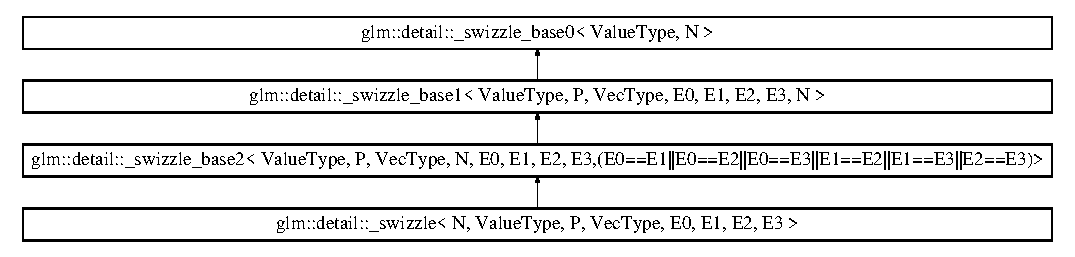
\includegraphics[height=3.002681cm]{structglm_1_1detail_1_1__swizzle}
\end{center}
\end{figure}
\subsection*{Public Types}
\begin{DoxyCompactItemize}
\item 
\hypertarget{structglm_1_1detail_1_1__swizzle_acf7dfa9d7456eb833c247473c5a045f4}{typedef \hyperlink{structglm_1_1detail_1_1__swizzle__base2}{\-\_\-swizzle\-\_\-base2}\\*
$<$ Value\-Type, P, Vec\-Type, N, E0, \\*
E1, E2, E3,(E0==E1$\vert$$\vert$E0==E2$\vert$$\vert$E0==E3$\vert$$\vert$E1==E2$\vert$$\vert$E1==E3$\vert$$\vert$E2==E3)$>$ {\bfseries base\-\_\-type}}\label{structglm_1_1detail_1_1__swizzle_acf7dfa9d7456eb833c247473c5a045f4}

\end{DoxyCompactItemize}
\subsection*{Public Member Functions}
\begin{DoxyCompactItemize}
\item 
\hypertarget{structglm_1_1detail_1_1__swizzle_a333cdd33d2fb442775cca23c77e63fca}{G\-L\-M\-\_\-\-F\-U\-N\-C\-\_\-\-Q\-U\-A\-L\-I\-F\-I\-E\-R {\bfseries operator Vec\-Type} () const }\label{structglm_1_1detail_1_1__swizzle_a333cdd33d2fb442775cca23c77e63fca}

\end{DoxyCompactItemize}
\subsection*{Additional Inherited Members}


The documentation for this struct was generated from the following file\-:\begin{DoxyCompactItemize}
\item 
X\-:/\-Git\-\_\-\-Repository/inf2990-\/06/\-Cadriciel/\-Commun/\-Externe/glm/include/glm/detail/\-\_\-swizzle.\-hpp\end{DoxyCompactItemize}

\hypertarget{structglm_1_1detail_1_1__swizzle__base0}{\section{glm\-:\-:detail\-:\-:\-\_\-swizzle\-\_\-base0$<$ T, N $>$ Struct Template Reference}
\label{structglm_1_1detail_1_1__swizzle__base0}\index{glm\-::detail\-::\-\_\-swizzle\-\_\-base0$<$ T, N $>$@{glm\-::detail\-::\-\_\-swizzle\-\_\-base0$<$ T, N $>$}}
}
Inheritance diagram for glm\-:\-:detail\-:\-:\-\_\-swizzle\-\_\-base0$<$ T, N $>$\-:\begin{figure}[H]
\begin{center}
\leavevmode
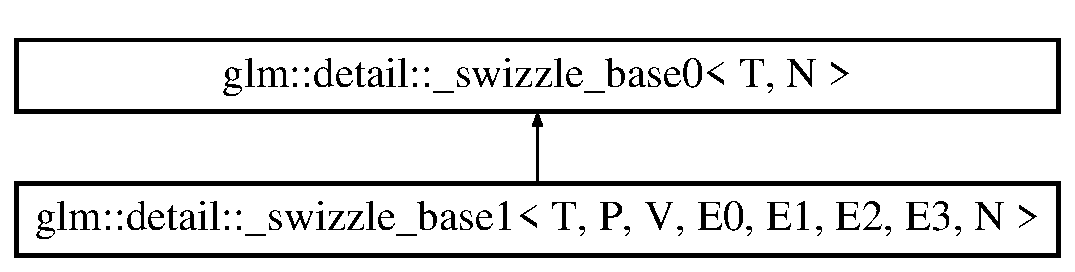
\includegraphics[height=2.000000cm]{structglm_1_1detail_1_1__swizzle__base0}
\end{center}
\end{figure}
\subsection*{Public Types}
\begin{DoxyCompactItemize}
\item 
\hypertarget{structglm_1_1detail_1_1__swizzle__base0_ad38a739e1fe6d2db2674f34c98159c8f}{typedef T {\bfseries value\-\_\-type}}\label{structglm_1_1detail_1_1__swizzle__base0_ad38a739e1fe6d2db2674f34c98159c8f}

\end{DoxyCompactItemize}
\subsection*{Protected Member Functions}
\begin{DoxyCompactItemize}
\item 
\hypertarget{structglm_1_1detail_1_1__swizzle__base0_aebd942a3c3289f9876a9ede4d710d8f0}{G\-L\-M\-\_\-\-F\-U\-N\-C\-\_\-\-Q\-U\-A\-L\-I\-F\-I\-E\-R value\-\_\-type \& {\bfseries elem} (size\-\_\-t i)}\label{structglm_1_1detail_1_1__swizzle__base0_aebd942a3c3289f9876a9ede4d710d8f0}

\item 
\hypertarget{structglm_1_1detail_1_1__swizzle__base0_a9fb7f491860415b292864d0693d8bdb8}{G\-L\-M\-\_\-\-F\-U\-N\-C\-\_\-\-Q\-U\-A\-L\-I\-F\-I\-E\-R const \\*
value\-\_\-type \& {\bfseries elem} (size\-\_\-t i) const }\label{structglm_1_1detail_1_1__swizzle__base0_a9fb7f491860415b292864d0693d8bdb8}

\end{DoxyCompactItemize}
\subsection*{Protected Attributes}
\begin{DoxyCompactItemize}
\item 
\hypertarget{structglm_1_1detail_1_1__swizzle__base0_afd4b7f15c9acff4cdef808f559ffec2d}{char {\bfseries \-\_\-buffer} \mbox{[}1\mbox{]}}\label{structglm_1_1detail_1_1__swizzle__base0_afd4b7f15c9acff4cdef808f559ffec2d}

\end{DoxyCompactItemize}


The documentation for this struct was generated from the following file\-:\begin{DoxyCompactItemize}
\item 
X\-:/\-Git\-\_\-\-Repository/inf2990-\/06/\-Cadriciel/\-Commun/\-Externe/glm/include/glm/detail/\-\_\-swizzle.\-hpp\end{DoxyCompactItemize}

\hypertarget{structglm_1_1detail_1_1__swizzle__base1}{\section{glm\-:\-:detail\-:\-:\-\_\-swizzle\-\_\-base1$<$ T, P, V, E0, E1, E2, E3, N $>$ Struct Template Reference}
\label{structglm_1_1detail_1_1__swizzle__base1}\index{glm\-::detail\-::\-\_\-swizzle\-\_\-base1$<$ T, P, V, E0, E1, E2, E3, N $>$@{glm\-::detail\-::\-\_\-swizzle\-\_\-base1$<$ T, P, V, E0, E1, E2, E3, N $>$}}
}
Inheritance diagram for glm\-:\-:detail\-:\-:\-\_\-swizzle\-\_\-base1$<$ T, P, V, E0, E1, E2, E3, N $>$\-:\begin{figure}[H]
\begin{center}
\leavevmode
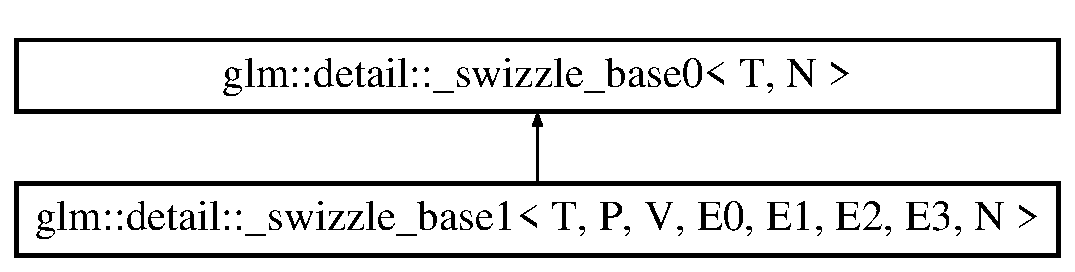
\includegraphics[height=2.000000cm]{structglm_1_1detail_1_1__swizzle__base1}
\end{center}
\end{figure}
\subsection*{Additional Inherited Members}


The documentation for this struct was generated from the following file\-:\begin{DoxyCompactItemize}
\item 
X\-:/\-Git\-\_\-\-Repository/inf2990-\/06/\-Cadriciel/\-Commun/\-Externe/glm/include/glm/detail/\-\_\-swizzle.\-hpp\end{DoxyCompactItemize}

\hypertarget{structglm_1_1detail_1_1__swizzle__base1_3_01_t_00_01_p_00_01_v_00_01_e0_00_01_e1_00_01_e2_00_01_e3_00_014_01_4}{\section{glm\-:\-:detail\-:\-:\-\_\-swizzle\-\_\-base1$<$ T, P, V, E0, E1, E2, E3, 4 $>$ Struct Template Reference}
\label{structglm_1_1detail_1_1__swizzle__base1_3_01_t_00_01_p_00_01_v_00_01_e0_00_01_e1_00_01_e2_00_01_e3_00_014_01_4}\index{glm\-::detail\-::\-\_\-swizzle\-\_\-base1$<$ T, P, V, E0, E1, E2, E3, 4 $>$@{glm\-::detail\-::\-\_\-swizzle\-\_\-base1$<$ T, P, V, E0, E1, E2, E3, 4 $>$}}
}
Inheritance diagram for glm\-:\-:detail\-:\-:\-\_\-swizzle\-\_\-base1$<$ T, P, V, E0, E1, E2, E3, 4 $>$\-:\begin{figure}[H]
\begin{center}
\leavevmode
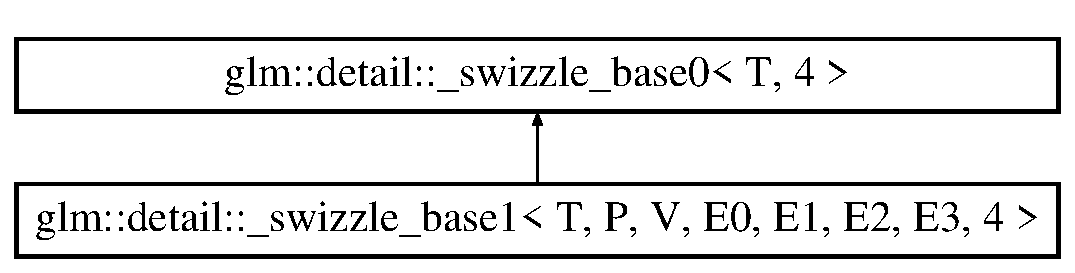
\includegraphics[height=2.000000cm]{structglm_1_1detail_1_1__swizzle__base1_3_01_t_00_01_p_00_01_v_00_01_e0_00_01_e1_00_01_e2_00_01_e3_00_014_01_4}
\end{center}
\end{figure}
\subsection*{Public Member Functions}
\begin{DoxyCompactItemize}
\item 
\hypertarget{structglm_1_1detail_1_1__swizzle__base1_3_01_t_00_01_p_00_01_v_00_01_e0_00_01_e1_00_01_e2_00_01_e3_00_014_01_4_a901f3af50b0eb022c3246b5de5027245}{G\-L\-M\-\_\-\-F\-U\-N\-C\-\_\-\-Q\-U\-A\-L\-I\-F\-I\-E\-R V {\bfseries operator()} () const }\label{structglm_1_1detail_1_1__swizzle__base1_3_01_t_00_01_p_00_01_v_00_01_e0_00_01_e1_00_01_e2_00_01_e3_00_014_01_4_a901f3af50b0eb022c3246b5de5027245}

\end{DoxyCompactItemize}
\subsection*{Additional Inherited Members}


The documentation for this struct was generated from the following file\-:\begin{DoxyCompactItemize}
\item 
X\-:/\-Git\-\_\-\-Repository/inf2990-\/06/\-Cadriciel/\-Commun/\-Externe/glm/include/glm/detail/\-\_\-swizzle.\-hpp\end{DoxyCompactItemize}

\hypertarget{structglm_1_1detail_1_1__swizzle__base1_3_01_t_00_01_p_00_01_v_00_01_e0_00_01_e1_00_01_e2_00-1_00_013_01_4}{\section{glm\-:\-:detail\-:\-:\-\_\-swizzle\-\_\-base1$<$ T, P, V, E0, E1, E2,-\/1, 3 $>$ Struct Template Reference}
\label{structglm_1_1detail_1_1__swizzle__base1_3_01_t_00_01_p_00_01_v_00_01_e0_00_01_e1_00_01_e2_00-1_00_013_01_4}\index{glm\-::detail\-::\-\_\-swizzle\-\_\-base1$<$ T, P, V, E0, E1, E2,-\/1, 3 $>$@{glm\-::detail\-::\-\_\-swizzle\-\_\-base1$<$ T, P, V, E0, E1, E2,-\/1, 3 $>$}}
}
Inheritance diagram for glm\-:\-:detail\-:\-:\-\_\-swizzle\-\_\-base1$<$ T, P, V, E0, E1, E2,-\/1, 3 $>$\-:\begin{figure}[H]
\begin{center}
\leavevmode
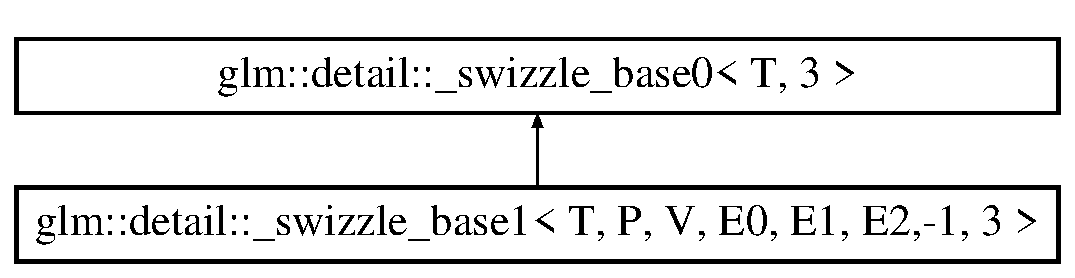
\includegraphics[height=2.000000cm]{structglm_1_1detail_1_1__swizzle__base1_3_01_t_00_01_p_00_01_v_00_01_e0_00_01_e1_00_01_e2_00-1_00_013_01_4}
\end{center}
\end{figure}
\subsection*{Public Member Functions}
\begin{DoxyCompactItemize}
\item 
\hypertarget{structglm_1_1detail_1_1__swizzle__base1_3_01_t_00_01_p_00_01_v_00_01_e0_00_01_e1_00_01_e2_00-1_00_013_01_4_a94510ce33bf6a19e28b4f95f4e715807}{G\-L\-M\-\_\-\-F\-U\-N\-C\-\_\-\-Q\-U\-A\-L\-I\-F\-I\-E\-R V {\bfseries operator()} () const }\label{structglm_1_1detail_1_1__swizzle__base1_3_01_t_00_01_p_00_01_v_00_01_e0_00_01_e1_00_01_e2_00-1_00_013_01_4_a94510ce33bf6a19e28b4f95f4e715807}

\end{DoxyCompactItemize}
\subsection*{Additional Inherited Members}


The documentation for this struct was generated from the following file\-:\begin{DoxyCompactItemize}
\item 
X\-:/\-Git\-\_\-\-Repository/inf2990-\/06/\-Cadriciel/\-Commun/\-Externe/glm/include/glm/detail/\-\_\-swizzle.\-hpp\end{DoxyCompactItemize}

\hypertarget{structglm_1_1detail_1_1__swizzle__base1_3_01_t_00_01_p_00_01_v_00_01_e0_00_01_e1_00-1_00-2_00_012_01_4}{\section{glm\-:\-:detail\-:\-:\-\_\-swizzle\-\_\-base1$<$ T, P, V, E0, E1,-\/1,-\/2, 2 $>$ Struct Template Reference}
\label{structglm_1_1detail_1_1__swizzle__base1_3_01_t_00_01_p_00_01_v_00_01_e0_00_01_e1_00-1_00-2_00_012_01_4}\index{glm\-::detail\-::\-\_\-swizzle\-\_\-base1$<$ T, P, V, E0, E1,-\/1,-\/2, 2 $>$@{glm\-::detail\-::\-\_\-swizzle\-\_\-base1$<$ T, P, V, E0, E1,-\/1,-\/2, 2 $>$}}
}
Inheritance diagram for glm\-:\-:detail\-:\-:\-\_\-swizzle\-\_\-base1$<$ T, P, V, E0, E1,-\/1,-\/2, 2 $>$\-:\begin{figure}[H]
\begin{center}
\leavevmode
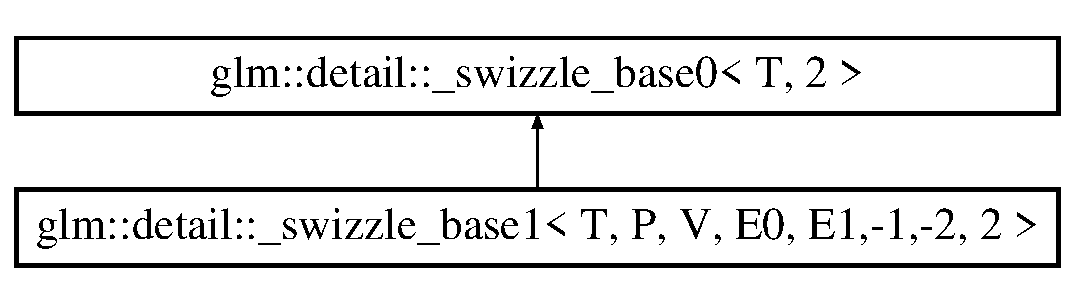
\includegraphics[height=2.000000cm]{structglm_1_1detail_1_1__swizzle__base1_3_01_t_00_01_p_00_01_v_00_01_e0_00_01_e1_00-1_00-2_00_012_01_4}
\end{center}
\end{figure}
\subsection*{Public Member Functions}
\begin{DoxyCompactItemize}
\item 
\hypertarget{structglm_1_1detail_1_1__swizzle__base1_3_01_t_00_01_p_00_01_v_00_01_e0_00_01_e1_00-1_00-2_00_012_01_4_a333b1c869374c290a8bca707a258f5e5}{G\-L\-M\-\_\-\-F\-U\-N\-C\-\_\-\-Q\-U\-A\-L\-I\-F\-I\-E\-R V {\bfseries operator()} () const }\label{structglm_1_1detail_1_1__swizzle__base1_3_01_t_00_01_p_00_01_v_00_01_e0_00_01_e1_00-1_00-2_00_012_01_4_a333b1c869374c290a8bca707a258f5e5}

\end{DoxyCompactItemize}
\subsection*{Additional Inherited Members}


The documentation for this struct was generated from the following file\-:\begin{DoxyCompactItemize}
\item 
X\-:/\-Git\-\_\-\-Repository/inf2990-\/06/\-Cadriciel/\-Commun/\-Externe/glm/include/glm/detail/\-\_\-swizzle.\-hpp\end{DoxyCompactItemize}

\hypertarget{structglm_1_1detail_1_1__swizzle__base2}{\section{glm\-:\-:detail\-:\-:\-\_\-swizzle\-\_\-base2$<$ Value\-Type, P, Vec\-Type, N, E0, E1, E2, E3, D\-U\-P\-L\-I\-C\-A\-T\-E\-\_\-\-E\-L\-E\-M\-E\-N\-T\-S $>$ Struct Template Reference}
\label{structglm_1_1detail_1_1__swizzle__base2}\index{glm\-::detail\-::\-\_\-swizzle\-\_\-base2$<$ Value\-Type, P, Vec\-Type, N, E0, E1, E2, E3, D\-U\-P\-L\-I\-C\-A\-T\-E\-\_\-\-E\-L\-E\-M\-E\-N\-T\-S $>$@{glm\-::detail\-::\-\_\-swizzle\-\_\-base2$<$ Value\-Type, P, Vec\-Type, N, E0, E1, E2, E3, D\-U\-P\-L\-I\-C\-A\-T\-E\-\_\-\-E\-L\-E\-M\-E\-N\-T\-S $>$}}
}
Inheritance diagram for glm\-:\-:detail\-:\-:\-\_\-swizzle\-\_\-base2$<$ Value\-Type, P, Vec\-Type, N, E0, E1, E2, E3, D\-U\-P\-L\-I\-C\-A\-T\-E\-\_\-\-E\-L\-E\-M\-E\-N\-T\-S $>$\-:\begin{figure}[H]
\begin{center}
\leavevmode
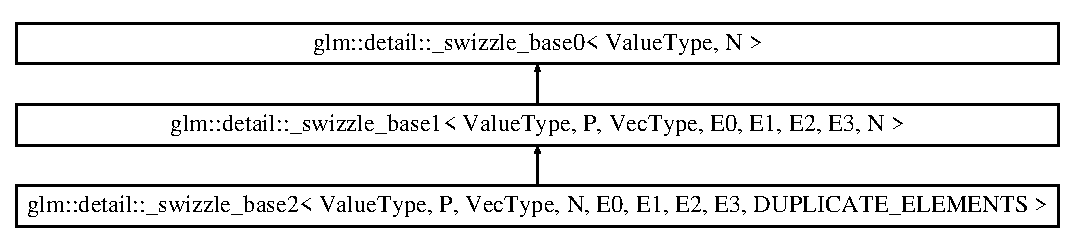
\includegraphics[height=2.823529cm]{structglm_1_1detail_1_1__swizzle__base2}
\end{center}
\end{figure}
\subsection*{Public Types}
\begin{DoxyCompactItemize}
\item 
\hypertarget{structglm_1_1detail_1_1__swizzle__base2_a5f999904e676a4f5b0bdaa157415ee1c}{typedef Vec\-Type {\bfseries vec\-\_\-type}}\label{structglm_1_1detail_1_1__swizzle__base2_a5f999904e676a4f5b0bdaa157415ee1c}

\item 
\hypertarget{structglm_1_1detail_1_1__swizzle__base2_a656c11aaeeaca042deed88711c9dc063}{typedef Value\-Type {\bfseries value\-\_\-type}}\label{structglm_1_1detail_1_1__swizzle__base2_a656c11aaeeaca042deed88711c9dc063}

\end{DoxyCompactItemize}
\subsection*{Public Member Functions}
\begin{DoxyCompactItemize}
\item 
\hypertarget{structglm_1_1detail_1_1__swizzle__base2_a70442376cb261474e23090737deff976}{G\-L\-M\-\_\-\-F\-U\-N\-C\-\_\-\-Q\-U\-A\-L\-I\-F\-I\-E\-R \hyperlink{structglm_1_1detail_1_1__swizzle__base2}{\-\_\-swizzle\-\_\-base2} \& {\bfseries operator=} (const Value\-Type \&t)}\label{structglm_1_1detail_1_1__swizzle__base2_a70442376cb261474e23090737deff976}

\item 
\hypertarget{structglm_1_1detail_1_1__swizzle__base2_a7b982a5056d94cd43393bf820ea627d0}{G\-L\-M\-\_\-\-F\-U\-N\-C\-\_\-\-Q\-U\-A\-L\-I\-F\-I\-E\-R \hyperlink{structglm_1_1detail_1_1__swizzle__base2}{\-\_\-swizzle\-\_\-base2} \& {\bfseries operator=} (const Vec\-Type \&that)}\label{structglm_1_1detail_1_1__swizzle__base2_a7b982a5056d94cd43393bf820ea627d0}

\item 
\hypertarget{structglm_1_1detail_1_1__swizzle__base2_ab583f399dc6685deee97bdd5126f433a}{G\-L\-M\-\_\-\-F\-U\-N\-C\-\_\-\-Q\-U\-A\-L\-I\-F\-I\-E\-R void {\bfseries operator-\/=} (const Vec\-Type \&that)}\label{structglm_1_1detail_1_1__swizzle__base2_ab583f399dc6685deee97bdd5126f433a}

\item 
\hypertarget{structglm_1_1detail_1_1__swizzle__base2_a5e734b2e9da294d92bb347a3c7f44ded}{G\-L\-M\-\_\-\-F\-U\-N\-C\-\_\-\-Q\-U\-A\-L\-I\-F\-I\-E\-R void {\bfseries operator+=} (const Vec\-Type \&that)}\label{structglm_1_1detail_1_1__swizzle__base2_a5e734b2e9da294d92bb347a3c7f44ded}

\item 
\hypertarget{structglm_1_1detail_1_1__swizzle__base2_a6c686d110b936939c7ed67d7a6165778}{G\-L\-M\-\_\-\-F\-U\-N\-C\-\_\-\-Q\-U\-A\-L\-I\-F\-I\-E\-R void {\bfseries operator$\ast$=} (const Vec\-Type \&that)}\label{structglm_1_1detail_1_1__swizzle__base2_a6c686d110b936939c7ed67d7a6165778}

\item 
\hypertarget{structglm_1_1detail_1_1__swizzle__base2_a0a3e5ef1cb68f78a7e1bcd72f6e2dc4c}{G\-L\-M\-\_\-\-F\-U\-N\-C\-\_\-\-Q\-U\-A\-L\-I\-F\-I\-E\-R void {\bfseries operator/=} (const Vec\-Type \&that)}\label{structglm_1_1detail_1_1__swizzle__base2_a0a3e5ef1cb68f78a7e1bcd72f6e2dc4c}

\item 
\hypertarget{structglm_1_1detail_1_1__swizzle__base2_aa3f2ab8e3e1a5c414b3fdca4cf75b706}{G\-L\-M\-\_\-\-F\-U\-N\-C\-\_\-\-Q\-U\-A\-L\-I\-F\-I\-E\-R value\-\_\-type \& {\bfseries operator\mbox{[}$\,$\mbox{]}} (size\-\_\-t i)}\label{structglm_1_1detail_1_1__swizzle__base2_aa3f2ab8e3e1a5c414b3fdca4cf75b706}

\item 
\hypertarget{structglm_1_1detail_1_1__swizzle__base2_a1bec6727adac01b6bc3e1ccba935167e}{G\-L\-M\-\_\-\-F\-U\-N\-C\-\_\-\-Q\-U\-A\-L\-I\-F\-I\-E\-R value\-\_\-type {\bfseries operator\mbox{[}$\,$\mbox{]}} (size\-\_\-t i) const }\label{structglm_1_1detail_1_1__swizzle__base2_a1bec6727adac01b6bc3e1ccba935167e}

\end{DoxyCompactItemize}
\subsection*{Protected Member Functions}
\begin{DoxyCompactItemize}
\item 
\hypertarget{structglm_1_1detail_1_1__swizzle__base2_a11d049274a60ecf4aac8cebc4c4e9be5}{{\footnotesize template$<$typename T $>$ }\\G\-L\-M\-\_\-\-F\-U\-N\-C\-\_\-\-Q\-U\-A\-L\-I\-F\-I\-E\-R void {\bfseries \-\_\-apply\-\_\-op} (const Vec\-Type \&that, T op)}\label{structglm_1_1detail_1_1__swizzle__base2_a11d049274a60ecf4aac8cebc4c4e9be5}

\end{DoxyCompactItemize}
\subsection*{Additional Inherited Members}


The documentation for this struct was generated from the following file\-:\begin{DoxyCompactItemize}
\item 
X\-:/\-Git\-\_\-\-Repository/inf2990-\/06/\-Cadriciel/\-Commun/\-Externe/glm/include/glm/detail/\-\_\-swizzle.\-hpp\end{DoxyCompactItemize}

\hypertarget{structglm_1_1detail_1_1__swizzle__base2_3_01_value_type_00_01_p_00_01_vec_type_00_01_n_00_01_e0_fc19218d69dc8988a4a57fbe7f79725c}{\section{glm\-:\-:detail\-:\-:\-\_\-swizzle\-\_\-base2$<$ Value\-Type, P, Vec\-Type, N, E0, E1, E2, E3, 1 $>$ Struct Template Reference}
\label{structglm_1_1detail_1_1__swizzle__base2_3_01_value_type_00_01_p_00_01_vec_type_00_01_n_00_01_e0_fc19218d69dc8988a4a57fbe7f79725c}\index{glm\-::detail\-::\-\_\-swizzle\-\_\-base2$<$ Value\-Type, P, Vec\-Type, N, E0, E1, E2, E3, 1 $>$@{glm\-::detail\-::\-\_\-swizzle\-\_\-base2$<$ Value\-Type, P, Vec\-Type, N, E0, E1, E2, E3, 1 $>$}}
}
Inheritance diagram for glm\-:\-:detail\-:\-:\-\_\-swizzle\-\_\-base2$<$ Value\-Type, P, Vec\-Type, N, E0, E1, E2, E3, 1 $>$\-:\begin{figure}[H]
\begin{center}
\leavevmode
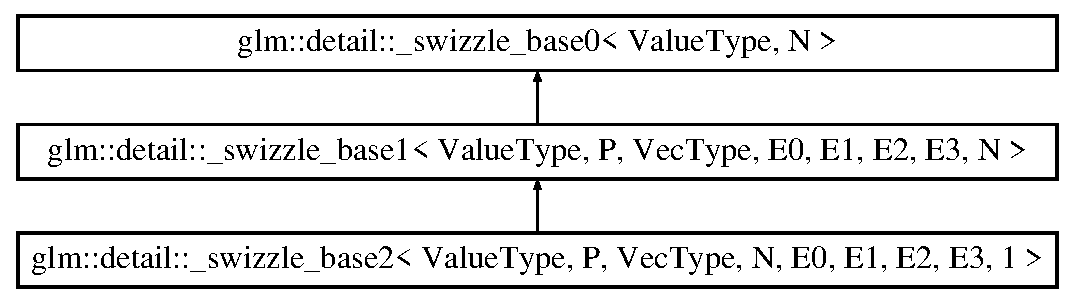
\includegraphics[height=3.000000cm]{structglm_1_1detail_1_1__swizzle__base2_3_01_value_type_00_01_p_00_01_vec_type_00_01_n_00_01_e0_fc19218d69dc8988a4a57fbe7f79725c}
\end{center}
\end{figure}
\subsection*{Classes}
\begin{DoxyCompactItemize}
\item 
struct \hyperlink{structglm_1_1detail_1_1__swizzle__base2_3_01_value_type_00_01_p_00_01_vec_type_00_01_n_00_01_e0_17279995be88bc842083eed40758473c}{Stub}
\end{DoxyCompactItemize}
\subsection*{Public Types}
\begin{DoxyCompactItemize}
\item 
\hypertarget{structglm_1_1detail_1_1__swizzle__base2_3_01_value_type_00_01_p_00_01_vec_type_00_01_n_00_01_e0_fc19218d69dc8988a4a57fbe7f79725c_aa478e9f198b8832d76245adde9c627ec}{typedef Vec\-Type {\bfseries vec\-\_\-type}}\label{structglm_1_1detail_1_1__swizzle__base2_3_01_value_type_00_01_p_00_01_vec_type_00_01_n_00_01_e0_fc19218d69dc8988a4a57fbe7f79725c_aa478e9f198b8832d76245adde9c627ec}

\item 
\hypertarget{structglm_1_1detail_1_1__swizzle__base2_3_01_value_type_00_01_p_00_01_vec_type_00_01_n_00_01_e0_fc19218d69dc8988a4a57fbe7f79725c_aea7ec681454787ad7a322c06aec98757}{typedef Value\-Type {\bfseries value\-\_\-type}}\label{structglm_1_1detail_1_1__swizzle__base2_3_01_value_type_00_01_p_00_01_vec_type_00_01_n_00_01_e0_fc19218d69dc8988a4a57fbe7f79725c_aea7ec681454787ad7a322c06aec98757}

\end{DoxyCompactItemize}
\subsection*{Public Member Functions}
\begin{DoxyCompactItemize}
\item 
\hypertarget{structglm_1_1detail_1_1__swizzle__base2_3_01_value_type_00_01_p_00_01_vec_type_00_01_n_00_01_e0_fc19218d69dc8988a4a57fbe7f79725c_aed2b7223090d020e28af46eb33fe6729}{G\-L\-M\-\_\-\-F\-U\-N\-C\-\_\-\-Q\-U\-A\-L\-I\-F\-I\-E\-R \hyperlink{structglm_1_1detail_1_1__swizzle__base2}{\-\_\-swizzle\-\_\-base2} \& {\bfseries operator=} (Stub const \&)}\label{structglm_1_1detail_1_1__swizzle__base2_3_01_value_type_00_01_p_00_01_vec_type_00_01_n_00_01_e0_fc19218d69dc8988a4a57fbe7f79725c_aed2b7223090d020e28af46eb33fe6729}

\item 
\hypertarget{structglm_1_1detail_1_1__swizzle__base2_3_01_value_type_00_01_p_00_01_vec_type_00_01_n_00_01_e0_fc19218d69dc8988a4a57fbe7f79725c_a2f3a45edbb24ca7e12182c3123dde632}{G\-L\-M\-\_\-\-F\-U\-N\-C\-\_\-\-Q\-U\-A\-L\-I\-F\-I\-E\-R value\-\_\-type {\bfseries operator\mbox{[}$\,$\mbox{]}} (size\-\_\-t i) const }\label{structglm_1_1detail_1_1__swizzle__base2_3_01_value_type_00_01_p_00_01_vec_type_00_01_n_00_01_e0_fc19218d69dc8988a4a57fbe7f79725c_a2f3a45edbb24ca7e12182c3123dde632}

\end{DoxyCompactItemize}
\subsection*{Additional Inherited Members}


The documentation for this struct was generated from the following file\-:\begin{DoxyCompactItemize}
\item 
X\-:/\-Git\-\_\-\-Repository/inf2990-\/06/\-Cadriciel/\-Commun/\-Externe/glm/include/glm/detail/\-\_\-swizzle.\-hpp\end{DoxyCompactItemize}

\hypertarget{class_interface_graphique_1_1patron__state_1_1_abstract_state}{\section{Interface\-Graphique.\-patron\-\_\-state.\-Abstract\-State Class Reference}
\label{class_interface_graphique_1_1patron__state_1_1_abstract_state}\index{Interface\-Graphique.\-patron\-\_\-state.\-Abstract\-State@{Interface\-Graphique.\-patron\-\_\-state.\-Abstract\-State}}
}


Classe abstraite des differents etats du mode editeur  


Inheritance diagram for Interface\-Graphique.\-patron\-\_\-state.\-Abstract\-State\-:\begin{figure}[H]
\begin{center}
\leavevmode
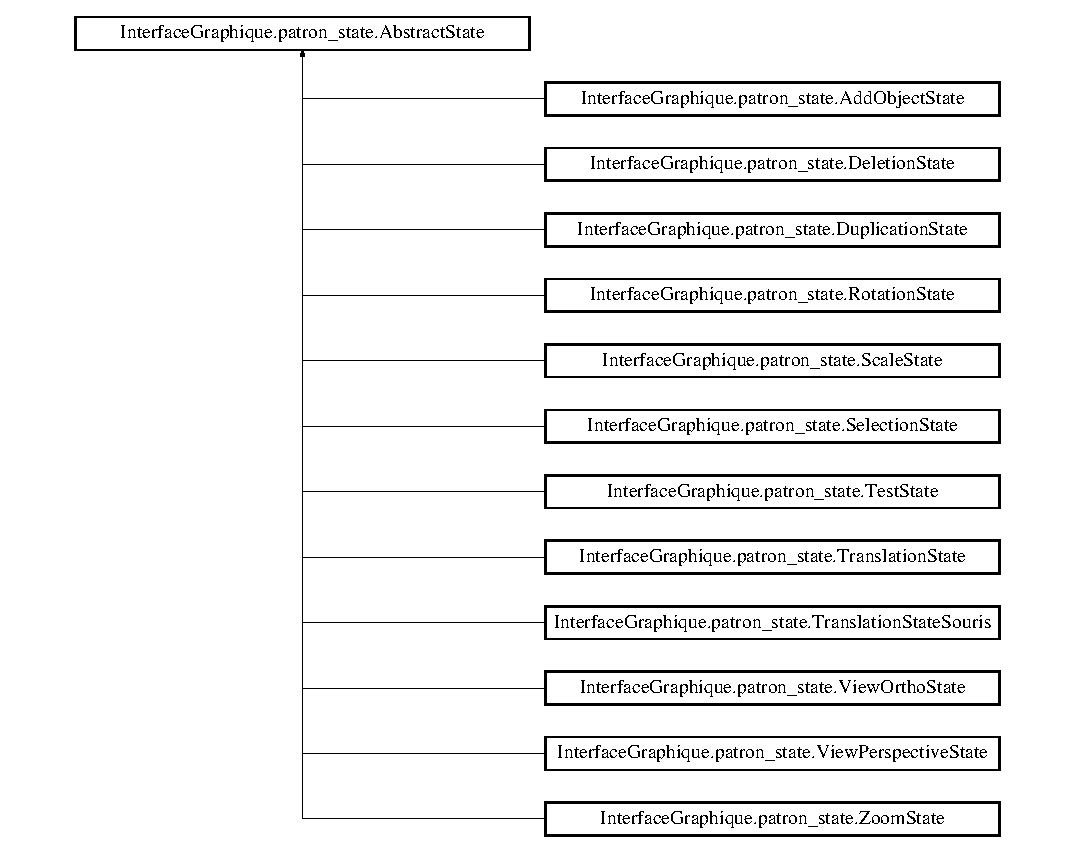
\includegraphics[height=10.996979cm]{class_interface_graphique_1_1patron__state_1_1_abstract_state}
\end{center}
\end{figure}
\subsection*{Public Member Functions}
\begin{DoxyCompactItemize}
\item 
abstract void \hyperlink{class_interface_graphique_1_1patron__state_1_1_abstract_state_a8df97c5a2784f9757608d669fbb1c6b5}{Action} (int x, int y)
\begin{DoxyCompactList}\small\item\em Fonction virtuelle des differents etats(rotation, translation, etc..) \end{DoxyCompactList}\end{DoxyCompactItemize}


\subsection{Detailed Description}
Classe abstraite des differents etats du mode editeur 



\subsection{Member Function Documentation}
\hypertarget{class_interface_graphique_1_1patron__state_1_1_abstract_state_a8df97c5a2784f9757608d669fbb1c6b5}{\index{Interface\-Graphique\-::patron\-\_\-state\-::\-Abstract\-State@{Interface\-Graphique\-::patron\-\_\-state\-::\-Abstract\-State}!Action@{Action}}
\index{Action@{Action}!InterfaceGraphique::patron_state::AbstractState@{Interface\-Graphique\-::patron\-\_\-state\-::\-Abstract\-State}}
\subsubsection[{Action}]{\setlength{\rightskip}{0pt plus 5cm}abstract void Interface\-Graphique.\-patron\-\_\-state.\-Abstract\-State.\-Action (
\begin{DoxyParamCaption}
\item[{int}]{x, }
\item[{int}]{y}
\end{DoxyParamCaption}
)\hspace{0.3cm}{\ttfamily [pure virtual]}}}\label{class_interface_graphique_1_1patron__state_1_1_abstract_state_a8df97c5a2784f9757608d669fbb1c6b5}


Fonction virtuelle des differents etats(rotation, translation, etc..) 


\begin{DoxyParams}{Parameters}
{\em x} & \\
\hline
{\em y} & \\
\hline
\end{DoxyParams}


Implemented in \hyperlink{class_interface_graphique_1_1patron__state_1_1_add_object_state_a5f251f4a42b766f424c3e31af3d181b3}{Interface\-Graphique.\-patron\-\_\-state.\-Add\-Object\-State}, \hyperlink{class_interface_graphique_1_1patron__state_1_1_translation_state_ab5ba5dd1c3941c219f81d01dbcfe2a60}{Interface\-Graphique.\-patron\-\_\-state.\-Translation\-State}, \hyperlink{class_interface_graphique_1_1patron__state_1_1_translation_state_souris_a2370ab1d0a55afefdd46eda17dc13ce6}{Interface\-Graphique.\-patron\-\_\-state.\-Translation\-State\-Souris}, \hyperlink{class_interface_graphique_1_1patron__state_1_1_rotation_state_aa115b089fcafb2b25b8a27f19b55ef31}{Interface\-Graphique.\-patron\-\_\-state.\-Rotation\-State}, \hyperlink{class_interface_graphique_1_1patron__state_1_1_scale_state_af8fe6bca0517beed3c6b9106886d7408}{Interface\-Graphique.\-patron\-\_\-state.\-Scale\-State}, \hyperlink{class_interface_graphique_1_1patron__state_1_1_view_ortho_state_aae857294a6d4030392e0009f869bb46e}{Interface\-Graphique.\-patron\-\_\-state.\-View\-Ortho\-State}, \hyperlink{class_interface_graphique_1_1patron__state_1_1_view_perspective_state_a111b6675fe8e49465a5ba6eb49b4081f}{Interface\-Graphique.\-patron\-\_\-state.\-View\-Perspective\-State}, \hyperlink{class_interface_graphique_1_1patron__state_1_1_deletion_state_ab720f529b212ff1b98d5e97f7fcb199f}{Interface\-Graphique.\-patron\-\_\-state.\-Deletion\-State}, \hyperlink{class_interface_graphique_1_1patron__state_1_1_duplication_state_a3e4ab1c3a8bd3d03b822c66d7597e068}{Interface\-Graphique.\-patron\-\_\-state.\-Duplication\-State}, \hyperlink{class_interface_graphique_1_1patron__state_1_1_selection_state_a3c9a95b047d8ef642d0ac7662347f65e}{Interface\-Graphique.\-patron\-\_\-state.\-Selection\-State}, \hyperlink{class_interface_graphique_1_1patron__state_1_1_test_state_ab7aa954cce22801d52158f3d70cbdcac}{Interface\-Graphique.\-patron\-\_\-state.\-Test\-State}, and \hyperlink{class_interface_graphique_1_1patron__state_1_1_zoom_state_aa4608434efc2a14431b08ba9ba071633}{Interface\-Graphique.\-patron\-\_\-state.\-Zoom\-State}.



The documentation for this class was generated from the following file\-:\begin{DoxyCompactItemize}
\item 
X\-:/\-Git\-\_\-\-Repository/inf2990-\/06/\-Cadriciel/\-Sources/\-Interface\-Graphique/patron state/Abstract\-State.\-cs\end{DoxyCompactItemize}

\hypertarget{class_additional_message}{\section{Additional\-Message Class Reference}
\label{class_additional_message}\index{Additional\-Message@{Additional\-Message}}
}


An additional \hyperlink{class_message}{Message} for assertions.

Provides a implicit constructor that takes a single string. This allow this class to be used as the message arguments in macros.  




{\ttfamily \#include $<$Additional\-Message.\-h$>$}

Inheritance diagram for Additional\-Message\-:\begin{figure}[H]
\begin{center}
\leavevmode
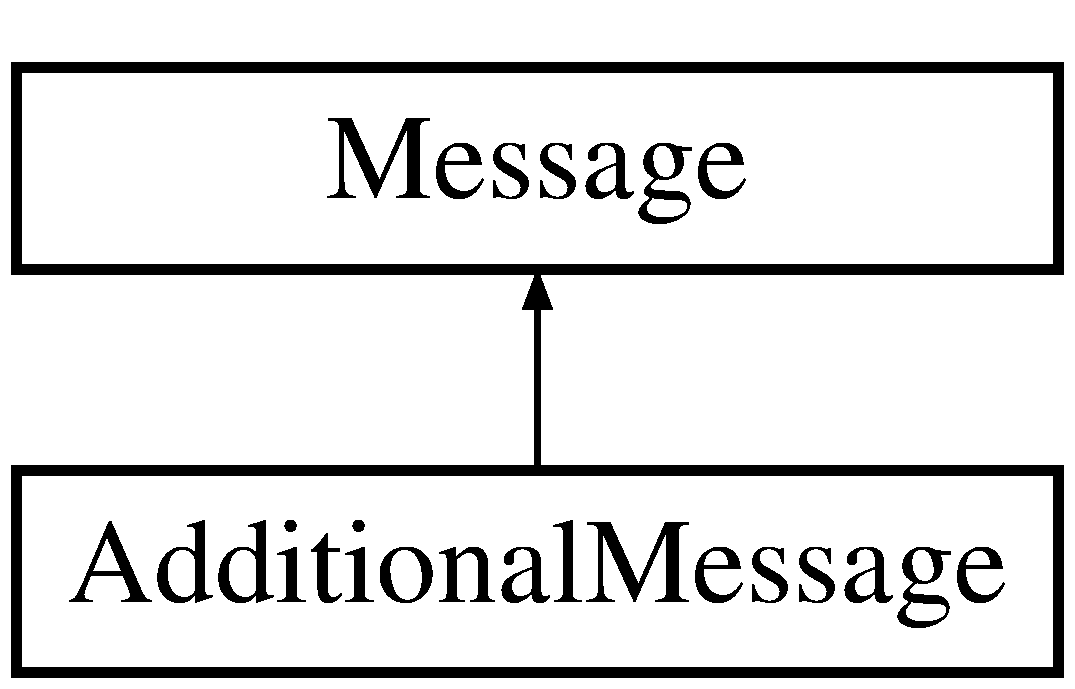
\includegraphics[height=2.000000cm]{class_additional_message}
\end{center}
\end{figure}
\subsection*{Public Types}
\begin{DoxyCompactItemize}
\item 
\hypertarget{class_additional_message_abc8626e28c147b5ddd66032a35676126}{typedef \hyperlink{class_message}{Message} {\bfseries Super\-Class}}\label{class_additional_message_abc8626e28c147b5ddd66032a35676126}

\end{DoxyCompactItemize}
\subsection*{Public Member Functions}
\begin{DoxyCompactItemize}
\item 
\hypertarget{class_additional_message_a888715179848c5e5c385789b962a3cfb}{\hyperlink{class_additional_message_a888715179848c5e5c385789b962a3cfb}{Additional\-Message} ()}\label{class_additional_message_a888715179848c5e5c385789b962a3cfb}

\begin{DoxyCompactList}\small\item\em Constructs an empty \hyperlink{class_message}{Message}. \end{DoxyCompactList}\item 
\hyperlink{class_additional_message_a990455bbfe260bc04f99e5acc58d1c06}{Additional\-Message} (const std\-::string \&detail1)
\begin{DoxyCompactList}\small\item\em Constructs a \hyperlink{class_message}{Message} with the specified detail string. \end{DoxyCompactList}\item 
\hyperlink{class_additional_message_a6486540f9b5d1957230e9e1f969adc9d}{Additional\-Message} (const char $\ast$detail1)
\begin{DoxyCompactList}\small\item\em Constructs a \hyperlink{class_message}{Message} with the specified detail string. \end{DoxyCompactList}\item 
\hyperlink{class_additional_message_a75735b6fd65686f31349d01c97c73bc7}{Additional\-Message} (const \hyperlink{class_message}{Message} \&other)
\begin{DoxyCompactList}\small\item\em Constructs a copy of the specified message. \end{DoxyCompactList}\item 
\hyperlink{class_additional_message}{Additional\-Message} \& \hyperlink{class_additional_message_abbda0de4323f70ff01a9b622a6f550f7}{operator=} (const \hyperlink{class_message}{Message} \&other)
\begin{DoxyCompactList}\small\item\em Assignment operator. \end{DoxyCompactList}\end{DoxyCompactItemize}


\subsection{Detailed Description}
An additional \hyperlink{class_message}{Message} for assertions.

Provides a implicit constructor that takes a single string. This allow this class to be used as the message arguments in macros. 

The constructed object is either a \hyperlink{class_message}{Message} with a single detail string if a string was passed to the macro, or a copy of the \hyperlink{class_message}{Message} passed to the macro.

Here is an example of usage\-: 
\begin{DoxyCode}
\textcolor{keywordtype}{void} checkStringEquals( \textcolor{keyword}{const} std::string &expected,
                       \textcolor{keyword}{const} std::string &actual,
                        \textcolor{keyword}{const} CppUnit::SourceLine &sourceLine,
                        \textcolor{keyword}{const} CppUnit::AdditionalMessage &message );

\textcolor{preprocessor}{#define XTLUT\_ASSERT\_STRING\_EQUAL\_MESSAGE( expected, actual, message )  \(\backslash\)}
\textcolor{preprocessor}{  ::XtlUt::Impl::checkStringEquals( ::Xtl::toString(expected),        \(\backslash\)}
\textcolor{preprocessor}{                                    ::Xtl::toString(actual),          \(\backslash\)}
\textcolor{preprocessor}{                                    CPPUNIT\_SOURCELINE(),             \(\backslash\)}
\textcolor{preprocessor}{                                    message )}
\end{DoxyCode}


In the previous example, the user can specify a simple string for {\itshape message}, or a complex \hyperlink{class_message}{Message} object.

\begin{DoxySeeAlso}{See Also}
\hyperlink{class_message}{Message} 
\end{DoxySeeAlso}


\subsection{Constructor \& Destructor Documentation}
\hypertarget{class_additional_message_a990455bbfe260bc04f99e5acc58d1c06}{\index{Additional\-Message@{Additional\-Message}!Additional\-Message@{Additional\-Message}}
\index{Additional\-Message@{Additional\-Message}!AdditionalMessage@{Additional\-Message}}
\subsubsection[{Additional\-Message}]{\setlength{\rightskip}{0pt plus 5cm}Additional\-Message\-::\-Additional\-Message (
\begin{DoxyParamCaption}
\item[{const std\-::string \&}]{detail1}
\end{DoxyParamCaption}
)}}\label{class_additional_message_a990455bbfe260bc04f99e5acc58d1c06}


Constructs a \hyperlink{class_message}{Message} with the specified detail string. 


\begin{DoxyParams}{Parameters}
{\em detail1} & Detail string of the message. If empty, then it is not added. \\
\hline
\end{DoxyParams}
\hypertarget{class_additional_message_a6486540f9b5d1957230e9e1f969adc9d}{\index{Additional\-Message@{Additional\-Message}!Additional\-Message@{Additional\-Message}}
\index{Additional\-Message@{Additional\-Message}!AdditionalMessage@{Additional\-Message}}
\subsubsection[{Additional\-Message}]{\setlength{\rightskip}{0pt plus 5cm}Additional\-Message\-::\-Additional\-Message (
\begin{DoxyParamCaption}
\item[{const char $\ast$}]{detail1}
\end{DoxyParamCaption}
)}}\label{class_additional_message_a6486540f9b5d1957230e9e1f969adc9d}


Constructs a \hyperlink{class_message}{Message} with the specified detail string. 


\begin{DoxyParams}{Parameters}
{\em detail1} & Detail string of the message. If empty, then it is not added. \\
\hline
\end{DoxyParams}
\hypertarget{class_additional_message_a75735b6fd65686f31349d01c97c73bc7}{\index{Additional\-Message@{Additional\-Message}!Additional\-Message@{Additional\-Message}}
\index{Additional\-Message@{Additional\-Message}!AdditionalMessage@{Additional\-Message}}
\subsubsection[{Additional\-Message}]{\setlength{\rightskip}{0pt plus 5cm}Additional\-Message\-::\-Additional\-Message (
\begin{DoxyParamCaption}
\item[{const {\bf Message} \&}]{other}
\end{DoxyParamCaption}
)}}\label{class_additional_message_a75735b6fd65686f31349d01c97c73bc7}


Constructs a copy of the specified message. 


\begin{DoxyParams}{Parameters}
{\em other} & \hyperlink{class_message}{Message} to copy. \\
\hline
\end{DoxyParams}


\subsection{Member Function Documentation}
\hypertarget{class_additional_message_abbda0de4323f70ff01a9b622a6f550f7}{\index{Additional\-Message@{Additional\-Message}!operator=@{operator=}}
\index{operator=@{operator=}!AdditionalMessage@{Additional\-Message}}
\subsubsection[{operator=}]{\setlength{\rightskip}{0pt plus 5cm}{\bf Additional\-Message}\& Additional\-Message\-::operator= (
\begin{DoxyParamCaption}
\item[{const {\bf Message} \&}]{other}
\end{DoxyParamCaption}
)}}\label{class_additional_message_abbda0de4323f70ff01a9b622a6f550f7}


Assignment operator. 


\begin{DoxyParams}{Parameters}
{\em other} & \hyperlink{class_message}{Message} to copy. \\
\hline
\end{DoxyParams}
\begin{DoxyReturn}{Returns}
Reference on this object. 
\end{DoxyReturn}


The documentation for this class was generated from the following file\-:\begin{DoxyCompactItemize}
\item 
X\-:/\-Git\-\_\-\-Repository/inf2990-\/06/\-Cadriciel/\-Commun/\-Externe/cppunit/include/cppunit/Additional\-Message.\-h\end{DoxyCompactItemize}

\hypertarget{class_interface_graphique_1_1patron__state_1_1_add_object_state}{\section{Interface\-Graphique.\-patron\-\_\-state.\-Add\-Object\-State Class Reference}
\label{class_interface_graphique_1_1patron__state_1_1_add_object_state}\index{Interface\-Graphique.\-patron\-\_\-state.\-Add\-Object\-State@{Interface\-Graphique.\-patron\-\_\-state.\-Add\-Object\-State}}
}


Etat d'ajout des objets  


Inheritance diagram for Interface\-Graphique.\-patron\-\_\-state.\-Add\-Object\-State\-:\begin{figure}[H]
\begin{center}
\leavevmode
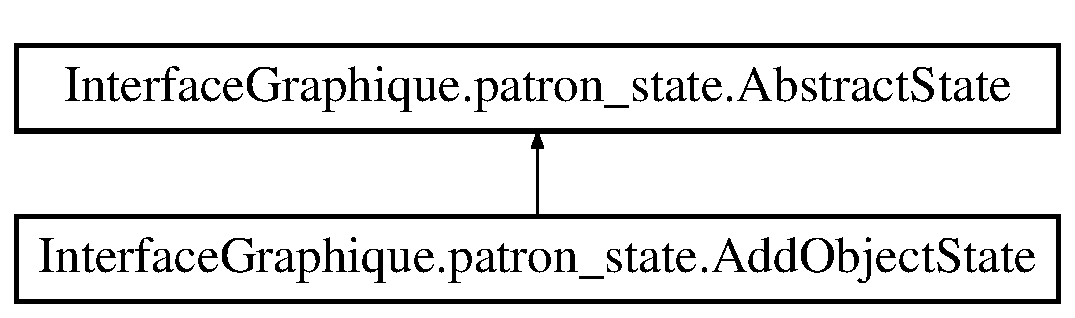
\includegraphics[height=2.000000cm]{class_interface_graphique_1_1patron__state_1_1_add_object_state}
\end{center}
\end{figure}
\subsection*{Public Member Functions}
\begin{DoxyCompactItemize}
\item 
\hyperlink{class_interface_graphique_1_1patron__state_1_1_add_object_state_ad94cfea968dac4748bbd8161583bf71b}{Add\-Object\-State} (String object\-Name)
\begin{DoxyCompactList}\small\item\em Constructeur de l'etat, assigne le type de noeud a ajouter \end{DoxyCompactList}\item 
override void \hyperlink{class_interface_graphique_1_1patron__state_1_1_add_object_state_a5f251f4a42b766f424c3e31af3d181b3}{Action} (int x, int y)
\begin{DoxyCompactList}\small\item\em Creation du noeud et ajout dans l'arbre de rendu \end{DoxyCompactList}\end{DoxyCompactItemize}


\subsection{Detailed Description}
Etat d'ajout des objets 



\subsection{Constructor \& Destructor Documentation}
\hypertarget{class_interface_graphique_1_1patron__state_1_1_add_object_state_ad94cfea968dac4748bbd8161583bf71b}{\index{Interface\-Graphique\-::patron\-\_\-state\-::\-Add\-Object\-State@{Interface\-Graphique\-::patron\-\_\-state\-::\-Add\-Object\-State}!Add\-Object\-State@{Add\-Object\-State}}
\index{Add\-Object\-State@{Add\-Object\-State}!InterfaceGraphique::patron_state::AddObjectState@{Interface\-Graphique\-::patron\-\_\-state\-::\-Add\-Object\-State}}
\subsubsection[{Add\-Object\-State}]{\setlength{\rightskip}{0pt plus 5cm}Interface\-Graphique.\-patron\-\_\-state.\-Add\-Object\-State.\-Add\-Object\-State (
\begin{DoxyParamCaption}
\item[{String}]{object\-Name}
\end{DoxyParamCaption}
)\hspace{0.3cm}{\ttfamily [inline]}}}\label{class_interface_graphique_1_1patron__state_1_1_add_object_state_ad94cfea968dac4748bbd8161583bf71b}


Constructeur de l'etat, assigne le type de noeud a ajouter 


\begin{DoxyParams}{Parameters}
{\em object\-Name} & Type de noeud\\
\hline
\end{DoxyParams}


\subsection{Member Function Documentation}
\hypertarget{class_interface_graphique_1_1patron__state_1_1_add_object_state_a5f251f4a42b766f424c3e31af3d181b3}{\index{Interface\-Graphique\-::patron\-\_\-state\-::\-Add\-Object\-State@{Interface\-Graphique\-::patron\-\_\-state\-::\-Add\-Object\-State}!Action@{Action}}
\index{Action@{Action}!InterfaceGraphique::patron_state::AddObjectState@{Interface\-Graphique\-::patron\-\_\-state\-::\-Add\-Object\-State}}
\subsubsection[{Action}]{\setlength{\rightskip}{0pt plus 5cm}override void Interface\-Graphique.\-patron\-\_\-state.\-Add\-Object\-State.\-Action (
\begin{DoxyParamCaption}
\item[{int}]{x, }
\item[{int}]{y}
\end{DoxyParamCaption}
)\hspace{0.3cm}{\ttfamily [inline]}, {\ttfamily [virtual]}}}\label{class_interface_graphique_1_1patron__state_1_1_add_object_state_a5f251f4a42b766f424c3e31af3d181b3}


Creation du noeud et ajout dans l'arbre de rendu 


\begin{DoxyParams}{Parameters}
{\em x} & Position courante du x de la souris\\
\hline
{\em y} & Positinn y courante de la souris\\
\hline
\end{DoxyParams}
Création d'un Noeud Portail partie\-Rapide 1

Création d'un Noeud Portail partie\-Rapide 2

Création d'un Noeud Mur partie\-Rapide 1 

Implements \hyperlink{class_interface_graphique_1_1patron__state_1_1_abstract_state_a8df97c5a2784f9757608d669fbb1c6b5}{Interface\-Graphique.\-patron\-\_\-state.\-Abstract\-State}.



The documentation for this class was generated from the following file\-:\begin{DoxyCompactItemize}
\item 
X\-:/\-Git\-\_\-\-Repository/inf2990-\/06/\-Cadriciel/\-Sources/\-Interface\-Graphique/patron state/Add\-Object\-State.\-cs\end{DoxyCompactItemize}

\hypertarget{struct_a_f_m___font_info_rec__}{\section{A\-F\-M\-\_\-\-Font\-Info\-Rec\-\_\- Struct Reference}
\label{struct_a_f_m___font_info_rec__}\index{A\-F\-M\-\_\-\-Font\-Info\-Rec\-\_\-@{A\-F\-M\-\_\-\-Font\-Info\-Rec\-\_\-}}
}
\subsection*{Public Attributes}
\begin{DoxyCompactItemize}
\item 
\hypertarget{struct_a_f_m___font_info_rec___a6f198e74da5d8a3b7ff7518e255be231}{F\-T\-\_\-\-Bool {\bfseries Is\-C\-I\-D\-Font}}\label{struct_a_f_m___font_info_rec___a6f198e74da5d8a3b7ff7518e255be231}

\item 
\hypertarget{struct_a_f_m___font_info_rec___afa5112d6b0cc51839889206012dc1be6}{\hyperlink{struct_f_t___b_box__}{F\-T\-\_\-\-B\-Box} {\bfseries Font\-B\-Box}}\label{struct_a_f_m___font_info_rec___afa5112d6b0cc51839889206012dc1be6}

\item 
\hypertarget{struct_a_f_m___font_info_rec___a0b80412562435a2198a71aa4188ee85b}{F\-T\-\_\-\-Fixed {\bfseries Ascender}}\label{struct_a_f_m___font_info_rec___a0b80412562435a2198a71aa4188ee85b}

\item 
\hypertarget{struct_a_f_m___font_info_rec___a3561507200f0bc3413988af920924053}{F\-T\-\_\-\-Fixed {\bfseries Descender}}\label{struct_a_f_m___font_info_rec___a3561507200f0bc3413988af920924053}

\item 
\hypertarget{struct_a_f_m___font_info_rec___a8d9305229a1dacc15b8fceb5dbf25b9d}{\hyperlink{struct_a_f_m___track_kern_rec__}{A\-F\-M\-\_\-\-Track\-Kern} {\bfseries Track\-Kerns}}\label{struct_a_f_m___font_info_rec___a8d9305229a1dacc15b8fceb5dbf25b9d}

\item 
\hypertarget{struct_a_f_m___font_info_rec___a08a9207e8d4b0dd9dc0313218462f00e}{F\-T\-\_\-\-Int {\bfseries Num\-Track\-Kern}}\label{struct_a_f_m___font_info_rec___a08a9207e8d4b0dd9dc0313218462f00e}

\item 
\hypertarget{struct_a_f_m___font_info_rec___a16c5da5249d4d4f68cc169469f3ee75a}{\hyperlink{struct_a_f_m___kern_pair_rec__}{A\-F\-M\-\_\-\-Kern\-Pair} {\bfseries Kern\-Pairs}}\label{struct_a_f_m___font_info_rec___a16c5da5249d4d4f68cc169469f3ee75a}

\item 
\hypertarget{struct_a_f_m___font_info_rec___a8ff8af3c83fbf0b060bb711b57f1affd}{F\-T\-\_\-\-Int {\bfseries Num\-Kern\-Pair}}\label{struct_a_f_m___font_info_rec___a8ff8af3c83fbf0b060bb711b57f1affd}

\end{DoxyCompactItemize}


The documentation for this struct was generated from the following file\-:\begin{DoxyCompactItemize}
\item 
X\-:/\-Git\-\_\-\-Repository/inf2990-\/06/\-Cadriciel/\-Commun/\-Externe/\-Free\-Type/include/freetype/internal/t1types.\-h\end{DoxyCompactItemize}

\hypertarget{struct_a_f_m___kern_pair_rec__}{\section{A\-F\-M\-\_\-\-Kern\-Pair\-Rec\-\_\- Struct Reference}
\label{struct_a_f_m___kern_pair_rec__}\index{A\-F\-M\-\_\-\-Kern\-Pair\-Rec\-\_\-@{A\-F\-M\-\_\-\-Kern\-Pair\-Rec\-\_\-}}
}
\subsection*{Public Attributes}
\begin{DoxyCompactItemize}
\item 
\hypertarget{struct_a_f_m___kern_pair_rec___a732bca56dd4a070b1d887ada1637e810}{F\-T\-\_\-\-Int {\bfseries index1}}\label{struct_a_f_m___kern_pair_rec___a732bca56dd4a070b1d887ada1637e810}

\item 
\hypertarget{struct_a_f_m___kern_pair_rec___aee548123779323c255180112c7f5b831}{F\-T\-\_\-\-Int {\bfseries index2}}\label{struct_a_f_m___kern_pair_rec___aee548123779323c255180112c7f5b831}

\item 
\hypertarget{struct_a_f_m___kern_pair_rec___a4b7f90a0e17ed89353fec14ddb29fa12}{F\-T\-\_\-\-Int {\bfseries x}}\label{struct_a_f_m___kern_pair_rec___a4b7f90a0e17ed89353fec14ddb29fa12}

\item 
\hypertarget{struct_a_f_m___kern_pair_rec___aa177aa612e79701261eba72c76ea3f08}{F\-T\-\_\-\-Int {\bfseries y}}\label{struct_a_f_m___kern_pair_rec___aa177aa612e79701261eba72c76ea3f08}

\end{DoxyCompactItemize}


The documentation for this struct was generated from the following file\-:\begin{DoxyCompactItemize}
\item 
X\-:/\-Git\-\_\-\-Repository/inf2990-\/06/\-Cadriciel/\-Commun/\-Externe/\-Free\-Type/include/freetype/internal/t1types.\-h\end{DoxyCompactItemize}

\hypertarget{struct_a_f_m___parser___funcs_rec__}{\section{A\-F\-M\-\_\-\-Parser\-\_\-\-Funcs\-Rec\-\_\- Struct Reference}
\label{struct_a_f_m___parser___funcs_rec__}\index{A\-F\-M\-\_\-\-Parser\-\_\-\-Funcs\-Rec\-\_\-@{A\-F\-M\-\_\-\-Parser\-\_\-\-Funcs\-Rec\-\_\-}}
}
\subsection*{Public Attributes}
\begin{DoxyCompactItemize}
\item 
\hypertarget{struct_a_f_m___parser___funcs_rec___a7d5c1422c71ef00984f1207ebfb0b082}{F\-T\-\_\-\-Error($\ast$ {\bfseries init} )(\hyperlink{struct_a_f_m___parser_rec__}{A\-F\-M\-\_\-\-Parser} parser, F\-T\-\_\-\-Memory memory, F\-T\-\_\-\-Byte $\ast$base, F\-T\-\_\-\-Byte $\ast$limit)}\label{struct_a_f_m___parser___funcs_rec___a7d5c1422c71ef00984f1207ebfb0b082}

\item 
\hypertarget{struct_a_f_m___parser___funcs_rec___af4e8bc33b14d14b47d13caf0a2449d1b}{void($\ast$ {\bfseries done} )(\hyperlink{struct_a_f_m___parser_rec__}{A\-F\-M\-\_\-\-Parser} parser)}\label{struct_a_f_m___parser___funcs_rec___af4e8bc33b14d14b47d13caf0a2449d1b}

\item 
\hypertarget{struct_a_f_m___parser___funcs_rec___a2cd41be89cf12f9227c6f18220cbe2f3}{F\-T\-\_\-\-Error($\ast$ {\bfseries parse} )(\hyperlink{struct_a_f_m___parser_rec__}{A\-F\-M\-\_\-\-Parser} parser)}\label{struct_a_f_m___parser___funcs_rec___a2cd41be89cf12f9227c6f18220cbe2f3}

\end{DoxyCompactItemize}


The documentation for this struct was generated from the following file\-:\begin{DoxyCompactItemize}
\item 
X\-:/\-Git\-\_\-\-Repository/inf2990-\/06/\-Cadriciel/\-Commun/\-Externe/\-Free\-Type/include/freetype/internal/psaux.\-h\end{DoxyCompactItemize}

\hypertarget{struct_a_f_m___parser_rec__}{\section{A\-F\-M\-\_\-\-Parser\-Rec\-\_\- Struct Reference}
\label{struct_a_f_m___parser_rec__}\index{A\-F\-M\-\_\-\-Parser\-Rec\-\_\-@{A\-F\-M\-\_\-\-Parser\-Rec\-\_\-}}
}
\subsection*{Public Attributes}
\begin{DoxyCompactItemize}
\item 
\hypertarget{struct_a_f_m___parser_rec___a3fec8b1760fa9261f48ee87dc2b3858b}{F\-T\-\_\-\-Memory {\bfseries memory}}\label{struct_a_f_m___parser_rec___a3fec8b1760fa9261f48ee87dc2b3858b}

\item 
\hypertarget{struct_a_f_m___parser_rec___adf3b1165216cbd1f7ec7ae736fd4270a}{A\-F\-M\-\_\-\-Stream {\bfseries stream}}\label{struct_a_f_m___parser_rec___adf3b1165216cbd1f7ec7ae736fd4270a}

\item 
\hypertarget{struct_a_f_m___parser_rec___ae53d6cddac32a0eb7014c3a9f74517df}{\hyperlink{struct_a_f_m___font_info_rec__}{A\-F\-M\-\_\-\-Font\-Info} {\bfseries Font\-Info}}\label{struct_a_f_m___parser_rec___ae53d6cddac32a0eb7014c3a9f74517df}

\item 
\hypertarget{struct_a_f_m___parser_rec___a5f93c5c83d0957c19d3827071d90926f}{F\-T\-\_\-\-Int($\ast$ {\bfseries get\-\_\-index} )(const char $\ast$name, F\-T\-\_\-\-Offset len, void $\ast$user\-\_\-data)}\label{struct_a_f_m___parser_rec___a5f93c5c83d0957c19d3827071d90926f}

\item 
\hypertarget{struct_a_f_m___parser_rec___a9fa78a781737bf27e00448c5092b7657}{void $\ast$ {\bfseries user\-\_\-data}}\label{struct_a_f_m___parser_rec___a9fa78a781737bf27e00448c5092b7657}

\end{DoxyCompactItemize}


The documentation for this struct was generated from the following file\-:\begin{DoxyCompactItemize}
\item 
X\-:/\-Git\-\_\-\-Repository/inf2990-\/06/\-Cadriciel/\-Commun/\-Externe/\-Free\-Type/include/freetype/internal/psaux.\-h\end{DoxyCompactItemize}

\hypertarget{struct_a_f_m___track_kern_rec__}{\section{A\-F\-M\-\_\-\-Track\-Kern\-Rec\-\_\- Struct Reference}
\label{struct_a_f_m___track_kern_rec__}\index{A\-F\-M\-\_\-\-Track\-Kern\-Rec\-\_\-@{A\-F\-M\-\_\-\-Track\-Kern\-Rec\-\_\-}}
}
\subsection*{Public Attributes}
\begin{DoxyCompactItemize}
\item 
\hypertarget{struct_a_f_m___track_kern_rec___a15272593c1a0ea05ca3687e7c2de26b6}{F\-T\-\_\-\-Int {\bfseries degree}}\label{struct_a_f_m___track_kern_rec___a15272593c1a0ea05ca3687e7c2de26b6}

\item 
\hypertarget{struct_a_f_m___track_kern_rec___a7b1e7fd74d92dcf2b89fee7f74d4fdba}{F\-T\-\_\-\-Fixed {\bfseries min\-\_\-ptsize}}\label{struct_a_f_m___track_kern_rec___a7b1e7fd74d92dcf2b89fee7f74d4fdba}

\item 
\hypertarget{struct_a_f_m___track_kern_rec___aee6f40c722e14ee2fb17948ce19d0499}{F\-T\-\_\-\-Fixed {\bfseries min\-\_\-kern}}\label{struct_a_f_m___track_kern_rec___aee6f40c722e14ee2fb17948ce19d0499}

\item 
\hypertarget{struct_a_f_m___track_kern_rec___a2b22a268fb0654a035ec59d3dfa3dfa4}{F\-T\-\_\-\-Fixed {\bfseries max\-\_\-ptsize}}\label{struct_a_f_m___track_kern_rec___a2b22a268fb0654a035ec59d3dfa3dfa4}

\item 
\hypertarget{struct_a_f_m___track_kern_rec___a8e25a36b738a2de3fa5c08e477b5a6a2}{F\-T\-\_\-\-Fixed {\bfseries max\-\_\-kern}}\label{struct_a_f_m___track_kern_rec___a8e25a36b738a2de3fa5c08e477b5a6a2}

\end{DoxyCompactItemize}


The documentation for this struct was generated from the following file\-:\begin{DoxyCompactItemize}
\item 
X\-:/\-Git\-\_\-\-Repository/inf2990-\/06/\-Cadriciel/\-Commun/\-Externe/\-Free\-Type/include/freetype/internal/t1types.\-h\end{DoxyCompactItemize}

\hypertarget{structai_anim_mesh}{\section{ai\-Anim\-Mesh Struct Reference}
\label{structai_anim_mesh}\index{ai\-Anim\-Mesh@{ai\-Anim\-Mesh}}
}


N\-O\-T C\-U\-R\-R\-E\-N\-T\-L\-Y I\-N U\-S\-E. An Anim\-Mesh is an attachment to an \hyperlink{structai_mesh}{ai\-Mesh} stores per-\/vertex animations for a particular frame.  




{\ttfamily \#include $<$mesh.\-h$>$}

\subsection*{Public Attributes}
\begin{DoxyCompactItemize}
\item 
C\-\_\-\-S\-T\-R\-U\-C\-T \hyperlink{structai_vector3_d}{ai\-Vector3\-D} $\ast$ \hyperlink{structai_anim_mesh_a0ac2dd4c1afd23e6a9293b1d0ded3060}{m\-Vertices}
\item 
C\-\_\-\-S\-T\-R\-U\-C\-T \hyperlink{structai_vector3_d}{ai\-Vector3\-D} $\ast$ \hyperlink{structai_anim_mesh_a64a07a8c5c419b1e006c5302bca4d334}{m\-Normals}
\item 
C\-\_\-\-S\-T\-R\-U\-C\-T \hyperlink{structai_vector3_d}{ai\-Vector3\-D} $\ast$ \hyperlink{structai_anim_mesh_a95dcc49c6d5ecc570ceb54552a0a9625}{m\-Tangents}
\item 
C\-\_\-\-S\-T\-R\-U\-C\-T \hyperlink{structai_vector3_d}{ai\-Vector3\-D} $\ast$ \hyperlink{structai_anim_mesh_a7d60acf4d2b4b59dcc6c88956bfae85f}{m\-Bitangents}
\item 
C\-\_\-\-S\-T\-R\-U\-C\-T \hyperlink{structai_color4_d}{ai\-Color4\-D} $\ast$ \hyperlink{structai_anim_mesh_a4f062d9fac71c6b367fdf0f8638e1ca5}{m\-Colors} \mbox{[}A\-I\-\_\-\-M\-A\-X\-\_\-\-N\-U\-M\-B\-E\-R\-\_\-\-O\-F\-\_\-\-C\-O\-L\-O\-R\-\_\-\-S\-E\-T\-S\mbox{]}
\item 
C\-\_\-\-S\-T\-R\-U\-C\-T \hyperlink{structai_vector3_d}{ai\-Vector3\-D} $\ast$ \hyperlink{structai_anim_mesh_ad24a0451adeb845a53eb2351b9462e0a}{m\-Texture\-Coords} \mbox{[}A\-I\-\_\-\-M\-A\-X\-\_\-\-N\-U\-M\-B\-E\-R\-\_\-\-O\-F\-\_\-\-T\-E\-X\-T\-U\-R\-E\-C\-O\-O\-R\-D\-S\mbox{]}
\item 
unsigned int \hyperlink{structai_anim_mesh_a6bb0d45317a1bbea7f2b7f8191d0c436}{m\-Num\-Vertices}
\end{DoxyCompactItemize}


\subsection{Detailed Description}
N\-O\-T C\-U\-R\-R\-E\-N\-T\-L\-Y I\-N U\-S\-E. An Anim\-Mesh is an attachment to an \hyperlink{structai_mesh}{ai\-Mesh} stores per-\/vertex animations for a particular frame. 

You may think of an \hyperlink{structai_anim_mesh}{ai\-Anim\-Mesh} as a {\ttfamily patch} for the host mesh, which replaces only certain vertex data streams at a particular time. Each mesh stores n attached attached meshes (\hyperlink{structai_mesh_a5078f7db7e99ed05db89dfa412f0e990}{ai\-Mesh\-::m\-Anim\-Meshes}). The actual relationship between the time line and anim meshes is established by \#ai\-Mesh\-Anim, which references singular mesh attachments by their I\-D and binds them to a time offset. 

\subsection{Member Data Documentation}
\hypertarget{structai_anim_mesh_a7d60acf4d2b4b59dcc6c88956bfae85f}{\index{ai\-Anim\-Mesh@{ai\-Anim\-Mesh}!m\-Bitangents@{m\-Bitangents}}
\index{m\-Bitangents@{m\-Bitangents}!aiAnimMesh@{ai\-Anim\-Mesh}}
\subsubsection[{m\-Bitangents}]{\setlength{\rightskip}{0pt plus 5cm}C\-\_\-\-S\-T\-R\-U\-C\-T {\bf ai\-Vector3\-D}$\ast$ ai\-Anim\-Mesh\-::m\-Bitangents}}\label{structai_anim_mesh_a7d60acf4d2b4b59dcc6c88956bfae85f}
Replacement for \hyperlink{structai_mesh_ab2a81bfe1731f01271ebab274a8f01c4}{ai\-Mesh\-::m\-Bitangents}. \hypertarget{structai_anim_mesh_a4f062d9fac71c6b367fdf0f8638e1ca5}{\index{ai\-Anim\-Mesh@{ai\-Anim\-Mesh}!m\-Colors@{m\-Colors}}
\index{m\-Colors@{m\-Colors}!aiAnimMesh@{ai\-Anim\-Mesh}}
\subsubsection[{m\-Colors}]{\setlength{\rightskip}{0pt plus 5cm}C\-\_\-\-S\-T\-R\-U\-C\-T {\bf ai\-Color4\-D}$\ast$ ai\-Anim\-Mesh\-::m\-Colors\mbox{[}A\-I\-\_\-\-M\-A\-X\-\_\-\-N\-U\-M\-B\-E\-R\-\_\-\-O\-F\-\_\-\-C\-O\-L\-O\-R\-\_\-\-S\-E\-T\-S\mbox{]}}}\label{structai_anim_mesh_a4f062d9fac71c6b367fdf0f8638e1ca5}
Replacement for \hyperlink{structai_mesh_ad9215f67bd0c2277b10775a8adb66b96}{ai\-Mesh\-::m\-Colors} \hypertarget{structai_anim_mesh_a64a07a8c5c419b1e006c5302bca4d334}{\index{ai\-Anim\-Mesh@{ai\-Anim\-Mesh}!m\-Normals@{m\-Normals}}
\index{m\-Normals@{m\-Normals}!aiAnimMesh@{ai\-Anim\-Mesh}}
\subsubsection[{m\-Normals}]{\setlength{\rightskip}{0pt plus 5cm}C\-\_\-\-S\-T\-R\-U\-C\-T {\bf ai\-Vector3\-D}$\ast$ ai\-Anim\-Mesh\-::m\-Normals}}\label{structai_anim_mesh_a64a07a8c5c419b1e006c5302bca4d334}
Replacement for \hyperlink{structai_mesh_aec81b496b4d93838cef038933dabe9b9}{ai\-Mesh\-::m\-Normals}. \hypertarget{structai_anim_mesh_a6bb0d45317a1bbea7f2b7f8191d0c436}{\index{ai\-Anim\-Mesh@{ai\-Anim\-Mesh}!m\-Num\-Vertices@{m\-Num\-Vertices}}
\index{m\-Num\-Vertices@{m\-Num\-Vertices}!aiAnimMesh@{ai\-Anim\-Mesh}}
\subsubsection[{m\-Num\-Vertices}]{\setlength{\rightskip}{0pt plus 5cm}unsigned int ai\-Anim\-Mesh\-::m\-Num\-Vertices}}\label{structai_anim_mesh_a6bb0d45317a1bbea7f2b7f8191d0c436}
The number of vertices in the \hyperlink{structai_anim_mesh}{ai\-Anim\-Mesh}, and thus the length of all the member arrays.

This has always the same value as the m\-Num\-Vertices property in the corresponding \hyperlink{structai_mesh}{ai\-Mesh}. It is duplicated here merely to make the length of the member arrays accessible even if the \hyperlink{structai_mesh}{ai\-Mesh} is not known, e.\-g. from language bindings. \hypertarget{structai_anim_mesh_a95dcc49c6d5ecc570ceb54552a0a9625}{\index{ai\-Anim\-Mesh@{ai\-Anim\-Mesh}!m\-Tangents@{m\-Tangents}}
\index{m\-Tangents@{m\-Tangents}!aiAnimMesh@{ai\-Anim\-Mesh}}
\subsubsection[{m\-Tangents}]{\setlength{\rightskip}{0pt plus 5cm}C\-\_\-\-S\-T\-R\-U\-C\-T {\bf ai\-Vector3\-D}$\ast$ ai\-Anim\-Mesh\-::m\-Tangents}}\label{structai_anim_mesh_a95dcc49c6d5ecc570ceb54552a0a9625}
Replacement for \hyperlink{structai_mesh_af367ff78bd69f3e83d7edc8ad67dc5df}{ai\-Mesh\-::m\-Tangents}. \hypertarget{structai_anim_mesh_ad24a0451adeb845a53eb2351b9462e0a}{\index{ai\-Anim\-Mesh@{ai\-Anim\-Mesh}!m\-Texture\-Coords@{m\-Texture\-Coords}}
\index{m\-Texture\-Coords@{m\-Texture\-Coords}!aiAnimMesh@{ai\-Anim\-Mesh}}
\subsubsection[{m\-Texture\-Coords}]{\setlength{\rightskip}{0pt plus 5cm}C\-\_\-\-S\-T\-R\-U\-C\-T {\bf ai\-Vector3\-D}$\ast$ ai\-Anim\-Mesh\-::m\-Texture\-Coords\mbox{[}A\-I\-\_\-\-M\-A\-X\-\_\-\-N\-U\-M\-B\-E\-R\-\_\-\-O\-F\-\_\-\-T\-E\-X\-T\-U\-R\-E\-C\-O\-O\-R\-D\-S\mbox{]}}}\label{structai_anim_mesh_ad24a0451adeb845a53eb2351b9462e0a}
Replacement for \hyperlink{structai_mesh_a4a50b11d00ef50f419c75cab0f6bddd6}{ai\-Mesh\-::m\-Texture\-Coords} \hypertarget{structai_anim_mesh_a0ac2dd4c1afd23e6a9293b1d0ded3060}{\index{ai\-Anim\-Mesh@{ai\-Anim\-Mesh}!m\-Vertices@{m\-Vertices}}
\index{m\-Vertices@{m\-Vertices}!aiAnimMesh@{ai\-Anim\-Mesh}}
\subsubsection[{m\-Vertices}]{\setlength{\rightskip}{0pt plus 5cm}C\-\_\-\-S\-T\-R\-U\-C\-T {\bf ai\-Vector3\-D}$\ast$ ai\-Anim\-Mesh\-::m\-Vertices}}\label{structai_anim_mesh_a0ac2dd4c1afd23e6a9293b1d0ded3060}
Replacement for \hyperlink{structai_mesh_afd4588abb3e1c72821ae0234a3850662}{ai\-Mesh\-::m\-Vertices}. If this array is non-\/\-N\-U\-L\-L, it {\itshape must} contain m\-Num\-Vertices entries. The corresponding array in the host mesh must be non-\/\-N\-U\-L\-L as well -\/ animation meshes may neither add or nor remove vertex components (if a replacement array is N\-U\-L\-L and the corresponding source array is not, the source data is taken instead) 

The documentation for this struct was generated from the following file\-:\begin{DoxyCompactItemize}
\item 
X\-:/\-Git\-\_\-\-Repository/inf2990-\/06/\-Cadriciel/\-Commun/\-Externe/assimp/include/mesh.\-h\end{DoxyCompactItemize}

\hypertarget{structai_bone}{\section{ai\-Bone Struct Reference}
\label{structai_bone}\index{ai\-Bone@{ai\-Bone}}
}


A single bone of a mesh.  




{\ttfamily \#include $<$mesh.\-h$>$}

\subsection*{Public Attributes}
\begin{DoxyCompactItemize}
\item 
\hypertarget{structai_bone_acfb9bfd2a2c6302181d7c3cc1bb8bbf0}{C\-\_\-\-S\-T\-R\-U\-C\-T \hyperlink{structai_string}{ai\-String} \hyperlink{structai_bone_acfb9bfd2a2c6302181d7c3cc1bb8bbf0}{m\-Name}}\label{structai_bone_acfb9bfd2a2c6302181d7c3cc1bb8bbf0}

\begin{DoxyCompactList}\small\item\em The name of the bone. \end{DoxyCompactList}\item 
unsigned int \hyperlink{structai_bone_a87a79d42a0132753aac66397ad6f9b71}{m\-Num\-Weights}
\item 
\hypertarget{structai_bone_ade36319714b58c03ad46aae30a2724a4}{C\-\_\-\-S\-T\-R\-U\-C\-T \hyperlink{structai_vertex_weight}{ai\-Vertex\-Weight} $\ast$ \hyperlink{structai_bone_ade36319714b58c03ad46aae30a2724a4}{m\-Weights}}\label{structai_bone_ade36319714b58c03ad46aae30a2724a4}

\begin{DoxyCompactList}\small\item\em The vertices affected by this bone. \end{DoxyCompactList}\item 
\hypertarget{structai_bone_a1dd6c4f24a1384c05da281692be3e78d}{C\-\_\-\-S\-T\-R\-U\-C\-T \hyperlink{structai_matrix4x4}{ai\-Matrix4x4} \hyperlink{structai_bone_a1dd6c4f24a1384c05da281692be3e78d}{m\-Offset\-Matrix}}\label{structai_bone_a1dd6c4f24a1384c05da281692be3e78d}

\begin{DoxyCompactList}\small\item\em Matrix that transforms from mesh space to bone space in bind pose. \end{DoxyCompactList}\end{DoxyCompactItemize}


\subsection{Detailed Description}
A single bone of a mesh. 

A bone has a name by which it can be found in the frame hierarchy and by which it can be addressed by animations. In addition it has a number of influences on vertices. 

\subsection{Member Data Documentation}
\hypertarget{structai_bone_a87a79d42a0132753aac66397ad6f9b71}{\index{ai\-Bone@{ai\-Bone}!m\-Num\-Weights@{m\-Num\-Weights}}
\index{m\-Num\-Weights@{m\-Num\-Weights}!aiBone@{ai\-Bone}}
\subsubsection[{m\-Num\-Weights}]{\setlength{\rightskip}{0pt plus 5cm}unsigned int ai\-Bone\-::m\-Num\-Weights}}\label{structai_bone_a87a79d42a0132753aac66397ad6f9b71}
The number of vertices affected by this bone The maximum value for this member is \#\-A\-I\-\_\-\-M\-A\-X\-\_\-\-B\-O\-N\-E\-\_\-\-W\-E\-I\-G\-H\-T\-S. 

The documentation for this struct was generated from the following file\-:\begin{DoxyCompactItemize}
\item 
X\-:/\-Git\-\_\-\-Repository/inf2990-\/06/\-Cadriciel/\-Commun/\-Externe/assimp/include/mesh.\-h\end{DoxyCompactItemize}

\hypertarget{structai_camera}{\section{ai\-Camera Struct Reference}
\label{structai_camera}\index{ai\-Camera@{ai\-Camera}}
}


{\ttfamily \#include $<$camera.\-h$>$}

\subsection*{Public Attributes}
\begin{DoxyCompactItemize}
\item 
C\-\_\-\-S\-T\-R\-U\-C\-T \hyperlink{structai_string}{ai\-String} \hyperlink{structai_camera_aa6a5fe5e04b3db1b23f69eb9910c6816}{m\-Name}
\item 
C\-\_\-\-S\-T\-R\-U\-C\-T \hyperlink{structai_vector3_d}{ai\-Vector3\-D} \hyperlink{structai_camera_a518617ea192ca0698e748a4399e7c3a5}{m\-Position}
\item 
C\-\_\-\-S\-T\-R\-U\-C\-T \hyperlink{structai_vector3_d}{ai\-Vector3\-D} \hyperlink{structai_camera_a7fb42b287389b4f99c883098268d6d1a}{m\-Up}
\item 
C\-\_\-\-S\-T\-R\-U\-C\-T \hyperlink{structai_vector3_d}{ai\-Vector3\-D} \hyperlink{structai_camera_af9463249ac870e030fa435b1186cef23}{m\-Look\-At}
\item 
float \hyperlink{structai_camera_adcdea73ece19ea0a9068f5544ec23592}{m\-Horizontal\-F\-O\-V}
\item 
float \hyperlink{structai_camera_a720e8c94c036dcefe4b13cc1c69c521e}{m\-Clip\-Plane\-Near}
\item 
float \hyperlink{structai_camera_aa9ccf77e3d7ca3dc8f46df931b65172f}{m\-Clip\-Plane\-Far}
\item 
float \hyperlink{structai_camera_ae414556eaa6f910b5927f465d97bf70c}{m\-Aspect}
\end{DoxyCompactItemize}


\subsection{Detailed Description}
Helper structure to describe a virtual camera.

Cameras have a representation in the node graph and can be animated. An important aspect is that the camera itself is also part of the scenegraph. This means, any values such as the look-\/at vector are not {\itshape absolute}, they're {\bfseries relative} to the coordinate system defined by the node which corresponds to the camera. This allows for camera animations. For static cameras parameters like the 'look-\/at' or 'up' vectors are usually specified directly in \hyperlink{structai_camera}{ai\-Camera}, but beware, they could also be encoded in the node transformation. The following (pseudo)code sample shows how to do it\-: \par
\par
 
\begin{DoxyCode}
\textcolor{comment}{// Get the camera matrix for a camera at a specific time}
\textcolor{comment}{// if the node hierarchy for the camera does not contain}
\textcolor{comment}{// at least one animated node this is a static computation}
\textcolor{keyword}{get}-camera-matrix (node sceneRoot, camera cam) : matrix
\{
   node   cnd = find-node-\textcolor{keywordflow}{for}-camera(cam)
   matrix cmt = identity()

   \textcolor{comment}{// as usual - get the absolute camera transformation for this frame}
   for each node nd in hierarchy from sceneRoot to cnd
     matrix cur
     if (is-animated(nd))
        cur = eval-animation(nd)
     else cur = nd->mTransformation;
     cmt = mult-matrices( cmt, cur )
   end for

   \textcolor{comment}{// now multiply with the camera's own local transform}
   cam = mult-matrices (cam, get-camera-matrix(cmt) )
\}
\end{DoxyCode}


\begin{DoxyNote}{Note}
some file formats (such as 3\-D\-S, A\-S\-E) export a \char`\"{}target point\char`\"{} -\/ the point the camera is looking at (it can even be animated). \hyperlink{namespace_assimp}{Assimp} writes the target point as a subnode of the camera's main node, called \char`\"{}$<$cam\-Name$>$.\-Target\char`\"{}. However this is just additional information then the transformation tracks of the camera main node make the camera already look in the right direction. 
\end{DoxyNote}


\subsection{Member Data Documentation}
\hypertarget{structai_camera_ae414556eaa6f910b5927f465d97bf70c}{\index{ai\-Camera@{ai\-Camera}!m\-Aspect@{m\-Aspect}}
\index{m\-Aspect@{m\-Aspect}!aiCamera@{ai\-Camera}}
\subsubsection[{m\-Aspect}]{\setlength{\rightskip}{0pt plus 5cm}float ai\-Camera\-::m\-Aspect}}\label{structai_camera_ae414556eaa6f910b5927f465d97bf70c}
Screen aspect ratio.

This is the ration between the width and the height of the screen. Typical values are 4/3, 1/2 or 1/1. This value is 0 if the aspect ratio is not defined in the source file. 0 is also the default value. \hypertarget{structai_camera_aa9ccf77e3d7ca3dc8f46df931b65172f}{\index{ai\-Camera@{ai\-Camera}!m\-Clip\-Plane\-Far@{m\-Clip\-Plane\-Far}}
\index{m\-Clip\-Plane\-Far@{m\-Clip\-Plane\-Far}!aiCamera@{ai\-Camera}}
\subsubsection[{m\-Clip\-Plane\-Far}]{\setlength{\rightskip}{0pt plus 5cm}float ai\-Camera\-::m\-Clip\-Plane\-Far}}\label{structai_camera_aa9ccf77e3d7ca3dc8f46df931b65172f}
Distance of the far clipping plane from the camera.

The far clipping plane must, of course, be further away than the near clipping plane. The default value is 1000.\-f. The ratio between the near and the far plane should not be too large (between 1000-\/10000 should be ok) to avoid floating-\/point inaccuracies which could lead to z-\/fighting. \hypertarget{structai_camera_a720e8c94c036dcefe4b13cc1c69c521e}{\index{ai\-Camera@{ai\-Camera}!m\-Clip\-Plane\-Near@{m\-Clip\-Plane\-Near}}
\index{m\-Clip\-Plane\-Near@{m\-Clip\-Plane\-Near}!aiCamera@{ai\-Camera}}
\subsubsection[{m\-Clip\-Plane\-Near}]{\setlength{\rightskip}{0pt plus 5cm}float ai\-Camera\-::m\-Clip\-Plane\-Near}}\label{structai_camera_a720e8c94c036dcefe4b13cc1c69c521e}
Distance of the near clipping plane from the camera.

The value may not be 0.\-f (for arithmetic reasons to prevent a division through zero). The default value is 0.\-1f. \hypertarget{structai_camera_adcdea73ece19ea0a9068f5544ec23592}{\index{ai\-Camera@{ai\-Camera}!m\-Horizontal\-F\-O\-V@{m\-Horizontal\-F\-O\-V}}
\index{m\-Horizontal\-F\-O\-V@{m\-Horizontal\-F\-O\-V}!aiCamera@{ai\-Camera}}
\subsubsection[{m\-Horizontal\-F\-O\-V}]{\setlength{\rightskip}{0pt plus 5cm}float ai\-Camera\-::m\-Horizontal\-F\-O\-V}}\label{structai_camera_adcdea73ece19ea0a9068f5544ec23592}
Half horizontal field of view angle, in radians.

The field of view angle is the angle between the center line of the screen and the left or right border. The default value is 1/4\-P\-I. \hypertarget{structai_camera_af9463249ac870e030fa435b1186cef23}{\index{ai\-Camera@{ai\-Camera}!m\-Look\-At@{m\-Look\-At}}
\index{m\-Look\-At@{m\-Look\-At}!aiCamera@{ai\-Camera}}
\subsubsection[{m\-Look\-At}]{\setlength{\rightskip}{0pt plus 5cm}C\-\_\-\-S\-T\-R\-U\-C\-T {\bf ai\-Vector3\-D} ai\-Camera\-::m\-Look\-At}}\label{structai_camera_af9463249ac870e030fa435b1186cef23}
'Look\-At' -\/ vector of the camera coordinate system relative to the coordinate space defined by the corresponding node.

This is the viewing direction of the user. The default value is 0$\vert$0$\vert$1. The vector may be normalized, but it needn't. \hypertarget{structai_camera_aa6a5fe5e04b3db1b23f69eb9910c6816}{\index{ai\-Camera@{ai\-Camera}!m\-Name@{m\-Name}}
\index{m\-Name@{m\-Name}!aiCamera@{ai\-Camera}}
\subsubsection[{m\-Name}]{\setlength{\rightskip}{0pt plus 5cm}C\-\_\-\-S\-T\-R\-U\-C\-T {\bf ai\-String} ai\-Camera\-::m\-Name}}\label{structai_camera_aa6a5fe5e04b3db1b23f69eb9910c6816}
The name of the camera.

There must be a node in the scenegraph with the same name. This node specifies the position of the camera in the scene hierarchy and can be animated. \hypertarget{structai_camera_a518617ea192ca0698e748a4399e7c3a5}{\index{ai\-Camera@{ai\-Camera}!m\-Position@{m\-Position}}
\index{m\-Position@{m\-Position}!aiCamera@{ai\-Camera}}
\subsubsection[{m\-Position}]{\setlength{\rightskip}{0pt plus 5cm}C\-\_\-\-S\-T\-R\-U\-C\-T {\bf ai\-Vector3\-D} ai\-Camera\-::m\-Position}}\label{structai_camera_a518617ea192ca0698e748a4399e7c3a5}
Position of the camera relative to the coordinate space defined by the corresponding node.

The default value is 0$\vert$0$\vert$0. \hypertarget{structai_camera_a7fb42b287389b4f99c883098268d6d1a}{\index{ai\-Camera@{ai\-Camera}!m\-Up@{m\-Up}}
\index{m\-Up@{m\-Up}!aiCamera@{ai\-Camera}}
\subsubsection[{m\-Up}]{\setlength{\rightskip}{0pt plus 5cm}C\-\_\-\-S\-T\-R\-U\-C\-T {\bf ai\-Vector3\-D} ai\-Camera\-::m\-Up}}\label{structai_camera_a7fb42b287389b4f99c883098268d6d1a}
'Up' -\/ vector of the camera coordinate system relative to the coordinate space defined by the corresponding node.

The 'right' vector of the camera coordinate system is the cross product of the up and look\-At vectors. The default value is 0$\vert$1$\vert$0. The vector may be normalized, but it needn't. 

The documentation for this struct was generated from the following file\-:\begin{DoxyCompactItemize}
\item 
X\-:/\-Git\-\_\-\-Repository/inf2990-\/06/\-Cadriciel/\-Commun/\-Externe/assimp/include/camera.\-h\end{DoxyCompactItemize}

\hypertarget{structai_color3_d}{\section{ai\-Color3\-D Struct Reference}
\label{structai_color3_d}\index{ai\-Color3\-D@{ai\-Color3\-D}}
}


{\ttfamily \#include $<$types.\-h$>$}

\subsection*{Public Attributes}
\begin{DoxyCompactItemize}
\item 
\hypertarget{structai_color3_d_a0ff704458aa26c84bbfe93b2dd89c630}{float \hyperlink{structai_color3_d_a0ff704458aa26c84bbfe93b2dd89c630}{r}}\label{structai_color3_d_a0ff704458aa26c84bbfe93b2dd89c630}

\begin{DoxyCompactList}\small\item\em Red, green and blue color values. \end{DoxyCompactList}\item 
\hypertarget{structai_color3_d_a40ecdcee92b5373cbaa5e00ebcdb2cfb}{float {\bfseries g}}\label{structai_color3_d_a40ecdcee92b5373cbaa5e00ebcdb2cfb}

\item 
\hypertarget{structai_color3_d_a02ddcc7af11f7d4d6ea14f1bfb4ef6c7}{float {\bfseries b}}\label{structai_color3_d_a02ddcc7af11f7d4d6ea14f1bfb4ef6c7}

\end{DoxyCompactItemize}


\subsection{Detailed Description}
Represents a color in Red-\/\-Green-\/\-Blue space. 

The documentation for this struct was generated from the following file\-:\begin{DoxyCompactItemize}
\item 
X\-:/\-Git\-\_\-\-Repository/inf2990-\/06/\-Cadriciel/\-Commun/\-Externe/assimp/include/\hyperlink{types_8h}{types.\-h}\end{DoxyCompactItemize}

\hypertarget{structai_color4_d}{\section{ai\-Color4\-D Struct Reference}
\label{structai_color4_d}\index{ai\-Color4\-D@{ai\-Color4\-D}}
}
\subsection*{Public Attributes}
\begin{DoxyCompactItemize}
\item 
\hypertarget{structai_color4_d_a989c2117cfae5a4457fa65f0257e93c7}{float {\bfseries r}}\label{structai_color4_d_a989c2117cfae5a4457fa65f0257e93c7}

\item 
\hypertarget{structai_color4_d_a32e929c7db12fb6f79f74a611f6d8fe6}{float {\bfseries g}}\label{structai_color4_d_a32e929c7db12fb6f79f74a611f6d8fe6}

\item 
\hypertarget{structai_color4_d_ab64376fc730371f8952f5f98084b2430}{float {\bfseries b}}\label{structai_color4_d_ab64376fc730371f8952f5f98084b2430}

\item 
\hypertarget{structai_color4_d_a1bf4f719c14e844dcd7ce5a1c1969c89}{float {\bfseries a}}\label{structai_color4_d_a1bf4f719c14e844dcd7ce5a1c1969c89}

\end{DoxyCompactItemize}


The documentation for this struct was generated from the following file\-:\begin{DoxyCompactItemize}
\item 
X\-:/\-Git\-\_\-\-Repository/inf2990-\/06/\-Cadriciel/\-Commun/\-Externe/assimp/include/color4.\-h\end{DoxyCompactItemize}

\hypertarget{structai_export_data_blob}{\section{ai\-Export\-Data\-Blob Struct Reference}
\label{structai_export_data_blob}\index{ai\-Export\-Data\-Blob@{ai\-Export\-Data\-Blob}}
}


{\ttfamily \#include $<$cexport.\-h$>$}

\subsection*{Public Attributes}
\begin{DoxyCompactItemize}
\item 
\hypertarget{structai_export_data_blob_a339bfaacc70396b2f99f94c1bc3b808f}{size\-\_\-t \hyperlink{structai_export_data_blob_a339bfaacc70396b2f99f94c1bc3b808f}{size}}\label{structai_export_data_blob_a339bfaacc70396b2f99f94c1bc3b808f}

\begin{DoxyCompactList}\small\item\em Size of the data in bytes. \end{DoxyCompactList}\item 
\hypertarget{structai_export_data_blob_ac080c780dad92077b42447d77a1a9ed1}{void $\ast$ \hyperlink{structai_export_data_blob_ac080c780dad92077b42447d77a1a9ed1}{data}}\label{structai_export_data_blob_ac080c780dad92077b42447d77a1a9ed1}

\begin{DoxyCompactList}\small\item\em The data. \end{DoxyCompactList}\item 
C\-\_\-\-S\-T\-R\-U\-C\-T \hyperlink{structai_string}{ai\-String} \hyperlink{structai_export_data_blob_af7f006ac5ad818c0d81d520a84f74c3e}{name}
\item 
C\-\_\-\-S\-T\-R\-U\-C\-T \hyperlink{structai_export_data_blob}{ai\-Export\-Data\-Blob} $\ast$ \hyperlink{structai_export_data_blob_a3e98fa760f45983ff1bccec6715f3817}{next}
\end{DoxyCompactItemize}


\subsection{Detailed Description}
Describes a blob of exported scene data. Use \hyperlink{cexport_8h_a33b02f2dbfd79980bf29e62f3a64139f}{ai\-Export\-Scene\-To\-Blob()} to create a blob containing an exported scene. The memory referred by this structure is owned by \hyperlink{namespace_assimp}{Assimp}. Use \#ai\-Release\-Exported\-File() to free its resources. Don't try to free the memory on your side -\/ it will crash for most build configurations due to conflicting heaps.

Blobs can be nested -\/ each blob may reference another blob, which may in turn reference another blob and so on. This is used when exporters write more than one output file for a given \#ai\-Scene. See the remarks for \hyperlink{structai_export_data_blob_af7f006ac5ad818c0d81d520a84f74c3e}{ai\-Export\-Data\-Blob\-::name} for more information. 

\subsection{Member Data Documentation}
\hypertarget{structai_export_data_blob_af7f006ac5ad818c0d81d520a84f74c3e}{\index{ai\-Export\-Data\-Blob@{ai\-Export\-Data\-Blob}!name@{name}}
\index{name@{name}!aiExportDataBlob@{ai\-Export\-Data\-Blob}}
\subsubsection[{name}]{\setlength{\rightskip}{0pt plus 5cm}C\-\_\-\-S\-T\-R\-U\-C\-T {\bf ai\-String} ai\-Export\-Data\-Blob\-::name}}\label{structai_export_data_blob_af7f006ac5ad818c0d81d520a84f74c3e}
Name of the blob. An empty string always indicates the first (and primary) blob, which contains the actual file data. Any other blobs are auxiliary files produced by exporters (i.\-e. material files). Existence of such files depends on the file format. Most formats don't split assets across multiple files.

If used, blob names usually contain the file extension that should be used when writing the data to disc. \hypertarget{structai_export_data_blob_a3e98fa760f45983ff1bccec6715f3817}{\index{ai\-Export\-Data\-Blob@{ai\-Export\-Data\-Blob}!next@{next}}
\index{next@{next}!aiExportDataBlob@{ai\-Export\-Data\-Blob}}
\subsubsection[{next}]{\setlength{\rightskip}{0pt plus 5cm}C\-\_\-\-S\-T\-R\-U\-C\-T {\bf ai\-Export\-Data\-Blob}$\ast$ ai\-Export\-Data\-Blob\-::next}}\label{structai_export_data_blob_a3e98fa760f45983ff1bccec6715f3817}
Pointer to the next blob in the chain or N\-U\-L\-L if there is none. 

The documentation for this struct was generated from the following file\-:\begin{DoxyCompactItemize}
\item 
X\-:/\-Git\-\_\-\-Repository/inf2990-\/06/\-Cadriciel/\-Commun/\-Externe/assimp/include/\hyperlink{cexport_8h}{cexport.\-h}\end{DoxyCompactItemize}

\hypertarget{structai_export_format_desc}{\section{ai\-Export\-Format\-Desc Struct Reference}
\label{structai_export_format_desc}\index{ai\-Export\-Format\-Desc@{ai\-Export\-Format\-Desc}}
}


{\ttfamily \#include $<$cexport.\-h$>$}

\subsection*{Public Attributes}
\begin{DoxyCompactItemize}
\item 
const char $\ast$ \hyperlink{structai_export_format_desc_afe216eaea3a04abca041e5c253f94bbf}{id}
\item 
const char $\ast$ \hyperlink{structai_export_format_desc_a9c84c4b07c5177fb6539b9bdf90236fb}{description}
\item 
\hypertarget{structai_export_format_desc_a589d08d526f253176d09886787cd6b22}{const char $\ast$ \hyperlink{structai_export_format_desc_a589d08d526f253176d09886787cd6b22}{file\-Extension}}\label{structai_export_format_desc_a589d08d526f253176d09886787cd6b22}

\begin{DoxyCompactList}\small\item\em Recommended file extension for the exported file in lower case. \end{DoxyCompactList}\end{DoxyCompactItemize}


\subsection{Detailed Description}
Describes an file format which \hyperlink{namespace_assimp}{Assimp} can export to. Use \hyperlink{cexport_8h_a59cfffbc5b436da8ed8542108102b502}{ai\-Get\-Export\-Format\-Count()} to learn how many export formats the current \hyperlink{namespace_assimp}{Assimp} build supports and \hyperlink{cexport_8h_adda7f2e6611f719af6c8a4a0bef0a0a2}{ai\-Get\-Export\-Format\-Description()} to retrieve a description of an export format option. 

\subsection{Member Data Documentation}
\hypertarget{structai_export_format_desc_a9c84c4b07c5177fb6539b9bdf90236fb}{\index{ai\-Export\-Format\-Desc@{ai\-Export\-Format\-Desc}!description@{description}}
\index{description@{description}!aiExportFormatDesc@{ai\-Export\-Format\-Desc}}
\subsubsection[{description}]{\setlength{\rightskip}{0pt plus 5cm}const char$\ast$ ai\-Export\-Format\-Desc\-::description}}\label{structai_export_format_desc_a9c84c4b07c5177fb6539b9bdf90236fb}
A short description of the file format to present to users. Useful if you want to allow the user to select an export format. \hypertarget{structai_export_format_desc_afe216eaea3a04abca041e5c253f94bbf}{\index{ai\-Export\-Format\-Desc@{ai\-Export\-Format\-Desc}!id@{id}}
\index{id@{id}!aiExportFormatDesc@{ai\-Export\-Format\-Desc}}
\subsubsection[{id}]{\setlength{\rightskip}{0pt plus 5cm}const char$\ast$ ai\-Export\-Format\-Desc\-::id}}\label{structai_export_format_desc_afe216eaea3a04abca041e5c253f94bbf}
a short string I\-D to uniquely identify the export format. Use this I\-D string to specify which file format you want to export to when calling \hyperlink{cexport_8h_a9615510b8430a9da4f435a72148128dd}{ai\-Export\-Scene()}. Example\-: \char`\"{}dae\char`\"{} or \char`\"{}obj\char`\"{} 

The documentation for this struct was generated from the following file\-:\begin{DoxyCompactItemize}
\item 
X\-:/\-Git\-\_\-\-Repository/inf2990-\/06/\-Cadriciel/\-Commun/\-Externe/assimp/include/\hyperlink{cexport_8h}{cexport.\-h}\end{DoxyCompactItemize}

\hypertarget{structai_face}{\section{ai\-Face Struct Reference}
\label{structai_face}\index{ai\-Face@{ai\-Face}}
}


A single face in a mesh, referring to multiple vertices.  




{\ttfamily \#include $<$mesh.\-h$>$}

\subsection*{Public Attributes}
\begin{DoxyCompactItemize}
\item 
unsigned int \hyperlink{structai_face_adda2698cec0ebfe651572f4a5701360b}{m\-Num\-Indices}
\item 
\hypertarget{structai_face_a2026b434c40cf1636f9f464a592ec36c}{unsigned int $\ast$ \hyperlink{structai_face_a2026b434c40cf1636f9f464a592ec36c}{m\-Indices}}\label{structai_face_a2026b434c40cf1636f9f464a592ec36c}

\begin{DoxyCompactList}\small\item\em Pointer to the indices array. Size of the array is given in num\-Indices. \end{DoxyCompactList}\end{DoxyCompactItemize}


\subsection{Detailed Description}
A single face in a mesh, referring to multiple vertices. 

If m\-Num\-Indices is 3, we call the face 'triangle', for m\-Num\-Indices $>$ 3 it's called 'polygon' (hey, that's just a definition!). \par
 \hyperlink{structai_mesh_a99d66ac0a444068c1b252b30265cbf53}{ai\-Mesh\-::m\-Primitive\-Types} can be queried to quickly examine which types of primitive are actually present in a mesh. The \hyperlink{postprocess_8h_a64795260b95f5a4b3f3dc1be4f52e410ab4484f73635d633cd79973bac1431ed6}{ai\-Process\-\_\-\-Sort\-By\-P\-Type} flag executes a special post-\/processing algorithm which splits meshes with {\itshape different} primitive types mixed up (e.\-g. lines and triangles) in several 'clean' submeshes. Furthermore there is a configuration option ( \#\-A\-I\-\_\-\-C\-O\-N\-F\-I\-G\-\_\-\-P\-P\-\_\-\-S\-B\-P\-\_\-\-R\-E\-M\-O\-V\-E) to force \hyperlink{postprocess_8h_a64795260b95f5a4b3f3dc1be4f52e410ab4484f73635d633cd79973bac1431ed6}{ai\-Process\-\_\-\-Sort\-By\-P\-Type} to remove specific kinds of primitives from the imported scene, completely and forever. In many cases you'll probably want to set this setting to 
\begin{DoxyCode}
aiPrimitiveType\_LINE|aiPrimitiveType\_POINT
\end{DoxyCode}
 Together with the \hyperlink{postprocess_8h_a64795260b95f5a4b3f3dc1be4f52e410a9c3de834f0307f31fa2b1b6d05dd592b}{ai\-Process\-\_\-\-Triangulate} flag you can then be sure that \hyperlink{structai_face_adda2698cec0ebfe651572f4a5701360b}{ai\-Face\-::m\-Num\-Indices} is always 3. \begin{DoxyNote}{Note}
Take a look at the \hyperlink{}{Data Structures page } for more information on the layout and winding order of a face. 
\end{DoxyNote}


\subsection{Member Data Documentation}
\hypertarget{structai_face_adda2698cec0ebfe651572f4a5701360b}{\index{ai\-Face@{ai\-Face}!m\-Num\-Indices@{m\-Num\-Indices}}
\index{m\-Num\-Indices@{m\-Num\-Indices}!aiFace@{ai\-Face}}
\subsubsection[{m\-Num\-Indices}]{\setlength{\rightskip}{0pt plus 5cm}unsigned int ai\-Face\-::m\-Num\-Indices}}\label{structai_face_adda2698cec0ebfe651572f4a5701360b}
Number of indices defining this face. The maximum value for this member is \#\-A\-I\-\_\-\-M\-A\-X\-\_\-\-F\-A\-C\-E\-\_\-\-I\-N\-D\-I\-C\-E\-S. 

The documentation for this struct was generated from the following file\-:\begin{DoxyCompactItemize}
\item 
X\-:/\-Git\-\_\-\-Repository/inf2990-\/06/\-Cadriciel/\-Commun/\-Externe/assimp/include/mesh.\-h\end{DoxyCompactItemize}

\hypertarget{structai_file}{\section{ai\-File Struct Reference}
\label{structai_file}\index{ai\-File@{ai\-File}}
}


C-\/\-A\-P\-I\-: File callbacks.  




{\ttfamily \#include $<$cfileio.\-h$>$}

\subsection*{Public Attributes}
\begin{DoxyCompactItemize}
\item 
ai\-File\-Read\-Proc \hyperlink{structai_file_a52287e81ca67b9d43cc1ce6142f781fa}{Read\-Proc}
\item 
ai\-File\-Write\-Proc \hyperlink{structai_file_ab9fca3a62e34a33592c13a6f31db7d1d}{Write\-Proc}
\item 
ai\-File\-Tell\-Proc \hyperlink{structai_file_aaf2d88a3b2fcbdacf51119658283d27e}{Tell\-Proc}
\item 
ai\-File\-Tell\-Proc \hyperlink{structai_file_aff2fff8c0458e7ec71f7de217c3a3033}{File\-Size\-Proc}
\item 
ai\-File\-Seek \hyperlink{structai_file_a7a07b499be4ad433669246479a4d4ad2}{Seek\-Proc}
\item 
ai\-File\-Flush\-Proc \hyperlink{structai_file_a1102d28d1c0be68ffed20476669bdb0d}{Flush\-Proc}
\item 
ai\-User\-Data \hyperlink{structai_file_aec528fa18f4755fe4f28d604fde28aad}{User\-Data}
\end{DoxyCompactItemize}


\subsection{Detailed Description}
C-\/\-A\-P\-I\-: File callbacks. 

Actually, it's a data structure to wrap a set of f\-X\-X\-X\-X (e.\-g fopen) replacement functions.

The default implementation of the functions utilizes the f\-X\-X\-X functions from the C\-R\-T. However, you can supply a custom implementation to \hyperlink{namespace_assimp}{Assimp} by delivering a custom \hyperlink{structai_file_i_o}{ai\-File\-I\-O}. Use this to enable reading from other sources, such as Z\-I\-P archives or memory locations. 

\subsection{Member Data Documentation}
\hypertarget{structai_file_aff2fff8c0458e7ec71f7de217c3a3033}{\index{ai\-File@{ai\-File}!File\-Size\-Proc@{File\-Size\-Proc}}
\index{File\-Size\-Proc@{File\-Size\-Proc}!aiFile@{ai\-File}}
\subsubsection[{File\-Size\-Proc}]{\setlength{\rightskip}{0pt plus 5cm}ai\-File\-Tell\-Proc ai\-File\-::\-File\-Size\-Proc}}\label{structai_file_aff2fff8c0458e7ec71f7de217c3a3033}
Callback to retrieve the size of the file, in bytes \hypertarget{structai_file_a1102d28d1c0be68ffed20476669bdb0d}{\index{ai\-File@{ai\-File}!Flush\-Proc@{Flush\-Proc}}
\index{Flush\-Proc@{Flush\-Proc}!aiFile@{ai\-File}}
\subsubsection[{Flush\-Proc}]{\setlength{\rightskip}{0pt plus 5cm}ai\-File\-Flush\-Proc ai\-File\-::\-Flush\-Proc}}\label{structai_file_a1102d28d1c0be68ffed20476669bdb0d}
Callback to flush the file contents \hypertarget{structai_file_a52287e81ca67b9d43cc1ce6142f781fa}{\index{ai\-File@{ai\-File}!Read\-Proc@{Read\-Proc}}
\index{Read\-Proc@{Read\-Proc}!aiFile@{ai\-File}}
\subsubsection[{Read\-Proc}]{\setlength{\rightskip}{0pt plus 5cm}ai\-File\-Read\-Proc ai\-File\-::\-Read\-Proc}}\label{structai_file_a52287e81ca67b9d43cc1ce6142f781fa}
Callback to read from a file \hypertarget{structai_file_a7a07b499be4ad433669246479a4d4ad2}{\index{ai\-File@{ai\-File}!Seek\-Proc@{Seek\-Proc}}
\index{Seek\-Proc@{Seek\-Proc}!aiFile@{ai\-File}}
\subsubsection[{Seek\-Proc}]{\setlength{\rightskip}{0pt plus 5cm}ai\-File\-Seek ai\-File\-::\-Seek\-Proc}}\label{structai_file_a7a07b499be4ad433669246479a4d4ad2}
Callback to set the current position of the file cursor (fseek()) \hypertarget{structai_file_aaf2d88a3b2fcbdacf51119658283d27e}{\index{ai\-File@{ai\-File}!Tell\-Proc@{Tell\-Proc}}
\index{Tell\-Proc@{Tell\-Proc}!aiFile@{ai\-File}}
\subsubsection[{Tell\-Proc}]{\setlength{\rightskip}{0pt plus 5cm}ai\-File\-Tell\-Proc ai\-File\-::\-Tell\-Proc}}\label{structai_file_aaf2d88a3b2fcbdacf51119658283d27e}
Callback to retrieve the current position of the file cursor (ftell()) \hypertarget{structai_file_aec528fa18f4755fe4f28d604fde28aad}{\index{ai\-File@{ai\-File}!User\-Data@{User\-Data}}
\index{User\-Data@{User\-Data}!aiFile@{ai\-File}}
\subsubsection[{User\-Data}]{\setlength{\rightskip}{0pt plus 5cm}ai\-User\-Data ai\-File\-::\-User\-Data}}\label{structai_file_aec528fa18f4755fe4f28d604fde28aad}
User-\/defined, opaque data \hypertarget{structai_file_ab9fca3a62e34a33592c13a6f31db7d1d}{\index{ai\-File@{ai\-File}!Write\-Proc@{Write\-Proc}}
\index{Write\-Proc@{Write\-Proc}!aiFile@{ai\-File}}
\subsubsection[{Write\-Proc}]{\setlength{\rightskip}{0pt plus 5cm}ai\-File\-Write\-Proc ai\-File\-::\-Write\-Proc}}\label{structai_file_ab9fca3a62e34a33592c13a6f31db7d1d}
Callback to write to a file 

The documentation for this struct was generated from the following file\-:\begin{DoxyCompactItemize}
\item 
X\-:/\-Git\-\_\-\-Repository/inf2990-\/06/\-Cadriciel/\-Commun/\-Externe/assimp/include/cfileio.\-h\end{DoxyCompactItemize}

\hypertarget{structai_file_i_o}{\section{ai\-File\-I\-O Struct Reference}
\label{structai_file_i_o}\index{ai\-File\-I\-O@{ai\-File\-I\-O}}
}


C-\/\-A\-P\-I\-: File system callbacks.  




{\ttfamily \#include $<$cfileio.\-h$>$}

\subsection*{Public Attributes}
\begin{DoxyCompactItemize}
\item 
ai\-File\-Open\-Proc \hyperlink{structai_file_i_o_a819d9c7823039294125068d06949a6df}{Open\-Proc}
\item 
ai\-File\-Close\-Proc \hyperlink{structai_file_i_o_a7ec702672712b5a02dc49cb17f980a14}{Close\-Proc}
\item 
ai\-User\-Data \hyperlink{structai_file_i_o_a9c62b7f3d70fbb2f41e33ad0b9933139}{User\-Data}
\end{DoxyCompactItemize}


\subsection{Detailed Description}
C-\/\-A\-P\-I\-: File system callbacks. 

Provided are functions to open and close files. Supply a custom structure to the import function. If you don't, a default implementation is used. Use custom file systems to enable reading from other sources, such as Z\-I\-Ps or memory locations. 

\subsection{Member Data Documentation}
\hypertarget{structai_file_i_o_a7ec702672712b5a02dc49cb17f980a14}{\index{ai\-File\-I\-O@{ai\-File\-I\-O}!Close\-Proc@{Close\-Proc}}
\index{Close\-Proc@{Close\-Proc}!aiFileIO@{ai\-File\-I\-O}}
\subsubsection[{Close\-Proc}]{\setlength{\rightskip}{0pt plus 5cm}ai\-File\-Close\-Proc ai\-File\-I\-O\-::\-Close\-Proc}}\label{structai_file_i_o_a7ec702672712b5a02dc49cb17f980a14}
Function used to close an existing file \hypertarget{structai_file_i_o_a819d9c7823039294125068d06949a6df}{\index{ai\-File\-I\-O@{ai\-File\-I\-O}!Open\-Proc@{Open\-Proc}}
\index{Open\-Proc@{Open\-Proc}!aiFileIO@{ai\-File\-I\-O}}
\subsubsection[{Open\-Proc}]{\setlength{\rightskip}{0pt plus 5cm}ai\-File\-Open\-Proc ai\-File\-I\-O\-::\-Open\-Proc}}\label{structai_file_i_o_a819d9c7823039294125068d06949a6df}
Function used to open a new file \hypertarget{structai_file_i_o_a9c62b7f3d70fbb2f41e33ad0b9933139}{\index{ai\-File\-I\-O@{ai\-File\-I\-O}!User\-Data@{User\-Data}}
\index{User\-Data@{User\-Data}!aiFileIO@{ai\-File\-I\-O}}
\subsubsection[{User\-Data}]{\setlength{\rightskip}{0pt plus 5cm}ai\-User\-Data ai\-File\-I\-O\-::\-User\-Data}}\label{structai_file_i_o_a9c62b7f3d70fbb2f41e33ad0b9933139}
User-\/defined, opaque data 

The documentation for this struct was generated from the following file\-:\begin{DoxyCompactItemize}
\item 
X\-:/\-Git\-\_\-\-Repository/inf2990-\/06/\-Cadriciel/\-Commun/\-Externe/assimp/include/cfileio.\-h\end{DoxyCompactItemize}

\hypertarget{structai_importer_desc}{\section{ai\-Importer\-Desc Struct Reference}
\label{structai_importer_desc}\index{ai\-Importer\-Desc@{ai\-Importer\-Desc}}
}


{\ttfamily \#include $<$importerdesc.\-h$>$}

\subsection*{Public Attributes}
\begin{DoxyCompactItemize}
\item 
const char $\ast$ \hyperlink{structai_importer_desc_a2a9d5fd818c01bba1a0a782722ab9495}{m\-Name}
\item 
const char $\ast$ \hyperlink{structai_importer_desc_a8e050453324b1e855701c7c082c1b24b}{m\-Author}
\item 
const char $\ast$ \hyperlink{structai_importer_desc_a53bf0ecb36ce0b97018b4b6bd2748f02}{m\-Maintainer}
\item 
const char $\ast$ \hyperlink{structai_importer_desc_a2d8ad562f6c18ee9e8bfdb2da4871118}{m\-Comments}
\item 
unsigned int \hyperlink{structai_importer_desc_a9939db58b9f95a537f9f5a749524b6b2}{m\-Flags}
\item 
unsigned int \hyperlink{structai_importer_desc_aee34d348f522807f0a36607664e92a57}{m\-Min\-Major}
\item 
\hypertarget{structai_importer_desc_adb265dee32c6533234c45638df66ddab}{unsigned int {\bfseries m\-Min\-Minor}}\label{structai_importer_desc_adb265dee32c6533234c45638df66ddab}

\item 
unsigned int \hyperlink{structai_importer_desc_a9d33eac3be20f7f4630f838a228ada63}{m\-Max\-Major}
\item 
\hypertarget{structai_importer_desc_ae4c60eec7020af836b23537148f47f83}{unsigned int {\bfseries m\-Max\-Minor}}\label{structai_importer_desc_ae4c60eec7020af836b23537148f47f83}

\item 
const char $\ast$ \hyperlink{structai_importer_desc_a074bd688ffd15d7f4df32e794111a413}{m\-File\-Extensions}
\end{DoxyCompactItemize}


\subsection{Detailed Description}
Meta information about a particular importer. Importers need to fill this structure, but they can freely decide how talkative they are. A common use case for loader meta info is a user interface in which the user can choose between various import/export file formats. Building such an U\-I by hand means a lot of maintenance as importers/exporters are added to \hyperlink{namespace_assimp}{Assimp}, so it might be useful to have a common mechanism to query some rough importer characteristics. 

\subsection{Member Data Documentation}
\hypertarget{structai_importer_desc_a8e050453324b1e855701c7c082c1b24b}{\index{ai\-Importer\-Desc@{ai\-Importer\-Desc}!m\-Author@{m\-Author}}
\index{m\-Author@{m\-Author}!aiImporterDesc@{ai\-Importer\-Desc}}
\subsubsection[{m\-Author}]{\setlength{\rightskip}{0pt plus 5cm}const char$\ast$ ai\-Importer\-Desc\-::m\-Author}}\label{structai_importer_desc_a8e050453324b1e855701c7c082c1b24b}
Original author (left blank if unknown or whole assimp team) \hypertarget{structai_importer_desc_a2d8ad562f6c18ee9e8bfdb2da4871118}{\index{ai\-Importer\-Desc@{ai\-Importer\-Desc}!m\-Comments@{m\-Comments}}
\index{m\-Comments@{m\-Comments}!aiImporterDesc@{ai\-Importer\-Desc}}
\subsubsection[{m\-Comments}]{\setlength{\rightskip}{0pt plus 5cm}const char$\ast$ ai\-Importer\-Desc\-::m\-Comments}}\label{structai_importer_desc_a2d8ad562f6c18ee9e8bfdb2da4871118}
Implementation comments, i.\-e. unimplemented features \hypertarget{structai_importer_desc_a074bd688ffd15d7f4df32e794111a413}{\index{ai\-Importer\-Desc@{ai\-Importer\-Desc}!m\-File\-Extensions@{m\-File\-Extensions}}
\index{m\-File\-Extensions@{m\-File\-Extensions}!aiImporterDesc@{ai\-Importer\-Desc}}
\subsubsection[{m\-File\-Extensions}]{\setlength{\rightskip}{0pt plus 5cm}const char$\ast$ ai\-Importer\-Desc\-::m\-File\-Extensions}}\label{structai_importer_desc_a074bd688ffd15d7f4df32e794111a413}
List of file extensions this importer can handle. List entries are separated by space characters. All entries are lower case without a leading dot (i.\-e. \char`\"{}xml dae\char`\"{} would be a valid value. Note that multiple importers may respond to the same file extension -\/ assimp calls all importers in the order in which they are registered and each importer gets the opportunity to load the file until one importer \char`\"{}claims\char`\"{} the file. Apart from file extension checks, importers typically use other methods to quickly reject files (i.\-e. magic words) so this does not mean that common or generic file extensions such as X\-M\-L would be tediously slow. \hypertarget{structai_importer_desc_a9939db58b9f95a537f9f5a749524b6b2}{\index{ai\-Importer\-Desc@{ai\-Importer\-Desc}!m\-Flags@{m\-Flags}}
\index{m\-Flags@{m\-Flags}!aiImporterDesc@{ai\-Importer\-Desc}}
\subsubsection[{m\-Flags}]{\setlength{\rightskip}{0pt plus 5cm}unsigned int ai\-Importer\-Desc\-::m\-Flags}}\label{structai_importer_desc_a9939db58b9f95a537f9f5a749524b6b2}
Any combination of the \#ai\-Loader\-Flags enumerated values. These flags indicate some characteristics common to many importers. \hypertarget{structai_importer_desc_a53bf0ecb36ce0b97018b4b6bd2748f02}{\index{ai\-Importer\-Desc@{ai\-Importer\-Desc}!m\-Maintainer@{m\-Maintainer}}
\index{m\-Maintainer@{m\-Maintainer}!aiImporterDesc@{ai\-Importer\-Desc}}
\subsubsection[{m\-Maintainer}]{\setlength{\rightskip}{0pt plus 5cm}const char$\ast$ ai\-Importer\-Desc\-::m\-Maintainer}}\label{structai_importer_desc_a53bf0ecb36ce0b97018b4b6bd2748f02}
Current maintainer, left blank if the author maintains \hypertarget{structai_importer_desc_a9d33eac3be20f7f4630f838a228ada63}{\index{ai\-Importer\-Desc@{ai\-Importer\-Desc}!m\-Max\-Major@{m\-Max\-Major}}
\index{m\-Max\-Major@{m\-Max\-Major}!aiImporterDesc@{ai\-Importer\-Desc}}
\subsubsection[{m\-Max\-Major}]{\setlength{\rightskip}{0pt plus 5cm}unsigned int ai\-Importer\-Desc\-::m\-Max\-Major}}\label{structai_importer_desc_a9d33eac3be20f7f4630f838a228ada63}
Maximum format version that can be loaded im major.\-minor format, both are set to 0 if there is either no version scheme or if the loader doesn't care. Loaders that expect to be forward-\/compatible to potential future format versions should indicate zero, otherwise they should specify the current maximum version. \hypertarget{structai_importer_desc_aee34d348f522807f0a36607664e92a57}{\index{ai\-Importer\-Desc@{ai\-Importer\-Desc}!m\-Min\-Major@{m\-Min\-Major}}
\index{m\-Min\-Major@{m\-Min\-Major}!aiImporterDesc@{ai\-Importer\-Desc}}
\subsubsection[{m\-Min\-Major}]{\setlength{\rightskip}{0pt plus 5cm}unsigned int ai\-Importer\-Desc\-::m\-Min\-Major}}\label{structai_importer_desc_aee34d348f522807f0a36607664e92a57}
Minimum format version that can be loaded im major.\-minor format, both are set to 0 if there is either no version scheme or if the loader doesn't care. \hypertarget{structai_importer_desc_a2a9d5fd818c01bba1a0a782722ab9495}{\index{ai\-Importer\-Desc@{ai\-Importer\-Desc}!m\-Name@{m\-Name}}
\index{m\-Name@{m\-Name}!aiImporterDesc@{ai\-Importer\-Desc}}
\subsubsection[{m\-Name}]{\setlength{\rightskip}{0pt plus 5cm}const char$\ast$ ai\-Importer\-Desc\-::m\-Name}}\label{structai_importer_desc_a2a9d5fd818c01bba1a0a782722ab9495}
Full name of the importer (i.\-e. Blender3\-D importer) 

The documentation for this struct was generated from the following file\-:\begin{DoxyCompactItemize}
\item 
X\-:/\-Git\-\_\-\-Repository/inf2990-\/06/\-Cadriciel/\-Commun/\-Externe/assimp/include/\hyperlink{importerdesc_8h}{importerdesc.\-h}\end{DoxyCompactItemize}

\hypertarget{structai_light}{\section{ai\-Light Struct Reference}
\label{structai_light}\index{ai\-Light@{ai\-Light}}
}


{\ttfamily \#include $<$light.\-h$>$}

\subsection*{Public Attributes}
\begin{DoxyCompactItemize}
\item 
C\-\_\-\-S\-T\-R\-U\-C\-T \hyperlink{structai_string}{ai\-String} \hyperlink{structai_light_a92806413f16230728b04e5f379fd00c0}{m\-Name}
\item 
C\-\_\-\-E\-N\-U\-M \hyperlink{light_8h_a7a75cb224d903e71e8daede432449766}{ai\-Light\-Source\-Type} \hyperlink{structai_light_a4cba1741875dd92724ff55be91c60c2b}{m\-Type}
\item 
C\-\_\-\-S\-T\-R\-U\-C\-T \hyperlink{structai_vector3_d}{ai\-Vector3\-D} \hyperlink{structai_light_a5daf9c9ad2613603b847a527123611f0}{m\-Position}
\item 
C\-\_\-\-S\-T\-R\-U\-C\-T \hyperlink{structai_vector3_d}{ai\-Vector3\-D} \hyperlink{structai_light_af3776d5e4e6065cb6dd7e10dc656dada}{m\-Direction}
\item 
float \hyperlink{structai_light_ae8804b3c309527ca0f85d676bab55710}{m\-Attenuation\-Constant}
\item 
float \hyperlink{structai_light_aefda311eaa785ea345782dfa95be817c}{m\-Attenuation\-Linear}
\item 
float \hyperlink{structai_light_ab4fb07bfa40a807661b1ed1791838a6d}{m\-Attenuation\-Quadratic}
\item 
C\-\_\-\-S\-T\-R\-U\-C\-T \hyperlink{structai_color3_d}{ai\-Color3\-D} \hyperlink{structai_light_a22e7feebbfaf53adf73bd9f581636efd}{m\-Color\-Diffuse}
\item 
C\-\_\-\-S\-T\-R\-U\-C\-T \hyperlink{structai_color3_d}{ai\-Color3\-D} \hyperlink{structai_light_aa79ae6ad6a10f0cb9c740e23b6bb01bf}{m\-Color\-Specular}
\item 
C\-\_\-\-S\-T\-R\-U\-C\-T \hyperlink{structai_color3_d}{ai\-Color3\-D} \hyperlink{structai_light_a5188b60e6fbaf1635fa780913508e3cd}{m\-Color\-Ambient}
\item 
float \hyperlink{structai_light_abad0466811938623e98bf1d334143f9a}{m\-Angle\-Inner\-Cone}
\item 
float \hyperlink{structai_light_a20fd332a5f9d8e8cb94816ff2b0ae7f4}{m\-Angle\-Outer\-Cone}
\end{DoxyCompactItemize}


\subsection{Detailed Description}
Helper structure to describe a light source.

\hyperlink{namespace_assimp}{Assimp} supports multiple sorts of light sources, including directional, point and spot lights. All of them are defined with just a single structure and distinguished by their parameters. Note -\/ some file formats (such as 3\-D\-S, A\-S\-E) export a \char`\"{}target point\char`\"{} -\/ the point a spot light is looking at (it can even be animated). \hyperlink{namespace_assimp}{Assimp} writes the target point as a subnode of a spotlights's main node, called \char`\"{}$<$spot\-Name$>$.\-Target\char`\"{}. However, this is just additional information then, the transformation tracks of the main node make the spot light already point in the right direction. 

\subsection{Member Data Documentation}
\hypertarget{structai_light_abad0466811938623e98bf1d334143f9a}{\index{ai\-Light@{ai\-Light}!m\-Angle\-Inner\-Cone@{m\-Angle\-Inner\-Cone}}
\index{m\-Angle\-Inner\-Cone@{m\-Angle\-Inner\-Cone}!aiLight@{ai\-Light}}
\subsubsection[{m\-Angle\-Inner\-Cone}]{\setlength{\rightskip}{0pt plus 5cm}float ai\-Light\-::m\-Angle\-Inner\-Cone}}\label{structai_light_abad0466811938623e98bf1d334143f9a}
Inner angle of a spot light's light cone.

The spot light has maximum influence on objects inside this angle. The angle is given in radians. It is 2\-P\-I for point lights and undefined for directional lights. \hypertarget{structai_light_a20fd332a5f9d8e8cb94816ff2b0ae7f4}{\index{ai\-Light@{ai\-Light}!m\-Angle\-Outer\-Cone@{m\-Angle\-Outer\-Cone}}
\index{m\-Angle\-Outer\-Cone@{m\-Angle\-Outer\-Cone}!aiLight@{ai\-Light}}
\subsubsection[{m\-Angle\-Outer\-Cone}]{\setlength{\rightskip}{0pt plus 5cm}float ai\-Light\-::m\-Angle\-Outer\-Cone}}\label{structai_light_a20fd332a5f9d8e8cb94816ff2b0ae7f4}
Outer angle of a spot light's light cone.

The spot light does not affect objects outside this angle. The angle is given in radians. It is 2\-P\-I for point lights and undefined for directional lights. The outer angle must be greater than or equal to the inner angle. It is assumed that the application uses a smooth interpolation between the inner and the outer cone of the spot light. \hypertarget{structai_light_ae8804b3c309527ca0f85d676bab55710}{\index{ai\-Light@{ai\-Light}!m\-Attenuation\-Constant@{m\-Attenuation\-Constant}}
\index{m\-Attenuation\-Constant@{m\-Attenuation\-Constant}!aiLight@{ai\-Light}}
\subsubsection[{m\-Attenuation\-Constant}]{\setlength{\rightskip}{0pt plus 5cm}float ai\-Light\-::m\-Attenuation\-Constant}}\label{structai_light_ae8804b3c309527ca0f85d676bab55710}
Constant light attenuation factor.

The intensity of the light source at a given distance 'd' from the light's position is 
\begin{DoxyCode}
Atten = 1/( att0 + att1 * d + att2 * d*d)
\end{DoxyCode}
 This member corresponds to the att0 variable in the equation. Naturally undefined for directional lights. \hypertarget{structai_light_aefda311eaa785ea345782dfa95be817c}{\index{ai\-Light@{ai\-Light}!m\-Attenuation\-Linear@{m\-Attenuation\-Linear}}
\index{m\-Attenuation\-Linear@{m\-Attenuation\-Linear}!aiLight@{ai\-Light}}
\subsubsection[{m\-Attenuation\-Linear}]{\setlength{\rightskip}{0pt plus 5cm}float ai\-Light\-::m\-Attenuation\-Linear}}\label{structai_light_aefda311eaa785ea345782dfa95be817c}
Linear light attenuation factor.

The intensity of the light source at a given distance 'd' from the light's position is 
\begin{DoxyCode}
Atten = 1/( att0 + att1 * d + att2 * d*d)
\end{DoxyCode}
 This member corresponds to the att1 variable in the equation. Naturally undefined for directional lights. \hypertarget{structai_light_ab4fb07bfa40a807661b1ed1791838a6d}{\index{ai\-Light@{ai\-Light}!m\-Attenuation\-Quadratic@{m\-Attenuation\-Quadratic}}
\index{m\-Attenuation\-Quadratic@{m\-Attenuation\-Quadratic}!aiLight@{ai\-Light}}
\subsubsection[{m\-Attenuation\-Quadratic}]{\setlength{\rightskip}{0pt plus 5cm}float ai\-Light\-::m\-Attenuation\-Quadratic}}\label{structai_light_ab4fb07bfa40a807661b1ed1791838a6d}
Quadratic light attenuation factor.

The intensity of the light source at a given distance 'd' from the light's position is 
\begin{DoxyCode}
Atten = 1/( att0 + att1 * d + att2 * d*d)
\end{DoxyCode}
 This member corresponds to the att2 variable in the equation. Naturally undefined for directional lights. \hypertarget{structai_light_a5188b60e6fbaf1635fa780913508e3cd}{\index{ai\-Light@{ai\-Light}!m\-Color\-Ambient@{m\-Color\-Ambient}}
\index{m\-Color\-Ambient@{m\-Color\-Ambient}!aiLight@{ai\-Light}}
\subsubsection[{m\-Color\-Ambient}]{\setlength{\rightskip}{0pt plus 5cm}C\-\_\-\-S\-T\-R\-U\-C\-T {\bf ai\-Color3\-D} ai\-Light\-::m\-Color\-Ambient}}\label{structai_light_a5188b60e6fbaf1635fa780913508e3cd}
Ambient color of the light source

The ambient light color is multiplied with the ambient material color to obtain the final color that contributes to the ambient shading term. Most renderers will ignore this value it, is just a remaining of the fixed-\/function pipeline that is still supported by quite many file formats. \hypertarget{structai_light_a22e7feebbfaf53adf73bd9f581636efd}{\index{ai\-Light@{ai\-Light}!m\-Color\-Diffuse@{m\-Color\-Diffuse}}
\index{m\-Color\-Diffuse@{m\-Color\-Diffuse}!aiLight@{ai\-Light}}
\subsubsection[{m\-Color\-Diffuse}]{\setlength{\rightskip}{0pt plus 5cm}C\-\_\-\-S\-T\-R\-U\-C\-T {\bf ai\-Color3\-D} ai\-Light\-::m\-Color\-Diffuse}}\label{structai_light_a22e7feebbfaf53adf73bd9f581636efd}
Diffuse color of the light source

The diffuse light color is multiplied with the diffuse material color to obtain the final color that contributes to the diffuse shading term. \hypertarget{structai_light_aa79ae6ad6a10f0cb9c740e23b6bb01bf}{\index{ai\-Light@{ai\-Light}!m\-Color\-Specular@{m\-Color\-Specular}}
\index{m\-Color\-Specular@{m\-Color\-Specular}!aiLight@{ai\-Light}}
\subsubsection[{m\-Color\-Specular}]{\setlength{\rightskip}{0pt plus 5cm}C\-\_\-\-S\-T\-R\-U\-C\-T {\bf ai\-Color3\-D} ai\-Light\-::m\-Color\-Specular}}\label{structai_light_aa79ae6ad6a10f0cb9c740e23b6bb01bf}
Specular color of the light source

The specular light color is multiplied with the specular material color to obtain the final color that contributes to the specular shading term. \hypertarget{structai_light_af3776d5e4e6065cb6dd7e10dc656dada}{\index{ai\-Light@{ai\-Light}!m\-Direction@{m\-Direction}}
\index{m\-Direction@{m\-Direction}!aiLight@{ai\-Light}}
\subsubsection[{m\-Direction}]{\setlength{\rightskip}{0pt plus 5cm}C\-\_\-\-S\-T\-R\-U\-C\-T {\bf ai\-Vector3\-D} ai\-Light\-::m\-Direction}}\label{structai_light_af3776d5e4e6065cb6dd7e10dc656dada}
Direction of the light source in space. Relative to the transformation of the node corresponding to the light.

The direction is undefined for point lights. The vector may be normalized, but it needn't. \hypertarget{structai_light_a92806413f16230728b04e5f379fd00c0}{\index{ai\-Light@{ai\-Light}!m\-Name@{m\-Name}}
\index{m\-Name@{m\-Name}!aiLight@{ai\-Light}}
\subsubsection[{m\-Name}]{\setlength{\rightskip}{0pt plus 5cm}C\-\_\-\-S\-T\-R\-U\-C\-T {\bf ai\-String} ai\-Light\-::m\-Name}}\label{structai_light_a92806413f16230728b04e5f379fd00c0}
The name of the light source.

There must be a node in the scenegraph with the same name. This node specifies the position of the light in the scene hierarchy and can be animated. \hypertarget{structai_light_a5daf9c9ad2613603b847a527123611f0}{\index{ai\-Light@{ai\-Light}!m\-Position@{m\-Position}}
\index{m\-Position@{m\-Position}!aiLight@{ai\-Light}}
\subsubsection[{m\-Position}]{\setlength{\rightskip}{0pt plus 5cm}C\-\_\-\-S\-T\-R\-U\-C\-T {\bf ai\-Vector3\-D} ai\-Light\-::m\-Position}}\label{structai_light_a5daf9c9ad2613603b847a527123611f0}
Position of the light source in space. Relative to the transformation of the node corresponding to the light.

The position is undefined for directional lights. \hypertarget{structai_light_a4cba1741875dd92724ff55be91c60c2b}{\index{ai\-Light@{ai\-Light}!m\-Type@{m\-Type}}
\index{m\-Type@{m\-Type}!aiLight@{ai\-Light}}
\subsubsection[{m\-Type}]{\setlength{\rightskip}{0pt plus 5cm}C\-\_\-\-E\-N\-U\-M {\bf ai\-Light\-Source\-Type} ai\-Light\-::m\-Type}}\label{structai_light_a4cba1741875dd92724ff55be91c60c2b}
The type of the light source.

ai\-Light\-Source\-\_\-\-U\-N\-D\-E\-F\-I\-N\-E\-D is not a valid value for this member. 

The documentation for this struct was generated from the following file\-:\begin{DoxyCompactItemize}
\item 
X\-:/\-Git\-\_\-\-Repository/inf2990-\/06/\-Cadriciel/\-Commun/\-Externe/assimp/include/\hyperlink{light_8h}{light.\-h}\end{DoxyCompactItemize}

\hypertarget{structai_log_stream}{\section{ai\-Log\-Stream Struct Reference}
\label{structai_log_stream}\index{ai\-Log\-Stream@{ai\-Log\-Stream}}
}


{\ttfamily \#include $<$cimport.\-h$>$}

\subsection*{Public Attributes}
\begin{DoxyCompactItemize}
\item 
ai\-Log\-Stream\-Callback \hyperlink{structai_log_stream_ac73ae46eee54ba0f920d6abb97c33e97}{callback}
\item 
char $\ast$ \hyperlink{structai_log_stream_a3382042e4171a6dd5a71d7f98741f86e}{user}
\end{DoxyCompactItemize}


\subsection{Detailed Description}
C-\/\-A\-P\-I\-: Represents a log stream. A log stream receives all log messages and streams them {\itshape somewhere}. \begin{DoxySeeAlso}{See Also}
ai\-Get\-Predefined\-Log\-Stream 

ai\-Attach\-Log\-Stream 

ai\-Detach\-Log\-Stream 
\end{DoxySeeAlso}


\subsection{Member Data Documentation}
\hypertarget{structai_log_stream_ac73ae46eee54ba0f920d6abb97c33e97}{\index{ai\-Log\-Stream@{ai\-Log\-Stream}!callback@{callback}}
\index{callback@{callback}!aiLogStream@{ai\-Log\-Stream}}
\subsubsection[{callback}]{\setlength{\rightskip}{0pt plus 5cm}ai\-Log\-Stream\-Callback ai\-Log\-Stream\-::callback}}\label{structai_log_stream_ac73ae46eee54ba0f920d6abb97c33e97}
callback to be called \hypertarget{structai_log_stream_a3382042e4171a6dd5a71d7f98741f86e}{\index{ai\-Log\-Stream@{ai\-Log\-Stream}!user@{user}}
\index{user@{user}!aiLogStream@{ai\-Log\-Stream}}
\subsubsection[{user}]{\setlength{\rightskip}{0pt plus 5cm}char$\ast$ ai\-Log\-Stream\-::user}}\label{structai_log_stream_a3382042e4171a6dd5a71d7f98741f86e}
user data to be passed to the callback 

The documentation for this struct was generated from the following file\-:\begin{DoxyCompactItemize}
\item 
X\-:/\-Git\-\_\-\-Repository/inf2990-\/06/\-Cadriciel/\-Commun/\-Externe/assimp/include/cimport.\-h\end{DoxyCompactItemize}

\hypertarget{structai_matrix3x3}{\section{ai\-Matrix3x3 Struct Reference}
\label{structai_matrix3x3}\index{ai\-Matrix3x3@{ai\-Matrix3x3}}
}
\subsection*{Public Attributes}
\begin{DoxyCompactItemize}
\item 
\hypertarget{structai_matrix3x3_a6884258a2f50758ed8b554b531186917}{float {\bfseries a1}}\label{structai_matrix3x3_a6884258a2f50758ed8b554b531186917}

\item 
\hypertarget{structai_matrix3x3_a4c74733870193040ba4953fb673e77df}{float {\bfseries a2}}\label{structai_matrix3x3_a4c74733870193040ba4953fb673e77df}

\item 
\hypertarget{structai_matrix3x3_a851d391df32a39e1ced1a9a286b38cf4}{float {\bfseries a3}}\label{structai_matrix3x3_a851d391df32a39e1ced1a9a286b38cf4}

\item 
\hypertarget{structai_matrix3x3_a9eeba340d3502017caad70416f03863a}{float {\bfseries b1}}\label{structai_matrix3x3_a9eeba340d3502017caad70416f03863a}

\item 
\hypertarget{structai_matrix3x3_a9f5e25b60bbd7bdf8f0a19cd82cc6b15}{float {\bfseries b2}}\label{structai_matrix3x3_a9f5e25b60bbd7bdf8f0a19cd82cc6b15}

\item 
\hypertarget{structai_matrix3x3_a21aa4345fe6ce2774db94d118c536d02}{float {\bfseries b3}}\label{structai_matrix3x3_a21aa4345fe6ce2774db94d118c536d02}

\item 
\hypertarget{structai_matrix3x3_ae62a2877076cbee151e89cb34567e3ca}{float {\bfseries c1}}\label{structai_matrix3x3_ae62a2877076cbee151e89cb34567e3ca}

\item 
\hypertarget{structai_matrix3x3_a8e0d85d5c46eb4f4478f1fe159be4320}{float {\bfseries c2}}\label{structai_matrix3x3_a8e0d85d5c46eb4f4478f1fe159be4320}

\item 
\hypertarget{structai_matrix3x3_aa7eef894dec22db1011092410b24f19b}{float {\bfseries c3}}\label{structai_matrix3x3_aa7eef894dec22db1011092410b24f19b}

\end{DoxyCompactItemize}


The documentation for this struct was generated from the following file\-:\begin{DoxyCompactItemize}
\item 
X\-:/\-Git\-\_\-\-Repository/inf2990-\/06/\-Cadriciel/\-Commun/\-Externe/assimp/include/\hyperlink{matrix3x3_8h}{matrix3x3.\-h}\end{DoxyCompactItemize}

\hypertarget{structai_matrix4x4}{\section{ai\-Matrix4x4 Struct Reference}
\label{structai_matrix4x4}\index{ai\-Matrix4x4@{ai\-Matrix4x4}}
}
\subsection*{Public Attributes}
\begin{DoxyCompactItemize}
\item 
\hypertarget{structai_matrix4x4_aeabb269b7ef332d3c69c14d8af3d531c}{float {\bfseries a1}}\label{structai_matrix4x4_aeabb269b7ef332d3c69c14d8af3d531c}

\item 
\hypertarget{structai_matrix4x4_a9d36d992ba3cfc814913e0225a04b91b}{float {\bfseries a2}}\label{structai_matrix4x4_a9d36d992ba3cfc814913e0225a04b91b}

\item 
\hypertarget{structai_matrix4x4_a36f0d69cf678c3b5deea5a76f5624848}{float {\bfseries a3}}\label{structai_matrix4x4_a36f0d69cf678c3b5deea5a76f5624848}

\item 
\hypertarget{structai_matrix4x4_a184e1a78f61c430aa7b0079b42e4c2a0}{float {\bfseries a4}}\label{structai_matrix4x4_a184e1a78f61c430aa7b0079b42e4c2a0}

\item 
\hypertarget{structai_matrix4x4_a59667637f4d71bf4ebc1183bebe746fb}{float {\bfseries b1}}\label{structai_matrix4x4_a59667637f4d71bf4ebc1183bebe746fb}

\item 
\hypertarget{structai_matrix4x4_af5dcecf706021b313239b7113cb80daa}{float {\bfseries b2}}\label{structai_matrix4x4_af5dcecf706021b313239b7113cb80daa}

\item 
\hypertarget{structai_matrix4x4_a0f0bf4dfcf9dd562d71d5ed5a5342316}{float {\bfseries b3}}\label{structai_matrix4x4_a0f0bf4dfcf9dd562d71d5ed5a5342316}

\item 
\hypertarget{structai_matrix4x4_ae57a4a8b8f4509f5bdf90d7856c59281}{float {\bfseries b4}}\label{structai_matrix4x4_ae57a4a8b8f4509f5bdf90d7856c59281}

\item 
\hypertarget{structai_matrix4x4_a63c847f6e86653143aa659f13c154e2b}{float {\bfseries c1}}\label{structai_matrix4x4_a63c847f6e86653143aa659f13c154e2b}

\item 
\hypertarget{structai_matrix4x4_a67425f81054b1097c29b73bf317cfeeb}{float {\bfseries c2}}\label{structai_matrix4x4_a67425f81054b1097c29b73bf317cfeeb}

\item 
\hypertarget{structai_matrix4x4_aec8c5745b90139d472eb4e91f1373c1a}{float {\bfseries c3}}\label{structai_matrix4x4_aec8c5745b90139d472eb4e91f1373c1a}

\item 
\hypertarget{structai_matrix4x4_a7e3288f38a4e00d55c02272e1582e462}{float {\bfseries c4}}\label{structai_matrix4x4_a7e3288f38a4e00d55c02272e1582e462}

\item 
\hypertarget{structai_matrix4x4_a13f3800d9106e3be6d0e60b794c5a5ae}{float {\bfseries d1}}\label{structai_matrix4x4_a13f3800d9106e3be6d0e60b794c5a5ae}

\item 
\hypertarget{structai_matrix4x4_a6f17ca1c7e4b9377d0e332f85aab282b}{float {\bfseries d2}}\label{structai_matrix4x4_a6f17ca1c7e4b9377d0e332f85aab282b}

\item 
\hypertarget{structai_matrix4x4_a8d2910f62b34b1e2ace93b55e4db4b92}{float {\bfseries d3}}\label{structai_matrix4x4_a8d2910f62b34b1e2ace93b55e4db4b92}

\item 
\hypertarget{structai_matrix4x4_ac0a65b51f126f7331b4f7dbbd82f3d63}{float {\bfseries d4}}\label{structai_matrix4x4_ac0a65b51f126f7331b4f7dbbd82f3d63}

\end{DoxyCompactItemize}


The documentation for this struct was generated from the following file\-:\begin{DoxyCompactItemize}
\item 
X\-:/\-Git\-\_\-\-Repository/inf2990-\/06/\-Cadriciel/\-Commun/\-Externe/assimp/include/\hyperlink{matrix4x4_8h}{matrix4x4.\-h}\end{DoxyCompactItemize}

\hypertarget{classai_matrix4x4t}{\section{ai\-Matrix4x4t$<$ T $>$ Class Template Reference}
\label{classai_matrix4x4t}\index{ai\-Matrix4x4t$<$ T $>$@{ai\-Matrix4x4t$<$ T $>$}}
}


The documentation for this class was generated from the following file\-:\begin{DoxyCompactItemize}
\item 
X\-:/\-Git\-\_\-\-Repository/inf2990-\/06/\-Cadriciel/\-Commun/\-Utilitaire/\hyperlink{_utilitaire_8h}{Utilitaire.\-h}\end{DoxyCompactItemize}

\hypertarget{structai_mesh}{\section{ai\-Mesh Struct Reference}
\label{structai_mesh}\index{ai\-Mesh@{ai\-Mesh}}
}


A mesh represents a geometry or model with a single material.  




{\ttfamily \#include $<$mesh.\-h$>$}

\subsection*{Public Attributes}
\begin{DoxyCompactItemize}
\item 
unsigned int \hyperlink{structai_mesh_a99d66ac0a444068c1b252b30265cbf53}{m\-Primitive\-Types}
\item 
unsigned int \hyperlink{structai_mesh_ab34b7b5941e6636f1c08f615cbb072ef}{m\-Num\-Vertices}
\item 
unsigned int \hyperlink{structai_mesh_aeed22ee6963b79548f3877b3c905518e}{m\-Num\-Faces}
\item 
C\-\_\-\-S\-T\-R\-U\-C\-T \hyperlink{structai_vector3_d}{ai\-Vector3\-D} $\ast$ \hyperlink{structai_mesh_afd4588abb3e1c72821ae0234a3850662}{m\-Vertices}
\item 
C\-\_\-\-S\-T\-R\-U\-C\-T \hyperlink{structai_vector3_d}{ai\-Vector3\-D} $\ast$ \hyperlink{structai_mesh_aec81b496b4d93838cef038933dabe9b9}{m\-Normals}
\item 
C\-\_\-\-S\-T\-R\-U\-C\-T \hyperlink{structai_vector3_d}{ai\-Vector3\-D} $\ast$ \hyperlink{structai_mesh_af367ff78bd69f3e83d7edc8ad67dc5df}{m\-Tangents}
\item 
C\-\_\-\-S\-T\-R\-U\-C\-T \hyperlink{structai_vector3_d}{ai\-Vector3\-D} $\ast$ \hyperlink{structai_mesh_ab2a81bfe1731f01271ebab274a8f01c4}{m\-Bitangents}
\item 
C\-\_\-\-S\-T\-R\-U\-C\-T \hyperlink{structai_color4_d}{ai\-Color4\-D} $\ast$ \hyperlink{structai_mesh_ad9215f67bd0c2277b10775a8adb66b96}{m\-Colors} \mbox{[}A\-I\-\_\-\-M\-A\-X\-\_\-\-N\-U\-M\-B\-E\-R\-\_\-\-O\-F\-\_\-\-C\-O\-L\-O\-R\-\_\-\-S\-E\-T\-S\mbox{]}
\item 
C\-\_\-\-S\-T\-R\-U\-C\-T \hyperlink{structai_vector3_d}{ai\-Vector3\-D} $\ast$ \hyperlink{structai_mesh_a4a50b11d00ef50f419c75cab0f6bddd6}{m\-Texture\-Coords} \mbox{[}A\-I\-\_\-\-M\-A\-X\-\_\-\-N\-U\-M\-B\-E\-R\-\_\-\-O\-F\-\_\-\-T\-E\-X\-T\-U\-R\-E\-C\-O\-O\-R\-D\-S\mbox{]}
\item 
unsigned int \hyperlink{structai_mesh_a635c631a6e66d32989d6b25b2a892d86}{m\-Num\-U\-V\-Components} \mbox{[}A\-I\-\_\-\-M\-A\-X\-\_\-\-N\-U\-M\-B\-E\-R\-\_\-\-O\-F\-\_\-\-T\-E\-X\-T\-U\-R\-E\-C\-O\-O\-R\-D\-S\mbox{]}
\item 
C\-\_\-\-S\-T\-R\-U\-C\-T \hyperlink{structai_face}{ai\-Face} $\ast$ \hyperlink{structai_mesh_a5a65fbc7fdea7f8d36f39047425ece07}{m\-Faces}
\item 
unsigned int \hyperlink{structai_mesh_a0f9d5425b6300e32a842a94f943fd79e}{m\-Num\-Bones}
\item 
C\-\_\-\-S\-T\-R\-U\-C\-T \hyperlink{structai_bone}{ai\-Bone} $\ast$$\ast$ \hyperlink{structai_mesh_a0c0582a7f45b340b6a33552c53232539}{m\-Bones}
\item 
unsigned int \hyperlink{structai_mesh_aa2807c7ba172115203ed16047ad65f9e}{m\-Material\-Index}
\item 
C\-\_\-\-S\-T\-R\-U\-C\-T \hyperlink{structai_string}{ai\-String} \hyperlink{structai_mesh_a8dd9433e0c5b008e3e5aee6c801d3b74}{m\-Name}
\item 
unsigned int \hyperlink{structai_mesh_a1692a300222b32348ae51779df4a697e}{m\-Num\-Anim\-Meshes}
\item 
C\-\_\-\-S\-T\-R\-U\-C\-T \hyperlink{structai_anim_mesh}{ai\-Anim\-Mesh} $\ast$$\ast$ \hyperlink{structai_mesh_a5078f7db7e99ed05db89dfa412f0e990}{m\-Anim\-Meshes}
\end{DoxyCompactItemize}


\subsection{Detailed Description}
A mesh represents a geometry or model with a single material. 

It usually consists of a number of vertices and a series of primitives/faces referencing the vertices. In addition there might be a series of bones, each of them addressing a number of vertices with a certain weight. Vertex data is presented in channels with each channel containing a single per-\/vertex information such as a set of texture coords or a normal vector. If a data pointer is non-\/null, the corresponding data stream is present. From C++-\/programs you can also use the comfort functions Has$\ast$() to test for the presence of various data streams.

A Mesh uses only a single material which is referenced by a material I\-D. \begin{DoxyNote}{Note}
The m\-Positions member is usually not optional. However, vertex positions {\itshape could} be missing if the \#\-A\-I\-\_\-\-S\-C\-E\-N\-E\-\_\-\-F\-L\-A\-G\-S\-\_\-\-I\-N\-C\-O\-M\-P\-L\-E\-T\-E flag is set in 
\begin{DoxyCode}
aiScene::mFlags
\end{DoxyCode}
 
\end{DoxyNote}


\subsection{Member Data Documentation}
\hypertarget{structai_mesh_a5078f7db7e99ed05db89dfa412f0e990}{\index{ai\-Mesh@{ai\-Mesh}!m\-Anim\-Meshes@{m\-Anim\-Meshes}}
\index{m\-Anim\-Meshes@{m\-Anim\-Meshes}!aiMesh@{ai\-Mesh}}
\subsubsection[{m\-Anim\-Meshes}]{\setlength{\rightskip}{0pt plus 5cm}C\-\_\-\-S\-T\-R\-U\-C\-T {\bf ai\-Anim\-Mesh}$\ast$$\ast$ ai\-Mesh\-::m\-Anim\-Meshes}}\label{structai_mesh_a5078f7db7e99ed05db89dfa412f0e990}
N\-O\-T C\-U\-R\-R\-E\-N\-T\-L\-Y I\-N U\-S\-E. Attachment meshes for this mesh, for vertex-\/based animation. Attachment meshes carry replacement data for some of the mesh'es vertex components (usually positions, normals). \hypertarget{structai_mesh_ab2a81bfe1731f01271ebab274a8f01c4}{\index{ai\-Mesh@{ai\-Mesh}!m\-Bitangents@{m\-Bitangents}}
\index{m\-Bitangents@{m\-Bitangents}!aiMesh@{ai\-Mesh}}
\subsubsection[{m\-Bitangents}]{\setlength{\rightskip}{0pt plus 5cm}C\-\_\-\-S\-T\-R\-U\-C\-T {\bf ai\-Vector3\-D}$\ast$ ai\-Mesh\-::m\-Bitangents}}\label{structai_mesh_ab2a81bfe1731f01271ebab274a8f01c4}
Vertex bitangents. The bitangent of a vertex points in the direction of the positive Y texture axis. The array contains normalized vectors, N\-U\-L\-L if not present. The array is m\-Num\-Vertices in size. \begin{DoxyNote}{Note}
If the mesh contains tangents, it automatically also contains bitangents. 
\end{DoxyNote}
\hypertarget{structai_mesh_a0c0582a7f45b340b6a33552c53232539}{\index{ai\-Mesh@{ai\-Mesh}!m\-Bones@{m\-Bones}}
\index{m\-Bones@{m\-Bones}!aiMesh@{ai\-Mesh}}
\subsubsection[{m\-Bones}]{\setlength{\rightskip}{0pt plus 5cm}C\-\_\-\-S\-T\-R\-U\-C\-T {\bf ai\-Bone}$\ast$$\ast$ ai\-Mesh\-::m\-Bones}}\label{structai_mesh_a0c0582a7f45b340b6a33552c53232539}
The bones of this mesh. A bone consists of a name by which it can be found in the frame hierarchy and a set of vertex weights. \hypertarget{structai_mesh_ad9215f67bd0c2277b10775a8adb66b96}{\index{ai\-Mesh@{ai\-Mesh}!m\-Colors@{m\-Colors}}
\index{m\-Colors@{m\-Colors}!aiMesh@{ai\-Mesh}}
\subsubsection[{m\-Colors}]{\setlength{\rightskip}{0pt plus 5cm}C\-\_\-\-S\-T\-R\-U\-C\-T {\bf ai\-Color4\-D}$\ast$ ai\-Mesh\-::m\-Colors\mbox{[}A\-I\-\_\-\-M\-A\-X\-\_\-\-N\-U\-M\-B\-E\-R\-\_\-\-O\-F\-\_\-\-C\-O\-L\-O\-R\-\_\-\-S\-E\-T\-S\mbox{]}}}\label{structai_mesh_ad9215f67bd0c2277b10775a8adb66b96}
Vertex color sets. A mesh may contain 0 to \#\-A\-I\-\_\-\-M\-A\-X\-\_\-\-N\-U\-M\-B\-E\-R\-\_\-\-O\-F\-\_\-\-C\-O\-L\-O\-R\-\_\-\-S\-E\-T\-S vertex colors per vertex. N\-U\-L\-L if not present. Each array is m\-Num\-Vertices in size if present. \hypertarget{structai_mesh_a5a65fbc7fdea7f8d36f39047425ece07}{\index{ai\-Mesh@{ai\-Mesh}!m\-Faces@{m\-Faces}}
\index{m\-Faces@{m\-Faces}!aiMesh@{ai\-Mesh}}
\subsubsection[{m\-Faces}]{\setlength{\rightskip}{0pt plus 5cm}C\-\_\-\-S\-T\-R\-U\-C\-T {\bf ai\-Face}$\ast$ ai\-Mesh\-::m\-Faces}}\label{structai_mesh_a5a65fbc7fdea7f8d36f39047425ece07}
The faces the mesh is constructed from. Each face refers to a number of vertices by their indices. This array is always present in a mesh, its size is given in m\-Num\-Faces. If the \#\-A\-I\-\_\-\-S\-C\-E\-N\-E\-\_\-\-F\-L\-A\-G\-S\-\_\-\-N\-O\-N\-\_\-\-V\-E\-R\-B\-O\-S\-E\-\_\-\-F\-O\-R\-M\-A\-T is N\-O\-T set each face references an unique set of vertices. \hypertarget{structai_mesh_aa2807c7ba172115203ed16047ad65f9e}{\index{ai\-Mesh@{ai\-Mesh}!m\-Material\-Index@{m\-Material\-Index}}
\index{m\-Material\-Index@{m\-Material\-Index}!aiMesh@{ai\-Mesh}}
\subsubsection[{m\-Material\-Index}]{\setlength{\rightskip}{0pt plus 5cm}unsigned int ai\-Mesh\-::m\-Material\-Index}}\label{structai_mesh_aa2807c7ba172115203ed16047ad65f9e}
The material used by this mesh. A mesh does use only a single material. If an imported model uses multiple materials, the import splits up the mesh. Use this value as index into the scene's material list. \hypertarget{structai_mesh_a8dd9433e0c5b008e3e5aee6c801d3b74}{\index{ai\-Mesh@{ai\-Mesh}!m\-Name@{m\-Name}}
\index{m\-Name@{m\-Name}!aiMesh@{ai\-Mesh}}
\subsubsection[{m\-Name}]{\setlength{\rightskip}{0pt plus 5cm}C\-\_\-\-S\-T\-R\-U\-C\-T {\bf ai\-String} ai\-Mesh\-::m\-Name}}\label{structai_mesh_a8dd9433e0c5b008e3e5aee6c801d3b74}
Name of the mesh. Meshes can be named, but this is not a requirement and leaving this field empty is totally fine. There are mainly three uses for mesh names\-:
\begin{DoxyItemize}
\item some formats name nodes and meshes independently.
\item importers tend to split meshes up to meet the one-\/material-\/per-\/mesh requirement. Assigning the same (dummy) name to each of the result meshes aids the caller at recovering the original mesh partitioning.
\item Vertex animations refer to meshes by their names. 
\end{DoxyItemize}\hypertarget{structai_mesh_aec81b496b4d93838cef038933dabe9b9}{\index{ai\-Mesh@{ai\-Mesh}!m\-Normals@{m\-Normals}}
\index{m\-Normals@{m\-Normals}!aiMesh@{ai\-Mesh}}
\subsubsection[{m\-Normals}]{\setlength{\rightskip}{0pt plus 5cm}C\-\_\-\-S\-T\-R\-U\-C\-T {\bf ai\-Vector3\-D}$\ast$ ai\-Mesh\-::m\-Normals}}\label{structai_mesh_aec81b496b4d93838cef038933dabe9b9}
Vertex normals. The array contains normalized vectors, N\-U\-L\-L if not present. The array is m\-Num\-Vertices in size. Normals are undefined for point and line primitives. A mesh consisting of points and lines only may not have normal vectors. Meshes with mixed primitive types (i.\-e. lines and triangles) may have normals, but the normals for vertices that are only referenced by point or line primitives are undefined and set to Q\-Na\-N (W\-A\-R\-N\-: q\-Na\-N compares to inequal to {\itshape everything}, even to q\-Na\-N itself. Using code like this to check whether a field is qnan is\-: 
\begin{DoxyCode}
\textcolor{preprocessor}{#define IS\_QNAN(f) (f != f)}
\end{DoxyCode}
 still dangerous because even 1.\-f == 1.\-f could evaluate to false! ( remember the subtleties of I\-E\-E\-E754 artithmetics). Use stuff like {\ttfamily fpclassify} instead. \begin{DoxyNote}{Note}
Normal vectors computed by \hyperlink{namespace_assimp}{Assimp} are always unit-\/length. However, this needn't apply for normals that have been taken directly from the model file. 
\end{DoxyNote}
\hypertarget{structai_mesh_a1692a300222b32348ae51779df4a697e}{\index{ai\-Mesh@{ai\-Mesh}!m\-Num\-Anim\-Meshes@{m\-Num\-Anim\-Meshes}}
\index{m\-Num\-Anim\-Meshes@{m\-Num\-Anim\-Meshes}!aiMesh@{ai\-Mesh}}
\subsubsection[{m\-Num\-Anim\-Meshes}]{\setlength{\rightskip}{0pt plus 5cm}unsigned int ai\-Mesh\-::m\-Num\-Anim\-Meshes}}\label{structai_mesh_a1692a300222b32348ae51779df4a697e}
N\-O\-T C\-U\-R\-R\-E\-N\-T\-L\-Y I\-N U\-S\-E. The number of attachment meshes \hypertarget{structai_mesh_a0f9d5425b6300e32a842a94f943fd79e}{\index{ai\-Mesh@{ai\-Mesh}!m\-Num\-Bones@{m\-Num\-Bones}}
\index{m\-Num\-Bones@{m\-Num\-Bones}!aiMesh@{ai\-Mesh}}
\subsubsection[{m\-Num\-Bones}]{\setlength{\rightskip}{0pt plus 5cm}unsigned int ai\-Mesh\-::m\-Num\-Bones}}\label{structai_mesh_a0f9d5425b6300e32a842a94f943fd79e}
The number of bones this mesh contains. Can be 0, in which case the m\-Bones array is N\-U\-L\-L. \hypertarget{structai_mesh_aeed22ee6963b79548f3877b3c905518e}{\index{ai\-Mesh@{ai\-Mesh}!m\-Num\-Faces@{m\-Num\-Faces}}
\index{m\-Num\-Faces@{m\-Num\-Faces}!aiMesh@{ai\-Mesh}}
\subsubsection[{m\-Num\-Faces}]{\setlength{\rightskip}{0pt plus 5cm}unsigned int ai\-Mesh\-::m\-Num\-Faces}}\label{structai_mesh_aeed22ee6963b79548f3877b3c905518e}
The number of primitives (triangles, polygons, lines) in this mesh. This is also the size of the m\-Faces array. The maximum value for this member is \#\-A\-I\-\_\-\-M\-A\-X\-\_\-\-F\-A\-C\-E\-S. \hypertarget{structai_mesh_a635c631a6e66d32989d6b25b2a892d86}{\index{ai\-Mesh@{ai\-Mesh}!m\-Num\-U\-V\-Components@{m\-Num\-U\-V\-Components}}
\index{m\-Num\-U\-V\-Components@{m\-Num\-U\-V\-Components}!aiMesh@{ai\-Mesh}}
\subsubsection[{m\-Num\-U\-V\-Components}]{\setlength{\rightskip}{0pt plus 5cm}unsigned int ai\-Mesh\-::m\-Num\-U\-V\-Components\mbox{[}A\-I\-\_\-\-M\-A\-X\-\_\-\-N\-U\-M\-B\-E\-R\-\_\-\-O\-F\-\_\-\-T\-E\-X\-T\-U\-R\-E\-C\-O\-O\-R\-D\-S\mbox{]}}}\label{structai_mesh_a635c631a6e66d32989d6b25b2a892d86}
Specifies the number of components for a given U\-V channel. Up to three channels are supported (U\-V\-W, for accessing volume or cube maps). If the value is 2 for a given channel n, the component p.\-z of m\-Texture\-Coords\mbox{[}n\mbox{]}\mbox{[}p\mbox{]} is set to 0.\-0f. If the value is 1 for a given channel, p.\-y is set to 0.\-0f, too. \begin{DoxyNote}{Note}
4\-D coords are not supported 
\end{DoxyNote}
\hypertarget{structai_mesh_ab34b7b5941e6636f1c08f615cbb072ef}{\index{ai\-Mesh@{ai\-Mesh}!m\-Num\-Vertices@{m\-Num\-Vertices}}
\index{m\-Num\-Vertices@{m\-Num\-Vertices}!aiMesh@{ai\-Mesh}}
\subsubsection[{m\-Num\-Vertices}]{\setlength{\rightskip}{0pt plus 5cm}unsigned int ai\-Mesh\-::m\-Num\-Vertices}}\label{structai_mesh_ab34b7b5941e6636f1c08f615cbb072ef}
The number of vertices in this mesh. This is also the size of all of the per-\/vertex data arrays. The maximum value for this member is \#\-A\-I\-\_\-\-M\-A\-X\-\_\-\-V\-E\-R\-T\-I\-C\-E\-S. \hypertarget{structai_mesh_a99d66ac0a444068c1b252b30265cbf53}{\index{ai\-Mesh@{ai\-Mesh}!m\-Primitive\-Types@{m\-Primitive\-Types}}
\index{m\-Primitive\-Types@{m\-Primitive\-Types}!aiMesh@{ai\-Mesh}}
\subsubsection[{m\-Primitive\-Types}]{\setlength{\rightskip}{0pt plus 5cm}unsigned int ai\-Mesh\-::m\-Primitive\-Types}}\label{structai_mesh_a99d66ac0a444068c1b252b30265cbf53}
Bitwise combination of the members of the \#ai\-Primitive\-Type enum. This specifies which types of primitives are present in the mesh. The \char`\"{}\-Sort\-By\-Primitive\-Type\char`\"{}-\/\-Step can be used to make sure the output meshes consist of one primitive type each. \hypertarget{structai_mesh_af367ff78bd69f3e83d7edc8ad67dc5df}{\index{ai\-Mesh@{ai\-Mesh}!m\-Tangents@{m\-Tangents}}
\index{m\-Tangents@{m\-Tangents}!aiMesh@{ai\-Mesh}}
\subsubsection[{m\-Tangents}]{\setlength{\rightskip}{0pt plus 5cm}C\-\_\-\-S\-T\-R\-U\-C\-T {\bf ai\-Vector3\-D}$\ast$ ai\-Mesh\-::m\-Tangents}}\label{structai_mesh_af367ff78bd69f3e83d7edc8ad67dc5df}
Vertex tangents. The tangent of a vertex points in the direction of the positive X texture axis. The array contains normalized vectors, N\-U\-L\-L if not present. The array is m\-Num\-Vertices in size. A mesh consisting of points and lines only may not have normal vectors. Meshes with mixed primitive types (i.\-e. lines and triangles) may have normals, but the normals for vertices that are only referenced by point or line primitives are undefined and set to q\-Na\-N. See the \hyperlink{structai_mesh_aec81b496b4d93838cef038933dabe9b9}{m\-Normals} member for a detailled discussion of q\-Na\-Ns. \begin{DoxyNote}{Note}
If the mesh contains tangents, it automatically also contains bitangents. 
\end{DoxyNote}
\hypertarget{structai_mesh_a4a50b11d00ef50f419c75cab0f6bddd6}{\index{ai\-Mesh@{ai\-Mesh}!m\-Texture\-Coords@{m\-Texture\-Coords}}
\index{m\-Texture\-Coords@{m\-Texture\-Coords}!aiMesh@{ai\-Mesh}}
\subsubsection[{m\-Texture\-Coords}]{\setlength{\rightskip}{0pt plus 5cm}C\-\_\-\-S\-T\-R\-U\-C\-T {\bf ai\-Vector3\-D}$\ast$ ai\-Mesh\-::m\-Texture\-Coords\mbox{[}A\-I\-\_\-\-M\-A\-X\-\_\-\-N\-U\-M\-B\-E\-R\-\_\-\-O\-F\-\_\-\-T\-E\-X\-T\-U\-R\-E\-C\-O\-O\-R\-D\-S\mbox{]}}}\label{structai_mesh_a4a50b11d00ef50f419c75cab0f6bddd6}
Vertex texture coords, also known as U\-V channels. A mesh may contain 0 to A\-I\-\_\-\-M\-A\-X\-\_\-\-N\-U\-M\-B\-E\-R\-\_\-\-O\-F\-\_\-\-T\-E\-X\-T\-U\-R\-E\-C\-O\-O\-R\-D\-S per vertex. N\-U\-L\-L if not present. The array is m\-Num\-Vertices in size. \hypertarget{structai_mesh_afd4588abb3e1c72821ae0234a3850662}{\index{ai\-Mesh@{ai\-Mesh}!m\-Vertices@{m\-Vertices}}
\index{m\-Vertices@{m\-Vertices}!aiMesh@{ai\-Mesh}}
\subsubsection[{m\-Vertices}]{\setlength{\rightskip}{0pt plus 5cm}C\-\_\-\-S\-T\-R\-U\-C\-T {\bf ai\-Vector3\-D}$\ast$ ai\-Mesh\-::m\-Vertices}}\label{structai_mesh_afd4588abb3e1c72821ae0234a3850662}
Vertex positions. This array is always present in a mesh. The array is m\-Num\-Vertices in size. 

The documentation for this struct was generated from the following file\-:\begin{DoxyCompactItemize}
\item 
X\-:/\-Git\-\_\-\-Repository/inf2990-\/06/\-Cadriciel/\-Commun/\-Externe/assimp/include/mesh.\-h\end{DoxyCompactItemize}

\hypertarget{structai_metadata}{\section{ai\-Metadata Struct Reference}
\label{structai_metadata}\index{ai\-Metadata@{ai\-Metadata}}
}


{\ttfamily \#include $<$metadata.\-h$>$}

\subsection*{Public Attributes}
\begin{DoxyCompactItemize}
\item 
unsigned int \hyperlink{structai_metadata_a32c4587c53dd402a5878ffc94088e528}{m\-Num\-Properties}
\item 
C\-\_\-\-S\-T\-R\-U\-C\-T \hyperlink{structai_string}{ai\-String} $\ast$ \hyperlink{structai_metadata_aa8c77a263443658737ee51a74e3c292e}{m\-Keys}
\item 
C\-\_\-\-S\-T\-R\-U\-C\-T \hyperlink{structai_metadata_entry}{ai\-Metadata\-Entry} $\ast$ \hyperlink{structai_metadata_a34b515fcb5b806c471d3c6ce7bc76beb}{m\-Values}
\end{DoxyCompactItemize}


\subsection{Detailed Description}
Container for holding metadata.

Metadata is a key-\/value store using string keys and values. 

\subsection{Member Data Documentation}
\hypertarget{structai_metadata_aa8c77a263443658737ee51a74e3c292e}{\index{ai\-Metadata@{ai\-Metadata}!m\-Keys@{m\-Keys}}
\index{m\-Keys@{m\-Keys}!aiMetadata@{ai\-Metadata}}
\subsubsection[{m\-Keys}]{\setlength{\rightskip}{0pt plus 5cm}C\-\_\-\-S\-T\-R\-U\-C\-T {\bf ai\-String}$\ast$ ai\-Metadata\-::m\-Keys}}\label{structai_metadata_aa8c77a263443658737ee51a74e3c292e}
Arrays of keys, may not be N\-U\-L\-L. Entries in this array may not be N\-U\-L\-L as well. \hypertarget{structai_metadata_a32c4587c53dd402a5878ffc94088e528}{\index{ai\-Metadata@{ai\-Metadata}!m\-Num\-Properties@{m\-Num\-Properties}}
\index{m\-Num\-Properties@{m\-Num\-Properties}!aiMetadata@{ai\-Metadata}}
\subsubsection[{m\-Num\-Properties}]{\setlength{\rightskip}{0pt plus 5cm}unsigned int ai\-Metadata\-::m\-Num\-Properties}}\label{structai_metadata_a32c4587c53dd402a5878ffc94088e528}
Length of the m\-Keys and m\-Values arrays, respectively \hypertarget{structai_metadata_a34b515fcb5b806c471d3c6ce7bc76beb}{\index{ai\-Metadata@{ai\-Metadata}!m\-Values@{m\-Values}}
\index{m\-Values@{m\-Values}!aiMetadata@{ai\-Metadata}}
\subsubsection[{m\-Values}]{\setlength{\rightskip}{0pt plus 5cm}C\-\_\-\-S\-T\-R\-U\-C\-T {\bf ai\-Metadata\-Entry}$\ast$ ai\-Metadata\-::m\-Values}}\label{structai_metadata_a34b515fcb5b806c471d3c6ce7bc76beb}
Arrays of values, may not be N\-U\-L\-L. Entries in this array may be N\-U\-L\-L if the corresponding property key has no assigned value. 

The documentation for this struct was generated from the following file\-:\begin{DoxyCompactItemize}
\item 
X\-:/\-Git\-\_\-\-Repository/inf2990-\/06/\-Cadriciel/\-Commun/\-Externe/assimp/include/\hyperlink{metadata_8h}{metadata.\-h}\end{DoxyCompactItemize}

\hypertarget{structai_metadata_entry}{\section{ai\-Metadata\-Entry Struct Reference}
\label{structai_metadata_entry}\index{ai\-Metadata\-Entry@{ai\-Metadata\-Entry}}
}


{\ttfamily \#include $<$metadata.\-h$>$}

\subsection*{Public Attributes}
\begin{DoxyCompactItemize}
\item 
\hypertarget{structai_metadata_entry_a075b29cd710e153f5402f479a7a10aee}{\hyperlink{metadata_8h_aa910906c37416da57bb36335a4d04232}{ai\-Metadata\-Type} {\bfseries m\-Type}}\label{structai_metadata_entry_a075b29cd710e153f5402f479a7a10aee}

\item 
\hypertarget{structai_metadata_entry_a97fe80a47846374edd38bda5b50b99b3}{void $\ast$ {\bfseries m\-Data}}\label{structai_metadata_entry_a97fe80a47846374edd38bda5b50b99b3}

\end{DoxyCompactItemize}


\subsection{Detailed Description}
Metadata entry

The type field uniquely identifies the underlying type of the data field 

The documentation for this struct was generated from the following file\-:\begin{DoxyCompactItemize}
\item 
X\-:/\-Git\-\_\-\-Repository/inf2990-\/06/\-Cadriciel/\-Commun/\-Externe/assimp/include/\hyperlink{metadata_8h}{metadata.\-h}\end{DoxyCompactItemize}

\hypertarget{structai_plane}{\section{ai\-Plane Struct Reference}
\label{structai_plane}\index{ai\-Plane@{ai\-Plane}}
}


{\ttfamily \#include $<$types.\-h$>$}

\subsection*{Public Attributes}
\begin{DoxyCompactItemize}
\item 
\hypertarget{structai_plane_aeadf64e70e6daf1f7f431c90cfc8bce1}{float \hyperlink{structai_plane_aeadf64e70e6daf1f7f431c90cfc8bce1}{a}}\label{structai_plane_aeadf64e70e6daf1f7f431c90cfc8bce1}

\begin{DoxyCompactList}\small\item\em Plane equation. \end{DoxyCompactList}\item 
\hypertarget{structai_plane_a84ab33cd9b2f5325282b489f8a2bf11c}{float {\bfseries b}}\label{structai_plane_a84ab33cd9b2f5325282b489f8a2bf11c}

\item 
\hypertarget{structai_plane_a7b0ea36c355ca003a5789088fb24da1f}{float {\bfseries c}}\label{structai_plane_a7b0ea36c355ca003a5789088fb24da1f}

\item 
\hypertarget{structai_plane_ab8696b583b6fab46ae30cd5b691e7c9a}{float {\bfseries d}}\label{structai_plane_ab8696b583b6fab46ae30cd5b691e7c9a}

\end{DoxyCompactItemize}


\subsection{Detailed Description}
Represents a plane in a three-\/dimensional, euclidean space 

The documentation for this struct was generated from the following file\-:\begin{DoxyCompactItemize}
\item 
X\-:/\-Git\-\_\-\-Repository/inf2990-\/06/\-Cadriciel/\-Commun/\-Externe/assimp/include/\hyperlink{types_8h}{types.\-h}\end{DoxyCompactItemize}

\hypertarget{structai_property_store}{\section{ai\-Property\-Store Struct Reference}
\label{structai_property_store}\index{ai\-Property\-Store@{ai\-Property\-Store}}
}


{\ttfamily \#include $<$cimport.\-h$>$}

\subsection*{Public Attributes}
\begin{DoxyCompactItemize}
\item 
\hypertarget{structai_property_store_a53e97983bdbe38c596c7879555dc42a3}{char {\bfseries sentinel}}\label{structai_property_store_a53e97983bdbe38c596c7879555dc42a3}

\end{DoxyCompactItemize}


\subsection{Detailed Description}
C-\/\-A\-P\-I\-: Represents an opaque set of settings to be used during importing. \begin{DoxySeeAlso}{See Also}
ai\-Create\-Property\-Store 

ai\-Release\-Property\-Store 

ai\-Import\-File\-Ex\-With\-Properties 

ai\-Set\-Property\-Integer 

ai\-Set\-Property\-Float 

ai\-Set\-Property\-String 

ai\-Set\-Property\-Matrix 
\end{DoxySeeAlso}


The documentation for this struct was generated from the following file\-:\begin{DoxyCompactItemize}
\item 
X\-:/\-Git\-\_\-\-Repository/inf2990-\/06/\-Cadriciel/\-Commun/\-Externe/assimp/include/cimport.\-h\end{DoxyCompactItemize}

\hypertarget{structai_quaternion}{\section{ai\-Quaternion Struct Reference}
\label{structai_quaternion}\index{ai\-Quaternion@{ai\-Quaternion}}
}
\subsection*{Public Attributes}
\begin{DoxyCompactItemize}
\item 
\hypertarget{structai_quaternion_a410b3c46417d67d728a01a5810907a36}{float {\bfseries w}}\label{structai_quaternion_a410b3c46417d67d728a01a5810907a36}

\item 
\hypertarget{structai_quaternion_af9db21b086c14d8654d62005f740e75f}{float {\bfseries x}}\label{structai_quaternion_af9db21b086c14d8654d62005f740e75f}

\item 
\hypertarget{structai_quaternion_a1695fefbc60becf95fcafcc08573ab44}{float {\bfseries y}}\label{structai_quaternion_a1695fefbc60becf95fcafcc08573ab44}

\item 
\hypertarget{structai_quaternion_acc30da6103d5131fb1bed6640f1eeda0}{float {\bfseries z}}\label{structai_quaternion_acc30da6103d5131fb1bed6640f1eeda0}

\end{DoxyCompactItemize}


The documentation for this struct was generated from the following file\-:\begin{DoxyCompactItemize}
\item 
X\-:/\-Git\-\_\-\-Repository/inf2990-\/06/\-Cadriciel/\-Commun/\-Externe/assimp/include/\hyperlink{quaternion_8h}{quaternion.\-h}\end{DoxyCompactItemize}

\hypertarget{structai_ray}{\section{ai\-Ray Struct Reference}
\label{structai_ray}\index{ai\-Ray@{ai\-Ray}}
}


{\ttfamily \#include $<$types.\-h$>$}

\subsection*{Public Attributes}
\begin{DoxyCompactItemize}
\item 
\hypertarget{structai_ray_a312f663a7d2580b1b3beb52ffd4ab4c9}{C\-\_\-\-S\-T\-R\-U\-C\-T \hyperlink{structai_vector3_d}{ai\-Vector3\-D} \hyperlink{structai_ray_a312f663a7d2580b1b3beb52ffd4ab4c9}{pos}}\label{structai_ray_a312f663a7d2580b1b3beb52ffd4ab4c9}

\begin{DoxyCompactList}\small\item\em Position and direction of the ray. \end{DoxyCompactList}\item 
\hypertarget{structai_ray_a635d9120af2654716e5e7952d837282b}{C\-\_\-\-S\-T\-R\-U\-C\-T \hyperlink{structai_vector3_d}{ai\-Vector3\-D} {\bfseries dir}}\label{structai_ray_a635d9120af2654716e5e7952d837282b}

\end{DoxyCompactItemize}


\subsection{Detailed Description}
Represents a ray 

The documentation for this struct was generated from the following file\-:\begin{DoxyCompactItemize}
\item 
X\-:/\-Git\-\_\-\-Repository/inf2990-\/06/\-Cadriciel/\-Commun/\-Externe/assimp/include/\hyperlink{types_8h}{types.\-h}\end{DoxyCompactItemize}

\hypertarget{structai_string}{\section{ai\-String Struct Reference}
\label{structai_string}\index{ai\-String@{ai\-String}}
}


{\ttfamily \#include $<$types.\-h$>$}

\subsection*{Public Attributes}
\begin{DoxyCompactItemize}
\item 
size\-\_\-t \hyperlink{structai_string_a7d77c2031ff0340746aa046f7fbcf313}{length}
\item 
char \hyperlink{structai_string_aa90b1da7d347a3dcca0a95061e6ea41d}{data} \mbox{[}\hyperlink{types_8h_ae6648cd71a8bd49d58ae8ed33ba910d1}{M\-A\-X\-L\-E\-N}\mbox{]}
\end{DoxyCompactItemize}


\subsection{Detailed Description}
Represents an U\-T\-F-\/8 string, zero byte terminated.

The character set of an \hyperlink{structai_string}{ai\-String} is explicitly defined to be U\-T\-F-\/8. This Unicode transformation was chosen in the belief that most strings in 3d files are limited to A\-S\-C\-I\-I, thus the character set needed to be strictly A\-S\-C\-I\-I compatible.

Most text file loaders provide proper Unicode input file handling, special unicode characters are correctly transcoded to U\-T\-F8 and are kept throughout the libraries' import pipeline.

For most applications, it will be absolutely sufficient to interpret the \hyperlink{structai_string}{ai\-String} as A\-S\-C\-I\-I data and work with it as one would work with a plain char$\ast$. Windows users in need of proper support for i.\-e asian characters can use the \#\-Multi\-Byte\-To\-Wide\-Char(), \#\-Wide\-Char\-To\-Multi\-Byte() Win\-A\-P\-I functionality to convert the U\-T\-F-\/8 strings to their working character set (i.\-e. M\-B\-C\-S, Wide\-Char).

We use this representation instead of std\-::string to be C-\/compatible. The (binary) length of such a string is limited to M\-A\-X\-L\-E\-N characters (including the the terminating zero). 

\subsection{Member Data Documentation}
\hypertarget{structai_string_aa90b1da7d347a3dcca0a95061e6ea41d}{\index{ai\-String@{ai\-String}!data@{data}}
\index{data@{data}!aiString@{ai\-String}}
\subsubsection[{data}]{\setlength{\rightskip}{0pt plus 5cm}char ai\-String\-::data\mbox{[}{\bf M\-A\-X\-L\-E\-N}\mbox{]}}}\label{structai_string_aa90b1da7d347a3dcca0a95061e6ea41d}
String buffer. Size limit is M\-A\-X\-L\-E\-N \hypertarget{structai_string_a7d77c2031ff0340746aa046f7fbcf313}{\index{ai\-String@{ai\-String}!length@{length}}
\index{length@{length}!aiString@{ai\-String}}
\subsubsection[{length}]{\setlength{\rightskip}{0pt plus 5cm}size\-\_\-t ai\-String\-::length}}\label{structai_string_a7d77c2031ff0340746aa046f7fbcf313}
Binary length of the string excluding the terminal 0. This is N\-O\-T the logical length of strings containing U\-T\-F-\/8 multibyte sequences! It's the number of bytes from the beginning of the string to its end. 

The documentation for this struct was generated from the following file\-:\begin{DoxyCompactItemize}
\item 
X\-:/\-Git\-\_\-\-Repository/inf2990-\/06/\-Cadriciel/\-Commun/\-Externe/assimp/include/\hyperlink{types_8h}{types.\-h}\end{DoxyCompactItemize}

\hypertarget{structai_texel}{\section{ai\-Texel Struct Reference}
\label{structai_texel}\index{ai\-Texel@{ai\-Texel}}
}


Helper structure to represent a texel in a A\-R\-G\-B8888 format.  




{\ttfamily \#include $<$texture.\-h$>$}

\subsection*{Public Attributes}
\begin{DoxyCompactItemize}
\item 
\hypertarget{structai_texel_a5b4f97f69cf59cb9065af67389599ba6}{unsigned char {\bfseries b}}\label{structai_texel_a5b4f97f69cf59cb9065af67389599ba6}

\item 
\hypertarget{structai_texel_a41da3516b8241165e4ca58ea8ed68fe6}{unsigned char {\bfseries g}}\label{structai_texel_a41da3516b8241165e4ca58ea8ed68fe6}

\item 
\hypertarget{structai_texel_ae9408c0d18f6ff597715cc626398a0ff}{unsigned char {\bfseries r}}\label{structai_texel_ae9408c0d18f6ff597715cc626398a0ff}

\item 
\hypertarget{structai_texel_a6d4450e83b02b29d24f7aab27958034e}{unsigned char {\bfseries a}}\label{structai_texel_a6d4450e83b02b29d24f7aab27958034e}

\end{DoxyCompactItemize}


\subsection{Detailed Description}
Helper structure to represent a texel in a A\-R\-G\-B8888 format. 

Used by \hyperlink{structai_texture}{ai\-Texture}. 

The documentation for this struct was generated from the following file\-:\begin{DoxyCompactItemize}
\item 
X\-:/\-Git\-\_\-\-Repository/inf2990-\/06/\-Cadriciel/\-Commun/\-Externe/assimp/include/\hyperlink{texture_8h}{texture.\-h}\end{DoxyCompactItemize}

\hypertarget{structai_texture}{\section{ai\-Texture Struct Reference}
\label{structai_texture}\index{ai\-Texture@{ai\-Texture}}
}


{\ttfamily \#include $<$texture.\-h$>$}

\subsection*{Public Attributes}
\begin{DoxyCompactItemize}
\item 
unsigned int \hyperlink{structai_texture_aaa3ad8cfe44fdc4dea2db91977d92234}{m\-Width}
\item 
unsigned int \hyperlink{structai_texture_ac1e2fa6f1f646e9c55e3985d4418a752}{m\-Height}
\item 
char \hyperlink{structai_texture_aa9f44996acf3b301bfeb4e5348311540}{ach\-Format\-Hint} \mbox{[}4\mbox{]}
\item 
C\-\_\-\-S\-T\-R\-U\-C\-T \hyperlink{structai_texel}{ai\-Texel} $\ast$ \hyperlink{structai_texture_aeb07528748b6e49d2d81c60006024f9a}{pc\-Data}
\end{DoxyCompactItemize}


\subsection{Detailed Description}
Helper structure to describe an embedded texture

Normally textures are contained in external files but some file formats embed them directly in the model file. There are two types of embedded textures\-:
\begin{DoxyEnumerate}
\item Uncompressed textures. The color data is given in an uncompressed format.
\item Compressed textures stored in a file format like png or jpg. The raw file bytes are given so the application must utilize an image decoder (e.\-g. Dev\-I\-L) to get access to the actual color data. 
\end{DoxyEnumerate}

\subsection{Member Data Documentation}
\hypertarget{structai_texture_aa9f44996acf3b301bfeb4e5348311540}{\index{ai\-Texture@{ai\-Texture}!ach\-Format\-Hint@{ach\-Format\-Hint}}
\index{ach\-Format\-Hint@{ach\-Format\-Hint}!aiTexture@{ai\-Texture}}
\subsubsection[{ach\-Format\-Hint}]{\setlength{\rightskip}{0pt plus 5cm}char ai\-Texture\-::ach\-Format\-Hint\mbox{[}4\mbox{]}}}\label{structai_texture_aa9f44996acf3b301bfeb4e5348311540}
A hint from the loader to make it easier for applications to determine the type of embedded compressed textures.

If m\-Height != 0 this member is undefined. Otherwise it is set set to '\textbackslash{}0\textbackslash{}0\textbackslash{}0\textbackslash{}0' if the loader has no additional information about the texture file format used O\-R the file extension of the format without a trailing dot. If there are multiple file extensions for a format, the shortest extension is chosen (J\-P\-E\-G maps to 'jpg', not to 'jpeg'). E.\-g. 'dds\textbackslash{}0', 'pcx\textbackslash{}0', 'jpg\textbackslash{}0'. All characters are lower-\/case. The fourth character will always be '\textbackslash{}0'. \hypertarget{structai_texture_ac1e2fa6f1f646e9c55e3985d4418a752}{\index{ai\-Texture@{ai\-Texture}!m\-Height@{m\-Height}}
\index{m\-Height@{m\-Height}!aiTexture@{ai\-Texture}}
\subsubsection[{m\-Height}]{\setlength{\rightskip}{0pt plus 5cm}unsigned int ai\-Texture\-::m\-Height}}\label{structai_texture_ac1e2fa6f1f646e9c55e3985d4418a752}
Height of the texture, in pixels

If this value is zero, pc\-Data points to an compressed texture in any format (e.\-g. J\-P\-E\-G). \hypertarget{structai_texture_aaa3ad8cfe44fdc4dea2db91977d92234}{\index{ai\-Texture@{ai\-Texture}!m\-Width@{m\-Width}}
\index{m\-Width@{m\-Width}!aiTexture@{ai\-Texture}}
\subsubsection[{m\-Width}]{\setlength{\rightskip}{0pt plus 5cm}unsigned int ai\-Texture\-::m\-Width}}\label{structai_texture_aaa3ad8cfe44fdc4dea2db91977d92234}
Width of the texture, in pixels

If m\-Height is zero the texture is compressed in a format like J\-P\-E\-G. In this case m\-Width specifies the size of the memory area pc\-Data is pointing to, in bytes. \hypertarget{structai_texture_aeb07528748b6e49d2d81c60006024f9a}{\index{ai\-Texture@{ai\-Texture}!pc\-Data@{pc\-Data}}
\index{pc\-Data@{pc\-Data}!aiTexture@{ai\-Texture}}
\subsubsection[{pc\-Data}]{\setlength{\rightskip}{0pt plus 5cm}C\-\_\-\-S\-T\-R\-U\-C\-T {\bf ai\-Texel}$\ast$ ai\-Texture\-::pc\-Data}}\label{structai_texture_aeb07528748b6e49d2d81c60006024f9a}
Data of the texture.

Points to an array of m\-Width $\ast$ m\-Height \hyperlink{structai_texel}{ai\-Texel}'s. The format of the texture data is always A\-R\-G\-B8888 to make the implementation for user of the library as easy as possible. If m\-Height = 0 this is a pointer to a memory buffer of size m\-Width containing the compressed texture data. Good luck, have fun! 

The documentation for this struct was generated from the following file\-:\begin{DoxyCompactItemize}
\item 
X\-:/\-Git\-\_\-\-Repository/inf2990-\/06/\-Cadriciel/\-Commun/\-Externe/assimp/include/\hyperlink{texture_8h}{texture.\-h}\end{DoxyCompactItemize}

\hypertarget{structai_u_v_transform}{\section{ai\-U\-V\-Transform Struct Reference}
\label{structai_u_v_transform}\index{ai\-U\-V\-Transform@{ai\-U\-V\-Transform}}
}


Defines how an U\-V channel is transformed.  




{\ttfamily \#include $<$material.\-h$>$}

\subsection*{Public Attributes}
\begin{DoxyCompactItemize}
\item 
C\-\_\-\-S\-T\-R\-U\-C\-T \hyperlink{structai_vector2_d}{ai\-Vector2\-D} \hyperlink{structai_u_v_transform_a8c7f35959aa342bf0cef670246fbb813}{m\-Translation}
\item 
C\-\_\-\-S\-T\-R\-U\-C\-T \hyperlink{structai_vector2_d}{ai\-Vector2\-D} \hyperlink{structai_u_v_transform_a89429a027cbf914e7212e48149a957c8}{m\-Scaling}
\item 
float \hyperlink{structai_u_v_transform_aa8dcf39ccd39f786b3f5f163bd663792}{m\-Rotation}
\end{DoxyCompactItemize}


\subsection{Detailed Description}
Defines how an U\-V channel is transformed. 

This is just a helper structure for the \#\-A\-I\-\_\-\-M\-A\-T\-K\-E\-Y\-\_\-\-U\-V\-T\-R\-A\-N\-S\-F\-O\-R\-M key. See its documentation for more details.

Typically you'll want to build a matrix of this information. However, we keep separate scaling/translation/rotation values to make it easier to process and optimize U\-V transformations internally. 

\subsection{Member Data Documentation}
\hypertarget{structai_u_v_transform_aa8dcf39ccd39f786b3f5f163bd663792}{\index{ai\-U\-V\-Transform@{ai\-U\-V\-Transform}!m\-Rotation@{m\-Rotation}}
\index{m\-Rotation@{m\-Rotation}!aiUVTransform@{ai\-U\-V\-Transform}}
\subsubsection[{m\-Rotation}]{\setlength{\rightskip}{0pt plus 5cm}float ai\-U\-V\-Transform\-::m\-Rotation}}\label{structai_u_v_transform_aa8dcf39ccd39f786b3f5f163bd663792}
Rotation -\/ in counter-\/clockwise direction.

The rotation angle is specified in radians. The rotation center is 0.\-5f$\vert$0.5f. The default value 0.\-f. \hypertarget{structai_u_v_transform_a89429a027cbf914e7212e48149a957c8}{\index{ai\-U\-V\-Transform@{ai\-U\-V\-Transform}!m\-Scaling@{m\-Scaling}}
\index{m\-Scaling@{m\-Scaling}!aiUVTransform@{ai\-U\-V\-Transform}}
\subsubsection[{m\-Scaling}]{\setlength{\rightskip}{0pt plus 5cm}C\-\_\-\-S\-T\-R\-U\-C\-T {\bf ai\-Vector2\-D} ai\-U\-V\-Transform\-::m\-Scaling}}\label{structai_u_v_transform_a89429a027cbf914e7212e48149a957c8}
Scaling on the u and v axes.

The default value is (1$\vert$1). \hypertarget{structai_u_v_transform_a8c7f35959aa342bf0cef670246fbb813}{\index{ai\-U\-V\-Transform@{ai\-U\-V\-Transform}!m\-Translation@{m\-Translation}}
\index{m\-Translation@{m\-Translation}!aiUVTransform@{ai\-U\-V\-Transform}}
\subsubsection[{m\-Translation}]{\setlength{\rightskip}{0pt plus 5cm}C\-\_\-\-S\-T\-R\-U\-C\-T {\bf ai\-Vector2\-D} ai\-U\-V\-Transform\-::m\-Translation}}\label{structai_u_v_transform_a8c7f35959aa342bf0cef670246fbb813}
Translation on the u and v axes.

The default value is (0$\vert$0). 

The documentation for this struct was generated from the following file\-:\begin{DoxyCompactItemize}
\item 
X\-:/\-Git\-\_\-\-Repository/inf2990-\/06/\-Cadriciel/\-Commun/\-Externe/assimp/include/\hyperlink{material_8h}{material.\-h}\end{DoxyCompactItemize}

\hypertarget{structai_vector2_d}{\section{ai\-Vector2\-D Struct Reference}
\label{structai_vector2_d}\index{ai\-Vector2\-D@{ai\-Vector2\-D}}
}


{\ttfamily \#include $<$vector2.\-h$>$}

\subsection*{Public Attributes}
\begin{DoxyCompactItemize}
\item 
\hypertarget{structai_vector2_d_a968e4db235e054f58b4c320576d82740}{float {\bfseries x}}\label{structai_vector2_d_a968e4db235e054f58b4c320576d82740}

\item 
\hypertarget{structai_vector2_d_a7bb1686f941459496627a3b8ce68e73f}{float {\bfseries y}}\label{structai_vector2_d_a7bb1686f941459496627a3b8ce68e73f}

\end{DoxyCompactItemize}


\subsection{Detailed Description}
Represents a two-\/dimensional vector. 

The documentation for this struct was generated from the following file\-:\begin{DoxyCompactItemize}
\item 
X\-:/\-Git\-\_\-\-Repository/inf2990-\/06/\-Cadriciel/\-Commun/\-Externe/assimp/include/vector2.\-h\end{DoxyCompactItemize}

\hypertarget{structai_vector3_d}{\section{ai\-Vector3\-D Struct Reference}
\label{structai_vector3_d}\index{ai\-Vector3\-D@{ai\-Vector3\-D}}
}
\subsection*{Public Attributes}
\begin{DoxyCompactItemize}
\item 
\hypertarget{structai_vector3_d_a3762d39eeb99def9ebd413b2bb8dd470}{float {\bfseries x}}\label{structai_vector3_d_a3762d39eeb99def9ebd413b2bb8dd470}

\item 
\hypertarget{structai_vector3_d_ac7b5fcc03324f8c3bc8429c95882dfb8}{float {\bfseries y}}\label{structai_vector3_d_ac7b5fcc03324f8c3bc8429c95882dfb8}

\item 
\hypertarget{structai_vector3_d_a2b93b892064995e8d24f4e3352175aae}{float {\bfseries z}}\label{structai_vector3_d_a2b93b892064995e8d24f4e3352175aae}

\end{DoxyCompactItemize}


The documentation for this struct was generated from the following file\-:\begin{DoxyCompactItemize}
\item 
X\-:/\-Git\-\_\-\-Repository/inf2990-\/06/\-Cadriciel/\-Commun/\-Externe/assimp/include/vector3.\-h\end{DoxyCompactItemize}

\hypertarget{structai_vertex_weight}{\section{ai\-Vertex\-Weight Struct Reference}
\label{structai_vertex_weight}\index{ai\-Vertex\-Weight@{ai\-Vertex\-Weight}}
}


A single influence of a bone on a vertex.  




{\ttfamily \#include $<$mesh.\-h$>$}

\subsection*{Public Attributes}
\begin{DoxyCompactItemize}
\item 
\hypertarget{structai_vertex_weight_af6269cf6a0f02e5ae870a72046d58f4f}{unsigned int \hyperlink{structai_vertex_weight_af6269cf6a0f02e5ae870a72046d58f4f}{m\-Vertex\-Id}}\label{structai_vertex_weight_af6269cf6a0f02e5ae870a72046d58f4f}

\begin{DoxyCompactList}\small\item\em Index of the vertex which is influenced by the bone. \end{DoxyCompactList}\item 
float \hyperlink{structai_vertex_weight_abab9c49baabc2cafef9ac840f59e61b8}{m\-Weight}
\end{DoxyCompactItemize}


\subsection{Detailed Description}
A single influence of a bone on a vertex. 

\subsection{Member Data Documentation}
\hypertarget{structai_vertex_weight_abab9c49baabc2cafef9ac840f59e61b8}{\index{ai\-Vertex\-Weight@{ai\-Vertex\-Weight}!m\-Weight@{m\-Weight}}
\index{m\-Weight@{m\-Weight}!aiVertexWeight@{ai\-Vertex\-Weight}}
\subsubsection[{m\-Weight}]{\setlength{\rightskip}{0pt plus 5cm}float ai\-Vertex\-Weight\-::m\-Weight}}\label{structai_vertex_weight_abab9c49baabc2cafef9ac840f59e61b8}
The strength of the influence in the range (0...1). The influence from all bones at one vertex amounts to 1. 

The documentation for this struct was generated from the following file\-:\begin{DoxyCompactItemize}
\item 
X\-:/\-Git\-\_\-\-Repository/inf2990-\/06/\-Cadriciel/\-Commun/\-Externe/assimp/include/mesh.\-h\end{DoxyCompactItemize}

\hypertarget{class_arbre_rendu}{\section{Arbre\-Rendu Class Reference}
\label{class_arbre_rendu}\index{Arbre\-Rendu@{Arbre\-Rendu}}
}


Classe d'arbre de rendu qui contient la racine de l'arbre de rendu avec les usines qui permettent d'ajouter des noeuds � cet arbre.  




{\ttfamily \#include $<$Arbre\-Rendu.\-h$>$}

Inheritance diagram for Arbre\-Rendu\-:\begin{figure}[H]
\begin{center}
\leavevmode
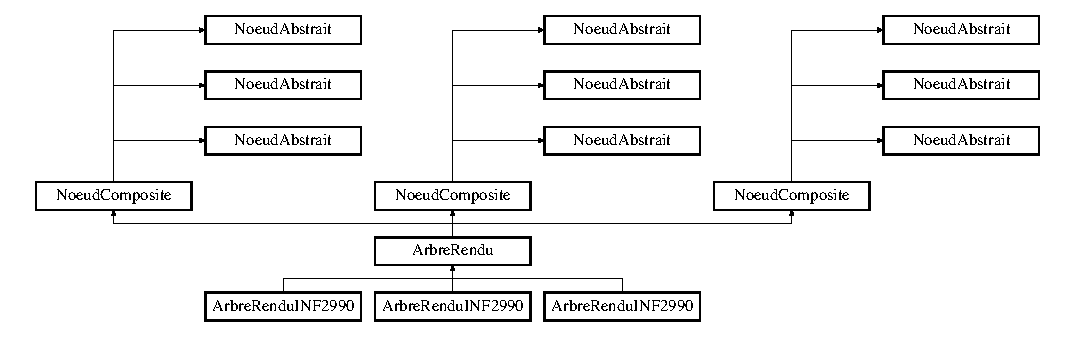
\includegraphics[height=4.000000cm]{class_arbre_rendu}
\end{center}
\end{figure}
\subsection*{Public Member Functions}
\begin{DoxyCompactItemize}
\item 
\hyperlink{group__inf2990_gaef1e98a66c4f1d3b468c786edee45ae6}{Arbre\-Rendu} ()
\begin{DoxyCompactList}\small\item\em Constructeur par d�faut. \end{DoxyCompactList}\item 
virtual \hyperlink{group__inf2990_gadb462923759da0ff632dad097b7bfdab}{$\sim$\-Arbre\-Rendu} ()
\begin{DoxyCompactList}\small\item\em Destructeur. \end{DoxyCompactList}\item 
void \hyperlink{group__inf2990_gaef33737fda55a3916e895e1adc3e88ae}{ajouter\-Usine} (const std\-::string \&type, const \hyperlink{class_usine_noeud}{Usine\-Noeud} $\ast$usine)
\begin{DoxyCompactList}\small\item\em Ajoute une usine associ�e � un type de noeud. \end{DoxyCompactList}\item 
\hyperlink{class_noeud_abstrait}{Noeud\-Abstrait} $\ast$ \hyperlink{group__inf2990_ga33ae9013f9cec73854d32527b85b41f9}{creer\-Noeud} (const std\-::string \&type\-Nouveau\-Noeud) const 
\begin{DoxyCompactList}\small\item\em Cr�e un nouveau noeud. \end{DoxyCompactList}\item 
\hyperlink{class_noeud_abstrait}{Noeud\-Abstrait} $\ast$ \hyperlink{group__inf2990_gac10e5f0623af502d67f72aef764206a3}{ajouter\-Nouveau\-Noeud} (const std\-::string \&nom\-Parent, const std\-::string \&type\-Nouveau\-Noeud)
\begin{DoxyCompactList}\small\item\em Cr�e et ajoute un nouveau noeud � l'arbre. \end{DoxyCompactList}\item 
int \hyperlink{group__inf2990_ga39037187e3ff233b1ef6a0abb1bb6389}{obtenir\-Id\-Portail} ()
\begin{DoxyCompactList}\small\item\em retourne l'Id du porchain portail a creer \end{DoxyCompactList}\item 
\hyperlink{class_noeud_composite}{Noeud\-Composite} $\ast$ \hyperlink{group__inf2990_ga11bc8fd1fc6ba70c97dd300c88aa659a}{obtenir\-Racine} ()
\begin{DoxyCompactList}\small\item\em retourne la racine de l'arbre \end{DoxyCompactList}\item 
void \hyperlink{group__inf2990_ga348af13a77b4b50eb176fcf5ccb9b2dd}{assigner\-Racine} (\hyperlink{class_noeud_abstrait}{Noeud\-Abstrait} $\ast$noeud)
\begin{DoxyCompactList}\small\item\em Assigner la racine de l'arbre. \end{DoxyCompactList}\end{DoxyCompactItemize}
\subsection*{Static Public Member Functions}
\begin{DoxyCompactItemize}
\item 
static unsigned int \hyperlink{group__inf2990_gacf0e53d52040b07cd6550fda79867bd5}{calculer\-Profondeur\-Maximale} ()
\begin{DoxyCompactList}\small\item\em Calcule la profondeur maximale possible pour l'arbre de rendu. \end{DoxyCompactList}\end{DoxyCompactItemize}
\subsection*{Additional Inherited Members}


\subsection{Detailed Description}
Classe d'arbre de rendu qui contient la racine de l'arbre de rendu avec les usines qui permettent d'ajouter des noeuds � cet arbre. 

La profondeur de cet arbre est limit�e par la taille de la pile des matrices et la taille de la pile des noms pour la s�lection Open\-G\-L, �tant donn� que chaque niveau de l'arbre effectue un \char`\"{}push\char`\"{} sur chacune de ces piles lors du rendu. L'arbre ne v�rifie pas que la profondeur reste sous la limite, mais il offre des fonctions permettant de le v�rifier ais�ment.

\begin{DoxyAuthor}{Author}
Martin Bisson 
\end{DoxyAuthor}
\begin{DoxyDate}{Date}
2007-\/01-\/28 
\end{DoxyDate}


The documentation for this class was generated from the following files\-:\begin{DoxyCompactItemize}
\item 
X\-:/inf2990-\/06/\-Cadriciel/\-Sources/\-D\-L\-L/\-Arbre/\hyperlink{_arbre_rendu_8h}{Arbre\-Rendu.\-h}\item 
X\-:/inf2990-\/06/\-Cadriciel/\-Sources/\-D\-L\-L/\-Arbre/\hyperlink{_arbre_rendu_8cpp}{Arbre\-Rendu.\-cpp}\end{DoxyCompactItemize}

\hypertarget{class_arbre_rendu_i_n_f2990}{\section{Arbre\-Rendu\-I\-N\-F2990 Class Reference}
\label{class_arbre_rendu_i_n_f2990}\index{Arbre\-Rendu\-I\-N\-F2990@{Arbre\-Rendu\-I\-N\-F2990}}
}


Classe qui repr�sente l'arbre de rendu sp�cifique au projet de I\-N\-F2990.  




{\ttfamily \#include $<$Arbre\-Rendu\-I\-N\-F2990.\-h$>$}

Inheritance diagram for Arbre\-Rendu\-I\-N\-F2990\-:\begin{figure}[H]
\begin{center}
\leavevmode
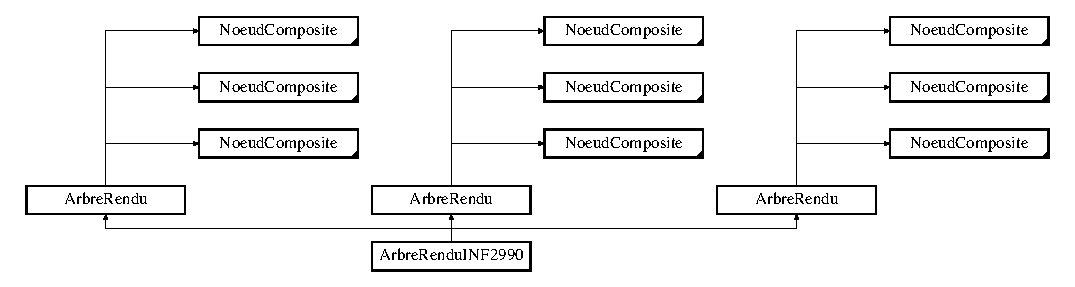
\includegraphics[height=3.406326cm]{class_arbre_rendu_i_n_f2990}
\end{center}
\end{figure}
\subsection*{Public Member Functions}
\begin{DoxyCompactItemize}
\item 
\hyperlink{group__inf2990_ga67528b7fa54e8ef8f96ef2e0bad06d2d}{Arbre\-Rendu\-I\-N\-F2990} ()
\begin{DoxyCompactList}\small\item\em Constructeur par d�faut. \end{DoxyCompactList}\item 
virtual \hyperlink{group__inf2990_gaa67526b2fd719f6bcef7a4547bd25c7b}{$\sim$\-Arbre\-Rendu\-I\-N\-F2990} ()
\begin{DoxyCompactList}\small\item\em Destructeur. \end{DoxyCompactList}\item 
void \hyperlink{group__inf2990_ga678d89e1f12ae16ee7dcf6de3db637a3}{initialiser} ()
\begin{DoxyCompactList}\small\item\em Initialise l'arbre de rendu � son �tat initial. \end{DoxyCompactList}\item 
\hypertarget{class_arbre_rendu_i_n_f2990_a67528b7fa54e8ef8f96ef2e0bad06d2d}{\hyperlink{class_arbre_rendu_i_n_f2990_a67528b7fa54e8ef8f96ef2e0bad06d2d}{Arbre\-Rendu\-I\-N\-F2990} ()}\label{class_arbre_rendu_i_n_f2990_a67528b7fa54e8ef8f96ef2e0bad06d2d}

\begin{DoxyCompactList}\small\item\em Constructeur par d�faut. \end{DoxyCompactList}\item 
\hypertarget{class_arbre_rendu_i_n_f2990_a121ba7cda8974119dd1768c06b8751b2}{virtual \hyperlink{class_arbre_rendu_i_n_f2990_a121ba7cda8974119dd1768c06b8751b2}{$\sim$\-Arbre\-Rendu\-I\-N\-F2990} ()}\label{class_arbre_rendu_i_n_f2990_a121ba7cda8974119dd1768c06b8751b2}

\begin{DoxyCompactList}\small\item\em Destructeur. \end{DoxyCompactList}\item 
\hypertarget{class_arbre_rendu_i_n_f2990_a678d89e1f12ae16ee7dcf6de3db637a3}{void \hyperlink{class_arbre_rendu_i_n_f2990_a678d89e1f12ae16ee7dcf6de3db637a3}{initialiser} ()}\label{class_arbre_rendu_i_n_f2990_a678d89e1f12ae16ee7dcf6de3db637a3}

\begin{DoxyCompactList}\small\item\em Initialise l'arbre de rendu � son �tat initial. \end{DoxyCompactList}\item 
std\-::vector$<$ \hyperlink{class_noeud_abstrait}{Noeud\-Abstrait} $\ast$ $>$ \hyperlink{group__inf2990_gac81819245675d0f2ec89725c0e19e8f4}{obtenir\-Noeud\-Selectionnes} ()
\begin{DoxyCompactList}\small\item\em retourne lesnoeuds selectionn�s \end{DoxyCompactList}\item 
\hypertarget{class_arbre_rendu_i_n_f2990_a67528b7fa54e8ef8f96ef2e0bad06d2d}{\hyperlink{class_arbre_rendu_i_n_f2990_a67528b7fa54e8ef8f96ef2e0bad06d2d}{Arbre\-Rendu\-I\-N\-F2990} ()}\label{class_arbre_rendu_i_n_f2990_a67528b7fa54e8ef8f96ef2e0bad06d2d}

\begin{DoxyCompactList}\small\item\em Constructeur par d�faut. \end{DoxyCompactList}\item 
\hypertarget{class_arbre_rendu_i_n_f2990_a121ba7cda8974119dd1768c06b8751b2}{virtual \hyperlink{class_arbre_rendu_i_n_f2990_a121ba7cda8974119dd1768c06b8751b2}{$\sim$\-Arbre\-Rendu\-I\-N\-F2990} ()}\label{class_arbre_rendu_i_n_f2990_a121ba7cda8974119dd1768c06b8751b2}

\begin{DoxyCompactList}\small\item\em Destructeur. \end{DoxyCompactList}\item 
\hypertarget{class_arbre_rendu_i_n_f2990_a678d89e1f12ae16ee7dcf6de3db637a3}{void \hyperlink{class_arbre_rendu_i_n_f2990_a678d89e1f12ae16ee7dcf6de3db637a3}{initialiser} ()}\label{class_arbre_rendu_i_n_f2990_a678d89e1f12ae16ee7dcf6de3db637a3}

\begin{DoxyCompactList}\small\item\em Initialise l'arbre de rendu � son �tat initial. \end{DoxyCompactList}\item 
\hypertarget{class_arbre_rendu_i_n_f2990_a0e8ba20ab9bbf0db290306e5c2e95685}{std\-::vector$<$ \hyperlink{class_noeud_abstrait}{Noeud\-Abstrait} $\ast$ $>$ \hyperlink{class_arbre_rendu_i_n_f2990_a0e8ba20ab9bbf0db290306e5c2e95685}{obtenir\-Noeud\-Selectionnes} ()}\label{class_arbre_rendu_i_n_f2990_a0e8ba20ab9bbf0db290306e5c2e95685}

\begin{DoxyCompactList}\small\item\em retourne lesnoeuds selectionn�s \end{DoxyCompactList}\item 
std\-::vector$<$ \hyperlink{class_noeud_abstrait}{Noeud\-Abstrait} $\ast$ $>$ \hyperlink{group__inf2990_gaaffc85d521eb2d1a001b6bc5793fe9ab}{obtenir\-Noeud\-Palette\-G\-J1} ()
\begin{DoxyCompactList}\small\item\em Retourne les palettes gauche du joueur 1. \end{DoxyCompactList}\item 
std\-::vector$<$ \hyperlink{class_noeud_abstrait}{Noeud\-Abstrait} $\ast$ $>$ \hyperlink{group__inf2990_ga059dbf2c008c0362200ac66baf590c51}{obtenir\-Noeud\-Palette\-D\-J1} ()
\begin{DoxyCompactList}\small\item\em Retourne les palettes droite du joueur 1. \end{DoxyCompactList}\item 
std\-::vector$<$ \hyperlink{class_noeud_abstrait}{Noeud\-Abstrait} $\ast$ $>$ \hyperlink{group__inf2990_gad2258c446abb582ab0a2113e0e3516c5}{obtenir\-Noeud\-Palette\-G\-J2} ()
\begin{DoxyCompactList}\small\item\em Retourne les palettes gauche du joueur 1. \end{DoxyCompactList}\item 
std\-::vector$<$ \hyperlink{class_noeud_abstrait}{Noeud\-Abstrait} $\ast$ $>$ \hyperlink{group__inf2990_gad018fb03680e485d859ee4f54d3c4bde}{obtenir\-Noeud\-Palette\-D\-J2} ()
\begin{DoxyCompactList}\small\item\em Retourne les palettes droite du joueur 2. \end{DoxyCompactList}\item 
std\-::vector$<$ \hyperlink{class_noeud_abstrait}{Noeud\-Abstrait} $\ast$ $>$ \hyperlink{group__inf2990_ga9082fbe0365c1ba02be91caada61b56d}{obtenir\-Noeud\-Ressort} ()
\begin{DoxyCompactList}\small\item\em Retourne les ressorts. \end{DoxyCompactList}\item 
\hypertarget{group__inf2990_ga4b325c56715d639504b84fa4f03af888}{std\-::vector$<$ \hyperlink{class_noeud_abstrait}{Noeud\-Abstrait} $\ast$ $>$ \hyperlink{group__inf2990_ga4b325c56715d639504b84fa4f03af888}{obtenir\-Noeud\-Generateur\-Bille} ()}\label{group__inf2990_ga4b325c56715d639504b84fa4f03af888}

\begin{DoxyCompactList}\small\item\em Retourne les generateurs de billes. \end{DoxyCompactList}\item 
std\-::vector$<$ \hyperlink{class_noeud_abstrait}{Noeud\-Abstrait} $\ast$ $>$ \hyperlink{group__inf2990_ga5a4760584498a740752aef1e75ce7df2}{obtenir\-Noeud\-Bille} ()
\begin{DoxyCompactList}\small\item\em Retourne les billes. \end{DoxyCompactList}\item 
std\-::vector$<$ \hyperlink{class_noeud_abstrait}{Noeud\-Abstrait} $\ast$ $>$ \hyperlink{group__inf2990_ga72adf59460440b73a88e6119f5d5b4c7}{obtenir\-Noeud\-Portail} ()
\begin{DoxyCompactList}\small\item\em Retourne les generateurs de billes. \end{DoxyCompactList}\item 
\hyperlink{class_noeud_portail}{Noeud\-Portail} $\ast$ \hyperlink{group__inf2990_gaa31bddefc5fef2820e19567e5a1bf837}{obtenir\-Noeud\-Frere} (\hyperlink{class_noeud_portail}{Noeud\-Portail} $\ast$portail)
\begin{DoxyCompactList}\small\item\em Permet de parcourir l'arbre pour obtenir le deuxieme portail d'une paire. \end{DoxyCompactList}\item 
int \hyperlink{group__inf2990_gab5bb3b5417ce69eb2186af74f64812e2}{obtenir\-Points\-Campagne} ()
\begin{DoxyCompactList}\small\item\em Permet d'obtenir les points pour passer a la prochaine campagne. \end{DoxyCompactList}\item 
int \hyperlink{group__inf2990_gab8cfd98a1cb68e1dd3c13a8e7ed67518}{obtenir\-Points\-Bille} ()
\begin{DoxyCompactList}\small\item\em Permet d'obtenir les points pour avoir une bille gratuite. \end{DoxyCompactList}\item 
\hypertarget{group__inf2990_gad2753d0c059d1672a38db0fcb259e2bb}{int \hyperlink{group__inf2990_gad2753d0c059d1672a38db0fcb259e2bb}{obtenir\-Difficulte} ()}\label{group__inf2990_gad2753d0c059d1672a38db0fcb259e2bb}

\begin{DoxyCompactList}\small\item\em Permet d'obtenir la difficult� \end{DoxyCompactList}\item 
\hypertarget{group__inf2990_gaf8d29ac622fde29e983484dd96f94383}{int \hyperlink{group__inf2990_gaf8d29ac622fde29e983484dd96f94383}{obtenir\-Points\-Collision} (std\-::string objet)}\label{group__inf2990_gaf8d29ac622fde29e983484dd96f94383}

\begin{DoxyCompactList}\small\item\em Retourne les points dun certain type de collision. \end{DoxyCompactList}\item 
void \hyperlink{group__inf2990_ga8ca4c7b2c52387246b8f202e17667eb5}{assigner\-Points\-Campagne} (int points)
\begin{DoxyCompactList}\small\item\em Permet d'assigner les points pour passer a la prochaine campagne. \end{DoxyCompactList}\item 
void \hyperlink{group__inf2990_gaf5d9a7e096d19d87f46c981d69fb3c1f}{assigner\-Points\-Bille} (int points)
\begin{DoxyCompactList}\small\item\em Permet d'assigner les points pour avoir une bille gratuite. \end{DoxyCompactList}\item 
void \hyperlink{group__inf2990_gaf50dab6537c65f123281e02abfaf1235}{assigner\-Points\-Butoir\-Cir} (int points)
\begin{DoxyCompactList}\small\item\em Permet d'assigner les points d'un butoir circulaire. \end{DoxyCompactList}\item 
\hypertarget{group__inf2990_ga561f50b4be3658c7864f8aeb5908a9c5}{void \hyperlink{group__inf2990_ga561f50b4be3658c7864f8aeb5908a9c5}{assigner\-Points\-Butoir\-Tri} (int points)}\label{group__inf2990_ga561f50b4be3658c7864f8aeb5908a9c5}

\begin{DoxyCompactList}\small\item\em Permet d'assigner les points d'un butoir triangulaire. \end{DoxyCompactList}\item 
void \hyperlink{group__inf2990_ga0589442c1a30ba017a6ec00d0ec1224f}{assigner\-Points\-Cible} (int points)
\begin{DoxyCompactList}\small\item\em Permet d'assigner les points d'une cible. \end{DoxyCompactList}\item 
void \hyperlink{group__inf2990_ga61245075a6239c1e0ed17070a7266e82}{assigner\-Difficulte} (int points)
\begin{DoxyCompactList}\small\item\em Permet d'assigner la difficulte dun niveau. \end{DoxyCompactList}\item 
int \hyperlink{group__inf2990_ga8e8afd5c8f54924cf5b8bf9ff566e226}{obtenir\-Points\-Butoir\-Cir} ()
\begin{DoxyCompactList}\small\item\em Permet d'obtenir les points d'un butoir circulaire. \end{DoxyCompactList}\item 
int \hyperlink{group__inf2990_gab6950fbadcb23518c5d90492f2ed9d49}{obtenir\-Points\-Butoir\-Tri} ()
\begin{DoxyCompactList}\small\item\em Permet d'obtenir les points d'un butoir triangulaire. \end{DoxyCompactList}\item 
int \hyperlink{group__inf2990_ga98f17dbf250c022253f3e5f44d07b0c7}{obtenir\-Points\-Cible} ()
\begin{DoxyCompactList}\small\item\em Permet d'obtenir les points d'une cible. \end{DoxyCompactList}\end{DoxyCompactItemize}
\subsection*{Static Public Attributes}
\begin{DoxyCompactItemize}
\item 
\hypertarget{group__inf2990_ga25857010b8ef5796762cebcb1325257f}{static const std\-::string \hyperlink{group__inf2990_ga25857010b8ef5796762cebcb1325257f}{N\-O\-M\-\_\-\-A\-R\-A\-I\-G\-N\-E\-E} \{ \char`\"{}araignee\char`\"{} \}}\label{group__inf2990_ga25857010b8ef5796762cebcb1325257f}

\begin{DoxyCompactList}\small\item\em La cha�ne repr�sentant le type des araign�es. \end{DoxyCompactList}\item 
\hypertarget{group__inf2990_ga56455f1d74a69fdf07b263c7ea44b183}{static const std\-::string \hyperlink{group__inf2990_ga56455f1d74a69fdf07b263c7ea44b183}{N\-O\-M\-\_\-\-C\-O\-N\-E\-C\-U\-B\-E} \{ \char`\"{}conecube\char`\"{} \}}\label{group__inf2990_ga56455f1d74a69fdf07b263c7ea44b183}

\begin{DoxyCompactList}\small\item\em La cha�ne repr�sentant le type des cones-\/cubes. \end{DoxyCompactList}\item 
\hypertarget{group__inf2990_gaf1244076bd6c3050aca6e7d191db2d90}{static const std\-::string {\bfseries N\-O\-M\-\_\-\-P\-A\-L\-E\-T\-T\-E\-\_\-\-J\-O\-U\-E\-U\-R1} \{ \char`\"{}palette\-Joueur1\char`\"{} \}}\label{group__inf2990_gaf1244076bd6c3050aca6e7d191db2d90}

\item 
\hypertarget{group__inf2990_ga110d63c837ae704706143937228437f6}{static const std\-::string {\bfseries N\-O\-M\-\_\-\-P\-A\-L\-E\-T\-T\-E\-\_\-\-J\-O\-U\-E\-U\-R2} \{ \char`\"{}palette\-Joueur2\char`\"{} \}}\label{group__inf2990_ga110d63c837ae704706143937228437f6}

\item 
\hypertarget{group__inf2990_ga3773989a1a1ecdf2fcdfe4cdb1709f04}{static const std\-::string {\bfseries N\-O\-M\-\_\-\-P\-L\-A\-Q\-U\-E} \{ \char`\"{}plaque\char`\"{} \}}\label{group__inf2990_ga3773989a1a1ecdf2fcdfe4cdb1709f04}

\item 
\hypertarget{group__inf2990_gaf2fdfce624493e8038e44f710f225f8b}{static const std\-::string {\bfseries N\-O\-M\-\_\-\-B\-U\-T\-O\-I\-R\-\_\-\-T\-R\-I\-A\-N\-G\-U\-L\-A\-I\-R\-E} \{ \char`\"{}butoir\-Triangulaire\char`\"{} \}}\label{group__inf2990_gaf2fdfce624493e8038e44f710f225f8b}

\item 
\hypertarget{group__inf2990_ga8e997c4baf8155d7f4ab250190eeb7ac}{static const std\-::string {\bfseries N\-O\-M\-\_\-\-B\-U\-T\-O\-I\-R\-\_\-\-C\-I\-R\-C\-U\-L\-A\-I\-R\-E} \{ \char`\"{}butoir\-Circulaire\char`\"{} \}}\label{group__inf2990_ga8e997c4baf8155d7f4ab250190eeb7ac}

\item 
\hypertarget{group__inf2990_gadf10761162a37559f7ca550f14706de5}{static const std\-::string {\bfseries N\-O\-M\-\_\-\-C\-I\-B\-L\-E} \{ \char`\"{}cible\char`\"{} \}}\label{group__inf2990_gadf10761162a37559f7ca550f14706de5}

\item 
\hypertarget{group__inf2990_ga0fedce45945b021f23191e77dc50ebbb}{static const std\-::string {\bfseries N\-O\-M\-\_\-\-R\-E\-S\-S\-O\-R\-T} \{ \char`\"{}ressort\char`\"{} \}}\label{group__inf2990_ga0fedce45945b021f23191e77dc50ebbb}

\item 
\hypertarget{group__inf2990_gabca2beb3084ec097e64fafedda37be9c}{static const std\-::string {\bfseries N\-O\-M\-\_\-\-G\-E\-N\-E\-R\-A\-T\-E\-U\-R\-\_\-\-B\-I\-L\-L\-E} \{ \char`\"{}generateur\-Bille\char`\"{} \}}\label{group__inf2990_gabca2beb3084ec097e64fafedda37be9c}

\item 
\hypertarget{group__inf2990_gadb2781803028f600f161481daae30bb7}{static const std\-::string {\bfseries N\-O\-M\-\_\-\-T\-R\-O\-U} \{ \char`\"{}trou\char`\"{} \}}\label{group__inf2990_gadb2781803028f600f161481daae30bb7}

\item 
\hypertarget{group__inf2990_gac8df2222d7028f2706fa9e4579b0bb26}{static const std\-::string {\bfseries N\-O\-M\-\_\-\-P\-O\-R\-T\-A\-I\-L} \{ \char`\"{}portail\char`\"{} \}}\label{group__inf2990_gac8df2222d7028f2706fa9e4579b0bb26}

\item 
\hypertarget{group__inf2990_gab1dd24123abb04cb42852e0b29aedec1}{static const std\-::string {\bfseries N\-O\-M\-\_\-\-M\-U\-R} \{ \char`\"{}mur\char`\"{} \}}\label{group__inf2990_gab1dd24123abb04cb42852e0b29aedec1}

\item 
\hypertarget{group__inf2990_ga94c12dcc43f98c6a9ea01d5000731146}{static const std\-::string {\bfseries N\-O\-M\-\_\-\-P\-A\-L\-E\-T\-T\-E\-\_\-\-J\-O\-U\-E\-U\-R1\-\_\-\-G\-A\-U\-C\-H\-E} \{ \char`\"{}palette\-Joueur1\-Gauche\char`\"{} \}}\label{group__inf2990_ga94c12dcc43f98c6a9ea01d5000731146}

\item 
\hypertarget{group__inf2990_ga07688cfa3d08eba55f99bec99dd3b5f4}{static const std\-::string {\bfseries N\-O\-M\-\_\-\-P\-A\-L\-E\-T\-T\-E\-\_\-\-J\-O\-U\-E\-U\-R1\-\_\-\-D\-R\-O\-I\-T\-E} \{ \char`\"{}palette\-Joueur1\-Droite\char`\"{} \}}\label{group__inf2990_ga07688cfa3d08eba55f99bec99dd3b5f4}

\item 
\hypertarget{group__inf2990_ga4cf6c9537ed786e75d8a31d0865bdd7d}{static const std\-::string {\bfseries N\-O\-M\-\_\-\-P\-A\-L\-E\-T\-T\-E\-\_\-\-J\-O\-U\-E\-U\-R2\-\_\-\-G\-A\-U\-C\-H\-E} \{ \char`\"{}palette\-Joueur2\-Gauche\char`\"{} \}}\label{group__inf2990_ga4cf6c9537ed786e75d8a31d0865bdd7d}

\item 
\hypertarget{group__inf2990_gace9339a7f67639dd836f63ce5b5ddc3a}{static const std\-::string {\bfseries N\-O\-M\-\_\-\-P\-A\-L\-E\-T\-T\-E\-\_\-\-J\-O\-U\-E\-U\-R2\-\_\-\-D\-R\-O\-I\-T\-E} \{ \char`\"{}palette\-Joueur2\-Droite\char`\"{} \}}\label{group__inf2990_gace9339a7f67639dd836f63ce5b5ddc3a}

\item 
\hypertarget{group__inf2990_ga4a9ce7cdb45866b2e0f8949b1d5c770e}{static const std\-::string {\bfseries N\-O\-M\-\_\-\-B\-U\-T\-O\-I\-R\-\_\-\-T\-R\-I\-A\-N\-G\-U\-L\-A\-I\-R\-E\-\_\-\-G\-A\-U\-C\-H\-E} \{ \char`\"{}butoir\-Triangulaire\-Gauche\char`\"{} \}}\label{group__inf2990_ga4a9ce7cdb45866b2e0f8949b1d5c770e}

\item 
\hypertarget{group__inf2990_ga13ca7796c90860832152b79e0520f05c}{static const std\-::string {\bfseries N\-O\-M\-\_\-\-B\-U\-T\-O\-I\-R\-\_\-\-T\-R\-I\-A\-N\-G\-U\-L\-A\-I\-R\-E\-\_\-\-D\-R\-O\-I\-T} \{ \char`\"{}butoir\-Triangulaire\-Droit\char`\"{} \}}\label{group__inf2990_ga13ca7796c90860832152b79e0520f05c}

\item 
\hypertarget{group__inf2990_ga97be26afc6aa5e5ce5c1e66623a27f9d}{static const std\-::string {\bfseries N\-O\-M\-\_\-\-B\-I\-L\-L\-E} \{ \char`\"{}bille\char`\"{} \}}\label{group__inf2990_ga97be26afc6aa5e5ce5c1e66623a27f9d}

\end{DoxyCompactItemize}
\subsection*{Additional Inherited Members}


\subsection{Detailed Description}
Classe qui repr�sente l'arbre de rendu sp�cifique au projet de I\-N\-F2990. 

Cette classe s'occupe de configurer les usines des noeuds qui seront utilis�s par le projet.

\begin{DoxyAuthor}{Author}
Martin Bisson 
\end{DoxyAuthor}
\begin{DoxyDate}{Date}
2007-\/03-\/23 
\end{DoxyDate}


The documentation for this class was generated from the following files\-:\begin{DoxyCompactItemize}
\item 
X\-:/\-Git\-\_\-\-Repository/inf2990-\/06/\-Cadriciel/livrable0/\-D\-L\-L/\-Arbre/Arbre\-Rendu\-I\-N\-F2990.\-h\item 
X\-:/\-Git\-\_\-\-Repository/inf2990-\/06/\-Cadriciel/livrable0/\-D\-L\-L/\-Arbre/Arbre\-Rendu\-I\-N\-F2990.\-cpp\end{DoxyCompactItemize}

\hypertarget{class_arbre_rendu_inf2990_test}{\section{Arbre\-Rendu\-Inf2990\-Test Class Reference}
\label{class_arbre_rendu_inf2990_test}\index{Arbre\-Rendu\-Inf2990\-Test@{Arbre\-Rendu\-Inf2990\-Test}}
}


Classe de test cppunit pour tester le bon fonctionnement des m�thodes de la classe \hyperlink{class_facade_modele}{Facade\-Modele}.  




{\ttfamily \#include $<$Arbre\-Rendu\-I\-N\-F2990\-Test.\-h$>$}

Inheritance diagram for Arbre\-Rendu\-Inf2990\-Test\-:\begin{figure}[H]
\begin{center}
\leavevmode
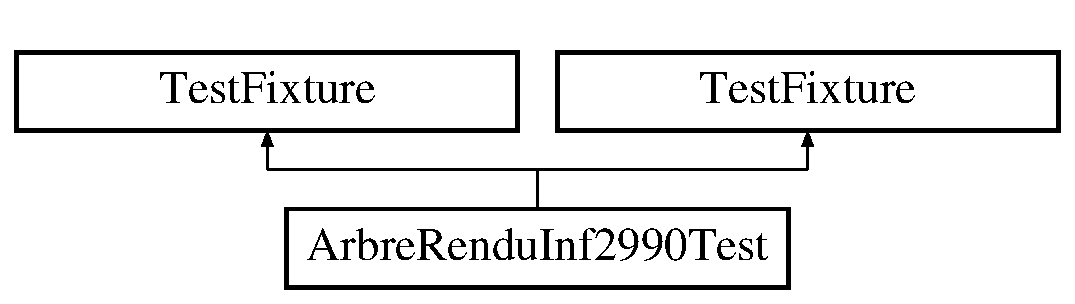
\includegraphics[height=2.000000cm]{class_arbre_rendu_inf2990_test}
\end{center}
\end{figure}
\subsection*{Public Member Functions}
\begin{DoxyCompactItemize}
\item 
void \hyperlink{group__inf2990_gae0c8900985ef9379833005f01d258b75}{set\-Up} ()
\begin{DoxyCompactList}\small\item\em Traitement � effectuer pour initialiser cette suite de tests. \end{DoxyCompactList}\item 
void \hyperlink{group__inf2990_gacae8203095bee9ac7cf4ab3dae72307e}{tear\-Down} ()
\begin{DoxyCompactList}\small\item\em Traitement � effectuer pour 'finaliser' cette suite de tests. \end{DoxyCompactList}\item 
void \hyperlink{group__inf2990_ga43afb4c3ac9ffdfac3bccfff395b00ef}{test\-Initialiser} ()
\begin{DoxyCompactList}\small\item\em Cas de test\-: s'assur� que l'arbre se vide. \end{DoxyCompactList}\item 
void \hyperlink{group__inf2990_ga0da3a933b685d0873789e21480315689}{test\-Obtenir\-Noeud\-Selectionnes} ()
\begin{DoxyCompactList}\small\item\em Cas de test\-: s'assurer que les noeud s�l�ctionn�s sont trouv� \end{DoxyCompactList}\item 
\hypertarget{class_arbre_rendu_inf2990_test_ae0c8900985ef9379833005f01d258b75}{void \hyperlink{class_arbre_rendu_inf2990_test_ae0c8900985ef9379833005f01d258b75}{set\-Up} ()}\label{class_arbre_rendu_inf2990_test_ae0c8900985ef9379833005f01d258b75}

\begin{DoxyCompactList}\small\item\em Traitement � effectuer pour initialiser cette suite de tests. \end{DoxyCompactList}\item 
\hypertarget{class_arbre_rendu_inf2990_test_acae8203095bee9ac7cf4ab3dae72307e}{void \hyperlink{class_arbre_rendu_inf2990_test_acae8203095bee9ac7cf4ab3dae72307e}{tear\-Down} ()}\label{class_arbre_rendu_inf2990_test_acae8203095bee9ac7cf4ab3dae72307e}

\begin{DoxyCompactList}\small\item\em Traitement � effectuer pour 'finaliser' cette suite de tests. \end{DoxyCompactList}\item 
\hypertarget{class_arbre_rendu_inf2990_test_a43afb4c3ac9ffdfac3bccfff395b00ef}{void \hyperlink{class_arbre_rendu_inf2990_test_a43afb4c3ac9ffdfac3bccfff395b00ef}{test\-Initialiser} ()}\label{class_arbre_rendu_inf2990_test_a43afb4c3ac9ffdfac3bccfff395b00ef}

\begin{DoxyCompactList}\small\item\em Cas de test\-: s'assur� que l'arbre se vide. \end{DoxyCompactList}\item 
\hypertarget{class_arbre_rendu_inf2990_test_a0da3a933b685d0873789e21480315689}{void \hyperlink{class_arbre_rendu_inf2990_test_a0da3a933b685d0873789e21480315689}{test\-Obtenir\-Noeud\-Selectionnes} ()}\label{class_arbre_rendu_inf2990_test_a0da3a933b685d0873789e21480315689}

\begin{DoxyCompactList}\small\item\em Cas de test\-: s'assurer que les noeud s�l�ctionn�s sont trouv� \end{DoxyCompactList}\end{DoxyCompactItemize}


\subsection{Detailed Description}
Classe de test cppunit pour tester le bon fonctionnement des m�thodes de la classe \hyperlink{class_facade_modele}{Facade\-Modele}. 

\begin{DoxyAuthor}{Author}
Gabriel Amyot 
\end{DoxyAuthor}
\begin{DoxyDate}{Date}
2014-\/10-\/08 
\end{DoxyDate}


The documentation for this class was generated from the following files\-:\begin{DoxyCompactItemize}
\item 
X\-:/\-Git\-\_\-\-Repository/inf2990-\/06/\-Cadriciel/livrable1/\-D\-L\-L/\-Tests/Arbre\-Rendu\-I\-N\-F2990\-Test.\-h\item 
X\-:/\-Git\-\_\-\-Repository/inf2990-\/06/\-Cadriciel/livrable1/\-D\-L\-L/\-Tests/Arbre\-Rendu\-I\-N\-F2990\-Test.\-cpp\end{DoxyCompactItemize}

\hypertarget{struct_asserter}{\section{Asserter Struct Reference}
\label{struct_asserter}\index{Asserter@{Asserter}}
}


A set of functions to help writing assertion macros.

Here is an example of assertion, a simplified version of the actual assertion implemented in examples/cppunittest/\-Xml\-Uniformiser.\-h\-:  




{\ttfamily \#include $<$Asserter.\-h$>$}

\subsection*{Static Public Member Functions}
\begin{DoxyCompactItemize}
\item 
\hypertarget{struct_asserter_a5a67b6042625cc87d271a53ac555e437}{static void C\-P\-P\-U\-N\-I\-T\-\_\-\-A\-P\-I \hyperlink{struct_asserter_a5a67b6042625cc87d271a53ac555e437}{fail} (const \hyperlink{class_message}{Message} \&message, const \hyperlink{class_source_line}{Source\-Line} \&source\-Line=\hyperlink{class_source_line}{Source\-Line}())}\label{struct_asserter_a5a67b6042625cc87d271a53ac555e437}

\begin{DoxyCompactList}\small\item\em Throws a \hyperlink{class_exception}{Exception} with the specified message and location. \end{DoxyCompactList}\item 
static void C\-P\-P\-U\-N\-I\-T\-\_\-\-A\-P\-I \hyperlink{struct_asserter_a74825fc71909baa1286f9282ba5a2a54}{fail} (std\-::string message, const \hyperlink{class_source_line}{Source\-Line} \&source\-Line=\hyperlink{class_source_line}{Source\-Line}())
\begin{DoxyCompactList}\small\item\em Throws a \hyperlink{class_exception}{Exception} with the specified message and location. \end{DoxyCompactList}\item 
static void C\-P\-P\-U\-N\-I\-T\-\_\-\-A\-P\-I \hyperlink{struct_asserter_a425da14df34fad7e23a35456fce0eb2b}{fail\-If} (bool should\-Fail, const \hyperlink{class_message}{Message} \&message, const \hyperlink{class_source_line}{Source\-Line} \&source\-Line=\hyperlink{class_source_line}{Source\-Line}())
\begin{DoxyCompactList}\small\item\em Throws a \hyperlink{class_exception}{Exception} with the specified message and location. \end{DoxyCompactList}\item 
static void C\-P\-P\-U\-N\-I\-T\-\_\-\-A\-P\-I \hyperlink{struct_asserter_a71a4667a9d3f5d483f1a82157f715824}{fail\-If} (bool should\-Fail, std\-::string message, const \hyperlink{class_source_line}{Source\-Line} \&source\-Line=\hyperlink{class_source_line}{Source\-Line}())
\begin{DoxyCompactList}\small\item\em Throws a \hyperlink{class_exception}{Exception} with the specified message and location. \end{DoxyCompactList}\item 
static std\-::string C\-P\-P\-U\-N\-I\-T\-\_\-\-A\-P\-I \hyperlink{struct_asserter_adcbee7c01d58bfaee72cc984627e6432}{make\-Expected} (const std\-::string \&expected\-Value)
\begin{DoxyCompactList}\small\item\em Returns a expected value string for a message. Typically used to create 'not equal' message, or to check that a message contains the expected content when writing unit tests for your custom assertions. \end{DoxyCompactList}\item 
static std\-::string C\-P\-P\-U\-N\-I\-T\-\_\-\-A\-P\-I \hyperlink{struct_asserter_ae52920ca7ffd981df61d7a3cfd88793b}{make\-Actual} (const std\-::string \&actual\-Value)
\begin{DoxyCompactList}\small\item\em Returns an actual value string for a message. Typically used to create 'not equal' message, or to check that a message contains the expected content when writing unit tests for your custom assertions. \end{DoxyCompactList}\item 
\hypertarget{struct_asserter_adb8ac36c8f0d385430e5a087a66219db}{static \hyperlink{class_message}{Message} C\-P\-P\-U\-N\-I\-T\-\_\-\-A\-P\-I {\bfseries make\-Not\-Equal\-Message} (const std\-::string \&expected\-Value, const std\-::string \&actual\-Value, const \hyperlink{class_additional_message}{Additional\-Message} \&additional\-Message=\hyperlink{class_additional_message}{Additional\-Message}(), const std\-::string \&short\-Description=\char`\"{}equality assertion failed\char`\"{})}\label{struct_asserter_adb8ac36c8f0d385430e5a087a66219db}

\item 
static void C\-P\-P\-U\-N\-I\-T\-\_\-\-A\-P\-I \hyperlink{struct_asserter_ac6234767e7d986bace97dc44f8d80d6c}{fail\-Not\-Equal} (std\-::string expected, std\-::string actual, const \hyperlink{class_source_line}{Source\-Line} \&source\-Line, const \hyperlink{class_additional_message}{Additional\-Message} \&additional\-Message=\hyperlink{class_additional_message}{Additional\-Message}(), std\-::string short\-Description=\char`\"{}equality assertion failed\char`\"{})
\begin{DoxyCompactList}\small\item\em Throws an \hyperlink{class_exception}{Exception} with the specified message and location. \end{DoxyCompactList}\item 
static void C\-P\-P\-U\-N\-I\-T\-\_\-\-A\-P\-I \hyperlink{struct_asserter_a3a805c9f8c641d65353bcff2da80624f}{fail\-Not\-Equal\-If} (bool should\-Fail, std\-::string expected, std\-::string actual, const \hyperlink{class_source_line}{Source\-Line} \&source\-Line, const \hyperlink{class_additional_message}{Additional\-Message} \&additional\-Message=\hyperlink{class_additional_message}{Additional\-Message}(), std\-::string short\-Description=\char`\"{}equality assertion failed\char`\"{})
\begin{DoxyCompactList}\small\item\em Throws an \hyperlink{class_exception}{Exception} with the specified message and location. \end{DoxyCompactList}\end{DoxyCompactItemize}


\subsection{Detailed Description}
A set of functions to help writing assertion macros.

Here is an example of assertion, a simplified version of the actual assertion implemented in examples/cppunittest/\-Xml\-Uniformiser.\-h\-: 


\begin{DoxyCode}
\textcolor{preprocessor}{#include <cppunit/SourceLine.h>}
\textcolor{preprocessor}{#include <cppunit/TestAssert.h>}

\textcolor{keywordtype}{void} 
checkXmlEqual( std::string expectedXml,
               std::string actualXml,
               CppUnit::SourceLine sourceLine )
\{
  std::string expected = XmlUniformiser( expectedXml ).stripped();
  std::string actual = XmlUniformiser( actualXml ).stripped();

  \textcolor{keywordflow}{if} ( expected == actual )
    \textcolor{keywordflow}{return};

  ::CppUnit::Asserter::failNotEqual( expected,
                                     actual,
                                     sourceLine );
\}

\textcolor{preprocessor}{#define CPPUNITTEST\_ASSERT\_XML\_EQUAL( expected, actual ) \(\backslash\)}
\textcolor{preprocessor}{    checkXmlEqual( expected, actual,                     \(\backslash\)}
\textcolor{preprocessor}{                   CPPUNIT\_SOURCELINE() )}
\end{DoxyCode}
 

\subsection{Member Function Documentation}
\hypertarget{struct_asserter_a74825fc71909baa1286f9282ba5a2a54}{\index{Asserter@{Asserter}!fail@{fail}}
\index{fail@{fail}!Asserter@{Asserter}}
\subsubsection[{fail}]{\setlength{\rightskip}{0pt plus 5cm}static void C\-P\-P\-U\-N\-I\-T\-\_\-\-A\-P\-I Asserter\-::fail (
\begin{DoxyParamCaption}
\item[{std\-::string}]{message, }
\item[{const {\bf Source\-Line} \&}]{source\-Line = {\ttfamily {\bf Source\-Line}()}}
\end{DoxyParamCaption}
)\hspace{0.3cm}{\ttfamily [static]}}}\label{struct_asserter_a74825fc71909baa1286f9282ba5a2a54}


Throws a \hyperlink{class_exception}{Exception} with the specified message and location. 

\begin{DoxyRefDesc}{Deprecated}
\item[\hyperlink{deprecated__deprecated000002}{Deprecated}]Use fail( Message, Source\-Line ) instead. \end{DoxyRefDesc}
\hypertarget{struct_asserter_a425da14df34fad7e23a35456fce0eb2b}{\index{Asserter@{Asserter}!fail\-If@{fail\-If}}
\index{fail\-If@{fail\-If}!Asserter@{Asserter}}
\subsubsection[{fail\-If}]{\setlength{\rightskip}{0pt plus 5cm}static void C\-P\-P\-U\-N\-I\-T\-\_\-\-A\-P\-I Asserter\-::fail\-If (
\begin{DoxyParamCaption}
\item[{bool}]{should\-Fail, }
\item[{const {\bf Message} \&}]{message, }
\item[{const {\bf Source\-Line} \&}]{source\-Line = {\ttfamily {\bf Source\-Line}()}}
\end{DoxyParamCaption}
)\hspace{0.3cm}{\ttfamily [static]}}}\label{struct_asserter_a425da14df34fad7e23a35456fce0eb2b}


Throws a \hyperlink{class_exception}{Exception} with the specified message and location. 


\begin{DoxyParams}{Parameters}
{\em should\-Fail} & if {\ttfamily true} then the exception is thrown. Otherwise nothing happen. \\
\hline
{\em message} & \hyperlink{class_message}{Message} explaining the assertion failiure. \\
\hline
{\em source\-Line} & Location of the assertion. \\
\hline
\end{DoxyParams}
\hypertarget{struct_asserter_a71a4667a9d3f5d483f1a82157f715824}{\index{Asserter@{Asserter}!fail\-If@{fail\-If}}
\index{fail\-If@{fail\-If}!Asserter@{Asserter}}
\subsubsection[{fail\-If}]{\setlength{\rightskip}{0pt plus 5cm}static void C\-P\-P\-U\-N\-I\-T\-\_\-\-A\-P\-I Asserter\-::fail\-If (
\begin{DoxyParamCaption}
\item[{bool}]{should\-Fail, }
\item[{std\-::string}]{message, }
\item[{const {\bf Source\-Line} \&}]{source\-Line = {\ttfamily {\bf Source\-Line}()}}
\end{DoxyParamCaption}
)\hspace{0.3cm}{\ttfamily [static]}}}\label{struct_asserter_a71a4667a9d3f5d483f1a82157f715824}


Throws a \hyperlink{class_exception}{Exception} with the specified message and location. 

\begin{DoxyRefDesc}{Deprecated}
\item[\hyperlink{deprecated__deprecated000003}{Deprecated}]Use fail\-If( bool, Message, Source\-Line ) instead. 
\begin{DoxyParams}{Parameters}
{\em should\-Fail} & if {\ttfamily true} then the exception is thrown. Otherwise nothing happen. \\
\hline
{\em message} & \hyperlink{class_message}{Message} explaining the assertion failiure. \\
\hline
{\em source\-Line} & Location of the assertion. \\
\hline
\end{DoxyParams}
\end{DoxyRefDesc}
\hypertarget{struct_asserter_ac6234767e7d986bace97dc44f8d80d6c}{\index{Asserter@{Asserter}!fail\-Not\-Equal@{fail\-Not\-Equal}}
\index{fail\-Not\-Equal@{fail\-Not\-Equal}!Asserter@{Asserter}}
\subsubsection[{fail\-Not\-Equal}]{\setlength{\rightskip}{0pt plus 5cm}static void C\-P\-P\-U\-N\-I\-T\-\_\-\-A\-P\-I Asserter\-::fail\-Not\-Equal (
\begin{DoxyParamCaption}
\item[{std\-::string}]{expected, }
\item[{std\-::string}]{actual, }
\item[{const {\bf Source\-Line} \&}]{source\-Line, }
\item[{const {\bf Additional\-Message} \&}]{additional\-Message = {\ttfamily {\bf Additional\-Message}()}, }
\item[{std\-::string}]{short\-Description = {\ttfamily \char`\"{}equality~assertion~failed\char`\"{}}}
\end{DoxyParamCaption}
)\hspace{0.3cm}{\ttfamily [static]}}}\label{struct_asserter_ac6234767e7d986bace97dc44f8d80d6c}


Throws an \hyperlink{class_exception}{Exception} with the specified message and location. 


\begin{DoxyParams}{Parameters}
{\em expected} & Text describing the expected value. \\
\hline
{\em actual} & Text describing the actual value. \\
\hline
{\em source\-Line} & Location of the assertion. \\
\hline
{\em additional\-Message} & Additional message. Usually used to report what are the differences between the expected and actual value. \\
\hline
{\em short\-Description} & Short description for the failure message. \\
\hline
\end{DoxyParams}
\hypertarget{struct_asserter_a3a805c9f8c641d65353bcff2da80624f}{\index{Asserter@{Asserter}!fail\-Not\-Equal\-If@{fail\-Not\-Equal\-If}}
\index{fail\-Not\-Equal\-If@{fail\-Not\-Equal\-If}!Asserter@{Asserter}}
\subsubsection[{fail\-Not\-Equal\-If}]{\setlength{\rightskip}{0pt plus 5cm}static void C\-P\-P\-U\-N\-I\-T\-\_\-\-A\-P\-I Asserter\-::fail\-Not\-Equal\-If (
\begin{DoxyParamCaption}
\item[{bool}]{should\-Fail, }
\item[{std\-::string}]{expected, }
\item[{std\-::string}]{actual, }
\item[{const {\bf Source\-Line} \&}]{source\-Line, }
\item[{const {\bf Additional\-Message} \&}]{additional\-Message = {\ttfamily {\bf Additional\-Message}()}, }
\item[{std\-::string}]{short\-Description = {\ttfamily \char`\"{}equality~assertion~failed\char`\"{}}}
\end{DoxyParamCaption}
)\hspace{0.3cm}{\ttfamily [static]}}}\label{struct_asserter_a3a805c9f8c641d65353bcff2da80624f}


Throws an \hyperlink{class_exception}{Exception} with the specified message and location. 


\begin{DoxyParams}{Parameters}
{\em should\-Fail} & if {\ttfamily true} then the exception is thrown. Otherwise nothing happen. \\
\hline
{\em expected} & Text describing the expected value. \\
\hline
{\em actual} & Text describing the actual value. \\
\hline
{\em source\-Line} & Location of the assertion. \\
\hline
{\em additional\-Message} & Additional message. Usually used to report where the \char`\"{}difference\char`\"{} is located. \\
\hline
{\em short\-Description} & Short description for the failure message. \\
\hline
\end{DoxyParams}
\hypertarget{struct_asserter_ae52920ca7ffd981df61d7a3cfd88793b}{\index{Asserter@{Asserter}!make\-Actual@{make\-Actual}}
\index{make\-Actual@{make\-Actual}!Asserter@{Asserter}}
\subsubsection[{make\-Actual}]{\setlength{\rightskip}{0pt plus 5cm}static std\-::string C\-P\-P\-U\-N\-I\-T\-\_\-\-A\-P\-I Asserter\-::make\-Actual (
\begin{DoxyParamCaption}
\item[{const std\-::string \&}]{actual\-Value}
\end{DoxyParamCaption}
)\hspace{0.3cm}{\ttfamily [static]}}}\label{struct_asserter_ae52920ca7ffd981df61d7a3cfd88793b}


Returns an actual value string for a message. Typically used to create 'not equal' message, or to check that a message contains the expected content when writing unit tests for your custom assertions. 


\begin{DoxyParams}{Parameters}
{\em actual\-Value} & String that represents the actual value. \\
\hline
\end{DoxyParams}
\begin{DoxyReturn}{Returns}
{\itshape actual\-Value} prefixed with \char`\"{}\-Actual  \-: \char`\"{}. 
\end{DoxyReturn}
\begin{DoxySeeAlso}{See Also}
\hyperlink{struct_asserter_adcbee7c01d58bfaee72cc984627e6432}{make\-Expected()}. 
\end{DoxySeeAlso}
\hypertarget{struct_asserter_adcbee7c01d58bfaee72cc984627e6432}{\index{Asserter@{Asserter}!make\-Expected@{make\-Expected}}
\index{make\-Expected@{make\-Expected}!Asserter@{Asserter}}
\subsubsection[{make\-Expected}]{\setlength{\rightskip}{0pt plus 5cm}static std\-::string C\-P\-P\-U\-N\-I\-T\-\_\-\-A\-P\-I Asserter\-::make\-Expected (
\begin{DoxyParamCaption}
\item[{const std\-::string \&}]{expected\-Value}
\end{DoxyParamCaption}
)\hspace{0.3cm}{\ttfamily [static]}}}\label{struct_asserter_adcbee7c01d58bfaee72cc984627e6432}


Returns a expected value string for a message. Typically used to create 'not equal' message, or to check that a message contains the expected content when writing unit tests for your custom assertions. 


\begin{DoxyParams}{Parameters}
{\em expected\-Value} & String that represents the expected value. \\
\hline
\end{DoxyParams}
\begin{DoxyReturn}{Returns}
{\itshape expected\-Value} prefixed with \char`\"{}\-Expected\-: \char`\"{}. 
\end{DoxyReturn}
\begin{DoxySeeAlso}{See Also}
\hyperlink{struct_asserter_ae52920ca7ffd981df61d7a3cfd88793b}{make\-Actual()}. 
\end{DoxySeeAlso}


The documentation for this struct was generated from the following file\-:\begin{DoxyCompactItemize}
\item 
X\-:/\-Git\-\_\-\-Repository/inf2990-\/06/\-Cadriciel/\-Commun/\-Externe/cppunit/include/cppunit/Asserter.\-h\end{DoxyCompactItemize}

\hypertarget{structassertion__traits}{\section{assertion\-\_\-traits$<$ T $>$ Struct Template Reference}
\label{structassertion__traits}\index{assertion\-\_\-traits$<$ T $>$@{assertion\-\_\-traits$<$ T $>$}}
}


Traits used by C\-P\-P\-U\-N\-I\-T\-\_\-\-A\-S\-S\-E\-R\-T\-\_\-\-E\-Q\-U\-A\-L().  




{\ttfamily \#include $<$Test\-Assert.\-h$>$}

\subsection*{Static Public Member Functions}
\begin{DoxyCompactItemize}
\item 
\hypertarget{structassertion__traits_a287c07a4e171256a0128201c7e4c4228}{static bool {\bfseries equal} (const T \&x, const T \&y)}\label{structassertion__traits_a287c07a4e171256a0128201c7e4c4228}

\item 
\hypertarget{structassertion__traits_a1c96296fb44902b4f22d99b9c3cc7749}{static std\-::string {\bfseries to\-String} (const T \&x)}\label{structassertion__traits_a1c96296fb44902b4f22d99b9c3cc7749}

\end{DoxyCompactItemize}


\subsection{Detailed Description}
\subsubsection*{template$<$class T$>$struct assertion\-\_\-traits$<$ T $>$}

Traits used by C\-P\-P\-U\-N\-I\-T\-\_\-\-A\-S\-S\-E\-R\-T\-\_\-\-E\-Q\-U\-A\-L(). 

Here is an example of specialising these traits\-:


\begin{DoxyCode}
\textcolor{keyword}{template}<>
\textcolor{keyword}{struct }\hyperlink{structassertion__traits}{assertion\_traits}<std::string>   \textcolor{comment}{// specialization for the std::string type}
\{
  \textcolor{keyword}{static} \textcolor{keywordtype}{bool} equal( \textcolor{keyword}{const} std::string& x, \textcolor{keyword}{const} std::string& y )
  \{
    \textcolor{keywordflow}{return} x == y;
  \}

  \textcolor{keyword}{static} std::string toString( \textcolor{keyword}{const} std::string& x )
  \{
    std::string text = \textcolor{charliteral}{'"'} + x + \textcolor{charliteral}{'"'};    \textcolor{comment}{// adds quote around the string to see whitespace}
    OStringStream ost;
    ost << text;
    \textcolor{keywordflow}{return} ost.str();
  \}
\};
\end{DoxyCode}
 

The documentation for this struct was generated from the following file\-:\begin{DoxyCompactItemize}
\item 
X\-:/\-Git\-\_\-\-Repository/inf2990-\/06/\-Cadriciel/\-Commun/\-Externe/cppunit/include/cppunit/Test\-Assert.\-h\end{DoxyCompactItemize}

\hypertarget{structassertion__traits_3_01double_01_4}{\section{assertion\-\_\-traits$<$ double $>$ Struct Template Reference}
\label{structassertion__traits_3_01double_01_4}\index{assertion\-\_\-traits$<$ double $>$@{assertion\-\_\-traits$<$ double $>$}}
}


Traits used by C\-P\-P\-U\-N\-I\-T\-\_\-\-A\-S\-S\-E\-R\-T\-\_\-\-D\-O\-U\-B\-L\-E\-S\-\_\-\-E\-Q\-U\-A\-L().  




{\ttfamily \#include $<$Test\-Assert.\-h$>$}

\subsection*{Static Public Member Functions}
\begin{DoxyCompactItemize}
\item 
\hypertarget{structassertion__traits_3_01double_01_4_ac0d9d71ec0f239664b88188e481c0598}{static bool {\bfseries equal} (double x, double y)}\label{structassertion__traits_3_01double_01_4_ac0d9d71ec0f239664b88188e481c0598}

\item 
\hypertarget{structassertion__traits_3_01double_01_4_a6bc37874eb60d30e0b50d4c127ab34df}{static std\-::string {\bfseries to\-String} (double x)}\label{structassertion__traits_3_01double_01_4_a6bc37874eb60d30e0b50d4c127ab34df}

\end{DoxyCompactItemize}


\subsection{Detailed Description}
\subsubsection*{template$<$$>$struct assertion\-\_\-traits$<$ double $>$}

Traits used by C\-P\-P\-U\-N\-I\-T\-\_\-\-A\-S\-S\-E\-R\-T\-\_\-\-D\-O\-U\-B\-L\-E\-S\-\_\-\-E\-Q\-U\-A\-L(). 

This specialisation from {\ttfamily struct} {\ttfamily assertion\-\_\-traits$<$$>$} ensures that doubles are converted in full, instead of being rounded to the default 6 digits of precision. Use the system defined I\-S\-O C99 macro D\-B\-L\-\_\-\-D\-I\-G within float.\-h is available to define the maximum precision, otherwise use the hard-\/coded maximum precision of 15. 

The documentation for this struct was generated from the following file\-:\begin{DoxyCompactItemize}
\item 
X\-:/\-Git\-\_\-\-Repository/inf2990-\/06/\-Cadriciel/\-Commun/\-Externe/cppunit/include/cppunit/Test\-Assert.\-h\end{DoxyCompactItemize}

\hypertarget{class_auto_register_registry}{\section{Auto\-Register\-Registry Class Reference}
\label{class_auto_register_registry}\index{Auto\-Register\-Registry@{Auto\-Register\-Registry}}
}


(Implementation) Automatically adds a registry into another registry.  




{\ttfamily \#include $<$Auto\-Register\-Suite.\-h$>$}

\subsection*{Public Member Functions}
\begin{DoxyCompactItemize}
\item 
\hypertarget{class_auto_register_registry_aeb3c0171549420bc18714d4117d9c2b5}{{\bfseries Auto\-Register\-Registry} (const std\-::string \&which, const std\-::string \&to)}\label{class_auto_register_registry_aeb3c0171549420bc18714d4117d9c2b5}

\item 
\hypertarget{class_auto_register_registry_a3efb50c6218f5d0e5969eb6fc8bccb23}{{\bfseries Auto\-Register\-Registry} (const std\-::string \&which)}\label{class_auto_register_registry_a3efb50c6218f5d0e5969eb6fc8bccb23}

\end{DoxyCompactItemize}


\subsection{Detailed Description}
(Implementation) Automatically adds a registry into another registry. 

Don't use this class. Use the macros \hyperlink{_helper_macros_8h_a0785e2e8a821f70c69a8127c35c0a667}{C\-P\-P\-U\-N\-I\-T\-\_\-\-R\-E\-G\-I\-S\-T\-R\-Y\-\_\-\-A\-D\-D()} and \hyperlink{_helper_macros_8h_a9c3be3389213e1dc823ed580cc60878f}{C\-P\-P\-U\-N\-I\-T\-\_\-\-R\-E\-G\-I\-S\-T\-R\-Y\-\_\-\-A\-D\-D\-\_\-\-T\-O\-\_\-\-D\-E\-F\-A\-U\-L\-T()} instead. 

The documentation for this class was generated from the following file\-:\begin{DoxyCompactItemize}
\item 
X\-:/\-Git\-\_\-\-Repository/inf2990-\/06/\-Cadriciel/\-Commun/\-Externe/cppunit/include/cppunit/extensions/Auto\-Register\-Suite.\-h\end{DoxyCompactItemize}

\hypertarget{class_auto_register_suite}{\section{Auto\-Register\-Suite$<$ Test\-Case\-Type $>$ Class Template Reference}
\label{class_auto_register_suite}\index{Auto\-Register\-Suite$<$ Test\-Case\-Type $>$@{Auto\-Register\-Suite$<$ Test\-Case\-Type $>$}}
}


(Implementation) Automatically register the test suite of the specified type.  




{\ttfamily \#include $<$Auto\-Register\-Suite.\-h$>$}

\subsection*{Public Member Functions}
\begin{DoxyCompactItemize}
\item 
\hyperlink{class_auto_register_suite_a4c02d0d6e3de726f67b875dc5615e22a}{Auto\-Register\-Suite} ()
\item 
\hyperlink{class_auto_register_suite_a9350fa1995545aad03b61b7a6db690e4}{Auto\-Register\-Suite} (const std\-::string \&name)
\end{DoxyCompactItemize}


\subsection{Detailed Description}
\subsubsection*{template$<$class Test\-Case\-Type$>$class Auto\-Register\-Suite$<$ Test\-Case\-Type $>$}

(Implementation) Automatically register the test suite of the specified type. 

You should not use this class directly. Instead, use the following macros\-:
\begin{DoxyItemize}
\item \hyperlink{_helper_macros_8h_a2f4071eec88d1e306665ada0f2dd80e4}{C\-P\-P\-U\-N\-I\-T\-\_\-\-T\-E\-S\-T\-\_\-\-S\-U\-I\-T\-E\-\_\-\-R\-E\-G\-I\-S\-T\-R\-A\-T\-I\-O\-N()}
\item \hyperlink{_helper_macros_8h_a028a5855a40ad3836e2a26aa48cd4c91}{C\-P\-P\-U\-N\-I\-T\-\_\-\-T\-E\-S\-T\-\_\-\-S\-U\-I\-T\-E\-\_\-\-N\-A\-M\-E\-D\-\_\-\-R\-E\-G\-I\-S\-T\-R\-A\-T\-I\-O\-N()}
\end{DoxyItemize}

This object will register the test returned by Test\-Case\-Type\-::suite() when constructed to the test registry.

This object is intented to be used as a static variable.


\begin{DoxyParams}{Parameters}
{\em Test\-Case\-Type} & Type of the test case which suite is registered. \\
\hline
\end{DoxyParams}
\begin{DoxySeeAlso}{See Also}
\hyperlink{_helper_macros_8h_a2f4071eec88d1e306665ada0f2dd80e4}{C\-P\-P\-U\-N\-I\-T\-\_\-\-T\-E\-S\-T\-\_\-\-S\-U\-I\-T\-E\-\_\-\-R\-E\-G\-I\-S\-T\-R\-A\-T\-I\-O\-N}, \hyperlink{_helper_macros_8h_a028a5855a40ad3836e2a26aa48cd4c91}{C\-P\-P\-U\-N\-I\-T\-\_\-\-T\-E\-S\-T\-\_\-\-S\-U\-I\-T\-E\-\_\-\-N\-A\-M\-E\-D\-\_\-\-R\-E\-G\-I\-S\-T\-R\-A\-T\-I\-O\-N} 

Cpp\-Unit\-::\-Test\-Factory\-Registry. 
\end{DoxySeeAlso}


\subsection{Constructor \& Destructor Documentation}
\hypertarget{class_auto_register_suite_a4c02d0d6e3de726f67b875dc5615e22a}{\index{Auto\-Register\-Suite@{Auto\-Register\-Suite}!Auto\-Register\-Suite@{Auto\-Register\-Suite}}
\index{Auto\-Register\-Suite@{Auto\-Register\-Suite}!AutoRegisterSuite@{Auto\-Register\-Suite}}
\subsubsection[{Auto\-Register\-Suite}]{\setlength{\rightskip}{0pt plus 5cm}template$<$class Test\-Case\-Type $>$ {\bf Auto\-Register\-Suite}$<$ Test\-Case\-Type $>$\-::{\bf Auto\-Register\-Suite} (
\begin{DoxyParamCaption}
{}
\end{DoxyParamCaption}
)\hspace{0.3cm}{\ttfamily [inline]}}}\label{class_auto_register_suite_a4c02d0d6e3de726f67b875dc5615e22a}
Auto-\/register the suite factory in the global registry. \hypertarget{class_auto_register_suite_a9350fa1995545aad03b61b7a6db690e4}{\index{Auto\-Register\-Suite@{Auto\-Register\-Suite}!Auto\-Register\-Suite@{Auto\-Register\-Suite}}
\index{Auto\-Register\-Suite@{Auto\-Register\-Suite}!AutoRegisterSuite@{Auto\-Register\-Suite}}
\subsubsection[{Auto\-Register\-Suite}]{\setlength{\rightskip}{0pt plus 5cm}template$<$class Test\-Case\-Type $>$ {\bf Auto\-Register\-Suite}$<$ Test\-Case\-Type $>$\-::{\bf Auto\-Register\-Suite} (
\begin{DoxyParamCaption}
\item[{const std\-::string \&}]{name}
\end{DoxyParamCaption}
)\hspace{0.3cm}{\ttfamily [inline]}}}\label{class_auto_register_suite_a9350fa1995545aad03b61b7a6db690e4}
Auto-\/register the suite factory in the specified registry. 
\begin{DoxyParams}{Parameters}
{\em name} & Name of the registry. \\
\hline
\end{DoxyParams}


The documentation for this class was generated from the following file\-:\begin{DoxyCompactItemize}
\item 
X\-:/\-Git\-\_\-\-Repository/inf2990-\/06/\-Cadriciel/\-Commun/\-Externe/cppunit/include/cppunit/extensions/Auto\-Register\-Suite.\-h\end{DoxyCompactItemize}

\hypertarget{class_banc_tests}{\section{Banc\-Tests Class Reference}
\label{class_banc_tests}\index{Banc\-Tests@{Banc\-Tests}}
}


Banc de tests qui permet d'ex�cuter tous les tests unitaires. C'est une classe singleton.  




{\ttfamily \#include $<$Banc\-Tests.\-h$>$}

Inheritance diagram for Banc\-Tests\-:\begin{figure}[H]
\begin{center}
\leavevmode
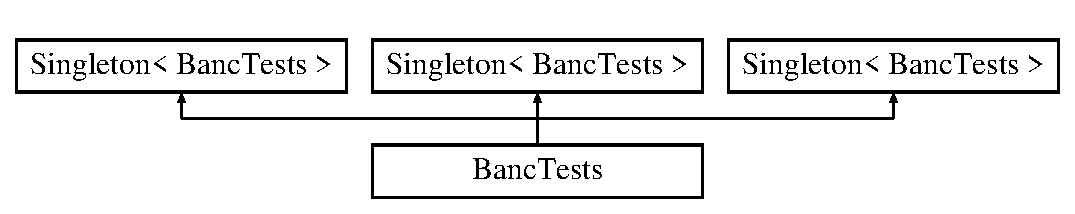
\includegraphics[height=2.000000cm]{class_banc_tests}
\end{center}
\end{figure}
\subsection*{Public Member Functions}
\begin{DoxyCompactItemize}
\item 
bool \hyperlink{group__inf2990_gab5d7fbfe7e3fbe00aa187caa10b1c506}{executer} ()
\begin{DoxyCompactList}\small\item\em Ex�cuter tous les tests unitaires. \end{DoxyCompactList}\end{DoxyCompactItemize}


\subsection{Detailed Description}
Banc de tests qui permet d'ex�cuter tous les tests unitaires. C'est une classe singleton. 

\begin{DoxyAuthor}{Author}
Julien Gascon-\/\-Samson 
\end{DoxyAuthor}
\begin{DoxyDate}{Date}
2011-\/07-\/16 
\end{DoxyDate}


The documentation for this class was generated from the following files\-:\begin{DoxyCompactItemize}
\item 
X\-:/inf2990-\/06/\-Cadriciel/\-Sources/\-D\-L\-L/\-Tests/\hyperlink{_banc_tests_8h}{Banc\-Tests.\-h}\item 
X\-:/inf2990-\/06/\-Cadriciel/\-Sources/\-D\-L\-L/\-Tests/\hyperlink{_banc_tests_8cpp}{Banc\-Tests.\-cpp}\end{DoxyCompactItemize}

\hypertarget{classglm_1_1io_1_1basic__format__saver}{\section{glm\-:\-:io\-:\-:basic\-\_\-format\-\_\-saver$<$ C\-Ty, C\-Tr $>$ Class Template Reference}
\label{classglm_1_1io_1_1basic__format__saver}\index{glm\-::io\-::basic\-\_\-format\-\_\-saver$<$ C\-Ty, C\-Tr $>$@{glm\-::io\-::basic\-\_\-format\-\_\-saver$<$ C\-Ty, C\-Tr $>$}}
}
\subsection*{Public Member Functions}
\begin{DoxyCompactItemize}
\item 
\hypertarget{classglm_1_1io_1_1basic__format__saver_a9688fa6dce0c32285527df2336ca9127}{{\bfseries basic\-\_\-format\-\_\-saver} (std\-::basic\-\_\-ios$<$ C\-Ty, C\-Tr $>$ \&)}\label{classglm_1_1io_1_1basic__format__saver_a9688fa6dce0c32285527df2336ca9127}

\end{DoxyCompactItemize}


The documentation for this class was generated from the following files\-:\begin{DoxyCompactItemize}
\item 
X\-:/\-Git\-\_\-\-Repository/inf2990-\/06/\-Cadriciel/\-Commun/\-Externe/glm/include/glm/gtx/\hyperlink{io_8hpp}{io.\-hpp}\item 
X\-:/\-Git\-\_\-\-Repository/inf2990-\/06/\-Cadriciel/\-Commun/\-Externe/glm/include/glm/gtx/io.\-inl\end{DoxyCompactItemize}

\hypertarget{classglm_1_1io_1_1basic__state__saver}{\section{glm\-:\-:io\-:\-:basic\-\_\-state\-\_\-saver$<$ C\-Ty, C\-Tr $>$ Class Template Reference}
\label{classglm_1_1io_1_1basic__state__saver}\index{glm\-::io\-::basic\-\_\-state\-\_\-saver$<$ C\-Ty, C\-Tr $>$@{glm\-::io\-::basic\-\_\-state\-\_\-saver$<$ C\-Ty, C\-Tr $>$}}
}
\subsection*{Public Member Functions}
\begin{DoxyCompactItemize}
\item 
\hypertarget{classglm_1_1io_1_1basic__state__saver_ab31652b0b7f2a24fa8f9fda2505de356}{{\bfseries basic\-\_\-state\-\_\-saver} (std\-::basic\-\_\-ios$<$ C\-Ty, C\-Tr $>$ \&)}\label{classglm_1_1io_1_1basic__state__saver_ab31652b0b7f2a24fa8f9fda2505de356}

\end{DoxyCompactItemize}


The documentation for this class was generated from the following files\-:\begin{DoxyCompactItemize}
\item 
X\-:/\-Git\-\_\-\-Repository/inf2990-\/06/\-Cadriciel/\-Commun/\-Externe/glm/include/glm/gtx/\hyperlink{io_8hpp}{io.\-hpp}\item 
X\-:/\-Git\-\_\-\-Repository/inf2990-\/06/\-Cadriciel/\-Commun/\-Externe/glm/include/glm/gtx/io.\-inl\end{DoxyCompactItemize}

\hypertarget{struct_b_d_f___property_rec__}{\section{B\-D\-F\-\_\-\-Property\-Rec\-\_\- Struct Reference}
\label{struct_b_d_f___property_rec__}\index{B\-D\-F\-\_\-\-Property\-Rec\-\_\-@{B\-D\-F\-\_\-\-Property\-Rec\-\_\-}}
}
\subsection*{Public Attributes}
\begin{DoxyCompactItemize}
\item 
\hypertarget{struct_b_d_f___property_rec___a88c19ee6f16bd1b36127f5f7d44a4e39}{B\-D\-F\-\_\-\-Property\-Type {\bfseries type}}\label{struct_b_d_f___property_rec___a88c19ee6f16bd1b36127f5f7d44a4e39}

\item 
\hypertarget{struct_b_d_f___property_rec___a7fdd16635fbcfd4f737e6beb2d014871}{\begin{tabbing}
xx\=xx\=xx\=xx\=xx\=xx\=xx\=xx\=xx\=\kill
union \{\\
\hypertarget{union_b_d_f___property_rec___1_1@0_aa8d56dc848d8a2c8e2f7e40a63f5d032}{\>const char $\ast$ {\bfseries atom}\\
\hypertarget{union_b_d_f___property_rec___1_1@0_a71243b414ad203fd7d6d2468c39bbd79}{\>FT\_Int32 {\bfseries integer}\\
\hypertarget{union_b_d_f___property_rec___1_1@0_adaba2e4ce8da90a5ea59080a0521d332}{\>FT\_UInt32 {\bfseries cardinal}\\
\} {\bfseries u}}\label{struct_b_d_f___property_rec___a7fdd16635fbcfd4f737e6beb2d014871}
\\

\end{tabbing}\end{DoxyCompactItemize}


The documentation for this struct was generated from the following file\-:\begin{DoxyCompactItemize}
\item 
X\-:/\-Git\-\_\-\-Repository/inf2990-\/06/\-Cadriciel/\-Commun/\-Externe/\-Free\-Type/include/freetype/ftbdf.\-h\end{DoxyCompactItemize}

\hypertarget{structutilitaire_1_1_boite_englobante}{\section{utilitaire\-:\-:Boite\-Englobante Struct Reference}
\label{structutilitaire_1_1_boite_englobante}\index{utilitaire\-::\-Boite\-Englobante@{utilitaire\-::\-Boite\-Englobante}}
}


Structure contenant les donn�es pour une boite englobante.  




{\ttfamily \#include $<$Utilitaire.\-h$>$}

\subsection*{Public Attributes}
\begin{DoxyCompactItemize}
\item 
\hypertarget{structutilitaire_1_1_boite_englobante_a083f953a1ac5a830f70a2173a092e90a}{\hyperlink{group__core__types_ga7f3287f952e6ccb481231368091702ac}{glm\-::dvec3} {\bfseries coin\-Min}}\label{structutilitaire_1_1_boite_englobante_a083f953a1ac5a830f70a2173a092e90a}

\item 
\hypertarget{structutilitaire_1_1_boite_englobante_af6f6d9ef23f6e5eb9f2f1ed6dd4d3e0e}{\hyperlink{group__core__types_ga7f3287f952e6ccb481231368091702ac}{glm\-::dvec3} {\bfseries coin\-Max}}\label{structutilitaire_1_1_boite_englobante_af6f6d9ef23f6e5eb9f2f1ed6dd4d3e0e}

\end{DoxyCompactItemize}


\subsection{Detailed Description}
Structure contenant les donn�es pour une boite englobante. 

The documentation for this struct was generated from the following file\-:\begin{DoxyCompactItemize}
\item 
X\-:/\-Git\-\_\-\-Repository/inf2990-\/06/\-Cadriciel/\-Commun/\-Utilitaire/\hyperlink{_utilitaire_8h}{Utilitaire.\-h}\end{DoxyCompactItemize}

\hypertarget{struct_boite_englobante}{\section{Boite\-Englobante Struct Reference}
\label{struct_boite_englobante}\index{Boite\-Englobante@{Boite\-Englobante}}
}


Structure contenant les coins pour un carr� englobant.  




{\ttfamily \#include $<$Noeud\-Abstrait.\-h$>$}

\subsection*{Public Attributes}
\begin{DoxyCompactItemize}
\item 
glm\-::dvec3 \hyperlink{struct_boite_englobante_a214a31551756ebc03a8da68833ab983f}{coin\-H\-G}
\item 
glm\-::dvec3 \hyperlink{struct_boite_englobante_a4ef35afbaae389f9d0b88b31c2a7a540}{coin\-B\-G}
\item 
glm\-::dvec3 \hyperlink{struct_boite_englobante_a848980ba2b2e2f81ae237e652601dae0}{coin\-H\-D}
\item 
glm\-::dvec3 \hyperlink{struct_boite_englobante_afdb405698c6d9b313b20188f34e17a65}{coin\-B\-D}
\end{DoxyCompactItemize}


\subsection{Detailed Description}
Structure contenant les coins pour un carr� englobant. 

\subsection{Member Data Documentation}
\hypertarget{struct_boite_englobante_afdb405698c6d9b313b20188f34e17a65}{\index{Boite\-Englobante@{Boite\-Englobante}!coin\-B\-D@{coin\-B\-D}}
\index{coin\-B\-D@{coin\-B\-D}!BoiteEnglobante@{Boite\-Englobante}}
\subsubsection[{coin\-B\-D}]{\setlength{\rightskip}{0pt plus 5cm}glm\-::dvec3 Boite\-Englobante\-::coin\-B\-D}}\label{struct_boite_englobante_afdb405698c6d9b313b20188f34e17a65}
\hypertarget{struct_boite_englobante_a4ef35afbaae389f9d0b88b31c2a7a540}{\index{Boite\-Englobante@{Boite\-Englobante}!coin\-B\-G@{coin\-B\-G}}
\index{coin\-B\-G@{coin\-B\-G}!BoiteEnglobante@{Boite\-Englobante}}
\subsubsection[{coin\-B\-G}]{\setlength{\rightskip}{0pt plus 5cm}glm\-::dvec3 Boite\-Englobante\-::coin\-B\-G}}\label{struct_boite_englobante_a4ef35afbaae389f9d0b88b31c2a7a540}
\hypertarget{struct_boite_englobante_a848980ba2b2e2f81ae237e652601dae0}{\index{Boite\-Englobante@{Boite\-Englobante}!coin\-H\-D@{coin\-H\-D}}
\index{coin\-H\-D@{coin\-H\-D}!BoiteEnglobante@{Boite\-Englobante}}
\subsubsection[{coin\-H\-D}]{\setlength{\rightskip}{0pt plus 5cm}glm\-::dvec3 Boite\-Englobante\-::coin\-H\-D}}\label{struct_boite_englobante_a848980ba2b2e2f81ae237e652601dae0}
\hypertarget{struct_boite_englobante_a214a31551756ebc03a8da68833ab983f}{\index{Boite\-Englobante@{Boite\-Englobante}!coin\-H\-G@{coin\-H\-G}}
\index{coin\-H\-G@{coin\-H\-G}!BoiteEnglobante@{Boite\-Englobante}}
\subsubsection[{coin\-H\-G}]{\setlength{\rightskip}{0pt plus 5cm}glm\-::dvec3 Boite\-Englobante\-::coin\-H\-G}}\label{struct_boite_englobante_a214a31551756ebc03a8da68833ab983f}


The documentation for this struct was generated from the following file\-:\begin{DoxyCompactItemize}
\item 
X\-:/inf2990-\/06/\-Cadriciel/\-Sources/\-D\-L\-L/\-Arbre/\-Noeuds/\hyperlink{_noeud_abstrait_8h}{Noeud\-Abstrait.\-h}\end{DoxyCompactItemize}

\hypertarget{classutilitaire_1_1_boite_environnement}{\section{utilitaire\-:\-:Boite\-Environnement Class Reference}
\label{classutilitaire_1_1_boite_environnement}\index{utilitaire\-::\-Boite\-Environnement@{utilitaire\-::\-Boite\-Environnement}}
}


Classe repr�sentant une bo�te d'environnement (\char`\"{}skybox\char`\"{}).  




{\ttfamily \#include $<$Boite\-Environnement.\-h$>$}

\subsection*{Public Member Functions}
\begin{DoxyCompactItemize}
\item 
\hyperlink{classutilitaire_1_1_boite_environnement_afa2e429fd77f584d9b07e1577b907f7b}{Boite\-Environnement} (const std\-::string \&fichier\-Xpos, const std\-::string \&fichier\-Xneg, const std\-::string \&fichier\-Ypos, const std\-::string \&fichier\-Yneg, const std\-::string \&fichier\-Zpos, const std\-::string \&fichier\-Zneg)
\begin{DoxyCompactList}\small\item\em Constructeur � partir des noms des fichiers d'images de la bo�te. \end{DoxyCompactList}\item 
\hyperlink{classutilitaire_1_1_boite_environnement_accfe35d5a88904e5001653142b985a27}{$\sim$\-Boite\-Environnement} ()
\begin{DoxyCompactList}\small\item\em Destructeur. \end{DoxyCompactList}\item 
void \hyperlink{classutilitaire_1_1_boite_environnement_a41246ea752945870645cfbd5aec673e9}{afficher} (const \hyperlink{group__core__types_ga7f3287f952e6ccb481231368091702ac}{glm\-::dvec3} \&centre, double demi\-Largeur) const 
\begin{DoxyCompactList}\small\item\em Affiche la bo�te d'environnement. \end{DoxyCompactList}\end{DoxyCompactItemize}


\subsection{Detailed Description}
Classe repr�sentant une bo�te d'environnement (\char`\"{}skybox\char`\"{}). 

Elle s'occupe de charger 6 images du cube formant la bo�te. Elle utilise la convention de sens de Cube\-Map\-Gen (de A\-T\-I), lorsque les images sont export�es avec le mapping Open\-G\-L (plut�t que Direct\-X).

\begin{DoxyAuthor}{Author}
Martin Bisson 
\end{DoxyAuthor}
\begin{DoxyDate}{Date}
2007-\/05-\/28 
\end{DoxyDate}


\subsection{Constructor \& Destructor Documentation}
\hypertarget{classutilitaire_1_1_boite_environnement_afa2e429fd77f584d9b07e1577b907f7b}{\index{utilitaire\-::\-Boite\-Environnement@{utilitaire\-::\-Boite\-Environnement}!Boite\-Environnement@{Boite\-Environnement}}
\index{Boite\-Environnement@{Boite\-Environnement}!utilitaire::BoiteEnvironnement@{utilitaire\-::\-Boite\-Environnement}}
\subsubsection[{Boite\-Environnement}]{\setlength{\rightskip}{0pt plus 5cm}utilitaire\-::\-Boite\-Environnement\-::\-Boite\-Environnement (
\begin{DoxyParamCaption}
\item[{const std\-::string \&}]{fichier\-Xpos, }
\item[{const std\-::string \&}]{fichier\-Xneg, }
\item[{const std\-::string \&}]{fichier\-Ypos, }
\item[{const std\-::string \&}]{fichier\-Yneg, }
\item[{const std\-::string \&}]{fichier\-Zpos, }
\item[{const std\-::string \&}]{fichier\-Zneg}
\end{DoxyParamCaption}
)}}\label{classutilitaire_1_1_boite_environnement_afa2e429fd77f584d9b07e1577b907f7b}


Constructeur � partir des noms des fichiers d'images de la bo�te. 

Ce constructeur charge les 6 textures correspondant � chacune des faces de la bo�te d'environnement.


\begin{DoxyParams}[1]{Parameters}
\mbox{\tt in}  & {\em fichier\-Xpos} & \-: Le nom du fichier contenant l'image correspondant � l'axe des X positifs. \\
\hline
\mbox{\tt in}  & {\em fichier\-Xneg} & \-: Le nom du fichier contenant l'image correspondant � l'axe des X n�gatifs. \\
\hline
\mbox{\tt in}  & {\em fichier\-Ypos} & \-: Le nom du fichier contenant l'image correspondant � l'axe des X positifs. \\
\hline
\mbox{\tt in}  & {\em fichier\-Yneg} & \-: Le nom du fichier contenant l'image correspondant � l'axe des Y n�gatifs. \\
\hline
\mbox{\tt in}  & {\em fichier\-Zpos} & \-: Le nom du fichier contenant l'image correspondant � l'axe des Z positifs. \\
\hline
\mbox{\tt in}  & {\em fichier\-Zneg} & \-: Le nom du fichier contenant l'image correspondant � l'axe des Z n�gatifs.\\
\hline
\end{DoxyParams}
\begin{DoxyReturn}{Returns}
Aucune (constructeur). 
\end{DoxyReturn}
\hypertarget{classutilitaire_1_1_boite_environnement_accfe35d5a88904e5001653142b985a27}{\index{utilitaire\-::\-Boite\-Environnement@{utilitaire\-::\-Boite\-Environnement}!$\sim$\-Boite\-Environnement@{$\sim$\-Boite\-Environnement}}
\index{$\sim$\-Boite\-Environnement@{$\sim$\-Boite\-Environnement}!utilitaire::BoiteEnvironnement@{utilitaire\-::\-Boite\-Environnement}}
\subsubsection[{$\sim$\-Boite\-Environnement}]{\setlength{\rightskip}{0pt plus 5cm}utilitaire\-::\-Boite\-Environnement\-::$\sim$\-Boite\-Environnement (
\begin{DoxyParamCaption}
{}
\end{DoxyParamCaption}
)}}\label{classutilitaire_1_1_boite_environnement_accfe35d5a88904e5001653142b985a27}


Destructeur. 

Ce destructeur lib�re l'espace allou�e � chacune des textures des faces de la bo�te d'environnement.

\begin{DoxyReturn}{Returns}
Aucune (destructeur). 
\end{DoxyReturn}


\subsection{Member Function Documentation}
\hypertarget{classutilitaire_1_1_boite_environnement_a41246ea752945870645cfbd5aec673e9}{\index{utilitaire\-::\-Boite\-Environnement@{utilitaire\-::\-Boite\-Environnement}!afficher@{afficher}}
\index{afficher@{afficher}!utilitaire::BoiteEnvironnement@{utilitaire\-::\-Boite\-Environnement}}
\subsubsection[{afficher}]{\setlength{\rightskip}{0pt plus 5cm}void utilitaire\-::\-Boite\-Environnement\-::afficher (
\begin{DoxyParamCaption}
\item[{const {\bf glm\-::dvec3} \&}]{centre, }
\item[{double}]{demi\-Largeur}
\end{DoxyParamCaption}
) const}}\label{classutilitaire_1_1_boite_environnement_a41246ea752945870645cfbd5aec673e9}


Affiche la bo�te d'environnement. 

Cette fonction affiche tout simplement la bo�te d'environnement.


\begin{DoxyParams}[1]{Parameters}
\mbox{\tt in}  & {\em centre} & \-: La position du centre de la bo�te pour l'affichage. \\
\hline
\mbox{\tt in}  & {\em demi\-Largeur} & \-: La largeur de la moiti� de la bo�te pour l'affichage.\\
\hline
\end{DoxyParams}
\begin{DoxyReturn}{Returns}
Aucune. 
\end{DoxyReturn}


The documentation for this class was generated from the following files\-:\begin{DoxyCompactItemize}
\item 
X\-:/\-Git\-\_\-\-Repository/inf2990-\/06/\-Cadriciel/\-Commun/\-Utilitaire/\-Open\-G\-L/\hyperlink{_boite_environnement_8h}{Boite\-Environnement.\-h}\item 
X\-:/\-Git\-\_\-\-Repository/inf2990-\/06/\-Cadriciel/\-Commun/\-Utilitaire/\-Open\-G\-L/\hyperlink{_boite_environnement_8cpp}{Boite\-Environnement.\-cpp}\end{DoxyCompactItemize}

\hypertarget{class_brief_test_progress_listener}{\section{Brief\-Test\-Progress\-Listener Class Reference}
\label{class_brief_test_progress_listener}\index{Brief\-Test\-Progress\-Listener@{Brief\-Test\-Progress\-Listener}}
}


\hyperlink{class_test_listener}{Test\-Listener} that prints the name of each test before running it.  




{\ttfamily \#include $<$Brief\-Test\-Progress\-Listener.\-h$>$}

Inheritance diagram for Brief\-Test\-Progress\-Listener\-:\begin{figure}[H]
\begin{center}
\leavevmode
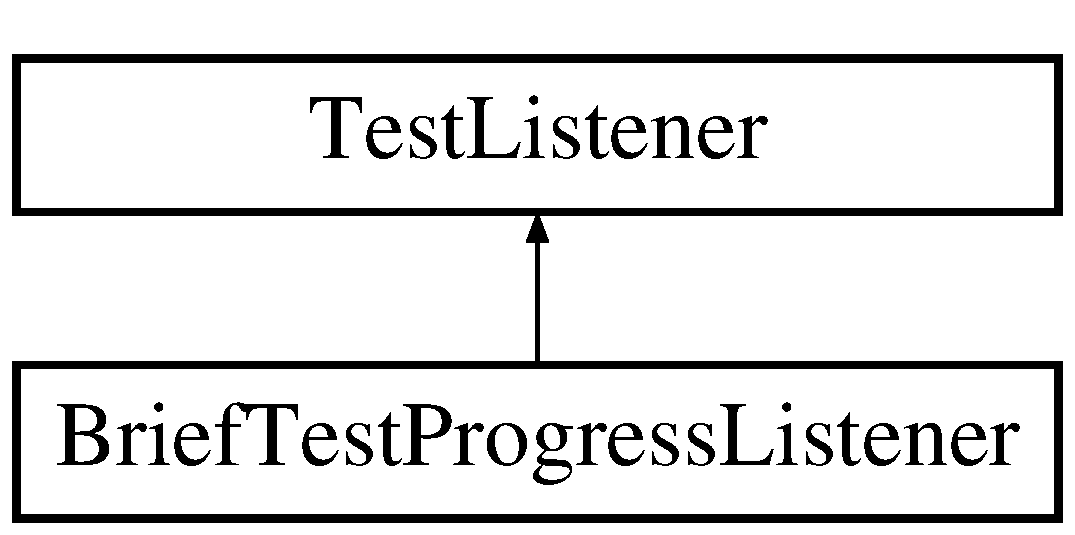
\includegraphics[height=2.000000cm]{class_brief_test_progress_listener}
\end{center}
\end{figure}
\subsection*{Public Member Functions}
\begin{DoxyCompactItemize}
\item 
\hyperlink{class_brief_test_progress_listener_a7af12547b437fcddab52e7b0f0d47782}{Brief\-Test\-Progress\-Listener} ()
\item 
\hypertarget{class_brief_test_progress_listener_a9e1cf4460bdb460e14009d1629454881}{virtual \hyperlink{class_brief_test_progress_listener_a9e1cf4460bdb460e14009d1629454881}{$\sim$\-Brief\-Test\-Progress\-Listener} ()}\label{class_brief_test_progress_listener_a9e1cf4460bdb460e14009d1629454881}

\begin{DoxyCompactList}\small\item\em Destructor. \end{DoxyCompactList}\item 
\hypertarget{class_brief_test_progress_listener_ab4196e15752bb2be443e72418500e20e}{void \hyperlink{class_brief_test_progress_listener_ab4196e15752bb2be443e72418500e20e}{start\-Test} (\hyperlink{class_test}{Test} $\ast$test)}\label{class_brief_test_progress_listener_ab4196e15752bb2be443e72418500e20e}

\begin{DoxyCompactList}\small\item\em Called when just before a \hyperlink{class_test_case}{Test\-Case} is run. \end{DoxyCompactList}\item 
void \hyperlink{class_brief_test_progress_listener_a21f8658a9c19c67220241656cfad30ce}{add\-Failure} (const \hyperlink{class_test_failure}{Test\-Failure} \&failure)
\begin{DoxyCompactList}\small\item\em Called when a failure occurs while running a test. \end{DoxyCompactList}\item 
\hypertarget{class_brief_test_progress_listener_a49cbd9152ea35a21f6525773660ee119}{void \hyperlink{class_brief_test_progress_listener_a49cbd9152ea35a21f6525773660ee119}{end\-Test} (\hyperlink{class_test}{Test} $\ast$test)}\label{class_brief_test_progress_listener_a49cbd9152ea35a21f6525773660ee119}

\begin{DoxyCompactList}\small\item\em Called just after a \hyperlink{class_test_case}{Test\-Case} was run (even if a failure occured). \end{DoxyCompactList}\end{DoxyCompactItemize}


\subsection{Detailed Description}
\hyperlink{class_test_listener}{Test\-Listener} that prints the name of each test before running it. 

\subsection{Constructor \& Destructor Documentation}
\hypertarget{class_brief_test_progress_listener_a7af12547b437fcddab52e7b0f0d47782}{\index{Brief\-Test\-Progress\-Listener@{Brief\-Test\-Progress\-Listener}!Brief\-Test\-Progress\-Listener@{Brief\-Test\-Progress\-Listener}}
\index{Brief\-Test\-Progress\-Listener@{Brief\-Test\-Progress\-Listener}!BriefTestProgressListener@{Brief\-Test\-Progress\-Listener}}
\subsubsection[{Brief\-Test\-Progress\-Listener}]{\setlength{\rightskip}{0pt plus 5cm}Brief\-Test\-Progress\-Listener\-::\-Brief\-Test\-Progress\-Listener (
\begin{DoxyParamCaption}
{}
\end{DoxyParamCaption}
)}}\label{class_brief_test_progress_listener_a7af12547b437fcddab52e7b0f0d47782}
Constructs a \hyperlink{class_brief_test_progress_listener}{Brief\-Test\-Progress\-Listener} object. 

\subsection{Member Function Documentation}
\hypertarget{class_brief_test_progress_listener_a21f8658a9c19c67220241656cfad30ce}{\index{Brief\-Test\-Progress\-Listener@{Brief\-Test\-Progress\-Listener}!add\-Failure@{add\-Failure}}
\index{add\-Failure@{add\-Failure}!BriefTestProgressListener@{Brief\-Test\-Progress\-Listener}}
\subsubsection[{add\-Failure}]{\setlength{\rightskip}{0pt plus 5cm}void Brief\-Test\-Progress\-Listener\-::add\-Failure (
\begin{DoxyParamCaption}
\item[{const {\bf Test\-Failure} \&}]{}
\end{DoxyParamCaption}
)\hspace{0.3cm}{\ttfamily [virtual]}}}\label{class_brief_test_progress_listener_a21f8658a9c19c67220241656cfad30ce}


Called when a failure occurs while running a test. 

\begin{DoxySeeAlso}{See Also}
\hyperlink{class_test_failure}{Test\-Failure}. 
\end{DoxySeeAlso}
\begin{DoxyWarning}{Warning}
{\itshape failure} is a temporary object that is destroyed after the method call. Use Test\-Failure\-::clone() to create a duplicate. 
\end{DoxyWarning}


Reimplemented from \hyperlink{class_test_listener_a103216a5814c907f7b752b969477e765}{Test\-Listener}.



The documentation for this class was generated from the following file\-:\begin{DoxyCompactItemize}
\item 
X\-:/\-Git\-\_\-\-Repository/inf2990-\/06/\-Cadriciel/\-Commun/\-Externe/cppunit/include/cppunit/Brief\-Test\-Progress\-Listener.\-h\end{DoxyCompactItemize}

\hypertarget{classvue_1_1_camera}{\section{vue\-:\-:Camera Class Reference}
\label{classvue_1_1_camera}\index{vue\-::\-Camera@{vue\-::\-Camera}}
}


Classe repr�sentant une cam�ra dans le monde en 3\-D.  




{\ttfamily \#include $<$Camera.\-h$>$}

\subsection*{Public Member Functions}
\begin{DoxyCompactItemize}
\item 
\hyperlink{classvue_1_1_camera_a0c7869e1153f216e88fc15eb5ac37ce4}{Camera} (const \hyperlink{group__core__types_ga7f3287f952e6ccb481231368091702ac}{glm\-::dvec3} \&position, const \hyperlink{group__core__types_ga7f3287f952e6ccb481231368091702ac}{glm\-::dvec3} \&point\-Vise, const \hyperlink{group__core__types_ga7f3287f952e6ccb481231368091702ac}{glm\-::dvec3} \&direction\-Haut\-Camera, const \hyperlink{group__core__types_ga7f3287f952e6ccb481231368091702ac}{glm\-::dvec3} \&direction\-Haut\-Monde)
\begin{DoxyCompactList}\small\item\em Constructeur � partir des coordonn�es cart�siennes. \end{DoxyCompactList}\item 
\hypertarget{classvue_1_1_camera_a173cf3a9d91b30cadd21d72149df4504}{virtual \hyperlink{classvue_1_1_camera_a173cf3a9d91b30cadd21d72149df4504}{$\sim$\-Camera} ()}\label{classvue_1_1_camera_a173cf3a9d91b30cadd21d72149df4504}

\begin{DoxyCompactList}\small\item\em Destructeur virtuel vide. \end{DoxyCompactList}\item 
void \hyperlink{classvue_1_1_camera_a452efa2c96225b1207cc9ac74be0bda5}{assigner\-Position} (const \hyperlink{group__core__types_ga7f3287f952e6ccb481231368091702ac}{glm\-::dvec3} \&position)
\begin{DoxyCompactList}\small\item\em Assigner la position de la cam�ra. \end{DoxyCompactList}\item 
void \hyperlink{classvue_1_1_camera_a0b9982453adc3afc38f9198ab8b1dd2a}{assigner\-Point\-Vise} (const \hyperlink{group__core__types_ga7f3287f952e6ccb481231368091702ac}{glm\-::dvec3} \&point\-Vise)
\begin{DoxyCompactList}\small\item\em Assigner le point vis� de la cam�ra. \end{DoxyCompactList}\item 
void \hyperlink{classvue_1_1_camera_a94afd2172d111edacc248522f201fd32}{assigner\-Direction\-Haut} (const \hyperlink{group__core__types_ga7f3287f952e6ccb481231368091702ac}{glm\-::dvec3} \&direction\-Haut)
\begin{DoxyCompactList}\small\item\em Assigner la direction du haut de la cam�ra. \end{DoxyCompactList}\item 
const \hyperlink{group__core__types_ga7f3287f952e6ccb481231368091702ac}{glm\-::dvec3} \& \hyperlink{classvue_1_1_camera_aca05463d00f938ceb637b49eaf25f330}{obtenir\-Position} () const 
\begin{DoxyCompactList}\small\item\em Obtenir la position de la cam�ra. \end{DoxyCompactList}\item 
const \hyperlink{group__core__types_ga7f3287f952e6ccb481231368091702ac}{glm\-::dvec3} \& \hyperlink{classvue_1_1_camera_a20cab3b4e97dbe681dc9532e459bbf08}{obtenir\-Point\-Vise} () const 
\begin{DoxyCompactList}\small\item\em Obtenir le point vis� de la cam�ra. \end{DoxyCompactList}\item 
const \hyperlink{group__core__types_ga7f3287f952e6ccb481231368091702ac}{glm\-::dvec3} \& \hyperlink{classvue_1_1_camera_a51913d2a228cb4b90bb5eb72a4a15970}{obtenir\-Direction\-Haut} () const 
\begin{DoxyCompactList}\small\item\em Obtenir la direction du haut de la cam�ra. \end{DoxyCompactList}\item 
void \hyperlink{classvue_1_1_camera_aa08801e436ddf90400e632e402183618}{deplacer\-X\-Y} (double deplacement\-X, double deplacement\-Y)
\begin{DoxyCompactList}\small\item\em D�placement dans le plan perpendiculaire � la direction vis�e. \end{DoxyCompactList}\item 
void \hyperlink{classvue_1_1_camera_a7e8dfbbf743a74bb0387e140fee09474}{deplacer\-Z} (double deplacement, bool bouge\-Point\-Vise)
\begin{DoxyCompactList}\small\item\em D�placement dans l'axe de la direction vis�e. \end{DoxyCompactList}\item 
void \hyperlink{classvue_1_1_camera_a07795ebc629c68f8694b9ae08a53457f}{tourner\-X\-Y} (double rotation\-X, double rotation\-Y, bool empeche\-Inversion=true)
\begin{DoxyCompactList}\small\item\em Rotation de la cam�ra autour de sa position. \end{DoxyCompactList}\item 
void \hyperlink{classvue_1_1_camera_a5e88216d5d5b31e0e65be9674e5904ef}{orbiter\-X\-Y} (double rotation\-X, double rotation\-Y, bool empeche\-Inversion=true)
\begin{DoxyCompactList}\small\item\em Rotation de la position de la cam�ra autour de son point de vis�. \end{DoxyCompactList}\item 
void \hyperlink{classvue_1_1_camera_a201db90bcebf204990f1dbb6db03b563}{positionner} () const 
\begin{DoxyCompactList}\small\item\em Positionner la cam�ra (appel � glu\-Look\-At). \end{DoxyCompactList}\end{DoxyCompactItemize}


\subsection{Detailed Description}
Classe repr�sentant une cam�ra dans le monde en 3\-D. 

Cette camera encapsule les diff�rentes op�rations qu'il est possible de faire pour d�placer le point de vue de l'observateur � l'int�rieur de la sc�ne en 3\-D.

\begin{DoxyAuthor}{Author}
Martin Bisson 
\end{DoxyAuthor}
\begin{DoxyDate}{Date}
2006-\/12-\/15 
\end{DoxyDate}


\subsection{Constructor \& Destructor Documentation}
\hypertarget{classvue_1_1_camera_a0c7869e1153f216e88fc15eb5ac37ce4}{\index{vue\-::\-Camera@{vue\-::\-Camera}!Camera@{Camera}}
\index{Camera@{Camera}!vue::Camera@{vue\-::\-Camera}}
\subsubsection[{Camera}]{\setlength{\rightskip}{0pt plus 5cm}vue\-::\-Camera\-::\-Camera (
\begin{DoxyParamCaption}
\item[{const {\bf glm\-::dvec3} \&}]{position, }
\item[{const {\bf glm\-::dvec3} \&}]{point\-Vise, }
\item[{const {\bf glm\-::dvec3} \&}]{direction\-Haut\-Camera, }
\item[{const {\bf glm\-::dvec3} \&}]{direction\-Haut\-Monde}
\end{DoxyParamCaption}
)}}\label{classvue_1_1_camera_a0c7869e1153f216e88fc15eb5ac37ce4}


Constructeur � partir des coordonn�es cart�siennes. 

Constructeur de la cam�ra � partir des coordonn�es cart�siennes.


\begin{DoxyParams}[1]{Parameters}
\mbox{\tt in}  & {\em position} & \-: position de la cam�ra. \\
\hline
\mbox{\tt in}  & {\em point\-Vise} & \-: point vis�. \\
\hline
\mbox{\tt in}  & {\em direction\-Haut\-Camera} & \-: direction du haut de la cam�ra. \\
\hline
\mbox{\tt in}  & {\em direction\-Haut\-Monde} & \-: direction du haut du monde de la cam�ra.\\
\hline
\end{DoxyParams}
\begin{DoxyReturn}{Returns}
Aucune (constructeur). 
\end{DoxyReturn}


\subsection{Member Function Documentation}
\hypertarget{classvue_1_1_camera_a94afd2172d111edacc248522f201fd32}{\index{vue\-::\-Camera@{vue\-::\-Camera}!assigner\-Direction\-Haut@{assigner\-Direction\-Haut}}
\index{assigner\-Direction\-Haut@{assigner\-Direction\-Haut}!vue::Camera@{vue\-::\-Camera}}
\subsubsection[{assigner\-Direction\-Haut}]{\setlength{\rightskip}{0pt plus 5cm}void vue\-::\-Camera\-::assigner\-Direction\-Haut (
\begin{DoxyParamCaption}
\item[{const {\bf glm\-::dvec3} \&}]{direction\-Haut}
\end{DoxyParamCaption}
)\hspace{0.3cm}{\ttfamily [inline]}}}\label{classvue_1_1_camera_a94afd2172d111edacc248522f201fd32}


Assigner la direction du haut de la cam�ra. 

Cette fonction permet d'assigner la direction du haut de la cam�ra.


\begin{DoxyParams}[1]{Parameters}
\mbox{\tt in}  & {\em direction\-Haut} & \-: La nouvelle direction du haut de la cam�ra.\\
\hline
\end{DoxyParams}
\begin{DoxyReturn}{Returns}
Aucune. 
\end{DoxyReturn}
\hypertarget{classvue_1_1_camera_a0b9982453adc3afc38f9198ab8b1dd2a}{\index{vue\-::\-Camera@{vue\-::\-Camera}!assigner\-Point\-Vise@{assigner\-Point\-Vise}}
\index{assigner\-Point\-Vise@{assigner\-Point\-Vise}!vue::Camera@{vue\-::\-Camera}}
\subsubsection[{assigner\-Point\-Vise}]{\setlength{\rightskip}{0pt plus 5cm}void vue\-::\-Camera\-::assigner\-Point\-Vise (
\begin{DoxyParamCaption}
\item[{const {\bf glm\-::dvec3} \&}]{point\-Vise}
\end{DoxyParamCaption}
)\hspace{0.3cm}{\ttfamily [inline]}}}\label{classvue_1_1_camera_a0b9982453adc3afc38f9198ab8b1dd2a}


Assigner le point vis� de la cam�ra. 

Cette fonction permet d'assigner le point de vis� de la cam�ra.


\begin{DoxyParams}[1]{Parameters}
\mbox{\tt in}  & {\em point\-Vise} & \-: Le nouveau point de vis� de la cam�ra.\\
\hline
\end{DoxyParams}
\begin{DoxyReturn}{Returns}
Aucune. 
\end{DoxyReturn}
\hypertarget{classvue_1_1_camera_a452efa2c96225b1207cc9ac74be0bda5}{\index{vue\-::\-Camera@{vue\-::\-Camera}!assigner\-Position@{assigner\-Position}}
\index{assigner\-Position@{assigner\-Position}!vue::Camera@{vue\-::\-Camera}}
\subsubsection[{assigner\-Position}]{\setlength{\rightskip}{0pt plus 5cm}void vue\-::\-Camera\-::assigner\-Position (
\begin{DoxyParamCaption}
\item[{const {\bf glm\-::dvec3} \&}]{position}
\end{DoxyParamCaption}
)\hspace{0.3cm}{\ttfamily [inline]}}}\label{classvue_1_1_camera_a452efa2c96225b1207cc9ac74be0bda5}


Assigner la position de la cam�ra. 

Cette fonction permet d'assigner la position de la cam�ra.


\begin{DoxyParams}[1]{Parameters}
\mbox{\tt in}  & {\em position} & \-: La nouvelle position de la cam�ra.\\
\hline
\end{DoxyParams}
\begin{DoxyReturn}{Returns}
Aucune. 
\end{DoxyReturn}
\hypertarget{classvue_1_1_camera_aa08801e436ddf90400e632e402183618}{\index{vue\-::\-Camera@{vue\-::\-Camera}!deplacer\-X\-Y@{deplacer\-X\-Y}}
\index{deplacer\-X\-Y@{deplacer\-X\-Y}!vue::Camera@{vue\-::\-Camera}}
\subsubsection[{deplacer\-X\-Y}]{\setlength{\rightskip}{0pt plus 5cm}void vue\-::\-Camera\-::deplacer\-X\-Y (
\begin{DoxyParamCaption}
\item[{double}]{deplacement\-X, }
\item[{double}]{deplacement\-Y}
\end{DoxyParamCaption}
)}}\label{classvue_1_1_camera_aa08801e436ddf90400e632e402183618}


D�placement dans le plan perpendiculaire � la direction vis�e. 

D�place la cam�ra dans le plan perpendiculaire � la direction vis�e


\begin{DoxyParams}[1]{Parameters}
\mbox{\tt in}  & {\em deplacement\-X} & \-: D�placement sur l'axe horizontal du plan de la cam�ra. \\
\hline
\mbox{\tt in}  & {\em deplacement\-Y} & \-: D�placement sur l'axe vertical du plan de la cam�ra.\\
\hline
\end{DoxyParams}
\begin{DoxyReturn}{Returns}
Aucune. 
\end{DoxyReturn}
\hypertarget{classvue_1_1_camera_a7e8dfbbf743a74bb0387e140fee09474}{\index{vue\-::\-Camera@{vue\-::\-Camera}!deplacer\-Z@{deplacer\-Z}}
\index{deplacer\-Z@{deplacer\-Z}!vue::Camera@{vue\-::\-Camera}}
\subsubsection[{deplacer\-Z}]{\setlength{\rightskip}{0pt plus 5cm}void vue\-::\-Camera\-::deplacer\-Z (
\begin{DoxyParamCaption}
\item[{double}]{deplacement, }
\item[{bool}]{bouge\-Point\-Vise}
\end{DoxyParamCaption}
)}}\label{classvue_1_1_camera_a7e8dfbbf743a74bb0387e140fee09474}


D�placement dans l'axe de la direction vis�e. 

D�place la cam�ra dans l'axe de la direction vis�e.


\begin{DoxyParams}[1]{Parameters}
\mbox{\tt in}  & {\em deplacement} & \-: D�placement sur l'axe de la direction vis�e \\
\hline
\mbox{\tt in}  & {\em bouge\-Point\-Vise} & \-: Si vrai, le point de vis� est �galement d�plac�.\\
\hline
\end{DoxyParams}
\begin{DoxyReturn}{Returns}
Aucune. 
\end{DoxyReturn}
\hypertarget{classvue_1_1_camera_a51913d2a228cb4b90bb5eb72a4a15970}{\index{vue\-::\-Camera@{vue\-::\-Camera}!obtenir\-Direction\-Haut@{obtenir\-Direction\-Haut}}
\index{obtenir\-Direction\-Haut@{obtenir\-Direction\-Haut}!vue::Camera@{vue\-::\-Camera}}
\subsubsection[{obtenir\-Direction\-Haut}]{\setlength{\rightskip}{0pt plus 5cm}const {\bf glm\-::dvec3} \& vue\-::\-Camera\-::obtenir\-Direction\-Haut (
\begin{DoxyParamCaption}
{}
\end{DoxyParamCaption}
) const\hspace{0.3cm}{\ttfamily [inline]}}}\label{classvue_1_1_camera_a51913d2a228cb4b90bb5eb72a4a15970}


Obtenir la direction du haut de la cam�ra. 

Cette fonction permet d'obtenir la direction du haut de la cam�ra.

\begin{DoxyReturn}{Returns}
La direction du haut de la cam�ra. 
\end{DoxyReturn}
\hypertarget{classvue_1_1_camera_a20cab3b4e97dbe681dc9532e459bbf08}{\index{vue\-::\-Camera@{vue\-::\-Camera}!obtenir\-Point\-Vise@{obtenir\-Point\-Vise}}
\index{obtenir\-Point\-Vise@{obtenir\-Point\-Vise}!vue::Camera@{vue\-::\-Camera}}
\subsubsection[{obtenir\-Point\-Vise}]{\setlength{\rightskip}{0pt plus 5cm}const {\bf glm\-::dvec3} \& vue\-::\-Camera\-::obtenir\-Point\-Vise (
\begin{DoxyParamCaption}
{}
\end{DoxyParamCaption}
) const\hspace{0.3cm}{\ttfamily [inline]}}}\label{classvue_1_1_camera_a20cab3b4e97dbe681dc9532e459bbf08}


Obtenir le point vis� de la cam�ra. 

Cette fonction permet d'obtenir le point de vis� de la cam�ra.

\begin{DoxyReturn}{Returns}
Le point de vis� de la cam�ra. 
\end{DoxyReturn}
\hypertarget{classvue_1_1_camera_aca05463d00f938ceb637b49eaf25f330}{\index{vue\-::\-Camera@{vue\-::\-Camera}!obtenir\-Position@{obtenir\-Position}}
\index{obtenir\-Position@{obtenir\-Position}!vue::Camera@{vue\-::\-Camera}}
\subsubsection[{obtenir\-Position}]{\setlength{\rightskip}{0pt plus 5cm}const {\bf glm\-::dvec3} \& vue\-::\-Camera\-::obtenir\-Position (
\begin{DoxyParamCaption}
{}
\end{DoxyParamCaption}
) const\hspace{0.3cm}{\ttfamily [inline]}}}\label{classvue_1_1_camera_aca05463d00f938ceb637b49eaf25f330}


Obtenir la position de la cam�ra. 

Cette fonction permet d'obtenir la position de la cam�ra.

\begin{DoxyReturn}{Returns}
La position de la cam�ra. 
\end{DoxyReturn}
\hypertarget{classvue_1_1_camera_a5e88216d5d5b31e0e65be9674e5904ef}{\index{vue\-::\-Camera@{vue\-::\-Camera}!orbiter\-X\-Y@{orbiter\-X\-Y}}
\index{orbiter\-X\-Y@{orbiter\-X\-Y}!vue::Camera@{vue\-::\-Camera}}
\subsubsection[{orbiter\-X\-Y}]{\setlength{\rightskip}{0pt plus 5cm}void vue\-::\-Camera\-::orbiter\-X\-Y (
\begin{DoxyParamCaption}
\item[{double}]{rotation\-X, }
\item[{double}]{rotation\-Y, }
\item[{bool}]{empeche\-Inversion = {\ttfamily true}}
\end{DoxyParamCaption}
)}}\label{classvue_1_1_camera_a5e88216d5d5b31e0e65be9674e5904ef}


Rotation de la position de la cam�ra autour de son point de vis�. 

Rotation de la cam�ra autour de son point de vis� (et donc d�placement de la position en gardant le point de vis� fixe.


\begin{DoxyParams}[1]{Parameters}
\mbox{\tt in}  & {\em rotation\-X} & \-: Modification de l'angle de rotation de la position par rapport au point de vis�. \\
\hline
\mbox{\tt in}  & {\em rotation\-Y} & \-: Modification de l'angle d'�l�vation de la position par rapport au point de vis�. \\
\hline
\mbox{\tt in}  & {\em empeche\-Inversion} & \-: Si vrai, la rotation n'est pas effectu� si elle am�nerait une inversion de la cam�ra.\\
\hline
\end{DoxyParams}
\begin{DoxyReturn}{Returns}
Aucune. 
\end{DoxyReturn}
\hypertarget{classvue_1_1_camera_a201db90bcebf204990f1dbb6db03b563}{\index{vue\-::\-Camera@{vue\-::\-Camera}!positionner@{positionner}}
\index{positionner@{positionner}!vue::Camera@{vue\-::\-Camera}}
\subsubsection[{positionner}]{\setlength{\rightskip}{0pt plus 5cm}void vue\-::\-Camera\-::positionner (
\begin{DoxyParamCaption}
{}
\end{DoxyParamCaption}
) const}}\label{classvue_1_1_camera_a201db90bcebf204990f1dbb6db03b563}


Positionner la cam�ra (appel � glu\-Look\-At). 

Positionne la cam�ra dans la sc�ne � l'aide de glu\-Look\-At().

\begin{DoxyReturn}{Returns}
Aucune. 
\end{DoxyReturn}
\hypertarget{classvue_1_1_camera_a07795ebc629c68f8694b9ae08a53457f}{\index{vue\-::\-Camera@{vue\-::\-Camera}!tourner\-X\-Y@{tourner\-X\-Y}}
\index{tourner\-X\-Y@{tourner\-X\-Y}!vue::Camera@{vue\-::\-Camera}}
\subsubsection[{tourner\-X\-Y}]{\setlength{\rightskip}{0pt plus 5cm}void vue\-::\-Camera\-::tourner\-X\-Y (
\begin{DoxyParamCaption}
\item[{double}]{rotation\-X, }
\item[{double}]{rotation\-Y, }
\item[{bool}]{empeche\-Inversion = {\ttfamily true}}
\end{DoxyParamCaption}
)}}\label{classvue_1_1_camera_a07795ebc629c68f8694b9ae08a53457f}


Rotation de la cam�ra autour de sa position. 

Rotation de la cam�ra autour de sa position (et donc d�placement du point vis� en gardant la position fixe.


\begin{DoxyParams}[1]{Parameters}
\mbox{\tt in}  & {\em rotation\-X} & \-: Modification de l'angle de rotation du point vis� par rapport � la position. \\
\hline
\mbox{\tt in}  & {\em rotation\-Y} & \-: Modification de l'angle d'�l�vation du point vis� par rapport � la position. \\
\hline
\mbox{\tt in}  & {\em empeche\-Inversion} & \-: Si vrai, la rotation n'est pas effectu�e si elle am�nerait une inversion de la cam�ra.\\
\hline
\end{DoxyParams}
\begin{DoxyReturn}{Returns}
Aucune. 
\end{DoxyReturn}


The documentation for this class was generated from the following files\-:\begin{DoxyCompactItemize}
\item 
X\-:/\-Git\-\_\-\-Repository/inf2990-\/06/\-Cadriciel/\-Commun/\-Utilitaire/\-Vue/Camera.\-h\item 
X\-:/\-Git\-\_\-\-Repository/inf2990-\/06/\-Cadriciel/\-Commun/\-Utilitaire/\-Vue/\hyperlink{_camera_8cpp}{Camera.\-cpp}\end{DoxyCompactItemize}

\hypertarget{class_c_ecriture_fichier_binaire}{\section{C\-Ecriture\-Fichier\-Binaire Class Reference}
\label{class_c_ecriture_fichier_binaire}\index{C\-Ecriture\-Fichier\-Binaire@{C\-Ecriture\-Fichier\-Binaire}}
}


Cette classe contient des m�thodes $<$ permettant d'�crire dans un fichier binaire des variables string, double, float, int, unsigned int, char, bool.  




{\ttfamily \#include $<$C\-Ecriture\-Fichier\-Binaire.\-h$>$}

Inheritance diagram for C\-Ecriture\-Fichier\-Binaire\-:\begin{figure}[H]
\begin{center}
\leavevmode
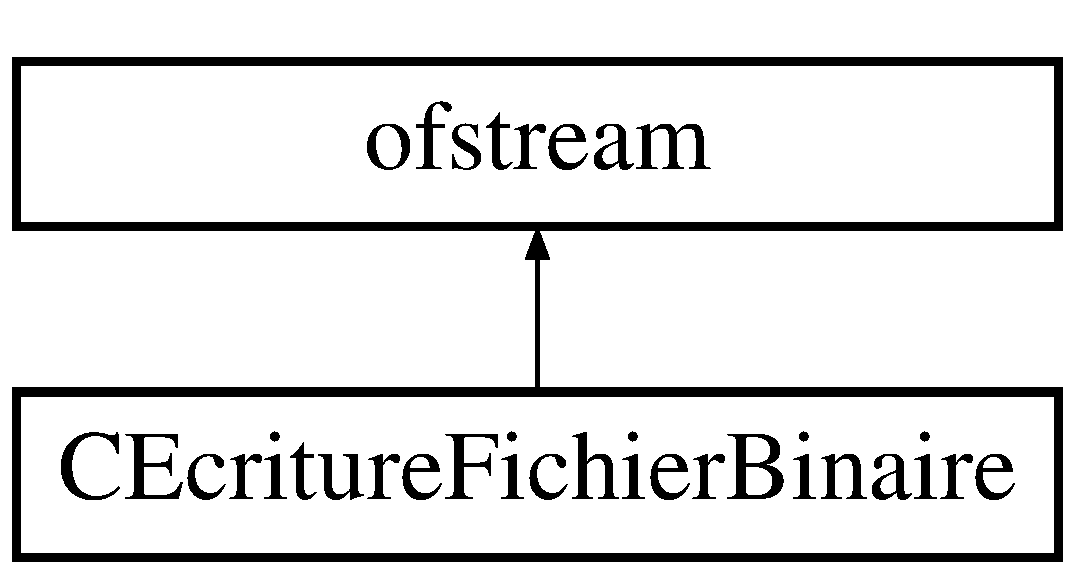
\includegraphics[height=2.000000cm]{class_c_ecriture_fichier_binaire}
\end{center}
\end{figure}
\subsection*{Public Member Functions}
\begin{DoxyCompactItemize}
\item 
\hyperlink{group__utilitaire_ga5b5846202001fecd71cd2a0afbbdb494}{C\-Ecriture\-Fichier\-Binaire} ()
\begin{DoxyCompactList}\small\item\em Constructeur par d�faut. \end{DoxyCompactList}\item 
\hyperlink{group__utilitaire_gad19b9753aa12a9f25fd0febc3c899024}{C\-Ecriture\-Fichier\-Binaire} (const char $\ast$nom\-Fichier, openmode mode=std\-::ios\-::out$\vert$std\-::ios\-::binary)
\begin{DoxyCompactList}\small\item\em Constructeur par param�tre. \end{DoxyCompactList}\item 
void \hyperlink{group__utilitaire_ga7145545254c30909311d3b1ef0bdd07a}{null} (int n)
\begin{DoxyCompactList}\small\item\em Fonction pour ins�rer des caract�res vides dans le fichier. \end{DoxyCompactList}\end{DoxyCompactItemize}
\subsection*{Friends}
\begin{DoxyCompactItemize}
\item 
\hypertarget{class_c_ecriture_fichier_binaire_a2c88c30ff08c7d9035596e0187d44e45}{\hyperlink{class_c_ecriture_fichier_binaire}{C\-Ecriture\-Fichier\-Binaire} \& \hyperlink{class_c_ecriture_fichier_binaire_a2c88c30ff08c7d9035596e0187d44e45}{operator$<$} (\hyperlink{class_c_ecriture_fichier_binaire}{C\-Ecriture\-Fichier\-Binaire} \&out, const std\-::string \&s)}\label{class_c_ecriture_fichier_binaire_a2c88c30ff08c7d9035596e0187d44e45}

\begin{DoxyCompactList}\small\item\em Surcharge de l'op�rateur pour le type {\itshape std\-::string}. \end{DoxyCompactList}\item 
\hypertarget{class_c_ecriture_fichier_binaire_afcaa555d19b37490df9fda731cf8cb19}{\hyperlink{class_c_ecriture_fichier_binaire}{C\-Ecriture\-Fichier\-Binaire} \& \hyperlink{class_c_ecriture_fichier_binaire_afcaa555d19b37490df9fda731cf8cb19}{operator$<$} (\hyperlink{class_c_ecriture_fichier_binaire}{C\-Ecriture\-Fichier\-Binaire} \&out, const double \&x)}\label{class_c_ecriture_fichier_binaire_afcaa555d19b37490df9fda731cf8cb19}

\begin{DoxyCompactList}\small\item\em Surcharge de l'op�rateur pour le type {\itshape double}. \end{DoxyCompactList}\item 
\hypertarget{class_c_ecriture_fichier_binaire_a68e43a125ee6c25828485dfb7270fdea}{\hyperlink{class_c_ecriture_fichier_binaire}{C\-Ecriture\-Fichier\-Binaire} \& \hyperlink{class_c_ecriture_fichier_binaire_a68e43a125ee6c25828485dfb7270fdea}{operator$<$} (\hyperlink{class_c_ecriture_fichier_binaire}{C\-Ecriture\-Fichier\-Binaire} \&out, const float \&x)}\label{class_c_ecriture_fichier_binaire_a68e43a125ee6c25828485dfb7270fdea}

\begin{DoxyCompactList}\small\item\em Surcharge de l'op�rateur pour le type {\itshape float}. \end{DoxyCompactList}\item 
\hypertarget{class_c_ecriture_fichier_binaire_a57ac55aefec2f3dd683cef75c409944b}{\hyperlink{class_c_ecriture_fichier_binaire}{C\-Ecriture\-Fichier\-Binaire} \& \hyperlink{class_c_ecriture_fichier_binaire_a57ac55aefec2f3dd683cef75c409944b}{operator$<$} (\hyperlink{class_c_ecriture_fichier_binaire}{C\-Ecriture\-Fichier\-Binaire} \&out, const int \&x)}\label{class_c_ecriture_fichier_binaire_a57ac55aefec2f3dd683cef75c409944b}

\begin{DoxyCompactList}\small\item\em Surcharge de l'op�rateur pour le type {\itshape int}. \end{DoxyCompactList}\item 
\hypertarget{class_c_ecriture_fichier_binaire_a38d0f050dcc8a79522b0fb9b9c591f72}{\hyperlink{class_c_ecriture_fichier_binaire}{C\-Ecriture\-Fichier\-Binaire} \& \hyperlink{class_c_ecriture_fichier_binaire_a38d0f050dcc8a79522b0fb9b9c591f72}{operator$<$} (\hyperlink{class_c_ecriture_fichier_binaire}{C\-Ecriture\-Fichier\-Binaire} \&out, const unsigned int \&x)}\label{class_c_ecriture_fichier_binaire_a38d0f050dcc8a79522b0fb9b9c591f72}

\begin{DoxyCompactList}\small\item\em Surcharge de l'op�rateur pour le type {\itshape unsigned} {\itshape int}. \end{DoxyCompactList}\item 
\hypertarget{class_c_ecriture_fichier_binaire_a3cb25116e2558d967dfd21e812e47a3e}{\hyperlink{class_c_ecriture_fichier_binaire}{C\-Ecriture\-Fichier\-Binaire} \& \hyperlink{class_c_ecriture_fichier_binaire_a3cb25116e2558d967dfd21e812e47a3e}{operator$<$} (\hyperlink{class_c_ecriture_fichier_binaire}{C\-Ecriture\-Fichier\-Binaire} \&out, const char \&x)}\label{class_c_ecriture_fichier_binaire_a3cb25116e2558d967dfd21e812e47a3e}

\begin{DoxyCompactList}\small\item\em Surcharge de l'op�rateur pour le type {\itshape char}. \end{DoxyCompactList}\item 
\hypertarget{class_c_ecriture_fichier_binaire_a37080aca11f391be69941db70093f77d}{\hyperlink{class_c_ecriture_fichier_binaire}{C\-Ecriture\-Fichier\-Binaire} \& \hyperlink{class_c_ecriture_fichier_binaire_a37080aca11f391be69941db70093f77d}{operator$<$} (\hyperlink{class_c_ecriture_fichier_binaire}{C\-Ecriture\-Fichier\-Binaire} \&out, const bool \&x)}\label{class_c_ecriture_fichier_binaire_a37080aca11f391be69941db70093f77d}

\begin{DoxyCompactList}\small\item\em Surcharge de l'op�rateur pour le type {\itshape bool}. \end{DoxyCompactList}\end{DoxyCompactItemize}


\subsection{Detailed Description}
Cette classe contient des m�thodes $<$ permettant d'�crire dans un fichier binaire des variables string, double, float, int, unsigned int, char, bool. 

\begin{DoxyAuthor}{Author}
D\-G\-I-\/2990 
\end{DoxyAuthor}
\begin{DoxyDate}{Date}
2005-\/10-\/15 
\end{DoxyDate}


The documentation for this class was generated from the following files\-:\begin{DoxyCompactItemize}
\item 
X\-:/\-Git\-\_\-\-Repository/inf2990-\/06/\-Cadriciel/\-Commun/\-Utilitaire/\hyperlink{_c_ecriture_fichier_binaire_8h}{C\-Ecriture\-Fichier\-Binaire.\-h}\item 
X\-:/\-Git\-\_\-\-Repository/inf2990-\/06/\-Cadriciel/\-Commun/\-Utilitaire/\hyperlink{_c_ecriture_fichier_binaire_8cpp}{C\-Ecriture\-Fichier\-Binaire.\-cpp}\end{DoxyCompactItemize}

\hypertarget{class_f_m_o_d_1_1_channel}{\section{F\-M\-O\-D\-:\-:Channel Class Reference}
\label{class_f_m_o_d_1_1_channel}\index{F\-M\-O\-D\-::\-Channel@{F\-M\-O\-D\-::\-Channel}}
}
\subsection*{Public Member Functions}
\begin{DoxyCompactItemize}
\item 
\hypertarget{class_f_m_o_d_1_1_channel_ade71450e7b8a888d4a4f1e73eded4236}{F\-M\-O\-D\-\_\-\-R\-E\-S\-U\-L\-T F\-\_\-\-A\-P\-I {\bfseries get\-System\-Object} (\hyperlink{class_f_m_o_d_1_1_system}{System} $\ast$$\ast$system)}\label{class_f_m_o_d_1_1_channel_ade71450e7b8a888d4a4f1e73eded4236}

\item 
\hypertarget{class_f_m_o_d_1_1_channel_a89d7bc13ea65f29f306fbd279e54dd08}{F\-M\-O\-D\-\_\-\-R\-E\-S\-U\-L\-T F\-\_\-\-A\-P\-I {\bfseries stop} ()}\label{class_f_m_o_d_1_1_channel_a89d7bc13ea65f29f306fbd279e54dd08}

\item 
\hypertarget{class_f_m_o_d_1_1_channel_a7610d6be6beec8f7cf6d0230c48c6618}{F\-M\-O\-D\-\_\-\-R\-E\-S\-U\-L\-T F\-\_\-\-A\-P\-I {\bfseries set\-Paused} (bool paused)}\label{class_f_m_o_d_1_1_channel_a7610d6be6beec8f7cf6d0230c48c6618}

\item 
\hypertarget{class_f_m_o_d_1_1_channel_a551d39aed652cb419ce5ec7256abefb4}{F\-M\-O\-D\-\_\-\-R\-E\-S\-U\-L\-T F\-\_\-\-A\-P\-I {\bfseries get\-Paused} (bool $\ast$paused)}\label{class_f_m_o_d_1_1_channel_a551d39aed652cb419ce5ec7256abefb4}

\item 
\hypertarget{class_f_m_o_d_1_1_channel_a641ee780642531cec59aa9ec065d4709}{F\-M\-O\-D\-\_\-\-R\-E\-S\-U\-L\-T F\-\_\-\-A\-P\-I {\bfseries set\-Volume} (float volume)}\label{class_f_m_o_d_1_1_channel_a641ee780642531cec59aa9ec065d4709}

\item 
\hypertarget{class_f_m_o_d_1_1_channel_aef6f0675ac455547e3a00ce339ca85f9}{F\-M\-O\-D\-\_\-\-R\-E\-S\-U\-L\-T F\-\_\-\-A\-P\-I {\bfseries get\-Volume} (float $\ast$volume)}\label{class_f_m_o_d_1_1_channel_aef6f0675ac455547e3a00ce339ca85f9}

\item 
\hypertarget{class_f_m_o_d_1_1_channel_a355cd052a405c0ecdbaac7c65d24148b}{F\-M\-O\-D\-\_\-\-R\-E\-S\-U\-L\-T F\-\_\-\-A\-P\-I {\bfseries set\-Frequency} (float frequency)}\label{class_f_m_o_d_1_1_channel_a355cd052a405c0ecdbaac7c65d24148b}

\item 
\hypertarget{class_f_m_o_d_1_1_channel_a99f1dcf4b2a67f509d08f138e9e3cbca}{F\-M\-O\-D\-\_\-\-R\-E\-S\-U\-L\-T F\-\_\-\-A\-P\-I {\bfseries get\-Frequency} (float $\ast$frequency)}\label{class_f_m_o_d_1_1_channel_a99f1dcf4b2a67f509d08f138e9e3cbca}

\item 
\hypertarget{class_f_m_o_d_1_1_channel_a419235a572a267b0763287fe988435f7}{F\-M\-O\-D\-\_\-\-R\-E\-S\-U\-L\-T F\-\_\-\-A\-P\-I {\bfseries set\-Pan} (float pan)}\label{class_f_m_o_d_1_1_channel_a419235a572a267b0763287fe988435f7}

\item 
\hypertarget{class_f_m_o_d_1_1_channel_a776a9e6fbca132087663e77de052806c}{F\-M\-O\-D\-\_\-\-R\-E\-S\-U\-L\-T F\-\_\-\-A\-P\-I {\bfseries get\-Pan} (float $\ast$pan)}\label{class_f_m_o_d_1_1_channel_a776a9e6fbca132087663e77de052806c}

\item 
\hypertarget{class_f_m_o_d_1_1_channel_a21a2f9d9fdae503ce53a9ced9c4cb9a2}{F\-M\-O\-D\-\_\-\-R\-E\-S\-U\-L\-T F\-\_\-\-A\-P\-I {\bfseries set\-Delay} (F\-M\-O\-D\-\_\-\-D\-E\-L\-A\-Y\-T\-Y\-P\-E delaytype, unsigned int delayhi, unsigned int delaylo)}\label{class_f_m_o_d_1_1_channel_a21a2f9d9fdae503ce53a9ced9c4cb9a2}

\item 
\hypertarget{class_f_m_o_d_1_1_channel_a8cc8b51bc344dd7916628568764aa6cf}{F\-M\-O\-D\-\_\-\-R\-E\-S\-U\-L\-T F\-\_\-\-A\-P\-I {\bfseries get\-Delay} (F\-M\-O\-D\-\_\-\-D\-E\-L\-A\-Y\-T\-Y\-P\-E delaytype, unsigned int $\ast$delayhi, unsigned int $\ast$delaylo)}\label{class_f_m_o_d_1_1_channel_a8cc8b51bc344dd7916628568764aa6cf}

\item 
\hypertarget{class_f_m_o_d_1_1_channel_ad6b62bf51be6c5c3006e23717e8ad4c7}{F\-M\-O\-D\-\_\-\-R\-E\-S\-U\-L\-T F\-\_\-\-A\-P\-I {\bfseries set\-Speaker\-Mix} (float frontleft, float frontright, float center, float lfe, float backleft, float backright, float sideleft, float sideright)}\label{class_f_m_o_d_1_1_channel_ad6b62bf51be6c5c3006e23717e8ad4c7}

\item 
\hypertarget{class_f_m_o_d_1_1_channel_a1cec99c48524d8cbf6d4454b1ec7a374}{F\-M\-O\-D\-\_\-\-R\-E\-S\-U\-L\-T F\-\_\-\-A\-P\-I {\bfseries get\-Speaker\-Mix} (float $\ast$frontleft, float $\ast$frontright, float $\ast$center, float $\ast$lfe, float $\ast$backleft, float $\ast$backright, float $\ast$sideleft, float $\ast$sideright)}\label{class_f_m_o_d_1_1_channel_a1cec99c48524d8cbf6d4454b1ec7a374}

\item 
\hypertarget{class_f_m_o_d_1_1_channel_aa32c97cb14d3da622393d7406c9f0ca3}{F\-M\-O\-D\-\_\-\-R\-E\-S\-U\-L\-T F\-\_\-\-A\-P\-I {\bfseries set\-Speaker\-Levels} (F\-M\-O\-D\-\_\-\-S\-P\-E\-A\-K\-E\-R speaker, float $\ast$levels, int numlevels)}\label{class_f_m_o_d_1_1_channel_aa32c97cb14d3da622393d7406c9f0ca3}

\item 
\hypertarget{class_f_m_o_d_1_1_channel_aadb8b4003e6b716331d280a7f22a6f51}{F\-M\-O\-D\-\_\-\-R\-E\-S\-U\-L\-T F\-\_\-\-A\-P\-I {\bfseries get\-Speaker\-Levels} (F\-M\-O\-D\-\_\-\-S\-P\-E\-A\-K\-E\-R speaker, float $\ast$levels, int numlevels)}\label{class_f_m_o_d_1_1_channel_aadb8b4003e6b716331d280a7f22a6f51}

\item 
\hypertarget{class_f_m_o_d_1_1_channel_a4695dfbef85dece725468e690053ca00}{F\-M\-O\-D\-\_\-\-R\-E\-S\-U\-L\-T F\-\_\-\-A\-P\-I {\bfseries set\-Input\-Channel\-Mix} (float $\ast$levels, int numlevels)}\label{class_f_m_o_d_1_1_channel_a4695dfbef85dece725468e690053ca00}

\item 
\hypertarget{class_f_m_o_d_1_1_channel_ab893172c11ceab2bb254707b1b2d263e}{F\-M\-O\-D\-\_\-\-R\-E\-S\-U\-L\-T F\-\_\-\-A\-P\-I {\bfseries get\-Input\-Channel\-Mix} (float $\ast$levels, int numlevels)}\label{class_f_m_o_d_1_1_channel_ab893172c11ceab2bb254707b1b2d263e}

\item 
\hypertarget{class_f_m_o_d_1_1_channel_a0b0d4a7d28c0e57daeb8c1c39fb06379}{F\-M\-O\-D\-\_\-\-R\-E\-S\-U\-L\-T F\-\_\-\-A\-P\-I {\bfseries set\-Mute} (bool mute)}\label{class_f_m_o_d_1_1_channel_a0b0d4a7d28c0e57daeb8c1c39fb06379}

\item 
\hypertarget{class_f_m_o_d_1_1_channel_acc5cfb7cd503c24210ab7ffbbdbbea0e}{F\-M\-O\-D\-\_\-\-R\-E\-S\-U\-L\-T F\-\_\-\-A\-P\-I {\bfseries get\-Mute} (bool $\ast$mute)}\label{class_f_m_o_d_1_1_channel_acc5cfb7cd503c24210ab7ffbbdbbea0e}

\item 
\hypertarget{class_f_m_o_d_1_1_channel_a83a9a2f49e4bdde446f0d574847f5329}{F\-M\-O\-D\-\_\-\-R\-E\-S\-U\-L\-T F\-\_\-\-A\-P\-I {\bfseries set\-Priority} (int priority)}\label{class_f_m_o_d_1_1_channel_a83a9a2f49e4bdde446f0d574847f5329}

\item 
\hypertarget{class_f_m_o_d_1_1_channel_ae2a16710e706c0223937bc99fb3cad3d}{F\-M\-O\-D\-\_\-\-R\-E\-S\-U\-L\-T F\-\_\-\-A\-P\-I {\bfseries get\-Priority} (int $\ast$priority)}\label{class_f_m_o_d_1_1_channel_ae2a16710e706c0223937bc99fb3cad3d}

\item 
\hypertarget{class_f_m_o_d_1_1_channel_a46f8f6738b500bbb995bd4a4ecce826f}{F\-M\-O\-D\-\_\-\-R\-E\-S\-U\-L\-T F\-\_\-\-A\-P\-I {\bfseries set\-Position} (unsigned int position, F\-M\-O\-D\-\_\-\-T\-I\-M\-E\-U\-N\-I\-T postype)}\label{class_f_m_o_d_1_1_channel_a46f8f6738b500bbb995bd4a4ecce826f}

\item 
\hypertarget{class_f_m_o_d_1_1_channel_a580cb740f80cf139faaf21181490d98f}{F\-M\-O\-D\-\_\-\-R\-E\-S\-U\-L\-T F\-\_\-\-A\-P\-I {\bfseries get\-Position} (unsigned int $\ast$position, F\-M\-O\-D\-\_\-\-T\-I\-M\-E\-U\-N\-I\-T postype)}\label{class_f_m_o_d_1_1_channel_a580cb740f80cf139faaf21181490d98f}

\item 
\hypertarget{class_f_m_o_d_1_1_channel_a1002a2ff8f7f9f33b2fce03fb472e8a8}{F\-M\-O\-D\-\_\-\-R\-E\-S\-U\-L\-T F\-\_\-\-A\-P\-I {\bfseries set\-Reverb\-Properties} (const \hyperlink{struct_f_m_o_d___r_e_v_e_r_b___c_h_a_n_n_e_l_p_r_o_p_e_r_t_i_e_s}{F\-M\-O\-D\-\_\-\-R\-E\-V\-E\-R\-B\-\_\-\-C\-H\-A\-N\-N\-E\-L\-P\-R\-O\-P\-E\-R\-T\-I\-E\-S} $\ast$prop)}\label{class_f_m_o_d_1_1_channel_a1002a2ff8f7f9f33b2fce03fb472e8a8}

\item 
\hypertarget{class_f_m_o_d_1_1_channel_a0e0e479c81abd5e709bda6abcebac57b}{F\-M\-O\-D\-\_\-\-R\-E\-S\-U\-L\-T F\-\_\-\-A\-P\-I {\bfseries get\-Reverb\-Properties} (\hyperlink{struct_f_m_o_d___r_e_v_e_r_b___c_h_a_n_n_e_l_p_r_o_p_e_r_t_i_e_s}{F\-M\-O\-D\-\_\-\-R\-E\-V\-E\-R\-B\-\_\-\-C\-H\-A\-N\-N\-E\-L\-P\-R\-O\-P\-E\-R\-T\-I\-E\-S} $\ast$prop)}\label{class_f_m_o_d_1_1_channel_a0e0e479c81abd5e709bda6abcebac57b}

\item 
\hypertarget{class_f_m_o_d_1_1_channel_a10e6a2fe8768461407fac5963167c416}{F\-M\-O\-D\-\_\-\-R\-E\-S\-U\-L\-T F\-\_\-\-A\-P\-I {\bfseries set\-Low\-Pass\-Gain} (float gain)}\label{class_f_m_o_d_1_1_channel_a10e6a2fe8768461407fac5963167c416}

\item 
\hypertarget{class_f_m_o_d_1_1_channel_a0e34960ec8bd9703fcdcfa0b85683b18}{F\-M\-O\-D\-\_\-\-R\-E\-S\-U\-L\-T F\-\_\-\-A\-P\-I {\bfseries get\-Low\-Pass\-Gain} (float $\ast$gain)}\label{class_f_m_o_d_1_1_channel_a0e34960ec8bd9703fcdcfa0b85683b18}

\item 
\hypertarget{class_f_m_o_d_1_1_channel_a570b83eb8178325a131b081a8d5ffd81}{F\-M\-O\-D\-\_\-\-R\-E\-S\-U\-L\-T F\-\_\-\-A\-P\-I {\bfseries set\-Channel\-Group} (\hyperlink{class_f_m_o_d_1_1_channel_group}{Channel\-Group} $\ast$channelgroup)}\label{class_f_m_o_d_1_1_channel_a570b83eb8178325a131b081a8d5ffd81}

\item 
\hypertarget{class_f_m_o_d_1_1_channel_a4b6d310d04eb844190db7a4074af2b2c}{F\-M\-O\-D\-\_\-\-R\-E\-S\-U\-L\-T F\-\_\-\-A\-P\-I {\bfseries get\-Channel\-Group} (\hyperlink{class_f_m_o_d_1_1_channel_group}{Channel\-Group} $\ast$$\ast$channelgroup)}\label{class_f_m_o_d_1_1_channel_a4b6d310d04eb844190db7a4074af2b2c}

\item 
\hypertarget{class_f_m_o_d_1_1_channel_a5cbbb69ad8d74d36d7b469a77450c3fa}{F\-M\-O\-D\-\_\-\-R\-E\-S\-U\-L\-T F\-\_\-\-A\-P\-I {\bfseries set\-Callback} (F\-M\-O\-D\-\_\-\-C\-H\-A\-N\-N\-E\-L\-\_\-\-C\-A\-L\-L\-B\-A\-C\-K callback)}\label{class_f_m_o_d_1_1_channel_a5cbbb69ad8d74d36d7b469a77450c3fa}

\item 
\hypertarget{class_f_m_o_d_1_1_channel_ae0bb0f7c1c1a807bde8ab9e9c3870785}{F\-M\-O\-D\-\_\-\-R\-E\-S\-U\-L\-T F\-\_\-\-A\-P\-I {\bfseries set3\-D\-Attributes} (const \hyperlink{struct_f_m_o_d___v_e_c_t_o_r}{F\-M\-O\-D\-\_\-\-V\-E\-C\-T\-O\-R} $\ast$pos, const \hyperlink{struct_f_m_o_d___v_e_c_t_o_r}{F\-M\-O\-D\-\_\-\-V\-E\-C\-T\-O\-R} $\ast$vel)}\label{class_f_m_o_d_1_1_channel_ae0bb0f7c1c1a807bde8ab9e9c3870785}

\item 
\hypertarget{class_f_m_o_d_1_1_channel_ab0f5e28337f9303c75f80d139201a858}{F\-M\-O\-D\-\_\-\-R\-E\-S\-U\-L\-T F\-\_\-\-A\-P\-I {\bfseries get3\-D\-Attributes} (\hyperlink{struct_f_m_o_d___v_e_c_t_o_r}{F\-M\-O\-D\-\_\-\-V\-E\-C\-T\-O\-R} $\ast$pos, \hyperlink{struct_f_m_o_d___v_e_c_t_o_r}{F\-M\-O\-D\-\_\-\-V\-E\-C\-T\-O\-R} $\ast$vel)}\label{class_f_m_o_d_1_1_channel_ab0f5e28337f9303c75f80d139201a858}

\item 
\hypertarget{class_f_m_o_d_1_1_channel_aa6ee9a231435079405ec4a2c2bd07c44}{F\-M\-O\-D\-\_\-\-R\-E\-S\-U\-L\-T F\-\_\-\-A\-P\-I {\bfseries set3\-D\-Min\-Max\-Distance} (float mindistance, float maxdistance)}\label{class_f_m_o_d_1_1_channel_aa6ee9a231435079405ec4a2c2bd07c44}

\item 
\hypertarget{class_f_m_o_d_1_1_channel_ae997142f79c9e96414f0ecce05fa93a3}{F\-M\-O\-D\-\_\-\-R\-E\-S\-U\-L\-T F\-\_\-\-A\-P\-I {\bfseries get3\-D\-Min\-Max\-Distance} (float $\ast$mindistance, float $\ast$maxdistance)}\label{class_f_m_o_d_1_1_channel_ae997142f79c9e96414f0ecce05fa93a3}

\item 
\hypertarget{class_f_m_o_d_1_1_channel_a9e0d8885d31b2978683d5305924de565}{F\-M\-O\-D\-\_\-\-R\-E\-S\-U\-L\-T F\-\_\-\-A\-P\-I {\bfseries set3\-D\-Cone\-Settings} (float insideconeangle, float outsideconeangle, float outsidevolume)}\label{class_f_m_o_d_1_1_channel_a9e0d8885d31b2978683d5305924de565}

\item 
\hypertarget{class_f_m_o_d_1_1_channel_a7206e7b2353ed27ec91512690bd2c052}{F\-M\-O\-D\-\_\-\-R\-E\-S\-U\-L\-T F\-\_\-\-A\-P\-I {\bfseries get3\-D\-Cone\-Settings} (float $\ast$insideconeangle, float $\ast$outsideconeangle, float $\ast$outsidevolume)}\label{class_f_m_o_d_1_1_channel_a7206e7b2353ed27ec91512690bd2c052}

\item 
\hypertarget{class_f_m_o_d_1_1_channel_a6c10b3cdb50cb11d5090b14b7f569a79}{F\-M\-O\-D\-\_\-\-R\-E\-S\-U\-L\-T F\-\_\-\-A\-P\-I {\bfseries set3\-D\-Cone\-Orientation} (\hyperlink{struct_f_m_o_d___v_e_c_t_o_r}{F\-M\-O\-D\-\_\-\-V\-E\-C\-T\-O\-R} $\ast$orientation)}\label{class_f_m_o_d_1_1_channel_a6c10b3cdb50cb11d5090b14b7f569a79}

\item 
\hypertarget{class_f_m_o_d_1_1_channel_a0f22cabb2a93d1a8c038293c9a5a970d}{F\-M\-O\-D\-\_\-\-R\-E\-S\-U\-L\-T F\-\_\-\-A\-P\-I {\bfseries get3\-D\-Cone\-Orientation} (\hyperlink{struct_f_m_o_d___v_e_c_t_o_r}{F\-M\-O\-D\-\_\-\-V\-E\-C\-T\-O\-R} $\ast$orientation)}\label{class_f_m_o_d_1_1_channel_a0f22cabb2a93d1a8c038293c9a5a970d}

\item 
\hypertarget{class_f_m_o_d_1_1_channel_a1ad33a178f33decfc764dfca2ad0aefb}{F\-M\-O\-D\-\_\-\-R\-E\-S\-U\-L\-T F\-\_\-\-A\-P\-I {\bfseries set3\-D\-Custom\-Rolloff} (\hyperlink{struct_f_m_o_d___v_e_c_t_o_r}{F\-M\-O\-D\-\_\-\-V\-E\-C\-T\-O\-R} $\ast$points, int numpoints)}\label{class_f_m_o_d_1_1_channel_a1ad33a178f33decfc764dfca2ad0aefb}

\item 
\hypertarget{class_f_m_o_d_1_1_channel_ae772d709160da9adb23971c6f0b2bc33}{F\-M\-O\-D\-\_\-\-R\-E\-S\-U\-L\-T F\-\_\-\-A\-P\-I {\bfseries get3\-D\-Custom\-Rolloff} (\hyperlink{struct_f_m_o_d___v_e_c_t_o_r}{F\-M\-O\-D\-\_\-\-V\-E\-C\-T\-O\-R} $\ast$$\ast$points, int $\ast$numpoints)}\label{class_f_m_o_d_1_1_channel_ae772d709160da9adb23971c6f0b2bc33}

\item 
\hypertarget{class_f_m_o_d_1_1_channel_a0037d4f48e07686f53d35c66fd6be5cd}{F\-M\-O\-D\-\_\-\-R\-E\-S\-U\-L\-T F\-\_\-\-A\-P\-I {\bfseries set3\-D\-Occlusion} (float directocclusion, float reverbocclusion)}\label{class_f_m_o_d_1_1_channel_a0037d4f48e07686f53d35c66fd6be5cd}

\item 
\hypertarget{class_f_m_o_d_1_1_channel_a0059b3132df76efd24f8567b4fcf4818}{F\-M\-O\-D\-\_\-\-R\-E\-S\-U\-L\-T F\-\_\-\-A\-P\-I {\bfseries get3\-D\-Occlusion} (float $\ast$directocclusion, float $\ast$reverbocclusion)}\label{class_f_m_o_d_1_1_channel_a0059b3132df76efd24f8567b4fcf4818}

\item 
\hypertarget{class_f_m_o_d_1_1_channel_a59fb99f17a8997b14d983647e6978c07}{F\-M\-O\-D\-\_\-\-R\-E\-S\-U\-L\-T F\-\_\-\-A\-P\-I {\bfseries set3\-D\-Spread} (float angle)}\label{class_f_m_o_d_1_1_channel_a59fb99f17a8997b14d983647e6978c07}

\item 
\hypertarget{class_f_m_o_d_1_1_channel_a527cbba8333bfe7515fe18208765ac61}{F\-M\-O\-D\-\_\-\-R\-E\-S\-U\-L\-T F\-\_\-\-A\-P\-I {\bfseries get3\-D\-Spread} (float $\ast$angle)}\label{class_f_m_o_d_1_1_channel_a527cbba8333bfe7515fe18208765ac61}

\item 
\hypertarget{class_f_m_o_d_1_1_channel_aaeadeb90b4c702d16b6083a17905efc5}{F\-M\-O\-D\-\_\-\-R\-E\-S\-U\-L\-T F\-\_\-\-A\-P\-I {\bfseries set3\-D\-Pan\-Level} (float level)}\label{class_f_m_o_d_1_1_channel_aaeadeb90b4c702d16b6083a17905efc5}

\item 
\hypertarget{class_f_m_o_d_1_1_channel_ac8779446fdac236616964ac5bddec5be}{F\-M\-O\-D\-\_\-\-R\-E\-S\-U\-L\-T F\-\_\-\-A\-P\-I {\bfseries get3\-D\-Pan\-Level} (float $\ast$level)}\label{class_f_m_o_d_1_1_channel_ac8779446fdac236616964ac5bddec5be}

\item 
\hypertarget{class_f_m_o_d_1_1_channel_a7e1c29fc420d38a9a686a0a29996209a}{F\-M\-O\-D\-\_\-\-R\-E\-S\-U\-L\-T F\-\_\-\-A\-P\-I {\bfseries set3\-D\-Doppler\-Level} (float level)}\label{class_f_m_o_d_1_1_channel_a7e1c29fc420d38a9a686a0a29996209a}

\item 
\hypertarget{class_f_m_o_d_1_1_channel_a90e0a82f15339ae3a9442ad04bec229b}{F\-M\-O\-D\-\_\-\-R\-E\-S\-U\-L\-T F\-\_\-\-A\-P\-I {\bfseries get3\-D\-Doppler\-Level} (float $\ast$level)}\label{class_f_m_o_d_1_1_channel_a90e0a82f15339ae3a9442ad04bec229b}

\item 
\hypertarget{class_f_m_o_d_1_1_channel_a6c180f229b8edffa88ecc2ef99a581e3}{F\-M\-O\-D\-\_\-\-R\-E\-S\-U\-L\-T F\-\_\-\-A\-P\-I {\bfseries set3\-D\-Distance\-Filter} (bool custom, float custom\-Level, float center\-Freq)}\label{class_f_m_o_d_1_1_channel_a6c180f229b8edffa88ecc2ef99a581e3}

\item 
\hypertarget{class_f_m_o_d_1_1_channel_abf9d4d1cc96e3e79ea316172524a3c6a}{F\-M\-O\-D\-\_\-\-R\-E\-S\-U\-L\-T F\-\_\-\-A\-P\-I {\bfseries get3\-D\-Distance\-Filter} (bool $\ast$custom, float $\ast$custom\-Level, float $\ast$center\-Freq)}\label{class_f_m_o_d_1_1_channel_abf9d4d1cc96e3e79ea316172524a3c6a}

\item 
\hypertarget{class_f_m_o_d_1_1_channel_a2629c769ba2de6aec89da5c07bf4a535}{F\-M\-O\-D\-\_\-\-R\-E\-S\-U\-L\-T F\-\_\-\-A\-P\-I {\bfseries get\-D\-S\-P\-Head} (\hyperlink{class_f_m_o_d_1_1_d_s_p}{D\-S\-P} $\ast$$\ast$dsp)}\label{class_f_m_o_d_1_1_channel_a2629c769ba2de6aec89da5c07bf4a535}

\item 
\hypertarget{class_f_m_o_d_1_1_channel_a87b31364ea541df027a5dc89c2d8af2b}{F\-M\-O\-D\-\_\-\-R\-E\-S\-U\-L\-T F\-\_\-\-A\-P\-I {\bfseries add\-D\-S\-P} (\hyperlink{class_f_m_o_d_1_1_d_s_p}{D\-S\-P} $\ast$dsp, \hyperlink{class_f_m_o_d_1_1_d_s_p_connection}{D\-S\-P\-Connection} $\ast$$\ast$connection)}\label{class_f_m_o_d_1_1_channel_a87b31364ea541df027a5dc89c2d8af2b}

\item 
\hypertarget{class_f_m_o_d_1_1_channel_a0e50e17361a0fc354a674827285539fa}{F\-M\-O\-D\-\_\-\-R\-E\-S\-U\-L\-T F\-\_\-\-A\-P\-I {\bfseries is\-Playing} (bool $\ast$isplaying)}\label{class_f_m_o_d_1_1_channel_a0e50e17361a0fc354a674827285539fa}

\item 
\hypertarget{class_f_m_o_d_1_1_channel_aba59130d19b04270bbe8d765d79018f9}{F\-M\-O\-D\-\_\-\-R\-E\-S\-U\-L\-T F\-\_\-\-A\-P\-I {\bfseries is\-Virtual} (bool $\ast$isvirtual)}\label{class_f_m_o_d_1_1_channel_aba59130d19b04270bbe8d765d79018f9}

\item 
\hypertarget{class_f_m_o_d_1_1_channel_a1b3f068e7ad3ba926b647e0d5d186f5a}{F\-M\-O\-D\-\_\-\-R\-E\-S\-U\-L\-T F\-\_\-\-A\-P\-I {\bfseries get\-Audibility} (float $\ast$audibility)}\label{class_f_m_o_d_1_1_channel_a1b3f068e7ad3ba926b647e0d5d186f5a}

\item 
\hypertarget{class_f_m_o_d_1_1_channel_af8c6cb4f1490eda077f4a661437a0809}{F\-M\-O\-D\-\_\-\-R\-E\-S\-U\-L\-T F\-\_\-\-A\-P\-I {\bfseries get\-Current\-Sound} (\hyperlink{class_f_m_o_d_1_1_sound}{Sound} $\ast$$\ast$sound)}\label{class_f_m_o_d_1_1_channel_af8c6cb4f1490eda077f4a661437a0809}

\item 
\hypertarget{class_f_m_o_d_1_1_channel_ae3527fdf12e4b0aa49019a7ca02300e6}{F\-M\-O\-D\-\_\-\-R\-E\-S\-U\-L\-T F\-\_\-\-A\-P\-I {\bfseries get\-Spectrum} (float $\ast$spectrumarray, int numvalues, int channeloffset, F\-M\-O\-D\-\_\-\-D\-S\-P\-\_\-\-F\-F\-T\-\_\-\-W\-I\-N\-D\-O\-W windowtype)}\label{class_f_m_o_d_1_1_channel_ae3527fdf12e4b0aa49019a7ca02300e6}

\item 
\hypertarget{class_f_m_o_d_1_1_channel_ad313289938f682ec0a4cf818a9f89966}{F\-M\-O\-D\-\_\-\-R\-E\-S\-U\-L\-T F\-\_\-\-A\-P\-I {\bfseries get\-Wave\-Data} (float $\ast$wavearray, int numvalues, int channeloffset)}\label{class_f_m_o_d_1_1_channel_ad313289938f682ec0a4cf818a9f89966}

\item 
\hypertarget{class_f_m_o_d_1_1_channel_ad1d410d1d16d0c153dd0af5de8fda88e}{F\-M\-O\-D\-\_\-\-R\-E\-S\-U\-L\-T F\-\_\-\-A\-P\-I {\bfseries get\-Index} (int $\ast$index)}\label{class_f_m_o_d_1_1_channel_ad1d410d1d16d0c153dd0af5de8fda88e}

\item 
\hypertarget{class_f_m_o_d_1_1_channel_a3fd338310b9d07f26d9934499235ccb5}{F\-M\-O\-D\-\_\-\-R\-E\-S\-U\-L\-T F\-\_\-\-A\-P\-I {\bfseries set\-Mode} (F\-M\-O\-D\-\_\-\-M\-O\-D\-E mode)}\label{class_f_m_o_d_1_1_channel_a3fd338310b9d07f26d9934499235ccb5}

\item 
\hypertarget{class_f_m_o_d_1_1_channel_a6965a6f0867195b4666101283319b2c6}{F\-M\-O\-D\-\_\-\-R\-E\-S\-U\-L\-T F\-\_\-\-A\-P\-I {\bfseries get\-Mode} (F\-M\-O\-D\-\_\-\-M\-O\-D\-E $\ast$mode)}\label{class_f_m_o_d_1_1_channel_a6965a6f0867195b4666101283319b2c6}

\item 
\hypertarget{class_f_m_o_d_1_1_channel_a7dc161cf3a929cd48da580634059f6a6}{F\-M\-O\-D\-\_\-\-R\-E\-S\-U\-L\-T F\-\_\-\-A\-P\-I {\bfseries set\-Loop\-Count} (int loopcount)}\label{class_f_m_o_d_1_1_channel_a7dc161cf3a929cd48da580634059f6a6}

\item 
\hypertarget{class_f_m_o_d_1_1_channel_a23128bf2475ef316e1c38a3606ccbfd0}{F\-M\-O\-D\-\_\-\-R\-E\-S\-U\-L\-T F\-\_\-\-A\-P\-I {\bfseries get\-Loop\-Count} (int $\ast$loopcount)}\label{class_f_m_o_d_1_1_channel_a23128bf2475ef316e1c38a3606ccbfd0}

\item 
\hypertarget{class_f_m_o_d_1_1_channel_abcac3fd6f8fb5a3f1097237a9ff00ee6}{F\-M\-O\-D\-\_\-\-R\-E\-S\-U\-L\-T F\-\_\-\-A\-P\-I {\bfseries set\-Loop\-Points} (unsigned int loopstart, F\-M\-O\-D\-\_\-\-T\-I\-M\-E\-U\-N\-I\-T loopstarttype, unsigned int loopend, F\-M\-O\-D\-\_\-\-T\-I\-M\-E\-U\-N\-I\-T loopendtype)}\label{class_f_m_o_d_1_1_channel_abcac3fd6f8fb5a3f1097237a9ff00ee6}

\item 
\hypertarget{class_f_m_o_d_1_1_channel_a32b040f752fc4fba7d46054ddbd6b913}{F\-M\-O\-D\-\_\-\-R\-E\-S\-U\-L\-T F\-\_\-\-A\-P\-I {\bfseries get\-Loop\-Points} (unsigned int $\ast$loopstart, F\-M\-O\-D\-\_\-\-T\-I\-M\-E\-U\-N\-I\-T loopstarttype, unsigned int $\ast$loopend, F\-M\-O\-D\-\_\-\-T\-I\-M\-E\-U\-N\-I\-T loopendtype)}\label{class_f_m_o_d_1_1_channel_a32b040f752fc4fba7d46054ddbd6b913}

\item 
\hypertarget{class_f_m_o_d_1_1_channel_a1ffb34925720c2fcc0afbcab0737df4e}{F\-M\-O\-D\-\_\-\-R\-E\-S\-U\-L\-T F\-\_\-\-A\-P\-I {\bfseries set\-User\-Data} (void $\ast$userdata)}\label{class_f_m_o_d_1_1_channel_a1ffb34925720c2fcc0afbcab0737df4e}

\item 
\hypertarget{class_f_m_o_d_1_1_channel_ab22d259b47802604e61c0e412d7e35f4}{F\-M\-O\-D\-\_\-\-R\-E\-S\-U\-L\-T F\-\_\-\-A\-P\-I {\bfseries get\-User\-Data} (void $\ast$$\ast$userdata)}\label{class_f_m_o_d_1_1_channel_ab22d259b47802604e61c0e412d7e35f4}

\item 
\hypertarget{class_f_m_o_d_1_1_channel_acefe95cb3e5096a5f01f253c2745bad3}{F\-M\-O\-D\-\_\-\-R\-E\-S\-U\-L\-T F\-\_\-\-A\-P\-I {\bfseries get\-Memory\-Info} (unsigned int memorybits, unsigned int event\-\_\-memorybits, unsigned int $\ast$memoryused, \hyperlink{struct_f_m_o_d___m_e_m_o_r_y___u_s_a_g_e___d_e_t_a_i_l_s}{F\-M\-O\-D\-\_\-\-M\-E\-M\-O\-R\-Y\-\_\-\-U\-S\-A\-G\-E\-\_\-\-D\-E\-T\-A\-I\-L\-S} $\ast$memoryused\-\_\-details)}\label{class_f_m_o_d_1_1_channel_acefe95cb3e5096a5f01f253c2745bad3}

\end{DoxyCompactItemize}


The documentation for this class was generated from the following file\-:\begin{DoxyCompactItemize}
\item 
X\-:/\-Git\-\_\-\-Repository/inf2990-\/06/\-Cadriciel/\-Commun/\-Externe/\-F\-M\-O\-D/include/fmod.\-hpp\end{DoxyCompactItemize}

\hypertarget{class_f_m_o_d_1_1_channel_group}{\section{F\-M\-O\-D\-:\-:Channel\-Group Class Reference}
\label{class_f_m_o_d_1_1_channel_group}\index{F\-M\-O\-D\-::\-Channel\-Group@{F\-M\-O\-D\-::\-Channel\-Group}}
}
\subsection*{Public Member Functions}
\begin{DoxyCompactItemize}
\item 
\hypertarget{class_f_m_o_d_1_1_channel_group_a4f7fc3cf21050e3cd5e84f8a2f9a0fc9}{F\-M\-O\-D\-\_\-\-R\-E\-S\-U\-L\-T F\-\_\-\-A\-P\-I {\bfseries release} ()}\label{class_f_m_o_d_1_1_channel_group_a4f7fc3cf21050e3cd5e84f8a2f9a0fc9}

\item 
\hypertarget{class_f_m_o_d_1_1_channel_group_ad31856ea134d39c0757e6b6b2abeabcc}{F\-M\-O\-D\-\_\-\-R\-E\-S\-U\-L\-T F\-\_\-\-A\-P\-I {\bfseries get\-System\-Object} (\hyperlink{class_f_m_o_d_1_1_system}{System} $\ast$$\ast$system)}\label{class_f_m_o_d_1_1_channel_group_ad31856ea134d39c0757e6b6b2abeabcc}

\item 
\hypertarget{class_f_m_o_d_1_1_channel_group_ab2202bf291f95b99cb8f69796c7b5405}{F\-M\-O\-D\-\_\-\-R\-E\-S\-U\-L\-T F\-\_\-\-A\-P\-I {\bfseries set\-Volume} (float volume)}\label{class_f_m_o_d_1_1_channel_group_ab2202bf291f95b99cb8f69796c7b5405}

\item 
\hypertarget{class_f_m_o_d_1_1_channel_group_ac3ccba7965c6b5591dc355e4a785f145}{F\-M\-O\-D\-\_\-\-R\-E\-S\-U\-L\-T F\-\_\-\-A\-P\-I {\bfseries get\-Volume} (float $\ast$volume)}\label{class_f_m_o_d_1_1_channel_group_ac3ccba7965c6b5591dc355e4a785f145}

\item 
\hypertarget{class_f_m_o_d_1_1_channel_group_af765eda64e3ab4dc771204b1c1850d42}{F\-M\-O\-D\-\_\-\-R\-E\-S\-U\-L\-T F\-\_\-\-A\-P\-I {\bfseries set\-Pitch} (float pitch)}\label{class_f_m_o_d_1_1_channel_group_af765eda64e3ab4dc771204b1c1850d42}

\item 
\hypertarget{class_f_m_o_d_1_1_channel_group_a7f209b70b88c1f044ae9ee7debf33834}{F\-M\-O\-D\-\_\-\-R\-E\-S\-U\-L\-T F\-\_\-\-A\-P\-I {\bfseries get\-Pitch} (float $\ast$pitch)}\label{class_f_m_o_d_1_1_channel_group_a7f209b70b88c1f044ae9ee7debf33834}

\item 
\hypertarget{class_f_m_o_d_1_1_channel_group_a270e71885163448a8d027cba12d2a167}{F\-M\-O\-D\-\_\-\-R\-E\-S\-U\-L\-T F\-\_\-\-A\-P\-I {\bfseries set3\-D\-Occlusion} (float directocclusion, float reverbocclusion)}\label{class_f_m_o_d_1_1_channel_group_a270e71885163448a8d027cba12d2a167}

\item 
\hypertarget{class_f_m_o_d_1_1_channel_group_ae18b53716e7a672a2e75c215b8a04727}{F\-M\-O\-D\-\_\-\-R\-E\-S\-U\-L\-T F\-\_\-\-A\-P\-I {\bfseries get3\-D\-Occlusion} (float $\ast$directocclusion, float $\ast$reverbocclusion)}\label{class_f_m_o_d_1_1_channel_group_ae18b53716e7a672a2e75c215b8a04727}

\item 
\hypertarget{class_f_m_o_d_1_1_channel_group_af0f6206fa355b3620704068e0edc710c}{F\-M\-O\-D\-\_\-\-R\-E\-S\-U\-L\-T F\-\_\-\-A\-P\-I {\bfseries set\-Paused} (bool paused)}\label{class_f_m_o_d_1_1_channel_group_af0f6206fa355b3620704068e0edc710c}

\item 
\hypertarget{class_f_m_o_d_1_1_channel_group_a2ac97f8510ef2d390c5ae0c92b59b1a4}{F\-M\-O\-D\-\_\-\-R\-E\-S\-U\-L\-T F\-\_\-\-A\-P\-I {\bfseries get\-Paused} (bool $\ast$paused)}\label{class_f_m_o_d_1_1_channel_group_a2ac97f8510ef2d390c5ae0c92b59b1a4}

\item 
\hypertarget{class_f_m_o_d_1_1_channel_group_a7c087657b151724fbfd5971c4ae39a47}{F\-M\-O\-D\-\_\-\-R\-E\-S\-U\-L\-T F\-\_\-\-A\-P\-I {\bfseries set\-Mute} (bool mute)}\label{class_f_m_o_d_1_1_channel_group_a7c087657b151724fbfd5971c4ae39a47}

\item 
\hypertarget{class_f_m_o_d_1_1_channel_group_adc659b37464df273311518b2184ebd30}{F\-M\-O\-D\-\_\-\-R\-E\-S\-U\-L\-T F\-\_\-\-A\-P\-I {\bfseries get\-Mute} (bool $\ast$mute)}\label{class_f_m_o_d_1_1_channel_group_adc659b37464df273311518b2184ebd30}

\item 
\hypertarget{class_f_m_o_d_1_1_channel_group_abaf4b796ab3cfa7e3c9b268ee9cabf7b}{F\-M\-O\-D\-\_\-\-R\-E\-S\-U\-L\-T F\-\_\-\-A\-P\-I {\bfseries stop} ()}\label{class_f_m_o_d_1_1_channel_group_abaf4b796ab3cfa7e3c9b268ee9cabf7b}

\item 
\hypertarget{class_f_m_o_d_1_1_channel_group_a660a2aa599765382145b1bd6fc7492a7}{F\-M\-O\-D\-\_\-\-R\-E\-S\-U\-L\-T F\-\_\-\-A\-P\-I {\bfseries override\-Volume} (float volume)}\label{class_f_m_o_d_1_1_channel_group_a660a2aa599765382145b1bd6fc7492a7}

\item 
\hypertarget{class_f_m_o_d_1_1_channel_group_ac15d292ec1377f365cc2e966a0778e0c}{F\-M\-O\-D\-\_\-\-R\-E\-S\-U\-L\-T F\-\_\-\-A\-P\-I {\bfseries override\-Frequency} (float frequency)}\label{class_f_m_o_d_1_1_channel_group_ac15d292ec1377f365cc2e966a0778e0c}

\item 
\hypertarget{class_f_m_o_d_1_1_channel_group_a5e1fae774340fed154eb6e72917f9c59}{F\-M\-O\-D\-\_\-\-R\-E\-S\-U\-L\-T F\-\_\-\-A\-P\-I {\bfseries override\-Pan} (float pan)}\label{class_f_m_o_d_1_1_channel_group_a5e1fae774340fed154eb6e72917f9c59}

\item 
\hypertarget{class_f_m_o_d_1_1_channel_group_a9d6ce9816c6c45180987a951125353fa}{F\-M\-O\-D\-\_\-\-R\-E\-S\-U\-L\-T F\-\_\-\-A\-P\-I {\bfseries override\-Reverb\-Properties} (const \hyperlink{struct_f_m_o_d___r_e_v_e_r_b___c_h_a_n_n_e_l_p_r_o_p_e_r_t_i_e_s}{F\-M\-O\-D\-\_\-\-R\-E\-V\-E\-R\-B\-\_\-\-C\-H\-A\-N\-N\-E\-L\-P\-R\-O\-P\-E\-R\-T\-I\-E\-S} $\ast$prop)}\label{class_f_m_o_d_1_1_channel_group_a9d6ce9816c6c45180987a951125353fa}

\item 
\hypertarget{class_f_m_o_d_1_1_channel_group_aeabcc63a4a5668ed80a4e1bcafeaa159}{F\-M\-O\-D\-\_\-\-R\-E\-S\-U\-L\-T F\-\_\-\-A\-P\-I {\bfseries override3\-D\-Attributes} (const \hyperlink{struct_f_m_o_d___v_e_c_t_o_r}{F\-M\-O\-D\-\_\-\-V\-E\-C\-T\-O\-R} $\ast$pos, const \hyperlink{struct_f_m_o_d___v_e_c_t_o_r}{F\-M\-O\-D\-\_\-\-V\-E\-C\-T\-O\-R} $\ast$vel)}\label{class_f_m_o_d_1_1_channel_group_aeabcc63a4a5668ed80a4e1bcafeaa159}

\item 
\hypertarget{class_f_m_o_d_1_1_channel_group_a69b1616ac61b95721dc0e0e1542a499d}{F\-M\-O\-D\-\_\-\-R\-E\-S\-U\-L\-T F\-\_\-\-A\-P\-I {\bfseries override\-Speaker\-Mix} (float frontleft, float frontright, float center, float lfe, float backleft, float backright, float sideleft, float sideright)}\label{class_f_m_o_d_1_1_channel_group_a69b1616ac61b95721dc0e0e1542a499d}

\item 
\hypertarget{class_f_m_o_d_1_1_channel_group_acd57c9678884e01c71836520b5335516}{F\-M\-O\-D\-\_\-\-R\-E\-S\-U\-L\-T F\-\_\-\-A\-P\-I {\bfseries add\-Group} (\hyperlink{class_f_m_o_d_1_1_channel_group}{Channel\-Group} $\ast$group)}\label{class_f_m_o_d_1_1_channel_group_acd57c9678884e01c71836520b5335516}

\item 
\hypertarget{class_f_m_o_d_1_1_channel_group_afa0b87ae5828685c64c1aa921872fd58}{F\-M\-O\-D\-\_\-\-R\-E\-S\-U\-L\-T F\-\_\-\-A\-P\-I {\bfseries get\-Num\-Groups} (int $\ast$numgroups)}\label{class_f_m_o_d_1_1_channel_group_afa0b87ae5828685c64c1aa921872fd58}

\item 
\hypertarget{class_f_m_o_d_1_1_channel_group_a5ac9853233cf3fa367022f1219db26ff}{F\-M\-O\-D\-\_\-\-R\-E\-S\-U\-L\-T F\-\_\-\-A\-P\-I {\bfseries get\-Group} (int index, \hyperlink{class_f_m_o_d_1_1_channel_group}{Channel\-Group} $\ast$$\ast$group)}\label{class_f_m_o_d_1_1_channel_group_a5ac9853233cf3fa367022f1219db26ff}

\item 
\hypertarget{class_f_m_o_d_1_1_channel_group_ab953a5c6bf1dc0d25bed4af7c0653bee}{F\-M\-O\-D\-\_\-\-R\-E\-S\-U\-L\-T F\-\_\-\-A\-P\-I {\bfseries get\-Parent\-Group} (\hyperlink{class_f_m_o_d_1_1_channel_group}{Channel\-Group} $\ast$$\ast$group)}\label{class_f_m_o_d_1_1_channel_group_ab953a5c6bf1dc0d25bed4af7c0653bee}

\item 
\hypertarget{class_f_m_o_d_1_1_channel_group_abe6e293fe4bb90eb1547b0a038c83ac7}{F\-M\-O\-D\-\_\-\-R\-E\-S\-U\-L\-T F\-\_\-\-A\-P\-I {\bfseries get\-D\-S\-P\-Head} (\hyperlink{class_f_m_o_d_1_1_d_s_p}{D\-S\-P} $\ast$$\ast$dsp)}\label{class_f_m_o_d_1_1_channel_group_abe6e293fe4bb90eb1547b0a038c83ac7}

\item 
\hypertarget{class_f_m_o_d_1_1_channel_group_a71b05630f62cd15a889777f29478cda2}{F\-M\-O\-D\-\_\-\-R\-E\-S\-U\-L\-T F\-\_\-\-A\-P\-I {\bfseries add\-D\-S\-P} (\hyperlink{class_f_m_o_d_1_1_d_s_p}{D\-S\-P} $\ast$dsp, \hyperlink{class_f_m_o_d_1_1_d_s_p_connection}{D\-S\-P\-Connection} $\ast$$\ast$connection)}\label{class_f_m_o_d_1_1_channel_group_a71b05630f62cd15a889777f29478cda2}

\item 
\hypertarget{class_f_m_o_d_1_1_channel_group_a152e3dfbbde9a125c002845e8ffd9231}{F\-M\-O\-D\-\_\-\-R\-E\-S\-U\-L\-T F\-\_\-\-A\-P\-I {\bfseries get\-Name} (char $\ast$name, int namelen)}\label{class_f_m_o_d_1_1_channel_group_a152e3dfbbde9a125c002845e8ffd9231}

\item 
\hypertarget{class_f_m_o_d_1_1_channel_group_a31d5e3b8424b09069841b40633dee207}{F\-M\-O\-D\-\_\-\-R\-E\-S\-U\-L\-T F\-\_\-\-A\-P\-I {\bfseries get\-Num\-Channels} (int $\ast$numchannels)}\label{class_f_m_o_d_1_1_channel_group_a31d5e3b8424b09069841b40633dee207}

\item 
\hypertarget{class_f_m_o_d_1_1_channel_group_aadda005170e610a32c03473499b94823}{F\-M\-O\-D\-\_\-\-R\-E\-S\-U\-L\-T F\-\_\-\-A\-P\-I {\bfseries get\-Channel} (int index, \hyperlink{class_f_m_o_d_1_1_channel}{Channel} $\ast$$\ast$channel)}\label{class_f_m_o_d_1_1_channel_group_aadda005170e610a32c03473499b94823}

\item 
\hypertarget{class_f_m_o_d_1_1_channel_group_a8ee0bad7f2c729641b5d61f2f2aff135}{F\-M\-O\-D\-\_\-\-R\-E\-S\-U\-L\-T F\-\_\-\-A\-P\-I {\bfseries get\-Spectrum} (float $\ast$spectrumarray, int numvalues, int channeloffset, F\-M\-O\-D\-\_\-\-D\-S\-P\-\_\-\-F\-F\-T\-\_\-\-W\-I\-N\-D\-O\-W windowtype)}\label{class_f_m_o_d_1_1_channel_group_a8ee0bad7f2c729641b5d61f2f2aff135}

\item 
\hypertarget{class_f_m_o_d_1_1_channel_group_a8d632fabc33cc9f67e528c76489c9172}{F\-M\-O\-D\-\_\-\-R\-E\-S\-U\-L\-T F\-\_\-\-A\-P\-I {\bfseries get\-Wave\-Data} (float $\ast$wavearray, int numvalues, int channeloffset)}\label{class_f_m_o_d_1_1_channel_group_a8d632fabc33cc9f67e528c76489c9172}

\item 
\hypertarget{class_f_m_o_d_1_1_channel_group_a0a71472fd896173cae99c4d2c42743df}{F\-M\-O\-D\-\_\-\-R\-E\-S\-U\-L\-T F\-\_\-\-A\-P\-I {\bfseries set\-User\-Data} (void $\ast$userdata)}\label{class_f_m_o_d_1_1_channel_group_a0a71472fd896173cae99c4d2c42743df}

\item 
\hypertarget{class_f_m_o_d_1_1_channel_group_a347e86f79b6679e20b4515846644e8a4}{F\-M\-O\-D\-\_\-\-R\-E\-S\-U\-L\-T F\-\_\-\-A\-P\-I {\bfseries get\-User\-Data} (void $\ast$$\ast$userdata)}\label{class_f_m_o_d_1_1_channel_group_a347e86f79b6679e20b4515846644e8a4}

\item 
\hypertarget{class_f_m_o_d_1_1_channel_group_a8483ad1631034c7be3fdcf0a9633bbb7}{F\-M\-O\-D\-\_\-\-R\-E\-S\-U\-L\-T F\-\_\-\-A\-P\-I {\bfseries get\-Memory\-Info} (unsigned int memorybits, unsigned int event\-\_\-memorybits, unsigned int $\ast$memoryused, \hyperlink{struct_f_m_o_d___m_e_m_o_r_y___u_s_a_g_e___d_e_t_a_i_l_s}{F\-M\-O\-D\-\_\-\-M\-E\-M\-O\-R\-Y\-\_\-\-U\-S\-A\-G\-E\-\_\-\-D\-E\-T\-A\-I\-L\-S} $\ast$memoryused\-\_\-details)}\label{class_f_m_o_d_1_1_channel_group_a8483ad1631034c7be3fdcf0a9633bbb7}

\end{DoxyCompactItemize}


The documentation for this class was generated from the following file\-:\begin{DoxyCompactItemize}
\item 
X\-:/\-Git\-\_\-\-Repository/inf2990-\/06/\-Cadriciel/\-Commun/\-Externe/\-F\-M\-O\-D/include/fmod.\-hpp\end{DoxyCompactItemize}

\hypertarget{struct_c_i_d___face_dict_rec__}{\section{C\-I\-D\-\_\-\-Face\-Dict\-Rec\-\_\- Struct Reference}
\label{struct_c_i_d___face_dict_rec__}\index{C\-I\-D\-\_\-\-Face\-Dict\-Rec\-\_\-@{C\-I\-D\-\_\-\-Face\-Dict\-Rec\-\_\-}}
}
\subsection*{Public Attributes}
\begin{DoxyCompactItemize}
\item 
\hypertarget{struct_c_i_d___face_dict_rec___a6ccc25ba0592648bbb7a4a163fc7fdb0}{\hyperlink{struct_p_s___private_rec__}{P\-S\-\_\-\-Private\-Rec} {\bfseries private\-\_\-dict}}\label{struct_c_i_d___face_dict_rec___a6ccc25ba0592648bbb7a4a163fc7fdb0}

\item 
\hypertarget{struct_c_i_d___face_dict_rec___aec468e2ef1159dd49d33ff3560e8d15b}{F\-T\-\_\-\-U\-Int {\bfseries len\-\_\-buildchar}}\label{struct_c_i_d___face_dict_rec___aec468e2ef1159dd49d33ff3560e8d15b}

\item 
\hypertarget{struct_c_i_d___face_dict_rec___a4db0975dbd1211cb43f4dfc36061b3cb}{F\-T\-\_\-\-Fixed {\bfseries forcebold\-\_\-threshold}}\label{struct_c_i_d___face_dict_rec___a4db0975dbd1211cb43f4dfc36061b3cb}

\item 
\hypertarget{struct_c_i_d___face_dict_rec___a7da1ebfa4a184b696f789c27c07f23d1}{F\-T\-\_\-\-Pos {\bfseries stroke\-\_\-width}}\label{struct_c_i_d___face_dict_rec___a7da1ebfa4a184b696f789c27c07f23d1}

\item 
\hypertarget{struct_c_i_d___face_dict_rec___ae601bb5bc25e9a5f3da8e7c12fef6c92}{F\-T\-\_\-\-Fixed {\bfseries expansion\-\_\-factor}}\label{struct_c_i_d___face_dict_rec___ae601bb5bc25e9a5f3da8e7c12fef6c92}

\item 
\hypertarget{struct_c_i_d___face_dict_rec___a77e70cc8a5eba8e6a0f6a3a3e2e8d50c}{F\-T\-\_\-\-Byte {\bfseries paint\-\_\-type}}\label{struct_c_i_d___face_dict_rec___a77e70cc8a5eba8e6a0f6a3a3e2e8d50c}

\item 
\hypertarget{struct_c_i_d___face_dict_rec___af26e3e5ca3d912c2512e85257b635837}{F\-T\-\_\-\-Byte {\bfseries font\-\_\-type}}\label{struct_c_i_d___face_dict_rec___af26e3e5ca3d912c2512e85257b635837}

\item 
\hypertarget{struct_c_i_d___face_dict_rec___aa418f6ce40b7574b6234e0ab48377e4b}{\hyperlink{struct_f_t___matrix__}{F\-T\-\_\-\-Matrix} {\bfseries font\-\_\-matrix}}\label{struct_c_i_d___face_dict_rec___aa418f6ce40b7574b6234e0ab48377e4b}

\item 
\hypertarget{struct_c_i_d___face_dict_rec___aa62daa8d45ed4a817f1207cbd452d61e}{\hyperlink{struct_f_t___vector__}{F\-T\-\_\-\-Vector} {\bfseries font\-\_\-offset}}\label{struct_c_i_d___face_dict_rec___aa62daa8d45ed4a817f1207cbd452d61e}

\item 
\hypertarget{struct_c_i_d___face_dict_rec___a611c406c8d7cd2e37d077070f4bb3ebe}{F\-T\-\_\-\-U\-Int {\bfseries num\-\_\-subrs}}\label{struct_c_i_d___face_dict_rec___a611c406c8d7cd2e37d077070f4bb3ebe}

\item 
\hypertarget{struct_c_i_d___face_dict_rec___a45d58111727af70018289e7c5b64ba8c}{F\-T\-\_\-\-U\-Long {\bfseries subrmap\-\_\-offset}}\label{struct_c_i_d___face_dict_rec___a45d58111727af70018289e7c5b64ba8c}

\item 
\hypertarget{struct_c_i_d___face_dict_rec___aecdf98f9671f22c1715ec929b77767ce}{F\-T\-\_\-\-Int {\bfseries sd\-\_\-bytes}}\label{struct_c_i_d___face_dict_rec___aecdf98f9671f22c1715ec929b77767ce}

\end{DoxyCompactItemize}


The documentation for this struct was generated from the following file\-:\begin{DoxyCompactItemize}
\item 
X\-:/\-Git\-\_\-\-Repository/inf2990-\/06/\-Cadriciel/\-Commun/\-Externe/\-Free\-Type/include/freetype/t1tables.\-h\end{DoxyCompactItemize}

\hypertarget{struct_c_i_d___face_info_rec__}{\section{C\-I\-D\-\_\-\-Face\-Info\-Rec\-\_\- Struct Reference}
\label{struct_c_i_d___face_info_rec__}\index{C\-I\-D\-\_\-\-Face\-Info\-Rec\-\_\-@{C\-I\-D\-\_\-\-Face\-Info\-Rec\-\_\-}}
}
\subsection*{Public Attributes}
\begin{DoxyCompactItemize}
\item 
\hypertarget{struct_c_i_d___face_info_rec___a804ff6d8a672236f258bfe7baf20867a}{F\-T\-\_\-\-String $\ast$ {\bfseries cid\-\_\-font\-\_\-name}}\label{struct_c_i_d___face_info_rec___a804ff6d8a672236f258bfe7baf20867a}

\item 
\hypertarget{struct_c_i_d___face_info_rec___af37ddd46827a8e45fbcce60f43e2f61c}{F\-T\-\_\-\-Fixed {\bfseries cid\-\_\-version}}\label{struct_c_i_d___face_info_rec___af37ddd46827a8e45fbcce60f43e2f61c}

\item 
\hypertarget{struct_c_i_d___face_info_rec___a83ce2384925f2fec44a823cf635abe8c}{F\-T\-\_\-\-Int {\bfseries cid\-\_\-font\-\_\-type}}\label{struct_c_i_d___face_info_rec___a83ce2384925f2fec44a823cf635abe8c}

\item 
\hypertarget{struct_c_i_d___face_info_rec___a7f553f371d2c960b4c46876f748f5c0d}{F\-T\-\_\-\-String $\ast$ {\bfseries registry}}\label{struct_c_i_d___face_info_rec___a7f553f371d2c960b4c46876f748f5c0d}

\item 
\hypertarget{struct_c_i_d___face_info_rec___acbc231cd616375331c2c1a7bb31b2f87}{F\-T\-\_\-\-String $\ast$ {\bfseries ordering}}\label{struct_c_i_d___face_info_rec___acbc231cd616375331c2c1a7bb31b2f87}

\item 
\hypertarget{struct_c_i_d___face_info_rec___a6d35a867d12ca9cfa6ab06cf329d0354}{F\-T\-\_\-\-Int {\bfseries supplement}}\label{struct_c_i_d___face_info_rec___a6d35a867d12ca9cfa6ab06cf329d0354}

\item 
\hypertarget{struct_c_i_d___face_info_rec___ab7a975d269f3d2bd16554d2c3c1ba05f}{P\-S\-\_\-\-Font\-Info\-Rec {\bfseries font\-\_\-info}}\label{struct_c_i_d___face_info_rec___ab7a975d269f3d2bd16554d2c3c1ba05f}

\item 
\hypertarget{struct_c_i_d___face_info_rec___a48fe4e9246535f547241028cbf8d8b41}{\hyperlink{struct_f_t___b_box__}{F\-T\-\_\-\-B\-Box} {\bfseries font\-\_\-bbox}}\label{struct_c_i_d___face_info_rec___a48fe4e9246535f547241028cbf8d8b41}

\item 
\hypertarget{struct_c_i_d___face_info_rec___a1fae2d9b863a9e27089894789ab4413e}{F\-T\-\_\-\-U\-Long {\bfseries uid\-\_\-base}}\label{struct_c_i_d___face_info_rec___a1fae2d9b863a9e27089894789ab4413e}

\item 
\hypertarget{struct_c_i_d___face_info_rec___ab7dc17fbfc7926996832513266e88623}{F\-T\-\_\-\-Int {\bfseries num\-\_\-xuid}}\label{struct_c_i_d___face_info_rec___ab7dc17fbfc7926996832513266e88623}

\item 
\hypertarget{struct_c_i_d___face_info_rec___a32cd8836dd8a395d9aa6fb5831f06b27}{F\-T\-\_\-\-U\-Long {\bfseries xuid} \mbox{[}16\mbox{]}}\label{struct_c_i_d___face_info_rec___a32cd8836dd8a395d9aa6fb5831f06b27}

\item 
\hypertarget{struct_c_i_d___face_info_rec___a8c72c1a90704c7e3519ca182613fec5a}{F\-T\-\_\-\-U\-Long {\bfseries cidmap\-\_\-offset}}\label{struct_c_i_d___face_info_rec___a8c72c1a90704c7e3519ca182613fec5a}

\item 
\hypertarget{struct_c_i_d___face_info_rec___a72944c0b4e85dba619adaf114ff7a8b1}{F\-T\-\_\-\-Int {\bfseries fd\-\_\-bytes}}\label{struct_c_i_d___face_info_rec___a72944c0b4e85dba619adaf114ff7a8b1}

\item 
\hypertarget{struct_c_i_d___face_info_rec___a4f1caffd756d0daebbc69af0dcdd74a0}{F\-T\-\_\-\-Int {\bfseries gd\-\_\-bytes}}\label{struct_c_i_d___face_info_rec___a4f1caffd756d0daebbc69af0dcdd74a0}

\item 
\hypertarget{struct_c_i_d___face_info_rec___a5eae3fdfaded7bdef4e0bd027ecba595}{F\-T\-\_\-\-U\-Long {\bfseries cid\-\_\-count}}\label{struct_c_i_d___face_info_rec___a5eae3fdfaded7bdef4e0bd027ecba595}

\item 
\hypertarget{struct_c_i_d___face_info_rec___a3b53b4e162a3c1434c6b91334aa69041}{F\-T\-\_\-\-Int {\bfseries num\-\_\-dicts}}\label{struct_c_i_d___face_info_rec___a3b53b4e162a3c1434c6b91334aa69041}

\item 
\hypertarget{struct_c_i_d___face_info_rec___a821a773b846c837338d1c03984e5e7d5}{\hyperlink{struct_c_i_d___face_dict_rec__}{C\-I\-D\-\_\-\-Face\-Dict} {\bfseries font\-\_\-dicts}}\label{struct_c_i_d___face_info_rec___a821a773b846c837338d1c03984e5e7d5}

\item 
\hypertarget{struct_c_i_d___face_info_rec___a31e8fb9ac2b0c1fa63220e5e07aeea97}{F\-T\-\_\-\-U\-Long {\bfseries data\-\_\-offset}}\label{struct_c_i_d___face_info_rec___a31e8fb9ac2b0c1fa63220e5e07aeea97}

\end{DoxyCompactItemize}


The documentation for this struct was generated from the following file\-:\begin{DoxyCompactItemize}
\item 
X\-:/\-Git\-\_\-\-Repository/inf2990-\/06/\-Cadriciel/\-Commun/\-Externe/\-Free\-Type/include/freetype/t1tables.\-h\end{DoxyCompactItemize}

\hypertarget{struct_c_i_d___face_rec__}{\section{C\-I\-D\-\_\-\-Face\-Rec\-\_\- Struct Reference}
\label{struct_c_i_d___face_rec__}\index{C\-I\-D\-\_\-\-Face\-Rec\-\_\-@{C\-I\-D\-\_\-\-Face\-Rec\-\_\-}}
}
\subsection*{Public Attributes}
\begin{DoxyCompactItemize}
\item 
\hypertarget{struct_c_i_d___face_rec___aeeb09d3feaa016b664e1c5bf95a6f232}{\hyperlink{struct_f_t___face_rec__}{F\-T\-\_\-\-Face\-Rec} {\bfseries root}}\label{struct_c_i_d___face_rec___aeeb09d3feaa016b664e1c5bf95a6f232}

\item 
\hypertarget{struct_c_i_d___face_rec___ab87e41e70c9aa0c32382ce43dda8b32a}{void $\ast$ {\bfseries psnames}}\label{struct_c_i_d___face_rec___ab87e41e70c9aa0c32382ce43dda8b32a}

\item 
\hypertarget{struct_c_i_d___face_rec___a8e8c0efc67577803cef0f73fc114470d}{void $\ast$ {\bfseries psaux}}\label{struct_c_i_d___face_rec___a8e8c0efc67577803cef0f73fc114470d}

\item 
\hypertarget{struct_c_i_d___face_rec___a00bc02f259a47704eb471d38c573bd4c}{\hyperlink{struct_c_i_d___face_info_rec__}{C\-I\-D\-\_\-\-Face\-Info\-Rec} {\bfseries cid}}\label{struct_c_i_d___face_rec___a00bc02f259a47704eb471d38c573bd4c}

\item 
\hypertarget{struct_c_i_d___face_rec___aba208398d42242870890625f993caa81}{\hyperlink{struct_p_s___font_extra_rec__}{P\-S\-\_\-\-Font\-Extra\-Rec} {\bfseries font\-\_\-extra}}\label{struct_c_i_d___face_rec___aba208398d42242870890625f993caa81}

\item 
\hypertarget{struct_c_i_d___face_rec___aa842e3eb5a5092dd0fc2c0ecf7bd692b}{\hyperlink{struct_c_i_d___subrs_rec__}{C\-I\-D\-\_\-\-Subrs} {\bfseries subrs}}\label{struct_c_i_d___face_rec___aa842e3eb5a5092dd0fc2c0ecf7bd692b}

\item 
\hypertarget{struct_c_i_d___face_rec___a8a367e497f72f4d0384103952d73fc08}{void $\ast$ {\bfseries pshinter}}\label{struct_c_i_d___face_rec___a8a367e497f72f4d0384103952d73fc08}

\item 
\hypertarget{struct_c_i_d___face_rec___a42f458adc70ad63807dbe63b8b694da2}{F\-T\-\_\-\-Byte $\ast$ {\bfseries binary\-\_\-data}}\label{struct_c_i_d___face_rec___a42f458adc70ad63807dbe63b8b694da2}

\item 
\hypertarget{struct_c_i_d___face_rec___a2be5991aa14a8f599c02b1cdfc547e25}{\hyperlink{struct_f_t___stream_rec__}{F\-T\-\_\-\-Stream} {\bfseries cid\-\_\-stream}}\label{struct_c_i_d___face_rec___a2be5991aa14a8f599c02b1cdfc547e25}

\end{DoxyCompactItemize}


The documentation for this struct was generated from the following file\-:\begin{DoxyCompactItemize}
\item 
X\-:/\-Git\-\_\-\-Repository/inf2990-\/06/\-Cadriciel/\-Commun/\-Externe/\-Free\-Type/include/freetype/internal/t1types.\-h\end{DoxyCompactItemize}

\hypertarget{struct_c_i_d___subrs_rec__}{\section{C\-I\-D\-\_\-\-Subrs\-Rec\-\_\- Struct Reference}
\label{struct_c_i_d___subrs_rec__}\index{C\-I\-D\-\_\-\-Subrs\-Rec\-\_\-@{C\-I\-D\-\_\-\-Subrs\-Rec\-\_\-}}
}
\subsection*{Public Attributes}
\begin{DoxyCompactItemize}
\item 
\hypertarget{struct_c_i_d___subrs_rec___a3abd23388e2e0f4888f826a993953c7e}{F\-T\-\_\-\-U\-Int {\bfseries num\-\_\-subrs}}\label{struct_c_i_d___subrs_rec___a3abd23388e2e0f4888f826a993953c7e}

\item 
\hypertarget{struct_c_i_d___subrs_rec___a1a4f0a4e514492fccaf81d7ede6c4e08}{F\-T\-\_\-\-Byte $\ast$$\ast$ {\bfseries code}}\label{struct_c_i_d___subrs_rec___a1a4f0a4e514492fccaf81d7ede6c4e08}

\end{DoxyCompactItemize}


The documentation for this struct was generated from the following file\-:\begin{DoxyCompactItemize}
\item 
X\-:/\-Git\-\_\-\-Repository/inf2990-\/06/\-Cadriciel/\-Commun/\-Externe/\-Free\-Type/include/freetype/internal/t1types.\-h\end{DoxyCompactItemize}

\hypertarget{class_c_lecture_fichier_binaire}{\section{C\-Lecture\-Fichier\-Binaire Class Reference}
\label{class_c_lecture_fichier_binaire}\index{C\-Lecture\-Fichier\-Binaire@{C\-Lecture\-Fichier\-Binaire}}
}


cette classe contient des m�thodes $>$ permettant de lire dans un fichier binaire des variables de types string, double, float, int, unsigned int, char, et bool.  




{\ttfamily \#include $<$C\-Lecture\-Fichier\-Binaire.\-h$>$}

Inheritance diagram for C\-Lecture\-Fichier\-Binaire\-:\begin{figure}[H]
\begin{center}
\leavevmode
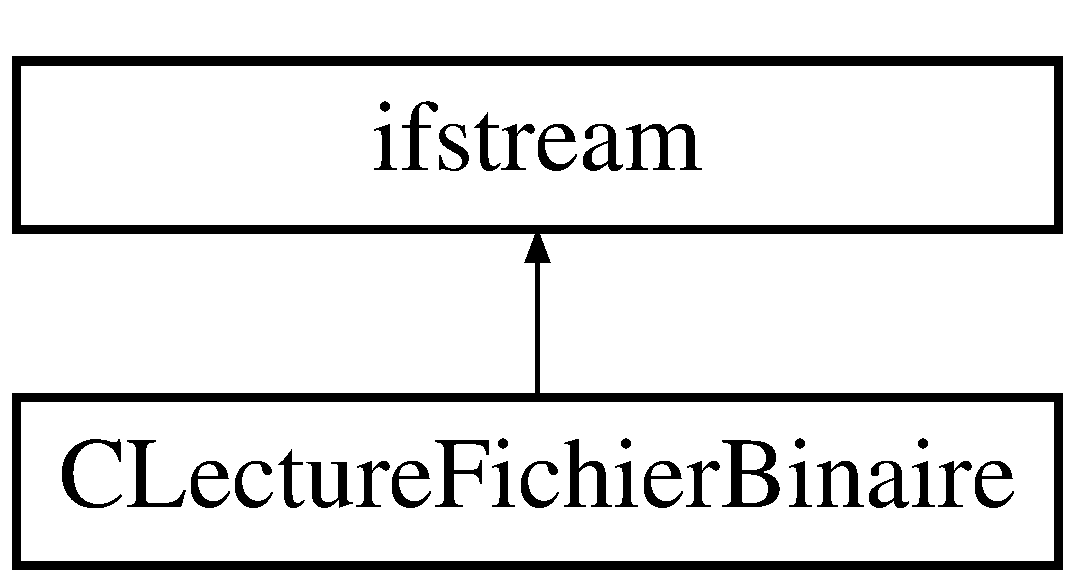
\includegraphics[height=2.000000cm]{class_c_lecture_fichier_binaire}
\end{center}
\end{figure}
\subsection*{Public Member Functions}
\begin{DoxyCompactItemize}
\item 
\hyperlink{group__utilitaire_ga3a259905a2c14513846e6ecb8cf476ad}{C\-Lecture\-Fichier\-Binaire} ()
\begin{DoxyCompactList}\small\item\em Constructeur par d�faut. \end{DoxyCompactList}\item 
\hyperlink{group__utilitaire_gac16ebab7b172408c2ba14605f61f0f84}{C\-Lecture\-Fichier\-Binaire} (const char $\ast$nom\-Fichier, openmode mode=std\-::ios\-::in$\vert$std\-::ios\-::binary)
\begin{DoxyCompactList}\small\item\em Constructeur par param�tre. \end{DoxyCompactList}\end{DoxyCompactItemize}
\subsection*{Friends}
\begin{DoxyCompactItemize}
\item 
\hypertarget{class_c_lecture_fichier_binaire_abc9f4d65dcf682dbf572f5110a00252d}{\hyperlink{class_c_lecture_fichier_binaire}{C\-Lecture\-Fichier\-Binaire} \& \hyperlink{class_c_lecture_fichier_binaire_abc9f4d65dcf682dbf572f5110a00252d}{operator$>$} (\hyperlink{class_c_lecture_fichier_binaire}{C\-Lecture\-Fichier\-Binaire} \&in, std\-::string \&s)}\label{class_c_lecture_fichier_binaire_abc9f4d65dcf682dbf572f5110a00252d}

\begin{DoxyCompactList}\small\item\em Surcharge de l'op�rateur pour le type {\itshape std\-::string}. \end{DoxyCompactList}\item 
\hypertarget{class_c_lecture_fichier_binaire_a8b4123b210cccf9da0d2eb60dc19b8a0}{\hyperlink{class_c_lecture_fichier_binaire}{C\-Lecture\-Fichier\-Binaire} \& \hyperlink{class_c_lecture_fichier_binaire_a8b4123b210cccf9da0d2eb60dc19b8a0}{operator$>$} (\hyperlink{class_c_lecture_fichier_binaire}{C\-Lecture\-Fichier\-Binaire} \&in, double \&f)}\label{class_c_lecture_fichier_binaire_a8b4123b210cccf9da0d2eb60dc19b8a0}

\begin{DoxyCompactList}\small\item\em Surcharge de l'op�rateur pour le type {\itshape double}. \end{DoxyCompactList}\item 
\hypertarget{class_c_lecture_fichier_binaire_a8727572665715de99f2908c711e45114}{\hyperlink{class_c_lecture_fichier_binaire}{C\-Lecture\-Fichier\-Binaire} \& \hyperlink{class_c_lecture_fichier_binaire_a8727572665715de99f2908c711e45114}{operator$>$} (\hyperlink{class_c_lecture_fichier_binaire}{C\-Lecture\-Fichier\-Binaire} \&in, float \&f)}\label{class_c_lecture_fichier_binaire_a8727572665715de99f2908c711e45114}

\begin{DoxyCompactList}\small\item\em Surcharge de l'op�rateur pour le type {\itshape float}. \end{DoxyCompactList}\item 
\hypertarget{class_c_lecture_fichier_binaire_a327898e8bcb11d00bdb07e3e8bd361bd}{\hyperlink{class_c_lecture_fichier_binaire}{C\-Lecture\-Fichier\-Binaire} \& \hyperlink{class_c_lecture_fichier_binaire_a327898e8bcb11d00bdb07e3e8bd361bd}{operator$>$} (\hyperlink{class_c_lecture_fichier_binaire}{C\-Lecture\-Fichier\-Binaire} \&in, int \&f)}\label{class_c_lecture_fichier_binaire_a327898e8bcb11d00bdb07e3e8bd361bd}

\begin{DoxyCompactList}\small\item\em Surcharge de l'op�rateur pour le type {\itshape int}. \end{DoxyCompactList}\item 
\hypertarget{class_c_lecture_fichier_binaire_a10555985d21e9277fd610554eb804ad4}{\hyperlink{class_c_lecture_fichier_binaire}{C\-Lecture\-Fichier\-Binaire} \& \hyperlink{class_c_lecture_fichier_binaire_a10555985d21e9277fd610554eb804ad4}{operator$>$} (\hyperlink{class_c_lecture_fichier_binaire}{C\-Lecture\-Fichier\-Binaire} \&in, unsigned int \&f)}\label{class_c_lecture_fichier_binaire_a10555985d21e9277fd610554eb804ad4}

\begin{DoxyCompactList}\small\item\em Surcharge de l'op�rateur pour le type {\itshape unsigned} {\itshape int}. \end{DoxyCompactList}\item 
\hypertarget{class_c_lecture_fichier_binaire_a4a3ac4fa35e1f11664f6612d554d72bd}{\hyperlink{class_c_lecture_fichier_binaire}{C\-Lecture\-Fichier\-Binaire} \& \hyperlink{class_c_lecture_fichier_binaire_a4a3ac4fa35e1f11664f6612d554d72bd}{operator$>$} (\hyperlink{class_c_lecture_fichier_binaire}{C\-Lecture\-Fichier\-Binaire} \&in, char \&f)}\label{class_c_lecture_fichier_binaire_a4a3ac4fa35e1f11664f6612d554d72bd}

\begin{DoxyCompactList}\small\item\em Surcharge de l'op�rateur pour le type {\itshape char}. \end{DoxyCompactList}\item 
\hypertarget{class_c_lecture_fichier_binaire_aaf7fbfa5e060c1e9015b0ffbd013f3e3}{\hyperlink{class_c_lecture_fichier_binaire}{C\-Lecture\-Fichier\-Binaire} \& \hyperlink{class_c_lecture_fichier_binaire_aaf7fbfa5e060c1e9015b0ffbd013f3e3}{operator$>$} (\hyperlink{class_c_lecture_fichier_binaire}{C\-Lecture\-Fichier\-Binaire} \&in, bool \&f)}\label{class_c_lecture_fichier_binaire_aaf7fbfa5e060c1e9015b0ffbd013f3e3}

\begin{DoxyCompactList}\small\item\em Surcharge de l'op�rateur pour le type {\itshape bool}. \end{DoxyCompactList}\end{DoxyCompactItemize}


\subsection{Detailed Description}
cette classe contient des m�thodes $>$ permettant de lire dans un fichier binaire des variables de types string, double, float, int, unsigned int, char, et bool. 

\begin{DoxyAuthor}{Author}
D\-G\-I-\/2990 
\end{DoxyAuthor}
\begin{DoxyDate}{Date}
2005-\/10-\/15 
\end{DoxyDate}


The documentation for this class was generated from the following files\-:\begin{DoxyCompactItemize}
\item 
X\-:/\-Git\-\_\-\-Repository/inf2990-\/06/\-Cadriciel/\-Commun/\-Utilitaire/\hyperlink{_c_lecture_fichier_binaire_8h}{C\-Lecture\-Fichier\-Binaire.\-h}\item 
X\-:/\-Git\-\_\-\-Repository/inf2990-\/06/\-Cadriciel/\-Commun/\-Utilitaire/\hyperlink{_c_lecture_fichier_binaire_8cpp}{C\-Lecture\-Fichier\-Binaire.\-cpp}\end{DoxyCompactItemize}

\hypertarget{class_interface_graphique_1_1_configurer_partie_rapide_1_1_combo_box_item}{\section{Interface\-Graphique.\-Configurer\-Partie\-Rapide.\-Combo\-Box\-Item Class Reference}
\label{class_interface_graphique_1_1_configurer_partie_rapide_1_1_combo_box_item}\index{Interface\-Graphique.\-Configurer\-Partie\-Rapide.\-Combo\-Box\-Item@{Interface\-Graphique.\-Configurer\-Partie\-Rapide.\-Combo\-Box\-Item}}
}


Redefinition d'un item de Combo\-Box  


\subsection*{Public Member Functions}
\begin{DoxyCompactItemize}
\item 
override string \hyperlink{class_interface_graphique_1_1_configurer_partie_rapide_1_1_combo_box_item_a4a2b0823abcb47c073d44ad318864a29}{To\-String} ()
\end{DoxyCompactItemize}
\subsection*{Properties}
\begin{DoxyCompactItemize}
\item 
string \hyperlink{class_interface_graphique_1_1_configurer_partie_rapide_1_1_combo_box_item_a49c8c93698b147b8cf0a7e4f7b20fc3e}{Text}\hspace{0.3cm}{\ttfamily  \mbox{[}get, set\mbox{]}}
\item 
string \hyperlink{class_interface_graphique_1_1_configurer_partie_rapide_1_1_combo_box_item_abe3a9af3f056a3f9b78355ba4a352cda}{Value}\hspace{0.3cm}{\ttfamily  \mbox{[}get, set\mbox{]}}
\end{DoxyCompactItemize}


\subsection{Detailed Description}
Redefinition d'un item de Combo\-Box 



\subsection{Member Function Documentation}
\hypertarget{class_interface_graphique_1_1_configurer_partie_rapide_1_1_combo_box_item_a4a2b0823abcb47c073d44ad318864a29}{\index{Interface\-Graphique\-::\-Configurer\-Partie\-Rapide\-::\-Combo\-Box\-Item@{Interface\-Graphique\-::\-Configurer\-Partie\-Rapide\-::\-Combo\-Box\-Item}!To\-String@{To\-String}}
\index{To\-String@{To\-String}!InterfaceGraphique::ConfigurerPartieRapide::ComboBoxItem@{Interface\-Graphique\-::\-Configurer\-Partie\-Rapide\-::\-Combo\-Box\-Item}}
\subsubsection[{To\-String}]{\setlength{\rightskip}{0pt plus 5cm}override string Interface\-Graphique.\-Configurer\-Partie\-Rapide.\-Combo\-Box\-Item.\-To\-String (
\begin{DoxyParamCaption}
{}
\end{DoxyParamCaption}
)\hspace{0.3cm}{\ttfamily [inline]}}}\label{class_interface_graphique_1_1_configurer_partie_rapide_1_1_combo_box_item_a4a2b0823abcb47c073d44ad318864a29}


\subsection{Property Documentation}
\hypertarget{class_interface_graphique_1_1_configurer_partie_rapide_1_1_combo_box_item_a49c8c93698b147b8cf0a7e4f7b20fc3e}{\index{Interface\-Graphique\-::\-Configurer\-Partie\-Rapide\-::\-Combo\-Box\-Item@{Interface\-Graphique\-::\-Configurer\-Partie\-Rapide\-::\-Combo\-Box\-Item}!Text@{Text}}
\index{Text@{Text}!InterfaceGraphique::ConfigurerPartieRapide::ComboBoxItem@{Interface\-Graphique\-::\-Configurer\-Partie\-Rapide\-::\-Combo\-Box\-Item}}
\subsubsection[{Text}]{\setlength{\rightskip}{0pt plus 5cm}string Interface\-Graphique.\-Configurer\-Partie\-Rapide.\-Combo\-Box\-Item.\-Text\hspace{0.3cm}{\ttfamily [get]}, {\ttfamily [set]}}}\label{class_interface_graphique_1_1_configurer_partie_rapide_1_1_combo_box_item_a49c8c93698b147b8cf0a7e4f7b20fc3e}
\hypertarget{class_interface_graphique_1_1_configurer_partie_rapide_1_1_combo_box_item_abe3a9af3f056a3f9b78355ba4a352cda}{\index{Interface\-Graphique\-::\-Configurer\-Partie\-Rapide\-::\-Combo\-Box\-Item@{Interface\-Graphique\-::\-Configurer\-Partie\-Rapide\-::\-Combo\-Box\-Item}!Value@{Value}}
\index{Value@{Value}!InterfaceGraphique::ConfigurerPartieRapide::ComboBoxItem@{Interface\-Graphique\-::\-Configurer\-Partie\-Rapide\-::\-Combo\-Box\-Item}}
\subsubsection[{Value}]{\setlength{\rightskip}{0pt plus 5cm}string Interface\-Graphique.\-Configurer\-Partie\-Rapide.\-Combo\-Box\-Item.\-Value\hspace{0.3cm}{\ttfamily [get]}, {\ttfamily [set]}}}\label{class_interface_graphique_1_1_configurer_partie_rapide_1_1_combo_box_item_abe3a9af3f056a3f9b78355ba4a352cda}


The documentation for this class was generated from the following file\-:\begin{DoxyCompactItemize}
\item 
X\-:/inf2990-\/06/\-Cadriciel/\-Sources/\-Interface\-Graphique/\hyperlink{_menu_partie_rapide_8cs}{Menu\-Partie\-Rapide.\-cs}\end{DoxyCompactItemize}

\hypertarget{class_interface_graphique_1_1_menu_campagne_1_1_combo_box_item}{\section{Interface\-Graphique.\-Menu\-Campagne.\-Combo\-Box\-Item Class Reference}
\label{class_interface_graphique_1_1_menu_campagne_1_1_combo_box_item}\index{Interface\-Graphique.\-Menu\-Campagne.\-Combo\-Box\-Item@{Interface\-Graphique.\-Menu\-Campagne.\-Combo\-Box\-Item}}
}
\subsection*{Public Member Functions}
\begin{DoxyCompactItemize}
\item 
\hypertarget{class_interface_graphique_1_1_menu_campagne_1_1_combo_box_item_ae18b58ca549af71043b57edffd6cfa6f}{override string {\bfseries To\-String} ()}\label{class_interface_graphique_1_1_menu_campagne_1_1_combo_box_item_ae18b58ca549af71043b57edffd6cfa6f}

\end{DoxyCompactItemize}
\subsection*{Public Attributes}
\begin{DoxyCompactItemize}
\item 
\hypertarget{class_interface_graphique_1_1_menu_campagne_1_1_combo_box_item_a6ca0abfd516a8df4faf602c9303319ea}{string Text {\bfseries get}}\label{class_interface_graphique_1_1_menu_campagne_1_1_combo_box_item_a6ca0abfd516a8df4faf602c9303319ea}

\item 
\hypertarget{class_interface_graphique_1_1_menu_campagne_1_1_combo_box_item_a044d419a44ff271f53a7e7f006064f4c}{int {\bfseries Difficulte}}\label{class_interface_graphique_1_1_menu_campagne_1_1_combo_box_item_a044d419a44ff271f53a7e7f006064f4c}

\end{DoxyCompactItemize}
\subsection*{Properties}
\begin{DoxyCompactItemize}
\item 
\hypertarget{class_interface_graphique_1_1_menu_campagne_1_1_combo_box_item_af32e2bf5eed166e54ce322627482cbff}{string {\bfseries Value}\hspace{0.3cm}{\ttfamily  \mbox{[}get, set\mbox{]}}}\label{class_interface_graphique_1_1_menu_campagne_1_1_combo_box_item_af32e2bf5eed166e54ce322627482cbff}

\end{DoxyCompactItemize}


The documentation for this class was generated from the following file\-:\begin{DoxyCompactItemize}
\item 
X\-:/\-Git\-\_\-\-Repository/inf2990-\/06/\-Cadriciel/\-Sources/\-Interface\-Graphique/Menu\-Campagne.\-cs\end{DoxyCompactItemize}

\hypertarget{class_compiler_outputter}{\section{Compiler\-Outputter Class Reference}
\label{class_compiler_outputter}\index{Compiler\-Outputter@{Compiler\-Outputter}}
}


Outputs a \hyperlink{class_test_result_collector}{Test\-Result\-Collector} in a compiler compatible format.

Printing the test results in a compiler compatible format (assertion location has the same format as compiler error), allow you to use your I\-D\-E to jump to the assertion failure. Location format can be customized (see \hyperlink{class_compiler_outputter_a0d9e67c7bdcb443b0b2754d61a10790c}{set\-Location\-Format()} ).  




{\ttfamily \#include $<$Compiler\-Outputter.\-h$>$}

Inheritance diagram for Compiler\-Outputter\-:\begin{figure}[H]
\begin{center}
\leavevmode
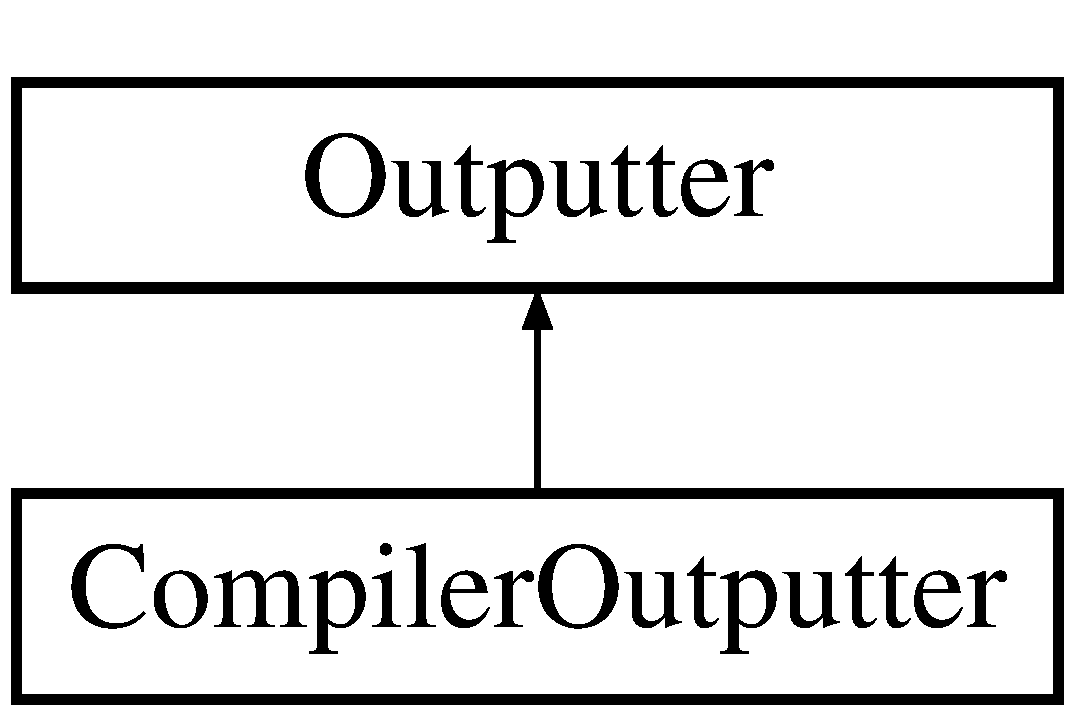
\includegraphics[height=2.000000cm]{class_compiler_outputter}
\end{center}
\end{figure}
\subsection*{Public Member Functions}
\begin{DoxyCompactItemize}
\item 
\hyperlink{class_compiler_outputter_a8dd6679e24c18b3ca54a4266d9d1b812}{Compiler\-Outputter} (\hyperlink{class_test_result_collector}{Test\-Result\-Collector} $\ast$result, O\-Stream \&stream, const std\-::string \&location\-Format=C\-P\-P\-U\-N\-I\-T\-\_\-\-C\-O\-M\-P\-I\-L\-E\-R\-\_\-\-L\-O\-C\-A\-T\-I\-O\-N\-\_\-\-F\-O\-R\-M\-A\-T)
\begin{DoxyCompactList}\small\item\em Constructs a \hyperlink{class_compiler_outputter}{Compiler\-Outputter} object. \end{DoxyCompactList}\item 
\hypertarget{class_compiler_outputter_ac74daaf4b355850c5e70b743aac2df82}{virtual \hyperlink{class_compiler_outputter_ac74daaf4b355850c5e70b743aac2df82}{$\sim$\-Compiler\-Outputter} ()}\label{class_compiler_outputter_ac74daaf4b355850c5e70b743aac2df82}

\begin{DoxyCompactList}\small\item\em Destructor. \end{DoxyCompactList}\item 
void \hyperlink{class_compiler_outputter_a0d9e67c7bdcb443b0b2754d61a10790c}{set\-Location\-Format} (const std\-::string \&location\-Format)
\begin{DoxyCompactList}\small\item\em Sets the error location format. \end{DoxyCompactList}\item 
\hypertarget{class_compiler_outputter_a55ca2189956b9b52bdfb1802bf8da445}{void {\bfseries write} ()}\label{class_compiler_outputter_a55ca2189956b9b52bdfb1802bf8da445}

\item 
\hypertarget{class_compiler_outputter_aaa1d8281f8973552a8e9a4568b7d90b4}{void {\bfseries set\-No\-Wrap} ()}\label{class_compiler_outputter_aaa1d8281f8973552a8e9a4568b7d90b4}

\item 
\hypertarget{class_compiler_outputter_ab3559c2aaa88cbccb7c3823b3dd4d247}{void {\bfseries set\-Wrap\-Column} (int wrap\-Column)}\label{class_compiler_outputter_ab3559c2aaa88cbccb7c3823b3dd4d247}

\item 
\hypertarget{class_compiler_outputter_a44a670371d545db99603ce88b59aa6c0}{int {\bfseries wrap\-Column} () const }\label{class_compiler_outputter_a44a670371d545db99603ce88b59aa6c0}

\item 
\hypertarget{class_compiler_outputter_a5fb16745d10fddb67cbcbec270218589}{virtual void {\bfseries print\-Success} ()}\label{class_compiler_outputter_a5fb16745d10fddb67cbcbec270218589}

\item 
\hypertarget{class_compiler_outputter_ab277e9b8c4af074593904dbc00853561}{virtual void {\bfseries print\-Failure\-Report} ()}\label{class_compiler_outputter_ab277e9b8c4af074593904dbc00853561}

\item 
\hypertarget{class_compiler_outputter_a6919d4e1d44d03e50694aee73dc96d89}{virtual void {\bfseries print\-Failures\-List} ()}\label{class_compiler_outputter_a6919d4e1d44d03e50694aee73dc96d89}

\item 
\hypertarget{class_compiler_outputter_acc3eefc4776b975af3502ef9afaf8b3d}{virtual void {\bfseries print\-Statistics} ()}\label{class_compiler_outputter_acc3eefc4776b975af3502ef9afaf8b3d}

\item 
\hypertarget{class_compiler_outputter_a2a8fece8722cb0307a5f0f6cd0de41c3}{virtual void {\bfseries print\-Failure\-Detail} (\hyperlink{class_test_failure}{Test\-Failure} $\ast$failure)}\label{class_compiler_outputter_a2a8fece8722cb0307a5f0f6cd0de41c3}

\item 
\hypertarget{class_compiler_outputter_aac88928b23fbae0b33b1624fa5696c31}{virtual void {\bfseries print\-Failure\-Location} (\hyperlink{class_source_line}{Source\-Line} source\-Line)}\label{class_compiler_outputter_aac88928b23fbae0b33b1624fa5696c31}

\item 
\hypertarget{class_compiler_outputter_ae836af9e969ced1ebdb399313df10250}{virtual void {\bfseries print\-Failure\-Type} (\hyperlink{class_test_failure}{Test\-Failure} $\ast$failure)}\label{class_compiler_outputter_ae836af9e969ced1ebdb399313df10250}

\item 
\hypertarget{class_compiler_outputter_a3e3fc6d7f2e98161144ab02f5f42dd9b}{virtual void {\bfseries print\-Failed\-Test\-Name} (\hyperlink{class_test_failure}{Test\-Failure} $\ast$failure)}\label{class_compiler_outputter_a3e3fc6d7f2e98161144ab02f5f42dd9b}

\item 
\hypertarget{class_compiler_outputter_a701ad438ff6a5a0af01acd1d43de4b6c}{virtual void {\bfseries print\-Failure\-Message} (\hyperlink{class_test_failure}{Test\-Failure} $\ast$failure)}\label{class_compiler_outputter_a701ad438ff6a5a0af01acd1d43de4b6c}

\end{DoxyCompactItemize}
\subsection*{Static Public Member Functions}
\begin{DoxyCompactItemize}
\item 
static \hyperlink{class_compiler_outputter}{Compiler\-Outputter} $\ast$ \hyperlink{class_compiler_outputter_aa0f8f9b1fb25fe8873b7454f91dcc929}{default\-Outputter} (\hyperlink{class_test_result_collector}{Test\-Result\-Collector} $\ast$result, O\-Stream \&stream)
\begin{DoxyCompactList}\small\item\em Creates an instance of an outputter that matches your current compiler. \end{DoxyCompactList}\end{DoxyCompactItemize}


\subsection{Detailed Description}
Outputs a \hyperlink{class_test_result_collector}{Test\-Result\-Collector} in a compiler compatible format.

Printing the test results in a compiler compatible format (assertion location has the same format as compiler error), allow you to use your I\-D\-E to jump to the assertion failure. Location format can be customized (see \hyperlink{class_compiler_outputter_a0d9e67c7bdcb443b0b2754d61a10790c}{set\-Location\-Format()} ). 

For example, when running the test in a post-\/build with V\-C++, if an assertion fails, you can jump to the assertion by pressing F4 (jump to next error).

Heres is an example of usage (from examples/cppunittest/\-Cpp\-Unit\-Test\-Main.\-cpp)\-: 
\begin{DoxyCode}
\textcolor{keywordtype}{int} main( \textcolor{keywordtype}{int} argc, \textcolor{keywordtype}{char}* argv[] ) \{
  \textcolor{comment}{// if command line contains "-selftest" then this is the post build check}
  \textcolor{comment}{// => the output must be in the compiler error format.}
  \textcolor{keywordtype}{bool} selfTest = (argc > 1)  &&  
                  (std::string(\textcolor{stringliteral}{"-selftest"}) == argv[1]);

  CppUnit::TextUi::TestRunner runner;
  runner.addTest( CppUnitTest::suite() );   \textcolor{comment}{// Add the top suite to the test runner}

 \textcolor{keywordflow}{if} ( selfTest )
  \{ \textcolor{comment}{// Change the default outputter to a compiler error format outputter}
    \textcolor{comment}{// The test runner owns the new outputter.}
    runner.setOutputter( \textcolor{keyword}{new} CppUnit::CompilerOutputter( &runner.result(),
                                                         std::cerr ) );
  \}

 \textcolor{comment}{// Run the test and don't wait a key if post build check.}
  \textcolor{keywordtype}{bool} wasSuccessful = runner.run( \textcolor{stringliteral}{""}, !selfTest );

  \textcolor{comment}{// Return error code 1 if the one of test failed.}
  \textcolor{keywordflow}{return} wasSuccessful ? 0 : 1;
\}
\end{DoxyCode}
 

\subsection{Constructor \& Destructor Documentation}
\hypertarget{class_compiler_outputter_a8dd6679e24c18b3ca54a4266d9d1b812}{\index{Compiler\-Outputter@{Compiler\-Outputter}!Compiler\-Outputter@{Compiler\-Outputter}}
\index{Compiler\-Outputter@{Compiler\-Outputter}!CompilerOutputter@{Compiler\-Outputter}}
\subsubsection[{Compiler\-Outputter}]{\setlength{\rightskip}{0pt plus 5cm}Compiler\-Outputter\-::\-Compiler\-Outputter (
\begin{DoxyParamCaption}
\item[{{\bf Test\-Result\-Collector} $\ast$}]{result, }
\item[{O\-Stream \&}]{stream, }
\item[{const std\-::string \&}]{location\-Format = {\ttfamily CPPUNIT\-\_\-COMPILER\-\_\-LOCATION\-\_\-FORMAT}}
\end{DoxyParamCaption}
)}}\label{class_compiler_outputter_a8dd6679e24c18b3ca54a4266d9d1b812}


Constructs a \hyperlink{class_compiler_outputter}{Compiler\-Outputter} object. 


\begin{DoxyParams}{Parameters}
{\em result} & Result of the test run. \\
\hline
{\em stream} & Stream used to output test result. \\
\hline
{\em location\-Format} & Error location format used by your compiler. Default to {\ttfamily C\-P\-P\-U\-N\-I\-T\-\_\-\-C\-O\-M\-P\-I\-L\-E\-R\-\_\-\-L\-O\-C\-A\-T\-I\-O\-N\-\_\-\-F\-O\-R\-M\-A\-T} which is defined in the configuration file. See \hyperlink{class_compiler_outputter_a0d9e67c7bdcb443b0b2754d61a10790c}{set\-Location\-Format()} for detail. \\
\hline
\end{DoxyParams}
\begin{DoxySeeAlso}{See Also}
\hyperlink{class_compiler_outputter_a0d9e67c7bdcb443b0b2754d61a10790c}{set\-Location\-Format()}. 
\end{DoxySeeAlso}


\subsection{Member Function Documentation}
\hypertarget{class_compiler_outputter_aa0f8f9b1fb25fe8873b7454f91dcc929}{\index{Compiler\-Outputter@{Compiler\-Outputter}!default\-Outputter@{default\-Outputter}}
\index{default\-Outputter@{default\-Outputter}!CompilerOutputter@{Compiler\-Outputter}}
\subsubsection[{default\-Outputter}]{\setlength{\rightskip}{0pt plus 5cm}static {\bf Compiler\-Outputter}$\ast$ Compiler\-Outputter\-::default\-Outputter (
\begin{DoxyParamCaption}
\item[{{\bf Test\-Result\-Collector} $\ast$}]{result, }
\item[{O\-Stream \&}]{stream}
\end{DoxyParamCaption}
)\hspace{0.3cm}{\ttfamily [static]}}}\label{class_compiler_outputter_aa0f8f9b1fb25fe8873b7454f91dcc929}


Creates an instance of an outputter that matches your current compiler. 

\begin{DoxyRefDesc}{Deprecated}
\item[\hyperlink{deprecated__deprecated000004}{Deprecated}]This class is specialized through parameterization instead of subclassing... Use \hyperlink{class_compiler_outputter_a8dd6679e24c18b3ca54a4266d9d1b812}{Compiler\-Outputter\-::\-Compiler\-Outputter} instead. \end{DoxyRefDesc}
\hypertarget{class_compiler_outputter_a0d9e67c7bdcb443b0b2754d61a10790c}{\index{Compiler\-Outputter@{Compiler\-Outputter}!set\-Location\-Format@{set\-Location\-Format}}
\index{set\-Location\-Format@{set\-Location\-Format}!CompilerOutputter@{Compiler\-Outputter}}
\subsubsection[{set\-Location\-Format}]{\setlength{\rightskip}{0pt plus 5cm}void Compiler\-Outputter\-::set\-Location\-Format (
\begin{DoxyParamCaption}
\item[{const std\-::string \&}]{location\-Format}
\end{DoxyParamCaption}
)}}\label{class_compiler_outputter_a0d9e67c7bdcb443b0b2754d61a10790c}


Sets the error location format. 

Indicates the format used to report location of failed assertion. This format should match the one used by your compiler.

The location format is a string in which the occurence of the following character sequence are replaced\-:


\begin{DoxyItemize}
\item \char`\"{}\%l\char`\"{} =$>$ replaced by the line number
\item \char`\"{}\%p\char`\"{} =$>$ replaced by the full path name of the file (\char`\"{}\-G\-:\textbackslash{}prg\textbackslash{}vc\textbackslash{}cppunit\textbackslash{}\-My\-Test.\-cpp\char`\"{})
\item \char`\"{}\%f\char`\"{} =$>$ replaced by the base name of the file (\char`\"{}\-My\-Test.\-cpp\char`\"{})
\end{DoxyItemize}

Some examples\-:


\begin{DoxyItemize}
\item V\-C++ error location format\-: \char`\"{}\%p(\%l)\-:\char`\"{} =$>$ produce \char`\"{}\-G\-:\textbackslash{}prg\textbackslash{}\-My\-Test.\-cpp(43)\-:\char`\"{}
\item G\-C\-C error location format\-: \char`\"{}\%f\-:\%l\-:\char`\"{} =$>$ produce \char`\"{}\-My\-Test.\-cpp\-:43\-:\char`\"{}
\end{DoxyItemize}

Thoses are the two compilers currently {\itshape supported} (gcc format is used if V\-C++ is not detected). If you want your compiler to be automatically supported by Cpp\-Unit, send a mail to the mailing list (preferred), or submit a feature request that indicates how to detect your compiler with the preprocessor (\#ifdef...) and your compiler location format. 

The documentation for this class was generated from the following file\-:\begin{DoxyCompactItemize}
\item 
X\-:/\-Git\-\_\-\-Repository/inf2990-\/06/\-Cadriciel/\-Commun/\-Externe/cppunit/include/cppunit/Compiler\-Outputter.\-h\end{DoxyCompactItemize}

\hypertarget{classutilitaire_1_1_compteur_affichage}{\section{utilitaire\-:\-:Compteur\-Affichage Class Reference}
\label{classutilitaire_1_1_compteur_affichage}\index{utilitaire\-::\-Compteur\-Affichage@{utilitaire\-::\-Compteur\-Affichage}}
}


Classe qui g�re le compte des affichages par secondes (\char`\"{}\-F\-P\-S\char`\"{}).  




{\ttfamily \#include $<$Compteur\-Affichage.\-h$>$}

\subsection*{Public Member Functions}
\begin{DoxyCompactItemize}
\item 
int \hyperlink{classutilitaire_1_1_compteur_affichage_a1902a495b4898b3f7ab9056537db00cc}{obtenir\-Affichages\-Seconde} () const 
\begin{DoxyCompactList}\small\item\em Obtient le dernier nombre calcul� d'affichages par seconde. \end{DoxyCompactList}\item 
void \hyperlink{classutilitaire_1_1_compteur_affichage_a49f6562d1a37e275ff8c8c0e9be41ab5}{signaler\-Affichage} ()
\begin{DoxyCompactList}\small\item\em Indique qu'un affichage vient de se produire. \end{DoxyCompactList}\item 
void \hyperlink{classutilitaire_1_1_compteur_affichage_a69b89a3d76cde700f1c08580bab010ca}{reinitialiser} ()
\begin{DoxyCompactList}\small\item\em R�initialise le compteur d'affichage. \end{DoxyCompactList}\end{DoxyCompactItemize}
\subsection*{Static Public Member Functions}
\begin{DoxyCompactItemize}
\item 
static \hyperlink{classutilitaire_1_1_compteur_affichage}{Compteur\-Affichage} $\ast$ \hyperlink{classutilitaire_1_1_compteur_affichage_a87a0785c0c73f0da0f6ffc4a86a609fe}{obtenir\-Instance} ()
\begin{DoxyCompactList}\small\item\em Obtient l'instance unique de la classe. \end{DoxyCompactList}\item 
static void \hyperlink{classutilitaire_1_1_compteur_affichage_ae37d88f73c83bfd3ff3c95496c9ef400}{liberer\-Instance} ()
\begin{DoxyCompactList}\small\item\em Lib�re l'instance unique de la classe. \end{DoxyCompactList}\end{DoxyCompactItemize}


\subsection{Detailed Description}
Classe qui g�re le compte des affichages par secondes (\char`\"{}\-F\-P\-S\char`\"{}). 

\begin{DoxyAuthor}{Author}
Martin Bisson 
\end{DoxyAuthor}
\begin{DoxyDate}{Date}
2007-\/03-\/09 
\end{DoxyDate}


\subsection{Member Function Documentation}
\hypertarget{classutilitaire_1_1_compteur_affichage_ae37d88f73c83bfd3ff3c95496c9ef400}{\index{utilitaire\-::\-Compteur\-Affichage@{utilitaire\-::\-Compteur\-Affichage}!liberer\-Instance@{liberer\-Instance}}
\index{liberer\-Instance@{liberer\-Instance}!utilitaire::CompteurAffichage@{utilitaire\-::\-Compteur\-Affichage}}
\subsubsection[{liberer\-Instance}]{\setlength{\rightskip}{0pt plus 5cm}void utilitaire\-::\-Compteur\-Affichage\-::liberer\-Instance (
\begin{DoxyParamCaption}
{}
\end{DoxyParamCaption}
)\hspace{0.3cm}{\ttfamily [static]}}}\label{classutilitaire_1_1_compteur_affichage_ae37d88f73c83bfd3ff3c95496c9ef400}


Lib�re l'instance unique de la classe. 

Cette fonction lib�re l'instance unique de cette classe.

\begin{DoxyReturn}{Returns}
Aucune. 
\end{DoxyReturn}
\hypertarget{classutilitaire_1_1_compteur_affichage_a1902a495b4898b3f7ab9056537db00cc}{\index{utilitaire\-::\-Compteur\-Affichage@{utilitaire\-::\-Compteur\-Affichage}!obtenir\-Affichages\-Seconde@{obtenir\-Affichages\-Seconde}}
\index{obtenir\-Affichages\-Seconde@{obtenir\-Affichages\-Seconde}!utilitaire::CompteurAffichage@{utilitaire\-::\-Compteur\-Affichage}}
\subsubsection[{obtenir\-Affichages\-Seconde}]{\setlength{\rightskip}{0pt plus 5cm}int utilitaire\-::\-Compteur\-Affichage\-::obtenir\-Affichages\-Seconde (
\begin{DoxyParamCaption}
{}
\end{DoxyParamCaption}
) const\hspace{0.3cm}{\ttfamily [inline]}}}\label{classutilitaire_1_1_compteur_affichage_a1902a495b4898b3f7ab9056537db00cc}


Obtient le dernier nombre calcul� d'affichages par seconde. 

Cette fonction retourne le dernier nombre d'affichages par seconde calcul� par le compteur.

\begin{DoxyReturn}{Returns}
Le nombre d'affichages par seconce le plus r�cent. 
\end{DoxyReturn}
\hypertarget{classutilitaire_1_1_compteur_affichage_a87a0785c0c73f0da0f6ffc4a86a609fe}{\index{utilitaire\-::\-Compteur\-Affichage@{utilitaire\-::\-Compteur\-Affichage}!obtenir\-Instance@{obtenir\-Instance}}
\index{obtenir\-Instance@{obtenir\-Instance}!utilitaire::CompteurAffichage@{utilitaire\-::\-Compteur\-Affichage}}
\subsubsection[{obtenir\-Instance}]{\setlength{\rightskip}{0pt plus 5cm}{\bf Compteur\-Affichage} $\ast$ utilitaire\-::\-Compteur\-Affichage\-::obtenir\-Instance (
\begin{DoxyParamCaption}
{}
\end{DoxyParamCaption}
)\hspace{0.3cm}{\ttfamily [static]}}}\label{classutilitaire_1_1_compteur_affichage_a87a0785c0c73f0da0f6ffc4a86a609fe}


Obtient l'instance unique de la classe. 

Cette fonction retourne un pointeur vers l'instance unique de la classe. Si cette instance n'a pas �t� cr��e, elle la cr�e. Cette cr�ation n'est toutefois pas n�cessairement \char`\"{}thread-\/safe\char`\"{}, car aucun verrou n'est pris entre le test pour savoir si l'instance existe et le moment de sa cr�ation.

\begin{DoxyReturn}{Returns}
Un pointeur vers l'instance unique de cette classe. 
\end{DoxyReturn}
\hypertarget{classutilitaire_1_1_compteur_affichage_a69b89a3d76cde700f1c08580bab010ca}{\index{utilitaire\-::\-Compteur\-Affichage@{utilitaire\-::\-Compteur\-Affichage}!reinitialiser@{reinitialiser}}
\index{reinitialiser@{reinitialiser}!utilitaire::CompteurAffichage@{utilitaire\-::\-Compteur\-Affichage}}
\subsubsection[{reinitialiser}]{\setlength{\rightskip}{0pt plus 5cm}void utilitaire\-::\-Compteur\-Affichage\-::reinitialiser (
\begin{DoxyParamCaption}
{}
\end{DoxyParamCaption}
)}}\label{classutilitaire_1_1_compteur_affichage_a69b89a3d76cde700f1c08580bab010ca}


R�initialise le compteur d'affichage. 

Cette fonction r�initialise le compteur d'affichage � son �tat initiale.

\begin{DoxyReturn}{Returns}
Aucune. 
\end{DoxyReturn}
\hypertarget{classutilitaire_1_1_compteur_affichage_a49f6562d1a37e275ff8c8c0e9be41ab5}{\index{utilitaire\-::\-Compteur\-Affichage@{utilitaire\-::\-Compteur\-Affichage}!signaler\-Affichage@{signaler\-Affichage}}
\index{signaler\-Affichage@{signaler\-Affichage}!utilitaire::CompteurAffichage@{utilitaire\-::\-Compteur\-Affichage}}
\subsubsection[{signaler\-Affichage}]{\setlength{\rightskip}{0pt plus 5cm}void utilitaire\-::\-Compteur\-Affichage\-::signaler\-Affichage (
\begin{DoxyParamCaption}
{}
\end{DoxyParamCaption}
)}}\label{classutilitaire_1_1_compteur_affichage_a49f6562d1a37e275ff8c8c0e9be41ab5}


Indique qu'un affichage vient de se produire. 

Cette fonction effectue le traitement n�cessaire lorsqu'un affichage est signal�e, c'est-\/�-\/dire qu'elle incr�mente le compte et v�rifie si la limite de temps pour la mise � jour est d�pass�e.

\begin{DoxyReturn}{Returns}
Aucune. 
\end{DoxyReturn}


The documentation for this class was generated from the following files\-:\begin{DoxyCompactItemize}
\item 
X\-:/\-Git\-\_\-\-Repository/inf2990-\/06/\-Cadriciel/\-Commun/\-Utilitaire/\hyperlink{_compteur_affichage_8h}{Compteur\-Affichage.\-h}\item 
X\-:/\-Git\-\_\-\-Repository/inf2990-\/06/\-Cadriciel/\-Commun/\-Utilitaire/\hyperlink{_compteur_affichage_8cpp}{Compteur\-Affichage.\-cpp}\end{DoxyCompactItemize}

\hypertarget{structglm_1_1detail_1_1compute__abs}{\section{glm\-:\-:detail\-:\-:compute\-\_\-abs$<$ gen\-F\-I\-Type, bool $>$ Struct Template Reference}
\label{structglm_1_1detail_1_1compute__abs}\index{glm\-::detail\-::compute\-\_\-abs$<$ gen\-F\-I\-Type, bool $>$@{glm\-::detail\-::compute\-\_\-abs$<$ gen\-F\-I\-Type, bool $>$}}
}


The documentation for this struct was generated from the following file\-:\begin{DoxyCompactItemize}
\item 
X\-:/\-Git\-\_\-\-Repository/inf2990-\/06/\-Cadriciel/\-Commun/\-Externe/glm/include/glm/detail/func\-\_\-common.\-inl\end{DoxyCompactItemize}

\hypertarget{structglm_1_1detail_1_1compute__abs_3_01gen_f_i_type_00_01false_01_4}{\section{glm\-:\-:detail\-:\-:compute\-\_\-abs$<$ gen\-F\-I\-Type, false $>$ Struct Template Reference}
\label{structglm_1_1detail_1_1compute__abs_3_01gen_f_i_type_00_01false_01_4}\index{glm\-::detail\-::compute\-\_\-abs$<$ gen\-F\-I\-Type, false $>$@{glm\-::detail\-::compute\-\_\-abs$<$ gen\-F\-I\-Type, false $>$}}
}
\subsection*{Static Public Member Functions}
\begin{DoxyCompactItemize}
\item 
\hypertarget{structglm_1_1detail_1_1compute__abs_3_01gen_f_i_type_00_01false_01_4_a0758b7608495285101dea21f0a7cc37a}{static G\-L\-M\-\_\-\-F\-U\-N\-C\-\_\-\-Q\-U\-A\-L\-I\-F\-I\-E\-R gen\-F\-I\-Type {\bfseries call} (gen\-F\-I\-Type const \&x)}\label{structglm_1_1detail_1_1compute__abs_3_01gen_f_i_type_00_01false_01_4_a0758b7608495285101dea21f0a7cc37a}

\end{DoxyCompactItemize}


The documentation for this struct was generated from the following file\-:\begin{DoxyCompactItemize}
\item 
X\-:/\-Git\-\_\-\-Repository/inf2990-\/06/\-Cadriciel/\-Commun/\-Externe/glm/include/glm/detail/func\-\_\-common.\-inl\end{DoxyCompactItemize}

\hypertarget{structglm_1_1detail_1_1compute__abs_3_01gen_f_i_type_00_01true_01_4}{\section{glm\-:\-:detail\-:\-:compute\-\_\-abs$<$ gen\-F\-I\-Type, true $>$ Struct Template Reference}
\label{structglm_1_1detail_1_1compute__abs_3_01gen_f_i_type_00_01true_01_4}\index{glm\-::detail\-::compute\-\_\-abs$<$ gen\-F\-I\-Type, true $>$@{glm\-::detail\-::compute\-\_\-abs$<$ gen\-F\-I\-Type, true $>$}}
}
\subsection*{Static Public Member Functions}
\begin{DoxyCompactItemize}
\item 
\hypertarget{structglm_1_1detail_1_1compute__abs_3_01gen_f_i_type_00_01true_01_4_a13dee7b421d52969e40d8cdef020d0be}{static G\-L\-M\-\_\-\-F\-U\-N\-C\-\_\-\-Q\-U\-A\-L\-I\-F\-I\-E\-R gen\-F\-I\-Type {\bfseries call} (gen\-F\-I\-Type const \&x)}\label{structglm_1_1detail_1_1compute__abs_3_01gen_f_i_type_00_01true_01_4_a13dee7b421d52969e40d8cdef020d0be}

\end{DoxyCompactItemize}


The documentation for this struct was generated from the following file\-:\begin{DoxyCompactItemize}
\item 
X\-:/\-Git\-\_\-\-Repository/inf2990-\/06/\-Cadriciel/\-Commun/\-Externe/glm/include/glm/detail/func\-\_\-common.\-inl\end{DoxyCompactItemize}

\hypertarget{structglm_1_1detail_1_1compute__are_collinear}{\section{glm\-:\-:detail\-:\-:compute\-\_\-are\-Collinear$<$ T, P, vec\-Type $>$ Struct Template Reference}
\label{structglm_1_1detail_1_1compute__are_collinear}\index{glm\-::detail\-::compute\-\_\-are\-Collinear$<$ T, P, vec\-Type $>$@{glm\-::detail\-::compute\-\_\-are\-Collinear$<$ T, P, vec\-Type $>$}}
}


The documentation for this struct was generated from the following file\-:\begin{DoxyCompactItemize}
\item 
X\-:/\-Git\-\_\-\-Repository/inf2990-\/06/\-Cadriciel/\-Commun/\-Externe/glm/include/glm/gtx/vector\-\_\-query.\-inl\end{DoxyCompactItemize}

\hypertarget{structglm_1_1detail_1_1compute__are_collinear_3_01_t_00_01_p_00_01tvec2_01_4}{\section{glm\-:\-:detail\-:\-:compute\-\_\-are\-Collinear$<$ T, P, tvec2 $>$ Struct Template Reference}
\label{structglm_1_1detail_1_1compute__are_collinear_3_01_t_00_01_p_00_01tvec2_01_4}\index{glm\-::detail\-::compute\-\_\-are\-Collinear$<$ T, P, tvec2 $>$@{glm\-::detail\-::compute\-\_\-are\-Collinear$<$ T, P, tvec2 $>$}}
}
\subsection*{Static Public Member Functions}
\begin{DoxyCompactItemize}
\item 
\hypertarget{structglm_1_1detail_1_1compute__are_collinear_3_01_t_00_01_p_00_01tvec2_01_4_a2f040e5d783927c363a8c14c5cec65d8}{static G\-L\-M\-\_\-\-F\-U\-N\-C\-\_\-\-Q\-U\-A\-L\-I\-F\-I\-E\-R bool {\bfseries call} (\hyperlink{structglm_1_1detail_1_1tvec2}{detail\-::tvec2}$<$ T, P $>$ const \&v0, \hyperlink{structglm_1_1detail_1_1tvec2}{detail\-::tvec2}$<$ T, P $>$ const \&v1, T const \&\hyperlink{group__gtc__constants_gacb41049b8d22c8aa90e362b96c524feb}{epsilon})}\label{structglm_1_1detail_1_1compute__are_collinear_3_01_t_00_01_p_00_01tvec2_01_4_a2f040e5d783927c363a8c14c5cec65d8}

\end{DoxyCompactItemize}


The documentation for this struct was generated from the following file\-:\begin{DoxyCompactItemize}
\item 
X\-:/\-Git\-\_\-\-Repository/inf2990-\/06/\-Cadriciel/\-Commun/\-Externe/glm/include/glm/gtx/vector\-\_\-query.\-inl\end{DoxyCompactItemize}

\hypertarget{structglm_1_1detail_1_1compute__are_collinear_3_01_t_00_01_p_00_01tvec3_01_4}{\section{glm\-:\-:detail\-:\-:compute\-\_\-are\-Collinear$<$ T, P, tvec3 $>$ Struct Template Reference}
\label{structglm_1_1detail_1_1compute__are_collinear_3_01_t_00_01_p_00_01tvec3_01_4}\index{glm\-::detail\-::compute\-\_\-are\-Collinear$<$ T, P, tvec3 $>$@{glm\-::detail\-::compute\-\_\-are\-Collinear$<$ T, P, tvec3 $>$}}
}
\subsection*{Static Public Member Functions}
\begin{DoxyCompactItemize}
\item 
\hypertarget{structglm_1_1detail_1_1compute__are_collinear_3_01_t_00_01_p_00_01tvec3_01_4_a1b9e023b1518128243ec6cc5748faccc}{static G\-L\-M\-\_\-\-F\-U\-N\-C\-\_\-\-Q\-U\-A\-L\-I\-F\-I\-E\-R bool {\bfseries call} (\hyperlink{structglm_1_1detail_1_1tvec3}{detail\-::tvec3}$<$ T, P $>$ const \&v0, \hyperlink{structglm_1_1detail_1_1tvec3}{detail\-::tvec3}$<$ T, P $>$ const \&v1, T const \&\hyperlink{group__gtc__constants_gacb41049b8d22c8aa90e362b96c524feb}{epsilon})}\label{structglm_1_1detail_1_1compute__are_collinear_3_01_t_00_01_p_00_01tvec3_01_4_a1b9e023b1518128243ec6cc5748faccc}

\end{DoxyCompactItemize}


The documentation for this struct was generated from the following file\-:\begin{DoxyCompactItemize}
\item 
X\-:/\-Git\-\_\-\-Repository/inf2990-\/06/\-Cadriciel/\-Commun/\-Externe/glm/include/glm/gtx/vector\-\_\-query.\-inl\end{DoxyCompactItemize}

\hypertarget{structglm_1_1detail_1_1compute__are_collinear_3_01_t_00_01_p_00_01tvec4_01_4}{\section{glm\-:\-:detail\-:\-:compute\-\_\-are\-Collinear$<$ T, P, tvec4 $>$ Struct Template Reference}
\label{structglm_1_1detail_1_1compute__are_collinear_3_01_t_00_01_p_00_01tvec4_01_4}\index{glm\-::detail\-::compute\-\_\-are\-Collinear$<$ T, P, tvec4 $>$@{glm\-::detail\-::compute\-\_\-are\-Collinear$<$ T, P, tvec4 $>$}}
}
\subsection*{Static Public Member Functions}
\begin{DoxyCompactItemize}
\item 
\hypertarget{structglm_1_1detail_1_1compute__are_collinear_3_01_t_00_01_p_00_01tvec4_01_4_a4a7e3fba780b73ef237fbf76dc6ead91}{static G\-L\-M\-\_\-\-F\-U\-N\-C\-\_\-\-Q\-U\-A\-L\-I\-F\-I\-E\-R bool {\bfseries call} (\hyperlink{structglm_1_1detail_1_1tvec4}{detail\-::tvec4}$<$ T, P $>$ const \&v0, \hyperlink{structglm_1_1detail_1_1tvec4}{detail\-::tvec4}$<$ T, P $>$ const \&v1, T const \&\hyperlink{group__gtc__constants_gacb41049b8d22c8aa90e362b96c524feb}{epsilon})}\label{structglm_1_1detail_1_1compute__are_collinear_3_01_t_00_01_p_00_01tvec4_01_4_a4a7e3fba780b73ef237fbf76dc6ead91}

\end{DoxyCompactItemize}


The documentation for this struct was generated from the following file\-:\begin{DoxyCompactItemize}
\item 
X\-:/\-Git\-\_\-\-Repository/inf2990-\/06/\-Cadriciel/\-Commun/\-Externe/glm/include/glm/gtx/vector\-\_\-query.\-inl\end{DoxyCompactItemize}

\hypertarget{structglm_1_1detail_1_1compute__determinant}{\section{glm\-:\-:detail\-:\-:compute\-\_\-determinant$<$ mat\-Type, T, P $>$ Struct Template Reference}
\label{structglm_1_1detail_1_1compute__determinant}\index{glm\-::detail\-::compute\-\_\-determinant$<$ mat\-Type, T, P $>$@{glm\-::detail\-::compute\-\_\-determinant$<$ mat\-Type, T, P $>$}}
}


The documentation for this struct was generated from the following file\-:\begin{DoxyCompactItemize}
\item 
X\-:/\-Git\-\_\-\-Repository/inf2990-\/06/\-Cadriciel/\-Commun/\-Externe/glm/include/glm/detail/func\-\_\-matrix.\-inl\end{DoxyCompactItemize}

\hypertarget{structglm_1_1detail_1_1compute__determinant_3_01detail_1_1tmat2x2_00_01_t_00_01_p_01_4}{\section{glm\-:\-:detail\-:\-:compute\-\_\-determinant$<$ detail\-:\-:tmat2x2, T, P $>$ Struct Template Reference}
\label{structglm_1_1detail_1_1compute__determinant_3_01detail_1_1tmat2x2_00_01_t_00_01_p_01_4}\index{glm\-::detail\-::compute\-\_\-determinant$<$ detail\-::tmat2x2, T, P $>$@{glm\-::detail\-::compute\-\_\-determinant$<$ detail\-::tmat2x2, T, P $>$}}
}
\subsection*{Static Public Member Functions}
\begin{DoxyCompactItemize}
\item 
\hypertarget{structglm_1_1detail_1_1compute__determinant_3_01detail_1_1tmat2x2_00_01_t_00_01_p_01_4_a58a62a3968a9af7acd4522972236742e}{static G\-L\-M\-\_\-\-F\-U\-N\-C\-\_\-\-Q\-U\-A\-L\-I\-F\-I\-E\-R T {\bfseries call} (\hyperlink{structglm_1_1detail_1_1tmat2x2}{detail\-::tmat2x2}$<$ T, P $>$ const \&m)}\label{structglm_1_1detail_1_1compute__determinant_3_01detail_1_1tmat2x2_00_01_t_00_01_p_01_4_a58a62a3968a9af7acd4522972236742e}

\end{DoxyCompactItemize}


The documentation for this struct was generated from the following file\-:\begin{DoxyCompactItemize}
\item 
X\-:/\-Git\-\_\-\-Repository/inf2990-\/06/\-Cadriciel/\-Commun/\-Externe/glm/include/glm/detail/func\-\_\-matrix.\-inl\end{DoxyCompactItemize}

\hypertarget{structglm_1_1detail_1_1compute__determinant_3_01detail_1_1tmat3x3_00_01_t_00_01_p_01_4}{\section{glm\-:\-:detail\-:\-:compute\-\_\-determinant$<$ detail\-:\-:tmat3x3, T, P $>$ Struct Template Reference}
\label{structglm_1_1detail_1_1compute__determinant_3_01detail_1_1tmat3x3_00_01_t_00_01_p_01_4}\index{glm\-::detail\-::compute\-\_\-determinant$<$ detail\-::tmat3x3, T, P $>$@{glm\-::detail\-::compute\-\_\-determinant$<$ detail\-::tmat3x3, T, P $>$}}
}
\subsection*{Static Public Member Functions}
\begin{DoxyCompactItemize}
\item 
\hypertarget{structglm_1_1detail_1_1compute__determinant_3_01detail_1_1tmat3x3_00_01_t_00_01_p_01_4_aacdeab0c051558a445f3f674dd6a5e8b}{static G\-L\-M\-\_\-\-F\-U\-N\-C\-\_\-\-Q\-U\-A\-L\-I\-F\-I\-E\-R T {\bfseries call} (\hyperlink{structglm_1_1detail_1_1tmat3x3}{detail\-::tmat3x3}$<$ T, P $>$ const \&m)}\label{structglm_1_1detail_1_1compute__determinant_3_01detail_1_1tmat3x3_00_01_t_00_01_p_01_4_aacdeab0c051558a445f3f674dd6a5e8b}

\end{DoxyCompactItemize}


The documentation for this struct was generated from the following file\-:\begin{DoxyCompactItemize}
\item 
X\-:/\-Git\-\_\-\-Repository/inf2990-\/06/\-Cadriciel/\-Commun/\-Externe/glm/include/glm/detail/func\-\_\-matrix.\-inl\end{DoxyCompactItemize}

\hypertarget{structglm_1_1detail_1_1compute__determinant_3_01detail_1_1tmat4x4_00_01_t_00_01_p_01_4}{\section{glm\-:\-:detail\-:\-:compute\-\_\-determinant$<$ detail\-:\-:tmat4x4, T, P $>$ Struct Template Reference}
\label{structglm_1_1detail_1_1compute__determinant_3_01detail_1_1tmat4x4_00_01_t_00_01_p_01_4}\index{glm\-::detail\-::compute\-\_\-determinant$<$ detail\-::tmat4x4, T, P $>$@{glm\-::detail\-::compute\-\_\-determinant$<$ detail\-::tmat4x4, T, P $>$}}
}
\subsection*{Static Public Member Functions}
\begin{DoxyCompactItemize}
\item 
\hypertarget{structglm_1_1detail_1_1compute__determinant_3_01detail_1_1tmat4x4_00_01_t_00_01_p_01_4_aa7fa7eae68f9b10c3ac3a80bca669c98}{static G\-L\-M\-\_\-\-F\-U\-N\-C\-\_\-\-Q\-U\-A\-L\-I\-F\-I\-E\-R T {\bfseries call} (\hyperlink{structglm_1_1detail_1_1tmat4x4}{detail\-::tmat4x4}$<$ T, P $>$ const \&m)}\label{structglm_1_1detail_1_1compute__determinant_3_01detail_1_1tmat4x4_00_01_t_00_01_p_01_4_aa7fa7eae68f9b10c3ac3a80bca669c98}

\end{DoxyCompactItemize}


The documentation for this struct was generated from the following file\-:\begin{DoxyCompactItemize}
\item 
X\-:/\-Git\-\_\-\-Repository/inf2990-\/06/\-Cadriciel/\-Commun/\-Externe/glm/include/glm/detail/func\-\_\-matrix.\-inl\end{DoxyCompactItemize}

\hypertarget{structglm_1_1detail_1_1compute__dot}{\section{glm\-:\-:detail\-:\-:compute\-\_\-dot$<$ vec\-Type, T, P $>$ Struct Template Reference}
\label{structglm_1_1detail_1_1compute__dot}\index{glm\-::detail\-::compute\-\_\-dot$<$ vec\-Type, T, P $>$@{glm\-::detail\-::compute\-\_\-dot$<$ vec\-Type, T, P $>$}}
}


The documentation for this struct was generated from the following file\-:\begin{DoxyCompactItemize}
\item 
X\-:/\-Git\-\_\-\-Repository/inf2990-\/06/\-Cadriciel/\-Commun/\-Externe/glm/include/glm/detail/func\-\_\-geometric.\-inl\end{DoxyCompactItemize}

\hypertarget{structglm_1_1detail_1_1compute__dot_3_01detail_1_1tvec1_00_01_t_00_01_p_01_4}{\section{glm\-:\-:detail\-:\-:compute\-\_\-dot$<$ detail\-:\-:tvec1, T, P $>$ Struct Template Reference}
\label{structglm_1_1detail_1_1compute__dot_3_01detail_1_1tvec1_00_01_t_00_01_p_01_4}\index{glm\-::detail\-::compute\-\_\-dot$<$ detail\-::tvec1, T, P $>$@{glm\-::detail\-::compute\-\_\-dot$<$ detail\-::tvec1, T, P $>$}}
}
\subsection*{Static Public Member Functions}
\begin{DoxyCompactItemize}
\item 
\hypertarget{structglm_1_1detail_1_1compute__dot_3_01detail_1_1tvec1_00_01_t_00_01_p_01_4_a8a857cb8e3ad91ffec9e5d2e8517be41}{static G\-L\-M\-\_\-\-F\-U\-N\-C\-\_\-\-Q\-U\-A\-L\-I\-F\-I\-E\-R T {\bfseries call} (\hyperlink{structglm_1_1detail_1_1tvec1}{detail\-::tvec1}$<$ T, P $>$ const \&x, \hyperlink{structglm_1_1detail_1_1tvec1}{detail\-::tvec1}$<$ T, P $>$ const \&y)}\label{structglm_1_1detail_1_1compute__dot_3_01detail_1_1tvec1_00_01_t_00_01_p_01_4_a8a857cb8e3ad91ffec9e5d2e8517be41}

\end{DoxyCompactItemize}


The documentation for this struct was generated from the following file\-:\begin{DoxyCompactItemize}
\item 
X\-:/\-Git\-\_\-\-Repository/inf2990-\/06/\-Cadriciel/\-Commun/\-Externe/glm/include/glm/detail/func\-\_\-geometric.\-inl\end{DoxyCompactItemize}

\hypertarget{structglm_1_1detail_1_1compute__dot_3_01detail_1_1tvec2_00_01_t_00_01_p_01_4}{\section{glm\-:\-:detail\-:\-:compute\-\_\-dot$<$ detail\-:\-:tvec2, T, P $>$ Struct Template Reference}
\label{structglm_1_1detail_1_1compute__dot_3_01detail_1_1tvec2_00_01_t_00_01_p_01_4}\index{glm\-::detail\-::compute\-\_\-dot$<$ detail\-::tvec2, T, P $>$@{glm\-::detail\-::compute\-\_\-dot$<$ detail\-::tvec2, T, P $>$}}
}
\subsection*{Static Public Member Functions}
\begin{DoxyCompactItemize}
\item 
\hypertarget{structglm_1_1detail_1_1compute__dot_3_01detail_1_1tvec2_00_01_t_00_01_p_01_4_a5ab1761eaa0efc9ecb4f62171d2a6dd2}{static G\-L\-M\-\_\-\-F\-U\-N\-C\-\_\-\-Q\-U\-A\-L\-I\-F\-I\-E\-R T {\bfseries call} (\hyperlink{structglm_1_1detail_1_1tvec2}{detail\-::tvec2}$<$ T, P $>$ const \&x, \hyperlink{structglm_1_1detail_1_1tvec2}{detail\-::tvec2}$<$ T, P $>$ const \&y)}\label{structglm_1_1detail_1_1compute__dot_3_01detail_1_1tvec2_00_01_t_00_01_p_01_4_a5ab1761eaa0efc9ecb4f62171d2a6dd2}

\end{DoxyCompactItemize}


The documentation for this struct was generated from the following file\-:\begin{DoxyCompactItemize}
\item 
X\-:/\-Git\-\_\-\-Repository/inf2990-\/06/\-Cadriciel/\-Commun/\-Externe/glm/include/glm/detail/func\-\_\-geometric.\-inl\end{DoxyCompactItemize}

\hypertarget{structglm_1_1detail_1_1compute__dot_3_01detail_1_1tvec3_00_01_t_00_01_p_01_4}{\section{glm\-:\-:detail\-:\-:compute\-\_\-dot$<$ detail\-:\-:tvec3, T, P $>$ Struct Template Reference}
\label{structglm_1_1detail_1_1compute__dot_3_01detail_1_1tvec3_00_01_t_00_01_p_01_4}\index{glm\-::detail\-::compute\-\_\-dot$<$ detail\-::tvec3, T, P $>$@{glm\-::detail\-::compute\-\_\-dot$<$ detail\-::tvec3, T, P $>$}}
}
\subsection*{Static Public Member Functions}
\begin{DoxyCompactItemize}
\item 
\hypertarget{structglm_1_1detail_1_1compute__dot_3_01detail_1_1tvec3_00_01_t_00_01_p_01_4_a2320996e972e6955b19c23ab96c77626}{static G\-L\-M\-\_\-\-F\-U\-N\-C\-\_\-\-Q\-U\-A\-L\-I\-F\-I\-E\-R T {\bfseries call} (\hyperlink{structglm_1_1detail_1_1tvec3}{detail\-::tvec3}$<$ T, P $>$ const \&x, \hyperlink{structglm_1_1detail_1_1tvec3}{detail\-::tvec3}$<$ T, P $>$ const \&y)}\label{structglm_1_1detail_1_1compute__dot_3_01detail_1_1tvec3_00_01_t_00_01_p_01_4_a2320996e972e6955b19c23ab96c77626}

\end{DoxyCompactItemize}


The documentation for this struct was generated from the following file\-:\begin{DoxyCompactItemize}
\item 
X\-:/\-Git\-\_\-\-Repository/inf2990-\/06/\-Cadriciel/\-Commun/\-Externe/glm/include/glm/detail/func\-\_\-geometric.\-inl\end{DoxyCompactItemize}

\hypertarget{structglm_1_1detail_1_1compute__dot_3_01detail_1_1tvec4_00_01_t_00_01_p_01_4}{\section{glm\-:\-:detail\-:\-:compute\-\_\-dot$<$ detail\-:\-:tvec4, T, P $>$ Struct Template Reference}
\label{structglm_1_1detail_1_1compute__dot_3_01detail_1_1tvec4_00_01_t_00_01_p_01_4}\index{glm\-::detail\-::compute\-\_\-dot$<$ detail\-::tvec4, T, P $>$@{glm\-::detail\-::compute\-\_\-dot$<$ detail\-::tvec4, T, P $>$}}
}
\subsection*{Static Public Member Functions}
\begin{DoxyCompactItemize}
\item 
\hypertarget{structglm_1_1detail_1_1compute__dot_3_01detail_1_1tvec4_00_01_t_00_01_p_01_4_acc311c73135c616fd126c216454759e2}{static G\-L\-M\-\_\-\-F\-U\-N\-C\-\_\-\-Q\-U\-A\-L\-I\-F\-I\-E\-R T {\bfseries call} (\hyperlink{structglm_1_1detail_1_1tvec4}{detail\-::tvec4}$<$ T, P $>$ const \&x, \hyperlink{structglm_1_1detail_1_1tvec4}{detail\-::tvec4}$<$ T, P $>$ const \&y)}\label{structglm_1_1detail_1_1compute__dot_3_01detail_1_1tvec4_00_01_t_00_01_p_01_4_acc311c73135c616fd126c216454759e2}

\end{DoxyCompactItemize}


The documentation for this struct was generated from the following file\-:\begin{DoxyCompactItemize}
\item 
X\-:/\-Git\-\_\-\-Repository/inf2990-\/06/\-Cadriciel/\-Commun/\-Externe/glm/include/glm/detail/func\-\_\-geometric.\-inl\end{DoxyCompactItemize}

\hypertarget{structglm_1_1detail_1_1compute__dot_3_01tquat_00_01_t_00_01_p_01_4}{\section{glm\-:\-:detail\-:\-:compute\-\_\-dot$<$ tquat, T, P $>$ Struct Template Reference}
\label{structglm_1_1detail_1_1compute__dot_3_01tquat_00_01_t_00_01_p_01_4}\index{glm\-::detail\-::compute\-\_\-dot$<$ tquat, T, P $>$@{glm\-::detail\-::compute\-\_\-dot$<$ tquat, T, P $>$}}
}
\subsection*{Static Public Member Functions}
\begin{DoxyCompactItemize}
\item 
\hypertarget{structglm_1_1detail_1_1compute__dot_3_01tquat_00_01_t_00_01_p_01_4_a4f27c293f2e5e43f23e019303336601e}{static G\-L\-M\-\_\-\-F\-U\-N\-C\-\_\-\-Q\-U\-A\-L\-I\-F\-I\-E\-R T {\bfseries call} (\hyperlink{structglm_1_1detail_1_1tquat}{tquat}$<$ T, P $>$ const \&x, \hyperlink{structglm_1_1detail_1_1tquat}{tquat}$<$ T, P $>$ const \&y)}\label{structglm_1_1detail_1_1compute__dot_3_01tquat_00_01_t_00_01_p_01_4_a4f27c293f2e5e43f23e019303336601e}

\end{DoxyCompactItemize}


The documentation for this struct was generated from the following file\-:\begin{DoxyCompactItemize}
\item 
X\-:/\-Git\-\_\-\-Repository/inf2990-\/06/\-Cadriciel/\-Commun/\-Externe/glm/include/glm/gtc/\hyperlink{glm_2include_2glm_2gtc_2quaternion_8inl}{quaternion.\-inl}\end{DoxyCompactItemize}

\hypertarget{structglm_1_1detail_1_1compute__inverse}{\section{glm\-:\-:detail\-:\-:compute\-\_\-inverse$<$ mat\-Type, T, P $>$ Struct Template Reference}
\label{structglm_1_1detail_1_1compute__inverse}\index{glm\-::detail\-::compute\-\_\-inverse$<$ mat\-Type, T, P $>$@{glm\-::detail\-::compute\-\_\-inverse$<$ mat\-Type, T, P $>$}}
}


The documentation for this struct was generated from the following file\-:\begin{DoxyCompactItemize}
\item 
X\-:/\-Git\-\_\-\-Repository/inf2990-\/06/\-Cadriciel/\-Commun/\-Externe/glm/include/glm/detail/type\-\_\-mat.\-hpp\end{DoxyCompactItemize}

\hypertarget{structglm_1_1detail_1_1compute__inverse_3_01detail_1_1tmat2x2_00_01_t_00_01_p_01_4}{\section{glm\-:\-:detail\-:\-:compute\-\_\-inverse$<$ detail\-:\-:tmat2x2, T, P $>$ Struct Template Reference}
\label{structglm_1_1detail_1_1compute__inverse_3_01detail_1_1tmat2x2_00_01_t_00_01_p_01_4}\index{glm\-::detail\-::compute\-\_\-inverse$<$ detail\-::tmat2x2, T, P $>$@{glm\-::detail\-::compute\-\_\-inverse$<$ detail\-::tmat2x2, T, P $>$}}
}
\subsection*{Static Public Member Functions}
\begin{DoxyCompactItemize}
\item 
\hypertarget{structglm_1_1detail_1_1compute__inverse_3_01detail_1_1tmat2x2_00_01_t_00_01_p_01_4_ab9c06b142ec7941cda76021e09240f30}{static G\-L\-M\-\_\-\-F\-U\-N\-C\-\_\-\-Q\-U\-A\-L\-I\-F\-I\-E\-R \\*
\hyperlink{structglm_1_1detail_1_1tmat2x2}{detail\-::tmat2x2}$<$ T, P $>$ {\bfseries call} (\hyperlink{structglm_1_1detail_1_1tmat2x2}{detail\-::tmat2x2}$<$ T, P $>$ const \&m)}\label{structglm_1_1detail_1_1compute__inverse_3_01detail_1_1tmat2x2_00_01_t_00_01_p_01_4_ab9c06b142ec7941cda76021e09240f30}

\end{DoxyCompactItemize}


The documentation for this struct was generated from the following file\-:\begin{DoxyCompactItemize}
\item 
X\-:/\-Git\-\_\-\-Repository/inf2990-\/06/\-Cadriciel/\-Commun/\-Externe/glm/include/glm/detail/type\-\_\-mat2x2.\-inl\end{DoxyCompactItemize}

\hypertarget{structglm_1_1detail_1_1compute__inverse_3_01detail_1_1tmat3x3_00_01_t_00_01_p_01_4}{\section{glm\-:\-:detail\-:\-:compute\-\_\-inverse$<$ detail\-:\-:tmat3x3, T, P $>$ Struct Template Reference}
\label{structglm_1_1detail_1_1compute__inverse_3_01detail_1_1tmat3x3_00_01_t_00_01_p_01_4}\index{glm\-::detail\-::compute\-\_\-inverse$<$ detail\-::tmat3x3, T, P $>$@{glm\-::detail\-::compute\-\_\-inverse$<$ detail\-::tmat3x3, T, P $>$}}
}
\subsection*{Static Public Member Functions}
\begin{DoxyCompactItemize}
\item 
\hypertarget{structglm_1_1detail_1_1compute__inverse_3_01detail_1_1tmat3x3_00_01_t_00_01_p_01_4_ac49eb426ffee6a5ebf1ee02e45c0a159}{static \hyperlink{structglm_1_1detail_1_1tmat3x3}{detail\-::tmat3x3}$<$ T, P $>$ {\bfseries call} (\hyperlink{structglm_1_1detail_1_1tmat3x3}{detail\-::tmat3x3}$<$ T, P $>$ const \&m)}\label{structglm_1_1detail_1_1compute__inverse_3_01detail_1_1tmat3x3_00_01_t_00_01_p_01_4_ac49eb426ffee6a5ebf1ee02e45c0a159}

\end{DoxyCompactItemize}


The documentation for this struct was generated from the following file\-:\begin{DoxyCompactItemize}
\item 
X\-:/\-Git\-\_\-\-Repository/inf2990-\/06/\-Cadriciel/\-Commun/\-Externe/glm/include/glm/detail/type\-\_\-mat3x3.\-inl\end{DoxyCompactItemize}

\hypertarget{structglm_1_1detail_1_1compute__inverse_3_01detail_1_1tmat4x4_00_01_t_00_01_p_01_4}{\section{glm\-:\-:detail\-:\-:compute\-\_\-inverse$<$ detail\-:\-:tmat4x4, T, P $>$ Struct Template Reference}
\label{structglm_1_1detail_1_1compute__inverse_3_01detail_1_1tmat4x4_00_01_t_00_01_p_01_4}\index{glm\-::detail\-::compute\-\_\-inverse$<$ detail\-::tmat4x4, T, P $>$@{glm\-::detail\-::compute\-\_\-inverse$<$ detail\-::tmat4x4, T, P $>$}}
}
\subsection*{Static Public Member Functions}
\begin{DoxyCompactItemize}
\item 
\hypertarget{structglm_1_1detail_1_1compute__inverse_3_01detail_1_1tmat4x4_00_01_t_00_01_p_01_4_a8fd080ed01ae197f2274742a8f1417f3}{static \hyperlink{structglm_1_1detail_1_1tmat4x4}{detail\-::tmat4x4}$<$ T, P $>$ {\bfseries call} (\hyperlink{structglm_1_1detail_1_1tmat4x4}{detail\-::tmat4x4}$<$ T, P $>$ const \&m)}\label{structglm_1_1detail_1_1compute__inverse_3_01detail_1_1tmat4x4_00_01_t_00_01_p_01_4_a8fd080ed01ae197f2274742a8f1417f3}

\end{DoxyCompactItemize}


The documentation for this struct was generated from the following file\-:\begin{DoxyCompactItemize}
\item 
X\-:/\-Git\-\_\-\-Repository/inf2990-\/06/\-Cadriciel/\-Commun/\-Externe/glm/include/glm/detail/type\-\_\-mat4x4.\-inl\end{DoxyCompactItemize}

\hypertarget{structglm_1_1detail_1_1compute__inversesqrt}{\section{glm\-:\-:detail\-:\-:compute\-\_\-inversesqrt$<$ vec\-Type, T, P $>$ Struct Template Reference}
\label{structglm_1_1detail_1_1compute__inversesqrt}\index{glm\-::detail\-::compute\-\_\-inversesqrt$<$ vec\-Type, T, P $>$@{glm\-::detail\-::compute\-\_\-inversesqrt$<$ vec\-Type, T, P $>$}}
}
\subsection*{Static Public Member Functions}
\begin{DoxyCompactItemize}
\item 
\hypertarget{structglm_1_1detail_1_1compute__inversesqrt_a691942b1bfc04c3563e179ff2fef5375}{static G\-L\-M\-\_\-\-F\-U\-N\-C\-\_\-\-Q\-U\-A\-L\-I\-F\-I\-E\-R \\*
vec\-Type$<$ T, P $>$ {\bfseries call} (vec\-Type$<$ T, P $>$ const \&x)}\label{structglm_1_1detail_1_1compute__inversesqrt_a691942b1bfc04c3563e179ff2fef5375}

\end{DoxyCompactItemize}


The documentation for this struct was generated from the following file\-:\begin{DoxyCompactItemize}
\item 
X\-:/\-Git\-\_\-\-Repository/inf2990-\/06/\-Cadriciel/\-Commun/\-Externe/glm/include/glm/detail/func\-\_\-exponential.\-inl\end{DoxyCompactItemize}

\hypertarget{structglm_1_1detail_1_1compute__inversesqrt_3_01vec_type_00_01float_00_01lowp_01_4}{\section{glm\-:\-:detail\-:\-:compute\-\_\-inversesqrt$<$ vec\-Type, float, lowp $>$ Struct Template Reference}
\label{structglm_1_1detail_1_1compute__inversesqrt_3_01vec_type_00_01float_00_01lowp_01_4}\index{glm\-::detail\-::compute\-\_\-inversesqrt$<$ vec\-Type, float, lowp $>$@{glm\-::detail\-::compute\-\_\-inversesqrt$<$ vec\-Type, float, lowp $>$}}
}
\subsection*{Static Public Member Functions}
\begin{DoxyCompactItemize}
\item 
\hypertarget{structglm_1_1detail_1_1compute__inversesqrt_3_01vec_type_00_01float_00_01lowp_01_4_a943fd9690f6c1fcb7383bfbcde30c3fb}{static G\-L\-M\-\_\-\-F\-U\-N\-C\-\_\-\-Q\-U\-A\-L\-I\-F\-I\-E\-R \\*
vec\-Type$<$ float, lowp $>$ {\bfseries call} (vec\-Type$<$ float, lowp $>$ const \&x)}\label{structglm_1_1detail_1_1compute__inversesqrt_3_01vec_type_00_01float_00_01lowp_01_4_a943fd9690f6c1fcb7383bfbcde30c3fb}

\end{DoxyCompactItemize}


The documentation for this struct was generated from the following file\-:\begin{DoxyCompactItemize}
\item 
X\-:/\-Git\-\_\-\-Repository/inf2990-\/06/\-Cadriciel/\-Commun/\-Externe/glm/include/glm/detail/func\-\_\-exponential.\-inl\end{DoxyCompactItemize}

\hypertarget{structglm_1_1detail_1_1compute__is_comp_null}{\section{glm\-:\-:detail\-:\-:compute\-\_\-is\-Comp\-Null$<$ T, P, vec\-Type $>$ Struct Template Reference}
\label{structglm_1_1detail_1_1compute__is_comp_null}\index{glm\-::detail\-::compute\-\_\-is\-Comp\-Null$<$ T, P, vec\-Type $>$@{glm\-::detail\-::compute\-\_\-is\-Comp\-Null$<$ T, P, vec\-Type $>$}}
}


The documentation for this struct was generated from the following file\-:\begin{DoxyCompactItemize}
\item 
X\-:/\-Git\-\_\-\-Repository/inf2990-\/06/\-Cadriciel/\-Commun/\-Externe/glm/include/glm/gtx/vector\-\_\-query.\-inl\end{DoxyCompactItemize}

\hypertarget{structglm_1_1detail_1_1compute__is_comp_null_3_01_t_00_01_p_00_01tvec2_01_4}{\section{glm\-:\-:detail\-:\-:compute\-\_\-is\-Comp\-Null$<$ T, P, tvec2 $>$ Struct Template Reference}
\label{structglm_1_1detail_1_1compute__is_comp_null_3_01_t_00_01_p_00_01tvec2_01_4}\index{glm\-::detail\-::compute\-\_\-is\-Comp\-Null$<$ T, P, tvec2 $>$@{glm\-::detail\-::compute\-\_\-is\-Comp\-Null$<$ T, P, tvec2 $>$}}
}
\subsection*{Static Public Member Functions}
\begin{DoxyCompactItemize}
\item 
\hypertarget{structglm_1_1detail_1_1compute__is_comp_null_3_01_t_00_01_p_00_01tvec2_01_4_abf9b6241b4469888505eb8d3a5f5afb5}{static G\-L\-M\-\_\-\-F\-U\-N\-C\-\_\-\-Q\-U\-A\-L\-I\-F\-I\-E\-R \\*
\hyperlink{structglm_1_1detail_1_1tvec2}{detail\-::tvec2}$<$ bool, P $>$ {\bfseries call} (\hyperlink{structglm_1_1detail_1_1tvec2}{detail\-::tvec2}$<$ T, P $>$ const \&v, T const \&\hyperlink{group__gtc__constants_gacb41049b8d22c8aa90e362b96c524feb}{epsilon})}\label{structglm_1_1detail_1_1compute__is_comp_null_3_01_t_00_01_p_00_01tvec2_01_4_abf9b6241b4469888505eb8d3a5f5afb5}

\end{DoxyCompactItemize}


The documentation for this struct was generated from the following file\-:\begin{DoxyCompactItemize}
\item 
X\-:/\-Git\-\_\-\-Repository/inf2990-\/06/\-Cadriciel/\-Commun/\-Externe/glm/include/glm/gtx/vector\-\_\-query.\-inl\end{DoxyCompactItemize}

\hypertarget{structglm_1_1detail_1_1compute__is_comp_null_3_01_t_00_01_p_00_01tvec3_01_4}{\section{glm\-:\-:detail\-:\-:compute\-\_\-is\-Comp\-Null$<$ T, P, tvec3 $>$ Struct Template Reference}
\label{structglm_1_1detail_1_1compute__is_comp_null_3_01_t_00_01_p_00_01tvec3_01_4}\index{glm\-::detail\-::compute\-\_\-is\-Comp\-Null$<$ T, P, tvec3 $>$@{glm\-::detail\-::compute\-\_\-is\-Comp\-Null$<$ T, P, tvec3 $>$}}
}
\subsection*{Static Public Member Functions}
\begin{DoxyCompactItemize}
\item 
\hypertarget{structglm_1_1detail_1_1compute__is_comp_null_3_01_t_00_01_p_00_01tvec3_01_4_a0a45c3ab9debff20dae1f53392500840}{static G\-L\-M\-\_\-\-F\-U\-N\-C\-\_\-\-Q\-U\-A\-L\-I\-F\-I\-E\-R \\*
\hyperlink{structglm_1_1detail_1_1tvec3}{detail\-::tvec3}$<$ bool, P $>$ {\bfseries call} (\hyperlink{structglm_1_1detail_1_1tvec3}{detail\-::tvec3}$<$ T, P $>$ const \&v, T const \&\hyperlink{group__gtc__constants_gacb41049b8d22c8aa90e362b96c524feb}{epsilon})}\label{structglm_1_1detail_1_1compute__is_comp_null_3_01_t_00_01_p_00_01tvec3_01_4_a0a45c3ab9debff20dae1f53392500840}

\end{DoxyCompactItemize}


The documentation for this struct was generated from the following file\-:\begin{DoxyCompactItemize}
\item 
X\-:/\-Git\-\_\-\-Repository/inf2990-\/06/\-Cadriciel/\-Commun/\-Externe/glm/include/glm/gtx/vector\-\_\-query.\-inl\end{DoxyCompactItemize}

\hypertarget{structglm_1_1detail_1_1compute__is_comp_null_3_01_t_00_01_p_00_01tvec4_01_4}{\section{glm\-:\-:detail\-:\-:compute\-\_\-is\-Comp\-Null$<$ T, P, tvec4 $>$ Struct Template Reference}
\label{structglm_1_1detail_1_1compute__is_comp_null_3_01_t_00_01_p_00_01tvec4_01_4}\index{glm\-::detail\-::compute\-\_\-is\-Comp\-Null$<$ T, P, tvec4 $>$@{glm\-::detail\-::compute\-\_\-is\-Comp\-Null$<$ T, P, tvec4 $>$}}
}
\subsection*{Static Public Member Functions}
\begin{DoxyCompactItemize}
\item 
\hypertarget{structglm_1_1detail_1_1compute__is_comp_null_3_01_t_00_01_p_00_01tvec4_01_4_a07a877d176273d44a95922243f035ce8}{static G\-L\-M\-\_\-\-F\-U\-N\-C\-\_\-\-Q\-U\-A\-L\-I\-F\-I\-E\-R \\*
\hyperlink{structglm_1_1detail_1_1tvec4}{detail\-::tvec4}$<$ bool, P $>$ {\bfseries call} (\hyperlink{structglm_1_1detail_1_1tvec4}{detail\-::tvec4}$<$ T, P $>$ const \&v, T const \&\hyperlink{group__gtc__constants_gacb41049b8d22c8aa90e362b96c524feb}{epsilon})}\label{structglm_1_1detail_1_1compute__is_comp_null_3_01_t_00_01_p_00_01tvec4_01_4_a07a877d176273d44a95922243f035ce8}

\end{DoxyCompactItemize}


The documentation for this struct was generated from the following file\-:\begin{DoxyCompactItemize}
\item 
X\-:/\-Git\-\_\-\-Repository/inf2990-\/06/\-Cadriciel/\-Commun/\-Externe/glm/include/glm/gtx/vector\-\_\-query.\-inl\end{DoxyCompactItemize}

\hypertarget{structglm_1_1detail_1_1compute__linear_rand}{\section{glm\-:\-:detail\-:\-:compute\-\_\-linear\-Rand Struct Reference}
\label{structglm_1_1detail_1_1compute__linear_rand}\index{glm\-::detail\-::compute\-\_\-linear\-Rand@{glm\-::detail\-::compute\-\_\-linear\-Rand}}
}
\subsection*{Public Member Functions}
\begin{DoxyCompactItemize}
\item 
\hypertarget{structglm_1_1detail_1_1compute__linear_rand_ac852e16d66ba80ff5309238b3f494b99}{{\footnotesize template$<$typename T $>$ }\\G\-L\-M\-\_\-\-F\-U\-N\-C\-\_\-\-Q\-U\-A\-L\-I\-F\-I\-E\-R T {\bfseries operator()} (T const \&Min, T const \&Max) const }\label{structglm_1_1detail_1_1compute__linear_rand_ac852e16d66ba80ff5309238b3f494b99}

\item 
\hypertarget{structglm_1_1detail_1_1compute__linear_rand_aeb6d4f603a9afa05544d65233064f2e9}{{\footnotesize template$<$$>$ }\\G\-L\-M\-\_\-\-F\-U\-N\-C\-\_\-\-Q\-U\-A\-L\-I\-F\-I\-E\-R float {\bfseries operator()} (float const \&Min, float const \&Max) const }\label{structglm_1_1detail_1_1compute__linear_rand_aeb6d4f603a9afa05544d65233064f2e9}

\item 
\hypertarget{structglm_1_1detail_1_1compute__linear_rand_a60dd37b36082f1a8dbfb8d34f0d5575c}{{\footnotesize template$<$$>$ }\\G\-L\-M\-\_\-\-F\-U\-N\-C\-\_\-\-Q\-U\-A\-L\-I\-F\-I\-E\-R double {\bfseries operator()} (double const \&Min, double const \&Max) const }\label{structglm_1_1detail_1_1compute__linear_rand_a60dd37b36082f1a8dbfb8d34f0d5575c}

\item 
\hypertarget{structglm_1_1detail_1_1compute__linear_rand_ab5433863c50ed60a1ce5ac941759428f}{{\footnotesize template$<$$>$ }\\G\-L\-M\-\_\-\-F\-U\-N\-C\-\_\-\-Q\-U\-A\-L\-I\-F\-I\-E\-R long double {\bfseries operator()} (long double const \&Min, long double const \&Max) const }\label{structglm_1_1detail_1_1compute__linear_rand_ab5433863c50ed60a1ce5ac941759428f}

\end{DoxyCompactItemize}


The documentation for this struct was generated from the following file\-:\begin{DoxyCompactItemize}
\item 
X\-:/\-Git\-\_\-\-Repository/inf2990-\/06/\-Cadriciel/\-Commun/\-Externe/glm/include/glm/gtc/\hyperlink{random_8inl}{random.\-inl}\end{DoxyCompactItemize}

\hypertarget{structglm_1_1detail_1_1compute__log2}{\section{glm\-:\-:detail\-:\-:compute\-\_\-log2$<$ is\-Float $>$ Struct Template Reference}
\label{structglm_1_1detail_1_1compute__log2}\index{glm\-::detail\-::compute\-\_\-log2$<$ is\-Float $>$@{glm\-::detail\-::compute\-\_\-log2$<$ is\-Float $>$}}
}
\subsection*{Public Member Functions}
\begin{DoxyCompactItemize}
\item 
\hypertarget{structglm_1_1detail_1_1compute__log2_a89ee0d494b7df86090055438a30bff32}{{\footnotesize template$<$typename T $>$ }\\T {\bfseries operator()} (T const \&Value) const }\label{structglm_1_1detail_1_1compute__log2_a89ee0d494b7df86090055438a30bff32}

\end{DoxyCompactItemize}


The documentation for this struct was generated from the following file\-:\begin{DoxyCompactItemize}
\item 
X\-:/\-Git\-\_\-\-Repository/inf2990-\/06/\-Cadriciel/\-Commun/\-Externe/glm/include/glm/detail/func\-\_\-exponential.\-inl\end{DoxyCompactItemize}

\hypertarget{structglm_1_1detail_1_1compute__log2_3_01false_01_4}{\section{glm\-:\-:detail\-:\-:compute\-\_\-log2$<$ false $>$ Struct Template Reference}
\label{structglm_1_1detail_1_1compute__log2_3_01false_01_4}\index{glm\-::detail\-::compute\-\_\-log2$<$ false $>$@{glm\-::detail\-::compute\-\_\-log2$<$ false $>$}}
}
\subsection*{Public Member Functions}
\begin{DoxyCompactItemize}
\item 
\hypertarget{structglm_1_1detail_1_1compute__log2_3_01false_01_4_a8aef11c23abbfbc89222dfc5f2ffd260}{{\footnotesize template$<$typename T $>$ }\\G\-L\-M\-\_\-\-F\-U\-N\-C\-\_\-\-Q\-U\-A\-L\-I\-F\-I\-E\-R T {\bfseries operator()} (T const \&Value) const }\label{structglm_1_1detail_1_1compute__log2_3_01false_01_4_a8aef11c23abbfbc89222dfc5f2ffd260}

\end{DoxyCompactItemize}


The documentation for this struct was generated from the following file\-:\begin{DoxyCompactItemize}
\item 
X\-:/\-Git\-\_\-\-Repository/inf2990-\/06/\-Cadriciel/\-Commun/\-Externe/glm/include/glm/gtx/integer.\-inl\end{DoxyCompactItemize}

\hypertarget{structglm_1_1detail_1_1compute__log2_3_01true_01_4}{\section{glm\-:\-:detail\-:\-:compute\-\_\-log2$<$ true $>$ Struct Template Reference}
\label{structglm_1_1detail_1_1compute__log2_3_01true_01_4}\index{glm\-::detail\-::compute\-\_\-log2$<$ true $>$@{glm\-::detail\-::compute\-\_\-log2$<$ true $>$}}
}
\subsection*{Public Member Functions}
\begin{DoxyCompactItemize}
\item 
\hypertarget{structglm_1_1detail_1_1compute__log2_3_01true_01_4_a4b8abe824c3c88324a640b5d88cbce99}{{\footnotesize template$<$typename T $>$ }\\G\-L\-M\-\_\-\-F\-U\-N\-C\-\_\-\-Q\-U\-A\-L\-I\-F\-I\-E\-R T {\bfseries operator()} (T const \&Value) const }\label{structglm_1_1detail_1_1compute__log2_3_01true_01_4_a4b8abe824c3c88324a640b5d88cbce99}

\end{DoxyCompactItemize}


The documentation for this struct was generated from the following file\-:\begin{DoxyCompactItemize}
\item 
X\-:/\-Git\-\_\-\-Repository/inf2990-\/06/\-Cadriciel/\-Commun/\-Externe/glm/include/glm/detail/func\-\_\-exponential.\-inl\end{DoxyCompactItemize}

\hypertarget{structglm_1_1detail_1_1compute__mix}{\section{glm\-:\-:detail\-:\-:compute\-\_\-mix$<$ T, U $>$ Struct Template Reference}
\label{structglm_1_1detail_1_1compute__mix}\index{glm\-::detail\-::compute\-\_\-mix$<$ T, U $>$@{glm\-::detail\-::compute\-\_\-mix$<$ T, U $>$}}
}
\subsection*{Static Public Member Functions}
\begin{DoxyCompactItemize}
\item 
\hypertarget{structglm_1_1detail_1_1compute__mix_a13fd963d8385f36486509a48fd68da1c}{static G\-L\-M\-\_\-\-F\-U\-N\-C\-\_\-\-Q\-U\-A\-L\-I\-F\-I\-E\-R T {\bfseries call} (T const \&x, T const \&y, U const \&a)}\label{structglm_1_1detail_1_1compute__mix_a13fd963d8385f36486509a48fd68da1c}

\end{DoxyCompactItemize}


The documentation for this struct was generated from the following file\-:\begin{DoxyCompactItemize}
\item 
X\-:/\-Git\-\_\-\-Repository/inf2990-\/06/\-Cadriciel/\-Commun/\-Externe/glm/include/glm/detail/func\-\_\-common.\-inl\end{DoxyCompactItemize}

\hypertarget{structglm_1_1detail_1_1compute__mix_3_01_t_00_01bool_01_4}{\section{glm\-:\-:detail\-:\-:compute\-\_\-mix$<$ T, bool $>$ Struct Template Reference}
\label{structglm_1_1detail_1_1compute__mix_3_01_t_00_01bool_01_4}\index{glm\-::detail\-::compute\-\_\-mix$<$ T, bool $>$@{glm\-::detail\-::compute\-\_\-mix$<$ T, bool $>$}}
}
\subsection*{Static Public Member Functions}
\begin{DoxyCompactItemize}
\item 
\hypertarget{structglm_1_1detail_1_1compute__mix_3_01_t_00_01bool_01_4_a7a83cf7bd102239b974faf18137d8c63}{static G\-L\-M\-\_\-\-F\-U\-N\-C\-\_\-\-Q\-U\-A\-L\-I\-F\-I\-E\-R T {\bfseries call} (T const \&x, T const \&y, bool const \&a)}\label{structglm_1_1detail_1_1compute__mix_3_01_t_00_01bool_01_4_a7a83cf7bd102239b974faf18137d8c63}

\end{DoxyCompactItemize}


The documentation for this struct was generated from the following file\-:\begin{DoxyCompactItemize}
\item 
X\-:/\-Git\-\_\-\-Repository/inf2990-\/06/\-Cadriciel/\-Commun/\-Externe/glm/include/glm/detail/func\-\_\-common.\-inl\end{DoxyCompactItemize}

\hypertarget{structglm_1_1detail_1_1compute__mix__scalar}{\section{glm\-:\-:detail\-:\-:compute\-\_\-mix\-\_\-scalar$<$ T, U, P, vec\-Type $>$ Struct Template Reference}
\label{structglm_1_1detail_1_1compute__mix__scalar}\index{glm\-::detail\-::compute\-\_\-mix\-\_\-scalar$<$ T, U, P, vec\-Type $>$@{glm\-::detail\-::compute\-\_\-mix\-\_\-scalar$<$ T, U, P, vec\-Type $>$}}
}
\subsection*{Static Public Member Functions}
\begin{DoxyCompactItemize}
\item 
\hypertarget{structglm_1_1detail_1_1compute__mix__scalar_a15fb89e5dac67f6645419fd7eaebdc5f}{static G\-L\-M\-\_\-\-F\-U\-N\-C\-\_\-\-Q\-U\-A\-L\-I\-F\-I\-E\-R \\*
vec\-Type$<$ T, P $>$ {\bfseries call} (vec\-Type$<$ T, P $>$ const \&x, vec\-Type$<$ T, P $>$ const \&y, U const \&a)}\label{structglm_1_1detail_1_1compute__mix__scalar_a15fb89e5dac67f6645419fd7eaebdc5f}

\end{DoxyCompactItemize}


The documentation for this struct was generated from the following file\-:\begin{DoxyCompactItemize}
\item 
X\-:/\-Git\-\_\-\-Repository/inf2990-\/06/\-Cadriciel/\-Commun/\-Externe/glm/include/glm/detail/func\-\_\-common.\-inl\end{DoxyCompactItemize}

\hypertarget{structglm_1_1detail_1_1compute__mix__scalar_3_01_t_00_01bool_00_01_p_00_01vec_type_01_4}{\section{glm\-:\-:detail\-:\-:compute\-\_\-mix\-\_\-scalar$<$ T, bool, P, vec\-Type $>$ Struct Template Reference}
\label{structglm_1_1detail_1_1compute__mix__scalar_3_01_t_00_01bool_00_01_p_00_01vec_type_01_4}\index{glm\-::detail\-::compute\-\_\-mix\-\_\-scalar$<$ T, bool, P, vec\-Type $>$@{glm\-::detail\-::compute\-\_\-mix\-\_\-scalar$<$ T, bool, P, vec\-Type $>$}}
}
\subsection*{Static Public Member Functions}
\begin{DoxyCompactItemize}
\item 
\hypertarget{structglm_1_1detail_1_1compute__mix__scalar_3_01_t_00_01bool_00_01_p_00_01vec_type_01_4_a32b46dd2110b41d9c7b98fc90b9a88b1}{static G\-L\-M\-\_\-\-F\-U\-N\-C\-\_\-\-Q\-U\-A\-L\-I\-F\-I\-E\-R \\*
vec\-Type$<$ T, P $>$ {\bfseries call} (vec\-Type$<$ T, P $>$ const \&x, vec\-Type$<$ T, P $>$ const \&y, bool const \&a)}\label{structglm_1_1detail_1_1compute__mix__scalar_3_01_t_00_01bool_00_01_p_00_01vec_type_01_4_a32b46dd2110b41d9c7b98fc90b9a88b1}

\end{DoxyCompactItemize}


The documentation for this struct was generated from the following file\-:\begin{DoxyCompactItemize}
\item 
X\-:/\-Git\-\_\-\-Repository/inf2990-\/06/\-Cadriciel/\-Commun/\-Externe/glm/include/glm/detail/func\-\_\-common.\-inl\end{DoxyCompactItemize}

\hypertarget{structglm_1_1detail_1_1compute__mix__vector}{\section{glm\-:\-:detail\-:\-:compute\-\_\-mix\-\_\-vector$<$ T, U, P, vec\-Type $>$ Struct Template Reference}
\label{structglm_1_1detail_1_1compute__mix__vector}\index{glm\-::detail\-::compute\-\_\-mix\-\_\-vector$<$ T, U, P, vec\-Type $>$@{glm\-::detail\-::compute\-\_\-mix\-\_\-vector$<$ T, U, P, vec\-Type $>$}}
}
\subsection*{Static Public Member Functions}
\begin{DoxyCompactItemize}
\item 
\hypertarget{structglm_1_1detail_1_1compute__mix__vector_a68153ea8943ca1ffac025040a197c590}{static G\-L\-M\-\_\-\-F\-U\-N\-C\-\_\-\-Q\-U\-A\-L\-I\-F\-I\-E\-R \\*
vec\-Type$<$ T, P $>$ {\bfseries call} (vec\-Type$<$ T, P $>$ const \&x, vec\-Type$<$ T, P $>$ const \&y, vec\-Type$<$ U, P $>$ const \&a)}\label{structglm_1_1detail_1_1compute__mix__vector_a68153ea8943ca1ffac025040a197c590}

\end{DoxyCompactItemize}


The documentation for this struct was generated from the following file\-:\begin{DoxyCompactItemize}
\item 
X\-:/\-Git\-\_\-\-Repository/inf2990-\/06/\-Cadriciel/\-Commun/\-Externe/glm/include/glm/detail/func\-\_\-common.\-inl\end{DoxyCompactItemize}

\hypertarget{structglm_1_1detail_1_1compute__mix__vector_3_01_t_00_01bool_00_01_p_00_01vec_type_01_4}{\section{glm\-:\-:detail\-:\-:compute\-\_\-mix\-\_\-vector$<$ T, bool, P, vec\-Type $>$ Struct Template Reference}
\label{structglm_1_1detail_1_1compute__mix__vector_3_01_t_00_01bool_00_01_p_00_01vec_type_01_4}\index{glm\-::detail\-::compute\-\_\-mix\-\_\-vector$<$ T, bool, P, vec\-Type $>$@{glm\-::detail\-::compute\-\_\-mix\-\_\-vector$<$ T, bool, P, vec\-Type $>$}}
}
\subsection*{Static Public Member Functions}
\begin{DoxyCompactItemize}
\item 
\hypertarget{structglm_1_1detail_1_1compute__mix__vector_3_01_t_00_01bool_00_01_p_00_01vec_type_01_4_a8c1f32466902b61e306585f11d903212}{static G\-L\-M\-\_\-\-F\-U\-N\-C\-\_\-\-Q\-U\-A\-L\-I\-F\-I\-E\-R \\*
vec\-Type$<$ T, P $>$ {\bfseries call} (vec\-Type$<$ T, P $>$ const \&x, vec\-Type$<$ T, P $>$ const \&y, vec\-Type$<$ bool, P $>$ const \&a)}\label{structglm_1_1detail_1_1compute__mix__vector_3_01_t_00_01bool_00_01_p_00_01vec_type_01_4_a8c1f32466902b61e306585f11d903212}

\end{DoxyCompactItemize}


The documentation for this struct was generated from the following file\-:\begin{DoxyCompactItemize}
\item 
X\-:/\-Git\-\_\-\-Repository/inf2990-\/06/\-Cadriciel/\-Commun/\-Externe/glm/include/glm/detail/func\-\_\-common.\-inl\end{DoxyCompactItemize}

\hypertarget{structglm_1_1detail_1_1compute__outer_product}{\section{glm\-:\-:detail\-:\-:compute\-\_\-outer\-Product$<$ vec\-Type\-A, vec\-Type\-B, T, P $>$ Struct Template Reference}
\label{structglm_1_1detail_1_1compute__outer_product}\index{glm\-::detail\-::compute\-\_\-outer\-Product$<$ vec\-Type\-A, vec\-Type\-B, T, P $>$@{glm\-::detail\-::compute\-\_\-outer\-Product$<$ vec\-Type\-A, vec\-Type\-B, T, P $>$}}
}


The documentation for this struct was generated from the following file\-:\begin{DoxyCompactItemize}
\item 
X\-:/\-Git\-\_\-\-Repository/inf2990-\/06/\-Cadriciel/\-Commun/\-Externe/glm/include/glm/detail/func\-\_\-matrix.\-inl\end{DoxyCompactItemize}

\hypertarget{structglm_1_1detail_1_1compute__outer_product_3_01detail_1_1tvec2_00_01detail_1_1tvec2_00_01_t_00_01_p_01_4}{\section{glm\-:\-:detail\-:\-:compute\-\_\-outer\-Product$<$ detail\-:\-:tvec2, detail\-:\-:tvec2, T, P $>$ Struct Template Reference}
\label{structglm_1_1detail_1_1compute__outer_product_3_01detail_1_1tvec2_00_01detail_1_1tvec2_00_01_t_00_01_p_01_4}\index{glm\-::detail\-::compute\-\_\-outer\-Product$<$ detail\-::tvec2, detail\-::tvec2, T, P $>$@{glm\-::detail\-::compute\-\_\-outer\-Product$<$ detail\-::tvec2, detail\-::tvec2, T, P $>$}}
}
\subsection*{Static Public Member Functions}
\begin{DoxyCompactItemize}
\item 
\hypertarget{structglm_1_1detail_1_1compute__outer_product_3_01detail_1_1tvec2_00_01detail_1_1tvec2_00_01_t_00_01_p_01_4_ae252057faa56756fac328f1d86f0b281}{static G\-L\-M\-\_\-\-F\-U\-N\-C\-\_\-\-Q\-U\-A\-L\-I\-F\-I\-E\-R \\*
\hyperlink{structglm_1_1detail_1_1outer_product__trait}{detail\-::outer\-Product\-\_\-trait}$<$ T, \\*
P, \hyperlink{structglm_1_1detail_1_1tvec2}{detail\-::tvec2}, \\*
\hyperlink{structglm_1_1detail_1_1tvec2}{detail\-::tvec2} $>$\-::type {\bfseries call} (\hyperlink{structglm_1_1detail_1_1tvec2}{detail\-::tvec2}$<$ T, P $>$ const \&c, \hyperlink{structglm_1_1detail_1_1tvec2}{detail\-::tvec2}$<$ T, P $>$ const \&r)}\label{structglm_1_1detail_1_1compute__outer_product_3_01detail_1_1tvec2_00_01detail_1_1tvec2_00_01_t_00_01_p_01_4_ae252057faa56756fac328f1d86f0b281}

\end{DoxyCompactItemize}


The documentation for this struct was generated from the following file\-:\begin{DoxyCompactItemize}
\item 
X\-:/\-Git\-\_\-\-Repository/inf2990-\/06/\-Cadriciel/\-Commun/\-Externe/glm/include/glm/detail/func\-\_\-matrix.\-inl\end{DoxyCompactItemize}

\hypertarget{structglm_1_1detail_1_1compute__outer_product_3_01detail_1_1tvec2_00_01detail_1_1tvec3_00_01_t_00_01_p_01_4}{\section{glm\-:\-:detail\-:\-:compute\-\_\-outer\-Product$<$ detail\-:\-:tvec2, detail\-:\-:tvec3, T, P $>$ Struct Template Reference}
\label{structglm_1_1detail_1_1compute__outer_product_3_01detail_1_1tvec2_00_01detail_1_1tvec3_00_01_t_00_01_p_01_4}\index{glm\-::detail\-::compute\-\_\-outer\-Product$<$ detail\-::tvec2, detail\-::tvec3, T, P $>$@{glm\-::detail\-::compute\-\_\-outer\-Product$<$ detail\-::tvec2, detail\-::tvec3, T, P $>$}}
}
\subsection*{Static Public Member Functions}
\begin{DoxyCompactItemize}
\item 
\hypertarget{structglm_1_1detail_1_1compute__outer_product_3_01detail_1_1tvec2_00_01detail_1_1tvec3_00_01_t_00_01_p_01_4_af6f9ddad4215d4169d2cd021bd1769f4}{static G\-L\-M\-\_\-\-F\-U\-N\-C\-\_\-\-Q\-U\-A\-L\-I\-F\-I\-E\-R \\*
\hyperlink{structglm_1_1detail_1_1outer_product__trait}{detail\-::outer\-Product\-\_\-trait}$<$ T, \\*
P, \hyperlink{structglm_1_1detail_1_1tvec2}{detail\-::tvec2}, \\*
\hyperlink{structglm_1_1detail_1_1tvec3}{detail\-::tvec3} $>$\-::type {\bfseries call} (\hyperlink{structglm_1_1detail_1_1tvec2}{detail\-::tvec2}$<$ T, P $>$ const \&c, \hyperlink{structglm_1_1detail_1_1tvec3}{detail\-::tvec3}$<$ T, P $>$ const \&r)}\label{structglm_1_1detail_1_1compute__outer_product_3_01detail_1_1tvec2_00_01detail_1_1tvec3_00_01_t_00_01_p_01_4_af6f9ddad4215d4169d2cd021bd1769f4}

\end{DoxyCompactItemize}


The documentation for this struct was generated from the following file\-:\begin{DoxyCompactItemize}
\item 
X\-:/\-Git\-\_\-\-Repository/inf2990-\/06/\-Cadriciel/\-Commun/\-Externe/glm/include/glm/detail/func\-\_\-matrix.\-inl\end{DoxyCompactItemize}

\hypertarget{structglm_1_1detail_1_1compute__outer_product_3_01detail_1_1tvec2_00_01detail_1_1tvec4_00_01_t_00_01_p_01_4}{\section{glm\-:\-:detail\-:\-:compute\-\_\-outer\-Product$<$ detail\-:\-:tvec2, detail\-:\-:tvec4, T, P $>$ Struct Template Reference}
\label{structglm_1_1detail_1_1compute__outer_product_3_01detail_1_1tvec2_00_01detail_1_1tvec4_00_01_t_00_01_p_01_4}\index{glm\-::detail\-::compute\-\_\-outer\-Product$<$ detail\-::tvec2, detail\-::tvec4, T, P $>$@{glm\-::detail\-::compute\-\_\-outer\-Product$<$ detail\-::tvec2, detail\-::tvec4, T, P $>$}}
}
\subsection*{Static Public Member Functions}
\begin{DoxyCompactItemize}
\item 
\hypertarget{structglm_1_1detail_1_1compute__outer_product_3_01detail_1_1tvec2_00_01detail_1_1tvec4_00_01_t_00_01_p_01_4_ad90103f96c934d52467d8e9fe2525e7b}{static G\-L\-M\-\_\-\-F\-U\-N\-C\-\_\-\-Q\-U\-A\-L\-I\-F\-I\-E\-R \\*
\hyperlink{structglm_1_1detail_1_1outer_product__trait}{detail\-::outer\-Product\-\_\-trait}$<$ T, \\*
P, \hyperlink{structglm_1_1detail_1_1tvec2}{detail\-::tvec2}, \\*
\hyperlink{structglm_1_1detail_1_1tvec4}{detail\-::tvec4} $>$\-::type {\bfseries call} (\hyperlink{structglm_1_1detail_1_1tvec2}{detail\-::tvec2}$<$ T, P $>$ const \&c, \hyperlink{structglm_1_1detail_1_1tvec4}{detail\-::tvec4}$<$ T, P $>$ const \&r)}\label{structglm_1_1detail_1_1compute__outer_product_3_01detail_1_1tvec2_00_01detail_1_1tvec4_00_01_t_00_01_p_01_4_ad90103f96c934d52467d8e9fe2525e7b}

\end{DoxyCompactItemize}


The documentation for this struct was generated from the following file\-:\begin{DoxyCompactItemize}
\item 
X\-:/\-Git\-\_\-\-Repository/inf2990-\/06/\-Cadriciel/\-Commun/\-Externe/glm/include/glm/detail/func\-\_\-matrix.\-inl\end{DoxyCompactItemize}

\hypertarget{structglm_1_1detail_1_1compute__outer_product_3_01detail_1_1tvec3_00_01detail_1_1tvec2_00_01_t_00_01_p_01_4}{\section{glm\-:\-:detail\-:\-:compute\-\_\-outer\-Product$<$ detail\-:\-:tvec3, detail\-:\-:tvec2, T, P $>$ Struct Template Reference}
\label{structglm_1_1detail_1_1compute__outer_product_3_01detail_1_1tvec3_00_01detail_1_1tvec2_00_01_t_00_01_p_01_4}\index{glm\-::detail\-::compute\-\_\-outer\-Product$<$ detail\-::tvec3, detail\-::tvec2, T, P $>$@{glm\-::detail\-::compute\-\_\-outer\-Product$<$ detail\-::tvec3, detail\-::tvec2, T, P $>$}}
}
\subsection*{Static Public Member Functions}
\begin{DoxyCompactItemize}
\item 
\hypertarget{structglm_1_1detail_1_1compute__outer_product_3_01detail_1_1tvec3_00_01detail_1_1tvec2_00_01_t_00_01_p_01_4_a96862a6cc9a974bd7dcc4068f433ccf5}{static G\-L\-M\-\_\-\-F\-U\-N\-C\-\_\-\-Q\-U\-A\-L\-I\-F\-I\-E\-R \\*
\hyperlink{structglm_1_1detail_1_1outer_product__trait}{detail\-::outer\-Product\-\_\-trait}$<$ T, \\*
P, \hyperlink{structglm_1_1detail_1_1tvec3}{detail\-::tvec3}, \\*
\hyperlink{structglm_1_1detail_1_1tvec2}{detail\-::tvec2} $>$\-::type {\bfseries call} (\hyperlink{structglm_1_1detail_1_1tvec3}{detail\-::tvec3}$<$ T, P $>$ const \&c, \hyperlink{structglm_1_1detail_1_1tvec2}{detail\-::tvec2}$<$ T, P $>$ const \&r)}\label{structglm_1_1detail_1_1compute__outer_product_3_01detail_1_1tvec3_00_01detail_1_1tvec2_00_01_t_00_01_p_01_4_a96862a6cc9a974bd7dcc4068f433ccf5}

\end{DoxyCompactItemize}


The documentation for this struct was generated from the following file\-:\begin{DoxyCompactItemize}
\item 
X\-:/\-Git\-\_\-\-Repository/inf2990-\/06/\-Cadriciel/\-Commun/\-Externe/glm/include/glm/detail/func\-\_\-matrix.\-inl\end{DoxyCompactItemize}

\hypertarget{structglm_1_1detail_1_1compute__outer_product_3_01detail_1_1tvec3_00_01detail_1_1tvec3_00_01_t_00_01_p_01_4}{\section{glm\-:\-:detail\-:\-:compute\-\_\-outer\-Product$<$ detail\-:\-:tvec3, detail\-:\-:tvec3, T, P $>$ Struct Template Reference}
\label{structglm_1_1detail_1_1compute__outer_product_3_01detail_1_1tvec3_00_01detail_1_1tvec3_00_01_t_00_01_p_01_4}\index{glm\-::detail\-::compute\-\_\-outer\-Product$<$ detail\-::tvec3, detail\-::tvec3, T, P $>$@{glm\-::detail\-::compute\-\_\-outer\-Product$<$ detail\-::tvec3, detail\-::tvec3, T, P $>$}}
}
\subsection*{Static Public Member Functions}
\begin{DoxyCompactItemize}
\item 
\hypertarget{structglm_1_1detail_1_1compute__outer_product_3_01detail_1_1tvec3_00_01detail_1_1tvec3_00_01_t_00_01_p_01_4_ab97eae3a1827791b1e9e3324ea454b2d}{static G\-L\-M\-\_\-\-F\-U\-N\-C\-\_\-\-Q\-U\-A\-L\-I\-F\-I\-E\-R \\*
\hyperlink{structglm_1_1detail_1_1outer_product__trait}{detail\-::outer\-Product\-\_\-trait}$<$ T, \\*
P, \hyperlink{structglm_1_1detail_1_1tvec3}{detail\-::tvec3}, \\*
\hyperlink{structglm_1_1detail_1_1tvec3}{detail\-::tvec3} $>$\-::type {\bfseries call} (\hyperlink{structglm_1_1detail_1_1tvec3}{detail\-::tvec3}$<$ T, P $>$ const \&c, \hyperlink{structglm_1_1detail_1_1tvec3}{detail\-::tvec3}$<$ T, P $>$ const \&r)}\label{structglm_1_1detail_1_1compute__outer_product_3_01detail_1_1tvec3_00_01detail_1_1tvec3_00_01_t_00_01_p_01_4_ab97eae3a1827791b1e9e3324ea454b2d}

\end{DoxyCompactItemize}


The documentation for this struct was generated from the following file\-:\begin{DoxyCompactItemize}
\item 
X\-:/\-Git\-\_\-\-Repository/inf2990-\/06/\-Cadriciel/\-Commun/\-Externe/glm/include/glm/detail/func\-\_\-matrix.\-inl\end{DoxyCompactItemize}

\hypertarget{structglm_1_1detail_1_1compute__outer_product_3_01detail_1_1tvec3_00_01detail_1_1tvec4_00_01_t_00_01_p_01_4}{\section{glm\-:\-:detail\-:\-:compute\-\_\-outer\-Product$<$ detail\-:\-:tvec3, detail\-:\-:tvec4, T, P $>$ Struct Template Reference}
\label{structglm_1_1detail_1_1compute__outer_product_3_01detail_1_1tvec3_00_01detail_1_1tvec4_00_01_t_00_01_p_01_4}\index{glm\-::detail\-::compute\-\_\-outer\-Product$<$ detail\-::tvec3, detail\-::tvec4, T, P $>$@{glm\-::detail\-::compute\-\_\-outer\-Product$<$ detail\-::tvec3, detail\-::tvec4, T, P $>$}}
}
\subsection*{Static Public Member Functions}
\begin{DoxyCompactItemize}
\item 
\hypertarget{structglm_1_1detail_1_1compute__outer_product_3_01detail_1_1tvec3_00_01detail_1_1tvec4_00_01_t_00_01_p_01_4_a449658ffb9f411b13c9942e68b9ad60b}{static G\-L\-M\-\_\-\-F\-U\-N\-C\-\_\-\-Q\-U\-A\-L\-I\-F\-I\-E\-R \\*
\hyperlink{structglm_1_1detail_1_1outer_product__trait}{detail\-::outer\-Product\-\_\-trait}$<$ T, \\*
P, \hyperlink{structglm_1_1detail_1_1tvec3}{detail\-::tvec3}, \\*
\hyperlink{structglm_1_1detail_1_1tvec4}{detail\-::tvec4} $>$\-::type {\bfseries call} (\hyperlink{structglm_1_1detail_1_1tvec3}{detail\-::tvec3}$<$ T, P $>$ const \&c, \hyperlink{structglm_1_1detail_1_1tvec4}{detail\-::tvec4}$<$ T, P $>$ const \&r)}\label{structglm_1_1detail_1_1compute__outer_product_3_01detail_1_1tvec3_00_01detail_1_1tvec4_00_01_t_00_01_p_01_4_a449658ffb9f411b13c9942e68b9ad60b}

\end{DoxyCompactItemize}


The documentation for this struct was generated from the following file\-:\begin{DoxyCompactItemize}
\item 
X\-:/\-Git\-\_\-\-Repository/inf2990-\/06/\-Cadriciel/\-Commun/\-Externe/glm/include/glm/detail/func\-\_\-matrix.\-inl\end{DoxyCompactItemize}

\hypertarget{structglm_1_1detail_1_1compute__outer_product_3_01detail_1_1tvec4_00_01detail_1_1tvec2_00_01_t_00_01_p_01_4}{\section{glm\-:\-:detail\-:\-:compute\-\_\-outer\-Product$<$ detail\-:\-:tvec4, detail\-:\-:tvec2, T, P $>$ Struct Template Reference}
\label{structglm_1_1detail_1_1compute__outer_product_3_01detail_1_1tvec4_00_01detail_1_1tvec2_00_01_t_00_01_p_01_4}\index{glm\-::detail\-::compute\-\_\-outer\-Product$<$ detail\-::tvec4, detail\-::tvec2, T, P $>$@{glm\-::detail\-::compute\-\_\-outer\-Product$<$ detail\-::tvec4, detail\-::tvec2, T, P $>$}}
}
\subsection*{Static Public Member Functions}
\begin{DoxyCompactItemize}
\item 
\hypertarget{structglm_1_1detail_1_1compute__outer_product_3_01detail_1_1tvec4_00_01detail_1_1tvec2_00_01_t_00_01_p_01_4_a7ae9fc8b98d19655b6cb21fc1ff997b2}{static G\-L\-M\-\_\-\-F\-U\-N\-C\-\_\-\-Q\-U\-A\-L\-I\-F\-I\-E\-R \\*
\hyperlink{structglm_1_1detail_1_1outer_product__trait}{detail\-::outer\-Product\-\_\-trait}$<$ T, \\*
P, \hyperlink{structglm_1_1detail_1_1tvec4}{detail\-::tvec4}, \\*
\hyperlink{structglm_1_1detail_1_1tvec2}{detail\-::tvec2} $>$\-::type {\bfseries call} (\hyperlink{structglm_1_1detail_1_1tvec4}{detail\-::tvec4}$<$ T, P $>$ const \&c, \hyperlink{structglm_1_1detail_1_1tvec2}{detail\-::tvec2}$<$ T, P $>$ const \&r)}\label{structglm_1_1detail_1_1compute__outer_product_3_01detail_1_1tvec4_00_01detail_1_1tvec2_00_01_t_00_01_p_01_4_a7ae9fc8b98d19655b6cb21fc1ff997b2}

\end{DoxyCompactItemize}


The documentation for this struct was generated from the following file\-:\begin{DoxyCompactItemize}
\item 
X\-:/\-Git\-\_\-\-Repository/inf2990-\/06/\-Cadriciel/\-Commun/\-Externe/glm/include/glm/detail/func\-\_\-matrix.\-inl\end{DoxyCompactItemize}

\hypertarget{structglm_1_1detail_1_1compute__outer_product_3_01detail_1_1tvec4_00_01detail_1_1tvec3_00_01_t_00_01_p_01_4}{\section{glm\-:\-:detail\-:\-:compute\-\_\-outer\-Product$<$ detail\-:\-:tvec4, detail\-:\-:tvec3, T, P $>$ Struct Template Reference}
\label{structglm_1_1detail_1_1compute__outer_product_3_01detail_1_1tvec4_00_01detail_1_1tvec3_00_01_t_00_01_p_01_4}\index{glm\-::detail\-::compute\-\_\-outer\-Product$<$ detail\-::tvec4, detail\-::tvec3, T, P $>$@{glm\-::detail\-::compute\-\_\-outer\-Product$<$ detail\-::tvec4, detail\-::tvec3, T, P $>$}}
}
\subsection*{Static Public Member Functions}
\begin{DoxyCompactItemize}
\item 
\hypertarget{structglm_1_1detail_1_1compute__outer_product_3_01detail_1_1tvec4_00_01detail_1_1tvec3_00_01_t_00_01_p_01_4_a7e5367e91d2b8d7863f6e5b277317c45}{static G\-L\-M\-\_\-\-F\-U\-N\-C\-\_\-\-Q\-U\-A\-L\-I\-F\-I\-E\-R \\*
\hyperlink{structglm_1_1detail_1_1outer_product__trait}{detail\-::outer\-Product\-\_\-trait}$<$ T, \\*
P, \hyperlink{structglm_1_1detail_1_1tvec4}{detail\-::tvec4}, \\*
\hyperlink{structglm_1_1detail_1_1tvec3}{detail\-::tvec3} $>$\-::type {\bfseries call} (\hyperlink{structglm_1_1detail_1_1tvec4}{detail\-::tvec4}$<$ T, P $>$ const \&c, \hyperlink{structglm_1_1detail_1_1tvec3}{detail\-::tvec3}$<$ T, P $>$ const \&r)}\label{structglm_1_1detail_1_1compute__outer_product_3_01detail_1_1tvec4_00_01detail_1_1tvec3_00_01_t_00_01_p_01_4_a7e5367e91d2b8d7863f6e5b277317c45}

\end{DoxyCompactItemize}


The documentation for this struct was generated from the following file\-:\begin{DoxyCompactItemize}
\item 
X\-:/\-Git\-\_\-\-Repository/inf2990-\/06/\-Cadriciel/\-Commun/\-Externe/glm/include/glm/detail/func\-\_\-matrix.\-inl\end{DoxyCompactItemize}

\hypertarget{structglm_1_1detail_1_1compute__outer_product_3_01detail_1_1tvec4_00_01detail_1_1tvec4_00_01_t_00_01_p_01_4}{\section{glm\-:\-:detail\-:\-:compute\-\_\-outer\-Product$<$ detail\-:\-:tvec4, detail\-:\-:tvec4, T, P $>$ Struct Template Reference}
\label{structglm_1_1detail_1_1compute__outer_product_3_01detail_1_1tvec4_00_01detail_1_1tvec4_00_01_t_00_01_p_01_4}\index{glm\-::detail\-::compute\-\_\-outer\-Product$<$ detail\-::tvec4, detail\-::tvec4, T, P $>$@{glm\-::detail\-::compute\-\_\-outer\-Product$<$ detail\-::tvec4, detail\-::tvec4, T, P $>$}}
}
\subsection*{Static Public Member Functions}
\begin{DoxyCompactItemize}
\item 
\hypertarget{structglm_1_1detail_1_1compute__outer_product_3_01detail_1_1tvec4_00_01detail_1_1tvec4_00_01_t_00_01_p_01_4_a36b56551c89be331014bca9ffc0a856e}{static G\-L\-M\-\_\-\-F\-U\-N\-C\-\_\-\-Q\-U\-A\-L\-I\-F\-I\-E\-R \\*
\hyperlink{structglm_1_1detail_1_1outer_product__trait}{detail\-::outer\-Product\-\_\-trait}$<$ T, \\*
P, \hyperlink{structglm_1_1detail_1_1tvec4}{detail\-::tvec4}, \\*
\hyperlink{structglm_1_1detail_1_1tvec4}{detail\-::tvec4} $>$\-::type {\bfseries call} (\hyperlink{structglm_1_1detail_1_1tvec4}{detail\-::tvec4}$<$ T, P $>$ const \&c, \hyperlink{structglm_1_1detail_1_1tvec4}{detail\-::tvec4}$<$ T, P $>$ const \&r)}\label{structglm_1_1detail_1_1compute__outer_product_3_01detail_1_1tvec4_00_01detail_1_1tvec4_00_01_t_00_01_p_01_4_a36b56551c89be331014bca9ffc0a856e}

\end{DoxyCompactItemize}


The documentation for this struct was generated from the following file\-:\begin{DoxyCompactItemize}
\item 
X\-:/\-Git\-\_\-\-Repository/inf2990-\/06/\-Cadriciel/\-Commun/\-Externe/glm/include/glm/detail/func\-\_\-matrix.\-inl\end{DoxyCompactItemize}

\hypertarget{structglm_1_1detail_1_1compute__sqrt}{\section{glm\-:\-:detail\-:\-:compute\-\_\-sqrt$<$ vec\-Type, T, P $>$ Struct Template Reference}
\label{structglm_1_1detail_1_1compute__sqrt}\index{glm\-::detail\-::compute\-\_\-sqrt$<$ vec\-Type, T, P $>$@{glm\-::detail\-::compute\-\_\-sqrt$<$ vec\-Type, T, P $>$}}
}


The documentation for this struct was generated from the following file\-:\begin{DoxyCompactItemize}
\item 
X\-:/\-Git\-\_\-\-Repository/inf2990-\/06/\-Cadriciel/\-Commun/\-Externe/glm/include/glm/detail/func\-\_\-exponential.\-inl\end{DoxyCompactItemize}

\hypertarget{structglm_1_1detail_1_1compute__sqrt_3_01detail_1_1tvec1_00_01_t_00_01_p_01_4}{\section{glm\-:\-:detail\-:\-:compute\-\_\-sqrt$<$ detail\-:\-:tvec1, T, P $>$ Struct Template Reference}
\label{structglm_1_1detail_1_1compute__sqrt_3_01detail_1_1tvec1_00_01_t_00_01_p_01_4}\index{glm\-::detail\-::compute\-\_\-sqrt$<$ detail\-::tvec1, T, P $>$@{glm\-::detail\-::compute\-\_\-sqrt$<$ detail\-::tvec1, T, P $>$}}
}
\subsection*{Static Public Member Functions}
\begin{DoxyCompactItemize}
\item 
\hypertarget{structglm_1_1detail_1_1compute__sqrt_3_01detail_1_1tvec1_00_01_t_00_01_p_01_4_a19be057111b1a9d9459f75355ac256f5}{static G\-L\-M\-\_\-\-F\-U\-N\-C\-\_\-\-Q\-U\-A\-L\-I\-F\-I\-E\-R \\*
\hyperlink{structglm_1_1detail_1_1tvec1}{detail\-::tvec1}$<$ T, P $>$ {\bfseries call} (\hyperlink{structglm_1_1detail_1_1tvec1}{detail\-::tvec1}$<$ T, P $>$ const \&x)}\label{structglm_1_1detail_1_1compute__sqrt_3_01detail_1_1tvec1_00_01_t_00_01_p_01_4_a19be057111b1a9d9459f75355ac256f5}

\end{DoxyCompactItemize}


The documentation for this struct was generated from the following file\-:\begin{DoxyCompactItemize}
\item 
X\-:/\-Git\-\_\-\-Repository/inf2990-\/06/\-Cadriciel/\-Commun/\-Externe/glm/include/glm/detail/func\-\_\-exponential.\-inl\end{DoxyCompactItemize}

\hypertarget{structglm_1_1detail_1_1compute__sqrt_3_01detail_1_1tvec2_00_01_t_00_01_p_01_4}{\section{glm\-:\-:detail\-:\-:compute\-\_\-sqrt$<$ detail\-:\-:tvec2, T, P $>$ Struct Template Reference}
\label{structglm_1_1detail_1_1compute__sqrt_3_01detail_1_1tvec2_00_01_t_00_01_p_01_4}\index{glm\-::detail\-::compute\-\_\-sqrt$<$ detail\-::tvec2, T, P $>$@{glm\-::detail\-::compute\-\_\-sqrt$<$ detail\-::tvec2, T, P $>$}}
}
\subsection*{Static Public Member Functions}
\begin{DoxyCompactItemize}
\item 
\hypertarget{structglm_1_1detail_1_1compute__sqrt_3_01detail_1_1tvec2_00_01_t_00_01_p_01_4_aa1063e71bb3144910901a224d41d88f7}{static G\-L\-M\-\_\-\-F\-U\-N\-C\-\_\-\-Q\-U\-A\-L\-I\-F\-I\-E\-R \\*
\hyperlink{structglm_1_1detail_1_1tvec2}{detail\-::tvec2}$<$ T, P $>$ {\bfseries call} (\hyperlink{structglm_1_1detail_1_1tvec2}{detail\-::tvec2}$<$ T, P $>$ const \&x)}\label{structglm_1_1detail_1_1compute__sqrt_3_01detail_1_1tvec2_00_01_t_00_01_p_01_4_aa1063e71bb3144910901a224d41d88f7}

\end{DoxyCompactItemize}


The documentation for this struct was generated from the following file\-:\begin{DoxyCompactItemize}
\item 
X\-:/\-Git\-\_\-\-Repository/inf2990-\/06/\-Cadriciel/\-Commun/\-Externe/glm/include/glm/detail/func\-\_\-exponential.\-inl\end{DoxyCompactItemize}

\hypertarget{structglm_1_1detail_1_1compute__sqrt_3_01detail_1_1tvec3_00_01_t_00_01_p_01_4}{\section{glm\-:\-:detail\-:\-:compute\-\_\-sqrt$<$ detail\-:\-:tvec3, T, P $>$ Struct Template Reference}
\label{structglm_1_1detail_1_1compute__sqrt_3_01detail_1_1tvec3_00_01_t_00_01_p_01_4}\index{glm\-::detail\-::compute\-\_\-sqrt$<$ detail\-::tvec3, T, P $>$@{glm\-::detail\-::compute\-\_\-sqrt$<$ detail\-::tvec3, T, P $>$}}
}
\subsection*{Static Public Member Functions}
\begin{DoxyCompactItemize}
\item 
\hypertarget{structglm_1_1detail_1_1compute__sqrt_3_01detail_1_1tvec3_00_01_t_00_01_p_01_4_a18a51ad87ca9848b797060c14651dafe}{static G\-L\-M\-\_\-\-F\-U\-N\-C\-\_\-\-Q\-U\-A\-L\-I\-F\-I\-E\-R \\*
\hyperlink{structglm_1_1detail_1_1tvec3}{detail\-::tvec3}$<$ T, P $>$ {\bfseries call} (\hyperlink{structglm_1_1detail_1_1tvec3}{detail\-::tvec3}$<$ T, P $>$ const \&x)}\label{structglm_1_1detail_1_1compute__sqrt_3_01detail_1_1tvec3_00_01_t_00_01_p_01_4_a18a51ad87ca9848b797060c14651dafe}

\end{DoxyCompactItemize}


The documentation for this struct was generated from the following file\-:\begin{DoxyCompactItemize}
\item 
X\-:/\-Git\-\_\-\-Repository/inf2990-\/06/\-Cadriciel/\-Commun/\-Externe/glm/include/glm/detail/func\-\_\-exponential.\-inl\end{DoxyCompactItemize}

\hypertarget{structglm_1_1detail_1_1compute__sqrt_3_01detail_1_1tvec4_00_01_t_00_01_p_01_4}{\section{glm\-:\-:detail\-:\-:compute\-\_\-sqrt$<$ detail\-:\-:tvec4, T, P $>$ Struct Template Reference}
\label{structglm_1_1detail_1_1compute__sqrt_3_01detail_1_1tvec4_00_01_t_00_01_p_01_4}\index{glm\-::detail\-::compute\-\_\-sqrt$<$ detail\-::tvec4, T, P $>$@{glm\-::detail\-::compute\-\_\-sqrt$<$ detail\-::tvec4, T, P $>$}}
}
\subsection*{Static Public Member Functions}
\begin{DoxyCompactItemize}
\item 
\hypertarget{structglm_1_1detail_1_1compute__sqrt_3_01detail_1_1tvec4_00_01_t_00_01_p_01_4_a75a6bf4911534e88541e66391ffb3f6e}{static G\-L\-M\-\_\-\-F\-U\-N\-C\-\_\-\-Q\-U\-A\-L\-I\-F\-I\-E\-R \\*
\hyperlink{structglm_1_1detail_1_1tvec4}{detail\-::tvec4}$<$ T, P $>$ {\bfseries call} (\hyperlink{structglm_1_1detail_1_1tvec4}{detail\-::tvec4}$<$ T, P $>$ const \&x)}\label{structglm_1_1detail_1_1compute__sqrt_3_01detail_1_1tvec4_00_01_t_00_01_p_01_4_a75a6bf4911534e88541e66391ffb3f6e}

\end{DoxyCompactItemize}


The documentation for this struct was generated from the following file\-:\begin{DoxyCompactItemize}
\item 
X\-:/\-Git\-\_\-\-Repository/inf2990-\/06/\-Cadriciel/\-Commun/\-Externe/glm/include/glm/detail/func\-\_\-exponential.\-inl\end{DoxyCompactItemize}

\hypertarget{structglm_1_1detail_1_1compute__transpose}{\section{glm\-:\-:detail\-:\-:compute\-\_\-transpose$<$ mat\-Type, T, P $>$ Struct Template Reference}
\label{structglm_1_1detail_1_1compute__transpose}\index{glm\-::detail\-::compute\-\_\-transpose$<$ mat\-Type, T, P $>$@{glm\-::detail\-::compute\-\_\-transpose$<$ mat\-Type, T, P $>$}}
}


The documentation for this struct was generated from the following file\-:\begin{DoxyCompactItemize}
\item 
X\-:/\-Git\-\_\-\-Repository/inf2990-\/06/\-Cadriciel/\-Commun/\-Externe/glm/include/glm/detail/func\-\_\-matrix.\-inl\end{DoxyCompactItemize}

\hypertarget{structglm_1_1detail_1_1compute__transpose_3_01detail_1_1tmat2x2_00_01_t_00_01_p_01_4}{\section{glm\-:\-:detail\-:\-:compute\-\_\-transpose$<$ detail\-:\-:tmat2x2, T, P $>$ Struct Template Reference}
\label{structglm_1_1detail_1_1compute__transpose_3_01detail_1_1tmat2x2_00_01_t_00_01_p_01_4}\index{glm\-::detail\-::compute\-\_\-transpose$<$ detail\-::tmat2x2, T, P $>$@{glm\-::detail\-::compute\-\_\-transpose$<$ detail\-::tmat2x2, T, P $>$}}
}
\subsection*{Static Public Member Functions}
\begin{DoxyCompactItemize}
\item 
\hypertarget{structglm_1_1detail_1_1compute__transpose_3_01detail_1_1tmat2x2_00_01_t_00_01_p_01_4_a213c7106f07140855ec81d916ae5f629}{static G\-L\-M\-\_\-\-F\-U\-N\-C\-\_\-\-Q\-U\-A\-L\-I\-F\-I\-E\-R \\*
\hyperlink{structglm_1_1detail_1_1tmat2x2}{detail\-::tmat2x2}$<$ T, P $>$ {\bfseries call} (\hyperlink{structglm_1_1detail_1_1tmat2x2}{detail\-::tmat2x2}$<$ T, P $>$ const \&m)}\label{structglm_1_1detail_1_1compute__transpose_3_01detail_1_1tmat2x2_00_01_t_00_01_p_01_4_a213c7106f07140855ec81d916ae5f629}

\end{DoxyCompactItemize}


The documentation for this struct was generated from the following file\-:\begin{DoxyCompactItemize}
\item 
X\-:/\-Git\-\_\-\-Repository/inf2990-\/06/\-Cadriciel/\-Commun/\-Externe/glm/include/glm/detail/func\-\_\-matrix.\-inl\end{DoxyCompactItemize}

\hypertarget{structglm_1_1detail_1_1compute__transpose_3_01detail_1_1tmat2x3_00_01_t_00_01_p_01_4}{\section{glm\-:\-:detail\-:\-:compute\-\_\-transpose$<$ detail\-:\-:tmat2x3, T, P $>$ Struct Template Reference}
\label{structglm_1_1detail_1_1compute__transpose_3_01detail_1_1tmat2x3_00_01_t_00_01_p_01_4}\index{glm\-::detail\-::compute\-\_\-transpose$<$ detail\-::tmat2x3, T, P $>$@{glm\-::detail\-::compute\-\_\-transpose$<$ detail\-::tmat2x3, T, P $>$}}
}
\subsection*{Static Public Member Functions}
\begin{DoxyCompactItemize}
\item 
\hypertarget{structglm_1_1detail_1_1compute__transpose_3_01detail_1_1tmat2x3_00_01_t_00_01_p_01_4_a4eb080988185ee66f639a17c9a6f548d}{static G\-L\-M\-\_\-\-F\-U\-N\-C\-\_\-\-Q\-U\-A\-L\-I\-F\-I\-E\-R \\*
\hyperlink{structglm_1_1detail_1_1tmat3x2}{detail\-::tmat3x2}$<$ T, P $>$ {\bfseries call} (\hyperlink{structglm_1_1detail_1_1tmat2x3}{detail\-::tmat2x3}$<$ T, P $>$ const \&m)}\label{structglm_1_1detail_1_1compute__transpose_3_01detail_1_1tmat2x3_00_01_t_00_01_p_01_4_a4eb080988185ee66f639a17c9a6f548d}

\end{DoxyCompactItemize}


The documentation for this struct was generated from the following file\-:\begin{DoxyCompactItemize}
\item 
X\-:/\-Git\-\_\-\-Repository/inf2990-\/06/\-Cadriciel/\-Commun/\-Externe/glm/include/glm/detail/func\-\_\-matrix.\-inl\end{DoxyCompactItemize}

\hypertarget{structglm_1_1detail_1_1compute__transpose_3_01detail_1_1tmat2x4_00_01_t_00_01_p_01_4}{\section{glm\-:\-:detail\-:\-:compute\-\_\-transpose$<$ detail\-:\-:tmat2x4, T, P $>$ Struct Template Reference}
\label{structglm_1_1detail_1_1compute__transpose_3_01detail_1_1tmat2x4_00_01_t_00_01_p_01_4}\index{glm\-::detail\-::compute\-\_\-transpose$<$ detail\-::tmat2x4, T, P $>$@{glm\-::detail\-::compute\-\_\-transpose$<$ detail\-::tmat2x4, T, P $>$}}
}
\subsection*{Static Public Member Functions}
\begin{DoxyCompactItemize}
\item 
\hypertarget{structglm_1_1detail_1_1compute__transpose_3_01detail_1_1tmat2x4_00_01_t_00_01_p_01_4_a773fe20856af1171dcc8d60246eea5d2}{static G\-L\-M\-\_\-\-F\-U\-N\-C\-\_\-\-Q\-U\-A\-L\-I\-F\-I\-E\-R \\*
\hyperlink{structglm_1_1detail_1_1tmat4x2}{detail\-::tmat4x2}$<$ T, P $>$ {\bfseries call} (\hyperlink{structglm_1_1detail_1_1tmat2x4}{detail\-::tmat2x4}$<$ T, P $>$ const \&m)}\label{structglm_1_1detail_1_1compute__transpose_3_01detail_1_1tmat2x4_00_01_t_00_01_p_01_4_a773fe20856af1171dcc8d60246eea5d2}

\end{DoxyCompactItemize}


The documentation for this struct was generated from the following file\-:\begin{DoxyCompactItemize}
\item 
X\-:/\-Git\-\_\-\-Repository/inf2990-\/06/\-Cadriciel/\-Commun/\-Externe/glm/include/glm/detail/func\-\_\-matrix.\-inl\end{DoxyCompactItemize}

\hypertarget{structglm_1_1detail_1_1compute__transpose_3_01detail_1_1tmat3x2_00_01_t_00_01_p_01_4}{\section{glm\-:\-:detail\-:\-:compute\-\_\-transpose$<$ detail\-:\-:tmat3x2, T, P $>$ Struct Template Reference}
\label{structglm_1_1detail_1_1compute__transpose_3_01detail_1_1tmat3x2_00_01_t_00_01_p_01_4}\index{glm\-::detail\-::compute\-\_\-transpose$<$ detail\-::tmat3x2, T, P $>$@{glm\-::detail\-::compute\-\_\-transpose$<$ detail\-::tmat3x2, T, P $>$}}
}
\subsection*{Static Public Member Functions}
\begin{DoxyCompactItemize}
\item 
\hypertarget{structglm_1_1detail_1_1compute__transpose_3_01detail_1_1tmat3x2_00_01_t_00_01_p_01_4_a0a30f21e987d479af32a28eb6aeb5def}{static G\-L\-M\-\_\-\-F\-U\-N\-C\-\_\-\-Q\-U\-A\-L\-I\-F\-I\-E\-R \\*
\hyperlink{structglm_1_1detail_1_1tmat2x3}{detail\-::tmat2x3}$<$ T, P $>$ {\bfseries call} (\hyperlink{structglm_1_1detail_1_1tmat3x2}{detail\-::tmat3x2}$<$ T, P $>$ const \&m)}\label{structglm_1_1detail_1_1compute__transpose_3_01detail_1_1tmat3x2_00_01_t_00_01_p_01_4_a0a30f21e987d479af32a28eb6aeb5def}

\end{DoxyCompactItemize}


The documentation for this struct was generated from the following file\-:\begin{DoxyCompactItemize}
\item 
X\-:/\-Git\-\_\-\-Repository/inf2990-\/06/\-Cadriciel/\-Commun/\-Externe/glm/include/glm/detail/func\-\_\-matrix.\-inl\end{DoxyCompactItemize}

\hypertarget{structglm_1_1detail_1_1compute__transpose_3_01detail_1_1tmat3x3_00_01_t_00_01_p_01_4}{\section{glm\-:\-:detail\-:\-:compute\-\_\-transpose$<$ detail\-:\-:tmat3x3, T, P $>$ Struct Template Reference}
\label{structglm_1_1detail_1_1compute__transpose_3_01detail_1_1tmat3x3_00_01_t_00_01_p_01_4}\index{glm\-::detail\-::compute\-\_\-transpose$<$ detail\-::tmat3x3, T, P $>$@{glm\-::detail\-::compute\-\_\-transpose$<$ detail\-::tmat3x3, T, P $>$}}
}
\subsection*{Static Public Member Functions}
\begin{DoxyCompactItemize}
\item 
\hypertarget{structglm_1_1detail_1_1compute__transpose_3_01detail_1_1tmat3x3_00_01_t_00_01_p_01_4_aeb6e3f561dc927d220808c5267b65149}{static G\-L\-M\-\_\-\-F\-U\-N\-C\-\_\-\-Q\-U\-A\-L\-I\-F\-I\-E\-R \\*
\hyperlink{structglm_1_1detail_1_1tmat3x3}{detail\-::tmat3x3}$<$ T, P $>$ {\bfseries call} (\hyperlink{structglm_1_1detail_1_1tmat3x3}{detail\-::tmat3x3}$<$ T, P $>$ const \&m)}\label{structglm_1_1detail_1_1compute__transpose_3_01detail_1_1tmat3x3_00_01_t_00_01_p_01_4_aeb6e3f561dc927d220808c5267b65149}

\end{DoxyCompactItemize}


The documentation for this struct was generated from the following file\-:\begin{DoxyCompactItemize}
\item 
X\-:/\-Git\-\_\-\-Repository/inf2990-\/06/\-Cadriciel/\-Commun/\-Externe/glm/include/glm/detail/func\-\_\-matrix.\-inl\end{DoxyCompactItemize}

\hypertarget{structglm_1_1detail_1_1compute__transpose_3_01detail_1_1tmat3x4_00_01_t_00_01_p_01_4}{\section{glm\-:\-:detail\-:\-:compute\-\_\-transpose$<$ detail\-:\-:tmat3x4, T, P $>$ Struct Template Reference}
\label{structglm_1_1detail_1_1compute__transpose_3_01detail_1_1tmat3x4_00_01_t_00_01_p_01_4}\index{glm\-::detail\-::compute\-\_\-transpose$<$ detail\-::tmat3x4, T, P $>$@{glm\-::detail\-::compute\-\_\-transpose$<$ detail\-::tmat3x4, T, P $>$}}
}
\subsection*{Static Public Member Functions}
\begin{DoxyCompactItemize}
\item 
\hypertarget{structglm_1_1detail_1_1compute__transpose_3_01detail_1_1tmat3x4_00_01_t_00_01_p_01_4_a1cd1f07ec6c02b790e15ae86c40fb5b0}{static G\-L\-M\-\_\-\-F\-U\-N\-C\-\_\-\-Q\-U\-A\-L\-I\-F\-I\-E\-R \\*
\hyperlink{structglm_1_1detail_1_1tmat4x3}{detail\-::tmat4x3}$<$ T, P $>$ {\bfseries call} (\hyperlink{structglm_1_1detail_1_1tmat3x4}{detail\-::tmat3x4}$<$ T, P $>$ const \&m)}\label{structglm_1_1detail_1_1compute__transpose_3_01detail_1_1tmat3x4_00_01_t_00_01_p_01_4_a1cd1f07ec6c02b790e15ae86c40fb5b0}

\end{DoxyCompactItemize}


The documentation for this struct was generated from the following file\-:\begin{DoxyCompactItemize}
\item 
X\-:/\-Git\-\_\-\-Repository/inf2990-\/06/\-Cadriciel/\-Commun/\-Externe/glm/include/glm/detail/func\-\_\-matrix.\-inl\end{DoxyCompactItemize}

\hypertarget{structglm_1_1detail_1_1compute__transpose_3_01detail_1_1tmat4x2_00_01_t_00_01_p_01_4}{\section{glm\-:\-:detail\-:\-:compute\-\_\-transpose$<$ detail\-:\-:tmat4x2, T, P $>$ Struct Template Reference}
\label{structglm_1_1detail_1_1compute__transpose_3_01detail_1_1tmat4x2_00_01_t_00_01_p_01_4}\index{glm\-::detail\-::compute\-\_\-transpose$<$ detail\-::tmat4x2, T, P $>$@{glm\-::detail\-::compute\-\_\-transpose$<$ detail\-::tmat4x2, T, P $>$}}
}
\subsection*{Static Public Member Functions}
\begin{DoxyCompactItemize}
\item 
\hypertarget{structglm_1_1detail_1_1compute__transpose_3_01detail_1_1tmat4x2_00_01_t_00_01_p_01_4_a345735a0a7bc0fa49d41693771b8c72e}{static G\-L\-M\-\_\-\-F\-U\-N\-C\-\_\-\-Q\-U\-A\-L\-I\-F\-I\-E\-R \\*
\hyperlink{structglm_1_1detail_1_1tmat2x4}{detail\-::tmat2x4}$<$ T, P $>$ {\bfseries call} (\hyperlink{structglm_1_1detail_1_1tmat4x2}{detail\-::tmat4x2}$<$ T, P $>$ const \&m)}\label{structglm_1_1detail_1_1compute__transpose_3_01detail_1_1tmat4x2_00_01_t_00_01_p_01_4_a345735a0a7bc0fa49d41693771b8c72e}

\end{DoxyCompactItemize}


The documentation for this struct was generated from the following file\-:\begin{DoxyCompactItemize}
\item 
X\-:/\-Git\-\_\-\-Repository/inf2990-\/06/\-Cadriciel/\-Commun/\-Externe/glm/include/glm/detail/func\-\_\-matrix.\-inl\end{DoxyCompactItemize}

\hypertarget{structglm_1_1detail_1_1compute__transpose_3_01detail_1_1tmat4x3_00_01_t_00_01_p_01_4}{\section{glm\-:\-:detail\-:\-:compute\-\_\-transpose$<$ detail\-:\-:tmat4x3, T, P $>$ Struct Template Reference}
\label{structglm_1_1detail_1_1compute__transpose_3_01detail_1_1tmat4x3_00_01_t_00_01_p_01_4}\index{glm\-::detail\-::compute\-\_\-transpose$<$ detail\-::tmat4x3, T, P $>$@{glm\-::detail\-::compute\-\_\-transpose$<$ detail\-::tmat4x3, T, P $>$}}
}
\subsection*{Static Public Member Functions}
\begin{DoxyCompactItemize}
\item 
\hypertarget{structglm_1_1detail_1_1compute__transpose_3_01detail_1_1tmat4x3_00_01_t_00_01_p_01_4_aba1245556b2c86727dfb37d64f6a9b9a}{static G\-L\-M\-\_\-\-F\-U\-N\-C\-\_\-\-Q\-U\-A\-L\-I\-F\-I\-E\-R \\*
\hyperlink{structglm_1_1detail_1_1tmat3x4}{detail\-::tmat3x4}$<$ T, P $>$ {\bfseries call} (\hyperlink{structglm_1_1detail_1_1tmat4x3}{detail\-::tmat4x3}$<$ T, P $>$ const \&m)}\label{structglm_1_1detail_1_1compute__transpose_3_01detail_1_1tmat4x3_00_01_t_00_01_p_01_4_aba1245556b2c86727dfb37d64f6a9b9a}

\end{DoxyCompactItemize}


The documentation for this struct was generated from the following file\-:\begin{DoxyCompactItemize}
\item 
X\-:/\-Git\-\_\-\-Repository/inf2990-\/06/\-Cadriciel/\-Commun/\-Externe/glm/include/glm/detail/func\-\_\-matrix.\-inl\end{DoxyCompactItemize}

\hypertarget{structglm_1_1detail_1_1compute__transpose_3_01detail_1_1tmat4x4_00_01_t_00_01_p_01_4}{\section{glm\-:\-:detail\-:\-:compute\-\_\-transpose$<$ detail\-:\-:tmat4x4, T, P $>$ Struct Template Reference}
\label{structglm_1_1detail_1_1compute__transpose_3_01detail_1_1tmat4x4_00_01_t_00_01_p_01_4}\index{glm\-::detail\-::compute\-\_\-transpose$<$ detail\-::tmat4x4, T, P $>$@{glm\-::detail\-::compute\-\_\-transpose$<$ detail\-::tmat4x4, T, P $>$}}
}
\subsection*{Static Public Member Functions}
\begin{DoxyCompactItemize}
\item 
\hypertarget{structglm_1_1detail_1_1compute__transpose_3_01detail_1_1tmat4x4_00_01_t_00_01_p_01_4_af9f856179336704a2eab5c72c6ef79e4}{static G\-L\-M\-\_\-\-F\-U\-N\-C\-\_\-\-Q\-U\-A\-L\-I\-F\-I\-E\-R \\*
\hyperlink{structglm_1_1detail_1_1tmat4x4}{detail\-::tmat4x4}$<$ T, P $>$ {\bfseries call} (\hyperlink{structglm_1_1detail_1_1tmat4x4}{detail\-::tmat4x4}$<$ T, P $>$ const \&m)}\label{structglm_1_1detail_1_1compute__transpose_3_01detail_1_1tmat4x4_00_01_t_00_01_p_01_4_af9f856179336704a2eab5c72c6ef79e4}

\end{DoxyCompactItemize}


The documentation for this struct was generated from the following file\-:\begin{DoxyCompactItemize}
\item 
X\-:/\-Git\-\_\-\-Repository/inf2990-\/06/\-Cadriciel/\-Commun/\-Externe/glm/include/glm/detail/func\-\_\-matrix.\-inl\end{DoxyCompactItemize}

\hypertarget{class_concret_test_fixture_factory}{\section{Concret\-Test\-Fixture\-Factory$<$ Test\-Fixture\-Type $>$ Class Template Reference}
\label{class_concret_test_fixture_factory}\index{Concret\-Test\-Fixture\-Factory$<$ Test\-Fixture\-Type $>$@{Concret\-Test\-Fixture\-Factory$<$ Test\-Fixture\-Type $>$}}
}


Concret \hyperlink{class_test_fixture}{Test\-Fixture} factory (Implementation).  




{\ttfamily \#include $<$Test\-Fixture\-Factory.\-h$>$}

Inheritance diagram for Concret\-Test\-Fixture\-Factory$<$ Test\-Fixture\-Type $>$\-:\begin{figure}[H]
\begin{center}
\leavevmode
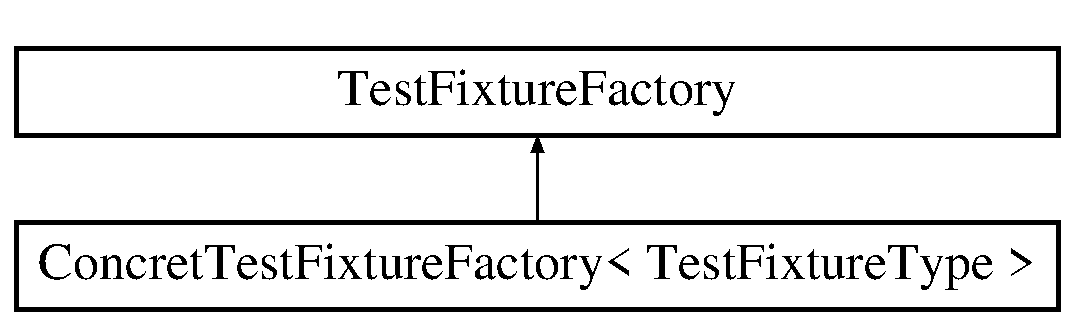
\includegraphics[height=2.000000cm]{class_concret_test_fixture_factory}
\end{center}
\end{figure}


\subsection{Detailed Description}
\subsubsection*{template$<$class Test\-Fixture\-Type$>$class Concret\-Test\-Fixture\-Factory$<$ Test\-Fixture\-Type $>$}

Concret \hyperlink{class_test_fixture}{Test\-Fixture} factory (Implementation). 

Implementation detail. Use by Helper\-Macros to handle \hyperlink{class_test_fixture}{Test\-Fixture} hierarchy. 

The documentation for this class was generated from the following file\-:\begin{DoxyCompactItemize}
\item 
X\-:/\-Git\-\_\-\-Repository/inf2990-\/06/\-Cadriciel/\-Commun/\-Externe/cppunit/include/cppunit/extensions/Test\-Fixture\-Factory.\-h\end{DoxyCompactItemize}

\hypertarget{class_config_scene}{\section{Config\-Scene Class Reference}
\label{class_config_scene}\index{Config\-Scene@{Config\-Scene}}
}


Les variables de configuration de la classe C\-Scene. C'est une classe singleton.  




{\ttfamily \#include $<$Config\-Scene.\-h$>$}

Inheritance diagram for Config\-Scene\-:\begin{figure}[H]
\begin{center}
\leavevmode
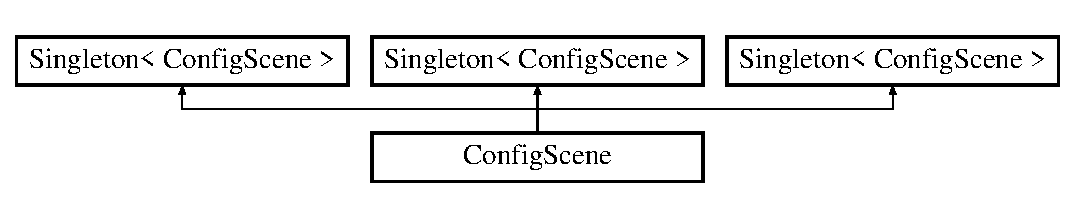
\includegraphics[height=2.000000cm]{class_config_scene}
\end{center}
\end{figure}
\subsection*{Public Member Functions}
\begin{DoxyCompactItemize}
\item 
void \hyperlink{group__inf2990_gad74111f597fd4d2f58a08c6dedcb4270}{creer\-D\-O\-M} (Ti\-Xml\-Node \&node) const 
\begin{DoxyCompactList}\small\item\em Cr�er le D\-O\-M avec les valeurs. \end{DoxyCompactList}\item 
void \hyperlink{group__inf2990_gaa29c1518d06292658bfd90d3c6d379d3}{lire\-D\-O\-M} (const Ti\-Xml\-Node \&node)
\begin{DoxyCompactList}\small\item\em Lire les valeurs du D\-O\-M. \end{DoxyCompactList}\end{DoxyCompactItemize}
\subsection*{Static Public Attributes}
\begin{DoxyCompactItemize}
\item 
static int \hyperlink{group__inf2990_gadb487b450a0314a5d1f75cf31ce502eb}{C\-A\-L\-C\-U\-L\-S\-\_\-\-P\-A\-R\-\_\-\-I\-M\-A\-G\-E} \{ 50 \}
\begin{DoxyCompactList}\small\item\em Nombre de calculs par image. \end{DoxyCompactList}\end{DoxyCompactItemize}


\subsection{Detailed Description}
Les variables de configuration de la classe C\-Scene. C'est une classe singleton. 

\begin{DoxyAuthor}{Author}
Jean-\/\-Fran�ois P�russe 
\end{DoxyAuthor}
\begin{DoxyDate}{Date}
2007-\/01-\/10 
\end{DoxyDate}


The documentation for this class was generated from the following files\-:\begin{DoxyCompactItemize}
\item 
X\-:/inf2990-\/06/\-Cadriciel/\-Sources/\-D\-L\-L/\-Configuration/\hyperlink{_config_scene_8h}{Config\-Scene.\-h}\item 
X\-:/inf2990-\/06/\-Cadriciel/\-Sources/\-D\-L\-L/\-Configuration/\hyperlink{_config_scene_8cpp}{Config\-Scene.\-cpp}\end{DoxyCompactItemize}

\hypertarget{class_config_scene_test}{\section{Config\-Scene\-Test Class Reference}
\label{class_config_scene_test}\index{Config\-Scene\-Test@{Config\-Scene\-Test}}
}


Classe de test cppunit pour tester le bon fonctionnement des m�thodes de la classe \hyperlink{class_config_scene}{Config\-Scene}.  




{\ttfamily \#include $<$Config\-Scene\-Test.\-h$>$}

Inheritance diagram for Config\-Scene\-Test\-:\begin{figure}[H]
\begin{center}
\leavevmode
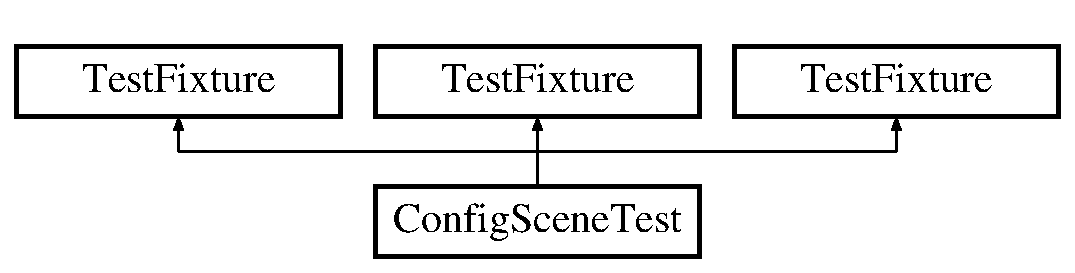
\includegraphics[height=2.000000cm]{class_config_scene_test}
\end{center}
\end{figure}
\subsection*{Public Member Functions}
\begin{DoxyCompactItemize}
\item 
void \hyperlink{group__inf2990_ga707d7400843047e67b736ab79bafb5a0}{set\-Up} ()
\begin{DoxyCompactList}\small\item\em Traitement � effectuer pour initialiser cette suite de tests. \end{DoxyCompactList}\item 
void \hyperlink{group__inf2990_ga889ed3891c3e55280cabb982953906d9}{tear\-Down} ()
\begin{DoxyCompactList}\small\item\em Traitement � effectuer pour 'finaliser' cette suite de tests. \end{DoxyCompactList}\item 
void \hyperlink{group__inf2990_ga0f09d52bc30d87f18b0341e1052efb74}{test\-Sauvegarde\-Chargement} ()
\begin{DoxyCompactList}\small\item\em Cas de test\-: sauvegarde et chargement X\-M\-L de la configuration. \end{DoxyCompactList}\end{DoxyCompactItemize}


\subsection{Detailed Description}
Classe de test cppunit pour tester le bon fonctionnement des m�thodes de la classe \hyperlink{class_config_scene}{Config\-Scene}. 

\begin{DoxyAuthor}{Author}
Julien Gascon-\/\-Samson 
\end{DoxyAuthor}
\begin{DoxyDate}{Date}
2011-\/07-\/16 
\end{DoxyDate}


The documentation for this class was generated from the following files\-:\begin{DoxyCompactItemize}
\item 
X\-:/inf2990-\/06/\-Cadriciel/\-Sources/\-D\-L\-L/\-Tests/\hyperlink{_config_scene_test_8h}{Config\-Scene\-Test.\-h}\item 
X\-:/inf2990-\/06/\-Cadriciel/\-Sources/\-D\-L\-L/\-Tests/\hyperlink{_config_scene_test_8cpp}{Config\-Scene\-Test.\-cpp}\end{DoxyCompactItemize}

\hypertarget{class_interface_graphique_1_1_configuration}{\section{Interface\-Graphique.\-Configuration Class Reference}
\label{class_interface_graphique_1_1_configuration}\index{Interface\-Graphique.\-Configuration@{Interface\-Graphique.\-Configuration}}
}


Classe qui gere les configurations du jeu  


Inheritance diagram for Interface\-Graphique.\-Configuration\-:\begin{figure}[H]
\begin{center}
\leavevmode
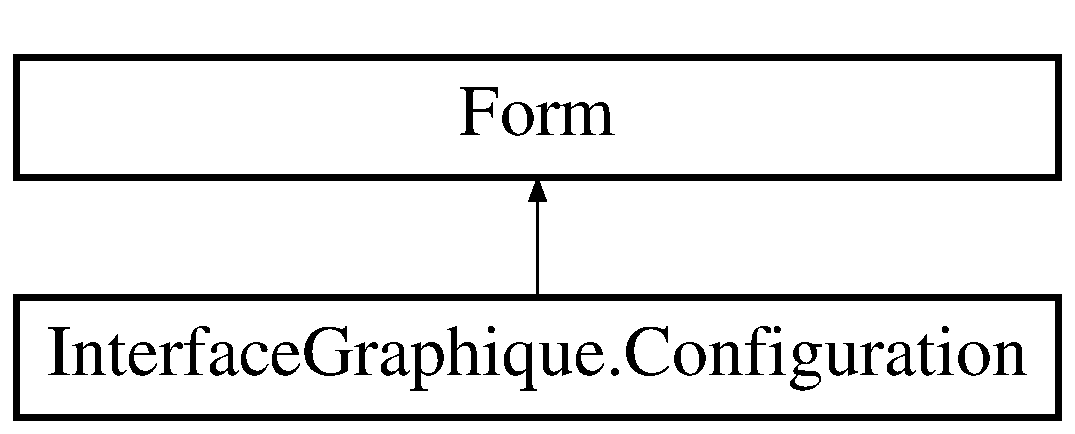
\includegraphics[height=2.000000cm]{class_interface_graphique_1_1_configuration}
\end{center}
\end{figure}
\subsection*{Public Member Functions}
\begin{DoxyCompactItemize}
\item 
\hyperlink{class_interface_graphique_1_1_configuration_adb0bf51b9f3e30cfed923c7d9d950493}{Configuration} ()
\begin{DoxyCompactList}\small\item\em Constructeur de la classe \hyperlink{class_interface_graphique_1_1_configuration}{Configuration} \end{DoxyCompactList}\item 
void \hyperlink{class_interface_graphique_1_1_configuration_ab4745548932770c8563f537213665333}{touche\-Recu} (Keys touche)
\begin{DoxyCompactList}\small\item\em Fonction appellée par touche\-Menu qui vérifie la validité de la touche reçu avant de l'assigner \end{DoxyCompactList}\item 
bool \hyperlink{class_interface_graphique_1_1_configuration_ae446d3de8050f39b3a59c25cef3b0545}{verifier\-Assignation} (int type\-Palette, Keys touche)
\begin{DoxyCompactList}\small\item\em On verifier si les touches sont deja assigneé \end{DoxyCompactList}\item 
void \hyperlink{class_interface_graphique_1_1_configuration_a00f02e8ebc64ff4e6215fa4c84608fe3}{desactiver\-Entre} ()
\begin{DoxyCompactList}\small\item\em Desactive les 5 textbox pour ne plus qu'elles soient cliquables \end{DoxyCompactList}\item 
void \hyperlink{class_interface_graphique_1_1_configuration_aee709272d249a7f4d498befdc1f481ad}{activer\-Entre} ()
\begin{DoxyCompactList}\small\item\em Active les 5 textbox pour qu'elles redeviennent cliquables \end{DoxyCompactList}\end{DoxyCompactItemize}
\subsection*{Protected Member Functions}
\begin{DoxyCompactItemize}
\item 
override void \hyperlink{class_interface_graphique_1_1_configuration_a0200b084946b5710be7d94f9e8b0385c}{Dispose} (bool disposing)
\begin{DoxyCompactList}\small\item\em Clean up any resources being used. \end{DoxyCompactList}\end{DoxyCompactItemize}


\subsection{Detailed Description}
Classe qui gere les configurations du jeu 



\subsection{Constructor \& Destructor Documentation}
\hypertarget{class_interface_graphique_1_1_configuration_adb0bf51b9f3e30cfed923c7d9d950493}{\index{Interface\-Graphique\-::\-Configuration@{Interface\-Graphique\-::\-Configuration}!Configuration@{Configuration}}
\index{Configuration@{Configuration}!InterfaceGraphique::Configuration@{Interface\-Graphique\-::\-Configuration}}
\subsubsection[{Configuration}]{\setlength{\rightskip}{0pt plus 5cm}Interface\-Graphique.\-Configuration.\-Configuration (
\begin{DoxyParamCaption}
{}
\end{DoxyParamCaption}
)\hspace{0.3cm}{\ttfamily [inline]}}}\label{class_interface_graphique_1_1_configuration_adb0bf51b9f3e30cfed923c7d9d950493}


Constructeur de la classe \hyperlink{class_interface_graphique_1_1_configuration}{Configuration} 



\subsection{Member Function Documentation}
\hypertarget{class_interface_graphique_1_1_configuration_aee709272d249a7f4d498befdc1f481ad}{\index{Interface\-Graphique\-::\-Configuration@{Interface\-Graphique\-::\-Configuration}!activer\-Entre@{activer\-Entre}}
\index{activer\-Entre@{activer\-Entre}!InterfaceGraphique::Configuration@{Interface\-Graphique\-::\-Configuration}}
\subsubsection[{activer\-Entre}]{\setlength{\rightskip}{0pt plus 5cm}void Interface\-Graphique.\-Configuration.\-activer\-Entre (
\begin{DoxyParamCaption}
{}
\end{DoxyParamCaption}
)\hspace{0.3cm}{\ttfamily [inline]}}}\label{class_interface_graphique_1_1_configuration_aee709272d249a7f4d498befdc1f481ad}


Active les 5 textbox pour qu'elles redeviennent cliquables 

\hypertarget{class_interface_graphique_1_1_configuration_a00f02e8ebc64ff4e6215fa4c84608fe3}{\index{Interface\-Graphique\-::\-Configuration@{Interface\-Graphique\-::\-Configuration}!desactiver\-Entre@{desactiver\-Entre}}
\index{desactiver\-Entre@{desactiver\-Entre}!InterfaceGraphique::Configuration@{Interface\-Graphique\-::\-Configuration}}
\subsubsection[{desactiver\-Entre}]{\setlength{\rightskip}{0pt plus 5cm}void Interface\-Graphique.\-Configuration.\-desactiver\-Entre (
\begin{DoxyParamCaption}
{}
\end{DoxyParamCaption}
)\hspace{0.3cm}{\ttfamily [inline]}}}\label{class_interface_graphique_1_1_configuration_a00f02e8ebc64ff4e6215fa4c84608fe3}


Desactive les 5 textbox pour ne plus qu'elles soient cliquables 

\hypertarget{class_interface_graphique_1_1_configuration_a0200b084946b5710be7d94f9e8b0385c}{\index{Interface\-Graphique\-::\-Configuration@{Interface\-Graphique\-::\-Configuration}!Dispose@{Dispose}}
\index{Dispose@{Dispose}!InterfaceGraphique::Configuration@{Interface\-Graphique\-::\-Configuration}}
\subsubsection[{Dispose}]{\setlength{\rightskip}{0pt plus 5cm}override void Interface\-Graphique.\-Configuration.\-Dispose (
\begin{DoxyParamCaption}
\item[{bool}]{disposing}
\end{DoxyParamCaption}
)\hspace{0.3cm}{\ttfamily [inline]}, {\ttfamily [protected]}}}\label{class_interface_graphique_1_1_configuration_a0200b084946b5710be7d94f9e8b0385c}


Clean up any resources being used. 


\begin{DoxyParams}{Parameters}
{\em disposing} & true if managed resources should be disposed; otherwise, false.\\
\hline
\end{DoxyParams}
\hypertarget{class_interface_graphique_1_1_configuration_ab4745548932770c8563f537213665333}{\index{Interface\-Graphique\-::\-Configuration@{Interface\-Graphique\-::\-Configuration}!touche\-Recu@{touche\-Recu}}
\index{touche\-Recu@{touche\-Recu}!InterfaceGraphique::Configuration@{Interface\-Graphique\-::\-Configuration}}
\subsubsection[{touche\-Recu}]{\setlength{\rightskip}{0pt plus 5cm}void Interface\-Graphique.\-Configuration.\-touche\-Recu (
\begin{DoxyParamCaption}
\item[{Keys}]{touche}
\end{DoxyParamCaption}
)\hspace{0.3cm}{\ttfamily [inline]}}}\label{class_interface_graphique_1_1_configuration_ab4745548932770c8563f537213665333}


Fonction appellée par touche\-Menu qui vérifie la validité de la touche reçu avant de l'assigner 


\begin{DoxyParams}{Parameters}
{\em touche} & \\
\hline
\end{DoxyParams}
\hypertarget{class_interface_graphique_1_1_configuration_ae446d3de8050f39b3a59c25cef3b0545}{\index{Interface\-Graphique\-::\-Configuration@{Interface\-Graphique\-::\-Configuration}!verifier\-Assignation@{verifier\-Assignation}}
\index{verifier\-Assignation@{verifier\-Assignation}!InterfaceGraphique::Configuration@{Interface\-Graphique\-::\-Configuration}}
\subsubsection[{verifier\-Assignation}]{\setlength{\rightskip}{0pt plus 5cm}bool Interface\-Graphique.\-Configuration.\-verifier\-Assignation (
\begin{DoxyParamCaption}
\item[{int}]{type\-Palette, }
\item[{Keys}]{touche}
\end{DoxyParamCaption}
)\hspace{0.3cm}{\ttfamily [inline]}}}\label{class_interface_graphique_1_1_configuration_ae446d3de8050f39b3a59c25cef3b0545}


On verifier si les touches sont deja assigneé 


\begin{DoxyParams}{Parameters}
{\em type\-Palette} & Le type de touche que l'on verifie\\
\hline
{\em touche} & La touche que l'on veut verifier\\
\hline
\end{DoxyParams}
\begin{DoxyReturn}{Returns}
Vrai si la touche est deja assignée, faux sinon
\end{DoxyReturn}


The documentation for this class was generated from the following files\-:\begin{DoxyCompactItemize}
\item 
X\-:/inf2990-\/06/\-Cadriciel/\-Sources/\-Interface\-Graphique/\hyperlink{_configuration_8cs}{Configuration.\-cs}\item 
X\-:/inf2990-\/06/\-Cadriciel/\-Sources/\-Interface\-Graphique/\hyperlink{_configuration_8_designer_8cs}{Configuration.\-Designer.\-cs}\end{DoxyCompactItemize}

\hypertarget{class_interface_graphique_1_1_configuration_partie}{\section{Interface\-Graphique.\-Configuration\-Partie Class Reference}
\label{class_interface_graphique_1_1_configuration_partie}\index{Interface\-Graphique.\-Configuration\-Partie@{Interface\-Graphique.\-Configuration\-Partie}}
}


Cette classe représente les configurations associés a une partie Rapide ou a un campagne  


\subsection*{Public Member Functions}
\begin{DoxyCompactItemize}
\item 
\hyperlink{class_interface_graphique_1_1_configuration_partie_ad76acf6af1265023c8184da2825994e9}{Configuration\-Partie} ()
\begin{DoxyCompactList}\small\item\em constructeur pour une partie\-Rapide \end{DoxyCompactList}\end{DoxyCompactItemize}
\subsection*{Public Attributes}
\begin{DoxyCompactItemize}
\item 
bool \hyperlink{class_interface_graphique_1_1_configuration_partie_a166c6a679593d7f6ceb8d6ed4a7a3eff}{joueur\-Virtuel\-\_\-}
\begin{DoxyCompactList}\small\item\em type de partie\-Rapide multijouer défini par l'utilisateur dans le menu de configuration de partie\-Rapide \end{DoxyCompactList}\item 
\hypertarget{class_interface_graphique_1_1_configuration_partie_a039f0afcee48e4f3ccfe5f4211a6e6a6}{bool {\bfseries est\-Multiplayer\-\_\-}}\label{class_interface_graphique_1_1_configuration_partie_a039f0afcee48e4f3ccfe5f4211a6e6a6}

\item 
int \hyperlink{class_interface_graphique_1_1_configuration_partie_afdda795c3afe6be9b08d78fa5cc67077}{billes\-Initialles\-\_\-}
\begin{DoxyCompactList}\small\item\em billes initiales par partie\-Rapide déterminé dans le fichier de configurations Config.\-txt \end{DoxyCompactList}\end{DoxyCompactItemize}


\subsection{Detailed Description}
Cette classe représente les configurations associés a une partie Rapide ou a un campagne 



\subsection{Constructor \& Destructor Documentation}
\hypertarget{class_interface_graphique_1_1_configuration_partie_ad76acf6af1265023c8184da2825994e9}{\index{Interface\-Graphique\-::\-Configuration\-Partie@{Interface\-Graphique\-::\-Configuration\-Partie}!Configuration\-Partie@{Configuration\-Partie}}
\index{Configuration\-Partie@{Configuration\-Partie}!InterfaceGraphique::ConfigurationPartie@{Interface\-Graphique\-::\-Configuration\-Partie}}
\subsubsection[{Configuration\-Partie}]{\setlength{\rightskip}{0pt plus 5cm}Interface\-Graphique.\-Configuration\-Partie.\-Configuration\-Partie (
\begin{DoxyParamCaption}
{}
\end{DoxyParamCaption}
)\hspace{0.3cm}{\ttfamily [inline]}}}\label{class_interface_graphique_1_1_configuration_partie_ad76acf6af1265023c8184da2825994e9}


constructeur pour une partie\-Rapide 



\subsection{Member Data Documentation}
\hypertarget{class_interface_graphique_1_1_configuration_partie_afdda795c3afe6be9b08d78fa5cc67077}{\index{Interface\-Graphique\-::\-Configuration\-Partie@{Interface\-Graphique\-::\-Configuration\-Partie}!billes\-Initialles\-\_\-@{billes\-Initialles\-\_\-}}
\index{billes\-Initialles\-\_\-@{billes\-Initialles\-\_\-}!InterfaceGraphique::ConfigurationPartie@{Interface\-Graphique\-::\-Configuration\-Partie}}
\subsubsection[{billes\-Initialles\-\_\-}]{\setlength{\rightskip}{0pt plus 5cm}int Interface\-Graphique.\-Configuration\-Partie.\-billes\-Initialles\-\_\-}}\label{class_interface_graphique_1_1_configuration_partie_afdda795c3afe6be9b08d78fa5cc67077}


billes initiales par partie\-Rapide déterminé dans le fichier de configurations Config.\-txt 

\hypertarget{class_interface_graphique_1_1_configuration_partie_a166c6a679593d7f6ceb8d6ed4a7a3eff}{\index{Interface\-Graphique\-::\-Configuration\-Partie@{Interface\-Graphique\-::\-Configuration\-Partie}!joueur\-Virtuel\-\_\-@{joueur\-Virtuel\-\_\-}}
\index{joueur\-Virtuel\-\_\-@{joueur\-Virtuel\-\_\-}!InterfaceGraphique::ConfigurationPartie@{Interface\-Graphique\-::\-Configuration\-Partie}}
\subsubsection[{joueur\-Virtuel\-\_\-}]{\setlength{\rightskip}{0pt plus 5cm}bool Interface\-Graphique.\-Configuration\-Partie.\-joueur\-Virtuel\-\_\-}}\label{class_interface_graphique_1_1_configuration_partie_a166c6a679593d7f6ceb8d6ed4a7a3eff}


type de partie\-Rapide multijouer défini par l'utilisateur dans le menu de configuration de partie\-Rapide 



The documentation for this class was generated from the following file\-:\begin{DoxyCompactItemize}
\item 
X\-:/\-Git\-\_\-\-Repository/inf2990-\/06/\-Cadriciel/\-Sources/\-Interface\-Graphique/Configuration\-Partie.\-cs\end{DoxyCompactItemize}

\hypertarget{class_interface_graphique_1_1_configurer_partie_rapide}{\section{Interface\-Graphique.\-Configurer\-Partie\-Rapide Class Reference}
\label{class_interface_graphique_1_1_configurer_partie_rapide}\index{Interface\-Graphique.\-Configurer\-Partie\-Rapide@{Interface\-Graphique.\-Configurer\-Partie\-Rapide}}
}


Cette classe représente le menu de préparation d'une partie rapide  


Inheritance diagram for Interface\-Graphique.\-Configurer\-Partie\-Rapide\-:\begin{figure}[H]
\begin{center}
\leavevmode
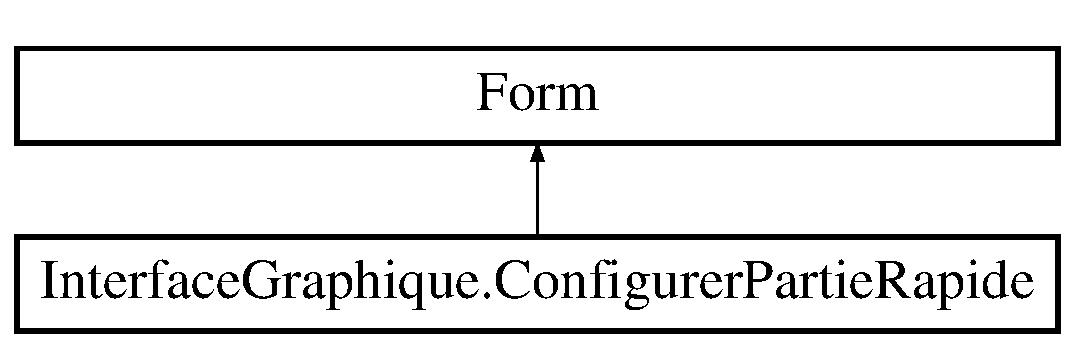
\includegraphics[height=2.000000cm]{class_interface_graphique_1_1_configurer_partie_rapide}
\end{center}
\end{figure}
\subsection*{Classes}
\begin{DoxyCompactItemize}
\item 
class \hyperlink{class_interface_graphique_1_1_configurer_partie_rapide_1_1_combo_box_item}{Combo\-Box\-Item}
\begin{DoxyCompactList}\small\item\em Redefinition d'un item de Combo\-Box \end{DoxyCompactList}\end{DoxyCompactItemize}
\subsection*{Public Member Functions}
\begin{DoxyCompactItemize}
\item 
\hyperlink{class_interface_graphique_1_1_configurer_partie_rapide_a3e4cee4d4699fc886275a34c7bd52009}{Configurer\-Partie\-Rapide} ()
\begin{DoxyCompactList}\small\item\em constructeur par default \end{DoxyCompactList}\item 
void \hyperlink{class_interface_graphique_1_1_configurer_partie_rapide_a9d6f766fc8fd2f1e4ff8913588d044e4}{demarer\-Partie\-Simple} ()
\end{DoxyCompactItemize}
\subsection*{Protected Member Functions}
\begin{DoxyCompactItemize}
\item 
override void \hyperlink{class_interface_graphique_1_1_configurer_partie_rapide_a6d53323e7a069f493c34c894594911a0}{Dispose} (bool disposing)
\begin{DoxyCompactList}\small\item\em Clean up any resources being used. \end{DoxyCompactList}\end{DoxyCompactItemize}


\subsection{Detailed Description}
Cette classe représente le menu de préparation d'une partie rapide 



\subsection{Constructor \& Destructor Documentation}
\hypertarget{class_interface_graphique_1_1_configurer_partie_rapide_a3e4cee4d4699fc886275a34c7bd52009}{\index{Interface\-Graphique\-::\-Configurer\-Partie\-Rapide@{Interface\-Graphique\-::\-Configurer\-Partie\-Rapide}!Configurer\-Partie\-Rapide@{Configurer\-Partie\-Rapide}}
\index{Configurer\-Partie\-Rapide@{Configurer\-Partie\-Rapide}!InterfaceGraphique::ConfigurerPartieRapide@{Interface\-Graphique\-::\-Configurer\-Partie\-Rapide}}
\subsubsection[{Configurer\-Partie\-Rapide}]{\setlength{\rightskip}{0pt plus 5cm}Interface\-Graphique.\-Configurer\-Partie\-Rapide.\-Configurer\-Partie\-Rapide (
\begin{DoxyParamCaption}
{}
\end{DoxyParamCaption}
)\hspace{0.3cm}{\ttfamily [inline]}}}\label{class_interface_graphique_1_1_configurer_partie_rapide_a3e4cee4d4699fc886275a34c7bd52009}


constructeur par default 



\subsection{Member Function Documentation}
\hypertarget{class_interface_graphique_1_1_configurer_partie_rapide_a9d6f766fc8fd2f1e4ff8913588d044e4}{\index{Interface\-Graphique\-::\-Configurer\-Partie\-Rapide@{Interface\-Graphique\-::\-Configurer\-Partie\-Rapide}!demarer\-Partie\-Simple@{demarer\-Partie\-Simple}}
\index{demarer\-Partie\-Simple@{demarer\-Partie\-Simple}!InterfaceGraphique::ConfigurerPartieRapide@{Interface\-Graphique\-::\-Configurer\-Partie\-Rapide}}
\subsubsection[{demarer\-Partie\-Simple}]{\setlength{\rightskip}{0pt plus 5cm}void Interface\-Graphique.\-Configurer\-Partie\-Rapide.\-demarer\-Partie\-Simple (
\begin{DoxyParamCaption}
{}
\end{DoxyParamCaption}
)\hspace{0.3cm}{\ttfamily [inline]}}}\label{class_interface_graphique_1_1_configurer_partie_rapide_a9d6f766fc8fd2f1e4ff8913588d044e4}
\hypertarget{class_interface_graphique_1_1_configurer_partie_rapide_a6d53323e7a069f493c34c894594911a0}{\index{Interface\-Graphique\-::\-Configurer\-Partie\-Rapide@{Interface\-Graphique\-::\-Configurer\-Partie\-Rapide}!Dispose@{Dispose}}
\index{Dispose@{Dispose}!InterfaceGraphique::ConfigurerPartieRapide@{Interface\-Graphique\-::\-Configurer\-Partie\-Rapide}}
\subsubsection[{Dispose}]{\setlength{\rightskip}{0pt plus 5cm}override void Interface\-Graphique.\-Configurer\-Partie\-Rapide.\-Dispose (
\begin{DoxyParamCaption}
\item[{bool}]{disposing}
\end{DoxyParamCaption}
)\hspace{0.3cm}{\ttfamily [inline]}, {\ttfamily [protected]}}}\label{class_interface_graphique_1_1_configurer_partie_rapide_a6d53323e7a069f493c34c894594911a0}


Clean up any resources being used. 


\begin{DoxyParams}{Parameters}
{\em disposing} & true if managed resources should be disposed; otherwise, false.\\
\hline
\end{DoxyParams}


The documentation for this class was generated from the following files\-:\begin{DoxyCompactItemize}
\item 
X\-:/inf2990-\/06/\-Cadriciel/\-Sources/\-Interface\-Graphique/\hyperlink{_menu_partie_rapide_8cs}{Menu\-Partie\-Rapide.\-cs}\item 
X\-:/inf2990-\/06/\-Cadriciel/\-Sources/\-Interface\-Graphique/\hyperlink{_menu_partie_rapide_8_designer_8cs}{Menu\-Partie\-Rapide.\-Designer.\-cs}\end{DoxyCompactItemize}

\hypertarget{struct_cpp_unit_test_plug_in}{\section{Cpp\-Unit\-Test\-Plug\-In Struct Reference}
\label{struct_cpp_unit_test_plug_in}\index{Cpp\-Unit\-Test\-Plug\-In@{Cpp\-Unit\-Test\-Plug\-In}}
}


\hyperlink{class_test}{Test} plug-\/in interface.

This class define the interface implemented by test plug-\/in. A pointer to that interface is returned by the function exported by the test plug-\/in.  




{\ttfamily \#include $<$Test\-Plug\-In.\-h$>$}

Inheritance diagram for Cpp\-Unit\-Test\-Plug\-In\-:\begin{figure}[H]
\begin{center}
\leavevmode
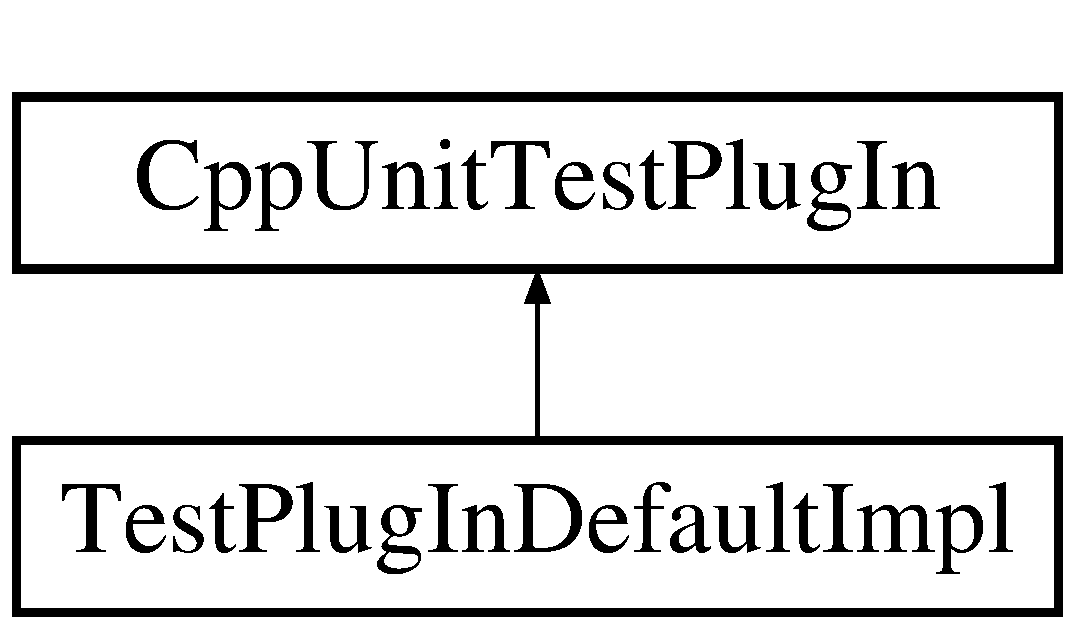
\includegraphics[height=2.000000cm]{struct_cpp_unit_test_plug_in}
\end{center}
\end{figure}
\subsection*{Public Member Functions}
\begin{DoxyCompactItemize}
\item 
virtual void \hyperlink{struct_cpp_unit_test_plug_in_aec670330e7fced26c2a66b1dcd56edc0}{initialize} (C\-P\-P\-U\-N\-I\-T\-\_\-\-N\-S\-::\-Test\-Factory\-Registry $\ast$registry, const C\-P\-P\-U\-N\-I\-T\-\_\-\-N\-S\-::\-Plug\-In\-Parameters \&parameters)=0
\begin{DoxyCompactList}\small\item\em Called just after loading the dynamic library. \end{DoxyCompactList}\item 
virtual void \hyperlink{struct_cpp_unit_test_plug_in_aad8038dc72d0f9798379937fe5692c97}{add\-Listener} (C\-P\-P\-U\-N\-I\-T\-\_\-\-N\-S\-::\-Test\-Result $\ast$event\-Manager)=0
\begin{DoxyCompactList}\small\item\em Gives a chance to the plug-\/in to register \hyperlink{class_test_listener}{Test\-Listener}. \end{DoxyCompactList}\item 
virtual void \hyperlink{struct_cpp_unit_test_plug_in_a8f36157014b515d38efbc8ab67923d85}{remove\-Listener} (C\-P\-P\-U\-N\-I\-T\-\_\-\-N\-S\-::\-Test\-Result $\ast$event\-Manager)=0
\begin{DoxyCompactList}\small\item\em Gives a chance to the plug-\/in to remove its registered \hyperlink{class_test_listener}{Test\-Listener}. \end{DoxyCompactList}\item 
\hypertarget{struct_cpp_unit_test_plug_in_a547cfddd0513dc9182721f723e27d9e3}{virtual void \hyperlink{struct_cpp_unit_test_plug_in_a547cfddd0513dc9182721f723e27d9e3}{add\-Xml\-Outputter\-Hooks} (C\-P\-P\-U\-N\-I\-T\-\_\-\-N\-S\-::\-Xml\-Outputter $\ast$outputter)=0}\label{struct_cpp_unit_test_plug_in_a547cfddd0513dc9182721f723e27d9e3}

\begin{DoxyCompactList}\small\item\em Provides a way for the plug-\/in to register some \hyperlink{class_xml_outputter_hook}{Xml\-Outputter\-Hook}. \end{DoxyCompactList}\item 
virtual void \hyperlink{struct_cpp_unit_test_plug_in_a045727ad9658525838b0b9157065fbcd}{remove\-Xml\-Outputter\-Hooks} ()=0
\begin{DoxyCompactList}\small\item\em Called when the \hyperlink{class_xml_outputter}{Xml\-Outputter} is destroyed. \end{DoxyCompactList}\item 
virtual void \hyperlink{struct_cpp_unit_test_plug_in_a8628d2026e76c58f715e17af88f77458}{uninitialize} (C\-P\-P\-U\-N\-I\-T\-\_\-\-N\-S\-::\-Test\-Factory\-Registry $\ast$registry)=0
\begin{DoxyCompactList}\small\item\em Called just before unloading the dynamic library. \end{DoxyCompactList}\end{DoxyCompactItemize}


\subsection{Detailed Description}
\hyperlink{class_test}{Test} plug-\/in interface.

This class define the interface implemented by test plug-\/in. A pointer to that interface is returned by the function exported by the test plug-\/in. 

Plug-\/in are loaded/unloaded by \hyperlink{class_plug_in_manager}{Plug\-In\-Manager}. When a plug-\/in is loaded, \hyperlink{struct_cpp_unit_test_plug_in_aec670330e7fced26c2a66b1dcd56edc0}{initialize()} is called. Before unloading the plug-\/in, the \hyperlink{class_plug_in_manager}{Plug\-In\-Manager} call \hyperlink{struct_cpp_unit_test_plug_in_a8628d2026e76c58f715e17af88f77458}{uninitialize()}.

\hyperlink{struct_cpp_unit_test_plug_in_aad8038dc72d0f9798379937fe5692c97}{add\-Listener()} and \hyperlink{struct_cpp_unit_test_plug_in_a8f36157014b515d38efbc8ab67923d85}{remove\-Listener()} are called respectively before and after the test run.

\hyperlink{struct_cpp_unit_test_plug_in_a547cfddd0513dc9182721f723e27d9e3}{add\-Xml\-Outputter\-Hooks()} and \hyperlink{struct_cpp_unit_test_plug_in_a045727ad9658525838b0b9157065fbcd}{remove\-Xml\-Outputter\-Hooks()} are called respectively before and after writing the X\-M\-L output using a \hyperlink{class_xml_outputter}{Xml\-Outputter}.

\begin{DoxySeeAlso}{See Also}
\hyperlink{_test_plug_in_8h_a705897c323d9381ac1b99a45e953e4ff}{C\-P\-P\-U\-N\-I\-T\-\_\-\-P\-L\-U\-G\-I\-N\-\_\-\-I\-M\-P\-L\-E\-M\-E\-N\-T}, \hyperlink{_test_plug_in_8h_a81bfba0323e2c7ca7dfd6767db813a5b}{C\-P\-P\-U\-N\-I\-T\-\_\-\-P\-L\-U\-G\-I\-N\-\_\-\-E\-X\-P\-O\-R\-T\-E\-D\-\_\-\-F\-U\-N\-C\-T\-I\-O\-N\-\_\-\-I\-M\-P\-L} 

Cpp\-Unit\-::\-Test\-Plug\-In\-Default\-Impl, Cpp\-Unit\-::\-Xml\-Outputter. 
\end{DoxySeeAlso}


\subsection{Member Function Documentation}
\hypertarget{struct_cpp_unit_test_plug_in_aad8038dc72d0f9798379937fe5692c97}{\index{Cpp\-Unit\-Test\-Plug\-In@{Cpp\-Unit\-Test\-Plug\-In}!add\-Listener@{add\-Listener}}
\index{add\-Listener@{add\-Listener}!CppUnitTestPlugIn@{Cpp\-Unit\-Test\-Plug\-In}}
\subsubsection[{add\-Listener}]{\setlength{\rightskip}{0pt plus 5cm}virtual void Cpp\-Unit\-Test\-Plug\-In\-::add\-Listener (
\begin{DoxyParamCaption}
\item[{C\-P\-P\-U\-N\-I\-T\-\_\-\-N\-S\-::\-Test\-Result $\ast$}]{event\-Manager}
\end{DoxyParamCaption}
)\hspace{0.3cm}{\ttfamily [pure virtual]}}}\label{struct_cpp_unit_test_plug_in_aad8038dc72d0f9798379937fe5692c97}


Gives a chance to the plug-\/in to register \hyperlink{class_test_listener}{Test\-Listener}. 

Override this method to add a \hyperlink{class_test_listener}{Test\-Listener} for the test run. This is useful if you are writing a custom \hyperlink{class_test_listener}{Test\-Listener}, but also if you need to set\-Up some global resource\-: listen to \hyperlink{class_test_listener_a263428abdf29b2a7123af4096771925e}{Test\-Listener\-::start\-Test\-Run()}, and \hyperlink{class_test_listener_a0411708032f688f6ec234bcc5e089289}{Test\-Listener\-::end\-Test\-Run()}. \hypertarget{struct_cpp_unit_test_plug_in_aec670330e7fced26c2a66b1dcd56edc0}{\index{Cpp\-Unit\-Test\-Plug\-In@{Cpp\-Unit\-Test\-Plug\-In}!initialize@{initialize}}
\index{initialize@{initialize}!CppUnitTestPlugIn@{Cpp\-Unit\-Test\-Plug\-In}}
\subsubsection[{initialize}]{\setlength{\rightskip}{0pt plus 5cm}virtual void Cpp\-Unit\-Test\-Plug\-In\-::initialize (
\begin{DoxyParamCaption}
\item[{C\-P\-P\-U\-N\-I\-T\-\_\-\-N\-S\-::\-Test\-Factory\-Registry $\ast$}]{registry, }
\item[{const C\-P\-P\-U\-N\-I\-T\-\_\-\-N\-S\-::\-Plug\-In\-Parameters \&}]{parameters}
\end{DoxyParamCaption}
)\hspace{0.3cm}{\ttfamily [pure virtual]}}}\label{struct_cpp_unit_test_plug_in_aec670330e7fced26c2a66b1dcd56edc0}


Called just after loading the dynamic library. 

Override this method to add additional suite to the registry, though this is preferably done using the macros (C\-P\-P\-U\-N\-I\-T\-\_\-\-T\-E\-S\-T\-\_\-\-S\-U\-I\-T\-E\-\_\-\-R\-E\-G\-I\-S\-T\-R\-A\-T\-I\-O\-N...). If you are creating a custom listener to extends the plug-\/in runner, you can use this to configure the listener using the {\itshape parameters}.

You could also use the parameters to specify some global parameter, such as test datas location, database name...

N.\-B.\-: Parameters interface is not define yet, and the plug-\/in runner does not yet support plug-\/in parameter. \hypertarget{struct_cpp_unit_test_plug_in_a8f36157014b515d38efbc8ab67923d85}{\index{Cpp\-Unit\-Test\-Plug\-In@{Cpp\-Unit\-Test\-Plug\-In}!remove\-Listener@{remove\-Listener}}
\index{remove\-Listener@{remove\-Listener}!CppUnitTestPlugIn@{Cpp\-Unit\-Test\-Plug\-In}}
\subsubsection[{remove\-Listener}]{\setlength{\rightskip}{0pt plus 5cm}virtual void Cpp\-Unit\-Test\-Plug\-In\-::remove\-Listener (
\begin{DoxyParamCaption}
\item[{C\-P\-P\-U\-N\-I\-T\-\_\-\-N\-S\-::\-Test\-Result $\ast$}]{event\-Manager}
\end{DoxyParamCaption}
)\hspace{0.3cm}{\ttfamily [pure virtual]}}}\label{struct_cpp_unit_test_plug_in_a8f36157014b515d38efbc8ab67923d85}


Gives a chance to the plug-\/in to remove its registered \hyperlink{class_test_listener}{Test\-Listener}. 

Override this method to remove a \hyperlink{class_test_listener}{Test\-Listener} that has been added. \hypertarget{struct_cpp_unit_test_plug_in_a045727ad9658525838b0b9157065fbcd}{\index{Cpp\-Unit\-Test\-Plug\-In@{Cpp\-Unit\-Test\-Plug\-In}!remove\-Xml\-Outputter\-Hooks@{remove\-Xml\-Outputter\-Hooks}}
\index{remove\-Xml\-Outputter\-Hooks@{remove\-Xml\-Outputter\-Hooks}!CppUnitTestPlugIn@{Cpp\-Unit\-Test\-Plug\-In}}
\subsubsection[{remove\-Xml\-Outputter\-Hooks}]{\setlength{\rightskip}{0pt plus 5cm}virtual void Cpp\-Unit\-Test\-Plug\-In\-::remove\-Xml\-Outputter\-Hooks (
\begin{DoxyParamCaption}
{}
\end{DoxyParamCaption}
)\hspace{0.3cm}{\ttfamily [pure virtual]}}}\label{struct_cpp_unit_test_plug_in_a045727ad9658525838b0b9157065fbcd}


Called when the \hyperlink{class_xml_outputter}{Xml\-Outputter} is destroyed. 

Can be used to free some resources allocated by \hyperlink{struct_cpp_unit_test_plug_in_a547cfddd0513dc9182721f723e27d9e3}{add\-Xml\-Outputter\-Hooks()}. 

Implemented in \hyperlink{class_test_plug_in_default_impl_aa4fa891e799ff362dece734417afd93d}{Test\-Plug\-In\-Default\-Impl}.

\hypertarget{struct_cpp_unit_test_plug_in_a8628d2026e76c58f715e17af88f77458}{\index{Cpp\-Unit\-Test\-Plug\-In@{Cpp\-Unit\-Test\-Plug\-In}!uninitialize@{uninitialize}}
\index{uninitialize@{uninitialize}!CppUnitTestPlugIn@{Cpp\-Unit\-Test\-Plug\-In}}
\subsubsection[{uninitialize}]{\setlength{\rightskip}{0pt plus 5cm}virtual void Cpp\-Unit\-Test\-Plug\-In\-::uninitialize (
\begin{DoxyParamCaption}
\item[{C\-P\-P\-U\-N\-I\-T\-\_\-\-N\-S\-::\-Test\-Factory\-Registry $\ast$}]{registry}
\end{DoxyParamCaption}
)\hspace{0.3cm}{\ttfamily [pure virtual]}}}\label{struct_cpp_unit_test_plug_in_a8628d2026e76c58f715e17af88f77458}


Called just before unloading the dynamic library. 

Override this method to unregister test factory added in \hyperlink{struct_cpp_unit_test_plug_in_aec670330e7fced26c2a66b1dcd56edc0}{initialize()}. This is necessary to keep the \hyperlink{class_test_factory_registry}{Test\-Factory\-Registry} 'clean'. When the plug-\/in is unloaded from memory, the \hyperlink{class_test_factory_registry}{Test\-Factory\-Registry} will hold reference on test that are no longer available if they are not unregistered. 

The documentation for this struct was generated from the following file\-:\begin{DoxyCompactItemize}
\item 
X\-:/\-Git\-\_\-\-Repository/inf2990-\/06/\-Cadriciel/\-Commun/\-Externe/cppunit/include/cppunit/plugin/\hyperlink{_test_plug_in_8h}{Test\-Plug\-In.\-h}\end{DoxyCompactItemize}

\hypertarget{classmodele_1_1opengl__storage_1_1_c_p_u___local}{\section{modele\-:\-:opengl\-\_\-storage\-:\-:C\-P\-U\-\_\-\-Local Class Reference}
\label{classmodele_1_1opengl__storage_1_1_c_p_u___local}\index{modele\-::opengl\-\_\-storage\-::\-C\-P\-U\-\_\-\-Local@{modele\-::opengl\-\_\-storage\-::\-C\-P\-U\-\_\-\-Local}}
}


Classe permettant le dessin d'un mod�le 3\-D sans aucun storage de donn�es ou de commandes sur la carte graphique.  




{\ttfamily \#include $<$Modele\-Storage\-\_\-\-C\-P\-U\-\_\-\-Local.\-h$>$}

Inheritance diagram for modele\-:\-:opengl\-\_\-storage\-:\-:C\-P\-U\-\_\-\-Local\-:\begin{figure}[H]
\begin{center}
\leavevmode
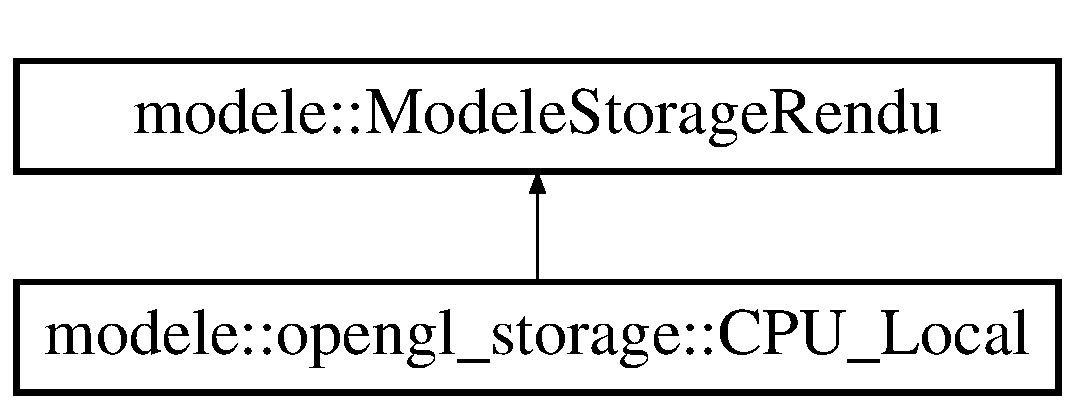
\includegraphics[height=2.000000cm]{classmodele_1_1opengl__storage_1_1_c_p_u___local}
\end{center}
\end{figure}
\subsection*{Public Member Functions}
\begin{DoxyCompactItemize}
\item 
\hyperlink{classmodele_1_1opengl__storage_1_1_c_p_u___local_aaa48c88ccc96c34d9d675e73fb61ea38}{C\-P\-U\-\_\-\-Local} (\hyperlink{classmodele_1_1_modele3_d}{Modele3\-D} const $\ast$modele)
\begin{DoxyCompactList}\small\item\em Constructeur avec un mod�le 3\-D. \end{DoxyCompactList}\item 
\hypertarget{classmodele_1_1opengl__storage_1_1_c_p_u___local_abbaf316597e944add4b77e086e85d714}{virtual \hyperlink{classmodele_1_1opengl__storage_1_1_c_p_u___local_abbaf316597e944add4b77e086e85d714}{$\sim$\-C\-P\-U\-\_\-\-Local} ()=default}\label{classmodele_1_1opengl__storage_1_1_c_p_u___local_abbaf316597e944add4b77e086e85d714}

\begin{DoxyCompactList}\small\item\em Destructeur. \end{DoxyCompactList}\item 
virtual void \hyperlink{classmodele_1_1opengl__storage_1_1_c_p_u___local_ab7ae42c342ffdd157d4c7e413137c5da}{storage\-Charger} () override
\begin{DoxyCompactList}\small\item\em Permet de charger les donn�es/commandes sur la carte graphique. \end{DoxyCompactList}\item 
virtual void \hyperlink{classmodele_1_1opengl__storage_1_1_c_p_u___local_a3893c680fbb641f8f144cbc6af33e369}{dessiner} () const override
\begin{DoxyCompactList}\small\item\em Permet d'effectuer le dessin du mod�le 3\-D. \end{DoxyCompactList}\item 
virtual void \hyperlink{classmodele_1_1opengl__storage_1_1_c_p_u___local_a410e8079fb689eac8874ce3d401415c5}{storage\-Relacher} () override
\begin{DoxyCompactList}\small\item\em Permet de rel�cher les donn�es/commandes sur la crate graphique. \end{DoxyCompactList}\end{DoxyCompactItemize}


\subsection{Detailed Description}
Classe permettant le dessin d'un mod�le 3\-D sans aucun storage de donn�es ou de commandes sur la carte graphique. 

\begin{DoxyNote}{Note}
Pr�condition \-: prends pour acquis que le pointeur vers le mod�le 3\-D reste valide durant toute la dur�e de vie du storage.
\end{DoxyNote}
\begin{DoxyAuthor}{Author}
Martin Paradis 
\end{DoxyAuthor}
\begin{DoxyDate}{Date}
2014-\/08-\/16 
\end{DoxyDate}


\subsection{Constructor \& Destructor Documentation}
\hypertarget{classmodele_1_1opengl__storage_1_1_c_p_u___local_aaa48c88ccc96c34d9d675e73fb61ea38}{\index{modele\-::opengl\-\_\-storage\-::\-C\-P\-U\-\_\-\-Local@{modele\-::opengl\-\_\-storage\-::\-C\-P\-U\-\_\-\-Local}!C\-P\-U\-\_\-\-Local@{C\-P\-U\-\_\-\-Local}}
\index{C\-P\-U\-\_\-\-Local@{C\-P\-U\-\_\-\-Local}!modele::opengl_storage::CPU_Local@{modele\-::opengl\-\_\-storage\-::\-C\-P\-U\-\_\-\-Local}}
\subsubsection[{C\-P\-U\-\_\-\-Local}]{\setlength{\rightskip}{0pt plus 5cm}modele\-::opengl\-\_\-storage\-::\-C\-P\-U\-\_\-\-Local\-::\-C\-P\-U\-\_\-\-Local (
\begin{DoxyParamCaption}
\item[{{\bf Modele3\-D} const $\ast$}]{modele}
\end{DoxyParamCaption}
)}}\label{classmodele_1_1opengl__storage_1_1_c_p_u___local_aaa48c88ccc96c34d9d675e73fb61ea38}


Constructeur avec un mod�le 3\-D. 

Construit un storage local pour le dessin d'un mod�le 3\-D. Ne charge aucune donn�e sur la carte graphique et utilise les commandes de dessins (d�pr�ci�es) d'Open\-G\-L pour dessiner le mod�le 3\-D.


\begin{DoxyParams}[1]{Parameters}
\mbox{\tt in}  & {\em modele} & \-: le mod�le � dessiner.\\
\hline
\end{DoxyParams}
\begin{DoxyReturn}{Returns}
Aucune. 
\end{DoxyReturn}


\subsection{Member Function Documentation}
\hypertarget{classmodele_1_1opengl__storage_1_1_c_p_u___local_a3893c680fbb641f8f144cbc6af33e369}{\index{modele\-::opengl\-\_\-storage\-::\-C\-P\-U\-\_\-\-Local@{modele\-::opengl\-\_\-storage\-::\-C\-P\-U\-\_\-\-Local}!dessiner@{dessiner}}
\index{dessiner@{dessiner}!modele::opengl_storage::CPU_Local@{modele\-::opengl\-\_\-storage\-::\-C\-P\-U\-\_\-\-Local}}
\subsubsection[{dessiner}]{\setlength{\rightskip}{0pt plus 5cm}void modele\-::opengl\-\_\-storage\-::\-C\-P\-U\-\_\-\-Local\-::dessiner (
\begin{DoxyParamCaption}
{}
\end{DoxyParamCaption}
) const\hspace{0.3cm}{\ttfamily [override]}, {\ttfamily [virtual]}}}\label{classmodele_1_1opengl__storage_1_1_c_p_u___local_a3893c680fbb641f8f144cbc6af33e369}


Permet d'effectuer le dessin du mod�le 3\-D. 

Dessine le mod�le 3\-D � partir de son noeud racine.

\begin{DoxyReturn}{Returns}
Aucune. 
\end{DoxyReturn}


Implements \hyperlink{classmodele_1_1_modele_storage_rendu_ad28207f3142e8adcb054d119fd3a3ce1}{modele\-::\-Modele\-Storage\-Rendu}.

\hypertarget{classmodele_1_1opengl__storage_1_1_c_p_u___local_ab7ae42c342ffdd157d4c7e413137c5da}{\index{modele\-::opengl\-\_\-storage\-::\-C\-P\-U\-\_\-\-Local@{modele\-::opengl\-\_\-storage\-::\-C\-P\-U\-\_\-\-Local}!storage\-Charger@{storage\-Charger}}
\index{storage\-Charger@{storage\-Charger}!modele::opengl_storage::CPU_Local@{modele\-::opengl\-\_\-storage\-::\-C\-P\-U\-\_\-\-Local}}
\subsubsection[{storage\-Charger}]{\setlength{\rightskip}{0pt plus 5cm}void modele\-::opengl\-\_\-storage\-::\-C\-P\-U\-\_\-\-Local\-::storage\-Charger (
\begin{DoxyParamCaption}
{}
\end{DoxyParamCaption}
)\hspace{0.3cm}{\ttfamily [override]}, {\ttfamily [virtual]}}}\label{classmodele_1_1opengl__storage_1_1_c_p_u___local_ab7ae42c342ffdd157d4c7e413137c5da}


Permet de charger les donn�es/commandes sur la carte graphique. 

Ne fait rien.

\begin{DoxyReturn}{Returns}
Aucune. 
\end{DoxyReturn}


Implements \hyperlink{classmodele_1_1_modele_storage_rendu_a7ca2b7af0c82abc782fec2c942bff0d0}{modele\-::\-Modele\-Storage\-Rendu}.

\hypertarget{classmodele_1_1opengl__storage_1_1_c_p_u___local_a410e8079fb689eac8874ce3d401415c5}{\index{modele\-::opengl\-\_\-storage\-::\-C\-P\-U\-\_\-\-Local@{modele\-::opengl\-\_\-storage\-::\-C\-P\-U\-\_\-\-Local}!storage\-Relacher@{storage\-Relacher}}
\index{storage\-Relacher@{storage\-Relacher}!modele::opengl_storage::CPU_Local@{modele\-::opengl\-\_\-storage\-::\-C\-P\-U\-\_\-\-Local}}
\subsubsection[{storage\-Relacher}]{\setlength{\rightskip}{0pt plus 5cm}void modele\-::opengl\-\_\-storage\-::\-C\-P\-U\-\_\-\-Local\-::storage\-Relacher (
\begin{DoxyParamCaption}
{}
\end{DoxyParamCaption}
)\hspace{0.3cm}{\ttfamily [override]}, {\ttfamily [virtual]}}}\label{classmodele_1_1opengl__storage_1_1_c_p_u___local_a410e8079fb689eac8874ce3d401415c5}


Permet de rel�cher les donn�es/commandes sur la crate graphique. 

Ne fait rien.

\begin{DoxyReturn}{Returns}
Aucune. 
\end{DoxyReturn}


Implements \hyperlink{classmodele_1_1_modele_storage_rendu_a58c16399a376384b2f7aef69e7d74ca2}{modele\-::\-Modele\-Storage\-Rendu}.



The documentation for this class was generated from the following files\-:\begin{DoxyCompactItemize}
\item 
X\-:/\-Git\-\_\-\-Repository/inf2990-\/06/\-Cadriciel/\-Commun/\-Utilitaire/\-Modele/\-Open\-G\-L\-\_\-\-Storage/\hyperlink{_modele_storage___c_p_u___local_8h}{Modele\-Storage\-\_\-\-C\-P\-U\-\_\-\-Local.\-h}\item 
X\-:/\-Git\-\_\-\-Repository/inf2990-\/06/\-Cadriciel/\-Commun/\-Utilitaire/\-Modele/\-Open\-G\-L\-\_\-\-Storage/\hyperlink{_modele_storage___c_p_u___local_8cpp}{Modele\-Storage\-\_\-\-C\-P\-U\-\_\-\-Local.\-cpp}\end{DoxyCompactItemize}

\hypertarget{structutilitaire_1_1_cylindre_englobant}{\section{utilitaire\-:\-:Cylindre\-Englobant Struct Reference}
\label{structutilitaire_1_1_cylindre_englobant}\index{utilitaire\-::\-Cylindre\-Englobant@{utilitaire\-::\-Cylindre\-Englobant}}
}


Structure contenant les donn�es pour un cylindre englobant.  




{\ttfamily \#include $<$Utilitaire.\-h$>$}

\subsection*{Public Attributes}
\begin{DoxyCompactItemize}
\item 
\hypertarget{structutilitaire_1_1_cylindre_englobant_abbec6b7a8f2790f286317ffcdeab476c}{double {\bfseries rayon}}\label{structutilitaire_1_1_cylindre_englobant_abbec6b7a8f2790f286317ffcdeab476c}

\item 
\hypertarget{structutilitaire_1_1_cylindre_englobant_ac99c3cebbc6829ad9f54e392f4525e7e}{double {\bfseries bas}}\label{structutilitaire_1_1_cylindre_englobant_ac99c3cebbc6829ad9f54e392f4525e7e}

\item 
\hypertarget{structutilitaire_1_1_cylindre_englobant_a9f86204ad37c5b04fb329b710304c459}{double {\bfseries haut}}\label{structutilitaire_1_1_cylindre_englobant_a9f86204ad37c5b04fb329b710304c459}

\end{DoxyCompactItemize}


\subsection{Detailed Description}
Structure contenant les donn�es pour un cylindre englobant. 

The documentation for this struct was generated from the following file\-:\begin{DoxyCompactItemize}
\item 
X\-:/\-Git\-\_\-\-Repository/inf2990-\/06/\-Cadriciel/\-Commun/\-Utilitaire/\hyperlink{_utilitaire_8h}{Utilitaire.\-h}\end{DoxyCompactItemize}

\hypertarget{class_assimp_1_1_default_logger}{\section{Assimp\-:\-:Default\-Logger Class Reference}
\label{class_assimp_1_1_default_logger}\index{Assimp\-::\-Default\-Logger@{Assimp\-::\-Default\-Logger}}
}


C\-P\-P-\/\-A\-P\-I\-: Primary logging facility of \hyperlink{namespace_assimp}{Assimp}.  




{\ttfamily \#include $<$Default\-Logger.\-hpp$>$}

Inheritance diagram for Assimp\-:\-:Default\-Logger\-:\begin{figure}[H]
\begin{center}
\leavevmode
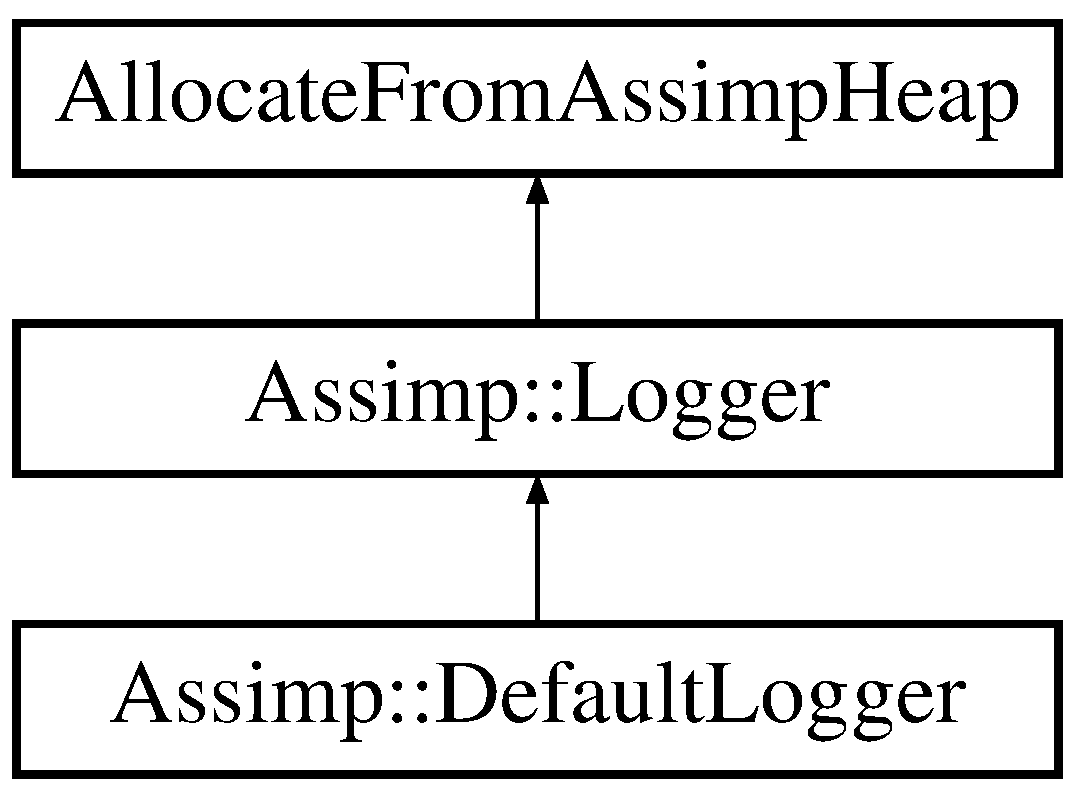
\includegraphics[height=3.000000cm]{class_assimp_1_1_default_logger}
\end{center}
\end{figure}
\subsection*{Public Member Functions}
\begin{DoxyCompactItemize}
\item 
bool \hyperlink{class_assimp_1_1_default_logger_abc0ca7a337f8c3e38eca0eb45bb1ccf0}{attach\-Stream} (\hyperlink{class_assimp_1_1_log_stream}{Log\-Stream} $\ast$p\-Stream, unsigned int severity)
\begin{DoxyCompactList}\small\item\em Attach a new log-\/stream. \end{DoxyCompactList}\item 
bool \hyperlink{class_assimp_1_1_default_logger_a2615f1d1624f1d742d0cf2dd4a5cccc8}{detatch\-Stream} (\hyperlink{class_assimp_1_1_log_stream}{Log\-Stream} $\ast$p\-Stream, unsigned int severity)
\begin{DoxyCompactList}\small\item\em Detach a still attached stream from the logger (or modify the filter flags bits) \end{DoxyCompactList}\end{DoxyCompactItemize}
\subsection*{Static Public Member Functions}
\begin{DoxyCompactItemize}
\item 
static \hyperlink{class_assimp_1_1_logger}{Logger} $\ast$ \hyperlink{class_assimp_1_1_default_logger_adccb11f85f8b0ef226c382e11ba665c3}{create} (const char $\ast$name=A\-S\-S\-I\-M\-P\-\_\-\-D\-E\-F\-A\-U\-L\-T\-\_\-\-L\-O\-G\-\_\-\-N\-A\-M\-E, \hyperlink{class_assimp_1_1_logger_a8b6248a0fd062431e8572556350d29e6}{Log\-Severity} severity=\hyperlink{class_assimp_1_1_logger_a8b6248a0fd062431e8572556350d29e6a79d16f85dc21486ee489f300027e8eda}{N\-O\-R\-M\-A\-L}, unsigned int def\-Streams=ai\-Default\-Log\-Stream\-\_\-\-D\-E\-B\-U\-G\-G\-E\-R$\vert$ai\-Default\-Log\-Stream\-\_\-\-F\-I\-L\-E, \hyperlink{class_assimp_1_1_i_o_system}{I\-O\-System} $\ast$io=N\-U\-L\-L)
\begin{DoxyCompactList}\small\item\em Creates a logging instance. \end{DoxyCompactList}\item 
static void \hyperlink{class_assimp_1_1_default_logger_a9daba548026045b99813c760c2842ed2}{set} (\hyperlink{class_assimp_1_1_logger}{Logger} $\ast$logger)
\begin{DoxyCompactList}\small\item\em Setup a custom \hyperlink{class_assimp_1_1_logger_a784e6d1a741072b17bab32a6a41055e8}{Logger} implementation. \end{DoxyCompactList}\item 
static \hyperlink{class_assimp_1_1_logger}{Logger} $\ast$ \hyperlink{class_assimp_1_1_default_logger_a7d0a53f2db66945ade30094330a77ba4}{get} ()
\begin{DoxyCompactList}\small\item\em Getter for singleton instance. \end{DoxyCompactList}\item 
static bool \hyperlink{class_assimp_1_1_default_logger_abebc7ee702a2a2dde765e771948400c6}{is\-Null\-Logger} ()
\begin{DoxyCompactList}\small\item\em Return whether a \#\-Null\-Logger is currently active. \end{DoxyCompactList}\item 
\hypertarget{class_assimp_1_1_default_logger_a0b1da096d7442af5a4a4cb5ebb2540f7}{static void \hyperlink{class_assimp_1_1_default_logger_a0b1da096d7442af5a4a4cb5ebb2540f7}{kill} ()}\label{class_assimp_1_1_default_logger_a0b1da096d7442af5a4a4cb5ebb2540f7}

\begin{DoxyCompactList}\small\item\em Kills the current singleton logger and replaces it with a \#\-Null\-Logger instance. \end{DoxyCompactList}\end{DoxyCompactItemize}
\subsection*{Additional Inherited Members}


\subsection{Detailed Description}
C\-P\-P-\/\-A\-P\-I\-: Primary logging facility of \hyperlink{namespace_assimp}{Assimp}. 

The library stores its primary \hyperlink{class_assimp_1_1_logger_a784e6d1a741072b17bab32a6a41055e8}{Logger} as a static member of this class. \hyperlink{class_assimp_1_1_default_logger_a7d0a53f2db66945ade30094330a77ba4}{get()} returns this primary logger. By default the underlying implementation is just a \#\-Null\-Logger which rejects all log messages. By calling \hyperlink{class_assimp_1_1_default_logger_adccb11f85f8b0ef226c382e11ba665c3}{create()}, logging is turned on. To capture the log output multiple log streams (\#\-Log\-Stream) can be attach to the logger. Some default streams for common streaming locations (such as a file, std\-::cout, Output\-Debug\-String()) are also provided.

If you wish to customize the logging at an even deeper level supply your own implementation of \hyperlink{class_assimp_1_1_logger_a784e6d1a741072b17bab32a6a41055e8}{Logger} to \hyperlink{class_assimp_1_1_default_logger_a9daba548026045b99813c760c2842ed2}{set()}. \begin{DoxyNote}{Note}
The whole logging stuff causes a small extra overhead for all imports. 
\end{DoxyNote}


\subsection{Member Function Documentation}
\hypertarget{class_assimp_1_1_default_logger_abc0ca7a337f8c3e38eca0eb45bb1ccf0}{\index{Assimp\-::\-Default\-Logger@{Assimp\-::\-Default\-Logger}!attach\-Stream@{attach\-Stream}}
\index{attach\-Stream@{attach\-Stream}!Assimp::DefaultLogger@{Assimp\-::\-Default\-Logger}}
\subsubsection[{attach\-Stream}]{\setlength{\rightskip}{0pt plus 5cm}bool Assimp\-::\-Default\-Logger\-::attach\-Stream (
\begin{DoxyParamCaption}
\item[{{\bf Log\-Stream} $\ast$}]{p\-Stream, }
\item[{unsigned int}]{severity}
\end{DoxyParamCaption}
)\hspace{0.3cm}{\ttfamily [virtual]}}}\label{class_assimp_1_1_default_logger_abc0ca7a337f8c3e38eca0eb45bb1ccf0}


Attach a new log-\/stream. 

The logger takes ownership of the stream and is responsible for its destruction (which is done using \-::delete when the logger itself is destroyed). Call detach\-Stream to detach a stream and to gain ownership of it again. 
\begin{DoxyParams}{Parameters}
{\em p\-Stream} & Log-\/stream to attach \\
\hline
{\em severity} & \hyperlink{class_message}{Message} filter, specified which types of log messages are dispatched to the stream. Provide a bitwise combination of the Error\-Severity flags. \\
\hline
\end{DoxyParams}
\begin{DoxyReturn}{Returns}
true if the stream has been attached, false otherwise. 
\end{DoxyReturn}


Implements \hyperlink{class_assimp_1_1_logger_aaf32a42b02a7e227076013d01e349871}{Assimp\-::\-Logger}.

\hypertarget{class_assimp_1_1_default_logger_adccb11f85f8b0ef226c382e11ba665c3}{\index{Assimp\-::\-Default\-Logger@{Assimp\-::\-Default\-Logger}!create@{create}}
\index{create@{create}!Assimp::DefaultLogger@{Assimp\-::\-Default\-Logger}}
\subsubsection[{create}]{\setlength{\rightskip}{0pt plus 5cm}static {\bf Logger}$\ast$ Assimp\-::\-Default\-Logger\-::create (
\begin{DoxyParamCaption}
\item[{const char $\ast$}]{name = {\ttfamily ASSIMP\-\_\-DEFAULT\-\_\-LOG\-\_\-NAME}, }
\item[{{\bf Log\-Severity}}]{severity = {\ttfamily {\bf N\-O\-R\-M\-A\-L}}, }
\item[{unsigned int}]{def\-Streams = {\ttfamily aiDefaultLogStream\-\_\-DEBUGGER$\vert$aiDefaultLogStream\-\_\-FILE}, }
\item[{{\bf I\-O\-System} $\ast$}]{io = {\ttfamily NULL}}
\end{DoxyParamCaption}
)\hspace{0.3cm}{\ttfamily [static]}}}\label{class_assimp_1_1_default_logger_adccb11f85f8b0ef226c382e11ba665c3}


Creates a logging instance. 


\begin{DoxyParams}{Parameters}
{\em name} & Name for log file. Only valid in combination with the ai\-Default\-Log\-Stream\-\_\-\-F\-I\-L\-E flag. \\
\hline
{\em severity} & Log severity, V\-E\-R\-B\-O\-S\-E turns on debug messages \\
\hline
{\em def\-Streams} & Default log streams to be attached. Any bitwise combination of the ai\-Default\-Log\-Stream enumerated values. If \#ai\-Default\-Log\-Stream\-\_\-\-F\-I\-L\-E is specified but an empty string is passed for 'name', no log file is created at all. \\
\hline
{\em io} & \hyperlink{class_assimp_1_1_i_o_system}{I\-O\-System} to be used to open external files (such as the log file). Pass N\-U\-L\-L to rely on the default implementation. This replaces the default \#\-Null\-Logger with a \#\-Default\-Logger instance. \\
\hline
\end{DoxyParams}
\hypertarget{class_assimp_1_1_default_logger_a2615f1d1624f1d742d0cf2dd4a5cccc8}{\index{Assimp\-::\-Default\-Logger@{Assimp\-::\-Default\-Logger}!detatch\-Stream@{detatch\-Stream}}
\index{detatch\-Stream@{detatch\-Stream}!Assimp::DefaultLogger@{Assimp\-::\-Default\-Logger}}
\subsubsection[{detatch\-Stream}]{\setlength{\rightskip}{0pt plus 5cm}bool Assimp\-::\-Default\-Logger\-::detatch\-Stream (
\begin{DoxyParamCaption}
\item[{{\bf Log\-Stream} $\ast$}]{p\-Stream, }
\item[{unsigned int}]{severity}
\end{DoxyParamCaption}
)\hspace{0.3cm}{\ttfamily [virtual]}}}\label{class_assimp_1_1_default_logger_a2615f1d1624f1d742d0cf2dd4a5cccc8}


Detach a still attached stream from the logger (or modify the filter flags bits) 


\begin{DoxyParams}{Parameters}
{\em p\-Stream} & Log-\/stream instance for detaching \\
\hline
{\em severity} & Provide a bitwise combination of the Error\-Severity flags. This value is \&$\sim$ed with the current flags of the stream, if the result is 0 the stream is detached from the \hyperlink{class_assimp_1_1_logger}{Logger} and the caller retakes the possession of the stream. \\
\hline
\end{DoxyParams}
\begin{DoxyReturn}{Returns}
true if the stream has been detached, false otherwise. 
\end{DoxyReturn}


Implements \hyperlink{class_assimp_1_1_logger_a9489263727f29fecbd705d5c8d2590c0}{Assimp\-::\-Logger}.

\hypertarget{class_assimp_1_1_default_logger_a7d0a53f2db66945ade30094330a77ba4}{\index{Assimp\-::\-Default\-Logger@{Assimp\-::\-Default\-Logger}!get@{get}}
\index{get@{get}!Assimp::DefaultLogger@{Assimp\-::\-Default\-Logger}}
\subsubsection[{get}]{\setlength{\rightskip}{0pt plus 5cm}static {\bf Logger}$\ast$ Assimp\-::\-Default\-Logger\-::get (
\begin{DoxyParamCaption}
{}
\end{DoxyParamCaption}
)\hspace{0.3cm}{\ttfamily [static]}}}\label{class_assimp_1_1_default_logger_a7d0a53f2db66945ade30094330a77ba4}


Getter for singleton instance. 

\begin{DoxyReturn}{Returns}
Only instance. This is never null, but it could be a \hyperlink{class_assimp_1_1_null_logger}{Null\-Logger}. Use is\-Null\-Logger to check this. 
\end{DoxyReturn}
\hypertarget{class_assimp_1_1_default_logger_abebc7ee702a2a2dde765e771948400c6}{\index{Assimp\-::\-Default\-Logger@{Assimp\-::\-Default\-Logger}!is\-Null\-Logger@{is\-Null\-Logger}}
\index{is\-Null\-Logger@{is\-Null\-Logger}!Assimp::DefaultLogger@{Assimp\-::\-Default\-Logger}}
\subsubsection[{is\-Null\-Logger}]{\setlength{\rightskip}{0pt plus 5cm}static bool Assimp\-::\-Default\-Logger\-::is\-Null\-Logger (
\begin{DoxyParamCaption}
{}
\end{DoxyParamCaption}
)\hspace{0.3cm}{\ttfamily [static]}}}\label{class_assimp_1_1_default_logger_abebc7ee702a2a2dde765e771948400c6}


Return whether a \#\-Null\-Logger is currently active. 

\begin{DoxyReturn}{Returns}
true if the current logger is a \#\-Null\-Logger. Use \hyperlink{class_assimp_1_1_default_logger_adccb11f85f8b0ef226c382e11ba665c3}{create()} or \hyperlink{class_assimp_1_1_default_logger_a9daba548026045b99813c760c2842ed2}{set()} to setup a logger that does actually do something else than just rejecting all log messages. 
\end{DoxyReturn}
\hypertarget{class_assimp_1_1_default_logger_a9daba548026045b99813c760c2842ed2}{\index{Assimp\-::\-Default\-Logger@{Assimp\-::\-Default\-Logger}!set@{set}}
\index{set@{set}!Assimp::DefaultLogger@{Assimp\-::\-Default\-Logger}}
\subsubsection[{set}]{\setlength{\rightskip}{0pt plus 5cm}static void Assimp\-::\-Default\-Logger\-::set (
\begin{DoxyParamCaption}
\item[{{\bf Logger} $\ast$}]{logger}
\end{DoxyParamCaption}
)\hspace{0.3cm}{\ttfamily [static]}}}\label{class_assimp_1_1_default_logger_a9daba548026045b99813c760c2842ed2}


Setup a custom \hyperlink{class_assimp_1_1_logger_a784e6d1a741072b17bab32a6a41055e8}{Logger} implementation. 

Use this if the provided \#\-Default\-Logger class doesn't fit into your needs. If the provided message formatting is O\-K for you, it's much easier to use \hyperlink{class_assimp_1_1_default_logger_adccb11f85f8b0ef226c382e11ba665c3}{create()} and to attach your own custom output streams to it. 
\begin{DoxyParams}{Parameters}
{\em logger} & Pass N\-U\-L\-L to setup a default \hyperlink{class_assimp_1_1_null_logger}{Null\-Logger} \\
\hline
\end{DoxyParams}


The documentation for this class was generated from the following file\-:\begin{DoxyCompactItemize}
\item 
X\-:/\-Git\-\_\-\-Repository/inf2990-\/06/\-Cadriciel/\-Commun/\-Externe/assimp/include/Default\-Logger.\-hpp\end{DoxyCompactItemize}

\hypertarget{class_interface_graphique_1_1patron__state_1_1_deletion_state}{\section{Interface\-Graphique.\-patron\-\_\-state.\-Deletion\-State Class Reference}
\label{class_interface_graphique_1_1patron__state_1_1_deletion_state}\index{Interface\-Graphique.\-patron\-\_\-state.\-Deletion\-State@{Interface\-Graphique.\-patron\-\_\-state.\-Deletion\-State}}
}


Etat pour la suppression d'un objet  


Inheritance diagram for Interface\-Graphique.\-patron\-\_\-state.\-Deletion\-State\-:\begin{figure}[H]
\begin{center}
\leavevmode
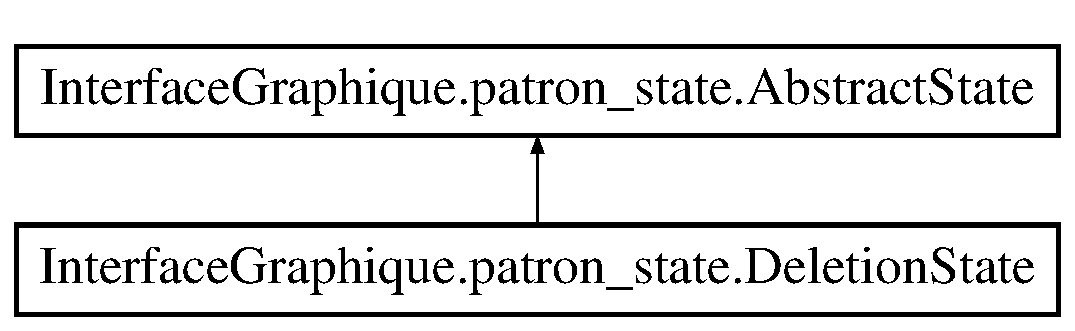
\includegraphics[height=2.000000cm]{class_interface_graphique_1_1patron__state_1_1_deletion_state}
\end{center}
\end{figure}
\subsection*{Public Member Functions}
\begin{DoxyCompactItemize}
\item 
override void \hyperlink{class_interface_graphique_1_1patron__state_1_1_deletion_state_ab720f529b212ff1b98d5e97f7fcb199f}{Action} (int \hyperlink{group__inf2990_ga6150e0515f7202e2fb518f7206ed97dc}{x}, int \hyperlink{group__inf2990_ga0a2f84ed7838f07779ae24c5a9086d33}{y})
\begin{DoxyCompactList}\small\item\em On supprime les objets selectionnes \end{DoxyCompactList}\end{DoxyCompactItemize}


\subsection{Detailed Description}
Etat pour la suppression d'un objet 



\subsection{Member Function Documentation}
\hypertarget{class_interface_graphique_1_1patron__state_1_1_deletion_state_ab720f529b212ff1b98d5e97f7fcb199f}{\index{Interface\-Graphique\-::patron\-\_\-state\-::\-Deletion\-State@{Interface\-Graphique\-::patron\-\_\-state\-::\-Deletion\-State}!Action@{Action}}
\index{Action@{Action}!InterfaceGraphique::patron_state::DeletionState@{Interface\-Graphique\-::patron\-\_\-state\-::\-Deletion\-State}}
\subsubsection[{Action}]{\setlength{\rightskip}{0pt plus 5cm}override void Interface\-Graphique.\-patron\-\_\-state.\-Deletion\-State.\-Action (
\begin{DoxyParamCaption}
\item[{int}]{x, }
\item[{int}]{y}
\end{DoxyParamCaption}
)\hspace{0.3cm}{\ttfamily [inline]}, {\ttfamily [virtual]}}}\label{class_interface_graphique_1_1patron__state_1_1_deletion_state_ab720f529b212ff1b98d5e97f7fcb199f}


On supprime les objets selectionnes 


\begin{DoxyParams}{Parameters}
{\em x} & Ne sert a rien pour la suppression puisqu'on supprime les objets selectionnes\\
\hline
{\em y} & Ne sert a rien ici aussi\\
\hline
\end{DoxyParams}


Implements \hyperlink{class_interface_graphique_1_1patron__state_1_1_abstract_state_a8df97c5a2784f9757608d669fbb1c6b5}{Interface\-Graphique.\-patron\-\_\-state.\-Abstract\-State}.



The documentation for this class was generated from the following file\-:\begin{DoxyCompactItemize}
\item 
X\-:/inf2990-\/06/\-Cadriciel/\-Sources/\-Interface\-Graphique/patron state/\hyperlink{_deletion_state_8cs}{Deletion\-State.\-cs}\end{DoxyCompactItemize}

\hypertarget{structglm_1_1io_1_1delimeter}{\section{glm\-:\-:io\-:\-:delimeter$<$ C\-Ty $>$ Struct Template Reference}
\label{structglm_1_1io_1_1delimeter}\index{glm\-::io\-::delimeter$<$ C\-Ty $>$@{glm\-::io\-::delimeter$<$ C\-Ty $>$}}
}
\subsection*{Public Member Functions}
\begin{DoxyCompactItemize}
\item 
\hypertarget{structglm_1_1io_1_1delimeter_acd4b6e1e816d423a069688c4772b9500}{{\bfseries delimeter} (C\-Ty, C\-Ty, C\-Ty= ',')}\label{structglm_1_1io_1_1delimeter_acd4b6e1e816d423a069688c4772b9500}

\end{DoxyCompactItemize}
\subsection*{Public Attributes}
\begin{DoxyCompactItemize}
\item 
\hypertarget{structglm_1_1io_1_1delimeter_a9ade129dae50c4f716f724e7425f9c68}{C\-Ty {\bfseries value} \mbox{[}3\mbox{]}}\label{structglm_1_1io_1_1delimeter_a9ade129dae50c4f716f724e7425f9c68}

\end{DoxyCompactItemize}


The documentation for this struct was generated from the following files\-:\begin{DoxyCompactItemize}
\item 
X\-:/\-Git\-\_\-\-Repository/inf2990-\/06/\-Cadriciel/\-Commun/\-Externe/glm/include/glm/gtx/\hyperlink{io_8hpp}{io.\-hpp}\item 
X\-:/\-Git\-\_\-\-Repository/inf2990-\/06/\-Cadriciel/\-Commun/\-Externe/glm/include/glm/gtx/io.\-inl\end{DoxyCompactItemize}

\hypertarget{classaidecollision_1_1_details_collision}{\section{aidecollision\-:\-:Details\-Collision Class Reference}
\label{classaidecollision_1_1_details_collision}\index{aidecollision\-::\-Details\-Collision@{aidecollision\-::\-Details\-Collision}}
}


Structure contenant les informations d'une collision.  




{\ttfamily \#include $<$Aide\-Collision.\-h$>$}

\subsection*{Public Attributes}
\begin{DoxyCompactItemize}
\item 
\hypertarget{classaidecollision_1_1_details_collision_a524989691331ea39d2c14c639f0de02e}{\hyperlink{namespaceaidecollision_a1c8613e2393aa3268262f9d23d60c0c9}{Collision} \hyperlink{classaidecollision_1_1_details_collision_a524989691331ea39d2c14c639f0de02e}{type}}\label{classaidecollision_1_1_details_collision_a524989691331ea39d2c14c639f0de02e}

\begin{DoxyCompactList}\small\item\em Type de collision. \end{DoxyCompactList}\item 
\hypertarget{classaidecollision_1_1_details_collision_ab68965d1c0583cc9a28973bc5b3060b8}{\hyperlink{group__core__types_ga7f3287f952e6ccb481231368091702ac}{glm\-::dvec3} \hyperlink{classaidecollision_1_1_details_collision_ab68965d1c0583cc9a28973bc5b3060b8}{direction}}\label{classaidecollision_1_1_details_collision_ab68965d1c0583cc9a28973bc5b3060b8}

\begin{DoxyCompactList}\small\item\em Direction de la collision. \end{DoxyCompactList}\item 
\hypertarget{classaidecollision_1_1_details_collision_a6aa4cae3f313a2a16608dd60da0f97d1}{double \hyperlink{classaidecollision_1_1_details_collision_a6aa4cae3f313a2a16608dd60da0f97d1}{enfoncement}}\label{classaidecollision_1_1_details_collision_a6aa4cae3f313a2a16608dd60da0f97d1}

\begin{DoxyCompactList}\small\item\em Enfoncement de l'objet � l'int�rieur de la collision. \end{DoxyCompactList}\end{DoxyCompactItemize}


\subsection{Detailed Description}
Structure contenant les informations d'une collision. 

The documentation for this class was generated from the following file\-:\begin{DoxyCompactItemize}
\item 
X\-:/\-Git\-\_\-\-Repository/inf2990-\/06/\-Cadriciel/\-Commun/\-Utilitaire/\hyperlink{_aide_collision_8h}{Aide\-Collision.\-h}\end{DoxyCompactItemize}

\hypertarget{classglm_1_1dont__care}{\section{glm\-:\-:dont\-\_\-care Class Reference}
\label{classglm_1_1dont__care}\index{glm\-::dont\-\_\-care@{glm\-::dont\-\_\-care}}
}


The documentation for this class was generated from the following file\-:\begin{DoxyCompactItemize}
\item 
X\-:/\-Git\-\_\-\-Repository/inf2990-\/06/\-Cadriciel/\-Commun/\-Externe/glm/include/glm/detail/hint.\-hpp\end{DoxyCompactItemize}

\hypertarget{classmath_1_1_droite3_d}{\section{math\-:\-:Droite3\-D Class Reference}
\label{classmath_1_1_droite3_d}\index{math\-::\-Droite3\-D@{math\-::\-Droite3\-D}}
}


Classe qui repr�sente une droite en 3 dimensions.  




{\ttfamily \#include $<$Droite3\-D.\-h$>$}

\subsection*{Public Member Functions}
\begin{DoxyCompactItemize}
\item 
\hyperlink{classmath_1_1_droite3_d_a9248463117b4567a6e68a88f5760f07a}{Droite3\-D} (const \hyperlink{group__core__types_ga7f3287f952e6ccb481231368091702ac}{glm\-::dvec3} \&point1, const \hyperlink{group__core__types_ga7f3287f952e6ccb481231368091702ac}{glm\-::dvec3} \&point2)
\begin{DoxyCompactList}\small\item\em Constructeur. \end{DoxyCompactList}\item 
bool \hyperlink{classmath_1_1_droite3_d_acec61f69291777c83e5539fedb83b170}{intersection} (const \hyperlink{classmath_1_1_plan3_d}{Plan3\-D} \&plan\-Coupe, \hyperlink{group__core__types_ga7f3287f952e6ccb481231368091702ac}{glm\-::dvec3} \&\hyperlink{structintersection}{intersection})
\begin{DoxyCompactList}\small\item\em Trouve l'intersection entre la droite et un plan. \end{DoxyCompactList}\item 
bool \hyperlink{classmath_1_1_droite3_d_a537d2c35e8ae11d2968087599b10c752}{intersection\-Segment} (const \hyperlink{group__core__types_ga7f3287f952e6ccb481231368091702ac}{glm\-::dvec3} \&point1, const \hyperlink{group__core__types_ga7f3287f952e6ccb481231368091702ac}{glm\-::dvec3} \&point2)
\begin{DoxyCompactList}\small\item\em Trouve l'intersection entre la droite et un segment. \end{DoxyCompactList}\item 
double \hyperlink{classmath_1_1_droite3_d_a92d2f79fc5d29ddd8061ebb632293f04}{distance\-Point} (const \hyperlink{group__core__types_ga7f3287f952e6ccb481231368091702ac}{glm\-::dvec3} \&centre)
\begin{DoxyCompactList}\small\item\em Calcule la distance entre un point et la droite. \end{DoxyCompactList}\item 
\hyperlink{group__core__types_ga7f3287f952e6ccb481231368091702ac}{glm\-::dvec3} \hyperlink{classmath_1_1_droite3_d_a4f3a9fb81926f775cd9e589c112c51db}{perpendiculaire\-Droite} (const \hyperlink{group__core__types_ga7f3287f952e6ccb481231368091702ac}{glm\-::dvec3} \&point)
\begin{DoxyCompactList}\small\item\em Trouve le point de rencontre entre la droite et une perpendiculaire � partir d'un point. \end{DoxyCompactList}\item 
const \hyperlink{group__core__types_ga7f3287f952e6ccb481231368091702ac}{glm\-::dvec3} \& \hyperlink{classmath_1_1_droite3_d_a903f20fd767699e95f747b4722e8aa04}{lire\-Vecteur} () const 
\begin{DoxyCompactList}\small\item\em Avoir le vecteur directeur de la droite. \end{DoxyCompactList}\item 
const \hyperlink{group__core__types_ga7f3287f952e6ccb481231368091702ac}{glm\-::dvec3} \& \hyperlink{classmath_1_1_droite3_d_a5de95860b960b37e4c55f857f020c652}{lire\-Point} () const 
\begin{DoxyCompactList}\small\item\em Avoir un point de la droite. \end{DoxyCompactList}\end{DoxyCompactItemize}


\subsection{Detailed Description}
Classe qui repr�sente une droite en 3 dimensions. 

Classe qui permet d'avoir une droite en 3\-D. \par
Une droite dans l'espace 3\-D est d�finie par l'�quation \-:

\[ \frac {x - x_0 } {a} = \frac { y - y_0 } {b} = \frac { z - z_0 } {c} \] o� le point $ (x_0, y_0, z_0) $ est un point de la droite et le vecteur de direction $ (a, b, c) $ est un vecteur parall�le � la droite.\par
 \par
Une droite dans l'espace 3\-D passant par 2 points $ ( P_1, P_2) $ est d�finie par l'�quation \-:

\[ \frac {x - x_1 } {x_2 - x_1} = \frac { y - y_1 } {y_2 - y_1} = \frac { z - z_1 } {z_2 - z_1} \] \par
\par
Cette classe contient des m�thodes pour \-: \begin{DoxyItemize}
\item construire une droite entre 2 points $ (P_1, P_2) $ ou avec un point $ P $ sur la droite et un vecteur de direction $ (a, b, c) $; \item trouver l'intersection entre une droite et un plan ; \item intersection\-Segment ; \item distance\-Point ; \item perpendiculaire\-Droite; \item les m�thodes d'acc�s.\end{DoxyItemize}
\begin{DoxyAuthor}{Author}
D\-G\-I-\/2990 
\end{DoxyAuthor}
\begin{DoxyDate}{Date}
2005-\/09-\/27 
\end{DoxyDate}


\subsection{Constructor \& Destructor Documentation}
\hypertarget{classmath_1_1_droite3_d_a9248463117b4567a6e68a88f5760f07a}{\index{math\-::\-Droite3\-D@{math\-::\-Droite3\-D}!Droite3\-D@{Droite3\-D}}
\index{Droite3\-D@{Droite3\-D}!math::Droite3D@{math\-::\-Droite3\-D}}
\subsubsection[{Droite3\-D}]{\setlength{\rightskip}{0pt plus 5cm}math\-::\-Droite3\-D\-::\-Droite3\-D (
\begin{DoxyParamCaption}
\item[{const {\bf glm\-::dvec3} \&}]{point1, }
\item[{const {\bf glm\-::dvec3} \&}]{point2}
\end{DoxyParamCaption}
)}}\label{classmath_1_1_droite3_d_a9248463117b4567a6e68a88f5760f07a}


Constructeur. 

Constructeur d'une droite 3\-D � partir de 2 points. \par
Une droite dans l'espace 3d passant par 2 points $ ( P_1, P_2) $ est d�finie par l'�quation \-:

\[ \frac {x - x_1 } {x_2 - x_1} = \frac { y - y_1 } {y_2 - y_1} = \frac { z - z_1 } {z_2 - z_1} \] \par
\par
 
\begin{DoxyParams}[1]{Parameters}
\mbox{\tt in}  & {\em point1} & \-: Un point sur la droite. \\
\hline
\mbox{\tt in}  & {\em point2} & \-: Un autre point sur la droite (diff�rent du premier sinon il y a une lev�e d'exception).\\
\hline
\end{DoxyParams}
\begin{DoxyReturn}{Returns}
Aucune (constructeur). 
\end{DoxyReturn}


\subsection{Member Function Documentation}
\hypertarget{classmath_1_1_droite3_d_a92d2f79fc5d29ddd8061ebb632293f04}{\index{math\-::\-Droite3\-D@{math\-::\-Droite3\-D}!distance\-Point@{distance\-Point}}
\index{distance\-Point@{distance\-Point}!math::Droite3D@{math\-::\-Droite3\-D}}
\subsubsection[{distance\-Point}]{\setlength{\rightskip}{0pt plus 5cm}double math\-::\-Droite3\-D\-::distance\-Point (
\begin{DoxyParamCaption}
\item[{const {\bf glm\-::dvec3} \&}]{centre}
\end{DoxyParamCaption}
)}}\label{classmath_1_1_droite3_d_a92d2f79fc5d29ddd8061ebb632293f04}


Calcule la distance entre un point et la droite. 

Calcule la distance euclidienne entre la droite et un point.


\begin{DoxyParams}[1]{Parameters}
\mbox{\tt in}  & {\em centre} & \-: Point � partir duquel la distance doit �tre calcul�e.\\
\hline
\end{DoxyParams}
\begin{DoxyReturn}{Returns}
Distance du point � la droite. 
\end{DoxyReturn}
\hypertarget{classmath_1_1_droite3_d_acec61f69291777c83e5539fedb83b170}{\index{math\-::\-Droite3\-D@{math\-::\-Droite3\-D}!intersection@{intersection}}
\index{intersection@{intersection}!math::Droite3D@{math\-::\-Droite3\-D}}
\subsubsection[{intersection}]{\setlength{\rightskip}{0pt plus 5cm}bool math\-::\-Droite3\-D\-::intersection (
\begin{DoxyParamCaption}
\item[{const {\bf Plan3\-D} \&}]{plan\-Coupe, }
\item[{{\bf glm\-::dvec3} \&}]{intersection}
\end{DoxyParamCaption}
)}}\label{classmath_1_1_droite3_d_acec61f69291777c83e5539fedb83b170}


Trouve l'intersection entre la droite et un plan. 

Cette fonction permet de trouver l'intersection entre une droite et un plan dans l'espace 3\-D. La droite ne doit pas �tre parall�le au plan. \par
 Si $ a $ est diff�rent de z�ro, alors l'intersection est donn�e par \-:\par
 \[ x = \left ( { \frac {\left ( \frac { ( B b + C c) x_0} {a} - B y_0 - C z_0 - D \right)} { ( A + B \frac {b} {a} + C \frac{c} {b})} }\right) \] \[ y = \left ( { \frac {\left ( C \frac {c}{b} y_0 - C z_0 - D \right)} { ( B + C \frac {c} {b}) } }\right) \] \[ z = \frac{c} {a} (x - x_0) + z_0 \]

Si $ b $ est diff�rent de z�ro, alors l'intersection est donn�e par \-:\par
 \[ x = x_0 \] \[ y = \frac{c} {b} (x - x_0) + y_0 \] \[ z = \frac{c} {b} (y - y_0) + z_0 \]

Sinon, l'intersection est donn�e par \-:\par
 \[ x = x_0 \] \[ y = y_0 \] \[ z = \frac{(D + A x_0 + B y_0)} {C} \]


\begin{DoxyParams}[1]{Parameters}
\mbox{\tt in}  & {\em plan\-Coupe} & \-: Le plan avec lequel on veut trouver l'intersection. \\
\hline
\mbox{\tt out}  & {\em intersection} & \-: Le r�sultat de l'intersection $ (s, y, z) $ .\\
\hline
\end{DoxyParams}
\begin{DoxyReturn}{Returns}
Faux si la droite est parall�le au plan, donc si donc l'intersection ne peut �tre trouv�e, vrai autrement. 
\end{DoxyReturn}
\hypertarget{classmath_1_1_droite3_d_a537d2c35e8ae11d2968087599b10c752}{\index{math\-::\-Droite3\-D@{math\-::\-Droite3\-D}!intersection\-Segment@{intersection\-Segment}}
\index{intersection\-Segment@{intersection\-Segment}!math::Droite3D@{math\-::\-Droite3\-D}}
\subsubsection[{intersection\-Segment}]{\setlength{\rightskip}{0pt plus 5cm}bool math\-::\-Droite3\-D\-::intersection\-Segment (
\begin{DoxyParamCaption}
\item[{const {\bf glm\-::dvec3} \&}]{point1, }
\item[{const {\bf glm\-::dvec3} \&}]{point2}
\end{DoxyParamCaption}
)}}\label{classmath_1_1_droite3_d_a537d2c35e8ae11d2968087599b10c752}


Trouve l'intersection entre la droite et un segment. 

Cette fonction permet de trouver l'intersection entre un segment de droite d�fini par 2 points $ (P_1, P_2) $ et une droite dans l'espace 3\-D.


\begin{DoxyParams}[1]{Parameters}
\mbox{\tt in}  & {\em point1} & \-: Le premier point du segment. \\
\hline
\mbox{\tt in}  & {\em point2} & \-: Le deuxi�me point permettant de d�finir le segment de droite.\\
\hline
\end{DoxyParams}
\begin{DoxyReturn}{Returns}
bool \-: false =$>$ la droite est parall�le au plan, donc l'intersection ne peut �tre trouv�e.
\end{DoxyReturn}
\begin{DoxyDate}{Date}
2006-\/02-\/21 Modification suite aux changements dans Vecteur3 
\end{DoxyDate}
\hypertarget{classmath_1_1_droite3_d_a5de95860b960b37e4c55f857f020c652}{\index{math\-::\-Droite3\-D@{math\-::\-Droite3\-D}!lire\-Point@{lire\-Point}}
\index{lire\-Point@{lire\-Point}!math::Droite3D@{math\-::\-Droite3\-D}}
\subsubsection[{lire\-Point}]{\setlength{\rightskip}{0pt plus 5cm}const {\bf glm\-::dvec3} \& math\-::\-Droite3\-D\-::lire\-Point (
\begin{DoxyParamCaption}
{}
\end{DoxyParamCaption}
) const\hspace{0.3cm}{\ttfamily [inline]}}}\label{classmath_1_1_droite3_d_a5de95860b960b37e4c55f857f020c652}


Avoir un point de la droite. 

Cette fonction retourne un point quelconque de la droite.

\begin{DoxyReturn}{Returns}
Un point quelconque de la droite. 
\end{DoxyReturn}
\hypertarget{classmath_1_1_droite3_d_a903f20fd767699e95f747b4722e8aa04}{\index{math\-::\-Droite3\-D@{math\-::\-Droite3\-D}!lire\-Vecteur@{lire\-Vecteur}}
\index{lire\-Vecteur@{lire\-Vecteur}!math::Droite3D@{math\-::\-Droite3\-D}}
\subsubsection[{lire\-Vecteur}]{\setlength{\rightskip}{0pt plus 5cm}const {\bf glm\-::dvec3} \& math\-::\-Droite3\-D\-::lire\-Vecteur (
\begin{DoxyParamCaption}
{}
\end{DoxyParamCaption}
) const\hspace{0.3cm}{\ttfamily [inline]}}}\label{classmath_1_1_droite3_d_a903f20fd767699e95f747b4722e8aa04}


Avoir le vecteur directeur de la droite. 

Cette fonction retourne le vecteur directeur de la droite.

\begin{DoxyReturn}{Returns}
Le vecteur directeur de la droite. 
\end{DoxyReturn}
\hypertarget{classmath_1_1_droite3_d_a4f3a9fb81926f775cd9e589c112c51db}{\index{math\-::\-Droite3\-D@{math\-::\-Droite3\-D}!perpendiculaire\-Droite@{perpendiculaire\-Droite}}
\index{perpendiculaire\-Droite@{perpendiculaire\-Droite}!math::Droite3D@{math\-::\-Droite3\-D}}
\subsubsection[{perpendiculaire\-Droite}]{\setlength{\rightskip}{0pt plus 5cm}{\bf glm\-::dvec3} math\-::\-Droite3\-D\-::perpendiculaire\-Droite (
\begin{DoxyParamCaption}
\item[{const {\bf glm\-::dvec3} \&}]{point}
\end{DoxyParamCaption}
)}}\label{classmath_1_1_droite3_d_a4f3a9fb81926f775cd9e589c112c51db}


Trouve le point de rencontre entre la droite et une perpendiculaire � partir d'un point. 

On trace la perpendicaulaire entre le point et le droite et on trouve le point d'intersection.


\begin{DoxyParams}[1]{Parameters}
\mbox{\tt in}  & {\em point} & \-: Un point dans l'espace d'o� est calcul�e la perpendiculaire.\\
\hline
\end{DoxyParams}
\begin{DoxyReturn}{Returns}
Le point de rencontre entre la droite et la perpendiculaire. 
\end{DoxyReturn}


The documentation for this class was generated from the following files\-:\begin{DoxyCompactItemize}
\item 
X\-:/\-Git\-\_\-\-Repository/inf2990-\/06/\-Cadriciel/\-Commun/\-Utilitaire/\hyperlink{_droite3_d_8h}{Droite3\-D.\-h}\item 
X\-:/\-Git\-\_\-\-Repository/inf2990-\/06/\-Cadriciel/\-Commun/\-Utilitaire/\hyperlink{_droite3_d_8cpp}{Droite3\-D.\-cpp}\end{DoxyCompactItemize}

\hypertarget{class_f_m_o_d_1_1_d_s_p}{\section{F\-M\-O\-D\-:\-:D\-S\-P Class Reference}
\label{class_f_m_o_d_1_1_d_s_p}\index{F\-M\-O\-D\-::\-D\-S\-P@{F\-M\-O\-D\-::\-D\-S\-P}}
}
\subsection*{Public Member Functions}
\begin{DoxyCompactItemize}
\item 
\hypertarget{class_f_m_o_d_1_1_d_s_p_a4ffd9dbcf1b0119a2ab94d27744ee033}{F\-M\-O\-D\-\_\-\-R\-E\-S\-U\-L\-T F\-\_\-\-A\-P\-I {\bfseries release} ()}\label{class_f_m_o_d_1_1_d_s_p_a4ffd9dbcf1b0119a2ab94d27744ee033}

\item 
\hypertarget{class_f_m_o_d_1_1_d_s_p_a06bef2d5b365de903e12fff814da31c7}{F\-M\-O\-D\-\_\-\-R\-E\-S\-U\-L\-T F\-\_\-\-A\-P\-I {\bfseries get\-System\-Object} (\hyperlink{class_f_m_o_d_1_1_system}{System} $\ast$$\ast$system)}\label{class_f_m_o_d_1_1_d_s_p_a06bef2d5b365de903e12fff814da31c7}

\item 
\hypertarget{class_f_m_o_d_1_1_d_s_p_a647ccb2fdd73ecc1ce2c9a7a5411cb8c}{F\-M\-O\-D\-\_\-\-R\-E\-S\-U\-L\-T F\-\_\-\-A\-P\-I {\bfseries add\-Input} (\hyperlink{class_f_m_o_d_1_1_d_s_p}{D\-S\-P} $\ast$target, \hyperlink{class_f_m_o_d_1_1_d_s_p_connection}{D\-S\-P\-Connection} $\ast$$\ast$connection)}\label{class_f_m_o_d_1_1_d_s_p_a647ccb2fdd73ecc1ce2c9a7a5411cb8c}

\item 
\hypertarget{class_f_m_o_d_1_1_d_s_p_a4a7dec17c9528099e23fe92102c10c38}{F\-M\-O\-D\-\_\-\-R\-E\-S\-U\-L\-T F\-\_\-\-A\-P\-I {\bfseries disconnect\-From} (\hyperlink{class_f_m_o_d_1_1_d_s_p}{D\-S\-P} $\ast$target)}\label{class_f_m_o_d_1_1_d_s_p_a4a7dec17c9528099e23fe92102c10c38}

\item 
\hypertarget{class_f_m_o_d_1_1_d_s_p_a3eb9cfc992a069357bbebeafffad9c8e}{F\-M\-O\-D\-\_\-\-R\-E\-S\-U\-L\-T F\-\_\-\-A\-P\-I {\bfseries disconnect\-All} (bool inputs, bool outputs)}\label{class_f_m_o_d_1_1_d_s_p_a3eb9cfc992a069357bbebeafffad9c8e}

\item 
\hypertarget{class_f_m_o_d_1_1_d_s_p_ae7503115a44e52310e9a7cfe4063cd81}{F\-M\-O\-D\-\_\-\-R\-E\-S\-U\-L\-T F\-\_\-\-A\-P\-I {\bfseries remove} ()}\label{class_f_m_o_d_1_1_d_s_p_ae7503115a44e52310e9a7cfe4063cd81}

\item 
\hypertarget{class_f_m_o_d_1_1_d_s_p_a20667543975afbb53cc19a1389bfd6e7}{F\-M\-O\-D\-\_\-\-R\-E\-S\-U\-L\-T F\-\_\-\-A\-P\-I {\bfseries get\-Num\-Inputs} (int $\ast$numinputs)}\label{class_f_m_o_d_1_1_d_s_p_a20667543975afbb53cc19a1389bfd6e7}

\item 
\hypertarget{class_f_m_o_d_1_1_d_s_p_a26bcf3c3560fae9e15db4ea1a39d21e3}{F\-M\-O\-D\-\_\-\-R\-E\-S\-U\-L\-T F\-\_\-\-A\-P\-I {\bfseries get\-Num\-Outputs} (int $\ast$numoutputs)}\label{class_f_m_o_d_1_1_d_s_p_a26bcf3c3560fae9e15db4ea1a39d21e3}

\item 
\hypertarget{class_f_m_o_d_1_1_d_s_p_adebf041723376a94c176edf0126c8321}{F\-M\-O\-D\-\_\-\-R\-E\-S\-U\-L\-T F\-\_\-\-A\-P\-I {\bfseries get\-Input} (int index, \hyperlink{class_f_m_o_d_1_1_d_s_p}{D\-S\-P} $\ast$$\ast$input, \hyperlink{class_f_m_o_d_1_1_d_s_p_connection}{D\-S\-P\-Connection} $\ast$$\ast$inputconnection)}\label{class_f_m_o_d_1_1_d_s_p_adebf041723376a94c176edf0126c8321}

\item 
\hypertarget{class_f_m_o_d_1_1_d_s_p_a13584fc2ef78192b375ca6d117a49560}{F\-M\-O\-D\-\_\-\-R\-E\-S\-U\-L\-T F\-\_\-\-A\-P\-I {\bfseries get\-Output} (int index, \hyperlink{class_f_m_o_d_1_1_d_s_p}{D\-S\-P} $\ast$$\ast$output, \hyperlink{class_f_m_o_d_1_1_d_s_p_connection}{D\-S\-P\-Connection} $\ast$$\ast$outputconnection)}\label{class_f_m_o_d_1_1_d_s_p_a13584fc2ef78192b375ca6d117a49560}

\item 
\hypertarget{class_f_m_o_d_1_1_d_s_p_ab85ee53bebfd6fc3cccb9979cf13eaba}{F\-M\-O\-D\-\_\-\-R\-E\-S\-U\-L\-T F\-\_\-\-A\-P\-I {\bfseries set\-Active} (bool active)}\label{class_f_m_o_d_1_1_d_s_p_ab85ee53bebfd6fc3cccb9979cf13eaba}

\item 
\hypertarget{class_f_m_o_d_1_1_d_s_p_ac802a3beb3dfb2dca8cd2717926a3413}{F\-M\-O\-D\-\_\-\-R\-E\-S\-U\-L\-T F\-\_\-\-A\-P\-I {\bfseries get\-Active} (bool $\ast$active)}\label{class_f_m_o_d_1_1_d_s_p_ac802a3beb3dfb2dca8cd2717926a3413}

\item 
\hypertarget{class_f_m_o_d_1_1_d_s_p_ac0e9c1d934542b45a8ec39f488de559a}{F\-M\-O\-D\-\_\-\-R\-E\-S\-U\-L\-T F\-\_\-\-A\-P\-I {\bfseries set\-Bypass} (bool bypass)}\label{class_f_m_o_d_1_1_d_s_p_ac0e9c1d934542b45a8ec39f488de559a}

\item 
\hypertarget{class_f_m_o_d_1_1_d_s_p_a019b1b2e5b980dc4d4b70c1c86fe4240}{F\-M\-O\-D\-\_\-\-R\-E\-S\-U\-L\-T F\-\_\-\-A\-P\-I {\bfseries get\-Bypass} (bool $\ast$bypass)}\label{class_f_m_o_d_1_1_d_s_p_a019b1b2e5b980dc4d4b70c1c86fe4240}

\item 
\hypertarget{class_f_m_o_d_1_1_d_s_p_ac8b9504840c96548c383fdead268f10c}{F\-M\-O\-D\-\_\-\-R\-E\-S\-U\-L\-T F\-\_\-\-A\-P\-I {\bfseries set\-Speaker\-Active} (F\-M\-O\-D\-\_\-\-S\-P\-E\-A\-K\-E\-R speaker, bool active)}\label{class_f_m_o_d_1_1_d_s_p_ac8b9504840c96548c383fdead268f10c}

\item 
\hypertarget{class_f_m_o_d_1_1_d_s_p_ace16e6d02305b7d39cb626abb944d054}{F\-M\-O\-D\-\_\-\-R\-E\-S\-U\-L\-T F\-\_\-\-A\-P\-I {\bfseries get\-Speaker\-Active} (F\-M\-O\-D\-\_\-\-S\-P\-E\-A\-K\-E\-R speaker, bool $\ast$active)}\label{class_f_m_o_d_1_1_d_s_p_ace16e6d02305b7d39cb626abb944d054}

\item 
\hypertarget{class_f_m_o_d_1_1_d_s_p_ae475150cbc68d5ad5e5be5791ec3961a}{F\-M\-O\-D\-\_\-\-R\-E\-S\-U\-L\-T F\-\_\-\-A\-P\-I {\bfseries reset} ()}\label{class_f_m_o_d_1_1_d_s_p_ae475150cbc68d5ad5e5be5791ec3961a}

\item 
\hypertarget{class_f_m_o_d_1_1_d_s_p_abb8a3ad932d399703103da1b752c4fad}{F\-M\-O\-D\-\_\-\-R\-E\-S\-U\-L\-T F\-\_\-\-A\-P\-I {\bfseries set\-Parameter} (int index, float value)}\label{class_f_m_o_d_1_1_d_s_p_abb8a3ad932d399703103da1b752c4fad}

\item 
\hypertarget{class_f_m_o_d_1_1_d_s_p_aae915b3c0d956419aeed08c2aa3000e2}{F\-M\-O\-D\-\_\-\-R\-E\-S\-U\-L\-T F\-\_\-\-A\-P\-I {\bfseries get\-Parameter} (int index, float $\ast$value, char $\ast$valuestr, int valuestrlen)}\label{class_f_m_o_d_1_1_d_s_p_aae915b3c0d956419aeed08c2aa3000e2}

\item 
\hypertarget{class_f_m_o_d_1_1_d_s_p_aba45842920caedf11c614d77aa028ab3}{F\-M\-O\-D\-\_\-\-R\-E\-S\-U\-L\-T F\-\_\-\-A\-P\-I {\bfseries get\-Num\-Parameters} (int $\ast$numparams)}\label{class_f_m_o_d_1_1_d_s_p_aba45842920caedf11c614d77aa028ab3}

\item 
\hypertarget{class_f_m_o_d_1_1_d_s_p_a116d65e165bac32512ddbb7c188bf3a5}{F\-M\-O\-D\-\_\-\-R\-E\-S\-U\-L\-T F\-\_\-\-A\-P\-I {\bfseries get\-Parameter\-Info} (int index, char $\ast$name, char $\ast$label, char $\ast$description, int descriptionlen, float $\ast$min, float $\ast$max)}\label{class_f_m_o_d_1_1_d_s_p_a116d65e165bac32512ddbb7c188bf3a5}

\item 
\hypertarget{class_f_m_o_d_1_1_d_s_p_a9a77cb36dbbc0bb053b42eb4d2dcd1f7}{F\-M\-O\-D\-\_\-\-R\-E\-S\-U\-L\-T F\-\_\-\-A\-P\-I {\bfseries show\-Config\-Dialog} (void $\ast$hwnd, bool show)}\label{class_f_m_o_d_1_1_d_s_p_a9a77cb36dbbc0bb053b42eb4d2dcd1f7}

\item 
\hypertarget{class_f_m_o_d_1_1_d_s_p_a5bb61015d7b0e835437e46ea4eaf6442}{F\-M\-O\-D\-\_\-\-R\-E\-S\-U\-L\-T F\-\_\-\-A\-P\-I {\bfseries get\-Info} (char $\ast$name, unsigned int $\ast$version, int $\ast$channels, int $\ast$configwidth, int $\ast$configheight)}\label{class_f_m_o_d_1_1_d_s_p_a5bb61015d7b0e835437e46ea4eaf6442}

\item 
\hypertarget{class_f_m_o_d_1_1_d_s_p_a7241c2669554667f90d4f2a576f64c4a}{F\-M\-O\-D\-\_\-\-R\-E\-S\-U\-L\-T F\-\_\-\-A\-P\-I {\bfseries get\-Type} (F\-M\-O\-D\-\_\-\-D\-S\-P\-\_\-\-T\-Y\-P\-E $\ast$type)}\label{class_f_m_o_d_1_1_d_s_p_a7241c2669554667f90d4f2a576f64c4a}

\item 
\hypertarget{class_f_m_o_d_1_1_d_s_p_a97919dbf4f783369b75f1bc43527489d}{F\-M\-O\-D\-\_\-\-R\-E\-S\-U\-L\-T F\-\_\-\-A\-P\-I {\bfseries set\-Defaults} (float frequency, float volume, float pan, int priority)}\label{class_f_m_o_d_1_1_d_s_p_a97919dbf4f783369b75f1bc43527489d}

\item 
\hypertarget{class_f_m_o_d_1_1_d_s_p_a80aa58e2f153dd3ad5fb6bf9305fc00e}{F\-M\-O\-D\-\_\-\-R\-E\-S\-U\-L\-T F\-\_\-\-A\-P\-I {\bfseries get\-Defaults} (float $\ast$frequency, float $\ast$volume, float $\ast$pan, int $\ast$priority)}\label{class_f_m_o_d_1_1_d_s_p_a80aa58e2f153dd3ad5fb6bf9305fc00e}

\item 
\hypertarget{class_f_m_o_d_1_1_d_s_p_a5aacd4725dbe50b725146bd6c412b0f4}{F\-M\-O\-D\-\_\-\-R\-E\-S\-U\-L\-T F\-\_\-\-A\-P\-I {\bfseries set\-User\-Data} (void $\ast$userdata)}\label{class_f_m_o_d_1_1_d_s_p_a5aacd4725dbe50b725146bd6c412b0f4}

\item 
\hypertarget{class_f_m_o_d_1_1_d_s_p_a1b9014166d1ad45923da3227d8db3439}{F\-M\-O\-D\-\_\-\-R\-E\-S\-U\-L\-T F\-\_\-\-A\-P\-I {\bfseries get\-User\-Data} (void $\ast$$\ast$userdata)}\label{class_f_m_o_d_1_1_d_s_p_a1b9014166d1ad45923da3227d8db3439}

\item 
\hypertarget{class_f_m_o_d_1_1_d_s_p_acac5f7f04e8e67719a712f848793e8f8}{F\-M\-O\-D\-\_\-\-R\-E\-S\-U\-L\-T F\-\_\-\-A\-P\-I {\bfseries get\-Memory\-Info} (unsigned int memorybits, unsigned int event\-\_\-memorybits, unsigned int $\ast$memoryused, \hyperlink{struct_f_m_o_d___m_e_m_o_r_y___u_s_a_g_e___d_e_t_a_i_l_s}{F\-M\-O\-D\-\_\-\-M\-E\-M\-O\-R\-Y\-\_\-\-U\-S\-A\-G\-E\-\_\-\-D\-E\-T\-A\-I\-L\-S} $\ast$memoryused\-\_\-details)}\label{class_f_m_o_d_1_1_d_s_p_acac5f7f04e8e67719a712f848793e8f8}

\end{DoxyCompactItemize}


The documentation for this class was generated from the following file\-:\begin{DoxyCompactItemize}
\item 
X\-:/\-Git\-\_\-\-Repository/inf2990-\/06/\-Cadriciel/\-Commun/\-Externe/\-F\-M\-O\-D/include/fmod.\-hpp\end{DoxyCompactItemize}

\hypertarget{class_f_m_o_d_1_1_d_s_p_connection}{\section{F\-M\-O\-D\-:\-:D\-S\-P\-Connection Class Reference}
\label{class_f_m_o_d_1_1_d_s_p_connection}\index{F\-M\-O\-D\-::\-D\-S\-P\-Connection@{F\-M\-O\-D\-::\-D\-S\-P\-Connection}}
}
\subsection*{Public Member Functions}
\begin{DoxyCompactItemize}
\item 
\hypertarget{class_f_m_o_d_1_1_d_s_p_connection_a4885524212e3f791debfac1ec259ee6a}{F\-M\-O\-D\-\_\-\-R\-E\-S\-U\-L\-T F\-\_\-\-A\-P\-I {\bfseries get\-Input} (\hyperlink{class_f_m_o_d_1_1_d_s_p}{D\-S\-P} $\ast$$\ast$input)}\label{class_f_m_o_d_1_1_d_s_p_connection_a4885524212e3f791debfac1ec259ee6a}

\item 
\hypertarget{class_f_m_o_d_1_1_d_s_p_connection_a813e7b67af3dcf1fad6b8ed73ad99a8d}{F\-M\-O\-D\-\_\-\-R\-E\-S\-U\-L\-T F\-\_\-\-A\-P\-I {\bfseries get\-Output} (\hyperlink{class_f_m_o_d_1_1_d_s_p}{D\-S\-P} $\ast$$\ast$output)}\label{class_f_m_o_d_1_1_d_s_p_connection_a813e7b67af3dcf1fad6b8ed73ad99a8d}

\item 
\hypertarget{class_f_m_o_d_1_1_d_s_p_connection_a67b8373d3bead0903909ac035acfa47d}{F\-M\-O\-D\-\_\-\-R\-E\-S\-U\-L\-T F\-\_\-\-A\-P\-I {\bfseries set\-Mix} (float volume)}\label{class_f_m_o_d_1_1_d_s_p_connection_a67b8373d3bead0903909ac035acfa47d}

\item 
\hypertarget{class_f_m_o_d_1_1_d_s_p_connection_a21bceb2d4e9d4f951c137d7a2bc95572}{F\-M\-O\-D\-\_\-\-R\-E\-S\-U\-L\-T F\-\_\-\-A\-P\-I {\bfseries get\-Mix} (float $\ast$volume)}\label{class_f_m_o_d_1_1_d_s_p_connection_a21bceb2d4e9d4f951c137d7a2bc95572}

\item 
\hypertarget{class_f_m_o_d_1_1_d_s_p_connection_a4ff2362aa7cfb0b5397919ca97f27d60}{F\-M\-O\-D\-\_\-\-R\-E\-S\-U\-L\-T F\-\_\-\-A\-P\-I {\bfseries set\-Levels} (F\-M\-O\-D\-\_\-\-S\-P\-E\-A\-K\-E\-R speaker, float $\ast$levels, int numlevels)}\label{class_f_m_o_d_1_1_d_s_p_connection_a4ff2362aa7cfb0b5397919ca97f27d60}

\item 
\hypertarget{class_f_m_o_d_1_1_d_s_p_connection_aa3a1e3bb3228c2bfdfba033657574013}{F\-M\-O\-D\-\_\-\-R\-E\-S\-U\-L\-T F\-\_\-\-A\-P\-I {\bfseries get\-Levels} (F\-M\-O\-D\-\_\-\-S\-P\-E\-A\-K\-E\-R speaker, float $\ast$levels, int numlevels)}\label{class_f_m_o_d_1_1_d_s_p_connection_aa3a1e3bb3228c2bfdfba033657574013}

\item 
\hypertarget{class_f_m_o_d_1_1_d_s_p_connection_ab3d3a0dc61be71656ee5b1b5d7dab50d}{F\-M\-O\-D\-\_\-\-R\-E\-S\-U\-L\-T F\-\_\-\-A\-P\-I {\bfseries set\-User\-Data} (void $\ast$userdata)}\label{class_f_m_o_d_1_1_d_s_p_connection_ab3d3a0dc61be71656ee5b1b5d7dab50d}

\item 
\hypertarget{class_f_m_o_d_1_1_d_s_p_connection_ad9db81fe98ee0eecb099a565d5ae2a4d}{F\-M\-O\-D\-\_\-\-R\-E\-S\-U\-L\-T F\-\_\-\-A\-P\-I {\bfseries get\-User\-Data} (void $\ast$$\ast$userdata)}\label{class_f_m_o_d_1_1_d_s_p_connection_ad9db81fe98ee0eecb099a565d5ae2a4d}

\item 
\hypertarget{class_f_m_o_d_1_1_d_s_p_connection_aaaf64c05107a635984495b8f4ba8a8fd}{F\-M\-O\-D\-\_\-\-R\-E\-S\-U\-L\-T F\-\_\-\-A\-P\-I {\bfseries get\-Memory\-Info} (unsigned int memorybits, unsigned int event\-\_\-memorybits, unsigned int $\ast$memoryused, \hyperlink{struct_f_m_o_d___m_e_m_o_r_y___u_s_a_g_e___d_e_t_a_i_l_s}{F\-M\-O\-D\-\_\-\-M\-E\-M\-O\-R\-Y\-\_\-\-U\-S\-A\-G\-E\-\_\-\-D\-E\-T\-A\-I\-L\-S} $\ast$memoryused\-\_\-details)}\label{class_f_m_o_d_1_1_d_s_p_connection_aaaf64c05107a635984495b8f4ba8a8fd}

\end{DoxyCompactItemize}


The documentation for this class was generated from the following file\-:\begin{DoxyCompactItemize}
\item 
X\-:/\-Git\-\_\-\-Repository/inf2990-\/06/\-Cadriciel/\-Commun/\-Externe/\-F\-M\-O\-D/include/fmod.\-hpp\end{DoxyCompactItemize}

\hypertarget{class_interface_graphique_1_1patron__state_1_1_duplication_state}{\section{Interface\-Graphique.\-patron\-\_\-state.\-Duplication\-State Class Reference}
\label{class_interface_graphique_1_1patron__state_1_1_duplication_state}\index{Interface\-Graphique.\-patron\-\_\-state.\-Duplication\-State@{Interface\-Graphique.\-patron\-\_\-state.\-Duplication\-State}}
}


Etat de duplication  


Inheritance diagram for Interface\-Graphique.\-patron\-\_\-state.\-Duplication\-State\-:\begin{figure}[H]
\begin{center}
\leavevmode
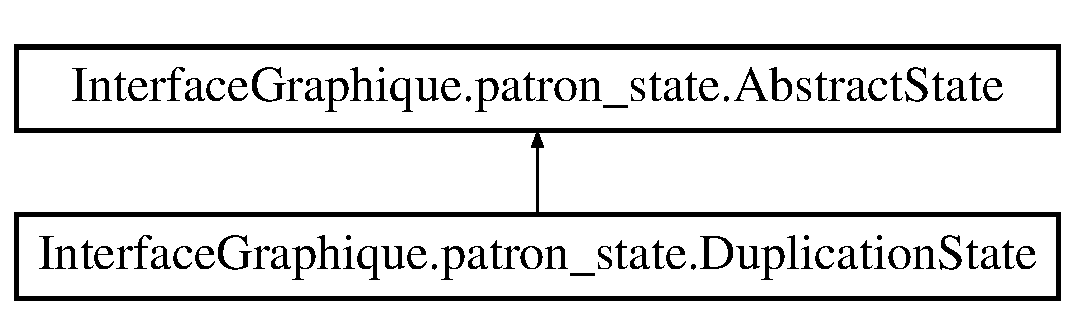
\includegraphics[height=2.000000cm]{class_interface_graphique_1_1patron__state_1_1_duplication_state}
\end{center}
\end{figure}
\subsection*{Public Member Functions}
\begin{DoxyCompactItemize}
\item 
override void \hyperlink{class_interface_graphique_1_1patron__state_1_1_duplication_state_a3e4ab1c3a8bd3d03b822c66d7597e068}{Action} (int x, int y)
\begin{DoxyCompactList}\small\item\em On duplique les objets selectionnees \end{DoxyCompactList}\end{DoxyCompactItemize}


\subsection{Detailed Description}
Etat de duplication 



\subsection{Member Function Documentation}
\hypertarget{class_interface_graphique_1_1patron__state_1_1_duplication_state_a3e4ab1c3a8bd3d03b822c66d7597e068}{\index{Interface\-Graphique\-::patron\-\_\-state\-::\-Duplication\-State@{Interface\-Graphique\-::patron\-\_\-state\-::\-Duplication\-State}!Action@{Action}}
\index{Action@{Action}!InterfaceGraphique::patron_state::DuplicationState@{Interface\-Graphique\-::patron\-\_\-state\-::\-Duplication\-State}}
\subsubsection[{Action}]{\setlength{\rightskip}{0pt plus 5cm}override void Interface\-Graphique.\-patron\-\_\-state.\-Duplication\-State.\-Action (
\begin{DoxyParamCaption}
\item[{int}]{x, }
\item[{int}]{y}
\end{DoxyParamCaption}
)\hspace{0.3cm}{\ttfamily [inline]}, {\ttfamily [virtual]}}}\label{class_interface_graphique_1_1patron__state_1_1_duplication_state_a3e4ab1c3a8bd3d03b822c66d7597e068}


On duplique les objets selectionnees 


\begin{DoxyParams}{Parameters}
{\em x} & Position en x du clique\\
\hline
{\em y} & Position en y du clique\\
\hline
\end{DoxyParams}


Implements \hyperlink{class_interface_graphique_1_1patron__state_1_1_abstract_state_a8df97c5a2784f9757608d669fbb1c6b5}{Interface\-Graphique.\-patron\-\_\-state.\-Abstract\-State}.



The documentation for this class was generated from the following file\-:\begin{DoxyCompactItemize}
\item 
X\-:/\-Git\-\_\-\-Repository/inf2990-\/06/\-Cadriciel/\-Sources/\-Interface\-Graphique/patron state/Duplication\-State.\-cs\end{DoxyCompactItemize}

\hypertarget{class_dynamic_library_manager}{\section{Dynamic\-Library\-Manager Class Reference}
\label{class_dynamic_library_manager}\index{Dynamic\-Library\-Manager@{Dynamic\-Library\-Manager}}
}


Manages dynamic libraries.  




{\ttfamily \#include $<$Dynamic\-Library\-Manager.\-h$>$}

\subsection*{Public Types}
\begin{DoxyCompactItemize}
\item 
\hypertarget{class_dynamic_library_manager_abb1022f448f94bf40c890d38ea41c52b}{typedef void $\ast$ {\bfseries Symbol}}\label{class_dynamic_library_manager_abb1022f448f94bf40c890d38ea41c52b}

\item 
\hypertarget{class_dynamic_library_manager_aa47563bb349a44ec41af6464300e0688}{typedef void $\ast$ {\bfseries Library\-Handle}}\label{class_dynamic_library_manager_aa47563bb349a44ec41af6464300e0688}

\end{DoxyCompactItemize}
\subsection*{Public Member Functions}
\begin{DoxyCompactItemize}
\item 
\hyperlink{class_dynamic_library_manager_a26d6592077763d9eb31d66d02d17b8d4}{Dynamic\-Library\-Manager} (const std\-::string \&library\-File\-Name)
\begin{DoxyCompactList}\small\item\em Loads the specified library. \end{DoxyCompactList}\item 
\hypertarget{class_dynamic_library_manager_a1c6a30a61161a8ddb96279bfb44c44c7}{\hyperlink{class_dynamic_library_manager_a1c6a30a61161a8ddb96279bfb44c44c7}{$\sim$\-Dynamic\-Library\-Manager} ()}\label{class_dynamic_library_manager_a1c6a30a61161a8ddb96279bfb44c44c7}

\begin{DoxyCompactList}\small\item\em Releases the loaded library.. \end{DoxyCompactList}\item 
Symbol \hyperlink{class_dynamic_library_manager_a2bd337473432b0f470f5bb987da77239}{find\-Symbol} (const std\-::string \&symbol)
\begin{DoxyCompactList}\small\item\em Returns a pointer on the specified symbol exported by the library. \end{DoxyCompactList}\end{DoxyCompactItemize}


\subsection{Detailed Description}
Manages dynamic libraries. 

The Dynamic Library Manager provides a platform independent way to work with dynamic library. It load a specific dynamic library, and can returns specific symbol exported by the dynamic library.

If an error occurs, a \hyperlink{class_dynamic_library_manager_exception}{Dynamic\-Library\-Manager\-Exception} is thrown. 

\subsection{Constructor \& Destructor Documentation}
\hypertarget{class_dynamic_library_manager_a26d6592077763d9eb31d66d02d17b8d4}{\index{Dynamic\-Library\-Manager@{Dynamic\-Library\-Manager}!Dynamic\-Library\-Manager@{Dynamic\-Library\-Manager}}
\index{Dynamic\-Library\-Manager@{Dynamic\-Library\-Manager}!DynamicLibraryManager@{Dynamic\-Library\-Manager}}
\subsubsection[{Dynamic\-Library\-Manager}]{\setlength{\rightskip}{0pt plus 5cm}Dynamic\-Library\-Manager\-::\-Dynamic\-Library\-Manager (
\begin{DoxyParamCaption}
\item[{const std\-::string \&}]{library\-File\-Name}
\end{DoxyParamCaption}
)}}\label{class_dynamic_library_manager_a26d6592077763d9eb31d66d02d17b8d4}


Loads the specified library. 


\begin{DoxyParams}{Parameters}
{\em library\-File\-Name} & Name of the library to load. \\
\hline
\end{DoxyParams}

\begin{DoxyExceptions}{Exceptions}
{\em \hyperlink{class_dynamic_library_manager_exception}{Dynamic\-Library\-Manager\-Exception}} & if a failure occurs while loading the library (fail to found or load the library). \\
\hline
\end{DoxyExceptions}


\subsection{Member Function Documentation}
\hypertarget{class_dynamic_library_manager_a2bd337473432b0f470f5bb987da77239}{\index{Dynamic\-Library\-Manager@{Dynamic\-Library\-Manager}!find\-Symbol@{find\-Symbol}}
\index{find\-Symbol@{find\-Symbol}!DynamicLibraryManager@{Dynamic\-Library\-Manager}}
\subsubsection[{find\-Symbol}]{\setlength{\rightskip}{0pt plus 5cm}Symbol Dynamic\-Library\-Manager\-::find\-Symbol (
\begin{DoxyParamCaption}
\item[{const std\-::string \&}]{symbol}
\end{DoxyParamCaption}
)}}\label{class_dynamic_library_manager_a2bd337473432b0f470f5bb987da77239}


Returns a pointer on the specified symbol exported by the library. 


\begin{DoxyParams}{Parameters}
{\em symbol} & Name of the symbol exported by the library. \\
\hline
\end{DoxyParams}
\begin{DoxyReturn}{Returns}
Pointer on the symbol. Should be casted to the actual type. Never {\ttfamily N\-U\-L\-L}. 
\end{DoxyReturn}

\begin{DoxyExceptions}{Exceptions}
{\em \hyperlink{class_dynamic_library_manager_exception}{Dynamic\-Library\-Manager\-Exception}} & if the symbol is not found. \\
\hline
\end{DoxyExceptions}


The documentation for this class was generated from the following file\-:\begin{DoxyCompactItemize}
\item 
X\-:/\-Git\-\_\-\-Repository/inf2990-\/06/\-Cadriciel/\-Commun/\-Externe/cppunit/include/cppunit/plugin/Dynamic\-Library\-Manager.\-h\end{DoxyCompactItemize}

\hypertarget{class_dynamic_library_manager_exception}{\section{Dynamic\-Library\-Manager\-Exception Class Reference}
\label{class_dynamic_library_manager_exception}\index{Dynamic\-Library\-Manager\-Exception@{Dynamic\-Library\-Manager\-Exception}}
}


\hyperlink{class_exception}{Exception} thrown by \hyperlink{class_dynamic_library_manager}{Dynamic\-Library\-Manager} when a failure occurs.  




{\ttfamily \#include $<$Dynamic\-Library\-Manager\-Exception.\-h$>$}

Inheritance diagram for Dynamic\-Library\-Manager\-Exception\-:\begin{figure}[H]
\begin{center}
\leavevmode
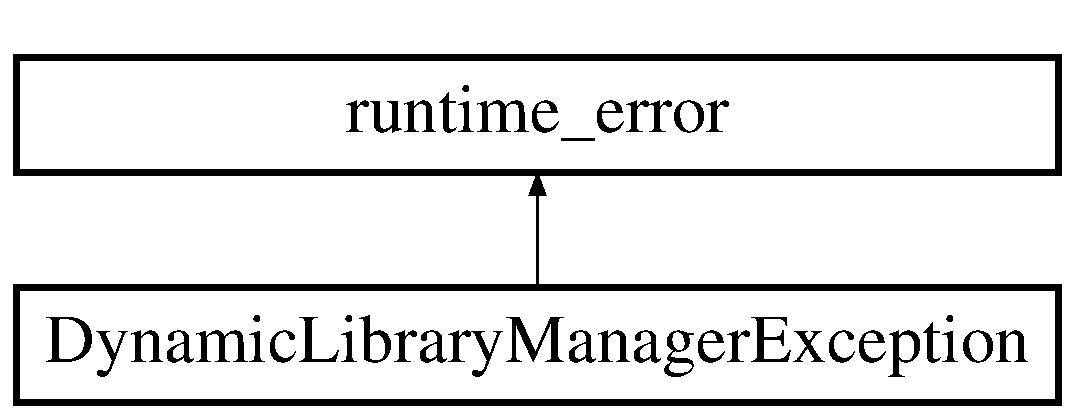
\includegraphics[height=2.000000cm]{class_dynamic_library_manager_exception}
\end{center}
\end{figure}
\subsection*{Public Types}
\begin{DoxyCompactItemize}
\item 
enum \hyperlink{class_dynamic_library_manager_exception_a73b4694c152e0693fbc19fb04987a0b9}{Cause} \{ \hyperlink{class_dynamic_library_manager_exception_a73b4694c152e0693fbc19fb04987a0b9a778b42fb996bf018bdc26934649cad63}{loading\-Failed} =0, 
\hyperlink{class_dynamic_library_manager_exception_a73b4694c152e0693fbc19fb04987a0b9a193fc58bb852e09790da269e2b613045}{symbol\-Not\-Found}
 \}
\end{DoxyCompactItemize}
\subsection*{Public Member Functions}
\begin{DoxyCompactItemize}
\item 
\hypertarget{class_dynamic_library_manager_exception_a15629092a054849f1cb73f8f468f8125}{\hyperlink{class_dynamic_library_manager_exception_a15629092a054849f1cb73f8f468f8125}{Dynamic\-Library\-Manager\-Exception} (const std\-::string \&library\-Name, const std\-::string \&error\-Detail, \hyperlink{class_dynamic_library_manager_exception_a73b4694c152e0693fbc19fb04987a0b9}{Cause} cause)}\label{class_dynamic_library_manager_exception_a15629092a054849f1cb73f8f468f8125}

\begin{DoxyCompactList}\small\item\em Failed to load the dynamic library or Symbol not found in the dynamic library. \end{DoxyCompactList}\item 
\hypertarget{class_dynamic_library_manager_exception_ab389b721f9a45814b8269ba865a1f25f}{\hyperlink{class_dynamic_library_manager_exception_a73b4694c152e0693fbc19fb04987a0b9}{Cause} {\bfseries get\-Cause} () const }\label{class_dynamic_library_manager_exception_ab389b721f9a45814b8269ba865a1f25f}

\item 
\hypertarget{class_dynamic_library_manager_exception_a3e6ed8a5e743a8ac80e4cb73a5d87360}{const char $\ast$ {\bfseries what} () const   throw ()}\label{class_dynamic_library_manager_exception_a3e6ed8a5e743a8ac80e4cb73a5d87360}

\end{DoxyCompactItemize}


\subsection{Detailed Description}
\hyperlink{class_exception}{Exception} thrown by \hyperlink{class_dynamic_library_manager}{Dynamic\-Library\-Manager} when a failure occurs. 

Use get\-Cause() to know what function caused the failure. 

\subsection{Member Enumeration Documentation}
\hypertarget{class_dynamic_library_manager_exception_a73b4694c152e0693fbc19fb04987a0b9}{\index{Dynamic\-Library\-Manager\-Exception@{Dynamic\-Library\-Manager\-Exception}!Cause@{Cause}}
\index{Cause@{Cause}!DynamicLibraryManagerException@{Dynamic\-Library\-Manager\-Exception}}
\subsubsection[{Cause}]{\setlength{\rightskip}{0pt plus 5cm}enum {\bf Dynamic\-Library\-Manager\-Exception\-::\-Cause}}}\label{class_dynamic_library_manager_exception_a73b4694c152e0693fbc19fb04987a0b9}
\begin{Desc}
\item[Enumerator]\par
\begin{description}
\index{loading\-Failed@{loading\-Failed}!Dynamic\-Library\-Manager\-Exception@{Dynamic\-Library\-Manager\-Exception}}\index{Dynamic\-Library\-Manager\-Exception@{Dynamic\-Library\-Manager\-Exception}!loading\-Failed@{loading\-Failed}}\item[{\em 
\hypertarget{class_dynamic_library_manager_exception_a73b4694c152e0693fbc19fb04987a0b9a778b42fb996bf018bdc26934649cad63}{loading\-Failed}\label{class_dynamic_library_manager_exception_a73b4694c152e0693fbc19fb04987a0b9a778b42fb996bf018bdc26934649cad63}
}]Failed to load the dynamic library. \index{symbol\-Not\-Found@{symbol\-Not\-Found}!Dynamic\-Library\-Manager\-Exception@{Dynamic\-Library\-Manager\-Exception}}\index{Dynamic\-Library\-Manager\-Exception@{Dynamic\-Library\-Manager\-Exception}!symbol\-Not\-Found@{symbol\-Not\-Found}}\item[{\em 
\hypertarget{class_dynamic_library_manager_exception_a73b4694c152e0693fbc19fb04987a0b9a193fc58bb852e09790da269e2b613045}{symbol\-Not\-Found}\label{class_dynamic_library_manager_exception_a73b4694c152e0693fbc19fb04987a0b9a193fc58bb852e09790da269e2b613045}
}]Symbol not found in the dynamic library. \end{description}
\end{Desc}


The documentation for this class was generated from the following file\-:\begin{DoxyCompactItemize}
\item 
X\-:/\-Git\-\_\-\-Repository/inf2990-\/06/\-Cadriciel/\-Commun/\-Externe/cppunit/include/cppunit/plugin/Dynamic\-Library\-Manager\-Exception.\-h\end{DoxyCompactItemize}

\hypertarget{structendif}{\section{endif Struct Reference}
\label{structendif}\index{endif@{endif}}
}


$\ast$/  




{\ttfamily \#include $<$material.\-h$>$}

\subsection*{Public Member Functions}
\begin{DoxyCompactItemize}
\item 
\hypertarget{structendif_aecfb322023b3a31eb28c53ddb5fe5cb3}{{\bfseries ai\-Material} ()}\label{structendif_aecfb322023b3a31eb28c53ddb5fe5cb3}

\item 
{\footnotesize template$<$typename Type $>$ }\\ai\-Return \hyperlink{structendif_a4b08154b44a2676d0664547b6475aa0b}{Get} (const char $\ast$p\-Key, unsigned int type, unsigned int idx, Type $\ast$p\-Out, unsigned int $\ast$p\-Max) const 
\begin{DoxyCompactList}\small\item\em Retrieve an array of Type values with a specific key from the material. \end{DoxyCompactList}\item 
\hypertarget{structendif_a5f7f7f17939445e46d4b627a94e6f3e8}{ai\-Return {\bfseries Get} (const char $\ast$p\-Key, unsigned int type, unsigned int idx, int $\ast$p\-Out, unsigned int $\ast$p\-Max) const }\label{structendif_a5f7f7f17939445e46d4b627a94e6f3e8}

\item 
\hypertarget{structendif_a3025cbc4b9b9ab1a2d576226c88b9580}{ai\-Return {\bfseries Get} (const char $\ast$p\-Key, unsigned int type, unsigned int idx, float $\ast$p\-Out, unsigned int $\ast$p\-Max) const }\label{structendif_a3025cbc4b9b9ab1a2d576226c88b9580}

\item 
{\footnotesize template$<$typename Type $>$ }\\ai\-Return \hyperlink{structendif_aaa5e921648171c5d4a9f195030c17883}{Get} (const char $\ast$p\-Key, unsigned int type, unsigned int idx, Type \&p\-Out) const 
\begin{DoxyCompactList}\small\item\em Retrieve a Type value with a specific key from the material. \end{DoxyCompactList}\item 
\hypertarget{structendif_a178f108e6bd7afef988a043e70f29cdf}{ai\-Return {\bfseries Get} (const char $\ast$p\-Key, unsigned int type, unsigned int idx, int \&p\-Out) const }\label{structendif_a178f108e6bd7afef988a043e70f29cdf}

\item 
\hypertarget{structendif_a13bc415aa964501533b1cfce432c3a46}{ai\-Return {\bfseries Get} (const char $\ast$p\-Key, unsigned int type, unsigned int idx, float \&p\-Out) const }\label{structendif_a13bc415aa964501533b1cfce432c3a46}

\item 
\hypertarget{structendif_af9994066ba1264257d6cbcb77642a365}{ai\-Return {\bfseries Get} (const char $\ast$p\-Key, unsigned int type, unsigned int idx, \hyperlink{structai_string}{ai\-String} \&p\-Out) const }\label{structendif_af9994066ba1264257d6cbcb77642a365}

\item 
\hypertarget{structendif_a4abf0d7eed2deab665aaa674e5564227}{ai\-Return {\bfseries Get} (const char $\ast$p\-Key, unsigned int type, unsigned int idx, \hyperlink{structai_color3_d}{ai\-Color3\-D} \&p\-Out) const }\label{structendif_a4abf0d7eed2deab665aaa674e5564227}

\item 
\hypertarget{structendif_af4761002bbd3a9c270810c9ec576c1de}{ai\-Return {\bfseries Get} (const char $\ast$p\-Key, unsigned int type, unsigned int idx, \hyperlink{structai_color4_d}{ai\-Color4\-D} \&p\-Out) const }\label{structendif_af4761002bbd3a9c270810c9ec576c1de}

\item 
\hypertarget{structendif_a4e906b6f4dc388356a971783279885d2}{ai\-Return {\bfseries Get} (const char $\ast$p\-Key, unsigned int type, unsigned int idx, \hyperlink{structai_u_v_transform}{ai\-U\-V\-Transform} \&p\-Out) const }\label{structendif_a4e906b6f4dc388356a971783279885d2}

\item 
unsigned int \hyperlink{structendif_a1b5fc4d41cee008c631531272d79d741}{Get\-Texture\-Count} (\hyperlink{material_8h_a7dd415ff703a2cc53d1c22ddbbd7dde0}{ai\-Texture\-Type} type) const 
\item 
ai\-Return \hyperlink{structendif_a09eec253b632c99e3cfa3c8eba44aaa3}{Get\-Texture} (\hyperlink{material_8h_a7dd415ff703a2cc53d1c22ddbbd7dde0}{ai\-Texture\-Type} type, unsigned int index, C\-\_\-\-S\-T\-R\-U\-C\-T \hyperlink{structai_string}{ai\-String} $\ast$path, \hyperlink{material_8h_a6186e909f1ae28133ab10f1b4635b0f9}{ai\-Texture\-Mapping} $\ast$mapping=N\-U\-L\-L, unsigned int $\ast$uvindex=N\-U\-L\-L, float $\ast$blend=N\-U\-L\-L, \hyperlink{material_8h_afcd3096d69affba13114cedfc6f9ee6b}{ai\-Texture\-Op} $\ast$op=N\-U\-L\-L, \hyperlink{material_8h_a6cbe56056751aa80e8dd714632a49de0}{ai\-Texture\-Map\-Mode} $\ast$mapmode=N\-U\-L\-L) const 
\item 
ai\-Return \hyperlink{structendif_ae548c37cd3a797ae815eed369911d9a8}{Add\-Binary\-Property} (const void $\ast$p\-Input, unsigned int p\-Size\-In\-Bytes, const char $\ast$p\-Key, unsigned int type, unsigned int index, ai\-Property\-Type\-Info p\-Type)
\begin{DoxyCompactList}\small\item\em Add a property with a given key and type info to the material structure. \end{DoxyCompactList}\item 
ai\-Return \hyperlink{structendif_a104441df9d38abd744f4dd9d71edb36a}{Add\-Property} (const \hyperlink{structai_string}{ai\-String} $\ast$p\-Input, const char $\ast$p\-Key, unsigned int type=0, unsigned int index=0)
\begin{DoxyCompactList}\small\item\em Add a string property with a given key and type info to the material structure. \end{DoxyCompactList}\item 
{\footnotesize template$<$class T\-Y\-P\-E $>$ }\\ai\-Return \hyperlink{structendif_a592941c3bd88002290f37ed9973c052f}{Add\-Property} (const T\-Y\-P\-E $\ast$p\-Input, unsigned int p\-Num\-Values, const char $\ast$p\-Key, unsigned int type=0, unsigned int index=0)
\begin{DoxyCompactList}\small\item\em Add a property with a given key to the material structure. \end{DoxyCompactList}\item 
\hypertarget{structendif_aac68eb7879d125857d6161713f619908}{ai\-Return {\bfseries Add\-Property} (const \hyperlink{structai_vector3_d}{ai\-Vector3\-D} $\ast$p\-Input, unsigned int p\-Num\-Values, const char $\ast$p\-Key, unsigned int type=0, unsigned int index=0)}\label{structendif_aac68eb7879d125857d6161713f619908}

\item 
\hypertarget{structendif_a03e396bb5be1441f8375457af95758ed}{ai\-Return {\bfseries Add\-Property} (const \hyperlink{structai_color3_d}{ai\-Color3\-D} $\ast$p\-Input, unsigned int p\-Num\-Values, const char $\ast$p\-Key, unsigned int type=0, unsigned int index=0)}\label{structendif_a03e396bb5be1441f8375457af95758ed}

\item 
\hypertarget{structendif_ad08edaf165b0b3fd9cf48bc8f371e366}{ai\-Return {\bfseries Add\-Property} (const \hyperlink{structai_color4_d}{ai\-Color4\-D} $\ast$p\-Input, unsigned int p\-Num\-Values, const char $\ast$p\-Key, unsigned int type=0, unsigned int index=0)}\label{structendif_ad08edaf165b0b3fd9cf48bc8f371e366}

\item 
\hypertarget{structendif_aeae8cf511867b96ed0f1ebb858934a7c}{ai\-Return {\bfseries Add\-Property} (const int $\ast$p\-Input, unsigned int p\-Num\-Values, const char $\ast$p\-Key, unsigned int type=0, unsigned int index=0)}\label{structendif_aeae8cf511867b96ed0f1ebb858934a7c}

\item 
\hypertarget{structendif_ada3e0b2547092eba92b6666a7a43457f}{ai\-Return {\bfseries Add\-Property} (const float $\ast$p\-Input, unsigned int p\-Num\-Values, const char $\ast$p\-Key, unsigned int type=0, unsigned int index=0)}\label{structendif_ada3e0b2547092eba92b6666a7a43457f}

\item 
\hypertarget{structendif_adbcc1b914e8c7fb874acb1c32295f758}{ai\-Return {\bfseries Add\-Property} (const \hyperlink{structai_u_v_transform}{ai\-U\-V\-Transform} $\ast$p\-Input, unsigned int p\-Num\-Values, const char $\ast$p\-Key, unsigned int type=0, unsigned int index=0)}\label{structendif_adbcc1b914e8c7fb874acb1c32295f758}

\item 
ai\-Return \hyperlink{structendif_a0dd7647c3845ea482f4ac97e675bf59b}{Remove\-Property} (const char $\ast$p\-Key, unsigned int type=0, unsigned int index=0)
\begin{DoxyCompactList}\small\item\em Remove a given key from the list. \end{DoxyCompactList}\item 
void \hyperlink{structendif_a75a80a76250dc7c1d6fd63d8a0117200}{Clear} ()
\begin{DoxyCompactList}\small\item\em Removes all properties from the material. \end{DoxyCompactList}\end{DoxyCompactItemize}
\subsection*{Static Public Member Functions}
\begin{DoxyCompactItemize}
\item 
static void \hyperlink{structendif_af2407ec9a1f919efc36017bb1c414841}{Copy\-Property\-List} (ai\-Material $\ast$pc\-Dest, const ai\-Material $\ast$pc\-Src)
\end{DoxyCompactItemize}
\subsection*{Public Attributes}
\begin{DoxyCompactItemize}
\item 
C\-\_\-\-S\-T\-R\-U\-C\-T ai\-Material\-Property $\ast$$\ast$ \hyperlink{structendif_a95295db8cbd37f02553457d84d65068a}{m\-Properties}
\item 
unsigned int \hyperlink{structendif_a751ff065f0b034cfd9cd08d7bc41d668}{m\-Num\-Properties}
\item 
unsigned int \hyperlink{structendif_add50ca52ed05564f2187b9893fb1f584}{m\-Num\-Allocated}
\end{DoxyCompactItemize}


\subsection{Detailed Description}
$\ast$/ 

Data structure for a material

Material data is stored using a key-\/value structure. A single key-\/value pair is called a 'material property'. C++ users should use the provided member functions of ai\-Material to process material properties, C users have to stick with the ai\-Material\-Get\-X\-X\-X family of unbound functions. The library defines a set of standard keys (A\-I\-\_\-\-M\-A\-T\-K\-E\-Y\-\_\-\-X\-X\-X). 

\subsection{Member Function Documentation}
\hypertarget{structendif_ae548c37cd3a797ae815eed369911d9a8}{\index{endif@{endif}!Add\-Binary\-Property@{Add\-Binary\-Property}}
\index{Add\-Binary\-Property@{Add\-Binary\-Property}!endif@{endif}}
\subsubsection[{Add\-Binary\-Property}]{\setlength{\rightskip}{0pt plus 5cm}ai\-Return endif\-::\-Add\-Binary\-Property (
\begin{DoxyParamCaption}
\item[{const void $\ast$}]{p\-Input, }
\item[{unsigned int}]{p\-Size\-In\-Bytes, }
\item[{const char $\ast$}]{p\-Key, }
\item[{unsigned int}]{type, }
\item[{unsigned int}]{index, }
\item[{ai\-Property\-Type\-Info}]{p\-Type}
\end{DoxyParamCaption}
)}}\label{structendif_ae548c37cd3a797ae815eed369911d9a8}


Add a property with a given key and type info to the material structure. 


\begin{DoxyParams}{Parameters}
{\em p\-Input} & Pointer to input data \\
\hline
{\em p\-Size\-In\-Bytes} & Size of input data \\
\hline
{\em p\-Key} & Key/\-Usage of the property (A\-I\-\_\-\-M\-A\-T\-K\-E\-Y\-\_\-\-X\-X\-X) \\
\hline
{\em type} & Set by the A\-I\-\_\-\-M\-A\-T\-K\-E\-Y\-\_\-\-X\-X\-X macro \\
\hline
{\em index} & Set by the A\-I\-\_\-\-M\-A\-T\-K\-E\-Y\-\_\-\-X\-X\-X macro \\
\hline
{\em p\-Type} & Type information hint \\
\hline
\end{DoxyParams}
\hypertarget{structendif_a104441df9d38abd744f4dd9d71edb36a}{\index{endif@{endif}!Add\-Property@{Add\-Property}}
\index{Add\-Property@{Add\-Property}!endif@{endif}}
\subsubsection[{Add\-Property}]{\setlength{\rightskip}{0pt plus 5cm}ai\-Return endif\-::\-Add\-Property (
\begin{DoxyParamCaption}
\item[{const {\bf ai\-String} $\ast$}]{p\-Input, }
\item[{const char $\ast$}]{p\-Key, }
\item[{unsigned int}]{type = {\ttfamily 0}, }
\item[{unsigned int}]{index = {\ttfamily 0}}
\end{DoxyParamCaption}
)}}\label{structendif_a104441df9d38abd744f4dd9d71edb36a}


Add a string property with a given key and type info to the material structure. 


\begin{DoxyParams}{Parameters}
{\em p\-Input} & Input string \\
\hline
{\em p\-Key} & Key/\-Usage of the property (A\-I\-\_\-\-M\-A\-T\-K\-E\-Y\-\_\-\-X\-X\-X) \\
\hline
{\em type} & Set by the A\-I\-\_\-\-M\-A\-T\-K\-E\-Y\-\_\-\-X\-X\-X macro \\
\hline
{\em index} & Set by the A\-I\-\_\-\-M\-A\-T\-K\-E\-Y\-\_\-\-X\-X\-X macro \\
\hline
\end{DoxyParams}
\hypertarget{structendif_a592941c3bd88002290f37ed9973c052f}{\index{endif@{endif}!Add\-Property@{Add\-Property}}
\index{Add\-Property@{Add\-Property}!endif@{endif}}
\subsubsection[{Add\-Property}]{\setlength{\rightskip}{0pt plus 5cm}template$<$class T\-Y\-P\-E $>$ ai\-Return endif\-::\-Add\-Property (
\begin{DoxyParamCaption}
\item[{const T\-Y\-P\-E $\ast$}]{p\-Input, }
\item[{unsigned int}]{p\-Num\-Values, }
\item[{const char $\ast$}]{p\-Key, }
\item[{unsigned int}]{type = {\ttfamily 0}, }
\item[{unsigned int}]{index = {\ttfamily 0}}
\end{DoxyParamCaption}
)}}\label{structendif_a592941c3bd88002290f37ed9973c052f}


Add a property with a given key to the material structure. 


\begin{DoxyParams}{Parameters}
{\em p\-Input} & Pointer to the input data \\
\hline
{\em p\-Num\-Values} & Number of values in the array \\
\hline
{\em p\-Key} & Key/\-Usage of the property (A\-I\-\_\-\-M\-A\-T\-K\-E\-Y\-\_\-\-X\-X\-X) \\
\hline
{\em type} & Set by the A\-I\-\_\-\-M\-A\-T\-K\-E\-Y\-\_\-\-X\-X\-X macro \\
\hline
{\em index} & Set by the A\-I\-\_\-\-M\-A\-T\-K\-E\-Y\-\_\-\-X\-X\-X macro \\
\hline
\end{DoxyParams}
\hypertarget{structendif_a75a80a76250dc7c1d6fd63d8a0117200}{\index{endif@{endif}!Clear@{Clear}}
\index{Clear@{Clear}!endif@{endif}}
\subsubsection[{Clear}]{\setlength{\rightskip}{0pt plus 5cm}void endif\-::\-Clear (
\begin{DoxyParamCaption}
{}
\end{DoxyParamCaption}
)}}\label{structendif_a75a80a76250dc7c1d6fd63d8a0117200}


Removes all properties from the material. 

The data array remains allocated so adding new properties is quite fast. \hypertarget{structendif_af2407ec9a1f919efc36017bb1c414841}{\index{endif@{endif}!Copy\-Property\-List@{Copy\-Property\-List}}
\index{Copy\-Property\-List@{Copy\-Property\-List}!endif@{endif}}
\subsubsection[{Copy\-Property\-List}]{\setlength{\rightskip}{0pt plus 5cm}static void endif\-::\-Copy\-Property\-List (
\begin{DoxyParamCaption}
\item[{ai\-Material $\ast$}]{pc\-Dest, }
\item[{const ai\-Material $\ast$}]{pc\-Src}
\end{DoxyParamCaption}
)\hspace{0.3cm}{\ttfamily [static]}}}\label{structendif_af2407ec9a1f919efc36017bb1c414841}
Copy the property list of a material 
\begin{DoxyParams}{Parameters}
{\em pc\-Dest} & Destination material \\
\hline
{\em pc\-Src} & Source material \\
\hline
\end{DoxyParams}
\hypertarget{structendif_a4b08154b44a2676d0664547b6475aa0b}{\index{endif@{endif}!Get@{Get}}
\index{Get@{Get}!endif@{endif}}
\subsubsection[{Get}]{\setlength{\rightskip}{0pt plus 5cm}template$<$typename Type $>$ ai\-Return endif\-::\-Get (
\begin{DoxyParamCaption}
\item[{const char $\ast$}]{p\-Key, }
\item[{unsigned int}]{type, }
\item[{unsigned int}]{idx, }
\item[{Type $\ast$}]{p\-Out, }
\item[{unsigned int $\ast$}]{p\-Max}
\end{DoxyParamCaption}
) const}}\label{structendif_a4b08154b44a2676d0664547b6475aa0b}


Retrieve an array of Type values with a specific key from the material. 


\begin{DoxyParams}{Parameters}
{\em p\-Key} & Key to search for. One of the A\-I\-\_\-\-M\-A\-T\-K\-E\-Y\-\_\-\-X\-X\-X constants. \\
\hline
{\em type} & .. set by A\-I\-\_\-\-M\-A\-T\-K\-E\-Y\-\_\-\-X\-X\-X \\
\hline
{\em idx} & .. set by A\-I\-\_\-\-M\-A\-T\-K\-E\-Y\-\_\-\-X\-X\-X \\
\hline
{\em p\-Out} & Pointer to a buffer to receive the result. \\
\hline
{\em p\-Max} & Specifies the size of the given buffer, in Type's. Receives the number of values (not bytes!) read. N\-U\-L\-L is a valid value for this parameter. \\
\hline
\end{DoxyParams}
\hypertarget{structendif_aaa5e921648171c5d4a9f195030c17883}{\index{endif@{endif}!Get@{Get}}
\index{Get@{Get}!endif@{endif}}
\subsubsection[{Get}]{\setlength{\rightskip}{0pt plus 5cm}template$<$typename Type $>$ ai\-Return endif\-::\-Get (
\begin{DoxyParamCaption}
\item[{const char $\ast$}]{p\-Key, }
\item[{unsigned int}]{type, }
\item[{unsigned int}]{idx, }
\item[{Type \&}]{p\-Out}
\end{DoxyParamCaption}
) const}}\label{structendif_aaa5e921648171c5d4a9f195030c17883}


Retrieve a Type value with a specific key from the material. 


\begin{DoxyParams}{Parameters}
{\em p\-Key} & Key to search for. One of the A\-I\-\_\-\-M\-A\-T\-K\-E\-Y\-\_\-\-X\-X\-X constants. \\
\hline
{\em type} & Specifies the type of the texture to be retrieved ( e.\-g. diffuse, specular, height map ...) \\
\hline
{\em idx} & Index of the texture to be retrieved. \\
\hline
{\em p\-Out} & Reference to receive the output value \\
\hline
\end{DoxyParams}
\hypertarget{structendif_a09eec253b632c99e3cfa3c8eba44aaa3}{\index{endif@{endif}!Get\-Texture@{Get\-Texture}}
\index{Get\-Texture@{Get\-Texture}!endif@{endif}}
\subsubsection[{Get\-Texture}]{\setlength{\rightskip}{0pt plus 5cm}ai\-Return endif\-::\-Get\-Texture (
\begin{DoxyParamCaption}
\item[{{\bf ai\-Texture\-Type}}]{type, }
\item[{unsigned int}]{index, }
\item[{C\-\_\-\-S\-T\-R\-U\-C\-T {\bf ai\-String} $\ast$}]{path, }
\item[{{\bf ai\-Texture\-Mapping} $\ast$}]{mapping = {\ttfamily NULL}, }
\item[{unsigned int $\ast$}]{uvindex = {\ttfamily NULL}, }
\item[{float $\ast$}]{blend = {\ttfamily NULL}, }
\item[{{\bf ai\-Texture\-Op} $\ast$}]{op = {\ttfamily NULL}, }
\item[{{\bf ai\-Texture\-Map\-Mode} $\ast$}]{mapmode = {\ttfamily NULL}}
\end{DoxyParamCaption}
) const}}\label{structendif_a09eec253b632c99e3cfa3c8eba44aaa3}
Helper function to get all parameters pertaining to a particular texture slot from a material.

This function is provided just for convenience, you could also read the single material properties manually. 
\begin{DoxyParams}{Parameters}
{\em type} & Specifies the type of the texture to be retrieved ( e.\-g. diffuse, specular, height map ...) \\
\hline
{\em index} & Index of the texture to be retrieved. The function fails if there is no texture of that type with this index. \hyperlink{structendif_a1b5fc4d41cee008c631531272d79d741}{Get\-Texture\-Count()} can be used to determine the number of textures per texture type. \\
\hline
{\em path} & Receives the path to the texture. N\-U\-L\-L is a valid value. \\
\hline
{\em mapping} & The texture mapping. N\-U\-L\-L is allowed as value. \\
\hline
{\em uvindex} & Receives the U\-V index of the texture. N\-U\-L\-L is a valid value. \\
\hline
{\em blend} & Receives the blend factor for the texture N\-U\-L\-L is a valid value. \\
\hline
{\em op} & Receives the texture operation to be performed between this texture and the previous texture. N\-U\-L\-L is allowed as value. \\
\hline
{\em mapmode} & Receives the mapping modes to be used for the texture. The parameter may be N\-U\-L\-L but if it is a valid pointer it M\-U\-S\-T point to an array of 3 ai\-Texture\-Map\-Mode's (one for each axis\-: U\-V\-W order (=X\-Y\-Z)). \\
\hline
\end{DoxyParams}
\hypertarget{structendif_a1b5fc4d41cee008c631531272d79d741}{\index{endif@{endif}!Get\-Texture\-Count@{Get\-Texture\-Count}}
\index{Get\-Texture\-Count@{Get\-Texture\-Count}!endif@{endif}}
\subsubsection[{Get\-Texture\-Count}]{\setlength{\rightskip}{0pt plus 5cm}unsigned int endif\-::\-Get\-Texture\-Count (
\begin{DoxyParamCaption}
\item[{{\bf ai\-Texture\-Type}}]{type}
\end{DoxyParamCaption}
) const}}\label{structendif_a1b5fc4d41cee008c631531272d79d741}
Get the number of textures for a particular texture type. 
\begin{DoxyParams}{Parameters}
{\em type} & Texture type to check for \\
\hline
\end{DoxyParams}
\begin{DoxyReturn}{Returns}
Number of textures for this type. 
\end{DoxyReturn}
\begin{DoxyNote}{Note}
A texture can be easily queried using \hyperlink{structendif_a09eec253b632c99e3cfa3c8eba44aaa3}{Get\-Texture()} 
\end{DoxyNote}
\hypertarget{structendif_a0dd7647c3845ea482f4ac97e675bf59b}{\index{endif@{endif}!Remove\-Property@{Remove\-Property}}
\index{Remove\-Property@{Remove\-Property}!endif@{endif}}
\subsubsection[{Remove\-Property}]{\setlength{\rightskip}{0pt plus 5cm}ai\-Return endif\-::\-Remove\-Property (
\begin{DoxyParamCaption}
\item[{const char $\ast$}]{p\-Key, }
\item[{unsigned int}]{type = {\ttfamily 0}, }
\item[{unsigned int}]{index = {\ttfamily 0}}
\end{DoxyParamCaption}
)}}\label{structendif_a0dd7647c3845ea482f4ac97e675bf59b}


Remove a given key from the list. 

The function fails if the key isn't found 
\begin{DoxyParams}{Parameters}
{\em p\-Key} & Key to be deleted \\
\hline
\end{DoxyParams}


\subsection{Member Data Documentation}
\hypertarget{structendif_add50ca52ed05564f2187b9893fb1f584}{\index{endif@{endif}!m\-Num\-Allocated@{m\-Num\-Allocated}}
\index{m\-Num\-Allocated@{m\-Num\-Allocated}!endif@{endif}}
\subsubsection[{m\-Num\-Allocated}]{\setlength{\rightskip}{0pt plus 5cm}unsigned int endif\-::m\-Num\-Allocated}}\label{structendif_add50ca52ed05564f2187b9893fb1f584}
Storage allocated \hypertarget{structendif_a751ff065f0b034cfd9cd08d7bc41d668}{\index{endif@{endif}!m\-Num\-Properties@{m\-Num\-Properties}}
\index{m\-Num\-Properties@{m\-Num\-Properties}!endif@{endif}}
\subsubsection[{m\-Num\-Properties}]{\setlength{\rightskip}{0pt plus 5cm}unsigned int endif\-::m\-Num\-Properties}}\label{structendif_a751ff065f0b034cfd9cd08d7bc41d668}
Number of properties in the data base \hypertarget{structendif_a95295db8cbd37f02553457d84d65068a}{\index{endif@{endif}!m\-Properties@{m\-Properties}}
\index{m\-Properties@{m\-Properties}!endif@{endif}}
\subsubsection[{m\-Properties}]{\setlength{\rightskip}{0pt plus 5cm}C\-\_\-\-S\-T\-R\-U\-C\-T ai\-Material\-Property$\ast$$\ast$ endif\-::m\-Properties}}\label{structendif_a95295db8cbd37f02553457d84d65068a}
List of all material properties loaded. 

The documentation for this struct was generated from the following file\-:\begin{DoxyCompactItemize}
\item 
X\-:/\-Git\-\_\-\-Repository/inf2990-\/06/\-Cadriciel/\-Commun/\-Externe/assimp/include/\hyperlink{material_8h}{material.\-h}\end{DoxyCompactItemize}

\hypertarget{class_etat_open_g_l}{\section{Etat\-Open\-G\-L Class Reference}
\label{class_etat_open_g_l}\index{Etat\-Open\-G\-L@{Etat\-Open\-G\-L}}
}


Classe qui repr�sente l'�tat des variables de la machine Open\-G\-L.  




{\ttfamily \#include $<$Etat\-Open\-G\-L.\-h$>$}

\subsection*{Public Member Functions}
\begin{DoxyCompactItemize}
\item 
\hyperlink{group__utilitaire_gaf682f61929f2502b08b6b88de07349b6}{Etat\-Open\-G\-L} ()
\begin{DoxyCompactList}\small\item\em Constructeur par d�faut. \end{DoxyCompactList}\item 
std\-::string \hyperlink{group__utilitaire_ga13c8aaca9f02431b47b83e36b18f8067}{obtenir\-Chaine\-Gl\-Accum\-Alpha\-Bits} () const 
\begin{DoxyCompactList}\small\item\em Retourne une cha�ne repr�sentant l'attribut G\-L\-\_\-\-A\-C\-C\-U\-M\-\_\-\-A\-L\-P\-H\-A\-\_\-\-B\-I\-T\-S. \end{DoxyCompactList}\item 
std\-::string \hyperlink{group__utilitaire_ga695387ee2d838c97214c70219d52da10}{obtenir\-Chaine\-Gl\-Accum\-Blue\-Bits} () const 
\begin{DoxyCompactList}\small\item\em Retourne une cha�ne repr�sentant l'attribut G\-L\-\_\-\-A\-C\-C\-U\-M\-\_\-\-B\-L\-U\-E\-\_\-\-B\-I\-T\-S. \end{DoxyCompactList}\item 
std\-::string \hyperlink{group__utilitaire_gaf3e85f5f434e93aa09376200f3c837ae}{obtenir\-Chaine\-Gl\-Accum\-Clear\-Value} () const 
\begin{DoxyCompactList}\small\item\em Retourne une cha�ne repr�sentant l'attribut G\-L\-\_\-\-A\-C\-C\-U\-M\-\_\-\-C\-L\-E\-A\-R\-\_\-\-V\-A\-L\-U\-E. \end{DoxyCompactList}\item 
std\-::string \hyperlink{group__utilitaire_gae677b60d2113b1843ba4d2c92fe34c34}{obtenir\-Chaine\-Gl\-Accum\-Green\-Bits} () const 
\begin{DoxyCompactList}\small\item\em Retourne une cha�ne repr�sentant l'attribut G\-L\-\_\-\-A\-C\-C\-U\-M\-\_\-\-G\-R\-E\-E\-N\-\_\-\-B\-I\-T\-S. \end{DoxyCompactList}\item 
std\-::string \hyperlink{group__utilitaire_ga3405a98de14c30d7a57d954d298b6376}{obtenir\-Chaine\-Gl\-Accum\-Red\-Bits} () const 
\begin{DoxyCompactList}\small\item\em Retourne une cha�ne repr�sentant l'attribut G\-L\-\_\-\-A\-C\-C\-U\-M\-\_\-\-R\-E\-D\-\_\-\-B\-I\-T\-S. \end{DoxyCompactList}\item 
std\-::string \hyperlink{group__utilitaire_gaf54d9525863334d2d2fd362c7043a4be}{obtenir\-Chaine\-Gl\-Alpha\-Bias} () const 
\begin{DoxyCompactList}\small\item\em Retourne une cha�ne repr�sentant l'attribut G\-L\-\_\-\-A\-L\-P\-H\-A\-\_\-\-B\-I\-A\-S. \end{DoxyCompactList}\item 
std\-::string \hyperlink{group__utilitaire_ga7ea311e8cfd6aee3cb19e2041b2ba132}{obtenir\-Chaine\-Gl\-Alpha\-Bits} () const 
\begin{DoxyCompactList}\small\item\em Retourne une cha�ne repr�sentant l'attribut G\-L\-\_\-\-A\-L\-P\-H\-A\-\_\-\-B\-I\-T\-S. \end{DoxyCompactList}\item 
std\-::string \hyperlink{group__utilitaire_ga3b85b93cd7e5d1f12a225f28ece00696}{obtenir\-Chaine\-Gl\-Alpha\-Scale} () const 
\begin{DoxyCompactList}\small\item\em Retourne une cha�ne repr�sentant l'attribut G\-L\-\_\-\-A\-L\-P\-H\-A\-\_\-\-S\-C\-A\-L\-E. \end{DoxyCompactList}\item 
std\-::string \hyperlink{group__utilitaire_ga9fd2e2270997cf027e38f6a7b8d621a8}{obtenir\-Chaine\-Gl\-Alpha\-Test} () const 
\begin{DoxyCompactList}\small\item\em Retourne une cha�ne repr�sentant l'attribut G\-L\-\_\-\-A\-L\-P\-H\-A\-\_\-\-T\-E\-S\-T. \end{DoxyCompactList}\item 
std\-::string \hyperlink{group__utilitaire_ga5002fd87fb9aede24afc4c4bb2a61fb1}{obtenir\-Chaine\-Gl\-Alpha\-Test\-Func} () const 
\begin{DoxyCompactList}\small\item\em Retourne une cha�ne repr�sentant l'attribut G\-L\-\_\-\-A\-L\-P\-H\-A\-\_\-\-T\-E\-S\-T\-\_\-\-F\-U\-N\-C. \end{DoxyCompactList}\item 
std\-::string \hyperlink{group__utilitaire_gacc2904dcf7edec91f24e5e6ea58a780c}{obtenir\-Chaine\-Gl\-Alpha\-Test\-Ref} () const 
\begin{DoxyCompactList}\small\item\em Retourne une cha�ne repr�sentant l'attribut G\-L\-\_\-\-A\-L\-P\-H\-A\-\_\-\-T\-E\-S\-T\-\_\-\-R\-E\-F. \end{DoxyCompactList}\item 
std\-::string \hyperlink{group__utilitaire_ga59c1e206aa477f625b5499cf328f695b}{obtenir\-Chaine\-Gl\-Attrib\-Stack\-Depth} () const 
\begin{DoxyCompactList}\small\item\em Retourne une cha�ne repr�sentant l'attribut G\-L\-\_\-\-A\-T\-T\-R\-I\-B\-\_\-\-S\-T\-A\-C\-K\-\_\-\-D\-E\-P\-T\-H. \end{DoxyCompactList}\item 
std\-::string \hyperlink{group__utilitaire_gaaf8d3f8a4dd51812950c32268c8f77c5}{obtenir\-Chaine\-Gl\-Auto\-Normal} () const 
\begin{DoxyCompactList}\small\item\em Retourne une cha�ne repr�sentant l'attribut G\-L\-\_\-\-A\-U\-T\-O\-\_\-\-N\-O\-R\-M\-A\-L. \end{DoxyCompactList}\item 
std\-::string \hyperlink{group__utilitaire_gab8c780e176faece6cbaa11084e957e8d}{obtenir\-Chaine\-Gl\-Aux\-Buffers} () const 
\begin{DoxyCompactList}\small\item\em Retourne une cha�ne repr�sentant l'attribut G\-L\-\_\-\-A\-U\-X\-\_\-\-B\-U\-F\-F\-E\-R\-S. \end{DoxyCompactList}\item 
std\-::string \hyperlink{group__utilitaire_ga8a5f949f2b7a9a911c0677d639bebae5}{obtenir\-Chaine\-Gl\-Blend} () const 
\begin{DoxyCompactList}\small\item\em Retourne une cha�ne repr�sentant l'attribut G\-L\-\_\-\-B\-L\-E\-N\-D. \end{DoxyCompactList}\item 
std\-::string \hyperlink{group__utilitaire_gaa52ab39bcb62d4f8777afddfca458650}{obtenir\-Chaine\-Gl\-Blend\-Dst} () const 
\begin{DoxyCompactList}\small\item\em Retourne une cha�ne repr�sentant l'attribut G\-L\-\_\-\-B\-L\-E\-N\-D\-\_\-\-D\-S\-T. \end{DoxyCompactList}\item 
std\-::string \hyperlink{group__utilitaire_ga510a36fe5d3e313756e40b5c67b516ba}{obtenir\-Chaine\-Gl\-Blend\-Src} () const 
\begin{DoxyCompactList}\small\item\em Retourne une cha�ne repr�sentant l'attribut G\-L\-\_\-\-B\-L\-E\-N\-D\-\_\-\-S\-R\-C. \end{DoxyCompactList}\item 
std\-::string \hyperlink{group__utilitaire_ga95f9a6baabd65a0cdd4b1e5cbeb4f678}{obtenir\-Chaine\-Gl\-Blue\-Bias} () const 
\begin{DoxyCompactList}\small\item\em Retourne une cha�ne repr�sentant l'attribut G\-L\-\_\-\-B\-L\-U\-E\-\_\-\-B\-I\-A\-S. \end{DoxyCompactList}\item 
std\-::string \hyperlink{group__utilitaire_ga125172f1c5c4ef27c20c4e52a70ce38a}{obtenir\-Chaine\-Gl\-Blue\-Bits} () const 
\begin{DoxyCompactList}\small\item\em Retourne une cha�ne repr�sentant l'attribut G\-L\-\_\-\-B\-L\-U\-E\-\_\-\-B\-I\-T\-S. \end{DoxyCompactList}\item 
std\-::string \hyperlink{group__utilitaire_ga8422f585aba4fc07dcaac22e6cf587b3}{obtenir\-Chaine\-Gl\-Blue\-Scale} () const 
\begin{DoxyCompactList}\small\item\em Retourne une cha�ne repr�sentant l'attribut G\-L\-\_\-\-B\-L\-U\-E\-\_\-\-S\-C\-A\-L\-E. \end{DoxyCompactList}\item 
std\-::string \hyperlink{group__utilitaire_gad57f6d8da9cffeae2204a77e6e5f9292}{obtenir\-Chaine\-Gl\-Client\-Attrib\-Stack\-Depth} () const 
\begin{DoxyCompactList}\small\item\em Retourne une cha�ne repr�sentant l'attribut G\-L\-\_\-\-C\-L\-I\-E\-N\-T\-\_\-\-A\-T\-T\-R\-I\-B\-\_\-\-S\-T\-A\-C\-K\-\_\-\-D\-E\-P\-T\-H. \end{DoxyCompactList}\item 
std\-::string \hyperlink{group__utilitaire_ga7deb847efbc619585d5e8c9f6600204c}{obtenir\-Chaine\-Gl\-Clip\-Planei} () const 
\begin{DoxyCompactList}\small\item\em Retourne une cha�ne repr�sentant l'attribut G\-L\-\_\-\-C\-L\-I\-P\-\_\-\-P\-L\-A\-N\-Ei. \end{DoxyCompactList}\item 
std\-::string \hyperlink{group__utilitaire_ga8fae4f702f9be3574209f0721b6768ba}{obtenir\-Chaine\-Gl\-Color\-Array} () const 
\begin{DoxyCompactList}\small\item\em Retourne une cha�ne repr�sentant l'attribut G\-L\-\_\-\-C\-O\-L\-O\-R\-\_\-\-A\-R\-R\-A\-Y. \end{DoxyCompactList}\item 
std\-::string \hyperlink{group__utilitaire_gad1e82d8c71b8e2a76c806e1c92cbb669}{obtenir\-Chaine\-Gl\-Color\-Array\-Size} () const 
\begin{DoxyCompactList}\small\item\em Retourne une cha�ne repr�sentant l'attribut G\-L\-\_\-\-C\-O\-L\-O\-R\-\_\-\-A\-R\-R\-A\-Y\-\_\-\-S\-I\-Z\-E. \end{DoxyCompactList}\item 
std\-::string \hyperlink{group__utilitaire_gab499d52456b097364de8300cc6af6808}{obtenir\-Chaine\-Gl\-Color\-Array\-Stride} () const 
\begin{DoxyCompactList}\small\item\em Retourne une cha�ne repr�sentant l'attribut G\-L\-\_\-\-C\-O\-L\-O\-R\-\_\-\-A\-R\-R\-A\-Y\-\_\-\-S\-T\-R\-I\-D\-E. \end{DoxyCompactList}\item 
std\-::string \hyperlink{group__utilitaire_gae77f9acd8bdebe2e7bb39660e03b3e28}{obtenir\-Chaine\-Gl\-Color\-Array\-Type} () const 
\begin{DoxyCompactList}\small\item\em Retourne une cha�ne repr�sentant l'attribut G\-L\-\_\-\-C\-O\-L\-O\-R\-\_\-\-A\-R\-R\-A\-Y\-\_\-\-T\-Y\-P\-E. \end{DoxyCompactList}\item 
std\-::string \hyperlink{group__utilitaire_ga7de74c129bd5c5038e7f3d03a5508f72}{obtenir\-Chaine\-Gl\-Color\-Clear\-Value} () const 
\begin{DoxyCompactList}\small\item\em Retourne une cha�ne repr�sentant l'attribut G\-L\-\_\-\-C\-O\-L\-O\-R\-\_\-\-C\-L\-E\-A\-R\-\_\-\-V\-A\-L\-U\-E. \end{DoxyCompactList}\item 
std\-::string \hyperlink{group__utilitaire_gac48e5f8e10bfcd96670a537164a0a8ff}{obtenir\-Chaine\-Gl\-Color\-Logic\-Op} () const 
\begin{DoxyCompactList}\small\item\em Retourne une cha�ne repr�sentant l'attribut G\-L\-\_\-\-C\-O\-L\-O\-R\-\_\-\-L\-O\-G\-I\-C\-\_\-\-O\-P. \end{DoxyCompactList}\item 
std\-::string \hyperlink{group__utilitaire_gae53c823bf9d4e4305baf00f4d7da96af}{obtenir\-Chaine\-Gl\-Color\-Material} () const 
\begin{DoxyCompactList}\small\item\em Retourne une cha�ne repr�sentant l'attribut G\-L\-\_\-\-C\-O\-L\-O\-R\-\_\-\-M\-A\-T\-E\-R\-I\-A\-L. \end{DoxyCompactList}\item 
std\-::string \hyperlink{group__utilitaire_gaec66f0ae860a11d50b0e1cf2def483bf}{obtenir\-Chaine\-Gl\-Color\-Material\-Face} () const 
\begin{DoxyCompactList}\small\item\em Retourne une cha�ne repr�sentant l'attribut G\-L\-\_\-\-C\-O\-L\-O\-R\-\_\-\-M\-A\-T\-E\-R\-I\-A\-L\-\_\-\-F\-A\-C\-E. \end{DoxyCompactList}\item 
std\-::string \hyperlink{group__utilitaire_gad2b7f4282f94a24c4b5129854732c36a}{obtenir\-Chaine\-Gl\-Color\-Material\-Parameter} () const 
\begin{DoxyCompactList}\small\item\em Retourne une cha�ne repr�sentant l'attribut G\-L\-\_\-\-C\-O\-L\-O\-R\-\_\-\-M\-A\-T\-E\-R\-I\-A\-L\-\_\-\-P\-A\-R\-A\-M\-E\-T\-E\-R. \end{DoxyCompactList}\item 
\hypertarget{group__utilitaire_ga677eb5add1db0999f73a7c6febefe4d8}{std\-::string \hyperlink{group__utilitaire_ga677eb5add1db0999f73a7c6febefe4d8}{obtenir\-Chaine\-Gl\-Color\-Writemask} () const }\label{group__utilitaire_ga677eb5add1db0999f73a7c6febefe4d8}

\begin{DoxyCompactList}\small\item\em Retourne une cha�ne repr�sentant l'attribut G\-L\-\_\-\-C\-O\-L\-O\-R\-\_\-\-W\-R\-I\-T\-E\-M\-A\-S\-K. \end{DoxyCompactList}\item 
std\-::string \hyperlink{group__utilitaire_ga6c53044cfb9b67582efe6415ff1f1f49}{obtenir\-Chaine\-Gl\-Cull\-Face} () const 
\begin{DoxyCompactList}\small\item\em Retourne une cha�ne repr�sentant l'attribut G\-L\-\_\-\-C\-U\-L\-L\-\_\-\-F\-A\-C\-E. \end{DoxyCompactList}\item 
std\-::string \hyperlink{group__utilitaire_ga0601a9f84791de8e9ab33841308ecea0}{obtenir\-Chaine\-Gl\-Cull\-Face\-Mode} () const 
\begin{DoxyCompactList}\small\item\em Retourne une cha�ne repr�sentant l'attribut G\-L\-\_\-\-C\-U\-L\-L\-\_\-\-F\-A\-C\-E\-\_\-\-M\-O\-D\-E. \end{DoxyCompactList}\item 
std\-::string \hyperlink{group__utilitaire_gabe349174d65850291bc46f7b524dac44}{obtenir\-Chaine\-Gl\-Current\-Color} () const 
\begin{DoxyCompactList}\small\item\em Retourne une cha�ne repr�sentant l'attribut G\-L\-\_\-\-C\-U\-R\-R\-E\-N\-T\-\_\-\-C\-O\-L\-O\-R. \end{DoxyCompactList}\item 
std\-::string \hyperlink{group__utilitaire_ga222790a07e4a9cacfbe2f68cd97fd8d9}{obtenir\-Chaine\-Gl\-Current\-Index} () const 
\begin{DoxyCompactList}\small\item\em Retourne une cha�ne repr�sentant l'attribut G\-L\-\_\-\-C\-U\-R\-R\-E\-N\-T\-\_\-\-I\-N\-D\-E\-X. \end{DoxyCompactList}\item 
std\-::string \hyperlink{group__utilitaire_gac6c54789d936998634ad29c80e150d92}{obtenir\-Chaine\-Gl\-Current\-Normal} () const 
\begin{DoxyCompactList}\small\item\em Retourne une cha�ne repr�sentant l'attribut G\-L\-\_\-\-C\-U\-R\-R\-E\-N\-T\-\_\-\-N\-O\-R\-M\-A\-L. \end{DoxyCompactList}\item 
std\-::string \hyperlink{group__utilitaire_ga62ef22c97a3ecc8c7e956f2fd7267b9d}{obtenir\-Chaine\-Gl\-Current\-Raster\-Color} () const 
\begin{DoxyCompactList}\small\item\em Retourne une cha�ne repr�sentant l'attribut G\-L\-\_\-\-C\-U\-R\-R\-E\-N\-T\-\_\-\-R\-A\-S\-T\-E\-R\-\_\-\-C\-O\-L\-O\-R. \end{DoxyCompactList}\item 
std\-::string \hyperlink{group__utilitaire_ga130c72bf45a65d7d7770c77c7f71cf5c}{obtenir\-Chaine\-Gl\-Current\-Raster\-Distance} () const 
\begin{DoxyCompactList}\small\item\em Retourne une cha�ne repr�sentant l'attribut G\-L\-\_\-\-C\-U\-R\-R\-E\-N\-T\-\_\-\-R\-A\-S\-T\-E\-R\-\_\-\-D\-I\-S\-T\-A\-N\-C\-E. \end{DoxyCompactList}\item 
std\-::string \hyperlink{group__utilitaire_ga9d14728a6f086186ff9ec92738952892}{obtenir\-Chaine\-Gl\-Current\-Raster\-Index} () const 
\begin{DoxyCompactList}\small\item\em Retourne une cha�ne repr�sentant l'attribut G\-L\-\_\-\-C\-U\-R\-R\-E\-N\-T\-\_\-\-R\-A\-S\-T\-E\-R\-\_\-\-I\-N\-D\-E\-X. \end{DoxyCompactList}\item 
std\-::string \hyperlink{group__utilitaire_ga1151f4eee3a50e14e0157b18b6fefaa4}{obtenir\-Chaine\-Gl\-Current\-Raster\-Position} () const 
\begin{DoxyCompactList}\small\item\em Retourne une cha�ne repr�sentant l'attribut G\-L\-\_\-\-C\-U\-R\-R\-E\-N\-T\-\_\-\-R\-A\-S\-T\-E\-R\-\_\-\-P\-O\-S\-I\-T\-I\-O\-N. \end{DoxyCompactList}\item 
std\-::string \hyperlink{group__utilitaire_gaa95c762062531085430d3bd8381c1ab1}{obtenir\-Chaine\-Gl\-Current\-Raster\-Position\-Valid} () const 
\begin{DoxyCompactList}\small\item\em Retourne une cha�ne repr�sentant l'attribut G\-L\-\_\-\-C\-U\-R\-R\-E\-N\-T\-\_\-\-R\-A\-S\-T\-E\-R\-\_\-\-P\-O\-S\-I\-T\-I\-O\-N\-\_\-\-V\-A\-L\-I\-D. \end{DoxyCompactList}\item 
std\-::string \hyperlink{group__utilitaire_gae1b30e504db9237dce13eade239c8c5a}{obtenir\-Chaine\-Gl\-Current\-Raster\-Texture\-Coords} () const 
\begin{DoxyCompactList}\small\item\em Retourne une cha�ne repr�sentant l'attribut G\-L\-\_\-\-C\-U\-R\-R\-E\-N\-T\-\_\-\-R\-A\-S\-T\-E\-R\-\_\-\-T\-E\-X\-T\-U\-R\-E\-\_\-\-C\-O\-O\-R\-D\-S. \end{DoxyCompactList}\item 
std\-::string \hyperlink{group__utilitaire_ga5bf6abadfe9d63e576d34c94c93ee8f0}{obtenir\-Chaine\-Gl\-Current\-Texture\-Coords} () const 
\begin{DoxyCompactList}\small\item\em Retourne une cha�ne repr�sentant l'attribut G\-L\-\_\-\-C\-U\-R\-R\-E\-N\-T\-\_\-\-T\-E\-X\-T\-U\-R\-E\-\_\-\-C\-O\-O\-R\-D\-S. \end{DoxyCompactList}\item 
std\-::string \hyperlink{group__utilitaire_gae3e587b7e9f860f3874823a3c4ab7d71}{obtenir\-Chaine\-Gl\-Depth\-Bias} () const 
\begin{DoxyCompactList}\small\item\em Retourne une cha�ne repr�sentant l'attribut G\-L\-\_\-\-D\-E\-P\-T\-H\-\_\-\-B\-I\-A\-S. \end{DoxyCompactList}\item 
std\-::string \hyperlink{group__utilitaire_gae1dffc44c8e27d7cb249064cfe35653e}{obtenir\-Chaine\-Gl\-Depth\-Bits} () const 
\begin{DoxyCompactList}\small\item\em Retourne une cha�ne repr�sentant l'attribut G\-L\-\_\-\-D\-E\-P\-T\-H\-\_\-\-B\-I\-T\-S. \end{DoxyCompactList}\item 
std\-::string \hyperlink{group__utilitaire_gad8b3e2701fb07b0178b5015868818509}{obtenir\-Chaine\-Gl\-Depth\-Clear\-Value} () const 
\begin{DoxyCompactList}\small\item\em Retourne une cha�ne repr�sentant l'attribut G\-L\-\_\-\-D\-E\-P\-T\-H\-\_\-\-C\-L\-E\-A\-R\-\_\-\-V\-A\-L\-U\-E. \end{DoxyCompactList}\item 
std\-::string \hyperlink{group__utilitaire_gac0dff9e4aee8f969fe6e688bb407dcc9}{obtenir\-Chaine\-Gl\-Depth\-Func} () const 
\begin{DoxyCompactList}\small\item\em Retourne une cha�ne repr�sentant l'attribut G\-L\-\_\-\-D\-E\-P\-T\-H\-\_\-\-F\-U\-N\-C. \end{DoxyCompactList}\item 
std\-::string \hyperlink{group__utilitaire_ga9921b541644f4dc3b64a4ffd4a661a09}{obtenir\-Chaine\-Gl\-Depth\-Range} () const 
\begin{DoxyCompactList}\small\item\em Retourne une cha�ne repr�sentant l'attribut G\-L\-\_\-\-D\-E\-P\-T\-H\-\_\-\-R\-A\-N\-G\-E. \end{DoxyCompactList}\item 
std\-::string \hyperlink{group__utilitaire_ga4fac162003ef8c012c16ecd9041794ae}{obtenir\-Chaine\-Gl\-Depth\-Scale} () const 
\begin{DoxyCompactList}\small\item\em Retourne une cha�ne repr�sentant l'attribut G\-L\-\_\-\-D\-E\-P\-T\-H\-\_\-\-S\-C\-A\-L\-E. \end{DoxyCompactList}\item 
std\-::string \hyperlink{group__utilitaire_ga712bcce1fd6c63377d2b3c9c421f7559}{obtenir\-Chaine\-Gl\-Depth\-Test} () const 
\begin{DoxyCompactList}\small\item\em Retourne une cha�ne repr�sentant l'attribut G\-L\-\_\-\-D\-E\-P\-T\-H\-\_\-\-T\-E\-S\-T. \end{DoxyCompactList}\item 
std\-::string \hyperlink{group__utilitaire_gaec88db9c85bfd66909d3172982025862}{obtenir\-Chaine\-Gl\-Depth\-Writemask} () const 
\begin{DoxyCompactList}\small\item\em Retourne une cha�ne repr�sentant l'attribut G\-L\-\_\-\-D\-E\-P\-T\-H\-\_\-\-W\-R\-I\-T\-E\-M\-A\-S\-K. \end{DoxyCompactList}\item 
std\-::string \hyperlink{group__utilitaire_gabc6e75dad01908ff21a473d75483f691}{obtenir\-Chaine\-Gl\-Dither} () const 
\begin{DoxyCompactList}\small\item\em Retourne une cha�ne repr�sentant l'attribut G\-L\-\_\-\-D\-I\-T\-H\-E\-R. \end{DoxyCompactList}\item 
std\-::string \hyperlink{group__utilitaire_gae8239c45bba646389f06a6bdd49670f3}{obtenir\-Chaine\-Gl\-Doublebuffer} () const 
\begin{DoxyCompactList}\small\item\em Retourne une cha�ne repr�sentant l'attribut G\-L\-\_\-\-D\-O\-U\-B\-L\-E\-B\-U\-F\-F\-E\-R. \end{DoxyCompactList}\item 
std\-::string \hyperlink{group__utilitaire_ga3b705291c7da107645656d5dfb51872a}{obtenir\-Chaine\-Gl\-Draw\-Buffer} () const 
\begin{DoxyCompactList}\small\item\em Retourne une cha�ne repr�sentant l'attribut G\-L\-\_\-\-D\-R\-A\-W\-\_\-\-B\-U\-F\-F\-E\-R. \end{DoxyCompactList}\item 
std\-::string \hyperlink{group__utilitaire_ga982e0dacd18861db40bc153b8e7748d6}{obtenir\-Chaine\-Gl\-Edge\-Flag} () const 
\begin{DoxyCompactList}\small\item\em Retourne une cha�ne repr�sentant l'attribut G\-L\-\_\-\-E\-D\-G\-E\-\_\-\-F\-L\-A\-G. \end{DoxyCompactList}\item 
std\-::string \hyperlink{group__utilitaire_gac69166db434f3671eb241b00786be34b}{obtenir\-Chaine\-Gl\-Edge\-Flag\-Array} () const 
\begin{DoxyCompactList}\small\item\em Retourne une cha�ne repr�sentant l'attribut G\-L\-\_\-\-E\-D\-G\-E\-\_\-\-F\-L\-A\-G\-\_\-\-A\-R\-R\-A\-Y. \end{DoxyCompactList}\item 
std\-::string \hyperlink{group__utilitaire_ga12932637a943b952d6c822af48b4102a}{obtenir\-Chaine\-Gl\-Edge\-Flag\-Array\-Stride} () const 
\begin{DoxyCompactList}\small\item\em Retourne une cha�ne repr�sentant l'attribut G\-L\-\_\-\-E\-D\-G\-E\-\_\-\-F\-L\-A\-G\-\_\-\-A\-R\-R\-A\-Y\-\_\-\-S\-T\-R\-I\-D\-E. \end{DoxyCompactList}\item 
std\-::string \hyperlink{group__utilitaire_gab0ae8d230f1fe733862032e082cfbd2f}{obtenir\-Chaine\-Gl\-Feedback\-Buffer\-Size} () const 
\begin{DoxyCompactList}\small\item\em Retourne une cha�ne repr�sentant l'attribut G\-L\-\_\-\-F\-E\-E\-D\-B\-A\-C\-K\-\_\-\-B\-U\-F\-F\-E\-R\-\_\-\-S\-I\-Z\-E. \end{DoxyCompactList}\item 
std\-::string \hyperlink{group__utilitaire_ga30bdbc77ee2c0b27ee48e5de2654d29c}{obtenir\-Chaine\-Gl\-Feedback\-Buffer\-Type} () const 
\begin{DoxyCompactList}\small\item\em Retourne une cha�ne repr�sentant l'attribut G\-L\-\_\-\-F\-E\-E\-D\-B\-A\-C\-K\-\_\-\-B\-U\-F\-F\-E\-R\-\_\-\-T\-Y\-P\-E. \end{DoxyCompactList}\item 
std\-::string \hyperlink{group__utilitaire_ga73b3d82b8c3940a818e1dab3d69e4899}{obtenir\-Chaine\-Gl\-Fog} () const 
\begin{DoxyCompactList}\small\item\em Retourne une cha�ne repr�sentant l'attribut G\-L\-\_\-\-F\-O\-G. \end{DoxyCompactList}\item 
std\-::string \hyperlink{group__utilitaire_ga572f199118c8cb77085a7eb21f05f7fb}{obtenir\-Chaine\-Gl\-Fog\-Color} () const 
\begin{DoxyCompactList}\small\item\em Retourne une cha�ne repr�sentant l'attribut G\-L\-\_\-\-F\-O\-G\-\_\-\-C\-O\-L\-O\-R. \end{DoxyCompactList}\item 
std\-::string \hyperlink{group__utilitaire_ga9ad8c1de41bc053666ffe001bca8f064}{obtenir\-Chaine\-Gl\-Fog\-Density} () const 
\begin{DoxyCompactList}\small\item\em Retourne une cha�ne repr�sentant l'attribut G\-L\-\_\-\-F\-O\-G\-\_\-\-D\-E\-N\-S\-I\-T\-Y. \end{DoxyCompactList}\item 
std\-::string \hyperlink{group__utilitaire_ga9c6edbc286eed9a47b2e3ed2426e2b92}{obtenir\-Chaine\-Gl\-Fog\-End} () const 
\begin{DoxyCompactList}\small\item\em Retourne une cha�ne repr�sentant l'attribut G\-L\-\_\-\-F\-O\-G\-\_\-\-E\-N\-D. \end{DoxyCompactList}\item 
std\-::string \hyperlink{group__utilitaire_ga8bd30ecaffe9f7d38e7a447a185dc8d0}{obtenir\-Chaine\-Gl\-Fog\-Hint} () const 
\begin{DoxyCompactList}\small\item\em Retourne une cha�ne repr�sentant l'attribut G\-L\-\_\-\-F\-O\-G\-\_\-\-H\-I\-N\-T. \end{DoxyCompactList}\item 
std\-::string \hyperlink{group__utilitaire_ga929e0d580e014af6abda36f16fce43c3}{obtenir\-Chaine\-Gl\-Fog\-Index} () const 
\begin{DoxyCompactList}\small\item\em Retourne une cha�ne repr�sentant l'attribut G\-L\-\_\-\-F\-O\-G\-\_\-\-I\-N\-D\-E\-X. \end{DoxyCompactList}\item 
std\-::string \hyperlink{group__utilitaire_ga1f28b3ec34f9bd4a2080e1252ca64d57}{obtenir\-Chaine\-Gl\-Fog\-Mode} () const 
\begin{DoxyCompactList}\small\item\em Retourne une cha�ne repr�sentant l'attribut G\-L\-\_\-\-F\-O\-G\-\_\-\-M\-O\-D\-E. \end{DoxyCompactList}\item 
std\-::string \hyperlink{group__utilitaire_ga7063764912254ec440429aee9e8c3f83}{obtenir\-Chaine\-Gl\-Fog\-Start} () const 
\begin{DoxyCompactList}\small\item\em Retourne une cha�ne repr�sentant l'attribut G\-L\-\_\-\-F\-O\-G\-\_\-\-S\-T\-A\-R\-T. \end{DoxyCompactList}\item 
std\-::string \hyperlink{group__utilitaire_ga5843f630d530a2112407e19b540e3c42}{obtenir\-Chaine\-Gl\-Front\-Face} () const 
\begin{DoxyCompactList}\small\item\em Retourne une cha�ne repr�sentant l'attribut G\-L\-\_\-\-F\-R\-O\-N\-T\-\_\-\-F\-A\-C\-E. \end{DoxyCompactList}\item 
std\-::string \hyperlink{group__utilitaire_gabb435ce9e5ba38406d8c429a5a0510ed}{obtenir\-Chaine\-Gl\-Green\-Bias} () const 
\begin{DoxyCompactList}\small\item\em Retourne une cha�ne repr�sentant l'attribut G\-L\-\_\-\-G\-R\-E\-E\-N\-\_\-\-B\-I\-A\-S. \end{DoxyCompactList}\item 
std\-::string \hyperlink{group__utilitaire_ga418e82a0a01a9dfe598780e602b41b2f}{obtenir\-Chaine\-Gl\-Green\-Bits} () const 
\begin{DoxyCompactList}\small\item\em Retourne une cha�ne repr�sentant l'attribut G\-L\-\_\-\-G\-R\-E\-E\-N\-\_\-\-B\-I\-T\-S. \end{DoxyCompactList}\item 
std\-::string \hyperlink{group__utilitaire_ga933583938ec361ea302f25dd1323b541}{obtenir\-Chaine\-Gl\-Green\-Scale} () const 
\begin{DoxyCompactList}\small\item\em Retourne une cha�ne repr�sentant l'attribut G\-L\-\_\-\-G\-R\-E\-E\-N\-\_\-\-S\-C\-A\-L\-E. \end{DoxyCompactList}\item 
std\-::string \hyperlink{group__utilitaire_ga63a264a046b4714154de9f26b04ab1f8}{obtenir\-Chaine\-Gl\-Index\-Array} () const 
\begin{DoxyCompactList}\small\item\em Retourne une cha�ne repr�sentant l'attribut G\-L\-\_\-\-I\-N\-D\-E\-X\-\_\-\-A\-R\-R\-A\-Y. \end{DoxyCompactList}\item 
std\-::string \hyperlink{group__utilitaire_ga79b9f3969a037a0ed02684b41a8a1328}{obtenir\-Chaine\-Gl\-Index\-Array\-Stride} () const 
\begin{DoxyCompactList}\small\item\em Retourne une cha�ne repr�sentant l'attribut G\-L\-\_\-\-I\-N\-D\-E\-X\-\_\-\-A\-R\-R\-A\-Y\-\_\-\-S\-T\-R\-I\-D\-E. \end{DoxyCompactList}\item 
std\-::string \hyperlink{group__utilitaire_ga8479c06a3ede7442505bb38803be818f}{obtenir\-Chaine\-Gl\-Index\-Array\-Type} () const 
\begin{DoxyCompactList}\small\item\em Retourne une cha�ne repr�sentant l'attribut G\-L\-\_\-\-I\-N\-D\-E\-X\-\_\-\-A\-R\-R\-A\-Y\-\_\-\-T\-Y\-P\-E. \end{DoxyCompactList}\item 
std\-::string \hyperlink{group__utilitaire_gae88fc4ca05d447c04f08671823a407a3}{obtenir\-Chaine\-Gl\-Index\-Bits} () const 
\begin{DoxyCompactList}\small\item\em Retourne une cha�ne repr�sentant l'attribut G\-L\-\_\-\-I\-N\-D\-E\-X\-\_\-\-B\-I\-T\-S. \end{DoxyCompactList}\item 
std\-::string \hyperlink{group__utilitaire_gad0d02a72c93d1501432001b500bf6435}{obtenir\-Chaine\-Gl\-Index\-Clear\-Value} () const 
\begin{DoxyCompactList}\small\item\em Retourne une cha�ne repr�sentant l'attribut G\-L\-\_\-\-I\-N\-D\-E\-X\-\_\-\-C\-L\-E\-A\-R\-\_\-\-V\-A\-L\-U\-E. \end{DoxyCompactList}\item 
std\-::string \hyperlink{group__utilitaire_ga5294ee67327c1a604fe1ac627d539acc}{obtenir\-Chaine\-Gl\-Index\-Logic\-Op} () const 
\begin{DoxyCompactList}\small\item\em Retourne une cha�ne repr�sentant l'attribut G\-L\-\_\-\-I\-N\-D\-E\-X\-\_\-\-L\-O\-G\-I\-C\-\_\-\-O\-P. \end{DoxyCompactList}\item 
std\-::string \hyperlink{group__utilitaire_ga5413d656a860db0103e85dcd025970e8}{obtenir\-Chaine\-Gl\-Index\-Mode} () const 
\begin{DoxyCompactList}\small\item\em Retourne une cha�ne repr�sentant l'attribut G\-L\-\_\-\-I\-N\-D\-E\-X\-\_\-\-M\-O\-D\-E. \end{DoxyCompactList}\item 
std\-::string \hyperlink{group__utilitaire_ga2ef77a1752dfc7df305e66d9ebc8fee0}{obtenir\-Chaine\-Gl\-Index\-Offset} () const 
\begin{DoxyCompactList}\small\item\em Retourne une cha�ne repr�sentant l'attribut G\-L\-\_\-\-I\-N\-D\-E\-X\-\_\-\-O\-F\-F\-S\-E\-T. \end{DoxyCompactList}\item 
std\-::string \hyperlink{group__utilitaire_gabb665544045af095c7c301467b71a53d}{obtenir\-Chaine\-Gl\-Index\-Shift} () const 
\begin{DoxyCompactList}\small\item\em Retourne une cha�ne repr�sentant l'attribut G\-L\-\_\-\-I\-N\-D\-E\-X\-\_\-\-S\-H\-I\-F\-T. \end{DoxyCompactList}\item 
std\-::string \hyperlink{group__utilitaire_ga7041e09cfd847b59e2fd8b306639b2e2}{obtenir\-Chaine\-Gl\-Index\-Writemask} () const 
\begin{DoxyCompactList}\small\item\em Retourne une cha�ne repr�sentant l'attribut G\-L\-\_\-\-I\-N\-D\-E\-X\-\_\-\-W\-R\-I\-T\-E\-M\-A\-S\-K. \end{DoxyCompactList}\item 
std\-::string \hyperlink{group__utilitaire_ga373300784f0f42aea9a0d6c78cb01623}{obtenir\-Chaine\-Gl\-Lighti} () const 
\begin{DoxyCompactList}\small\item\em Retourne une cha�ne repr�sentant l'attribut G\-L\-\_\-\-L\-I\-G\-H\-Ti. \end{DoxyCompactList}\item 
std\-::string \hyperlink{group__utilitaire_gac26fe35af4bad0a50b4890f21e61ea02}{obtenir\-Chaine\-Gl\-Lighting} () const 
\begin{DoxyCompactList}\small\item\em Retourne une cha�ne repr�sentant l'attribut G\-L\-\_\-\-L\-I\-G\-H\-T\-I\-N\-G. \end{DoxyCompactList}\item 
std\-::string \hyperlink{group__utilitaire_gafee564b101971fe6c901050b13522dc7}{obtenir\-Chaine\-Gl\-Light\-Model\-Ambient} () const 
\begin{DoxyCompactList}\small\item\em Retourne une cha�ne repr�sentant l'attribut G\-L\-\_\-\-L\-I\-G\-H\-T\-\_\-\-M\-O\-D\-E\-L\-\_\-\-A\-M\-B\-I\-E\-N\-T. \end{DoxyCompactList}\item 
std\-::string \hyperlink{group__utilitaire_gad3dbc66405e9f773549840afceebda51}{obtenir\-Chaine\-Gl\-Light\-Model\-Local\-Viewer} () const 
\begin{DoxyCompactList}\small\item\em Retourne une cha�ne repr�sentant l'attribut G\-L\-\_\-\-L\-I\-G\-H\-T\-\_\-\-M\-O\-D\-E\-L\-\_\-\-L\-O\-C\-A\-L\-\_\-\-V\-I\-E\-W\-E\-R. \end{DoxyCompactList}\item 
std\-::string \hyperlink{group__utilitaire_gab355049dd400e05dcf9057355f954b2d}{obtenir\-Chaine\-Gl\-Light\-Model\-Two\-Side} () const 
\begin{DoxyCompactList}\small\item\em Retourne une cha�ne repr�sentant l'attribut G\-L\-\_\-\-L\-I\-G\-H\-T\-\_\-\-M\-O\-D\-E\-L\-\_\-\-T\-W\-O\-\_\-\-S\-I\-D\-E. \end{DoxyCompactList}\item 
std\-::string \hyperlink{group__utilitaire_ga3823c538863f06203e0f72df0af8e517}{obtenir\-Chaine\-Gl\-Line\-Smooth} () const 
\begin{DoxyCompactList}\small\item\em Retourne une cha�ne repr�sentant l'attribut G\-L\-\_\-\-L\-I\-N\-E\-\_\-\-S\-M\-O\-O\-T\-H. \end{DoxyCompactList}\item 
std\-::string \hyperlink{group__utilitaire_ga259303d6900794169347807035689bc8}{obtenir\-Chaine\-Gl\-Line\-Smooth\-Hint} () const 
\begin{DoxyCompactList}\small\item\em Retourne une cha�ne repr�sentant l'attribut G\-L\-\_\-\-L\-I\-N\-E\-\_\-\-S\-M\-O\-O\-T\-H\-\_\-\-H\-I\-N\-T. \end{DoxyCompactList}\item 
std\-::string \hyperlink{group__utilitaire_gae6a2fafc56ddcffeb516c7e7451ee620}{obtenir\-Chaine\-Gl\-Line\-Stipple} () const 
\begin{DoxyCompactList}\small\item\em Retourne une cha�ne repr�sentant l'attribut G\-L\-\_\-\-L\-I\-N\-E\-\_\-\-S\-T\-I\-P\-P\-L\-E. \end{DoxyCompactList}\item 
std\-::string \hyperlink{group__utilitaire_gaf5594a01ce0e3ce08073c9d8adc2dc7d}{obtenir\-Chaine\-Gl\-Line\-Stipple\-Pattern} () const 
\begin{DoxyCompactList}\small\item\em Retourne une cha�ne repr�sentant l'attribut G\-L\-\_\-\-L\-I\-N\-E\-\_\-\-S\-T\-I\-P\-P\-L\-E\-\_\-\-P\-A\-T\-T\-E\-R\-N. \end{DoxyCompactList}\item 
std\-::string \hyperlink{group__utilitaire_gab9b326741292e41732d5e0b646c4f006}{obtenir\-Chaine\-Gl\-Line\-Stipple\-Repeat} () const 
\begin{DoxyCompactList}\small\item\em Retourne une cha�ne repr�sentant l'attribut G\-L\-\_\-\-L\-I\-N\-E\-\_\-\-S\-T\-I\-P\-P\-L\-E\-\_\-\-R\-E\-P\-E\-A\-T. \end{DoxyCompactList}\item 
std\-::string \hyperlink{group__utilitaire_gacd329652ea9f177db0c0ad44bc9150bd}{obtenir\-Chaine\-Gl\-Line\-Width} () const 
\begin{DoxyCompactList}\small\item\em Retourne une cha�ne repr�sentant l'attribut G\-L\-\_\-\-L\-I\-N\-E\-\_\-\-W\-I\-D\-T\-H. \end{DoxyCompactList}\item 
std\-::string \hyperlink{group__utilitaire_ga42e5a43f490a0f90bedf54064921de10}{obtenir\-Chaine\-Gl\-Line\-Width\-Granularity} () const 
\begin{DoxyCompactList}\small\item\em Retourne une cha�ne repr�sentant l'attribut G\-L\-\_\-\-L\-I\-N\-E\-\_\-\-W\-I\-D\-T\-H\-\_\-\-G\-R\-A\-N\-U\-L\-A\-R\-I\-T\-Y. \end{DoxyCompactList}\item 
std\-::string \hyperlink{group__utilitaire_gacdf3e63f9464f755958fb682f2a45015}{obtenir\-Chaine\-Glline\-Width\-Range} () const 
\begin{DoxyCompactList}\small\item\em Retourne une cha�ne repr�sentant l'attribut G\-L\-\_\-\-L\-I\-N\-E\-\_\-\-W\-I\-D\-T\-H\-\_\-\-R\-A\-N\-G\-E. \end{DoxyCompactList}\item 
std\-::string \hyperlink{group__utilitaire_ga869ac6c34aaec533fb74b4e8095ae993}{obtenir\-Chaine\-Gl\-List\-Base} () const 
\begin{DoxyCompactList}\small\item\em Retourne une cha�ne repr�sentant l'attribut G\-L\-\_\-\-L\-I\-S\-T\-\_\-\-B\-A\-S\-E. \end{DoxyCompactList}\item 
std\-::string \hyperlink{group__utilitaire_ga4486b4e688ef8a216e16b7c1a6ec7a61}{obtenir\-Chaine\-Gl\-List\-Index} () const 
\begin{DoxyCompactList}\small\item\em Retourne une cha�ne repr�sentant l'attribut G\-L\-\_\-\-L\-I\-S\-T\-\_\-\-I\-N\-D\-E\-X. \end{DoxyCompactList}\item 
std\-::string \hyperlink{group__utilitaire_ga75eb73d049c2865922e414f5a06b749a}{obtenir\-Chaine\-Gl\-List\-Mode} () const 
\begin{DoxyCompactList}\small\item\em Retourne une cha�ne repr�sentant l'attribut G\-L\-\_\-\-L\-I\-S\-T\-\_\-\-M\-O\-D\-E. \end{DoxyCompactList}\item 
std\-::string \hyperlink{group__utilitaire_gaf88292802715427e1a4e58f591b8e67e}{obtenir\-Chaine\-Gl\-Logic\-Op\-Mode} () const 
\begin{DoxyCompactList}\small\item\em Retourne une cha�ne repr�sentant l'attribut G\-L\-\_\-\-L\-O\-G\-I\-C\-\_\-\-O\-P\-\_\-\-M\-O\-D\-E. \end{DoxyCompactList}\item 
std\-::string \hyperlink{group__utilitaire_gaa3e13a4accbc22c40a52ee9cee9fc3e0}{obtenir\-Chaine\-Gl\-Map1\-Color4} () const 
\begin{DoxyCompactList}\small\item\em Retourne une cha�ne repr�sentant l'attribut G\-L\-\_\-\-M\-A\-P1\-\_\-\-C\-O\-L\-O\-R\-\_\-4. \end{DoxyCompactList}\item 
std\-::string \hyperlink{group__utilitaire_gad05cd2af4f512deb88aca0b00b0815c4}{obtenir\-Chaine\-Gl\-Map1\-Grid\-Domain} () const 
\begin{DoxyCompactList}\small\item\em Retourne une cha�ne repr�sentant l'attribut G\-L\-\_\-\-M\-A\-P1\-\_\-\-G\-R\-I\-D\-\_\-\-D\-O\-M\-A\-I\-N. \end{DoxyCompactList}\item 
std\-::string \hyperlink{group__utilitaire_gaef4171a2ed92756d394ed8bae1fc57cd}{obtenir\-Chaine\-Gl\-Map1\-Grid\-Segments} () const 
\begin{DoxyCompactList}\small\item\em Retourne une cha�ne repr�sentant l'attribut G\-L\-\_\-\-M\-A\-P1\-\_\-\-G\-R\-I\-D\-\_\-\-S\-E\-G\-M\-E\-N\-T\-S. \end{DoxyCompactList}\item 
std\-::string \hyperlink{group__utilitaire_ga52ba9a6fe299e4342d28baac6a83c769}{obtenir\-Chaine\-Gl\-Map1\-Index} () const 
\begin{DoxyCompactList}\small\item\em Retourne une cha�ne repr�sentant l'attribut G\-L\-\_\-\-M\-A\-P1\-\_\-\-I\-N\-D\-E\-X. \end{DoxyCompactList}\item 
std\-::string \hyperlink{group__utilitaire_gad0e75e07ddc5d51e11b4a9b525ee4190}{obtenir\-Chaine\-Gl\-Map1\-Normal} () const 
\begin{DoxyCompactList}\small\item\em Retourne une cha�ne repr�sentant l'attribut G\-L\-\_\-\-M\-A\-P1\-\_\-\-N\-O\-R\-M\-A\-L. \end{DoxyCompactList}\item 
std\-::string \hyperlink{group__utilitaire_gaf06cacbe0ee8f4fe4a6f56571fb8c27c}{obtenir\-Chaine\-Gl\-Map1\-Texture\-Coord1} () const 
\begin{DoxyCompactList}\small\item\em Retourne une cha�ne repr�sentant l'attribut G\-L\-\_\-\-M\-A\-P1\-\_\-\-T\-E\-X\-T\-U\-R\-E\-\_\-\-C\-O\-O\-R\-D\-\_\-1. \end{DoxyCompactList}\item 
std\-::string \hyperlink{group__utilitaire_gade175aafd1123e597959f78fbe04489f}{obtenir\-Chaine\-Gl\-Map1\-Texture\-Coord2} () const 
\begin{DoxyCompactList}\small\item\em Retourne une cha�ne repr�sentant l'attribut G\-L\-\_\-\-M\-A\-P1\-\_\-\-T\-E\-X\-T\-U\-R\-E\-\_\-\-C\-O\-O\-R\-D\-\_\-2. \end{DoxyCompactList}\item 
std\-::string \hyperlink{group__utilitaire_ga6690ab58fbdae84d2543e29cc9e4c41d}{obtenir\-Chaine\-Gl\-Map1\-Texture\-Coord3} () const 
\begin{DoxyCompactList}\small\item\em Retourne une cha�ne repr�sentant l'attribut G\-L\-\_\-\-M\-A\-P1\-\_\-\-T\-E\-X\-T\-U\-R\-E\-\_\-\-C\-O\-O\-R\-D\-\_\-3. \end{DoxyCompactList}\item 
std\-::string \hyperlink{group__utilitaire_gab7a65aa462c3a278c42977ed9a35904e}{obtenir\-Chaine\-Gl\-Map1\-Texture\-Coord4} () const 
\begin{DoxyCompactList}\small\item\em Retourne une cha�ne repr�sentant l'attribut G\-L\-\_\-\-M\-A\-P1\-\_\-\-T\-E\-X\-T\-U\-R\-E\-\_\-\-C\-O\-O\-R\-D\-\_\-4. \end{DoxyCompactList}\item 
std\-::string \hyperlink{group__utilitaire_gafe0e07682a0bb42bb227fecd287de609}{obtenir\-Chaine\-Gl\-Map1\-Vertex3} () const 
\begin{DoxyCompactList}\small\item\em Retourne une cha�ne repr�sentant l'attribut G\-L\-\_\-\-M\-A\-P1\-\_\-\-V\-E\-R\-T\-E\-X\-\_\-3. \end{DoxyCompactList}\item 
std\-::string \hyperlink{group__utilitaire_gab130a35770d4594bf74a89d18c49697a}{obtenir\-Chaine\-Gl\-Map1\-Vertex4} () const 
\begin{DoxyCompactList}\small\item\em Retourne une cha�ne repr�sentant l'attribut G\-L\-\_\-\-M\-A\-P1\-\_\-\-V\-E\-R\-T\-E\-X\-\_\-4. \end{DoxyCompactList}\item 
std\-::string \hyperlink{group__utilitaire_ga85dca50f7d25944ca4158173a630d15d}{obtenir\-Chaine\-Gl\-Map2\-Color4} () const 
\begin{DoxyCompactList}\small\item\em Retourne une cha�ne repr�sentant l'attribut G\-L\-\_\-\-M\-A\-P2\-\_\-\-C\-O\-L\-O\-R\-\_\-4. \end{DoxyCompactList}\item 
std\-::string \hyperlink{group__utilitaire_ga15f308a3995cd63e0bf8ff13fd1024dd}{obtenir\-Chaine\-Gl\-Map2\-Grid\-Domain} () const 
\begin{DoxyCompactList}\small\item\em Retourne une cha�ne repr�sentant l'attribut G\-L\-\_\-\-M\-A\-P2\-\_\-\-G\-R\-I\-D\-\_\-\-D\-O\-M\-A\-I\-N. \end{DoxyCompactList}\item 
std\-::string \hyperlink{group__utilitaire_ga7cc72b6b6d1f670c6bb2a37bb02f22cc}{obtenir\-Chaine\-Gl\-Map2\-Grid\-Segments} () const 
\begin{DoxyCompactList}\small\item\em Retourne une cha�ne repr�sentant l'attribut G\-L\-\_\-\-M\-A\-P2\-\_\-\-G\-R\-I\-D\-\_\-\-S\-E\-G\-M\-E\-N\-T\-S. \end{DoxyCompactList}\item 
std\-::string \hyperlink{group__utilitaire_ga5c26c0fce87b7c852f2819ddbc816835}{obtenir\-Chaine\-Gl\-Map2\-Index} () const 
\begin{DoxyCompactList}\small\item\em Retourne une cha�ne repr�sentant l'attribut G\-L\-\_\-\-M\-A\-P2\-\_\-\-I\-N\-D\-E\-X. \end{DoxyCompactList}\item 
std\-::string \hyperlink{group__utilitaire_ga281e64b376bb0c3f7f7090820a64bd7e}{obtenir\-Chaine\-Gl\-Map2\-Normal} () const 
\begin{DoxyCompactList}\small\item\em Retourne une cha�ne repr�sentant l'attribut G\-L\-\_\-\-M\-A\-P2\-\_\-\-N\-O\-R\-M\-A\-L. \end{DoxyCompactList}\item 
std\-::string \hyperlink{group__utilitaire_gadb7c67ea193286a4088b9dcc172abef6}{obtenir\-Chaine\-Gl\-Map2\-Texture\-Coord1} () const 
\begin{DoxyCompactList}\small\item\em Retourne une cha�ne repr�sentant l'attribut G\-L\-\_\-\-M\-A\-P2\-\_\-\-T\-E\-X\-T\-U\-R\-E\-\_\-\-C\-O\-O\-R\-D\-\_\-1. \end{DoxyCompactList}\item 
std\-::string \hyperlink{group__utilitaire_gaf5cb23274f1ad4c504c5aed7947a3432}{obtenir\-Chaine\-Gl\-Map2\-Texture\-Coord2} () const 
\begin{DoxyCompactList}\small\item\em Retourne une cha�ne repr�sentant l'attribut G\-L\-\_\-\-M\-A\-P2\-\_\-\-T\-E\-X\-T\-U\-R\-E\-\_\-\-C\-O\-O\-R\-D\-\_\-2. \end{DoxyCompactList}\item 
std\-::string \hyperlink{group__utilitaire_gad4b636ae980e2c420c9a7357fe8d58cc}{obtenir\-Chaine\-Gl\-Map2\-Texture\-Coord3} () const 
\begin{DoxyCompactList}\small\item\em Retourne une cha�ne repr�sentant l'attribut G\-L\-\_\-\-M\-A\-P2\-\_\-\-T\-E\-X\-T\-U\-R\-E\-\_\-\-C\-O\-O\-R\-D\-\_\-3. \end{DoxyCompactList}\item 
std\-::string \hyperlink{group__utilitaire_ga0716a8c85e544f43620ea6664c58b570}{obtenir\-Chaine\-Gl\-Map2\-Texture\-Coord4} () const 
\begin{DoxyCompactList}\small\item\em Retourne une cha�ne repr�sentant l'attribut G\-L\-\_\-\-M\-A\-P2\-\_\-\-T\-E\-X\-T\-U\-R\-E\-\_\-\-C\-O\-O\-R\-D\-\_\-4. \end{DoxyCompactList}\item 
std\-::string \hyperlink{group__utilitaire_ga7d031ab910660e0f56b3ed4a95d2bfc6}{obtenir\-Chaine\-Gl\-Map2\-Vertex3} () const 
\begin{DoxyCompactList}\small\item\em Retourne une cha�ne repr�sentant l'attribut G\-L\-\_\-\-M\-A\-P2\-\_\-\-V\-E\-R\-T\-E\-X\-\_\-3. \end{DoxyCompactList}\item 
std\-::string \hyperlink{group__utilitaire_ga866e31b0b0469c11f0c0bee0bb4f9973}{obtenir\-Chaine\-Gl\-Map2\-Vertex4} () const 
\begin{DoxyCompactList}\small\item\em Retourne une cha�ne repr�sentant l'attribut G\-L\-\_\-\-M\-A\-P2\-\_\-\-V\-E\-R\-T\-E\-X\-\_\-4. \end{DoxyCompactList}\item 
std\-::string \hyperlink{group__utilitaire_ga7224b43655a9b3d8a381bea11d42d401}{obtenir\-Chaine\-Gl\-Map\-Color} () const 
\begin{DoxyCompactList}\small\item\em Retourne une cha�ne repr�sentant l'attribut G\-L\-\_\-\-M\-A\-P\-\_\-\-C\-O\-L\-O\-R. \end{DoxyCompactList}\item 
std\-::string \hyperlink{group__utilitaire_ga17a6e4887be554b1845d8eb595129b0c}{obtenir\-Chaine\-Gl\-Map\-Stencil} () const 
\begin{DoxyCompactList}\small\item\em Retourne une cha�ne repr�sentant l'attribut G\-L\-\_\-\-M\-A\-P\-\_\-\-S\-T\-E\-N\-C\-I\-L. \end{DoxyCompactList}\item 
std\-::string \hyperlink{group__utilitaire_ga3cb5f2ef622bebc2786449eda2460d55}{obtenir\-Chaine\-Gl\-Matrix\-Mode} () const 
\begin{DoxyCompactList}\small\item\em Retourne une cha�ne repr�sentant l'attribut G\-L\-\_\-\-M\-A\-T\-R\-I\-X\-\_\-\-M\-O\-D\-E. \end{DoxyCompactList}\item 
std\-::string \hyperlink{group__utilitaire_ga2085416ccd06cb60bc98ba2207174dd1}{obtenir\-Chaine\-Gl\-Max\-Client\-Attrib\-Stack\-Depth} () const 
\begin{DoxyCompactList}\small\item\em Retourne une cha�ne repr�sentant l'attribut G\-L\-\_\-\-M\-A\-X\-\_\-\-C\-L\-I\-E\-N\-T\-\_\-\-A\-T\-T\-R\-I\-B\-\_\-\-S\-T\-A\-C\-K\-\_\-\-D\-E\-P\-T\-H. \end{DoxyCompactList}\item 
std\-::string \hyperlink{group__utilitaire_gaa03eca9a37a755a11183714292f89779}{obtenir\-Chaine\-Gl\-Max\-Attrib\-Stack\-Depth} () const 
\begin{DoxyCompactList}\small\item\em Retourne une cha�ne repr�sentant l'attribut G\-L\-\_\-\-M\-A\-X\-\_\-\-A\-T\-T\-R\-I\-B\-\_\-\-S\-T\-A\-C\-K\-\_\-\-D\-E\-P\-T\-H. \end{DoxyCompactList}\item 
std\-::string \hyperlink{group__utilitaire_gae90d5285df064d711bedd09091ba413b}{obtenir\-Chaine\-Gl\-Max\-Clip\-Planes} () const 
\begin{DoxyCompactList}\small\item\em Retourne une cha�ne repr�sentant l'attribut G\-L\-\_\-\-M\-A\-X\-\_\-\-C\-L\-I\-P\-\_\-\-P\-L\-A\-N\-E\-S. \end{DoxyCompactList}\item 
std\-::string \hyperlink{group__utilitaire_gaf82e6892182ffe565a05329073a06248}{obtenir\-Chaine\-Gl\-Max\-Eval\-Order} () const 
\begin{DoxyCompactList}\small\item\em Retourne une cha�ne repr�sentant l'attribut G\-L\-\_\-\-M\-A\-X\-\_\-\-E\-V\-A\-L\-\_\-\-O\-R\-D\-E\-R. \end{DoxyCompactList}\item 
std\-::string \hyperlink{group__utilitaire_ga95b23ba66220abe4def913fd80f31f9c}{obtenir\-Chaine\-Gl\-Max\-Lights} () const 
\begin{DoxyCompactList}\small\item\em Retourne une cha�ne repr�sentant l'attribut G\-L\-\_\-\-M\-A\-X\-\_\-\-L\-I\-G\-H\-T\-S. \end{DoxyCompactList}\item 
std\-::string \hyperlink{group__utilitaire_gaab626bdfc4cf8d6445955270799c969a}{obtenir\-Chaine\-Gl\-Max\-List\-Nesting} () const 
\begin{DoxyCompactList}\small\item\em Retourne une cha�ne repr�sentant l'attribut G\-L\-\_\-\-M\-A\-X\-\_\-\-L\-I\-S\-T\-\_\-\-N\-E\-S\-T\-I\-N\-G. \end{DoxyCompactList}\item 
std\-::string \hyperlink{group__utilitaire_ga7a7a64fd525a66dfc542f8d38470e6df}{obtenir\-Chaine\-Gl\-Max\-Modelview\-Stack\-Depth} () const 
\begin{DoxyCompactList}\small\item\em Retourne une cha�ne repr�sentant l'attribut G\-L\-\_\-\-M\-A\-X\-\_\-\-M\-O\-D\-E\-L\-V\-I\-E\-W\-\_\-\-S\-T\-A\-C\-K\-\_\-\-D\-E\-P\-T\-H. \end{DoxyCompactList}\item 
std\-::string \hyperlink{group__utilitaire_gad22c079b7e29e5cfb6ee2fe9bb220816}{obtenir\-Chaine\-Gl\-Max\-Name\-Stack\-Depth} () const 
\begin{DoxyCompactList}\small\item\em Retourne une cha�ne repr�sentant l'attribut G\-L\-\_\-\-M\-A\-X\-\_\-\-N\-A\-M\-E\-\_\-\-S\-T\-A\-C\-K\-\_\-\-D\-E\-P\-T\-H. \end{DoxyCompactList}\item 
std\-::string \hyperlink{group__utilitaire_ga266533ff4a35f65c19be95594d07f435}{obtenir\-Chaine\-Gl\-Max\-Pixel\-Map\-Table} () const 
\begin{DoxyCompactList}\small\item\em Retourne une cha�ne repr�sentant l'attribut G\-L\-\_\-\-M\-A\-X\-\_\-\-P\-I\-X\-E\-L\-\_\-\-M\-A\-P\-\_\-\-T\-A\-B\-L\-E. \end{DoxyCompactList}\item 
std\-::string \hyperlink{group__utilitaire_ga8c2d3530aa09867d9c01d8433839011e}{obtenir\-Chaine\-Gl\-Max\-Projection\-Stack\-Depth} () const 
\begin{DoxyCompactList}\small\item\em Retourne une cha�ne repr�sentant l'attribut G\-L\-\_\-\-M\-A\-X\-\_\-\-P\-R\-O\-J\-E\-C\-T\-I\-O\-N\-\_\-\-S\-T\-A\-C\-K\-\_\-\-D\-E\-P\-T\-H. \end{DoxyCompactList}\item 
std\-::string \hyperlink{group__utilitaire_gaeba7eaad6682c2c4aa8925501601c606}{obtenir\-Chaine\-Gl\-Max\-Texture\-Size} () const 
\begin{DoxyCompactList}\small\item\em Retourne une cha�ne repr�sentant l'attribut G\-L\-\_\-\-M\-A\-X\-\_\-\-T\-E\-X\-T\-U\-R\-E\-\_\-\-S\-I\-Z\-E. \end{DoxyCompactList}\item 
std\-::string \hyperlink{group__utilitaire_ga9aac1a0891487831a30125fca75bec93}{obtenir\-Chaine\-Gl\-Max\-Texture\-Stack\-Depth} () const 
\begin{DoxyCompactList}\small\item\em Retourne une cha�ne repr�sentant l'attribut G\-L\-\_\-\-M\-A\-X\-\_\-\-T\-E\-X\-T\-U\-R\-E\-\_\-\-S\-T\-A\-C\-K\-\_\-\-D\-E\-P\-T\-H. \end{DoxyCompactList}\item 
std\-::string \hyperlink{group__utilitaire_ga0dad12ef08cd32b9fb94e214f00a95a9}{obtenir\-Chaine\-Gl\-Max\-Viewport\-Dims} () const 
\begin{DoxyCompactList}\small\item\em Retourne une cha�ne repr�sentant l'attribut G\-L\-\_\-\-M\-A\-X\-\_\-\-V\-I\-E\-W\-P\-O\-R\-T\-\_\-\-D\-I\-M\-S. \end{DoxyCompactList}\item 
std\-::string \hyperlink{group__utilitaire_ga44c62c93a914527f821b2aef913fada7}{obtenir\-Chaine\-Gl\-Modelview\-Matrix} () const 
\begin{DoxyCompactList}\small\item\em Retourne une cha�ne repr�sentant l'attribut G\-L\-\_\-\-M\-O\-D\-E\-L\-V\-I\-E\-W\-\_\-\-M\-A\-T\-R\-I\-X. \end{DoxyCompactList}\item 
std\-::string \hyperlink{group__utilitaire_ga745672a8704edbf33daef5314f9cdfaf}{obtenir\-Chaine\-Gl\-Modelview\-Stack\-Depth} () const 
\begin{DoxyCompactList}\small\item\em Retourne une cha�ne repr�sentant l'attribut G\-L\-\_\-\-M\-O\-D\-E\-L\-V\-I\-E\-W\-\_\-\-S\-T\-A\-C\-K\-\_\-\-D\-E\-P\-T\-H. \end{DoxyCompactList}\item 
std\-::string \hyperlink{group__utilitaire_ga04c7aa5d2e684fa0029e53b8c3b2cda8}{obtenir\-Chaine\-Gl\-Name\-Stack\-Depth} () const 
\begin{DoxyCompactList}\small\item\em Retourne une cha�ne repr�sentant l'attribut G\-L\-\_\-\-N\-A\-M\-E\-\_\-\-S\-T\-A\-C\-K\-\_\-\-D\-E\-P\-T\-H. \end{DoxyCompactList}\item 
std\-::string \hyperlink{group__utilitaire_gaa71b4ce64f1a5f86f8822904e51b549f}{obtenir\-Chaine\-Gl\-Normal\-Array} () const 
\begin{DoxyCompactList}\small\item\em Retourne une cha�ne repr�sentant l'attribut G\-L\-\_\-\-N\-O\-R\-M\-A\-L\-\_\-\-A\-R\-R\-A\-Y. \end{DoxyCompactList}\item 
std\-::string \hyperlink{group__utilitaire_ga9388bcac733bb55d8bff349828b9d86d}{obtenir\-Chaine\-Gl\-Normal\-Array\-Stride} () const 
\begin{DoxyCompactList}\small\item\em Retourne une cha�ne repr�sentant l'attribut G\-L\-\_\-\-N\-O\-R\-M\-A\-L\-\_\-\-A\-R\-R\-A\-Y\-\_\-\-S\-T\-R\-I\-D\-E. \end{DoxyCompactList}\item 
std\-::string \hyperlink{group__utilitaire_gac2ac905eb6421d2ff8edb736557f40e5}{obtenir\-Chaine\-Gl\-Normal\-Array\-Type} () const 
\begin{DoxyCompactList}\small\item\em Retourne une cha�ne repr�sentant l'attribut G\-L\-\_\-\-N\-O\-R\-M\-A\-L\-\_\-\-A\-R\-R\-A\-Y\-\_\-\-T\-Y\-P\-E. \end{DoxyCompactList}\item 
std\-::string \hyperlink{group__utilitaire_gab8f8c7f8e749817f94751308b2344af4}{obtenir\-Chaine\-Gl\-Normalize} () const 
\begin{DoxyCompactList}\small\item\em Retourne une cha�ne repr�sentant l'attribut G\-L\-\_\-\-N\-O\-R\-M\-A\-L\-I\-Z\-E. \end{DoxyCompactList}\item 
std\-::string \hyperlink{group__utilitaire_ga7b46757dfa6068f0833baab8d98d2c2a}{obtenir\-Chaine\-Gl\-Pack\-Alignment} () const 
\begin{DoxyCompactList}\small\item\em Retourne une cha�ne repr�sentant l'attribut G\-L\-\_\-\-P\-A\-C\-K\-\_\-\-A\-L\-I\-G\-N\-M\-E\-N\-T. \end{DoxyCompactList}\item 
std\-::string \hyperlink{group__utilitaire_ga49cc9b47a26f144e0651b4679752a02c}{obtenir\-Chaine\-Gl\-Pack\-Lsb\-First} () const 
\begin{DoxyCompactList}\small\item\em Retourne une cha�ne repr�sentant l'attribut G\-L\-\_\-\-P\-A\-C\-K\-\_\-\-L\-S\-B\-\_\-\-F\-I\-R\-S\-T. \end{DoxyCompactList}\item 
std\-::string \hyperlink{group__utilitaire_ga64b0337d0f84557f6f8661ec6e03e154}{obtenir\-Chaine\-Gl\-Pack\-Row\-Length} () const 
\begin{DoxyCompactList}\small\item\em Retourne une cha�ne repr�sentant l'attribut G\-L\-\_\-\-P\-A\-C\-K\-\_\-\-R\-O\-W\-\_\-\-L\-E\-N\-G\-T\-H. \end{DoxyCompactList}\item 
std\-::string \hyperlink{group__utilitaire_gadb44f6347d29047a0a3789c51f4913f6}{obtenir\-Chaine\-Gl\-Pack\-Skip\-Pixels} () const 
\begin{DoxyCompactList}\small\item\em Retourne une cha�ne repr�sentant l'attribut G\-L\-\_\-\-P\-A\-C\-K\-\_\-\-S\-K\-I\-P\-\_\-\-P\-I\-X\-E\-L\-S. \end{DoxyCompactList}\item 
std\-::string \hyperlink{group__utilitaire_ga13b70d48642c0b921c0497f1ed7e88fa}{obtenir\-Chaine\-Gl\-Pack\-Skip\-Rows} () const 
\begin{DoxyCompactList}\small\item\em Retourne une cha�ne repr�sentant l'attribut G\-L\-\_\-\-P\-A\-C\-K\-\_\-\-S\-K\-I\-P\-\_\-\-R\-O\-W\-S. \end{DoxyCompactList}\item 
std\-::string \hyperlink{group__utilitaire_ga34c8e9bce5b0b759995934900bc33e14}{obtenir\-Chaine\-Gl\-Pack\-Swap\-Bytes} () const 
\begin{DoxyCompactList}\small\item\em Retourne une cha�ne repr�sentant l'attribut G\-L\-\_\-\-P\-A\-C\-K\-\_\-\-S\-W\-A\-P\-\_\-\-B\-Y\-T\-E\-S. \end{DoxyCompactList}\item 
std\-::string \hyperlink{group__utilitaire_ga2f8a371d540a654c038ff2e3301a63d3}{obtenir\-Chaine\-Gl\-Perspective\-Correction\-Hint} () const 
\begin{DoxyCompactList}\small\item\em Retourne une cha�ne repr�sentant l'attribut G\-L\-\_\-\-P\-E\-R\-S\-P\-E\-C\-T\-I\-V\-E\-\_\-\-C\-O\-R\-R\-E\-C\-T\-I\-O\-N\-\_\-\-H\-I\-N\-T. \end{DoxyCompactList}\item 
std\-::string \hyperlink{group__utilitaire_ga6d92a97f95de6e5eb298d27c342a4375}{obtenir\-Chaine\-Gl\-Pixel\-Map\-A\-To\-A\-Size} () const 
\begin{DoxyCompactList}\small\item\em Retourne une cha�ne repr�sentant l'attribut G\-L\-\_\-\-P\-I\-X\-E\-L\-\_\-\-M\-A\-P\-\_\-\-A\-\_\-\-T\-O\-\_\-\-A\-\_\-\-S\-I\-Z\-E. \end{DoxyCompactList}\item 
std\-::string \hyperlink{group__utilitaire_ga554e72e1ef666b6dca527a1073219c9e}{obtenir\-Chaine\-Gl\-Pixel\-Map\-B\-To\-B\-Size} () const 
\begin{DoxyCompactList}\small\item\em Retourne une cha�ne repr�sentant l'attribut G\-L\-\_\-\-P\-I\-X\-E\-L\-\_\-\-M\-A\-P\-\_\-\-B\-\_\-\-T\-O\-\_\-\-B\-\_\-\-S\-I\-Z\-E. \end{DoxyCompactList}\item 
std\-::string \hyperlink{group__utilitaire_gad80ac227ca04522df384be1e0f93b546}{obtenir\-Chaine\-Gl\-Pixel\-Map\-G\-To\-G\-Size} () const 
\begin{DoxyCompactList}\small\item\em Retourne une cha�ne repr�sentant l'attribut G\-L\-\_\-\-P\-I\-X\-E\-L\-\_\-\-M\-A\-P\-\_\-\-G\-\_\-\-T\-O\-\_\-\-G\-\_\-\-S\-I\-Z\-E. \end{DoxyCompactList}\item 
std\-::string \hyperlink{group__utilitaire_gadadb89e110f09aaf815829f028ab539d}{obtenir\-Chaine\-Gl\-Pixel\-Map\-I\-To\-A\-Size} () const 
\begin{DoxyCompactList}\small\item\em Retourne une cha�ne repr�sentant l'attribut G\-L\-\_\-\-P\-I\-X\-E\-L\-\_\-\-M\-A\-P\-\_\-\-I\-\_\-\-T\-O\-\_\-\-A\-\_\-\-S\-I\-Z\-E. \end{DoxyCompactList}\item 
std\-::string \hyperlink{group__utilitaire_ga8fac55d9d77a0b119c7247536471b5fe}{obtenir\-Chaine\-Gl\-Pixel\-Map\-I\-To\-B\-Size} () const 
\begin{DoxyCompactList}\small\item\em Retourne une cha�ne repr�sentant l'attribut G\-L\-\_\-\-P\-I\-X\-E\-L\-\_\-\-M\-A\-P\-\_\-\-I\-\_\-\-T\-O\-\_\-\-B\-\_\-\-S\-I\-Z\-E. \end{DoxyCompactList}\item 
std\-::string \hyperlink{group__utilitaire_gaa449af86fad19dad37eea16a918b3c33}{obtenir\-Chaine\-Gl\-Pixel\-Map\-I\-To\-G\-Size} () const 
\begin{DoxyCompactList}\small\item\em Retourne une cha�ne repr�sentant l'attribut G\-L\-\_\-\-P\-I\-X\-E\-L\-\_\-\-M\-A\-P\-\_\-\-I\-\_\-\-T\-O\-\_\-\-G\-\_\-\-S\-I\-Z\-E. \end{DoxyCompactList}\item 
std\-::string \hyperlink{group__utilitaire_ga0eb7b39aef0ca240d98e9507703cd1e4}{obtenir\-Chaine\-Gl\-Pixel\-Map\-I\-To\-I\-Size} () const 
\begin{DoxyCompactList}\small\item\em Retourne une cha�ne repr�sentant l'attribut G\-L\-\_\-\-P\-I\-X\-E\-L\-\_\-\-M\-A\-P\-\_\-\-I\-\_\-\-T\-O\-\_\-\-I\-\_\-\-S\-I\-Z\-E. \end{DoxyCompactList}\item 
std\-::string \hyperlink{group__utilitaire_gad3cc6e9acee4df62ca1407e6b42d87d4}{obtenir\-Chaine\-Gl\-Pixel\-Map\-I\-To\-R\-Size} () const 
\begin{DoxyCompactList}\small\item\em Retourne une cha�ne repr�sentant l'attribut G\-L\-\_\-\-P\-I\-X\-E\-L\-\_\-\-M\-A\-P\-\_\-\-I\-\_\-\-T\-O\-\_\-\-R\-\_\-\-S\-I\-Z\-E. \end{DoxyCompactList}\item 
std\-::string \hyperlink{group__utilitaire_ga315fd9fa34e26c259ce76e33ddadc11b}{obtenir\-Chaine\-Gl\-Pixel\-Map\-R\-To\-R\-Size} () const 
\begin{DoxyCompactList}\small\item\em Retourne une cha�ne repr�sentant l'attribut G\-L\-\_\-\-P\-I\-X\-E\-L\-\_\-\-M\-A\-P\-\_\-\-R\-\_\-\-T\-O\-\_\-\-R\-\_\-\-S\-I\-Z\-E. \end{DoxyCompactList}\item 
std\-::string \hyperlink{group__utilitaire_ga5d77ae2d820ab8304af841033ee957ef}{obtenir\-Chaine\-Gl\-Pixel\-Map\-S\-To\-S\-Size} () const 
\begin{DoxyCompactList}\small\item\em Retourne une cha�ne repr�sentant l'attribut G\-L\-\_\-\-P\-I\-X\-E\-L\-\_\-\-M\-A\-P\-\_\-\-S\-\_\-\-T\-O\-\_\-\-S\-\_\-\-S\-I\-Z\-E. \end{DoxyCompactList}\item 
std\-::string \hyperlink{group__utilitaire_gad02efc6cfc989e454b9cc91443fef303}{obtenir\-Chaine\-Gl\-Point\-Size} () const 
\begin{DoxyCompactList}\small\item\em Retourne une cha�ne repr�sentant l'attribut G\-L\-\_\-\-P\-O\-I\-N\-T\-\_\-\-S\-I\-Z\-E. \end{DoxyCompactList}\item 
std\-::string \hyperlink{group__utilitaire_ga77ea6a1da567197d644dcd11743f67a8}{obtenir\-Chaine\-Gl\-Point\-Size\-Granularity} () const 
\begin{DoxyCompactList}\small\item\em Retourne une cha�ne repr�sentant l'attribut G\-L\-\_\-\-P\-O\-I\-N\-T\-\_\-\-S\-I\-Z\-E\-\_\-\-G\-R\-A\-N\-U\-L\-A\-R\-I\-T\-Y. \end{DoxyCompactList}\item 
std\-::string \hyperlink{group__utilitaire_gab2553c47e6d7fa315b61ab5dcdb1506e}{obtenir\-Chaine\-Gl\-Point\-Size\-Range} () const 
\begin{DoxyCompactList}\small\item\em Retourne une cha�ne repr�sentant l'attribut G\-L\-\_\-\-P\-O\-I\-N\-T\-\_\-\-S\-I\-Z\-E\-\_\-\-R\-A\-N\-G\-E. \end{DoxyCompactList}\item 
std\-::string \hyperlink{group__utilitaire_ga32e178d5d54d00dc20f27cf516943a65}{obtenir\-Chaine\-Gl\-Point\-Smooth} () const 
\begin{DoxyCompactList}\small\item\em Retourne une cha�ne repr�sentant l'attribut G\-L\-\_\-\-P\-O\-I\-N\-T\-\_\-\-S\-M\-O\-O\-T\-H. \end{DoxyCompactList}\item 
std\-::string \hyperlink{group__utilitaire_gaa9c02409795d34b851b6da29f7f91c35}{obtenir\-Chaine\-Gl\-Point\-Smooth\-Hint} () const 
\begin{DoxyCompactList}\small\item\em Retourne une cha�ne repr�sentant l'attribut G\-L\-\_\-\-P\-O\-I\-N\-T\-\_\-\-S\-M\-O\-O\-T\-H\-\_\-\-H\-I\-N\-T. \end{DoxyCompactList}\item 
std\-::string \hyperlink{group__utilitaire_ga799784d6a719eb2c25ffd5854ec09aa8}{obtenir\-Chaine\-Gl\-Polygon\-Mode} () const 
\begin{DoxyCompactList}\small\item\em Retourne une cha�ne repr�sentant l'attribut G\-L\-\_\-\-P\-O\-L\-Y\-G\-O\-N\-\_\-\-M\-O\-D\-E. \end{DoxyCompactList}\item 
std\-::string \hyperlink{group__utilitaire_gaedc33f5a28be70057bb4b6124b67955a}{obtenir\-Chaine\-Gl\-Polygon\-Offset\-Factor} () const 
\begin{DoxyCompactList}\small\item\em Retourne une cha�ne repr�sentant l'attribut G\-L\-\_\-\-P\-O\-L\-Y\-G\-O\-N\-\_\-\-O\-F\-F\-S\-E\-T\-\_\-\-F\-A\-C\-T\-O\-R. \end{DoxyCompactList}\item 
std\-::string \hyperlink{group__utilitaire_ga5e5f7eacf5333293ba0f1a02bbe3cdc5}{obtenir\-Chaine\-Gl\-Polygon\-Offset\-Units} () const 
\begin{DoxyCompactList}\small\item\em Retourne une cha�ne repr�sentant l'attribut G\-L\-\_\-\-P\-O\-L\-Y\-G\-O\-N\-\_\-\-O\-F\-F\-S\-E\-T\-\_\-\-U\-N\-I\-T\-S. \end{DoxyCompactList}\item 
std\-::string \hyperlink{group__utilitaire_gaa4f958b650aeedc92140b1406f98d985}{obtenir\-Chaine\-Gl\-Polygon\-Offset\-Fill} () const 
\begin{DoxyCompactList}\small\item\em Retourne une cha�ne repr�sentant l'attribut G\-L\-\_\-\-P\-O\-L\-Y\-G\-O\-N\-\_\-\-O\-F\-F\-S\-E\-T\-\_\-\-F\-I\-L\-L. \end{DoxyCompactList}\item 
std\-::string \hyperlink{group__utilitaire_ga7470a404bbcbef21d1316b3bfd02deb6}{obtenir\-Chaine\-Gl\-Polygon\-Offset\-Line} () const 
\begin{DoxyCompactList}\small\item\em Retourne une cha�ne repr�sentant l'attribut G\-L\-\_\-\-P\-O\-L\-Y\-G\-O\-N\-\_\-\-O\-F\-F\-S\-E\-T\-\_\-\-L\-I\-N\-E. \end{DoxyCompactList}\item 
std\-::string \hyperlink{group__utilitaire_ga19543110e1a7115a1ec9a30caaa490fe}{obtenir\-Chaine\-Gl\-Polygon\-Offset\-Point} () const 
\begin{DoxyCompactList}\small\item\em Retourne une cha�ne repr�sentant l'attribut G\-L\-\_\-\-P\-O\-L\-Y\-G\-O\-N\-\_\-\-O\-F\-F\-S\-E\-T\-\_\-\-P\-O\-I\-N\-T. \end{DoxyCompactList}\item 
std\-::string \hyperlink{group__utilitaire_gac4627c5f84f92d1e259d756aba7d6068}{obtenir\-Chaine\-Gl\-Polygon\-Smooth} () const 
\begin{DoxyCompactList}\small\item\em Retourne une cha�ne repr�sentant l'attribut G\-L\-\_\-\-P\-O\-L\-Y\-G\-O\-N\-\_\-\-S\-M\-O\-O\-T\-H. \end{DoxyCompactList}\item 
std\-::string \hyperlink{group__utilitaire_ga45100a9646aab1c37b538298c55cb0ca}{obtenir\-Chaine\-Gl\-Polygon\-Smooth\-Hint} () const 
\begin{DoxyCompactList}\small\item\em Retourne une cha�ne repr�sentant l'attribut G\-L\-\_\-\-P\-O\-L\-Y\-G\-O\-N\-\_\-\-S\-M\-O\-O\-T\-H\-\_\-\-H\-I\-N\-T. \end{DoxyCompactList}\item 
std\-::string \hyperlink{group__utilitaire_ga53fd366a5e9d6eef773c883b1d2914d5}{obtenir\-Chaine\-Gl\-Polygon\-Stipple} () const 
\begin{DoxyCompactList}\small\item\em Retourne une cha�ne repr�sentant l'attribut G\-L\-\_\-\-P\-O\-L\-Y\-G\-O\-N\-\_\-\-S\-T\-I\-P\-P\-L\-E. \end{DoxyCompactList}\item 
std\-::string \hyperlink{group__utilitaire_ga4e56c1c62378ae9385db874bf2b6a030}{obtenir\-Chaine\-Gl\-Projection\-Matrix} () const 
\begin{DoxyCompactList}\small\item\em Retourne une cha�ne repr�sentant l'attribut G\-L\-\_\-\-P\-R\-O\-J\-E\-C\-T\-I\-O\-N\-\_\-\-M\-A\-T\-R\-I\-X. \end{DoxyCompactList}\item 
std\-::string \hyperlink{group__utilitaire_gad2d5e19c001663ff2943c43cc9b0c0ea}{obtenir\-Chaine\-Gl\-Projection\-Stack\-Depth} () const 
\begin{DoxyCompactList}\small\item\em Retourne une cha�ne repr�sentant l'attribut G\-L\-\_\-\-P\-R\-O\-J\-E\-C\-T\-I\-O\-N\-\_\-\-S\-T\-A\-C\-K\-\_\-\-D\-E\-P\-T\-H. \end{DoxyCompactList}\item 
std\-::string \hyperlink{group__utilitaire_ga5d3a759c6f7b623d7598708ca4810b00}{obtenir\-Chaine\-Gl\-Read\-Buffer} () const 
\begin{DoxyCompactList}\small\item\em Retourne une cha�ne repr�sentant l'attribut G\-L\-\_\-\-R\-E\-A\-D\-\_\-\-B\-U\-F\-F\-E\-R. \end{DoxyCompactList}\item 
std\-::string \hyperlink{group__utilitaire_ga4db73eaaf942ff5c5aa9b62e0386f9a9}{obtenir\-Chaine\-Gl\-Red\-Bias} () const 
\begin{DoxyCompactList}\small\item\em Retourne une cha�ne repr�sentant l'attribut G\-L\-\_\-\-R\-E\-D\-\_\-\-B\-I\-A\-S. \end{DoxyCompactList}\item 
std\-::string \hyperlink{group__utilitaire_gac4060a4139d031b9f8b9b1198c4a89f5}{obtenir\-Chaine\-Gl\-Red\-Bits} () const 
\begin{DoxyCompactList}\small\item\em Retourne une cha�ne repr�sentant l'attribut G\-L\-\_\-\-R\-E\-D\-\_\-\-B\-I\-T\-S. \end{DoxyCompactList}\item 
std\-::string \hyperlink{group__utilitaire_gae20713f3668cb6be662849b8de30d623}{obtenir\-Chaine\-Gl\-Red\-Scale} () const 
\begin{DoxyCompactList}\small\item\em Retourne une cha�ne repr�sentant l'attribut G\-L\-\_\-\-R\-E\-D\-\_\-\-S\-C\-A\-L\-E. \end{DoxyCompactList}\item 
std\-::string \hyperlink{group__utilitaire_ga64d9bf10216007aeb301d43ac14f82b4}{obtenir\-Chaine\-Gl\-Render\-Mode} () const 
\begin{DoxyCompactList}\small\item\em Retourne une cha�ne repr�sentant l'attribut G\-L\-\_\-\-R\-E\-N\-D\-E\-R\-\_\-\-M\-O\-D\-E. \end{DoxyCompactList}\item 
std\-::string \hyperlink{group__utilitaire_ga1596849dfe7b4606e0fc3ff9fbe00489}{obtenir\-Chaine\-Gl\-Rgba\-Mode} () const 
\begin{DoxyCompactList}\small\item\em Retourne une cha�ne repr�sentant l'attribut G\-L\-\_\-\-R\-G\-B\-A\-\_\-\-M\-O\-D\-E. \end{DoxyCompactList}\item 
std\-::string \hyperlink{group__utilitaire_ga58f683f150a231ec839aed3f79cd3ef2}{obtenir\-Chaine\-Gl\-Scissor\-Box} () const 
\begin{DoxyCompactList}\small\item\em Retourne une cha�ne repr�sentant l'attribut G\-L\-\_\-\-S\-C\-I\-S\-S\-O\-R\-\_\-\-B\-O\-X. \end{DoxyCompactList}\item 
std\-::string \hyperlink{group__utilitaire_ga80ed5d63c763521b6db8166033008a6a}{obtenir\-Chaine\-Gl\-Scissor\-Test} () const 
\begin{DoxyCompactList}\small\item\em Retourne une cha�ne repr�sentant l'attribut G\-L\-\_\-\-S\-C\-I\-S\-S\-O\-R\-\_\-\-T\-E\-S\-T. \end{DoxyCompactList}\item 
std\-::string \hyperlink{group__utilitaire_gae47f276d2d1d8233f544fca09b062e63}{obtenir\-Chaine\-Gl\-Selection\-Buffer\-Size} () const 
\begin{DoxyCompactList}\small\item\em Retourne une cha�ne repr�sentant l'attribut G\-L\-\_\-\-S\-E\-L\-E\-C\-T\-I\-O\-N\-\_\-\-B\-U\-F\-F\-E\-R\-\_\-\-S\-I\-Z\-E. \end{DoxyCompactList}\item 
std\-::string \hyperlink{group__utilitaire_gaef3c863fd714bcd6607a7fe129c6c1d4}{obtenir\-Chaine\-Gl\-Shade\-Model} () const 
\begin{DoxyCompactList}\small\item\em Retourne une cha�ne repr�sentant l'attribut G\-L\-\_\-\-S\-H\-A\-D\-E\-\_\-\-M\-O\-D\-E\-L. \end{DoxyCompactList}\item 
std\-::string \hyperlink{group__utilitaire_ga9001f71cc6ac9cb771d5e9eeedd69c5a}{obtenir\-Chaine\-Gl\-Stencil\-Bits} () const 
\begin{DoxyCompactList}\small\item\em Retourne une cha�ne repr�sentant l'attribut G\-L\-\_\-\-S\-T\-E\-N\-C\-I\-L\-\_\-\-B\-I\-T\-S. \end{DoxyCompactList}\item 
std\-::string \hyperlink{group__utilitaire_ga0949a92c39c09a594a65cb035d992baf}{obtenir\-Chaine\-Gl\-Stencil\-Clear\-Value} () const 
\begin{DoxyCompactList}\small\item\em Retourne une cha�ne repr�sentant l'attribut G\-L\-\_\-\-S\-T\-E\-N\-C\-I\-L\-\_\-\-C\-L\-E\-A\-R\-\_\-\-V\-A\-L\-U\-E. \end{DoxyCompactList}\item 
std\-::string \hyperlink{group__utilitaire_ga3022225d3598456c739303b98e9d6ff8}{obtenir\-Chaine\-Gl\-Stencil\-Fail} () const 
\begin{DoxyCompactList}\small\item\em Retourne une cha�ne repr�sentant l'attribut G\-L\-\_\-\-S\-T\-E\-N\-C\-I\-L\-\_\-\-F\-A\-I\-L. \end{DoxyCompactList}\item 
std\-::string \hyperlink{group__utilitaire_ga1afa1d486d88c628562ec9e9ba6f6e10}{obtenir\-Chaine\-Gl\-Stencil\-Func} () const 
\begin{DoxyCompactList}\small\item\em Retourne une cha�ne repr�sentant l'attribut G\-L\-\_\-\-S\-T\-E\-N\-C\-I\-L\-\_\-\-F\-U\-N\-C. \end{DoxyCompactList}\item 
std\-::string \hyperlink{group__utilitaire_ga2e0217d78bce7c9e8aa865fa1b2d7e1f}{obtenir\-Chaine\-Gl\-Stencil\-Pass\-Depth\-Fail} () const 
\begin{DoxyCompactList}\small\item\em Retourne une cha�ne repr�sentant l'attribut G\-L\-\_\-\-S\-T\-E\-N\-C\-I\-L\-\_\-\-P\-A\-S\-S\-\_\-\-D\-E\-P\-T\-H\-\_\-\-F\-A\-I\-L. \end{DoxyCompactList}\item 
std\-::string \hyperlink{group__utilitaire_ga722cf069559981c09c4b40810b37986f}{obtenir\-Chaine\-Gl\-Stencil\-Pass\-Depth\-Pass} () const 
\begin{DoxyCompactList}\small\item\em Retourne une cha�ne repr�sentant l'attribut G\-L\-\_\-\-S\-T\-E\-N\-C\-I\-L\-\_\-\-P\-A\-S\-S\-\_\-\-D\-E\-P\-T\-H\-\_\-\-P\-A\-S\-S. \end{DoxyCompactList}\item 
std\-::string \hyperlink{group__utilitaire_ga31c961d29726d9daaf4d7cfc78025a6b}{obtenir\-Chaine\-Gl\-Stencil\-Ref} () const 
\begin{DoxyCompactList}\small\item\em Retourne une cha�ne repr�sentant l'attribut G\-L\-\_\-\-S\-T\-E\-N\-C\-I\-L\-\_\-\-R\-E\-F. \end{DoxyCompactList}\item 
std\-::string \hyperlink{group__utilitaire_ga3c3fb4e59ed994063e62893114882ad7}{obtenir\-Chaine\-Gl\-Stencil\-Test} () const 
\begin{DoxyCompactList}\small\item\em Retourne une cha�ne repr�sentant l'attribut G\-L\-\_\-\-S\-T\-E\-N\-C\-I\-L\-\_\-\-T\-E\-S\-T. \end{DoxyCompactList}\item 
std\-::string \hyperlink{group__utilitaire_ga88f72c76847937fa57511a7758f43d43}{obtenir\-Chaine\-Gl\-Stencil\-Value\-Mask} () const 
\begin{DoxyCompactList}\small\item\em Retourne une cha�ne repr�sentant l'attribut G\-L\-\_\-\-S\-T\-E\-N\-C\-I\-L\-\_\-\-V\-A\-L\-U\-E\-\_\-\-M\-A\-S\-K. \end{DoxyCompactList}\item 
std\-::string \hyperlink{group__utilitaire_ga4dbeac5dc5d9ad85a54af632e3f96aac}{obtenir\-Chaine\-Gl\-Stencil\-Writemask} () const 
\begin{DoxyCompactList}\small\item\em Retourne une cha�ne repr�sentant l'attribut G\-L\-\_\-\-S\-T\-E\-N\-C\-I\-L\-\_\-\-W\-R\-I\-T\-E\-M\-A\-S\-K. \end{DoxyCompactList}\item 
std\-::string \hyperlink{group__utilitaire_gadb2e39bc8896bcdd38587b23347df156}{obtenir\-Chaine\-Gl\-Stereo} () const 
\begin{DoxyCompactList}\small\item\em Retourne une cha�ne repr�sentant l'attribut G\-L\-\_\-\-S\-T\-E\-R\-E\-O. \end{DoxyCompactList}\item 
std\-::string \hyperlink{group__utilitaire_ga842fdba84c1a6dc5261e2e694732df1a}{obtenir\-Chaine\-Gl\-Subpixel\-Bits} () const 
\begin{DoxyCompactList}\small\item\em Retourne une cha�ne repr�sentant l'attribut G\-L\-\_\-\-S\-U\-B\-P\-I\-X\-E\-L\-\_\-\-B\-I\-T\-S. \end{DoxyCompactList}\item 
std\-::string \hyperlink{group__utilitaire_ga60712e8970d469ba28a61541933011c4}{obtenir\-Chaine\-Gl\-Texture1\-D} () const 
\begin{DoxyCompactList}\small\item\em Retourne une cha�ne repr�sentant l'attribut G\-L\-\_\-\-T\-E\-X\-T\-U\-R\-E\-\_\-1\-D. \end{DoxyCompactList}\item 
std\-::string \hyperlink{group__utilitaire_ga6ef71bae62c28f023f69aa0838ef1b31}{obtenir\-Chaine\-Gl\-Texture\-Binding1\-D} () const 
\begin{DoxyCompactList}\small\item\em Retourne une cha�ne repr�sentant l'attribut G\-L\-\_\-\-T\-E\-X\-T\-U\-R\-E\-\_\-\-B\-I\-N\-D\-I\-N\-G\-\_\-1\-D. \end{DoxyCompactList}\item 
std\-::string \hyperlink{group__utilitaire_ga9c4d303e8a354ddb4678796eaceb45c6}{obtenir\-Chaine\-Gl\-Texture2\-D} () const 
\begin{DoxyCompactList}\small\item\em Retourne une cha�ne repr�sentant l'attribut G\-L\-\_\-\-T\-E\-X\-T\-U\-R\-E\-\_\-2\-D. \end{DoxyCompactList}\item 
std\-::string \hyperlink{group__utilitaire_ga308bae30bed330cc281e0f2443cb43d2}{obtenir\-Chaine\-Gl\-Texture\-Binding2\-D} () const 
\begin{DoxyCompactList}\small\item\em Retourne une cha�ne repr�sentant l'attribut G\-L\-\_\-\-T\-E\-X\-T\-U\-R\-E\-\_\-\-B\-I\-N\-D\-I\-N\-G\-\_\-2\-D. \end{DoxyCompactList}\item 
std\-::string \hyperlink{group__utilitaire_ga6e3e42a091a09f20c4885d62bd29d1fb}{obtenir\-Chaine\-Gl\-Texture\-Coord\-Array} () const 
\begin{DoxyCompactList}\small\item\em Retourne une cha�ne repr�sentant l'attribut G\-L\-\_\-\-T\-E\-X\-T\-U\-R\-E\-\_\-\-C\-O\-O\-R\-D\-\_\-\-A\-R\-R\-A\-Y. \end{DoxyCompactList}\item 
std\-::string \hyperlink{group__utilitaire_ga874c08bb1dab5bf56279fa496f347017}{obtenir\-Chaine\-Gl\-Texture\-Coord\-Array\-Size} () const 
\begin{DoxyCompactList}\small\item\em Retourne une cha�ne repr�sentant l'attribut G\-L\-\_\-\-T\-E\-X\-T\-U\-R\-E\-\_\-\-C\-O\-O\-R\-D\-\_\-\-A\-R\-R\-A\-Y\-\_\-\-S\-I\-Z\-E. \end{DoxyCompactList}\item 
std\-::string \hyperlink{group__utilitaire_ga0cef5f78ea9815fc83b519aff2694d5b}{obtenir\-Chaine\-Gl\-Texture\-Coord\-Array\-Stride} () const 
\begin{DoxyCompactList}\small\item\em Retourne une cha�ne repr�sentant l'attribut G\-L\-\_\-\-T\-E\-X\-T\-U\-R\-E\-\_\-\-C\-O\-O\-R\-D\-\_\-\-A\-R\-R\-A\-Y\-\_\-\-S\-T\-R\-I\-D\-E. \end{DoxyCompactList}\item 
std\-::string \hyperlink{group__utilitaire_ga6cae6d3addddcf37939f5543fffab86f}{obtenir\-Chaine\-Gl\-Texture\-Coord\-Array\-Type} () const 
\begin{DoxyCompactList}\small\item\em Retourne une cha�ne repr�sentant l'attribut G\-L\-\_\-\-T\-E\-X\-T\-U\-R\-E\-\_\-\-C\-O\-O\-R\-D\-\_\-\-A\-R\-R\-A\-Y\-\_\-\-T\-Y\-P\-E. \end{DoxyCompactList}\item 
std\-::string \hyperlink{group__utilitaire_ga2bc696d575361d0668e25ab8f8455c21}{obtenir\-Chaine\-Gl\-Texture\-Gen\-Q} () const 
\begin{DoxyCompactList}\small\item\em Retourne une cha�ne repr�sentant l'attribut G\-L\-\_\-\-T\-E\-X\-T\-U\-R\-E\-\_\-\-G\-E\-N\-\_\-\-Q. \end{DoxyCompactList}\item 
std\-::string \hyperlink{group__utilitaire_ga232ca6071605477892ccd38781f48b53}{obtenir\-Chaine\-Gl\-Texture\-Gen\-R} () const 
\begin{DoxyCompactList}\small\item\em Retourne une cha�ne repr�sentant l'attribut G\-L\-\_\-\-T\-E\-X\-T\-U\-R\-E\-\_\-\-G\-E\-N\-\_\-\-R. \end{DoxyCompactList}\item 
std\-::string \hyperlink{group__utilitaire_gac92ef30b356fe2de552d88b455aa0b20}{obtenir\-Chaine\-Gl\-Texture\-Gen\-S} () const 
\begin{DoxyCompactList}\small\item\em Retourne une cha�ne repr�sentant l'attribut G\-L\-\_\-\-T\-E\-X\-T\-U\-R\-E\-\_\-\-G\-E\-N\-\_\-\-S. \end{DoxyCompactList}\item 
std\-::string \hyperlink{group__utilitaire_gaa225300590e106cd32d3a011d1ff6599}{obtenir\-Chaine\-Gl\-Texture\-Gen\-T} () const 
\begin{DoxyCompactList}\small\item\em Retourne une cha�ne repr�sentant l'attribut G\-L\-\_\-\-T\-E\-X\-T\-U\-R\-E\-\_\-\-G\-E\-N\-\_\-\-T. \end{DoxyCompactList}\item 
std\-::string \hyperlink{group__utilitaire_gad21a2e048b745fe84c5befbd361f2f5e}{obtenir\-Chaine\-Gl\-Texture\-Matrix} () const 
\begin{DoxyCompactList}\small\item\em Retourne une cha�ne repr�sentant l'attribut G\-L\-\_\-\-T\-E\-X\-T\-U\-R\-E\-\_\-\-M\-A\-T\-R\-I\-X. \end{DoxyCompactList}\item 
std\-::string \hyperlink{group__utilitaire_ga278f05112b89edd0cbb3d601d73fadb4}{obtenir\-Chaine\-Gl\-Texture\-Stack\-Depth} () const 
\begin{DoxyCompactList}\small\item\em Retourne une cha�ne repr�sentant l'attribut G\-L\-\_\-\-T\-E\-X\-T\-U\-R\-E\-\_\-\-S\-T\-A\-C\-K\-\_\-\-D\-E\-P\-T\-H. \end{DoxyCompactList}\item 
std\-::string \hyperlink{group__utilitaire_gabcc3fe54f0a5f429af71e1bacef5a9c9}{obtenir\-Chaine\-Gl\-Unpack\-Alignment} () const 
\begin{DoxyCompactList}\small\item\em Retourne une cha�ne repr�sentant l'attribut G\-L\-\_\-\-U\-N\-P\-A\-C\-K\-\_\-\-A\-L\-I\-G\-N\-M\-E\-N\-T. \end{DoxyCompactList}\item 
std\-::string \hyperlink{group__utilitaire_ga5de4612f68058b5bc47576fc64f97004}{obtenir\-Chaine\-Gl\-Unpack\-Lsb\-First} () const 
\begin{DoxyCompactList}\small\item\em Retourne une cha�ne repr�sentant l'attribut G\-L\-\_\-\-U\-N\-P\-A\-C\-K\-\_\-\-L\-S\-B\-\_\-\-F\-I\-R\-S\-T. \end{DoxyCompactList}\item 
std\-::string \hyperlink{group__utilitaire_gaefbf6604571a413d33c117cb1c170a79}{obtenir\-Chaine\-Gl\-Unpack\-Row\-Length} () const 
\begin{DoxyCompactList}\small\item\em Retourne une cha�ne repr�sentant l'attribut G\-L\-\_\-\-U\-N\-P\-A\-C\-K\-\_\-\-R\-O\-W\-\_\-\-L\-E\-N\-G\-T\-H. \end{DoxyCompactList}\item 
std\-::string \hyperlink{group__utilitaire_gaa0abd9dc2b1158d657d9553424732bb8}{obtenir\-Chaine\-Gl\-Unpack\-Skip\-Pixels} () const 
\begin{DoxyCompactList}\small\item\em Retourne une cha�ne repr�sentant l'attribut G\-L\-\_\-\-U\-N\-P\-A\-C\-K\-\_\-\-S\-K\-I\-P\-\_\-\-P\-I\-X\-E\-L\-S. \end{DoxyCompactList}\item 
std\-::string \hyperlink{group__utilitaire_gaa4065b05943d7e949fd785f85dd3cdc2}{obtenir\-Chaine\-Gl\-Unpack\-Skip\-Rows} () const 
\begin{DoxyCompactList}\small\item\em Retourne une cha�ne repr�sentant l'attribut G\-L\-\_\-\-U\-N\-P\-A\-C\-K\-\_\-\-S\-K\-I\-P\-\_\-\-R\-O\-W\-S. \end{DoxyCompactList}\item 
std\-::string \hyperlink{group__utilitaire_gaa9b797c3176f4a4cb2094550ebaab4d9}{obtenir\-Chaine\-Gl\-Unpack\-Swap\-Bytes} () const 
\begin{DoxyCompactList}\small\item\em Retourne une cha�ne repr�sentant l'attribut G\-L\-\_\-\-U\-N\-P\-A\-C\-K\-\_\-\-S\-W\-A\-P\-\_\-\-B\-Y\-T\-E\-S. \end{DoxyCompactList}\item 
std\-::string \hyperlink{group__utilitaire_gaaa758212d7a3f274415edbc9e2532289}{obtenir\-Chaine\-Gl\-Vertex\-Array} () const 
\begin{DoxyCompactList}\small\item\em Retourne une cha�ne repr�sentant l'attribut G\-L\-\_\-\-V\-E\-R\-T\-E\-X\-\_\-\-A\-R\-R\-A\-Y. \end{DoxyCompactList}\item 
std\-::string \hyperlink{group__utilitaire_ga5475c8155f182e7c018cca2f6124f746}{obtenir\-Chaine\-Gl\-Vertex\-Array\-Size} () const 
\begin{DoxyCompactList}\small\item\em Retourne une cha�ne repr�sentant l'attribut G\-L\-\_\-\-V\-E\-R\-T\-E\-X\-\_\-\-A\-R\-R\-A\-Y\-\_\-\-S\-I\-Z\-E. \end{DoxyCompactList}\item 
std\-::string \hyperlink{group__utilitaire_ga7830e4ba0be698e54d824a5c6a430f5d}{obtenir\-Chaine\-Gl\-Vertex\-Array\-Stride} () const 
\begin{DoxyCompactList}\small\item\em Retourne une cha�ne repr�sentant l'attribut G\-L\-\_\-\-V\-E\-R\-T\-E\-X\-\_\-\-A\-R\-R\-A\-Y\-\_\-\-S\-T\-R\-I\-D\-E. \end{DoxyCompactList}\item 
std\-::string \hyperlink{group__utilitaire_ga27df79ce6a4279f818c5cd041e8dc6bd}{obtenir\-Chaine\-Gl\-Vertex\-Array\-Type} () const 
\begin{DoxyCompactList}\small\item\em Retourne une cha�ne repr�sentant l'attribut G\-L\-\_\-\-V\-E\-R\-T\-E\-X\-\_\-\-A\-R\-R\-A\-Y\-\_\-\-T\-Y\-P\-E. \end{DoxyCompactList}\item 
std\-::string \hyperlink{group__utilitaire_ga6afc9840c8a03deb6d741843bf82d28d}{obtenir\-Chaine\-Gl\-Viewport} () const 
\begin{DoxyCompactList}\small\item\em Retourne une cha�ne repr�sentant l'attribut G\-L\-\_\-\-V\-I\-E\-W\-P\-O\-R\-T. \end{DoxyCompactList}\item 
std\-::string \hyperlink{group__utilitaire_ga8ca35baf35a77d201c5a770a22aedbe8}{obtenir\-Chaine\-Gl\-Zoom\-X} () const 
\begin{DoxyCompactList}\small\item\em Retourne une cha�ne repr�sentant l'attribut G\-L\-\_\-\-Z\-O\-O\-M\-\_\-\-X. \end{DoxyCompactList}\item 
std\-::string \hyperlink{group__utilitaire_ga4231723bc8a26f191c53329dceed9222}{obtenir\-Chaine\-Gl\-Zoom\-Y} () const 
\begin{DoxyCompactList}\small\item\em Retourne une cha�ne repr�sentant l'attribut G\-L\-\_\-\-Z\-O\-O\-M\-\_\-\-Y. \end{DoxyCompactList}\end{DoxyCompactItemize}
\subsection*{Static Public Member Functions}
\begin{DoxyCompactItemize}
\item 
static void \hyperlink{group__utilitaire_ga24ddfdab3e65cc4069b86ba84d3f565b}{obtenir\-Difference} (std\-::ostream \&o, const \hyperlink{class_etat_open_g_l}{Etat\-Open\-G\-L} \&etat1, const \hyperlink{class_etat_open_g_l}{Etat\-Open\-G\-L} \&etat2)
\begin{DoxyCompactList}\small\item\em Compare deux �tats Open\-G\-L et affiche la diff�rence entre les deux. \end{DoxyCompactList}\end{DoxyCompactItemize}


\subsection{Detailed Description}
Classe qui repr�sente l'�tat des variables de la machine Open\-G\-L. 

Cette classe permet d'aller chercher la valeur de la majorit� des variables de l'�tat de la machine Open\-G\-L. Elle permet d'afficher ses valeurs et de comparer deux �tats diff�rents afin d'afficher seulement les diff�rences entre deux �tats. Le but de cette classe est de faciliter le d�boguage d'applications Open\-G\-L.

� noter que seuls les variables d�finies dans la version 1.\-1 de Open\-G\-L sont lues par cette classe. Il faudrait �ventuellement d�river d'autres classes de celle-\/ci afin d'ajouter les fonctionnalit�s des versions plus r�centes d'Open\-G\-L.

\begin{DoxyAuthor}{Author}
Martin Bisson 
\end{DoxyAuthor}
\begin{DoxyDate}{Date}
2007-\/07-\/27 
\end{DoxyDate}


The documentation for this class was generated from the following files\-:\begin{DoxyCompactItemize}
\item 
X\-:/\-Git\-\_\-\-Repository/inf2990-\/06/\-Cadriciel/\-Commun/\-Utilitaire/\-Open\-G\-L/\hyperlink{_etat_open_g_l_8h}{Etat\-Open\-G\-L.\-h}\item 
X\-:/\-Git\-\_\-\-Repository/inf2990-\/06/\-Cadriciel/\-Commun/\-Utilitaire/\-Open\-G\-L/\hyperlink{_etat_open_g_l_8cpp}{Etat\-Open\-G\-L.\-cpp}\end{DoxyCompactItemize}

\hypertarget{class_exception}{\section{Exception Class Reference}
\label{class_exception}\index{Exception@{Exception}}
}


Exceptions thrown by failed assertions.

\hyperlink{class_exception}{Exception} is an exception that serves descriptive strings through its \hyperlink{class_exception_a45642915395d3b813fedc2593fbcb8bb}{what()} method.  




{\ttfamily \#include $<$Exception.\-h$>$}

Inheritance diagram for Exception\-:\begin{figure}[H]
\begin{center}
\leavevmode
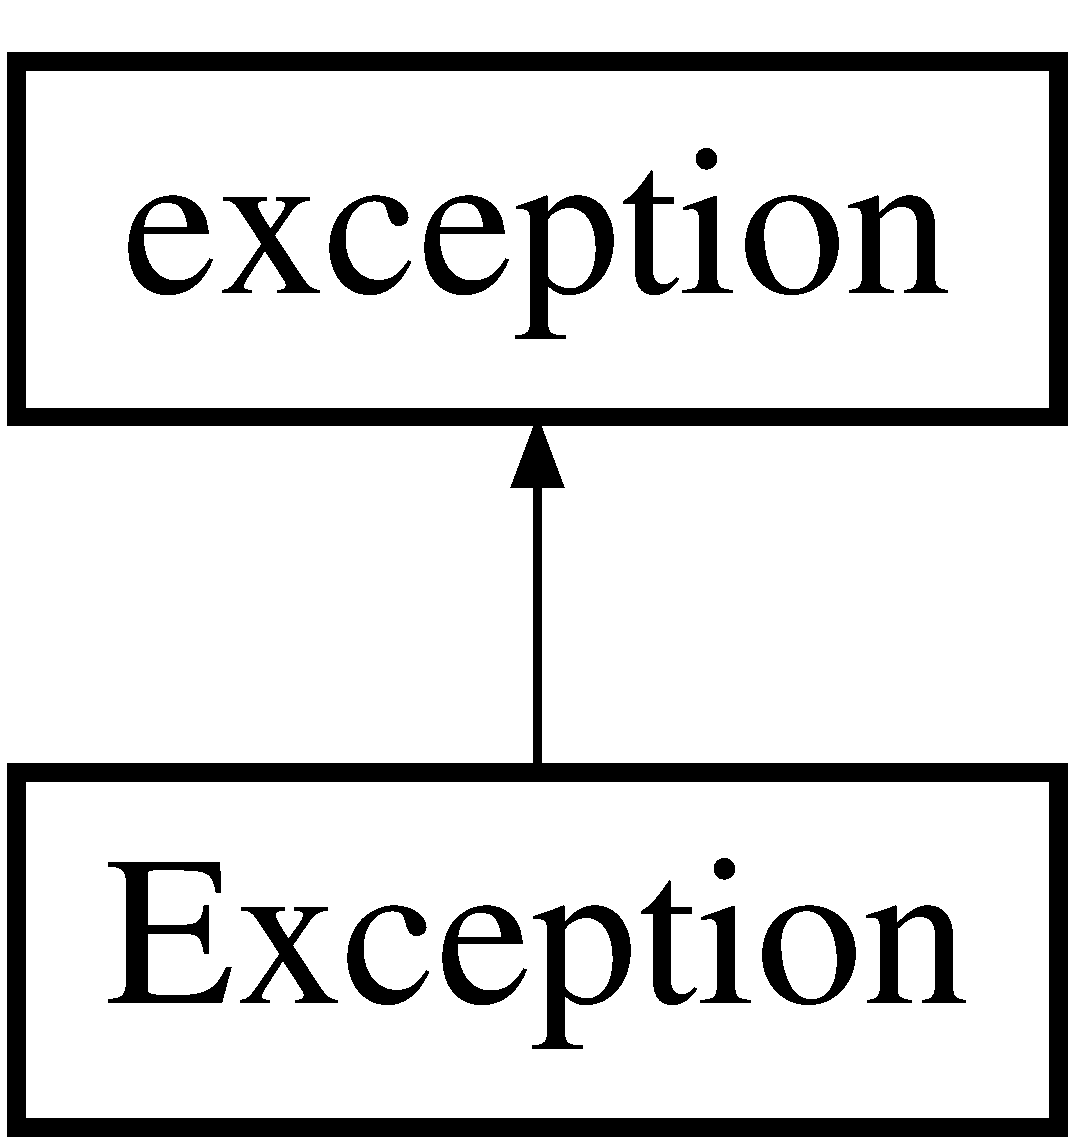
\includegraphics[height=2.000000cm]{class_exception}
\end{center}
\end{figure}
\subsection*{Public Member Functions}
\begin{DoxyCompactItemize}
\item 
\hyperlink{class_exception_aac5e9386080a8eac2edebf02c8169ecc}{Exception} (const \hyperlink{class_message}{Message} \&\hyperlink{class_exception_aab5c1504a18016fdfe7574eb81f59ac6}{message}=\hyperlink{class_message}{Message}(), const \hyperlink{class_source_line}{Source\-Line} \&\hyperlink{class_exception_a67f40ff3ea7f1c07e46222c38dcbaf43}{source\-Line}=\hyperlink{class_source_line}{Source\-Line}())
\begin{DoxyCompactList}\small\item\em Constructs the exception with the specified message and source location. \end{DoxyCompactList}\item 
\hyperlink{class_exception_ae0fd52e62283ee92c085d767d0aab736}{Exception} (const \hyperlink{class_exception}{Exception} \&other)
\begin{DoxyCompactList}\small\item\em Constructs a copy of an exception. \end{DoxyCompactList}\item 
\hypertarget{class_exception_ad1ba411de295ef2eeb02ba26284a829a}{virtual \hyperlink{class_exception_ad1ba411de295ef2eeb02ba26284a829a}{$\sim$\-Exception} ()  throw ()}\label{class_exception_ad1ba411de295ef2eeb02ba26284a829a}

\begin{DoxyCompactList}\small\item\em Destructs the exception. \end{DoxyCompactList}\item 
\hypertarget{class_exception_a71c844ee3ac32b7656c24386e9ab60a0}{\hyperlink{class_exception}{Exception} \& \hyperlink{class_exception_a71c844ee3ac32b7656c24386e9ab60a0}{operator=} (const \hyperlink{class_exception}{Exception} \&other)}\label{class_exception_a71c844ee3ac32b7656c24386e9ab60a0}

\begin{DoxyCompactList}\small\item\em Performs an assignment. \end{DoxyCompactList}\item 
\hypertarget{class_exception_a45642915395d3b813fedc2593fbcb8bb}{const char $\ast$ \hyperlink{class_exception_a45642915395d3b813fedc2593fbcb8bb}{what} () const   throw ()}\label{class_exception_a45642915395d3b813fedc2593fbcb8bb}

\begin{DoxyCompactList}\small\item\em Returns descriptive message. \end{DoxyCompactList}\item 
\hypertarget{class_exception_a67f40ff3ea7f1c07e46222c38dcbaf43}{\hyperlink{class_source_line}{Source\-Line} \hyperlink{class_exception_a67f40ff3ea7f1c07e46222c38dcbaf43}{source\-Line} () const }\label{class_exception_a67f40ff3ea7f1c07e46222c38dcbaf43}

\begin{DoxyCompactList}\small\item\em Location where the error occured. \end{DoxyCompactList}\item 
\hypertarget{class_exception_aab5c1504a18016fdfe7574eb81f59ac6}{\hyperlink{class_message}{Message} \hyperlink{class_exception_aab5c1504a18016fdfe7574eb81f59ac6}{message} () const }\label{class_exception_aab5c1504a18016fdfe7574eb81f59ac6}

\begin{DoxyCompactList}\small\item\em \hyperlink{class_message}{Message} related to the exception. \end{DoxyCompactList}\item 
\hypertarget{class_exception_ad508783fa44767e8fedb6472a4180234}{void \hyperlink{class_exception_ad508783fa44767e8fedb6472a4180234}{set\-Message} (const \hyperlink{class_message}{Message} \&\hyperlink{class_exception_aab5c1504a18016fdfe7574eb81f59ac6}{message})}\label{class_exception_ad508783fa44767e8fedb6472a4180234}

\begin{DoxyCompactList}\small\item\em Set the message. \end{DoxyCompactList}\item 
\hypertarget{class_exception_ad05463060510ad131ccaaafa6b63b2d7}{virtual \hyperlink{class_exception}{Exception} $\ast$ \hyperlink{class_exception_ad05463060510ad131ccaaafa6b63b2d7}{clone} () const }\label{class_exception_ad05463060510ad131ccaaafa6b63b2d7}

\begin{DoxyCompactList}\small\item\em Clones the exception. \end{DoxyCompactList}\end{DoxyCompactItemize}
\subsection*{Protected Types}
\begin{DoxyCompactItemize}
\item 
\hypertarget{class_exception_a5086086062a7ec2cfe4e609026adfbd9}{typedef std\-::exception {\bfseries Super\-Class}}\label{class_exception_a5086086062a7ec2cfe4e609026adfbd9}

\end{DoxyCompactItemize}
\subsection*{Protected Attributes}
\begin{DoxyCompactItemize}
\item 
\hypertarget{class_exception_ad77e1fcf64ced674e60e1d9195c634df}{\hyperlink{class_message}{Message} {\bfseries m\-\_\-message}}\label{class_exception_ad77e1fcf64ced674e60e1d9195c634df}

\item 
\hypertarget{class_exception_ae6685340e219cdcef0d72d45b58c5efb}{\hyperlink{class_source_line}{Source\-Line} {\bfseries m\-\_\-source\-Line}}\label{class_exception_ae6685340e219cdcef0d72d45b58c5efb}

\item 
\hypertarget{class_exception_a51b947da686ab2dd290f799b2a05d492}{std\-::string {\bfseries m\-\_\-what\-Message}}\label{class_exception_a51b947da686ab2dd290f799b2a05d492}

\end{DoxyCompactItemize}


\subsection{Detailed Description}
Exceptions thrown by failed assertions.

\hyperlink{class_exception}{Exception} is an exception that serves descriptive strings through its \hyperlink{class_exception_a45642915395d3b813fedc2593fbcb8bb}{what()} method. 

\subsection{Constructor \& Destructor Documentation}
\hypertarget{class_exception_aac5e9386080a8eac2edebf02c8169ecc}{\index{Exception@{Exception}!Exception@{Exception}}
\index{Exception@{Exception}!Exception@{Exception}}
\subsubsection[{Exception}]{\setlength{\rightskip}{0pt plus 5cm}Exception\-::\-Exception (
\begin{DoxyParamCaption}
\item[{const {\bf Message} \&}]{message = {\ttfamily {\bf Message}()}, }
\item[{const {\bf Source\-Line} \&}]{source\-Line = {\ttfamily {\bf Source\-Line}()}}
\end{DoxyParamCaption}
)}}\label{class_exception_aac5e9386080a8eac2edebf02c8169ecc}


Constructs the exception with the specified message and source location. 


\begin{DoxyParams}{Parameters}
{\em message} & \hyperlink{class_message}{Message} associated to the exception. \\
\hline
{\em source\-Line} & Source location related to the exception. \\
\hline
\end{DoxyParams}
\hypertarget{class_exception_ae0fd52e62283ee92c085d767d0aab736}{\index{Exception@{Exception}!Exception@{Exception}}
\index{Exception@{Exception}!Exception@{Exception}}
\subsubsection[{Exception}]{\setlength{\rightskip}{0pt plus 5cm}Exception\-::\-Exception (
\begin{DoxyParamCaption}
\item[{const {\bf Exception} \&}]{other}
\end{DoxyParamCaption}
)}}\label{class_exception_ae0fd52e62283ee92c085d767d0aab736}


Constructs a copy of an exception. 


\begin{DoxyParams}{Parameters}
{\em other} & \hyperlink{class_exception}{Exception} to copy. \\
\hline
\end{DoxyParams}


The documentation for this class was generated from the following file\-:\begin{DoxyCompactItemize}
\item 
X\-:/\-Git\-\_\-\-Repository/inf2990-\/06/\-Cadriciel/\-Commun/\-Externe/cppunit/include/cppunit/Exception.\-h\end{DoxyCompactItemize}

\hypertarget{class_exception_test_case_decorator}{\section{Exception\-Test\-Case\-Decorator$<$ Expected\-Exception $>$ Class Template Reference}
\label{class_exception_test_case_decorator}\index{Exception\-Test\-Case\-Decorator$<$ Expected\-Exception $>$@{Exception\-Test\-Case\-Decorator$<$ Expected\-Exception $>$}}
}


Expected exception test case decorator.  




{\ttfamily \#include $<$Exception\-Test\-Case\-Decorator.\-h$>$}

Inheritance diagram for Exception\-Test\-Case\-Decorator$<$ Expected\-Exception $>$\-:\begin{figure}[H]
\begin{center}
\leavevmode
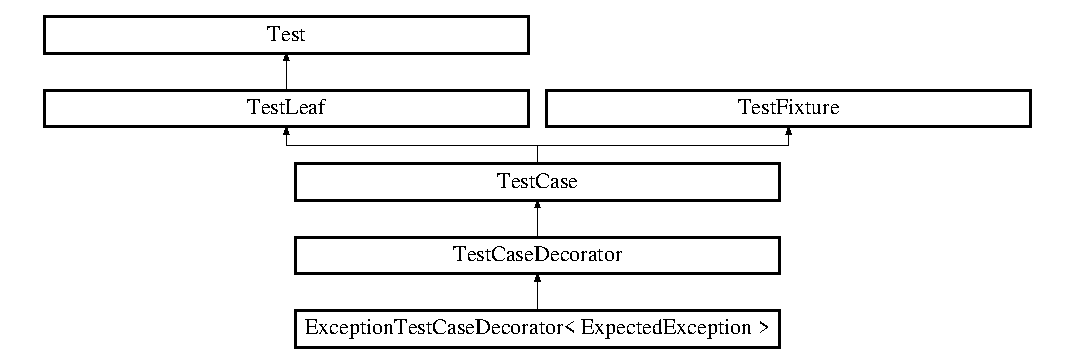
\includegraphics[height=4.444445cm]{class_exception_test_case_decorator}
\end{center}
\end{figure}
\subsection*{Public Types}
\begin{DoxyCompactItemize}
\item 
\hypertarget{class_exception_test_case_decorator_a3fc7e11a4aa1730fa98ff6ac52958ae9}{typedef Expected\-Exception {\bfseries Expected\-Exception\-Type}}\label{class_exception_test_case_decorator_a3fc7e11a4aa1730fa98ff6ac52958ae9}

\end{DoxyCompactItemize}
\subsection*{Public Member Functions}
\begin{DoxyCompactItemize}
\item 
\hyperlink{class_exception_test_case_decorator_a01b0c42952450cff574dd9e293c718fa}{Exception\-Test\-Case\-Decorator} (\hyperlink{class_test_case}{Test\-Case} $\ast$test)
\begin{DoxyCompactList}\small\item\em Decorates the specified test. \end{DoxyCompactList}\item 
void \hyperlink{class_exception_test_case_decorator_a3f78294d459a94f55413162d814f291d}{run\-Test} ()
\begin{DoxyCompactList}\small\item\em Checks that the expected exception is thrown by the decorated test. is thrown. \end{DoxyCompactList}\end{DoxyCompactItemize}
\subsection*{Additional Inherited Members}


\subsection{Detailed Description}
\subsubsection*{template$<$class Expected\-Exception$>$class Exception\-Test\-Case\-Decorator$<$ Expected\-Exception $>$}

Expected exception test case decorator. 

A decorator used to assert that a specific test case should throw an exception of a given type.

You should use this class only if you need to check the exception object state (that a specific cause is set for example). If you don't need to do that, you might consider using \hyperlink{group___writing_test_fixture_gaca8eeb6f60714baade6cbfd185868c40}{C\-P\-P\-U\-N\-I\-T\-\_\-\-T\-E\-S\-T\-\_\-\-E\-X\-C\-E\-P\-T\-I\-O\-N()} instead.

Intended use is to subclass and override check\-Exception(). Example\-:


\begin{DoxyCode}
\textcolor{keyword}{class }NetworkErrorTestCaseDecorator : 
          \textcolor{keyword}{public} \hyperlink{class_exception_test_case_decorator}{ExceptionTestCaseDecorator}<NetworkError>
\{
\textcolor{keyword}{public}:
  NetworkErrorTestCaseDecorator( NetworkError::Cause expectedCause )
      : m\_expectedCause( expectedCause )
  \{
  \}
\textcolor{keyword}{private}:
  \textcolor{keywordtype}{void} checkException( ExpectedExceptionType &\hyperlink{group__gtc__constants_gab83fb6de0f05d6c0d11bdf0479f8319e}{e} )
  \{
    CPPUNIT\_ASSERT\_EQUAL( m\_expectedCause, e.getCause() );
  \}

  NetworkError::Cause m\_expectedCause;
\};
\end{DoxyCode}
 

\subsection{Constructor \& Destructor Documentation}
\hypertarget{class_exception_test_case_decorator_a01b0c42952450cff574dd9e293c718fa}{\index{Exception\-Test\-Case\-Decorator@{Exception\-Test\-Case\-Decorator}!Exception\-Test\-Case\-Decorator@{Exception\-Test\-Case\-Decorator}}
\index{Exception\-Test\-Case\-Decorator@{Exception\-Test\-Case\-Decorator}!ExceptionTestCaseDecorator@{Exception\-Test\-Case\-Decorator}}
\subsubsection[{Exception\-Test\-Case\-Decorator}]{\setlength{\rightskip}{0pt plus 5cm}template$<$class Expected\-Exception $>$ {\bf Exception\-Test\-Case\-Decorator}$<$ Expected\-Exception $>$\-::{\bf Exception\-Test\-Case\-Decorator} (
\begin{DoxyParamCaption}
\item[{{\bf Test\-Case} $\ast$}]{test}
\end{DoxyParamCaption}
)\hspace{0.3cm}{\ttfamily [inline]}}}\label{class_exception_test_case_decorator_a01b0c42952450cff574dd9e293c718fa}


Decorates the specified test. 


\begin{DoxyParams}{Parameters}
{\em test} & \hyperlink{class_test_case}{Test\-Case} to decorate. Assumes ownership of the test. \\
\hline
\end{DoxyParams}


\subsection{Member Function Documentation}
\hypertarget{class_exception_test_case_decorator_a3f78294d459a94f55413162d814f291d}{\index{Exception\-Test\-Case\-Decorator@{Exception\-Test\-Case\-Decorator}!run\-Test@{run\-Test}}
\index{run\-Test@{run\-Test}!ExceptionTestCaseDecorator@{Exception\-Test\-Case\-Decorator}}
\subsubsection[{run\-Test}]{\setlength{\rightskip}{0pt plus 5cm}template$<$class Expected\-Exception $>$ void {\bf Exception\-Test\-Case\-Decorator}$<$ Expected\-Exception $>$\-::run\-Test (
\begin{DoxyParamCaption}
{}
\end{DoxyParamCaption}
)\hspace{0.3cm}{\ttfamily [inline]}, {\ttfamily [virtual]}}}\label{class_exception_test_case_decorator_a3f78294d459a94f55413162d814f291d}


Checks that the expected exception is thrown by the decorated test. is thrown. 

Calls the decorated test \hyperlink{class_exception_test_case_decorator_a3f78294d459a94f55413162d814f291d}{run\-Test()} and checks that an exception of type Expected\-Exception is thrown. Call check\-Exception() passing the exception that was caught so that some assertions can be made if needed. 

Reimplemented from \hyperlink{class_test_case_a6b55957ac1dfef01e5d9fa2475676f34}{Test\-Case}.



The documentation for this class was generated from the following file\-:\begin{DoxyCompactItemize}
\item 
X\-:/\-Git\-\_\-\-Repository/inf2990-\/06/\-Cadriciel/\-Commun/\-Externe/cppunit/include/cppunit/extensions/Exception\-Test\-Case\-Decorator.\-h\end{DoxyCompactItemize}

\hypertarget{class_synchronized_object_1_1_exclusive_zone}{\section{Synchronized\-Object\-:\-:Exclusive\-Zone Class Reference}
\label{class_synchronized_object_1_1_exclusive_zone}\index{Synchronized\-Object\-::\-Exclusive\-Zone@{Synchronized\-Object\-::\-Exclusive\-Zone}}
}


Locks a synchronization object in the current scope.  




{\ttfamily \#include $<$Synchronized\-Object.\-h$>$}

\subsection*{Public Member Functions}
\begin{DoxyCompactItemize}
\item 
\hypertarget{class_synchronized_object_1_1_exclusive_zone_ae4393b508828328c2f4816ff9b7b090c}{{\bfseries Exclusive\-Zone} (\hyperlink{class_synchronized_object_1_1_synchronization_object}{Synchronization\-Object} $\ast$sync\-Object)}\label{class_synchronized_object_1_1_exclusive_zone_ae4393b508828328c2f4816ff9b7b090c}

\end{DoxyCompactItemize}


\subsection{Detailed Description}
Locks a synchronization object in the current scope. 

The documentation for this class was generated from the following file\-:\begin{DoxyCompactItemize}
\item 
X\-:/\-Git\-\_\-\-Repository/inf2990-\/06/\-Cadriciel/\-Commun/\-Externe/cppunit/include/cppunit/Synchronized\-Object.\-h\end{DoxyCompactItemize}

\hypertarget{class_assimp_1_1_exporter}{\section{Assimp\-:\-:Exporter Class Reference}
\label{class_assimp_1_1_exporter}\index{Assimp\-::\-Exporter@{Assimp\-::\-Exporter}}
}


{\ttfamily \#include $<$Exporter.\-hpp$>$}

\subsection*{Classes}
\begin{DoxyCompactItemize}
\item 
struct \hyperlink{struct_assimp_1_1_exporter_1_1_export_format_entry}{Export\-Format\-Entry}
\end{DoxyCompactItemize}
\subsection*{Public Types}
\begin{DoxyCompactItemize}
\item 
typedef void($\ast$ \hyperlink{class_assimp_1_1_exporter_aa67334a75cb24e030af984d01e622f3b}{fp\-Export\-Func} )(const char $\ast$, \hyperlink{class_assimp_1_1_i_o_system}{I\-O\-System} $\ast$, const ai\-Scene $\ast$)
\end{DoxyCompactItemize}
\subsection*{Public Member Functions}
\begin{DoxyCompactItemize}
\item 
void \hyperlink{class_assimp_1_1_exporter_a054201cf78fa352b1281ea8b484f6e3a}{Set\-I\-O\-Handler} (\hyperlink{class_assimp_1_1_i_o_system}{I\-O\-System} $\ast$p\-I\-O\-Handler)
\item 
\hyperlink{class_assimp_1_1_i_o_system}{I\-O\-System} $\ast$ \hyperlink{class_assimp_1_1_exporter_a736d66db1a94de7df6eb978975e8d47a}{Get\-I\-O\-Handler} () const 
\item 
bool \hyperlink{class_assimp_1_1_exporter_a9ae1196f04cceb0d35fde6229ba41d0b}{Is\-Default\-I\-O\-Handler} () const 
\item 
const \hyperlink{structai_export_data_blob}{ai\-Export\-Data\-Blob} $\ast$ \hyperlink{class_assimp_1_1_exporter_a390c0950a3a164fc431e0797ae1a84d1}{Export\-To\-Blob} (const ai\-Scene $\ast$p\-Scene, const char $\ast$p\-Format\-Id, unsigned int p\-Preprocessing=0u)
\item 
\hypertarget{class_assimp_1_1_exporter_a02aa8c453879dc9365e7ec4d1e8d7413}{const \hyperlink{structai_export_data_blob}{ai\-Export\-Data\-Blob} $\ast$ {\bfseries Export\-To\-Blob} (const ai\-Scene $\ast$p\-Scene, const std\-::string \&p\-Format\-Id, unsigned int p\-Preprocessing=0u)}\label{class_assimp_1_1_exporter_a02aa8c453879dc9365e7ec4d1e8d7413}

\item 
ai\-Return \hyperlink{class_assimp_1_1_exporter_ab8edf249172567a78ca302278a415e35}{Export} (const ai\-Scene $\ast$p\-Scene, const char $\ast$p\-Format\-Id, const char $\ast$p\-Path, unsigned int p\-Preprocessing=0u)
\item 
\hypertarget{class_assimp_1_1_exporter_aec681d38ca0bef85a015c64831a3566a}{ai\-Return {\bfseries Export} (const ai\-Scene $\ast$p\-Scene, const std\-::string \&p\-Format\-Id, const std\-::string \&p\-Path, unsigned int p\-Preprocessing=0u)}\label{class_assimp_1_1_exporter_aec681d38ca0bef85a015c64831a3566a}

\item 
const char $\ast$ \hyperlink{class_assimp_1_1_exporter_ad5dae590c3f2b8aa5fc3e2b26f7886e3}{Get\-Error\-String} () const 
\item 
const \hyperlink{structai_export_data_blob}{ai\-Export\-Data\-Blob} $\ast$ \hyperlink{class_assimp_1_1_exporter_aaee439cf6810d14eded4a12b9bc63e0b}{Get\-Blob} () const 
\item 
const \hyperlink{structai_export_data_blob}{ai\-Export\-Data\-Blob} $\ast$ \hyperlink{class_assimp_1_1_exporter_a75291079fa484c5769b36a80b1b393a5}{Get\-Orphaned\-Blob} () const 
\item 
void \hyperlink{class_assimp_1_1_exporter_a8200b618c21c272c839c37060a871d48}{Free\-Blob} ()
\item 
size\-\_\-t \hyperlink{class_assimp_1_1_exporter_abfada264486a34c52ae43a762d5cbf01}{Get\-Export\-Format\-Count} () const 
\item 
const \hyperlink{structai_export_format_desc}{ai\-Export\-Format\-Desc} $\ast$ \hyperlink{class_assimp_1_1_exporter_a724e2a029ec38d7252f7a7169c9eb7e4}{Get\-Export\-Format\-Description} (size\-\_\-t p\-Index) const 
\item 
ai\-Return \hyperlink{class_assimp_1_1_exporter_ae65025d7c5a06a0c3e8655585f87e1c4}{Register\-Exporter} (const \hyperlink{struct_assimp_1_1_exporter_1_1_export_format_entry}{Export\-Format\-Entry} \&desc)
\item 
void \hyperlink{class_assimp_1_1_exporter_afa5956ce18138b90396c505468d1e52b}{Unregister\-Exporter} (const char $\ast$id)
\end{DoxyCompactItemize}
\subsection*{Protected Attributes}
\begin{DoxyCompactItemize}
\item 
\hypertarget{class_assimp_1_1_exporter_a75bc178ae29edc192e1c1935c31c42b2}{Exporter\-Pimpl $\ast$ {\bfseries pimpl}}\label{class_assimp_1_1_exporter_a75bc178ae29edc192e1c1935c31c42b2}

\end{DoxyCompactItemize}


\subsection{Detailed Description}
C\-P\-P-\/\-A\-P\-I\-: The \hyperlink{class_assimp_1_1_exporter}{Exporter} class forms an C++ interface to the export functionality of the Open Asset Import Library. Note that the export interface is available only if \hyperlink{namespace_assimp}{Assimp} has been built with A\-S\-S\-I\-M\-P\-\_\-\-B\-U\-I\-L\-D\-\_\-\-N\-O\-\_\-\-E\-X\-P\-O\-R\-T not defined.

The interface is modelled after the importer interface and mostly symmetric. The same rules for threading etc. apply.

In a nutshell, there are two export interfaces\-: \hyperlink{class_assimp_1_1_exporter_ab8edf249172567a78ca302278a415e35}{Export}, which writes the output file(s) either to the regular file system or to a user-\/supplied \#\-I\-O\-System, and \hyperlink{class_assimp_1_1_exporter_a390c0950a3a164fc431e0797ae1a84d1}{Export\-To\-Blob} which returns a linked list of memory buffers (blob), each referring to one output file (in most cases there will be only one output file of course, but this extra complexity is needed since \hyperlink{namespace_assimp}{Assimp} aims at supporting a wide range of file formats).

\hyperlink{class_assimp_1_1_exporter_a390c0950a3a164fc431e0797ae1a84d1}{Export\-To\-Blob} is especially useful if you intend to work with the data in-\/memory. 

\subsection{Member Typedef Documentation}
\hypertarget{class_assimp_1_1_exporter_aa67334a75cb24e030af984d01e622f3b}{\index{Assimp\-::\-Exporter@{Assimp\-::\-Exporter}!fp\-Export\-Func@{fp\-Export\-Func}}
\index{fp\-Export\-Func@{fp\-Export\-Func}!Assimp::Exporter@{Assimp\-::\-Exporter}}
\subsubsection[{fp\-Export\-Func}]{\setlength{\rightskip}{0pt plus 5cm}typedef void($\ast$ Assimp\-::\-Exporter\-::fp\-Export\-Func)(const char $\ast$, {\bf I\-O\-System} $\ast$, const ai\-Scene $\ast$)}}\label{class_assimp_1_1_exporter_aa67334a75cb24e030af984d01e622f3b}
Function pointer type of a Export worker function 

\subsection{Member Function Documentation}
\hypertarget{class_assimp_1_1_exporter_ab8edf249172567a78ca302278a415e35}{\index{Assimp\-::\-Exporter@{Assimp\-::\-Exporter}!Export@{Export}}
\index{Export@{Export}!Assimp::Exporter@{Assimp\-::\-Exporter}}
\subsubsection[{Export}]{\setlength{\rightskip}{0pt plus 5cm}ai\-Return Assimp\-::\-Exporter\-::\-Export (
\begin{DoxyParamCaption}
\item[{const ai\-Scene $\ast$}]{p\-Scene, }
\item[{const char $\ast$}]{p\-Format\-Id, }
\item[{const char $\ast$}]{p\-Path, }
\item[{unsigned int}]{p\-Preprocessing = {\ttfamily 0u}}
\end{DoxyParamCaption}
)}}\label{class_assimp_1_1_exporter_ab8edf249172567a78ca302278a415e35}
Convenience function to export directly to a file. Use \#\-Set\-I\-O\-System to supply a custom \hyperlink{class_assimp_1_1_i_o_system}{I\-O\-System} to gain fine-\/grained control about the output data flow of the export process. 
\begin{DoxyParams}{Parameters}
{\em p\-Blob} & A data blob obtained from a previous call to \hyperlink{cexport_8h_a9615510b8430a9da4f435a72148128dd}{ai\-Export\-Scene}. Must not be N\-U\-L\-L. \\
\hline
{\em p\-Path} & Full target file name. Target must be accessible. \\
\hline
{\em p\-Preprocessing} & Accepts any choice of the \#ai\-Post\-Processing enumerated flags, but in reality only a subset of them makes sense here. Specifying 'preprocessing' flags is useful if the input scene does not conform to \hyperlink{namespace_assimp}{Assimp}'s default conventions as specified in the \hyperlink{}{Data Structures Page }. In short, this means the geometry data should use a right-\/handed coordinate systems, face winding should be counter-\/clockwise and the U\-V coordinate origin is assumed to be in the upper left. The \hyperlink{postprocess_8h_a64795260b95f5a4b3f3dc1be4f52e410a133fd1162674e68bf8cd17070898a936}{ai\-Process\-\_\-\-Make\-Left\-Handed}, \hyperlink{postprocess_8h_a64795260b95f5a4b3f3dc1be4f52e410a06922b6a1f1cd8186f9fdafb471c813e}{ai\-Process\-\_\-\-Flip\-U\-Vs} and \hyperlink{postprocess_8h_a64795260b95f5a4b3f3dc1be4f52e410a429a11bf7ace46f039f55de895505d4a}{ai\-Process\-\_\-\-Flip\-Winding\-Order} flags are used in the import side to allow users to have those defaults automatically adapted to their conventions. Specifying those flags for exporting has the opposite effect, respectively. Some other of the \hyperlink{postprocess_8h_a64795260b95f5a4b3f3dc1be4f52e410}{ai\-Post\-Process\-Steps} enumerated values may be useful as well, but you'll need to try out what their effect on the exported file is. Many formats impose their own restrictions on the structure of the geometry stored therein, so some preprocessing may have little or no effect at all, or may be redundant as exporters would apply them anyhow. A good example is triangulation -\/ whilst you can enforce it by specifying the \hyperlink{postprocess_8h_a64795260b95f5a4b3f3dc1be4f52e410a9c3de834f0307f31fa2b1b6d05dd592b}{ai\-Process\-\_\-\-Triangulate} flag, most export formats support only triangulate data so they would run the step even if it wasn't requested.\\
\hline
\end{DoxyParams}
If assimp detects that the input scene was directly taken from the importer side of the library (i.\-e. not copied using ai\-Copy\-Scene and potetially modified afterwards), any postprocessing steps already applied to the scene will not be applied again, unless they show non-\/idempotent behaviour (\hyperlink{postprocess_8h_a64795260b95f5a4b3f3dc1be4f52e410a133fd1162674e68bf8cd17070898a936}{ai\-Process\-\_\-\-Make\-Left\-Handed}, \hyperlink{postprocess_8h_a64795260b95f5a4b3f3dc1be4f52e410a06922b6a1f1cd8186f9fdafb471c813e}{ai\-Process\-\_\-\-Flip\-U\-Vs} and \hyperlink{postprocess_8h_a64795260b95f5a4b3f3dc1be4f52e410a429a11bf7ace46f039f55de895505d4a}{ai\-Process\-\_\-\-Flip\-Winding\-Order}). \begin{DoxyReturn}{Returns}
A\-I\-\_\-\-S\-U\-C\-C\-E\-S\-S if everything was fine. 
\end{DoxyReturn}
\begin{DoxyNote}{Note}
Use \hyperlink{cexport_8h_a3b462a882e970cd7f492e293e5dee4fe}{ai\-Copy\-Scene()} to get a modifiable copy of a previously imported scene. 
\end{DoxyNote}
\hypertarget{class_assimp_1_1_exporter_a390c0950a3a164fc431e0797ae1a84d1}{\index{Assimp\-::\-Exporter@{Assimp\-::\-Exporter}!Export\-To\-Blob@{Export\-To\-Blob}}
\index{Export\-To\-Blob@{Export\-To\-Blob}!Assimp::Exporter@{Assimp\-::\-Exporter}}
\subsubsection[{Export\-To\-Blob}]{\setlength{\rightskip}{0pt plus 5cm}const {\bf ai\-Export\-Data\-Blob}$\ast$ Assimp\-::\-Exporter\-::\-Export\-To\-Blob (
\begin{DoxyParamCaption}
\item[{const ai\-Scene $\ast$}]{p\-Scene, }
\item[{const char $\ast$}]{p\-Format\-Id, }
\item[{unsigned int}]{p\-Preprocessing = {\ttfamily 0u}}
\end{DoxyParamCaption}
)}}\label{class_assimp_1_1_exporter_a390c0950a3a164fc431e0797ae1a84d1}
Exports the given scene to a chosen file format. Returns the exported data as a binary blob which you can write into a file or something. When you're done with the data, simply let the \#\-Exporter instance go out of scope to have it released automatically. 
\begin{DoxyParams}{Parameters}
{\em p\-Scene} & The scene to export. Stays in possession of the caller, is not changed by the function. \\
\hline
{\em p\-Format\-Id} & I\-D string to specify to which format you want to export to. Use \hyperlink{class_assimp_1_1_exporter_abfada264486a34c52ae43a762d5cbf01}{Get\-Export\-Format\-Count} / \hyperlink{class_assimp_1_1_exporter_a724e2a029ec38d7252f7a7169c9eb7e4}{Get\-Export\-Format\-Description} to learn which export formats are available. \\
\hline
{\em p\-Preprocessing} & See the documentation for \hyperlink{class_assimp_1_1_exporter_ab8edf249172567a78ca302278a415e35}{Export} \\
\hline
\end{DoxyParams}
\begin{DoxyReturn}{Returns}
the exported data or N\-U\-L\-L in case of error. 
\end{DoxyReturn}
\begin{DoxyNote}{Note}
If the \hyperlink{class_assimp_1_1_exporter}{Exporter} instance did already hold a blob from a previous call to \hyperlink{class_assimp_1_1_exporter_a390c0950a3a164fc431e0797ae1a84d1}{Export\-To\-Blob}, it will be disposed. Any I\-O handlers set via \hyperlink{class_assimp_1_1_exporter_a054201cf78fa352b1281ea8b484f6e3a}{Set\-I\-O\-Handler} are ignored here. 

Use \hyperlink{cexport_8h_a3b462a882e970cd7f492e293e5dee4fe}{ai\-Copy\-Scene()} to get a modifiable copy of a previously imported scene. 
\end{DoxyNote}
\hypertarget{class_assimp_1_1_exporter_a8200b618c21c272c839c37060a871d48}{\index{Assimp\-::\-Exporter@{Assimp\-::\-Exporter}!Free\-Blob@{Free\-Blob}}
\index{Free\-Blob@{Free\-Blob}!Assimp::Exporter@{Assimp\-::\-Exporter}}
\subsubsection[{Free\-Blob}]{\setlength{\rightskip}{0pt plus 5cm}void Assimp\-::\-Exporter\-::\-Free\-Blob (
\begin{DoxyParamCaption}
{}
\end{DoxyParamCaption}
)}}\label{class_assimp_1_1_exporter_a8200b618c21c272c839c37060a871d48}
Frees the current blob.

The function does nothing if no blob has previously been previously produced via \hyperlink{class_assimp_1_1_exporter_a390c0950a3a164fc431e0797ae1a84d1}{Export\-To\-Blob}. \hyperlink{class_assimp_1_1_exporter_a8200b618c21c272c839c37060a871d48}{Free\-Blob} is called automatically by the destructor. The only reason to call it manually would be to reclain as much storage as possible without giving up the \#\-Exporter instance yet. \hypertarget{class_assimp_1_1_exporter_aaee439cf6810d14eded4a12b9bc63e0b}{\index{Assimp\-::\-Exporter@{Assimp\-::\-Exporter}!Get\-Blob@{Get\-Blob}}
\index{Get\-Blob@{Get\-Blob}!Assimp::Exporter@{Assimp\-::\-Exporter}}
\subsubsection[{Get\-Blob}]{\setlength{\rightskip}{0pt plus 5cm}const {\bf ai\-Export\-Data\-Blob}$\ast$ Assimp\-::\-Exporter\-::\-Get\-Blob (
\begin{DoxyParamCaption}
{}
\end{DoxyParamCaption}
) const}}\label{class_assimp_1_1_exporter_aaee439cf6810d14eded4a12b9bc63e0b}
Return the blob obtained from the last call to \hyperlink{class_assimp_1_1_exporter_a390c0950a3a164fc431e0797ae1a84d1}{Export\-To\-Blob} \hypertarget{class_assimp_1_1_exporter_ad5dae590c3f2b8aa5fc3e2b26f7886e3}{\index{Assimp\-::\-Exporter@{Assimp\-::\-Exporter}!Get\-Error\-String@{Get\-Error\-String}}
\index{Get\-Error\-String@{Get\-Error\-String}!Assimp::Exporter@{Assimp\-::\-Exporter}}
\subsubsection[{Get\-Error\-String}]{\setlength{\rightskip}{0pt plus 5cm}const char$\ast$ Assimp\-::\-Exporter\-::\-Get\-Error\-String (
\begin{DoxyParamCaption}
{}
\end{DoxyParamCaption}
) const}}\label{class_assimp_1_1_exporter_ad5dae590c3f2b8aa5fc3e2b26f7886e3}
Returns an error description of an error that occurred in \hyperlink{class_assimp_1_1_exporter_ab8edf249172567a78ca302278a415e35}{Export} or \hyperlink{class_assimp_1_1_exporter_a390c0950a3a164fc431e0797ae1a84d1}{Export\-To\-Blob}

Returns an empty string if no error occurred. \begin{DoxyReturn}{Returns}
A description of the last error, an empty string if no error occurred. The string is never N\-U\-L\-L.
\end{DoxyReturn}
\begin{DoxyNote}{Note}
The returned function remains valid until one of the following methods is called\-: \hyperlink{class_assimp_1_1_exporter_ab8edf249172567a78ca302278a415e35}{Export}, \hyperlink{class_assimp_1_1_exporter_a390c0950a3a164fc431e0797ae1a84d1}{Export\-To\-Blob}, \hyperlink{class_assimp_1_1_exporter_a8200b618c21c272c839c37060a871d48}{Free\-Blob} 
\end{DoxyNote}
\hypertarget{class_assimp_1_1_exporter_abfada264486a34c52ae43a762d5cbf01}{\index{Assimp\-::\-Exporter@{Assimp\-::\-Exporter}!Get\-Export\-Format\-Count@{Get\-Export\-Format\-Count}}
\index{Get\-Export\-Format\-Count@{Get\-Export\-Format\-Count}!Assimp::Exporter@{Assimp\-::\-Exporter}}
\subsubsection[{Get\-Export\-Format\-Count}]{\setlength{\rightskip}{0pt plus 5cm}size\-\_\-t Assimp\-::\-Exporter\-::\-Get\-Export\-Format\-Count (
\begin{DoxyParamCaption}
{}
\end{DoxyParamCaption}
) const}}\label{class_assimp_1_1_exporter_abfada264486a34c52ae43a762d5cbf01}
Returns the number of export file formats available in the current \hyperlink{namespace_assimp}{Assimp} build. Use \#\-Exporter\-::\-Get\-Export\-Format\-Description to retrieve infos of a specific export format \hypertarget{class_assimp_1_1_exporter_a724e2a029ec38d7252f7a7169c9eb7e4}{\index{Assimp\-::\-Exporter@{Assimp\-::\-Exporter}!Get\-Export\-Format\-Description@{Get\-Export\-Format\-Description}}
\index{Get\-Export\-Format\-Description@{Get\-Export\-Format\-Description}!Assimp::Exporter@{Assimp\-::\-Exporter}}
\subsubsection[{Get\-Export\-Format\-Description}]{\setlength{\rightskip}{0pt plus 5cm}const {\bf ai\-Export\-Format\-Desc}$\ast$ Assimp\-::\-Exporter\-::\-Get\-Export\-Format\-Description (
\begin{DoxyParamCaption}
\item[{size\-\_\-t}]{p\-Index}
\end{DoxyParamCaption}
) const}}\label{class_assimp_1_1_exporter_a724e2a029ec38d7252f7a7169c9eb7e4}
Returns a description of the nth export file format. Use \# \#\-Exporter\-::\-Get\-Export\-Format\-Count to learn how many export formats are supported. 
\begin{DoxyParams}{Parameters}
{\em p\-Index} & Index of the export format to retrieve information for. Valid range is 0 to \#\-Exporter\-::\-Get\-Export\-Format\-Count \\
\hline
\end{DoxyParams}
\begin{DoxyReturn}{Returns}
A description of that specific export format. N\-U\-L\-L if p\-Index is out of range. 
\end{DoxyReturn}
\hypertarget{class_assimp_1_1_exporter_a736d66db1a94de7df6eb978975e8d47a}{\index{Assimp\-::\-Exporter@{Assimp\-::\-Exporter}!Get\-I\-O\-Handler@{Get\-I\-O\-Handler}}
\index{Get\-I\-O\-Handler@{Get\-I\-O\-Handler}!Assimp::Exporter@{Assimp\-::\-Exporter}}
\subsubsection[{Get\-I\-O\-Handler}]{\setlength{\rightskip}{0pt plus 5cm}{\bf I\-O\-System}$\ast$ Assimp\-::\-Exporter\-::\-Get\-I\-O\-Handler (
\begin{DoxyParamCaption}
{}
\end{DoxyParamCaption}
) const}}\label{class_assimp_1_1_exporter_a736d66db1a94de7df6eb978975e8d47a}
Retrieves the I\-O handler that is currently set. You can use \hyperlink{class_assimp_1_1_exporter_a9ae1196f04cceb0d35fde6229ba41d0b}{Is\-Default\-I\-O\-Handler()} to check whether the returned interface is the default I\-O handler provided by A\-S\-S\-I\-M\-P. The default handler is active as long the application doesn't supply its own custom I\-O handler via \hyperlink{class_assimp_1_1_exporter_a054201cf78fa352b1281ea8b484f6e3a}{Set\-I\-O\-Handler()}. \begin{DoxyReturn}{Returns}
A valid \hyperlink{class_assimp_1_1_i_o_system}{I\-O\-System} interface, never N\-U\-L\-L. 
\end{DoxyReturn}
\hypertarget{class_assimp_1_1_exporter_a75291079fa484c5769b36a80b1b393a5}{\index{Assimp\-::\-Exporter@{Assimp\-::\-Exporter}!Get\-Orphaned\-Blob@{Get\-Orphaned\-Blob}}
\index{Get\-Orphaned\-Blob@{Get\-Orphaned\-Blob}!Assimp::Exporter@{Assimp\-::\-Exporter}}
\subsubsection[{Get\-Orphaned\-Blob}]{\setlength{\rightskip}{0pt plus 5cm}const {\bf ai\-Export\-Data\-Blob}$\ast$ Assimp\-::\-Exporter\-::\-Get\-Orphaned\-Blob (
\begin{DoxyParamCaption}
{}
\end{DoxyParamCaption}
) const}}\label{class_assimp_1_1_exporter_a75291079fa484c5769b36a80b1b393a5}
Orphan the blob from the last call to \hyperlink{class_assimp_1_1_exporter_a390c0950a3a164fc431e0797ae1a84d1}{Export\-To\-Blob}. This means the caller takes ownership and is thus responsible for calling the C A\-P\-I function \hyperlink{cexport_8h_a0998064849f2ef5544f6fd30cda0b964}{ai\-Release\-Export\-Blob} to release it. \hypertarget{class_assimp_1_1_exporter_a9ae1196f04cceb0d35fde6229ba41d0b}{\index{Assimp\-::\-Exporter@{Assimp\-::\-Exporter}!Is\-Default\-I\-O\-Handler@{Is\-Default\-I\-O\-Handler}}
\index{Is\-Default\-I\-O\-Handler@{Is\-Default\-I\-O\-Handler}!Assimp::Exporter@{Assimp\-::\-Exporter}}
\subsubsection[{Is\-Default\-I\-O\-Handler}]{\setlength{\rightskip}{0pt plus 5cm}bool Assimp\-::\-Exporter\-::\-Is\-Default\-I\-O\-Handler (
\begin{DoxyParamCaption}
{}
\end{DoxyParamCaption}
) const}}\label{class_assimp_1_1_exporter_a9ae1196f04cceb0d35fde6229ba41d0b}
Checks whether a default I\-O handler is active A default handler is active as long the application doesn't supply its own custom I\-O handler via \hyperlink{class_assimp_1_1_exporter_a054201cf78fa352b1281ea8b484f6e3a}{Set\-I\-O\-Handler()}. \begin{DoxyReturn}{Returns}
true by default 
\end{DoxyReturn}
\hypertarget{class_assimp_1_1_exporter_ae65025d7c5a06a0c3e8655585f87e1c4}{\index{Assimp\-::\-Exporter@{Assimp\-::\-Exporter}!Register\-Exporter@{Register\-Exporter}}
\index{Register\-Exporter@{Register\-Exporter}!Assimp::Exporter@{Assimp\-::\-Exporter}}
\subsubsection[{Register\-Exporter}]{\setlength{\rightskip}{0pt plus 5cm}ai\-Return Assimp\-::\-Exporter\-::\-Register\-Exporter (
\begin{DoxyParamCaption}
\item[{const {\bf Export\-Format\-Entry} \&}]{desc}
\end{DoxyParamCaption}
)}}\label{class_assimp_1_1_exporter_ae65025d7c5a06a0c3e8655585f87e1c4}
Register a custom exporter. Custom export formats are limited to to the current \#\-Exporter instance and do not affect the library globally. 
\begin{DoxyParams}{Parameters}
{\em desc} & \hyperlink{class_assimp_1_1_exporter}{Exporter} description. \\
\hline
\end{DoxyParams}
\begin{DoxyReturn}{Returns}
ai\-Return\-\_\-\-S\-U\-C\-C\-E\-S\-S if the export format was successfully registered. A common cause that would prevent an exporter from being registered is that its format id is already occupied by another format. 
\end{DoxyReturn}
\hypertarget{class_assimp_1_1_exporter_a054201cf78fa352b1281ea8b484f6e3a}{\index{Assimp\-::\-Exporter@{Assimp\-::\-Exporter}!Set\-I\-O\-Handler@{Set\-I\-O\-Handler}}
\index{Set\-I\-O\-Handler@{Set\-I\-O\-Handler}!Assimp::Exporter@{Assimp\-::\-Exporter}}
\subsubsection[{Set\-I\-O\-Handler}]{\setlength{\rightskip}{0pt plus 5cm}void Assimp\-::\-Exporter\-::\-Set\-I\-O\-Handler (
\begin{DoxyParamCaption}
\item[{{\bf I\-O\-System} $\ast$}]{p\-I\-O\-Handler}
\end{DoxyParamCaption}
)}}\label{class_assimp_1_1_exporter_a054201cf78fa352b1281ea8b484f6e3a}
Supplies a custom I\-O handler to the exporter to use to open and access files.

If you need \hyperlink{class_assimp_1_1_exporter_ab8edf249172567a78ca302278a415e35}{Export} to use custom I\-O logic to access the files, you need to supply a custom implementation of \hyperlink{class_assimp_1_1_i_o_system}{I\-O\-System} and I\-O\-File to the exporter.

\#\-Exporter takes ownership of the object and will destroy it afterwards. The previously assigned handler will be deleted. Pass N\-U\-L\-L to take again ownership of your \hyperlink{class_assimp_1_1_i_o_system}{I\-O\-System} and reset \hyperlink{namespace_assimp}{Assimp} to use its default implementation, which uses plain file I\-O.


\begin{DoxyParams}{Parameters}
{\em p\-I\-O\-Handler} & The I\-O handler to be used in all file accesses of the \hyperlink{class_assimp_1_1_importer}{Importer}. \\
\hline
\end{DoxyParams}
\hypertarget{class_assimp_1_1_exporter_afa5956ce18138b90396c505468d1e52b}{\index{Assimp\-::\-Exporter@{Assimp\-::\-Exporter}!Unregister\-Exporter@{Unregister\-Exporter}}
\index{Unregister\-Exporter@{Unregister\-Exporter}!Assimp::Exporter@{Assimp\-::\-Exporter}}
\subsubsection[{Unregister\-Exporter}]{\setlength{\rightskip}{0pt plus 5cm}void Assimp\-::\-Exporter\-::\-Unregister\-Exporter (
\begin{DoxyParamCaption}
\item[{const char $\ast$}]{id}
\end{DoxyParamCaption}
)}}\label{class_assimp_1_1_exporter_afa5956ce18138b90396c505468d1e52b}
Remove an export format previously registered with \hyperlink{class_assimp_1_1_exporter_ae65025d7c5a06a0c3e8655585f87e1c4}{Register\-Exporter} from the \#\-Exporter instance (this can also be used to drop builtin exporters because those are implicitly registered using \hyperlink{class_assimp_1_1_exporter_ae65025d7c5a06a0c3e8655585f87e1c4}{Register\-Exporter}). 
\begin{DoxyParams}{Parameters}
{\em id} & Format id to be unregistered, this refers to the 'id' field of \hyperlink{structai_export_format_desc}{ai\-Export\-Format\-Desc}. \\
\hline
\end{DoxyParams}
\begin{DoxyNote}{Note}
Calling this method on a format description not yet registered has no effect. 
\end{DoxyNote}


The documentation for this class was generated from the following file\-:\begin{DoxyCompactItemize}
\item 
X\-:/\-Git\-\_\-\-Repository/inf2990-\/06/\-Cadriciel/\-Commun/\-Externe/assimp/include/Exporter.\-hpp\end{DoxyCompactItemize}

\hypertarget{struct_assimp_1_1_exporter_1_1_export_format_entry}{\section{Assimp\-:\-:Exporter\-:\-:Export\-Format\-Entry Struct Reference}
\label{struct_assimp_1_1_exporter_1_1_export_format_entry}\index{Assimp\-::\-Exporter\-::\-Export\-Format\-Entry@{Assimp\-::\-Exporter\-::\-Export\-Format\-Entry}}
}


{\ttfamily \#include $<$Exporter.\-hpp$>$}

\subsection*{Public Member Functions}
\begin{DoxyCompactItemize}
\item 
\hypertarget{struct_assimp_1_1_exporter_1_1_export_format_entry_ab89610d7a5b295aa8a22bceae013d76f}{{\bfseries Export\-Format\-Entry} (const char $\ast$p\-Id, const char $\ast$p\-Desc, const char $\ast$p\-Extension, \hyperlink{class_assimp_1_1_exporter_aa67334a75cb24e030af984d01e622f3b}{fp\-Export\-Func} p\-Function, unsigned int p\-Enforce\-P\-P=0u)}\label{struct_assimp_1_1_exporter_1_1_export_format_entry_ab89610d7a5b295aa8a22bceae013d76f}

\end{DoxyCompactItemize}
\subsection*{Public Attributes}
\begin{DoxyCompactItemize}
\item 
\hypertarget{struct_assimp_1_1_exporter_1_1_export_format_entry_a59f8bf48e35a70ac0540c9b65d4b891d}{\hyperlink{structai_export_format_desc}{ai\-Export\-Format\-Desc} \hyperlink{struct_assimp_1_1_exporter_1_1_export_format_entry_a59f8bf48e35a70ac0540c9b65d4b891d}{m\-Description}}\label{struct_assimp_1_1_exporter_1_1_export_format_entry_a59f8bf48e35a70ac0540c9b65d4b891d}

\begin{DoxyCompactList}\small\item\em Public description structure to be returned by \hyperlink{cexport_8h_adda7f2e6611f719af6c8a4a0bef0a0a2}{ai\-Get\-Export\-Format\-Description()} \end{DoxyCompactList}\item 
\hypertarget{struct_assimp_1_1_exporter_1_1_export_format_entry_a5cf4464ae6f7f7d92aaade27f1e545f5}{\hyperlink{class_assimp_1_1_exporter_aa67334a75cb24e030af984d01e622f3b}{fp\-Export\-Func} {\bfseries m\-Export\-Function}}\label{struct_assimp_1_1_exporter_1_1_export_format_entry_a5cf4464ae6f7f7d92aaade27f1e545f5}

\item 
\hypertarget{struct_assimp_1_1_exporter_1_1_export_format_entry_aefb2d077aebc473ce9a6e38fd883f181}{unsigned int {\bfseries m\-Enforce\-P\-P}}\label{struct_assimp_1_1_exporter_1_1_export_format_entry_aefb2d077aebc473ce9a6e38fd883f181}

\end{DoxyCompactItemize}


\subsection{Detailed Description}
Internal description of an \hyperlink{namespace_assimp}{Assimp} export format option 

The documentation for this struct was generated from the following file\-:\begin{DoxyCompactItemize}
\item 
X\-:/\-Git\-\_\-\-Repository/inf2990-\/06/\-Cadriciel/\-Commun/\-Externe/assimp/include/Exporter.\-hpp\end{DoxyCompactItemize}

\hypertarget{class_facade_modele}{\section{Facade\-Modele Class Reference}
\label{class_facade_modele}\index{Facade\-Modele@{Facade\-Modele}}
}


Classe qui constitue une interface (une fa�ade) sur l'ensemble du mod�le et des classes qui le composent.  




{\ttfamily \#include $<$Facade\-Modele.\-h$>$}

\subsection*{Public Member Functions}
\begin{DoxyCompactItemize}
\item 
void \hyperlink{group__inf2990_gabf12ccafbabf1049cb8327cf78699a1b}{initialiser\-Open\-G\-L} (H\-W\-N\-D h\-Wnd)
\begin{DoxyCompactList}\small\item\em Cr�e un contexte Open\-G\-L et initialise celui-\/ci. \end{DoxyCompactList}\item 
void \hyperlink{group__inf2990_ga4967547e0683bfdca700118df1c18bca}{charger\-Configuration} () const 
\begin{DoxyCompactList}\small\item\em Charge la configuration � partir d'un fichier X\-M\-L. \end{DoxyCompactList}\item 
void \hyperlink{group__inf2990_ga277d8d9cea21e20fb366a0d48525f2c9}{enregistrer\-Configuration} () const 
\begin{DoxyCompactList}\small\item\em Enregistre la configuration courante dans un fichier X\-M\-L. \end{DoxyCompactList}\item 
void \hyperlink{group__inf2990_gac7b831ce13626514e9637c4533d7c15d}{liberer\-Open\-G\-L} ()
\begin{DoxyCompactList}\small\item\em Lib�re le contexte Open\-G\-L. \end{DoxyCompactList}\item 
void \hyperlink{group__inf2990_gac884e818dab5fe049a37b3f6f1c5d8c6}{afficher} () const 
\begin{DoxyCompactList}\small\item\em Affiche le contenu du mod�le. \end{DoxyCompactList}\item 
void \hyperlink{group__inf2990_ga23bed5e3b226e446cfee30084150f7f7}{afficher\-Base} () const 
\begin{DoxyCompactList}\small\item\em Affiche la base du contenu du mod�le. \end{DoxyCompactList}\item 
\hyperlink{classvue_1_1_vue}{vue\-::\-Vue} $\ast$ \hyperlink{group__inf2990_gaa56cf96b7e381e0f14e2c9a55be913bf}{obtenir\-Vue} ()
\begin{DoxyCompactList}\small\item\em Retourne la vue courante. \end{DoxyCompactList}\item 
const \hyperlink{class_arbre_rendu_i_n_f2990}{Arbre\-Rendu\-I\-N\-F2990} $\ast$ \hyperlink{group__inf2990_gaf578161d03b2157cdaa3182900ff61cc}{obtenir\-Arbre\-Rendu\-I\-N\-F2990} () const 
\begin{DoxyCompactList}\small\item\em Retourne l'arbre de rendu. \end{DoxyCompactList}\item 
\hyperlink{class_arbre_rendu_i_n_f2990}{Arbre\-Rendu\-I\-N\-F2990} $\ast$ \hyperlink{group__inf2990_ga12d5594db6a9507b24c7e1ffcd6751af}{obtenir\-Arbre\-Rendu\-I\-N\-F2990} ()
\begin{DoxyCompactList}\small\item\em Retourne l'arbre de rendu. \end{DoxyCompactList}\item 
void \hyperlink{group__inf2990_ga95523dfbf5e2ba135243e839882261a8}{ajouter\-Noeud} (std\-::string nom, \hyperlink{group__core__types_ga7f3287f952e6ccb481231368091702ac}{glm\-::dvec3} \&point)
\begin{DoxyCompactList}\small\item\em ajoute un noeud � l'arbre de rendu \end{DoxyCompactList}\item 
void \hyperlink{group__inf2990_gac2bf7998153ed24c89d838c1a6de0251}{ajouter\-Noeud\-Mur} (\hyperlink{group__core__types_ga7f3287f952e6ccb481231368091702ac}{glm\-::dvec3} \&point1, \hyperlink{group__core__types_ga7f3287f952e6ccb481231368091702ac}{glm\-::dvec3} \&point2)
\begin{DoxyCompactList}\small\item\em ajoute un noeud mur � l'arbre de rendu \end{DoxyCompactList}\item 
\hypertarget{group__inf2990_ga7767d8336c0ff82148d4f18a69bfe764}{void \hyperlink{group__inf2990_ga7767d8336c0ff82148d4f18a69bfe764}{selection\-Simple} (\hyperlink{group__core__types_ga7f3287f952e6ccb481231368091702ac}{glm\-::dvec3} point)}\label{group__inf2990_ga7767d8336c0ff82148d4f18a69bfe764}

\begin{DoxyCompactList}\small\item\em selection par clique \end{DoxyCompactList}\item 
void \hyperlink{group__inf2990_ga4125d2d6269b3c660d797fd6ac2fb16c}{selection\-Multiple} (\hyperlink{group__core__types_ga7f3287f952e6ccb481231368091702ac}{glm\-::dvec3} min, \hyperlink{group__core__types_ga7f3287f952e6ccb481231368091702ac}{glm\-::dvec3} max)
\begin{DoxyCompactList}\small\item\em selection par rectangle �lastique \end{DoxyCompactList}\item 
void \hyperlink{group__inf2990_ga4c2a991fe2297e44eeee0de111fb08d2}{reinitialiser} ()
\begin{DoxyCompactList}\small\item\em R�initialise la sc�ne. \end{DoxyCompactList}\item 
void \hyperlink{group__inf2990_ga24dcb4e32cf104797158b398bafbfbb7}{animer} (float temps)
\begin{DoxyCompactList}\small\item\em Anime la sc�ne. \end{DoxyCompactList}\item 
\hypertarget{class_facade_modele_abf12ccafbabf1049cb8327cf78699a1b}{void \hyperlink{class_facade_modele_abf12ccafbabf1049cb8327cf78699a1b}{initialiser\-Open\-G\-L} (H\-W\-N\-D h\-Wnd)}\label{class_facade_modele_abf12ccafbabf1049cb8327cf78699a1b}

\begin{DoxyCompactList}\small\item\em Cr�e un contexte Open\-G\-L et initialise celui-\/ci. \end{DoxyCompactList}\item 
\hypertarget{class_facade_modele_a4967547e0683bfdca700118df1c18bca}{void \hyperlink{class_facade_modele_a4967547e0683bfdca700118df1c18bca}{charger\-Configuration} () const }\label{class_facade_modele_a4967547e0683bfdca700118df1c18bca}

\begin{DoxyCompactList}\small\item\em Charge la configuration � partir d'un fichier X\-M\-L. \end{DoxyCompactList}\item 
\hypertarget{class_facade_modele_a277d8d9cea21e20fb366a0d48525f2c9}{void \hyperlink{class_facade_modele_a277d8d9cea21e20fb366a0d48525f2c9}{enregistrer\-Configuration} () const }\label{class_facade_modele_a277d8d9cea21e20fb366a0d48525f2c9}

\begin{DoxyCompactList}\small\item\em Enregistre la configuration courante dans un fichier X\-M\-L. \end{DoxyCompactList}\item 
\hypertarget{class_facade_modele_ac7b831ce13626514e9637c4533d7c15d}{void \hyperlink{class_facade_modele_ac7b831ce13626514e9637c4533d7c15d}{liberer\-Open\-G\-L} ()}\label{class_facade_modele_ac7b831ce13626514e9637c4533d7c15d}

\begin{DoxyCompactList}\small\item\em Lib�re le contexte Open\-G\-L. \end{DoxyCompactList}\item 
\hypertarget{class_facade_modele_ac884e818dab5fe049a37b3f6f1c5d8c6}{void \hyperlink{class_facade_modele_ac884e818dab5fe049a37b3f6f1c5d8c6}{afficher} () const }\label{class_facade_modele_ac884e818dab5fe049a37b3f6f1c5d8c6}

\begin{DoxyCompactList}\small\item\em Affiche le contenu du mod�le. \end{DoxyCompactList}\item 
\hypertarget{class_facade_modele_a23bed5e3b226e446cfee30084150f7f7}{void \hyperlink{class_facade_modele_a23bed5e3b226e446cfee30084150f7f7}{afficher\-Base} () const }\label{class_facade_modele_a23bed5e3b226e446cfee30084150f7f7}

\begin{DoxyCompactList}\small\item\em Affiche la base du contenu du mod�le. \end{DoxyCompactList}\item 
\hypertarget{class_facade_modele_a84d9bb265e4f361079d45a9d3046b283}{\hyperlink{classvue_1_1_vue}{vue\-::\-Vue} $\ast$ \hyperlink{class_facade_modele_a84d9bb265e4f361079d45a9d3046b283}{obtenir\-Vue} ()}\label{class_facade_modele_a84d9bb265e4f361079d45a9d3046b283}

\begin{DoxyCompactList}\small\item\em Retourne la vue courante. \end{DoxyCompactList}\item 
\hypertarget{class_facade_modele_ac2acf0b2bfa3036a4caf74ca060298ef}{const \hyperlink{class_arbre_rendu_i_n_f2990}{Arbre\-Rendu\-I\-N\-F2990} $\ast$ \hyperlink{class_facade_modele_ac2acf0b2bfa3036a4caf74ca060298ef}{obtenir\-Arbre\-Rendu\-I\-N\-F2990} () const }\label{class_facade_modele_ac2acf0b2bfa3036a4caf74ca060298ef}

\begin{DoxyCompactList}\small\item\em Retourne l'arbre de rendu. \end{DoxyCompactList}\item 
\hypertarget{class_facade_modele_a5ea7f206a10872a9c65db792334de7fc}{\hyperlink{class_arbre_rendu_i_n_f2990}{Arbre\-Rendu\-I\-N\-F2990} $\ast$ \hyperlink{class_facade_modele_a5ea7f206a10872a9c65db792334de7fc}{obtenir\-Arbre\-Rendu\-I\-N\-F2990} ()}\label{class_facade_modele_a5ea7f206a10872a9c65db792334de7fc}

\begin{DoxyCompactList}\small\item\em Retourne l'arbre de rendu. \end{DoxyCompactList}\item 
\hypertarget{class_facade_modele_a95523dfbf5e2ba135243e839882261a8}{void \hyperlink{class_facade_modele_a95523dfbf5e2ba135243e839882261a8}{ajouter\-Noeud} (std\-::string nom, \hyperlink{group__core__types_ga7f3287f952e6ccb481231368091702ac}{glm\-::dvec3} \&point)}\label{class_facade_modele_a95523dfbf5e2ba135243e839882261a8}

\begin{DoxyCompactList}\small\item\em ajoute un noeud � l'arbre de rendu \end{DoxyCompactList}\item 
\hypertarget{class_facade_modele_ac2bf7998153ed24c89d838c1a6de0251}{void \hyperlink{class_facade_modele_ac2bf7998153ed24c89d838c1a6de0251}{ajouter\-Noeud\-Mur} (\hyperlink{group__core__types_ga7f3287f952e6ccb481231368091702ac}{glm\-::dvec3} \&point1, \hyperlink{group__core__types_ga7f3287f952e6ccb481231368091702ac}{glm\-::dvec3} \&point2)}\label{class_facade_modele_ac2bf7998153ed24c89d838c1a6de0251}

\begin{DoxyCompactList}\small\item\em ajoute un noeud mur � l'arbre de rendu \end{DoxyCompactList}\item 
void \hyperlink{group__inf2990_ga1f47bcbde70af1a02aebb6fa6f11e019}{ajouter\-Noeud\-Portail} (\hyperlink{group__core__types_ga7f3287f952e6ccb481231368091702ac}{glm\-::dvec3} \&point1, \hyperlink{group__core__types_ga7f3287f952e6ccb481231368091702ac}{glm\-::dvec3} \&point2)
\begin{DoxyCompactList}\small\item\em ajoute deux noeuds portail � l'arbre de rendu \end{DoxyCompactList}\item 
\hypertarget{class_facade_modele_a7767d8336c0ff82148d4f18a69bfe764}{void \hyperlink{class_facade_modele_a7767d8336c0ff82148d4f18a69bfe764}{selection\-Simple} (\hyperlink{group__core__types_ga7f3287f952e6ccb481231368091702ac}{glm\-::dvec3} point)}\label{class_facade_modele_a7767d8336c0ff82148d4f18a69bfe764}

\begin{DoxyCompactList}\small\item\em selection par clique \end{DoxyCompactList}\item 
\hypertarget{class_facade_modele_a4125d2d6269b3c660d797fd6ac2fb16c}{void \hyperlink{class_facade_modele_a4125d2d6269b3c660d797fd6ac2fb16c}{selection\-Multiple} (\hyperlink{group__core__types_ga7f3287f952e6ccb481231368091702ac}{glm\-::dvec3} min, \hyperlink{group__core__types_ga7f3287f952e6ccb481231368091702ac}{glm\-::dvec3} max)}\label{class_facade_modele_a4125d2d6269b3c660d797fd6ac2fb16c}

\begin{DoxyCompactList}\small\item\em selection par rectangle �lastique \end{DoxyCompactList}\item 
void \hyperlink{group__inf2990_gac0aa518829c09c75e538c9efdb509fb1}{translation} (\hyperlink{group__core__types_ga7f3287f952e6ccb481231368091702ac}{glm\-::dvec3} point)
\begin{DoxyCompactList}\small\item\em translation des objets s�lectionn�es \end{DoxyCompactList}\item 
void \hyperlink{group__inf2990_ga44f5d9cb44b7c002f2f494dd4b4392b2}{translation\-Souris} (\hyperlink{group__core__types_ga7f3287f952e6ccb481231368091702ac}{glm\-::dvec3} point)
\begin{DoxyCompactList}\small\item\em translation de l'�cran par la souris \end{DoxyCompactList}\item 
void \hyperlink{group__inf2990_ga77267232e45e1dddc97edb730fb17d3a}{mise\-Echelle} (double \hyperlink{group__inf2990_ga9a104d8c24fd5912c01db41ef4aaab0a}{scale})
\begin{DoxyCompactList}\small\item\em mise a echellemanuelle \end{DoxyCompactList}\item 
void \hyperlink{group__inf2990_ga84ff45ec1f39f6d28ca1e31f0797ee2e}{rotation} (double angle)
\begin{DoxyCompactList}\small\item\em rotation des objets s�lectionn�es \end{DoxyCompactList}\item 
void \hyperlink{group__inf2990_ga2dbc6e6f5218a5ddfbe3f6e2ae2f382e}{duplication} (\hyperlink{group__core__types_ga7f3287f952e6ccb481231368091702ac}{glm\-::dvec3} point)
\begin{DoxyCompactList}\small\item\em duplication des objets selectionner \end{DoxyCompactList}\item 
\hypertarget{class_facade_modele_a7c5a1ab4baea287482c754beab38a5a3}{void \hyperlink{class_facade_modele_a7c5a1ab4baea287482c754beab38a5a3}{exit\-Duplication} ()}\label{class_facade_modele_a7c5a1ab4baea287482c754beab38a5a3}

\begin{DoxyCompactList}\small\item\em duplication des objets selectionner \end{DoxyCompactList}\item 
\hyperlink{group__core__types_ga7f3287f952e6ccb481231368091702ac}{glm\-::dvec3} \hyperlink{group__inf2990_ga5c8c9a13cb02e35213a3aa613d42fd9e}{obtenir\-Point\-Central} (std\-::vector$<$ \hyperlink{class_noeud_abstrait}{Noeud\-Abstrait} $\ast$ $>$ noeud\-Selectionnes)
\begin{DoxyCompactList}\small\item\em retourne le centrer d'un groupede noeuds \end{DoxyCompactList}\item 
\hypertarget{group__inf2990_gaa6cdfa7c45999b2bccef2763407c6e36}{void \hyperlink{group__inf2990_gaa6cdfa7c45999b2bccef2763407c6e36}{validate\-Mouvement} ()}\label{group__inf2990_gaa6cdfa7c45999b2bccef2763407c6e36}

\begin{DoxyCompactList}\small\item\em validation de deplacement \end{DoxyCompactList}\item 
\hypertarget{group__inf2990_gac5dcd3a7f0119c75ca403d7521581f72}{void \hyperlink{group__inf2990_gac5dcd3a7f0119c75ca403d7521581f72}{release\-Visiteurs} ()}\label{group__inf2990_gac5dcd3a7f0119c75ca403d7521581f72}

\begin{DoxyCompactList}\small\item\em relache les Visiteurs \end{DoxyCompactList}\item 
\hypertarget{class_facade_modele_a4c2a991fe2297e44eeee0de111fb08d2}{void \hyperlink{class_facade_modele_a4c2a991fe2297e44eeee0de111fb08d2}{reinitialiser} ()}\label{class_facade_modele_a4c2a991fe2297e44eeee0de111fb08d2}

\begin{DoxyCompactList}\small\item\em R�initialise la sc�ne. \end{DoxyCompactList}\item 
void \hyperlink{group__inf2990_ga9a104d8c24fd5912c01db41ef4aaab0a}{scale} (\hyperlink{group__core__types_ga7f3287f952e6ccb481231368091702ac}{glm\-::dvec3} point)
\begin{DoxyCompactList}\small\item\em Permet la mise � l'�chelle des objets de la sc�ne \end{DoxyCompactList}\item 
void \hyperlink{group__inf2990_ga41442a4f447d6214ad17d876e8722969}{supprimer} ()
\begin{DoxyCompactList}\small\item\em Permet de supprimer les objets selectionn�s \end{DoxyCompactList}\item 
int \hyperlink{group__inf2990_ga821999b85b678608bd6ff395ada3a39f}{obtenir\-Points\-Campagne} ()
\begin{DoxyCompactList}\small\item\em Permet d'obtenir les points pour passer a la prochaine campagne. \end{DoxyCompactList}\item 
int \hyperlink{group__inf2990_ga40fc6bbf9b04b38c1394e2da8189b4ed}{obtenir\-Points\-Bille} ()
\begin{DoxyCompactList}\small\item\em Permet d'obtenir les points pour avoir une bille gratuite. \end{DoxyCompactList}\item 
int \hyperlink{group__inf2990_ga4cba66e8ba23abc8e49d950496911c37}{obtenir\-Difficult�} ()
\begin{DoxyCompactList}\small\item\em Permet d'obtenir la difficult� \end{DoxyCompactList}\item 
void \hyperlink{group__inf2990_gaac4a7352132bfcd394eabf4fc7b04ec6}{assigner\-Points\-Campagne} (int points)
\begin{DoxyCompactList}\small\item\em Permet d'assigner les points pour passer a la prochaine campagne. \end{DoxyCompactList}\item 
void \hyperlink{group__inf2990_ga44876c7efe56d606b84ef1eccd6f5e08}{assigner\-Points\-Bille} (int points)
\begin{DoxyCompactList}\small\item\em Permet d'assigner les points pour avoir une bille gratuite. \end{DoxyCompactList}\item 
void \hyperlink{group__inf2990_gac50deca560067231562477bd742c9a1e}{assigner\-Difficulte} (int points)
\begin{DoxyCompactList}\small\item\em Permet d'assigner la difficulte. \end{DoxyCompactList}\item 
\hypertarget{class_facade_modele_a24dcb4e32cf104797158b398bafbfbb7}{void \hyperlink{class_facade_modele_a24dcb4e32cf104797158b398bafbfbb7}{animer} (float temps)}\label{class_facade_modele_a24dcb4e32cf104797158b398bafbfbb7}

\begin{DoxyCompactList}\small\item\em Anime la sc�ne. \end{DoxyCompactList}\item 
bool \hyperlink{group__inf2990_ga6f34a62b9957f0bc720f365a3bfc07f7}{sauvegarde\-Possible} ()
\begin{DoxyCompactList}\small\item\em X\-M\-L /////////////////////////////////////////////. \end{DoxyCompactList}\item 
\hypertarget{group__inf2990_gac434f93ae9e7e60f750d9fdb2f94cec3}{bool \hyperlink{group__inf2990_gac434f93ae9e7e60f750d9fdb2f94cec3}{sauvegarde\-Arbre\-X\-M\-L} (std\-::string nom\-Fichier)}\label{group__inf2990_gac434f93ae9e7e60f750d9fdb2f94cec3}

\begin{DoxyCompactList}\small\item\em g�re la sauvegarde de la zone de jeu en fichier X\-M\-L \end{DoxyCompactList}\item 
bool \hyperlink{group__inf2990_ga0ed6fcfb0d111d809053ec153b9ba2f5}{lecture\-X\-M\-L} (char $\ast$nom\-Fichier)
\begin{DoxyCompactList}\small\item\em lire le X\-M\-L \end{DoxyCompactList}\item 
void \hyperlink{group__inf2990_ga1114b7b717a44ee6eab96cbb1aa9a23f}{sortie\-Console\-Vitesse} (\hyperlink{class_noeud_bille}{Noeud\-Bille} $\ast$bille)
\begin{DoxyCompactList}\small\item\em sortie console de la vitesse de la bille \end{DoxyCompactList}\item 
\hypertarget{class_facade_modele_ab5166aac1c1403f82303c52039f20461}{void \hyperlink{class_facade_modele_ab5166aac1c1403f82303c52039f20461}{sortie\-Console\-Lumiere} ()}\label{class_facade_modele_ab5166aac1c1403f82303c52039f20461}

\begin{DoxyCompactList}\small\item\em sortie console de la lumiere \end{DoxyCompactList}\item 
void \hyperlink{group__inf2990_gad161ce075d7b55eeb41970185581a2df}{sortie\-Console\-Creation\-Bille} (\hyperlink{class_noeud_bille}{Noeud\-Bille} $\ast$bille)
\begin{DoxyCompactList}\small\item\em sortie console de la creation de bille \end{DoxyCompactList}\item 
\hypertarget{class_facade_modele_abf12ccafbabf1049cb8327cf78699a1b}{void \hyperlink{class_facade_modele_abf12ccafbabf1049cb8327cf78699a1b}{initialiser\-Open\-G\-L} (H\-W\-N\-D h\-Wnd)}\label{class_facade_modele_abf12ccafbabf1049cb8327cf78699a1b}

\begin{DoxyCompactList}\small\item\em Cr�e un contexte Open\-G\-L et initialise celui-\/ci. \end{DoxyCompactList}\item 
\hypertarget{class_facade_modele_a4967547e0683bfdca700118df1c18bca}{void \hyperlink{class_facade_modele_a4967547e0683bfdca700118df1c18bca}{charger\-Configuration} () const }\label{class_facade_modele_a4967547e0683bfdca700118df1c18bca}

\begin{DoxyCompactList}\small\item\em Charge la configuration � partir d'un fichier X\-M\-L. \end{DoxyCompactList}\item 
\hypertarget{class_facade_modele_a277d8d9cea21e20fb366a0d48525f2c9}{void \hyperlink{class_facade_modele_a277d8d9cea21e20fb366a0d48525f2c9}{enregistrer\-Configuration} () const }\label{class_facade_modele_a277d8d9cea21e20fb366a0d48525f2c9}

\begin{DoxyCompactList}\small\item\em Enregistre la configuration courante dans un fichier X\-M\-L. \end{DoxyCompactList}\item 
\hypertarget{class_facade_modele_ac7b831ce13626514e9637c4533d7c15d}{void \hyperlink{class_facade_modele_ac7b831ce13626514e9637c4533d7c15d}{liberer\-Open\-G\-L} ()}\label{class_facade_modele_ac7b831ce13626514e9637c4533d7c15d}

\begin{DoxyCompactList}\small\item\em Lib�re le contexte Open\-G\-L. \end{DoxyCompactList}\item 
\hypertarget{class_facade_modele_ac884e818dab5fe049a37b3f6f1c5d8c6}{void \hyperlink{class_facade_modele_ac884e818dab5fe049a37b3f6f1c5d8c6}{afficher} () const }\label{class_facade_modele_ac884e818dab5fe049a37b3f6f1c5d8c6}

\begin{DoxyCompactList}\small\item\em Affiche le contenu du mod�le. \end{DoxyCompactList}\item 
\hypertarget{class_facade_modele_a23bed5e3b226e446cfee30084150f7f7}{void \hyperlink{class_facade_modele_a23bed5e3b226e446cfee30084150f7f7}{afficher\-Base} () const }\label{class_facade_modele_a23bed5e3b226e446cfee30084150f7f7}

\begin{DoxyCompactList}\small\item\em Affiche la base du contenu du mod�le. \end{DoxyCompactList}\item 
\hypertarget{group__inf2990_ga437c6e272561c4ffc47f3622694d0fa0}{void \hyperlink{group__inf2990_ga437c6e272561c4ffc47f3622694d0fa0}{afficher\-Texte\-Points} () const }\label{group__inf2990_ga437c6e272561c4ffc47f3622694d0fa0}

\begin{DoxyCompactList}\small\item\em Affiche le texte F\-T\-G\-L de la scene pour le nombre de points. \end{DoxyCompactList}\item 
\hypertarget{group__inf2990_gaf3ca090a387fb32ff2da1d0472b1d282}{void \hyperlink{group__inf2990_gaf3ca090a387fb32ff2da1d0472b1d282}{afficher\-Texte\-Bille} () const }\label{group__inf2990_gaf3ca090a387fb32ff2da1d0472b1d282}

\begin{DoxyCompactList}\small\item\em Affiche le texte F\-T\-G\-L de la scene pour le nombre de bille. \end{DoxyCompactList}\item 
\hypertarget{class_facade_modele_a84d9bb265e4f361079d45a9d3046b283}{\hyperlink{classvue_1_1_vue}{vue\-::\-Vue} $\ast$ \hyperlink{class_facade_modele_a84d9bb265e4f361079d45a9d3046b283}{obtenir\-Vue} ()}\label{class_facade_modele_a84d9bb265e4f361079d45a9d3046b283}

\begin{DoxyCompactList}\small\item\em Retourne la vue courante. \end{DoxyCompactList}\item 
\hypertarget{class_facade_modele_ac2acf0b2bfa3036a4caf74ca060298ef}{const \hyperlink{class_arbre_rendu_i_n_f2990}{Arbre\-Rendu\-I\-N\-F2990} $\ast$ \hyperlink{class_facade_modele_ac2acf0b2bfa3036a4caf74ca060298ef}{obtenir\-Arbre\-Rendu\-I\-N\-F2990} () const }\label{class_facade_modele_ac2acf0b2bfa3036a4caf74ca060298ef}

\begin{DoxyCompactList}\small\item\em Retourne l'arbre de rendu. \end{DoxyCompactList}\item 
\hypertarget{class_facade_modele_a5ea7f206a10872a9c65db792334de7fc}{\hyperlink{class_arbre_rendu_i_n_f2990}{Arbre\-Rendu\-I\-N\-F2990} $\ast$ \hyperlink{class_facade_modele_a5ea7f206a10872a9c65db792334de7fc}{obtenir\-Arbre\-Rendu\-I\-N\-F2990} ()}\label{class_facade_modele_a5ea7f206a10872a9c65db792334de7fc}

\begin{DoxyCompactList}\small\item\em Retourne l'arbre de rendu. \end{DoxyCompactList}\item 
\hyperlink{class_son}{Son} $\ast$ \hyperlink{group__inf2990_gafee4c4cb2e9f13ae102306210ca4ca94}{obtenir\-Son} () const 
\begin{DoxyCompactList}\small\item\em Retourne le son. \end{DoxyCompactList}\item 
\hypertarget{class_facade_modele_a95523dfbf5e2ba135243e839882261a8}{void \hyperlink{class_facade_modele_a95523dfbf5e2ba135243e839882261a8}{ajouter\-Noeud} (std\-::string nom, \hyperlink{group__core__types_ga7f3287f952e6ccb481231368091702ac}{glm\-::dvec3} \&point)}\label{class_facade_modele_a95523dfbf5e2ba135243e839882261a8}

\begin{DoxyCompactList}\small\item\em ajoute un noeud � l'arbre de rendu \end{DoxyCompactList}\item 
\hypertarget{class_facade_modele_ac2bf7998153ed24c89d838c1a6de0251}{void \hyperlink{class_facade_modele_ac2bf7998153ed24c89d838c1a6de0251}{ajouter\-Noeud\-Mur} (\hyperlink{group__core__types_ga7f3287f952e6ccb481231368091702ac}{glm\-::dvec3} \&point1, \hyperlink{group__core__types_ga7f3287f952e6ccb481231368091702ac}{glm\-::dvec3} \&point2)}\label{class_facade_modele_ac2bf7998153ed24c89d838c1a6de0251}

\begin{DoxyCompactList}\small\item\em ajoute un noeud mur � l'arbre de rendu \end{DoxyCompactList}\item 
\hypertarget{class_facade_modele_a1f47bcbde70af1a02aebb6fa6f11e019}{void \hyperlink{class_facade_modele_a1f47bcbde70af1a02aebb6fa6f11e019}{ajouter\-Noeud\-Portail} (\hyperlink{group__core__types_ga7f3287f952e6ccb481231368091702ac}{glm\-::dvec3} \&point1, \hyperlink{group__core__types_ga7f3287f952e6ccb481231368091702ac}{glm\-::dvec3} \&point2)}\label{class_facade_modele_a1f47bcbde70af1a02aebb6fa6f11e019}

\begin{DoxyCompactList}\small\item\em ajoute deux noeuds portail � l'arbre de rendu \end{DoxyCompactList}\item 
\hypertarget{class_facade_modele_a7767d8336c0ff82148d4f18a69bfe764}{void \hyperlink{class_facade_modele_a7767d8336c0ff82148d4f18a69bfe764}{selection\-Simple} (\hyperlink{group__core__types_ga7f3287f952e6ccb481231368091702ac}{glm\-::dvec3} point)}\label{class_facade_modele_a7767d8336c0ff82148d4f18a69bfe764}

\begin{DoxyCompactList}\small\item\em selection par clique \end{DoxyCompactList}\item 
\hypertarget{class_facade_modele_a4125d2d6269b3c660d797fd6ac2fb16c}{void \hyperlink{class_facade_modele_a4125d2d6269b3c660d797fd6ac2fb16c}{selection\-Multiple} (\hyperlink{group__core__types_ga7f3287f952e6ccb481231368091702ac}{glm\-::dvec3} min, \hyperlink{group__core__types_ga7f3287f952e6ccb481231368091702ac}{glm\-::dvec3} max)}\label{class_facade_modele_a4125d2d6269b3c660d797fd6ac2fb16c}

\begin{DoxyCompactList}\small\item\em selection par rectangle �lastique \end{DoxyCompactList}\item 
\hypertarget{class_facade_modele_ac0aa518829c09c75e538c9efdb509fb1}{void \hyperlink{class_facade_modele_ac0aa518829c09c75e538c9efdb509fb1}{translation} (\hyperlink{group__core__types_ga7f3287f952e6ccb481231368091702ac}{glm\-::dvec3} point)}\label{class_facade_modele_ac0aa518829c09c75e538c9efdb509fb1}

\begin{DoxyCompactList}\small\item\em translation des objets s�lectionn�es \end{DoxyCompactList}\item 
\hypertarget{class_facade_modele_a77267232e45e1dddc97edb730fb17d3a}{void \hyperlink{class_facade_modele_a77267232e45e1dddc97edb730fb17d3a}{mise\-Echelle} (double \hyperlink{group__inf2990_ga9a104d8c24fd5912c01db41ef4aaab0a}{scale})}\label{class_facade_modele_a77267232e45e1dddc97edb730fb17d3a}

\begin{DoxyCompactList}\small\item\em mise a echellemanuelle \end{DoxyCompactList}\item 
\hypertarget{class_facade_modele_a84ff45ec1f39f6d28ca1e31f0797ee2e}{void \hyperlink{class_facade_modele_a84ff45ec1f39f6d28ca1e31f0797ee2e}{rotation} (double angle)}\label{class_facade_modele_a84ff45ec1f39f6d28ca1e31f0797ee2e}

\begin{DoxyCompactList}\small\item\em rotation des objets s�lectionn�es \end{DoxyCompactList}\item 
\hypertarget{class_facade_modele_a2dbc6e6f5218a5ddfbe3f6e2ae2f382e}{void \hyperlink{class_facade_modele_a2dbc6e6f5218a5ddfbe3f6e2ae2f382e}{duplication} (\hyperlink{group__core__types_ga7f3287f952e6ccb481231368091702ac}{glm\-::dvec3} point)}\label{class_facade_modele_a2dbc6e6f5218a5ddfbe3f6e2ae2f382e}

\begin{DoxyCompactList}\small\item\em duplication des objets selectionner \end{DoxyCompactList}\item 
\hypertarget{class_facade_modele_a7c5a1ab4baea287482c754beab38a5a3}{void \hyperlink{class_facade_modele_a7c5a1ab4baea287482c754beab38a5a3}{exit\-Duplication} ()}\label{class_facade_modele_a7c5a1ab4baea287482c754beab38a5a3}

\begin{DoxyCompactList}\small\item\em duplication des objets selectionner \end{DoxyCompactList}\item 
\hypertarget{class_facade_modele_a5c8c9a13cb02e35213a3aa613d42fd9e}{\hyperlink{group__core__types_ga7f3287f952e6ccb481231368091702ac}{glm\-::dvec3} \hyperlink{class_facade_modele_a5c8c9a13cb02e35213a3aa613d42fd9e}{obtenir\-Point\-Central} (std\-::vector$<$ \hyperlink{class_noeud_abstrait}{Noeud\-Abstrait} $\ast$ $>$ noeud\-Selectionnes)}\label{class_facade_modele_a5c8c9a13cb02e35213a3aa613d42fd9e}

\begin{DoxyCompactList}\small\item\em retourne le centrer d'un groupede noeuds \end{DoxyCompactList}\item 
\hypertarget{class_facade_modele_aa6cdfa7c45999b2bccef2763407c6e36}{void \hyperlink{class_facade_modele_aa6cdfa7c45999b2bccef2763407c6e36}{validate\-Mouvement} ()}\label{class_facade_modele_aa6cdfa7c45999b2bccef2763407c6e36}

\begin{DoxyCompactList}\small\item\em validation de deplacement \end{DoxyCompactList}\item 
\hypertarget{class_facade_modele_ac5dcd3a7f0119c75ca403d7521581f72}{void \hyperlink{class_facade_modele_ac5dcd3a7f0119c75ca403d7521581f72}{release\-Visiteurs} ()}\label{class_facade_modele_ac5dcd3a7f0119c75ca403d7521581f72}

\begin{DoxyCompactList}\small\item\em relache les visiteurs \end{DoxyCompactList}\item 
\hypertarget{class_facade_modele_a4c2a991fe2297e44eeee0de111fb08d2}{void \hyperlink{class_facade_modele_a4c2a991fe2297e44eeee0de111fb08d2}{reinitialiser} ()}\label{class_facade_modele_a4c2a991fe2297e44eeee0de111fb08d2}

\begin{DoxyCompactList}\small\item\em R�initialise la sc�ne. \end{DoxyCompactList}\item 
\hypertarget{class_facade_modele_a9a104d8c24fd5912c01db41ef4aaab0a}{void \hyperlink{class_facade_modele_a9a104d8c24fd5912c01db41ef4aaab0a}{scale} (\hyperlink{group__core__types_ga7f3287f952e6ccb481231368091702ac}{glm\-::dvec3} point)}\label{class_facade_modele_a9a104d8c24fd5912c01db41ef4aaab0a}

\begin{DoxyCompactList}\small\item\em Permet la mise � l'�chelle des objets de la sc�ne \end{DoxyCompactList}\item 
\hypertarget{class_facade_modele_a41442a4f447d6214ad17d876e8722969}{void \hyperlink{class_facade_modele_a41442a4f447d6214ad17d876e8722969}{supprimer} ()}\label{class_facade_modele_a41442a4f447d6214ad17d876e8722969}

\begin{DoxyCompactList}\small\item\em Permet de supprimer les objets selectionn�s \end{DoxyCompactList}\item 
void \hyperlink{group__inf2990_gade6e912e7d686b75659a46ca0f3b0145}{increment\-Points} (int points)
\begin{DoxyCompactList}\small\item\em Permet d'incrementer les points. \end{DoxyCompactList}\item 
int \hyperlink{group__inf2990_gad6b4d24bf2a83272587ce437daa9dc5a}{obtenir\-Points} ()
\begin{DoxyCompactList}\small\item\em retourne lenombre de points actuel \end{DoxyCompactList}\item 
void \hyperlink{group__inf2990_ga0da163c7e6d105c49f5f87d7da3552ee}{reset\-Points} ()
\begin{DoxyCompactList}\small\item\em reinitialise lespoints \end{DoxyCompactList}\item 
void \hyperlink{group__inf2990_ga0f7e5e31bf8cf4594377c180ed32c014}{creer\-Bille} ()
\begin{DoxyCompactList}\small\item\em cree une bille a partir d'un generateur de bille \end{DoxyCompactList}\item 
int \hyperlink{group__inf2990_ga36c8094cf751774ab9d25b538d4a8dcd}{obtenir\-Billes\-Restantes} () const 
\begin{DoxyCompactList}\small\item\em retourne le nombre de billets restante \end{DoxyCompactList}\item 
\hypertarget{group__inf2990_ga9a5c9d0534b349004057600c92b56d5c}{void \hyperlink{group__inf2990_ga9a5c9d0534b349004057600c92b56d5c}{assigner\-Nb\-Billes\-Restante} (int billes)}\label{group__inf2990_ga9a5c9d0534b349004057600c92b56d5c}

\begin{DoxyCompactList}\small\item\em assigne le nombre de billes \end{DoxyCompactList}\item 
void \hyperlink{group__inf2990_ga174de4274ef56872fbc9fd076c674cfb}{decrementer\-Bille\-Sur\-La\-Table} ()
\begin{DoxyCompactList}\small\item\em decremente le nombre de bille sur la table \end{DoxyCompactList}\item 
\hypertarget{class_facade_modele_a24dcb4e32cf104797158b398bafbfbb7}{void \hyperlink{class_facade_modele_a24dcb4e32cf104797158b398bafbfbb7}{animer} (float temps)}\label{class_facade_modele_a24dcb4e32cf104797158b398bafbfbb7}

\begin{DoxyCompactList}\small\item\em Anime la sc�ne. \end{DoxyCompactList}\item 
\hypertarget{group__inf2990_ga4730475e8bd9937d64754defbc55ca67}{void \hyperlink{group__inf2990_ga4730475e8bd9937d64754defbc55ca67}{assigner\-Billes\-Max} (int billes)}\label{group__inf2990_ga4730475e8bd9937d64754defbc55ca67}

\begin{DoxyCompactList}\small\item\em assigne le nombre maximale de bille sur la table \end{DoxyCompactList}\item 
\hypertarget{group__inf2990_ga9560e8bac3df774cf865960cefe1c31b}{void \hyperlink{group__inf2990_ga9560e8bac3df774cf865960cefe1c31b}{assigner\-Affichage\-Debug} (bool affiche)}\label{group__inf2990_ga9560e8bac3df774cf865960cefe1c31b}

\begin{DoxyCompactList}\small\item\em active/deactive les affichages consoles \end{DoxyCompactList}\item 
\hypertarget{group__inf2990_gaa5d192671de61b20ab889f1758f338e9}{void \hyperlink{group__inf2990_gaa5d192671de61b20ab889f1758f338e9}{assigner\-Affichage\-Vitesse} (bool affiche)}\label{group__inf2990_gaa5d192671de61b20ab889f1758f338e9}

\begin{DoxyCompactList}\small\item\em active/deactive les affichages de vitesse apres collisions \end{DoxyCompactList}\item 
\hypertarget{group__inf2990_gafa5c4b5652dc7b52ef1116b948b6c481}{void \hyperlink{group__inf2990_gafa5c4b5652dc7b52ef1116b948b6c481}{assigner\-Affichage\-Creation\-Bille} (bool affiche)}\label{group__inf2990_gafa5c4b5652dc7b52ef1116b948b6c481}

\begin{DoxyCompactList}\small\item\em active/deactive les affichages de creation billes \end{DoxyCompactList}\item 
\hypertarget{class_facade_modele_afa0fb0d44929f446900ef366d8d6e6e2}{void \hyperlink{class_facade_modele_afa0fb0d44929f446900ef366d8d6e6e2}{assigner\-Affichage\-Lumiere} (bool affiche)}\label{class_facade_modele_afa0fb0d44929f446900ef366d8d6e6e2}

\begin{DoxyCompactList}\small\item\em active/deactive les affichages de lumiere \end{DoxyCompactList}\item 
\hypertarget{group__inf2990_ga0a12a28aa26878feb25b6ef92a75a793}{void \hyperlink{group__inf2990_ga0a12a28aa26878feb25b6ef92a75a793}{assigner\-Affichage\-Champ\-Portail} (bool affiche)}\label{group__inf2990_ga0a12a28aa26878feb25b6ef92a75a793}

\begin{DoxyCompactList}\small\item\em active/deactive les affichages des champ portails \end{DoxyCompactList}\item 
bool \hyperlink{group__inf2990_ga7051dcbf85c35a9e8e98b98627647d55}{obtenir\-Afficher\-Champ\-Portail} ()
\begin{DoxyCompactList}\small\item\em permet de savoir si on oit afficher les champs des portails \end{DoxyCompactList}\item 
int \hyperlink{group__inf2990_ga5e1cef8f93e4cb187399afe032057030}{obtenir\-Billes\-En\-Jeu} ()
\begin{DoxyCompactList}\small\item\em retourne le nombre de billes en jeu \end{DoxyCompactList}\item 
void \hyperlink{group__inf2990_ga7ac6112775c710e9fd324476af1aa714}{assigner\-Joueur\-Virtuel} (bool valeur)
\item 
bool \hyperlink{group__inf2990_ga5604c039fdb1bce77546ffe0d308403f}{obtenir\-Joueur\-Virtuel} () const 
\item 
void \hyperlink{group__inf2990_ga6d8c1a9c3a23ca43c440c830284bef8b}{inverser\-Affichage\-Texte} ()
\begin{DoxyCompactList}\small\item\em Inverse la condition d'affichage du texte. \end{DoxyCompactList}\item 
void \hyperlink{group__inf2990_gaf4d817211356b3a5d4d47baf1d80b8e6}{assigner\-Lum\-Ambiante} ()
\item 
bool \hyperlink{group__inf2990_gab78c1b285becbe9fb012b4b069f393d9}{obtenir\-Lum\-Ambiante} () const 
\item 
void \hyperlink{group__inf2990_ga76129647d342bb0af322c9187d5a653c}{assigner\-Lum\-Direct} ()
\item 
bool \hyperlink{group__inf2990_gae7ac846dd17488b65ac9da3ed5955697}{obtenir\-Lum\-Direct} () const 
\item 
void \hyperlink{group__inf2990_gad1cc67db3d4d31b6d5e614d335afab30}{assigner\-Lum\-Spot} ()
\item 
bool \hyperlink{group__inf2990_ga503c70cf76cf89591c9499489bd351e1}{obtenir\-Lum\-Spot} () const 
\item 
bool \hyperlink{class_facade_modele_a6f34a62b9957f0bc720f365a3bfc07f7}{sauvegarde\-Possible} ()
\begin{DoxyCompactList}\small\item\em X\-M\-L /////////////////////////////////////////////. \end{DoxyCompactList}\item 
\hypertarget{class_facade_modele_ac434f93ae9e7e60f750d9fdb2f94cec3}{bool \hyperlink{class_facade_modele_ac434f93ae9e7e60f750d9fdb2f94cec3}{sauvegarde\-Arbre\-X\-M\-L} (std\-::string nom\-Fichier)}\label{class_facade_modele_ac434f93ae9e7e60f750d9fdb2f94cec3}

\begin{DoxyCompactList}\small\item\em g�re la sauvegarde de la zone de jeu en fichier X\-M\-L \end{DoxyCompactList}\item 
\hypertarget{class_facade_modele_a0ed6fcfb0d111d809053ec153b9ba2f5}{bool \hyperlink{class_facade_modele_a0ed6fcfb0d111d809053ec153b9ba2f5}{lecture\-X\-M\-L} (char $\ast$nom\-Fichier)}\label{class_facade_modele_a0ed6fcfb0d111d809053ec153b9ba2f5}

\begin{DoxyCompactList}\small\item\em lire le X\-M\-L \end{DoxyCompactList}\item 
\hyperlink{class_quad_tree}{Quad\-Tree} $\ast$ \hyperlink{group__inf2990_ga441a24e0c0cc0ecdfefc0cc9e887df70}{obtenir\-Quad\-Tree} ()
\item 
void \hyperlink{group__inf2990_gad822d14dfb777a52754963ece003e4bd}{reinitialiser\-Partie} ()
\item 
int \hyperlink{group__inf2990_ga10e67e200ca5338e4113c8835715ca10}{obtenir\-Difficulte\-Du\-X\-M\-L} (char $\ast$nom\-Fichier)
\item 
\hypertarget{group__inf2990_gabc4b36a16486be771facbc2925df73f3}{void {\bfseries change\-To\-Perspective} ()}\label{group__inf2990_gabc4b36a16486be771facbc2925df73f3}

\item 
\hypertarget{group__inf2990_ga7850212ea19497ca168a6a730a0ab938}{void {\bfseries change\-To\-Ortho} ()}\label{group__inf2990_ga7850212ea19497ca168a6a730a0ab938}

\end{DoxyCompactItemize}
\subsection*{Static Public Member Functions}
\begin{DoxyCompactItemize}
\item 
static \hyperlink{class_facade_modele}{Facade\-Modele} $\ast$ \hyperlink{group__inf2990_ga9d148f8472316f87cdd79baccc000de8}{obtenir\-Instance} ()
\begin{DoxyCompactList}\small\item\em Obtient l'instance unique de la classe. \end{DoxyCompactList}\item 
static void \hyperlink{group__inf2990_gacbf0495fda26f5be37089470dc5f4372}{liberer\-Instance} ()
\begin{DoxyCompactList}\small\item\em Lib�re l'instance unique de la classe. \end{DoxyCompactList}\item 
\hypertarget{class_facade_modele_a66d9dfa034473c1e78a56ae4b146cf07}{static \hyperlink{class_facade_modele}{Facade\-Modele} $\ast$ \hyperlink{class_facade_modele_a66d9dfa034473c1e78a56ae4b146cf07}{obtenir\-Instance} ()}\label{class_facade_modele_a66d9dfa034473c1e78a56ae4b146cf07}

\begin{DoxyCompactList}\small\item\em Obtient l'instance unique de la classe. \end{DoxyCompactList}\item 
\hypertarget{class_facade_modele_abbd2e488fe6295a47aa6b82fc0751fc9}{static void \hyperlink{class_facade_modele_abbd2e488fe6295a47aa6b82fc0751fc9}{liberer\-Instance} ()}\label{class_facade_modele_abbd2e488fe6295a47aa6b82fc0751fc9}

\begin{DoxyCompactList}\small\item\em Lib�re l'instance unique de la classe. \end{DoxyCompactList}\item 
\hypertarget{class_facade_modele_a66d9dfa034473c1e78a56ae4b146cf07}{static \hyperlink{class_facade_modele}{Facade\-Modele} $\ast$ \hyperlink{class_facade_modele_a66d9dfa034473c1e78a56ae4b146cf07}{obtenir\-Instance} ()}\label{class_facade_modele_a66d9dfa034473c1e78a56ae4b146cf07}

\begin{DoxyCompactList}\small\item\em Obtient l'instance unique de la classe. \end{DoxyCompactList}\item 
\hypertarget{class_facade_modele_abbd2e488fe6295a47aa6b82fc0751fc9}{static void \hyperlink{class_facade_modele_abbd2e488fe6295a47aa6b82fc0751fc9}{liberer\-Instance} ()}\label{class_facade_modele_abbd2e488fe6295a47aa6b82fc0751fc9}

\begin{DoxyCompactList}\small\item\em Lib�re l'instance unique de la classe. \end{DoxyCompactList}\end{DoxyCompactItemize}


\subsection{Detailed Description}
Classe qui constitue une interface (une fa�ade) sur l'ensemble du mod�le et des classes qui le composent. 

\begin{DoxyAuthor}{Author}
Martin Bisson 
\end{DoxyAuthor}
\begin{DoxyDate}{Date}
2007-\/02-\/20 
\end{DoxyDate}


\subsection{Member Function Documentation}
\hypertarget{class_facade_modele_a6f34a62b9957f0bc720f365a3bfc07f7}{\index{Facade\-Modele@{Facade\-Modele}!sauvegarde\-Possible@{sauvegarde\-Possible}}
\index{sauvegarde\-Possible@{sauvegarde\-Possible}!FacadeModele@{Facade\-Modele}}
\subsubsection[{sauvegarde\-Possible}]{\setlength{\rightskip}{0pt plus 5cm}bool Facade\-Modele\-::sauvegarde\-Possible (
\begin{DoxyParamCaption}
{}
\end{DoxyParamCaption}
)}}\label{class_facade_modele_a6f34a62b9957f0bc720f365a3bfc07f7}


X\-M\-L /////////////////////////////////////////////. 

verifier la pr�sence des objets n�cessaires 

The documentation for this class was generated from the following files\-:\begin{DoxyCompactItemize}
\item 
X\-:/\-Git\-\_\-\-Repository/inf2990-\/06/\-Cadriciel/livrable0/\-D\-L\-L/\-Application/Facade\-Modele.\-h\item 
X\-:/\-Git\-\_\-\-Repository/inf2990-\/06/\-Cadriciel/livrable0/\-D\-L\-L/\-Application/Facade\-Modele.\-cpp\item 
X\-:/\-Git\-\_\-\-Repository/inf2990-\/06/\-Cadriciel/livrable0/\-D\-L\-L/\-Interface/Facade\-Interface\-Native.\-cpp\end{DoxyCompactItemize}

\hypertarget{class_facade_modele_test}{\section{Facade\-Modele\-Test Class Reference}
\label{class_facade_modele_test}\index{Facade\-Modele\-Test@{Facade\-Modele\-Test}}
}


Classe de test cppunit pour tester le bon fonctionnement des m�thodes de la classe \hyperlink{class_noeud_composite}{Noeud\-Composite}.  




{\ttfamily \#include $<$Noeud\-Composite\-Test.\-h$>$}



\subsection{Detailed Description}
Classe de test cppunit pour tester le bon fonctionnement des m�thodes de la classe \hyperlink{class_noeud_composite}{Noeud\-Composite}. 

\begin{DoxyAuthor}{Author}
Gabriel Amyot 
\end{DoxyAuthor}
\begin{DoxyDate}{Date}
2014-\/10-\/08 
\end{DoxyDate}


The documentation for this class was generated from the following file\-:\begin{DoxyCompactItemize}
\item 
X\-:/inf2990-\/06/\-Cadriciel/\-Sources/\-D\-L\-L/\-Tests/\hyperlink{_noeud_composite_test_8h}{Noeud\-Composite\-Test.\-h}\end{DoxyCompactItemize}

\hypertarget{classglm_1_1fastest}{\section{glm\-:\-:fastest Class Reference}
\label{classglm_1_1fastest}\index{glm\-::fastest@{glm\-::fastest}}
}


The documentation for this class was generated from the following file\-:\begin{DoxyCompactItemize}
\item 
X\-:/\-Git\-\_\-\-Repository/inf2990-\/06/\-Cadriciel/\-Commun/\-Externe/glm/include/glm/detail/hint.\-hpp\end{DoxyCompactItemize}

\hypertarget{struct_f_m_o_d___a_d_v_a_n_c_e_d_s_e_t_t_i_n_g_s}{\section{F\-M\-O\-D\-\_\-\-A\-D\-V\-A\-N\-C\-E\-D\-S\-E\-T\-T\-I\-N\-G\-S Struct Reference}
\label{struct_f_m_o_d___a_d_v_a_n_c_e_d_s_e_t_t_i_n_g_s}\index{F\-M\-O\-D\-\_\-\-A\-D\-V\-A\-N\-C\-E\-D\-S\-E\-T\-T\-I\-N\-G\-S@{F\-M\-O\-D\-\_\-\-A\-D\-V\-A\-N\-C\-E\-D\-S\-E\-T\-T\-I\-N\-G\-S}}
}
\subsection*{Public Attributes}
\begin{DoxyCompactItemize}
\item 
\hypertarget{struct_f_m_o_d___a_d_v_a_n_c_e_d_s_e_t_t_i_n_g_s_a45f37c714e81702c153beaeeaf5789d9}{int {\bfseries cbsize}}\label{struct_f_m_o_d___a_d_v_a_n_c_e_d_s_e_t_t_i_n_g_s_a45f37c714e81702c153beaeeaf5789d9}

\item 
\hypertarget{struct_f_m_o_d___a_d_v_a_n_c_e_d_s_e_t_t_i_n_g_s_ac38a94fd8d9b1ad4ed77d111cfcafa71}{int {\bfseries max\-M\-P\-E\-Gcodecs}}\label{struct_f_m_o_d___a_d_v_a_n_c_e_d_s_e_t_t_i_n_g_s_ac38a94fd8d9b1ad4ed77d111cfcafa71}

\item 
\hypertarget{struct_f_m_o_d___a_d_v_a_n_c_e_d_s_e_t_t_i_n_g_s_afebaec0ba3caa0367c9184416bd74f2a}{int {\bfseries max\-A\-D\-P\-C\-Mcodecs}}\label{struct_f_m_o_d___a_d_v_a_n_c_e_d_s_e_t_t_i_n_g_s_afebaec0ba3caa0367c9184416bd74f2a}

\item 
\hypertarget{struct_f_m_o_d___a_d_v_a_n_c_e_d_s_e_t_t_i_n_g_s_a4c351e7bc430c6c9aa9c87ad5fae8324}{int {\bfseries max\-X\-M\-Acodecs}}\label{struct_f_m_o_d___a_d_v_a_n_c_e_d_s_e_t_t_i_n_g_s_a4c351e7bc430c6c9aa9c87ad5fae8324}

\item 
\hypertarget{struct_f_m_o_d___a_d_v_a_n_c_e_d_s_e_t_t_i_n_g_s_a0f51ebed22a9eda603d37e2f9ccf5376}{int {\bfseries max\-C\-E\-L\-Tcodecs}}\label{struct_f_m_o_d___a_d_v_a_n_c_e_d_s_e_t_t_i_n_g_s_a0f51ebed22a9eda603d37e2f9ccf5376}

\item 
\hypertarget{struct_f_m_o_d___a_d_v_a_n_c_e_d_s_e_t_t_i_n_g_s_a4fc5ae4871fcfea0c82f818c6f7a9128}{int {\bfseries max\-P\-C\-Mcodecs}}\label{struct_f_m_o_d___a_d_v_a_n_c_e_d_s_e_t_t_i_n_g_s_a4fc5ae4871fcfea0c82f818c6f7a9128}

\item 
\hypertarget{struct_f_m_o_d___a_d_v_a_n_c_e_d_s_e_t_t_i_n_g_s_a90fe2a214a0bdd6569ee48c0b7740cb5}{int {\bfseries A\-S\-I\-O\-Num\-Channels}}\label{struct_f_m_o_d___a_d_v_a_n_c_e_d_s_e_t_t_i_n_g_s_a90fe2a214a0bdd6569ee48c0b7740cb5}

\item 
\hypertarget{struct_f_m_o_d___a_d_v_a_n_c_e_d_s_e_t_t_i_n_g_s_aebc4867d0c6fb6a95bd67702e6cb5c03}{char $\ast$$\ast$ {\bfseries A\-S\-I\-O\-Channel\-List}}\label{struct_f_m_o_d___a_d_v_a_n_c_e_d_s_e_t_t_i_n_g_s_aebc4867d0c6fb6a95bd67702e6cb5c03}

\item 
\hypertarget{struct_f_m_o_d___a_d_v_a_n_c_e_d_s_e_t_t_i_n_g_s_a096b0eae3b5a2d1a8cf4ad2640f437dc}{F\-M\-O\-D\-\_\-\-S\-P\-E\-A\-K\-E\-R $\ast$ {\bfseries A\-S\-I\-O\-Speaker\-List}}\label{struct_f_m_o_d___a_d_v_a_n_c_e_d_s_e_t_t_i_n_g_s_a096b0eae3b5a2d1a8cf4ad2640f437dc}

\item 
\hypertarget{struct_f_m_o_d___a_d_v_a_n_c_e_d_s_e_t_t_i_n_g_s_ae8beee991b58b68943198715d4e9c991}{int {\bfseries max3\-D\-Reverb\-D\-S\-Ps}}\label{struct_f_m_o_d___a_d_v_a_n_c_e_d_s_e_t_t_i_n_g_s_ae8beee991b58b68943198715d4e9c991}

\item 
\hypertarget{struct_f_m_o_d___a_d_v_a_n_c_e_d_s_e_t_t_i_n_g_s_ab57df4fc8742292752e5aa99389fdabd}{float {\bfseries H\-R\-T\-F\-Min\-Angle}}\label{struct_f_m_o_d___a_d_v_a_n_c_e_d_s_e_t_t_i_n_g_s_ab57df4fc8742292752e5aa99389fdabd}

\item 
\hypertarget{struct_f_m_o_d___a_d_v_a_n_c_e_d_s_e_t_t_i_n_g_s_aafd3cddd9a59789c54084474c95619ff}{float {\bfseries H\-R\-T\-F\-Max\-Angle}}\label{struct_f_m_o_d___a_d_v_a_n_c_e_d_s_e_t_t_i_n_g_s_aafd3cddd9a59789c54084474c95619ff}

\item 
\hypertarget{struct_f_m_o_d___a_d_v_a_n_c_e_d_s_e_t_t_i_n_g_s_a84a94d9d0106ee245d5c3aa8a6927814}{float {\bfseries H\-R\-T\-F\-Freq}}\label{struct_f_m_o_d___a_d_v_a_n_c_e_d_s_e_t_t_i_n_g_s_a84a94d9d0106ee245d5c3aa8a6927814}

\item 
\hypertarget{struct_f_m_o_d___a_d_v_a_n_c_e_d_s_e_t_t_i_n_g_s_a34978996f8dfe0ca0d79a30414936eb6}{float {\bfseries vol0virtualvol}}\label{struct_f_m_o_d___a_d_v_a_n_c_e_d_s_e_t_t_i_n_g_s_a34978996f8dfe0ca0d79a30414936eb6}

\item 
\hypertarget{struct_f_m_o_d___a_d_v_a_n_c_e_d_s_e_t_t_i_n_g_s_a39788bb34f800aa4abcef457692ac966}{int {\bfseries eventqueuesize}}\label{struct_f_m_o_d___a_d_v_a_n_c_e_d_s_e_t_t_i_n_g_s_a39788bb34f800aa4abcef457692ac966}

\item 
\hypertarget{struct_f_m_o_d___a_d_v_a_n_c_e_d_s_e_t_t_i_n_g_s_a8b2d2802cd34875f10d319c8f363e399}{unsigned int {\bfseries default\-Decode\-Buffer\-Size}}\label{struct_f_m_o_d___a_d_v_a_n_c_e_d_s_e_t_t_i_n_g_s_a8b2d2802cd34875f10d319c8f363e399}

\item 
\hypertarget{struct_f_m_o_d___a_d_v_a_n_c_e_d_s_e_t_t_i_n_g_s_a00d10a918d3414c8f4bde3664f01b44f}{char $\ast$ {\bfseries debug\-Log\-Filename}}\label{struct_f_m_o_d___a_d_v_a_n_c_e_d_s_e_t_t_i_n_g_s_a00d10a918d3414c8f4bde3664f01b44f}

\item 
\hypertarget{struct_f_m_o_d___a_d_v_a_n_c_e_d_s_e_t_t_i_n_g_s_a5d12c84c6911facd30fcba7ab0dd7faa}{unsigned short {\bfseries profileport}}\label{struct_f_m_o_d___a_d_v_a_n_c_e_d_s_e_t_t_i_n_g_s_a5d12c84c6911facd30fcba7ab0dd7faa}

\item 
\hypertarget{struct_f_m_o_d___a_d_v_a_n_c_e_d_s_e_t_t_i_n_g_s_a973568fb1ec638193a0b0198d4165558}{unsigned int {\bfseries geometry\-Max\-Fade\-Time}}\label{struct_f_m_o_d___a_d_v_a_n_c_e_d_s_e_t_t_i_n_g_s_a973568fb1ec638193a0b0198d4165558}

\item 
\hypertarget{struct_f_m_o_d___a_d_v_a_n_c_e_d_s_e_t_t_i_n_g_s_a0404a31fe61b9d4e2340125a2a38a00d}{unsigned int {\bfseries max\-Spectrum\-Wave\-Data\-Buffers}}\label{struct_f_m_o_d___a_d_v_a_n_c_e_d_s_e_t_t_i_n_g_s_a0404a31fe61b9d4e2340125a2a38a00d}

\item 
\hypertarget{struct_f_m_o_d___a_d_v_a_n_c_e_d_s_e_t_t_i_n_g_s_abb66bb0cce280bd12f4092d2b3f642d1}{unsigned int {\bfseries music\-System\-Cache\-Delay}}\label{struct_f_m_o_d___a_d_v_a_n_c_e_d_s_e_t_t_i_n_g_s_abb66bb0cce280bd12f4092d2b3f642d1}

\item 
\hypertarget{struct_f_m_o_d___a_d_v_a_n_c_e_d_s_e_t_t_i_n_g_s_aec899d9cc69d0d664393d48f87dd9373}{float {\bfseries distance\-Filter\-Centre\-Freq}}\label{struct_f_m_o_d___a_d_v_a_n_c_e_d_s_e_t_t_i_n_g_s_aec899d9cc69d0d664393d48f87dd9373}

\end{DoxyCompactItemize}


The documentation for this struct was generated from the following file\-:\begin{DoxyCompactItemize}
\item 
X\-:/\-Git\-\_\-\-Repository/inf2990-\/06/\-Cadriciel/\-Commun/\-Externe/\-F\-M\-O\-D/include/fmod.\-h\end{DoxyCompactItemize}

\hypertarget{struct_f_m_o_d___a_s_y_n_c_r_e_a_d_i_n_f_o}{\section{F\-M\-O\-D\-\_\-\-A\-S\-Y\-N\-C\-R\-E\-A\-D\-I\-N\-F\-O Struct Reference}
\label{struct_f_m_o_d___a_s_y_n_c_r_e_a_d_i_n_f_o}\index{F\-M\-O\-D\-\_\-\-A\-S\-Y\-N\-C\-R\-E\-A\-D\-I\-N\-F\-O@{F\-M\-O\-D\-\_\-\-A\-S\-Y\-N\-C\-R\-E\-A\-D\-I\-N\-F\-O}}
}
\subsection*{Public Attributes}
\begin{DoxyCompactItemize}
\item 
\hypertarget{struct_f_m_o_d___a_s_y_n_c_r_e_a_d_i_n_f_o_a31e2e01864e3c97844a252f947ff8040}{void $\ast$ {\bfseries handle}}\label{struct_f_m_o_d___a_s_y_n_c_r_e_a_d_i_n_f_o_a31e2e01864e3c97844a252f947ff8040}

\item 
\hypertarget{struct_f_m_o_d___a_s_y_n_c_r_e_a_d_i_n_f_o_a8d42cc77cd8ef0559a666038e02a8807}{unsigned int {\bfseries offset}}\label{struct_f_m_o_d___a_s_y_n_c_r_e_a_d_i_n_f_o_a8d42cc77cd8ef0559a666038e02a8807}

\item 
\hypertarget{struct_f_m_o_d___a_s_y_n_c_r_e_a_d_i_n_f_o_a19cda62a563d8b9c3116411c13d207f6}{unsigned int {\bfseries sizebytes}}\label{struct_f_m_o_d___a_s_y_n_c_r_e_a_d_i_n_f_o_a19cda62a563d8b9c3116411c13d207f6}

\item 
\hypertarget{struct_f_m_o_d___a_s_y_n_c_r_e_a_d_i_n_f_o_aae5a4b76307bec7a0132b3abb04ab823}{int {\bfseries priority}}\label{struct_f_m_o_d___a_s_y_n_c_r_e_a_d_i_n_f_o_aae5a4b76307bec7a0132b3abb04ab823}

\item 
\hypertarget{struct_f_m_o_d___a_s_y_n_c_r_e_a_d_i_n_f_o_a2154c0c4825d5f133e0b14ca1b94b324}{void $\ast$ {\bfseries buffer}}\label{struct_f_m_o_d___a_s_y_n_c_r_e_a_d_i_n_f_o_a2154c0c4825d5f133e0b14ca1b94b324}

\item 
\hypertarget{struct_f_m_o_d___a_s_y_n_c_r_e_a_d_i_n_f_o_acef1543320ee49d5c723ce1dbd58e43b}{unsigned int {\bfseries bytesread}}\label{struct_f_m_o_d___a_s_y_n_c_r_e_a_d_i_n_f_o_acef1543320ee49d5c723ce1dbd58e43b}

\item 
\hypertarget{struct_f_m_o_d___a_s_y_n_c_r_e_a_d_i_n_f_o_a85e0137ab5748fbbd7ffee359823f57e}{F\-M\-O\-D\-\_\-\-R\-E\-S\-U\-L\-T {\bfseries result}}\label{struct_f_m_o_d___a_s_y_n_c_r_e_a_d_i_n_f_o_a85e0137ab5748fbbd7ffee359823f57e}

\item 
\hypertarget{struct_f_m_o_d___a_s_y_n_c_r_e_a_d_i_n_f_o_a8a273751e70e26c1a51540a18269eecc}{void $\ast$ {\bfseries userdata}}\label{struct_f_m_o_d___a_s_y_n_c_r_e_a_d_i_n_f_o_a8a273751e70e26c1a51540a18269eecc}

\end{DoxyCompactItemize}


The documentation for this struct was generated from the following file\-:\begin{DoxyCompactItemize}
\item 
X\-:/\-Git\-\_\-\-Repository/inf2990-\/06/\-Cadriciel/\-Commun/\-Externe/\-F\-M\-O\-D/include/fmod.\-h\end{DoxyCompactItemize}

\hypertarget{struct_f_m_o_d___c_d_t_o_c}{\section{F\-M\-O\-D\-\_\-\-C\-D\-T\-O\-C Struct Reference}
\label{struct_f_m_o_d___c_d_t_o_c}\index{F\-M\-O\-D\-\_\-\-C\-D\-T\-O\-C@{F\-M\-O\-D\-\_\-\-C\-D\-T\-O\-C}}
}
\subsection*{Public Attributes}
\begin{DoxyCompactItemize}
\item 
\hypertarget{struct_f_m_o_d___c_d_t_o_c_aad0a3526919d1d67958c47179a73cf7b}{int {\bfseries numtracks}}\label{struct_f_m_o_d___c_d_t_o_c_aad0a3526919d1d67958c47179a73cf7b}

\item 
\hypertarget{struct_f_m_o_d___c_d_t_o_c_ac32672636e86e7d5da6cd02737123f0e}{int {\bfseries min} \mbox{[}100\mbox{]}}\label{struct_f_m_o_d___c_d_t_o_c_ac32672636e86e7d5da6cd02737123f0e}

\item 
\hypertarget{struct_f_m_o_d___c_d_t_o_c_a20dcf991841f7f4322904f9a1175e7c6}{int {\bfseries sec} \mbox{[}100\mbox{]}}\label{struct_f_m_o_d___c_d_t_o_c_a20dcf991841f7f4322904f9a1175e7c6}

\item 
\hypertarget{struct_f_m_o_d___c_d_t_o_c_a40e8bdc25c765a02c4ca0af13c74dc5f}{int {\bfseries frame} \mbox{[}100\mbox{]}}\label{struct_f_m_o_d___c_d_t_o_c_a40e8bdc25c765a02c4ca0af13c74dc5f}

\end{DoxyCompactItemize}


The documentation for this struct was generated from the following file\-:\begin{DoxyCompactItemize}
\item 
X\-:/\-Git\-\_\-\-Repository/inf2990-\/06/\-Cadriciel/\-Commun/\-Externe/\-F\-M\-O\-D/include/fmod.\-h\end{DoxyCompactItemize}

\hypertarget{struct_f_m_o_d___c_o_d_e_c___d_e_s_c_r_i_p_t_i_o_n}{\section{F\-M\-O\-D\-\_\-\-C\-O\-D\-E\-C\-\_\-\-D\-E\-S\-C\-R\-I\-P\-T\-I\-O\-N Struct Reference}
\label{struct_f_m_o_d___c_o_d_e_c___d_e_s_c_r_i_p_t_i_o_n}\index{F\-M\-O\-D\-\_\-\-C\-O\-D\-E\-C\-\_\-\-D\-E\-S\-C\-R\-I\-P\-T\-I\-O\-N@{F\-M\-O\-D\-\_\-\-C\-O\-D\-E\-C\-\_\-\-D\-E\-S\-C\-R\-I\-P\-T\-I\-O\-N}}
}
\subsection*{Public Attributes}
\begin{DoxyCompactItemize}
\item 
\hypertarget{struct_f_m_o_d___c_o_d_e_c___d_e_s_c_r_i_p_t_i_o_n_a3d2d1cb50c8d3fcee03e465753a9adb0}{const char $\ast$ {\bfseries name}}\label{struct_f_m_o_d___c_o_d_e_c___d_e_s_c_r_i_p_t_i_o_n_a3d2d1cb50c8d3fcee03e465753a9adb0}

\item 
\hypertarget{struct_f_m_o_d___c_o_d_e_c___d_e_s_c_r_i_p_t_i_o_n_a8dfb836ca79931ee6ca39c12bd8aad3f}{unsigned int {\bfseries version}}\label{struct_f_m_o_d___c_o_d_e_c___d_e_s_c_r_i_p_t_i_o_n_a8dfb836ca79931ee6ca39c12bd8aad3f}

\item 
\hypertarget{struct_f_m_o_d___c_o_d_e_c___d_e_s_c_r_i_p_t_i_o_n_ac79461b38a89c34d2ec2e609736df941}{int {\bfseries defaultasstream}}\label{struct_f_m_o_d___c_o_d_e_c___d_e_s_c_r_i_p_t_i_o_n_ac79461b38a89c34d2ec2e609736df941}

\item 
\hypertarget{struct_f_m_o_d___c_o_d_e_c___d_e_s_c_r_i_p_t_i_o_n_a17d05f38ea3ea759d20d463aa8a8ca9f}{F\-M\-O\-D\-\_\-\-T\-I\-M\-E\-U\-N\-I\-T {\bfseries timeunits}}\label{struct_f_m_o_d___c_o_d_e_c___d_e_s_c_r_i_p_t_i_o_n_a17d05f38ea3ea759d20d463aa8a8ca9f}

\item 
\hypertarget{struct_f_m_o_d___c_o_d_e_c___d_e_s_c_r_i_p_t_i_o_n_a6cd1d60659e4c2f1013f3b98924d51a7}{F\-M\-O\-D\-\_\-\-C\-O\-D\-E\-C\-\_\-\-O\-P\-E\-N\-C\-A\-L\-L\-B\-A\-C\-K {\bfseries open}}\label{struct_f_m_o_d___c_o_d_e_c___d_e_s_c_r_i_p_t_i_o_n_a6cd1d60659e4c2f1013f3b98924d51a7}

\item 
\hypertarget{struct_f_m_o_d___c_o_d_e_c___d_e_s_c_r_i_p_t_i_o_n_aa628c3f28fd817bd36876fd845fd1df6}{F\-M\-O\-D\-\_\-\-C\-O\-D\-E\-C\-\_\-\-C\-L\-O\-S\-E\-C\-A\-L\-L\-B\-A\-C\-K {\bfseries close}}\label{struct_f_m_o_d___c_o_d_e_c___d_e_s_c_r_i_p_t_i_o_n_aa628c3f28fd817bd36876fd845fd1df6}

\item 
\hypertarget{struct_f_m_o_d___c_o_d_e_c___d_e_s_c_r_i_p_t_i_o_n_ac64375412d9cd6e73fdf0d9aea0ca37a}{F\-M\-O\-D\-\_\-\-C\-O\-D\-E\-C\-\_\-\-R\-E\-A\-D\-C\-A\-L\-L\-B\-A\-C\-K {\bfseries read}}\label{struct_f_m_o_d___c_o_d_e_c___d_e_s_c_r_i_p_t_i_o_n_ac64375412d9cd6e73fdf0d9aea0ca37a}

\item 
\hypertarget{struct_f_m_o_d___c_o_d_e_c___d_e_s_c_r_i_p_t_i_o_n_a83a086b8d6537aa0c7c271fc2adb4fbf}{F\-M\-O\-D\-\_\-\-C\-O\-D\-E\-C\-\_\-\-G\-E\-T\-L\-E\-N\-G\-T\-H\-C\-A\-L\-L\-B\-A\-C\-K {\bfseries getlength}}\label{struct_f_m_o_d___c_o_d_e_c___d_e_s_c_r_i_p_t_i_o_n_a83a086b8d6537aa0c7c271fc2adb4fbf}

\item 
\hypertarget{struct_f_m_o_d___c_o_d_e_c___d_e_s_c_r_i_p_t_i_o_n_a7d60d107fe48efef977f2a883fd097be}{F\-M\-O\-D\-\_\-\-C\-O\-D\-E\-C\-\_\-\-S\-E\-T\-P\-O\-S\-I\-T\-I\-O\-N\-C\-A\-L\-L\-B\-A\-C\-K {\bfseries setposition}}\label{struct_f_m_o_d___c_o_d_e_c___d_e_s_c_r_i_p_t_i_o_n_a7d60d107fe48efef977f2a883fd097be}

\item 
\hypertarget{struct_f_m_o_d___c_o_d_e_c___d_e_s_c_r_i_p_t_i_o_n_a3e532db698aa1f571ddb4afb20f53682}{F\-M\-O\-D\-\_\-\-C\-O\-D\-E\-C\-\_\-\-G\-E\-T\-P\-O\-S\-I\-T\-I\-O\-N\-C\-A\-L\-L\-B\-A\-C\-K {\bfseries getposition}}\label{struct_f_m_o_d___c_o_d_e_c___d_e_s_c_r_i_p_t_i_o_n_a3e532db698aa1f571ddb4afb20f53682}

\item 
\hypertarget{struct_f_m_o_d___c_o_d_e_c___d_e_s_c_r_i_p_t_i_o_n_a9004a5424a76ae31edc173015a20233e}{F\-M\-O\-D\-\_\-\-C\-O\-D\-E\-C\-\_\-\-S\-O\-U\-N\-D\-C\-R\-E\-A\-T\-E\-C\-A\-L\-L\-B\-A\-C\-K {\bfseries soundcreate}}\label{struct_f_m_o_d___c_o_d_e_c___d_e_s_c_r_i_p_t_i_o_n_a9004a5424a76ae31edc173015a20233e}

\item 
\hypertarget{struct_f_m_o_d___c_o_d_e_c___d_e_s_c_r_i_p_t_i_o_n_a81c4079df89138532f9c435ebd0d1f64}{F\-M\-O\-D\-\_\-\-C\-O\-D\-E\-C\-\_\-\-G\-E\-T\-W\-A\-V\-E\-F\-O\-R\-M\-A\-T {\bfseries getwaveformat}}\label{struct_f_m_o_d___c_o_d_e_c___d_e_s_c_r_i_p_t_i_o_n_a81c4079df89138532f9c435ebd0d1f64}

\end{DoxyCompactItemize}


The documentation for this struct was generated from the following file\-:\begin{DoxyCompactItemize}
\item 
X\-:/\-Git\-\_\-\-Repository/inf2990-\/06/\-Cadriciel/\-Commun/\-Externe/\-F\-M\-O\-D/include/fmod\-\_\-codec.\-h\end{DoxyCompactItemize}

\hypertarget{struct_f_m_o_d___c_o_d_e_c___s_t_a_t_e}{\section{F\-M\-O\-D\-\_\-\-C\-O\-D\-E\-C\-\_\-\-S\-T\-A\-T\-E Struct Reference}
\label{struct_f_m_o_d___c_o_d_e_c___s_t_a_t_e}\index{F\-M\-O\-D\-\_\-\-C\-O\-D\-E\-C\-\_\-\-S\-T\-A\-T\-E@{F\-M\-O\-D\-\_\-\-C\-O\-D\-E\-C\-\_\-\-S\-T\-A\-T\-E}}
}
\subsection*{Public Attributes}
\begin{DoxyCompactItemize}
\item 
\hypertarget{struct_f_m_o_d___c_o_d_e_c___s_t_a_t_e_af9c17a02d9b967fa0ececf991a654dfd}{int {\bfseries numsubsounds}}\label{struct_f_m_o_d___c_o_d_e_c___s_t_a_t_e_af9c17a02d9b967fa0ececf991a654dfd}

\item 
\hypertarget{struct_f_m_o_d___c_o_d_e_c___s_t_a_t_e_a785115172e17e38c3baf764e8f67b962}{\hyperlink{struct_f_m_o_d___c_o_d_e_c___w_a_v_e_f_o_r_m_a_t}{F\-M\-O\-D\-\_\-\-C\-O\-D\-E\-C\-\_\-\-W\-A\-V\-E\-F\-O\-R\-M\-A\-T} $\ast$ {\bfseries waveformat}}\label{struct_f_m_o_d___c_o_d_e_c___s_t_a_t_e_a785115172e17e38c3baf764e8f67b962}

\item 
\hypertarget{struct_f_m_o_d___c_o_d_e_c___s_t_a_t_e_a8201fa8b60e1cf571ac0d66e678b3928}{void $\ast$ {\bfseries plugindata}}\label{struct_f_m_o_d___c_o_d_e_c___s_t_a_t_e_a8201fa8b60e1cf571ac0d66e678b3928}

\item 
\hypertarget{struct_f_m_o_d___c_o_d_e_c___s_t_a_t_e_af70df892eb7bc2cb3b29854536fad747}{void $\ast$ {\bfseries filehandle}}\label{struct_f_m_o_d___c_o_d_e_c___s_t_a_t_e_af70df892eb7bc2cb3b29854536fad747}

\item 
\hypertarget{struct_f_m_o_d___c_o_d_e_c___s_t_a_t_e_af314546d98e746687bfeaae8a59f792c}{unsigned int {\bfseries filesize}}\label{struct_f_m_o_d___c_o_d_e_c___s_t_a_t_e_af314546d98e746687bfeaae8a59f792c}

\item 
\hypertarget{struct_f_m_o_d___c_o_d_e_c___s_t_a_t_e_a5ae058ad0c24eb2766b30a56e63dc6d1}{F\-M\-O\-D\-\_\-\-F\-I\-L\-E\-\_\-\-R\-E\-A\-D\-C\-A\-L\-L\-B\-A\-C\-K {\bfseries fileread}}\label{struct_f_m_o_d___c_o_d_e_c___s_t_a_t_e_a5ae058ad0c24eb2766b30a56e63dc6d1}

\item 
\hypertarget{struct_f_m_o_d___c_o_d_e_c___s_t_a_t_e_a687641e4351497085141f91e70831928}{F\-M\-O\-D\-\_\-\-F\-I\-L\-E\-\_\-\-S\-E\-E\-K\-C\-A\-L\-L\-B\-A\-C\-K {\bfseries fileseek}}\label{struct_f_m_o_d___c_o_d_e_c___s_t_a_t_e_a687641e4351497085141f91e70831928}

\item 
\hypertarget{struct_f_m_o_d___c_o_d_e_c___s_t_a_t_e_ac567cbf774e3f9dbbc8a3c4dd351ddd4}{F\-M\-O\-D\-\_\-\-C\-O\-D\-E\-C\-\_\-\-M\-E\-T\-A\-D\-A\-T\-A\-C\-A\-L\-L\-B\-A\-C\-K {\bfseries metadata}}\label{struct_f_m_o_d___c_o_d_e_c___s_t_a_t_e_ac567cbf774e3f9dbbc8a3c4dd351ddd4}

\end{DoxyCompactItemize}


The documentation for this struct was generated from the following file\-:\begin{DoxyCompactItemize}
\item 
X\-:/\-Git\-\_\-\-Repository/inf2990-\/06/\-Cadriciel/\-Commun/\-Externe/\-F\-M\-O\-D/include/fmod\-\_\-codec.\-h\end{DoxyCompactItemize}

\hypertarget{struct_f_m_o_d___c_o_d_e_c___w_a_v_e_f_o_r_m_a_t}{\section{F\-M\-O\-D\-\_\-\-C\-O\-D\-E\-C\-\_\-\-W\-A\-V\-E\-F\-O\-R\-M\-A\-T Struct Reference}
\label{struct_f_m_o_d___c_o_d_e_c___w_a_v_e_f_o_r_m_a_t}\index{F\-M\-O\-D\-\_\-\-C\-O\-D\-E\-C\-\_\-\-W\-A\-V\-E\-F\-O\-R\-M\-A\-T@{F\-M\-O\-D\-\_\-\-C\-O\-D\-E\-C\-\_\-\-W\-A\-V\-E\-F\-O\-R\-M\-A\-T}}
}
\subsection*{Public Attributes}
\begin{DoxyCompactItemize}
\item 
\hypertarget{struct_f_m_o_d___c_o_d_e_c___w_a_v_e_f_o_r_m_a_t_a184ede024717b42f3df054aca4bf3ae5}{char {\bfseries name} \mbox{[}256\mbox{]}}\label{struct_f_m_o_d___c_o_d_e_c___w_a_v_e_f_o_r_m_a_t_a184ede024717b42f3df054aca4bf3ae5}

\item 
\hypertarget{struct_f_m_o_d___c_o_d_e_c___w_a_v_e_f_o_r_m_a_t_aced3a8f677c8663353851db51c43f581}{F\-M\-O\-D\-\_\-\-S\-O\-U\-N\-D\-\_\-\-F\-O\-R\-M\-A\-T {\bfseries format}}\label{struct_f_m_o_d___c_o_d_e_c___w_a_v_e_f_o_r_m_a_t_aced3a8f677c8663353851db51c43f581}

\item 
\hypertarget{struct_f_m_o_d___c_o_d_e_c___w_a_v_e_f_o_r_m_a_t_aed37ce9c60c7cafb4b1335285a97d890}{int {\bfseries channels}}\label{struct_f_m_o_d___c_o_d_e_c___w_a_v_e_f_o_r_m_a_t_aed37ce9c60c7cafb4b1335285a97d890}

\item 
\hypertarget{struct_f_m_o_d___c_o_d_e_c___w_a_v_e_f_o_r_m_a_t_a6a54a1b79daa79dc605d9145f04aaddb}{int {\bfseries frequency}}\label{struct_f_m_o_d___c_o_d_e_c___w_a_v_e_f_o_r_m_a_t_a6a54a1b79daa79dc605d9145f04aaddb}

\item 
\hypertarget{struct_f_m_o_d___c_o_d_e_c___w_a_v_e_f_o_r_m_a_t_a2e9d8c283bfc9b69e9f6a22c04507e62}{unsigned int {\bfseries lengthbytes}}\label{struct_f_m_o_d___c_o_d_e_c___w_a_v_e_f_o_r_m_a_t_a2e9d8c283bfc9b69e9f6a22c04507e62}

\item 
\hypertarget{struct_f_m_o_d___c_o_d_e_c___w_a_v_e_f_o_r_m_a_t_a0cccdeb82b13ac9342c24401c5a50f5f}{unsigned int {\bfseries lengthpcm}}\label{struct_f_m_o_d___c_o_d_e_c___w_a_v_e_f_o_r_m_a_t_a0cccdeb82b13ac9342c24401c5a50f5f}

\item 
\hypertarget{struct_f_m_o_d___c_o_d_e_c___w_a_v_e_f_o_r_m_a_t_a46df2a2789c6c438cd773762ed397a6f}{int {\bfseries blockalign}}\label{struct_f_m_o_d___c_o_d_e_c___w_a_v_e_f_o_r_m_a_t_a46df2a2789c6c438cd773762ed397a6f}

\item 
\hypertarget{struct_f_m_o_d___c_o_d_e_c___w_a_v_e_f_o_r_m_a_t_ae795e36327ba4772301f09501b2a8cc0}{int {\bfseries loopstart}}\label{struct_f_m_o_d___c_o_d_e_c___w_a_v_e_f_o_r_m_a_t_ae795e36327ba4772301f09501b2a8cc0}

\item 
\hypertarget{struct_f_m_o_d___c_o_d_e_c___w_a_v_e_f_o_r_m_a_t_af6fe45ead433ef4bdb8d3e74859900f2}{int {\bfseries loopend}}\label{struct_f_m_o_d___c_o_d_e_c___w_a_v_e_f_o_r_m_a_t_af6fe45ead433ef4bdb8d3e74859900f2}

\item 
\hypertarget{struct_f_m_o_d___c_o_d_e_c___w_a_v_e_f_o_r_m_a_t_a1f23ba212c380e08e9d0b83f16a00320}{F\-M\-O\-D\-\_\-\-M\-O\-D\-E {\bfseries mode}}\label{struct_f_m_o_d___c_o_d_e_c___w_a_v_e_f_o_r_m_a_t_a1f23ba212c380e08e9d0b83f16a00320}

\item 
\hypertarget{struct_f_m_o_d___c_o_d_e_c___w_a_v_e_f_o_r_m_a_t_aced974dac899dfe17cc5299453904281}{unsigned int {\bfseries channelmask}}\label{struct_f_m_o_d___c_o_d_e_c___w_a_v_e_f_o_r_m_a_t_aced974dac899dfe17cc5299453904281}

\end{DoxyCompactItemize}


The documentation for this struct was generated from the following file\-:\begin{DoxyCompactItemize}
\item 
X\-:/\-Git\-\_\-\-Repository/inf2990-\/06/\-Cadriciel/\-Commun/\-Externe/\-F\-M\-O\-D/include/fmod\-\_\-codec.\-h\end{DoxyCompactItemize}

\hypertarget{struct_f_m_o_d___c_r_e_a_t_e_s_o_u_n_d_e_x_i_n_f_o}{\section{F\-M\-O\-D\-\_\-\-C\-R\-E\-A\-T\-E\-S\-O\-U\-N\-D\-E\-X\-I\-N\-F\-O Struct Reference}
\label{struct_f_m_o_d___c_r_e_a_t_e_s_o_u_n_d_e_x_i_n_f_o}\index{F\-M\-O\-D\-\_\-\-C\-R\-E\-A\-T\-E\-S\-O\-U\-N\-D\-E\-X\-I\-N\-F\-O@{F\-M\-O\-D\-\_\-\-C\-R\-E\-A\-T\-E\-S\-O\-U\-N\-D\-E\-X\-I\-N\-F\-O}}
}
\subsection*{Public Attributes}
\begin{DoxyCompactItemize}
\item 
\hypertarget{struct_f_m_o_d___c_r_e_a_t_e_s_o_u_n_d_e_x_i_n_f_o_a905941acdbc5922a694fbb44761a1fa6}{int {\bfseries cbsize}}\label{struct_f_m_o_d___c_r_e_a_t_e_s_o_u_n_d_e_x_i_n_f_o_a905941acdbc5922a694fbb44761a1fa6}

\item 
\hypertarget{struct_f_m_o_d___c_r_e_a_t_e_s_o_u_n_d_e_x_i_n_f_o_a4747dfdcc1a5b3aa8429b265655a0745}{unsigned int {\bfseries length}}\label{struct_f_m_o_d___c_r_e_a_t_e_s_o_u_n_d_e_x_i_n_f_o_a4747dfdcc1a5b3aa8429b265655a0745}

\item 
\hypertarget{struct_f_m_o_d___c_r_e_a_t_e_s_o_u_n_d_e_x_i_n_f_o_a7b44d4b86cadbcd0b82f7103312d64ae}{unsigned int {\bfseries fileoffset}}\label{struct_f_m_o_d___c_r_e_a_t_e_s_o_u_n_d_e_x_i_n_f_o_a7b44d4b86cadbcd0b82f7103312d64ae}

\item 
\hypertarget{struct_f_m_o_d___c_r_e_a_t_e_s_o_u_n_d_e_x_i_n_f_o_a07286cab031745284732e094ca8f722e}{int {\bfseries numchannels}}\label{struct_f_m_o_d___c_r_e_a_t_e_s_o_u_n_d_e_x_i_n_f_o_a07286cab031745284732e094ca8f722e}

\item 
\hypertarget{struct_f_m_o_d___c_r_e_a_t_e_s_o_u_n_d_e_x_i_n_f_o_abc2bb4d103afbbffb3cfdda4dc54b10b}{int {\bfseries defaultfrequency}}\label{struct_f_m_o_d___c_r_e_a_t_e_s_o_u_n_d_e_x_i_n_f_o_abc2bb4d103afbbffb3cfdda4dc54b10b}

\item 
\hypertarget{struct_f_m_o_d___c_r_e_a_t_e_s_o_u_n_d_e_x_i_n_f_o_a1cfd3a1633370ea3016f722f8c2531ce}{F\-M\-O\-D\-\_\-\-S\-O\-U\-N\-D\-\_\-\-F\-O\-R\-M\-A\-T {\bfseries format}}\label{struct_f_m_o_d___c_r_e_a_t_e_s_o_u_n_d_e_x_i_n_f_o_a1cfd3a1633370ea3016f722f8c2531ce}

\item 
\hypertarget{struct_f_m_o_d___c_r_e_a_t_e_s_o_u_n_d_e_x_i_n_f_o_a854f54e774c81c959da15a09348af9bf}{unsigned int {\bfseries decodebuffersize}}\label{struct_f_m_o_d___c_r_e_a_t_e_s_o_u_n_d_e_x_i_n_f_o_a854f54e774c81c959da15a09348af9bf}

\item 
\hypertarget{struct_f_m_o_d___c_r_e_a_t_e_s_o_u_n_d_e_x_i_n_f_o_a0b6b37604abb632c74c1912b7de6cf8a}{int {\bfseries initialsubsound}}\label{struct_f_m_o_d___c_r_e_a_t_e_s_o_u_n_d_e_x_i_n_f_o_a0b6b37604abb632c74c1912b7de6cf8a}

\item 
\hypertarget{struct_f_m_o_d___c_r_e_a_t_e_s_o_u_n_d_e_x_i_n_f_o_a84eebd6ba29eb025470d074fb9c36c32}{int {\bfseries numsubsounds}}\label{struct_f_m_o_d___c_r_e_a_t_e_s_o_u_n_d_e_x_i_n_f_o_a84eebd6ba29eb025470d074fb9c36c32}

\item 
\hypertarget{struct_f_m_o_d___c_r_e_a_t_e_s_o_u_n_d_e_x_i_n_f_o_a6a9fda68184f91419dd8d523db749ad7}{int $\ast$ {\bfseries inclusionlist}}\label{struct_f_m_o_d___c_r_e_a_t_e_s_o_u_n_d_e_x_i_n_f_o_a6a9fda68184f91419dd8d523db749ad7}

\item 
\hypertarget{struct_f_m_o_d___c_r_e_a_t_e_s_o_u_n_d_e_x_i_n_f_o_ab06a599a0214646ffe412edc75ef812e}{int {\bfseries inclusionlistnum}}\label{struct_f_m_o_d___c_r_e_a_t_e_s_o_u_n_d_e_x_i_n_f_o_ab06a599a0214646ffe412edc75ef812e}

\item 
\hypertarget{struct_f_m_o_d___c_r_e_a_t_e_s_o_u_n_d_e_x_i_n_f_o_aa58ca119eb7ae9de48bd4a187d9e9e45}{F\-M\-O\-D\-\_\-\-S\-O\-U\-N\-D\-\_\-\-P\-C\-M\-R\-E\-A\-D\-C\-A\-L\-L\-B\-A\-C\-K {\bfseries pcmreadcallback}}\label{struct_f_m_o_d___c_r_e_a_t_e_s_o_u_n_d_e_x_i_n_f_o_aa58ca119eb7ae9de48bd4a187d9e9e45}

\item 
\hypertarget{struct_f_m_o_d___c_r_e_a_t_e_s_o_u_n_d_e_x_i_n_f_o_ac8e4d22cd238655b7b9a4d5c4623601c}{F\-M\-O\-D\-\_\-\-S\-O\-U\-N\-D\-\_\-\-P\-C\-M\-S\-E\-T\-P\-O\-S\-C\-A\-L\-L\-B\-A\-C\-K {\bfseries pcmsetposcallback}}\label{struct_f_m_o_d___c_r_e_a_t_e_s_o_u_n_d_e_x_i_n_f_o_ac8e4d22cd238655b7b9a4d5c4623601c}

\item 
\hypertarget{struct_f_m_o_d___c_r_e_a_t_e_s_o_u_n_d_e_x_i_n_f_o_ac7d4f60695e9ae96c478692bb404e586}{F\-M\-O\-D\-\_\-\-S\-O\-U\-N\-D\-\_\-\-N\-O\-N\-B\-L\-O\-C\-K\-C\-A\-L\-L\-B\-A\-C\-K {\bfseries nonblockcallback}}\label{struct_f_m_o_d___c_r_e_a_t_e_s_o_u_n_d_e_x_i_n_f_o_ac7d4f60695e9ae96c478692bb404e586}

\item 
\hypertarget{struct_f_m_o_d___c_r_e_a_t_e_s_o_u_n_d_e_x_i_n_f_o_aa6f4ef3daecbc7e005ee9facd53426a7}{const char $\ast$ {\bfseries dlsname}}\label{struct_f_m_o_d___c_r_e_a_t_e_s_o_u_n_d_e_x_i_n_f_o_aa6f4ef3daecbc7e005ee9facd53426a7}

\item 
\hypertarget{struct_f_m_o_d___c_r_e_a_t_e_s_o_u_n_d_e_x_i_n_f_o_a42ac3b92a72225370ac41846709a1bbd}{const char $\ast$ {\bfseries encryptionkey}}\label{struct_f_m_o_d___c_r_e_a_t_e_s_o_u_n_d_e_x_i_n_f_o_a42ac3b92a72225370ac41846709a1bbd}

\item 
\hypertarget{struct_f_m_o_d___c_r_e_a_t_e_s_o_u_n_d_e_x_i_n_f_o_ad2bc771aa24ba582d645845a3d98426c}{int {\bfseries maxpolyphony}}\label{struct_f_m_o_d___c_r_e_a_t_e_s_o_u_n_d_e_x_i_n_f_o_ad2bc771aa24ba582d645845a3d98426c}

\item 
\hypertarget{struct_f_m_o_d___c_r_e_a_t_e_s_o_u_n_d_e_x_i_n_f_o_ab3c42629445aefd11256e4e3b411c23f}{void $\ast$ {\bfseries userdata}}\label{struct_f_m_o_d___c_r_e_a_t_e_s_o_u_n_d_e_x_i_n_f_o_ab3c42629445aefd11256e4e3b411c23f}

\item 
\hypertarget{struct_f_m_o_d___c_r_e_a_t_e_s_o_u_n_d_e_x_i_n_f_o_a48b58dbbb8f89152cb60ac081e667849}{F\-M\-O\-D\-\_\-\-S\-O\-U\-N\-D\-\_\-\-T\-Y\-P\-E {\bfseries suggestedsoundtype}}\label{struct_f_m_o_d___c_r_e_a_t_e_s_o_u_n_d_e_x_i_n_f_o_a48b58dbbb8f89152cb60ac081e667849}

\item 
\hypertarget{struct_f_m_o_d___c_r_e_a_t_e_s_o_u_n_d_e_x_i_n_f_o_a44563654ebe147baa782611c6f7fa42f}{F\-M\-O\-D\-\_\-\-F\-I\-L\-E\-\_\-\-O\-P\-E\-N\-C\-A\-L\-L\-B\-A\-C\-K {\bfseries useropen}}\label{struct_f_m_o_d___c_r_e_a_t_e_s_o_u_n_d_e_x_i_n_f_o_a44563654ebe147baa782611c6f7fa42f}

\item 
\hypertarget{struct_f_m_o_d___c_r_e_a_t_e_s_o_u_n_d_e_x_i_n_f_o_a0daf40f5565376da5748c00ccae724cf}{F\-M\-O\-D\-\_\-\-F\-I\-L\-E\-\_\-\-C\-L\-O\-S\-E\-C\-A\-L\-L\-B\-A\-C\-K {\bfseries userclose}}\label{struct_f_m_o_d___c_r_e_a_t_e_s_o_u_n_d_e_x_i_n_f_o_a0daf40f5565376da5748c00ccae724cf}

\item 
\hypertarget{struct_f_m_o_d___c_r_e_a_t_e_s_o_u_n_d_e_x_i_n_f_o_af6e3697c3e76ec82028b5ed79daa084e}{F\-M\-O\-D\-\_\-\-F\-I\-L\-E\-\_\-\-R\-E\-A\-D\-C\-A\-L\-L\-B\-A\-C\-K {\bfseries userread}}\label{struct_f_m_o_d___c_r_e_a_t_e_s_o_u_n_d_e_x_i_n_f_o_af6e3697c3e76ec82028b5ed79daa084e}

\item 
\hypertarget{struct_f_m_o_d___c_r_e_a_t_e_s_o_u_n_d_e_x_i_n_f_o_a9063a97ac9de132f8ff2ba7048670e1c}{F\-M\-O\-D\-\_\-\-F\-I\-L\-E\-\_\-\-S\-E\-E\-K\-C\-A\-L\-L\-B\-A\-C\-K {\bfseries userseek}}\label{struct_f_m_o_d___c_r_e_a_t_e_s_o_u_n_d_e_x_i_n_f_o_a9063a97ac9de132f8ff2ba7048670e1c}

\item 
\hypertarget{struct_f_m_o_d___c_r_e_a_t_e_s_o_u_n_d_e_x_i_n_f_o_a4d0dd8153d5191e550b8a8ef6123d737}{F\-M\-O\-D\-\_\-\-F\-I\-L\-E\-\_\-\-A\-S\-Y\-N\-C\-R\-E\-A\-D\-C\-A\-L\-L\-B\-A\-C\-K {\bfseries userasyncread}}\label{struct_f_m_o_d___c_r_e_a_t_e_s_o_u_n_d_e_x_i_n_f_o_a4d0dd8153d5191e550b8a8ef6123d737}

\item 
\hypertarget{struct_f_m_o_d___c_r_e_a_t_e_s_o_u_n_d_e_x_i_n_f_o_a6cf94db240477e76107573b5e4f69ed8}{F\-M\-O\-D\-\_\-\-F\-I\-L\-E\-\_\-\-A\-S\-Y\-N\-C\-C\-A\-N\-C\-E\-L\-C\-A\-L\-L\-B\-A\-C\-K {\bfseries userasynccancel}}\label{struct_f_m_o_d___c_r_e_a_t_e_s_o_u_n_d_e_x_i_n_f_o_a6cf94db240477e76107573b5e4f69ed8}

\item 
\hypertarget{struct_f_m_o_d___c_r_e_a_t_e_s_o_u_n_d_e_x_i_n_f_o_a4a2100eaf35bb354cff5875811450006}{F\-M\-O\-D\-\_\-\-S\-P\-E\-A\-K\-E\-R\-M\-A\-P\-T\-Y\-P\-E {\bfseries speakermap}}\label{struct_f_m_o_d___c_r_e_a_t_e_s_o_u_n_d_e_x_i_n_f_o_a4a2100eaf35bb354cff5875811450006}

\item 
\hypertarget{struct_f_m_o_d___c_r_e_a_t_e_s_o_u_n_d_e_x_i_n_f_o_a680f5786a4a73c4ce3efd244aab1aeba}{F\-M\-O\-D\-\_\-\-S\-O\-U\-N\-D\-G\-R\-O\-U\-P $\ast$ {\bfseries initialsoundgroup}}\label{struct_f_m_o_d___c_r_e_a_t_e_s_o_u_n_d_e_x_i_n_f_o_a680f5786a4a73c4ce3efd244aab1aeba}

\item 
\hypertarget{struct_f_m_o_d___c_r_e_a_t_e_s_o_u_n_d_e_x_i_n_f_o_abd2577182ac908d6af88d4610470e68c}{unsigned int {\bfseries initialseekposition}}\label{struct_f_m_o_d___c_r_e_a_t_e_s_o_u_n_d_e_x_i_n_f_o_abd2577182ac908d6af88d4610470e68c}

\item 
\hypertarget{struct_f_m_o_d___c_r_e_a_t_e_s_o_u_n_d_e_x_i_n_f_o_acb1b8eee3ee0a85e91dbb7a88a74d574}{F\-M\-O\-D\-\_\-\-T\-I\-M\-E\-U\-N\-I\-T {\bfseries initialseekpostype}}\label{struct_f_m_o_d___c_r_e_a_t_e_s_o_u_n_d_e_x_i_n_f_o_acb1b8eee3ee0a85e91dbb7a88a74d574}

\item 
\hypertarget{struct_f_m_o_d___c_r_e_a_t_e_s_o_u_n_d_e_x_i_n_f_o_a6bbfa77595d2a222ab5b51c8163015f9}{int {\bfseries ignoresetfilesystem}}\label{struct_f_m_o_d___c_r_e_a_t_e_s_o_u_n_d_e_x_i_n_f_o_a6bbfa77595d2a222ab5b51c8163015f9}

\item 
\hypertarget{struct_f_m_o_d___c_r_e_a_t_e_s_o_u_n_d_e_x_i_n_f_o_a6eba4eee8813485c49042453ffdbe9bf}{int {\bfseries cddaforceaspi}}\label{struct_f_m_o_d___c_r_e_a_t_e_s_o_u_n_d_e_x_i_n_f_o_a6eba4eee8813485c49042453ffdbe9bf}

\item 
\hypertarget{struct_f_m_o_d___c_r_e_a_t_e_s_o_u_n_d_e_x_i_n_f_o_a23344f4eafd6e30b53443c6e63045684}{unsigned int {\bfseries audioqueuepolicy}}\label{struct_f_m_o_d___c_r_e_a_t_e_s_o_u_n_d_e_x_i_n_f_o_a23344f4eafd6e30b53443c6e63045684}

\item 
\hypertarget{struct_f_m_o_d___c_r_e_a_t_e_s_o_u_n_d_e_x_i_n_f_o_accd465df1d73435daae0d2ef87026362}{unsigned int {\bfseries minmidigranularity}}\label{struct_f_m_o_d___c_r_e_a_t_e_s_o_u_n_d_e_x_i_n_f_o_accd465df1d73435daae0d2ef87026362}

\item 
\hypertarget{struct_f_m_o_d___c_r_e_a_t_e_s_o_u_n_d_e_x_i_n_f_o_a99017c1720cfae07e5bd5abacf3ac2a7}{int {\bfseries nonblockthreadid}}\label{struct_f_m_o_d___c_r_e_a_t_e_s_o_u_n_d_e_x_i_n_f_o_a99017c1720cfae07e5bd5abacf3ac2a7}

\end{DoxyCompactItemize}


The documentation for this struct was generated from the following file\-:\begin{DoxyCompactItemize}
\item 
X\-:/\-Git\-\_\-\-Repository/inf2990-\/06/\-Cadriciel/\-Commun/\-Externe/\-F\-M\-O\-D/include/fmod.\-h\end{DoxyCompactItemize}

\hypertarget{struct_f_m_o_d___d_s_p___d_e_s_c_r_i_p_t_i_o_n}{\section{F\-M\-O\-D\-\_\-\-D\-S\-P\-\_\-\-D\-E\-S\-C\-R\-I\-P\-T\-I\-O\-N Struct Reference}
\label{struct_f_m_o_d___d_s_p___d_e_s_c_r_i_p_t_i_o_n}\index{F\-M\-O\-D\-\_\-\-D\-S\-P\-\_\-\-D\-E\-S\-C\-R\-I\-P\-T\-I\-O\-N@{F\-M\-O\-D\-\_\-\-D\-S\-P\-\_\-\-D\-E\-S\-C\-R\-I\-P\-T\-I\-O\-N}}
}
\subsection*{Public Attributes}
\begin{DoxyCompactItemize}
\item 
\hypertarget{struct_f_m_o_d___d_s_p___d_e_s_c_r_i_p_t_i_o_n_a936bbb2616344ea745f21fcb86201497}{char {\bfseries name} \mbox{[}32\mbox{]}}\label{struct_f_m_o_d___d_s_p___d_e_s_c_r_i_p_t_i_o_n_a936bbb2616344ea745f21fcb86201497}

\item 
\hypertarget{struct_f_m_o_d___d_s_p___d_e_s_c_r_i_p_t_i_o_n_a2b39be891bd32c184883a673348bd29a}{unsigned int {\bfseries version}}\label{struct_f_m_o_d___d_s_p___d_e_s_c_r_i_p_t_i_o_n_a2b39be891bd32c184883a673348bd29a}

\item 
\hypertarget{struct_f_m_o_d___d_s_p___d_e_s_c_r_i_p_t_i_o_n_a6d8bbb62ed1b5bd7a5a90b6e3687360d}{int {\bfseries channels}}\label{struct_f_m_o_d___d_s_p___d_e_s_c_r_i_p_t_i_o_n_a6d8bbb62ed1b5bd7a5a90b6e3687360d}

\item 
\hypertarget{struct_f_m_o_d___d_s_p___d_e_s_c_r_i_p_t_i_o_n_ab5425909d6162252d06da751ffc971ed}{F\-M\-O\-D\-\_\-\-D\-S\-P\-\_\-\-C\-R\-E\-A\-T\-E\-C\-A\-L\-L\-B\-A\-C\-K {\bfseries create}}\label{struct_f_m_o_d___d_s_p___d_e_s_c_r_i_p_t_i_o_n_ab5425909d6162252d06da751ffc971ed}

\item 
\hypertarget{struct_f_m_o_d___d_s_p___d_e_s_c_r_i_p_t_i_o_n_a39af498cf54ff7d6f7dd8ffbaaf238d7}{F\-M\-O\-D\-\_\-\-D\-S\-P\-\_\-\-R\-E\-L\-E\-A\-S\-E\-C\-A\-L\-L\-B\-A\-C\-K {\bfseries release}}\label{struct_f_m_o_d___d_s_p___d_e_s_c_r_i_p_t_i_o_n_a39af498cf54ff7d6f7dd8ffbaaf238d7}

\item 
\hypertarget{struct_f_m_o_d___d_s_p___d_e_s_c_r_i_p_t_i_o_n_a837aca99489149f6eb46cfa4da0a03c9}{F\-M\-O\-D\-\_\-\-D\-S\-P\-\_\-\-R\-E\-S\-E\-T\-C\-A\-L\-L\-B\-A\-C\-K {\bfseries reset}}\label{struct_f_m_o_d___d_s_p___d_e_s_c_r_i_p_t_i_o_n_a837aca99489149f6eb46cfa4da0a03c9}

\item 
\hypertarget{struct_f_m_o_d___d_s_p___d_e_s_c_r_i_p_t_i_o_n_a1c33b7154583cb5b1f650df7384f323f}{F\-M\-O\-D\-\_\-\-D\-S\-P\-\_\-\-R\-E\-A\-D\-C\-A\-L\-L\-B\-A\-C\-K {\bfseries read}}\label{struct_f_m_o_d___d_s_p___d_e_s_c_r_i_p_t_i_o_n_a1c33b7154583cb5b1f650df7384f323f}

\item 
\hypertarget{struct_f_m_o_d___d_s_p___d_e_s_c_r_i_p_t_i_o_n_a27a9b7951bdc37fe319b26c98222d9db}{F\-M\-O\-D\-\_\-\-D\-S\-P\-\_\-\-S\-E\-T\-P\-O\-S\-I\-T\-I\-O\-N\-C\-A\-L\-L\-B\-A\-C\-K {\bfseries setposition}}\label{struct_f_m_o_d___d_s_p___d_e_s_c_r_i_p_t_i_o_n_a27a9b7951bdc37fe319b26c98222d9db}

\item 
\hypertarget{struct_f_m_o_d___d_s_p___d_e_s_c_r_i_p_t_i_o_n_a6258ca66c8ed1583159b0a6d3bf05d68}{int {\bfseries numparameters}}\label{struct_f_m_o_d___d_s_p___d_e_s_c_r_i_p_t_i_o_n_a6258ca66c8ed1583159b0a6d3bf05d68}

\item 
\hypertarget{struct_f_m_o_d___d_s_p___d_e_s_c_r_i_p_t_i_o_n_a06e200c4e4316a4fd05649a4d14db422}{\hyperlink{struct_f_m_o_d___d_s_p___p_a_r_a_m_e_t_e_r_d_e_s_c}{F\-M\-O\-D\-\_\-\-D\-S\-P\-\_\-\-P\-A\-R\-A\-M\-E\-T\-E\-R\-D\-E\-S\-C} $\ast$ {\bfseries paramdesc}}\label{struct_f_m_o_d___d_s_p___d_e_s_c_r_i_p_t_i_o_n_a06e200c4e4316a4fd05649a4d14db422}

\item 
\hypertarget{struct_f_m_o_d___d_s_p___d_e_s_c_r_i_p_t_i_o_n_af8f88dcd36c8bedd7e675c99e43824a7}{F\-M\-O\-D\-\_\-\-D\-S\-P\-\_\-\-S\-E\-T\-P\-A\-R\-A\-M\-C\-A\-L\-L\-B\-A\-C\-K {\bfseries setparameter}}\label{struct_f_m_o_d___d_s_p___d_e_s_c_r_i_p_t_i_o_n_af8f88dcd36c8bedd7e675c99e43824a7}

\item 
\hypertarget{struct_f_m_o_d___d_s_p___d_e_s_c_r_i_p_t_i_o_n_a1cc169e951257f2d5fe5f7f31dd92011}{F\-M\-O\-D\-\_\-\-D\-S\-P\-\_\-\-G\-E\-T\-P\-A\-R\-A\-M\-C\-A\-L\-L\-B\-A\-C\-K {\bfseries getparameter}}\label{struct_f_m_o_d___d_s_p___d_e_s_c_r_i_p_t_i_o_n_a1cc169e951257f2d5fe5f7f31dd92011}

\item 
\hypertarget{struct_f_m_o_d___d_s_p___d_e_s_c_r_i_p_t_i_o_n_a9264d74f606ed0cf5f23a4633c30b3b6}{F\-M\-O\-D\-\_\-\-D\-S\-P\-\_\-\-D\-I\-A\-L\-O\-G\-C\-A\-L\-L\-B\-A\-C\-K {\bfseries config}}\label{struct_f_m_o_d___d_s_p___d_e_s_c_r_i_p_t_i_o_n_a9264d74f606ed0cf5f23a4633c30b3b6}

\item 
\hypertarget{struct_f_m_o_d___d_s_p___d_e_s_c_r_i_p_t_i_o_n_a245ac31fdb312449734f15ff8c03c0f0}{int {\bfseries configwidth}}\label{struct_f_m_o_d___d_s_p___d_e_s_c_r_i_p_t_i_o_n_a245ac31fdb312449734f15ff8c03c0f0}

\item 
\hypertarget{struct_f_m_o_d___d_s_p___d_e_s_c_r_i_p_t_i_o_n_a896589017397442724a4e26a6aa2d921}{int {\bfseries configheight}}\label{struct_f_m_o_d___d_s_p___d_e_s_c_r_i_p_t_i_o_n_a896589017397442724a4e26a6aa2d921}

\item 
\hypertarget{struct_f_m_o_d___d_s_p___d_e_s_c_r_i_p_t_i_o_n_a1610f0c65c07582271120060e36e9d87}{void $\ast$ {\bfseries userdata}}\label{struct_f_m_o_d___d_s_p___d_e_s_c_r_i_p_t_i_o_n_a1610f0c65c07582271120060e36e9d87}

\end{DoxyCompactItemize}


The documentation for this struct was generated from the following file\-:\begin{DoxyCompactItemize}
\item 
X\-:/\-Git\-\_\-\-Repository/inf2990-\/06/\-Cadriciel/\-Commun/\-Externe/\-F\-M\-O\-D/include/fmod\-\_\-dsp.\-h\end{DoxyCompactItemize}

\hypertarget{struct_f_m_o_d___d_s_p___p_a_r_a_m_e_t_e_r_d_e_s_c}{\section{F\-M\-O\-D\-\_\-\-D\-S\-P\-\_\-\-P\-A\-R\-A\-M\-E\-T\-E\-R\-D\-E\-S\-C Struct Reference}
\label{struct_f_m_o_d___d_s_p___p_a_r_a_m_e_t_e_r_d_e_s_c}\index{F\-M\-O\-D\-\_\-\-D\-S\-P\-\_\-\-P\-A\-R\-A\-M\-E\-T\-E\-R\-D\-E\-S\-C@{F\-M\-O\-D\-\_\-\-D\-S\-P\-\_\-\-P\-A\-R\-A\-M\-E\-T\-E\-R\-D\-E\-S\-C}}
}
\subsection*{Public Attributes}
\begin{DoxyCompactItemize}
\item 
\hypertarget{struct_f_m_o_d___d_s_p___p_a_r_a_m_e_t_e_r_d_e_s_c_a6a70d0988ed0a13192f2d2beb2bd5595}{float {\bfseries min}}\label{struct_f_m_o_d___d_s_p___p_a_r_a_m_e_t_e_r_d_e_s_c_a6a70d0988ed0a13192f2d2beb2bd5595}

\item 
\hypertarget{struct_f_m_o_d___d_s_p___p_a_r_a_m_e_t_e_r_d_e_s_c_aabb0d4e04d947e9830378115e3085402}{float {\bfseries max}}\label{struct_f_m_o_d___d_s_p___p_a_r_a_m_e_t_e_r_d_e_s_c_aabb0d4e04d947e9830378115e3085402}

\item 
\hypertarget{struct_f_m_o_d___d_s_p___p_a_r_a_m_e_t_e_r_d_e_s_c_a9f47edb0a65cceaa81dd3cc77a272734}{float {\bfseries defaultval}}\label{struct_f_m_o_d___d_s_p___p_a_r_a_m_e_t_e_r_d_e_s_c_a9f47edb0a65cceaa81dd3cc77a272734}

\item 
\hypertarget{struct_f_m_o_d___d_s_p___p_a_r_a_m_e_t_e_r_d_e_s_c_a1619c32ff0267079429a9fa4c76f5745}{char {\bfseries name} \mbox{[}16\mbox{]}}\label{struct_f_m_o_d___d_s_p___p_a_r_a_m_e_t_e_r_d_e_s_c_a1619c32ff0267079429a9fa4c76f5745}

\item 
\hypertarget{struct_f_m_o_d___d_s_p___p_a_r_a_m_e_t_e_r_d_e_s_c_a989bbcd725bbe64d8ec330be19037d78}{char {\bfseries label} \mbox{[}16\mbox{]}}\label{struct_f_m_o_d___d_s_p___p_a_r_a_m_e_t_e_r_d_e_s_c_a989bbcd725bbe64d8ec330be19037d78}

\item 
\hypertarget{struct_f_m_o_d___d_s_p___p_a_r_a_m_e_t_e_r_d_e_s_c_aff99d44f94a9bcded22e7a24a8976f41}{const char $\ast$ {\bfseries description}}\label{struct_f_m_o_d___d_s_p___p_a_r_a_m_e_t_e_r_d_e_s_c_aff99d44f94a9bcded22e7a24a8976f41}

\end{DoxyCompactItemize}


The documentation for this struct was generated from the following file\-:\begin{DoxyCompactItemize}
\item 
X\-:/\-Git\-\_\-\-Repository/inf2990-\/06/\-Cadriciel/\-Commun/\-Externe/\-F\-M\-O\-D/include/fmod\-\_\-dsp.\-h\end{DoxyCompactItemize}

\hypertarget{struct_f_m_o_d___d_s_p___s_t_a_t_e}{\section{F\-M\-O\-D\-\_\-\-D\-S\-P\-\_\-\-S\-T\-A\-T\-E Struct Reference}
\label{struct_f_m_o_d___d_s_p___s_t_a_t_e}\index{F\-M\-O\-D\-\_\-\-D\-S\-P\-\_\-\-S\-T\-A\-T\-E@{F\-M\-O\-D\-\_\-\-D\-S\-P\-\_\-\-S\-T\-A\-T\-E}}
}
\subsection*{Public Attributes}
\begin{DoxyCompactItemize}
\item 
\hypertarget{struct_f_m_o_d___d_s_p___s_t_a_t_e_a1756ea7b18fdd566e64c64de4151a39c}{F\-M\-O\-D\-\_\-\-D\-S\-P $\ast$ {\bfseries instance}}\label{struct_f_m_o_d___d_s_p___s_t_a_t_e_a1756ea7b18fdd566e64c64de4151a39c}

\item 
\hypertarget{struct_f_m_o_d___d_s_p___s_t_a_t_e_a94293193f1fd65ffc7d72de31e03932c}{void $\ast$ {\bfseries plugindata}}\label{struct_f_m_o_d___d_s_p___s_t_a_t_e_a94293193f1fd65ffc7d72de31e03932c}

\item 
\hypertarget{struct_f_m_o_d___d_s_p___s_t_a_t_e_a98c7cf116176d358e3d26193245f6e19}{unsigned short {\bfseries speakermask}}\label{struct_f_m_o_d___d_s_p___s_t_a_t_e_a98c7cf116176d358e3d26193245f6e19}

\end{DoxyCompactItemize}


The documentation for this struct was generated from the following file\-:\begin{DoxyCompactItemize}
\item 
X\-:/\-Git\-\_\-\-Repository/inf2990-\/06/\-Cadriciel/\-Commun/\-Externe/\-F\-M\-O\-D/include/fmod\-\_\-dsp.\-h\end{DoxyCompactItemize}

\hypertarget{struct_f_m_o_d___g_u_i_d}{\section{F\-M\-O\-D\-\_\-\-G\-U\-I\-D Struct Reference}
\label{struct_f_m_o_d___g_u_i_d}\index{F\-M\-O\-D\-\_\-\-G\-U\-I\-D@{F\-M\-O\-D\-\_\-\-G\-U\-I\-D}}
}
\subsection*{Public Attributes}
\begin{DoxyCompactItemize}
\item 
\hypertarget{struct_f_m_o_d___g_u_i_d_ade5cc5a3c9665147a488c8a9e2ea211c}{unsigned int {\bfseries Data1}}\label{struct_f_m_o_d___g_u_i_d_ade5cc5a3c9665147a488c8a9e2ea211c}

\item 
\hypertarget{struct_f_m_o_d___g_u_i_d_ac5805cdbaf5cfa2113d637e11f6ad36e}{unsigned short {\bfseries Data2}}\label{struct_f_m_o_d___g_u_i_d_ac5805cdbaf5cfa2113d637e11f6ad36e}

\item 
\hypertarget{struct_f_m_o_d___g_u_i_d_a98f6f2f06cad235236cbc86099aa4e96}{unsigned short {\bfseries Data3}}\label{struct_f_m_o_d___g_u_i_d_a98f6f2f06cad235236cbc86099aa4e96}

\item 
\hypertarget{struct_f_m_o_d___g_u_i_d_a3a1337ea3f0bec8fbddd197ebdb29cf7}{unsigned char {\bfseries Data4} \mbox{[}8\mbox{]}}\label{struct_f_m_o_d___g_u_i_d_a3a1337ea3f0bec8fbddd197ebdb29cf7}

\end{DoxyCompactItemize}


The documentation for this struct was generated from the following file\-:\begin{DoxyCompactItemize}
\item 
X\-:/\-Git\-\_\-\-Repository/inf2990-\/06/\-Cadriciel/\-Commun/\-Externe/\-F\-M\-O\-D/include/fmod.\-h\end{DoxyCompactItemize}

\hypertarget{struct_f_m_o_d___m_e_m_o_r_y___u_s_a_g_e___d_e_t_a_i_l_s}{\section{F\-M\-O\-D\-\_\-\-M\-E\-M\-O\-R\-Y\-\_\-\-U\-S\-A\-G\-E\-\_\-\-D\-E\-T\-A\-I\-L\-S Struct Reference}
\label{struct_f_m_o_d___m_e_m_o_r_y___u_s_a_g_e___d_e_t_a_i_l_s}\index{F\-M\-O\-D\-\_\-\-M\-E\-M\-O\-R\-Y\-\_\-\-U\-S\-A\-G\-E\-\_\-\-D\-E\-T\-A\-I\-L\-S@{F\-M\-O\-D\-\_\-\-M\-E\-M\-O\-R\-Y\-\_\-\-U\-S\-A\-G\-E\-\_\-\-D\-E\-T\-A\-I\-L\-S}}
}
\subsection*{Public Attributes}
\begin{DoxyCompactItemize}
\item 
\hypertarget{struct_f_m_o_d___m_e_m_o_r_y___u_s_a_g_e___d_e_t_a_i_l_s_a300e1bdb5199a52da9f003315c6cb15d}{unsigned int {\bfseries other}}\label{struct_f_m_o_d___m_e_m_o_r_y___u_s_a_g_e___d_e_t_a_i_l_s_a300e1bdb5199a52da9f003315c6cb15d}

\item 
\hypertarget{struct_f_m_o_d___m_e_m_o_r_y___u_s_a_g_e___d_e_t_a_i_l_s_ab8c2dedc98802ead3fdc7cbc22e2f3b4}{unsigned int {\bfseries string}}\label{struct_f_m_o_d___m_e_m_o_r_y___u_s_a_g_e___d_e_t_a_i_l_s_ab8c2dedc98802ead3fdc7cbc22e2f3b4}

\item 
\hypertarget{struct_f_m_o_d___m_e_m_o_r_y___u_s_a_g_e___d_e_t_a_i_l_s_a2d1e357014b5080fc3cfbeaef5c62a13}{unsigned int {\bfseries system}}\label{struct_f_m_o_d___m_e_m_o_r_y___u_s_a_g_e___d_e_t_a_i_l_s_a2d1e357014b5080fc3cfbeaef5c62a13}

\item 
\hypertarget{struct_f_m_o_d___m_e_m_o_r_y___u_s_a_g_e___d_e_t_a_i_l_s_a03953fc446eb51222d8db677ade7072f}{unsigned int {\bfseries plugins}}\label{struct_f_m_o_d___m_e_m_o_r_y___u_s_a_g_e___d_e_t_a_i_l_s_a03953fc446eb51222d8db677ade7072f}

\item 
\hypertarget{struct_f_m_o_d___m_e_m_o_r_y___u_s_a_g_e___d_e_t_a_i_l_s_a9dbd43228c9a6b1410c62ea21594b15a}{unsigned int {\bfseries output}}\label{struct_f_m_o_d___m_e_m_o_r_y___u_s_a_g_e___d_e_t_a_i_l_s_a9dbd43228c9a6b1410c62ea21594b15a}

\item 
\hypertarget{struct_f_m_o_d___m_e_m_o_r_y___u_s_a_g_e___d_e_t_a_i_l_s_ae3b48702e225301e37957ac229ab0e16}{unsigned int {\bfseries channel}}\label{struct_f_m_o_d___m_e_m_o_r_y___u_s_a_g_e___d_e_t_a_i_l_s_ae3b48702e225301e37957ac229ab0e16}

\item 
\hypertarget{struct_f_m_o_d___m_e_m_o_r_y___u_s_a_g_e___d_e_t_a_i_l_s_a67ea1545641c9847db378305ccf5bd5d}{unsigned int {\bfseries channelgroup}}\label{struct_f_m_o_d___m_e_m_o_r_y___u_s_a_g_e___d_e_t_a_i_l_s_a67ea1545641c9847db378305ccf5bd5d}

\item 
\hypertarget{struct_f_m_o_d___m_e_m_o_r_y___u_s_a_g_e___d_e_t_a_i_l_s_a921f132cf18528ae4620bd800db8a63f}{unsigned int {\bfseries codec}}\label{struct_f_m_o_d___m_e_m_o_r_y___u_s_a_g_e___d_e_t_a_i_l_s_a921f132cf18528ae4620bd800db8a63f}

\item 
\hypertarget{struct_f_m_o_d___m_e_m_o_r_y___u_s_a_g_e___d_e_t_a_i_l_s_aebdf686f2ef82fc90b86d418908ab547}{unsigned int {\bfseries file}}\label{struct_f_m_o_d___m_e_m_o_r_y___u_s_a_g_e___d_e_t_a_i_l_s_aebdf686f2ef82fc90b86d418908ab547}

\item 
\hypertarget{struct_f_m_o_d___m_e_m_o_r_y___u_s_a_g_e___d_e_t_a_i_l_s_a1467ff506b1139e295894218f2e806b9}{unsigned int {\bfseries sound}}\label{struct_f_m_o_d___m_e_m_o_r_y___u_s_a_g_e___d_e_t_a_i_l_s_a1467ff506b1139e295894218f2e806b9}

\item 
\hypertarget{struct_f_m_o_d___m_e_m_o_r_y___u_s_a_g_e___d_e_t_a_i_l_s_ac34fde8baa6a6e4f90a18f307ad88722}{unsigned int {\bfseries secondaryram}}\label{struct_f_m_o_d___m_e_m_o_r_y___u_s_a_g_e___d_e_t_a_i_l_s_ac34fde8baa6a6e4f90a18f307ad88722}

\item 
\hypertarget{struct_f_m_o_d___m_e_m_o_r_y___u_s_a_g_e___d_e_t_a_i_l_s_aa33a004bae54a4f685d5568b941026cf}{unsigned int {\bfseries soundgroup}}\label{struct_f_m_o_d___m_e_m_o_r_y___u_s_a_g_e___d_e_t_a_i_l_s_aa33a004bae54a4f685d5568b941026cf}

\item 
\hypertarget{struct_f_m_o_d___m_e_m_o_r_y___u_s_a_g_e___d_e_t_a_i_l_s_a3022a92b94305104e141c6e2f0a01a07}{unsigned int {\bfseries streambuffer}}\label{struct_f_m_o_d___m_e_m_o_r_y___u_s_a_g_e___d_e_t_a_i_l_s_a3022a92b94305104e141c6e2f0a01a07}

\item 
\hypertarget{struct_f_m_o_d___m_e_m_o_r_y___u_s_a_g_e___d_e_t_a_i_l_s_ae087ccbd72de084296d7f33f9fff6def}{unsigned int {\bfseries dspconnection}}\label{struct_f_m_o_d___m_e_m_o_r_y___u_s_a_g_e___d_e_t_a_i_l_s_ae087ccbd72de084296d7f33f9fff6def}

\item 
\hypertarget{struct_f_m_o_d___m_e_m_o_r_y___u_s_a_g_e___d_e_t_a_i_l_s_a7caa72227229be2e1ac442b70ad2ca48}{unsigned int {\bfseries dsp}}\label{struct_f_m_o_d___m_e_m_o_r_y___u_s_a_g_e___d_e_t_a_i_l_s_a7caa72227229be2e1ac442b70ad2ca48}

\item 
\hypertarget{struct_f_m_o_d___m_e_m_o_r_y___u_s_a_g_e___d_e_t_a_i_l_s_a25f03c9bbeb2c430f46a5a66b7ade6ba}{unsigned int {\bfseries dspcodec}}\label{struct_f_m_o_d___m_e_m_o_r_y___u_s_a_g_e___d_e_t_a_i_l_s_a25f03c9bbeb2c430f46a5a66b7ade6ba}

\item 
\hypertarget{struct_f_m_o_d___m_e_m_o_r_y___u_s_a_g_e___d_e_t_a_i_l_s_af5065d4f80b16b7676e5b5d55db976b3}{unsigned int {\bfseries profile}}\label{struct_f_m_o_d___m_e_m_o_r_y___u_s_a_g_e___d_e_t_a_i_l_s_af5065d4f80b16b7676e5b5d55db976b3}

\item 
\hypertarget{struct_f_m_o_d___m_e_m_o_r_y___u_s_a_g_e___d_e_t_a_i_l_s_a2c895a4408cad21dd61ab7bbdfbc54a1}{unsigned int {\bfseries recordbuffer}}\label{struct_f_m_o_d___m_e_m_o_r_y___u_s_a_g_e___d_e_t_a_i_l_s_a2c895a4408cad21dd61ab7bbdfbc54a1}

\item 
\hypertarget{struct_f_m_o_d___m_e_m_o_r_y___u_s_a_g_e___d_e_t_a_i_l_s_a41fffa08e86aa9a1d9d752a5b5a1b21b}{unsigned int {\bfseries reverb}}\label{struct_f_m_o_d___m_e_m_o_r_y___u_s_a_g_e___d_e_t_a_i_l_s_a41fffa08e86aa9a1d9d752a5b5a1b21b}

\item 
\hypertarget{struct_f_m_o_d___m_e_m_o_r_y___u_s_a_g_e___d_e_t_a_i_l_s_ac435a0f5544bf69d46fd23a07aaf8532}{unsigned int {\bfseries reverbchannelprops}}\label{struct_f_m_o_d___m_e_m_o_r_y___u_s_a_g_e___d_e_t_a_i_l_s_ac435a0f5544bf69d46fd23a07aaf8532}

\item 
\hypertarget{struct_f_m_o_d___m_e_m_o_r_y___u_s_a_g_e___d_e_t_a_i_l_s_a7355cdd868306923f4cec6e29b2f5c46}{unsigned int {\bfseries geometry}}\label{struct_f_m_o_d___m_e_m_o_r_y___u_s_a_g_e___d_e_t_a_i_l_s_a7355cdd868306923f4cec6e29b2f5c46}

\item 
\hypertarget{struct_f_m_o_d___m_e_m_o_r_y___u_s_a_g_e___d_e_t_a_i_l_s_a74105eb029feaa4fa59d0cafad0c24ea}{unsigned int {\bfseries syncpoint}}\label{struct_f_m_o_d___m_e_m_o_r_y___u_s_a_g_e___d_e_t_a_i_l_s_a74105eb029feaa4fa59d0cafad0c24ea}

\item 
\hypertarget{struct_f_m_o_d___m_e_m_o_r_y___u_s_a_g_e___d_e_t_a_i_l_s_a3f222544efcbd69412efe2bab0019d38}{unsigned int {\bfseries eventsystem}}\label{struct_f_m_o_d___m_e_m_o_r_y___u_s_a_g_e___d_e_t_a_i_l_s_a3f222544efcbd69412efe2bab0019d38}

\item 
\hypertarget{struct_f_m_o_d___m_e_m_o_r_y___u_s_a_g_e___d_e_t_a_i_l_s_a49c126ed93a1e73f92fa41caadacc2b3}{unsigned int {\bfseries musicsystem}}\label{struct_f_m_o_d___m_e_m_o_r_y___u_s_a_g_e___d_e_t_a_i_l_s_a49c126ed93a1e73f92fa41caadacc2b3}

\item 
\hypertarget{struct_f_m_o_d___m_e_m_o_r_y___u_s_a_g_e___d_e_t_a_i_l_s_aa4ba6ec3b8e24090f39d0119a8e640a6}{unsigned int {\bfseries fev}}\label{struct_f_m_o_d___m_e_m_o_r_y___u_s_a_g_e___d_e_t_a_i_l_s_aa4ba6ec3b8e24090f39d0119a8e640a6}

\item 
\hypertarget{struct_f_m_o_d___m_e_m_o_r_y___u_s_a_g_e___d_e_t_a_i_l_s_ac7d64e73ea0badb6af5b4971c93b19d1}{unsigned int {\bfseries memoryfsb}}\label{struct_f_m_o_d___m_e_m_o_r_y___u_s_a_g_e___d_e_t_a_i_l_s_ac7d64e73ea0badb6af5b4971c93b19d1}

\item 
\hypertarget{struct_f_m_o_d___m_e_m_o_r_y___u_s_a_g_e___d_e_t_a_i_l_s_a6cd666f9bded500731d1a453d64c72da}{unsigned int {\bfseries eventproject}}\label{struct_f_m_o_d___m_e_m_o_r_y___u_s_a_g_e___d_e_t_a_i_l_s_a6cd666f9bded500731d1a453d64c72da}

\item 
\hypertarget{struct_f_m_o_d___m_e_m_o_r_y___u_s_a_g_e___d_e_t_a_i_l_s_a7e4deb690f4cd224211e54f233739037}{unsigned int {\bfseries eventgroupi}}\label{struct_f_m_o_d___m_e_m_o_r_y___u_s_a_g_e___d_e_t_a_i_l_s_a7e4deb690f4cd224211e54f233739037}

\item 
\hypertarget{struct_f_m_o_d___m_e_m_o_r_y___u_s_a_g_e___d_e_t_a_i_l_s_a9ecc0aea6c0782f813dbbf9fffe3cb91}{unsigned int {\bfseries soundbankclass}}\label{struct_f_m_o_d___m_e_m_o_r_y___u_s_a_g_e___d_e_t_a_i_l_s_a9ecc0aea6c0782f813dbbf9fffe3cb91}

\item 
\hypertarget{struct_f_m_o_d___m_e_m_o_r_y___u_s_a_g_e___d_e_t_a_i_l_s_a9fe331f897b32e627aada827f90f53a3}{unsigned int {\bfseries soundbanklist}}\label{struct_f_m_o_d___m_e_m_o_r_y___u_s_a_g_e___d_e_t_a_i_l_s_a9fe331f897b32e627aada827f90f53a3}

\item 
\hypertarget{struct_f_m_o_d___m_e_m_o_r_y___u_s_a_g_e___d_e_t_a_i_l_s_afb42ff95e9a1f3d26d6de25500e99f2d}{unsigned int {\bfseries streaminstance}}\label{struct_f_m_o_d___m_e_m_o_r_y___u_s_a_g_e___d_e_t_a_i_l_s_afb42ff95e9a1f3d26d6de25500e99f2d}

\item 
\hypertarget{struct_f_m_o_d___m_e_m_o_r_y___u_s_a_g_e___d_e_t_a_i_l_s_ac7e243e64335dede850b7f647aa50843}{unsigned int {\bfseries sounddefclass}}\label{struct_f_m_o_d___m_e_m_o_r_y___u_s_a_g_e___d_e_t_a_i_l_s_ac7e243e64335dede850b7f647aa50843}

\item 
\hypertarget{struct_f_m_o_d___m_e_m_o_r_y___u_s_a_g_e___d_e_t_a_i_l_s_a60bc6911b138716d89f073efaf5ee968}{unsigned int {\bfseries sounddefdefclass}}\label{struct_f_m_o_d___m_e_m_o_r_y___u_s_a_g_e___d_e_t_a_i_l_s_a60bc6911b138716d89f073efaf5ee968}

\item 
\hypertarget{struct_f_m_o_d___m_e_m_o_r_y___u_s_a_g_e___d_e_t_a_i_l_s_a5881f774516839225883651dd3140312}{unsigned int {\bfseries sounddefpool}}\label{struct_f_m_o_d___m_e_m_o_r_y___u_s_a_g_e___d_e_t_a_i_l_s_a5881f774516839225883651dd3140312}

\item 
\hypertarget{struct_f_m_o_d___m_e_m_o_r_y___u_s_a_g_e___d_e_t_a_i_l_s_a89c5555cc2b945bdf7adf65cdd20c456}{unsigned int {\bfseries reverbdef}}\label{struct_f_m_o_d___m_e_m_o_r_y___u_s_a_g_e___d_e_t_a_i_l_s_a89c5555cc2b945bdf7adf65cdd20c456}

\item 
\hypertarget{struct_f_m_o_d___m_e_m_o_r_y___u_s_a_g_e___d_e_t_a_i_l_s_a5b9b8466d14fd37392238e0be493af6e}{unsigned int {\bfseries eventreverb}}\label{struct_f_m_o_d___m_e_m_o_r_y___u_s_a_g_e___d_e_t_a_i_l_s_a5b9b8466d14fd37392238e0be493af6e}

\item 
\hypertarget{struct_f_m_o_d___m_e_m_o_r_y___u_s_a_g_e___d_e_t_a_i_l_s_a6cb2bca3e86e78bc19e084ace1d9c4c7}{unsigned int {\bfseries userproperty}}\label{struct_f_m_o_d___m_e_m_o_r_y___u_s_a_g_e___d_e_t_a_i_l_s_a6cb2bca3e86e78bc19e084ace1d9c4c7}

\item 
\hypertarget{struct_f_m_o_d___m_e_m_o_r_y___u_s_a_g_e___d_e_t_a_i_l_s_a0ca6e5b10351074859a8413faf95e199}{unsigned int {\bfseries eventinstance}}\label{struct_f_m_o_d___m_e_m_o_r_y___u_s_a_g_e___d_e_t_a_i_l_s_a0ca6e5b10351074859a8413faf95e199}

\item 
\hypertarget{struct_f_m_o_d___m_e_m_o_r_y___u_s_a_g_e___d_e_t_a_i_l_s_a10c581881811cfd574653165beb854b0}{unsigned int {\bfseries eventinstance\-\_\-complex}}\label{struct_f_m_o_d___m_e_m_o_r_y___u_s_a_g_e___d_e_t_a_i_l_s_a10c581881811cfd574653165beb854b0}

\item 
\hypertarget{struct_f_m_o_d___m_e_m_o_r_y___u_s_a_g_e___d_e_t_a_i_l_s_a016e3bdec986d6ed44237fb2b27f415b}{unsigned int {\bfseries eventinstance\-\_\-simple}}\label{struct_f_m_o_d___m_e_m_o_r_y___u_s_a_g_e___d_e_t_a_i_l_s_a016e3bdec986d6ed44237fb2b27f415b}

\item 
\hypertarget{struct_f_m_o_d___m_e_m_o_r_y___u_s_a_g_e___d_e_t_a_i_l_s_ab6b2f473d29a823b2094eb5ca3c5ba4c}{unsigned int {\bfseries eventinstance\-\_\-layer}}\label{struct_f_m_o_d___m_e_m_o_r_y___u_s_a_g_e___d_e_t_a_i_l_s_ab6b2f473d29a823b2094eb5ca3c5ba4c}

\item 
\hypertarget{struct_f_m_o_d___m_e_m_o_r_y___u_s_a_g_e___d_e_t_a_i_l_s_a0cdff468a28786b62bdf21f1a3bce6ab}{unsigned int {\bfseries eventinstance\-\_\-sound}}\label{struct_f_m_o_d___m_e_m_o_r_y___u_s_a_g_e___d_e_t_a_i_l_s_a0cdff468a28786b62bdf21f1a3bce6ab}

\item 
\hypertarget{struct_f_m_o_d___m_e_m_o_r_y___u_s_a_g_e___d_e_t_a_i_l_s_aabffaf1e001c0e30c01b1d3646caf1ce}{unsigned int {\bfseries eventenvelope}}\label{struct_f_m_o_d___m_e_m_o_r_y___u_s_a_g_e___d_e_t_a_i_l_s_aabffaf1e001c0e30c01b1d3646caf1ce}

\item 
\hypertarget{struct_f_m_o_d___m_e_m_o_r_y___u_s_a_g_e___d_e_t_a_i_l_s_a17fa7f404749f5d7b4b701ba4eea2878}{unsigned int {\bfseries eventenvelopedef}}\label{struct_f_m_o_d___m_e_m_o_r_y___u_s_a_g_e___d_e_t_a_i_l_s_a17fa7f404749f5d7b4b701ba4eea2878}

\item 
\hypertarget{struct_f_m_o_d___m_e_m_o_r_y___u_s_a_g_e___d_e_t_a_i_l_s_a070d52c836c2367d66756fa96160fea7}{unsigned int {\bfseries eventparameter}}\label{struct_f_m_o_d___m_e_m_o_r_y___u_s_a_g_e___d_e_t_a_i_l_s_a070d52c836c2367d66756fa96160fea7}

\item 
\hypertarget{struct_f_m_o_d___m_e_m_o_r_y___u_s_a_g_e___d_e_t_a_i_l_s_a20e4daeee9444ddc5ae4533014b4b27a}{unsigned int {\bfseries eventcategory}}\label{struct_f_m_o_d___m_e_m_o_r_y___u_s_a_g_e___d_e_t_a_i_l_s_a20e4daeee9444ddc5ae4533014b4b27a}

\item 
\hypertarget{struct_f_m_o_d___m_e_m_o_r_y___u_s_a_g_e___d_e_t_a_i_l_s_aeec51fe4108d9f383c5db076dcac34be}{unsigned int {\bfseries eventenvelopepoint}}\label{struct_f_m_o_d___m_e_m_o_r_y___u_s_a_g_e___d_e_t_a_i_l_s_aeec51fe4108d9f383c5db076dcac34be}

\item 
\hypertarget{struct_f_m_o_d___m_e_m_o_r_y___u_s_a_g_e___d_e_t_a_i_l_s_ac75baf7e2a3500aeab9a968276fa010c}{unsigned int {\bfseries eventinstancepool}}\label{struct_f_m_o_d___m_e_m_o_r_y___u_s_a_g_e___d_e_t_a_i_l_s_ac75baf7e2a3500aeab9a968276fa010c}

\end{DoxyCompactItemize}


The documentation for this struct was generated from the following file\-:\begin{DoxyCompactItemize}
\item 
X\-:/\-Git\-\_\-\-Repository/inf2990-\/06/\-Cadriciel/\-Commun/\-Externe/\-F\-M\-O\-D/include/fmod\-\_\-memoryinfo.\-h\end{DoxyCompactItemize}

\hypertarget{struct_f_m_o_d___o_u_t_p_u_t___d_e_s_c_r_i_p_t_i_o_n}{\section{F\-M\-O\-D\-\_\-\-O\-U\-T\-P\-U\-T\-\_\-\-D\-E\-S\-C\-R\-I\-P\-T\-I\-O\-N Struct Reference}
\label{struct_f_m_o_d___o_u_t_p_u_t___d_e_s_c_r_i_p_t_i_o_n}\index{F\-M\-O\-D\-\_\-\-O\-U\-T\-P\-U\-T\-\_\-\-D\-E\-S\-C\-R\-I\-P\-T\-I\-O\-N@{F\-M\-O\-D\-\_\-\-O\-U\-T\-P\-U\-T\-\_\-\-D\-E\-S\-C\-R\-I\-P\-T\-I\-O\-N}}
}
\subsection*{Public Attributes}
\begin{DoxyCompactItemize}
\item 
\hypertarget{struct_f_m_o_d___o_u_t_p_u_t___d_e_s_c_r_i_p_t_i_o_n_ab2d1c75ad80fc949101a31310f6866fe}{const char $\ast$ {\bfseries name}}\label{struct_f_m_o_d___o_u_t_p_u_t___d_e_s_c_r_i_p_t_i_o_n_ab2d1c75ad80fc949101a31310f6866fe}

\item 
\hypertarget{struct_f_m_o_d___o_u_t_p_u_t___d_e_s_c_r_i_p_t_i_o_n_a1ffa1ceb39e6b22a0887819f479cbdd9}{unsigned int {\bfseries version}}\label{struct_f_m_o_d___o_u_t_p_u_t___d_e_s_c_r_i_p_t_i_o_n_a1ffa1ceb39e6b22a0887819f479cbdd9}

\item 
\hypertarget{struct_f_m_o_d___o_u_t_p_u_t___d_e_s_c_r_i_p_t_i_o_n_a523fa9268311d2f39464bc0d8bdacf53}{int {\bfseries polling}}\label{struct_f_m_o_d___o_u_t_p_u_t___d_e_s_c_r_i_p_t_i_o_n_a523fa9268311d2f39464bc0d8bdacf53}

\item 
\hypertarget{struct_f_m_o_d___o_u_t_p_u_t___d_e_s_c_r_i_p_t_i_o_n_ae5ed5731da53559226a6dc0114a67101}{F\-M\-O\-D\-\_\-\-O\-U\-T\-P\-U\-T\-\_\-\-G\-E\-T\-N\-U\-M\-D\-R\-I\-V\-E\-R\-S\-C\-A\-L\-L\-B\-A\-C\-K {\bfseries getnumdrivers}}\label{struct_f_m_o_d___o_u_t_p_u_t___d_e_s_c_r_i_p_t_i_o_n_ae5ed5731da53559226a6dc0114a67101}

\item 
\hypertarget{struct_f_m_o_d___o_u_t_p_u_t___d_e_s_c_r_i_p_t_i_o_n_ade7eeb2121ade877145b71e77c97d8ad}{F\-M\-O\-D\-\_\-\-O\-U\-T\-P\-U\-T\-\_\-\-G\-E\-T\-D\-R\-I\-V\-E\-R\-N\-A\-M\-E\-C\-A\-L\-L\-B\-A\-C\-K {\bfseries getdrivername}}\label{struct_f_m_o_d___o_u_t_p_u_t___d_e_s_c_r_i_p_t_i_o_n_ade7eeb2121ade877145b71e77c97d8ad}

\item 
\hypertarget{struct_f_m_o_d___o_u_t_p_u_t___d_e_s_c_r_i_p_t_i_o_n_a10a61f364d202bc6d4f298ef41b40fb9}{F\-M\-O\-D\-\_\-\-O\-U\-T\-P\-U\-T\-\_\-\-G\-E\-T\-D\-R\-I\-V\-E\-R\-C\-A\-P\-S\-C\-A\-L\-L\-B\-A\-C\-K {\bfseries getdrivercaps}}\label{struct_f_m_o_d___o_u_t_p_u_t___d_e_s_c_r_i_p_t_i_o_n_a10a61f364d202bc6d4f298ef41b40fb9}

\item 
\hypertarget{struct_f_m_o_d___o_u_t_p_u_t___d_e_s_c_r_i_p_t_i_o_n_a16015d5d334e75322b95adebaac20139}{F\-M\-O\-D\-\_\-\-O\-U\-T\-P\-U\-T\-\_\-\-I\-N\-I\-T\-C\-A\-L\-L\-B\-A\-C\-K {\bfseries init}}\label{struct_f_m_o_d___o_u_t_p_u_t___d_e_s_c_r_i_p_t_i_o_n_a16015d5d334e75322b95adebaac20139}

\item 
\hypertarget{struct_f_m_o_d___o_u_t_p_u_t___d_e_s_c_r_i_p_t_i_o_n_a5e0e9b99b7b8011bb248e58ad82b4fa8}{F\-M\-O\-D\-\_\-\-O\-U\-T\-P\-U\-T\-\_\-\-C\-L\-O\-S\-E\-C\-A\-L\-L\-B\-A\-C\-K {\bfseries close}}\label{struct_f_m_o_d___o_u_t_p_u_t___d_e_s_c_r_i_p_t_i_o_n_a5e0e9b99b7b8011bb248e58ad82b4fa8}

\item 
\hypertarget{struct_f_m_o_d___o_u_t_p_u_t___d_e_s_c_r_i_p_t_i_o_n_a3c61df7f0da61edd058317a0966c04bf}{F\-M\-O\-D\-\_\-\-O\-U\-T\-P\-U\-T\-\_\-\-U\-P\-D\-A\-T\-E\-C\-A\-L\-L\-B\-A\-C\-K {\bfseries update}}\label{struct_f_m_o_d___o_u_t_p_u_t___d_e_s_c_r_i_p_t_i_o_n_a3c61df7f0da61edd058317a0966c04bf}

\item 
\hypertarget{struct_f_m_o_d___o_u_t_p_u_t___d_e_s_c_r_i_p_t_i_o_n_a2029938a3daf763ac99e971bf0a4ce40}{F\-M\-O\-D\-\_\-\-O\-U\-T\-P\-U\-T\-\_\-\-G\-E\-T\-H\-A\-N\-D\-L\-E\-C\-A\-L\-L\-B\-A\-C\-K {\bfseries gethandle}}\label{struct_f_m_o_d___o_u_t_p_u_t___d_e_s_c_r_i_p_t_i_o_n_a2029938a3daf763ac99e971bf0a4ce40}

\item 
\hypertarget{struct_f_m_o_d___o_u_t_p_u_t___d_e_s_c_r_i_p_t_i_o_n_ae8b8332e832ea9d12c45a48dd0481e9e}{F\-M\-O\-D\-\_\-\-O\-U\-T\-P\-U\-T\-\_\-\-G\-E\-T\-P\-O\-S\-I\-T\-I\-O\-N\-C\-A\-L\-L\-B\-A\-C\-K {\bfseries getposition}}\label{struct_f_m_o_d___o_u_t_p_u_t___d_e_s_c_r_i_p_t_i_o_n_ae8b8332e832ea9d12c45a48dd0481e9e}

\item 
\hypertarget{struct_f_m_o_d___o_u_t_p_u_t___d_e_s_c_r_i_p_t_i_o_n_a906c1cdb6636db105538db27b48cc513}{F\-M\-O\-D\-\_\-\-O\-U\-T\-P\-U\-T\-\_\-\-L\-O\-C\-K\-C\-A\-L\-L\-B\-A\-C\-K {\bfseries lock}}\label{struct_f_m_o_d___o_u_t_p_u_t___d_e_s_c_r_i_p_t_i_o_n_a906c1cdb6636db105538db27b48cc513}

\item 
\hypertarget{struct_f_m_o_d___o_u_t_p_u_t___d_e_s_c_r_i_p_t_i_o_n_adeb7eea407c7b5b167d0cd30c6ef4a9f}{F\-M\-O\-D\-\_\-\-O\-U\-T\-P\-U\-T\-\_\-\-U\-N\-L\-O\-C\-K\-C\-A\-L\-L\-B\-A\-C\-K {\bfseries unlock}}\label{struct_f_m_o_d___o_u_t_p_u_t___d_e_s_c_r_i_p_t_i_o_n_adeb7eea407c7b5b167d0cd30c6ef4a9f}

\end{DoxyCompactItemize}


The documentation for this struct was generated from the following file\-:\begin{DoxyCompactItemize}
\item 
X\-:/\-Git\-\_\-\-Repository/inf2990-\/06/\-Cadriciel/\-Commun/\-Externe/\-F\-M\-O\-D/include/fmod\-\_\-output.\-h\end{DoxyCompactItemize}

\hypertarget{struct_f_m_o_d___o_u_t_p_u_t___s_t_a_t_e}{\section{F\-M\-O\-D\-\_\-\-O\-U\-T\-P\-U\-T\-\_\-\-S\-T\-A\-T\-E Struct Reference}
\label{struct_f_m_o_d___o_u_t_p_u_t___s_t_a_t_e}\index{F\-M\-O\-D\-\_\-\-O\-U\-T\-P\-U\-T\-\_\-\-S\-T\-A\-T\-E@{F\-M\-O\-D\-\_\-\-O\-U\-T\-P\-U\-T\-\_\-\-S\-T\-A\-T\-E}}
}
\subsection*{Public Attributes}
\begin{DoxyCompactItemize}
\item 
\hypertarget{struct_f_m_o_d___o_u_t_p_u_t___s_t_a_t_e_a08d52689c8b698c0ea363c7403e8978b}{void $\ast$ {\bfseries plugindata}}\label{struct_f_m_o_d___o_u_t_p_u_t___s_t_a_t_e_a08d52689c8b698c0ea363c7403e8978b}

\item 
\hypertarget{struct_f_m_o_d___o_u_t_p_u_t___s_t_a_t_e_a297cdb7fbba2150340cceecf8d4c9ca1}{F\-M\-O\-D\-\_\-\-O\-U\-T\-P\-U\-T\-\_\-\-R\-E\-A\-D\-F\-R\-O\-M\-M\-I\-X\-E\-R {\bfseries readfrommixer}}\label{struct_f_m_o_d___o_u_t_p_u_t___s_t_a_t_e_a297cdb7fbba2150340cceecf8d4c9ca1}

\end{DoxyCompactItemize}


The documentation for this struct was generated from the following file\-:\begin{DoxyCompactItemize}
\item 
X\-:/\-Git\-\_\-\-Repository/inf2990-\/06/\-Cadriciel/\-Commun/\-Externe/\-F\-M\-O\-D/include/fmod\-\_\-output.\-h\end{DoxyCompactItemize}

\hypertarget{struct_f_m_o_d___r_e_v_e_r_b___c_h_a_n_n_e_l_p_r_o_p_e_r_t_i_e_s}{\section{F\-M\-O\-D\-\_\-\-R\-E\-V\-E\-R\-B\-\_\-\-C\-H\-A\-N\-N\-E\-L\-P\-R\-O\-P\-E\-R\-T\-I\-E\-S Struct Reference}
\label{struct_f_m_o_d___r_e_v_e_r_b___c_h_a_n_n_e_l_p_r_o_p_e_r_t_i_e_s}\index{F\-M\-O\-D\-\_\-\-R\-E\-V\-E\-R\-B\-\_\-\-C\-H\-A\-N\-N\-E\-L\-P\-R\-O\-P\-E\-R\-T\-I\-E\-S@{F\-M\-O\-D\-\_\-\-R\-E\-V\-E\-R\-B\-\_\-\-C\-H\-A\-N\-N\-E\-L\-P\-R\-O\-P\-E\-R\-T\-I\-E\-S}}
}
\subsection*{Public Attributes}
\begin{DoxyCompactItemize}
\item 
\hypertarget{struct_f_m_o_d___r_e_v_e_r_b___c_h_a_n_n_e_l_p_r_o_p_e_r_t_i_e_s_a4b8d70f2215d3170ef4d2d06db7a41bf}{int {\bfseries Direct}}\label{struct_f_m_o_d___r_e_v_e_r_b___c_h_a_n_n_e_l_p_r_o_p_e_r_t_i_e_s_a4b8d70f2215d3170ef4d2d06db7a41bf}

\item 
\hypertarget{struct_f_m_o_d___r_e_v_e_r_b___c_h_a_n_n_e_l_p_r_o_p_e_r_t_i_e_s_a4c5a73c7a00690a7e25d3b4ab50c6cc6}{int {\bfseries Room}}\label{struct_f_m_o_d___r_e_v_e_r_b___c_h_a_n_n_e_l_p_r_o_p_e_r_t_i_e_s_a4c5a73c7a00690a7e25d3b4ab50c6cc6}

\item 
\hypertarget{struct_f_m_o_d___r_e_v_e_r_b___c_h_a_n_n_e_l_p_r_o_p_e_r_t_i_e_s_ac1b89e86a536121fc1c1d0602f7346d7}{unsigned int {\bfseries Flags}}\label{struct_f_m_o_d___r_e_v_e_r_b___c_h_a_n_n_e_l_p_r_o_p_e_r_t_i_e_s_ac1b89e86a536121fc1c1d0602f7346d7}

\item 
\hypertarget{struct_f_m_o_d___r_e_v_e_r_b___c_h_a_n_n_e_l_p_r_o_p_e_r_t_i_e_s_afa124f21c3035badddc2dabc008ec0c5}{F\-M\-O\-D\-\_\-\-D\-S\-P $\ast$ {\bfseries Connection\-Point}}\label{struct_f_m_o_d___r_e_v_e_r_b___c_h_a_n_n_e_l_p_r_o_p_e_r_t_i_e_s_afa124f21c3035badddc2dabc008ec0c5}

\end{DoxyCompactItemize}


The documentation for this struct was generated from the following file\-:\begin{DoxyCompactItemize}
\item 
X\-:/\-Git\-\_\-\-Repository/inf2990-\/06/\-Cadriciel/\-Commun/\-Externe/\-F\-M\-O\-D/include/fmod.\-h\end{DoxyCompactItemize}

\hypertarget{struct_f_m_o_d___r_e_v_e_r_b___p_r_o_p_e_r_t_i_e_s}{\section{F\-M\-O\-D\-\_\-\-R\-E\-V\-E\-R\-B\-\_\-\-P\-R\-O\-P\-E\-R\-T\-I\-E\-S Struct Reference}
\label{struct_f_m_o_d___r_e_v_e_r_b___p_r_o_p_e_r_t_i_e_s}\index{F\-M\-O\-D\-\_\-\-R\-E\-V\-E\-R\-B\-\_\-\-P\-R\-O\-P\-E\-R\-T\-I\-E\-S@{F\-M\-O\-D\-\_\-\-R\-E\-V\-E\-R\-B\-\_\-\-P\-R\-O\-P\-E\-R\-T\-I\-E\-S}}
}
\subsection*{Public Attributes}
\begin{DoxyCompactItemize}
\item 
\hypertarget{struct_f_m_o_d___r_e_v_e_r_b___p_r_o_p_e_r_t_i_e_s_a41962641b26cd664ebe99b94a601e415}{int {\bfseries Instance}}\label{struct_f_m_o_d___r_e_v_e_r_b___p_r_o_p_e_r_t_i_e_s_a41962641b26cd664ebe99b94a601e415}

\item 
\hypertarget{struct_f_m_o_d___r_e_v_e_r_b___p_r_o_p_e_r_t_i_e_s_afae3003d52d86bd18cdc1621311f9196}{int {\bfseries Environment}}\label{struct_f_m_o_d___r_e_v_e_r_b___p_r_o_p_e_r_t_i_e_s_afae3003d52d86bd18cdc1621311f9196}

\item 
\hypertarget{struct_f_m_o_d___r_e_v_e_r_b___p_r_o_p_e_r_t_i_e_s_a694e98175479b3a7ff88b7cfb68f32f0}{float {\bfseries Env\-Diffusion}}\label{struct_f_m_o_d___r_e_v_e_r_b___p_r_o_p_e_r_t_i_e_s_a694e98175479b3a7ff88b7cfb68f32f0}

\item 
\hypertarget{struct_f_m_o_d___r_e_v_e_r_b___p_r_o_p_e_r_t_i_e_s_aff2c5393b06ec1238cc8595d9b25d881}{int {\bfseries Room}}\label{struct_f_m_o_d___r_e_v_e_r_b___p_r_o_p_e_r_t_i_e_s_aff2c5393b06ec1238cc8595d9b25d881}

\item 
\hypertarget{struct_f_m_o_d___r_e_v_e_r_b___p_r_o_p_e_r_t_i_e_s_ae4a836dcc26f48773d51c6e40db286a4}{int {\bfseries Room\-H\-F}}\label{struct_f_m_o_d___r_e_v_e_r_b___p_r_o_p_e_r_t_i_e_s_ae4a836dcc26f48773d51c6e40db286a4}

\item 
\hypertarget{struct_f_m_o_d___r_e_v_e_r_b___p_r_o_p_e_r_t_i_e_s_ae07d419ed7e08ea376081b59798f7b1c}{int {\bfseries Room\-L\-F}}\label{struct_f_m_o_d___r_e_v_e_r_b___p_r_o_p_e_r_t_i_e_s_ae07d419ed7e08ea376081b59798f7b1c}

\item 
\hypertarget{struct_f_m_o_d___r_e_v_e_r_b___p_r_o_p_e_r_t_i_e_s_a96c2f0bf909c70708440ff25b709fd43}{float {\bfseries Decay\-Time}}\label{struct_f_m_o_d___r_e_v_e_r_b___p_r_o_p_e_r_t_i_e_s_a96c2f0bf909c70708440ff25b709fd43}

\item 
\hypertarget{struct_f_m_o_d___r_e_v_e_r_b___p_r_o_p_e_r_t_i_e_s_afe0c68dd60b6eae25b007a44b9ef3caf}{float {\bfseries Decay\-H\-F\-Ratio}}\label{struct_f_m_o_d___r_e_v_e_r_b___p_r_o_p_e_r_t_i_e_s_afe0c68dd60b6eae25b007a44b9ef3caf}

\item 
\hypertarget{struct_f_m_o_d___r_e_v_e_r_b___p_r_o_p_e_r_t_i_e_s_a59d3bad857bca6be73d2ffb753b73d0a}{float {\bfseries Decay\-L\-F\-Ratio}}\label{struct_f_m_o_d___r_e_v_e_r_b___p_r_o_p_e_r_t_i_e_s_a59d3bad857bca6be73d2ffb753b73d0a}

\item 
\hypertarget{struct_f_m_o_d___r_e_v_e_r_b___p_r_o_p_e_r_t_i_e_s_a20b9c6b6eb95e69d04bbdc508e489168}{int {\bfseries Reflections}}\label{struct_f_m_o_d___r_e_v_e_r_b___p_r_o_p_e_r_t_i_e_s_a20b9c6b6eb95e69d04bbdc508e489168}

\item 
\hypertarget{struct_f_m_o_d___r_e_v_e_r_b___p_r_o_p_e_r_t_i_e_s_a763f7b2ead70aa78a0faf41ba940214f}{float {\bfseries Reflections\-Delay}}\label{struct_f_m_o_d___r_e_v_e_r_b___p_r_o_p_e_r_t_i_e_s_a763f7b2ead70aa78a0faf41ba940214f}

\item 
\hypertarget{struct_f_m_o_d___r_e_v_e_r_b___p_r_o_p_e_r_t_i_e_s_aa7c5f4fc77d61ed4b10ed2fc50dcb695}{int {\bfseries Reverb}}\label{struct_f_m_o_d___r_e_v_e_r_b___p_r_o_p_e_r_t_i_e_s_aa7c5f4fc77d61ed4b10ed2fc50dcb695}

\item 
\hypertarget{struct_f_m_o_d___r_e_v_e_r_b___p_r_o_p_e_r_t_i_e_s_a9ddf6504cfbedb7419ed9940d82cfd5d}{float {\bfseries Reverb\-Delay}}\label{struct_f_m_o_d___r_e_v_e_r_b___p_r_o_p_e_r_t_i_e_s_a9ddf6504cfbedb7419ed9940d82cfd5d}

\item 
\hypertarget{struct_f_m_o_d___r_e_v_e_r_b___p_r_o_p_e_r_t_i_e_s_aab8dab21cda1e4b38129ac6e0268fb72}{float {\bfseries Modulation\-Time}}\label{struct_f_m_o_d___r_e_v_e_r_b___p_r_o_p_e_r_t_i_e_s_aab8dab21cda1e4b38129ac6e0268fb72}

\item 
\hypertarget{struct_f_m_o_d___r_e_v_e_r_b___p_r_o_p_e_r_t_i_e_s_ae142ce41d2b9318b8480e75923d8fa28}{float {\bfseries Modulation\-Depth}}\label{struct_f_m_o_d___r_e_v_e_r_b___p_r_o_p_e_r_t_i_e_s_ae142ce41d2b9318b8480e75923d8fa28}

\item 
\hypertarget{struct_f_m_o_d___r_e_v_e_r_b___p_r_o_p_e_r_t_i_e_s_ac0d48e7775cc35e434535d7b0f41d425}{float {\bfseries H\-F\-Reference}}\label{struct_f_m_o_d___r_e_v_e_r_b___p_r_o_p_e_r_t_i_e_s_ac0d48e7775cc35e434535d7b0f41d425}

\item 
\hypertarget{struct_f_m_o_d___r_e_v_e_r_b___p_r_o_p_e_r_t_i_e_s_ac3edfdcc94df619aa11f5163dfacbfd4}{float {\bfseries L\-F\-Reference}}\label{struct_f_m_o_d___r_e_v_e_r_b___p_r_o_p_e_r_t_i_e_s_ac3edfdcc94df619aa11f5163dfacbfd4}

\item 
\hypertarget{struct_f_m_o_d___r_e_v_e_r_b___p_r_o_p_e_r_t_i_e_s_ae4b36833e4d30de592c954af2f0c55b3}{float {\bfseries Diffusion}}\label{struct_f_m_o_d___r_e_v_e_r_b___p_r_o_p_e_r_t_i_e_s_ae4b36833e4d30de592c954af2f0c55b3}

\item 
\hypertarget{struct_f_m_o_d___r_e_v_e_r_b___p_r_o_p_e_r_t_i_e_s_a3672d989ace5e2dc4450b7677fa83f75}{float {\bfseries Density}}\label{struct_f_m_o_d___r_e_v_e_r_b___p_r_o_p_e_r_t_i_e_s_a3672d989ace5e2dc4450b7677fa83f75}

\item 
\hypertarget{struct_f_m_o_d___r_e_v_e_r_b___p_r_o_p_e_r_t_i_e_s_a8e2786c436b8b3fa9bc1cbfb3f3b629c}{unsigned int {\bfseries Flags}}\label{struct_f_m_o_d___r_e_v_e_r_b___p_r_o_p_e_r_t_i_e_s_a8e2786c436b8b3fa9bc1cbfb3f3b629c}

\end{DoxyCompactItemize}


The documentation for this struct was generated from the following file\-:\begin{DoxyCompactItemize}
\item 
X\-:/\-Git\-\_\-\-Repository/inf2990-\/06/\-Cadriciel/\-Commun/\-Externe/\-F\-M\-O\-D/include/fmod.\-h\end{DoxyCompactItemize}

\hypertarget{struct_f_m_o_d___t_a_g}{\section{F\-M\-O\-D\-\_\-\-T\-A\-G Struct Reference}
\label{struct_f_m_o_d___t_a_g}\index{F\-M\-O\-D\-\_\-\-T\-A\-G@{F\-M\-O\-D\-\_\-\-T\-A\-G}}
}
\subsection*{Public Attributes}
\begin{DoxyCompactItemize}
\item 
\hypertarget{struct_f_m_o_d___t_a_g_ad891c5f78e72ffeebc0f39e34e5b1b20}{F\-M\-O\-D\-\_\-\-T\-A\-G\-T\-Y\-P\-E {\bfseries type}}\label{struct_f_m_o_d___t_a_g_ad891c5f78e72ffeebc0f39e34e5b1b20}

\item 
\hypertarget{struct_f_m_o_d___t_a_g_acc0f4bf92ee045d5828ba7eccc3c4c23}{F\-M\-O\-D\-\_\-\-T\-A\-G\-D\-A\-T\-A\-T\-Y\-P\-E {\bfseries datatype}}\label{struct_f_m_o_d___t_a_g_acc0f4bf92ee045d5828ba7eccc3c4c23}

\item 
\hypertarget{struct_f_m_o_d___t_a_g_a200d18627ec871638bb7df841a77b2ab}{char $\ast$ {\bfseries name}}\label{struct_f_m_o_d___t_a_g_a200d18627ec871638bb7df841a77b2ab}

\item 
\hypertarget{struct_f_m_o_d___t_a_g_a86247271797eb33118a5fff813c1e548}{void $\ast$ {\bfseries data}}\label{struct_f_m_o_d___t_a_g_a86247271797eb33118a5fff813c1e548}

\item 
\hypertarget{struct_f_m_o_d___t_a_g_a589281f4f1adc717798744722ec43761}{unsigned int {\bfseries datalen}}\label{struct_f_m_o_d___t_a_g_a589281f4f1adc717798744722ec43761}

\item 
\hypertarget{struct_f_m_o_d___t_a_g_a0358f4afc9957d3d3254691c3118d90a}{F\-M\-O\-D\-\_\-\-B\-O\-O\-L {\bfseries updated}}\label{struct_f_m_o_d___t_a_g_a0358f4afc9957d3d3254691c3118d90a}

\end{DoxyCompactItemize}


The documentation for this struct was generated from the following file\-:\begin{DoxyCompactItemize}
\item 
X\-:/\-Git\-\_\-\-Repository/inf2990-\/06/\-Cadriciel/\-Commun/\-Externe/\-F\-M\-O\-D/include/fmod.\-h\end{DoxyCompactItemize}

\hypertarget{struct_f_m_o_d___v_e_c_t_o_r}{\section{F\-M\-O\-D\-\_\-\-V\-E\-C\-T\-O\-R Struct Reference}
\label{struct_f_m_o_d___v_e_c_t_o_r}\index{F\-M\-O\-D\-\_\-\-V\-E\-C\-T\-O\-R@{F\-M\-O\-D\-\_\-\-V\-E\-C\-T\-O\-R}}
}
\subsection*{Public Attributes}
\begin{DoxyCompactItemize}
\item 
\hypertarget{struct_f_m_o_d___v_e_c_t_o_r_afe9fad8ce812c3cfc021c25bbb8bc0e8}{float {\bfseries x}}\label{struct_f_m_o_d___v_e_c_t_o_r_afe9fad8ce812c3cfc021c25bbb8bc0e8}

\item 
\hypertarget{struct_f_m_o_d___v_e_c_t_o_r_abea7feb26ece298baa766f821b8686ff}{float {\bfseries y}}\label{struct_f_m_o_d___v_e_c_t_o_r_abea7feb26ece298baa766f821b8686ff}

\item 
\hypertarget{struct_f_m_o_d___v_e_c_t_o_r_ab64088b1bd2e695bd1abc6b370b71796}{float {\bfseries z}}\label{struct_f_m_o_d___v_e_c_t_o_r_ab64088b1bd2e695bd1abc6b370b71796}

\end{DoxyCompactItemize}


The documentation for this struct was generated from the following file\-:\begin{DoxyCompactItemize}
\item 
X\-:/\-Git\-\_\-\-Repository/inf2990-\/06/\-Cadriciel/\-Commun/\-Externe/\-F\-M\-O\-D/include/fmod.\-h\end{DoxyCompactItemize}

\hypertarget{classglm_1_1io_1_1format__punct}{\section{glm\-:\-:io\-:\-:format\-\_\-punct$<$ C\-Ty $>$ Class Template Reference}
\label{classglm_1_1io_1_1format__punct}\index{glm\-::io\-::format\-\_\-punct$<$ C\-Ty $>$@{glm\-::io\-::format\-\_\-punct$<$ C\-Ty $>$}}
}
Inheritance diagram for glm\-:\-:io\-:\-:format\-\_\-punct$<$ C\-Ty $>$\-:\begin{figure}[H]
\begin{center}
\leavevmode
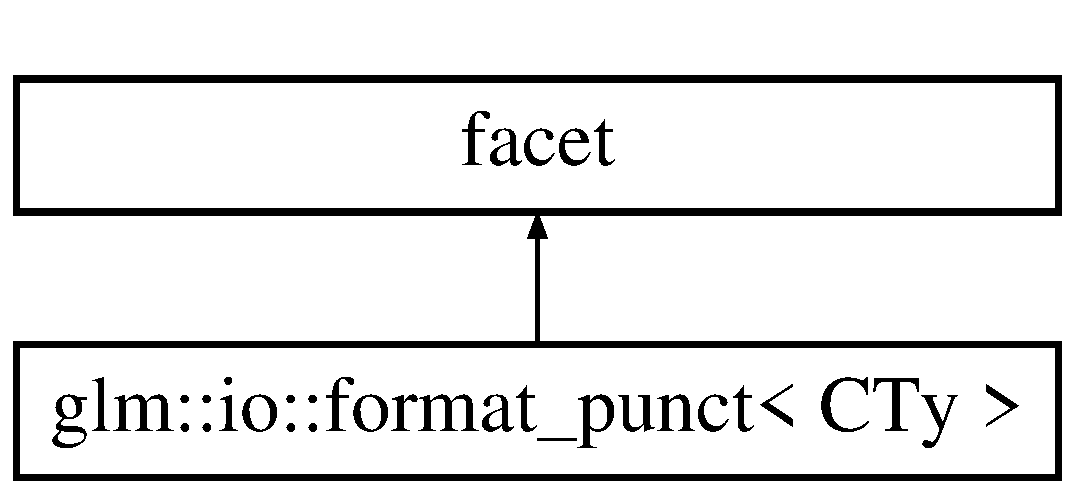
\includegraphics[height=2.000000cm]{classglm_1_1io_1_1format__punct}
\end{center}
\end{figure}
\subsection*{Public Member Functions}
\begin{DoxyCompactItemize}
\item 
\hypertarget{classglm_1_1io_1_1format__punct_ae56e7a14fac2516658837281b9da4659}{{\bfseries format\-\_\-punct} (size\-\_\-t a=0)}\label{classglm_1_1io_1_1format__punct_ae56e7a14fac2516658837281b9da4659}

\item 
\hypertarget{classglm_1_1io_1_1format__punct_a89a8c3cfb0b975f3dd8c0416101c59b7}{{\bfseries format\-\_\-punct} (\hyperlink{classglm_1_1io_1_1format__punct}{format\-\_\-punct} const \&)}\label{classglm_1_1io_1_1format__punct_a89a8c3cfb0b975f3dd8c0416101c59b7}

\end{DoxyCompactItemize}
\subsection*{Public Attributes}
\begin{DoxyCompactItemize}
\item 
\hypertarget{classglm_1_1io_1_1format__punct_ab28088e6eef03fe4222fa8a5dd95288e}{bool {\bfseries formatted}}\label{classglm_1_1io_1_1format__punct_ab28088e6eef03fe4222fa8a5dd95288e}

\item 
\hypertarget{classglm_1_1io_1_1format__punct_a5a15d396b7c963df9dec5e124236dc02}{unsigned {\bfseries precision}}\label{classglm_1_1io_1_1format__punct_a5a15d396b7c963df9dec5e124236dc02}

\item 
\hypertarget{classglm_1_1io_1_1format__punct_a95d32ca2330bbf7c50d3e066b7a851db}{unsigned {\bfseries width}}\label{classglm_1_1io_1_1format__punct_a95d32ca2330bbf7c50d3e066b7a851db}

\item 
\hypertarget{classglm_1_1io_1_1format__punct_ac561eb04fc2a1282ef38ea15f8e640ee}{char\-\_\-type {\bfseries separator}}\label{classglm_1_1io_1_1format__punct_ac561eb04fc2a1282ef38ea15f8e640ee}

\item 
\hypertarget{classglm_1_1io_1_1format__punct_ab1beed331269a39b06d17d02cf727d7c}{char\-\_\-type {\bfseries delim\-\_\-left}}\label{classglm_1_1io_1_1format__punct_ab1beed331269a39b06d17d02cf727d7c}

\item 
\hypertarget{classglm_1_1io_1_1format__punct_a62fb1280404360463ec5af7144aa0949}{char\-\_\-type {\bfseries delim\-\_\-right}}\label{classglm_1_1io_1_1format__punct_a62fb1280404360463ec5af7144aa0949}

\item 
\hypertarget{classglm_1_1io_1_1format__punct_adf9a915938727793de1daca07dcdfa4e}{char\-\_\-type {\bfseries space}}\label{classglm_1_1io_1_1format__punct_adf9a915938727793de1daca07dcdfa4e}

\item 
\hypertarget{classglm_1_1io_1_1format__punct_a8ddf8abdb0ebbdbb7eca08d7a777956e}{char\-\_\-type {\bfseries newline}}\label{classglm_1_1io_1_1format__punct_a8ddf8abdb0ebbdbb7eca08d7a777956e}

\item 
\hypertarget{classglm_1_1io_1_1format__punct_a9de1f3b7120a036ec0ab394d2036d0aa}{order\-\_\-type {\bfseries order}}\label{classglm_1_1io_1_1format__punct_a9de1f3b7120a036ec0ab394d2036d0aa}

\end{DoxyCompactItemize}
\subsection*{Static Public Attributes}
\begin{DoxyCompactItemize}
\item 
\hypertarget{classglm_1_1io_1_1format__punct_a763f60aeaecec9290917ed1d83b79838}{static std\-::locale\-::id {\bfseries id}}\label{classglm_1_1io_1_1format__punct_a763f60aeaecec9290917ed1d83b79838}

\end{DoxyCompactItemize}


The documentation for this class was generated from the following files\-:\begin{DoxyCompactItemize}
\item 
X\-:/\-Git\-\_\-\-Repository/inf2990-\/06/\-Cadriciel/\-Commun/\-Externe/glm/include/glm/gtx/\hyperlink{io_8hpp}{io.\-hpp}\item 
X\-:/\-Git\-\_\-\-Repository/inf2990-\/06/\-Cadriciel/\-Commun/\-Externe/glm/include/glm/gtx/io.\-inl\end{DoxyCompactItemize}

\hypertarget{struct_f_t___auto_hinter___service_rec__}{\section{F\-T\-\_\-\-Auto\-Hinter\-\_\-\-Service\-Rec\-\_\- Struct Reference}
\label{struct_f_t___auto_hinter___service_rec__}\index{F\-T\-\_\-\-Auto\-Hinter\-\_\-\-Service\-Rec\-\_\-@{F\-T\-\_\-\-Auto\-Hinter\-\_\-\-Service\-Rec\-\_\-}}
}
\subsection*{Public Attributes}
\begin{DoxyCompactItemize}
\item 
\hypertarget{struct_f_t___auto_hinter___service_rec___a846234a9c9c5427d3274e4568f33272c}{F\-T\-\_\-\-Auto\-Hinter\-\_\-\-Global\-Reset\-Func {\bfseries reset\-\_\-face}}\label{struct_f_t___auto_hinter___service_rec___a846234a9c9c5427d3274e4568f33272c}

\item 
\hypertarget{struct_f_t___auto_hinter___service_rec___a958371c33e08125393cd4b401a22f2a0}{F\-T\-\_\-\-Auto\-Hinter\-\_\-\-Global\-Get\-Func {\bfseries get\-\_\-global\-\_\-hints}}\label{struct_f_t___auto_hinter___service_rec___a958371c33e08125393cd4b401a22f2a0}

\item 
\hypertarget{struct_f_t___auto_hinter___service_rec___a648ac943fc1194f60ba638e0a59486e9}{F\-T\-\_\-\-Auto\-Hinter\-\_\-\-Global\-Done\-Func {\bfseries done\-\_\-global\-\_\-hints}}\label{struct_f_t___auto_hinter___service_rec___a648ac943fc1194f60ba638e0a59486e9}

\item 
\hypertarget{struct_f_t___auto_hinter___service_rec___ad36efe39469959626744ebdd04a04031}{F\-T\-\_\-\-Auto\-Hinter\-\_\-\-Glyph\-Load\-Func {\bfseries load\-\_\-glyph}}\label{struct_f_t___auto_hinter___service_rec___ad36efe39469959626744ebdd04a04031}

\end{DoxyCompactItemize}


The documentation for this struct was generated from the following file\-:\begin{DoxyCompactItemize}
\item 
X\-:/\-Git\-\_\-\-Repository/inf2990-\/06/\-Cadriciel/\-Commun/\-Externe/\-Free\-Type/include/freetype/internal/autohint.\-h\end{DoxyCompactItemize}

\hypertarget{struct_f_t___b_box__}{\section{F\-T\-\_\-\-B\-Box\-\_\- Struct Reference}
\label{struct_f_t___b_box__}\index{F\-T\-\_\-\-B\-Box\-\_\-@{F\-T\-\_\-\-B\-Box\-\_\-}}
}
\subsection*{Public Attributes}
\begin{DoxyCompactItemize}
\item 
\hypertarget{struct_f_t___b_box___a1f2a5d0565d496c1d41e43d018f45add}{F\-T\-\_\-\-Pos {\bfseries x\-Min}}\label{struct_f_t___b_box___a1f2a5d0565d496c1d41e43d018f45add}

\item 
\hypertarget{struct_f_t___b_box___a959ca1d5bc1c5338da0d85c8e7135f4e}{F\-T\-\_\-\-Pos {\bfseries y\-Min}}\label{struct_f_t___b_box___a959ca1d5bc1c5338da0d85c8e7135f4e}

\item 
\hypertarget{struct_f_t___b_box___ac6da5c44f4cb7b97eef1f438eb69c0ec}{F\-T\-\_\-\-Pos {\bfseries x\-Max}}\label{struct_f_t___b_box___ac6da5c44f4cb7b97eef1f438eb69c0ec}

\item 
\hypertarget{struct_f_t___b_box___a77084921589f386a8a593ae1f25b1569}{F\-T\-\_\-\-Pos {\bfseries y\-Max}}\label{struct_f_t___b_box___a77084921589f386a8a593ae1f25b1569}

\end{DoxyCompactItemize}


The documentation for this struct was generated from the following file\-:\begin{DoxyCompactItemize}
\item 
X\-:/\-Git\-\_\-\-Repository/inf2990-\/06/\-Cadriciel/\-Commun/\-Externe/\-Free\-Type/include/freetype/ftimage.\-h\end{DoxyCompactItemize}

\hypertarget{struct_f_t___bitmap__}{\section{F\-T\-\_\-\-Bitmap\-\_\- Struct Reference}
\label{struct_f_t___bitmap__}\index{F\-T\-\_\-\-Bitmap\-\_\-@{F\-T\-\_\-\-Bitmap\-\_\-}}
}
\subsection*{Public Attributes}
\begin{DoxyCompactItemize}
\item 
\hypertarget{struct_f_t___bitmap___a1b6bb20b30fe087e3fc87a0eb37730c0}{int {\bfseries rows}}\label{struct_f_t___bitmap___a1b6bb20b30fe087e3fc87a0eb37730c0}

\item 
\hypertarget{struct_f_t___bitmap___a7b5e6252dd91a3809fe80ebbeb6720eb}{int {\bfseries width}}\label{struct_f_t___bitmap___a7b5e6252dd91a3809fe80ebbeb6720eb}

\item 
\hypertarget{struct_f_t___bitmap___afdee595846e1188c7a76d0cec9d85cf2}{int {\bfseries pitch}}\label{struct_f_t___bitmap___afdee595846e1188c7a76d0cec9d85cf2}

\item 
\hypertarget{struct_f_t___bitmap___a76439b1d3c13b81ca506108cd1623284}{unsigned char $\ast$ {\bfseries buffer}}\label{struct_f_t___bitmap___a76439b1d3c13b81ca506108cd1623284}

\item 
\hypertarget{struct_f_t___bitmap___a415d78060f8012d312703c9792ec005a}{short {\bfseries num\-\_\-grays}}\label{struct_f_t___bitmap___a415d78060f8012d312703c9792ec005a}

\item 
\hypertarget{struct_f_t___bitmap___a5cc5e0fe42a93a86e16706ad52e087a2}{char {\bfseries pixel\-\_\-mode}}\label{struct_f_t___bitmap___a5cc5e0fe42a93a86e16706ad52e087a2}

\item 
\hypertarget{struct_f_t___bitmap___ae7c8c74255cd27873b12a360cd5f3884}{char {\bfseries palette\-\_\-mode}}\label{struct_f_t___bitmap___ae7c8c74255cd27873b12a360cd5f3884}

\item 
\hypertarget{struct_f_t___bitmap___a8d5ecf4409f71bfb559e0d13d8df4d86}{void $\ast$ {\bfseries palette}}\label{struct_f_t___bitmap___a8d5ecf4409f71bfb559e0d13d8df4d86}

\end{DoxyCompactItemize}


The documentation for this struct was generated from the following file\-:\begin{DoxyCompactItemize}
\item 
X\-:/\-Git\-\_\-\-Repository/inf2990-\/06/\-Cadriciel/\-Commun/\-Externe/\-Free\-Type/include/freetype/ftimage.\-h\end{DoxyCompactItemize}

\hypertarget{struct_f_t___bitmap___size__}{\section{F\-T\-\_\-\-Bitmap\-\_\-\-Size\-\_\- Struct Reference}
\label{struct_f_t___bitmap___size__}\index{F\-T\-\_\-\-Bitmap\-\_\-\-Size\-\_\-@{F\-T\-\_\-\-Bitmap\-\_\-\-Size\-\_\-}}
}
\subsection*{Public Attributes}
\begin{DoxyCompactItemize}
\item 
\hypertarget{struct_f_t___bitmap___size___adf2f24039b458ff4674712886f242262}{F\-T\-\_\-\-Short {\bfseries height}}\label{struct_f_t___bitmap___size___adf2f24039b458ff4674712886f242262}

\item 
\hypertarget{struct_f_t___bitmap___size___ab9da94223f75a89a649d1e6d018b17f1}{F\-T\-\_\-\-Short {\bfseries width}}\label{struct_f_t___bitmap___size___ab9da94223f75a89a649d1e6d018b17f1}

\item 
\hypertarget{struct_f_t___bitmap___size___a1db23a6220fb6bcb712430821a6e5352}{F\-T\-\_\-\-Pos {\bfseries size}}\label{struct_f_t___bitmap___size___a1db23a6220fb6bcb712430821a6e5352}

\item 
\hypertarget{struct_f_t___bitmap___size___a6f877a792d2dc93328037c928979215f}{F\-T\-\_\-\-Pos {\bfseries x\-\_\-ppem}}\label{struct_f_t___bitmap___size___a6f877a792d2dc93328037c928979215f}

\item 
\hypertarget{struct_f_t___bitmap___size___a60d4d003d09fd57505f69f39e31e19c1}{F\-T\-\_\-\-Pos {\bfseries y\-\_\-ppem}}\label{struct_f_t___bitmap___size___a60d4d003d09fd57505f69f39e31e19c1}

\end{DoxyCompactItemize}


The documentation for this struct was generated from the following file\-:\begin{DoxyCompactItemize}
\item 
X\-:/\-Git\-\_\-\-Repository/inf2990-\/06/\-Cadriciel/\-Commun/\-Externe/\-Free\-Type/include/freetype/freetype.\-h\end{DoxyCompactItemize}

\hypertarget{struct_f_t___bitmap_glyph_rec__}{\section{F\-T\-\_\-\-Bitmap\-Glyph\-Rec\-\_\- Struct Reference}
\label{struct_f_t___bitmap_glyph_rec__}\index{F\-T\-\_\-\-Bitmap\-Glyph\-Rec\-\_\-@{F\-T\-\_\-\-Bitmap\-Glyph\-Rec\-\_\-}}
}
\subsection*{Public Attributes}
\begin{DoxyCompactItemize}
\item 
\hypertarget{struct_f_t___bitmap_glyph_rec___ac3970353fbc0fe3d4c59c3fd608140f3}{\hyperlink{struct_f_t___glyph_rec__}{F\-T\-\_\-\-Glyph\-Rec} {\bfseries root}}\label{struct_f_t___bitmap_glyph_rec___ac3970353fbc0fe3d4c59c3fd608140f3}

\item 
\hypertarget{struct_f_t___bitmap_glyph_rec___a6cfd2d89af7b6be4af886047c9cb7e0a}{F\-T\-\_\-\-Int {\bfseries left}}\label{struct_f_t___bitmap_glyph_rec___a6cfd2d89af7b6be4af886047c9cb7e0a}

\item 
\hypertarget{struct_f_t___bitmap_glyph_rec___a25fc81296678d6a2d064843c01bc05f7}{F\-T\-\_\-\-Int {\bfseries top}}\label{struct_f_t___bitmap_glyph_rec___a25fc81296678d6a2d064843c01bc05f7}

\item 
\hypertarget{struct_f_t___bitmap_glyph_rec___a16ecd0725920f8d5ad4c14e9448126ad}{\hyperlink{struct_f_t___bitmap__}{F\-T\-\_\-\-Bitmap} {\bfseries bitmap}}\label{struct_f_t___bitmap_glyph_rec___a16ecd0725920f8d5ad4c14e9448126ad}

\end{DoxyCompactItemize}


The documentation for this struct was generated from the following file\-:\begin{DoxyCompactItemize}
\item 
X\-:/\-Git\-\_\-\-Repository/inf2990-\/06/\-Cadriciel/\-Commun/\-Externe/\-Free\-Type/include/freetype/ftglyph.\-h\end{DoxyCompactItemize}

\hypertarget{struct_f_t___char_map_rec__}{\section{F\-T\-\_\-\-Char\-Map\-Rec\-\_\- Struct Reference}
\label{struct_f_t___char_map_rec__}\index{F\-T\-\_\-\-Char\-Map\-Rec\-\_\-@{F\-T\-\_\-\-Char\-Map\-Rec\-\_\-}}
}
\subsection*{Public Attributes}
\begin{DoxyCompactItemize}
\item 
\hypertarget{struct_f_t___char_map_rec___a70a4e53e3f9818209916e5745c46dc28}{\hyperlink{struct_f_t___face_rec__}{F\-T\-\_\-\-Face} {\bfseries face}}\label{struct_f_t___char_map_rec___a70a4e53e3f9818209916e5745c46dc28}

\item 
\hypertarget{struct_f_t___char_map_rec___a88ee6f726ef11a8e6cc793d59ff5557e}{F\-T\-\_\-\-Encoding {\bfseries encoding}}\label{struct_f_t___char_map_rec___a88ee6f726ef11a8e6cc793d59ff5557e}

\item 
\hypertarget{struct_f_t___char_map_rec___ae7f439996a8615698e780ce3c4f92457}{F\-T\-\_\-\-U\-Short {\bfseries platform\-\_\-id}}\label{struct_f_t___char_map_rec___ae7f439996a8615698e780ce3c4f92457}

\item 
\hypertarget{struct_f_t___char_map_rec___af10dd43eee8dc93e7d6191c663ae831a}{F\-T\-\_\-\-U\-Short {\bfseries encoding\-\_\-id}}\label{struct_f_t___char_map_rec___af10dd43eee8dc93e7d6191c663ae831a}

\end{DoxyCompactItemize}


The documentation for this struct was generated from the following file\-:\begin{DoxyCompactItemize}
\item 
X\-:/\-Git\-\_\-\-Repository/inf2990-\/06/\-Cadriciel/\-Commun/\-Externe/\-Free\-Type/include/freetype/freetype.\-h\end{DoxyCompactItemize}

\hypertarget{struct_f_t___c_map___class_rec__}{\section{F\-T\-\_\-\-C\-Map\-\_\-\-Class\-Rec\-\_\- Struct Reference}
\label{struct_f_t___c_map___class_rec__}\index{F\-T\-\_\-\-C\-Map\-\_\-\-Class\-Rec\-\_\-@{F\-T\-\_\-\-C\-Map\-\_\-\-Class\-Rec\-\_\-}}
}
\subsection*{Public Attributes}
\begin{DoxyCompactItemize}
\item 
\hypertarget{struct_f_t___c_map___class_rec___a86283cf239b9c0e559c9acbaa004def6}{F\-T\-\_\-\-U\-Long {\bfseries size}}\label{struct_f_t___c_map___class_rec___a86283cf239b9c0e559c9acbaa004def6}

\item 
\hypertarget{struct_f_t___c_map___class_rec___afe1da0877ec0686dfe7b2e020fc0d408}{F\-T\-\_\-\-C\-Map\-\_\-\-Init\-Func {\bfseries init}}\label{struct_f_t___c_map___class_rec___afe1da0877ec0686dfe7b2e020fc0d408}

\item 
\hypertarget{struct_f_t___c_map___class_rec___a00d1d77a4d926340b4d97bc03cd29231}{F\-T\-\_\-\-C\-Map\-\_\-\-Done\-Func {\bfseries done}}\label{struct_f_t___c_map___class_rec___a00d1d77a4d926340b4d97bc03cd29231}

\item 
\hypertarget{struct_f_t___c_map___class_rec___ad1c0448188e8d52f6159b5521bb2dc83}{F\-T\-\_\-\-C\-Map\-\_\-\-Char\-Index\-Func {\bfseries char\-\_\-index}}\label{struct_f_t___c_map___class_rec___ad1c0448188e8d52f6159b5521bb2dc83}

\item 
\hypertarget{struct_f_t___c_map___class_rec___a053362f31fcfbc6a284cc8d026ab57ff}{F\-T\-\_\-\-C\-Map\-\_\-\-Char\-Next\-Func {\bfseries char\-\_\-next}}\label{struct_f_t___c_map___class_rec___a053362f31fcfbc6a284cc8d026ab57ff}

\item 
\hypertarget{struct_f_t___c_map___class_rec___a6bc46e2595aec30295e6d2bfc362afcb}{F\-T\-\_\-\-C\-Map\-\_\-\-Char\-Var\-Index\-Func {\bfseries char\-\_\-var\-\_\-index}}\label{struct_f_t___c_map___class_rec___a6bc46e2595aec30295e6d2bfc362afcb}

\item 
\hypertarget{struct_f_t___c_map___class_rec___ac8305cb0aebd02b54c0046765f28ef4a}{F\-T\-\_\-\-C\-Map\-\_\-\-Char\-Var\-Is\-Default\-Func {\bfseries char\-\_\-var\-\_\-default}}\label{struct_f_t___c_map___class_rec___ac8305cb0aebd02b54c0046765f28ef4a}

\item 
\hypertarget{struct_f_t___c_map___class_rec___ad61635444cbfc71c4259e74cb892c172}{F\-T\-\_\-\-C\-Map\-\_\-\-Variant\-List\-Func {\bfseries variant\-\_\-list}}\label{struct_f_t___c_map___class_rec___ad61635444cbfc71c4259e74cb892c172}

\item 
\hypertarget{struct_f_t___c_map___class_rec___a65db9dfa0e29b7de257dc8870532ab19}{F\-T\-\_\-\-C\-Map\-\_\-\-Char\-Variant\-List\-Func {\bfseries charvariant\-\_\-list}}\label{struct_f_t___c_map___class_rec___a65db9dfa0e29b7de257dc8870532ab19}

\item 
\hypertarget{struct_f_t___c_map___class_rec___ac1563590a0bac99082aa0996b94aad57}{F\-T\-\_\-\-C\-Map\-\_\-\-Variant\-Char\-List\-Func {\bfseries variantchar\-\_\-list}}\label{struct_f_t___c_map___class_rec___ac1563590a0bac99082aa0996b94aad57}

\end{DoxyCompactItemize}


The documentation for this struct was generated from the following file\-:\begin{DoxyCompactItemize}
\item 
X\-:/\-Git\-\_\-\-Repository/inf2990-\/06/\-Cadriciel/\-Commun/\-Externe/\-Free\-Type/include/freetype/internal/ftobjs.\-h\end{DoxyCompactItemize}

\hypertarget{struct_f_t___c_map_rec__}{\section{F\-T\-\_\-\-C\-Map\-Rec\-\_\- Struct Reference}
\label{struct_f_t___c_map_rec__}\index{F\-T\-\_\-\-C\-Map\-Rec\-\_\-@{F\-T\-\_\-\-C\-Map\-Rec\-\_\-}}
}
\subsection*{Public Attributes}
\begin{DoxyCompactItemize}
\item 
\hypertarget{struct_f_t___c_map_rec___a39fa6de9995d4ae4496b93e2b874b34e}{\hyperlink{struct_f_t___char_map_rec__}{F\-T\-\_\-\-Char\-Map\-Rec} {\bfseries charmap}}\label{struct_f_t___c_map_rec___a39fa6de9995d4ae4496b93e2b874b34e}

\item 
\hypertarget{struct_f_t___c_map_rec___aa85db42650df0edb38f8af5887c0ac6a}{\hyperlink{struct_f_t___c_map___class_rec__}{F\-T\-\_\-\-C\-Map\-\_\-\-Class} {\bfseries clazz}}\label{struct_f_t___c_map_rec___aa85db42650df0edb38f8af5887c0ac6a}

\end{DoxyCompactItemize}


The documentation for this struct was generated from the following file\-:\begin{DoxyCompactItemize}
\item 
X\-:/\-Git\-\_\-\-Repository/inf2990-\/06/\-Cadriciel/\-Commun/\-Externe/\-Free\-Type/include/freetype/internal/ftobjs.\-h\end{DoxyCompactItemize}

\hypertarget{struct_f_t___data__}{\section{F\-T\-\_\-\-Data\-\_\- Struct Reference}
\label{struct_f_t___data__}\index{F\-T\-\_\-\-Data\-\_\-@{F\-T\-\_\-\-Data\-\_\-}}
}
\subsection*{Public Attributes}
\begin{DoxyCompactItemize}
\item 
\hypertarget{struct_f_t___data___a4dea731b8a256b973757e1b8f612b050}{const F\-T\-\_\-\-Byte $\ast$ {\bfseries pointer}}\label{struct_f_t___data___a4dea731b8a256b973757e1b8f612b050}

\item 
\hypertarget{struct_f_t___data___af60c89dccd1852aceb0dc08675aca2fd}{F\-T\-\_\-\-Int {\bfseries length}}\label{struct_f_t___data___af60c89dccd1852aceb0dc08675aca2fd}

\end{DoxyCompactItemize}


The documentation for this struct was generated from the following file\-:\begin{DoxyCompactItemize}
\item 
X\-:/\-Git\-\_\-\-Repository/inf2990-\/06/\-Cadriciel/\-Commun/\-Externe/\-Free\-Type/include/freetype/fttypes.\-h\end{DoxyCompactItemize}

\hypertarget{struct_f_t___driver___class_rec__}{\section{F\-T\-\_\-\-Driver\-\_\-\-Class\-Rec\-\_\- Struct Reference}
\label{struct_f_t___driver___class_rec__}\index{F\-T\-\_\-\-Driver\-\_\-\-Class\-Rec\-\_\-@{F\-T\-\_\-\-Driver\-\_\-\-Class\-Rec\-\_\-}}
}
\subsection*{Public Attributes}
\begin{DoxyCompactItemize}
\item 
\hypertarget{struct_f_t___driver___class_rec___a087ca3e2c562bb90b8af82b31e82d8c7}{\hyperlink{struct_f_t___module___class__}{F\-T\-\_\-\-Module\-\_\-\-Class} {\bfseries root}}\label{struct_f_t___driver___class_rec___a087ca3e2c562bb90b8af82b31e82d8c7}

\item 
\hypertarget{struct_f_t___driver___class_rec___a194fc6fbae019e9c109c65328e57e44f}{F\-T\-\_\-\-Long {\bfseries face\-\_\-object\-\_\-size}}\label{struct_f_t___driver___class_rec___a194fc6fbae019e9c109c65328e57e44f}

\item 
\hypertarget{struct_f_t___driver___class_rec___a436687825ee47ed94da71fda90e2f578}{F\-T\-\_\-\-Long {\bfseries size\-\_\-object\-\_\-size}}\label{struct_f_t___driver___class_rec___a436687825ee47ed94da71fda90e2f578}

\item 
\hypertarget{struct_f_t___driver___class_rec___adcce7eb86dd7c763b622818cfcde99a6}{F\-T\-\_\-\-Long {\bfseries slot\-\_\-object\-\_\-size}}\label{struct_f_t___driver___class_rec___adcce7eb86dd7c763b622818cfcde99a6}

\item 
\hypertarget{struct_f_t___driver___class_rec___a68e94aeae3e78ed5984c29189c64df9a}{F\-T\-\_\-\-Face\-\_\-\-Init\-Func {\bfseries init\-\_\-face}}\label{struct_f_t___driver___class_rec___a68e94aeae3e78ed5984c29189c64df9a}

\item 
\hypertarget{struct_f_t___driver___class_rec___a7d37afe63f914ae28ed02c960e4d5642}{F\-T\-\_\-\-Face\-\_\-\-Done\-Func {\bfseries done\-\_\-face}}\label{struct_f_t___driver___class_rec___a7d37afe63f914ae28ed02c960e4d5642}

\item 
\hypertarget{struct_f_t___driver___class_rec___a0aec58307bc166f0e74c890509638ddf}{F\-T\-\_\-\-Size\-\_\-\-Init\-Func {\bfseries init\-\_\-size}}\label{struct_f_t___driver___class_rec___a0aec58307bc166f0e74c890509638ddf}

\item 
\hypertarget{struct_f_t___driver___class_rec___a5c96f627816a089b27bcff09f22dd1a6}{F\-T\-\_\-\-Size\-\_\-\-Done\-Func {\bfseries done\-\_\-size}}\label{struct_f_t___driver___class_rec___a5c96f627816a089b27bcff09f22dd1a6}

\item 
\hypertarget{struct_f_t___driver___class_rec___ae4e1d4ec7bdbdee0b4a5f8fc8f113d30}{F\-T\-\_\-\-Slot\-\_\-\-Init\-Func {\bfseries init\-\_\-slot}}\label{struct_f_t___driver___class_rec___ae4e1d4ec7bdbdee0b4a5f8fc8f113d30}

\item 
\hypertarget{struct_f_t___driver___class_rec___a548a343f5921f5d341142bf3743c42d4}{F\-T\-\_\-\-Slot\-\_\-\-Done\-Func {\bfseries done\-\_\-slot}}\label{struct_f_t___driver___class_rec___a548a343f5921f5d341142bf3743c42d4}

\item 
\hypertarget{struct_f_t___driver___class_rec___a49dbd71e64094d4d825b8b8d51dd4e47}{F\-T\-\_\-\-Slot\-\_\-\-Load\-Func {\bfseries load\-\_\-glyph}}\label{struct_f_t___driver___class_rec___a49dbd71e64094d4d825b8b8d51dd4e47}

\item 
\hypertarget{struct_f_t___driver___class_rec___a398395bfdbef65a8d531724d200ed91c}{F\-T\-\_\-\-Face\-\_\-\-Get\-Kerning\-Func {\bfseries get\-\_\-kerning}}\label{struct_f_t___driver___class_rec___a398395bfdbef65a8d531724d200ed91c}

\item 
\hypertarget{struct_f_t___driver___class_rec___a9caec9ae56a4bab9c90cede699279f29}{F\-T\-\_\-\-Face\-\_\-\-Attach\-Func {\bfseries attach\-\_\-file}}\label{struct_f_t___driver___class_rec___a9caec9ae56a4bab9c90cede699279f29}

\item 
\hypertarget{struct_f_t___driver___class_rec___aad560cd145b6d7cab7eae79194b1d724}{F\-T\-\_\-\-Face\-\_\-\-Get\-Advances\-Func {\bfseries get\-\_\-advances}}\label{struct_f_t___driver___class_rec___aad560cd145b6d7cab7eae79194b1d724}

\item 
\hypertarget{struct_f_t___driver___class_rec___a03ff7c2e4a2fb6d08eb481b03a78e8de}{F\-T\-\_\-\-Size\-\_\-\-Request\-Func {\bfseries request\-\_\-size}}\label{struct_f_t___driver___class_rec___a03ff7c2e4a2fb6d08eb481b03a78e8de}

\item 
\hypertarget{struct_f_t___driver___class_rec___a1b365eb82525dae0a816974d949fe0dd}{F\-T\-\_\-\-Size\-\_\-\-Select\-Func {\bfseries select\-\_\-size}}\label{struct_f_t___driver___class_rec___a1b365eb82525dae0a816974d949fe0dd}

\end{DoxyCompactItemize}


The documentation for this struct was generated from the following file\-:\begin{DoxyCompactItemize}
\item 
X\-:/\-Git\-\_\-\-Repository/inf2990-\/06/\-Cadriciel/\-Commun/\-Externe/\-Free\-Type/include/freetype/internal/ftdriver.\-h\end{DoxyCompactItemize}

\hypertarget{struct_f_t___driver_rec__}{\section{F\-T\-\_\-\-Driver\-Rec\-\_\- Struct Reference}
\label{struct_f_t___driver_rec__}\index{F\-T\-\_\-\-Driver\-Rec\-\_\-@{F\-T\-\_\-\-Driver\-Rec\-\_\-}}
}
\subsection*{Public Attributes}
\begin{DoxyCompactItemize}
\item 
\hypertarget{struct_f_t___driver_rec___a8451ceb25c76794fb47e81f477c8222d}{\hyperlink{struct_f_t___module_rec__}{F\-T\-\_\-\-Module\-Rec} {\bfseries root}}\label{struct_f_t___driver_rec___a8451ceb25c76794fb47e81f477c8222d}

\item 
\hypertarget{struct_f_t___driver_rec___a3111153608e5abeb093ed5eb7fef5aec}{\hyperlink{struct_f_t___driver___class_rec__}{F\-T\-\_\-\-Driver\-\_\-\-Class} {\bfseries clazz}}\label{struct_f_t___driver_rec___a3111153608e5abeb093ed5eb7fef5aec}

\item 
\hypertarget{struct_f_t___driver_rec___a2602170e3ecde21a764dc32417aaa002}{\hyperlink{struct_f_t___list_rec__}{F\-T\-\_\-\-List\-Rec} {\bfseries faces\-\_\-list}}\label{struct_f_t___driver_rec___a2602170e3ecde21a764dc32417aaa002}

\item 
\hypertarget{struct_f_t___driver_rec___ad2f1c1a800723dc887dcbc7ce78203d8}{void $\ast$ {\bfseries extensions}}\label{struct_f_t___driver_rec___ad2f1c1a800723dc887dcbc7ce78203d8}

\item 
\hypertarget{struct_f_t___driver_rec___ac28e7adbc14ee82c2b7710d0ee5541e2}{F\-T\-\_\-\-Glyph\-Loader {\bfseries glyph\-\_\-loader}}\label{struct_f_t___driver_rec___ac28e7adbc14ee82c2b7710d0ee5541e2}

\end{DoxyCompactItemize}


The documentation for this struct was generated from the following file\-:\begin{DoxyCompactItemize}
\item 
X\-:/\-Git\-\_\-\-Repository/inf2990-\/06/\-Cadriciel/\-Commun/\-Externe/\-Free\-Type/include/freetype/internal/ftobjs.\-h\end{DoxyCompactItemize}

\hypertarget{struct_f_t___face___internal_rec__}{\section{F\-T\-\_\-\-Face\-\_\-\-Internal\-Rec\-\_\- Struct Reference}
\label{struct_f_t___face___internal_rec__}\index{F\-T\-\_\-\-Face\-\_\-\-Internal\-Rec\-\_\-@{F\-T\-\_\-\-Face\-\_\-\-Internal\-Rec\-\_\-}}
}
\subsection*{Public Attributes}
\begin{DoxyCompactItemize}
\item 
\hypertarget{struct_f_t___face___internal_rec___ab4be2dcda098e6136f5701580d18032d}{\hyperlink{struct_f_t___matrix__}{F\-T\-\_\-\-Matrix} {\bfseries transform\-\_\-matrix}}\label{struct_f_t___face___internal_rec___ab4be2dcda098e6136f5701580d18032d}

\item 
\hypertarget{struct_f_t___face___internal_rec___ab6c2aacdac58312273395b21b8d168c6}{\hyperlink{struct_f_t___vector__}{F\-T\-\_\-\-Vector} {\bfseries transform\-\_\-delta}}\label{struct_f_t___face___internal_rec___ab6c2aacdac58312273395b21b8d168c6}

\item 
\hypertarget{struct_f_t___face___internal_rec___a2495aced35040e1b7c2bc0afcd7a920d}{F\-T\-\_\-\-Int {\bfseries transform\-\_\-flags}}\label{struct_f_t___face___internal_rec___a2495aced35040e1b7c2bc0afcd7a920d}

\item 
\hypertarget{struct_f_t___face___internal_rec___abc3acb3bf5db056bb9c549af04f07963}{\hyperlink{struct_f_t___service_cache_rec__}{F\-T\-\_\-\-Service\-Cache\-Rec} {\bfseries services}}\label{struct_f_t___face___internal_rec___abc3acb3bf5db056bb9c549af04f07963}

\item 
\hypertarget{struct_f_t___face___internal_rec___af898fd754c36c3f34c9ce0e88eb101c9}{F\-T\-\_\-\-Bool {\bfseries ignore\-\_\-unpatented\-\_\-hinter}}\label{struct_f_t___face___internal_rec___af898fd754c36c3f34c9ce0e88eb101c9}

\item 
\hypertarget{struct_f_t___face___internal_rec___a05d49c857c024a50441e17899803f56c}{F\-T\-\_\-\-U\-Int {\bfseries refcount}}\label{struct_f_t___face___internal_rec___a05d49c857c024a50441e17899803f56c}

\end{DoxyCompactItemize}


The documentation for this struct was generated from the following file\-:\begin{DoxyCompactItemize}
\item 
X\-:/\-Git\-\_\-\-Repository/inf2990-\/06/\-Cadriciel/\-Commun/\-Externe/\-Free\-Type/include/freetype/internal/ftobjs.\-h\end{DoxyCompactItemize}

\hypertarget{struct_f_t___face_rec__}{\section{F\-T\-\_\-\-Face\-Rec\-\_\- Struct Reference}
\label{struct_f_t___face_rec__}\index{F\-T\-\_\-\-Face\-Rec\-\_\-@{F\-T\-\_\-\-Face\-Rec\-\_\-}}
}
\subsection*{Public Attributes}
\begin{DoxyCompactItemize}
\item 
\hypertarget{struct_f_t___face_rec___af28be4cba102baaeb09d8e24b71e88fe}{F\-T\-\_\-\-Long {\bfseries num\-\_\-faces}}\label{struct_f_t___face_rec___af28be4cba102baaeb09d8e24b71e88fe}

\item 
\hypertarget{struct_f_t___face_rec___ab9a5640eb25bd3c743b3d725edd68a87}{F\-T\-\_\-\-Long {\bfseries face\-\_\-index}}\label{struct_f_t___face_rec___ab9a5640eb25bd3c743b3d725edd68a87}

\item 
\hypertarget{struct_f_t___face_rec___af1596857ebc9f8eac4c4b51c8f3ffd31}{F\-T\-\_\-\-Long {\bfseries face\-\_\-flags}}\label{struct_f_t___face_rec___af1596857ebc9f8eac4c4b51c8f3ffd31}

\item 
\hypertarget{struct_f_t___face_rec___ab06fc56f19fc1bf51cbed9bd621d3835}{F\-T\-\_\-\-Long {\bfseries style\-\_\-flags}}\label{struct_f_t___face_rec___ab06fc56f19fc1bf51cbed9bd621d3835}

\item 
\hypertarget{struct_f_t___face_rec___a58348bc3e0e113e8c73de9c318a9bd7a}{F\-T\-\_\-\-Long {\bfseries num\-\_\-glyphs}}\label{struct_f_t___face_rec___a58348bc3e0e113e8c73de9c318a9bd7a}

\item 
\hypertarget{struct_f_t___face_rec___ae07b64a64466aa7ae2b9066e9336ac8b}{F\-T\-\_\-\-String $\ast$ {\bfseries family\-\_\-name}}\label{struct_f_t___face_rec___ae07b64a64466aa7ae2b9066e9336ac8b}

\item 
\hypertarget{struct_f_t___face_rec___abd855b9e48b1f377b22176fb97668d7b}{F\-T\-\_\-\-String $\ast$ {\bfseries style\-\_\-name}}\label{struct_f_t___face_rec___abd855b9e48b1f377b22176fb97668d7b}

\item 
\hypertarget{struct_f_t___face_rec___aa652af958546eb8edf87ccd4b697bfdf}{F\-T\-\_\-\-Int {\bfseries num\-\_\-fixed\-\_\-sizes}}\label{struct_f_t___face_rec___aa652af958546eb8edf87ccd4b697bfdf}

\item 
\hypertarget{struct_f_t___face_rec___a563ca9007f754aa0f711ba67050f3e47}{\hyperlink{struct_f_t___bitmap___size__}{F\-T\-\_\-\-Bitmap\-\_\-\-Size} $\ast$ {\bfseries available\-\_\-sizes}}\label{struct_f_t___face_rec___a563ca9007f754aa0f711ba67050f3e47}

\item 
\hypertarget{struct_f_t___face_rec___a6b953f00e56d508611bb94af85b6d84b}{F\-T\-\_\-\-Int {\bfseries num\-\_\-charmaps}}\label{struct_f_t___face_rec___a6b953f00e56d508611bb94af85b6d84b}

\item 
\hypertarget{struct_f_t___face_rec___ab629e1bee5ddf3a90997d66751e6dfe0}{\hyperlink{struct_f_t___char_map_rec__}{F\-T\-\_\-\-Char\-Map} $\ast$ {\bfseries charmaps}}\label{struct_f_t___face_rec___ab629e1bee5ddf3a90997d66751e6dfe0}

\item 
\hypertarget{struct_f_t___face_rec___aaba29e9164f9c283348c8991f088a114}{\hyperlink{struct_f_t___generic__}{F\-T\-\_\-\-Generic} {\bfseries generic}}\label{struct_f_t___face_rec___aaba29e9164f9c283348c8991f088a114}

\item 
\hypertarget{struct_f_t___face_rec___a8a7b6313b5a6083e0b02c530d269417f}{\hyperlink{struct_f_t___b_box__}{F\-T\-\_\-\-B\-Box} {\bfseries bbox}}\label{struct_f_t___face_rec___a8a7b6313b5a6083e0b02c530d269417f}

\item 
\hypertarget{struct_f_t___face_rec___a8fde3c2d9b5fab717d8398b4196dd041}{F\-T\-\_\-\-U\-Short {\bfseries units\-\_\-per\-\_\-\-E\-M}}\label{struct_f_t___face_rec___a8fde3c2d9b5fab717d8398b4196dd041}

\item 
\hypertarget{struct_f_t___face_rec___afd0fe7d9dc08a4afbdec0ea0eabb0198}{F\-T\-\_\-\-Short {\bfseries ascender}}\label{struct_f_t___face_rec___afd0fe7d9dc08a4afbdec0ea0eabb0198}

\item 
\hypertarget{struct_f_t___face_rec___a7524f78b4f7b4e91d8c690713f8de275}{F\-T\-\_\-\-Short {\bfseries descender}}\label{struct_f_t___face_rec___a7524f78b4f7b4e91d8c690713f8de275}

\item 
\hypertarget{struct_f_t___face_rec___a6062881a848ab3395c6d096812065d9d}{F\-T\-\_\-\-Short {\bfseries height}}\label{struct_f_t___face_rec___a6062881a848ab3395c6d096812065d9d}

\item 
\hypertarget{struct_f_t___face_rec___ac8c9bd9f9b43ccb81326e7802c3d235d}{F\-T\-\_\-\-Short {\bfseries max\-\_\-advance\-\_\-width}}\label{struct_f_t___face_rec___ac8c9bd9f9b43ccb81326e7802c3d235d}

\item 
\hypertarget{struct_f_t___face_rec___abb74c1e75fb9138261c106e01bd08d69}{F\-T\-\_\-\-Short {\bfseries max\-\_\-advance\-\_\-height}}\label{struct_f_t___face_rec___abb74c1e75fb9138261c106e01bd08d69}

\item 
\hypertarget{struct_f_t___face_rec___ac4f899e32a37a89794d6c160a26937e1}{F\-T\-\_\-\-Short {\bfseries underline\-\_\-position}}\label{struct_f_t___face_rec___ac4f899e32a37a89794d6c160a26937e1}

\item 
\hypertarget{struct_f_t___face_rec___a61adda036bab17c419c358a31693e680}{F\-T\-\_\-\-Short {\bfseries underline\-\_\-thickness}}\label{struct_f_t___face_rec___a61adda036bab17c419c358a31693e680}

\item 
\hypertarget{struct_f_t___face_rec___aea701e6584693e684acf300edb28d8f6}{\hyperlink{struct_f_t___glyph_slot_rec__}{F\-T\-\_\-\-Glyph\-Slot} {\bfseries glyph}}\label{struct_f_t___face_rec___aea701e6584693e684acf300edb28d8f6}

\item 
\hypertarget{struct_f_t___face_rec___a212d116864a5d81e80b176f9b846cd08}{\hyperlink{struct_f_t___size_rec__}{F\-T\-\_\-\-Size} {\bfseries size}}\label{struct_f_t___face_rec___a212d116864a5d81e80b176f9b846cd08}

\item 
\hypertarget{struct_f_t___face_rec___aca87d50488a5a1489741e8c13414c268}{\hyperlink{struct_f_t___char_map_rec__}{F\-T\-\_\-\-Char\-Map} {\bfseries charmap}}\label{struct_f_t___face_rec___aca87d50488a5a1489741e8c13414c268}

\item 
\hypertarget{struct_f_t___face_rec___a011b62fcffdd6dc421c9ab3286d4c9fa}{\hyperlink{struct_f_t___driver_rec__}{F\-T\-\_\-\-Driver} {\bfseries driver}}\label{struct_f_t___face_rec___a011b62fcffdd6dc421c9ab3286d4c9fa}

\item 
\hypertarget{struct_f_t___face_rec___af269b241bfc2f570d485ab03fc0261b2}{F\-T\-\_\-\-Memory {\bfseries memory}}\label{struct_f_t___face_rec___af269b241bfc2f570d485ab03fc0261b2}

\item 
\hypertarget{struct_f_t___face_rec___a831d5da25cd0fe2a783d2a73f467de55}{\hyperlink{struct_f_t___stream_rec__}{F\-T\-\_\-\-Stream} {\bfseries stream}}\label{struct_f_t___face_rec___a831d5da25cd0fe2a783d2a73f467de55}

\item 
\hypertarget{struct_f_t___face_rec___a47504203e02bfba59c802c35cb4009ed}{\hyperlink{struct_f_t___list_rec__}{F\-T\-\_\-\-List\-Rec} {\bfseries sizes\-\_\-list}}\label{struct_f_t___face_rec___a47504203e02bfba59c802c35cb4009ed}

\item 
\hypertarget{struct_f_t___face_rec___a34ba9b1367f1b2d13676043b8da3ea73}{\hyperlink{struct_f_t___generic__}{F\-T\-\_\-\-Generic} {\bfseries autohint}}\label{struct_f_t___face_rec___a34ba9b1367f1b2d13676043b8da3ea73}

\item 
\hypertarget{struct_f_t___face_rec___a8b24f993e38da597d3e0273267890f49}{void $\ast$ {\bfseries extensions}}\label{struct_f_t___face_rec___a8b24f993e38da597d3e0273267890f49}

\item 
\hypertarget{struct_f_t___face_rec___aed9a1267cddcbe790f0591471c886537}{\hyperlink{struct_f_t___face___internal_rec__}{F\-T\-\_\-\-Face\-\_\-\-Internal} {\bfseries internal}}\label{struct_f_t___face_rec___aed9a1267cddcbe790f0591471c886537}

\end{DoxyCompactItemize}


The documentation for this struct was generated from the following file\-:\begin{DoxyCompactItemize}
\item 
X\-:/\-Git\-\_\-\-Repository/inf2990-\/06/\-Cadriciel/\-Commun/\-Externe/\-Free\-Type/include/freetype/freetype.\-h\end{DoxyCompactItemize}

\hypertarget{struct_f_t___frame___field__}{\section{F\-T\-\_\-\-Frame\-\_\-\-Field\-\_\- Struct Reference}
\label{struct_f_t___frame___field__}\index{F\-T\-\_\-\-Frame\-\_\-\-Field\-\_\-@{F\-T\-\_\-\-Frame\-\_\-\-Field\-\_\-}}
}
\subsection*{Public Attributes}
\begin{DoxyCompactItemize}
\item 
\hypertarget{struct_f_t___frame___field___a10f91dcdd0a582727b67ad45d42bab41}{F\-T\-\_\-\-Byte {\bfseries value}}\label{struct_f_t___frame___field___a10f91dcdd0a582727b67ad45d42bab41}

\item 
\hypertarget{struct_f_t___frame___field___a47e6fbcb90c079421d9d9b64f63a587e}{F\-T\-\_\-\-Byte {\bfseries size}}\label{struct_f_t___frame___field___a47e6fbcb90c079421d9d9b64f63a587e}

\item 
\hypertarget{struct_f_t___frame___field___a85c3275fbb7044f7d6880020b6f0f794}{F\-T\-\_\-\-U\-Short {\bfseries offset}}\label{struct_f_t___frame___field___a85c3275fbb7044f7d6880020b6f0f794}

\end{DoxyCompactItemize}


The documentation for this struct was generated from the following file\-:\begin{DoxyCompactItemize}
\item 
X\-:/\-Git\-\_\-\-Repository/inf2990-\/06/\-Cadriciel/\-Commun/\-Externe/\-Free\-Type/include/freetype/internal/ftstream.\-h\end{DoxyCompactItemize}

\hypertarget{struct_f_t___generic__}{\section{F\-T\-\_\-\-Generic\-\_\- Struct Reference}
\label{struct_f_t___generic__}\index{F\-T\-\_\-\-Generic\-\_\-@{F\-T\-\_\-\-Generic\-\_\-}}
}
\subsection*{Public Attributes}
\begin{DoxyCompactItemize}
\item 
\hypertarget{struct_f_t___generic___af0bf8b983254b662f293e9a20505e27e}{void $\ast$ {\bfseries data}}\label{struct_f_t___generic___af0bf8b983254b662f293e9a20505e27e}

\item 
\hypertarget{struct_f_t___generic___a20fce8de90cc9e3876935817247b9ccc}{F\-T\-\_\-\-Generic\-\_\-\-Finalizer {\bfseries finalizer}}\label{struct_f_t___generic___a20fce8de90cc9e3876935817247b9ccc}

\end{DoxyCompactItemize}


The documentation for this struct was generated from the following file\-:\begin{DoxyCompactItemize}
\item 
X\-:/\-Git\-\_\-\-Repository/inf2990-\/06/\-Cadriciel/\-Commun/\-Externe/\-Free\-Type/include/freetype/fttypes.\-h\end{DoxyCompactItemize}

\hypertarget{struct_f_t___glyph___class__}{\section{F\-T\-\_\-\-Glyph\-\_\-\-Class\-\_\- Struct Reference}
\label{struct_f_t___glyph___class__}\index{F\-T\-\_\-\-Glyph\-\_\-\-Class\-\_\-@{F\-T\-\_\-\-Glyph\-\_\-\-Class\-\_\-}}
}
\subsection*{Public Attributes}
\begin{DoxyCompactItemize}
\item 
\hypertarget{struct_f_t___glyph___class___a1a76c68b9fb0e93947e888c0fe77cbf8}{F\-T\-\_\-\-Long {\bfseries glyph\-\_\-size}}\label{struct_f_t___glyph___class___a1a76c68b9fb0e93947e888c0fe77cbf8}

\item 
\hypertarget{struct_f_t___glyph___class___a26738bd14d5845e18d09ccaa3a709d23}{F\-T\-\_\-\-Glyph\-\_\-\-Format {\bfseries glyph\-\_\-format}}\label{struct_f_t___glyph___class___a26738bd14d5845e18d09ccaa3a709d23}

\item 
\hypertarget{struct_f_t___glyph___class___a657200ad15ff061b38fb25b168737f95}{F\-T\-\_\-\-Glyph\-\_\-\-Init\-Func {\bfseries glyph\-\_\-init}}\label{struct_f_t___glyph___class___a657200ad15ff061b38fb25b168737f95}

\item 
\hypertarget{struct_f_t___glyph___class___aabf05a4368dccacf45e1a54e542e5d63}{F\-T\-\_\-\-Glyph\-\_\-\-Done\-Func {\bfseries glyph\-\_\-done}}\label{struct_f_t___glyph___class___aabf05a4368dccacf45e1a54e542e5d63}

\item 
\hypertarget{struct_f_t___glyph___class___afc78dcdc4802760ebcaccf3a7b6cd088}{F\-T\-\_\-\-Glyph\-\_\-\-Copy\-Func {\bfseries glyph\-\_\-copy}}\label{struct_f_t___glyph___class___afc78dcdc4802760ebcaccf3a7b6cd088}

\item 
\hypertarget{struct_f_t___glyph___class___a5f72ac1d0d92eb31fa3e2bb721a97ef2}{F\-T\-\_\-\-Glyph\-\_\-\-Transform\-Func {\bfseries glyph\-\_\-transform}}\label{struct_f_t___glyph___class___a5f72ac1d0d92eb31fa3e2bb721a97ef2}

\item 
\hypertarget{struct_f_t___glyph___class___a06bfad431865c6731305cb781f78b317}{F\-T\-\_\-\-Glyph\-\_\-\-Get\-B\-Box\-Func {\bfseries glyph\-\_\-bbox}}\label{struct_f_t___glyph___class___a06bfad431865c6731305cb781f78b317}

\item 
\hypertarget{struct_f_t___glyph___class___af7f406e5ea20a6614c946746938830c9}{F\-T\-\_\-\-Glyph\-\_\-\-Prepare\-Func {\bfseries glyph\-\_\-prepare}}\label{struct_f_t___glyph___class___af7f406e5ea20a6614c946746938830c9}

\end{DoxyCompactItemize}


The documentation for this struct was generated from the following file\-:\begin{DoxyCompactItemize}
\item 
X\-:/\-Git\-\_\-\-Repository/inf2990-\/06/\-Cadriciel/\-Commun/\-Externe/\-Free\-Type/include/freetype/ftrender.\-h\end{DoxyCompactItemize}

\hypertarget{struct_f_t___glyph___metrics__}{\section{F\-T\-\_\-\-Glyph\-\_\-\-Metrics\-\_\- Struct Reference}
\label{struct_f_t___glyph___metrics__}\index{F\-T\-\_\-\-Glyph\-\_\-\-Metrics\-\_\-@{F\-T\-\_\-\-Glyph\-\_\-\-Metrics\-\_\-}}
}
\subsection*{Public Attributes}
\begin{DoxyCompactItemize}
\item 
\hypertarget{struct_f_t___glyph___metrics___a0ff1be869e6a28d1f2990b0e5719dca9}{F\-T\-\_\-\-Pos {\bfseries width}}\label{struct_f_t___glyph___metrics___a0ff1be869e6a28d1f2990b0e5719dca9}

\item 
\hypertarget{struct_f_t___glyph___metrics___aa2a76ec448ec9d18acf343f01b77cb21}{F\-T\-\_\-\-Pos {\bfseries height}}\label{struct_f_t___glyph___metrics___aa2a76ec448ec9d18acf343f01b77cb21}

\item 
\hypertarget{struct_f_t___glyph___metrics___a2afc877f52c8a8910ec144a1948186cc}{F\-T\-\_\-\-Pos {\bfseries hori\-Bearing\-X}}\label{struct_f_t___glyph___metrics___a2afc877f52c8a8910ec144a1948186cc}

\item 
\hypertarget{struct_f_t___glyph___metrics___afd97c10d43ed1f66598a18884468b536}{F\-T\-\_\-\-Pos {\bfseries hori\-Bearing\-Y}}\label{struct_f_t___glyph___metrics___afd97c10d43ed1f66598a18884468b536}

\item 
\hypertarget{struct_f_t___glyph___metrics___af12db260a90b8a7c938ad48ebf20ccbe}{F\-T\-\_\-\-Pos {\bfseries hori\-Advance}}\label{struct_f_t___glyph___metrics___af12db260a90b8a7c938ad48ebf20ccbe}

\item 
\hypertarget{struct_f_t___glyph___metrics___aead5c5637b983b811738bff3bcea8cea}{F\-T\-\_\-\-Pos {\bfseries vert\-Bearing\-X}}\label{struct_f_t___glyph___metrics___aead5c5637b983b811738bff3bcea8cea}

\item 
\hypertarget{struct_f_t___glyph___metrics___a7f1aba91b86fddeb11030eab15dcce08}{F\-T\-\_\-\-Pos {\bfseries vert\-Bearing\-Y}}\label{struct_f_t___glyph___metrics___a7f1aba91b86fddeb11030eab15dcce08}

\item 
\hypertarget{struct_f_t___glyph___metrics___a594f43c64fe5c12a399a0f0a47c04990}{F\-T\-\_\-\-Pos {\bfseries vert\-Advance}}\label{struct_f_t___glyph___metrics___a594f43c64fe5c12a399a0f0a47c04990}

\end{DoxyCompactItemize}


The documentation for this struct was generated from the following file\-:\begin{DoxyCompactItemize}
\item 
X\-:/\-Git\-\_\-\-Repository/inf2990-\/06/\-Cadriciel/\-Commun/\-Externe/\-Free\-Type/include/freetype/freetype.\-h\end{DoxyCompactItemize}

\hypertarget{struct_f_t___glyph_loader_rec__}{\section{F\-T\-\_\-\-Glyph\-Loader\-Rec\-\_\- Struct Reference}
\label{struct_f_t___glyph_loader_rec__}\index{F\-T\-\_\-\-Glyph\-Loader\-Rec\-\_\-@{F\-T\-\_\-\-Glyph\-Loader\-Rec\-\_\-}}
}
\subsection*{Public Attributes}
\begin{DoxyCompactItemize}
\item 
\hypertarget{struct_f_t___glyph_loader_rec___a9120a7808ee59d24dd52409e609907a2}{F\-T\-\_\-\-Memory {\bfseries memory}}\label{struct_f_t___glyph_loader_rec___a9120a7808ee59d24dd52409e609907a2}

\item 
\hypertarget{struct_f_t___glyph_loader_rec___a62339fa7a06e0b4ddecd5db2aa606741}{F\-T\-\_\-\-U\-Int {\bfseries max\-\_\-points}}\label{struct_f_t___glyph_loader_rec___a62339fa7a06e0b4ddecd5db2aa606741}

\item 
\hypertarget{struct_f_t___glyph_loader_rec___a808ccf46597572d953f387e705f10a36}{F\-T\-\_\-\-U\-Int {\bfseries max\-\_\-contours}}\label{struct_f_t___glyph_loader_rec___a808ccf46597572d953f387e705f10a36}

\item 
\hypertarget{struct_f_t___glyph_loader_rec___a2d5b00d7caf624ed2b4f6fd2db3228db}{F\-T\-\_\-\-U\-Int {\bfseries max\-\_\-subglyphs}}\label{struct_f_t___glyph_loader_rec___a2d5b00d7caf624ed2b4f6fd2db3228db}

\item 
\hypertarget{struct_f_t___glyph_loader_rec___a54009985acda32d83f2f124e28c5d00a}{F\-T\-\_\-\-Bool {\bfseries use\-\_\-extra}}\label{struct_f_t___glyph_loader_rec___a54009985acda32d83f2f124e28c5d00a}

\item 
\hypertarget{struct_f_t___glyph_loader_rec___ae80dfc17f20bfce8c60ffaaba95c821b}{\hyperlink{struct_f_t___glyph_load_rec__}{F\-T\-\_\-\-Glyph\-Load\-Rec} {\bfseries base}}\label{struct_f_t___glyph_loader_rec___ae80dfc17f20bfce8c60ffaaba95c821b}

\item 
\hypertarget{struct_f_t___glyph_loader_rec___a271b1b9604746ed08cf6613710ebb4c1}{\hyperlink{struct_f_t___glyph_load_rec__}{F\-T\-\_\-\-Glyph\-Load\-Rec} {\bfseries current}}\label{struct_f_t___glyph_loader_rec___a271b1b9604746ed08cf6613710ebb4c1}

\item 
\hypertarget{struct_f_t___glyph_loader_rec___a9c58c5b06f0135fe5cef16bd85d939e3}{void $\ast$ {\bfseries other}}\label{struct_f_t___glyph_loader_rec___a9c58c5b06f0135fe5cef16bd85d939e3}

\end{DoxyCompactItemize}


The documentation for this struct was generated from the following file\-:\begin{DoxyCompactItemize}
\item 
X\-:/\-Git\-\_\-\-Repository/inf2990-\/06/\-Cadriciel/\-Commun/\-Externe/\-Free\-Type/include/freetype/internal/ftgloadr.\-h\end{DoxyCompactItemize}

\hypertarget{struct_f_t___glyph_load_rec__}{\section{F\-T\-\_\-\-Glyph\-Load\-Rec\-\_\- Struct Reference}
\label{struct_f_t___glyph_load_rec__}\index{F\-T\-\_\-\-Glyph\-Load\-Rec\-\_\-@{F\-T\-\_\-\-Glyph\-Load\-Rec\-\_\-}}
}
\subsection*{Public Attributes}
\begin{DoxyCompactItemize}
\item 
\hypertarget{struct_f_t___glyph_load_rec___ae340cdb5263322e86c640b15f82ea72a}{\hyperlink{struct_f_t___outline__}{F\-T\-\_\-\-Outline} {\bfseries outline}}\label{struct_f_t___glyph_load_rec___ae340cdb5263322e86c640b15f82ea72a}

\item 
\hypertarget{struct_f_t___glyph_load_rec___ad2547bd6a7c7473d3a4646dfe908f1c3}{\hyperlink{struct_f_t___vector__}{F\-T\-\_\-\-Vector} $\ast$ {\bfseries extra\-\_\-points}}\label{struct_f_t___glyph_load_rec___ad2547bd6a7c7473d3a4646dfe908f1c3}

\item 
\hypertarget{struct_f_t___glyph_load_rec___a5e8bbe62bd889e806700bc0d583ff79b}{\hyperlink{struct_f_t___vector__}{F\-T\-\_\-\-Vector} $\ast$ {\bfseries extra\-\_\-points2}}\label{struct_f_t___glyph_load_rec___a5e8bbe62bd889e806700bc0d583ff79b}

\item 
\hypertarget{struct_f_t___glyph_load_rec___a71dc4ab52b956b974fe65c95a098e03c}{F\-T\-\_\-\-U\-Int {\bfseries num\-\_\-subglyphs}}\label{struct_f_t___glyph_load_rec___a71dc4ab52b956b974fe65c95a098e03c}

\item 
\hypertarget{struct_f_t___glyph_load_rec___a12ef145fedbeb14cc8b9d320ae3fed96}{\hyperlink{struct_f_t___sub_glyph_rec__}{F\-T\-\_\-\-Sub\-Glyph} {\bfseries subglyphs}}\label{struct_f_t___glyph_load_rec___a12ef145fedbeb14cc8b9d320ae3fed96}

\end{DoxyCompactItemize}


The documentation for this struct was generated from the following file\-:\begin{DoxyCompactItemize}
\item 
X\-:/\-Git\-\_\-\-Repository/inf2990-\/06/\-Cadriciel/\-Commun/\-Externe/\-Free\-Type/include/freetype/internal/ftgloadr.\-h\end{DoxyCompactItemize}

\hypertarget{struct_f_t___glyph_rec__}{\section{F\-T\-\_\-\-Glyph\-Rec\-\_\- Struct Reference}
\label{struct_f_t___glyph_rec__}\index{F\-T\-\_\-\-Glyph\-Rec\-\_\-@{F\-T\-\_\-\-Glyph\-Rec\-\_\-}}
}
\subsection*{Public Attributes}
\begin{DoxyCompactItemize}
\item 
\hypertarget{struct_f_t___glyph_rec___a00679b5e2519affab0f3999718817f8e}{\hyperlink{struct_f_t___library_rec__}{F\-T\-\_\-\-Library} {\bfseries library}}\label{struct_f_t___glyph_rec___a00679b5e2519affab0f3999718817f8e}

\item 
\hypertarget{struct_f_t___glyph_rec___ad7074cfe0e9fd6616e4dc4011e481524}{const F\-T\-\_\-\-Glyph\-\_\-\-Class $\ast$ {\bfseries clazz}}\label{struct_f_t___glyph_rec___ad7074cfe0e9fd6616e4dc4011e481524}

\item 
\hypertarget{struct_f_t___glyph_rec___a26b42a2610a69dcaed3e7c8b6d506211}{F\-T\-\_\-\-Glyph\-\_\-\-Format {\bfseries format}}\label{struct_f_t___glyph_rec___a26b42a2610a69dcaed3e7c8b6d506211}

\item 
\hypertarget{struct_f_t___glyph_rec___afd95b047df6a249db79018a279137018}{\hyperlink{struct_f_t___vector__}{F\-T\-\_\-\-Vector} {\bfseries advance}}\label{struct_f_t___glyph_rec___afd95b047df6a249db79018a279137018}

\end{DoxyCompactItemize}


The documentation for this struct was generated from the following file\-:\begin{DoxyCompactItemize}
\item 
X\-:/\-Git\-\_\-\-Repository/inf2990-\/06/\-Cadriciel/\-Commun/\-Externe/\-Free\-Type/include/freetype/ftglyph.\-h\end{DoxyCompactItemize}

\hypertarget{struct_f_t___glyph_slot_rec__}{\section{F\-T\-\_\-\-Glyph\-Slot\-Rec\-\_\- Struct Reference}
\label{struct_f_t___glyph_slot_rec__}\index{F\-T\-\_\-\-Glyph\-Slot\-Rec\-\_\-@{F\-T\-\_\-\-Glyph\-Slot\-Rec\-\_\-}}
}
\subsection*{Public Attributes}
\begin{DoxyCompactItemize}
\item 
\hypertarget{struct_f_t___glyph_slot_rec___a5415bcbf70efb3aae7a6b77040e21e91}{\hyperlink{struct_f_t___library_rec__}{F\-T\-\_\-\-Library} {\bfseries library}}\label{struct_f_t___glyph_slot_rec___a5415bcbf70efb3aae7a6b77040e21e91}

\item 
\hypertarget{struct_f_t___glyph_slot_rec___a0f5dbaf7d539bf2d92ecdff740342b04}{\hyperlink{struct_f_t___face_rec__}{F\-T\-\_\-\-Face} {\bfseries face}}\label{struct_f_t___glyph_slot_rec___a0f5dbaf7d539bf2d92ecdff740342b04}

\item 
\hypertarget{struct_f_t___glyph_slot_rec___af339309df5ebe70dfa62a9f4f8838440}{\hyperlink{struct_f_t___glyph_slot_rec__}{F\-T\-\_\-\-Glyph\-Slot} {\bfseries next}}\label{struct_f_t___glyph_slot_rec___af339309df5ebe70dfa62a9f4f8838440}

\item 
\hypertarget{struct_f_t___glyph_slot_rec___ae829996584939557dfe46c4e4f2b28a8}{F\-T\-\_\-\-U\-Int {\bfseries reserved}}\label{struct_f_t___glyph_slot_rec___ae829996584939557dfe46c4e4f2b28a8}

\item 
\hypertarget{struct_f_t___glyph_slot_rec___ac2d04848997fba660e17bc00760ef14f}{\hyperlink{struct_f_t___generic__}{F\-T\-\_\-\-Generic} {\bfseries generic}}\label{struct_f_t___glyph_slot_rec___ac2d04848997fba660e17bc00760ef14f}

\item 
\hypertarget{struct_f_t___glyph_slot_rec___abe1ba307281c06a232f50e34c061ce7b}{F\-T\-\_\-\-Glyph\-\_\-\-Metrics {\bfseries metrics}}\label{struct_f_t___glyph_slot_rec___abe1ba307281c06a232f50e34c061ce7b}

\item 
\hypertarget{struct_f_t___glyph_slot_rec___a9d0ba6b09729d4f009ef380e267607c3}{F\-T\-\_\-\-Fixed {\bfseries linear\-Hori\-Advance}}\label{struct_f_t___glyph_slot_rec___a9d0ba6b09729d4f009ef380e267607c3}

\item 
\hypertarget{struct_f_t___glyph_slot_rec___abc10f58c3d859e46694515956aa4a1e8}{F\-T\-\_\-\-Fixed {\bfseries linear\-Vert\-Advance}}\label{struct_f_t___glyph_slot_rec___abc10f58c3d859e46694515956aa4a1e8}

\item 
\hypertarget{struct_f_t___glyph_slot_rec___a09779d1a4781ea029382e92c01048c6a}{\hyperlink{struct_f_t___vector__}{F\-T\-\_\-\-Vector} {\bfseries advance}}\label{struct_f_t___glyph_slot_rec___a09779d1a4781ea029382e92c01048c6a}

\item 
\hypertarget{struct_f_t___glyph_slot_rec___afcd35188ff4c3d5cbb518602d05b2807}{F\-T\-\_\-\-Glyph\-\_\-\-Format {\bfseries format}}\label{struct_f_t___glyph_slot_rec___afcd35188ff4c3d5cbb518602d05b2807}

\item 
\hypertarget{struct_f_t___glyph_slot_rec___a8c50199e30b763b8e2a645af04a1f293}{\hyperlink{struct_f_t___bitmap__}{F\-T\-\_\-\-Bitmap} {\bfseries bitmap}}\label{struct_f_t___glyph_slot_rec___a8c50199e30b763b8e2a645af04a1f293}

\item 
\hypertarget{struct_f_t___glyph_slot_rec___a7e47f0471336ac68e3c72312a3349dc4}{F\-T\-\_\-\-Int {\bfseries bitmap\-\_\-left}}\label{struct_f_t___glyph_slot_rec___a7e47f0471336ac68e3c72312a3349dc4}

\item 
\hypertarget{struct_f_t___glyph_slot_rec___a0c150c0fb007e49fe4b9db6a69df53b7}{F\-T\-\_\-\-Int {\bfseries bitmap\-\_\-top}}\label{struct_f_t___glyph_slot_rec___a0c150c0fb007e49fe4b9db6a69df53b7}

\item 
\hypertarget{struct_f_t___glyph_slot_rec___a8e46dd5d808079bdcba68056d6476d8d}{\hyperlink{struct_f_t___outline__}{F\-T\-\_\-\-Outline} {\bfseries outline}}\label{struct_f_t___glyph_slot_rec___a8e46dd5d808079bdcba68056d6476d8d}

\item 
\hypertarget{struct_f_t___glyph_slot_rec___a5753b48d7165b08f106de3ad7c12bdd7}{F\-T\-\_\-\-U\-Int {\bfseries num\-\_\-subglyphs}}\label{struct_f_t___glyph_slot_rec___a5753b48d7165b08f106de3ad7c12bdd7}

\item 
\hypertarget{struct_f_t___glyph_slot_rec___a295f5a3108399c4c0703e6ee2f88cc67}{\hyperlink{struct_f_t___sub_glyph_rec__}{F\-T\-\_\-\-Sub\-Glyph} {\bfseries subglyphs}}\label{struct_f_t___glyph_slot_rec___a295f5a3108399c4c0703e6ee2f88cc67}

\item 
\hypertarget{struct_f_t___glyph_slot_rec___a2af67814d985bcdfcffdf7e8a36ebbdf}{void $\ast$ {\bfseries control\-\_\-data}}\label{struct_f_t___glyph_slot_rec___a2af67814d985bcdfcffdf7e8a36ebbdf}

\item 
\hypertarget{struct_f_t___glyph_slot_rec___a7a088255cb09abe42f19f650f48b6b3f}{long {\bfseries control\-\_\-len}}\label{struct_f_t___glyph_slot_rec___a7a088255cb09abe42f19f650f48b6b3f}

\item 
\hypertarget{struct_f_t___glyph_slot_rec___a7d0d8c2eda28e38541e953186ecab89a}{F\-T\-\_\-\-Pos {\bfseries lsb\-\_\-delta}}\label{struct_f_t___glyph_slot_rec___a7d0d8c2eda28e38541e953186ecab89a}

\item 
\hypertarget{struct_f_t___glyph_slot_rec___a2ca5f5e7b92df3aee4584949fa6a2a1c}{F\-T\-\_\-\-Pos {\bfseries rsb\-\_\-delta}}\label{struct_f_t___glyph_slot_rec___a2ca5f5e7b92df3aee4584949fa6a2a1c}

\item 
\hypertarget{struct_f_t___glyph_slot_rec___ad0c5ab51842f178ba571bab2874f1bdb}{void $\ast$ {\bfseries other}}\label{struct_f_t___glyph_slot_rec___ad0c5ab51842f178ba571bab2874f1bdb}

\item 
\hypertarget{struct_f_t___glyph_slot_rec___a91731fd527eeab1d1acf3e1aea4bea84}{\hyperlink{struct_f_t___slot___internal_rec__}{F\-T\-\_\-\-Slot\-\_\-\-Internal} {\bfseries internal}}\label{struct_f_t___glyph_slot_rec___a91731fd527eeab1d1acf3e1aea4bea84}

\end{DoxyCompactItemize}


The documentation for this struct was generated from the following file\-:\begin{DoxyCompactItemize}
\item 
X\-:/\-Git\-\_\-\-Repository/inf2990-\/06/\-Cadriciel/\-Commun/\-Externe/\-Free\-Type/include/freetype/freetype.\-h\end{DoxyCompactItemize}

\hypertarget{struct_f_t___incremental___funcs_rec__}{\section{F\-T\-\_\-\-Incremental\-\_\-\-Funcs\-Rec\-\_\- Struct Reference}
\label{struct_f_t___incremental___funcs_rec__}\index{F\-T\-\_\-\-Incremental\-\_\-\-Funcs\-Rec\-\_\-@{F\-T\-\_\-\-Incremental\-\_\-\-Funcs\-Rec\-\_\-}}
}
\subsection*{Public Attributes}
\begin{DoxyCompactItemize}
\item 
\hypertarget{struct_f_t___incremental___funcs_rec___ac276b7ff9624b8d8bf144ab8d00538b4}{F\-T\-\_\-\-Incremental\-\_\-\-Get\-Glyph\-Data\-Func {\bfseries get\-\_\-glyph\-\_\-data}}\label{struct_f_t___incremental___funcs_rec___ac276b7ff9624b8d8bf144ab8d00538b4}

\item 
\hypertarget{struct_f_t___incremental___funcs_rec___a9201afcfda8c15be839aee04306dff0a}{F\-T\-\_\-\-Incremental\-\_\-\-Free\-Glyph\-Data\-Func {\bfseries free\-\_\-glyph\-\_\-data}}\label{struct_f_t___incremental___funcs_rec___a9201afcfda8c15be839aee04306dff0a}

\item 
\hypertarget{struct_f_t___incremental___funcs_rec___ac7d95e85357ab9d1893660b0628c1908}{F\-T\-\_\-\-Incremental\-\_\-\-Get\-Glyph\-Metrics\-Func {\bfseries get\-\_\-glyph\-\_\-metrics}}\label{struct_f_t___incremental___funcs_rec___ac7d95e85357ab9d1893660b0628c1908}

\end{DoxyCompactItemize}


The documentation for this struct was generated from the following file\-:\begin{DoxyCompactItemize}
\item 
X\-:/\-Git\-\_\-\-Repository/inf2990-\/06/\-Cadriciel/\-Commun/\-Externe/\-Free\-Type/include/freetype/ftincrem.\-h\end{DoxyCompactItemize}

\hypertarget{struct_f_t___incremental___interface_rec__}{\section{F\-T\-\_\-\-Incremental\-\_\-\-Interface\-Rec\-\_\- Struct Reference}
\label{struct_f_t___incremental___interface_rec__}\index{F\-T\-\_\-\-Incremental\-\_\-\-Interface\-Rec\-\_\-@{F\-T\-\_\-\-Incremental\-\_\-\-Interface\-Rec\-\_\-}}
}
\subsection*{Public Attributes}
\begin{DoxyCompactItemize}
\item 
\hypertarget{struct_f_t___incremental___interface_rec___acd254ae2bdd80b4c9218a484c6bc2a41}{const \hyperlink{struct_f_t___incremental___funcs_rec__}{F\-T\-\_\-\-Incremental\-\_\-\-Funcs\-Rec} $\ast$ {\bfseries funcs}}\label{struct_f_t___incremental___interface_rec___acd254ae2bdd80b4c9218a484c6bc2a41}

\item 
\hypertarget{struct_f_t___incremental___interface_rec___ae4f527f53465ff84ad01b484fe721a88}{F\-T\-\_\-\-Incremental {\bfseries object}}\label{struct_f_t___incremental___interface_rec___ae4f527f53465ff84ad01b484fe721a88}

\end{DoxyCompactItemize}


The documentation for this struct was generated from the following file\-:\begin{DoxyCompactItemize}
\item 
X\-:/\-Git\-\_\-\-Repository/inf2990-\/06/\-Cadriciel/\-Commun/\-Externe/\-Free\-Type/include/freetype/ftincrem.\-h\end{DoxyCompactItemize}

\hypertarget{struct_f_t___incremental___metrics_rec__}{\section{F\-T\-\_\-\-Incremental\-\_\-\-Metrics\-Rec\-\_\- Struct Reference}
\label{struct_f_t___incremental___metrics_rec__}\index{F\-T\-\_\-\-Incremental\-\_\-\-Metrics\-Rec\-\_\-@{F\-T\-\_\-\-Incremental\-\_\-\-Metrics\-Rec\-\_\-}}
}
\subsection*{Public Attributes}
\begin{DoxyCompactItemize}
\item 
\hypertarget{struct_f_t___incremental___metrics_rec___af065d998d0a0f2a57513125038d802a6}{F\-T\-\_\-\-Long {\bfseries bearing\-\_\-x}}\label{struct_f_t___incremental___metrics_rec___af065d998d0a0f2a57513125038d802a6}

\item 
\hypertarget{struct_f_t___incremental___metrics_rec___af1443aa7c1ca54d3c2a29f1cf6d7848b}{F\-T\-\_\-\-Long {\bfseries bearing\-\_\-y}}\label{struct_f_t___incremental___metrics_rec___af1443aa7c1ca54d3c2a29f1cf6d7848b}

\item 
\hypertarget{struct_f_t___incremental___metrics_rec___a996c99aa0e6b36c2c7776fc1a2b6b614}{F\-T\-\_\-\-Long {\bfseries advance}}\label{struct_f_t___incremental___metrics_rec___a996c99aa0e6b36c2c7776fc1a2b6b614}

\item 
\hypertarget{struct_f_t___incremental___metrics_rec___a0ee280662a03ea935dbfe377e56f4d6d}{F\-T\-\_\-\-Long {\bfseries advance\-\_\-v}}\label{struct_f_t___incremental___metrics_rec___a0ee280662a03ea935dbfe377e56f4d6d}

\end{DoxyCompactItemize}


The documentation for this struct was generated from the following file\-:\begin{DoxyCompactItemize}
\item 
X\-:/\-Git\-\_\-\-Repository/inf2990-\/06/\-Cadriciel/\-Commun/\-Externe/\-Free\-Type/include/freetype/ftincrem.\-h\end{DoxyCompactItemize}

\hypertarget{struct_f_t___library_rec__}{\section{F\-T\-\_\-\-Library\-Rec\-\_\- Struct Reference}
\label{struct_f_t___library_rec__}\index{F\-T\-\_\-\-Library\-Rec\-\_\-@{F\-T\-\_\-\-Library\-Rec\-\_\-}}
}
\subsection*{Public Attributes}
\begin{DoxyCompactItemize}
\item 
\hypertarget{struct_f_t___library_rec___afe392b83bc018b1b1fb25459f68a5861}{F\-T\-\_\-\-Memory {\bfseries memory}}\label{struct_f_t___library_rec___afe392b83bc018b1b1fb25459f68a5861}

\item 
\hypertarget{struct_f_t___library_rec___a68920b41043e7935fa695d53f246c992}{\hyperlink{struct_f_t___generic__}{F\-T\-\_\-\-Generic} {\bfseries generic}}\label{struct_f_t___library_rec___a68920b41043e7935fa695d53f246c992}

\item 
\hypertarget{struct_f_t___library_rec___a218c30755bac8b58592d70148c938e38}{F\-T\-\_\-\-Int {\bfseries version\-\_\-major}}\label{struct_f_t___library_rec___a218c30755bac8b58592d70148c938e38}

\item 
\hypertarget{struct_f_t___library_rec___a211d591fbc89d9471715638809865290}{F\-T\-\_\-\-Int {\bfseries version\-\_\-minor}}\label{struct_f_t___library_rec___a211d591fbc89d9471715638809865290}

\item 
\hypertarget{struct_f_t___library_rec___a51ab560542e78c5e65e248b5a94f66a1}{F\-T\-\_\-\-Int {\bfseries version\-\_\-patch}}\label{struct_f_t___library_rec___a51ab560542e78c5e65e248b5a94f66a1}

\item 
\hypertarget{struct_f_t___library_rec___af75d01983c4d91bb3373583424750afa}{F\-T\-\_\-\-U\-Int {\bfseries num\-\_\-modules}}\label{struct_f_t___library_rec___af75d01983c4d91bb3373583424750afa}

\item 
\hypertarget{struct_f_t___library_rec___af66a4d9e9fbcaa2ff0e18a9cc8d3d89d}{\hyperlink{struct_f_t___module_rec__}{F\-T\-\_\-\-Module} {\bfseries modules} \mbox{[}F\-T\-\_\-\-M\-A\-X\-\_\-\-M\-O\-D\-U\-L\-E\-S\mbox{]}}\label{struct_f_t___library_rec___af66a4d9e9fbcaa2ff0e18a9cc8d3d89d}

\item 
\hypertarget{struct_f_t___library_rec___ad9503f71cf4e4d88edfbdda59eb5e43d}{\hyperlink{struct_f_t___list_rec__}{F\-T\-\_\-\-List\-Rec} {\bfseries renderers}}\label{struct_f_t___library_rec___ad9503f71cf4e4d88edfbdda59eb5e43d}

\item 
\hypertarget{struct_f_t___library_rec___a528dd3298756070ecad7d0f82f009294}{\hyperlink{struct_f_t___renderer_rec__}{F\-T\-\_\-\-Renderer} {\bfseries cur\-\_\-renderer}}\label{struct_f_t___library_rec___a528dd3298756070ecad7d0f82f009294}

\item 
\hypertarget{struct_f_t___library_rec___ae608b33b223905d4d70b782ed7ec8c78}{\hyperlink{struct_f_t___module_rec__}{F\-T\-\_\-\-Module} {\bfseries auto\-\_\-hinter}}\label{struct_f_t___library_rec___ae608b33b223905d4d70b782ed7ec8c78}

\item 
\hypertarget{struct_f_t___library_rec___aa8dd799d2efb7817b05c4a02a6828275}{F\-T\-\_\-\-Byte $\ast$ {\bfseries raster\-\_\-pool}}\label{struct_f_t___library_rec___aa8dd799d2efb7817b05c4a02a6828275}

\item 
\hypertarget{struct_f_t___library_rec___a798afdcaf0cda349eb454b769abfa251}{F\-T\-\_\-\-U\-Long {\bfseries raster\-\_\-pool\-\_\-size}}\label{struct_f_t___library_rec___a798afdcaf0cda349eb454b769abfa251}

\item 
\hypertarget{struct_f_t___library_rec___a1ba1f5abd0254a22dae533a9ac971b84}{F\-T\-\_\-\-Debug\-Hook\-\_\-\-Func {\bfseries debug\-\_\-hooks} \mbox{[}4\mbox{]}}\label{struct_f_t___library_rec___a1ba1f5abd0254a22dae533a9ac971b84}

\item 
\hypertarget{struct_f_t___library_rec___aad71b1ecfaea56594fbd21c18e72f15c}{F\-T\-\_\-\-U\-Int {\bfseries refcount}}\label{struct_f_t___library_rec___aad71b1ecfaea56594fbd21c18e72f15c}

\end{DoxyCompactItemize}


The documentation for this struct was generated from the following file\-:\begin{DoxyCompactItemize}
\item 
X\-:/\-Git\-\_\-\-Repository/inf2990-\/06/\-Cadriciel/\-Commun/\-Externe/\-Free\-Type/include/freetype/internal/ftobjs.\-h\end{DoxyCompactItemize}

\hypertarget{struct_f_t___list_node_rec__}{\section{F\-T\-\_\-\-List\-Node\-Rec\-\_\- Struct Reference}
\label{struct_f_t___list_node_rec__}\index{F\-T\-\_\-\-List\-Node\-Rec\-\_\-@{F\-T\-\_\-\-List\-Node\-Rec\-\_\-}}
}
\subsection*{Public Attributes}
\begin{DoxyCompactItemize}
\item 
\hypertarget{struct_f_t___list_node_rec___a41c77950e6940b1b98e04709b705c046}{\hyperlink{struct_f_t___list_node_rec__}{F\-T\-\_\-\-List\-Node} {\bfseries prev}}\label{struct_f_t___list_node_rec___a41c77950e6940b1b98e04709b705c046}

\item 
\hypertarget{struct_f_t___list_node_rec___a8275962fa8c92b77435cb4fa76251f39}{\hyperlink{struct_f_t___list_node_rec__}{F\-T\-\_\-\-List\-Node} {\bfseries next}}\label{struct_f_t___list_node_rec___a8275962fa8c92b77435cb4fa76251f39}

\item 
\hypertarget{struct_f_t___list_node_rec___ab0202be88f722442a4bec9aeb5f6418f}{void $\ast$ {\bfseries data}}\label{struct_f_t___list_node_rec___ab0202be88f722442a4bec9aeb5f6418f}

\end{DoxyCompactItemize}


The documentation for this struct was generated from the following file\-:\begin{DoxyCompactItemize}
\item 
X\-:/\-Git\-\_\-\-Repository/inf2990-\/06/\-Cadriciel/\-Commun/\-Externe/\-Free\-Type/include/freetype/fttypes.\-h\end{DoxyCompactItemize}

\hypertarget{struct_f_t___list_rec__}{\section{F\-T\-\_\-\-List\-Rec\-\_\- Struct Reference}
\label{struct_f_t___list_rec__}\index{F\-T\-\_\-\-List\-Rec\-\_\-@{F\-T\-\_\-\-List\-Rec\-\_\-}}
}
\subsection*{Public Attributes}
\begin{DoxyCompactItemize}
\item 
\hypertarget{struct_f_t___list_rec___a09ed35c2bcdc1c3acd12ff4650dfdeb9}{\hyperlink{struct_f_t___list_node_rec__}{F\-T\-\_\-\-List\-Node} {\bfseries head}}\label{struct_f_t___list_rec___a09ed35c2bcdc1c3acd12ff4650dfdeb9}

\item 
\hypertarget{struct_f_t___list_rec___a4664761f0ab2af3d48231b00cd978b23}{\hyperlink{struct_f_t___list_node_rec__}{F\-T\-\_\-\-List\-Node} {\bfseries tail}}\label{struct_f_t___list_rec___a4664761f0ab2af3d48231b00cd978b23}

\end{DoxyCompactItemize}


The documentation for this struct was generated from the following file\-:\begin{DoxyCompactItemize}
\item 
X\-:/\-Git\-\_\-\-Repository/inf2990-\/06/\-Cadriciel/\-Commun/\-Externe/\-Free\-Type/include/freetype/fttypes.\-h\end{DoxyCompactItemize}

\hypertarget{struct_f_t___matrix__}{\section{F\-T\-\_\-\-Matrix\-\_\- Struct Reference}
\label{struct_f_t___matrix__}\index{F\-T\-\_\-\-Matrix\-\_\-@{F\-T\-\_\-\-Matrix\-\_\-}}
}
\subsection*{Public Attributes}
\begin{DoxyCompactItemize}
\item 
\hypertarget{struct_f_t___matrix___a27d51c2958634abe7bf377610e095f74}{F\-T\-\_\-\-Fixed {\bfseries xx}}\label{struct_f_t___matrix___a27d51c2958634abe7bf377610e095f74}

\item 
\hypertarget{struct_f_t___matrix___a7e9f439d37c00ba1a11919bcaa8937a2}{F\-T\-\_\-\-Fixed {\bfseries xy}}\label{struct_f_t___matrix___a7e9f439d37c00ba1a11919bcaa8937a2}

\item 
\hypertarget{struct_f_t___matrix___a55792583a843a1611b43c40534a02a17}{F\-T\-\_\-\-Fixed {\bfseries yx}}\label{struct_f_t___matrix___a55792583a843a1611b43c40534a02a17}

\item 
\hypertarget{struct_f_t___matrix___a689a6fd20a88238788b90c3597ee0c2a}{F\-T\-\_\-\-Fixed {\bfseries yy}}\label{struct_f_t___matrix___a689a6fd20a88238788b90c3597ee0c2a}

\end{DoxyCompactItemize}


The documentation for this struct was generated from the following file\-:\begin{DoxyCompactItemize}
\item 
X\-:/\-Git\-\_\-\-Repository/inf2990-\/06/\-Cadriciel/\-Commun/\-Externe/\-Free\-Type/include/freetype/fttypes.\-h\end{DoxyCompactItemize}

\hypertarget{struct_f_t___memory_rec__}{\section{F\-T\-\_\-\-Memory\-Rec\-\_\- Struct Reference}
\label{struct_f_t___memory_rec__}\index{F\-T\-\_\-\-Memory\-Rec\-\_\-@{F\-T\-\_\-\-Memory\-Rec\-\_\-}}
}
\subsection*{Public Attributes}
\begin{DoxyCompactItemize}
\item 
\hypertarget{struct_f_t___memory_rec___aae5bc614434ba4525e37d7faaf03c4b7}{void $\ast$ {\bfseries user}}\label{struct_f_t___memory_rec___aae5bc614434ba4525e37d7faaf03c4b7}

\item 
\hypertarget{struct_f_t___memory_rec___a2269eada6afbb008fe5c73707145410c}{F\-T\-\_\-\-Alloc\-\_\-\-Func {\bfseries alloc}}\label{struct_f_t___memory_rec___a2269eada6afbb008fe5c73707145410c}

\item 
\hypertarget{struct_f_t___memory_rec___a83ab2422bd9265d8731b9e5e368ba240}{F\-T\-\_\-\-Free\-\_\-\-Func {\bfseries free}}\label{struct_f_t___memory_rec___a83ab2422bd9265d8731b9e5e368ba240}

\item 
\hypertarget{struct_f_t___memory_rec___a5ce3424cc72e898fe973ffeabe44a95c}{F\-T\-\_\-\-Realloc\-\_\-\-Func {\bfseries realloc}}\label{struct_f_t___memory_rec___a5ce3424cc72e898fe973ffeabe44a95c}

\end{DoxyCompactItemize}


The documentation for this struct was generated from the following file\-:\begin{DoxyCompactItemize}
\item 
X\-:/\-Git\-\_\-\-Repository/inf2990-\/06/\-Cadriciel/\-Commun/\-Externe/\-Free\-Type/include/freetype/ftsystem.\-h\end{DoxyCompactItemize}

\hypertarget{struct_f_t___m_m___axis__}{\section{F\-T\-\_\-\-M\-M\-\_\-\-Axis\-\_\- Struct Reference}
\label{struct_f_t___m_m___axis__}\index{F\-T\-\_\-\-M\-M\-\_\-\-Axis\-\_\-@{F\-T\-\_\-\-M\-M\-\_\-\-Axis\-\_\-}}
}
\subsection*{Public Attributes}
\begin{DoxyCompactItemize}
\item 
\hypertarget{struct_f_t___m_m___axis___a5c784efa44906c0e2b715eb1f866a09f}{F\-T\-\_\-\-String $\ast$ {\bfseries name}}\label{struct_f_t___m_m___axis___a5c784efa44906c0e2b715eb1f866a09f}

\item 
\hypertarget{struct_f_t___m_m___axis___a9dc31f02b350b1356e0896673b5b73a4}{F\-T\-\_\-\-Long {\bfseries minimum}}\label{struct_f_t___m_m___axis___a9dc31f02b350b1356e0896673b5b73a4}

\item 
\hypertarget{struct_f_t___m_m___axis___addac1f8e71da1bedea9b393ae2751881}{F\-T\-\_\-\-Long {\bfseries maximum}}\label{struct_f_t___m_m___axis___addac1f8e71da1bedea9b393ae2751881}

\end{DoxyCompactItemize}


The documentation for this struct was generated from the following file\-:\begin{DoxyCompactItemize}
\item 
X\-:/\-Git\-\_\-\-Repository/inf2990-\/06/\-Cadriciel/\-Commun/\-Externe/\-Free\-Type/include/freetype/ftmm.\-h\end{DoxyCompactItemize}

\hypertarget{struct_f_t___m_m___var__}{\section{F\-T\-\_\-\-M\-M\-\_\-\-Var\-\_\- Struct Reference}
\label{struct_f_t___m_m___var__}\index{F\-T\-\_\-\-M\-M\-\_\-\-Var\-\_\-@{F\-T\-\_\-\-M\-M\-\_\-\-Var\-\_\-}}
}
\subsection*{Public Attributes}
\begin{DoxyCompactItemize}
\item 
\hypertarget{struct_f_t___m_m___var___acd32d4eb128f6fd9f6fde7da4c7b99bf}{F\-T\-\_\-\-U\-Int {\bfseries num\-\_\-axis}}\label{struct_f_t___m_m___var___acd32d4eb128f6fd9f6fde7da4c7b99bf}

\item 
\hypertarget{struct_f_t___m_m___var___a5109a6a20626d90ed44cd64363d29e92}{F\-T\-\_\-\-U\-Int {\bfseries num\-\_\-designs}}\label{struct_f_t___m_m___var___a5109a6a20626d90ed44cd64363d29e92}

\item 
\hypertarget{struct_f_t___m_m___var___ac54bdd53447f4967b5d3b1a341a4bdff}{F\-T\-\_\-\-U\-Int {\bfseries num\-\_\-namedstyles}}\label{struct_f_t___m_m___var___ac54bdd53447f4967b5d3b1a341a4bdff}

\item 
\hypertarget{struct_f_t___m_m___var___a19cc7772e057dad1c4acd6e744328466}{\hyperlink{struct_f_t___var___axis__}{F\-T\-\_\-\-Var\-\_\-\-Axis} $\ast$ {\bfseries axis}}\label{struct_f_t___m_m___var___a19cc7772e057dad1c4acd6e744328466}

\item 
\hypertarget{struct_f_t___m_m___var___acda1ec5211250ddc06ec090f695adabf}{\hyperlink{struct_f_t___var___named___style__}{F\-T\-\_\-\-Var\-\_\-\-Named\-\_\-\-Style} $\ast$ {\bfseries namedstyle}}\label{struct_f_t___m_m___var___acda1ec5211250ddc06ec090f695adabf}

\end{DoxyCompactItemize}


The documentation for this struct was generated from the following file\-:\begin{DoxyCompactItemize}
\item 
X\-:/\-Git\-\_\-\-Repository/inf2990-\/06/\-Cadriciel/\-Commun/\-Externe/\-Free\-Type/include/freetype/ftmm.\-h\end{DoxyCompactItemize}

\hypertarget{struct_f_t___module___class__}{\section{F\-T\-\_\-\-Module\-\_\-\-Class\-\_\- Struct Reference}
\label{struct_f_t___module___class__}\index{F\-T\-\_\-\-Module\-\_\-\-Class\-\_\-@{F\-T\-\_\-\-Module\-\_\-\-Class\-\_\-}}
}
\subsection*{Public Attributes}
\begin{DoxyCompactItemize}
\item 
\hypertarget{struct_f_t___module___class___a54a02a3767955cd8fa0cd786bd1f9515}{F\-T\-\_\-\-U\-Long {\bfseries module\-\_\-flags}}\label{struct_f_t___module___class___a54a02a3767955cd8fa0cd786bd1f9515}

\item 
\hypertarget{struct_f_t___module___class___a2582eeab364e4fbbd5d1e420bfcf3207}{F\-T\-\_\-\-Long {\bfseries module\-\_\-size}}\label{struct_f_t___module___class___a2582eeab364e4fbbd5d1e420bfcf3207}

\item 
\hypertarget{struct_f_t___module___class___af25b9e32b6c91e0c31560efb62886ed7}{const F\-T\-\_\-\-String $\ast$ {\bfseries module\-\_\-name}}\label{struct_f_t___module___class___af25b9e32b6c91e0c31560efb62886ed7}

\item 
\hypertarget{struct_f_t___module___class___a5b649f1965c42fd8c54bbc370fbf60b4}{F\-T\-\_\-\-Fixed {\bfseries module\-\_\-version}}\label{struct_f_t___module___class___a5b649f1965c42fd8c54bbc370fbf60b4}

\item 
\hypertarget{struct_f_t___module___class___a24772981bd972d342f54a6e1704f85c3}{F\-T\-\_\-\-Fixed {\bfseries module\-\_\-requires}}\label{struct_f_t___module___class___a24772981bd972d342f54a6e1704f85c3}

\item 
\hypertarget{struct_f_t___module___class___a320168f227e2d268691429ac0c6b2900}{const void $\ast$ {\bfseries module\-\_\-interface}}\label{struct_f_t___module___class___a320168f227e2d268691429ac0c6b2900}

\item 
\hypertarget{struct_f_t___module___class___a60f2bb9eee68366f20fe0613f347ffbd}{F\-T\-\_\-\-Module\-\_\-\-Constructor {\bfseries module\-\_\-init}}\label{struct_f_t___module___class___a60f2bb9eee68366f20fe0613f347ffbd}

\item 
\hypertarget{struct_f_t___module___class___ab6e9c780519e24a51144df79692cf339}{F\-T\-\_\-\-Module\-\_\-\-Destructor {\bfseries module\-\_\-done}}\label{struct_f_t___module___class___ab6e9c780519e24a51144df79692cf339}

\item 
\hypertarget{struct_f_t___module___class___aa72d79fcd0991231e24e88f359244e8e}{F\-T\-\_\-\-Module\-\_\-\-Requester {\bfseries get\-\_\-interface}}\label{struct_f_t___module___class___aa72d79fcd0991231e24e88f359244e8e}

\end{DoxyCompactItemize}


The documentation for this struct was generated from the following file\-:\begin{DoxyCompactItemize}
\item 
X\-:/\-Git\-\_\-\-Repository/inf2990-\/06/\-Cadriciel/\-Commun/\-Externe/\-Free\-Type/include/freetype/ftmodapi.\-h\end{DoxyCompactItemize}

\hypertarget{struct_f_t___module_rec__}{\section{F\-T\-\_\-\-Module\-Rec\-\_\- Struct Reference}
\label{struct_f_t___module_rec__}\index{F\-T\-\_\-\-Module\-Rec\-\_\-@{F\-T\-\_\-\-Module\-Rec\-\_\-}}
}
\subsection*{Public Attributes}
\begin{DoxyCompactItemize}
\item 
\hypertarget{struct_f_t___module_rec___ac762573dc13af2d2af190a9e855742f5}{\hyperlink{struct_f_t___module___class__}{F\-T\-\_\-\-Module\-\_\-\-Class} $\ast$ {\bfseries clazz}}\label{struct_f_t___module_rec___ac762573dc13af2d2af190a9e855742f5}

\item 
\hypertarget{struct_f_t___module_rec___ac3d04fbdc2988bf9a39f4ad6d3cb4b5f}{\hyperlink{struct_f_t___library_rec__}{F\-T\-\_\-\-Library} {\bfseries library}}\label{struct_f_t___module_rec___ac3d04fbdc2988bf9a39f4ad6d3cb4b5f}

\item 
\hypertarget{struct_f_t___module_rec___a33113e9eb2d6cd8ee6666da75ff8e108}{F\-T\-\_\-\-Memory {\bfseries memory}}\label{struct_f_t___module_rec___a33113e9eb2d6cd8ee6666da75ff8e108}

\item 
\hypertarget{struct_f_t___module_rec___a860be13b9f239c42cacdbc5d6f81d44a}{\hyperlink{struct_f_t___generic__}{F\-T\-\_\-\-Generic} {\bfseries generic}}\label{struct_f_t___module_rec___a860be13b9f239c42cacdbc5d6f81d44a}

\end{DoxyCompactItemize}


The documentation for this struct was generated from the following file\-:\begin{DoxyCompactItemize}
\item 
X\-:/\-Git\-\_\-\-Repository/inf2990-\/06/\-Cadriciel/\-Commun/\-Externe/\-Free\-Type/include/freetype/internal/ftobjs.\-h\end{DoxyCompactItemize}

\hypertarget{struct_f_t___multi___master__}{\section{F\-T\-\_\-\-Multi\-\_\-\-Master\-\_\- Struct Reference}
\label{struct_f_t___multi___master__}\index{F\-T\-\_\-\-Multi\-\_\-\-Master\-\_\-@{F\-T\-\_\-\-Multi\-\_\-\-Master\-\_\-}}
}
\subsection*{Public Attributes}
\begin{DoxyCompactItemize}
\item 
\hypertarget{struct_f_t___multi___master___a90a0ace4e40b91912259ad52fc86fb6f}{F\-T\-\_\-\-U\-Int {\bfseries num\-\_\-axis}}\label{struct_f_t___multi___master___a90a0ace4e40b91912259ad52fc86fb6f}

\item 
\hypertarget{struct_f_t___multi___master___a78b797ee560f4b00795a7dce9656178d}{F\-T\-\_\-\-U\-Int {\bfseries num\-\_\-designs}}\label{struct_f_t___multi___master___a78b797ee560f4b00795a7dce9656178d}

\item 
\hypertarget{struct_f_t___multi___master___a1eb062ff3b5ac245ab9421a46b349818}{F\-T\-\_\-\-M\-M\-\_\-\-Axis {\bfseries axis} \mbox{[}T1\-\_\-\-M\-A\-X\-\_\-\-M\-M\-\_\-\-A\-X\-I\-S\mbox{]}}\label{struct_f_t___multi___master___a1eb062ff3b5ac245ab9421a46b349818}

\end{DoxyCompactItemize}


The documentation for this struct was generated from the following file\-:\begin{DoxyCompactItemize}
\item 
X\-:/\-Git\-\_\-\-Repository/inf2990-\/06/\-Cadriciel/\-Commun/\-Externe/\-Free\-Type/include/freetype/ftmm.\-h\end{DoxyCompactItemize}

\hypertarget{struct_f_t___open___args__}{\section{F\-T\-\_\-\-Open\-\_\-\-Args\-\_\- Struct Reference}
\label{struct_f_t___open___args__}\index{F\-T\-\_\-\-Open\-\_\-\-Args\-\_\-@{F\-T\-\_\-\-Open\-\_\-\-Args\-\_\-}}
}
\subsection*{Public Attributes}
\begin{DoxyCompactItemize}
\item 
\hypertarget{struct_f_t___open___args___a2e3e6b9284fe8b4d9833e247a19181fa}{F\-T\-\_\-\-U\-Int {\bfseries flags}}\label{struct_f_t___open___args___a2e3e6b9284fe8b4d9833e247a19181fa}

\item 
\hypertarget{struct_f_t___open___args___a1231da51bc58922096b3bc603bb2ffb0}{const F\-T\-\_\-\-Byte $\ast$ {\bfseries memory\-\_\-base}}\label{struct_f_t___open___args___a1231da51bc58922096b3bc603bb2ffb0}

\item 
\hypertarget{struct_f_t___open___args___a87f0bb2f257abe94c93a79e0de3525da}{F\-T\-\_\-\-Long {\bfseries memory\-\_\-size}}\label{struct_f_t___open___args___a87f0bb2f257abe94c93a79e0de3525da}

\item 
\hypertarget{struct_f_t___open___args___aea3d454d9fd9bb7434aad07e651d027b}{F\-T\-\_\-\-String $\ast$ {\bfseries pathname}}\label{struct_f_t___open___args___aea3d454d9fd9bb7434aad07e651d027b}

\item 
\hypertarget{struct_f_t___open___args___ae1e6444bf0c21b323ce6cbe8bc475b2b}{\hyperlink{struct_f_t___stream_rec__}{F\-T\-\_\-\-Stream} {\bfseries stream}}\label{struct_f_t___open___args___ae1e6444bf0c21b323ce6cbe8bc475b2b}

\item 
\hypertarget{struct_f_t___open___args___a7c01bd7e34a440c3e89141ee521e2646}{\hyperlink{struct_f_t___module_rec__}{F\-T\-\_\-\-Module} {\bfseries driver}}\label{struct_f_t___open___args___a7c01bd7e34a440c3e89141ee521e2646}

\item 
\hypertarget{struct_f_t___open___args___afaf47d9e1631f2147b696fd7f5a6f4eb}{F\-T\-\_\-\-Int {\bfseries num\-\_\-params}}\label{struct_f_t___open___args___afaf47d9e1631f2147b696fd7f5a6f4eb}

\item 
\hypertarget{struct_f_t___open___args___a77b279a34beba29bc14901926f79818f}{\hyperlink{struct_f_t___parameter__}{F\-T\-\_\-\-Parameter} $\ast$ {\bfseries params}}\label{struct_f_t___open___args___a77b279a34beba29bc14901926f79818f}

\end{DoxyCompactItemize}


The documentation for this struct was generated from the following file\-:\begin{DoxyCompactItemize}
\item 
X\-:/\-Git\-\_\-\-Repository/inf2990-\/06/\-Cadriciel/\-Commun/\-Externe/\-Free\-Type/include/freetype/freetype.\-h\end{DoxyCompactItemize}

\hypertarget{struct_f_t___outline__}{\section{F\-T\-\_\-\-Outline\-\_\- Struct Reference}
\label{struct_f_t___outline__}\index{F\-T\-\_\-\-Outline\-\_\-@{F\-T\-\_\-\-Outline\-\_\-}}
}
\subsection*{Public Attributes}
\begin{DoxyCompactItemize}
\item 
\hypertarget{struct_f_t___outline___a0313ba9c2c51f10e6b7d7ef97bd946e2}{short {\bfseries n\-\_\-contours}}\label{struct_f_t___outline___a0313ba9c2c51f10e6b7d7ef97bd946e2}

\item 
\hypertarget{struct_f_t___outline___a7ebcf3c33231af88655534d1ac02b66e}{short {\bfseries n\-\_\-points}}\label{struct_f_t___outline___a7ebcf3c33231af88655534d1ac02b66e}

\item 
\hypertarget{struct_f_t___outline___a4871896a2f38bdab947e30a7cf6bca04}{\hyperlink{struct_f_t___vector__}{F\-T\-\_\-\-Vector} $\ast$ {\bfseries points}}\label{struct_f_t___outline___a4871896a2f38bdab947e30a7cf6bca04}

\item 
\hypertarget{struct_f_t___outline___ac84ca66907361e1f49ec11c14720087a}{char $\ast$ {\bfseries tags}}\label{struct_f_t___outline___ac84ca66907361e1f49ec11c14720087a}

\item 
\hypertarget{struct_f_t___outline___a218fdea14003061142ac1045ac50affa}{short $\ast$ {\bfseries contours}}\label{struct_f_t___outline___a218fdea14003061142ac1045ac50affa}

\item 
\hypertarget{struct_f_t___outline___a149765f0be0eab4fc82410cf853964bf}{int {\bfseries flags}}\label{struct_f_t___outline___a149765f0be0eab4fc82410cf853964bf}

\end{DoxyCompactItemize}


The documentation for this struct was generated from the following file\-:\begin{DoxyCompactItemize}
\item 
X\-:/\-Git\-\_\-\-Repository/inf2990-\/06/\-Cadriciel/\-Commun/\-Externe/\-Free\-Type/include/freetype/ftimage.\-h\end{DoxyCompactItemize}

\hypertarget{struct_f_t___outline___funcs__}{\section{F\-T\-\_\-\-Outline\-\_\-\-Funcs\-\_\- Struct Reference}
\label{struct_f_t___outline___funcs__}\index{F\-T\-\_\-\-Outline\-\_\-\-Funcs\-\_\-@{F\-T\-\_\-\-Outline\-\_\-\-Funcs\-\_\-}}
}
\subsection*{Public Attributes}
\begin{DoxyCompactItemize}
\item 
\hypertarget{struct_f_t___outline___funcs___abd53463a59a1ae2c6998e619c2ab6a65}{F\-T\-\_\-\-Outline\-\_\-\-Move\-To\-Func {\bfseries move\-\_\-to}}\label{struct_f_t___outline___funcs___abd53463a59a1ae2c6998e619c2ab6a65}

\item 
\hypertarget{struct_f_t___outline___funcs___a876fc8ca7541786cd3c4ec3806f88360}{F\-T\-\_\-\-Outline\-\_\-\-Line\-To\-Func {\bfseries line\-\_\-to}}\label{struct_f_t___outline___funcs___a876fc8ca7541786cd3c4ec3806f88360}

\item 
\hypertarget{struct_f_t___outline___funcs___a09681f5a64189066d3fba3cf398a135b}{F\-T\-\_\-\-Outline\-\_\-\-Conic\-To\-Func {\bfseries conic\-\_\-to}}\label{struct_f_t___outline___funcs___a09681f5a64189066d3fba3cf398a135b}

\item 
\hypertarget{struct_f_t___outline___funcs___aa3e0c1bacb181a5f43c104ab7f72cfda}{F\-T\-\_\-\-Outline\-\_\-\-Cubic\-To\-Func {\bfseries cubic\-\_\-to}}\label{struct_f_t___outline___funcs___aa3e0c1bacb181a5f43c104ab7f72cfda}

\item 
\hypertarget{struct_f_t___outline___funcs___a540c246669b21b86cb405b3d9019cfda}{int {\bfseries shift}}\label{struct_f_t___outline___funcs___a540c246669b21b86cb405b3d9019cfda}

\item 
\hypertarget{struct_f_t___outline___funcs___a3c3121398b3ff564b4f3fd5b2a318e5e}{F\-T\-\_\-\-Pos {\bfseries delta}}\label{struct_f_t___outline___funcs___a3c3121398b3ff564b4f3fd5b2a318e5e}

\end{DoxyCompactItemize}


The documentation for this struct was generated from the following file\-:\begin{DoxyCompactItemize}
\item 
X\-:/\-Git\-\_\-\-Repository/inf2990-\/06/\-Cadriciel/\-Commun/\-Externe/\-Free\-Type/include/freetype/ftimage.\-h\end{DoxyCompactItemize}

\hypertarget{struct_f_t___outline_glyph_rec__}{\section{F\-T\-\_\-\-Outline\-Glyph\-Rec\-\_\- Struct Reference}
\label{struct_f_t___outline_glyph_rec__}\index{F\-T\-\_\-\-Outline\-Glyph\-Rec\-\_\-@{F\-T\-\_\-\-Outline\-Glyph\-Rec\-\_\-}}
}
\subsection*{Public Attributes}
\begin{DoxyCompactItemize}
\item 
\hypertarget{struct_f_t___outline_glyph_rec___a71e5a8d5fe69e0cea68c96486dd6713f}{\hyperlink{struct_f_t___glyph_rec__}{F\-T\-\_\-\-Glyph\-Rec} {\bfseries root}}\label{struct_f_t___outline_glyph_rec___a71e5a8d5fe69e0cea68c96486dd6713f}

\item 
\hypertarget{struct_f_t___outline_glyph_rec___af1bd473a32fcbc500edcfcf89e3ac8ac}{\hyperlink{struct_f_t___outline__}{F\-T\-\_\-\-Outline} {\bfseries outline}}\label{struct_f_t___outline_glyph_rec___af1bd473a32fcbc500edcfcf89e3ac8ac}

\end{DoxyCompactItemize}


The documentation for this struct was generated from the following file\-:\begin{DoxyCompactItemize}
\item 
X\-:/\-Git\-\_\-\-Repository/inf2990-\/06/\-Cadriciel/\-Commun/\-Externe/\-Free\-Type/include/freetype/ftglyph.\-h\end{DoxyCompactItemize}

\hypertarget{struct_f_t___parameter__}{\section{F\-T\-\_\-\-Parameter\-\_\- Struct Reference}
\label{struct_f_t___parameter__}\index{F\-T\-\_\-\-Parameter\-\_\-@{F\-T\-\_\-\-Parameter\-\_\-}}
}
\subsection*{Public Attributes}
\begin{DoxyCompactItemize}
\item 
\hypertarget{struct_f_t___parameter___a5a53ef2652683a2cd9ee6a0a694cb76b}{F\-T\-\_\-\-U\-Long {\bfseries tag}}\label{struct_f_t___parameter___a5a53ef2652683a2cd9ee6a0a694cb76b}

\item 
\hypertarget{struct_f_t___parameter___a930c8885bd25be8d054443153c817c13}{F\-T\-\_\-\-Pointer {\bfseries data}}\label{struct_f_t___parameter___a930c8885bd25be8d054443153c817c13}

\end{DoxyCompactItemize}


The documentation for this struct was generated from the following file\-:\begin{DoxyCompactItemize}
\item 
X\-:/\-Git\-\_\-\-Repository/inf2990-\/06/\-Cadriciel/\-Commun/\-Externe/\-Free\-Type/include/freetype/freetype.\-h\end{DoxyCompactItemize}

\hypertarget{struct_f_t___raster___funcs__}{\section{F\-T\-\_\-\-Raster\-\_\-\-Funcs\-\_\- Struct Reference}
\label{struct_f_t___raster___funcs__}\index{F\-T\-\_\-\-Raster\-\_\-\-Funcs\-\_\-@{F\-T\-\_\-\-Raster\-\_\-\-Funcs\-\_\-}}
}
\subsection*{Public Attributes}
\begin{DoxyCompactItemize}
\item 
\hypertarget{struct_f_t___raster___funcs___a741b43afa16f1f1b7f633cebd9f1d6a9}{F\-T\-\_\-\-Glyph\-\_\-\-Format {\bfseries glyph\-\_\-format}}\label{struct_f_t___raster___funcs___a741b43afa16f1f1b7f633cebd9f1d6a9}

\item 
\hypertarget{struct_f_t___raster___funcs___a31c9df9af6636df8a17a11bcd921b6a4}{F\-T\-\_\-\-Raster\-\_\-\-New\-Func {\bfseries raster\-\_\-new}}\label{struct_f_t___raster___funcs___a31c9df9af6636df8a17a11bcd921b6a4}

\item 
\hypertarget{struct_f_t___raster___funcs___a91e9decd6066090a5f306f33f9815d39}{F\-T\-\_\-\-Raster\-\_\-\-Reset\-Func {\bfseries raster\-\_\-reset}}\label{struct_f_t___raster___funcs___a91e9decd6066090a5f306f33f9815d39}

\item 
\hypertarget{struct_f_t___raster___funcs___a3b37c781e54cf933cb60f57f2d45b32c}{F\-T\-\_\-\-Raster\-\_\-\-Set\-Mode\-Func {\bfseries raster\-\_\-set\-\_\-mode}}\label{struct_f_t___raster___funcs___a3b37c781e54cf933cb60f57f2d45b32c}

\item 
\hypertarget{struct_f_t___raster___funcs___a7479a3def4522ce2667d6772e7bb96a5}{F\-T\-\_\-\-Raster\-\_\-\-Render\-Func {\bfseries raster\-\_\-render}}\label{struct_f_t___raster___funcs___a7479a3def4522ce2667d6772e7bb96a5}

\item 
\hypertarget{struct_f_t___raster___funcs___aecfd50bb6567d4442c997467cd68c857}{F\-T\-\_\-\-Raster\-\_\-\-Done\-Func {\bfseries raster\-\_\-done}}\label{struct_f_t___raster___funcs___aecfd50bb6567d4442c997467cd68c857}

\end{DoxyCompactItemize}


The documentation for this struct was generated from the following file\-:\begin{DoxyCompactItemize}
\item 
X\-:/\-Git\-\_\-\-Repository/inf2990-\/06/\-Cadriciel/\-Commun/\-Externe/\-Free\-Type/include/freetype/ftimage.\-h\end{DoxyCompactItemize}

\hypertarget{struct_f_t___raster___params__}{\section{F\-T\-\_\-\-Raster\-\_\-\-Params\-\_\- Struct Reference}
\label{struct_f_t___raster___params__}\index{F\-T\-\_\-\-Raster\-\_\-\-Params\-\_\-@{F\-T\-\_\-\-Raster\-\_\-\-Params\-\_\-}}
}
\subsection*{Public Attributes}
\begin{DoxyCompactItemize}
\item 
\hypertarget{struct_f_t___raster___params___a2ba8941740db23ec91302aa9bd154da3}{const \hyperlink{struct_f_t___bitmap__}{F\-T\-\_\-\-Bitmap} $\ast$ {\bfseries target}}\label{struct_f_t___raster___params___a2ba8941740db23ec91302aa9bd154da3}

\item 
\hypertarget{struct_f_t___raster___params___a9be95865384791b018f7a9665a062ee5}{const void $\ast$ {\bfseries source}}\label{struct_f_t___raster___params___a9be95865384791b018f7a9665a062ee5}

\item 
\hypertarget{struct_f_t___raster___params___a1a28ab69b8296b4378886d1a2b57d333}{int {\bfseries flags}}\label{struct_f_t___raster___params___a1a28ab69b8296b4378886d1a2b57d333}

\item 
\hypertarget{struct_f_t___raster___params___a456191f1944775933e3d9d36c8632c35}{F\-T\-\_\-\-Span\-Func {\bfseries gray\-\_\-spans}}\label{struct_f_t___raster___params___a456191f1944775933e3d9d36c8632c35}

\item 
\hypertarget{struct_f_t___raster___params___a42c30e60ad5e243cf78833232e052b47}{F\-T\-\_\-\-Span\-Func {\bfseries black\-\_\-spans}}\label{struct_f_t___raster___params___a42c30e60ad5e243cf78833232e052b47}

\item 
\hypertarget{struct_f_t___raster___params___aff3c1a2a7eda24136a46715128d24ed6}{F\-T\-\_\-\-Raster\-\_\-\-Bit\-Test\-\_\-\-Func {\bfseries bit\-\_\-test}}\label{struct_f_t___raster___params___aff3c1a2a7eda24136a46715128d24ed6}

\item 
\hypertarget{struct_f_t___raster___params___ac66c3c44fcb63c254a46170d85d653c0}{F\-T\-\_\-\-Raster\-\_\-\-Bit\-Set\-\_\-\-Func {\bfseries bit\-\_\-set}}\label{struct_f_t___raster___params___ac66c3c44fcb63c254a46170d85d653c0}

\item 
\hypertarget{struct_f_t___raster___params___af78bac59f93c989840bbcbcbefd77c55}{void $\ast$ {\bfseries user}}\label{struct_f_t___raster___params___af78bac59f93c989840bbcbcbefd77c55}

\item 
\hypertarget{struct_f_t___raster___params___ab32f75f19d9cacb20e410886c055e306}{\hyperlink{struct_f_t___b_box__}{F\-T\-\_\-\-B\-Box} {\bfseries clip\-\_\-box}}\label{struct_f_t___raster___params___ab32f75f19d9cacb20e410886c055e306}

\end{DoxyCompactItemize}


The documentation for this struct was generated from the following file\-:\begin{DoxyCompactItemize}
\item 
X\-:/\-Git\-\_\-\-Repository/inf2990-\/06/\-Cadriciel/\-Commun/\-Externe/\-Free\-Type/include/freetype/ftimage.\-h\end{DoxyCompactItemize}

\hypertarget{struct_f_t___renderer___class__}{\section{F\-T\-\_\-\-Renderer\-\_\-\-Class\-\_\- Struct Reference}
\label{struct_f_t___renderer___class__}\index{F\-T\-\_\-\-Renderer\-\_\-\-Class\-\_\-@{F\-T\-\_\-\-Renderer\-\_\-\-Class\-\_\-}}
}
\subsection*{Public Attributes}
\begin{DoxyCompactItemize}
\item 
\hypertarget{struct_f_t___renderer___class___a3df4509f1de704596bf4237d6ff8cbd4}{\hyperlink{struct_f_t___module___class__}{F\-T\-\_\-\-Module\-\_\-\-Class} {\bfseries root}}\label{struct_f_t___renderer___class___a3df4509f1de704596bf4237d6ff8cbd4}

\item 
\hypertarget{struct_f_t___renderer___class___a2c8602452fae27379a6f85bbcb4b525c}{F\-T\-\_\-\-Glyph\-\_\-\-Format {\bfseries glyph\-\_\-format}}\label{struct_f_t___renderer___class___a2c8602452fae27379a6f85bbcb4b525c}

\item 
\hypertarget{struct_f_t___renderer___class___a7a022b8358ce3a06620c62f3542d0d2b}{F\-T\-\_\-\-Renderer\-\_\-\-Render\-Func {\bfseries render\-\_\-glyph}}\label{struct_f_t___renderer___class___a7a022b8358ce3a06620c62f3542d0d2b}

\item 
\hypertarget{struct_f_t___renderer___class___a2aef09ecdabacf5628ef29fb3d179def}{F\-T\-\_\-\-Renderer\-\_\-\-Transform\-Func {\bfseries transform\-\_\-glyph}}\label{struct_f_t___renderer___class___a2aef09ecdabacf5628ef29fb3d179def}

\item 
\hypertarget{struct_f_t___renderer___class___a4f9dc9b6d86504a8d3b04b4e72936e76}{F\-T\-\_\-\-Renderer\-\_\-\-Get\-C\-Box\-Func {\bfseries get\-\_\-glyph\-\_\-cbox}}\label{struct_f_t___renderer___class___a4f9dc9b6d86504a8d3b04b4e72936e76}

\item 
\hypertarget{struct_f_t___renderer___class___a7cfd4795107157aad4f7efcab77a0f64}{F\-T\-\_\-\-Renderer\-\_\-\-Set\-Mode\-Func {\bfseries set\-\_\-mode}}\label{struct_f_t___renderer___class___a7cfd4795107157aad4f7efcab77a0f64}

\item 
\hypertarget{struct_f_t___renderer___class___a5af75b9f582f98f9f74dbcbc530c7e88}{\hyperlink{struct_f_t___raster___funcs__}{F\-T\-\_\-\-Raster\-\_\-\-Funcs} $\ast$ {\bfseries raster\-\_\-class}}\label{struct_f_t___renderer___class___a5af75b9f582f98f9f74dbcbc530c7e88}

\end{DoxyCompactItemize}


The documentation for this struct was generated from the following file\-:\begin{DoxyCompactItemize}
\item 
X\-:/\-Git\-\_\-\-Repository/inf2990-\/06/\-Cadriciel/\-Commun/\-Externe/\-Free\-Type/include/freetype/ftrender.\-h\end{DoxyCompactItemize}

\hypertarget{struct_f_t___renderer_rec__}{\section{F\-T\-\_\-\-Renderer\-Rec\-\_\- Struct Reference}
\label{struct_f_t___renderer_rec__}\index{F\-T\-\_\-\-Renderer\-Rec\-\_\-@{F\-T\-\_\-\-Renderer\-Rec\-\_\-}}
}
\subsection*{Public Attributes}
\begin{DoxyCompactItemize}
\item 
\hypertarget{struct_f_t___renderer_rec___a7c93326898f03a9eb224f57104fa2433}{\hyperlink{struct_f_t___module_rec__}{F\-T\-\_\-\-Module\-Rec} {\bfseries root}}\label{struct_f_t___renderer_rec___a7c93326898f03a9eb224f57104fa2433}

\item 
\hypertarget{struct_f_t___renderer_rec___a2b13c0a776ea7f589f41f576f9c4e8ad}{\hyperlink{struct_f_t___renderer___class__}{F\-T\-\_\-\-Renderer\-\_\-\-Class} $\ast$ {\bfseries clazz}}\label{struct_f_t___renderer_rec___a2b13c0a776ea7f589f41f576f9c4e8ad}

\item 
\hypertarget{struct_f_t___renderer_rec___a478b14f577b633cea7043fb17d404721}{F\-T\-\_\-\-Glyph\-\_\-\-Format {\bfseries glyph\-\_\-format}}\label{struct_f_t___renderer_rec___a478b14f577b633cea7043fb17d404721}

\item 
\hypertarget{struct_f_t___renderer_rec___a38a591be1d20fb2b4d81e48ebb624dd7}{F\-T\-\_\-\-Glyph\-\_\-\-Class {\bfseries glyph\-\_\-class}}\label{struct_f_t___renderer_rec___a38a591be1d20fb2b4d81e48ebb624dd7}

\item 
\hypertarget{struct_f_t___renderer_rec___a9c54a2da84f5892e0563d032ebd1ee09}{F\-T\-\_\-\-Raster {\bfseries raster}}\label{struct_f_t___renderer_rec___a9c54a2da84f5892e0563d032ebd1ee09}

\item 
\hypertarget{struct_f_t___renderer_rec___a6dc07268fc39d9dde130a5708607d19d}{F\-T\-\_\-\-Raster\-\_\-\-Render\-\_\-\-Func {\bfseries raster\-\_\-render}}\label{struct_f_t___renderer_rec___a6dc07268fc39d9dde130a5708607d19d}

\item 
\hypertarget{struct_f_t___renderer_rec___a197bfeb9dde4aef8eee87bc3ea95312e}{F\-T\-\_\-\-Renderer\-\_\-\-Render\-Func {\bfseries render}}\label{struct_f_t___renderer_rec___a197bfeb9dde4aef8eee87bc3ea95312e}

\end{DoxyCompactItemize}


The documentation for this struct was generated from the following file\-:\begin{DoxyCompactItemize}
\item 
X\-:/\-Git\-\_\-\-Repository/inf2990-\/06/\-Cadriciel/\-Commun/\-Externe/\-Free\-Type/include/freetype/internal/ftobjs.\-h\end{DoxyCompactItemize}

\hypertarget{struct_f_t___r_fork___ref__}{\section{F\-T\-\_\-\-R\-Fork\-\_\-\-Ref\-\_\- Struct Reference}
\label{struct_f_t___r_fork___ref__}\index{F\-T\-\_\-\-R\-Fork\-\_\-\-Ref\-\_\-@{F\-T\-\_\-\-R\-Fork\-\_\-\-Ref\-\_\-}}
}
\subsection*{Public Attributes}
\begin{DoxyCompactItemize}
\item 
\hypertarget{struct_f_t___r_fork___ref___a7bca14bddf56df7903166b52e19a0500}{F\-T\-\_\-\-U\-Short {\bfseries res\-\_\-id}}\label{struct_f_t___r_fork___ref___a7bca14bddf56df7903166b52e19a0500}

\item 
\hypertarget{struct_f_t___r_fork___ref___af84c349a29b40c42a788927b113f9ecf}{F\-T\-\_\-\-U\-Long {\bfseries offset}}\label{struct_f_t___r_fork___ref___af84c349a29b40c42a788927b113f9ecf}

\end{DoxyCompactItemize}


The documentation for this struct was generated from the following file\-:\begin{DoxyCompactItemize}
\item 
X\-:/\-Git\-\_\-\-Repository/inf2990-\/06/\-Cadriciel/\-Commun/\-Externe/\-Free\-Type/include/freetype/internal/ftrfork.\-h\end{DoxyCompactItemize}

\hypertarget{struct_f_t___service_cache_rec__}{\section{F\-T\-\_\-\-Service\-Cache\-Rec\-\_\- Struct Reference}
\label{struct_f_t___service_cache_rec__}\index{F\-T\-\_\-\-Service\-Cache\-Rec\-\_\-@{F\-T\-\_\-\-Service\-Cache\-Rec\-\_\-}}
}
\subsection*{Public Attributes}
\begin{DoxyCompactItemize}
\item 
\hypertarget{struct_f_t___service_cache_rec___a1b95ee574621c8b031fe239d449bfa5c}{F\-T\-\_\-\-Pointer {\bfseries service\-\_\-\-P\-O\-S\-T\-S\-C\-R\-I\-P\-T\-\_\-\-F\-O\-N\-T\-\_\-\-N\-A\-M\-E}}\label{struct_f_t___service_cache_rec___a1b95ee574621c8b031fe239d449bfa5c}

\item 
\hypertarget{struct_f_t___service_cache_rec___abf51ac75b59eeac29ad5e4bbbc50e749}{F\-T\-\_\-\-Pointer {\bfseries service\-\_\-\-M\-U\-L\-T\-I\-\_\-\-M\-A\-S\-T\-E\-R\-S}}\label{struct_f_t___service_cache_rec___abf51ac75b59eeac29ad5e4bbbc50e749}

\item 
\hypertarget{struct_f_t___service_cache_rec___af8bbf442f497ad21666069ec33aaa88a}{F\-T\-\_\-\-Pointer {\bfseries service\-\_\-\-G\-L\-Y\-P\-H\-\_\-\-D\-I\-C\-T}}\label{struct_f_t___service_cache_rec___af8bbf442f497ad21666069ec33aaa88a}

\item 
\hypertarget{struct_f_t___service_cache_rec___ac5d029d7f442e8b727c40d5a88faa344}{F\-T\-\_\-\-Pointer {\bfseries service\-\_\-\-P\-F\-R\-\_\-\-M\-E\-T\-R\-I\-C\-S}}\label{struct_f_t___service_cache_rec___ac5d029d7f442e8b727c40d5a88faa344}

\item 
\hypertarget{struct_f_t___service_cache_rec___abb824452cfb20932fbd22405323781f9}{F\-T\-\_\-\-Pointer {\bfseries service\-\_\-\-W\-I\-N\-F\-N\-T}}\label{struct_f_t___service_cache_rec___abb824452cfb20932fbd22405323781f9}

\end{DoxyCompactItemize}


The documentation for this struct was generated from the following file\-:\begin{DoxyCompactItemize}
\item 
X\-:/\-Git\-\_\-\-Repository/inf2990-\/06/\-Cadriciel/\-Commun/\-Externe/\-Free\-Type/include/freetype/internal/ftserv.\-h\end{DoxyCompactItemize}

\hypertarget{struct_f_t___service_desc_rec__}{\section{F\-T\-\_\-\-Service\-Desc\-Rec\-\_\- Struct Reference}
\label{struct_f_t___service_desc_rec__}\index{F\-T\-\_\-\-Service\-Desc\-Rec\-\_\-@{F\-T\-\_\-\-Service\-Desc\-Rec\-\_\-}}
}
\subsection*{Public Attributes}
\begin{DoxyCompactItemize}
\item 
\hypertarget{struct_f_t___service_desc_rec___ab706270db01e1398233571f10bd249d4}{const char $\ast$ {\bfseries serv\-\_\-id}}\label{struct_f_t___service_desc_rec___ab706270db01e1398233571f10bd249d4}

\item 
\hypertarget{struct_f_t___service_desc_rec___aa597a33a2b0d099ec32882dc6aa38d59}{const void $\ast$ {\bfseries serv\-\_\-data}}\label{struct_f_t___service_desc_rec___aa597a33a2b0d099ec32882dc6aa38d59}

\end{DoxyCompactItemize}


The documentation for this struct was generated from the following file\-:\begin{DoxyCompactItemize}
\item 
X\-:/\-Git\-\_\-\-Repository/inf2990-\/06/\-Cadriciel/\-Commun/\-Externe/\-Free\-Type/include/freetype/internal/ftserv.\-h\end{DoxyCompactItemize}

\hypertarget{struct_f_t___sfnt_name__}{\section{F\-T\-\_\-\-Sfnt\-Name\-\_\- Struct Reference}
\label{struct_f_t___sfnt_name__}\index{F\-T\-\_\-\-Sfnt\-Name\-\_\-@{F\-T\-\_\-\-Sfnt\-Name\-\_\-}}
}
\subsection*{Public Attributes}
\begin{DoxyCompactItemize}
\item 
\hypertarget{struct_f_t___sfnt_name___ae92450a058eb4737df85f66226d69f43}{F\-T\-\_\-\-U\-Short {\bfseries platform\-\_\-id}}\label{struct_f_t___sfnt_name___ae92450a058eb4737df85f66226d69f43}

\item 
\hypertarget{struct_f_t___sfnt_name___a01f4573605eab3f4d2e4b9b50b0de98f}{F\-T\-\_\-\-U\-Short {\bfseries encoding\-\_\-id}}\label{struct_f_t___sfnt_name___a01f4573605eab3f4d2e4b9b50b0de98f}

\item 
\hypertarget{struct_f_t___sfnt_name___a6fb23e0f299a97b25b63805b04cf1fc5}{F\-T\-\_\-\-U\-Short {\bfseries language\-\_\-id}}\label{struct_f_t___sfnt_name___a6fb23e0f299a97b25b63805b04cf1fc5}

\item 
\hypertarget{struct_f_t___sfnt_name___ac07be3e852408990fe0a910f00b68f4e}{F\-T\-\_\-\-U\-Short {\bfseries name\-\_\-id}}\label{struct_f_t___sfnt_name___ac07be3e852408990fe0a910f00b68f4e}

\item 
\hypertarget{struct_f_t___sfnt_name___ab369e2c3d8dc9662f69c53e4d3158067}{F\-T\-\_\-\-Byte $\ast$ {\bfseries string}}\label{struct_f_t___sfnt_name___ab369e2c3d8dc9662f69c53e4d3158067}

\item 
\hypertarget{struct_f_t___sfnt_name___a4ebdb7207b5681d16f9cc17f432cb56f}{F\-T\-\_\-\-U\-Int {\bfseries string\-\_\-len}}\label{struct_f_t___sfnt_name___a4ebdb7207b5681d16f9cc17f432cb56f}

\end{DoxyCompactItemize}


The documentation for this struct was generated from the following file\-:\begin{DoxyCompactItemize}
\item 
X\-:/\-Git\-\_\-\-Repository/inf2990-\/06/\-Cadriciel/\-Commun/\-Externe/\-Free\-Type/include/freetype/ftsnames.\-h\end{DoxyCompactItemize}

\hypertarget{struct_f_t___size___metrics__}{\section{F\-T\-\_\-\-Size\-\_\-\-Metrics\-\_\- Struct Reference}
\label{struct_f_t___size___metrics__}\index{F\-T\-\_\-\-Size\-\_\-\-Metrics\-\_\-@{F\-T\-\_\-\-Size\-\_\-\-Metrics\-\_\-}}
}
\subsection*{Public Attributes}
\begin{DoxyCompactItemize}
\item 
\hypertarget{struct_f_t___size___metrics___abb42b175a3450e9d8b84483f166d6c8a}{F\-T\-\_\-\-U\-Short {\bfseries x\-\_\-ppem}}\label{struct_f_t___size___metrics___abb42b175a3450e9d8b84483f166d6c8a}

\item 
\hypertarget{struct_f_t___size___metrics___abcdb70cb9e39a74679bc39c07f3275f7}{F\-T\-\_\-\-U\-Short {\bfseries y\-\_\-ppem}}\label{struct_f_t___size___metrics___abcdb70cb9e39a74679bc39c07f3275f7}

\item 
\hypertarget{struct_f_t___size___metrics___a5e92028bb9881e107a6fb75d557eaff1}{F\-T\-\_\-\-Fixed {\bfseries x\-\_\-scale}}\label{struct_f_t___size___metrics___a5e92028bb9881e107a6fb75d557eaff1}

\item 
\hypertarget{struct_f_t___size___metrics___a1f8b1cb3538b9920127f721dd061379d}{F\-T\-\_\-\-Fixed {\bfseries y\-\_\-scale}}\label{struct_f_t___size___metrics___a1f8b1cb3538b9920127f721dd061379d}

\item 
\hypertarget{struct_f_t___size___metrics___ab5fde60a2661d7b774f61c264a2a6070}{F\-T\-\_\-\-Pos {\bfseries ascender}}\label{struct_f_t___size___metrics___ab5fde60a2661d7b774f61c264a2a6070}

\item 
\hypertarget{struct_f_t___size___metrics___a9b2ca3a4391803e8721ed99eb9953d52}{F\-T\-\_\-\-Pos {\bfseries descender}}\label{struct_f_t___size___metrics___a9b2ca3a4391803e8721ed99eb9953d52}

\item 
\hypertarget{struct_f_t___size___metrics___ae3361e264fb8a9e669f118bdb244439b}{F\-T\-\_\-\-Pos {\bfseries height}}\label{struct_f_t___size___metrics___ae3361e264fb8a9e669f118bdb244439b}

\item 
\hypertarget{struct_f_t___size___metrics___ac315a7a834ac1a57c7169ce021718958}{F\-T\-\_\-\-Pos {\bfseries max\-\_\-advance}}\label{struct_f_t___size___metrics___ac315a7a834ac1a57c7169ce021718958}

\end{DoxyCompactItemize}


The documentation for this struct was generated from the following file\-:\begin{DoxyCompactItemize}
\item 
X\-:/\-Git\-\_\-\-Repository/inf2990-\/06/\-Cadriciel/\-Commun/\-Externe/\-Free\-Type/include/freetype/freetype.\-h\end{DoxyCompactItemize}

\hypertarget{struct_f_t___size___request_rec__}{\section{F\-T\-\_\-\-Size\-\_\-\-Request\-Rec\-\_\- Struct Reference}
\label{struct_f_t___size___request_rec__}\index{F\-T\-\_\-\-Size\-\_\-\-Request\-Rec\-\_\-@{F\-T\-\_\-\-Size\-\_\-\-Request\-Rec\-\_\-}}
}
\subsection*{Public Attributes}
\begin{DoxyCompactItemize}
\item 
\hypertarget{struct_f_t___size___request_rec___a7644b04dd2b26c0698df558775320494}{F\-T\-\_\-\-Size\-\_\-\-Request\-\_\-\-Type {\bfseries type}}\label{struct_f_t___size___request_rec___a7644b04dd2b26c0698df558775320494}

\item 
\hypertarget{struct_f_t___size___request_rec___a7b044d36af318b053d5e3939eb0d5039}{F\-T\-\_\-\-Long {\bfseries width}}\label{struct_f_t___size___request_rec___a7b044d36af318b053d5e3939eb0d5039}

\item 
\hypertarget{struct_f_t___size___request_rec___af8142450d8d032e1870d758cdcfa51a9}{F\-T\-\_\-\-Long {\bfseries height}}\label{struct_f_t___size___request_rec___af8142450d8d032e1870d758cdcfa51a9}

\item 
\hypertarget{struct_f_t___size___request_rec___a3a85704d13561d9db53aa60f7805ec73}{F\-T\-\_\-\-U\-Int {\bfseries hori\-Resolution}}\label{struct_f_t___size___request_rec___a3a85704d13561d9db53aa60f7805ec73}

\item 
\hypertarget{struct_f_t___size___request_rec___a86601c38d91064b6efe256a9e99c56f4}{F\-T\-\_\-\-U\-Int {\bfseries vert\-Resolution}}\label{struct_f_t___size___request_rec___a86601c38d91064b6efe256a9e99c56f4}

\end{DoxyCompactItemize}


The documentation for this struct was generated from the following file\-:\begin{DoxyCompactItemize}
\item 
X\-:/\-Git\-\_\-\-Repository/inf2990-\/06/\-Cadriciel/\-Commun/\-Externe/\-Free\-Type/include/freetype/freetype.\-h\end{DoxyCompactItemize}

\hypertarget{struct_f_t___size_rec__}{\section{F\-T\-\_\-\-Size\-Rec\-\_\- Struct Reference}
\label{struct_f_t___size_rec__}\index{F\-T\-\_\-\-Size\-Rec\-\_\-@{F\-T\-\_\-\-Size\-Rec\-\_\-}}
}
\subsection*{Public Attributes}
\begin{DoxyCompactItemize}
\item 
\hypertarget{struct_f_t___size_rec___a21b54fb07feaba8be23321054da98f5f}{\hyperlink{struct_f_t___face_rec__}{F\-T\-\_\-\-Face} {\bfseries face}}\label{struct_f_t___size_rec___a21b54fb07feaba8be23321054da98f5f}

\item 
\hypertarget{struct_f_t___size_rec___aa24520b093a9b4ba9ff388bfe7b9491d}{\hyperlink{struct_f_t___generic__}{F\-T\-\_\-\-Generic} {\bfseries generic}}\label{struct_f_t___size_rec___aa24520b093a9b4ba9ff388bfe7b9491d}

\item 
\hypertarget{struct_f_t___size_rec___a29a6b518d09f6cf1714d9aed01eddc01}{\hyperlink{struct_f_t___size___metrics__}{F\-T\-\_\-\-Size\-\_\-\-Metrics} {\bfseries metrics}}\label{struct_f_t___size_rec___a29a6b518d09f6cf1714d9aed01eddc01}

\item 
\hypertarget{struct_f_t___size_rec___a236c47ea3138e485c29b0d7baa5cf3b6}{F\-T\-\_\-\-Size\-\_\-\-Internal {\bfseries internal}}\label{struct_f_t___size_rec___a236c47ea3138e485c29b0d7baa5cf3b6}

\end{DoxyCompactItemize}


The documentation for this struct was generated from the following file\-:\begin{DoxyCompactItemize}
\item 
X\-:/\-Git\-\_\-\-Repository/inf2990-\/06/\-Cadriciel/\-Commun/\-Externe/\-Free\-Type/include/freetype/freetype.\-h\end{DoxyCompactItemize}

\hypertarget{struct_f_t___slot___internal_rec__}{\section{F\-T\-\_\-\-Slot\-\_\-\-Internal\-Rec\-\_\- Struct Reference}
\label{struct_f_t___slot___internal_rec__}\index{F\-T\-\_\-\-Slot\-\_\-\-Internal\-Rec\-\_\-@{F\-T\-\_\-\-Slot\-\_\-\-Internal\-Rec\-\_\-}}
}
\subsection*{Public Attributes}
\begin{DoxyCompactItemize}
\item 
\hypertarget{struct_f_t___slot___internal_rec___ac57f8c939f667938ab9f986088c15d8f}{F\-T\-\_\-\-Glyph\-Loader {\bfseries loader}}\label{struct_f_t___slot___internal_rec___ac57f8c939f667938ab9f986088c15d8f}

\item 
\hypertarget{struct_f_t___slot___internal_rec___a9a2a287ba2b363197b36fe24d2f48746}{F\-T\-\_\-\-U\-Int {\bfseries flags}}\label{struct_f_t___slot___internal_rec___a9a2a287ba2b363197b36fe24d2f48746}

\item 
\hypertarget{struct_f_t___slot___internal_rec___ac2bba891ac70016b74c085a05c1f182c}{F\-T\-\_\-\-Bool {\bfseries glyph\-\_\-transformed}}\label{struct_f_t___slot___internal_rec___ac2bba891ac70016b74c085a05c1f182c}

\item 
\hypertarget{struct_f_t___slot___internal_rec___a95af217daf1c2080692b5a69e345aa3b}{\hyperlink{struct_f_t___matrix__}{F\-T\-\_\-\-Matrix} {\bfseries glyph\-\_\-matrix}}\label{struct_f_t___slot___internal_rec___a95af217daf1c2080692b5a69e345aa3b}

\item 
\hypertarget{struct_f_t___slot___internal_rec___a2a94b955dd1e260aaf8699238d44769d}{\hyperlink{struct_f_t___vector__}{F\-T\-\_\-\-Vector} {\bfseries glyph\-\_\-delta}}\label{struct_f_t___slot___internal_rec___a2a94b955dd1e260aaf8699238d44769d}

\item 
\hypertarget{struct_f_t___slot___internal_rec___a16337853823cdccfb0c636673c4eb3ae}{void $\ast$ {\bfseries glyph\-\_\-hints}}\label{struct_f_t___slot___internal_rec___a16337853823cdccfb0c636673c4eb3ae}

\end{DoxyCompactItemize}


The documentation for this struct was generated from the following file\-:\begin{DoxyCompactItemize}
\item 
X\-:/\-Git\-\_\-\-Repository/inf2990-\/06/\-Cadriciel/\-Commun/\-Externe/\-Free\-Type/include/freetype/internal/ftobjs.\-h\end{DoxyCompactItemize}

\hypertarget{struct_f_t___span__}{\section{F\-T\-\_\-\-Span\-\_\- Struct Reference}
\label{struct_f_t___span__}\index{F\-T\-\_\-\-Span\-\_\-@{F\-T\-\_\-\-Span\-\_\-}}
}
\subsection*{Public Attributes}
\begin{DoxyCompactItemize}
\item 
\hypertarget{struct_f_t___span___a7f7235a404c66398b49c50fa09691ba5}{short {\bfseries x}}\label{struct_f_t___span___a7f7235a404c66398b49c50fa09691ba5}

\item 
\hypertarget{struct_f_t___span___a939c84317f25a97d0ba01704591a4d38}{unsigned short {\bfseries len}}\label{struct_f_t___span___a939c84317f25a97d0ba01704591a4d38}

\item 
\hypertarget{struct_f_t___span___a70f9c9e0e8d3f0b38adee03a508ae214}{unsigned char {\bfseries coverage}}\label{struct_f_t___span___a70f9c9e0e8d3f0b38adee03a508ae214}

\end{DoxyCompactItemize}


The documentation for this struct was generated from the following file\-:\begin{DoxyCompactItemize}
\item 
X\-:/\-Git\-\_\-\-Repository/inf2990-\/06/\-Cadriciel/\-Commun/\-Externe/\-Free\-Type/include/freetype/ftimage.\-h\end{DoxyCompactItemize}

\hypertarget{union_f_t___stream_desc__}{\section{F\-T\-\_\-\-Stream\-Desc\-\_\- Union Reference}
\label{union_f_t___stream_desc__}\index{F\-T\-\_\-\-Stream\-Desc\-\_\-@{F\-T\-\_\-\-Stream\-Desc\-\_\-}}
}
\subsection*{Public Attributes}
\begin{DoxyCompactItemize}
\item 
\hypertarget{union_f_t___stream_desc___a1a94493032faef1c3ed7bc33816ce90c}{long {\bfseries value}}\label{union_f_t___stream_desc___a1a94493032faef1c3ed7bc33816ce90c}

\item 
\hypertarget{union_f_t___stream_desc___a410ed102dc377fb9a5b9c950c3f863dc}{void $\ast$ {\bfseries pointer}}\label{union_f_t___stream_desc___a410ed102dc377fb9a5b9c950c3f863dc}

\end{DoxyCompactItemize}


The documentation for this union was generated from the following file\-:\begin{DoxyCompactItemize}
\item 
X\-:/\-Git\-\_\-\-Repository/inf2990-\/06/\-Cadriciel/\-Commun/\-Externe/\-Free\-Type/include/freetype/ftsystem.\-h\end{DoxyCompactItemize}

\hypertarget{struct_f_t___stream_rec__}{\section{F\-T\-\_\-\-Stream\-Rec\-\_\- Struct Reference}
\label{struct_f_t___stream_rec__}\index{F\-T\-\_\-\-Stream\-Rec\-\_\-@{F\-T\-\_\-\-Stream\-Rec\-\_\-}}
}
\subsection*{Public Attributes}
\begin{DoxyCompactItemize}
\item 
\hypertarget{struct_f_t___stream_rec___a7b406cb9a60c5a8b4bd8d04b7a23cfee}{unsigned char $\ast$ {\bfseries base}}\label{struct_f_t___stream_rec___a7b406cb9a60c5a8b4bd8d04b7a23cfee}

\item 
\hypertarget{struct_f_t___stream_rec___ab00e3cf802c950d0ca5a022a06953123}{unsigned long {\bfseries size}}\label{struct_f_t___stream_rec___ab00e3cf802c950d0ca5a022a06953123}

\item 
\hypertarget{struct_f_t___stream_rec___a5bf82c2ff4554752edfeec442fba2f33}{unsigned long {\bfseries pos}}\label{struct_f_t___stream_rec___a5bf82c2ff4554752edfeec442fba2f33}

\item 
\hypertarget{struct_f_t___stream_rec___a361c44020eace21cc453b51852d8cc4f}{\hyperlink{union_f_t___stream_desc__}{F\-T\-\_\-\-Stream\-Desc} {\bfseries descriptor}}\label{struct_f_t___stream_rec___a361c44020eace21cc453b51852d8cc4f}

\item 
\hypertarget{struct_f_t___stream_rec___afd75c5de5ed78c484a200a7e97ef5a41}{\hyperlink{union_f_t___stream_desc__}{F\-T\-\_\-\-Stream\-Desc} {\bfseries pathname}}\label{struct_f_t___stream_rec___afd75c5de5ed78c484a200a7e97ef5a41}

\item 
\hypertarget{struct_f_t___stream_rec___af724049d0258d4988c2b11c3a08b1b05}{F\-T\-\_\-\-Stream\-\_\-\-Io\-Func {\bfseries read}}\label{struct_f_t___stream_rec___af724049d0258d4988c2b11c3a08b1b05}

\item 
\hypertarget{struct_f_t___stream_rec___a7d7c7a1d7de8f580d7ad66efe89defa9}{F\-T\-\_\-\-Stream\-\_\-\-Close\-Func {\bfseries close}}\label{struct_f_t___stream_rec___a7d7c7a1d7de8f580d7ad66efe89defa9}

\item 
\hypertarget{struct_f_t___stream_rec___a51e2be0d80d70b532aae3face5461e7e}{F\-T\-\_\-\-Memory {\bfseries memory}}\label{struct_f_t___stream_rec___a51e2be0d80d70b532aae3face5461e7e}

\item 
\hypertarget{struct_f_t___stream_rec___ab7dbbad87d8b6d0178771a06e1ce8b4d}{unsigned char $\ast$ {\bfseries cursor}}\label{struct_f_t___stream_rec___ab7dbbad87d8b6d0178771a06e1ce8b4d}

\item 
\hypertarget{struct_f_t___stream_rec___aff006e6ee3bbc2741a2c4ae79b1bad3a}{unsigned char $\ast$ {\bfseries limit}}\label{struct_f_t___stream_rec___aff006e6ee3bbc2741a2c4ae79b1bad3a}

\end{DoxyCompactItemize}


The documentation for this struct was generated from the following file\-:\begin{DoxyCompactItemize}
\item 
X\-:/\-Git\-\_\-\-Repository/inf2990-\/06/\-Cadriciel/\-Commun/\-Externe/\-Free\-Type/include/freetype/ftsystem.\-h\end{DoxyCompactItemize}

\hypertarget{struct_f_t___sub_glyph_rec__}{\section{F\-T\-\_\-\-Sub\-Glyph\-Rec\-\_\- Struct Reference}
\label{struct_f_t___sub_glyph_rec__}\index{F\-T\-\_\-\-Sub\-Glyph\-Rec\-\_\-@{F\-T\-\_\-\-Sub\-Glyph\-Rec\-\_\-}}
}
\subsection*{Public Attributes}
\begin{DoxyCompactItemize}
\item 
\hypertarget{struct_f_t___sub_glyph_rec___aa4febc2d867ff074ac116b068f372d3a}{F\-T\-\_\-\-Int {\bfseries index}}\label{struct_f_t___sub_glyph_rec___aa4febc2d867ff074ac116b068f372d3a}

\item 
\hypertarget{struct_f_t___sub_glyph_rec___a2d02aefc16061f7e039f76074518f6e5}{F\-T\-\_\-\-U\-Short {\bfseries flags}}\label{struct_f_t___sub_glyph_rec___a2d02aefc16061f7e039f76074518f6e5}

\item 
\hypertarget{struct_f_t___sub_glyph_rec___ad9f6b04ef50e1b39db90331e76f38206}{F\-T\-\_\-\-Int {\bfseries arg1}}\label{struct_f_t___sub_glyph_rec___ad9f6b04ef50e1b39db90331e76f38206}

\item 
\hypertarget{struct_f_t___sub_glyph_rec___a0d27a8b473379cedeb061f9ecd7e97da}{F\-T\-\_\-\-Int {\bfseries arg2}}\label{struct_f_t___sub_glyph_rec___a0d27a8b473379cedeb061f9ecd7e97da}

\item 
\hypertarget{struct_f_t___sub_glyph_rec___a3c5fc1959a357c6c2b970ec2118d2683}{\hyperlink{struct_f_t___matrix__}{F\-T\-\_\-\-Matrix} {\bfseries transform}}\label{struct_f_t___sub_glyph_rec___a3c5fc1959a357c6c2b970ec2118d2683}

\end{DoxyCompactItemize}


The documentation for this struct was generated from the following file\-:\begin{DoxyCompactItemize}
\item 
X\-:/\-Git\-\_\-\-Repository/inf2990-\/06/\-Cadriciel/\-Commun/\-Externe/\-Free\-Type/include/freetype/internal/ftgloadr.\-h\end{DoxyCompactItemize}

\hypertarget{struct_f_t___unit_vector__}{\section{F\-T\-\_\-\-Unit\-Vector\-\_\- Struct Reference}
\label{struct_f_t___unit_vector__}\index{F\-T\-\_\-\-Unit\-Vector\-\_\-@{F\-T\-\_\-\-Unit\-Vector\-\_\-}}
}
\subsection*{Public Attributes}
\begin{DoxyCompactItemize}
\item 
\hypertarget{struct_f_t___unit_vector___a03c9f8ae35a5ad1bcac49995a9dac714}{F\-T\-\_\-\-F2\-Dot14 {\bfseries x}}\label{struct_f_t___unit_vector___a03c9f8ae35a5ad1bcac49995a9dac714}

\item 
\hypertarget{struct_f_t___unit_vector___a12eb9ad5c47614f5f2d3f9e401933d0e}{F\-T\-\_\-\-F2\-Dot14 {\bfseries y}}\label{struct_f_t___unit_vector___a12eb9ad5c47614f5f2d3f9e401933d0e}

\end{DoxyCompactItemize}


The documentation for this struct was generated from the following file\-:\begin{DoxyCompactItemize}
\item 
X\-:/\-Git\-\_\-\-Repository/inf2990-\/06/\-Cadriciel/\-Commun/\-Externe/\-Free\-Type/include/freetype/fttypes.\-h\end{DoxyCompactItemize}

\hypertarget{struct_f_t___validator_rec__}{\section{F\-T\-\_\-\-Validator\-Rec\-\_\- Struct Reference}
\label{struct_f_t___validator_rec__}\index{F\-T\-\_\-\-Validator\-Rec\-\_\-@{F\-T\-\_\-\-Validator\-Rec\-\_\-}}
}
\subsection*{Public Attributes}
\begin{DoxyCompactItemize}
\item 
\hypertarget{struct_f_t___validator_rec___a62de459b75acae3e1695b3d6600ca22f}{const F\-T\-\_\-\-Byte $\ast$ {\bfseries base}}\label{struct_f_t___validator_rec___a62de459b75acae3e1695b3d6600ca22f}

\item 
\hypertarget{struct_f_t___validator_rec___acc4d58a3e46d2b7c92bb51c3ddd8d331}{const F\-T\-\_\-\-Byte $\ast$ {\bfseries limit}}\label{struct_f_t___validator_rec___acc4d58a3e46d2b7c92bb51c3ddd8d331}

\item 
\hypertarget{struct_f_t___validator_rec___aa70830280c76507b8b06e616da8cb545}{F\-T\-\_\-\-Validation\-Level {\bfseries level}}\label{struct_f_t___validator_rec___aa70830280c76507b8b06e616da8cb545}

\item 
\hypertarget{struct_f_t___validator_rec___ab12d54f54a55a90ce19761a1c24e28f0}{F\-T\-\_\-\-Error {\bfseries error}}\label{struct_f_t___validator_rec___ab12d54f54a55a90ce19761a1c24e28f0}

\item 
\hypertarget{struct_f_t___validator_rec___aa0b346f9ef78939e93c85389aa2b54b3}{ft\-\_\-jmp\-\_\-buf {\bfseries jump\-\_\-buffer}}\label{struct_f_t___validator_rec___aa0b346f9ef78939e93c85389aa2b54b3}

\end{DoxyCompactItemize}


The documentation for this struct was generated from the following file\-:\begin{DoxyCompactItemize}
\item 
X\-:/\-Git\-\_\-\-Repository/inf2990-\/06/\-Cadriciel/\-Commun/\-Externe/\-Free\-Type/include/freetype/internal/ftvalid.\-h\end{DoxyCompactItemize}

\hypertarget{struct_f_t___var___axis__}{\section{F\-T\-\_\-\-Var\-\_\-\-Axis\-\_\- Struct Reference}
\label{struct_f_t___var___axis__}\index{F\-T\-\_\-\-Var\-\_\-\-Axis\-\_\-@{F\-T\-\_\-\-Var\-\_\-\-Axis\-\_\-}}
}
\subsection*{Public Attributes}
\begin{DoxyCompactItemize}
\item 
\hypertarget{struct_f_t___var___axis___a8d0e0af322a692999ec3733a3e18a5a4}{F\-T\-\_\-\-String $\ast$ {\bfseries name}}\label{struct_f_t___var___axis___a8d0e0af322a692999ec3733a3e18a5a4}

\item 
\hypertarget{struct_f_t___var___axis___aae13a8dea1c96bc3949019e8117e7edb}{F\-T\-\_\-\-Fixed {\bfseries minimum}}\label{struct_f_t___var___axis___aae13a8dea1c96bc3949019e8117e7edb}

\item 
\hypertarget{struct_f_t___var___axis___a37a6ca4188a6bfd95d9d06538bf1a3dd}{F\-T\-\_\-\-Fixed {\bfseries def}}\label{struct_f_t___var___axis___a37a6ca4188a6bfd95d9d06538bf1a3dd}

\item 
\hypertarget{struct_f_t___var___axis___a5704641439e9f318cf3c2b73864e3260}{F\-T\-\_\-\-Fixed {\bfseries maximum}}\label{struct_f_t___var___axis___a5704641439e9f318cf3c2b73864e3260}

\item 
\hypertarget{struct_f_t___var___axis___a01ef9396e34e740c2d2b8c7117094624}{F\-T\-\_\-\-U\-Long {\bfseries tag}}\label{struct_f_t___var___axis___a01ef9396e34e740c2d2b8c7117094624}

\item 
\hypertarget{struct_f_t___var___axis___a297d28ab0f5666e56d7575249ccc75d7}{F\-T\-\_\-\-U\-Int {\bfseries strid}}\label{struct_f_t___var___axis___a297d28ab0f5666e56d7575249ccc75d7}

\end{DoxyCompactItemize}


The documentation for this struct was generated from the following file\-:\begin{DoxyCompactItemize}
\item 
X\-:/\-Git\-\_\-\-Repository/inf2990-\/06/\-Cadriciel/\-Commun/\-Externe/\-Free\-Type/include/freetype/ftmm.\-h\end{DoxyCompactItemize}

\hypertarget{struct_f_t___var___named___style__}{\section{F\-T\-\_\-\-Var\-\_\-\-Named\-\_\-\-Style\-\_\- Struct Reference}
\label{struct_f_t___var___named___style__}\index{F\-T\-\_\-\-Var\-\_\-\-Named\-\_\-\-Style\-\_\-@{F\-T\-\_\-\-Var\-\_\-\-Named\-\_\-\-Style\-\_\-}}
}
\subsection*{Public Attributes}
\begin{DoxyCompactItemize}
\item 
\hypertarget{struct_f_t___var___named___style___a07195d55aee541db651ef3a8b04bb41f}{F\-T\-\_\-\-Fixed $\ast$ {\bfseries coords}}\label{struct_f_t___var___named___style___a07195d55aee541db651ef3a8b04bb41f}

\item 
\hypertarget{struct_f_t___var___named___style___a7802f6958c6e883bdce16b9931002826}{F\-T\-\_\-\-U\-Int {\bfseries strid}}\label{struct_f_t___var___named___style___a7802f6958c6e883bdce16b9931002826}

\end{DoxyCompactItemize}


The documentation for this struct was generated from the following file\-:\begin{DoxyCompactItemize}
\item 
X\-:/\-Git\-\_\-\-Repository/inf2990-\/06/\-Cadriciel/\-Commun/\-Externe/\-Free\-Type/include/freetype/ftmm.\-h\end{DoxyCompactItemize}

\hypertarget{struct_f_t___vector__}{\section{F\-T\-\_\-\-Vector\-\_\- Struct Reference}
\label{struct_f_t___vector__}\index{F\-T\-\_\-\-Vector\-\_\-@{F\-T\-\_\-\-Vector\-\_\-}}
}
\subsection*{Public Attributes}
\begin{DoxyCompactItemize}
\item 
\hypertarget{struct_f_t___vector___a941e818e6dfca06409cddff4f325f74c}{F\-T\-\_\-\-Pos {\bfseries x}}\label{struct_f_t___vector___a941e818e6dfca06409cddff4f325f74c}

\item 
\hypertarget{struct_f_t___vector___ac3246ed214e880047ec74eeb15f8b973}{F\-T\-\_\-\-Pos {\bfseries y}}\label{struct_f_t___vector___ac3246ed214e880047ec74eeb15f8b973}

\end{DoxyCompactItemize}


The documentation for this struct was generated from the following file\-:\begin{DoxyCompactItemize}
\item 
X\-:/\-Git\-\_\-\-Repository/inf2990-\/06/\-Cadriciel/\-Commun/\-Externe/\-Free\-Type/include/freetype/ftimage.\-h\end{DoxyCompactItemize}

\hypertarget{struct_f_t___win_f_n_t___header_rec__}{\section{F\-T\-\_\-\-Win\-F\-N\-T\-\_\-\-Header\-Rec\-\_\- Struct Reference}
\label{struct_f_t___win_f_n_t___header_rec__}\index{F\-T\-\_\-\-Win\-F\-N\-T\-\_\-\-Header\-Rec\-\_\-@{F\-T\-\_\-\-Win\-F\-N\-T\-\_\-\-Header\-Rec\-\_\-}}
}
\subsection*{Public Attributes}
\begin{DoxyCompactItemize}
\item 
\hypertarget{struct_f_t___win_f_n_t___header_rec___a88f8539fc11d2fac60f172553caa5b8d}{F\-T\-\_\-\-U\-Short {\bfseries version}}\label{struct_f_t___win_f_n_t___header_rec___a88f8539fc11d2fac60f172553caa5b8d}

\item 
\hypertarget{struct_f_t___win_f_n_t___header_rec___ae311838f941463d96f4ee570de58a359}{F\-T\-\_\-\-U\-Long {\bfseries file\-\_\-size}}\label{struct_f_t___win_f_n_t___header_rec___ae311838f941463d96f4ee570de58a359}

\item 
\hypertarget{struct_f_t___win_f_n_t___header_rec___a289a835480eac30710dae8bfc04c6ae7}{F\-T\-\_\-\-Byte {\bfseries copyright} \mbox{[}60\mbox{]}}\label{struct_f_t___win_f_n_t___header_rec___a289a835480eac30710dae8bfc04c6ae7}

\item 
\hypertarget{struct_f_t___win_f_n_t___header_rec___a0ca7a317967750673fd06f98af5f8329}{F\-T\-\_\-\-U\-Short {\bfseries file\-\_\-type}}\label{struct_f_t___win_f_n_t___header_rec___a0ca7a317967750673fd06f98af5f8329}

\item 
\hypertarget{struct_f_t___win_f_n_t___header_rec___a98fd9a9f31cdbdfa570fba3e0094dfdc}{F\-T\-\_\-\-U\-Short {\bfseries nominal\-\_\-point\-\_\-size}}\label{struct_f_t___win_f_n_t___header_rec___a98fd9a9f31cdbdfa570fba3e0094dfdc}

\item 
\hypertarget{struct_f_t___win_f_n_t___header_rec___ad8f76384c2eec492a559e66de170baba}{F\-T\-\_\-\-U\-Short {\bfseries vertical\-\_\-resolution}}\label{struct_f_t___win_f_n_t___header_rec___ad8f76384c2eec492a559e66de170baba}

\item 
\hypertarget{struct_f_t___win_f_n_t___header_rec___a0adc07f0f285c8c2350c0078d71ace9a}{F\-T\-\_\-\-U\-Short {\bfseries horizontal\-\_\-resolution}}\label{struct_f_t___win_f_n_t___header_rec___a0adc07f0f285c8c2350c0078d71ace9a}

\item 
\hypertarget{struct_f_t___win_f_n_t___header_rec___a99125a3ce627cd8295c50c6019ec2f42}{F\-T\-\_\-\-U\-Short {\bfseries ascent}}\label{struct_f_t___win_f_n_t___header_rec___a99125a3ce627cd8295c50c6019ec2f42}

\item 
\hypertarget{struct_f_t___win_f_n_t___header_rec___a4d0826bf847581def355ca51d7c4ef00}{F\-T\-\_\-\-U\-Short {\bfseries internal\-\_\-leading}}\label{struct_f_t___win_f_n_t___header_rec___a4d0826bf847581def355ca51d7c4ef00}

\item 
\hypertarget{struct_f_t___win_f_n_t___header_rec___a84e93c435a7a243f6a4afa96b5d34747}{F\-T\-\_\-\-U\-Short {\bfseries external\-\_\-leading}}\label{struct_f_t___win_f_n_t___header_rec___a84e93c435a7a243f6a4afa96b5d34747}

\item 
\hypertarget{struct_f_t___win_f_n_t___header_rec___ac7258944e092264f150c941afd01bbb3}{F\-T\-\_\-\-Byte {\bfseries italic}}\label{struct_f_t___win_f_n_t___header_rec___ac7258944e092264f150c941afd01bbb3}

\item 
\hypertarget{struct_f_t___win_f_n_t___header_rec___ab24fdf9e3524a3a43fd65a58ca639474}{F\-T\-\_\-\-Byte {\bfseries underline}}\label{struct_f_t___win_f_n_t___header_rec___ab24fdf9e3524a3a43fd65a58ca639474}

\item 
\hypertarget{struct_f_t___win_f_n_t___header_rec___ac8525309fd08919fb381ca9f193ed59a}{F\-T\-\_\-\-Byte {\bfseries strike\-\_\-out}}\label{struct_f_t___win_f_n_t___header_rec___ac8525309fd08919fb381ca9f193ed59a}

\item 
\hypertarget{struct_f_t___win_f_n_t___header_rec___aa06f2d447dc9b048ae42498d03e361db}{F\-T\-\_\-\-U\-Short {\bfseries weight}}\label{struct_f_t___win_f_n_t___header_rec___aa06f2d447dc9b048ae42498d03e361db}

\item 
\hypertarget{struct_f_t___win_f_n_t___header_rec___a930b0d2d600321443de3164fc55fcbcd}{F\-T\-\_\-\-Byte {\bfseries charset}}\label{struct_f_t___win_f_n_t___header_rec___a930b0d2d600321443de3164fc55fcbcd}

\item 
\hypertarget{struct_f_t___win_f_n_t___header_rec___aee6e993e5530933e2c6d99446ed7fc7c}{F\-T\-\_\-\-U\-Short {\bfseries pixel\-\_\-width}}\label{struct_f_t___win_f_n_t___header_rec___aee6e993e5530933e2c6d99446ed7fc7c}

\item 
\hypertarget{struct_f_t___win_f_n_t___header_rec___ab842eb0d082ccdc29d5fde435c0c8eb4}{F\-T\-\_\-\-U\-Short {\bfseries pixel\-\_\-height}}\label{struct_f_t___win_f_n_t___header_rec___ab842eb0d082ccdc29d5fde435c0c8eb4}

\item 
\hypertarget{struct_f_t___win_f_n_t___header_rec___a2474459426a7e81d6e32ebe7c0cf4e36}{F\-T\-\_\-\-Byte {\bfseries pitch\-\_\-and\-\_\-family}}\label{struct_f_t___win_f_n_t___header_rec___a2474459426a7e81d6e32ebe7c0cf4e36}

\item 
\hypertarget{struct_f_t___win_f_n_t___header_rec___a5f919b7a10577dc2a2bf19496a7a4366}{F\-T\-\_\-\-U\-Short {\bfseries avg\-\_\-width}}\label{struct_f_t___win_f_n_t___header_rec___a5f919b7a10577dc2a2bf19496a7a4366}

\item 
\hypertarget{struct_f_t___win_f_n_t___header_rec___aaa8bce31720246e1a71194a4b9a4c42c}{F\-T\-\_\-\-U\-Short {\bfseries max\-\_\-width}}\label{struct_f_t___win_f_n_t___header_rec___aaa8bce31720246e1a71194a4b9a4c42c}

\item 
\hypertarget{struct_f_t___win_f_n_t___header_rec___acb8e2b39580ebab4368ab5b001eef67c}{F\-T\-\_\-\-Byte {\bfseries first\-\_\-char}}\label{struct_f_t___win_f_n_t___header_rec___acb8e2b39580ebab4368ab5b001eef67c}

\item 
\hypertarget{struct_f_t___win_f_n_t___header_rec___a2a3cce3fda763be5991e2768feb919b8}{F\-T\-\_\-\-Byte {\bfseries last\-\_\-char}}\label{struct_f_t___win_f_n_t___header_rec___a2a3cce3fda763be5991e2768feb919b8}

\item 
\hypertarget{struct_f_t___win_f_n_t___header_rec___a3fb91e47023c6271e0d2c52f112e5e75}{F\-T\-\_\-\-Byte {\bfseries default\-\_\-char}}\label{struct_f_t___win_f_n_t___header_rec___a3fb91e47023c6271e0d2c52f112e5e75}

\item 
\hypertarget{struct_f_t___win_f_n_t___header_rec___a7977cbf12d386203d1b0f49ad3995e85}{F\-T\-\_\-\-Byte {\bfseries break\-\_\-char}}\label{struct_f_t___win_f_n_t___header_rec___a7977cbf12d386203d1b0f49ad3995e85}

\item 
\hypertarget{struct_f_t___win_f_n_t___header_rec___ac9679659e7ca5d8e95be0f6262253e8a}{F\-T\-\_\-\-U\-Short {\bfseries bytes\-\_\-per\-\_\-row}}\label{struct_f_t___win_f_n_t___header_rec___ac9679659e7ca5d8e95be0f6262253e8a}

\item 
\hypertarget{struct_f_t___win_f_n_t___header_rec___ac08c8a2bd1d558b10e61dba92b838666}{F\-T\-\_\-\-U\-Long {\bfseries device\-\_\-offset}}\label{struct_f_t___win_f_n_t___header_rec___ac08c8a2bd1d558b10e61dba92b838666}

\item 
\hypertarget{struct_f_t___win_f_n_t___header_rec___ab0848bbb97730f069c5434926ec7aa2d}{F\-T\-\_\-\-U\-Long {\bfseries face\-\_\-name\-\_\-offset}}\label{struct_f_t___win_f_n_t___header_rec___ab0848bbb97730f069c5434926ec7aa2d}

\item 
\hypertarget{struct_f_t___win_f_n_t___header_rec___aadce0638c78fbf4ec2566ea9ef49d528}{F\-T\-\_\-\-U\-Long {\bfseries bits\-\_\-pointer}}\label{struct_f_t___win_f_n_t___header_rec___aadce0638c78fbf4ec2566ea9ef49d528}

\item 
\hypertarget{struct_f_t___win_f_n_t___header_rec___abcdf521978a3eb401ed6d1db20e9e16a}{F\-T\-\_\-\-U\-Long {\bfseries bits\-\_\-offset}}\label{struct_f_t___win_f_n_t___header_rec___abcdf521978a3eb401ed6d1db20e9e16a}

\item 
\hypertarget{struct_f_t___win_f_n_t___header_rec___a802cb51af97c1f9c556d1db71e2ea51a}{F\-T\-\_\-\-Byte {\bfseries reserved}}\label{struct_f_t___win_f_n_t___header_rec___a802cb51af97c1f9c556d1db71e2ea51a}

\item 
\hypertarget{struct_f_t___win_f_n_t___header_rec___ac3230b8c51250b5c1e48c8e38c44d6f6}{F\-T\-\_\-\-U\-Long {\bfseries flags}}\label{struct_f_t___win_f_n_t___header_rec___ac3230b8c51250b5c1e48c8e38c44d6f6}

\item 
\hypertarget{struct_f_t___win_f_n_t___header_rec___ad97f5f84ac213c1fb59ceeafc689f381}{F\-T\-\_\-\-U\-Short {\bfseries A\-\_\-space}}\label{struct_f_t___win_f_n_t___header_rec___ad97f5f84ac213c1fb59ceeafc689f381}

\item 
\hypertarget{struct_f_t___win_f_n_t___header_rec___aabd41a485124b6c4220fc4622525608e}{F\-T\-\_\-\-U\-Short {\bfseries B\-\_\-space}}\label{struct_f_t___win_f_n_t___header_rec___aabd41a485124b6c4220fc4622525608e}

\item 
\hypertarget{struct_f_t___win_f_n_t___header_rec___a1173b4d5c809db01edf4ff2185e1d43b}{F\-T\-\_\-\-U\-Short {\bfseries C\-\_\-space}}\label{struct_f_t___win_f_n_t___header_rec___a1173b4d5c809db01edf4ff2185e1d43b}

\item 
\hypertarget{struct_f_t___win_f_n_t___header_rec___a83fa51bfd7fe814f8264416204701c60}{F\-T\-\_\-\-U\-Short {\bfseries color\-\_\-table\-\_\-offset}}\label{struct_f_t___win_f_n_t___header_rec___a83fa51bfd7fe814f8264416204701c60}

\item 
\hypertarget{struct_f_t___win_f_n_t___header_rec___af01de9742608fb7a2a603d062f3783e3}{F\-T\-\_\-\-U\-Long {\bfseries reserved1} \mbox{[}4\mbox{]}}\label{struct_f_t___win_f_n_t___header_rec___af01de9742608fb7a2a603d062f3783e3}

\end{DoxyCompactItemize}


The documentation for this struct was generated from the following file\-:\begin{DoxyCompactItemize}
\item 
X\-:/\-Git\-\_\-\-Repository/inf2990-\/06/\-Cadriciel/\-Commun/\-Externe/\-Free\-Type/include/freetype/ftwinfnt.\-h\end{DoxyCompactItemize}

\hypertarget{class_f_t_bitmap_font_impl}{\section{F\-T\-Bitmap\-Font\-Impl Class Reference}
\label{class_f_t_bitmap_font_impl}\index{F\-T\-Bitmap\-Font\-Impl@{F\-T\-Bitmap\-Font\-Impl}}
}
Inheritance diagram for F\-T\-Bitmap\-Font\-Impl\-:\begin{figure}[H]
\begin{center}
\leavevmode
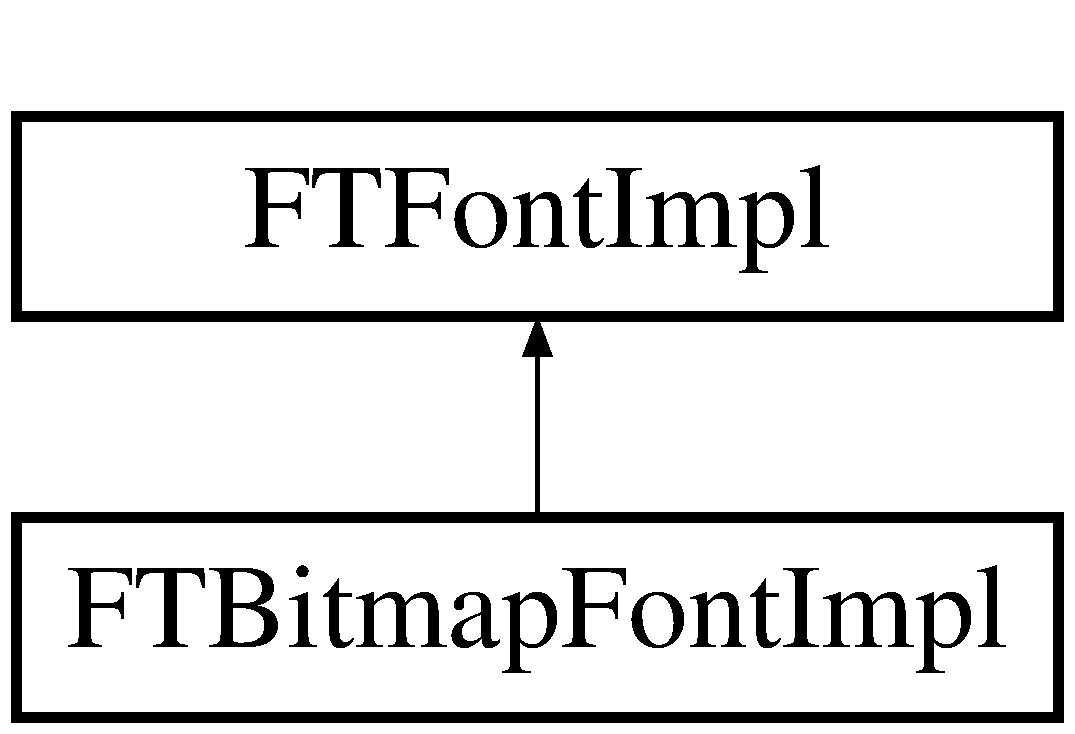
\includegraphics[height=2.000000cm]{class_f_t_bitmap_font_impl}
\end{center}
\end{figure}
\subsection*{Protected Member Functions}
\begin{DoxyCompactItemize}
\item 
\hypertarget{class_f_t_bitmap_font_impl_a8b9cc194fe4de235bca414dc0ffe0960}{{\bfseries F\-T\-Bitmap\-Font\-Impl} (F\-T\-Font $\ast$ft\-Font, const char $\ast$font\-File\-Path)}\label{class_f_t_bitmap_font_impl_a8b9cc194fe4de235bca414dc0ffe0960}

\item 
\hypertarget{class_f_t_bitmap_font_impl_ae066b9bf998e13a225be35767c25d233}{{\bfseries F\-T\-Bitmap\-Font\-Impl} (F\-T\-Font $\ast$ft\-Font, const unsigned char $\ast$p\-Buffer\-Bytes, size\-\_\-t buffer\-Size\-In\-Bytes)}\label{class_f_t_bitmap_font_impl_ae066b9bf998e13a225be35767c25d233}

\item 
\hypertarget{class_f_t_bitmap_font_impl_abfea575dee2b6436bd8522be490f5715}{virtual F\-T\-Point {\bfseries Render} (const char $\ast$s, const int len, F\-T\-Point position, F\-T\-Point spacing, int render\-Mode)}\label{class_f_t_bitmap_font_impl_abfea575dee2b6436bd8522be490f5715}

\item 
\hypertarget{class_f_t_bitmap_font_impl_aee25e8971e53c7f2f2946abe87a51161}{virtual F\-T\-Point {\bfseries Render} (const wchar\-\_\-t $\ast$s, const int len, F\-T\-Point position, F\-T\-Point spacing, int render\-Mode)}\label{class_f_t_bitmap_font_impl_aee25e8971e53c7f2f2946abe87a51161}

\end{DoxyCompactItemize}
\subsection*{Friends}
\begin{DoxyCompactItemize}
\item 
\hypertarget{class_f_t_bitmap_font_impl_a7ba5a198d501799828a37b4b808b9352}{class {\bfseries F\-T\-Bitmap\-Font}}\label{class_f_t_bitmap_font_impl_a7ba5a198d501799828a37b4b808b9352}

\end{DoxyCompactItemize}
\subsection*{Additional Inherited Members}


The documentation for this class was generated from the following files\-:\begin{DoxyCompactItemize}
\item 
X\-:/\-Git\-\_\-\-Repository/inf2990-\/06/\-Cadriciel/\-Commun/\-Externe/\-F\-T\-G\-L/include/\-F\-T\-Font/F\-T\-Bitmap\-Font\-Impl.\-h\item 
X\-:/\-Git\-\_\-\-Repository/inf2990-\/06/\-Cadriciel/\-Commun/\-Externe/\-F\-T\-G\-L/include/\-F\-T\-Font/F\-T\-Bitmap\-Font.\-cpp\end{DoxyCompactItemize}

\hypertarget{class_f_t_bitmap_glyph_impl}{\section{F\-T\-Bitmap\-Glyph\-Impl Class Reference}
\label{class_f_t_bitmap_glyph_impl}\index{F\-T\-Bitmap\-Glyph\-Impl@{F\-T\-Bitmap\-Glyph\-Impl}}
}
Inheritance diagram for F\-T\-Bitmap\-Glyph\-Impl\-:\begin{figure}[H]
\begin{center}
\leavevmode
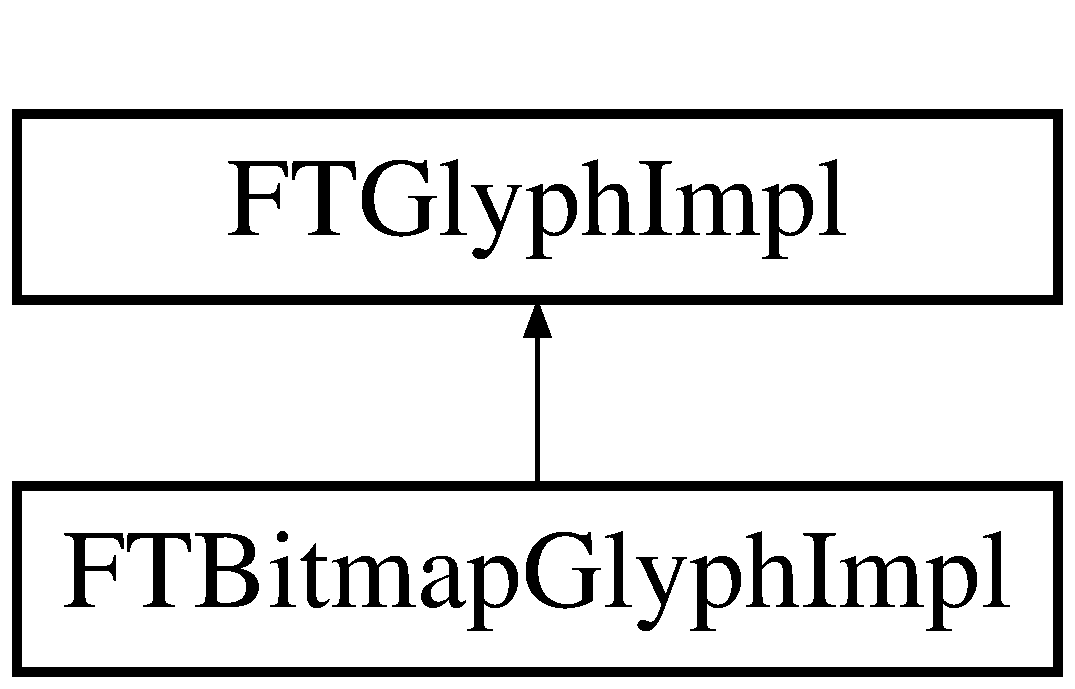
\includegraphics[height=2.000000cm]{class_f_t_bitmap_glyph_impl}
\end{center}
\end{figure}
\subsection*{Protected Member Functions}
\begin{DoxyCompactItemize}
\item 
\hypertarget{class_f_t_bitmap_glyph_impl_a4462585cd1fc2e461ff8c6a0b49c68b3}{{\bfseries F\-T\-Bitmap\-Glyph\-Impl} (\hyperlink{struct_f_t___glyph_slot_rec__}{F\-T\-\_\-\-Glyph\-Slot} glyph)}\label{class_f_t_bitmap_glyph_impl_a4462585cd1fc2e461ff8c6a0b49c68b3}

\item 
\hypertarget{class_f_t_bitmap_glyph_impl_a31a412b09a68489ab2e96ad4524badde}{virtual const F\-T\-Point \& {\bfseries Render\-Impl} (const F\-T\-Point \&pen, int render\-Mode)}\label{class_f_t_bitmap_glyph_impl_a31a412b09a68489ab2e96ad4524badde}

\end{DoxyCompactItemize}
\subsection*{Friends}
\begin{DoxyCompactItemize}
\item 
\hypertarget{class_f_t_bitmap_glyph_impl_aa3f0c28a7cfbfa0e896973476f7ed49d}{class {\bfseries F\-T\-Bitmap\-Glyph}}\label{class_f_t_bitmap_glyph_impl_aa3f0c28a7cfbfa0e896973476f7ed49d}

\end{DoxyCompactItemize}
\subsection*{Additional Inherited Members}


The documentation for this class was generated from the following files\-:\begin{DoxyCompactItemize}
\item 
X\-:/\-Git\-\_\-\-Repository/inf2990-\/06/\-Cadriciel/\-Commun/\-Externe/\-F\-T\-G\-L/include/\-F\-T\-Glyph/F\-T\-Bitmap\-Glyph\-Impl.\-h\item 
X\-:/\-Git\-\_\-\-Repository/inf2990-\/06/\-Cadriciel/\-Commun/\-Externe/\-F\-T\-G\-L/include/\-F\-T\-Glyph/F\-T\-Bitmap\-Glyph.\-cpp\end{DoxyCompactItemize}

\hypertarget{class_f_t_buffer_font_impl}{\section{F\-T\-Buffer\-Font\-Impl Class Reference}
\label{class_f_t_buffer_font_impl}\index{F\-T\-Buffer\-Font\-Impl@{F\-T\-Buffer\-Font\-Impl}}
}
Inheritance diagram for F\-T\-Buffer\-Font\-Impl\-:\begin{figure}[H]
\begin{center}
\leavevmode
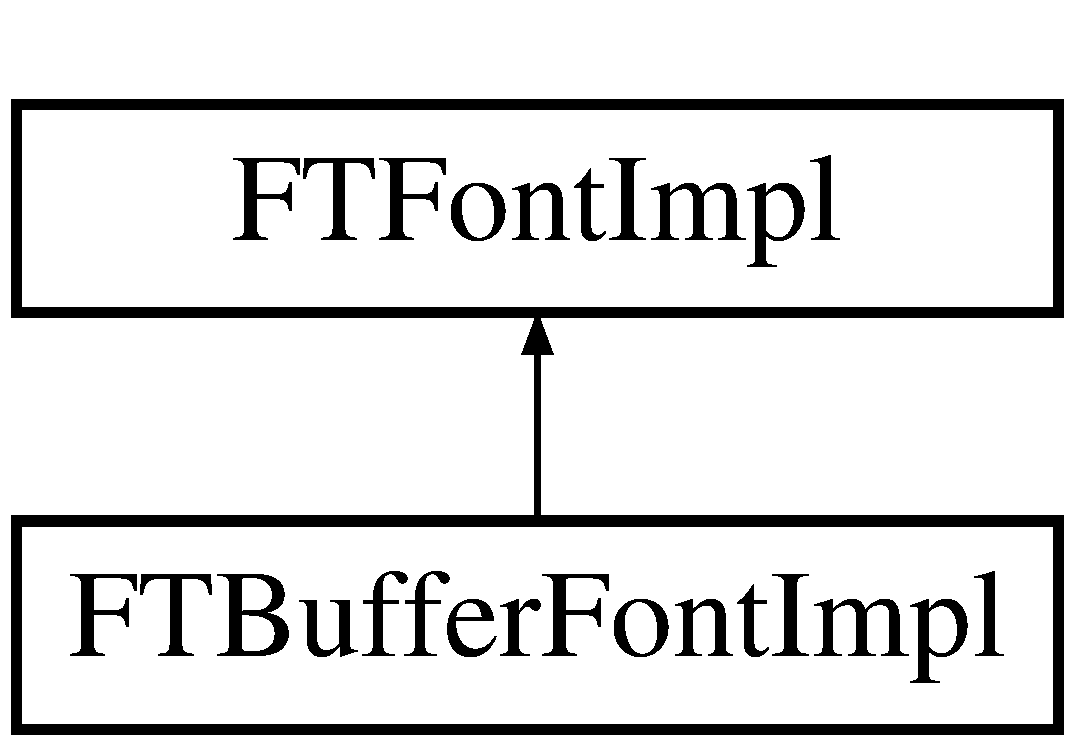
\includegraphics[height=2.000000cm]{class_f_t_buffer_font_impl}
\end{center}
\end{figure}
\subsection*{Protected Member Functions}
\begin{DoxyCompactItemize}
\item 
\hypertarget{class_f_t_buffer_font_impl_a968353f8f7e3fb37c0b1facd70599568}{{\bfseries F\-T\-Buffer\-Font\-Impl} (F\-T\-Font $\ast$ft\-Font, const char $\ast$font\-File\-Path)}\label{class_f_t_buffer_font_impl_a968353f8f7e3fb37c0b1facd70599568}

\item 
\hypertarget{class_f_t_buffer_font_impl_a789d9507754a9e179d200fcf93690081}{{\bfseries F\-T\-Buffer\-Font\-Impl} (F\-T\-Font $\ast$ft\-Font, const unsigned char $\ast$p\-Buffer\-Bytes, size\-\_\-t buffer\-Size\-In\-Bytes)}\label{class_f_t_buffer_font_impl_a789d9507754a9e179d200fcf93690081}

\item 
\hypertarget{class_f_t_buffer_font_impl_a82fccb46df5d5b17f654d23773faa8ae}{virtual F\-T\-Point {\bfseries Render} (const char $\ast$s, const int len, F\-T\-Point position, F\-T\-Point spacing, int render\-Mode)}\label{class_f_t_buffer_font_impl_a82fccb46df5d5b17f654d23773faa8ae}

\item 
\hypertarget{class_f_t_buffer_font_impl_ad56722bcd6030ee1cae56c307b254ec1}{virtual F\-T\-Point {\bfseries Render} (const wchar\-\_\-t $\ast$s, const int len, F\-T\-Point position, F\-T\-Point spacing, int render\-Mode)}\label{class_f_t_buffer_font_impl_ad56722bcd6030ee1cae56c307b254ec1}

\item 
\hypertarget{class_f_t_buffer_font_impl_a4bd13aeb53fc5585d91546095c389868}{virtual bool {\bfseries Face\-Size} (const unsigned int size, const unsigned int res)}\label{class_f_t_buffer_font_impl_a4bd13aeb53fc5585d91546095c389868}

\end{DoxyCompactItemize}
\subsection*{Friends}
\begin{DoxyCompactItemize}
\item 
\hypertarget{class_f_t_buffer_font_impl_ab7dc21f40be33fee50c41b3ba3d49c73}{class {\bfseries F\-T\-Buffer\-Font}}\label{class_f_t_buffer_font_impl_ab7dc21f40be33fee50c41b3ba3d49c73}

\end{DoxyCompactItemize}
\subsection*{Additional Inherited Members}


The documentation for this class was generated from the following files\-:\begin{DoxyCompactItemize}
\item 
X\-:/\-Git\-\_\-\-Repository/inf2990-\/06/\-Cadriciel/\-Commun/\-Externe/\-F\-T\-G\-L/include/\-F\-T\-Font/F\-T\-Buffer\-Font\-Impl.\-h\item 
X\-:/\-Git\-\_\-\-Repository/inf2990-\/06/\-Cadriciel/\-Commun/\-Externe/\-F\-T\-G\-L/include/\-F\-T\-Font/F\-T\-Buffer\-Font.\-cpp\end{DoxyCompactItemize}

\hypertarget{class_f_t_buffer_glyph_impl}{\section{F\-T\-Buffer\-Glyph\-Impl Class Reference}
\label{class_f_t_buffer_glyph_impl}\index{F\-T\-Buffer\-Glyph\-Impl@{F\-T\-Buffer\-Glyph\-Impl}}
}
Inheritance diagram for F\-T\-Buffer\-Glyph\-Impl\-:\begin{figure}[H]
\begin{center}
\leavevmode
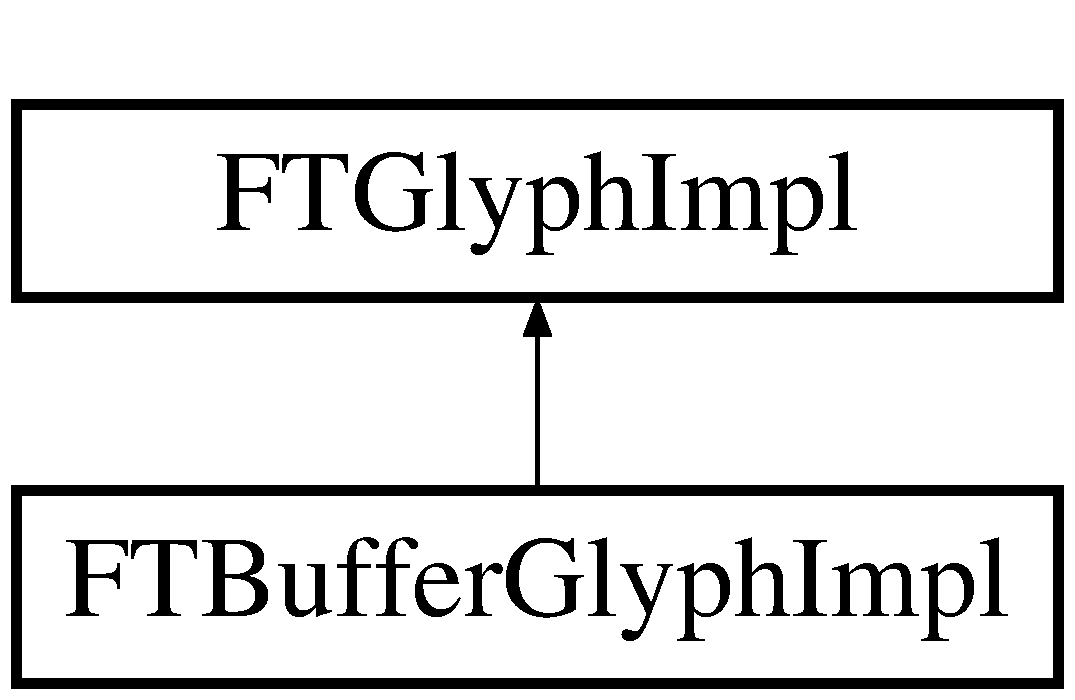
\includegraphics[height=2.000000cm]{class_f_t_buffer_glyph_impl}
\end{center}
\end{figure}
\subsection*{Protected Member Functions}
\begin{DoxyCompactItemize}
\item 
\hypertarget{class_f_t_buffer_glyph_impl_a02a187494995d95792ef66767f04c56d}{{\bfseries F\-T\-Buffer\-Glyph\-Impl} (\hyperlink{struct_f_t___glyph_slot_rec__}{F\-T\-\_\-\-Glyph\-Slot} glyph, F\-T\-Buffer $\ast$p)}\label{class_f_t_buffer_glyph_impl_a02a187494995d95792ef66767f04c56d}

\item 
\hypertarget{class_f_t_buffer_glyph_impl_a4f7f56caf34309cf7e1408a631b419de}{virtual const F\-T\-Point \& {\bfseries Render\-Impl} (const F\-T\-Point \&pen, int render\-Mode)}\label{class_f_t_buffer_glyph_impl_a4f7f56caf34309cf7e1408a631b419de}

\end{DoxyCompactItemize}
\subsection*{Friends}
\begin{DoxyCompactItemize}
\item 
\hypertarget{class_f_t_buffer_glyph_impl_a385e2288042fd77f037a715e7801b451}{class {\bfseries F\-T\-Buffer\-Glyph}}\label{class_f_t_buffer_glyph_impl_a385e2288042fd77f037a715e7801b451}

\end{DoxyCompactItemize}
\subsection*{Additional Inherited Members}


The documentation for this class was generated from the following files\-:\begin{DoxyCompactItemize}
\item 
X\-:/\-Git\-\_\-\-Repository/inf2990-\/06/\-Cadriciel/\-Commun/\-Externe/\-F\-T\-G\-L/include/\-F\-T\-Glyph/F\-T\-Buffer\-Glyph\-Impl.\-h\item 
X\-:/\-Git\-\_\-\-Repository/inf2990-\/06/\-Cadriciel/\-Commun/\-Externe/\-F\-T\-G\-L/include/\-F\-T\-Glyph/F\-T\-Buffer\-Glyph.\-cpp\end{DoxyCompactItemize}

\hypertarget{struct_f_t_c___image_type_rec__}{\section{F\-T\-C\-\_\-\-Image\-Type\-Rec\-\_\- Struct Reference}
\label{struct_f_t_c___image_type_rec__}\index{F\-T\-C\-\_\-\-Image\-Type\-Rec\-\_\-@{F\-T\-C\-\_\-\-Image\-Type\-Rec\-\_\-}}
}
\subsection*{Public Attributes}
\begin{DoxyCompactItemize}
\item 
\hypertarget{struct_f_t_c___image_type_rec___a9851b8d4a06baacd18d5b9856fd85abd}{F\-T\-C\-\_\-\-Face\-I\-D {\bfseries face\-\_\-id}}\label{struct_f_t_c___image_type_rec___a9851b8d4a06baacd18d5b9856fd85abd}

\item 
\hypertarget{struct_f_t_c___image_type_rec___af1a4cccbabb0f5852ed755a12ed08dd8}{F\-T\-\_\-\-Int {\bfseries width}}\label{struct_f_t_c___image_type_rec___af1a4cccbabb0f5852ed755a12ed08dd8}

\item 
\hypertarget{struct_f_t_c___image_type_rec___adb56a9d18a3f522d713d0ba01c1a8778}{F\-T\-\_\-\-Int {\bfseries height}}\label{struct_f_t_c___image_type_rec___adb56a9d18a3f522d713d0ba01c1a8778}

\item 
\hypertarget{struct_f_t_c___image_type_rec___a391782ed8c67de86591c71f276ea6454}{F\-T\-\_\-\-Int32 {\bfseries flags}}\label{struct_f_t_c___image_type_rec___a391782ed8c67de86591c71f276ea6454}

\end{DoxyCompactItemize}


The documentation for this struct was generated from the following file\-:\begin{DoxyCompactItemize}
\item 
X\-:/\-Git\-\_\-\-Repository/inf2990-\/06/\-Cadriciel/\-Commun/\-Externe/\-Free\-Type/include/freetype/ftcache.\-h\end{DoxyCompactItemize}

\hypertarget{struct_f_t_c___s_bit_rec__}{\section{F\-T\-C\-\_\-\-S\-Bit\-Rec\-\_\- Struct Reference}
\label{struct_f_t_c___s_bit_rec__}\index{F\-T\-C\-\_\-\-S\-Bit\-Rec\-\_\-@{F\-T\-C\-\_\-\-S\-Bit\-Rec\-\_\-}}
}
\subsection*{Public Attributes}
\begin{DoxyCompactItemize}
\item 
\hypertarget{struct_f_t_c___s_bit_rec___a5b92fb4f213a880f758bb87ac2ceb263}{F\-T\-\_\-\-Byte {\bfseries width}}\label{struct_f_t_c___s_bit_rec___a5b92fb4f213a880f758bb87ac2ceb263}

\item 
\hypertarget{struct_f_t_c___s_bit_rec___a5953efe2aded3b184875d5e5d08cafef}{F\-T\-\_\-\-Byte {\bfseries height}}\label{struct_f_t_c___s_bit_rec___a5953efe2aded3b184875d5e5d08cafef}

\item 
\hypertarget{struct_f_t_c___s_bit_rec___aef273749f4fdb9943500ec6df8412a94}{F\-T\-\_\-\-Char {\bfseries left}}\label{struct_f_t_c___s_bit_rec___aef273749f4fdb9943500ec6df8412a94}

\item 
\hypertarget{struct_f_t_c___s_bit_rec___a3e558b3a04b70f00f80b862cdc94d9a2}{F\-T\-\_\-\-Char {\bfseries top}}\label{struct_f_t_c___s_bit_rec___a3e558b3a04b70f00f80b862cdc94d9a2}

\item 
\hypertarget{struct_f_t_c___s_bit_rec___a3d3fcc2869ce5c95f0f63898e6cef8be}{F\-T\-\_\-\-Byte {\bfseries format}}\label{struct_f_t_c___s_bit_rec___a3d3fcc2869ce5c95f0f63898e6cef8be}

\item 
\hypertarget{struct_f_t_c___s_bit_rec___a83958d4649a898312de9a7274550dff9}{F\-T\-\_\-\-Byte {\bfseries max\-\_\-grays}}\label{struct_f_t_c___s_bit_rec___a83958d4649a898312de9a7274550dff9}

\item 
\hypertarget{struct_f_t_c___s_bit_rec___a1382ec014df599e706c2c1785bc18235}{F\-T\-\_\-\-Short {\bfseries pitch}}\label{struct_f_t_c___s_bit_rec___a1382ec014df599e706c2c1785bc18235}

\item 
\hypertarget{struct_f_t_c___s_bit_rec___a502a0bb69d973d2ae626a842eb9fefd3}{F\-T\-\_\-\-Char {\bfseries xadvance}}\label{struct_f_t_c___s_bit_rec___a502a0bb69d973d2ae626a842eb9fefd3}

\item 
\hypertarget{struct_f_t_c___s_bit_rec___aabe767ddaf7ff62918886c6f62e9ac28}{F\-T\-\_\-\-Char {\bfseries yadvance}}\label{struct_f_t_c___s_bit_rec___aabe767ddaf7ff62918886c6f62e9ac28}

\item 
\hypertarget{struct_f_t_c___s_bit_rec___abe4d78fc3f411d67e7fc43f7aa21bd1d}{F\-T\-\_\-\-Byte $\ast$ {\bfseries buffer}}\label{struct_f_t_c___s_bit_rec___abe4d78fc3f411d67e7fc43f7aa21bd1d}

\end{DoxyCompactItemize}


The documentation for this struct was generated from the following file\-:\begin{DoxyCompactItemize}
\item 
X\-:/\-Git\-\_\-\-Repository/inf2990-\/06/\-Cadriciel/\-Commun/\-Externe/\-Free\-Type/include/freetype/ftcache.\-h\end{DoxyCompactItemize}

\hypertarget{struct_f_t_c___scaler_rec__}{\section{F\-T\-C\-\_\-\-Scaler\-Rec\-\_\- Struct Reference}
\label{struct_f_t_c___scaler_rec__}\index{F\-T\-C\-\_\-\-Scaler\-Rec\-\_\-@{F\-T\-C\-\_\-\-Scaler\-Rec\-\_\-}}
}
\subsection*{Public Attributes}
\begin{DoxyCompactItemize}
\item 
\hypertarget{struct_f_t_c___scaler_rec___a8e963aa619409e646558fe7aa272e81f}{F\-T\-C\-\_\-\-Face\-I\-D {\bfseries face\-\_\-id}}\label{struct_f_t_c___scaler_rec___a8e963aa619409e646558fe7aa272e81f}

\item 
\hypertarget{struct_f_t_c___scaler_rec___a11e13d907ca4661bf7c1d98fffecf321}{F\-T\-\_\-\-U\-Int {\bfseries width}}\label{struct_f_t_c___scaler_rec___a11e13d907ca4661bf7c1d98fffecf321}

\item 
\hypertarget{struct_f_t_c___scaler_rec___a9b3a9b4d7148bbaa4daaae1e1fbb2dbc}{F\-T\-\_\-\-U\-Int {\bfseries height}}\label{struct_f_t_c___scaler_rec___a9b3a9b4d7148bbaa4daaae1e1fbb2dbc}

\item 
\hypertarget{struct_f_t_c___scaler_rec___ab78868341e2d66f17e6f1d77e9e054d2}{F\-T\-\_\-\-Int {\bfseries pixel}}\label{struct_f_t_c___scaler_rec___ab78868341e2d66f17e6f1d77e9e054d2}

\item 
\hypertarget{struct_f_t_c___scaler_rec___a886c7c1230dc5d5e6b3fc32d06274752}{F\-T\-\_\-\-U\-Int {\bfseries x\-\_\-res}}\label{struct_f_t_c___scaler_rec___a886c7c1230dc5d5e6b3fc32d06274752}

\item 
\hypertarget{struct_f_t_c___scaler_rec___accb53c7a9aeebb41c05f48d14d3dfe71}{F\-T\-\_\-\-U\-Int {\bfseries y\-\_\-res}}\label{struct_f_t_c___scaler_rec___accb53c7a9aeebb41c05f48d14d3dfe71}

\end{DoxyCompactItemize}


The documentation for this struct was generated from the following file\-:\begin{DoxyCompactItemize}
\item 
X\-:/\-Git\-\_\-\-Repository/inf2990-\/06/\-Cadriciel/\-Commun/\-Externe/\-Free\-Type/include/freetype/ftcache.\-h\end{DoxyCompactItemize}

\hypertarget{class_f_t_charmap}{\section{F\-T\-Charmap Class Reference}
\label{class_f_t_charmap}\index{F\-T\-Charmap@{F\-T\-Charmap}}
}
\subsection*{Public Member Functions}
\begin{DoxyCompactItemize}
\item 
\hyperlink{class_f_t_charmap_a9d19837becbc83acf7f56a5980b2b644}{F\-T\-Charmap} (\hyperlink{class_f_t_face}{F\-T\-Face} $\ast$face)
\item 
virtual \hyperlink{class_f_t_charmap_afcbe1e49ed38810e8b9c2e116ddbbffc}{$\sim$\-F\-T\-Charmap} ()
\item 
F\-T\-\_\-\-Encoding \hyperlink{class_f_t_charmap_a4c119ad30110e00b6b3944288a702c84}{Encoding} () const 
\item 
bool \hyperlink{class_f_t_charmap_a4d182b0faeb7198b4f583b84eaf4cd55}{Char\-Map} (F\-T\-\_\-\-Encoding encoding)
\item 
unsigned int \hyperlink{class_f_t_charmap_a6084cc8ab267b9974980e14f17227f25}{Glyph\-List\-Index} (const unsigned int character\-Code)
\item 
unsigned int \hyperlink{class_f_t_charmap_ab77d9f06a9109608b1734010acecaefd}{Font\-Index} (const unsigned int character\-Code)
\item 
void \hyperlink{class_f_t_charmap_a374e41b6f8b07efb08e5c173cc707354}{Insert\-Index} (const unsigned int character\-Code, const size\-\_\-t container\-Index)
\item 
F\-T\-\_\-\-Error \hyperlink{class_f_t_charmap_a176e217e3e837db5fc4592ceff5ed488}{Error} () const 
\end{DoxyCompactItemize}


\subsection{Constructor \& Destructor Documentation}
\hypertarget{class_f_t_charmap_a9d19837becbc83acf7f56a5980b2b644}{\index{F\-T\-Charmap@{F\-T\-Charmap}!F\-T\-Charmap@{F\-T\-Charmap}}
\index{F\-T\-Charmap@{F\-T\-Charmap}!FTCharmap@{F\-T\-Charmap}}
\subsubsection[{F\-T\-Charmap}]{\setlength{\rightskip}{0pt plus 5cm}F\-T\-Charmap\-::\-F\-T\-Charmap (
\begin{DoxyParamCaption}
\item[{{\bf F\-T\-Face} $\ast$}]{face}
\end{DoxyParamCaption}
)}}\label{class_f_t_charmap_a9d19837becbc83acf7f56a5980b2b644}
Constructor \hypertarget{class_f_t_charmap_afcbe1e49ed38810e8b9c2e116ddbbffc}{\index{F\-T\-Charmap@{F\-T\-Charmap}!$\sim$\-F\-T\-Charmap@{$\sim$\-F\-T\-Charmap}}
\index{$\sim$\-F\-T\-Charmap@{$\sim$\-F\-T\-Charmap}!FTCharmap@{F\-T\-Charmap}}
\subsubsection[{$\sim$\-F\-T\-Charmap}]{\setlength{\rightskip}{0pt plus 5cm}F\-T\-Charmap\-::$\sim$\-F\-T\-Charmap (
\begin{DoxyParamCaption}
{}
\end{DoxyParamCaption}
)\hspace{0.3cm}{\ttfamily [virtual]}}}\label{class_f_t_charmap_afcbe1e49ed38810e8b9c2e116ddbbffc}
Destructor 

\subsection{Member Function Documentation}
\hypertarget{class_f_t_charmap_a4d182b0faeb7198b4f583b84eaf4cd55}{\index{F\-T\-Charmap@{F\-T\-Charmap}!Char\-Map@{Char\-Map}}
\index{Char\-Map@{Char\-Map}!FTCharmap@{F\-T\-Charmap}}
\subsubsection[{Char\-Map}]{\setlength{\rightskip}{0pt plus 5cm}bool F\-T\-Charmap\-::\-Char\-Map (
\begin{DoxyParamCaption}
\item[{F\-T\-\_\-\-Encoding}]{encoding}
\end{DoxyParamCaption}
)}}\label{class_f_t_charmap_a4d182b0faeb7198b4f583b84eaf4cd55}
Sets the character map for the face. If an error occurs the object is not modified. Valid encodings as at Freetype 2.\-0.\-4 ft\-\_\-encoding\-\_\-none ft\-\_\-encoding\-\_\-symbol ft\-\_\-encoding\-\_\-unicode ft\-\_\-encoding\-\_\-latin\-\_\-2 ft\-\_\-encoding\-\_\-sjis ft\-\_\-encoding\-\_\-gb2312 ft\-\_\-encoding\-\_\-big5 ft\-\_\-encoding\-\_\-wansung ft\-\_\-encoding\-\_\-johab ft\-\_\-encoding\-\_\-adobe\-\_\-standard ft\-\_\-encoding\-\_\-adobe\-\_\-expert ft\-\_\-encoding\-\_\-adobe\-\_\-custom ft\-\_\-encoding\-\_\-apple\-\_\-roman


\begin{DoxyParams}{Parameters}
{\em encoding} & the Freetype encoding symbol. See above. \\
\hline
\end{DoxyParams}
\begin{DoxyReturn}{Returns}
{\ttfamily true} if charmap was valid and set correctly. 
\end{DoxyReturn}
\hypertarget{class_f_t_charmap_a4c119ad30110e00b6b3944288a702c84}{\index{F\-T\-Charmap@{F\-T\-Charmap}!Encoding@{Encoding}}
\index{Encoding@{Encoding}!FTCharmap@{F\-T\-Charmap}}
\subsubsection[{Encoding}]{\setlength{\rightskip}{0pt plus 5cm}F\-T\-\_\-\-Encoding F\-T\-Charmap\-::\-Encoding (
\begin{DoxyParamCaption}
{}
\end{DoxyParamCaption}
) const\hspace{0.3cm}{\ttfamily [inline]}}}\label{class_f_t_charmap_a4c119ad30110e00b6b3944288a702c84}
Queries for the current character map code.

\begin{DoxyReturn}{Returns}
The current character map code. 
\end{DoxyReturn}
\hypertarget{class_f_t_charmap_a176e217e3e837db5fc4592ceff5ed488}{\index{F\-T\-Charmap@{F\-T\-Charmap}!Error@{Error}}
\index{Error@{Error}!FTCharmap@{F\-T\-Charmap}}
\subsubsection[{Error}]{\setlength{\rightskip}{0pt plus 5cm}F\-T\-\_\-\-Error F\-T\-Charmap\-::\-Error (
\begin{DoxyParamCaption}
{}
\end{DoxyParamCaption}
) const\hspace{0.3cm}{\ttfamily [inline]}}}\label{class_f_t_charmap_a176e217e3e837db5fc4592ceff5ed488}
Queries for errors.

\begin{DoxyReturn}{Returns}
The current error code. Zero means no error. 
\end{DoxyReturn}
\hypertarget{class_f_t_charmap_ab77d9f06a9109608b1734010acecaefd}{\index{F\-T\-Charmap@{F\-T\-Charmap}!Font\-Index@{Font\-Index}}
\index{Font\-Index@{Font\-Index}!FTCharmap@{F\-T\-Charmap}}
\subsubsection[{Font\-Index}]{\setlength{\rightskip}{0pt plus 5cm}unsigned int F\-T\-Charmap\-::\-Font\-Index (
\begin{DoxyParamCaption}
\item[{const unsigned int}]{character\-Code}
\end{DoxyParamCaption}
)}}\label{class_f_t_charmap_ab77d9f06a9109608b1734010acecaefd}
Get the font glyph index of the input character.


\begin{DoxyParams}{Parameters}
{\em character\-Code} & The character code of the requested glyph in the current encoding eg apple roman. \\
\hline
\end{DoxyParams}
\begin{DoxyReturn}{Returns}
The glyph index for the character. 
\end{DoxyReturn}
\hypertarget{class_f_t_charmap_a6084cc8ab267b9974980e14f17227f25}{\index{F\-T\-Charmap@{F\-T\-Charmap}!Glyph\-List\-Index@{Glyph\-List\-Index}}
\index{Glyph\-List\-Index@{Glyph\-List\-Index}!FTCharmap@{F\-T\-Charmap}}
\subsubsection[{Glyph\-List\-Index}]{\setlength{\rightskip}{0pt plus 5cm}unsigned int F\-T\-Charmap\-::\-Glyph\-List\-Index (
\begin{DoxyParamCaption}
\item[{const unsigned int}]{character\-Code}
\end{DoxyParamCaption}
)}}\label{class_f_t_charmap_a6084cc8ab267b9974980e14f17227f25}
Get the \hyperlink{class_f_t_glyph_container}{F\-T\-Glyph\-Container} index of the input character.


\begin{DoxyParams}{Parameters}
{\em character\-Code} & The character code of the requested glyph in the current encoding eg apple roman. \\
\hline
\end{DoxyParams}
\begin{DoxyReturn}{Returns}
The \hyperlink{class_f_t_glyph_container}{F\-T\-Glyph\-Container} index for the character or zero if it wasn't found 
\end{DoxyReturn}
\hypertarget{class_f_t_charmap_a374e41b6f8b07efb08e5c173cc707354}{\index{F\-T\-Charmap@{F\-T\-Charmap}!Insert\-Index@{Insert\-Index}}
\index{Insert\-Index@{Insert\-Index}!FTCharmap@{F\-T\-Charmap}}
\subsubsection[{Insert\-Index}]{\setlength{\rightskip}{0pt plus 5cm}void F\-T\-Charmap\-::\-Insert\-Index (
\begin{DoxyParamCaption}
\item[{const unsigned int}]{character\-Code, }
\item[{const size\-\_\-t}]{container\-Index}
\end{DoxyParamCaption}
)}}\label{class_f_t_charmap_a374e41b6f8b07efb08e5c173cc707354}
Set the \hyperlink{class_f_t_glyph_container}{F\-T\-Glyph\-Container} index of the character code.


\begin{DoxyParams}{Parameters}
{\em character\-Code} & The character code of the requested glyph in the current encoding eg apple roman. \\
\hline
{\em container\-Index} & The index into the \hyperlink{class_f_t_glyph_container}{F\-T\-Glyph\-Container} of the character code. \\
\hline
\end{DoxyParams}


The documentation for this class was generated from the following files\-:\begin{DoxyCompactItemize}
\item 
X\-:/\-Git\-\_\-\-Repository/inf2990-\/06/\-Cadriciel/\-Commun/\-Externe/\-F\-T\-G\-L/include/F\-T\-Charmap.\-h\item 
X\-:/\-Git\-\_\-\-Repository/inf2990-\/06/\-Cadriciel/\-Commun/\-Externe/\-F\-T\-G\-L/include/F\-T\-Charmap.\-cpp\end{DoxyCompactItemize}

\hypertarget{class_f_t_char_to_glyph_index_map}{\section{F\-T\-Char\-To\-Glyph\-Index\-Map Class Reference}
\label{class_f_t_char_to_glyph_index_map}\index{F\-T\-Char\-To\-Glyph\-Index\-Map@{F\-T\-Char\-To\-Glyph\-Index\-Map}}
}


{\ttfamily \#include $<$F\-T\-Char\-To\-Glyph\-Index\-Map.\-h$>$}

\subsection*{Public Types}
\begin{DoxyCompactItemize}
\item 
enum \{ {\bfseries Number\-Of\-Buckets} = 256, 
{\bfseries Bucket\-Size} = 256, 
{\bfseries Index\-Not\-Found} = -\/1
 \}
\item 
\hypertarget{class_f_t_char_to_glyph_index_map_a0c3d673d5c3e978b7c04ea367f82e624}{typedef unsigned long {\bfseries Character\-Code}}\label{class_f_t_char_to_glyph_index_map_a0c3d673d5c3e978b7c04ea367f82e624}

\item 
\hypertarget{class_f_t_char_to_glyph_index_map_a54a7eca7f7b06f9389c12ab96db36a25}{typedef signed long {\bfseries Glyph\-Index}}\label{class_f_t_char_to_glyph_index_map_a54a7eca7f7b06f9389c12ab96db36a25}

\end{DoxyCompactItemize}
\subsection*{Public Member Functions}
\begin{DoxyCompactItemize}
\item 
\hypertarget{class_f_t_char_to_glyph_index_map_adc045f0ce5b32fa84681d63e35ac7369}{void {\bfseries clear} ()}\label{class_f_t_char_to_glyph_index_map_adc045f0ce5b32fa84681d63e35ac7369}

\item 
\hypertarget{class_f_t_char_to_glyph_index_map_a94a2e63c8689298ac8dffdc90f290bb2}{const Glyph\-Index {\bfseries find} (Character\-Code c)}\label{class_f_t_char_to_glyph_index_map_a94a2e63c8689298ac8dffdc90f290bb2}

\item 
\hypertarget{class_f_t_char_to_glyph_index_map_aa5ee6e5371094dfa05fa69145c33547f}{void {\bfseries insert} (Character\-Code c, Glyph\-Index g)}\label{class_f_t_char_to_glyph_index_map_aa5ee6e5371094dfa05fa69145c33547f}

\end{DoxyCompactItemize}


\subsection{Detailed Description}
Provides a non-\/\-S\-T\-L alternative to the S\-T\-L map$<$unsigned long, unsigned long$>$ which maps character codes to glyph indices inside \hyperlink{class_f_t_charmap}{F\-T\-Charmap}.

Implementation\-:
\begin{DoxyItemize}
\item Number\-Of\-Buckets buckets are considered.
\item Each bucket has Bucket\-Size entries.
\item When the glyph index for the character code C has to be stored, the bucket this character belongs to is found using 'C div Bucket\-Size'. If this bucket has not been allocated yet, do it now. The entry in the bucked is found using 'C mod Bucket\-Size'. If it is set to Index\-Not\-Found, then the glyph entry has not been set.
\item Try to mimic the calls made to the S\-T\-L map A\-P\-I.
\end{DoxyItemize}

Caveats\-:
\begin{DoxyItemize}
\item The glyph index is now a signed long instead of unsigned long, so the special value Index\-Not\-Found (= -\/1) can be used to specify that the glyph index has not been stored yet. 
\end{DoxyItemize}

The documentation for this class was generated from the following file\-:\begin{DoxyCompactItemize}
\item 
X\-:/\-Git\-\_\-\-Repository/inf2990-\/06/\-Cadriciel/\-Commun/\-Externe/\-F\-T\-G\-L/include/F\-T\-Char\-To\-Glyph\-Index\-Map.\-h\end{DoxyCompactItemize}

\hypertarget{class_f_t_contour}{\section{F\-T\-Contour Class Reference}
\label{class_f_t_contour}\index{F\-T\-Contour@{F\-T\-Contour}}
}


{\ttfamily \#include $<$F\-T\-Contour.\-h$>$}

\subsection*{Public Member Functions}
\begin{DoxyCompactItemize}
\item 
\hyperlink{class_f_t_contour_a1a682c070617bf9023ea38c65b32ade3}{F\-T\-Contour} (\hyperlink{struct_f_t___vector__}{F\-T\-\_\-\-Vector} $\ast$contour, char $\ast$point\-Tags, unsigned int number\-Of\-Points)
\item 
\hyperlink{class_f_t_contour_a89ac638fc2bbe641d730af84bf13b242}{$\sim$\-F\-T\-Contour} ()
\item 
const F\-T\-Point \& \hyperlink{class_f_t_contour_a055f10124231687d7647d56ee6b680ef}{Point} (size\-\_\-t index) const 
\item 
const F\-T\-Point \& \hyperlink{class_f_t_contour_a5b720df9b54e3564d762a6fe8eee3143}{Outset} (size\-\_\-t index) const 
\item 
const F\-T\-Point \& \hyperlink{class_f_t_contour_a89f7120855b97ae91c63d13cd22f3e04}{Front\-Point} (size\-\_\-t index) const 
\item 
const F\-T\-Point \& \hyperlink{class_f_t_contour_add4587cac25790725e704fdd7e9fa9fe}{Back\-Point} (size\-\_\-t index) const 
\item 
size\-\_\-t \hyperlink{class_f_t_contour_ab31ce24e66d9534b5e0b052b0b6f408b}{Point\-Count} () const 
\item 
void \hyperlink{class_f_t_contour_a7129afbf6bde74d5c9c46ad47bf6e049}{Set\-Parity} (int parity)
\item 
\hypertarget{class_f_t_contour_ab91b659e8de1dc915679d0152adfa38a}{void {\bfseries build\-Front\-Outset} (float outset)}\label{class_f_t_contour_ab91b659e8de1dc915679d0152adfa38a}

\item 
\hypertarget{class_f_t_contour_aff16d21542506b738c7f883b7c40b738}{void {\bfseries build\-Back\-Outset} (float outset)}\label{class_f_t_contour_aff16d21542506b738c7f883b7c40b738}

\end{DoxyCompactItemize}


\subsection{Detailed Description}
\hyperlink{class_f_t_contour}{F\-T\-Contour} class is a container of points that describe a vector font outline. It is used as a container for the output of the bezier curve evaluator in \hyperlink{class_f_t_vectoriser}{F\-T\-Vectoriser}.

\begin{DoxySeeAlso}{See Also}
F\-T\-Outline\-Glyph 

F\-T\-Polygon\-Glyph 

F\-T\-Point 
\end{DoxySeeAlso}


\subsection{Constructor \& Destructor Documentation}
\hypertarget{class_f_t_contour_a1a682c070617bf9023ea38c65b32ade3}{\index{F\-T\-Contour@{F\-T\-Contour}!F\-T\-Contour@{F\-T\-Contour}}
\index{F\-T\-Contour@{F\-T\-Contour}!FTContour@{F\-T\-Contour}}
\subsubsection[{F\-T\-Contour}]{\setlength{\rightskip}{0pt plus 5cm}F\-T\-Contour\-::\-F\-T\-Contour (
\begin{DoxyParamCaption}
\item[{{\bf F\-T\-\_\-\-Vector} $\ast$}]{contour, }
\item[{char $\ast$}]{point\-Tags, }
\item[{unsigned int}]{number\-Of\-Points}
\end{DoxyParamCaption}
)}}\label{class_f_t_contour_a1a682c070617bf9023ea38c65b32ade3}
Constructor


\begin{DoxyParams}{Parameters}
{\em contour} & \\
\hline
{\em point\-Tags} & \\
\hline
{\em number\-Of\-Points} & \\
\hline
\end{DoxyParams}
\hypertarget{class_f_t_contour_a89ac638fc2bbe641d730af84bf13b242}{\index{F\-T\-Contour@{F\-T\-Contour}!$\sim$\-F\-T\-Contour@{$\sim$\-F\-T\-Contour}}
\index{$\sim$\-F\-T\-Contour@{$\sim$\-F\-T\-Contour}!FTContour@{F\-T\-Contour}}
\subsubsection[{$\sim$\-F\-T\-Contour}]{\setlength{\rightskip}{0pt plus 5cm}F\-T\-Contour\-::$\sim$\-F\-T\-Contour (
\begin{DoxyParamCaption}
{}
\end{DoxyParamCaption}
)\hspace{0.3cm}{\ttfamily [inline]}}}\label{class_f_t_contour_a89ac638fc2bbe641d730af84bf13b242}
Destructor 

\subsection{Member Function Documentation}
\hypertarget{class_f_t_contour_add4587cac25790725e704fdd7e9fa9fe}{\index{F\-T\-Contour@{F\-T\-Contour}!Back\-Point@{Back\-Point}}
\index{Back\-Point@{Back\-Point}!FTContour@{F\-T\-Contour}}
\subsubsection[{Back\-Point}]{\setlength{\rightskip}{0pt plus 5cm}const F\-T\-Point\& F\-T\-Contour\-::\-Back\-Point (
\begin{DoxyParamCaption}
\item[{size\-\_\-t}]{index}
\end{DoxyParamCaption}
) const\hspace{0.3cm}{\ttfamily [inline]}}}\label{class_f_t_contour_add4587cac25790725e704fdd7e9fa9fe}
Return a point at index of the back outset contour.


\begin{DoxyParams}{Parameters}
{\em index} & of the point in the curve. \\
\hline
\end{DoxyParams}
\begin{DoxyReturn}{Returns}
const point reference 
\end{DoxyReturn}
\hypertarget{class_f_t_contour_a89f7120855b97ae91c63d13cd22f3e04}{\index{F\-T\-Contour@{F\-T\-Contour}!Front\-Point@{Front\-Point}}
\index{Front\-Point@{Front\-Point}!FTContour@{F\-T\-Contour}}
\subsubsection[{Front\-Point}]{\setlength{\rightskip}{0pt plus 5cm}const F\-T\-Point\& F\-T\-Contour\-::\-Front\-Point (
\begin{DoxyParamCaption}
\item[{size\-\_\-t}]{index}
\end{DoxyParamCaption}
) const\hspace{0.3cm}{\ttfamily [inline]}}}\label{class_f_t_contour_a89f7120855b97ae91c63d13cd22f3e04}
Return a point at index of the front outset contour.


\begin{DoxyParams}{Parameters}
{\em index} & of the point in the curve. \\
\hline
\end{DoxyParams}
\begin{DoxyReturn}{Returns}
const point reference 
\end{DoxyReturn}
\hypertarget{class_f_t_contour_a5b720df9b54e3564d762a6fe8eee3143}{\index{F\-T\-Contour@{F\-T\-Contour}!Outset@{Outset}}
\index{Outset@{Outset}!FTContour@{F\-T\-Contour}}
\subsubsection[{Outset}]{\setlength{\rightskip}{0pt plus 5cm}const F\-T\-Point\& F\-T\-Contour\-::\-Outset (
\begin{DoxyParamCaption}
\item[{size\-\_\-t}]{index}
\end{DoxyParamCaption}
) const\hspace{0.3cm}{\ttfamily [inline]}}}\label{class_f_t_contour_a5b720df9b54e3564d762a6fe8eee3143}
Return a point at index.


\begin{DoxyParams}{Parameters}
{\em index} & of the point in the outset curve. \\
\hline
\end{DoxyParams}
\begin{DoxyReturn}{Returns}
const point reference 
\end{DoxyReturn}
\hypertarget{class_f_t_contour_a055f10124231687d7647d56ee6b680ef}{\index{F\-T\-Contour@{F\-T\-Contour}!Point@{Point}}
\index{Point@{Point}!FTContour@{F\-T\-Contour}}
\subsubsection[{Point}]{\setlength{\rightskip}{0pt plus 5cm}const F\-T\-Point\& F\-T\-Contour\-::\-Point (
\begin{DoxyParamCaption}
\item[{size\-\_\-t}]{index}
\end{DoxyParamCaption}
) const\hspace{0.3cm}{\ttfamily [inline]}}}\label{class_f_t_contour_a055f10124231687d7647d56ee6b680ef}
Return a point at index.


\begin{DoxyParams}{Parameters}
{\em index} & of the point in the curve. \\
\hline
\end{DoxyParams}
\begin{DoxyReturn}{Returns}
const point reference 
\end{DoxyReturn}
\hypertarget{class_f_t_contour_ab31ce24e66d9534b5e0b052b0b6f408b}{\index{F\-T\-Contour@{F\-T\-Contour}!Point\-Count@{Point\-Count}}
\index{Point\-Count@{Point\-Count}!FTContour@{F\-T\-Contour}}
\subsubsection[{Point\-Count}]{\setlength{\rightskip}{0pt plus 5cm}size\-\_\-t F\-T\-Contour\-::\-Point\-Count (
\begin{DoxyParamCaption}
{}
\end{DoxyParamCaption}
) const\hspace{0.3cm}{\ttfamily [inline]}}}\label{class_f_t_contour_ab31ce24e66d9534b5e0b052b0b6f408b}
How many points define this contour

\begin{DoxyReturn}{Returns}
the number of points in this contour 
\end{DoxyReturn}
\hypertarget{class_f_t_contour_a7129afbf6bde74d5c9c46ad47bf6e049}{\index{F\-T\-Contour@{F\-T\-Contour}!Set\-Parity@{Set\-Parity}}
\index{Set\-Parity@{Set\-Parity}!FTContour@{F\-T\-Contour}}
\subsubsection[{Set\-Parity}]{\setlength{\rightskip}{0pt plus 5cm}void F\-T\-Contour\-::\-Set\-Parity (
\begin{DoxyParamCaption}
\item[{int}]{parity}
\end{DoxyParamCaption}
)}}\label{class_f_t_contour_a7129afbf6bde74d5c9c46ad47bf6e049}
Make sure the glyph has the proper parity and create the front/back outset contour.


\begin{DoxyParams}{Parameters}
{\em parity} & The contour's parity within the glyph. \\
\hline
\end{DoxyParams}


The documentation for this class was generated from the following files\-:\begin{DoxyCompactItemize}
\item 
X\-:/\-Git\-\_\-\-Repository/inf2990-\/06/\-Cadriciel/\-Commun/\-Externe/\-F\-T\-G\-L/include/F\-T\-Contour.\-h\item 
X\-:/\-Git\-\_\-\-Repository/inf2990-\/06/\-Cadriciel/\-Commun/\-Externe/\-F\-T\-G\-L/include/F\-T\-Contour.\-cpp\end{DoxyCompactItemize}

\hypertarget{class_f_t_custom_font}{\section{F\-T\-Custom\-Font Class Reference}
\label{class_f_t_custom_font}\index{F\-T\-Custom\-Font@{F\-T\-Custom\-Font}}
}
Inheritance diagram for F\-T\-Custom\-Font\-:\begin{figure}[H]
\begin{center}
\leavevmode
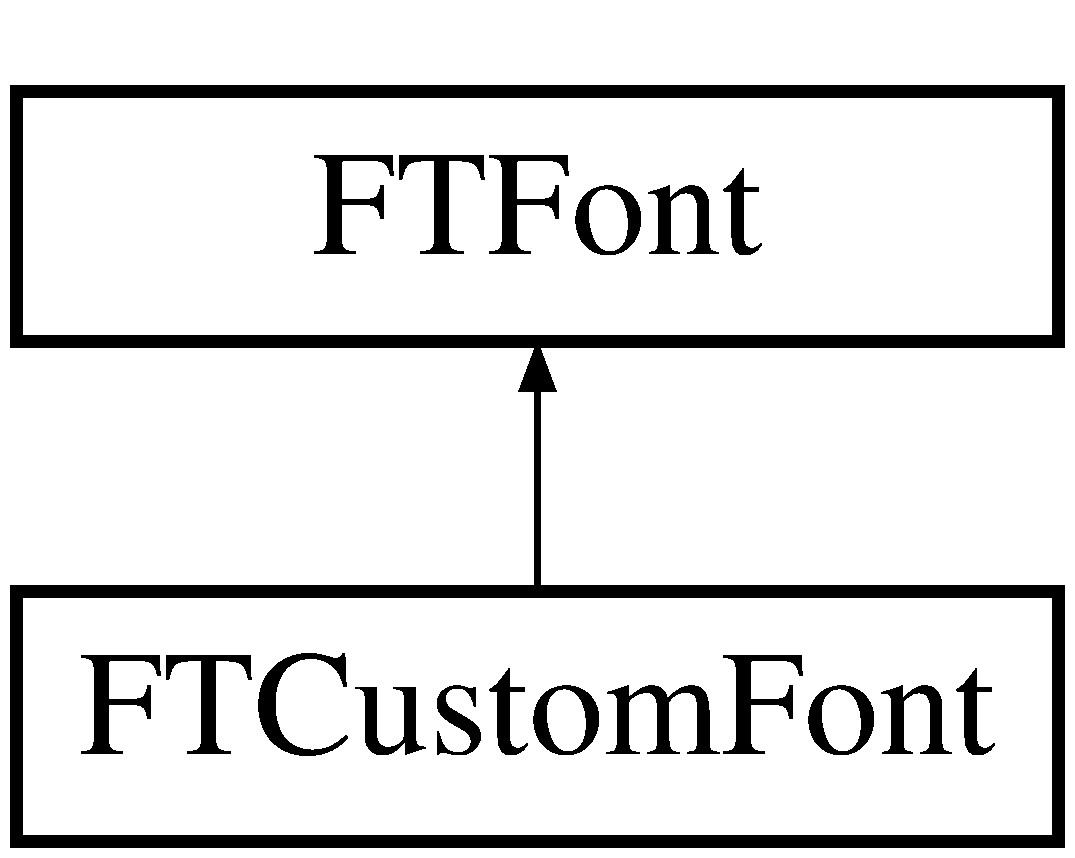
\includegraphics[height=2.000000cm]{class_f_t_custom_font}
\end{center}
\end{figure}
\subsection*{Public Member Functions}
\begin{DoxyCompactItemize}
\item 
\hypertarget{class_f_t_custom_font_a752e3adba12661605536402b55381aa8}{{\bfseries F\-T\-Custom\-Font} (char const $\ast$font\-File\-Path, void $\ast$p, \hyperlink{struct___f_t_g_lglyph}{F\-T\-G\-Lglyph} $\ast$($\ast$makeglyph)(\hyperlink{struct_f_t___glyph_slot_rec__}{F\-T\-\_\-\-Glyph\-Slot}, void $\ast$))}\label{class_f_t_custom_font_a752e3adba12661605536402b55381aa8}

\item 
\hypertarget{class_f_t_custom_font_a14863f6c098d220681087ff85f004dff}{F\-T\-Glyph $\ast$ {\bfseries Make\-Glyph} (\hyperlink{struct_f_t___glyph_slot_rec__}{F\-T\-\_\-\-Glyph\-Slot} slot)}\label{class_f_t_custom_font_a14863f6c098d220681087ff85f004dff}

\end{DoxyCompactItemize}


The documentation for this class was generated from the following file\-:\begin{DoxyCompactItemize}
\item 
X\-:/\-Git\-\_\-\-Repository/inf2990-\/06/\-Cadriciel/\-Commun/\-Externe/\-F\-T\-G\-L/include/\-F\-T\-Font/F\-T\-Font\-Glue.\-cpp\end{DoxyCompactItemize}

\hypertarget{class_f_t_custom_glyph}{\section{F\-T\-Custom\-Glyph Class Reference}
\label{class_f_t_custom_glyph}\index{F\-T\-Custom\-Glyph@{F\-T\-Custom\-Glyph}}
}
Inheritance diagram for F\-T\-Custom\-Glyph\-:\begin{figure}[H]
\begin{center}
\leavevmode
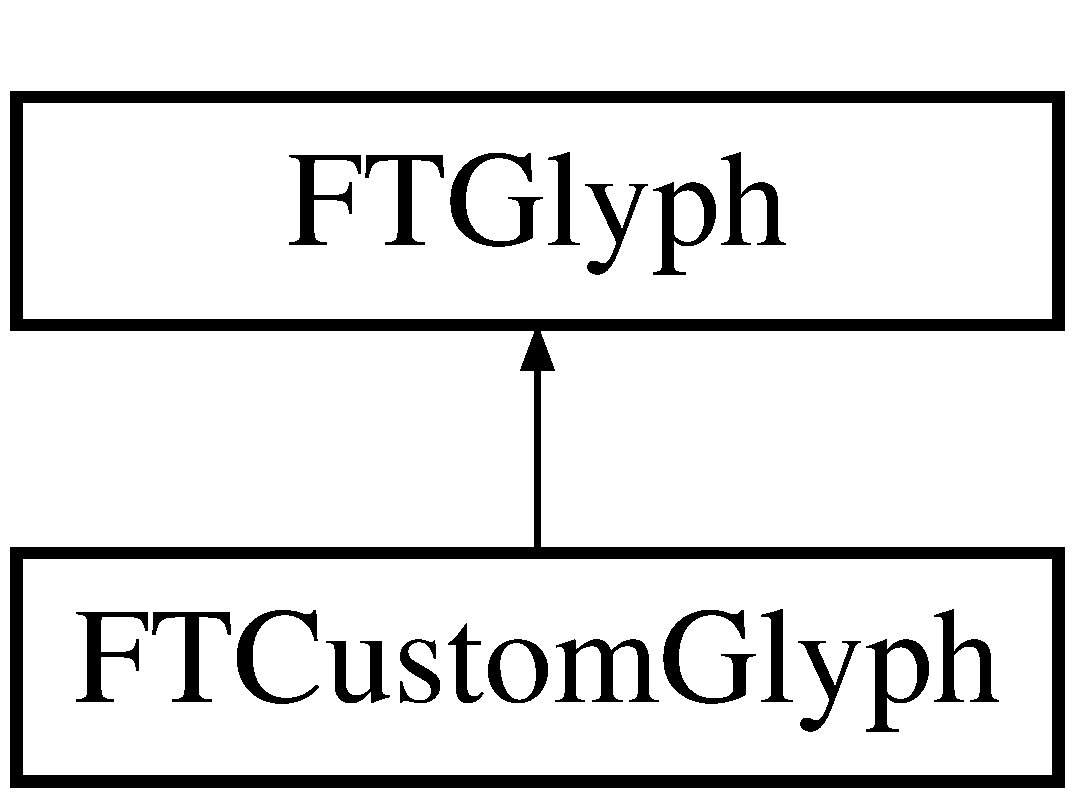
\includegraphics[height=2.000000cm]{class_f_t_custom_glyph}
\end{center}
\end{figure}
\subsection*{Public Member Functions}
\begin{DoxyCompactItemize}
\item 
\hypertarget{class_f_t_custom_glyph_a43e4bfa9d8ccb5ae4d0e9c38cf7f01c1}{{\bfseries F\-T\-Custom\-Glyph} (\hyperlink{struct___f_t_g_lglyph}{F\-T\-G\-Lglyph} $\ast$base, void $\ast$p, void($\ast$render)(\hyperlink{struct___f_t_g_lglyph}{F\-T\-G\-Lglyph} $\ast$, void $\ast$, F\-T\-G\-L\-\_\-\-D\-O\-U\-B\-L\-E, F\-T\-G\-L\-\_\-\-D\-O\-U\-B\-L\-E, int, F\-T\-G\-L\-\_\-\-D\-O\-U\-B\-L\-E $\ast$, F\-T\-G\-L\-\_\-\-D\-O\-U\-B\-L\-E $\ast$), void($\ast$destroy)(\hyperlink{struct___f_t_g_lglyph}{F\-T\-G\-Lglyph} $\ast$, void $\ast$))}\label{class_f_t_custom_glyph_a43e4bfa9d8ccb5ae4d0e9c38cf7f01c1}

\item 
\hypertarget{class_f_t_custom_glyph_aa8f17e3a9547eafed913e2b8f9b70958}{float {\bfseries Advance} () const }\label{class_f_t_custom_glyph_aa8f17e3a9547eafed913e2b8f9b70958}

\item 
\hypertarget{class_f_t_custom_glyph_a29285cf4a9b5476a80b01e1678272bd6}{const F\-T\-Point \& {\bfseries Render} (const F\-T\-Point \&pen, int render\-Mode)}\label{class_f_t_custom_glyph_a29285cf4a9b5476a80b01e1678272bd6}

\item 
\hypertarget{class_f_t_custom_glyph_aebed1d1515a24d6410f4c3f44686b75c}{const F\-T\-B\-Box \& {\bfseries B\-Box} () const }\label{class_f_t_custom_glyph_aebed1d1515a24d6410f4c3f44686b75c}

\item 
\hypertarget{class_f_t_custom_glyph_a8a74b76186fb02da48849c3c094fb72e}{F\-T\-\_\-\-Error {\bfseries Error} () const }\label{class_f_t_custom_glyph_a8a74b76186fb02da48849c3c094fb72e}

\end{DoxyCompactItemize}


The documentation for this class was generated from the following file\-:\begin{DoxyCompactItemize}
\item 
X\-:/\-Git\-\_\-\-Repository/inf2990-\/06/\-Cadriciel/\-Commun/\-Externe/\-F\-T\-G\-L/include/\-F\-T\-Glyph/F\-T\-Glyph\-Glue.\-cpp\end{DoxyCompactItemize}

\hypertarget{class_f_t_extrude_font_impl}{\section{F\-T\-Extrude\-Font\-Impl Class Reference}
\label{class_f_t_extrude_font_impl}\index{F\-T\-Extrude\-Font\-Impl@{F\-T\-Extrude\-Font\-Impl}}
}
Inheritance diagram for F\-T\-Extrude\-Font\-Impl\-:\begin{figure}[H]
\begin{center}
\leavevmode
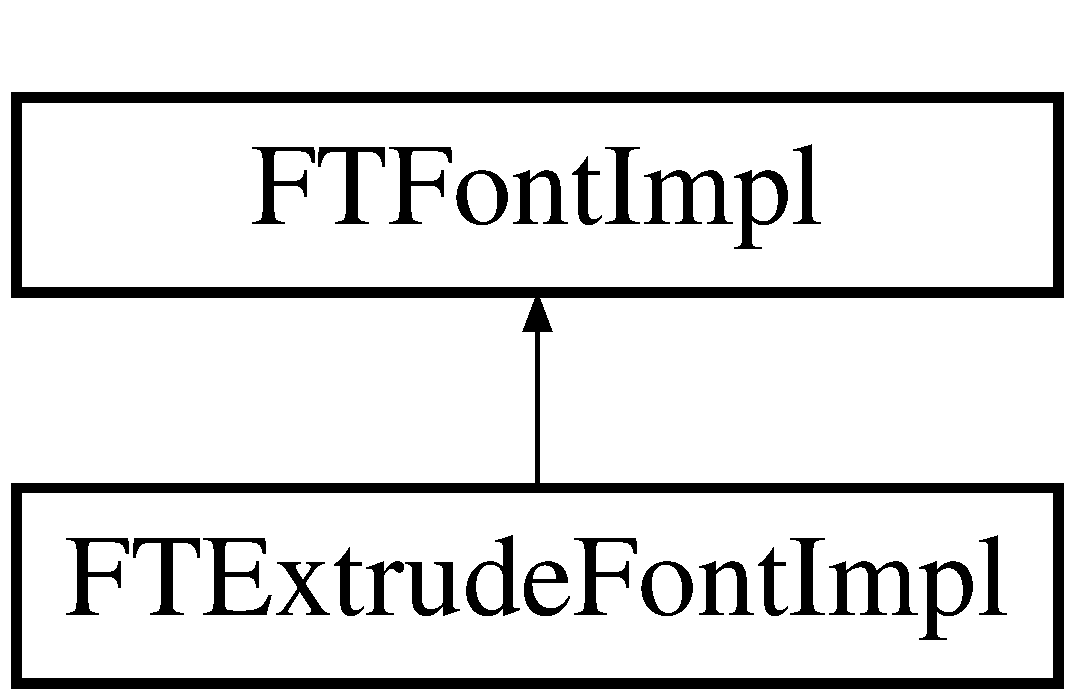
\includegraphics[height=2.000000cm]{class_f_t_extrude_font_impl}
\end{center}
\end{figure}
\subsection*{Protected Member Functions}
\begin{DoxyCompactItemize}
\item 
\hypertarget{class_f_t_extrude_font_impl_a43da54bf40a55db304395d8dec46897f}{{\bfseries F\-T\-Extrude\-Font\-Impl} (F\-T\-Font $\ast$ft\-Font, const char $\ast$font\-File\-Path)}\label{class_f_t_extrude_font_impl_a43da54bf40a55db304395d8dec46897f}

\item 
\hypertarget{class_f_t_extrude_font_impl_aa433e0addf2dba2ae9232d6522ccdb5f}{{\bfseries F\-T\-Extrude\-Font\-Impl} (F\-T\-Font $\ast$ft\-Font, const unsigned char $\ast$p\-Buffer\-Bytes, size\-\_\-t buffer\-Size\-In\-Bytes)}\label{class_f_t_extrude_font_impl_aa433e0addf2dba2ae9232d6522ccdb5f}

\item 
virtual void \hyperlink{class_f_t_extrude_font_impl_a852e6d263a34982d56d19dfdf43722f0}{Depth} (float d)
\item 
virtual void \hyperlink{class_f_t_extrude_font_impl_a559ce64b4d0e881455b050d3be57cac0}{Outset} (float o)
\item 
virtual void \hyperlink{class_f_t_extrude_font_impl_a24e6ada58e9086284e99611454c7b335}{Outset} (float f, float b)
\end{DoxyCompactItemize}
\subsection*{Friends}
\begin{DoxyCompactItemize}
\item 
\hypertarget{class_f_t_extrude_font_impl_a06be1600e211ee41aa1b1ed9c7d25639}{class {\bfseries F\-T\-Extrude\-Font}}\label{class_f_t_extrude_font_impl_a06be1600e211ee41aa1b1ed9c7d25639}

\end{DoxyCompactItemize}
\subsection*{Additional Inherited Members}


\subsection{Member Function Documentation}
\hypertarget{class_f_t_extrude_font_impl_a852e6d263a34982d56d19dfdf43722f0}{\index{F\-T\-Extrude\-Font\-Impl@{F\-T\-Extrude\-Font\-Impl}!Depth@{Depth}}
\index{Depth@{Depth}!FTExtrudeFontImpl@{F\-T\-Extrude\-Font\-Impl}}
\subsubsection[{Depth}]{\setlength{\rightskip}{0pt plus 5cm}virtual void F\-T\-Extrude\-Font\-Impl\-::\-Depth (
\begin{DoxyParamCaption}
\item[{float}]{d}
\end{DoxyParamCaption}
)\hspace{0.3cm}{\ttfamily [inline]}, {\ttfamily [protected]}, {\ttfamily [virtual]}}}\label{class_f_t_extrude_font_impl_a852e6d263a34982d56d19dfdf43722f0}
Set the extrusion distance for the font.


\begin{DoxyParams}{Parameters}
{\em d} & The extrusion distance. \\
\hline
\end{DoxyParams}


Reimplemented from \hyperlink{class_f_t_font_impl}{F\-T\-Font\-Impl}.

\hypertarget{class_f_t_extrude_font_impl_a559ce64b4d0e881455b050d3be57cac0}{\index{F\-T\-Extrude\-Font\-Impl@{F\-T\-Extrude\-Font\-Impl}!Outset@{Outset}}
\index{Outset@{Outset}!FTExtrudeFontImpl@{F\-T\-Extrude\-Font\-Impl}}
\subsubsection[{Outset}]{\setlength{\rightskip}{0pt plus 5cm}virtual void F\-T\-Extrude\-Font\-Impl\-::\-Outset (
\begin{DoxyParamCaption}
\item[{float}]{o}
\end{DoxyParamCaption}
)\hspace{0.3cm}{\ttfamily [inline]}, {\ttfamily [protected]}, {\ttfamily [virtual]}}}\label{class_f_t_extrude_font_impl_a559ce64b4d0e881455b050d3be57cac0}
Set the outset distance for the font. Only implemented by F\-T\-Outline\-Font, F\-T\-Polygon\-Font and F\-T\-Extrude\-Font


\begin{DoxyParams}{Parameters}
{\em o} & The outset distance. \\
\hline
\end{DoxyParams}


Reimplemented from \hyperlink{class_f_t_font_impl}{F\-T\-Font\-Impl}.

\hypertarget{class_f_t_extrude_font_impl_a24e6ada58e9086284e99611454c7b335}{\index{F\-T\-Extrude\-Font\-Impl@{F\-T\-Extrude\-Font\-Impl}!Outset@{Outset}}
\index{Outset@{Outset}!FTExtrudeFontImpl@{F\-T\-Extrude\-Font\-Impl}}
\subsubsection[{Outset}]{\setlength{\rightskip}{0pt plus 5cm}virtual void F\-T\-Extrude\-Font\-Impl\-::\-Outset (
\begin{DoxyParamCaption}
\item[{float}]{f, }
\item[{float}]{b}
\end{DoxyParamCaption}
)\hspace{0.3cm}{\ttfamily [inline]}, {\ttfamily [protected]}, {\ttfamily [virtual]}}}\label{class_f_t_extrude_font_impl_a24e6ada58e9086284e99611454c7b335}
Set the outset distance for the font. Only implemented by F\-T\-Extrude\-Font


\begin{DoxyParams}{Parameters}
{\em f} & The front outset distance. \\
\hline
{\em b} & The back outset distance. \\
\hline
\end{DoxyParams}


Reimplemented from \hyperlink{class_f_t_font_impl}{F\-T\-Font\-Impl}.



The documentation for this class was generated from the following files\-:\begin{DoxyCompactItemize}
\item 
X\-:/\-Git\-\_\-\-Repository/inf2990-\/06/\-Cadriciel/\-Commun/\-Externe/\-F\-T\-G\-L/include/\-F\-T\-Font/F\-T\-Extrude\-Font\-Impl.\-h\item 
X\-:/\-Git\-\_\-\-Repository/inf2990-\/06/\-Cadriciel/\-Commun/\-Externe/\-F\-T\-G\-L/include/\-F\-T\-Font/F\-T\-Extrude\-Font.\-cpp\end{DoxyCompactItemize}

\hypertarget{class_f_t_extrude_glyph_impl}{\section{F\-T\-Extrude\-Glyph\-Impl Class Reference}
\label{class_f_t_extrude_glyph_impl}\index{F\-T\-Extrude\-Glyph\-Impl@{F\-T\-Extrude\-Glyph\-Impl}}
}
Inheritance diagram for F\-T\-Extrude\-Glyph\-Impl\-:\begin{figure}[H]
\begin{center}
\leavevmode
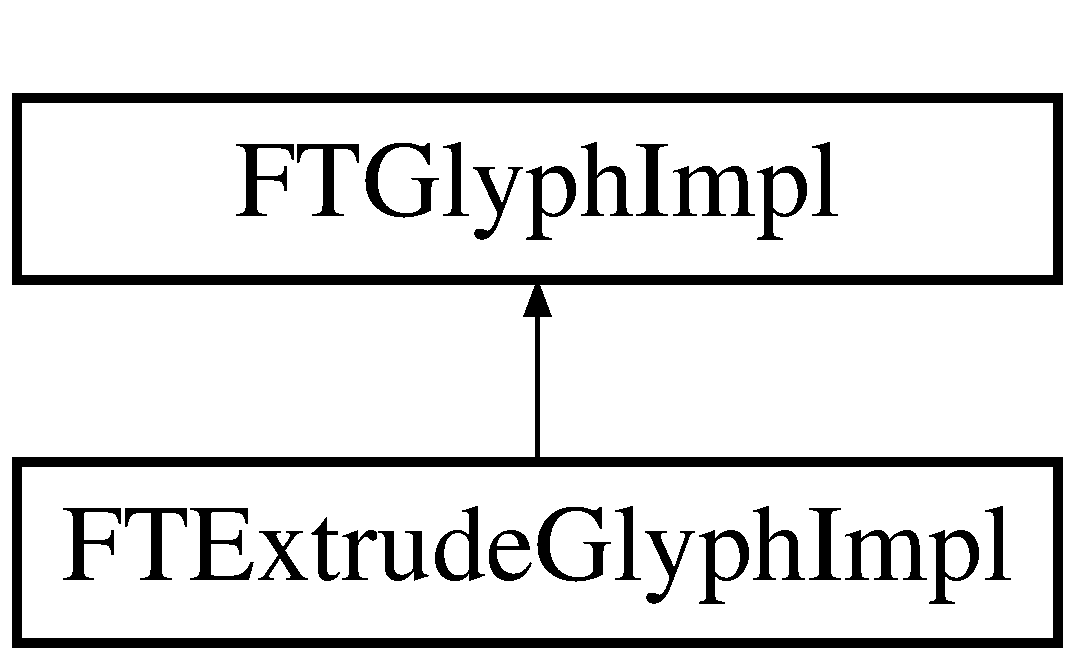
\includegraphics[height=2.000000cm]{class_f_t_extrude_glyph_impl}
\end{center}
\end{figure}
\subsection*{Protected Member Functions}
\begin{DoxyCompactItemize}
\item 
\hypertarget{class_f_t_extrude_glyph_impl_adbfa8d05122539318f6caa8b77a5c291}{{\bfseries F\-T\-Extrude\-Glyph\-Impl} (\hyperlink{struct_f_t___glyph_slot_rec__}{F\-T\-\_\-\-Glyph\-Slot} glyph, float depth, float front\-Outset, float back\-Outset, bool use\-Display\-List)}\label{class_f_t_extrude_glyph_impl_adbfa8d05122539318f6caa8b77a5c291}

\item 
\hypertarget{class_f_t_extrude_glyph_impl_a7ba3363d6764a14a6954f068f626029b}{virtual const F\-T\-Point \& {\bfseries Render\-Impl} (const F\-T\-Point \&pen, int render\-Mode)}\label{class_f_t_extrude_glyph_impl_a7ba3363d6764a14a6954f068f626029b}

\end{DoxyCompactItemize}
\subsection*{Friends}
\begin{DoxyCompactItemize}
\item 
\hypertarget{class_f_t_extrude_glyph_impl_a43bdcab05c1db93d9474fee8176c1fb0}{class {\bfseries F\-T\-Extrude\-Glyph}}\label{class_f_t_extrude_glyph_impl_a43bdcab05c1db93d9474fee8176c1fb0}

\end{DoxyCompactItemize}
\subsection*{Additional Inherited Members}


The documentation for this class was generated from the following files\-:\begin{DoxyCompactItemize}
\item 
X\-:/\-Git\-\_\-\-Repository/inf2990-\/06/\-Cadriciel/\-Commun/\-Externe/\-F\-T\-G\-L/include/\-F\-T\-Glyph/F\-T\-Extrude\-Glyph\-Impl.\-h\item 
X\-:/\-Git\-\_\-\-Repository/inf2990-\/06/\-Cadriciel/\-Commun/\-Externe/\-F\-T\-G\-L/include/\-F\-T\-Glyph/F\-T\-Extrude\-Glyph.\-cpp\end{DoxyCompactItemize}

\hypertarget{class_f_t_face}{\section{F\-T\-Face Class Reference}
\label{class_f_t_face}\index{F\-T\-Face@{F\-T\-Face}}
}


{\ttfamily \#include $<$F\-T\-Face.\-h$>$}

\subsection*{Public Member Functions}
\begin{DoxyCompactItemize}
\item 
\hyperlink{class_f_t_face_a26907a8a50a1316799054454523f13b4}{F\-T\-Face} (const char $\ast$font\-File\-Path, bool precompute\-Kerning=true)
\item 
\hyperlink{class_f_t_face_a0c39392976775b415743326d2e478d57}{F\-T\-Face} (const unsigned char $\ast$p\-Buffer\-Bytes, size\-\_\-t buffer\-Size\-In\-Bytes, bool precompute\-Kerning=true)
\item 
virtual \hyperlink{class_f_t_face_aa7087c9bcd6a8c212bfe5048743d7872}{$\sim$\-F\-T\-Face} ()
\item 
bool \hyperlink{class_f_t_face_ac8521d2dc370555fea58a842bc4e8a65}{Attach} (const char $\ast$font\-File\-Path)
\item 
bool \hyperlink{class_f_t_face_a0ceddf4a66cb56457949307b613d0992}{Attach} (const unsigned char $\ast$p\-Buffer\-Bytes, size\-\_\-t buffer\-Size\-In\-Bytes)
\item 
\hyperlink{struct_f_t___face_rec__}{F\-T\-\_\-\-Face} $\ast$ \hyperlink{class_f_t_face_ad3e6e4dcd0d84ad3e80f6c0a4e12f233}{Face} () const 
\item 
const \hyperlink{class_f_t_size}{F\-T\-Size} \& \hyperlink{class_f_t_face_a9fb537b25a678a783aa07da8acf1280b}{Size} (const unsigned int size, const unsigned int res)
\item 
unsigned int \hyperlink{class_f_t_face_ab1ee1e2906909c8d42e1c143d23b2f5d}{Char\-Map\-Count} () const 
\item 
F\-T\-\_\-\-Encoding $\ast$ \hyperlink{class_f_t_face_ae937a2a2c94f933bddb2619d96cad74e}{Char\-Map\-List} ()
\item 
F\-T\-Point \hyperlink{class_f_t_face_af57bd3a3122e0e54acb04b348380ed7e}{Kern\-Advance} (unsigned int index1, unsigned int index2)
\item 
\hyperlink{struct_f_t___glyph_slot_rec__}{F\-T\-\_\-\-Glyph\-Slot} \hyperlink{class_f_t_face_aad153f57e7eb55ff42755b0512b01854}{Glyph} (unsigned int index, F\-T\-\_\-\-Int load\-\_\-flags)
\item 
unsigned int \hyperlink{class_f_t_face_a58805c5cf39daeb8d3fa11e2f791c31a}{Glyph\-Count} () const 
\item 
F\-T\-\_\-\-Error \hyperlink{class_f_t_face_a7caba7cdfdc277dc377aed97ab1b36b4}{Error} () const 
\end{DoxyCompactItemize}


\subsection{Detailed Description}
\hyperlink{class_f_t_face}{F\-T\-Face} class provides an abstraction layer for the Freetype Face.

\begin{DoxySeeAlso}{See Also}
\char`\"{}\-Freetype 2 Documentation\char`\"{} 
\end{DoxySeeAlso}


\subsection{Constructor \& Destructor Documentation}
\hypertarget{class_f_t_face_a26907a8a50a1316799054454523f13b4}{\index{F\-T\-Face@{F\-T\-Face}!F\-T\-Face@{F\-T\-Face}}
\index{F\-T\-Face@{F\-T\-Face}!FTFace@{F\-T\-Face}}
\subsubsection[{F\-T\-Face}]{\setlength{\rightskip}{0pt plus 5cm}F\-T\-Face\-::\-F\-T\-Face (
\begin{DoxyParamCaption}
\item[{const char $\ast$}]{font\-File\-Path, }
\item[{bool}]{precompute\-Kerning = {\ttfamily true}}
\end{DoxyParamCaption}
)}}\label{class_f_t_face_a26907a8a50a1316799054454523f13b4}
Opens and reads a face file. Error is set.


\begin{DoxyParams}{Parameters}
{\em font\-File\-Path} & font file path. \\
\hline
\end{DoxyParams}
\hypertarget{class_f_t_face_a0c39392976775b415743326d2e478d57}{\index{F\-T\-Face@{F\-T\-Face}!F\-T\-Face@{F\-T\-Face}}
\index{F\-T\-Face@{F\-T\-Face}!FTFace@{F\-T\-Face}}
\subsubsection[{F\-T\-Face}]{\setlength{\rightskip}{0pt plus 5cm}F\-T\-Face\-::\-F\-T\-Face (
\begin{DoxyParamCaption}
\item[{const unsigned char $\ast$}]{p\-Buffer\-Bytes, }
\item[{size\-\_\-t}]{buffer\-Size\-In\-Bytes, }
\item[{bool}]{precompute\-Kerning = {\ttfamily true}}
\end{DoxyParamCaption}
)}}\label{class_f_t_face_a0c39392976775b415743326d2e478d57}
Read face data from an in-\/memory buffer. Error is set.


\begin{DoxyParams}{Parameters}
{\em p\-Buffer\-Bytes} & the in-\/memory buffer \\
\hline
{\em buffer\-Size\-In\-Bytes} & the length of the buffer in bytes \\
\hline
\end{DoxyParams}
\hypertarget{class_f_t_face_aa7087c9bcd6a8c212bfe5048743d7872}{\index{F\-T\-Face@{F\-T\-Face}!$\sim$\-F\-T\-Face@{$\sim$\-F\-T\-Face}}
\index{$\sim$\-F\-T\-Face@{$\sim$\-F\-T\-Face}!FTFace@{F\-T\-Face}}
\subsubsection[{$\sim$\-F\-T\-Face}]{\setlength{\rightskip}{0pt plus 5cm}F\-T\-Face\-::$\sim$\-F\-T\-Face (
\begin{DoxyParamCaption}
{}
\end{DoxyParamCaption}
)\hspace{0.3cm}{\ttfamily [virtual]}}}\label{class_f_t_face_aa7087c9bcd6a8c212bfe5048743d7872}
Destructor

Disposes of the current Freetype Face. 

\subsection{Member Function Documentation}
\hypertarget{class_f_t_face_ac8521d2dc370555fea58a842bc4e8a65}{\index{F\-T\-Face@{F\-T\-Face}!Attach@{Attach}}
\index{Attach@{Attach}!FTFace@{F\-T\-Face}}
\subsubsection[{Attach}]{\setlength{\rightskip}{0pt plus 5cm}bool F\-T\-Face\-::\-Attach (
\begin{DoxyParamCaption}
\item[{const char $\ast$}]{font\-File\-Path}
\end{DoxyParamCaption}
)}}\label{class_f_t_face_ac8521d2dc370555fea58a842bc4e8a65}
Attach auxilliary file to font (e.\-g., font metrics).


\begin{DoxyParams}{Parameters}
{\em font\-File\-Path} & auxilliary font file path. \\
\hline
\end{DoxyParams}
\begin{DoxyReturn}{Returns}
{\ttfamily true} if file has opened successfully. 
\end{DoxyReturn}
\hypertarget{class_f_t_face_a0ceddf4a66cb56457949307b613d0992}{\index{F\-T\-Face@{F\-T\-Face}!Attach@{Attach}}
\index{Attach@{Attach}!FTFace@{F\-T\-Face}}
\subsubsection[{Attach}]{\setlength{\rightskip}{0pt plus 5cm}bool F\-T\-Face\-::\-Attach (
\begin{DoxyParamCaption}
\item[{const unsigned char $\ast$}]{p\-Buffer\-Bytes, }
\item[{size\-\_\-t}]{buffer\-Size\-In\-Bytes}
\end{DoxyParamCaption}
)}}\label{class_f_t_face_a0ceddf4a66cb56457949307b613d0992}
Attach auxilliary data to font (e.\-g., font metrics) from memory


\begin{DoxyParams}{Parameters}
{\em p\-Buffer\-Bytes} & the in-\/memory buffer \\
\hline
{\em buffer\-Size\-In\-Bytes} & the length of the buffer in bytes \\
\hline
\end{DoxyParams}
\begin{DoxyReturn}{Returns}
{\ttfamily true} if file has opened successfully. 
\end{DoxyReturn}
\hypertarget{class_f_t_face_ab1ee1e2906909c8d42e1c143d23b2f5d}{\index{F\-T\-Face@{F\-T\-Face}!Char\-Map\-Count@{Char\-Map\-Count}}
\index{Char\-Map\-Count@{Char\-Map\-Count}!FTFace@{F\-T\-Face}}
\subsubsection[{Char\-Map\-Count}]{\setlength{\rightskip}{0pt plus 5cm}unsigned int F\-T\-Face\-::\-Char\-Map\-Count (
\begin{DoxyParamCaption}
{}
\end{DoxyParamCaption}
) const}}\label{class_f_t_face_ab1ee1e2906909c8d42e1c143d23b2f5d}
Get the number of character maps in this face.

\begin{DoxyReturn}{Returns}
character map count. 
\end{DoxyReturn}
\hypertarget{class_f_t_face_ae937a2a2c94f933bddb2619d96cad74e}{\index{F\-T\-Face@{F\-T\-Face}!Char\-Map\-List@{Char\-Map\-List}}
\index{Char\-Map\-List@{Char\-Map\-List}!FTFace@{F\-T\-Face}}
\subsubsection[{Char\-Map\-List}]{\setlength{\rightskip}{0pt plus 5cm}F\-T\-\_\-\-Encoding $\ast$ F\-T\-Face\-::\-Char\-Map\-List (
\begin{DoxyParamCaption}
{}
\end{DoxyParamCaption}
)}}\label{class_f_t_face_ae937a2a2c94f933bddb2619d96cad74e}
Get a list of character maps in this face.

\begin{DoxyReturn}{Returns}
pointer to the first encoding. 
\end{DoxyReturn}
\hypertarget{class_f_t_face_a7caba7cdfdc277dc377aed97ab1b36b4}{\index{F\-T\-Face@{F\-T\-Face}!Error@{Error}}
\index{Error@{Error}!FTFace@{F\-T\-Face}}
\subsubsection[{Error}]{\setlength{\rightskip}{0pt plus 5cm}F\-T\-\_\-\-Error F\-T\-Face\-::\-Error (
\begin{DoxyParamCaption}
{}
\end{DoxyParamCaption}
) const\hspace{0.3cm}{\ttfamily [inline]}}}\label{class_f_t_face_a7caba7cdfdc277dc377aed97ab1b36b4}
Queries for errors.

\begin{DoxyReturn}{Returns}
The current error code. 
\end{DoxyReturn}
\hypertarget{class_f_t_face_ad3e6e4dcd0d84ad3e80f6c0a4e12f233}{\index{F\-T\-Face@{F\-T\-Face}!Face@{Face}}
\index{Face@{Face}!FTFace@{F\-T\-Face}}
\subsubsection[{Face}]{\setlength{\rightskip}{0pt plus 5cm}{\bf F\-T\-\_\-\-Face}$\ast$ F\-T\-Face\-::\-Face (
\begin{DoxyParamCaption}
{}
\end{DoxyParamCaption}
) const\hspace{0.3cm}{\ttfamily [inline]}}}\label{class_f_t_face_ad3e6e4dcd0d84ad3e80f6c0a4e12f233}
Get the freetype face object..

\begin{DoxyReturn}{Returns}
pointer to an F\-T\-\_\-\-Face. 
\end{DoxyReturn}
\hypertarget{class_f_t_face_aad153f57e7eb55ff42755b0512b01854}{\index{F\-T\-Face@{F\-T\-Face}!Glyph@{Glyph}}
\index{Glyph@{Glyph}!FTFace@{F\-T\-Face}}
\subsubsection[{Glyph}]{\setlength{\rightskip}{0pt plus 5cm}{\bf F\-T\-\_\-\-Glyph\-Slot} F\-T\-Face\-::\-Glyph (
\begin{DoxyParamCaption}
\item[{unsigned int}]{index, }
\item[{F\-T\-\_\-\-Int}]{load\-\_\-flags}
\end{DoxyParamCaption}
)}}\label{class_f_t_face_aad153f57e7eb55ff42755b0512b01854}
Loads and creates a Freetype glyph. \hypertarget{class_f_t_face_a58805c5cf39daeb8d3fa11e2f791c31a}{\index{F\-T\-Face@{F\-T\-Face}!Glyph\-Count@{Glyph\-Count}}
\index{Glyph\-Count@{Glyph\-Count}!FTFace@{F\-T\-Face}}
\subsubsection[{Glyph\-Count}]{\setlength{\rightskip}{0pt plus 5cm}unsigned int F\-T\-Face\-::\-Glyph\-Count (
\begin{DoxyParamCaption}
{}
\end{DoxyParamCaption}
) const\hspace{0.3cm}{\ttfamily [inline]}}}\label{class_f_t_face_a58805c5cf39daeb8d3fa11e2f791c31a}
Gets the number of glyphs in the current face. \hypertarget{class_f_t_face_af57bd3a3122e0e54acb04b348380ed7e}{\index{F\-T\-Face@{F\-T\-Face}!Kern\-Advance@{Kern\-Advance}}
\index{Kern\-Advance@{Kern\-Advance}!FTFace@{F\-T\-Face}}
\subsubsection[{Kern\-Advance}]{\setlength{\rightskip}{0pt plus 5cm}F\-T\-Point F\-T\-Face\-::\-Kern\-Advance (
\begin{DoxyParamCaption}
\item[{unsigned int}]{index1, }
\item[{unsigned int}]{index2}
\end{DoxyParamCaption}
)}}\label{class_f_t_face_af57bd3a3122e0e54acb04b348380ed7e}
Gets the kerning vector between two glyphs \hypertarget{class_f_t_face_a9fb537b25a678a783aa07da8acf1280b}{\index{F\-T\-Face@{F\-T\-Face}!Size@{Size}}
\index{Size@{Size}!FTFace@{F\-T\-Face}}
\subsubsection[{Size}]{\setlength{\rightskip}{0pt plus 5cm}const {\bf F\-T\-Size} \& F\-T\-Face\-::\-Size (
\begin{DoxyParamCaption}
\item[{const unsigned int}]{size, }
\item[{const unsigned int}]{res}
\end{DoxyParamCaption}
)}}\label{class_f_t_face_a9fb537b25a678a783aa07da8acf1280b}
Sets the char size for the current face.

This doesn't guarantee that the size was set correctly. Clients should check errors.


\begin{DoxyParams}{Parameters}
{\em size} & the face size in points (1/72 inch) \\
\hline
{\em res} & the resolution of the target device. \\
\hline
\end{DoxyParams}
\begin{DoxyReturn}{Returns}
{\ttfamily \hyperlink{class_f_t_size}{F\-T\-Size}} object 
\end{DoxyReturn}


The documentation for this class was generated from the following files\-:\begin{DoxyCompactItemize}
\item 
X\-:/\-Git\-\_\-\-Repository/inf2990-\/06/\-Cadriciel/\-Commun/\-Externe/\-F\-T\-G\-L/include/F\-T\-Face.\-h\item 
X\-:/\-Git\-\_\-\-Repository/inf2990-\/06/\-Cadriciel/\-Commun/\-Externe/\-F\-T\-G\-L/include/F\-T\-Face.\-cpp\end{DoxyCompactItemize}

\hypertarget{class_f_t_font_impl}{\section{F\-T\-Font\-Impl Class Reference}
\label{class_f_t_font_impl}\index{F\-T\-Font\-Impl@{F\-T\-Font\-Impl}}
}
Inheritance diagram for F\-T\-Font\-Impl\-:\begin{figure}[H]
\begin{center}
\leavevmode
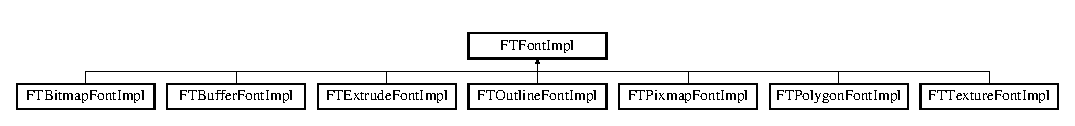
\includegraphics[height=1.250000cm]{class_f_t_font_impl}
\end{center}
\end{figure}
\subsection*{Protected Member Functions}
\begin{DoxyCompactItemize}
\item 
\hypertarget{class_f_t_font_impl_a4b0a3bd10221f8d51b4ca651c09a9cc5}{{\bfseries F\-T\-Font\-Impl} (F\-T\-Font $\ast$ft\-Font, char const $\ast$font\-File\-Path)}\label{class_f_t_font_impl_a4b0a3bd10221f8d51b4ca651c09a9cc5}

\item 
\hypertarget{class_f_t_font_impl_a1672e949c774c02a1642cdd090dddfc1}{{\bfseries F\-T\-Font\-Impl} (F\-T\-Font $\ast$ft\-Font, const unsigned char $\ast$p\-Buffer\-Bytes, size\-\_\-t buffer\-Size\-In\-Bytes)}\label{class_f_t_font_impl_a1672e949c774c02a1642cdd090dddfc1}

\item 
\hypertarget{class_f_t_font_impl_af96aac1ae6b457b52404bb268dd8b726}{virtual bool {\bfseries Attach} (const char $\ast$font\-File\-Path)}\label{class_f_t_font_impl_af96aac1ae6b457b52404bb268dd8b726}

\item 
\hypertarget{class_f_t_font_impl_af87c2267ecc8fa7eb717a8db9eb71ae6}{virtual bool {\bfseries Attach} (const unsigned char $\ast$p\-Buffer\-Bytes, size\-\_\-t buffer\-Size\-In\-Bytes)}\label{class_f_t_font_impl_af87c2267ecc8fa7eb717a8db9eb71ae6}

\item 
\hypertarget{class_f_t_font_impl_ab9c1065b08407289d0fe5774a1fc6e07}{virtual void {\bfseries Glyph\-Load\-Flags} (F\-T\-\_\-\-Int flags)}\label{class_f_t_font_impl_ab9c1065b08407289d0fe5774a1fc6e07}

\item 
\hypertarget{class_f_t_font_impl_ac6ed6571c7b704610a0a78159663359d}{virtual bool {\bfseries Char\-Map} (F\-T\-\_\-\-Encoding encoding)}\label{class_f_t_font_impl_ac6ed6571c7b704610a0a78159663359d}

\item 
\hypertarget{class_f_t_font_impl_a54770e1ab6374469661d6b59684d2130}{virtual unsigned int {\bfseries Char\-Map\-Count} () const }\label{class_f_t_font_impl_a54770e1ab6374469661d6b59684d2130}

\item 
\hypertarget{class_f_t_font_impl_a5f632609c3368c12b9c19a05fd773bae}{virtual F\-T\-\_\-\-Encoding $\ast$ {\bfseries Char\-Map\-List} ()}\label{class_f_t_font_impl_a5f632609c3368c12b9c19a05fd773bae}

\item 
\hypertarget{class_f_t_font_impl_a8a83cfafb686a182b333d5002590a020}{virtual void {\bfseries Use\-Display\-List} (bool use\-List)}\label{class_f_t_font_impl_a8a83cfafb686a182b333d5002590a020}

\item 
\hypertarget{class_f_t_font_impl_a1f9b94b11bdb3b6181846572a5fe767f}{virtual float {\bfseries Ascender} () const }\label{class_f_t_font_impl_a1f9b94b11bdb3b6181846572a5fe767f}

\item 
\hypertarget{class_f_t_font_impl_a2a755f954a2a7aa5e69a9e9e6cf14ab1}{virtual float {\bfseries Descender} () const }\label{class_f_t_font_impl_a2a755f954a2a7aa5e69a9e9e6cf14ab1}

\item 
\hypertarget{class_f_t_font_impl_a00a4e10887f305f986737fc102e88a6b}{virtual float {\bfseries Line\-Height} () const }\label{class_f_t_font_impl_a00a4e10887f305f986737fc102e88a6b}

\item 
\hypertarget{class_f_t_font_impl_a0739028e23c1c3d05f6db80b14428dde}{virtual bool {\bfseries Face\-Size} (const unsigned int size, const unsigned int res)}\label{class_f_t_font_impl_a0739028e23c1c3d05f6db80b14428dde}

\item 
\hypertarget{class_f_t_font_impl_a099a32e288dd0e0d7674b29a170ab52c}{virtual unsigned int {\bfseries Face\-Size} () const }\label{class_f_t_font_impl_a099a32e288dd0e0d7674b29a170ab52c}

\item 
\hypertarget{class_f_t_font_impl_a534a812f2df93e40392c9c5eca423b3f}{virtual void {\bfseries Depth} (float depth)}\label{class_f_t_font_impl_a534a812f2df93e40392c9c5eca423b3f}

\item 
\hypertarget{class_f_t_font_impl_aaa36154bf49c163d58d5b36575e23348}{virtual void {\bfseries Outset} (float outset)}\label{class_f_t_font_impl_aaa36154bf49c163d58d5b36575e23348}

\item 
\hypertarget{class_f_t_font_impl_a848e50bd8b6602ab7664e6d8c32167d3}{virtual void {\bfseries Outset} (float front, float back)}\label{class_f_t_font_impl_a848e50bd8b6602ab7664e6d8c32167d3}

\item 
\hypertarget{class_f_t_font_impl_ad26207fc1c4d70d1f800857f3893c8a1}{virtual F\-T\-B\-Box {\bfseries B\-Box} (const char $\ast$s, const int len, F\-T\-Point, F\-T\-Point)}\label{class_f_t_font_impl_ad26207fc1c4d70d1f800857f3893c8a1}

\item 
\hypertarget{class_f_t_font_impl_a13a17b5af83b6d81aea4a297646789e0}{virtual F\-T\-B\-Box {\bfseries B\-Box} (const wchar\-\_\-t $\ast$s, const int len, F\-T\-Point, F\-T\-Point)}\label{class_f_t_font_impl_a13a17b5af83b6d81aea4a297646789e0}

\item 
\hypertarget{class_f_t_font_impl_a237dc30760ac7d1b1e321da179a5055a}{virtual float {\bfseries Advance} (const char $\ast$s, const int len, F\-T\-Point)}\label{class_f_t_font_impl_a237dc30760ac7d1b1e321da179a5055a}

\item 
\hypertarget{class_f_t_font_impl_a802bd5a2eefad0cdc27b22b63dab3de0}{virtual float {\bfseries Advance} (const wchar\-\_\-t $\ast$s, const int len, F\-T\-Point)}\label{class_f_t_font_impl_a802bd5a2eefad0cdc27b22b63dab3de0}

\item 
\hypertarget{class_f_t_font_impl_a1562233a391c602c155ee6ce5df8b4e9}{virtual F\-T\-Point {\bfseries Render} (const char $\ast$s, const int len, F\-T\-Point, F\-T\-Point, int)}\label{class_f_t_font_impl_a1562233a391c602c155ee6ce5df8b4e9}

\item 
\hypertarget{class_f_t_font_impl_ad6f899bf03a580f616c8238b5ea0f419}{virtual F\-T\-Point {\bfseries Render} (const wchar\-\_\-t $\ast$s, const int len, F\-T\-Point, F\-T\-Point, int)}\label{class_f_t_font_impl_ad6f899bf03a580f616c8238b5ea0f419}

\end{DoxyCompactItemize}
\subsection*{Protected Attributes}
\begin{DoxyCompactItemize}
\item 
\hyperlink{class_f_t_face}{F\-T\-Face} \hyperlink{class_f_t_font_impl_ab35b9e1966574c6bb88bff520e9c33df}{face}
\item 
\hyperlink{class_f_t_size}{F\-T\-Size} \hyperlink{class_f_t_font_impl_a9ec32ea40b0d1ea53442daec1bbaade1}{char\-Size}
\item 
bool \hyperlink{class_f_t_font_impl_a5c21ea909477c7180b86625fef6af457}{use\-Display\-Lists}
\item 
F\-T\-\_\-\-Int \hyperlink{class_f_t_font_impl_a217737b273e6abaa0dd6d837d5677e56}{load\-\_\-flags}
\item 
F\-T\-\_\-\-Error \hyperlink{class_f_t_font_impl_a39510c5a3665ae65bc7ff9b96c25b0c9}{err}
\end{DoxyCompactItemize}
\subsection*{Friends}
\begin{DoxyCompactItemize}
\item 
\hypertarget{class_f_t_font_impl_a8db85445a08f6c3139ba842b37e5b183}{class {\bfseries F\-T\-Font}}\label{class_f_t_font_impl_a8db85445a08f6c3139ba842b37e5b183}

\end{DoxyCompactItemize}


\subsection{Member Data Documentation}
\hypertarget{class_f_t_font_impl_a9ec32ea40b0d1ea53442daec1bbaade1}{\index{F\-T\-Font\-Impl@{F\-T\-Font\-Impl}!char\-Size@{char\-Size}}
\index{char\-Size@{char\-Size}!FTFontImpl@{F\-T\-Font\-Impl}}
\subsubsection[{char\-Size}]{\setlength{\rightskip}{0pt plus 5cm}{\bf F\-T\-Size} F\-T\-Font\-Impl\-::char\-Size\hspace{0.3cm}{\ttfamily [protected]}}}\label{class_f_t_font_impl_a9ec32ea40b0d1ea53442daec1bbaade1}
Current size object \hypertarget{class_f_t_font_impl_a39510c5a3665ae65bc7ff9b96c25b0c9}{\index{F\-T\-Font\-Impl@{F\-T\-Font\-Impl}!err@{err}}
\index{err@{err}!FTFontImpl@{F\-T\-Font\-Impl}}
\subsubsection[{err}]{\setlength{\rightskip}{0pt plus 5cm}F\-T\-\_\-\-Error F\-T\-Font\-Impl\-::err\hspace{0.3cm}{\ttfamily [protected]}}}\label{class_f_t_font_impl_a39510c5a3665ae65bc7ff9b96c25b0c9}
Current error code. Zero means no error. \hypertarget{class_f_t_font_impl_ab35b9e1966574c6bb88bff520e9c33df}{\index{F\-T\-Font\-Impl@{F\-T\-Font\-Impl}!face@{face}}
\index{face@{face}!FTFontImpl@{F\-T\-Font\-Impl}}
\subsubsection[{face}]{\setlength{\rightskip}{0pt plus 5cm}{\bf F\-T\-Face} F\-T\-Font\-Impl\-::face\hspace{0.3cm}{\ttfamily [protected]}}}\label{class_f_t_font_impl_ab35b9e1966574c6bb88bff520e9c33df}
Current face object \hypertarget{class_f_t_font_impl_a217737b273e6abaa0dd6d837d5677e56}{\index{F\-T\-Font\-Impl@{F\-T\-Font\-Impl}!load\-\_\-flags@{load\-\_\-flags}}
\index{load\-\_\-flags@{load\-\_\-flags}!FTFontImpl@{F\-T\-Font\-Impl}}
\subsubsection[{load\-\_\-flags}]{\setlength{\rightskip}{0pt plus 5cm}F\-T\-\_\-\-Int F\-T\-Font\-Impl\-::load\-\_\-flags\hspace{0.3cm}{\ttfamily [protected]}}}\label{class_f_t_font_impl_a217737b273e6abaa0dd6d837d5677e56}
The default glyph loading flags. \hypertarget{class_f_t_font_impl_a5c21ea909477c7180b86625fef6af457}{\index{F\-T\-Font\-Impl@{F\-T\-Font\-Impl}!use\-Display\-Lists@{use\-Display\-Lists}}
\index{use\-Display\-Lists@{use\-Display\-Lists}!FTFontImpl@{F\-T\-Font\-Impl}}
\subsubsection[{use\-Display\-Lists}]{\setlength{\rightskip}{0pt plus 5cm}bool F\-T\-Font\-Impl\-::use\-Display\-Lists\hspace{0.3cm}{\ttfamily [protected]}}}\label{class_f_t_font_impl_a5c21ea909477c7180b86625fef6af457}
Flag to enable or disable the use of Display Lists inside F\-T\-G\-L {\ttfamily true} turns O\-N display lists. {\ttfamily false} turns O\-F\-F display lists. 

The documentation for this class was generated from the following files\-:\begin{DoxyCompactItemize}
\item 
X\-:/\-Git\-\_\-\-Repository/inf2990-\/06/\-Cadriciel/\-Commun/\-Externe/\-F\-T\-G\-L/include/\-F\-T\-Font/F\-T\-Font\-Impl.\-h\item 
X\-:/\-Git\-\_\-\-Repository/inf2990-\/06/\-Cadriciel/\-Commun/\-Externe/\-F\-T\-G\-L/include/\-F\-T\-Font/F\-T\-Font.\-cpp\end{DoxyCompactItemize}

\hypertarget{class_f_t_glyph_container}{\section{F\-T\-Glyph\-Container Class Reference}
\label{class_f_t_glyph_container}\index{F\-T\-Glyph\-Container@{F\-T\-Glyph\-Container}}
}


{\ttfamily \#include $<$F\-T\-Glyph\-Container.\-h$>$}

\subsection*{Public Member Functions}
\begin{DoxyCompactItemize}
\item 
\hyperlink{class_f_t_glyph_container_a277feb3b5aec44774f34957405f8bd33}{F\-T\-Glyph\-Container} (\hyperlink{class_f_t_face}{F\-T\-Face} $\ast$face)
\item 
\hyperlink{class_f_t_glyph_container_a37389dc7c5764dbeb97d0e89ca92337a}{$\sim$\-F\-T\-Glyph\-Container} ()
\item 
bool \hyperlink{class_f_t_glyph_container_af733b9a0df70930abc1091571287e820}{Char\-Map} (F\-T\-\_\-\-Encoding encoding)
\item 
unsigned int \hyperlink{class_f_t_glyph_container_a65f816bf2a49eb378a006c17e69455a7}{Font\-Index} (const unsigned int character\-Code) const 
\item 
void \hyperlink{class_f_t_glyph_container_ae8f085d829fce8d00479873058bc5ebe}{Add} (F\-T\-Glyph $\ast$glyph, const unsigned int character\-Code)
\item 
const F\-T\-Glyph $\ast$const \hyperlink{class_f_t_glyph_container_a87feabeda7c963135f5618912f9dd483}{Glyph} (const unsigned int character\-Code) const 
\item 
F\-T\-B\-Box \hyperlink{class_f_t_glyph_container_acb4b272ab8234d70091a3c79a373d4e0}{B\-Box} (const unsigned int character\-Code) const 
\item 
float \hyperlink{class_f_t_glyph_container_ab57f99b48c5991558284bd85504291b1}{Advance} (const unsigned int character\-Code, const unsigned int next\-Character\-Code)
\item 
F\-T\-Point \hyperlink{class_f_t_glyph_container_a4c3f9e0cd676f07a249a6dc18bea5d05}{Render} (const unsigned int character\-Code, const unsigned int next\-Character\-Code, F\-T\-Point pen\-Position, int render\-Mode)
\item 
F\-T\-\_\-\-Error \hyperlink{class_f_t_glyph_container_a4b0b0368c93f3db09d6fcadaddde2a18}{Error} () const 
\end{DoxyCompactItemize}


\subsection{Detailed Description}
\hyperlink{class_f_t_glyph_container}{F\-T\-Glyph\-Container} holds the post processed F\-T\-Glyph objects.

\begin{DoxySeeAlso}{See Also}
F\-T\-Glyph 
\end{DoxySeeAlso}


\subsection{Constructor \& Destructor Documentation}
\hypertarget{class_f_t_glyph_container_a277feb3b5aec44774f34957405f8bd33}{\index{F\-T\-Glyph\-Container@{F\-T\-Glyph\-Container}!F\-T\-Glyph\-Container@{F\-T\-Glyph\-Container}}
\index{F\-T\-Glyph\-Container@{F\-T\-Glyph\-Container}!FTGlyphContainer@{F\-T\-Glyph\-Container}}
\subsubsection[{F\-T\-Glyph\-Container}]{\setlength{\rightskip}{0pt plus 5cm}F\-T\-Glyph\-Container\-::\-F\-T\-Glyph\-Container (
\begin{DoxyParamCaption}
\item[{{\bf F\-T\-Face} $\ast$}]{face}
\end{DoxyParamCaption}
)}}\label{class_f_t_glyph_container_a277feb3b5aec44774f34957405f8bd33}
Constructor


\begin{DoxyParams}{Parameters}
{\em face} & The Freetype face \\
\hline
\end{DoxyParams}
\hypertarget{class_f_t_glyph_container_a37389dc7c5764dbeb97d0e89ca92337a}{\index{F\-T\-Glyph\-Container@{F\-T\-Glyph\-Container}!$\sim$\-F\-T\-Glyph\-Container@{$\sim$\-F\-T\-Glyph\-Container}}
\index{$\sim$\-F\-T\-Glyph\-Container@{$\sim$\-F\-T\-Glyph\-Container}!FTGlyphContainer@{F\-T\-Glyph\-Container}}
\subsubsection[{$\sim$\-F\-T\-Glyph\-Container}]{\setlength{\rightskip}{0pt plus 5cm}F\-T\-Glyph\-Container\-::$\sim$\-F\-T\-Glyph\-Container (
\begin{DoxyParamCaption}
{}
\end{DoxyParamCaption}
)}}\label{class_f_t_glyph_container_a37389dc7c5764dbeb97d0e89ca92337a}
Destructor 

\subsection{Member Function Documentation}
\hypertarget{class_f_t_glyph_container_ae8f085d829fce8d00479873058bc5ebe}{\index{F\-T\-Glyph\-Container@{F\-T\-Glyph\-Container}!Add@{Add}}
\index{Add@{Add}!FTGlyphContainer@{F\-T\-Glyph\-Container}}
\subsubsection[{Add}]{\setlength{\rightskip}{0pt plus 5cm}void F\-T\-Glyph\-Container\-::\-Add (
\begin{DoxyParamCaption}
\item[{F\-T\-Glyph $\ast$}]{glyph, }
\item[{const unsigned int}]{character\-Code}
\end{DoxyParamCaption}
)}}\label{class_f_t_glyph_container_ae8f085d829fce8d00479873058bc5ebe}
Adds a glyph to this glyph list.


\begin{DoxyParams}{Parameters}
{\em glyph} & The F\-T\-Glyph to be inserted into the container \\
\hline
{\em character\-Code} & The char code of the glyph N\-O\-T the glyph index. \\
\hline
\end{DoxyParams}
\hypertarget{class_f_t_glyph_container_ab57f99b48c5991558284bd85504291b1}{\index{F\-T\-Glyph\-Container@{F\-T\-Glyph\-Container}!Advance@{Advance}}
\index{Advance@{Advance}!FTGlyphContainer@{F\-T\-Glyph\-Container}}
\subsubsection[{Advance}]{\setlength{\rightskip}{0pt plus 5cm}float F\-T\-Glyph\-Container\-::\-Advance (
\begin{DoxyParamCaption}
\item[{const unsigned int}]{character\-Code, }
\item[{const unsigned int}]{next\-Character\-Code}
\end{DoxyParamCaption}
)}}\label{class_f_t_glyph_container_ab57f99b48c5991558284bd85504291b1}
Returns the kerned advance width for a glyph.


\begin{DoxyParams}{Parameters}
{\em character\-Code} & glyph index of the character \\
\hline
{\em next\-Character\-Code} & the next glyph in a string \\
\hline
\end{DoxyParams}
\begin{DoxyReturn}{Returns}
advance width 
\end{DoxyReturn}
\hypertarget{class_f_t_glyph_container_acb4b272ab8234d70091a3c79a373d4e0}{\index{F\-T\-Glyph\-Container@{F\-T\-Glyph\-Container}!B\-Box@{B\-Box}}
\index{B\-Box@{B\-Box}!FTGlyphContainer@{F\-T\-Glyph\-Container}}
\subsubsection[{B\-Box}]{\setlength{\rightskip}{0pt plus 5cm}F\-T\-B\-Box F\-T\-Glyph\-Container\-::\-B\-Box (
\begin{DoxyParamCaption}
\item[{const unsigned int}]{character\-Code}
\end{DoxyParamCaption}
) const}}\label{class_f_t_glyph_container_acb4b272ab8234d70091a3c79a373d4e0}
Get the bounding box for a character. 
\begin{DoxyParams}{Parameters}
{\em character\-Code} & The char code of the glyph N\-O\-T the glyph index \\
\hline
\end{DoxyParams}
\hypertarget{class_f_t_glyph_container_af733b9a0df70930abc1091571287e820}{\index{F\-T\-Glyph\-Container@{F\-T\-Glyph\-Container}!Char\-Map@{Char\-Map}}
\index{Char\-Map@{Char\-Map}!FTGlyphContainer@{F\-T\-Glyph\-Container}}
\subsubsection[{Char\-Map}]{\setlength{\rightskip}{0pt plus 5cm}bool F\-T\-Glyph\-Container\-::\-Char\-Map (
\begin{DoxyParamCaption}
\item[{F\-T\-\_\-\-Encoding}]{encoding}
\end{DoxyParamCaption}
)}}\label{class_f_t_glyph_container_af733b9a0df70930abc1091571287e820}
Sets the character map for the face.


\begin{DoxyParams}{Parameters}
{\em encoding} & the Freetype encoding symbol. See above. \\
\hline
\end{DoxyParams}
\begin{DoxyReturn}{Returns}
{\ttfamily true} if charmap was valid and set correctly 
\end{DoxyReturn}
\hypertarget{class_f_t_glyph_container_a4b0b0368c93f3db09d6fcadaddde2a18}{\index{F\-T\-Glyph\-Container@{F\-T\-Glyph\-Container}!Error@{Error}}
\index{Error@{Error}!FTGlyphContainer@{F\-T\-Glyph\-Container}}
\subsubsection[{Error}]{\setlength{\rightskip}{0pt plus 5cm}F\-T\-\_\-\-Error F\-T\-Glyph\-Container\-::\-Error (
\begin{DoxyParamCaption}
{}
\end{DoxyParamCaption}
) const\hspace{0.3cm}{\ttfamily [inline]}}}\label{class_f_t_glyph_container_a4b0b0368c93f3db09d6fcadaddde2a18}
Queries the Font for errors.

\begin{DoxyReturn}{Returns}
The current error code. 
\end{DoxyReturn}
\hypertarget{class_f_t_glyph_container_a65f816bf2a49eb378a006c17e69455a7}{\index{F\-T\-Glyph\-Container@{F\-T\-Glyph\-Container}!Font\-Index@{Font\-Index}}
\index{Font\-Index@{Font\-Index}!FTGlyphContainer@{F\-T\-Glyph\-Container}}
\subsubsection[{Font\-Index}]{\setlength{\rightskip}{0pt plus 5cm}unsigned int F\-T\-Glyph\-Container\-::\-Font\-Index (
\begin{DoxyParamCaption}
\item[{const unsigned int}]{character\-Code}
\end{DoxyParamCaption}
) const}}\label{class_f_t_glyph_container_a65f816bf2a49eb378a006c17e69455a7}
Get the font index of the input character.


\begin{DoxyParams}{Parameters}
{\em character\-Code} & The character code of the requested glyph in the current encoding eg apple roman. \\
\hline
\end{DoxyParams}
\begin{DoxyReturn}{Returns}
The font index for the character. 
\end{DoxyReturn}
\hypertarget{class_f_t_glyph_container_a87feabeda7c963135f5618912f9dd483}{\index{F\-T\-Glyph\-Container@{F\-T\-Glyph\-Container}!Glyph@{Glyph}}
\index{Glyph@{Glyph}!FTGlyphContainer@{F\-T\-Glyph\-Container}}
\subsubsection[{Glyph}]{\setlength{\rightskip}{0pt plus 5cm}const F\-T\-Glyph $\ast$const F\-T\-Glyph\-Container\-::\-Glyph (
\begin{DoxyParamCaption}
\item[{const unsigned int}]{character\-Code}
\end{DoxyParamCaption}
) const}}\label{class_f_t_glyph_container_a87feabeda7c963135f5618912f9dd483}
Get a glyph from the glyph list


\begin{DoxyParams}{Parameters}
{\em character\-Code} & The char code of the glyph N\-O\-T the glyph index \\
\hline
\end{DoxyParams}
\begin{DoxyReturn}{Returns}
An F\-T\-Glyph or {\ttfamily null} is it hasn't been loaded. 
\end{DoxyReturn}
\hypertarget{class_f_t_glyph_container_a4c3f9e0cd676f07a249a6dc18bea5d05}{\index{F\-T\-Glyph\-Container@{F\-T\-Glyph\-Container}!Render@{Render}}
\index{Render@{Render}!FTGlyphContainer@{F\-T\-Glyph\-Container}}
\subsubsection[{Render}]{\setlength{\rightskip}{0pt plus 5cm}F\-T\-Point F\-T\-Glyph\-Container\-::\-Render (
\begin{DoxyParamCaption}
\item[{const unsigned int}]{character\-Code, }
\item[{const unsigned int}]{next\-Character\-Code, }
\item[{F\-T\-Point}]{pen\-Position, }
\item[{int}]{render\-Mode}
\end{DoxyParamCaption}
)}}\label{class_f_t_glyph_container_a4c3f9e0cd676f07a249a6dc18bea5d05}
Renders a character 
\begin{DoxyParams}{Parameters}
{\em character\-Code} & the glyph to be Rendered \\
\hline
{\em next\-Character\-Code} & the next glyph in the string. Used for kerning. \\
\hline
{\em pen\-Position} & the position to Render the glyph \\
\hline
{\em render\-Mode} & Render mode to display \\
\hline
\end{DoxyParams}
\begin{DoxyReturn}{Returns}
The distance to advance the pen position after Rendering 
\end{DoxyReturn}


The documentation for this class was generated from the following files\-:\begin{DoxyCompactItemize}
\item 
X\-:/\-Git\-\_\-\-Repository/inf2990-\/06/\-Cadriciel/\-Commun/\-Externe/\-F\-T\-G\-L/include/F\-T\-Glyph\-Container.\-h\item 
X\-:/\-Git\-\_\-\-Repository/inf2990-\/06/\-Cadriciel/\-Commun/\-Externe/\-F\-T\-G\-L/include/F\-T\-Glyph\-Container.\-cpp\end{DoxyCompactItemize}

\hypertarget{class_f_t_glyph_impl}{\section{F\-T\-Glyph\-Impl Class Reference}
\label{class_f_t_glyph_impl}\index{F\-T\-Glyph\-Impl@{F\-T\-Glyph\-Impl}}
}
Inheritance diagram for F\-T\-Glyph\-Impl\-:\begin{figure}[H]
\begin{center}
\leavevmode
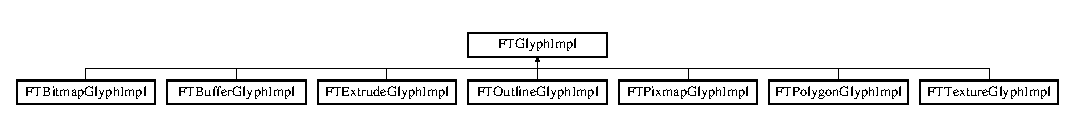
\includegraphics[height=1.176471cm]{class_f_t_glyph_impl}
\end{center}
\end{figure}
\subsection*{Protected Member Functions}
\begin{DoxyCompactItemize}
\item 
\hypertarget{class_f_t_glyph_impl_a1b4b16617fffb78e5abd3d293878872f}{{\bfseries F\-T\-Glyph\-Impl} (\hyperlink{struct_f_t___glyph_slot_rec__}{F\-T\-\_\-\-Glyph\-Slot} glyph, bool use\-Display\-List=true)}\label{class_f_t_glyph_impl_a1b4b16617fffb78e5abd3d293878872f}

\item 
\hypertarget{class_f_t_glyph_impl_a8e71d5a8e8137869ef629df6c5ba10a7}{float {\bfseries Advance} () const }\label{class_f_t_glyph_impl_a8e71d5a8e8137869ef629df6c5ba10a7}

\item 
\hypertarget{class_f_t_glyph_impl_a9780f42c30108d39be5b190cbc74d542}{const F\-T\-B\-Box \& {\bfseries B\-Box} () const }\label{class_f_t_glyph_impl_a9780f42c30108d39be5b190cbc74d542}

\item 
\hypertarget{class_f_t_glyph_impl_aca054d9ec6f56a6d96757c10ac4720f2}{F\-T\-\_\-\-Error {\bfseries Error} () const }\label{class_f_t_glyph_impl_aca054d9ec6f56a6d96757c10ac4720f2}

\end{DoxyCompactItemize}
\subsection*{Protected Attributes}
\begin{DoxyCompactItemize}
\item 
F\-T\-Point \hyperlink{class_f_t_glyph_impl_acd0a260e13ec1714c2556d24a5352a31}{advance}
\item 
F\-T\-B\-Box \hyperlink{class_f_t_glyph_impl_a871a6a1a24be465bfae17b7a8e464b3c}{b\-Box}
\item 
F\-T\-\_\-\-Error \hyperlink{class_f_t_glyph_impl_a7a489998b09aef9ceb733604166e933c}{err}
\end{DoxyCompactItemize}
\subsection*{Friends}
\begin{DoxyCompactItemize}
\item 
\hypertarget{class_f_t_glyph_impl_a908ad68576153727d761f276dd8fd0e2}{class {\bfseries F\-T\-Glyph}}\label{class_f_t_glyph_impl_a908ad68576153727d761f276dd8fd0e2}

\end{DoxyCompactItemize}


\subsection{Member Data Documentation}
\hypertarget{class_f_t_glyph_impl_acd0a260e13ec1714c2556d24a5352a31}{\index{F\-T\-Glyph\-Impl@{F\-T\-Glyph\-Impl}!advance@{advance}}
\index{advance@{advance}!FTGlyphImpl@{F\-T\-Glyph\-Impl}}
\subsubsection[{advance}]{\setlength{\rightskip}{0pt plus 5cm}F\-T\-Point F\-T\-Glyph\-Impl\-::advance\hspace{0.3cm}{\ttfamily [protected]}}}\label{class_f_t_glyph_impl_acd0a260e13ec1714c2556d24a5352a31}
The advance distance for this glyph \hypertarget{class_f_t_glyph_impl_a871a6a1a24be465bfae17b7a8e464b3c}{\index{F\-T\-Glyph\-Impl@{F\-T\-Glyph\-Impl}!b\-Box@{b\-Box}}
\index{b\-Box@{b\-Box}!FTGlyphImpl@{F\-T\-Glyph\-Impl}}
\subsubsection[{b\-Box}]{\setlength{\rightskip}{0pt plus 5cm}F\-T\-B\-Box F\-T\-Glyph\-Impl\-::b\-Box\hspace{0.3cm}{\ttfamily [protected]}}}\label{class_f_t_glyph_impl_a871a6a1a24be465bfae17b7a8e464b3c}
The bounding box of this glyph. \hypertarget{class_f_t_glyph_impl_a7a489998b09aef9ceb733604166e933c}{\index{F\-T\-Glyph\-Impl@{F\-T\-Glyph\-Impl}!err@{err}}
\index{err@{err}!FTGlyphImpl@{F\-T\-Glyph\-Impl}}
\subsubsection[{err}]{\setlength{\rightskip}{0pt plus 5cm}F\-T\-\_\-\-Error F\-T\-Glyph\-Impl\-::err\hspace{0.3cm}{\ttfamily [protected]}}}\label{class_f_t_glyph_impl_a7a489998b09aef9ceb733604166e933c}
Current error code. Zero means no error. 

The documentation for this class was generated from the following files\-:\begin{DoxyCompactItemize}
\item 
X\-:/\-Git\-\_\-\-Repository/inf2990-\/06/\-Cadriciel/\-Commun/\-Externe/\-F\-T\-G\-L/include/\-F\-T\-Glyph/F\-T\-Glyph\-Impl.\-h\item 
X\-:/\-Git\-\_\-\-Repository/inf2990-\/06/\-Cadriciel/\-Commun/\-Externe/\-F\-T\-G\-L/include/\-F\-T\-Glyph/F\-T\-Glyph.\-cpp\end{DoxyCompactItemize}

\hypertarget{class_f_t_layout_impl}{\section{F\-T\-Layout\-Impl Class Reference}
\label{class_f_t_layout_impl}\index{F\-T\-Layout\-Impl@{F\-T\-Layout\-Impl}}
}
Inheritance diagram for F\-T\-Layout\-Impl\-:\begin{figure}[H]
\begin{center}
\leavevmode
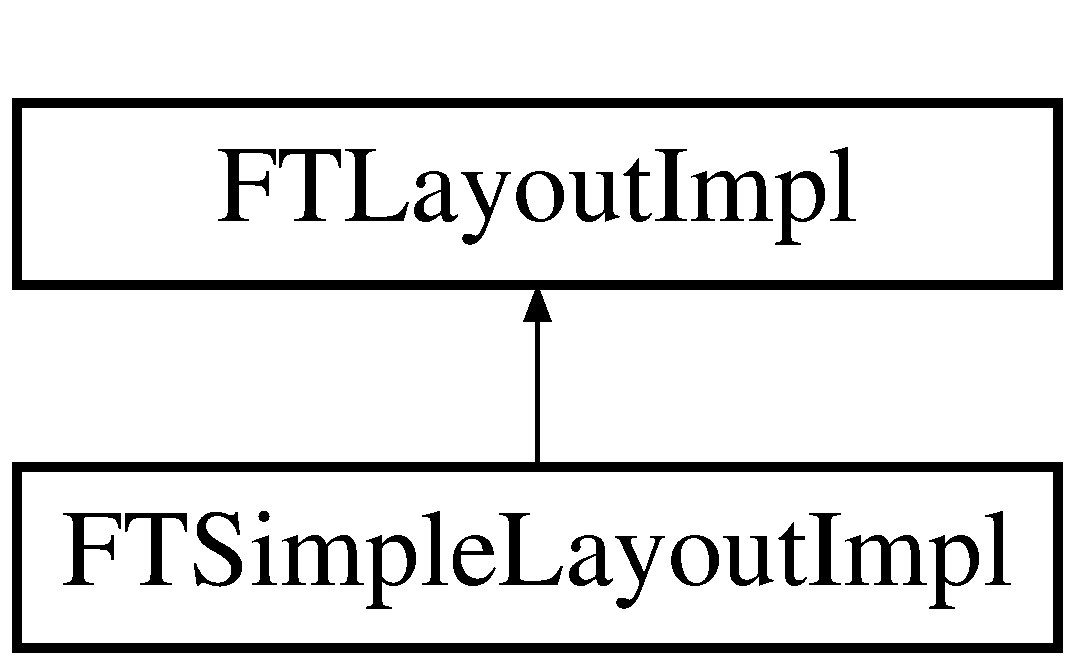
\includegraphics[height=2.000000cm]{class_f_t_layout_impl}
\end{center}
\end{figure}
\subsection*{Protected Attributes}
\begin{DoxyCompactItemize}
\item 
F\-T\-Point \hyperlink{class_f_t_layout_impl_aefaff875c0cf4fe5710897f614be44ac}{pen}
\item 
F\-T\-\_\-\-Error \hyperlink{class_f_t_layout_impl_af3c9ad6d6636a69a6643d68383e4edcd}{err}
\end{DoxyCompactItemize}
\subsection*{Friends}
\begin{DoxyCompactItemize}
\item 
\hypertarget{class_f_t_layout_impl_a28e6cd087379e90923b29b9c2c103aa8}{class {\bfseries F\-T\-Layout}}\label{class_f_t_layout_impl_a28e6cd087379e90923b29b9c2c103aa8}

\end{DoxyCompactItemize}


\subsection{Member Data Documentation}
\hypertarget{class_f_t_layout_impl_af3c9ad6d6636a69a6643d68383e4edcd}{\index{F\-T\-Layout\-Impl@{F\-T\-Layout\-Impl}!err@{err}}
\index{err@{err}!FTLayoutImpl@{F\-T\-Layout\-Impl}}
\subsubsection[{err}]{\setlength{\rightskip}{0pt plus 5cm}F\-T\-\_\-\-Error F\-T\-Layout\-Impl\-::err\hspace{0.3cm}{\ttfamily [protected]}}}\label{class_f_t_layout_impl_af3c9ad6d6636a69a6643d68383e4edcd}
Current error code. Zero means no error. \hypertarget{class_f_t_layout_impl_aefaff875c0cf4fe5710897f614be44ac}{\index{F\-T\-Layout\-Impl@{F\-T\-Layout\-Impl}!pen@{pen}}
\index{pen@{pen}!FTLayoutImpl@{F\-T\-Layout\-Impl}}
\subsubsection[{pen}]{\setlength{\rightskip}{0pt plus 5cm}F\-T\-Point F\-T\-Layout\-Impl\-::pen\hspace{0.3cm}{\ttfamily [protected]}}}\label{class_f_t_layout_impl_aefaff875c0cf4fe5710897f614be44ac}
Current pen or cursor position; 

The documentation for this class was generated from the following files\-:\begin{DoxyCompactItemize}
\item 
X\-:/\-Git\-\_\-\-Repository/inf2990-\/06/\-Cadriciel/\-Commun/\-Externe/\-F\-T\-G\-L/include/\-F\-T\-Layout/F\-T\-Layout\-Impl.\-h\item 
X\-:/\-Git\-\_\-\-Repository/inf2990-\/06/\-Cadriciel/\-Commun/\-Externe/\-F\-T\-G\-L/include/\-F\-T\-Layout/F\-T\-Layout.\-cpp\end{DoxyCompactItemize}

\hypertarget{class_f_t_library}{\section{F\-T\-Library Class Reference}
\label{class_f_t_library}\index{F\-T\-Library@{F\-T\-Library}}
}


{\ttfamily \#include $<$F\-T\-Library.\-h$>$}

\subsection*{Public Member Functions}
\begin{DoxyCompactItemize}
\item 
const \hyperlink{struct_f_t___library_rec__}{F\-T\-\_\-\-Library} $\ast$const \hyperlink{class_f_t_library_afef4db019eae5a4307201b7abc6a88c7}{Get\-Library} () const 
\item 
F\-T\-\_\-\-Error \hyperlink{class_f_t_library_ad01e538ba8e308dddda5c4ec808ee404}{Error} () const 
\item 
\hyperlink{class_f_t_library_a8d1ee3dc3c4916b5b428e934dc46e9d7}{$\sim$\-F\-T\-Library} ()
\end{DoxyCompactItemize}
\subsection*{Static Public Member Functions}
\begin{DoxyCompactItemize}
\item 
static const \hyperlink{class_f_t_library}{F\-T\-Library} \& \hyperlink{class_f_t_library_aa172665a8db8888851895bcb15aa8103}{Instance} ()
\end{DoxyCompactItemize}


\subsection{Detailed Description}
\hyperlink{class_f_t_library}{F\-T\-Library} class is the global accessor for the Freetype library.

This class encapsulates the Freetype Library. This is a singleton class and ensures that only one F\-T\-\_\-\-Library is in existence at any one time. All constructors are private therefore clients cannot create or instantiate this class themselves and must access it's methods via the static {\ttfamily \hyperlink{class_f_t_library_aa172665a8db8888851895bcb15aa8103}{F\-T\-Library\-::\-Instance()}} function.

Just because this class returns a valid {\ttfamily \hyperlink{class_f_t_library}{F\-T\-Library}} object doesn't mean that the Freetype Library has been successfully initialised. Clients should check for errors. You can initialse the library A\-N\-D check for errors using the following code... {\ttfamily err = \hyperlink{class_f_t_library_aa172665a8db8888851895bcb15aa8103}{F\-T\-Library\-::\-Instance()}.\hyperlink{class_f_t_library_ad01e538ba8e308dddda5c4ec808ee404}{Error()};}

\begin{DoxySeeAlso}{See Also}
\char`\"{}\-Freetype 2 Documentation\char`\"{} 
\end{DoxySeeAlso}


\subsection{Constructor \& Destructor Documentation}
\hypertarget{class_f_t_library_a8d1ee3dc3c4916b5b428e934dc46e9d7}{\index{F\-T\-Library@{F\-T\-Library}!$\sim$\-F\-T\-Library@{$\sim$\-F\-T\-Library}}
\index{$\sim$\-F\-T\-Library@{$\sim$\-F\-T\-Library}!FTLibrary@{F\-T\-Library}}
\subsubsection[{$\sim$\-F\-T\-Library}]{\setlength{\rightskip}{0pt plus 5cm}F\-T\-Library\-::$\sim$\-F\-T\-Library (
\begin{DoxyParamCaption}
{}
\end{DoxyParamCaption}
)}}\label{class_f_t_library_a8d1ee3dc3c4916b5b428e934dc46e9d7}
Destructor

Disposes of the Freetype library 

\subsection{Member Function Documentation}
\hypertarget{class_f_t_library_ad01e538ba8e308dddda5c4ec808ee404}{\index{F\-T\-Library@{F\-T\-Library}!Error@{Error}}
\index{Error@{Error}!FTLibrary@{F\-T\-Library}}
\subsubsection[{Error}]{\setlength{\rightskip}{0pt plus 5cm}F\-T\-\_\-\-Error F\-T\-Library\-::\-Error (
\begin{DoxyParamCaption}
{}
\end{DoxyParamCaption}
) const\hspace{0.3cm}{\ttfamily [inline]}}}\label{class_f_t_library_ad01e538ba8e308dddda5c4ec808ee404}
Queries the library for errors.

\begin{DoxyReturn}{Returns}
The current error code. 
\end{DoxyReturn}
\hypertarget{class_f_t_library_afef4db019eae5a4307201b7abc6a88c7}{\index{F\-T\-Library@{F\-T\-Library}!Get\-Library@{Get\-Library}}
\index{Get\-Library@{Get\-Library}!FTLibrary@{F\-T\-Library}}
\subsubsection[{Get\-Library}]{\setlength{\rightskip}{0pt plus 5cm}const {\bf F\-T\-\_\-\-Library}$\ast$ const F\-T\-Library\-::\-Get\-Library (
\begin{DoxyParamCaption}
{}
\end{DoxyParamCaption}
) const\hspace{0.3cm}{\ttfamily [inline]}}}\label{class_f_t_library_afef4db019eae5a4307201b7abc6a88c7}
Gets a pointer to the native Freetype library.

\begin{DoxyReturn}{Returns}
A handle to a Free\-Type library instance. 
\end{DoxyReturn}
\hypertarget{class_f_t_library_aa172665a8db8888851895bcb15aa8103}{\index{F\-T\-Library@{F\-T\-Library}!Instance@{Instance}}
\index{Instance@{Instance}!FTLibrary@{F\-T\-Library}}
\subsubsection[{Instance}]{\setlength{\rightskip}{0pt plus 5cm}const {\bf F\-T\-Library} \& F\-T\-Library\-::\-Instance (
\begin{DoxyParamCaption}
{}
\end{DoxyParamCaption}
)\hspace{0.3cm}{\ttfamily [static]}}}\label{class_f_t_library_aa172665a8db8888851895bcb15aa8103}
Global acces point to the single \hyperlink{class_f_t_library}{F\-T\-Library} object.

\begin{DoxyReturn}{Returns}
The global {\ttfamily \hyperlink{class_f_t_library}{F\-T\-Library}} object. 
\end{DoxyReturn}


The documentation for this class was generated from the following files\-:\begin{DoxyCompactItemize}
\item 
X\-:/\-Git\-\_\-\-Repository/inf2990-\/06/\-Cadriciel/\-Commun/\-Externe/\-F\-T\-G\-L/include/F\-T\-Library.\-h\item 
X\-:/\-Git\-\_\-\-Repository/inf2990-\/06/\-Cadriciel/\-Commun/\-Externe/\-F\-T\-G\-L/include/F\-T\-Library.\-cpp\end{DoxyCompactItemize}

\hypertarget{class_f_t_list}{\section{F\-T\-List$<$ F\-T\-\_\-\-L\-I\-S\-T\-\_\-\-I\-T\-E\-M\-\_\-\-T\-Y\-P\-E $>$ Class Template Reference}
\label{class_f_t_list}\index{F\-T\-List$<$ F\-T\-\_\-\-L\-I\-S\-T\-\_\-\-I\-T\-E\-M\-\_\-\-T\-Y\-P\-E $>$@{F\-T\-List$<$ F\-T\-\_\-\-L\-I\-S\-T\-\_\-\-I\-T\-E\-M\-\_\-\-T\-Y\-P\-E $>$}}
}


{\ttfamily \#include $<$F\-T\-List.\-h$>$}

\subsection*{Public Types}
\begin{DoxyCompactItemize}
\item 
\hypertarget{class_f_t_list_ae172da3e03bcd6dab4b5f60efe0fc7a3}{typedef F\-T\-\_\-\-L\-I\-S\-T\-\_\-\-I\-T\-E\-M\-\_\-\-T\-Y\-P\-E {\bfseries value\-\_\-type}}\label{class_f_t_list_ae172da3e03bcd6dab4b5f60efe0fc7a3}

\item 
\hypertarget{class_f_t_list_a37fe33040a67a2d5aad9ead2bb2179d7}{typedef value\-\_\-type \& {\bfseries reference}}\label{class_f_t_list_a37fe33040a67a2d5aad9ead2bb2179d7}

\item 
\hypertarget{class_f_t_list_a82677d676935b1f3cb5e9328523bf3a6}{typedef const value\-\_\-type \& {\bfseries const\-\_\-reference}}\label{class_f_t_list_a82677d676935b1f3cb5e9328523bf3a6}

\item 
\hypertarget{class_f_t_list_a5ebe9866c4f86791c6970f19deb09cb1}{typedef size\-\_\-t {\bfseries size\-\_\-type}}\label{class_f_t_list_a5ebe9866c4f86791c6970f19deb09cb1}

\end{DoxyCompactItemize}
\subsection*{Public Member Functions}
\begin{DoxyCompactItemize}
\item 
\hyperlink{class_f_t_list_a4de727811240b9d8568d1d47fd389502}{F\-T\-List} ()
\item 
\hyperlink{class_f_t_list_aabfac3b136119f727611d490aef3eab4}{$\sim$\-F\-T\-List} ()
\item 
size\-\_\-type \hyperlink{class_f_t_list_a73542705ba9556d5cd594c3ec32fe5d2}{size} () const 
\item 
void \hyperlink{class_f_t_list_acd30af5d1a32185842decac3e0c183ce}{push\-\_\-back} (const value\-\_\-type \&item)
\item 
reference \hyperlink{class_f_t_list_a068805ebb222e9ce69a8828b31fd87df}{front} () const 
\item 
reference \hyperlink{class_f_t_list_ae6b5f56991e9d2ac226ce7960e4661f4}{back} () const 
\end{DoxyCompactItemize}


\subsection{Detailed Description}
\subsubsection*{template$<$typename F\-T\-\_\-\-L\-I\-S\-T\-\_\-\-I\-T\-E\-M\-\_\-\-T\-Y\-P\-E$>$class F\-T\-List$<$ F\-T\-\_\-\-L\-I\-S\-T\-\_\-\-I\-T\-E\-M\-\_\-\-T\-Y\-P\-E $>$}

Provides a non-\/\-S\-T\-L alternative to the S\-T\-L list 

\subsection{Constructor \& Destructor Documentation}
\hypertarget{class_f_t_list_a4de727811240b9d8568d1d47fd389502}{\index{F\-T\-List@{F\-T\-List}!F\-T\-List@{F\-T\-List}}
\index{F\-T\-List@{F\-T\-List}!FTList@{F\-T\-List}}
\subsubsection[{F\-T\-List}]{\setlength{\rightskip}{0pt plus 5cm}template$<$typename F\-T\-\_\-\-L\-I\-S\-T\-\_\-\-I\-T\-E\-M\-\_\-\-T\-Y\-P\-E$>$ {\bf F\-T\-List}$<$ F\-T\-\_\-\-L\-I\-S\-T\-\_\-\-I\-T\-E\-M\-\_\-\-T\-Y\-P\-E $>$\-::{\bf F\-T\-List} (
\begin{DoxyParamCaption}
{}
\end{DoxyParamCaption}
)\hspace{0.3cm}{\ttfamily [inline]}}}\label{class_f_t_list_a4de727811240b9d8568d1d47fd389502}
Constructor \hypertarget{class_f_t_list_aabfac3b136119f727611d490aef3eab4}{\index{F\-T\-List@{F\-T\-List}!$\sim$\-F\-T\-List@{$\sim$\-F\-T\-List}}
\index{$\sim$\-F\-T\-List@{$\sim$\-F\-T\-List}!FTList@{F\-T\-List}}
\subsubsection[{$\sim$\-F\-T\-List}]{\setlength{\rightskip}{0pt plus 5cm}template$<$typename F\-T\-\_\-\-L\-I\-S\-T\-\_\-\-I\-T\-E\-M\-\_\-\-T\-Y\-P\-E$>$ {\bf F\-T\-List}$<$ F\-T\-\_\-\-L\-I\-S\-T\-\_\-\-I\-T\-E\-M\-\_\-\-T\-Y\-P\-E $>$\-::$\sim${\bf F\-T\-List} (
\begin{DoxyParamCaption}
{}
\end{DoxyParamCaption}
)\hspace{0.3cm}{\ttfamily [inline]}}}\label{class_f_t_list_aabfac3b136119f727611d490aef3eab4}
Destructor 

\subsection{Member Function Documentation}
\hypertarget{class_f_t_list_ae6b5f56991e9d2ac226ce7960e4661f4}{\index{F\-T\-List@{F\-T\-List}!back@{back}}
\index{back@{back}!FTList@{F\-T\-List}}
\subsubsection[{back}]{\setlength{\rightskip}{0pt plus 5cm}template$<$typename F\-T\-\_\-\-L\-I\-S\-T\-\_\-\-I\-T\-E\-M\-\_\-\-T\-Y\-P\-E$>$ reference {\bf F\-T\-List}$<$ F\-T\-\_\-\-L\-I\-S\-T\-\_\-\-I\-T\-E\-M\-\_\-\-T\-Y\-P\-E $>$\-::back (
\begin{DoxyParamCaption}
{}
\end{DoxyParamCaption}
) const\hspace{0.3cm}{\ttfamily [inline]}}}\label{class_f_t_list_ae6b5f56991e9d2ac226ce7960e4661f4}
Get the item at the end of the list \hypertarget{class_f_t_list_a068805ebb222e9ce69a8828b31fd87df}{\index{F\-T\-List@{F\-T\-List}!front@{front}}
\index{front@{front}!FTList@{F\-T\-List}}
\subsubsection[{front}]{\setlength{\rightskip}{0pt plus 5cm}template$<$typename F\-T\-\_\-\-L\-I\-S\-T\-\_\-\-I\-T\-E\-M\-\_\-\-T\-Y\-P\-E$>$ reference {\bf F\-T\-List}$<$ F\-T\-\_\-\-L\-I\-S\-T\-\_\-\-I\-T\-E\-M\-\_\-\-T\-Y\-P\-E $>$\-::front (
\begin{DoxyParamCaption}
{}
\end{DoxyParamCaption}
) const\hspace{0.3cm}{\ttfamily [inline]}}}\label{class_f_t_list_a068805ebb222e9ce69a8828b31fd87df}
Get the item at the front of the list \hypertarget{class_f_t_list_acd30af5d1a32185842decac3e0c183ce}{\index{F\-T\-List@{F\-T\-List}!push\-\_\-back@{push\-\_\-back}}
\index{push\-\_\-back@{push\-\_\-back}!FTList@{F\-T\-List}}
\subsubsection[{push\-\_\-back}]{\setlength{\rightskip}{0pt plus 5cm}template$<$typename F\-T\-\_\-\-L\-I\-S\-T\-\_\-\-I\-T\-E\-M\-\_\-\-T\-Y\-P\-E$>$ void {\bf F\-T\-List}$<$ F\-T\-\_\-\-L\-I\-S\-T\-\_\-\-I\-T\-E\-M\-\_\-\-T\-Y\-P\-E $>$\-::push\-\_\-back (
\begin{DoxyParamCaption}
\item[{const value\-\_\-type \&}]{item}
\end{DoxyParamCaption}
)\hspace{0.3cm}{\ttfamily [inline]}}}\label{class_f_t_list_acd30af5d1a32185842decac3e0c183ce}
Add an item to the end of the list \hypertarget{class_f_t_list_a73542705ba9556d5cd594c3ec32fe5d2}{\index{F\-T\-List@{F\-T\-List}!size@{size}}
\index{size@{size}!FTList@{F\-T\-List}}
\subsubsection[{size}]{\setlength{\rightskip}{0pt plus 5cm}template$<$typename F\-T\-\_\-\-L\-I\-S\-T\-\_\-\-I\-T\-E\-M\-\_\-\-T\-Y\-P\-E$>$ size\-\_\-type {\bf F\-T\-List}$<$ F\-T\-\_\-\-L\-I\-S\-T\-\_\-\-I\-T\-E\-M\-\_\-\-T\-Y\-P\-E $>$\-::size (
\begin{DoxyParamCaption}
{}
\end{DoxyParamCaption}
) const\hspace{0.3cm}{\ttfamily [inline]}}}\label{class_f_t_list_a73542705ba9556d5cd594c3ec32fe5d2}
Get the number of items in the list 

The documentation for this class was generated from the following file\-:\begin{DoxyCompactItemize}
\item 
X\-:/\-Git\-\_\-\-Repository/inf2990-\/06/\-Cadriciel/\-Commun/\-Externe/\-F\-T\-G\-L/include/F\-T\-List.\-h\end{DoxyCompactItemize}

\hypertarget{class_f_t_mesh}{\section{F\-T\-Mesh Class Reference}
\label{class_f_t_mesh}\index{F\-T\-Mesh@{F\-T\-Mesh}}
}


{\ttfamily \#include $<$F\-T\-Vectoriser.\-h$>$}

\subsection*{Public Member Functions}
\begin{DoxyCompactItemize}
\item 
\hyperlink{class_f_t_mesh_aa78f98bec8f9cd15d0255c326b7cf62d}{F\-T\-Mesh} ()
\item 
\hyperlink{class_f_t_mesh_a7282fec857e649bf91c91b2957f292ac}{$\sim$\-F\-T\-Mesh} ()
\item 
void \hyperlink{class_f_t_mesh_a4a503faa60d78f67cd487611b0f44b68}{Add\-Point} (const F\-T\-G\-L\-\_\-\-D\-O\-U\-B\-L\-E x, const F\-T\-G\-L\-\_\-\-D\-O\-U\-B\-L\-E y, const F\-T\-G\-L\-\_\-\-D\-O\-U\-B\-L\-E z)
\item 
const F\-T\-G\-L\-\_\-\-D\-O\-U\-B\-L\-E $\ast$ \hyperlink{class_f_t_mesh_a41c229d00a0edd342fff2577c7024dae}{Combine} (const F\-T\-G\-L\-\_\-\-D\-O\-U\-B\-L\-E x, const F\-T\-G\-L\-\_\-\-D\-O\-U\-B\-L\-E y, const F\-T\-G\-L\-\_\-\-D\-O\-U\-B\-L\-E z)
\item 
void \hyperlink{class_f_t_mesh_a03ddbeb4313ce4353c477d0afcdc4a1e}{Begin} (G\-Lenum mesh\-Type)
\item 
void \hyperlink{class_f_t_mesh_a1ead56fbe963c5976ea3c268b8b0544d}{End} ()
\item 
void \hyperlink{class_f_t_mesh_a2e07adc55441296e88b6886c153c50fd}{Error} (G\-Lenum e)
\item 
size\-\_\-t \hyperlink{class_f_t_mesh_a21075ff9bd0534574aede7f72fd33281}{Tesselation\-Count} () const 
\item 
const \hyperlink{class_f_t_tesselation}{F\-T\-Tesselation} $\ast$const \hyperlink{class_f_t_mesh_a5d8f540f3f6497209b91b53a3daa4190}{Tesselation} (size\-\_\-t index) const 
\item 
const \hyperlink{class_f_t_list}{Point\-List} \& \hyperlink{class_f_t_mesh_ac75f054b4e430c12d1f098070713acbb}{Temp\-Point\-List} () const 
\item 
G\-Lenum \hyperlink{class_f_t_mesh_ac706276fad2215121ffb1fdf1acffa8f}{Error} () const 
\end{DoxyCompactItemize}


\subsection{Detailed Description}
\hyperlink{class_f_t_mesh}{F\-T\-Mesh} is a container of \hyperlink{class_f_t_tesselation}{F\-T\-Tesselation}'s that make up a polygon glyph 

\subsection{Constructor \& Destructor Documentation}
\hypertarget{class_f_t_mesh_aa78f98bec8f9cd15d0255c326b7cf62d}{\index{F\-T\-Mesh@{F\-T\-Mesh}!F\-T\-Mesh@{F\-T\-Mesh}}
\index{F\-T\-Mesh@{F\-T\-Mesh}!FTMesh@{F\-T\-Mesh}}
\subsubsection[{F\-T\-Mesh}]{\setlength{\rightskip}{0pt plus 5cm}F\-T\-Mesh\-::\-F\-T\-Mesh (
\begin{DoxyParamCaption}
{}
\end{DoxyParamCaption}
)}}\label{class_f_t_mesh_aa78f98bec8f9cd15d0255c326b7cf62d}
Default constructor \hypertarget{class_f_t_mesh_a7282fec857e649bf91c91b2957f292ac}{\index{F\-T\-Mesh@{F\-T\-Mesh}!$\sim$\-F\-T\-Mesh@{$\sim$\-F\-T\-Mesh}}
\index{$\sim$\-F\-T\-Mesh@{$\sim$\-F\-T\-Mesh}!FTMesh@{F\-T\-Mesh}}
\subsubsection[{$\sim$\-F\-T\-Mesh}]{\setlength{\rightskip}{0pt plus 5cm}F\-T\-Mesh\-::$\sim$\-F\-T\-Mesh (
\begin{DoxyParamCaption}
{}
\end{DoxyParamCaption}
)}}\label{class_f_t_mesh_a7282fec857e649bf91c91b2957f292ac}
Destructor 

\subsection{Member Function Documentation}
\hypertarget{class_f_t_mesh_a4a503faa60d78f67cd487611b0f44b68}{\index{F\-T\-Mesh@{F\-T\-Mesh}!Add\-Point@{Add\-Point}}
\index{Add\-Point@{Add\-Point}!FTMesh@{F\-T\-Mesh}}
\subsubsection[{Add\-Point}]{\setlength{\rightskip}{0pt plus 5cm}void F\-T\-Mesh\-::\-Add\-Point (
\begin{DoxyParamCaption}
\item[{const F\-T\-G\-L\-\_\-\-D\-O\-U\-B\-L\-E}]{x, }
\item[{const F\-T\-G\-L\-\_\-\-D\-O\-U\-B\-L\-E}]{y, }
\item[{const F\-T\-G\-L\-\_\-\-D\-O\-U\-B\-L\-E}]{z}
\end{DoxyParamCaption}
)}}\label{class_f_t_mesh_a4a503faa60d78f67cd487611b0f44b68}
Add a point to the mesh \hypertarget{class_f_t_mesh_a03ddbeb4313ce4353c477d0afcdc4a1e}{\index{F\-T\-Mesh@{F\-T\-Mesh}!Begin@{Begin}}
\index{Begin@{Begin}!FTMesh@{F\-T\-Mesh}}
\subsubsection[{Begin}]{\setlength{\rightskip}{0pt plus 5cm}void F\-T\-Mesh\-::\-Begin (
\begin{DoxyParamCaption}
\item[{G\-Lenum}]{mesh\-Type}
\end{DoxyParamCaption}
)}}\label{class_f_t_mesh_a03ddbeb4313ce4353c477d0afcdc4a1e}
Begin a new polygon \hypertarget{class_f_t_mesh_a41c229d00a0edd342fff2577c7024dae}{\index{F\-T\-Mesh@{F\-T\-Mesh}!Combine@{Combine}}
\index{Combine@{Combine}!FTMesh@{F\-T\-Mesh}}
\subsubsection[{Combine}]{\setlength{\rightskip}{0pt plus 5cm}const F\-T\-G\-L\-\_\-\-D\-O\-U\-B\-L\-E $\ast$ F\-T\-Mesh\-::\-Combine (
\begin{DoxyParamCaption}
\item[{const F\-T\-G\-L\-\_\-\-D\-O\-U\-B\-L\-E}]{x, }
\item[{const F\-T\-G\-L\-\_\-\-D\-O\-U\-B\-L\-E}]{y, }
\item[{const F\-T\-G\-L\-\_\-\-D\-O\-U\-B\-L\-E}]{z}
\end{DoxyParamCaption}
)}}\label{class_f_t_mesh_a41c229d00a0edd342fff2577c7024dae}
Create a combine point for the glu\-Tesselator \hypertarget{class_f_t_mesh_a1ead56fbe963c5976ea3c268b8b0544d}{\index{F\-T\-Mesh@{F\-T\-Mesh}!End@{End}}
\index{End@{End}!FTMesh@{F\-T\-Mesh}}
\subsubsection[{End}]{\setlength{\rightskip}{0pt plus 5cm}void F\-T\-Mesh\-::\-End (
\begin{DoxyParamCaption}
{}
\end{DoxyParamCaption}
)}}\label{class_f_t_mesh_a1ead56fbe963c5976ea3c268b8b0544d}
End a polygon \hypertarget{class_f_t_mesh_a2e07adc55441296e88b6886c153c50fd}{\index{F\-T\-Mesh@{F\-T\-Mesh}!Error@{Error}}
\index{Error@{Error}!FTMesh@{F\-T\-Mesh}}
\subsubsection[{Error}]{\setlength{\rightskip}{0pt plus 5cm}void F\-T\-Mesh\-::\-Error (
\begin{DoxyParamCaption}
\item[{G\-Lenum}]{e}
\end{DoxyParamCaption}
)\hspace{0.3cm}{\ttfamily [inline]}}}\label{class_f_t_mesh_a2e07adc55441296e88b6886c153c50fd}
Record a glu\-Tesselation error \hypertarget{class_f_t_mesh_ac706276fad2215121ffb1fdf1acffa8f}{\index{F\-T\-Mesh@{F\-T\-Mesh}!Error@{Error}}
\index{Error@{Error}!FTMesh@{F\-T\-Mesh}}
\subsubsection[{Error}]{\setlength{\rightskip}{0pt plus 5cm}G\-Lenum F\-T\-Mesh\-::\-Error (
\begin{DoxyParamCaption}
{}
\end{DoxyParamCaption}
) const\hspace{0.3cm}{\ttfamily [inline]}}}\label{class_f_t_mesh_ac706276fad2215121ffb1fdf1acffa8f}
Get the G\-L E\-R\-R\-O\-R returned by the glu tesselator \hypertarget{class_f_t_mesh_ac75f054b4e430c12d1f098070713acbb}{\index{F\-T\-Mesh@{F\-T\-Mesh}!Temp\-Point\-List@{Temp\-Point\-List}}
\index{Temp\-Point\-List@{Temp\-Point\-List}!FTMesh@{F\-T\-Mesh}}
\subsubsection[{Temp\-Point\-List}]{\setlength{\rightskip}{0pt plus 5cm}const {\bf Point\-List}\& F\-T\-Mesh\-::\-Temp\-Point\-List (
\begin{DoxyParamCaption}
{}
\end{DoxyParamCaption}
) const\hspace{0.3cm}{\ttfamily [inline]}}}\label{class_f_t_mesh_ac75f054b4e430c12d1f098070713acbb}
Return the temporary point list. For testing only. \hypertarget{class_f_t_mesh_a5d8f540f3f6497209b91b53a3daa4190}{\index{F\-T\-Mesh@{F\-T\-Mesh}!Tesselation@{Tesselation}}
\index{Tesselation@{Tesselation}!FTMesh@{F\-T\-Mesh}}
\subsubsection[{Tesselation}]{\setlength{\rightskip}{0pt plus 5cm}const {\bf F\-T\-Tesselation} $\ast$const F\-T\-Mesh\-::\-Tesselation (
\begin{DoxyParamCaption}
\item[{size\-\_\-t}]{index}
\end{DoxyParamCaption}
) const}}\label{class_f_t_mesh_a5d8f540f3f6497209b91b53a3daa4190}
Get a tesselation by index \hypertarget{class_f_t_mesh_a21075ff9bd0534574aede7f72fd33281}{\index{F\-T\-Mesh@{F\-T\-Mesh}!Tesselation\-Count@{Tesselation\-Count}}
\index{Tesselation\-Count@{Tesselation\-Count}!FTMesh@{F\-T\-Mesh}}
\subsubsection[{Tesselation\-Count}]{\setlength{\rightskip}{0pt plus 5cm}size\-\_\-t F\-T\-Mesh\-::\-Tesselation\-Count (
\begin{DoxyParamCaption}
{}
\end{DoxyParamCaption}
) const\hspace{0.3cm}{\ttfamily [inline]}}}\label{class_f_t_mesh_a21075ff9bd0534574aede7f72fd33281}
The number of tesselations in the mesh 

The documentation for this class was generated from the following files\-:\begin{DoxyCompactItemize}
\item 
X\-:/\-Git\-\_\-\-Repository/inf2990-\/06/\-Cadriciel/\-Commun/\-Externe/\-F\-T\-G\-L/include/F\-T\-Vectoriser.\-h\item 
X\-:/\-Git\-\_\-\-Repository/inf2990-\/06/\-Cadriciel/\-Commun/\-Externe/\-F\-T\-G\-L/include/F\-T\-Vectoriser.\-cpp\end{DoxyCompactItemize}

\hypertarget{class_f_t_outline_font_impl}{\section{F\-T\-Outline\-Font\-Impl Class Reference}
\label{class_f_t_outline_font_impl}\index{F\-T\-Outline\-Font\-Impl@{F\-T\-Outline\-Font\-Impl}}
}
Inheritance diagram for F\-T\-Outline\-Font\-Impl\-:\begin{figure}[H]
\begin{center}
\leavevmode
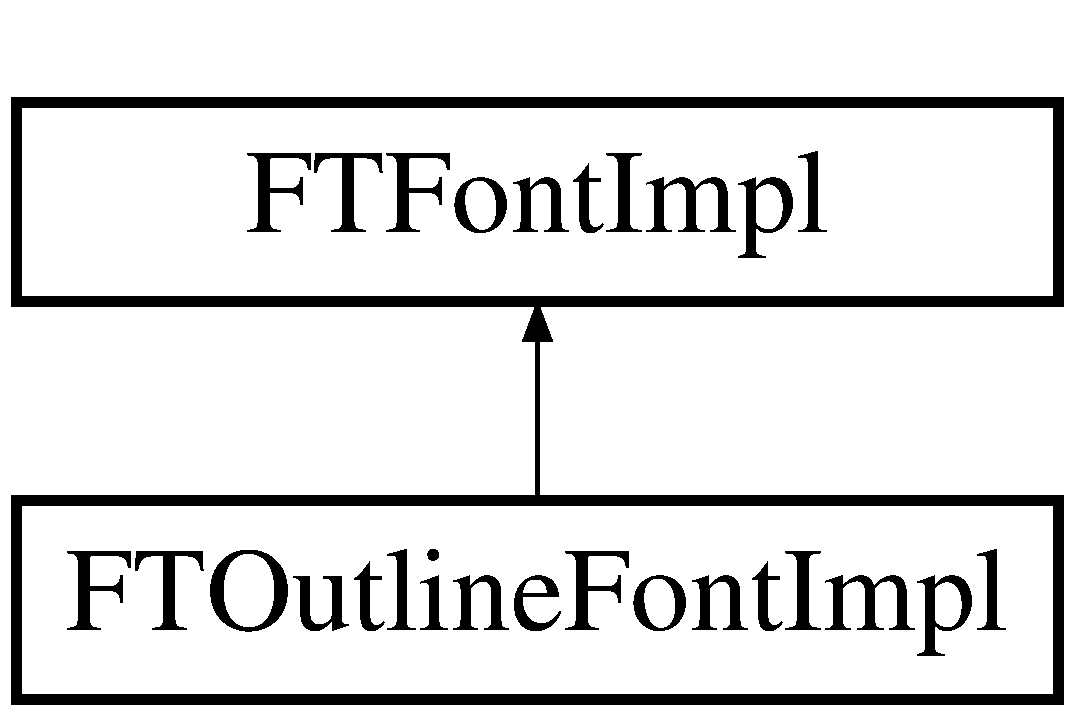
\includegraphics[height=2.000000cm]{class_f_t_outline_font_impl}
\end{center}
\end{figure}
\subsection*{Protected Member Functions}
\begin{DoxyCompactItemize}
\item 
\hypertarget{class_f_t_outline_font_impl_a01af1e37c082fce3f483361b455f9ac2}{{\bfseries F\-T\-Outline\-Font\-Impl} (F\-T\-Font $\ast$ft\-Font, const char $\ast$font\-File\-Path)}\label{class_f_t_outline_font_impl_a01af1e37c082fce3f483361b455f9ac2}

\item 
\hypertarget{class_f_t_outline_font_impl_a3b0befb0c886bbc7cb8873afbfc0a9db}{{\bfseries F\-T\-Outline\-Font\-Impl} (F\-T\-Font $\ast$ft\-Font, const unsigned char $\ast$p\-Buffer\-Bytes, size\-\_\-t buffer\-Size\-In\-Bytes)}\label{class_f_t_outline_font_impl_a3b0befb0c886bbc7cb8873afbfc0a9db}

\item 
virtual void \hyperlink{class_f_t_outline_font_impl_a22cb75a9c717403f399906d24d4aac82}{Outset} (float o)
\item 
\hypertarget{class_f_t_outline_font_impl_a10caae0ba62ba4c7d5a8742114517651}{virtual F\-T\-Point {\bfseries Render} (const char $\ast$s, const int len, F\-T\-Point position, F\-T\-Point spacing, int render\-Mode)}\label{class_f_t_outline_font_impl_a10caae0ba62ba4c7d5a8742114517651}

\item 
\hypertarget{class_f_t_outline_font_impl_aa4957e338292c7202df9bfb1362e4084}{virtual F\-T\-Point {\bfseries Render} (const wchar\-\_\-t $\ast$s, const int len, F\-T\-Point position, F\-T\-Point spacing, int render\-Mode)}\label{class_f_t_outline_font_impl_aa4957e338292c7202df9bfb1362e4084}

\end{DoxyCompactItemize}
\subsection*{Friends}
\begin{DoxyCompactItemize}
\item 
\hypertarget{class_f_t_outline_font_impl_a17f6eed308c6d1116a7f1d86010f6c9e}{class {\bfseries F\-T\-Outline\-Font}}\label{class_f_t_outline_font_impl_a17f6eed308c6d1116a7f1d86010f6c9e}

\end{DoxyCompactItemize}
\subsection*{Additional Inherited Members}


\subsection{Member Function Documentation}
\hypertarget{class_f_t_outline_font_impl_a22cb75a9c717403f399906d24d4aac82}{\index{F\-T\-Outline\-Font\-Impl@{F\-T\-Outline\-Font\-Impl}!Outset@{Outset}}
\index{Outset@{Outset}!FTOutlineFontImpl@{F\-T\-Outline\-Font\-Impl}}
\subsubsection[{Outset}]{\setlength{\rightskip}{0pt plus 5cm}virtual void F\-T\-Outline\-Font\-Impl\-::\-Outset (
\begin{DoxyParamCaption}
\item[{float}]{o}
\end{DoxyParamCaption}
)\hspace{0.3cm}{\ttfamily [inline]}, {\ttfamily [protected]}, {\ttfamily [virtual]}}}\label{class_f_t_outline_font_impl_a22cb75a9c717403f399906d24d4aac82}
Set the outset distance for the font. Only implemented by F\-T\-Outline\-Font, F\-T\-Polygon\-Font and F\-T\-Extrude\-Font


\begin{DoxyParams}{Parameters}
{\em outset} & The outset distance. \\
\hline
\end{DoxyParams}


Reimplemented from \hyperlink{class_f_t_font_impl}{F\-T\-Font\-Impl}.



The documentation for this class was generated from the following files\-:\begin{DoxyCompactItemize}
\item 
X\-:/\-Git\-\_\-\-Repository/inf2990-\/06/\-Cadriciel/\-Commun/\-Externe/\-F\-T\-G\-L/include/\-F\-T\-Font/F\-T\-Outline\-Font\-Impl.\-h\item 
X\-:/\-Git\-\_\-\-Repository/inf2990-\/06/\-Cadriciel/\-Commun/\-Externe/\-F\-T\-G\-L/include/\-F\-T\-Font/F\-T\-Outline\-Font.\-cpp\end{DoxyCompactItemize}

\hypertarget{class_f_t_outline_glyph_impl}{\section{F\-T\-Outline\-Glyph\-Impl Class Reference}
\label{class_f_t_outline_glyph_impl}\index{F\-T\-Outline\-Glyph\-Impl@{F\-T\-Outline\-Glyph\-Impl}}
}
Inheritance diagram for F\-T\-Outline\-Glyph\-Impl\-:\begin{figure}[H]
\begin{center}
\leavevmode
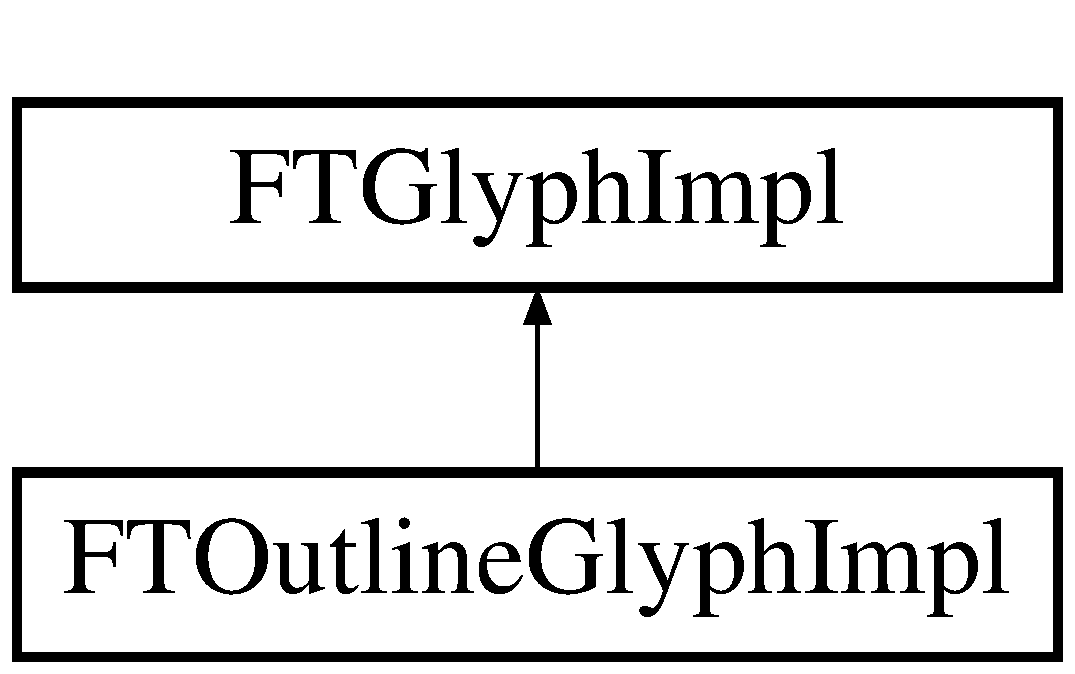
\includegraphics[height=2.000000cm]{class_f_t_outline_glyph_impl}
\end{center}
\end{figure}
\subsection*{Protected Member Functions}
\begin{DoxyCompactItemize}
\item 
\hypertarget{class_f_t_outline_glyph_impl_a0eac191ec3db6c8dbbf6956ded4342fa}{{\bfseries F\-T\-Outline\-Glyph\-Impl} (\hyperlink{struct_f_t___glyph_slot_rec__}{F\-T\-\_\-\-Glyph\-Slot} glyph, float outset, bool use\-Display\-List)}\label{class_f_t_outline_glyph_impl_a0eac191ec3db6c8dbbf6956ded4342fa}

\item 
\hypertarget{class_f_t_outline_glyph_impl_a554ed38dfe9a113804394c35e9ef9d35}{virtual const F\-T\-Point \& {\bfseries Render\-Impl} (const F\-T\-Point \&pen, int render\-Mode)}\label{class_f_t_outline_glyph_impl_a554ed38dfe9a113804394c35e9ef9d35}

\end{DoxyCompactItemize}
\subsection*{Friends}
\begin{DoxyCompactItemize}
\item 
\hypertarget{class_f_t_outline_glyph_impl_accb6ff0274a52a67e706edda49d6a201}{class {\bfseries F\-T\-Outline\-Glyph}}\label{class_f_t_outline_glyph_impl_accb6ff0274a52a67e706edda49d6a201}

\end{DoxyCompactItemize}
\subsection*{Additional Inherited Members}


The documentation for this class was generated from the following files\-:\begin{DoxyCompactItemize}
\item 
X\-:/\-Git\-\_\-\-Repository/inf2990-\/06/\-Cadriciel/\-Commun/\-Externe/\-F\-T\-G\-L/include/\-F\-T\-Glyph/F\-T\-Outline\-Glyph\-Impl.\-h\item 
X\-:/\-Git\-\_\-\-Repository/inf2990-\/06/\-Cadriciel/\-Commun/\-Externe/\-F\-T\-G\-L/include/\-F\-T\-Glyph/F\-T\-Outline\-Glyph.\-cpp\end{DoxyCompactItemize}

\hypertarget{class_f_t_pixmap_font_impl}{\section{F\-T\-Pixmap\-Font\-Impl Class Reference}
\label{class_f_t_pixmap_font_impl}\index{F\-T\-Pixmap\-Font\-Impl@{F\-T\-Pixmap\-Font\-Impl}}
}
Inheritance diagram for F\-T\-Pixmap\-Font\-Impl\-:\begin{figure}[H]
\begin{center}
\leavevmode
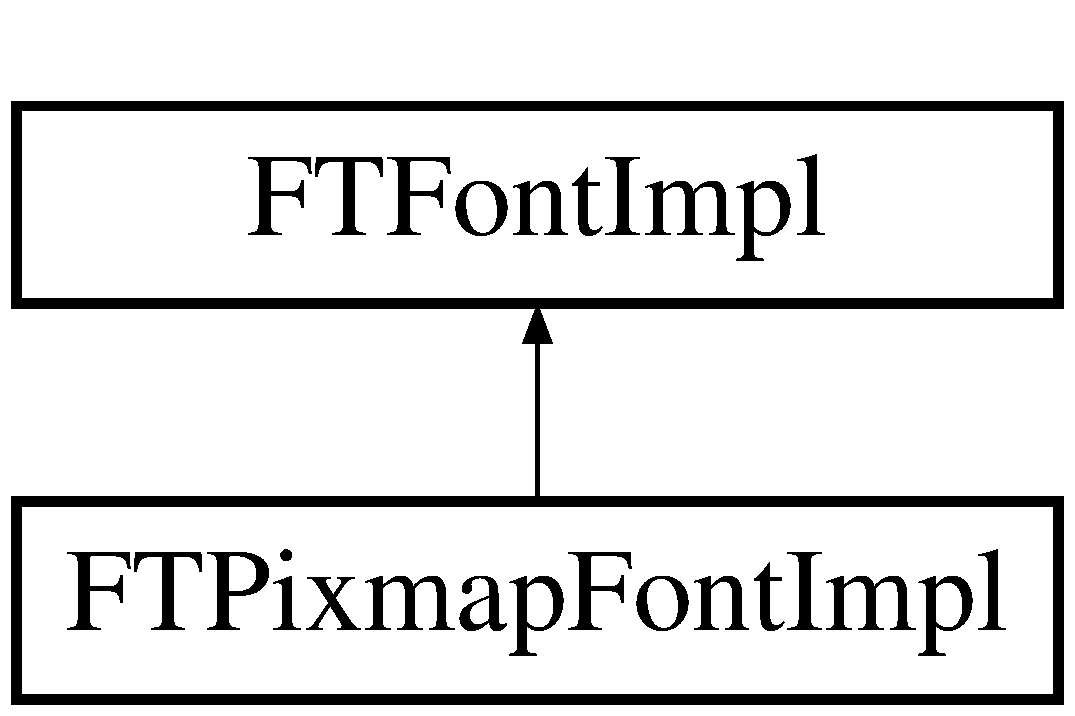
\includegraphics[height=2.000000cm]{class_f_t_pixmap_font_impl}
\end{center}
\end{figure}
\subsection*{Protected Member Functions}
\begin{DoxyCompactItemize}
\item 
\hypertarget{class_f_t_pixmap_font_impl_a08cfaf450bfbacce2b2d290b3d8d66d6}{{\bfseries F\-T\-Pixmap\-Font\-Impl} (F\-T\-Font $\ast$ft\-Font, const char $\ast$font\-File\-Path)}\label{class_f_t_pixmap_font_impl_a08cfaf450bfbacce2b2d290b3d8d66d6}

\item 
\hypertarget{class_f_t_pixmap_font_impl_ac55c8ac1dffbd6559de73b44b85fde41}{{\bfseries F\-T\-Pixmap\-Font\-Impl} (F\-T\-Font $\ast$ft\-Font, const unsigned char $\ast$p\-Buffer\-Bytes, size\-\_\-t buffer\-Size\-In\-Bytes)}\label{class_f_t_pixmap_font_impl_ac55c8ac1dffbd6559de73b44b85fde41}

\item 
\hypertarget{class_f_t_pixmap_font_impl_a3e2c75bd5cfa405a440735bcb83fa75f}{virtual F\-T\-Point {\bfseries Render} (const char $\ast$s, const int len, F\-T\-Point position, F\-T\-Point spacing, int render\-Mode)}\label{class_f_t_pixmap_font_impl_a3e2c75bd5cfa405a440735bcb83fa75f}

\item 
\hypertarget{class_f_t_pixmap_font_impl_a95755217a2bf8d5d4a4a1f898fe1be73}{virtual F\-T\-Point {\bfseries Render} (const wchar\-\_\-t $\ast$s, const int len, F\-T\-Point position, F\-T\-Point spacing, int render\-Mode)}\label{class_f_t_pixmap_font_impl_a95755217a2bf8d5d4a4a1f898fe1be73}

\end{DoxyCompactItemize}
\subsection*{Friends}
\begin{DoxyCompactItemize}
\item 
\hypertarget{class_f_t_pixmap_font_impl_ac7f382db9ff9f02888b67b7434d7edd4}{class {\bfseries F\-T\-Pixmap\-Font}}\label{class_f_t_pixmap_font_impl_ac7f382db9ff9f02888b67b7434d7edd4}

\end{DoxyCompactItemize}
\subsection*{Additional Inherited Members}


The documentation for this class was generated from the following files\-:\begin{DoxyCompactItemize}
\item 
X\-:/\-Git\-\_\-\-Repository/inf2990-\/06/\-Cadriciel/\-Commun/\-Externe/\-F\-T\-G\-L/include/\-F\-T\-Font/F\-T\-Pixmap\-Font\-Impl.\-h\item 
X\-:/\-Git\-\_\-\-Repository/inf2990-\/06/\-Cadriciel/\-Commun/\-Externe/\-F\-T\-G\-L/include/\-F\-T\-Font/F\-T\-Pixmap\-Font.\-cpp\end{DoxyCompactItemize}

\hypertarget{class_f_t_pixmap_glyph_impl}{\section{F\-T\-Pixmap\-Glyph\-Impl Class Reference}
\label{class_f_t_pixmap_glyph_impl}\index{F\-T\-Pixmap\-Glyph\-Impl@{F\-T\-Pixmap\-Glyph\-Impl}}
}
Inheritance diagram for F\-T\-Pixmap\-Glyph\-Impl\-:\begin{figure}[H]
\begin{center}
\leavevmode
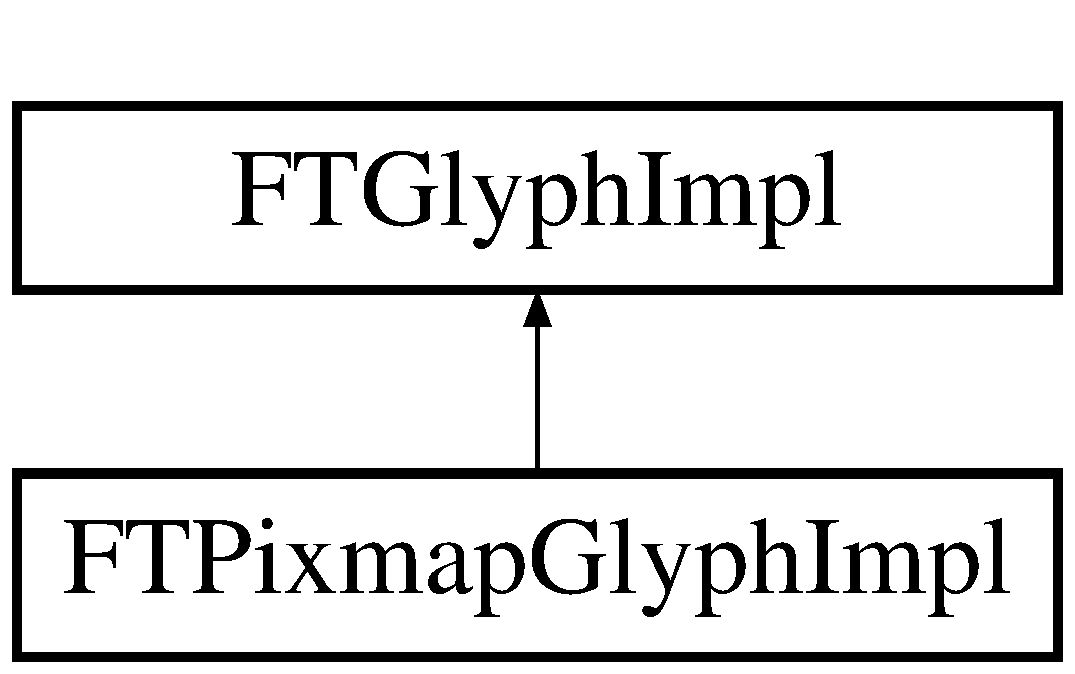
\includegraphics[height=2.000000cm]{class_f_t_pixmap_glyph_impl}
\end{center}
\end{figure}
\subsection*{Protected Member Functions}
\begin{DoxyCompactItemize}
\item 
\hypertarget{class_f_t_pixmap_glyph_impl_a65e1773b7c1f422abbccd90399cd3ec4}{{\bfseries F\-T\-Pixmap\-Glyph\-Impl} (\hyperlink{struct_f_t___glyph_slot_rec__}{F\-T\-\_\-\-Glyph\-Slot} glyph)}\label{class_f_t_pixmap_glyph_impl_a65e1773b7c1f422abbccd90399cd3ec4}

\item 
\hypertarget{class_f_t_pixmap_glyph_impl_a9c5cf9105b59301f0b27cfa2350012c6}{virtual const F\-T\-Point \& {\bfseries Render\-Impl} (const F\-T\-Point \&pen, int render\-Mode)}\label{class_f_t_pixmap_glyph_impl_a9c5cf9105b59301f0b27cfa2350012c6}

\end{DoxyCompactItemize}
\subsection*{Friends}
\begin{DoxyCompactItemize}
\item 
\hypertarget{class_f_t_pixmap_glyph_impl_ab141fccf761e39b9e4bec64cda0507a7}{class {\bfseries F\-T\-Pixmap\-Glyph}}\label{class_f_t_pixmap_glyph_impl_ab141fccf761e39b9e4bec64cda0507a7}

\end{DoxyCompactItemize}
\subsection*{Additional Inherited Members}


The documentation for this class was generated from the following files\-:\begin{DoxyCompactItemize}
\item 
X\-:/\-Git\-\_\-\-Repository/inf2990-\/06/\-Cadriciel/\-Commun/\-Externe/\-F\-T\-G\-L/include/\-F\-T\-Glyph/F\-T\-Pixmap\-Glyph\-Impl.\-h\item 
X\-:/\-Git\-\_\-\-Repository/inf2990-\/06/\-Cadriciel/\-Commun/\-Externe/\-F\-T\-G\-L/include/\-F\-T\-Glyph/F\-T\-Pixmap\-Glyph.\-cpp\end{DoxyCompactItemize}

\hypertarget{class_f_t_polygon_font_impl}{\section{F\-T\-Polygon\-Font\-Impl Class Reference}
\label{class_f_t_polygon_font_impl}\index{F\-T\-Polygon\-Font\-Impl@{F\-T\-Polygon\-Font\-Impl}}
}
Inheritance diagram for F\-T\-Polygon\-Font\-Impl\-:\begin{figure}[H]
\begin{center}
\leavevmode
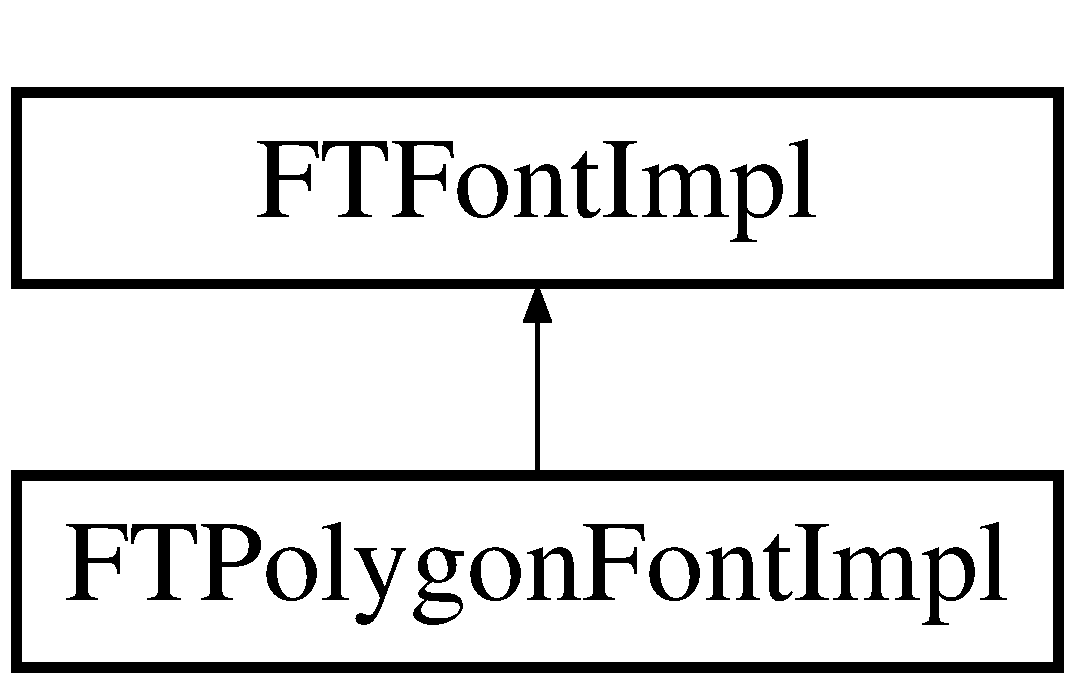
\includegraphics[height=2.000000cm]{class_f_t_polygon_font_impl}
\end{center}
\end{figure}
\subsection*{Protected Member Functions}
\begin{DoxyCompactItemize}
\item 
\hypertarget{class_f_t_polygon_font_impl_adbe87469ee12af1a0a1b7999ede7cc98}{{\bfseries F\-T\-Polygon\-Font\-Impl} (F\-T\-Font $\ast$ft\-Font, const char $\ast$font\-File\-Path)}\label{class_f_t_polygon_font_impl_adbe87469ee12af1a0a1b7999ede7cc98}

\item 
\hypertarget{class_f_t_polygon_font_impl_a140310c1898543ff1dec5865841b630b}{{\bfseries F\-T\-Polygon\-Font\-Impl} (F\-T\-Font $\ast$ft\-Font, const unsigned char $\ast$p\-Buffer\-Bytes, size\-\_\-t buffer\-Size\-In\-Bytes)}\label{class_f_t_polygon_font_impl_a140310c1898543ff1dec5865841b630b}

\item 
virtual void \hyperlink{class_f_t_polygon_font_impl_ac565010b774c7ddb84db28b422ea9b3e}{Outset} (float o)
\end{DoxyCompactItemize}
\subsection*{Friends}
\begin{DoxyCompactItemize}
\item 
\hypertarget{class_f_t_polygon_font_impl_abd1c273c43e47346ad6c178ec173cc41}{class {\bfseries F\-T\-Polygon\-Font}}\label{class_f_t_polygon_font_impl_abd1c273c43e47346ad6c178ec173cc41}

\end{DoxyCompactItemize}
\subsection*{Additional Inherited Members}


\subsection{Member Function Documentation}
\hypertarget{class_f_t_polygon_font_impl_ac565010b774c7ddb84db28b422ea9b3e}{\index{F\-T\-Polygon\-Font\-Impl@{F\-T\-Polygon\-Font\-Impl}!Outset@{Outset}}
\index{Outset@{Outset}!FTPolygonFontImpl@{F\-T\-Polygon\-Font\-Impl}}
\subsubsection[{Outset}]{\setlength{\rightskip}{0pt plus 5cm}virtual void F\-T\-Polygon\-Font\-Impl\-::\-Outset (
\begin{DoxyParamCaption}
\item[{float}]{o}
\end{DoxyParamCaption}
)\hspace{0.3cm}{\ttfamily [inline]}, {\ttfamily [protected]}, {\ttfamily [virtual]}}}\label{class_f_t_polygon_font_impl_ac565010b774c7ddb84db28b422ea9b3e}
Set the outset distance for the font. Only implemented by F\-T\-Outline\-Font, F\-T\-Polygon\-Font and F\-T\-Extrude\-Font


\begin{DoxyParams}{Parameters}
{\em depth} & The outset distance. \\
\hline
\end{DoxyParams}


Reimplemented from \hyperlink{class_f_t_font_impl}{F\-T\-Font\-Impl}.



The documentation for this class was generated from the following files\-:\begin{DoxyCompactItemize}
\item 
X\-:/\-Git\-\_\-\-Repository/inf2990-\/06/\-Cadriciel/\-Commun/\-Externe/\-F\-T\-G\-L/include/\-F\-T\-Font/F\-T\-Polygon\-Font\-Impl.\-h\item 
X\-:/\-Git\-\_\-\-Repository/inf2990-\/06/\-Cadriciel/\-Commun/\-Externe/\-F\-T\-G\-L/include/\-F\-T\-Font/F\-T\-Polygon\-Font.\-cpp\end{DoxyCompactItemize}

\hypertarget{class_f_t_polygon_glyph_impl}{\section{F\-T\-Polygon\-Glyph\-Impl Class Reference}
\label{class_f_t_polygon_glyph_impl}\index{F\-T\-Polygon\-Glyph\-Impl@{F\-T\-Polygon\-Glyph\-Impl}}
}
Inheritance diagram for F\-T\-Polygon\-Glyph\-Impl\-:\begin{figure}[H]
\begin{center}
\leavevmode
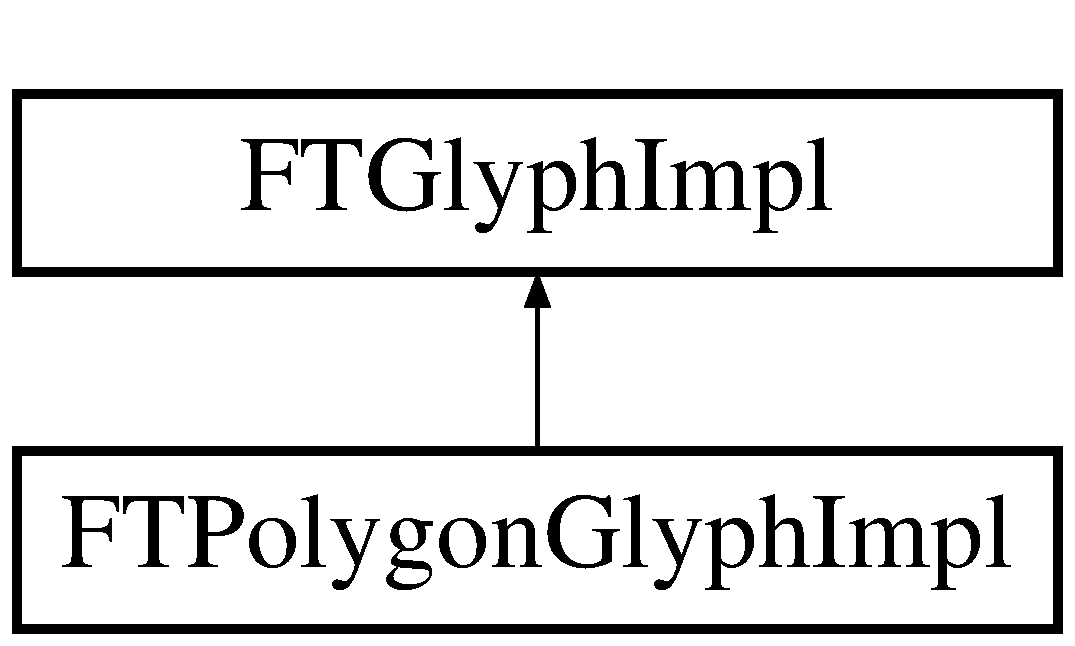
\includegraphics[height=2.000000cm]{class_f_t_polygon_glyph_impl}
\end{center}
\end{figure}
\subsection*{Public Member Functions}
\begin{DoxyCompactItemize}
\item 
\hypertarget{class_f_t_polygon_glyph_impl_ab302277a0e76adf9570f1ef9f9ae851f}{{\bfseries F\-T\-Polygon\-Glyph\-Impl} (\hyperlink{struct_f_t___glyph_slot_rec__}{F\-T\-\_\-\-Glyph\-Slot} glyph, float outset, bool use\-Display\-List)}\label{class_f_t_polygon_glyph_impl_ab302277a0e76adf9570f1ef9f9ae851f}

\item 
\hypertarget{class_f_t_polygon_glyph_impl_af689ff9cecc738d292d494bf83adca39}{virtual const F\-T\-Point \& {\bfseries Render\-Impl} (const F\-T\-Point \&pen, int render\-Mode)}\label{class_f_t_polygon_glyph_impl_af689ff9cecc738d292d494bf83adca39}

\end{DoxyCompactItemize}
\subsection*{Friends}
\begin{DoxyCompactItemize}
\item 
\hypertarget{class_f_t_polygon_glyph_impl_a0e33f7bc34e1097f8f9adcb6252d1bc0}{class {\bfseries F\-T\-Polygon\-Glyph}}\label{class_f_t_polygon_glyph_impl_a0e33f7bc34e1097f8f9adcb6252d1bc0}

\end{DoxyCompactItemize}
\subsection*{Additional Inherited Members}


The documentation for this class was generated from the following files\-:\begin{DoxyCompactItemize}
\item 
X\-:/\-Git\-\_\-\-Repository/inf2990-\/06/\-Cadriciel/\-Commun/\-Externe/\-F\-T\-G\-L/include/\-F\-T\-Glyph/F\-T\-Polygon\-Glyph\-Impl.\-h\item 
X\-:/\-Git\-\_\-\-Repository/inf2990-\/06/\-Cadriciel/\-Commun/\-Externe/\-F\-T\-G\-L/include/\-F\-T\-Glyph/F\-T\-Polygon\-Glyph.\-cpp\end{DoxyCompactItemize}

\hypertarget{class_f_t_simple_layout_impl}{\section{F\-T\-Simple\-Layout\-Impl Class Reference}
\label{class_f_t_simple_layout_impl}\index{F\-T\-Simple\-Layout\-Impl@{F\-T\-Simple\-Layout\-Impl}}
}
Inheritance diagram for F\-T\-Simple\-Layout\-Impl\-:\begin{figure}[H]
\begin{center}
\leavevmode
\includegraphics[height=2.000000cm]{class_f_t_simple_layout_impl}
\end{center}
\end{figure}
\subsection*{Protected Member Functions}
\begin{DoxyCompactItemize}
\item 
\hypertarget{class_f_t_simple_layout_impl_a6cdedbc1045881dcb3ddedea054a7987}{virtual F\-T\-B\-Box {\bfseries B\-Box} (const char $\ast$string, const int len, F\-T\-Point position)}\label{class_f_t_simple_layout_impl_a6cdedbc1045881dcb3ddedea054a7987}

\item 
\hypertarget{class_f_t_simple_layout_impl_a682650a15a67eb182b2de9e7001875cb}{virtual F\-T\-B\-Box {\bfseries B\-Box} (const wchar\-\_\-t $\ast$string, const int len, F\-T\-Point position)}\label{class_f_t_simple_layout_impl_a682650a15a67eb182b2de9e7001875cb}

\item 
\hypertarget{class_f_t_simple_layout_impl_abfe85f44b3d4a2f8691b5e11ab26828a}{virtual void {\bfseries Render} (const char $\ast$string, const int len, F\-T\-Point position, int render\-Mode)}\label{class_f_t_simple_layout_impl_abfe85f44b3d4a2f8691b5e11ab26828a}

\item 
\hypertarget{class_f_t_simple_layout_impl_ac69f1a3cdac5e6dd692b547df3f77825}{virtual void {\bfseries Render} (const wchar\-\_\-t $\ast$string, const int len, F\-T\-Point position, int render\-Mode)}\label{class_f_t_simple_layout_impl_ac69f1a3cdac5e6dd692b547df3f77825}

\item 
virtual void \hyperlink{class_f_t_simple_layout_impl_abdbd064c650f1e17d2bd3139536aff47}{Render\-Space} (const char $\ast$string, const int len, F\-T\-Point position, int render\-Mode, const float extra\-Space)
\item 
virtual void \hyperlink{class_f_t_simple_layout_impl_a6b5334d053e9c79dd459f8b88c0e60a4}{Render\-Space} (const wchar\-\_\-t $\ast$string, const int len, F\-T\-Point position, int render\-Mode, const float extra\-Space)
\end{DoxyCompactItemize}
\subsection*{Friends}
\begin{DoxyCompactItemize}
\item 
\hypertarget{class_f_t_simple_layout_impl_ae27eaa779922d14c8eb0f476456c7099}{class {\bfseries F\-T\-Simple\-Layout}}\label{class_f_t_simple_layout_impl_ae27eaa779922d14c8eb0f476456c7099}

\end{DoxyCompactItemize}
\subsection*{Additional Inherited Members}


\subsection{Member Function Documentation}
\hypertarget{class_f_t_simple_layout_impl_abdbd064c650f1e17d2bd3139536aff47}{\index{F\-T\-Simple\-Layout\-Impl@{F\-T\-Simple\-Layout\-Impl}!Render\-Space@{Render\-Space}}
\index{Render\-Space@{Render\-Space}!FTSimpleLayoutImpl@{F\-T\-Simple\-Layout\-Impl}}
\subsubsection[{Render\-Space}]{\setlength{\rightskip}{0pt plus 5cm}void F\-T\-Simple\-Layout\-Impl\-::\-Render\-Space (
\begin{DoxyParamCaption}
\item[{const char $\ast$}]{string, }
\item[{const int}]{len, }
\item[{F\-T\-Point}]{position, }
\item[{int}]{render\-Mode, }
\item[{const float}]{extra\-Space}
\end{DoxyParamCaption}
)\hspace{0.3cm}{\ttfamily [protected]}, {\ttfamily [virtual]}}}\label{class_f_t_simple_layout_impl_abdbd064c650f1e17d2bd3139536aff47}
Render a string of characters and distribute extra space amongst the whitespace regions of the string.


\begin{DoxyParams}{Parameters}
{\em string} & A buffer of wchar\-\_\-t characters to output. \\
\hline
{\em len} & The length of the string. If $<$ 0 then all characters will be displayed until a null character is encountered. \\
\hline
{\em position} & T\-O\-D\-O \\
\hline
{\em render\-Mode} & Render mode to display \\
\hline
{\em extra\-Space} & The amount of extra space to distribute amongst the characters. \\
\hline
\end{DoxyParams}
\hypertarget{class_f_t_simple_layout_impl_a6b5334d053e9c79dd459f8b88c0e60a4}{\index{F\-T\-Simple\-Layout\-Impl@{F\-T\-Simple\-Layout\-Impl}!Render\-Space@{Render\-Space}}
\index{Render\-Space@{Render\-Space}!FTSimpleLayoutImpl@{F\-T\-Simple\-Layout\-Impl}}
\subsubsection[{Render\-Space}]{\setlength{\rightskip}{0pt plus 5cm}void F\-T\-Simple\-Layout\-Impl\-::\-Render\-Space (
\begin{DoxyParamCaption}
\item[{const wchar\-\_\-t $\ast$}]{string, }
\item[{const int}]{len, }
\item[{F\-T\-Point}]{position, }
\item[{int}]{render\-Mode, }
\item[{const float}]{extra\-Space}
\end{DoxyParamCaption}
)\hspace{0.3cm}{\ttfamily [protected]}, {\ttfamily [virtual]}}}\label{class_f_t_simple_layout_impl_a6b5334d053e9c79dd459f8b88c0e60a4}
Render a string of characters and distribute extra space amongst the whitespace regions of the string.


\begin{DoxyParams}{Parameters}
{\em string} & A buffer of wchar\-\_\-t characters to output. \\
\hline
{\em len} & The length of the string. If $<$ 0 then all characters will be displayed until a null character is encountered. \\
\hline
{\em position} & T\-O\-D\-O \\
\hline
{\em render\-Mode} & Render mode to display \\
\hline
{\em extra\-Space} & The amount of extra space to distribute amongst the characters. \\
\hline
\end{DoxyParams}


The documentation for this class was generated from the following files\-:\begin{DoxyCompactItemize}
\item 
X\-:/\-Git\-\_\-\-Repository/inf2990-\/06/\-Cadriciel/\-Commun/\-Externe/\-F\-T\-G\-L/include/\-F\-T\-Layout/F\-T\-Simple\-Layout\-Impl.\-h\item 
X\-:/\-Git\-\_\-\-Repository/inf2990-\/06/\-Cadriciel/\-Commun/\-Externe/\-F\-T\-G\-L/include/\-F\-T\-Layout/F\-T\-Simple\-Layout.\-cpp\end{DoxyCompactItemize}

\hypertarget{class_f_t_size}{\section{F\-T\-Size Class Reference}
\label{class_f_t_size}\index{F\-T\-Size@{F\-T\-Size}}
}


{\ttfamily \#include $<$F\-T\-Size.\-h$>$}

\subsection*{Public Member Functions}
\begin{DoxyCompactItemize}
\item 
\hyperlink{class_f_t_size_ae1b459031c2ab7fe6ef98530c0251700}{F\-T\-Size} ()
\item 
virtual \hyperlink{class_f_t_size_a7bf23332d879f3e9d76675290012b275}{$\sim$\-F\-T\-Size} ()
\item 
bool \hyperlink{class_f_t_size_a15c6c82655544d1edb101e00e42ffad9}{Char\-Size} (\hyperlink{struct_f_t___face_rec__}{F\-T\-\_\-\-Face} $\ast$face, unsigned int point\-\_\-size, unsigned int x\-\_\-resolution, unsigned int y\-\_\-resolution)
\item 
unsigned int \hyperlink{class_f_t_size_a489fba0a722afd8dfa2a67142cd51767}{Char\-Size} () const 
\item 
float \hyperlink{class_f_t_size_a7865c27cb979feace5ccce2fb544a490}{Ascender} () const 
\item 
float \hyperlink{class_f_t_size_a75c1b86d32c5ea1d296234edb1e4b7ab}{Descender} () const 
\item 
float \hyperlink{class_f_t_size_af0e7398f27936ffe4cbed04c3cfa889d}{Height} () const 
\item 
float \hyperlink{class_f_t_size_a8fe639fa29815a89cdd84138b2564840}{Width} () const 
\item 
float \hyperlink{class_f_t_size_ab85fb58156a855d01b5a4e9e1b91e0e2}{Underline} () const 
\item 
F\-T\-\_\-\-Error \hyperlink{class_f_t_size_a990a2df40c9c1ed06db8d34b2ac3580b}{Error} () const 
\end{DoxyCompactItemize}


\subsection{Detailed Description}
\hyperlink{class_f_t_size}{F\-T\-Size} class provides an abstraction layer for the Freetype Size.

\begin{DoxySeeAlso}{See Also}
\char`\"{}\-Freetype 2 Documentation\char`\"{} 
\end{DoxySeeAlso}


\subsection{Constructor \& Destructor Documentation}
\hypertarget{class_f_t_size_ae1b459031c2ab7fe6ef98530c0251700}{\index{F\-T\-Size@{F\-T\-Size}!F\-T\-Size@{F\-T\-Size}}
\index{F\-T\-Size@{F\-T\-Size}!FTSize@{F\-T\-Size}}
\subsubsection[{F\-T\-Size}]{\setlength{\rightskip}{0pt plus 5cm}F\-T\-Size\-::\-F\-T\-Size (
\begin{DoxyParamCaption}
{}
\end{DoxyParamCaption}
)}}\label{class_f_t_size_ae1b459031c2ab7fe6ef98530c0251700}
Default Constructor \hypertarget{class_f_t_size_a7bf23332d879f3e9d76675290012b275}{\index{F\-T\-Size@{F\-T\-Size}!$\sim$\-F\-T\-Size@{$\sim$\-F\-T\-Size}}
\index{$\sim$\-F\-T\-Size@{$\sim$\-F\-T\-Size}!FTSize@{F\-T\-Size}}
\subsubsection[{$\sim$\-F\-T\-Size}]{\setlength{\rightskip}{0pt plus 5cm}F\-T\-Size\-::$\sim$\-F\-T\-Size (
\begin{DoxyParamCaption}
{}
\end{DoxyParamCaption}
)\hspace{0.3cm}{\ttfamily [virtual]}}}\label{class_f_t_size_a7bf23332d879f3e9d76675290012b275}
Destructor 

\subsection{Member Function Documentation}
\hypertarget{class_f_t_size_a7865c27cb979feace5ccce2fb544a490}{\index{F\-T\-Size@{F\-T\-Size}!Ascender@{Ascender}}
\index{Ascender@{Ascender}!FTSize@{F\-T\-Size}}
\subsubsection[{Ascender}]{\setlength{\rightskip}{0pt plus 5cm}float F\-T\-Size\-::\-Ascender (
\begin{DoxyParamCaption}
{}
\end{DoxyParamCaption}
) const}}\label{class_f_t_size_a7865c27cb979feace5ccce2fb544a490}
Gets the global ascender height for the face in pixels.

\begin{DoxyReturn}{Returns}
Ascender height 
\end{DoxyReturn}
\hypertarget{class_f_t_size_a15c6c82655544d1edb101e00e42ffad9}{\index{F\-T\-Size@{F\-T\-Size}!Char\-Size@{Char\-Size}}
\index{Char\-Size@{Char\-Size}!FTSize@{F\-T\-Size}}
\subsubsection[{Char\-Size}]{\setlength{\rightskip}{0pt plus 5cm}bool F\-T\-Size\-::\-Char\-Size (
\begin{DoxyParamCaption}
\item[{{\bf F\-T\-\_\-\-Face} $\ast$}]{face, }
\item[{unsigned int}]{point\-\_\-size, }
\item[{unsigned int}]{x\-\_\-resolution, }
\item[{unsigned int}]{y\-\_\-resolution}
\end{DoxyParamCaption}
)}}\label{class_f_t_size_a15c6c82655544d1edb101e00e42ffad9}
Sets the char size for the current face.

This doesn't guarantee that the size was set correctly. Clients should check errors. If an error does occur the size object isn't modified.


\begin{DoxyParams}{Parameters}
{\em face} & Parent face for this size object \\
\hline
{\em point\-\_\-size} & the face size in points (1/72 inch) \\
\hline
{\em x\-\_\-resolution} & the horizontal resolution of the target device. \\
\hline
{\em y\-\_\-resolution} & the vertical resolution of the target device. \\
\hline
\end{DoxyParams}
\begin{DoxyReturn}{Returns}
{\ttfamily true} if the size has been set. Clients should check \hyperlink{class_f_t_size_a990a2df40c9c1ed06db8d34b2ac3580b}{Error()} for more information if this function returns false() 
\end{DoxyReturn}
\hypertarget{class_f_t_size_a489fba0a722afd8dfa2a67142cd51767}{\index{F\-T\-Size@{F\-T\-Size}!Char\-Size@{Char\-Size}}
\index{Char\-Size@{Char\-Size}!FTSize@{F\-T\-Size}}
\subsubsection[{Char\-Size}]{\setlength{\rightskip}{0pt plus 5cm}unsigned int F\-T\-Size\-::\-Char\-Size (
\begin{DoxyParamCaption}
{}
\end{DoxyParamCaption}
) const}}\label{class_f_t_size_a489fba0a722afd8dfa2a67142cd51767}
get the char size for the current face.

\begin{DoxyReturn}{Returns}
The char size in points 
\end{DoxyReturn}
\hypertarget{class_f_t_size_a75c1b86d32c5ea1d296234edb1e4b7ab}{\index{F\-T\-Size@{F\-T\-Size}!Descender@{Descender}}
\index{Descender@{Descender}!FTSize@{F\-T\-Size}}
\subsubsection[{Descender}]{\setlength{\rightskip}{0pt plus 5cm}float F\-T\-Size\-::\-Descender (
\begin{DoxyParamCaption}
{}
\end{DoxyParamCaption}
) const}}\label{class_f_t_size_a75c1b86d32c5ea1d296234edb1e4b7ab}
Gets the global descender height for the face in pixels.

\begin{DoxyReturn}{Returns}
Ascender height 
\end{DoxyReturn}
\hypertarget{class_f_t_size_a990a2df40c9c1ed06db8d34b2ac3580b}{\index{F\-T\-Size@{F\-T\-Size}!Error@{Error}}
\index{Error@{Error}!FTSize@{F\-T\-Size}}
\subsubsection[{Error}]{\setlength{\rightskip}{0pt plus 5cm}F\-T\-\_\-\-Error F\-T\-Size\-::\-Error (
\begin{DoxyParamCaption}
{}
\end{DoxyParamCaption}
) const\hspace{0.3cm}{\ttfamily [inline]}}}\label{class_f_t_size_a990a2df40c9c1ed06db8d34b2ac3580b}
Queries for errors.

\begin{DoxyReturn}{Returns}
The current error code. 
\end{DoxyReturn}
\hypertarget{class_f_t_size_af0e7398f27936ffe4cbed04c3cfa889d}{\index{F\-T\-Size@{F\-T\-Size}!Height@{Height}}
\index{Height@{Height}!FTSize@{F\-T\-Size}}
\subsubsection[{Height}]{\setlength{\rightskip}{0pt plus 5cm}float F\-T\-Size\-::\-Height (
\begin{DoxyParamCaption}
{}
\end{DoxyParamCaption}
) const}}\label{class_f_t_size_af0e7398f27936ffe4cbed04c3cfa889d}
Gets the global face height for the face.

If the face is scalable this returns the height of the global bounding box which ensures that any glyph will be less than or equal to this height. If the font isn't scalable there is no guarantee that glyphs will not be taller than this value.

\begin{DoxyReturn}{Returns}
height in pixels. 
\end{DoxyReturn}
\hypertarget{class_f_t_size_ab85fb58156a855d01b5a4e9e1b91e0e2}{\index{F\-T\-Size@{F\-T\-Size}!Underline@{Underline}}
\index{Underline@{Underline}!FTSize@{F\-T\-Size}}
\subsubsection[{Underline}]{\setlength{\rightskip}{0pt plus 5cm}float F\-T\-Size\-::\-Underline (
\begin{DoxyParamCaption}
{}
\end{DoxyParamCaption}
) const}}\label{class_f_t_size_ab85fb58156a855d01b5a4e9e1b91e0e2}
Gets the underline position for the face.

\begin{DoxyReturn}{Returns}
underline position in pixels 
\end{DoxyReturn}
\hypertarget{class_f_t_size_a8fe639fa29815a89cdd84138b2564840}{\index{F\-T\-Size@{F\-T\-Size}!Width@{Width}}
\index{Width@{Width}!FTSize@{F\-T\-Size}}
\subsubsection[{Width}]{\setlength{\rightskip}{0pt plus 5cm}float F\-T\-Size\-::\-Width (
\begin{DoxyParamCaption}
{}
\end{DoxyParamCaption}
) const}}\label{class_f_t_size_a8fe639fa29815a89cdd84138b2564840}
Gets the global face width for the face.

If the face is scalable this returns the width of the global bounding box which ensures that any glyph will be less than or equal to this width. If the font isn't scalable this value is the max\-\_\-advance for the face.

\begin{DoxyReturn}{Returns}
width in pixels. 
\end{DoxyReturn}


The documentation for this class was generated from the following files\-:\begin{DoxyCompactItemize}
\item 
X\-:/\-Git\-\_\-\-Repository/inf2990-\/06/\-Cadriciel/\-Commun/\-Externe/\-F\-T\-G\-L/include/F\-T\-Size.\-h\item 
X\-:/\-Git\-\_\-\-Repository/inf2990-\/06/\-Cadriciel/\-Commun/\-Externe/\-F\-T\-G\-L/include/F\-T\-Size.\-cpp\end{DoxyCompactItemize}

\hypertarget{class_f_t_tesselation}{\section{F\-T\-Tesselation Class Reference}
\label{class_f_t_tesselation}\index{F\-T\-Tesselation@{F\-T\-Tesselation}}
}


{\ttfamily \#include $<$F\-T\-Vectoriser.\-h$>$}

\subsection*{Public Member Functions}
\begin{DoxyCompactItemize}
\item 
\hyperlink{class_f_t_tesselation_a8ae81852ffa0dfb1bc65e85dc6d35df2}{F\-T\-Tesselation} (G\-Lenum m)
\item 
\hyperlink{class_f_t_tesselation_a55bd008edbf969720fa3dc083bce1ac0}{$\sim$\-F\-T\-Tesselation} ()
\item 
void \hyperlink{class_f_t_tesselation_a204a9e646cee25f374faad125d71d5e6}{Add\-Point} (const F\-T\-G\-L\-\_\-\-D\-O\-U\-B\-L\-E x, const F\-T\-G\-L\-\_\-\-D\-O\-U\-B\-L\-E y, const F\-T\-G\-L\-\_\-\-D\-O\-U\-B\-L\-E z)
\item 
size\-\_\-t \hyperlink{class_f_t_tesselation_aa3cb26a53c3534576339f946acdc0cc7}{Point\-Count} () const 
\item 
\hypertarget{class_f_t_tesselation_a964ae8f16f216ca545f44a087f31e827}{const F\-T\-Point \& {\bfseries Point} (unsigned int index) const }\label{class_f_t_tesselation_a964ae8f16f216ca545f44a087f31e827}

\item 
G\-Lenum \hyperlink{class_f_t_tesselation_a06c290061a75bad0d38a2d5b2f6b09a1}{Polygon\-Type} () const 
\end{DoxyCompactItemize}


\subsection{Detailed Description}
\hyperlink{class_f_t_tesselation}{F\-T\-Tesselation} captures points that are output by Open\-G\-L's glu\-Tesselator. 

\subsection{Constructor \& Destructor Documentation}
\hypertarget{class_f_t_tesselation_a8ae81852ffa0dfb1bc65e85dc6d35df2}{\index{F\-T\-Tesselation@{F\-T\-Tesselation}!F\-T\-Tesselation@{F\-T\-Tesselation}}
\index{F\-T\-Tesselation@{F\-T\-Tesselation}!FTTesselation@{F\-T\-Tesselation}}
\subsubsection[{F\-T\-Tesselation}]{\setlength{\rightskip}{0pt plus 5cm}F\-T\-Tesselation\-::\-F\-T\-Tesselation (
\begin{DoxyParamCaption}
\item[{G\-Lenum}]{m}
\end{DoxyParamCaption}
)\hspace{0.3cm}{\ttfamily [inline]}}}\label{class_f_t_tesselation_a8ae81852ffa0dfb1bc65e85dc6d35df2}
Default constructor \hypertarget{class_f_t_tesselation_a55bd008edbf969720fa3dc083bce1ac0}{\index{F\-T\-Tesselation@{F\-T\-Tesselation}!$\sim$\-F\-T\-Tesselation@{$\sim$\-F\-T\-Tesselation}}
\index{$\sim$\-F\-T\-Tesselation@{$\sim$\-F\-T\-Tesselation}!FTTesselation@{F\-T\-Tesselation}}
\subsubsection[{$\sim$\-F\-T\-Tesselation}]{\setlength{\rightskip}{0pt plus 5cm}F\-T\-Tesselation\-::$\sim$\-F\-T\-Tesselation (
\begin{DoxyParamCaption}
{}
\end{DoxyParamCaption}
)\hspace{0.3cm}{\ttfamily [inline]}}}\label{class_f_t_tesselation_a55bd008edbf969720fa3dc083bce1ac0}
Destructor 

\subsection{Member Function Documentation}
\hypertarget{class_f_t_tesselation_a204a9e646cee25f374faad125d71d5e6}{\index{F\-T\-Tesselation@{F\-T\-Tesselation}!Add\-Point@{Add\-Point}}
\index{Add\-Point@{Add\-Point}!FTTesselation@{F\-T\-Tesselation}}
\subsubsection[{Add\-Point}]{\setlength{\rightskip}{0pt plus 5cm}void F\-T\-Tesselation\-::\-Add\-Point (
\begin{DoxyParamCaption}
\item[{const F\-T\-G\-L\-\_\-\-D\-O\-U\-B\-L\-E}]{x, }
\item[{const F\-T\-G\-L\-\_\-\-D\-O\-U\-B\-L\-E}]{y, }
\item[{const F\-T\-G\-L\-\_\-\-D\-O\-U\-B\-L\-E}]{z}
\end{DoxyParamCaption}
)\hspace{0.3cm}{\ttfamily [inline]}}}\label{class_f_t_tesselation_a204a9e646cee25f374faad125d71d5e6}
Add a point to the mesh. \hypertarget{class_f_t_tesselation_aa3cb26a53c3534576339f946acdc0cc7}{\index{F\-T\-Tesselation@{F\-T\-Tesselation}!Point\-Count@{Point\-Count}}
\index{Point\-Count@{Point\-Count}!FTTesselation@{F\-T\-Tesselation}}
\subsubsection[{Point\-Count}]{\setlength{\rightskip}{0pt plus 5cm}size\-\_\-t F\-T\-Tesselation\-::\-Point\-Count (
\begin{DoxyParamCaption}
{}
\end{DoxyParamCaption}
) const\hspace{0.3cm}{\ttfamily [inline]}}}\label{class_f_t_tesselation_aa3cb26a53c3534576339f946acdc0cc7}
The number of points in this mesh \hypertarget{class_f_t_tesselation_a06c290061a75bad0d38a2d5b2f6b09a1}{\index{F\-T\-Tesselation@{F\-T\-Tesselation}!Polygon\-Type@{Polygon\-Type}}
\index{Polygon\-Type@{Polygon\-Type}!FTTesselation@{F\-T\-Tesselation}}
\subsubsection[{Polygon\-Type}]{\setlength{\rightskip}{0pt plus 5cm}G\-Lenum F\-T\-Tesselation\-::\-Polygon\-Type (
\begin{DoxyParamCaption}
{}
\end{DoxyParamCaption}
) const\hspace{0.3cm}{\ttfamily [inline]}}}\label{class_f_t_tesselation_a06c290061a75bad0d38a2d5b2f6b09a1}
Return the Open\-G\-L polygon type. 

The documentation for this class was generated from the following file\-:\begin{DoxyCompactItemize}
\item 
X\-:/\-Git\-\_\-\-Repository/inf2990-\/06/\-Cadriciel/\-Commun/\-Externe/\-F\-T\-G\-L/include/F\-T\-Vectoriser.\-h\end{DoxyCompactItemize}

\hypertarget{class_f_t_texture_font_impl}{\section{F\-T\-Texture\-Font\-Impl Class Reference}
\label{class_f_t_texture_font_impl}\index{F\-T\-Texture\-Font\-Impl@{F\-T\-Texture\-Font\-Impl}}
}
Inheritance diagram for F\-T\-Texture\-Font\-Impl\-:\begin{figure}[H]
\begin{center}
\leavevmode
\includegraphics[height=2.000000cm]{class_f_t_texture_font_impl}
\end{center}
\end{figure}
\subsection*{Protected Member Functions}
\begin{DoxyCompactItemize}
\item 
\hypertarget{class_f_t_texture_font_impl_a6e5537e5ce6f58e8f8244c9d0cd44d9f}{{\bfseries F\-T\-Texture\-Font\-Impl} (F\-T\-Font $\ast$ft\-Font, const char $\ast$font\-File\-Path)}\label{class_f_t_texture_font_impl_a6e5537e5ce6f58e8f8244c9d0cd44d9f}

\item 
\hypertarget{class_f_t_texture_font_impl_a4554181466170efa12b9a12e4936b61d}{{\bfseries F\-T\-Texture\-Font\-Impl} (F\-T\-Font $\ast$ft\-Font, const unsigned char $\ast$p\-Buffer\-Bytes, size\-\_\-t buffer\-Size\-In\-Bytes)}\label{class_f_t_texture_font_impl_a4554181466170efa12b9a12e4936b61d}

\item 
virtual bool \hyperlink{class_f_t_texture_font_impl_ac5ccaca6cc8a53292b5028a629e49244}{Face\-Size} (const unsigned int size, const unsigned int res=72)
\item 
\hypertarget{class_f_t_texture_font_impl_a8b53cbe2b70ad38af59a7d79945122d9}{virtual F\-T\-Point {\bfseries Render} (const char $\ast$s, const int len, F\-T\-Point position, F\-T\-Point spacing, int render\-Mode)}\label{class_f_t_texture_font_impl_a8b53cbe2b70ad38af59a7d79945122d9}

\item 
\hypertarget{class_f_t_texture_font_impl_aba852ac4cc9b759073b6370e059e6c11}{virtual F\-T\-Point {\bfseries Render} (const wchar\-\_\-t $\ast$s, const int len, F\-T\-Point position, F\-T\-Point spacing, int render\-Mode)}\label{class_f_t_texture_font_impl_aba852ac4cc9b759073b6370e059e6c11}

\end{DoxyCompactItemize}
\subsection*{Friends}
\begin{DoxyCompactItemize}
\item 
\hypertarget{class_f_t_texture_font_impl_a7870c341f7269dfae257e93406c17c92}{class {\bfseries F\-T\-Texture\-Font}}\label{class_f_t_texture_font_impl_a7870c341f7269dfae257e93406c17c92}

\end{DoxyCompactItemize}
\subsection*{Additional Inherited Members}


\subsection{Member Function Documentation}
\hypertarget{class_f_t_texture_font_impl_ac5ccaca6cc8a53292b5028a629e49244}{\index{F\-T\-Texture\-Font\-Impl@{F\-T\-Texture\-Font\-Impl}!Face\-Size@{Face\-Size}}
\index{Face\-Size@{Face\-Size}!FTTextureFontImpl@{F\-T\-Texture\-Font\-Impl}}
\subsubsection[{Face\-Size}]{\setlength{\rightskip}{0pt plus 5cm}bool F\-T\-Texture\-Font\-Impl\-::\-Face\-Size (
\begin{DoxyParamCaption}
\item[{const unsigned int}]{size, }
\item[{const unsigned int}]{res = {\ttfamily 72}}
\end{DoxyParamCaption}
)\hspace{0.3cm}{\ttfamily [protected]}, {\ttfamily [virtual]}}}\label{class_f_t_texture_font_impl_ac5ccaca6cc8a53292b5028a629e49244}
Set the char size for the current face.


\begin{DoxyParams}{Parameters}
{\em size} & the face size in points (1/72 inch) \\
\hline
{\em res} & the resolution of the target device. \\
\hline
\end{DoxyParams}
\begin{DoxyReturn}{Returns}
{\ttfamily true} if size was set correctly 
\end{DoxyReturn}


Reimplemented from \hyperlink{class_f_t_font_impl}{F\-T\-Font\-Impl}.



The documentation for this class was generated from the following files\-:\begin{DoxyCompactItemize}
\item 
X\-:/\-Git\-\_\-\-Repository/inf2990-\/06/\-Cadriciel/\-Commun/\-Externe/\-F\-T\-G\-L/include/\-F\-T\-Font/F\-T\-Texture\-Font\-Impl.\-h\item 
X\-:/\-Git\-\_\-\-Repository/inf2990-\/06/\-Cadriciel/\-Commun/\-Externe/\-F\-T\-G\-L/include/\-F\-T\-Font/F\-T\-Texture\-Font.\-cpp\end{DoxyCompactItemize}

\hypertarget{class_f_t_texture_glyph_impl}{\section{F\-T\-Texture\-Glyph\-Impl Class Reference}
\label{class_f_t_texture_glyph_impl}\index{F\-T\-Texture\-Glyph\-Impl@{F\-T\-Texture\-Glyph\-Impl}}
}
Inheritance diagram for F\-T\-Texture\-Glyph\-Impl\-:\begin{figure}[H]
\begin{center}
\leavevmode
\includegraphics[height=2.000000cm]{class_f_t_texture_glyph_impl}
\end{center}
\end{figure}
\subsection*{Protected Member Functions}
\begin{DoxyCompactItemize}
\item 
\hypertarget{class_f_t_texture_glyph_impl_a63893590c3c3c45da5f3925ae9a97abd}{{\bfseries F\-T\-Texture\-Glyph\-Impl} (\hyperlink{struct_f_t___glyph_slot_rec__}{F\-T\-\_\-\-Glyph\-Slot} glyph, int id, int x\-Offset, int y\-Offset, int width, int height)}\label{class_f_t_texture_glyph_impl_a63893590c3c3c45da5f3925ae9a97abd}

\item 
\hypertarget{class_f_t_texture_glyph_impl_a3fce2bf9435946ae0f8ee5eacbe7f702}{virtual const F\-T\-Point \& {\bfseries Render\-Impl} (const F\-T\-Point \&pen, int render\-Mode)}\label{class_f_t_texture_glyph_impl_a3fce2bf9435946ae0f8ee5eacbe7f702}

\end{DoxyCompactItemize}
\subsection*{Friends}
\begin{DoxyCompactItemize}
\item 
\hypertarget{class_f_t_texture_glyph_impl_a01c2ee1e01ccd33e4f1f26f2478a74a0}{class {\bfseries F\-T\-Texture\-Glyph}}\label{class_f_t_texture_glyph_impl_a01c2ee1e01ccd33e4f1f26f2478a74a0}

\item 
\hypertarget{class_f_t_texture_glyph_impl_a566181ddfc0f1c50d2ff9fd4160a0ff5}{class {\bfseries F\-T\-Texture\-Font\-Impl}}\label{class_f_t_texture_glyph_impl_a566181ddfc0f1c50d2ff9fd4160a0ff5}

\end{DoxyCompactItemize}
\subsection*{Additional Inherited Members}


The documentation for this class was generated from the following files\-:\begin{DoxyCompactItemize}
\item 
X\-:/\-Git\-\_\-\-Repository/inf2990-\/06/\-Cadriciel/\-Commun/\-Externe/\-F\-T\-G\-L/include/\-F\-T\-Glyph/F\-T\-Texture\-Glyph\-Impl.\-h\item 
X\-:/\-Git\-\_\-\-Repository/inf2990-\/06/\-Cadriciel/\-Commun/\-Externe/\-F\-T\-G\-L/include/\-F\-T\-Glyph/F\-T\-Texture\-Glyph.\-cpp\end{DoxyCompactItemize}

\hypertarget{class_f_t_unicode_string_itr}{\section{F\-T\-Unicode\-String\-Itr$<$ T $>$ Class Template Reference}
\label{class_f_t_unicode_string_itr}\index{F\-T\-Unicode\-String\-Itr$<$ T $>$@{F\-T\-Unicode\-String\-Itr$<$ T $>$}}
}


{\ttfamily \#include $<$F\-T\-Unicode.\-h$>$}

\subsection*{Public Member Functions}
\begin{DoxyCompactItemize}
\item 
\hyperlink{class_f_t_unicode_string_itr_ab640405eaa904f1609f1b659e5657989}{F\-T\-Unicode\-String\-Itr} (const T $\ast$string)
\item 
\hyperlink{class_f_t_unicode_string_itr}{F\-T\-Unicode\-String\-Itr} \& \hyperlink{class_f_t_unicode_string_itr_a476aa8e48d5ea56de9ee979af1cd4007}{operator++} ()
\item 
\hyperlink{class_f_t_unicode_string_itr}{F\-T\-Unicode\-String\-Itr} \hyperlink{class_f_t_unicode_string_itr_a84c9354998144c4f221cde699e3f8455}{operator++} (int)
\item 
bool \hyperlink{class_f_t_unicode_string_itr_ae27e7162e014fbcbf731a50bd34b2946}{operator==} (const \hyperlink{class_f_t_unicode_string_itr}{F\-T\-Unicode\-String\-Itr} \&right) const 
\item 
unsigned int \hyperlink{class_f_t_unicode_string_itr_a90300d6888d77e7a349b0d476a7c0bb4}{operator$\ast$} () const 
\item 
const T $\ast$ \hyperlink{class_f_t_unicode_string_itr_a8ced99f40fd1af46e0a76b844187efe1}{get\-Buffer\-From\-Here} () const 
\end{DoxyCompactItemize}


\subsection{Detailed Description}
\subsubsection*{template$<$typename T$>$class F\-T\-Unicode\-String\-Itr$<$ T $>$}

Provides a way to easily walk multibyte unicode strings in the various Unicode encodings (U\-T\-F-\/8, U\-T\-F-\/16, U\-T\-F-\/32, U\-C\-S-\/2, and U\-C\-S-\/4). Encodings with elements larger than one byte must already be in the correct endian order for the current architecture. 

\subsection{Constructor \& Destructor Documentation}
\hypertarget{class_f_t_unicode_string_itr_ab640405eaa904f1609f1b659e5657989}{\index{F\-T\-Unicode\-String\-Itr@{F\-T\-Unicode\-String\-Itr}!F\-T\-Unicode\-String\-Itr@{F\-T\-Unicode\-String\-Itr}}
\index{F\-T\-Unicode\-String\-Itr@{F\-T\-Unicode\-String\-Itr}!FTUnicodeStringItr@{F\-T\-Unicode\-String\-Itr}}
\subsubsection[{F\-T\-Unicode\-String\-Itr}]{\setlength{\rightskip}{0pt plus 5cm}template$<$typename T $>$ {\bf F\-T\-Unicode\-String\-Itr}$<$ T $>$\-::{\bf F\-T\-Unicode\-String\-Itr} (
\begin{DoxyParamCaption}
\item[{const T $\ast$}]{string}
\end{DoxyParamCaption}
)\hspace{0.3cm}{\ttfamily [inline]}}}\label{class_f_t_unicode_string_itr_ab640405eaa904f1609f1b659e5657989}
Constructor. Also reads the first character and stores it.


\begin{DoxyParams}{Parameters}
{\em string} & The buffer to iterate. No copy is made. \\
\hline
\end{DoxyParams}


\subsection{Member Function Documentation}
\hypertarget{class_f_t_unicode_string_itr_a8ced99f40fd1af46e0a76b844187efe1}{\index{F\-T\-Unicode\-String\-Itr@{F\-T\-Unicode\-String\-Itr}!get\-Buffer\-From\-Here@{get\-Buffer\-From\-Here}}
\index{get\-Buffer\-From\-Here@{get\-Buffer\-From\-Here}!FTUnicodeStringItr@{F\-T\-Unicode\-String\-Itr}}
\subsubsection[{get\-Buffer\-From\-Here}]{\setlength{\rightskip}{0pt plus 5cm}template$<$typename T $>$ const T$\ast$ {\bf F\-T\-Unicode\-String\-Itr}$<$ T $>$\-::get\-Buffer\-From\-Here (
\begin{DoxyParamCaption}
{}
\end{DoxyParamCaption}
) const\hspace{0.3cm}{\ttfamily [inline]}}}\label{class_f_t_unicode_string_itr_a8ced99f40fd1af46e0a76b844187efe1}
Buffer-\/fetching getter. You can use this to retreive the buffer starting at the currently-\/iterated character for functions which require a Unicode string as input. \hypertarget{class_f_t_unicode_string_itr_a90300d6888d77e7a349b0d476a7c0bb4}{\index{F\-T\-Unicode\-String\-Itr@{F\-T\-Unicode\-String\-Itr}!operator$\ast$@{operator$\ast$}}
\index{operator$\ast$@{operator$\ast$}!FTUnicodeStringItr@{F\-T\-Unicode\-String\-Itr}}
\subsubsection[{operator$\ast$}]{\setlength{\rightskip}{0pt plus 5cm}template$<$typename T $>$ unsigned int {\bf F\-T\-Unicode\-String\-Itr}$<$ T $>$\-::operator$\ast$ (
\begin{DoxyParamCaption}
{}
\end{DoxyParamCaption}
) const\hspace{0.3cm}{\ttfamily [inline]}}}\label{class_f_t_unicode_string_itr_a90300d6888d77e7a349b0d476a7c0bb4}
Dereference operator.

\begin{DoxyReturn}{Returns}
The unicode codepoint of the character currently pointed to by the \hyperlink{class_f_t_unicode_string_itr}{F\-T\-Unicode\-String\-Itr}. 
\end{DoxyReturn}
\hypertarget{class_f_t_unicode_string_itr_a476aa8e48d5ea56de9ee979af1cd4007}{\index{F\-T\-Unicode\-String\-Itr@{F\-T\-Unicode\-String\-Itr}!operator++@{operator++}}
\index{operator++@{operator++}!FTUnicodeStringItr@{F\-T\-Unicode\-String\-Itr}}
\subsubsection[{operator++}]{\setlength{\rightskip}{0pt plus 5cm}template$<$typename T $>$ {\bf F\-T\-Unicode\-String\-Itr}\& {\bf F\-T\-Unicode\-String\-Itr}$<$ T $>$\-::operator++ (
\begin{DoxyParamCaption}
{}
\end{DoxyParamCaption}
)\hspace{0.3cm}{\ttfamily [inline]}}}\label{class_f_t_unicode_string_itr_a476aa8e48d5ea56de9ee979af1cd4007}
Pre-\/increment operator. Reads the next unicode character and sets the state appropriately. Note -\/ not protected against overruns. \hypertarget{class_f_t_unicode_string_itr_a84c9354998144c4f221cde699e3f8455}{\index{F\-T\-Unicode\-String\-Itr@{F\-T\-Unicode\-String\-Itr}!operator++@{operator++}}
\index{operator++@{operator++}!FTUnicodeStringItr@{F\-T\-Unicode\-String\-Itr}}
\subsubsection[{operator++}]{\setlength{\rightskip}{0pt plus 5cm}template$<$typename T $>$ {\bf F\-T\-Unicode\-String\-Itr} {\bf F\-T\-Unicode\-String\-Itr}$<$ T $>$\-::operator++ (
\begin{DoxyParamCaption}
\item[{int}]{}
\end{DoxyParamCaption}
)\hspace{0.3cm}{\ttfamily [inline]}}}\label{class_f_t_unicode_string_itr_a84c9354998144c4f221cde699e3f8455}
Post-\/increment operator. Reads the next character and sets the state appropriately. Note -\/ not protected against overruns. \hypertarget{class_f_t_unicode_string_itr_ae27e7162e014fbcbf731a50bd34b2946}{\index{F\-T\-Unicode\-String\-Itr@{F\-T\-Unicode\-String\-Itr}!operator==@{operator==}}
\index{operator==@{operator==}!FTUnicodeStringItr@{F\-T\-Unicode\-String\-Itr}}
\subsubsection[{operator==}]{\setlength{\rightskip}{0pt plus 5cm}template$<$typename T $>$ bool {\bf F\-T\-Unicode\-String\-Itr}$<$ T $>$\-::operator== (
\begin{DoxyParamCaption}
\item[{const {\bf F\-T\-Unicode\-String\-Itr}$<$ T $>$ \&}]{right}
\end{DoxyParamCaption}
) const\hspace{0.3cm}{\ttfamily [inline]}}}\label{class_f_t_unicode_string_itr_ae27e7162e014fbcbf731a50bd34b2946}
Equality operator. Two F\-T\-Unicode\-String\-Itrs are considered equal if they have the same current buffer and buffer position. 

The documentation for this class was generated from the following file\-:\begin{DoxyCompactItemize}
\item 
X\-:/\-Git\-\_\-\-Repository/inf2990-\/06/\-Cadriciel/\-Commun/\-Externe/\-F\-T\-G\-L/include/F\-T\-Unicode.\-h\end{DoxyCompactItemize}

\hypertarget{class_f_t_vector}{\section{F\-T\-Vector$<$ F\-T\-\_\-\-V\-E\-C\-T\-O\-R\-\_\-\-I\-T\-E\-M\-\_\-\-T\-Y\-P\-E $>$ Class Template Reference}
\label{class_f_t_vector}\index{F\-T\-Vector$<$ F\-T\-\_\-\-V\-E\-C\-T\-O\-R\-\_\-\-I\-T\-E\-M\-\_\-\-T\-Y\-P\-E $>$@{F\-T\-Vector$<$ F\-T\-\_\-\-V\-E\-C\-T\-O\-R\-\_\-\-I\-T\-E\-M\-\_\-\-T\-Y\-P\-E $>$}}
}


{\ttfamily \#include $<$F\-T\-Vector.\-h$>$}

\subsection*{Public Types}
\begin{DoxyCompactItemize}
\item 
\hypertarget{class_f_t_vector_a47a41478caa0a23229a097916ca8b5fc}{typedef F\-T\-\_\-\-V\-E\-C\-T\-O\-R\-\_\-\-I\-T\-E\-M\-\_\-\-T\-Y\-P\-E {\bfseries value\-\_\-type}}\label{class_f_t_vector_a47a41478caa0a23229a097916ca8b5fc}

\item 
\hypertarget{class_f_t_vector_a9efd11ef84ba0f2374b958ebcdac9b62}{typedef value\-\_\-type \& {\bfseries reference}}\label{class_f_t_vector_a9efd11ef84ba0f2374b958ebcdac9b62}

\item 
\hypertarget{class_f_t_vector_ad23c881ad1ea0bcbaf9cf9e6c8532191}{typedef const value\-\_\-type \& {\bfseries const\-\_\-reference}}\label{class_f_t_vector_ad23c881ad1ea0bcbaf9cf9e6c8532191}

\item 
\hypertarget{class_f_t_vector_ac7bb171b7e7f3d34c82ead589bfbc3c9}{typedef value\-\_\-type $\ast$ {\bfseries iterator}}\label{class_f_t_vector_ac7bb171b7e7f3d34c82ead589bfbc3c9}

\item 
\hypertarget{class_f_t_vector_acf09e6def4139334ec005f8f1b17af28}{typedef const value\-\_\-type $\ast$ {\bfseries const\-\_\-iterator}}\label{class_f_t_vector_acf09e6def4139334ec005f8f1b17af28}

\item 
\hypertarget{class_f_t_vector_a80d90afd64a23e5994d9e07639217c95}{typedef size\-\_\-t {\bfseries size\-\_\-type}}\label{class_f_t_vector_a80d90afd64a23e5994d9e07639217c95}

\end{DoxyCompactItemize}
\subsection*{Public Member Functions}
\begin{DoxyCompactItemize}
\item 
\hypertarget{class_f_t_vector_a9e57c55163dcbbc5a979baad3ea8ad9e}{\hyperlink{class_f_t_vector}{F\-T\-Vector} \& {\bfseries operator=} (const \hyperlink{class_f_t_vector}{F\-T\-Vector} \&v)}\label{class_f_t_vector_a9e57c55163dcbbc5a979baad3ea8ad9e}

\item 
\hypertarget{class_f_t_vector_a8c913b254da1ce3b57e17a37cf9aae34}{size\-\_\-type {\bfseries size} () const }\label{class_f_t_vector_a8c913b254da1ce3b57e17a37cf9aae34}

\item 
\hypertarget{class_f_t_vector_a981d78b1e7419c8ea94d48552c1926cc}{size\-\_\-type {\bfseries capacity} () const }\label{class_f_t_vector_a981d78b1e7419c8ea94d48552c1926cc}

\item 
\hypertarget{class_f_t_vector_adb87f27f6d7ff74b5db6527f1c1aaf59}{iterator {\bfseries begin} ()}\label{class_f_t_vector_adb87f27f6d7ff74b5db6527f1c1aaf59}

\item 
\hypertarget{class_f_t_vector_a6ee1c9d6c76dbe19c55d098943e7e738}{const\-\_\-iterator {\bfseries begin} () const }\label{class_f_t_vector_a6ee1c9d6c76dbe19c55d098943e7e738}

\item 
\hypertarget{class_f_t_vector_a739028bbfd936f41d5016f8acfe4975a}{iterator {\bfseries end} ()}\label{class_f_t_vector_a739028bbfd936f41d5016f8acfe4975a}

\item 
\hypertarget{class_f_t_vector_a2fbcd7fa91c34a3f3d8eb904d4b49d2c}{const\-\_\-iterator {\bfseries end} () const }\label{class_f_t_vector_a2fbcd7fa91c34a3f3d8eb904d4b49d2c}

\item 
\hypertarget{class_f_t_vector_a50c763d38dd6484e92f234ef8f8e0c57}{bool {\bfseries empty} () const }\label{class_f_t_vector_a50c763d38dd6484e92f234ef8f8e0c57}

\item 
\hypertarget{class_f_t_vector_afe2e7fb1a6470f91ca069558f29e1b96}{reference {\bfseries operator\mbox{[}$\,$\mbox{]}} (size\-\_\-type pos)}\label{class_f_t_vector_afe2e7fb1a6470f91ca069558f29e1b96}

\item 
\hypertarget{class_f_t_vector_a3da21c8d8b89ab5f0ad2d4db5fef89c5}{const\-\_\-reference {\bfseries operator\mbox{[}$\,$\mbox{]}} (size\-\_\-type pos) const }\label{class_f_t_vector_a3da21c8d8b89ab5f0ad2d4db5fef89c5}

\item 
\hypertarget{class_f_t_vector_a67f25dc63f17ffa9d7cc12c11175e900}{void {\bfseries clear} ()}\label{class_f_t_vector_a67f25dc63f17ffa9d7cc12c11175e900}

\item 
\hypertarget{class_f_t_vector_a148e3c1116a60d9c3edd787936e0df27}{void {\bfseries reserve} (size\-\_\-type n)}\label{class_f_t_vector_a148e3c1116a60d9c3edd787936e0df27}

\item 
\hypertarget{class_f_t_vector_a791d950e681867166b7afaca20c72722}{void {\bfseries push\-\_\-back} (const value\-\_\-type \&x)}\label{class_f_t_vector_a791d950e681867166b7afaca20c72722}

\item 
\hypertarget{class_f_t_vector_a44869ccb17027d3880c5b5054c325dba}{void {\bfseries resize} (size\-\_\-type n, value\-\_\-type x)}\label{class_f_t_vector_a44869ccb17027d3880c5b5054c325dba}

\end{DoxyCompactItemize}


\subsection{Detailed Description}
\subsubsection*{template$<$typename F\-T\-\_\-\-V\-E\-C\-T\-O\-R\-\_\-\-I\-T\-E\-M\-\_\-\-T\-Y\-P\-E$>$class F\-T\-Vector$<$ F\-T\-\_\-\-V\-E\-C\-T\-O\-R\-\_\-\-I\-T\-E\-M\-\_\-\-T\-Y\-P\-E $>$}

Provides a non-\/\-S\-T\-L alternative to the S\-T\-L vector 

The documentation for this class was generated from the following file\-:\begin{DoxyCompactItemize}
\item 
X\-:/\-Git\-\_\-\-Repository/inf2990-\/06/\-Cadriciel/\-Commun/\-Externe/\-F\-T\-G\-L/include/F\-T\-Vector.\-h\end{DoxyCompactItemize}

\hypertarget{class_f_t_vectoriser}{\section{F\-T\-Vectoriser Class Reference}
\label{class_f_t_vectoriser}\index{F\-T\-Vectoriser@{F\-T\-Vectoriser}}
}


{\ttfamily \#include $<$F\-T\-Vectoriser.\-h$>$}

\subsection*{Public Member Functions}
\begin{DoxyCompactItemize}
\item 
\hyperlink{class_f_t_vectoriser_a32ca6ea1d5e99fa0337f4e2430a336cb}{F\-T\-Vectoriser} (const \hyperlink{struct_f_t___glyph_slot_rec__}{F\-T\-\_\-\-Glyph\-Slot} glyph)
\item 
virtual \hyperlink{class_f_t_vectoriser_a76d1b9b2a0333b8cb5c21b25f51001dd}{$\sim$\-F\-T\-Vectoriser} ()
\item 
void \hyperlink{class_f_t_vectoriser_a3c74bd2dc8f6292a920d17d8e1d0266f}{Make\-Mesh} (F\-T\-G\-L\-\_\-\-D\-O\-U\-B\-L\-E z\-Normal=F\-T\-G\-L\-\_\-\-F\-R\-O\-N\-T\-\_\-\-F\-A\-C\-I\-N\-G, int outset\-Type=0, float outset\-Size=0.\-0f)
\item 
const \hyperlink{class_f_t_mesh}{F\-T\-Mesh} $\ast$const \hyperlink{class_f_t_vectoriser_adbc45a678dcd5da1bdc122f18e1397a7}{Get\-Mesh} () const 
\item 
size\-\_\-t \hyperlink{class_f_t_vectoriser_aff1d33b51ede40e45f80d143cd4b7680}{Point\-Count} ()
\item 
size\-\_\-t \hyperlink{class_f_t_vectoriser_a9b65af714c20171fb61e9d62e802290a}{Contour\-Count} () const 
\item 
const \hyperlink{class_f_t_contour}{F\-T\-Contour} $\ast$const \hyperlink{class_f_t_vectoriser_ad0bc396b4fbc01046264e365646b4449}{Contour} (size\-\_\-t index) const 
\item 
size\-\_\-t \hyperlink{class_f_t_vectoriser_a73345585f77d37d84362ce2b60a18be9}{Contour\-Size} (int c) const 
\item 
int \hyperlink{class_f_t_vectoriser_a257790691ff01bcf7ca1a7f1e2362f8c}{Contour\-Flag} () const 
\end{DoxyCompactItemize}


\subsection{Detailed Description}
\hyperlink{class_f_t_vectoriser}{F\-T\-Vectoriser} class is a helper class that converts font outlines into point data.

\begin{DoxySeeAlso}{See Also}
F\-T\-Extrude\-Glyph 

F\-T\-Outline\-Glyph 

F\-T\-Polygon\-Glyph 

\hyperlink{class_f_t_contour}{F\-T\-Contour} 

F\-T\-Point 
\end{DoxySeeAlso}


\subsection{Constructor \& Destructor Documentation}
\hypertarget{class_f_t_vectoriser_a32ca6ea1d5e99fa0337f4e2430a336cb}{\index{F\-T\-Vectoriser@{F\-T\-Vectoriser}!F\-T\-Vectoriser@{F\-T\-Vectoriser}}
\index{F\-T\-Vectoriser@{F\-T\-Vectoriser}!FTVectoriser@{F\-T\-Vectoriser}}
\subsubsection[{F\-T\-Vectoriser}]{\setlength{\rightskip}{0pt plus 5cm}F\-T\-Vectoriser\-::\-F\-T\-Vectoriser (
\begin{DoxyParamCaption}
\item[{const {\bf F\-T\-\_\-\-Glyph\-Slot}}]{glyph}
\end{DoxyParamCaption}
)}}\label{class_f_t_vectoriser_a32ca6ea1d5e99fa0337f4e2430a336cb}
Constructor


\begin{DoxyParams}{Parameters}
{\em glyph} & The freetype glyph to be processed \\
\hline
\end{DoxyParams}
\hypertarget{class_f_t_vectoriser_a76d1b9b2a0333b8cb5c21b25f51001dd}{\index{F\-T\-Vectoriser@{F\-T\-Vectoriser}!$\sim$\-F\-T\-Vectoriser@{$\sim$\-F\-T\-Vectoriser}}
\index{$\sim$\-F\-T\-Vectoriser@{$\sim$\-F\-T\-Vectoriser}!FTVectoriser@{F\-T\-Vectoriser}}
\subsubsection[{$\sim$\-F\-T\-Vectoriser}]{\setlength{\rightskip}{0pt plus 5cm}F\-T\-Vectoriser\-::$\sim$\-F\-T\-Vectoriser (
\begin{DoxyParamCaption}
{}
\end{DoxyParamCaption}
)\hspace{0.3cm}{\ttfamily [virtual]}}}\label{class_f_t_vectoriser_a76d1b9b2a0333b8cb5c21b25f51001dd}
Destructor 

\subsection{Member Function Documentation}
\hypertarget{class_f_t_vectoriser_ad0bc396b4fbc01046264e365646b4449}{\index{F\-T\-Vectoriser@{F\-T\-Vectoriser}!Contour@{Contour}}
\index{Contour@{Contour}!FTVectoriser@{F\-T\-Vectoriser}}
\subsubsection[{Contour}]{\setlength{\rightskip}{0pt plus 5cm}const {\bf F\-T\-Contour} $\ast$const F\-T\-Vectoriser\-::\-Contour (
\begin{DoxyParamCaption}
\item[{size\-\_\-t}]{index}
\end{DoxyParamCaption}
) const}}\label{class_f_t_vectoriser_ad0bc396b4fbc01046264e365646b4449}
Return a contour at index

\begin{DoxyReturn}{Returns}
the number of contours 
\end{DoxyReturn}
\hypertarget{class_f_t_vectoriser_a9b65af714c20171fb61e9d62e802290a}{\index{F\-T\-Vectoriser@{F\-T\-Vectoriser}!Contour\-Count@{Contour\-Count}}
\index{Contour\-Count@{Contour\-Count}!FTVectoriser@{F\-T\-Vectoriser}}
\subsubsection[{Contour\-Count}]{\setlength{\rightskip}{0pt plus 5cm}size\-\_\-t F\-T\-Vectoriser\-::\-Contour\-Count (
\begin{DoxyParamCaption}
{}
\end{DoxyParamCaption}
) const\hspace{0.3cm}{\ttfamily [inline]}}}\label{class_f_t_vectoriser_a9b65af714c20171fb61e9d62e802290a}
Get the count of contours in this outline

\begin{DoxyReturn}{Returns}
the number of contours 
\end{DoxyReturn}
\hypertarget{class_f_t_vectoriser_a257790691ff01bcf7ca1a7f1e2362f8c}{\index{F\-T\-Vectoriser@{F\-T\-Vectoriser}!Contour\-Flag@{Contour\-Flag}}
\index{Contour\-Flag@{Contour\-Flag}!FTVectoriser@{F\-T\-Vectoriser}}
\subsubsection[{Contour\-Flag}]{\setlength{\rightskip}{0pt plus 5cm}int F\-T\-Vectoriser\-::\-Contour\-Flag (
\begin{DoxyParamCaption}
{}
\end{DoxyParamCaption}
) const\hspace{0.3cm}{\ttfamily [inline]}}}\label{class_f_t_vectoriser_a257790691ff01bcf7ca1a7f1e2362f8c}
Get the flag for the tesselation rule for this outline

\begin{DoxyReturn}{Returns}
The contour flag 
\end{DoxyReturn}
\hypertarget{class_f_t_vectoriser_a73345585f77d37d84362ce2b60a18be9}{\index{F\-T\-Vectoriser@{F\-T\-Vectoriser}!Contour\-Size@{Contour\-Size}}
\index{Contour\-Size@{Contour\-Size}!FTVectoriser@{F\-T\-Vectoriser}}
\subsubsection[{Contour\-Size}]{\setlength{\rightskip}{0pt plus 5cm}size\-\_\-t F\-T\-Vectoriser\-::\-Contour\-Size (
\begin{DoxyParamCaption}
\item[{int}]{c}
\end{DoxyParamCaption}
) const\hspace{0.3cm}{\ttfamily [inline]}}}\label{class_f_t_vectoriser_a73345585f77d37d84362ce2b60a18be9}
Get the number of points in a specific contour in this outline


\begin{DoxyParams}{Parameters}
{\em c} & The contour index \\
\hline
\end{DoxyParams}
\begin{DoxyReturn}{Returns}
the number of points in contour\mbox{[}c\mbox{]} 
\end{DoxyReturn}
\hypertarget{class_f_t_vectoriser_adbc45a678dcd5da1bdc122f18e1397a7}{\index{F\-T\-Vectoriser@{F\-T\-Vectoriser}!Get\-Mesh@{Get\-Mesh}}
\index{Get\-Mesh@{Get\-Mesh}!FTVectoriser@{F\-T\-Vectoriser}}
\subsubsection[{Get\-Mesh}]{\setlength{\rightskip}{0pt plus 5cm}const {\bf F\-T\-Mesh}$\ast$ const F\-T\-Vectoriser\-::\-Get\-Mesh (
\begin{DoxyParamCaption}
{}
\end{DoxyParamCaption}
) const\hspace{0.3cm}{\ttfamily [inline]}}}\label{class_f_t_vectoriser_adbc45a678dcd5da1bdc122f18e1397a7}
Get the current mesh. \hypertarget{class_f_t_vectoriser_a3c74bd2dc8f6292a920d17d8e1d0266f}{\index{F\-T\-Vectoriser@{F\-T\-Vectoriser}!Make\-Mesh@{Make\-Mesh}}
\index{Make\-Mesh@{Make\-Mesh}!FTVectoriser@{F\-T\-Vectoriser}}
\subsubsection[{Make\-Mesh}]{\setlength{\rightskip}{0pt plus 5cm}void F\-T\-Vectoriser\-::\-Make\-Mesh (
\begin{DoxyParamCaption}
\item[{F\-T\-G\-L\-\_\-\-D\-O\-U\-B\-L\-E}]{z\-Normal = {\ttfamily FTGL\-\_\-FRONT\-\_\-FACING}, }
\item[{int}]{outset\-Type = {\ttfamily 0}, }
\item[{float}]{outset\-Size = {\ttfamily 0.0f}}
\end{DoxyParamCaption}
)}}\label{class_f_t_vectoriser_a3c74bd2dc8f6292a920d17d8e1d0266f}
Build an \hyperlink{class_f_t_mesh}{F\-T\-Mesh} from the vector outline data.


\begin{DoxyParams}{Parameters}
{\em z\-Normal} & The direction of the z axis of the normal for this mesh F\-I\-X\-M\-E\-: change the following for a constant \\
\hline
{\em outset\-Type} & Specify the outset type contour 0 \-: Original 1 \-: Front 2 \-: Back \\
\hline
{\em outset\-Size} & Specify the outset size contour \\
\hline
\end{DoxyParams}
\hypertarget{class_f_t_vectoriser_aff1d33b51ede40e45f80d143cd4b7680}{\index{F\-T\-Vectoriser@{F\-T\-Vectoriser}!Point\-Count@{Point\-Count}}
\index{Point\-Count@{Point\-Count}!FTVectoriser@{F\-T\-Vectoriser}}
\subsubsection[{Point\-Count}]{\setlength{\rightskip}{0pt plus 5cm}size\-\_\-t F\-T\-Vectoriser\-::\-Point\-Count (
\begin{DoxyParamCaption}
{}
\end{DoxyParamCaption}
)}}\label{class_f_t_vectoriser_aff1d33b51ede40e45f80d143cd4b7680}
Get the total count of points in this outline

\begin{DoxyReturn}{Returns}
the number of points 
\end{DoxyReturn}


The documentation for this class was generated from the following files\-:\begin{DoxyCompactItemize}
\item 
X\-:/\-Git\-\_\-\-Repository/inf2990-\/06/\-Cadriciel/\-Commun/\-Externe/\-F\-T\-G\-L/include/F\-T\-Vectoriser.\-h\item 
X\-:/\-Git\-\_\-\-Repository/inf2990-\/06/\-Cadriciel/\-Commun/\-Externe/\-F\-T\-G\-L/include/F\-T\-Vectoriser.\-cpp\end{DoxyCompactItemize}

\hypertarget{class_functor}{\section{Functor Class Reference}
\label{class_functor}\index{Functor@{Functor}}
}
\subsection*{Public Member Functions}
\begin{DoxyCompactItemize}
\item 
\hypertarget{class_functor_a075ab7f3b1e7ace202e650670556acbd}{virtual bool {\bfseries operator()} () const =0}\label{class_functor_a075ab7f3b1e7ace202e650670556acbd}

\end{DoxyCompactItemize}


The documentation for this class was generated from the following file\-:\begin{DoxyCompactItemize}
\item 
X\-:/\-Git\-\_\-\-Repository/inf2990-\/06/\-Cadriciel/\-Commun/\-Externe/cppunit/include/cppunit/Protector.\-h\end{DoxyCompactItemize}

\hypertarget{structglm_1_1detail_1_1gen_type}{\section{glm\-:\-:detail\-:\-:gen\-Type$<$ V\-A\-L\-T\-Y\-P\-E, T\-Y\-P\-E $>$ Struct Template Reference}
\label{structglm_1_1detail_1_1gen_type}\index{glm\-::detail\-::gen\-Type$<$ V\-A\-L\-T\-Y\-P\-E, T\-Y\-P\-E $>$@{glm\-::detail\-::gen\-Type$<$ V\-A\-L\-T\-Y\-P\-E, T\-Y\-P\-E $>$}}
}
\subsection*{Public Types}
\begin{DoxyCompactItemize}
\item 
enum {\bfseries ctor} \{ {\bfseries null}
 \}
\item 
\hypertarget{structglm_1_1detail_1_1gen_type_ad59e126a45bca74a36732a30cdaee520}{typedef V\-A\-L\-T\-Y\-P\-E {\bfseries value\-\_\-type}}\label{structglm_1_1detail_1_1gen_type_ad59e126a45bca74a36732a30cdaee520}

\item 
\hypertarget{structglm_1_1detail_1_1gen_type_a557d18598a777df9f16fa1bd7c637ca4}{typedef V\-A\-L\-T\-Y\-P\-E \& {\bfseries value\-\_\-reference}}\label{structglm_1_1detail_1_1gen_type_a557d18598a777df9f16fa1bd7c637ca4}

\item 
\hypertarget{structglm_1_1detail_1_1gen_type_a3b272e7be29ab920f2877c00646f6f9b}{typedef V\-A\-L\-T\-Y\-P\-E $\ast$ {\bfseries value\-\_\-pointer}}\label{structglm_1_1detail_1_1gen_type_a3b272e7be29ab920f2877c00646f6f9b}

\item 
\hypertarget{structglm_1_1detail_1_1gen_type_a34e169ae6d50e1c76574c850eae2c7fc}{typedef V\-A\-L\-T\-Y\-P\-E const $\ast$ {\bfseries value\-\_\-const\-\_\-pointer}}\label{structglm_1_1detail_1_1gen_type_a34e169ae6d50e1c76574c850eae2c7fc}

\item 
\hypertarget{structglm_1_1detail_1_1gen_type_ac338f0b4e47d5daa9c8e5411f0d37554}{typedef T\-Y\-P\-E$<$ bool $>$ {\bfseries bool\-\_\-type}}\label{structglm_1_1detail_1_1gen_type_ac338f0b4e47d5daa9c8e5411f0d37554}

\item 
\hypertarget{structglm_1_1detail_1_1gen_type_af4fa06eb65eebb96960fae19a3b439eb}{typedef size\-Type {\bfseries size\-\_\-type}}\label{structglm_1_1detail_1_1gen_type_af4fa06eb65eebb96960fae19a3b439eb}

\item 
\hypertarget{structglm_1_1detail_1_1gen_type_a17dbd44c7a86d09e6ea05b72cb02bccf}{typedef T\-Y\-P\-E$<$ V\-A\-L\-T\-Y\-P\-E $>$ {\bfseries type}}\label{structglm_1_1detail_1_1gen_type_a17dbd44c7a86d09e6ea05b72cb02bccf}

\item 
\hypertarget{structglm_1_1detail_1_1gen_type_a0b4ddd0af4ae5665c60055e5b622808e}{typedef T\-Y\-P\-E$<$ V\-A\-L\-T\-Y\-P\-E $>$ $\ast$ {\bfseries pointer}}\label{structglm_1_1detail_1_1gen_type_a0b4ddd0af4ae5665c60055e5b622808e}

\item 
\hypertarget{structglm_1_1detail_1_1gen_type_ade82fbfd7b15096223e1b133c148b5e2}{typedef T\-Y\-P\-E$<$ V\-A\-L\-T\-Y\-P\-E $>$ const $\ast$ {\bfseries const\-\_\-pointer}}\label{structglm_1_1detail_1_1gen_type_ade82fbfd7b15096223e1b133c148b5e2}

\item 
\hypertarget{structglm_1_1detail_1_1gen_type_a4f3f1bc18abdbdba5757fc63052157fa}{typedef T\-Y\-P\-E$<$ V\-A\-L\-T\-Y\-P\-E $>$ const \\*
$\ast$const {\bfseries const\-\_\-pointer\-\_\-const}}\label{structglm_1_1detail_1_1gen_type_a4f3f1bc18abdbdba5757fc63052157fa}

\item 
\hypertarget{structglm_1_1detail_1_1gen_type_a4d7745054035d7efed18ec1d7215bbf0}{typedef T\-Y\-P\-E$<$ V\-A\-L\-T\-Y\-P\-E $>$ $\ast$const {\bfseries pointer\-\_\-const}}\label{structglm_1_1detail_1_1gen_type_a4d7745054035d7efed18ec1d7215bbf0}

\item 
\hypertarget{structglm_1_1detail_1_1gen_type_a14792cf03ce9cfb37becd2da5d9ae06a}{typedef T\-Y\-P\-E$<$ V\-A\-L\-T\-Y\-P\-E $>$ \& {\bfseries reference}}\label{structglm_1_1detail_1_1gen_type_a14792cf03ce9cfb37becd2da5d9ae06a}

\item 
\hypertarget{structglm_1_1detail_1_1gen_type_a509ca374a85f8a9ea319bc5a980d5f1a}{typedef T\-Y\-P\-E$<$ V\-A\-L\-T\-Y\-P\-E $>$ const \& {\bfseries const\-\_\-reference}}\label{structglm_1_1detail_1_1gen_type_a509ca374a85f8a9ea319bc5a980d5f1a}

\item 
\hypertarget{structglm_1_1detail_1_1gen_type_a92c8b989f574a63d4e0f5bfc8a4f3a32}{typedef T\-Y\-P\-E$<$ V\-A\-L\-T\-Y\-P\-E $>$ const \& {\bfseries param\-\_\-type}}\label{structglm_1_1detail_1_1gen_type_a92c8b989f574a63d4e0f5bfc8a4f3a32}

\end{DoxyCompactItemize}
\subsection*{Public Member Functions}
\begin{DoxyCompactItemize}
\item 
\hypertarget{structglm_1_1detail_1_1gen_type_a63fb77e77082f34c0a0d7faa0906f7f4}{value\-\_\-const\-\_\-pointer {\bfseries value\-\_\-address} () const }\label{structglm_1_1detail_1_1gen_type_a63fb77e77082f34c0a0d7faa0906f7f4}

\item 
\hypertarget{structglm_1_1detail_1_1gen_type_a146973ec142766743080c1895a9e3c65}{value\-\_\-pointer {\bfseries value\-\_\-address} ()}\label{structglm_1_1detail_1_1gen_type_a146973ec142766743080c1895a9e3c65}

\end{DoxyCompactItemize}
\subsection*{Static Public Member Functions}
\begin{DoxyCompactItemize}
\item 
\hypertarget{structglm_1_1detail_1_1gen_type_ae83087df55201bdc46a37decf3d1c34c}{static bool {\bfseries is\-\_\-vector} ()}\label{structglm_1_1detail_1_1gen_type_ae83087df55201bdc46a37decf3d1c34c}

\item 
\hypertarget{structglm_1_1detail_1_1gen_type_a78c650375558d5e2ccfba383cdb59479}{static bool {\bfseries is\-\_\-matrix} ()}\label{structglm_1_1detail_1_1gen_type_a78c650375558d5e2ccfba383cdb59479}

\end{DoxyCompactItemize}


The documentation for this struct was generated from the following file\-:\begin{DoxyCompactItemize}
\item 
X\-:/\-Git\-\_\-\-Repository/inf2990-\/06/\-Cadriciel/\-Commun/\-Externe/glm/include/glm/detail/type\-\_\-gentype.\-hpp\end{DoxyCompactItemize}

\hypertarget{class_f_m_o_d_1_1_geometry}{\section{F\-M\-O\-D\-:\-:Geometry Class Reference}
\label{class_f_m_o_d_1_1_geometry}\index{F\-M\-O\-D\-::\-Geometry@{F\-M\-O\-D\-::\-Geometry}}
}
\subsection*{Public Member Functions}
\begin{DoxyCompactItemize}
\item 
\hypertarget{class_f_m_o_d_1_1_geometry_ad984475b495e44b9c0ed0b2b1377c65c}{F\-M\-O\-D\-\_\-\-R\-E\-S\-U\-L\-T F\-\_\-\-A\-P\-I {\bfseries release} ()}\label{class_f_m_o_d_1_1_geometry_ad984475b495e44b9c0ed0b2b1377c65c}

\item 
\hypertarget{class_f_m_o_d_1_1_geometry_ad136a5cbb2de501723a3cbdee0165998}{F\-M\-O\-D\-\_\-\-R\-E\-S\-U\-L\-T F\-\_\-\-A\-P\-I {\bfseries add\-Polygon} (float directocclusion, float reverbocclusion, bool doublesided, int numvertices, const \hyperlink{struct_f_m_o_d___v_e_c_t_o_r}{F\-M\-O\-D\-\_\-\-V\-E\-C\-T\-O\-R} $\ast$vertices, int $\ast$polygonindex)}\label{class_f_m_o_d_1_1_geometry_ad136a5cbb2de501723a3cbdee0165998}

\item 
\hypertarget{class_f_m_o_d_1_1_geometry_aa827d0503715f5bf09680660c4d3b841}{F\-M\-O\-D\-\_\-\-R\-E\-S\-U\-L\-T F\-\_\-\-A\-P\-I {\bfseries get\-Num\-Polygons} (int $\ast$numpolygons)}\label{class_f_m_o_d_1_1_geometry_aa827d0503715f5bf09680660c4d3b841}

\item 
\hypertarget{class_f_m_o_d_1_1_geometry_af735ddc6409a2f3df7309775921f1557}{F\-M\-O\-D\-\_\-\-R\-E\-S\-U\-L\-T F\-\_\-\-A\-P\-I {\bfseries get\-Max\-Polygons} (int $\ast$maxpolygons, int $\ast$maxvertices)}\label{class_f_m_o_d_1_1_geometry_af735ddc6409a2f3df7309775921f1557}

\item 
\hypertarget{class_f_m_o_d_1_1_geometry_a54c09b03e10d8d6a4d03a7d9a65e8731}{F\-M\-O\-D\-\_\-\-R\-E\-S\-U\-L\-T F\-\_\-\-A\-P\-I {\bfseries get\-Polygon\-Num\-Vertices} (int index, int $\ast$numvertices)}\label{class_f_m_o_d_1_1_geometry_a54c09b03e10d8d6a4d03a7d9a65e8731}

\item 
\hypertarget{class_f_m_o_d_1_1_geometry_af8d0ccb341379a2e3a47942a330e0485}{F\-M\-O\-D\-\_\-\-R\-E\-S\-U\-L\-T F\-\_\-\-A\-P\-I {\bfseries set\-Polygon\-Vertex} (int index, int vertexindex, const \hyperlink{struct_f_m_o_d___v_e_c_t_o_r}{F\-M\-O\-D\-\_\-\-V\-E\-C\-T\-O\-R} $\ast$vertex)}\label{class_f_m_o_d_1_1_geometry_af8d0ccb341379a2e3a47942a330e0485}

\item 
\hypertarget{class_f_m_o_d_1_1_geometry_ac318ff7a7b5d48aa1d4c6e432e46ecd3}{F\-M\-O\-D\-\_\-\-R\-E\-S\-U\-L\-T F\-\_\-\-A\-P\-I {\bfseries get\-Polygon\-Vertex} (int index, int vertexindex, \hyperlink{struct_f_m_o_d___v_e_c_t_o_r}{F\-M\-O\-D\-\_\-\-V\-E\-C\-T\-O\-R} $\ast$vertex)}\label{class_f_m_o_d_1_1_geometry_ac318ff7a7b5d48aa1d4c6e432e46ecd3}

\item 
\hypertarget{class_f_m_o_d_1_1_geometry_a4a33620a607eefbaaa0e482c64c4151d}{F\-M\-O\-D\-\_\-\-R\-E\-S\-U\-L\-T F\-\_\-\-A\-P\-I {\bfseries set\-Polygon\-Attributes} (int index, float directocclusion, float reverbocclusion, bool doublesided)}\label{class_f_m_o_d_1_1_geometry_a4a33620a607eefbaaa0e482c64c4151d}

\item 
\hypertarget{class_f_m_o_d_1_1_geometry_ac3eb9f887e2bfcb0e7f7080ee3decf03}{F\-M\-O\-D\-\_\-\-R\-E\-S\-U\-L\-T F\-\_\-\-A\-P\-I {\bfseries get\-Polygon\-Attributes} (int index, float $\ast$directocclusion, float $\ast$reverbocclusion, bool $\ast$doublesided)}\label{class_f_m_o_d_1_1_geometry_ac3eb9f887e2bfcb0e7f7080ee3decf03}

\item 
\hypertarget{class_f_m_o_d_1_1_geometry_aa12f6ef6232eead759d86d37b5bcd65f}{F\-M\-O\-D\-\_\-\-R\-E\-S\-U\-L\-T F\-\_\-\-A\-P\-I {\bfseries set\-Active} (bool active)}\label{class_f_m_o_d_1_1_geometry_aa12f6ef6232eead759d86d37b5bcd65f}

\item 
\hypertarget{class_f_m_o_d_1_1_geometry_a421b1e652492dcf253b532c625730671}{F\-M\-O\-D\-\_\-\-R\-E\-S\-U\-L\-T F\-\_\-\-A\-P\-I {\bfseries get\-Active} (bool $\ast$active)}\label{class_f_m_o_d_1_1_geometry_a421b1e652492dcf253b532c625730671}

\item 
\hypertarget{class_f_m_o_d_1_1_geometry_abe45900e1c2023f19b6d781a9c28b13a}{F\-M\-O\-D\-\_\-\-R\-E\-S\-U\-L\-T F\-\_\-\-A\-P\-I {\bfseries set\-Rotation} (const \hyperlink{struct_f_m_o_d___v_e_c_t_o_r}{F\-M\-O\-D\-\_\-\-V\-E\-C\-T\-O\-R} $\ast$forward, const \hyperlink{struct_f_m_o_d___v_e_c_t_o_r}{F\-M\-O\-D\-\_\-\-V\-E\-C\-T\-O\-R} $\ast$up)}\label{class_f_m_o_d_1_1_geometry_abe45900e1c2023f19b6d781a9c28b13a}

\item 
\hypertarget{class_f_m_o_d_1_1_geometry_ad813365cbc9b9ac89ad05de2853712bd}{F\-M\-O\-D\-\_\-\-R\-E\-S\-U\-L\-T F\-\_\-\-A\-P\-I {\bfseries get\-Rotation} (\hyperlink{struct_f_m_o_d___v_e_c_t_o_r}{F\-M\-O\-D\-\_\-\-V\-E\-C\-T\-O\-R} $\ast$forward, \hyperlink{struct_f_m_o_d___v_e_c_t_o_r}{F\-M\-O\-D\-\_\-\-V\-E\-C\-T\-O\-R} $\ast$up)}\label{class_f_m_o_d_1_1_geometry_ad813365cbc9b9ac89ad05de2853712bd}

\item 
\hypertarget{class_f_m_o_d_1_1_geometry_a36ca90c62cbc0c37938a51750ce865e7}{F\-M\-O\-D\-\_\-\-R\-E\-S\-U\-L\-T F\-\_\-\-A\-P\-I {\bfseries set\-Position} (const \hyperlink{struct_f_m_o_d___v_e_c_t_o_r}{F\-M\-O\-D\-\_\-\-V\-E\-C\-T\-O\-R} $\ast$position)}\label{class_f_m_o_d_1_1_geometry_a36ca90c62cbc0c37938a51750ce865e7}

\item 
\hypertarget{class_f_m_o_d_1_1_geometry_a2d0e4a6525b54cd9a39c447995eba296}{F\-M\-O\-D\-\_\-\-R\-E\-S\-U\-L\-T F\-\_\-\-A\-P\-I {\bfseries get\-Position} (\hyperlink{struct_f_m_o_d___v_e_c_t_o_r}{F\-M\-O\-D\-\_\-\-V\-E\-C\-T\-O\-R} $\ast$position)}\label{class_f_m_o_d_1_1_geometry_a2d0e4a6525b54cd9a39c447995eba296}

\item 
\hypertarget{class_f_m_o_d_1_1_geometry_a46104dceeff4a02e5aae989f86951b2f}{F\-M\-O\-D\-\_\-\-R\-E\-S\-U\-L\-T F\-\_\-\-A\-P\-I {\bfseries set\-Scale} (const \hyperlink{struct_f_m_o_d___v_e_c_t_o_r}{F\-M\-O\-D\-\_\-\-V\-E\-C\-T\-O\-R} $\ast$scale)}\label{class_f_m_o_d_1_1_geometry_a46104dceeff4a02e5aae989f86951b2f}

\item 
\hypertarget{class_f_m_o_d_1_1_geometry_a40f45f30258de49daf8bee7063afa9e9}{F\-M\-O\-D\-\_\-\-R\-E\-S\-U\-L\-T F\-\_\-\-A\-P\-I {\bfseries get\-Scale} (\hyperlink{struct_f_m_o_d___v_e_c_t_o_r}{F\-M\-O\-D\-\_\-\-V\-E\-C\-T\-O\-R} $\ast$scale)}\label{class_f_m_o_d_1_1_geometry_a40f45f30258de49daf8bee7063afa9e9}

\item 
\hypertarget{class_f_m_o_d_1_1_geometry_a066a05c012e2d41f1ca929ab0328aa25}{F\-M\-O\-D\-\_\-\-R\-E\-S\-U\-L\-T F\-\_\-\-A\-P\-I {\bfseries save} (void $\ast$data, int $\ast$datasize)}\label{class_f_m_o_d_1_1_geometry_a066a05c012e2d41f1ca929ab0328aa25}

\item 
\hypertarget{class_f_m_o_d_1_1_geometry_a9e7359878a030cf144cfdd773dfce85a}{F\-M\-O\-D\-\_\-\-R\-E\-S\-U\-L\-T F\-\_\-\-A\-P\-I {\bfseries set\-User\-Data} (void $\ast$userdata)}\label{class_f_m_o_d_1_1_geometry_a9e7359878a030cf144cfdd773dfce85a}

\item 
\hypertarget{class_f_m_o_d_1_1_geometry_ab8502126a540d836f0fee179f2310c8f}{F\-M\-O\-D\-\_\-\-R\-E\-S\-U\-L\-T F\-\_\-\-A\-P\-I {\bfseries get\-User\-Data} (void $\ast$$\ast$userdata)}\label{class_f_m_o_d_1_1_geometry_ab8502126a540d836f0fee179f2310c8f}

\item 
\hypertarget{class_f_m_o_d_1_1_geometry_a3dd06bc4077fac782ed5487c347ff14d}{F\-M\-O\-D\-\_\-\-R\-E\-S\-U\-L\-T F\-\_\-\-A\-P\-I {\bfseries get\-Memory\-Info} (unsigned int memorybits, unsigned int event\-\_\-memorybits, unsigned int $\ast$memoryused, \hyperlink{struct_f_m_o_d___m_e_m_o_r_y___u_s_a_g_e___d_e_t_a_i_l_s}{F\-M\-O\-D\-\_\-\-M\-E\-M\-O\-R\-Y\-\_\-\-U\-S\-A\-G\-E\-\_\-\-D\-E\-T\-A\-I\-L\-S} $\ast$memoryused\-\_\-details)}\label{class_f_m_o_d_1_1_geometry_a3dd06bc4077fac782ed5487c347ff14d}

\end{DoxyCompactItemize}


The documentation for this class was generated from the following file\-:\begin{DoxyCompactItemize}
\item 
X\-:/\-Git\-\_\-\-Repository/inf2990-\/06/\-Cadriciel/\-Commun/\-Externe/\-F\-M\-O\-D/include/fmod.\-hpp\end{DoxyCompactItemize}

\hypertarget{struct_g_l_x_buffer_clobber_event_s_g_i_x}{\section{G\-L\-X\-Buffer\-Clobber\-Event\-S\-G\-I\-X Struct Reference}
\label{struct_g_l_x_buffer_clobber_event_s_g_i_x}\index{G\-L\-X\-Buffer\-Clobber\-Event\-S\-G\-I\-X@{G\-L\-X\-Buffer\-Clobber\-Event\-S\-G\-I\-X}}
}
\subsection*{Public Attributes}
\begin{DoxyCompactItemize}
\item 
\hypertarget{struct_g_l_x_buffer_clobber_event_s_g_i_x_a36e3e8a5feea664623ea43d0f273b63a}{int {\bfseries type}}\label{struct_g_l_x_buffer_clobber_event_s_g_i_x_a36e3e8a5feea664623ea43d0f273b63a}

\item 
\hypertarget{struct_g_l_x_buffer_clobber_event_s_g_i_x_ac295e3276a7986eeae4d6a2a28c7e0b7}{unsigned long {\bfseries serial}}\label{struct_g_l_x_buffer_clobber_event_s_g_i_x_ac295e3276a7986eeae4d6a2a28c7e0b7}

\item 
\hypertarget{struct_g_l_x_buffer_clobber_event_s_g_i_x_af43bf0edbe40a74ef58dfb546a75118b}{Bool {\bfseries send\-\_\-event}}\label{struct_g_l_x_buffer_clobber_event_s_g_i_x_af43bf0edbe40a74ef58dfb546a75118b}

\item 
\hypertarget{struct_g_l_x_buffer_clobber_event_s_g_i_x_afef060d81026da75c846727f4a3de9d4}{Display $\ast$ {\bfseries display}}\label{struct_g_l_x_buffer_clobber_event_s_g_i_x_afef060d81026da75c846727f4a3de9d4}

\item 
\hypertarget{struct_g_l_x_buffer_clobber_event_s_g_i_x_a9c45674193ed80a79261c3b7518ee04f}{G\-L\-X\-Drawable {\bfseries drawable}}\label{struct_g_l_x_buffer_clobber_event_s_g_i_x_a9c45674193ed80a79261c3b7518ee04f}

\item 
\hypertarget{struct_g_l_x_buffer_clobber_event_s_g_i_x_a0b405123f1d6528f1f4dfa7ff92bde9b}{int {\bfseries event\-\_\-type}}\label{struct_g_l_x_buffer_clobber_event_s_g_i_x_a0b405123f1d6528f1f4dfa7ff92bde9b}

\item 
\hypertarget{struct_g_l_x_buffer_clobber_event_s_g_i_x_a25c31e8cbec0919f74a1e93ae74175b1}{int {\bfseries draw\-\_\-type}}\label{struct_g_l_x_buffer_clobber_event_s_g_i_x_a25c31e8cbec0919f74a1e93ae74175b1}

\item 
\hypertarget{struct_g_l_x_buffer_clobber_event_s_g_i_x_a74b4ad1ad3cac011001151411f621da1}{unsigned int {\bfseries mask}}\label{struct_g_l_x_buffer_clobber_event_s_g_i_x_a74b4ad1ad3cac011001151411f621da1}

\item 
\hypertarget{struct_g_l_x_buffer_clobber_event_s_g_i_x_a5118d48c3c8d5253d39922b5014b52ff}{int {\bfseries x}}\label{struct_g_l_x_buffer_clobber_event_s_g_i_x_a5118d48c3c8d5253d39922b5014b52ff}

\item 
\hypertarget{struct_g_l_x_buffer_clobber_event_s_g_i_x_aef21efa11558a5b67861f96471c56003}{int {\bfseries y}}\label{struct_g_l_x_buffer_clobber_event_s_g_i_x_aef21efa11558a5b67861f96471c56003}

\item 
\hypertarget{struct_g_l_x_buffer_clobber_event_s_g_i_x_adad23535733161528427584a42bfc6eb}{int {\bfseries width}}\label{struct_g_l_x_buffer_clobber_event_s_g_i_x_adad23535733161528427584a42bfc6eb}

\item 
\hypertarget{struct_g_l_x_buffer_clobber_event_s_g_i_x_a7838dbabb76c22aa8241310a3f2363ea}{int {\bfseries height}}\label{struct_g_l_x_buffer_clobber_event_s_g_i_x_a7838dbabb76c22aa8241310a3f2363ea}

\item 
\hypertarget{struct_g_l_x_buffer_clobber_event_s_g_i_x_ad8f4f0aae058e0a1ff542679823e37a9}{int {\bfseries count}}\label{struct_g_l_x_buffer_clobber_event_s_g_i_x_ad8f4f0aae058e0a1ff542679823e37a9}

\end{DoxyCompactItemize}


The documentation for this struct was generated from the following file\-:\begin{DoxyCompactItemize}
\item 
X\-:/\-Git\-\_\-\-Repository/inf2990-\/06/\-Cadriciel/\-Commun/\-Externe/\-G\-L\-E\-W/include/\-G\-L/glxew.\-h\end{DoxyCompactItemize}

\hypertarget{struct_g_l_x_hyperpipe_config_s_g_i_x}{\section{G\-L\-X\-Hyperpipe\-Config\-S\-G\-I\-X Struct Reference}
\label{struct_g_l_x_hyperpipe_config_s_g_i_x}\index{G\-L\-X\-Hyperpipe\-Config\-S\-G\-I\-X@{G\-L\-X\-Hyperpipe\-Config\-S\-G\-I\-X}}
}
\subsection*{Public Attributes}
\begin{DoxyCompactItemize}
\item 
\hypertarget{struct_g_l_x_hyperpipe_config_s_g_i_x_a9e3748f92005cac81cb44d4c67acccb8}{char {\bfseries pipe\-Name} \mbox{[}G\-L\-X\-\_\-\-H\-Y\-P\-E\-R\-P\-I\-P\-E\-\_\-\-P\-I\-P\-E\-\_\-\-N\-A\-M\-E\-\_\-\-L\-E\-N\-G\-T\-H\-\_\-\-S\-G\-I\-X\mbox{]}}\label{struct_g_l_x_hyperpipe_config_s_g_i_x_a9e3748f92005cac81cb44d4c67acccb8}

\item 
\hypertarget{struct_g_l_x_hyperpipe_config_s_g_i_x_abc812d8796ba89d5de4e33b3532d8335}{int {\bfseries channel}}\label{struct_g_l_x_hyperpipe_config_s_g_i_x_abc812d8796ba89d5de4e33b3532d8335}

\item 
\hypertarget{struct_g_l_x_hyperpipe_config_s_g_i_x_a093cfaaec305531f66e1120929b5b01b}{unsigned int {\bfseries participation\-Type}}\label{struct_g_l_x_hyperpipe_config_s_g_i_x_a093cfaaec305531f66e1120929b5b01b}

\item 
\hypertarget{struct_g_l_x_hyperpipe_config_s_g_i_x_afe9288e75dc1ae5e0f33eff978d7024d}{int {\bfseries time\-Slice}}\label{struct_g_l_x_hyperpipe_config_s_g_i_x_afe9288e75dc1ae5e0f33eff978d7024d}

\end{DoxyCompactItemize}


The documentation for this struct was generated from the following file\-:\begin{DoxyCompactItemize}
\item 
X\-:/\-Git\-\_\-\-Repository/inf2990-\/06/\-Cadriciel/\-Commun/\-Externe/\-G\-L\-E\-W/include/\-G\-L/glxew.\-h\end{DoxyCompactItemize}

\hypertarget{struct_g_l_x_hyperpipe_network_s_g_i_x}{\section{G\-L\-X\-Hyperpipe\-Network\-S\-G\-I\-X Struct Reference}
\label{struct_g_l_x_hyperpipe_network_s_g_i_x}\index{G\-L\-X\-Hyperpipe\-Network\-S\-G\-I\-X@{G\-L\-X\-Hyperpipe\-Network\-S\-G\-I\-X}}
}
\subsection*{Public Attributes}
\begin{DoxyCompactItemize}
\item 
\hypertarget{struct_g_l_x_hyperpipe_network_s_g_i_x_a6338b9717fa895aec16b932f2ef693ed}{char {\bfseries pipe\-Name} \mbox{[}G\-L\-X\-\_\-\-H\-Y\-P\-E\-R\-P\-I\-P\-E\-\_\-\-P\-I\-P\-E\-\_\-\-N\-A\-M\-E\-\_\-\-L\-E\-N\-G\-T\-H\-\_\-\-S\-G\-I\-X\mbox{]}}\label{struct_g_l_x_hyperpipe_network_s_g_i_x_a6338b9717fa895aec16b932f2ef693ed}

\item 
\hypertarget{struct_g_l_x_hyperpipe_network_s_g_i_x_a81393053988b32fadb0b21615024add1}{int {\bfseries network\-Id}}\label{struct_g_l_x_hyperpipe_network_s_g_i_x_a81393053988b32fadb0b21615024add1}

\end{DoxyCompactItemize}


The documentation for this struct was generated from the following file\-:\begin{DoxyCompactItemize}
\item 
X\-:/\-Git\-\_\-\-Repository/inf2990-\/06/\-Cadriciel/\-Commun/\-Externe/\-G\-L\-E\-W/include/\-G\-L/glxew.\-h\end{DoxyCompactItemize}

\hypertarget{struct_g_l_x_pbuffer_clobber_event}{\section{G\-L\-X\-Pbuffer\-Clobber\-Event Struct Reference}
\label{struct_g_l_x_pbuffer_clobber_event}\index{G\-L\-X\-Pbuffer\-Clobber\-Event@{G\-L\-X\-Pbuffer\-Clobber\-Event}}
}
\subsection*{Public Attributes}
\begin{DoxyCompactItemize}
\item 
\hypertarget{struct_g_l_x_pbuffer_clobber_event_a30d7162d8d77246b01f5e610cda4da68}{int {\bfseries event\-\_\-type}}\label{struct_g_l_x_pbuffer_clobber_event_a30d7162d8d77246b01f5e610cda4da68}

\item 
\hypertarget{struct_g_l_x_pbuffer_clobber_event_a243f92b79d3cfbde73eab02815be2320}{int {\bfseries draw\-\_\-type}}\label{struct_g_l_x_pbuffer_clobber_event_a243f92b79d3cfbde73eab02815be2320}

\item 
\hypertarget{struct_g_l_x_pbuffer_clobber_event_a6390b2875ae06a4cb827d2b4c321eda3}{unsigned long {\bfseries serial}}\label{struct_g_l_x_pbuffer_clobber_event_a6390b2875ae06a4cb827d2b4c321eda3}

\item 
\hypertarget{struct_g_l_x_pbuffer_clobber_event_aa51969e67e4ad6095bda26ca64fe8ba6}{Bool {\bfseries send\-\_\-event}}\label{struct_g_l_x_pbuffer_clobber_event_aa51969e67e4ad6095bda26ca64fe8ba6}

\item 
\hypertarget{struct_g_l_x_pbuffer_clobber_event_aeb49bb93cc59448e75d66170a39596d1}{Display $\ast$ {\bfseries display}}\label{struct_g_l_x_pbuffer_clobber_event_aeb49bb93cc59448e75d66170a39596d1}

\item 
\hypertarget{struct_g_l_x_pbuffer_clobber_event_a388908b766e35205c1a461ea8b60439f}{G\-L\-X\-Drawable {\bfseries drawable}}\label{struct_g_l_x_pbuffer_clobber_event_a388908b766e35205c1a461ea8b60439f}

\item 
\hypertarget{struct_g_l_x_pbuffer_clobber_event_aff4c23d00f6dad98427f8d32a5f10580}{unsigned int {\bfseries buffer\-\_\-mask}}\label{struct_g_l_x_pbuffer_clobber_event_aff4c23d00f6dad98427f8d32a5f10580}

\item 
\hypertarget{struct_g_l_x_pbuffer_clobber_event_a13193b6e7e3e52b15f754fe91403b7ec}{unsigned int {\bfseries aux\-\_\-buffer}}\label{struct_g_l_x_pbuffer_clobber_event_a13193b6e7e3e52b15f754fe91403b7ec}

\item 
\hypertarget{struct_g_l_x_pbuffer_clobber_event_a8f0a7162a033c89ee94ce535580dbc32}{int {\bfseries x}}\label{struct_g_l_x_pbuffer_clobber_event_a8f0a7162a033c89ee94ce535580dbc32}

\item 
\hypertarget{struct_g_l_x_pbuffer_clobber_event_a69eb7ac60d36ac3ec4550ac206cfc61f}{int {\bfseries y}}\label{struct_g_l_x_pbuffer_clobber_event_a69eb7ac60d36ac3ec4550ac206cfc61f}

\item 
\hypertarget{struct_g_l_x_pbuffer_clobber_event_aaca375fecb872c73c60cd5d0bfc7c7a5}{int {\bfseries width}}\label{struct_g_l_x_pbuffer_clobber_event_aaca375fecb872c73c60cd5d0bfc7c7a5}

\item 
\hypertarget{struct_g_l_x_pbuffer_clobber_event_aed4e539c896bdad15217bf92c28f8520}{int {\bfseries height}}\label{struct_g_l_x_pbuffer_clobber_event_aed4e539c896bdad15217bf92c28f8520}

\item 
\hypertarget{struct_g_l_x_pbuffer_clobber_event_a61e9f6b31738464dca67f909fcacd298}{int {\bfseries count}}\label{struct_g_l_x_pbuffer_clobber_event_a61e9f6b31738464dca67f909fcacd298}

\end{DoxyCompactItemize}


The documentation for this struct was generated from the following file\-:\begin{DoxyCompactItemize}
\item 
X\-:/\-Git\-\_\-\-Repository/inf2990-\/06/\-Cadriciel/\-Commun/\-Externe/\-G\-L\-E\-W/include/\-G\-L/glxew.\-h\end{DoxyCompactItemize}

\hypertarget{struct_g_l_x_pipe_rect}{\section{G\-L\-X\-Pipe\-Rect Struct Reference}
\label{struct_g_l_x_pipe_rect}\index{G\-L\-X\-Pipe\-Rect@{G\-L\-X\-Pipe\-Rect}}
}
\subsection*{Public Attributes}
\begin{DoxyCompactItemize}
\item 
\hypertarget{struct_g_l_x_pipe_rect_aa4c4f60e9647705ddefa10f95a37cb79}{char {\bfseries pipe\-Name} \mbox{[}G\-L\-X\-\_\-\-H\-Y\-P\-E\-R\-P\-I\-P\-E\-\_\-\-P\-I\-P\-E\-\_\-\-N\-A\-M\-E\-\_\-\-L\-E\-N\-G\-T\-H\-\_\-\-S\-G\-I\-X\mbox{]}}\label{struct_g_l_x_pipe_rect_aa4c4f60e9647705ddefa10f95a37cb79}

\item 
\hypertarget{struct_g_l_x_pipe_rect_a9df2313c01f75d149e64f2ff467bc266}{int {\bfseries src\-X\-Origin}}\label{struct_g_l_x_pipe_rect_a9df2313c01f75d149e64f2ff467bc266}

\item 
\hypertarget{struct_g_l_x_pipe_rect_a1f7316dff7050ab2ce9d3d37f8c5450e}{int {\bfseries src\-Y\-Origin}}\label{struct_g_l_x_pipe_rect_a1f7316dff7050ab2ce9d3d37f8c5450e}

\item 
\hypertarget{struct_g_l_x_pipe_rect_a2c6c180a4dabb71076366e06a1c7d0ef}{int {\bfseries src\-Width}}\label{struct_g_l_x_pipe_rect_a2c6c180a4dabb71076366e06a1c7d0ef}

\item 
\hypertarget{struct_g_l_x_pipe_rect_a35632524bce6bffa05f284a9b1c1b8ff}{int {\bfseries src\-Height}}\label{struct_g_l_x_pipe_rect_a35632524bce6bffa05f284a9b1c1b8ff}

\item 
\hypertarget{struct_g_l_x_pipe_rect_a8b7b941894ad3420326d7e9fa885bb71}{int {\bfseries dest\-X\-Origin}}\label{struct_g_l_x_pipe_rect_a8b7b941894ad3420326d7e9fa885bb71}

\item 
\hypertarget{struct_g_l_x_pipe_rect_aef7766b02ef07c20a11e89da5878b469}{int {\bfseries dest\-Y\-Origin}}\label{struct_g_l_x_pipe_rect_aef7766b02ef07c20a11e89da5878b469}

\item 
\hypertarget{struct_g_l_x_pipe_rect_a3c07991d2a8fb6e973eae834650b3dad}{int {\bfseries dest\-Width}}\label{struct_g_l_x_pipe_rect_a3c07991d2a8fb6e973eae834650b3dad}

\item 
\hypertarget{struct_g_l_x_pipe_rect_a858b0ea6642e451495aff35cfefbd083}{int {\bfseries dest\-Height}}\label{struct_g_l_x_pipe_rect_a858b0ea6642e451495aff35cfefbd083}

\end{DoxyCompactItemize}


The documentation for this struct was generated from the following file\-:\begin{DoxyCompactItemize}
\item 
X\-:/\-Git\-\_\-\-Repository/inf2990-\/06/\-Cadriciel/\-Commun/\-Externe/\-G\-L\-E\-W/include/\-G\-L/glxew.\-h\end{DoxyCompactItemize}

\hypertarget{struct_g_l_x_pipe_rect_limits}{\section{G\-L\-X\-Pipe\-Rect\-Limits Struct Reference}
\label{struct_g_l_x_pipe_rect_limits}\index{G\-L\-X\-Pipe\-Rect\-Limits@{G\-L\-X\-Pipe\-Rect\-Limits}}
}
\subsection*{Public Attributes}
\begin{DoxyCompactItemize}
\item 
\hypertarget{struct_g_l_x_pipe_rect_limits_ae78b4b6656101bc841946733a5b6e5ce}{char {\bfseries pipe\-Name} \mbox{[}G\-L\-X\-\_\-\-H\-Y\-P\-E\-R\-P\-I\-P\-E\-\_\-\-P\-I\-P\-E\-\_\-\-N\-A\-M\-E\-\_\-\-L\-E\-N\-G\-T\-H\-\_\-\-S\-G\-I\-X\mbox{]}}\label{struct_g_l_x_pipe_rect_limits_ae78b4b6656101bc841946733a5b6e5ce}

\item 
\hypertarget{struct_g_l_x_pipe_rect_limits_a3e5a965059d9f5d2ca42acd35af5bb9b}{int {\bfseries X\-Origin}}\label{struct_g_l_x_pipe_rect_limits_a3e5a965059d9f5d2ca42acd35af5bb9b}

\item 
\hypertarget{struct_g_l_x_pipe_rect_limits_a50e06bcf0dae95854be7d93a515199e9}{int {\bfseries Y\-Origin}}\label{struct_g_l_x_pipe_rect_limits_a50e06bcf0dae95854be7d93a515199e9}

\item 
\hypertarget{struct_g_l_x_pipe_rect_limits_a27572e499c0d3280031c2ad8e387c0c1}{int {\bfseries max\-Height}}\label{struct_g_l_x_pipe_rect_limits_a27572e499c0d3280031c2ad8e387c0c1}

\item 
\hypertarget{struct_g_l_x_pipe_rect_limits_a8662c7a712b30620e25fc994adf337a1}{int {\bfseries max\-Width}}\label{struct_g_l_x_pipe_rect_limits_a8662c7a712b30620e25fc994adf337a1}

\end{DoxyCompactItemize}


The documentation for this struct was generated from the following file\-:\begin{DoxyCompactItemize}
\item 
X\-:/\-Git\-\_\-\-Repository/inf2990-\/06/\-Cadriciel/\-Commun/\-Externe/\-G\-L\-E\-W/include/\-G\-L/glxew.\-h\end{DoxyCompactItemize}

\hypertarget{structglm_1_1detail_1_1higher_multiple}{\section{glm\-:\-:detail\-:\-:higher\-Multiple$<$ Signed $>$ Struct Template Reference}
\label{structglm_1_1detail_1_1higher_multiple}\index{glm\-::detail\-::higher\-Multiple$<$ Signed $>$@{glm\-::detail\-::higher\-Multiple$<$ Signed $>$}}
}
\subsection*{Public Member Functions}
\begin{DoxyCompactItemize}
\item 
\hypertarget{structglm_1_1detail_1_1higher_multiple_a6361633200080a366cd84e43b30d70bb}{{\footnotesize template$<$typename gen\-Type $>$ }\\G\-L\-M\-\_\-\-F\-U\-N\-C\-\_\-\-Q\-U\-A\-L\-I\-F\-I\-E\-R \hyperlink{structglm_1_1detail_1_1gen_type}{gen\-Type} {\bfseries operator()} (\hyperlink{structglm_1_1detail_1_1gen_type}{gen\-Type} const \&Source, \hyperlink{structglm_1_1detail_1_1gen_type}{gen\-Type} const \&Multiple)}\label{structglm_1_1detail_1_1higher_multiple_a6361633200080a366cd84e43b30d70bb}

\end{DoxyCompactItemize}


The documentation for this struct was generated from the following file\-:\begin{DoxyCompactItemize}
\item 
X\-:/\-Git\-\_\-\-Repository/inf2990-\/06/\-Cadriciel/\-Commun/\-Externe/glm/include/glm/gtx/multiple.\-inl\end{DoxyCompactItemize}

\hypertarget{structglm_1_1detail_1_1higher_multiple_3_01false_01_4}{\section{glm\-:\-:detail\-:\-:higher\-Multiple$<$ false $>$ Struct Template Reference}
\label{structglm_1_1detail_1_1higher_multiple_3_01false_01_4}\index{glm\-::detail\-::higher\-Multiple$<$ false $>$@{glm\-::detail\-::higher\-Multiple$<$ false $>$}}
}
\subsection*{Public Member Functions}
\begin{DoxyCompactItemize}
\item 
\hypertarget{structglm_1_1detail_1_1higher_multiple_3_01false_01_4_ae121db4aac2a541989b912b3966bffdb}{{\footnotesize template$<$typename gen\-Type $>$ }\\G\-L\-M\-\_\-\-F\-U\-N\-C\-\_\-\-Q\-U\-A\-L\-I\-F\-I\-E\-R \hyperlink{structglm_1_1detail_1_1gen_type}{gen\-Type} {\bfseries operator()} (\hyperlink{structglm_1_1detail_1_1gen_type}{gen\-Type} const \&Source, \hyperlink{structglm_1_1detail_1_1gen_type}{gen\-Type} const \&Multiple)}\label{structglm_1_1detail_1_1higher_multiple_3_01false_01_4_ae121db4aac2a541989b912b3966bffdb}

\end{DoxyCompactItemize}


The documentation for this struct was generated from the following file\-:\begin{DoxyCompactItemize}
\item 
X\-:/\-Git\-\_\-\-Repository/inf2990-\/06/\-Cadriciel/\-Commun/\-Externe/glm/include/glm/gtx/multiple.\-inl\end{DoxyCompactItemize}

\hypertarget{structglm_1_1detail_1_1ieee754___q_n_a_n_1_1i}{\section{glm\-:\-:detail\-:\-:ieee754\-\_\-\-Q\-N\-A\-N\-:\-:i Struct Reference}
\label{structglm_1_1detail_1_1ieee754___q_n_a_n_1_1i}\index{glm\-::detail\-::ieee754\-\_\-\-Q\-N\-A\-N\-::i@{glm\-::detail\-::ieee754\-\_\-\-Q\-N\-A\-N\-::i}}
}
\subsection*{Public Attributes}
\begin{DoxyCompactItemize}
\item 
\hypertarget{structglm_1_1detail_1_1ieee754___q_n_a_n_1_1i_a1999926defcba631a716bee7d3044d0a}{const unsigned int {\bfseries mantissa}\-:23}\label{structglm_1_1detail_1_1ieee754___q_n_a_n_1_1i_a1999926defcba631a716bee7d3044d0a}

\item 
\hypertarget{structglm_1_1detail_1_1ieee754___q_n_a_n_1_1i_abc8cdb38ff3aa6a09214f7bfa32efac8}{const unsigned int {\bfseries exp}\-:8}\label{structglm_1_1detail_1_1ieee754___q_n_a_n_1_1i_abc8cdb38ff3aa6a09214f7bfa32efac8}

\item 
\hypertarget{structglm_1_1detail_1_1ieee754___q_n_a_n_1_1i_a5dd7e174864b6a8cd045563dde44f305}{const unsigned int {\bfseries sign}\-:1}\label{structglm_1_1detail_1_1ieee754___q_n_a_n_1_1i_a5dd7e174864b6a8cd045563dde44f305}

\end{DoxyCompactItemize}


The documentation for this struct was generated from the following file\-:\begin{DoxyCompactItemize}
\item 
X\-:/\-Git\-\_\-\-Repository/inf2990-\/06/\-Cadriciel/\-Commun/\-Externe/glm/include/glm/detail/intrinsic\-\_\-common.\-inl\end{DoxyCompactItemize}

\hypertarget{unionglm_1_1detail_1_1i10i10i10i2}{\section{glm\-:\-:detail\-:\-:i10i10i10i2 Union Reference}
\label{unionglm_1_1detail_1_1i10i10i10i2}\index{glm\-::detail\-::i10i10i10i2@{glm\-::detail\-::i10i10i10i2}}
}
\subsection*{Public Attributes}
\begin{DoxyCompactItemize}
\item 
\hypertarget{unionglm_1_1detail_1_1i10i10i10i2_a33801b505c4f87b515d413695abeb3a3}{\begin{tabbing}
xx\=xx\=xx\=xx\=xx\=xx\=xx\=xx\=xx\=\kill
struct \{\\
\hypertarget{structglm_1_1detail_1_1i10i10i10i2_1_1@24_a290d519ee2feaba6ae4b5244d5d90e7b}{\>int {\bfseries x}: 10\\
\hypertarget{structglm_1_1detail_1_1i10i10i10i2_1_1@24_ae76bb89adeb66d1ee5bb2b265e87fc1b}{\>int {\bfseries y}: 10\\
\hypertarget{structglm_1_1detail_1_1i10i10i10i2_1_1@24_a95398090414de32eaaf9cb3c3bd3fa48}{\>int {\bfseries z}: 10\\
\hypertarget{structglm_1_1detail_1_1i10i10i10i2_1_1@24_a20c12acbdb874a476b158164acd17abd}{\>int {\bfseries w}: 2\\
\} {\bfseries data}}\label{unionglm_1_1detail_1_1i10i10i10i2_a33801b505c4f87b515d413695abeb3a3}
\\

\end{tabbing}\item 
\hypertarget{unionglm_1_1detail_1_1i10i10i10i2_a24e2dc324c86589d568dc330904c859a}{\hyperlink{group__gtc__type__precision_ga202b6a53c105fcb7e531f9b443518451}{uint32} {\bfseries pack}}\label{unionglm_1_1detail_1_1i10i10i10i2_a24e2dc324c86589d568dc330904c859a}

\end{DoxyCompactItemize}


The documentation for this union was generated from the following file\-:\begin{DoxyCompactItemize}
\item 
X\-:/\-Git\-\_\-\-Repository/inf2990-\/06/\-Cadriciel/\-Commun/\-Externe/glm/include/glm/gtc/\hyperlink{packing_8inl}{packing.\-inl}\end{DoxyCompactItemize}

\hypertarget{unionglm_1_1detail_1_1ieee754___q_n_a_n}{\section{glm\-:\-:detail\-:\-:ieee754\-\_\-\-Q\-N\-A\-N Union Reference}
\label{unionglm_1_1detail_1_1ieee754___q_n_a_n}\index{glm\-::detail\-::ieee754\-\_\-\-Q\-N\-A\-N@{glm\-::detail\-::ieee754\-\_\-\-Q\-N\-A\-N}}
}
\subsection*{Classes}
\begin{DoxyCompactItemize}
\item 
struct \hyperlink{structglm_1_1detail_1_1ieee754___q_n_a_n_1_1i}{i}
\end{DoxyCompactItemize}
\subsection*{Public Attributes}
\begin{DoxyCompactItemize}
\item 
\hypertarget{unionglm_1_1detail_1_1ieee754___q_n_a_n_ac5f04f4e605e4d08ddc2bacddf7eee65}{const float {\bfseries f}}\label{unionglm_1_1detail_1_1ieee754___q_n_a_n_ac5f04f4e605e4d08ddc2bacddf7eee65}

\end{DoxyCompactItemize}


The documentation for this union was generated from the following file\-:\begin{DoxyCompactItemize}
\item 
X\-:/\-Git\-\_\-\-Repository/inf2990-\/06/\-Cadriciel/\-Commun/\-Externe/glm/include/glm/detail/intrinsic\-\_\-common.\-inl\end{DoxyCompactItemize}

\hypertarget{unionieee__double__shape__type}{\section{ieee\-\_\-double\-\_\-shape\-\_\-type Union Reference}
\label{unionieee__double__shape__type}\index{ieee\-\_\-double\-\_\-shape\-\_\-type@{ieee\-\_\-double\-\_\-shape\-\_\-type}}
}
\subsection*{Public Attributes}
\begin{DoxyCompactItemize}
\item 
\hypertarget{unionieee__double__shape__type_a2d9c4cab9e3fa74e4be6d72f798a145b}{double {\bfseries value}}\label{unionieee__double__shape__type_a2d9c4cab9e3fa74e4be6d72f798a145b}

\item 
\hypertarget{unionieee__double__shape__type_a72951f13c2863052753ead1c0c4c4537}{\begin{tabbing}
xx\=xx\=xx\=xx\=xx\=xx\=xx\=xx\=xx\=\kill
struct \{\\
\hypertarget{structieee__double__shape__type_1_1@25_a15dfdc2d74a323f6638204624834f101}{\>glm::detail::int32 {\bfseries lsw}\\
\hypertarget{structieee__double__shape__type_1_1@25_aea1156759f6afd58a56a7b4e7bfcee01}{\>glm::detail::int32 {\bfseries msw}\\
\} {\bfseries parts}}\label{unionieee__double__shape__type_a72951f13c2863052753ead1c0c4c4537}
\\

\end{tabbing}\end{DoxyCompactItemize}


The documentation for this union was generated from the following file\-:\begin{DoxyCompactItemize}
\item 
X\-:/\-Git\-\_\-\-Repository/inf2990-\/06/\-Cadriciel/\-Commun/\-Externe/glm/include/glm/gtc/\hyperlink{ulp_8inl}{ulp.\-inl}\end{DoxyCompactItemize}

\hypertarget{unionieee__float__shape__type}{\section{ieee\-\_\-float\-\_\-shape\-\_\-type Union Reference}
\label{unionieee__float__shape__type}\index{ieee\-\_\-float\-\_\-shape\-\_\-type@{ieee\-\_\-float\-\_\-shape\-\_\-type}}
}
\subsection*{Public Attributes}
\begin{DoxyCompactItemize}
\item 
\hypertarget{unionieee__float__shape__type_aa0c47451f1b974421cbb9e2833ddb68e}{float {\bfseries value}}\label{unionieee__float__shape__type_aa0c47451f1b974421cbb9e2833ddb68e}

\item 
\hypertarget{unionieee__float__shape__type_a49230c21acd672d044f38b1abcbd6071}{unsigned int {\bfseries word}}\label{unionieee__float__shape__type_a49230c21acd672d044f38b1abcbd6071}

\end{DoxyCompactItemize}


The documentation for this union was generated from the following file\-:\begin{DoxyCompactItemize}
\item 
X\-:/\-Git\-\_\-\-Repository/inf2990-\/06/\-Cadriciel/\-Commun/\-Externe/glm/include/glm/gtc/\hyperlink{ulp_8inl}{ulp.\-inl}\end{DoxyCompactItemize}

\hypertarget{structglm_1_1detail_1_1_if}{\section{glm\-:\-:detail\-:\-:If$<$ C $>$ Struct Template Reference}
\label{structglm_1_1detail_1_1_if}\index{glm\-::detail\-::\-If$<$ C $>$@{glm\-::detail\-::\-If$<$ C $>$}}
}
\subsection*{Static Public Member Functions}
\begin{DoxyCompactItemize}
\item 
\hypertarget{structglm_1_1detail_1_1_if_ab66c77bac87f7ffe4aa6bb761b165746}{{\footnotesize template$<$typename F , typename T $>$ }\\static G\-L\-M\-\_\-\-F\-U\-N\-C\-\_\-\-Q\-U\-A\-L\-I\-F\-I\-E\-R T {\bfseries apply} (F functor, const T \&val)}\label{structglm_1_1detail_1_1_if_ab66c77bac87f7ffe4aa6bb761b165746}

\end{DoxyCompactItemize}


The documentation for this struct was generated from the following file\-:\begin{DoxyCompactItemize}
\item 
X\-:/\-Git\-\_\-\-Repository/inf2990-\/06/\-Cadriciel/\-Commun/\-Externe/glm/include/glm/detail/\-\_\-vectorize.\-hpp\end{DoxyCompactItemize}

\hypertarget{structglm_1_1detail_1_1_if_3_01false_01_4}{\section{glm\-:\-:detail\-:\-:If$<$ false $>$ Struct Template Reference}
\label{structglm_1_1detail_1_1_if_3_01false_01_4}\index{glm\-::detail\-::\-If$<$ false $>$@{glm\-::detail\-::\-If$<$ false $>$}}
}
\subsection*{Static Public Member Functions}
\begin{DoxyCompactItemize}
\item 
\hypertarget{structglm_1_1detail_1_1_if_3_01false_01_4_a31a9409e47dc11cb7d4251c12342b9f6}{{\footnotesize template$<$typename F , typename T $>$ }\\static G\-L\-M\-\_\-\-F\-U\-N\-C\-\_\-\-Q\-U\-A\-L\-I\-F\-I\-E\-R T {\bfseries apply} (F, const T \&val)}\label{structglm_1_1detail_1_1_if_3_01false_01_4_a31a9409e47dc11cb7d4251c12342b9f6}

\end{DoxyCompactItemize}


The documentation for this struct was generated from the following file\-:\begin{DoxyCompactItemize}
\item 
X\-:/\-Git\-\_\-\-Repository/inf2990-\/06/\-Cadriciel/\-Commun/\-Externe/glm/include/glm/detail/\-\_\-vectorize.\-hpp\end{DoxyCompactItemize}

\hypertarget{class_assimp_1_1_importer}{\section{Assimp\-:\-:Importer Class Reference}
\label{class_assimp_1_1_importer}\index{Assimp\-::\-Importer@{Assimp\-::\-Importer}}
}


{\ttfamily \#include $<$Importer.\-hpp$>$}

\subsection*{Public Member Functions}
\begin{DoxyCompactItemize}
\item 
\hyperlink{class_assimp_1_1_importer_a2c207299ed05f1db1ad1e6dab005f719}{Importer} ()
\item 
\hyperlink{class_assimp_1_1_importer_a69743664b5a7a8c195be48265144317b}{Importer} (const \hyperlink{class_assimp_1_1_importer}{Importer} \&other)
\item 
\hyperlink{class_assimp_1_1_importer_a3d65af5286ba22f46220a72a6eb2a1c9}{$\sim$\-Importer} ()
\item 
ai\-Return \hyperlink{class_assimp_1_1_importer_a3846294ffe76d91a1d3096d22d7c6b7d}{Register\-Loader} (Base\-Importer $\ast$p\-Imp)
\item 
ai\-Return \hyperlink{class_assimp_1_1_importer_a3b1f5af2c763b13aca0f324b19001722}{Unregister\-Loader} (Base\-Importer $\ast$p\-Imp)
\item 
ai\-Return \hyperlink{class_assimp_1_1_importer_a102650d3648c0e414a1e73bdad9bed35}{Register\-P\-P\-Step} (Base\-Process $\ast$p\-Imp)
\item 
ai\-Return \hyperlink{class_assimp_1_1_importer_a3a683671c7c40638b1103c5d3648d86c}{Unregister\-P\-P\-Step} (Base\-Process $\ast$p\-Imp)
\item 
void \hyperlink{class_assimp_1_1_importer_aa50eba6120a9b9805d0c2b02f1187165}{Set\-Property\-Integer} (const char $\ast$sz\-Name, int i\-Value, bool $\ast$b\-Was\-Existing=N\-U\-L\-L)
\item 
void \hyperlink{class_assimp_1_1_importer_acf161a9fdd0d2ed3902e325351311389}{Set\-Property\-Bool} (const char $\ast$sz\-Name, bool value, bool $\ast$b\-Was\-Existing=N\-U\-L\-L)
\item 
void \hyperlink{class_assimp_1_1_importer_ab264807393b68662d1672c2b05e1c0cd}{Set\-Property\-Float} (const char $\ast$sz\-Name, float f\-Value, bool $\ast$b\-Was\-Existing=N\-U\-L\-L)
\item 
void \hyperlink{class_assimp_1_1_importer_a8f79ecb5c6f67a76fc87654c32986e8e}{Set\-Property\-String} (const char $\ast$sz\-Name, const std\-::string \&s\-Value, bool $\ast$b\-Was\-Existing=N\-U\-L\-L)
\item 
void \hyperlink{class_assimp_1_1_importer_a3231ab8031c6fff87c0ce9eba0314a02}{Set\-Property\-Matrix} (const char $\ast$sz\-Name, const \hyperlink{structai_matrix4x4}{ai\-Matrix4x4} \&s\-Value, bool $\ast$b\-Was\-Existing=N\-U\-L\-L)
\item 
int \hyperlink{class_assimp_1_1_importer_a3e796a0758a9f10f13107f44c542ad41}{Get\-Property\-Integer} (const char $\ast$sz\-Name, int i\-Error\-Return=0xffffffff) const 
\item 
bool \hyperlink{class_assimp_1_1_importer_a90f5d35d25e5d2a0ef8bc0c6545b2010}{Get\-Property\-Bool} (const char $\ast$sz\-Name, bool b\-Error\-Return=false) const 
\item 
float \hyperlink{class_assimp_1_1_importer_a9a99a3467d6386ddcfbe2823f16b6640}{Get\-Property\-Float} (const char $\ast$sz\-Name, float f\-Error\-Return=10e10f) const 
\item 
const std\-::string \hyperlink{class_assimp_1_1_importer_aa31cc1aa8f83056fe097b149354ddfd3}{Get\-Property\-String} (const char $\ast$sz\-Name, const std\-::string \&s\-Error\-Return=\char`\"{}\char`\"{}) const 
\item 
const \hyperlink{structai_matrix4x4}{ai\-Matrix4x4} \hyperlink{class_assimp_1_1_importer_a1b2e36eab7155233846b24ec30e7e273}{Get\-Property\-Matrix} (const char $\ast$sz\-Name, const \hyperlink{structai_matrix4x4}{ai\-Matrix4x4} \&s\-Error\-Return=\hyperlink{structai_matrix4x4}{ai\-Matrix4x4}()) const 
\item 
void \hyperlink{class_assimp_1_1_importer_a1161f46318af18bb86dfe0fc3edea4df}{Set\-I\-O\-Handler} (\hyperlink{class_assimp_1_1_i_o_system}{I\-O\-System} $\ast$p\-I\-O\-Handler)
\item 
\hyperlink{class_assimp_1_1_i_o_system}{I\-O\-System} $\ast$ \hyperlink{class_assimp_1_1_importer_abe3af30f4c5eae2e875b0f32068be44d}{Get\-I\-O\-Handler} () const 
\item 
bool \hyperlink{class_assimp_1_1_importer_ae3f26466cf7756594216ffedbc247563}{Is\-Default\-I\-O\-Handler} () const 
\item 
void \hyperlink{class_assimp_1_1_importer_a6a4d830ffb3f77a3c7c919e0af006920}{Set\-Progress\-Handler} (\hyperlink{class_assimp_1_1_progress_handler}{Progress\-Handler} $\ast$p\-Handler)
\item 
\hyperlink{class_assimp_1_1_progress_handler}{Progress\-Handler} $\ast$ \hyperlink{class_assimp_1_1_importer_a1fa669f0edc504fdf9178e8e22c728ad}{Get\-Progress\-Handler} () const 
\item 
bool \hyperlink{class_assimp_1_1_importer_a2d60d970eddf8f9d35b6e9b54214cedd}{Is\-Default\-Progress\-Handler} () const 
\item 
bool \hyperlink{class_assimp_1_1_importer_a780329e2dd0406e930291cf8ab9deb99}{Validate\-Flags} (unsigned int p\-Flags) const 
\begin{DoxyCompactList}\small\item\em Check whether a given set of postprocessing flags is supported. \end{DoxyCompactList}\item 
const ai\-Scene $\ast$ \hyperlink{class_assimp_1_1_importer_a174418ab41d5b8bc51a044895cb991e5}{Read\-File} (const char $\ast$p\-File, unsigned int p\-Flags)
\item 
const ai\-Scene $\ast$ \hyperlink{class_assimp_1_1_importer_a9b3c5e8b1042702f449e84a95b3324f6}{Read\-File\-From\-Memory} (const void $\ast$p\-Buffer, size\-\_\-t p\-Length, unsigned int p\-Flags, const char $\ast$p\-Hint=\char`\"{}\char`\"{})
\item 
const ai\-Scene $\ast$ \hyperlink{class_assimp_1_1_importer_a5872e749c1451fee64183fc14f1fc81d}{Apply\-Post\-Processing} (unsigned int p\-Flags)
\item 
const ai\-Scene $\ast$ \hyperlink{class_assimp_1_1_importer_a339882c7acb47d5b5110bbd078d870a9}{Read\-File} (const std\-::string \&p\-File, unsigned int p\-Flags)
\begin{DoxyCompactList}\small\item\em Reads the given file and returns its contents if successful. \end{DoxyCompactList}\item 
void \hyperlink{class_assimp_1_1_importer_a53dafc3046abc33365a07c605716c5d4}{Free\-Scene} ()
\item 
const char $\ast$ \hyperlink{class_assimp_1_1_importer_a23bab5ba8cb9b6886c690a610766668b}{Get\-Error\-String} () const 
\item 
const ai\-Scene $\ast$ \hyperlink{class_assimp_1_1_importer_a26fd479a6a955969c1377fa59f92db66}{Get\-Scene} () const 
\item 
ai\-Scene $\ast$ \hyperlink{class_assimp_1_1_importer_a60eb9042fb85bfbd61a863e131a56ecd}{Get\-Orphaned\-Scene} ()
\item 
bool \hyperlink{class_assimp_1_1_importer_a9146ea75c33c0aac0310195346877388}{Is\-Extension\-Supported} (const char $\ast$sz\-Extension) const 
\item 
bool \hyperlink{class_assimp_1_1_importer_a5b01905366f5bf8d1f89d51f755bf7d2}{Is\-Extension\-Supported} (const std\-::string \&sz\-Extension) const 
\begin{DoxyCompactList}\small\item\em Returns whether a given file extension is supported by A\-S\-S\-I\-M\-P. \end{DoxyCompactList}\item 
void \hyperlink{class_assimp_1_1_importer_a23c85647f7977012d9fef20b36c2d579}{Get\-Extension\-List} (\hyperlink{structai_string}{ai\-String} \&sz\-Out) const 
\item 
void \hyperlink{class_assimp_1_1_importer_a6ab684351c55e170de3c5b7d730b306d}{Get\-Extension\-List} (std\-::string \&sz\-Out) const 
\begin{DoxyCompactList}\small\item\em Get a full list of all file extensions supported by A\-S\-S\-I\-M\-P. \end{DoxyCompactList}\item 
size\-\_\-t \hyperlink{class_assimp_1_1_importer_afe982451f1a1c9b0b59c788f9329ccc1}{Get\-Importer\-Count} () const 
\item 
const \hyperlink{structai_importer_desc}{ai\-Importer\-Desc} $\ast$ \hyperlink{class_assimp_1_1_importer_a857dd22e071521c7747dc909f6a8f6f9}{Get\-Importer\-Info} (size\-\_\-t index) const 
\item 
Base\-Importer $\ast$ \hyperlink{class_assimp_1_1_importer_a712a0545a11c9d198392867552ba6646}{Get\-Importer} (size\-\_\-t index) const 
\item 
Base\-Importer $\ast$ \hyperlink{class_assimp_1_1_importer_a18921ab411273fa95961f60848ad6007}{Get\-Importer} (const char $\ast$sz\-Extension) const 
\item 
size\-\_\-t \hyperlink{class_assimp_1_1_importer_aee103460f66b9cbe3143400ec92ffc56}{Get\-Importer\-Index} (const char $\ast$sz\-Extension) const 
\item 
void \hyperlink{class_assimp_1_1_importer_aba2eacd0b627cb481b6d66d9ca55eac9}{Get\-Memory\-Requirements} (ai\-Memory\-Info \&in) const 
\item 
void \hyperlink{class_assimp_1_1_importer_a9bb793072c84c784279d0f6e870bb42d}{Set\-Extra\-Verbose} (bool b\-Do)
\item 
Importer\-Pimpl $\ast$ \hyperlink{class_assimp_1_1_importer_ac112839f323a630f83395acb74746827}{Pimpl} ()
\item 
\hypertarget{class_assimp_1_1_importer_a6bf9560ac8b1353ae809ff1d99c9c661}{const Importer\-Pimpl $\ast$ {\bfseries Pimpl} () const }\label{class_assimp_1_1_importer_a6bf9560ac8b1353ae809ff1d99c9c661}

\end{DoxyCompactItemize}
\subsection*{Protected Attributes}
\begin{DoxyCompactItemize}
\item 
\hypertarget{class_assimp_1_1_importer_a3928bb8d375fd676dd5dbe33382e46ce}{Importer\-Pimpl $\ast$ {\bfseries pimpl}}\label{class_assimp_1_1_importer_a3928bb8d375fd676dd5dbe33382e46ce}

\end{DoxyCompactItemize}


\subsection{Detailed Description}
C\-P\-P-\/\-A\-P\-I\-: The \hyperlink{class_assimp_1_1_importer}{Importer} class forms an C++ interface to the functionality of the Open Asset Import Library.

Create an object of this class and call \hyperlink{class_assimp_1_1_importer_a174418ab41d5b8bc51a044895cb991e5}{Read\-File()} to import a file. If the import succeeds, the function returns a pointer to the imported data. The data remains property of the object, it is intended to be accessed read-\/only. The imported data will be destroyed along with the \hyperlink{class_assimp_1_1_importer}{Importer} object. If the import fails, \hyperlink{class_assimp_1_1_importer_a174418ab41d5b8bc51a044895cb991e5}{Read\-File()} returns a N\-U\-L\-L pointer. In this case you can retrieve a human-\/readable error description be calling \hyperlink{class_assimp_1_1_importer_a23bab5ba8cb9b6886c690a610766668b}{Get\-Error\-String()}. You can call \hyperlink{class_assimp_1_1_importer_a174418ab41d5b8bc51a044895cb991e5}{Read\-File()} multiple times with a single \hyperlink{class_assimp_1_1_importer}{Importer} instance. Actually, constructing \hyperlink{class_assimp_1_1_importer}{Importer} objects involves quite many allocations and may take some time, so it's better to reuse them as often as possible.

If you need the \hyperlink{class_assimp_1_1_importer}{Importer} to do custom file handling to access the files, implement \hyperlink{class_assimp_1_1_i_o_system}{I\-O\-System} and \hyperlink{class_assimp_1_1_i_o_stream}{I\-O\-Stream} and supply an instance of your custom \hyperlink{class_assimp_1_1_i_o_system}{I\-O\-System} implementation by calling \hyperlink{class_assimp_1_1_importer_a1161f46318af18bb86dfe0fc3edea4df}{Set\-I\-O\-Handler()} before calling \hyperlink{class_assimp_1_1_importer_a174418ab41d5b8bc51a044895cb991e5}{Read\-File()}. If you do not assign a custion I\-O handler, a default handler using the standard C++ I\-O logic will be used.

\begin{DoxyNote}{Note}
One \hyperlink{class_assimp_1_1_importer}{Importer} instance is not thread-\/safe. If you use multiple threads for loading, each thread should maintain its own \hyperlink{class_assimp_1_1_importer}{Importer} instance. 
\end{DoxyNote}


\subsection{Constructor \& Destructor Documentation}
\hypertarget{class_assimp_1_1_importer_a2c207299ed05f1db1ad1e6dab005f719}{\index{Assimp\-::\-Importer@{Assimp\-::\-Importer}!Importer@{Importer}}
\index{Importer@{Importer}!Assimp::Importer@{Assimp\-::\-Importer}}
\subsubsection[{Importer}]{\setlength{\rightskip}{0pt plus 5cm}Assimp\-::\-Importer\-::\-Importer (
\begin{DoxyParamCaption}
{}
\end{DoxyParamCaption}
)}}\label{class_assimp_1_1_importer_a2c207299ed05f1db1ad1e6dab005f719}
Constructor. Creates an empty importer object.

Call \hyperlink{class_assimp_1_1_importer_a174418ab41d5b8bc51a044895cb991e5}{Read\-File()} to start the import process. The configuration property table is initially empty. \hypertarget{class_assimp_1_1_importer_a69743664b5a7a8c195be48265144317b}{\index{Assimp\-::\-Importer@{Assimp\-::\-Importer}!Importer@{Importer}}
\index{Importer@{Importer}!Assimp::Importer@{Assimp\-::\-Importer}}
\subsubsection[{Importer}]{\setlength{\rightskip}{0pt plus 5cm}Assimp\-::\-Importer\-::\-Importer (
\begin{DoxyParamCaption}
\item[{const {\bf Importer} \&}]{other}
\end{DoxyParamCaption}
)}}\label{class_assimp_1_1_importer_a69743664b5a7a8c195be48265144317b}
Copy constructor.

This copies the configuration properties of another \hyperlink{class_assimp_1_1_importer}{Importer}. If this \hyperlink{class_assimp_1_1_importer}{Importer} owns a scene it won't be copied. Call \hyperlink{class_assimp_1_1_importer_a174418ab41d5b8bc51a044895cb991e5}{Read\-File()} to start the import process. \hypertarget{class_assimp_1_1_importer_a3d65af5286ba22f46220a72a6eb2a1c9}{\index{Assimp\-::\-Importer@{Assimp\-::\-Importer}!$\sim$\-Importer@{$\sim$\-Importer}}
\index{$\sim$\-Importer@{$\sim$\-Importer}!Assimp::Importer@{Assimp\-::\-Importer}}
\subsubsection[{$\sim$\-Importer}]{\setlength{\rightskip}{0pt plus 5cm}Assimp\-::\-Importer\-::$\sim$\-Importer (
\begin{DoxyParamCaption}
{}
\end{DoxyParamCaption}
)}}\label{class_assimp_1_1_importer_a3d65af5286ba22f46220a72a6eb2a1c9}
Destructor. The object kept ownership of the imported data, which now will be destroyed along with the object. 

\subsection{Member Function Documentation}
\hypertarget{class_assimp_1_1_importer_a5872e749c1451fee64183fc14f1fc81d}{\index{Assimp\-::\-Importer@{Assimp\-::\-Importer}!Apply\-Post\-Processing@{Apply\-Post\-Processing}}
\index{Apply\-Post\-Processing@{Apply\-Post\-Processing}!Assimp::Importer@{Assimp\-::\-Importer}}
\subsubsection[{Apply\-Post\-Processing}]{\setlength{\rightskip}{0pt plus 5cm}const ai\-Scene$\ast$ Assimp\-::\-Importer\-::\-Apply\-Post\-Processing (
\begin{DoxyParamCaption}
\item[{unsigned int}]{p\-Flags}
\end{DoxyParamCaption}
)}}\label{class_assimp_1_1_importer_a5872e749c1451fee64183fc14f1fc81d}
Apply post-\/processing to an already-\/imported scene.

This is strictly equivalent to calling \hyperlink{class_assimp_1_1_importer_a174418ab41d5b8bc51a044895cb991e5}{Read\-File()} with the same flags. However, you can use this separate function to inspect the imported scene first to fine-\/tune your post-\/processing setup. 
\begin{DoxyParams}{Parameters}
{\em p\-Flags} & Provide a bitwise combination of the \hyperlink{postprocess_8h_a64795260b95f5a4b3f3dc1be4f52e410}{ai\-Post\-Process\-Steps} flags. \\
\hline
\end{DoxyParams}
\begin{DoxyReturn}{Returns}
A pointer to the post-\/processed data. This is still the same as the pointer returned by \hyperlink{class_assimp_1_1_importer_a174418ab41d5b8bc51a044895cb991e5}{Read\-File()}. However, if post-\/processing fails, the scene could now be N\-U\-L\-L. That's quite a rare case, post processing steps are not really designed to 'fail'. To be exact, the \#ai\-Process\-\_\-\-Validate\-D\-S flag is currently the only post processing step which can actually cause the scene to be reset to N\-U\-L\-L.
\end{DoxyReturn}
\begin{DoxyNote}{Note}
The method does nothing if no scene is currently bound to the \hyperlink{class_assimp_1_1_importer_a2c207299ed05f1db1ad1e6dab005f719}{Importer} instance. 
\end{DoxyNote}
\hypertarget{class_assimp_1_1_importer_a53dafc3046abc33365a07c605716c5d4}{\index{Assimp\-::\-Importer@{Assimp\-::\-Importer}!Free\-Scene@{Free\-Scene}}
\index{Free\-Scene@{Free\-Scene}!Assimp::Importer@{Assimp\-::\-Importer}}
\subsubsection[{Free\-Scene}]{\setlength{\rightskip}{0pt plus 5cm}void Assimp\-::\-Importer\-::\-Free\-Scene (
\begin{DoxyParamCaption}
{}
\end{DoxyParamCaption}
)}}\label{class_assimp_1_1_importer_a53dafc3046abc33365a07c605716c5d4}
Frees the current scene.

The function does nothing if no scene has previously been read via \hyperlink{class_assimp_1_1_importer_a174418ab41d5b8bc51a044895cb991e5}{Read\-File()}. \hyperlink{class_assimp_1_1_importer_a53dafc3046abc33365a07c605716c5d4}{Free\-Scene()} is called automatically by the destructor and \hyperlink{class_assimp_1_1_importer_a174418ab41d5b8bc51a044895cb991e5}{Read\-File()} itself. \hypertarget{class_assimp_1_1_importer_a23bab5ba8cb9b6886c690a610766668b}{\index{Assimp\-::\-Importer@{Assimp\-::\-Importer}!Get\-Error\-String@{Get\-Error\-String}}
\index{Get\-Error\-String@{Get\-Error\-String}!Assimp::Importer@{Assimp\-::\-Importer}}
\subsubsection[{Get\-Error\-String}]{\setlength{\rightskip}{0pt plus 5cm}const char$\ast$ Assimp\-::\-Importer\-::\-Get\-Error\-String (
\begin{DoxyParamCaption}
{}
\end{DoxyParamCaption}
) const}}\label{class_assimp_1_1_importer_a23bab5ba8cb9b6886c690a610766668b}
Returns an error description of an error that occurred in \hyperlink{class_assimp_1_1_importer_a174418ab41d5b8bc51a044895cb991e5}{Read\-File()}.

Returns an empty string if no error occurred. \begin{DoxyReturn}{Returns}
A description of the last error, an empty string if no error occurred. The string is never N\-U\-L\-L.
\end{DoxyReturn}
\begin{DoxyNote}{Note}
The returned function remains valid until one of the following methods is called\-: \hyperlink{class_assimp_1_1_importer_a174418ab41d5b8bc51a044895cb991e5}{Read\-File()}, \hyperlink{class_assimp_1_1_importer_a53dafc3046abc33365a07c605716c5d4}{Free\-Scene()}. 
\end{DoxyNote}
\hypertarget{class_assimp_1_1_importer_a23c85647f7977012d9fef20b36c2d579}{\index{Assimp\-::\-Importer@{Assimp\-::\-Importer}!Get\-Extension\-List@{Get\-Extension\-List}}
\index{Get\-Extension\-List@{Get\-Extension\-List}!Assimp::Importer@{Assimp\-::\-Importer}}
\subsubsection[{Get\-Extension\-List}]{\setlength{\rightskip}{0pt plus 5cm}void Assimp\-::\-Importer\-::\-Get\-Extension\-List (
\begin{DoxyParamCaption}
\item[{{\bf ai\-String} \&}]{sz\-Out}
\end{DoxyParamCaption}
) const}}\label{class_assimp_1_1_importer_a23c85647f7977012d9fef20b36c2d579}
Get a full list of all file extensions supported by A\-S\-S\-I\-M\-P.

If a file extension is contained in the list this does of course not mean that A\-S\-S\-I\-M\-P is able to load all files with this extension --- it simply means there is an importer loaded which claims to handle files with this file extension. 
\begin{DoxyParams}{Parameters}
{\em sz\-Out} & String to receive the extension list. Format of the list\-: \char`\"{}$\ast$.\-3ds;$\ast$.\-obj;$\ast$.\-dae\char`\"{}. This is useful for use with the Win\-A\-P\-I call Get\-Open\-File\-Name(\-Ex). \\
\hline
\end{DoxyParams}
\hypertarget{class_assimp_1_1_importer_a6ab684351c55e170de3c5b7d730b306d}{\index{Assimp\-::\-Importer@{Assimp\-::\-Importer}!Get\-Extension\-List@{Get\-Extension\-List}}
\index{Get\-Extension\-List@{Get\-Extension\-List}!Assimp::Importer@{Assimp\-::\-Importer}}
\subsubsection[{Get\-Extension\-List}]{\setlength{\rightskip}{0pt plus 5cm}A\-I\-\_\-\-F\-O\-R\-C\-E\-\_\-\-I\-N\-L\-I\-N\-E void Assimp\-::\-Importer\-::\-Get\-Extension\-List (
\begin{DoxyParamCaption}
\item[{std\-::string \&}]{sz\-Out}
\end{DoxyParamCaption}
) const\hspace{0.3cm}{\ttfamily [inline]}}}\label{class_assimp_1_1_importer_a6ab684351c55e170de3c5b7d730b306d}


Get a full list of all file extensions supported by A\-S\-S\-I\-M\-P. 

This function is provided for backward compatibility. See the \hyperlink{structai_string}{ai\-String} version for detailed and up-\/to-\/date docs. \begin{DoxySeeAlso}{See Also}
Get\-Extension\-List(ai\-String\&) 
\end{DoxySeeAlso}
\hypertarget{class_assimp_1_1_importer_a712a0545a11c9d198392867552ba6646}{\index{Assimp\-::\-Importer@{Assimp\-::\-Importer}!Get\-Importer@{Get\-Importer}}
\index{Get\-Importer@{Get\-Importer}!Assimp::Importer@{Assimp\-::\-Importer}}
\subsubsection[{Get\-Importer}]{\setlength{\rightskip}{0pt plus 5cm}Base\-Importer$\ast$ Assimp\-::\-Importer\-::\-Get\-Importer (
\begin{DoxyParamCaption}
\item[{size\-\_\-t}]{index}
\end{DoxyParamCaption}
) const}}\label{class_assimp_1_1_importer_a712a0545a11c9d198392867552ba6646}
Find the importer corresponding to a specific index.


\begin{DoxyParams}{Parameters}
{\em index} & Index to query, must be within \mbox{[}0,\hyperlink{class_assimp_1_1_importer_afe982451f1a1c9b0b59c788f9329ccc1}{Get\-Importer\-Count()}) \\
\hline
\end{DoxyParams}
\begin{DoxyReturn}{Returns}
\hyperlink{class_assimp_1_1_importer}{Importer} instance. N\-U\-L\-L if the index does not exist. 
\end{DoxyReturn}
\hypertarget{class_assimp_1_1_importer_a18921ab411273fa95961f60848ad6007}{\index{Assimp\-::\-Importer@{Assimp\-::\-Importer}!Get\-Importer@{Get\-Importer}}
\index{Get\-Importer@{Get\-Importer}!Assimp::Importer@{Assimp\-::\-Importer}}
\subsubsection[{Get\-Importer}]{\setlength{\rightskip}{0pt plus 5cm}Base\-Importer$\ast$ Assimp\-::\-Importer\-::\-Get\-Importer (
\begin{DoxyParamCaption}
\item[{const char $\ast$}]{sz\-Extension}
\end{DoxyParamCaption}
) const}}\label{class_assimp_1_1_importer_a18921ab411273fa95961f60848ad6007}
Find the importer corresponding to a specific file extension.

This is quite similar to \hyperlink{class_assimp_1_1_importer_a9146ea75c33c0aac0310195346877388}{Is\-Extension\-Supported} except a Base\-Importer instance is returned. 
\begin{DoxyParams}{Parameters}
{\em sz\-Extension} & Extension to check for. The following formats are recognized (B\-A\-H being the file extension)\-: \char`\"{}\-B\-A\-H\char`\"{} (comparison is case-\/insensitive), \char`\"{}.\-bah\char`\"{}, \char`\"{}$\ast$.\-bah\char`\"{} (wild card and dot characters at the beginning of the extension are skipped). \\
\hline
\end{DoxyParams}
\begin{DoxyReturn}{Returns}
N\-U\-L\-L if no importer is found 
\end{DoxyReturn}
\hypertarget{class_assimp_1_1_importer_afe982451f1a1c9b0b59c788f9329ccc1}{\index{Assimp\-::\-Importer@{Assimp\-::\-Importer}!Get\-Importer\-Count@{Get\-Importer\-Count}}
\index{Get\-Importer\-Count@{Get\-Importer\-Count}!Assimp::Importer@{Assimp\-::\-Importer}}
\subsubsection[{Get\-Importer\-Count}]{\setlength{\rightskip}{0pt plus 5cm}size\-\_\-t Assimp\-::\-Importer\-::\-Get\-Importer\-Count (
\begin{DoxyParamCaption}
{}
\end{DoxyParamCaption}
) const}}\label{class_assimp_1_1_importer_afe982451f1a1c9b0b59c788f9329ccc1}
Get the number of importrs currently registered with \hyperlink{namespace_assimp}{Assimp}. \hypertarget{class_assimp_1_1_importer_aee103460f66b9cbe3143400ec92ffc56}{\index{Assimp\-::\-Importer@{Assimp\-::\-Importer}!Get\-Importer\-Index@{Get\-Importer\-Index}}
\index{Get\-Importer\-Index@{Get\-Importer\-Index}!Assimp::Importer@{Assimp\-::\-Importer}}
\subsubsection[{Get\-Importer\-Index}]{\setlength{\rightskip}{0pt plus 5cm}size\-\_\-t Assimp\-::\-Importer\-::\-Get\-Importer\-Index (
\begin{DoxyParamCaption}
\item[{const char $\ast$}]{sz\-Extension}
\end{DoxyParamCaption}
) const}}\label{class_assimp_1_1_importer_aee103460f66b9cbe3143400ec92ffc56}
Find the importer index corresponding to a specific file extension.


\begin{DoxyParams}{Parameters}
{\em sz\-Extension} & Extension to check for. The following formats are recognized (B\-A\-H being the file extension)\-: \char`\"{}\-B\-A\-H\char`\"{} (comparison is case-\/insensitive), \char`\"{}.\-bah\char`\"{}, \char`\"{}$\ast$.\-bah\char`\"{} (wild card and dot characters at the beginning of the extension are skipped). \\
\hline
\end{DoxyParams}
\begin{DoxyReturn}{Returns}
(size\-\_\-t)-\/1 if no importer is found 
\end{DoxyReturn}
\hypertarget{class_assimp_1_1_importer_a857dd22e071521c7747dc909f6a8f6f9}{\index{Assimp\-::\-Importer@{Assimp\-::\-Importer}!Get\-Importer\-Info@{Get\-Importer\-Info}}
\index{Get\-Importer\-Info@{Get\-Importer\-Info}!Assimp::Importer@{Assimp\-::\-Importer}}
\subsubsection[{Get\-Importer\-Info}]{\setlength{\rightskip}{0pt plus 5cm}const {\bf ai\-Importer\-Desc}$\ast$ Assimp\-::\-Importer\-::\-Get\-Importer\-Info (
\begin{DoxyParamCaption}
\item[{size\-\_\-t}]{index}
\end{DoxyParamCaption}
) const}}\label{class_assimp_1_1_importer_a857dd22e071521c7747dc909f6a8f6f9}
Get meta data for the importer corresponding to a specific index..

For the declaration of \hyperlink{structai_importer_desc}{ai\-Importer\-Desc}, include $<$assimp/importerdesc.\-h$>$. 
\begin{DoxyParams}{Parameters}
{\em index} & Index to query, must be within \mbox{[}0,\hyperlink{class_assimp_1_1_importer_afe982451f1a1c9b0b59c788f9329ccc1}{Get\-Importer\-Count()}) \\
\hline
\end{DoxyParams}
\begin{DoxyReturn}{Returns}
\hyperlink{class_assimp_1_1_importer}{Importer} meta data structure, N\-U\-L\-L if the index does not exist or if the importer doesn't offer meta information ( importers may do this at the cost of being hated by their peers). 
\end{DoxyReturn}
\hypertarget{class_assimp_1_1_importer_abe3af30f4c5eae2e875b0f32068be44d}{\index{Assimp\-::\-Importer@{Assimp\-::\-Importer}!Get\-I\-O\-Handler@{Get\-I\-O\-Handler}}
\index{Get\-I\-O\-Handler@{Get\-I\-O\-Handler}!Assimp::Importer@{Assimp\-::\-Importer}}
\subsubsection[{Get\-I\-O\-Handler}]{\setlength{\rightskip}{0pt plus 5cm}{\bf I\-O\-System}$\ast$ Assimp\-::\-Importer\-::\-Get\-I\-O\-Handler (
\begin{DoxyParamCaption}
{}
\end{DoxyParamCaption}
) const}}\label{class_assimp_1_1_importer_abe3af30f4c5eae2e875b0f32068be44d}
Retrieves the I\-O handler that is currently set. You can use \hyperlink{class_assimp_1_1_importer_ae3f26466cf7756594216ffedbc247563}{Is\-Default\-I\-O\-Handler()} to check whether the returned interface is the default I\-O handler provided by A\-S\-S\-I\-M\-P. The default handler is active as long the application doesn't supply its own custom I\-O handler via \hyperlink{class_assimp_1_1_importer_a1161f46318af18bb86dfe0fc3edea4df}{Set\-I\-O\-Handler()}. \begin{DoxyReturn}{Returns}
A valid \hyperlink{class_assimp_1_1_i_o_system}{I\-O\-System} interface, never N\-U\-L\-L. 
\end{DoxyReturn}
\hypertarget{class_assimp_1_1_importer_aba2eacd0b627cb481b6d66d9ca55eac9}{\index{Assimp\-::\-Importer@{Assimp\-::\-Importer}!Get\-Memory\-Requirements@{Get\-Memory\-Requirements}}
\index{Get\-Memory\-Requirements@{Get\-Memory\-Requirements}!Assimp::Importer@{Assimp\-::\-Importer}}
\subsubsection[{Get\-Memory\-Requirements}]{\setlength{\rightskip}{0pt plus 5cm}void Assimp\-::\-Importer\-::\-Get\-Memory\-Requirements (
\begin{DoxyParamCaption}
\item[{ai\-Memory\-Info \&}]{in}
\end{DoxyParamCaption}
) const}}\label{class_assimp_1_1_importer_aba2eacd0b627cb481b6d66d9ca55eac9}
Returns the storage allocated by A\-S\-S\-I\-M\-P to hold the scene data in memory.

This refers to the currently loaded file, see \hyperlink{class_assimp_1_1_importer_a174418ab41d5b8bc51a044895cb991e5}{Read\-File()}. 
\begin{DoxyParams}{Parameters}
{\em in} & Data structure to be filled. \\
\hline
\end{DoxyParams}
\begin{DoxyNote}{Note}
The returned memory statistics refer to the actual size of the use data of the ai\-Scene. Heap-\/related overhead is (naturally) not included. 
\end{DoxyNote}
\hypertarget{class_assimp_1_1_importer_a60eb9042fb85bfbd61a863e131a56ecd}{\index{Assimp\-::\-Importer@{Assimp\-::\-Importer}!Get\-Orphaned\-Scene@{Get\-Orphaned\-Scene}}
\index{Get\-Orphaned\-Scene@{Get\-Orphaned\-Scene}!Assimp::Importer@{Assimp\-::\-Importer}}
\subsubsection[{Get\-Orphaned\-Scene}]{\setlength{\rightskip}{0pt plus 5cm}ai\-Scene$\ast$ Assimp\-::\-Importer\-::\-Get\-Orphaned\-Scene (
\begin{DoxyParamCaption}
{}
\end{DoxyParamCaption}
)}}\label{class_assimp_1_1_importer_a60eb9042fb85bfbd61a863e131a56ecd}
Returns the scene loaded by the last successful call to \hyperlink{class_assimp_1_1_importer_a174418ab41d5b8bc51a044895cb991e5}{Read\-File()} and releases the scene from the ownership of the \hyperlink{class_assimp_1_1_importer}{Importer} instance. The application is now responsible for deleting the scene. Any further calls to \hyperlink{class_assimp_1_1_importer_a26fd479a6a955969c1377fa59f92db66}{Get\-Scene()} or \hyperlink{class_assimp_1_1_importer_a60eb9042fb85bfbd61a863e131a56ecd}{Get\-Orphaned\-Scene()} will return N\-U\-L\-L -\/ until a new scene has been loaded via \hyperlink{class_assimp_1_1_importer_a174418ab41d5b8bc51a044895cb991e5}{Read\-File()}.

\begin{DoxyReturn}{Returns}
Current scene or N\-U\-L\-L if there is currently no scene loaded 
\end{DoxyReturn}
\begin{DoxyNote}{Note}
Use this method with maximal caution, and only if you have to. By design, ai\-Scene's are exclusively maintained, allocated and deallocated by \hyperlink{namespace_assimp}{Assimp} and no one else. The reasoning behind this is the golden rule that deallocations should always be done by the module that did the original allocation because heaps are not necessarily shared. \hyperlink{class_assimp_1_1_importer_a60eb9042fb85bfbd61a863e131a56ecd}{Get\-Orphaned\-Scene()} enforces you to delete the returned scene by yourself, but this will only be fine if and only if you're using the same heap as assimp. On Windows, it's typically fine provided everything is linked against the multithreaded-\/dll version of the runtime library. It will work as well for static linkage with \hyperlink{namespace_assimp}{Assimp}. 
\end{DoxyNote}
\hypertarget{class_assimp_1_1_importer_a1fa669f0edc504fdf9178e8e22c728ad}{\index{Assimp\-::\-Importer@{Assimp\-::\-Importer}!Get\-Progress\-Handler@{Get\-Progress\-Handler}}
\index{Get\-Progress\-Handler@{Get\-Progress\-Handler}!Assimp::Importer@{Assimp\-::\-Importer}}
\subsubsection[{Get\-Progress\-Handler}]{\setlength{\rightskip}{0pt plus 5cm}{\bf Progress\-Handler}$\ast$ Assimp\-::\-Importer\-::\-Get\-Progress\-Handler (
\begin{DoxyParamCaption}
{}
\end{DoxyParamCaption}
) const}}\label{class_assimp_1_1_importer_a1fa669f0edc504fdf9178e8e22c728ad}
Retrieves the progress handler that is currently set. You can use \hyperlink{class_assimp_1_1_importer_a2d60d970eddf8f9d35b6e9b54214cedd}{Is\-Default\-Progress\-Handler()} to check whether the returned interface is the default handler provided by A\-S\-S\-I\-M\-P. The default handler is active as long the application doesn't supply its own custom handler via \hyperlink{class_assimp_1_1_importer_a6a4d830ffb3f77a3c7c919e0af006920}{Set\-Progress\-Handler()}. \begin{DoxyReturn}{Returns}
A valid \hyperlink{class_assimp_1_1_progress_handler}{Progress\-Handler} interface, never N\-U\-L\-L. 
\end{DoxyReturn}
\hypertarget{class_assimp_1_1_importer_a90f5d35d25e5d2a0ef8bc0c6545b2010}{\index{Assimp\-::\-Importer@{Assimp\-::\-Importer}!Get\-Property\-Bool@{Get\-Property\-Bool}}
\index{Get\-Property\-Bool@{Get\-Property\-Bool}!Assimp::Importer@{Assimp\-::\-Importer}}
\subsubsection[{Get\-Property\-Bool}]{\setlength{\rightskip}{0pt plus 5cm}bool Assimp\-::\-Importer\-::\-Get\-Property\-Bool (
\begin{DoxyParamCaption}
\item[{const char $\ast$}]{sz\-Name, }
\item[{bool}]{b\-Error\-Return = {\ttfamily false}}
\end{DoxyParamCaption}
) const\hspace{0.3cm}{\ttfamily [inline]}}}\label{class_assimp_1_1_importer_a90f5d35d25e5d2a0ef8bc0c6545b2010}
Get a boolean configuration property. Boolean properties are stored on the integer stack internally so it's possible to set them via \hyperlink{class_assimp_1_1_importer_acf161a9fdd0d2ed3902e325351311389}{Set\-Property\-Bool} and query them with \hyperlink{class_assimp_1_1_importer_a90f5d35d25e5d2a0ef8bc0c6545b2010}{Get\-Property\-Bool} and vice versa. \begin{DoxySeeAlso}{See Also}
\hyperlink{class_assimp_1_1_importer_a3e796a0758a9f10f13107f44c542ad41}{Get\-Property\-Integer()} 
\end{DoxySeeAlso}
\hypertarget{class_assimp_1_1_importer_a9a99a3467d6386ddcfbe2823f16b6640}{\index{Assimp\-::\-Importer@{Assimp\-::\-Importer}!Get\-Property\-Float@{Get\-Property\-Float}}
\index{Get\-Property\-Float@{Get\-Property\-Float}!Assimp::Importer@{Assimp\-::\-Importer}}
\subsubsection[{Get\-Property\-Float}]{\setlength{\rightskip}{0pt plus 5cm}float Assimp\-::\-Importer\-::\-Get\-Property\-Float (
\begin{DoxyParamCaption}
\item[{const char $\ast$}]{sz\-Name, }
\item[{float}]{f\-Error\-Return = {\ttfamily 10e10f}}
\end{DoxyParamCaption}
) const}}\label{class_assimp_1_1_importer_a9a99a3467d6386ddcfbe2823f16b6640}
Get a floating-\/point configuration property \begin{DoxySeeAlso}{See Also}
\hyperlink{class_assimp_1_1_importer_a3e796a0758a9f10f13107f44c542ad41}{Get\-Property\-Integer()} 
\end{DoxySeeAlso}
\hypertarget{class_assimp_1_1_importer_a3e796a0758a9f10f13107f44c542ad41}{\index{Assimp\-::\-Importer@{Assimp\-::\-Importer}!Get\-Property\-Integer@{Get\-Property\-Integer}}
\index{Get\-Property\-Integer@{Get\-Property\-Integer}!Assimp::Importer@{Assimp\-::\-Importer}}
\subsubsection[{Get\-Property\-Integer}]{\setlength{\rightskip}{0pt plus 5cm}int Assimp\-::\-Importer\-::\-Get\-Property\-Integer (
\begin{DoxyParamCaption}
\item[{const char $\ast$}]{sz\-Name, }
\item[{int}]{i\-Error\-Return = {\ttfamily 0xffffffff}}
\end{DoxyParamCaption}
) const}}\label{class_assimp_1_1_importer_a3e796a0758a9f10f13107f44c542ad41}
Get a configuration property. 
\begin{DoxyParams}{Parameters}
{\em sz\-Name} & Name of the property. All supported properties are defined in the ai\-Config.\-g header (all constants share the prefix A\-I\-\_\-\-C\-O\-N\-F\-I\-G\-\_\-\-X\-X\-X). \\
\hline
{\em i\-Error\-Return} & Value that is returned if the property is not found. \\
\hline
\end{DoxyParams}
\begin{DoxyReturn}{Returns}
Current value of the property 
\end{DoxyReturn}
\begin{DoxyNote}{Note}
Property of different types (float, int, string ..) are kept on different lists, so calling \hyperlink{class_assimp_1_1_importer_aa50eba6120a9b9805d0c2b02f1187165}{Set\-Property\-Integer()} for a floating-\/point property has no effect -\/ the loader will call \hyperlink{class_assimp_1_1_importer_a9a99a3467d6386ddcfbe2823f16b6640}{Get\-Property\-Float()} to read the property, but it won't be there. 
\end{DoxyNote}
\hypertarget{class_assimp_1_1_importer_a1b2e36eab7155233846b24ec30e7e273}{\index{Assimp\-::\-Importer@{Assimp\-::\-Importer}!Get\-Property\-Matrix@{Get\-Property\-Matrix}}
\index{Get\-Property\-Matrix@{Get\-Property\-Matrix}!Assimp::Importer@{Assimp\-::\-Importer}}
\subsubsection[{Get\-Property\-Matrix}]{\setlength{\rightskip}{0pt plus 5cm}const {\bf ai\-Matrix4x4} Assimp\-::\-Importer\-::\-Get\-Property\-Matrix (
\begin{DoxyParamCaption}
\item[{const char $\ast$}]{sz\-Name, }
\item[{const {\bf ai\-Matrix4x4} \&}]{s\-Error\-Return = {\ttfamily {\bf ai\-Matrix4x4}()}}
\end{DoxyParamCaption}
) const}}\label{class_assimp_1_1_importer_a1b2e36eab7155233846b24ec30e7e273}
Get a matrix configuration property

The return value remains valid until the property is modified. \begin{DoxySeeAlso}{See Also}
\hyperlink{class_assimp_1_1_importer_a3e796a0758a9f10f13107f44c542ad41}{Get\-Property\-Integer()} 
\end{DoxySeeAlso}
\hypertarget{class_assimp_1_1_importer_aa31cc1aa8f83056fe097b149354ddfd3}{\index{Assimp\-::\-Importer@{Assimp\-::\-Importer}!Get\-Property\-String@{Get\-Property\-String}}
\index{Get\-Property\-String@{Get\-Property\-String}!Assimp::Importer@{Assimp\-::\-Importer}}
\subsubsection[{Get\-Property\-String}]{\setlength{\rightskip}{0pt plus 5cm}const std\-::string Assimp\-::\-Importer\-::\-Get\-Property\-String (
\begin{DoxyParamCaption}
\item[{const char $\ast$}]{sz\-Name, }
\item[{const std\-::string \&}]{s\-Error\-Return = {\ttfamily \char`\"{}\char`\"{}}}
\end{DoxyParamCaption}
) const}}\label{class_assimp_1_1_importer_aa31cc1aa8f83056fe097b149354ddfd3}
Get a string configuration property

The return value remains valid until the property is modified. \begin{DoxySeeAlso}{See Also}
\hyperlink{class_assimp_1_1_importer_a3e796a0758a9f10f13107f44c542ad41}{Get\-Property\-Integer()} 
\end{DoxySeeAlso}
\hypertarget{class_assimp_1_1_importer_a26fd479a6a955969c1377fa59f92db66}{\index{Assimp\-::\-Importer@{Assimp\-::\-Importer}!Get\-Scene@{Get\-Scene}}
\index{Get\-Scene@{Get\-Scene}!Assimp::Importer@{Assimp\-::\-Importer}}
\subsubsection[{Get\-Scene}]{\setlength{\rightskip}{0pt plus 5cm}const ai\-Scene$\ast$ Assimp\-::\-Importer\-::\-Get\-Scene (
\begin{DoxyParamCaption}
{}
\end{DoxyParamCaption}
) const}}\label{class_assimp_1_1_importer_a26fd479a6a955969c1377fa59f92db66}
Returns the scene loaded by the last successful call to \hyperlink{class_assimp_1_1_importer_a174418ab41d5b8bc51a044895cb991e5}{Read\-File()}

\begin{DoxyReturn}{Returns}
Current scene or N\-U\-L\-L if there is currently no scene loaded 
\end{DoxyReturn}
\hypertarget{class_assimp_1_1_importer_ae3f26466cf7756594216ffedbc247563}{\index{Assimp\-::\-Importer@{Assimp\-::\-Importer}!Is\-Default\-I\-O\-Handler@{Is\-Default\-I\-O\-Handler}}
\index{Is\-Default\-I\-O\-Handler@{Is\-Default\-I\-O\-Handler}!Assimp::Importer@{Assimp\-::\-Importer}}
\subsubsection[{Is\-Default\-I\-O\-Handler}]{\setlength{\rightskip}{0pt plus 5cm}bool Assimp\-::\-Importer\-::\-Is\-Default\-I\-O\-Handler (
\begin{DoxyParamCaption}
{}
\end{DoxyParamCaption}
) const}}\label{class_assimp_1_1_importer_ae3f26466cf7756594216ffedbc247563}
Checks whether a default I\-O handler is active A default handler is active as long the application doesn't supply its own custom I\-O handler via \hyperlink{class_assimp_1_1_importer_a1161f46318af18bb86dfe0fc3edea4df}{Set\-I\-O\-Handler()}. \begin{DoxyReturn}{Returns}
true by default 
\end{DoxyReturn}
\hypertarget{class_assimp_1_1_importer_a2d60d970eddf8f9d35b6e9b54214cedd}{\index{Assimp\-::\-Importer@{Assimp\-::\-Importer}!Is\-Default\-Progress\-Handler@{Is\-Default\-Progress\-Handler}}
\index{Is\-Default\-Progress\-Handler@{Is\-Default\-Progress\-Handler}!Assimp::Importer@{Assimp\-::\-Importer}}
\subsubsection[{Is\-Default\-Progress\-Handler}]{\setlength{\rightskip}{0pt plus 5cm}bool Assimp\-::\-Importer\-::\-Is\-Default\-Progress\-Handler (
\begin{DoxyParamCaption}
{}
\end{DoxyParamCaption}
) const}}\label{class_assimp_1_1_importer_a2d60d970eddf8f9d35b6e9b54214cedd}
Checks whether a default progress handler is active A default handler is active as long the application doesn't supply its own custom progress handler via \hyperlink{class_assimp_1_1_importer_a6a4d830ffb3f77a3c7c919e0af006920}{Set\-Progress\-Handler()}. \begin{DoxyReturn}{Returns}
true by default 
\end{DoxyReturn}
\hypertarget{class_assimp_1_1_importer_a9146ea75c33c0aac0310195346877388}{\index{Assimp\-::\-Importer@{Assimp\-::\-Importer}!Is\-Extension\-Supported@{Is\-Extension\-Supported}}
\index{Is\-Extension\-Supported@{Is\-Extension\-Supported}!Assimp::Importer@{Assimp\-::\-Importer}}
\subsubsection[{Is\-Extension\-Supported}]{\setlength{\rightskip}{0pt plus 5cm}bool Assimp\-::\-Importer\-::\-Is\-Extension\-Supported (
\begin{DoxyParamCaption}
\item[{const char $\ast$}]{sz\-Extension}
\end{DoxyParamCaption}
) const}}\label{class_assimp_1_1_importer_a9146ea75c33c0aac0310195346877388}
Returns whether a given file extension is supported by A\-S\-S\-I\-M\-P.


\begin{DoxyParams}{Parameters}
{\em sz\-Extension} & Extension to be checked. Must include a trailing dot '.'. Example\-: \char`\"{}.\-3ds\char`\"{}, \char`\"{}.\-md3\char`\"{}. Cases-\/insensitive. \\
\hline
\end{DoxyParams}
\begin{DoxyReturn}{Returns}
true if the extension is supported, false otherwise 
\end{DoxyReturn}
\hypertarget{class_assimp_1_1_importer_a5b01905366f5bf8d1f89d51f755bf7d2}{\index{Assimp\-::\-Importer@{Assimp\-::\-Importer}!Is\-Extension\-Supported@{Is\-Extension\-Supported}}
\index{Is\-Extension\-Supported@{Is\-Extension\-Supported}!Assimp::Importer@{Assimp\-::\-Importer}}
\subsubsection[{Is\-Extension\-Supported}]{\setlength{\rightskip}{0pt plus 5cm}A\-I\-\_\-\-F\-O\-R\-C\-E\-\_\-\-I\-N\-L\-I\-N\-E bool Assimp\-::\-Importer\-::\-Is\-Extension\-Supported (
\begin{DoxyParamCaption}
\item[{const std\-::string \&}]{sz\-Extension}
\end{DoxyParamCaption}
) const\hspace{0.3cm}{\ttfamily [inline]}}}\label{class_assimp_1_1_importer_a5b01905366f5bf8d1f89d51f755bf7d2}


Returns whether a given file extension is supported by A\-S\-S\-I\-M\-P. 

This function is provided for backward compatibility. See the const char$\ast$ version for detailed and up-\/to-\/date docs. \begin{DoxySeeAlso}{See Also}
Is\-Extension\-Supported(const char$\ast$) 
\end{DoxySeeAlso}
\hypertarget{class_assimp_1_1_importer_ac112839f323a630f83395acb74746827}{\index{Assimp\-::\-Importer@{Assimp\-::\-Importer}!Pimpl@{Pimpl}}
\index{Pimpl@{Pimpl}!Assimp::Importer@{Assimp\-::\-Importer}}
\subsubsection[{Pimpl}]{\setlength{\rightskip}{0pt plus 5cm}Importer\-Pimpl$\ast$ Assimp\-::\-Importer\-::\-Pimpl (
\begin{DoxyParamCaption}
{}
\end{DoxyParamCaption}
)\hspace{0.3cm}{\ttfamily [inline]}}}\label{class_assimp_1_1_importer_ac112839f323a630f83395acb74746827}
Private, do not use. \hypertarget{class_assimp_1_1_importer_a174418ab41d5b8bc51a044895cb991e5}{\index{Assimp\-::\-Importer@{Assimp\-::\-Importer}!Read\-File@{Read\-File}}
\index{Read\-File@{Read\-File}!Assimp::Importer@{Assimp\-::\-Importer}}
\subsubsection[{Read\-File}]{\setlength{\rightskip}{0pt plus 5cm}const ai\-Scene$\ast$ Assimp\-::\-Importer\-::\-Read\-File (
\begin{DoxyParamCaption}
\item[{const char $\ast$}]{p\-File, }
\item[{unsigned int}]{p\-Flags}
\end{DoxyParamCaption}
)}}\label{class_assimp_1_1_importer_a174418ab41d5b8bc51a044895cb991e5}
Reads the given file and returns its contents if successful.

If the call succeeds, the contents of the file are returned as a pointer to an ai\-Scene object. The returned data is intended to be read-\/only, the importer object keeps ownership of the data and will destroy it upon destruction. If the import fails, N\-U\-L\-L is returned. A human-\/readable error description can be retrieved by calling \hyperlink{class_assimp_1_1_importer_a23bab5ba8cb9b6886c690a610766668b}{Get\-Error\-String()}. The previous scene will be deleted during this call. 
\begin{DoxyParams}{Parameters}
{\em p\-File} & Path and filename to the file to be imported. \\
\hline
{\em p\-Flags} & Optional post processing steps to be executed after a successful import. Provide a bitwise combination of the \hyperlink{postprocess_8h_a64795260b95f5a4b3f3dc1be4f52e410}{ai\-Post\-Process\-Steps} flags. If you wish to inspect the imported scene first in order to fine-\/tune your post-\/processing setup, consider to use \hyperlink{class_assimp_1_1_importer_a5872e749c1451fee64183fc14f1fc81d}{Apply\-Post\-Processing()}. \\
\hline
\end{DoxyParams}
\begin{DoxyReturn}{Returns}
A pointer to the imported data, N\-U\-L\-L if the import failed. The pointer to the scene remains in possession of the \hyperlink{class_assimp_1_1_importer}{Importer} instance. Use \hyperlink{class_assimp_1_1_importer_a60eb9042fb85bfbd61a863e131a56ecd}{Get\-Orphaned\-Scene()} to take ownership of it.
\end{DoxyReturn}
\begin{DoxyNote}{Note}
\hyperlink{namespace_assimp}{Assimp} is able to determine the file format of a file automatically. 
\end{DoxyNote}
\hypertarget{class_assimp_1_1_importer_a339882c7acb47d5b5110bbd078d870a9}{\index{Assimp\-::\-Importer@{Assimp\-::\-Importer}!Read\-File@{Read\-File}}
\index{Read\-File@{Read\-File}!Assimp::Importer@{Assimp\-::\-Importer}}
\subsubsection[{Read\-File}]{\setlength{\rightskip}{0pt plus 5cm}A\-I\-\_\-\-F\-O\-R\-C\-E\-\_\-\-I\-N\-L\-I\-N\-E const ai\-Scene $\ast$ Assimp\-::\-Importer\-::\-Read\-File (
\begin{DoxyParamCaption}
\item[{const std\-::string \&}]{p\-File, }
\item[{unsigned int}]{p\-Flags}
\end{DoxyParamCaption}
)}}\label{class_assimp_1_1_importer_a339882c7acb47d5b5110bbd078d870a9}


Reads the given file and returns its contents if successful. 

class \hyperlink{class_assimp_1_1_importer}{Importer}

This function is provided for backward compatibility. See the const char$\ast$ version for detailled docs. \begin{DoxySeeAlso}{See Also}
Read\-File(const char$\ast$, p\-Flags) 
\end{DoxySeeAlso}
\hypertarget{class_assimp_1_1_importer_a9b3c5e8b1042702f449e84a95b3324f6}{\index{Assimp\-::\-Importer@{Assimp\-::\-Importer}!Read\-File\-From\-Memory@{Read\-File\-From\-Memory}}
\index{Read\-File\-From\-Memory@{Read\-File\-From\-Memory}!Assimp::Importer@{Assimp\-::\-Importer}}
\subsubsection[{Read\-File\-From\-Memory}]{\setlength{\rightskip}{0pt plus 5cm}const ai\-Scene$\ast$ Assimp\-::\-Importer\-::\-Read\-File\-From\-Memory (
\begin{DoxyParamCaption}
\item[{const void $\ast$}]{p\-Buffer, }
\item[{size\-\_\-t}]{p\-Length, }
\item[{unsigned int}]{p\-Flags, }
\item[{const char $\ast$}]{p\-Hint = {\ttfamily \char`\"{}\char`\"{}}}
\end{DoxyParamCaption}
)}}\label{class_assimp_1_1_importer_a9b3c5e8b1042702f449e84a95b3324f6}
Reads the given file from a memory buffer and returns its contents if successful.

If the call succeeds, the contents of the file are returned as a pointer to an ai\-Scene object. The returned data is intended to be read-\/only, the importer object keeps ownership of the data and will destroy it upon destruction. If the import fails, N\-U\-L\-L is returned. A human-\/readable error description can be retrieved by calling \hyperlink{class_assimp_1_1_importer_a23bab5ba8cb9b6886c690a610766668b}{Get\-Error\-String()}. The previous scene will be deleted during this call. Calling this method doesn't affect the active \hyperlink{class_assimp_1_1_i_o_system}{I\-O\-System}. 
\begin{DoxyParams}{Parameters}
{\em p\-Buffer} & Pointer to the file data \\
\hline
{\em p\-Length} & Length of p\-Buffer, in bytes \\
\hline
{\em p\-Flags} & Optional post processing steps to be executed after a successful import. Provide a bitwise combination of the \hyperlink{postprocess_8h_a64795260b95f5a4b3f3dc1be4f52e410}{ai\-Post\-Process\-Steps} flags. If you wish to inspect the imported scene first in order to fine-\/tune your post-\/processing setup, consider to use \hyperlink{class_assimp_1_1_importer_a5872e749c1451fee64183fc14f1fc81d}{Apply\-Post\-Processing()}. \\
\hline
{\em p\-Hint} & An additional hint to the library. If this is a non empty string, the library looks for a loader to support the file extension specified by p\-Hint and passes the file to the first matching loader. If this loader is unable to completely the request, the library continues and tries to determine the file format on its own, a task that may or may not be successful. Check the return value, and you'll know ... \\
\hline
\end{DoxyParams}
\begin{DoxyReturn}{Returns}
A pointer to the imported data, N\-U\-L\-L if the import failed. The pointer to the scene remains in possession of the \hyperlink{class_assimp_1_1_importer}{Importer} instance. Use \hyperlink{class_assimp_1_1_importer_a60eb9042fb85bfbd61a863e131a56ecd}{Get\-Orphaned\-Scene()} to take ownership of it.
\end{DoxyReturn}
\begin{DoxyNote}{Note}
This is a straightforward way to decode models from memory buffers, but it doesn't handle model formats that spread their data across multiple files or even directories. Examples include O\-B\-J or M\-D3, which outsource parts of their material info into external scripts. If you need full functionality, provide a custom \hyperlink{class_assimp_1_1_i_o_system}{I\-O\-System} to make \hyperlink{namespace_assimp}{Assimp} find these files and use the regular \hyperlink{class_assimp_1_1_importer_a174418ab41d5b8bc51a044895cb991e5}{Read\-File()} A\-P\-I. 
\end{DoxyNote}
\hypertarget{class_assimp_1_1_importer_a3846294ffe76d91a1d3096d22d7c6b7d}{\index{Assimp\-::\-Importer@{Assimp\-::\-Importer}!Register\-Loader@{Register\-Loader}}
\index{Register\-Loader@{Register\-Loader}!Assimp::Importer@{Assimp\-::\-Importer}}
\subsubsection[{Register\-Loader}]{\setlength{\rightskip}{0pt plus 5cm}ai\-Return Assimp\-::\-Importer\-::\-Register\-Loader (
\begin{DoxyParamCaption}
\item[{Base\-Importer $\ast$}]{p\-Imp}
\end{DoxyParamCaption}
)}}\label{class_assimp_1_1_importer_a3846294ffe76d91a1d3096d22d7c6b7d}
Registers a new loader.


\begin{DoxyParams}{Parameters}
{\em p\-Imp} & \hyperlink{class_assimp_1_1_importer}{Importer} to be added. The \hyperlink{class_assimp_1_1_importer}{Importer} instance takes ownership of the pointer, so it will be automatically deleted with the \hyperlink{class_assimp_1_1_importer}{Importer} instance. \\
\hline
\end{DoxyParams}
\begin{DoxyReturn}{Returns}
A\-I\-\_\-\-S\-U\-C\-C\-E\-S\-S if the loader has been added. The registration fails if there is already a loader for a specific file extension. 
\end{DoxyReturn}
\hypertarget{class_assimp_1_1_importer_a102650d3648c0e414a1e73bdad9bed35}{\index{Assimp\-::\-Importer@{Assimp\-::\-Importer}!Register\-P\-P\-Step@{Register\-P\-P\-Step}}
\index{Register\-P\-P\-Step@{Register\-P\-P\-Step}!Assimp::Importer@{Assimp\-::\-Importer}}
\subsubsection[{Register\-P\-P\-Step}]{\setlength{\rightskip}{0pt plus 5cm}ai\-Return Assimp\-::\-Importer\-::\-Register\-P\-P\-Step (
\begin{DoxyParamCaption}
\item[{Base\-Process $\ast$}]{p\-Imp}
\end{DoxyParamCaption}
)}}\label{class_assimp_1_1_importer_a102650d3648c0e414a1e73bdad9bed35}
Registers a new post-\/process step.

At the moment, there's a small limitation\-: new post processing steps are added to end of the list, or in other words, executed last, after all built-\/in steps. 
\begin{DoxyParams}{Parameters}
{\em p\-Imp} & Post-\/process step to be added. The \hyperlink{class_assimp_1_1_importer}{Importer} instance takes ownership of the pointer, so it will be automatically deleted with the \hyperlink{class_assimp_1_1_importer}{Importer} instance. \\
\hline
\end{DoxyParams}
\begin{DoxyReturn}{Returns}
A\-I\-\_\-\-S\-U\-C\-C\-E\-S\-S if the step has been added correctly. 
\end{DoxyReturn}
\hypertarget{class_assimp_1_1_importer_a9bb793072c84c784279d0f6e870bb42d}{\index{Assimp\-::\-Importer@{Assimp\-::\-Importer}!Set\-Extra\-Verbose@{Set\-Extra\-Verbose}}
\index{Set\-Extra\-Verbose@{Set\-Extra\-Verbose}!Assimp::Importer@{Assimp\-::\-Importer}}
\subsubsection[{Set\-Extra\-Verbose}]{\setlength{\rightskip}{0pt plus 5cm}void Assimp\-::\-Importer\-::\-Set\-Extra\-Verbose (
\begin{DoxyParamCaption}
\item[{bool}]{b\-Do}
\end{DoxyParamCaption}
)}}\label{class_assimp_1_1_importer_a9bb793072c84c784279d0f6e870bb42d}
Enables \char`\"{}extra verbose\char`\"{} mode.

'Extra verbose' means the data structure is validated after {\itshape every} single post processing step to make sure everyone modifies the data structure in a well-\/defined manner. This is a debug feature and not intended for use in production environments. \hypertarget{class_assimp_1_1_importer_a1161f46318af18bb86dfe0fc3edea4df}{\index{Assimp\-::\-Importer@{Assimp\-::\-Importer}!Set\-I\-O\-Handler@{Set\-I\-O\-Handler}}
\index{Set\-I\-O\-Handler@{Set\-I\-O\-Handler}!Assimp::Importer@{Assimp\-::\-Importer}}
\subsubsection[{Set\-I\-O\-Handler}]{\setlength{\rightskip}{0pt plus 5cm}void Assimp\-::\-Importer\-::\-Set\-I\-O\-Handler (
\begin{DoxyParamCaption}
\item[{{\bf I\-O\-System} $\ast$}]{p\-I\-O\-Handler}
\end{DoxyParamCaption}
)}}\label{class_assimp_1_1_importer_a1161f46318af18bb86dfe0fc3edea4df}
Supplies a custom I\-O handler to the importer to use to open and access files. If you need the importer to use custion I\-O logic to access the files, you need to provide a custom implementation of \hyperlink{class_assimp_1_1_i_o_system}{I\-O\-System} and I\-O\-File to the importer. Then create an instance of your custion \hyperlink{class_assimp_1_1_i_o_system}{I\-O\-System} implementation and supply it by this function.

The \hyperlink{class_assimp_1_1_importer}{Importer} takes ownership of the object and will destroy it afterwards. The previously assigned handler will be deleted. Pass N\-U\-L\-L to take again ownership of your \hyperlink{class_assimp_1_1_i_o_system}{I\-O\-System} and reset \hyperlink{namespace_assimp}{Assimp} to use its default implementation.


\begin{DoxyParams}{Parameters}
{\em p\-I\-O\-Handler} & The I\-O handler to be used in all file accesses of the \hyperlink{class_assimp_1_1_importer}{Importer}. \\
\hline
\end{DoxyParams}
\hypertarget{class_assimp_1_1_importer_a6a4d830ffb3f77a3c7c919e0af006920}{\index{Assimp\-::\-Importer@{Assimp\-::\-Importer}!Set\-Progress\-Handler@{Set\-Progress\-Handler}}
\index{Set\-Progress\-Handler@{Set\-Progress\-Handler}!Assimp::Importer@{Assimp\-::\-Importer}}
\subsubsection[{Set\-Progress\-Handler}]{\setlength{\rightskip}{0pt plus 5cm}void Assimp\-::\-Importer\-::\-Set\-Progress\-Handler (
\begin{DoxyParamCaption}
\item[{{\bf Progress\-Handler} $\ast$}]{p\-Handler}
\end{DoxyParamCaption}
)}}\label{class_assimp_1_1_importer_a6a4d830ffb3f77a3c7c919e0af006920}
Supplies a custom progress handler to the importer. This interface exposes a \#\-Update() callback, which is called more or less periodically (please don't sue us if it isn't as periodically as you'd like it to have ...). This can be used to implement progress bars and loading timeouts. 
\begin{DoxyParams}{Parameters}
{\em p\-Handler} & Progress callback interface. Pass N\-U\-L\-L to disable progress reporting. \\
\hline
\end{DoxyParams}
\begin{DoxyNote}{Note}
Progress handlers can be used to abort the loading at almost any time. 
\end{DoxyNote}
\hypertarget{class_assimp_1_1_importer_acf161a9fdd0d2ed3902e325351311389}{\index{Assimp\-::\-Importer@{Assimp\-::\-Importer}!Set\-Property\-Bool@{Set\-Property\-Bool}}
\index{Set\-Property\-Bool@{Set\-Property\-Bool}!Assimp::Importer@{Assimp\-::\-Importer}}
\subsubsection[{Set\-Property\-Bool}]{\setlength{\rightskip}{0pt plus 5cm}void Assimp\-::\-Importer\-::\-Set\-Property\-Bool (
\begin{DoxyParamCaption}
\item[{const char $\ast$}]{sz\-Name, }
\item[{bool}]{value, }
\item[{bool $\ast$}]{b\-Was\-Existing = {\ttfamily NULL}}
\end{DoxyParamCaption}
)\hspace{0.3cm}{\ttfamily [inline]}}}\label{class_assimp_1_1_importer_acf161a9fdd0d2ed3902e325351311389}
Set a boolean configuration property. Boolean properties are stored on the integer stack internally so it's possible to set them via \hyperlink{class_assimp_1_1_importer_acf161a9fdd0d2ed3902e325351311389}{Set\-Property\-Bool} and query them with \hyperlink{class_assimp_1_1_importer_a90f5d35d25e5d2a0ef8bc0c6545b2010}{Get\-Property\-Bool} and vice versa. \begin{DoxySeeAlso}{See Also}
\hyperlink{class_assimp_1_1_importer_aa50eba6120a9b9805d0c2b02f1187165}{Set\-Property\-Integer()} 
\end{DoxySeeAlso}
\hypertarget{class_assimp_1_1_importer_ab264807393b68662d1672c2b05e1c0cd}{\index{Assimp\-::\-Importer@{Assimp\-::\-Importer}!Set\-Property\-Float@{Set\-Property\-Float}}
\index{Set\-Property\-Float@{Set\-Property\-Float}!Assimp::Importer@{Assimp\-::\-Importer}}
\subsubsection[{Set\-Property\-Float}]{\setlength{\rightskip}{0pt plus 5cm}void Assimp\-::\-Importer\-::\-Set\-Property\-Float (
\begin{DoxyParamCaption}
\item[{const char $\ast$}]{sz\-Name, }
\item[{float}]{f\-Value, }
\item[{bool $\ast$}]{b\-Was\-Existing = {\ttfamily NULL}}
\end{DoxyParamCaption}
)}}\label{class_assimp_1_1_importer_ab264807393b68662d1672c2b05e1c0cd}
Set a floating-\/point configuration property. \begin{DoxySeeAlso}{See Also}
\hyperlink{class_assimp_1_1_importer_aa50eba6120a9b9805d0c2b02f1187165}{Set\-Property\-Integer()} 
\end{DoxySeeAlso}
\hypertarget{class_assimp_1_1_importer_aa50eba6120a9b9805d0c2b02f1187165}{\index{Assimp\-::\-Importer@{Assimp\-::\-Importer}!Set\-Property\-Integer@{Set\-Property\-Integer}}
\index{Set\-Property\-Integer@{Set\-Property\-Integer}!Assimp::Importer@{Assimp\-::\-Importer}}
\subsubsection[{Set\-Property\-Integer}]{\setlength{\rightskip}{0pt plus 5cm}void Assimp\-::\-Importer\-::\-Set\-Property\-Integer (
\begin{DoxyParamCaption}
\item[{const char $\ast$}]{sz\-Name, }
\item[{int}]{i\-Value, }
\item[{bool $\ast$}]{b\-Was\-Existing = {\ttfamily NULL}}
\end{DoxyParamCaption}
)}}\label{class_assimp_1_1_importer_aa50eba6120a9b9805d0c2b02f1187165}
Set an integer configuration property. 
\begin{DoxyParams}{Parameters}
{\em sz\-Name} & Name of the property. All supported properties are defined in the ai\-Config.\-g header (all constants share the prefix A\-I\-\_\-\-C\-O\-N\-F\-I\-G\-\_\-\-X\-X\-X and are simple strings). \\
\hline
{\em i\-Value} & New value of the property \\
\hline
{\em b\-Was\-Existing} & Optional pointer to receive true if the property was set before. The new value replaces the previous value in this case. \\
\hline
\end{DoxyParams}
\begin{DoxyNote}{Note}
Property of different types (float, int, string ..) are kept on different stacks, so calling \hyperlink{class_assimp_1_1_importer_aa50eba6120a9b9805d0c2b02f1187165}{Set\-Property\-Integer()} for a floating-\/point property has no effect -\/ the loader will call \hyperlink{class_assimp_1_1_importer_a9a99a3467d6386ddcfbe2823f16b6640}{Get\-Property\-Float()} to read the property, but it won't be there. 
\end{DoxyNote}
\hypertarget{class_assimp_1_1_importer_a3231ab8031c6fff87c0ce9eba0314a02}{\index{Assimp\-::\-Importer@{Assimp\-::\-Importer}!Set\-Property\-Matrix@{Set\-Property\-Matrix}}
\index{Set\-Property\-Matrix@{Set\-Property\-Matrix}!Assimp::Importer@{Assimp\-::\-Importer}}
\subsubsection[{Set\-Property\-Matrix}]{\setlength{\rightskip}{0pt plus 5cm}void Assimp\-::\-Importer\-::\-Set\-Property\-Matrix (
\begin{DoxyParamCaption}
\item[{const char $\ast$}]{sz\-Name, }
\item[{const {\bf ai\-Matrix4x4} \&}]{s\-Value, }
\item[{bool $\ast$}]{b\-Was\-Existing = {\ttfamily NULL}}
\end{DoxyParamCaption}
)}}\label{class_assimp_1_1_importer_a3231ab8031c6fff87c0ce9eba0314a02}
Set a matrix configuration property. \begin{DoxySeeAlso}{See Also}
\hyperlink{class_assimp_1_1_importer_aa50eba6120a9b9805d0c2b02f1187165}{Set\-Property\-Integer()} 
\end{DoxySeeAlso}
\hypertarget{class_assimp_1_1_importer_a8f79ecb5c6f67a76fc87654c32986e8e}{\index{Assimp\-::\-Importer@{Assimp\-::\-Importer}!Set\-Property\-String@{Set\-Property\-String}}
\index{Set\-Property\-String@{Set\-Property\-String}!Assimp::Importer@{Assimp\-::\-Importer}}
\subsubsection[{Set\-Property\-String}]{\setlength{\rightskip}{0pt plus 5cm}void Assimp\-::\-Importer\-::\-Set\-Property\-String (
\begin{DoxyParamCaption}
\item[{const char $\ast$}]{sz\-Name, }
\item[{const std\-::string \&}]{s\-Value, }
\item[{bool $\ast$}]{b\-Was\-Existing = {\ttfamily NULL}}
\end{DoxyParamCaption}
)}}\label{class_assimp_1_1_importer_a8f79ecb5c6f67a76fc87654c32986e8e}
Set a string configuration property. \begin{DoxySeeAlso}{See Also}
\hyperlink{class_assimp_1_1_importer_aa50eba6120a9b9805d0c2b02f1187165}{Set\-Property\-Integer()} 
\end{DoxySeeAlso}
\hypertarget{class_assimp_1_1_importer_a3b1f5af2c763b13aca0f324b19001722}{\index{Assimp\-::\-Importer@{Assimp\-::\-Importer}!Unregister\-Loader@{Unregister\-Loader}}
\index{Unregister\-Loader@{Unregister\-Loader}!Assimp::Importer@{Assimp\-::\-Importer}}
\subsubsection[{Unregister\-Loader}]{\setlength{\rightskip}{0pt plus 5cm}ai\-Return Assimp\-::\-Importer\-::\-Unregister\-Loader (
\begin{DoxyParamCaption}
\item[{Base\-Importer $\ast$}]{p\-Imp}
\end{DoxyParamCaption}
)}}\label{class_assimp_1_1_importer_a3b1f5af2c763b13aca0f324b19001722}
Unregisters a loader.


\begin{DoxyParams}{Parameters}
{\em p\-Imp} & \hyperlink{class_assimp_1_1_importer}{Importer} to be unregistered. \\
\hline
\end{DoxyParams}
\begin{DoxyReturn}{Returns}
A\-I\-\_\-\-S\-U\-C\-C\-E\-S\-S if the loader has been removed. The function fails if the loader is currently in use (this could happen if the \hyperlink{class_assimp_1_1_importer_a2c207299ed05f1db1ad1e6dab005f719}{Importer} instance is used by more than one thread) or if it has not yet been registered. 
\end{DoxyReturn}
\hypertarget{class_assimp_1_1_importer_a3a683671c7c40638b1103c5d3648d86c}{\index{Assimp\-::\-Importer@{Assimp\-::\-Importer}!Unregister\-P\-P\-Step@{Unregister\-P\-P\-Step}}
\index{Unregister\-P\-P\-Step@{Unregister\-P\-P\-Step}!Assimp::Importer@{Assimp\-::\-Importer}}
\subsubsection[{Unregister\-P\-P\-Step}]{\setlength{\rightskip}{0pt plus 5cm}ai\-Return Assimp\-::\-Importer\-::\-Unregister\-P\-P\-Step (
\begin{DoxyParamCaption}
\item[{Base\-Process $\ast$}]{p\-Imp}
\end{DoxyParamCaption}
)}}\label{class_assimp_1_1_importer_a3a683671c7c40638b1103c5d3648d86c}
Unregisters a post-\/process step.


\begin{DoxyParams}{Parameters}
{\em p\-Imp} & Step to be unregistered. \\
\hline
\end{DoxyParams}
\begin{DoxyReturn}{Returns}
A\-I\-\_\-\-S\-U\-C\-C\-E\-S\-S if the step has been removed. The function fails if the step is currently in use (this could happen if the \hyperlink{class_assimp_1_1_importer_a2c207299ed05f1db1ad1e6dab005f719}{Importer} instance is used by more than one thread) or if it has not yet been registered. 
\end{DoxyReturn}
\hypertarget{class_assimp_1_1_importer_a780329e2dd0406e930291cf8ab9deb99}{\index{Assimp\-::\-Importer@{Assimp\-::\-Importer}!Validate\-Flags@{Validate\-Flags}}
\index{Validate\-Flags@{Validate\-Flags}!Assimp::Importer@{Assimp\-::\-Importer}}
\subsubsection[{Validate\-Flags}]{\setlength{\rightskip}{0pt plus 5cm}bool Assimp\-::\-Importer\-::\-Validate\-Flags (
\begin{DoxyParamCaption}
\item[{unsigned int}]{p\-Flags}
\end{DoxyParamCaption}
) const}}\label{class_assimp_1_1_importer_a780329e2dd0406e930291cf8ab9deb99}


Check whether a given set of postprocessing flags is supported. 

Some flags are mutually exclusive, others are probably not available because your excluded them from your \hyperlink{namespace_assimp}{Assimp} builds. Calling this function is recommended if you're unsure.


\begin{DoxyParams}{Parameters}
{\em p\-Flags} & Bitwise combination of the ai\-Post\-Process flags. \\
\hline
\end{DoxyParams}
\begin{DoxyReturn}{Returns}
true if this flag combination is fine. 
\end{DoxyReturn}


The documentation for this class was generated from the following file\-:\begin{DoxyCompactItemize}
\item 
X\-:/\-Git\-\_\-\-Repository/inf2990-\/06/\-Cadriciel/\-Commun/\-Externe/assimp/include/Importer.\-hpp\end{DoxyCompactItemize}

\hypertarget{structintersection}{\section{intersection Struct Reference}
\label{structintersection}\index{intersection@{intersection}}
}
\subsection*{Public Attributes}
\begin{DoxyCompactItemize}
\item 
\hypertarget{structintersection_a7a33f425d759e3e1240499a7f527b914}{\hyperlink{group__core__types_ga5881b1b022d7fd1b7218f5916532dd02}{glm\-::vec4} {\bfseries position}}\label{structintersection_a7a33f425d759e3e1240499a7f527b914}

\item 
\hypertarget{structintersection_a4db60aeaf032905a89ca8382914b44e4}{\hyperlink{group__core__types_ga1c47e8b3386109bc992b6c48e91b0be7}{glm\-::vec3} {\bfseries normal}}\label{structintersection_a4db60aeaf032905a89ca8382914b44e4}

\end{DoxyCompactItemize}


The documentation for this struct was generated from the following file\-:\begin{DoxyCompactItemize}
\item 
X\-:/\-Git\-\_\-\-Repository/inf2990-\/06/\-Cadriciel/\-Commun/\-Externe/glm/include/glm/detail/dummy.\-cpp\end{DoxyCompactItemize}

\hypertarget{class_assimp_1_1_i_o_stream}{\section{Assimp\-:\-:I\-O\-Stream Class Reference}
\label{class_assimp_1_1_i_o_stream}\index{Assimp\-::\-I\-O\-Stream@{Assimp\-::\-I\-O\-Stream}}
}


C\-P\-P-\/\-A\-P\-I\-: Class to handle file I/\-O for C++.  




{\ttfamily \#include $<$I\-O\-Stream.\-hpp$>$}

Inheritance diagram for Assimp\-:\-:I\-O\-Stream\-:\begin{figure}[H]
\begin{center}
\leavevmode
\includegraphics[height=2.000000cm]{class_assimp_1_1_i_o_stream}
\end{center}
\end{figure}
\subsection*{Public Member Functions}
\begin{DoxyCompactItemize}
\item 
\hypertarget{class_assimp_1_1_i_o_stream_a6cedc5033bf531bf14b97d1c9b788de8}{virtual \hyperlink{class_assimp_1_1_i_o_stream_a6cedc5033bf531bf14b97d1c9b788de8}{$\sim$\-I\-O\-Stream} ()}\label{class_assimp_1_1_i_o_stream_a6cedc5033bf531bf14b97d1c9b788de8}

\begin{DoxyCompactList}\small\item\em Destructor. Deleting the object closes the underlying file, alternatively you may use \hyperlink{class_assimp_1_1_i_o_system_a8c334d60f04bceeb6bd0157d21723f3e}{I\-O\-System\-::\-Close()} to release the file. \end{DoxyCompactList}\item 
virtual size\-\_\-t \hyperlink{class_assimp_1_1_i_o_stream_ae376f641020989d61863b9c6f55c7abf}{Read} (void $\ast$pv\-Buffer, size\-\_\-t p\-Size, size\-\_\-t p\-Count)=0
\begin{DoxyCompactList}\small\item\em Read from the file. \end{DoxyCompactList}\item 
virtual size\-\_\-t \hyperlink{class_assimp_1_1_i_o_stream_ad0ca4aae1b8c4d00db391ac3a4171f7b}{Write} (const void $\ast$pv\-Buffer, size\-\_\-t p\-Size, size\-\_\-t p\-Count)=0
\begin{DoxyCompactList}\small\item\em Write to the file. \end{DoxyCompactList}\item 
virtual ai\-Return \hyperlink{class_assimp_1_1_i_o_stream_a5ed0dddf418ab08cf3fc21f3f3032220}{Seek} (size\-\_\-t p\-Offset, ai\-Origin p\-Origin)=0
\begin{DoxyCompactList}\small\item\em Set the read/write cursor of the file. \end{DoxyCompactList}\item 
virtual size\-\_\-t \hyperlink{class_assimp_1_1_i_o_stream_a316ac6cd16b5a493d1313f792c806194}{Tell} () const =0
\begin{DoxyCompactList}\small\item\em Get the current position of the read/write cursor. \end{DoxyCompactList}\item 
\hypertarget{class_assimp_1_1_i_o_stream_aaa01183d197fb714f28d6c611b6fa058}{virtual size\-\_\-t \hyperlink{class_assimp_1_1_i_o_stream_aaa01183d197fb714f28d6c611b6fa058}{File\-Size} () const =0}\label{class_assimp_1_1_i_o_stream_aaa01183d197fb714f28d6c611b6fa058}

\begin{DoxyCompactList}\small\item\em Returns filesize Returns the filesize. \end{DoxyCompactList}\item 
\hypertarget{class_assimp_1_1_i_o_stream_a7c19952446ece90924b246f087417899}{virtual void \hyperlink{class_assimp_1_1_i_o_stream_a7c19952446ece90924b246f087417899}{Flush} ()=0}\label{class_assimp_1_1_i_o_stream_a7c19952446ece90924b246f087417899}

\begin{DoxyCompactList}\small\item\em Flush the contents of the file buffer (for writers) See fflush() for more details. \end{DoxyCompactList}\end{DoxyCompactItemize}
\subsection*{Protected Member Functions}
\begin{DoxyCompactItemize}
\item 
\hyperlink{class_assimp_1_1_i_o_stream_af5ae78123b6c6f7afc31b2a52dc9192e}{I\-O\-Stream} (void)
\begin{DoxyCompactList}\small\item\em class \hyperlink{class_assimp_1_1_i_o_stream}{I\-O\-Stream} \end{DoxyCompactList}\end{DoxyCompactItemize}


\subsection{Detailed Description}
C\-P\-P-\/\-A\-P\-I\-: Class to handle file I/\-O for C++. 

Derive an own implementation from this interface to provide custom I\-O handling to the \hyperlink{class_assimp_1_1_importer}{Importer}. If you implement this interface, be sure to also provide an implementation for \hyperlink{class_assimp_1_1_i_o_system}{I\-O\-System} that creates instances of your custom I\-O class. 

\subsection{Constructor \& Destructor Documentation}
\hypertarget{class_assimp_1_1_i_o_stream_af5ae78123b6c6f7afc31b2a52dc9192e}{\index{Assimp\-::\-I\-O\-Stream@{Assimp\-::\-I\-O\-Stream}!I\-O\-Stream@{I\-O\-Stream}}
\index{I\-O\-Stream@{I\-O\-Stream}!Assimp::IOStream@{Assimp\-::\-I\-O\-Stream}}
\subsubsection[{I\-O\-Stream}]{\setlength{\rightskip}{0pt plus 5cm}Assimp\-::\-I\-O\-Stream\-::\-I\-O\-Stream (
\begin{DoxyParamCaption}
\item[{void}]{}
\end{DoxyParamCaption}
)\hspace{0.3cm}{\ttfamily [inline]}, {\ttfamily [protected]}}}\label{class_assimp_1_1_i_o_stream_af5ae78123b6c6f7afc31b2a52dc9192e}


class \hyperlink{class_assimp_1_1_i_o_stream}{I\-O\-Stream} 

Constructor protected, use \hyperlink{class_assimp_1_1_i_o_system_ac512ece3b0701de5682553007a4c0816}{I\-O\-System\-::\-Open()} to create an instance. 

\subsection{Member Function Documentation}
\hypertarget{class_assimp_1_1_i_o_stream_ae376f641020989d61863b9c6f55c7abf}{\index{Assimp\-::\-I\-O\-Stream@{Assimp\-::\-I\-O\-Stream}!Read@{Read}}
\index{Read@{Read}!Assimp::IOStream@{Assimp\-::\-I\-O\-Stream}}
\subsubsection[{Read}]{\setlength{\rightskip}{0pt plus 5cm}virtual size\-\_\-t Assimp\-::\-I\-O\-Stream\-::\-Read (
\begin{DoxyParamCaption}
\item[{void $\ast$}]{pv\-Buffer, }
\item[{size\-\_\-t}]{p\-Size, }
\item[{size\-\_\-t}]{p\-Count}
\end{DoxyParamCaption}
)\hspace{0.3cm}{\ttfamily [pure virtual]}}}\label{class_assimp_1_1_i_o_stream_ae376f641020989d61863b9c6f55c7abf}


Read from the file. 

See fread() for more details This fails for write-\/only files \hypertarget{class_assimp_1_1_i_o_stream_a5ed0dddf418ab08cf3fc21f3f3032220}{\index{Assimp\-::\-I\-O\-Stream@{Assimp\-::\-I\-O\-Stream}!Seek@{Seek}}
\index{Seek@{Seek}!Assimp::IOStream@{Assimp\-::\-I\-O\-Stream}}
\subsubsection[{Seek}]{\setlength{\rightskip}{0pt plus 5cm}virtual ai\-Return Assimp\-::\-I\-O\-Stream\-::\-Seek (
\begin{DoxyParamCaption}
\item[{size\-\_\-t}]{p\-Offset, }
\item[{ai\-Origin}]{p\-Origin}
\end{DoxyParamCaption}
)\hspace{0.3cm}{\ttfamily [pure virtual]}}}\label{class_assimp_1_1_i_o_stream_a5ed0dddf418ab08cf3fc21f3f3032220}


Set the read/write cursor of the file. 

Note that the offset is {\itshape negative} for ai\-Origin\-\_\-\-E\-N\-D. See fseek() for more details \hypertarget{class_assimp_1_1_i_o_stream_a316ac6cd16b5a493d1313f792c806194}{\index{Assimp\-::\-I\-O\-Stream@{Assimp\-::\-I\-O\-Stream}!Tell@{Tell}}
\index{Tell@{Tell}!Assimp::IOStream@{Assimp\-::\-I\-O\-Stream}}
\subsubsection[{Tell}]{\setlength{\rightskip}{0pt plus 5cm}virtual size\-\_\-t Assimp\-::\-I\-O\-Stream\-::\-Tell (
\begin{DoxyParamCaption}
{}
\end{DoxyParamCaption}
) const\hspace{0.3cm}{\ttfamily [pure virtual]}}}\label{class_assimp_1_1_i_o_stream_a316ac6cd16b5a493d1313f792c806194}


Get the current position of the read/write cursor. 

See ftell() for more details \hypertarget{class_assimp_1_1_i_o_stream_ad0ca4aae1b8c4d00db391ac3a4171f7b}{\index{Assimp\-::\-I\-O\-Stream@{Assimp\-::\-I\-O\-Stream}!Write@{Write}}
\index{Write@{Write}!Assimp::IOStream@{Assimp\-::\-I\-O\-Stream}}
\subsubsection[{Write}]{\setlength{\rightskip}{0pt plus 5cm}virtual size\-\_\-t Assimp\-::\-I\-O\-Stream\-::\-Write (
\begin{DoxyParamCaption}
\item[{const void $\ast$}]{pv\-Buffer, }
\item[{size\-\_\-t}]{p\-Size, }
\item[{size\-\_\-t}]{p\-Count}
\end{DoxyParamCaption}
)\hspace{0.3cm}{\ttfamily [pure virtual]}}}\label{class_assimp_1_1_i_o_stream_ad0ca4aae1b8c4d00db391ac3a4171f7b}


Write to the file. 

See fwrite() for more details This fails for read-\/only files 

The documentation for this class was generated from the following file\-:\begin{DoxyCompactItemize}
\item 
X\-:/\-Git\-\_\-\-Repository/inf2990-\/06/\-Cadriciel/\-Commun/\-Externe/assimp/include/I\-O\-Stream.\-hpp\end{DoxyCompactItemize}

\hypertarget{class_assimp_1_1_i_o_system}{\section{Assimp\-:\-:I\-O\-System Class Reference}
\label{class_assimp_1_1_i_o_system}\index{Assimp\-::\-I\-O\-System@{Assimp\-::\-I\-O\-System}}
}


C\-P\-P-\/\-A\-P\-I\-: Interface to the file system.  




{\ttfamily \#include $<$I\-O\-System.\-hpp$>$}

Inheritance diagram for Assimp\-:\-:I\-O\-System\-:\begin{figure}[H]
\begin{center}
\leavevmode
\includegraphics[height=2.000000cm]{class_assimp_1_1_i_o_system}
\end{center}
\end{figure}
\subsection*{Public Member Functions}
\begin{DoxyCompactItemize}
\item 
\hyperlink{class_assimp_1_1_i_o_system_af8ba1ee2dc0686da8fc9e3dad49af801}{I\-O\-System} ()
\begin{DoxyCompactList}\small\item\em Default constructor. \end{DoxyCompactList}\item 
virtual \hyperlink{class_assimp_1_1_i_o_system_a617417f1c5125770606fea3b41068b36}{$\sim$\-I\-O\-System} ()
\begin{DoxyCompactList}\small\item\em Virtual destructor. \end{DoxyCompactList}\item 
A\-I\-\_\-\-F\-O\-R\-C\-E\-\_\-\-I\-N\-L\-I\-N\-E bool \hyperlink{class_assimp_1_1_i_o_system_a7ae6cfaea4957408967463bfc3b84b27}{Exists} (const std\-::string \&p\-File) const 
\begin{DoxyCompactList}\small\item\em For backward compatibility. \end{DoxyCompactList}\item 
virtual bool \hyperlink{class_assimp_1_1_i_o_system_a79f5fe8d2dbe1056c9418f7de9a72445}{Exists} (const char $\ast$p\-File) const =0
\begin{DoxyCompactList}\small\item\em Tests for the existence of a file at the given path. \end{DoxyCompactList}\item 
virtual char \hyperlink{class_assimp_1_1_i_o_system_a40e412875b985bdb638f00ef0f20fff6}{get\-Os\-Separator} () const =0
\begin{DoxyCompactList}\small\item\em Returns the system specific directory separator. \end{DoxyCompactList}\item 
virtual \hyperlink{class_assimp_1_1_i_o_stream}{I\-O\-Stream} $\ast$ \hyperlink{class_assimp_1_1_i_o_system_ac512ece3b0701de5682553007a4c0816}{Open} (const char $\ast$p\-File, const char $\ast$p\-Mode=\char`\"{}rb\char`\"{})=0
\begin{DoxyCompactList}\small\item\em Open a new file with a given path. \end{DoxyCompactList}\item 
\hyperlink{class_assimp_1_1_i_o_stream}{I\-O\-Stream} $\ast$ \hyperlink{class_assimp_1_1_i_o_system_aef35fabc9bd49fb83bfd4f12a94083c3}{Open} (const std\-::string \&p\-File, const std\-::string \&p\-Mode=std\-::string(\char`\"{}rb\char`\"{}))
\begin{DoxyCompactList}\small\item\em For backward compatibility. \end{DoxyCompactList}\item 
virtual void \hyperlink{class_assimp_1_1_i_o_system_a8c334d60f04bceeb6bd0157d21723f3e}{Close} (\hyperlink{class_assimp_1_1_i_o_stream}{I\-O\-Stream} $\ast$p\-File)=0
\begin{DoxyCompactList}\small\item\em Closes the given file and releases all resources associated with it. \end{DoxyCompactList}\item 
virtual bool \hyperlink{class_assimp_1_1_i_o_system_a11349a65b353ed62f655c3dd802b9062}{Compare\-Paths} (const char $\ast$one, const char $\ast$second) const 
\begin{DoxyCompactList}\small\item\em Compares two paths and check whether the point to identical files. \end{DoxyCompactList}\item 
bool \hyperlink{class_assimp_1_1_i_o_system_a279d1d4b0b2aa37800e222aad508dff1}{Compare\-Paths} (const std\-::string \&one, const std\-::string \&second) const 
\begin{DoxyCompactList}\small\item\em For backward compatibility. \end{DoxyCompactList}\end{DoxyCompactItemize}


\subsection{Detailed Description}
C\-P\-P-\/\-A\-P\-I\-: Interface to the file system. 

Derive an own implementation from this interface to supply custom file handling to the importer library. If you implement this interface, you also want to supply a custom implementation for \hyperlink{class_assimp_1_1_i_o_stream}{I\-O\-Stream}.

\begin{DoxySeeAlso}{See Also}
\hyperlink{class_assimp_1_1_importer_a1161f46318af18bb86dfe0fc3edea4df}{Importer\-::\-Set\-I\-O\-Handler()} 
\end{DoxySeeAlso}


\subsection{Constructor \& Destructor Documentation}
\hypertarget{class_assimp_1_1_i_o_system_af8ba1ee2dc0686da8fc9e3dad49af801}{\index{Assimp\-::\-I\-O\-System@{Assimp\-::\-I\-O\-System}!I\-O\-System@{I\-O\-System}}
\index{I\-O\-System@{I\-O\-System}!Assimp::IOSystem@{Assimp\-::\-I\-O\-System}}
\subsubsection[{I\-O\-System}]{\setlength{\rightskip}{0pt plus 5cm}A\-I\-\_\-\-F\-O\-R\-C\-E\-\_\-\-I\-N\-L\-I\-N\-E Assimp\-::\-I\-O\-System\-::\-I\-O\-System (
\begin{DoxyParamCaption}
{}
\end{DoxyParamCaption}
)}}\label{class_assimp_1_1_i_o_system_af8ba1ee2dc0686da8fc9e3dad49af801}


Default constructor. 

Create an instance of your derived class and assign it to an \hyperlink{class_assimp_1_1_importer}{Assimp\-::\-Importer} instance by calling \hyperlink{class_assimp_1_1_importer_a1161f46318af18bb86dfe0fc3edea4df}{Importer\-::\-Set\-I\-O\-Handler()}. \hypertarget{class_assimp_1_1_i_o_system_a617417f1c5125770606fea3b41068b36}{\index{Assimp\-::\-I\-O\-System@{Assimp\-::\-I\-O\-System}!$\sim$\-I\-O\-System@{$\sim$\-I\-O\-System}}
\index{$\sim$\-I\-O\-System@{$\sim$\-I\-O\-System}!Assimp::IOSystem@{Assimp\-::\-I\-O\-System}}
\subsubsection[{$\sim$\-I\-O\-System}]{\setlength{\rightskip}{0pt plus 5cm}A\-I\-\_\-\-F\-O\-R\-C\-E\-\_\-\-I\-N\-L\-I\-N\-E Assimp\-::\-I\-O\-System\-::$\sim$\-I\-O\-System (
\begin{DoxyParamCaption}
{}
\end{DoxyParamCaption}
)\hspace{0.3cm}{\ttfamily [virtual]}}}\label{class_assimp_1_1_i_o_system_a617417f1c5125770606fea3b41068b36}


Virtual destructor. 

It is safe to be called from within D\-L\-L \hyperlink{namespace_assimp}{Assimp}, we're constructed on \hyperlink{namespace_assimp}{Assimp}'s heap. 

\subsection{Member Function Documentation}
\hypertarget{class_assimp_1_1_i_o_system_a8c334d60f04bceeb6bd0157d21723f3e}{\index{Assimp\-::\-I\-O\-System@{Assimp\-::\-I\-O\-System}!Close@{Close}}
\index{Close@{Close}!Assimp::IOSystem@{Assimp\-::\-I\-O\-System}}
\subsubsection[{Close}]{\setlength{\rightskip}{0pt plus 5cm}virtual void Assimp\-::\-I\-O\-System\-::\-Close (
\begin{DoxyParamCaption}
\item[{{\bf I\-O\-Stream} $\ast$}]{p\-File}
\end{DoxyParamCaption}
)\hspace{0.3cm}{\ttfamily [pure virtual]}}}\label{class_assimp_1_1_i_o_system_a8c334d60f04bceeb6bd0157d21723f3e}


Closes the given file and releases all resources associated with it. 


\begin{DoxyParams}{Parameters}
{\em p\-File} & The file instance previously created by \hyperlink{class_assimp_1_1_i_o_system_ac512ece3b0701de5682553007a4c0816}{Open()}. \\
\hline
\end{DoxyParams}
\hypertarget{class_assimp_1_1_i_o_system_a11349a65b353ed62f655c3dd802b9062}{\index{Assimp\-::\-I\-O\-System@{Assimp\-::\-I\-O\-System}!Compare\-Paths@{Compare\-Paths}}
\index{Compare\-Paths@{Compare\-Paths}!Assimp::IOSystem@{Assimp\-::\-I\-O\-System}}
\subsubsection[{Compare\-Paths}]{\setlength{\rightskip}{0pt plus 5cm}virtual bool Assimp\-::\-I\-O\-System\-::\-Compare\-Paths (
\begin{DoxyParamCaption}
\item[{const char $\ast$}]{one, }
\item[{const char $\ast$}]{second}
\end{DoxyParamCaption}
) const\hspace{0.3cm}{\ttfamily [virtual]}}}\label{class_assimp_1_1_i_o_system_a11349a65b353ed62f655c3dd802b9062}


Compares two paths and check whether the point to identical files. 

The dummy implementation of this virtual member performs a case-\/insensitive comparison of the given strings. The default I\-O system implementation uses O\-S mechanisms to convert relative into absolute paths, so the result can be trusted. 
\begin{DoxyParams}{Parameters}
{\em one} & First file \\
\hline
{\em second} & Second file \\
\hline
\end{DoxyParams}
\begin{DoxyReturn}{Returns}
true if the paths point to the same file. The file needn't be existing, however. 
\end{DoxyReturn}
\hypertarget{class_assimp_1_1_i_o_system_a279d1d4b0b2aa37800e222aad508dff1}{\index{Assimp\-::\-I\-O\-System@{Assimp\-::\-I\-O\-System}!Compare\-Paths@{Compare\-Paths}}
\index{Compare\-Paths@{Compare\-Paths}!Assimp::IOSystem@{Assimp\-::\-I\-O\-System}}
\subsubsection[{Compare\-Paths}]{\setlength{\rightskip}{0pt plus 5cm}bool Assimp\-::\-I\-O\-System\-::\-Compare\-Paths (
\begin{DoxyParamCaption}
\item[{const std\-::string \&}]{one, }
\item[{const std\-::string \&}]{second}
\end{DoxyParamCaption}
) const\hspace{0.3cm}{\ttfamily [inline]}}}\label{class_assimp_1_1_i_o_system_a279d1d4b0b2aa37800e222aad508dff1}


For backward compatibility. 

\begin{DoxySeeAlso}{See Also}
Compare\-Paths(const char$\ast$, const char$\ast$) 
\end{DoxySeeAlso}
\hypertarget{class_assimp_1_1_i_o_system_a7ae6cfaea4957408967463bfc3b84b27}{\index{Assimp\-::\-I\-O\-System@{Assimp\-::\-I\-O\-System}!Exists@{Exists}}
\index{Exists@{Exists}!Assimp::IOSystem@{Assimp\-::\-I\-O\-System}}
\subsubsection[{Exists}]{\setlength{\rightskip}{0pt plus 5cm}A\-I\-\_\-\-F\-O\-R\-C\-E\-\_\-\-I\-N\-L\-I\-N\-E bool Assimp\-::\-I\-O\-System\-::\-Exists (
\begin{DoxyParamCaption}
\item[{const std\-::string \&}]{p\-File}
\end{DoxyParamCaption}
) const}}\label{class_assimp_1_1_i_o_system_a7ae6cfaea4957408967463bfc3b84b27}


For backward compatibility. 

\begin{DoxySeeAlso}{See Also}
Exists(const char$\ast$) 
\end{DoxySeeAlso}
\hypertarget{class_assimp_1_1_i_o_system_a79f5fe8d2dbe1056c9418f7de9a72445}{\index{Assimp\-::\-I\-O\-System@{Assimp\-::\-I\-O\-System}!Exists@{Exists}}
\index{Exists@{Exists}!Assimp::IOSystem@{Assimp\-::\-I\-O\-System}}
\subsubsection[{Exists}]{\setlength{\rightskip}{0pt plus 5cm}virtual bool Assimp\-::\-I\-O\-System\-::\-Exists (
\begin{DoxyParamCaption}
\item[{const char $\ast$}]{p\-File}
\end{DoxyParamCaption}
) const\hspace{0.3cm}{\ttfamily [pure virtual]}}}\label{class_assimp_1_1_i_o_system_a79f5fe8d2dbe1056c9418f7de9a72445}


Tests for the existence of a file at the given path. 


\begin{DoxyParams}{Parameters}
{\em p\-File} & Path to the file \\
\hline
\end{DoxyParams}
\begin{DoxyReturn}{Returns}
true if there is a file with this path, else false. 
\end{DoxyReturn}
\hypertarget{class_assimp_1_1_i_o_system_a40e412875b985bdb638f00ef0f20fff6}{\index{Assimp\-::\-I\-O\-System@{Assimp\-::\-I\-O\-System}!get\-Os\-Separator@{get\-Os\-Separator}}
\index{get\-Os\-Separator@{get\-Os\-Separator}!Assimp::IOSystem@{Assimp\-::\-I\-O\-System}}
\subsubsection[{get\-Os\-Separator}]{\setlength{\rightskip}{0pt plus 5cm}virtual char Assimp\-::\-I\-O\-System\-::get\-Os\-Separator (
\begin{DoxyParamCaption}
{}
\end{DoxyParamCaption}
) const\hspace{0.3cm}{\ttfamily [pure virtual]}}}\label{class_assimp_1_1_i_o_system_a40e412875b985bdb638f00ef0f20fff6}


Returns the system specific directory separator. 

\begin{DoxyReturn}{Returns}
System specific directory separator 
\end{DoxyReturn}
\hypertarget{class_assimp_1_1_i_o_system_ac512ece3b0701de5682553007a4c0816}{\index{Assimp\-::\-I\-O\-System@{Assimp\-::\-I\-O\-System}!Open@{Open}}
\index{Open@{Open}!Assimp::IOSystem@{Assimp\-::\-I\-O\-System}}
\subsubsection[{Open}]{\setlength{\rightskip}{0pt plus 5cm}virtual {\bf I\-O\-Stream}$\ast$ Assimp\-::\-I\-O\-System\-::\-Open (
\begin{DoxyParamCaption}
\item[{const char $\ast$}]{p\-File, }
\item[{const char $\ast$}]{p\-Mode = {\ttfamily \char`\"{}rb\char`\"{}}}
\end{DoxyParamCaption}
)\hspace{0.3cm}{\ttfamily [pure virtual]}}}\label{class_assimp_1_1_i_o_system_ac512ece3b0701de5682553007a4c0816}


Open a new file with a given path. 

When the access to the file is finished, call \hyperlink{class_assimp_1_1_i_o_system_a8c334d60f04bceeb6bd0157d21723f3e}{Close()} to release all associated resources (or the virtual dtor of the \hyperlink{class_assimp_1_1_i_o_stream}{I\-O\-Stream}).


\begin{DoxyParams}{Parameters}
{\em p\-File} & Path to the file \\
\hline
{\em p\-Mode} & Desired file I/\-O mode. Required are\-: \char`\"{}wb\char`\"{}, \char`\"{}w\char`\"{}, \char`\"{}wt\char`\"{}, \char`\"{}rb\char`\"{}, \char`\"{}r\char`\"{}, \char`\"{}rt\char`\"{}.\\
\hline
\end{DoxyParams}
\begin{DoxyReturn}{Returns}
New \hyperlink{class_assimp_1_1_i_o_stream}{I\-O\-Stream} interface allowing the lib to access the underlying file. 
\end{DoxyReturn}
\begin{DoxyNote}{Note}
When implementing this class to provide custom I\-O handling, you probably have to supply an own implementation of \hyperlink{class_assimp_1_1_i_o_stream}{I\-O\-Stream} as well. 
\end{DoxyNote}
\hypertarget{class_assimp_1_1_i_o_system_aef35fabc9bd49fb83bfd4f12a94083c3}{\index{Assimp\-::\-I\-O\-System@{Assimp\-::\-I\-O\-System}!Open@{Open}}
\index{Open@{Open}!Assimp::IOSystem@{Assimp\-::\-I\-O\-System}}
\subsubsection[{Open}]{\setlength{\rightskip}{0pt plus 5cm}A\-I\-\_\-\-F\-O\-R\-C\-E\-\_\-\-I\-N\-L\-I\-N\-E {\bf I\-O\-Stream} $\ast$ Assimp\-::\-I\-O\-System\-::\-Open (
\begin{DoxyParamCaption}
\item[{const std\-::string \&}]{p\-File, }
\item[{const std\-::string \&}]{p\-Mode = {\ttfamily std\-:\-:string(\char`\"{}rb\char`\"{})}}
\end{DoxyParamCaption}
)\hspace{0.3cm}{\ttfamily [inline]}}}\label{class_assimp_1_1_i_o_system_aef35fabc9bd49fb83bfd4f12a94083c3}


For backward compatibility. 

\begin{DoxySeeAlso}{See Also}
\hyperlink{class_assimp_1_1_i_o_system_ac512ece3b0701de5682553007a4c0816}{Open(const char$\ast$, const char$\ast$)} 
\end{DoxySeeAlso}


The documentation for this class was generated from the following file\-:\begin{DoxyCompactItemize}
\item 
X\-:/\-Git\-\_\-\-Repository/inf2990-\/06/\-Cadriciel/\-Commun/\-Externe/assimp/include/I\-O\-System.\-hpp\end{DoxyCompactItemize}

\hypertarget{class_interface_graphique_1_1_key_press}{\section{Interface\-Graphique.\-Key\-Press Class Reference}
\label{class_interface_graphique_1_1_key_press}\index{Interface\-Graphique.\-Key\-Press@{Interface\-Graphique.\-Key\-Press}}
}


Fenetre qui s'occupe d'enregistrer la touche entree par l'utilisateur dans les configurations  


Inheritance diagram for Interface\-Graphique.\-Key\-Press\-:\begin{figure}[H]
\begin{center}
\leavevmode
\includegraphics[height=2.000000cm]{class_interface_graphique_1_1_key_press}
\end{center}
\end{figure}
\subsection*{Public Member Functions}
\begin{DoxyCompactItemize}
\item 
\hyperlink{class_interface_graphique_1_1_key_press_ace2229d11f20b25086c1847b1e4f66aa}{Key\-Press} ()
\begin{DoxyCompactList}\small\item\em Constructeur par default \end{DoxyCompactList}\item 
\hyperlink{class_interface_graphique_1_1_key_press_af82c22bc2ae0e214364d0a440c02863c}{Key\-Press} (\hyperlink{class_interface_graphique_1_1_configuration}{Configuration} cfg)
\begin{DoxyCompactList}\small\item\em Constructeur qui prend le menu de config en parametre \end{DoxyCompactList}\item 
bool \hyperlink{class_interface_graphique_1_1_key_press_adab69f57d4bbd146942d0244b8388eee}{is\-Enfonce} ()
\begin{DoxyCompactList}\small\item\em Retourne si une touche est enfonce \end{DoxyCompactList}\end{DoxyCompactItemize}
\subsection*{Protected Member Functions}
\begin{DoxyCompactItemize}
\item 
override void \hyperlink{class_interface_graphique_1_1_key_press_ad2ed5428c5ff369b9f4ae4f302cc3045}{Dispose} (bool disposing)
\begin{DoxyCompactList}\small\item\em Clean up any resources being used. \end{DoxyCompactList}\end{DoxyCompactItemize}


\subsection{Detailed Description}
Fenetre qui s'occupe d'enregistrer la touche entree par l'utilisateur dans les configurations 



\subsection{Constructor \& Destructor Documentation}
\hypertarget{class_interface_graphique_1_1_key_press_ace2229d11f20b25086c1847b1e4f66aa}{\index{Interface\-Graphique\-::\-Key\-Press@{Interface\-Graphique\-::\-Key\-Press}!Key\-Press@{Key\-Press}}
\index{Key\-Press@{Key\-Press}!InterfaceGraphique::KeyPress@{Interface\-Graphique\-::\-Key\-Press}}
\subsubsection[{Key\-Press}]{\setlength{\rightskip}{0pt plus 5cm}Interface\-Graphique.\-Key\-Press.\-Key\-Press (
\begin{DoxyParamCaption}
{}
\end{DoxyParamCaption}
)\hspace{0.3cm}{\ttfamily [inline]}}}\label{class_interface_graphique_1_1_key_press_ace2229d11f20b25086c1847b1e4f66aa}


Constructeur par default 

\hypertarget{class_interface_graphique_1_1_key_press_af82c22bc2ae0e214364d0a440c02863c}{\index{Interface\-Graphique\-::\-Key\-Press@{Interface\-Graphique\-::\-Key\-Press}!Key\-Press@{Key\-Press}}
\index{Key\-Press@{Key\-Press}!InterfaceGraphique::KeyPress@{Interface\-Graphique\-::\-Key\-Press}}
\subsubsection[{Key\-Press}]{\setlength{\rightskip}{0pt plus 5cm}Interface\-Graphique.\-Key\-Press.\-Key\-Press (
\begin{DoxyParamCaption}
\item[{{\bf Configuration}}]{cfg}
\end{DoxyParamCaption}
)\hspace{0.3cm}{\ttfamily [inline]}}}\label{class_interface_graphique_1_1_key_press_af82c22bc2ae0e214364d0a440c02863c}


Constructeur qui prend le menu de config en parametre 


\begin{DoxyParams}{Parameters}
{\em cfg} & \\
\hline
\end{DoxyParams}


\subsection{Member Function Documentation}
\hypertarget{class_interface_graphique_1_1_key_press_ad2ed5428c5ff369b9f4ae4f302cc3045}{\index{Interface\-Graphique\-::\-Key\-Press@{Interface\-Graphique\-::\-Key\-Press}!Dispose@{Dispose}}
\index{Dispose@{Dispose}!InterfaceGraphique::KeyPress@{Interface\-Graphique\-::\-Key\-Press}}
\subsubsection[{Dispose}]{\setlength{\rightskip}{0pt plus 5cm}override void Interface\-Graphique.\-Key\-Press.\-Dispose (
\begin{DoxyParamCaption}
\item[{bool}]{disposing}
\end{DoxyParamCaption}
)\hspace{0.3cm}{\ttfamily [inline]}, {\ttfamily [protected]}}}\label{class_interface_graphique_1_1_key_press_ad2ed5428c5ff369b9f4ae4f302cc3045}


Clean up any resources being used. 


\begin{DoxyParams}{Parameters}
{\em disposing} & true if managed resources should be disposed; otherwise, false.\\
\hline
\end{DoxyParams}
\hypertarget{class_interface_graphique_1_1_key_press_adab69f57d4bbd146942d0244b8388eee}{\index{Interface\-Graphique\-::\-Key\-Press@{Interface\-Graphique\-::\-Key\-Press}!is\-Enfonce@{is\-Enfonce}}
\index{is\-Enfonce@{is\-Enfonce}!InterfaceGraphique::KeyPress@{Interface\-Graphique\-::\-Key\-Press}}
\subsubsection[{is\-Enfonce}]{\setlength{\rightskip}{0pt plus 5cm}bool Interface\-Graphique.\-Key\-Press.\-is\-Enfonce (
\begin{DoxyParamCaption}
{}
\end{DoxyParamCaption}
)\hspace{0.3cm}{\ttfamily [inline]}}}\label{class_interface_graphique_1_1_key_press_adab69f57d4bbd146942d0244b8388eee}


Retourne si une touche est enfonce 

\begin{DoxyReturn}{Returns}
vrai si elle est enfoncee, faux autrement
\end{DoxyReturn}


The documentation for this class was generated from the following files\-:\begin{DoxyCompactItemize}
\item 
X\-:/inf2990-\/06/\-Cadriciel/\-Sources/\-Interface\-Graphique/\hyperlink{_key_press_8cs}{Key\-Press.\-cs}\item 
X\-:/inf2990-\/06/\-Cadriciel/\-Sources/\-Interface\-Graphique/\hyperlink{_key_press_8_designer_8cs}{Key\-Press.\-Designer.\-cs}\end{DoxyCompactItemize}

\hypertarget{structlight}{\section{light Struct Reference}
\label{structlight}\index{light@{light}}
}
\subsection*{Public Attributes}
\begin{DoxyCompactItemize}
\item 
\hypertarget{structlight_a55272e98f6354987f671e462020a114f}{\hyperlink{group__core__types_ga5881b1b022d7fd1b7218f5916532dd02}{glm\-::vec4} {\bfseries ambient}}\label{structlight_a55272e98f6354987f671e462020a114f}

\item 
\hypertarget{structlight_a3c5ae9ee6f2d72bd13b0f11f7dbc8802}{\hyperlink{group__core__types_ga5881b1b022d7fd1b7218f5916532dd02}{glm\-::vec4} {\bfseries diffuse}}\label{structlight_a3c5ae9ee6f2d72bd13b0f11f7dbc8802}

\item 
\hypertarget{structlight_a03121f7e82d16d3b67fa0cd3efc30eb6}{\hyperlink{group__core__types_ga5881b1b022d7fd1b7218f5916532dd02}{glm\-::vec4} {\bfseries specular}}\label{structlight_a03121f7e82d16d3b67fa0cd3efc30eb6}

\item 
\hypertarget{structlight_a9cb7c5d031dcfd66ff10480aa021235a}{\hyperlink{group__core__types_ga5881b1b022d7fd1b7218f5916532dd02}{glm\-::vec4} {\bfseries position}}\label{structlight_a9cb7c5d031dcfd66ff10480aa021235a}

\item 
\hypertarget{structlight_af8848393784e35f096bea1a663ba1a9c}{\hyperlink{group__core__types_ga5881b1b022d7fd1b7218f5916532dd02}{glm\-::vec4} {\bfseries half\-Vector}}\label{structlight_af8848393784e35f096bea1a663ba1a9c}

\item 
\hypertarget{structlight_a24ba4cefe6d7757dd48be420ac70713e}{\hyperlink{group__core__types_ga1c47e8b3386109bc992b6c48e91b0be7}{glm\-::vec3} {\bfseries spot\-Direction}}\label{structlight_a24ba4cefe6d7757dd48be420ac70713e}

\item 
\hypertarget{structlight_a537f6f54361118f6211c99c26716a848}{float {\bfseries spot\-Exponent}}\label{structlight_a537f6f54361118f6211c99c26716a848}

\item 
\hypertarget{structlight_ae9caaef52485008773b4169e8ca71def}{float {\bfseries spot\-Cutoff}}\label{structlight_ae9caaef52485008773b4169e8ca71def}

\item 
\hypertarget{structlight_a25376f0a1e32235d50ef14edfa18bfb3}{float {\bfseries spot\-Cos\-Cutoff}}\label{structlight_a25376f0a1e32235d50ef14edfa18bfb3}

\item 
\hypertarget{structlight_a788e3a9fbc05cd748dd6a181b6043892}{float {\bfseries constant\-Attenuation}}\label{structlight_a788e3a9fbc05cd748dd6a181b6043892}

\item 
\hypertarget{structlight_aea11b1222a4d5c42f5d69e31751e6fac}{float {\bfseries linear\-Attenuation}}\label{structlight_aea11b1222a4d5c42f5d69e31751e6fac}

\item 
\hypertarget{structlight_afe2993ec0463d57b374b8f5a27f2dfa7}{float {\bfseries quadratic\-Attenuation}}\label{structlight_afe2993ec0463d57b374b8f5a27f2dfa7}

\end{DoxyCompactItemize}


The documentation for this struct was generated from the following file\-:\begin{DoxyCompactItemize}
\item 
X\-:/\-Git\-\_\-\-Repository/inf2990-\/06/\-Cadriciel/\-Commun/\-Externe/glm/include/glm/detail/dummy.\-cpp\end{DoxyCompactItemize}

\hypertarget{classaidegl_1_1_ligne_pointillee}{\section{aidegl\-:\-:Ligne\-Pointillee Class Reference}
\label{classaidegl_1_1_ligne_pointillee}\index{aidegl\-::\-Ligne\-Pointillee@{aidegl\-::\-Ligne\-Pointillee}}
}


Classe qui g�re l'affichage de lignes pointill�es.  




{\ttfamily \#include $<$Ligne\-Pointillee.\-h$>$}

\subsection*{Public Member Functions}
\begin{DoxyCompactItemize}
\item 
\hyperlink{classaidegl_1_1_ligne_pointillee_a4fc590690c8bbc7368fb355a71d5eaf2}{Ligne\-Pointillee} ()
\begin{DoxyCompactList}\small\item\em Constructeur par defaut. \end{DoxyCompactList}\item 
void \hyperlink{classaidegl_1_1_ligne_pointillee_a455e3f5a717d72b04808c90c3d20f23f}{commencer} () const 
\begin{DoxyCompactList}\small\item\em D�but du rendu de lignes. \end{DoxyCompactList}\item 
void \hyperlink{classaidegl_1_1_ligne_pointillee_a5a1522b90f6970b3a33103935bed74da}{finir} () const 
\begin{DoxyCompactList}\small\item\em Fin du rendu de lignes. \end{DoxyCompactList}\item 
void \hyperlink{classaidegl_1_1_ligne_pointillee_a73fc1d54bcd3afd2861ea81a8b3721d0}{assigner\-Couleur} (const \hyperlink{group__gtc__type__precision_ga55d1365630d3b3ecf7c7f4e7c29a9cb1}{glm\-::fvec4} \&couleur)
\begin{DoxyCompactList}\small\item\em Assigne la couleur des lignes. \end{DoxyCompactList}\item 
void \hyperlink{classaidegl_1_1_ligne_pointillee_a0d9e3b0ca2604f1e9410b868a8917a78}{assigner\-Facteur} (int facteur)
\begin{DoxyCompactList}\small\item\em Assigne le facteur multiplicatif du pointill�. \end{DoxyCompactList}\item 
void \hyperlink{classaidegl_1_1_ligne_pointillee_a2eb75fea1bec5566ca4feae3612d7b5e}{assigner\-Patron} (unsigned short patron)
\begin{DoxyCompactList}\small\item\em Assigne le patron de pointill� des lignes. \end{DoxyCompactList}\end{DoxyCompactItemize}


\subsection{Detailed Description}
Classe qui g�re l'affichage de lignes pointill�es. 

\begin{DoxyAuthor}{Author}
Martin Bisson 
\end{DoxyAuthor}
\begin{DoxyDate}{Date}
2007-\/01-\/28 
\end{DoxyDate}


\subsection{Constructor \& Destructor Documentation}
\hypertarget{classaidegl_1_1_ligne_pointillee_a4fc590690c8bbc7368fb355a71d5eaf2}{\index{aidegl\-::\-Ligne\-Pointillee@{aidegl\-::\-Ligne\-Pointillee}!Ligne\-Pointillee@{Ligne\-Pointillee}}
\index{Ligne\-Pointillee@{Ligne\-Pointillee}!aidegl::LignePointillee@{aidegl\-::\-Ligne\-Pointillee}}
\subsubsection[{Ligne\-Pointillee}]{\setlength{\rightskip}{0pt plus 5cm}aidegl\-::\-Ligne\-Pointillee\-::\-Ligne\-Pointillee (
\begin{DoxyParamCaption}
{}
\end{DoxyParamCaption}
)\hspace{0.3cm}{\ttfamily [inline]}}}\label{classaidegl_1_1_ligne_pointillee_a4fc590690c8bbc7368fb355a71d5eaf2}


Constructeur par defaut. 

Constructeur par d�faut qui se contente d'initialiser les param�tres du rendu de la ligne � des valeurs par d�faut.

\begin{DoxyReturn}{Returns}
Aucune (constructeur). 
\end{DoxyReturn}


\subsection{Member Function Documentation}
\hypertarget{classaidegl_1_1_ligne_pointillee_a73fc1d54bcd3afd2861ea81a8b3721d0}{\index{aidegl\-::\-Ligne\-Pointillee@{aidegl\-::\-Ligne\-Pointillee}!assigner\-Couleur@{assigner\-Couleur}}
\index{assigner\-Couleur@{assigner\-Couleur}!aidegl::LignePointillee@{aidegl\-::\-Ligne\-Pointillee}}
\subsubsection[{assigner\-Couleur}]{\setlength{\rightskip}{0pt plus 5cm}void aidegl\-::\-Ligne\-Pointillee\-::assigner\-Couleur (
\begin{DoxyParamCaption}
\item[{const {\bf glm\-::fvec4} \&}]{couleur}
\end{DoxyParamCaption}
)\hspace{0.3cm}{\ttfamily [inline]}}}\label{classaidegl_1_1_ligne_pointillee_a73fc1d54bcd3afd2861ea81a8b3721d0}


Assigne la couleur des lignes. 

Cette fonction permet d'assigner la couleur utilis�e pour dessiner les lignes.


\begin{DoxyParams}[1]{Parameters}
\mbox{\tt in}  & {\em couleur} & \-: La couleur des lignes.\\
\hline
\end{DoxyParams}
\begin{DoxyReturn}{Returns}
Aucune. 
\end{DoxyReturn}
\hypertarget{classaidegl_1_1_ligne_pointillee_a0d9e3b0ca2604f1e9410b868a8917a78}{\index{aidegl\-::\-Ligne\-Pointillee@{aidegl\-::\-Ligne\-Pointillee}!assigner\-Facteur@{assigner\-Facteur}}
\index{assigner\-Facteur@{assigner\-Facteur}!aidegl::LignePointillee@{aidegl\-::\-Ligne\-Pointillee}}
\subsubsection[{assigner\-Facteur}]{\setlength{\rightskip}{0pt plus 5cm}void aidegl\-::\-Ligne\-Pointillee\-::assigner\-Facteur (
\begin{DoxyParamCaption}
\item[{int}]{facteur}
\end{DoxyParamCaption}
)\hspace{0.3cm}{\ttfamily [inline]}}}\label{classaidegl_1_1_ligne_pointillee_a0d9e3b0ca2604f1e9410b868a8917a78}


Assigne le facteur multiplicatif du pointill�. 

Cette fonction permet d'assigner le facteur multiplicatif du pointill� utilis� pour dessiner les lignes.


\begin{DoxyParams}[1]{Parameters}
\mbox{\tt in}  & {\em facteur} & \-: Le facteur multiplicatif.\\
\hline
\end{DoxyParams}
\begin{DoxyReturn}{Returns}
Aucune. 
\end{DoxyReturn}
\hypertarget{classaidegl_1_1_ligne_pointillee_a2eb75fea1bec5566ca4feae3612d7b5e}{\index{aidegl\-::\-Ligne\-Pointillee@{aidegl\-::\-Ligne\-Pointillee}!assigner\-Patron@{assigner\-Patron}}
\index{assigner\-Patron@{assigner\-Patron}!aidegl::LignePointillee@{aidegl\-::\-Ligne\-Pointillee}}
\subsubsection[{assigner\-Patron}]{\setlength{\rightskip}{0pt plus 5cm}void aidegl\-::\-Ligne\-Pointillee\-::assigner\-Patron (
\begin{DoxyParamCaption}
\item[{unsigned short}]{patron}
\end{DoxyParamCaption}
)\hspace{0.3cm}{\ttfamily [inline]}}}\label{classaidegl_1_1_ligne_pointillee_a2eb75fea1bec5566ca4feae3612d7b5e}


Assigne le patron de pointill� des lignes. 

Cette fonction permet d'assigner le patron du pointill� utilis� pour dessiner les lignes.


\begin{DoxyParams}[1]{Parameters}
\mbox{\tt in}  & {\em patron} & \-: Le patron du pointill�.\\
\hline
\end{DoxyParams}
\begin{DoxyReturn}{Returns}
Aucune. 
\end{DoxyReturn}
\hypertarget{classaidegl_1_1_ligne_pointillee_a455e3f5a717d72b04808c90c3d20f23f}{\index{aidegl\-::\-Ligne\-Pointillee@{aidegl\-::\-Ligne\-Pointillee}!commencer@{commencer}}
\index{commencer@{commencer}!aidegl::LignePointillee@{aidegl\-::\-Ligne\-Pointillee}}
\subsubsection[{commencer}]{\setlength{\rightskip}{0pt plus 5cm}void aidegl\-::\-Ligne\-Pointillee\-::commencer (
\begin{DoxyParamCaption}
{}
\end{DoxyParamCaption}
) const\hspace{0.3cm}{\ttfamily [inline]}}}\label{classaidegl_1_1_ligne_pointillee_a455e3f5a717d72b04808c90c3d20f23f}


D�but du rendu de lignes. 

Cette fonction assigne les param�tres n�cessaires pour le d�but du rendu de la ligne dans la machine � �tats Open\-G\-L.

\begin{DoxyReturn}{Returns}
Aucune. 
\end{DoxyReturn}
\hypertarget{classaidegl_1_1_ligne_pointillee_a5a1522b90f6970b3a33103935bed74da}{\index{aidegl\-::\-Ligne\-Pointillee@{aidegl\-::\-Ligne\-Pointillee}!finir@{finir}}
\index{finir@{finir}!aidegl::LignePointillee@{aidegl\-::\-Ligne\-Pointillee}}
\subsubsection[{finir}]{\setlength{\rightskip}{0pt plus 5cm}void aidegl\-::\-Ligne\-Pointillee\-::finir (
\begin{DoxyParamCaption}
{}
\end{DoxyParamCaption}
) const\hspace{0.3cm}{\ttfamily [inline]}}}\label{classaidegl_1_1_ligne_pointillee_a5a1522b90f6970b3a33103935bed74da}


Fin du rendu de lignes. 

Cette fonction restaure les param�tres d'avant le d�but du trac� des lignes.

\begin{DoxyReturn}{Returns}
Aucune. 
\end{DoxyReturn}


The documentation for this class was generated from the following file\-:\begin{DoxyCompactItemize}
\item 
X\-:/\-Git\-\_\-\-Repository/inf2990-\/06/\-Cadriciel/\-Commun/\-Utilitaire/\hyperlink{_ligne_pointillee_8h}{Ligne\-Pointillee.\-h}\end{DoxyCompactItemize}

\hypertarget{class_interface_graphique_1_1_load_screen}{\section{Interface\-Graphique.\-Load\-Screen Class Reference}
\label{class_interface_graphique_1_1_load_screen}\index{Interface\-Graphique.\-Load\-Screen@{Interface\-Graphique.\-Load\-Screen}}
}


Fenetre d'attente dans le mode campagne  


Inheritance diagram for Interface\-Graphique.\-Load\-Screen\-:\begin{figure}[H]
\begin{center}
\leavevmode
\includegraphics[height=2.000000cm]{class_interface_graphique_1_1_load_screen}
\end{center}
\end{figure}
\subsection*{Public Member Functions}
\begin{DoxyCompactItemize}
\item 
\hyperlink{class_interface_graphique_1_1_load_screen_a1c86dd1c552b2da3f61c9062a78f7e7e}{Load\-Screen} (\hyperlink{class_interface_graphique_1_1_zone_de_jeux}{Zone\-De\-Jeux} zone)
\begin{DoxyCompactList}\small\item\em Constructeur qui prend la zone en entree \end{DoxyCompactList}\end{DoxyCompactItemize}
\subsection*{Protected Member Functions}
\begin{DoxyCompactItemize}
\item 
override void \hyperlink{class_interface_graphique_1_1_load_screen_a39f3794eaefb5160d8b8d384a90fbca7}{Dispose} (bool disposing)
\begin{DoxyCompactList}\small\item\em Clean up any resources being used. \end{DoxyCompactList}\end{DoxyCompactItemize}


\subsection{Detailed Description}
Fenetre d'attente dans le mode campagne 



\subsection{Constructor \& Destructor Documentation}
\hypertarget{class_interface_graphique_1_1_load_screen_a1c86dd1c552b2da3f61c9062a78f7e7e}{\index{Interface\-Graphique\-::\-Load\-Screen@{Interface\-Graphique\-::\-Load\-Screen}!Load\-Screen@{Load\-Screen}}
\index{Load\-Screen@{Load\-Screen}!InterfaceGraphique::LoadScreen@{Interface\-Graphique\-::\-Load\-Screen}}
\subsubsection[{Load\-Screen}]{\setlength{\rightskip}{0pt plus 5cm}Interface\-Graphique.\-Load\-Screen.\-Load\-Screen (
\begin{DoxyParamCaption}
\item[{{\bf Zone\-De\-Jeux}}]{zone}
\end{DoxyParamCaption}
)\hspace{0.3cm}{\ttfamily [inline]}}}\label{class_interface_graphique_1_1_load_screen_a1c86dd1c552b2da3f61c9062a78f7e7e}


Constructeur qui prend la zone en entree 


\begin{DoxyParams}{Parameters}
{\em zone} & zone courante\\
\hline
\end{DoxyParams}


\subsection{Member Function Documentation}
\hypertarget{class_interface_graphique_1_1_load_screen_a39f3794eaefb5160d8b8d384a90fbca7}{\index{Interface\-Graphique\-::\-Load\-Screen@{Interface\-Graphique\-::\-Load\-Screen}!Dispose@{Dispose}}
\index{Dispose@{Dispose}!InterfaceGraphique::LoadScreen@{Interface\-Graphique\-::\-Load\-Screen}}
\subsubsection[{Dispose}]{\setlength{\rightskip}{0pt plus 5cm}override void Interface\-Graphique.\-Load\-Screen.\-Dispose (
\begin{DoxyParamCaption}
\item[{bool}]{disposing}
\end{DoxyParamCaption}
)\hspace{0.3cm}{\ttfamily [inline]}, {\ttfamily [protected]}}}\label{class_interface_graphique_1_1_load_screen_a39f3794eaefb5160d8b8d384a90fbca7}


Clean up any resources being used. 


\begin{DoxyParams}{Parameters}
{\em disposing} & true if managed resources should be disposed; otherwise, false.\\
\hline
\end{DoxyParams}


The documentation for this class was generated from the following files\-:\begin{DoxyCompactItemize}
\item 
X\-:/\-Git\-\_\-\-Repository/inf2990-\/06/\-Cadriciel/\-Sources/\-Interface\-Graphique/Load\-Screen.\-cs\item 
X\-:/\-Git\-\_\-\-Repository/inf2990-\/06/\-Cadriciel/\-Sources/\-Interface\-Graphique/Load\-Screen.\-Designer.\-cs\end{DoxyCompactItemize}

\hypertarget{class_assimp_1_1_logger}{\section{Assimp\-:\-:Logger Class Reference}
\label{class_assimp_1_1_logger}\index{Assimp\-::\-Logger@{Assimp\-::\-Logger}}
}


C\-P\-P-\/\-A\-P\-I\-: Abstract interface for logger implementations. \hyperlink{namespace_assimp}{Assimp} provides a default implementation and uses it for almost all logging stuff ('\hyperlink{class_assimp_1_1_default_logger}{Default\-Logger}'). This class defines just basic logging behaviour and is not of interest for you. Instead, take a look at \#\-Default\-Logger.  




{\ttfamily \#include $<$Logger.\-hpp$>$}

Inheritance diagram for Assimp\-:\-:Logger\-:\begin{figure}[H]
\begin{center}
\leavevmode
\includegraphics[height=3.000000cm]{class_assimp_1_1_logger}
\end{center}
\end{figure}
\subsection*{Public Types}
\begin{DoxyCompactItemize}
\item 
enum \hyperlink{class_assimp_1_1_logger_a8b6248a0fd062431e8572556350d29e6}{Log\-Severity} \{ \hyperlink{class_assimp_1_1_logger_a8b6248a0fd062431e8572556350d29e6a79d16f85dc21486ee489f300027e8eda}{N\-O\-R\-M\-A\-L}, 
\hyperlink{class_assimp_1_1_logger_a8b6248a0fd062431e8572556350d29e6afc9d1d86aa82fdb80e00c99b3c1ce486}{V\-E\-R\-B\-O\-S\-E}
 \}
\begin{DoxyCompactList}\small\item\em Log severity to describe the granularity of logging. \end{DoxyCompactList}\item 
enum \hyperlink{class_assimp_1_1_logger_acd0b52a87d6fc11e957ed2c6e2ad75b6}{Error\-Severity} \{ \hyperlink{class_assimp_1_1_logger_acd0b52a87d6fc11e957ed2c6e2ad75b6a0cb475014d27098c3423738c571d857f}{Debugging} = 1, 
\hyperlink{class_assimp_1_1_logger_acd0b52a87d6fc11e957ed2c6e2ad75b6aa3377a574928b86f7de55c5df154f461}{Info} = 2, 
\hyperlink{class_assimp_1_1_logger_acd0b52a87d6fc11e957ed2c6e2ad75b6a1279c77aaee5a3d7df835a9b9305a697}{Warn} = 4, 
\hyperlink{class_assimp_1_1_logger_acd0b52a87d6fc11e957ed2c6e2ad75b6a71054d0b1323abcea46d050d69013d27}{Err} = 8
 \}
\begin{DoxyCompactList}\small\item\em Description for severity of a log message. \end{DoxyCompactList}\end{DoxyCompactItemize}
\subsection*{Public Member Functions}
\begin{DoxyCompactItemize}
\item 
\hypertarget{class_assimp_1_1_logger_a27dd2bd4fd3b9cde0635ed22aad687c3}{virtual \hyperlink{class_assimp_1_1_logger_a27dd2bd4fd3b9cde0635ed22aad687c3}{$\sim$\-Logger} ()}\label{class_assimp_1_1_logger_a27dd2bd4fd3b9cde0635ed22aad687c3}

\begin{DoxyCompactList}\small\item\em Virtual destructor. \end{DoxyCompactList}\item 
void \hyperlink{class_assimp_1_1_logger_a3b10454ab4c0949f251062376d9c4161}{debug} (const char $\ast$message)
\begin{DoxyCompactList}\small\item\em Writes a debug message. \end{DoxyCompactList}\item 
\hypertarget{class_assimp_1_1_logger_af978b5a592fef74ec3b5634ebdf22a3b}{void {\bfseries debug} (const std\-::string \&message)}\label{class_assimp_1_1_logger_af978b5a592fef74ec3b5634ebdf22a3b}

\item 
void \hyperlink{class_assimp_1_1_logger_a12b8a125083c47ac0bb6056f00761e52}{info} (const char $\ast$message)
\begin{DoxyCompactList}\small\item\em Writes a info message. \end{DoxyCompactList}\item 
\hypertarget{class_assimp_1_1_logger_a6774f0cc4373195ef899799a40ad9879}{void {\bfseries info} (const std\-::string \&message)}\label{class_assimp_1_1_logger_a6774f0cc4373195ef899799a40ad9879}

\item 
void \hyperlink{class_assimp_1_1_logger_a32bc5ee4b23df13551b83b925907f1b1}{warn} (const char $\ast$message)
\begin{DoxyCompactList}\small\item\em Writes a warning message. \end{DoxyCompactList}\item 
\hypertarget{class_assimp_1_1_logger_afe0f9914014c7a62780a67557b9fc0d3}{void {\bfseries warn} (const std\-::string \&message)}\label{class_assimp_1_1_logger_afe0f9914014c7a62780a67557b9fc0d3}

\item 
void \hyperlink{class_assimp_1_1_logger_aa8b7c3f56dc4cecfdacc8bb36ba3fac1}{error} (const char $\ast$message)
\begin{DoxyCompactList}\small\item\em Writes an error message. \end{DoxyCompactList}\item 
\hypertarget{class_assimp_1_1_logger_a42b564d43664bb9fdc72613aa3e54770}{void {\bfseries error} (const std\-::string \&message)}\label{class_assimp_1_1_logger_a42b564d43664bb9fdc72613aa3e54770}

\item 
void \hyperlink{class_assimp_1_1_logger_a8fb4fa4c2c329a36ac39bc9c743925f1}{set\-Log\-Severity} (\hyperlink{class_assimp_1_1_logger_a8b6248a0fd062431e8572556350d29e6}{Log\-Severity} log\-\_\-severity)
\begin{DoxyCompactList}\small\item\em Set a new log severity. \end{DoxyCompactList}\item 
\hypertarget{class_assimp_1_1_logger_a2b4cee0d7f1f8948308ab6a8ee1a3dc7}{\hyperlink{class_assimp_1_1_logger_a8b6248a0fd062431e8572556350d29e6}{Log\-Severity} \hyperlink{class_assimp_1_1_logger_a2b4cee0d7f1f8948308ab6a8ee1a3dc7}{get\-Log\-Severity} () const }\label{class_assimp_1_1_logger_a2b4cee0d7f1f8948308ab6a8ee1a3dc7}

\begin{DoxyCompactList}\small\item\em Get the current log severity. \end{DoxyCompactList}\item 
virtual bool \hyperlink{class_assimp_1_1_logger_aaf32a42b02a7e227076013d01e349871}{attach\-Stream} (\hyperlink{class_assimp_1_1_log_stream}{Log\-Stream} $\ast$p\-Stream, unsigned int severity=\hyperlink{class_assimp_1_1_logger_acd0b52a87d6fc11e957ed2c6e2ad75b6a0cb475014d27098c3423738c571d857f}{Debugging}$\vert$\hyperlink{class_assimp_1_1_logger_acd0b52a87d6fc11e957ed2c6e2ad75b6a71054d0b1323abcea46d050d69013d27}{Err}$\vert$\hyperlink{class_assimp_1_1_logger_acd0b52a87d6fc11e957ed2c6e2ad75b6a1279c77aaee5a3d7df835a9b9305a697}{Warn}$\vert$\hyperlink{class_assimp_1_1_logger_acd0b52a87d6fc11e957ed2c6e2ad75b6aa3377a574928b86f7de55c5df154f461}{Info})=0
\begin{DoxyCompactList}\small\item\em Attach a new log-\/stream. \end{DoxyCompactList}\item 
virtual bool \hyperlink{class_assimp_1_1_logger_a9489263727f29fecbd705d5c8d2590c0}{detatch\-Stream} (\hyperlink{class_assimp_1_1_log_stream}{Log\-Stream} $\ast$p\-Stream, unsigned int severity=\hyperlink{class_assimp_1_1_logger_acd0b52a87d6fc11e957ed2c6e2ad75b6a0cb475014d27098c3423738c571d857f}{Debugging}$\vert$\hyperlink{class_assimp_1_1_logger_acd0b52a87d6fc11e957ed2c6e2ad75b6a71054d0b1323abcea46d050d69013d27}{Err}$\vert$\hyperlink{class_assimp_1_1_logger_acd0b52a87d6fc11e957ed2c6e2ad75b6a1279c77aaee5a3d7df835a9b9305a697}{Warn}$\vert$\hyperlink{class_assimp_1_1_logger_acd0b52a87d6fc11e957ed2c6e2ad75b6aa3377a574928b86f7de55c5df154f461}{Info})=0
\begin{DoxyCompactList}\small\item\em Detach a still attached stream from the logger (or modify the filter flags bits) \end{DoxyCompactList}\end{DoxyCompactItemize}
\subsection*{Protected Member Functions}
\begin{DoxyCompactItemize}
\item 
\hyperlink{class_assimp_1_1_logger_a784e6d1a741072b17bab32a6a41055e8}{Logger} ()
\item 
\hyperlink{class_assimp_1_1_logger_accc0ffea63ddf0982d8c2ba7e07f0716}{Logger} (\hyperlink{class_assimp_1_1_logger_a8b6248a0fd062431e8572556350d29e6}{Log\-Severity} severity)
\item 
virtual void \hyperlink{class_assimp_1_1_logger_aded6996d20f14204877097b88bd5eac6}{On\-Debug} (const char $\ast$message)=0
\begin{DoxyCompactList}\small\item\em Called as a request to write a specific debug message. \end{DoxyCompactList}\item 
virtual void \hyperlink{class_assimp_1_1_logger_aba81c4562ff8db83f06c6b62f2eb7983}{On\-Info} (const char $\ast$message)=0
\begin{DoxyCompactList}\small\item\em Called as a request to write a specific info message. \end{DoxyCompactList}\item 
virtual void \hyperlink{class_assimp_1_1_logger_ab8066978dd37992f711d75d49cf4607b}{On\-Warn} (const char $\ast$essage)=0
\begin{DoxyCompactList}\small\item\em Called as a request to write a specific warn message. \end{DoxyCompactList}\item 
virtual void \hyperlink{class_assimp_1_1_logger_ae2ea0790aba6125b90af0f2768b0759d}{On\-Error} (const char $\ast$message)=0
\begin{DoxyCompactList}\small\item\em Called as a request to write a specific error message. \end{DoxyCompactList}\end{DoxyCompactItemize}
\subsection*{Protected Attributes}
\begin{DoxyCompactItemize}
\item 
\hypertarget{class_assimp_1_1_logger_ae1c96711eb927a5b33745a6211e93f56}{\hyperlink{class_assimp_1_1_logger_a8b6248a0fd062431e8572556350d29e6}{Log\-Severity} \hyperlink{class_assimp_1_1_logger_ae1c96711eb927a5b33745a6211e93f56}{m\-\_\-\-Severity}}\label{class_assimp_1_1_logger_ae1c96711eb927a5b33745a6211e93f56}

\begin{DoxyCompactList}\small\item\em \hyperlink{class_assimp_1_1_logger}{Logger} severity. \end{DoxyCompactList}\end{DoxyCompactItemize}


\subsection{Detailed Description}
C\-P\-P-\/\-A\-P\-I\-: Abstract interface for logger implementations. \hyperlink{namespace_assimp}{Assimp} provides a default implementation and uses it for almost all logging stuff ('\hyperlink{class_assimp_1_1_default_logger}{Default\-Logger}'). This class defines just basic logging behaviour and is not of interest for you. Instead, take a look at \#\-Default\-Logger. 

\subsection{Member Enumeration Documentation}
\hypertarget{class_assimp_1_1_logger_acd0b52a87d6fc11e957ed2c6e2ad75b6}{\index{Assimp\-::\-Logger@{Assimp\-::\-Logger}!Error\-Severity@{Error\-Severity}}
\index{Error\-Severity@{Error\-Severity}!Assimp::Logger@{Assimp\-::\-Logger}}
\subsubsection[{Error\-Severity}]{\setlength{\rightskip}{0pt plus 5cm}enum {\bf Assimp\-::\-Logger\-::\-Error\-Severity}}}\label{class_assimp_1_1_logger_acd0b52a87d6fc11e957ed2c6e2ad75b6}


Description for severity of a log message. 

Every \hyperlink{class_assimp_1_1_log_stream}{Log\-Stream} has a bitwise combination of these flags. A \hyperlink{class_assimp_1_1_log_stream}{Log\-Stream} doesn't receive any messages of a specific type if it doesn't specify the corresponding Error\-Severity flag. \begin{Desc}
\item[Enumerator]\par
\begin{description}
\index{Debugging@{Debugging}!Assimp\-::\-Logger@{Assimp\-::\-Logger}}\index{Assimp\-::\-Logger@{Assimp\-::\-Logger}!Debugging@{Debugging}}\item[{\em 
\hypertarget{class_assimp_1_1_logger_acd0b52a87d6fc11e957ed2c6e2ad75b6a0cb475014d27098c3423738c571d857f}{Debugging}\label{class_assimp_1_1_logger_acd0b52a87d6fc11e957ed2c6e2ad75b6a0cb475014d27098c3423738c571d857f}
}]Debug log message. \index{Info@{Info}!Assimp\-::\-Logger@{Assimp\-::\-Logger}}\index{Assimp\-::\-Logger@{Assimp\-::\-Logger}!Info@{Info}}\item[{\em 
\hypertarget{class_assimp_1_1_logger_acd0b52a87d6fc11e957ed2c6e2ad75b6aa3377a574928b86f7de55c5df154f461}{Info}\label{class_assimp_1_1_logger_acd0b52a87d6fc11e957ed2c6e2ad75b6aa3377a574928b86f7de55c5df154f461}
}]Info log message. \index{Warn@{Warn}!Assimp\-::\-Logger@{Assimp\-::\-Logger}}\index{Assimp\-::\-Logger@{Assimp\-::\-Logger}!Warn@{Warn}}\item[{\em 
\hypertarget{class_assimp_1_1_logger_acd0b52a87d6fc11e957ed2c6e2ad75b6a1279c77aaee5a3d7df835a9b9305a697}{Warn}\label{class_assimp_1_1_logger_acd0b52a87d6fc11e957ed2c6e2ad75b6a1279c77aaee5a3d7df835a9b9305a697}
}]Warn log message. \index{Err@{Err}!Assimp\-::\-Logger@{Assimp\-::\-Logger}}\index{Assimp\-::\-Logger@{Assimp\-::\-Logger}!Err@{Err}}\item[{\em 
\hypertarget{class_assimp_1_1_logger_acd0b52a87d6fc11e957ed2c6e2ad75b6a71054d0b1323abcea46d050d69013d27}{Err}\label{class_assimp_1_1_logger_acd0b52a87d6fc11e957ed2c6e2ad75b6a71054d0b1323abcea46d050d69013d27}
}]Error log message. \end{description}
\end{Desc}
\hypertarget{class_assimp_1_1_logger_a8b6248a0fd062431e8572556350d29e6}{\index{Assimp\-::\-Logger@{Assimp\-::\-Logger}!Log\-Severity@{Log\-Severity}}
\index{Log\-Severity@{Log\-Severity}!Assimp::Logger@{Assimp\-::\-Logger}}
\subsubsection[{Log\-Severity}]{\setlength{\rightskip}{0pt plus 5cm}enum {\bf Assimp\-::\-Logger\-::\-Log\-Severity}}}\label{class_assimp_1_1_logger_a8b6248a0fd062431e8572556350d29e6}


Log severity to describe the granularity of logging. 

\begin{Desc}
\item[Enumerator]\par
\begin{description}
\index{N\-O\-R\-M\-A\-L@{N\-O\-R\-M\-A\-L}!Assimp\-::\-Logger@{Assimp\-::\-Logger}}\index{Assimp\-::\-Logger@{Assimp\-::\-Logger}!N\-O\-R\-M\-A\-L@{N\-O\-R\-M\-A\-L}}\item[{\em 
\hypertarget{class_assimp_1_1_logger_a8b6248a0fd062431e8572556350d29e6a79d16f85dc21486ee489f300027e8eda}{N\-O\-R\-M\-A\-L}\label{class_assimp_1_1_logger_a8b6248a0fd062431e8572556350d29e6a79d16f85dc21486ee489f300027e8eda}
}]Normal granularity of logging. \index{V\-E\-R\-B\-O\-S\-E@{V\-E\-R\-B\-O\-S\-E}!Assimp\-::\-Logger@{Assimp\-::\-Logger}}\index{Assimp\-::\-Logger@{Assimp\-::\-Logger}!V\-E\-R\-B\-O\-S\-E@{V\-E\-R\-B\-O\-S\-E}}\item[{\em 
\hypertarget{class_assimp_1_1_logger_a8b6248a0fd062431e8572556350d29e6afc9d1d86aa82fdb80e00c99b3c1ce486}{V\-E\-R\-B\-O\-S\-E}\label{class_assimp_1_1_logger_a8b6248a0fd062431e8572556350d29e6afc9d1d86aa82fdb80e00c99b3c1ce486}
}]Debug infos will be logged, too. \end{description}
\end{Desc}


\subsection{Constructor \& Destructor Documentation}
\hypertarget{class_assimp_1_1_logger_a784e6d1a741072b17bab32a6a41055e8}{\index{Assimp\-::\-Logger@{Assimp\-::\-Logger}!Logger@{Logger}}
\index{Logger@{Logger}!Assimp::Logger@{Assimp\-::\-Logger}}
\subsubsection[{Logger}]{\setlength{\rightskip}{0pt plus 5cm}Assimp\-::\-Logger\-::\-Logger (
\begin{DoxyParamCaption}
{}
\end{DoxyParamCaption}
)\hspace{0.3cm}{\ttfamily [inline]}, {\ttfamily [protected]}}}\label{class_assimp_1_1_logger_a784e6d1a741072b17bab32a6a41055e8}
Default constructor \hypertarget{class_assimp_1_1_logger_accc0ffea63ddf0982d8c2ba7e07f0716}{\index{Assimp\-::\-Logger@{Assimp\-::\-Logger}!Logger@{Logger}}
\index{Logger@{Logger}!Assimp::Logger@{Assimp\-::\-Logger}}
\subsubsection[{Logger}]{\setlength{\rightskip}{0pt plus 5cm}Assimp\-::\-Logger\-::\-Logger (
\begin{DoxyParamCaption}
\item[{{\bf Log\-Severity}}]{severity}
\end{DoxyParamCaption}
)\hspace{0.3cm}{\ttfamily [inline]}, {\ttfamily [protected]}}}\label{class_assimp_1_1_logger_accc0ffea63ddf0982d8c2ba7e07f0716}
Construction with a given log severity 

\subsection{Member Function Documentation}
\hypertarget{class_assimp_1_1_logger_aaf32a42b02a7e227076013d01e349871}{\index{Assimp\-::\-Logger@{Assimp\-::\-Logger}!attach\-Stream@{attach\-Stream}}
\index{attach\-Stream@{attach\-Stream}!Assimp::Logger@{Assimp\-::\-Logger}}
\subsubsection[{attach\-Stream}]{\setlength{\rightskip}{0pt plus 5cm}virtual bool Assimp\-::\-Logger\-::attach\-Stream (
\begin{DoxyParamCaption}
\item[{{\bf Log\-Stream} $\ast$}]{p\-Stream, }
\item[{unsigned int}]{severity = {\ttfamily {\bf Debugging}$\vert${\bf Err}$\vert${\bf Warn}$\vert${\bf Info}}}
\end{DoxyParamCaption}
)\hspace{0.3cm}{\ttfamily [pure virtual]}}}\label{class_assimp_1_1_logger_aaf32a42b02a7e227076013d01e349871}


Attach a new log-\/stream. 

The logger takes ownership of the stream and is responsible for its destruction (which is done using \-::delete when the logger itself is destroyed). Call detach\-Stream to detach a stream and to gain ownership of it again. 
\begin{DoxyParams}{Parameters}
{\em p\-Stream} & Log-\/stream to attach \\
\hline
{\em severity} & \hyperlink{class_message}{Message} filter, specified which types of log messages are dispatched to the stream. Provide a bitwise combination of the Error\-Severity flags. \\
\hline
\end{DoxyParams}
\begin{DoxyReturn}{Returns}
true if the stream has been attached, false otherwise. 
\end{DoxyReturn}


Implemented in \hyperlink{class_assimp_1_1_default_logger_abc0ca7a337f8c3e38eca0eb45bb1ccf0}{Assimp\-::\-Default\-Logger}, and \hyperlink{class_assimp_1_1_null_logger_a31c05ecaee392b5fd34fd2dfd1cca559}{Assimp\-::\-Null\-Logger}.

\hypertarget{class_assimp_1_1_logger_a3b10454ab4c0949f251062376d9c4161}{\index{Assimp\-::\-Logger@{Assimp\-::\-Logger}!debug@{debug}}
\index{debug@{debug}!Assimp::Logger@{Assimp\-::\-Logger}}
\subsubsection[{debug}]{\setlength{\rightskip}{0pt plus 5cm}void Assimp\-::\-Logger\-::debug (
\begin{DoxyParamCaption}
\item[{const char $\ast$}]{message}
\end{DoxyParamCaption}
)}}\label{class_assimp_1_1_logger_a3b10454ab4c0949f251062376d9c4161}


Writes a debug message. 


\begin{DoxyParams}{Parameters}
{\em message} & Debug message \\
\hline
\end{DoxyParams}
\hypertarget{class_assimp_1_1_logger_a9489263727f29fecbd705d5c8d2590c0}{\index{Assimp\-::\-Logger@{Assimp\-::\-Logger}!detatch\-Stream@{detatch\-Stream}}
\index{detatch\-Stream@{detatch\-Stream}!Assimp::Logger@{Assimp\-::\-Logger}}
\subsubsection[{detatch\-Stream}]{\setlength{\rightskip}{0pt plus 5cm}virtual bool Assimp\-::\-Logger\-::detatch\-Stream (
\begin{DoxyParamCaption}
\item[{{\bf Log\-Stream} $\ast$}]{p\-Stream, }
\item[{unsigned int}]{severity = {\ttfamily {\bf Debugging}$\vert${\bf Err}$\vert${\bf Warn}$\vert${\bf Info}}}
\end{DoxyParamCaption}
)\hspace{0.3cm}{\ttfamily [pure virtual]}}}\label{class_assimp_1_1_logger_a9489263727f29fecbd705d5c8d2590c0}


Detach a still attached stream from the logger (or modify the filter flags bits) 


\begin{DoxyParams}{Parameters}
{\em p\-Stream} & Log-\/stream instance for detaching \\
\hline
{\em severity} & Provide a bitwise combination of the Error\-Severity flags. This value is \&$\sim$ed with the current flags of the stream, if the result is 0 the stream is detached from the \hyperlink{class_assimp_1_1_logger}{Logger} and the caller retakes the possession of the stream. \\
\hline
\end{DoxyParams}
\begin{DoxyReturn}{Returns}
true if the stream has been detached, false otherwise. 
\end{DoxyReturn}


Implemented in \hyperlink{class_assimp_1_1_default_logger_a2615f1d1624f1d742d0cf2dd4a5cccc8}{Assimp\-::\-Default\-Logger}, and \hyperlink{class_assimp_1_1_null_logger_ab49b14a0045aab73b813a448b5aa77b4}{Assimp\-::\-Null\-Logger}.

\hypertarget{class_assimp_1_1_logger_aa8b7c3f56dc4cecfdacc8bb36ba3fac1}{\index{Assimp\-::\-Logger@{Assimp\-::\-Logger}!error@{error}}
\index{error@{error}!Assimp::Logger@{Assimp\-::\-Logger}}
\subsubsection[{error}]{\setlength{\rightskip}{0pt plus 5cm}void Assimp\-::\-Logger\-::error (
\begin{DoxyParamCaption}
\item[{const char $\ast$}]{message}
\end{DoxyParamCaption}
)}}\label{class_assimp_1_1_logger_aa8b7c3f56dc4cecfdacc8bb36ba3fac1}


Writes an error message. 


\begin{DoxyParams}{Parameters}
{\em message} & Error message \\
\hline
\end{DoxyParams}
\hypertarget{class_assimp_1_1_logger_a12b8a125083c47ac0bb6056f00761e52}{\index{Assimp\-::\-Logger@{Assimp\-::\-Logger}!info@{info}}
\index{info@{info}!Assimp::Logger@{Assimp\-::\-Logger}}
\subsubsection[{info}]{\setlength{\rightskip}{0pt plus 5cm}void Assimp\-::\-Logger\-::info (
\begin{DoxyParamCaption}
\item[{const char $\ast$}]{message}
\end{DoxyParamCaption}
)}}\label{class_assimp_1_1_logger_a12b8a125083c47ac0bb6056f00761e52}


Writes a info message. 


\begin{DoxyParams}{Parameters}
{\em message} & Info message \\
\hline
\end{DoxyParams}
\hypertarget{class_assimp_1_1_logger_aded6996d20f14204877097b88bd5eac6}{\index{Assimp\-::\-Logger@{Assimp\-::\-Logger}!On\-Debug@{On\-Debug}}
\index{On\-Debug@{On\-Debug}!Assimp::Logger@{Assimp\-::\-Logger}}
\subsubsection[{On\-Debug}]{\setlength{\rightskip}{0pt plus 5cm}virtual void Assimp\-::\-Logger\-::\-On\-Debug (
\begin{DoxyParamCaption}
\item[{const char $\ast$}]{message}
\end{DoxyParamCaption}
)\hspace{0.3cm}{\ttfamily [protected]}, {\ttfamily [pure virtual]}}}\label{class_assimp_1_1_logger_aded6996d20f14204877097b88bd5eac6}


Called as a request to write a specific debug message. 


\begin{DoxyParams}{Parameters}
{\em message} & Debug message. Never longer than M\-A\-X\-\_\-\-L\-O\-G\-\_\-\-M\-E\-S\-S\-A\-G\-E\-\_\-\-L\-E\-N\-G\-T\-H characters (excluding the '0'). \\
\hline
\end{DoxyParams}
\begin{DoxyNote}{Note}
The message string is only valid until the scope of the function is left. 
\end{DoxyNote}


Implemented in \hyperlink{class_assimp_1_1_null_logger_af354ebbd382b7097a55d364794a45631}{Assimp\-::\-Null\-Logger}.

\hypertarget{class_assimp_1_1_logger_ae2ea0790aba6125b90af0f2768b0759d}{\index{Assimp\-::\-Logger@{Assimp\-::\-Logger}!On\-Error@{On\-Error}}
\index{On\-Error@{On\-Error}!Assimp::Logger@{Assimp\-::\-Logger}}
\subsubsection[{On\-Error}]{\setlength{\rightskip}{0pt plus 5cm}virtual void Assimp\-::\-Logger\-::\-On\-Error (
\begin{DoxyParamCaption}
\item[{const char $\ast$}]{message}
\end{DoxyParamCaption}
)\hspace{0.3cm}{\ttfamily [protected]}, {\ttfamily [pure virtual]}}}\label{class_assimp_1_1_logger_ae2ea0790aba6125b90af0f2768b0759d}


Called as a request to write a specific error message. 


\begin{DoxyParams}{Parameters}
{\em message} & Error message. Never longer than M\-A\-X\-\_\-\-L\-O\-G\-\_\-\-M\-E\-S\-S\-A\-G\-E\-\_\-\-L\-E\-N\-G\-T\-H characters (exluding the '0'). \\
\hline
\end{DoxyParams}
\begin{DoxyNote}{Note}
The message string is only valid until the scope of the function is left. 
\end{DoxyNote}


Implemented in \hyperlink{class_assimp_1_1_null_logger_a4fbf66103757fafcff891fb04b4ee714}{Assimp\-::\-Null\-Logger}.

\hypertarget{class_assimp_1_1_logger_aba81c4562ff8db83f06c6b62f2eb7983}{\index{Assimp\-::\-Logger@{Assimp\-::\-Logger}!On\-Info@{On\-Info}}
\index{On\-Info@{On\-Info}!Assimp::Logger@{Assimp\-::\-Logger}}
\subsubsection[{On\-Info}]{\setlength{\rightskip}{0pt plus 5cm}virtual void Assimp\-::\-Logger\-::\-On\-Info (
\begin{DoxyParamCaption}
\item[{const char $\ast$}]{message}
\end{DoxyParamCaption}
)\hspace{0.3cm}{\ttfamily [protected]}, {\ttfamily [pure virtual]}}}\label{class_assimp_1_1_logger_aba81c4562ff8db83f06c6b62f2eb7983}


Called as a request to write a specific info message. 


\begin{DoxyParams}{Parameters}
{\em message} & Info message. Never longer than M\-A\-X\-\_\-\-L\-O\-G\-\_\-\-M\-E\-S\-S\-A\-G\-E\-\_\-\-L\-E\-N\-G\-T\-H characters (ecxluding the '0'). \\
\hline
\end{DoxyParams}
\begin{DoxyNote}{Note}
The message string is only valid until the scope of the function is left. 
\end{DoxyNote}


Implemented in \hyperlink{class_assimp_1_1_null_logger_a12d2b0048d17a819c8c00277ad1394c5}{Assimp\-::\-Null\-Logger}.

\hypertarget{class_assimp_1_1_logger_ab8066978dd37992f711d75d49cf4607b}{\index{Assimp\-::\-Logger@{Assimp\-::\-Logger}!On\-Warn@{On\-Warn}}
\index{On\-Warn@{On\-Warn}!Assimp::Logger@{Assimp\-::\-Logger}}
\subsubsection[{On\-Warn}]{\setlength{\rightskip}{0pt plus 5cm}virtual void Assimp\-::\-Logger\-::\-On\-Warn (
\begin{DoxyParamCaption}
\item[{const char $\ast$}]{essage}
\end{DoxyParamCaption}
)\hspace{0.3cm}{\ttfamily [protected]}, {\ttfamily [pure virtual]}}}\label{class_assimp_1_1_logger_ab8066978dd37992f711d75d49cf4607b}


Called as a request to write a specific warn message. 


\begin{DoxyParams}{Parameters}
{\em message} & Warn message. Never longer than M\-A\-X\-\_\-\-L\-O\-G\-\_\-\-M\-E\-S\-S\-A\-G\-E\-\_\-\-L\-E\-N\-G\-T\-H characters (exluding the '0'). \\
\hline
\end{DoxyParams}
\begin{DoxyNote}{Note}
The message string is only valid until the scope of the function is left. 
\end{DoxyNote}


Implemented in \hyperlink{class_assimp_1_1_null_logger_a9a04c2b9e3d4bc9eec8f693ed8115f24}{Assimp\-::\-Null\-Logger}.

\hypertarget{class_assimp_1_1_logger_a8fb4fa4c2c329a36ac39bc9c743925f1}{\index{Assimp\-::\-Logger@{Assimp\-::\-Logger}!set\-Log\-Severity@{set\-Log\-Severity}}
\index{set\-Log\-Severity@{set\-Log\-Severity}!Assimp::Logger@{Assimp\-::\-Logger}}
\subsubsection[{set\-Log\-Severity}]{\setlength{\rightskip}{0pt plus 5cm}void Assimp\-::\-Logger\-::set\-Log\-Severity (
\begin{DoxyParamCaption}
\item[{{\bf Log\-Severity}}]{log\-\_\-severity}
\end{DoxyParamCaption}
)\hspace{0.3cm}{\ttfamily [inline]}}}\label{class_assimp_1_1_logger_a8fb4fa4c2c329a36ac39bc9c743925f1}


Set a new log severity. 


\begin{DoxyParams}{Parameters}
{\em log\-\_\-severity} & New severity for logging \\
\hline
\end{DoxyParams}
\hypertarget{class_assimp_1_1_logger_a32bc5ee4b23df13551b83b925907f1b1}{\index{Assimp\-::\-Logger@{Assimp\-::\-Logger}!warn@{warn}}
\index{warn@{warn}!Assimp::Logger@{Assimp\-::\-Logger}}
\subsubsection[{warn}]{\setlength{\rightskip}{0pt plus 5cm}void Assimp\-::\-Logger\-::warn (
\begin{DoxyParamCaption}
\item[{const char $\ast$}]{message}
\end{DoxyParamCaption}
)}}\label{class_assimp_1_1_logger_a32bc5ee4b23df13551b83b925907f1b1}


Writes a warning message. 


\begin{DoxyParams}{Parameters}
{\em message} & Warn message \\
\hline
\end{DoxyParams}


The documentation for this class was generated from the following file\-:\begin{DoxyCompactItemize}
\item 
X\-:/\-Git\-\_\-\-Repository/inf2990-\/06/\-Cadriciel/\-Commun/\-Externe/assimp/include/\hyperlink{_logger_8hpp}{Logger.\-hpp}\end{DoxyCompactItemize}

\hypertarget{class_assimp_1_1_log_stream}{\section{Assimp\-:\-:Log\-Stream Class Reference}
\label{class_assimp_1_1_log_stream}\index{Assimp\-::\-Log\-Stream@{Assimp\-::\-Log\-Stream}}
}


C\-P\-P-\/\-A\-P\-I\-: Abstract interface for log stream implementations.  




{\ttfamily \#include $<$Log\-Stream.\-hpp$>$}

Inheritance diagram for Assimp\-:\-:Log\-Stream\-:\begin{figure}[H]
\begin{center}
\leavevmode
\includegraphics[height=2.000000cm]{class_assimp_1_1_log_stream}
\end{center}
\end{figure}
\subsection*{Public Member Functions}
\begin{DoxyCompactItemize}
\item 
\hypertarget{class_assimp_1_1_log_stream_a72cabcadc78dcbdd54b5641703057ee7}{virtual \hyperlink{class_assimp_1_1_log_stream_a72cabcadc78dcbdd54b5641703057ee7}{$\sim$\-Log\-Stream} ()}\label{class_assimp_1_1_log_stream_a72cabcadc78dcbdd54b5641703057ee7}

\begin{DoxyCompactList}\small\item\em Virtual destructor. \end{DoxyCompactList}\item 
virtual void \hyperlink{class_assimp_1_1_log_stream_ab0bfcb5ab9988ef65d7222a50f6e8d37}{write} (const char $\ast$message)=0
\begin{DoxyCompactList}\small\item\em Overwrite this for your own output methods. \end{DoxyCompactList}\end{DoxyCompactItemize}
\subsection*{Static Public Member Functions}
\begin{DoxyCompactItemize}
\item 
static \hyperlink{class_assimp_1_1_log_stream}{Log\-Stream} $\ast$ \hyperlink{class_assimp_1_1_log_stream_a6b358a4a79b2e9ba2025e10d3e9405e3}{create\-Default\-Stream} (ai\-Default\-Log\-Stream stream, const char $\ast$name=\char`\"{}Assimp\-Log.\-txt\char`\"{}, I\-O\-System $\ast$io=N\-U\-L\-L)
\begin{DoxyCompactList}\small\item\em Creates a default log stream. \end{DoxyCompactList}\end{DoxyCompactItemize}
\subsection*{Protected Member Functions}
\begin{DoxyCompactItemize}
\item 
\hypertarget{class_assimp_1_1_log_stream_ac6863075fc4a6fcffd76ad6af80c18bc}{\hyperlink{class_assimp_1_1_log_stream_ac6863075fc4a6fcffd76ad6af80c18bc}{Log\-Stream} ()}\label{class_assimp_1_1_log_stream_ac6863075fc4a6fcffd76ad6af80c18bc}

\begin{DoxyCompactList}\small\item\em Default constructor. \end{DoxyCompactList}\end{DoxyCompactItemize}


\subsection{Detailed Description}
C\-P\-P-\/\-A\-P\-I\-: Abstract interface for log stream implementations. 

Several default implementations are provided, see \#ai\-Default\-Log\-Stream for more details. Writing your own implementation of \hyperlink{class_assimp_1_1_log_stream}{Log\-Stream} is just necessary if these are not enough for your purpose. 

\subsection{Member Function Documentation}
\hypertarget{class_assimp_1_1_log_stream_a6b358a4a79b2e9ba2025e10d3e9405e3}{\index{Assimp\-::\-Log\-Stream@{Assimp\-::\-Log\-Stream}!create\-Default\-Stream@{create\-Default\-Stream}}
\index{create\-Default\-Stream@{create\-Default\-Stream}!Assimp::LogStream@{Assimp\-::\-Log\-Stream}}
\subsubsection[{create\-Default\-Stream}]{\setlength{\rightskip}{0pt plus 5cm}static {\bf Log\-Stream}$\ast$ Assimp\-::\-Log\-Stream\-::create\-Default\-Stream (
\begin{DoxyParamCaption}
\item[{ai\-Default\-Log\-Stream}]{stream, }
\item[{const char $\ast$}]{name = {\ttfamily \char`\"{}AssimpLog.txt\char`\"{}}, }
\item[{{\bf I\-O\-System} $\ast$}]{io = {\ttfamily NULL}}
\end{DoxyParamCaption}
)\hspace{0.3cm}{\ttfamily [static]}}}\label{class_assimp_1_1_log_stream_a6b358a4a79b2e9ba2025e10d3e9405e3}


Creates a default log stream. 


\begin{DoxyParams}{Parameters}
{\em streams} & Type of the default stream \\
\hline
{\em name} & For ai\-Default\-Log\-Stream\-\_\-\-F\-I\-L\-E\-: name of the output file \\
\hline
{\em io} & For ai\-Default\-Log\-Stream\-\_\-\-F\-I\-L\-E\-: \hyperlink{class_assimp_1_1_i_o_system}{I\-O\-System} to be used to open the output file. Pass N\-U\-L\-L for the default implementation. \\
\hline
\end{DoxyParams}
\begin{DoxyReturn}{Returns}
New \hyperlink{class_assimp_1_1_log_stream}{Log\-Stream} instance. 
\end{DoxyReturn}
\hypertarget{class_assimp_1_1_log_stream_ab0bfcb5ab9988ef65d7222a50f6e8d37}{\index{Assimp\-::\-Log\-Stream@{Assimp\-::\-Log\-Stream}!write@{write}}
\index{write@{write}!Assimp::LogStream@{Assimp\-::\-Log\-Stream}}
\subsubsection[{write}]{\setlength{\rightskip}{0pt plus 5cm}virtual void Assimp\-::\-Log\-Stream\-::write (
\begin{DoxyParamCaption}
\item[{const char $\ast$}]{message}
\end{DoxyParamCaption}
)\hspace{0.3cm}{\ttfamily [pure virtual]}}}\label{class_assimp_1_1_log_stream_ab0bfcb5ab9988ef65d7222a50f6e8d37}


Overwrite this for your own output methods. 

Log messages {\itshape may} consist of multiple lines and you shouldn't expect a consistent formatting. If you want custom formatting (e.\-g. generate H\-T\-M\-L), supply a custom instance of \hyperlink{class_assimp_1_1_logger}{Logger} to \#\-Default\-Logger\-:set(). Usually you can {\itshape expect} that a log message is exactly one line and terminated with a single \par
 character. 
\begin{DoxyParams}{Parameters}
{\em message} & \hyperlink{class_message}{Message} to be written \\
\hline
\end{DoxyParams}


The documentation for this class was generated from the following file\-:\begin{DoxyCompactItemize}
\item 
X\-:/\-Git\-\_\-\-Repository/inf2990-\/06/\-Cadriciel/\-Commun/\-Externe/assimp/include/Log\-Stream.\-hpp\end{DoxyCompactItemize}

\hypertarget{structglm_1_1detail_1_1mask}{\section{glm\-:\-:detail\-:\-:mask$<$ Value $>$ Struct Template Reference}
\label{structglm_1_1detail_1_1mask}\index{glm\-::detail\-::mask$<$ Value $>$@{glm\-::detail\-::mask$<$ Value $>$}}
}
\subsection*{Public Types}
\begin{DoxyCompactItemize}
\item 
enum \{ {\bfseries value} = Value
 \}
\end{DoxyCompactItemize}


The documentation for this struct was generated from the following file\-:\begin{DoxyCompactItemize}
\item 
X\-:/\-Git\-\_\-\-Repository/inf2990-\/06/\-Cadriciel/\-Commun/\-Externe/glm/include/glm/gtx/simd\-\_\-vec4.\-inl\end{DoxyCompactItemize}

\hypertarget{structmaterial}{\section{material Struct Reference}
\label{structmaterial}\index{material@{material}}
}
\subsection*{Public Attributes}
\begin{DoxyCompactItemize}
\item 
\hypertarget{structmaterial_a76b696726a2ea73e6840001821942bc3}{\hyperlink{group__core__types_ga5881b1b022d7fd1b7218f5916532dd02}{glm\-::vec4} {\bfseries emission}}\label{structmaterial_a76b696726a2ea73e6840001821942bc3}

\item 
\hypertarget{structmaterial_a944296102e90b1610967530458f40ba1}{\hyperlink{group__core__types_ga5881b1b022d7fd1b7218f5916532dd02}{glm\-::vec4} {\bfseries ambient}}\label{structmaterial_a944296102e90b1610967530458f40ba1}

\item 
\hypertarget{structmaterial_a506a0cc33282fa76872c6aeebd688b39}{\hyperlink{group__core__types_ga5881b1b022d7fd1b7218f5916532dd02}{glm\-::vec4} {\bfseries diffuse}}\label{structmaterial_a506a0cc33282fa76872c6aeebd688b39}

\item 
\hypertarget{structmaterial_a452d07b4570da7204caeaf798cd01a77}{\hyperlink{group__core__types_ga5881b1b022d7fd1b7218f5916532dd02}{glm\-::vec4} {\bfseries specular}}\label{structmaterial_a452d07b4570da7204caeaf798cd01a77}

\item 
\hypertarget{structmaterial_aa3740fd7908ec5a11bbc4a4bd5b21abc}{float {\bfseries shininess}}\label{structmaterial_aa3740fd7908ec5a11bbc4a4bd5b21abc}

\end{DoxyCompactItemize}


The documentation for this struct was generated from the following file\-:\begin{DoxyCompactItemize}
\item 
X\-:/\-Git\-\_\-\-Repository/inf2990-\/06/\-Cadriciel/\-Commun/\-Externe/glm/include/glm/detail/dummy.\-cpp\end{DoxyCompactItemize}

\hypertarget{structmodele_1_1_materiau}{\section{modele\-:\-:Materiau Struct Reference}
\label{structmodele_1_1_materiau}\index{modele\-::\-Materiau@{modele\-::\-Materiau}}
}


Structure comprennant les divers composants d'un mat�riau.  




{\ttfamily \#include $<$Materiau.\-h$>$}

\subsection*{Public Types}
\begin{DoxyCompactItemize}
\item 
\hypertarget{structmodele_1_1_materiau_a78b750424a82862ce601e47045027a88}{using \hyperlink{structmodele_1_1_materiau_a78b750424a82862ce601e47045027a88}{Vec\-Type} = \hyperlink{group__core__types_ga1c47e8b3386109bc992b6c48e91b0be7}{glm\-::vec3}}\label{structmodele_1_1_materiau_a78b750424a82862ce601e47045027a88}

\begin{DoxyCompactList}\small\item\em Alias de type. \end{DoxyCompactList}\end{DoxyCompactItemize}
\subsection*{Public Member Functions}
\begin{DoxyCompactItemize}
\item 
\hyperlink{group__rendering_ga10d9cab94019fabdd02e8bfc85df772f}{Materiau} (ai\-Material const $\ast$\hyperlink{structmaterial}{material})
\begin{DoxyCompactList}\small\item\em Constructeur � partir d'un mat�riau assimp. \end{DoxyCompactList}\end{DoxyCompactItemize}
\subsection*{Public Attributes}
\begin{DoxyCompactItemize}
\item 
\hypertarget{structmodele_1_1_materiau_aba871dbcee8a619f50d65588d65f2cd8}{std\-::string \hyperlink{structmodele_1_1_materiau_aba871dbcee8a619f50d65588d65f2cd8}{nom\-\_\-}}\label{structmodele_1_1_materiau_aba871dbcee8a619f50d65588d65f2cd8}

\begin{DoxyCompactList}\small\item\em Nom du mat�riau. \end{DoxyCompactList}\item 
\hypertarget{structmodele_1_1_materiau_af9e1e292564939ef1531c75535c88414}{\hyperlink{structmodele_1_1_materiau_a78b750424a82862ce601e47045027a88}{Vec\-Type} \hyperlink{structmodele_1_1_materiau_af9e1e292564939ef1531c75535c88414}{diffuse\-\_\-}}\label{structmodele_1_1_materiau_af9e1e292564939ef1531c75535c88414}

\begin{DoxyCompactList}\small\item\em Composante diffuse. \end{DoxyCompactList}\item 
\hypertarget{structmodele_1_1_materiau_acf0804478c2afd2fac9b591fe1b0be02}{\hyperlink{structmodele_1_1_materiau_a78b750424a82862ce601e47045027a88}{Vec\-Type} \hyperlink{structmodele_1_1_materiau_acf0804478c2afd2fac9b591fe1b0be02}{speculaire\-\_\-}}\label{structmodele_1_1_materiau_acf0804478c2afd2fac9b591fe1b0be02}

\begin{DoxyCompactList}\small\item\em Composante sp�culaire. \end{DoxyCompactList}\item 
\hypertarget{structmodele_1_1_materiau_a365057e8dc4cba8fa309161ac5a0695f}{\hyperlink{structmodele_1_1_materiau_a78b750424a82862ce601e47045027a88}{Vec\-Type} \hyperlink{structmodele_1_1_materiau_a365057e8dc4cba8fa309161ac5a0695f}{ambiant\-\_\-}}\label{structmodele_1_1_materiau_a365057e8dc4cba8fa309161ac5a0695f}

\begin{DoxyCompactList}\small\item\em Composante ambiante. \end{DoxyCompactList}\item 
\hypertarget{structmodele_1_1_materiau_aea8340e86a5da1aedb1b38644ee17628}{\hyperlink{structmodele_1_1_materiau_a78b750424a82862ce601e47045027a88}{Vec\-Type} \hyperlink{structmodele_1_1_materiau_aea8340e86a5da1aedb1b38644ee17628}{emission\-\_\-}}\label{structmodele_1_1_materiau_aea8340e86a5da1aedb1b38644ee17628}

\begin{DoxyCompactList}\small\item\em Composante d'�mission. \end{DoxyCompactList}\item 
\hypertarget{structmodele_1_1_materiau_af39730051e8be6a26638be94519f5752}{\hyperlink{structmodele_1_1_materiau_a78b750424a82862ce601e47045027a88}{Vec\-Type} \hyperlink{structmodele_1_1_materiau_af39730051e8be6a26638be94519f5752}{transparence\-\_\-}}\label{structmodele_1_1_materiau_af39730051e8be6a26638be94519f5752}

\begin{DoxyCompactList}\small\item\em Composante de transparence. \end{DoxyCompactList}\item 
\hypertarget{structmodele_1_1_materiau_a7f75f512c039d1b6216748d1fcd6385f}{float \hyperlink{structmodele_1_1_materiau_a7f75f512c039d1b6216748d1fcd6385f}{opacite\-\_\-} \{ 0.\-0f \}}\label{structmodele_1_1_materiau_a7f75f512c039d1b6216748d1fcd6385f}

\begin{DoxyCompactList}\small\item\em Composante d'opacit� \end{DoxyCompactList}\item 
\hypertarget{structmodele_1_1_materiau_a2680f5328baae79f3108648ff2becf6c}{float \hyperlink{structmodele_1_1_materiau_a2680f5328baae79f3108648ff2becf6c}{shininess\-\_\-} \{ 1.\-0f \}}\label{structmodele_1_1_materiau_a2680f5328baae79f3108648ff2becf6c}

\begin{DoxyCompactList}\small\item\em Composante de brillance. \end{DoxyCompactList}\item 
\hypertarget{structmodele_1_1_materiau_a8f6f2673cf3489ea9fc88ce4358c8f0d}{float \hyperlink{structmodele_1_1_materiau_a8f6f2673cf3489ea9fc88ce4358c8f0d}{shininess\-Strength\-\_\-} \{ 1.\-0f \}}\label{structmodele_1_1_materiau_a8f6f2673cf3489ea9fc88ce4358c8f0d}

\begin{DoxyCompactList}\small\item\em Composante de force de brillance. \end{DoxyCompactList}\item 
\hypertarget{structmodele_1_1_materiau_a0c21796cf3ae0816ab2342d1c0524c27}{std\-::string \hyperlink{structmodele_1_1_materiau_a0c21796cf3ae0816ab2342d1c0524c27}{nom\-Texture\-\_\-}}\label{structmodele_1_1_materiau_a0c21796cf3ae0816ab2342d1c0524c27}

\begin{DoxyCompactList}\small\item\em Nom de la texture associ�e \end{DoxyCompactList}\item 
\hypertarget{structmodele_1_1_materiau_a55e6d3d19eb038d86097568353cbad06}{bool \hyperlink{structmodele_1_1_materiau_a55e6d3d19eb038d86097568353cbad06}{fil\-De\-Fer\-\_\-} \{ false \}}\label{structmodele_1_1_materiau_a55e6d3d19eb038d86097568353cbad06}

\begin{DoxyCompactList}\small\item\em Mode de rendu (wireframe) \end{DoxyCompactList}\item 
\hypertarget{structmodele_1_1_materiau_aab5dc5905e9d580acdeba0bcc7853108}{bool \hyperlink{structmodele_1_1_materiau_aab5dc5905e9d580acdeba0bcc7853108}{afficher\-Deux\-Cotes\-\_\-} \{ false \}}\label{structmodele_1_1_materiau_aab5dc5905e9d580acdeba0bcc7853108}

\begin{DoxyCompactList}\small\item\em mode de culling (two-\/side) \end{DoxyCompactList}\end{DoxyCompactItemize}


\subsection{Detailed Description}
Structure comprennant les divers composants d'un mat�riau. 

\begin{DoxyAuthor}{Author}
Martin Paradis 
\end{DoxyAuthor}
\begin{DoxyDate}{Date}
2014-\/08-\/16 
\end{DoxyDate}


The documentation for this struct was generated from the following files\-:\begin{DoxyCompactItemize}
\item 
X\-:/\-Git\-\_\-\-Repository/inf2990-\/06/\-Cadriciel/\-Commun/\-Utilitaire/\-Modele/\hyperlink{_materiau_8h}{Materiau.\-h}\item 
X\-:/\-Git\-\_\-\-Repository/inf2990-\/06/\-Cadriciel/\-Commun/\-Utilitaire/\-Modele/\hyperlink{_materiau_8cpp}{Materiau.\-cpp}\end{DoxyCompactItemize}

\hypertarget{class_interface_graphique_1_1_menu_campagne}{\section{Interface\-Graphique.\-Menu\-Campagne Class Reference}
\label{class_interface_graphique_1_1_menu_campagne}\index{Interface\-Graphique.\-Menu\-Campagne@{Interface\-Graphique.\-Menu\-Campagne}}
}


Interface qui gere la campagne et ses configurations  


Inheritance diagram for Interface\-Graphique.\-Menu\-Campagne\-:\begin{figure}[H]
\begin{center}
\leavevmode
\includegraphics[height=2.000000cm]{class_interface_graphique_1_1_menu_campagne}
\end{center}
\end{figure}
\subsection*{Classes}
\begin{DoxyCompactItemize}
\item 
class \hyperlink{class_interface_graphique_1_1_menu_campagne_1_1_combo_box_item}{Combo\-Box\-Item}
\end{DoxyCompactItemize}
\subsection*{Public Member Functions}
\begin{DoxyCompactItemize}
\item 
\hyperlink{class_interface_graphique_1_1_menu_campagne_a7cf3a1c419dcdea929b0252a357a6002}{Menu\-Campagne} ()
\item 
void \hyperlink{class_interface_graphique_1_1_menu_campagne_a91033d05622385a20396946033c442a1}{ajouter\-Zone} (string fichier\-Choisi, string \hyperlink{group__inf2990_gabe308d273ff51ad86ff02ef3ba3b6f0e}{nom}, int dificulte)
\begin{DoxyCompactList}\small\item\em Méthode ajoute une zone a la liste de zones \end{DoxyCompactList}\item 
void \hyperlink{class_interface_graphique_1_1_menu_campagne_a1ee6e09973646ffb8022ff1df74db94f}{ordonner\-Par\-Difficulte} ()
\begin{DoxyCompactList}\small\item\em Odenne les zones en ordre de dificulté \end{DoxyCompactList}\end{DoxyCompactItemize}
\subsection*{Public Attributes}
\begin{DoxyCompactItemize}
\item 
List$<$ \hyperlink{class_interface_graphique_1_1_zone_de_jeux}{Zone\-De\-Jeux} $>$ \hyperlink{class_interface_graphique_1_1_menu_campagne_a6337ef4c5456c715f32172bc51fed6da}{zones\-\_\-}
\end{DoxyCompactItemize}
\subsection*{Protected Member Functions}
\begin{DoxyCompactItemize}
\item 
override void \hyperlink{class_interface_graphique_1_1_menu_campagne_aa2d94c58357a2605929ee1095676efab}{Dispose} (bool disposing)
\begin{DoxyCompactList}\small\item\em Clean up any resources being used. \end{DoxyCompactList}\end{DoxyCompactItemize}


\subsection{Detailed Description}
Interface qui gere la campagne et ses configurations 



\subsection{Constructor \& Destructor Documentation}
\hypertarget{class_interface_graphique_1_1_menu_campagne_a7cf3a1c419dcdea929b0252a357a6002}{\index{Interface\-Graphique\-::\-Menu\-Campagne@{Interface\-Graphique\-::\-Menu\-Campagne}!Menu\-Campagne@{Menu\-Campagne}}
\index{Menu\-Campagne@{Menu\-Campagne}!InterfaceGraphique::MenuCampagne@{Interface\-Graphique\-::\-Menu\-Campagne}}
\subsubsection[{Menu\-Campagne}]{\setlength{\rightskip}{0pt plus 5cm}Interface\-Graphique.\-Menu\-Campagne.\-Menu\-Campagne (
\begin{DoxyParamCaption}
{}
\end{DoxyParamCaption}
)\hspace{0.3cm}{\ttfamily [inline]}}}\label{class_interface_graphique_1_1_menu_campagne_a7cf3a1c419dcdea929b0252a357a6002}


\subsection{Member Function Documentation}
\hypertarget{class_interface_graphique_1_1_menu_campagne_a91033d05622385a20396946033c442a1}{\index{Interface\-Graphique\-::\-Menu\-Campagne@{Interface\-Graphique\-::\-Menu\-Campagne}!ajouter\-Zone@{ajouter\-Zone}}
\index{ajouter\-Zone@{ajouter\-Zone}!InterfaceGraphique::MenuCampagne@{Interface\-Graphique\-::\-Menu\-Campagne}}
\subsubsection[{ajouter\-Zone}]{\setlength{\rightskip}{0pt plus 5cm}void Interface\-Graphique.\-Menu\-Campagne.\-ajouter\-Zone (
\begin{DoxyParamCaption}
\item[{string}]{fichier\-Choisi, }
\item[{string}]{nom, }
\item[{int}]{dificulte}
\end{DoxyParamCaption}
)\hspace{0.3cm}{\ttfamily [inline]}}}\label{class_interface_graphique_1_1_menu_campagne_a91033d05622385a20396946033c442a1}


Méthode ajoute une zone a la liste de zones 


\begin{DoxyParams}{Parameters}
{\em fichier\-Choisi} & \\
\hline
{\em nom} & \\
\hline
{\em dificulte} & \\
\hline
\end{DoxyParams}
\hypertarget{class_interface_graphique_1_1_menu_campagne_aa2d94c58357a2605929ee1095676efab}{\index{Interface\-Graphique\-::\-Menu\-Campagne@{Interface\-Graphique\-::\-Menu\-Campagne}!Dispose@{Dispose}}
\index{Dispose@{Dispose}!InterfaceGraphique::MenuCampagne@{Interface\-Graphique\-::\-Menu\-Campagne}}
\subsubsection[{Dispose}]{\setlength{\rightskip}{0pt plus 5cm}override void Interface\-Graphique.\-Menu\-Campagne.\-Dispose (
\begin{DoxyParamCaption}
\item[{bool}]{disposing}
\end{DoxyParamCaption}
)\hspace{0.3cm}{\ttfamily [inline]}, {\ttfamily [protected]}}}\label{class_interface_graphique_1_1_menu_campagne_aa2d94c58357a2605929ee1095676efab}


Clean up any resources being used. 


\begin{DoxyParams}{Parameters}
{\em disposing} & true if managed resources should be disposed; otherwise, false.\\
\hline
\end{DoxyParams}
\hypertarget{class_interface_graphique_1_1_menu_campagne_a1ee6e09973646ffb8022ff1df74db94f}{\index{Interface\-Graphique\-::\-Menu\-Campagne@{Interface\-Graphique\-::\-Menu\-Campagne}!ordonner\-Par\-Difficulte@{ordonner\-Par\-Difficulte}}
\index{ordonner\-Par\-Difficulte@{ordonner\-Par\-Difficulte}!InterfaceGraphique::MenuCampagne@{Interface\-Graphique\-::\-Menu\-Campagne}}
\subsubsection[{ordonner\-Par\-Difficulte}]{\setlength{\rightskip}{0pt plus 5cm}void Interface\-Graphique.\-Menu\-Campagne.\-ordonner\-Par\-Difficulte (
\begin{DoxyParamCaption}
{}
\end{DoxyParamCaption}
)\hspace{0.3cm}{\ttfamily [inline]}}}\label{class_interface_graphique_1_1_menu_campagne_a1ee6e09973646ffb8022ff1df74db94f}


Odenne les zones en ordre de dificulté 


\begin{DoxyParams}{Parameters}
{\em path\-Fichier} & \\
\hline
{\em nom\-Fichier} & \\
\hline
{\em dificulte} & \\
\hline
{\em quantite\-Zones} & \\
\hline
\end{DoxyParams}


\subsection{Member Data Documentation}
\hypertarget{class_interface_graphique_1_1_menu_campagne_a6337ef4c5456c715f32172bc51fed6da}{\index{Interface\-Graphique\-::\-Menu\-Campagne@{Interface\-Graphique\-::\-Menu\-Campagne}!zones\-\_\-@{zones\-\_\-}}
\index{zones\-\_\-@{zones\-\_\-}!InterfaceGraphique::MenuCampagne@{Interface\-Graphique\-::\-Menu\-Campagne}}
\subsubsection[{zones\-\_\-}]{\setlength{\rightskip}{0pt plus 5cm}List$<${\bf Zone\-De\-Jeux}$>$ Interface\-Graphique.\-Menu\-Campagne.\-zones\-\_\-}}\label{class_interface_graphique_1_1_menu_campagne_a6337ef4c5456c715f32172bc51fed6da}


The documentation for this class was generated from the following files\-:\begin{DoxyCompactItemize}
\item 
X\-:/inf2990-\/06/\-Cadriciel/\-Sources/\-Interface\-Graphique/\hyperlink{_menu_campagne_8cs}{Menu\-Campagne.\-cs}\item 
X\-:/inf2990-\/06/\-Cadriciel/\-Sources/\-Interface\-Graphique/\hyperlink{_menu_campagne_8_designer_8cs}{Menu\-Campagne.\-Designer.\-cs}\end{DoxyCompactItemize}

\hypertarget{class_interface_graphique_1_1_menu_principal}{\section{Interface\-Graphique.\-Menu\-Principal Class Reference}
\label{class_interface_graphique_1_1_menu_principal}\index{Interface\-Graphique.\-Menu\-Principal@{Interface\-Graphique.\-Menu\-Principal}}
}
Inheritance diagram for Interface\-Graphique.\-Menu\-Principal\-:\begin{figure}[H]
\begin{center}
\leavevmode
\includegraphics[height=2.000000cm]{class_interface_graphique_1_1_menu_principal}
\end{center}
\end{figure}
\subsection*{Public Member Functions}
\begin{DoxyCompactItemize}
\item 
\hypertarget{class_interface_graphique_1_1_menu_principal_a9597f3c586a63590d5c87cbe2cb16f7f}{void {\bfseries Mettre\-A\-Jour} (double temps\-Inter\-Affichage)}\label{class_interface_graphique_1_1_menu_principal_a9597f3c586a63590d5c87cbe2cb16f7f}

\end{DoxyCompactItemize}
\subsection*{Protected Member Functions}
\begin{DoxyCompactItemize}
\item 
override void \hyperlink{class_interface_graphique_1_1_menu_principal_a5a9389c7864e1b29b7520f77606d357d}{Dispose} (bool disposing)
\begin{DoxyCompactList}\small\item\em Clean up any resources being used. \end{DoxyCompactList}\end{DoxyCompactItemize}


\subsection{Member Function Documentation}
\hypertarget{class_interface_graphique_1_1_menu_principal_a5a9389c7864e1b29b7520f77606d357d}{\index{Interface\-Graphique\-::\-Menu\-Principal@{Interface\-Graphique\-::\-Menu\-Principal}!Dispose@{Dispose}}
\index{Dispose@{Dispose}!InterfaceGraphique::MenuPrincipal@{Interface\-Graphique\-::\-Menu\-Principal}}
\subsubsection[{Dispose}]{\setlength{\rightskip}{0pt plus 5cm}override void Interface\-Graphique.\-Menu\-Principal.\-Dispose (
\begin{DoxyParamCaption}
\item[{bool}]{disposing}
\end{DoxyParamCaption}
)\hspace{0.3cm}{\ttfamily [inline]}, {\ttfamily [protected]}}}\label{class_interface_graphique_1_1_menu_principal_a5a9389c7864e1b29b7520f77606d357d}


Clean up any resources being used. 


\begin{DoxyParams}{Parameters}
{\em disposing} & true if managed resources should be disposed; otherwise, false.\\
\hline
\end{DoxyParams}


The documentation for this class was generated from the following files\-:\begin{DoxyCompactItemize}
\item 
X\-:/\-Git\-\_\-\-Repository/inf2990-\/06/\-Cadriciel/\-Sources/\-Interface\-Graphique/Menu\-Principal.\-cs\item 
X\-:/\-Git\-\_\-\-Repository/inf2990-\/06/\-Cadriciel/\-Sources/\-Interface\-Graphique/Menu\-Principal.\-Designer.\-cs\end{DoxyCompactItemize}

\hypertarget{classmodele_1_1_mesh}{\section{modele\-:\-:Mesh Class Reference}
\label{classmodele_1_1_mesh}\index{modele\-::\-Mesh@{modele\-::\-Mesh}}
}


Classe qui encapsule les donn�es g�om�triques d'un mod�le 3\-D, donc les vertices, les normales, les coordonn�es de texture, les couleurs des vertices et les faces.  




{\ttfamily \#include $<$Mesh.\-h$>$}

\subsection*{Public Types}
\begin{DoxyCompactItemize}
\item 
\hypertarget{classmodele_1_1_mesh_adbc8897d8cdca4541a2068c874aa54eb}{{\footnotesize template$<$typename T $>$ }\\using \hyperlink{classmodele_1_1_mesh_adbc8897d8cdca4541a2068c874aa54eb}{Conteneur} = std\-::vector$<$ T $>$}\label{classmodele_1_1_mesh_adbc8897d8cdca4541a2068c874aa54eb}

\begin{DoxyCompactList}\small\item\em Alias de type. \end{DoxyCompactList}\item 
\hypertarget{classmodele_1_1_mesh_afff0dcaf39cb8aac23e07704fd404b92}{using {\bfseries Vertex} = \hyperlink{group__core__types_ga1c47e8b3386109bc992b6c48e91b0be7}{glm\-::vec3}}\label{classmodele_1_1_mesh_afff0dcaf39cb8aac23e07704fd404b92}

\item 
\hypertarget{classmodele_1_1_mesh_a3d99d2b7a917cf9366fcda290afed7e8}{using {\bfseries Normale} = \hyperlink{group__core__types_ga1c47e8b3386109bc992b6c48e91b0be7}{glm\-::vec3}}\label{classmodele_1_1_mesh_a3d99d2b7a917cf9366fcda290afed7e8}

\item 
\hypertarget{classmodele_1_1_mesh_a92ca30b14afcb78679c812e44cdf176d}{using {\bfseries Tex\-Coord} = \hyperlink{group__core__types_gaa1618f51db67eaa145db101d8c8431d8}{glm\-::vec2}}\label{classmodele_1_1_mesh_a92ca30b14afcb78679c812e44cdf176d}

\item 
\hypertarget{classmodele_1_1_mesh_a41e1ae261228cf93233b09232d6be11d}{using {\bfseries Couleur} = \hyperlink{group__core__types_ga5881b1b022d7fd1b7218f5916532dd02}{glm\-::vec4}}\label{classmodele_1_1_mesh_a41e1ae261228cf93233b09232d6be11d}

\item 
\hypertarget{classmodele_1_1_mesh_a6977203afc00e8f371f49c91f7fab183}{using {\bfseries Face} = \hyperlink{group__core__types_ga6e12a4ca00d696f07da1df4eb73e0fe8}{glm\-::ivec3}}\label{classmodele_1_1_mesh_a6977203afc00e8f371f49c91f7fab183}

\end{DoxyCompactItemize}
\subsection*{Public Member Functions}
\begin{DoxyCompactItemize}
\item 
\hyperlink{classmodele_1_1_mesh_a37bac341d514cb2edf8c409d0ee5f7f8}{Mesh} (ai\-Scene const $\ast$scene, \hyperlink{structai_mesh}{ai\-Mesh} const $\ast$mesh)
\begin{DoxyCompactList}\small\item\em Constructeur � partir d'un mesh et d'une sc�ne assimp. \end{DoxyCompactList}\item 
\hyperlink{classmodele_1_1_mesh_adbc8897d8cdca4541a2068c874aa54eb}{Conteneur}$<$ \hyperlink{structglm_1_1detail_1_1tvec3}{Vertex} $>$ const \& \hyperlink{classmodele_1_1_mesh_acd81c408cf6963ff4605658cdc45b290}{obtenir\-Sommets} () const 
\begin{DoxyCompactList}\small\item\em M�thode pour obtenir les vertex du mesh. \end{DoxyCompactList}\item 
\hyperlink{classmodele_1_1_mesh_adbc8897d8cdca4541a2068c874aa54eb}{Conteneur}$<$ \hyperlink{structglm_1_1detail_1_1tvec3}{Normale} $>$ const \& \hyperlink{classmodele_1_1_mesh_a88016a49bdd88d70afef9e590c7c4a11}{obtenir\-Normales} () const 
\begin{DoxyCompactList}\small\item\em M�thode pour obtenir les normales du mesh. \end{DoxyCompactList}\item 
\hyperlink{classmodele_1_1_mesh_adbc8897d8cdca4541a2068c874aa54eb}{Conteneur}$<$ \hyperlink{structglm_1_1detail_1_1tvec2}{Tex\-Coord} $>$ const \& \hyperlink{classmodele_1_1_mesh_ac48a1ff182f6b68069b72eff692f8196}{obtenir\-Tex\-Coords} () const 
\begin{DoxyCompactList}\small\item\em M�thode pour obtenir les coordonn�es de texture du mesh. \end{DoxyCompactList}\item 
\hyperlink{classmodele_1_1_mesh_adbc8897d8cdca4541a2068c874aa54eb}{Conteneur}$<$ \hyperlink{structglm_1_1detail_1_1tvec4}{Couleur} $>$ const \& \hyperlink{classmodele_1_1_mesh_a4333bdb21580f548ef22bb3954b7c179}{obtenir\-Couleurs} () const 
\begin{DoxyCompactList}\small\item\em M�thode pour obtenir les couleurs des sommets du mesh. \end{DoxyCompactList}\item 
\hyperlink{structmodele_1_1_materiau}{Materiau} const \& \hyperlink{classmodele_1_1_mesh_ae072a8706a2a057780de35b4fbed1d19}{obtenir\-Materiau} () const 
\begin{DoxyCompactList}\small\item\em M�thode pour obtenir le materiau du mesh. \end{DoxyCompactList}\item 
\hyperlink{classmodele_1_1_mesh_adbc8897d8cdca4541a2068c874aa54eb}{Conteneur}$<$ \hyperlink{structglm_1_1detail_1_1tvec3}{Face} $>$ const \& \hyperlink{classmodele_1_1_mesh_afd06495e1e6d7e870baf7e20b7862b8d}{obtenir\-Faces} () const 
\begin{DoxyCompactList}\small\item\em M�thode pour obtenir les couleurs des sommets du mesh. \end{DoxyCompactList}\item 
std\-::string const \& \hyperlink{classmodele_1_1_mesh_ad04c281e59a74438cd0f6564743c537b}{obtenir\-Nom} () const 
\begin{DoxyCompactList}\small\item\em M�thode pour obtenir le nom du noeud (souvent une chaine vide) \end{DoxyCompactList}\item 
bool \hyperlink{classmodele_1_1_mesh_aa7ff98102f4e390cd15df6d919474ff8}{possede\-Sommets} () const 
\begin{DoxyCompactList}\small\item\em V�rifier si le mesh contient des sommets. \end{DoxyCompactList}\item 
bool \hyperlink{classmodele_1_1_mesh_aca6001ed3c4bd55f854a442e97ac5258}{possede\-Normales} () const 
\begin{DoxyCompactList}\small\item\em V�rifier si le mesh contient des normales. \end{DoxyCompactList}\item 
bool \hyperlink{classmodele_1_1_mesh_a0ed3db0114de7a7674f252a78b35cad8}{possede\-Tex\-Coords} () const 
\begin{DoxyCompactList}\small\item\em V�rifier si le mesh contient des coordonn�es de texture. \end{DoxyCompactList}\item 
bool \hyperlink{classmodele_1_1_mesh_a3655f655ce525b4d7448050a2f6692af}{possede\-Couleurs} () const 
\begin{DoxyCompactList}\small\item\em V�rifier si le mesh contient des couleurs de vertex. \end{DoxyCompactList}\item 
bool \hyperlink{classmodele_1_1_mesh_a542042fa090ce91d6d1858c1be91c5b4}{possede\-Faces} () const 
\begin{DoxyCompactList}\small\item\em V�rifier si le mesh contient des faces. \end{DoxyCompactList}\end{DoxyCompactItemize}


\subsection{Detailed Description}
Classe qui encapsule les donn�es g�om�triques d'un mod�le 3\-D, donc les vertices, les normales, les coordonn�es de texture, les couleurs des vertices et les faces. 

\begin{DoxyAuthor}{Author}
Martin Paradis 
\end{DoxyAuthor}
\begin{DoxyDate}{Date}
2014-\/08-\/16 
\end{DoxyDate}


\subsection{Constructor \& Destructor Documentation}
\hypertarget{classmodele_1_1_mesh_a37bac341d514cb2edf8c409d0ee5f7f8}{\index{modele\-::\-Mesh@{modele\-::\-Mesh}!Mesh@{Mesh}}
\index{Mesh@{Mesh}!modele::Mesh@{modele\-::\-Mesh}}
\subsubsection[{Mesh}]{\setlength{\rightskip}{0pt plus 5cm}modele\-::\-Mesh\-::\-Mesh (
\begin{DoxyParamCaption}
\item[{ai\-Scene const $\ast$}]{scene, }
\item[{{\bf ai\-Mesh} const $\ast$}]{mesh}
\end{DoxyParamCaption}
)}}\label{classmodele_1_1_mesh_a37bac341d514cb2edf8c409d0ee5f7f8}


Constructeur � partir d'un mesh et d'une sc�ne assimp. 

Construit un mesh � partir d'une sc�ne et d'un mesh \hyperlink{namespace_assimp}{Assimp}


\begin{DoxyParams}[1]{Parameters}
\mbox{\tt in}  & {\em scene} & \-: la sc�ne contenant le mod�le \\
\hline
\mbox{\tt in}  & {\em mesh} & \-: le mesh � importer\\
\hline
\end{DoxyParams}
\begin{DoxyReturn}{Returns}
Aucune. 
\end{DoxyReturn}
Le mesh contient les informations sur le nombre de donn�es � importer, on r�serve donc la m�moire pour �viter la r�allocation.

Pour tous les sommets

Positions

Normales

Une seule texture 2\-D est support�e

Une seule couleur par vertex est support�e

Pour chaque face

R�cup�rer les indices de face

Assigner le materiau 

\subsection{Member Function Documentation}
\hypertarget{classmodele_1_1_mesh_a4333bdb21580f548ef22bb3954b7c179}{\index{modele\-::\-Mesh@{modele\-::\-Mesh}!obtenir\-Couleurs@{obtenir\-Couleurs}}
\index{obtenir\-Couleurs@{obtenir\-Couleurs}!modele::Mesh@{modele\-::\-Mesh}}
\subsubsection[{obtenir\-Couleurs}]{\setlength{\rightskip}{0pt plus 5cm}{\bf Mesh\-::\-Conteneur}$<$ {\bf Mesh\-::\-Couleur} $>$ const \& modele\-::\-Mesh\-::obtenir\-Couleurs (
\begin{DoxyParamCaption}
{}
\end{DoxyParamCaption}
) const\hspace{0.3cm}{\ttfamily [inline]}}}\label{classmodele_1_1_mesh_a4333bdb21580f548ef22bb3954b7c179}


M�thode pour obtenir les couleurs des sommets du mesh. 

Cette fonction retourne les couleurs dont est compos� le mesh.

\begin{DoxyReturn}{Returns}
les couleurs (const). 
\end{DoxyReturn}
\hypertarget{classmodele_1_1_mesh_afd06495e1e6d7e870baf7e20b7862b8d}{\index{modele\-::\-Mesh@{modele\-::\-Mesh}!obtenir\-Faces@{obtenir\-Faces}}
\index{obtenir\-Faces@{obtenir\-Faces}!modele::Mesh@{modele\-::\-Mesh}}
\subsubsection[{obtenir\-Faces}]{\setlength{\rightskip}{0pt plus 5cm}{\bf Mesh\-::\-Conteneur}$<$ {\bf Mesh\-::\-Face} $>$ const \& modele\-::\-Mesh\-::obtenir\-Faces (
\begin{DoxyParamCaption}
{}
\end{DoxyParamCaption}
) const\hspace{0.3cm}{\ttfamily [inline]}}}\label{classmodele_1_1_mesh_afd06495e1e6d7e870baf7e20b7862b8d}


M�thode pour obtenir les couleurs des sommets du mesh. 

Cette fonction retourne les index des faces dont est compos� le mesh. Les faces sont suppos�es toujours �tre des triangles.

\begin{DoxyReturn}{Returns}
les faces (const). 
\end{DoxyReturn}
\hypertarget{classmodele_1_1_mesh_ae072a8706a2a057780de35b4fbed1d19}{\index{modele\-::\-Mesh@{modele\-::\-Mesh}!obtenir\-Materiau@{obtenir\-Materiau}}
\index{obtenir\-Materiau@{obtenir\-Materiau}!modele::Mesh@{modele\-::\-Mesh}}
\subsubsection[{obtenir\-Materiau}]{\setlength{\rightskip}{0pt plus 5cm}{\bf Materiau} const \& modele\-::\-Mesh\-::obtenir\-Materiau (
\begin{DoxyParamCaption}
{}
\end{DoxyParamCaption}
) const\hspace{0.3cm}{\ttfamily [inline]}}}\label{classmodele_1_1_mesh_ae072a8706a2a057780de35b4fbed1d19}


M�thode pour obtenir le materiau du mesh. 

Cette fonction retourne le mat�riau dont est compos� le mesh.

\begin{DoxyReturn}{Returns}
le materiau (const). 
\end{DoxyReturn}
\hypertarget{classmodele_1_1_mesh_ad04c281e59a74438cd0f6564743c537b}{\index{modele\-::\-Mesh@{modele\-::\-Mesh}!obtenir\-Nom@{obtenir\-Nom}}
\index{obtenir\-Nom@{obtenir\-Nom}!modele::Mesh@{modele\-::\-Mesh}}
\subsubsection[{obtenir\-Nom}]{\setlength{\rightskip}{0pt plus 5cm}std\-::string const \& modele\-::\-Mesh\-::obtenir\-Nom (
\begin{DoxyParamCaption}
{}
\end{DoxyParamCaption}
) const\hspace{0.3cm}{\ttfamily [inline]}}}\label{classmodele_1_1_mesh_ad04c281e59a74438cd0f6564743c537b}


M�thode pour obtenir le nom du noeud (souvent une chaine vide) 

Cette fonction retourne le nom du mesh courant. Le nom des meshes est tr�s souvent vide (cela d�pend du type de fichier utilis�).

\begin{DoxyReturn}{Returns}
Le nom du mesh (const). 
\end{DoxyReturn}
\hypertarget{classmodele_1_1_mesh_a88016a49bdd88d70afef9e590c7c4a11}{\index{modele\-::\-Mesh@{modele\-::\-Mesh}!obtenir\-Normales@{obtenir\-Normales}}
\index{obtenir\-Normales@{obtenir\-Normales}!modele::Mesh@{modele\-::\-Mesh}}
\subsubsection[{obtenir\-Normales}]{\setlength{\rightskip}{0pt plus 5cm}{\bf Mesh\-::\-Conteneur}$<$ {\bf Mesh\-::\-Normale} $>$ const \& modele\-::\-Mesh\-::obtenir\-Normales (
\begin{DoxyParamCaption}
{}
\end{DoxyParamCaption}
) const\hspace{0.3cm}{\ttfamily [inline]}}}\label{classmodele_1_1_mesh_a88016a49bdd88d70afef9e590c7c4a11}


M�thode pour obtenir les normales du mesh. 

Cette fonction retourne les normales contenues dans le mesh.

\begin{DoxyReturn}{Returns}
les normales (const). 
\end{DoxyReturn}
\hypertarget{classmodele_1_1_mesh_acd81c408cf6963ff4605658cdc45b290}{\index{modele\-::\-Mesh@{modele\-::\-Mesh}!obtenir\-Sommets@{obtenir\-Sommets}}
\index{obtenir\-Sommets@{obtenir\-Sommets}!modele::Mesh@{modele\-::\-Mesh}}
\subsubsection[{obtenir\-Sommets}]{\setlength{\rightskip}{0pt plus 5cm}{\bf Mesh\-::\-Conteneur}$<$ {\bf Mesh\-::\-Vertex} $>$ const \& modele\-::\-Mesh\-::obtenir\-Sommets (
\begin{DoxyParamCaption}
{}
\end{DoxyParamCaption}
) const\hspace{0.3cm}{\ttfamily [inline]}}}\label{classmodele_1_1_mesh_acd81c408cf6963ff4605658cdc45b290}


M�thode pour obtenir les vertex du mesh. 

Cette fonction retourne les sommets dont est compos� le mesh.

\begin{DoxyReturn}{Returns}
les sommets (const). 
\end{DoxyReturn}
\hypertarget{classmodele_1_1_mesh_ac48a1ff182f6b68069b72eff692f8196}{\index{modele\-::\-Mesh@{modele\-::\-Mesh}!obtenir\-Tex\-Coords@{obtenir\-Tex\-Coords}}
\index{obtenir\-Tex\-Coords@{obtenir\-Tex\-Coords}!modele::Mesh@{modele\-::\-Mesh}}
\subsubsection[{obtenir\-Tex\-Coords}]{\setlength{\rightskip}{0pt plus 5cm}{\bf Mesh\-::\-Conteneur}$<$ {\bf Mesh\-::\-Tex\-Coord} $>$ const \& modele\-::\-Mesh\-::obtenir\-Tex\-Coords (
\begin{DoxyParamCaption}
{}
\end{DoxyParamCaption}
) const\hspace{0.3cm}{\ttfamily [inline]}}}\label{classmodele_1_1_mesh_ac48a1ff182f6b68069b72eff692f8196}


M�thode pour obtenir les coordonn�es de texture du mesh. 

Cette fonction retourne les coordonn�es de texture dont est compos� le mesh.

\begin{DoxyReturn}{Returns}
les coordonn�es de textures (const). 
\end{DoxyReturn}
\hypertarget{classmodele_1_1_mesh_a3655f655ce525b4d7448050a2f6692af}{\index{modele\-::\-Mesh@{modele\-::\-Mesh}!possede\-Couleurs@{possede\-Couleurs}}
\index{possede\-Couleurs@{possede\-Couleurs}!modele::Mesh@{modele\-::\-Mesh}}
\subsubsection[{possede\-Couleurs}]{\setlength{\rightskip}{0pt plus 5cm}bool modele\-::\-Mesh\-::possede\-Couleurs (
\begin{DoxyParamCaption}
{}
\end{DoxyParamCaption}
) const\hspace{0.3cm}{\ttfamily [inline]}}}\label{classmodele_1_1_mesh_a3655f655ce525b4d7448050a2f6692af}


V�rifier si le mesh contient des couleurs de vertex. 

Cette fonction indique si le mesh contient des couleurs de sommets.

\begin{DoxyReturn}{Returns}
vrai si le mesh poss�de des couleurs de sommets, faux sinon. 
\end{DoxyReturn}
\hypertarget{classmodele_1_1_mesh_a542042fa090ce91d6d1858c1be91c5b4}{\index{modele\-::\-Mesh@{modele\-::\-Mesh}!possede\-Faces@{possede\-Faces}}
\index{possede\-Faces@{possede\-Faces}!modele::Mesh@{modele\-::\-Mesh}}
\subsubsection[{possede\-Faces}]{\setlength{\rightskip}{0pt plus 5cm}bool modele\-::\-Mesh\-::possede\-Faces (
\begin{DoxyParamCaption}
{}
\end{DoxyParamCaption}
) const\hspace{0.3cm}{\ttfamily [inline]}}}\label{classmodele_1_1_mesh_a542042fa090ce91d6d1858c1be91c5b4}


V�rifier si le mesh contient des faces. 

Cette fonction indique si le mesh contient des faces.

\begin{DoxyReturn}{Returns}
vrai si le mesh poss�de des faces, faux sinon. 
\end{DoxyReturn}
\hypertarget{classmodele_1_1_mesh_aca6001ed3c4bd55f854a442e97ac5258}{\index{modele\-::\-Mesh@{modele\-::\-Mesh}!possede\-Normales@{possede\-Normales}}
\index{possede\-Normales@{possede\-Normales}!modele::Mesh@{modele\-::\-Mesh}}
\subsubsection[{possede\-Normales}]{\setlength{\rightskip}{0pt plus 5cm}bool modele\-::\-Mesh\-::possede\-Normales (
\begin{DoxyParamCaption}
{}
\end{DoxyParamCaption}
) const\hspace{0.3cm}{\ttfamily [inline]}}}\label{classmodele_1_1_mesh_aca6001ed3c4bd55f854a442e97ac5258}


V�rifier si le mesh contient des normales. 

Cette fonction indique si le mesh contient des normales.

\begin{DoxyReturn}{Returns}
vrai si le mesh poss�de des normales, faux sinon. 
\end{DoxyReturn}
\hypertarget{classmodele_1_1_mesh_aa7ff98102f4e390cd15df6d919474ff8}{\index{modele\-::\-Mesh@{modele\-::\-Mesh}!possede\-Sommets@{possede\-Sommets}}
\index{possede\-Sommets@{possede\-Sommets}!modele::Mesh@{modele\-::\-Mesh}}
\subsubsection[{possede\-Sommets}]{\setlength{\rightskip}{0pt plus 5cm}bool modele\-::\-Mesh\-::possede\-Sommets (
\begin{DoxyParamCaption}
{}
\end{DoxyParamCaption}
) const\hspace{0.3cm}{\ttfamily [inline]}}}\label{classmodele_1_1_mesh_aa7ff98102f4e390cd15df6d919474ff8}


V�rifier si le mesh contient des sommets. 

Cette fonction indique si le mesh contient des sommets.

\begin{DoxyReturn}{Returns}
vrai si le mesh poss�de des sommets, faux sinon. 
\end{DoxyReturn}
\hypertarget{classmodele_1_1_mesh_a0ed3db0114de7a7674f252a78b35cad8}{\index{modele\-::\-Mesh@{modele\-::\-Mesh}!possede\-Tex\-Coords@{possede\-Tex\-Coords}}
\index{possede\-Tex\-Coords@{possede\-Tex\-Coords}!modele::Mesh@{modele\-::\-Mesh}}
\subsubsection[{possede\-Tex\-Coords}]{\setlength{\rightskip}{0pt plus 5cm}bool modele\-::\-Mesh\-::possede\-Tex\-Coords (
\begin{DoxyParamCaption}
{}
\end{DoxyParamCaption}
) const\hspace{0.3cm}{\ttfamily [inline]}}}\label{classmodele_1_1_mesh_a0ed3db0114de7a7674f252a78b35cad8}


V�rifier si le mesh contient des coordonn�es de texture. 

Cette fonction indique si le mesh contient des coordonn�es de texture.

\begin{DoxyReturn}{Returns}
vrai si le mesh poss�de des coordonn�es de texture, faux sinon. 
\end{DoxyReturn}


The documentation for this class was generated from the following files\-:\begin{DoxyCompactItemize}
\item 
X\-:/\-Git\-\_\-\-Repository/inf2990-\/06/\-Cadriciel/\-Commun/\-Utilitaire/\-Modele/Mesh.\-h\item 
X\-:/\-Git\-\_\-\-Repository/inf2990-\/06/\-Cadriciel/\-Commun/\-Utilitaire/\-Modele/\hyperlink{_mesh_8cpp}{Mesh.\-cpp}\end{DoxyCompactItemize}

\hypertarget{class_message}{\section{Message Class Reference}
\label{class_message}\index{Message@{Message}}
}


\hyperlink{class_message}{Message} associated to an \hyperlink{class_exception}{Exception}.

A message is composed of two items\-:  




{\ttfamily \#include $<$Message.\-h$>$}

Inheritance diagram for Message\-:\begin{figure}[H]
\begin{center}
\leavevmode
\includegraphics[height=2.000000cm]{class_message}
\end{center}
\end{figure}
\subsection*{Public Member Functions}
\begin{DoxyCompactItemize}
\item 
\hypertarget{class_message_ad253b20930e70257e2523bb9fc7d299c}{{\bfseries Message} (const \hyperlink{class_message}{Message} \&other)}\label{class_message_ad253b20930e70257e2523bb9fc7d299c}

\item 
\hypertarget{class_message_aad17a05b7c2d5f1ef207f7150691a03a}{{\bfseries Message} (const std\-::string \&\hyperlink{class_message_aa22497c35079e8619c516f693d1fd97f}{short\-Description})}\label{class_message_aad17a05b7c2d5f1ef207f7150691a03a}

\item 
\hypertarget{class_message_ab77d28861db855dadef024529aab07d8}{{\bfseries Message} (const std\-::string \&\hyperlink{class_message_aa22497c35079e8619c516f693d1fd97f}{short\-Description}, const std\-::string \&detail1)}\label{class_message_ab77d28861db855dadef024529aab07d8}

\item 
\hypertarget{class_message_ae8c66f7de0811d86765369a4c430bb6c}{{\bfseries Message} (const std\-::string \&\hyperlink{class_message_aa22497c35079e8619c516f693d1fd97f}{short\-Description}, const std\-::string \&detail1, const std\-::string \&detail2)}\label{class_message_ae8c66f7de0811d86765369a4c430bb6c}

\item 
\hypertarget{class_message_a65fcd0b70c65cf7b9b9de390386cef79}{{\bfseries Message} (const std\-::string \&\hyperlink{class_message_aa22497c35079e8619c516f693d1fd97f}{short\-Description}, const std\-::string \&detail1, const std\-::string \&detail2, const std\-::string \&detail3)}\label{class_message_a65fcd0b70c65cf7b9b9de390386cef79}

\item 
\hypertarget{class_message_a8003315e3355d1b0a5e3b7dcd5a0514c}{\hyperlink{class_message}{Message} \& {\bfseries operator=} (const \hyperlink{class_message}{Message} \&other)}\label{class_message_a8003315e3355d1b0a5e3b7dcd5a0514c}

\item 
const std\-::string \& \hyperlink{class_message_aa22497c35079e8619c516f693d1fd97f}{short\-Description} () const 
\begin{DoxyCompactList}\small\item\em Returns the short description. \end{DoxyCompactList}\item 
int \hyperlink{class_message_a312fc09ce16cb1414a0efd2458defc21}{detail\-Count} () const 
\begin{DoxyCompactList}\small\item\em Returns the number of detail string. \end{DoxyCompactList}\item 
std\-::string \hyperlink{class_message_ad2fea61f003bfbe810ce8149f2faf6a2}{detail\-At} (int index) const 
\begin{DoxyCompactList}\small\item\em Returns the detail at the specified index. \end{DoxyCompactList}\item 
std\-::string \hyperlink{class_message_aacec5052940b4e18a35bb3f363f05cc4}{details} () const 
\begin{DoxyCompactList}\small\item\em Returns a string that represents a list of the detail strings. \end{DoxyCompactList}\item 
\hypertarget{class_message_af5a1d2f3def9208bb603587f79c5d711}{void \hyperlink{class_message_af5a1d2f3def9208bb603587f79c5d711}{clear\-Details} ()}\label{class_message_af5a1d2f3def9208bb603587f79c5d711}

\begin{DoxyCompactList}\small\item\em Removes all detail strings. \end{DoxyCompactList}\item 
void \hyperlink{class_message_a7cc56c24bc9d7516247cd865c472ab2f}{add\-Detail} (const std\-::string \&detail)
\begin{DoxyCompactList}\small\item\em Adds a single detail string. \end{DoxyCompactList}\item 
void \hyperlink{class_message_a2c67e0d82c3b4e3f3d21cec40537d6de}{add\-Detail} (const std\-::string \&detail1, const std\-::string \&detail2)
\begin{DoxyCompactList}\small\item\em Adds two detail strings. \end{DoxyCompactList}\item 
void \hyperlink{class_message_a9d83e2c5fd0d817291331e65830b824a}{add\-Detail} (const std\-::string \&detail1, const std\-::string \&detail2, const std\-::string \&detail3)
\begin{DoxyCompactList}\small\item\em Adds three detail strings. \end{DoxyCompactList}\item 
void \hyperlink{class_message_a576d9d2c563c11ff0a000d22bb235d1c}{add\-Detail} (const \hyperlink{class_message}{Message} \&message)
\begin{DoxyCompactList}\small\item\em Adds the detail strings of the specified message. \end{DoxyCompactList}\item 
void \hyperlink{class_message_a3f2362cf70c38b79a188dd8545d24d03}{set\-Short\-Description} (const std\-::string \&\hyperlink{class_message_aa22497c35079e8619c516f693d1fd97f}{short\-Description})
\begin{DoxyCompactList}\small\item\em Sets the short description. \end{DoxyCompactList}\item 
bool \hyperlink{class_message_a30387c914e7f0125a38f2819b9f43e04}{operator==} (const \hyperlink{class_message}{Message} \&other) const 
\begin{DoxyCompactList}\small\item\em Tests if a message is identical to another one. \end{DoxyCompactList}\item 
bool \hyperlink{class_message_a5abc9c637b0c4ec2b7966ea06bd1401b}{operator!=} (const \hyperlink{class_message}{Message} \&other) const 
\begin{DoxyCompactList}\small\item\em Tests if a message is different from another one. \end{DoxyCompactList}\end{DoxyCompactItemize}


\subsection{Detailed Description}
\hyperlink{class_message}{Message} associated to an \hyperlink{class_exception}{Exception}.

A message is composed of two items\-: 


\begin{DoxyItemize}
\item a short description ($\sim$20/30 characters)
\item a list of detail strings
\end{DoxyItemize}

The short description is used to indicate how the detail strings should be interpreted. It usually indicates the failure types, such as \char`\"{}assertion failed\char`\"{}, \char`\"{}forced failure\char`\"{}, \char`\"{}unexpected exception caught\char`\"{}, \char`\"{}equality assertion failed\char`\"{}... It should not contains new line character (\par
).

Detail strings are used to provide more information about the failure. It can contains the asserted expression, the expected and actual values in an equality assertion, some addional messages... Detail strings can contains new line characters (\par
). 

\subsection{Member Function Documentation}
\hypertarget{class_message_a7cc56c24bc9d7516247cd865c472ab2f}{\index{Message@{Message}!add\-Detail@{add\-Detail}}
\index{add\-Detail@{add\-Detail}!Message@{Message}}
\subsubsection[{add\-Detail}]{\setlength{\rightskip}{0pt plus 5cm}void Message\-::add\-Detail (
\begin{DoxyParamCaption}
\item[{const std\-::string \&}]{detail}
\end{DoxyParamCaption}
)}}\label{class_message_a7cc56c24bc9d7516247cd865c472ab2f}


Adds a single detail string. 


\begin{DoxyParams}{Parameters}
{\em detail} & Detail string to add. \\
\hline
\end{DoxyParams}
\hypertarget{class_message_a2c67e0d82c3b4e3f3d21cec40537d6de}{\index{Message@{Message}!add\-Detail@{add\-Detail}}
\index{add\-Detail@{add\-Detail}!Message@{Message}}
\subsubsection[{add\-Detail}]{\setlength{\rightskip}{0pt plus 5cm}void Message\-::add\-Detail (
\begin{DoxyParamCaption}
\item[{const std\-::string \&}]{detail1, }
\item[{const std\-::string \&}]{detail2}
\end{DoxyParamCaption}
)}}\label{class_message_a2c67e0d82c3b4e3f3d21cec40537d6de}


Adds two detail strings. 


\begin{DoxyParams}{Parameters}
{\em detail1} & Detail string to add. \\
\hline
{\em detail2} & Detail string to add. \\
\hline
\end{DoxyParams}
\hypertarget{class_message_a9d83e2c5fd0d817291331e65830b824a}{\index{Message@{Message}!add\-Detail@{add\-Detail}}
\index{add\-Detail@{add\-Detail}!Message@{Message}}
\subsubsection[{add\-Detail}]{\setlength{\rightskip}{0pt plus 5cm}void Message\-::add\-Detail (
\begin{DoxyParamCaption}
\item[{const std\-::string \&}]{detail1, }
\item[{const std\-::string \&}]{detail2, }
\item[{const std\-::string \&}]{detail3}
\end{DoxyParamCaption}
)}}\label{class_message_a9d83e2c5fd0d817291331e65830b824a}


Adds three detail strings. 


\begin{DoxyParams}{Parameters}
{\em detail1} & Detail string to add. \\
\hline
{\em detail2} & Detail string to add. \\
\hline
{\em detail3} & Detail string to add. \\
\hline
\end{DoxyParams}
\hypertarget{class_message_a576d9d2c563c11ff0a000d22bb235d1c}{\index{Message@{Message}!add\-Detail@{add\-Detail}}
\index{add\-Detail@{add\-Detail}!Message@{Message}}
\subsubsection[{add\-Detail}]{\setlength{\rightskip}{0pt plus 5cm}void Message\-::add\-Detail (
\begin{DoxyParamCaption}
\item[{const {\bf Message} \&}]{message}
\end{DoxyParamCaption}
)}}\label{class_message_a576d9d2c563c11ff0a000d22bb235d1c}


Adds the detail strings of the specified message. 


\begin{DoxyParams}{Parameters}
{\em message} & All the detail strings of this message are added to this one. \\
\hline
\end{DoxyParams}
\hypertarget{class_message_ad2fea61f003bfbe810ce8149f2faf6a2}{\index{Message@{Message}!detail\-At@{detail\-At}}
\index{detail\-At@{detail\-At}!Message@{Message}}
\subsubsection[{detail\-At}]{\setlength{\rightskip}{0pt plus 5cm}std\-::string Message\-::detail\-At (
\begin{DoxyParamCaption}
\item[{int}]{index}
\end{DoxyParamCaption}
) const}}\label{class_message_ad2fea61f003bfbe810ce8149f2faf6a2}


Returns the detail at the specified index. 


\begin{DoxyParams}{Parameters}
{\em index} & Zero based index of the detail string to return. \\
\hline
\end{DoxyParams}
\begin{DoxyReturn}{Returns}
Detail string at the specified index. 
\end{DoxyReturn}

\begin{DoxyExceptions}{Exceptions}
{\em std\-::invalid\-\_\-argument} & if {\itshape index} $<$ 0 or index $>$= \hyperlink{class_message_a312fc09ce16cb1414a0efd2458defc21}{detail\-Count()}. \\
\hline
\end{DoxyExceptions}
\hypertarget{class_message_a312fc09ce16cb1414a0efd2458defc21}{\index{Message@{Message}!detail\-Count@{detail\-Count}}
\index{detail\-Count@{detail\-Count}!Message@{Message}}
\subsubsection[{detail\-Count}]{\setlength{\rightskip}{0pt plus 5cm}int Message\-::detail\-Count (
\begin{DoxyParamCaption}
{}
\end{DoxyParamCaption}
) const}}\label{class_message_a312fc09ce16cb1414a0efd2458defc21}


Returns the number of detail string. 

\begin{DoxyReturn}{Returns}
Number of detail string. 
\end{DoxyReturn}
\hypertarget{class_message_aacec5052940b4e18a35bb3f363f05cc4}{\index{Message@{Message}!details@{details}}
\index{details@{details}!Message@{Message}}
\subsubsection[{details}]{\setlength{\rightskip}{0pt plus 5cm}std\-::string Message\-::details (
\begin{DoxyParamCaption}
{}
\end{DoxyParamCaption}
) const}}\label{class_message_aacec5052940b4e18a35bb3f363f05cc4}


Returns a string that represents a list of the detail strings. 

Example\-: 
\begin{DoxyCode}
\hyperlink{class_message}{Message} message( \textcolor{stringliteral}{"not equal"}, \textcolor{stringliteral}{"Expected: 3"}, \textcolor{stringliteral}{"Actual: 7"} );
std::string \hyperlink{class_message_aacec5052940b4e18a35bb3f363f05cc4}{details} = message.details();
\textcolor{comment}{// details contains:}
\textcolor{comment}{// "- Expected: 3\(\backslash\)n- Actual: 7\(\backslash\)n"  }
\end{DoxyCode}


\begin{DoxyReturn}{Returns}
A string that is a concatenation of all the detail strings. Each detail string is prefixed with '-\/ ' and suffixed with '\par
' before being concatenated to the other. 
\end{DoxyReturn}
\hypertarget{class_message_a5abc9c637b0c4ec2b7966ea06bd1401b}{\index{Message@{Message}!operator!=@{operator!=}}
\index{operator!=@{operator!=}!Message@{Message}}
\subsubsection[{operator!=}]{\setlength{\rightskip}{0pt plus 5cm}bool Message\-::operator!= (
\begin{DoxyParamCaption}
\item[{const {\bf Message} \&}]{other}
\end{DoxyParamCaption}
) const}}\label{class_message_a5abc9c637b0c4ec2b7966ea06bd1401b}


Tests if a message is different from another one. 


\begin{DoxyParams}{Parameters}
{\em other} & \hyperlink{class_message}{Message} this message is compared to. \\
\hline
\end{DoxyParams}
\begin{DoxyReturn}{Returns}
{\ttfamily true} if the two message are not identical, {\ttfamily false} otherwise. 
\end{DoxyReturn}
\hypertarget{class_message_a30387c914e7f0125a38f2819b9f43e04}{\index{Message@{Message}!operator==@{operator==}}
\index{operator==@{operator==}!Message@{Message}}
\subsubsection[{operator==}]{\setlength{\rightskip}{0pt plus 5cm}bool Message\-::operator== (
\begin{DoxyParamCaption}
\item[{const {\bf Message} \&}]{other}
\end{DoxyParamCaption}
) const}}\label{class_message_a30387c914e7f0125a38f2819b9f43e04}


Tests if a message is identical to another one. 


\begin{DoxyParams}{Parameters}
{\em other} & \hyperlink{class_message}{Message} this message is compared to. \\
\hline
\end{DoxyParams}
\begin{DoxyReturn}{Returns}
{\ttfamily true} if the two message are identical, {\ttfamily false} otherwise. 
\end{DoxyReturn}
\hypertarget{class_message_a3f2362cf70c38b79a188dd8545d24d03}{\index{Message@{Message}!set\-Short\-Description@{set\-Short\-Description}}
\index{set\-Short\-Description@{set\-Short\-Description}!Message@{Message}}
\subsubsection[{set\-Short\-Description}]{\setlength{\rightskip}{0pt plus 5cm}void Message\-::set\-Short\-Description (
\begin{DoxyParamCaption}
\item[{const std\-::string \&}]{short\-Description}
\end{DoxyParamCaption}
)}}\label{class_message_a3f2362cf70c38b79a188dd8545d24d03}


Sets the short description. 


\begin{DoxyParams}{Parameters}
{\em short\-Description} & New short description. \\
\hline
\end{DoxyParams}
\hypertarget{class_message_aa22497c35079e8619c516f693d1fd97f}{\index{Message@{Message}!short\-Description@{short\-Description}}
\index{short\-Description@{short\-Description}!Message@{Message}}
\subsubsection[{short\-Description}]{\setlength{\rightskip}{0pt plus 5cm}const std\-::string\& Message\-::short\-Description (
\begin{DoxyParamCaption}
{}
\end{DoxyParamCaption}
) const}}\label{class_message_aa22497c35079e8619c516f693d1fd97f}


Returns the short description. 

\begin{DoxyReturn}{Returns}
Short description. 
\end{DoxyReturn}


The documentation for this class was generated from the following file\-:\begin{DoxyCompactItemize}
\item 
X\-:/\-Git\-\_\-\-Repository/inf2990-\/06/\-Cadriciel/\-Commun/\-Externe/cppunit/include/cppunit/Message.\-h\end{DoxyCompactItemize}

\hypertarget{struct_interface_graphique_1_1_fonctions_natives_1_1_message}{\section{Interface\-Graphique.\-Fonctions\-Natives.\-Message Struct Reference}
\label{struct_interface_graphique_1_1_fonctions_natives_1_1_message}\index{Interface\-Graphique.\-Fonctions\-Natives.\-Message@{Interface\-Graphique.\-Fonctions\-Natives.\-Message}}
}
\subsection*{Public Attributes}
\begin{DoxyCompactItemize}
\item 
Int\-Ptr \hyperlink{struct_interface_graphique_1_1_fonctions_natives_1_1_message_aa25d996ad709246eecada71a0f375b21}{h\-Wnd}
\item 
uint \hyperlink{struct_interface_graphique_1_1_fonctions_natives_1_1_message_a1b1dfd72e58f292bbd24d6dc7a0b0f61}{Msg}
\item 
Int\-Ptr \hyperlink{struct_interface_graphique_1_1_fonctions_natives_1_1_message_aa04705defc08a7fea09f90b1cd069e20}{w\-Param}
\item 
Int\-Ptr \hyperlink{struct_interface_graphique_1_1_fonctions_natives_1_1_message_afc019b6c13559ba2a12a64e24eba9baf}{l\-Param}
\item 
uint \hyperlink{struct_interface_graphique_1_1_fonctions_natives_1_1_message_ae0ab10151482b01c9c5fe1cb4e8a2306}{Time}
\item 
System.\-Drawing.\-Point \hyperlink{struct_interface_graphique_1_1_fonctions_natives_1_1_message_a9dc93f6c7f6db4f91386aef27b0a77ad}{Point}
\end{DoxyCompactItemize}


\subsection{Member Data Documentation}
\hypertarget{struct_interface_graphique_1_1_fonctions_natives_1_1_message_aa25d996ad709246eecada71a0f375b21}{\index{Interface\-Graphique\-::\-Fonctions\-Natives\-::\-Message@{Interface\-Graphique\-::\-Fonctions\-Natives\-::\-Message}!h\-Wnd@{h\-Wnd}}
\index{h\-Wnd@{h\-Wnd}!InterfaceGraphique::FonctionsNatives::Message@{Interface\-Graphique\-::\-Fonctions\-Natives\-::\-Message}}
\subsubsection[{h\-Wnd}]{\setlength{\rightskip}{0pt plus 5cm}Int\-Ptr Interface\-Graphique.\-Fonctions\-Natives.\-Message.\-h\-Wnd}}\label{struct_interface_graphique_1_1_fonctions_natives_1_1_message_aa25d996ad709246eecada71a0f375b21}
\hypertarget{struct_interface_graphique_1_1_fonctions_natives_1_1_message_afc019b6c13559ba2a12a64e24eba9baf}{\index{Interface\-Graphique\-::\-Fonctions\-Natives\-::\-Message@{Interface\-Graphique\-::\-Fonctions\-Natives\-::\-Message}!l\-Param@{l\-Param}}
\index{l\-Param@{l\-Param}!InterfaceGraphique::FonctionsNatives::Message@{Interface\-Graphique\-::\-Fonctions\-Natives\-::\-Message}}
\subsubsection[{l\-Param}]{\setlength{\rightskip}{0pt plus 5cm}Int\-Ptr Interface\-Graphique.\-Fonctions\-Natives.\-Message.\-l\-Param}}\label{struct_interface_graphique_1_1_fonctions_natives_1_1_message_afc019b6c13559ba2a12a64e24eba9baf}
\hypertarget{struct_interface_graphique_1_1_fonctions_natives_1_1_message_a1b1dfd72e58f292bbd24d6dc7a0b0f61}{\index{Interface\-Graphique\-::\-Fonctions\-Natives\-::\-Message@{Interface\-Graphique\-::\-Fonctions\-Natives\-::\-Message}!Msg@{Msg}}
\index{Msg@{Msg}!InterfaceGraphique::FonctionsNatives::Message@{Interface\-Graphique\-::\-Fonctions\-Natives\-::\-Message}}
\subsubsection[{Msg}]{\setlength{\rightskip}{0pt plus 5cm}uint Interface\-Graphique.\-Fonctions\-Natives.\-Message.\-Msg}}\label{struct_interface_graphique_1_1_fonctions_natives_1_1_message_a1b1dfd72e58f292bbd24d6dc7a0b0f61}
\hypertarget{struct_interface_graphique_1_1_fonctions_natives_1_1_message_a9dc93f6c7f6db4f91386aef27b0a77ad}{\index{Interface\-Graphique\-::\-Fonctions\-Natives\-::\-Message@{Interface\-Graphique\-::\-Fonctions\-Natives\-::\-Message}!Point@{Point}}
\index{Point@{Point}!InterfaceGraphique::FonctionsNatives::Message@{Interface\-Graphique\-::\-Fonctions\-Natives\-::\-Message}}
\subsubsection[{Point}]{\setlength{\rightskip}{0pt plus 5cm}System.\-Drawing.\-Point Interface\-Graphique.\-Fonctions\-Natives.\-Message.\-Point}}\label{struct_interface_graphique_1_1_fonctions_natives_1_1_message_a9dc93f6c7f6db4f91386aef27b0a77ad}
\hypertarget{struct_interface_graphique_1_1_fonctions_natives_1_1_message_ae0ab10151482b01c9c5fe1cb4e8a2306}{\index{Interface\-Graphique\-::\-Fonctions\-Natives\-::\-Message@{Interface\-Graphique\-::\-Fonctions\-Natives\-::\-Message}!Time@{Time}}
\index{Time@{Time}!InterfaceGraphique::FonctionsNatives::Message@{Interface\-Graphique\-::\-Fonctions\-Natives\-::\-Message}}
\subsubsection[{Time}]{\setlength{\rightskip}{0pt plus 5cm}uint Interface\-Graphique.\-Fonctions\-Natives.\-Message.\-Time}}\label{struct_interface_graphique_1_1_fonctions_natives_1_1_message_ae0ab10151482b01c9c5fe1cb4e8a2306}
\hypertarget{struct_interface_graphique_1_1_fonctions_natives_1_1_message_aa04705defc08a7fea09f90b1cd069e20}{\index{Interface\-Graphique\-::\-Fonctions\-Natives\-::\-Message@{Interface\-Graphique\-::\-Fonctions\-Natives\-::\-Message}!w\-Param@{w\-Param}}
\index{w\-Param@{w\-Param}!InterfaceGraphique::FonctionsNatives::Message@{Interface\-Graphique\-::\-Fonctions\-Natives\-::\-Message}}
\subsubsection[{w\-Param}]{\setlength{\rightskip}{0pt plus 5cm}Int\-Ptr Interface\-Graphique.\-Fonctions\-Natives.\-Message.\-w\-Param}}\label{struct_interface_graphique_1_1_fonctions_natives_1_1_message_aa04705defc08a7fea09f90b1cd069e20}


The documentation for this struct was generated from the following file\-:\begin{DoxyCompactItemize}
\item 
X\-:/inf2990-\/06/\-Cadriciel/\-Sources/\-Interface\-Graphique/\hyperlink{_program_8cs}{Program.\-cs}\end{DoxyCompactItemize}

\hypertarget{class_mfc_test_runner}{\section{Mfc\-Test\-Runner Class Reference}
\label{class_mfc_test_runner}\index{Mfc\-Test\-Runner@{Mfc\-Test\-Runner}}
}


M\-F\-C test runner.

Use this to launch the M\-F\-C \hyperlink{class_test_runner}{Test\-Runner}. Usually called from you C\-Win\-App subclass\-:  




{\ttfamily \#include $<$Mfc\-Test\-Runner.\-h$>$}

\subsection*{Public Member Functions}
\begin{DoxyCompactItemize}
\item 
\hypertarget{class_mfc_test_runner_aea503f886c3a992b557d4dfc223bb0b2}{void {\bfseries run} ()}\label{class_mfc_test_runner_aea503f886c3a992b557d4dfc223bb0b2}

\item 
\hypertarget{class_mfc_test_runner_aedb029517afb5863e483bf9ff0d7d1ed}{void {\bfseries add\-Test} (\hyperlink{class_test}{Test} $\ast$test)}\label{class_mfc_test_runner_aedb029517afb5863e483bf9ff0d7d1ed}

\item 
\hypertarget{class_mfc_test_runner_a99c469dd7f65c820a378e217ca886fd9}{void {\bfseries add\-Tests} (const Cpp\-Unit\-Vector$<$ \hyperlink{class_test}{Test} $\ast$ $>$ \&tests)}\label{class_mfc_test_runner_a99c469dd7f65c820a378e217ca886fd9}

\end{DoxyCompactItemize}
\subsection*{Protected Types}
\begin{DoxyCompactItemize}
\item 
\hypertarget{class_mfc_test_runner_a6911063cb903f782927897e33df1692f}{typedef Cpp\-Unit\-Vector$<$ \hyperlink{class_test}{Test} $\ast$ $>$ {\bfseries Tests}}\label{class_mfc_test_runner_a6911063cb903f782927897e33df1692f}

\end{DoxyCompactItemize}
\subsection*{Protected Member Functions}
\begin{DoxyCompactItemize}
\item 
\hypertarget{class_mfc_test_runner_ad810643faf74943741660ca94b9811ee}{\hyperlink{class_test}{Test} $\ast$ {\bfseries get\-Root\-Test} ()}\label{class_mfc_test_runner_ad810643faf74943741660ca94b9811ee}

\end{DoxyCompactItemize}
\subsection*{Protected Attributes}
\begin{DoxyCompactItemize}
\item 
\hypertarget{class_mfc_test_runner_a7700f0b285e70f42f3e84b56be890658}{\hyperlink{class_test_suite}{Test\-Suite} $\ast$ {\bfseries m\-\_\-suite}}\label{class_mfc_test_runner_a7700f0b285e70f42f3e84b56be890658}

\item 
\hypertarget{class_mfc_test_runner_a041d453efb2f9e262676f1d68f1c22af}{Tests {\bfseries m\-\_\-tests}}\label{class_mfc_test_runner_a041d453efb2f9e262676f1d68f1c22af}

\end{DoxyCompactItemize}


\subsection{Detailed Description}
M\-F\-C test runner.

Use this to launch the M\-F\-C \hyperlink{class_test_runner}{Test\-Runner}. Usually called from you C\-Win\-App subclass\-: 


\begin{DoxyCode}
\textcolor{preprocessor}{#include <cppunit/ui/mfc/MfcTestRunner.h>}
\textcolor{preprocessor}{#include <cppunit/extensions/TestFactoryRegistry.h>}

\textcolor{keywordtype}{void} 
CHostAppApp::RunUnitTests()
\{
  CppUnit::MfcTestRunner runner;
  runner.addTest( CppUnit::TestFactoryRegistry::getRegistry().makeTest() );

  runner.run();    
\}
\end{DoxyCode}
 \begin{DoxySeeAlso}{See Also}
Cpp\-Unit\-::\-Text\-Test\-Runner, Cpp\-Unit\-::\-Test\-Factory\-Registry. 
\end{DoxySeeAlso}


The documentation for this class was generated from the following file\-:\begin{DoxyCompactItemize}
\item 
X\-:/\-Git\-\_\-\-Repository/inf2990-\/06/\-Cadriciel/\-Commun/\-Externe/cppunit/include/cppunit/ui/mfc/Mfc\-Test\-Runner.\-h\end{DoxyCompactItemize}

\hypertarget{class_interface_graphique_1_1_mode_editeur}{\section{Interface\-Graphique.\-Mode\-Editeur Class Reference}
\label{class_interface_graphique_1_1_mode_editeur}\index{Interface\-Graphique.\-Mode\-Editeur@{Interface\-Graphique.\-Mode\-Editeur}}
}


Fenetre qui servira au mode editeur et au mode test  


Inheritance diagram for Interface\-Graphique.\-Mode\-Editeur\-:\begin{figure}[H]
\begin{center}
\leavevmode
\includegraphics[height=2.000000cm]{class_interface_graphique_1_1_mode_editeur}
\end{center}
\end{figure}
\subsection*{Public Member Functions}
\begin{DoxyCompactItemize}
\item 
\hyperlink{class_interface_graphique_1_1_mode_editeur_a3c6b0416ae28b26ce82b359b01a48e3e}{Mode\-Editeur} (\hyperlink{class_interface_graphique_1_1_menu_principal}{Menu\-Principal} menu1)
\begin{DoxyCompactList}\small\item\em Constructeur avec le menu principal en parametre \end{DoxyCompactList}\item 
void \hyperlink{class_interface_graphique_1_1_mode_editeur_a8677bf8911e2167ff725dc4c2f41c3fe}{Mettre\-A\-Jour} (double temps\-Inter\-Affichage)
\begin{DoxyCompactList}\small\item\em Fonction qui est appelle a chaque trame d'affichage \end{DoxyCompactList}\item 
void \hyperlink{class_interface_graphique_1_1_mode_editeur_aad47fe9fdfe51a25597e1bfa659128a3}{Initialiser\-Animation} ()
\begin{DoxyCompactList}\small\item\em On initialise la scene \end{DoxyCompactList}\end{DoxyCompactItemize}
\subsection*{Public Attributes}
\begin{DoxyCompactItemize}
\item 
const String \hyperlink{class_interface_graphique_1_1_mode_editeur_aa0bc708e8e88b3b0ae8ffd6f1c85e8f4}{N\-O\-M\-\_\-\-P\-A\-L\-E\-T\-T\-E\-\_\-\-J\-O\-U\-E\-U\-R1\-\_\-\-G\-A\-U\-C\-H\-E} = \char`\"{}palette\-Joueur1\-Gauche\textbackslash{}0\char`\"{}
\begin{DoxyCompactList}\small\item\em Constantes des noms des objets \end{DoxyCompactList}\item 
\hypertarget{class_interface_graphique_1_1_mode_editeur_aac4523ea42df4e7efac855b908175216}{const String {\bfseries N\-O\-M\-\_\-\-P\-A\-L\-E\-T\-T\-E\-\_\-\-J\-O\-U\-E\-U\-R1\-\_\-\-D\-R\-O\-I\-T\-E} = \char`\"{}palette\-Joueur1\-Droite\textbackslash{}0\char`\"{}}\label{class_interface_graphique_1_1_mode_editeur_aac4523ea42df4e7efac855b908175216}

\item 
\hypertarget{class_interface_graphique_1_1_mode_editeur_aea7106d80768246e236c5fe566152ad8}{const String {\bfseries N\-O\-M\-\_\-\-P\-A\-L\-E\-T\-T\-E\-\_\-\-J\-O\-U\-E\-U\-R2\-\_\-\-G\-A\-U\-C\-H\-E} = \char`\"{}palette\-Joueur2\-Gauche\textbackslash{}0\char`\"{}}\label{class_interface_graphique_1_1_mode_editeur_aea7106d80768246e236c5fe566152ad8}

\item 
\hypertarget{class_interface_graphique_1_1_mode_editeur_a6753a3683e3a39173282013f65e13604}{const String {\bfseries N\-O\-M\-\_\-\-P\-A\-L\-E\-T\-T\-E\-\_\-\-J\-O\-U\-E\-U\-R2\-\_\-\-D\-R\-O\-I\-T\-E} = \char`\"{}palette\-Joueur2\-Droite\textbackslash{}0\char`\"{}}\label{class_interface_graphique_1_1_mode_editeur_a6753a3683e3a39173282013f65e13604}

\item 
\hypertarget{class_interface_graphique_1_1_mode_editeur_a0f11286ee45a344a9b9b1685ca08b515}{const String {\bfseries N\-O\-M\-\_\-\-B\-U\-T\-O\-I\-R\-\_\-\-T\-R\-I\-A\-N\-G\-U\-L\-A\-I\-R\-E\-\_\-\-G\-A\-U\-C\-H\-E} = \char`\"{}butoir\-Triangulaire\-Gauche\textbackslash{}0\char`\"{}}\label{class_interface_graphique_1_1_mode_editeur_a0f11286ee45a344a9b9b1685ca08b515}

\item 
\hypertarget{class_interface_graphique_1_1_mode_editeur_ad2c862e31c9a1be8ce4078c6d8b9a580}{const String {\bfseries N\-O\-M\-\_\-\-B\-U\-T\-O\-I\-R\-\_\-\-T\-R\-I\-A\-N\-G\-U\-L\-A\-I\-R\-E\-\_\-\-D\-R\-O\-I\-T} = \char`\"{}butoir\-Triangulaire\-Droit\textbackslash{}0\char`\"{}}\label{class_interface_graphique_1_1_mode_editeur_ad2c862e31c9a1be8ce4078c6d8b9a580}

\item 
\hypertarget{class_interface_graphique_1_1_mode_editeur_a7a8b2526b24769fd740b4dc4009eb995}{const String {\bfseries N\-O\-M\-\_\-\-B\-U\-T\-O\-I\-R\-\_\-\-C\-I\-R\-C\-U\-L\-A\-I\-R\-E} = \char`\"{}butoir\-Circulaire\textbackslash{}0\char`\"{}}\label{class_interface_graphique_1_1_mode_editeur_a7a8b2526b24769fd740b4dc4009eb995}

\item 
\hypertarget{class_interface_graphique_1_1_mode_editeur_a5890d47c3c572e33bb8216aeebb851be}{const String {\bfseries N\-O\-M\-\_\-\-C\-I\-B\-L\-E} = \char`\"{}cible\textbackslash{}0\char`\"{}}\label{class_interface_graphique_1_1_mode_editeur_a5890d47c3c572e33bb8216aeebb851be}

\item 
\hypertarget{class_interface_graphique_1_1_mode_editeur_af7d4f3681200e7a2b054fe92f6200b3d}{const String {\bfseries N\-O\-M\-\_\-\-R\-E\-S\-S\-O\-R\-T} = \char`\"{}ressort\textbackslash{}0\char`\"{}}\label{class_interface_graphique_1_1_mode_editeur_af7d4f3681200e7a2b054fe92f6200b3d}

\item 
\hypertarget{class_interface_graphique_1_1_mode_editeur_a2b70e220fa60245157bbece9d551e5a8}{const String {\bfseries N\-O\-M\-\_\-\-G\-E\-N\-E\-R\-A\-T\-E\-U\-R\-\_\-\-B\-I\-L\-L\-E} = \char`\"{}generateur\-Bille\textbackslash{}0\char`\"{}}\label{class_interface_graphique_1_1_mode_editeur_a2b70e220fa60245157bbece9d551e5a8}

\item 
\hypertarget{class_interface_graphique_1_1_mode_editeur_a0c9ec65075e4af1fc85da53da4972e94}{const String {\bfseries N\-O\-M\-\_\-\-T\-R\-O\-U} = \char`\"{}trou\textbackslash{}0\char`\"{}}\label{class_interface_graphique_1_1_mode_editeur_a0c9ec65075e4af1fc85da53da4972e94}

\item 
\hypertarget{class_interface_graphique_1_1_mode_editeur_aadd5c7a6609f936011a320dd07b41614}{const String {\bfseries N\-O\-M\-\_\-\-P\-O\-R\-T\-A\-I\-L} = \char`\"{}portail\textbackslash{}0\char`\"{}}\label{class_interface_graphique_1_1_mode_editeur_aadd5c7a6609f936011a320dd07b41614}

\item 
\hypertarget{class_interface_graphique_1_1_mode_editeur_a134c8cc1e90c417cdf1ae062555fde11}{const String {\bfseries N\-O\-M\-\_\-\-M\-U\-R} = \char`\"{}mur\textbackslash{}0\char`\"{}}\label{class_interface_graphique_1_1_mode_editeur_a134c8cc1e90c417cdf1ae062555fde11}

\item 
\hypertarget{class_interface_graphique_1_1_mode_editeur_ab11f664023d682dfb03a935b52f1d57e}{const String {\bfseries N\-O\-M\-\_\-\-B\-I\-L\-L\-E} = \char`\"{}bille\textbackslash{}0\char`\"{}}\label{class_interface_graphique_1_1_mode_editeur_ab11f664023d682dfb03a935b52f1d57e}

\end{DoxyCompactItemize}
\subsection*{Protected Member Functions}
\begin{DoxyCompactItemize}
\item 
override void \hyperlink{class_interface_graphique_1_1_mode_editeur_a9725a75c800fcd38f3fa6291f4d46621}{Dispose} (bool disposing)
\begin{DoxyCompactList}\small\item\em Nettoyage des ressources utilisées. \end{DoxyCompactList}\end{DoxyCompactItemize}


\subsection{Detailed Description}
Fenetre qui servira au mode editeur et au mode test 



\subsection{Constructor \& Destructor Documentation}
\hypertarget{class_interface_graphique_1_1_mode_editeur_a3c6b0416ae28b26ce82b359b01a48e3e}{\index{Interface\-Graphique\-::\-Mode\-Editeur@{Interface\-Graphique\-::\-Mode\-Editeur}!Mode\-Editeur@{Mode\-Editeur}}
\index{Mode\-Editeur@{Mode\-Editeur}!InterfaceGraphique::ModeEditeur@{Interface\-Graphique\-::\-Mode\-Editeur}}
\subsubsection[{Mode\-Editeur}]{\setlength{\rightskip}{0pt plus 5cm}Interface\-Graphique.\-Mode\-Editeur.\-Mode\-Editeur (
\begin{DoxyParamCaption}
\item[{{\bf Menu\-Principal}}]{menu1}
\end{DoxyParamCaption}
)\hspace{0.3cm}{\ttfamily [inline]}}}\label{class_interface_graphique_1_1_mode_editeur_a3c6b0416ae28b26ce82b359b01a48e3e}


Constructeur avec le menu principal en parametre 


\begin{DoxyParams}{Parameters}
{\em menu1} & menu principal\\
\hline
\end{DoxyParams}


\subsection{Member Function Documentation}
\hypertarget{class_interface_graphique_1_1_mode_editeur_a9725a75c800fcd38f3fa6291f4d46621}{\index{Interface\-Graphique\-::\-Mode\-Editeur@{Interface\-Graphique\-::\-Mode\-Editeur}!Dispose@{Dispose}}
\index{Dispose@{Dispose}!InterfaceGraphique::ModeEditeur@{Interface\-Graphique\-::\-Mode\-Editeur}}
\subsubsection[{Dispose}]{\setlength{\rightskip}{0pt plus 5cm}override void Interface\-Graphique.\-Mode\-Editeur.\-Dispose (
\begin{DoxyParamCaption}
\item[{bool}]{disposing}
\end{DoxyParamCaption}
)\hspace{0.3cm}{\ttfamily [inline]}, {\ttfamily [protected]}}}\label{class_interface_graphique_1_1_mode_editeur_a9725a75c800fcd38f3fa6291f4d46621}


Nettoyage des ressources utilisées. 


\begin{DoxyParams}{Parameters}
{\em disposing} & true si les ressources managées doivent être supprimées ; sinon, false.\\
\hline
\end{DoxyParams}
\hypertarget{class_interface_graphique_1_1_mode_editeur_aad47fe9fdfe51a25597e1bfa659128a3}{\index{Interface\-Graphique\-::\-Mode\-Editeur@{Interface\-Graphique\-::\-Mode\-Editeur}!Initialiser\-Animation@{Initialiser\-Animation}}
\index{Initialiser\-Animation@{Initialiser\-Animation}!InterfaceGraphique::ModeEditeur@{Interface\-Graphique\-::\-Mode\-Editeur}}
\subsubsection[{Initialiser\-Animation}]{\setlength{\rightskip}{0pt plus 5cm}void Interface\-Graphique.\-Mode\-Editeur.\-Initialiser\-Animation (
\begin{DoxyParamCaption}
{}
\end{DoxyParamCaption}
)\hspace{0.3cm}{\ttfamily [inline]}}}\label{class_interface_graphique_1_1_mode_editeur_aad47fe9fdfe51a25597e1bfa659128a3}


On initialise la scene 

\hypertarget{class_interface_graphique_1_1_mode_editeur_a8677bf8911e2167ff725dc4c2f41c3fe}{\index{Interface\-Graphique\-::\-Mode\-Editeur@{Interface\-Graphique\-::\-Mode\-Editeur}!Mettre\-A\-Jour@{Mettre\-A\-Jour}}
\index{Mettre\-A\-Jour@{Mettre\-A\-Jour}!InterfaceGraphique::ModeEditeur@{Interface\-Graphique\-::\-Mode\-Editeur}}
\subsubsection[{Mettre\-A\-Jour}]{\setlength{\rightskip}{0pt plus 5cm}void Interface\-Graphique.\-Mode\-Editeur.\-Mettre\-A\-Jour (
\begin{DoxyParamCaption}
\item[{double}]{temps\-Inter\-Affichage}
\end{DoxyParamCaption}
)\hspace{0.3cm}{\ttfamily [inline]}}}\label{class_interface_graphique_1_1_mode_editeur_a8677bf8911e2167ff725dc4c2f41c3fe}


Fonction qui est appelle a chaque trame d'affichage 


\begin{DoxyParams}{Parameters}
{\em temps\-Inter\-Affichage} & temps entre chaque trame\\
\hline
\end{DoxyParams}


\subsection{Member Data Documentation}
\hypertarget{class_interface_graphique_1_1_mode_editeur_aa0bc708e8e88b3b0ae8ffd6f1c85e8f4}{\index{Interface\-Graphique\-::\-Mode\-Editeur@{Interface\-Graphique\-::\-Mode\-Editeur}!N\-O\-M\-\_\-\-P\-A\-L\-E\-T\-T\-E\-\_\-\-J\-O\-U\-E\-U\-R1\-\_\-\-G\-A\-U\-C\-H\-E@{N\-O\-M\-\_\-\-P\-A\-L\-E\-T\-T\-E\-\_\-\-J\-O\-U\-E\-U\-R1\-\_\-\-G\-A\-U\-C\-H\-E}}
\index{N\-O\-M\-\_\-\-P\-A\-L\-E\-T\-T\-E\-\_\-\-J\-O\-U\-E\-U\-R1\-\_\-\-G\-A\-U\-C\-H\-E@{N\-O\-M\-\_\-\-P\-A\-L\-E\-T\-T\-E\-\_\-\-J\-O\-U\-E\-U\-R1\-\_\-\-G\-A\-U\-C\-H\-E}!InterfaceGraphique::ModeEditeur@{Interface\-Graphique\-::\-Mode\-Editeur}}
\subsubsection[{N\-O\-M\-\_\-\-P\-A\-L\-E\-T\-T\-E\-\_\-\-J\-O\-U\-E\-U\-R1\-\_\-\-G\-A\-U\-C\-H\-E}]{\setlength{\rightskip}{0pt plus 5cm}const String Interface\-Graphique.\-Mode\-Editeur.\-N\-O\-M\-\_\-\-P\-A\-L\-E\-T\-T\-E\-\_\-\-J\-O\-U\-E\-U\-R1\-\_\-\-G\-A\-U\-C\-H\-E = \char`\"{}palette\-Joueur1\-Gauche\textbackslash{}0\char`\"{}}}\label{class_interface_graphique_1_1_mode_editeur_aa0bc708e8e88b3b0ae8ffd6f1c85e8f4}


Constantes des noms des objets 



The documentation for this class was generated from the following files\-:\begin{DoxyCompactItemize}
\item 
X\-:/\-Git\-\_\-\-Repository/inf2990-\/06/\-Cadriciel/\-Sources/\-Interface\-Graphique/Mode\-Editeur.\-cs\item 
X\-:/\-Git\-\_\-\-Repository/inf2990-\/06/\-Cadriciel/\-Sources/\-Interface\-Graphique/Mode\-Editeur.\-Designer.\-cs\end{DoxyCompactItemize}

\hypertarget{classmodele_1_1_modele3_d}{\section{modele\-:\-:Modele3\-D Class Reference}
\label{classmodele_1_1_modele3_d}\index{modele\-::\-Modele3\-D@{modele\-::\-Modele3\-D}}
}


Classe qui encapsule un mod�le 3d de la librairie 'assimp'. Cette classe permet de charger un mod�le 3d d'un fichier export� par un outil (en utilisant ladite librairie). La classe ne permet pas, dans sa forme actuelle, de modifier le mod�le par la suite. Un point d'extension pourrait �tre de pouvoir animer le mod�le en modifiant les matrices de transformation des noeuds contenant les meshes.  




{\ttfamily \#include $<$Modele3\-D.\-h$>$}

\subsection*{Public Types}
\begin{DoxyCompactItemize}
\item 
\hypertarget{classmodele_1_1_modele3_d_ab4241072ebd395ca1b9b6958ab8359cb}{using {\bfseries Path} = std\-::tr2\-::sys\-::path}\label{classmodele_1_1_modele3_d_ab4241072ebd395ca1b9b6958ab8359cb}

\end{DoxyCompactItemize}
\subsection*{Public Member Functions}
\begin{DoxyCompactItemize}
\item 
\hyperlink{classmodele_1_1_modele3_d_a235e9fd8dddc14392f922fefaa11255a}{Modele3\-D} (\hyperlink{classmodele_1_1_modele3_d}{Modele3\-D} \&\&modele)
\begin{DoxyCompactList}\small\item\em Construction par transfert (\char`\"{}move\char`\"{}) \end{DoxyCompactList}\item 
\hyperlink{classmodele_1_1_modele3_d}{Modele3\-D} \& \hyperlink{classmodele_1_1_modele3_d_a34a330415e383970df2f479994f00dd6}{operator=} (\hyperlink{classmodele_1_1_modele3_d}{Modele3\-D} \&\&modele)
\begin{DoxyCompactList}\small\item\em Assignation par transfert (\char`\"{}move\char`\"{}) \end{DoxyCompactList}\item 
\hyperlink{classmodele_1_1_modele3_d_a1b028ca06d9bb0adda731be23de6d03b}{Modele3\-D} (\hyperlink{classmodele_1_1_modele3_d}{Modele3\-D} const \&)=delete
\item 
\hyperlink{classmodele_1_1_modele3_d}{Modele3\-D} \& \hyperlink{classmodele_1_1_modele3_d_af0336d4d17bb80b294b7b3d6212f94ba}{operator=} (\hyperlink{classmodele_1_1_modele3_d}{Modele3\-D} const \&)=delete
\item 
\hyperlink{classmodele_1_1_modele3_d_a1d3f1af73cee1aa3839dcd0eae9d1918}{$\sim$\-Modele3\-D} ()
\begin{DoxyCompactList}\small\item\em Destructeur. \end{DoxyCompactList}\item 
void \hyperlink{classmodele_1_1_modele3_d_aeb916b8eb492aef3aab86236773b81fb}{charger} (Path nom\-Fichier)
\begin{DoxyCompactList}\small\item\em Charger le mod�le 3d � partir d'un fichier. \end{DoxyCompactList}\item 
bool \hyperlink{classmodele_1_1_modele3_d_a30920574e97a562609db9a2bde5df032}{possede\-Texture} (std\-::string const \&nom\-Texture) const 
\begin{DoxyCompactList}\small\item\em Permet de v�rifier si la texture existe pour ce mod�le \end{DoxyCompactList}\item 
unsigned int \hyperlink{classmodele_1_1_modele3_d_a12d8fa87d7b2087866ea81af511041f4}{obtenir\-Texture\-Handle} (std\-::string const \&nom\-Texture) const 
\begin{DoxyCompactList}\small\item\em Pour permettre aux mat�riau de r�cup�rer l'identifiant opengl de la texture. \end{DoxyCompactList}\item 
\hyperlink{classmodele_1_1_noeud}{Noeud} const \& \hyperlink{classmodele_1_1_modele3_d_af4d5e0bd8b91af3195086dda8fe019e3}{obtenir\-Noeud\-Racine} () const 
\begin{DoxyCompactList}\small\item\em M�thode d'obtention de l'arbre contenant les meshes. \end{DoxyCompactList}\item 
Path const \& \hyperlink{classmodele_1_1_modele3_d_ad175907ab5ce7898958ad42008db7869}{obtenir\-Chemin\-Fichier} () const 
\begin{DoxyCompactList}\small\item\em M�thode d'obtention du chemin du fichier charg� \end{DoxyCompactList}\end{DoxyCompactItemize}


\subsection{Detailed Description}
Classe qui encapsule un mod�le 3d de la librairie 'assimp'. Cette classe permet de charger un mod�le 3d d'un fichier export� par un outil (en utilisant ladite librairie). La classe ne permet pas, dans sa forme actuelle, de modifier le mod�le par la suite. Un point d'extension pourrait �tre de pouvoir animer le mod�le en modifiant les matrices de transformation des noeuds contenant les meshes. 

\begin{DoxyNote}{Note}
Le rendu du mod�le 3d est une responsabilit� externe � la classe, puisqu'Open\-G\-L offre plusieurs m�thodes de chargement des donn�es sur la carte graphique et de dessin.
\end{DoxyNote}
\begin{DoxyAuthor}{Author}
Martin Paradis 
\end{DoxyAuthor}
\begin{DoxyDate}{Date}
2014-\/08-\/16 
\end{DoxyDate}


\subsection{Constructor \& Destructor Documentation}
\hypertarget{classmodele_1_1_modele3_d_a235e9fd8dddc14392f922fefaa11255a}{\index{modele\-::\-Modele3\-D@{modele\-::\-Modele3\-D}!Modele3\-D@{Modele3\-D}}
\index{Modele3\-D@{Modele3\-D}!modele::Modele3D@{modele\-::\-Modele3\-D}}
\subsubsection[{Modele3\-D}]{\setlength{\rightskip}{0pt plus 5cm}modele\-::\-Modele3\-D\-::\-Modele3\-D (
\begin{DoxyParamCaption}
\item[{{\bf Modele3\-D} \&\&}]{modele}
\end{DoxyParamCaption}
)}}\label{classmodele_1_1_modele3_d_a235e9fd8dddc14392f922fefaa11255a}


Construction par transfert (\char`\"{}move\char`\"{}) 

Constructeur \char`\"{}move\char`\"{}. Utilise l'assignation \char`\"{}move\char`\"{}.

\begin{DoxyReturn}{Returns}
Aucune. 
\end{DoxyReturn}
\hypertarget{classmodele_1_1_modele3_d_a1b028ca06d9bb0adda731be23de6d03b}{\index{modele\-::\-Modele3\-D@{modele\-::\-Modele3\-D}!Modele3\-D@{Modele3\-D}}
\index{Modele3\-D@{Modele3\-D}!modele::Modele3D@{modele\-::\-Modele3\-D}}
\subsubsection[{Modele3\-D}]{\setlength{\rightskip}{0pt plus 5cm}modele\-::\-Modele3\-D\-::\-Modele3\-D (
\begin{DoxyParamCaption}
\item[{{\bf Modele3\-D} const \&}]{}
\end{DoxyParamCaption}
)\hspace{0.3cm}{\ttfamily [delete]}}}\label{classmodele_1_1_modele3_d_a1b028ca06d9bb0adda731be23de6d03b}
Pas de copie, car les identifiants de texture seraient dupliqu�s et rel�ch�s sur la destruction \hypertarget{classmodele_1_1_modele3_d_a1d3f1af73cee1aa3839dcd0eae9d1918}{\index{modele\-::\-Modele3\-D@{modele\-::\-Modele3\-D}!$\sim$\-Modele3\-D@{$\sim$\-Modele3\-D}}
\index{$\sim$\-Modele3\-D@{$\sim$\-Modele3\-D}!modele::Modele3D@{modele\-::\-Modele3\-D}}
\subsubsection[{$\sim$\-Modele3\-D}]{\setlength{\rightskip}{0pt plus 5cm}modele\-::\-Modele3\-D\-::$\sim$\-Modele3\-D (
\begin{DoxyParamCaption}
{}
\end{DoxyParamCaption}
)}}\label{classmodele_1_1_modele3_d_a1d3f1af73cee1aa3839dcd0eae9d1918}


Destructeur. 

Destructeur. Ne fait que lib�rer les donn�es des textures.

\begin{DoxyReturn}{Returns}
Aucune. 
\end{DoxyReturn}


\subsection{Member Function Documentation}
\hypertarget{classmodele_1_1_modele3_d_aeb916b8eb492aef3aab86236773b81fb}{\index{modele\-::\-Modele3\-D@{modele\-::\-Modele3\-D}!charger@{charger}}
\index{charger@{charger}!modele::Modele3D@{modele\-::\-Modele3\-D}}
\subsubsection[{charger}]{\setlength{\rightskip}{0pt plus 5cm}void modele\-::\-Modele3\-D\-::charger (
\begin{DoxyParamCaption}
\item[{Path}]{chemin\-Fichier}
\end{DoxyParamCaption}
)}}\label{classmodele_1_1_modele3_d_aeb916b8eb492aef3aab86236773b81fb}


Charger le mod�le 3d � partir d'un fichier. 

Cette fonction charge un mod�le 3\-D � partir d'un fichier support� par la librairie 'assimp'. Les textures Open\-G\-L aff�rentes sont �galement charg�es.


\begin{DoxyParams}[1]{Parameters}
\mbox{\tt in}  & {\em nom\-Fichier} & \-: nom du fichier mod�le (normalement .obj ou .dae)\\
\hline
\end{DoxyParams}
\begin{DoxyReturn}{Returns}
Aucune. 
\end{DoxyReturn}
Ne pas charger le m�me fichier inutilement

Ne pas conserver les identifiants de texture d'un ancien mod�le

Lors de l'importation, ne pas conserver les lignes et les points.

Le flag ai\-Process\-\_\-\-Triangulate, inclus dans ai\-Process\-Preset\-\_\-\-Target\-Realtime\-\_\-\-Quality, fera en sorte que les mesh ne comporteront que des triangles.

Charger l'ensemble des textures contenues dans le mod�le \-:

Chargement des donn�es du mod�le 3\-D \hypertarget{classmodele_1_1_modele3_d_ad175907ab5ce7898958ad42008db7869}{\index{modele\-::\-Modele3\-D@{modele\-::\-Modele3\-D}!obtenir\-Chemin\-Fichier@{obtenir\-Chemin\-Fichier}}
\index{obtenir\-Chemin\-Fichier@{obtenir\-Chemin\-Fichier}!modele::Modele3D@{modele\-::\-Modele3\-D}}
\subsubsection[{obtenir\-Chemin\-Fichier}]{\setlength{\rightskip}{0pt plus 5cm}Modele3\-D\-::\-Path const \& modele\-::\-Modele3\-D\-::obtenir\-Chemin\-Fichier (
\begin{DoxyParamCaption}
{}
\end{DoxyParamCaption}
) const\hspace{0.3cm}{\ttfamily [inline]}}}\label{classmodele_1_1_modele3_d_ad175907ab5ce7898958ad42008db7869}


M�thode d'obtention du chemin du fichier charg� 

Cette fonction permet de r�cup�rer le chemin du fichier charg�.

\begin{DoxyReturn}{Returns}
Le chemin du fichier charg�. 
\end{DoxyReturn}
\hypertarget{classmodele_1_1_modele3_d_af4d5e0bd8b91af3195086dda8fe019e3}{\index{modele\-::\-Modele3\-D@{modele\-::\-Modele3\-D}!obtenir\-Noeud\-Racine@{obtenir\-Noeud\-Racine}}
\index{obtenir\-Noeud\-Racine@{obtenir\-Noeud\-Racine}!modele::Modele3D@{modele\-::\-Modele3\-D}}
\subsubsection[{obtenir\-Noeud\-Racine}]{\setlength{\rightskip}{0pt plus 5cm}{\bf Noeud} const \& modele\-::\-Modele3\-D\-::obtenir\-Noeud\-Racine (
\begin{DoxyParamCaption}
{}
\end{DoxyParamCaption}
) const\hspace{0.3cm}{\ttfamily [inline]}}}\label{classmodele_1_1_modele3_d_af4d5e0bd8b91af3195086dda8fe019e3}


M�thode d'obtention de l'arbre contenant les meshes. 

Cette fonction retourne le noeud racine de l'arbre contenant les meshes du mod�le 3\-D.

\begin{DoxyReturn}{Returns}
Le noeud racine (const). 
\end{DoxyReturn}
\hypertarget{classmodele_1_1_modele3_d_a12d8fa87d7b2087866ea81af511041f4}{\index{modele\-::\-Modele3\-D@{modele\-::\-Modele3\-D}!obtenir\-Texture\-Handle@{obtenir\-Texture\-Handle}}
\index{obtenir\-Texture\-Handle@{obtenir\-Texture\-Handle}!modele::Modele3D@{modele\-::\-Modele3\-D}}
\subsubsection[{obtenir\-Texture\-Handle}]{\setlength{\rightskip}{0pt plus 5cm}unsigned int modele\-::\-Modele3\-D\-::obtenir\-Texture\-Handle (
\begin{DoxyParamCaption}
\item[{std\-::string const \&}]{nom\-Texture}
\end{DoxyParamCaption}
) const\hspace{0.3cm}{\ttfamily [inline]}}}\label{classmodele_1_1_modele3_d_a12d8fa87d7b2087866ea81af511041f4}


Pour permettre aux mat�riau de r�cup�rer l'identifiant opengl de la texture. 

Cette fonction permet de r�cup�rer l'identifiant opengl de la texture.


\begin{DoxyParams}[1]{Parameters}
\mbox{\tt in}  & {\em nom\-Texture} & \-: le nom de la texture\\
\hline
\end{DoxyParams}
\begin{DoxyReturn}{Returns}
Le handle vers la texture. 
\end{DoxyReturn}
\hypertarget{classmodele_1_1_modele3_d_a34a330415e383970df2f479994f00dd6}{\index{modele\-::\-Modele3\-D@{modele\-::\-Modele3\-D}!operator=@{operator=}}
\index{operator=@{operator=}!modele::Modele3D@{modele\-::\-Modele3\-D}}
\subsubsection[{operator=}]{\setlength{\rightskip}{0pt plus 5cm}{\bf Modele3\-D} \& modele\-::\-Modele3\-D\-::operator= (
\begin{DoxyParamCaption}
\item[{{\bf Modele3\-D} \&\&}]{modele}
\end{DoxyParamCaption}
)}}\label{classmodele_1_1_modele3_d_a34a330415e383970df2f479994f00dd6}


Assignation par transfert (\char`\"{}move\char`\"{}) 

Assignation par transfert (\char`\"{}move\char`\"{}), ne fait que transf�rer les donn�es et s'assurer que les textures Open\-G\-L ne seront pas lib�r�es lors de la destruction du mod�le pass� en param�tre.

\begin{DoxyReturn}{Returns}
le mod�le courant. 
\end{DoxyReturn}
\hypertarget{classmodele_1_1_modele3_d_af0336d4d17bb80b294b7b3d6212f94ba}{\index{modele\-::\-Modele3\-D@{modele\-::\-Modele3\-D}!operator=@{operator=}}
\index{operator=@{operator=}!modele::Modele3D@{modele\-::\-Modele3\-D}}
\subsubsection[{operator=}]{\setlength{\rightskip}{0pt plus 5cm}{\bf Modele3\-D}\& modele\-::\-Modele3\-D\-::operator= (
\begin{DoxyParamCaption}
\item[{{\bf Modele3\-D} const \&}]{}
\end{DoxyParamCaption}
)\hspace{0.3cm}{\ttfamily [delete]}}}\label{classmodele_1_1_modele3_d_af0336d4d17bb80b294b7b3d6212f94ba}
Pas d'assignation, car les identifiants de texture seraient dupliqu�s et rel�ch�s sur la destruction \hypertarget{classmodele_1_1_modele3_d_a30920574e97a562609db9a2bde5df032}{\index{modele\-::\-Modele3\-D@{modele\-::\-Modele3\-D}!possede\-Texture@{possede\-Texture}}
\index{possede\-Texture@{possede\-Texture}!modele::Modele3D@{modele\-::\-Modele3\-D}}
\subsubsection[{possede\-Texture}]{\setlength{\rightskip}{0pt plus 5cm}bool modele\-::\-Modele3\-D\-::possede\-Texture (
\begin{DoxyParamCaption}
\item[{std\-::string const \&}]{nom\-Texture}
\end{DoxyParamCaption}
) const\hspace{0.3cm}{\ttfamily [inline]}}}\label{classmodele_1_1_modele3_d_a30920574e97a562609db9a2bde5df032}


Permet de v�rifier si la texture existe pour ce mod�le 

Cette fonction permet de v�rifier si la texture existe pour ce mod�le


\begin{DoxyParams}[1]{Parameters}
\mbox{\tt in}  & {\em nom\-Texture} & \-: le nom de la texture\\
\hline
\end{DoxyParams}
\begin{DoxyReturn}{Returns}
vrai si la texture est utilis�e par le mod�le, faux sinon. 
\end{DoxyReturn}


The documentation for this class was generated from the following files\-:\begin{DoxyCompactItemize}
\item 
X\-:/\-Git\-\_\-\-Repository/inf2990-\/06/\-Cadriciel/\-Commun/\-Utilitaire/\-Modele/\hyperlink{_modele3_d_8h}{Modele3\-D.\-h}\item 
X\-:/\-Git\-\_\-\-Repository/inf2990-\/06/\-Cadriciel/\-Commun/\-Utilitaire/\-Modele/\hyperlink{_modele3_d_8cpp}{Modele3\-D.\-cpp}\end{DoxyCompactItemize}

\hypertarget{classmodele_1_1_modele_storage_rendu}{\section{modele\-:\-:Modele\-Storage\-Rendu Class Reference}
\label{classmodele_1_1_modele_storage_rendu}\index{modele\-::\-Modele\-Storage\-Rendu@{modele\-::\-Modele\-Storage\-Rendu}}
}


Interface pour les classes permettant de charger de donn�es sur la carte graphique en vue d'effectuer le rendu de mode�les 3\-D.  




{\ttfamily \#include $<$Modele\-Storage\-Rendu.\-h$>$}

Inheritance diagram for modele\-:\-:Modele\-Storage\-Rendu\-:\begin{figure}[H]
\begin{center}
\leavevmode
\includegraphics[height=2.000000cm]{classmodele_1_1_modele_storage_rendu}
\end{center}
\end{figure}
\subsection*{Public Member Functions}
\begin{DoxyCompactItemize}
\item 
\hypertarget{classmodele_1_1_modele_storage_rendu_a8072679e798a26e419ff94235f85de2e}{virtual \hyperlink{classmodele_1_1_modele_storage_rendu_a8072679e798a26e419ff94235f85de2e}{$\sim$\-Modele\-Storage\-Rendu} ()=default}\label{classmodele_1_1_modele_storage_rendu_a8072679e798a26e419ff94235f85de2e}

\begin{DoxyCompactList}\small\item\em Destructeur. \end{DoxyCompactList}\item 
\hypertarget{classmodele_1_1_modele_storage_rendu_a7ca2b7af0c82abc782fec2c942bff0d0}{virtual void \hyperlink{classmodele_1_1_modele_storage_rendu_a7ca2b7af0c82abc782fec2c942bff0d0}{storage\-Charger} ()=0}\label{classmodele_1_1_modele_storage_rendu_a7ca2b7af0c82abc782fec2c942bff0d0}

\begin{DoxyCompactList}\small\item\em Permet de charger les donn�es/commandes sur la carte graphique. \end{DoxyCompactList}\item 
\hypertarget{classmodele_1_1_modele_storage_rendu_ad28207f3142e8adcb054d119fd3a3ce1}{virtual void \hyperlink{classmodele_1_1_modele_storage_rendu_ad28207f3142e8adcb054d119fd3a3ce1}{dessiner} () const =0}\label{classmodele_1_1_modele_storage_rendu_ad28207f3142e8adcb054d119fd3a3ce1}

\begin{DoxyCompactList}\small\item\em Permet d'effectuer le dessin du mod�le 3\-D. \end{DoxyCompactList}\item 
\hypertarget{classmodele_1_1_modele_storage_rendu_a58c16399a376384b2f7aef69e7d74ca2}{virtual void \hyperlink{classmodele_1_1_modele_storage_rendu_a58c16399a376384b2f7aef69e7d74ca2}{storage\-Relacher} ()=0}\label{classmodele_1_1_modele_storage_rendu_a58c16399a376384b2f7aef69e7d74ca2}

\begin{DoxyCompactList}\small\item\em Permet de rel�cher les donn�es/commandes sur la crate graphique. \end{DoxyCompactList}\end{DoxyCompactItemize}


\subsection{Detailed Description}
Interface pour les classes permettant de charger de donn�es sur la carte graphique en vue d'effectuer le rendu de mode�les 3\-D. 

\begin{DoxyAuthor}{Author}
Martin Paradis 
\end{DoxyAuthor}
\begin{DoxyDate}{Date}
2014-\/08-\/16 
\end{DoxyDate}


The documentation for this class was generated from the following file\-:\begin{DoxyCompactItemize}
\item 
X\-:/\-Git\-\_\-\-Repository/inf2990-\/06/\-Cadriciel/\-Commun/\-Utilitaire/\-Modele/\-Open\-G\-L\-\_\-\-Storage/\hyperlink{_modele_storage_rendu_8h}{Modele\-Storage\-Rendu.\-h}\end{DoxyCompactItemize}

\hypertarget{classglm_1_1nicest}{\section{glm\-:\-:nicest Class Reference}
\label{classglm_1_1nicest}\index{glm\-::nicest@{glm\-::nicest}}
}


The documentation for this class was generated from the following file\-:\begin{DoxyCompactItemize}
\item 
X\-:/\-Git\-\_\-\-Repository/inf2990-\/06/\-Cadriciel/\-Commun/\-Externe/glm/include/glm/detail/hint.\-hpp\end{DoxyCompactItemize}

\hypertarget{classmodele_1_1_noeud}{\section{modele\-:\-:Noeud Class Reference}
\label{classmodele_1_1_noeud}\index{modele\-::\-Noeud@{modele\-::\-Noeud}}
}


Classe qui encapsule un arbre compos� de meshes et de matrices de transformations.  




{\ttfamily \#include $<$Noeud.\-h$>$}

\subsection*{Public Types}
\begin{DoxyCompactItemize}
\item 
\hypertarget{classmodele_1_1_noeud_aebc16c98cd928d1cc3167c8bbffc1d40}{{\footnotesize template$<$typename T $>$ }\\using {\bfseries Conteneur} = std\-::vector$<$ T $>$}\label{classmodele_1_1_noeud_aebc16c98cd928d1cc3167c8bbffc1d40}

\end{DoxyCompactItemize}
\subsection*{Public Member Functions}
\begin{DoxyCompactItemize}
\item 
\hyperlink{classmodele_1_1_noeud_af36dc9d97d88a25fb09379831a5ac117}{Noeud} (ai\-Scene const $\ast$scene, ai\-Node const $\ast$noeud)
\begin{DoxyCompactList}\small\item\em Constructeur � partir d'une sc�ne et d'un noeud assimp. \end{DoxyCompactList}\item 
\hyperlink{classmodele_1_1_noeud_a41af554e17164a82f8fde7b5a06c245d}{Noeud} (\hyperlink{classmodele_1_1_noeud}{Noeud} \&\&noeud)
\begin{DoxyCompactList}\small\item\em Constructeur par transfert (\char`\"{}\-Move\char`\"{}) \end{DoxyCompactList}\item 
\hyperlink{classmodele_1_1_noeud}{Noeud} \& \hyperlink{classmodele_1_1_noeud_ae802c4f1ecdeae27a440f2705700834e}{operator=} (\hyperlink{classmodele_1_1_noeud}{Noeud} \&\&noeud)
\begin{DoxyCompactList}\small\item\em Assignation par transfert (\char`\"{}move\char`\"{}) \end{DoxyCompactList}\item 
\hypertarget{classmodele_1_1_noeud_a0b746cc9e13a4837b2f856691837397f}{\hyperlink{classmodele_1_1_noeud_a0b746cc9e13a4837b2f856691837397f}{Noeud} (\hyperlink{classmodele_1_1_noeud}{Noeud} const \&)=delete}\label{classmodele_1_1_noeud_a0b746cc9e13a4837b2f856691837397f}

\begin{DoxyCompactList}\small\item\em Constructeur par copie non-\/n�cessaire dans le contexte. \end{DoxyCompactList}\item 
\hypertarget{classmodele_1_1_noeud_a7a44b7e1452a09b88f63ef76b22ddec4}{\hyperlink{classmodele_1_1_noeud}{Noeud} \& \hyperlink{classmodele_1_1_noeud_a7a44b7e1452a09b88f63ef76b22ddec4}{operator=} (\hyperlink{classmodele_1_1_noeud}{Noeud} const \&)=delete}\label{classmodele_1_1_noeud_a7a44b7e1452a09b88f63ef76b22ddec4}

\begin{DoxyCompactList}\small\item\em Assignation par copie non-\/n�cessaire dans le contexte. \end{DoxyCompactList}\item 
Conteneur$<$ \hyperlink{classmodele_1_1_mesh}{Mesh} $>$ const \& \hyperlink{classmodele_1_1_noeud_a101a25623ebba2600f8543a6c19679e0}{obtenir\-Meshes} () const 
\begin{DoxyCompactList}\small\item\em M�thodes pour obtenir les meshes associ�s au noeud. \end{DoxyCompactList}\item 
Conteneur$<$ \hyperlink{classmodele_1_1_noeud}{Noeud} $>$ const \& \hyperlink{classmodele_1_1_noeud_a6963aeb02dc79278f93e83f0289c8d0f}{obtenir\-Enfants} () const 
\begin{DoxyCompactList}\small\item\em M�thodes pour obtenir les noeuds enfants. \end{DoxyCompactList}\item 
\hyperlink{group__core__types_ga63e3ee9447ed593484140a9368e738ec}{glm\-::mat4x4} const \& \hyperlink{classmodele_1_1_noeud_a87e5e968095dc830b8f1a008453f816f}{obtenir\-Transformation} () const 
\begin{DoxyCompactList}\small\item\em M�thodes pour obtenir la transformation associ�e au noeud. \end{DoxyCompactList}\item 
std\-::string const \& \hyperlink{classmodele_1_1_noeud_a92bd556c458afa1a690b7b253a6557fd}{obtenir\-Nom} () const 
\begin{DoxyCompactList}\small\item\em M�thodes pour obtenir le nom du noeud (souvent une chaine vide) \end{DoxyCompactList}\end{DoxyCompactItemize}


\subsection{Detailed Description}
Classe qui encapsule un arbre compos� de meshes et de matrices de transformations. 

\begin{DoxyAuthor}{Author}
Martin Paradis 
\end{DoxyAuthor}
\begin{DoxyDate}{Date}
2014-\/08-\/16 
\end{DoxyDate}


\subsection{Constructor \& Destructor Documentation}
\hypertarget{classmodele_1_1_noeud_af36dc9d97d88a25fb09379831a5ac117}{\index{modele\-::\-Noeud@{modele\-::\-Noeud}!Noeud@{Noeud}}
\index{Noeud@{Noeud}!modele::Noeud@{modele\-::\-Noeud}}
\subsubsection[{Noeud}]{\setlength{\rightskip}{0pt plus 5cm}modele\-::\-Noeud\-::\-Noeud (
\begin{DoxyParamCaption}
\item[{ai\-Scene const $\ast$}]{scene, }
\item[{ai\-Node const $\ast$}]{noeud}
\end{DoxyParamCaption}
)}}\label{classmodele_1_1_noeud_af36dc9d97d88a25fb09379831a5ac117}


Constructeur � partir d'une sc�ne et d'un noeud assimp. 

Construit un noeud � partir d'une sc�ne et d'un noeud assimp.


\begin{DoxyParams}[1]{Parameters}
\mbox{\tt in}  & {\em scene} & \-: Scene assimp contenant le mod�le charg� \\
\hline
\mbox{\tt in}  & {\em noeud} & \-: Le noeud de la sc�ne � charger\\
\hline
\end{DoxyParams}
\begin{DoxyReturn}{Returns}
Aucune. 
\end{DoxyReturn}
Conserver le nom du noeud

Convertir la matrice assimp en matrice glm

Pour �viter les multiples allocations de m�moire

Ajouter et constuire toutes les meshes du noeud courant

Pour �viter les multiples allocations de m�moire

Ajouter et construire tous les noeuds enfants \hypertarget{classmodele_1_1_noeud_a41af554e17164a82f8fde7b5a06c245d}{\index{modele\-::\-Noeud@{modele\-::\-Noeud}!Noeud@{Noeud}}
\index{Noeud@{Noeud}!modele::Noeud@{modele\-::\-Noeud}}
\subsubsection[{Noeud}]{\setlength{\rightskip}{0pt plus 5cm}modele\-::\-Noeud\-::\-Noeud (
\begin{DoxyParamCaption}
\item[{{\bf Noeud} \&\&}]{noeud}
\end{DoxyParamCaption}
)}}\label{classmodele_1_1_noeud_a41af554e17164a82f8fde7b5a06c245d}


Constructeur par transfert (\char`\"{}\-Move\char`\"{}) 

Constructeur \char`\"{}move\char`\"{}. Utilise l'assignation \char`\"{}move\char`\"{}.

\begin{DoxyReturn}{Returns}
Aucune. 
\end{DoxyReturn}


\subsection{Member Function Documentation}
\hypertarget{classmodele_1_1_noeud_a6963aeb02dc79278f93e83f0289c8d0f}{\index{modele\-::\-Noeud@{modele\-::\-Noeud}!obtenir\-Enfants@{obtenir\-Enfants}}
\index{obtenir\-Enfants@{obtenir\-Enfants}!modele::Noeud@{modele\-::\-Noeud}}
\subsubsection[{obtenir\-Enfants}]{\setlength{\rightskip}{0pt plus 5cm}Noeud\-::\-Conteneur$<$ {\bf Noeud} $>$ const \& modele\-::\-Noeud\-::obtenir\-Enfants (
\begin{DoxyParamCaption}
{}
\end{DoxyParamCaption}
) const\hspace{0.3cm}{\ttfamily [inline]}}}\label{classmodele_1_1_noeud_a6963aeb02dc79278f93e83f0289c8d0f}


M�thodes pour obtenir les noeuds enfants. 

Cette fonction retourne les noeuds enfants du noeud courant;

\begin{DoxyReturn}{Returns}
Le conteneur des enfants (const). 
\end{DoxyReturn}
\hypertarget{classmodele_1_1_noeud_a101a25623ebba2600f8543a6c19679e0}{\index{modele\-::\-Noeud@{modele\-::\-Noeud}!obtenir\-Meshes@{obtenir\-Meshes}}
\index{obtenir\-Meshes@{obtenir\-Meshes}!modele::Noeud@{modele\-::\-Noeud}}
\subsubsection[{obtenir\-Meshes}]{\setlength{\rightskip}{0pt plus 5cm}Noeud\-::\-Conteneur$<$ {\bf Mesh} $>$ const \& modele\-::\-Noeud\-::obtenir\-Meshes (
\begin{DoxyParamCaption}
{}
\end{DoxyParamCaption}
) const\hspace{0.3cm}{\ttfamily [inline]}}}\label{classmodele_1_1_noeud_a101a25623ebba2600f8543a6c19679e0}


M�thodes pour obtenir les meshes associ�s au noeud. 

Cette fonction retourne les meshes associ�s au noeud courant (ne contient donc pas les meshes des noeuds enfants.

\begin{DoxyReturn}{Returns}
Le conteneur des meshes (const). 
\end{DoxyReturn}
\hypertarget{classmodele_1_1_noeud_a92bd556c458afa1a690b7b253a6557fd}{\index{modele\-::\-Noeud@{modele\-::\-Noeud}!obtenir\-Nom@{obtenir\-Nom}}
\index{obtenir\-Nom@{obtenir\-Nom}!modele::Noeud@{modele\-::\-Noeud}}
\subsubsection[{obtenir\-Nom}]{\setlength{\rightskip}{0pt plus 5cm}std\-::string const \& modele\-::\-Noeud\-::obtenir\-Nom (
\begin{DoxyParamCaption}
{}
\end{DoxyParamCaption}
) const\hspace{0.3cm}{\ttfamily [inline]}}}\label{classmodele_1_1_noeud_a92bd556c458afa1a690b7b253a6557fd}


M�thodes pour obtenir le nom du noeud (souvent une chaine vide) 

Cette fonction retourne le nom du noeud courant. Le nom des noeuds est tr�s souvent vide (cela d�pend du type de fichier utilis�).

\begin{DoxyReturn}{Returns}
Le nom du noeud (const). 
\end{DoxyReturn}
\hypertarget{classmodele_1_1_noeud_a87e5e968095dc830b8f1a008453f816f}{\index{modele\-::\-Noeud@{modele\-::\-Noeud}!obtenir\-Transformation@{obtenir\-Transformation}}
\index{obtenir\-Transformation@{obtenir\-Transformation}!modele::Noeud@{modele\-::\-Noeud}}
\subsubsection[{obtenir\-Transformation}]{\setlength{\rightskip}{0pt plus 5cm}{\bf glm\-::mat4x4} const \& modele\-::\-Noeud\-::obtenir\-Transformation (
\begin{DoxyParamCaption}
{}
\end{DoxyParamCaption}
) const\hspace{0.3cm}{\ttfamily [inline]}}}\label{classmodele_1_1_noeud_a87e5e968095dc830b8f1a008453f816f}


M�thodes pour obtenir la transformation associ�e au noeud. 

Cette fonction retourne la transformation du noeud courant;

\begin{DoxyReturn}{Returns}
La matrice de transformation (const). 
\end{DoxyReturn}
\hypertarget{classmodele_1_1_noeud_ae802c4f1ecdeae27a440f2705700834e}{\index{modele\-::\-Noeud@{modele\-::\-Noeud}!operator=@{operator=}}
\index{operator=@{operator=}!modele::Noeud@{modele\-::\-Noeud}}
\subsubsection[{operator=}]{\setlength{\rightskip}{0pt plus 5cm}{\bf Noeud} \& modele\-::\-Noeud\-::operator= (
\begin{DoxyParamCaption}
\item[{{\bf Noeud} \&\&}]{noeud}
\end{DoxyParamCaption}
)}}\label{classmodele_1_1_noeud_ae802c4f1ecdeae27a440f2705700834e}


Assignation par transfert (\char`\"{}move\char`\"{}) 

Assignation par transfert (\char`\"{}move\char`\"{}), ne fait que transf�rer les donn�es.

\begin{DoxyReturn}{Returns}
le noeud courant. 
\end{DoxyReturn}


The documentation for this class was generated from the following files\-:\begin{DoxyCompactItemize}
\item 
X\-:/\-Git\-\_\-\-Repository/inf2990-\/06/\-Cadriciel/\-Commun/\-Utilitaire/\-Modele/\hyperlink{_noeud_8h}{Noeud.\-h}\item 
X\-:/\-Git\-\_\-\-Repository/inf2990-\/06/\-Cadriciel/\-Commun/\-Utilitaire/\-Modele/\hyperlink{_noeud_8cpp}{Noeud.\-cpp}\end{DoxyCompactItemize}

\hypertarget{class_noeud_abstrait}{\section{Noeud\-Abstrait Class Reference}
\label{class_noeud_abstrait}\index{Noeud\-Abstrait@{Noeud\-Abstrait}}
}


Classe de base du patron composite utilis�e pour cr�er l'arbre de rendu.  




{\ttfamily \#include $<$Noeud\-Abstrait.\-h$>$}

Inheritance diagram for Noeud\-Abstrait\-:\begin{figure}[H]
\begin{center}
\leavevmode
\includegraphics[height=12.000000cm]{class_noeud_abstrait}
\end{center}
\end{figure}
\subsection*{Public Member Functions}
\begin{DoxyCompactItemize}
\item 
\hyperlink{group__inf2990_ga1d1340ee36824e0c6013e65a1306d8f3}{Noeud\-Abstrait} (const std\-::string \&type=std\-::string\{\char`\"{}\char`\"{}\})
\begin{DoxyCompactList}\small\item\em Constructeur. \end{DoxyCompactList}\item 
virtual \hyperlink{group__inf2990_ga0ab3f7ab838e8349113da5074abcdc3a}{$\sim$\-Noeud\-Abstrait} ()
\begin{DoxyCompactList}\small\item\em Destructeur. \end{DoxyCompactList}\item 
\hyperlink{class_noeud_abstrait}{Noeud\-Abstrait} $\ast$ \hyperlink{group__inf2990_gaa2ac8c4cd02d88c312b92c65e07ed6d9}{obtenir\-Parent} ()
\begin{DoxyCompactList}\small\item\em Obtient le parent de ce noeud. \end{DoxyCompactList}\item 
const \hyperlink{class_noeud_abstrait}{Noeud\-Abstrait} $\ast$ \hyperlink{group__inf2990_gaf063d208bc4764b1fd2c4e76ec0469b9}{obtenir\-Parent} () const 
\begin{DoxyCompactList}\small\item\em Obtient le parent de ce noeud (version constante). \end{DoxyCompactList}\item 
void \hyperlink{group__inf2990_ga7787ab59ecc1e6119287459a7154f307}{assigner\-Parent} (\hyperlink{class_noeud_abstrait}{Noeud\-Abstrait} $\ast$parent)
\begin{DoxyCompactList}\small\item\em Assigne le parent de ce noeud. \end{DoxyCompactList}\item 
const \hyperlink{group__core__types_ga7f3287f952e6ccb481231368091702ac}{glm\-::dvec3} \& \hyperlink{group__inf2990_ga62d73f67c3b33e2cb106630bd1736a58}{obtenir\-Position\-Relative} () const 
\begin{DoxyCompactList}\small\item\em Obtient la position relative du noeud. \end{DoxyCompactList}\item 
void \hyperlink{group__inf2990_ga11e12e42b05a5327c92cd7fd1b7e5a24}{assigner\-Position\-Relative} (const \hyperlink{group__core__types_ga7f3287f952e6ccb481231368091702ac}{glm\-::dvec3} \&position\-Relative)
\begin{DoxyCompactList}\small\item\em Assigne la position relative du noeud. \end{DoxyCompactList}\item 
const std\-::string \& \hyperlink{group__inf2990_ga2df7c53ab456cc88bce73f7eb913e3e6}{obtenir\-Type} () const 
\begin{DoxyCompactList}\small\item\em Obtient le type du noeud. \end{DoxyCompactList}\item 
void \hyperlink{group__inf2990_gad5205d1e1b63fb66175a8580261d5eea}{assigner\-Affiche} (bool affiche)
\begin{DoxyCompactList}\small\item\em �crit l'�tat de l'affichage du du noeud. \end{DoxyCompactList}\item 
bool \hyperlink{group__inf2990_ga07fc02e86d59ccd2680f9e5f5b8e373d}{est\-Affiche} () const 
\begin{DoxyCompactList}\small\item\em V�rifie si le noeud se fait afficher. \end{DoxyCompactList}\item 
void \hyperlink{group__inf2990_ga0f39647390d357d8662a870f0c76242c}{assigner\-Selection} (bool selectionne)
\begin{DoxyCompactList}\small\item\em �crit l'�tat de la s�lection du noeud. \end{DoxyCompactList}\item 
bool \hyperlink{group__inf2990_ga8fb7a3313ce4d361ef7ec8e45ba8add5}{est\-Selectionne} () const 
\begin{DoxyCompactList}\small\item\em V�rifie si le noeud est s�lectionn�. \end{DoxyCompactList}\item 
void \hyperlink{group__inf2990_ga397add0bac7ec3b842598a2085990b7d}{assigner\-Est\-Selectionnable} (bool selectionnable)
\begin{DoxyCompactList}\small\item\em �crit si le noeud peut �tre s�lectionn� ou non. \end{DoxyCompactList}\item 
bool \hyperlink{group__inf2990_gaa3f3a34571af62de0da5db2d8f54f690}{est\-Selectionnable} () const 
\begin{DoxyCompactList}\small\item\em V�rifie si le noeud est s�lectionnable. \end{DoxyCompactList}\item 
void \hyperlink{group__inf2990_gabb7f3756a4094dc588690126ec0703d3}{assigner\-Est\-Enregistrable} (bool enregistrable)
\begin{DoxyCompactList}\small\item\em �crit si le noeud peut �tre enregistr� ou non. \end{DoxyCompactList}\item 
bool \hyperlink{group__inf2990_ga6a6af3639f1b4e3e33a126703376dcec}{est\-Enregistrable} () const 
\begin{DoxyCompactList}\small\item\em V�rifie si le noeud est enregistrable. \end{DoxyCompactList}\item 
virtual unsigned int \hyperlink{group__inf2990_gad854800087fd6c13f1a63589caefb41d}{calculer\-Profondeur} () const 
\begin{DoxyCompactList}\small\item\em Calcule la profondeur de l'arbre sous le noeud courant. \end{DoxyCompactList}\item 
virtual void \hyperlink{group__inf2990_ga55435ee83860c6a2101334ba67bbd9b6}{vider} ()
\begin{DoxyCompactList}\small\item\em Vide le noeud de ses enfants. \end{DoxyCompactList}\item 
virtual void \hyperlink{group__inf2990_ga2ab3dc520026d1ad77aa848981688bfd}{effacer} (const \hyperlink{class_noeud_abstrait}{Noeud\-Abstrait} $\ast$noeud)
\begin{DoxyCompactList}\small\item\em Efface le noeud pass� en param�tre. \end{DoxyCompactList}\item 
virtual const \hyperlink{class_noeud_abstrait}{Noeud\-Abstrait} $\ast$ \hyperlink{group__inf2990_gaeda0df98faf404765d985fcde60fb924}{chercher} (const std\-::string \&type\-Noeud) const 
\begin{DoxyCompactList}\small\item\em Cherche un noeud par le type (sur un noeud constant). \end{DoxyCompactList}\item 
virtual \hyperlink{class_noeud_abstrait}{Noeud\-Abstrait} $\ast$ \hyperlink{group__inf2990_ga0868ae108165b071f6c8a68a7265c770}{chercher} (const std\-::string \&type\-Noeud)
\begin{DoxyCompactList}\small\item\em Cherche un noeud par le type. \end{DoxyCompactList}\item 
virtual const \hyperlink{class_noeud_abstrait}{Noeud\-Abstrait} $\ast$ \hyperlink{group__inf2990_gac334b078c318e39a065b85572778bf13}{chercher} (unsigned int indice) const 
\begin{DoxyCompactList}\small\item\em Cherche un noeud enfant selon l'indice (sur un noeud constant). \end{DoxyCompactList}\item 
virtual \hyperlink{class_noeud_abstrait}{Noeud\-Abstrait} $\ast$ \hyperlink{group__inf2990_ga13f7e9a637f7439b1a0cec0c49f6fa88}{chercher} (unsigned int indice)
\begin{DoxyCompactList}\small\item\em Cherche un noeud enfant selon l'indice. \end{DoxyCompactList}\item 
virtual bool \hyperlink{group__inf2990_ga31dd45110fcb977a956a32b918f71819}{ajouter} (\hyperlink{class_noeud_abstrait}{Noeud\-Abstrait} $\ast$enfant)
\begin{DoxyCompactList}\small\item\em Ajoute un noeud enfant. \end{DoxyCompactList}\item 
virtual unsigned int \hyperlink{group__inf2990_gad5a99959e905fc2d9f0fef16a02546a2}{obtenir\-Nombre\-Enfants} () const 
\begin{DoxyCompactList}\small\item\em Obtient le nombre d'enfants du noeud. \end{DoxyCompactList}\item 
virtual void \hyperlink{group__inf2990_ga2516eef94f98d4951baff6fd45020725}{inverser\-Selection} ()
\begin{DoxyCompactList}\small\item\em Changer la s�lection du noeud. \end{DoxyCompactList}\item 
virtual void \hyperlink{group__inf2990_gaf6440c1b4ab6861f0ace6ba410c1fc84}{effacer\-Selection} ()
\begin{DoxyCompactList}\small\item\em Efface les enfants s�lectionn�s. \end{DoxyCompactList}\item 
virtual void \hyperlink{group__inf2990_gaa9b1fa06dad2695ea6870411c62652b3}{selectionner\-Tout} ()
\begin{DoxyCompactList}\small\item\em S�lectionne tous les enfants de m�me que le noeud. \end{DoxyCompactList}\item 
virtual void \hyperlink{group__inf2990_ga4f942bd122fc3402537ecac737c5248a}{deselectionner\-Tout} ()
\begin{DoxyCompactList}\small\item\em D�s�lectionne tous les enfants de m�me que le noeud. \end{DoxyCompactList}\item 
virtual bool \hyperlink{group__inf2990_gae7c702b865babd20ddd30dd776adc82b}{selection\-Existe} () const 
\begin{DoxyCompactList}\small\item\em V�rifier si le noeud ou un de ses enfants est s�lectionn�. \end{DoxyCompactList}\item 
virtual void \hyperlink{group__inf2990_ga13a97383c2081b405fc2e0d97cff80df}{changer\-Mode\-Polygones} (bool est\-Force)
\begin{DoxyCompactList}\small\item\em Change le mode d'affichage des polygones. \end{DoxyCompactList}\item 
virtual void \hyperlink{group__inf2990_ga726d9d0a524939f405aeeac3fbd06666}{assigner\-Mode\-Polygones} (G\-Lenum mode\-Polygones)
\begin{DoxyCompactList}\small\item\em Assigne le mode d'affichage des polygones. \end{DoxyCompactList}\item 
virtual void \hyperlink{group__inf2990_gae789271ea41032d717b8e4300be05de0}{afficher} () const 
\begin{DoxyCompactList}\small\item\em Affiche le noeud. \end{DoxyCompactList}\item 
virtual void \hyperlink{group__inf2990_ga330df455c8b08440d3c8e64d0a480391}{afficher\-Concret} () const 
\begin{DoxyCompactList}\small\item\em Affiche le noeud de mani�re concr�te. \end{DoxyCompactList}\item 
virtual void \hyperlink{group__inf2990_gadc6ebe69894dbb682fdd0ecb1b6c11e9}{animer} (float dt)
\begin{DoxyCompactList}\small\item\em Anime le noeud. \end{DoxyCompactList}\item 
\hypertarget{group__inf2990_gaa19c756e14f281e015fda49cfe65714d}{virtual void \hyperlink{group__inf2990_gaa19c756e14f281e015fda49cfe65714d}{dessiner\-Boite\-Englobante} () const }\label{group__inf2990_gaa19c756e14f281e015fda49cfe65714d}

\begin{DoxyCompactList}\small\item\em desinne la boite englobante autour d'un objet \end{DoxyCompactList}\item 
\hypertarget{group__inf2990_ga24f7b5995ab8ca4c80ca283e98143919}{virtual \hyperlink{struct_boite_englobante}{Boite\-Englobante} \hyperlink{group__inf2990_ga24f7b5995ab8ca4c80ca283e98143919}{obtenir\-Boite\-Englobante} ()}\label{group__inf2990_ga24f7b5995ab8ca4c80ca283e98143919}

\begin{DoxyCompactList}\small\item\em retourne la boite englobante \end{DoxyCompactList}\item 
\hypertarget{group__inf2990_gadf082638acb6fdeac95ec0e88474bff5}{virtual void \hyperlink{group__inf2990_gadf082638acb6fdeac95ec0e88474bff5}{accepte} (\hyperlink{class_visiteur_abstrait}{Visiteur\-Abstrait} $\ast$visiteur)}\label{group__inf2990_gadf082638acb6fdeac95ec0e88474bff5}

\begin{DoxyCompactList}\small\item\em Accepte le visiteur. \end{DoxyCompactList}\item 
virtual void \hyperlink{group__inf2990_ga60eb9deb1a236eb01fc4b7600a1f2376}{assigner\-Scale} (double x, double y, double z)
\begin{DoxyCompactList}\small\item\em permet d'assigner un valeur a scale\-\_\- \end{DoxyCompactList}\item 
\hypertarget{class_noeud_abstrait_a1d1340ee36824e0c6013e65a1306d8f3}{\hyperlink{class_noeud_abstrait_a1d1340ee36824e0c6013e65a1306d8f3}{Noeud\-Abstrait} (const std\-::string \&type=std\-::string\{\char`\"{}\char`\"{}\})}\label{class_noeud_abstrait_a1d1340ee36824e0c6013e65a1306d8f3}

\begin{DoxyCompactList}\small\item\em Constructeur. \end{DoxyCompactList}\item 
\hypertarget{class_noeud_abstrait_a622635fc1f54218728c0731cce8d443f}{virtual \hyperlink{class_noeud_abstrait_a622635fc1f54218728c0731cce8d443f}{$\sim$\-Noeud\-Abstrait} ()}\label{class_noeud_abstrait_a622635fc1f54218728c0731cce8d443f}

\begin{DoxyCompactList}\small\item\em Destructeur. \end{DoxyCompactList}\item 
\hypertarget{class_noeud_abstrait_a12ecfe608d86c2b16aa49f60a1c8f566}{\hyperlink{class_noeud_abstrait}{Noeud\-Abstrait} $\ast$ \hyperlink{class_noeud_abstrait_a12ecfe608d86c2b16aa49f60a1c8f566}{obtenir\-Parent} ()}\label{class_noeud_abstrait_a12ecfe608d86c2b16aa49f60a1c8f566}

\begin{DoxyCompactList}\small\item\em Obtient le parent de ce noeud. \end{DoxyCompactList}\item 
\hypertarget{class_noeud_abstrait_ae368a01db246f57308e0da653322249f}{const \hyperlink{class_noeud_abstrait}{Noeud\-Abstrait} $\ast$ \hyperlink{class_noeud_abstrait_ae368a01db246f57308e0da653322249f}{obtenir\-Parent} () const }\label{class_noeud_abstrait_ae368a01db246f57308e0da653322249f}

\begin{DoxyCompactList}\small\item\em Obtient le parent de ce noeud (version constante). \end{DoxyCompactList}\item 
\hypertarget{class_noeud_abstrait_a7787ab59ecc1e6119287459a7154f307}{void \hyperlink{class_noeud_abstrait_a7787ab59ecc1e6119287459a7154f307}{assigner\-Parent} (\hyperlink{class_noeud_abstrait}{Noeud\-Abstrait} $\ast$parent)}\label{class_noeud_abstrait_a7787ab59ecc1e6119287459a7154f307}

\begin{DoxyCompactList}\small\item\em Assigne le parent de ce noeud. \end{DoxyCompactList}\item 
\hypertarget{class_noeud_abstrait_aaefce84c344f5cb11cb8b73adfd1821f}{const \hyperlink{group__core__types_ga7f3287f952e6ccb481231368091702ac}{glm\-::dvec3} \& \hyperlink{class_noeud_abstrait_aaefce84c344f5cb11cb8b73adfd1821f}{obtenir\-Position\-Relative} () const }\label{class_noeud_abstrait_aaefce84c344f5cb11cb8b73adfd1821f}

\begin{DoxyCompactList}\small\item\em Obtient la position relative du noeud. \end{DoxyCompactList}\item 
\hypertarget{class_noeud_abstrait_a11e12e42b05a5327c92cd7fd1b7e5a24}{void \hyperlink{class_noeud_abstrait_a11e12e42b05a5327c92cd7fd1b7e5a24}{assigner\-Position\-Relative} (const \hyperlink{group__core__types_ga7f3287f952e6ccb481231368091702ac}{glm\-::dvec3} \&position\-Relative)}\label{class_noeud_abstrait_a11e12e42b05a5327c92cd7fd1b7e5a24}

\begin{DoxyCompactList}\small\item\em Assigne la position relative du noeud. \end{DoxyCompactList}\item 
\hypertarget{class_noeud_abstrait_a31770f21abdf4b839d3ae86cbbc946de}{const std\-::string \& \hyperlink{class_noeud_abstrait_a31770f21abdf4b839d3ae86cbbc946de}{obtenir\-Type} () const }\label{class_noeud_abstrait_a31770f21abdf4b839d3ae86cbbc946de}

\begin{DoxyCompactList}\small\item\em Obtient le type du noeud. \end{DoxyCompactList}\item 
const \hyperlink{group__core__types_ga7f3287f952e6ccb481231368091702ac}{glm\-::dvec3} \& \hyperlink{group__inf2990_ga49050020bebc75de71be80f63538f103}{obtenir\-Taille\-Relative} () const 
\begin{DoxyCompactList}\small\item\em Obtient la taille relative du noeud. \end{DoxyCompactList}\item 
void \hyperlink{group__inf2990_gab76f9c6dff11b2464d739395b8a634d1}{assigner\-Taille\-Relative} (const \hyperlink{group__core__types_ga7f3287f952e6ccb481231368091702ac}{glm\-::dvec3} \&taille\-Relative)
\item 
const double \hyperlink{group__inf2990_ga1f53bd66571add0ee28262cb49f5ba57}{obtenir\-Angle\-Rotation} () const 
\begin{DoxyCompactList}\small\item\em Obtient l'angle de rotation d'un noeud. \end{DoxyCompactList}\item 
void \hyperlink{group__inf2990_ga5143b1888f3ec641711beee193553b9b}{assigner\-Angle\-Rotation} (const double angle\-Rotation)
\begin{DoxyCompactList}\small\item\em Assigne l'angle de rotation d'un noeud. \end{DoxyCompactList}\item 
void \hyperlink{group__inf2990_ga47c0c404e87e7f95df1f54d2b94194be}{assigner\-Multiplicateur} (const double multi)
\begin{DoxyCompactList}\small\item\em Assigne le multiplicateur d'un noeud. \end{DoxyCompactList}\item 
const double \hyperlink{group__inf2990_ga02bd71faf757a812dedbce32a0ffd012}{obtenir\-Multiplicateur} () const 
\begin{DoxyCompactList}\small\item\em Obitent le facteur de multiplication d'un noeud. \end{DoxyCompactList}\item 
\hypertarget{class_noeud_abstrait_ad5205d1e1b63fb66175a8580261d5eea}{void \hyperlink{class_noeud_abstrait_ad5205d1e1b63fb66175a8580261d5eea}{assigner\-Affiche} (bool affiche)}\label{class_noeud_abstrait_ad5205d1e1b63fb66175a8580261d5eea}

\begin{DoxyCompactList}\small\item\em �crit l'�tat de l'affichage du du noeud. \end{DoxyCompactList}\item 
\hypertarget{class_noeud_abstrait_a07fc02e86d59ccd2680f9e5f5b8e373d}{bool \hyperlink{class_noeud_abstrait_a07fc02e86d59ccd2680f9e5f5b8e373d}{est\-Affiche} () const }\label{class_noeud_abstrait_a07fc02e86d59ccd2680f9e5f5b8e373d}

\begin{DoxyCompactList}\small\item\em V�rifie si le noeud se fait afficher. \end{DoxyCompactList}\item 
int \hyperlink{group__inf2990_gaf73ebf8cd2925cbbba10919f1b67fa02}{obtenir\-Multiplicateur\-Scale} ()
\begin{DoxyCompactList}\small\item\em retourne lemultiplicateur de scale \end{DoxyCompactList}\item 
\hypertarget{class_noeud_abstrait_a0f39647390d357d8662a870f0c76242c}{void \hyperlink{class_noeud_abstrait_a0f39647390d357d8662a870f0c76242c}{assigner\-Selection} (bool selectionne)}\label{class_noeud_abstrait_a0f39647390d357d8662a870f0c76242c}

\begin{DoxyCompactList}\small\item\em �crit l'�tat de la s�lection du noeud. \end{DoxyCompactList}\item 
\hypertarget{class_noeud_abstrait_a8fb7a3313ce4d361ef7ec8e45ba8add5}{bool \hyperlink{class_noeud_abstrait_a8fb7a3313ce4d361ef7ec8e45ba8add5}{est\-Selectionne} () const }\label{class_noeud_abstrait_a8fb7a3313ce4d361ef7ec8e45ba8add5}

\begin{DoxyCompactList}\small\item\em V�rifie si le noeud est s�lectionn�. \end{DoxyCompactList}\item 
\hypertarget{class_noeud_abstrait_a397add0bac7ec3b842598a2085990b7d}{void \hyperlink{class_noeud_abstrait_a397add0bac7ec3b842598a2085990b7d}{assigner\-Est\-Selectionnable} (bool selectionnable)}\label{class_noeud_abstrait_a397add0bac7ec3b842598a2085990b7d}

\begin{DoxyCompactList}\small\item\em �crit si le noeud peut �tre s�lectionn� ou non. \end{DoxyCompactList}\item 
\hypertarget{class_noeud_abstrait_aa3f3a34571af62de0da5db2d8f54f690}{bool \hyperlink{class_noeud_abstrait_aa3f3a34571af62de0da5db2d8f54f690}{est\-Selectionnable} () const }\label{class_noeud_abstrait_aa3f3a34571af62de0da5db2d8f54f690}

\begin{DoxyCompactList}\small\item\em V�rifie si le noeud est s�lectionnable. \end{DoxyCompactList}\item 
\hypertarget{class_noeud_abstrait_abb7f3756a4094dc588690126ec0703d3}{void \hyperlink{class_noeud_abstrait_abb7f3756a4094dc588690126ec0703d3}{assigner\-Est\-Enregistrable} (bool enregistrable)}\label{class_noeud_abstrait_abb7f3756a4094dc588690126ec0703d3}

\begin{DoxyCompactList}\small\item\em �crit si le noeud peut �tre enregistr� ou non. \end{DoxyCompactList}\item 
\hypertarget{class_noeud_abstrait_a6a6af3639f1b4e3e33a126703376dcec}{bool \hyperlink{class_noeud_abstrait_a6a6af3639f1b4e3e33a126703376dcec}{est\-Enregistrable} () const }\label{class_noeud_abstrait_a6a6af3639f1b4e3e33a126703376dcec}

\begin{DoxyCompactList}\small\item\em V�rifie si le noeud est enregistrable. \end{DoxyCompactList}\item 
\hypertarget{class_noeud_abstrait_aa270a05ea810fa340d5024998ec919f4}{virtual unsigned int \hyperlink{class_noeud_abstrait_aa270a05ea810fa340d5024998ec919f4}{calculer\-Profondeur} () const }\label{class_noeud_abstrait_aa270a05ea810fa340d5024998ec919f4}

\begin{DoxyCompactList}\small\item\em Calcule la profondeur de l'arbre sous le noeud courant. \end{DoxyCompactList}\item 
\hypertarget{class_noeud_abstrait_ab20237af63b613996f5e4ffbafffd576}{virtual void \hyperlink{class_noeud_abstrait_ab20237af63b613996f5e4ffbafffd576}{vider} ()}\label{class_noeud_abstrait_ab20237af63b613996f5e4ffbafffd576}

\begin{DoxyCompactList}\small\item\em Vide le noeud de ses enfants. \end{DoxyCompactList}\item 
\hypertarget{class_noeud_abstrait_aec0f0e810fd519f69b357b399ad7fab5}{virtual void \hyperlink{class_noeud_abstrait_aec0f0e810fd519f69b357b399ad7fab5}{effacer} (const \hyperlink{class_noeud_abstrait}{Noeud\-Abstrait} $\ast$noeud)}\label{class_noeud_abstrait_aec0f0e810fd519f69b357b399ad7fab5}

\begin{DoxyCompactList}\small\item\em Efface le noeud pass� en param�tre. \end{DoxyCompactList}\item 
\hypertarget{class_noeud_abstrait_a00b4450c4e7058eb60afbf8e81282657}{virtual const \hyperlink{class_noeud_abstrait}{Noeud\-Abstrait} $\ast$ \hyperlink{class_noeud_abstrait_a00b4450c4e7058eb60afbf8e81282657}{chercher} (const std\-::string \&type\-Noeud) const }\label{class_noeud_abstrait_a00b4450c4e7058eb60afbf8e81282657}

\begin{DoxyCompactList}\small\item\em Cherche un noeud par le type (sur un noeud constant). \end{DoxyCompactList}\item 
\hypertarget{class_noeud_abstrait_a0776ddd2b2322227c374525e632645e1}{virtual \hyperlink{class_noeud_abstrait}{Noeud\-Abstrait} $\ast$ \hyperlink{class_noeud_abstrait_a0776ddd2b2322227c374525e632645e1}{chercher} (const std\-::string \&type\-Noeud)}\label{class_noeud_abstrait_a0776ddd2b2322227c374525e632645e1}

\begin{DoxyCompactList}\small\item\em Cherche un noeud par le type. \end{DoxyCompactList}\item 
\hypertarget{class_noeud_abstrait_a88e5b5ad75c055039bc5a367b23e50af}{virtual const \hyperlink{class_noeud_abstrait}{Noeud\-Abstrait} $\ast$ \hyperlink{class_noeud_abstrait_a88e5b5ad75c055039bc5a367b23e50af}{chercher} (unsigned int indice) const }\label{class_noeud_abstrait_a88e5b5ad75c055039bc5a367b23e50af}

\begin{DoxyCompactList}\small\item\em Cherche un noeud enfant selon l'indice (sur un noeud constant). \end{DoxyCompactList}\item 
\hypertarget{class_noeud_abstrait_a53d98bf10cfe09738fa2cb6495b77e7b}{virtual \hyperlink{class_noeud_abstrait}{Noeud\-Abstrait} $\ast$ \hyperlink{class_noeud_abstrait_a53d98bf10cfe09738fa2cb6495b77e7b}{chercher} (unsigned int indice)}\label{class_noeud_abstrait_a53d98bf10cfe09738fa2cb6495b77e7b}

\begin{DoxyCompactList}\small\item\em Cherche un noeud enfant selon l'indice. \end{DoxyCompactList}\item 
\hypertarget{class_noeud_abstrait_a91742623fed267437856e55cc46aa179}{virtual bool \hyperlink{class_noeud_abstrait_a91742623fed267437856e55cc46aa179}{ajouter} (\hyperlink{class_noeud_abstrait}{Noeud\-Abstrait} $\ast$enfant)}\label{class_noeud_abstrait_a91742623fed267437856e55cc46aa179}

\begin{DoxyCompactList}\small\item\em Ajoute un noeud enfant. \end{DoxyCompactList}\item 
\hypertarget{class_noeud_abstrait_a7dbbf8acc5fea230dadb458a9815262f}{virtual unsigned int \hyperlink{class_noeud_abstrait_a7dbbf8acc5fea230dadb458a9815262f}{obtenir\-Nombre\-Enfants} () const }\label{class_noeud_abstrait_a7dbbf8acc5fea230dadb458a9815262f}

\begin{DoxyCompactList}\small\item\em Obtient le nombre d'enfants du noeud. \end{DoxyCompactList}\item 
\hypertarget{class_noeud_abstrait_acf202c328dd8255b4e5633c03947d1a6}{virtual void \hyperlink{class_noeud_abstrait_acf202c328dd8255b4e5633c03947d1a6}{inverser\-Selection} ()}\label{class_noeud_abstrait_acf202c328dd8255b4e5633c03947d1a6}

\begin{DoxyCompactList}\small\item\em Changer la s�lection du noeud. \end{DoxyCompactList}\item 
\hypertarget{class_noeud_abstrait_a414c9067a26539afede21a59a9f3afcd}{virtual void \hyperlink{class_noeud_abstrait_a414c9067a26539afede21a59a9f3afcd}{effacer\-Selection} ()}\label{class_noeud_abstrait_a414c9067a26539afede21a59a9f3afcd}

\begin{DoxyCompactList}\small\item\em Efface les enfants s�lectionn�s. \end{DoxyCompactList}\item 
\hypertarget{class_noeud_abstrait_ac8a2be9b33f53db477e1f9abe1cbfda2}{virtual void \hyperlink{class_noeud_abstrait_ac8a2be9b33f53db477e1f9abe1cbfda2}{selectionner\-Tout} ()}\label{class_noeud_abstrait_ac8a2be9b33f53db477e1f9abe1cbfda2}

\begin{DoxyCompactList}\small\item\em S�lectionne tous les enfants de m�me que le noeud. \end{DoxyCompactList}\item 
\hypertarget{class_noeud_abstrait_a6fadfedc2a3d81786ab29ebc50b223ef}{virtual void \hyperlink{class_noeud_abstrait_a6fadfedc2a3d81786ab29ebc50b223ef}{deselectionner\-Tout} ()}\label{class_noeud_abstrait_a6fadfedc2a3d81786ab29ebc50b223ef}

\begin{DoxyCompactList}\small\item\em D�s�lectionne tous les enfants de m�me que le noeud. \end{DoxyCompactList}\item 
\hypertarget{class_noeud_abstrait_a34d2fa3f1a4f4b83f5ae57e42adff40c}{virtual bool \hyperlink{class_noeud_abstrait_a34d2fa3f1a4f4b83f5ae57e42adff40c}{selection\-Existe} () const }\label{class_noeud_abstrait_a34d2fa3f1a4f4b83f5ae57e42adff40c}

\begin{DoxyCompactList}\small\item\em V�rifier si le noeud ou un de ses enfants est s�lectionn�. \end{DoxyCompactList}\item 
\hypertarget{class_noeud_abstrait_a37834eba94bb8716762522c2ca84abde}{virtual void \hyperlink{class_noeud_abstrait_a37834eba94bb8716762522c2ca84abde}{changer\-Mode\-Polygones} (bool est\-Force)}\label{class_noeud_abstrait_a37834eba94bb8716762522c2ca84abde}

\begin{DoxyCompactList}\small\item\em Change le mode d'affichage des polygones. \end{DoxyCompactList}\item 
\hypertarget{class_noeud_abstrait_aafc3e05eed6e9a4a903d23eba1ddd356}{virtual void \hyperlink{class_noeud_abstrait_aafc3e05eed6e9a4a903d23eba1ddd356}{assigner\-Mode\-Polygones} (G\-Lenum mode\-Polygones)}\label{class_noeud_abstrait_aafc3e05eed6e9a4a903d23eba1ddd356}

\begin{DoxyCompactList}\small\item\em Assigne le mode d'affichage des polygones. \end{DoxyCompactList}\item 
\hypertarget{class_noeud_abstrait_aa3920f980019253b17e79ec739073b08}{virtual void \hyperlink{class_noeud_abstrait_aa3920f980019253b17e79ec739073b08}{afficher} () const }\label{class_noeud_abstrait_aa3920f980019253b17e79ec739073b08}

\begin{DoxyCompactList}\small\item\em Affiche le noeud. \end{DoxyCompactList}\item 
\hypertarget{class_noeud_abstrait_ae63a8d770dc82cc6bcb0e64539efc038}{virtual void \hyperlink{class_noeud_abstrait_ae63a8d770dc82cc6bcb0e64539efc038}{afficher\-Concret} () const }\label{class_noeud_abstrait_ae63a8d770dc82cc6bcb0e64539efc038}

\begin{DoxyCompactList}\small\item\em Affiche le noeud de mani�re concr�te. \end{DoxyCompactList}\item 
\hypertarget{class_noeud_abstrait_a0f00e57039dc04577919f213817cd3bc}{virtual void \hyperlink{class_noeud_abstrait_a0f00e57039dc04577919f213817cd3bc}{animer} (float dt)}\label{class_noeud_abstrait_a0f00e57039dc04577919f213817cd3bc}

\begin{DoxyCompactList}\small\item\em Anime le noeud. \end{DoxyCompactList}\item 
\hypertarget{class_noeud_abstrait_a27ee6553379f50fb86ee0093fe383280}{virtual void \hyperlink{class_noeud_abstrait_a27ee6553379f50fb86ee0093fe383280}{dessiner\-Boite\-Englobante} () const }\label{class_noeud_abstrait_a27ee6553379f50fb86ee0093fe383280}

\begin{DoxyCompactList}\small\item\em desinne la boite englobante autour d'un objet \end{DoxyCompactList}\item 
\hypertarget{class_noeud_abstrait_aa5b82c26b9bf4d6ba72cc1b357191210}{virtual \hyperlink{struct_boite_englobante}{Boite\-Englobante} \hyperlink{class_noeud_abstrait_aa5b82c26b9bf4d6ba72cc1b357191210}{obtenir\-Boite\-Englobante} ()}\label{class_noeud_abstrait_aa5b82c26b9bf4d6ba72cc1b357191210}

\begin{DoxyCompactList}\small\item\em retourne la boite englobante \end{DoxyCompactList}\item 
\hypertarget{class_noeud_abstrait_a8cbae94754562090afc252651d2d122b}{virtual void \hyperlink{class_noeud_abstrait_a8cbae94754562090afc252651d2d122b}{accepte} (\hyperlink{class_visiteur_abstrait}{Visiteur\-Abstrait} $\ast$Visiteur)}\label{class_noeud_abstrait_a8cbae94754562090afc252651d2d122b}

\begin{DoxyCompactList}\small\item\em Accepte le Visiteur. \end{DoxyCompactList}\item 
\hypertarget{class_noeud_abstrait_a442aa3b1c6c858d36958f5e4eabb1b26}{virtual void \hyperlink{class_noeud_abstrait_a442aa3b1c6c858d36958f5e4eabb1b26}{assigner\-Scale} (double x, double y, double z)}\label{class_noeud_abstrait_a442aa3b1c6c858d36958f5e4eabb1b26}

\begin{DoxyCompactList}\small\item\em permet d'assigner un valeur a scale\-\_\- \end{DoxyCompactList}\item 
virtual void \hyperlink{group__inf2990_ga681299343439fa5730fff8b0cb97ed49}{assigner\-Multiplicateur\-Scale} (bool upordown, float indicator)
\begin{DoxyCompactList}\small\item\em permet d'assigner une valeur pour le multiplicateur de la mise a l'�chelle \end{DoxyCompactList}\item 
virtual void \hyperlink{group__inf2990_ga64ddaab0c6c22bc5e5ef01431b59b721}{assigner\-Multiplicateur\-Scale} (double \hyperlink{group__inf2990_gab6c21e3676a478ece859adcb5c4a2334}{scale})
\item 
\hypertarget{group__inf2990_ga7b4d12c31480c4340d7d135d16f2472e}{virtual void \hyperlink{group__inf2990_ga7b4d12c31480c4340d7d135d16f2472e}{rotation} (double angle, \hyperlink{group__core__types_ga7f3287f952e6ccb481231368091702ac}{glm\-::dvec3} centre)}\label{group__inf2990_ga7b4d12c31480c4340d7d135d16f2472e}

\begin{DoxyCompactList}\small\item\em permet d'effectuer une rotation sur un noeud simple \end{DoxyCompactList}\item 
\hypertarget{class_noeud_abstrait_a1d1340ee36824e0c6013e65a1306d8f3}{\hyperlink{class_noeud_abstrait_a1d1340ee36824e0c6013e65a1306d8f3}{Noeud\-Abstrait} (const std\-::string \&type=std\-::string\{\char`\"{}\char`\"{}\})}\label{class_noeud_abstrait_a1d1340ee36824e0c6013e65a1306d8f3}

\begin{DoxyCompactList}\small\item\em Constructeur. \end{DoxyCompactList}\item 
\hypertarget{class_noeud_abstrait_a622635fc1f54218728c0731cce8d443f}{virtual \hyperlink{class_noeud_abstrait_a622635fc1f54218728c0731cce8d443f}{$\sim$\-Noeud\-Abstrait} ()}\label{class_noeud_abstrait_a622635fc1f54218728c0731cce8d443f}

\begin{DoxyCompactList}\small\item\em Destructeur. \end{DoxyCompactList}\item 
\hypertarget{class_noeud_abstrait_a12ecfe608d86c2b16aa49f60a1c8f566}{\hyperlink{class_noeud_abstrait}{Noeud\-Abstrait} $\ast$ \hyperlink{class_noeud_abstrait_a12ecfe608d86c2b16aa49f60a1c8f566}{obtenir\-Parent} ()}\label{class_noeud_abstrait_a12ecfe608d86c2b16aa49f60a1c8f566}

\begin{DoxyCompactList}\small\item\em Obtient le parent de ce noeud. \end{DoxyCompactList}\item 
\hypertarget{class_noeud_abstrait_ae368a01db246f57308e0da653322249f}{const \hyperlink{class_noeud_abstrait}{Noeud\-Abstrait} $\ast$ \hyperlink{class_noeud_abstrait_ae368a01db246f57308e0da653322249f}{obtenir\-Parent} () const }\label{class_noeud_abstrait_ae368a01db246f57308e0da653322249f}

\begin{DoxyCompactList}\small\item\em Obtient le parent de ce noeud (version constante). \end{DoxyCompactList}\item 
\hypertarget{class_noeud_abstrait_a7787ab59ecc1e6119287459a7154f307}{void \hyperlink{class_noeud_abstrait_a7787ab59ecc1e6119287459a7154f307}{assigner\-Parent} (\hyperlink{class_noeud_abstrait}{Noeud\-Abstrait} $\ast$parent)}\label{class_noeud_abstrait_a7787ab59ecc1e6119287459a7154f307}

\begin{DoxyCompactList}\small\item\em Assigne le parent de ce noeud. \end{DoxyCompactList}\item 
\hypertarget{class_noeud_abstrait_aaefce84c344f5cb11cb8b73adfd1821f}{const \hyperlink{group__core__types_ga7f3287f952e6ccb481231368091702ac}{glm\-::dvec3} \& \hyperlink{class_noeud_abstrait_aaefce84c344f5cb11cb8b73adfd1821f}{obtenir\-Position\-Relative} () const }\label{class_noeud_abstrait_aaefce84c344f5cb11cb8b73adfd1821f}

\begin{DoxyCompactList}\small\item\em Obtient la position relative du noeud. \end{DoxyCompactList}\item 
\hypertarget{class_noeud_abstrait_a11e12e42b05a5327c92cd7fd1b7e5a24}{void \hyperlink{class_noeud_abstrait_a11e12e42b05a5327c92cd7fd1b7e5a24}{assigner\-Position\-Relative} (const \hyperlink{group__core__types_ga7f3287f952e6ccb481231368091702ac}{glm\-::dvec3} \&position\-Relative)}\label{class_noeud_abstrait_a11e12e42b05a5327c92cd7fd1b7e5a24}

\begin{DoxyCompactList}\small\item\em Assigne la position relative du noeud. \end{DoxyCompactList}\item 
\hypertarget{class_noeud_abstrait_a31770f21abdf4b839d3ae86cbbc946de}{const std\-::string \& \hyperlink{class_noeud_abstrait_a31770f21abdf4b839d3ae86cbbc946de}{obtenir\-Type} () const }\label{class_noeud_abstrait_a31770f21abdf4b839d3ae86cbbc946de}

\begin{DoxyCompactList}\small\item\em Obtient le type du noeud. \end{DoxyCompactList}\item 
\hypertarget{class_noeud_abstrait_a9f0201d8b68ce86ee8a78722160b3b2c}{const \hyperlink{group__core__types_ga7f3287f952e6ccb481231368091702ac}{glm\-::dvec3} \& \hyperlink{class_noeud_abstrait_a9f0201d8b68ce86ee8a78722160b3b2c}{obtenir\-Taille\-Relative} () const }\label{class_noeud_abstrait_a9f0201d8b68ce86ee8a78722160b3b2c}

\begin{DoxyCompactList}\small\item\em Obtient la taille relative du noeud. \end{DoxyCompactList}\item 
\hypertarget{class_noeud_abstrait_ab76f9c6dff11b2464d739395b8a634d1}{void {\bfseries assigner\-Taille\-Relative} (const \hyperlink{group__core__types_ga7f3287f952e6ccb481231368091702ac}{glm\-::dvec3} \&taille\-Relative)}\label{class_noeud_abstrait_ab76f9c6dff11b2464d739395b8a634d1}

\item 
void \hyperlink{group__inf2990_gab6c21e3676a478ece859adcb5c4a2334}{scale} (const bool scale\-Up)
\item 
\hypertarget{class_noeud_abstrait_a1f53bd66571add0ee28262cb49f5ba57}{const double \hyperlink{class_noeud_abstrait_a1f53bd66571add0ee28262cb49f5ba57}{obtenir\-Angle\-Rotation} () const }\label{class_noeud_abstrait_a1f53bd66571add0ee28262cb49f5ba57}

\begin{DoxyCompactList}\small\item\em Obtient l'angle de rotation d'un noeud. \end{DoxyCompactList}\item 
\hypertarget{class_noeud_abstrait_a5143b1888f3ec641711beee193553b9b}{void \hyperlink{class_noeud_abstrait_a5143b1888f3ec641711beee193553b9b}{assigner\-Angle\-Rotation} (const double angle\-Rotation)}\label{class_noeud_abstrait_a5143b1888f3ec641711beee193553b9b}

\begin{DoxyCompactList}\small\item\em Assigne l'angle de rotation d'un noeud. \end{DoxyCompactList}\item 
\hypertarget{class_noeud_abstrait_a47c0c404e87e7f95df1f54d2b94194be}{void \hyperlink{class_noeud_abstrait_a47c0c404e87e7f95df1f54d2b94194be}{assigner\-Multiplicateur} (const double multi)}\label{class_noeud_abstrait_a47c0c404e87e7f95df1f54d2b94194be}

\begin{DoxyCompactList}\small\item\em Assigne le multiplicateur d'un noeud. \end{DoxyCompactList}\item 
\hypertarget{class_noeud_abstrait_a02bd71faf757a812dedbce32a0ffd012}{const double \hyperlink{class_noeud_abstrait_a02bd71faf757a812dedbce32a0ffd012}{obtenir\-Multiplicateur} () const }\label{class_noeud_abstrait_a02bd71faf757a812dedbce32a0ffd012}

\begin{DoxyCompactList}\small\item\em Obitent le facteur de multiplication d'un noeud. \end{DoxyCompactList}\item 
void \hyperlink{group__inf2990_ga05e192ccd6802bf34d948fb6ba09bb04}{assigner\-Point\-Collision} (const int point)
\begin{DoxyCompactList}\small\item\em Assigne le nombre de points d'un noeud. \end{DoxyCompactList}\item 
const int \hyperlink{group__inf2990_gaed6d26a16f410f654cbcb8a8730351e4}{obtenir\-Point\-Collision} () const 
\begin{DoxyCompactList}\small\item\em Obtient le nombre de point d'un noeud. \end{DoxyCompactList}\item 
\hypertarget{class_noeud_abstrait_ad5205d1e1b63fb66175a8580261d5eea}{void \hyperlink{class_noeud_abstrait_ad5205d1e1b63fb66175a8580261d5eea}{assigner\-Affiche} (bool affiche)}\label{class_noeud_abstrait_ad5205d1e1b63fb66175a8580261d5eea}

\begin{DoxyCompactList}\small\item\em �crit l'�tat de l'affichage du du noeud. \end{DoxyCompactList}\item 
\hypertarget{class_noeud_abstrait_a07fc02e86d59ccd2680f9e5f5b8e373d}{bool \hyperlink{class_noeud_abstrait_a07fc02e86d59ccd2680f9e5f5b8e373d}{est\-Affiche} () const }\label{class_noeud_abstrait_a07fc02e86d59ccd2680f9e5f5b8e373d}

\begin{DoxyCompactList}\small\item\em V�rifie si le noeud se fait afficher. \end{DoxyCompactList}\item 
\hypertarget{class_noeud_abstrait_a0f39647390d357d8662a870f0c76242c}{void \hyperlink{class_noeud_abstrait_a0f39647390d357d8662a870f0c76242c}{assigner\-Selection} (bool selectionne)}\label{class_noeud_abstrait_a0f39647390d357d8662a870f0c76242c}

\begin{DoxyCompactList}\small\item\em �crit l'�tat de la s�lection du noeud. \end{DoxyCompactList}\item 
\hypertarget{class_noeud_abstrait_a8fb7a3313ce4d361ef7ec8e45ba8add5}{bool \hyperlink{class_noeud_abstrait_a8fb7a3313ce4d361ef7ec8e45ba8add5}{est\-Selectionne} () const }\label{class_noeud_abstrait_a8fb7a3313ce4d361ef7ec8e45ba8add5}

\begin{DoxyCompactList}\small\item\em V�rifie si le noeud est s�lectionn�. \end{DoxyCompactList}\item 
\hypertarget{class_noeud_abstrait_a397add0bac7ec3b842598a2085990b7d}{void \hyperlink{class_noeud_abstrait_a397add0bac7ec3b842598a2085990b7d}{assigner\-Est\-Selectionnable} (bool selectionnable)}\label{class_noeud_abstrait_a397add0bac7ec3b842598a2085990b7d}

\begin{DoxyCompactList}\small\item\em �crit si le noeud peut �tre s�lectionn� ou non. \end{DoxyCompactList}\item 
\hypertarget{class_noeud_abstrait_aa3f3a34571af62de0da5db2d8f54f690}{bool \hyperlink{class_noeud_abstrait_aa3f3a34571af62de0da5db2d8f54f690}{est\-Selectionnable} () const }\label{class_noeud_abstrait_aa3f3a34571af62de0da5db2d8f54f690}

\begin{DoxyCompactList}\small\item\em V�rifie si le noeud est s�lectionnable. \end{DoxyCompactList}\item 
\hypertarget{class_noeud_abstrait_abb7f3756a4094dc588690126ec0703d3}{void \hyperlink{class_noeud_abstrait_abb7f3756a4094dc588690126ec0703d3}{assigner\-Est\-Enregistrable} (bool enregistrable)}\label{class_noeud_abstrait_abb7f3756a4094dc588690126ec0703d3}

\begin{DoxyCompactList}\small\item\em �crit si le noeud peut �tre enregistr� ou non. \end{DoxyCompactList}\item 
\hypertarget{class_noeud_abstrait_a6a6af3639f1b4e3e33a126703376dcec}{bool \hyperlink{class_noeud_abstrait_a6a6af3639f1b4e3e33a126703376dcec}{est\-Enregistrable} () const }\label{class_noeud_abstrait_a6a6af3639f1b4e3e33a126703376dcec}

\begin{DoxyCompactList}\small\item\em V�rifie si le noeud est enregistrable. \end{DoxyCompactList}\item 
bool \hyperlink{group__inf2990_ga9934edf64ebecbf264c63b1d138b8023}{est\-Dynamique} () const 
\begin{DoxyCompactList}\small\item\em V�rifie si le noeud est dynamique. \end{DoxyCompactList}\item 
virtual bool \hyperlink{group__inf2990_ga383c87bdc93f1cdaf5ed953c1bf7f9c5}{est\-Scaleable} () const 
\begin{DoxyCompactList}\small\item\em Verifie si le noeud peut etremis alechelle. \end{DoxyCompactList}\item 
int \hyperlink{group__inf2990_gabf785d668a3be3f0917f8d5473c91c57}{est\-Ascension} () const 
\item 
void \hyperlink{group__inf2990_gaf28c97c0cc5b026055f4f989e7076bf3}{assigner\-Est\-Ascension} (int ascension)
\begin{DoxyCompactList}\small\item\em modifie si le noeud palette monte \end{DoxyCompactList}\item 
\hypertarget{class_noeud_abstrait_aa270a05ea810fa340d5024998ec919f4}{virtual unsigned int \hyperlink{class_noeud_abstrait_aa270a05ea810fa340d5024998ec919f4}{calculer\-Profondeur} () const }\label{class_noeud_abstrait_aa270a05ea810fa340d5024998ec919f4}

\begin{DoxyCompactList}\small\item\em Calcule la profondeur de l'arbre sous le noeud courant. \end{DoxyCompactList}\item 
\hypertarget{class_noeud_abstrait_ab20237af63b613996f5e4ffbafffd576}{virtual void \hyperlink{class_noeud_abstrait_ab20237af63b613996f5e4ffbafffd576}{vider} ()}\label{class_noeud_abstrait_ab20237af63b613996f5e4ffbafffd576}

\begin{DoxyCompactList}\small\item\em Vide le noeud de ses enfants. \end{DoxyCompactList}\item 
\hypertarget{class_noeud_abstrait_aec0f0e810fd519f69b357b399ad7fab5}{virtual void \hyperlink{class_noeud_abstrait_aec0f0e810fd519f69b357b399ad7fab5}{effacer} (const \hyperlink{class_noeud_abstrait}{Noeud\-Abstrait} $\ast$noeud)}\label{class_noeud_abstrait_aec0f0e810fd519f69b357b399ad7fab5}

\begin{DoxyCompactList}\small\item\em Efface le noeud pass� en param�tre. \end{DoxyCompactList}\item 
\hypertarget{class_noeud_abstrait_a00b4450c4e7058eb60afbf8e81282657}{virtual const \hyperlink{class_noeud_abstrait}{Noeud\-Abstrait} $\ast$ \hyperlink{class_noeud_abstrait_a00b4450c4e7058eb60afbf8e81282657}{chercher} (const std\-::string \&type\-Noeud) const }\label{class_noeud_abstrait_a00b4450c4e7058eb60afbf8e81282657}

\begin{DoxyCompactList}\small\item\em Cherche un noeud par le type (sur un noeud constant). \end{DoxyCompactList}\item 
\hypertarget{class_noeud_abstrait_a0776ddd2b2322227c374525e632645e1}{virtual \hyperlink{class_noeud_abstrait}{Noeud\-Abstrait} $\ast$ \hyperlink{class_noeud_abstrait_a0776ddd2b2322227c374525e632645e1}{chercher} (const std\-::string \&type\-Noeud)}\label{class_noeud_abstrait_a0776ddd2b2322227c374525e632645e1}

\begin{DoxyCompactList}\small\item\em Cherche un noeud par le type. \end{DoxyCompactList}\item 
\hypertarget{class_noeud_abstrait_a88e5b5ad75c055039bc5a367b23e50af}{virtual const \hyperlink{class_noeud_abstrait}{Noeud\-Abstrait} $\ast$ \hyperlink{class_noeud_abstrait_a88e5b5ad75c055039bc5a367b23e50af}{chercher} (unsigned int indice) const }\label{class_noeud_abstrait_a88e5b5ad75c055039bc5a367b23e50af}

\begin{DoxyCompactList}\small\item\em Cherche un noeud enfant selon l'indice (sur un noeud constant). \end{DoxyCompactList}\item 
\hypertarget{class_noeud_abstrait_a53d98bf10cfe09738fa2cb6495b77e7b}{virtual \hyperlink{class_noeud_abstrait}{Noeud\-Abstrait} $\ast$ \hyperlink{class_noeud_abstrait_a53d98bf10cfe09738fa2cb6495b77e7b}{chercher} (unsigned int indice)}\label{class_noeud_abstrait_a53d98bf10cfe09738fa2cb6495b77e7b}

\begin{DoxyCompactList}\small\item\em Cherche un noeud enfant selon l'indice. \end{DoxyCompactList}\item 
\hypertarget{class_noeud_abstrait_a91742623fed267437856e55cc46aa179}{virtual bool \hyperlink{class_noeud_abstrait_a91742623fed267437856e55cc46aa179}{ajouter} (\hyperlink{class_noeud_abstrait}{Noeud\-Abstrait} $\ast$enfant)}\label{class_noeud_abstrait_a91742623fed267437856e55cc46aa179}

\begin{DoxyCompactList}\small\item\em Ajoute un noeud enfant. \end{DoxyCompactList}\item 
\hypertarget{class_noeud_abstrait_a7dbbf8acc5fea230dadb458a9815262f}{virtual unsigned int \hyperlink{class_noeud_abstrait_a7dbbf8acc5fea230dadb458a9815262f}{obtenir\-Nombre\-Enfants} () const }\label{class_noeud_abstrait_a7dbbf8acc5fea230dadb458a9815262f}

\begin{DoxyCompactList}\small\item\em Obtient le nombre d'enfants du noeud. \end{DoxyCompactList}\item 
\hypertarget{class_noeud_abstrait_acf202c328dd8255b4e5633c03947d1a6}{virtual void \hyperlink{class_noeud_abstrait_acf202c328dd8255b4e5633c03947d1a6}{inverser\-Selection} ()}\label{class_noeud_abstrait_acf202c328dd8255b4e5633c03947d1a6}

\begin{DoxyCompactList}\small\item\em Changer la s�lection du noeud. \end{DoxyCompactList}\item 
\hypertarget{class_noeud_abstrait_a414c9067a26539afede21a59a9f3afcd}{virtual void \hyperlink{class_noeud_abstrait_a414c9067a26539afede21a59a9f3afcd}{effacer\-Selection} ()}\label{class_noeud_abstrait_a414c9067a26539afede21a59a9f3afcd}

\begin{DoxyCompactList}\small\item\em Efface les enfants s�lectionn�s. \end{DoxyCompactList}\item 
\hypertarget{class_noeud_abstrait_ac8a2be9b33f53db477e1f9abe1cbfda2}{virtual void \hyperlink{class_noeud_abstrait_ac8a2be9b33f53db477e1f9abe1cbfda2}{selectionner\-Tout} ()}\label{class_noeud_abstrait_ac8a2be9b33f53db477e1f9abe1cbfda2}

\begin{DoxyCompactList}\small\item\em S�lectionne tous les enfants de m�me que le noeud. \end{DoxyCompactList}\item 
\hypertarget{class_noeud_abstrait_a6fadfedc2a3d81786ab29ebc50b223ef}{virtual void \hyperlink{class_noeud_abstrait_a6fadfedc2a3d81786ab29ebc50b223ef}{deselectionner\-Tout} ()}\label{class_noeud_abstrait_a6fadfedc2a3d81786ab29ebc50b223ef}

\begin{DoxyCompactList}\small\item\em D�s�lectionne tous les enfants de m�me que le noeud. \end{DoxyCompactList}\item 
\hypertarget{class_noeud_abstrait_a34d2fa3f1a4f4b83f5ae57e42adff40c}{virtual bool \hyperlink{class_noeud_abstrait_a34d2fa3f1a4f4b83f5ae57e42adff40c}{selection\-Existe} () const }\label{class_noeud_abstrait_a34d2fa3f1a4f4b83f5ae57e42adff40c}

\begin{DoxyCompactList}\small\item\em V�rifier si le noeud ou un de ses enfants est s�lectionn�. \end{DoxyCompactList}\item 
\hypertarget{class_noeud_abstrait_a37834eba94bb8716762522c2ca84abde}{virtual void \hyperlink{class_noeud_abstrait_a37834eba94bb8716762522c2ca84abde}{changer\-Mode\-Polygones} (bool est\-Force)}\label{class_noeud_abstrait_a37834eba94bb8716762522c2ca84abde}

\begin{DoxyCompactList}\small\item\em Change le mode d'affichage des polygones. \end{DoxyCompactList}\item 
\hypertarget{class_noeud_abstrait_aafc3e05eed6e9a4a903d23eba1ddd356}{virtual void \hyperlink{class_noeud_abstrait_aafc3e05eed6e9a4a903d23eba1ddd356}{assigner\-Mode\-Polygones} (G\-Lenum mode\-Polygones)}\label{class_noeud_abstrait_aafc3e05eed6e9a4a903d23eba1ddd356}

\begin{DoxyCompactList}\small\item\em Assigne le mode d'affichage des polygones. \end{DoxyCompactList}\item 
\hypertarget{class_noeud_abstrait_aa3920f980019253b17e79ec739073b08}{virtual void \hyperlink{class_noeud_abstrait_aa3920f980019253b17e79ec739073b08}{afficher} () const }\label{class_noeud_abstrait_aa3920f980019253b17e79ec739073b08}

\begin{DoxyCompactList}\small\item\em Affiche le noeud. \end{DoxyCompactList}\item 
\hypertarget{class_noeud_abstrait_ae63a8d770dc82cc6bcb0e64539efc038}{virtual void \hyperlink{class_noeud_abstrait_ae63a8d770dc82cc6bcb0e64539efc038}{afficher\-Concret} () const }\label{class_noeud_abstrait_ae63a8d770dc82cc6bcb0e64539efc038}

\begin{DoxyCompactList}\small\item\em Affiche le noeud de mani�re concr�te. \end{DoxyCompactList}\item 
\hypertarget{class_noeud_abstrait_a0f00e57039dc04577919f213817cd3bc}{virtual void \hyperlink{class_noeud_abstrait_a0f00e57039dc04577919f213817cd3bc}{animer} (float dt)}\label{class_noeud_abstrait_a0f00e57039dc04577919f213817cd3bc}

\begin{DoxyCompactList}\small\item\em Anime le noeud. \end{DoxyCompactList}\item 
\hypertarget{class_noeud_abstrait_a27ee6553379f50fb86ee0093fe383280}{virtual void \hyperlink{class_noeud_abstrait_a27ee6553379f50fb86ee0093fe383280}{dessiner\-Boite\-Englobante} () const }\label{class_noeud_abstrait_a27ee6553379f50fb86ee0093fe383280}

\begin{DoxyCompactList}\small\item\em desinne la boite englobante autour d'un objet \end{DoxyCompactList}\item 
\hypertarget{class_noeud_abstrait_aa5b82c26b9bf4d6ba72cc1b357191210}{virtual \hyperlink{struct_boite_englobante}{Boite\-Englobante} \hyperlink{class_noeud_abstrait_aa5b82c26b9bf4d6ba72cc1b357191210}{obtenir\-Boite\-Englobante} ()}\label{class_noeud_abstrait_aa5b82c26b9bf4d6ba72cc1b357191210}

\begin{DoxyCompactList}\small\item\em retourne la boite englobante \end{DoxyCompactList}\item 
\hypertarget{class_noeud_abstrait_a8cbae94754562090afc252651d2d122b}{virtual void \hyperlink{class_noeud_abstrait_a8cbae94754562090afc252651d2d122b}{accepte} (\hyperlink{class_visiteur_abstrait}{Visiteur\-Abstrait} $\ast$Visiteur)}\label{class_noeud_abstrait_a8cbae94754562090afc252651d2d122b}

\begin{DoxyCompactList}\small\item\em Accepte le Visiteur. \end{DoxyCompactList}\item 
\hypertarget{class_noeud_abstrait_a442aa3b1c6c858d36958f5e4eabb1b26}{virtual void \hyperlink{class_noeud_abstrait_a442aa3b1c6c858d36958f5e4eabb1b26}{assigner\-Scale} (double x, double y, double z)}\label{class_noeud_abstrait_a442aa3b1c6c858d36958f5e4eabb1b26}

\begin{DoxyCompactList}\small\item\em permet d'assigner un valeur a scale\-\_\- \end{DoxyCompactList}\item 
\hypertarget{class_noeud_abstrait_a4ff5b29577fe88140349e9673ce08337}{virtual void \hyperlink{class_noeud_abstrait_a4ff5b29577fe88140349e9673ce08337}{rotation} (double angle, \hyperlink{group__core__types_ga7f3287f952e6ccb481231368091702ac}{glm\-::dvec3} centre)}\label{class_noeud_abstrait_a4ff5b29577fe88140349e9673ce08337}

\begin{DoxyCompactList}\small\item\em permet d'effectuer une rotation sur un noeud simple \end{DoxyCompactList}\item 
virtual double \hyperlink{group__inf2990_ga6f36f39cb854bc572ce2c431d0812ebb}{calculer\-Rayon} () const 
\begin{DoxyCompactList}\small\item\em retourne le rayon du plus petits cercle contenant l'objet \end{DoxyCompactList}\item 
virtual \\*
\hyperlink{classaidecollision_1_1_details_collision}{aidecollision\-::\-Details\-Collision} \hyperlink{group__inf2990_ga660e81ed471db3e9b435db914456d00a}{collision} (\hyperlink{class_noeud_abstrait}{Noeud\-Abstrait} $\ast$noeud)
\begin{DoxyCompactList}\small\item\em permet d'identifier les collisions \end{DoxyCompactList}\end{DoxyCompactItemize}
\subsection*{Protected Member Functions}
\begin{DoxyCompactItemize}
\item 
virtual void \hyperlink{group__inf2990_gaebecbb2d5e6bf5adf1992d9c25e227ce}{calcul\-Boite\-Englobante} ()
\begin{DoxyCompactList}\small\item\em Calcule la Boite englobante du noeud. \end{DoxyCompactList}\item 
\hypertarget{class_noeud_abstrait_a0ceac2020893fb9fdaa513230f112a57}{virtual void \hyperlink{class_noeud_abstrait_a0ceac2020893fb9fdaa513230f112a57}{calcul\-Boite\-Englobante} ()}\label{class_noeud_abstrait_a0ceac2020893fb9fdaa513230f112a57}

\begin{DoxyCompactList}\small\item\em Calcule la Boite englobante du noeud. \end{DoxyCompactList}\item 
\hypertarget{class_noeud_abstrait_a0ceac2020893fb9fdaa513230f112a57}{virtual void \hyperlink{class_noeud_abstrait_a0ceac2020893fb9fdaa513230f112a57}{calcul\-Boite\-Englobante} ()}\label{class_noeud_abstrait_a0ceac2020893fb9fdaa513230f112a57}

\begin{DoxyCompactList}\small\item\em Calcule la Boite englobante du noeud. \end{DoxyCompactList}\end{DoxyCompactItemize}
\subsection*{Protected Attributes}
\begin{DoxyCompactItemize}
\item 
\hypertarget{class_noeud_abstrait_ad53da47a60f4b4fbbd400234cbdcb06b}{std\-::string \hyperlink{class_noeud_abstrait_ad53da47a60f4b4fbbd400234cbdcb06b}{type\-\_\-}}\label{class_noeud_abstrait_ad53da47a60f4b4fbbd400234cbdcb06b}

\begin{DoxyCompactList}\small\item\em Type du noeud. \end{DoxyCompactList}\item 
\hypertarget{class_noeud_abstrait_af102327d9971c9270a5360022463ecc4}{\hyperlink{classmodele_1_1_modele3_d}{modele\-::\-Modele3\-D} \hyperlink{class_noeud_abstrait_af102327d9971c9270a5360022463ecc4}{modele\-\_\-}}\label{class_noeud_abstrait_af102327d9971c9270a5360022463ecc4}

\begin{DoxyCompactList}\small\item\em Mod�le 3\-D correspondant � ce noeud. \end{DoxyCompactList}\item 
\hypertarget{class_noeud_abstrait_aa2b57eeb848bc8cb48562788daf81d3e}{G\-Lenum \hyperlink{class_noeud_abstrait_aa2b57eeb848bc8cb48562788daf81d3e}{mode\-Polygones\-\_\-} \{ G\-L\-\_\-\-F\-I\-L\-L \}}\label{class_noeud_abstrait_aa2b57eeb848bc8cb48562788daf81d3e}

\begin{DoxyCompactList}\small\item\em Mode d'affichage des polygones. \end{DoxyCompactList}\item 
\hypertarget{class_noeud_abstrait_ae8a50095413ac131cd6d07a384a9ff5d}{\hyperlink{group__core__types_ga7f3287f952e6ccb481231368091702ac}{glm\-::dvec3} \hyperlink{class_noeud_abstrait_ae8a50095413ac131cd6d07a384a9ff5d}{position\-Relative\-\_\-}}\label{class_noeud_abstrait_ae8a50095413ac131cd6d07a384a9ff5d}

\begin{DoxyCompactList}\small\item\em Position relative du noeud. \end{DoxyCompactList}\item 
\hyperlink{group__core__types_ga7f3287f952e6ccb481231368091702ac}{glm\-::dvec3} \hyperlink{class_noeud_abstrait_ac59068cb47bf47badf16e8e6c74ed05c}{scale\-\_\-} \{1,1,1\}
\begin{DoxyCompactList}\small\item\em Position relative du noeud. \end{DoxyCompactList}\item 
\hypertarget{class_noeud_abstrait_a20af11e8041b0af8a34b6f041bb24c7f}{bool \hyperlink{class_noeud_abstrait_a20af11e8041b0af8a34b6f041bb24c7f}{affiche\-\_\-} \{ true \}}\label{class_noeud_abstrait_a20af11e8041b0af8a34b6f041bb24c7f}

\begin{DoxyCompactList}\small\item\em Vrai si on doit afficher le noeud. \end{DoxyCompactList}\item 
\hypertarget{class_noeud_abstrait_a7b2d2410f947987765a9ef41fedcc703}{bool \hyperlink{class_noeud_abstrait_a7b2d2410f947987765a9ef41fedcc703}{selectionne\-\_\-} \{ false \}}\label{class_noeud_abstrait_a7b2d2410f947987765a9ef41fedcc703}

\begin{DoxyCompactList}\small\item\em S�lection du noeud. \end{DoxyCompactList}\item 
\hypertarget{class_noeud_abstrait_a2e5d12f2a106f410e149263fa72a530f}{bool \hyperlink{class_noeud_abstrait_a2e5d12f2a106f410e149263fa72a530f}{selectionnable\-\_\-} \{ true \}}\label{class_noeud_abstrait_a2e5d12f2a106f410e149263fa72a530f}

\begin{DoxyCompactList}\small\item\em Vrai si le noeud est s�lectionnable. \end{DoxyCompactList}\item 
\hypertarget{class_noeud_abstrait_aa4b43e83161e8650b8810c8e29f0c985}{bool \hyperlink{class_noeud_abstrait_aa4b43e83161e8650b8810c8e29f0c985}{enregistrable\-\_\-} \{ true \}}\label{class_noeud_abstrait_aa4b43e83161e8650b8810c8e29f0c985}

\begin{DoxyCompactList}\small\item\em D�termine si l'objet peut �tre sauvegard� en X\-M\-L. \end{DoxyCompactList}\item 
\hypertarget{class_noeud_abstrait_a30be438a82c8bc68770a1ea5a2472bda}{\hyperlink{class_noeud_abstrait}{Noeud\-Abstrait} $\ast$ \hyperlink{class_noeud_abstrait_a30be438a82c8bc68770a1ea5a2472bda}{parent\-\_\-} \{ \hyperlink{group__inf2990_ga77176dc881bfe057bba8f001f907b270}{nullptr} \}}\label{class_noeud_abstrait_a30be438a82c8bc68770a1ea5a2472bda}

\begin{DoxyCompactList}\small\item\em Pointeur vers le parent. \end{DoxyCompactList}\item 
\hypertarget{class_noeud_abstrait_ac8019bf07308cff8b3679cdbb8c4ef6a}{\hyperlink{struct_boite_englobante}{Boite\-Englobante} \hyperlink{class_noeud_abstrait_ac8019bf07308cff8b3679cdbb8c4ef6a}{boite\-Englobante}}\label{class_noeud_abstrait_ac8019bf07308cff8b3679cdbb8c4ef6a}

\begin{DoxyCompactList}\small\item\em boite englobante \end{DoxyCompactList}\item 
\hypertarget{class_noeud_abstrait_ae62f7cb68bccbe7347c15c40a5a61599}{\hyperlink{classmodele_1_1opengl__storage_1_1_open_g_l___liste}{modele\-::opengl\-\_\-storage\-::\-Open\-G\-L\-\_\-\-Liste} \hyperlink{class_noeud_abstrait_ae62f7cb68bccbe7347c15c40a5a61599}{liste\-\_\-}}\label{class_noeud_abstrait_ae62f7cb68bccbe7347c15c40a5a61599}

\begin{DoxyCompactList}\small\item\em Storage pour le dessin du mod�le \end{DoxyCompactList}\item 
\hypertarget{class_noeud_abstrait_a48e707a6836e9eb93be9deb5f1557935}{\hyperlink{group__core__types_ga1c47e8b3386109bc992b6c48e91b0be7}{glm\-::vec3} \hyperlink{class_noeud_abstrait_a48e707a6836e9eb93be9deb5f1557935}{my\-Rotation\-Axis} \{0,0,1\}}\label{class_noeud_abstrait_a48e707a6836e9eb93be9deb5f1557935}

\begin{DoxyCompactList}\small\item\em Axe de rotation. \end{DoxyCompactList}\item 
\hypertarget{class_noeud_abstrait_a8e127394629a0cf51cb21b32e4c8e480}{double {\bfseries angle\-Rotation} = 0}\label{class_noeud_abstrait_a8e127394629a0cf51cb21b32e4c8e480}

\item 
\hypertarget{class_noeud_abstrait_a35e9e8d71196b3133b5381810998dd09}{double \hyperlink{class_noeud_abstrait_a35e9e8d71196b3133b5381810998dd09}{multiplicateur\-Scale\-\_\-} = 1.\-0}\label{class_noeud_abstrait_a35e9e8d71196b3133b5381810998dd09}

\begin{DoxyCompactList}\small\item\em Multiplicateur pour la mise �a l'�chelle. \end{DoxyCompactList}\item 
\hypertarget{class_noeud_abstrait_a8d84e3f2eb824602d7b5630ae4d44ba1}{bool \hyperlink{class_noeud_abstrait_a8d84e3f2eb824602d7b5630ae4d44ba1}{dynamique\-\_\-} \{ false \}}\label{class_noeud_abstrait_a8d84e3f2eb824602d7b5630ae4d44ba1}

\begin{DoxyCompactList}\small\item\em D�termine si l'objet est dynamique. \end{DoxyCompactList}\item 
\hypertarget{class_noeud_abstrait_aea23b749cc13356c6e66b5d27feb869e}{int \hyperlink{class_noeud_abstrait_aea23b749cc13356c6e66b5d27feb869e}{en\-Ascension\-\_\-} \{ 0 \}}\label{class_noeud_abstrait_aea23b749cc13356c6e66b5d27feb869e}

\begin{DoxyCompactList}\small\item\em d�termine si le noeud palette monte \end{DoxyCompactList}\item 
\hypertarget{class_noeud_abstrait_abc7bad60bf8b5f53052dc375962dbe52}{int \hyperlink{class_noeud_abstrait_abc7bad60bf8b5f53052dc375962dbe52}{point\-Collision} = 0}\label{class_noeud_abstrait_abc7bad60bf8b5f53052dc375962dbe52}

\begin{DoxyCompactList}\small\item\em points allou�s au joueur lors d'un contact \end{DoxyCompactList}\end{DoxyCompactItemize}


\subsection{Detailed Description}
Classe de base du patron composite utilis�e pour cr�er l'arbre de rendu. 

Cette classe abstraite comprend l'interface de base que doivent implanter tous les noeuds pouvant �tre pr�sent dans l'arbre de rendu.

\begin{DoxyAuthor}{Author}
D\-G\-I-\/2990 
\end{DoxyAuthor}
\begin{DoxyDate}{Date}
2007-\/01-\/24 
\end{DoxyDate}


\subsection{Member Data Documentation}
\hypertarget{class_noeud_abstrait_ac59068cb47bf47badf16e8e6c74ed05c}{\index{Noeud\-Abstrait@{Noeud\-Abstrait}!scale\-\_\-@{scale\-\_\-}}
\index{scale\-\_\-@{scale\-\_\-}!NoeudAbstrait@{Noeud\-Abstrait}}
\subsubsection[{scale\-\_\-}]{\setlength{\rightskip}{0pt plus 5cm}{\bf glm\-::dvec3} Noeud\-Abstrait\-::scale\-\_\- \{1,1,1\}\hspace{0.3cm}{\ttfamily [protected]}}}\label{class_noeud_abstrait_ac59068cb47bf47badf16e8e6c74ed05c}


Position relative du noeud. 

�chelle du noeud. 

The documentation for this class was generated from the following files\-:\begin{DoxyCompactItemize}
\item 
X\-:/\-Git\-\_\-\-Repository/inf2990-\/06/\-Cadriciel/livrable0/\-D\-L\-L/\-Arbre/\-Noeuds/Noeud\-Abstrait.\-h\item 
X\-:/\-Git\-\_\-\-Repository/inf2990-\/06/\-Cadriciel/livrable0/\-D\-L\-L/\-Arbre/\-Noeuds/Noeud\-Abstrait.\-cpp\item 
X\-:/\-Git\-\_\-\-Repository/inf2990-\/06/\-Cadriciel/\-Sources/\-D\-L\-L/\-Arbre/\-Noeuds/\hyperlink{_noeud_palette_joueur1_droite_8cpp}{Noeud\-Palette\-Joueur1\-Droite.\-cpp}\item 
X\-:/\-Git\-\_\-\-Repository/inf2990-\/06/\-Cadriciel/\-Sources/\-D\-L\-L/\-Arbre/\-Noeuds/\hyperlink{_noeudpalette_joueur1_gauche_8cpp}{Noeudpalette\-Joueur1\-Gauche.\-cpp}\item 
X\-:/\-Git\-\_\-\-Repository/inf2990-\/06/\-Cadriciel/\-Sources/\-D\-L\-L/\-Arbre/\-Noeuds/\hyperlink{_noeud_palette_joueur2_droite_8cpp}{Noeud\-Palette\-Joueur2\-Droite.\-cpp}\item 
X\-:/\-Git\-\_\-\-Repository/inf2990-\/06/\-Cadriciel/\-Sources/\-D\-L\-L/\-Arbre/\-Noeuds/\hyperlink{_noeud_palette_joueur2_gauche_8cpp}{Noeud\-Palette\-Joueur2\-Gauche.\-cpp}\item 
X\-:/\-Git\-\_\-\-Repository/inf2990-\/06/\-Cadriciel/\-Sources/\-D\-L\-L/\-Arbre/\-Noeuds/Noeud\-Ressort.\-cpp\end{DoxyCompactItemize}

\hypertarget{class_noeud_abstrait_test}{\section{Noeud\-Abstrait\-Test Class Reference}
\label{class_noeud_abstrait_test}\index{Noeud\-Abstrait\-Test@{Noeud\-Abstrait\-Test}}
}


Classe de test cppunit pour tester le bon fonctionnement des m�thodes de la classe \hyperlink{class_noeud_abstrait}{Noeud\-Abstrait}.  




{\ttfamily \#include $<$Noeud\-Abstrait\-Test.\-h$>$}

Inheritance diagram for Noeud\-Abstrait\-Test\-:\begin{figure}[H]
\begin{center}
\leavevmode
\includegraphics[height=2.000000cm]{class_noeud_abstrait_test}
\end{center}
\end{figure}
\subsection*{Public Member Functions}
\begin{DoxyCompactItemize}
\item 
void \hyperlink{group__inf2990_ga4d2fe388f550ba374823d09b5c8ebe77}{set\-Up} ()
\begin{DoxyCompactList}\small\item\em Traitement � effectuer pour initialiser cette suite de tests. \end{DoxyCompactList}\item 
void \hyperlink{group__inf2990_ga2c5c558ff7e40386c724a55b670af417}{tear\-Down} ()
\begin{DoxyCompactList}\small\item\em Traitement � effectuer pour 'finaliser' cette suite de tests. \end{DoxyCompactList}\item 
void \hyperlink{group__inf2990_gaed7a5423d2a3a7518aef743f17d32ccd}{test\-Position\-Relative} ()
\begin{DoxyCompactList}\small\item\em Cas de test\-: �criture/lecture de la position relative. \end{DoxyCompactList}\item 
void \hyperlink{group__inf2990_gadf554a62266cc21c7c48f6a27ad7c752}{test\-Type} ()
\begin{DoxyCompactList}\small\item\em Cas de test\-: type de noeud. \end{DoxyCompactList}\item 
void \hyperlink{group__inf2990_ga3def02e7ab244d09d1ffc231c47818b2}{test\-Etat} ()
\begin{DoxyCompactList}\small\item\em Cas de test\-: d�finition/obtention de l'�tat (bool�ens) du noeud. \end{DoxyCompactList}\item 
void \hyperlink{group__inf2990_gac044744b04574c86418a57b39e3238ff}{test\-Selection} ()
\begin{DoxyCompactList}\small\item\em Cas de test\-: d�finition/obtention des �tats de s�lection du noeud. \end{DoxyCompactList}\item 
void \hyperlink{group__inf2990_ga0e65b00620e79646a9efd8a93c4fc650}{test\-Enfants} ()
\begin{DoxyCompactList}\small\item\em Cas de test\-: s'assurer que le noeud abstrait n'a pas d'enfant. \end{DoxyCompactList}\item 
void \hyperlink{group__inf2990_ga0c8ab22a0e11160d54a82529dcbd41d5}{test\-Ajout} ()
\begin{DoxyCompactList}\small\item\em Cas de test\-: s'assurer qu'il est impossible d'ajouter un enfant. \end{DoxyCompactList}\item 
\hypertarget{class_noeud_abstrait_test_a4d2fe388f550ba374823d09b5c8ebe77}{void \hyperlink{class_noeud_abstrait_test_a4d2fe388f550ba374823d09b5c8ebe77}{set\-Up} ()}\label{class_noeud_abstrait_test_a4d2fe388f550ba374823d09b5c8ebe77}

\begin{DoxyCompactList}\small\item\em Traitement � effectuer pour initialiser cette suite de tests. \end{DoxyCompactList}\item 
\hypertarget{class_noeud_abstrait_test_a2c5c558ff7e40386c724a55b670af417}{void \hyperlink{class_noeud_abstrait_test_a2c5c558ff7e40386c724a55b670af417}{tear\-Down} ()}\label{class_noeud_abstrait_test_a2c5c558ff7e40386c724a55b670af417}

\begin{DoxyCompactList}\small\item\em Traitement � effectuer pour 'finaliser' cette suite de tests. \end{DoxyCompactList}\item 
\hypertarget{class_noeud_abstrait_test_aed7a5423d2a3a7518aef743f17d32ccd}{void \hyperlink{class_noeud_abstrait_test_aed7a5423d2a3a7518aef743f17d32ccd}{test\-Position\-Relative} ()}\label{class_noeud_abstrait_test_aed7a5423d2a3a7518aef743f17d32ccd}

\begin{DoxyCompactList}\small\item\em Cas de test\-: �criture/lecture de la position relative. \end{DoxyCompactList}\item 
\hypertarget{class_noeud_abstrait_test_adf554a62266cc21c7c48f6a27ad7c752}{void \hyperlink{class_noeud_abstrait_test_adf554a62266cc21c7c48f6a27ad7c752}{test\-Type} ()}\label{class_noeud_abstrait_test_adf554a62266cc21c7c48f6a27ad7c752}

\begin{DoxyCompactList}\small\item\em Cas de test\-: type de noeud. \end{DoxyCompactList}\item 
\hypertarget{class_noeud_abstrait_test_a3def02e7ab244d09d1ffc231c47818b2}{void \hyperlink{class_noeud_abstrait_test_a3def02e7ab244d09d1ffc231c47818b2}{test\-Etat} ()}\label{class_noeud_abstrait_test_a3def02e7ab244d09d1ffc231c47818b2}

\begin{DoxyCompactList}\small\item\em Cas de test\-: d�finition/obtention de l'�tat (bool�ens) du noeud. \end{DoxyCompactList}\item 
\hypertarget{class_noeud_abstrait_test_ac044744b04574c86418a57b39e3238ff}{void \hyperlink{class_noeud_abstrait_test_ac044744b04574c86418a57b39e3238ff}{test\-Selection} ()}\label{class_noeud_abstrait_test_ac044744b04574c86418a57b39e3238ff}

\begin{DoxyCompactList}\small\item\em Cas de test\-: d�finition/obtention des �tats de s�lection du noeud. \end{DoxyCompactList}\item 
\hypertarget{class_noeud_abstrait_test_a0e65b00620e79646a9efd8a93c4fc650}{void \hyperlink{class_noeud_abstrait_test_a0e65b00620e79646a9efd8a93c4fc650}{test\-Enfants} ()}\label{class_noeud_abstrait_test_a0e65b00620e79646a9efd8a93c4fc650}

\begin{DoxyCompactList}\small\item\em Cas de test\-: s'assurer que le noeud abstrait n'a pas d'enfant. \end{DoxyCompactList}\item 
\hypertarget{class_noeud_abstrait_test_a0c8ab22a0e11160d54a82529dcbd41d5}{void \hyperlink{class_noeud_abstrait_test_a0c8ab22a0e11160d54a82529dcbd41d5}{test\-Ajout} ()}\label{class_noeud_abstrait_test_a0c8ab22a0e11160d54a82529dcbd41d5}

\begin{DoxyCompactList}\small\item\em Cas de test\-: s'assurer qu'il est impossible d'ajouter un enfant. \end{DoxyCompactList}\item 
\hypertarget{class_noeud_abstrait_test_a4d2fe388f550ba374823d09b5c8ebe77}{void \hyperlink{class_noeud_abstrait_test_a4d2fe388f550ba374823d09b5c8ebe77}{set\-Up} ()}\label{class_noeud_abstrait_test_a4d2fe388f550ba374823d09b5c8ebe77}

\begin{DoxyCompactList}\small\item\em Traitement � effectuer pour initialiser cette suite de tests. \end{DoxyCompactList}\item 
\hypertarget{class_noeud_abstrait_test_a2c5c558ff7e40386c724a55b670af417}{void \hyperlink{class_noeud_abstrait_test_a2c5c558ff7e40386c724a55b670af417}{tear\-Down} ()}\label{class_noeud_abstrait_test_a2c5c558ff7e40386c724a55b670af417}

\begin{DoxyCompactList}\small\item\em Traitement � effectuer pour 'finaliser' cette suite de tests. \end{DoxyCompactList}\item 
\hypertarget{class_noeud_abstrait_test_aed7a5423d2a3a7518aef743f17d32ccd}{void \hyperlink{class_noeud_abstrait_test_aed7a5423d2a3a7518aef743f17d32ccd}{test\-Position\-Relative} ()}\label{class_noeud_abstrait_test_aed7a5423d2a3a7518aef743f17d32ccd}

\begin{DoxyCompactList}\small\item\em Cas de test\-: �criture/lecture de la position relative. \end{DoxyCompactList}\item 
\hypertarget{class_noeud_abstrait_test_adf554a62266cc21c7c48f6a27ad7c752}{void \hyperlink{class_noeud_abstrait_test_adf554a62266cc21c7c48f6a27ad7c752}{test\-Type} ()}\label{class_noeud_abstrait_test_adf554a62266cc21c7c48f6a27ad7c752}

\begin{DoxyCompactList}\small\item\em Cas de test\-: type de noeud. \end{DoxyCompactList}\item 
\hypertarget{class_noeud_abstrait_test_a3def02e7ab244d09d1ffc231c47818b2}{void \hyperlink{class_noeud_abstrait_test_a3def02e7ab244d09d1ffc231c47818b2}{test\-Etat} ()}\label{class_noeud_abstrait_test_a3def02e7ab244d09d1ffc231c47818b2}

\begin{DoxyCompactList}\small\item\em Cas de test\-: d�finition/obtention de l'�tat (bool�ens) du noeud. \end{DoxyCompactList}\item 
\hypertarget{class_noeud_abstrait_test_ac044744b04574c86418a57b39e3238ff}{void \hyperlink{class_noeud_abstrait_test_ac044744b04574c86418a57b39e3238ff}{test\-Selection} ()}\label{class_noeud_abstrait_test_ac044744b04574c86418a57b39e3238ff}

\begin{DoxyCompactList}\small\item\em Cas de test\-: d�finition/obtention des �tats de s�lection du noeud. \end{DoxyCompactList}\item 
\hypertarget{class_noeud_abstrait_test_a0e65b00620e79646a9efd8a93c4fc650}{void \hyperlink{class_noeud_abstrait_test_a0e65b00620e79646a9efd8a93c4fc650}{test\-Enfants} ()}\label{class_noeud_abstrait_test_a0e65b00620e79646a9efd8a93c4fc650}

\begin{DoxyCompactList}\small\item\em Cas de test\-: s'assurer que le noeud abstrait n'a pas d'enfant. \end{DoxyCompactList}\item 
\hypertarget{class_noeud_abstrait_test_a0c8ab22a0e11160d54a82529dcbd41d5}{void \hyperlink{class_noeud_abstrait_test_a0c8ab22a0e11160d54a82529dcbd41d5}{test\-Ajout} ()}\label{class_noeud_abstrait_test_a0c8ab22a0e11160d54a82529dcbd41d5}

\begin{DoxyCompactList}\small\item\em Cas de test\-: s'assurer qu'il est impossible d'ajouter un enfant. \end{DoxyCompactList}\end{DoxyCompactItemize}


\subsection{Detailed Description}
Classe de test cppunit pour tester le bon fonctionnement des m�thodes de la classe \hyperlink{class_noeud_abstrait}{Noeud\-Abstrait}. 

\begin{DoxyAuthor}{Author}
Julien Gascon-\/\-Samson 
\end{DoxyAuthor}
\begin{DoxyDate}{Date}
2011-\/07-\/16 
\end{DoxyDate}


The documentation for this class was generated from the following files\-:\begin{DoxyCompactItemize}
\item 
X\-:/\-Git\-\_\-\-Repository/inf2990-\/06/\-Cadriciel/livrable0/\-D\-L\-L/\-Tests/Noeud\-Abstrait\-Test.\-h\item 
X\-:/\-Git\-\_\-\-Repository/inf2990-\/06/\-Cadriciel/livrable0/\-D\-L\-L/\-Tests/Noeud\-Abstrait\-Test.\-cpp\end{DoxyCompactItemize}

\hypertarget{class_noeud_araignee}{\section{Noeud\-Araignee Class Reference}
\label{class_noeud_araignee}\index{Noeud\-Araignee@{Noeud\-Araignee}}
}


Classe qui repr�sente un exemple de noeud de l'arbre de rendu.  




{\ttfamily \#include $<$Noeud\-Araignee.\-h$>$}

Inheritance diagram for Noeud\-Araignee\-:\begin{figure}[H]
\begin{center}
\leavevmode
\includegraphics[height=4.057971cm]{class_noeud_araignee}
\end{center}
\end{figure}
\subsection*{Public Member Functions}
\begin{DoxyCompactItemize}
\item 
\hyperlink{group__inf2990_ga0ca3d14d5baf9c6879ac53918cc54ba5}{Noeud\-Araignee} (const std\-::string \&type\-Noeud)
\begin{DoxyCompactList}\small\item\em Constructeur � partir du type du noeud. \end{DoxyCompactList}\item 
\hyperlink{group__inf2990_ga78bf0250c601da26edb8cd8f2cddec10}{$\sim$\-Noeud\-Araignee} ()
\begin{DoxyCompactList}\small\item\em Destructeur. \end{DoxyCompactList}\item 
virtual void \hyperlink{group__inf2990_ga4f9e7fbb424a0cb18e01ab12a092fc02}{afficher\-Concret} () const 
\begin{DoxyCompactList}\small\item\em Affiche le cube. \end{DoxyCompactList}\item 
\hypertarget{group__inf2990_gae3f4c490330d597a18975014c06a05ca}{virtual void \hyperlink{group__inf2990_gae3f4c490330d597a18975014c06a05ca}{animer} (float temps)}\label{group__inf2990_gae3f4c490330d597a18975014c06a05ca}

\begin{DoxyCompactList}\small\item\em Effectue l'animation du cube. \end{DoxyCompactList}\item 
\hypertarget{group__inf2990_ga1bea408dbd725a6d5134ac50d6fbe97f}{virtual void \hyperlink{group__inf2990_ga1bea408dbd725a6d5134ac50d6fbe97f}{accepte} (\hyperlink{class_visiteur_abstrait}{Visiteur\-Abstrait} $\ast$visiteur)}\label{group__inf2990_ga1bea408dbd725a6d5134ac50d6fbe97f}

\begin{DoxyCompactList}\small\item\em Accepte le visiteur. \end{DoxyCompactList}\item 
\hypertarget{class_noeud_araignee_a0ca3d14d5baf9c6879ac53918cc54ba5}{\hyperlink{class_noeud_araignee_a0ca3d14d5baf9c6879ac53918cc54ba5}{Noeud\-Araignee} (const std\-::string \&type\-Noeud)}\label{class_noeud_araignee_a0ca3d14d5baf9c6879ac53918cc54ba5}

\begin{DoxyCompactList}\small\item\em Constructeur � partir du type du noeud. \end{DoxyCompactList}\item 
\hypertarget{class_noeud_araignee_a78bf0250c601da26edb8cd8f2cddec10}{\hyperlink{class_noeud_araignee_a78bf0250c601da26edb8cd8f2cddec10}{$\sim$\-Noeud\-Araignee} ()}\label{class_noeud_araignee_a78bf0250c601da26edb8cd8f2cddec10}

\begin{DoxyCompactList}\small\item\em Destructeur. \end{DoxyCompactList}\item 
\hypertarget{class_noeud_araignee_a3e0ffd352b53b0cbe6350b4a2a39c16f}{virtual void \hyperlink{class_noeud_araignee_a3e0ffd352b53b0cbe6350b4a2a39c16f}{afficher\-Concret} () const }\label{class_noeud_araignee_a3e0ffd352b53b0cbe6350b4a2a39c16f}

\begin{DoxyCompactList}\small\item\em Affiche le cube. \end{DoxyCompactList}\item 
\hypertarget{class_noeud_araignee_a2590aca59608193392c11d1908579e9a}{virtual void \hyperlink{class_noeud_araignee_a2590aca59608193392c11d1908579e9a}{animer} (float temps)}\label{class_noeud_araignee_a2590aca59608193392c11d1908579e9a}

\begin{DoxyCompactList}\small\item\em Effectue l'animation du cube. \end{DoxyCompactList}\item 
\hypertarget{class_noeud_araignee_aaf5a9d7fe5b3566eb61d2e20430f0e96}{virtual void \hyperlink{class_noeud_araignee_aaf5a9d7fe5b3566eb61d2e20430f0e96}{accepte} (\hyperlink{class_visiteur_abstrait}{Visiteur\-Abstrait} $\ast$Visiteur)}\label{class_noeud_araignee_aaf5a9d7fe5b3566eb61d2e20430f0e96}

\begin{DoxyCompactList}\small\item\em Accepte le Visiteur. \end{DoxyCompactList}\item 
\hypertarget{class_noeud_araignee_a0ca3d14d5baf9c6879ac53918cc54ba5}{\hyperlink{class_noeud_araignee_a0ca3d14d5baf9c6879ac53918cc54ba5}{Noeud\-Araignee} (const std\-::string \&type\-Noeud)}\label{class_noeud_araignee_a0ca3d14d5baf9c6879ac53918cc54ba5}

\begin{DoxyCompactList}\small\item\em Constructeur � partir du type du noeud. \end{DoxyCompactList}\item 
\hypertarget{class_noeud_araignee_a78bf0250c601da26edb8cd8f2cddec10}{\hyperlink{class_noeud_araignee_a78bf0250c601da26edb8cd8f2cddec10}{$\sim$\-Noeud\-Araignee} ()}\label{class_noeud_araignee_a78bf0250c601da26edb8cd8f2cddec10}

\begin{DoxyCompactList}\small\item\em Destructeur. \end{DoxyCompactList}\item 
\hypertarget{class_noeud_araignee_a3e0ffd352b53b0cbe6350b4a2a39c16f}{virtual void \hyperlink{class_noeud_araignee_a3e0ffd352b53b0cbe6350b4a2a39c16f}{afficher\-Concret} () const }\label{class_noeud_araignee_a3e0ffd352b53b0cbe6350b4a2a39c16f}

\begin{DoxyCompactList}\small\item\em Affiche le cube. \end{DoxyCompactList}\item 
\hypertarget{class_noeud_araignee_a2590aca59608193392c11d1908579e9a}{virtual void \hyperlink{class_noeud_araignee_a2590aca59608193392c11d1908579e9a}{animer} (float temps)}\label{class_noeud_araignee_a2590aca59608193392c11d1908579e9a}

\begin{DoxyCompactList}\small\item\em Effectue l'animation du cube. \end{DoxyCompactList}\item 
\hypertarget{class_noeud_araignee_aaf5a9d7fe5b3566eb61d2e20430f0e96}{virtual void \hyperlink{class_noeud_araignee_aaf5a9d7fe5b3566eb61d2e20430f0e96}{accepte} (\hyperlink{class_visiteur_abstrait}{Visiteur\-Abstrait} $\ast$Visiteur)}\label{class_noeud_araignee_aaf5a9d7fe5b3566eb61d2e20430f0e96}

\begin{DoxyCompactList}\small\item\em Accepte le Visiteur. \end{DoxyCompactList}\end{DoxyCompactItemize}
\subsection*{Additional Inherited Members}


\subsection{Detailed Description}
Classe qui repr�sente un exemple de noeud de l'arbre de rendu. 

\begin{DoxyAuthor}{Author}
Julien Gascon-\/\-Samson 
\end{DoxyAuthor}
\begin{DoxyDate}{Date}
2011-\/05-\/19 
\end{DoxyDate}


The documentation for this class was generated from the following files\-:\begin{DoxyCompactItemize}
\item 
X\-:/\-Git\-\_\-\-Repository/inf2990-\/06/\-Cadriciel/livrable0/\-D\-L\-L/\-Arbre/\-Noeuds/Noeud\-Araignee.\-h\item 
X\-:/\-Git\-\_\-\-Repository/inf2990-\/06/\-Cadriciel/livrable0/\-D\-L\-L/\-Arbre/\-Noeuds/Noeud\-Araignee.\-cpp\end{DoxyCompactItemize}

\hypertarget{class_noeud_bille}{\section{Noeud\-Bille Class Reference}
\label{class_noeud_bille}\index{Noeud\-Bille@{Noeud\-Bille}}
}


Classe qui repr�sente un exemple de noeud de l'arbre de rendu.  




{\ttfamily \#include $<$Noeud\-Bille.\-h$>$}

Inheritance diagram for Noeud\-Bille\-:\begin{figure}[H]
\begin{center}
\leavevmode
\includegraphics[height=3.000000cm]{class_noeud_bille}
\end{center}
\end{figure}
\subsection*{Public Member Functions}
\begin{DoxyCompactItemize}
\item 
\hyperlink{class_noeud_bille_a08b0f89497684405781df57187ff61bd}{Noeud\-Bille} (const std\-::string \&type\-Noeud)
\begin{DoxyCompactList}\small\item\em Constructeur � partir du type du noeud. \end{DoxyCompactList}\item 
\hyperlink{class_noeud_bille_a933465a978582f8863253b9921e13a6a}{$\sim$\-Noeud\-Bille} ()
\begin{DoxyCompactList}\small\item\em Destructeur. \end{DoxyCompactList}\item 
virtual void \hyperlink{class_noeud_bille_a7693de9ffa0572ab3afa396c0ae1f0d0}{afficher\-Concret} () const 
\begin{DoxyCompactList}\small\item\em Affiche le cube. \end{DoxyCompactList}\item 
virtual void \hyperlink{class_noeud_bille_aff2f02780fd37d38f45530470e110a13}{animer} (float temps)
\begin{DoxyCompactList}\small\item\em Effectue l'animation du cube. \end{DoxyCompactList}\item 
void \hyperlink{class_noeud_bille_a073975208ec981a84411499868d64822}{assigner\-Vitesse} (double \hyperlink{group__inf2990_ga6150e0515f7202e2fb518f7206ed97dc}{x}, double \hyperlink{group__inf2990_ga0a2f84ed7838f07779ae24c5a9086d33}{y})
\begin{DoxyCompactList}\small\item\em change la vitesse \end{DoxyCompactList}\item 
double \hyperlink{class_noeud_bille_ac71179011bc194d3593db1dd55c4fc29}{obtenir\-Vitesse\-X} () const 
\begin{DoxyCompactList}\small\item\em obtenir vitesse en x \end{DoxyCompactList}\item 
double \hyperlink{class_noeud_bille_a8dc5cb6e7404a5fe16fc71148b425238}{obtenir\-Vitesse\-Y} () const 
\begin{DoxyCompactList}\small\item\em obtenir vitesse en y \end{DoxyCompactList}\item 
bool \hyperlink{class_noeud_bille_a337a69cad93effb127a5ef58d1cb9cd1}{affecter\-Par\-Portail} (\hyperlink{class_noeud_portail}{Noeud\-Portail} $\ast$portail) const 
\begin{DoxyCompactList}\small\item\em permet de savoir si la bille est affect�e par les portails \end{DoxyCompactList}\item 
void \hyperlink{class_noeud_bille_a0c61275772e4f359ce92fef664a11bde}{assigner\-Affecter\-Par\-Portail} (\hyperlink{class_noeud_portail}{Noeud\-Portail} $\ast$portail)
\begin{DoxyCompactList}\small\item\em permet d'activer les interactions avec les portails \end{DoxyCompactList}\item 
void \hyperlink{class_noeud_bille_ab7361b03d278e4248aec87463d19c20d}{assigner\-Non\-Affecter\-Par\-Portail} (\hyperlink{class_noeud_portail}{Noeud\-Portail} $\ast$portail)
\begin{DoxyCompactList}\small\item\em permet de d�sactiver les interactions avec les portails \end{DoxyCompactList}\item 
virtual \\*
aidecollision\-::\-Details\-Collision \hyperlink{class_noeud_bille_a0967e072565fc702202bbd52bf828270}{collision} (\hyperlink{class_noeud_abstrait}{Noeud\-Abstrait} $\ast$noeud)
\begin{DoxyCompactList}\small\item\em permet d'identifier les collisions \end{DoxyCompactList}\end{DoxyCompactItemize}
{\bf }\par
\begin{DoxyCompactItemize}
\item 
virtual void \hyperlink{class_noeud_bille_aea32c1b543531befa7fc6783fddd4690}{accepte} (\hyperlink{class_visiteur_abstrait}{Visiteur\-Abstrait} $\ast$Visiteur)
\begin{DoxyCompactList}\small\item\em Accepte le Visiteur. \end{DoxyCompactList}\item 
void \hyperlink{class_noeud_bille_a9e6e58f9c2b6a168ed38c46b7a9625ea}{assigner\-Effet\-Butoir} (bool)
\begin{DoxyCompactList}\small\item\em permet de changer la condition du bool�en pour le boost de vitesse \end{DoxyCompactList}\item 
bool \hyperlink{class_noeud_bille_a0057128b73d8d4ee7507638a6fcb1d90}{est\-Affect\-Butoir} () const 
\begin{DoxyCompactList}\small\item\em permet de v�rifier la valeur du boost de vitesse \end{DoxyCompactList}\item 
void \hyperlink{class_noeud_bille_adb478187ac4593a8fd70f753430d2576}{assigner\-Collision\-Ressort} (bool \hyperlink{class_noeud_bille_af81e8901e701e508146623baab834501}{collision\-Ressort})
\begin{DoxyCompactList}\small\item\em permet de assigner si la bille est en collision avec le dessu du ressort \end{DoxyCompactList}\item 
bool \hyperlink{class_noeud_bille_af81e8901e701e508146623baab834501}{collision\-Ressort} () const 
\begin{DoxyCompactList}\small\item\em permet de v�rifier si la bille est en collision avec le dessu du ressort \end{DoxyCompactList}\end{DoxyCompactItemize}

\subsection*{Additional Inherited Members}


\subsection{Detailed Description}
Classe qui repr�sente un exemple de noeud de l'arbre de rendu. 

\begin{DoxyAuthor}{Author}
Tommy Sagala 
\end{DoxyAuthor}
\begin{DoxyDate}{Date}
2014-\/09-\/17 
\end{DoxyDate}


\subsection{Constructor \& Destructor Documentation}
\hypertarget{class_noeud_bille_a08b0f89497684405781df57187ff61bd}{\index{Noeud\-Bille@{Noeud\-Bille}!Noeud\-Bille@{Noeud\-Bille}}
\index{Noeud\-Bille@{Noeud\-Bille}!NoeudBille@{Noeud\-Bille}}
\subsubsection[{Noeud\-Bille}]{\setlength{\rightskip}{0pt plus 5cm}Noeud\-Bille\-::\-Noeud\-Bille (
\begin{DoxyParamCaption}
\item[{const std\-::string \&}]{type\-Noeud}
\end{DoxyParamCaption}
)}}\label{class_noeud_bille_a08b0f89497684405781df57187ff61bd}


Constructeur � partir du type du noeud. 

Ce constructeur ne fait qu'appeler la version de la classe et base et donner des valeurs par d�faut aux variables membres.


\begin{DoxyParams}[1]{Parameters}
\mbox{\tt in}  & {\em type\-Noeud} & \-: Le type du noeud.\\
\hline
\end{DoxyParams}
\begin{DoxyReturn}{Returns}
Aucune (constructeur). 
\end{DoxyReturn}
Charger le mod�le 3\-D \hypertarget{class_noeud_bille_a933465a978582f8863253b9921e13a6a}{\index{Noeud\-Bille@{Noeud\-Bille}!$\sim$\-Noeud\-Bille@{$\sim$\-Noeud\-Bille}}
\index{$\sim$\-Noeud\-Bille@{$\sim$\-Noeud\-Bille}!NoeudBille@{Noeud\-Bille}}
\subsubsection[{$\sim$\-Noeud\-Bille}]{\setlength{\rightskip}{0pt plus 5cm}Noeud\-Bille\-::$\sim$\-Noeud\-Bille (
\begin{DoxyParamCaption}
{}
\end{DoxyParamCaption}
)}}\label{class_noeud_bille_a933465a978582f8863253b9921e13a6a}


Destructeur. 

Ce destructeur d�sallouee la liste d'affichage du cube.

\begin{DoxyReturn}{Returns}
Aucune (destructeur). 
\end{DoxyReturn}


\subsection{Member Function Documentation}
\hypertarget{class_noeud_bille_aea32c1b543531befa7fc6783fddd4690}{\index{Noeud\-Bille@{Noeud\-Bille}!accepte@{accepte}}
\index{accepte@{accepte}!NoeudBille@{Noeud\-Bille}}
\subsubsection[{accepte}]{\setlength{\rightskip}{0pt plus 5cm}void Noeud\-Bille\-::accepte (
\begin{DoxyParamCaption}
\item[{{\bf Visiteur\-Abstrait} $\ast$}]{Visiteur}
\end{DoxyParamCaption}
)\hspace{0.3cm}{\ttfamily [inline]}, {\ttfamily [virtual]}}}\label{class_noeud_bille_aea32c1b543531befa7fc6783fddd4690}


Accepte le Visiteur. 

Cette fonction permet au Visiteur de traverse l'arbre

\begin{DoxyReturn}{Returns}
void 
\end{DoxyReturn}


Reimplemented from \hyperlink{group__inf2990_gab0f486a6ff58b4f4048549f37fbfde48}{Noeud\-Abstrait}.

\hypertarget{class_noeud_bille_a337a69cad93effb127a5ef58d1cb9cd1}{\index{Noeud\-Bille@{Noeud\-Bille}!affecter\-Par\-Portail@{affecter\-Par\-Portail}}
\index{affecter\-Par\-Portail@{affecter\-Par\-Portail}!NoeudBille@{Noeud\-Bille}}
\subsubsection[{affecter\-Par\-Portail}]{\setlength{\rightskip}{0pt plus 5cm}bool Noeud\-Bille\-::affecter\-Par\-Portail (
\begin{DoxyParamCaption}
\item[{{\bf Noeud\-Portail} $\ast$}]{portail}
\end{DoxyParamCaption}
) const}}\label{class_noeud_bille_a337a69cad93effb127a5ef58d1cb9cd1}


permet de savoir si la bille est affect�e par les portails 

Cette fonction permet de savoir si la bille est affect�e par les portails

\begin{DoxyReturn}{Returns}
bool. 
\end{DoxyReturn}
\hypertarget{class_noeud_bille_a7693de9ffa0572ab3afa396c0ae1f0d0}{\index{Noeud\-Bille@{Noeud\-Bille}!afficher\-Concret@{afficher\-Concret}}
\index{afficher\-Concret@{afficher\-Concret}!NoeudBille@{Noeud\-Bille}}
\subsubsection[{afficher\-Concret}]{\setlength{\rightskip}{0pt plus 5cm}void Noeud\-Bille\-::afficher\-Concret (
\begin{DoxyParamCaption}
{}
\end{DoxyParamCaption}
) const\hspace{0.3cm}{\ttfamily [virtual]}}}\label{class_noeud_bille_a7693de9ffa0572ab3afa396c0ae1f0d0}


Affiche le cube. 

Cette fonction effectue le v�ritable rendu de l'objet.

\begin{DoxyReturn}{Returns}
Aucune. 
\end{DoxyReturn}


Reimplemented from \hyperlink{group__inf2990_gad440d00734a92e1bd99cdee2ac62bb68}{Noeud\-Composite}.

\hypertarget{class_noeud_bille_aff2f02780fd37d38f45530470e110a13}{\index{Noeud\-Bille@{Noeud\-Bille}!animer@{animer}}
\index{animer@{animer}!NoeudBille@{Noeud\-Bille}}
\subsubsection[{animer}]{\setlength{\rightskip}{0pt plus 5cm}void Noeud\-Bille\-::animer (
\begin{DoxyParamCaption}
\item[{float}]{temps}
\end{DoxyParamCaption}
)\hspace{0.3cm}{\ttfamily [virtual]}}}\label{class_noeud_bille_aff2f02780fd37d38f45530470e110a13}


Effectue l'animation du cube. 

Calcul de la rotation 

Reimplemented from \hyperlink{group__inf2990_ga57f31e1a0fd79628d04651001014fd41}{Noeud\-Composite}.

\hypertarget{class_noeud_bille_a0c61275772e4f359ce92fef664a11bde}{\index{Noeud\-Bille@{Noeud\-Bille}!assigner\-Affecter\-Par\-Portail@{assigner\-Affecter\-Par\-Portail}}
\index{assigner\-Affecter\-Par\-Portail@{assigner\-Affecter\-Par\-Portail}!NoeudBille@{Noeud\-Bille}}
\subsubsection[{assigner\-Affecter\-Par\-Portail}]{\setlength{\rightskip}{0pt plus 5cm}void Noeud\-Bille\-::assigner\-Affecter\-Par\-Portail (
\begin{DoxyParamCaption}
\item[{{\bf Noeud\-Portail} $\ast$}]{portail}
\end{DoxyParamCaption}
)}}\label{class_noeud_bille_a0c61275772e4f359ce92fef664a11bde}


permet d'activer les interactions avec les portails 

Cette fonction permet d'activer les interactions avec les portails

\begin{DoxyReturn}{Returns}
aucun. 
\end{DoxyReturn}
\hypertarget{class_noeud_bille_adb478187ac4593a8fd70f753430d2576}{\index{Noeud\-Bille@{Noeud\-Bille}!assigner\-Collision\-Ressort@{assigner\-Collision\-Ressort}}
\index{assigner\-Collision\-Ressort@{assigner\-Collision\-Ressort}!NoeudBille@{Noeud\-Bille}}
\subsubsection[{assigner\-Collision\-Ressort}]{\setlength{\rightskip}{0pt plus 5cm}void Noeud\-Bille\-::assigner\-Collision\-Ressort (
\begin{DoxyParamCaption}
\item[{bool}]{collision}
\end{DoxyParamCaption}
)\hspace{0.3cm}{\ttfamily [inline]}}}\label{class_noeud_bille_adb478187ac4593a8fd70f753430d2576}


permet de assigner si la bille est en collision avec le dessu du ressort 

Cette fonction assigne si la bille est acc�l�rer par une collision avec un butoir


\begin{DoxyParams}{Parameters}
{\em collision} & \-: bool\\
\hline
\end{DoxyParams}
\begin{DoxyReturn}{Returns}
aucun 
\end{DoxyReturn}
\hypertarget{class_noeud_bille_a9e6e58f9c2b6a168ed38c46b7a9625ea}{\index{Noeud\-Bille@{Noeud\-Bille}!assigner\-Effet\-Butoir@{assigner\-Effet\-Butoir}}
\index{assigner\-Effet\-Butoir@{assigner\-Effet\-Butoir}!NoeudBille@{Noeud\-Bille}}
\subsubsection[{assigner\-Effet\-Butoir}]{\setlength{\rightskip}{0pt plus 5cm}void Noeud\-Bille\-::assigner\-Effet\-Butoir (
\begin{DoxyParamCaption}
\item[{bool}]{effet}
\end{DoxyParamCaption}
)\hspace{0.3cm}{\ttfamily [inline]}}}\label{class_noeud_bille_a9e6e58f9c2b6a168ed38c46b7a9625ea}


permet de changer la condition du bool�en pour le boost de vitesse 

Cette fonction permet d'assigner si la bille est acc�l�rer par une collision avec un butoir


\begin{DoxyParams}{Parameters}
{\em effet} & \-: l'effet de la collision.\\
\hline
\end{DoxyParams}
\begin{DoxyReturn}{Returns}
Aucune 
\end{DoxyReturn}
\hypertarget{class_noeud_bille_ab7361b03d278e4248aec87463d19c20d}{\index{Noeud\-Bille@{Noeud\-Bille}!assigner\-Non\-Affecter\-Par\-Portail@{assigner\-Non\-Affecter\-Par\-Portail}}
\index{assigner\-Non\-Affecter\-Par\-Portail@{assigner\-Non\-Affecter\-Par\-Portail}!NoeudBille@{Noeud\-Bille}}
\subsubsection[{assigner\-Non\-Affecter\-Par\-Portail}]{\setlength{\rightskip}{0pt plus 5cm}void Noeud\-Bille\-::assigner\-Non\-Affecter\-Par\-Portail (
\begin{DoxyParamCaption}
\item[{{\bf Noeud\-Portail} $\ast$}]{portail}
\end{DoxyParamCaption}
)}}\label{class_noeud_bille_ab7361b03d278e4248aec87463d19c20d}


permet de d�sactiver les interactions avec les portails 

Cette fonction permet de desactiver les interactions avec les portails

\begin{DoxyReturn}{Returns}
aucun. 
\end{DoxyReturn}
\hypertarget{class_noeud_bille_a073975208ec981a84411499868d64822}{\index{Noeud\-Bille@{Noeud\-Bille}!assigner\-Vitesse@{assigner\-Vitesse}}
\index{assigner\-Vitesse@{assigner\-Vitesse}!NoeudBille@{Noeud\-Bille}}
\subsubsection[{assigner\-Vitesse}]{\setlength{\rightskip}{0pt plus 5cm}void Noeud\-Bille\-::assigner\-Vitesse (
\begin{DoxyParamCaption}
\item[{double}]{x, }
\item[{double}]{y}
\end{DoxyParamCaption}
)}}\label{class_noeud_bille_a073975208ec981a84411499868d64822}


change la vitesse 

Cette fonction change lavitesse de deplacement


\begin{DoxyParams}[1]{Parameters}
\mbox{\tt in}  & {\em x,y} & \-: nouvelle vitesse\\
\hline
\end{DoxyParams}
\begin{DoxyReturn}{Returns}
aucun. 
\end{DoxyReturn}
\hypertarget{class_noeud_bille_a0967e072565fc702202bbd52bf828270}{\index{Noeud\-Bille@{Noeud\-Bille}!collision@{collision}}
\index{collision@{collision}!NoeudBille@{Noeud\-Bille}}
\subsubsection[{collision}]{\setlength{\rightskip}{0pt plus 5cm}aidecollision\-::\-Details\-Collision Noeud\-Bille\-::collision (
\begin{DoxyParamCaption}
\item[{{\bf Noeud\-Abstrait} $\ast$}]{noeud}
\end{DoxyParamCaption}
)\hspace{0.3cm}{\ttfamily [virtual]}}}\label{class_noeud_bille_a0967e072565fc702202bbd52bf828270}


permet d'identifier les collisions 

Cette fonction retourne les informations de collisions

\begin{DoxyReturn}{Returns}
aidecollision\-::\-Details\-Collision 
\end{DoxyReturn}
cas du contact avec un mur

1er mur

2e mur

3e mur

4e mur

1er mur

2e mur

3e mur

4e mur

cas du butoir circulaire

cas du butoir triangulaire gauche

Calcul du point

1er mur qui donne un boost

2e mur

3e mur

cas du butoir triangulaire droit

Calcul du point

1er mur qui donne un boost

2e mur

3e mur

cas de la palette gauche

Calcul du point

1er segment

2e segment

sph�re de gauche

sph�re de droite 

Reimplemented from \hyperlink{group__inf2990_ga660e81ed471db3e9b435db914456d00a}{Noeud\-Abstrait}.

\hypertarget{class_noeud_bille_af81e8901e701e508146623baab834501}{\index{Noeud\-Bille@{Noeud\-Bille}!collision\-Ressort@{collision\-Ressort}}
\index{collision\-Ressort@{collision\-Ressort}!NoeudBille@{Noeud\-Bille}}
\subsubsection[{collision\-Ressort}]{\setlength{\rightskip}{0pt plus 5cm}bool Noeud\-Bille\-::collision\-Ressort (
\begin{DoxyParamCaption}
{}
\end{DoxyParamCaption}
) const\hspace{0.3cm}{\ttfamily [inline]}}}\label{class_noeud_bille_af81e8901e701e508146623baab834501}


permet de v�rifier si la bille est en collision avec le dessu du ressort 

Cette fonction retourne si la bille est acc�l�rer par une collision avec un butoir

\begin{DoxyReturn}{Returns}
bool�en 
\end{DoxyReturn}
\hypertarget{class_noeud_bille_a0057128b73d8d4ee7507638a6fcb1d90}{\index{Noeud\-Bille@{Noeud\-Bille}!est\-Affect\-Butoir@{est\-Affect\-Butoir}}
\index{est\-Affect\-Butoir@{est\-Affect\-Butoir}!NoeudBille@{Noeud\-Bille}}
\subsubsection[{est\-Affect\-Butoir}]{\setlength{\rightskip}{0pt plus 5cm}bool Noeud\-Bille\-::est\-Affect\-Butoir (
\begin{DoxyParamCaption}
{}
\end{DoxyParamCaption}
) const\hspace{0.3cm}{\ttfamily [inline]}}}\label{class_noeud_bille_a0057128b73d8d4ee7507638a6fcb1d90}


permet de v�rifier la valeur du boost de vitesse 

Cette fonction retourne si la bille est acc�l�rer par une collision avec un butoir


\begin{DoxyParams}{Parameters}
{\em effet} & \-: aucun\\
\hline
\end{DoxyParams}
\begin{DoxyReturn}{Returns}
bool�en 
\end{DoxyReturn}
\hypertarget{class_noeud_bille_ac71179011bc194d3593db1dd55c4fc29}{\index{Noeud\-Bille@{Noeud\-Bille}!obtenir\-Vitesse\-X@{obtenir\-Vitesse\-X}}
\index{obtenir\-Vitesse\-X@{obtenir\-Vitesse\-X}!NoeudBille@{Noeud\-Bille}}
\subsubsection[{obtenir\-Vitesse\-X}]{\setlength{\rightskip}{0pt plus 5cm}double Noeud\-Bille\-::obtenir\-Vitesse\-X (
\begin{DoxyParamCaption}
{}
\end{DoxyParamCaption}
) const}}\label{class_noeud_bille_ac71179011bc194d3593db1dd55c4fc29}


obtenir vitesse en x 

Cette fonction retourne la vitesse de deplacement en x

\begin{DoxyReturn}{Returns}
double. 
\end{DoxyReturn}
\hypertarget{class_noeud_bille_a8dc5cb6e7404a5fe16fc71148b425238}{\index{Noeud\-Bille@{Noeud\-Bille}!obtenir\-Vitesse\-Y@{obtenir\-Vitesse\-Y}}
\index{obtenir\-Vitesse\-Y@{obtenir\-Vitesse\-Y}!NoeudBille@{Noeud\-Bille}}
\subsubsection[{obtenir\-Vitesse\-Y}]{\setlength{\rightskip}{0pt plus 5cm}double Noeud\-Bille\-::obtenir\-Vitesse\-Y (
\begin{DoxyParamCaption}
{}
\end{DoxyParamCaption}
) const}}\label{class_noeud_bille_a8dc5cb6e7404a5fe16fc71148b425238}


obtenir vitesse en y 

Cette fonction retourne la vitesse de deplacement en y

\begin{DoxyReturn}{Returns}
double. 
\end{DoxyReturn}


The documentation for this class was generated from the following files\-:\begin{DoxyCompactItemize}
\item 
X\-:/inf2990-\/06/\-Cadriciel/\-Sources/\-D\-L\-L/\-Arbre/\-Noeuds/\hyperlink{_noeud_bille_8h}{Noeud\-Bille.\-h}\item 
X\-:/inf2990-\/06/\-Cadriciel/\-Sources/\-D\-L\-L/\-Arbre/\-Noeuds/\hyperlink{_noeud_bille_8cpp}{Noeud\-Bille.\-cpp}\item 
X\-:/inf2990-\/06/\-Cadriciel/\-Sources/\-D\-L\-L/\-Arbre/\-Noeuds/\hyperlink{_noeud_cible_8cpp}{Noeud\-Cible.\-cpp}\end{DoxyCompactItemize}

\hypertarget{class_noeud_butoir_circulaire}{\section{Noeud\-Butoir\-Circulaire Class Reference}
\label{class_noeud_butoir_circulaire}\index{Noeud\-Butoir\-Circulaire@{Noeud\-Butoir\-Circulaire}}
}


Classe qui repr�sente un exemple de noeud de l'arbre de rendu.  




{\ttfamily \#include $<$Noeud\-Butoir\-Circulaire.\-h$>$}

Inheritance diagram for Noeud\-Butoir\-Circulaire\-:\begin{figure}[H]
\begin{center}
\leavevmode
\includegraphics[height=2.000000cm]{class_noeud_butoir_circulaire}
\end{center}
\end{figure}
\subsection*{Public Member Functions}
\begin{DoxyCompactItemize}
\item 
\hyperlink{class_noeud_butoir_circulaire_a0106ccf966895d27413faca38ee08009}{Noeud\-Butoir\-Circulaire} (const std\-::string \&type\-Noeud)
\begin{DoxyCompactList}\small\item\em Constructeur � partir du type du noeud. \end{DoxyCompactList}\item 
\hyperlink{class_noeud_butoir_circulaire_a50a642800497407da4239396b626c84b}{$\sim$\-Noeud\-Butoir\-Circulaire} ()
\begin{DoxyCompactList}\small\item\em Destructeur. \end{DoxyCompactList}\item 
virtual void \hyperlink{class_noeud_butoir_circulaire_a0ce0fab3ebb65c14275533b75934473b}{afficher\-Concret} () const 
\begin{DoxyCompactList}\small\item\em Affiche le cube. \end{DoxyCompactList}\item 
\hypertarget{class_noeud_butoir_circulaire_a74ce994f5ab1066cb4d5f2cda4dbd8a7}{virtual void \hyperlink{class_noeud_butoir_circulaire_a74ce994f5ab1066cb4d5f2cda4dbd8a7}{animer} (float temps)}\label{class_noeud_butoir_circulaire_a74ce994f5ab1066cb4d5f2cda4dbd8a7}

\begin{DoxyCompactList}\small\item\em Effectue l'animation du cube. \end{DoxyCompactList}\item 
\hypertarget{class_noeud_butoir_circulaire_a0106ccf966895d27413faca38ee08009}{\hyperlink{class_noeud_butoir_circulaire_a0106ccf966895d27413faca38ee08009}{Noeud\-Butoir\-Circulaire} (const std\-::string \&type\-Noeud)}\label{class_noeud_butoir_circulaire_a0106ccf966895d27413faca38ee08009}

\begin{DoxyCompactList}\small\item\em Constructeur � partir du type du noeud. \end{DoxyCompactList}\item 
\hypertarget{class_noeud_butoir_circulaire_a50a642800497407da4239396b626c84b}{\hyperlink{class_noeud_butoir_circulaire_a50a642800497407da4239396b626c84b}{$\sim$\-Noeud\-Butoir\-Circulaire} ()}\label{class_noeud_butoir_circulaire_a50a642800497407da4239396b626c84b}

\begin{DoxyCompactList}\small\item\em Destructeur. \end{DoxyCompactList}\item 
\hypertarget{class_noeud_butoir_circulaire_a3146358d3d119ab7e196550f74cbfe8a}{virtual void \hyperlink{class_noeud_butoir_circulaire_a3146358d3d119ab7e196550f74cbfe8a}{afficher\-Concret} () const }\label{class_noeud_butoir_circulaire_a3146358d3d119ab7e196550f74cbfe8a}

\begin{DoxyCompactList}\small\item\em Affiche le cube. \end{DoxyCompactList}\item 
\hypertarget{class_noeud_butoir_circulaire_a825cd4779b5f81e1710c902e19be8899}{virtual void \hyperlink{class_noeud_butoir_circulaire_a825cd4779b5f81e1710c902e19be8899}{animer} (float temps)}\label{class_noeud_butoir_circulaire_a825cd4779b5f81e1710c902e19be8899}

\begin{DoxyCompactList}\small\item\em Effectue l'animation du cube. \end{DoxyCompactList}\item 
\hypertarget{class_noeud_butoir_circulaire_a5d45b842d4a1bad1426a882d440820f4}{virtual void \hyperlink{class_noeud_butoir_circulaire_a5d45b842d4a1bad1426a882d440820f4}{accepte} (\hyperlink{class_visiteur_abstrait}{Visiteur\-Abstrait} $\ast$Visiteur)}\label{class_noeud_butoir_circulaire_a5d45b842d4a1bad1426a882d440820f4}

\begin{DoxyCompactList}\small\item\em Accepte le Visiteur. \end{DoxyCompactList}\item 
\hypertarget{class_noeud_butoir_circulaire_a0106ccf966895d27413faca38ee08009}{\hyperlink{class_noeud_butoir_circulaire_a0106ccf966895d27413faca38ee08009}{Noeud\-Butoir\-Circulaire} (const std\-::string \&type\-Noeud)}\label{class_noeud_butoir_circulaire_a0106ccf966895d27413faca38ee08009}

\begin{DoxyCompactList}\small\item\em Constructeur � partir du type du noeud. \end{DoxyCompactList}\item 
\hypertarget{class_noeud_butoir_circulaire_a50a642800497407da4239396b626c84b}{\hyperlink{class_noeud_butoir_circulaire_a50a642800497407da4239396b626c84b}{$\sim$\-Noeud\-Butoir\-Circulaire} ()}\label{class_noeud_butoir_circulaire_a50a642800497407da4239396b626c84b}

\begin{DoxyCompactList}\small\item\em Destructeur. \end{DoxyCompactList}\item 
\hypertarget{class_noeud_butoir_circulaire_a3146358d3d119ab7e196550f74cbfe8a}{virtual void \hyperlink{class_noeud_butoir_circulaire_a3146358d3d119ab7e196550f74cbfe8a}{afficher\-Concret} () const }\label{class_noeud_butoir_circulaire_a3146358d3d119ab7e196550f74cbfe8a}

\begin{DoxyCompactList}\small\item\em Affiche le cube. \end{DoxyCompactList}\item 
\hypertarget{class_noeud_butoir_circulaire_a825cd4779b5f81e1710c902e19be8899}{virtual void \hyperlink{class_noeud_butoir_circulaire_a825cd4779b5f81e1710c902e19be8899}{animer} (float temps)}\label{class_noeud_butoir_circulaire_a825cd4779b5f81e1710c902e19be8899}

\begin{DoxyCompactList}\small\item\em Effectue l'animation du cube. \end{DoxyCompactList}\item 
\hypertarget{class_noeud_butoir_circulaire_ae6d2df0981e7433778df339957f837f6}{virtual void \hyperlink{class_noeud_butoir_circulaire_ae6d2df0981e7433778df339957f837f6}{assigner\-Points} (int points)}\label{class_noeud_butoir_circulaire_ae6d2df0981e7433778df339957f837f6}

\begin{DoxyCompactList}\small\item\em Assigne le nombre de points. \end{DoxyCompactList}\item 
\hypertarget{class_noeud_butoir_circulaire_ac3a94e5ffb46f85cd27ba65930647b7e}{virtual int \hyperlink{class_noeud_butoir_circulaire_ac3a94e5ffb46f85cd27ba65930647b7e}{obtenir\-Points} ()}\label{class_noeud_butoir_circulaire_ac3a94e5ffb46f85cd27ba65930647b7e}

\begin{DoxyCompactList}\small\item\em Retourne le nombre de points. \end{DoxyCompactList}\item 
\hypertarget{class_noeud_butoir_circulaire_a5d45b842d4a1bad1426a882d440820f4}{virtual void \hyperlink{class_noeud_butoir_circulaire_a5d45b842d4a1bad1426a882d440820f4}{accepte} (\hyperlink{class_visiteur_abstrait}{Visiteur\-Abstrait} $\ast$Visiteur)}\label{class_noeud_butoir_circulaire_a5d45b842d4a1bad1426a882d440820f4}

\begin{DoxyCompactList}\small\item\em Accepte le Visiteur. \end{DoxyCompactList}\item 
void \hyperlink{class_noeud_butoir_circulaire_abd5f20efe824595c3ba0ebbdd3b78725}{assigner\-Collision} ()
\item 
virtual \\*
\hyperlink{classaidecollision_1_1_details_collision}{aidecollision\-::\-Details\-Collision} \hyperlink{class_noeud_butoir_circulaire_ad0739cd51c09a077f117c8b0f2a22c09}{collision} (\hyperlink{class_noeud_abstrait}{Noeud\-Abstrait} $\ast$noeud)
\begin{DoxyCompactList}\small\item\em permet d'identifier les collisions \end{DoxyCompactList}\end{DoxyCompactItemize}
{\bf }\par
\begin{DoxyCompactItemize}
\item 
\hypertarget{class_noeud_butoir_circulaire_a2bf249354f8b194e96dbf08a82202ecc}{virtual void \hyperlink{class_noeud_butoir_circulaire_a2bf249354f8b194e96dbf08a82202ecc}{accepte} (\hyperlink{class_visiteur_abstrait}{Visiteur\-Abstrait} $\ast$visiteur)}\label{class_noeud_butoir_circulaire_a2bf249354f8b194e96dbf08a82202ecc}

\begin{DoxyCompactList}\small\item\em Accepte le visiteur. \end{DoxyCompactList}\end{DoxyCompactItemize}

{\bf }\par
\begin{DoxyCompactItemize}
\item 
\hypertarget{class_noeud_butoir_circulaire_a0817e1eeef652dffcf1f8f51b0f2cb02}{virtual void \hyperlink{class_noeud_butoir_circulaire_a0817e1eeef652dffcf1f8f51b0f2cb02}{assigner\-Points} (int points)}\label{class_noeud_butoir_circulaire_a0817e1eeef652dffcf1f8f51b0f2cb02}

\begin{DoxyCompactList}\small\item\em Assigne le nombre de points. \end{DoxyCompactList}\item 
\hypertarget{class_noeud_butoir_circulaire_ad63d667e6d2e17bec2df50b742e6ab56}{virtual int \hyperlink{class_noeud_butoir_circulaire_ad63d667e6d2e17bec2df50b742e6ab56}{obtenir\-Points} ()}\label{class_noeud_butoir_circulaire_ad63d667e6d2e17bec2df50b742e6ab56}

\begin{DoxyCompactList}\small\item\em Retourne le nombre de points. \end{DoxyCompactList}\end{DoxyCompactItemize}

\subsection*{Additional Inherited Members}


\subsection{Detailed Description}
Classe qui repr�sente un exemple de noeud de l'arbre de rendu. 

\begin{DoxyAuthor}{Author}
Julien Gascon-\/\-Samson 
\end{DoxyAuthor}
\begin{DoxyDate}{Date}
2014-\/09-\/17 
\end{DoxyDate}


\subsection{Constructor \& Destructor Documentation}
\hypertarget{class_noeud_butoir_circulaire_a0106ccf966895d27413faca38ee08009}{\index{Noeud\-Butoir\-Circulaire@{Noeud\-Butoir\-Circulaire}!Noeud\-Butoir\-Circulaire@{Noeud\-Butoir\-Circulaire}}
\index{Noeud\-Butoir\-Circulaire@{Noeud\-Butoir\-Circulaire}!NoeudButoirCirculaire@{Noeud\-Butoir\-Circulaire}}
\subsubsection[{Noeud\-Butoir\-Circulaire}]{\setlength{\rightskip}{0pt plus 5cm}Noeud\-Butoir\-Circulaire\-::\-Noeud\-Butoir\-Circulaire (
\begin{DoxyParamCaption}
\item[{const std\-::string \&}]{type\-Noeud}
\end{DoxyParamCaption}
)}}\label{class_noeud_butoir_circulaire_a0106ccf966895d27413faca38ee08009}


Constructeur � partir du type du noeud. 

Ce constructeur ne fait qu'appeler la version de la classe et base et donner des valeurs par d�faut aux variables membres.


\begin{DoxyParams}[1]{Parameters}
\mbox{\tt in}  & {\em type\-Noeud} & \-: Le type du noeud.\\
\hline
\end{DoxyParams}
\begin{DoxyReturn}{Returns}
Aucune (constructeur). 
\end{DoxyReturn}
Charger le mod�le 3\-D \hypertarget{class_noeud_butoir_circulaire_a50a642800497407da4239396b626c84b}{\index{Noeud\-Butoir\-Circulaire@{Noeud\-Butoir\-Circulaire}!$\sim$\-Noeud\-Butoir\-Circulaire@{$\sim$\-Noeud\-Butoir\-Circulaire}}
\index{$\sim$\-Noeud\-Butoir\-Circulaire@{$\sim$\-Noeud\-Butoir\-Circulaire}!NoeudButoirCirculaire@{Noeud\-Butoir\-Circulaire}}
\subsubsection[{$\sim$\-Noeud\-Butoir\-Circulaire}]{\setlength{\rightskip}{0pt plus 5cm}Noeud\-Butoir\-Circulaire\-::$\sim$\-Noeud\-Butoir\-Circulaire (
\begin{DoxyParamCaption}
{}
\end{DoxyParamCaption}
)}}\label{class_noeud_butoir_circulaire_a50a642800497407da4239396b626c84b}


Destructeur. 

Ce destructeur d�sallouee la liste d'affichage du cube.

\begin{DoxyReturn}{Returns}
Aucune (destructeur). 
\end{DoxyReturn}


\subsection{Member Function Documentation}
\hypertarget{class_noeud_butoir_circulaire_a0ce0fab3ebb65c14275533b75934473b}{\index{Noeud\-Butoir\-Circulaire@{Noeud\-Butoir\-Circulaire}!afficher\-Concret@{afficher\-Concret}}
\index{afficher\-Concret@{afficher\-Concret}!NoeudButoirCirculaire@{Noeud\-Butoir\-Circulaire}}
\subsubsection[{afficher\-Concret}]{\setlength{\rightskip}{0pt plus 5cm}void Noeud\-Butoir\-Circulaire\-::afficher\-Concret (
\begin{DoxyParamCaption}
{}
\end{DoxyParamCaption}
) const\hspace{0.3cm}{\ttfamily [virtual]}}}\label{class_noeud_butoir_circulaire_a0ce0fab3ebb65c14275533b75934473b}


Affiche le cube. 

Cette fonction effectue le v�ritable rendu de l'objet.

\begin{DoxyReturn}{Returns}
Aucune. 
\end{DoxyReturn}


Reimplemented from \hyperlink{group__inf2990_ga330df455c8b08440d3c8e64d0a480391}{Noeud\-Abstrait}.

\hypertarget{class_noeud_butoir_circulaire_abd5f20efe824595c3ba0ebbdd3b78725}{\index{Noeud\-Butoir\-Circulaire@{Noeud\-Butoir\-Circulaire}!assigner\-Collision@{assigner\-Collision}}
\index{assigner\-Collision@{assigner\-Collision}!NoeudButoirCirculaire@{Noeud\-Butoir\-Circulaire}}
\subsubsection[{assigner\-Collision}]{\setlength{\rightskip}{0pt plus 5cm}void Noeud\-Butoir\-Circulaire\-::assigner\-Collision (
\begin{DoxyParamCaption}
{}
\end{DoxyParamCaption}
)}}\label{class_noeud_butoir_circulaire_abd5f20efe824595c3ba0ebbdd3b78725}
Cette fonction change l'�tat de la collision


\begin{DoxyParams}{Parameters}
{\em aucun.} & \\
\hline
\end{DoxyParams}
\begin{DoxyReturn}{Returns}
aucun. 
\end{DoxyReturn}
\hypertarget{class_noeud_butoir_circulaire_ad0739cd51c09a077f117c8b0f2a22c09}{\index{Noeud\-Butoir\-Circulaire@{Noeud\-Butoir\-Circulaire}!collision@{collision}}
\index{collision@{collision}!NoeudButoirCirculaire@{Noeud\-Butoir\-Circulaire}}
\subsubsection[{collision}]{\setlength{\rightskip}{0pt plus 5cm}{\bf aidecollision\-::\-Details\-Collision} Noeud\-Butoir\-Circulaire\-::collision (
\begin{DoxyParamCaption}
\item[{{\bf Noeud\-Abstrait} $\ast$}]{noeud}
\end{DoxyParamCaption}
)\hspace{0.3cm}{\ttfamily [virtual]}}}\label{class_noeud_butoir_circulaire_ad0739cd51c09a077f117c8b0f2a22c09}


permet d'identifier les collisions 

Cette fonction retourne les informations de collisions

\begin{DoxyReturn}{Returns}
\hyperlink{classaidecollision_1_1_details_collision}{aidecollision\-::\-Details\-Collision} 
\end{DoxyReturn}


Reimplemented from \hyperlink{group__inf2990_ga660e81ed471db3e9b435db914456d00a}{Noeud\-Abstrait}.



The documentation for this class was generated from the following files\-:\begin{DoxyCompactItemize}
\item 
X\-:/\-Git\-\_\-\-Repository/inf2990-\/06/\-Cadriciel/livrable0/\-D\-L\-L/\-Arbre/\-Noeuds/Noeud\-Butoir\-Circulaire.\-h\item 
X\-:/\-Git\-\_\-\-Repository/inf2990-\/06/\-Cadriciel/livrable0/\-D\-L\-L/\-Arbre/\-Noeuds/Noeud\-Butoir\-Circulaire.\-cpp\item 
X\-:/\-Git\-\_\-\-Repository/inf2990-\/06/\-Cadriciel/\-Sources/\-D\-L\-L/\-Arbre/\-Noeuds/Noeud\-Cible.\-cpp\item 
X\-:/\-Git\-\_\-\-Repository/inf2990-\/06/\-Cadriciel/\-Sources/\-D\-L\-L/\-Arbre/\-Noeuds/Noeud\-Portail.\-cpp\end{DoxyCompactItemize}

\hypertarget{class_noeud_butoir_triangulaire}{\section{Noeud\-Butoir\-Triangulaire Class Reference}
\label{class_noeud_butoir_triangulaire}\index{Noeud\-Butoir\-Triangulaire@{Noeud\-Butoir\-Triangulaire}}
}


Classe qui repr�sente un exemple de noeud de l'arbre de rendu.  




{\ttfamily \#include $<$Noeud\-Butoir\-Triangulaire.\-h$>$}

Inheritance diagram for Noeud\-Butoir\-Triangulaire\-:\begin{figure}[H]
\begin{center}
\leavevmode
\includegraphics[height=2.000000cm]{class_noeud_butoir_triangulaire}
\end{center}
\end{figure}
\subsection*{Public Member Functions}
\begin{DoxyCompactItemize}
\item 
\hyperlink{class_noeud_butoir_triangulaire_a6cc2a927aab1fb7b02a47ed1f04e8f99}{Noeud\-Butoir\-Triangulaire} (const std\-::string \&type\-Noeud)
\begin{DoxyCompactList}\small\item\em Constructeur � partir du type du noeud. \end{DoxyCompactList}\item 
\hyperlink{class_noeud_butoir_triangulaire_a2ea3210e02df0e8a0aed9838686d632e}{$\sim$\-Noeud\-Butoir\-Triangulaire} ()
\begin{DoxyCompactList}\small\item\em Destructeur. \end{DoxyCompactList}\item 
virtual void \hyperlink{class_noeud_butoir_triangulaire_a4b4c4353a5f1253a94ef003547e5c496}{afficher\-Concret} () const 
\begin{DoxyCompactList}\small\item\em Affiche le cube. \end{DoxyCompactList}\item 
\hypertarget{class_noeud_butoir_triangulaire_a18dccbae452f90d71c43604936134785}{virtual void \hyperlink{class_noeud_butoir_triangulaire_a18dccbae452f90d71c43604936134785}{animer} (float temps)}\label{class_noeud_butoir_triangulaire_a18dccbae452f90d71c43604936134785}

\begin{DoxyCompactList}\small\item\em Effectue l'animation du cube. \end{DoxyCompactList}\item 
\hypertarget{class_noeud_butoir_triangulaire_a6cc2a927aab1fb7b02a47ed1f04e8f99}{\hyperlink{class_noeud_butoir_triangulaire_a6cc2a927aab1fb7b02a47ed1f04e8f99}{Noeud\-Butoir\-Triangulaire} (const std\-::string \&type\-Noeud)}\label{class_noeud_butoir_triangulaire_a6cc2a927aab1fb7b02a47ed1f04e8f99}

\begin{DoxyCompactList}\small\item\em Constructeur � partir du type du noeud. \end{DoxyCompactList}\item 
\hypertarget{class_noeud_butoir_triangulaire_a2ea3210e02df0e8a0aed9838686d632e}{\hyperlink{class_noeud_butoir_triangulaire_a2ea3210e02df0e8a0aed9838686d632e}{$\sim$\-Noeud\-Butoir\-Triangulaire} ()}\label{class_noeud_butoir_triangulaire_a2ea3210e02df0e8a0aed9838686d632e}

\begin{DoxyCompactList}\small\item\em Destructeur. \end{DoxyCompactList}\item 
\hypertarget{class_noeud_butoir_triangulaire_a5421653a1008459a18239f1cff2e8e7b}{virtual void \hyperlink{class_noeud_butoir_triangulaire_a5421653a1008459a18239f1cff2e8e7b}{afficher\-Concret} () const }\label{class_noeud_butoir_triangulaire_a5421653a1008459a18239f1cff2e8e7b}

\begin{DoxyCompactList}\small\item\em Affiche le cube. \end{DoxyCompactList}\item 
\hypertarget{class_noeud_butoir_triangulaire_a794e2407e24fbcd26cb755fd8ba83db4}{virtual void \hyperlink{class_noeud_butoir_triangulaire_a794e2407e24fbcd26cb755fd8ba83db4}{animer} (float temps)}\label{class_noeud_butoir_triangulaire_a794e2407e24fbcd26cb755fd8ba83db4}

\begin{DoxyCompactList}\small\item\em Effectue l'animation du cube. \end{DoxyCompactList}\item 
\hypertarget{class_noeud_butoir_triangulaire_afe70268c6ff74f5e5073f1c0497c58ec}{virtual void \hyperlink{class_noeud_butoir_triangulaire_afe70268c6ff74f5e5073f1c0497c58ec}{accepte} (\hyperlink{class_visiteur_abstrait}{Visiteur\-Abstrait} $\ast$Visiteur)}\label{class_noeud_butoir_triangulaire_afe70268c6ff74f5e5073f1c0497c58ec}

\begin{DoxyCompactList}\small\item\em Accepte le Visiteur. \end{DoxyCompactList}\end{DoxyCompactItemize}
{\bf }\par
\begin{DoxyCompactItemize}
\item 
\hypertarget{class_noeud_butoir_triangulaire_ac25772eeb7216d2979fff9968b63a83f}{virtual void \hyperlink{class_noeud_butoir_triangulaire_ac25772eeb7216d2979fff9968b63a83f}{accepte} (\hyperlink{class_visiteur_abstrait}{Visiteur\-Abstrait} $\ast$visiteur)}\label{class_noeud_butoir_triangulaire_ac25772eeb7216d2979fff9968b63a83f}

\begin{DoxyCompactList}\small\item\em Accepte le visiteur. \end{DoxyCompactList}\end{DoxyCompactItemize}

{\bf }\par
\begin{DoxyCompactItemize}
\item 
virtual void \hyperlink{class_noeud_butoir_triangulaire_a5089022b6f66d840958a34e25bce1a2a}{assigner\-Points} (int points)
\begin{DoxyCompactList}\small\item\em Assigne le nombre de points. \end{DoxyCompactList}\item 
virtual int \hyperlink{class_noeud_butoir_triangulaire_a7881df4fe6cd547cff36610e0a2cf33d}{obtenir\-Points} ()
\begin{DoxyCompactList}\small\item\em Retourne le nombre de points. \end{DoxyCompactList}\end{DoxyCompactItemize}

\subsection*{Additional Inherited Members}


\subsection{Detailed Description}
Classe qui repr�sente un exemple de noeud de l'arbre de rendu. 

\begin{DoxyAuthor}{Author}
Julien Gascon-\/\-Samson 
\end{DoxyAuthor}
\begin{DoxyDate}{Date}
2014-\/09-\/17 
\end{DoxyDate}


\subsection{Constructor \& Destructor Documentation}
\hypertarget{class_noeud_butoir_triangulaire_a6cc2a927aab1fb7b02a47ed1f04e8f99}{\index{Noeud\-Butoir\-Triangulaire@{Noeud\-Butoir\-Triangulaire}!Noeud\-Butoir\-Triangulaire@{Noeud\-Butoir\-Triangulaire}}
\index{Noeud\-Butoir\-Triangulaire@{Noeud\-Butoir\-Triangulaire}!NoeudButoirTriangulaire@{Noeud\-Butoir\-Triangulaire}}
\subsubsection[{Noeud\-Butoir\-Triangulaire}]{\setlength{\rightskip}{0pt plus 5cm}Noeud\-Butoir\-Triangulaire\-::\-Noeud\-Butoir\-Triangulaire (
\begin{DoxyParamCaption}
\item[{const std\-::string \&}]{type\-Noeud}
\end{DoxyParamCaption}
)}}\label{class_noeud_butoir_triangulaire_a6cc2a927aab1fb7b02a47ed1f04e8f99}


Constructeur � partir du type du noeud. 

Ce constructeur ne fait qu'appeler la version de la classe et base et donner des valeurs par d�faut aux variables membres.


\begin{DoxyParams}[1]{Parameters}
\mbox{\tt in}  & {\em type\-Noeud} & \-: Le typtoire du noeud.\\
\hline
\end{DoxyParams}
\begin{DoxyReturn}{Returns}
Aucune (constructeur). 
\end{DoxyReturn}
Charger le mod�le 3\-D \hypertarget{class_noeud_butoir_triangulaire_a2ea3210e02df0e8a0aed9838686d632e}{\index{Noeud\-Butoir\-Triangulaire@{Noeud\-Butoir\-Triangulaire}!$\sim$\-Noeud\-Butoir\-Triangulaire@{$\sim$\-Noeud\-Butoir\-Triangulaire}}
\index{$\sim$\-Noeud\-Butoir\-Triangulaire@{$\sim$\-Noeud\-Butoir\-Triangulaire}!NoeudButoirTriangulaire@{Noeud\-Butoir\-Triangulaire}}
\subsubsection[{$\sim$\-Noeud\-Butoir\-Triangulaire}]{\setlength{\rightskip}{0pt plus 5cm}Noeud\-Butoir\-Triangulaire\-::$\sim$\-Noeud\-Butoir\-Triangulaire (
\begin{DoxyParamCaption}
{}
\end{DoxyParamCaption}
)}}\label{class_noeud_butoir_triangulaire_a2ea3210e02df0e8a0aed9838686d632e}


Destructeur. 

Ce destructeur d�sallouee la liste d'affichage du cube.

\begin{DoxyReturn}{Returns}
Aucune (destructeur). 
\end{DoxyReturn}


\subsection{Member Function Documentation}
\hypertarget{class_noeud_butoir_triangulaire_a4b4c4353a5f1253a94ef003547e5c496}{\index{Noeud\-Butoir\-Triangulaire@{Noeud\-Butoir\-Triangulaire}!afficher\-Concret@{afficher\-Concret}}
\index{afficher\-Concret@{afficher\-Concret}!NoeudButoirTriangulaire@{Noeud\-Butoir\-Triangulaire}}
\subsubsection[{afficher\-Concret}]{\setlength{\rightskip}{0pt plus 5cm}void Noeud\-Butoir\-Triangulaire\-::afficher\-Concret (
\begin{DoxyParamCaption}
{}
\end{DoxyParamCaption}
) const\hspace{0.3cm}{\ttfamily [virtual]}}}\label{class_noeud_butoir_triangulaire_a4b4c4353a5f1253a94ef003547e5c496}


Affiche le cube. 

Cette fonction effectue le v�ritable rendu de l'objet.

\begin{DoxyReturn}{Returns}
Aucune. 
\end{DoxyReturn}


Reimplemented from \hyperlink{group__inf2990_ga330df455c8b08440d3c8e64d0a480391}{Noeud\-Abstrait}.

\hypertarget{class_noeud_butoir_triangulaire_a5089022b6f66d840958a34e25bce1a2a}{\index{Noeud\-Butoir\-Triangulaire@{Noeud\-Butoir\-Triangulaire}!assigner\-Points@{assigner\-Points}}
\index{assigner\-Points@{assigner\-Points}!NoeudButoirTriangulaire@{Noeud\-Butoir\-Triangulaire}}
\subsubsection[{assigner\-Points}]{\setlength{\rightskip}{0pt plus 5cm}void Noeud\-Butoir\-Triangulaire\-::assigner\-Points (
\begin{DoxyParamCaption}
\item[{int}]{points}
\end{DoxyParamCaption}
)\hspace{0.3cm}{\ttfamily [inline]}, {\ttfamily [virtual]}}}\label{class_noeud_butoir_triangulaire_a5089022b6f66d840958a34e25bce1a2a}


Assigne le nombre de points. 

Cette fonction permet d'assigner les points au noeud

\begin{DoxyReturn}{Returns}
void 
\end{DoxyReturn}
\hypertarget{class_noeud_butoir_triangulaire_a7881df4fe6cd547cff36610e0a2cf33d}{\index{Noeud\-Butoir\-Triangulaire@{Noeud\-Butoir\-Triangulaire}!obtenir\-Points@{obtenir\-Points}}
\index{obtenir\-Points@{obtenir\-Points}!NoeudButoirTriangulaire@{Noeud\-Butoir\-Triangulaire}}
\subsubsection[{obtenir\-Points}]{\setlength{\rightskip}{0pt plus 5cm}int Noeud\-Butoir\-Triangulaire\-::obtenir\-Points (
\begin{DoxyParamCaption}
{}
\end{DoxyParamCaption}
)\hspace{0.3cm}{\ttfamily [inline]}, {\ttfamily [virtual]}}}\label{class_noeud_butoir_triangulaire_a7881df4fe6cd547cff36610e0a2cf33d}


Retourne le nombre de points. 

Cette fonction retourne les points du noeud

\begin{DoxyReturn}{Returns}
void 
\end{DoxyReturn}


The documentation for this class was generated from the following files\-:\begin{DoxyCompactItemize}
\item 
X\-:/\-Git\-\_\-\-Repository/inf2990-\/06/\-Cadriciel/livrable0/\-D\-L\-L/\-Arbre/\-Noeuds/Noeud\-Butoir\-Triangulaire.\-h\item 
X\-:/\-Git\-\_\-\-Repository/inf2990-\/06/\-Cadriciel/livrable0/\-D\-L\-L/\-Arbre/\-Noeuds/Noeud\-Butoir\-Triangulaire.\-cpp\end{DoxyCompactItemize}

\hypertarget{class_noeud_butoir_triangulaire_droit}{\section{Noeud\-Butoir\-Triangulaire\-Droit Class Reference}
\label{class_noeud_butoir_triangulaire_droit}\index{Noeud\-Butoir\-Triangulaire\-Droit@{Noeud\-Butoir\-Triangulaire\-Droit}}
}


Classe qui repr�sente un exemple de noeud de l'arbre de rendu.  




{\ttfamily \#include $<$Noeud\-Butoir\-Triangulaire\-Droit.\-h$>$}

Inheritance diagram for Noeud\-Butoir\-Triangulaire\-Droit\-:\begin{figure}[H]
\begin{center}
\leavevmode
\includegraphics[height=2.000000cm]{class_noeud_butoir_triangulaire_droit}
\end{center}
\end{figure}
\subsection*{Public Member Functions}
\begin{DoxyCompactItemize}
\item 
\hyperlink{class_noeud_butoir_triangulaire_droit_ae2d1815620c49cb41fda950af31bff1a}{Noeud\-Butoir\-Triangulaire\-Droit} (const std\-::string \&type\-Noeud)
\begin{DoxyCompactList}\small\item\em Constructeur � partir du type du noeud. \end{DoxyCompactList}\item 
\hyperlink{class_noeud_butoir_triangulaire_droit_a786ab274800807765e00b7acc5b6c005}{$\sim$\-Noeud\-Butoir\-Triangulaire\-Droit} ()
\begin{DoxyCompactList}\small\item\em Destructeur. \end{DoxyCompactList}\item 
virtual void \hyperlink{class_noeud_butoir_triangulaire_droit_ade2a62dc0ce188b788905c33f543c66c}{afficher\-Concret} () const 
\begin{DoxyCompactList}\small\item\em Affiche le cube. \end{DoxyCompactList}\item 
\hypertarget{class_noeud_butoir_triangulaire_droit_aa7f35ce92450fd6bab027d92c90c810f}{virtual void \hyperlink{class_noeud_butoir_triangulaire_droit_aa7f35ce92450fd6bab027d92c90c810f}{animer} (float temps)}\label{class_noeud_butoir_triangulaire_droit_aa7f35ce92450fd6bab027d92c90c810f}

\begin{DoxyCompactList}\small\item\em Effectue l'animation du cube. \end{DoxyCompactList}\item 
\hypertarget{class_noeud_butoir_triangulaire_droit_a95181188160cdaa86ffece8c11c83b5d}{virtual void \hyperlink{class_noeud_butoir_triangulaire_droit_a95181188160cdaa86ffece8c11c83b5d}{calcul\-Boite\-Englobante} ()}\label{class_noeud_butoir_triangulaire_droit_a95181188160cdaa86ffece8c11c83b5d}

\begin{DoxyCompactList}\small\item\em Calcule la Boite englobante du noeud. \end{DoxyCompactList}\item 
\hypertarget{class_noeud_butoir_triangulaire_droit_a39319a48c20afc77e28e939125074c9f}{virtual \\*
\hyperlink{classaidecollision_1_1_details_collision}{aidecollision\-::\-Details\-Collision} \hyperlink{class_noeud_butoir_triangulaire_droit_a39319a48c20afc77e28e939125074c9f}{collision} (\hyperlink{class_noeud_abstrait}{Noeud\-Abstrait} $\ast$noeud)}\label{class_noeud_butoir_triangulaire_droit_a39319a48c20afc77e28e939125074c9f}

\begin{DoxyCompactList}\small\item\em permet d'identifier les collisions \end{DoxyCompactList}\end{DoxyCompactItemize}
{\bf }\par
\begin{DoxyCompactItemize}
\item 
virtual void \hyperlink{class_noeud_butoir_triangulaire_droit_aba8dba7670b4ac2638a1efe0e8a1444d}{accepte} (\hyperlink{class_visiteur_abstrait}{Visiteur\-Abstrait} $\ast$Visiteur)
\begin{DoxyCompactList}\small\item\em Accepte le Visiteur. \end{DoxyCompactList}\item 
virtual void \hyperlink{class_noeud_butoir_triangulaire_droit_a3482059d562f78923a46ec11714a1fb9}{assigner\-Points} (int points)
\begin{DoxyCompactList}\small\item\em Assigne le nombre de points. \end{DoxyCompactList}\item 
virtual int \hyperlink{class_noeud_butoir_triangulaire_droit_a89d0adf0c481156dfc09e83c7b705b9a}{obtenir\-Points} ()
\begin{DoxyCompactList}\small\item\em Retourne le nombre de points. \end{DoxyCompactList}\end{DoxyCompactItemize}

\subsection*{Additional Inherited Members}


\subsection{Detailed Description}
Classe qui repr�sente un exemple de noeud de l'arbre de rendu. 

\begin{DoxyAuthor}{Author}
Julien Gascon-\/\-Samson 
\end{DoxyAuthor}
\begin{DoxyDate}{Date}
2014-\/09-\/17 
\end{DoxyDate}


\subsection{Constructor \& Destructor Documentation}
\hypertarget{class_noeud_butoir_triangulaire_droit_ae2d1815620c49cb41fda950af31bff1a}{\index{Noeud\-Butoir\-Triangulaire\-Droit@{Noeud\-Butoir\-Triangulaire\-Droit}!Noeud\-Butoir\-Triangulaire\-Droit@{Noeud\-Butoir\-Triangulaire\-Droit}}
\index{Noeud\-Butoir\-Triangulaire\-Droit@{Noeud\-Butoir\-Triangulaire\-Droit}!NoeudButoirTriangulaireDroit@{Noeud\-Butoir\-Triangulaire\-Droit}}
\subsubsection[{Noeud\-Butoir\-Triangulaire\-Droit}]{\setlength{\rightskip}{0pt plus 5cm}Noeud\-Butoir\-Triangulaire\-Droit\-::\-Noeud\-Butoir\-Triangulaire\-Droit (
\begin{DoxyParamCaption}
\item[{const std\-::string \&}]{type\-Noeud}
\end{DoxyParamCaption}
)}}\label{class_noeud_butoir_triangulaire_droit_ae2d1815620c49cb41fda950af31bff1a}


Constructeur � partir du type du noeud. 

Ce constructeur ne fait qu'appeler la version de la classe et base et donner des valeurs par d�faut aux variables membres.


\begin{DoxyParams}[1]{Parameters}
\mbox{\tt in}  & {\em type\-Noeud} & \-: Le typtoire du noeud.\\
\hline
\end{DoxyParams}
\begin{DoxyReturn}{Returns}
Aucune (constructeur). 
\end{DoxyReturn}
Charger le mod�le 3\-D \hypertarget{class_noeud_butoir_triangulaire_droit_a786ab274800807765e00b7acc5b6c005}{\index{Noeud\-Butoir\-Triangulaire\-Droit@{Noeud\-Butoir\-Triangulaire\-Droit}!$\sim$\-Noeud\-Butoir\-Triangulaire\-Droit@{$\sim$\-Noeud\-Butoir\-Triangulaire\-Droit}}
\index{$\sim$\-Noeud\-Butoir\-Triangulaire\-Droit@{$\sim$\-Noeud\-Butoir\-Triangulaire\-Droit}!NoeudButoirTriangulaireDroit@{Noeud\-Butoir\-Triangulaire\-Droit}}
\subsubsection[{$\sim$\-Noeud\-Butoir\-Triangulaire\-Droit}]{\setlength{\rightskip}{0pt plus 5cm}Noeud\-Butoir\-Triangulaire\-Droit\-::$\sim$\-Noeud\-Butoir\-Triangulaire\-Droit (
\begin{DoxyParamCaption}
{}
\end{DoxyParamCaption}
)}}\label{class_noeud_butoir_triangulaire_droit_a786ab274800807765e00b7acc5b6c005}


Destructeur. 

Ce destructeur d�sallouee la liste d'affichage du cube.

\begin{DoxyReturn}{Returns}
Aucune (destructeur). 
\end{DoxyReturn}


\subsection{Member Function Documentation}
\hypertarget{class_noeud_butoir_triangulaire_droit_aba8dba7670b4ac2638a1efe0e8a1444d}{\index{Noeud\-Butoir\-Triangulaire\-Droit@{Noeud\-Butoir\-Triangulaire\-Droit}!accepte@{accepte}}
\index{accepte@{accepte}!NoeudButoirTriangulaireDroit@{Noeud\-Butoir\-Triangulaire\-Droit}}
\subsubsection[{accepte}]{\setlength{\rightskip}{0pt plus 5cm}void Noeud\-Butoir\-Triangulaire\-Droit\-::accepte (
\begin{DoxyParamCaption}
\item[{{\bf Visiteur\-Abstrait} $\ast$}]{Visiteur}
\end{DoxyParamCaption}
)\hspace{0.3cm}{\ttfamily [inline]}, {\ttfamily [virtual]}}}\label{class_noeud_butoir_triangulaire_droit_aba8dba7670b4ac2638a1efe0e8a1444d}


Accepte le Visiteur. 

Cette fonction permet au Visiteur de traverse l'arbre

\begin{DoxyReturn}{Returns}
void 
\end{DoxyReturn}


Reimplemented from \hyperlink{group__inf2990_gadf082638acb6fdeac95ec0e88474bff5}{Noeud\-Abstrait}.

\hypertarget{class_noeud_butoir_triangulaire_droit_ade2a62dc0ce188b788905c33f543c66c}{\index{Noeud\-Butoir\-Triangulaire\-Droit@{Noeud\-Butoir\-Triangulaire\-Droit}!afficher\-Concret@{afficher\-Concret}}
\index{afficher\-Concret@{afficher\-Concret}!NoeudButoirTriangulaireDroit@{Noeud\-Butoir\-Triangulaire\-Droit}}
\subsubsection[{afficher\-Concret}]{\setlength{\rightskip}{0pt plus 5cm}void Noeud\-Butoir\-Triangulaire\-Droit\-::afficher\-Concret (
\begin{DoxyParamCaption}
{}
\end{DoxyParamCaption}
) const\hspace{0.3cm}{\ttfamily [virtual]}}}\label{class_noeud_butoir_triangulaire_droit_ade2a62dc0ce188b788905c33f543c66c}


Affiche le cube. 

Cette fonction effectue le v�ritable rendu de l'objet.

\begin{DoxyReturn}{Returns}
Aucune. 
\end{DoxyReturn}


Reimplemented from \hyperlink{group__inf2990_ga330df455c8b08440d3c8e64d0a480391}{Noeud\-Abstrait}.

\hypertarget{class_noeud_butoir_triangulaire_droit_a3482059d562f78923a46ec11714a1fb9}{\index{Noeud\-Butoir\-Triangulaire\-Droit@{Noeud\-Butoir\-Triangulaire\-Droit}!assigner\-Points@{assigner\-Points}}
\index{assigner\-Points@{assigner\-Points}!NoeudButoirTriangulaireDroit@{Noeud\-Butoir\-Triangulaire\-Droit}}
\subsubsection[{assigner\-Points}]{\setlength{\rightskip}{0pt plus 5cm}void Noeud\-Butoir\-Triangulaire\-Droit\-::assigner\-Points (
\begin{DoxyParamCaption}
\item[{int}]{points}
\end{DoxyParamCaption}
)\hspace{0.3cm}{\ttfamily [inline]}, {\ttfamily [virtual]}}}\label{class_noeud_butoir_triangulaire_droit_a3482059d562f78923a46ec11714a1fb9}


Assigne le nombre de points. 

Cette fonction permet d'assigner les points au noeud

\begin{DoxyReturn}{Returns}
void 
\end{DoxyReturn}
\hypertarget{class_noeud_butoir_triangulaire_droit_a89d0adf0c481156dfc09e83c7b705b9a}{\index{Noeud\-Butoir\-Triangulaire\-Droit@{Noeud\-Butoir\-Triangulaire\-Droit}!obtenir\-Points@{obtenir\-Points}}
\index{obtenir\-Points@{obtenir\-Points}!NoeudButoirTriangulaireDroit@{Noeud\-Butoir\-Triangulaire\-Droit}}
\subsubsection[{obtenir\-Points}]{\setlength{\rightskip}{0pt plus 5cm}int Noeud\-Butoir\-Triangulaire\-Droit\-::obtenir\-Points (
\begin{DoxyParamCaption}
{}
\end{DoxyParamCaption}
)\hspace{0.3cm}{\ttfamily [inline]}, {\ttfamily [virtual]}}}\label{class_noeud_butoir_triangulaire_droit_a89d0adf0c481156dfc09e83c7b705b9a}


Retourne le nombre de points. 

Cette fonction retourne les points du noeud

\begin{DoxyReturn}{Returns}
void 
\end{DoxyReturn}


The documentation for this class was generated from the following files\-:\begin{DoxyCompactItemize}
\item 
X\-:/\-Git\-\_\-\-Repository/inf2990-\/06/\-Cadriciel/\-Sources/\-D\-L\-L/\-Arbre/\-Noeuds/\hyperlink{_noeud_butoir_triangulaire_droit_8h}{Noeud\-Butoir\-Triangulaire\-Droit.\-h}\item 
X\-:/\-Git\-\_\-\-Repository/inf2990-\/06/\-Cadriciel/\-Sources/\-D\-L\-L/\-Arbre/\-Noeuds/\hyperlink{_noeud_butoir_triangulaire_droit_8cpp}{Noeud\-Butoir\-Triangulaire\-Droit.\-cpp}\end{DoxyCompactItemize}

\hypertarget{class_noeud_butoir_triangulaire_gauche}{\section{Noeud\-Butoir\-Triangulaire\-Gauche Class Reference}
\label{class_noeud_butoir_triangulaire_gauche}\index{Noeud\-Butoir\-Triangulaire\-Gauche@{Noeud\-Butoir\-Triangulaire\-Gauche}}
}


Classe qui repr�sente un exemple de noeud de l'arbre de rendu.  




{\ttfamily \#include $<$Noeud\-Butoir\-Triangulaire\-Gauche.\-h$>$}

Inheritance diagram for Noeud\-Butoir\-Triangulaire\-Gauche\-:\begin{figure}[H]
\begin{center}
\leavevmode
\includegraphics[height=2.000000cm]{class_noeud_butoir_triangulaire_gauche}
\end{center}
\end{figure}
\subsection*{Public Member Functions}
\begin{DoxyCompactItemize}
\item 
\hyperlink{class_noeud_butoir_triangulaire_gauche_a9bccfef91e829d8c822cf9a23841b430}{Noeud\-Butoir\-Triangulaire\-Gauche} (const std\-::string \&type\-Noeud)
\begin{DoxyCompactList}\small\item\em Constructeur � partir du type du noeud. \end{DoxyCompactList}\item 
\hyperlink{class_noeud_butoir_triangulaire_gauche_aff9c3f979b503c7dc98a2d4778885ce4}{$\sim$\-Noeud\-Butoir\-Triangulaire\-Gauche} ()
\begin{DoxyCompactList}\small\item\em Destructeur. \end{DoxyCompactList}\item 
virtual void \hyperlink{class_noeud_butoir_triangulaire_gauche_af50e3cc5ee38a93c103eb30279b9f5d2}{afficher\-Concret} () const 
\begin{DoxyCompactList}\small\item\em Affiche le cube. \end{DoxyCompactList}\item 
virtual void \hyperlink{class_noeud_butoir_triangulaire_gauche_ad42957da60d34d6569c2122f48657787}{animer} (float temps)
\begin{DoxyCompactList}\small\item\em Effectue l'animation du cube. \end{DoxyCompactList}\item 
virtual void \hyperlink{class_noeud_butoir_triangulaire_gauche_ae8e113c8575ef3d5fab17805e718de89}{calcul\-Boite\-Englobante} ()
\begin{DoxyCompactList}\small\item\em Calcule la Boite englobante du noeud. \end{DoxyCompactList}\item 
virtual \\*
aidecollision\-::\-Details\-Collision \hyperlink{class_noeud_butoir_triangulaire_gauche_a0ff14ea78ee27a4d8521f2d570eb113b}{collision} (\hyperlink{class_noeud_abstrait}{Noeud\-Abstrait} $\ast$noeud)
\begin{DoxyCompactList}\small\item\em permet d'identifier les collisions \end{DoxyCompactList}\end{DoxyCompactItemize}
{\bf }\par
\begin{DoxyCompactItemize}
\item 
virtual void \hyperlink{class_noeud_butoir_triangulaire_gauche_a692d5ab5e70686325e4df0727956c235}{accepte} (\hyperlink{class_visiteur_abstrait}{Visiteur\-Abstrait} $\ast$Visiteur)
\begin{DoxyCompactList}\small\item\em Accepte le Visiteur. \end{DoxyCompactList}\item 
virtual void \hyperlink{class_noeud_butoir_triangulaire_gauche_a24a70d38ab267434d40814f68d983219}{assigner\-Points} (int points)
\begin{DoxyCompactList}\small\item\em Assigne le nombre de points. \end{DoxyCompactList}\item 
virtual int \hyperlink{class_noeud_butoir_triangulaire_gauche_ac0fbcd357582868e9fac964b510277f5}{obtenir\-Points} ()
\begin{DoxyCompactList}\small\item\em Retourne le nombre de points. \end{DoxyCompactList}\end{DoxyCompactItemize}

\subsection*{Additional Inherited Members}


\subsection{Detailed Description}
Classe qui repr�sente un exemple de noeud de l'arbre de rendu. 

\begin{DoxyAuthor}{Author}
Julien Gascon-\/\-Samson 
\end{DoxyAuthor}
\begin{DoxyDate}{Date}
2014-\/09-\/17 
\end{DoxyDate}


\subsection{Constructor \& Destructor Documentation}
\hypertarget{class_noeud_butoir_triangulaire_gauche_a9bccfef91e829d8c822cf9a23841b430}{\index{Noeud\-Butoir\-Triangulaire\-Gauche@{Noeud\-Butoir\-Triangulaire\-Gauche}!Noeud\-Butoir\-Triangulaire\-Gauche@{Noeud\-Butoir\-Triangulaire\-Gauche}}
\index{Noeud\-Butoir\-Triangulaire\-Gauche@{Noeud\-Butoir\-Triangulaire\-Gauche}!NoeudButoirTriangulaireGauche@{Noeud\-Butoir\-Triangulaire\-Gauche}}
\subsubsection[{Noeud\-Butoir\-Triangulaire\-Gauche}]{\setlength{\rightskip}{0pt plus 5cm}Noeud\-Butoir\-Triangulaire\-Gauche\-::\-Noeud\-Butoir\-Triangulaire\-Gauche (
\begin{DoxyParamCaption}
\item[{const std\-::string \&}]{type\-Noeud}
\end{DoxyParamCaption}
)}}\label{class_noeud_butoir_triangulaire_gauche_a9bccfef91e829d8c822cf9a23841b430}


Constructeur � partir du type du noeud. 

Ce constructeur ne fait qu'appeler la version de la classe et base et donner des valeurs par d�faut aux variables membres.


\begin{DoxyParams}[1]{Parameters}
\mbox{\tt in}  & {\em type\-Noeud} & \-: Le typtoire du noeud.\\
\hline
\end{DoxyParams}
\begin{DoxyReturn}{Returns}
Aucune (constructeur). 
\end{DoxyReturn}
Charger le mod�le 3\-D \hypertarget{class_noeud_butoir_triangulaire_gauche_aff9c3f979b503c7dc98a2d4778885ce4}{\index{Noeud\-Butoir\-Triangulaire\-Gauche@{Noeud\-Butoir\-Triangulaire\-Gauche}!$\sim$\-Noeud\-Butoir\-Triangulaire\-Gauche@{$\sim$\-Noeud\-Butoir\-Triangulaire\-Gauche}}
\index{$\sim$\-Noeud\-Butoir\-Triangulaire\-Gauche@{$\sim$\-Noeud\-Butoir\-Triangulaire\-Gauche}!NoeudButoirTriangulaireGauche@{Noeud\-Butoir\-Triangulaire\-Gauche}}
\subsubsection[{$\sim$\-Noeud\-Butoir\-Triangulaire\-Gauche}]{\setlength{\rightskip}{0pt plus 5cm}Noeud\-Butoir\-Triangulaire\-Gauche\-::$\sim$\-Noeud\-Butoir\-Triangulaire\-Gauche (
\begin{DoxyParamCaption}
{}
\end{DoxyParamCaption}
)}}\label{class_noeud_butoir_triangulaire_gauche_aff9c3f979b503c7dc98a2d4778885ce4}


Destructeur. 

Ce destructeur d�sallouee la liste d'affichage du cube.

\begin{DoxyReturn}{Returns}
Aucune (destructeur). 
\end{DoxyReturn}


\subsection{Member Function Documentation}
\hypertarget{class_noeud_butoir_triangulaire_gauche_a692d5ab5e70686325e4df0727956c235}{\index{Noeud\-Butoir\-Triangulaire\-Gauche@{Noeud\-Butoir\-Triangulaire\-Gauche}!accepte@{accepte}}
\index{accepte@{accepte}!NoeudButoirTriangulaireGauche@{Noeud\-Butoir\-Triangulaire\-Gauche}}
\subsubsection[{accepte}]{\setlength{\rightskip}{0pt plus 5cm}void Noeud\-Butoir\-Triangulaire\-Gauche\-::accepte (
\begin{DoxyParamCaption}
\item[{{\bf Visiteur\-Abstrait} $\ast$}]{Visiteur}
\end{DoxyParamCaption}
)\hspace{0.3cm}{\ttfamily [inline]}, {\ttfamily [virtual]}}}\label{class_noeud_butoir_triangulaire_gauche_a692d5ab5e70686325e4df0727956c235}


Accepte le Visiteur. 

Cette fonction permet au Visiteur de traverse l'arbre

\begin{DoxyReturn}{Returns}
void 
\end{DoxyReturn}


Reimplemented from \hyperlink{group__inf2990_gab0f486a6ff58b4f4048549f37fbfde48}{Noeud\-Abstrait}.

\hypertarget{class_noeud_butoir_triangulaire_gauche_af50e3cc5ee38a93c103eb30279b9f5d2}{\index{Noeud\-Butoir\-Triangulaire\-Gauche@{Noeud\-Butoir\-Triangulaire\-Gauche}!afficher\-Concret@{afficher\-Concret}}
\index{afficher\-Concret@{afficher\-Concret}!NoeudButoirTriangulaireGauche@{Noeud\-Butoir\-Triangulaire\-Gauche}}
\subsubsection[{afficher\-Concret}]{\setlength{\rightskip}{0pt plus 5cm}void Noeud\-Butoir\-Triangulaire\-Gauche\-::afficher\-Concret (
\begin{DoxyParamCaption}
{}
\end{DoxyParamCaption}
) const\hspace{0.3cm}{\ttfamily [virtual]}}}\label{class_noeud_butoir_triangulaire_gauche_af50e3cc5ee38a93c103eb30279b9f5d2}


Affiche le cube. 

Cette fonction effectue le v�ritable rendu de l'objet.

\begin{DoxyReturn}{Returns}
Aucune. 
\end{DoxyReturn}


Reimplemented from \hyperlink{group__inf2990_ga330df455c8b08440d3c8e64d0a480391}{Noeud\-Abstrait}.

\hypertarget{class_noeud_butoir_triangulaire_gauche_ad42957da60d34d6569c2122f48657787}{\index{Noeud\-Butoir\-Triangulaire\-Gauche@{Noeud\-Butoir\-Triangulaire\-Gauche}!animer@{animer}}
\index{animer@{animer}!NoeudButoirTriangulaireGauche@{Noeud\-Butoir\-Triangulaire\-Gauche}}
\subsubsection[{animer}]{\setlength{\rightskip}{0pt plus 5cm}void Noeud\-Butoir\-Triangulaire\-Gauche\-::animer (
\begin{DoxyParamCaption}
\item[{float}]{temps}
\end{DoxyParamCaption}
)\hspace{0.3cm}{\ttfamily [virtual]}}}\label{class_noeud_butoir_triangulaire_gauche_ad42957da60d34d6569c2122f48657787}


Effectue l'animation du cube. 



Reimplemented from \hyperlink{group__inf2990_gadc6ebe69894dbb682fdd0ecb1b6c11e9}{Noeud\-Abstrait}.

\hypertarget{class_noeud_butoir_triangulaire_gauche_a24a70d38ab267434d40814f68d983219}{\index{Noeud\-Butoir\-Triangulaire\-Gauche@{Noeud\-Butoir\-Triangulaire\-Gauche}!assigner\-Points@{assigner\-Points}}
\index{assigner\-Points@{assigner\-Points}!NoeudButoirTriangulaireGauche@{Noeud\-Butoir\-Triangulaire\-Gauche}}
\subsubsection[{assigner\-Points}]{\setlength{\rightskip}{0pt plus 5cm}void Noeud\-Butoir\-Triangulaire\-Gauche\-::assigner\-Points (
\begin{DoxyParamCaption}
\item[{int}]{points}
\end{DoxyParamCaption}
)\hspace{0.3cm}{\ttfamily [inline]}, {\ttfamily [virtual]}}}\label{class_noeud_butoir_triangulaire_gauche_a24a70d38ab267434d40814f68d983219}


Assigne le nombre de points. 

Cette fonction permet d'assigner les points au noeud

\begin{DoxyReturn}{Returns}
void 
\end{DoxyReturn}
\hypertarget{class_noeud_butoir_triangulaire_gauche_ae8e113c8575ef3d5fab17805e718de89}{\index{Noeud\-Butoir\-Triangulaire\-Gauche@{Noeud\-Butoir\-Triangulaire\-Gauche}!calcul\-Boite\-Englobante@{calcul\-Boite\-Englobante}}
\index{calcul\-Boite\-Englobante@{calcul\-Boite\-Englobante}!NoeudButoirTriangulaireGauche@{Noeud\-Butoir\-Triangulaire\-Gauche}}
\subsubsection[{calcul\-Boite\-Englobante}]{\setlength{\rightskip}{0pt plus 5cm}void Noeud\-Butoir\-Triangulaire\-Gauche\-::calcul\-Boite\-Englobante (
\begin{DoxyParamCaption}
{}
\end{DoxyParamCaption}
)\hspace{0.3cm}{\ttfamily [virtual]}}}\label{class_noeud_butoir_triangulaire_gauche_ae8e113c8575ef3d5fab17805e718de89}


Calcule la Boite englobante du noeud. 

Cette fonction calcule la boite englobant un noeud (hitbox)

\begin{DoxyReturn}{Returns}
Aucune. 
\end{DoxyReturn}


Reimplemented from \hyperlink{group__inf2990_gaebecbb2d5e6bf5adf1992d9c25e227ce}{Noeud\-Abstrait}.

\hypertarget{class_noeud_butoir_triangulaire_gauche_a0ff14ea78ee27a4d8521f2d570eb113b}{\index{Noeud\-Butoir\-Triangulaire\-Gauche@{Noeud\-Butoir\-Triangulaire\-Gauche}!collision@{collision}}
\index{collision@{collision}!NoeudButoirTriangulaireGauche@{Noeud\-Butoir\-Triangulaire\-Gauche}}
\subsubsection[{collision}]{\setlength{\rightskip}{0pt plus 5cm}aidecollision\-::\-Details\-Collision Noeud\-Butoir\-Triangulaire\-Gauche\-::collision (
\begin{DoxyParamCaption}
\item[{{\bf Noeud\-Abstrait} $\ast$}]{noeud}
\end{DoxyParamCaption}
)\hspace{0.3cm}{\ttfamily [virtual]}}}\label{class_noeud_butoir_triangulaire_gauche_a0ff14ea78ee27a4d8521f2d570eb113b}


permet d'identifier les collisions 

Cette fonction retourne les informations de collisions

\begin{DoxyReturn}{Returns}
aidecollision\-::\-Details\-Collision 
\end{DoxyReturn}


Reimplemented from \hyperlink{group__inf2990_ga660e81ed471db3e9b435db914456d00a}{Noeud\-Abstrait}.

\hypertarget{class_noeud_butoir_triangulaire_gauche_ac0fbcd357582868e9fac964b510277f5}{\index{Noeud\-Butoir\-Triangulaire\-Gauche@{Noeud\-Butoir\-Triangulaire\-Gauche}!obtenir\-Points@{obtenir\-Points}}
\index{obtenir\-Points@{obtenir\-Points}!NoeudButoirTriangulaireGauche@{Noeud\-Butoir\-Triangulaire\-Gauche}}
\subsubsection[{obtenir\-Points}]{\setlength{\rightskip}{0pt plus 5cm}int Noeud\-Butoir\-Triangulaire\-Gauche\-::obtenir\-Points (
\begin{DoxyParamCaption}
{}
\end{DoxyParamCaption}
)\hspace{0.3cm}{\ttfamily [inline]}, {\ttfamily [virtual]}}}\label{class_noeud_butoir_triangulaire_gauche_ac0fbcd357582868e9fac964b510277f5}


Retourne le nombre de points. 

Cette fonction retourne les points du noeud

\begin{DoxyReturn}{Returns}
void 
\end{DoxyReturn}


The documentation for this class was generated from the following files\-:\begin{DoxyCompactItemize}
\item 
X\-:/inf2990-\/06/\-Cadriciel/\-Sources/\-D\-L\-L/\-Arbre/\-Noeuds/\hyperlink{_noeud_butoir_triangulaire_gauche_8h}{Noeud\-Butoir\-Triangulaire\-Gauche.\-h}\item 
X\-:/inf2990-\/06/\-Cadriciel/\-Sources/\-D\-L\-L/\-Arbre/\-Noeuds/\hyperlink{_noeud_butoir_triangulaire_droit_8cpp}{Noeud\-Butoir\-Triangulaire\-Droit.\-cpp}\item 
X\-:/inf2990-\/06/\-Cadriciel/\-Sources/\-D\-L\-L/\-Arbre/\-Noeuds/\hyperlink{_noeud_butoir_triangulaire_gauche_8cpp}{Noeud\-Butoir\-Triangulaire\-Gauche.\-cpp}\end{DoxyCompactItemize}

\hypertarget{class_noeud_cible}{\section{Noeud\-Cible Class Reference}
\label{class_noeud_cible}\index{Noeud\-Cible@{Noeud\-Cible}}
}


Classe qui repr�sente un exemple de noeud de l'arbre de rendu.  




{\ttfamily \#include $<$Noeud\-Cible.\-h$>$}

Inheritance diagram for Noeud\-Cible\-:\begin{figure}[H]
\begin{center}
\leavevmode
\includegraphics[height=2.000000cm]{class_noeud_cible}
\end{center}
\end{figure}
\subsection*{Public Member Functions}
\begin{DoxyCompactItemize}
\item 
\hyperlink{class_noeud_cible_ad9c1b4f6cfbb2ebd97084ff84231dab2}{Noeud\-Cible} (const std\-::string \&type\-Noeud)
\begin{DoxyCompactList}\small\item\em Constructeur � partir du type du noeud. \end{DoxyCompactList}\item 
\hyperlink{class_noeud_cible_a33faea6d890ed692b78869f1148bc85a}{$\sim$\-Noeud\-Cible} ()
\begin{DoxyCompactList}\small\item\em Destructeur. \end{DoxyCompactList}\item 
virtual void \hyperlink{class_noeud_cible_a09e606d9babce09c5c587ee52455db5a}{afficher\-Concret} () const 
\begin{DoxyCompactList}\small\item\em Affiche le cube. \end{DoxyCompactList}\item 
\hypertarget{class_noeud_cible_ab65fc6ccdbfc4ce882d40d510b80b360}{virtual void \hyperlink{class_noeud_cible_ab65fc6ccdbfc4ce882d40d510b80b360}{animer} (float temps)}\label{class_noeud_cible_ab65fc6ccdbfc4ce882d40d510b80b360}

\begin{DoxyCompactList}\small\item\em Effectue l'animation du cube. \end{DoxyCompactList}\item 
\hypertarget{class_noeud_cible_ad9c1b4f6cfbb2ebd97084ff84231dab2}{\hyperlink{class_noeud_cible_ad9c1b4f6cfbb2ebd97084ff84231dab2}{Noeud\-Cible} (const std\-::string \&type\-Noeud)}\label{class_noeud_cible_ad9c1b4f6cfbb2ebd97084ff84231dab2}

\begin{DoxyCompactList}\small\item\em Constructeur � partir du type du noeud. \end{DoxyCompactList}\item 
\hypertarget{class_noeud_cible_a33faea6d890ed692b78869f1148bc85a}{\hyperlink{class_noeud_cible_a33faea6d890ed692b78869f1148bc85a}{$\sim$\-Noeud\-Cible} ()}\label{class_noeud_cible_a33faea6d890ed692b78869f1148bc85a}

\begin{DoxyCompactList}\small\item\em Destructeur. \end{DoxyCompactList}\item 
\hypertarget{class_noeud_cible_a768467f62dd4f635c886d1fc4c9a03d8}{virtual void \hyperlink{class_noeud_cible_a768467f62dd4f635c886d1fc4c9a03d8}{afficher\-Concret} () const }\label{class_noeud_cible_a768467f62dd4f635c886d1fc4c9a03d8}

\begin{DoxyCompactList}\small\item\em Affiche le cube. \end{DoxyCompactList}\item 
\hypertarget{class_noeud_cible_a5ff791a03ca5e7e67601ef5965e7cbdf}{virtual void \hyperlink{class_noeud_cible_a5ff791a03ca5e7e67601ef5965e7cbdf}{animer} (float temps)}\label{class_noeud_cible_a5ff791a03ca5e7e67601ef5965e7cbdf}

\begin{DoxyCompactList}\small\item\em Effectue l'animation du cube. \end{DoxyCompactList}\item 
\hypertarget{class_noeud_cible_a24578fc006c33511b1cd5d40fc33d9ab}{virtual void \hyperlink{class_noeud_cible_a24578fc006c33511b1cd5d40fc33d9ab}{accepte} (\hyperlink{class_visiteur_abstrait}{Visiteur\-Abstrait} $\ast$Visiteur)}\label{class_noeud_cible_a24578fc006c33511b1cd5d40fc33d9ab}

\begin{DoxyCompactList}\small\item\em Accepte le Visiteur. \end{DoxyCompactList}\item 
\hypertarget{class_noeud_cible_ad9c1b4f6cfbb2ebd97084ff84231dab2}{\hyperlink{class_noeud_cible_ad9c1b4f6cfbb2ebd97084ff84231dab2}{Noeud\-Cible} (const std\-::string \&type\-Noeud)}\label{class_noeud_cible_ad9c1b4f6cfbb2ebd97084ff84231dab2}

\begin{DoxyCompactList}\small\item\em Constructeur � partir du type du noeud. \end{DoxyCompactList}\item 
\hypertarget{class_noeud_cible_a33faea6d890ed692b78869f1148bc85a}{\hyperlink{class_noeud_cible_a33faea6d890ed692b78869f1148bc85a}{$\sim$\-Noeud\-Cible} ()}\label{class_noeud_cible_a33faea6d890ed692b78869f1148bc85a}

\begin{DoxyCompactList}\small\item\em Destructeur. \end{DoxyCompactList}\item 
\hypertarget{class_noeud_cible_a768467f62dd4f635c886d1fc4c9a03d8}{virtual void \hyperlink{class_noeud_cible_a768467f62dd4f635c886d1fc4c9a03d8}{afficher\-Concret} () const }\label{class_noeud_cible_a768467f62dd4f635c886d1fc4c9a03d8}

\begin{DoxyCompactList}\small\item\em Affiche le cube. \end{DoxyCompactList}\item 
\hypertarget{class_noeud_cible_a5ff791a03ca5e7e67601ef5965e7cbdf}{virtual void \hyperlink{class_noeud_cible_a5ff791a03ca5e7e67601ef5965e7cbdf}{animer} (float temps)}\label{class_noeud_cible_a5ff791a03ca5e7e67601ef5965e7cbdf}

\begin{DoxyCompactList}\small\item\em Effectue l'animation du cube. \end{DoxyCompactList}\item 
\hypertarget{class_noeud_cible_a24578fc006c33511b1cd5d40fc33d9ab}{virtual void \hyperlink{class_noeud_cible_a24578fc006c33511b1cd5d40fc33d9ab}{accepte} (\hyperlink{class_visiteur_abstrait}{Visiteur\-Abstrait} $\ast$Visiteur)}\label{class_noeud_cible_a24578fc006c33511b1cd5d40fc33d9ab}

\begin{DoxyCompactList}\small\item\em Accepte le Visiteur. \end{DoxyCompactList}\item 
\hypertarget{class_noeud_cible_af8bac1d2212a8aba9658faaf57d1f55d}{virtual void \hyperlink{class_noeud_cible_af8bac1d2212a8aba9658faaf57d1f55d}{assigner\-Points} (int points)}\label{class_noeud_cible_af8bac1d2212a8aba9658faaf57d1f55d}

\begin{DoxyCompactList}\small\item\em Assigne le nombre de points. \end{DoxyCompactList}\item 
\hypertarget{class_noeud_cible_a30100fa0d9fed60adffa53da7eca874e}{virtual int \hyperlink{class_noeud_cible_a30100fa0d9fed60adffa53da7eca874e}{obtenir\-Points} ()}\label{class_noeud_cible_a30100fa0d9fed60adffa53da7eca874e}

\begin{DoxyCompactList}\small\item\em Retourne le nombre de points. \end{DoxyCompactList}\item 
\hypertarget{class_noeud_cible_adc1cad6f871f62a3d6b4526e9bcbd0c5}{void {\bfseries assigner\-Collision} ()}\label{class_noeud_cible_adc1cad6f871f62a3d6b4526e9bcbd0c5}

\item 
\hypertarget{class_noeud_cible_a0e82169573c310812306e2e3259ac9da}{bool {\bfseries obtenir\-Etat\-Cible} () const }\label{class_noeud_cible_a0e82169573c310812306e2e3259ac9da}

\item 
\hypertarget{class_noeud_cible_a7b48542cc869b736f589c6cbd47b2e13}{virtual void \hyperlink{class_noeud_cible_a7b48542cc869b736f589c6cbd47b2e13}{reinitialiser\-Cible} ()}\label{class_noeud_cible_a7b48542cc869b736f589c6cbd47b2e13}

\begin{DoxyCompactList}\small\item\em r�initiliser l'�tat de l'objet \end{DoxyCompactList}\end{DoxyCompactItemize}
{\bf }\par
\begin{DoxyCompactItemize}
\item 
\hypertarget{class_noeud_cible_a8ec6628b843d586239c51fd24f9f2a83}{virtual void \hyperlink{class_noeud_cible_a8ec6628b843d586239c51fd24f9f2a83}{accepte} (\hyperlink{class_visiteur_abstrait}{Visiteur\-Abstrait} $\ast$visiteur)}\label{class_noeud_cible_a8ec6628b843d586239c51fd24f9f2a83}

\begin{DoxyCompactList}\small\item\em Accepte le visiteur. \end{DoxyCompactList}\end{DoxyCompactItemize}

{\bf }\par
\begin{DoxyCompactItemize}
\item 
virtual void \hyperlink{class_noeud_cible_a9e9cc9ec8237d34f2b1e4382fd12f90e}{assigner\-Points} (int points)
\begin{DoxyCompactList}\small\item\em Assigne le nombre de points. \end{DoxyCompactList}\item 
virtual int \hyperlink{class_noeud_cible_a526206be5ff87d5e6b8f21ad5bb2f6bd}{obtenir\-Points} ()
\begin{DoxyCompactList}\small\item\em Retourne le nombre de points. \end{DoxyCompactList}\end{DoxyCompactItemize}

\subsection*{Additional Inherited Members}


\subsection{Detailed Description}
Classe qui repr�sente un exemple de noeud de l'arbre de rendu. 

\begin{DoxyAuthor}{Author}
Julien Gascon-\/\-Samson 
\end{DoxyAuthor}
\begin{DoxyDate}{Date}
2014-\/09-\/17 
\end{DoxyDate}


\subsection{Constructor \& Destructor Documentation}
\hypertarget{class_noeud_cible_ad9c1b4f6cfbb2ebd97084ff84231dab2}{\index{Noeud\-Cible@{Noeud\-Cible}!Noeud\-Cible@{Noeud\-Cible}}
\index{Noeud\-Cible@{Noeud\-Cible}!NoeudCible@{Noeud\-Cible}}
\subsubsection[{Noeud\-Cible}]{\setlength{\rightskip}{0pt plus 5cm}Noeud\-Cible\-::\-Noeud\-Cible (
\begin{DoxyParamCaption}
\item[{const std\-::string \&}]{type\-Noeud}
\end{DoxyParamCaption}
)}}\label{class_noeud_cible_ad9c1b4f6cfbb2ebd97084ff84231dab2}


Constructeur � partir du type du noeud. 

Ce constructeur ne fait qu'appeler la version de la classe et base et donner des valeurs par d�faut aux variables membres.


\begin{DoxyParams}[1]{Parameters}
\mbox{\tt in}  & {\em type\-Noeud} & \-: Le type du noeud.\\
\hline
\end{DoxyParams}
\begin{DoxyReturn}{Returns}
Aucune (constructeur). 
\end{DoxyReturn}
Charger le mod�le 3\-D \hypertarget{class_noeud_cible_a33faea6d890ed692b78869f1148bc85a}{\index{Noeud\-Cible@{Noeud\-Cible}!$\sim$\-Noeud\-Cible@{$\sim$\-Noeud\-Cible}}
\index{$\sim$\-Noeud\-Cible@{$\sim$\-Noeud\-Cible}!NoeudCible@{Noeud\-Cible}}
\subsubsection[{$\sim$\-Noeud\-Cible}]{\setlength{\rightskip}{0pt plus 5cm}Noeud\-Cible\-::$\sim$\-Noeud\-Cible (
\begin{DoxyParamCaption}
{}
\end{DoxyParamCaption}
)}}\label{class_noeud_cible_a33faea6d890ed692b78869f1148bc85a}


Destructeur. 

Ce destructeur d�sallouee la liste d'affichage du cube.

\begin{DoxyReturn}{Returns}
Aucune (destructeur). 
\end{DoxyReturn}


\subsection{Member Function Documentation}
\hypertarget{class_noeud_cible_a09e606d9babce09c5c587ee52455db5a}{\index{Noeud\-Cible@{Noeud\-Cible}!afficher\-Concret@{afficher\-Concret}}
\index{afficher\-Concret@{afficher\-Concret}!NoeudCible@{Noeud\-Cible}}
\subsubsection[{afficher\-Concret}]{\setlength{\rightskip}{0pt plus 5cm}void Noeud\-Cible\-::afficher\-Concret (
\begin{DoxyParamCaption}
{}
\end{DoxyParamCaption}
) const\hspace{0.3cm}{\ttfamily [virtual]}}}\label{class_noeud_cible_a09e606d9babce09c5c587ee52455db5a}


Affiche le cube. 

Cette fonction effectue le v�ritable rendu de l'objet.

\begin{DoxyReturn}{Returns}
Aucune. 
\end{DoxyReturn}


Reimplemented from \hyperlink{group__inf2990_ga330df455c8b08440d3c8e64d0a480391}{Noeud\-Abstrait}.

\hypertarget{class_noeud_cible_a9e9cc9ec8237d34f2b1e4382fd12f90e}{\index{Noeud\-Cible@{Noeud\-Cible}!assigner\-Points@{assigner\-Points}}
\index{assigner\-Points@{assigner\-Points}!NoeudCible@{Noeud\-Cible}}
\subsubsection[{assigner\-Points}]{\setlength{\rightskip}{0pt plus 5cm}void Noeud\-Cible\-::assigner\-Points (
\begin{DoxyParamCaption}
\item[{int}]{points}
\end{DoxyParamCaption}
)\hspace{0.3cm}{\ttfamily [inline]}, {\ttfamily [virtual]}}}\label{class_noeud_cible_a9e9cc9ec8237d34f2b1e4382fd12f90e}


Assigne le nombre de points. 

Cette fonction permet d'assigner les points au noeud

\begin{DoxyReturn}{Returns}
void 
\end{DoxyReturn}
\hypertarget{class_noeud_cible_a526206be5ff87d5e6b8f21ad5bb2f6bd}{\index{Noeud\-Cible@{Noeud\-Cible}!obtenir\-Points@{obtenir\-Points}}
\index{obtenir\-Points@{obtenir\-Points}!NoeudCible@{Noeud\-Cible}}
\subsubsection[{obtenir\-Points}]{\setlength{\rightskip}{0pt plus 5cm}int Noeud\-Cible\-::obtenir\-Points (
\begin{DoxyParamCaption}
{}
\end{DoxyParamCaption}
)\hspace{0.3cm}{\ttfamily [inline]}, {\ttfamily [virtual]}}}\label{class_noeud_cible_a526206be5ff87d5e6b8f21ad5bb2f6bd}


Retourne le nombre de points. 

Cette fonction retourne les points du noeud

\begin{DoxyReturn}{Returns}
void 
\end{DoxyReturn}


The documentation for this class was generated from the following files\-:\begin{DoxyCompactItemize}
\item 
X\-:/\-Git\-\_\-\-Repository/inf2990-\/06/\-Cadriciel/livrable0/\-D\-L\-L/\-Arbre/\-Noeuds/Noeud\-Cible.\-h\item 
X\-:/\-Git\-\_\-\-Repository/inf2990-\/06/\-Cadriciel/livrable0/\-D\-L\-L/\-Arbre/\-Noeuds/Noeud\-Cible.\-cpp\end{DoxyCompactItemize}

\hypertarget{class_noeud_composite}{\section{Noeud\-Composite Class Reference}
\label{class_noeud_composite}\index{Noeud\-Composite@{Noeud\-Composite}}
}


Implantation d'un noeud du patron composite qui peut poss�der des enfants.  




{\ttfamily \#include $<$Noeud\-Composite.\-h$>$}

Inheritance diagram for Noeud\-Composite\-:\begin{figure}[H]
\begin{center}
\leavevmode
\includegraphics[height=12.000000cm]{class_noeud_composite}
\end{center}
\end{figure}
\subsection*{Public Member Functions}
\begin{DoxyCompactItemize}
\item 
\hyperlink{group__inf2990_ga49b3813ab1805b4b9e688ba0c4eaf56c}{Noeud\-Composite} (const std\-::string \&type=std\-::string\{\char`\"{}\char`\"{}\})
\begin{DoxyCompactList}\small\item\em Constructeur. \end{DoxyCompactList}\item 
virtual \hyperlink{group__inf2990_gaada4bd846bd950f2ac186b09f35aa9c6}{$\sim$\-Noeud\-Composite} ()
\begin{DoxyCompactList}\small\item\em Destructeur. \end{DoxyCompactList}\item 
virtual unsigned int \hyperlink{group__inf2990_gac2725a10b80438f67bb51076f13a78e1}{calculer\-Profondeur} () const 
\begin{DoxyCompactList}\small\item\em Calcule la profondeur de l'arbre sous le noeud courant. \end{DoxyCompactList}\item 
virtual void \hyperlink{group__inf2990_ga5e1564f2f07f5cd84cef7078ae88e3c6}{vider} ()
\begin{DoxyCompactList}\small\item\em Vide le noeud de ses enfants. \end{DoxyCompactList}\item 
virtual void \hyperlink{group__inf2990_gabdc10574cb2b5c4825bc10b610fa9b5d}{effacer} (const \hyperlink{class_noeud_abstrait}{Noeud\-Abstrait} $\ast$noeud)
\begin{DoxyCompactList}\small\item\em Efface le noeud pass� en param�tre. \end{DoxyCompactList}\item 
virtual const \hyperlink{class_noeud_abstrait}{Noeud\-Abstrait} $\ast$ \hyperlink{group__inf2990_ga3bc273d5a3b1aed9e697bd2fa540403d}{chercher} (const std\-::string \&type\-Noeud) const 
\begin{DoxyCompactList}\small\item\em Cherche un noeud par le type (sur un noeud constant). \end{DoxyCompactList}\item 
virtual \hyperlink{class_noeud_abstrait}{Noeud\-Abstrait} $\ast$ \hyperlink{group__inf2990_ga622dcce31cdfb05afeedb7602e007f25}{chercher} (const std\-::string \&type\-Noeud)
\begin{DoxyCompactList}\small\item\em Cherche un noeud par le type. \end{DoxyCompactList}\item 
virtual const \hyperlink{class_noeud_abstrait}{Noeud\-Abstrait} $\ast$ \hyperlink{group__inf2990_gacf157b0fc2a929cc8e711dba2e201660}{chercher} (unsigned int indice) const 
\begin{DoxyCompactList}\small\item\em Cherche un noeud enfant selon l'indice (sur un noeud constant). \end{DoxyCompactList}\item 
virtual \hyperlink{class_noeud_abstrait}{Noeud\-Abstrait} $\ast$ \hyperlink{group__inf2990_ga67f24432c3a667154adf005f2c6c4396}{chercher} (unsigned int indice)
\begin{DoxyCompactList}\small\item\em Cherche un noeud enfant selon l'indice. \end{DoxyCompactList}\item 
virtual bool \hyperlink{group__inf2990_gac2ce823d2c52140d4e1a924163ebbb58}{ajouter} (\hyperlink{class_noeud_abstrait}{Noeud\-Abstrait} $\ast$enfant)
\begin{DoxyCompactList}\small\item\em Ajoute un noeud enfant. \end{DoxyCompactList}\item 
virtual unsigned int \hyperlink{group__inf2990_ga87b0010b4dc77c69c6114a70f3de73bd}{obtenir\-Nombre\-Enfants} () const 
\begin{DoxyCompactList}\small\item\em Obtient le nombre d'enfants du noeud. \end{DoxyCompactList}\item 
virtual void \hyperlink{group__inf2990_ga64bcef79a467ea669275d885dbe31c8d}{effacer\-Selection} ()
\begin{DoxyCompactList}\small\item\em Efface les enfants s�lectionn�s. \end{DoxyCompactList}\item 
virtual void \hyperlink{group__inf2990_ga6c0620784aa50cb5c19664124e884cdd}{selectionner\-Tout} ()
\begin{DoxyCompactList}\small\item\em S�lectionne tous les enfants de m�me que le noeud. \end{DoxyCompactList}\item 
virtual void \hyperlink{group__inf2990_ga0a838e8f0a086e71856e3a116508bcf2}{deselectionner\-Tout} ()
\begin{DoxyCompactList}\small\item\em D�s�lectionne tous les enfants de m�me que le noeud. \end{DoxyCompactList}\item 
virtual bool \hyperlink{group__inf2990_ga38f910a0d19bb3d091daa285ad91cd8a}{selection\-Existe} () const 
\begin{DoxyCompactList}\small\item\em V�rifier si le noeud ou un de ses enfants est s�lectionn�. \end{DoxyCompactList}\item 
virtual void \hyperlink{group__inf2990_gafcbaa01f832fc2dad13b363253963d0b}{changer\-Mode\-Polygones} (bool est\-Force)
\begin{DoxyCompactList}\small\item\em Change le mode d'affichage des polygones. \end{DoxyCompactList}\item 
virtual void \hyperlink{group__inf2990_gaeeeca055ef6aef0435b9956eb467ff7f}{assigner\-Mode\-Polygones} (G\-Lenum mode\-Polygones)
\begin{DoxyCompactList}\small\item\em Assigne le mode d'affichage des polygones. \end{DoxyCompactList}\item 
virtual void \hyperlink{group__inf2990_gad440d00734a92e1bd99cdee2ac62bb68}{afficher\-Concret} () const 
\begin{DoxyCompactList}\small\item\em Affiche le noeud de mani�re concr�te. \end{DoxyCompactList}\item 
virtual void \hyperlink{group__inf2990_ga57f31e1a0fd79628d04651001014fd41}{animer} (float dt)
\begin{DoxyCompactList}\small\item\em Anime le noeud. \end{DoxyCompactList}\item 
\hypertarget{class_noeud_composite_a49b3813ab1805b4b9e688ba0c4eaf56c}{\hyperlink{class_noeud_composite_a49b3813ab1805b4b9e688ba0c4eaf56c}{Noeud\-Composite} (const std\-::string \&type=std\-::string\{\char`\"{}\char`\"{}\})}\label{class_noeud_composite_a49b3813ab1805b4b9e688ba0c4eaf56c}

\begin{DoxyCompactList}\small\item\em Constructeur. \end{DoxyCompactList}\item 
\hypertarget{class_noeud_composite_a0e3613ef0f1134a9b7b3f5f9b48a2383}{virtual \hyperlink{class_noeud_composite_a0e3613ef0f1134a9b7b3f5f9b48a2383}{$\sim$\-Noeud\-Composite} ()}\label{class_noeud_composite_a0e3613ef0f1134a9b7b3f5f9b48a2383}

\begin{DoxyCompactList}\small\item\em Destructeur. \end{DoxyCompactList}\item 
\hypertarget{class_noeud_composite_a47414249fc47e7dac100d210faead922}{virtual unsigned int \hyperlink{class_noeud_composite_a47414249fc47e7dac100d210faead922}{calculer\-Profondeur} () const }\label{class_noeud_composite_a47414249fc47e7dac100d210faead922}

\begin{DoxyCompactList}\small\item\em Calcule la profondeur de l'arbre sous le noeud courant. \end{DoxyCompactList}\item 
\hypertarget{class_noeud_composite_aca38bdd147a0424e342c6f9002079f94}{virtual void \hyperlink{class_noeud_composite_aca38bdd147a0424e342c6f9002079f94}{vider} ()}\label{class_noeud_composite_aca38bdd147a0424e342c6f9002079f94}

\begin{DoxyCompactList}\small\item\em Vide le noeud de ses enfants. \end{DoxyCompactList}\item 
\hypertarget{class_noeud_composite_a18fa22ed71c2954dd42aed2552727531}{virtual void \hyperlink{class_noeud_composite_a18fa22ed71c2954dd42aed2552727531}{effacer} (const \hyperlink{class_noeud_abstrait}{Noeud\-Abstrait} $\ast$noeud)}\label{class_noeud_composite_a18fa22ed71c2954dd42aed2552727531}

\begin{DoxyCompactList}\small\item\em Efface le noeud pass� en param�tre. \end{DoxyCompactList}\item 
\hypertarget{class_noeud_composite_a00f9631a751e032eae641ab935553d90}{virtual const \hyperlink{class_noeud_abstrait}{Noeud\-Abstrait} $\ast$ \hyperlink{class_noeud_composite_a00f9631a751e032eae641ab935553d90}{chercher} (const std\-::string \&type\-Noeud) const }\label{class_noeud_composite_a00f9631a751e032eae641ab935553d90}

\begin{DoxyCompactList}\small\item\em Cherche un noeud par le type (sur un noeud constant). \end{DoxyCompactList}\item 
\hypertarget{class_noeud_composite_a601c456ba8c62d49c2dde5d3f404bad6}{virtual \hyperlink{class_noeud_abstrait}{Noeud\-Abstrait} $\ast$ \hyperlink{class_noeud_composite_a601c456ba8c62d49c2dde5d3f404bad6}{chercher} (const std\-::string \&type\-Noeud)}\label{class_noeud_composite_a601c456ba8c62d49c2dde5d3f404bad6}

\begin{DoxyCompactList}\small\item\em Cherche un noeud par le type. \end{DoxyCompactList}\item 
\hypertarget{class_noeud_composite_a7a234d65ceed1a18d42be0dd527fbaa9}{virtual const \hyperlink{class_noeud_abstrait}{Noeud\-Abstrait} $\ast$ \hyperlink{class_noeud_composite_a7a234d65ceed1a18d42be0dd527fbaa9}{chercher} (unsigned int indice) const }\label{class_noeud_composite_a7a234d65ceed1a18d42be0dd527fbaa9}

\begin{DoxyCompactList}\small\item\em Cherche un noeud enfant selon l'indice (sur un noeud constant). \end{DoxyCompactList}\item 
\hypertarget{class_noeud_composite_af9048ea328adc22eebbf5e1b6c53c1dd}{virtual \hyperlink{class_noeud_abstrait}{Noeud\-Abstrait} $\ast$ \hyperlink{class_noeud_composite_af9048ea328adc22eebbf5e1b6c53c1dd}{chercher} (unsigned int indice)}\label{class_noeud_composite_af9048ea328adc22eebbf5e1b6c53c1dd}

\begin{DoxyCompactList}\small\item\em Cherche un noeud enfant selon l'indice. \end{DoxyCompactList}\item 
\hypertarget{class_noeud_composite_ae0f950a8dd46f7b7fcbb518cbce205d4}{virtual bool \hyperlink{class_noeud_composite_ae0f950a8dd46f7b7fcbb518cbce205d4}{ajouter} (\hyperlink{class_noeud_abstrait}{Noeud\-Abstrait} $\ast$enfant)}\label{class_noeud_composite_ae0f950a8dd46f7b7fcbb518cbce205d4}

\begin{DoxyCompactList}\small\item\em Ajoute un noeud enfant. \end{DoxyCompactList}\item 
\hypertarget{class_noeud_composite_a337bc3e03c67dd612f3d8f9b317245fa}{virtual unsigned int \hyperlink{class_noeud_composite_a337bc3e03c67dd612f3d8f9b317245fa}{obtenir\-Nombre\-Enfants} () const }\label{class_noeud_composite_a337bc3e03c67dd612f3d8f9b317245fa}

\begin{DoxyCompactList}\small\item\em Obtient le nombre d'enfants du noeud. \end{DoxyCompactList}\item 
\hypertarget{class_noeud_composite_ac7048ece9e02cf7ca5bd103ff9bdef1a}{virtual void \hyperlink{class_noeud_composite_ac7048ece9e02cf7ca5bd103ff9bdef1a}{effacer\-Selection} ()}\label{class_noeud_composite_ac7048ece9e02cf7ca5bd103ff9bdef1a}

\begin{DoxyCompactList}\small\item\em Efface les enfants s�lectionn�s. \end{DoxyCompactList}\item 
\hypertarget{class_noeud_composite_a7a5319f4f795b718f908379b2d5e0582}{virtual void \hyperlink{class_noeud_composite_a7a5319f4f795b718f908379b2d5e0582}{selectionner\-Tout} ()}\label{class_noeud_composite_a7a5319f4f795b718f908379b2d5e0582}

\begin{DoxyCompactList}\small\item\em S�lectionne tous les enfants de m�me que le noeud. \end{DoxyCompactList}\item 
\hypertarget{class_noeud_composite_a72d01b3b8142848dad53404e4db825f0}{virtual void \hyperlink{class_noeud_composite_a72d01b3b8142848dad53404e4db825f0}{deselectionner\-Tout} ()}\label{class_noeud_composite_a72d01b3b8142848dad53404e4db825f0}

\begin{DoxyCompactList}\small\item\em D�s�lectionne tous les enfants de m�me que le noeud. \end{DoxyCompactList}\item 
\hypertarget{class_noeud_composite_abdf2555a80ce220507f989adffd8cfdd}{virtual bool \hyperlink{class_noeud_composite_abdf2555a80ce220507f989adffd8cfdd}{selection\-Existe} () const }\label{class_noeud_composite_abdf2555a80ce220507f989adffd8cfdd}

\begin{DoxyCompactList}\small\item\em V�rifier si le noeud ou un de ses enfants est s�lectionn�. \end{DoxyCompactList}\item 
\hypertarget{class_noeud_composite_a121f0f9c55e6cd396204d77c153229d3}{virtual void \hyperlink{class_noeud_composite_a121f0f9c55e6cd396204d77c153229d3}{changer\-Mode\-Polygones} (bool est\-Force)}\label{class_noeud_composite_a121f0f9c55e6cd396204d77c153229d3}

\begin{DoxyCompactList}\small\item\em Change le mode d'affichage des polygones. \end{DoxyCompactList}\item 
\hypertarget{class_noeud_composite_a139ac5556cb5d7729efcd31b5480534a}{virtual void \hyperlink{class_noeud_composite_a139ac5556cb5d7729efcd31b5480534a}{assigner\-Mode\-Polygones} (G\-Lenum mode\-Polygones)}\label{class_noeud_composite_a139ac5556cb5d7729efcd31b5480534a}

\begin{DoxyCompactList}\small\item\em Assigne le mode d'affichage des polygones. \end{DoxyCompactList}\item 
\hypertarget{class_noeud_composite_afd6a815ca50e96bea529abec7392e23b}{virtual void \hyperlink{class_noeud_composite_afd6a815ca50e96bea529abec7392e23b}{afficher\-Concret} () const }\label{class_noeud_composite_afd6a815ca50e96bea529abec7392e23b}

\begin{DoxyCompactList}\small\item\em Affiche le noeud de mani�re concr�te. \end{DoxyCompactList}\item 
\hypertarget{class_noeud_composite_a5571727774711bf93d694254f9a26dcc}{virtual void \hyperlink{class_noeud_composite_a5571727774711bf93d694254f9a26dcc}{animer} (float dt)}\label{class_noeud_composite_a5571727774711bf93d694254f9a26dcc}

\begin{DoxyCompactList}\small\item\em Anime le noeud. \end{DoxyCompactList}\item 
\hypertarget{class_noeud_composite_a49b3813ab1805b4b9e688ba0c4eaf56c}{\hyperlink{class_noeud_composite_a49b3813ab1805b4b9e688ba0c4eaf56c}{Noeud\-Composite} (const std\-::string \&type=std\-::string\{\char`\"{}\char`\"{}\})}\label{class_noeud_composite_a49b3813ab1805b4b9e688ba0c4eaf56c}

\begin{DoxyCompactList}\small\item\em Constructeur. \end{DoxyCompactList}\item 
\hypertarget{class_noeud_composite_a0e3613ef0f1134a9b7b3f5f9b48a2383}{virtual \hyperlink{class_noeud_composite_a0e3613ef0f1134a9b7b3f5f9b48a2383}{$\sim$\-Noeud\-Composite} ()}\label{class_noeud_composite_a0e3613ef0f1134a9b7b3f5f9b48a2383}

\begin{DoxyCompactList}\small\item\em Destructeur. \end{DoxyCompactList}\item 
\hypertarget{class_noeud_composite_a47414249fc47e7dac100d210faead922}{virtual unsigned int \hyperlink{class_noeud_composite_a47414249fc47e7dac100d210faead922}{calculer\-Profondeur} () const }\label{class_noeud_composite_a47414249fc47e7dac100d210faead922}

\begin{DoxyCompactList}\small\item\em Calcule la profondeur de l'arbre sous le noeud courant. \end{DoxyCompactList}\item 
\hypertarget{class_noeud_composite_aca38bdd147a0424e342c6f9002079f94}{virtual void \hyperlink{class_noeud_composite_aca38bdd147a0424e342c6f9002079f94}{vider} ()}\label{class_noeud_composite_aca38bdd147a0424e342c6f9002079f94}

\begin{DoxyCompactList}\small\item\em Vide le noeud de ses enfants. \end{DoxyCompactList}\item 
\hypertarget{class_noeud_composite_a18fa22ed71c2954dd42aed2552727531}{virtual void \hyperlink{class_noeud_composite_a18fa22ed71c2954dd42aed2552727531}{effacer} (const \hyperlink{class_noeud_abstrait}{Noeud\-Abstrait} $\ast$noeud)}\label{class_noeud_composite_a18fa22ed71c2954dd42aed2552727531}

\begin{DoxyCompactList}\small\item\em Efface le noeud pass� en param�tre. \end{DoxyCompactList}\item 
\hypertarget{class_noeud_composite_a00f9631a751e032eae641ab935553d90}{virtual const \hyperlink{class_noeud_abstrait}{Noeud\-Abstrait} $\ast$ \hyperlink{class_noeud_composite_a00f9631a751e032eae641ab935553d90}{chercher} (const std\-::string \&type\-Noeud) const }\label{class_noeud_composite_a00f9631a751e032eae641ab935553d90}

\begin{DoxyCompactList}\small\item\em Cherche un noeud par le type (sur un noeud constant). \end{DoxyCompactList}\item 
\hypertarget{class_noeud_composite_a601c456ba8c62d49c2dde5d3f404bad6}{virtual \hyperlink{class_noeud_abstrait}{Noeud\-Abstrait} $\ast$ \hyperlink{class_noeud_composite_a601c456ba8c62d49c2dde5d3f404bad6}{chercher} (const std\-::string \&type\-Noeud)}\label{class_noeud_composite_a601c456ba8c62d49c2dde5d3f404bad6}

\begin{DoxyCompactList}\small\item\em Cherche un noeud par le type. \end{DoxyCompactList}\item 
\hypertarget{class_noeud_composite_a7a234d65ceed1a18d42be0dd527fbaa9}{virtual const \hyperlink{class_noeud_abstrait}{Noeud\-Abstrait} $\ast$ \hyperlink{class_noeud_composite_a7a234d65ceed1a18d42be0dd527fbaa9}{chercher} (unsigned int indice) const }\label{class_noeud_composite_a7a234d65ceed1a18d42be0dd527fbaa9}

\begin{DoxyCompactList}\small\item\em Cherche un noeud enfant selon l'indice (sur un noeud constant). \end{DoxyCompactList}\item 
\hypertarget{class_noeud_composite_af9048ea328adc22eebbf5e1b6c53c1dd}{virtual \hyperlink{class_noeud_abstrait}{Noeud\-Abstrait} $\ast$ \hyperlink{class_noeud_composite_af9048ea328adc22eebbf5e1b6c53c1dd}{chercher} (unsigned int indice)}\label{class_noeud_composite_af9048ea328adc22eebbf5e1b6c53c1dd}

\begin{DoxyCompactList}\small\item\em Cherche un noeud enfant selon l'indice. \end{DoxyCompactList}\item 
\hypertarget{class_noeud_composite_ae0f950a8dd46f7b7fcbb518cbce205d4}{virtual bool \hyperlink{class_noeud_composite_ae0f950a8dd46f7b7fcbb518cbce205d4}{ajouter} (\hyperlink{class_noeud_abstrait}{Noeud\-Abstrait} $\ast$enfant)}\label{class_noeud_composite_ae0f950a8dd46f7b7fcbb518cbce205d4}

\begin{DoxyCompactList}\small\item\em Ajoute un noeud enfant. \end{DoxyCompactList}\item 
\hypertarget{class_noeud_composite_a337bc3e03c67dd612f3d8f9b317245fa}{virtual unsigned int \hyperlink{class_noeud_composite_a337bc3e03c67dd612f3d8f9b317245fa}{obtenir\-Nombre\-Enfants} () const }\label{class_noeud_composite_a337bc3e03c67dd612f3d8f9b317245fa}

\begin{DoxyCompactList}\small\item\em Obtient le nombre d'enfants du noeud. \end{DoxyCompactList}\item 
\hypertarget{class_noeud_composite_ac7048ece9e02cf7ca5bd103ff9bdef1a}{virtual void \hyperlink{class_noeud_composite_ac7048ece9e02cf7ca5bd103ff9bdef1a}{effacer\-Selection} ()}\label{class_noeud_composite_ac7048ece9e02cf7ca5bd103ff9bdef1a}

\begin{DoxyCompactList}\small\item\em Efface les enfants s�lectionn�s. \end{DoxyCompactList}\item 
\hypertarget{class_noeud_composite_a7a5319f4f795b718f908379b2d5e0582}{virtual void \hyperlink{class_noeud_composite_a7a5319f4f795b718f908379b2d5e0582}{selectionner\-Tout} ()}\label{class_noeud_composite_a7a5319f4f795b718f908379b2d5e0582}

\begin{DoxyCompactList}\small\item\em S�lectionne tous les enfants de m�me que le noeud. \end{DoxyCompactList}\item 
\hypertarget{class_noeud_composite_a72d01b3b8142848dad53404e4db825f0}{virtual void \hyperlink{class_noeud_composite_a72d01b3b8142848dad53404e4db825f0}{deselectionner\-Tout} ()}\label{class_noeud_composite_a72d01b3b8142848dad53404e4db825f0}

\begin{DoxyCompactList}\small\item\em D�s�lectionne tous les enfants de m�me que le noeud. \end{DoxyCompactList}\item 
\hypertarget{class_noeud_composite_abdf2555a80ce220507f989adffd8cfdd}{virtual bool \hyperlink{class_noeud_composite_abdf2555a80ce220507f989adffd8cfdd}{selection\-Existe} () const }\label{class_noeud_composite_abdf2555a80ce220507f989adffd8cfdd}

\begin{DoxyCompactList}\small\item\em V�rifier si le noeud ou un de ses enfants est s�lectionn�. \end{DoxyCompactList}\item 
\hypertarget{class_noeud_composite_a121f0f9c55e6cd396204d77c153229d3}{virtual void \hyperlink{class_noeud_composite_a121f0f9c55e6cd396204d77c153229d3}{changer\-Mode\-Polygones} (bool est\-Force)}\label{class_noeud_composite_a121f0f9c55e6cd396204d77c153229d3}

\begin{DoxyCompactList}\small\item\em Change le mode d'affichage des polygones. \end{DoxyCompactList}\item 
\hypertarget{class_noeud_composite_a139ac5556cb5d7729efcd31b5480534a}{virtual void \hyperlink{class_noeud_composite_a139ac5556cb5d7729efcd31b5480534a}{assigner\-Mode\-Polygones} (G\-Lenum mode\-Polygones)}\label{class_noeud_composite_a139ac5556cb5d7729efcd31b5480534a}

\begin{DoxyCompactList}\small\item\em Assigne le mode d'affichage des polygones. \end{DoxyCompactList}\item 
\hypertarget{class_noeud_composite_afd6a815ca50e96bea529abec7392e23b}{virtual void \hyperlink{class_noeud_composite_afd6a815ca50e96bea529abec7392e23b}{afficher\-Concret} () const }\label{class_noeud_composite_afd6a815ca50e96bea529abec7392e23b}

\begin{DoxyCompactList}\small\item\em Affiche le noeud de mani�re concr�te. \end{DoxyCompactList}\item 
\hypertarget{class_noeud_composite_a5571727774711bf93d694254f9a26dcc}{virtual void \hyperlink{class_noeud_composite_a5571727774711bf93d694254f9a26dcc}{animer} (float dt)}\label{class_noeud_composite_a5571727774711bf93d694254f9a26dcc}

\begin{DoxyCompactList}\small\item\em Anime le noeud. \end{DoxyCompactList}\end{DoxyCompactItemize}
\subsection*{Protected Types}
\begin{DoxyCompactItemize}
\item 
\hypertarget{class_noeud_composite_ad18c5b0a3632812d0c8d755a37e74951}{using \hyperlink{class_noeud_composite_ad18c5b0a3632812d0c8d755a37e74951}{conteneur\-\_\-enfants} = std\-::vector$<$ \hyperlink{class_noeud_abstrait}{Noeud\-Abstrait} $\ast$ $>$}\label{class_noeud_composite_ad18c5b0a3632812d0c8d755a37e74951}

\begin{DoxyCompactList}\small\item\em Le choix du conteneur pour les enfants. \end{DoxyCompactList}\item 
\hypertarget{class_noeud_composite_ad18c5b0a3632812d0c8d755a37e74951}{using \hyperlink{class_noeud_composite_ad18c5b0a3632812d0c8d755a37e74951}{conteneur\-\_\-enfants} = std\-::vector$<$ \hyperlink{class_noeud_abstrait}{Noeud\-Abstrait} $\ast$ $>$}\label{class_noeud_composite_ad18c5b0a3632812d0c8d755a37e74951}

\begin{DoxyCompactList}\small\item\em Le choix du conteneur pour les enfants. \end{DoxyCompactList}\item 
\hypertarget{class_noeud_composite_ad18c5b0a3632812d0c8d755a37e74951}{using \hyperlink{class_noeud_composite_ad18c5b0a3632812d0c8d755a37e74951}{conteneur\-\_\-enfants} = std\-::vector$<$ \hyperlink{class_noeud_abstrait}{Noeud\-Abstrait} $\ast$ $>$}\label{class_noeud_composite_ad18c5b0a3632812d0c8d755a37e74951}

\begin{DoxyCompactList}\small\item\em Le choix du conteneur pour les enfants. \end{DoxyCompactList}\end{DoxyCompactItemize}
\subsection*{Protected Attributes}
\begin{DoxyCompactItemize}
\item 
\hypertarget{class_noeud_composite_a628227fd324020e497ada7577457ff3f}{\hyperlink{class_noeud_composite_ad18c5b0a3632812d0c8d755a37e74951}{conteneur\-\_\-enfants} \hyperlink{class_noeud_composite_a628227fd324020e497ada7577457ff3f}{enfants\-\_\-}}\label{class_noeud_composite_a628227fd324020e497ada7577457ff3f}

\begin{DoxyCompactList}\small\item\em La liste des enfants. \end{DoxyCompactList}\end{DoxyCompactItemize}
\subsection*{Additional Inherited Members}


\subsection{Detailed Description}
Implantation d'un noeud du patron composite qui peut poss�der des enfants. 

Cette classe implante les diff�rentes fonctions relatives aux enfants, comme l'ajout, le retrait, la recherche, etc.

\begin{DoxyAuthor}{Author}
D\-G\-I-\/2990 
\end{DoxyAuthor}
\begin{DoxyDate}{Date}
2007-\/01-\/24 
\end{DoxyDate}


The documentation for this class was generated from the following files\-:\begin{DoxyCompactItemize}
\item 
X\-:/\-Git\-\_\-\-Repository/inf2990-\/06/\-Cadriciel/livrable0/\-D\-L\-L/\-Arbre/\-Noeuds/Noeud\-Composite.\-h\item 
X\-:/\-Git\-\_\-\-Repository/inf2990-\/06/\-Cadriciel/livrable0/\-D\-L\-L/\-Arbre/\-Noeuds/Noeud\-Composite.\-cpp\end{DoxyCompactItemize}

\hypertarget{class_noeud_composite_test}{\section{Noeud\-Composite\-Test Class Reference}
\label{class_noeud_composite_test}\index{Noeud\-Composite\-Test@{Noeud\-Composite\-Test}}
}


{\ttfamily \#include $<$Noeud\-Composite\-Test.\-h$>$}

Inheritance diagram for Noeud\-Composite\-Test\-:\begin{figure}[H]
\begin{center}
\leavevmode
\includegraphics[height=2.000000cm]{class_noeud_composite_test}
\end{center}
\end{figure}
\subsection*{Public Member Functions}
\begin{DoxyCompactItemize}
\item 
void \hyperlink{group__inf2990_gac580ba74910c8d4e8476ce2f4e1930a2}{set\-Up} ()
\begin{DoxyCompactList}\small\item\em Traitement � effectuer pour initialiser cette suite de tests. \end{DoxyCompactList}\item 
void \hyperlink{group__inf2990_gaab8590913d1e0ce48d52ca2875c12c92}{tear\-Down} ()
\begin{DoxyCompactList}\small\item\em Traitement � effectuer pour 'finaliser' cette suite de tests. \end{DoxyCompactList}\item 
void \hyperlink{group__inf2990_ga684b84f99cf5a559386a96b8c4468683}{test\-Chercher} ()
\begin{DoxyCompactList}\small\item\em Cas de test\-: la recherche par le type retourne un enfant valide. \end{DoxyCompactList}\item 
void \hyperlink{group__inf2990_gaaeb7bf3f97cb196df2398cdf1a639469}{test\-Ajouter} ()
\begin{DoxyCompactList}\small\item\em Cas de test\-: il est possible d'ajouter un noeud enfant. \end{DoxyCompactList}\item 
void \hyperlink{group__inf2990_ga2f7f5a6ba30a148469a30a8c32a8690c}{test\-Effacer} ()
\begin{DoxyCompactList}\small\item\em Cas de test\-: s'assurer que l'enl�vement d'un enfant fonctionne correctement. \end{DoxyCompactList}\item 
void \hyperlink{group__inf2990_ga9ba8f4d922737f2f8110d7ce0e2e4e51}{test\-Selection\-Existe} ()
\item 
void \hyperlink{group__inf2990_ga585be1924a9bfe61c2ee7bf91491695a}{test\-Selectionner\-Tout} ()
\begin{DoxyCompactList}\small\item\em Cas de test\-: il est possible de selectionner tous les enfants. \end{DoxyCompactList}\end{DoxyCompactItemize}


The documentation for this class was generated from the following files\-:\begin{DoxyCompactItemize}
\item 
X\-:/inf2990-\/06/\-Cadriciel/\-Sources/\-D\-L\-L/\-Tests/\hyperlink{_noeud_composite_test_8h}{Noeud\-Composite\-Test.\-h}\item 
X\-:/inf2990-\/06/\-Cadriciel/\-Sources/\-D\-L\-L/\-Tests/\hyperlink{_noeud_composite_test_8cpp}{Noeud\-Composite\-Test.\-cpp}\end{DoxyCompactItemize}

\hypertarget{class_noeud_cone_cube}{\section{Noeud\-Cone\-Cube Class Reference}
\label{class_noeud_cone_cube}\index{Noeud\-Cone\-Cube@{Noeud\-Cone\-Cube}}
}


Classe qui repr�sente un exemple de noeud de l'arbre de rendu.  




{\ttfamily \#include $<$Noeud\-Cone\-Cube.\-h$>$}

Inheritance diagram for Noeud\-Cone\-Cube\-:\begin{figure}[H]
\begin{center}
\leavevmode
\includegraphics[height=2.000000cm]{class_noeud_cone_cube}
\end{center}
\end{figure}
\subsection*{Public Member Functions}
\begin{DoxyCompactItemize}
\item 
\hyperlink{group__inf2990_ga6f0bcd8b494e8aa6f3a8dad78bad2c0f}{Noeud\-Cone\-Cube} (const std\-::string \&type\-Noeud)
\begin{DoxyCompactList}\small\item\em Constructeur � partir du type du noeud. \end{DoxyCompactList}\item 
\hyperlink{group__inf2990_ga8db4b36c3469001f7dcfab23debe7d2f}{$\sim$\-Noeud\-Cone\-Cube} ()
\begin{DoxyCompactList}\small\item\em Destructeur. \end{DoxyCompactList}\item 
virtual void \hyperlink{group__inf2990_ga4b1f68c409f0b1c5eabd0be7822a36d2}{afficher\-Concret} () const 
\begin{DoxyCompactList}\small\item\em Affiche le cube. \end{DoxyCompactList}\item 
virtual void \hyperlink{group__inf2990_ga3472a200d45ce3cdff72d72921807b21}{animer} (float temps)
\begin{DoxyCompactList}\small\item\em Effectue l'animation du cube. \end{DoxyCompactList}\item 
virtual void \hyperlink{group__inf2990_ga1357f0295749a644f141a91d18926cea}{accepte} (\hyperlink{class_visiteur_abstrait}{Visiteur\-Abstrait} $\ast$Visiteur)
\begin{DoxyCompactList}\small\item\em Accepte le Visiteur. \end{DoxyCompactList}\end{DoxyCompactItemize}
\subsection*{Additional Inherited Members}


\subsection{Detailed Description}
Classe qui repr�sente un exemple de noeud de l'arbre de rendu. 

\begin{DoxyAuthor}{Author}
Julien Gascon-\/\-Samson 
\end{DoxyAuthor}
\begin{DoxyDate}{Date}
2011-\/05-\/19 
\end{DoxyDate}


The documentation for this class was generated from the following files\-:\begin{DoxyCompactItemize}
\item 
X\-:/inf2990-\/06/\-Cadriciel/\-Sources/\-D\-L\-L/\-Arbre/\-Noeuds/\hyperlink{_noeud_cone_cube_8h}{Noeud\-Cone\-Cube.\-h}\item 
X\-:/inf2990-\/06/\-Cadriciel/\-Sources/\-D\-L\-L/\-Arbre/\-Noeuds/\hyperlink{_noeud_cone_cube_8cpp}{Noeud\-Cone\-Cube.\-cpp}\end{DoxyCompactItemize}

\hypertarget{class_noeud_generateur_bille}{\section{Noeud\-Generateur\-Bille Class Reference}
\label{class_noeud_generateur_bille}\index{Noeud\-Generateur\-Bille@{Noeud\-Generateur\-Bille}}
}


Classe qui repr�sente un exemple de noeud de l'arbre de rendu.  




{\ttfamily \#include $<$Noeud\-Generateur\-Bille.\-h$>$}

Inheritance diagram for Noeud\-Generateur\-Bille\-:\begin{figure}[H]
\begin{center}
\leavevmode
\includegraphics[height=3.218391cm]{class_noeud_generateur_bille}
\end{center}
\end{figure}
\subsection*{Public Member Functions}
\begin{DoxyCompactItemize}
\item 
\hyperlink{class_noeud_generateur_bille_a4654a8fba97aee48080aae0dc9b9e1a3}{Noeud\-Generateur\-Bille} (const std\-::string \&type\-Noeud)
\begin{DoxyCompactList}\small\item\em Constructeur � partir du type du noeud. \end{DoxyCompactList}\item 
\hyperlink{class_noeud_generateur_bille_a0fdccd4a7a66d837dff018e88e67fe1b}{$\sim$\-Noeud\-Generateur\-Bille} ()
\begin{DoxyCompactList}\small\item\em Destructeur. \end{DoxyCompactList}\item 
virtual void \hyperlink{class_noeud_generateur_bille_a53ed62fd7fd84ff89f7b9835a5015610}{afficher\-Concret} () const 
\begin{DoxyCompactList}\small\item\em Affiche le cube. \end{DoxyCompactList}\item 
\hypertarget{class_noeud_generateur_bille_a8ece123cd188a3308499dbf795c83c49}{virtual void \hyperlink{class_noeud_generateur_bille_a8ece123cd188a3308499dbf795c83c49}{animer} (float temps)}\label{class_noeud_generateur_bille_a8ece123cd188a3308499dbf795c83c49}

\begin{DoxyCompactList}\small\item\em Effectue l'animation du cube. \end{DoxyCompactList}\item 
\hypertarget{class_noeud_generateur_bille_a4654a8fba97aee48080aae0dc9b9e1a3}{\hyperlink{class_noeud_generateur_bille_a4654a8fba97aee48080aae0dc9b9e1a3}{Noeud\-Generateur\-Bille} (const std\-::string \&type\-Noeud)}\label{class_noeud_generateur_bille_a4654a8fba97aee48080aae0dc9b9e1a3}

\begin{DoxyCompactList}\small\item\em Constructeur � partir du type du noeud. \end{DoxyCompactList}\item 
\hypertarget{class_noeud_generateur_bille_a0fdccd4a7a66d837dff018e88e67fe1b}{\hyperlink{class_noeud_generateur_bille_a0fdccd4a7a66d837dff018e88e67fe1b}{$\sim$\-Noeud\-Generateur\-Bille} ()}\label{class_noeud_generateur_bille_a0fdccd4a7a66d837dff018e88e67fe1b}

\begin{DoxyCompactList}\small\item\em Destructeur. \end{DoxyCompactList}\item 
\hypertarget{class_noeud_generateur_bille_a18c0f3763d40ba7114a05628e9d1cc14}{virtual void \hyperlink{class_noeud_generateur_bille_a18c0f3763d40ba7114a05628e9d1cc14}{afficher\-Concret} () const }\label{class_noeud_generateur_bille_a18c0f3763d40ba7114a05628e9d1cc14}

\begin{DoxyCompactList}\small\item\em Affiche le cube. \end{DoxyCompactList}\item 
\hypertarget{class_noeud_generateur_bille_a0cd8c0adb1c8e435db1eebcee0d0ac2c}{virtual void \hyperlink{class_noeud_generateur_bille_a0cd8c0adb1c8e435db1eebcee0d0ac2c}{animer} (float temps)}\label{class_noeud_generateur_bille_a0cd8c0adb1c8e435db1eebcee0d0ac2c}

\begin{DoxyCompactList}\small\item\em Effectue l'animation du cube. \end{DoxyCompactList}\item 
\hypertarget{class_noeud_generateur_bille_a8e1646dc2a3b9daf08b7c296c6abe86f}{virtual void \hyperlink{class_noeud_generateur_bille_a8e1646dc2a3b9daf08b7c296c6abe86f}{accepte} (\hyperlink{class_visiteur_abstrait}{Visiteur\-Abstrait} $\ast$Visiteur)}\label{class_noeud_generateur_bille_a8e1646dc2a3b9daf08b7c296c6abe86f}

\begin{DoxyCompactList}\small\item\em Accepte le Visiteur. \end{DoxyCompactList}\item 
\hypertarget{class_noeud_generateur_bille_a4654a8fba97aee48080aae0dc9b9e1a3}{\hyperlink{class_noeud_generateur_bille_a4654a8fba97aee48080aae0dc9b9e1a3}{Noeud\-Generateur\-Bille} (const std\-::string \&type\-Noeud)}\label{class_noeud_generateur_bille_a4654a8fba97aee48080aae0dc9b9e1a3}

\begin{DoxyCompactList}\small\item\em Constructeur � partir du type du noeud. \end{DoxyCompactList}\item 
\hypertarget{class_noeud_generateur_bille_a0fdccd4a7a66d837dff018e88e67fe1b}{\hyperlink{class_noeud_generateur_bille_a0fdccd4a7a66d837dff018e88e67fe1b}{$\sim$\-Noeud\-Generateur\-Bille} ()}\label{class_noeud_generateur_bille_a0fdccd4a7a66d837dff018e88e67fe1b}

\begin{DoxyCompactList}\small\item\em Destructeur. \end{DoxyCompactList}\item 
\hypertarget{class_noeud_generateur_bille_a18c0f3763d40ba7114a05628e9d1cc14}{virtual void \hyperlink{class_noeud_generateur_bille_a18c0f3763d40ba7114a05628e9d1cc14}{afficher\-Concret} () const }\label{class_noeud_generateur_bille_a18c0f3763d40ba7114a05628e9d1cc14}

\begin{DoxyCompactList}\small\item\em Affiche le cube. \end{DoxyCompactList}\item 
\hypertarget{class_noeud_generateur_bille_a0cd8c0adb1c8e435db1eebcee0d0ac2c}{virtual void \hyperlink{class_noeud_generateur_bille_a0cd8c0adb1c8e435db1eebcee0d0ac2c}{animer} (float temps)}\label{class_noeud_generateur_bille_a0cd8c0adb1c8e435db1eebcee0d0ac2c}

\begin{DoxyCompactList}\small\item\em Effectue l'animation du cube. \end{DoxyCompactList}\item 
\hypertarget{class_noeud_generateur_bille_a8e1646dc2a3b9daf08b7c296c6abe86f}{virtual void \hyperlink{class_noeud_generateur_bille_a8e1646dc2a3b9daf08b7c296c6abe86f}{accepte} (\hyperlink{class_visiteur_abstrait}{Visiteur\-Abstrait} $\ast$Visiteur)}\label{class_noeud_generateur_bille_a8e1646dc2a3b9daf08b7c296c6abe86f}

\begin{DoxyCompactList}\small\item\em Accepte le Visiteur. \end{DoxyCompactList}\end{DoxyCompactItemize}
{\bf }\par
\begin{DoxyCompactItemize}
\item 
\hypertarget{class_noeud_generateur_bille_ace4e1bf685614ccb459bf1cec84d6bd9}{virtual void \hyperlink{class_noeud_generateur_bille_ace4e1bf685614ccb459bf1cec84d6bd9}{accepte} (\hyperlink{class_visiteur_abstrait}{Visiteur\-Abstrait} $\ast$visiteur)}\label{class_noeud_generateur_bille_ace4e1bf685614ccb459bf1cec84d6bd9}

\begin{DoxyCompactList}\small\item\em Accepte le visiteur. \end{DoxyCompactList}\end{DoxyCompactItemize}

\subsection*{Additional Inherited Members}


\subsection{Detailed Description}
Classe qui repr�sente un exemple de noeud de l'arbre de rendu. 

\begin{DoxyAuthor}{Author}
Tommy Sagala 
\end{DoxyAuthor}
\begin{DoxyDate}{Date}
2014-\/09-\/17 
\end{DoxyDate}


\subsection{Constructor \& Destructor Documentation}
\hypertarget{class_noeud_generateur_bille_a4654a8fba97aee48080aae0dc9b9e1a3}{\index{Noeud\-Generateur\-Bille@{Noeud\-Generateur\-Bille}!Noeud\-Generateur\-Bille@{Noeud\-Generateur\-Bille}}
\index{Noeud\-Generateur\-Bille@{Noeud\-Generateur\-Bille}!NoeudGenerateurBille@{Noeud\-Generateur\-Bille}}
\subsubsection[{Noeud\-Generateur\-Bille}]{\setlength{\rightskip}{0pt plus 5cm}Noeud\-Generateur\-Bille\-::\-Noeud\-Generateur\-Bille (
\begin{DoxyParamCaption}
\item[{const std\-::string \&}]{type\-Noeud}
\end{DoxyParamCaption}
)}}\label{class_noeud_generateur_bille_a4654a8fba97aee48080aae0dc9b9e1a3}


Constructeur � partir du type du noeud. 

Ce constructeur ne fait qu'appeler la version de la classe et base et donner des valeurs par d�faut aux variables membres.


\begin{DoxyParams}[1]{Parameters}
\mbox{\tt in}  & {\em type\-Noeud} & \-: Le type du noeud.\\
\hline
\end{DoxyParams}
\begin{DoxyReturn}{Returns}
Aucune (constructeur). 
\end{DoxyReturn}
Charger le mod�le 3\-D \hypertarget{class_noeud_generateur_bille_a0fdccd4a7a66d837dff018e88e67fe1b}{\index{Noeud\-Generateur\-Bille@{Noeud\-Generateur\-Bille}!$\sim$\-Noeud\-Generateur\-Bille@{$\sim$\-Noeud\-Generateur\-Bille}}
\index{$\sim$\-Noeud\-Generateur\-Bille@{$\sim$\-Noeud\-Generateur\-Bille}!NoeudGenerateurBille@{Noeud\-Generateur\-Bille}}
\subsubsection[{$\sim$\-Noeud\-Generateur\-Bille}]{\setlength{\rightskip}{0pt plus 5cm}Noeud\-Generateur\-Bille\-::$\sim$\-Noeud\-Generateur\-Bille (
\begin{DoxyParamCaption}
{}
\end{DoxyParamCaption}
)}}\label{class_noeud_generateur_bille_a0fdccd4a7a66d837dff018e88e67fe1b}


Destructeur. 

Ce destructeur d�sallouee la liste d'affichage du cube.

\begin{DoxyReturn}{Returns}
Aucune (destructeur). 
\end{DoxyReturn}


\subsection{Member Function Documentation}
\hypertarget{class_noeud_generateur_bille_a53ed62fd7fd84ff89f7b9835a5015610}{\index{Noeud\-Generateur\-Bille@{Noeud\-Generateur\-Bille}!afficher\-Concret@{afficher\-Concret}}
\index{afficher\-Concret@{afficher\-Concret}!NoeudGenerateurBille@{Noeud\-Generateur\-Bille}}
\subsubsection[{afficher\-Concret}]{\setlength{\rightskip}{0pt plus 5cm}void Noeud\-Generateur\-Bille\-::afficher\-Concret (
\begin{DoxyParamCaption}
{}
\end{DoxyParamCaption}
) const\hspace{0.3cm}{\ttfamily [virtual]}}}\label{class_noeud_generateur_bille_a53ed62fd7fd84ff89f7b9835a5015610}


Affiche le cube. 

Cette fonction effectue le v�ritable rendu de l'objet.

\begin{DoxyReturn}{Returns}
Aucune. 
\end{DoxyReturn}


Reimplemented from \hyperlink{group__inf2990_gad440d00734a92e1bd99cdee2ac62bb68}{Noeud\-Composite}.



The documentation for this class was generated from the following files\-:\begin{DoxyCompactItemize}
\item 
X\-:/\-Git\-\_\-\-Repository/inf2990-\/06/\-Cadriciel/livrable0/\-D\-L\-L/\-Arbre/\-Noeuds/Noeud\-Generateur\-Bille.\-h\item 
X\-:/\-Git\-\_\-\-Repository/inf2990-\/06/\-Cadriciel/livrable0/\-D\-L\-L/\-Arbre/\-Noeuds/Noeud\-Generateur\-Bille.\-cpp\end{DoxyCompactItemize}

\hypertarget{class_noeud_mur}{\section{Noeud\-Mur Class Reference}
\label{class_noeud_mur}\index{Noeud\-Mur@{Noeud\-Mur}}
}


Classe qui repr�sente un exemple de noeud de l'arbre de rendu.  




{\ttfamily \#include $<$Noeud\-Mur.\-h$>$}

Inheritance diagram for Noeud\-Mur\-:\begin{figure}[H]
\begin{center}
\leavevmode
\includegraphics[height=3.000000cm]{class_noeud_mur}
\end{center}
\end{figure}
\subsection*{Public Member Functions}
\begin{DoxyCompactItemize}
\item 
\hyperlink{class_noeud_mur_aeab2deec90548c0bdca5eb86beb629cf}{Noeud\-Mur} (const std\-::string \&type\-Noeud)
\begin{DoxyCompactList}\small\item\em Constructeur � partir du type du noeud. \end{DoxyCompactList}\item 
\hyperlink{class_noeud_mur_a169060e04a6423e7f025d475afd7d9ea}{$\sim$\-Noeud\-Mur} ()
\begin{DoxyCompactList}\small\item\em Destructeur. \end{DoxyCompactList}\item 
virtual void \hyperlink{class_noeud_mur_a521a3062875ea6ed1645485412a70c7b}{afficher\-Concret} () const 
\begin{DoxyCompactList}\small\item\em Affiche le cube. \end{DoxyCompactList}\item 
virtual void \hyperlink{class_noeud_mur_a416be055b332d2434106868d6fad7059}{animer} (float temps)
\begin{DoxyCompactList}\small\item\em Effectue l'animation du cube. \end{DoxyCompactList}\item 
virtual \\*
aidecollision\-::\-Details\-Collision \hyperlink{class_noeud_mur_af403f22b11d921776de0c568b377b8f3}{collision} (\hyperlink{class_noeud_abstrait}{Noeud\-Abstrait} $\ast$noeud)
\begin{DoxyCompactList}\small\item\em permet d'identifier les collisions \end{DoxyCompactList}\end{DoxyCompactItemize}
{\bf }\par
\begin{DoxyCompactItemize}
\item 
virtual void \hyperlink{class_noeud_mur_a68307bc0a0de517d36b752aa228820da}{accepte} (\hyperlink{class_visiteur_abstrait}{Visiteur\-Abstrait} $\ast$Visiteur)
\begin{DoxyCompactList}\small\item\em Accepte le Visiteur. \end{DoxyCompactList}\end{DoxyCompactItemize}

\subsection*{Additional Inherited Members}


\subsection{Detailed Description}
Classe qui repr�sente un exemple de noeud de l'arbre de rendu. 

\begin{DoxyAuthor}{Author}
Tommy Sagala 
\end{DoxyAuthor}
\begin{DoxyDate}{Date}
2014-\/09-\/17 
\end{DoxyDate}


\subsection{Constructor \& Destructor Documentation}
\hypertarget{class_noeud_mur_aeab2deec90548c0bdca5eb86beb629cf}{\index{Noeud\-Mur@{Noeud\-Mur}!Noeud\-Mur@{Noeud\-Mur}}
\index{Noeud\-Mur@{Noeud\-Mur}!NoeudMur@{Noeud\-Mur}}
\subsubsection[{Noeud\-Mur}]{\setlength{\rightskip}{0pt plus 5cm}Noeud\-Mur\-::\-Noeud\-Mur (
\begin{DoxyParamCaption}
\item[{const std\-::string \&}]{type\-Noeud}
\end{DoxyParamCaption}
)}}\label{class_noeud_mur_aeab2deec90548c0bdca5eb86beb629cf}


Constructeur � partir du type du noeud. 

Ce constructeur ne fait qu'appeler la version de la classe et base et donner des valeurs par d�faut aux variables membres.


\begin{DoxyParams}[1]{Parameters}
\mbox{\tt in}  & {\em type\-Noeud} & \-: Le type du noeud.\\
\hline
\end{DoxyParams}
\begin{DoxyReturn}{Returns}
Aucune (constructeur). 
\end{DoxyReturn}
Charger le mod�le 3\-D \hypertarget{class_noeud_mur_a169060e04a6423e7f025d475afd7d9ea}{\index{Noeud\-Mur@{Noeud\-Mur}!$\sim$\-Noeud\-Mur@{$\sim$\-Noeud\-Mur}}
\index{$\sim$\-Noeud\-Mur@{$\sim$\-Noeud\-Mur}!NoeudMur@{Noeud\-Mur}}
\subsubsection[{$\sim$\-Noeud\-Mur}]{\setlength{\rightskip}{0pt plus 5cm}Noeud\-Mur\-::$\sim$\-Noeud\-Mur (
\begin{DoxyParamCaption}
{}
\end{DoxyParamCaption}
)}}\label{class_noeud_mur_a169060e04a6423e7f025d475afd7d9ea}


Destructeur. 

Ce destructeur d�sallouee la liste d'affichage du cube.

\begin{DoxyReturn}{Returns}
Aucune (destructeur). 
\end{DoxyReturn}


\subsection{Member Function Documentation}
\hypertarget{class_noeud_mur_a68307bc0a0de517d36b752aa228820da}{\index{Noeud\-Mur@{Noeud\-Mur}!accepte@{accepte}}
\index{accepte@{accepte}!NoeudMur@{Noeud\-Mur}}
\subsubsection[{accepte}]{\setlength{\rightskip}{0pt plus 5cm}bool Noeud\-Mur\-::accepte (
\begin{DoxyParamCaption}
\item[{{\bf Visiteur\-Abstrait} $\ast$}]{Visiteur}
\end{DoxyParamCaption}
)\hspace{0.3cm}{\ttfamily [inline]}, {\ttfamily [virtual]}}}\label{class_noeud_mur_a68307bc0a0de517d36b752aa228820da}


Accepte le Visiteur. 

Cette fonction permet au Visiteur de traverse l'arbre

\begin{DoxyReturn}{Returns}
void 
\end{DoxyReturn}


Reimplemented from \hyperlink{group__inf2990_gab0f486a6ff58b4f4048549f37fbfde48}{Noeud\-Abstrait}.

\hypertarget{class_noeud_mur_a521a3062875ea6ed1645485412a70c7b}{\index{Noeud\-Mur@{Noeud\-Mur}!afficher\-Concret@{afficher\-Concret}}
\index{afficher\-Concret@{afficher\-Concret}!NoeudMur@{Noeud\-Mur}}
\subsubsection[{afficher\-Concret}]{\setlength{\rightskip}{0pt plus 5cm}void Noeud\-Mur\-::afficher\-Concret (
\begin{DoxyParamCaption}
{}
\end{DoxyParamCaption}
) const\hspace{0.3cm}{\ttfamily [virtual]}}}\label{class_noeud_mur_a521a3062875ea6ed1645485412a70c7b}


Affiche le cube. 

Cette fonction effectue le v�ritable rendu de l'objet.

\begin{DoxyReturn}{Returns}
Aucune. 
\end{DoxyReturn}


Reimplemented from \hyperlink{group__inf2990_gad440d00734a92e1bd99cdee2ac62bb68}{Noeud\-Composite}.

\hypertarget{class_noeud_mur_a416be055b332d2434106868d6fad7059}{\index{Noeud\-Mur@{Noeud\-Mur}!animer@{animer}}
\index{animer@{animer}!NoeudMur@{Noeud\-Mur}}
\subsubsection[{animer}]{\setlength{\rightskip}{0pt plus 5cm}void Noeud\-Mur\-::animer (
\begin{DoxyParamCaption}
\item[{float}]{temps}
\end{DoxyParamCaption}
)\hspace{0.3cm}{\ttfamily [virtual]}}}\label{class_noeud_mur_a416be055b332d2434106868d6fad7059}


Effectue l'animation du cube. 



Reimplemented from \hyperlink{group__inf2990_ga57f31e1a0fd79628d04651001014fd41}{Noeud\-Composite}.

\hypertarget{class_noeud_mur_af403f22b11d921776de0c568b377b8f3}{\index{Noeud\-Mur@{Noeud\-Mur}!collision@{collision}}
\index{collision@{collision}!NoeudMur@{Noeud\-Mur}}
\subsubsection[{collision}]{\setlength{\rightskip}{0pt plus 5cm}aidecollision\-::\-Details\-Collision Noeud\-Mur\-::collision (
\begin{DoxyParamCaption}
\item[{{\bf Noeud\-Abstrait} $\ast$}]{noeud}
\end{DoxyParamCaption}
)\hspace{0.3cm}{\ttfamily [virtual]}}}\label{class_noeud_mur_af403f22b11d921776de0c568b377b8f3}


permet d'identifier les collisions 

Cette fonction retourne les informations de collisions

\begin{DoxyReturn}{Returns}
aidecollision\-::\-Details\-Collision 
\end{DoxyReturn}


Reimplemented from \hyperlink{group__inf2990_ga660e81ed471db3e9b435db914456d00a}{Noeud\-Abstrait}.



The documentation for this class was generated from the following files\-:\begin{DoxyCompactItemize}
\item 
X\-:/inf2990-\/06/\-Cadriciel/\-Sources/\-D\-L\-L/\-Arbre/\-Noeuds/\hyperlink{_noeud_mur_8h}{Noeud\-Mur.\-h}\item 
X\-:/inf2990-\/06/\-Cadriciel/\-Sources/\-D\-L\-L/\-Arbre/\-Noeuds/\hyperlink{_noeud_mur_8cpp}{Noeud\-Mur.\-cpp}\item 
X\-:/inf2990-\/06/\-Cadriciel/\-Sources/\-D\-L\-L/\-Arbre/\-Noeuds/\hyperlink{_noeud_plaque_8h}{Noeud\-Plaque.\-h}\end{DoxyCompactItemize}

\hypertarget{class_noeud_palette_joueur1}{\section{Noeud\-Palette\-Joueur1 Class Reference}
\label{class_noeud_palette_joueur1}\index{Noeud\-Palette\-Joueur1@{Noeud\-Palette\-Joueur1}}
}


Classe qui repr�sente un exemple de noeud de l'arbre de rendu.  




{\ttfamily \#include $<$Noeud\-Palette\-Joueur1.\-h$>$}

Inheritance diagram for Noeud\-Palette\-Joueur1\-:\begin{figure}[H]
\begin{center}
\leavevmode
\includegraphics[height=2.000000cm]{class_noeud_palette_joueur1}
\end{center}
\end{figure}
\subsection*{Public Member Functions}
\begin{DoxyCompactItemize}
\item 
\hyperlink{class_noeud_palette_joueur1_a67a9df2e437ae846de8e3aaca8f3417c}{Noeud\-Palette\-Joueur1} (const std\-::string \&type\-Noeud)
\begin{DoxyCompactList}\small\item\em Constructeur � partir du type du noeud. \end{DoxyCompactList}\item 
\hypertarget{class_noeud_palette_joueur1_a48b5cb6c5794cf5f626ae5ac7ae730e7}{\hyperlink{class_noeud_palette_joueur1_a48b5cb6c5794cf5f626ae5ac7ae730e7}{$\sim$\-Noeud\-Palette\-Joueur1} ()}\label{class_noeud_palette_joueur1_a48b5cb6c5794cf5f626ae5ac7ae730e7}

\begin{DoxyCompactList}\small\item\em Destructeur. \end{DoxyCompactList}\item 
\hypertarget{class_noeud_palette_joueur1_a51c2a241e963eabefa1147a84cffcb09}{virtual void \hyperlink{class_noeud_palette_joueur1_a51c2a241e963eabefa1147a84cffcb09}{afficher\-Concret} () const }\label{class_noeud_palette_joueur1_a51c2a241e963eabefa1147a84cffcb09}

\begin{DoxyCompactList}\small\item\em Affiche le cube. \end{DoxyCompactList}\item 
\hypertarget{class_noeud_palette_joueur1_a1ebe1ad44d396b068ef3816dfe9c4ae9}{virtual void \hyperlink{class_noeud_palette_joueur1_a1ebe1ad44d396b068ef3816dfe9c4ae9}{animer} (float temps)}\label{class_noeud_palette_joueur1_a1ebe1ad44d396b068ef3816dfe9c4ae9}

\begin{DoxyCompactList}\small\item\em Effectue l'animation du cube. \end{DoxyCompactList}\item 
\hypertarget{class_noeud_palette_joueur1_a67a9df2e437ae846de8e3aaca8f3417c}{\hyperlink{class_noeud_palette_joueur1_a67a9df2e437ae846de8e3aaca8f3417c}{Noeud\-Palette\-Joueur1} (const std\-::string \&type\-Noeud)}\label{class_noeud_palette_joueur1_a67a9df2e437ae846de8e3aaca8f3417c}

\begin{DoxyCompactList}\small\item\em Constructeur � partir du type du noeud. \end{DoxyCompactList}\item 
\hypertarget{class_noeud_palette_joueur1_a48b5cb6c5794cf5f626ae5ac7ae730e7}{\hyperlink{class_noeud_palette_joueur1_a48b5cb6c5794cf5f626ae5ac7ae730e7}{$\sim$\-Noeud\-Palette\-Joueur1} ()}\label{class_noeud_palette_joueur1_a48b5cb6c5794cf5f626ae5ac7ae730e7}

\begin{DoxyCompactList}\small\item\em Destructeur. \end{DoxyCompactList}\item 
\hypertarget{class_noeud_palette_joueur1_aaa1cbd9c83c4ab4a40ec56b2e8272701}{virtual void \hyperlink{class_noeud_palette_joueur1_aaa1cbd9c83c4ab4a40ec56b2e8272701}{afficher\-Concret} () const }\label{class_noeud_palette_joueur1_aaa1cbd9c83c4ab4a40ec56b2e8272701}

\begin{DoxyCompactList}\small\item\em Affiche le cube. \end{DoxyCompactList}\item 
\hypertarget{class_noeud_palette_joueur1_af5b766308a023060c720408b4f47a31b}{virtual void \hyperlink{class_noeud_palette_joueur1_af5b766308a023060c720408b4f47a31b}{animer} (float temps)}\label{class_noeud_palette_joueur1_af5b766308a023060c720408b4f47a31b}

\begin{DoxyCompactList}\small\item\em Effectue l'animation du cube. \end{DoxyCompactList}\item 
\hypertarget{class_noeud_palette_joueur1_a92f6d801900cb7f9ed06391f63225ab2}{virtual void \hyperlink{class_noeud_palette_joueur1_a92f6d801900cb7f9ed06391f63225ab2}{accepte} (\hyperlink{class_visiteur_abstrait}{Visiteur\-Abstrait} $\ast$Visiteur)}\label{class_noeud_palette_joueur1_a92f6d801900cb7f9ed06391f63225ab2}

\begin{DoxyCompactList}\small\item\em Accepte le Visiteur. \end{DoxyCompactList}\end{DoxyCompactItemize}
{\bf }\par
\begin{DoxyCompactItemize}
\item 
\hypertarget{class_noeud_palette_joueur1_a084adae233d81b446293ca3ed824200e}{virtual void \hyperlink{class_noeud_palette_joueur1_a084adae233d81b446293ca3ed824200e}{accepte} (\hyperlink{class_visiteur_abstrait}{Visiteur\-Abstrait} $\ast$visiteur)}\label{class_noeud_palette_joueur1_a084adae233d81b446293ca3ed824200e}

\begin{DoxyCompactList}\small\item\em Accepte le visiteur. \end{DoxyCompactList}\end{DoxyCompactItemize}

\subsection*{Additional Inherited Members}


\subsection{Detailed Description}
Classe qui repr�sente un exemple de noeud de l'arbre de rendu. 

\begin{DoxyAuthor}{Author}
Julien Gascon-\/\-Samson 
\end{DoxyAuthor}
\begin{DoxyDate}{Date}
2014-\/09-\/17 
\end{DoxyDate}


\subsection{Constructor \& Destructor Documentation}
\hypertarget{class_noeud_palette_joueur1_a67a9df2e437ae846de8e3aaca8f3417c}{\index{Noeud\-Palette\-Joueur1@{Noeud\-Palette\-Joueur1}!Noeud\-Palette\-Joueur1@{Noeud\-Palette\-Joueur1}}
\index{Noeud\-Palette\-Joueur1@{Noeud\-Palette\-Joueur1}!NoeudPaletteJoueur1@{Noeud\-Palette\-Joueur1}}
\subsubsection[{Noeud\-Palette\-Joueur1}]{\setlength{\rightskip}{0pt plus 5cm}Noeud\-Palette\-Joueur1\-::\-Noeud\-Palette\-Joueur1 (
\begin{DoxyParamCaption}
\item[{const std\-::string \&}]{type\-Noeud}
\end{DoxyParamCaption}
)}}\label{class_noeud_palette_joueur1_a67a9df2e437ae846de8e3aaca8f3417c}


Constructeur � partir du type du noeud. 

Ce constructeur ne fait qu'appeler la version de la classe et base et donner des valeurs par d�faut aux variables membres.


\begin{DoxyParams}[1]{Parameters}
\mbox{\tt in}  & {\em type\-Noeud} & \-: Le type du noeud.\\
\hline
\end{DoxyParams}
\begin{DoxyReturn}{Returns}
Aucune (constructeur). 
\end{DoxyReturn}
Charger le mod�le 3\-D 

The documentation for this class was generated from the following files\-:\begin{DoxyCompactItemize}
\item 
X\-:/\-Git\-\_\-\-Repository/inf2990-\/06/\-Cadriciel/livrable0/\-D\-L\-L/\-Arbre/\-Noeuds/Noeud\-Palette\-Joueur1.\-h\item 
X\-:/\-Git\-\_\-\-Repository/inf2990-\/06/\-Cadriciel/livrable0/\-D\-L\-L/\-Arbre/\-Noeuds/Noeud\-Palette\-Joueur1.\-cpp\end{DoxyCompactItemize}

\hypertarget{class_noeud_palette_joueur1_droite}{\section{Noeud\-Palette\-Joueur1\-Droite Class Reference}
\label{class_noeud_palette_joueur1_droite}\index{Noeud\-Palette\-Joueur1\-Droite@{Noeud\-Palette\-Joueur1\-Droite}}
}


Classe qui repr�sente un exemple de noeud de l'arbre de rendu.  




{\ttfamily \#include $<$Noeud\-Palette\-Joueur1\-Droite.\-h$>$}

Inheritance diagram for Noeud\-Palette\-Joueur1\-Droite\-:\begin{figure}[H]
\begin{center}
\leavevmode
\includegraphics[height=2.000000cm]{class_noeud_palette_joueur1_droite}
\end{center}
\end{figure}
\subsection*{Public Member Functions}
\begin{DoxyCompactItemize}
\item 
\hyperlink{class_noeud_palette_joueur1_droite_a087c039e56a88b3eed21add012c52296}{Noeud\-Palette\-Joueur1\-Droite} (const std\-::string \&type\-Noeud)
\begin{DoxyCompactList}\small\item\em Constructeur � partir du type du noeud. \end{DoxyCompactList}\item 
\hyperlink{class_noeud_palette_joueur1_droite_adc9fb2fee3995fe6f77e50a7c4c0ab52}{$\sim$\-Noeud\-Palette\-Joueur1\-Droite} ()
\begin{DoxyCompactList}\small\item\em Destructeur. \end{DoxyCompactList}\item 
virtual void \hyperlink{class_noeud_palette_joueur1_droite_acbec70ee70badde0924812f9739d5c45}{afficher\-Concret} () const 
\begin{DoxyCompactList}\small\item\em Affiche le cube. \end{DoxyCompactList}\item 
virtual void \hyperlink{class_noeud_palette_joueur1_droite_a3fb5ce40fbd6675ed55189046e87714e}{animer} (float temps)
\begin{DoxyCompactList}\small\item\em Effectue l'animation du cube. \end{DoxyCompactList}\item 
virtual bool \hyperlink{class_noeud_palette_joueur1_droite_a28e80f936dff044e699157cf5a7380ee}{est\-Scaleable} () const 
\begin{DoxyCompactList}\small\item\em Verifie si le noeud peut etremis alechelle. \end{DoxyCompactList}\item 
void \hyperlink{class_noeud_palette_joueur1_droite_acdfa8fa6effc5b1ff3fce02b545d596d}{set\-Animation} ()
\item 
virtual void \hyperlink{class_noeud_palette_joueur1_droite_aa56c75bb8d27eeff5dd457b0a46b81e3}{calcul\-Boite\-Englobante} ()
\begin{DoxyCompactList}\small\item\em Calcule la Boite englobante du noeud. \end{DoxyCompactList}\end{DoxyCompactItemize}
{\bf }\par
\begin{DoxyCompactItemize}
\item 
virtual void \hyperlink{class_noeud_palette_joueur1_droite_a425a625f4610e513b2cb138a04f60a02}{accepte} (\hyperlink{class_visiteur_abstrait}{Visiteur\-Abstrait} $\ast$Visiteur)
\begin{DoxyCompactList}\small\item\em Accepte le Visiteur. \end{DoxyCompactList}\end{DoxyCompactItemize}

\subsection*{Additional Inherited Members}


\subsection{Detailed Description}
Classe qui repr�sente un exemple de noeud de l'arbre de rendu. 

\begin{DoxyAuthor}{Author}
Julien Gascon-\/\-Samson 
\end{DoxyAuthor}
\begin{DoxyDate}{Date}
2014-\/09-\/17 
\end{DoxyDate}


\subsection{Constructor \& Destructor Documentation}
\hypertarget{class_noeud_palette_joueur1_droite_a087c039e56a88b3eed21add012c52296}{\index{Noeud\-Palette\-Joueur1\-Droite@{Noeud\-Palette\-Joueur1\-Droite}!Noeud\-Palette\-Joueur1\-Droite@{Noeud\-Palette\-Joueur1\-Droite}}
\index{Noeud\-Palette\-Joueur1\-Droite@{Noeud\-Palette\-Joueur1\-Droite}!NoeudPaletteJoueur1Droite@{Noeud\-Palette\-Joueur1\-Droite}}
\subsubsection[{Noeud\-Palette\-Joueur1\-Droite}]{\setlength{\rightskip}{0pt plus 5cm}Noeud\-Palette\-Joueur1\-Droite\-::\-Noeud\-Palette\-Joueur1\-Droite (
\begin{DoxyParamCaption}
\item[{const std\-::string \&}]{type\-Noeud}
\end{DoxyParamCaption}
)}}\label{class_noeud_palette_joueur1_droite_a087c039e56a88b3eed21add012c52296}


Constructeur � partir du type du noeud. 

Ce constructeur ne fait qu'appeler la version de la classe et base et donner des valeurs par d�faut aux variables membres.


\begin{DoxyParams}[1]{Parameters}
\mbox{\tt in}  & {\em type\-Noeud} & \-: Le type du noeud.\\
\hline
\end{DoxyParams}
\begin{DoxyReturn}{Returns}
Aucune (constructeur). 
\end{DoxyReturn}
Charger le mod�le 3\-D \hypertarget{class_noeud_palette_joueur1_droite_adc9fb2fee3995fe6f77e50a7c4c0ab52}{\index{Noeud\-Palette\-Joueur1\-Droite@{Noeud\-Palette\-Joueur1\-Droite}!$\sim$\-Noeud\-Palette\-Joueur1\-Droite@{$\sim$\-Noeud\-Palette\-Joueur1\-Droite}}
\index{$\sim$\-Noeud\-Palette\-Joueur1\-Droite@{$\sim$\-Noeud\-Palette\-Joueur1\-Droite}!NoeudPaletteJoueur1Droite@{Noeud\-Palette\-Joueur1\-Droite}}
\subsubsection[{$\sim$\-Noeud\-Palette\-Joueur1\-Droite}]{\setlength{\rightskip}{0pt plus 5cm}Noeud\-Palette\-Joueur1\-Droite\-::$\sim$\-Noeud\-Palette\-Joueur1\-Droite (
\begin{DoxyParamCaption}
{}
\end{DoxyParamCaption}
)}}\label{class_noeud_palette_joueur1_droite_adc9fb2fee3995fe6f77e50a7c4c0ab52}


Destructeur. 



\subsection{Member Function Documentation}
\hypertarget{class_noeud_palette_joueur1_droite_a425a625f4610e513b2cb138a04f60a02}{\index{Noeud\-Palette\-Joueur1\-Droite@{Noeud\-Palette\-Joueur1\-Droite}!accepte@{accepte}}
\index{accepte@{accepte}!NoeudPaletteJoueur1Droite@{Noeud\-Palette\-Joueur1\-Droite}}
\subsubsection[{accepte}]{\setlength{\rightskip}{0pt plus 5cm}void Noeud\-Palette\-Joueur1\-Droite\-::accepte (
\begin{DoxyParamCaption}
\item[{{\bf Visiteur\-Abstrait} $\ast$}]{Visiteur}
\end{DoxyParamCaption}
)\hspace{0.3cm}{\ttfamily [inline]}, {\ttfamily [virtual]}}}\label{class_noeud_palette_joueur1_droite_a425a625f4610e513b2cb138a04f60a02}


Accepte le Visiteur. 

Cette fonction permet au Visiteur de traverse l'arbre

\begin{DoxyReturn}{Returns}
void 
\end{DoxyReturn}


Reimplemented from \hyperlink{group__inf2990_gab0f486a6ff58b4f4048549f37fbfde48}{Noeud\-Abstrait}.

\hypertarget{class_noeud_palette_joueur1_droite_acbec70ee70badde0924812f9739d5c45}{\index{Noeud\-Palette\-Joueur1\-Droite@{Noeud\-Palette\-Joueur1\-Droite}!afficher\-Concret@{afficher\-Concret}}
\index{afficher\-Concret@{afficher\-Concret}!NoeudPaletteJoueur1Droite@{Noeud\-Palette\-Joueur1\-Droite}}
\subsubsection[{afficher\-Concret}]{\setlength{\rightskip}{0pt plus 5cm}void Noeud\-Palette\-Joueur1\-Droite\-::afficher\-Concret (
\begin{DoxyParamCaption}
{}
\end{DoxyParamCaption}
) const\hspace{0.3cm}{\ttfamily [virtual]}}}\label{class_noeud_palette_joueur1_droite_acbec70ee70badde0924812f9739d5c45}


Affiche le cube. 



Reimplemented from \hyperlink{group__inf2990_ga330df455c8b08440d3c8e64d0a480391}{Noeud\-Abstrait}.

\hypertarget{class_noeud_palette_joueur1_droite_a3fb5ce40fbd6675ed55189046e87714e}{\index{Noeud\-Palette\-Joueur1\-Droite@{Noeud\-Palette\-Joueur1\-Droite}!animer@{animer}}
\index{animer@{animer}!NoeudPaletteJoueur1Droite@{Noeud\-Palette\-Joueur1\-Droite}}
\subsubsection[{animer}]{\setlength{\rightskip}{0pt plus 5cm}void Noeud\-Palette\-Joueur1\-Droite\-::animer (
\begin{DoxyParamCaption}
\item[{float}]{temps}
\end{DoxyParamCaption}
)\hspace{0.3cm}{\ttfamily [virtual]}}}\label{class_noeud_palette_joueur1_droite_a3fb5ce40fbd6675ed55189046e87714e}


Effectue l'animation du cube. 



Reimplemented from \hyperlink{group__inf2990_gadc6ebe69894dbb682fdd0ecb1b6c11e9}{Noeud\-Abstrait}.

\hypertarget{class_noeud_palette_joueur1_droite_aa56c75bb8d27eeff5dd457b0a46b81e3}{\index{Noeud\-Palette\-Joueur1\-Droite@{Noeud\-Palette\-Joueur1\-Droite}!calcul\-Boite\-Englobante@{calcul\-Boite\-Englobante}}
\index{calcul\-Boite\-Englobante@{calcul\-Boite\-Englobante}!NoeudPaletteJoueur1Droite@{Noeud\-Palette\-Joueur1\-Droite}}
\subsubsection[{calcul\-Boite\-Englobante}]{\setlength{\rightskip}{0pt plus 5cm}void Noeud\-Palette\-Joueur1\-Droite\-::calcul\-Boite\-Englobante (
\begin{DoxyParamCaption}
{}
\end{DoxyParamCaption}
)\hspace{0.3cm}{\ttfamily [virtual]}}}\label{class_noeud_palette_joueur1_droite_aa56c75bb8d27eeff5dd457b0a46b81e3}


Calcule la Boite englobante du noeud. 

Cette fonction calcule la boite englobant un noeud (hitbox)

\begin{DoxyReturn}{Returns}
Aucune.
\end{DoxyReturn}
Cette fonction calcule la boite englobant un noeud (hitbox)


\begin{DoxyParams}[1]{Parameters}
\mbox{\tt in,out}  & {\em coin\-H\-G} & \-: point contenant le coin superieur gauche \\
\hline
\mbox{\tt in,out}  & {\em coin\-B\-G} & \-: point contenant le coin inferieur gauche \\
\hline
\mbox{\tt in,out}  & {\em coin\-H\-D} & \-: point contenant le coin superieur droite \\
\hline
\mbox{\tt in,out}  & {\em coin\-B\-D} & \-: point contenant le coin inferieur droite\\
\hline
\end{DoxyParams}
\begin{DoxyReturn}{Returns}
Aucune. 
\end{DoxyReturn}


Reimplemented from \hyperlink{group__inf2990_gaebecbb2d5e6bf5adf1992d9c25e227ce}{Noeud\-Abstrait}.

\hypertarget{class_noeud_palette_joueur1_droite_a28e80f936dff044e699157cf5a7380ee}{\index{Noeud\-Palette\-Joueur1\-Droite@{Noeud\-Palette\-Joueur1\-Droite}!est\-Scaleable@{est\-Scaleable}}
\index{est\-Scaleable@{est\-Scaleable}!NoeudPaletteJoueur1Droite@{Noeud\-Palette\-Joueur1\-Droite}}
\subsubsection[{est\-Scaleable}]{\setlength{\rightskip}{0pt plus 5cm}bool Noeud\-Palette\-Joueur1\-Droite\-::est\-Scaleable (
\begin{DoxyParamCaption}
{}
\end{DoxyParamCaption}
) const\hspace{0.3cm}{\ttfamily [virtual]}}}\label{class_noeud_palette_joueur1_droite_a28e80f936dff044e699157cf5a7380ee}


Verifie si le noeud peut etremis alechelle. 

Cette fonction verifie si un noeudpeut etre mis alechelle

\begin{DoxyReturn}{Returns}
\hyperlink{struct_boite_englobante}{Boite\-Englobante} 
\end{DoxyReturn}


Reimplemented from \hyperlink{group__inf2990_ga383c87bdc93f1cdaf5ed953c1bf7f9c5}{Noeud\-Abstrait}.

\hypertarget{class_noeud_palette_joueur1_droite_acdfa8fa6effc5b1ff3fce02b545d596d}{\index{Noeud\-Palette\-Joueur1\-Droite@{Noeud\-Palette\-Joueur1\-Droite}!set\-Animation@{set\-Animation}}
\index{set\-Animation@{set\-Animation}!NoeudPaletteJoueur1Droite@{Noeud\-Palette\-Joueur1\-Droite}}
\subsubsection[{set\-Animation}]{\setlength{\rightskip}{0pt plus 5cm}void Noeud\-Palette\-Joueur1\-Droite\-::set\-Animation (
\begin{DoxyParamCaption}
{}
\end{DoxyParamCaption}
)}}\label{class_noeud_palette_joueur1_droite_acdfa8fa6effc5b1ff3fce02b545d596d}
Cette fonction change l'animation selon si la palette foit monter ou descendre

\begin{DoxyReturn}{Returns}
\hyperlink{struct_boite_englobante}{Boite\-Englobante} 
\end{DoxyReturn}


The documentation for this class was generated from the following files\-:\begin{DoxyCompactItemize}
\item 
X\-:/inf2990-\/06/\-Cadriciel/\-Sources/\-D\-L\-L/\-Arbre/\-Noeuds/\hyperlink{_noeud_palette_joueur1_droite_8h}{Noeud\-Palette\-Joueur1\-Droite.\-h}\item 
X\-:/inf2990-\/06/\-Cadriciel/\-Sources/\-D\-L\-L/\-Arbre/\-Noeuds/\hyperlink{_noeud_palette_joueur1_droite_8cpp}{Noeud\-Palette\-Joueur1\-Droite.\-cpp}\end{DoxyCompactItemize}

\hypertarget{class_noeud_palette_joueur1_gauche}{\section{Noeud\-Palette\-Joueur1\-Gauche Class Reference}
\label{class_noeud_palette_joueur1_gauche}\index{Noeud\-Palette\-Joueur1\-Gauche@{Noeud\-Palette\-Joueur1\-Gauche}}
}


Classe qui repr�sente un exemple de noeud de l'arbre de rendu.  




{\ttfamily \#include $<$Noeud\-Palette\-Joueur1\-Gauche.\-h$>$}

Inheritance diagram for Noeud\-Palette\-Joueur1\-Gauche\-:\begin{figure}[H]
\begin{center}
\leavevmode
\includegraphics[height=2.000000cm]{class_noeud_palette_joueur1_gauche}
\end{center}
\end{figure}
\subsection*{Public Member Functions}
\begin{DoxyCompactItemize}
\item 
\hyperlink{class_noeud_palette_joueur1_gauche_a8e02c88efe1fae77cb58d61708847719}{Noeud\-Palette\-Joueur1\-Gauche} (const std\-::string \&type\-Noeud)
\begin{DoxyCompactList}\small\item\em Constructeur � partir du type du noeud. \end{DoxyCompactList}\item 
\hypertarget{class_noeud_palette_joueur1_gauche_a9290f009fa8c2ade600d54e7166197d5}{\hyperlink{class_noeud_palette_joueur1_gauche_a9290f009fa8c2ade600d54e7166197d5}{$\sim$\-Noeud\-Palette\-Joueur1\-Gauche} ()}\label{class_noeud_palette_joueur1_gauche_a9290f009fa8c2ade600d54e7166197d5}

\begin{DoxyCompactList}\small\item\em Destructeur. \end{DoxyCompactList}\item 
\hypertarget{class_noeud_palette_joueur1_gauche_a5c0737203a37a57bc6a5896371d5a098}{virtual void \hyperlink{class_noeud_palette_joueur1_gauche_a5c0737203a37a57bc6a5896371d5a098}{afficher\-Concret} () const }\label{class_noeud_palette_joueur1_gauche_a5c0737203a37a57bc6a5896371d5a098}

\begin{DoxyCompactList}\small\item\em Affiche le cube. \end{DoxyCompactList}\item 
\hypertarget{class_noeud_palette_joueur1_gauche_a78112d30b2b805b00ebb9eacbd43e5b8}{virtual void \hyperlink{class_noeud_palette_joueur1_gauche_a78112d30b2b805b00ebb9eacbd43e5b8}{animer} (float temps)}\label{class_noeud_palette_joueur1_gauche_a78112d30b2b805b00ebb9eacbd43e5b8}

\begin{DoxyCompactList}\small\item\em Effectue l'animation du cube. \end{DoxyCompactList}\item 
virtual bool \hyperlink{class_noeud_palette_joueur1_gauche_a0fa6067d40f7a38f5b3398eed13d6e2e}{est\-Scaleable} () const 
\begin{DoxyCompactList}\small\item\em Verifie si le noeud peut etremis alechelle. \end{DoxyCompactList}\item 
virtual void \hyperlink{class_noeud_palette_joueur1_gauche_ab1fc8790a780a3184e9248804ed2549d}{calcul\-Boite\-Englobante} ()
\begin{DoxyCompactList}\small\item\em Calcule la Boite englobante du noeud. \end{DoxyCompactList}\item 
void \hyperlink{class_noeud_palette_joueur1_gauche_ae16cc77ddf81008b8349fb66186201c7}{set\-Animation} ()
\end{DoxyCompactItemize}
{\bf }\par
\begin{DoxyCompactItemize}
\item 
virtual void \hyperlink{class_noeud_palette_joueur1_gauche_a2006a574311692392b762733e3abcedd}{accepte} (\hyperlink{class_visiteur_abstrait}{Visiteur\-Abstrait} $\ast$Visiteur)
\begin{DoxyCompactList}\small\item\em Accepte le Visiteur. \end{DoxyCompactList}\end{DoxyCompactItemize}

\subsection*{Additional Inherited Members}


\subsection{Detailed Description}
Classe qui repr�sente un exemple de noeud de l'arbre de rendu. 

\begin{DoxyAuthor}{Author}
Julien Gascon-\/\-Samson 
\end{DoxyAuthor}
\begin{DoxyDate}{Date}
2014-\/09-\/17 
\end{DoxyDate}


\subsection{Constructor \& Destructor Documentation}
\hypertarget{class_noeud_palette_joueur1_gauche_a8e02c88efe1fae77cb58d61708847719}{\index{Noeud\-Palette\-Joueur1\-Gauche@{Noeud\-Palette\-Joueur1\-Gauche}!Noeud\-Palette\-Joueur1\-Gauche@{Noeud\-Palette\-Joueur1\-Gauche}}
\index{Noeud\-Palette\-Joueur1\-Gauche@{Noeud\-Palette\-Joueur1\-Gauche}!NoeudPaletteJoueur1Gauche@{Noeud\-Palette\-Joueur1\-Gauche}}
\subsubsection[{Noeud\-Palette\-Joueur1\-Gauche}]{\setlength{\rightskip}{0pt plus 5cm}Noeud\-Palette\-Joueur1\-Gauche\-::\-Noeud\-Palette\-Joueur1\-Gauche (
\begin{DoxyParamCaption}
\item[{const std\-::string \&}]{type\-Noeud}
\end{DoxyParamCaption}
)}}\label{class_noeud_palette_joueur1_gauche_a8e02c88efe1fae77cb58d61708847719}


Constructeur � partir du type du noeud. 

Ce constructeur ne fait qu'appeler la version de la classe et base et donner des valeurs par d�faut aux variables membres.


\begin{DoxyParams}[1]{Parameters}
\mbox{\tt in}  & {\em type\-Noeud} & \-: Le type du noeud.\\
\hline
\end{DoxyParams}
\begin{DoxyReturn}{Returns}
Aucune (constructeur). 
\end{DoxyReturn}
Charger le mod�le 3\-D 

\subsection{Member Function Documentation}
\hypertarget{class_noeud_palette_joueur1_gauche_a2006a574311692392b762733e3abcedd}{\index{Noeud\-Palette\-Joueur1\-Gauche@{Noeud\-Palette\-Joueur1\-Gauche}!accepte@{accepte}}
\index{accepte@{accepte}!NoeudPaletteJoueur1Gauche@{Noeud\-Palette\-Joueur1\-Gauche}}
\subsubsection[{accepte}]{\setlength{\rightskip}{0pt plus 5cm}void Noeud\-Palette\-Joueur1\-Gauche\-::accepte (
\begin{DoxyParamCaption}
\item[{{\bf Visiteur\-Abstrait} $\ast$}]{Visiteur}
\end{DoxyParamCaption}
)\hspace{0.3cm}{\ttfamily [inline]}, {\ttfamily [virtual]}}}\label{class_noeud_palette_joueur1_gauche_a2006a574311692392b762733e3abcedd}


Accepte le Visiteur. 

Cette fonction permet au Visiteur de traverse l'arbre

\begin{DoxyReturn}{Returns}
void 
\end{DoxyReturn}


Reimplemented from \hyperlink{group__inf2990_gadf082638acb6fdeac95ec0e88474bff5}{Noeud\-Abstrait}.

\hypertarget{class_noeud_palette_joueur1_gauche_ab1fc8790a780a3184e9248804ed2549d}{\index{Noeud\-Palette\-Joueur1\-Gauche@{Noeud\-Palette\-Joueur1\-Gauche}!calcul\-Boite\-Englobante@{calcul\-Boite\-Englobante}}
\index{calcul\-Boite\-Englobante@{calcul\-Boite\-Englobante}!NoeudPaletteJoueur1Gauche@{Noeud\-Palette\-Joueur1\-Gauche}}
\subsubsection[{calcul\-Boite\-Englobante}]{\setlength{\rightskip}{0pt plus 5cm}void Noeud\-Palette\-Joueur1\-Gauche\-::calcul\-Boite\-Englobante (
\begin{DoxyParamCaption}
{}
\end{DoxyParamCaption}
)\hspace{0.3cm}{\ttfamily [virtual]}}}\label{class_noeud_palette_joueur1_gauche_ab1fc8790a780a3184e9248804ed2549d}


Calcule la Boite englobante du noeud. 

Cette fonction calcule la boite englobant un noeud (hitbox)

\begin{DoxyReturn}{Returns}
Aucune. 
\end{DoxyReturn}


Reimplemented from \hyperlink{group__inf2990_gaebecbb2d5e6bf5adf1992d9c25e227ce}{Noeud\-Abstrait}.

\hypertarget{class_noeud_palette_joueur1_gauche_a0fa6067d40f7a38f5b3398eed13d6e2e}{\index{Noeud\-Palette\-Joueur1\-Gauche@{Noeud\-Palette\-Joueur1\-Gauche}!est\-Scaleable@{est\-Scaleable}}
\index{est\-Scaleable@{est\-Scaleable}!NoeudPaletteJoueur1Gauche@{Noeud\-Palette\-Joueur1\-Gauche}}
\subsubsection[{est\-Scaleable}]{\setlength{\rightskip}{0pt plus 5cm}bool Noeud\-Palette\-Joueur1\-Gauche\-::est\-Scaleable (
\begin{DoxyParamCaption}
{}
\end{DoxyParamCaption}
) const\hspace{0.3cm}{\ttfamily [virtual]}}}\label{class_noeud_palette_joueur1_gauche_a0fa6067d40f7a38f5b3398eed13d6e2e}


Verifie si le noeud peut etremis alechelle. 

Cette fonction verifie si un noeudpeut etre mis alechelle

\begin{DoxyReturn}{Returns}
\hyperlink{struct_boite_englobante}{Boite\-Englobante} 
\end{DoxyReturn}


Reimplemented from \hyperlink{group__inf2990_ga383c87bdc93f1cdaf5ed953c1bf7f9c5}{Noeud\-Abstrait}.

\hypertarget{class_noeud_palette_joueur1_gauche_ae16cc77ddf81008b8349fb66186201c7}{\index{Noeud\-Palette\-Joueur1\-Gauche@{Noeud\-Palette\-Joueur1\-Gauche}!set\-Animation@{set\-Animation}}
\index{set\-Animation@{set\-Animation}!NoeudPaletteJoueur1Gauche@{Noeud\-Palette\-Joueur1\-Gauche}}
\subsubsection[{set\-Animation}]{\setlength{\rightskip}{0pt plus 5cm}void Noeud\-Palette\-Joueur1\-Gauche\-::set\-Animation (
\begin{DoxyParamCaption}
{}
\end{DoxyParamCaption}
)}}\label{class_noeud_palette_joueur1_gauche_ae16cc77ddf81008b8349fb66186201c7}
Cette fonction change l'animation selon si la palette foit monter ou descendre

\begin{DoxyReturn}{Returns}
\hyperlink{struct_boite_englobante}{Boite\-Englobante} 
\end{DoxyReturn}


The documentation for this class was generated from the following files\-:\begin{DoxyCompactItemize}
\item 
X\-:/\-Git\-\_\-\-Repository/inf2990-\/06/\-Cadriciel/\-Sources/\-D\-L\-L/\-Arbre/\-Noeuds/\hyperlink{_noeud_palette_joueur1_gauche_8h}{Noeud\-Palette\-Joueur1\-Gauche.\-h}\item 
X\-:/\-Git\-\_\-\-Repository/inf2990-\/06/\-Cadriciel/\-Sources/\-D\-L\-L/\-Arbre/\-Noeuds/\hyperlink{_noeudpalette_joueur1_gauche_8cpp}{Noeudpalette\-Joueur1\-Gauche.\-cpp}\end{DoxyCompactItemize}

\hypertarget{class_noeud_palette_joueur2}{\section{Noeud\-Palette\-Joueur2 Class Reference}
\label{class_noeud_palette_joueur2}\index{Noeud\-Palette\-Joueur2@{Noeud\-Palette\-Joueur2}}
}


Classe qui repr�sente un exemple de noeud de l'arbre de rendu.  




{\ttfamily \#include $<$Noeud\-Palette\-Joueur2.\-h$>$}

Inheritance diagram for Noeud\-Palette\-Joueur2\-:\begin{figure}[H]
\begin{center}
\leavevmode
\includegraphics[height=2.000000cm]{class_noeud_palette_joueur2}
\end{center}
\end{figure}
\subsection*{Public Member Functions}
\begin{DoxyCompactItemize}
\item 
\hyperlink{class_noeud_palette_joueur2_a0833881e4b4fa2132ea3993b3307e1d4}{Noeud\-Palette\-Joueur2} (const std\-::string \&type\-Noeud)
\begin{DoxyCompactList}\small\item\em Constructeur � partir du type du noeud. \end{DoxyCompactList}\item 
\hypertarget{class_noeud_palette_joueur2_a0e87a3f360b290579e28874b834d18e0}{\hyperlink{class_noeud_palette_joueur2_a0e87a3f360b290579e28874b834d18e0}{$\sim$\-Noeud\-Palette\-Joueur2} ()}\label{class_noeud_palette_joueur2_a0e87a3f360b290579e28874b834d18e0}

\begin{DoxyCompactList}\small\item\em Destructeur. \end{DoxyCompactList}\item 
\hypertarget{class_noeud_palette_joueur2_ac47510eb8963d35c5d36c0cd04ddfbfd}{virtual void \hyperlink{class_noeud_palette_joueur2_ac47510eb8963d35c5d36c0cd04ddfbfd}{afficher\-Concret} () const }\label{class_noeud_palette_joueur2_ac47510eb8963d35c5d36c0cd04ddfbfd}

\begin{DoxyCompactList}\small\item\em Affiche le cube. \end{DoxyCompactList}\item 
\hypertarget{class_noeud_palette_joueur2_af5c730f27ee7db0bf99df1fd7cc2e601}{virtual void \hyperlink{class_noeud_palette_joueur2_af5c730f27ee7db0bf99df1fd7cc2e601}{animer} (float temps)}\label{class_noeud_palette_joueur2_af5c730f27ee7db0bf99df1fd7cc2e601}

\begin{DoxyCompactList}\small\item\em Effectue l'animation du cube. \end{DoxyCompactList}\item 
\hypertarget{class_noeud_palette_joueur2_a0833881e4b4fa2132ea3993b3307e1d4}{\hyperlink{class_noeud_palette_joueur2_a0833881e4b4fa2132ea3993b3307e1d4}{Noeud\-Palette\-Joueur2} (const std\-::string \&type\-Noeud)}\label{class_noeud_palette_joueur2_a0833881e4b4fa2132ea3993b3307e1d4}

\begin{DoxyCompactList}\small\item\em Constructeur � partir du type du noeud. \end{DoxyCompactList}\item 
\hypertarget{class_noeud_palette_joueur2_a0e87a3f360b290579e28874b834d18e0}{\hyperlink{class_noeud_palette_joueur2_a0e87a3f360b290579e28874b834d18e0}{$\sim$\-Noeud\-Palette\-Joueur2} ()}\label{class_noeud_palette_joueur2_a0e87a3f360b290579e28874b834d18e0}

\begin{DoxyCompactList}\small\item\em Destructeur. \end{DoxyCompactList}\item 
\hypertarget{class_noeud_palette_joueur2_a4ad671e71c7b0ff3a90421c52c15935e}{virtual void \hyperlink{class_noeud_palette_joueur2_a4ad671e71c7b0ff3a90421c52c15935e}{afficher\-Concret} () const }\label{class_noeud_palette_joueur2_a4ad671e71c7b0ff3a90421c52c15935e}

\begin{DoxyCompactList}\small\item\em Affiche le cube. \end{DoxyCompactList}\item 
\hypertarget{class_noeud_palette_joueur2_a83b5232f9a7ccb8133f50cf4ff8f311d}{virtual void \hyperlink{class_noeud_palette_joueur2_a83b5232f9a7ccb8133f50cf4ff8f311d}{animer} (float temps)}\label{class_noeud_palette_joueur2_a83b5232f9a7ccb8133f50cf4ff8f311d}

\begin{DoxyCompactList}\small\item\em Effectue l'animation du cube. \end{DoxyCompactList}\item 
\hypertarget{class_noeud_palette_joueur2_a323aede3ff80e47812d847ed4e46ee52}{virtual void \hyperlink{class_noeud_palette_joueur2_a323aede3ff80e47812d847ed4e46ee52}{accepte} (\hyperlink{class_visiteur_abstrait}{Visiteur\-Abstrait} $\ast$Visiteur)}\label{class_noeud_palette_joueur2_a323aede3ff80e47812d847ed4e46ee52}

\begin{DoxyCompactList}\small\item\em Accepte le Visiteur. \end{DoxyCompactList}\end{DoxyCompactItemize}
{\bf }\par
\begin{DoxyCompactItemize}
\item 
\hypertarget{class_noeud_palette_joueur2_a7ddcbb8eba5340c689ca09ade20766ea}{virtual void \hyperlink{class_noeud_palette_joueur2_a7ddcbb8eba5340c689ca09ade20766ea}{accepte} (\hyperlink{class_visiteur_abstrait}{Visiteur\-Abstrait} $\ast$visiteur)}\label{class_noeud_palette_joueur2_a7ddcbb8eba5340c689ca09ade20766ea}

\begin{DoxyCompactList}\small\item\em Accepte le visiteur. \end{DoxyCompactList}\end{DoxyCompactItemize}

\subsection*{Additional Inherited Members}


\subsection{Detailed Description}
Classe qui repr�sente un exemple de noeud de l'arbre de rendu. 

\begin{DoxyAuthor}{Author}
Julien Gascon-\/\-Samson 
\end{DoxyAuthor}
\begin{DoxyDate}{Date}
2014-\/09-\/17 
\end{DoxyDate}


\subsection{Constructor \& Destructor Documentation}
\hypertarget{class_noeud_palette_joueur2_a0833881e4b4fa2132ea3993b3307e1d4}{\index{Noeud\-Palette\-Joueur2@{Noeud\-Palette\-Joueur2}!Noeud\-Palette\-Joueur2@{Noeud\-Palette\-Joueur2}}
\index{Noeud\-Palette\-Joueur2@{Noeud\-Palette\-Joueur2}!NoeudPaletteJoueur2@{Noeud\-Palette\-Joueur2}}
\subsubsection[{Noeud\-Palette\-Joueur2}]{\setlength{\rightskip}{0pt plus 5cm}Noeud\-Palette\-Joueur2\-::\-Noeud\-Palette\-Joueur2 (
\begin{DoxyParamCaption}
\item[{const std\-::string \&}]{type\-Noeud}
\end{DoxyParamCaption}
)}}\label{class_noeud_palette_joueur2_a0833881e4b4fa2132ea3993b3307e1d4}


Constructeur � partir du type du noeud. 

Ce constructeur ne fait qu'appeler la version de la classe et base et donner des valeurs par d�faut aux variables membres.


\begin{DoxyParams}[1]{Parameters}
\mbox{\tt in}  & {\em type\-Noeud} & \-: Le type du noeud.\\
\hline
\end{DoxyParams}
\begin{DoxyReturn}{Returns}
Aucune (constructeur). 
\end{DoxyReturn}
Charger le mod�le 3\-D 

The documentation for this class was generated from the following files\-:\begin{DoxyCompactItemize}
\item 
X\-:/\-Git\-\_\-\-Repository/inf2990-\/06/\-Cadriciel/livrable0/\-D\-L\-L/\-Arbre/\-Noeuds/Noeud\-Palette\-Joueur2.\-h\item 
X\-:/\-Git\-\_\-\-Repository/inf2990-\/06/\-Cadriciel/livrable0/\-D\-L\-L/\-Arbre/\-Noeuds/Noeud\-Palette\-Joueur2.\-cpp\end{DoxyCompactItemize}

\hypertarget{class_noeud_palette_joueur2_droite}{\section{Noeud\-Palette\-Joueur2\-Droite Class Reference}
\label{class_noeud_palette_joueur2_droite}\index{Noeud\-Palette\-Joueur2\-Droite@{Noeud\-Palette\-Joueur2\-Droite}}
}


Classe qui repr�sente un exemple de noeud de l'arbre de rendu.  




{\ttfamily \#include $<$Noeud\-Palette\-Joueur2\-Droite.\-h$>$}

Inheritance diagram for Noeud\-Palette\-Joueur2\-Droite\-:\begin{figure}[H]
\begin{center}
\leavevmode
\includegraphics[height=2.000000cm]{class_noeud_palette_joueur2_droite}
\end{center}
\end{figure}
\subsection*{Public Member Functions}
\begin{DoxyCompactItemize}
\item 
\hyperlink{class_noeud_palette_joueur2_droite_ab77a66a1d541fd257493683b17acaa3d}{Noeud\-Palette\-Joueur2\-Droite} (const std\-::string \&type\-Noeud)
\begin{DoxyCompactList}\small\item\em Constructeur � partir du type du noeud. \end{DoxyCompactList}\item 
\hypertarget{class_noeud_palette_joueur2_droite_a80ee3a72f5e9f2d5346789aa953a5448}{\hyperlink{class_noeud_palette_joueur2_droite_a80ee3a72f5e9f2d5346789aa953a5448}{$\sim$\-Noeud\-Palette\-Joueur2\-Droite} ()}\label{class_noeud_palette_joueur2_droite_a80ee3a72f5e9f2d5346789aa953a5448}

\begin{DoxyCompactList}\small\item\em Destructeur. \end{DoxyCompactList}\item 
\hypertarget{class_noeud_palette_joueur2_droite_a098f442120f592e6d539ab371a1b3e73}{virtual void \hyperlink{class_noeud_palette_joueur2_droite_a098f442120f592e6d539ab371a1b3e73}{afficher\-Concret} () const }\label{class_noeud_palette_joueur2_droite_a098f442120f592e6d539ab371a1b3e73}

\begin{DoxyCompactList}\small\item\em Affiche le cube. \end{DoxyCompactList}\item 
\hypertarget{class_noeud_palette_joueur2_droite_a52ea3819faaa32d08944d0d5c0b16709}{virtual void \hyperlink{class_noeud_palette_joueur2_droite_a52ea3819faaa32d08944d0d5c0b16709}{animer} (float temps)}\label{class_noeud_palette_joueur2_droite_a52ea3819faaa32d08944d0d5c0b16709}

\begin{DoxyCompactList}\small\item\em Effectue l'animation du cube. \end{DoxyCompactList}\item 
virtual bool \hyperlink{class_noeud_palette_joueur2_droite_a4e7d5ece11ba9ace75c13776beff57c2}{est\-Scaleable} () const 
\begin{DoxyCompactList}\small\item\em Verifie si le noeud peut etremis alechelle. \end{DoxyCompactList}\item 
virtual void \hyperlink{class_noeud_palette_joueur2_droite_ae76cab39d67719f887703967ad5c5fe3}{calcul\-Boite\-Englobante} ()
\begin{DoxyCompactList}\small\item\em Calcule la Boite englobante du noeud. \end{DoxyCompactList}\item 
void \hyperlink{class_noeud_palette_joueur2_droite_ad374a9e4e7559a60d748453908953916}{set\-Animation} ()
\end{DoxyCompactItemize}
{\bf }\par
\begin{DoxyCompactItemize}
\item 
virtual void \hyperlink{class_noeud_palette_joueur2_droite_a7a3d96e9f5747e8141ed510da006e1f6}{accepte} (\hyperlink{class_visiteur_abstrait}{Visiteur\-Abstrait} $\ast$Visiteur)
\begin{DoxyCompactList}\small\item\em Accepte le Visiteur. \end{DoxyCompactList}\end{DoxyCompactItemize}

\subsection*{Additional Inherited Members}


\subsection{Detailed Description}
Classe qui repr�sente un exemple de noeud de l'arbre de rendu. 

\begin{DoxyAuthor}{Author}
Julien Gascon-\/\-Samson 
\end{DoxyAuthor}
\begin{DoxyDate}{Date}
2014-\/09-\/17 
\end{DoxyDate}


\subsection{Constructor \& Destructor Documentation}
\hypertarget{class_noeud_palette_joueur2_droite_ab77a66a1d541fd257493683b17acaa3d}{\index{Noeud\-Palette\-Joueur2\-Droite@{Noeud\-Palette\-Joueur2\-Droite}!Noeud\-Palette\-Joueur2\-Droite@{Noeud\-Palette\-Joueur2\-Droite}}
\index{Noeud\-Palette\-Joueur2\-Droite@{Noeud\-Palette\-Joueur2\-Droite}!NoeudPaletteJoueur2Droite@{Noeud\-Palette\-Joueur2\-Droite}}
\subsubsection[{Noeud\-Palette\-Joueur2\-Droite}]{\setlength{\rightskip}{0pt plus 5cm}Noeud\-Palette\-Joueur2\-Droite\-::\-Noeud\-Palette\-Joueur2\-Droite (
\begin{DoxyParamCaption}
\item[{const std\-::string \&}]{type\-Noeud}
\end{DoxyParamCaption}
)}}\label{class_noeud_palette_joueur2_droite_ab77a66a1d541fd257493683b17acaa3d}


Constructeur � partir du type du noeud. 

Ce constructeur ne fait qu'appeler la version de la classe et base et donner des valeurs par d�faut aux variables membres.


\begin{DoxyParams}[1]{Parameters}
\mbox{\tt in}  & {\em type\-Noeud} & \-: Le type du noeud.\\
\hline
\end{DoxyParams}
\begin{DoxyReturn}{Returns}
Aucune (constructeur). 
\end{DoxyReturn}
Charger le mod�le 3\-D 

\subsection{Member Function Documentation}
\hypertarget{class_noeud_palette_joueur2_droite_a7a3d96e9f5747e8141ed510da006e1f6}{\index{Noeud\-Palette\-Joueur2\-Droite@{Noeud\-Palette\-Joueur2\-Droite}!accepte@{accepte}}
\index{accepte@{accepte}!NoeudPaletteJoueur2Droite@{Noeud\-Palette\-Joueur2\-Droite}}
\subsubsection[{accepte}]{\setlength{\rightskip}{0pt plus 5cm}void Noeud\-Palette\-Joueur2\-Droite\-::accepte (
\begin{DoxyParamCaption}
\item[{{\bf Visiteur\-Abstrait} $\ast$}]{Visiteur}
\end{DoxyParamCaption}
)\hspace{0.3cm}{\ttfamily [inline]}, {\ttfamily [virtual]}}}\label{class_noeud_palette_joueur2_droite_a7a3d96e9f5747e8141ed510da006e1f6}


Accepte le Visiteur. 

Cette fonction permet au Visiteur de traverse l'arbre

\begin{DoxyReturn}{Returns}
void 
\end{DoxyReturn}


Reimplemented from \hyperlink{group__inf2990_gadf082638acb6fdeac95ec0e88474bff5}{Noeud\-Abstrait}.

\hypertarget{class_noeud_palette_joueur2_droite_ae76cab39d67719f887703967ad5c5fe3}{\index{Noeud\-Palette\-Joueur2\-Droite@{Noeud\-Palette\-Joueur2\-Droite}!calcul\-Boite\-Englobante@{calcul\-Boite\-Englobante}}
\index{calcul\-Boite\-Englobante@{calcul\-Boite\-Englobante}!NoeudPaletteJoueur2Droite@{Noeud\-Palette\-Joueur2\-Droite}}
\subsubsection[{calcul\-Boite\-Englobante}]{\setlength{\rightskip}{0pt plus 5cm}void Noeud\-Palette\-Joueur2\-Droite\-::calcul\-Boite\-Englobante (
\begin{DoxyParamCaption}
{}
\end{DoxyParamCaption}
)\hspace{0.3cm}{\ttfamily [virtual]}}}\label{class_noeud_palette_joueur2_droite_ae76cab39d67719f887703967ad5c5fe3}


Calcule la Boite englobante du noeud. 

Cette fonction calcule la boite englobant un noeud (hitbox)

\begin{DoxyReturn}{Returns}
Aucune. 
\end{DoxyReturn}


Reimplemented from \hyperlink{group__inf2990_gaebecbb2d5e6bf5adf1992d9c25e227ce}{Noeud\-Abstrait}.

\hypertarget{class_noeud_palette_joueur2_droite_a4e7d5ece11ba9ace75c13776beff57c2}{\index{Noeud\-Palette\-Joueur2\-Droite@{Noeud\-Palette\-Joueur2\-Droite}!est\-Scaleable@{est\-Scaleable}}
\index{est\-Scaleable@{est\-Scaleable}!NoeudPaletteJoueur2Droite@{Noeud\-Palette\-Joueur2\-Droite}}
\subsubsection[{est\-Scaleable}]{\setlength{\rightskip}{0pt plus 5cm}bool Noeud\-Palette\-Joueur2\-Droite\-::est\-Scaleable (
\begin{DoxyParamCaption}
{}
\end{DoxyParamCaption}
) const\hspace{0.3cm}{\ttfamily [virtual]}}}\label{class_noeud_palette_joueur2_droite_a4e7d5ece11ba9ace75c13776beff57c2}


Verifie si le noeud peut etremis alechelle. 

Cette fonction verifie si un noeudpeut etre mis alechelle

\begin{DoxyReturn}{Returns}
\hyperlink{struct_boite_englobante}{Boite\-Englobante} 
\end{DoxyReturn}


Reimplemented from \hyperlink{group__inf2990_ga383c87bdc93f1cdaf5ed953c1bf7f9c5}{Noeud\-Abstrait}.

\hypertarget{class_noeud_palette_joueur2_droite_ad374a9e4e7559a60d748453908953916}{\index{Noeud\-Palette\-Joueur2\-Droite@{Noeud\-Palette\-Joueur2\-Droite}!set\-Animation@{set\-Animation}}
\index{set\-Animation@{set\-Animation}!NoeudPaletteJoueur2Droite@{Noeud\-Palette\-Joueur2\-Droite}}
\subsubsection[{set\-Animation}]{\setlength{\rightskip}{0pt plus 5cm}void Noeud\-Palette\-Joueur2\-Droite\-::set\-Animation (
\begin{DoxyParamCaption}
{}
\end{DoxyParamCaption}
)}}\label{class_noeud_palette_joueur2_droite_ad374a9e4e7559a60d748453908953916}
Cette fonction change l'animation selon si la palette foit monter ou descendre

\begin{DoxyReturn}{Returns}
\hyperlink{struct_boite_englobante}{Boite\-Englobante} 
\end{DoxyReturn}


The documentation for this class was generated from the following files\-:\begin{DoxyCompactItemize}
\item 
X\-:/\-Git\-\_\-\-Repository/inf2990-\/06/\-Cadriciel/\-Sources/\-D\-L\-L/\-Arbre/\-Noeuds/\hyperlink{_noeud_palette_joueur2_droite_8h}{Noeud\-Palette\-Joueur2\-Droite.\-h}\item 
X\-:/\-Git\-\_\-\-Repository/inf2990-\/06/\-Cadriciel/\-Sources/\-D\-L\-L/\-Arbre/\-Noeuds/\hyperlink{_noeud_palette_joueur2_droite_8cpp}{Noeud\-Palette\-Joueur2\-Droite.\-cpp}\end{DoxyCompactItemize}

\hypertarget{class_noeud_palette_joueur2_gauche}{\section{Noeud\-Palette\-Joueur2\-Gauche Class Reference}
\label{class_noeud_palette_joueur2_gauche}\index{Noeud\-Palette\-Joueur2\-Gauche@{Noeud\-Palette\-Joueur2\-Gauche}}
}


Classe qui repr�sente un exemple de noeud de l'arbre de rendu.  




{\ttfamily \#include $<$Noeud\-Palette\-Joueur2\-Gauche.\-h$>$}

Inheritance diagram for Noeud\-Palette\-Joueur2\-Gauche\-:\begin{figure}[H]
\begin{center}
\leavevmode
\includegraphics[height=2.000000cm]{class_noeud_palette_joueur2_gauche}
\end{center}
\end{figure}
\subsection*{Public Member Functions}
\begin{DoxyCompactItemize}
\item 
\hyperlink{class_noeud_palette_joueur2_gauche_a0e7adb2f18ca48d9763a2098081d505b}{Noeud\-Palette\-Joueur2\-Gauche} (const std\-::string \&type\-Noeud)
\begin{DoxyCompactList}\small\item\em Constructeur � partir du type du noeud. \end{DoxyCompactList}\item 
\hyperlink{class_noeud_palette_joueur2_gauche_afd1fb0e3afb0d97a628dc880f70e1e73}{$\sim$\-Noeud\-Palette\-Joueur2\-Gauche} ()
\begin{DoxyCompactList}\small\item\em Destructeur. \end{DoxyCompactList}\item 
virtual void \hyperlink{class_noeud_palette_joueur2_gauche_a18ad09bb43f183ae790b75c07cee701c}{afficher\-Concret} () const 
\begin{DoxyCompactList}\small\item\em Affiche le cube. \end{DoxyCompactList}\item 
virtual void \hyperlink{class_noeud_palette_joueur2_gauche_a6710906da6961552839028af8fc9985c}{animer} (float temps)
\begin{DoxyCompactList}\small\item\em Effectue l'animation du cube. \end{DoxyCompactList}\item 
virtual bool \hyperlink{class_noeud_palette_joueur2_gauche_aca61823042474f4a22829f43abde416f}{est\-Scaleable} () const 
\begin{DoxyCompactList}\small\item\em Verifie si le noeud peut etremis alechelle. \end{DoxyCompactList}\item 
void \hyperlink{class_noeud_palette_joueur2_gauche_a9187b35ed4e04bb34337b4979f062cac}{set\-Animation} ()
\item 
virtual void \hyperlink{class_noeud_palette_joueur2_gauche_a98532a61d6ca8151f046575f07a61110}{calcul\-Boite\-Englobante} ()
\begin{DoxyCompactList}\small\item\em Calcule la Boite englobante du noeud. \end{DoxyCompactList}\end{DoxyCompactItemize}
{\bf }\par
\begin{DoxyCompactItemize}
\item 
virtual void \hyperlink{class_noeud_palette_joueur2_gauche_a892c9c84be23c4a93d620b29e6373940}{accepte} (\hyperlink{class_visiteur_abstrait}{Visiteur\-Abstrait} $\ast$Visiteur)
\begin{DoxyCompactList}\small\item\em Accepte le Visiteur. \end{DoxyCompactList}\end{DoxyCompactItemize}

\subsection*{Additional Inherited Members}


\subsection{Detailed Description}
Classe qui repr�sente un exemple de noeud de l'arbre de rendu. 

\begin{DoxyAuthor}{Author}
Julien Gascon-\/\-Samson 
\end{DoxyAuthor}
\begin{DoxyDate}{Date}
2014-\/09-\/17 
\end{DoxyDate}


\subsection{Constructor \& Destructor Documentation}
\hypertarget{class_noeud_palette_joueur2_gauche_a0e7adb2f18ca48d9763a2098081d505b}{\index{Noeud\-Palette\-Joueur2\-Gauche@{Noeud\-Palette\-Joueur2\-Gauche}!Noeud\-Palette\-Joueur2\-Gauche@{Noeud\-Palette\-Joueur2\-Gauche}}
\index{Noeud\-Palette\-Joueur2\-Gauche@{Noeud\-Palette\-Joueur2\-Gauche}!NoeudPaletteJoueur2Gauche@{Noeud\-Palette\-Joueur2\-Gauche}}
\subsubsection[{Noeud\-Palette\-Joueur2\-Gauche}]{\setlength{\rightskip}{0pt plus 5cm}Noeud\-Palette\-Joueur2\-Gauche\-::\-Noeud\-Palette\-Joueur2\-Gauche (
\begin{DoxyParamCaption}
\item[{const std\-::string \&}]{type\-Noeud}
\end{DoxyParamCaption}
)}}\label{class_noeud_palette_joueur2_gauche_a0e7adb2f18ca48d9763a2098081d505b}


Constructeur � partir du type du noeud. 

Ce constructeur ne fait qu'appeler la version de la classe et base et donner des valeurs par d�faut aux variables membres.


\begin{DoxyParams}[1]{Parameters}
\mbox{\tt in}  & {\em type\-Noeud} & \-: Le type du noeud.\\
\hline
\end{DoxyParams}
\begin{DoxyReturn}{Returns}
Aucune (constructeur). 
\end{DoxyReturn}
Charger le mod�le 3\-D \hypertarget{class_noeud_palette_joueur2_gauche_afd1fb0e3afb0d97a628dc880f70e1e73}{\index{Noeud\-Palette\-Joueur2\-Gauche@{Noeud\-Palette\-Joueur2\-Gauche}!$\sim$\-Noeud\-Palette\-Joueur2\-Gauche@{$\sim$\-Noeud\-Palette\-Joueur2\-Gauche}}
\index{$\sim$\-Noeud\-Palette\-Joueur2\-Gauche@{$\sim$\-Noeud\-Palette\-Joueur2\-Gauche}!NoeudPaletteJoueur2Gauche@{Noeud\-Palette\-Joueur2\-Gauche}}
\subsubsection[{$\sim$\-Noeud\-Palette\-Joueur2\-Gauche}]{\setlength{\rightskip}{0pt plus 5cm}Noeud\-Palette\-Joueur2\-Gauche\-::$\sim$\-Noeud\-Palette\-Joueur2\-Gauche (
\begin{DoxyParamCaption}
{}
\end{DoxyParamCaption}
)}}\label{class_noeud_palette_joueur2_gauche_afd1fb0e3afb0d97a628dc880f70e1e73}


Destructeur. 



\subsection{Member Function Documentation}
\hypertarget{class_noeud_palette_joueur2_gauche_a892c9c84be23c4a93d620b29e6373940}{\index{Noeud\-Palette\-Joueur2\-Gauche@{Noeud\-Palette\-Joueur2\-Gauche}!accepte@{accepte}}
\index{accepte@{accepte}!NoeudPaletteJoueur2Gauche@{Noeud\-Palette\-Joueur2\-Gauche}}
\subsubsection[{accepte}]{\setlength{\rightskip}{0pt plus 5cm}void Noeud\-Palette\-Joueur2\-Gauche\-::accepte (
\begin{DoxyParamCaption}
\item[{{\bf Visiteur\-Abstrait} $\ast$}]{Visiteur}
\end{DoxyParamCaption}
)\hspace{0.3cm}{\ttfamily [inline]}, {\ttfamily [virtual]}}}\label{class_noeud_palette_joueur2_gauche_a892c9c84be23c4a93d620b29e6373940}


Accepte le Visiteur. 

Cette fonction permet au Visiteur de traverse l'arbre

\begin{DoxyReturn}{Returns}
void 
\end{DoxyReturn}


Reimplemented from \hyperlink{group__inf2990_gab0f486a6ff58b4f4048549f37fbfde48}{Noeud\-Abstrait}.

\hypertarget{class_noeud_palette_joueur2_gauche_a18ad09bb43f183ae790b75c07cee701c}{\index{Noeud\-Palette\-Joueur2\-Gauche@{Noeud\-Palette\-Joueur2\-Gauche}!afficher\-Concret@{afficher\-Concret}}
\index{afficher\-Concret@{afficher\-Concret}!NoeudPaletteJoueur2Gauche@{Noeud\-Palette\-Joueur2\-Gauche}}
\subsubsection[{afficher\-Concret}]{\setlength{\rightskip}{0pt plus 5cm}void Noeud\-Palette\-Joueur2\-Gauche\-::afficher\-Concret (
\begin{DoxyParamCaption}
{}
\end{DoxyParamCaption}
) const\hspace{0.3cm}{\ttfamily [virtual]}}}\label{class_noeud_palette_joueur2_gauche_a18ad09bb43f183ae790b75c07cee701c}


Affiche le cube. 



Reimplemented from \hyperlink{group__inf2990_ga330df455c8b08440d3c8e64d0a480391}{Noeud\-Abstrait}.

\hypertarget{class_noeud_palette_joueur2_gauche_a6710906da6961552839028af8fc9985c}{\index{Noeud\-Palette\-Joueur2\-Gauche@{Noeud\-Palette\-Joueur2\-Gauche}!animer@{animer}}
\index{animer@{animer}!NoeudPaletteJoueur2Gauche@{Noeud\-Palette\-Joueur2\-Gauche}}
\subsubsection[{animer}]{\setlength{\rightskip}{0pt plus 5cm}void Noeud\-Palette\-Joueur2\-Gauche\-::animer (
\begin{DoxyParamCaption}
\item[{float}]{temps}
\end{DoxyParamCaption}
)\hspace{0.3cm}{\ttfamily [virtual]}}}\label{class_noeud_palette_joueur2_gauche_a6710906da6961552839028af8fc9985c}


Effectue l'animation du cube. 



Reimplemented from \hyperlink{group__inf2990_gadc6ebe69894dbb682fdd0ecb1b6c11e9}{Noeud\-Abstrait}.

\hypertarget{class_noeud_palette_joueur2_gauche_a98532a61d6ca8151f046575f07a61110}{\index{Noeud\-Palette\-Joueur2\-Gauche@{Noeud\-Palette\-Joueur2\-Gauche}!calcul\-Boite\-Englobante@{calcul\-Boite\-Englobante}}
\index{calcul\-Boite\-Englobante@{calcul\-Boite\-Englobante}!NoeudPaletteJoueur2Gauche@{Noeud\-Palette\-Joueur2\-Gauche}}
\subsubsection[{calcul\-Boite\-Englobante}]{\setlength{\rightskip}{0pt plus 5cm}void Noeud\-Palette\-Joueur2\-Gauche\-::calcul\-Boite\-Englobante (
\begin{DoxyParamCaption}
{}
\end{DoxyParamCaption}
)\hspace{0.3cm}{\ttfamily [virtual]}}}\label{class_noeud_palette_joueur2_gauche_a98532a61d6ca8151f046575f07a61110}


Calcule la Boite englobante du noeud. 

Cette fonction calcule la boite englobant un noeud (hitbox)

\begin{DoxyReturn}{Returns}
Aucune.
\end{DoxyReturn}
Cette fonction calcule la boite englobant un noeud (hitbox)


\begin{DoxyParams}[1]{Parameters}
\mbox{\tt in,out}  & {\em coin\-H\-G} & \-: point contenant le coin superieur gauche \\
\hline
\mbox{\tt in,out}  & {\em coin\-B\-G} & \-: point contenant le coin inferieur gauche \\
\hline
\mbox{\tt in,out}  & {\em coin\-H\-D} & \-: point contenant le coin superieur droite \\
\hline
\mbox{\tt in,out}  & {\em coin\-B\-D} & \-: point contenant le coin inferieur droite\\
\hline
\end{DoxyParams}
\begin{DoxyReturn}{Returns}
Aucune. 
\end{DoxyReturn}


Reimplemented from \hyperlink{group__inf2990_gaebecbb2d5e6bf5adf1992d9c25e227ce}{Noeud\-Abstrait}.

\hypertarget{class_noeud_palette_joueur2_gauche_aca61823042474f4a22829f43abde416f}{\index{Noeud\-Palette\-Joueur2\-Gauche@{Noeud\-Palette\-Joueur2\-Gauche}!est\-Scaleable@{est\-Scaleable}}
\index{est\-Scaleable@{est\-Scaleable}!NoeudPaletteJoueur2Gauche@{Noeud\-Palette\-Joueur2\-Gauche}}
\subsubsection[{est\-Scaleable}]{\setlength{\rightskip}{0pt plus 5cm}bool Noeud\-Palette\-Joueur2\-Gauche\-::est\-Scaleable (
\begin{DoxyParamCaption}
{}
\end{DoxyParamCaption}
) const\hspace{0.3cm}{\ttfamily [virtual]}}}\label{class_noeud_palette_joueur2_gauche_aca61823042474f4a22829f43abde416f}


Verifie si le noeud peut etremis alechelle. 

Cette fonction verifie si un noeudpeut etre mis alechelle

\begin{DoxyReturn}{Returns}
\hyperlink{struct_boite_englobante}{Boite\-Englobante} 
\end{DoxyReturn}


Reimplemented from \hyperlink{group__inf2990_ga383c87bdc93f1cdaf5ed953c1bf7f9c5}{Noeud\-Abstrait}.

\hypertarget{class_noeud_palette_joueur2_gauche_a9187b35ed4e04bb34337b4979f062cac}{\index{Noeud\-Palette\-Joueur2\-Gauche@{Noeud\-Palette\-Joueur2\-Gauche}!set\-Animation@{set\-Animation}}
\index{set\-Animation@{set\-Animation}!NoeudPaletteJoueur2Gauche@{Noeud\-Palette\-Joueur2\-Gauche}}
\subsubsection[{set\-Animation}]{\setlength{\rightskip}{0pt plus 5cm}void Noeud\-Palette\-Joueur2\-Gauche\-::set\-Animation (
\begin{DoxyParamCaption}
{}
\end{DoxyParamCaption}
)}}\label{class_noeud_palette_joueur2_gauche_a9187b35ed4e04bb34337b4979f062cac}
Cette fonction change l'animation selon si la palette foit monter ou descendre

\begin{DoxyReturn}{Returns}
\hyperlink{struct_boite_englobante}{Boite\-Englobante} 
\end{DoxyReturn}


The documentation for this class was generated from the following files\-:\begin{DoxyCompactItemize}
\item 
X\-:/inf2990-\/06/\-Cadriciel/\-Sources/\-D\-L\-L/\-Arbre/\-Noeuds/\hyperlink{_noeud_palette_joueur2_gauche_8h}{Noeud\-Palette\-Joueur2\-Gauche.\-h}\item 
X\-:/inf2990-\/06/\-Cadriciel/\-Sources/\-D\-L\-L/\-Arbre/\-Noeuds/\hyperlink{_noeud_palette_joueur2_gauche_8cpp}{Noeud\-Palette\-Joueur2\-Gauche.\-cpp}\end{DoxyCompactItemize}

\hypertarget{class_noeud_plaque}{\section{Noeud\-Plaque Class Reference}
\label{class_noeud_plaque}\index{Noeud\-Plaque@{Noeud\-Plaque}}
}


Classe qui repr�sente un exemple de noeud de l'arbre de rendu.  




{\ttfamily \#include $<$Noeud\-Plaque.\-h$>$}

Inheritance diagram for Noeud\-Plaque\-:\begin{figure}[H]
\begin{center}
\leavevmode
\includegraphics[height=3.000000cm]{class_noeud_plaque}
\end{center}
\end{figure}
\subsection*{Public Member Functions}
\begin{DoxyCompactItemize}
\item 
\hyperlink{class_noeud_plaque_ad6dc12db295a362e17f0b7a6b5b9114f}{Noeud\-Plaque} (const std\-::string \&type\-Noeud)
\begin{DoxyCompactList}\small\item\em Constructeur � partir du type du noeud. \end{DoxyCompactList}\item 
\hyperlink{class_noeud_plaque_af50aa72ed195ed4110e0cdcfa6752ebe}{$\sim$\-Noeud\-Plaque} ()
\begin{DoxyCompactList}\small\item\em Destructeur. \end{DoxyCompactList}\item 
virtual void \hyperlink{class_noeud_plaque_a16b683852243b94f70f127df654aab6b}{afficher\-Concret} () const 
\begin{DoxyCompactList}\small\item\em Affiche le cube. \end{DoxyCompactList}\item 
virtual void \hyperlink{class_noeud_plaque_aad63b12ea5a49eeb588a4d4c28b65305}{animer} (float temps)
\begin{DoxyCompactList}\small\item\em Effectue l'animation du cube. \end{DoxyCompactList}\end{DoxyCompactItemize}
{\bf }\par
\begin{DoxyCompactItemize}
\item 
virtual void \hyperlink{class_noeud_plaque_aad892ffaa0f267b0fbeaa3986823f7c4}{accepte} (\hyperlink{class_visiteur_abstrait}{Visiteur\-Abstrait} $\ast$Visiteur)
\begin{DoxyCompactList}\small\item\em Accepte le Visiteur. \end{DoxyCompactList}\end{DoxyCompactItemize}

\subsection*{Additional Inherited Members}


\subsection{Detailed Description}
Classe qui repr�sente un exemple de noeud de l'arbre de rendu. 

\begin{DoxyAuthor}{Author}
Lo�c Sauvageau 
\end{DoxyAuthor}
\begin{DoxyDate}{Date}
2014-\/09-\/17 
\end{DoxyDate}


\subsection{Constructor \& Destructor Documentation}
\hypertarget{class_noeud_plaque_ad6dc12db295a362e17f0b7a6b5b9114f}{\index{Noeud\-Plaque@{Noeud\-Plaque}!Noeud\-Plaque@{Noeud\-Plaque}}
\index{Noeud\-Plaque@{Noeud\-Plaque}!NoeudPlaque@{Noeud\-Plaque}}
\subsubsection[{Noeud\-Plaque}]{\setlength{\rightskip}{0pt plus 5cm}Noeud\-Plaque\-::\-Noeud\-Plaque (
\begin{DoxyParamCaption}
\item[{const std\-::string \&}]{type\-Noeud}
\end{DoxyParamCaption}
)}}\label{class_noeud_plaque_ad6dc12db295a362e17f0b7a6b5b9114f}


Constructeur � partir du type du noeud. 

Ce constructeur ne fait qu'appeler la version de la classe et base et donner des valeurs par d�faut aux variables membres.


\begin{DoxyParams}[1]{Parameters}
\mbox{\tt in}  & {\em type\-Noeud} & \-: Le type du noeud.\\
\hline
\end{DoxyParams}
\begin{DoxyReturn}{Returns}
Aucune (constructeur). 
\end{DoxyReturn}
Charger le mod�le 3\-D \hypertarget{class_noeud_plaque_af50aa72ed195ed4110e0cdcfa6752ebe}{\index{Noeud\-Plaque@{Noeud\-Plaque}!$\sim$\-Noeud\-Plaque@{$\sim$\-Noeud\-Plaque}}
\index{$\sim$\-Noeud\-Plaque@{$\sim$\-Noeud\-Plaque}!NoeudPlaque@{Noeud\-Plaque}}
\subsubsection[{$\sim$\-Noeud\-Plaque}]{\setlength{\rightskip}{0pt plus 5cm}Noeud\-Plaque\-::$\sim$\-Noeud\-Plaque (
\begin{DoxyParamCaption}
{}
\end{DoxyParamCaption}
)}}\label{class_noeud_plaque_af50aa72ed195ed4110e0cdcfa6752ebe}


Destructeur. 

Ce destructeur d�sallouee la liste d'affichage du cube.

\begin{DoxyReturn}{Returns}
Aucune (destructeur). 
\end{DoxyReturn}


\subsection{Member Function Documentation}
\hypertarget{class_noeud_plaque_aad892ffaa0f267b0fbeaa3986823f7c4}{\index{Noeud\-Plaque@{Noeud\-Plaque}!accepte@{accepte}}
\index{accepte@{accepte}!NoeudPlaque@{Noeud\-Plaque}}
\subsubsection[{accepte}]{\setlength{\rightskip}{0pt plus 5cm}void Noeud\-Plaque\-::accepte (
\begin{DoxyParamCaption}
\item[{{\bf Visiteur\-Abstrait} $\ast$}]{Visiteur}
\end{DoxyParamCaption}
)\hspace{0.3cm}{\ttfamily [inline]}, {\ttfamily [virtual]}}}\label{class_noeud_plaque_aad892ffaa0f267b0fbeaa3986823f7c4}


Accepte le Visiteur. 



Reimplemented from \hyperlink{group__inf2990_gab0f486a6ff58b4f4048549f37fbfde48}{Noeud\-Abstrait}.

\hypertarget{class_noeud_plaque_a16b683852243b94f70f127df654aab6b}{\index{Noeud\-Plaque@{Noeud\-Plaque}!afficher\-Concret@{afficher\-Concret}}
\index{afficher\-Concret@{afficher\-Concret}!NoeudPlaque@{Noeud\-Plaque}}
\subsubsection[{afficher\-Concret}]{\setlength{\rightskip}{0pt plus 5cm}void Noeud\-Plaque\-::afficher\-Concret (
\begin{DoxyParamCaption}
{}
\end{DoxyParamCaption}
) const\hspace{0.3cm}{\ttfamily [virtual]}}}\label{class_noeud_plaque_a16b683852243b94f70f127df654aab6b}


Affiche le cube. 

Cette fonction effectue le v�ritable rendu de l'objet.

\begin{DoxyReturn}{Returns}
Aucune. 
\end{DoxyReturn}


Reimplemented from \hyperlink{group__inf2990_gad440d00734a92e1bd99cdee2ac62bb68}{Noeud\-Composite}.

\hypertarget{class_noeud_plaque_aad63b12ea5a49eeb588a4d4c28b65305}{\index{Noeud\-Plaque@{Noeud\-Plaque}!animer@{animer}}
\index{animer@{animer}!NoeudPlaque@{Noeud\-Plaque}}
\subsubsection[{animer}]{\setlength{\rightskip}{0pt plus 5cm}void Noeud\-Plaque\-::animer (
\begin{DoxyParamCaption}
\item[{float}]{temps}
\end{DoxyParamCaption}
)\hspace{0.3cm}{\ttfamily [virtual]}}}\label{class_noeud_plaque_aad63b12ea5a49eeb588a4d4c28b65305}


Effectue l'animation du cube. 



Reimplemented from \hyperlink{group__inf2990_ga57f31e1a0fd79628d04651001014fd41}{Noeud\-Composite}.



The documentation for this class was generated from the following files\-:\begin{DoxyCompactItemize}
\item 
X\-:/inf2990-\/06/\-Cadriciel/\-Sources/\-D\-L\-L/\-Arbre/\-Noeuds/\hyperlink{_noeud_plaque_8h}{Noeud\-Plaque.\-h}\item 
X\-:/inf2990-\/06/\-Cadriciel/\-Sources/\-D\-L\-L/\-Arbre/\-Noeuds/\hyperlink{_noeud_plaque_8cpp}{Noeud\-Plaque.\-cpp}\end{DoxyCompactItemize}

\hypertarget{class_noeud_portail}{\section{Noeud\-Portail Class Reference}
\label{class_noeud_portail}\index{Noeud\-Portail@{Noeud\-Portail}}
}


Classe qui repr�sente un exemple de noeud de l'arbre de rendu.  




{\ttfamily \#include $<$Noeud\-Portail.\-h$>$}

Inheritance diagram for Noeud\-Portail\-:\begin{figure}[H]
\begin{center}
\leavevmode
\includegraphics[height=4.057971cm]{class_noeud_portail}
\end{center}
\end{figure}
\subsection*{Public Member Functions}
\begin{DoxyCompactItemize}
\item 
\hyperlink{class_noeud_portail_a1ae16fc50c4afaf88b5d4068868acac1}{Noeud\-Portail} (const std\-::string \&type\-Noeud)
\begin{DoxyCompactList}\small\item\em Constructeur � partir du type du noeud. \end{DoxyCompactList}\item 
\hyperlink{class_noeud_portail_a539e125201edd719886ae550eab35a28}{$\sim$\-Noeud\-Portail} ()
\begin{DoxyCompactList}\small\item\em Destructeur. \end{DoxyCompactList}\item 
virtual void \hyperlink{class_noeud_portail_a282c4e5f63044fbc8db47b7c11f9cd04}{afficher\-Concret} () const 
\begin{DoxyCompactList}\small\item\em Affiche le cube. \end{DoxyCompactList}\item 
\hypertarget{class_noeud_portail_a74228e2bf740f880cf4d73f3f6ca4dc9}{virtual void \hyperlink{class_noeud_portail_a74228e2bf740f880cf4d73f3f6ca4dc9}{animer} (float temps)}\label{class_noeud_portail_a74228e2bf740f880cf4d73f3f6ca4dc9}

\begin{DoxyCompactList}\small\item\em Effectue l'animation du cube. \end{DoxyCompactList}\item 
\hypertarget{class_noeud_portail_a1ae16fc50c4afaf88b5d4068868acac1}{\hyperlink{class_noeud_portail_a1ae16fc50c4afaf88b5d4068868acac1}{Noeud\-Portail} (const std\-::string \&type\-Noeud)}\label{class_noeud_portail_a1ae16fc50c4afaf88b5d4068868acac1}

\begin{DoxyCompactList}\small\item\em Constructeur � partir du type du noeud. \end{DoxyCompactList}\item 
\hypertarget{class_noeud_portail_a539e125201edd719886ae550eab35a28}{\hyperlink{class_noeud_portail_a539e125201edd719886ae550eab35a28}{$\sim$\-Noeud\-Portail} ()}\label{class_noeud_portail_a539e125201edd719886ae550eab35a28}

\begin{DoxyCompactList}\small\item\em Destructeur. \end{DoxyCompactList}\item 
\hypertarget{class_noeud_portail_a874422f2416c022d7818fc1693816b46}{virtual void \hyperlink{class_noeud_portail_a874422f2416c022d7818fc1693816b46}{afficher\-Concret} () const }\label{class_noeud_portail_a874422f2416c022d7818fc1693816b46}

\begin{DoxyCompactList}\small\item\em Affiche le cube. \end{DoxyCompactList}\item 
\hypertarget{class_noeud_portail_aa4851d8d31863bdcfcb3d9c6228627a5}{virtual void \hyperlink{class_noeud_portail_aa4851d8d31863bdcfcb3d9c6228627a5}{animer} (float temps)}\label{class_noeud_portail_aa4851d8d31863bdcfcb3d9c6228627a5}

\begin{DoxyCompactList}\small\item\em Effectue l'animation du cube. \end{DoxyCompactList}\item 
\hypertarget{class_noeud_portail_a92b02076e30865b41f3a7b0a0c27c596}{virtual void \hyperlink{class_noeud_portail_a92b02076e30865b41f3a7b0a0c27c596}{accepte} (\hyperlink{class_visiteur_abstrait}{Visiteur\-Abstrait} $\ast$Visiteur)}\label{class_noeud_portail_a92b02076e30865b41f3a7b0a0c27c596}

\begin{DoxyCompactList}\small\item\em Accepte le Visiteur. \end{DoxyCompactList}\item 
\hypertarget{class_noeud_portail_a2adf2564d82c3ecb8c3c75151b5433b1}{virtual void \hyperlink{class_noeud_portail_a2adf2564d82c3ecb8c3c75151b5433b1}{assigner\-Frere} (\hyperlink{class_noeud_portail}{Noeud\-Portail} $\ast$noeud)}\label{class_noeud_portail_a2adf2564d82c3ecb8c3c75151b5433b1}

\begin{DoxyCompactList}\small\item\em Assigne un frere au portail. \end{DoxyCompactList}\item 
\hypertarget{class_noeud_portail_a1ae16fc50c4afaf88b5d4068868acac1}{\hyperlink{class_noeud_portail_a1ae16fc50c4afaf88b5d4068868acac1}{Noeud\-Portail} (const std\-::string \&type\-Noeud)}\label{class_noeud_portail_a1ae16fc50c4afaf88b5d4068868acac1}

\begin{DoxyCompactList}\small\item\em Constructeur � partir du type du noeud. \end{DoxyCompactList}\item 
\hypertarget{class_noeud_portail_a539e125201edd719886ae550eab35a28}{\hyperlink{class_noeud_portail_a539e125201edd719886ae550eab35a28}{$\sim$\-Noeud\-Portail} ()}\label{class_noeud_portail_a539e125201edd719886ae550eab35a28}

\begin{DoxyCompactList}\small\item\em Destructeur. \end{DoxyCompactList}\item 
\hypertarget{class_noeud_portail_a874422f2416c022d7818fc1693816b46}{virtual void \hyperlink{class_noeud_portail_a874422f2416c022d7818fc1693816b46}{afficher\-Concret} () const }\label{class_noeud_portail_a874422f2416c022d7818fc1693816b46}

\begin{DoxyCompactList}\small\item\em Affiche le cube. \end{DoxyCompactList}\item 
\hypertarget{class_noeud_portail_aa4851d8d31863bdcfcb3d9c6228627a5}{virtual void \hyperlink{class_noeud_portail_aa4851d8d31863bdcfcb3d9c6228627a5}{animer} (float temps)}\label{class_noeud_portail_aa4851d8d31863bdcfcb3d9c6228627a5}

\begin{DoxyCompactList}\small\item\em Effectue l'animation du cube. \end{DoxyCompactList}\item 
\hypertarget{class_noeud_portail_a92b02076e30865b41f3a7b0a0c27c596}{virtual void \hyperlink{class_noeud_portail_a92b02076e30865b41f3a7b0a0c27c596}{accepte} (\hyperlink{class_visiteur_abstrait}{Visiteur\-Abstrait} $\ast$Visiteur)}\label{class_noeud_portail_a92b02076e30865b41f3a7b0a0c27c596}

\begin{DoxyCompactList}\small\item\em Accepte le Visiteur. \end{DoxyCompactList}\item 
\hypertarget{class_noeud_portail_a343bcb31b6d62896578a2d9ec0e27349}{virtual void \hyperlink{class_noeud_portail_a343bcb31b6d62896578a2d9ec0e27349}{assigner\-Frere} (\hyperlink{class_noeud_portail}{Noeud\-Portail} $\ast$noeud)}\label{class_noeud_portail_a343bcb31b6d62896578a2d9ec0e27349}

\begin{DoxyCompactList}\small\item\em Assigne un frere au portail. \end{DoxyCompactList}\item 
virtual double \hyperlink{class_noeud_portail_a51bee99cdb4f7536e973ce84d6753428}{calculer\-Rayon} () const 
\begin{DoxyCompactList}\small\item\em retourne le rayon du plus petits cercle contenant l'objet (avec champ attraction) \end{DoxyCompactList}\item 
double \hyperlink{class_noeud_portail_a608cc86e38a63a6948aa33ef488312d8}{calculer\-Rayon\-Portail} () const 
\begin{DoxyCompactList}\small\item\em retourne le rayon du plus petits cercle contenant l'objet \end{DoxyCompactList}\item 
\hypertarget{class_noeud_portail_ac40dea23b24017569fa64092df60782b}{virtual \hyperlink{class_noeud_portail}{Noeud\-Portail} $\ast$ \hyperlink{class_noeud_portail_ac40dea23b24017569fa64092df60782b}{obtenir\-Frere} ()}\label{class_noeud_portail_ac40dea23b24017569fa64092df60782b}

\begin{DoxyCompactList}\small\item\em Obtient le frere du portail. \end{DoxyCompactList}\item 
\hypertarget{class_noeud_portail_a13ae5bac263d640b084380ff34f5545f}{virtual void {\bfseries assigner\-Id} (int id)}\label{class_noeud_portail_a13ae5bac263d640b084380ff34f5545f}

\item 
\hypertarget{class_noeud_portail_a51d4b05ccb972332c8536afe0b69bd03}{virtual int {\bfseries obtenir\-Id} ()}\label{class_noeud_portail_a51d4b05ccb972332c8536afe0b69bd03}

\item 
\hypertarget{class_noeud_portail_adb3ea595c79f8ef8822cc45e48d2268b}{virtual \\*
\hyperlink{classaidecollision_1_1_details_collision}{aidecollision\-::\-Details\-Collision} \hyperlink{class_noeud_portail_adb3ea595c79f8ef8822cc45e48d2268b}{collision} (\hyperlink{class_noeud_abstrait}{Noeud\-Abstrait} $\ast$noeud)}\label{class_noeud_portail_adb3ea595c79f8ef8822cc45e48d2268b}

\begin{DoxyCompactList}\small\item\em permet d'identifier les collisions \end{DoxyCompactList}\end{DoxyCompactItemize}
{\bf }\par
\begin{DoxyCompactItemize}
\item 
\hypertarget{class_noeud_portail_a82785d9256c359a75b9b8c2e78966784}{virtual void \hyperlink{class_noeud_portail_a82785d9256c359a75b9b8c2e78966784}{accepte} (\hyperlink{class_visiteur_abstrait}{Visiteur\-Abstrait} $\ast$visiteur)}\label{class_noeud_portail_a82785d9256c359a75b9b8c2e78966784}

\begin{DoxyCompactList}\small\item\em Accepte le visiteur. \end{DoxyCompactList}\end{DoxyCompactItemize}

{\bf }\par
\begin{DoxyCompactItemize}
\item 
virtual \hyperlink{class_noeud_portail}{Noeud\-Portail} $\ast$ \hyperlink{class_noeud_portail_a809c87e6aa892f6a937a9ce1a95e9d90}{obtenir\-Frere} ()
\begin{DoxyCompactList}\small\item\em Obtient le frere du portail. \end{DoxyCompactList}\item 
virtual void \hyperlink{class_noeud_portail_a57d0b6177d750dcecc6fa01c135cf034}{assigner\-Id} (int id)
\item 
virtual int \hyperlink{class_noeud_portail_a3aabef0ed950ec627919215e5d115a5a}{obtenir\-Id} ()
\end{DoxyCompactItemize}

{\bf }\par
\begin{DoxyCompactItemize}
\item 
void \hyperlink{class_noeud_portail_af75f406672dac96fd141b85f0bf728bb}{assigner\-Debug} (bool debug)
\begin{DoxyCompactList}\small\item\em permet d'activer/deactiver lemode debug \end{DoxyCompactList}\end{DoxyCompactItemize}

\subsection*{Additional Inherited Members}


\subsection{Detailed Description}
Classe qui repr�sente un exemple de noeud de l'arbre de rendu. 

\begin{DoxyAuthor}{Author}
Tommy Sagala 
\end{DoxyAuthor}
\begin{DoxyDate}{Date}
2014-\/09-\/17 
\end{DoxyDate}


\subsection{Constructor \& Destructor Documentation}
\hypertarget{class_noeud_portail_a1ae16fc50c4afaf88b5d4068868acac1}{\index{Noeud\-Portail@{Noeud\-Portail}!Noeud\-Portail@{Noeud\-Portail}}
\index{Noeud\-Portail@{Noeud\-Portail}!NoeudPortail@{Noeud\-Portail}}
\subsubsection[{Noeud\-Portail}]{\setlength{\rightskip}{0pt plus 5cm}Noeud\-Portail\-::\-Noeud\-Portail (
\begin{DoxyParamCaption}
\item[{const std\-::string \&}]{type\-Noeud}
\end{DoxyParamCaption}
)}}\label{class_noeud_portail_a1ae16fc50c4afaf88b5d4068868acac1}


Constructeur � partir du type du noeud. 

Ce constructeur ne fait qu'appeler la version de la classe et base et donner des valeurs par d�faut aux variables membres.


\begin{DoxyParams}[1]{Parameters}
\mbox{\tt in}  & {\em type\-Noeud} & \-: Le type du noeud.\\
\hline
\end{DoxyParams}
\begin{DoxyReturn}{Returns}
Aucune (constructeur). 
\end{DoxyReturn}
Charger le mod�le 3\-D \hypertarget{class_noeud_portail_a539e125201edd719886ae550eab35a28}{\index{Noeud\-Portail@{Noeud\-Portail}!$\sim$\-Noeud\-Portail@{$\sim$\-Noeud\-Portail}}
\index{$\sim$\-Noeud\-Portail@{$\sim$\-Noeud\-Portail}!NoeudPortail@{Noeud\-Portail}}
\subsubsection[{$\sim$\-Noeud\-Portail}]{\setlength{\rightskip}{0pt plus 5cm}Noeud\-Portail\-::$\sim$\-Noeud\-Portail (
\begin{DoxyParamCaption}
{}
\end{DoxyParamCaption}
)}}\label{class_noeud_portail_a539e125201edd719886ae550eab35a28}


Destructeur. 

Ce destructeur d�sallouee la liste d'affichage du cube.

\begin{DoxyReturn}{Returns}
Aucune (destructeur). 
\end{DoxyReturn}


\subsection{Member Function Documentation}
\hypertarget{class_noeud_portail_a282c4e5f63044fbc8db47b7c11f9cd04}{\index{Noeud\-Portail@{Noeud\-Portail}!afficher\-Concret@{afficher\-Concret}}
\index{afficher\-Concret@{afficher\-Concret}!NoeudPortail@{Noeud\-Portail}}
\subsubsection[{afficher\-Concret}]{\setlength{\rightskip}{0pt plus 5cm}void Noeud\-Portail\-::afficher\-Concret (
\begin{DoxyParamCaption}
{}
\end{DoxyParamCaption}
) const\hspace{0.3cm}{\ttfamily [virtual]}}}\label{class_noeud_portail_a282c4e5f63044fbc8db47b7c11f9cd04}


Affiche le cube. 

Cette fonction effectue le v�ritable rendu de l'objet.

\begin{DoxyReturn}{Returns}
Aucune. 
\end{DoxyReturn}


Reimplemented from \hyperlink{group__inf2990_gad440d00734a92e1bd99cdee2ac62bb68}{Noeud\-Composite}.

\hypertarget{class_noeud_portail_af75f406672dac96fd141b85f0bf728bb}{\index{Noeud\-Portail@{Noeud\-Portail}!assigner\-Debug@{assigner\-Debug}}
\index{assigner\-Debug@{assigner\-Debug}!NoeudPortail@{Noeud\-Portail}}
\subsubsection[{assigner\-Debug}]{\setlength{\rightskip}{0pt plus 5cm}void Noeud\-Portail\-::assigner\-Debug (
\begin{DoxyParamCaption}
\item[{bool}]{debug}
\end{DoxyParamCaption}
)\hspace{0.3cm}{\ttfamily [inline]}}}\label{class_noeud_portail_af75f406672dac96fd141b85f0bf728bb}


permet d'activer/deactiver lemode debug 

Cette fonction permet d'activer/desactiver le mode debug

\begin{DoxyReturn}{Returns}
void 
\end{DoxyReturn}
\hypertarget{class_noeud_portail_a57d0b6177d750dcecc6fa01c135cf034}{\index{Noeud\-Portail@{Noeud\-Portail}!assigner\-Id@{assigner\-Id}}
\index{assigner\-Id@{assigner\-Id}!NoeudPortail@{Noeud\-Portail}}
\subsubsection[{assigner\-Id}]{\setlength{\rightskip}{0pt plus 5cm}void Noeud\-Portail\-::assigner\-Id (
\begin{DoxyParamCaption}
\item[{int}]{id}
\end{DoxyParamCaption}
)\hspace{0.3cm}{\ttfamily [inline]}, {\ttfamily [virtual]}}}\label{class_noeud_portail_a57d0b6177d750dcecc6fa01c135cf034}
Cette fonction permet d'assigner un Id a une paire de portail


\begin{DoxyParams}[1]{Parameters}
\mbox{\tt in}  & {\em id} & \-: identifiant de la paire\\
\hline
\end{DoxyParams}
\begin{DoxyReturn}{Returns}
void 
\end{DoxyReturn}
\hypertarget{class_noeud_portail_a51bee99cdb4f7536e973ce84d6753428}{\index{Noeud\-Portail@{Noeud\-Portail}!calculer\-Rayon@{calculer\-Rayon}}
\index{calculer\-Rayon@{calculer\-Rayon}!NoeudPortail@{Noeud\-Portail}}
\subsubsection[{calculer\-Rayon}]{\setlength{\rightskip}{0pt plus 5cm}double Noeud\-Portail\-::calculer\-Rayon (
\begin{DoxyParamCaption}
{}
\end{DoxyParamCaption}
) const\hspace{0.3cm}{\ttfamily [virtual]}}}\label{class_noeud_portail_a51bee99cdb4f7536e973ce84d6753428}


retourne le rayon du plus petits cercle contenant l'objet (avec champ attraction) 

Cette fonction calcul le rayon du plus petit cercle contenant le noeud (comprent le champ dattraction)

\begin{DoxyReturn}{Returns}
double 
\end{DoxyReturn}


Reimplemented from \hyperlink{group__inf2990_ga6f36f39cb854bc572ce2c431d0812ebb}{Noeud\-Abstrait}.

\hypertarget{class_noeud_portail_a608cc86e38a63a6948aa33ef488312d8}{\index{Noeud\-Portail@{Noeud\-Portail}!calculer\-Rayon\-Portail@{calculer\-Rayon\-Portail}}
\index{calculer\-Rayon\-Portail@{calculer\-Rayon\-Portail}!NoeudPortail@{Noeud\-Portail}}
\subsubsection[{calculer\-Rayon\-Portail}]{\setlength{\rightskip}{0pt plus 5cm}double Noeud\-Portail\-::calculer\-Rayon\-Portail (
\begin{DoxyParamCaption}
{}
\end{DoxyParamCaption}
) const}}\label{class_noeud_portail_a608cc86e38a63a6948aa33ef488312d8}


retourne le rayon du plus petits cercle contenant l'objet 

Cette fonction calcul le rayon du plus petit cercle contenant le noeud (sans le champ dattraction)

\begin{DoxyReturn}{Returns}
double 
\end{DoxyReturn}
\hypertarget{class_noeud_portail_a809c87e6aa892f6a937a9ce1a95e9d90}{\index{Noeud\-Portail@{Noeud\-Portail}!obtenir\-Frere@{obtenir\-Frere}}
\index{obtenir\-Frere@{obtenir\-Frere}!NoeudPortail@{Noeud\-Portail}}
\subsubsection[{obtenir\-Frere}]{\setlength{\rightskip}{0pt plus 5cm}{\bf Noeud\-Portail} $\ast$ Noeud\-Portail\-::obtenir\-Frere (
\begin{DoxyParamCaption}
{}
\end{DoxyParamCaption}
)\hspace{0.3cm}{\ttfamily [inline]}, {\ttfamily [virtual]}}}\label{class_noeud_portail_a809c87e6aa892f6a937a9ce1a95e9d90}


Obtient le frere du portail. 

Cette fonction permet au Visiteur de traverse l'arbre

\begin{DoxyReturn}{Returns}
void 
\end{DoxyReturn}
\hypertarget{class_noeud_portail_a3aabef0ed950ec627919215e5d115a5a}{\index{Noeud\-Portail@{Noeud\-Portail}!obtenir\-Id@{obtenir\-Id}}
\index{obtenir\-Id@{obtenir\-Id}!NoeudPortail@{Noeud\-Portail}}
\subsubsection[{obtenir\-Id}]{\setlength{\rightskip}{0pt plus 5cm}int Noeud\-Portail\-::obtenir\-Id (
\begin{DoxyParamCaption}
{}
\end{DoxyParamCaption}
)\hspace{0.3cm}{\ttfamily [inline]}, {\ttfamily [virtual]}}}\label{class_noeud_portail_a3aabef0ed950ec627919215e5d115a5a}
Cette fonction permet d'assigner un Id a une paire de portail

\begin{DoxyReturn}{Returns}
Valeur de l'identifiant 
\end{DoxyReturn}


The documentation for this class was generated from the following files\-:\begin{DoxyCompactItemize}
\item 
X\-:/\-Git\-\_\-\-Repository/inf2990-\/06/\-Cadriciel/livrable0/\-D\-L\-L/\-Arbre/\-Noeuds/Noeud\-Portail.\-h\item 
X\-:/\-Git\-\_\-\-Repository/inf2990-\/06/\-Cadriciel/livrable0/\-D\-L\-L/\-Arbre/\-Noeuds/Noeud\-Portail.\-cpp\end{DoxyCompactItemize}

\hypertarget{class_noeud_ressort}{\section{Noeud\-Ressort Class Reference}
\label{class_noeud_ressort}\index{Noeud\-Ressort@{Noeud\-Ressort}}
}


Classe qui repr�sente un exemple de noeud de l'arbre de rendu.  




{\ttfamily \#include $<$Noeud\-Ressort.\-h$>$}

Inheritance diagram for Noeud\-Ressort\-:\begin{figure}[H]
\begin{center}
\leavevmode
\includegraphics[height=3.000000cm]{class_noeud_ressort}
\end{center}
\end{figure}
\subsection*{Public Member Functions}
\begin{DoxyCompactItemize}
\item 
\hyperlink{class_noeud_ressort_a2a690c22c8bb647de5802678e138b86b}{Noeud\-Ressort} (const std\-::string \&type\-Noeud)
\begin{DoxyCompactList}\small\item\em Constructeur � partir du type du noeud. \end{DoxyCompactList}\item 
\hyperlink{class_noeud_ressort_a859096da3b2921aa1d934c405f9be5af}{$\sim$\-Noeud\-Ressort} ()
\begin{DoxyCompactList}\small\item\em Destructeur. \end{DoxyCompactList}\item 
virtual void \hyperlink{class_noeud_ressort_a2b2900a90151512a9a4e594ebdcd4d7e}{afficher\-Concret} () const 
\begin{DoxyCompactList}\small\item\em Affiche le cube. \end{DoxyCompactList}\item 
virtual void \hyperlink{class_noeud_ressort_a66b7b35c937cdf8dde554adf5c987ea1}{animer} (float temps)
\begin{DoxyCompactList}\small\item\em Effectue l'animation du cube. \end{DoxyCompactList}\item 
virtual bool \hyperlink{class_noeud_ressort_a89e337bf076aaa243aa930b89cd1dd9e}{est\-Scaleable} () const 
\item 
void \hyperlink{class_noeud_ressort_a830af3e9e866b61af1757a563deadba3}{assigner\-Retraction} (bool \hyperlink{class_noeud_ressort_a06416ef859d87c99df63303a3afdecc1}{en\-Retraction})
\begin{DoxyCompactList}\small\item\em assigne l'etat de retraction \end{DoxyCompactList}\item 
bool \hyperlink{class_noeud_ressort_a06416ef859d87c99df63303a3afdecc1}{en\-Retraction} () const 
\begin{DoxyCompactList}\small\item\em retourne letat de retraction du ressort \end{DoxyCompactList}\item 
bool \hyperlink{class_noeud_ressort_aff8e7b69f58db2c27d1f15568f67c4ed}{au\-Repos} () const 
\begin{DoxyCompactList}\small\item\em permet d esavoirsi leressort est au repos (aucune energie) \end{DoxyCompactList}\item 
double \hyperlink{class_noeud_ressort_a454ee3d2c758da04feea64d43a24c615}{obtenir\-Facteur\-Retraction} () const 
\begin{DoxyCompactList}\small\item\em retourne le facteur de retraction du ressort \end{DoxyCompactList}\item 
double \hyperlink{class_noeud_ressort_a1324276d0abff0f1866dd44682b046ca}{obtenir\-Facteur\-Collision} () const 
\begin{DoxyCompactList}\small\item\em retourne le facteur de collision de la bille \end{DoxyCompactList}\end{DoxyCompactItemize}
{\bf }\par
\begin{DoxyCompactItemize}
\item 
virtual void \hyperlink{class_noeud_ressort_a4a1c3a16bb7ecea69a347d0aace273b2}{accepte} (\hyperlink{class_visiteur_abstrait}{Visiteur\-Abstrait} $\ast$Visiteur)
\begin{DoxyCompactList}\small\item\em Accepte le Visiteur. \end{DoxyCompactList}\end{DoxyCompactItemize}

\subsection*{Protected Member Functions}
\begin{DoxyCompactItemize}
\item 
virtual void \hyperlink{class_noeud_ressort_ac90db1cbb1d536e5b86bb4020814e3c7}{calcul\-Boite\-Englobante} ()
\begin{DoxyCompactList}\small\item\em Calcule la Boite englobante du noeud. \end{DoxyCompactList}\end{DoxyCompactItemize}
\subsection*{Additional Inherited Members}


\subsection{Detailed Description}
Classe qui repr�sente un exemple de noeud de l'arbre de rendu. 

\begin{DoxyAuthor}{Author}
Tommy Sagala 
\end{DoxyAuthor}
\begin{DoxyDate}{Date}
2014-\/09-\/17 
\end{DoxyDate}


\subsection{Constructor \& Destructor Documentation}
\hypertarget{class_noeud_ressort_a2a690c22c8bb647de5802678e138b86b}{\index{Noeud\-Ressort@{Noeud\-Ressort}!Noeud\-Ressort@{Noeud\-Ressort}}
\index{Noeud\-Ressort@{Noeud\-Ressort}!NoeudRessort@{Noeud\-Ressort}}
\subsubsection[{Noeud\-Ressort}]{\setlength{\rightskip}{0pt plus 5cm}Noeud\-Ressort\-::\-Noeud\-Ressort (
\begin{DoxyParamCaption}
\item[{const std\-::string \&}]{type\-Noeud}
\end{DoxyParamCaption}
)}}\label{class_noeud_ressort_a2a690c22c8bb647de5802678e138b86b}


Constructeur � partir du type du noeud. 

Ce constructeur ne fait qu'appeler la version de la classe et base et donner des valeurs par d�faut aux variables membres.


\begin{DoxyParams}[1]{Parameters}
\mbox{\tt in}  & {\em type\-Noeud} & \-: Le type du noeud.\\
\hline
\end{DoxyParams}
\begin{DoxyReturn}{Returns}
Aucune (constructeur). 
\end{DoxyReturn}
Charger le mod�le 3\-D \hypertarget{class_noeud_ressort_a859096da3b2921aa1d934c405f9be5af}{\index{Noeud\-Ressort@{Noeud\-Ressort}!$\sim$\-Noeud\-Ressort@{$\sim$\-Noeud\-Ressort}}
\index{$\sim$\-Noeud\-Ressort@{$\sim$\-Noeud\-Ressort}!NoeudRessort@{Noeud\-Ressort}}
\subsubsection[{$\sim$\-Noeud\-Ressort}]{\setlength{\rightskip}{0pt plus 5cm}Noeud\-Ressort\-::$\sim$\-Noeud\-Ressort (
\begin{DoxyParamCaption}
{}
\end{DoxyParamCaption}
)}}\label{class_noeud_ressort_a859096da3b2921aa1d934c405f9be5af}


Destructeur. 

Ce destructeur d�sallouee la liste d'affichage du cube.

\begin{DoxyReturn}{Returns}
Aucune (destructeur). 
\end{DoxyReturn}


\subsection{Member Function Documentation}
\hypertarget{class_noeud_ressort_a4a1c3a16bb7ecea69a347d0aace273b2}{\index{Noeud\-Ressort@{Noeud\-Ressort}!accepte@{accepte}}
\index{accepte@{accepte}!NoeudRessort@{Noeud\-Ressort}}
\subsubsection[{accepte}]{\setlength{\rightskip}{0pt plus 5cm}void Noeud\-Ressort\-::accepte (
\begin{DoxyParamCaption}
\item[{{\bf Visiteur\-Abstrait} $\ast$}]{Visiteur}
\end{DoxyParamCaption}
)\hspace{0.3cm}{\ttfamily [inline]}, {\ttfamily [virtual]}}}\label{class_noeud_ressort_a4a1c3a16bb7ecea69a347d0aace273b2}


Accepte le Visiteur. 

Cette fonction permet au Visiteur de traverse l'arbre

\begin{DoxyReturn}{Returns}
void 
\end{DoxyReturn}


Reimplemented from \hyperlink{group__inf2990_gab0f486a6ff58b4f4048549f37fbfde48}{Noeud\-Abstrait}.

\hypertarget{class_noeud_ressort_a2b2900a90151512a9a4e594ebdcd4d7e}{\index{Noeud\-Ressort@{Noeud\-Ressort}!afficher\-Concret@{afficher\-Concret}}
\index{afficher\-Concret@{afficher\-Concret}!NoeudRessort@{Noeud\-Ressort}}
\subsubsection[{afficher\-Concret}]{\setlength{\rightskip}{0pt plus 5cm}void Noeud\-Ressort\-::afficher\-Concret (
\begin{DoxyParamCaption}
{}
\end{DoxyParamCaption}
) const\hspace{0.3cm}{\ttfamily [virtual]}}}\label{class_noeud_ressort_a2b2900a90151512a9a4e594ebdcd4d7e}


Affiche le cube. 

Cette fonction effectue le v�ritable rendu de l'objet.

\begin{DoxyReturn}{Returns}
Aucune. 
\end{DoxyReturn}


Reimplemented from \hyperlink{group__inf2990_gad440d00734a92e1bd99cdee2ac62bb68}{Noeud\-Composite}.

\hypertarget{class_noeud_ressort_a66b7b35c937cdf8dde554adf5c987ea1}{\index{Noeud\-Ressort@{Noeud\-Ressort}!animer@{animer}}
\index{animer@{animer}!NoeudRessort@{Noeud\-Ressort}}
\subsubsection[{animer}]{\setlength{\rightskip}{0pt plus 5cm}void Noeud\-Ressort\-::animer (
\begin{DoxyParamCaption}
\item[{float}]{temps}
\end{DoxyParamCaption}
)\hspace{0.3cm}{\ttfamily [virtual]}}}\label{class_noeud_ressort_a66b7b35c937cdf8dde554adf5c987ea1}


Effectue l'animation du cube. 



Reimplemented from \hyperlink{group__inf2990_ga57f31e1a0fd79628d04651001014fd41}{Noeud\-Composite}.

\hypertarget{class_noeud_ressort_a830af3e9e866b61af1757a563deadba3}{\index{Noeud\-Ressort@{Noeud\-Ressort}!assigner\-Retraction@{assigner\-Retraction}}
\index{assigner\-Retraction@{assigner\-Retraction}!NoeudRessort@{Noeud\-Ressort}}
\subsubsection[{assigner\-Retraction}]{\setlength{\rightskip}{0pt plus 5cm}void Noeud\-Ressort\-::assigner\-Retraction (
\begin{DoxyParamCaption}
\item[{bool}]{en\-Retraction}
\end{DoxyParamCaption}
)}}\label{class_noeud_ressort_a830af3e9e866b61af1757a563deadba3}


assigne l'etat de retraction 

Cette fonction assigne l'etat de retraction


\begin{DoxyParams}[1]{Parameters}
\mbox{\tt in}  & {\em bool} & \-: etat de retraction\\
\hline
\end{DoxyParams}
\begin{DoxyReturn}{Returns}
Aucune. 
\end{DoxyReturn}
\hypertarget{class_noeud_ressort_aff8e7b69f58db2c27d1f15568f67c4ed}{\index{Noeud\-Ressort@{Noeud\-Ressort}!au\-Repos@{au\-Repos}}
\index{au\-Repos@{au\-Repos}!NoeudRessort@{Noeud\-Ressort}}
\subsubsection[{au\-Repos}]{\setlength{\rightskip}{0pt plus 5cm}bool Noeud\-Ressort\-::au\-Repos (
\begin{DoxyParamCaption}
{}
\end{DoxyParamCaption}
) const}}\label{class_noeud_ressort_aff8e7b69f58db2c27d1f15568f67c4ed}


permet d esavoirsi leressort est au repos (aucune energie) 

Cette fonction verifie le ressort est au repos

\begin{DoxyReturn}{Returns}
bool 
\end{DoxyReturn}
\hypertarget{class_noeud_ressort_ac90db1cbb1d536e5b86bb4020814e3c7}{\index{Noeud\-Ressort@{Noeud\-Ressort}!calcul\-Boite\-Englobante@{calcul\-Boite\-Englobante}}
\index{calcul\-Boite\-Englobante@{calcul\-Boite\-Englobante}!NoeudRessort@{Noeud\-Ressort}}
\subsubsection[{calcul\-Boite\-Englobante}]{\setlength{\rightskip}{0pt plus 5cm}void Noeud\-Ressort\-::calcul\-Boite\-Englobante (
\begin{DoxyParamCaption}
{}
\end{DoxyParamCaption}
)\hspace{0.3cm}{\ttfamily [protected]}, {\ttfamily [virtual]}}}\label{class_noeud_ressort_ac90db1cbb1d536e5b86bb4020814e3c7}


Calcule la Boite englobante du noeud. 



Reimplemented from \hyperlink{group__inf2990_gaebecbb2d5e6bf5adf1992d9c25e227ce}{Noeud\-Abstrait}.

\hypertarget{class_noeud_ressort_a06416ef859d87c99df63303a3afdecc1}{\index{Noeud\-Ressort@{Noeud\-Ressort}!en\-Retraction@{en\-Retraction}}
\index{en\-Retraction@{en\-Retraction}!NoeudRessort@{Noeud\-Ressort}}
\subsubsection[{en\-Retraction}]{\setlength{\rightskip}{0pt plus 5cm}bool Noeud\-Ressort\-::en\-Retraction (
\begin{DoxyParamCaption}
{}
\end{DoxyParamCaption}
) const}}\label{class_noeud_ressort_a06416ef859d87c99df63303a3afdecc1}


retourne letat de retraction du ressort 

Cette fonction verifie le ressort est en retraction

\begin{DoxyReturn}{Returns}
bool 
\end{DoxyReturn}
\hypertarget{class_noeud_ressort_a89e337bf076aaa243aa930b89cd1dd9e}{\index{Noeud\-Ressort@{Noeud\-Ressort}!est\-Scaleable@{est\-Scaleable}}
\index{est\-Scaleable@{est\-Scaleable}!NoeudRessort@{Noeud\-Ressort}}
\subsubsection[{est\-Scaleable}]{\setlength{\rightskip}{0pt plus 5cm}bool Noeud\-Ressort\-::est\-Scaleable (
\begin{DoxyParamCaption}
{}
\end{DoxyParamCaption}
) const\hspace{0.3cm}{\ttfamily [virtual]}}}\label{class_noeud_ressort_a89e337bf076aaa243aa930b89cd1dd9e}
Cette fonction verifie si un noeudpeut etre mis alechelle

\begin{DoxyReturn}{Returns}
bool 
\end{DoxyReturn}


Reimplemented from \hyperlink{group__inf2990_ga383c87bdc93f1cdaf5ed953c1bf7f9c5}{Noeud\-Abstrait}.

\hypertarget{class_noeud_ressort_a1324276d0abff0f1866dd44682b046ca}{\index{Noeud\-Ressort@{Noeud\-Ressort}!obtenir\-Facteur\-Collision@{obtenir\-Facteur\-Collision}}
\index{obtenir\-Facteur\-Collision@{obtenir\-Facteur\-Collision}!NoeudRessort@{Noeud\-Ressort}}
\subsubsection[{obtenir\-Facteur\-Collision}]{\setlength{\rightskip}{0pt plus 5cm}double Noeud\-Ressort\-::obtenir\-Facteur\-Collision (
\begin{DoxyParamCaption}
{}
\end{DoxyParamCaption}
) const}}\label{class_noeud_ressort_a1324276d0abff0f1866dd44682b046ca}


retourne le facteur de collision de la bille 

Cette fonction retourne le facteur de collision de la bille

\begin{DoxyReturn}{Returns}
double 
\end{DoxyReturn}
\hypertarget{class_noeud_ressort_a454ee3d2c758da04feea64d43a24c615}{\index{Noeud\-Ressort@{Noeud\-Ressort}!obtenir\-Facteur\-Retraction@{obtenir\-Facteur\-Retraction}}
\index{obtenir\-Facteur\-Retraction@{obtenir\-Facteur\-Retraction}!NoeudRessort@{Noeud\-Ressort}}
\subsubsection[{obtenir\-Facteur\-Retraction}]{\setlength{\rightskip}{0pt plus 5cm}double Noeud\-Ressort\-::obtenir\-Facteur\-Retraction (
\begin{DoxyParamCaption}
{}
\end{DoxyParamCaption}
) const}}\label{class_noeud_ressort_a454ee3d2c758da04feea64d43a24c615}


retourne le facteur de retraction du ressort 

Cette fonction retourne le facteur de retraction de la bille

\begin{DoxyReturn}{Returns}
double 
\end{DoxyReturn}


The documentation for this class was generated from the following files\-:\begin{DoxyCompactItemize}
\item 
X\-:/inf2990-\/06/\-Cadriciel/\-Sources/\-D\-L\-L/\-Arbre/\-Noeuds/\hyperlink{_noeud_ressort_8h}{Noeud\-Ressort.\-h}\item 
X\-:/inf2990-\/06/\-Cadriciel/\-Sources/\-D\-L\-L/\-Arbre/\-Noeuds/\hyperlink{_noeud_ressort_8cpp}{Noeud\-Ressort.\-cpp}\end{DoxyCompactItemize}

\hypertarget{class_noeud_trou}{\section{Noeud\-Trou Class Reference}
\label{class_noeud_trou}\index{Noeud\-Trou@{Noeud\-Trou}}
}


Classe qui repr�sente un exemple de noeud de l'arbre de rendu.  




{\ttfamily \#include $<$Noeud\-Trou.\-h$>$}

Inheritance diagram for Noeud\-Trou\-:\begin{figure}[H]
\begin{center}
\leavevmode
\includegraphics[height=3.000000cm]{class_noeud_trou}
\end{center}
\end{figure}
\subsection*{Public Member Functions}
\begin{DoxyCompactItemize}
\item 
\hyperlink{class_noeud_trou_a7304db4fd3a4f25b6f61bbd1168cdaa7}{Noeud\-Trou} (const std\-::string \&type\-Noeud)
\begin{DoxyCompactList}\small\item\em Constructeur � partir du type du noeud. \end{DoxyCompactList}\item 
\hyperlink{class_noeud_trou_a38d7d138d75475f477f5447fc23afb01}{$\sim$\-Noeud\-Trou} ()
\begin{DoxyCompactList}\small\item\em Destructeur. \end{DoxyCompactList}\item 
virtual void \hyperlink{class_noeud_trou_a0680fa708dae3abb97dc0e6bf9a25fbe}{afficher\-Concret} () const 
\begin{DoxyCompactList}\small\item\em Affiche le cube. \end{DoxyCompactList}\item 
virtual void \hyperlink{class_noeud_trou_ab6f4f1c8c9e10fc1625565e297722f7a}{animer} (float temps)
\begin{DoxyCompactList}\small\item\em Effectue l'animation du cube. \end{DoxyCompactList}\end{DoxyCompactItemize}
{\bf }\par
\begin{DoxyCompactItemize}
\item 
virtual void \hyperlink{class_noeud_trou_acd88b7a4d38502dfadad4eecd80c098b}{accepte} (\hyperlink{class_visiteur_abstrait}{Visiteur\-Abstrait} $\ast$Visiteur)
\begin{DoxyCompactList}\small\item\em Accepte le Visiteur. \end{DoxyCompactList}\end{DoxyCompactItemize}

\subsection*{Additional Inherited Members}


\subsection{Detailed Description}
Classe qui repr�sente un exemple de noeud de l'arbre de rendu. 

\begin{DoxyAuthor}{Author}
Tommy Sagala 
\end{DoxyAuthor}
\begin{DoxyDate}{Date}
2014-\/09-\/17 
\end{DoxyDate}


\subsection{Constructor \& Destructor Documentation}
\hypertarget{class_noeud_trou_a7304db4fd3a4f25b6f61bbd1168cdaa7}{\index{Noeud\-Trou@{Noeud\-Trou}!Noeud\-Trou@{Noeud\-Trou}}
\index{Noeud\-Trou@{Noeud\-Trou}!NoeudTrou@{Noeud\-Trou}}
\subsubsection[{Noeud\-Trou}]{\setlength{\rightskip}{0pt plus 5cm}Noeud\-Trou\-::\-Noeud\-Trou (
\begin{DoxyParamCaption}
\item[{const std\-::string \&}]{type\-Noeud}
\end{DoxyParamCaption}
)}}\label{class_noeud_trou_a7304db4fd3a4f25b6f61bbd1168cdaa7}


Constructeur � partir du type du noeud. 

Ce constructeur ne fait qu'appeler la version de la classe et base et donner des valeurs par d�faut aux variables membres.


\begin{DoxyParams}[1]{Parameters}
\mbox{\tt in}  & {\em type\-Noeud} & \-: Le type du noeud.\\
\hline
\end{DoxyParams}
\begin{DoxyReturn}{Returns}
Aucune (constructeur). 
\end{DoxyReturn}
Charger le mod�le 3\-D \hypertarget{class_noeud_trou_a38d7d138d75475f477f5447fc23afb01}{\index{Noeud\-Trou@{Noeud\-Trou}!$\sim$\-Noeud\-Trou@{$\sim$\-Noeud\-Trou}}
\index{$\sim$\-Noeud\-Trou@{$\sim$\-Noeud\-Trou}!NoeudTrou@{Noeud\-Trou}}
\subsubsection[{$\sim$\-Noeud\-Trou}]{\setlength{\rightskip}{0pt plus 5cm}Noeud\-Trou\-::$\sim$\-Noeud\-Trou (
\begin{DoxyParamCaption}
{}
\end{DoxyParamCaption}
)}}\label{class_noeud_trou_a38d7d138d75475f477f5447fc23afb01}


Destructeur. 

Ce destructeur d�sallouee la liste d'affichage du cube.

\begin{DoxyReturn}{Returns}
Aucune (destructeur). 
\end{DoxyReturn}


\subsection{Member Function Documentation}
\hypertarget{class_noeud_trou_acd88b7a4d38502dfadad4eecd80c098b}{\index{Noeud\-Trou@{Noeud\-Trou}!accepte@{accepte}}
\index{accepte@{accepte}!NoeudTrou@{Noeud\-Trou}}
\subsubsection[{accepte}]{\setlength{\rightskip}{0pt plus 5cm}void Noeud\-Trou\-::accepte (
\begin{DoxyParamCaption}
\item[{{\bf Visiteur\-Abstrait} $\ast$}]{Visiteur}
\end{DoxyParamCaption}
)\hspace{0.3cm}{\ttfamily [inline]}, {\ttfamily [virtual]}}}\label{class_noeud_trou_acd88b7a4d38502dfadad4eecd80c098b}


Accepte le Visiteur. 



Reimplemented from \hyperlink{group__inf2990_gab0f486a6ff58b4f4048549f37fbfde48}{Noeud\-Abstrait}.

\hypertarget{class_noeud_trou_a0680fa708dae3abb97dc0e6bf9a25fbe}{\index{Noeud\-Trou@{Noeud\-Trou}!afficher\-Concret@{afficher\-Concret}}
\index{afficher\-Concret@{afficher\-Concret}!NoeudTrou@{Noeud\-Trou}}
\subsubsection[{afficher\-Concret}]{\setlength{\rightskip}{0pt plus 5cm}void Noeud\-Trou\-::afficher\-Concret (
\begin{DoxyParamCaption}
{}
\end{DoxyParamCaption}
) const\hspace{0.3cm}{\ttfamily [virtual]}}}\label{class_noeud_trou_a0680fa708dae3abb97dc0e6bf9a25fbe}


Affiche le cube. 

Cette fonction effectue le v�ritable rendu de l'objet.

\begin{DoxyReturn}{Returns}
Aucune. 
\end{DoxyReturn}


Reimplemented from \hyperlink{group__inf2990_gad440d00734a92e1bd99cdee2ac62bb68}{Noeud\-Composite}.

\hypertarget{class_noeud_trou_ab6f4f1c8c9e10fc1625565e297722f7a}{\index{Noeud\-Trou@{Noeud\-Trou}!animer@{animer}}
\index{animer@{animer}!NoeudTrou@{Noeud\-Trou}}
\subsubsection[{animer}]{\setlength{\rightskip}{0pt plus 5cm}void Noeud\-Trou\-::animer (
\begin{DoxyParamCaption}
\item[{float}]{temps}
\end{DoxyParamCaption}
)\hspace{0.3cm}{\ttfamily [virtual]}}}\label{class_noeud_trou_ab6f4f1c8c9e10fc1625565e297722f7a}


Effectue l'animation du cube. 



Reimplemented from \hyperlink{group__inf2990_ga57f31e1a0fd79628d04651001014fd41}{Noeud\-Composite}.



The documentation for this class was generated from the following files\-:\begin{DoxyCompactItemize}
\item 
X\-:/inf2990-\/06/\-Cadriciel/\-Sources/\-D\-L\-L/\-Arbre/\-Noeuds/\hyperlink{_noeud_trou_8h}{Noeud\-Trou.\-h}\item 
X\-:/inf2990-\/06/\-Cadriciel/\-Sources/\-D\-L\-L/\-Arbre/\-Noeuds/\hyperlink{_noeud_trou_8cpp}{Noeud\-Trou.\-cpp}\end{DoxyCompactItemize}

\hypertarget{class_open_g_l_1_1_nuanceur}{\section{Open\-G\-L\-:\-:Nuanceur Class Reference}
\label{class_open_g_l_1_1_nuanceur}\index{Open\-G\-L\-::\-Nuanceur@{Open\-G\-L\-::\-Nuanceur}}
}


Encapsule un nuanceur Open\-G\-L pour les types suivants \-:  




{\ttfamily \#include $<$Open\-G\-L\-\_\-\-Nuanceur.\-h$>$}



\subsection{Detailed Description}
Encapsule un nuanceur Open\-G\-L pour les types suivants \-: 


\begin{DoxyItemize}
\item Vertex shader
\item Fragment shader
\end{DoxyItemize}

\begin{DoxyAuthor}{Author}
Martin Paradis 
\end{DoxyAuthor}
\begin{DoxyDate}{Date}
2014-\/08-\/28 
\end{DoxyDate}


The documentation for this class was generated from the following file\-:\begin{DoxyCompactItemize}
\item 
X\-:/\-Git\-\_\-\-Repository/inf2990-\/06/\-Cadriciel/\-Commun/\-Utilitaire/\-Open\-G\-L/\hyperlink{_open_g_l___nuanceur_8h}{Open\-G\-L\-\_\-\-Nuanceur.\-h}\end{DoxyCompactItemize}

\hypertarget{classopengl_1_1_nuanceur}{\section{opengl\-:\-:Nuanceur Class Reference}
\label{classopengl_1_1_nuanceur}\index{opengl\-::\-Nuanceur@{opengl\-::\-Nuanceur}}
}
\subsection*{Public Types}
\begin{DoxyCompactItemize}
\item 
enum \hyperlink{classopengl_1_1_nuanceur_ad2783f2cbd6fb7a5f6dc5032f998c65e}{Type} \-: int \{ {\bfseries N\-U\-A\-N\-C\-E\-U\-R\-\_\-\-I\-N\-V\-A\-L\-I\-D\-E} = 0, 
{\bfseries N\-U\-A\-N\-C\-E\-U\-R\-\_\-\-V\-E\-R\-T\-E\-X} = G\-L\-\_\-\-V\-E\-R\-T\-E\-X\-\_\-\-S\-H\-A\-D\-E\-R, 
{\bfseries N\-U\-A\-N\-C\-E\-U\-R\-\_\-\-F\-R\-A\-G\-M\-E\-N\-T} = G\-L\-\_\-\-F\-R\-A\-G\-M\-E\-N\-T\-\_\-\-S\-H\-A\-D\-E\-R
 \}
\begin{DoxyCompactList}\small\item\em Types de nuanceur. \end{DoxyCompactList}\item 
\hypertarget{classopengl_1_1_nuanceur_aaa72e0922b812cff4d1660810121d5a3}{using {\bfseries Path} = std\-::tr2\-::sys\-::path}\label{classopengl_1_1_nuanceur_aaa72e0922b812cff4d1660810121d5a3}

\end{DoxyCompactItemize}
\subsection*{Public Member Functions}
\begin{DoxyCompactItemize}
\item 
\hyperlink{classopengl_1_1_nuanceur_a47a89b5dbdf854997139082031f2a3b3}{Nuanceur} (\hyperlink{classopengl_1_1_nuanceur}{Nuanceur} \&\&nuanceur)
\item 
\hyperlink{classopengl_1_1_nuanceur}{Nuanceur} \& \hyperlink{classopengl_1_1_nuanceur_a1e82b8585d2e08f18ba4e030c43d46f7}{operator=} (\hyperlink{classopengl_1_1_nuanceur}{Nuanceur} \&\&nuanceur)
\item 
\hypertarget{classopengl_1_1_nuanceur_aac445c30d61ff2c71550e070f9a51cba}{{\bfseries Nuanceur} (\hyperlink{classopengl_1_1_nuanceur}{Nuanceur} const \&)=delete}\label{classopengl_1_1_nuanceur_aac445c30d61ff2c71550e070f9a51cba}

\item 
\hypertarget{classopengl_1_1_nuanceur_aa68174578a648b9bc4ae6115bff5606d}{\hyperlink{classopengl_1_1_nuanceur}{Nuanceur} \& {\bfseries operator=} (\hyperlink{classopengl_1_1_nuanceur}{Nuanceur} const \&)=delete}\label{classopengl_1_1_nuanceur_aa68174578a648b9bc4ae6115bff5606d}

\item 
\hyperlink{classopengl_1_1_nuanceur_a9e4703c2ea30007c34f21ea3e1264b1d}{$\sim$\-Nuanceur} ()
\begin{DoxyCompactList}\small\item\em Destructeur. \end{DoxyCompactList}\item 
void \hyperlink{classopengl_1_1_nuanceur_a5bb31fc7295863b91fd0ca724050a2f0}{initialiser} (\hyperlink{classopengl_1_1_nuanceur_ad2783f2cbd6fb7a5f6dc5032f998c65e}{Type} type\-Nuanceur, Path fichier\-Source)
\item 
const std\-::string \hyperlink{classopengl_1_1_nuanceur_afebe5099228e3ee004843fc97efe5884}{obtenir\-Nom} () const 
\begin{DoxyCompactList}\small\item\em R�cup�rer le nom. \end{DoxyCompactList}\item 
const std\-::string \& \hyperlink{classopengl_1_1_nuanceur_ab313cd056e0642b750e820df02874ab1}{obtenir\-Source} () const 
\begin{DoxyCompactList}\small\item\em R�cup�rer le texte du nuanceur. \end{DoxyCompactList}\item 
const \hyperlink{classopengl_1_1_nuanceur_ad2783f2cbd6fb7a5f6dc5032f998c65e}{Type} \hyperlink{classopengl_1_1_nuanceur_a894470a6ffd5a7762059680eef630548}{obtenir\-Type} () const 
\begin{DoxyCompactList}\small\item\em R�cup�rer le type du nuanceur. \end{DoxyCompactList}\item 
G\-Luint \hyperlink{classopengl_1_1_nuanceur_af7e326c1f8c91f629b7327e005b84fdb}{obtenir\-Handle} () const 
\begin{DoxyCompactList}\small\item\em R�cup�rer l'identifiant opengl du nuanceur. \end{DoxyCompactList}\item 
bool \hyperlink{classopengl_1_1_nuanceur_af6e827e93ce8398456f6781db5c84387}{est\-Initialise} () const 
\begin{DoxyCompactList}\small\item\em V�rifie qu'un identifiant opengl a �t� assign� \end{DoxyCompactList}\item 
bool \hyperlink{classopengl_1_1_nuanceur_a9373697b24d60d32bae78e183ccb7a4f}{source\-Est\-Charge} () const 
\begin{DoxyCompactList}\small\item\em V�rifie si le code source du nuanceur est charg� \end{DoxyCompactList}\item 
bool \hyperlink{classopengl_1_1_nuanceur_a196050aa535be1c97040229e1b8ebfd1}{est\-Compile} () const 
\begin{DoxyCompactList}\small\item\em V�rifie que le code source a �t� compil� \end{DoxyCompactList}\item 
std\-::string \hyperlink{classopengl_1_1_nuanceur_a0bd095fd761eb9078552ca869b8dae0c}{serialiser} () const 
\begin{DoxyCompactList}\small\item\em R�cup�rer une chaine de caract�re repr�sentant l'�tat du nuanceur. \end{DoxyCompactList}\end{DoxyCompactItemize}


\subsection{Constructor \& Destructor Documentation}
\hypertarget{classopengl_1_1_nuanceur_a47a89b5dbdf854997139082031f2a3b3}{\index{opengl\-::\-Nuanceur@{opengl\-::\-Nuanceur}!Nuanceur@{Nuanceur}}
\index{Nuanceur@{Nuanceur}!opengl::Nuanceur@{opengl\-::\-Nuanceur}}
\subsubsection[{Nuanceur}]{\setlength{\rightskip}{0pt plus 5cm}opengl\-::\-Nuanceur\-::\-Nuanceur (
\begin{DoxyParamCaption}
\item[{{\bf Nuanceur} \&\&}]{shader}
\end{DoxyParamCaption}
)}}\label{classopengl_1_1_nuanceur_a47a89b5dbdf854997139082031f2a3b3}
Constructeur par transfert (\char`\"{}move\char`\"{}) pour �viter de rel�cher le nuanceur sur la destruction

Constructeur par transfert (\char`\"{}move\char`\"{}) en utilisant l'assignation par transfert

\begin{DoxyReturn}{Returns}
Aucun 
\end{DoxyReturn}
\hypertarget{classopengl_1_1_nuanceur_a9e4703c2ea30007c34f21ea3e1264b1d}{\index{opengl\-::\-Nuanceur@{opengl\-::\-Nuanceur}!$\sim$\-Nuanceur@{$\sim$\-Nuanceur}}
\index{$\sim$\-Nuanceur@{$\sim$\-Nuanceur}!opengl::Nuanceur@{opengl\-::\-Nuanceur}}
\subsubsection[{$\sim$\-Nuanceur}]{\setlength{\rightskip}{0pt plus 5cm}opengl\-::\-Nuanceur\-::$\sim$\-Nuanceur (
\begin{DoxyParamCaption}
{}
\end{DoxyParamCaption}
)}}\label{classopengl_1_1_nuanceur_a9e4703c2ea30007c34f21ea3e1264b1d}


Destructeur. 

Destructeur, ne fait que rel�cher l'identifiant Open\-G\-L et remettre les donn�es � leur valeur initiale.

\begin{DoxyReturn}{Returns}
Aucun 
\end{DoxyReturn}


\subsection{Member Function Documentation}
\hypertarget{classopengl_1_1_nuanceur_a196050aa535be1c97040229e1b8ebfd1}{\index{opengl\-::\-Nuanceur@{opengl\-::\-Nuanceur}!est\-Compile@{est\-Compile}}
\index{est\-Compile@{est\-Compile}!opengl::Nuanceur@{opengl\-::\-Nuanceur}}
\subsubsection[{est\-Compile}]{\setlength{\rightskip}{0pt plus 5cm}bool opengl\-::\-Nuanceur\-::est\-Compile (
\begin{DoxyParamCaption}
{}
\end{DoxyParamCaption}
) const\hspace{0.3cm}{\ttfamily [inline]}}}\label{classopengl_1_1_nuanceur_a196050aa535be1c97040229e1b8ebfd1}


V�rifie que le code source a �t� compil� 

Cette fonction permet de savoir si le code source du nuanceur a �t� compil�.

\begin{DoxyReturn}{Returns}
Vrai si le code source a �t� compil�, faux sinon. 
\end{DoxyReturn}
\hypertarget{classopengl_1_1_nuanceur_af6e827e93ce8398456f6781db5c84387}{\index{opengl\-::\-Nuanceur@{opengl\-::\-Nuanceur}!est\-Initialise@{est\-Initialise}}
\index{est\-Initialise@{est\-Initialise}!opengl::Nuanceur@{opengl\-::\-Nuanceur}}
\subsubsection[{est\-Initialise}]{\setlength{\rightskip}{0pt plus 5cm}bool opengl\-::\-Nuanceur\-::est\-Initialise (
\begin{DoxyParamCaption}
{}
\end{DoxyParamCaption}
) const\hspace{0.3cm}{\ttfamily [inline]}}}\label{classopengl_1_1_nuanceur_af6e827e93ce8398456f6781db5c84387}


V�rifie qu'un identifiant opengl a �t� assign� 

Cette fonction permet de savoir si un identifiant opengl a �t� g�n�r� pour le pr�sent nuanceur.

\begin{DoxyReturn}{Returns}
Vrai si un identifiant existe, faux sinon. 
\end{DoxyReturn}
\hypertarget{classopengl_1_1_nuanceur_a5bb31fc7295863b91fd0ca724050a2f0}{\index{opengl\-::\-Nuanceur@{opengl\-::\-Nuanceur}!initialiser@{initialiser}}
\index{initialiser@{initialiser}!opengl::Nuanceur@{opengl\-::\-Nuanceur}}
\subsubsection[{initialiser}]{\setlength{\rightskip}{0pt plus 5cm}void opengl\-::\-Nuanceur\-::initialiser (
\begin{DoxyParamCaption}
\item[{{\bf Type}}]{shader\-\_\-type, }
\item[{Nuanceur\-::\-Path}]{code\-\_\-filename}
\end{DoxyParamCaption}
)}}\label{classopengl_1_1_nuanceur_a5bb31fc7295863b91fd0ca724050a2f0}
obtient un identifiant opengl et compile le nuanceur contenu dans le fichier pass� en param�tre

Cr�e un identifiant Open\-G\-L, charge et compile le code source sur la carte graphique.

\begin{DoxyReturn}{Returns}
Aucun 
\end{DoxyReturn}
relacher l'idenfiant

Recr�er l'identifiant

Charger le code source le compiler

Si la compilation r�ussie, on conserve le nom du fichier \hypertarget{classopengl_1_1_nuanceur_af7e326c1f8c91f629b7327e005b84fdb}{\index{opengl\-::\-Nuanceur@{opengl\-::\-Nuanceur}!obtenir\-Handle@{obtenir\-Handle}}
\index{obtenir\-Handle@{obtenir\-Handle}!opengl::Nuanceur@{opengl\-::\-Nuanceur}}
\subsubsection[{obtenir\-Handle}]{\setlength{\rightskip}{0pt plus 5cm}G\-Luint opengl\-::\-Nuanceur\-::obtenir\-Handle (
\begin{DoxyParamCaption}
{}
\end{DoxyParamCaption}
) const\hspace{0.3cm}{\ttfamily [inline]}}}\label{classopengl_1_1_nuanceur_af7e326c1f8c91f629b7327e005b84fdb}


R�cup�rer l'identifiant opengl du nuanceur. 

Cette fonction retourne l'identifiant opengl du nuanceur.

\begin{DoxyReturn}{Returns}
L'identifiant opengl du nuanceur. 
\end{DoxyReturn}
\hypertarget{classopengl_1_1_nuanceur_afebe5099228e3ee004843fc97efe5884}{\index{opengl\-::\-Nuanceur@{opengl\-::\-Nuanceur}!obtenir\-Nom@{obtenir\-Nom}}
\index{obtenir\-Nom@{obtenir\-Nom}!opengl::Nuanceur@{opengl\-::\-Nuanceur}}
\subsubsection[{obtenir\-Nom}]{\setlength{\rightskip}{0pt plus 5cm}const std\-::string opengl\-::\-Nuanceur\-::obtenir\-Nom (
\begin{DoxyParamCaption}
{}
\end{DoxyParamCaption}
) const\hspace{0.3cm}{\ttfamily [inline]}}}\label{classopengl_1_1_nuanceur_afebe5099228e3ee004843fc97efe5884}


R�cup�rer le nom. 

Cette fonction retourne le nom du nuanceur, obtenu � partir du nom de fichier contenant le code source.

\begin{DoxyReturn}{Returns}
Le nom du nuanceur. 
\end{DoxyReturn}
\hypertarget{classopengl_1_1_nuanceur_ab313cd056e0642b750e820df02874ab1}{\index{opengl\-::\-Nuanceur@{opengl\-::\-Nuanceur}!obtenir\-Source@{obtenir\-Source}}
\index{obtenir\-Source@{obtenir\-Source}!opengl::Nuanceur@{opengl\-::\-Nuanceur}}
\subsubsection[{obtenir\-Source}]{\setlength{\rightskip}{0pt plus 5cm}const std\-::string \& opengl\-::\-Nuanceur\-::obtenir\-Source (
\begin{DoxyParamCaption}
{}
\end{DoxyParamCaption}
) const\hspace{0.3cm}{\ttfamily [inline]}}}\label{classopengl_1_1_nuanceur_ab313cd056e0642b750e820df02874ab1}


R�cup�rer le texte du nuanceur. 

Cette fonction retourne la chaine de caract�res contenant le code source du nuanceur.

\begin{DoxyReturn}{Returns}
Le code source du nuanceur. 
\end{DoxyReturn}
\hypertarget{classopengl_1_1_nuanceur_a894470a6ffd5a7762059680eef630548}{\index{opengl\-::\-Nuanceur@{opengl\-::\-Nuanceur}!obtenir\-Type@{obtenir\-Type}}
\index{obtenir\-Type@{obtenir\-Type}!opengl::Nuanceur@{opengl\-::\-Nuanceur}}
\subsubsection[{obtenir\-Type}]{\setlength{\rightskip}{0pt plus 5cm}const {\bf Nuanceur\-::\-Type} opengl\-::\-Nuanceur\-::obtenir\-Type (
\begin{DoxyParamCaption}
{}
\end{DoxyParamCaption}
) const\hspace{0.3cm}{\ttfamily [inline]}}}\label{classopengl_1_1_nuanceur_a894470a6ffd5a7762059680eef630548}


R�cup�rer le type du nuanceur. 

Cette fonction retourne le type du nuanceur, soit un nuanceur de sommets ou un nuanceur de fragments.

\begin{DoxyReturn}{Returns}
Le type du nuanceur. 
\end{DoxyReturn}
\hypertarget{classopengl_1_1_nuanceur_a1e82b8585d2e08f18ba4e030c43d46f7}{\index{opengl\-::\-Nuanceur@{opengl\-::\-Nuanceur}!operator=@{operator=}}
\index{operator=@{operator=}!opengl::Nuanceur@{opengl\-::\-Nuanceur}}
\subsubsection[{operator=}]{\setlength{\rightskip}{0pt plus 5cm}{\bf Nuanceur} \& opengl\-::\-Nuanceur\-::operator= (
\begin{DoxyParamCaption}
\item[{{\bf Nuanceur} \&\&}]{shader}
\end{DoxyParamCaption}
)}}\label{classopengl_1_1_nuanceur_a1e82b8585d2e08f18ba4e030c43d46f7}
Copie par transfert (\char`\"{}move\char`\"{}) pour �viter de rel�cher le nuanceur sur la destruction

Transf�re la propri�t� du nuanceur re�u en param�tre et s'assure que ce dernier ne lib�rera pas son identifiant opengl lors de sa destruction.

\begin{DoxyReturn}{Returns}
Aucun 
\end{DoxyReturn}
Lib�rer l'identifiant courant, si n�cessaire

r�cup�rer les donn�es de l'autre nuanceur \hypertarget{classopengl_1_1_nuanceur_a0bd095fd761eb9078552ca869b8dae0c}{\index{opengl\-::\-Nuanceur@{opengl\-::\-Nuanceur}!serialiser@{serialiser}}
\index{serialiser@{serialiser}!opengl::Nuanceur@{opengl\-::\-Nuanceur}}
\subsubsection[{serialiser}]{\setlength{\rightskip}{0pt plus 5cm}std\-::string opengl\-::\-Nuanceur\-::serialiser (
\begin{DoxyParamCaption}
{}
\end{DoxyParamCaption}
) const}}\label{classopengl_1_1_nuanceur_a0bd095fd761eb9078552ca869b8dae0c}


R�cup�rer une chaine de caract�re repr�sentant l'�tat du nuanceur. 

Permet d'obtenir une chaine de caract�re repr�sentant l'�tat du nuanceur.

\begin{DoxyReturn}{Returns}
La chaine de caract�re repr�sentant l'�tat du nuanceur. 
\end{DoxyReturn}
\hypertarget{classopengl_1_1_nuanceur_a9373697b24d60d32bae78e183ccb7a4f}{\index{opengl\-::\-Nuanceur@{opengl\-::\-Nuanceur}!source\-Est\-Charge@{source\-Est\-Charge}}
\index{source\-Est\-Charge@{source\-Est\-Charge}!opengl::Nuanceur@{opengl\-::\-Nuanceur}}
\subsubsection[{source\-Est\-Charge}]{\setlength{\rightskip}{0pt plus 5cm}bool opengl\-::\-Nuanceur\-::source\-Est\-Charge (
\begin{DoxyParamCaption}
{}
\end{DoxyParamCaption}
) const\hspace{0.3cm}{\ttfamily [inline]}}}\label{classopengl_1_1_nuanceur_a9373697b24d60d32bae78e183ccb7a4f}


V�rifie si le code source du nuanceur est charg� 

Cette fonction permet de savoir si le code source du nuanceur a �t� charg� sur la carte graphique.

\begin{DoxyReturn}{Returns}
Vrai si le code source a �t� charg�, faux sinon. 
\end{DoxyReturn}


The documentation for this class was generated from the following files\-:\begin{DoxyCompactItemize}
\item 
X\-:/\-Git\-\_\-\-Repository/inf2990-\/06/\-Cadriciel/\-Commun/\-Utilitaire/\-Open\-G\-L/\hyperlink{_open_g_l___nuanceur_8h}{Open\-G\-L\-\_\-\-Nuanceur.\-h}\item 
X\-:/\-Git\-\_\-\-Repository/inf2990-\/06/\-Cadriciel/\-Commun/\-Utilitaire/\-Open\-G\-L/\hyperlink{_open_g_l___nuanceur_8cpp}{Open\-G\-L\-\_\-\-Nuanceur.\-cpp}\end{DoxyCompactItemize}

\hypertarget{class_assimp_1_1_null_logger}{\section{Assimp\-:\-:Null\-Logger Class Reference}
\label{class_assimp_1_1_null_logger}\index{Assimp\-::\-Null\-Logger@{Assimp\-::\-Null\-Logger}}
}


C\-P\-P-\/\-A\-P\-I\-: Empty logging implementation.  




{\ttfamily \#include $<$Null\-Logger.\-hpp$>$}

Inheritance diagram for Assimp\-:\-:Null\-Logger\-:\begin{figure}[H]
\begin{center}
\leavevmode
\includegraphics[height=3.000000cm]{class_assimp_1_1_null_logger}
\end{center}
\end{figure}
\subsection*{Public Member Functions}
\begin{DoxyCompactItemize}
\item 
\hypertarget{class_assimp_1_1_null_logger_af354ebbd382b7097a55d364794a45631}{void \hyperlink{class_assimp_1_1_null_logger_af354ebbd382b7097a55d364794a45631}{On\-Debug} (const char $\ast$message)}\label{class_assimp_1_1_null_logger_af354ebbd382b7097a55d364794a45631}

\begin{DoxyCompactList}\small\item\em Logs a debug message. \end{DoxyCompactList}\item 
\hypertarget{class_assimp_1_1_null_logger_a12d2b0048d17a819c8c00277ad1394c5}{void \hyperlink{class_assimp_1_1_null_logger_a12d2b0048d17a819c8c00277ad1394c5}{On\-Info} (const char $\ast$message)}\label{class_assimp_1_1_null_logger_a12d2b0048d17a819c8c00277ad1394c5}

\begin{DoxyCompactList}\small\item\em Logs an info message. \end{DoxyCompactList}\item 
\hypertarget{class_assimp_1_1_null_logger_a9a04c2b9e3d4bc9eec8f693ed8115f24}{void \hyperlink{class_assimp_1_1_null_logger_a9a04c2b9e3d4bc9eec8f693ed8115f24}{On\-Warn} (const char $\ast$message)}\label{class_assimp_1_1_null_logger_a9a04c2b9e3d4bc9eec8f693ed8115f24}

\begin{DoxyCompactList}\small\item\em Logs a warning message. \end{DoxyCompactList}\item 
\hypertarget{class_assimp_1_1_null_logger_a4fbf66103757fafcff891fb04b4ee714}{void \hyperlink{class_assimp_1_1_null_logger_a4fbf66103757fafcff891fb04b4ee714}{On\-Error} (const char $\ast$message)}\label{class_assimp_1_1_null_logger_a4fbf66103757fafcff891fb04b4ee714}

\begin{DoxyCompactList}\small\item\em Logs an error message. \end{DoxyCompactList}\item 
\hypertarget{class_assimp_1_1_null_logger_a31c05ecaee392b5fd34fd2dfd1cca559}{bool \hyperlink{class_assimp_1_1_null_logger_a31c05ecaee392b5fd34fd2dfd1cca559}{attach\-Stream} (\hyperlink{class_assimp_1_1_log_stream}{Log\-Stream} $\ast$p\-Stream, unsigned int severity)}\label{class_assimp_1_1_null_logger_a31c05ecaee392b5fd34fd2dfd1cca559}

\begin{DoxyCompactList}\small\item\em Detach a still attached stream from logger. \end{DoxyCompactList}\item 
\hypertarget{class_assimp_1_1_null_logger_ab49b14a0045aab73b813a448b5aa77b4}{bool \hyperlink{class_assimp_1_1_null_logger_ab49b14a0045aab73b813a448b5aa77b4}{detatch\-Stream} (\hyperlink{class_assimp_1_1_log_stream}{Log\-Stream} $\ast$p\-Stream, unsigned int severity)}\label{class_assimp_1_1_null_logger_ab49b14a0045aab73b813a448b5aa77b4}

\begin{DoxyCompactList}\small\item\em Detach a still attached stream from logger. \end{DoxyCompactList}\end{DoxyCompactItemize}
\subsection*{Additional Inherited Members}


\subsection{Detailed Description}
C\-P\-P-\/\-A\-P\-I\-: Empty logging implementation. 

Does nothing! Used by default if the application hasn't requested a custom logger via \#\-Default\-Logger\-::set() or \#\-Default\-Logger\-::create(); 

The documentation for this class was generated from the following file\-:\begin{DoxyCompactItemize}
\item 
X\-:/\-Git\-\_\-\-Repository/inf2990-\/06/\-Cadriciel/\-Commun/\-Externe/assimp/include/Null\-Logger.\-hpp\end{DoxyCompactItemize}

\hypertarget{classmodele_1_1opengl__storage_1_1_open_g_l___liste}{\section{modele\-:\-:opengl\-\_\-storage\-:\-:Open\-G\-L\-\_\-\-Liste Class Reference}
\label{classmodele_1_1opengl__storage_1_1_open_g_l___liste}\index{modele\-::opengl\-\_\-storage\-::\-Open\-G\-L\-\_\-\-Liste@{modele\-::opengl\-\_\-storage\-::\-Open\-G\-L\-\_\-\-Liste}}
}


Classe permettant de d�/charger des commandes Open\-G\-L sur la carte graphique et d'en effectuer le dessin.  




{\ttfamily \#include $<$Modele\-Storage\-\_\-\-Liste.\-h$>$}

Inheritance diagram for modele\-:\-:opengl\-\_\-storage\-:\-:Open\-G\-L\-\_\-\-Liste\-:\begin{figure}[H]
\begin{center}
\leavevmode
\includegraphics[height=2.000000cm]{classmodele_1_1opengl__storage_1_1_open_g_l___liste}
\end{center}
\end{figure}
\subsection*{Public Member Functions}
\begin{DoxyCompactItemize}
\item 
\hyperlink{classmodele_1_1opengl__storage_1_1_open_g_l___liste_afb7ac71b647838e9ee16135739d11c6d}{Open\-G\-L\-\_\-\-Liste} (\hyperlink{classmodele_1_1_modele3_d}{modele\-::\-Modele3\-D} const $\ast$modele)
\begin{DoxyCompactList}\small\item\em Constructeur � partir d'un mod�le 3\-D. \end{DoxyCompactList}\item 
virtual \hyperlink{classmodele_1_1opengl__storage_1_1_open_g_l___liste_a863dcb89526ead78753ed757960f1e3e}{$\sim$\-Open\-G\-L\-\_\-\-Liste} ()
\begin{DoxyCompactList}\small\item\em Destructeur. \end{DoxyCompactList}\item 
virtual void \hyperlink{classmodele_1_1opengl__storage_1_1_open_g_l___liste_a9664c330c63c673996726c1fe3f31ce5}{storage\-Charger} () override
\begin{DoxyCompactList}\small\item\em Permet de charger les donn�es/commandes sur la carte graphique. \end{DoxyCompactList}\item 
virtual void \hyperlink{classmodele_1_1opengl__storage_1_1_open_g_l___liste_a7c4b58ec7552f8bae5a67ab9e1554064}{dessiner} () const override
\begin{DoxyCompactList}\small\item\em Permet d'effectuer le dessin du mod�le 3\-D. \end{DoxyCompactList}\item 
virtual void \hyperlink{classmodele_1_1opengl__storage_1_1_open_g_l___liste_a264f17e1a20ee139384c181c87dc05dc}{storage\-Relacher} () override
\begin{DoxyCompactList}\small\item\em Permet de rel�cher les donn�es/commandes sur la crate graphique. \end{DoxyCompactList}\end{DoxyCompactItemize}


\subsection{Detailed Description}
Classe permettant de d�/charger des commandes Open\-G\-L sur la carte graphique et d'en effectuer le dessin. 

\begin{DoxyNote}{Note}
Pr�condition \-: prends pour acquis que le pointeur vers le mod�le 3\-D est valide durant le chargement du storage.
\end{DoxyNote}
\begin{DoxyAuthor}{Author}
Martin Paradis 
\end{DoxyAuthor}
\begin{DoxyDate}{Date}
2014-\/08-\/16 
\end{DoxyDate}


\subsection{Constructor \& Destructor Documentation}
\hypertarget{classmodele_1_1opengl__storage_1_1_open_g_l___liste_afb7ac71b647838e9ee16135739d11c6d}{\index{modele\-::opengl\-\_\-storage\-::\-Open\-G\-L\-\_\-\-Liste@{modele\-::opengl\-\_\-storage\-::\-Open\-G\-L\-\_\-\-Liste}!Open\-G\-L\-\_\-\-Liste@{Open\-G\-L\-\_\-\-Liste}}
\index{Open\-G\-L\-\_\-\-Liste@{Open\-G\-L\-\_\-\-Liste}!modele::opengl_storage::OpenGL_Liste@{modele\-::opengl\-\_\-storage\-::\-Open\-G\-L\-\_\-\-Liste}}
\subsubsection[{Open\-G\-L\-\_\-\-Liste}]{\setlength{\rightskip}{0pt plus 5cm}modele\-::opengl\-\_\-storage\-::\-Open\-G\-L\-\_\-\-Liste\-::\-Open\-G\-L\-\_\-\-Liste (
\begin{DoxyParamCaption}
\item[{{\bf modele\-::\-Modele3\-D} const $\ast$}]{modele}
\end{DoxyParamCaption}
)}}\label{classmodele_1_1opengl__storage_1_1_open_g_l___liste_afb7ac71b647838e9ee16135739d11c6d}


Constructeur � partir d'un mod�le 3\-D. 

Assigne le mod�le 3\-D.


\begin{DoxyParams}[1]{Parameters}
\mbox{\tt in}  & {\em modele} & \-: le modele 3\-D � dessiner.\\
\hline
\end{DoxyParams}
\begin{DoxyReturn}{Returns}
Aucune. 
\end{DoxyReturn}
\hypertarget{classmodele_1_1opengl__storage_1_1_open_g_l___liste_a863dcb89526ead78753ed757960f1e3e}{\index{modele\-::opengl\-\_\-storage\-::\-Open\-G\-L\-\_\-\-Liste@{modele\-::opengl\-\_\-storage\-::\-Open\-G\-L\-\_\-\-Liste}!$\sim$\-Open\-G\-L\-\_\-\-Liste@{$\sim$\-Open\-G\-L\-\_\-\-Liste}}
\index{$\sim$\-Open\-G\-L\-\_\-\-Liste@{$\sim$\-Open\-G\-L\-\_\-\-Liste}!modele::opengl_storage::OpenGL_Liste@{modele\-::opengl\-\_\-storage\-::\-Open\-G\-L\-\_\-\-Liste}}
\subsubsection[{$\sim$\-Open\-G\-L\-\_\-\-Liste}]{\setlength{\rightskip}{0pt plus 5cm}modele\-::opengl\-\_\-storage\-::\-Open\-G\-L\-\_\-\-Liste\-::$\sim$\-Open\-G\-L\-\_\-\-Liste (
\begin{DoxyParamCaption}
{}
\end{DoxyParamCaption}
)\hspace{0.3cm}{\ttfamily [virtual]}}}\label{classmodele_1_1opengl__storage_1_1_open_g_l___liste_a863dcb89526ead78753ed757960f1e3e}


Destructeur. 

Destructeur, rel�che la liste Open\-G\-L.

\begin{DoxyReturn}{Returns}
Aucune. 
\end{DoxyReturn}


\subsection{Member Function Documentation}
\hypertarget{classmodele_1_1opengl__storage_1_1_open_g_l___liste_a7c4b58ec7552f8bae5a67ab9e1554064}{\index{modele\-::opengl\-\_\-storage\-::\-Open\-G\-L\-\_\-\-Liste@{modele\-::opengl\-\_\-storage\-::\-Open\-G\-L\-\_\-\-Liste}!dessiner@{dessiner}}
\index{dessiner@{dessiner}!modele::opengl_storage::OpenGL_Liste@{modele\-::opengl\-\_\-storage\-::\-Open\-G\-L\-\_\-\-Liste}}
\subsubsection[{dessiner}]{\setlength{\rightskip}{0pt plus 5cm}void modele\-::opengl\-\_\-storage\-::\-Open\-G\-L\-\_\-\-Liste\-::dessiner (
\begin{DoxyParamCaption}
{}
\end{DoxyParamCaption}
) const\hspace{0.3cm}{\ttfamily [override]}, {\ttfamily [virtual]}}}\label{classmodele_1_1opengl__storage_1_1_open_g_l___liste_a7c4b58ec7552f8bae5a67ab9e1554064}


Permet d'effectuer le dessin du mod�le 3\-D. 

Appelle la liste Open\-G\-L pour effectuer le dessin du mod�le 3\-D.

\begin{DoxyReturn}{Returns}
Aucune. 
\end{DoxyReturn}


Implements \hyperlink{classmodele_1_1_modele_storage_rendu_ad28207f3142e8adcb054d119fd3a3ce1}{modele\-::\-Modele\-Storage\-Rendu}.

\hypertarget{classmodele_1_1opengl__storage_1_1_open_g_l___liste_a9664c330c63c673996726c1fe3f31ce5}{\index{modele\-::opengl\-\_\-storage\-::\-Open\-G\-L\-\_\-\-Liste@{modele\-::opengl\-\_\-storage\-::\-Open\-G\-L\-\_\-\-Liste}!storage\-Charger@{storage\-Charger}}
\index{storage\-Charger@{storage\-Charger}!modele::opengl_storage::OpenGL_Liste@{modele\-::opengl\-\_\-storage\-::\-Open\-G\-L\-\_\-\-Liste}}
\subsubsection[{storage\-Charger}]{\setlength{\rightskip}{0pt plus 5cm}void modele\-::opengl\-\_\-storage\-::\-Open\-G\-L\-\_\-\-Liste\-::storage\-Charger (
\begin{DoxyParamCaption}
{}
\end{DoxyParamCaption}
)\hspace{0.3cm}{\ttfamily [override]}, {\ttfamily [virtual]}}}\label{classmodele_1_1opengl__storage_1_1_open_g_l___liste_a9664c330c63c673996726c1fe3f31ce5}


Permet de charger les donn�es/commandes sur la carte graphique. 

Charge les commandes de dessin du mod�le 3\-D dans une liste Open\-G\-L en utilisant \hyperlink{classmodele_1_1opengl__storage_1_1_c_p_u___local}{opengl\-\_\-storage\-::\-C\-P\-U\-\_\-\-Local} pour effectuer le dessin.

\begin{DoxyReturn}{Returns}
Aucune. 
\end{DoxyReturn}


Implements \hyperlink{classmodele_1_1_modele_storage_rendu_a7ca2b7af0c82abc782fec2c942bff0d0}{modele\-::\-Modele\-Storage\-Rendu}.

\hypertarget{classmodele_1_1opengl__storage_1_1_open_g_l___liste_a264f17e1a20ee139384c181c87dc05dc}{\index{modele\-::opengl\-\_\-storage\-::\-Open\-G\-L\-\_\-\-Liste@{modele\-::opengl\-\_\-storage\-::\-Open\-G\-L\-\_\-\-Liste}!storage\-Relacher@{storage\-Relacher}}
\index{storage\-Relacher@{storage\-Relacher}!modele::opengl_storage::OpenGL_Liste@{modele\-::opengl\-\_\-storage\-::\-Open\-G\-L\-\_\-\-Liste}}
\subsubsection[{storage\-Relacher}]{\setlength{\rightskip}{0pt plus 5cm}void modele\-::opengl\-\_\-storage\-::\-Open\-G\-L\-\_\-\-Liste\-::storage\-Relacher (
\begin{DoxyParamCaption}
{}
\end{DoxyParamCaption}
)\hspace{0.3cm}{\ttfamily [override]}, {\ttfamily [virtual]}}}\label{classmodele_1_1opengl__storage_1_1_open_g_l___liste_a264f17e1a20ee139384c181c87dc05dc}


Permet de rel�cher les donn�es/commandes sur la crate graphique. 

Rel�che la liste Open\-G\-L.

\begin{DoxyReturn}{Returns}
Aucune. 
\end{DoxyReturn}


Implements \hyperlink{classmodele_1_1_modele_storage_rendu_a58c16399a376384b2f7aef69e7d74ca2}{modele\-::\-Modele\-Storage\-Rendu}.



The documentation for this class was generated from the following files\-:\begin{DoxyCompactItemize}
\item 
X\-:/\-Git\-\_\-\-Repository/inf2990-\/06/\-Cadriciel/\-Commun/\-Utilitaire/\-Modele/\-Open\-G\-L\-\_\-\-Storage/\hyperlink{_modele_storage___liste_8h}{Modele\-Storage\-\_\-\-Liste.\-h}\item 
X\-:/\-Git\-\_\-\-Repository/inf2990-\/06/\-Cadriciel/\-Commun/\-Utilitaire/\-Modele/\-Open\-G\-L\-\_\-\-Storage/Modele\-Storage\-\_\-\-List.\-cpp\end{DoxyCompactItemize}

\hypertarget{structglm_1_1io_1_1order}{\section{glm\-:\-:io\-:\-:order Struct Reference}
\label{structglm_1_1io_1_1order}\index{glm\-::io\-::order@{glm\-::io\-::order}}
}
\subsection*{Public Member Functions}
\begin{DoxyCompactItemize}
\item 
\hypertarget{structglm_1_1io_1_1order_a06813d404c975865fdd3a77146268a1f}{{\bfseries order} (order\-\_\-type)}\label{structglm_1_1io_1_1order_a06813d404c975865fdd3a77146268a1f}

\end{DoxyCompactItemize}
\subsection*{Public Attributes}
\begin{DoxyCompactItemize}
\item 
\hypertarget{structglm_1_1io_1_1order_aa8788dd0568bacd081d02bd5aca9889b}{order\-\_\-type {\bfseries value}}\label{structglm_1_1io_1_1order_aa8788dd0568bacd081d02bd5aca9889b}

\end{DoxyCompactItemize}


The documentation for this struct was generated from the following files\-:\begin{DoxyCompactItemize}
\item 
X\-:/\-Git\-\_\-\-Repository/inf2990-\/06/\-Cadriciel/\-Commun/\-Externe/glm/include/glm/gtx/\hyperlink{io_8hpp}{io.\-hpp}\item 
X\-:/\-Git\-\_\-\-Repository/inf2990-\/06/\-Cadriciel/\-Commun/\-Externe/glm/include/glm/gtx/io.\-inl\end{DoxyCompactItemize}

\hypertarget{class_orthodox}{\section{Orthodox$<$ Class\-Under\-Test $>$ Class Template Reference}
\label{class_orthodox}\index{Orthodox$<$ Class\-Under\-Test $>$@{Orthodox$<$ Class\-Under\-Test $>$}}
}
Inheritance diagram for Orthodox$<$ Class\-Under\-Test $>$\-:\begin{figure}[H]
\begin{center}
\leavevmode
\includegraphics[height=4.000000cm]{class_orthodox}
\end{center}
\end{figure}
\subsection*{Protected Member Functions}
\begin{DoxyCompactItemize}
\item 
\hypertarget{class_orthodox_a08e9feb769578cb7a8b92c7c2c5d1874}{Class\-Under\-Test {\bfseries call} (Class\-Under\-Test object)}\label{class_orthodox_a08e9feb769578cb7a8b92c7c2c5d1874}

\item 
\hypertarget{class_orthodox_aaeaafea272fdce3b5b2f33882cb33d8c}{void \hyperlink{class_orthodox_aaeaafea272fdce3b5b2f33882cb33d8c}{run\-Test} ()}\label{class_orthodox_aaeaafea272fdce3b5b2f33882cb33d8c}

\begin{DoxyCompactList}\small\item\em F\-I\-X\-M\-E\-: this should probably be pure virtual. \end{DoxyCompactList}\end{DoxyCompactItemize}
\subsection*{Additional Inherited Members}


The documentation for this class was generated from the following file\-:\begin{DoxyCompactItemize}
\item 
X\-:/\-Git\-\_\-\-Repository/inf2990-\/06/\-Cadriciel/\-Commun/\-Externe/cppunit/include/cppunit/extensions/Orthodox.\-h\end{DoxyCompactItemize}

\hypertarget{structglm_1_1detail_1_1outer_product__trait}{\section{glm\-:\-:detail\-:\-:outer\-Product\-\_\-trait$<$ T, P, col\-Type, row\-Type $>$ Struct Template Reference}
\label{structglm_1_1detail_1_1outer_product__trait}\index{glm\-::detail\-::outer\-Product\-\_\-trait$<$ T, P, col\-Type, row\-Type $>$@{glm\-::detail\-::outer\-Product\-\_\-trait$<$ T, P, col\-Type, row\-Type $>$}}
}


The documentation for this struct was generated from the following file\-:\begin{DoxyCompactItemize}
\item 
X\-:/\-Git\-\_\-\-Repository/inf2990-\/06/\-Cadriciel/\-Commun/\-Externe/glm/include/glm/detail/type\-\_\-mat.\-hpp\end{DoxyCompactItemize}

\hypertarget{structglm_1_1detail_1_1outer_product__trait_3_01_t_00_01_p_00_01tvec2_00_01tvec2_01_4}{\section{glm\-:\-:detail\-:\-:outer\-Product\-\_\-trait$<$ T, P, tvec2, tvec2 $>$ Struct Template Reference}
\label{structglm_1_1detail_1_1outer_product__trait_3_01_t_00_01_p_00_01tvec2_00_01tvec2_01_4}\index{glm\-::detail\-::outer\-Product\-\_\-trait$<$ T, P, tvec2, tvec2 $>$@{glm\-::detail\-::outer\-Product\-\_\-trait$<$ T, P, tvec2, tvec2 $>$}}
}
\subsection*{Public Types}
\begin{DoxyCompactItemize}
\item 
\hypertarget{structglm_1_1detail_1_1outer_product__trait_3_01_t_00_01_p_00_01tvec2_00_01tvec2_01_4_a390fb582fa7caa73e53f69181b3b334e}{typedef \hyperlink{structglm_1_1detail_1_1tmat2x2}{tmat2x2}$<$ T, P $>$ {\bfseries type}}\label{structglm_1_1detail_1_1outer_product__trait_3_01_t_00_01_p_00_01tvec2_00_01tvec2_01_4_a390fb582fa7caa73e53f69181b3b334e}

\end{DoxyCompactItemize}


The documentation for this struct was generated from the following file\-:\begin{DoxyCompactItemize}
\item 
X\-:/\-Git\-\_\-\-Repository/inf2990-\/06/\-Cadriciel/\-Commun/\-Externe/glm/include/glm/detail/func\-\_\-matrix.\-hpp\end{DoxyCompactItemize}

\hypertarget{structglm_1_1detail_1_1outer_product__trait_3_01_t_00_01_p_00_01tvec2_00_01tvec3_01_4}{\section{glm\-:\-:detail\-:\-:outer\-Product\-\_\-trait$<$ T, P, tvec2, tvec3 $>$ Struct Template Reference}
\label{structglm_1_1detail_1_1outer_product__trait_3_01_t_00_01_p_00_01tvec2_00_01tvec3_01_4}\index{glm\-::detail\-::outer\-Product\-\_\-trait$<$ T, P, tvec2, tvec3 $>$@{glm\-::detail\-::outer\-Product\-\_\-trait$<$ T, P, tvec2, tvec3 $>$}}
}
\subsection*{Public Types}
\begin{DoxyCompactItemize}
\item 
\hypertarget{structglm_1_1detail_1_1outer_product__trait_3_01_t_00_01_p_00_01tvec2_00_01tvec3_01_4_a960af058d12b8de3d79562804f768d0d}{typedef \hyperlink{structglm_1_1detail_1_1tmat2x3}{tmat2x3}$<$ T, P $>$ {\bfseries type}}\label{structglm_1_1detail_1_1outer_product__trait_3_01_t_00_01_p_00_01tvec2_00_01tvec3_01_4_a960af058d12b8de3d79562804f768d0d}

\end{DoxyCompactItemize}


The documentation for this struct was generated from the following file\-:\begin{DoxyCompactItemize}
\item 
X\-:/\-Git\-\_\-\-Repository/inf2990-\/06/\-Cadriciel/\-Commun/\-Externe/glm/include/glm/detail/func\-\_\-matrix.\-hpp\end{DoxyCompactItemize}

\hypertarget{structglm_1_1detail_1_1outer_product__trait_3_01_t_00_01_p_00_01tvec2_00_01tvec4_01_4}{\section{glm\-:\-:detail\-:\-:outer\-Product\-\_\-trait$<$ T, P, tvec2, tvec4 $>$ Struct Template Reference}
\label{structglm_1_1detail_1_1outer_product__trait_3_01_t_00_01_p_00_01tvec2_00_01tvec4_01_4}\index{glm\-::detail\-::outer\-Product\-\_\-trait$<$ T, P, tvec2, tvec4 $>$@{glm\-::detail\-::outer\-Product\-\_\-trait$<$ T, P, tvec2, tvec4 $>$}}
}
\subsection*{Public Types}
\begin{DoxyCompactItemize}
\item 
\hypertarget{structglm_1_1detail_1_1outer_product__trait_3_01_t_00_01_p_00_01tvec2_00_01tvec4_01_4_a5ca49ab58d1c30d858b622c06147cd57}{typedef \hyperlink{structglm_1_1detail_1_1tmat2x4}{tmat2x4}$<$ T, P $>$ {\bfseries type}}\label{structglm_1_1detail_1_1outer_product__trait_3_01_t_00_01_p_00_01tvec2_00_01tvec4_01_4_a5ca49ab58d1c30d858b622c06147cd57}

\end{DoxyCompactItemize}


The documentation for this struct was generated from the following file\-:\begin{DoxyCompactItemize}
\item 
X\-:/\-Git\-\_\-\-Repository/inf2990-\/06/\-Cadriciel/\-Commun/\-Externe/glm/include/glm/detail/func\-\_\-matrix.\-hpp\end{DoxyCompactItemize}

\hypertarget{structglm_1_1detail_1_1outer_product__trait_3_01_t_00_01_p_00_01tvec3_00_01tvec2_01_4}{\section{glm\-:\-:detail\-:\-:outer\-Product\-\_\-trait$<$ T, P, tvec3, tvec2 $>$ Struct Template Reference}
\label{structglm_1_1detail_1_1outer_product__trait_3_01_t_00_01_p_00_01tvec3_00_01tvec2_01_4}\index{glm\-::detail\-::outer\-Product\-\_\-trait$<$ T, P, tvec3, tvec2 $>$@{glm\-::detail\-::outer\-Product\-\_\-trait$<$ T, P, tvec3, tvec2 $>$}}
}
\subsection*{Public Types}
\begin{DoxyCompactItemize}
\item 
\hypertarget{structglm_1_1detail_1_1outer_product__trait_3_01_t_00_01_p_00_01tvec3_00_01tvec2_01_4_a241608939fa083f2ddb7c701be75a732}{typedef \hyperlink{structglm_1_1detail_1_1tmat3x2}{tmat3x2}$<$ T, P $>$ {\bfseries type}}\label{structglm_1_1detail_1_1outer_product__trait_3_01_t_00_01_p_00_01tvec3_00_01tvec2_01_4_a241608939fa083f2ddb7c701be75a732}

\end{DoxyCompactItemize}


The documentation for this struct was generated from the following file\-:\begin{DoxyCompactItemize}
\item 
X\-:/\-Git\-\_\-\-Repository/inf2990-\/06/\-Cadriciel/\-Commun/\-Externe/glm/include/glm/detail/func\-\_\-matrix.\-hpp\end{DoxyCompactItemize}

\hypertarget{structglm_1_1detail_1_1outer_product__trait_3_01_t_00_01_p_00_01tvec3_00_01tvec3_01_4}{\section{glm\-:\-:detail\-:\-:outer\-Product\-\_\-trait$<$ T, P, tvec3, tvec3 $>$ Struct Template Reference}
\label{structglm_1_1detail_1_1outer_product__trait_3_01_t_00_01_p_00_01tvec3_00_01tvec3_01_4}\index{glm\-::detail\-::outer\-Product\-\_\-trait$<$ T, P, tvec3, tvec3 $>$@{glm\-::detail\-::outer\-Product\-\_\-trait$<$ T, P, tvec3, tvec3 $>$}}
}
\subsection*{Public Types}
\begin{DoxyCompactItemize}
\item 
\hypertarget{structglm_1_1detail_1_1outer_product__trait_3_01_t_00_01_p_00_01tvec3_00_01tvec3_01_4_ac6a4ba81935840a9b4e4603f0bc0e222}{typedef \hyperlink{structglm_1_1detail_1_1tmat3x3}{tmat3x3}$<$ T, P $>$ {\bfseries type}}\label{structglm_1_1detail_1_1outer_product__trait_3_01_t_00_01_p_00_01tvec3_00_01tvec3_01_4_ac6a4ba81935840a9b4e4603f0bc0e222}

\end{DoxyCompactItemize}


The documentation for this struct was generated from the following file\-:\begin{DoxyCompactItemize}
\item 
X\-:/\-Git\-\_\-\-Repository/inf2990-\/06/\-Cadriciel/\-Commun/\-Externe/glm/include/glm/detail/func\-\_\-matrix.\-hpp\end{DoxyCompactItemize}

\hypertarget{structglm_1_1detail_1_1outer_product__trait_3_01_t_00_01_p_00_01tvec3_00_01tvec4_01_4}{\section{glm\-:\-:detail\-:\-:outer\-Product\-\_\-trait$<$ T, P, tvec3, tvec4 $>$ Struct Template Reference}
\label{structglm_1_1detail_1_1outer_product__trait_3_01_t_00_01_p_00_01tvec3_00_01tvec4_01_4}\index{glm\-::detail\-::outer\-Product\-\_\-trait$<$ T, P, tvec3, tvec4 $>$@{glm\-::detail\-::outer\-Product\-\_\-trait$<$ T, P, tvec3, tvec4 $>$}}
}
\subsection*{Public Types}
\begin{DoxyCompactItemize}
\item 
\hypertarget{structglm_1_1detail_1_1outer_product__trait_3_01_t_00_01_p_00_01tvec3_00_01tvec4_01_4_a14958bc1241fffaf223abab70496c56d}{typedef \hyperlink{structglm_1_1detail_1_1tmat3x4}{tmat3x4}$<$ T, P $>$ {\bfseries type}}\label{structglm_1_1detail_1_1outer_product__trait_3_01_t_00_01_p_00_01tvec3_00_01tvec4_01_4_a14958bc1241fffaf223abab70496c56d}

\end{DoxyCompactItemize}


The documentation for this struct was generated from the following file\-:\begin{DoxyCompactItemize}
\item 
X\-:/\-Git\-\_\-\-Repository/inf2990-\/06/\-Cadriciel/\-Commun/\-Externe/glm/include/glm/detail/func\-\_\-matrix.\-hpp\end{DoxyCompactItemize}

\hypertarget{structglm_1_1detail_1_1outer_product__trait_3_01_t_00_01_p_00_01tvec4_00_01tvec2_01_4}{\section{glm\-:\-:detail\-:\-:outer\-Product\-\_\-trait$<$ T, P, tvec4, tvec2 $>$ Struct Template Reference}
\label{structglm_1_1detail_1_1outer_product__trait_3_01_t_00_01_p_00_01tvec4_00_01tvec2_01_4}\index{glm\-::detail\-::outer\-Product\-\_\-trait$<$ T, P, tvec4, tvec2 $>$@{glm\-::detail\-::outer\-Product\-\_\-trait$<$ T, P, tvec4, tvec2 $>$}}
}
\subsection*{Public Types}
\begin{DoxyCompactItemize}
\item 
\hypertarget{structglm_1_1detail_1_1outer_product__trait_3_01_t_00_01_p_00_01tvec4_00_01tvec2_01_4_a15cc3a28bd3e09c75a19ce0349c76d9a}{typedef \hyperlink{structglm_1_1detail_1_1tmat4x2}{tmat4x2}$<$ T, P $>$ {\bfseries type}}\label{structglm_1_1detail_1_1outer_product__trait_3_01_t_00_01_p_00_01tvec4_00_01tvec2_01_4_a15cc3a28bd3e09c75a19ce0349c76d9a}

\end{DoxyCompactItemize}


The documentation for this struct was generated from the following file\-:\begin{DoxyCompactItemize}
\item 
X\-:/\-Git\-\_\-\-Repository/inf2990-\/06/\-Cadriciel/\-Commun/\-Externe/glm/include/glm/detail/func\-\_\-matrix.\-hpp\end{DoxyCompactItemize}

\hypertarget{structglm_1_1detail_1_1outer_product__trait_3_01_t_00_01_p_00_01tvec4_00_01tvec3_01_4}{\section{glm\-:\-:detail\-:\-:outer\-Product\-\_\-trait$<$ T, P, tvec4, tvec3 $>$ Struct Template Reference}
\label{structglm_1_1detail_1_1outer_product__trait_3_01_t_00_01_p_00_01tvec4_00_01tvec3_01_4}\index{glm\-::detail\-::outer\-Product\-\_\-trait$<$ T, P, tvec4, tvec3 $>$@{glm\-::detail\-::outer\-Product\-\_\-trait$<$ T, P, tvec4, tvec3 $>$}}
}
\subsection*{Public Types}
\begin{DoxyCompactItemize}
\item 
\hypertarget{structglm_1_1detail_1_1outer_product__trait_3_01_t_00_01_p_00_01tvec4_00_01tvec3_01_4_ac754af38f5684e757b9fcc70ecaea5c8}{typedef \hyperlink{structglm_1_1detail_1_1tmat4x3}{tmat4x3}$<$ T, P $>$ {\bfseries type}}\label{structglm_1_1detail_1_1outer_product__trait_3_01_t_00_01_p_00_01tvec4_00_01tvec3_01_4_ac754af38f5684e757b9fcc70ecaea5c8}

\end{DoxyCompactItemize}


The documentation for this struct was generated from the following file\-:\begin{DoxyCompactItemize}
\item 
X\-:/\-Git\-\_\-\-Repository/inf2990-\/06/\-Cadriciel/\-Commun/\-Externe/glm/include/glm/detail/func\-\_\-matrix.\-hpp\end{DoxyCompactItemize}

\hypertarget{structglm_1_1detail_1_1outer_product__trait_3_01_t_00_01_p_00_01tvec4_00_01tvec4_01_4}{\section{glm\-:\-:detail\-:\-:outer\-Product\-\_\-trait$<$ T, P, tvec4, tvec4 $>$ Struct Template Reference}
\label{structglm_1_1detail_1_1outer_product__trait_3_01_t_00_01_p_00_01tvec4_00_01tvec4_01_4}\index{glm\-::detail\-::outer\-Product\-\_\-trait$<$ T, P, tvec4, tvec4 $>$@{glm\-::detail\-::outer\-Product\-\_\-trait$<$ T, P, tvec4, tvec4 $>$}}
}
\subsection*{Public Types}
\begin{DoxyCompactItemize}
\item 
\hypertarget{structglm_1_1detail_1_1outer_product__trait_3_01_t_00_01_p_00_01tvec4_00_01tvec4_01_4_a89f0d2b33be6604293d1373176291811}{typedef \hyperlink{structglm_1_1detail_1_1tmat4x4}{tmat4x4}$<$ T, P $>$ {\bfseries type}}\label{structglm_1_1detail_1_1outer_product__trait_3_01_t_00_01_p_00_01tvec4_00_01tvec4_01_4_a89f0d2b33be6604293d1373176291811}

\end{DoxyCompactItemize}


The documentation for this struct was generated from the following file\-:\begin{DoxyCompactItemize}
\item 
X\-:/\-Git\-\_\-\-Repository/inf2990-\/06/\-Cadriciel/\-Commun/\-Externe/glm/include/glm/detail/func\-\_\-matrix.\-hpp\end{DoxyCompactItemize}

\hypertarget{class_outputter}{\section{Outputter Class Reference}
\label{class_outputter}\index{Outputter@{Outputter}}
}


Abstract outputter to print test result summary.  




{\ttfamily \#include $<$Outputter.\-h$>$}

Inheritance diagram for Outputter\-:\begin{figure}[H]
\begin{center}
\leavevmode
\includegraphics[height=2.000000cm]{class_outputter}
\end{center}
\end{figure}
\subsection*{Public Member Functions}
\begin{DoxyCompactItemize}
\item 
\hypertarget{class_outputter_a0af584ecb81380ff38e3875b65ad4dd5}{virtual \hyperlink{class_outputter_a0af584ecb81380ff38e3875b65ad4dd5}{$\sim$\-Outputter} ()}\label{class_outputter_a0af584ecb81380ff38e3875b65ad4dd5}

\begin{DoxyCompactList}\small\item\em Destructor. \end{DoxyCompactList}\item 
\hypertarget{class_outputter_a0a5f32693d53ed33ceb8385041cb4b68}{virtual void {\bfseries write} ()=0}\label{class_outputter_a0a5f32693d53ed33ceb8385041cb4b68}

\end{DoxyCompactItemize}


\subsection{Detailed Description}
Abstract outputter to print test result summary. 

The documentation for this class was generated from the following file\-:\begin{DoxyCompactItemize}
\item 
X\-:/\-Git\-\_\-\-Repository/inf2990-\/06/\-Cadriciel/\-Commun/\-Externe/cppunit/include/cppunit/Outputter.\-h\end{DoxyCompactItemize}

\hypertarget{class_interface_graphique_1_1_partie_campagne}{\section{Interface\-Graphique.\-Partie\-Campagne Class Reference}
\label{class_interface_graphique_1_1_partie_campagne}\index{Interface\-Graphique.\-Partie\-Campagne@{Interface\-Graphique.\-Partie\-Campagne}}
}
Inheritance diagram for Interface\-Graphique.\-Partie\-Campagne\-:\begin{figure}[H]
\begin{center}
\leavevmode
\includegraphics[height=2.000000cm]{class_interface_graphique_1_1_partie_campagne}
\end{center}
\end{figure}
\subsection*{Public Member Functions}
\begin{DoxyCompactItemize}
\item 
\hypertarget{class_interface_graphique_1_1_partie_campagne_a09c97c7d20e5f81ae694c7d5a8902cfc}{{\bfseries Partie\-Campagne} (\hyperlink{class_interface_graphique_1_1_configuration_partie}{Configuration\-Partie} config)}\label{class_interface_graphique_1_1_partie_campagne_a09c97c7d20e5f81ae694c7d5a8902cfc}

\item 
\hypertarget{class_interface_graphique_1_1_partie_campagne_abd2bb254a6fc89e1fcf4866f26a33b5e}{void {\bfseries Mettre\-A\-Jour} (double temps\-Inter\-Affichage)}\label{class_interface_graphique_1_1_partie_campagne_abd2bb254a6fc89e1fcf4866f26a33b5e}

\item 
\hypertarget{class_interface_graphique_1_1_partie_campagne_a195a2c4b17dc6ebc55240ff5f9e822b4}{void {\bfseries Initialiser\-Animation} ()}\label{class_interface_graphique_1_1_partie_campagne_a195a2c4b17dc6ebc55240ff5f9e822b4}

\end{DoxyCompactItemize}
\subsection*{Protected Member Functions}
\begin{DoxyCompactItemize}
\item 
override void \hyperlink{class_interface_graphique_1_1_partie_campagne_a7722af971723630e8fee2f3ac1bfa07e}{Dispose} (bool disposing)
\begin{DoxyCompactList}\small\item\em Clean up any resources being used. \end{DoxyCompactList}\end{DoxyCompactItemize}


\subsection{Member Function Documentation}
\hypertarget{class_interface_graphique_1_1_partie_campagne_a7722af971723630e8fee2f3ac1bfa07e}{\index{Interface\-Graphique\-::\-Partie\-Campagne@{Interface\-Graphique\-::\-Partie\-Campagne}!Dispose@{Dispose}}
\index{Dispose@{Dispose}!InterfaceGraphique::PartieCampagne@{Interface\-Graphique\-::\-Partie\-Campagne}}
\subsubsection[{Dispose}]{\setlength{\rightskip}{0pt plus 5cm}override void Interface\-Graphique.\-Partie\-Campagne.\-Dispose (
\begin{DoxyParamCaption}
\item[{bool}]{disposing}
\end{DoxyParamCaption}
)\hspace{0.3cm}{\ttfamily [inline]}, {\ttfamily [protected]}}}\label{class_interface_graphique_1_1_partie_campagne_a7722af971723630e8fee2f3ac1bfa07e}


Clean up any resources being used. 


\begin{DoxyParams}{Parameters}
{\em disposing} & true if managed resources should be disposed; otherwise, false.\\
\hline
\end{DoxyParams}


The documentation for this class was generated from the following files\-:\begin{DoxyCompactItemize}
\item 
X\-:/\-Git\-\_\-\-Repository/inf2990-\/06/\-Cadriciel/\-Sources/\-Interface\-Graphique/Partie\-Campagne.\-cs\item 
X\-:/\-Git\-\_\-\-Repository/inf2990-\/06/\-Cadriciel/\-Sources/\-Interface\-Graphique/Partie\-Campagne.\-Designer.\-cs\end{DoxyCompactItemize}

\hypertarget{class_interface_graphique_1_1_partie_rapide}{\section{Interface\-Graphique.\-Partie\-Rapide Class Reference}
\label{class_interface_graphique_1_1_partie_rapide}\index{Interface\-Graphique.\-Partie\-Rapide@{Interface\-Graphique.\-Partie\-Rapide}}
}
Inheritance diagram for Interface\-Graphique.\-Partie\-Rapide\-:\begin{figure}[H]
\begin{center}
\leavevmode
\includegraphics[height=2.000000cm]{class_interface_graphique_1_1_partie_rapide}
\end{center}
\end{figure}
\subsection*{Public Member Functions}
\begin{DoxyCompactItemize}
\item 
\hypertarget{class_interface_graphique_1_1_partie_rapide_ad3daf9eb8862499ed54ebe2e5cb14b2a}{{\bfseries Partie\-Rapide} (\hyperlink{class_interface_graphique_1_1_zone_de_jeux}{Zone\-De\-Jeux} zone, \hyperlink{class_interface_graphique_1_1_configuration_partie}{Configuration\-Partie} config)}\label{class_interface_graphique_1_1_partie_rapide_ad3daf9eb8862499ed54ebe2e5cb14b2a}

\item 
\hypertarget{class_interface_graphique_1_1_partie_rapide_a91f0bc169fe8a836dd75d2447b4db424}{void {\bfseries Mettre\-A\-Jour} (double temps\-Inter\-Affichage)}\label{class_interface_graphique_1_1_partie_rapide_a91f0bc169fe8a836dd75d2447b4db424}

\item 
\hypertarget{class_interface_graphique_1_1_partie_rapide_af5ff96f0fca70376fe5e1a69565eb592}{void {\bfseries Initialiser\-Animation} ()}\label{class_interface_graphique_1_1_partie_rapide_af5ff96f0fca70376fe5e1a69565eb592}

\end{DoxyCompactItemize}
\subsection*{Protected Member Functions}
\begin{DoxyCompactItemize}
\item 
override void \hyperlink{class_interface_graphique_1_1_partie_rapide_a248957e40a9fe9d9ca2e3c90e117b192}{Dispose} (bool disposing)
\begin{DoxyCompactList}\small\item\em Clean up any resources being used. \end{DoxyCompactList}\end{DoxyCompactItemize}


\subsection{Member Function Documentation}
\hypertarget{class_interface_graphique_1_1_partie_rapide_a248957e40a9fe9d9ca2e3c90e117b192}{\index{Interface\-Graphique\-::\-Partie\-Rapide@{Interface\-Graphique\-::\-Partie\-Rapide}!Dispose@{Dispose}}
\index{Dispose@{Dispose}!InterfaceGraphique::PartieRapide@{Interface\-Graphique\-::\-Partie\-Rapide}}
\subsubsection[{Dispose}]{\setlength{\rightskip}{0pt plus 5cm}override void Interface\-Graphique.\-Partie\-Rapide.\-Dispose (
\begin{DoxyParamCaption}
\item[{bool}]{disposing}
\end{DoxyParamCaption}
)\hspace{0.3cm}{\ttfamily [inline]}, {\ttfamily [protected]}}}\label{class_interface_graphique_1_1_partie_rapide_a248957e40a9fe9d9ca2e3c90e117b192}


Clean up any resources being used. 


\begin{DoxyParams}{Parameters}
{\em disposing} & true if managed resources should be disposed; otherwise, false.\\
\hline
\end{DoxyParams}


The documentation for this class was generated from the following files\-:\begin{DoxyCompactItemize}
\item 
X\-:/\-Git\-\_\-\-Repository/inf2990-\/06/\-Cadriciel/\-Sources/\-Interface\-Graphique/Partie\-Rapide.\-cs\item 
X\-:/\-Git\-\_\-\-Repository/inf2990-\/06/\-Cadriciel/\-Sources/\-Interface\-Graphique/Partie\-Rapide.\-Designer.\-cs\end{DoxyCompactItemize}

\hypertarget{classmath_1_1_plan3_d}{\section{math\-:\-:Plan3\-D Class Reference}
\label{classmath_1_1_plan3_d}\index{math\-::\-Plan3\-D@{math\-::\-Plan3\-D}}
}


D�finition de la classe qui cr�e un plan en 3 dimensions.  




{\ttfamily \#include $<$Plan3\-D.\-h$>$}

\subsection*{Public Member Functions}
\begin{DoxyCompactItemize}
\item 
\hyperlink{classmath_1_1_plan3_d_af74f4c3852d6a0763fdce91be58ddda2}{Plan3\-D} (const \hyperlink{group__core__types_ga7f3287f952e6ccb481231368091702ac}{glm\-::dvec3} \&normale, const \hyperlink{group__core__types_ga7f3287f952e6ccb481231368091702ac}{glm\-::dvec3} \&point\-Du\-Plan)
\begin{DoxyCompactList}\small\item\em Constructeur. \end{DoxyCompactList}\item 
const \hyperlink{group__core__types_ga7f3287f952e6ccb481231368091702ac}{glm\-::dvec3} \& \hyperlink{classmath_1_1_plan3_d_a359b996e0c4bb4b07b44debc1cdeb77e}{lire\-Normale} () const 
\begin{DoxyCompactList}\small\item\em Lire la normale du plan. \end{DoxyCompactList}\item 
void \hyperlink{classmath_1_1_plan3_d_a0246c57422ec6bcd5cffe0935e734819}{lire\-Param} (double \&a, double \&b, double \&c, double \&d) const 
\begin{DoxyCompactList}\small\item\em Lire les 4 param�tres qui d�finissent un plan en 3\-D. \end{DoxyCompactList}\end{DoxyCompactItemize}


\subsection{Detailed Description}
D�finition de la classe qui cr�e un plan en 3 dimensions. 

Classe qui permet d'avoir un plan en 3\-D.\par
Un plan est d�fini par $ Ax + By + Cz + D = 0 $ o� $ A, B $ et $ C $ sont les composantes en $ x, y $ et $ z $ d'un vecteur normal au plan.

\begin{DoxyAuthor}{Author}
D\-G\-I-\/2990 
\end{DoxyAuthor}
\begin{DoxyDate}{Date}
2005-\/09-\/27 
\end{DoxyDate}


\subsection{Constructor \& Destructor Documentation}
\hypertarget{classmath_1_1_plan3_d_af74f4c3852d6a0763fdce91be58ddda2}{\index{math\-::\-Plan3\-D@{math\-::\-Plan3\-D}!Plan3\-D@{Plan3\-D}}
\index{Plan3\-D@{Plan3\-D}!math::Plan3D@{math\-::\-Plan3\-D}}
\subsubsection[{Plan3\-D}]{\setlength{\rightskip}{0pt plus 5cm}math\-::\-Plan3\-D\-::\-Plan3\-D (
\begin{DoxyParamCaption}
\item[{const {\bf glm\-::dvec3} \&}]{normale, }
\item[{const {\bf glm\-::dvec3} \&}]{point\-Du\-Plan}
\end{DoxyParamCaption}
)}}\label{classmath_1_1_plan3_d_af74f4c3852d6a0763fdce91be58ddda2}


Constructeur. 

Permet de construire un plan � partir d'une normale au plan et d'un point sur le plan. La normale doit �tre non nulle.


\begin{DoxyParams}[1]{Parameters}
\mbox{\tt in}  & {\em normale} & \-: normale au plan \\
\hline
\mbox{\tt in}  & {\em point\-Du\-Plan} & \-: un point sur le plan\\
\hline
\end{DoxyParams}
\begin{DoxyReturn}{Returns}
Aucune (constructeur). 
\end{DoxyReturn}


\subsection{Member Function Documentation}
\hypertarget{classmath_1_1_plan3_d_a359b996e0c4bb4b07b44debc1cdeb77e}{\index{math\-::\-Plan3\-D@{math\-::\-Plan3\-D}!lire\-Normale@{lire\-Normale}}
\index{lire\-Normale@{lire\-Normale}!math::Plan3D@{math\-::\-Plan3\-D}}
\subsubsection[{lire\-Normale}]{\setlength{\rightskip}{0pt plus 5cm}const {\bf glm\-::dvec3} \& math\-::\-Plan3\-D\-::lire\-Normale (
\begin{DoxyParamCaption}
{}
\end{DoxyParamCaption}
) const\hspace{0.3cm}{\ttfamily [inline]}}}\label{classmath_1_1_plan3_d_a359b996e0c4bb4b07b44debc1cdeb77e}


Lire la normale du plan. 

Cette fonction retourne le vecteur normal au plan.

\begin{DoxyReturn}{Returns}
Le vecteur normal au plan. 
\end{DoxyReturn}
\hypertarget{classmath_1_1_plan3_d_a0246c57422ec6bcd5cffe0935e734819}{\index{math\-::\-Plan3\-D@{math\-::\-Plan3\-D}!lire\-Param@{lire\-Param}}
\index{lire\-Param@{lire\-Param}!math::Plan3D@{math\-::\-Plan3\-D}}
\subsubsection[{lire\-Param}]{\setlength{\rightskip}{0pt plus 5cm}void math\-::\-Plan3\-D\-::lire\-Param (
\begin{DoxyParamCaption}
\item[{double \&}]{a, }
\item[{double \&}]{b, }
\item[{double \&}]{c, }
\item[{double \&}]{d}
\end{DoxyParamCaption}
) const}}\label{classmath_1_1_plan3_d_a0246c57422ec6bcd5cffe0935e734819}


Lire les 4 param�tres qui d�finissent un plan en 3\-D. 

Lire les 4 coefficients qui d�finissent un plan en 3\-D. $ Ax + By + Cz + D = 0 $


\begin{DoxyParams}[1]{Parameters}
\mbox{\tt out}  & {\em a} & \-: coefficient {\itshape A} \\
\hline
\mbox{\tt out}  & {\em b} & \-: coefficient {\itshape B} \\
\hline
\mbox{\tt out}  & {\em c} & \-: coefficient {\itshape C} \\
\hline
\mbox{\tt out}  & {\em d} & \-: coefficient {\itshape D} \\
\hline
\end{DoxyParams}
\begin{DoxyReturn}{Returns}
Aucune. 
\end{DoxyReturn}


The documentation for this class was generated from the following files\-:\begin{DoxyCompactItemize}
\item 
X\-:/\-Git\-\_\-\-Repository/inf2990-\/06/\-Cadriciel/\-Commun/\-Utilitaire/\hyperlink{_plan3_d_8h}{Plan3\-D.\-h}\item 
X\-:/\-Git\-\_\-\-Repository/inf2990-\/06/\-Cadriciel/\-Commun/\-Utilitaire/\hyperlink{_plan3_d_8cpp}{Plan3\-D.\-cpp}\end{DoxyCompactItemize}

\hypertarget{struct_plug_in_manager_1_1_plug_in_info}{\section{Plug\-In\-Manager\-:\-:Plug\-In\-Info Struct Reference}
\label{struct_plug_in_manager_1_1_plug_in_info}\index{Plug\-In\-Manager\-::\-Plug\-In\-Info@{Plug\-In\-Manager\-::\-Plug\-In\-Info}}
}


(I\-N\-T\-E\-R\-N\-A\-L) Information about a specific plug-\/in.  




{\ttfamily \#include $<$Plug\-In\-Manager.\-h$>$}

\subsection*{Public Attributes}
\begin{DoxyCompactItemize}
\item 
\hypertarget{struct_plug_in_manager_1_1_plug_in_info_ac084e2efe4d9953812eff03966c06988}{std\-::string {\bfseries m\-\_\-file\-Name}}\label{struct_plug_in_manager_1_1_plug_in_info_ac084e2efe4d9953812eff03966c06988}

\item 
\hypertarget{struct_plug_in_manager_1_1_plug_in_info_a1889712db485e16a29c45ecba4780f0a}{\hyperlink{class_dynamic_library_manager}{Dynamic\-Library\-Manager} $\ast$ {\bfseries m\-\_\-manager}}\label{struct_plug_in_manager_1_1_plug_in_info_a1889712db485e16a29c45ecba4780f0a}

\item 
\hypertarget{struct_plug_in_manager_1_1_plug_in_info_a306eb58a5d6881b117d6bb9a9ae46589}{\hyperlink{struct_cpp_unit_test_plug_in}{Cpp\-Unit\-Test\-Plug\-In} $\ast$ {\bfseries m\-\_\-interface}}\label{struct_plug_in_manager_1_1_plug_in_info_a306eb58a5d6881b117d6bb9a9ae46589}

\end{DoxyCompactItemize}


\subsection{Detailed Description}
(I\-N\-T\-E\-R\-N\-A\-L) Information about a specific plug-\/in. 

The documentation for this struct was generated from the following file\-:\begin{DoxyCompactItemize}
\item 
X\-:/\-Git\-\_\-\-Repository/inf2990-\/06/\-Cadriciel/\-Commun/\-Externe/cppunit/include/cppunit/plugin/Plug\-In\-Manager.\-h\end{DoxyCompactItemize}

\hypertarget{class_plug_in_manager}{\section{Plug\-In\-Manager Class Reference}
\label{class_plug_in_manager}\index{Plug\-In\-Manager@{Plug\-In\-Manager}}
}


Manges Test\-Plug\-In.  




{\ttfamily \#include $<$Plug\-In\-Manager.\-h$>$}

\subsection*{Classes}
\begin{DoxyCompactItemize}
\item 
struct \hyperlink{struct_plug_in_manager_1_1_plug_in_info}{Plug\-In\-Info}
\begin{DoxyCompactList}\small\item\em (I\-N\-T\-E\-R\-N\-A\-L) Information about a specific plug-\/in. \end{DoxyCompactList}\end{DoxyCompactItemize}
\subsection*{Public Member Functions}
\begin{DoxyCompactItemize}
\item 
\hyperlink{class_plug_in_manager_a7789a7e258e750bd14267d20cac7d288}{Plug\-In\-Manager} ()
\item 
\hypertarget{class_plug_in_manager_a093797f2d979b22fcf8df2230985b246}{virtual \hyperlink{class_plug_in_manager_a093797f2d979b22fcf8df2230985b246}{$\sim$\-Plug\-In\-Manager} ()}\label{class_plug_in_manager_a093797f2d979b22fcf8df2230985b246}

\begin{DoxyCompactList}\small\item\em Destructor. \end{DoxyCompactList}\item 
void \hyperlink{class_plug_in_manager_aa617ef22c19ff90d7a56cd048c975afa}{load} (const std\-::string \&library\-File\-Name, const \hyperlink{class_plug_in_parameters}{Plug\-In\-Parameters} \&parameters=\hyperlink{class_plug_in_parameters}{Plug\-In\-Parameters}())
\begin{DoxyCompactList}\small\item\em Loads the specified plug-\/in. \end{DoxyCompactList}\item 
void \hyperlink{class_plug_in_manager_a5366b1e0e2e96e84d09e26893c00c4bf}{unload} (const std\-::string \&library\-File\-Name)
\begin{DoxyCompactList}\small\item\em Unloads the specified plug-\/in. \end{DoxyCompactList}\item 
void \hyperlink{class_plug_in_manager_a3c51a256e3d6ee3bf6fa6c98d74053d1}{add\-Listener} (\hyperlink{class_test_result}{Test\-Result} $\ast$event\-Manager)
\begin{DoxyCompactList}\small\item\em Gives a chance to each loaded plug-\/in to register \hyperlink{class_test_listener}{Test\-Listener}. \end{DoxyCompactList}\item 
\hypertarget{class_plug_in_manager_aea9b8b61e256169b823516868e1d8ad0}{void \hyperlink{class_plug_in_manager_aea9b8b61e256169b823516868e1d8ad0}{remove\-Listener} (\hyperlink{class_test_result}{Test\-Result} $\ast$event\-Manager)}\label{class_plug_in_manager_aea9b8b61e256169b823516868e1d8ad0}

\begin{DoxyCompactList}\small\item\em Gives a chance to each loaded plug-\/in to unregister \hyperlink{class_test_listener}{Test\-Listener}. For each plug-\/in, call \hyperlink{struct_cpp_unit_test_plug_in_a8f36157014b515d38efbc8ab67923d85}{Cpp\-Unit\-Test\-Plug\-In\-::remove\-Listener()}. \end{DoxyCompactList}\item 
\hypertarget{class_plug_in_manager_a4a9c64e0ac3f762b100b993d7e33f889}{void \hyperlink{class_plug_in_manager_a4a9c64e0ac3f762b100b993d7e33f889}{add\-Xml\-Outputter\-Hooks} (\hyperlink{class_xml_outputter}{Xml\-Outputter} $\ast$outputter)}\label{class_plug_in_manager_a4a9c64e0ac3f762b100b993d7e33f889}

\begin{DoxyCompactList}\small\item\em Provides a way for the plug-\/in to register some \hyperlink{class_xml_outputter_hook}{Xml\-Outputter\-Hook}. \end{DoxyCompactList}\item 
void \hyperlink{class_plug_in_manager_a0fe59f82fd430ea57159a6ffad9a4035}{remove\-Xml\-Outputter\-Hooks} ()
\begin{DoxyCompactList}\small\item\em Called when the \hyperlink{class_xml_outputter}{Xml\-Outputter} is destroyed. \end{DoxyCompactList}\end{DoxyCompactItemize}
\subsection*{Protected Member Functions}
\begin{DoxyCompactItemize}
\item 
void \hyperlink{class_plug_in_manager_afc1fa045afaac73cd44f69839056f1e1}{unload} (\hyperlink{struct_plug_in_manager_1_1_plug_in_info}{Plug\-In\-Info} \&plug\-In)
\end{DoxyCompactItemize}


\subsection{Detailed Description}
Manges Test\-Plug\-In. 

\subsection{Constructor \& Destructor Documentation}
\hypertarget{class_plug_in_manager_a7789a7e258e750bd14267d20cac7d288}{\index{Plug\-In\-Manager@{Plug\-In\-Manager}!Plug\-In\-Manager@{Plug\-In\-Manager}}
\index{Plug\-In\-Manager@{Plug\-In\-Manager}!PlugInManager@{Plug\-In\-Manager}}
\subsubsection[{Plug\-In\-Manager}]{\setlength{\rightskip}{0pt plus 5cm}Plug\-In\-Manager\-::\-Plug\-In\-Manager (
\begin{DoxyParamCaption}
{}
\end{DoxyParamCaption}
)}}\label{class_plug_in_manager_a7789a7e258e750bd14267d20cac7d288}
Constructs a \hyperlink{class_plug_in_manager}{Plug\-In\-Manager} object. 

\subsection{Member Function Documentation}
\hypertarget{class_plug_in_manager_a3c51a256e3d6ee3bf6fa6c98d74053d1}{\index{Plug\-In\-Manager@{Plug\-In\-Manager}!add\-Listener@{add\-Listener}}
\index{add\-Listener@{add\-Listener}!PlugInManager@{Plug\-In\-Manager}}
\subsubsection[{add\-Listener}]{\setlength{\rightskip}{0pt plus 5cm}void Plug\-In\-Manager\-::add\-Listener (
\begin{DoxyParamCaption}
\item[{{\bf Test\-Result} $\ast$}]{event\-Manager}
\end{DoxyParamCaption}
)}}\label{class_plug_in_manager_a3c51a256e3d6ee3bf6fa6c98d74053d1}


Gives a chance to each loaded plug-\/in to register \hyperlink{class_test_listener}{Test\-Listener}. 

For each plug-\/in, call \hyperlink{struct_cpp_unit_test_plug_in_aad8038dc72d0f9798379937fe5692c97}{Cpp\-Unit\-Test\-Plug\-In\-::add\-Listener()}. \hypertarget{class_plug_in_manager_aa617ef22c19ff90d7a56cd048c975afa}{\index{Plug\-In\-Manager@{Plug\-In\-Manager}!load@{load}}
\index{load@{load}!PlugInManager@{Plug\-In\-Manager}}
\subsubsection[{load}]{\setlength{\rightskip}{0pt plus 5cm}void Plug\-In\-Manager\-::load (
\begin{DoxyParamCaption}
\item[{const std\-::string \&}]{library\-File\-Name, }
\item[{const {\bf Plug\-In\-Parameters} \&}]{parameters = {\ttfamily {\bf Plug\-In\-Parameters}()}}
\end{DoxyParamCaption}
)}}\label{class_plug_in_manager_aa617ef22c19ff90d7a56cd048c975afa}


Loads the specified plug-\/in. 

After being loaded, the \hyperlink{struct_cpp_unit_test_plug_in_aec670330e7fced26c2a66b1dcd56edc0}{Cpp\-Unit\-Test\-Plug\-In\-::initialize()} is called.


\begin{DoxyParams}{Parameters}
{\em library\-File\-Name} & Name of the file that contains the Test\-Plug\-In. \\
\hline
{\em parameters} & List of string passed to the plug-\/in. \\
\hline
\end{DoxyParams}
\begin{DoxyReturn}{Returns}
Pointer on the \hyperlink{class_dynamic_library_manager}{Dynamic\-Library\-Manager} associated to the library. Valid until the library is unloaded. Never {\ttfamily N\-U\-L\-L}. 
\end{DoxyReturn}

\begin{DoxyExceptions}{Exceptions}
{\em \hyperlink{class_dynamic_library_manager_exception}{Dynamic\-Library\-Manager\-Exception}} & is thrown if an error occurs during loading. \\
\hline
\end{DoxyExceptions}
\hypertarget{class_plug_in_manager_a0fe59f82fd430ea57159a6ffad9a4035}{\index{Plug\-In\-Manager@{Plug\-In\-Manager}!remove\-Xml\-Outputter\-Hooks@{remove\-Xml\-Outputter\-Hooks}}
\index{remove\-Xml\-Outputter\-Hooks@{remove\-Xml\-Outputter\-Hooks}!PlugInManager@{Plug\-In\-Manager}}
\subsubsection[{remove\-Xml\-Outputter\-Hooks}]{\setlength{\rightskip}{0pt plus 5cm}void Plug\-In\-Manager\-::remove\-Xml\-Outputter\-Hooks (
\begin{DoxyParamCaption}
{}
\end{DoxyParamCaption}
)}}\label{class_plug_in_manager_a0fe59f82fd430ea57159a6ffad9a4035}


Called when the \hyperlink{class_xml_outputter}{Xml\-Outputter} is destroyed. 

Can be used to free some resources allocated by \hyperlink{class_plug_in_manager_a4a9c64e0ac3f762b100b993d7e33f889}{add\-Xml\-Outputter\-Hooks()}. \hypertarget{class_plug_in_manager_a5366b1e0e2e96e84d09e26893c00c4bf}{\index{Plug\-In\-Manager@{Plug\-In\-Manager}!unload@{unload}}
\index{unload@{unload}!PlugInManager@{Plug\-In\-Manager}}
\subsubsection[{unload}]{\setlength{\rightskip}{0pt plus 5cm}void Plug\-In\-Manager\-::unload (
\begin{DoxyParamCaption}
\item[{const std\-::string \&}]{library\-File\-Name}
\end{DoxyParamCaption}
)}}\label{class_plug_in_manager_a5366b1e0e2e96e84d09e26893c00c4bf}


Unloads the specified plug-\/in. 


\begin{DoxyParams}{Parameters}
{\em library\-File\-Name} & Name of the file that contains the Test\-Plug\-In passed to a previous call to \hyperlink{class_plug_in_manager_aa617ef22c19ff90d7a56cd048c975afa}{load()}. \\
\hline
\end{DoxyParams}
\hypertarget{class_plug_in_manager_afc1fa045afaac73cd44f69839056f1e1}{\index{Plug\-In\-Manager@{Plug\-In\-Manager}!unload@{unload}}
\index{unload@{unload}!PlugInManager@{Plug\-In\-Manager}}
\subsubsection[{unload}]{\setlength{\rightskip}{0pt plus 5cm}void Plug\-In\-Manager\-::unload (
\begin{DoxyParamCaption}
\item[{{\bf Plug\-In\-Info} \&}]{plug\-In}
\end{DoxyParamCaption}
)\hspace{0.3cm}{\ttfamily [protected]}}}\label{class_plug_in_manager_afc1fa045afaac73cd44f69839056f1e1}
Unloads the specified plug-\/in. 
\begin{DoxyParams}{Parameters}
{\em plug\-In} & Information about the plug-\/in. \\
\hline
\end{DoxyParams}


The documentation for this class was generated from the following file\-:\begin{DoxyCompactItemize}
\item 
X\-:/\-Git\-\_\-\-Repository/inf2990-\/06/\-Cadriciel/\-Commun/\-Externe/cppunit/include/cppunit/plugin/Plug\-In\-Manager.\-h\end{DoxyCompactItemize}

\hypertarget{class_plug_in_parameters}{\section{Plug\-In\-Parameters Class Reference}
\label{class_plug_in_parameters}\index{Plug\-In\-Parameters@{Plug\-In\-Parameters}}
}


\hyperlink{class_test}{Test} plug-\/ins parameters.  




{\ttfamily \#include $<$Plug\-In\-Parameters.\-h$>$}

\subsection*{Public Member Functions}
\begin{DoxyCompactItemize}
\item 
\hypertarget{class_plug_in_parameters_acbf183c92faaa4e17dc66dec87ddc033}{\hyperlink{class_plug_in_parameters_acbf183c92faaa4e17dc66dec87ddc033}{Plug\-In\-Parameters} (const std\-::string \&command\-Line=\char`\"{}\char`\"{})}\label{class_plug_in_parameters_acbf183c92faaa4e17dc66dec87ddc033}

\begin{DoxyCompactList}\small\item\em Constructs plug-\/in parameters from the specified command-\/line. \end{DoxyCompactList}\item 
\hypertarget{class_plug_in_parameters_aad9dfbb3f1745b72154ab6b70948d629}{std\-::string \hyperlink{class_plug_in_parameters_aad9dfbb3f1745b72154ab6b70948d629}{get\-Command\-Line} () const }\label{class_plug_in_parameters_aad9dfbb3f1745b72154ab6b70948d629}

\begin{DoxyCompactList}\small\item\em Returns the command line that was passed on construction. \end{DoxyCompactList}\end{DoxyCompactItemize}


\subsection{Detailed Description}
\hyperlink{class_test}{Test} plug-\/ins parameters. 

The documentation for this class was generated from the following file\-:\begin{DoxyCompactItemize}
\item 
X\-:/\-Git\-\_\-\-Repository/inf2990-\/06/\-Cadriciel/\-Commun/\-Externe/cppunit/include/cppunit/plugin/Plug\-In\-Parameters.\-h\end{DoxyCompactItemize}

\hypertarget{structglm_1_1io_1_1precision}{\section{glm\-:\-:io\-:\-:precision Struct Reference}
\label{structglm_1_1io_1_1precision}\index{glm\-::io\-::precision@{glm\-::io\-::precision}}
}
\subsection*{Public Member Functions}
\begin{DoxyCompactItemize}
\item 
\hypertarget{structglm_1_1io_1_1precision_aa359e1766fd74b88e049d5449d521447}{{\bfseries precision} (unsigned)}\label{structglm_1_1io_1_1precision_aa359e1766fd74b88e049d5449d521447}

\end{DoxyCompactItemize}
\subsection*{Public Attributes}
\begin{DoxyCompactItemize}
\item 
\hypertarget{structglm_1_1io_1_1precision_a43da772dff9a209768c63f1220d52074}{unsigned {\bfseries value}}\label{structglm_1_1io_1_1precision_a43da772dff9a209768c63f1220d52074}

\end{DoxyCompactItemize}


The documentation for this struct was generated from the following files\-:\begin{DoxyCompactItemize}
\item 
X\-:/\-Git\-\_\-\-Repository/inf2990-\/06/\-Cadriciel/\-Commun/\-Externe/glm/include/glm/gtx/\hyperlink{io_8hpp}{io.\-hpp}\item 
X\-:/\-Git\-\_\-\-Repository/inf2990-\/06/\-Cadriciel/\-Commun/\-Externe/glm/include/glm/gtx/io.\-inl\end{DoxyCompactItemize}

\hypertarget{class_open_g_l_1_1_programme}{\section{Open\-G\-L\-:\-:Programme Class Reference}
\label{class_open_g_l_1_1_programme}\index{Open\-G\-L\-::\-Programme@{Open\-G\-L\-::\-Programme}}
}


Encapsule un programme Open\-G\-L.  




{\ttfamily \#include $<$Open\-G\-L\-\_\-\-Programme.\-h$>$}



\subsection{Detailed Description}
Encapsule un programme Open\-G\-L. 

\begin{DoxyAuthor}{Author}
Martin Paradis 
\end{DoxyAuthor}
\begin{DoxyDate}{Date}
2014-\/08-\/28 
\end{DoxyDate}


The documentation for this class was generated from the following file\-:\begin{DoxyCompactItemize}
\item 
X\-:/\-Git\-\_\-\-Repository/inf2990-\/06/\-Cadriciel/\-Commun/\-Utilitaire/\-Open\-G\-L/\hyperlink{_open_g_l___programme_8h}{Open\-G\-L\-\_\-\-Programme.\-h}\end{DoxyCompactItemize}

\hypertarget{classopengl_1_1_programme}{\section{opengl\-:\-:Programme Class Reference}
\label{classopengl_1_1_programme}\index{opengl\-::\-Programme@{opengl\-::\-Programme}}
}
\subsection*{Public Member Functions}
\begin{DoxyCompactItemize}
\item 
\hyperlink{classopengl_1_1_programme_a34a14bec6952843fa70c64ef59e53a8e}{Programme} (\hyperlink{classopengl_1_1_programme}{Programme} \&\&programme)
\item 
\hyperlink{classopengl_1_1_programme}{Programme} \& \hyperlink{classopengl_1_1_programme_a48e706fe89b6fbaf3438bc3ce59b67a1}{operator=} (\hyperlink{classopengl_1_1_programme}{Programme} \&\&programme)
\item 
\hyperlink{classopengl_1_1_programme_a95cc4d2f20727b3328a398765c8e5414}{$\sim$\-Programme} ()
\begin{DoxyCompactList}\small\item\em Destructeur. \end{DoxyCompactList}\item 
{\footnotesize template$<$class T $>$ }\\void \hyperlink{classopengl_1_1_programme_a1912888bb4b273a4e6e046b32983721d}{assigner\-Uniforme} (std\-::string const \&nom\-Uniforme, T const \&valeur\-Uniforme)
\begin{DoxyCompactList}\small\item\em Ajoute une uniforme au programme en cachant la location dans une map. \end{DoxyCompactList}\item 
void \hyperlink{classopengl_1_1_programme_a93cde64c924d65725f477fe320cc38ca}{initialiser} ()
\begin{DoxyCompactList}\small\item\em Cr�e le programme. \end{DoxyCompactList}\item 
void \hyperlink{classopengl_1_1_programme_a001a0d8331575b6020ea4ae739f87927}{attacher\-Nuanceur} (\hyperlink{classopengl_1_1_nuanceur}{opengl\-::\-Nuanceur} const \&nuanceur)
\begin{DoxyCompactList}\small\item\em Attacher un nuanceur. \end{DoxyCompactList}\item 
void \hyperlink{classopengl_1_1_programme_a7d669afa49539b140eb440f80be3769a}{detacher\-Nuanceur} (\hyperlink{classopengl_1_1_nuanceur}{opengl\-::\-Nuanceur} const \&nuanceur)
\begin{DoxyCompactList}\small\item\em D�tacher un nuanceur. \end{DoxyCompactList}\item 
bool \hyperlink{classopengl_1_1_programme_a15b37f43e795441a8ce4d9f035677677}{possede\-Nuanceur} () const 
\begin{DoxyCompactList}\small\item\em Permet de savoir si au moins un nuanceur est attach� \end{DoxyCompactList}\item 
bool \hyperlink{classopengl_1_1_programme_ae9485ed8c8a0e651a1d020f88bca0418}{est\-Valide} () const 
\begin{DoxyCompactList}\small\item\em Permet de savoir si le programme est valide. \end{DoxyCompactList}\item 
bool \hyperlink{classopengl_1_1_programme_aeba7bf4c54047bc60f334c9fd78368ff}{est\-Initialise} () const 
\begin{DoxyCompactList}\small\item\em Permet de savoir si le programme est initialis� \end{DoxyCompactList}\item 
bool \hyperlink{classopengl_1_1_programme_a8cd0cd3ad4bf0608d5a7fddd505ac488}{est\-Lie} () const 
\begin{DoxyCompactList}\small\item\em Permet de savoir si le programme a �t� link� \end{DoxyCompactList}\item 
G\-Luint \hyperlink{classopengl_1_1_programme_a871dc46d4531af9787b68edebb24ea37}{obtenir\-Handle} () const 
\begin{DoxyCompactList}\small\item\em R�cup�rer l'identifiant du programme. \end{DoxyCompactList}\item 
std\-::string \hyperlink{classopengl_1_1_programme_a7543f836defd652c0abd14aa8ce67c5b}{serialiser} () const 
\begin{DoxyCompactList}\small\item\em R�cup�rer une chaine de caract�re repr�sentant l'�tat du programme. \end{DoxyCompactList}\item 
void \hyperlink{classopengl_1_1_programme_a2c73542b27eb1f64e531bd3958f1136e}{assigner\-Nom} (std\-::string const \&name)
\begin{DoxyCompactList}\small\item\em Assigner le nom du programme. \end{DoxyCompactList}\item 
std\-::string \hyperlink{classopengl_1_1_programme_a4cd2ed060a3f5292a66b2f72b824fae0}{obtenir\-Nom} () const 
\begin{DoxyCompactList}\small\item\em Obtenir le nom du programme. \end{DoxyCompactList}\item 
\hypertarget{classopengl_1_1_programme_a44339c65c2631808dad3ceca8a408b34}{{\footnotesize template$<$$>$ }\\void \hyperlink{classopengl_1_1_programme_a44339c65c2631808dad3ceca8a408b34}{lier\-Uniforme} (std\-::string attribute\-\_\-name, int const \&uniform\-\_\-value)}\label{classopengl_1_1_programme_a44339c65c2631808dad3ceca8a408b34}

\begin{DoxyCompactList}\small\item\em int \end{DoxyCompactList}\item 
\hypertarget{classopengl_1_1_programme_ac5b182663b87bbb6a48729210d631799}{{\footnotesize template$<$$>$ }\\void \hyperlink{classopengl_1_1_programme_ac5b182663b87bbb6a48729210d631799}{lier\-Uniforme} (std\-::string attribute\-\_\-name, \hyperlink{group__core__types_ga9e6ce9cfc7919976b318197e18d8a065}{glm\-::ivec2} const \&uniform\-\_\-vector)}\label{classopengl_1_1_programme_ac5b182663b87bbb6a48729210d631799}

\begin{DoxyCompactList}\small\item\em vec2i \end{DoxyCompactList}\item 
\hypertarget{classopengl_1_1_programme_a97b1ad59c84d69115123d0498bc8d3e2}{{\footnotesize template$<$$>$ }\\void \hyperlink{classopengl_1_1_programme_a97b1ad59c84d69115123d0498bc8d3e2}{lier\-Uniforme} (std\-::string attribute\-\_\-name, \hyperlink{group__core__types_ga6e12a4ca00d696f07da1df4eb73e0fe8}{glm\-::ivec3} const \&uniform\-\_\-vector)}\label{classopengl_1_1_programme_a97b1ad59c84d69115123d0498bc8d3e2}

\begin{DoxyCompactList}\small\item\em vec3i \end{DoxyCompactList}\item 
\hypertarget{classopengl_1_1_programme_a98c9edec2b175e3fe8de093771a90c10}{{\footnotesize template$<$$>$ }\\void \hyperlink{classopengl_1_1_programme_a98c9edec2b175e3fe8de093771a90c10}{lier\-Uniforme} (std\-::string attribute\-\_\-name, \hyperlink{group__core__types_gaa4560ddc50320ea8f8a70d5c9c249fea}{glm\-::ivec4} const \&uniform\-\_\-vector)}\label{classopengl_1_1_programme_a98c9edec2b175e3fe8de093771a90c10}

\begin{DoxyCompactList}\small\item\em vec4i \end{DoxyCompactList}\item 
\hypertarget{classopengl_1_1_programme_ac8e745156456250a160e10097a67c18a}{{\footnotesize template$<$$>$ }\\void \hyperlink{classopengl_1_1_programme_ac8e745156456250a160e10097a67c18a}{lier\-Uniforme} (std\-::string attribute\-\_\-name, unsigned int const \&uniform\-\_\-value)}\label{classopengl_1_1_programme_ac8e745156456250a160e10097a67c18a}

\begin{DoxyCompactList}\small\item\em unsigned int \end{DoxyCompactList}\item 
\hypertarget{classopengl_1_1_programme_aa7a84a3b09bd15da89a028737dc06b89}{{\footnotesize template$<$$>$ }\\void \hyperlink{classopengl_1_1_programme_aa7a84a3b09bd15da89a028737dc06b89}{lier\-Uniforme} (std\-::string attribute\-\_\-name, \hyperlink{group__core__types_gafd2041b45eff671aa8899d2c2835eee9}{glm\-::uvec2} const \&uniform\-\_\-vector)}\label{classopengl_1_1_programme_aa7a84a3b09bd15da89a028737dc06b89}

\begin{DoxyCompactList}\small\item\em uvec2 \end{DoxyCompactList}\item 
\hypertarget{classopengl_1_1_programme_ac65f446e54327ae4cfb002e1d384603d}{{\footnotesize template$<$$>$ }\\void \hyperlink{classopengl_1_1_programme_ac65f446e54327ae4cfb002e1d384603d}{lier\-Uniforme} (std\-::string attribute\-\_\-name, \hyperlink{group__core__types_gac4ba593917841b859ba1683b8b52b8fa}{glm\-::uvec3} const \&uniform\-\_\-vector)}\label{classopengl_1_1_programme_ac65f446e54327ae4cfb002e1d384603d}

\begin{DoxyCompactList}\small\item\em uvec3 \end{DoxyCompactList}\item 
\hypertarget{classopengl_1_1_programme_aff769b8420ff80673fffdf3750b03953}{{\footnotesize template$<$$>$ }\\void \hyperlink{classopengl_1_1_programme_aff769b8420ff80673fffdf3750b03953}{lier\-Uniforme} (std\-::string attribute\-\_\-name, \hyperlink{group__core__types_ga1c426d19627b32b14f0089f7f4ba7b1d}{glm\-::uvec4} const \&uniform\-\_\-vector)}\label{classopengl_1_1_programme_aff769b8420ff80673fffdf3750b03953}

\begin{DoxyCompactList}\small\item\em uvec4 \end{DoxyCompactList}\item 
\hypertarget{classopengl_1_1_programme_a00f2b97cc3b5835a742065d07352c189}{{\footnotesize template$<$$>$ }\\void \hyperlink{classopengl_1_1_programme_a00f2b97cc3b5835a742065d07352c189}{lier\-Uniforme} (std\-::string attribute\-\_\-name, float const \&uniform\-\_\-value)}\label{classopengl_1_1_programme_a00f2b97cc3b5835a742065d07352c189}

\begin{DoxyCompactList}\small\item\em float \end{DoxyCompactList}\item 
\hypertarget{classopengl_1_1_programme_ad5359af3f747d2c02de2b1b8cec15a55}{{\footnotesize template$<$$>$ }\\void \hyperlink{classopengl_1_1_programme_ad5359af3f747d2c02de2b1b8cec15a55}{lier\-Uniforme} (std\-::string attribute\-\_\-name, \hyperlink{group__core__types_gaa1618f51db67eaa145db101d8c8431d8}{glm\-::vec2} const \&uniform\-\_\-vector)}\label{classopengl_1_1_programme_ad5359af3f747d2c02de2b1b8cec15a55}

\begin{DoxyCompactList}\small\item\em vec2 \end{DoxyCompactList}\item 
\hypertarget{classopengl_1_1_programme_aabecc92109a8bbef2c29874b776b5d48}{{\footnotesize template$<$$>$ }\\void \hyperlink{classopengl_1_1_programme_aabecc92109a8bbef2c29874b776b5d48}{lier\-Uniforme} (std\-::string attribute\-\_\-name, \hyperlink{group__core__types_ga1c47e8b3386109bc992b6c48e91b0be7}{glm\-::vec3} const \&uniform\-\_\-vector)}\label{classopengl_1_1_programme_aabecc92109a8bbef2c29874b776b5d48}

\begin{DoxyCompactList}\small\item\em vec3 \end{DoxyCompactList}\item 
\hypertarget{classopengl_1_1_programme_aaffd5501051901f59115e0a5825d2705}{{\footnotesize template$<$$>$ }\\void \hyperlink{classopengl_1_1_programme_aaffd5501051901f59115e0a5825d2705}{lier\-Uniforme} (std\-::string attribute\-\_\-name, \hyperlink{group__core__types_ga5881b1b022d7fd1b7218f5916532dd02}{glm\-::vec4} const \&uniform\-\_\-vector)}\label{classopengl_1_1_programme_aaffd5501051901f59115e0a5825d2705}

\begin{DoxyCompactList}\small\item\em vec4 \end{DoxyCompactList}\item 
\hypertarget{classopengl_1_1_programme_aee4e82a2c7e972da7a82ffae9c38397e}{{\footnotesize template$<$$>$ }\\void \hyperlink{classopengl_1_1_programme_aee4e82a2c7e972da7a82ffae9c38397e}{lier\-Uniforme} (std\-::string attribute\-\_\-name, double const \&uniform\-\_\-value)}\label{classopengl_1_1_programme_aee4e82a2c7e972da7a82ffae9c38397e}

\begin{DoxyCompactList}\small\item\em double \end{DoxyCompactList}\item 
\hypertarget{classopengl_1_1_programme_a0cc2298b3ed6b8075b0ef15ef4881dcc}{{\footnotesize template$<$$>$ }\\void \hyperlink{classopengl_1_1_programme_a0cc2298b3ed6b8075b0ef15ef4881dcc}{lier\-Uniforme} (std\-::string attribute\-\_\-name, \hyperlink{group__core__types_gae6727259898288cae197724d5f172b3b}{glm\-::dvec2} const \&uniform\-\_\-vector)}\label{classopengl_1_1_programme_a0cc2298b3ed6b8075b0ef15ef4881dcc}

\begin{DoxyCompactList}\small\item\em dvec2 \end{DoxyCompactList}\item 
\hypertarget{classopengl_1_1_programme_a7dc32e56eeb5b6170493135d510e2982}{{\footnotesize template$<$$>$ }\\void \hyperlink{classopengl_1_1_programme_a7dc32e56eeb5b6170493135d510e2982}{lier\-Uniforme} (std\-::string attribute\-\_\-name, \hyperlink{group__core__types_ga7f3287f952e6ccb481231368091702ac}{glm\-::dvec3} const \&uniform\-\_\-vector)}\label{classopengl_1_1_programme_a7dc32e56eeb5b6170493135d510e2982}

\begin{DoxyCompactList}\small\item\em dvec3 \end{DoxyCompactList}\item 
\hypertarget{classopengl_1_1_programme_a4feb65adc2124550a5260d30503138e5}{{\footnotesize template$<$$>$ }\\void \hyperlink{classopengl_1_1_programme_a4feb65adc2124550a5260d30503138e5}{lier\-Uniforme} (std\-::string attribute\-\_\-name, \hyperlink{group__core__types_ga0824ceed7ec3b2fba89765501c1540b5}{glm\-::dvec4} const \&uniform\-\_\-vector)}\label{classopengl_1_1_programme_a4feb65adc2124550a5260d30503138e5}

\begin{DoxyCompactList}\small\item\em dvec4 \end{DoxyCompactList}\item 
\hypertarget{classopengl_1_1_programme_a9aa8d20c732ef4f47e7073d25dc0ce73}{{\footnotesize template$<$$>$ }\\void \hyperlink{classopengl_1_1_programme_a9aa8d20c732ef4f47e7073d25dc0ce73}{lier\-Uniforme} (std\-::string attribute\-\_\-name, \hyperlink{group__core__types_ga8357ec0aab6f8cf69313592492663c3f}{glm\-::mat2} const \&uniform\-\_\-matrix)}\label{classopengl_1_1_programme_a9aa8d20c732ef4f47e7073d25dc0ce73}

\begin{DoxyCompactList}\small\item\em mat2 \end{DoxyCompactList}\item 
\hypertarget{classopengl_1_1_programme_a428f3bb0e560ee6078debadb4ba6f157}{{\footnotesize template$<$$>$ }\\void \hyperlink{classopengl_1_1_programme_a428f3bb0e560ee6078debadb4ba6f157}{lier\-Uniforme} (std\-::string attribute\-\_\-name, \hyperlink{group__core__types_gaea02797b8231f6dd9380345f6ff12155}{glm\-::mat2x3} const \&uniform\-\_\-matrix)}\label{classopengl_1_1_programme_a428f3bb0e560ee6078debadb4ba6f157}

\begin{DoxyCompactList}\small\item\em mat2x3 \end{DoxyCompactList}\item 
\hypertarget{classopengl_1_1_programme_a96e8372cc909f7bc7c207cfb5832d034}{{\footnotesize template$<$$>$ }\\void \hyperlink{classopengl_1_1_programme_a96e8372cc909f7bc7c207cfb5832d034}{lier\-Uniforme} (std\-::string attribute\-\_\-name, \hyperlink{group__core__types_gaa9bfb36efaf88ecad32369ec8a01d901}{glm\-::mat2x4} const \&uniform\-\_\-matrix)}\label{classopengl_1_1_programme_a96e8372cc909f7bc7c207cfb5832d034}

\begin{DoxyCompactList}\small\item\em mat2x4 \end{DoxyCompactList}\item 
\hypertarget{classopengl_1_1_programme_a9fcb45e6142abed238e1e9fb7e4210f8}{{\footnotesize template$<$$>$ }\\void \hyperlink{classopengl_1_1_programme_a9fcb45e6142abed238e1e9fb7e4210f8}{lier\-Uniforme} (std\-::string attribute\-\_\-name, \hyperlink{group__core__types_gadfaff2a7dce5cbf4e77a47ecea42ac5b}{glm\-::mat3} const \&uniform\-\_\-matrix)}\label{classopengl_1_1_programme_a9fcb45e6142abed238e1e9fb7e4210f8}

\begin{DoxyCompactList}\small\item\em mat3 \end{DoxyCompactList}\item 
\hypertarget{classopengl_1_1_programme_a8399612fa889f320842c5f0460d926e9}{{\footnotesize template$<$$>$ }\\void \hyperlink{classopengl_1_1_programme_a8399612fa889f320842c5f0460d926e9}{lier\-Uniforme} (std\-::string attribute\-\_\-name, \hyperlink{group__core__types_gad7476e0e866186f12ee87975c6b01552}{glm\-::mat3x2} const \&uniform\-\_\-matrix)}\label{classopengl_1_1_programme_a8399612fa889f320842c5f0460d926e9}

\begin{DoxyCompactList}\small\item\em mat3x2 \end{DoxyCompactList}\item 
\hypertarget{classopengl_1_1_programme_a5e8909ed134d9bef174142ae95393fbe}{{\footnotesize template$<$$>$ }\\void \hyperlink{classopengl_1_1_programme_a5e8909ed134d9bef174142ae95393fbe}{lier\-Uniforme} (std\-::string attribute\-\_\-name, \hyperlink{group__core__types_ga5524ae15d7fc00a68b8e0e3a0733cc2a}{glm\-::mat3x4} const \&uniform\-\_\-matrix)}\label{classopengl_1_1_programme_a5e8909ed134d9bef174142ae95393fbe}

\begin{DoxyCompactList}\small\item\em mat3x4 \end{DoxyCompactList}\item 
\hypertarget{classopengl_1_1_programme_a43efe3f1b27560a42db5360eaaf66fad}{{\footnotesize template$<$$>$ }\\void \hyperlink{classopengl_1_1_programme_a43efe3f1b27560a42db5360eaaf66fad}{lier\-Uniforme} (std\-::string attribute\-\_\-name, \hyperlink{group__core__types_ga7dcd2365c2e368e6af5b7adeb6a9c8df}{glm\-::mat4} const \&uniform\-\_\-matrix)}\label{classopengl_1_1_programme_a43efe3f1b27560a42db5360eaaf66fad}

\begin{DoxyCompactList}\small\item\em mat4 \end{DoxyCompactList}\item 
\hypertarget{classopengl_1_1_programme_a3a80fa0504bcf24af07534f2f516fc39}{{\footnotesize template$<$$>$ }\\void \hyperlink{classopengl_1_1_programme_a3a80fa0504bcf24af07534f2f516fc39}{lier\-Uniforme} (std\-::string attribute\-\_\-name, \hyperlink{group__core__types_ga72cf8ec4f4cda85943f4683531e421bc}{glm\-::mat4x2} const \&uniform\-\_\-matrix)}\label{classopengl_1_1_programme_a3a80fa0504bcf24af07534f2f516fc39}

\begin{DoxyCompactList}\small\item\em mat4x2 \end{DoxyCompactList}\item 
\hypertarget{classopengl_1_1_programme_a82a519a15286431c9b8f761c6c43347e}{{\footnotesize template$<$$>$ }\\void \hyperlink{classopengl_1_1_programme_a82a519a15286431c9b8f761c6c43347e}{lier\-Uniforme} (std\-::string attribute\-\_\-name, \hyperlink{group__core__types_gad3f3f750dcdc74a9037342c5cae55f5e}{glm\-::mat4x3} const \&uniform\-\_\-matrix)}\label{classopengl_1_1_programme_a82a519a15286431c9b8f761c6c43347e}

\begin{DoxyCompactList}\small\item\em mat4x3 \end{DoxyCompactList}\item 
\hypertarget{classopengl_1_1_programme_a155dd5cf516378ca8e9690edbbb7b263}{{\footnotesize template$<$$>$ }\\void \hyperlink{classopengl_1_1_programme_a155dd5cf516378ca8e9690edbbb7b263}{lier\-Uniforme} (std\-::string attribute\-\_\-name, \hyperlink{group__core__types_gad8c130d26c4cd9a1a831c1a74292a8f6}{glm\-::dmat2} const \&uniform\-\_\-matrix)}\label{classopengl_1_1_programme_a155dd5cf516378ca8e9690edbbb7b263}

\begin{DoxyCompactList}\small\item\em dmat2 \end{DoxyCompactList}\item 
\hypertarget{classopengl_1_1_programme_a3ccc5bd24bcff0b5144803ac5d3ca578}{{\footnotesize template$<$$>$ }\\void \hyperlink{classopengl_1_1_programme_a3ccc5bd24bcff0b5144803ac5d3ca578}{lier\-Uniforme} (std\-::string attribute\-\_\-name, \hyperlink{group__core__types_ga6b5ff9888ca0e468f35b637d4c3a361d}{glm\-::dmat2x3} const \&uniform\-\_\-matrix)}\label{classopengl_1_1_programme_a3ccc5bd24bcff0b5144803ac5d3ca578}

\begin{DoxyCompactList}\small\item\em dmat2x3 \end{DoxyCompactList}\item 
\hypertarget{classopengl_1_1_programme_ae10433ef6ec342e6b03b67354c7a2b8c}{{\footnotesize template$<$$>$ }\\void \hyperlink{classopengl_1_1_programme_ae10433ef6ec342e6b03b67354c7a2b8c}{lier\-Uniforme} (std\-::string attribute\-\_\-name, \hyperlink{group__core__types_ga2d1dd4b4925d1ea67539902c820483a0}{glm\-::dmat2x4} const \&uniform\-\_\-matrix)}\label{classopengl_1_1_programme_ae10433ef6ec342e6b03b67354c7a2b8c}

\begin{DoxyCompactList}\small\item\em dmat2x4 \end{DoxyCompactList}\item 
\hypertarget{classopengl_1_1_programme_a53c84af502eb17f4f3683927fe679421}{{\footnotesize template$<$$>$ }\\void \hyperlink{classopengl_1_1_programme_a53c84af502eb17f4f3683927fe679421}{lier\-Uniforme} (std\-::string attribute\-\_\-name, \hyperlink{group__core__types_ga25fd62195c3ef5ac0d32ead1dbfbb929}{glm\-::dmat3} const \&uniform\-\_\-matrix)}\label{classopengl_1_1_programme_a53c84af502eb17f4f3683927fe679421}

\begin{DoxyCompactList}\small\item\em dmat3 \end{DoxyCompactList}\item 
\hypertarget{classopengl_1_1_programme_a2ac6cee4fc61c3ef154ce06d60f95ad9}{{\footnotesize template$<$$>$ }\\void \hyperlink{classopengl_1_1_programme_a2ac6cee4fc61c3ef154ce06d60f95ad9}{lier\-Uniforme} (std\-::string attribute\-\_\-name, \hyperlink{group__core__types_ga2db259d2e7921065c5b7d4dca9547960}{glm\-::dmat3x2} const \&uniform\-\_\-matrix)}\label{classopengl_1_1_programme_a2ac6cee4fc61c3ef154ce06d60f95ad9}

\begin{DoxyCompactList}\small\item\em dmat3x2 \end{DoxyCompactList}\item 
\hypertarget{classopengl_1_1_programme_ab1d99d2800a2c39fb12c5234485e0650}{{\footnotesize template$<$$>$ }\\void \hyperlink{classopengl_1_1_programme_ab1d99d2800a2c39fb12c5234485e0650}{lier\-Uniforme} (std\-::string attribute\-\_\-name, \hyperlink{group__core__types_ga19e745a83cba85f57afa1232276dcc96}{glm\-::dmat3x4} const \&uniform\-\_\-matrix)}\label{classopengl_1_1_programme_ab1d99d2800a2c39fb12c5234485e0650}

\begin{DoxyCompactList}\small\item\em dmat3x4 \end{DoxyCompactList}\item 
\hypertarget{classopengl_1_1_programme_a6c104e8c3bdf62532bc7d036bc3a2ab0}{{\footnotesize template$<$$>$ }\\void \hyperlink{classopengl_1_1_programme_a6c104e8c3bdf62532bc7d036bc3a2ab0}{lier\-Uniforme} (std\-::string attribute\-\_\-name, \hyperlink{group__core__types_ga7f7c1300ebfd19d573e9deb1e8758b54}{glm\-::dmat4} const \&uniform\-\_\-matrix)}\label{classopengl_1_1_programme_a6c104e8c3bdf62532bc7d036bc3a2ab0}

\begin{DoxyCompactList}\small\item\em dmat4 \end{DoxyCompactList}\item 
\hypertarget{classopengl_1_1_programme_a86ee8e39f26bf744d6113b9f3e70742e}{{\footnotesize template$<$$>$ }\\void \hyperlink{classopengl_1_1_programme_a86ee8e39f26bf744d6113b9f3e70742e}{lier\-Uniforme} (std\-::string attribute\-\_\-name, \hyperlink{group__core__types_gab3d51ce41e6f0aa267d3e185cee09c44}{glm\-::dmat4x2} const \&uniform\-\_\-matrix)}\label{classopengl_1_1_programme_a86ee8e39f26bf744d6113b9f3e70742e}

\begin{DoxyCompactList}\small\item\em dmat4x2 \end{DoxyCompactList}\item 
\hypertarget{classopengl_1_1_programme_a542ca676da6d7d0a3383258328cdf5e0}{{\footnotesize template$<$$>$ }\\void \hyperlink{classopengl_1_1_programme_a542ca676da6d7d0a3383258328cdf5e0}{lier\-Uniforme} (std\-::string attribute\-\_\-name, \hyperlink{group__core__types_gaa4a157ac183c5bd5dcbd555a94b1b505}{glm\-::dmat4x3} const \&uniform\-\_\-matrix)}\label{classopengl_1_1_programme_a542ca676da6d7d0a3383258328cdf5e0}

\begin{DoxyCompactList}\small\item\em dmat4x3 \end{DoxyCompactList}\end{DoxyCompactItemize}
\subsection*{Static Public Member Functions}
\begin{DoxyCompactItemize}
\item 
static void \hyperlink{classopengl_1_1_programme_a3ca93319d5b0fdefc1f0f16c9df34edc}{Start} (\hyperlink{classopengl_1_1_programme}{Programme} \&programme)
\begin{DoxyCompactList}\small\item\em Commencer l'utilisation d'un programme. \end{DoxyCompactList}\item 
static void \hyperlink{classopengl_1_1_programme_ae612a2dd387abe3a2cab2e29d2d470a2}{Stop} (\hyperlink{classopengl_1_1_programme}{Programme} const \&programme)
\begin{DoxyCompactList}\small\item\em Cesser l'utilisation d'un programme. \end{DoxyCompactList}\end{DoxyCompactItemize}


\subsection{Constructor \& Destructor Documentation}
\hypertarget{classopengl_1_1_programme_a34a14bec6952843fa70c64ef59e53a8e}{\index{opengl\-::\-Programme@{opengl\-::\-Programme}!Programme@{Programme}}
\index{Programme@{Programme}!opengl::Programme@{opengl\-::\-Programme}}
\subsubsection[{Programme}]{\setlength{\rightskip}{0pt plus 5cm}opengl\-::\-Programme\-::\-Programme (
\begin{DoxyParamCaption}
\item[{{\bf Programme} \&\&}]{programme}
\end{DoxyParamCaption}
)}}\label{classopengl_1_1_programme_a34a14bec6952843fa70c64ef59e53a8e}
Constructeur par transfert (\char`\"{}move\char`\"{}) pour �viter de rel�cher le programme sur la destruction

Constructeur par transfert (\char`\"{}move\char`\"{}) en utilisant l'assignation par transfert

\begin{DoxyReturn}{Returns}
Aucun 
\end{DoxyReturn}
\hypertarget{classopengl_1_1_programme_a95cc4d2f20727b3328a398765c8e5414}{\index{opengl\-::\-Programme@{opengl\-::\-Programme}!$\sim$\-Programme@{$\sim$\-Programme}}
\index{$\sim$\-Programme@{$\sim$\-Programme}!opengl::Programme@{opengl\-::\-Programme}}
\subsubsection[{$\sim$\-Programme}]{\setlength{\rightskip}{0pt plus 5cm}opengl\-::\-Programme\-::$\sim$\-Programme (
\begin{DoxyParamCaption}
{}
\end{DoxyParamCaption}
)}}\label{classopengl_1_1_programme_a95cc4d2f20727b3328a398765c8e5414}


Destructeur. 

Destructeur, ne fait que rel�cher l'identifiant Open\-G\-L et remettre les donn�es � leur valeur initiale.

\begin{DoxyReturn}{Returns}
Aucun 
\end{DoxyReturn}


\subsection{Member Function Documentation}
\hypertarget{classopengl_1_1_programme_a2c73542b27eb1f64e531bd3958f1136e}{\index{opengl\-::\-Programme@{opengl\-::\-Programme}!assigner\-Nom@{assigner\-Nom}}
\index{assigner\-Nom@{assigner\-Nom}!opengl::Programme@{opengl\-::\-Programme}}
\subsubsection[{assigner\-Nom}]{\setlength{\rightskip}{0pt plus 5cm}void opengl\-::\-Programme\-::assigner\-Nom (
\begin{DoxyParamCaption}
\item[{std\-::string const \&}]{name}
\end{DoxyParamCaption}
)\hspace{0.3cm}{\ttfamily [inline]}}}\label{classopengl_1_1_programme_a2c73542b27eb1f64e531bd3958f1136e}


Assigner le nom du programme. 

Cette fonction assigne le nom au programme.


\begin{DoxyParams}[1]{Parameters}
\mbox{\tt in}  & {\em nom} & \-: le nom du programme.\\
\hline
\end{DoxyParams}
\begin{DoxyReturn}{Returns}
Aucune. 
\end{DoxyReturn}
\hypertarget{classopengl_1_1_programme_a1912888bb4b273a4e6e046b32983721d}{\index{opengl\-::\-Programme@{opengl\-::\-Programme}!assigner\-Uniforme@{assigner\-Uniforme}}
\index{assigner\-Uniforme@{assigner\-Uniforme}!opengl::Programme@{opengl\-::\-Programme}}
\subsubsection[{assigner\-Uniforme}]{\setlength{\rightskip}{0pt plus 5cm}template$<$class T $>$ void opengl\-::\-Programme\-::assigner\-Uniforme (
\begin{DoxyParamCaption}
\item[{std\-::string const \&}]{nom\-Uniforme, }
\item[{T const \&}]{valeur\-Uniforme}
\end{DoxyParamCaption}
)\hspace{0.3cm}{\ttfamily [inline]}}}\label{classopengl_1_1_programme_a1912888bb4b273a4e6e046b32983721d}


Ajoute une uniforme au programme en cachant la location dans une map. 

Cette fonction r�cup�re la location de l'uniforme et lie l'uniforme au programme.


\begin{DoxyParams}[1]{Parameters}
\mbox{\tt in}  & {\em nom\-Uniforme} & \-: Une chaine de caract�re repr�sentant le nom de l'uniforme. \\
\hline
\mbox{\tt in}  & {\em const\&} & valeur\-Uniforme \-: L'uniforme � lier au programme.\\
\hline
\end{DoxyParams}
\begin{DoxyReturn}{Returns}
Aucune 
\end{DoxyReturn}
\hypertarget{classopengl_1_1_programme_a001a0d8331575b6020ea4ae739f87927}{\index{opengl\-::\-Programme@{opengl\-::\-Programme}!attacher\-Nuanceur@{attacher\-Nuanceur}}
\index{attacher\-Nuanceur@{attacher\-Nuanceur}!opengl::Programme@{opengl\-::\-Programme}}
\subsubsection[{attacher\-Nuanceur}]{\setlength{\rightskip}{0pt plus 5cm}void opengl\-::\-Programme\-::attacher\-Nuanceur (
\begin{DoxyParamCaption}
\item[{{\bf opengl\-::\-Nuanceur} const \&}]{nuanceur}
\end{DoxyParamCaption}
)}}\label{classopengl_1_1_programme_a001a0d8331575b6020ea4ae739f87927}


Attacher un nuanceur. 

Attache un nuanceur au programme.


\begin{DoxyParams}[1]{Parameters}
\mbox{\tt in}  & {\em nuanceur} & \-: le nuanceur � attacher au programme\\
\hline
\end{DoxyParams}
\begin{DoxyReturn}{Returns}
Aucun 
\end{DoxyReturn}
Attacher le nuanceur si le programme a �t� cr�� et si le nuanceur n'est pas d�j� attach�

N�cessite d'�tre lier � nouveau \hypertarget{classopengl_1_1_programme_a7d669afa49539b140eb440f80be3769a}{\index{opengl\-::\-Programme@{opengl\-::\-Programme}!detacher\-Nuanceur@{detacher\-Nuanceur}}
\index{detacher\-Nuanceur@{detacher\-Nuanceur}!opengl::Programme@{opengl\-::\-Programme}}
\subsubsection[{detacher\-Nuanceur}]{\setlength{\rightskip}{0pt plus 5cm}void opengl\-::\-Programme\-::detacher\-Nuanceur (
\begin{DoxyParamCaption}
\item[{{\bf opengl\-::\-Nuanceur} const \&}]{nuanceur}
\end{DoxyParamCaption}
)}}\label{classopengl_1_1_programme_a7d669afa49539b140eb440f80be3769a}


D�tacher un nuanceur. 

Detache un nuanceur au programme.


\begin{DoxyParams}[1]{Parameters}
\mbox{\tt in}  & {\em nuanceur} & \-: le nuanceur � d�tacher au programme\\
\hline
\end{DoxyParams}
\begin{DoxyReturn}{Returns}
Aucun 
\end{DoxyReturn}
D�tacher seulement si le nuanceur est attach�

N�cessite d'�tre lier � nouveau \hypertarget{classopengl_1_1_programme_aeba7bf4c54047bc60f334c9fd78368ff}{\index{opengl\-::\-Programme@{opengl\-::\-Programme}!est\-Initialise@{est\-Initialise}}
\index{est\-Initialise@{est\-Initialise}!opengl::Programme@{opengl\-::\-Programme}}
\subsubsection[{est\-Initialise}]{\setlength{\rightskip}{0pt plus 5cm}bool opengl\-::\-Programme\-::est\-Initialise (
\begin{DoxyParamCaption}
{}
\end{DoxyParamCaption}
) const\hspace{0.3cm}{\ttfamily [inline]}}}\label{classopengl_1_1_programme_aeba7bf4c54047bc60f334c9fd78368ff}


Permet de savoir si le programme est initialis� 

Cette fonction indique si l'identifiant du programme a �t� g�n�r�.

\begin{DoxyReturn}{Returns}
Vrai si l'identifiant a �t� g�n�r�, faux sinon. 
\end{DoxyReturn}
\hypertarget{classopengl_1_1_programme_a8cd0cd3ad4bf0608d5a7fddd505ac488}{\index{opengl\-::\-Programme@{opengl\-::\-Programme}!est\-Lie@{est\-Lie}}
\index{est\-Lie@{est\-Lie}!opengl::Programme@{opengl\-::\-Programme}}
\subsubsection[{est\-Lie}]{\setlength{\rightskip}{0pt plus 5cm}bool opengl\-::\-Programme\-::est\-Lie (
\begin{DoxyParamCaption}
{}
\end{DoxyParamCaption}
) const\hspace{0.3cm}{\ttfamily [inline]}}}\label{classopengl_1_1_programme_a8cd0cd3ad4bf0608d5a7fddd505ac488}


Permet de savoir si le programme a �t� link� 

Cette fonction indique si le programme a �t� link�.

\begin{DoxyReturn}{Returns}
Vrai si le programme a �t� link�, faux sinon. 
\end{DoxyReturn}
\hypertarget{classopengl_1_1_programme_ae9485ed8c8a0e651a1d020f88bca0418}{\index{opengl\-::\-Programme@{opengl\-::\-Programme}!est\-Valide@{est\-Valide}}
\index{est\-Valide@{est\-Valide}!opengl::Programme@{opengl\-::\-Programme}}
\subsubsection[{est\-Valide}]{\setlength{\rightskip}{0pt plus 5cm}bool opengl\-::\-Programme\-::est\-Valide (
\begin{DoxyParamCaption}
{}
\end{DoxyParamCaption}
) const\hspace{0.3cm}{\ttfamily [inline]}}}\label{classopengl_1_1_programme_ae9485ed8c8a0e651a1d020f88bca0418}


Permet de savoir si le programme est valide. 

Cette fonction indique si le programme a �t� valid�.

\begin{DoxyReturn}{Returns}
Vrai si le programme a �t� valid�, faux sinon. 
\end{DoxyReturn}
\hypertarget{classopengl_1_1_programme_a93cde64c924d65725f477fe320cc38ca}{\index{opengl\-::\-Programme@{opengl\-::\-Programme}!initialiser@{initialiser}}
\index{initialiser@{initialiser}!opengl::Programme@{opengl\-::\-Programme}}
\subsubsection[{initialiser}]{\setlength{\rightskip}{0pt plus 5cm}void opengl\-::\-Programme\-::initialiser (
\begin{DoxyParamCaption}
{}
\end{DoxyParamCaption}
)}}\label{classopengl_1_1_programme_a93cde64c924d65725f477fe320cc38ca}


Cr�e le programme. 

Cr�e un identifiant Open\-G\-L pour le programme.

\begin{DoxyReturn}{Returns}
Aucun 
\end{DoxyReturn}
Make sure resource is not left unused \hypertarget{classopengl_1_1_programme_a871dc46d4531af9787b68edebb24ea37}{\index{opengl\-::\-Programme@{opengl\-::\-Programme}!obtenir\-Handle@{obtenir\-Handle}}
\index{obtenir\-Handle@{obtenir\-Handle}!opengl::Programme@{opengl\-::\-Programme}}
\subsubsection[{obtenir\-Handle}]{\setlength{\rightskip}{0pt plus 5cm}G\-Luint opengl\-::\-Programme\-::obtenir\-Handle (
\begin{DoxyParamCaption}
{}
\end{DoxyParamCaption}
) const\hspace{0.3cm}{\ttfamily [inline]}}}\label{classopengl_1_1_programme_a871dc46d4531af9787b68edebb24ea37}


R�cup�rer l'identifiant du programme. 

Cette fonction retourne l'identifiant du programme.

\begin{DoxyReturn}{Returns}
L'identifiant du programme. 
\end{DoxyReturn}
\hypertarget{classopengl_1_1_programme_a4cd2ed060a3f5292a66b2f72b824fae0}{\index{opengl\-::\-Programme@{opengl\-::\-Programme}!obtenir\-Nom@{obtenir\-Nom}}
\index{obtenir\-Nom@{obtenir\-Nom}!opengl::Programme@{opengl\-::\-Programme}}
\subsubsection[{obtenir\-Nom}]{\setlength{\rightskip}{0pt plus 5cm}std\-::string opengl\-::\-Programme\-::obtenir\-Nom (
\begin{DoxyParamCaption}
{}
\end{DoxyParamCaption}
) const\hspace{0.3cm}{\ttfamily [inline]}}}\label{classopengl_1_1_programme_a4cd2ed060a3f5292a66b2f72b824fae0}


Obtenir le nom du programme. 

Cette fonction retourne le nom du programme.

\begin{DoxyReturn}{Returns}
Le nom du programme. 
\end{DoxyReturn}
\hypertarget{classopengl_1_1_programme_a48e706fe89b6fbaf3438bc3ce59b67a1}{\index{opengl\-::\-Programme@{opengl\-::\-Programme}!operator=@{operator=}}
\index{operator=@{operator=}!opengl::Programme@{opengl\-::\-Programme}}
\subsubsection[{operator=}]{\setlength{\rightskip}{0pt plus 5cm}{\bf Programme} \& opengl\-::\-Programme\-::operator= (
\begin{DoxyParamCaption}
\item[{{\bf Programme} \&\&}]{programme}
\end{DoxyParamCaption}
)}}\label{classopengl_1_1_programme_a48e706fe89b6fbaf3438bc3ce59b67a1}
Copie par transfert (\char`\"{}move\char`\"{}) pour �viter de rel�cher le programme sur la destruction

Transf�re la propri�t� du programme re�u en param�tre et s'assure que ce dernier ne lib�rera pas son identifiant opengl lors de sa destruction.

\begin{DoxyReturn}{Returns}
Le pr�sent programme 
\end{DoxyReturn}
Lib�rer l'identifiant courant, si n�cessaire

r�cup�rer les donn�es de l'autre programme \hypertarget{classopengl_1_1_programme_a15b37f43e795441a8ce4d9f035677677}{\index{opengl\-::\-Programme@{opengl\-::\-Programme}!possede\-Nuanceur@{possede\-Nuanceur}}
\index{possede\-Nuanceur@{possede\-Nuanceur}!opengl::Programme@{opengl\-::\-Programme}}
\subsubsection[{possede\-Nuanceur}]{\setlength{\rightskip}{0pt plus 5cm}bool opengl\-::\-Programme\-::possede\-Nuanceur (
\begin{DoxyParamCaption}
{}
\end{DoxyParamCaption}
) const\hspace{0.3cm}{\ttfamily [inline]}}}\label{classopengl_1_1_programme_a15b37f43e795441a8ce4d9f035677677}


Permet de savoir si au moins un nuanceur est attach� 

Cette fonction indique s'il y a des nuanceurs attach�s au programme.

\begin{DoxyReturn}{Returns}
Vrai si au moins un nuanceur est attach�, faux sinon. 
\end{DoxyReturn}
\hypertarget{classopengl_1_1_programme_a7543f836defd652c0abd14aa8ce67c5b}{\index{opengl\-::\-Programme@{opengl\-::\-Programme}!serialiser@{serialiser}}
\index{serialiser@{serialiser}!opengl::Programme@{opengl\-::\-Programme}}
\subsubsection[{serialiser}]{\setlength{\rightskip}{0pt plus 5cm}std\-::string opengl\-::\-Programme\-::serialiser (
\begin{DoxyParamCaption}
{}
\end{DoxyParamCaption}
) const}}\label{classopengl_1_1_programme_a7543f836defd652c0abd14aa8ce67c5b}


R�cup�rer une chaine de caract�re repr�sentant l'�tat du programme. 

Permet d'obtenir une chaine de caract�re repr�sentant l'�tat du programme.

\begin{DoxyReturn}{Returns}
La chaine de caract�re repr�sentant l'�tat du programme. 
\end{DoxyReturn}
\hypertarget{classopengl_1_1_programme_a3ca93319d5b0fdefc1f0f16c9df34edc}{\index{opengl\-::\-Programme@{opengl\-::\-Programme}!Start@{Start}}
\index{Start@{Start}!opengl::Programme@{opengl\-::\-Programme}}
\subsubsection[{Start}]{\setlength{\rightskip}{0pt plus 5cm}void opengl\-::\-Programme\-::\-Start (
\begin{DoxyParamCaption}
\item[{{\bf Programme} \&}]{programme}
\end{DoxyParamCaption}
)\hspace{0.3cm}{\ttfamily [static]}}}\label{classopengl_1_1_programme_a3ca93319d5b0fdefc1f0f16c9df34edc}


Commencer l'utilisation d'un programme. 

Permet de commencer l'utilisation d'un programme.


\begin{DoxyParams}[1]{Parameters}
\mbox{\tt in}  & {\em } & programme \-: le programme � utiliser.\\
\hline
\end{DoxyParams}
\begin{DoxyReturn}{Returns}
Aucun 
\end{DoxyReturn}
Ne pas repartir le m�me programme

Lier et valider le programme

Ne pas partir un programme invalide \hypertarget{classopengl_1_1_programme_ae612a2dd387abe3a2cab2e29d2d470a2}{\index{opengl\-::\-Programme@{opengl\-::\-Programme}!Stop@{Stop}}
\index{Stop@{Stop}!opengl::Programme@{opengl\-::\-Programme}}
\subsubsection[{Stop}]{\setlength{\rightskip}{0pt plus 5cm}void opengl\-::\-Programme\-::\-Stop (
\begin{DoxyParamCaption}
\item[{{\bf Programme} const \&}]{programme}
\end{DoxyParamCaption}
)\hspace{0.3cm}{\ttfamily [static]}}}\label{classopengl_1_1_programme_ae612a2dd387abe3a2cab2e29d2d470a2}


Cesser l'utilisation d'un programme. 

Permet de cesser l'utilisation d'un programme.


\begin{DoxyParams}[1]{Parameters}
\mbox{\tt in}  & {\em } & programme \-: le programme � cesser.\\
\hline
\end{DoxyParams}
\begin{DoxyReturn}{Returns}
Aucun 
\end{DoxyReturn}
Ne pas cesser l'utilisation d'un programme s'il n'est pas utilis� 

The documentation for this class was generated from the following files\-:\begin{DoxyCompactItemize}
\item 
X\-:/\-Git\-\_\-\-Repository/inf2990-\/06/\-Cadriciel/\-Commun/\-Utilitaire/\-Open\-G\-L/\hyperlink{_open_g_l___programme_8h}{Open\-G\-L\-\_\-\-Programme.\-h}\item 
X\-:/\-Git\-\_\-\-Repository/inf2990-\/06/\-Cadriciel/\-Commun/\-Utilitaire/\-Open\-G\-L/\hyperlink{_open_g_l___programme_8cpp}{Open\-G\-L\-\_\-\-Programme.\-cpp}\end{DoxyCompactItemize}

\hypertarget{class_assimp_1_1_progress_handler}{\section{Assimp\-:\-:Progress\-Handler Class Reference}
\label{class_assimp_1_1_progress_handler}\index{Assimp\-::\-Progress\-Handler@{Assimp\-::\-Progress\-Handler}}
}


C\-P\-P-\/\-A\-P\-I\-: Abstract interface for custom progress report receivers.  




{\ttfamily \#include $<$Progress\-Handler.\-hpp$>$}

Inheritance diagram for Assimp\-:\-:Progress\-Handler\-:\begin{figure}[H]
\begin{center}
\leavevmode
\includegraphics[height=2.000000cm]{class_assimp_1_1_progress_handler}
\end{center}
\end{figure}
\subsection*{Public Member Functions}
\begin{DoxyCompactItemize}
\item 
\hypertarget{class_assimp_1_1_progress_handler_a3ec465a62e1feaae00f585ca0cffb81e}{virtual \hyperlink{class_assimp_1_1_progress_handler_a3ec465a62e1feaae00f585ca0cffb81e}{$\sim$\-Progress\-Handler} ()}\label{class_assimp_1_1_progress_handler_a3ec465a62e1feaae00f585ca0cffb81e}

\begin{DoxyCompactList}\small\item\em Virtual destructor. \end{DoxyCompactList}\item 
virtual bool \hyperlink{class_assimp_1_1_progress_handler_ab08a1d300d434f6dd86ca41747cba448}{Update} (float percentage=-\/1.f)=0
\begin{DoxyCompactList}\small\item\em Progress callback. \end{DoxyCompactList}\end{DoxyCompactItemize}
\subsection*{Protected Member Functions}
\begin{DoxyCompactItemize}
\item 
\hypertarget{class_assimp_1_1_progress_handler_a53b192913e9904c674b851c46e1ea9e8}{\hyperlink{class_assimp_1_1_progress_handler_a53b192913e9904c674b851c46e1ea9e8}{Progress\-Handler} ()}\label{class_assimp_1_1_progress_handler_a53b192913e9904c674b851c46e1ea9e8}

\begin{DoxyCompactList}\small\item\em Default constructor. \end{DoxyCompactList}\end{DoxyCompactItemize}


\subsection{Detailed Description}
C\-P\-P-\/\-A\-P\-I\-: Abstract interface for custom progress report receivers. 

Each \#\-Importer instance maintains its own \hyperlink{class_assimp_1_1_progress_handler_a53b192913e9904c674b851c46e1ea9e8}{Progress\-Handler}. The default implementation provided by \hyperlink{namespace_assimp}{Assimp} doesn't do anything at all. 

\subsection{Member Function Documentation}
\hypertarget{class_assimp_1_1_progress_handler_ab08a1d300d434f6dd86ca41747cba448}{\index{Assimp\-::\-Progress\-Handler@{Assimp\-::\-Progress\-Handler}!Update@{Update}}
\index{Update@{Update}!Assimp::ProgressHandler@{Assimp\-::\-Progress\-Handler}}
\subsubsection[{Update}]{\setlength{\rightskip}{0pt plus 5cm}virtual bool Assimp\-::\-Progress\-Handler\-::\-Update (
\begin{DoxyParamCaption}
\item[{float}]{percentage = {\ttfamily -\/1.f}}
\end{DoxyParamCaption}
)\hspace{0.3cm}{\ttfamily [pure virtual]}}}\label{class_assimp_1_1_progress_handler_ab08a1d300d434f6dd86ca41747cba448}


Progress callback. 


\begin{DoxyParams}{Parameters}
{\em percentage} & An estimate of the current loading progress, in percent. Or -\/1.\-f if such an estimate is not available.\\
\hline
\end{DoxyParams}
There are restriction on what you may do from within your implementation of this method\-: no exceptions may be thrown and no non-\/const \#\-Importer methods may be called. It is not generally possible to predict the number of callbacks fired during a single import.

\begin{DoxyReturn}{Returns}
Return false to abort loading at the next possible occasion (loaders and \hyperlink{namespace_assimp}{Assimp} are generally allowed to perform all needed cleanup tasks prior to returning control to the caller). If the loading is aborted, \#\-Importer\-::\-Read\-File() returns always N\-U\-L\-L.
\end{DoxyReturn}
\begin{DoxyNote}{Note}
Currently, percentage is always -\/1.\-f because there is no reliable way to compute it. 
\end{DoxyNote}


The documentation for this class was generated from the following file\-:\begin{DoxyCompactItemize}
\item 
X\-:/\-Git\-\_\-\-Repository/inf2990-\/06/\-Cadriciel/\-Commun/\-Externe/assimp/include/Progress\-Handler.\-hpp\end{DoxyCompactItemize}

\hypertarget{classvue_1_1_projection}{\section{vue\-:\-:Projection Class Reference}
\label{classvue_1_1_projection}\index{vue\-::\-Projection@{vue\-::\-Projection}}
}


Classe contr�lant la projection du monde � la fen�tre.  




{\ttfamily \#include $<$Projection.\-h$>$}

Inheritance diagram for vue\-:\-:Projection\-:\begin{figure}[H]
\begin{center}
\leavevmode
\includegraphics[height=3.000000cm]{classvue_1_1_projection}
\end{center}
\end{figure}
\subsection*{Public Member Functions}
\begin{DoxyCompactItemize}
\item 
\hyperlink{classvue_1_1_projection_a27549dbc8ece7f5fdb3f7cd5d7a66fad}{Projection} (int x\-Min\-Cloture, int x\-Max\-Cloture, int y\-Min\-Cloture, int y\-Max\-Cloture, double z\-Avant, double z\-Arriere, double zoom\-In\-Max, double zoom\-Out\-Max, double increment\-Zoom, bool \hyperlink{classvue_1_1_projection_a3d9b70124ec0b3ed22299158abc4067c}{est\-Perspective})
\begin{DoxyCompactList}\small\item\em Constructeur. \end{DoxyCompactList}\item 
\hypertarget{classvue_1_1_projection_acb6551eb343f0b522c4994022a85b570}{virtual \hyperlink{classvue_1_1_projection_acb6551eb343f0b522c4994022a85b570}{$\sim$\-Projection} ()}\label{classvue_1_1_projection_acb6551eb343f0b522c4994022a85b570}

\begin{DoxyCompactList}\small\item\em Destructeur virtuel vide. \end{DoxyCompactList}\item 
\hypertarget{classvue_1_1_projection_ac3cd77fd93595b6844bd1b3b66867f55}{virtual void \hyperlink{classvue_1_1_projection_ac3cd77fd93595b6844bd1b3b66867f55}{zoomer\-In} ()=0}\label{classvue_1_1_projection_ac3cd77fd93595b6844bd1b3b66867f55}

\begin{DoxyCompactList}\small\item\em Zoom in, c'est-\/�-\/dire un agrandissement. \end{DoxyCompactList}\item 
\hypertarget{classvue_1_1_projection_a2f411375817ca560d31a66f2da5e51eb}{virtual void \hyperlink{classvue_1_1_projection_a2f411375817ca560d31a66f2da5e51eb}{zoomer\-Out} ()=0}\label{classvue_1_1_projection_a2f411375817ca560d31a66f2da5e51eb}

\begin{DoxyCompactList}\small\item\em Zoom out, c'est-\/�-\/dire un rapetissement. \end{DoxyCompactList}\item 
\hypertarget{classvue_1_1_projection_a27a880285b985a370000944044f07a21}{virtual void \hyperlink{classvue_1_1_projection_a27a880285b985a370000944044f07a21}{redimensionner\-Fenetre} (const \hyperlink{group__core__types_ga9e6ce9cfc7919976b318197e18d8a065}{glm\-::ivec2} \&coin\-Min, const \hyperlink{group__core__types_ga9e6ce9cfc7919976b318197e18d8a065}{glm\-::ivec2} \&coin\-Max)=0}\label{classvue_1_1_projection_a27a880285b985a370000944044f07a21}

\begin{DoxyCompactList}\small\item\em Modification de la cl�ture. \end{DoxyCompactList}\item 
\hypertarget{classvue_1_1_projection_a88c8ee9ae0a1d08b48b94f6c093ee563}{virtual void \hyperlink{classvue_1_1_projection_a88c8ee9ae0a1d08b48b94f6c093ee563}{appliquer} () const =0}\label{classvue_1_1_projection_a88c8ee9ae0a1d08b48b94f6c093ee563}

\begin{DoxyCompactList}\small\item\em Application de la projection. \end{DoxyCompactList}\item 
void \hyperlink{classvue_1_1_projection_a0a4499967128947206cd3fc34c2b3b20}{mettre\-A\-Jour\-Cloture} () const 
\begin{DoxyCompactList}\small\item\em Application de la fen�tre de cl�ture (appel � gl\-Viewport). \end{DoxyCompactList}\item 
void \hyperlink{classvue_1_1_projection_abe8290f07564c7b63be04af8c5f68acb}{mettre\-A\-Jour\-Projection} () const 
\begin{DoxyCompactList}\small\item\em Application de la projection. \end{DoxyCompactList}\item 
\hyperlink{group__core__types_ga9e6ce9cfc7919976b318197e18d8a065}{glm\-::ivec2} \hyperlink{classvue_1_1_projection_aeb123186d5d5816dc09099bfc18f85bf}{obtenir\-Dimension\-Cloture} () const 
\begin{DoxyCompactList}\small\item\em Obtention des dimensions de la fen�tre de clot�re. \end{DoxyCompactList}\item 
void \hyperlink{classvue_1_1_projection_a2e2d21fa9455e872ad27980d0ba80e4b}{obtenir\-Coordonnees\-Cloture} (int \&x\-Min, int \&x\-Max, int \&y\-Min, int \&y\-Max) const 
\begin{DoxyCompactList}\small\item\em Obtention des coordonn�es de la fen�tre de cl�ture. \end{DoxyCompactList}\item 
bool \hyperlink{classvue_1_1_projection_a3d9b70124ec0b3ed22299158abc4067c}{est\-Perspective} () const 
\begin{DoxyCompactList}\small\item\em V�rification de si la projection est perspective. \end{DoxyCompactList}\end{DoxyCompactItemize}
\subsection*{Protected Attributes}
\begin{DoxyCompactItemize}
\item 
\hypertarget{classvue_1_1_projection_ab72f1930aa81faf98b2a9cb60f54af33}{int \hyperlink{classvue_1_1_projection_ab72f1930aa81faf98b2a9cb60f54af33}{x\-Min\-Cloture\-\_\-}}\label{classvue_1_1_projection_ab72f1930aa81faf98b2a9cb60f54af33}

\begin{DoxyCompactList}\small\item\em Coordonn�e inf�rieur de la cl�ture en X. \end{DoxyCompactList}\item 
\hypertarget{classvue_1_1_projection_abaed989322960f44c619b5a22e51dc22}{int \hyperlink{classvue_1_1_projection_abaed989322960f44c619b5a22e51dc22}{x\-Max\-Cloture\-\_\-}}\label{classvue_1_1_projection_abaed989322960f44c619b5a22e51dc22}

\begin{DoxyCompactList}\small\item\em Coordonn�e sup�rieur de la cl�ture en X. \end{DoxyCompactList}\item 
\hypertarget{classvue_1_1_projection_a347192bd39c5ba331e97061f797ed3f0}{int \hyperlink{classvue_1_1_projection_a347192bd39c5ba331e97061f797ed3f0}{y\-Min\-Cloture\-\_\-}}\label{classvue_1_1_projection_a347192bd39c5ba331e97061f797ed3f0}

\begin{DoxyCompactList}\small\item\em Coordonn�e inf�rieur de la cl�ture en Y. \end{DoxyCompactList}\item 
\hypertarget{classvue_1_1_projection_a6f60c6c82b2c79d647fde24fbe67b23c}{int \hyperlink{classvue_1_1_projection_a6f60c6c82b2c79d647fde24fbe67b23c}{y\-Max\-Cloture\-\_\-}}\label{classvue_1_1_projection_a6f60c6c82b2c79d647fde24fbe67b23c}

\begin{DoxyCompactList}\small\item\em Coordonn�e sup�rieur de la cl�ture en Y. \end{DoxyCompactList}\item 
\hypertarget{classvue_1_1_projection_a7decea4d1b5a891a9457f4ef00575e27}{double \hyperlink{classvue_1_1_projection_a7decea4d1b5a891a9457f4ef00575e27}{z\-Avant\-\_\-}}\label{classvue_1_1_projection_a7decea4d1b5a891a9457f4ef00575e27}

\begin{DoxyCompactList}\small\item\em Avant du volume de visualisation. \end{DoxyCompactList}\item 
\hypertarget{classvue_1_1_projection_a2f7cb7c480bee25fed5b85c1b0d20b14}{double \hyperlink{classvue_1_1_projection_a2f7cb7c480bee25fed5b85c1b0d20b14}{z\-Arriere\-\_\-}}\label{classvue_1_1_projection_a2f7cb7c480bee25fed5b85c1b0d20b14}

\begin{DoxyCompactList}\small\item\em Arri�re du volume de visualisation. \end{DoxyCompactList}\item 
\hypertarget{classvue_1_1_projection_ada0dd83663ea60af42c1b907dc9eea3b}{const double \hyperlink{classvue_1_1_projection_ada0dd83663ea60af42c1b907dc9eea3b}{zoom\-In\-Max\-\_\-}}\label{classvue_1_1_projection_ada0dd83663ea60af42c1b907dc9eea3b}

\begin{DoxyCompactList}\small\item\em Facteur maximal de zoom in. \end{DoxyCompactList}\item 
\hypertarget{classvue_1_1_projection_a6c1d3823cb92516327cddfd985587b5c}{const double \hyperlink{classvue_1_1_projection_a6c1d3823cb92516327cddfd985587b5c}{zoom\-Out\-Max\-\_\-}}\label{classvue_1_1_projection_a6c1d3823cb92516327cddfd985587b5c}

\begin{DoxyCompactList}\small\item\em Facteur maximal de zoom out. \end{DoxyCompactList}\item 
\hypertarget{classvue_1_1_projection_abf6f52e53ca42685abe66814a6e140df}{const double \hyperlink{classvue_1_1_projection_abf6f52e53ca42685abe66814a6e140df}{increment\-Zoom\-\_\-}}\label{classvue_1_1_projection_abf6f52e53ca42685abe66814a6e140df}

\begin{DoxyCompactList}\small\item\em Incr�ment des zooms. \end{DoxyCompactList}\item 
\hypertarget{classvue_1_1_projection_a28720ca4dd92651253292851c740b020}{const bool \hyperlink{classvue_1_1_projection_a28720ca4dd92651253292851c740b020}{est\-Perspective\-\_\-}}\label{classvue_1_1_projection_a28720ca4dd92651253292851c740b020}

\begin{DoxyCompactList}\small\item\em Vrai si la projection est perspective. \end{DoxyCompactList}\end{DoxyCompactItemize}


\subsection{Detailed Description}
Classe contr�lant la projection du monde � la fen�tre. 

Cette classe offre certaines fonctionnalit�s commune � chacun des types de projection (isom�trique, perspective, etc.). Elle d�finit une interface que doivent implanter les types concrets de projection, c'est-\/�-\/dire permettre de modifier le facteur de zoom par exemple.

\begin{DoxyAuthor}{Author}
Martin Bisson 
\end{DoxyAuthor}
\begin{DoxyDate}{Date}
2006-\/12-\/15 
\end{DoxyDate}


\subsection{Constructor \& Destructor Documentation}
\hypertarget{classvue_1_1_projection_a27549dbc8ece7f5fdb3f7cd5d7a66fad}{\index{vue\-::\-Projection@{vue\-::\-Projection}!Projection@{Projection}}
\index{Projection@{Projection}!vue::Projection@{vue\-::\-Projection}}
\subsubsection[{Projection}]{\setlength{\rightskip}{0pt plus 5cm}vue\-::\-Projection\-::\-Projection (
\begin{DoxyParamCaption}
\item[{int}]{x\-Min\-Cloture, }
\item[{int}]{x\-Max\-Cloture, }
\item[{int}]{y\-Min\-Cloture, }
\item[{int}]{y\-Max\-Cloture, }
\item[{double}]{z\-Avant, }
\item[{double}]{z\-Arriere, }
\item[{double}]{zoom\-In\-Max, }
\item[{double}]{zoom\-Out\-Max, }
\item[{double}]{increment\-Zoom, }
\item[{bool}]{est\-Perspective}
\end{DoxyParamCaption}
)}}\label{classvue_1_1_projection_a27549dbc8ece7f5fdb3f7cd5d7a66fad}


Constructeur. 

Constructeur d'une projection. Ne fait qu'assigner les variables membres.


\begin{DoxyParams}[1]{Parameters}
\mbox{\tt in}  & {\em x\-Min\-Cloture} & \-: coordonn�e minimale en {\itshape x} de la cl�ture. \\
\hline
\mbox{\tt in}  & {\em x\-Max\-Cloture} & \-: coordonn�e maximale en {\itshape x} de la cl�ture. \\
\hline
\mbox{\tt in}  & {\em y\-Min\-Cloture} & \-: coordonn�e minimale en {\itshape y} de la cl�ture. \\
\hline
\mbox{\tt in}  & {\em y\-Max\-Cloture} & \-: coordonn�e maximale en {\itshape y} de la cl�ture. \\
\hline
\mbox{\tt in}  & {\em z\-Avant} & \-: distance du plan avant (en {\itshape z}). \\
\hline
\mbox{\tt in}  & {\em z\-Arriere} & \-: distance du plan arri�re (en {\itshape z}). \\
\hline
\mbox{\tt in}  & {\em zoom\-In\-Max} & \-: facteur de zoom in maximal. \\
\hline
\mbox{\tt in}  & {\em zoom\-Out\-Max} & \-: facteur de zoom out maximal. \\
\hline
\mbox{\tt in}  & {\em increment\-Zoom} & \-: distance du plan arri�re (en {\itshape z}). \\
\hline
\mbox{\tt in}  & {\em est\-Perspective} & \-: vrai si la projection est perspective.\\
\hline
\end{DoxyParams}
\begin{DoxyReturn}{Returns}
Aucune (constructeur). 
\end{DoxyReturn}


\subsection{Member Function Documentation}
\hypertarget{classvue_1_1_projection_a3d9b70124ec0b3ed22299158abc4067c}{\index{vue\-::\-Projection@{vue\-::\-Projection}!est\-Perspective@{est\-Perspective}}
\index{est\-Perspective@{est\-Perspective}!vue::Projection@{vue\-::\-Projection}}
\subsubsection[{est\-Perspective}]{\setlength{\rightskip}{0pt plus 5cm}bool vue\-::\-Projection\-::est\-Perspective (
\begin{DoxyParamCaption}
{}
\end{DoxyParamCaption}
) const\hspace{0.3cm}{\ttfamily [inline]}}}\label{classvue_1_1_projection_a3d9b70124ec0b3ed22299158abc4067c}


V�rification de si la projection est perspective. 

Cette fonction retourne vrai si la projection est une projection perspective.

\begin{DoxyReturn}{Returns}
Vrai si la projection est une projection perspective. 
\end{DoxyReturn}
\hypertarget{classvue_1_1_projection_a0a4499967128947206cd3fc34c2b3b20}{\index{vue\-::\-Projection@{vue\-::\-Projection}!mettre\-A\-Jour\-Cloture@{mettre\-A\-Jour\-Cloture}}
\index{mettre\-A\-Jour\-Cloture@{mettre\-A\-Jour\-Cloture}!vue::Projection@{vue\-::\-Projection}}
\subsubsection[{mettre\-A\-Jour\-Cloture}]{\setlength{\rightskip}{0pt plus 5cm}void vue\-::\-Projection\-::mettre\-A\-Jour\-Cloture (
\begin{DoxyParamCaption}
{}
\end{DoxyParamCaption}
) const}}\label{classvue_1_1_projection_a0a4499967128947206cd3fc34c2b3b20}


Application de la fen�tre de cl�ture (appel � gl\-Viewport). 

Sp�cifie la cl�ture de la fen�tre � l'aide de la fonction gl\-Viewport() dans la machine � �tats d'Open\-G\-L.

\begin{DoxyReturn}{Returns}
Aucune. 
\end{DoxyReturn}
\hypertarget{classvue_1_1_projection_abe8290f07564c7b63be04af8c5f68acb}{\index{vue\-::\-Projection@{vue\-::\-Projection}!mettre\-A\-Jour\-Projection@{mettre\-A\-Jour\-Projection}}
\index{mettre\-A\-Jour\-Projection@{mettre\-A\-Jour\-Projection}!vue::Projection@{vue\-::\-Projection}}
\subsubsection[{mettre\-A\-Jour\-Projection}]{\setlength{\rightskip}{0pt plus 5cm}void vue\-::\-Projection\-::mettre\-A\-Jour\-Projection (
\begin{DoxyParamCaption}
{}
\end{DoxyParamCaption}
) const}}\label{classvue_1_1_projection_abe8290f07564c7b63be04af8c5f68acb}


Application de la projection. 

Sp�cifie la matrice de projection dans la machine � �tats d'Open\-G\-L.

\begin{DoxyReturn}{Returns}
Aucune. 
\end{DoxyReturn}
\hypertarget{classvue_1_1_projection_a2e2d21fa9455e872ad27980d0ba80e4b}{\index{vue\-::\-Projection@{vue\-::\-Projection}!obtenir\-Coordonnees\-Cloture@{obtenir\-Coordonnees\-Cloture}}
\index{obtenir\-Coordonnees\-Cloture@{obtenir\-Coordonnees\-Cloture}!vue::Projection@{vue\-::\-Projection}}
\subsubsection[{obtenir\-Coordonnees\-Cloture}]{\setlength{\rightskip}{0pt plus 5cm}void vue\-::\-Projection\-::obtenir\-Coordonnees\-Cloture (
\begin{DoxyParamCaption}
\item[{int \&}]{x\-Min, }
\item[{int \&}]{x\-Max, }
\item[{int \&}]{y\-Min, }
\item[{int \&}]{y\-Max}
\end{DoxyParamCaption}
) const\hspace{0.3cm}{\ttfamily [inline]}}}\label{classvue_1_1_projection_a2e2d21fa9455e872ad27980d0ba80e4b}


Obtention des coordonn�es de la fen�tre de cl�ture. 

Cette fonction retourne les coordonn�es de la fen�tre de cl�ture associ�e � cette projection.


\begin{DoxyParams}[1]{Parameters}
\mbox{\tt out}  & {\em x\-Min} & \-: La variable qui contiendra l'abcsisse minimale. \\
\hline
\mbox{\tt out}  & {\em x\-Max} & \-: La variable qui contiendra l'abcsisse maximale. \\
\hline
\mbox{\tt out}  & {\em y\-Min} & \-: La variable qui contiendra l'ordonn�e minimale. \\
\hline
\mbox{\tt out}  & {\em y\-Max} & \-: La variable qui contiendra l'ordonn�e maximale.\\
\hline
\end{DoxyParams}
\begin{DoxyReturn}{Returns}
Les coordonn�es de la fen�tre de cl�ture. 
\end{DoxyReturn}
\hypertarget{classvue_1_1_projection_aeb123186d5d5816dc09099bfc18f85bf}{\index{vue\-::\-Projection@{vue\-::\-Projection}!obtenir\-Dimension\-Cloture@{obtenir\-Dimension\-Cloture}}
\index{obtenir\-Dimension\-Cloture@{obtenir\-Dimension\-Cloture}!vue::Projection@{vue\-::\-Projection}}
\subsubsection[{obtenir\-Dimension\-Cloture}]{\setlength{\rightskip}{0pt plus 5cm}{\bf glm\-::ivec2} vue\-::\-Projection\-::obtenir\-Dimension\-Cloture (
\begin{DoxyParamCaption}
{}
\end{DoxyParamCaption}
) const\hspace{0.3cm}{\ttfamily [inline]}}}\label{classvue_1_1_projection_aeb123186d5d5816dc09099bfc18f85bf}


Obtention des dimensions de la fen�tre de clot�re. 

Cette fonction retourne les dimensions de la fen�tre de cl�ture associ�e � cette projection.

\begin{DoxyReturn}{Returns}
Les dimensions de la fen�tre de cl�ture. 
\end{DoxyReturn}


The documentation for this class was generated from the following files\-:\begin{DoxyCompactItemize}
\item 
X\-:/\-Git\-\_\-\-Repository/inf2990-\/06/\-Cadriciel/\-Commun/\-Utilitaire/\-Vue/\hyperlink{_projection_8h}{Projection.\-h}\item 
X\-:/\-Git\-\_\-\-Repository/inf2990-\/06/\-Cadriciel/\-Commun/\-Utilitaire/\-Vue/\hyperlink{_projection_8cpp}{Projection.\-cpp}\end{DoxyCompactItemize}

\hypertarget{classvue_1_1_projection_ortho}{\section{vue\-:\-:Projection\-Ortho Class Reference}
\label{classvue_1_1_projection_ortho}\index{vue\-::\-Projection\-Ortho@{vue\-::\-Projection\-Ortho}}
}


Classe implantant une projection orthogonale.  




{\ttfamily \#include $<$Projection\-Ortho.\-h$>$}

Inheritance diagram for vue\-:\-:Projection\-Ortho\-:\begin{figure}[H]
\begin{center}
\leavevmode
\includegraphics[height=3.000000cm]{classvue_1_1_projection_ortho}
\end{center}
\end{figure}
\subsection*{Public Member Functions}
\begin{DoxyCompactItemize}
\item 
\hyperlink{classvue_1_1_projection_ortho_a06b243688202d77b06d88eea8f97bc1d}{Projection\-Ortho} (int x\-Min\-Cloture, int x\-Max\-Cloture, int y\-Min\-Cloture, int y\-Max\-Cloture, double z\-Avant, double z\-Arriere, double zoom\-In\-Max, double zoom\-Out\-Max, double increment\-Zoom, double x\-Min\-Fenetre, double x\-Max\-Fenetre, double y\-Min\-Fenetre, double y\-Max\-Fenetre)
\begin{DoxyCompactList}\small\item\em Constructeur. \end{DoxyCompactList}\item 
virtual void \hyperlink{classvue_1_1_projection_ortho_a4c0a5d669d4fd937ce3ac1a3fe63dc7b}{zoomer\-In} ()
\begin{DoxyCompactList}\small\item\em Zoom in, c'est-\/�-\/dire un agrandissement. \end{DoxyCompactList}\item 
virtual void \hyperlink{classvue_1_1_projection_ortho_a5dd1f08ff6161ccce6b2dfa8dc5dfe40}{zoomer\-Out} ()
\begin{DoxyCompactList}\small\item\em Zoom out, c'est-\/�-\/dire un rapetissement. \end{DoxyCompactList}\item 
virtual void \hyperlink{classvue_1_1_projection_ortho_a6fd137b30eb514fcdb6ad02049a10eff}{redimensionner\-Fenetre} (const \hyperlink{group__core__types_ga9e6ce9cfc7919976b318197e18d8a065}{glm\-::ivec2} \&coin\-Min, const \hyperlink{group__core__types_ga9e6ce9cfc7919976b318197e18d8a065}{glm\-::ivec2} \&coin\-Max)
\begin{DoxyCompactList}\small\item\em Modification de la cl�ture. \end{DoxyCompactList}\item 
virtual void \hyperlink{classvue_1_1_projection_ortho_aa2b76e034f890dba75852db6fd0b254c}{appliquer} () const 
\begin{DoxyCompactList}\small\item\em Application de la projection. \end{DoxyCompactList}\item 
\hypertarget{classvue_1_1_projection_ortho_a29aad120171e50f7f70dbc9399e7717e}{void \hyperlink{classvue_1_1_projection_ortho_a29aad120171e50f7f70dbc9399e7717e}{zoomer\-Out} (const \hyperlink{group__core__types_ga7f3287f952e6ccb481231368091702ac}{glm\-::dvec3} \&coin1, const \hyperlink{group__core__types_ga7f3287f952e6ccb481231368091702ac}{glm\-::dvec3} \&coin2)}\label{classvue_1_1_projection_ortho_a29aad120171e50f7f70dbc9399e7717e}

\begin{DoxyCompactList}\small\item\em Zoom out �lastique, sur un rectangle. \end{DoxyCompactList}\item 
\hypertarget{classvue_1_1_projection_ortho_a9fe31c49b2502742974daa6d64bc847a}{void \hyperlink{classvue_1_1_projection_ortho_a9fe31c49b2502742974daa6d64bc847a}{zoomer\-In} (const \hyperlink{group__core__types_ga7f3287f952e6ccb481231368091702ac}{glm\-::dvec3} \&coin1, const \hyperlink{group__core__types_ga7f3287f952e6ccb481231368091702ac}{glm\-::dvec3} \&coin2)}\label{classvue_1_1_projection_ortho_a9fe31c49b2502742974daa6d64bc847a}

\begin{DoxyCompactList}\small\item\em Zoom in �latique, sur un rectangle. \end{DoxyCompactList}\item 
void \hyperlink{classvue_1_1_projection_ortho_ab0b91a56bb059b3cb53c53c196fa9ad8}{translater} (double deplacement\-X, double deplacement\-Y)
\begin{DoxyCompactList}\small\item\em Translater la fen�tre virtuelle d'un pourcentage en {\itshape X} ou en {\itshape Y}. \end{DoxyCompactList}\item 
\hypertarget{classvue_1_1_projection_ortho_aaebcf3ce2f9c2f0e73467c74a50d0138}{void \hyperlink{classvue_1_1_projection_ortho_aaebcf3ce2f9c2f0e73467c74a50d0138}{translater} (const \hyperlink{group__core__types_gae6727259898288cae197724d5f172b3b}{glm\-::dvec2} \&deplacement)}\label{classvue_1_1_projection_ortho_aaebcf3ce2f9c2f0e73467c74a50d0138}

\begin{DoxyCompactList}\small\item\em Translater la fen�tre virtuelle d'un vecteur. \end{DoxyCompactList}\item 
void \hyperlink{classvue_1_1_projection_ortho_aece367566d722a54cf8b5c7bf65f7507}{centrer\-Sur\-Point} (const \hyperlink{group__core__types_gae6727259898288cae197724d5f172b3b}{glm\-::dvec2} \&point\-Centre)
\begin{DoxyCompactList}\small\item\em Centrer la fen�tre virtuelle sur un point. \end{DoxyCompactList}\item 
void \hyperlink{classvue_1_1_projection_ortho_a6e2fe7110bcaa89dd4b10ba59aa3e72b}{obtenir\-Coordonnees\-Fenetre\-Virtuelle} (double \&x\-Min, double \&x\-Max, double \&y\-Min, double \&y\-Max) const 
\begin{DoxyCompactList}\small\item\em Obtenir les coordonn�es de la fen�tre virtuelle. \end{DoxyCompactList}\end{DoxyCompactItemize}
\subsection*{Additional Inherited Members}


\subsection{Detailed Description}
Classe implantant une projection orthogonale. 

Cette classe implante l'interface de projection d�finie par la classe de base \hyperlink{classvue_1_1_projection}{Projection} et ajoute certaines fonctionnalit�es sp�cifiques � la projection orthogonale, comme le zoom autour d'un point en particulier et le zoom �lastique.

\begin{DoxyAuthor}{Author}
Martin Bisson 
\end{DoxyAuthor}
\begin{DoxyDate}{Date}
2006-\/12-\/15 
\end{DoxyDate}


\subsection{Constructor \& Destructor Documentation}
\hypertarget{classvue_1_1_projection_ortho_a06b243688202d77b06d88eea8f97bc1d}{\index{vue\-::\-Projection\-Ortho@{vue\-::\-Projection\-Ortho}!Projection\-Ortho@{Projection\-Ortho}}
\index{Projection\-Ortho@{Projection\-Ortho}!vue::ProjectionOrtho@{vue\-::\-Projection\-Ortho}}
\subsubsection[{Projection\-Ortho}]{\setlength{\rightskip}{0pt plus 5cm}vue\-::\-Projection\-Ortho\-::\-Projection\-Ortho (
\begin{DoxyParamCaption}
\item[{int}]{x\-Min\-Cloture, }
\item[{int}]{x\-Max\-Cloture, }
\item[{int}]{y\-Min\-Cloture, }
\item[{int}]{y\-Max\-Cloture, }
\item[{double}]{z\-Avant, }
\item[{double}]{z\-Arriere, }
\item[{double}]{zoom\-In\-Max, }
\item[{double}]{zoom\-Out\-Max, }
\item[{double}]{increment\-Zoom, }
\item[{double}]{x\-Min\-Fenetre, }
\item[{double}]{x\-Max\-Fenetre, }
\item[{double}]{y\-Min\-Fenetre, }
\item[{double}]{y\-Max\-Fenetre}
\end{DoxyParamCaption}
)}}\label{classvue_1_1_projection_ortho_a06b243688202d77b06d88eea8f97bc1d}


Constructeur. 

Constructeur d'une projection orthogonale. Ne fait qu'assigner les variables membres et ajuste ensuite le rapport d'aspect.


\begin{DoxyParams}[1]{Parameters}
\mbox{\tt in}  & {\em x\-Min\-Cloture} & \-: coordonn�e minimale en {\itshape x} de la cl�ture. \\
\hline
\mbox{\tt in}  & {\em x\-Max\-Cloture} & \-: coordonn�e maximale en {\itshape x} de la cl�ture. \\
\hline
\mbox{\tt in}  & {\em y\-Min\-Cloture} & \-: coordonn�e minimale en {\itshape y} de la cl�ture. \\
\hline
\mbox{\tt in}  & {\em y\-Max\-Cloture} & \-: coordonn�e maximale en {\itshape y} de la cl�ture. \\
\hline
\mbox{\tt in}  & {\em z\-Avant} & \-: distance du plan avant (en {\itshape z}). \\
\hline
\mbox{\tt in}  & {\em z\-Arriere} & \-: distance du plan arri�re (en {\itshape z}). \\
\hline
\mbox{\tt in}  & {\em zoom\-In\-Max} & \-: facteur de zoom in maximal. \\
\hline
\mbox{\tt in}  & {\em zoom\-Out\-Max} & \-: facteur de zoom out maximal. \\
\hline
\mbox{\tt in}  & {\em increment\-Zoom} & \-: distance du plan arri�re (en {\itshape z}). \\
\hline
\mbox{\tt in}  & {\em x\-Min\-Fenetre} & \-: coordonn�e minimale en {\itshape x} de la fen�tre virtuelle. \\
\hline
\mbox{\tt in}  & {\em x\-Max\-Fenetre} & \-: coordonn�e maximale en {\itshape x} de la fen�tre virtuelle. \\
\hline
\mbox{\tt in}  & {\em y\-Min\-Fenetre} & \-: coordonn�e minimale en {\itshape y} de la fen�tre virtuelle. \\
\hline
\mbox{\tt in}  & {\em y\-Max\-Fenetre} & \-: coordonn�e maximale en {\itshape y} de la fen�tre virtuelle.\\
\hline
\end{DoxyParams}
\begin{DoxyReturn}{Returns}
Aucune (constructeur). 
\end{DoxyReturn}


\subsection{Member Function Documentation}
\hypertarget{classvue_1_1_projection_ortho_aa2b76e034f890dba75852db6fd0b254c}{\index{vue\-::\-Projection\-Ortho@{vue\-::\-Projection\-Ortho}!appliquer@{appliquer}}
\index{appliquer@{appliquer}!vue::ProjectionOrtho@{vue\-::\-Projection\-Ortho}}
\subsubsection[{appliquer}]{\setlength{\rightskip}{0pt plus 5cm}void vue\-::\-Projection\-Ortho\-::appliquer (
\begin{DoxyParamCaption}
{}
\end{DoxyParamCaption}
) const\hspace{0.3cm}{\ttfamily [virtual]}}}\label{classvue_1_1_projection_ortho_aa2b76e034f890dba75852db6fd0b254c}


Application de la projection. 

Cette fonction permet d'appliquer la fen�tre virtuelle en appelant les fonctions d'Open\-G\-L selon le type de projection et les propri�t�s de la fen�tre.

\begin{DoxyReturn}{Returns}
Aucune. 
\end{DoxyReturn}


Implements \hyperlink{classvue_1_1_projection_a88c8ee9ae0a1d08b48b94f6c093ee563}{vue\-::\-Projection}.

\hypertarget{classvue_1_1_projection_ortho_aece367566d722a54cf8b5c7bf65f7507}{\index{vue\-::\-Projection\-Ortho@{vue\-::\-Projection\-Ortho}!centrer\-Sur\-Point@{centrer\-Sur\-Point}}
\index{centrer\-Sur\-Point@{centrer\-Sur\-Point}!vue::ProjectionOrtho@{vue\-::\-Projection\-Ortho}}
\subsubsection[{centrer\-Sur\-Point}]{\setlength{\rightskip}{0pt plus 5cm}void vue\-::\-Projection\-Ortho\-::centrer\-Sur\-Point (
\begin{DoxyParamCaption}
\item[{const {\bf glm\-::dvec2} \&}]{point\-Centre}
\end{DoxyParamCaption}
)}}\label{classvue_1_1_projection_ortho_aece367566d722a54cf8b5c7bf65f7507}


Centrer la fen�tre virtuelle sur un point. 

Permet de centrer la fen�tre virtuelle sur un point de l'�cran. Le point de l'�cran est convertit en coordonn�es virtuelles et il devient le centre de la fen�tre virtuelle.


\begin{DoxyParams}[1]{Parameters}
\mbox{\tt in}  & {\em point\-Centre} & \-: Le point sur lequel on doit centrer.\\
\hline
\end{DoxyParams}
\begin{DoxyReturn}{Returns}
Aucune. 
\end{DoxyReturn}
\hypertarget{classvue_1_1_projection_ortho_a6e2fe7110bcaa89dd4b10ba59aa3e72b}{\index{vue\-::\-Projection\-Ortho@{vue\-::\-Projection\-Ortho}!obtenir\-Coordonnees\-Fenetre\-Virtuelle@{obtenir\-Coordonnees\-Fenetre\-Virtuelle}}
\index{obtenir\-Coordonnees\-Fenetre\-Virtuelle@{obtenir\-Coordonnees\-Fenetre\-Virtuelle}!vue::ProjectionOrtho@{vue\-::\-Projection\-Ortho}}
\subsubsection[{obtenir\-Coordonnees\-Fenetre\-Virtuelle}]{\setlength{\rightskip}{0pt plus 5cm}void vue\-::\-Projection\-Ortho\-::obtenir\-Coordonnees\-Fenetre\-Virtuelle (
\begin{DoxyParamCaption}
\item[{double \&}]{x\-Min, }
\item[{double \&}]{x\-Max, }
\item[{double \&}]{y\-Min, }
\item[{double \&}]{y\-Max}
\end{DoxyParamCaption}
) const\hspace{0.3cm}{\ttfamily [inline]}}}\label{classvue_1_1_projection_ortho_a6e2fe7110bcaa89dd4b10ba59aa3e72b}


Obtenir les coordonn�es de la fen�tre virtuelle. 

Cette fonction retourne les coordonn�es de la fen�tre virtuelle associ�e � cette projection.


\begin{DoxyParams}[1]{Parameters}
\mbox{\tt out}  & {\em x\-Min} & \-: La variable qui contiendra l'abcsisse minimale. \\
\hline
\mbox{\tt out}  & {\em x\-Max} & \-: La variable qui contiendra l'abcsisse maximale. \\
\hline
\mbox{\tt out}  & {\em y\-Min} & \-: La variable qui contiendra l'ordonn�e minimale. \\
\hline
\mbox{\tt out}  & {\em y\-Max} & \-: La variable qui contiendra l'ordonn�e maximale.\\
\hline
\end{DoxyParams}
\begin{DoxyReturn}{Returns}
Les coordonn�es de la fen�tre virtuelle. 
\end{DoxyReturn}
\hypertarget{classvue_1_1_projection_ortho_a6fd137b30eb514fcdb6ad02049a10eff}{\index{vue\-::\-Projection\-Ortho@{vue\-::\-Projection\-Ortho}!redimensionner\-Fenetre@{redimensionner\-Fenetre}}
\index{redimensionner\-Fenetre@{redimensionner\-Fenetre}!vue::ProjectionOrtho@{vue\-::\-Projection\-Ortho}}
\subsubsection[{redimensionner\-Fenetre}]{\setlength{\rightskip}{0pt plus 5cm}void vue\-::\-Projection\-Ortho\-::redimensionner\-Fenetre (
\begin{DoxyParamCaption}
\item[{const {\bf glm\-::ivec2} \&}]{coin\-Min, }
\item[{const {\bf glm\-::ivec2} \&}]{coin\-Max}
\end{DoxyParamCaption}
)\hspace{0.3cm}{\ttfamily [virtual]}}}\label{classvue_1_1_projection_ortho_a6fd137b30eb514fcdb6ad02049a10eff}


Modification de la cl�ture. 

Permet d'ajuster les coordonn�es de la fen�tre virtuelle en fonction d'un redimensionnement de la fen�tre.

L'agrandissement de la fen�tre virtuelle est proportionnel � l'agrandissement de la clot�re afin que les objets gardent la m�me grandeur apparente lorsque la fen�tre est redimensionn�e.


\begin{DoxyParams}[1]{Parameters}
\mbox{\tt in}  & {\em coin\-Min} & \-: Coin contenant les coordonn�es minimales de la nouvelle cl�ture \\
\hline
\mbox{\tt in}  & {\em coin\-Max} & \-: Coin contenant les coordonn�es maximales de la nouvelle cl�ture\\
\hline
\end{DoxyParams}
\begin{DoxyReturn}{Returns}
Aucune. 
\end{DoxyReturn}


Implements \hyperlink{classvue_1_1_projection_a27a880285b985a370000944044f07a21}{vue\-::\-Projection}.

\hypertarget{classvue_1_1_projection_ortho_ab0b91a56bb059b3cb53c53c196fa9ad8}{\index{vue\-::\-Projection\-Ortho@{vue\-::\-Projection\-Ortho}!translater@{translater}}
\index{translater@{translater}!vue::ProjectionOrtho@{vue\-::\-Projection\-Ortho}}
\subsubsection[{translater}]{\setlength{\rightskip}{0pt plus 5cm}void vue\-::\-Projection\-Ortho\-::translater (
\begin{DoxyParamCaption}
\item[{double}]{deplacement\-X, }
\item[{double}]{deplacement\-Y}
\end{DoxyParamCaption}
)}}\label{classvue_1_1_projection_ortho_ab0b91a56bb059b3cb53c53c196fa9ad8}


Translater la fen�tre virtuelle d'un pourcentage en {\itshape X} ou en {\itshape Y}. 

Permet de d�placer la fen�tre virtuelle en {\itshape x} et en {\itshape y}. Les d�placement doivent �tre exprim�s en proportion de la fen�tre virtuelle.


\begin{DoxyParams}[1]{Parameters}
\mbox{\tt in}  & {\em deplacement\-X} & \-: le d�placement en {\itshape x}. \\
\hline
\mbox{\tt in}  & {\em deplacement\-Y} & \-: le d�placement en {\itshape y}.\\
\hline
\end{DoxyParams}
\begin{DoxyReturn}{Returns}
Aucune. 
\end{DoxyReturn}
\hypertarget{classvue_1_1_projection_ortho_a4c0a5d669d4fd937ce3ac1a3fe63dc7b}{\index{vue\-::\-Projection\-Ortho@{vue\-::\-Projection\-Ortho}!zoomer\-In@{zoomer\-In}}
\index{zoomer\-In@{zoomer\-In}!vue::ProjectionOrtho@{vue\-::\-Projection\-Ortho}}
\subsubsection[{zoomer\-In}]{\setlength{\rightskip}{0pt plus 5cm}void vue\-::\-Projection\-Ortho\-::zoomer\-In (
\begin{DoxyParamCaption}
{}
\end{DoxyParamCaption}
)\hspace{0.3cm}{\ttfamily [virtual]}}}\label{classvue_1_1_projection_ortho_a4c0a5d669d4fd937ce3ac1a3fe63dc7b}


Zoom in, c'est-\/�-\/dire un agrandissement. 

Permet de faire un zoom in selon l'incr�ment de zoom.

\begin{DoxyReturn}{Returns}
Aucune. 
\end{DoxyReturn}


Implements \hyperlink{classvue_1_1_projection_ac3cd77fd93595b6844bd1b3b66867f55}{vue\-::\-Projection}.

\hypertarget{classvue_1_1_projection_ortho_a5dd1f08ff6161ccce6b2dfa8dc5dfe40}{\index{vue\-::\-Projection\-Ortho@{vue\-::\-Projection\-Ortho}!zoomer\-Out@{zoomer\-Out}}
\index{zoomer\-Out@{zoomer\-Out}!vue::ProjectionOrtho@{vue\-::\-Projection\-Ortho}}
\subsubsection[{zoomer\-Out}]{\setlength{\rightskip}{0pt plus 5cm}void vue\-::\-Projection\-Ortho\-::zoomer\-Out (
\begin{DoxyParamCaption}
{}
\end{DoxyParamCaption}
)\hspace{0.3cm}{\ttfamily [virtual]}}}\label{classvue_1_1_projection_ortho_a5dd1f08ff6161ccce6b2dfa8dc5dfe40}


Zoom out, c'est-\/�-\/dire un rapetissement. 

Permet de faire un zoom out selon l'incr�ment de zoom.

\begin{DoxyReturn}{Returns}
Aucune. 
\end{DoxyReturn}


Implements \hyperlink{classvue_1_1_projection_a2f411375817ca560d31a66f2da5e51eb}{vue\-::\-Projection}.



The documentation for this class was generated from the following files\-:\begin{DoxyCompactItemize}
\item 
X\-:/\-Git\-\_\-\-Repository/inf2990-\/06/\-Cadriciel/\-Commun/\-Utilitaire/\-Vue/\hyperlink{_projection_ortho_8h}{Projection\-Ortho.\-h}\item 
X\-:/\-Git\-\_\-\-Repository/inf2990-\/06/\-Cadriciel/\-Commun/\-Utilitaire/\-Vue/\hyperlink{_projection_ortho_8cpp}{Projection\-Ortho.\-cpp}\end{DoxyCompactItemize}

\hypertarget{class_projection_ortho_test}{\section{Projection\-Ortho\-Test Class Reference}
\label{class_projection_ortho_test}\index{Projection\-Ortho\-Test@{Projection\-Ortho\-Test}}
}


Classe de test cppunit pour tester le bon fonctionnement des m�thodes de la classe Projection\-Ortho.  




{\ttfamily \#include $<$Projection\-Ortho\-Test.\-h$>$}

Inheritance diagram for Projection\-Ortho\-Test\-:\begin{figure}[H]
\begin{center}
\leavevmode
\includegraphics[height=2.000000cm]{class_projection_ortho_test}
\end{center}
\end{figure}
\subsection*{Public Member Functions}
\begin{DoxyCompactItemize}
\item 
\hypertarget{group__inf2990_ga3881df9c856d742ab5865ef487e3cb1c}{\hyperlink{group__inf2990_ga3881df9c856d742ab5865ef487e3cb1c}{Projection\-Ortho\-Test} ()}\label{group__inf2990_ga3881df9c856d742ab5865ef487e3cb1c}

\begin{DoxyCompactList}\small\item\em Constructeur. \end{DoxyCompactList}\item 
\hypertarget{group__inf2990_gaf0da04f36972757ddcfc1c09bba812a4}{void \hyperlink{group__inf2990_gaf0da04f36972757ddcfc1c09bba812a4}{set\-Up} ()}\label{group__inf2990_gaf0da04f36972757ddcfc1c09bba812a4}

\begin{DoxyCompactList}\small\item\em Traitement � effectuer pour initialiser cette suite de tests. \end{DoxyCompactList}\item 
\hypertarget{group__inf2990_gafb91f8be6a3a9addf5909684b4f21cb0}{void \hyperlink{group__inf2990_gafb91f8be6a3a9addf5909684b4f21cb0}{tear\-Down} ()}\label{group__inf2990_gafb91f8be6a3a9addf5909684b4f21cb0}

\begin{DoxyCompactList}\small\item\em Traitement � effectuer pour 'finaliser' cette suite de tests. \end{DoxyCompactList}\item 
void \hyperlink{group__inf2990_ga5d71e64d8d04c9a0b3bb4b8c47fdabed}{test\-Zoom\-In} ()
\begin{DoxyCompactList}\small\item\em Cas de test\-: s'assur� que le redimentionnement est fait ad�quatement. \end{DoxyCompactList}\item 
void \hyperlink{group__inf2990_ga7f68ce3a73eba472a8eb23088ccbf6d4}{test\-Zoom\-Out} ()
\begin{DoxyCompactList}\small\item\em Cas de test\-: v�rifier que le zoom out simple fonctionne ad�quatement. \end{DoxyCompactList}\item 
\hypertarget{class_projection_ortho_test_a3881df9c856d742ab5865ef487e3cb1c}{\hyperlink{class_projection_ortho_test_a3881df9c856d742ab5865ef487e3cb1c}{Projection\-Ortho\-Test} ()}\label{class_projection_ortho_test_a3881df9c856d742ab5865ef487e3cb1c}

\begin{DoxyCompactList}\small\item\em Constructeur. \end{DoxyCompactList}\item 
\hypertarget{class_projection_ortho_test_af0da04f36972757ddcfc1c09bba812a4}{void \hyperlink{class_projection_ortho_test_af0da04f36972757ddcfc1c09bba812a4}{set\-Up} ()}\label{class_projection_ortho_test_af0da04f36972757ddcfc1c09bba812a4}

\begin{DoxyCompactList}\small\item\em Traitement � effectuer pour initialiser cette suite de tests. \end{DoxyCompactList}\item 
\hypertarget{class_projection_ortho_test_afb91f8be6a3a9addf5909684b4f21cb0}{void \hyperlink{class_projection_ortho_test_afb91f8be6a3a9addf5909684b4f21cb0}{tear\-Down} ()}\label{class_projection_ortho_test_afb91f8be6a3a9addf5909684b4f21cb0}

\begin{DoxyCompactList}\small\item\em Traitement � effectuer pour 'finaliser' cette suite de tests. \end{DoxyCompactList}\item 
void \hyperlink{class_projection_ortho_test_a5d71e64d8d04c9a0b3bb4b8c47fdabed}{test\-Zoom\-In} ()
\begin{DoxyCompactList}\small\item\em Cas de test\-: s'assur� que le redimentionnement est fait ad�quatement. \end{DoxyCompactList}\item 
\hypertarget{class_projection_ortho_test_a7f68ce3a73eba472a8eb23088ccbf6d4}{void \hyperlink{class_projection_ortho_test_a7f68ce3a73eba472a8eb23088ccbf6d4}{test\-Zoom\-Out} ()}\label{class_projection_ortho_test_a7f68ce3a73eba472a8eb23088ccbf6d4}

\begin{DoxyCompactList}\small\item\em Cas de test\-: v�rifier que le zoom out simple fonctionne ad�quatement. \end{DoxyCompactList}\end{DoxyCompactItemize}


\subsection{Detailed Description}
Classe de test cppunit pour tester le bon fonctionnement des m�thodes de la classe Projection\-Ortho. 

\begin{DoxyAuthor}{Author}
Gabriel Amyot 
\end{DoxyAuthor}
\begin{DoxyDate}{Date}
2014-\/10-\/08 
\end{DoxyDate}


\subsection{Member Function Documentation}
\hypertarget{class_projection_ortho_test_a5d71e64d8d04c9a0b3bb4b8c47fdabed}{\index{Projection\-Ortho\-Test@{Projection\-Ortho\-Test}!test\-Zoom\-In@{test\-Zoom\-In}}
\index{test\-Zoom\-In@{test\-Zoom\-In}!ProjectionOrthoTest@{Projection\-Ortho\-Test}}
\subsubsection[{test\-Zoom\-In}]{\setlength{\rightskip}{0pt plus 5cm}void Projection\-Ortho\-Test\-::test\-Zoom\-In (
\begin{DoxyParamCaption}
{}
\end{DoxyParamCaption}
)}}\label{class_projection_ortho_test_a5d71e64d8d04c9a0b3bb4b8c47fdabed}


Cas de test\-: s'assur� que le redimentionnement est fait ad�quatement. 

Cas de test\-: s'assurer que la trasladation de la fenetre virtuelle Cas de test\-: v�rifier que le zoom in simple fonctionne ad�quatement 

The documentation for this class was generated from the following files\-:\begin{DoxyCompactItemize}
\item 
X\-:/\-Git\-\_\-\-Repository/inf2990-\/06/\-Cadriciel/livrable1/\-D\-L\-L/\-Tests/Projection\-Ortho\-Test.\-h\item 
X\-:/\-Git\-\_\-\-Repository/inf2990-\/06/\-Cadriciel/livrable1/\-D\-L\-L/\-Tests/Projection\-Ortho\-Test.\-cpp\end{DoxyCompactItemize}

\hypertarget{classvue_1_1_projection_perspective}{\section{vue\-:\-:Projection\-Perspective Class Reference}
\label{classvue_1_1_projection_perspective}\index{vue\-::\-Projection\-Perspective@{vue\-::\-Projection\-Perspective}}
}


Classe implantant une projection orthogonale.  




{\ttfamily \#include $<$Projection\-Perspective.\-h$>$}

Inheritance diagram for vue\-:\-:Projection\-Perspective\-:\begin{figure}[H]
\begin{center}
\leavevmode
\includegraphics[height=2.000000cm]{classvue_1_1_projection_perspective}
\end{center}
\end{figure}
\subsection*{Public Member Functions}
\begin{DoxyCompactItemize}
\item 
\hyperlink{classvue_1_1_projection_perspective_a29ac42a37ddadf28bd6f9e87c285e20d}{Projection\-Perspective} (int x\-Min\-Cloture, int x\-Max\-Cloture, int y\-Min\-Cloture, int y\-Max\-Cloture, double z\-Avant, double z\-Arriere, double zoom\-In\-Max, double zoom\-Out\-Max, double increment\-Zoom, double x\-Min\-Fenetre, double x\-Max\-Fenetre, double y\-Min\-Fenetre, double y\-Max\-Fenetre)
\begin{DoxyCompactList}\small\item\em Constructeur. \end{DoxyCompactList}\item 
virtual void \hyperlink{classvue_1_1_projection_perspective_ae9191189dc5beeccb9a5bd36f01c2810}{zoomer\-In} ()
\begin{DoxyCompactList}\small\item\em Zoom in, c'est-\/�-\/dire un agrandissement. \end{DoxyCompactList}\item 
virtual void \hyperlink{classvue_1_1_projection_perspective_a8ba8b36ef438fbf7261b496ed4b2016e}{zoomer\-Out} ()
\begin{DoxyCompactList}\small\item\em Zoom out, c'est-\/�-\/dire un rapetissement. \end{DoxyCompactList}\item 
virtual void \hyperlink{classvue_1_1_projection_perspective_a2f5070449526d0bc1bea6c4ef0622cd5}{redimensionner\-Fenetre} (const \hyperlink{group__core__types_ga9e6ce9cfc7919976b318197e18d8a065}{glm\-::ivec2} \&coin\-Min, const \hyperlink{group__core__types_ga9e6ce9cfc7919976b318197e18d8a065}{glm\-::ivec2} \&coin\-Max)
\begin{DoxyCompactList}\small\item\em Modification de la cl�ture. \end{DoxyCompactList}\item 
virtual void \hyperlink{classvue_1_1_projection_perspective_ad84636f5d14a0687d876567f917f80fb}{appliquer} () const 
\begin{DoxyCompactList}\small\item\em Application de la projection. \end{DoxyCompactList}\item 
\hypertarget{classvue_1_1_projection_perspective_af69629c7623175ac5b6e9b2ef51a8f57}{void \hyperlink{classvue_1_1_projection_perspective_af69629c7623175ac5b6e9b2ef51a8f57}{zoomer\-Out} (const \hyperlink{group__core__types_ga7f3287f952e6ccb481231368091702ac}{glm\-::dvec3} \&coin1, const \hyperlink{group__core__types_ga7f3287f952e6ccb481231368091702ac}{glm\-::dvec3} \&coin2)}\label{classvue_1_1_projection_perspective_af69629c7623175ac5b6e9b2ef51a8f57}

\begin{DoxyCompactList}\small\item\em Zoom out �lastique, sur un rectangle. \end{DoxyCompactList}\item 
\hypertarget{classvue_1_1_projection_perspective_a1f197acb4b00c2c19d7d1e991f9df305}{void \hyperlink{classvue_1_1_projection_perspective_a1f197acb4b00c2c19d7d1e991f9df305}{zoomer\-In} (const \hyperlink{group__core__types_ga7f3287f952e6ccb481231368091702ac}{glm\-::dvec3} \&coin1, const \hyperlink{group__core__types_ga7f3287f952e6ccb481231368091702ac}{glm\-::dvec3} \&coin2)}\label{classvue_1_1_projection_perspective_a1f197acb4b00c2c19d7d1e991f9df305}

\begin{DoxyCompactList}\small\item\em Zoom in �latique, sur un rectangle. \end{DoxyCompactList}\item 
void \hyperlink{classvue_1_1_projection_perspective_ab92b91c7f6bfeb219570bb7d96122ba7}{translater} (double deplacement\-X, double deplacement\-Y)
\begin{DoxyCompactList}\small\item\em Translater la fen�tre virtuelle d'un pourcentage en {\itshape X} ou en {\itshape Y}. \end{DoxyCompactList}\item 
\hypertarget{classvue_1_1_projection_perspective_a7586b34175fc6da779253a3449c708f6}{void \hyperlink{classvue_1_1_projection_perspective_a7586b34175fc6da779253a3449c708f6}{translater} (const \hyperlink{group__core__types_gae6727259898288cae197724d5f172b3b}{glm\-::dvec2} \&deplacement)}\label{classvue_1_1_projection_perspective_a7586b34175fc6da779253a3449c708f6}

\begin{DoxyCompactList}\small\item\em Translater la fen�tre virtuelle d'un vecteur. \end{DoxyCompactList}\item 
void \hyperlink{classvue_1_1_projection_perspective_ad58eb6333b6dc854090b479c76e0803f}{centrer\-Sur\-Point} (const \hyperlink{group__core__types_gae6727259898288cae197724d5f172b3b}{glm\-::dvec2} \&point\-Centre)
\begin{DoxyCompactList}\small\item\em Centrer la fen�tre virtuelle sur un point. \end{DoxyCompactList}\item 
void \hyperlink{classvue_1_1_projection_perspective_a8b0182992c0620d37e9669f541fca32e}{obtenir\-Coordonnees\-Fenetre\-Virtuelle} (double \&x\-Min, double \&x\-Max, double \&y\-Min, double \&y\-Max) const 
\begin{DoxyCompactList}\small\item\em Obtenir les coordonn�es de la fen�tre virtuelle. \end{DoxyCompactList}\end{DoxyCompactItemize}
\subsection*{Additional Inherited Members}


\subsection{Detailed Description}
Classe implantant une projection orthogonale. 

Cette classe implante l'interface de projection d�finie par la classe de base \hyperlink{classvue_1_1_projection}{Projection} et ajoute certaines fonctionnalit�es sp�cifiques � la projection orthogonale, comme le zoom autour d'un point en particulier et le zoom �lastique.

\begin{DoxyAuthor}{Author}
Martin Bisson 
\end{DoxyAuthor}
\begin{DoxyDate}{Date}
2006-\/12-\/15 
\end{DoxyDate}


\subsection{Constructor \& Destructor Documentation}
\hypertarget{classvue_1_1_projection_perspective_a29ac42a37ddadf28bd6f9e87c285e20d}{\index{vue\-::\-Projection\-Perspective@{vue\-::\-Projection\-Perspective}!Projection\-Perspective@{Projection\-Perspective}}
\index{Projection\-Perspective@{Projection\-Perspective}!vue::ProjectionPerspective@{vue\-::\-Projection\-Perspective}}
\subsubsection[{Projection\-Perspective}]{\setlength{\rightskip}{0pt plus 5cm}vue\-::\-Projection\-Perspective\-::\-Projection\-Perspective (
\begin{DoxyParamCaption}
\item[{int}]{x\-Min\-Cloture, }
\item[{int}]{x\-Max\-Cloture, }
\item[{int}]{y\-Min\-Cloture, }
\item[{int}]{y\-Max\-Cloture, }
\item[{double}]{z\-Avant, }
\item[{double}]{z\-Arriere, }
\item[{double}]{zoom\-In\-Max, }
\item[{double}]{zoom\-Out\-Max, }
\item[{double}]{increment\-Zoom, }
\item[{double}]{x\-Min\-Fenetre, }
\item[{double}]{x\-Max\-Fenetre, }
\item[{double}]{y\-Min\-Fenetre, }
\item[{double}]{y\-Max\-Fenetre}
\end{DoxyParamCaption}
)}}\label{classvue_1_1_projection_perspective_a29ac42a37ddadf28bd6f9e87c285e20d}


Constructeur. 

Constructeur d'une projection orthogonale. Ne fait qu'assigner les variables membres et ajuste ensuite le rapport d'aspect.


\begin{DoxyParams}[1]{Parameters}
\mbox{\tt in}  & {\em x\-Min\-Cloture} & \-: coordonn�e minimale en {\itshape x} de la cl�ture. \\
\hline
\mbox{\tt in}  & {\em x\-Max\-Cloture} & \-: coordonn�e maximale en {\itshape x} de la cl�ture. \\
\hline
\mbox{\tt in}  & {\em y\-Min\-Cloture} & \-: coordonn�e minimale en {\itshape y} de la cl�ture. \\
\hline
\mbox{\tt in}  & {\em y\-Max\-Cloture} & \-: coordonn�e maximale en {\itshape y} de la cl�ture. \\
\hline
\mbox{\tt in}  & {\em z\-Avant} & \-: distance du plan avant (en {\itshape z}). \\
\hline
\mbox{\tt in}  & {\em z\-Arriere} & \-: distance du plan arri�re (en {\itshape z}). \\
\hline
\mbox{\tt in}  & {\em zoom\-In\-Max} & \-: facteur de zoom in maximal. \\
\hline
\mbox{\tt in}  & {\em zoom\-Out\-Max} & \-: facteur de zoom out maximal. \\
\hline
\mbox{\tt in}  & {\em increment\-Zoom} & \-: distance du plan arri�re (en {\itshape z}). \\
\hline
\mbox{\tt in}  & {\em x\-Min\-Fenetre} & \-: coordonn�e minimale en {\itshape x} de la fen�tre virtuelle. \\
\hline
\mbox{\tt in}  & {\em x\-Max\-Fenetre} & \-: coordonn�e maximale en {\itshape x} de la fen�tre virtuelle. \\
\hline
\mbox{\tt in}  & {\em y\-Min\-Fenetre} & \-: coordonn�e minimale en {\itshape y} de la fen�tre virtuelle. \\
\hline
\mbox{\tt in}  & {\em y\-Max\-Fenetre} & \-: coordonn�e maximale en {\itshape y} de la fen�tre virtuelle.\\
\hline
\end{DoxyParams}
\begin{DoxyReturn}{Returns}
Aucune (constructeur). 
\end{DoxyReturn}


\subsection{Member Function Documentation}
\hypertarget{classvue_1_1_projection_perspective_ad84636f5d14a0687d876567f917f80fb}{\index{vue\-::\-Projection\-Perspective@{vue\-::\-Projection\-Perspective}!appliquer@{appliquer}}
\index{appliquer@{appliquer}!vue::ProjectionPerspective@{vue\-::\-Projection\-Perspective}}
\subsubsection[{appliquer}]{\setlength{\rightskip}{0pt plus 5cm}void vue\-::\-Projection\-Perspective\-::appliquer (
\begin{DoxyParamCaption}
{}
\end{DoxyParamCaption}
) const\hspace{0.3cm}{\ttfamily [virtual]}}}\label{classvue_1_1_projection_perspective_ad84636f5d14a0687d876567f917f80fb}


Application de la projection. 

Cette fonction permet d'appliquer la fen�tre virtuelle en appelant les fonctions d'Open\-G\-L selon le type de projection et les propri�t�s de la fen�tre.

\begin{DoxyReturn}{Returns}
Aucune. 
\end{DoxyReturn}


Implements \hyperlink{classvue_1_1_projection_a88c8ee9ae0a1d08b48b94f6c093ee563}{vue\-::\-Projection}.

\hypertarget{classvue_1_1_projection_perspective_ad58eb6333b6dc854090b479c76e0803f}{\index{vue\-::\-Projection\-Perspective@{vue\-::\-Projection\-Perspective}!centrer\-Sur\-Point@{centrer\-Sur\-Point}}
\index{centrer\-Sur\-Point@{centrer\-Sur\-Point}!vue::ProjectionPerspective@{vue\-::\-Projection\-Perspective}}
\subsubsection[{centrer\-Sur\-Point}]{\setlength{\rightskip}{0pt plus 5cm}void vue\-::\-Projection\-Perspective\-::centrer\-Sur\-Point (
\begin{DoxyParamCaption}
\item[{const {\bf glm\-::dvec2} \&}]{point\-Centre}
\end{DoxyParamCaption}
)}}\label{classvue_1_1_projection_perspective_ad58eb6333b6dc854090b479c76e0803f}


Centrer la fen�tre virtuelle sur un point. 

Permet de centrer la fen�tre virtuelle sur un point de l'�cran. Le point de l'�cran est convertit en coordonn�es virtuelles et il devient le centre de la fen�tre virtuelle.


\begin{DoxyParams}[1]{Parameters}
\mbox{\tt in}  & {\em point\-Centre} & \-: Le point sur lequel on doit centrer.\\
\hline
\end{DoxyParams}
\begin{DoxyReturn}{Returns}
Aucune. 
\end{DoxyReturn}
\hypertarget{classvue_1_1_projection_perspective_a8b0182992c0620d37e9669f541fca32e}{\index{vue\-::\-Projection\-Perspective@{vue\-::\-Projection\-Perspective}!obtenir\-Coordonnees\-Fenetre\-Virtuelle@{obtenir\-Coordonnees\-Fenetre\-Virtuelle}}
\index{obtenir\-Coordonnees\-Fenetre\-Virtuelle@{obtenir\-Coordonnees\-Fenetre\-Virtuelle}!vue::ProjectionPerspective@{vue\-::\-Projection\-Perspective}}
\subsubsection[{obtenir\-Coordonnees\-Fenetre\-Virtuelle}]{\setlength{\rightskip}{0pt plus 5cm}void vue\-::\-Projection\-Perspective\-::obtenir\-Coordonnees\-Fenetre\-Virtuelle (
\begin{DoxyParamCaption}
\item[{double \&}]{x\-Min, }
\item[{double \&}]{x\-Max, }
\item[{double \&}]{y\-Min, }
\item[{double \&}]{y\-Max}
\end{DoxyParamCaption}
) const\hspace{0.3cm}{\ttfamily [inline]}}}\label{classvue_1_1_projection_perspective_a8b0182992c0620d37e9669f541fca32e}


Obtenir les coordonn�es de la fen�tre virtuelle. 

Cette fonction retourne les coordonn�es de la fen�tre virtuelle associ�e � cette projection.


\begin{DoxyParams}[1]{Parameters}
\mbox{\tt out}  & {\em x\-Min} & \-: La variable qui contiendra l'abcsisse minimale. \\
\hline
\mbox{\tt out}  & {\em x\-Max} & \-: La variable qui contiendra l'abcsisse maximale. \\
\hline
\mbox{\tt out}  & {\em y\-Min} & \-: La variable qui contiendra l'ordonn�e minimale. \\
\hline
\mbox{\tt out}  & {\em y\-Max} & \-: La variable qui contiendra l'ordonn�e maximale.\\
\hline
\end{DoxyParams}
\begin{DoxyReturn}{Returns}
Les coordonn�es de la fen�tre virtuelle. 
\end{DoxyReturn}
\hypertarget{classvue_1_1_projection_perspective_a2f5070449526d0bc1bea6c4ef0622cd5}{\index{vue\-::\-Projection\-Perspective@{vue\-::\-Projection\-Perspective}!redimensionner\-Fenetre@{redimensionner\-Fenetre}}
\index{redimensionner\-Fenetre@{redimensionner\-Fenetre}!vue::ProjectionPerspective@{vue\-::\-Projection\-Perspective}}
\subsubsection[{redimensionner\-Fenetre}]{\setlength{\rightskip}{0pt plus 5cm}void vue\-::\-Projection\-Perspective\-::redimensionner\-Fenetre (
\begin{DoxyParamCaption}
\item[{const {\bf glm\-::ivec2} \&}]{coin\-Min, }
\item[{const {\bf glm\-::ivec2} \&}]{coin\-Max}
\end{DoxyParamCaption}
)\hspace{0.3cm}{\ttfamily [virtual]}}}\label{classvue_1_1_projection_perspective_a2f5070449526d0bc1bea6c4ef0622cd5}


Modification de la cl�ture. 

Permet d'ajuster les coordonn�es de la fen�tre virtuelle en fonction d'un redimensionnement de la fen�tre.

L'agrandissement de la fen�tre virtuelle est proportionnel � l'agrandissement de la clot�re afin que les objets gardent la m�me grandeur apparente lorsque la fen�tre est redimensionn�e.


\begin{DoxyParams}[1]{Parameters}
\mbox{\tt in}  & {\em coin\-Min} & \-: Coin contenant les coordonn�es minimales de la nouvelle cl�ture \\
\hline
\mbox{\tt in}  & {\em coin\-Max} & \-: Coin contenant les coordonn�es maximales de la nouvelle cl�ture\\
\hline
\end{DoxyParams}
\begin{DoxyReturn}{Returns}
Aucune. 
\end{DoxyReturn}


Implements \hyperlink{classvue_1_1_projection_a27a880285b985a370000944044f07a21}{vue\-::\-Projection}.

\hypertarget{classvue_1_1_projection_perspective_ab92b91c7f6bfeb219570bb7d96122ba7}{\index{vue\-::\-Projection\-Perspective@{vue\-::\-Projection\-Perspective}!translater@{translater}}
\index{translater@{translater}!vue::ProjectionPerspective@{vue\-::\-Projection\-Perspective}}
\subsubsection[{translater}]{\setlength{\rightskip}{0pt plus 5cm}void vue\-::\-Projection\-Perspective\-::translater (
\begin{DoxyParamCaption}
\item[{double}]{deplacement\-X, }
\item[{double}]{deplacement\-Y}
\end{DoxyParamCaption}
)}}\label{classvue_1_1_projection_perspective_ab92b91c7f6bfeb219570bb7d96122ba7}


Translater la fen�tre virtuelle d'un pourcentage en {\itshape X} ou en {\itshape Y}. 

Permet de d�placer la fen�tre virtuelle en {\itshape x} et en {\itshape y}. Les d�placement doivent �tre exprim�s en proportion de la fen�tre virtuelle.


\begin{DoxyParams}[1]{Parameters}
\mbox{\tt in}  & {\em deplacement\-X} & \-: le d�placement en {\itshape x}. \\
\hline
\mbox{\tt in}  & {\em deplacement\-Y} & \-: le d�placement en {\itshape y}.\\
\hline
\end{DoxyParams}
\begin{DoxyReturn}{Returns}
Aucune. 
\end{DoxyReturn}
\hypertarget{classvue_1_1_projection_perspective_ae9191189dc5beeccb9a5bd36f01c2810}{\index{vue\-::\-Projection\-Perspective@{vue\-::\-Projection\-Perspective}!zoomer\-In@{zoomer\-In}}
\index{zoomer\-In@{zoomer\-In}!vue::ProjectionPerspective@{vue\-::\-Projection\-Perspective}}
\subsubsection[{zoomer\-In}]{\setlength{\rightskip}{0pt plus 5cm}void vue\-::\-Projection\-Perspective\-::zoomer\-In (
\begin{DoxyParamCaption}
{}
\end{DoxyParamCaption}
)\hspace{0.3cm}{\ttfamily [virtual]}}}\label{classvue_1_1_projection_perspective_ae9191189dc5beeccb9a5bd36f01c2810}


Zoom in, c'est-\/�-\/dire un agrandissement. 

Permet de faire un zoom in selon l'incr�ment de zoom.

\begin{DoxyReturn}{Returns}
Aucune. 
\end{DoxyReturn}


Implements \hyperlink{classvue_1_1_projection_ac3cd77fd93595b6844bd1b3b66867f55}{vue\-::\-Projection}.

\hypertarget{classvue_1_1_projection_perspective_a8ba8b36ef438fbf7261b496ed4b2016e}{\index{vue\-::\-Projection\-Perspective@{vue\-::\-Projection\-Perspective}!zoomer\-Out@{zoomer\-Out}}
\index{zoomer\-Out@{zoomer\-Out}!vue::ProjectionPerspective@{vue\-::\-Projection\-Perspective}}
\subsubsection[{zoomer\-Out}]{\setlength{\rightskip}{0pt plus 5cm}void vue\-::\-Projection\-Perspective\-::zoomer\-Out (
\begin{DoxyParamCaption}
{}
\end{DoxyParamCaption}
)\hspace{0.3cm}{\ttfamily [virtual]}}}\label{classvue_1_1_projection_perspective_a8ba8b36ef438fbf7261b496ed4b2016e}


Zoom out, c'est-\/�-\/dire un rapetissement. 

Permet de faire un zoom out selon l'incr�ment de zoom.

\begin{DoxyReturn}{Returns}
Aucune. 
\end{DoxyReturn}


Implements \hyperlink{classvue_1_1_projection_a2f411375817ca560d31a66f2da5e51eb}{vue\-::\-Projection}.



The documentation for this class was generated from the following files\-:\begin{DoxyCompactItemize}
\item 
X\-:/\-Git\-\_\-\-Repository/inf2990-\/06/\-Cadriciel/\-Commun/\-Utilitaire/\-Vue/\hyperlink{_projection_perspective_8h}{Projection\-Perspective.\-h}\item 
X\-:/\-Git\-\_\-\-Repository/inf2990-\/06/\-Cadriciel/\-Commun/\-Utilitaire/\-Vue/\hyperlink{_projection_perspective_8cpp}{Projection\-Perspective.\-cpp}\end{DoxyCompactItemize}

\hypertarget{class_interface_graphique_1_1_propriete}{\section{Interface\-Graphique.\-Propriete Class Reference}
\label{class_interface_graphique_1_1_propriete}\index{Interface\-Graphique.\-Propriete@{Interface\-Graphique.\-Propriete}}
}


Fenetre pour definir les proprietes d'une zone  


Inheritance diagram for Interface\-Graphique.\-Propriete\-:\begin{figure}[H]
\begin{center}
\leavevmode
\includegraphics[height=2.000000cm]{class_interface_graphique_1_1_propriete}
\end{center}
\end{figure}
\subsection*{Public Member Functions}
\begin{DoxyCompactItemize}
\item 
\hyperlink{class_interface_graphique_1_1_propriete_a4c798febd268607e46100156b85613cf}{Propriete} ()
\begin{DoxyCompactList}\small\item\em Constructeur par default \end{DoxyCompactList}\end{DoxyCompactItemize}
\subsection*{Protected Member Functions}
\begin{DoxyCompactItemize}
\item 
override void \hyperlink{class_interface_graphique_1_1_propriete_ad9f4fd75a75f8fc047ce46b11590be12}{Dispose} (bool disposing)
\begin{DoxyCompactList}\small\item\em Clean up any resources being used. \end{DoxyCompactList}\end{DoxyCompactItemize}


\subsection{Detailed Description}
Fenetre pour definir les proprietes d'une zone 



\subsection{Constructor \& Destructor Documentation}
\hypertarget{class_interface_graphique_1_1_propriete_a4c798febd268607e46100156b85613cf}{\index{Interface\-Graphique\-::\-Propriete@{Interface\-Graphique\-::\-Propriete}!Propriete@{Propriete}}
\index{Propriete@{Propriete}!InterfaceGraphique::Propriete@{Interface\-Graphique\-::\-Propriete}}
\subsubsection[{Propriete}]{\setlength{\rightskip}{0pt plus 5cm}Interface\-Graphique.\-Propriete.\-Propriete (
\begin{DoxyParamCaption}
{}
\end{DoxyParamCaption}
)\hspace{0.3cm}{\ttfamily [inline]}}}\label{class_interface_graphique_1_1_propriete_a4c798febd268607e46100156b85613cf}


Constructeur par default 



\subsection{Member Function Documentation}
\hypertarget{class_interface_graphique_1_1_propriete_ad9f4fd75a75f8fc047ce46b11590be12}{\index{Interface\-Graphique\-::\-Propriete@{Interface\-Graphique\-::\-Propriete}!Dispose@{Dispose}}
\index{Dispose@{Dispose}!InterfaceGraphique::Propriete@{Interface\-Graphique\-::\-Propriete}}
\subsubsection[{Dispose}]{\setlength{\rightskip}{0pt plus 5cm}override void Interface\-Graphique.\-Propriete.\-Dispose (
\begin{DoxyParamCaption}
\item[{bool}]{disposing}
\end{DoxyParamCaption}
)\hspace{0.3cm}{\ttfamily [inline]}, {\ttfamily [protected]}}}\label{class_interface_graphique_1_1_propriete_ad9f4fd75a75f8fc047ce46b11590be12}


Clean up any resources being used. 


\begin{DoxyParams}{Parameters}
{\em disposing} & true if managed resources should be disposed; otherwise, false.\\
\hline
\end{DoxyParams}


The documentation for this class was generated from the following files\-:\begin{DoxyCompactItemize}
\item 
X\-:/inf2990-\/06/\-Cadriciel/\-Sources/\-Interface\-Graphique/\hyperlink{_propriete_8cs}{Propriete.\-cs}\item 
X\-:/inf2990-\/06/\-Cadriciel/\-Sources/\-Interface\-Graphique/\hyperlink{_propriete_8_designer_8cs}{Propriete.\-Designer.\-cs}\end{DoxyCompactItemize}

\hypertarget{class_protector}{\section{Protector Class Reference}
\label{class_protector}\index{Protector@{Protector}}
}


Protects one or more test case run.  




{\ttfamily \#include $<$Protector.\-h$>$}

\subsection*{Public Member Functions}
\begin{DoxyCompactItemize}
\item 
\hypertarget{class_protector_a8e005ff581ca40431526fb873a03415a}{virtual bool {\bfseries protect} (const \hyperlink{class_functor}{Functor} \&functor, const Protector\-Context \&context)=0}\label{class_protector_a8e005ff581ca40431526fb873a03415a}

\end{DoxyCompactItemize}
\subsection*{Protected Member Functions}
\begin{DoxyCompactItemize}
\item 
\hypertarget{class_protector_a94c08e57ebcf59ed093916c16384c99a}{void {\bfseries report\-Error} (const Protector\-Context \&context, const \hyperlink{class_exception}{Exception} \&error) const }\label{class_protector_a94c08e57ebcf59ed093916c16384c99a}

\item 
\hypertarget{class_protector_ab1fda7a5e61e2033e2a7b848aa04690a}{void {\bfseries report\-Error} (const Protector\-Context \&context, const \hyperlink{class_message}{Message} \&message, const \hyperlink{class_source_line}{Source\-Line} \&source\-Line=\hyperlink{class_source_line}{Source\-Line}()) const }\label{class_protector_ab1fda7a5e61e2033e2a7b848aa04690a}

\item 
\hypertarget{class_protector_ac52d8e2909a5621d2692ec3ce5d4dbc7}{void {\bfseries report\-Failure} (const Protector\-Context \&context, const \hyperlink{class_exception}{Exception} \&failure) const }\label{class_protector_ac52d8e2909a5621d2692ec3ce5d4dbc7}

\item 
\hypertarget{class_protector_a259356bbf5f03e07f75ac797c9e34737}{\hyperlink{class_message}{Message} {\bfseries actual\-Message} (const \hyperlink{class_message}{Message} \&message, const Protector\-Context \&context) const }\label{class_protector_a259356bbf5f03e07f75ac797c9e34737}

\end{DoxyCompactItemize}


\subsection{Detailed Description}
Protects one or more test case run. 

\hyperlink{class_protector}{Protector} are used to globably 'decorate' a test case. The most common usage of \hyperlink{class_protector}{Protector} is to catch exception that do not subclass std\-::exception, such as M\-F\-C C\-Exception class or Rogue Wave R\-W\-X\-Msg class, and capture the message associated to the exception. In fact, Cpp\-Unit capture message from \hyperlink{class_exception}{Exception} and std\-::exception using a \hyperlink{class_protector}{Protector}.

\hyperlink{class_protector}{Protector} are chained. When you add a \hyperlink{class_protector}{Protector} using \hyperlink{class_test_result_a1a4fbbca38cb73e8e00905193b7593dc}{Test\-Result\-::push\-Protector()}, your protector is in fact passed as a \hyperlink{class_functor}{Functor} to the first protector of the chain.

\hyperlink{class_test_case}{Test\-Case} protects call to set\-Up(), run\-Test() and tear\-Down() by calling \hyperlink{class_test_result_a243b3097a3d9468abc61e7910bbaa8b7}{Test\-Result\-::protect()}.

Because the protector chain is handled by \hyperlink{class_test_result}{Test\-Result}, a protector can be active for a single test, or a complete test run.

Here are some possible usages\-:
\begin{DoxyItemize}
\item run all test case in a separate thread and assumes the test failed if it did not finish in a given time (infinite loop work around)
\item performance tracing \-: time only the run\-Test() time. \begin{DoxySeeAlso}{See Also}
\hyperlink{class_test_result}{Test\-Result}, \hyperlink{class_test_case}{Test\-Case}, \hyperlink{class_test_listener}{Test\-Listener}. 
\end{DoxySeeAlso}

\end{DoxyItemize}

The documentation for this class was generated from the following file\-:\begin{DoxyCompactItemize}
\item 
X\-:/\-Git\-\_\-\-Repository/inf2990-\/06/\-Cadriciel/\-Commun/\-Externe/cppunit/include/cppunit/Protector.\-h\end{DoxyCompactItemize}

\hypertarget{class_protector_guard}{\section{Protector\-Guard Class Reference}
\label{class_protector_guard}\index{Protector\-Guard@{Protector\-Guard}}
}


Scoped protector push to \hyperlink{class_test_result}{Test\-Result}.  




{\ttfamily \#include $<$Protector.\-h$>$}

\subsection*{Public Member Functions}
\begin{DoxyCompactItemize}
\item 
\hypertarget{class_protector_guard_abc4a3b2b51b6d93fb3dd9fed1bbc85db}{\hyperlink{class_protector_guard_abc4a3b2b51b6d93fb3dd9fed1bbc85db}{Protector\-Guard} (\hyperlink{class_test_result}{Test\-Result} $\ast$result, \hyperlink{class_protector}{Protector} $\ast$protector)}\label{class_protector_guard_abc4a3b2b51b6d93fb3dd9fed1bbc85db}

\begin{DoxyCompactList}\small\item\em Pushes the specified protector. \end{DoxyCompactList}\item 
\hypertarget{class_protector_guard_af80b574cc5999746e77ec13d2d0093f5}{\hyperlink{class_protector_guard_af80b574cc5999746e77ec13d2d0093f5}{$\sim$\-Protector\-Guard} ()}\label{class_protector_guard_af80b574cc5999746e77ec13d2d0093f5}

\begin{DoxyCompactList}\small\item\em Pops the protector. \end{DoxyCompactList}\end{DoxyCompactItemize}


\subsection{Detailed Description}
Scoped protector push to \hyperlink{class_test_result}{Test\-Result}. 

Adds the specified \hyperlink{class_protector}{Protector} to the specified \hyperlink{class_test_result}{Test\-Result} for the object life-\/time. 

The documentation for this class was generated from the following file\-:\begin{DoxyCompactItemize}
\item 
X\-:/\-Git\-\_\-\-Repository/inf2990-\/06/\-Cadriciel/\-Commun/\-Externe/cppunit/include/cppunit/Protector.\-h\end{DoxyCompactItemize}

\hypertarget{struct_p_s___blend_rec__}{\section{P\-S\-\_\-\-Blend\-Rec\-\_\- Struct Reference}
\label{struct_p_s___blend_rec__}\index{P\-S\-\_\-\-Blend\-Rec\-\_\-@{P\-S\-\_\-\-Blend\-Rec\-\_\-}}
}
\subsection*{Public Attributes}
\begin{DoxyCompactItemize}
\item 
\hypertarget{struct_p_s___blend_rec___ad81cbf3697f89908e9c15071e2ab9cac}{F\-T\-\_\-\-U\-Int {\bfseries num\-\_\-designs}}\label{struct_p_s___blend_rec___ad81cbf3697f89908e9c15071e2ab9cac}

\item 
\hypertarget{struct_p_s___blend_rec___af9b375493ee2d450cabbc571473e4006}{F\-T\-\_\-\-U\-Int {\bfseries num\-\_\-axis}}\label{struct_p_s___blend_rec___af9b375493ee2d450cabbc571473e4006}

\item 
\hypertarget{struct_p_s___blend_rec___afc0e4018ff3439f306d61e3c219b91f9}{F\-T\-\_\-\-String $\ast$ {\bfseries axis\-\_\-names} \mbox{[}T1\-\_\-\-M\-A\-X\-\_\-\-M\-M\-\_\-\-A\-X\-I\-S\mbox{]}}\label{struct_p_s___blend_rec___afc0e4018ff3439f306d61e3c219b91f9}

\item 
\hypertarget{struct_p_s___blend_rec___ad0e6c9b9d42346fd8a3371a5b2473e3c}{F\-T\-\_\-\-Fixed $\ast$ {\bfseries design\-\_\-pos} \mbox{[}T1\-\_\-\-M\-A\-X\-\_\-\-M\-M\-\_\-\-D\-E\-S\-I\-G\-N\-S\mbox{]}}\label{struct_p_s___blend_rec___ad0e6c9b9d42346fd8a3371a5b2473e3c}

\item 
\hypertarget{struct_p_s___blend_rec___a005c783c65e5dd35611e88901b5db2ca}{\hyperlink{struct_p_s___design_map__}{P\-S\-\_\-\-Design\-Map\-Rec} {\bfseries design\-\_\-map} \mbox{[}T1\-\_\-\-M\-A\-X\-\_\-\-M\-M\-\_\-\-A\-X\-I\-S\mbox{]}}\label{struct_p_s___blend_rec___a005c783c65e5dd35611e88901b5db2ca}

\item 
\hypertarget{struct_p_s___blend_rec___ae3dcbb2aaee676fdc3d5bde890b2cc78}{F\-T\-\_\-\-Fixed $\ast$ {\bfseries weight\-\_\-vector}}\label{struct_p_s___blend_rec___ae3dcbb2aaee676fdc3d5bde890b2cc78}

\item 
\hypertarget{struct_p_s___blend_rec___a29c19d988e8ee1eb4f333b1ac55759de}{F\-T\-\_\-\-Fixed $\ast$ {\bfseries default\-\_\-weight\-\_\-vector}}\label{struct_p_s___blend_rec___a29c19d988e8ee1eb4f333b1ac55759de}

\item 
\hypertarget{struct_p_s___blend_rec___ac5478cafc838257e693a9604edf1f5e9}{\hyperlink{struct_p_s___font_info_rec__}{P\-S\-\_\-\-Font\-Info} {\bfseries font\-\_\-infos} \mbox{[}T1\-\_\-\-M\-A\-X\-\_\-\-M\-M\-\_\-\-D\-E\-S\-I\-G\-N\-S+1\mbox{]}}\label{struct_p_s___blend_rec___ac5478cafc838257e693a9604edf1f5e9}

\item 
\hypertarget{struct_p_s___blend_rec___a2b6e0c48d7a9c350b09f2943c1779ea4}{\hyperlink{struct_p_s___private_rec__}{P\-S\-\_\-\-Private} {\bfseries privates} \mbox{[}T1\-\_\-\-M\-A\-X\-\_\-\-M\-M\-\_\-\-D\-E\-S\-I\-G\-N\-S+1\mbox{]}}\label{struct_p_s___blend_rec___a2b6e0c48d7a9c350b09f2943c1779ea4}

\item 
\hypertarget{struct_p_s___blend_rec___a86caa5319e208b4a2057db656bad9221}{F\-T\-\_\-\-U\-Long {\bfseries blend\-\_\-bitflags}}\label{struct_p_s___blend_rec___a86caa5319e208b4a2057db656bad9221}

\item 
\hypertarget{struct_p_s___blend_rec___a30845d3cbd2e95a5f9cc867c7226af5e}{\hyperlink{struct_f_t___b_box__}{F\-T\-\_\-\-B\-Box} $\ast$ {\bfseries bboxes} \mbox{[}T1\-\_\-\-M\-A\-X\-\_\-\-M\-M\-\_\-\-D\-E\-S\-I\-G\-N\-S+1\mbox{]}}\label{struct_p_s___blend_rec___a30845d3cbd2e95a5f9cc867c7226af5e}

\item 
\hypertarget{struct_p_s___blend_rec___a3ddacbda91fe0f9ef934a9e0afa6286f}{F\-T\-\_\-\-U\-Int {\bfseries default\-\_\-design\-\_\-vector} \mbox{[}T1\-\_\-\-M\-A\-X\-\_\-\-M\-M\-\_\-\-D\-E\-S\-I\-G\-N\-S\mbox{]}}\label{struct_p_s___blend_rec___a3ddacbda91fe0f9ef934a9e0afa6286f}

\item 
\hypertarget{struct_p_s___blend_rec___afa5c7dd4206eb8a1d9ef4894abfc9555}{F\-T\-\_\-\-U\-Int {\bfseries num\-\_\-default\-\_\-design\-\_\-vector}}\label{struct_p_s___blend_rec___afa5c7dd4206eb8a1d9ef4894abfc9555}

\end{DoxyCompactItemize}


The documentation for this struct was generated from the following file\-:\begin{DoxyCompactItemize}
\item 
X\-:/\-Git\-\_\-\-Repository/inf2990-\/06/\-Cadriciel/\-Commun/\-Externe/\-Free\-Type/include/freetype/t1tables.\-h\end{DoxyCompactItemize}

\hypertarget{struct_p_s___design_map__}{\section{P\-S\-\_\-\-Design\-Map\-\_\- Struct Reference}
\label{struct_p_s___design_map__}\index{P\-S\-\_\-\-Design\-Map\-\_\-@{P\-S\-\_\-\-Design\-Map\-\_\-}}
}
\subsection*{Public Attributes}
\begin{DoxyCompactItemize}
\item 
\hypertarget{struct_p_s___design_map___a505a70dd0f497f177fffca9bc4e5d0a5}{F\-T\-\_\-\-Byte {\bfseries num\-\_\-points}}\label{struct_p_s___design_map___a505a70dd0f497f177fffca9bc4e5d0a5}

\item 
\hypertarget{struct_p_s___design_map___abd7a86ba33248ceed657c31063b49679}{F\-T\-\_\-\-Long $\ast$ {\bfseries design\-\_\-points}}\label{struct_p_s___design_map___abd7a86ba33248ceed657c31063b49679}

\item 
\hypertarget{struct_p_s___design_map___a74a555fb4315fca7477f6d20d49686ec}{F\-T\-\_\-\-Fixed $\ast$ {\bfseries blend\-\_\-points}}\label{struct_p_s___design_map___a74a555fb4315fca7477f6d20d49686ec}

\end{DoxyCompactItemize}


The documentation for this struct was generated from the following file\-:\begin{DoxyCompactItemize}
\item 
X\-:/\-Git\-\_\-\-Repository/inf2990-\/06/\-Cadriciel/\-Commun/\-Externe/\-Free\-Type/include/freetype/t1tables.\-h\end{DoxyCompactItemize}

\hypertarget{struct_p_s___font_extra_rec__}{\section{P\-S\-\_\-\-Font\-Extra\-Rec\-\_\- Struct Reference}
\label{struct_p_s___font_extra_rec__}\index{P\-S\-\_\-\-Font\-Extra\-Rec\-\_\-@{P\-S\-\_\-\-Font\-Extra\-Rec\-\_\-}}
}
\subsection*{Public Attributes}
\begin{DoxyCompactItemize}
\item 
\hypertarget{struct_p_s___font_extra_rec___a048e1e57ee974c3e05e9a88476e6b8a9}{F\-T\-\_\-\-U\-Short {\bfseries fs\-\_\-type}}\label{struct_p_s___font_extra_rec___a048e1e57ee974c3e05e9a88476e6b8a9}

\end{DoxyCompactItemize}


The documentation for this struct was generated from the following file\-:\begin{DoxyCompactItemize}
\item 
X\-:/\-Git\-\_\-\-Repository/inf2990-\/06/\-Cadriciel/\-Commun/\-Externe/\-Free\-Type/include/freetype/internal/t1types.\-h\end{DoxyCompactItemize}

\hypertarget{struct_p_s___font_info_rec__}{\section{P\-S\-\_\-\-Font\-Info\-Rec\-\_\- Struct Reference}
\label{struct_p_s___font_info_rec__}\index{P\-S\-\_\-\-Font\-Info\-Rec\-\_\-@{P\-S\-\_\-\-Font\-Info\-Rec\-\_\-}}
}
\subsection*{Public Attributes}
\begin{DoxyCompactItemize}
\item 
\hypertarget{struct_p_s___font_info_rec___adb595076e50f8e7ece9446f612433cfc}{F\-T\-\_\-\-String $\ast$ {\bfseries version}}\label{struct_p_s___font_info_rec___adb595076e50f8e7ece9446f612433cfc}

\item 
\hypertarget{struct_p_s___font_info_rec___a63858ebce653f21d9aa2ddc61ee32b80}{F\-T\-\_\-\-String $\ast$ {\bfseries notice}}\label{struct_p_s___font_info_rec___a63858ebce653f21d9aa2ddc61ee32b80}

\item 
\hypertarget{struct_p_s___font_info_rec___a039dbf76ccc1b63b03e77215cb4b430b}{F\-T\-\_\-\-String $\ast$ {\bfseries full\-\_\-name}}\label{struct_p_s___font_info_rec___a039dbf76ccc1b63b03e77215cb4b430b}

\item 
\hypertarget{struct_p_s___font_info_rec___ac54d883f153a495f9a20dc043ed434cf}{F\-T\-\_\-\-String $\ast$ {\bfseries family\-\_\-name}}\label{struct_p_s___font_info_rec___ac54d883f153a495f9a20dc043ed434cf}

\item 
\hypertarget{struct_p_s___font_info_rec___a057243ec7cf62f573fa675ccb728f4b1}{F\-T\-\_\-\-String $\ast$ {\bfseries weight}}\label{struct_p_s___font_info_rec___a057243ec7cf62f573fa675ccb728f4b1}

\item 
\hypertarget{struct_p_s___font_info_rec___ab558a75a56fadd54dfc71dcbeec1375a}{F\-T\-\_\-\-Long {\bfseries italic\-\_\-angle}}\label{struct_p_s___font_info_rec___ab558a75a56fadd54dfc71dcbeec1375a}

\item 
\hypertarget{struct_p_s___font_info_rec___a68e2d0913fe910ea86d558a4a426412a}{F\-T\-\_\-\-Bool {\bfseries is\-\_\-fixed\-\_\-pitch}}\label{struct_p_s___font_info_rec___a68e2d0913fe910ea86d558a4a426412a}

\item 
\hypertarget{struct_p_s___font_info_rec___a772af52d17288d7846e8893e74d55212}{F\-T\-\_\-\-Short {\bfseries underline\-\_\-position}}\label{struct_p_s___font_info_rec___a772af52d17288d7846e8893e74d55212}

\item 
\hypertarget{struct_p_s___font_info_rec___a423904e811db5195485557bf0dccf126}{F\-T\-\_\-\-U\-Short {\bfseries underline\-\_\-thickness}}\label{struct_p_s___font_info_rec___a423904e811db5195485557bf0dccf126}

\end{DoxyCompactItemize}


The documentation for this struct was generated from the following file\-:\begin{DoxyCompactItemize}
\item 
X\-:/\-Git\-\_\-\-Repository/inf2990-\/06/\-Cadriciel/\-Commun/\-Externe/\-Free\-Type/include/freetype/t1tables.\-h\end{DoxyCompactItemize}

\hypertarget{struct_p_s___parser___funcs_rec__}{\section{P\-S\-\_\-\-Parser\-\_\-\-Funcs\-Rec\-\_\- Struct Reference}
\label{struct_p_s___parser___funcs_rec__}\index{P\-S\-\_\-\-Parser\-\_\-\-Funcs\-Rec\-\_\-@{P\-S\-\_\-\-Parser\-\_\-\-Funcs\-Rec\-\_\-}}
}
\subsection*{Public Attributes}
\begin{DoxyCompactItemize}
\item 
\hypertarget{struct_p_s___parser___funcs_rec___ab85cca9562d53b5ee3142e0f5c1b8a9b}{void($\ast$ {\bfseries init} )(\hyperlink{struct_p_s___parser_rec__}{P\-S\-\_\-\-Parser} parser, F\-T\-\_\-\-Byte $\ast$base, F\-T\-\_\-\-Byte $\ast$limit, F\-T\-\_\-\-Memory memory)}\label{struct_p_s___parser___funcs_rec___ab85cca9562d53b5ee3142e0f5c1b8a9b}

\item 
\hypertarget{struct_p_s___parser___funcs_rec___a9351f4dfa31c817d74c1a65741a71c8d}{void($\ast$ {\bfseries done} )(\hyperlink{struct_p_s___parser_rec__}{P\-S\-\_\-\-Parser} parser)}\label{struct_p_s___parser___funcs_rec___a9351f4dfa31c817d74c1a65741a71c8d}

\item 
\hypertarget{struct_p_s___parser___funcs_rec___a3ebff5e8cf80ee2051858bc456c2f388}{void($\ast$ {\bfseries skip\-\_\-spaces} )(\hyperlink{struct_p_s___parser_rec__}{P\-S\-\_\-\-Parser} parser)}\label{struct_p_s___parser___funcs_rec___a3ebff5e8cf80ee2051858bc456c2f388}

\item 
\hypertarget{struct_p_s___parser___funcs_rec___a786db660e0ba4418b2e60e2b91c3f1e9}{void($\ast$ {\bfseries skip\-\_\-\-P\-S\-\_\-token} )(\hyperlink{struct_p_s___parser_rec__}{P\-S\-\_\-\-Parser} parser)}\label{struct_p_s___parser___funcs_rec___a786db660e0ba4418b2e60e2b91c3f1e9}

\item 
\hypertarget{struct_p_s___parser___funcs_rec___a59a2017715d1a0db810c6e38ad3a4a67}{F\-T\-\_\-\-Long($\ast$ {\bfseries to\-\_\-int} )(\hyperlink{struct_p_s___parser_rec__}{P\-S\-\_\-\-Parser} parser)}\label{struct_p_s___parser___funcs_rec___a59a2017715d1a0db810c6e38ad3a4a67}

\item 
\hypertarget{struct_p_s___parser___funcs_rec___a7a67e9c9b8fc0e0aedb37476f107e835}{F\-T\-\_\-\-Fixed($\ast$ {\bfseries to\-\_\-fixed} )(\hyperlink{struct_p_s___parser_rec__}{P\-S\-\_\-\-Parser} parser, F\-T\-\_\-\-Int power\-\_\-ten)}\label{struct_p_s___parser___funcs_rec___a7a67e9c9b8fc0e0aedb37476f107e835}

\item 
\hypertarget{struct_p_s___parser___funcs_rec___abbda6afe648361ec1efa535fc853ce54}{F\-T\-\_\-\-Error($\ast$ {\bfseries to\-\_\-bytes} )(\hyperlink{struct_p_s___parser_rec__}{P\-S\-\_\-\-Parser} parser, F\-T\-\_\-\-Byte $\ast$bytes, F\-T\-\_\-\-Offset max\-\_\-bytes, F\-T\-\_\-\-Long $\ast$pnum\-\_\-bytes, F\-T\-\_\-\-Bool delimiters)}\label{struct_p_s___parser___funcs_rec___abbda6afe648361ec1efa535fc853ce54}

\item 
\hypertarget{struct_p_s___parser___funcs_rec___a11da5ac33187bc7b67696a9d24f3d239}{F\-T\-\_\-\-Int($\ast$ {\bfseries to\-\_\-coord\-\_\-array} )(\hyperlink{struct_p_s___parser_rec__}{P\-S\-\_\-\-Parser} parser, F\-T\-\_\-\-Int max\-\_\-coords, F\-T\-\_\-\-Short $\ast$coords)}\label{struct_p_s___parser___funcs_rec___a11da5ac33187bc7b67696a9d24f3d239}

\item 
\hypertarget{struct_p_s___parser___funcs_rec___a5b9316c7a5459857da99f6158afdf3d9}{F\-T\-\_\-\-Int($\ast$ {\bfseries to\-\_\-fixed\-\_\-array} )(\hyperlink{struct_p_s___parser_rec__}{P\-S\-\_\-\-Parser} parser, F\-T\-\_\-\-Int max\-\_\-values, F\-T\-\_\-\-Fixed $\ast$values, F\-T\-\_\-\-Int power\-\_\-ten)}\label{struct_p_s___parser___funcs_rec___a5b9316c7a5459857da99f6158afdf3d9}

\item 
\hypertarget{struct_p_s___parser___funcs_rec___ad963b97fac4a1ae52f4a68e693f39907}{void($\ast$ {\bfseries to\-\_\-token} )(\hyperlink{struct_p_s___parser_rec__}{P\-S\-\_\-\-Parser} parser, \hyperlink{struct_t1___token_rec__}{T1\-\_\-\-Token} token)}\label{struct_p_s___parser___funcs_rec___ad963b97fac4a1ae52f4a68e693f39907}

\item 
\hypertarget{struct_p_s___parser___funcs_rec___ac3cb6fd9c5eb16d8d853fa02e57602c2}{void($\ast$ {\bfseries to\-\_\-token\-\_\-array} )(\hyperlink{struct_p_s___parser_rec__}{P\-S\-\_\-\-Parser} parser, \hyperlink{struct_t1___token_rec__}{T1\-\_\-\-Token} tokens, F\-T\-\_\-\-U\-Int max\-\_\-tokens, F\-T\-\_\-\-Int $\ast$pnum\-\_\-tokens)}\label{struct_p_s___parser___funcs_rec___ac3cb6fd9c5eb16d8d853fa02e57602c2}

\item 
\hypertarget{struct_p_s___parser___funcs_rec___a1e3a763197f876746bc053bee27a3b86}{F\-T\-\_\-\-Error($\ast$ {\bfseries load\-\_\-field} )(\hyperlink{struct_p_s___parser_rec__}{P\-S\-\_\-\-Parser} parser, const \hyperlink{struct_t1___field_rec__}{T1\-\_\-\-Field} field, void $\ast$$\ast$objects, F\-T\-\_\-\-U\-Int max\-\_\-objects, F\-T\-\_\-\-U\-Long $\ast$pflags)}\label{struct_p_s___parser___funcs_rec___a1e3a763197f876746bc053bee27a3b86}

\item 
\hypertarget{struct_p_s___parser___funcs_rec___ac925f8b8b583c22717da0475a2427863}{F\-T\-\_\-\-Error($\ast$ {\bfseries load\-\_\-field\-\_\-table} )(\hyperlink{struct_p_s___parser_rec__}{P\-S\-\_\-\-Parser} parser, const \hyperlink{struct_t1___field_rec__}{T1\-\_\-\-Field} field, void $\ast$$\ast$objects, F\-T\-\_\-\-U\-Int max\-\_\-objects, F\-T\-\_\-\-U\-Long $\ast$pflags)}\label{struct_p_s___parser___funcs_rec___ac925f8b8b583c22717da0475a2427863}

\end{DoxyCompactItemize}


The documentation for this struct was generated from the following file\-:\begin{DoxyCompactItemize}
\item 
X\-:/\-Git\-\_\-\-Repository/inf2990-\/06/\-Cadriciel/\-Commun/\-Externe/\-Free\-Type/include/freetype/internal/psaux.\-h\end{DoxyCompactItemize}

\hypertarget{struct_p_s___parser_rec__}{\section{P\-S\-\_\-\-Parser\-Rec\-\_\- Struct Reference}
\label{struct_p_s___parser_rec__}\index{P\-S\-\_\-\-Parser\-Rec\-\_\-@{P\-S\-\_\-\-Parser\-Rec\-\_\-}}
}
\subsection*{Public Attributes}
\begin{DoxyCompactItemize}
\item 
\hypertarget{struct_p_s___parser_rec___a6ed189bc25c03814bdafad63819ddfe7}{F\-T\-\_\-\-Byte $\ast$ {\bfseries cursor}}\label{struct_p_s___parser_rec___a6ed189bc25c03814bdafad63819ddfe7}

\item 
\hypertarget{struct_p_s___parser_rec___a30528f6a9caffce2fd44ef2d5a38e5bd}{F\-T\-\_\-\-Byte $\ast$ {\bfseries base}}\label{struct_p_s___parser_rec___a30528f6a9caffce2fd44ef2d5a38e5bd}

\item 
\hypertarget{struct_p_s___parser_rec___af3310795fd73530036fb32ec4385ea3d}{F\-T\-\_\-\-Byte $\ast$ {\bfseries limit}}\label{struct_p_s___parser_rec___af3310795fd73530036fb32ec4385ea3d}

\item 
\hypertarget{struct_p_s___parser_rec___a7a1432cb4d8bb603663f1258224c8ec4}{F\-T\-\_\-\-Error {\bfseries error}}\label{struct_p_s___parser_rec___a7a1432cb4d8bb603663f1258224c8ec4}

\item 
\hypertarget{struct_p_s___parser_rec___a3e2206deb6c0d73f51c8c71d5db1db1f}{F\-T\-\_\-\-Memory {\bfseries memory}}\label{struct_p_s___parser_rec___a3e2206deb6c0d73f51c8c71d5db1db1f}

\item 
\hypertarget{struct_p_s___parser_rec___a450031fd9e77e55bf424dc64a8d2659d}{\hyperlink{struct_p_s___parser___funcs_rec__}{P\-S\-\_\-\-Parser\-\_\-\-Funcs\-Rec} {\bfseries funcs}}\label{struct_p_s___parser_rec___a450031fd9e77e55bf424dc64a8d2659d}

\end{DoxyCompactItemize}


The documentation for this struct was generated from the following file\-:\begin{DoxyCompactItemize}
\item 
X\-:/\-Git\-\_\-\-Repository/inf2990-\/06/\-Cadriciel/\-Commun/\-Externe/\-Free\-Type/include/freetype/internal/psaux.\-h\end{DoxyCompactItemize}

\hypertarget{struct_p_s___private_rec__}{\section{P\-S\-\_\-\-Private\-Rec\-\_\- Struct Reference}
\label{struct_p_s___private_rec__}\index{P\-S\-\_\-\-Private\-Rec\-\_\-@{P\-S\-\_\-\-Private\-Rec\-\_\-}}
}
\subsection*{Public Attributes}
\begin{DoxyCompactItemize}
\item 
\hypertarget{struct_p_s___private_rec___ae862c1db170cfee85aa3242be9fa5d57}{F\-T\-\_\-\-Int {\bfseries unique\-\_\-id}}\label{struct_p_s___private_rec___ae862c1db170cfee85aa3242be9fa5d57}

\item 
\hypertarget{struct_p_s___private_rec___a796ebb92d96f0297ae584a911768db8b}{F\-T\-\_\-\-Int {\bfseries len\-I\-V}}\label{struct_p_s___private_rec___a796ebb92d96f0297ae584a911768db8b}

\item 
\hypertarget{struct_p_s___private_rec___ae3c56e75b5674451a7296cbb9f0a2e40}{F\-T\-\_\-\-Byte {\bfseries num\-\_\-blue\-\_\-values}}\label{struct_p_s___private_rec___ae3c56e75b5674451a7296cbb9f0a2e40}

\item 
\hypertarget{struct_p_s___private_rec___a149acdf871b0739f7ab13b1ac8e48a28}{F\-T\-\_\-\-Byte {\bfseries num\-\_\-other\-\_\-blues}}\label{struct_p_s___private_rec___a149acdf871b0739f7ab13b1ac8e48a28}

\item 
\hypertarget{struct_p_s___private_rec___a1e8a432c78f00034c73cfc54c787b10f}{F\-T\-\_\-\-Byte {\bfseries num\-\_\-family\-\_\-blues}}\label{struct_p_s___private_rec___a1e8a432c78f00034c73cfc54c787b10f}

\item 
\hypertarget{struct_p_s___private_rec___a7370e2e89f39f7ff8923f3d1befbcfce}{F\-T\-\_\-\-Byte {\bfseries num\-\_\-family\-\_\-other\-\_\-blues}}\label{struct_p_s___private_rec___a7370e2e89f39f7ff8923f3d1befbcfce}

\item 
\hypertarget{struct_p_s___private_rec___ae2c23ed06e54b680473f924483685425}{F\-T\-\_\-\-Short {\bfseries blue\-\_\-values} \mbox{[}14\mbox{]}}\label{struct_p_s___private_rec___ae2c23ed06e54b680473f924483685425}

\item 
\hypertarget{struct_p_s___private_rec___a6da97f89e174d621936c75fe9b463e65}{F\-T\-\_\-\-Short {\bfseries other\-\_\-blues} \mbox{[}10\mbox{]}}\label{struct_p_s___private_rec___a6da97f89e174d621936c75fe9b463e65}

\item 
\hypertarget{struct_p_s___private_rec___aa6645b5810e4e8b7d1a8b57300cdf406}{F\-T\-\_\-\-Short {\bfseries family\-\_\-blues} \mbox{[}14\mbox{]}}\label{struct_p_s___private_rec___aa6645b5810e4e8b7d1a8b57300cdf406}

\item 
\hypertarget{struct_p_s___private_rec___aaff4f071eee676aff4e5ca61ba30c218}{F\-T\-\_\-\-Short {\bfseries family\-\_\-other\-\_\-blues} \mbox{[}10\mbox{]}}\label{struct_p_s___private_rec___aaff4f071eee676aff4e5ca61ba30c218}

\item 
\hypertarget{struct_p_s___private_rec___aef435ab2e5ad52aa4e2ad3eed14b6666}{F\-T\-\_\-\-Fixed {\bfseries blue\-\_\-scale}}\label{struct_p_s___private_rec___aef435ab2e5ad52aa4e2ad3eed14b6666}

\item 
\hypertarget{struct_p_s___private_rec___aaf1a9f747580eb6618422e3c5b77ae82}{F\-T\-\_\-\-Int {\bfseries blue\-\_\-shift}}\label{struct_p_s___private_rec___aaf1a9f747580eb6618422e3c5b77ae82}

\item 
\hypertarget{struct_p_s___private_rec___a21fbb2665f25cd0d769d023ca8063319}{F\-T\-\_\-\-Int {\bfseries blue\-\_\-fuzz}}\label{struct_p_s___private_rec___a21fbb2665f25cd0d769d023ca8063319}

\item 
\hypertarget{struct_p_s___private_rec___a1c8ae2204e63c22b7702446720ed50a3}{F\-T\-\_\-\-U\-Short {\bfseries standard\-\_\-width} \mbox{[}1\mbox{]}}\label{struct_p_s___private_rec___a1c8ae2204e63c22b7702446720ed50a3}

\item 
\hypertarget{struct_p_s___private_rec___a89aed70a7b26aafe320e7733eaeb400e}{F\-T\-\_\-\-U\-Short {\bfseries standard\-\_\-height} \mbox{[}1\mbox{]}}\label{struct_p_s___private_rec___a89aed70a7b26aafe320e7733eaeb400e}

\item 
\hypertarget{struct_p_s___private_rec___a0bd8b3c1b86b2b3ff66e44cba5297d07}{F\-T\-\_\-\-Byte {\bfseries num\-\_\-snap\-\_\-widths}}\label{struct_p_s___private_rec___a0bd8b3c1b86b2b3ff66e44cba5297d07}

\item 
\hypertarget{struct_p_s___private_rec___a53f7cfd204400a00eb7203b67d6a1b1c}{F\-T\-\_\-\-Byte {\bfseries num\-\_\-snap\-\_\-heights}}\label{struct_p_s___private_rec___a53f7cfd204400a00eb7203b67d6a1b1c}

\item 
\hypertarget{struct_p_s___private_rec___a40e62a278e48f47a0f204bd9fa5c883f}{F\-T\-\_\-\-Bool {\bfseries force\-\_\-bold}}\label{struct_p_s___private_rec___a40e62a278e48f47a0f204bd9fa5c883f}

\item 
\hypertarget{struct_p_s___private_rec___a96b9729811d02146a87ffdc5c254bbe9}{F\-T\-\_\-\-Bool {\bfseries round\-\_\-stem\-\_\-up}}\label{struct_p_s___private_rec___a96b9729811d02146a87ffdc5c254bbe9}

\item 
\hypertarget{struct_p_s___private_rec___a39cf1a4b21280bf8082ccba0f4824a8a}{F\-T\-\_\-\-Short {\bfseries snap\-\_\-widths} \mbox{[}13\mbox{]}}\label{struct_p_s___private_rec___a39cf1a4b21280bf8082ccba0f4824a8a}

\item 
\hypertarget{struct_p_s___private_rec___a3583caf0cc05de2afac098574ed0bc4b}{F\-T\-\_\-\-Short {\bfseries snap\-\_\-heights} \mbox{[}13\mbox{]}}\label{struct_p_s___private_rec___a3583caf0cc05de2afac098574ed0bc4b}

\item 
\hypertarget{struct_p_s___private_rec___a45cf6e07c4c26f029e66998e6cad9fa0}{F\-T\-\_\-\-Fixed {\bfseries expansion\-\_\-factor}}\label{struct_p_s___private_rec___a45cf6e07c4c26f029e66998e6cad9fa0}

\item 
\hypertarget{struct_p_s___private_rec___afc2a7f950a174577ebfc062bb1598f5c}{F\-T\-\_\-\-Long {\bfseries language\-\_\-group}}\label{struct_p_s___private_rec___afc2a7f950a174577ebfc062bb1598f5c}

\item 
\hypertarget{struct_p_s___private_rec___a309a871cdeb6f658d8fbff23fa13b667}{F\-T\-\_\-\-Long {\bfseries password}}\label{struct_p_s___private_rec___a309a871cdeb6f658d8fbff23fa13b667}

\item 
\hypertarget{struct_p_s___private_rec___af8c829e03c424b1f12b2c9cd4041a868}{F\-T\-\_\-\-Short {\bfseries min\-\_\-feature} \mbox{[}2\mbox{]}}\label{struct_p_s___private_rec___af8c829e03c424b1f12b2c9cd4041a868}

\end{DoxyCompactItemize}


The documentation for this struct was generated from the following file\-:\begin{DoxyCompactItemize}
\item 
X\-:/\-Git\-\_\-\-Repository/inf2990-\/06/\-Cadriciel/\-Commun/\-Externe/\-Free\-Type/include/freetype/t1tables.\-h\end{DoxyCompactItemize}

\hypertarget{struct_p_s___table___funcs_rec__}{\section{P\-S\-\_\-\-Table\-\_\-\-Funcs\-Rec\-\_\- Struct Reference}
\label{struct_p_s___table___funcs_rec__}\index{P\-S\-\_\-\-Table\-\_\-\-Funcs\-Rec\-\_\-@{P\-S\-\_\-\-Table\-\_\-\-Funcs\-Rec\-\_\-}}
}
\subsection*{Public Attributes}
\begin{DoxyCompactItemize}
\item 
\hypertarget{struct_p_s___table___funcs_rec___ad0e795ae1e8a7040b7ef80d4a46e8d6a}{F\-T\-\_\-\-Error($\ast$ {\bfseries init} )(P\-S\-\_\-\-Table table, F\-T\-\_\-\-Int count, F\-T\-\_\-\-Memory memory)}\label{struct_p_s___table___funcs_rec___ad0e795ae1e8a7040b7ef80d4a46e8d6a}

\item 
\hypertarget{struct_p_s___table___funcs_rec___a33d660e1444fbe0ef35a87645f5831ad}{void($\ast$ {\bfseries done} )(P\-S\-\_\-\-Table table)}\label{struct_p_s___table___funcs_rec___a33d660e1444fbe0ef35a87645f5831ad}

\item 
\hypertarget{struct_p_s___table___funcs_rec___a38a0e111e48a877f52cce490362e4c91}{F\-T\-\_\-\-Error($\ast$ {\bfseries add} )(P\-S\-\_\-\-Table table, F\-T\-\_\-\-Int idx, void $\ast$object, F\-T\-\_\-\-Ptr\-Dist length)}\label{struct_p_s___table___funcs_rec___a38a0e111e48a877f52cce490362e4c91}

\item 
\hypertarget{struct_p_s___table___funcs_rec___a252959418225279f78e2ece7fc7705bd}{void($\ast$ {\bfseries release} )(P\-S\-\_\-\-Table table)}\label{struct_p_s___table___funcs_rec___a252959418225279f78e2ece7fc7705bd}

\end{DoxyCompactItemize}


The documentation for this struct was generated from the following file\-:\begin{DoxyCompactItemize}
\item 
X\-:/\-Git\-\_\-\-Repository/inf2990-\/06/\-Cadriciel/\-Commun/\-Externe/\-Free\-Type/include/freetype/internal/psaux.\-h\end{DoxyCompactItemize}

\hypertarget{struct_p_s___table_rec__}{\section{P\-S\-\_\-\-Table\-Rec\-\_\- Struct Reference}
\label{struct_p_s___table_rec__}\index{P\-S\-\_\-\-Table\-Rec\-\_\-@{P\-S\-\_\-\-Table\-Rec\-\_\-}}
}
\subsection*{Public Attributes}
\begin{DoxyCompactItemize}
\item 
\hypertarget{struct_p_s___table_rec___a6caa7b6aef2ba7e28d260b6a87782723}{F\-T\-\_\-\-Byte $\ast$ {\bfseries block}}\label{struct_p_s___table_rec___a6caa7b6aef2ba7e28d260b6a87782723}

\item 
\hypertarget{struct_p_s___table_rec___a8725d30f75b6dc785b988ed689ac7e58}{F\-T\-\_\-\-Offset {\bfseries cursor}}\label{struct_p_s___table_rec___a8725d30f75b6dc785b988ed689ac7e58}

\item 
\hypertarget{struct_p_s___table_rec___acf6d4f15ca247960cc7823b73d3c66bf}{F\-T\-\_\-\-Offset {\bfseries capacity}}\label{struct_p_s___table_rec___acf6d4f15ca247960cc7823b73d3c66bf}

\item 
\hypertarget{struct_p_s___table_rec___aa76fb2bcdcf4fc75e880b092bb9d3115}{F\-T\-\_\-\-Long {\bfseries init}}\label{struct_p_s___table_rec___aa76fb2bcdcf4fc75e880b092bb9d3115}

\item 
\hypertarget{struct_p_s___table_rec___a8594ec199ad792ed7ffd558806a7d23b}{F\-T\-\_\-\-Int {\bfseries max\-\_\-elems}}\label{struct_p_s___table_rec___a8594ec199ad792ed7ffd558806a7d23b}

\item 
\hypertarget{struct_p_s___table_rec___a26706016251497b19039f2c002c4e9d5}{F\-T\-\_\-\-Int {\bfseries num\-\_\-elems}}\label{struct_p_s___table_rec___a26706016251497b19039f2c002c4e9d5}

\item 
\hypertarget{struct_p_s___table_rec___a1967f81d98ea65a605968a7e1e5c51c3}{F\-T\-\_\-\-Byte $\ast$$\ast$ {\bfseries elements}}\label{struct_p_s___table_rec___a1967f81d98ea65a605968a7e1e5c51c3}

\item 
\hypertarget{struct_p_s___table_rec___a955ae6315b89923f1074f3d046da23b1}{F\-T\-\_\-\-Ptr\-Dist $\ast$ {\bfseries lengths}}\label{struct_p_s___table_rec___a955ae6315b89923f1074f3d046da23b1}

\item 
\hypertarget{struct_p_s___table_rec___a061872add9c6d1af67cfdfac5ce2b80d}{F\-T\-\_\-\-Memory {\bfseries memory}}\label{struct_p_s___table_rec___a061872add9c6d1af67cfdfac5ce2b80d}

\item 
\hypertarget{struct_p_s___table_rec___adced5ad36107c90012e9fafa55eab5b9}{\hyperlink{struct_p_s___table___funcs_rec__}{P\-S\-\_\-\-Table\-\_\-\-Funcs\-Rec} {\bfseries funcs}}\label{struct_p_s___table_rec___adced5ad36107c90012e9fafa55eab5b9}

\end{DoxyCompactItemize}


The documentation for this struct was generated from the following file\-:\begin{DoxyCompactItemize}
\item 
X\-:/\-Git\-\_\-\-Repository/inf2990-\/06/\-Cadriciel/\-Commun/\-Externe/\-Free\-Type/include/freetype/internal/psaux.\-h\end{DoxyCompactItemize}

\hypertarget{struct_p_s___unicodes_rec__}{\section{P\-S\-\_\-\-Unicodes\-Rec\-\_\- Struct Reference}
\label{struct_p_s___unicodes_rec__}\index{P\-S\-\_\-\-Unicodes\-Rec\-\_\-@{P\-S\-\_\-\-Unicodes\-Rec\-\_\-}}
}
\subsection*{Public Attributes}
\begin{DoxyCompactItemize}
\item 
\hypertarget{struct_p_s___unicodes_rec___a4c3e28cb86c8a7039107437dcf995da7}{\hyperlink{struct_f_t___c_map_rec__}{F\-T\-\_\-\-C\-Map\-Rec} {\bfseries cmap}}\label{struct_p_s___unicodes_rec___a4c3e28cb86c8a7039107437dcf995da7}

\item 
\hypertarget{struct_p_s___unicodes_rec___abbc3617f13363ddcf851ee229752b08d}{F\-T\-\_\-\-U\-Int {\bfseries num\-\_\-maps}}\label{struct_p_s___unicodes_rec___abbc3617f13363ddcf851ee229752b08d}

\item 
\hypertarget{struct_p_s___unicodes_rec___abd0ff1abe19a2a6a838b631ec81d22cd}{\hyperlink{struct_p_s___uni_map__}{P\-S\-\_\-\-Uni\-Map} $\ast$ {\bfseries maps}}\label{struct_p_s___unicodes_rec___abd0ff1abe19a2a6a838b631ec81d22cd}

\end{DoxyCompactItemize}


The documentation for this struct was generated from the following file\-:\begin{DoxyCompactItemize}
\item 
X\-:/\-Git\-\_\-\-Repository/inf2990-\/06/\-Cadriciel/\-Commun/\-Externe/\-Free\-Type/include/freetype/internal/services/svpscmap.\-h\end{DoxyCompactItemize}

\hypertarget{struct_p_s___uni_map__}{\section{P\-S\-\_\-\-Uni\-Map\-\_\- Struct Reference}
\label{struct_p_s___uni_map__}\index{P\-S\-\_\-\-Uni\-Map\-\_\-@{P\-S\-\_\-\-Uni\-Map\-\_\-}}
}
\subsection*{Public Attributes}
\begin{DoxyCompactItemize}
\item 
\hypertarget{struct_p_s___uni_map___a87c1f471eb4033fc5ed9d0f1ecaf35a1}{F\-T\-\_\-\-U\-Int32 {\bfseries unicode}}\label{struct_p_s___uni_map___a87c1f471eb4033fc5ed9d0f1ecaf35a1}

\item 
\hypertarget{struct_p_s___uni_map___a0d5b2e3c405aeab1f1059a3587125cfd}{F\-T\-\_\-\-U\-Int {\bfseries glyph\-\_\-index}}\label{struct_p_s___uni_map___a0d5b2e3c405aeab1f1059a3587125cfd}

\end{DoxyCompactItemize}


The documentation for this struct was generated from the following file\-:\begin{DoxyCompactItemize}
\item 
X\-:/\-Git\-\_\-\-Repository/inf2990-\/06/\-Cadriciel/\-Commun/\-Externe/\-Free\-Type/include/freetype/internal/services/svpscmap.\-h\end{DoxyCompactItemize}

\hypertarget{struct_p_s_aux___service_rec__}{\section{P\-S\-Aux\-\_\-\-Service\-Rec\-\_\- Struct Reference}
\label{struct_p_s_aux___service_rec__}\index{P\-S\-Aux\-\_\-\-Service\-Rec\-\_\-@{P\-S\-Aux\-\_\-\-Service\-Rec\-\_\-}}
}
\subsection*{Public Attributes}
\begin{DoxyCompactItemize}
\item 
\hypertarget{struct_p_s_aux___service_rec___ad328bf7394cad5b2838822aa109acc42}{const \hyperlink{struct_p_s___table___funcs_rec__}{P\-S\-\_\-\-Table\-\_\-\-Funcs\-Rec} $\ast$ {\bfseries ps\-\_\-table\-\_\-funcs}}\label{struct_p_s_aux___service_rec___ad328bf7394cad5b2838822aa109acc42}

\item 
\hypertarget{struct_p_s_aux___service_rec___ac673695e814332b38fd33c7f0287a4b7}{const \hyperlink{struct_p_s___parser___funcs_rec__}{P\-S\-\_\-\-Parser\-\_\-\-Funcs\-Rec} $\ast$ {\bfseries ps\-\_\-parser\-\_\-funcs}}\label{struct_p_s_aux___service_rec___ac673695e814332b38fd33c7f0287a4b7}

\item 
\hypertarget{struct_p_s_aux___service_rec___a3fe7449b123d0fb6f7ba92462c4e94c1}{const \hyperlink{struct_t1___builder___funcs_rec__}{T1\-\_\-\-Builder\-\_\-\-Funcs\-Rec} $\ast$ {\bfseries t1\-\_\-builder\-\_\-funcs}}\label{struct_p_s_aux___service_rec___a3fe7449b123d0fb6f7ba92462c4e94c1}

\item 
\hypertarget{struct_p_s_aux___service_rec___a5cfe03f55fa4c342a094fd31355835b2}{const \hyperlink{struct_t1___decoder___funcs_rec__}{T1\-\_\-\-Decoder\-\_\-\-Funcs\-Rec} $\ast$ {\bfseries t1\-\_\-decoder\-\_\-funcs}}\label{struct_p_s_aux___service_rec___a5cfe03f55fa4c342a094fd31355835b2}

\item 
\hypertarget{struct_p_s_aux___service_rec___a908d3ea91a5c313015bc90568026d57c}{void($\ast$ {\bfseries t1\-\_\-decrypt} )(F\-T\-\_\-\-Byte $\ast$buffer, F\-T\-\_\-\-Offset length, F\-T\-\_\-\-U\-Short seed)}\label{struct_p_s_aux___service_rec___a908d3ea91a5c313015bc90568026d57c}

\item 
\hypertarget{struct_p_s_aux___service_rec___a4ac30b929dcc6127200baea07b5b406a}{\hyperlink{struct_t1___c_map___classes_rec__}{T1\-\_\-\-C\-Map\-\_\-\-Classes} {\bfseries t1\-\_\-cmap\-\_\-classes}}\label{struct_p_s_aux___service_rec___a4ac30b929dcc6127200baea07b5b406a}

\item 
\hypertarget{struct_p_s_aux___service_rec___a9ddf18cc18487266a3e1dd7721fd12fb}{const \hyperlink{struct_a_f_m___parser___funcs_rec__}{A\-F\-M\-\_\-\-Parser\-\_\-\-Funcs\-Rec} $\ast$ {\bfseries afm\-\_\-parser\-\_\-funcs}}\label{struct_p_s_aux___service_rec___a9ddf18cc18487266a3e1dd7721fd12fb}

\end{DoxyCompactItemize}


The documentation for this struct was generated from the following file\-:\begin{DoxyCompactItemize}
\item 
X\-:/\-Git\-\_\-\-Repository/inf2990-\/06/\-Cadriciel/\-Commun/\-Externe/\-Free\-Type/include/freetype/internal/psaux.\-h\end{DoxyCompactItemize}

\hypertarget{struct_p_s_h___globals___funcs_rec__}{\section{P\-S\-H\-\_\-\-Globals\-\_\-\-Funcs\-Rec\-\_\- Struct Reference}
\label{struct_p_s_h___globals___funcs_rec__}\index{P\-S\-H\-\_\-\-Globals\-\_\-\-Funcs\-Rec\-\_\-@{P\-S\-H\-\_\-\-Globals\-\_\-\-Funcs\-Rec\-\_\-}}
}
\subsection*{Public Attributes}
\begin{DoxyCompactItemize}
\item 
\hypertarget{struct_p_s_h___globals___funcs_rec___ac136cec55ea33a2e3b60ffdad20f5420}{P\-S\-H\-\_\-\-Globals\-\_\-\-New\-Func {\bfseries create}}\label{struct_p_s_h___globals___funcs_rec___ac136cec55ea33a2e3b60ffdad20f5420}

\item 
\hypertarget{struct_p_s_h___globals___funcs_rec___a9c97456d3f521cb1091f08c2bda27332}{P\-S\-H\-\_\-\-Globals\-\_\-\-Set\-Scale\-Func {\bfseries set\-\_\-scale}}\label{struct_p_s_h___globals___funcs_rec___a9c97456d3f521cb1091f08c2bda27332}

\item 
\hypertarget{struct_p_s_h___globals___funcs_rec___aebb5534f8305a189b09adfebff4f57ba}{P\-S\-H\-\_\-\-Globals\-\_\-\-Destroy\-Func {\bfseries destroy}}\label{struct_p_s_h___globals___funcs_rec___aebb5534f8305a189b09adfebff4f57ba}

\end{DoxyCompactItemize}


The documentation for this struct was generated from the following file\-:\begin{DoxyCompactItemize}
\item 
X\-:/\-Git\-\_\-\-Repository/inf2990-\/06/\-Cadriciel/\-Commun/\-Externe/\-Free\-Type/include/freetype/internal/pshints.\-h\end{DoxyCompactItemize}

\hypertarget{struct_p_s_hinter___interface__}{\section{P\-S\-Hinter\-\_\-\-Interface\-\_\- Struct Reference}
\label{struct_p_s_hinter___interface__}\index{P\-S\-Hinter\-\_\-\-Interface\-\_\-@{P\-S\-Hinter\-\_\-\-Interface\-\_\-}}
}
\subsection*{Public Attributes}
\begin{DoxyCompactItemize}
\item 
\hypertarget{struct_p_s_hinter___interface___a59c68da021c7c0fadcb8bcc8c9a5ba75}{\hyperlink{struct_p_s_h___globals___funcs_rec__}{P\-S\-H\-\_\-\-Globals\-\_\-\-Funcs}($\ast$ {\bfseries get\-\_\-globals\-\_\-funcs} )(\hyperlink{struct_f_t___module_rec__}{F\-T\-\_\-\-Module} module)}\label{struct_p_s_hinter___interface___a59c68da021c7c0fadcb8bcc8c9a5ba75}

\item 
\hypertarget{struct_p_s_hinter___interface___a9b5405d780efc53df42c3a3e4f8e844b}{\hyperlink{struct_t1___hints___funcs_rec__}{T1\-\_\-\-Hints\-\_\-\-Funcs}($\ast$ {\bfseries get\-\_\-t1\-\_\-funcs} )(\hyperlink{struct_f_t___module_rec__}{F\-T\-\_\-\-Module} module)}\label{struct_p_s_hinter___interface___a9b5405d780efc53df42c3a3e4f8e844b}

\item 
\hypertarget{struct_p_s_hinter___interface___a7ecbd2179450d996111ec51e8d50ecc3}{\hyperlink{struct_t2___hints___funcs_rec__}{T2\-\_\-\-Hints\-\_\-\-Funcs}($\ast$ {\bfseries get\-\_\-t2\-\_\-funcs} )(\hyperlink{struct_f_t___module_rec__}{F\-T\-\_\-\-Module} module)}\label{struct_p_s_hinter___interface___a7ecbd2179450d996111ec51e8d50ecc3}

\end{DoxyCompactItemize}


The documentation for this struct was generated from the following file\-:\begin{DoxyCompactItemize}
\item 
X\-:/\-Git\-\_\-\-Repository/inf2990-\/06/\-Cadriciel/\-Commun/\-Externe/\-Free\-Type/include/freetype/internal/pshints.\-h\end{DoxyCompactItemize}

\hypertarget{class_qt_test_runner}{\section{Qt\-Test\-Runner Class Reference}
\label{class_qt_test_runner}\index{Qt\-Test\-Runner@{Qt\-Test\-Runner}}
}


Q\-T test runner.

Here is an example of usage\-:  




{\ttfamily \#include $<$Qt\-Test\-Runner.\-h$>$}

\subsection*{Public Member Functions}
\begin{DoxyCompactItemize}
\item 
\hyperlink{class_qt_test_runner_a6343dbe4e69b8bdd238a4f080619f929}{Qt\-Test\-Runner} ()
\item 
virtual \hyperlink{class_qt_test_runner_a71264fc7621f31989fc510f35b0fd668}{$\sim$\-Qt\-Test\-Runner} ()
\item 
\hypertarget{class_qt_test_runner_ac3b0f28df1611fd01f83a7b0bcae72e3}{void {\bfseries run} (bool auto\-Run=false)}\label{class_qt_test_runner_ac3b0f28df1611fd01f83a7b0bcae72e3}

\item 
\hypertarget{class_qt_test_runner_a31e4c6548007d2c94e277341e7168802}{void {\bfseries add\-Test} (\hyperlink{class_test}{Test} $\ast$test)}\label{class_qt_test_runner_a31e4c6548007d2c94e277341e7168802}

\end{DoxyCompactItemize}


\subsection{Detailed Description}
Q\-T test runner.

Here is an example of usage\-: 


\begin{DoxyCode}
\textcolor{preprocessor}{#include <cppunit/extensions/TestFactoryRegistry.h>}
\textcolor{preprocessor}{#include <cppunit/ui/qt/TestRunner.h>}

[...]

\textcolor{keywordtype}{void} 
QDepWindow::runTests()
\{
  CppUnit::QtUi::TestRunner runner;
  runner.addTest( CppUnit::TestFactoryRegistry::getRegistry().makeTest() );
  runner.run( \textcolor{keyword}{true} );
\}
\end{DoxyCode}
 

\subsection{Constructor \& Destructor Documentation}
\hypertarget{class_qt_test_runner_a6343dbe4e69b8bdd238a4f080619f929}{\index{Qt\-Test\-Runner@{Qt\-Test\-Runner}!Qt\-Test\-Runner@{Qt\-Test\-Runner}}
\index{Qt\-Test\-Runner@{Qt\-Test\-Runner}!QtTestRunner@{Qt\-Test\-Runner}}
\subsubsection[{Qt\-Test\-Runner}]{\setlength{\rightskip}{0pt plus 5cm}Qt\-Test\-Runner\-::\-Qt\-Test\-Runner (
\begin{DoxyParamCaption}
{}
\end{DoxyParamCaption}
)}}\label{class_qt_test_runner_a6343dbe4e69b8bdd238a4f080619f929}
Constructs a \hyperlink{class_test_runner}{Test\-Runner} object. \hypertarget{class_qt_test_runner_a71264fc7621f31989fc510f35b0fd668}{\index{Qt\-Test\-Runner@{Qt\-Test\-Runner}!$\sim$\-Qt\-Test\-Runner@{$\sim$\-Qt\-Test\-Runner}}
\index{$\sim$\-Qt\-Test\-Runner@{$\sim$\-Qt\-Test\-Runner}!QtTestRunner@{Qt\-Test\-Runner}}
\subsubsection[{$\sim$\-Qt\-Test\-Runner}]{\setlength{\rightskip}{0pt plus 5cm}virtual Qt\-Test\-Runner\-::$\sim$\-Qt\-Test\-Runner (
\begin{DoxyParamCaption}
{}
\end{DoxyParamCaption}
)\hspace{0.3cm}{\ttfamily [virtual]}}}\label{class_qt_test_runner_a71264fc7621f31989fc510f35b0fd668}
Destructor. 

The documentation for this class was generated from the following file\-:\begin{DoxyCompactItemize}
\item 
X\-:/\-Git\-\_\-\-Repository/inf2990-\/06/\-Cadriciel/\-Commun/\-Externe/cppunit/include/cppunit/ui/qt/Qt\-Test\-Runner.\-h\end{DoxyCompactItemize}

\hypertarget{class_quad_tree}{\section{Quad\-Tree Class Reference}
\label{class_quad_tree}\index{Quad\-Tree@{Quad\-Tree}}
}
\subsection*{Public Member Functions}
\begin{DoxyCompactItemize}
\item 
\hypertarget{group__inf2990_ga34920bbc7edbac08f9c71c31fccc63b6}{\hyperlink{group__inf2990_ga34920bbc7edbac08f9c71c31fccc63b6}{Quad\-Tree} (int niveau, \hyperlink{group__core__types_ga7f3287f952e6ccb481231368091702ac}{glm\-::dvec3} coin\-H\-G, \hyperlink{group__core__types_ga7f3287f952e6ccb481231368091702ac}{glm\-::dvec3} coin\-B\-G, \hyperlink{group__core__types_ga7f3287f952e6ccb481231368091702ac}{glm\-::dvec3} coin\-H\-D, \hyperlink{group__core__types_ga7f3287f952e6ccb481231368091702ac}{glm\-::dvec3} coin\-B\-D)}\label{group__inf2990_ga34920bbc7edbac08f9c71c31fccc63b6}

\begin{DoxyCompactList}\small\item\em Constructeur. \end{DoxyCompactList}\item 
\hypertarget{group__inf2990_ga236dde2058a3ccf2babbe4a289327b30}{\hyperlink{group__inf2990_ga236dde2058a3ccf2babbe4a289327b30}{$\sim$\-Quad\-Tree} ()}\label{group__inf2990_ga236dde2058a3ccf2babbe4a289327b30}

\begin{DoxyCompactList}\small\item\em Destructeur. \end{DoxyCompactList}\item 
void \hyperlink{group__inf2990_ga3a859b7ef988e1fe41de614dc836cc1e}{vider} ()
\begin{DoxyCompactList}\small\item\em m�thode pour vider l'arbre \end{DoxyCompactList}\item 
void \hyperlink{group__inf2990_gab8010b96a6f825f62b07342c1f475e87}{ajout\-Noeud} (\hyperlink{class_noeud_abstrait}{Noeud\-Abstrait} $\ast$noeud)
\begin{DoxyCompactList}\small\item\em m�thode pour ins�rer un noeud \end{DoxyCompactList}\item 
void \hyperlink{group__inf2990_ga805b778dd77fac0ae5fdbc75924b977a}{subdiviser} ()
\begin{DoxyCompactList}\small\item\em m�thode pour diviser la surface en quatre \end{DoxyCompactList}\item 
int \hyperlink{group__inf2990_gaf24ef5eaaad2b9b078b42eb995c60b2e}{obtenir\-Index} (\hyperlink{class_noeud_abstrait}{Noeud\-Abstrait} $\ast$noeud)
\begin{DoxyCompactList}\small\item\em obtenir l'index lors de l'insertion dans les sous quad \end{DoxyCompactList}\item 
\hypertarget{group__inf2990_ga24ac2a81aa3ae9ffe4a986f2845c674b}{void \hyperlink{group__inf2990_ga24ac2a81aa3ae9ffe4a986f2845c674b}{obtenir\-Liste\-Collision} (std\-::vector$<$ \hyperlink{class_noeud_abstrait}{Noeud\-Abstrait} $\ast$ $>$ \&liste, \hyperlink{class_noeud_abstrait}{Noeud\-Abstrait} $\ast$noeud)}\label{group__inf2990_ga24ac2a81aa3ae9ffe4a986f2845c674b}

\begin{DoxyCompactList}\small\item\em obtenir les objets en collision \end{DoxyCompactList}\end{DoxyCompactItemize}


The documentation for this class was generated from the following files\-:\begin{DoxyCompactItemize}
\item 
X\-:/\-Git\-\_\-\-Repository/inf2990-\/06/\-Cadriciel/\-Sources/\-D\-L\-L/\-Application/\hyperlink{_quad_tree_8h}{Quad\-Tree.\-h}\item 
X\-:/\-Git\-\_\-\-Repository/inf2990-\/06/\-Cadriciel/\-Sources/\-D\-L\-L/\-Application/Quad\-Tree.\-cpp\end{DoxyCompactItemize}

\hypertarget{class_repeated_test}{\section{Repeated\-Test Class Reference}
\label{class_repeated_test}\index{Repeated\-Test@{Repeated\-Test}}
}


Decorator that runs a test repeatedly.  




{\ttfamily \#include $<$Repeated\-Test.\-h$>$}

Inheritance diagram for Repeated\-Test\-:\begin{figure}[H]
\begin{center}
\leavevmode
\includegraphics[height=3.000000cm]{class_repeated_test}
\end{center}
\end{figure}
\subsection*{Public Member Functions}
\begin{DoxyCompactItemize}
\item 
\hypertarget{class_repeated_test_a73cf84a81085a1e93f21f2f4d2a14bc6}{{\bfseries Repeated\-Test} (\hyperlink{class_test}{Test} $\ast$test, int times\-Repeat)}\label{class_repeated_test_a73cf84a81085a1e93f21f2f4d2a14bc6}

\item 
\hypertarget{class_repeated_test_a6faffcd29b619305a75dd4c1995beaad}{void \hyperlink{class_repeated_test_a6faffcd29b619305a75dd4c1995beaad}{run} (\hyperlink{class_test_result}{Test\-Result} $\ast$result)}\label{class_repeated_test_a6faffcd29b619305a75dd4c1995beaad}

\begin{DoxyCompactList}\small\item\em Run the test, collecting results. \end{DoxyCompactList}\item 
int \hyperlink{class_repeated_test_a2bacf360b91cc6a0c52ec9e75ceae5a6}{count\-Test\-Cases} () const 
\begin{DoxyCompactList}\small\item\em Return the number of test cases invoked by \hyperlink{class_repeated_test_a6faffcd29b619305a75dd4c1995beaad}{run()}. \end{DoxyCompactList}\end{DoxyCompactItemize}
\subsection*{Additional Inherited Members}


\subsection{Detailed Description}
Decorator that runs a test repeatedly. 

Does not assume ownership of the test it decorates 

\subsection{Member Function Documentation}
\hypertarget{class_repeated_test_a2bacf360b91cc6a0c52ec9e75ceae5a6}{\index{Repeated\-Test@{Repeated\-Test}!count\-Test\-Cases@{count\-Test\-Cases}}
\index{count\-Test\-Cases@{count\-Test\-Cases}!RepeatedTest@{Repeated\-Test}}
\subsubsection[{count\-Test\-Cases}]{\setlength{\rightskip}{0pt plus 5cm}int Repeated\-Test\-::count\-Test\-Cases (
\begin{DoxyParamCaption}
{}
\end{DoxyParamCaption}
) const\hspace{0.3cm}{\ttfamily [virtual]}}}\label{class_repeated_test_a2bacf360b91cc6a0c52ec9e75ceae5a6}


Return the number of test cases invoked by \hyperlink{class_repeated_test_a6faffcd29b619305a75dd4c1995beaad}{run()}. 

The base unit of testing is the class \hyperlink{class_test_case}{Test\-Case}. This method returns the number of \hyperlink{class_test_case}{Test\-Case} objects invoked by the \hyperlink{class_repeated_test_a6faffcd29b619305a75dd4c1995beaad}{run()} method. 

Implements \hyperlink{class_test_aad2b7244c7cec3f3aa9f81d12b15c8cf}{Test}.



The documentation for this class was generated from the following file\-:\begin{DoxyCompactItemize}
\item 
X\-:/\-Git\-\_\-\-Repository/inf2990-\/06/\-Cadriciel/\-Commun/\-Externe/cppunit/include/cppunit/extensions/Repeated\-Test.\-h\end{DoxyCompactItemize}

\hypertarget{class_f_m_o_d_1_1_reverb}{\section{F\-M\-O\-D\-:\-:Reverb Class Reference}
\label{class_f_m_o_d_1_1_reverb}\index{F\-M\-O\-D\-::\-Reverb@{F\-M\-O\-D\-::\-Reverb}}
}
\subsection*{Public Member Functions}
\begin{DoxyCompactItemize}
\item 
\hypertarget{class_f_m_o_d_1_1_reverb_affc0f1977a5a5189f3aa2f70ae884aa7}{F\-M\-O\-D\-\_\-\-R\-E\-S\-U\-L\-T F\-\_\-\-A\-P\-I {\bfseries release} ()}\label{class_f_m_o_d_1_1_reverb_affc0f1977a5a5189f3aa2f70ae884aa7}

\item 
\hypertarget{class_f_m_o_d_1_1_reverb_af1ada1ea4d3f32e28d462ab5ccf06314}{F\-M\-O\-D\-\_\-\-R\-E\-S\-U\-L\-T F\-\_\-\-A\-P\-I {\bfseries set3\-D\-Attributes} (const \hyperlink{struct_f_m_o_d___v_e_c_t_o_r}{F\-M\-O\-D\-\_\-\-V\-E\-C\-T\-O\-R} $\ast$position, float mindistance, float maxdistance)}\label{class_f_m_o_d_1_1_reverb_af1ada1ea4d3f32e28d462ab5ccf06314}

\item 
\hypertarget{class_f_m_o_d_1_1_reverb_aa5d6fae46d291616cf583e68410390dc}{F\-M\-O\-D\-\_\-\-R\-E\-S\-U\-L\-T F\-\_\-\-A\-P\-I {\bfseries get3\-D\-Attributes} (\hyperlink{struct_f_m_o_d___v_e_c_t_o_r}{F\-M\-O\-D\-\_\-\-V\-E\-C\-T\-O\-R} $\ast$position, float $\ast$mindistance, float $\ast$maxdistance)}\label{class_f_m_o_d_1_1_reverb_aa5d6fae46d291616cf583e68410390dc}

\item 
\hypertarget{class_f_m_o_d_1_1_reverb_a8b247009376148800cd70b444e702179}{F\-M\-O\-D\-\_\-\-R\-E\-S\-U\-L\-T F\-\_\-\-A\-P\-I {\bfseries set\-Properties} (const \hyperlink{struct_f_m_o_d___r_e_v_e_r_b___p_r_o_p_e_r_t_i_e_s}{F\-M\-O\-D\-\_\-\-R\-E\-V\-E\-R\-B\-\_\-\-P\-R\-O\-P\-E\-R\-T\-I\-E\-S} $\ast$properties)}\label{class_f_m_o_d_1_1_reverb_a8b247009376148800cd70b444e702179}

\item 
\hypertarget{class_f_m_o_d_1_1_reverb_a70d4d392767ba5aca142232a89fc1a5c}{F\-M\-O\-D\-\_\-\-R\-E\-S\-U\-L\-T F\-\_\-\-A\-P\-I {\bfseries get\-Properties} (\hyperlink{struct_f_m_o_d___r_e_v_e_r_b___p_r_o_p_e_r_t_i_e_s}{F\-M\-O\-D\-\_\-\-R\-E\-V\-E\-R\-B\-\_\-\-P\-R\-O\-P\-E\-R\-T\-I\-E\-S} $\ast$properties)}\label{class_f_m_o_d_1_1_reverb_a70d4d392767ba5aca142232a89fc1a5c}

\item 
\hypertarget{class_f_m_o_d_1_1_reverb_ace7f7f68d6f6298a356b9ee831f50aae}{F\-M\-O\-D\-\_\-\-R\-E\-S\-U\-L\-T F\-\_\-\-A\-P\-I {\bfseries set\-Active} (bool active)}\label{class_f_m_o_d_1_1_reverb_ace7f7f68d6f6298a356b9ee831f50aae}

\item 
\hypertarget{class_f_m_o_d_1_1_reverb_a50f3bbcec09517e400fa606330738e2b}{F\-M\-O\-D\-\_\-\-R\-E\-S\-U\-L\-T F\-\_\-\-A\-P\-I {\bfseries get\-Active} (bool $\ast$active)}\label{class_f_m_o_d_1_1_reverb_a50f3bbcec09517e400fa606330738e2b}

\item 
\hypertarget{class_f_m_o_d_1_1_reverb_ad29004efcf52bf367bc13fde07527647}{F\-M\-O\-D\-\_\-\-R\-E\-S\-U\-L\-T F\-\_\-\-A\-P\-I {\bfseries set\-User\-Data} (void $\ast$userdata)}\label{class_f_m_o_d_1_1_reverb_ad29004efcf52bf367bc13fde07527647}

\item 
\hypertarget{class_f_m_o_d_1_1_reverb_ac12115e79aebe3f8150c971b75de38c7}{F\-M\-O\-D\-\_\-\-R\-E\-S\-U\-L\-T F\-\_\-\-A\-P\-I {\bfseries get\-User\-Data} (void $\ast$$\ast$userdata)}\label{class_f_m_o_d_1_1_reverb_ac12115e79aebe3f8150c971b75de38c7}

\item 
\hypertarget{class_f_m_o_d_1_1_reverb_a9be1262ba585537bdd32e569eb999d05}{F\-M\-O\-D\-\_\-\-R\-E\-S\-U\-L\-T F\-\_\-\-A\-P\-I {\bfseries get\-Memory\-Info} (unsigned int memorybits, unsigned int event\-\_\-memorybits, unsigned int $\ast$memoryused, \hyperlink{struct_f_m_o_d___m_e_m_o_r_y___u_s_a_g_e___d_e_t_a_i_l_s}{F\-M\-O\-D\-\_\-\-M\-E\-M\-O\-R\-Y\-\_\-\-U\-S\-A\-G\-E\-\_\-\-D\-E\-T\-A\-I\-L\-S} $\ast$memoryused\-\_\-details)}\label{class_f_m_o_d_1_1_reverb_a9be1262ba585537bdd32e569eb999d05}

\end{DoxyCompactItemize}


The documentation for this class was generated from the following file\-:\begin{DoxyCompactItemize}
\item 
X\-:/\-Git\-\_\-\-Repository/inf2990-\/06/\-Cadriciel/\-Commun/\-Externe/\-F\-M\-O\-D/include/fmod.\-hpp\end{DoxyCompactItemize}

\hypertarget{class_interface_graphique_1_1patron__state_1_1_rotation_state}{\section{Interface\-Graphique.\-patron\-\_\-state.\-Rotation\-State Class Reference}
\label{class_interface_graphique_1_1patron__state_1_1_rotation_state}\index{Interface\-Graphique.\-patron\-\_\-state.\-Rotation\-State@{Interface\-Graphique.\-patron\-\_\-state.\-Rotation\-State}}
}


Etat dans lequel on effectue les rotations  


Inheritance diagram for Interface\-Graphique.\-patron\-\_\-state.\-Rotation\-State\-:\begin{figure}[H]
\begin{center}
\leavevmode
\includegraphics[height=2.000000cm]{class_interface_graphique_1_1patron__state_1_1_rotation_state}
\end{center}
\end{figure}
\subsection*{Public Member Functions}
\begin{DoxyCompactItemize}
\item 
override void \hyperlink{class_interface_graphique_1_1patron__state_1_1_rotation_state_aa115b089fcafb2b25b8a27f19b55ef31}{Action} (int x, int y)
\begin{DoxyCompactList}\small\item\em On effectue la rotaion des objets selectionnes \end{DoxyCompactList}\end{DoxyCompactItemize}


\subsection{Detailed Description}
Etat dans lequel on effectue les rotations 



\subsection{Member Function Documentation}
\hypertarget{class_interface_graphique_1_1patron__state_1_1_rotation_state_aa115b089fcafb2b25b8a27f19b55ef31}{\index{Interface\-Graphique\-::patron\-\_\-state\-::\-Rotation\-State@{Interface\-Graphique\-::patron\-\_\-state\-::\-Rotation\-State}!Action@{Action}}
\index{Action@{Action}!InterfaceGraphique::patron_state::RotationState@{Interface\-Graphique\-::patron\-\_\-state\-::\-Rotation\-State}}
\subsubsection[{Action}]{\setlength{\rightskip}{0pt plus 5cm}override void Interface\-Graphique.\-patron\-\_\-state.\-Rotation\-State.\-Action (
\begin{DoxyParamCaption}
\item[{int}]{x, }
\item[{int}]{y}
\end{DoxyParamCaption}
)\hspace{0.3cm}{\ttfamily [inline]}, {\ttfamily [virtual]}}}\label{class_interface_graphique_1_1patron__state_1_1_rotation_state_aa115b089fcafb2b25b8a27f19b55ef31}


On effectue la rotaion des objets selectionnes 


\begin{DoxyParams}{Parameters}
{\em x} & position en x de la souris\\
\hline
{\em y} & position en y de la souris\\
\hline
\end{DoxyParams}


Implements \hyperlink{class_interface_graphique_1_1patron__state_1_1_abstract_state_a8df97c5a2784f9757608d669fbb1c6b5}{Interface\-Graphique.\-patron\-\_\-state.\-Abstract\-State}.



The documentation for this class was generated from the following file\-:\begin{DoxyCompactItemize}
\item 
X\-:/\-Git\-\_\-\-Repository/inf2990-\/06/\-Cadriciel/\-Sources/\-Interface\-Graphique/patron state/Rotation\-State.\-cs\end{DoxyCompactItemize}

\hypertarget{class_interface_graphique_1_1patron__state_1_1_scale_state}{\section{Interface\-Graphique.\-patron\-\_\-state.\-Scale\-State Class Reference}
\label{class_interface_graphique_1_1patron__state_1_1_scale_state}\index{Interface\-Graphique.\-patron\-\_\-state.\-Scale\-State@{Interface\-Graphique.\-patron\-\_\-state.\-Scale\-State}}
}


Outil de mise a l'echelle  


Inheritance diagram for Interface\-Graphique.\-patron\-\_\-state.\-Scale\-State\-:\begin{figure}[H]
\begin{center}
\leavevmode
\includegraphics[height=2.000000cm]{class_interface_graphique_1_1patron__state_1_1_scale_state}
\end{center}
\end{figure}
\subsection*{Public Member Functions}
\begin{DoxyCompactItemize}
\item 
override void \hyperlink{class_interface_graphique_1_1patron__state_1_1_scale_state_af8fe6bca0517beed3c6b9106886d7408}{Action} (int x, int y)
\begin{DoxyCompactList}\small\item\em On effectue une mise a l'echelle \end{DoxyCompactList}\end{DoxyCompactItemize}


\subsection{Detailed Description}
Outil de mise a l'echelle 



\subsection{Member Function Documentation}
\hypertarget{class_interface_graphique_1_1patron__state_1_1_scale_state_af8fe6bca0517beed3c6b9106886d7408}{\index{Interface\-Graphique\-::patron\-\_\-state\-::\-Scale\-State@{Interface\-Graphique\-::patron\-\_\-state\-::\-Scale\-State}!Action@{Action}}
\index{Action@{Action}!InterfaceGraphique::patron_state::ScaleState@{Interface\-Graphique\-::patron\-\_\-state\-::\-Scale\-State}}
\subsubsection[{Action}]{\setlength{\rightskip}{0pt plus 5cm}override void Interface\-Graphique.\-patron\-\_\-state.\-Scale\-State.\-Action (
\begin{DoxyParamCaption}
\item[{int}]{x, }
\item[{int}]{y}
\end{DoxyParamCaption}
)\hspace{0.3cm}{\ttfamily [inline]}, {\ttfamily [virtual]}}}\label{class_interface_graphique_1_1patron__state_1_1_scale_state_af8fe6bca0517beed3c6b9106886d7408}


On effectue une mise a l'echelle 


\begin{DoxyParams}{Parameters}
{\em x} & Position en x de la souris\\
\hline
{\em y} & Position en y de la souris\\
\hline
\end{DoxyParams}


Implements \hyperlink{class_interface_graphique_1_1patron__state_1_1_abstract_state_a8df97c5a2784f9757608d669fbb1c6b5}{Interface\-Graphique.\-patron\-\_\-state.\-Abstract\-State}.



The documentation for this class was generated from the following file\-:\begin{DoxyCompactItemize}
\item 
X\-:/\-Git\-\_\-\-Repository/inf2990-\/06/\-Cadriciel/\-Sources/\-Interface\-Graphique/patron state/Scale\-State.\-cs\end{DoxyCompactItemize}

\hypertarget{class_interface_graphique_1_1patron__state_1_1_selection_state}{\section{Interface\-Graphique.\-patron\-\_\-state.\-Selection\-State Class Reference}
\label{class_interface_graphique_1_1patron__state_1_1_selection_state}\index{Interface\-Graphique.\-patron\-\_\-state.\-Selection\-State@{Interface\-Graphique.\-patron\-\_\-state.\-Selection\-State}}
}


Etat de selection  


Inheritance diagram for Interface\-Graphique.\-patron\-\_\-state.\-Selection\-State\-:\begin{figure}[H]
\begin{center}
\leavevmode
\includegraphics[height=2.000000cm]{class_interface_graphique_1_1patron__state_1_1_selection_state}
\end{center}
\end{figure}
\subsection*{Public Member Functions}
\begin{DoxyCompactItemize}
\item 
override void \hyperlink{class_interface_graphique_1_1patron__state_1_1_selection_state_a3c9a95b047d8ef642d0ac7662347f65e}{Action} (int x, int y)
\begin{DoxyCompactList}\small\item\em Inutile pour la selection puisque aucune action ne doit etre faite sur les objets selectionnees \end{DoxyCompactList}\end{DoxyCompactItemize}


\subsection{Detailed Description}
Etat de selection 



\subsection{Member Function Documentation}
\hypertarget{class_interface_graphique_1_1patron__state_1_1_selection_state_a3c9a95b047d8ef642d0ac7662347f65e}{\index{Interface\-Graphique\-::patron\-\_\-state\-::\-Selection\-State@{Interface\-Graphique\-::patron\-\_\-state\-::\-Selection\-State}!Action@{Action}}
\index{Action@{Action}!InterfaceGraphique::patron_state::SelectionState@{Interface\-Graphique\-::patron\-\_\-state\-::\-Selection\-State}}
\subsubsection[{Action}]{\setlength{\rightskip}{0pt plus 5cm}override void Interface\-Graphique.\-patron\-\_\-state.\-Selection\-State.\-Action (
\begin{DoxyParamCaption}
\item[{int}]{x, }
\item[{int}]{y}
\end{DoxyParamCaption}
)\hspace{0.3cm}{\ttfamily [inline]}, {\ttfamily [virtual]}}}\label{class_interface_graphique_1_1patron__state_1_1_selection_state_a3c9a95b047d8ef642d0ac7662347f65e}


Inutile pour la selection puisque aucune action ne doit etre faite sur les objets selectionnees 


\begin{DoxyParams}{Parameters}
{\em x} & \\
\hline
{\em y} & \\
\hline
\end{DoxyParams}


Implements \hyperlink{class_interface_graphique_1_1patron__state_1_1_abstract_state_a8df97c5a2784f9757608d669fbb1c6b5}{Interface\-Graphique.\-patron\-\_\-state.\-Abstract\-State}.



The documentation for this class was generated from the following file\-:\begin{DoxyCompactItemize}
\item 
X\-:/\-Git\-\_\-\-Repository/inf2990-\/06/\-Cadriciel/\-Sources/\-Interface\-Graphique/patron state/Selection\-State.\-cs\end{DoxyCompactItemize}

\hypertarget{struct_s_f_n_t___header_rec__}{\section{S\-F\-N\-T\-\_\-\-Header\-Rec\-\_\- Struct Reference}
\label{struct_s_f_n_t___header_rec__}\index{S\-F\-N\-T\-\_\-\-Header\-Rec\-\_\-@{S\-F\-N\-T\-\_\-\-Header\-Rec\-\_\-}}
}
\subsection*{Public Attributes}
\begin{DoxyCompactItemize}
\item 
\hypertarget{struct_s_f_n_t___header_rec___ad59d649b189ab19fae02341e95e02448}{F\-T\-\_\-\-U\-Long {\bfseries format\-\_\-tag}}\label{struct_s_f_n_t___header_rec___ad59d649b189ab19fae02341e95e02448}

\item 
\hypertarget{struct_s_f_n_t___header_rec___a46d8d8bf8f2d8b6536eb5fa5704852e2}{F\-T\-\_\-\-U\-Short {\bfseries num\-\_\-tables}}\label{struct_s_f_n_t___header_rec___a46d8d8bf8f2d8b6536eb5fa5704852e2}

\item 
\hypertarget{struct_s_f_n_t___header_rec___a39ca0e21eaec6be602547bb2ed898d5d}{F\-T\-\_\-\-U\-Short {\bfseries search\-\_\-range}}\label{struct_s_f_n_t___header_rec___a39ca0e21eaec6be602547bb2ed898d5d}

\item 
\hypertarget{struct_s_f_n_t___header_rec___ada628a85486eb034abd56b872ecdcd78}{F\-T\-\_\-\-U\-Short {\bfseries entry\-\_\-selector}}\label{struct_s_f_n_t___header_rec___ada628a85486eb034abd56b872ecdcd78}

\item 
\hypertarget{struct_s_f_n_t___header_rec___aa2a39db194a8a9a0cc8504143ac4f5c1}{F\-T\-\_\-\-U\-Short {\bfseries range\-\_\-shift}}\label{struct_s_f_n_t___header_rec___aa2a39db194a8a9a0cc8504143ac4f5c1}

\item 
\hypertarget{struct_s_f_n_t___header_rec___a04f99ce2ff335f8702a4edf7132a3e04}{F\-T\-\_\-\-U\-Long {\bfseries offset}}\label{struct_s_f_n_t___header_rec___a04f99ce2ff335f8702a4edf7132a3e04}

\end{DoxyCompactItemize}


The documentation for this struct was generated from the following file\-:\begin{DoxyCompactItemize}
\item 
X\-:/\-Git\-\_\-\-Repository/inf2990-\/06/\-Cadriciel/\-Commun/\-Externe/\-Free\-Type/include/freetype/internal/tttypes.\-h\end{DoxyCompactItemize}

\hypertarget{struct_s_f_n_t___interface__}{\section{S\-F\-N\-T\-\_\-\-Interface\-\_\- Struct Reference}
\label{struct_s_f_n_t___interface__}\index{S\-F\-N\-T\-\_\-\-Interface\-\_\-@{S\-F\-N\-T\-\_\-\-Interface\-\_\-}}
}
\subsection*{Public Attributes}
\begin{DoxyCompactItemize}
\item 
\hypertarget{struct_s_f_n_t___interface___aee5cacbd128dd48ddf73ab6eb8d89500}{T\-T\-\_\-\-Loader\-\_\-\-Goto\-Table\-Func {\bfseries goto\-\_\-table}}\label{struct_s_f_n_t___interface___aee5cacbd128dd48ddf73ab6eb8d89500}

\item 
\hypertarget{struct_s_f_n_t___interface___a9ec559df25a7bd65db0c1c4df8554321}{T\-T\-\_\-\-Init\-\_\-\-Face\-\_\-\-Func {\bfseries init\-\_\-face}}\label{struct_s_f_n_t___interface___a9ec559df25a7bd65db0c1c4df8554321}

\item 
\hypertarget{struct_s_f_n_t___interface___ad87a982ddabe05f0d15330aec54f7597}{T\-T\-\_\-\-Load\-\_\-\-Face\-\_\-\-Func {\bfseries load\-\_\-face}}\label{struct_s_f_n_t___interface___ad87a982ddabe05f0d15330aec54f7597}

\item 
\hypertarget{struct_s_f_n_t___interface___a4066721e7bb91b28819b5e673fa406bb}{T\-T\-\_\-\-Done\-\_\-\-Face\-\_\-\-Func {\bfseries done\-\_\-face}}\label{struct_s_f_n_t___interface___a4066721e7bb91b28819b5e673fa406bb}

\item 
\hypertarget{struct_s_f_n_t___interface___a417552cced1058aeba30fd485fd838e2}{F\-T\-\_\-\-Module\-\_\-\-Requester {\bfseries get\-\_\-interface}}\label{struct_s_f_n_t___interface___a417552cced1058aeba30fd485fd838e2}

\item 
\hypertarget{struct_s_f_n_t___interface___a9497a7c23efc4a27124b72f794167f33}{T\-T\-\_\-\-Load\-\_\-\-Any\-\_\-\-Func {\bfseries load\-\_\-any}}\label{struct_s_f_n_t___interface___a9497a7c23efc4a27124b72f794167f33}

\item 
\hypertarget{struct_s_f_n_t___interface___af4e699f29f305ac50a3e35abda888936}{T\-T\-\_\-\-Load\-\_\-\-Table\-\_\-\-Func {\bfseries load\-\_\-head}}\label{struct_s_f_n_t___interface___af4e699f29f305ac50a3e35abda888936}

\item 
\hypertarget{struct_s_f_n_t___interface___a8e24e72f3a69f8c4415a1f9e433da08f}{T\-T\-\_\-\-Load\-\_\-\-Metrics\-\_\-\-Func {\bfseries load\-\_\-hhea}}\label{struct_s_f_n_t___interface___a8e24e72f3a69f8c4415a1f9e433da08f}

\item 
\hypertarget{struct_s_f_n_t___interface___a3390e643937228ada5f1097c5598b851}{T\-T\-\_\-\-Load\-\_\-\-Table\-\_\-\-Func {\bfseries load\-\_\-cmap}}\label{struct_s_f_n_t___interface___a3390e643937228ada5f1097c5598b851}

\item 
\hypertarget{struct_s_f_n_t___interface___a399c84ff5f64ebe022b0de02b474605f}{T\-T\-\_\-\-Load\-\_\-\-Table\-\_\-\-Func {\bfseries load\-\_\-maxp}}\label{struct_s_f_n_t___interface___a399c84ff5f64ebe022b0de02b474605f}

\item 
\hypertarget{struct_s_f_n_t___interface___a8976abd388072452e40dc7669c4882e2}{T\-T\-\_\-\-Load\-\_\-\-Table\-\_\-\-Func {\bfseries load\-\_\-os2}}\label{struct_s_f_n_t___interface___a8976abd388072452e40dc7669c4882e2}

\item 
\hypertarget{struct_s_f_n_t___interface___a9781e592014f8f3b55e5035ddadb0492}{T\-T\-\_\-\-Load\-\_\-\-Table\-\_\-\-Func {\bfseries load\-\_\-post}}\label{struct_s_f_n_t___interface___a9781e592014f8f3b55e5035ddadb0492}

\item 
\hypertarget{struct_s_f_n_t___interface___a139d44712b3fa1432cb76cfd07767312}{T\-T\-\_\-\-Load\-\_\-\-Table\-\_\-\-Func {\bfseries load\-\_\-name}}\label{struct_s_f_n_t___interface___a139d44712b3fa1432cb76cfd07767312}

\item 
\hypertarget{struct_s_f_n_t___interface___a158489e92faa08d1d8dc651da4e8f0d3}{T\-T\-\_\-\-Free\-\_\-\-Table\-\_\-\-Func {\bfseries free\-\_\-name}}\label{struct_s_f_n_t___interface___a158489e92faa08d1d8dc651da4e8f0d3}

\item 
\hypertarget{struct_s_f_n_t___interface___a351663c6b34807a9c0445498bf29f3d6}{T\-T\-\_\-\-Load\-\_\-\-Table\-\_\-\-Func {\bfseries load\-\_\-kern}}\label{struct_s_f_n_t___interface___a351663c6b34807a9c0445498bf29f3d6}

\item 
\hypertarget{struct_s_f_n_t___interface___a294bb9a099cd4a5594e52aa9f63d3e53}{T\-T\-\_\-\-Load\-\_\-\-Table\-\_\-\-Func {\bfseries load\-\_\-gasp}}\label{struct_s_f_n_t___interface___a294bb9a099cd4a5594e52aa9f63d3e53}

\item 
\hypertarget{struct_s_f_n_t___interface___adfeb4667e09e03da5244fe5fd3f088e4}{T\-T\-\_\-\-Load\-\_\-\-Table\-\_\-\-Func {\bfseries load\-\_\-pclt}}\label{struct_s_f_n_t___interface___adfeb4667e09e03da5244fe5fd3f088e4}

\item 
\hypertarget{struct_s_f_n_t___interface___a4f1924327f1802067c4923e327ad5e46}{T\-T\-\_\-\-Load\-\_\-\-Table\-\_\-\-Func {\bfseries load\-\_\-bhed}}\label{struct_s_f_n_t___interface___a4f1924327f1802067c4923e327ad5e46}

\item 
\hypertarget{struct_s_f_n_t___interface___ac0c68f047a4dbe7467ae422cd810e917}{T\-T\-\_\-\-Load\-\_\-\-S\-Bit\-\_\-\-Image\-\_\-\-Func {\bfseries load\-\_\-sbit\-\_\-image}}\label{struct_s_f_n_t___interface___ac0c68f047a4dbe7467ae422cd810e917}

\item 
\hypertarget{struct_s_f_n_t___interface___a08c388ef2f20f9452600fffeaf051183}{T\-T\-\_\-\-Get\-\_\-\-P\-S\-\_\-\-Name\-\_\-\-Func {\bfseries get\-\_\-psname}}\label{struct_s_f_n_t___interface___a08c388ef2f20f9452600fffeaf051183}

\item 
\hypertarget{struct_s_f_n_t___interface___a4d73e810a4e0bc018b7ca935822e4eec}{T\-T\-\_\-\-Free\-\_\-\-Table\-\_\-\-Func {\bfseries free\-\_\-psnames}}\label{struct_s_f_n_t___interface___a4d73e810a4e0bc018b7ca935822e4eec}

\item 
\hypertarget{struct_s_f_n_t___interface___a73b00cba7226978783efdcc928330eb9}{T\-T\-\_\-\-Face\-\_\-\-Get\-Kerning\-Func {\bfseries get\-\_\-kerning}}\label{struct_s_f_n_t___interface___a73b00cba7226978783efdcc928330eb9}

\item 
\hypertarget{struct_s_f_n_t___interface___a30af6672f274638bb0b0c7546e58d470}{T\-T\-\_\-\-Load\-\_\-\-Table\-\_\-\-Func {\bfseries load\-\_\-font\-\_\-dir}}\label{struct_s_f_n_t___interface___a30af6672f274638bb0b0c7546e58d470}

\item 
\hypertarget{struct_s_f_n_t___interface___aea4dd40109dec64e4feb53462d3a54d0}{T\-T\-\_\-\-Load\-\_\-\-Metrics\-\_\-\-Func {\bfseries load\-\_\-hmtx}}\label{struct_s_f_n_t___interface___aea4dd40109dec64e4feb53462d3a54d0}

\item 
\hypertarget{struct_s_f_n_t___interface___a2b6d7cb72644cc5e36ca67e4aeed55e1}{T\-T\-\_\-\-Load\-\_\-\-Table\-\_\-\-Func {\bfseries load\-\_\-eblc}}\label{struct_s_f_n_t___interface___a2b6d7cb72644cc5e36ca67e4aeed55e1}

\item 
\hypertarget{struct_s_f_n_t___interface___a043a22a8dd45b30dc6e8e5cb7be8dc44}{T\-T\-\_\-\-Free\-\_\-\-Table\-\_\-\-Func {\bfseries free\-\_\-eblc}}\label{struct_s_f_n_t___interface___a043a22a8dd45b30dc6e8e5cb7be8dc44}

\item 
\hypertarget{struct_s_f_n_t___interface___ab9e73d79753ea4a492c1cf66aee8e518}{T\-T\-\_\-\-Set\-\_\-\-S\-Bit\-\_\-\-Strike\-\_\-\-Func {\bfseries set\-\_\-sbit\-\_\-strike}}\label{struct_s_f_n_t___interface___ab9e73d79753ea4a492c1cf66aee8e518}

\item 
\hypertarget{struct_s_f_n_t___interface___a285149d0d4f00f2b862e3db45205cfa0}{T\-T\-\_\-\-Load\-\_\-\-Strike\-\_\-\-Metrics\-\_\-\-Func {\bfseries load\-\_\-strike\-\_\-metrics}}\label{struct_s_f_n_t___interface___a285149d0d4f00f2b862e3db45205cfa0}

\item 
\hypertarget{struct_s_f_n_t___interface___a32ceff5842782c1cf7d7992e40cc858e}{T\-T\-\_\-\-Get\-\_\-\-Metrics\-\_\-\-Func {\bfseries get\-\_\-metrics}}\label{struct_s_f_n_t___interface___a32ceff5842782c1cf7d7992e40cc858e}

\end{DoxyCompactItemize}


The documentation for this struct was generated from the following file\-:\begin{DoxyCompactItemize}
\item 
X\-:/\-Git\-\_\-\-Repository/inf2990-\/06/\-Cadriciel/\-Commun/\-Externe/\-Free\-Type/include/freetype/internal/sfnt.\-h\end{DoxyCompactItemize}

\hypertarget{class_singleton}{\section{Singleton$<$ T $>$ Class Template Reference}
\label{class_singleton}\index{Singleton$<$ T $>$@{Singleton$<$ T $>$}}
}


Cette classe repr�sente une base g�n�rique pour la d�claration de singleton.  




{\ttfamily \#include $<$Singleton.\-h$>$}

\subsection*{Static Public Member Functions}
\begin{DoxyCompactItemize}
\item 
static T $\ast$ \hyperlink{group__utilitaire_ga349c289d77c484b8b4a180843d968b46}{obtenir\-Instance} ()
\begin{DoxyCompactList}\small\item\em Obtient l'instance unique de la classe. \end{DoxyCompactList}\item 
static void \hyperlink{group__utilitaire_ga2b9ae943a004663d769be3f08ae35a0f}{liberer\-Instance} ()
\begin{DoxyCompactList}\small\item\em Lib�re l'instance unique de la classe. \end{DoxyCompactList}\end{DoxyCompactItemize}
\subsection*{Protected Member Functions}
\begin{DoxyCompactItemize}
\item 
\hypertarget{class_singleton_a923b995920da9c06590adb170ab2f890}{\hyperlink{class_singleton_a923b995920da9c06590adb170ab2f890}{Singleton} ()}\label{class_singleton_a923b995920da9c06590adb170ab2f890}

\begin{DoxyCompactList}\small\item\em Constructeur vide d�clar� protected. \end{DoxyCompactList}\item 
\hypertarget{class_singleton_ac6e7af82cba33f561bd64e5e0243e7f8}{\hyperlink{class_singleton_ac6e7af82cba33f561bd64e5e0243e7f8}{$\sim$\-Singleton} ()}\label{class_singleton_ac6e7af82cba33f561bd64e5e0243e7f8}

\begin{DoxyCompactList}\small\item\em Destructeur vide d�clar� protected. \end{DoxyCompactList}\end{DoxyCompactItemize}


\subsection{Detailed Description}
\subsubsection*{template$<$class T$>$class Singleton$<$ T $>$}

Cette classe repr�sente une base g�n�rique pour la d�claration de singleton. 

Les singletons qui d�riveront de cette classe g�n�rique et qui utiliseront les macros appropri�es auront d�j� les parties communes � pratiquement tous les singletons, soit la gestion de l'instance unique.

\begin{DoxyAuthor}{Author}
Martin Bisson 
\end{DoxyAuthor}
\begin{DoxyDate}{Date}
2007-\/03-\/11 
\end{DoxyDate}


The documentation for this class was generated from the following file\-:\begin{DoxyCompactItemize}
\item 
X\-:/\-Git\-\_\-\-Repository/inf2990-\/06/\-Cadriciel/\-Commun/\-Utilitaire/\hyperlink{_singleton_8h}{Singleton.\-h}\end{DoxyCompactItemize}

\hypertarget{class_son}{\section{Son Class Reference}
\label{class_son}\index{Son@{Son}}
}
\subsection*{Public Member Functions}
\begin{DoxyCompactItemize}
\item 
\hyperlink{group__inf2990_ga20959ed8377de4ceaaa835fb5092cc73}{Son} ()
\item 
\hyperlink{group__inf2990_gab5bc2f6252e48b6ace6948cb730c6e3e}{$\sim$\-Son} ()
\item 
void \hyperlink{group__inf2990_ga9f42aa8fe9666fdb9845d69a32652265}{F\-M\-O\-D\-Error\-Check} (F\-M\-O\-D\-\_\-\-R\-E\-S\-U\-L\-T result)
\item 
void \hyperlink{group__inf2990_gaa31e5f371d2cec4cd3e2c0411aa59d79}{son\-Portail} ()
\item 
void \hyperlink{group__inf2990_gad0ac66ec1e71ffbb7186add122bea57a}{son\-Bille\-Bonus} ()
\item 
void \hyperlink{group__inf2990_ga97e186097aa2bd7cdbac51aa1d89ab1f}{son\-Bille\-Destruction} ()
\item 
void \hyperlink{group__inf2990_gab09a0d564829d69afa9977ef99f6e535}{son\-Bille\-Creation} ()
\item 
void \hyperlink{group__inf2990_gabe3e586fa674225f5e64127e1d8b2055}{son\-Collision} ()
\item 
void \hyperlink{group__inf2990_ga5f20e47f734648fbdab90e0a92d287ec}{son\-Collision\-Cible} ()
\item 
void \hyperlink{group__inf2990_ga9fb0c05f5b418ee4f7323afa4b457fc1}{son\-Palette} ()
\item 
void \hyperlink{group__inf2990_ga1f55bd88de2262d9ccc5d935b164dd5b}{son\-Spring\-Up} ()
\item 
void \hyperlink{group__inf2990_ga9d214316708dd0bff275dc4460c25e55}{son\-Spring\-Down} ()
\item 
void \hyperlink{group__inf2990_gaf954de0e79ea1b3f49d890d73eca3fb3}{son\-Win} ()
\item 
void \hyperlink{group__inf2990_gab6526055445eaaac047947ece198aa0b}{initialiser} ()
\item 
void \hyperlink{group__inf2990_gab95cfc4ddc9a3eb503af37b99ef32aeb}{mute} ()
\item 
void \hyperlink{group__inf2990_ga55f475d6aacb850b08cc6802b8616350}{pause} ()
\end{DoxyCompactItemize}


The documentation for this class was generated from the following files\-:\begin{DoxyCompactItemize}
\item 
X\-:/\-Git\-\_\-\-Repository/inf2990-\/06/\-Cadriciel/\-Sources/\-D\-L\-L/\-Application/\hyperlink{son_8h}{son.\-h}\item 
X\-:/\-Git\-\_\-\-Repository/inf2990-\/06/\-Cadriciel/\-Sources/\-D\-L\-L/\-Application/\hyperlink{son_8cpp}{son.\-cpp}\end{DoxyCompactItemize}

\hypertarget{class_f_m_o_d_1_1_sound}{\section{F\-M\-O\-D\-:\-:Sound Class Reference}
\label{class_f_m_o_d_1_1_sound}\index{F\-M\-O\-D\-::\-Sound@{F\-M\-O\-D\-::\-Sound}}
}
\subsection*{Public Member Functions}
\begin{DoxyCompactItemize}
\item 
\hypertarget{class_f_m_o_d_1_1_sound_ab0d8425b6f8ad26b4011dc36fee9948c}{F\-M\-O\-D\-\_\-\-R\-E\-S\-U\-L\-T F\-\_\-\-A\-P\-I {\bfseries release} ()}\label{class_f_m_o_d_1_1_sound_ab0d8425b6f8ad26b4011dc36fee9948c}

\item 
\hypertarget{class_f_m_o_d_1_1_sound_aed24d7342fc12299472454730828987e}{F\-M\-O\-D\-\_\-\-R\-E\-S\-U\-L\-T F\-\_\-\-A\-P\-I {\bfseries get\-System\-Object} (\hyperlink{class_f_m_o_d_1_1_system}{System} $\ast$$\ast$system)}\label{class_f_m_o_d_1_1_sound_aed24d7342fc12299472454730828987e}

\item 
\hypertarget{class_f_m_o_d_1_1_sound_a0f83fccead6df86323a21a0ae0207c61}{F\-M\-O\-D\-\_\-\-R\-E\-S\-U\-L\-T F\-\_\-\-A\-P\-I {\bfseries lock} (unsigned int offset, unsigned int length, void $\ast$$\ast$ptr1, void $\ast$$\ast$ptr2, unsigned int $\ast$len1, unsigned int $\ast$len2)}\label{class_f_m_o_d_1_1_sound_a0f83fccead6df86323a21a0ae0207c61}

\item 
\hypertarget{class_f_m_o_d_1_1_sound_ab80dbd8fdc67d3b4c0358de311865da3}{F\-M\-O\-D\-\_\-\-R\-E\-S\-U\-L\-T F\-\_\-\-A\-P\-I {\bfseries unlock} (void $\ast$ptr1, void $\ast$ptr2, unsigned int len1, unsigned int len2)}\label{class_f_m_o_d_1_1_sound_ab80dbd8fdc67d3b4c0358de311865da3}

\item 
\hypertarget{class_f_m_o_d_1_1_sound_a287c29ce3062fd49c77732dc71353a5e}{F\-M\-O\-D\-\_\-\-R\-E\-S\-U\-L\-T F\-\_\-\-A\-P\-I {\bfseries set\-Defaults} (float frequency, float volume, float pan, int priority)}\label{class_f_m_o_d_1_1_sound_a287c29ce3062fd49c77732dc71353a5e}

\item 
\hypertarget{class_f_m_o_d_1_1_sound_a252e31cdc8bc20be31ce553c54aff2f4}{F\-M\-O\-D\-\_\-\-R\-E\-S\-U\-L\-T F\-\_\-\-A\-P\-I {\bfseries get\-Defaults} (float $\ast$frequency, float $\ast$volume, float $\ast$pan, int $\ast$priority)}\label{class_f_m_o_d_1_1_sound_a252e31cdc8bc20be31ce553c54aff2f4}

\item 
\hypertarget{class_f_m_o_d_1_1_sound_adc2709acd1734f56b55c12dee01cda7b}{F\-M\-O\-D\-\_\-\-R\-E\-S\-U\-L\-T F\-\_\-\-A\-P\-I {\bfseries set\-Variations} (float frequencyvar, float volumevar, float panvar)}\label{class_f_m_o_d_1_1_sound_adc2709acd1734f56b55c12dee01cda7b}

\item 
\hypertarget{class_f_m_o_d_1_1_sound_a62af5aa6618aca4965b91dd01672b2b3}{F\-M\-O\-D\-\_\-\-R\-E\-S\-U\-L\-T F\-\_\-\-A\-P\-I {\bfseries get\-Variations} (float $\ast$frequencyvar, float $\ast$volumevar, float $\ast$panvar)}\label{class_f_m_o_d_1_1_sound_a62af5aa6618aca4965b91dd01672b2b3}

\item 
\hypertarget{class_f_m_o_d_1_1_sound_acc2bb0f37e41ccdacfc27ec28cd2cd26}{F\-M\-O\-D\-\_\-\-R\-E\-S\-U\-L\-T F\-\_\-\-A\-P\-I {\bfseries set3\-D\-Min\-Max\-Distance} (float min, float max)}\label{class_f_m_o_d_1_1_sound_acc2bb0f37e41ccdacfc27ec28cd2cd26}

\item 
\hypertarget{class_f_m_o_d_1_1_sound_aca77cc87d0375dcf9d26be19073dcc45}{F\-M\-O\-D\-\_\-\-R\-E\-S\-U\-L\-T F\-\_\-\-A\-P\-I {\bfseries get3\-D\-Min\-Max\-Distance} (float $\ast$min, float $\ast$max)}\label{class_f_m_o_d_1_1_sound_aca77cc87d0375dcf9d26be19073dcc45}

\item 
\hypertarget{class_f_m_o_d_1_1_sound_a9b239365e93cf9ec141b8239b2770e0a}{F\-M\-O\-D\-\_\-\-R\-E\-S\-U\-L\-T F\-\_\-\-A\-P\-I {\bfseries set3\-D\-Cone\-Settings} (float insideconeangle, float outsideconeangle, float outsidevolume)}\label{class_f_m_o_d_1_1_sound_a9b239365e93cf9ec141b8239b2770e0a}

\item 
\hypertarget{class_f_m_o_d_1_1_sound_a9033acfd185c7e24c706e83effbdb516}{F\-M\-O\-D\-\_\-\-R\-E\-S\-U\-L\-T F\-\_\-\-A\-P\-I {\bfseries get3\-D\-Cone\-Settings} (float $\ast$insideconeangle, float $\ast$outsideconeangle, float $\ast$outsidevolume)}\label{class_f_m_o_d_1_1_sound_a9033acfd185c7e24c706e83effbdb516}

\item 
\hypertarget{class_f_m_o_d_1_1_sound_a277c94985b2caf5aed6125604a6d6f74}{F\-M\-O\-D\-\_\-\-R\-E\-S\-U\-L\-T F\-\_\-\-A\-P\-I {\bfseries set3\-D\-Custom\-Rolloff} (\hyperlink{struct_f_m_o_d___v_e_c_t_o_r}{F\-M\-O\-D\-\_\-\-V\-E\-C\-T\-O\-R} $\ast$points, int numpoints)}\label{class_f_m_o_d_1_1_sound_a277c94985b2caf5aed6125604a6d6f74}

\item 
\hypertarget{class_f_m_o_d_1_1_sound_aeff4d197c2a9edc1dd746b519d63f490}{F\-M\-O\-D\-\_\-\-R\-E\-S\-U\-L\-T F\-\_\-\-A\-P\-I {\bfseries get3\-D\-Custom\-Rolloff} (\hyperlink{struct_f_m_o_d___v_e_c_t_o_r}{F\-M\-O\-D\-\_\-\-V\-E\-C\-T\-O\-R} $\ast$$\ast$points, int $\ast$numpoints)}\label{class_f_m_o_d_1_1_sound_aeff4d197c2a9edc1dd746b519d63f490}

\item 
\hypertarget{class_f_m_o_d_1_1_sound_ab326892db719b2e98dc0d14b91b0a17c}{F\-M\-O\-D\-\_\-\-R\-E\-S\-U\-L\-T F\-\_\-\-A\-P\-I {\bfseries set\-Sub\-Sound} (int index, \hyperlink{class_f_m_o_d_1_1_sound}{Sound} $\ast$subsound)}\label{class_f_m_o_d_1_1_sound_ab326892db719b2e98dc0d14b91b0a17c}

\item 
\hypertarget{class_f_m_o_d_1_1_sound_ae1f9dd4b19f536a11850961348d6210f}{F\-M\-O\-D\-\_\-\-R\-E\-S\-U\-L\-T F\-\_\-\-A\-P\-I {\bfseries get\-Sub\-Sound} (int index, \hyperlink{class_f_m_o_d_1_1_sound}{Sound} $\ast$$\ast$subsound)}\label{class_f_m_o_d_1_1_sound_ae1f9dd4b19f536a11850961348d6210f}

\item 
\hypertarget{class_f_m_o_d_1_1_sound_a8d7e00c75eb46132351ff14069097cd0}{F\-M\-O\-D\-\_\-\-R\-E\-S\-U\-L\-T F\-\_\-\-A\-P\-I {\bfseries set\-Sub\-Sound\-Sentence} (int $\ast$subsoundlist, int numsubsounds)}\label{class_f_m_o_d_1_1_sound_a8d7e00c75eb46132351ff14069097cd0}

\item 
\hypertarget{class_f_m_o_d_1_1_sound_a448ce4d402d03d76c79f289565cae2c2}{F\-M\-O\-D\-\_\-\-R\-E\-S\-U\-L\-T F\-\_\-\-A\-P\-I {\bfseries get\-Name} (char $\ast$name, int namelen)}\label{class_f_m_o_d_1_1_sound_a448ce4d402d03d76c79f289565cae2c2}

\item 
\hypertarget{class_f_m_o_d_1_1_sound_a3f0b77ce74332b1f358816eedfc6ca02}{F\-M\-O\-D\-\_\-\-R\-E\-S\-U\-L\-T F\-\_\-\-A\-P\-I {\bfseries get\-Length} (unsigned int $\ast$length, F\-M\-O\-D\-\_\-\-T\-I\-M\-E\-U\-N\-I\-T lengthtype)}\label{class_f_m_o_d_1_1_sound_a3f0b77ce74332b1f358816eedfc6ca02}

\item 
\hypertarget{class_f_m_o_d_1_1_sound_a3b74a166eab897c4b01795aac95eceb1}{F\-M\-O\-D\-\_\-\-R\-E\-S\-U\-L\-T F\-\_\-\-A\-P\-I {\bfseries get\-Format} (F\-M\-O\-D\-\_\-\-S\-O\-U\-N\-D\-\_\-\-T\-Y\-P\-E $\ast$type, F\-M\-O\-D\-\_\-\-S\-O\-U\-N\-D\-\_\-\-F\-O\-R\-M\-A\-T $\ast$format, int $\ast$channels, int $\ast$bits)}\label{class_f_m_o_d_1_1_sound_a3b74a166eab897c4b01795aac95eceb1}

\item 
\hypertarget{class_f_m_o_d_1_1_sound_ade84503ee47f6c08a1116899c4b59ab7}{F\-M\-O\-D\-\_\-\-R\-E\-S\-U\-L\-T F\-\_\-\-A\-P\-I {\bfseries get\-Num\-Sub\-Sounds} (int $\ast$numsubsounds)}\label{class_f_m_o_d_1_1_sound_ade84503ee47f6c08a1116899c4b59ab7}

\item 
\hypertarget{class_f_m_o_d_1_1_sound_af676bc0be9a87128c8b09f104a4ce31c}{F\-M\-O\-D\-\_\-\-R\-E\-S\-U\-L\-T F\-\_\-\-A\-P\-I {\bfseries get\-Num\-Tags} (int $\ast$numtags, int $\ast$numtagsupdated)}\label{class_f_m_o_d_1_1_sound_af676bc0be9a87128c8b09f104a4ce31c}

\item 
\hypertarget{class_f_m_o_d_1_1_sound_abb0b254a45594e485e95ed4eab9fd1b3}{F\-M\-O\-D\-\_\-\-R\-E\-S\-U\-L\-T F\-\_\-\-A\-P\-I {\bfseries get\-Tag} (const char $\ast$name, int index, \hyperlink{struct_f_m_o_d___t_a_g}{F\-M\-O\-D\-\_\-\-T\-A\-G} $\ast$tag)}\label{class_f_m_o_d_1_1_sound_abb0b254a45594e485e95ed4eab9fd1b3}

\item 
\hypertarget{class_f_m_o_d_1_1_sound_a2c3115f9bd9343b7d3b09b2e4edbb8b3}{F\-M\-O\-D\-\_\-\-R\-E\-S\-U\-L\-T F\-\_\-\-A\-P\-I {\bfseries get\-Open\-State} (F\-M\-O\-D\-\_\-\-O\-P\-E\-N\-S\-T\-A\-T\-E $\ast$openstate, unsigned int $\ast$percentbuffered, bool $\ast$starving, bool $\ast$diskbusy)}\label{class_f_m_o_d_1_1_sound_a2c3115f9bd9343b7d3b09b2e4edbb8b3}

\item 
\hypertarget{class_f_m_o_d_1_1_sound_af58de66a892b9e49a513502288cf930b}{F\-M\-O\-D\-\_\-\-R\-E\-S\-U\-L\-T F\-\_\-\-A\-P\-I {\bfseries read\-Data} (void $\ast$buffer, unsigned int lenbytes, unsigned int $\ast$read)}\label{class_f_m_o_d_1_1_sound_af58de66a892b9e49a513502288cf930b}

\item 
\hypertarget{class_f_m_o_d_1_1_sound_ac73572153744ba36367391939cd3bc5e}{F\-M\-O\-D\-\_\-\-R\-E\-S\-U\-L\-T F\-\_\-\-A\-P\-I {\bfseries seek\-Data} (unsigned int pcm)}\label{class_f_m_o_d_1_1_sound_ac73572153744ba36367391939cd3bc5e}

\item 
\hypertarget{class_f_m_o_d_1_1_sound_a6433c4494cbb472ef1d9cf214749dc01}{F\-M\-O\-D\-\_\-\-R\-E\-S\-U\-L\-T F\-\_\-\-A\-P\-I {\bfseries set\-Sound\-Group} (\hyperlink{class_f_m_o_d_1_1_sound_group}{Sound\-Group} $\ast$soundgroup)}\label{class_f_m_o_d_1_1_sound_a6433c4494cbb472ef1d9cf214749dc01}

\item 
\hypertarget{class_f_m_o_d_1_1_sound_a146bf9b59d99685b313f95e3460a4b8b}{F\-M\-O\-D\-\_\-\-R\-E\-S\-U\-L\-T F\-\_\-\-A\-P\-I {\bfseries get\-Sound\-Group} (\hyperlink{class_f_m_o_d_1_1_sound_group}{Sound\-Group} $\ast$$\ast$soundgroup)}\label{class_f_m_o_d_1_1_sound_a146bf9b59d99685b313f95e3460a4b8b}

\item 
\hypertarget{class_f_m_o_d_1_1_sound_a3a8c9fd2fb487a3b3a66952f09840fbf}{F\-M\-O\-D\-\_\-\-R\-E\-S\-U\-L\-T F\-\_\-\-A\-P\-I {\bfseries get\-Num\-Sync\-Points} (int $\ast$numsyncpoints)}\label{class_f_m_o_d_1_1_sound_a3a8c9fd2fb487a3b3a66952f09840fbf}

\item 
\hypertarget{class_f_m_o_d_1_1_sound_ab091d9a05e5f30f7a3ffbe1503335d32}{F\-M\-O\-D\-\_\-\-R\-E\-S\-U\-L\-T F\-\_\-\-A\-P\-I {\bfseries get\-Sync\-Point} (int index, F\-M\-O\-D\-\_\-\-S\-Y\-N\-C\-P\-O\-I\-N\-T $\ast$$\ast$point)}\label{class_f_m_o_d_1_1_sound_ab091d9a05e5f30f7a3ffbe1503335d32}

\item 
\hypertarget{class_f_m_o_d_1_1_sound_a99aa787828a6fa111ba2663a3c35b6e0}{F\-M\-O\-D\-\_\-\-R\-E\-S\-U\-L\-T F\-\_\-\-A\-P\-I {\bfseries get\-Sync\-Point\-Info} (F\-M\-O\-D\-\_\-\-S\-Y\-N\-C\-P\-O\-I\-N\-T $\ast$point, char $\ast$name, int namelen, unsigned int $\ast$offset, F\-M\-O\-D\-\_\-\-T\-I\-M\-E\-U\-N\-I\-T offsettype)}\label{class_f_m_o_d_1_1_sound_a99aa787828a6fa111ba2663a3c35b6e0}

\item 
\hypertarget{class_f_m_o_d_1_1_sound_abb46f258c1ac4563f20b17a4647b0dc0}{F\-M\-O\-D\-\_\-\-R\-E\-S\-U\-L\-T F\-\_\-\-A\-P\-I {\bfseries add\-Sync\-Point} (unsigned int offset, F\-M\-O\-D\-\_\-\-T\-I\-M\-E\-U\-N\-I\-T offsettype, const char $\ast$name, F\-M\-O\-D\-\_\-\-S\-Y\-N\-C\-P\-O\-I\-N\-T $\ast$$\ast$point)}\label{class_f_m_o_d_1_1_sound_abb46f258c1ac4563f20b17a4647b0dc0}

\item 
\hypertarget{class_f_m_o_d_1_1_sound_a21e86318ac39e576111e642b57db4187}{F\-M\-O\-D\-\_\-\-R\-E\-S\-U\-L\-T F\-\_\-\-A\-P\-I {\bfseries delete\-Sync\-Point} (F\-M\-O\-D\-\_\-\-S\-Y\-N\-C\-P\-O\-I\-N\-T $\ast$point)}\label{class_f_m_o_d_1_1_sound_a21e86318ac39e576111e642b57db4187}

\item 
\hypertarget{class_f_m_o_d_1_1_sound_a8410551349a26de45abe6a931ea6965a}{F\-M\-O\-D\-\_\-\-R\-E\-S\-U\-L\-T F\-\_\-\-A\-P\-I {\bfseries set\-Mode} (F\-M\-O\-D\-\_\-\-M\-O\-D\-E mode)}\label{class_f_m_o_d_1_1_sound_a8410551349a26de45abe6a931ea6965a}

\item 
\hypertarget{class_f_m_o_d_1_1_sound_ae8bfe6364a2283c43c21f03d43daafe5}{F\-M\-O\-D\-\_\-\-R\-E\-S\-U\-L\-T F\-\_\-\-A\-P\-I {\bfseries get\-Mode} (F\-M\-O\-D\-\_\-\-M\-O\-D\-E $\ast$mode)}\label{class_f_m_o_d_1_1_sound_ae8bfe6364a2283c43c21f03d43daafe5}

\item 
\hypertarget{class_f_m_o_d_1_1_sound_af5da99ae0aff53b50910a36e3510d7ba}{F\-M\-O\-D\-\_\-\-R\-E\-S\-U\-L\-T F\-\_\-\-A\-P\-I {\bfseries set\-Loop\-Count} (int loopcount)}\label{class_f_m_o_d_1_1_sound_af5da99ae0aff53b50910a36e3510d7ba}

\item 
\hypertarget{class_f_m_o_d_1_1_sound_a8ed3b79d45f937d215a84e52c2be4891}{F\-M\-O\-D\-\_\-\-R\-E\-S\-U\-L\-T F\-\_\-\-A\-P\-I {\bfseries get\-Loop\-Count} (int $\ast$loopcount)}\label{class_f_m_o_d_1_1_sound_a8ed3b79d45f937d215a84e52c2be4891}

\item 
\hypertarget{class_f_m_o_d_1_1_sound_ae4ed822496a4bd387e8384aec67e33f9}{F\-M\-O\-D\-\_\-\-R\-E\-S\-U\-L\-T F\-\_\-\-A\-P\-I {\bfseries set\-Loop\-Points} (unsigned int loopstart, F\-M\-O\-D\-\_\-\-T\-I\-M\-E\-U\-N\-I\-T loopstarttype, unsigned int loopend, F\-M\-O\-D\-\_\-\-T\-I\-M\-E\-U\-N\-I\-T loopendtype)}\label{class_f_m_o_d_1_1_sound_ae4ed822496a4bd387e8384aec67e33f9}

\item 
\hypertarget{class_f_m_o_d_1_1_sound_a6528c2344a8f4b87c1f48bc02a829fc5}{F\-M\-O\-D\-\_\-\-R\-E\-S\-U\-L\-T F\-\_\-\-A\-P\-I {\bfseries get\-Loop\-Points} (unsigned int $\ast$loopstart, F\-M\-O\-D\-\_\-\-T\-I\-M\-E\-U\-N\-I\-T loopstarttype, unsigned int $\ast$loopend, F\-M\-O\-D\-\_\-\-T\-I\-M\-E\-U\-N\-I\-T loopendtype)}\label{class_f_m_o_d_1_1_sound_a6528c2344a8f4b87c1f48bc02a829fc5}

\item 
\hypertarget{class_f_m_o_d_1_1_sound_ae5af50e5bdaec640dceb9a797c75fa99}{F\-M\-O\-D\-\_\-\-R\-E\-S\-U\-L\-T F\-\_\-\-A\-P\-I {\bfseries get\-Music\-Num\-Channels} (int $\ast$numchannels)}\label{class_f_m_o_d_1_1_sound_ae5af50e5bdaec640dceb9a797c75fa99}

\item 
\hypertarget{class_f_m_o_d_1_1_sound_ab5dc7c5f81b8301d9ea74bd0c0d00c49}{F\-M\-O\-D\-\_\-\-R\-E\-S\-U\-L\-T F\-\_\-\-A\-P\-I {\bfseries set\-Music\-Channel\-Volume} (int channel, float volume)}\label{class_f_m_o_d_1_1_sound_ab5dc7c5f81b8301d9ea74bd0c0d00c49}

\item 
\hypertarget{class_f_m_o_d_1_1_sound_afc1ef61ba84190294a6b1f1f0fd3ab64}{F\-M\-O\-D\-\_\-\-R\-E\-S\-U\-L\-T F\-\_\-\-A\-P\-I {\bfseries get\-Music\-Channel\-Volume} (int channel, float $\ast$volume)}\label{class_f_m_o_d_1_1_sound_afc1ef61ba84190294a6b1f1f0fd3ab64}

\item 
\hypertarget{class_f_m_o_d_1_1_sound_af5fe3deac71212ab13531a7bec20c918}{F\-M\-O\-D\-\_\-\-R\-E\-S\-U\-L\-T F\-\_\-\-A\-P\-I {\bfseries set\-Music\-Speed} (float speed)}\label{class_f_m_o_d_1_1_sound_af5fe3deac71212ab13531a7bec20c918}

\item 
\hypertarget{class_f_m_o_d_1_1_sound_a22e4865bfd9f4bf40633671439dade82}{F\-M\-O\-D\-\_\-\-R\-E\-S\-U\-L\-T F\-\_\-\-A\-P\-I {\bfseries get\-Music\-Speed} (float $\ast$speed)}\label{class_f_m_o_d_1_1_sound_a22e4865bfd9f4bf40633671439dade82}

\item 
\hypertarget{class_f_m_o_d_1_1_sound_ac921f8c260ef5b396a837016d5882713}{F\-M\-O\-D\-\_\-\-R\-E\-S\-U\-L\-T F\-\_\-\-A\-P\-I {\bfseries set\-User\-Data} (void $\ast$userdata)}\label{class_f_m_o_d_1_1_sound_ac921f8c260ef5b396a837016d5882713}

\item 
\hypertarget{class_f_m_o_d_1_1_sound_a829f8e68b254764374c38e6e23f7f8df}{F\-M\-O\-D\-\_\-\-R\-E\-S\-U\-L\-T F\-\_\-\-A\-P\-I {\bfseries get\-User\-Data} (void $\ast$$\ast$userdata)}\label{class_f_m_o_d_1_1_sound_a829f8e68b254764374c38e6e23f7f8df}

\item 
\hypertarget{class_f_m_o_d_1_1_sound_abf8d14ac330b572417f9f949456848d5}{F\-M\-O\-D\-\_\-\-R\-E\-S\-U\-L\-T F\-\_\-\-A\-P\-I {\bfseries get\-Memory\-Info} (unsigned int memorybits, unsigned int event\-\_\-memorybits, unsigned int $\ast$memoryused, \hyperlink{struct_f_m_o_d___m_e_m_o_r_y___u_s_a_g_e___d_e_t_a_i_l_s}{F\-M\-O\-D\-\_\-\-M\-E\-M\-O\-R\-Y\-\_\-\-U\-S\-A\-G\-E\-\_\-\-D\-E\-T\-A\-I\-L\-S} $\ast$memoryused\-\_\-details)}\label{class_f_m_o_d_1_1_sound_abf8d14ac330b572417f9f949456848d5}

\end{DoxyCompactItemize}


The documentation for this class was generated from the following file\-:\begin{DoxyCompactItemize}
\item 
X\-:/\-Git\-\_\-\-Repository/inf2990-\/06/\-Cadriciel/\-Commun/\-Externe/\-F\-M\-O\-D/include/fmod.\-hpp\end{DoxyCompactItemize}

\hypertarget{class_f_m_o_d_1_1_sound_group}{\section{F\-M\-O\-D\-:\-:Sound\-Group Class Reference}
\label{class_f_m_o_d_1_1_sound_group}\index{F\-M\-O\-D\-::\-Sound\-Group@{F\-M\-O\-D\-::\-Sound\-Group}}
}
\subsection*{Public Member Functions}
\begin{DoxyCompactItemize}
\item 
\hypertarget{class_f_m_o_d_1_1_sound_group_a184d5ee5cab2f885f21b2e23764e641d}{F\-M\-O\-D\-\_\-\-R\-E\-S\-U\-L\-T F\-\_\-\-A\-P\-I {\bfseries release} ()}\label{class_f_m_o_d_1_1_sound_group_a184d5ee5cab2f885f21b2e23764e641d}

\item 
\hypertarget{class_f_m_o_d_1_1_sound_group_a2997b6d45663014b03d44bf791d54187}{F\-M\-O\-D\-\_\-\-R\-E\-S\-U\-L\-T F\-\_\-\-A\-P\-I {\bfseries get\-System\-Object} (\hyperlink{class_f_m_o_d_1_1_system}{System} $\ast$$\ast$system)}\label{class_f_m_o_d_1_1_sound_group_a2997b6d45663014b03d44bf791d54187}

\item 
\hypertarget{class_f_m_o_d_1_1_sound_group_a8e3b6569d346e94cf3f23d789eae5b5f}{F\-M\-O\-D\-\_\-\-R\-E\-S\-U\-L\-T F\-\_\-\-A\-P\-I {\bfseries set\-Max\-Audible} (int maxaudible)}\label{class_f_m_o_d_1_1_sound_group_a8e3b6569d346e94cf3f23d789eae5b5f}

\item 
\hypertarget{class_f_m_o_d_1_1_sound_group_ac63af09a716e9598b04394986e813bbb}{F\-M\-O\-D\-\_\-\-R\-E\-S\-U\-L\-T F\-\_\-\-A\-P\-I {\bfseries get\-Max\-Audible} (int $\ast$maxaudible)}\label{class_f_m_o_d_1_1_sound_group_ac63af09a716e9598b04394986e813bbb}

\item 
\hypertarget{class_f_m_o_d_1_1_sound_group_a8f13ff7ef4a6e3768af07f3f1c64e3b3}{F\-M\-O\-D\-\_\-\-R\-E\-S\-U\-L\-T F\-\_\-\-A\-P\-I {\bfseries set\-Max\-Audible\-Behavior} (F\-M\-O\-D\-\_\-\-S\-O\-U\-N\-D\-G\-R\-O\-U\-P\-\_\-\-B\-E\-H\-A\-V\-I\-O\-R behavior)}\label{class_f_m_o_d_1_1_sound_group_a8f13ff7ef4a6e3768af07f3f1c64e3b3}

\item 
\hypertarget{class_f_m_o_d_1_1_sound_group_a9da1bb7047b20c8195916518a6bed57b}{F\-M\-O\-D\-\_\-\-R\-E\-S\-U\-L\-T F\-\_\-\-A\-P\-I {\bfseries get\-Max\-Audible\-Behavior} (F\-M\-O\-D\-\_\-\-S\-O\-U\-N\-D\-G\-R\-O\-U\-P\-\_\-\-B\-E\-H\-A\-V\-I\-O\-R $\ast$behavior)}\label{class_f_m_o_d_1_1_sound_group_a9da1bb7047b20c8195916518a6bed57b}

\item 
\hypertarget{class_f_m_o_d_1_1_sound_group_a12f1961024de5e1e4998efe69d01a772}{F\-M\-O\-D\-\_\-\-R\-E\-S\-U\-L\-T F\-\_\-\-A\-P\-I {\bfseries set\-Mute\-Fade\-Speed} (float speed)}\label{class_f_m_o_d_1_1_sound_group_a12f1961024de5e1e4998efe69d01a772}

\item 
\hypertarget{class_f_m_o_d_1_1_sound_group_aca310a25104400a3eb2988db655fe606}{F\-M\-O\-D\-\_\-\-R\-E\-S\-U\-L\-T F\-\_\-\-A\-P\-I {\bfseries get\-Mute\-Fade\-Speed} (float $\ast$speed)}\label{class_f_m_o_d_1_1_sound_group_aca310a25104400a3eb2988db655fe606}

\item 
\hypertarget{class_f_m_o_d_1_1_sound_group_a62bdee90b0493d4c881e6f34c7a7389d}{F\-M\-O\-D\-\_\-\-R\-E\-S\-U\-L\-T F\-\_\-\-A\-P\-I {\bfseries set\-Volume} (float volume)}\label{class_f_m_o_d_1_1_sound_group_a62bdee90b0493d4c881e6f34c7a7389d}

\item 
\hypertarget{class_f_m_o_d_1_1_sound_group_a72cf877fa4dbc446c3b53afd84a93029}{F\-M\-O\-D\-\_\-\-R\-E\-S\-U\-L\-T F\-\_\-\-A\-P\-I {\bfseries get\-Volume} (float $\ast$volume)}\label{class_f_m_o_d_1_1_sound_group_a72cf877fa4dbc446c3b53afd84a93029}

\item 
\hypertarget{class_f_m_o_d_1_1_sound_group_a65f4d4a04d2f916c6287c185a2851746}{F\-M\-O\-D\-\_\-\-R\-E\-S\-U\-L\-T F\-\_\-\-A\-P\-I {\bfseries stop} ()}\label{class_f_m_o_d_1_1_sound_group_a65f4d4a04d2f916c6287c185a2851746}

\item 
\hypertarget{class_f_m_o_d_1_1_sound_group_a3c1c4fa4a6fc7f7e688769ce594ccb1d}{F\-M\-O\-D\-\_\-\-R\-E\-S\-U\-L\-T F\-\_\-\-A\-P\-I {\bfseries get\-Name} (char $\ast$name, int namelen)}\label{class_f_m_o_d_1_1_sound_group_a3c1c4fa4a6fc7f7e688769ce594ccb1d}

\item 
\hypertarget{class_f_m_o_d_1_1_sound_group_a48023bf29e1891b69ddc350b34db8c9b}{F\-M\-O\-D\-\_\-\-R\-E\-S\-U\-L\-T F\-\_\-\-A\-P\-I {\bfseries get\-Num\-Sounds} (int $\ast$numsounds)}\label{class_f_m_o_d_1_1_sound_group_a48023bf29e1891b69ddc350b34db8c9b}

\item 
\hypertarget{class_f_m_o_d_1_1_sound_group_a81b9002220c4b6b03d7252d7a1b20f20}{F\-M\-O\-D\-\_\-\-R\-E\-S\-U\-L\-T F\-\_\-\-A\-P\-I {\bfseries get\-Sound} (int index, \hyperlink{class_f_m_o_d_1_1_sound}{Sound} $\ast$$\ast$sound)}\label{class_f_m_o_d_1_1_sound_group_a81b9002220c4b6b03d7252d7a1b20f20}

\item 
\hypertarget{class_f_m_o_d_1_1_sound_group_af88057e101e4dd2268d1a6f6656db75b}{F\-M\-O\-D\-\_\-\-R\-E\-S\-U\-L\-T F\-\_\-\-A\-P\-I {\bfseries get\-Num\-Playing} (int $\ast$numplaying)}\label{class_f_m_o_d_1_1_sound_group_af88057e101e4dd2268d1a6f6656db75b}

\item 
\hypertarget{class_f_m_o_d_1_1_sound_group_a3315678b522baf2d74f732ab671f48c7}{F\-M\-O\-D\-\_\-\-R\-E\-S\-U\-L\-T F\-\_\-\-A\-P\-I {\bfseries set\-User\-Data} (void $\ast$userdata)}\label{class_f_m_o_d_1_1_sound_group_a3315678b522baf2d74f732ab671f48c7}

\item 
\hypertarget{class_f_m_o_d_1_1_sound_group_ac428e826a819030cbab7ffa666d7d9cd}{F\-M\-O\-D\-\_\-\-R\-E\-S\-U\-L\-T F\-\_\-\-A\-P\-I {\bfseries get\-User\-Data} (void $\ast$$\ast$userdata)}\label{class_f_m_o_d_1_1_sound_group_ac428e826a819030cbab7ffa666d7d9cd}

\item 
\hypertarget{class_f_m_o_d_1_1_sound_group_aab478a5f6edb8ef0eaf8d8fc70d1a448}{F\-M\-O\-D\-\_\-\-R\-E\-S\-U\-L\-T F\-\_\-\-A\-P\-I {\bfseries get\-Memory\-Info} (unsigned int memorybits, unsigned int event\-\_\-memorybits, unsigned int $\ast$memoryused, \hyperlink{struct_f_m_o_d___m_e_m_o_r_y___u_s_a_g_e___d_e_t_a_i_l_s}{F\-M\-O\-D\-\_\-\-M\-E\-M\-O\-R\-Y\-\_\-\-U\-S\-A\-G\-E\-\_\-\-D\-E\-T\-A\-I\-L\-S} $\ast$memoryused\-\_\-details)}\label{class_f_m_o_d_1_1_sound_group_aab478a5f6edb8ef0eaf8d8fc70d1a448}

\end{DoxyCompactItemize}


The documentation for this class was generated from the following file\-:\begin{DoxyCompactItemize}
\item 
X\-:/\-Git\-\_\-\-Repository/inf2990-\/06/\-Cadriciel/\-Commun/\-Externe/\-F\-M\-O\-D/include/fmod.\-hpp\end{DoxyCompactItemize}

\hypertarget{class_source_line}{\section{Source\-Line Class Reference}
\label{class_source_line}\index{Source\-Line@{Source\-Line}}
}


Represents a source line location.

Used to capture the failure location in assertion.  




{\ttfamily \#include $<$Source\-Line.\-h$>$}

\subsection*{Public Member Functions}
\begin{DoxyCompactItemize}
\item 
\hypertarget{class_source_line_a9fb221c8969d14c88b909af568ab91d5}{{\bfseries Source\-Line} (const \hyperlink{class_source_line}{Source\-Line} \&other)}\label{class_source_line_a9fb221c8969d14c88b909af568ab91d5}

\item 
\hypertarget{class_source_line_a2a6cc3b13b3e76b64475ba2e9aff29d0}{{\bfseries Source\-Line} (const std\-::string \&file\-Name, int line\-Number)}\label{class_source_line_a2a6cc3b13b3e76b64475ba2e9aff29d0}

\item 
\hypertarget{class_source_line_a25e0e26b31c067a85d008240764ed47e}{\hyperlink{class_source_line}{Source\-Line} \& {\bfseries operator=} (const \hyperlink{class_source_line}{Source\-Line} \&other)}\label{class_source_line_a25e0e26b31c067a85d008240764ed47e}

\item 
\hypertarget{class_source_line_afe82eb20dbe4291911d7e369b96b04aa}{virtual \hyperlink{class_source_line_afe82eb20dbe4291911d7e369b96b04aa}{$\sim$\-Source\-Line} ()}\label{class_source_line_afe82eb20dbe4291911d7e369b96b04aa}

\begin{DoxyCompactList}\small\item\em Destructor. \end{DoxyCompactList}\item 
\hypertarget{class_source_line_a4ebbbf64f2d1688803298dd83cba6c77}{bool {\bfseries is\-Valid} () const }\label{class_source_line_a4ebbbf64f2d1688803298dd83cba6c77}

\item 
\hypertarget{class_source_line_ada3cce7f748d6fedffc7f3e9a348bc54}{int {\bfseries line\-Number} () const }\label{class_source_line_ada3cce7f748d6fedffc7f3e9a348bc54}

\item 
\hypertarget{class_source_line_a1571a51d45ebcea382b86224ef767a2e}{std\-::string {\bfseries file\-Name} () const }\label{class_source_line_a1571a51d45ebcea382b86224ef767a2e}

\item 
\hypertarget{class_source_line_a6c9eff68161f364725b3a51fc60c3e01}{bool {\bfseries operator==} (const \hyperlink{class_source_line}{Source\-Line} \&other) const }\label{class_source_line_a6c9eff68161f364725b3a51fc60c3e01}

\item 
\hypertarget{class_source_line_aa4633f46f9c9f470c6b680327d002e86}{bool {\bfseries operator!=} (const \hyperlink{class_source_line}{Source\-Line} \&other) const }\label{class_source_line_aa4633f46f9c9f470c6b680327d002e86}

\end{DoxyCompactItemize}


\subsection{Detailed Description}
Represents a source line location.

Used to capture the failure location in assertion. 

Use the C\-P\-P\-U\-N\-I\-T\-\_\-\-S\-O\-U\-R\-C\-E\-L\-I\-N\-E() macro to construct that object. Typically used when writing an assertion macro in association with \hyperlink{struct_asserter}{Asserter}.

\begin{DoxySeeAlso}{See Also}
\hyperlink{struct_asserter}{Asserter}. 
\end{DoxySeeAlso}


The documentation for this class was generated from the following file\-:\begin{DoxyCompactItemize}
\item 
X\-:/\-Git\-\_\-\-Repository/inf2990-\/06/\-Cadriciel/\-Commun/\-Externe/cppunit/include/cppunit/Source\-Line.\-h\end{DoxyCompactItemize}

\hypertarget{structutilitaire_1_1_sphere_englobante}{\section{utilitaire\-:\-:Sphere\-Englobante Struct Reference}
\label{structutilitaire_1_1_sphere_englobante}\index{utilitaire\-::\-Sphere\-Englobante@{utilitaire\-::\-Sphere\-Englobante}}
}


Structure contenant les donn�es pour une sph�re englobante.  




{\ttfamily \#include $<$Utilitaire.\-h$>$}

\subsection*{Public Attributes}
\begin{DoxyCompactItemize}
\item 
\hypertarget{structutilitaire_1_1_sphere_englobante_aa340be7e333276aaa7bb2dc18ad33100}{double {\bfseries rayon}}\label{structutilitaire_1_1_sphere_englobante_aa340be7e333276aaa7bb2dc18ad33100}

\end{DoxyCompactItemize}


\subsection{Detailed Description}
Structure contenant les donn�es pour une sph�re englobante. 

The documentation for this struct was generated from the following file\-:\begin{DoxyCompactItemize}
\item 
X\-:/\-Git\-\_\-\-Repository/inf2990-\/06/\-Cadriciel/\-Commun/\-Utilitaire/\hyperlink{_utilitaire_8h}{Utilitaire.\-h}\end{DoxyCompactItemize}

\hypertarget{struct_string_tools}{\section{String\-Tools Struct Reference}
\label{struct_string_tools}\index{String\-Tools@{String\-Tools}}
}


Tool functions to manipulate string.  




{\ttfamily \#include $<$String\-Tools.\-h$>$}

\subsection*{Public Types}
\begin{DoxyCompactItemize}
\item 
\hypertarget{struct_string_tools_ab01d065d80c39015955e9f765cd19921}{typedef Cpp\-Unit\-Vector\\*
$<$ std\-::string $>$ {\bfseries Strings}}\label{struct_string_tools_ab01d065d80c39015955e9f765cd19921}

\end{DoxyCompactItemize}
\subsection*{Static Public Member Functions}
\begin{DoxyCompactItemize}
\item 
\hypertarget{struct_string_tools_a2b4a4cbbfa69a2c28c71bd519ba71e5c}{static std\-::string C\-P\-P\-U\-N\-I\-T\-\_\-\-A\-P\-I {\bfseries to\-String} (int value)}\label{struct_string_tools_a2b4a4cbbfa69a2c28c71bd519ba71e5c}

\item 
\hypertarget{struct_string_tools_adfab22bf90b73231f635aa1ae299d4c4}{static std\-::string C\-P\-P\-U\-N\-I\-T\-\_\-\-A\-P\-I {\bfseries to\-String} (double value)}\label{struct_string_tools_adfab22bf90b73231f635aa1ae299d4c4}

\item 
\hypertarget{struct_string_tools_ac3c3d30a35c82c1d5fcb54e915130767}{static Strings C\-P\-P\-U\-N\-I\-T\-\_\-\-A\-P\-I {\bfseries split} (const std\-::string \&text, char separator)}\label{struct_string_tools_ac3c3d30a35c82c1d5fcb54e915130767}

\item 
\hypertarget{struct_string_tools_a02d43819e61394264c3e75c24433a057}{static std\-::string C\-P\-P\-U\-N\-I\-T\-\_\-\-A\-P\-I {\bfseries wrap} (const std\-::string \&text, int wrap\-Column=C\-P\-P\-U\-N\-I\-T\-\_\-\-W\-R\-A\-P\-\_\-\-C\-O\-L\-U\-M\-N)}\label{struct_string_tools_a02d43819e61394264c3e75c24433a057}

\end{DoxyCompactItemize}


\subsection{Detailed Description}
Tool functions to manipulate string. 

The documentation for this struct was generated from the following file\-:\begin{DoxyCompactItemize}
\item 
X\-:/\-Git\-\_\-\-Repository/inf2990-\/06/\-Cadriciel/\-Commun/\-Externe/cppunit/include/cppunit/tools/String\-Tools.\-h\end{DoxyCompactItemize}

\hypertarget{structglm_1_1detail_1_1__swizzle__base2_3_01_value_type_00_01_p_00_01_vec_type_00_01_n_00_01_e0_17279995be88bc842083eed40758473c}{\section{glm\-:\-:detail\-:\-:\-\_\-swizzle\-\_\-base2$<$ Value\-Type, P, Vec\-Type, N, E0, E1, E2, E3, 1 $>$\-:\-:Stub Struct Reference}
\label{structglm_1_1detail_1_1__swizzle__base2_3_01_value_type_00_01_p_00_01_vec_type_00_01_n_00_01_e0_17279995be88bc842083eed40758473c}\index{glm\-::detail\-::\-\_\-swizzle\-\_\-base2$<$ Value\-Type, P, Vec\-Type, N, E0, E1, E2, E3, 1 $>$\-::\-Stub@{glm\-::detail\-::\-\_\-swizzle\-\_\-base2$<$ Value\-Type, P, Vec\-Type, N, E0, E1, E2, E3, 1 $>$\-::\-Stub}}
}


The documentation for this struct was generated from the following file\-:\begin{DoxyCompactItemize}
\item 
X\-:/\-Git\-\_\-\-Repository/inf2990-\/06/\-Cadriciel/\-Commun/\-Externe/glm/include/glm/detail/\-\_\-swizzle.\-hpp\end{DoxyCompactItemize}

\hypertarget{class_synchronized_object_1_1_synchronization_object}{\section{Synchronized\-Object\-:\-:Synchronization\-Object Class Reference}
\label{class_synchronized_object_1_1_synchronization_object}\index{Synchronized\-Object\-::\-Synchronization\-Object@{Synchronized\-Object\-::\-Synchronization\-Object}}
}


Abstract synchronization object (mutex)  




{\ttfamily \#include $<$Synchronized\-Object.\-h$>$}

\subsection*{Public Member Functions}
\begin{DoxyCompactItemize}
\item 
\hypertarget{class_synchronized_object_1_1_synchronization_object_a2c1a4b7e3e3a8f8993140fb1fc9dabe0}{virtual void {\bfseries lock} ()}\label{class_synchronized_object_1_1_synchronization_object_a2c1a4b7e3e3a8f8993140fb1fc9dabe0}

\item 
\hypertarget{class_synchronized_object_1_1_synchronization_object_a2af2a59901a0cdc673dc8729840fe797}{virtual void {\bfseries unlock} ()}\label{class_synchronized_object_1_1_synchronization_object_a2af2a59901a0cdc673dc8729840fe797}

\end{DoxyCompactItemize}


\subsection{Detailed Description}
Abstract synchronization object (mutex) 

The documentation for this class was generated from the following file\-:\begin{DoxyCompactItemize}
\item 
X\-:/\-Git\-\_\-\-Repository/inf2990-\/06/\-Cadriciel/\-Commun/\-Externe/cppunit/include/cppunit/Synchronized\-Object.\-h\end{DoxyCompactItemize}

\hypertarget{class_synchronized_object}{\section{Synchronized\-Object Class Reference}
\label{class_synchronized_object}\index{Synchronized\-Object@{Synchronized\-Object}}
}


Base class for synchronized object.  




{\ttfamily \#include $<$Synchronized\-Object.\-h$>$}

Inheritance diagram for Synchronized\-Object\-:\begin{figure}[H]
\begin{center}
\leavevmode
\includegraphics[height=4.000000cm]{class_synchronized_object}
\end{center}
\end{figure}
\subsection*{Classes}
\begin{DoxyCompactItemize}
\item 
class \hyperlink{class_synchronized_object_1_1_exclusive_zone}{Exclusive\-Zone}
\begin{DoxyCompactList}\small\item\em Locks a synchronization object in the current scope. \end{DoxyCompactList}\item 
class \hyperlink{class_synchronized_object_1_1_synchronization_object}{Synchronization\-Object}
\begin{DoxyCompactList}\small\item\em Abstract synchronization object (mutex) \end{DoxyCompactList}\end{DoxyCompactItemize}
\subsection*{Public Member Functions}
\begin{DoxyCompactItemize}
\item 
\hyperlink{class_synchronized_object_a9ae8017720af72aac92964f23b55d6f1}{Synchronized\-Object} (\hyperlink{class_synchronized_object_1_1_synchronization_object}{Synchronization\-Object} $\ast$sync\-Object=0)
\item 
\hypertarget{class_synchronized_object_ae2c081d2e252b35a49edbf887579cfe0}{virtual \hyperlink{class_synchronized_object_ae2c081d2e252b35a49edbf887579cfe0}{$\sim$\-Synchronized\-Object} ()}\label{class_synchronized_object_ae2c081d2e252b35a49edbf887579cfe0}

\begin{DoxyCompactList}\small\item\em Destructor. \end{DoxyCompactList}\end{DoxyCompactItemize}
\subsection*{Protected Member Functions}
\begin{DoxyCompactItemize}
\item 
\hypertarget{class_synchronized_object_a72f0856ba79569fea9907916e085c555}{virtual void {\bfseries set\-Synchronization\-Object} (\hyperlink{class_synchronized_object_1_1_synchronization_object}{Synchronization\-Object} $\ast$sync\-Object)}\label{class_synchronized_object_a72f0856ba79569fea9907916e085c555}

\end{DoxyCompactItemize}
\subsection*{Protected Attributes}
\begin{DoxyCompactItemize}
\item 
\hypertarget{class_synchronized_object_a51605ed5ba10c06e795f21a98ea5ef37}{\hyperlink{class_synchronized_object_1_1_synchronization_object}{Synchronization\-Object} $\ast$ {\bfseries m\-\_\-sync\-Object}}\label{class_synchronized_object_a51605ed5ba10c06e795f21a98ea5ef37}

\end{DoxyCompactItemize}


\subsection{Detailed Description}
Base class for synchronized object. 

Synchronized object are object which members are used concurrently by mutiple threads.

This class define the class \hyperlink{class_synchronized_object_1_1_synchronization_object}{Synchronization\-Object} which must be subclassed to implement an actual lock.

Each instance of this class holds a pointer on a lock object.

See src/msvc6/\-Mfc\-Synchronized\-Object.\-h for an example. 

\subsection{Constructor \& Destructor Documentation}
\hypertarget{class_synchronized_object_a9ae8017720af72aac92964f23b55d6f1}{\index{Synchronized\-Object@{Synchronized\-Object}!Synchronized\-Object@{Synchronized\-Object}}
\index{Synchronized\-Object@{Synchronized\-Object}!SynchronizedObject@{Synchronized\-Object}}
\subsubsection[{Synchronized\-Object}]{\setlength{\rightskip}{0pt plus 5cm}Synchronized\-Object\-::\-Synchronized\-Object (
\begin{DoxyParamCaption}
\item[{{\bf Synchronization\-Object} $\ast$}]{sync\-Object = {\ttfamily 0}}
\end{DoxyParamCaption}
)}}\label{class_synchronized_object_a9ae8017720af72aac92964f23b55d6f1}
Constructs a \hyperlink{class_synchronized_object}{Synchronized\-Object} object. 

The documentation for this class was generated from the following file\-:\begin{DoxyCompactItemize}
\item 
X\-:/\-Git\-\_\-\-Repository/inf2990-\/06/\-Cadriciel/\-Commun/\-Externe/cppunit/include/cppunit/Synchronized\-Object.\-h\end{DoxyCompactItemize}

\hypertarget{class_f_m_o_d_1_1_system}{\section{F\-M\-O\-D\-:\-:System Class Reference}
\label{class_f_m_o_d_1_1_system}\index{F\-M\-O\-D\-::\-System@{F\-M\-O\-D\-::\-System}}
}
\subsection*{Public Member Functions}
\begin{DoxyCompactItemize}
\item 
\hypertarget{class_f_m_o_d_1_1_system_aa7ac27bd5b475d40b6ca4b3b93a9351d}{F\-M\-O\-D\-\_\-\-R\-E\-S\-U\-L\-T F\-\_\-\-A\-P\-I {\bfseries release} ()}\label{class_f_m_o_d_1_1_system_aa7ac27bd5b475d40b6ca4b3b93a9351d}

\item 
\hypertarget{class_f_m_o_d_1_1_system_a97cba04b9a36251e4443aaeba23f2d45}{F\-M\-O\-D\-\_\-\-R\-E\-S\-U\-L\-T F\-\_\-\-A\-P\-I {\bfseries set\-Output} (F\-M\-O\-D\-\_\-\-O\-U\-T\-P\-U\-T\-T\-Y\-P\-E output)}\label{class_f_m_o_d_1_1_system_a97cba04b9a36251e4443aaeba23f2d45}

\item 
\hypertarget{class_f_m_o_d_1_1_system_a3abd8e368b7b220b761fd885ba150485}{F\-M\-O\-D\-\_\-\-R\-E\-S\-U\-L\-T F\-\_\-\-A\-P\-I {\bfseries get\-Output} (F\-M\-O\-D\-\_\-\-O\-U\-T\-P\-U\-T\-T\-Y\-P\-E $\ast$output)}\label{class_f_m_o_d_1_1_system_a3abd8e368b7b220b761fd885ba150485}

\item 
\hypertarget{class_f_m_o_d_1_1_system_aabd75260613afffc7ef0650ac62ef2f4}{F\-M\-O\-D\-\_\-\-R\-E\-S\-U\-L\-T F\-\_\-\-A\-P\-I {\bfseries get\-Num\-Drivers} (int $\ast$numdrivers)}\label{class_f_m_o_d_1_1_system_aabd75260613afffc7ef0650ac62ef2f4}

\item 
\hypertarget{class_f_m_o_d_1_1_system_a1740086b76cb4609109cb2b7c6484749}{F\-M\-O\-D\-\_\-\-R\-E\-S\-U\-L\-T F\-\_\-\-A\-P\-I {\bfseries get\-Driver\-Info} (int id, char $\ast$name, int namelen, \hyperlink{struct_f_m_o_d___g_u_i_d}{F\-M\-O\-D\-\_\-\-G\-U\-I\-D} $\ast$guid)}\label{class_f_m_o_d_1_1_system_a1740086b76cb4609109cb2b7c6484749}

\item 
\hypertarget{class_f_m_o_d_1_1_system_ad08a70658919844b618ff2ade2e2441a}{F\-M\-O\-D\-\_\-\-R\-E\-S\-U\-L\-T F\-\_\-\-A\-P\-I {\bfseries get\-Driver\-Info\-W} (int id, short $\ast$name, int namelen, \hyperlink{struct_f_m_o_d___g_u_i_d}{F\-M\-O\-D\-\_\-\-G\-U\-I\-D} $\ast$guid)}\label{class_f_m_o_d_1_1_system_ad08a70658919844b618ff2ade2e2441a}

\item 
\hypertarget{class_f_m_o_d_1_1_system_a94c535029424ae1b1416c7484683a783}{F\-M\-O\-D\-\_\-\-R\-E\-S\-U\-L\-T F\-\_\-\-A\-P\-I {\bfseries get\-Driver\-Caps} (int id, F\-M\-O\-D\-\_\-\-C\-A\-P\-S $\ast$caps, int $\ast$controlpaneloutputrate, F\-M\-O\-D\-\_\-\-S\-P\-E\-A\-K\-E\-R\-M\-O\-D\-E $\ast$controlpanelspeakermode)}\label{class_f_m_o_d_1_1_system_a94c535029424ae1b1416c7484683a783}

\item 
\hypertarget{class_f_m_o_d_1_1_system_a2ce18295f0e062054e1f8b9421788683}{F\-M\-O\-D\-\_\-\-R\-E\-S\-U\-L\-T F\-\_\-\-A\-P\-I {\bfseries set\-Driver} (int driver)}\label{class_f_m_o_d_1_1_system_a2ce18295f0e062054e1f8b9421788683}

\item 
\hypertarget{class_f_m_o_d_1_1_system_aeba7030e04c4604da112264e3ddbb8e6}{F\-M\-O\-D\-\_\-\-R\-E\-S\-U\-L\-T F\-\_\-\-A\-P\-I {\bfseries get\-Driver} (int $\ast$driver)}\label{class_f_m_o_d_1_1_system_aeba7030e04c4604da112264e3ddbb8e6}

\item 
\hypertarget{class_f_m_o_d_1_1_system_a0b4f6c60505418445a9d8607ac00fca1}{F\-M\-O\-D\-\_\-\-R\-E\-S\-U\-L\-T F\-\_\-\-A\-P\-I {\bfseries set\-Hardware\-Channels} (int numhardwarechannels)}\label{class_f_m_o_d_1_1_system_a0b4f6c60505418445a9d8607ac00fca1}

\item 
\hypertarget{class_f_m_o_d_1_1_system_ad12789aa16134fb66520aca1cb1419c6}{F\-M\-O\-D\-\_\-\-R\-E\-S\-U\-L\-T F\-\_\-\-A\-P\-I {\bfseries set\-Software\-Channels} (int numsoftwarechannels)}\label{class_f_m_o_d_1_1_system_ad12789aa16134fb66520aca1cb1419c6}

\item 
\hypertarget{class_f_m_o_d_1_1_system_a210d30f8df72c80d31bc38f5a8e116d0}{F\-M\-O\-D\-\_\-\-R\-E\-S\-U\-L\-T F\-\_\-\-A\-P\-I {\bfseries get\-Software\-Channels} (int $\ast$numsoftwarechannels)}\label{class_f_m_o_d_1_1_system_a210d30f8df72c80d31bc38f5a8e116d0}

\item 
\hypertarget{class_f_m_o_d_1_1_system_a1ad691b00d940df85a4bb1718fbf42e2}{F\-M\-O\-D\-\_\-\-R\-E\-S\-U\-L\-T F\-\_\-\-A\-P\-I {\bfseries set\-Software\-Format} (int samplerate, F\-M\-O\-D\-\_\-\-S\-O\-U\-N\-D\-\_\-\-F\-O\-R\-M\-A\-T format, int numoutputchannels, int maxinputchannels, F\-M\-O\-D\-\_\-\-D\-S\-P\-\_\-\-R\-E\-S\-A\-M\-P\-L\-E\-R resamplemethod)}\label{class_f_m_o_d_1_1_system_a1ad691b00d940df85a4bb1718fbf42e2}

\item 
\hypertarget{class_f_m_o_d_1_1_system_aec52071eb8a2ed416e70b393f701add4}{F\-M\-O\-D\-\_\-\-R\-E\-S\-U\-L\-T F\-\_\-\-A\-P\-I {\bfseries get\-Software\-Format} (int $\ast$samplerate, F\-M\-O\-D\-\_\-\-S\-O\-U\-N\-D\-\_\-\-F\-O\-R\-M\-A\-T $\ast$format, int $\ast$numoutputchannels, int $\ast$maxinputchannels, F\-M\-O\-D\-\_\-\-D\-S\-P\-\_\-\-R\-E\-S\-A\-M\-P\-L\-E\-R $\ast$resamplemethod, int $\ast$bits)}\label{class_f_m_o_d_1_1_system_aec52071eb8a2ed416e70b393f701add4}

\item 
\hypertarget{class_f_m_o_d_1_1_system_af715ce88b8dd4b9653a09ba8ea7e7cfd}{F\-M\-O\-D\-\_\-\-R\-E\-S\-U\-L\-T F\-\_\-\-A\-P\-I {\bfseries set\-D\-S\-P\-Buffer\-Size} (unsigned int bufferlength, int numbuffers)}\label{class_f_m_o_d_1_1_system_af715ce88b8dd4b9653a09ba8ea7e7cfd}

\item 
\hypertarget{class_f_m_o_d_1_1_system_a2aa3e1c3193075a3dac5fd35361f8df5}{F\-M\-O\-D\-\_\-\-R\-E\-S\-U\-L\-T F\-\_\-\-A\-P\-I {\bfseries get\-D\-S\-P\-Buffer\-Size} (unsigned int $\ast$bufferlength, int $\ast$numbuffers)}\label{class_f_m_o_d_1_1_system_a2aa3e1c3193075a3dac5fd35361f8df5}

\item 
\hypertarget{class_f_m_o_d_1_1_system_a5dc43bac9fbd400109dc17464f07c5eb}{F\-M\-O\-D\-\_\-\-R\-E\-S\-U\-L\-T F\-\_\-\-A\-P\-I {\bfseries set\-File\-System} (F\-M\-O\-D\-\_\-\-F\-I\-L\-E\-\_\-\-O\-P\-E\-N\-C\-A\-L\-L\-B\-A\-C\-K useropen, F\-M\-O\-D\-\_\-\-F\-I\-L\-E\-\_\-\-C\-L\-O\-S\-E\-C\-A\-L\-L\-B\-A\-C\-K userclose, F\-M\-O\-D\-\_\-\-F\-I\-L\-E\-\_\-\-R\-E\-A\-D\-C\-A\-L\-L\-B\-A\-C\-K userread, F\-M\-O\-D\-\_\-\-F\-I\-L\-E\-\_\-\-S\-E\-E\-K\-C\-A\-L\-L\-B\-A\-C\-K userseek, F\-M\-O\-D\-\_\-\-F\-I\-L\-E\-\_\-\-A\-S\-Y\-N\-C\-R\-E\-A\-D\-C\-A\-L\-L\-B\-A\-C\-K userasyncread, F\-M\-O\-D\-\_\-\-F\-I\-L\-E\-\_\-\-A\-S\-Y\-N\-C\-C\-A\-N\-C\-E\-L\-C\-A\-L\-L\-B\-A\-C\-K userasynccancel, int blockalign)}\label{class_f_m_o_d_1_1_system_a5dc43bac9fbd400109dc17464f07c5eb}

\item 
\hypertarget{class_f_m_o_d_1_1_system_ab4314f764055fc5eae09febb194774ca}{F\-M\-O\-D\-\_\-\-R\-E\-S\-U\-L\-T F\-\_\-\-A\-P\-I {\bfseries attach\-File\-System} (F\-M\-O\-D\-\_\-\-F\-I\-L\-E\-\_\-\-O\-P\-E\-N\-C\-A\-L\-L\-B\-A\-C\-K useropen, F\-M\-O\-D\-\_\-\-F\-I\-L\-E\-\_\-\-C\-L\-O\-S\-E\-C\-A\-L\-L\-B\-A\-C\-K userclose, F\-M\-O\-D\-\_\-\-F\-I\-L\-E\-\_\-\-R\-E\-A\-D\-C\-A\-L\-L\-B\-A\-C\-K userread, F\-M\-O\-D\-\_\-\-F\-I\-L\-E\-\_\-\-S\-E\-E\-K\-C\-A\-L\-L\-B\-A\-C\-K userseek)}\label{class_f_m_o_d_1_1_system_ab4314f764055fc5eae09febb194774ca}

\item 
\hypertarget{class_f_m_o_d_1_1_system_a8e7c0f550c5c540d8889fb835992cff5}{F\-M\-O\-D\-\_\-\-R\-E\-S\-U\-L\-T F\-\_\-\-A\-P\-I {\bfseries set\-Advanced\-Settings} (\hyperlink{struct_f_m_o_d___a_d_v_a_n_c_e_d_s_e_t_t_i_n_g_s}{F\-M\-O\-D\-\_\-\-A\-D\-V\-A\-N\-C\-E\-D\-S\-E\-T\-T\-I\-N\-G\-S} $\ast$settings)}\label{class_f_m_o_d_1_1_system_a8e7c0f550c5c540d8889fb835992cff5}

\item 
\hypertarget{class_f_m_o_d_1_1_system_a9c111315da6297cb6889aedfd46c3daa}{F\-M\-O\-D\-\_\-\-R\-E\-S\-U\-L\-T F\-\_\-\-A\-P\-I {\bfseries get\-Advanced\-Settings} (\hyperlink{struct_f_m_o_d___a_d_v_a_n_c_e_d_s_e_t_t_i_n_g_s}{F\-M\-O\-D\-\_\-\-A\-D\-V\-A\-N\-C\-E\-D\-S\-E\-T\-T\-I\-N\-G\-S} $\ast$settings)}\label{class_f_m_o_d_1_1_system_a9c111315da6297cb6889aedfd46c3daa}

\item 
\hypertarget{class_f_m_o_d_1_1_system_a08636005f5f2a6a435470a56a3bfb6a8}{F\-M\-O\-D\-\_\-\-R\-E\-S\-U\-L\-T F\-\_\-\-A\-P\-I {\bfseries set\-Speaker\-Mode} (F\-M\-O\-D\-\_\-\-S\-P\-E\-A\-K\-E\-R\-M\-O\-D\-E speakermode)}\label{class_f_m_o_d_1_1_system_a08636005f5f2a6a435470a56a3bfb6a8}

\item 
\hypertarget{class_f_m_o_d_1_1_system_a4ed6cc41bbb35016a0093054c17c0a4a}{F\-M\-O\-D\-\_\-\-R\-E\-S\-U\-L\-T F\-\_\-\-A\-P\-I {\bfseries get\-Speaker\-Mode} (F\-M\-O\-D\-\_\-\-S\-P\-E\-A\-K\-E\-R\-M\-O\-D\-E $\ast$speakermode)}\label{class_f_m_o_d_1_1_system_a4ed6cc41bbb35016a0093054c17c0a4a}

\item 
\hypertarget{class_f_m_o_d_1_1_system_a479bb915a2e04c9374f599f007b6cc0a}{F\-M\-O\-D\-\_\-\-R\-E\-S\-U\-L\-T F\-\_\-\-A\-P\-I {\bfseries set\-Callback} (F\-M\-O\-D\-\_\-\-S\-Y\-S\-T\-E\-M\-\_\-\-C\-A\-L\-L\-B\-A\-C\-K callback)}\label{class_f_m_o_d_1_1_system_a479bb915a2e04c9374f599f007b6cc0a}

\item 
\hypertarget{class_f_m_o_d_1_1_system_ae1a00669920caf97abb5228d2053a28a}{F\-M\-O\-D\-\_\-\-R\-E\-S\-U\-L\-T F\-\_\-\-A\-P\-I {\bfseries set\-Plugin\-Path} (const char $\ast$path)}\label{class_f_m_o_d_1_1_system_ae1a00669920caf97abb5228d2053a28a}

\item 
\hypertarget{class_f_m_o_d_1_1_system_a046e94ca835e30f60564dbf44cfa111f}{F\-M\-O\-D\-\_\-\-R\-E\-S\-U\-L\-T F\-\_\-\-A\-P\-I {\bfseries load\-Plugin} (const char $\ast$filename, unsigned int $\ast$handle, unsigned int priority=0)}\label{class_f_m_o_d_1_1_system_a046e94ca835e30f60564dbf44cfa111f}

\item 
\hypertarget{class_f_m_o_d_1_1_system_a07ae0f13eb4b291651f34c8fa59d76ff}{F\-M\-O\-D\-\_\-\-R\-E\-S\-U\-L\-T F\-\_\-\-A\-P\-I {\bfseries unload\-Plugin} (unsigned int handle)}\label{class_f_m_o_d_1_1_system_a07ae0f13eb4b291651f34c8fa59d76ff}

\item 
\hypertarget{class_f_m_o_d_1_1_system_a1a066a03febf0c76a43162e5abc09c7b}{F\-M\-O\-D\-\_\-\-R\-E\-S\-U\-L\-T F\-\_\-\-A\-P\-I {\bfseries get\-Num\-Plugins} (F\-M\-O\-D\-\_\-\-P\-L\-U\-G\-I\-N\-T\-Y\-P\-E plugintype, int $\ast$numplugins)}\label{class_f_m_o_d_1_1_system_a1a066a03febf0c76a43162e5abc09c7b}

\item 
\hypertarget{class_f_m_o_d_1_1_system_aa94d36d0d28721e35ec47fb1ef06ce1f}{F\-M\-O\-D\-\_\-\-R\-E\-S\-U\-L\-T F\-\_\-\-A\-P\-I {\bfseries get\-Plugin\-Handle} (F\-M\-O\-D\-\_\-\-P\-L\-U\-G\-I\-N\-T\-Y\-P\-E plugintype, int index, unsigned int $\ast$handle)}\label{class_f_m_o_d_1_1_system_aa94d36d0d28721e35ec47fb1ef06ce1f}

\item 
\hypertarget{class_f_m_o_d_1_1_system_a68da30ad69d2f9320ddbdc4ced35fec1}{F\-M\-O\-D\-\_\-\-R\-E\-S\-U\-L\-T F\-\_\-\-A\-P\-I {\bfseries get\-Plugin\-Info} (unsigned int handle, F\-M\-O\-D\-\_\-\-P\-L\-U\-G\-I\-N\-T\-Y\-P\-E $\ast$plugintype, char $\ast$name, int namelen, unsigned int $\ast$version)}\label{class_f_m_o_d_1_1_system_a68da30ad69d2f9320ddbdc4ced35fec1}

\item 
\hypertarget{class_f_m_o_d_1_1_system_a014b2d9623aca816e8054867517067ff}{F\-M\-O\-D\-\_\-\-R\-E\-S\-U\-L\-T F\-\_\-\-A\-P\-I {\bfseries set\-Output\-By\-Plugin} (unsigned int handle)}\label{class_f_m_o_d_1_1_system_a014b2d9623aca816e8054867517067ff}

\item 
\hypertarget{class_f_m_o_d_1_1_system_a4fc02b0d0253fb9c16427393d25bad59}{F\-M\-O\-D\-\_\-\-R\-E\-S\-U\-L\-T F\-\_\-\-A\-P\-I {\bfseries get\-Output\-By\-Plugin} (unsigned int $\ast$handle)}\label{class_f_m_o_d_1_1_system_a4fc02b0d0253fb9c16427393d25bad59}

\item 
\hypertarget{class_f_m_o_d_1_1_system_a3b6b43cfc7eced0c0babf56403d91f6f}{F\-M\-O\-D\-\_\-\-R\-E\-S\-U\-L\-T F\-\_\-\-A\-P\-I {\bfseries create\-D\-S\-P\-By\-Plugin} (unsigned int handle, \hyperlink{class_f_m_o_d_1_1_d_s_p}{D\-S\-P} $\ast$$\ast$dsp)}\label{class_f_m_o_d_1_1_system_a3b6b43cfc7eced0c0babf56403d91f6f}

\item 
\hypertarget{class_f_m_o_d_1_1_system_a6855d31fda8b1b9318c15498762c2380}{F\-M\-O\-D\-\_\-\-R\-E\-S\-U\-L\-T F\-\_\-\-A\-P\-I {\bfseries create\-Codec} (\hyperlink{struct_f_m_o_d___c_o_d_e_c___d_e_s_c_r_i_p_t_i_o_n}{F\-M\-O\-D\-\_\-\-C\-O\-D\-E\-C\-\_\-\-D\-E\-S\-C\-R\-I\-P\-T\-I\-O\-N} $\ast$description, unsigned int priority=0)}\label{class_f_m_o_d_1_1_system_a6855d31fda8b1b9318c15498762c2380}

\item 
\hypertarget{class_f_m_o_d_1_1_system_a0f8f7c5f25875362ff9d822ca894857a}{F\-M\-O\-D\-\_\-\-R\-E\-S\-U\-L\-T F\-\_\-\-A\-P\-I {\bfseries init} (int maxchannels, F\-M\-O\-D\-\_\-\-I\-N\-I\-T\-F\-L\-A\-G\-S flags, void $\ast$extradriverdata)}\label{class_f_m_o_d_1_1_system_a0f8f7c5f25875362ff9d822ca894857a}

\item 
\hypertarget{class_f_m_o_d_1_1_system_af8b6c4c677e44197657893de01383169}{F\-M\-O\-D\-\_\-\-R\-E\-S\-U\-L\-T F\-\_\-\-A\-P\-I {\bfseries close} ()}\label{class_f_m_o_d_1_1_system_af8b6c4c677e44197657893de01383169}

\item 
\hypertarget{class_f_m_o_d_1_1_system_a52538b2fe55918c1575ff22bbfab48d6}{F\-M\-O\-D\-\_\-\-R\-E\-S\-U\-L\-T F\-\_\-\-A\-P\-I {\bfseries update} ()}\label{class_f_m_o_d_1_1_system_a52538b2fe55918c1575ff22bbfab48d6}

\item 
\hypertarget{class_f_m_o_d_1_1_system_a107414e588b619f0883570efa92da2ca}{F\-M\-O\-D\-\_\-\-R\-E\-S\-U\-L\-T F\-\_\-\-A\-P\-I {\bfseries set3\-D\-Settings} (float dopplerscale, float distancefactor, float rolloffscale)}\label{class_f_m_o_d_1_1_system_a107414e588b619f0883570efa92da2ca}

\item 
\hypertarget{class_f_m_o_d_1_1_system_a3d437ae627c22704714a274c310b8966}{F\-M\-O\-D\-\_\-\-R\-E\-S\-U\-L\-T F\-\_\-\-A\-P\-I {\bfseries get3\-D\-Settings} (float $\ast$dopplerscale, float $\ast$distancefactor, float $\ast$rolloffscale)}\label{class_f_m_o_d_1_1_system_a3d437ae627c22704714a274c310b8966}

\item 
\hypertarget{class_f_m_o_d_1_1_system_a33a3a5b785baf3eb09a7428ea2beb495}{F\-M\-O\-D\-\_\-\-R\-E\-S\-U\-L\-T F\-\_\-\-A\-P\-I {\bfseries set3\-D\-Num\-Listeners} (int numlisteners)}\label{class_f_m_o_d_1_1_system_a33a3a5b785baf3eb09a7428ea2beb495}

\item 
\hypertarget{class_f_m_o_d_1_1_system_a6909226f2d3f918a3a6900e35476cdbc}{F\-M\-O\-D\-\_\-\-R\-E\-S\-U\-L\-T F\-\_\-\-A\-P\-I {\bfseries get3\-D\-Num\-Listeners} (int $\ast$numlisteners)}\label{class_f_m_o_d_1_1_system_a6909226f2d3f918a3a6900e35476cdbc}

\item 
\hypertarget{class_f_m_o_d_1_1_system_a0e24af3c714aab78000e13cf522a3bfc}{F\-M\-O\-D\-\_\-\-R\-E\-S\-U\-L\-T F\-\_\-\-A\-P\-I {\bfseries set3\-D\-Listener\-Attributes} (int listener, const \hyperlink{struct_f_m_o_d___v_e_c_t_o_r}{F\-M\-O\-D\-\_\-\-V\-E\-C\-T\-O\-R} $\ast$pos, const \hyperlink{struct_f_m_o_d___v_e_c_t_o_r}{F\-M\-O\-D\-\_\-\-V\-E\-C\-T\-O\-R} $\ast$vel, const \hyperlink{struct_f_m_o_d___v_e_c_t_o_r}{F\-M\-O\-D\-\_\-\-V\-E\-C\-T\-O\-R} $\ast$forward, const \hyperlink{struct_f_m_o_d___v_e_c_t_o_r}{F\-M\-O\-D\-\_\-\-V\-E\-C\-T\-O\-R} $\ast$up)}\label{class_f_m_o_d_1_1_system_a0e24af3c714aab78000e13cf522a3bfc}

\item 
\hypertarget{class_f_m_o_d_1_1_system_af141ec87d96230c1c445d6e3c2de224a}{F\-M\-O\-D\-\_\-\-R\-E\-S\-U\-L\-T F\-\_\-\-A\-P\-I {\bfseries get3\-D\-Listener\-Attributes} (int listener, \hyperlink{struct_f_m_o_d___v_e_c_t_o_r}{F\-M\-O\-D\-\_\-\-V\-E\-C\-T\-O\-R} $\ast$pos, \hyperlink{struct_f_m_o_d___v_e_c_t_o_r}{F\-M\-O\-D\-\_\-\-V\-E\-C\-T\-O\-R} $\ast$vel, \hyperlink{struct_f_m_o_d___v_e_c_t_o_r}{F\-M\-O\-D\-\_\-\-V\-E\-C\-T\-O\-R} $\ast$forward, \hyperlink{struct_f_m_o_d___v_e_c_t_o_r}{F\-M\-O\-D\-\_\-\-V\-E\-C\-T\-O\-R} $\ast$up)}\label{class_f_m_o_d_1_1_system_af141ec87d96230c1c445d6e3c2de224a}

\item 
\hypertarget{class_f_m_o_d_1_1_system_a10491361e22c3fa6968e1ed43ca42dc5}{F\-M\-O\-D\-\_\-\-R\-E\-S\-U\-L\-T F\-\_\-\-A\-P\-I {\bfseries set3\-D\-Rolloff\-Callback} (F\-M\-O\-D\-\_\-3\-D\-\_\-\-R\-O\-L\-L\-O\-F\-F\-C\-A\-L\-L\-B\-A\-C\-K callback)}\label{class_f_m_o_d_1_1_system_a10491361e22c3fa6968e1ed43ca42dc5}

\item 
\hypertarget{class_f_m_o_d_1_1_system_ab2f8b73ae39bf546ec187d9fef30de83}{F\-M\-O\-D\-\_\-\-R\-E\-S\-U\-L\-T F\-\_\-\-A\-P\-I {\bfseries set3\-D\-Speaker\-Position} (F\-M\-O\-D\-\_\-\-S\-P\-E\-A\-K\-E\-R speaker, float x, float y, bool active)}\label{class_f_m_o_d_1_1_system_ab2f8b73ae39bf546ec187d9fef30de83}

\item 
\hypertarget{class_f_m_o_d_1_1_system_a49c0fcb3f0c3c0fb8c19c809b418ede3}{F\-M\-O\-D\-\_\-\-R\-E\-S\-U\-L\-T F\-\_\-\-A\-P\-I {\bfseries get3\-D\-Speaker\-Position} (F\-M\-O\-D\-\_\-\-S\-P\-E\-A\-K\-E\-R speaker, float $\ast$x, float $\ast$y, bool $\ast$active)}\label{class_f_m_o_d_1_1_system_a49c0fcb3f0c3c0fb8c19c809b418ede3}

\item 
\hypertarget{class_f_m_o_d_1_1_system_a3a1af0fad360c049a38df4abcb14380c}{F\-M\-O\-D\-\_\-\-R\-E\-S\-U\-L\-T F\-\_\-\-A\-P\-I {\bfseries set\-Stream\-Buffer\-Size} (unsigned int filebuffersize, F\-M\-O\-D\-\_\-\-T\-I\-M\-E\-U\-N\-I\-T filebuffersizetype)}\label{class_f_m_o_d_1_1_system_a3a1af0fad360c049a38df4abcb14380c}

\item 
\hypertarget{class_f_m_o_d_1_1_system_a363f5ab0586dd5a10e091986fc2e6a3f}{F\-M\-O\-D\-\_\-\-R\-E\-S\-U\-L\-T F\-\_\-\-A\-P\-I {\bfseries get\-Stream\-Buffer\-Size} (unsigned int $\ast$filebuffersize, F\-M\-O\-D\-\_\-\-T\-I\-M\-E\-U\-N\-I\-T $\ast$filebuffersizetype)}\label{class_f_m_o_d_1_1_system_a363f5ab0586dd5a10e091986fc2e6a3f}

\item 
\hypertarget{class_f_m_o_d_1_1_system_ac248a1234309ccb8be4c69f6b1a8d07e}{F\-M\-O\-D\-\_\-\-R\-E\-S\-U\-L\-T F\-\_\-\-A\-P\-I {\bfseries get\-Version} (unsigned int $\ast$version)}\label{class_f_m_o_d_1_1_system_ac248a1234309ccb8be4c69f6b1a8d07e}

\item 
\hypertarget{class_f_m_o_d_1_1_system_a0bd90d8ae95bad9f2cca9658b73da96d}{F\-M\-O\-D\-\_\-\-R\-E\-S\-U\-L\-T F\-\_\-\-A\-P\-I {\bfseries get\-Output\-Handle} (void $\ast$$\ast$handle)}\label{class_f_m_o_d_1_1_system_a0bd90d8ae95bad9f2cca9658b73da96d}

\item 
\hypertarget{class_f_m_o_d_1_1_system_a5188b4b34e150daf4cc64dde24ad1c1c}{F\-M\-O\-D\-\_\-\-R\-E\-S\-U\-L\-T F\-\_\-\-A\-P\-I {\bfseries get\-Channels\-Playing} (int $\ast$channels)}\label{class_f_m_o_d_1_1_system_a5188b4b34e150daf4cc64dde24ad1c1c}

\item 
\hypertarget{class_f_m_o_d_1_1_system_a25278fabe9e4e95e676e3b56921efa41}{F\-M\-O\-D\-\_\-\-R\-E\-S\-U\-L\-T F\-\_\-\-A\-P\-I {\bfseries get\-Hardware\-Channels} (int $\ast$numhardwarechannels)}\label{class_f_m_o_d_1_1_system_a25278fabe9e4e95e676e3b56921efa41}

\item 
\hypertarget{class_f_m_o_d_1_1_system_a3faa4a44c39af4c49f5812bb000c43d4}{F\-M\-O\-D\-\_\-\-R\-E\-S\-U\-L\-T F\-\_\-\-A\-P\-I {\bfseries get\-C\-P\-U\-Usage} (float $\ast$dsp, float $\ast$stream, float $\ast$geometry, float $\ast$update, float $\ast$total)}\label{class_f_m_o_d_1_1_system_a3faa4a44c39af4c49f5812bb000c43d4}

\item 
\hypertarget{class_f_m_o_d_1_1_system_a406c76a44c183773616569d2cdec2036}{F\-M\-O\-D\-\_\-\-R\-E\-S\-U\-L\-T F\-\_\-\-A\-P\-I {\bfseries get\-Sound\-R\-A\-M} (int $\ast$currentalloced, int $\ast$maxalloced, int $\ast$total)}\label{class_f_m_o_d_1_1_system_a406c76a44c183773616569d2cdec2036}

\item 
\hypertarget{class_f_m_o_d_1_1_system_a0486b9577e9315bca170478ab27bae2f}{F\-M\-O\-D\-\_\-\-R\-E\-S\-U\-L\-T F\-\_\-\-A\-P\-I {\bfseries get\-Num\-C\-D\-R\-O\-M\-Drives} (int $\ast$numdrives)}\label{class_f_m_o_d_1_1_system_a0486b9577e9315bca170478ab27bae2f}

\item 
\hypertarget{class_f_m_o_d_1_1_system_a88d949c50355f054c2363b17b8723e72}{F\-M\-O\-D\-\_\-\-R\-E\-S\-U\-L\-T F\-\_\-\-A\-P\-I {\bfseries get\-C\-D\-R\-O\-M\-Drive\-Name} (int drive, char $\ast$drivename, int drivenamelen, char $\ast$scsiname, int scsinamelen, char $\ast$devicename, int devicenamelen)}\label{class_f_m_o_d_1_1_system_a88d949c50355f054c2363b17b8723e72}

\item 
\hypertarget{class_f_m_o_d_1_1_system_a6ce8950d031e5c213d85e9c9b04bc201}{F\-M\-O\-D\-\_\-\-R\-E\-S\-U\-L\-T F\-\_\-\-A\-P\-I {\bfseries get\-Spectrum} (float $\ast$spectrumarray, int numvalues, int channeloffset, F\-M\-O\-D\-\_\-\-D\-S\-P\-\_\-\-F\-F\-T\-\_\-\-W\-I\-N\-D\-O\-W windowtype)}\label{class_f_m_o_d_1_1_system_a6ce8950d031e5c213d85e9c9b04bc201}

\item 
\hypertarget{class_f_m_o_d_1_1_system_a5a28459b7c9b3d5023001ec5c96b2bf9}{F\-M\-O\-D\-\_\-\-R\-E\-S\-U\-L\-T F\-\_\-\-A\-P\-I {\bfseries get\-Wave\-Data} (float $\ast$wavearray, int numvalues, int channeloffset)}\label{class_f_m_o_d_1_1_system_a5a28459b7c9b3d5023001ec5c96b2bf9}

\item 
\hypertarget{class_f_m_o_d_1_1_system_aca0782c1d367a54ddf00aea484971735}{F\-M\-O\-D\-\_\-\-R\-E\-S\-U\-L\-T F\-\_\-\-A\-P\-I {\bfseries create\-Sound} (const char $\ast$name\-\_\-or\-\_\-data, F\-M\-O\-D\-\_\-\-M\-O\-D\-E mode, \hyperlink{struct_f_m_o_d___c_r_e_a_t_e_s_o_u_n_d_e_x_i_n_f_o}{F\-M\-O\-D\-\_\-\-C\-R\-E\-A\-T\-E\-S\-O\-U\-N\-D\-E\-X\-I\-N\-F\-O} $\ast$exinfo, \hyperlink{class_f_m_o_d_1_1_sound}{Sound} $\ast$$\ast$sound)}\label{class_f_m_o_d_1_1_system_aca0782c1d367a54ddf00aea484971735}

\item 
\hypertarget{class_f_m_o_d_1_1_system_accec6ee2c51fccf5091098658b65491c}{F\-M\-O\-D\-\_\-\-R\-E\-S\-U\-L\-T F\-\_\-\-A\-P\-I {\bfseries create\-Stream} (const char $\ast$name\-\_\-or\-\_\-data, F\-M\-O\-D\-\_\-\-M\-O\-D\-E mode, \hyperlink{struct_f_m_o_d___c_r_e_a_t_e_s_o_u_n_d_e_x_i_n_f_o}{F\-M\-O\-D\-\_\-\-C\-R\-E\-A\-T\-E\-S\-O\-U\-N\-D\-E\-X\-I\-N\-F\-O} $\ast$exinfo, \hyperlink{class_f_m_o_d_1_1_sound}{Sound} $\ast$$\ast$sound)}\label{class_f_m_o_d_1_1_system_accec6ee2c51fccf5091098658b65491c}

\item 
\hypertarget{class_f_m_o_d_1_1_system_a9e14998873b05d52108096d92b7994bd}{F\-M\-O\-D\-\_\-\-R\-E\-S\-U\-L\-T F\-\_\-\-A\-P\-I {\bfseries create\-D\-S\-P} (\hyperlink{struct_f_m_o_d___d_s_p___d_e_s_c_r_i_p_t_i_o_n}{F\-M\-O\-D\-\_\-\-D\-S\-P\-\_\-\-D\-E\-S\-C\-R\-I\-P\-T\-I\-O\-N} $\ast$description, \hyperlink{class_f_m_o_d_1_1_d_s_p}{D\-S\-P} $\ast$$\ast$dsp)}\label{class_f_m_o_d_1_1_system_a9e14998873b05d52108096d92b7994bd}

\item 
\hypertarget{class_f_m_o_d_1_1_system_ab3a4c98eb70da7e96866b0f40f5cbd22}{F\-M\-O\-D\-\_\-\-R\-E\-S\-U\-L\-T F\-\_\-\-A\-P\-I {\bfseries create\-D\-S\-P\-By\-Type} (F\-M\-O\-D\-\_\-\-D\-S\-P\-\_\-\-T\-Y\-P\-E type, \hyperlink{class_f_m_o_d_1_1_d_s_p}{D\-S\-P} $\ast$$\ast$dsp)}\label{class_f_m_o_d_1_1_system_ab3a4c98eb70da7e96866b0f40f5cbd22}

\item 
\hypertarget{class_f_m_o_d_1_1_system_af4d7063579a60c8986eb8bb1f67e7f2c}{F\-M\-O\-D\-\_\-\-R\-E\-S\-U\-L\-T F\-\_\-\-A\-P\-I {\bfseries create\-Channel\-Group} (const char $\ast$name, \hyperlink{class_f_m_o_d_1_1_channel_group}{Channel\-Group} $\ast$$\ast$channelgroup)}\label{class_f_m_o_d_1_1_system_af4d7063579a60c8986eb8bb1f67e7f2c}

\item 
\hypertarget{class_f_m_o_d_1_1_system_adac6229aff0ac7480c50988d753df46f}{F\-M\-O\-D\-\_\-\-R\-E\-S\-U\-L\-T F\-\_\-\-A\-P\-I {\bfseries create\-Sound\-Group} (const char $\ast$name, \hyperlink{class_f_m_o_d_1_1_sound_group}{Sound\-Group} $\ast$$\ast$soundgroup)}\label{class_f_m_o_d_1_1_system_adac6229aff0ac7480c50988d753df46f}

\item 
\hypertarget{class_f_m_o_d_1_1_system_a4739df49d53fb59dce376f305fa33d9a}{F\-M\-O\-D\-\_\-\-R\-E\-S\-U\-L\-T F\-\_\-\-A\-P\-I {\bfseries create\-Reverb} (\hyperlink{class_f_m_o_d_1_1_reverb}{Reverb} $\ast$$\ast$reverb)}\label{class_f_m_o_d_1_1_system_a4739df49d53fb59dce376f305fa33d9a}

\item 
\hypertarget{class_f_m_o_d_1_1_system_a9757b01ce190269ccec4cf0a11119277}{F\-M\-O\-D\-\_\-\-R\-E\-S\-U\-L\-T F\-\_\-\-A\-P\-I {\bfseries play\-Sound} (F\-M\-O\-D\-\_\-\-C\-H\-A\-N\-N\-E\-L\-I\-N\-D\-E\-X channelid, \hyperlink{class_f_m_o_d_1_1_sound}{Sound} $\ast$sound, bool paused, \hyperlink{class_f_m_o_d_1_1_channel}{Channel} $\ast$$\ast$channel)}\label{class_f_m_o_d_1_1_system_a9757b01ce190269ccec4cf0a11119277}

\item 
\hypertarget{class_f_m_o_d_1_1_system_ac45d8b28b3b594a14f6266ccfa3bf23f}{F\-M\-O\-D\-\_\-\-R\-E\-S\-U\-L\-T F\-\_\-\-A\-P\-I {\bfseries play\-D\-S\-P} (F\-M\-O\-D\-\_\-\-C\-H\-A\-N\-N\-E\-L\-I\-N\-D\-E\-X channelid, \hyperlink{class_f_m_o_d_1_1_d_s_p}{D\-S\-P} $\ast$dsp, bool paused, \hyperlink{class_f_m_o_d_1_1_channel}{Channel} $\ast$$\ast$channel)}\label{class_f_m_o_d_1_1_system_ac45d8b28b3b594a14f6266ccfa3bf23f}

\item 
\hypertarget{class_f_m_o_d_1_1_system_ada0bf180aafd95d6311fc6b743251299}{F\-M\-O\-D\-\_\-\-R\-E\-S\-U\-L\-T F\-\_\-\-A\-P\-I {\bfseries get\-Channel} (int channelid, \hyperlink{class_f_m_o_d_1_1_channel}{Channel} $\ast$$\ast$channel)}\label{class_f_m_o_d_1_1_system_ada0bf180aafd95d6311fc6b743251299}

\item 
\hypertarget{class_f_m_o_d_1_1_system_ac175dc5bc0e78ce2b52eddff65d16411}{F\-M\-O\-D\-\_\-\-R\-E\-S\-U\-L\-T F\-\_\-\-A\-P\-I {\bfseries get\-Master\-Channel\-Group} (\hyperlink{class_f_m_o_d_1_1_channel_group}{Channel\-Group} $\ast$$\ast$channelgroup)}\label{class_f_m_o_d_1_1_system_ac175dc5bc0e78ce2b52eddff65d16411}

\item 
\hypertarget{class_f_m_o_d_1_1_system_abb21546d80d099e01c58b3c7235b345d}{F\-M\-O\-D\-\_\-\-R\-E\-S\-U\-L\-T F\-\_\-\-A\-P\-I {\bfseries get\-Master\-Sound\-Group} (\hyperlink{class_f_m_o_d_1_1_sound_group}{Sound\-Group} $\ast$$\ast$soundgroup)}\label{class_f_m_o_d_1_1_system_abb21546d80d099e01c58b3c7235b345d}

\item 
\hypertarget{class_f_m_o_d_1_1_system_afce98598bcad6bd6d27a8739545617e6}{F\-M\-O\-D\-\_\-\-R\-E\-S\-U\-L\-T F\-\_\-\-A\-P\-I {\bfseries set\-Reverb\-Properties} (const \hyperlink{struct_f_m_o_d___r_e_v_e_r_b___p_r_o_p_e_r_t_i_e_s}{F\-M\-O\-D\-\_\-\-R\-E\-V\-E\-R\-B\-\_\-\-P\-R\-O\-P\-E\-R\-T\-I\-E\-S} $\ast$prop)}\label{class_f_m_o_d_1_1_system_afce98598bcad6bd6d27a8739545617e6}

\item 
\hypertarget{class_f_m_o_d_1_1_system_a05177df319c03309058e450c4cc767af}{F\-M\-O\-D\-\_\-\-R\-E\-S\-U\-L\-T F\-\_\-\-A\-P\-I {\bfseries get\-Reverb\-Properties} (\hyperlink{struct_f_m_o_d___r_e_v_e_r_b___p_r_o_p_e_r_t_i_e_s}{F\-M\-O\-D\-\_\-\-R\-E\-V\-E\-R\-B\-\_\-\-P\-R\-O\-P\-E\-R\-T\-I\-E\-S} $\ast$prop)}\label{class_f_m_o_d_1_1_system_a05177df319c03309058e450c4cc767af}

\item 
\hypertarget{class_f_m_o_d_1_1_system_a17893e303c0ffb6c9c4693a53e2db288}{F\-M\-O\-D\-\_\-\-R\-E\-S\-U\-L\-T F\-\_\-\-A\-P\-I {\bfseries set\-Reverb\-Ambient\-Properties} (\hyperlink{struct_f_m_o_d___r_e_v_e_r_b___p_r_o_p_e_r_t_i_e_s}{F\-M\-O\-D\-\_\-\-R\-E\-V\-E\-R\-B\-\_\-\-P\-R\-O\-P\-E\-R\-T\-I\-E\-S} $\ast$prop)}\label{class_f_m_o_d_1_1_system_a17893e303c0ffb6c9c4693a53e2db288}

\item 
\hypertarget{class_f_m_o_d_1_1_system_a7bccc1c1c58f331bda60c4340d034790}{F\-M\-O\-D\-\_\-\-R\-E\-S\-U\-L\-T F\-\_\-\-A\-P\-I {\bfseries get\-Reverb\-Ambient\-Properties} (\hyperlink{struct_f_m_o_d___r_e_v_e_r_b___p_r_o_p_e_r_t_i_e_s}{F\-M\-O\-D\-\_\-\-R\-E\-V\-E\-R\-B\-\_\-\-P\-R\-O\-P\-E\-R\-T\-I\-E\-S} $\ast$prop)}\label{class_f_m_o_d_1_1_system_a7bccc1c1c58f331bda60c4340d034790}

\item 
\hypertarget{class_f_m_o_d_1_1_system_a9cf8e7677c30b2311e8be63f226ff725}{F\-M\-O\-D\-\_\-\-R\-E\-S\-U\-L\-T F\-\_\-\-A\-P\-I {\bfseries get\-D\-S\-P\-Head} (\hyperlink{class_f_m_o_d_1_1_d_s_p}{D\-S\-P} $\ast$$\ast$dsp)}\label{class_f_m_o_d_1_1_system_a9cf8e7677c30b2311e8be63f226ff725}

\item 
\hypertarget{class_f_m_o_d_1_1_system_a906201eed9cae8c352b4f57393587a16}{F\-M\-O\-D\-\_\-\-R\-E\-S\-U\-L\-T F\-\_\-\-A\-P\-I {\bfseries add\-D\-S\-P} (\hyperlink{class_f_m_o_d_1_1_d_s_p}{D\-S\-P} $\ast$dsp, \hyperlink{class_f_m_o_d_1_1_d_s_p_connection}{D\-S\-P\-Connection} $\ast$$\ast$connection)}\label{class_f_m_o_d_1_1_system_a906201eed9cae8c352b4f57393587a16}

\item 
\hypertarget{class_f_m_o_d_1_1_system_a3e214796058609cdf622c8be675f43a9}{F\-M\-O\-D\-\_\-\-R\-E\-S\-U\-L\-T F\-\_\-\-A\-P\-I {\bfseries lock\-D\-S\-P} ()}\label{class_f_m_o_d_1_1_system_a3e214796058609cdf622c8be675f43a9}

\item 
\hypertarget{class_f_m_o_d_1_1_system_a2caf736a103467e81ff40a34e9702423}{F\-M\-O\-D\-\_\-\-R\-E\-S\-U\-L\-T F\-\_\-\-A\-P\-I {\bfseries unlock\-D\-S\-P} ()}\label{class_f_m_o_d_1_1_system_a2caf736a103467e81ff40a34e9702423}

\item 
\hypertarget{class_f_m_o_d_1_1_system_a459ae3b77f9da1ca9f1cb680b843b074}{F\-M\-O\-D\-\_\-\-R\-E\-S\-U\-L\-T F\-\_\-\-A\-P\-I {\bfseries get\-D\-S\-P\-Clock} (unsigned int $\ast$hi, unsigned int $\ast$lo)}\label{class_f_m_o_d_1_1_system_a459ae3b77f9da1ca9f1cb680b843b074}

\item 
\hypertarget{class_f_m_o_d_1_1_system_a0729c552a7f61ddb37a81feb1469c9e8}{F\-M\-O\-D\-\_\-\-R\-E\-S\-U\-L\-T F\-\_\-\-A\-P\-I {\bfseries get\-Record\-Num\-Drivers} (int $\ast$numdrivers)}\label{class_f_m_o_d_1_1_system_a0729c552a7f61ddb37a81feb1469c9e8}

\item 
\hypertarget{class_f_m_o_d_1_1_system_a7c9feb1180cbafcd4b7295a72b3e56ff}{F\-M\-O\-D\-\_\-\-R\-E\-S\-U\-L\-T F\-\_\-\-A\-P\-I {\bfseries get\-Record\-Driver\-Info} (int id, char $\ast$name, int namelen, \hyperlink{struct_f_m_o_d___g_u_i_d}{F\-M\-O\-D\-\_\-\-G\-U\-I\-D} $\ast$guid)}\label{class_f_m_o_d_1_1_system_a7c9feb1180cbafcd4b7295a72b3e56ff}

\item 
\hypertarget{class_f_m_o_d_1_1_system_a03e2c57a0b01c190e98f92753c606f4a}{F\-M\-O\-D\-\_\-\-R\-E\-S\-U\-L\-T F\-\_\-\-A\-P\-I {\bfseries get\-Record\-Driver\-Info\-W} (int id, short $\ast$name, int namelen, \hyperlink{struct_f_m_o_d___g_u_i_d}{F\-M\-O\-D\-\_\-\-G\-U\-I\-D} $\ast$guid)}\label{class_f_m_o_d_1_1_system_a03e2c57a0b01c190e98f92753c606f4a}

\item 
\hypertarget{class_f_m_o_d_1_1_system_ad5ee4d0a2a2b89ae66d3bbd7255e77a2}{F\-M\-O\-D\-\_\-\-R\-E\-S\-U\-L\-T F\-\_\-\-A\-P\-I {\bfseries get\-Record\-Driver\-Caps} (int id, F\-M\-O\-D\-\_\-\-C\-A\-P\-S $\ast$caps, int $\ast$minfrequency, int $\ast$maxfrequency)}\label{class_f_m_o_d_1_1_system_ad5ee4d0a2a2b89ae66d3bbd7255e77a2}

\item 
\hypertarget{class_f_m_o_d_1_1_system_a508b2368e0c8d9d7d582b89e957c5b5b}{F\-M\-O\-D\-\_\-\-R\-E\-S\-U\-L\-T F\-\_\-\-A\-P\-I {\bfseries get\-Record\-Position} (int id, unsigned int $\ast$position)}\label{class_f_m_o_d_1_1_system_a508b2368e0c8d9d7d582b89e957c5b5b}

\item 
\hypertarget{class_f_m_o_d_1_1_system_a244b4cd7c917fa73354a0b1579003e15}{F\-M\-O\-D\-\_\-\-R\-E\-S\-U\-L\-T F\-\_\-\-A\-P\-I {\bfseries record\-Start} (int id, \hyperlink{class_f_m_o_d_1_1_sound}{Sound} $\ast$sound, bool loop)}\label{class_f_m_o_d_1_1_system_a244b4cd7c917fa73354a0b1579003e15}

\item 
\hypertarget{class_f_m_o_d_1_1_system_a8fb57bf64f8e40ea7e0183cec6765c0f}{F\-M\-O\-D\-\_\-\-R\-E\-S\-U\-L\-T F\-\_\-\-A\-P\-I {\bfseries record\-Stop} (int id)}\label{class_f_m_o_d_1_1_system_a8fb57bf64f8e40ea7e0183cec6765c0f}

\item 
\hypertarget{class_f_m_o_d_1_1_system_a30d96283b97941279b8896a5993c6592}{F\-M\-O\-D\-\_\-\-R\-E\-S\-U\-L\-T F\-\_\-\-A\-P\-I {\bfseries is\-Recording} (int id, bool $\ast$recording)}\label{class_f_m_o_d_1_1_system_a30d96283b97941279b8896a5993c6592}

\item 
\hypertarget{class_f_m_o_d_1_1_system_a3652e6e628a0b634f3670d40fde05938}{F\-M\-O\-D\-\_\-\-R\-E\-S\-U\-L\-T F\-\_\-\-A\-P\-I {\bfseries create\-Geometry} (int maxpolygons, int maxvertices, \hyperlink{class_f_m_o_d_1_1_geometry}{Geometry} $\ast$$\ast$geometry)}\label{class_f_m_o_d_1_1_system_a3652e6e628a0b634f3670d40fde05938}

\item 
\hypertarget{class_f_m_o_d_1_1_system_a421603edcdc170de9d72d8ab95ee0fbd}{F\-M\-O\-D\-\_\-\-R\-E\-S\-U\-L\-T F\-\_\-\-A\-P\-I {\bfseries set\-Geometry\-Settings} (float maxworldsize)}\label{class_f_m_o_d_1_1_system_a421603edcdc170de9d72d8ab95ee0fbd}

\item 
\hypertarget{class_f_m_o_d_1_1_system_a4466ede69006041d702b6ac5be162c57}{F\-M\-O\-D\-\_\-\-R\-E\-S\-U\-L\-T F\-\_\-\-A\-P\-I {\bfseries get\-Geometry\-Settings} (float $\ast$maxworldsize)}\label{class_f_m_o_d_1_1_system_a4466ede69006041d702b6ac5be162c57}

\item 
\hypertarget{class_f_m_o_d_1_1_system_af9aa1402e3132a854037625ea6fabd4e}{F\-M\-O\-D\-\_\-\-R\-E\-S\-U\-L\-T F\-\_\-\-A\-P\-I {\bfseries load\-Geometry} (const void $\ast$data, int datasize, \hyperlink{class_f_m_o_d_1_1_geometry}{Geometry} $\ast$$\ast$geometry)}\label{class_f_m_o_d_1_1_system_af9aa1402e3132a854037625ea6fabd4e}

\item 
\hypertarget{class_f_m_o_d_1_1_system_ac1c462ead8eef9cbb955a898cd1c64a9}{F\-M\-O\-D\-\_\-\-R\-E\-S\-U\-L\-T F\-\_\-\-A\-P\-I {\bfseries get\-Geometry\-Occlusion} (const \hyperlink{struct_f_m_o_d___v_e_c_t_o_r}{F\-M\-O\-D\-\_\-\-V\-E\-C\-T\-O\-R} $\ast$listener, const \hyperlink{struct_f_m_o_d___v_e_c_t_o_r}{F\-M\-O\-D\-\_\-\-V\-E\-C\-T\-O\-R} $\ast$source, float $\ast$direct, float $\ast$reverb)}\label{class_f_m_o_d_1_1_system_ac1c462ead8eef9cbb955a898cd1c64a9}

\item 
\hypertarget{class_f_m_o_d_1_1_system_ab1368bd2bd2bcba58d4c70c385277bd1}{F\-M\-O\-D\-\_\-\-R\-E\-S\-U\-L\-T F\-\_\-\-A\-P\-I {\bfseries set\-Network\-Proxy} (const char $\ast$proxy)}\label{class_f_m_o_d_1_1_system_ab1368bd2bd2bcba58d4c70c385277bd1}

\item 
\hypertarget{class_f_m_o_d_1_1_system_a6346a910caaff928a7498f2bfeaf8a69}{F\-M\-O\-D\-\_\-\-R\-E\-S\-U\-L\-T F\-\_\-\-A\-P\-I {\bfseries get\-Network\-Proxy} (char $\ast$proxy, int proxylen)}\label{class_f_m_o_d_1_1_system_a6346a910caaff928a7498f2bfeaf8a69}

\item 
\hypertarget{class_f_m_o_d_1_1_system_aad7cb557e4992666cfc304dfbac6d04e}{F\-M\-O\-D\-\_\-\-R\-E\-S\-U\-L\-T F\-\_\-\-A\-P\-I {\bfseries set\-Network\-Timeout} (int timeout)}\label{class_f_m_o_d_1_1_system_aad7cb557e4992666cfc304dfbac6d04e}

\item 
\hypertarget{class_f_m_o_d_1_1_system_aaabd940cb1f8768ae35bf68782d72ab6}{F\-M\-O\-D\-\_\-\-R\-E\-S\-U\-L\-T F\-\_\-\-A\-P\-I {\bfseries get\-Network\-Timeout} (int $\ast$timeout)}\label{class_f_m_o_d_1_1_system_aaabd940cb1f8768ae35bf68782d72ab6}

\item 
\hypertarget{class_f_m_o_d_1_1_system_ab2f36a02a4badbc4fc4727f37f62b7c3}{F\-M\-O\-D\-\_\-\-R\-E\-S\-U\-L\-T F\-\_\-\-A\-P\-I {\bfseries set\-User\-Data} (void $\ast$userdata)}\label{class_f_m_o_d_1_1_system_ab2f36a02a4badbc4fc4727f37f62b7c3}

\item 
\hypertarget{class_f_m_o_d_1_1_system_a04c439bfbbfa385ce819b29b26584fc5}{F\-M\-O\-D\-\_\-\-R\-E\-S\-U\-L\-T F\-\_\-\-A\-P\-I {\bfseries get\-User\-Data} (void $\ast$$\ast$userdata)}\label{class_f_m_o_d_1_1_system_a04c439bfbbfa385ce819b29b26584fc5}

\item 
\hypertarget{class_f_m_o_d_1_1_system_a248a17e258aa12ccc32c85c7a5a4f64c}{F\-M\-O\-D\-\_\-\-R\-E\-S\-U\-L\-T F\-\_\-\-A\-P\-I {\bfseries get\-Memory\-Info} (unsigned int memorybits, unsigned int event\-\_\-memorybits, unsigned int $\ast$memoryused, \hyperlink{struct_f_m_o_d___m_e_m_o_r_y___u_s_a_g_e___d_e_t_a_i_l_s}{F\-M\-O\-D\-\_\-\-M\-E\-M\-O\-R\-Y\-\_\-\-U\-S\-A\-G\-E\-\_\-\-D\-E\-T\-A\-I\-L\-S} $\ast$memoryused\-\_\-details)}\label{class_f_m_o_d_1_1_system_a248a17e258aa12ccc32c85c7a5a4f64c}

\end{DoxyCompactItemize}


The documentation for this class was generated from the following file\-:\begin{DoxyCompactItemize}
\item 
X\-:/\-Git\-\_\-\-Repository/inf2990-\/06/\-Cadriciel/\-Commun/\-Externe/\-F\-M\-O\-D/include/fmod.\-hpp\end{DoxyCompactItemize}

\hypertarget{struct_t1___builder___funcs_rec__}{\section{T1\-\_\-\-Builder\-\_\-\-Funcs\-Rec\-\_\- Struct Reference}
\label{struct_t1___builder___funcs_rec__}\index{T1\-\_\-\-Builder\-\_\-\-Funcs\-Rec\-\_\-@{T1\-\_\-\-Builder\-\_\-\-Funcs\-Rec\-\_\-}}
}
\subsection*{Public Attributes}
\begin{DoxyCompactItemize}
\item 
\hypertarget{struct_t1___builder___funcs_rec___abdb04c5d1f2e281fa1a38ab03293ccb9}{void($\ast$ {\bfseries init} )(\hyperlink{struct_t1___builder_rec__}{T1\-\_\-\-Builder} builder, \hyperlink{struct_f_t___face_rec__}{F\-T\-\_\-\-Face} face, \hyperlink{struct_f_t___size_rec__}{F\-T\-\_\-\-Size} size, \hyperlink{struct_f_t___glyph_slot_rec__}{F\-T\-\_\-\-Glyph\-Slot} slot, F\-T\-\_\-\-Bool hinting)}\label{struct_t1___builder___funcs_rec___abdb04c5d1f2e281fa1a38ab03293ccb9}

\item 
\hypertarget{struct_t1___builder___funcs_rec___a1a95d417d9b6f04d8f5ab5998e2e2008}{void($\ast$ {\bfseries done} )(\hyperlink{struct_t1___builder_rec__}{T1\-\_\-\-Builder} builder)}\label{struct_t1___builder___funcs_rec___a1a95d417d9b6f04d8f5ab5998e2e2008}

\item 
\hypertarget{struct_t1___builder___funcs_rec___a303aa60891edacdc0a9665663577a44a}{T1\-\_\-\-Builder\-\_\-\-Check\-\_\-\-Points\-\_\-\-Func {\bfseries check\-\_\-points}}\label{struct_t1___builder___funcs_rec___a303aa60891edacdc0a9665663577a44a}

\item 
\hypertarget{struct_t1___builder___funcs_rec___a8f06e116ae86a88bb3d6d2ea5fd6fdd1}{T1\-\_\-\-Builder\-\_\-\-Add\-\_\-\-Point\-\_\-\-Func {\bfseries add\-\_\-point}}\label{struct_t1___builder___funcs_rec___a8f06e116ae86a88bb3d6d2ea5fd6fdd1}

\item 
\hypertarget{struct_t1___builder___funcs_rec___a52113cffcd739ad679c0b162dc81b530}{T1\-\_\-\-Builder\-\_\-\-Add\-\_\-\-Point1\-\_\-\-Func {\bfseries add\-\_\-point1}}\label{struct_t1___builder___funcs_rec___a52113cffcd739ad679c0b162dc81b530}

\item 
\hypertarget{struct_t1___builder___funcs_rec___af069cac890c0d2d27532a973ffa95a33}{T1\-\_\-\-Builder\-\_\-\-Add\-\_\-\-Contour\-\_\-\-Func {\bfseries add\-\_\-contour}}\label{struct_t1___builder___funcs_rec___af069cac890c0d2d27532a973ffa95a33}

\item 
\hypertarget{struct_t1___builder___funcs_rec___ab4897186c65875b4312d4ef68aad9d02}{T1\-\_\-\-Builder\-\_\-\-Start\-\_\-\-Point\-\_\-\-Func {\bfseries start\-\_\-point}}\label{struct_t1___builder___funcs_rec___ab4897186c65875b4312d4ef68aad9d02}

\item 
\hypertarget{struct_t1___builder___funcs_rec___abe163896432cc768719bf87cef0d1266}{T1\-\_\-\-Builder\-\_\-\-Close\-\_\-\-Contour\-\_\-\-Func {\bfseries close\-\_\-contour}}\label{struct_t1___builder___funcs_rec___abe163896432cc768719bf87cef0d1266}

\end{DoxyCompactItemize}


The documentation for this struct was generated from the following file\-:\begin{DoxyCompactItemize}
\item 
X\-:/\-Git\-\_\-\-Repository/inf2990-\/06/\-Cadriciel/\-Commun/\-Externe/\-Free\-Type/include/freetype/internal/psaux.\-h\end{DoxyCompactItemize}

\hypertarget{struct_t1___builder_rec__}{\section{T1\-\_\-\-Builder\-Rec\-\_\- Struct Reference}
\label{struct_t1___builder_rec__}\index{T1\-\_\-\-Builder\-Rec\-\_\-@{T1\-\_\-\-Builder\-Rec\-\_\-}}
}
\subsection*{Public Attributes}
\begin{DoxyCompactItemize}
\item 
\hypertarget{struct_t1___builder_rec___abc49339af219c2a6310d16a19d277df3}{F\-T\-\_\-\-Memory {\bfseries memory}}\label{struct_t1___builder_rec___abc49339af219c2a6310d16a19d277df3}

\item 
\hypertarget{struct_t1___builder_rec___a63764b21488527a39316aebeee9f98a2}{\hyperlink{struct_f_t___face_rec__}{F\-T\-\_\-\-Face} {\bfseries face}}\label{struct_t1___builder_rec___a63764b21488527a39316aebeee9f98a2}

\item 
\hypertarget{struct_t1___builder_rec___a2382a6bc2256513f70bf959180f56e4c}{\hyperlink{struct_f_t___glyph_slot_rec__}{F\-T\-\_\-\-Glyph\-Slot} {\bfseries glyph}}\label{struct_t1___builder_rec___a2382a6bc2256513f70bf959180f56e4c}

\item 
\hypertarget{struct_t1___builder_rec___ae2202eaee7c0937435419d559374bd3c}{F\-T\-\_\-\-Glyph\-Loader {\bfseries loader}}\label{struct_t1___builder_rec___ae2202eaee7c0937435419d559374bd3c}

\item 
\hypertarget{struct_t1___builder_rec___a6096f6eba85f91c3ac6dc270d8af464c}{\hyperlink{struct_f_t___outline__}{F\-T\-\_\-\-Outline} $\ast$ {\bfseries base}}\label{struct_t1___builder_rec___a6096f6eba85f91c3ac6dc270d8af464c}

\item 
\hypertarget{struct_t1___builder_rec___a6cabaa34c7f020e871a73a1b54371f98}{\hyperlink{struct_f_t___outline__}{F\-T\-\_\-\-Outline} $\ast$ {\bfseries current}}\label{struct_t1___builder_rec___a6cabaa34c7f020e871a73a1b54371f98}

\item 
\hypertarget{struct_t1___builder_rec___ad3e29097d00fa1941ac17273c1310a92}{F\-T\-\_\-\-Pos {\bfseries pos\-\_\-x}}\label{struct_t1___builder_rec___ad3e29097d00fa1941ac17273c1310a92}

\item 
\hypertarget{struct_t1___builder_rec___ad389bf0d5182b677ed3dba05a9612530}{F\-T\-\_\-\-Pos {\bfseries pos\-\_\-y}}\label{struct_t1___builder_rec___ad389bf0d5182b677ed3dba05a9612530}

\item 
\hypertarget{struct_t1___builder_rec___a86247b8fd87873ef93aecf0e27e4b6dc}{\hyperlink{struct_f_t___vector__}{F\-T\-\_\-\-Vector} {\bfseries left\-\_\-bearing}}\label{struct_t1___builder_rec___a86247b8fd87873ef93aecf0e27e4b6dc}

\item 
\hypertarget{struct_t1___builder_rec___a48575715ea96f16bdc7077996013ef9e}{\hyperlink{struct_f_t___vector__}{F\-T\-\_\-\-Vector} {\bfseries advance}}\label{struct_t1___builder_rec___a48575715ea96f16bdc7077996013ef9e}

\item 
\hypertarget{struct_t1___builder_rec___a534c6d954f8cf791a94489350314a8f7}{\hyperlink{struct_f_t___b_box__}{F\-T\-\_\-\-B\-Box} {\bfseries bbox}}\label{struct_t1___builder_rec___a534c6d954f8cf791a94489350314a8f7}

\item 
\hypertarget{struct_t1___builder_rec___afaa675cc3601ed05ed86bc474153094b}{T1\-\_\-\-Parse\-State {\bfseries parse\-\_\-state}}\label{struct_t1___builder_rec___afaa675cc3601ed05ed86bc474153094b}

\item 
\hypertarget{struct_t1___builder_rec___acaf59a770471bf90b5b7d9f72e97e64e}{F\-T\-\_\-\-Bool {\bfseries load\-\_\-points}}\label{struct_t1___builder_rec___acaf59a770471bf90b5b7d9f72e97e64e}

\item 
\hypertarget{struct_t1___builder_rec___a0369f22bec404666e1c7dc6bb648ac28}{F\-T\-\_\-\-Bool {\bfseries no\-\_\-recurse}}\label{struct_t1___builder_rec___a0369f22bec404666e1c7dc6bb648ac28}

\item 
\hypertarget{struct_t1___builder_rec___ab4c509b363e5a5f4da25460413e9364f}{F\-T\-\_\-\-Bool {\bfseries metrics\-\_\-only}}\label{struct_t1___builder_rec___ab4c509b363e5a5f4da25460413e9364f}

\item 
\hypertarget{struct_t1___builder_rec___aeed4b5ebe5256cc07e31159b4a4a95ff}{void $\ast$ {\bfseries hints\-\_\-funcs}}\label{struct_t1___builder_rec___aeed4b5ebe5256cc07e31159b4a4a95ff}

\item 
\hypertarget{struct_t1___builder_rec___ae94605dc79c1d54c1b59423046b38671}{void $\ast$ {\bfseries hints\-\_\-globals}}\label{struct_t1___builder_rec___ae94605dc79c1d54c1b59423046b38671}

\item 
\hypertarget{struct_t1___builder_rec___acecf3c6c134bccd36a1d30e10147ca54}{\hyperlink{struct_t1___builder___funcs_rec__}{T1\-\_\-\-Builder\-\_\-\-Funcs\-Rec} {\bfseries funcs}}\label{struct_t1___builder_rec___acecf3c6c134bccd36a1d30e10147ca54}

\end{DoxyCompactItemize}


The documentation for this struct was generated from the following file\-:\begin{DoxyCompactItemize}
\item 
X\-:/\-Git\-\_\-\-Repository/inf2990-\/06/\-Cadriciel/\-Commun/\-Externe/\-Free\-Type/include/freetype/internal/psaux.\-h\end{DoxyCompactItemize}

\hypertarget{struct_t1___c_map___classes_rec__}{\section{T1\-\_\-\-C\-Map\-\_\-\-Classes\-Rec\-\_\- Struct Reference}
\label{struct_t1___c_map___classes_rec__}\index{T1\-\_\-\-C\-Map\-\_\-\-Classes\-Rec\-\_\-@{T1\-\_\-\-C\-Map\-\_\-\-Classes\-Rec\-\_\-}}
}
\subsection*{Public Attributes}
\begin{DoxyCompactItemize}
\item 
\hypertarget{struct_t1___c_map___classes_rec___a11bc9e986af1c0cf91bd67e2e30028ca}{\hyperlink{struct_f_t___c_map___class_rec__}{F\-T\-\_\-\-C\-Map\-\_\-\-Class} {\bfseries standard}}\label{struct_t1___c_map___classes_rec___a11bc9e986af1c0cf91bd67e2e30028ca}

\item 
\hypertarget{struct_t1___c_map___classes_rec___a9576c404d5197dd66498725eacde1302}{\hyperlink{struct_f_t___c_map___class_rec__}{F\-T\-\_\-\-C\-Map\-\_\-\-Class} {\bfseries expert}}\label{struct_t1___c_map___classes_rec___a9576c404d5197dd66498725eacde1302}

\item 
\hypertarget{struct_t1___c_map___classes_rec___a21378ef457d58cc00f357011f45fba5e}{\hyperlink{struct_f_t___c_map___class_rec__}{F\-T\-\_\-\-C\-Map\-\_\-\-Class} {\bfseries custom}}\label{struct_t1___c_map___classes_rec___a21378ef457d58cc00f357011f45fba5e}

\item 
\hypertarget{struct_t1___c_map___classes_rec___aab1eef66893dd7b0d25897612d056d4a}{\hyperlink{struct_f_t___c_map___class_rec__}{F\-T\-\_\-\-C\-Map\-\_\-\-Class} {\bfseries unicode}}\label{struct_t1___c_map___classes_rec___aab1eef66893dd7b0d25897612d056d4a}

\end{DoxyCompactItemize}


The documentation for this struct was generated from the following file\-:\begin{DoxyCompactItemize}
\item 
X\-:/\-Git\-\_\-\-Repository/inf2990-\/06/\-Cadriciel/\-Commun/\-Externe/\-Free\-Type/include/freetype/internal/psaux.\-h\end{DoxyCompactItemize}

\hypertarget{struct_t1___decoder___funcs_rec__}{\section{T1\-\_\-\-Decoder\-\_\-\-Funcs\-Rec\-\_\- Struct Reference}
\label{struct_t1___decoder___funcs_rec__}\index{T1\-\_\-\-Decoder\-\_\-\-Funcs\-Rec\-\_\-@{T1\-\_\-\-Decoder\-\_\-\-Funcs\-Rec\-\_\-}}
}
\subsection*{Public Attributes}
\begin{DoxyCompactItemize}
\item 
\hypertarget{struct_t1___decoder___funcs_rec___a10baf5f433631fb6e73e639fca7e9478}{F\-T\-\_\-\-Error($\ast$ {\bfseries init} )(\hyperlink{struct_t1___decoder_rec__}{T1\-\_\-\-Decoder} decoder, \hyperlink{struct_f_t___face_rec__}{F\-T\-\_\-\-Face} face, \hyperlink{struct_f_t___size_rec__}{F\-T\-\_\-\-Size} size, \hyperlink{struct_f_t___glyph_slot_rec__}{F\-T\-\_\-\-Glyph\-Slot} slot, F\-T\-\_\-\-Byte $\ast$$\ast$glyph\-\_\-names, \hyperlink{struct_p_s___blend_rec__}{P\-S\-\_\-\-Blend} blend, F\-T\-\_\-\-Bool hinting, F\-T\-\_\-\-Render\-\_\-\-Mode hint\-\_\-mode, T1\-\_\-\-Decoder\-\_\-\-Callback callback)}\label{struct_t1___decoder___funcs_rec___a10baf5f433631fb6e73e639fca7e9478}

\item 
\hypertarget{struct_t1___decoder___funcs_rec___a2d76ed11eab173c09dc8f5cde75a64ee}{void($\ast$ {\bfseries done} )(\hyperlink{struct_t1___decoder_rec__}{T1\-\_\-\-Decoder} decoder)}\label{struct_t1___decoder___funcs_rec___a2d76ed11eab173c09dc8f5cde75a64ee}

\item 
\hypertarget{struct_t1___decoder___funcs_rec___a921b7ac2c00f97c425643c5a612b3c38}{F\-T\-\_\-\-Error($\ast$ {\bfseries parse\-\_\-charstrings} )(\hyperlink{struct_t1___decoder_rec__}{T1\-\_\-\-Decoder} decoder, F\-T\-\_\-\-Byte $\ast$base, F\-T\-\_\-\-U\-Int len)}\label{struct_t1___decoder___funcs_rec___a921b7ac2c00f97c425643c5a612b3c38}

\end{DoxyCompactItemize}


The documentation for this struct was generated from the following file\-:\begin{DoxyCompactItemize}
\item 
X\-:/\-Git\-\_\-\-Repository/inf2990-\/06/\-Cadriciel/\-Commun/\-Externe/\-Free\-Type/include/freetype/internal/psaux.\-h\end{DoxyCompactItemize}

\hypertarget{struct_t1___decoder___zone_rec__}{\section{T1\-\_\-\-Decoder\-\_\-\-Zone\-Rec\-\_\- Struct Reference}
\label{struct_t1___decoder___zone_rec__}\index{T1\-\_\-\-Decoder\-\_\-\-Zone\-Rec\-\_\-@{T1\-\_\-\-Decoder\-\_\-\-Zone\-Rec\-\_\-}}
}
\subsection*{Public Attributes}
\begin{DoxyCompactItemize}
\item 
\hypertarget{struct_t1___decoder___zone_rec___a14e9f190496672f6174ead91e375767d}{F\-T\-\_\-\-Byte $\ast$ {\bfseries cursor}}\label{struct_t1___decoder___zone_rec___a14e9f190496672f6174ead91e375767d}

\item 
\hypertarget{struct_t1___decoder___zone_rec___a9cd7e54387b238504b1e8aae47b7da7c}{F\-T\-\_\-\-Byte $\ast$ {\bfseries base}}\label{struct_t1___decoder___zone_rec___a9cd7e54387b238504b1e8aae47b7da7c}

\item 
\hypertarget{struct_t1___decoder___zone_rec___a46fe1e4aa9bdb712ae414305f88d95db}{F\-T\-\_\-\-Byte $\ast$ {\bfseries limit}}\label{struct_t1___decoder___zone_rec___a46fe1e4aa9bdb712ae414305f88d95db}

\end{DoxyCompactItemize}


The documentation for this struct was generated from the following file\-:\begin{DoxyCompactItemize}
\item 
X\-:/\-Git\-\_\-\-Repository/inf2990-\/06/\-Cadriciel/\-Commun/\-Externe/\-Free\-Type/include/freetype/internal/psaux.\-h\end{DoxyCompactItemize}

\hypertarget{struct_t1___decoder_rec__}{\section{T1\-\_\-\-Decoder\-Rec\-\_\- Struct Reference}
\label{struct_t1___decoder_rec__}\index{T1\-\_\-\-Decoder\-Rec\-\_\-@{T1\-\_\-\-Decoder\-Rec\-\_\-}}
}
\subsection*{Public Attributes}
\begin{DoxyCompactItemize}
\item 
\hypertarget{struct_t1___decoder_rec___a75fd9f539974efe45107ce602dc9ea1b}{\hyperlink{struct_t1___builder_rec__}{T1\-\_\-\-Builder\-Rec} {\bfseries builder}}\label{struct_t1___decoder_rec___a75fd9f539974efe45107ce602dc9ea1b}

\item 
\hypertarget{struct_t1___decoder_rec___af0def194d1b8f9b68f1750820a19bb3f}{F\-T\-\_\-\-Long {\bfseries stack} \mbox{[}T1\-\_\-\-M\-A\-X\-\_\-\-C\-H\-A\-R\-S\-T\-R\-I\-N\-G\-S\-\_\-\-O\-P\-E\-R\-A\-N\-D\-S\mbox{]}}\label{struct_t1___decoder_rec___af0def194d1b8f9b68f1750820a19bb3f}

\item 
\hypertarget{struct_t1___decoder_rec___a5f26aa85b1859f23427b7aba9008f126}{F\-T\-\_\-\-Long $\ast$ {\bfseries top}}\label{struct_t1___decoder_rec___a5f26aa85b1859f23427b7aba9008f126}

\item 
\hypertarget{struct_t1___decoder_rec___a4e33201df5beec8a3d81eca726b09ea5}{\hyperlink{struct_t1___decoder___zone_rec__}{T1\-\_\-\-Decoder\-\_\-\-Zone\-Rec} {\bfseries zones} \mbox{[}T1\-\_\-\-M\-A\-X\-\_\-\-S\-U\-B\-R\-S\-\_\-\-C\-A\-L\-L\-S+1\mbox{]}}\label{struct_t1___decoder_rec___a4e33201df5beec8a3d81eca726b09ea5}

\item 
\hypertarget{struct_t1___decoder_rec___add29399f0c811404b9d6ca373793103e}{\hyperlink{struct_t1___decoder___zone_rec__}{T1\-\_\-\-Decoder\-\_\-\-Zone} {\bfseries zone}}\label{struct_t1___decoder_rec___add29399f0c811404b9d6ca373793103e}

\item 
\hypertarget{struct_t1___decoder_rec___ac1c3efd334618c670c6e2b975829e926}{F\-T\-\_\-\-Service\-\_\-\-Ps\-C\-Maps {\bfseries psnames}}\label{struct_t1___decoder_rec___ac1c3efd334618c670c6e2b975829e926}

\item 
\hypertarget{struct_t1___decoder_rec___a1ae08137c5931f34db9c3bb864b17712}{F\-T\-\_\-\-U\-Int {\bfseries num\-\_\-glyphs}}\label{struct_t1___decoder_rec___a1ae08137c5931f34db9c3bb864b17712}

\item 
\hypertarget{struct_t1___decoder_rec___acb8be0bdd36652cd4383754698b5b44a}{F\-T\-\_\-\-Byte $\ast$$\ast$ {\bfseries glyph\-\_\-names}}\label{struct_t1___decoder_rec___acb8be0bdd36652cd4383754698b5b44a}

\item 
\hypertarget{struct_t1___decoder_rec___ae462a9834f9196cec6b51bb651409a04}{F\-T\-\_\-\-Int {\bfseries len\-I\-V}}\label{struct_t1___decoder_rec___ae462a9834f9196cec6b51bb651409a04}

\item 
\hypertarget{struct_t1___decoder_rec___ad72ad428733cb12fa7aa5979912ee1bc}{F\-T\-\_\-\-U\-Int {\bfseries num\-\_\-subrs}}\label{struct_t1___decoder_rec___ad72ad428733cb12fa7aa5979912ee1bc}

\item 
\hypertarget{struct_t1___decoder_rec___a069e863647a7f3ff1f9fa36d4ff20bec}{F\-T\-\_\-\-Byte $\ast$$\ast$ {\bfseries subrs}}\label{struct_t1___decoder_rec___a069e863647a7f3ff1f9fa36d4ff20bec}

\item 
\hypertarget{struct_t1___decoder_rec___ab6c66c44ec67740cf88be663cfa0c0cc}{F\-T\-\_\-\-Ptr\-Dist $\ast$ {\bfseries subrs\-\_\-len}}\label{struct_t1___decoder_rec___ab6c66c44ec67740cf88be663cfa0c0cc}

\item 
\hypertarget{struct_t1___decoder_rec___a0964ecfe6c7cd48293ef2df1113f2358}{\hyperlink{struct_f_t___matrix__}{F\-T\-\_\-\-Matrix} {\bfseries font\-\_\-matrix}}\label{struct_t1___decoder_rec___a0964ecfe6c7cd48293ef2df1113f2358}

\item 
\hypertarget{struct_t1___decoder_rec___a93665f0c3ec9a060fcc50d09809dfb9c}{\hyperlink{struct_f_t___vector__}{F\-T\-\_\-\-Vector} {\bfseries font\-\_\-offset}}\label{struct_t1___decoder_rec___a93665f0c3ec9a060fcc50d09809dfb9c}

\item 
\hypertarget{struct_t1___decoder_rec___a24ce4060a032f528d0bcc10b8494c9b6}{F\-T\-\_\-\-Int {\bfseries flex\-\_\-state}}\label{struct_t1___decoder_rec___a24ce4060a032f528d0bcc10b8494c9b6}

\item 
\hypertarget{struct_t1___decoder_rec___a3d126bc9c7acd4d5ba333deb256c6e2d}{F\-T\-\_\-\-Int {\bfseries num\-\_\-flex\-\_\-vectors}}\label{struct_t1___decoder_rec___a3d126bc9c7acd4d5ba333deb256c6e2d}

\item 
\hypertarget{struct_t1___decoder_rec___a445d990e03f146af0b9ce61721367563}{\hyperlink{struct_f_t___vector__}{F\-T\-\_\-\-Vector} {\bfseries flex\-\_\-vectors} \mbox{[}7\mbox{]}}\label{struct_t1___decoder_rec___a445d990e03f146af0b9ce61721367563}

\item 
\hypertarget{struct_t1___decoder_rec___a0cd698c7041cb4f319949b62f215f7c7}{\hyperlink{struct_p_s___blend_rec__}{P\-S\-\_\-\-Blend} {\bfseries blend}}\label{struct_t1___decoder_rec___a0cd698c7041cb4f319949b62f215f7c7}

\item 
\hypertarget{struct_t1___decoder_rec___a364b15149edb573dcc79be015eba61b4}{F\-T\-\_\-\-Render\-\_\-\-Mode {\bfseries hint\-\_\-mode}}\label{struct_t1___decoder_rec___a364b15149edb573dcc79be015eba61b4}

\item 
\hypertarget{struct_t1___decoder_rec___a840af0b01e7adb1e3aa521a936196b62}{T1\-\_\-\-Decoder\-\_\-\-Callback {\bfseries parse\-\_\-callback}}\label{struct_t1___decoder_rec___a840af0b01e7adb1e3aa521a936196b62}

\item 
\hypertarget{struct_t1___decoder_rec___a6b0f5f7cb3f44e88880aa9c927d79775}{\hyperlink{struct_t1___decoder___funcs_rec__}{T1\-\_\-\-Decoder\-\_\-\-Funcs\-Rec} {\bfseries funcs}}\label{struct_t1___decoder_rec___a6b0f5f7cb3f44e88880aa9c927d79775}

\item 
\hypertarget{struct_t1___decoder_rec___a967ee06cbbdc8823be8f95df5db625b9}{F\-T\-\_\-\-Long $\ast$ {\bfseries buildchar}}\label{struct_t1___decoder_rec___a967ee06cbbdc8823be8f95df5db625b9}

\item 
\hypertarget{struct_t1___decoder_rec___a55fd1c88d6f7badaec2aa13db17c816f}{F\-T\-\_\-\-U\-Int {\bfseries len\-\_\-buildchar}}\label{struct_t1___decoder_rec___a55fd1c88d6f7badaec2aa13db17c816f}

\item 
\hypertarget{struct_t1___decoder_rec___a45bf18b54ff973177ea3061ef0b705c6}{F\-T\-\_\-\-Bool {\bfseries seac}}\label{struct_t1___decoder_rec___a45bf18b54ff973177ea3061ef0b705c6}

\end{DoxyCompactItemize}


The documentation for this struct was generated from the following file\-:\begin{DoxyCompactItemize}
\item 
X\-:/\-Git\-\_\-\-Repository/inf2990-\/06/\-Cadriciel/\-Commun/\-Externe/\-Free\-Type/include/freetype/internal/psaux.\-h\end{DoxyCompactItemize}

\hypertarget{struct_t1___encoding_rec_rec__}{\section{T1\-\_\-\-Encoding\-Rec\-Rec\-\_\- Struct Reference}
\label{struct_t1___encoding_rec_rec__}\index{T1\-\_\-\-Encoding\-Rec\-Rec\-\_\-@{T1\-\_\-\-Encoding\-Rec\-Rec\-\_\-}}
}
\subsection*{Public Attributes}
\begin{DoxyCompactItemize}
\item 
\hypertarget{struct_t1___encoding_rec_rec___af1468d5bad99cccebeb0387713999e9c}{F\-T\-\_\-\-Int {\bfseries num\-\_\-chars}}\label{struct_t1___encoding_rec_rec___af1468d5bad99cccebeb0387713999e9c}

\item 
\hypertarget{struct_t1___encoding_rec_rec___ae21aad8cbb10c8fd94e9f30c60542662}{F\-T\-\_\-\-Int {\bfseries code\-\_\-first}}\label{struct_t1___encoding_rec_rec___ae21aad8cbb10c8fd94e9f30c60542662}

\item 
\hypertarget{struct_t1___encoding_rec_rec___a9be1faadf0ce11d12d3bce600e1f2a9d}{F\-T\-\_\-\-Int {\bfseries code\-\_\-last}}\label{struct_t1___encoding_rec_rec___a9be1faadf0ce11d12d3bce600e1f2a9d}

\item 
\hypertarget{struct_t1___encoding_rec_rec___a0c00a7b5c5ec7ba5eba667252f11f199}{F\-T\-\_\-\-U\-Short $\ast$ {\bfseries char\-\_\-index}}\label{struct_t1___encoding_rec_rec___a0c00a7b5c5ec7ba5eba667252f11f199}

\item 
\hypertarget{struct_t1___encoding_rec_rec___acf21f77cff90336fb9f297799aaf26eb}{F\-T\-\_\-\-String $\ast$$\ast$ {\bfseries char\-\_\-name}}\label{struct_t1___encoding_rec_rec___acf21f77cff90336fb9f297799aaf26eb}

\end{DoxyCompactItemize}


The documentation for this struct was generated from the following file\-:\begin{DoxyCompactItemize}
\item 
X\-:/\-Git\-\_\-\-Repository/inf2990-\/06/\-Cadriciel/\-Commun/\-Externe/\-Free\-Type/include/freetype/internal/t1types.\-h\end{DoxyCompactItemize}

\hypertarget{struct_t1___face_rec__}{\section{T1\-\_\-\-Face\-Rec\-\_\- Struct Reference}
\label{struct_t1___face_rec__}\index{T1\-\_\-\-Face\-Rec\-\_\-@{T1\-\_\-\-Face\-Rec\-\_\-}}
}
\subsection*{Public Attributes}
\begin{DoxyCompactItemize}
\item 
\hypertarget{struct_t1___face_rec___a43be05c1ded91ee98e851f285b97f2e8}{\hyperlink{struct_f_t___face_rec__}{F\-T\-\_\-\-Face\-Rec} {\bfseries root}}\label{struct_t1___face_rec___a43be05c1ded91ee98e851f285b97f2e8}

\item 
\hypertarget{struct_t1___face_rec___aa1b8f09752d662d2dca26ed8bc00d782}{\hyperlink{struct_t1___font_rec__}{T1\-\_\-\-Font\-Rec} {\bfseries type1}}\label{struct_t1___face_rec___aa1b8f09752d662d2dca26ed8bc00d782}

\item 
\hypertarget{struct_t1___face_rec___ad685d33071eb00bfe3c9b7d3b91f7405}{const void $\ast$ {\bfseries psnames}}\label{struct_t1___face_rec___ad685d33071eb00bfe3c9b7d3b91f7405}

\item 
\hypertarget{struct_t1___face_rec___a33673d6f5c7f690a45e59f79dbf9c77f}{const void $\ast$ {\bfseries psaux}}\label{struct_t1___face_rec___a33673d6f5c7f690a45e59f79dbf9c77f}

\item 
\hypertarget{struct_t1___face_rec___afbaa364af232b37ec67dec7c99db773c}{const void $\ast$ {\bfseries afm\-\_\-data}}\label{struct_t1___face_rec___afbaa364af232b37ec67dec7c99db773c}

\item 
\hypertarget{struct_t1___face_rec___a017b1eee73523b188e6d2a25881d6852}{\hyperlink{struct_f_t___char_map_rec__}{F\-T\-\_\-\-Char\-Map\-Rec} {\bfseries charmaprecs} \mbox{[}2\mbox{]}}\label{struct_t1___face_rec___a017b1eee73523b188e6d2a25881d6852}

\item 
\hypertarget{struct_t1___face_rec___a1e9ad3418fbff6b1594db5beddd9b5a8}{\hyperlink{struct_f_t___char_map_rec__}{F\-T\-\_\-\-Char\-Map} {\bfseries charmaps} \mbox{[}2\mbox{]}}\label{struct_t1___face_rec___a1e9ad3418fbff6b1594db5beddd9b5a8}

\item 
\hypertarget{struct_t1___face_rec___a51e4e76f9988ec601d1fec6b5d4611db}{\hyperlink{struct_p_s___blend_rec__}{P\-S\-\_\-\-Blend} {\bfseries blend}}\label{struct_t1___face_rec___a51e4e76f9988ec601d1fec6b5d4611db}

\item 
\hypertarget{struct_t1___face_rec___a0ecadea7618642ccc351f81ac56ec266}{F\-T\-\_\-\-Int {\bfseries ndv\-\_\-idx}}\label{struct_t1___face_rec___a0ecadea7618642ccc351f81ac56ec266}

\item 
\hypertarget{struct_t1___face_rec___a7a77dcddf65ac6d86f1f62b3859d11d8}{F\-T\-\_\-\-Int {\bfseries cdv\-\_\-idx}}\label{struct_t1___face_rec___a7a77dcddf65ac6d86f1f62b3859d11d8}

\item 
\hypertarget{struct_t1___face_rec___a75554021d0baddb1c64f69fd8dbde86b}{F\-T\-\_\-\-U\-Int {\bfseries len\-\_\-buildchar}}\label{struct_t1___face_rec___a75554021d0baddb1c64f69fd8dbde86b}

\item 
\hypertarget{struct_t1___face_rec___af1fd890acaa0f423f7cc36807c42d75f}{F\-T\-\_\-\-Long $\ast$ {\bfseries buildchar}}\label{struct_t1___face_rec___af1fd890acaa0f423f7cc36807c42d75f}

\item 
\hypertarget{struct_t1___face_rec___a438e8ce8cbd53b7e205b17f95e7b2106}{const void $\ast$ {\bfseries pshinter}}\label{struct_t1___face_rec___a438e8ce8cbd53b7e205b17f95e7b2106}

\end{DoxyCompactItemize}


The documentation for this struct was generated from the following file\-:\begin{DoxyCompactItemize}
\item 
X\-:/\-Git\-\_\-\-Repository/inf2990-\/06/\-Cadriciel/\-Commun/\-Externe/\-Free\-Type/include/freetype/internal/t1types.\-h\end{DoxyCompactItemize}

\hypertarget{struct_t1___field_rec__}{\section{T1\-\_\-\-Field\-Rec\-\_\- Struct Reference}
\label{struct_t1___field_rec__}\index{T1\-\_\-\-Field\-Rec\-\_\-@{T1\-\_\-\-Field\-Rec\-\_\-}}
}
\subsection*{Public Attributes}
\begin{DoxyCompactItemize}
\item 
\hypertarget{struct_t1___field_rec___aaf70ae870eff9ea2b0518ef5e7301cfd}{const char $\ast$ {\bfseries ident}}\label{struct_t1___field_rec___aaf70ae870eff9ea2b0518ef5e7301cfd}

\item 
\hypertarget{struct_t1___field_rec___a1e17111c68df523f82d20bddd822ca4d}{T1\-\_\-\-Field\-Location {\bfseries location}}\label{struct_t1___field_rec___a1e17111c68df523f82d20bddd822ca4d}

\item 
\hypertarget{struct_t1___field_rec___ad873155b36b72db9a1feaf2699fed1ce}{T1\-\_\-\-Field\-Type {\bfseries type}}\label{struct_t1___field_rec___ad873155b36b72db9a1feaf2699fed1ce}

\item 
\hypertarget{struct_t1___field_rec___a95e227de47c22bdadd77f797ff43d89d}{T1\-\_\-\-Field\-\_\-\-Parse\-Func {\bfseries reader}}\label{struct_t1___field_rec___a95e227de47c22bdadd77f797ff43d89d}

\item 
\hypertarget{struct_t1___field_rec___a41b503016f68291e061a2e29498982c1}{F\-T\-\_\-\-U\-Int {\bfseries offset}}\label{struct_t1___field_rec___a41b503016f68291e061a2e29498982c1}

\item 
\hypertarget{struct_t1___field_rec___a8ce74a7ad2276abe8942883e7fbb1241}{F\-T\-\_\-\-Byte {\bfseries size}}\label{struct_t1___field_rec___a8ce74a7ad2276abe8942883e7fbb1241}

\item 
\hypertarget{struct_t1___field_rec___a87f063bd3ad0dcfa30c00946d9f9cae8}{F\-T\-\_\-\-U\-Int {\bfseries array\-\_\-max}}\label{struct_t1___field_rec___a87f063bd3ad0dcfa30c00946d9f9cae8}

\item 
\hypertarget{struct_t1___field_rec___a41d8814cc651d0276f8cfad751721326}{F\-T\-\_\-\-U\-Int {\bfseries count\-\_\-offset}}\label{struct_t1___field_rec___a41d8814cc651d0276f8cfad751721326}

\item 
\hypertarget{struct_t1___field_rec___a509f7ddb1e0ffe050017daa29223e224}{F\-T\-\_\-\-U\-Int {\bfseries dict}}\label{struct_t1___field_rec___a509f7ddb1e0ffe050017daa29223e224}

\end{DoxyCompactItemize}


The documentation for this struct was generated from the following file\-:\begin{DoxyCompactItemize}
\item 
X\-:/\-Git\-\_\-\-Repository/inf2990-\/06/\-Cadriciel/\-Commun/\-Externe/\-Free\-Type/include/freetype/internal/psaux.\-h\end{DoxyCompactItemize}

\hypertarget{struct_t1___font_rec__}{\section{T1\-\_\-\-Font\-Rec\-\_\- Struct Reference}
\label{struct_t1___font_rec__}\index{T1\-\_\-\-Font\-Rec\-\_\-@{T1\-\_\-\-Font\-Rec\-\_\-}}
}
\subsection*{Public Attributes}
\begin{DoxyCompactItemize}
\item 
\hypertarget{struct_t1___font_rec___a38098edc6279f539983e0d4694b9949a}{P\-S\-\_\-\-Font\-Info\-Rec {\bfseries font\-\_\-info}}\label{struct_t1___font_rec___a38098edc6279f539983e0d4694b9949a}

\item 
\hypertarget{struct_t1___font_rec___a8f2f0990ef8ab29e961047b8c2ceca0d}{\hyperlink{struct_p_s___font_extra_rec__}{P\-S\-\_\-\-Font\-Extra\-Rec} {\bfseries font\-\_\-extra}}\label{struct_t1___font_rec___a8f2f0990ef8ab29e961047b8c2ceca0d}

\item 
\hypertarget{struct_t1___font_rec___a14386570a1b12e477407836e470a258f}{\hyperlink{struct_p_s___private_rec__}{P\-S\-\_\-\-Private\-Rec} {\bfseries private\-\_\-dict}}\label{struct_t1___font_rec___a14386570a1b12e477407836e470a258f}

\item 
\hypertarget{struct_t1___font_rec___a878fc12d0ddda382ffc09c27a7ed81ad}{F\-T\-\_\-\-String $\ast$ {\bfseries font\-\_\-name}}\label{struct_t1___font_rec___a878fc12d0ddda382ffc09c27a7ed81ad}

\item 
\hypertarget{struct_t1___font_rec___a20cb798239623daa4ac7fe833a2a9dc9}{T1\-\_\-\-Encoding\-Type {\bfseries encoding\-\_\-type}}\label{struct_t1___font_rec___a20cb798239623daa4ac7fe833a2a9dc9}

\item 
\hypertarget{struct_t1___font_rec___a78de0ca49e25ea59a2736ec5837c77b4}{T1\-\_\-\-Encoding\-Rec {\bfseries encoding}}\label{struct_t1___font_rec___a78de0ca49e25ea59a2736ec5837c77b4}

\item 
\hypertarget{struct_t1___font_rec___a46675e2cba990def15e0ea01b11578a7}{F\-T\-\_\-\-Byte $\ast$ {\bfseries subrs\-\_\-block}}\label{struct_t1___font_rec___a46675e2cba990def15e0ea01b11578a7}

\item 
\hypertarget{struct_t1___font_rec___a8985630587cf6364837fe172391cfadb}{F\-T\-\_\-\-Byte $\ast$ {\bfseries charstrings\-\_\-block}}\label{struct_t1___font_rec___a8985630587cf6364837fe172391cfadb}

\item 
\hypertarget{struct_t1___font_rec___ae39e95d7c50028e8d4a9a24665b37e78}{F\-T\-\_\-\-Byte $\ast$ {\bfseries glyph\-\_\-names\-\_\-block}}\label{struct_t1___font_rec___ae39e95d7c50028e8d4a9a24665b37e78}

\item 
\hypertarget{struct_t1___font_rec___a88194da9611e06106a8ef3c92b27cfd6}{F\-T\-\_\-\-Int {\bfseries num\-\_\-subrs}}\label{struct_t1___font_rec___a88194da9611e06106a8ef3c92b27cfd6}

\item 
\hypertarget{struct_t1___font_rec___a46fcdb34f96efc9ee53b21d219780694}{F\-T\-\_\-\-Byte $\ast$$\ast$ {\bfseries subrs}}\label{struct_t1___font_rec___a46fcdb34f96efc9ee53b21d219780694}

\item 
\hypertarget{struct_t1___font_rec___aa24ce3583a6ada78cde3770d95b9bb9a}{F\-T\-\_\-\-Ptr\-Dist $\ast$ {\bfseries subrs\-\_\-len}}\label{struct_t1___font_rec___aa24ce3583a6ada78cde3770d95b9bb9a}

\item 
\hypertarget{struct_t1___font_rec___a5f3d9894e881e65aa991f365abf81754}{F\-T\-\_\-\-Int {\bfseries num\-\_\-glyphs}}\label{struct_t1___font_rec___a5f3d9894e881e65aa991f365abf81754}

\item 
\hypertarget{struct_t1___font_rec___a767a1ed62cee1678ee5aa2d61f30d82d}{F\-T\-\_\-\-String $\ast$$\ast$ {\bfseries glyph\-\_\-names}}\label{struct_t1___font_rec___a767a1ed62cee1678ee5aa2d61f30d82d}

\item 
\hypertarget{struct_t1___font_rec___aa1714f1aa75ab0b7265d1649bc21cb39}{F\-T\-\_\-\-Byte $\ast$$\ast$ {\bfseries charstrings}}\label{struct_t1___font_rec___aa1714f1aa75ab0b7265d1649bc21cb39}

\item 
\hypertarget{struct_t1___font_rec___af3c80aee40a87b1eb382c159ee75cd44}{F\-T\-\_\-\-Ptr\-Dist $\ast$ {\bfseries charstrings\-\_\-len}}\label{struct_t1___font_rec___af3c80aee40a87b1eb382c159ee75cd44}

\item 
\hypertarget{struct_t1___font_rec___a83a850c12dbc17178d9832a98b84835a}{F\-T\-\_\-\-Byte {\bfseries paint\-\_\-type}}\label{struct_t1___font_rec___a83a850c12dbc17178d9832a98b84835a}

\item 
\hypertarget{struct_t1___font_rec___a9d37e54d3a584f823dca80eca624f700}{F\-T\-\_\-\-Byte {\bfseries font\-\_\-type}}\label{struct_t1___font_rec___a9d37e54d3a584f823dca80eca624f700}

\item 
\hypertarget{struct_t1___font_rec___a87c95f084851d2bb9e48889e9444b2a8}{\hyperlink{struct_f_t___matrix__}{F\-T\-\_\-\-Matrix} {\bfseries font\-\_\-matrix}}\label{struct_t1___font_rec___a87c95f084851d2bb9e48889e9444b2a8}

\item 
\hypertarget{struct_t1___font_rec___ab6e773e20df1c585dc14ee3fa7ed1737}{\hyperlink{struct_f_t___vector__}{F\-T\-\_\-\-Vector} {\bfseries font\-\_\-offset}}\label{struct_t1___font_rec___ab6e773e20df1c585dc14ee3fa7ed1737}

\item 
\hypertarget{struct_t1___font_rec___a86fd1af4c03e34b7d151054ccc7525a7}{\hyperlink{struct_f_t___b_box__}{F\-T\-\_\-\-B\-Box} {\bfseries font\-\_\-bbox}}\label{struct_t1___font_rec___a86fd1af4c03e34b7d151054ccc7525a7}

\item 
\hypertarget{struct_t1___font_rec___a14178cf438d1a5fcb31b7d398d06cfaf}{F\-T\-\_\-\-Long {\bfseries font\-\_\-id}}\label{struct_t1___font_rec___a14178cf438d1a5fcb31b7d398d06cfaf}

\item 
\hypertarget{struct_t1___font_rec___ac71ace1872be6b2adbd3d6f5ca456d23}{F\-T\-\_\-\-Fixed {\bfseries stroke\-\_\-width}}\label{struct_t1___font_rec___ac71ace1872be6b2adbd3d6f5ca456d23}

\end{DoxyCompactItemize}


The documentation for this struct was generated from the following file\-:\begin{DoxyCompactItemize}
\item 
X\-:/\-Git\-\_\-\-Repository/inf2990-\/06/\-Cadriciel/\-Commun/\-Externe/\-Free\-Type/include/freetype/internal/t1types.\-h\end{DoxyCompactItemize}

\hypertarget{struct_t1___hints___funcs_rec__}{\section{T1\-\_\-\-Hints\-\_\-\-Funcs\-Rec\-\_\- Struct Reference}
\label{struct_t1___hints___funcs_rec__}\index{T1\-\_\-\-Hints\-\_\-\-Funcs\-Rec\-\_\-@{T1\-\_\-\-Hints\-\_\-\-Funcs\-Rec\-\_\-}}
}
\subsection*{Public Attributes}
\begin{DoxyCompactItemize}
\item 
\hypertarget{struct_t1___hints___funcs_rec___a6a58f489e362b746703b4caae91349ef}{T1\-\_\-\-Hints {\bfseries hints}}\label{struct_t1___hints___funcs_rec___a6a58f489e362b746703b4caae91349ef}

\item 
\hypertarget{struct_t1___hints___funcs_rec___a41ca09a042c8e92f64822f19486a622a}{T1\-\_\-\-Hints\-\_\-\-Open\-Func {\bfseries open}}\label{struct_t1___hints___funcs_rec___a41ca09a042c8e92f64822f19486a622a}

\item 
\hypertarget{struct_t1___hints___funcs_rec___aa6d879215bff42f4b3851a9151c78505}{T1\-\_\-\-Hints\-\_\-\-Close\-Func {\bfseries close}}\label{struct_t1___hints___funcs_rec___aa6d879215bff42f4b3851a9151c78505}

\item 
\hypertarget{struct_t1___hints___funcs_rec___abdbf955a1fc9b19799ed8ea8137c9381}{T1\-\_\-\-Hints\-\_\-\-Set\-Stem\-Func {\bfseries stem}}\label{struct_t1___hints___funcs_rec___abdbf955a1fc9b19799ed8ea8137c9381}

\item 
\hypertarget{struct_t1___hints___funcs_rec___acc1edae831d279929f93c8eb1872daa3}{T1\-\_\-\-Hints\-\_\-\-Set\-Stem3\-Func {\bfseries stem3}}\label{struct_t1___hints___funcs_rec___acc1edae831d279929f93c8eb1872daa3}

\item 
\hypertarget{struct_t1___hints___funcs_rec___a5646878cdabd593389e28cffd8b077cb}{T1\-\_\-\-Hints\-\_\-\-Reset\-Func {\bfseries reset}}\label{struct_t1___hints___funcs_rec___a5646878cdabd593389e28cffd8b077cb}

\item 
\hypertarget{struct_t1___hints___funcs_rec___a3fb5f01de31da9efb2ae8f5251b4d506}{T1\-\_\-\-Hints\-\_\-\-Apply\-Func {\bfseries apply}}\label{struct_t1___hints___funcs_rec___a3fb5f01de31da9efb2ae8f5251b4d506}

\end{DoxyCompactItemize}


The documentation for this struct was generated from the following file\-:\begin{DoxyCompactItemize}
\item 
X\-:/\-Git\-\_\-\-Repository/inf2990-\/06/\-Cadriciel/\-Commun/\-Externe/\-Free\-Type/include/freetype/internal/pshints.\-h\end{DoxyCompactItemize}

\hypertarget{struct_t1___token_rec__}{\section{T1\-\_\-\-Token\-Rec\-\_\- Struct Reference}
\label{struct_t1___token_rec__}\index{T1\-\_\-\-Token\-Rec\-\_\-@{T1\-\_\-\-Token\-Rec\-\_\-}}
}
\subsection*{Public Attributes}
\begin{DoxyCompactItemize}
\item 
\hypertarget{struct_t1___token_rec___a1b365e2910220eabf05f925f45bc98d6}{F\-T\-\_\-\-Byte $\ast$ {\bfseries start}}\label{struct_t1___token_rec___a1b365e2910220eabf05f925f45bc98d6}

\item 
\hypertarget{struct_t1___token_rec___aacd035f0dfbc47b7e1c7eefbe2c2080c}{F\-T\-\_\-\-Byte $\ast$ {\bfseries limit}}\label{struct_t1___token_rec___aacd035f0dfbc47b7e1c7eefbe2c2080c}

\item 
\hypertarget{struct_t1___token_rec___a88b3b889e74609be1827ead4093a2d52}{T1\-\_\-\-Token\-Type {\bfseries type}}\label{struct_t1___token_rec___a88b3b889e74609be1827ead4093a2d52}

\end{DoxyCompactItemize}


The documentation for this struct was generated from the following file\-:\begin{DoxyCompactItemize}
\item 
X\-:/\-Git\-\_\-\-Repository/inf2990-\/06/\-Cadriciel/\-Commun/\-Externe/\-Free\-Type/include/freetype/internal/psaux.\-h\end{DoxyCompactItemize}

\hypertarget{struct_t2___hints___funcs_rec__}{\section{T2\-\_\-\-Hints\-\_\-\-Funcs\-Rec\-\_\- Struct Reference}
\label{struct_t2___hints___funcs_rec__}\index{T2\-\_\-\-Hints\-\_\-\-Funcs\-Rec\-\_\-@{T2\-\_\-\-Hints\-\_\-\-Funcs\-Rec\-\_\-}}
}
\subsection*{Public Attributes}
\begin{DoxyCompactItemize}
\item 
\hypertarget{struct_t2___hints___funcs_rec___af8daab694889bede5a513fbae5f86e25}{T2\-\_\-\-Hints {\bfseries hints}}\label{struct_t2___hints___funcs_rec___af8daab694889bede5a513fbae5f86e25}

\item 
\hypertarget{struct_t2___hints___funcs_rec___a1a5e0b296ee2e2ae6711b3ee35e5fcd9}{T2\-\_\-\-Hints\-\_\-\-Open\-Func {\bfseries open}}\label{struct_t2___hints___funcs_rec___a1a5e0b296ee2e2ae6711b3ee35e5fcd9}

\item 
\hypertarget{struct_t2___hints___funcs_rec___a7e50e26fd55254044bc9f2ba62574352}{T2\-\_\-\-Hints\-\_\-\-Close\-Func {\bfseries close}}\label{struct_t2___hints___funcs_rec___a7e50e26fd55254044bc9f2ba62574352}

\item 
\hypertarget{struct_t2___hints___funcs_rec___a12bfd8bae5d3df8f570fcdfb70c00139}{T2\-\_\-\-Hints\-\_\-\-Stems\-Func {\bfseries stems}}\label{struct_t2___hints___funcs_rec___a12bfd8bae5d3df8f570fcdfb70c00139}

\item 
\hypertarget{struct_t2___hints___funcs_rec___af50d0cadda7033d7dbd27a199ccfcdd4}{T2\-\_\-\-Hints\-\_\-\-Mask\-Func {\bfseries hintmask}}\label{struct_t2___hints___funcs_rec___af50d0cadda7033d7dbd27a199ccfcdd4}

\item 
\hypertarget{struct_t2___hints___funcs_rec___ad9d856a64b4a8556fc8d74bae1779e11}{T2\-\_\-\-Hints\-\_\-\-Counter\-Func {\bfseries counter}}\label{struct_t2___hints___funcs_rec___ad9d856a64b4a8556fc8d74bae1779e11}

\item 
\hypertarget{struct_t2___hints___funcs_rec___abaf12efb416bd79cf4ce72b13e6fc68f}{T2\-\_\-\-Hints\-\_\-\-Apply\-Func {\bfseries apply}}\label{struct_t2___hints___funcs_rec___abaf12efb416bd79cf4ce72b13e6fc68f}

\end{DoxyCompactItemize}


The documentation for this struct was generated from the following file\-:\begin{DoxyCompactItemize}
\item 
X\-:/\-Git\-\_\-\-Repository/inf2990-\/06/\-Cadriciel/\-Commun/\-Externe/\-Free\-Type/include/freetype/internal/pshints.\-h\end{DoxyCompactItemize}

\hypertarget{structtag_b_i_t_m_a_p_i_n_f_o}{\section{tag\-B\-I\-T\-M\-A\-P\-I\-N\-F\-O Struct Reference}
\label{structtag_b_i_t_m_a_p_i_n_f_o}\index{tag\-B\-I\-T\-M\-A\-P\-I\-N\-F\-O@{tag\-B\-I\-T\-M\-A\-P\-I\-N\-F\-O}}
}
\subsection*{Public Attributes}
\begin{DoxyCompactItemize}
\item 
\hypertarget{structtag_b_i_t_m_a_p_i_n_f_o_a1cbcd562dccbedec498b504f247405c3}{\hyperlink{structtag_b_i_t_m_a_p_i_n_f_o_h_e_a_d_e_r}{B\-I\-T\-M\-A\-P\-I\-N\-F\-O\-H\-E\-A\-D\-E\-R} {\bfseries bmi\-Header}}\label{structtag_b_i_t_m_a_p_i_n_f_o_a1cbcd562dccbedec498b504f247405c3}

\item 
\hypertarget{structtag_b_i_t_m_a_p_i_n_f_o_a5a9747ecf91e36b60469f6483ec1980e}{\hyperlink{structtag_r_g_b_q_u_a_d}{R\-G\-B\-Q\-U\-A\-D} {\bfseries bmi\-Colors} \mbox{[}1\mbox{]}}\label{structtag_b_i_t_m_a_p_i_n_f_o_a5a9747ecf91e36b60469f6483ec1980e}

\end{DoxyCompactItemize}


The documentation for this struct was generated from the following file\-:\begin{DoxyCompactItemize}
\item 
X\-:/\-Git\-\_\-\-Repository/inf2990-\/06/\-Cadriciel/\-Commun/\-Externe/\-Free\-Image/include/Free\-Image.\-h\end{DoxyCompactItemize}

\hypertarget{structtag_b_i_t_m_a_p_i_n_f_o_h_e_a_d_e_r}{\section{tag\-B\-I\-T\-M\-A\-P\-I\-N\-F\-O\-H\-E\-A\-D\-E\-R Struct Reference}
\label{structtag_b_i_t_m_a_p_i_n_f_o_h_e_a_d_e_r}\index{tag\-B\-I\-T\-M\-A\-P\-I\-N\-F\-O\-H\-E\-A\-D\-E\-R@{tag\-B\-I\-T\-M\-A\-P\-I\-N\-F\-O\-H\-E\-A\-D\-E\-R}}
}
\subsection*{Public Attributes}
\begin{DoxyCompactItemize}
\item 
\hypertarget{structtag_b_i_t_m_a_p_i_n_f_o_h_e_a_d_e_r_a78b47f256953606cbf23cd665452a263}{D\-W\-O\-R\-D {\bfseries bi\-Size}}\label{structtag_b_i_t_m_a_p_i_n_f_o_h_e_a_d_e_r_a78b47f256953606cbf23cd665452a263}

\item 
\hypertarget{structtag_b_i_t_m_a_p_i_n_f_o_h_e_a_d_e_r_a4bbc605184be98c4da36f707f7695e0f}{L\-O\-N\-G {\bfseries bi\-Width}}\label{structtag_b_i_t_m_a_p_i_n_f_o_h_e_a_d_e_r_a4bbc605184be98c4da36f707f7695e0f}

\item 
\hypertarget{structtag_b_i_t_m_a_p_i_n_f_o_h_e_a_d_e_r_aa18cf290b7f7a6d1cc8058feae85ab68}{L\-O\-N\-G {\bfseries bi\-Height}}\label{structtag_b_i_t_m_a_p_i_n_f_o_h_e_a_d_e_r_aa18cf290b7f7a6d1cc8058feae85ab68}

\item 
\hypertarget{structtag_b_i_t_m_a_p_i_n_f_o_h_e_a_d_e_r_a261e0f0a578bcd4d53a4a221e6ebe2fa}{W\-O\-R\-D {\bfseries bi\-Planes}}\label{structtag_b_i_t_m_a_p_i_n_f_o_h_e_a_d_e_r_a261e0f0a578bcd4d53a4a221e6ebe2fa}

\item 
\hypertarget{structtag_b_i_t_m_a_p_i_n_f_o_h_e_a_d_e_r_a713c58f9cf7d5f115938d189d59fadf5}{W\-O\-R\-D {\bfseries bi\-Bit\-Count}}\label{structtag_b_i_t_m_a_p_i_n_f_o_h_e_a_d_e_r_a713c58f9cf7d5f115938d189d59fadf5}

\item 
\hypertarget{structtag_b_i_t_m_a_p_i_n_f_o_h_e_a_d_e_r_a6b50d93eae77d44af8907740e337583d}{D\-W\-O\-R\-D {\bfseries bi\-Compression}}\label{structtag_b_i_t_m_a_p_i_n_f_o_h_e_a_d_e_r_a6b50d93eae77d44af8907740e337583d}

\item 
\hypertarget{structtag_b_i_t_m_a_p_i_n_f_o_h_e_a_d_e_r_ac69dfda61a32d8ec53dd11ef165d198b}{D\-W\-O\-R\-D {\bfseries bi\-Size\-Image}}\label{structtag_b_i_t_m_a_p_i_n_f_o_h_e_a_d_e_r_ac69dfda61a32d8ec53dd11ef165d198b}

\item 
\hypertarget{structtag_b_i_t_m_a_p_i_n_f_o_h_e_a_d_e_r_ae363738b6e92248a7be41f4e7ed55c54}{L\-O\-N\-G {\bfseries bi\-X\-Pels\-Per\-Meter}}\label{structtag_b_i_t_m_a_p_i_n_f_o_h_e_a_d_e_r_ae363738b6e92248a7be41f4e7ed55c54}

\item 
\hypertarget{structtag_b_i_t_m_a_p_i_n_f_o_h_e_a_d_e_r_ac6226594275d045ff0d03849945d920f}{L\-O\-N\-G {\bfseries bi\-Y\-Pels\-Per\-Meter}}\label{structtag_b_i_t_m_a_p_i_n_f_o_h_e_a_d_e_r_ac6226594275d045ff0d03849945d920f}

\item 
\hypertarget{structtag_b_i_t_m_a_p_i_n_f_o_h_e_a_d_e_r_adbf6bd52839895672030a734d2ae752f}{D\-W\-O\-R\-D {\bfseries bi\-Clr\-Used}}\label{structtag_b_i_t_m_a_p_i_n_f_o_h_e_a_d_e_r_adbf6bd52839895672030a734d2ae752f}

\item 
\hypertarget{structtag_b_i_t_m_a_p_i_n_f_o_h_e_a_d_e_r_a637282b108fc8ac3bdf41479f9931ccb}{D\-W\-O\-R\-D {\bfseries bi\-Clr\-Important}}\label{structtag_b_i_t_m_a_p_i_n_f_o_h_e_a_d_e_r_a637282b108fc8ac3bdf41479f9931ccb}

\end{DoxyCompactItemize}


The documentation for this struct was generated from the following file\-:\begin{DoxyCompactItemize}
\item 
X\-:/\-Git\-\_\-\-Repository/inf2990-\/06/\-Cadriciel/\-Commun/\-Externe/\-Free\-Image/include/Free\-Image.\-h\end{DoxyCompactItemize}

\hypertarget{structtag_f_i_c_o_m_p_l_e_x}{\section{tag\-F\-I\-C\-O\-M\-P\-L\-E\-X Struct Reference}
\label{structtag_f_i_c_o_m_p_l_e_x}\index{tag\-F\-I\-C\-O\-M\-P\-L\-E\-X@{tag\-F\-I\-C\-O\-M\-P\-L\-E\-X}}
}


{\ttfamily \#include $<$Free\-Image.\-h$>$}

\subsection*{Public Attributes}
\begin{DoxyCompactItemize}
\item 
\hypertarget{structtag_f_i_c_o_m_p_l_e_x_a448818f3de56c81064bdcb1ba78a7ead}{double \hyperlink{structtag_f_i_c_o_m_p_l_e_x_a448818f3de56c81064bdcb1ba78a7ead}{r}}\label{structtag_f_i_c_o_m_p_l_e_x_a448818f3de56c81064bdcb1ba78a7ead}

\begin{DoxyCompactList}\small\item\em real part \end{DoxyCompactList}\item 
\hypertarget{structtag_f_i_c_o_m_p_l_e_x_ad2cc2cc6d32c1e5496f2c77e185d8218}{double \hyperlink{structtag_f_i_c_o_m_p_l_e_x_ad2cc2cc6d32c1e5496f2c77e185d8218}{i}}\label{structtag_f_i_c_o_m_p_l_e_x_ad2cc2cc6d32c1e5496f2c77e185d8218}

\begin{DoxyCompactList}\small\item\em imaginary part \end{DoxyCompactList}\end{DoxyCompactItemize}


\subsection{Detailed Description}
Data structure for C\-O\-M\-P\-L\-E\-X type (complex number) 

The documentation for this struct was generated from the following file\-:\begin{DoxyCompactItemize}
\item 
X\-:/\-Git\-\_\-\-Repository/inf2990-\/06/\-Cadriciel/\-Commun/\-Externe/\-Free\-Image/include/Free\-Image.\-h\end{DoxyCompactItemize}

\hypertarget{structtag_f_i_r_g_b16}{\section{tag\-F\-I\-R\-G\-B16 Struct Reference}
\label{structtag_f_i_r_g_b16}\index{tag\-F\-I\-R\-G\-B16@{tag\-F\-I\-R\-G\-B16}}
}


{\ttfamily \#include $<$Free\-Image.\-h$>$}

\subsection*{Public Attributes}
\begin{DoxyCompactItemize}
\item 
\hypertarget{structtag_f_i_r_g_b16_aeaa2393246d6482c02cac30d169ee022}{W\-O\-R\-D {\bfseries red}}\label{structtag_f_i_r_g_b16_aeaa2393246d6482c02cac30d169ee022}

\item 
\hypertarget{structtag_f_i_r_g_b16_a00e213246943f0a47698fdd0d51f9924}{W\-O\-R\-D {\bfseries green}}\label{structtag_f_i_r_g_b16_a00e213246943f0a47698fdd0d51f9924}

\item 
\hypertarget{structtag_f_i_r_g_b16_ae9de217a4d3c01c533bc8e727c0ec0eb}{W\-O\-R\-D {\bfseries blue}}\label{structtag_f_i_r_g_b16_ae9de217a4d3c01c533bc8e727c0ec0eb}

\end{DoxyCompactItemize}


\subsection{Detailed Description}
48-\/bit R\-G\-B 

The documentation for this struct was generated from the following file\-:\begin{DoxyCompactItemize}
\item 
X\-:/\-Git\-\_\-\-Repository/inf2990-\/06/\-Cadriciel/\-Commun/\-Externe/\-Free\-Image/include/Free\-Image.\-h\end{DoxyCompactItemize}

\hypertarget{structtag_f_i_r_g_b_a16}{\section{tag\-F\-I\-R\-G\-B\-A16 Struct Reference}
\label{structtag_f_i_r_g_b_a16}\index{tag\-F\-I\-R\-G\-B\-A16@{tag\-F\-I\-R\-G\-B\-A16}}
}


{\ttfamily \#include $<$Free\-Image.\-h$>$}

\subsection*{Public Attributes}
\begin{DoxyCompactItemize}
\item 
\hypertarget{structtag_f_i_r_g_b_a16_a580143c8b2f5e28721972342a6facd01}{W\-O\-R\-D {\bfseries red}}\label{structtag_f_i_r_g_b_a16_a580143c8b2f5e28721972342a6facd01}

\item 
\hypertarget{structtag_f_i_r_g_b_a16_a0ae72ef6b7fe786b9ea6068579cd3f2d}{W\-O\-R\-D {\bfseries green}}\label{structtag_f_i_r_g_b_a16_a0ae72ef6b7fe786b9ea6068579cd3f2d}

\item 
\hypertarget{structtag_f_i_r_g_b_a16_afe4aa863b00988ad24831a1432ef837e}{W\-O\-R\-D {\bfseries blue}}\label{structtag_f_i_r_g_b_a16_afe4aa863b00988ad24831a1432ef837e}

\item 
\hypertarget{structtag_f_i_r_g_b_a16_a9875250254b19efbfb321bf33ae2fdf6}{W\-O\-R\-D {\bfseries alpha}}\label{structtag_f_i_r_g_b_a16_a9875250254b19efbfb321bf33ae2fdf6}

\end{DoxyCompactItemize}


\subsection{Detailed Description}
64-\/bit R\-G\-B\-A 

The documentation for this struct was generated from the following file\-:\begin{DoxyCompactItemize}
\item 
X\-:/\-Git\-\_\-\-Repository/inf2990-\/06/\-Cadriciel/\-Commun/\-Externe/\-Free\-Image/include/Free\-Image.\-h\end{DoxyCompactItemize}

\hypertarget{structtag_f_i_r_g_b_a_f}{\section{tag\-F\-I\-R\-G\-B\-A\-F Struct Reference}
\label{structtag_f_i_r_g_b_a_f}\index{tag\-F\-I\-R\-G\-B\-A\-F@{tag\-F\-I\-R\-G\-B\-A\-F}}
}


{\ttfamily \#include $<$Free\-Image.\-h$>$}

\subsection*{Public Attributes}
\begin{DoxyCompactItemize}
\item 
\hypertarget{structtag_f_i_r_g_b_a_f_a59e5260e2f6e013661bc5d4775b18d9e}{float {\bfseries red}}\label{structtag_f_i_r_g_b_a_f_a59e5260e2f6e013661bc5d4775b18d9e}

\item 
\hypertarget{structtag_f_i_r_g_b_a_f_ac4e284e0711fdba31b624cee92d85e2b}{float {\bfseries green}}\label{structtag_f_i_r_g_b_a_f_ac4e284e0711fdba31b624cee92d85e2b}

\item 
\hypertarget{structtag_f_i_r_g_b_a_f_a9c2e5ec45c4c33518fd4765f5fd04b01}{float {\bfseries blue}}\label{structtag_f_i_r_g_b_a_f_a9c2e5ec45c4c33518fd4765f5fd04b01}

\item 
\hypertarget{structtag_f_i_r_g_b_a_f_a59da6fdc089e6ad1f8b2be601815f5cb}{float {\bfseries alpha}}\label{structtag_f_i_r_g_b_a_f_a59da6fdc089e6ad1f8b2be601815f5cb}

\end{DoxyCompactItemize}


\subsection{Detailed Description}
128-\/bit R\-G\-B\-A Float 

The documentation for this struct was generated from the following file\-:\begin{DoxyCompactItemize}
\item 
X\-:/\-Git\-\_\-\-Repository/inf2990-\/06/\-Cadriciel/\-Commun/\-Externe/\-Free\-Image/include/Free\-Image.\-h\end{DoxyCompactItemize}

\hypertarget{structtag_f_i_r_g_b_f}{\section{tag\-F\-I\-R\-G\-B\-F Struct Reference}
\label{structtag_f_i_r_g_b_f}\index{tag\-F\-I\-R\-G\-B\-F@{tag\-F\-I\-R\-G\-B\-F}}
}


{\ttfamily \#include $<$Free\-Image.\-h$>$}

\subsection*{Public Attributes}
\begin{DoxyCompactItemize}
\item 
\hypertarget{structtag_f_i_r_g_b_f_ab15fa4a5afe84d7d66e598a1c1a17ffa}{float {\bfseries red}}\label{structtag_f_i_r_g_b_f_ab15fa4a5afe84d7d66e598a1c1a17ffa}

\item 
\hypertarget{structtag_f_i_r_g_b_f_ac062604601e6b4da84deb02a29287774}{float {\bfseries green}}\label{structtag_f_i_r_g_b_f_ac062604601e6b4da84deb02a29287774}

\item 
\hypertarget{structtag_f_i_r_g_b_f_a18cf7966f5a4f5ffd0820aa5a18f8362}{float {\bfseries blue}}\label{structtag_f_i_r_g_b_f_a18cf7966f5a4f5ffd0820aa5a18f8362}

\end{DoxyCompactItemize}


\subsection{Detailed Description}
96-\/bit R\-G\-B Float 

The documentation for this struct was generated from the following file\-:\begin{DoxyCompactItemize}
\item 
X\-:/\-Git\-\_\-\-Repository/inf2990-\/06/\-Cadriciel/\-Commun/\-Externe/\-Free\-Image/include/Free\-Image.\-h\end{DoxyCompactItemize}

\hypertarget{structtag_r_g_b_q_u_a_d}{\section{tag\-R\-G\-B\-Q\-U\-A\-D Struct Reference}
\label{structtag_r_g_b_q_u_a_d}\index{tag\-R\-G\-B\-Q\-U\-A\-D@{tag\-R\-G\-B\-Q\-U\-A\-D}}
}
\subsection*{Public Attributes}
\begin{DoxyCompactItemize}
\item 
\hypertarget{structtag_r_g_b_q_u_a_d_ad99c50770a73c6fae3ee1ea627da1c60}{B\-Y\-T\-E {\bfseries rgb\-Blue}}\label{structtag_r_g_b_q_u_a_d_ad99c50770a73c6fae3ee1ea627da1c60}

\item 
\hypertarget{structtag_r_g_b_q_u_a_d_a4dae0a7db2f4d432cb4da3de4ef337bd}{B\-Y\-T\-E {\bfseries rgb\-Green}}\label{structtag_r_g_b_q_u_a_d_a4dae0a7db2f4d432cb4da3de4ef337bd}

\item 
\hypertarget{structtag_r_g_b_q_u_a_d_aa143fcd3ff08a04b152bee9d410821a6}{B\-Y\-T\-E {\bfseries rgb\-Red}}\label{structtag_r_g_b_q_u_a_d_aa143fcd3ff08a04b152bee9d410821a6}

\item 
\hypertarget{structtag_r_g_b_q_u_a_d_a2758aec56e37d4f3f5fde511a58f4f82}{B\-Y\-T\-E {\bfseries rgb\-Reserved}}\label{structtag_r_g_b_q_u_a_d_a2758aec56e37d4f3f5fde511a58f4f82}

\end{DoxyCompactItemize}


The documentation for this struct was generated from the following file\-:\begin{DoxyCompactItemize}
\item 
X\-:/\-Git\-\_\-\-Repository/inf2990-\/06/\-Cadriciel/\-Commun/\-Externe/\-Free\-Image/include/Free\-Image.\-h\end{DoxyCompactItemize}

\hypertarget{structtag_r_g_b_t_r_i_p_l_e}{\section{tag\-R\-G\-B\-T\-R\-I\-P\-L\-E Struct Reference}
\label{structtag_r_g_b_t_r_i_p_l_e}\index{tag\-R\-G\-B\-T\-R\-I\-P\-L\-E@{tag\-R\-G\-B\-T\-R\-I\-P\-L\-E}}
}
\subsection*{Public Attributes}
\begin{DoxyCompactItemize}
\item 
\hypertarget{structtag_r_g_b_t_r_i_p_l_e_adbebf9e7802cdfffbdae31c08a71dab7}{B\-Y\-T\-E {\bfseries rgbt\-Blue}}\label{structtag_r_g_b_t_r_i_p_l_e_adbebf9e7802cdfffbdae31c08a71dab7}

\item 
\hypertarget{structtag_r_g_b_t_r_i_p_l_e_a2e3e106422819352693de65189cc341f}{B\-Y\-T\-E {\bfseries rgbt\-Green}}\label{structtag_r_g_b_t_r_i_p_l_e_a2e3e106422819352693de65189cc341f}

\item 
\hypertarget{structtag_r_g_b_t_r_i_p_l_e_ae61b0771fd3e1e267a3495dcfba5e21c}{B\-Y\-T\-E {\bfseries rgbt\-Red}}\label{structtag_r_g_b_t_r_i_p_l_e_ae61b0771fd3e1e267a3495dcfba5e21c}

\end{DoxyCompactItemize}


The documentation for this struct was generated from the following file\-:\begin{DoxyCompactItemize}
\item 
X\-:/\-Git\-\_\-\-Repository/inf2990-\/06/\-Cadriciel/\-Commun/\-Externe/\-Free\-Image/include/Free\-Image.\-h\end{DoxyCompactItemize}

\hypertarget{structglm_1_1detail_1_1tdualquat}{\section{glm\-:\-:detail\-:\-:tdualquat$<$ T, P $>$ Struct Template Reference}
\label{structglm_1_1detail_1_1tdualquat}\index{glm\-::detail\-::tdualquat$<$ T, P $>$@{glm\-::detail\-::tdualquat$<$ T, P $>$}}
}
\subsection*{Public Types}
\begin{DoxyCompactItemize}
\item 
enum {\bfseries ctor} \{ {\bfseries null}
 \}
\item 
\hypertarget{structglm_1_1detail_1_1tdualquat_a811e451c41fec5277ac7c99381152df4}{typedef \hyperlink{structglm_1_1detail_1_1tquat}{glm\-::detail\-::tquat}$<$ T, P $>$ {\bfseries part\-\_\-type}}\label{structglm_1_1detail_1_1tdualquat_a811e451c41fec5277ac7c99381152df4}

\end{DoxyCompactItemize}
\subsection*{Public Member Functions}
\begin{DoxyCompactItemize}
\item 
\hypertarget{structglm_1_1detail_1_1tdualquat_a002ccdb011d5b6e79f613388e83f3f43}{G\-L\-M\-\_\-\-F\-U\-N\-C\-\_\-\-D\-E\-C\-L G\-L\-M\-\_\-\-C\-O\-N\-S\-T\-E\-X\-P\-R int {\bfseries length} () const }\label{structglm_1_1detail_1_1tdualquat_a002ccdb011d5b6e79f613388e83f3f43}

\item 
\hypertarget{structglm_1_1detail_1_1tdualquat_a4a3b8676710dc0dd69e03b7e5fa2fd46}{G\-L\-M\-\_\-\-F\-U\-N\-C\-\_\-\-D\-E\-C\-L {\bfseries tdualquat} (\hyperlink{structglm_1_1detail_1_1tquat}{tquat}$<$ T, P $>$ const \&real)}\label{structglm_1_1detail_1_1tdualquat_a4a3b8676710dc0dd69e03b7e5fa2fd46}

\item 
\hypertarget{structglm_1_1detail_1_1tdualquat_a3ba0cb0502e788715bd1b28547faaf78}{G\-L\-M\-\_\-\-F\-U\-N\-C\-\_\-\-D\-E\-C\-L {\bfseries tdualquat} (\hyperlink{structglm_1_1detail_1_1tquat}{tquat}$<$ T, P $>$ const \&real, \hyperlink{structglm_1_1detail_1_1tquat}{tquat}$<$ T, P $>$ const \&dual)}\label{structglm_1_1detail_1_1tdualquat_a3ba0cb0502e788715bd1b28547faaf78}

\item 
\hypertarget{structglm_1_1detail_1_1tdualquat_abf6379e6f03b8fd76ae490434893286a}{G\-L\-M\-\_\-\-F\-U\-N\-C\-\_\-\-D\-E\-C\-L {\bfseries tdualquat} (\hyperlink{structglm_1_1detail_1_1tquat}{tquat}$<$ T, P $>$ const \&\hyperlink{group__gtx__rotate__vector_gac80aaf3b2af70c7f03f1077d4b6ac507}{orientation}, \hyperlink{structglm_1_1detail_1_1tvec3}{tvec3}$<$ T, P $>$ const \&translation)}\label{structglm_1_1detail_1_1tdualquat_abf6379e6f03b8fd76ae490434893286a}

\item 
\hypertarget{structglm_1_1detail_1_1tdualquat_a07db5c65293e34b2d0e53c62940db0f8}{G\-L\-M\-\_\-\-F\-U\-N\-C\-\_\-\-D\-E\-C\-L {\bfseries tdualquat} (\hyperlink{structglm_1_1detail_1_1tmat2x4}{tmat2x4}$<$ T, P $>$ const \&holder\-\_\-mat)}\label{structglm_1_1detail_1_1tdualquat_a07db5c65293e34b2d0e53c62940db0f8}

\item 
\hypertarget{structglm_1_1detail_1_1tdualquat_afd1ddf2aeffe1f900dfbc17507860e89}{G\-L\-M\-\_\-\-F\-U\-N\-C\-\_\-\-D\-E\-C\-L {\bfseries tdualquat} (\hyperlink{structglm_1_1detail_1_1tmat3x4}{tmat3x4}$<$ T, P $>$ const \&aug\-\_\-mat)}\label{structglm_1_1detail_1_1tdualquat_afd1ddf2aeffe1f900dfbc17507860e89}

\item 
\hypertarget{structglm_1_1detail_1_1tdualquat_a6c97baca66efdfefa2e127d4868ce22c}{G\-L\-M\-\_\-\-F\-U\-N\-C\-\_\-\-D\-E\-C\-L \hyperlink{structglm_1_1detail_1_1tquat}{part\-\_\-type} \& {\bfseries operator\mbox{[}$\,$\mbox{]}} (int i)}\label{structglm_1_1detail_1_1tdualquat_a6c97baca66efdfefa2e127d4868ce22c}

\item 
\hypertarget{structglm_1_1detail_1_1tdualquat_a7a646a4f41587c5a8ba9ebb728b64b24}{G\-L\-M\-\_\-\-F\-U\-N\-C\-\_\-\-D\-E\-C\-L \hyperlink{structglm_1_1detail_1_1tquat}{part\-\_\-type} const \& {\bfseries operator\mbox{[}$\,$\mbox{]}} (int i) const }\label{structglm_1_1detail_1_1tdualquat_a7a646a4f41587c5a8ba9ebb728b64b24}

\item 
\hypertarget{structglm_1_1detail_1_1tdualquat_ab958553d52f05997218dc32ff66308ff}{G\-L\-M\-\_\-\-F\-U\-N\-C\-\_\-\-D\-E\-C\-L \hyperlink{structglm_1_1detail_1_1tdualquat}{tdualquat}$<$ T, P $>$ \& {\bfseries operator$\ast$=} (T const \&s)}\label{structglm_1_1detail_1_1tdualquat_ab958553d52f05997218dc32ff66308ff}

\item 
\hypertarget{structglm_1_1detail_1_1tdualquat_a16b0b3f78c28d7cf982761d66dada98d}{G\-L\-M\-\_\-\-F\-U\-N\-C\-\_\-\-D\-E\-C\-L \hyperlink{structglm_1_1detail_1_1tdualquat}{tdualquat}$<$ T, P $>$ \& {\bfseries operator/=} (T const \&s)}\label{structglm_1_1detail_1_1tdualquat_a16b0b3f78c28d7cf982761d66dada98d}

\end{DoxyCompactItemize}
\subsection*{Public Attributes}
\begin{DoxyCompactItemize}
\item 
\hypertarget{structglm_1_1detail_1_1tdualquat_abebb177d1dca2b170fe7d01e9970eb37}{\hyperlink{structglm_1_1detail_1_1tquat}{glm\-::detail\-::tquat}$<$ T, P $>$ {\bfseries real}}\label{structglm_1_1detail_1_1tdualquat_abebb177d1dca2b170fe7d01e9970eb37}

\item 
\hypertarget{structglm_1_1detail_1_1tdualquat_a6d739e4771a6244cc15562c2ecda7fdc}{\hyperlink{structglm_1_1detail_1_1tquat}{glm\-::detail\-::tquat}$<$ T, P $>$ {\bfseries dual}}\label{structglm_1_1detail_1_1tdualquat_a6d739e4771a6244cc15562c2ecda7fdc}

\end{DoxyCompactItemize}


The documentation for this struct was generated from the following files\-:\begin{DoxyCompactItemize}
\item 
X\-:/\-Git\-\_\-\-Repository/inf2990-\/06/\-Cadriciel/\-Commun/\-Externe/glm/include/glm/gtx/\hyperlink{dual__quaternion_8hpp}{dual\-\_\-quaternion.\-hpp}\item 
X\-:/\-Git\-\_\-\-Repository/inf2990-\/06/\-Cadriciel/\-Commun/\-Externe/glm/include/glm/gtx/\hyperlink{dual__quaternion_8inl}{dual\-\_\-quaternion.\-inl}\end{DoxyCompactItemize}

\hypertarget{class_test}{\section{Test Class Reference}
\label{class_test}\index{Test@{Test}}
}


Base class for all test objects.

All test objects should be a subclass of \hyperlink{class_test}{Test}. Some test objects, \hyperlink{class_test_case}{Test\-Case} for example, represent one individual test. Other test objects, such as \hyperlink{class_test_suite}{Test\-Suite}, are comprised of several tests.  




{\ttfamily \#include $<$Test.\-h$>$}

Inheritance diagram for Test\-:\begin{figure}[H]
\begin{center}
\leavevmode
\includegraphics[height=1.777778cm]{class_test}
\end{center}
\end{figure}
\subsection*{Public Member Functions}
\begin{DoxyCompactItemize}
\item 
\hypertarget{class_test_a7beeb95dc0d058bd3bfea1a75463cb03}{virtual void \hyperlink{class_test_a7beeb95dc0d058bd3bfea1a75463cb03}{run} (\hyperlink{class_test_result}{Test\-Result} $\ast$result)=0}\label{class_test_a7beeb95dc0d058bd3bfea1a75463cb03}

\begin{DoxyCompactList}\small\item\em Run the test, collecting results. \end{DoxyCompactList}\item 
virtual int \hyperlink{class_test_aad2b7244c7cec3f3aa9f81d12b15c8cf}{count\-Test\-Cases} () const =0
\begin{DoxyCompactList}\small\item\em Return the number of test cases invoked by \hyperlink{class_test_a7beeb95dc0d058bd3bfea1a75463cb03}{run()}. \end{DoxyCompactList}\item 
\hypertarget{class_test_a7aaab95037b7222573471074c56df85b}{virtual int \hyperlink{class_test_a7aaab95037b7222573471074c56df85b}{get\-Child\-Test\-Count} () const =0}\label{class_test_a7aaab95037b7222573471074c56df85b}

\begin{DoxyCompactList}\small\item\em Returns the number of direct child of the test. \end{DoxyCompactList}\item 
virtual \hyperlink{class_test}{Test} $\ast$ \hyperlink{class_test_aad295af3b440fdec4bd95ddd422466b8}{get\-Child\-Test\-At} (int index) const 
\begin{DoxyCompactList}\small\item\em Returns the child test of the specified index. \end{DoxyCompactList}\item 
virtual std\-::string \hyperlink{class_test_a5e024da199f811a33264e432c21dcc94}{get\-Name} () const =0
\begin{DoxyCompactList}\small\item\em Returns the test name. \end{DoxyCompactList}\item 
virtual bool \hyperlink{class_test_a609b4d93fde2f4fa5b4177c1e1a002ff}{find\-Test\-Path} (const std\-::string \&test\-Name, \hyperlink{class_test_path}{Test\-Path} \&test\-Path) const 
\begin{DoxyCompactList}\small\item\em Finds the test with the specified name and its parents test. \end{DoxyCompactList}\item 
virtual bool \hyperlink{class_test_a9f0c1e40c1378f596bd5effd3a034652}{find\-Test\-Path} (const \hyperlink{class_test}{Test} $\ast$test, \hyperlink{class_test_path}{Test\-Path} \&test\-Path) const 
\begin{DoxyCompactList}\small\item\em Finds the specified test and its parents test. \end{DoxyCompactList}\item 
virtual \hyperlink{class_test}{Test} $\ast$ \hyperlink{class_test_a4182e55e98622e6daf5460e5c948dc82}{find\-Test} (const std\-::string \&test\-Name) const 
\begin{DoxyCompactList}\small\item\em Finds the test with the specified name in the hierarchy. \end{DoxyCompactList}\item 
virtual \hyperlink{class_test_path}{Test\-Path} \hyperlink{class_test_aaa1f5a8b47a9ad4feed4603c7e56758c}{resolve\-Test\-Path} (const std\-::string \&test\-Path) const 
\begin{DoxyCompactList}\small\item\em Resolved the specified test path with this test acting as 'root'. \end{DoxyCompactList}\end{DoxyCompactItemize}
\subsection*{Protected Member Functions}
\begin{DoxyCompactItemize}
\item 
virtual void \hyperlink{class_test_a417a24c245c6273c7886680ab3e30849}{check\-Is\-Valid\-Index} (int index) const 
\item 
virtual \hyperlink{class_test}{Test} $\ast$ \hyperlink{class_test_a5c2ca854987799dca293ba78689bf64d}{do\-Get\-Child\-Test\-At} (int index) const =0
\begin{DoxyCompactList}\small\item\em Returns the child test of the specified valid index. \end{DoxyCompactList}\end{DoxyCompactItemize}


\subsection{Detailed Description}
Base class for all test objects.

All test objects should be a subclass of \hyperlink{class_test}{Test}. Some test objects, \hyperlink{class_test_case}{Test\-Case} for example, represent one individual test. Other test objects, such as \hyperlink{class_test_suite}{Test\-Suite}, are comprised of several tests. 

When a \hyperlink{class_test}{Test} is run, the result is collected by a \hyperlink{class_test_result}{Test\-Result} object.

\begin{DoxySeeAlso}{See Also}
\hyperlink{class_test_case}{Test\-Case} 

\hyperlink{class_test_suite}{Test\-Suite} 
\end{DoxySeeAlso}


\subsection{Member Function Documentation}
\hypertarget{class_test_a417a24c245c6273c7886680ab3e30849}{\index{Test@{Test}!check\-Is\-Valid\-Index@{check\-Is\-Valid\-Index}}
\index{check\-Is\-Valid\-Index@{check\-Is\-Valid\-Index}!Test@{Test}}
\subsubsection[{check\-Is\-Valid\-Index}]{\setlength{\rightskip}{0pt plus 5cm}virtual void Test\-::check\-Is\-Valid\-Index (
\begin{DoxyParamCaption}
\item[{int}]{index}
\end{DoxyParamCaption}
) const\hspace{0.3cm}{\ttfamily [protected]}, {\ttfamily [virtual]}}}\label{class_test_a417a24c245c6273c7886680ab3e30849}
Throws an exception if the specified index is invalid. 
\begin{DoxyParams}{Parameters}
{\em index} & Zero base index of a child test. \\
\hline
\end{DoxyParams}

\begin{DoxyExceptions}{Exceptions}
{\em std\-::out\-\_\-of\-\_\-range} & is {\itshape index} is $<$ 0 or $>$= \hyperlink{class_test_a7aaab95037b7222573471074c56df85b}{get\-Child\-Test\-Count()}. \\
\hline
\end{DoxyExceptions}
\hypertarget{class_test_aad2b7244c7cec3f3aa9f81d12b15c8cf}{\index{Test@{Test}!count\-Test\-Cases@{count\-Test\-Cases}}
\index{count\-Test\-Cases@{count\-Test\-Cases}!Test@{Test}}
\subsubsection[{count\-Test\-Cases}]{\setlength{\rightskip}{0pt plus 5cm}virtual int Test\-::count\-Test\-Cases (
\begin{DoxyParamCaption}
{}
\end{DoxyParamCaption}
) const\hspace{0.3cm}{\ttfamily [pure virtual]}}}\label{class_test_aad2b7244c7cec3f3aa9f81d12b15c8cf}


Return the number of test cases invoked by \hyperlink{class_test_a7beeb95dc0d058bd3bfea1a75463cb03}{run()}. 

The base unit of testing is the class \hyperlink{class_test_case}{Test\-Case}. This method returns the number of \hyperlink{class_test_case}{Test\-Case} objects invoked by the \hyperlink{class_test_a7beeb95dc0d058bd3bfea1a75463cb03}{run()} method. 

Implemented in \hyperlink{class_repeated_test_a2bacf360b91cc6a0c52ec9e75ceae5a6}{Repeated\-Test}, \hyperlink{class_test_decorator_add3b489dfb3331eba0aee7e06b03548b}{Test\-Decorator}, \hyperlink{class_test_composite_aab3a79f9629eb6f026467e9c27b08788}{Test\-Composite}, and \hyperlink{class_test_leaf_aecf22f6d00f9a35d89c00c4b83e34aff}{Test\-Leaf}.

\hypertarget{class_test_a5c2ca854987799dca293ba78689bf64d}{\index{Test@{Test}!do\-Get\-Child\-Test\-At@{do\-Get\-Child\-Test\-At}}
\index{do\-Get\-Child\-Test\-At@{do\-Get\-Child\-Test\-At}!Test@{Test}}
\subsubsection[{do\-Get\-Child\-Test\-At}]{\setlength{\rightskip}{0pt plus 5cm}virtual {\bf Test}$\ast$ Test\-::do\-Get\-Child\-Test\-At (
\begin{DoxyParamCaption}
\item[{int}]{index}
\end{DoxyParamCaption}
) const\hspace{0.3cm}{\ttfamily [protected]}, {\ttfamily [pure virtual]}}}\label{class_test_a5c2ca854987799dca293ba78689bf64d}


Returns the child test of the specified valid index. 


\begin{DoxyParams}{Parameters}
{\em index} & Zero based valid index of the child test to return. \\
\hline
\end{DoxyParams}
\begin{DoxyReturn}{Returns}
Pointer on the test. Never {\ttfamily N\-U\-L\-L}. 
\end{DoxyReturn}


Implemented in \hyperlink{class_test_runner_1_1_wrapping_suite_a84e5ef67fbdd8beec998923532849cb5}{Test\-Runner\-::\-Wrapping\-Suite}, \hyperlink{class_test_suite_aab4d1f64d7b32a24489cc2a3f3e412ee}{Test\-Suite}, \hyperlink{class_test_leaf_ac6c850de11b23821255839205fb319d5}{Test\-Leaf}, and \hyperlink{class_test_decorator_a029da80376365525d52387a88e6837f4}{Test\-Decorator}.

\hypertarget{class_test_a4182e55e98622e6daf5460e5c948dc82}{\index{Test@{Test}!find\-Test@{find\-Test}}
\index{find\-Test@{find\-Test}!Test@{Test}}
\subsubsection[{find\-Test}]{\setlength{\rightskip}{0pt plus 5cm}virtual {\bf Test}$\ast$ Test\-::find\-Test (
\begin{DoxyParamCaption}
\item[{const std\-::string \&}]{test\-Name}
\end{DoxyParamCaption}
) const\hspace{0.3cm}{\ttfamily [virtual]}}}\label{class_test_a4182e55e98622e6daf5460e5c948dc82}


Finds the test with the specified name in the hierarchy. 


\begin{DoxyParams}{Parameters}
{\em test\-Name} & Name of the test to find. \\
\hline
\end{DoxyParams}
\begin{DoxyReturn}{Returns}
Pointer on the first test found that is named {\itshape test\-Name}. Never {\ttfamily N\-U\-L\-L}. 
\end{DoxyReturn}

\begin{DoxyExceptions}{Exceptions}
{\em std\-::invalid\-\_\-argument} & if no test named {\itshape test\-Name} is found. \\
\hline
\end{DoxyExceptions}
\hypertarget{class_test_a609b4d93fde2f4fa5b4177c1e1a002ff}{\index{Test@{Test}!find\-Test\-Path@{find\-Test\-Path}}
\index{find\-Test\-Path@{find\-Test\-Path}!Test@{Test}}
\subsubsection[{find\-Test\-Path}]{\setlength{\rightskip}{0pt plus 5cm}virtual bool Test\-::find\-Test\-Path (
\begin{DoxyParamCaption}
\item[{const std\-::string \&}]{test\-Name, }
\item[{{\bf Test\-Path} \&}]{test\-Path}
\end{DoxyParamCaption}
) const\hspace{0.3cm}{\ttfamily [virtual]}}}\label{class_test_a609b4d93fde2f4fa5b4177c1e1a002ff}


Finds the test with the specified name and its parents test. 


\begin{DoxyParams}{Parameters}
{\em test\-Name} & Name of the test to find. \\
\hline
{\em test\-Path} & If the test is found, then all the tests traversed to access {\itshape test} are added to {\itshape test\-Path}, including {\ttfamily this} and {\itshape test}. \\
\hline
\end{DoxyParams}
\begin{DoxyReturn}{Returns}
{\ttfamily true} if a test with the specified name is found, {\ttfamily false} otherwise. 
\end{DoxyReturn}
\hypertarget{class_test_a9f0c1e40c1378f596bd5effd3a034652}{\index{Test@{Test}!find\-Test\-Path@{find\-Test\-Path}}
\index{find\-Test\-Path@{find\-Test\-Path}!Test@{Test}}
\subsubsection[{find\-Test\-Path}]{\setlength{\rightskip}{0pt plus 5cm}virtual bool Test\-::find\-Test\-Path (
\begin{DoxyParamCaption}
\item[{const {\bf Test} $\ast$}]{test, }
\item[{{\bf Test\-Path} \&}]{test\-Path}
\end{DoxyParamCaption}
) const\hspace{0.3cm}{\ttfamily [virtual]}}}\label{class_test_a9f0c1e40c1378f596bd5effd3a034652}


Finds the specified test and its parents test. 


\begin{DoxyParams}{Parameters}
{\em test} & \hyperlink{class_test}{Test} to find. \\
\hline
{\em test\-Path} & If the test is found, then all the tests traversed to access {\itshape test} are added to {\itshape test\-Path}, including {\ttfamily this} and {\itshape test}. \\
\hline
\end{DoxyParams}
\begin{DoxyReturn}{Returns}
{\ttfamily true} if the specified test is found, {\ttfamily false} otherwise. 
\end{DoxyReturn}
\hypertarget{class_test_aad295af3b440fdec4bd95ddd422466b8}{\index{Test@{Test}!get\-Child\-Test\-At@{get\-Child\-Test\-At}}
\index{get\-Child\-Test\-At@{get\-Child\-Test\-At}!Test@{Test}}
\subsubsection[{get\-Child\-Test\-At}]{\setlength{\rightskip}{0pt plus 5cm}virtual {\bf Test}$\ast$ Test\-::get\-Child\-Test\-At (
\begin{DoxyParamCaption}
\item[{int}]{index}
\end{DoxyParamCaption}
) const\hspace{0.3cm}{\ttfamily [virtual]}}}\label{class_test_aad295af3b440fdec4bd95ddd422466b8}


Returns the child test of the specified index. 

This method test if the index is valid, then call \hyperlink{class_test_a5c2ca854987799dca293ba78689bf64d}{do\-Get\-Child\-Test\-At()} if the index is valid. Otherwise std\-::out\-\_\-of\-\_\-range exception is thrown.

You should override \hyperlink{class_test_a5c2ca854987799dca293ba78689bf64d}{do\-Get\-Child\-Test\-At()} method.


\begin{DoxyParams}{Parameters}
{\em index} & Zero based index of the child test to return. \\
\hline
\end{DoxyParams}
\begin{DoxyReturn}{Returns}
Pointer on the test. Never {\ttfamily N\-U\-L\-L}. 
\end{DoxyReturn}

\begin{DoxyExceptions}{Exceptions}
{\em std\-::out\-\_\-of\-\_\-range} & is {\itshape index} is $<$ 0 or $>$= \hyperlink{class_test_a7aaab95037b7222573471074c56df85b}{get\-Child\-Test\-Count()}. \\
\hline
\end{DoxyExceptions}
\hypertarget{class_test_a5e024da199f811a33264e432c21dcc94}{\index{Test@{Test}!get\-Name@{get\-Name}}
\index{get\-Name@{get\-Name}!Test@{Test}}
\subsubsection[{get\-Name}]{\setlength{\rightskip}{0pt plus 5cm}virtual std\-::string Test\-::get\-Name (
\begin{DoxyParamCaption}
{}
\end{DoxyParamCaption}
) const\hspace{0.3cm}{\ttfamily [pure virtual]}}}\label{class_test_a5e024da199f811a33264e432c21dcc94}


Returns the test name. 

Each test has a name. This name may be used to find the test in a suite or registry of tests. 

Implemented in \hyperlink{class_test_runner_1_1_wrapping_suite_a500c7e2413a4830b87d8ab061251f856}{Test\-Runner\-::\-Wrapping\-Suite}, \hyperlink{class_test_case_a833448555e5ce90d826f2b411f47ec3d}{Test\-Case}, \hyperlink{class_test_decorator_acdcf679bba926032d2e4535fca1e9cf0}{Test\-Decorator}, \hyperlink{class_test_composite_addf2aec7ab7233e433cb5bdf98defb61}{Test\-Composite}, and \hyperlink{class_test_case_decorator_a5214bb812414958d39f084e09c8af207}{Test\-Case\-Decorator}.

\hypertarget{class_test_aaa1f5a8b47a9ad4feed4603c7e56758c}{\index{Test@{Test}!resolve\-Test\-Path@{resolve\-Test\-Path}}
\index{resolve\-Test\-Path@{resolve\-Test\-Path}!Test@{Test}}
\subsubsection[{resolve\-Test\-Path}]{\setlength{\rightskip}{0pt plus 5cm}virtual {\bf Test\-Path} Test\-::resolve\-Test\-Path (
\begin{DoxyParamCaption}
\item[{const std\-::string \&}]{test\-Path}
\end{DoxyParamCaption}
) const\hspace{0.3cm}{\ttfamily [virtual]}}}\label{class_test_aaa1f5a8b47a9ad4feed4603c7e56758c}


Resolved the specified test path with this test acting as 'root'. 


\begin{DoxyParams}{Parameters}
{\em test\-Path} & \hyperlink{class_test}{Test} path string to resolve. \\
\hline
\end{DoxyParams}
\begin{DoxyReturn}{Returns}
Resolved \hyperlink{class_test_path}{Test\-Path}. 
\end{DoxyReturn}

\begin{DoxyExceptions}{Exceptions}
{\em std\-::invalid\-\_\-argument} & if {\itshape test\-Path} could not be resolved. \\
\hline
\end{DoxyExceptions}
\begin{DoxySeeAlso}{See Also}
\hyperlink{class_test_path}{Test\-Path}. 
\end{DoxySeeAlso}


The documentation for this class was generated from the following file\-:\begin{DoxyCompactItemize}
\item 
X\-:/\-Git\-\_\-\-Repository/inf2990-\/06/\-Cadriciel/\-Commun/\-Externe/cppunit/include/cppunit/Test.\-h\end{DoxyCompactItemize}

\hypertarget{class_test_caller}{\section{Test\-Caller$<$ Fixture $>$ Class Template Reference}
\label{class_test_caller}\index{Test\-Caller$<$ Fixture $>$@{Test\-Caller$<$ Fixture $>$}}
}


Generate a test case from a fixture method.

A test caller provides access to a test case method on a test fixture class. \hyperlink{class_test}{Test} callers are useful when you want to run an individual test or add it to a suite. \hyperlink{class_test}{Test} Callers invoke only one \hyperlink{class_test}{Test} (i.\-e. test method) on one Fixture of a \hyperlink{class_test_fixture}{Test\-Fixture}.  




{\ttfamily \#include $<$Test\-Caller.\-h$>$}

Inheritance diagram for Test\-Caller$<$ Fixture $>$\-:\begin{figure}[H]
\begin{center}
\leavevmode
\includegraphics[height=4.000000cm]{class_test_caller}
\end{center}
\end{figure}
\subsection*{Public Member Functions}
\begin{DoxyCompactItemize}
\item 
\hyperlink{class_test_caller_a84cb35144455c4245c45d755b84c6093}{Test\-Caller} (std\-::string name, Test\-Method test)
\item 
\hyperlink{class_test_caller_a21479de59b7c38a6d8bed9e66025ebb0}{Test\-Caller} (std\-::string name, Test\-Method test, Fixture \&fixture)
\item 
\hyperlink{class_test_caller_a5977f4de9736929451f30b039a42487d}{Test\-Caller} (std\-::string name, Test\-Method test, Fixture $\ast$fixture)
\item 
\hypertarget{class_test_caller_aad0c877a47b75d056a4f8f323d3169ab}{void \hyperlink{class_test_caller_aad0c877a47b75d056a4f8f323d3169ab}{run\-Test} ()}\label{class_test_caller_aad0c877a47b75d056a4f8f323d3169ab}

\begin{DoxyCompactList}\small\item\em F\-I\-X\-M\-E\-: this should probably be pure virtual. \end{DoxyCompactList}\item 
\hypertarget{class_test_caller_ae6880afc711d24ae0b8846759064ceea}{void \hyperlink{class_test_caller_ae6880afc711d24ae0b8846759064ceea}{set\-Up} ()}\label{class_test_caller_ae6880afc711d24ae0b8846759064ceea}

\begin{DoxyCompactList}\small\item\em Set up context before running a test. \end{DoxyCompactList}\item 
\hypertarget{class_test_caller_a0e463b88bf0ceacbd8875e0450ed2649}{void \hyperlink{class_test_caller_a0e463b88bf0ceacbd8875e0450ed2649}{tear\-Down} ()}\label{class_test_caller_a0e463b88bf0ceacbd8875e0450ed2649}

\begin{DoxyCompactList}\small\item\em Clean up after the test run. \end{DoxyCompactList}\item 
\hypertarget{class_test_caller_a55f4f93fc657acb8c1dd500923a4bd1f}{std\-::string {\bfseries to\-String} () const }\label{class_test_caller_a55f4f93fc657acb8c1dd500923a4bd1f}

\end{DoxyCompactItemize}
\subsection*{Additional Inherited Members}


\subsection{Detailed Description}
\subsubsection*{template$<$class Fixture$>$class Test\-Caller$<$ Fixture $>$}

Generate a test case from a fixture method.

A test caller provides access to a test case method on a test fixture class. \hyperlink{class_test}{Test} callers are useful when you want to run an individual test or add it to a suite. \hyperlink{class_test}{Test} Callers invoke only one \hyperlink{class_test}{Test} (i.\-e. test method) on one Fixture of a \hyperlink{class_test_fixture}{Test\-Fixture}. 

Here is an example\-: 
\begin{DoxyCode}
\textcolor{keyword}{class }MathTest : \textcolor{keyword}{public} CppUnit::TestFixture \{
        ...
    \textcolor{keyword}{public}:
        \textcolor{keywordtype}{void}         \hyperlink{class_test_caller_ae6880afc711d24ae0b8846759064ceea}{setUp}();
        \textcolor{keywordtype}{void}         \hyperlink{class_test_caller_a0e463b88bf0ceacbd8875e0450ed2649}{tearDown}();

        \textcolor{keywordtype}{void}         testAdd();
        \textcolor{keywordtype}{void}         testSubtract();
\};

CppUnit::Test *MathTest::suite() \{
    CppUnit::TestSuite *suite = \textcolor{keyword}{new} CppUnit::TestSuite;

    suite->addTest( \textcolor{keyword}{new} CppUnit::TestCaller<MathTest>( \textcolor{stringliteral}{"testAdd"}, testAdd ) );
    \textcolor{keywordflow}{return} suite;
\}
\end{DoxyCode}


You can use a \hyperlink{class_test_caller}{Test\-Caller} to bind any test method on a \hyperlink{class_test_fixture}{Test\-Fixture} class, as long as it accepts void and returns void.

\begin{DoxySeeAlso}{See Also}
\hyperlink{class_test_case}{Test\-Case} 
\end{DoxySeeAlso}


\subsection{Constructor \& Destructor Documentation}
\hypertarget{class_test_caller_a84cb35144455c4245c45d755b84c6093}{\index{Test\-Caller@{Test\-Caller}!Test\-Caller@{Test\-Caller}}
\index{Test\-Caller@{Test\-Caller}!TestCaller@{Test\-Caller}}
\subsubsection[{Test\-Caller}]{\setlength{\rightskip}{0pt plus 5cm}template$<$class Fixture $>$ {\bf Test\-Caller}$<$ Fixture $>$\-::{\bf Test\-Caller} (
\begin{DoxyParamCaption}
\item[{std\-::string}]{name, }
\item[{Test\-Method}]{test}
\end{DoxyParamCaption}
)\hspace{0.3cm}{\ttfamily [inline]}}}\label{class_test_caller_a84cb35144455c4245c45d755b84c6093}
Constructor for \hyperlink{class_test_caller}{Test\-Caller}. This constructor builds a new Fixture instance owned by the \hyperlink{class_test_caller}{Test\-Caller}. 
\begin{DoxyParams}{Parameters}
{\em name} & name of this \hyperlink{class_test_caller}{Test\-Caller} \\
\hline
{\em test} & the method this \hyperlink{class_test_caller}{Test\-Caller} calls in \hyperlink{class_test_caller_aad0c877a47b75d056a4f8f323d3169ab}{run\-Test()} \\
\hline
\end{DoxyParams}
\hypertarget{class_test_caller_a21479de59b7c38a6d8bed9e66025ebb0}{\index{Test\-Caller@{Test\-Caller}!Test\-Caller@{Test\-Caller}}
\index{Test\-Caller@{Test\-Caller}!TestCaller@{Test\-Caller}}
\subsubsection[{Test\-Caller}]{\setlength{\rightskip}{0pt plus 5cm}template$<$class Fixture $>$ {\bf Test\-Caller}$<$ Fixture $>$\-::{\bf Test\-Caller} (
\begin{DoxyParamCaption}
\item[{std\-::string}]{name, }
\item[{Test\-Method}]{test, }
\item[{Fixture \&}]{fixture}
\end{DoxyParamCaption}
)\hspace{0.3cm}{\ttfamily [inline]}}}\label{class_test_caller_a21479de59b7c38a6d8bed9e66025ebb0}
Constructor for \hyperlink{class_test_caller}{Test\-Caller}. This constructor does not create a new Fixture instance but accepts an existing one as parameter. The \hyperlink{class_test_caller}{Test\-Caller} will not own the Fixture object. 
\begin{DoxyParams}{Parameters}
{\em name} & name of this \hyperlink{class_test_caller}{Test\-Caller} \\
\hline
{\em test} & the method this \hyperlink{class_test_caller}{Test\-Caller} calls in \hyperlink{class_test_caller_aad0c877a47b75d056a4f8f323d3169ab}{run\-Test()} \\
\hline
{\em fixture} & the Fixture to invoke the test method on. \\
\hline
\end{DoxyParams}
\hypertarget{class_test_caller_a5977f4de9736929451f30b039a42487d}{\index{Test\-Caller@{Test\-Caller}!Test\-Caller@{Test\-Caller}}
\index{Test\-Caller@{Test\-Caller}!TestCaller@{Test\-Caller}}
\subsubsection[{Test\-Caller}]{\setlength{\rightskip}{0pt plus 5cm}template$<$class Fixture $>$ {\bf Test\-Caller}$<$ Fixture $>$\-::{\bf Test\-Caller} (
\begin{DoxyParamCaption}
\item[{std\-::string}]{name, }
\item[{Test\-Method}]{test, }
\item[{Fixture $\ast$}]{fixture}
\end{DoxyParamCaption}
)\hspace{0.3cm}{\ttfamily [inline]}}}\label{class_test_caller_a5977f4de9736929451f30b039a42487d}
Constructor for \hyperlink{class_test_caller}{Test\-Caller}. This constructor does not create a new Fixture instance but accepts an existing one as parameter. The \hyperlink{class_test_caller}{Test\-Caller} will own the Fixture object and delete it in its destructor. 
\begin{DoxyParams}{Parameters}
{\em name} & name of this \hyperlink{class_test_caller}{Test\-Caller} \\
\hline
{\em test} & the method this \hyperlink{class_test_caller}{Test\-Caller} calls in \hyperlink{class_test_caller_aad0c877a47b75d056a4f8f323d3169ab}{run\-Test()} \\
\hline
{\em fixture} & the Fixture to invoke the test method on. \\
\hline
\end{DoxyParams}


The documentation for this class was generated from the following file\-:\begin{DoxyCompactItemize}
\item 
X\-:/\-Git\-\_\-\-Repository/inf2990-\/06/\-Cadriciel/\-Commun/\-Externe/cppunit/include/cppunit/Test\-Caller.\-h\end{DoxyCompactItemize}

\hypertarget{class_test_case}{\section{Test\-Case Class Reference}
\label{class_test_case}\index{Test\-Case@{Test\-Case}}
}


A single test object.  




{\ttfamily \#include $<$Test\-Case.\-h$>$}

Inheritance diagram for Test\-Case\-:\begin{figure}[H]
\begin{center}
\leavevmode
\includegraphics[height=2.962963cm]{class_test_case}
\end{center}
\end{figure}
\subsection*{Public Member Functions}
\begin{DoxyCompactItemize}
\item 
\hypertarget{class_test_case_af81ee40f823e03175e2f2b965ff3661a}{{\bfseries Test\-Case} (const std\-::string \&name)}\label{class_test_case_af81ee40f823e03175e2f2b965ff3661a}

\item 
\hypertarget{class_test_case_a6bc50d62de5b2d0addf9b0167e34b134}{virtual void \hyperlink{class_test_case_a6bc50d62de5b2d0addf9b0167e34b134}{run} (\hyperlink{class_test_result}{Test\-Result} $\ast$result)}\label{class_test_case_a6bc50d62de5b2d0addf9b0167e34b134}

\begin{DoxyCompactList}\small\item\em Run the test, collecting results. \end{DoxyCompactList}\item 
std\-::string \hyperlink{class_test_case_a833448555e5ce90d826f2b411f47ec3d}{get\-Name} () const 
\begin{DoxyCompactList}\small\item\em Returns the test name. \end{DoxyCompactList}\item 
\hypertarget{class_test_case_a6b55957ac1dfef01e5d9fa2475676f34}{virtual void \hyperlink{class_test_case_a6b55957ac1dfef01e5d9fa2475676f34}{run\-Test} ()}\label{class_test_case_a6b55957ac1dfef01e5d9fa2475676f34}

\begin{DoxyCompactList}\small\item\em F\-I\-X\-M\-E\-: this should probably be pure virtual. \end{DoxyCompactList}\end{DoxyCompactItemize}
\subsection*{Additional Inherited Members}


\subsection{Detailed Description}
A single test object. 

This class is used to implement a simple test case\-: define a subclass that overrides the run\-Test method.

You don't usually need to use that class, but \hyperlink{class_test_fixture}{Test\-Fixture} and \hyperlink{class_test_caller}{Test\-Caller} instead.

You are expected to subclass \hyperlink{class_test_case}{Test\-Case} is you need to write a class similiar to \hyperlink{class_test_caller}{Test\-Caller}. 

\subsection{Member Function Documentation}
\hypertarget{class_test_case_a833448555e5ce90d826f2b411f47ec3d}{\index{Test\-Case@{Test\-Case}!get\-Name@{get\-Name}}
\index{get\-Name@{get\-Name}!TestCase@{Test\-Case}}
\subsubsection[{get\-Name}]{\setlength{\rightskip}{0pt plus 5cm}std\-::string Test\-Case\-::get\-Name (
\begin{DoxyParamCaption}
{}
\end{DoxyParamCaption}
) const\hspace{0.3cm}{\ttfamily [virtual]}}}\label{class_test_case_a833448555e5ce90d826f2b411f47ec3d}


Returns the test name. 

Each test has a name. This name may be used to find the test in a suite or registry of tests. 

Implements \hyperlink{class_test_a5e024da199f811a33264e432c21dcc94}{Test}.



The documentation for this class was generated from the following file\-:\begin{DoxyCompactItemize}
\item 
X\-:/\-Git\-\_\-\-Repository/inf2990-\/06/\-Cadriciel/\-Commun/\-Externe/cppunit/include/cppunit/Test\-Case.\-h\end{DoxyCompactItemize}

\hypertarget{class_test_case_decorator}{\section{Test\-Case\-Decorator Class Reference}
\label{class_test_case_decorator}\index{Test\-Case\-Decorator@{Test\-Case\-Decorator}}
}


Decorator for \hyperlink{class_test}{Test} cases.  




{\ttfamily \#include $<$Test\-Case\-Decorator.\-h$>$}

Inheritance diagram for Test\-Case\-Decorator\-:\begin{figure}[H]
\begin{center}
\leavevmode
\includegraphics[height=4.444445cm]{class_test_case_decorator}
\end{center}
\end{figure}
\subsection*{Public Member Functions}
\begin{DoxyCompactItemize}
\item 
\hypertarget{class_test_case_decorator_ad324bf1dd0d660bae3eb5be8056e49e2}{{\bfseries Test\-Case\-Decorator} (\hyperlink{class_test_case}{Test\-Case} $\ast$test)}\label{class_test_case_decorator_ad324bf1dd0d660bae3eb5be8056e49e2}

\item 
std\-::string \hyperlink{class_test_case_decorator_a5214bb812414958d39f084e09c8af207}{get\-Name} () const 
\begin{DoxyCompactList}\small\item\em Returns the test name. \end{DoxyCompactList}\item 
\hypertarget{class_test_case_decorator_ae379c8f3e6d411d8a5da57094c08a623}{void \hyperlink{class_test_case_decorator_ae379c8f3e6d411d8a5da57094c08a623}{set\-Up} ()}\label{class_test_case_decorator_ae379c8f3e6d411d8a5da57094c08a623}

\begin{DoxyCompactList}\small\item\em Set up context before running a test. \end{DoxyCompactList}\item 
\hypertarget{class_test_case_decorator_adc3ee82fb758f39b5781624090af449d}{void \hyperlink{class_test_case_decorator_adc3ee82fb758f39b5781624090af449d}{tear\-Down} ()}\label{class_test_case_decorator_adc3ee82fb758f39b5781624090af449d}

\begin{DoxyCompactList}\small\item\em Clean up after the test run. \end{DoxyCompactList}\item 
\hypertarget{class_test_case_decorator_ad083ca55ff2e7f1f3f442364aa1dde66}{void \hyperlink{class_test_case_decorator_ad083ca55ff2e7f1f3f442364aa1dde66}{run\-Test} ()}\label{class_test_case_decorator_ad083ca55ff2e7f1f3f442364aa1dde66}

\begin{DoxyCompactList}\small\item\em F\-I\-X\-M\-E\-: this should probably be pure virtual. \end{DoxyCompactList}\end{DoxyCompactItemize}
\subsection*{Protected Attributes}
\begin{DoxyCompactItemize}
\item 
\hypertarget{class_test_case_decorator_aac24fdb42563070ccad5575863e2a65e}{\hyperlink{class_test_case}{Test\-Case} $\ast$ {\bfseries m\-\_\-test}}\label{class_test_case_decorator_aac24fdb42563070ccad5575863e2a65e}

\end{DoxyCompactItemize}
\subsection*{Additional Inherited Members}


\subsection{Detailed Description}
Decorator for \hyperlink{class_test}{Test} cases. 

\hyperlink{class_test_case_decorator}{Test\-Case\-Decorator} provides an alternate means to extend functionality of a test class without subclassing the test. Instead, one can subclass the decorater and use it to wrap the test class.

Does not assume ownership of the test it decorates 

\subsection{Member Function Documentation}
\hypertarget{class_test_case_decorator_a5214bb812414958d39f084e09c8af207}{\index{Test\-Case\-Decorator@{Test\-Case\-Decorator}!get\-Name@{get\-Name}}
\index{get\-Name@{get\-Name}!TestCaseDecorator@{Test\-Case\-Decorator}}
\subsubsection[{get\-Name}]{\setlength{\rightskip}{0pt plus 5cm}std\-::string Test\-Case\-Decorator\-::get\-Name (
\begin{DoxyParamCaption}
{}
\end{DoxyParamCaption}
) const\hspace{0.3cm}{\ttfamily [virtual]}}}\label{class_test_case_decorator_a5214bb812414958d39f084e09c8af207}


Returns the test name. 

Each test has a name. This name may be used to find the test in a suite or registry of tests. 

Implements \hyperlink{class_test_a5e024da199f811a33264e432c21dcc94}{Test}.



The documentation for this class was generated from the following file\-:\begin{DoxyCompactItemize}
\item 
X\-:/\-Git\-\_\-\-Repository/inf2990-\/06/\-Cadriciel/\-Commun/\-Externe/cppunit/include/cppunit/extensions/Test\-Case\-Decorator.\-h\end{DoxyCompactItemize}

\hypertarget{class_test_composite}{\section{Test\-Composite Class Reference}
\label{class_test_composite}\index{Test\-Composite@{Test\-Composite}}
}


A Composite of Tests.  




{\ttfamily \#include $<$Test\-Composite.\-h$>$}

Inheritance diagram for Test\-Composite\-:\begin{figure}[H]
\begin{center}
\leavevmode
\includegraphics[height=4.000000cm]{class_test_composite}
\end{center}
\end{figure}
\subsection*{Public Member Functions}
\begin{DoxyCompactItemize}
\item 
\hypertarget{class_test_composite_aa82b05d6ca806b023beba504ec9b1d41}{{\bfseries Test\-Composite} (const std\-::string \&name=\char`\"{}\char`\"{})}\label{class_test_composite_aa82b05d6ca806b023beba504ec9b1d41}

\item 
\hypertarget{class_test_composite_a2ba14045b1a1e83963dd4db746b04dfd}{void \hyperlink{class_test_composite_a2ba14045b1a1e83963dd4db746b04dfd}{run} (\hyperlink{class_test_result}{Test\-Result} $\ast$result)}\label{class_test_composite_a2ba14045b1a1e83963dd4db746b04dfd}

\begin{DoxyCompactList}\small\item\em Run the test, collecting results. \end{DoxyCompactList}\item 
int \hyperlink{class_test_composite_aab3a79f9629eb6f026467e9c27b08788}{count\-Test\-Cases} () const 
\begin{DoxyCompactList}\small\item\em Return the number of test cases invoked by \hyperlink{class_test_composite_a2ba14045b1a1e83963dd4db746b04dfd}{run()}. \end{DoxyCompactList}\item 
std\-::string \hyperlink{class_test_composite_addf2aec7ab7233e433cb5bdf98defb61}{get\-Name} () const 
\begin{DoxyCompactList}\small\item\em Returns the test name. \end{DoxyCompactList}\end{DoxyCompactItemize}
\subsection*{Additional Inherited Members}


\subsection{Detailed Description}
A Composite of Tests. 

Base class for all test composites. Subclass this class if you need to implement a custom \hyperlink{class_test_suite}{Test\-Suite}.

\begin{DoxySeeAlso}{See Also}
\hyperlink{class_test}{Test}, \hyperlink{class_test_suite}{Test\-Suite}. 
\end{DoxySeeAlso}


\subsection{Member Function Documentation}
\hypertarget{class_test_composite_aab3a79f9629eb6f026467e9c27b08788}{\index{Test\-Composite@{Test\-Composite}!count\-Test\-Cases@{count\-Test\-Cases}}
\index{count\-Test\-Cases@{count\-Test\-Cases}!TestComposite@{Test\-Composite}}
\subsubsection[{count\-Test\-Cases}]{\setlength{\rightskip}{0pt plus 5cm}int Test\-Composite\-::count\-Test\-Cases (
\begin{DoxyParamCaption}
{}
\end{DoxyParamCaption}
) const\hspace{0.3cm}{\ttfamily [virtual]}}}\label{class_test_composite_aab3a79f9629eb6f026467e9c27b08788}


Return the number of test cases invoked by \hyperlink{class_test_composite_a2ba14045b1a1e83963dd4db746b04dfd}{run()}. 

The base unit of testing is the class \hyperlink{class_test_case}{Test\-Case}. This method returns the number of \hyperlink{class_test_case}{Test\-Case} objects invoked by the \hyperlink{class_test_composite_a2ba14045b1a1e83963dd4db746b04dfd}{run()} method. 

Implements \hyperlink{class_test_aad2b7244c7cec3f3aa9f81d12b15c8cf}{Test}.

\hypertarget{class_test_composite_addf2aec7ab7233e433cb5bdf98defb61}{\index{Test\-Composite@{Test\-Composite}!get\-Name@{get\-Name}}
\index{get\-Name@{get\-Name}!TestComposite@{Test\-Composite}}
\subsubsection[{get\-Name}]{\setlength{\rightskip}{0pt plus 5cm}std\-::string Test\-Composite\-::get\-Name (
\begin{DoxyParamCaption}
{}
\end{DoxyParamCaption}
) const\hspace{0.3cm}{\ttfamily [virtual]}}}\label{class_test_composite_addf2aec7ab7233e433cb5bdf98defb61}


Returns the test name. 

Each test has a name. This name may be used to find the test in a suite or registry of tests. 

Implements \hyperlink{class_test_a5e024da199f811a33264e432c21dcc94}{Test}.



Reimplemented in \hyperlink{class_test_runner_1_1_wrapping_suite_a500c7e2413a4830b87d8ab061251f856}{Test\-Runner\-::\-Wrapping\-Suite}.



The documentation for this class was generated from the following file\-:\begin{DoxyCompactItemize}
\item 
X\-:/\-Git\-\_\-\-Repository/inf2990-\/06/\-Cadriciel/\-Commun/\-Externe/cppunit/include/cppunit/Test\-Composite.\-h\end{DoxyCompactItemize}

\hypertarget{class_test_decorator}{\section{Test\-Decorator Class Reference}
\label{class_test_decorator}\index{Test\-Decorator@{Test\-Decorator}}
}


Decorator for Tests.  




{\ttfamily \#include $<$Test\-Decorator.\-h$>$}

Inheritance diagram for Test\-Decorator\-:\begin{figure}[H]
\begin{center}
\leavevmode
\includegraphics[height=3.000000cm]{class_test_decorator}
\end{center}
\end{figure}
\subsection*{Public Member Functions}
\begin{DoxyCompactItemize}
\item 
\hypertarget{class_test_decorator_a227e67c84146b23a37b44c24877b45d9}{{\bfseries Test\-Decorator} (\hyperlink{class_test}{Test} $\ast$test)}\label{class_test_decorator_a227e67c84146b23a37b44c24877b45d9}

\item 
int \hyperlink{class_test_decorator_add3b489dfb3331eba0aee7e06b03548b}{count\-Test\-Cases} () const 
\begin{DoxyCompactList}\small\item\em Return the number of test cases invoked by \hyperlink{class_test_decorator_a64dd70aae76f31f2e2f7b5ac84a8e829}{run()}. \end{DoxyCompactList}\item 
std\-::string \hyperlink{class_test_decorator_acdcf679bba926032d2e4535fca1e9cf0}{get\-Name} () const 
\begin{DoxyCompactList}\small\item\em Returns the test name. \end{DoxyCompactList}\item 
\hypertarget{class_test_decorator_a64dd70aae76f31f2e2f7b5ac84a8e829}{void \hyperlink{class_test_decorator_a64dd70aae76f31f2e2f7b5ac84a8e829}{run} (\hyperlink{class_test_result}{Test\-Result} $\ast$result)}\label{class_test_decorator_a64dd70aae76f31f2e2f7b5ac84a8e829}

\begin{DoxyCompactList}\small\item\em Run the test, collecting results. \end{DoxyCompactList}\item 
\hypertarget{class_test_decorator_aa2fbf0467c6bd599f912415a097e087c}{int \hyperlink{class_test_decorator_aa2fbf0467c6bd599f912415a097e087c}{get\-Child\-Test\-Count} () const }\label{class_test_decorator_aa2fbf0467c6bd599f912415a097e087c}

\begin{DoxyCompactList}\small\item\em Returns the number of direct child of the test. \end{DoxyCompactList}\end{DoxyCompactItemize}
\subsection*{Protected Member Functions}
\begin{DoxyCompactItemize}
\item 
\hyperlink{class_test}{Test} $\ast$ \hyperlink{class_test_decorator_a029da80376365525d52387a88e6837f4}{do\-Get\-Child\-Test\-At} (int index) const 
\begin{DoxyCompactList}\small\item\em Returns the child test of the specified valid index. \end{DoxyCompactList}\end{DoxyCompactItemize}
\subsection*{Protected Attributes}
\begin{DoxyCompactItemize}
\item 
\hypertarget{class_test_decorator_a621516914e5489ff3f874230f40b7d0d}{\hyperlink{class_test}{Test} $\ast$ {\bfseries m\-\_\-test}}\label{class_test_decorator_a621516914e5489ff3f874230f40b7d0d}

\end{DoxyCompactItemize}


\subsection{Detailed Description}
Decorator for Tests. 

\hyperlink{class_test_decorator}{Test\-Decorator} provides an alternate means to extend functionality of a test class without subclassing the test. Instead, one can subclass the decorater and use it to wrap the test class.

Does not assume ownership of the test it decorates 

\subsection{Member Function Documentation}
\hypertarget{class_test_decorator_add3b489dfb3331eba0aee7e06b03548b}{\index{Test\-Decorator@{Test\-Decorator}!count\-Test\-Cases@{count\-Test\-Cases}}
\index{count\-Test\-Cases@{count\-Test\-Cases}!TestDecorator@{Test\-Decorator}}
\subsubsection[{count\-Test\-Cases}]{\setlength{\rightskip}{0pt plus 5cm}int Test\-Decorator\-::count\-Test\-Cases (
\begin{DoxyParamCaption}
{}
\end{DoxyParamCaption}
) const\hspace{0.3cm}{\ttfamily [virtual]}}}\label{class_test_decorator_add3b489dfb3331eba0aee7e06b03548b}


Return the number of test cases invoked by \hyperlink{class_test_decorator_a64dd70aae76f31f2e2f7b5ac84a8e829}{run()}. 

The base unit of testing is the class \hyperlink{class_test_case}{Test\-Case}. This method returns the number of \hyperlink{class_test_case}{Test\-Case} objects invoked by the \hyperlink{class_test_decorator_a64dd70aae76f31f2e2f7b5ac84a8e829}{run()} method. 

Implements \hyperlink{class_test_aad2b7244c7cec3f3aa9f81d12b15c8cf}{Test}.

\hypertarget{class_test_decorator_a029da80376365525d52387a88e6837f4}{\index{Test\-Decorator@{Test\-Decorator}!do\-Get\-Child\-Test\-At@{do\-Get\-Child\-Test\-At}}
\index{do\-Get\-Child\-Test\-At@{do\-Get\-Child\-Test\-At}!TestDecorator@{Test\-Decorator}}
\subsubsection[{do\-Get\-Child\-Test\-At}]{\setlength{\rightskip}{0pt plus 5cm}{\bf Test}$\ast$ Test\-Decorator\-::do\-Get\-Child\-Test\-At (
\begin{DoxyParamCaption}
\item[{int}]{index}
\end{DoxyParamCaption}
) const\hspace{0.3cm}{\ttfamily [protected]}, {\ttfamily [virtual]}}}\label{class_test_decorator_a029da80376365525d52387a88e6837f4}


Returns the child test of the specified valid index. 


\begin{DoxyParams}{Parameters}
{\em index} & Zero based valid index of the child test to return. \\
\hline
\end{DoxyParams}
\begin{DoxyReturn}{Returns}
Pointer on the test. Never {\ttfamily N\-U\-L\-L}. 
\end{DoxyReturn}


Implements \hyperlink{class_test_a5c2ca854987799dca293ba78689bf64d}{Test}.

\hypertarget{class_test_decorator_acdcf679bba926032d2e4535fca1e9cf0}{\index{Test\-Decorator@{Test\-Decorator}!get\-Name@{get\-Name}}
\index{get\-Name@{get\-Name}!TestDecorator@{Test\-Decorator}}
\subsubsection[{get\-Name}]{\setlength{\rightskip}{0pt plus 5cm}std\-::string Test\-Decorator\-::get\-Name (
\begin{DoxyParamCaption}
{}
\end{DoxyParamCaption}
) const\hspace{0.3cm}{\ttfamily [virtual]}}}\label{class_test_decorator_acdcf679bba926032d2e4535fca1e9cf0}


Returns the test name. 

Each test has a name. This name may be used to find the test in a suite or registry of tests. 

Implements \hyperlink{class_test_a5e024da199f811a33264e432c21dcc94}{Test}.



The documentation for this class was generated from the following file\-:\begin{DoxyCompactItemize}
\item 
X\-:/\-Git\-\_\-\-Repository/inf2990-\/06/\-Cadriciel/\-Commun/\-Externe/cppunit/include/cppunit/extensions/Test\-Decorator.\-h\end{DoxyCompactItemize}

\hypertarget{class_test_factory}{\section{Test\-Factory Class Reference}
\label{class_test_factory}\index{Test\-Factory@{Test\-Factory}}
}


Abstract \hyperlink{class_test}{Test} factory.  




{\ttfamily \#include $<$Test\-Factory.\-h$>$}

Inheritance diagram for Test\-Factory\-:\begin{figure}[H]
\begin{center}
\leavevmode
\includegraphics[height=2.000000cm]{class_test_factory}
\end{center}
\end{figure}
\subsection*{Public Member Functions}
\begin{DoxyCompactItemize}
\item 
virtual \hyperlink{class_test}{Test} $\ast$ \hyperlink{class_test_factory_a2f951a2b4dca9acea6b9cdfc084f2f8f}{make\-Test} ()=0
\end{DoxyCompactItemize}


\subsection{Detailed Description}
Abstract \hyperlink{class_test}{Test} factory. 

\subsection{Member Function Documentation}
\hypertarget{class_test_factory_a2f951a2b4dca9acea6b9cdfc084f2f8f}{\index{Test\-Factory@{Test\-Factory}!make\-Test@{make\-Test}}
\index{make\-Test@{make\-Test}!TestFactory@{Test\-Factory}}
\subsubsection[{make\-Test}]{\setlength{\rightskip}{0pt plus 5cm}virtual {\bf Test}$\ast$ Test\-Factory\-::make\-Test (
\begin{DoxyParamCaption}
{}
\end{DoxyParamCaption}
)\hspace{0.3cm}{\ttfamily [pure virtual]}}}\label{class_test_factory_a2f951a2b4dca9acea6b9cdfc084f2f8f}
Makes a new test. \begin{DoxyReturn}{Returns}
A new \hyperlink{class_test}{Test}. 
\end{DoxyReturn}


Implemented in \hyperlink{class_test_factory_registry_a75fd01e6d565fb0f576ed1a887655089}{Test\-Factory\-Registry}, and \hyperlink{class_test_suite_factory_a0790b11de1543fa894acd7069fd1f327}{Test\-Suite\-Factory$<$ Test\-Case\-Type $>$}.



The documentation for this class was generated from the following file\-:\begin{DoxyCompactItemize}
\item 
X\-:/\-Git\-\_\-\-Repository/inf2990-\/06/\-Cadriciel/\-Commun/\-Externe/cppunit/include/cppunit/extensions/Test\-Factory.\-h\end{DoxyCompactItemize}

\hypertarget{class_test_factory_registry}{\section{Test\-Factory\-Registry Class Reference}
\label{class_test_factory_registry}\index{Test\-Factory\-Registry@{Test\-Factory\-Registry}}
}


Registry for \hyperlink{class_test_factory}{Test\-Factory}.

Notes that the registry {\bfseries D\-O\-N'T} assumes lifetime control for any registered tests anymore.  




{\ttfamily \#include $<$Test\-Factory\-Registry.\-h$>$}

Inheritance diagram for Test\-Factory\-Registry\-:\begin{figure}[H]
\begin{center}
\leavevmode
\includegraphics[height=2.000000cm]{class_test_factory_registry}
\end{center}
\end{figure}
\subsection*{Public Member Functions}
\begin{DoxyCompactItemize}
\item 
\hyperlink{class_test_factory_registry_a704548465fea8b52fa449845b8b42caf}{Test\-Factory\-Registry} (std\-::string name)
\item 
\hypertarget{class_test_factory_registry_a1c0c5589eb993ad6a5b1a17d439db457}{virtual \hyperlink{class_test_factory_registry_a1c0c5589eb993ad6a5b1a17d439db457}{$\sim$\-Test\-Factory\-Registry} ()}\label{class_test_factory_registry_a1c0c5589eb993ad6a5b1a17d439db457}

\begin{DoxyCompactList}\small\item\em Destructor. \end{DoxyCompactList}\item 
virtual \hyperlink{class_test}{Test} $\ast$ \hyperlink{class_test_factory_registry_a75fd01e6d565fb0f576ed1a887655089}{make\-Test} ()
\item 
void \hyperlink{class_test_factory_registry_a39180636ddd11a499d15614a335b17d5}{add\-Test\-To\-Suite} (\hyperlink{class_test_suite}{Test\-Suite} $\ast$suite)
\item 
void \hyperlink{class_test_factory_registry_a632c38375727ca735e2c1897bd625b99}{register\-Factory} (\hyperlink{class_test_factory}{Test\-Factory} $\ast$factory)
\item 
void \hyperlink{class_test_factory_registry_afa3fb925b07eb34e9ccfab84812afc18}{unregister\-Factory} (\hyperlink{class_test_factory}{Test\-Factory} $\ast$factory)
\item 
void \hyperlink{class_test_factory_registry_abb68b347450c97ff0dfc9ea3dfe03f4c}{add\-Registry} (const std\-::string \&name)
\item 
void \hyperlink{class_test_factory_registry_aff8d8215ec83fbb77d46706264e2f161}{register\-Factory} (const std\-::string \&name, \hyperlink{class_test_factory}{Test\-Factory} $\ast$factory)
\end{DoxyCompactItemize}
\subsection*{Static Public Member Functions}
\begin{DoxyCompactItemize}
\item 
static \hyperlink{class_test_factory_registry}{Test\-Factory\-Registry} \& \hyperlink{class_test_factory_registry_a1331b28bb1a8bc3db6b8e5ec994ef4ab}{get\-Registry} (const std\-::string \&name=\char`\"{}All Tests\char`\"{})
\item 
static bool \hyperlink{class_test_factory_registry_a8638d92944309341c68089aa098800cb}{is\-Valid} ()
\end{DoxyCompactItemize}


\subsection{Detailed Description}
Registry for \hyperlink{class_test_factory}{Test\-Factory}.

Notes that the registry {\bfseries D\-O\-N'T} assumes lifetime control for any registered tests anymore. 

The {\itshape default} registry is the registry returned by \hyperlink{class_test_factory_registry_a1331b28bb1a8bc3db6b8e5ec994ef4ab}{get\-Registry()} with the default name parameter value.

To register tests, use the macros\-:
\begin{DoxyItemize}
\item \hyperlink{_helper_macros_8h_a2f4071eec88d1e306665ada0f2dd80e4}{C\-P\-P\-U\-N\-I\-T\-\_\-\-T\-E\-S\-T\-\_\-\-S\-U\-I\-T\-E\-\_\-\-R\-E\-G\-I\-S\-T\-R\-A\-T\-I\-O\-N()}\-: to add tests in the default registry.
\item \hyperlink{_helper_macros_8h_a028a5855a40ad3836e2a26aa48cd4c91}{C\-P\-P\-U\-N\-I\-T\-\_\-\-T\-E\-S\-T\-\_\-\-S\-U\-I\-T\-E\-\_\-\-N\-A\-M\-E\-D\-\_\-\-R\-E\-G\-I\-S\-T\-R\-A\-T\-I\-O\-N()}\-: to add tests in a named registry.
\end{DoxyItemize}

Example 1\-: retreiving a suite that contains all the test registered with \hyperlink{_helper_macros_8h_a2f4071eec88d1e306665ada0f2dd80e4}{C\-P\-P\-U\-N\-I\-T\-\_\-\-T\-E\-S\-T\-\_\-\-S\-U\-I\-T\-E\-\_\-\-R\-E\-G\-I\-S\-T\-R\-A\-T\-I\-O\-N()}. 
\begin{DoxyCode}
CppUnit::TestFactoryRegistry &registry = CppUnit::TestFactoryRegistry::getRegistry();
CppUnit::TestSuite *suite = registry.makeTest();
\end{DoxyCode}


Example 2\-: retreiving a suite that contains all the test registered with \hyperlink{_helper_macros_8h_a028a5855a40ad3836e2a26aa48cd4c91}{C\-P\-P\-U\-N\-I\-T\-\_\-\-T\-E\-S\-T\-\_\-\-S\-U\-I\-T\-E\-\_\-\-N\-A\-M\-E\-D\-\_\-\-R\-E\-G\-I\-S\-T\-R\-A\-T\-I\-O\-N( ..., \char`\"{}\-Math\char`\"{} )}. 
\begin{DoxyCode}
CppUnit::TestFactoryRegistry &mathRegistry = CppUnit::TestFactoryRegistry::getRegistry( \textcolor{stringliteral}{"Math"} );
CppUnit::TestSuite *mathSuite = mathRegistry.makeTest();
\end{DoxyCode}


Example 3\-: creating a test suite hierarchy composed of unnamed registration and named registration\-:
\begin{DoxyItemize}
\item All Tests
\begin{DoxyItemize}
\item tests registered with C\-P\-P\-U\-N\-I\-T\-\_\-\-T\-E\-S\-T\-\_\-\-S\-U\-I\-T\-E\-\_\-\-N\-A\-M\-E\-D\-\_\-\-R\-E\-G\-I\-S\-T\-R\-A\-T\-I\-O\-N( ..., \char`\"{}\-Graph\char`\"{} )
\item tests registered with C\-P\-P\-U\-N\-I\-T\-\_\-\-T\-E\-S\-T\-\_\-\-S\-U\-I\-T\-E\-\_\-\-N\-A\-M\-E\-D\-\_\-\-R\-E\-G\-I\-S\-T\-R\-A\-T\-I\-O\-N( ..., \char`\"{}\-Math\char`\"{} )
\item tests registered with C\-P\-P\-U\-N\-I\-T\-\_\-\-T\-E\-S\-T\-\_\-\-S\-U\-I\-T\-E\-\_\-\-R\-E\-G\-I\-S\-T\-R\-A\-T\-I\-O\-N
\end{DoxyItemize}
\end{DoxyItemize}


\begin{DoxyCode}
CppUnit::TestSuite *rootSuite = \textcolor{keyword}{new} CppUnit::TestSuite( \textcolor{stringliteral}{"All tests"} );
rootSuite->addTest( CppUnit::TestFactoryRegistry::getRegistry( \textcolor{stringliteral}{"Graph"} ).
      \hyperlink{class_test_factory_registry_a75fd01e6d565fb0f576ed1a887655089}{makeTest}() );
rootSuite->addTest( CppUnit::TestFactoryRegistry::getRegistry( \textcolor{stringliteral}{"Math"} ).\hyperlink{class_test_factory_registry_a75fd01e6d565fb0f576ed1a887655089}{makeTest}() );
CppUnit::TestFactoryRegistry::getRegistry().addTestToSuite( rootSuite );
\end{DoxyCode}


The same result can be obtained with\-: 
\begin{DoxyCode}
CppUnit::TestFactoryRegistry &registry = CppUnit::TestFactoryRegistry::getRegistry();
registry.addRegistry( \textcolor{stringliteral}{"Graph"} );
registry.addRegistry( \textcolor{stringliteral}{"Math"} );
CppUnit::TestSuite *suite = registry.makeTest();
\end{DoxyCode}


Since a \hyperlink{class_test_factory_registry}{Test\-Factory\-Registry} is a \hyperlink{class_test_factory}{Test\-Factory}, the named registries can be registered in the unnamed registry, creating the hierarchy links.

\begin{DoxySeeAlso}{See Also}
\hyperlink{class_test_suite_factory}{Test\-Suite\-Factory}, \hyperlink{class_auto_register_suite}{Auto\-Register\-Suite} 

\hyperlink{_helper_macros_8h_a2f4071eec88d1e306665ada0f2dd80e4}{C\-P\-P\-U\-N\-I\-T\-\_\-\-T\-E\-S\-T\-\_\-\-S\-U\-I\-T\-E\-\_\-\-R\-E\-G\-I\-S\-T\-R\-A\-T\-I\-O\-N}, \hyperlink{_helper_macros_8h_a028a5855a40ad3836e2a26aa48cd4c91}{C\-P\-P\-U\-N\-I\-T\-\_\-\-T\-E\-S\-T\-\_\-\-S\-U\-I\-T\-E\-\_\-\-N\-A\-M\-E\-D\-\_\-\-R\-E\-G\-I\-S\-T\-R\-A\-T\-I\-O\-N} 
\end{DoxySeeAlso}


\subsection{Constructor \& Destructor Documentation}
\hypertarget{class_test_factory_registry_a704548465fea8b52fa449845b8b42caf}{\index{Test\-Factory\-Registry@{Test\-Factory\-Registry}!Test\-Factory\-Registry@{Test\-Factory\-Registry}}
\index{Test\-Factory\-Registry@{Test\-Factory\-Registry}!TestFactoryRegistry@{Test\-Factory\-Registry}}
\subsubsection[{Test\-Factory\-Registry}]{\setlength{\rightskip}{0pt plus 5cm}Test\-Factory\-Registry\-::\-Test\-Factory\-Registry (
\begin{DoxyParamCaption}
\item[{std\-::string}]{name}
\end{DoxyParamCaption}
)}}\label{class_test_factory_registry_a704548465fea8b52fa449845b8b42caf}
Constructs the registry with the specified name. 
\begin{DoxyParams}{Parameters}
{\em name} & Name of the registry. It is the name of \hyperlink{class_test_suite}{Test\-Suite} returned by \hyperlink{class_test_factory_registry_a75fd01e6d565fb0f576ed1a887655089}{make\-Test()}. \\
\hline
\end{DoxyParams}


\subsection{Member Function Documentation}
\hypertarget{class_test_factory_registry_abb68b347450c97ff0dfc9ea3dfe03f4c}{\index{Test\-Factory\-Registry@{Test\-Factory\-Registry}!add\-Registry@{add\-Registry}}
\index{add\-Registry@{add\-Registry}!TestFactoryRegistry@{Test\-Factory\-Registry}}
\subsubsection[{add\-Registry}]{\setlength{\rightskip}{0pt plus 5cm}void Test\-Factory\-Registry\-::add\-Registry (
\begin{DoxyParamCaption}
\item[{const std\-::string \&}]{name}
\end{DoxyParamCaption}
)}}\label{class_test_factory_registry_abb68b347450c97ff0dfc9ea3dfe03f4c}
Adds a registry to the registry.

Convenience method to help create test hierarchy. See \hyperlink{class_test_factory_registry}{Test\-Factory\-Registry} detail for examples of use. Calling this method is equivalent to\-: 
\begin{DoxyCode}
this->\hyperlink{class_test_factory_registry_a632c38375727ca735e2c1897bd625b99}{registerFactory}( \hyperlink{class_test_factory_registry_a1331b28bb1a8bc3db6b8e5ec994ef4ab}{TestFactoryRegistry::getRegistry}( 
      name ) );
\end{DoxyCode}



\begin{DoxyParams}{Parameters}
{\em name} & Name of the registry to add. \\
\hline
\end{DoxyParams}
\hypertarget{class_test_factory_registry_a39180636ddd11a499d15614a335b17d5}{\index{Test\-Factory\-Registry@{Test\-Factory\-Registry}!add\-Test\-To\-Suite@{add\-Test\-To\-Suite}}
\index{add\-Test\-To\-Suite@{add\-Test\-To\-Suite}!TestFactoryRegistry@{Test\-Factory\-Registry}}
\subsubsection[{add\-Test\-To\-Suite}]{\setlength{\rightskip}{0pt plus 5cm}void Test\-Factory\-Registry\-::add\-Test\-To\-Suite (
\begin{DoxyParamCaption}
\item[{{\bf Test\-Suite} $\ast$}]{suite}
\end{DoxyParamCaption}
)}}\label{class_test_factory_registry_a39180636ddd11a499d15614a335b17d5}
Adds the registered tests to the specified suite. 
\begin{DoxyParams}{Parameters}
{\em suite} & Suite the tests are added to. \\
\hline
\end{DoxyParams}
\hypertarget{class_test_factory_registry_a1331b28bb1a8bc3db6b8e5ec994ef4ab}{\index{Test\-Factory\-Registry@{Test\-Factory\-Registry}!get\-Registry@{get\-Registry}}
\index{get\-Registry@{get\-Registry}!TestFactoryRegistry@{Test\-Factory\-Registry}}
\subsubsection[{get\-Registry}]{\setlength{\rightskip}{0pt plus 5cm}static {\bf Test\-Factory\-Registry}\& Test\-Factory\-Registry\-::get\-Registry (
\begin{DoxyParamCaption}
\item[{const std\-::string \&}]{name = {\ttfamily \char`\"{}All~Tests\char`\"{}}}
\end{DoxyParamCaption}
)\hspace{0.3cm}{\ttfamily [static]}}}\label{class_test_factory_registry_a1331b28bb1a8bc3db6b8e5ec994ef4ab}
Returns a named registry.

If the {\itshape name} is left to its default value, then the registry that is returned is the one used by \hyperlink{_helper_macros_8h_a2f4071eec88d1e306665ada0f2dd80e4}{C\-P\-P\-U\-N\-I\-T\-\_\-\-T\-E\-S\-T\-\_\-\-S\-U\-I\-T\-E\-\_\-\-R\-E\-G\-I\-S\-T\-R\-A\-T\-I\-O\-N()}\-: the 'top' level registry.


\begin{DoxyParams}{Parameters}
{\em name} & Name of the registry to return. \\
\hline
\end{DoxyParams}
\begin{DoxyReturn}{Returns}
Registry. If the registry does not exist, it is created with the specified name. 
\end{DoxyReturn}
\hypertarget{class_test_factory_registry_a8638d92944309341c68089aa098800cb}{\index{Test\-Factory\-Registry@{Test\-Factory\-Registry}!is\-Valid@{is\-Valid}}
\index{is\-Valid@{is\-Valid}!TestFactoryRegistry@{Test\-Factory\-Registry}}
\subsubsection[{is\-Valid}]{\setlength{\rightskip}{0pt plus 5cm}static bool Test\-Factory\-Registry\-::is\-Valid (
\begin{DoxyParamCaption}
{}
\end{DoxyParamCaption}
)\hspace{0.3cm}{\ttfamily [static]}}}\label{class_test_factory_registry_a8638d92944309341c68089aa098800cb}
Tests if the registry is valid.

This method should be used when unregistering test factory on static variable destruction to ensure that the registry has not been already destroyed (in that case there is no need to unregister the test factory).

You should not concern yourself with this method unless you are writing a class like \hyperlink{class_auto_register_suite}{Auto\-Register\-Suite}.

\begin{DoxyReturn}{Returns}
{\ttfamily true} if the specified registry has not been destroyed, otherwise returns {\ttfamily false}. 
\end{DoxyReturn}
\begin{DoxySeeAlso}{See Also}
\hyperlink{class_auto_register_suite}{Auto\-Register\-Suite}. 
\end{DoxySeeAlso}
\hypertarget{class_test_factory_registry_a75fd01e6d565fb0f576ed1a887655089}{\index{Test\-Factory\-Registry@{Test\-Factory\-Registry}!make\-Test@{make\-Test}}
\index{make\-Test@{make\-Test}!TestFactoryRegistry@{Test\-Factory\-Registry}}
\subsubsection[{make\-Test}]{\setlength{\rightskip}{0pt plus 5cm}virtual {\bf Test}$\ast$ Test\-Factory\-Registry\-::make\-Test (
\begin{DoxyParamCaption}
{}
\end{DoxyParamCaption}
)\hspace{0.3cm}{\ttfamily [virtual]}}}\label{class_test_factory_registry_a75fd01e6d565fb0f576ed1a887655089}
Returns a new \hyperlink{class_test_suite}{Test\-Suite} that contains the registered test. \begin{DoxyReturn}{Returns}
A new \hyperlink{class_test_suite}{Test\-Suite} which contains all the test added using \hyperlink{class_test_factory_registry_a632c38375727ca735e2c1897bd625b99}{register\-Factory(\-Test\-Factory $\ast$)}. 
\end{DoxyReturn}


Implements \hyperlink{class_test_factory_a2f951a2b4dca9acea6b9cdfc084f2f8f}{Test\-Factory}.

\hypertarget{class_test_factory_registry_a632c38375727ca735e2c1897bd625b99}{\index{Test\-Factory\-Registry@{Test\-Factory\-Registry}!register\-Factory@{register\-Factory}}
\index{register\-Factory@{register\-Factory}!TestFactoryRegistry@{Test\-Factory\-Registry}}
\subsubsection[{register\-Factory}]{\setlength{\rightskip}{0pt plus 5cm}void Test\-Factory\-Registry\-::register\-Factory (
\begin{DoxyParamCaption}
\item[{{\bf Test\-Factory} $\ast$}]{factory}
\end{DoxyParamCaption}
)}}\label{class_test_factory_registry_a632c38375727ca735e2c1897bd625b99}
Adds the specified \hyperlink{class_test_factory}{Test\-Factory} to the registry.


\begin{DoxyParams}{Parameters}
{\em factory} & Factory to register. \\
\hline
\end{DoxyParams}
\hypertarget{class_test_factory_registry_aff8d8215ec83fbb77d46706264e2f161}{\index{Test\-Factory\-Registry@{Test\-Factory\-Registry}!register\-Factory@{register\-Factory}}
\index{register\-Factory@{register\-Factory}!TestFactoryRegistry@{Test\-Factory\-Registry}}
\subsubsection[{register\-Factory}]{\setlength{\rightskip}{0pt plus 5cm}void Test\-Factory\-Registry\-::register\-Factory (
\begin{DoxyParamCaption}
\item[{const std\-::string \&}]{name, }
\item[{{\bf Test\-Factory} $\ast$}]{factory}
\end{DoxyParamCaption}
)}}\label{class_test_factory_registry_aff8d8215ec83fbb77d46706264e2f161}
Adds the specified \hyperlink{class_test_factory}{Test\-Factory} with a specific name (D\-E\-P\-R\-E\-C\-A\-T\-E\-D). 
\begin{DoxyParams}{Parameters}
{\em name} & Name associated to the factory. \\
\hline
{\em factory} & Factory to register. \\
\hline
\end{DoxyParams}
\begin{DoxyRefDesc}{Deprecated}
\item[\hyperlink{deprecated__deprecated000007}{Deprecated}]Use \hyperlink{class_test_factory_registry_a632c38375727ca735e2c1897bd625b99}{register\-Factory( Test\-Factory $\ast$)} instead. \end{DoxyRefDesc}
\hypertarget{class_test_factory_registry_afa3fb925b07eb34e9ccfab84812afc18}{\index{Test\-Factory\-Registry@{Test\-Factory\-Registry}!unregister\-Factory@{unregister\-Factory}}
\index{unregister\-Factory@{unregister\-Factory}!TestFactoryRegistry@{Test\-Factory\-Registry}}
\subsubsection[{unregister\-Factory}]{\setlength{\rightskip}{0pt plus 5cm}void Test\-Factory\-Registry\-::unregister\-Factory (
\begin{DoxyParamCaption}
\item[{{\bf Test\-Factory} $\ast$}]{factory}
\end{DoxyParamCaption}
)}}\label{class_test_factory_registry_afa3fb925b07eb34e9ccfab84812afc18}
Removes the specified \hyperlink{class_test_factory}{Test\-Factory} from the registry.

The specified factory is not destroyed. 
\begin{DoxyParams}{Parameters}
{\em factory} & Factory to remove from the registry. \\
\hline
\end{DoxyParams}
\begin{DoxyRefDesc}{Todo}
\item[\hyperlink{todo__todo000001}{Todo}]Address case when trying to remove a Test\-Registry\-Factory. \end{DoxyRefDesc}


The documentation for this class was generated from the following file\-:\begin{DoxyCompactItemize}
\item 
X\-:/\-Git\-\_\-\-Repository/inf2990-\/06/\-Cadriciel/\-Commun/\-Externe/cppunit/include/cppunit/extensions/Test\-Factory\-Registry.\-h\end{DoxyCompactItemize}

\hypertarget{class_test_failure}{\section{Test\-Failure Class Reference}
\label{class_test_failure}\index{Test\-Failure@{Test\-Failure}}
}


Record of a failed \hyperlink{class_test}{Test} execution.

A \hyperlink{class_test_failure}{Test\-Failure} collects a failed test together with the caught exception.  




{\ttfamily \#include $<$Test\-Failure.\-h$>$}

\subsection*{Public Member Functions}
\begin{DoxyCompactItemize}
\item 
\hypertarget{class_test_failure_a0ecf7ad4ab673974d30d10ffb2b01790}{{\bfseries Test\-Failure} (\hyperlink{class_test}{Test} $\ast$failed\-Test, \hyperlink{class_exception}{Exception} $\ast$thrown\-Exception, bool is\-Error)}\label{class_test_failure_a0ecf7ad4ab673974d30d10ffb2b01790}

\item 
\hypertarget{class_test_failure_a35aa1b953feff8635c832a53d3c6946d}{virtual \hyperlink{class_test}{Test} $\ast$ {\bfseries failed\-Test} () const }\label{class_test_failure_a35aa1b953feff8635c832a53d3c6946d}

\item 
\hypertarget{class_test_failure_a8e60e0c1ea068bef6c546d20d8260400}{virtual \hyperlink{class_exception}{Exception} $\ast$ {\bfseries thrown\-Exception} () const }\label{class_test_failure_a8e60e0c1ea068bef6c546d20d8260400}

\item 
\hypertarget{class_test_failure_aa3c6a076dca224d7e440212cfd127305}{virtual \hyperlink{class_source_line}{Source\-Line} {\bfseries source\-Line} () const }\label{class_test_failure_aa3c6a076dca224d7e440212cfd127305}

\item 
\hypertarget{class_test_failure_a23b25cf3452b3ab7dc84c70664f13ff0}{virtual bool {\bfseries is\-Error} () const }\label{class_test_failure_a23b25cf3452b3ab7dc84c70664f13ff0}

\item 
\hypertarget{class_test_failure_aca471a29c01d3c5e4d439aadbb1825bf}{virtual std\-::string {\bfseries failed\-Test\-Name} () const }\label{class_test_failure_aca471a29c01d3c5e4d439aadbb1825bf}

\item 
\hypertarget{class_test_failure_a0f0c86f12431ea8adde3e70e0cb52db7}{virtual \hyperlink{class_test_failure}{Test\-Failure} $\ast$ {\bfseries clone} () const }\label{class_test_failure_a0f0c86f12431ea8adde3e70e0cb52db7}

\end{DoxyCompactItemize}
\subsection*{Protected Attributes}
\begin{DoxyCompactItemize}
\item 
\hypertarget{class_test_failure_a2ba79089909967b45aedc4992b51553a}{\hyperlink{class_test}{Test} $\ast$ {\bfseries m\-\_\-failed\-Test}}\label{class_test_failure_a2ba79089909967b45aedc4992b51553a}

\item 
\hypertarget{class_test_failure_a96bfae3c1f32d0c1729501d68016f431}{\hyperlink{class_exception}{Exception} $\ast$ {\bfseries m\-\_\-thrown\-Exception}}\label{class_test_failure_a96bfae3c1f32d0c1729501d68016f431}

\item 
\hypertarget{class_test_failure_abf258e5bec289b51fb13147a62b8b75d}{bool {\bfseries m\-\_\-is\-Error}}\label{class_test_failure_abf258e5bec289b51fb13147a62b8b75d}

\end{DoxyCompactItemize}


\subsection{Detailed Description}
Record of a failed \hyperlink{class_test}{Test} execution.

A \hyperlink{class_test_failure}{Test\-Failure} collects a failed test together with the caught exception. 

\hyperlink{class_test_failure}{Test\-Failure} assumes lifetime control for any exception passed to it. 

The documentation for this class was generated from the following file\-:\begin{DoxyCompactItemize}
\item 
X\-:/\-Git\-\_\-\-Repository/inf2990-\/06/\-Cadriciel/\-Commun/\-Externe/cppunit/include/cppunit/Test\-Failure.\-h\end{DoxyCompactItemize}

\hypertarget{class_test_fixture}{\section{Test\-Fixture Class Reference}
\label{class_test_fixture}\index{Test\-Fixture@{Test\-Fixture}}
}


Wraps a test case with set\-Up and tear\-Down methods.

A \hyperlink{class_test_fixture}{Test\-Fixture} is used to provide a common environment for a set of test cases.  




{\ttfamily \#include $<$Test\-Fixture.\-h$>$}

Inheritance diagram for Test\-Fixture\-:\begin{figure}[H]
\begin{center}
\leavevmode
\includegraphics[height=2.370370cm]{class_test_fixture}
\end{center}
\end{figure}
\subsection*{Public Member Functions}
\begin{DoxyCompactItemize}
\item 
\hypertarget{class_test_fixture_a0e77590b14a3ec7f93fe02e5b89a242f}{virtual void \hyperlink{class_test_fixture_a0e77590b14a3ec7f93fe02e5b89a242f}{set\-Up} ()}\label{class_test_fixture_a0e77590b14a3ec7f93fe02e5b89a242f}

\begin{DoxyCompactList}\small\item\em Set up context before running a test. \end{DoxyCompactList}\item 
\hypertarget{class_test_fixture_a707dd4d7d0910af916343d79c0feffc9}{virtual void \hyperlink{class_test_fixture_a707dd4d7d0910af916343d79c0feffc9}{tear\-Down} ()}\label{class_test_fixture_a707dd4d7d0910af916343d79c0feffc9}

\begin{DoxyCompactList}\small\item\em Clean up after the test run. \end{DoxyCompactList}\end{DoxyCompactItemize}


\subsection{Detailed Description}
Wraps a test case with set\-Up and tear\-Down methods.

A \hyperlink{class_test_fixture}{Test\-Fixture} is used to provide a common environment for a set of test cases. 

To define a test fixture, do the following\-:
\begin{DoxyItemize}
\item implement a subclass of \hyperlink{class_test_case}{Test\-Case}
\item the fixture is defined by instance variables
\item initialize the fixture state by overriding set\-Up (i.\-e. construct the instance variables of the fixture)
\item clean-\/up after a test by overriding tear\-Down.
\end{DoxyItemize}

Each test runs in its own fixture so there can be no side effects among test runs. Here is an example\-:


\begin{DoxyCode}
\textcolor{keyword}{class }MathTest : \textcolor{keyword}{public} CppUnit::TestFixture \{
\textcolor{keyword}{protected}:
  \textcolor{keywordtype}{int} m\_value1, m\_value2;

\textcolor{keyword}{public}:
  MathTest() \{\}

  \textcolor{keywordtype}{void} \hyperlink{class_test_fixture_a0e77590b14a3ec7f93fe02e5b89a242f}{setUp} () \{
    m\_value1 = 2;
    m\_value2 = 3;
  \}
\}
\end{DoxyCode}


For each test implement a method which interacts with the fixture. Verify the expected results with assertions specified by calling C\-P\-P\-U\-N\-I\-T\-\_\-\-A\-S\-S\-E\-R\-T on the expression you want to test\-:


\begin{DoxyCode}
\textcolor{keyword}{public}: 
  \textcolor{keywordtype}{void} testAdd () \{
    \textcolor{keywordtype}{int} result = m\_value1 + m\_value2;
    CPPUNIT\_ASSERT( result == 5 );
  \}
\end{DoxyCode}


Once the methods are defined you can run them. To do this, use a \hyperlink{class_test_caller}{Test\-Caller}.


\begin{DoxyCode}
CppUnit::Test *test = \textcolor{keyword}{new} CppUnit::TestCaller<MathTest>( \textcolor{stringliteral}{"testAdd"}, 
                                                         &MathTest::testAdd );
test->run();
\end{DoxyCode}


The tests to be run can be collected into a \hyperlink{class_test_suite}{Test\-Suite}.


\begin{DoxyCode}
\textcolor{keyword}{public}: 
  \textcolor{keyword}{static} CppUnit::TestSuite *MathTest::suite () \{
     CppUnit::TestSuite *suiteOfTests = \textcolor{keyword}{new} CppUnit::TestSuite;
     suiteOfTests->addTest(\textcolor{keyword}{new} CppUnit::TestCaller<MathTest>(
                             \textcolor{stringliteral}{"testAdd"}, &MathTest::testAdd));
     suiteOfTests->addTest(\textcolor{keyword}{new} CppUnit::TestCaller<MathTest>(
                             \textcolor{stringliteral}{"testDivideByZero"}, &MathTest::testDivideByZero));
     \textcolor{keywordflow}{return} suiteOfTests;
 \}
\end{DoxyCode}


A set of macros have been created for convenience. They are located in \hyperlink{_helper_macros_8h}{Helper\-Macros.\-h}.

\begin{DoxySeeAlso}{See Also}
\hyperlink{class_test_result}{Test\-Result}, \hyperlink{class_test_suite}{Test\-Suite}, \hyperlink{class_test_caller}{Test\-Caller}, 

\hyperlink{group___writing_test_fixture_gae19f30ade82172cf6c3ff297367a10c2}{C\-P\-P\-U\-N\-I\-T\-\_\-\-T\-E\-S\-T\-\_\-\-S\-U\-B\-\_\-\-S\-U\-I\-T\-E}, \hyperlink{group___writing_test_fixture_gaac9b03d898b207e1daf2f93867935a96}{C\-P\-P\-U\-N\-I\-T\-\_\-\-T\-E\-S\-T}, \hyperlink{group___writing_test_fixture_ga601b2e1d525f3947b216e28c625abcb1}{C\-P\-P\-U\-N\-I\-T\-\_\-\-T\-E\-S\-T\-\_\-\-S\-U\-I\-T\-E\-\_\-\-E\-N\-D}, 

\hyperlink{_helper_macros_8h_a2f4071eec88d1e306665ada0f2dd80e4}{C\-P\-P\-U\-N\-I\-T\-\_\-\-T\-E\-S\-T\-\_\-\-S\-U\-I\-T\-E\-\_\-\-R\-E\-G\-I\-S\-T\-R\-A\-T\-I\-O\-N}, \hyperlink{group___writing_test_fixture_gaca8eeb6f60714baade6cbfd185868c40}{C\-P\-P\-U\-N\-I\-T\-\_\-\-T\-E\-S\-T\-\_\-\-E\-X\-C\-E\-P\-T\-I\-O\-N}, \hyperlink{group___writing_test_fixture_ga5bdaf0444216a8f93ead13d5ae964d7e}{C\-P\-P\-U\-N\-I\-T\-\_\-\-T\-E\-S\-T\-\_\-\-F\-A\-I\-L}. 
\end{DoxySeeAlso}


The documentation for this class was generated from the following file\-:\begin{DoxyCompactItemize}
\item 
X\-:/\-Git\-\_\-\-Repository/inf2990-\/06/\-Cadriciel/\-Commun/\-Externe/cppunit/include/cppunit/Test\-Fixture.\-h\end{DoxyCompactItemize}

\hypertarget{class_test_fixture_factory}{\section{Test\-Fixture\-Factory Class Reference}
\label{class_test_fixture_factory}\index{Test\-Fixture\-Factory@{Test\-Fixture\-Factory}}
}


Abstract \hyperlink{class_test_fixture}{Test\-Fixture} factory (Implementation).  




{\ttfamily \#include $<$Test\-Fixture\-Factory.\-h$>$}

\subsection*{Public Member Functions}
\begin{DoxyCompactItemize}
\item 
\hypertarget{class_test_fixture_factory_a50ae33b88d818ef819478e47929a820c}{virtual \hyperlink{class_test_fixture}{Test\-Fixture} $\ast$ \hyperlink{class_test_fixture_factory_a50ae33b88d818ef819478e47929a820c}{make\-Fixture} ()=0}\label{class_test_fixture_factory_a50ae33b88d818ef819478e47929a820c}

\begin{DoxyCompactList}\small\item\em Creates a new \hyperlink{class_test_fixture}{Test\-Fixture} instance. \end{DoxyCompactList}\end{DoxyCompactItemize}


\subsection{Detailed Description}
Abstract \hyperlink{class_test_fixture}{Test\-Fixture} factory (Implementation). 

Implementation detail. Use by Helper\-Macros to handle \hyperlink{class_test_fixture}{Test\-Fixture} hierarchy. 

The documentation for this class was generated from the following file\-:\begin{DoxyCompactItemize}
\item 
X\-:/\-Git\-\_\-\-Repository/inf2990-\/06/\-Cadriciel/\-Commun/\-Externe/cppunit/include/cppunit/extensions/Test\-Fixture\-Factory.\-h\end{DoxyCompactItemize}

\hypertarget{class_test_leaf}{\section{Test\-Leaf Class Reference}
\label{class_test_leaf}\index{Test\-Leaf@{Test\-Leaf}}
}


A single test object.  




{\ttfamily \#include $<$Test\-Leaf.\-h$>$}

Inheritance diagram for Test\-Leaf\-:\begin{figure}[H]
\begin{center}
\leavevmode
\includegraphics[height=2.962963cm]{class_test_leaf}
\end{center}
\end{figure}
\subsection*{Public Member Functions}
\begin{DoxyCompactItemize}
\item 
int \hyperlink{class_test_leaf_aecf22f6d00f9a35d89c00c4b83e34aff}{count\-Test\-Cases} () const 
\item 
int \hyperlink{class_test_leaf_a74463f8aa3dae0f727f26a184233749a}{get\-Child\-Test\-Count} () const 
\item 
\hyperlink{class_test}{Test} $\ast$ \hyperlink{class_test_leaf_ac6c850de11b23821255839205fb319d5}{do\-Get\-Child\-Test\-At} (int index) const 
\end{DoxyCompactItemize}
\subsection*{Additional Inherited Members}


\subsection{Detailed Description}
A single test object. 

Base class for single test case\-: a test that doesn't have any children. 

\subsection{Member Function Documentation}
\hypertarget{class_test_leaf_aecf22f6d00f9a35d89c00c4b83e34aff}{\index{Test\-Leaf@{Test\-Leaf}!count\-Test\-Cases@{count\-Test\-Cases}}
\index{count\-Test\-Cases@{count\-Test\-Cases}!TestLeaf@{Test\-Leaf}}
\subsubsection[{count\-Test\-Cases}]{\setlength{\rightskip}{0pt plus 5cm}int Test\-Leaf\-::count\-Test\-Cases (
\begin{DoxyParamCaption}
{}
\end{DoxyParamCaption}
) const\hspace{0.3cm}{\ttfamily [virtual]}}}\label{class_test_leaf_aecf22f6d00f9a35d89c00c4b83e34aff}
Returns 1 as the default number of test cases invoked by \hyperlink{class_test_a7beeb95dc0d058bd3bfea1a75463cb03}{run()}.

You may override this method when many test cases are invoked (\hyperlink{class_repeated_test}{Repeated\-Test} for example).

\begin{DoxyReturn}{Returns}
1. 
\end{DoxyReturn}
\begin{DoxySeeAlso}{See Also}
\hyperlink{class_test_aad2b7244c7cec3f3aa9f81d12b15c8cf}{Test\-::count\-Test\-Cases()}. 
\end{DoxySeeAlso}


Implements \hyperlink{class_test_aad2b7244c7cec3f3aa9f81d12b15c8cf}{Test}.

\hypertarget{class_test_leaf_ac6c850de11b23821255839205fb319d5}{\index{Test\-Leaf@{Test\-Leaf}!do\-Get\-Child\-Test\-At@{do\-Get\-Child\-Test\-At}}
\index{do\-Get\-Child\-Test\-At@{do\-Get\-Child\-Test\-At}!TestLeaf@{Test\-Leaf}}
\subsubsection[{do\-Get\-Child\-Test\-At}]{\setlength{\rightskip}{0pt plus 5cm}{\bf Test}$\ast$ Test\-Leaf\-::do\-Get\-Child\-Test\-At (
\begin{DoxyParamCaption}
\item[{int}]{index}
\end{DoxyParamCaption}
) const\hspace{0.3cm}{\ttfamily [virtual]}}}\label{class_test_leaf_ac6c850de11b23821255839205fb319d5}
Always throws std\-::out\-\_\-of\-\_\-range. \begin{DoxySeeAlso}{See Also}
\hyperlink{class_test_a5c2ca854987799dca293ba78689bf64d}{Test\-::do\-Get\-Child\-Test\-At()}. 
\end{DoxySeeAlso}


Implements \hyperlink{class_test_a5c2ca854987799dca293ba78689bf64d}{Test}.

\hypertarget{class_test_leaf_a74463f8aa3dae0f727f26a184233749a}{\index{Test\-Leaf@{Test\-Leaf}!get\-Child\-Test\-Count@{get\-Child\-Test\-Count}}
\index{get\-Child\-Test\-Count@{get\-Child\-Test\-Count}!TestLeaf@{Test\-Leaf}}
\subsubsection[{get\-Child\-Test\-Count}]{\setlength{\rightskip}{0pt plus 5cm}int Test\-Leaf\-::get\-Child\-Test\-Count (
\begin{DoxyParamCaption}
{}
\end{DoxyParamCaption}
) const\hspace{0.3cm}{\ttfamily [virtual]}}}\label{class_test_leaf_a74463f8aa3dae0f727f26a184233749a}
Returns the number of child of this test case\-: 0.

You should never override this method\-: a \hyperlink{class_test_leaf}{Test\-Leaf} as no children by definition.

\begin{DoxyReturn}{Returns}
0. 
\end{DoxyReturn}


Implements \hyperlink{class_test_a7aaab95037b7222573471074c56df85b}{Test}.



The documentation for this class was generated from the following file\-:\begin{DoxyCompactItemize}
\item 
X\-:/\-Git\-\_\-\-Repository/inf2990-\/06/\-Cadriciel/\-Commun/\-Externe/cppunit/include/cppunit/Test\-Leaf.\-h\end{DoxyCompactItemize}

\hypertarget{class_test_listener}{\section{Test\-Listener Class Reference}
\label{class_test_listener}\index{Test\-Listener@{Test\-Listener}}
}


Listener for test progress and result.

Implementing the Observer pattern a \hyperlink{class_test_listener}{Test\-Listener} may be registered to a \hyperlink{class_test_result}{Test\-Result} to obtain information on the testing progress. Use specialized sub classes of \hyperlink{class_test_listener}{Test\-Listener} for text output (\hyperlink{class_text_test_progress_listener}{Text\-Test\-Progress\-Listener}). Do not use the Listener for the test result output, use a subclass of \hyperlink{class_outputter}{Outputter} instead.  




{\ttfamily \#include $<$Test\-Listener.\-h$>$}

Inheritance diagram for Test\-Listener\-:\begin{figure}[H]
\begin{center}
\leavevmode
\includegraphics[height=4.000000cm]{class_test_listener}
\end{center}
\end{figure}
\subsection*{Public Member Functions}
\begin{DoxyCompactItemize}
\item 
\hypertarget{class_test_listener_a5546d4420e7412234915113b1ea5ad77}{virtual void \hyperlink{class_test_listener_a5546d4420e7412234915113b1ea5ad77}{start\-Test} (\hyperlink{class_test}{Test} $\ast$)}\label{class_test_listener_a5546d4420e7412234915113b1ea5ad77}

\begin{DoxyCompactList}\small\item\em Called when just before a \hyperlink{class_test_case}{Test\-Case} is run. \end{DoxyCompactList}\item 
virtual void \hyperlink{class_test_listener_a103216a5814c907f7b752b969477e765}{add\-Failure} (const \hyperlink{class_test_failure}{Test\-Failure} \&)
\begin{DoxyCompactList}\small\item\em Called when a failure occurs while running a test. \end{DoxyCompactList}\item 
\hypertarget{class_test_listener_ae8ccd0f55dd9aa7eafded05ba14f9ac6}{virtual void \hyperlink{class_test_listener_ae8ccd0f55dd9aa7eafded05ba14f9ac6}{end\-Test} (\hyperlink{class_test}{Test} $\ast$)}\label{class_test_listener_ae8ccd0f55dd9aa7eafded05ba14f9ac6}

\begin{DoxyCompactList}\small\item\em Called just after a \hyperlink{class_test_case}{Test\-Case} was run (even if a failure occured). \end{DoxyCompactList}\item 
\hypertarget{class_test_listener_a2360ebfccfa39f75bdc43948d5d1d2e7}{virtual void \hyperlink{class_test_listener_a2360ebfccfa39f75bdc43948d5d1d2e7}{start\-Suite} (\hyperlink{class_test}{Test} $\ast$)}\label{class_test_listener_a2360ebfccfa39f75bdc43948d5d1d2e7}

\begin{DoxyCompactList}\small\item\em Called by a \hyperlink{class_test_composite}{Test\-Composite} just before running its child tests. \end{DoxyCompactList}\item 
\hypertarget{class_test_listener_ad49e5589681732a1faff8fca5cbe61f5}{virtual void \hyperlink{class_test_listener_ad49e5589681732a1faff8fca5cbe61f5}{end\-Suite} (\hyperlink{class_test}{Test} $\ast$)}\label{class_test_listener_ad49e5589681732a1faff8fca5cbe61f5}

\begin{DoxyCompactList}\small\item\em Called by a \hyperlink{class_test_composite}{Test\-Composite} after running its child tests. \end{DoxyCompactList}\item 
virtual void \hyperlink{class_test_listener_a263428abdf29b2a7123af4096771925e}{start\-Test\-Run} (\hyperlink{class_test}{Test} $\ast$, \hyperlink{class_test_result}{Test\-Result} $\ast$)
\begin{DoxyCompactList}\small\item\em Called by a \hyperlink{class_test_runner}{Test\-Runner} before running the test. \end{DoxyCompactList}\item 
virtual void \hyperlink{class_test_listener_a0411708032f688f6ec234bcc5e089289}{end\-Test\-Run} (\hyperlink{class_test}{Test} $\ast$, \hyperlink{class_test_result}{Test\-Result} $\ast$)
\begin{DoxyCompactList}\small\item\em Called by a \hyperlink{class_test_runner}{Test\-Runner} after running the test. \end{DoxyCompactList}\end{DoxyCompactItemize}


\subsection{Detailed Description}
Listener for test progress and result.

Implementing the Observer pattern a \hyperlink{class_test_listener}{Test\-Listener} may be registered to a \hyperlink{class_test_result}{Test\-Result} to obtain information on the testing progress. Use specialized sub classes of \hyperlink{class_test_listener}{Test\-Listener} for text output (\hyperlink{class_text_test_progress_listener}{Text\-Test\-Progress\-Listener}). Do not use the Listener for the test result output, use a subclass of \hyperlink{class_outputter}{Outputter} instead. 

The test framework distinguishes between failures and errors. A failure is anticipated and checked for with assertions. Errors are unanticipated problems signified by exceptions that are not generated by the framework.

Here is an example to track test time\-:


\begin{DoxyCode}
\textcolor{preprocessor}{#include <cppunit/TestListener.h>}
\textcolor{preprocessor}{#include <cppunit/Test.h>}
\textcolor{preprocessor}{#include <time.h>}    \textcolor{comment}{// for clock()}

\textcolor{keyword}{class }TimingListener : \textcolor{keyword}{public} CppUnit::TestListener
\{
\textcolor{keyword}{public}:
  \textcolor{keywordtype}{void} \hyperlink{class_test_listener_a5546d4420e7412234915113b1ea5ad77}{startTest}( CppUnit::Test *test )
  \{
    \_chronometer.start();
  \}
 
  \textcolor{keywordtype}{void} \hyperlink{class_test_listener_ae8ccd0f55dd9aa7eafded05ba14f9ac6}{endTest}( CppUnit::Test *test )
  \{
    \_chronometer.end();
    addTest( test, \_chronometer.elapsedTime() );
  \}

  \textcolor{comment}{// ... (interface to add/read test timing result)}

\textcolor{keyword}{private}:
  Clock \_chronometer;
\};
\end{DoxyCode}


And another example that track failure/success at test suite level and captures the \hyperlink{class_test_path}{Test\-Path} of each suite\-: 
\begin{DoxyCode}
\textcolor{keyword}{class }SuiteTracker : \textcolor{keyword}{public} CppUnit::TestListener
\{
\textcolor{keyword}{public}:
  \textcolor{keywordtype}{void} \hyperlink{class_test_listener_a2360ebfccfa39f75bdc43948d5d1d2e7}{startSuite}( CppUnit::Test *suite )
  \{
    m\_currentPath.add( suite );
  \}
  
  \textcolor{keywordtype}{void} \hyperlink{class_test_listener_a103216a5814c907f7b752b969477e765}{addFailure}( \textcolor{keyword}{const} \hyperlink{class_test_failure}{TestFailure} &failure )
  \{
    m\_suiteFailure.top() = \textcolor{keyword}{false};
  \}

  \textcolor{keywordtype}{void} \hyperlink{class_test_listener_ad49e5589681732a1faff8fca5cbe61f5}{endSuite}( CppUnit::Test *suite )
  \{
    m\_suiteStatus.insert( std::make\_pair( suite, m\_suiteFailure.top() ) );
    m\_suitePaths.insert( std::make\_pair( suite, m\_currentPath ) );

    m\_currentPath.up();
    m\_suiteFailure.pop();
  \}

\textcolor{keyword}{private}:
  std::stack<bool> m\_suiteFailure;
  CppUnit::TestPath m\_currentPath;
  std::map<CppUnit::Test *, bool> m\_suiteStatus;
  std::map<CppUnit::Test *, CppUnit::TestPath> m\_suitePaths;
\};
\end{DoxyCode}


\begin{DoxySeeAlso}{See Also}
\hyperlink{class_test_result}{Test\-Result} 
\end{DoxySeeAlso}


\subsection{Member Function Documentation}
\hypertarget{class_test_listener_a103216a5814c907f7b752b969477e765}{\index{Test\-Listener@{Test\-Listener}!add\-Failure@{add\-Failure}}
\index{add\-Failure@{add\-Failure}!TestListener@{Test\-Listener}}
\subsubsection[{add\-Failure}]{\setlength{\rightskip}{0pt plus 5cm}virtual void Test\-Listener\-::add\-Failure (
\begin{DoxyParamCaption}
\item[{const {\bf Test\-Failure} \&}]{}
\end{DoxyParamCaption}
)\hspace{0.3cm}{\ttfamily [inline]}, {\ttfamily [virtual]}}}\label{class_test_listener_a103216a5814c907f7b752b969477e765}


Called when a failure occurs while running a test. 

\begin{DoxySeeAlso}{See Also}
\hyperlink{class_test_failure}{Test\-Failure}. 
\end{DoxySeeAlso}
\begin{DoxyWarning}{Warning}
{\itshape failure} is a temporary object that is destroyed after the method call. Use Test\-Failure\-::clone() to create a duplicate. 
\end{DoxyWarning}


Reimplemented in \hyperlink{class_test_result_collector_af53cbc55621f0eb0dc02d8b0203ea321}{Test\-Result\-Collector}, \hyperlink{class_test_success_listener_a912bb5ea408b2be5b39cfb45e1bb402f}{Test\-Success\-Listener}, \hyperlink{class_text_test_progress_listener_a66f5a921e6e3ceecc8a286df7b60abcf}{Text\-Test\-Progress\-Listener}, \hyperlink{class_text_test_result_a05d3b0e8e51b3430092166bbc3d17708}{Text\-Test\-Result}, and \hyperlink{class_brief_test_progress_listener_a21f8658a9c19c67220241656cfad30ce}{Brief\-Test\-Progress\-Listener}.

\hypertarget{class_test_listener_a0411708032f688f6ec234bcc5e089289}{\index{Test\-Listener@{Test\-Listener}!end\-Test\-Run@{end\-Test\-Run}}
\index{end\-Test\-Run@{end\-Test\-Run}!TestListener@{Test\-Listener}}
\subsubsection[{end\-Test\-Run}]{\setlength{\rightskip}{0pt plus 5cm}virtual void Test\-Listener\-::end\-Test\-Run (
\begin{DoxyParamCaption}
\item[{{\bf Test} $\ast$}]{, }
\item[{{\bf Test\-Result} $\ast$}]{}
\end{DoxyParamCaption}
)\hspace{0.3cm}{\ttfamily [inline]}, {\ttfamily [virtual]}}}\label{class_test_listener_a0411708032f688f6ec234bcc5e089289}


Called by a \hyperlink{class_test_runner}{Test\-Runner} after running the test. 

\hyperlink{class_text_test_progress_listener}{Text\-Test\-Progress\-Listener} use this to emit a line break. You can also use this to do some global uninitialisation.


\begin{DoxyParams}{Parameters}
{\em test} & \hyperlink{class_test}{Test} that was run. \\
\hline
{\em event\-Manager} & Event manager used for the test run. \\
\hline
\end{DoxyParams}


Reimplemented in \hyperlink{class_text_test_progress_listener_a12df92f16f1e2b9d571fd064fb7f30bd}{Text\-Test\-Progress\-Listener}.

\hypertarget{class_test_listener_a263428abdf29b2a7123af4096771925e}{\index{Test\-Listener@{Test\-Listener}!start\-Test\-Run@{start\-Test\-Run}}
\index{start\-Test\-Run@{start\-Test\-Run}!TestListener@{Test\-Listener}}
\subsubsection[{start\-Test\-Run}]{\setlength{\rightskip}{0pt plus 5cm}virtual void Test\-Listener\-::start\-Test\-Run (
\begin{DoxyParamCaption}
\item[{{\bf Test} $\ast$}]{, }
\item[{{\bf Test\-Result} $\ast$}]{}
\end{DoxyParamCaption}
)\hspace{0.3cm}{\ttfamily [inline]}, {\ttfamily [virtual]}}}\label{class_test_listener_a263428abdf29b2a7123af4096771925e}


Called by a \hyperlink{class_test_runner}{Test\-Runner} before running the test. 

You can use this to do some global initialisation. A listener could also use to output a 'prolog' to the test run.


\begin{DoxyParams}{Parameters}
{\em test} & \hyperlink{class_test}{Test} that is going to be run. \\
\hline
{\em event\-Manager} & Event manager used for the test run. \\
\hline
\end{DoxyParams}


The documentation for this class was generated from the following file\-:\begin{DoxyCompactItemize}
\item 
X\-:/\-Git\-\_\-\-Repository/inf2990-\/06/\-Cadriciel/\-Commun/\-Externe/cppunit/include/cppunit/Test\-Listener.\-h\end{DoxyCompactItemize}

\hypertarget{class_test_namer}{\section{Test\-Namer Class Reference}
\label{class_test_namer}\index{Test\-Namer@{Test\-Namer}}
}


Names a test or a fixture suite.  




{\ttfamily \#include $<$Test\-Namer.\-h$>$}

\subsection*{Public Member Functions}
\begin{DoxyCompactItemize}
\item 
\hyperlink{class_test_namer_ae2c7e349fae02b71dae8e898946bca9e}{Test\-Namer} (const std\-::string \&fixture\-Name)
\begin{DoxyCompactList}\small\item\em Constructs a namer using the specified fixture name. \end{DoxyCompactList}\item 
virtual std\-::string \hyperlink{class_test_namer_a743cc0b154ff4e32d81feccd97917b62}{get\-Fixture\-Name} () const 
\begin{DoxyCompactList}\small\item\em Returns the name of the fixture. \end{DoxyCompactList}\item 
virtual std\-::string \hyperlink{class_test_namer_aa56007426b92b4c34bb2e98548419893}{get\-Test\-Name\-For} (const std\-::string \&test\-Method\-Name) const 
\begin{DoxyCompactList}\small\item\em Returns the name of the test for the specified method. \end{DoxyCompactList}\end{DoxyCompactItemize}
\subsection*{Protected Attributes}
\begin{DoxyCompactItemize}
\item 
\hypertarget{class_test_namer_a02f9b6344602d27ef8095a54846e9307}{std\-::string {\bfseries m\-\_\-fixture\-Name}}\label{class_test_namer_a02f9b6344602d27ef8095a54846e9307}

\end{DoxyCompactItemize}


\subsection{Detailed Description}
Names a test or a fixture suite. 

\hyperlink{class_test_namer}{Test\-Namer} is usually instantiated using C\-P\-P\-U\-N\-I\-T\-\_\-\-T\-E\-S\-T\-N\-A\-M\-E\-R\-\_\-\-D\-E\-C\-L. 

\subsection{Constructor \& Destructor Documentation}
\hypertarget{class_test_namer_ae2c7e349fae02b71dae8e898946bca9e}{\index{Test\-Namer@{Test\-Namer}!Test\-Namer@{Test\-Namer}}
\index{Test\-Namer@{Test\-Namer}!TestNamer@{Test\-Namer}}
\subsubsection[{Test\-Namer}]{\setlength{\rightskip}{0pt plus 5cm}Test\-Namer\-::\-Test\-Namer (
\begin{DoxyParamCaption}
\item[{const std\-::string \&}]{fixture\-Name}
\end{DoxyParamCaption}
)}}\label{class_test_namer_ae2c7e349fae02b71dae8e898946bca9e}


Constructs a namer using the specified fixture name. 


\begin{DoxyParams}{Parameters}
{\em fixture\-Name} & Name of the fixture suite. Usually extracted using a macro. \\
\hline
\end{DoxyParams}


\subsection{Member Function Documentation}
\hypertarget{class_test_namer_a743cc0b154ff4e32d81feccd97917b62}{\index{Test\-Namer@{Test\-Namer}!get\-Fixture\-Name@{get\-Fixture\-Name}}
\index{get\-Fixture\-Name@{get\-Fixture\-Name}!TestNamer@{Test\-Namer}}
\subsubsection[{get\-Fixture\-Name}]{\setlength{\rightskip}{0pt plus 5cm}virtual std\-::string Test\-Namer\-::get\-Fixture\-Name (
\begin{DoxyParamCaption}
{}
\end{DoxyParamCaption}
) const\hspace{0.3cm}{\ttfamily [virtual]}}}\label{class_test_namer_a743cc0b154ff4e32d81feccd97917b62}


Returns the name of the fixture. 

\begin{DoxyReturn}{Returns}
Name of the fixture. 
\end{DoxyReturn}
\hypertarget{class_test_namer_aa56007426b92b4c34bb2e98548419893}{\index{Test\-Namer@{Test\-Namer}!get\-Test\-Name\-For@{get\-Test\-Name\-For}}
\index{get\-Test\-Name\-For@{get\-Test\-Name\-For}!TestNamer@{Test\-Namer}}
\subsubsection[{get\-Test\-Name\-For}]{\setlength{\rightskip}{0pt plus 5cm}virtual std\-::string Test\-Namer\-::get\-Test\-Name\-For (
\begin{DoxyParamCaption}
\item[{const std\-::string \&}]{test\-Method\-Name}
\end{DoxyParamCaption}
) const\hspace{0.3cm}{\ttfamily [virtual]}}}\label{class_test_namer_aa56007426b92b4c34bb2e98548419893}


Returns the name of the test for the specified method. 


\begin{DoxyParams}{Parameters}
{\em test\-Method\-Name} & Name of the method that implements a test. \\
\hline
\end{DoxyParams}
\begin{DoxyReturn}{Returns}
A string that is the concatenation of the test fixture name (returned by \hyperlink{class_test_namer_a743cc0b154ff4e32d81feccd97917b62}{get\-Fixture\-Name()}) and{\itshape test\-Method\-Name}, separated using '\-:\-:'. This provides a fairly unique name for a given test. 
\end{DoxyReturn}


The documentation for this class was generated from the following file\-:\begin{DoxyCompactItemize}
\item 
X\-:/\-Git\-\_\-\-Repository/inf2990-\/06/\-Cadriciel/\-Commun/\-Externe/cppunit/include/cppunit/extensions/Test\-Namer.\-h\end{DoxyCompactItemize}

\hypertarget{class_test_path}{\section{Test\-Path Class Reference}
\label{class_test_path}\index{Test\-Path@{Test\-Path}}
}


A List of \hyperlink{class_test}{Test} representing a path to access a \hyperlink{class_test}{Test}.

The path can be converted to a string and resolved from a string with \hyperlink{class_test_path_a75ec4a351f0734cefbf449325d7442ee}{to\-String()} and \hyperlink{class_test_path_a5855701e39a328a19f9780a130106cb3}{Test\-Path( Test $\ast$root, const std\-::string \&path\-As\-String )}.  




{\ttfamily \#include $<$Test\-Path.\-h$>$}

\subsection*{Public Member Functions}
\begin{DoxyCompactItemize}
\item 
\hyperlink{class_test_path_ab1fd9894ea271a225b95384497bc420e}{Test\-Path} ()
\begin{DoxyCompactList}\small\item\em Constructs an invalid path. \end{DoxyCompactList}\item 
\hyperlink{class_test_path_a12d673c5e1e107cdc7746264d01234d8}{Test\-Path} (\hyperlink{class_test}{Test} $\ast$root)
\begin{DoxyCompactList}\small\item\em Constructs a valid path. \end{DoxyCompactList}\item 
\hyperlink{class_test_path_a88605df3449265ce0dd0533399cc2b6d}{Test\-Path} (const \hyperlink{class_test_path}{Test\-Path} \&other\-Path, int index\-First, int count=-\/1)
\begin{DoxyCompactList}\small\item\em Constructs a path using a slice of another path. \end{DoxyCompactList}\item 
\hyperlink{class_test_path_a5855701e39a328a19f9780a130106cb3}{Test\-Path} (\hyperlink{class_test}{Test} $\ast$search\-Root, const std\-::string \&path\-As\-String)
\begin{DoxyCompactList}\small\item\em Resolves a path from a string returned by \hyperlink{class_test_path_a75ec4a351f0734cefbf449325d7442ee}{to\-String()}. \end{DoxyCompactList}\item 
\hyperlink{class_test_path_a616f81a2ed0ddeb1dbb6f83d0b58ee47}{Test\-Path} (const \hyperlink{class_test_path}{Test\-Path} \&other)
\begin{DoxyCompactList}\small\item\em Copy constructor. \end{DoxyCompactList}\item 
virtual bool \hyperlink{class_test_path_aca6ad4784df09af24573890d2d145435}{is\-Valid} () const 
\begin{DoxyCompactList}\small\item\em Tests if the path contains at least one test. \end{DoxyCompactList}\item 
virtual void \hyperlink{class_test_path_a0a8a6273d18f76da2c7e2dedf61b3f7b}{add} (\hyperlink{class_test}{Test} $\ast$test)
\begin{DoxyCompactList}\small\item\em Adds a test to the path. \end{DoxyCompactList}\item 
virtual void \hyperlink{class_test_path_a679447e57ea80c9a767a41f0b723b427}{add} (const \hyperlink{class_test_path}{Test\-Path} \&path)
\begin{DoxyCompactList}\small\item\em Adds all the tests of the specified path. \end{DoxyCompactList}\item 
virtual void \hyperlink{class_test_path_a6591fc81038f8b29e64becbfe1e2f740}{insert} (\hyperlink{class_test}{Test} $\ast$test, int index)
\begin{DoxyCompactList}\small\item\em Inserts a test at the specified index. \end{DoxyCompactList}\item 
virtual void \hyperlink{class_test_path_af107ea8a2ce40414e1d59a05c6deec0c}{insert} (const \hyperlink{class_test_path}{Test\-Path} \&path, int index)
\begin{DoxyCompactList}\small\item\em Inserts all the tests at the specified path at a given index. \end{DoxyCompactList}\item 
virtual void \hyperlink{class_test_path_a98bbd84f8dea8793cfda496ecea1be75}{remove\-Tests} ()
\begin{DoxyCompactList}\small\item\em Removes all the test from the path. \end{DoxyCompactList}\item 
virtual void \hyperlink{class_test_path_afd1769a314ef84b6cbdd01af35009a0e}{remove\-Test} (int index)
\begin{DoxyCompactList}\small\item\em Removes the test at the specified index of the path. \end{DoxyCompactList}\item 
virtual void \hyperlink{class_test_path_a396e9d13b59f5e534582e80e3f1a2c42}{up} ()
\begin{DoxyCompactList}\small\item\em Removes the last test. 
\begin{DoxyExceptions}{Exceptions}
{\em std\-::out\-\_\-of\-\_\-range} & is the path is invalid. \\
\hline
\end{DoxyExceptions}
\end{DoxyCompactList}\item 
virtual int \hyperlink{class_test_path_aab585e5b6dcc541fd92701173de5628b}{get\-Test\-Count} () const 
\begin{DoxyCompactList}\small\item\em Returns the number of tests in the path. \end{DoxyCompactList}\item 
virtual \hyperlink{class_test}{Test} $\ast$ \hyperlink{class_test_path_a320c9cb5c72b21b59f98fa4c956d0c0b}{get\-Test\-At} (int index) const 
\begin{DoxyCompactList}\small\item\em Returns the test of the specified index. \end{DoxyCompactList}\item 
virtual \hyperlink{class_test}{Test} $\ast$ \hyperlink{class_test_path_abd8fdd67607d785e26e844ee0b90366c}{get\-Child\-Test} () const 
\begin{DoxyCompactList}\small\item\em Get the last test of the path. \end{DoxyCompactList}\item 
virtual std\-::string \hyperlink{class_test_path_a75ec4a351f0734cefbf449325d7442ee}{to\-String} () const 
\begin{DoxyCompactList}\small\item\em Returns the path as a string. \end{DoxyCompactList}\item 
\hyperlink{class_test_path}{Test\-Path} \& \hyperlink{class_test_path_aff11ba5cda48eb2a9c657e848650945f}{operator=} (const \hyperlink{class_test_path}{Test\-Path} \&other)
\begin{DoxyCompactList}\small\item\em Assignment operator. \end{DoxyCompactList}\end{DoxyCompactItemize}
\subsection*{Protected Types}
\begin{DoxyCompactItemize}
\item 
\hypertarget{class_test_path_a525c33f5b897710bf37cf593160e562a}{typedef Cpp\-Unit\-Deque$<$ std\-::string $>$ \hyperlink{class_test_path_a525c33f5b897710bf37cf593160e562a}{Path\-Test\-Names}}\label{class_test_path_a525c33f5b897710bf37cf593160e562a}

\begin{DoxyCompactList}\small\item\em A list of test names. \end{DoxyCompactList}\item 
\hypertarget{class_test_path_aa1f2a0a7e01597a16ed041776297fbdf}{typedef Cpp\-Unit\-Deque$<$ \hyperlink{class_test}{Test} $\ast$ $>$ {\bfseries Tests}}\label{class_test_path_aa1f2a0a7e01597a16ed041776297fbdf}

\end{DoxyCompactItemize}
\subsection*{Protected Member Functions}
\begin{DoxyCompactItemize}
\item 
void \hyperlink{class_test_path_aebf839170b1a9e8199dd26f307028b6a}{check\-Index\-Valid} (int index) const 
\begin{DoxyCompactList}\small\item\em Checks that the specified test index is within valid range. \end{DoxyCompactList}\item 
bool \hyperlink{class_test_path_a7b65b26e7287763ca94ff0fadca37652}{split\-Path\-String} (const std\-::string \&path\-As\-String, \hyperlink{class_test_path_a525c33f5b897710bf37cf593160e562a}{Path\-Test\-Names} \&test\-Names)
\begin{DoxyCompactList}\small\item\em Splits a path string into its test name components. \end{DoxyCompactList}\item 
\hyperlink{class_test}{Test} $\ast$ \hyperlink{class_test_path_a4fb2b835af58884dc718a3692f013868}{find\-Actual\-Root} (\hyperlink{class_test}{Test} $\ast$search\-Root, const std\-::string \&path\-As\-String, \hyperlink{class_test_path_a525c33f5b897710bf37cf593160e562a}{Path\-Test\-Names} \&test\-Names)
\begin{DoxyCompactList}\small\item\em Finds the actual root of a path string and get the path string name components. \end{DoxyCompactList}\end{DoxyCompactItemize}
\subsection*{Protected Attributes}
\begin{DoxyCompactItemize}
\item 
\hypertarget{class_test_path_aeda882fdb18011525ab63a6543648090}{Tests {\bfseries m\-\_\-tests}}\label{class_test_path_aeda882fdb18011525ab63a6543648090}

\end{DoxyCompactItemize}


\subsection{Detailed Description}
A List of \hyperlink{class_test}{Test} representing a path to access a \hyperlink{class_test}{Test}.

The path can be converted to a string and resolved from a string with \hyperlink{class_test_path_a75ec4a351f0734cefbf449325d7442ee}{to\-String()} and \hyperlink{class_test_path_a5855701e39a328a19f9780a130106cb3}{Test\-Path( Test $\ast$root, const std\-::string \&path\-As\-String )}. 

Pointed tests are not owned by the class.

\begin{DoxySeeAlso}{See Also}
Test\-::resolved\-Test\-Path() 
\end{DoxySeeAlso}


\subsection{Constructor \& Destructor Documentation}
\hypertarget{class_test_path_ab1fd9894ea271a225b95384497bc420e}{\index{Test\-Path@{Test\-Path}!Test\-Path@{Test\-Path}}
\index{Test\-Path@{Test\-Path}!TestPath@{Test\-Path}}
\subsubsection[{Test\-Path}]{\setlength{\rightskip}{0pt plus 5cm}Test\-Path\-::\-Test\-Path (
\begin{DoxyParamCaption}
{}
\end{DoxyParamCaption}
)}}\label{class_test_path_ab1fd9894ea271a225b95384497bc420e}


Constructs an invalid path. 

The path is invalid until a test is added with \hyperlink{class_test_path_a0a8a6273d18f76da2c7e2dedf61b3f7b}{add()}. \hypertarget{class_test_path_a12d673c5e1e107cdc7746264d01234d8}{\index{Test\-Path@{Test\-Path}!Test\-Path@{Test\-Path}}
\index{Test\-Path@{Test\-Path}!TestPath@{Test\-Path}}
\subsubsection[{Test\-Path}]{\setlength{\rightskip}{0pt plus 5cm}Test\-Path\-::\-Test\-Path (
\begin{DoxyParamCaption}
\item[{{\bf Test} $\ast$}]{root}
\end{DoxyParamCaption}
)}}\label{class_test_path_a12d673c5e1e107cdc7746264d01234d8}


Constructs a valid path. 


\begin{DoxyParams}{Parameters}
{\em root} & \hyperlink{class_test}{Test} to add. \\
\hline
\end{DoxyParams}
\hypertarget{class_test_path_a88605df3449265ce0dd0533399cc2b6d}{\index{Test\-Path@{Test\-Path}!Test\-Path@{Test\-Path}}
\index{Test\-Path@{Test\-Path}!TestPath@{Test\-Path}}
\subsubsection[{Test\-Path}]{\setlength{\rightskip}{0pt plus 5cm}Test\-Path\-::\-Test\-Path (
\begin{DoxyParamCaption}
\item[{const {\bf Test\-Path} \&}]{other\-Path, }
\item[{int}]{index\-First, }
\item[{int}]{count = {\ttfamily -\/1}}
\end{DoxyParamCaption}
)}}\label{class_test_path_a88605df3449265ce0dd0533399cc2b6d}


Constructs a path using a slice of another path. 


\begin{DoxyParams}{Parameters}
{\em other\-Path} & Path the test are copied from. \\
\hline
{\em index\-First} & Zero based index of the first test to copy. Adjusted to be in valid range. {\itshape count} is adjusted with {\itshape index\-First}. \\
\hline
{\em count} & Number of tests to copy. If $<$ 0 then all test starting from index {\itshape index\-First} are copied. \\
\hline
\end{DoxyParams}
\hypertarget{class_test_path_a5855701e39a328a19f9780a130106cb3}{\index{Test\-Path@{Test\-Path}!Test\-Path@{Test\-Path}}
\index{Test\-Path@{Test\-Path}!TestPath@{Test\-Path}}
\subsubsection[{Test\-Path}]{\setlength{\rightskip}{0pt plus 5cm}Test\-Path\-::\-Test\-Path (
\begin{DoxyParamCaption}
\item[{{\bf Test} $\ast$}]{search\-Root, }
\item[{const std\-::string \&}]{path\-As\-String}
\end{DoxyParamCaption}
)}}\label{class_test_path_a5855701e39a328a19f9780a130106cb3}


Resolves a path from a string returned by \hyperlink{class_test_path_a75ec4a351f0734cefbf449325d7442ee}{to\-String()}. 

If {\itshape path\-As\-String} is an absolute path (begins with '/'), then the first test name of the path must be the name of {\itshape search\-Root}. Otherwise, {\itshape path\-As\-String} is a relative path, and the first test found using \hyperlink{class_test_a4182e55e98622e6daf5460e5c948dc82}{Test\-::find\-Test()} matching the first test name is used as root. An empty string resolve to a path containing {\itshape search\-Root}.

The resolved path is always valid.


\begin{DoxyParams}{Parameters}
{\em search\-Root} & \hyperlink{class_test}{Test} used to resolve the path. \\
\hline
{\em path\-As\-String} & String that contains the path as a string created by \hyperlink{class_test_path_a75ec4a351f0734cefbf449325d7442ee}{to\-String()}. \\
\hline
\end{DoxyParams}

\begin{DoxyExceptions}{Exceptions}
{\em std\-::invalid\-\_\-argument} & if one of the test names can not be resolved. \\
\hline
\end{DoxyExceptions}
\begin{DoxySeeAlso}{See Also}
\hyperlink{class_test_path_a75ec4a351f0734cefbf449325d7442ee}{to\-String()}. 
\end{DoxySeeAlso}
\hypertarget{class_test_path_a616f81a2ed0ddeb1dbb6f83d0b58ee47}{\index{Test\-Path@{Test\-Path}!Test\-Path@{Test\-Path}}
\index{Test\-Path@{Test\-Path}!TestPath@{Test\-Path}}
\subsubsection[{Test\-Path}]{\setlength{\rightskip}{0pt plus 5cm}Test\-Path\-::\-Test\-Path (
\begin{DoxyParamCaption}
\item[{const {\bf Test\-Path} \&}]{other}
\end{DoxyParamCaption}
)}}\label{class_test_path_a616f81a2ed0ddeb1dbb6f83d0b58ee47}


Copy constructor. 


\begin{DoxyParams}{Parameters}
{\em other} & Object to copy. \\
\hline
\end{DoxyParams}


\subsection{Member Function Documentation}
\hypertarget{class_test_path_a0a8a6273d18f76da2c7e2dedf61b3f7b}{\index{Test\-Path@{Test\-Path}!add@{add}}
\index{add@{add}!TestPath@{Test\-Path}}
\subsubsection[{add}]{\setlength{\rightskip}{0pt plus 5cm}virtual void Test\-Path\-::add (
\begin{DoxyParamCaption}
\item[{{\bf Test} $\ast$}]{test}
\end{DoxyParamCaption}
)\hspace{0.3cm}{\ttfamily [virtual]}}}\label{class_test_path_a0a8a6273d18f76da2c7e2dedf61b3f7b}


Adds a test to the path. 


\begin{DoxyParams}{Parameters}
{\em test} & Pointer on the test to add. Must not be {\ttfamily N\-U\-L\-L}. \\
\hline
\end{DoxyParams}
\hypertarget{class_test_path_a679447e57ea80c9a767a41f0b723b427}{\index{Test\-Path@{Test\-Path}!add@{add}}
\index{add@{add}!TestPath@{Test\-Path}}
\subsubsection[{add}]{\setlength{\rightskip}{0pt plus 5cm}virtual void Test\-Path\-::add (
\begin{DoxyParamCaption}
\item[{const {\bf Test\-Path} \&}]{path}
\end{DoxyParamCaption}
)\hspace{0.3cm}{\ttfamily [virtual]}}}\label{class_test_path_a679447e57ea80c9a767a41f0b723b427}


Adds all the tests of the specified path. 


\begin{DoxyParams}{Parameters}
{\em path} & Path that contains the test to add. \\
\hline
\end{DoxyParams}
\hypertarget{class_test_path_aebf839170b1a9e8199dd26f307028b6a}{\index{Test\-Path@{Test\-Path}!check\-Index\-Valid@{check\-Index\-Valid}}
\index{check\-Index\-Valid@{check\-Index\-Valid}!TestPath@{Test\-Path}}
\subsubsection[{check\-Index\-Valid}]{\setlength{\rightskip}{0pt plus 5cm}void Test\-Path\-::check\-Index\-Valid (
\begin{DoxyParamCaption}
\item[{int}]{index}
\end{DoxyParamCaption}
) const\hspace{0.3cm}{\ttfamily [protected]}}}\label{class_test_path_aebf839170b1a9e8199dd26f307028b6a}


Checks that the specified test index is within valid range. 


\begin{DoxyParams}{Parameters}
{\em index} & Zero based index to check. \\
\hline
\end{DoxyParams}

\begin{DoxyExceptions}{Exceptions}
{\em std\-::out\-\_\-of\-\_\-range} & is {\itshape index} $<$ 0 or {\itshape index} $>$= \hyperlink{class_test_path_aab585e5b6dcc541fd92701173de5628b}{get\-Test\-Count()}. \\
\hline
\end{DoxyExceptions}
\hypertarget{class_test_path_a4fb2b835af58884dc718a3692f013868}{\index{Test\-Path@{Test\-Path}!find\-Actual\-Root@{find\-Actual\-Root}}
\index{find\-Actual\-Root@{find\-Actual\-Root}!TestPath@{Test\-Path}}
\subsubsection[{find\-Actual\-Root}]{\setlength{\rightskip}{0pt plus 5cm}{\bf Test}$\ast$ Test\-Path\-::find\-Actual\-Root (
\begin{DoxyParamCaption}
\item[{{\bf Test} $\ast$}]{search\-Root, }
\item[{const std\-::string \&}]{path\-As\-String, }
\item[{{\bf Path\-Test\-Names} \&}]{test\-Names}
\end{DoxyParamCaption}
)\hspace{0.3cm}{\ttfamily [protected]}}}\label{class_test_path_a4fb2b835af58884dc718a3692f013868}


Finds the actual root of a path string and get the path string name components. 


\begin{DoxyParams}{Parameters}
{\em search\-Root} & \hyperlink{class_test}{Test} used as root if the path string is absolute, or to search the root test if the path string is relative. \\
\hline
{\em path\-As\-String} & Path string. May be absolute or relative. \\
\hline
{\em test\-Names} & \hyperlink{class_test}{Test} name components are added to that container. \\
\hline
\end{DoxyParams}
\begin{DoxyReturn}{Returns}
Pointer on the resolved root test. Never {\ttfamily N\-U\-L\-L}. 
\end{DoxyReturn}

\begin{DoxyExceptions}{Exceptions}
{\em std\-::invalid\-\_\-argument} & if either the root name can not be resolved or if path\-As\-String contains no name components. \\
\hline
\end{DoxyExceptions}
\hypertarget{class_test_path_abd8fdd67607d785e26e844ee0b90366c}{\index{Test\-Path@{Test\-Path}!get\-Child\-Test@{get\-Child\-Test}}
\index{get\-Child\-Test@{get\-Child\-Test}!TestPath@{Test\-Path}}
\subsubsection[{get\-Child\-Test}]{\setlength{\rightskip}{0pt plus 5cm}virtual {\bf Test}$\ast$ Test\-Path\-::get\-Child\-Test (
\begin{DoxyParamCaption}
{}
\end{DoxyParamCaption}
) const\hspace{0.3cm}{\ttfamily [virtual]}}}\label{class_test_path_abd8fdd67607d785e26e844ee0b90366c}


Get the last test of the path. 

\begin{DoxyReturn}{Returns}
Pointer on the last test (test at the bottom of the hierarchy). Never {\ttfamily N\-U\-L\-L}. 
\end{DoxyReturn}

\begin{DoxyExceptions}{Exceptions}
{\em std\-::out\-\_\-of\-\_\-range} & if the path is not valid ( \hyperlink{class_test_path_aca6ad4784df09af24573890d2d145435}{is\-Valid()} returns {\ttfamily false} ). \\
\hline
\end{DoxyExceptions}
\hypertarget{class_test_path_a320c9cb5c72b21b59f98fa4c956d0c0b}{\index{Test\-Path@{Test\-Path}!get\-Test\-At@{get\-Test\-At}}
\index{get\-Test\-At@{get\-Test\-At}!TestPath@{Test\-Path}}
\subsubsection[{get\-Test\-At}]{\setlength{\rightskip}{0pt plus 5cm}virtual {\bf Test}$\ast$ Test\-Path\-::get\-Test\-At (
\begin{DoxyParamCaption}
\item[{int}]{index}
\end{DoxyParamCaption}
) const\hspace{0.3cm}{\ttfamily [virtual]}}}\label{class_test_path_a320c9cb5c72b21b59f98fa4c956d0c0b}


Returns the test of the specified index. 


\begin{DoxyParams}{Parameters}
{\em index} & Zero based index of the test to return. \\
\hline
\end{DoxyParams}
\begin{DoxyReturn}{Returns}
Pointer on the test at index {\itshape index}. Never {\ttfamily N\-U\-L\-L}. 
\end{DoxyReturn}

\begin{DoxyExceptions}{Exceptions}
{\em std\-::out\-\_\-of\-\_\-range} & is {\itshape index} $<$ 0 or {\itshape index} $>$= \hyperlink{class_test_path_aab585e5b6dcc541fd92701173de5628b}{get\-Test\-Count()}. \\
\hline
\end{DoxyExceptions}
\hypertarget{class_test_path_aab585e5b6dcc541fd92701173de5628b}{\index{Test\-Path@{Test\-Path}!get\-Test\-Count@{get\-Test\-Count}}
\index{get\-Test\-Count@{get\-Test\-Count}!TestPath@{Test\-Path}}
\subsubsection[{get\-Test\-Count}]{\setlength{\rightskip}{0pt plus 5cm}virtual int Test\-Path\-::get\-Test\-Count (
\begin{DoxyParamCaption}
{}
\end{DoxyParamCaption}
) const\hspace{0.3cm}{\ttfamily [virtual]}}}\label{class_test_path_aab585e5b6dcc541fd92701173de5628b}


Returns the number of tests in the path. 

\begin{DoxyReturn}{Returns}
Number of tests in the path. 
\end{DoxyReturn}
\hypertarget{class_test_path_a6591fc81038f8b29e64becbfe1e2f740}{\index{Test\-Path@{Test\-Path}!insert@{insert}}
\index{insert@{insert}!TestPath@{Test\-Path}}
\subsubsection[{insert}]{\setlength{\rightskip}{0pt plus 5cm}virtual void Test\-Path\-::insert (
\begin{DoxyParamCaption}
\item[{{\bf Test} $\ast$}]{test, }
\item[{int}]{index}
\end{DoxyParamCaption}
)\hspace{0.3cm}{\ttfamily [virtual]}}}\label{class_test_path_a6591fc81038f8b29e64becbfe1e2f740}


Inserts a test at the specified index. 


\begin{DoxyParams}{Parameters}
{\em test} & Pointer on the test to insert. Must not be {\ttfamily N\-U\-L\-L}. \\
\hline
{\em index} & Zero based index indicating where the test is inserted. \\
\hline
\end{DoxyParams}

\begin{DoxyExceptions}{Exceptions}
{\em std\-::out\-\_\-of\-\_\-range} & is {\itshape index} $<$ 0 or {\itshape index} $>$ \hyperlink{class_test_path_aab585e5b6dcc541fd92701173de5628b}{get\-Test\-Count()}. \\
\hline
\end{DoxyExceptions}
\hypertarget{class_test_path_af107ea8a2ce40414e1d59a05c6deec0c}{\index{Test\-Path@{Test\-Path}!insert@{insert}}
\index{insert@{insert}!TestPath@{Test\-Path}}
\subsubsection[{insert}]{\setlength{\rightskip}{0pt plus 5cm}virtual void Test\-Path\-::insert (
\begin{DoxyParamCaption}
\item[{const {\bf Test\-Path} \&}]{path, }
\item[{int}]{index}
\end{DoxyParamCaption}
)\hspace{0.3cm}{\ttfamily [virtual]}}}\label{class_test_path_af107ea8a2ce40414e1d59a05c6deec0c}


Inserts all the tests at the specified path at a given index. 


\begin{DoxyParams}{Parameters}
{\em path} & Path that contains the test to insert. \\
\hline
{\em index} & Zero based index indicating where the tests are inserted. \\
\hline
\end{DoxyParams}

\begin{DoxyExceptions}{Exceptions}
{\em std\-::out\-\_\-of\-\_\-range} & is {\itshape index} $<$ 0 or {\itshape index} $>$ \hyperlink{class_test_path_aab585e5b6dcc541fd92701173de5628b}{get\-Test\-Count()}, and {\itshape path} is valid. \\
\hline
\end{DoxyExceptions}
\hypertarget{class_test_path_aca6ad4784df09af24573890d2d145435}{\index{Test\-Path@{Test\-Path}!is\-Valid@{is\-Valid}}
\index{is\-Valid@{is\-Valid}!TestPath@{Test\-Path}}
\subsubsection[{is\-Valid}]{\setlength{\rightskip}{0pt plus 5cm}virtual bool Test\-Path\-::is\-Valid (
\begin{DoxyParamCaption}
{}
\end{DoxyParamCaption}
) const\hspace{0.3cm}{\ttfamily [virtual]}}}\label{class_test_path_aca6ad4784df09af24573890d2d145435}


Tests if the path contains at least one test. 

\begin{DoxyReturn}{Returns}
{\ttfamily true} if the path contains at least one test, otherwise returns {\ttfamily false}. 
\end{DoxyReturn}
\hypertarget{class_test_path_aff11ba5cda48eb2a9c657e848650945f}{\index{Test\-Path@{Test\-Path}!operator=@{operator=}}
\index{operator=@{operator=}!TestPath@{Test\-Path}}
\subsubsection[{operator=}]{\setlength{\rightskip}{0pt plus 5cm}{\bf Test\-Path}\& Test\-Path\-::operator= (
\begin{DoxyParamCaption}
\item[{const {\bf Test\-Path} \&}]{other}
\end{DoxyParamCaption}
)}}\label{class_test_path_aff11ba5cda48eb2a9c657e848650945f}


Assignment operator. 


\begin{DoxyParams}{Parameters}
{\em other} & Object to copy. \\
\hline
\end{DoxyParams}
\begin{DoxyReturn}{Returns}
This object. 
\end{DoxyReturn}
\hypertarget{class_test_path_afd1769a314ef84b6cbdd01af35009a0e}{\index{Test\-Path@{Test\-Path}!remove\-Test@{remove\-Test}}
\index{remove\-Test@{remove\-Test}!TestPath@{Test\-Path}}
\subsubsection[{remove\-Test}]{\setlength{\rightskip}{0pt plus 5cm}virtual void Test\-Path\-::remove\-Test (
\begin{DoxyParamCaption}
\item[{int}]{index}
\end{DoxyParamCaption}
)\hspace{0.3cm}{\ttfamily [virtual]}}}\label{class_test_path_afd1769a314ef84b6cbdd01af35009a0e}


Removes the test at the specified index of the path. 


\begin{DoxyParams}{Parameters}
{\em index} & Zero based index of the test to remove. \\
\hline
\end{DoxyParams}

\begin{DoxyExceptions}{Exceptions}
{\em std\-::out\-\_\-of\-\_\-range} & is {\itshape index} $<$ 0 or {\itshape index} $>$= \hyperlink{class_test_path_aab585e5b6dcc541fd92701173de5628b}{get\-Test\-Count()}. \\
\hline
\end{DoxyExceptions}
\hypertarget{class_test_path_a98bbd84f8dea8793cfda496ecea1be75}{\index{Test\-Path@{Test\-Path}!remove\-Tests@{remove\-Tests}}
\index{remove\-Tests@{remove\-Tests}!TestPath@{Test\-Path}}
\subsubsection[{remove\-Tests}]{\setlength{\rightskip}{0pt plus 5cm}virtual void Test\-Path\-::remove\-Tests (
\begin{DoxyParamCaption}
{}
\end{DoxyParamCaption}
)\hspace{0.3cm}{\ttfamily [virtual]}}}\label{class_test_path_a98bbd84f8dea8793cfda496ecea1be75}


Removes all the test from the path. 

The path becomes invalid after this call. \hypertarget{class_test_path_a7b65b26e7287763ca94ff0fadca37652}{\index{Test\-Path@{Test\-Path}!split\-Path\-String@{split\-Path\-String}}
\index{split\-Path\-String@{split\-Path\-String}!TestPath@{Test\-Path}}
\subsubsection[{split\-Path\-String}]{\setlength{\rightskip}{0pt plus 5cm}bool Test\-Path\-::split\-Path\-String (
\begin{DoxyParamCaption}
\item[{const std\-::string \&}]{path\-As\-String, }
\item[{{\bf Path\-Test\-Names} \&}]{test\-Names}
\end{DoxyParamCaption}
)\hspace{0.3cm}{\ttfamily [protected]}}}\label{class_test_path_a7b65b26e7287763ca94ff0fadca37652}


Splits a path string into its test name components. 


\begin{DoxyParams}{Parameters}
{\em path\-As\-String} & Path string created with \hyperlink{class_test_path_a75ec4a351f0734cefbf449325d7442ee}{to\-String()}. \\
\hline
{\em test\-Names} & \hyperlink{class_test}{Test} name components are added to that container. \\
\hline
\end{DoxyParams}
\begin{DoxyReturn}{Returns}
{\ttfamily true} if the path is relative (does not begin with '/'), {\ttfamily false} if it is absolute (begin with '/'). 
\end{DoxyReturn}
\hypertarget{class_test_path_a75ec4a351f0734cefbf449325d7442ee}{\index{Test\-Path@{Test\-Path}!to\-String@{to\-String}}
\index{to\-String@{to\-String}!TestPath@{Test\-Path}}
\subsubsection[{to\-String}]{\setlength{\rightskip}{0pt plus 5cm}virtual std\-::string Test\-Path\-::to\-String (
\begin{DoxyParamCaption}
{}
\end{DoxyParamCaption}
) const\hspace{0.3cm}{\ttfamily [virtual]}}}\label{class_test_path_a75ec4a351f0734cefbf449325d7442ee}


Returns the path as a string. 

For example, if a path is composed of three tests named \char`\"{}\-All Tests\char`\"{}, \char`\"{}\-Math\char`\"{} and \char`\"{}\-Math\-::test\-Add\char`\"{}, \hyperlink{class_test_path_a75ec4a351f0734cefbf449325d7442ee}{to\-String()} will return\-:

\char`\"{}\-All Tests/\-Math/\-Math\-::test\-Add\char`\"{}.

\begin{DoxyReturn}{Returns}
A string composed of the test names separated with a '/'. It is a relative path. 
\end{DoxyReturn}
\hypertarget{class_test_path_a396e9d13b59f5e534582e80e3f1a2c42}{\index{Test\-Path@{Test\-Path}!up@{up}}
\index{up@{up}!TestPath@{Test\-Path}}
\subsubsection[{up}]{\setlength{\rightskip}{0pt plus 5cm}virtual void Test\-Path\-::up (
\begin{DoxyParamCaption}
{}
\end{DoxyParamCaption}
)\hspace{0.3cm}{\ttfamily [virtual]}}}\label{class_test_path_a396e9d13b59f5e534582e80e3f1a2c42}


Removes the last test. 
\begin{DoxyExceptions}{Exceptions}
{\em std\-::out\-\_\-of\-\_\-range} & is the path is invalid. \\
\hline
\end{DoxyExceptions}


\begin{DoxySeeAlso}{See Also}
\hyperlink{class_test_path_aca6ad4784df09af24573890d2d145435}{is\-Valid()}. 
\end{DoxySeeAlso}


The documentation for this class was generated from the following file\-:\begin{DoxyCompactItemize}
\item 
X\-:/\-Git\-\_\-\-Repository/inf2990-\/06/\-Cadriciel/\-Commun/\-Externe/cppunit/include/cppunit/Test\-Path.\-h\end{DoxyCompactItemize}

\hypertarget{class_test_plug_in_default_impl}{\section{Test\-Plug\-In\-Default\-Impl Class Reference}
\label{class_test_plug_in_default_impl}\index{Test\-Plug\-In\-Default\-Impl@{Test\-Plug\-In\-Default\-Impl}}
}


Default implementation of test plug-\/in interface.

Override get\-Suite\-Name() to specify the suite name. Default is \char`\"{}\-All Tests\char`\"{}.  




{\ttfamily \#include $<$Test\-Plug\-In\-Default\-Impl.\-h$>$}

Inheritance diagram for Test\-Plug\-In\-Default\-Impl\-:\begin{figure}[H]
\begin{center}
\leavevmode
\includegraphics[height=2.000000cm]{class_test_plug_in_default_impl}
\end{center}
\end{figure}
\subsection*{Public Member Functions}
\begin{DoxyCompactItemize}
\item 
\hypertarget{class_test_plug_in_default_impl_a37c0b83c0a94ef97113b35ae70316883}{void {\bfseries initialize} (\hyperlink{class_test_factory_registry}{Test\-Factory\-Registry} $\ast$registry, const \hyperlink{class_plug_in_parameters}{Plug\-In\-Parameters} \&parameters)}\label{class_test_plug_in_default_impl_a37c0b83c0a94ef97113b35ae70316883}

\item 
\hypertarget{class_test_plug_in_default_impl_a0180a801dd78be5741a200e866684b20}{void {\bfseries add\-Listener} (\hyperlink{class_test_result}{Test\-Result} $\ast$event\-Manager)}\label{class_test_plug_in_default_impl_a0180a801dd78be5741a200e866684b20}

\item 
\hypertarget{class_test_plug_in_default_impl_a26364a3a81e48ff9adcef1a5cd3e40df}{void {\bfseries remove\-Listener} (\hyperlink{class_test_result}{Test\-Result} $\ast$event\-Manager)}\label{class_test_plug_in_default_impl_a26364a3a81e48ff9adcef1a5cd3e40df}

\item 
\hypertarget{class_test_plug_in_default_impl_aed4c5b89adaa0bb0b4f11cc4aca782a2}{void {\bfseries add\-Xml\-Outputter\-Hooks} (\hyperlink{class_xml_outputter}{Xml\-Outputter} $\ast$outputter)}\label{class_test_plug_in_default_impl_aed4c5b89adaa0bb0b4f11cc4aca782a2}

\item 
void \hyperlink{class_test_plug_in_default_impl_aa4fa891e799ff362dece734417afd93d}{remove\-Xml\-Outputter\-Hooks} ()
\begin{DoxyCompactList}\small\item\em Called when the \hyperlink{class_xml_outputter}{Xml\-Outputter} is destroyed. \end{DoxyCompactList}\item 
\hypertarget{class_test_plug_in_default_impl_aab567f339bbda38e759b7bd631ad8b8c}{void {\bfseries uninitialize} (\hyperlink{class_test_factory_registry}{Test\-Factory\-Registry} $\ast$registry)}\label{class_test_plug_in_default_impl_aab567f339bbda38e759b7bd631ad8b8c}

\end{DoxyCompactItemize}


\subsection{Detailed Description}
Default implementation of test plug-\/in interface.

Override get\-Suite\-Name() to specify the suite name. Default is \char`\"{}\-All Tests\char`\"{}. 

Cpp\-Unit\-Test\-Plug\-In\-::get\-Test\-Suite() returns a suite that contains all the test registered to the default test factory registry ( \hyperlink{class_test_factory_registry_a1331b28bb1a8bc3db6b8e5ec994ef4ab}{Test\-Factory\-Registry\-::get\-Registry()} ). 

\subsection{Member Function Documentation}
\hypertarget{class_test_plug_in_default_impl_aa4fa891e799ff362dece734417afd93d}{\index{Test\-Plug\-In\-Default\-Impl@{Test\-Plug\-In\-Default\-Impl}!remove\-Xml\-Outputter\-Hooks@{remove\-Xml\-Outputter\-Hooks}}
\index{remove\-Xml\-Outputter\-Hooks@{remove\-Xml\-Outputter\-Hooks}!TestPlugInDefaultImpl@{Test\-Plug\-In\-Default\-Impl}}
\subsubsection[{remove\-Xml\-Outputter\-Hooks}]{\setlength{\rightskip}{0pt plus 5cm}void Test\-Plug\-In\-Default\-Impl\-::remove\-Xml\-Outputter\-Hooks (
\begin{DoxyParamCaption}
{}
\end{DoxyParamCaption}
)\hspace{0.3cm}{\ttfamily [virtual]}}}\label{class_test_plug_in_default_impl_aa4fa891e799ff362dece734417afd93d}


Called when the \hyperlink{class_xml_outputter}{Xml\-Outputter} is destroyed. 

Can be used to free some resources allocated by add\-Xml\-Outputter\-Hooks(). 

Implements \hyperlink{struct_cpp_unit_test_plug_in_a045727ad9658525838b0b9157065fbcd}{Cpp\-Unit\-Test\-Plug\-In}.



The documentation for this class was generated from the following file\-:\begin{DoxyCompactItemize}
\item 
X\-:/\-Git\-\_\-\-Repository/inf2990-\/06/\-Cadriciel/\-Commun/\-Externe/cppunit/include/cppunit/plugin/Test\-Plug\-In\-Default\-Impl.\-h\end{DoxyCompactItemize}

\hypertarget{class_test_result}{\section{Test\-Result Class Reference}
\label{class_test_result}\index{Test\-Result@{Test\-Result}}
}


Manages \hyperlink{class_test_listener}{Test\-Listener}.

A single instance of this class is used when running the test. It is usually created by the test runner (\hyperlink{class_test_runner}{Test\-Runner}).  




{\ttfamily \#include $<$Test\-Result.\-h$>$}

Inheritance diagram for Test\-Result\-:\begin{figure}[H]
\begin{center}
\leavevmode
\includegraphics[height=3.000000cm]{class_test_result}
\end{center}
\end{figure}
\subsection*{Public Member Functions}
\begin{DoxyCompactItemize}
\item 
\hypertarget{class_test_result_a51781d20e0edeceae06589f1d9c90b48}{\hyperlink{class_test_result_a51781d20e0edeceae06589f1d9c90b48}{Test\-Result} (\hyperlink{class_synchronized_object_1_1_synchronization_object}{Synchronization\-Object} $\ast$sync\-Object=0)}\label{class_test_result_a51781d20e0edeceae06589f1d9c90b48}

\begin{DoxyCompactList}\small\item\em Construct a \hyperlink{class_test_result}{Test\-Result}. \end{DoxyCompactList}\item 
\hypertarget{class_test_result_a318d2696f70564678f866bad6d5510b6}{virtual \hyperlink{class_test_result_a318d2696f70564678f866bad6d5510b6}{$\sim$\-Test\-Result} ()}\label{class_test_result_a318d2696f70564678f866bad6d5510b6}

\begin{DoxyCompactList}\small\item\em Destroys a test result. \end{DoxyCompactList}\item 
\hypertarget{class_test_result_aaa44db4de1b095eff670e433f12d51de}{virtual void {\bfseries add\-Listener} (\hyperlink{class_test_listener}{Test\-Listener} $\ast$listener)}\label{class_test_result_aaa44db4de1b095eff670e433f12d51de}

\item 
\hypertarget{class_test_result_a695fb70894352cead51d0db8ec59b3e8}{virtual void {\bfseries remove\-Listener} (\hyperlink{class_test_listener}{Test\-Listener} $\ast$listener)}\label{class_test_result_a695fb70894352cead51d0db8ec59b3e8}

\item 
\hypertarget{class_test_result_a5122b5d4edddb4b2d4ea9c214eed8c3f}{virtual void \hyperlink{class_test_result_a5122b5d4edddb4b2d4ea9c214eed8c3f}{reset} ()}\label{class_test_result_a5122b5d4edddb4b2d4ea9c214eed8c3f}

\begin{DoxyCompactList}\small\item\em Resets the stop flag. \end{DoxyCompactList}\item 
\hypertarget{class_test_result_ada481ef1a01dfa7737a1bf019f352855}{virtual void \hyperlink{class_test_result_ada481ef1a01dfa7737a1bf019f352855}{stop} ()}\label{class_test_result_ada481ef1a01dfa7737a1bf019f352855}

\begin{DoxyCompactList}\small\item\em Stop testing. \end{DoxyCompactList}\item 
\hypertarget{class_test_result_a20831556df184132ea80836c196ed333}{virtual bool \hyperlink{class_test_result_a20831556df184132ea80836c196ed333}{should\-Stop} () const }\label{class_test_result_a20831556df184132ea80836c196ed333}

\begin{DoxyCompactList}\small\item\em Returns whether testing should be stopped. \end{DoxyCompactList}\item 
\hypertarget{class_test_result_a4acd959411284f57a26eefe4c79c30d3}{virtual void \hyperlink{class_test_result_a4acd959411284f57a26eefe4c79c30d3}{start\-Test} (\hyperlink{class_test}{Test} $\ast$test)}\label{class_test_result_a4acd959411284f57a26eefe4c79c30d3}

\begin{DoxyCompactList}\small\item\em Informs \hyperlink{class_test_listener}{Test\-Listener} that a test will be started. \end{DoxyCompactList}\item 
\hypertarget{class_test_result_a25b7f26ec9a52ea4e05b38a490d381c5}{virtual void \hyperlink{class_test_result_a25b7f26ec9a52ea4e05b38a490d381c5}{add\-Error} (\hyperlink{class_test}{Test} $\ast$test, \hyperlink{class_exception}{Exception} $\ast$e)}\label{class_test_result_a25b7f26ec9a52ea4e05b38a490d381c5}

\begin{DoxyCompactList}\small\item\em Adds an error to the list of errors. The passed in exception caused the error. \end{DoxyCompactList}\item 
\hypertarget{class_test_result_a648e7986cd583f7687dfaa88b5b2c080}{virtual void \hyperlink{class_test_result_a648e7986cd583f7687dfaa88b5b2c080}{add\-Failure} (\hyperlink{class_test}{Test} $\ast$test, \hyperlink{class_exception}{Exception} $\ast$e)}\label{class_test_result_a648e7986cd583f7687dfaa88b5b2c080}

\begin{DoxyCompactList}\small\item\em Adds a failure to the list of failures. The passed in exception caused the failure. \end{DoxyCompactList}\item 
\hypertarget{class_test_result_abad5c059d9f01f251057c6065a5c35b3}{virtual void \hyperlink{class_test_result_abad5c059d9f01f251057c6065a5c35b3}{end\-Test} (\hyperlink{class_test}{Test} $\ast$test)}\label{class_test_result_abad5c059d9f01f251057c6065a5c35b3}

\begin{DoxyCompactList}\small\item\em Informs \hyperlink{class_test_listener}{Test\-Listener} that a test was completed. \end{DoxyCompactList}\item 
\hypertarget{class_test_result_a9e21095aa704141c285819b99785326f}{virtual void \hyperlink{class_test_result_a9e21095aa704141c285819b99785326f}{start\-Suite} (\hyperlink{class_test}{Test} $\ast$test)}\label{class_test_result_a9e21095aa704141c285819b99785326f}

\begin{DoxyCompactList}\small\item\em Informs \hyperlink{class_test_listener}{Test\-Listener} that a test suite will be started. \end{DoxyCompactList}\item 
\hypertarget{class_test_result_acacd853a4392a0473b3407051d79d471}{virtual void \hyperlink{class_test_result_acacd853a4392a0473b3407051d79d471}{end\-Suite} (\hyperlink{class_test}{Test} $\ast$test)}\label{class_test_result_acacd853a4392a0473b3407051d79d471}

\begin{DoxyCompactList}\small\item\em Informs \hyperlink{class_test_listener}{Test\-Listener} that a test suite was completed. \end{DoxyCompactList}\item 
virtual void \hyperlink{class_test_result_ae00af1cdee85b14923b80a01678478ee}{run\-Test} (\hyperlink{class_test}{Test} $\ast$test)
\begin{DoxyCompactList}\small\item\em Run the specified test. \end{DoxyCompactList}\item 
virtual bool \hyperlink{class_test_result_a243b3097a3d9468abc61e7910bbaa8b7}{protect} (const \hyperlink{class_functor}{Functor} \&functor, \hyperlink{class_test}{Test} $\ast$test, const std\-::string \&short\-Description=std\-::string(\char`\"{}\char`\"{}))
\begin{DoxyCompactList}\small\item\em Protects a call to the specified functor. \end{DoxyCompactList}\item 
\hypertarget{class_test_result_a1a4fbbca38cb73e8e00905193b7593dc}{virtual void \hyperlink{class_test_result_a1a4fbbca38cb73e8e00905193b7593dc}{push\-Protector} (\hyperlink{class_protector}{Protector} $\ast$protector)}\label{class_test_result_a1a4fbbca38cb73e8e00905193b7593dc}

\begin{DoxyCompactList}\small\item\em Adds the specified protector to the protector chain. \end{DoxyCompactList}\item 
\hypertarget{class_test_result_acfbbc6037e1af423f93cdb0360076524}{virtual void \hyperlink{class_test_result_acfbbc6037e1af423f93cdb0360076524}{pop\-Protector} ()}\label{class_test_result_acfbbc6037e1af423f93cdb0360076524}

\begin{DoxyCompactList}\small\item\em Removes the last protector from the protector chain. \end{DoxyCompactList}\end{DoxyCompactItemize}
\subsection*{Protected Types}
\begin{DoxyCompactItemize}
\item 
\hypertarget{class_test_result_a781741f5636cab07026c43e141781d19}{typedef Cpp\-Unit\-Deque\\*
$<$ \hyperlink{class_test_listener}{Test\-Listener} $\ast$ $>$ {\bfseries Test\-Listeners}}\label{class_test_result_a781741f5636cab07026c43e141781d19}

\end{DoxyCompactItemize}
\subsection*{Protected Member Functions}
\begin{DoxyCompactItemize}
\item 
\hypertarget{class_test_result_aa423474527cbc89141763ea41336a188}{void \hyperlink{class_test_result_aa423474527cbc89141763ea41336a188}{add\-Failure} (const \hyperlink{class_test_failure}{Test\-Failure} \&failure)}\label{class_test_result_aa423474527cbc89141763ea41336a188}

\begin{DoxyCompactList}\small\item\em Called to add a failure to the list of failures. \end{DoxyCompactList}\item 
\hypertarget{class_test_result_a6263b1ca50fa6bf504332e181bf75670}{virtual void {\bfseries start\-Test\-Run} (\hyperlink{class_test}{Test} $\ast$test)}\label{class_test_result_a6263b1ca50fa6bf504332e181bf75670}

\item 
\hypertarget{class_test_result_a9721fc94b9991cfd3efde322701ebf70}{virtual void {\bfseries end\-Test\-Run} (\hyperlink{class_test}{Test} $\ast$test)}\label{class_test_result_a9721fc94b9991cfd3efde322701ebf70}

\end{DoxyCompactItemize}
\subsection*{Protected Attributes}
\begin{DoxyCompactItemize}
\item 
\hypertarget{class_test_result_a6e5daf8393ca6cdd5a9c3b44074b037b}{Test\-Listeners {\bfseries m\-\_\-listeners}}\label{class_test_result_a6e5daf8393ca6cdd5a9c3b44074b037b}

\item 
\hypertarget{class_test_result_abb4a702b14af262661a9e02a0193312f}{Protector\-Chain $\ast$ {\bfseries m\-\_\-protector\-Chain}}\label{class_test_result_abb4a702b14af262661a9e02a0193312f}

\item 
\hypertarget{class_test_result_ab8c04c2021b19f0c8d19bf4675f2bd86}{bool {\bfseries m\-\_\-stop}}\label{class_test_result_ab8c04c2021b19f0c8d19bf4675f2bd86}

\end{DoxyCompactItemize}


\subsection{Detailed Description}
Manages \hyperlink{class_test_listener}{Test\-Listener}.

A single instance of this class is used when running the test. It is usually created by the test runner (\hyperlink{class_test_runner}{Test\-Runner}). 

This class shouldn't have to be inherited from. Use a \hyperlink{class_test_listener}{Test\-Listener} or one of its subclasses to be informed of the ongoing tests. Use a \hyperlink{class_outputter}{Outputter} to receive a test summary once it has finished

\hyperlink{class_test_result}{Test\-Result} supplies a template method 'set\-Synchronization\-Object()' so that subclasses can provide mutual exclusion in the face of multiple threads. This can be useful when tests execute in one thread and they fill a subclass of \hyperlink{class_test_result}{Test\-Result} which effects change in another thread. To have mutual exclusion, override set\-Synchronization\-Object() and make sure that you create an instance of Exclusive\-Zone at the beginning of each method.

\begin{DoxySeeAlso}{See Also}
\hyperlink{class_test}{Test}, \hyperlink{class_test_listener}{Test\-Listener}, \hyperlink{class_test_result_collector}{Test\-Result\-Collector}, \hyperlink{class_outputter}{Outputter}. 
\end{DoxySeeAlso}


\subsection{Member Function Documentation}
\hypertarget{class_test_result_a243b3097a3d9468abc61e7910bbaa8b7}{\index{Test\-Result@{Test\-Result}!protect@{protect}}
\index{protect@{protect}!TestResult@{Test\-Result}}
\subsubsection[{protect}]{\setlength{\rightskip}{0pt plus 5cm}virtual bool Test\-Result\-::protect (
\begin{DoxyParamCaption}
\item[{const {\bf Functor} \&}]{functor, }
\item[{{\bf Test} $\ast$}]{test, }
\item[{const std\-::string \&}]{short\-Description = {\ttfamily std\-:\-:string(\char`\"{}\char`\"{})}}
\end{DoxyParamCaption}
)\hspace{0.3cm}{\ttfamily [virtual]}}}\label{class_test_result_a243b3097a3d9468abc61e7910bbaa8b7}


Protects a call to the specified functor. 

See \hyperlink{class_protector}{Protector} to understand how protector works. A default protector is always present. It captures Cpp\-Unit\-::\-Exception, std\-::exception and any other exceptions, retrieving as much as possible information about the exception as possible.

Additional \hyperlink{class_protector}{Protector} can be added to the chain to support other exception types using \hyperlink{class_test_result_a1a4fbbca38cb73e8e00905193b7593dc}{push\-Protector()} and \hyperlink{class_test_result_acfbbc6037e1af423f93cdb0360076524}{pop\-Protector()}.


\begin{DoxyParams}{Parameters}
{\em functor} & \hyperlink{class_functor}{Functor} to call (typically a call to set\-Up(), \hyperlink{class_test_result_ae00af1cdee85b14923b80a01678478ee}{run\-Test()} or tear\-Down(). \\
\hline
{\em test} & \hyperlink{class_test}{Test} the functor is associated to (used for failure reporting). \\
\hline
{\em short\-Description} & Short description override for the failure message. \\
\hline
\end{DoxyParams}
\hypertarget{class_test_result_ae00af1cdee85b14923b80a01678478ee}{\index{Test\-Result@{Test\-Result}!run\-Test@{run\-Test}}
\index{run\-Test@{run\-Test}!TestResult@{Test\-Result}}
\subsubsection[{run\-Test}]{\setlength{\rightskip}{0pt plus 5cm}virtual void Test\-Result\-::run\-Test (
\begin{DoxyParamCaption}
\item[{{\bf Test} $\ast$}]{test}
\end{DoxyParamCaption}
)\hspace{0.3cm}{\ttfamily [virtual]}}}\label{class_test_result_ae00af1cdee85b14923b80a01678478ee}


Run the specified test. 

Calls start\-Test\-Run(), test-\/$>$run(this), and finally end\-Test\-Run(). 

The documentation for this class was generated from the following file\-:\begin{DoxyCompactItemize}
\item 
X\-:/\-Git\-\_\-\-Repository/inf2990-\/06/\-Cadriciel/\-Commun/\-Externe/cppunit/include/cppunit/Test\-Result.\-h\end{DoxyCompactItemize}

\hypertarget{class_test_result_collector}{\section{Test\-Result\-Collector Class Reference}
\label{class_test_result_collector}\index{Test\-Result\-Collector@{Test\-Result\-Collector}}
}


Collects test result.

A \hyperlink{class_test_result_collector}{Test\-Result\-Collector} is a \hyperlink{class_test_listener}{Test\-Listener} which collects the results of executing a test case. It is an instance of the Collecting Parameter pattern.  




{\ttfamily \#include $<$Test\-Result\-Collector.\-h$>$}

Inheritance diagram for Test\-Result\-Collector\-:\begin{figure}[H]
\begin{center}
\leavevmode
\includegraphics[height=4.000000cm]{class_test_result_collector}
\end{center}
\end{figure}
\subsection*{Public Types}
\begin{DoxyCompactItemize}
\item 
\hypertarget{class_test_result_collector_a8ae051e883095aee10d9f777664fe8af}{typedef Cpp\-Unit\-Deque\\*
$<$ \hyperlink{class_test_failure}{Test\-Failure} $\ast$ $>$ {\bfseries Test\-Failures}}\label{class_test_result_collector_a8ae051e883095aee10d9f777664fe8af}

\item 
\hypertarget{class_test_result_collector_a6ab73f8a52311857afa98a1ef049e30a}{typedef Cpp\-Unit\-Deque$<$ \hyperlink{class_test}{Test} $\ast$ $>$ {\bfseries Tests}}\label{class_test_result_collector_a6ab73f8a52311857afa98a1ef049e30a}

\end{DoxyCompactItemize}
\subsection*{Public Member Functions}
\begin{DoxyCompactItemize}
\item 
\hyperlink{class_test_result_collector_a8bc475c91000fca9f0ed34e105577767}{Test\-Result\-Collector} (\hyperlink{class_synchronized_object_1_1_synchronization_object}{Synchronization\-Object} $\ast$sync\-Object=0)
\item 
\hypertarget{class_test_result_collector_a2e905ace0bcb819bbe190faf16ea1aed}{virtual \hyperlink{class_test_result_collector_a2e905ace0bcb819bbe190faf16ea1aed}{$\sim$\-Test\-Result\-Collector} ()}\label{class_test_result_collector_a2e905ace0bcb819bbe190faf16ea1aed}

\begin{DoxyCompactList}\small\item\em Destructor. \end{DoxyCompactList}\item 
\hypertarget{class_test_result_collector_a647d3e05ffc8fcf7023fea2f7c9f95cb}{void \hyperlink{class_test_result_collector_a647d3e05ffc8fcf7023fea2f7c9f95cb}{start\-Test} (\hyperlink{class_test}{Test} $\ast$test)}\label{class_test_result_collector_a647d3e05ffc8fcf7023fea2f7c9f95cb}

\begin{DoxyCompactList}\small\item\em Called when just before a \hyperlink{class_test_case}{Test\-Case} is run. \end{DoxyCompactList}\item 
void \hyperlink{class_test_result_collector_af53cbc55621f0eb0dc02d8b0203ea321}{add\-Failure} (const \hyperlink{class_test_failure}{Test\-Failure} \&failure)
\begin{DoxyCompactList}\small\item\em Called when a failure occurs while running a test. \end{DoxyCompactList}\item 
\hypertarget{class_test_result_collector_a1e20981cc1e127942154a643639d4740}{virtual void {\bfseries reset} ()}\label{class_test_result_collector_a1e20981cc1e127942154a643639d4740}

\item 
\hypertarget{class_test_result_collector_ac832652158423deae9c2815ba616e836}{virtual int {\bfseries run\-Tests} () const }\label{class_test_result_collector_ac832652158423deae9c2815ba616e836}

\item 
\hypertarget{class_test_result_collector_a0dc4aa03e6b22907cd44cf30a9ea0af3}{virtual int {\bfseries test\-Errors} () const }\label{class_test_result_collector_a0dc4aa03e6b22907cd44cf30a9ea0af3}

\item 
\hypertarget{class_test_result_collector_a583a62791337a71725a719f57dc654e2}{virtual int {\bfseries test\-Failures} () const }\label{class_test_result_collector_a583a62791337a71725a719f57dc654e2}

\item 
\hypertarget{class_test_result_collector_a73417ff24fff145f3575c3860d8e9340}{virtual int {\bfseries test\-Failures\-Total} () const }\label{class_test_result_collector_a73417ff24fff145f3575c3860d8e9340}

\item 
\hypertarget{class_test_result_collector_a9c04c7276b1b19879cc3d51e9e9f33ff}{virtual const Test\-Failures \& {\bfseries failures} () const }\label{class_test_result_collector_a9c04c7276b1b19879cc3d51e9e9f33ff}

\item 
\hypertarget{class_test_result_collector_a25890515b8eba397855a64582d3e7a9b}{virtual const Tests \& {\bfseries tests} () const }\label{class_test_result_collector_a25890515b8eba397855a64582d3e7a9b}

\end{DoxyCompactItemize}
\subsection*{Protected Member Functions}
\begin{DoxyCompactItemize}
\item 
\hypertarget{class_test_result_collector_ae3ca204ba9e242a368843e91acf94766}{void {\bfseries free\-Failures} ()}\label{class_test_result_collector_ae3ca204ba9e242a368843e91acf94766}

\end{DoxyCompactItemize}
\subsection*{Protected Attributes}
\begin{DoxyCompactItemize}
\item 
\hypertarget{class_test_result_collector_a63950609cce95633b56850da67d4bfe0}{Tests {\bfseries m\-\_\-tests}}\label{class_test_result_collector_a63950609cce95633b56850da67d4bfe0}

\item 
\hypertarget{class_test_result_collector_ae2958ff17d1fd73092bf8ec4fc5db08f}{Test\-Failures {\bfseries m\-\_\-failures}}\label{class_test_result_collector_ae2958ff17d1fd73092bf8ec4fc5db08f}

\item 
\hypertarget{class_test_result_collector_a42fdacb6076281e8abb6eba08063fb4e}{int {\bfseries m\-\_\-test\-Errors}}\label{class_test_result_collector_a42fdacb6076281e8abb6eba08063fb4e}

\end{DoxyCompactItemize}


\subsection{Detailed Description}
Collects test result.

A \hyperlink{class_test_result_collector}{Test\-Result\-Collector} is a \hyperlink{class_test_listener}{Test\-Listener} which collects the results of executing a test case. It is an instance of the Collecting Parameter pattern. 

The test framework distinguishes between failures and errors. A failure is anticipated and checked for with assertions. Errors are unanticipated problems signified by exceptions that are not generated by the framework. \begin{DoxySeeAlso}{See Also}
\hyperlink{class_test_listener}{Test\-Listener}, \hyperlink{class_test_failure}{Test\-Failure}. 
\end{DoxySeeAlso}


\subsection{Constructor \& Destructor Documentation}
\hypertarget{class_test_result_collector_a8bc475c91000fca9f0ed34e105577767}{\index{Test\-Result\-Collector@{Test\-Result\-Collector}!Test\-Result\-Collector@{Test\-Result\-Collector}}
\index{Test\-Result\-Collector@{Test\-Result\-Collector}!TestResultCollector@{Test\-Result\-Collector}}
\subsubsection[{Test\-Result\-Collector}]{\setlength{\rightskip}{0pt plus 5cm}Test\-Result\-Collector\-::\-Test\-Result\-Collector (
\begin{DoxyParamCaption}
\item[{{\bf Synchronization\-Object} $\ast$}]{sync\-Object = {\ttfamily 0}}
\end{DoxyParamCaption}
)}}\label{class_test_result_collector_a8bc475c91000fca9f0ed34e105577767}
Constructs a \hyperlink{class_test_result_collector}{Test\-Result\-Collector} object. 

\subsection{Member Function Documentation}
\hypertarget{class_test_result_collector_af53cbc55621f0eb0dc02d8b0203ea321}{\index{Test\-Result\-Collector@{Test\-Result\-Collector}!add\-Failure@{add\-Failure}}
\index{add\-Failure@{add\-Failure}!TestResultCollector@{Test\-Result\-Collector}}
\subsubsection[{add\-Failure}]{\setlength{\rightskip}{0pt plus 5cm}void Test\-Result\-Collector\-::add\-Failure (
\begin{DoxyParamCaption}
\item[{const {\bf Test\-Failure} \&}]{}
\end{DoxyParamCaption}
)\hspace{0.3cm}{\ttfamily [virtual]}}}\label{class_test_result_collector_af53cbc55621f0eb0dc02d8b0203ea321}


Called when a failure occurs while running a test. 

\begin{DoxySeeAlso}{See Also}
\hyperlink{class_test_failure}{Test\-Failure}. 
\end{DoxySeeAlso}
\begin{DoxyWarning}{Warning}
{\itshape failure} is a temporary object that is destroyed after the method call. Use Test\-Failure\-::clone() to create a duplicate. 
\end{DoxyWarning}


Reimplemented from \hyperlink{class_test_listener_a103216a5814c907f7b752b969477e765}{Test\-Listener}.



Reimplemented in \hyperlink{class_text_test_result_a05d3b0e8e51b3430092166bbc3d17708}{Text\-Test\-Result}.



The documentation for this class was generated from the following file\-:\begin{DoxyCompactItemize}
\item 
X\-:/\-Git\-\_\-\-Repository/inf2990-\/06/\-Cadriciel/\-Commun/\-Externe/cppunit/include/cppunit/Test\-Result\-Collector.\-h\end{DoxyCompactItemize}

\hypertarget{class_test_runner}{\section{Test\-Runner Class Reference}
\label{class_test_runner}\index{Test\-Runner@{Test\-Runner}}
}


Generic test runner.

The \hyperlink{class_test_runner}{Test\-Runner} assumes ownership of all added tests\-: you can not add test or suite that are local variable since they can't be deleted.  




{\ttfamily \#include $<$Test\-Runner.\-h$>$}

\subsection*{Classes}
\begin{DoxyCompactItemize}
\item 
class \hyperlink{class_test_runner_1_1_wrapping_suite}{Wrapping\-Suite}
\begin{DoxyCompactList}\small\item\em (I\-N\-T\-E\-R\-N\-A\-L) Mutating test suite. \end{DoxyCompactList}\end{DoxyCompactItemize}
\subsection*{Public Member Functions}
\begin{DoxyCompactItemize}
\item 
\hypertarget{class_test_runner_adf6d073e739128299841d29a6701d34b}{\hyperlink{class_test_runner_adf6d073e739128299841d29a6701d34b}{Test\-Runner} ()}\label{class_test_runner_adf6d073e739128299841d29a6701d34b}

\begin{DoxyCompactList}\small\item\em Constructs a \hyperlink{class_test_runner}{Test\-Runner} object. \end{DoxyCompactList}\item 
\hypertarget{class_test_runner_a29e222f91f622ee3f1c2b7c1317770c7}{virtual \hyperlink{class_test_runner_a29e222f91f622ee3f1c2b7c1317770c7}{$\sim$\-Test\-Runner} ()}\label{class_test_runner_a29e222f91f622ee3f1c2b7c1317770c7}

\begin{DoxyCompactList}\small\item\em Destructor. \end{DoxyCompactList}\item 
virtual void \hyperlink{class_test_runner_ab9f9503b09b0002615869f39b23680d5}{add\-Test} (\hyperlink{class_test}{Test} $\ast$test)
\begin{DoxyCompactList}\small\item\em Adds the specified test. \end{DoxyCompactList}\item 
virtual void \hyperlink{class_test_runner_aa6a62ec693b671ed1d73b2184d012733}{run} (\hyperlink{class_test_result}{Test\-Result} \&controller, const std\-::string \&test\-Path=\char`\"{}\char`\"{})
\begin{DoxyCompactList}\small\item\em Runs a test using the specified controller. \end{DoxyCompactList}\end{DoxyCompactItemize}
\subsection*{Protected Attributes}
\begin{DoxyCompactItemize}
\item 
\hypertarget{class_test_runner_afaf76a3691a45fe2c76910d51e949306}{\hyperlink{class_test_runner_1_1_wrapping_suite}{Wrapping\-Suite} $\ast$ {\bfseries m\-\_\-suite}}\label{class_test_runner_afaf76a3691a45fe2c76910d51e949306}

\end{DoxyCompactItemize}


\subsection{Detailed Description}
Generic test runner.

The \hyperlink{class_test_runner}{Test\-Runner} assumes ownership of all added tests\-: you can not add test or suite that are local variable since they can't be deleted. 

Example of usage\-: 
\begin{DoxyCode}
\textcolor{preprocessor}{#include <cppunit/extensions/TestFactoryRegistry.h>}
\textcolor{preprocessor}{#include <cppunit/CompilerOutputter.h>}
\textcolor{preprocessor}{#include <cppunit/TestResult.h>}
\textcolor{preprocessor}{#include <cppunit/TestResultCollector.h>}
\textcolor{preprocessor}{#include <cppunit/TestRunner.h>}
\textcolor{preprocessor}{#include <cppunit/TextTestProgressListener.h>}


\textcolor{keywordtype}{int} 
main( \textcolor{keywordtype}{int} argc, \textcolor{keywordtype}{char}* argv[] )
\{
  std::string testPath = (argc > 1) ? std::string(argv[1]) : \textcolor{stringliteral}{""};

  \textcolor{comment}{// Create the event manager and test controller}
  CppUnit::TestResult controller;

  \textcolor{comment}{// Add a listener that colllects test result}
  CppUnit::TestResultCollector result;
  controller.addListener( &result );        

  \textcolor{comment}{// Add a listener that print dots as test run.}
  CppUnit::TextTestProgressListener progress;
  controller.addListener( &progress );      

  \textcolor{comment}{// Add the top suite to the test runner}
  CppUnit::TestRunner runner;
  runner.addTest( CppUnit::TestFactoryRegistry::getRegistry().makeTest() );   
  \textcolor{keywordflow}{try}
  \{
    std::cout << \textcolor{stringliteral}{"Running "}  <<  testPath;
    runner.run( controller, testPath );

    std::cerr << std::endl;

    \textcolor{comment}{// Print test in a compiler compatible format.}
    CppUnit::CompilerOutputter outputter( &result, std::cerr );
    outputter.write();                      
  \}
  \textcolor{keywordflow}{catch} ( std::invalid\_argument &\hyperlink{group__gtc__constants_gab83fb6de0f05d6c0d11bdf0479f8319e}{e} )  \textcolor{comment}{// Test path not resolved}
  \{
    std::cerr  <<  std::endl  
               <<  \textcolor{stringliteral}{"ERROR: "}  <<  e.what()
               << std::endl;
    \textcolor{keywordflow}{return} 0;
  \}

  \textcolor{keywordflow}{return} result.wasSuccessful() ? 0 : 1;
\}
\end{DoxyCode}
 

\subsection{Member Function Documentation}
\hypertarget{class_test_runner_ab9f9503b09b0002615869f39b23680d5}{\index{Test\-Runner@{Test\-Runner}!add\-Test@{add\-Test}}
\index{add\-Test@{add\-Test}!TestRunner@{Test\-Runner}}
\subsubsection[{add\-Test}]{\setlength{\rightskip}{0pt plus 5cm}virtual void Test\-Runner\-::add\-Test (
\begin{DoxyParamCaption}
\item[{{\bf Test} $\ast$}]{test}
\end{DoxyParamCaption}
)\hspace{0.3cm}{\ttfamily [virtual]}}}\label{class_test_runner_ab9f9503b09b0002615869f39b23680d5}


Adds the specified test. 


\begin{DoxyParams}{Parameters}
{\em test} & \hyperlink{class_test}{Test} to add. The \hyperlink{class_test_runner}{Test\-Runner} takes ownership of the test. \\
\hline
\end{DoxyParams}
\hypertarget{class_test_runner_aa6a62ec693b671ed1d73b2184d012733}{\index{Test\-Runner@{Test\-Runner}!run@{run}}
\index{run@{run}!TestRunner@{Test\-Runner}}
\subsubsection[{run}]{\setlength{\rightskip}{0pt plus 5cm}virtual void Test\-Runner\-::run (
\begin{DoxyParamCaption}
\item[{{\bf Test\-Result} \&}]{controller, }
\item[{const std\-::string \&}]{test\-Path = {\ttfamily \char`\"{}\char`\"{}}}
\end{DoxyParamCaption}
)\hspace{0.3cm}{\ttfamily [virtual]}}}\label{class_test_runner_aa6a62ec693b671ed1d73b2184d012733}


Runs a test using the specified controller. 


\begin{DoxyParams}{Parameters}
{\em controller} & Event manager and controller used for testing \\
\hline
{\em test\-Path} & \hyperlink{class_test}{Test} path string. See \hyperlink{class_test_aaa1f5a8b47a9ad4feed4603c7e56758c}{Test\-::resolve\-Test\-Path()} for detail. \\
\hline
\end{DoxyParams}

\begin{DoxyExceptions}{Exceptions}
{\em std\-::invalid\-\_\-argument} & if no test matching {\itshape test\-Path} is found. see \hyperlink{class_test_path_a5855701e39a328a19f9780a130106cb3}{Test\-Path\-::\-Test\-Path( Test$\ast$, const std\-::string \&)} for detail. \\
\hline
\end{DoxyExceptions}


The documentation for this class was generated from the following file\-:\begin{DoxyCompactItemize}
\item 
X\-:/\-Git\-\_\-\-Repository/inf2990-\/06/\-Cadriciel/\-Commun/\-Externe/cppunit/include/cppunit/Test\-Runner.\-h\end{DoxyCompactItemize}

\hypertarget{class_test_set_up}{\section{Test\-Set\-Up Class Reference}
\label{class_test_set_up}\index{Test\-Set\-Up@{Test\-Set\-Up}}
}


Decorates a test by providing a specific set\-Up() and tear\-Down().  




{\ttfamily \#include $<$Test\-Set\-Up.\-h$>$}

Inheritance diagram for Test\-Set\-Up\-:\begin{figure}[H]
\begin{center}
\leavevmode
\includegraphics[height=3.000000cm]{class_test_set_up}
\end{center}
\end{figure}
\subsection*{Public Member Functions}
\begin{DoxyCompactItemize}
\item 
\hypertarget{class_test_set_up_af89f6399e1c84dd43ac43253a6550c44}{{\bfseries Test\-Set\-Up} (\hyperlink{class_test}{Test} $\ast$test)}\label{class_test_set_up_af89f6399e1c84dd43ac43253a6550c44}

\item 
\hypertarget{class_test_set_up_aa3f79125254c288d6effee6df8e7d5fb}{void \hyperlink{class_test_set_up_aa3f79125254c288d6effee6df8e7d5fb}{run} (\hyperlink{class_test_result}{Test\-Result} $\ast$result)}\label{class_test_set_up_aa3f79125254c288d6effee6df8e7d5fb}

\begin{DoxyCompactList}\small\item\em Run the test, collecting results. \end{DoxyCompactList}\end{DoxyCompactItemize}
\subsection*{Protected Member Functions}
\begin{DoxyCompactItemize}
\item 
\hypertarget{class_test_set_up_a9b40e24a51084e66a53fce52b4c6314b}{virtual void {\bfseries set\-Up} ()}\label{class_test_set_up_a9b40e24a51084e66a53fce52b4c6314b}

\item 
\hypertarget{class_test_set_up_aa935d1ec432a2d3f1be86c1172b1c028}{virtual void {\bfseries tear\-Down} ()}\label{class_test_set_up_aa935d1ec432a2d3f1be86c1172b1c028}

\end{DoxyCompactItemize}
\subsection*{Additional Inherited Members}


\subsection{Detailed Description}
Decorates a test by providing a specific set\-Up() and tear\-Down(). 

The documentation for this class was generated from the following file\-:\begin{DoxyCompactItemize}
\item 
X\-:/\-Git\-\_\-\-Repository/inf2990-\/06/\-Cadriciel/\-Commun/\-Externe/cppunit/include/cppunit/extensions/Test\-Set\-Up.\-h\end{DoxyCompactItemize}

\hypertarget{class_interface_graphique_1_1patron__state_1_1_test_state}{\section{Interface\-Graphique.\-patron\-\_\-state.\-Test\-State Class Reference}
\label{class_interface_graphique_1_1patron__state_1_1_test_state}\index{Interface\-Graphique.\-patron\-\_\-state.\-Test\-State@{Interface\-Graphique.\-patron\-\_\-state.\-Test\-State}}
}


Etat utilise pour svoir si on est dans le mode test  


Inheritance diagram for Interface\-Graphique.\-patron\-\_\-state.\-Test\-State\-:\begin{figure}[H]
\begin{center}
\leavevmode
\includegraphics[height=2.000000cm]{class_interface_graphique_1_1patron__state_1_1_test_state}
\end{center}
\end{figure}
\subsection*{Public Member Functions}
\begin{DoxyCompactItemize}
\item 
override void \hyperlink{class_interface_graphique_1_1patron__state_1_1_test_state_ab7aa954cce22801d52158f3d70cbdcac}{Action} (int x, int y)
\begin{DoxyCompactList}\small\item\em Inutile ici, les animations du mode test sont faites par la fonction animer \end{DoxyCompactList}\end{DoxyCompactItemize}


\subsection{Detailed Description}
Etat utilise pour svoir si on est dans le mode test 



\subsection{Member Function Documentation}
\hypertarget{class_interface_graphique_1_1patron__state_1_1_test_state_ab7aa954cce22801d52158f3d70cbdcac}{\index{Interface\-Graphique\-::patron\-\_\-state\-::\-Test\-State@{Interface\-Graphique\-::patron\-\_\-state\-::\-Test\-State}!Action@{Action}}
\index{Action@{Action}!InterfaceGraphique::patron_state::TestState@{Interface\-Graphique\-::patron\-\_\-state\-::\-Test\-State}}
\subsubsection[{Action}]{\setlength{\rightskip}{0pt plus 5cm}override void Interface\-Graphique.\-patron\-\_\-state.\-Test\-State.\-Action (
\begin{DoxyParamCaption}
\item[{int}]{x, }
\item[{int}]{y}
\end{DoxyParamCaption}
)\hspace{0.3cm}{\ttfamily [inline]}, {\ttfamily [virtual]}}}\label{class_interface_graphique_1_1patron__state_1_1_test_state_ab7aa954cce22801d52158f3d70cbdcac}


Inutile ici, les animations du mode test sont faites par la fonction animer 


\begin{DoxyParams}{Parameters}
{\em x} & \\
\hline
{\em y} & \\
\hline
\end{DoxyParams}


Implements \hyperlink{class_interface_graphique_1_1patron__state_1_1_abstract_state_a8df97c5a2784f9757608d669fbb1c6b5}{Interface\-Graphique.\-patron\-\_\-state.\-Abstract\-State}.



The documentation for this class was generated from the following file\-:\begin{DoxyCompactItemize}
\item 
X\-:/\-Git\-\_\-\-Repository/inf2990-\/06/\-Cadriciel/\-Sources/\-Interface\-Graphique/patron state/Test\-State.\-cs\end{DoxyCompactItemize}

\hypertarget{class_test_success_listener}{\section{Test\-Success\-Listener Class Reference}
\label{class_test_success_listener}\index{Test\-Success\-Listener@{Test\-Success\-Listener}}
}


\hyperlink{class_test_listener}{Test\-Listener} that checks if any test case failed.  




{\ttfamily \#include $<$Test\-Success\-Listener.\-h$>$}

Inheritance diagram for Test\-Success\-Listener\-:\begin{figure}[H]
\begin{center}
\leavevmode
\includegraphics[height=4.000000cm]{class_test_success_listener}
\end{center}
\end{figure}
\subsection*{Public Member Functions}
\begin{DoxyCompactItemize}
\item 
\hyperlink{class_test_success_listener_a88e82abf23a0563e345e0883d132f267}{Test\-Success\-Listener} (\hyperlink{class_synchronized_object_1_1_synchronization_object}{Synchronization\-Object} $\ast$sync\-Object=0)
\item 
\hypertarget{class_test_success_listener_a0d51db5b1bfc10a479563244d6dcd98c}{virtual \hyperlink{class_test_success_listener_a0d51db5b1bfc10a479563244d6dcd98c}{$\sim$\-Test\-Success\-Listener} ()}\label{class_test_success_listener_a0d51db5b1bfc10a479563244d6dcd98c}

\begin{DoxyCompactList}\small\item\em Destructor. \end{DoxyCompactList}\item 
\hypertarget{class_test_success_listener_aa6172d9c318a9a0fdb789b7668550290}{virtual void {\bfseries reset} ()}\label{class_test_success_listener_aa6172d9c318a9a0fdb789b7668550290}

\item 
void \hyperlink{class_test_success_listener_a912bb5ea408b2be5b39cfb45e1bb402f}{add\-Failure} (const \hyperlink{class_test_failure}{Test\-Failure} \&failure)
\begin{DoxyCompactList}\small\item\em Called when a failure occurs while running a test. \end{DoxyCompactList}\item 
\hypertarget{class_test_success_listener_aa33c3787a9251216c2ed4a865b4d4249}{virtual bool \hyperlink{class_test_success_listener_aa33c3787a9251216c2ed4a865b4d4249}{was\-Successful} () const }\label{class_test_success_listener_aa33c3787a9251216c2ed4a865b4d4249}

\begin{DoxyCompactList}\small\item\em Returns whether the entire test was successful or not. \end{DoxyCompactList}\end{DoxyCompactItemize}
\subsection*{Additional Inherited Members}


\subsection{Detailed Description}
\hyperlink{class_test_listener}{Test\-Listener} that checks if any test case failed. 

\subsection{Constructor \& Destructor Documentation}
\hypertarget{class_test_success_listener_a88e82abf23a0563e345e0883d132f267}{\index{Test\-Success\-Listener@{Test\-Success\-Listener}!Test\-Success\-Listener@{Test\-Success\-Listener}}
\index{Test\-Success\-Listener@{Test\-Success\-Listener}!TestSuccessListener@{Test\-Success\-Listener}}
\subsubsection[{Test\-Success\-Listener}]{\setlength{\rightskip}{0pt plus 5cm}Test\-Success\-Listener\-::\-Test\-Success\-Listener (
\begin{DoxyParamCaption}
\item[{{\bf Synchronization\-Object} $\ast$}]{sync\-Object = {\ttfamily 0}}
\end{DoxyParamCaption}
)}}\label{class_test_success_listener_a88e82abf23a0563e345e0883d132f267}
Constructs a \hyperlink{class_test_success_listener}{Test\-Success\-Listener} object. 

\subsection{Member Function Documentation}
\hypertarget{class_test_success_listener_a912bb5ea408b2be5b39cfb45e1bb402f}{\index{Test\-Success\-Listener@{Test\-Success\-Listener}!add\-Failure@{add\-Failure}}
\index{add\-Failure@{add\-Failure}!TestSuccessListener@{Test\-Success\-Listener}}
\subsubsection[{add\-Failure}]{\setlength{\rightskip}{0pt plus 5cm}void Test\-Success\-Listener\-::add\-Failure (
\begin{DoxyParamCaption}
\item[{const {\bf Test\-Failure} \&}]{}
\end{DoxyParamCaption}
)\hspace{0.3cm}{\ttfamily [virtual]}}}\label{class_test_success_listener_a912bb5ea408b2be5b39cfb45e1bb402f}


Called when a failure occurs while running a test. 

\begin{DoxySeeAlso}{See Also}
\hyperlink{class_test_failure}{Test\-Failure}. 
\end{DoxySeeAlso}
\begin{DoxyWarning}{Warning}
{\itshape failure} is a temporary object that is destroyed after the method call. Use Test\-Failure\-::clone() to create a duplicate. 
\end{DoxyWarning}


Reimplemented from \hyperlink{class_test_listener_a103216a5814c907f7b752b969477e765}{Test\-Listener}.



Reimplemented in \hyperlink{class_text_test_result_a05d3b0e8e51b3430092166bbc3d17708}{Text\-Test\-Result}.



The documentation for this class was generated from the following file\-:\begin{DoxyCompactItemize}
\item 
X\-:/\-Git\-\_\-\-Repository/inf2990-\/06/\-Cadriciel/\-Commun/\-Externe/cppunit/include/cppunit/Test\-Success\-Listener.\-h\end{DoxyCompactItemize}

\hypertarget{class_test_suite}{\section{Test\-Suite Class Reference}
\label{class_test_suite}\index{Test\-Suite@{Test\-Suite}}
}


A Composite of Tests.

It runs a collection of test cases. Here is an example.  




{\ttfamily \#include $<$Test\-Suite.\-h$>$}

Inheritance diagram for Test\-Suite\-:\begin{figure}[H]
\begin{center}
\leavevmode
\includegraphics[height=4.000000cm]{class_test_suite}
\end{center}
\end{figure}
\subsection*{Public Member Functions}
\begin{DoxyCompactItemize}
\item 
\hyperlink{class_test_suite_aedef358022b725810f2f145ac078c01b}{Test\-Suite} (std\-::string name=\char`\"{}\char`\"{})
\item 
void \hyperlink{class_test_suite_a8cd9628eee382a9670076765ec25cfa8}{add\-Test} (\hyperlink{class_test}{Test} $\ast$test)
\item 
const Cpp\-Unit\-Vector$<$ \hyperlink{class_test}{Test} $\ast$ $>$ \& \hyperlink{class_test_suite_ad2bd3e20523bb357b7a4608a7978ea49}{get\-Tests} () const 
\item 
virtual void \hyperlink{class_test_suite_ac968917f934d102227abd8b2130e67f9}{delete\-Contents} ()
\item 
\hypertarget{class_test_suite_aeaabfd3afef12412cd390b90128a7d87}{int \hyperlink{class_test_suite_aeaabfd3afef12412cd390b90128a7d87}{get\-Child\-Test\-Count} () const }\label{class_test_suite_aeaabfd3afef12412cd390b90128a7d87}

\begin{DoxyCompactList}\small\item\em Returns the number of direct child of the test. \end{DoxyCompactList}\item 
\hyperlink{class_test}{Test} $\ast$ \hyperlink{class_test_suite_aab4d1f64d7b32a24489cc2a3f3e412ee}{do\-Get\-Child\-Test\-At} (int index) const 
\begin{DoxyCompactList}\small\item\em Returns the child test of the specified valid index. \end{DoxyCompactList}\end{DoxyCompactItemize}
\subsection*{Additional Inherited Members}


\subsection{Detailed Description}
A Composite of Tests.

It runs a collection of test cases. Here is an example. 


\begin{DoxyCode}
CppUnit::TestSuite *suite= \textcolor{keyword}{new} CppUnit::TestSuite();
suite->addTest(\textcolor{keyword}{new} CppUnit::TestCaller<MathTest> (
                 \textcolor{stringliteral}{"testAdd"}, testAdd));
suite->addTest(\textcolor{keyword}{new} CppUnit::TestCaller<MathTest> (
                 \textcolor{stringliteral}{"testDivideByZero"}, testDivideByZero));
\end{DoxyCode}
 Note that \hyperlink{class_test_suite}{Test\-Suites } assume lifetime control for any tests added to them.

Test\-Suites do not register themselves in the Test\-Registry. \begin{DoxySeeAlso}{See Also}
\hyperlink{class_test}{Test} 

\hyperlink{class_test_caller}{Test\-Caller} 
\end{DoxySeeAlso}


\subsection{Constructor \& Destructor Documentation}
\hypertarget{class_test_suite_aedef358022b725810f2f145ac078c01b}{\index{Test\-Suite@{Test\-Suite}!Test\-Suite@{Test\-Suite}}
\index{Test\-Suite@{Test\-Suite}!TestSuite@{Test\-Suite}}
\subsubsection[{Test\-Suite}]{\setlength{\rightskip}{0pt plus 5cm}Test\-Suite\-::\-Test\-Suite (
\begin{DoxyParamCaption}
\item[{std\-::string}]{name = {\ttfamily \char`\"{}\char`\"{}}}
\end{DoxyParamCaption}
)}}\label{class_test_suite_aedef358022b725810f2f145ac078c01b}
Constructs a test suite with the specified name. 

\subsection{Member Function Documentation}
\hypertarget{class_test_suite_a8cd9628eee382a9670076765ec25cfa8}{\index{Test\-Suite@{Test\-Suite}!add\-Test@{add\-Test}}
\index{add\-Test@{add\-Test}!TestSuite@{Test\-Suite}}
\subsubsection[{add\-Test}]{\setlength{\rightskip}{0pt plus 5cm}void Test\-Suite\-::add\-Test (
\begin{DoxyParamCaption}
\item[{{\bf Test} $\ast$}]{test}
\end{DoxyParamCaption}
)}}\label{class_test_suite_a8cd9628eee382a9670076765ec25cfa8}
Adds the specified test to the suite. 
\begin{DoxyParams}{Parameters}
{\em test} & \hyperlink{class_test}{Test} to add. Must not be {\ttfamily N\-U\-L\-L}. \\
\hline
\end{DoxyParams}
\hypertarget{class_test_suite_ac968917f934d102227abd8b2130e67f9}{\index{Test\-Suite@{Test\-Suite}!delete\-Contents@{delete\-Contents}}
\index{delete\-Contents@{delete\-Contents}!TestSuite@{Test\-Suite}}
\subsubsection[{delete\-Contents}]{\setlength{\rightskip}{0pt plus 5cm}virtual void Test\-Suite\-::delete\-Contents (
\begin{DoxyParamCaption}
{}
\end{DoxyParamCaption}
)\hspace{0.3cm}{\ttfamily [virtual]}}}\label{class_test_suite_ac968917f934d102227abd8b2130e67f9}
Destroys all the tests of the suite. \hypertarget{class_test_suite_aab4d1f64d7b32a24489cc2a3f3e412ee}{\index{Test\-Suite@{Test\-Suite}!do\-Get\-Child\-Test\-At@{do\-Get\-Child\-Test\-At}}
\index{do\-Get\-Child\-Test\-At@{do\-Get\-Child\-Test\-At}!TestSuite@{Test\-Suite}}
\subsubsection[{do\-Get\-Child\-Test\-At}]{\setlength{\rightskip}{0pt plus 5cm}{\bf Test}$\ast$ Test\-Suite\-::do\-Get\-Child\-Test\-At (
\begin{DoxyParamCaption}
\item[{int}]{index}
\end{DoxyParamCaption}
) const\hspace{0.3cm}{\ttfamily [virtual]}}}\label{class_test_suite_aab4d1f64d7b32a24489cc2a3f3e412ee}


Returns the child test of the specified valid index. 


\begin{DoxyParams}{Parameters}
{\em index} & Zero based valid index of the child test to return. \\
\hline
\end{DoxyParams}
\begin{DoxyReturn}{Returns}
Pointer on the test. Never {\ttfamily N\-U\-L\-L}. 
\end{DoxyReturn}


Implements \hyperlink{class_test_a5c2ca854987799dca293ba78689bf64d}{Test}.

\hypertarget{class_test_suite_ad2bd3e20523bb357b7a4608a7978ea49}{\index{Test\-Suite@{Test\-Suite}!get\-Tests@{get\-Tests}}
\index{get\-Tests@{get\-Tests}!TestSuite@{Test\-Suite}}
\subsubsection[{get\-Tests}]{\setlength{\rightskip}{0pt plus 5cm}const Cpp\-Unit\-Vector$<${\bf Test} $\ast$$>$\& Test\-Suite\-::get\-Tests (
\begin{DoxyParamCaption}
{}
\end{DoxyParamCaption}
) const}}\label{class_test_suite_ad2bd3e20523bb357b7a4608a7978ea49}
Returns the list of the tests (D\-E\-P\-R\-E\-C\-A\-T\-E\-D). \begin{DoxyRefDesc}{Deprecated}
\item[\hyperlink{deprecated__deprecated000008}{Deprecated}]Use \hyperlink{class_test_suite_aeaabfd3afef12412cd390b90128a7d87}{get\-Child\-Test\-Count()} \& \hyperlink{class_test_aad295af3b440fdec4bd95ddd422466b8}{get\-Child\-Test\-At()} of the \hyperlink{class_test_composite}{Test\-Composite} interface instead. \begin{DoxyReturn}{Returns}
Reference on a vector that contains the tests of the suite. 
\end{DoxyReturn}
\end{DoxyRefDesc}


The documentation for this class was generated from the following file\-:\begin{DoxyCompactItemize}
\item 
X\-:/\-Git\-\_\-\-Repository/inf2990-\/06/\-Cadriciel/\-Commun/\-Externe/cppunit/include/cppunit/Test\-Suite.\-h\end{DoxyCompactItemize}

\hypertarget{class_test_suite_builder_context}{\section{Test\-Suite\-Builder\-Context$<$ Fixture $>$ Class Template Reference}
\label{class_test_suite_builder_context}\index{Test\-Suite\-Builder\-Context$<$ Fixture $>$@{Test\-Suite\-Builder\-Context$<$ Fixture $>$}}
}


Type-\/sage context used when creating test suite in Helper\-Macros.  




{\ttfamily \#include $<$Test\-Suite\-Builder\-Context.\-h$>$}

Inheritance diagram for Test\-Suite\-Builder\-Context$<$ Fixture $>$\-:\begin{figure}[H]
\begin{center}
\leavevmode
\includegraphics[height=2.000000cm]{class_test_suite_builder_context}
\end{center}
\end{figure}
\subsection*{Public Types}
\begin{DoxyCompactItemize}
\item 
\hypertarget{class_test_suite_builder_context_a994528427c211ca187b39a9345ea53ee}{typedef Fixture {\bfseries Fixture\-Type}}\label{class_test_suite_builder_context_a994528427c211ca187b39a9345ea53ee}

\end{DoxyCompactItemize}
\subsection*{Public Member Functions}
\begin{DoxyCompactItemize}
\item 
\hypertarget{class_test_suite_builder_context_a51c0c0c846df2790ea1866c61e9b3e39}{{\bfseries Test\-Suite\-Builder\-Context} (\hyperlink{class_test_suite_builder_context_base}{Test\-Suite\-Builder\-Context\-Base} \&context\-Base)}\label{class_test_suite_builder_context_a51c0c0c846df2790ea1866c61e9b3e39}

\item 
Fixture\-Type $\ast$ \hyperlink{class_test_suite_builder_context_a8f5c2fa277582411aa49bfbbe6d72d11}{make\-Fixture} () const 
\begin{DoxyCompactList}\small\item\em Returns a new \hyperlink{class_test_fixture}{Test\-Fixture} instance. \end{DoxyCompactList}\end{DoxyCompactItemize}
\subsection*{Additional Inherited Members}


\subsection{Detailed Description}
\subsubsection*{template$<$class Fixture$>$class Test\-Suite\-Builder\-Context$<$ Fixture $>$}

Type-\/sage context used when creating test suite in Helper\-Macros. 

\begin{DoxySeeAlso}{See Also}
\hyperlink{class_test_suite_builder_context_base}{Test\-Suite\-Builder\-Context\-Base}. 
\end{DoxySeeAlso}


\subsection{Member Function Documentation}
\hypertarget{class_test_suite_builder_context_a8f5c2fa277582411aa49bfbbe6d72d11}{\index{Test\-Suite\-Builder\-Context@{Test\-Suite\-Builder\-Context}!make\-Fixture@{make\-Fixture}}
\index{make\-Fixture@{make\-Fixture}!TestSuiteBuilderContext@{Test\-Suite\-Builder\-Context}}
\subsubsection[{make\-Fixture}]{\setlength{\rightskip}{0pt plus 5cm}template$<$class Fixture $>$ Fixture\-Type$\ast$ {\bf Test\-Suite\-Builder\-Context}$<$ Fixture $>$\-::make\-Fixture (
\begin{DoxyParamCaption}
{}
\end{DoxyParamCaption}
) const\hspace{0.3cm}{\ttfamily [inline]}}}\label{class_test_suite_builder_context_a8f5c2fa277582411aa49bfbbe6d72d11}


Returns a new \hyperlink{class_test_fixture}{Test\-Fixture} instance. 

\begin{DoxyReturn}{Returns}
A new fixture instance. The fixture instance is returned by the \hyperlink{class_test_fixture_factory}{Test\-Fixture\-Factory} passed on construction. The actual type is that of the fixture on which the static method suite() was called. 
\end{DoxyReturn}


The documentation for this class was generated from the following file\-:\begin{DoxyCompactItemize}
\item 
X\-:/\-Git\-\_\-\-Repository/inf2990-\/06/\-Cadriciel/\-Commun/\-Externe/cppunit/include/cppunit/extensions/Test\-Suite\-Builder\-Context.\-h\end{DoxyCompactItemize}

\hypertarget{class_test_suite_builder_context_base}{\section{Test\-Suite\-Builder\-Context\-Base Class Reference}
\label{class_test_suite_builder_context_base}\index{Test\-Suite\-Builder\-Context\-Base@{Test\-Suite\-Builder\-Context\-Base}}
}


Context used when creating test suite in Helper\-Macros.  




{\ttfamily \#include $<$Test\-Suite\-Builder\-Context.\-h$>$}

Inheritance diagram for Test\-Suite\-Builder\-Context\-Base\-:\begin{figure}[H]
\begin{center}
\leavevmode
\includegraphics[height=2.000000cm]{class_test_suite_builder_context_base}
\end{center}
\end{figure}
\subsection*{Public Member Functions}
\begin{DoxyCompactItemize}
\item 
\hyperlink{class_test_suite_builder_context_base_a434b04354f7e326c7f88d015921d5e6d}{Test\-Suite\-Builder\-Context\-Base} (\hyperlink{class_test_suite}{Test\-Suite} \&suite, const \hyperlink{class_test_namer}{Test\-Namer} \&namer, \hyperlink{class_test_fixture_factory}{Test\-Fixture\-Factory} \&factory)
\begin{DoxyCompactList}\small\item\em Constructs a new context. \end{DoxyCompactList}\item 
void \hyperlink{class_test_suite_builder_context_base_a8b42185139e3efe07a0fe69b9549e928}{add\-Test} (\hyperlink{class_test}{Test} $\ast$test)
\begin{DoxyCompactList}\small\item\em Adds a test to the fixture suite. \end{DoxyCompactList}\item 
std\-::string \hyperlink{class_test_suite_builder_context_base_abba530361ccd63ddf23fcbdc4f33727f}{get\-Fixture\-Name} () const 
\begin{DoxyCompactList}\small\item\em Returns the fixture name. \end{DoxyCompactList}\item 
std\-::string \hyperlink{class_test_suite_builder_context_base_a137a255602edbdc2e1dc575fb53fee9e}{get\-Test\-Name\-For} (const std\-::string \&test\-Method\-Name) const 
\begin{DoxyCompactList}\small\item\em Returns the name of the test for the specified method. \end{DoxyCompactList}\item 
void \hyperlink{class_test_suite_builder_context_base_a358c75376f4d3df2ef570003cbe2e06a}{add\-Property} (const std\-::string \&key, const std\-::string \&value)
\begin{DoxyCompactList}\small\item\em Adds property pair. \end{DoxyCompactList}\item 
const std\-::string \hyperlink{class_test_suite_builder_context_base_a9955d3fda5115963ee0310d09a3b15d9}{get\-String\-Property} (const std\-::string \&key) const 
\begin{DoxyCompactList}\small\item\em Returns property value assigned to param key. \end{DoxyCompactList}\end{DoxyCompactItemize}
\subsection*{Protected Types}
\begin{DoxyCompactItemize}
\item 
\hypertarget{class_test_suite_builder_context_base_a1e2319a53ecd7a718c87f4ea5c42d4c6}{typedef std\-::pair$<$ std\-::string, \\*
std\-::string $>$ {\bfseries Property}}\label{class_test_suite_builder_context_base_a1e2319a53ecd7a718c87f4ea5c42d4c6}

\item 
\hypertarget{class_test_suite_builder_context_base_a95565394a60a8b8d843a5a64d2572a86}{typedef Cpp\-Unit\-Vector$<$ Property $>$ {\bfseries Properties}}\label{class_test_suite_builder_context_base_a95565394a60a8b8d843a5a64d2572a86}

\end{DoxyCompactItemize}
\subsection*{Protected Member Functions}
\begin{DoxyCompactItemize}
\item 
\hypertarget{class_test_suite_builder_context_base_a5474060095c1ab76f16a133af0fb3b52}{\hyperlink{class_test_fixture}{Test\-Fixture} $\ast$ {\bfseries make\-Test\-Fixture} () const }\label{class_test_suite_builder_context_base_a5474060095c1ab76f16a133af0fb3b52}

\end{DoxyCompactItemize}
\subsection*{Protected Attributes}
\begin{DoxyCompactItemize}
\item 
\hypertarget{class_test_suite_builder_context_base_a16ea2e4d82cd9f94b843839dc8ed2931}{\hyperlink{class_test_suite}{Test\-Suite} \& {\bfseries m\-\_\-suite}}\label{class_test_suite_builder_context_base_a16ea2e4d82cd9f94b843839dc8ed2931}

\item 
\hypertarget{class_test_suite_builder_context_base_abdbbb982c6c41ae8ecc5abe954c56e70}{const \hyperlink{class_test_namer}{Test\-Namer} \& {\bfseries m\-\_\-namer}}\label{class_test_suite_builder_context_base_abdbbb982c6c41ae8ecc5abe954c56e70}

\item 
\hypertarget{class_test_suite_builder_context_base_ad814ae6df45822300bf99dfcee0277f7}{\hyperlink{class_test_fixture_factory}{Test\-Fixture\-Factory} \& {\bfseries m\-\_\-factory}}\label{class_test_suite_builder_context_base_ad814ae6df45822300bf99dfcee0277f7}

\end{DoxyCompactItemize}


\subsection{Detailed Description}
Context used when creating test suite in Helper\-Macros. 

Base class for all context used when creating test suite. The actual context type during test suite creation is \hyperlink{class_test_suite_builder_context}{Test\-Suite\-Builder\-Context}.

\begin{DoxySeeAlso}{See Also}
\hyperlink{group___writing_test_fixture_gabe1e12200f40d6f25d60c1783c99da81}{C\-P\-P\-U\-N\-I\-T\-\_\-\-T\-E\-S\-T\-\_\-\-S\-U\-I\-T\-E}, \hyperlink{group___writing_test_fixture_gaace55a4a3a4f3e0cd219d38e98d4f48f}{C\-P\-P\-U\-N\-I\-T\-\_\-\-T\-E\-S\-T\-\_\-\-S\-U\-I\-T\-E\-\_\-\-A\-D\-D\-\_\-\-T\-E\-S\-T}, \hyperlink{group___writing_test_fixture_ga516fec19cd7a7acb6fbf194bd98c4c09}{C\-P\-P\-U\-N\-I\-T\-\_\-\-T\-E\-S\-T\-\_\-\-S\-U\-I\-T\-E\-\_\-\-A\-D\-D\-\_\-\-C\-U\-S\-T\-O\-M\-\_\-\-T\-E\-S\-T\-S}. 
\end{DoxySeeAlso}


\subsection{Constructor \& Destructor Documentation}
\hypertarget{class_test_suite_builder_context_base_a434b04354f7e326c7f88d015921d5e6d}{\index{Test\-Suite\-Builder\-Context\-Base@{Test\-Suite\-Builder\-Context\-Base}!Test\-Suite\-Builder\-Context\-Base@{Test\-Suite\-Builder\-Context\-Base}}
\index{Test\-Suite\-Builder\-Context\-Base@{Test\-Suite\-Builder\-Context\-Base}!TestSuiteBuilderContextBase@{Test\-Suite\-Builder\-Context\-Base}}
\subsubsection[{Test\-Suite\-Builder\-Context\-Base}]{\setlength{\rightskip}{0pt plus 5cm}Test\-Suite\-Builder\-Context\-Base\-::\-Test\-Suite\-Builder\-Context\-Base (
\begin{DoxyParamCaption}
\item[{{\bf Test\-Suite} \&}]{suite, }
\item[{const {\bf Test\-Namer} \&}]{namer, }
\item[{{\bf Test\-Fixture\-Factory} \&}]{factory}
\end{DoxyParamCaption}
)}}\label{class_test_suite_builder_context_base_a434b04354f7e326c7f88d015921d5e6d}


Constructs a new context. 

You should not use this. The context is created in \hyperlink{group___writing_test_fixture_gabe1e12200f40d6f25d60c1783c99da81}{C\-P\-P\-U\-N\-I\-T\-\_\-\-T\-E\-S\-T\-\_\-\-S\-U\-I\-T\-E()}. 

\subsection{Member Function Documentation}
\hypertarget{class_test_suite_builder_context_base_a358c75376f4d3df2ef570003cbe2e06a}{\index{Test\-Suite\-Builder\-Context\-Base@{Test\-Suite\-Builder\-Context\-Base}!add\-Property@{add\-Property}}
\index{add\-Property@{add\-Property}!TestSuiteBuilderContextBase@{Test\-Suite\-Builder\-Context\-Base}}
\subsubsection[{add\-Property}]{\setlength{\rightskip}{0pt plus 5cm}void Test\-Suite\-Builder\-Context\-Base\-::add\-Property (
\begin{DoxyParamCaption}
\item[{const std\-::string \&}]{key, }
\item[{const std\-::string \&}]{value}
\end{DoxyParamCaption}
)}}\label{class_test_suite_builder_context_base_a358c75376f4d3df2ef570003cbe2e06a}


Adds property pair. 


\begin{DoxyParams}{Parameters}
{\em key} & Property\-Key string to add. \\
\hline
{\em value} & Property\-Value string to add. \\
\hline
\end{DoxyParams}
\hypertarget{class_test_suite_builder_context_base_a8b42185139e3efe07a0fe69b9549e928}{\index{Test\-Suite\-Builder\-Context\-Base@{Test\-Suite\-Builder\-Context\-Base}!add\-Test@{add\-Test}}
\index{add\-Test@{add\-Test}!TestSuiteBuilderContextBase@{Test\-Suite\-Builder\-Context\-Base}}
\subsubsection[{add\-Test}]{\setlength{\rightskip}{0pt plus 5cm}void Test\-Suite\-Builder\-Context\-Base\-::add\-Test (
\begin{DoxyParamCaption}
\item[{{\bf Test} $\ast$}]{test}
\end{DoxyParamCaption}
)}}\label{class_test_suite_builder_context_base_a8b42185139e3efe07a0fe69b9549e928}


Adds a test to the fixture suite. 


\begin{DoxyParams}{Parameters}
{\em test} & \hyperlink{class_test}{Test} to add to the fixture suite. Must not be {\ttfamily N\-U\-L\-L}. \\
\hline
\end{DoxyParams}
\hypertarget{class_test_suite_builder_context_base_abba530361ccd63ddf23fcbdc4f33727f}{\index{Test\-Suite\-Builder\-Context\-Base@{Test\-Suite\-Builder\-Context\-Base}!get\-Fixture\-Name@{get\-Fixture\-Name}}
\index{get\-Fixture\-Name@{get\-Fixture\-Name}!TestSuiteBuilderContextBase@{Test\-Suite\-Builder\-Context\-Base}}
\subsubsection[{get\-Fixture\-Name}]{\setlength{\rightskip}{0pt plus 5cm}std\-::string Test\-Suite\-Builder\-Context\-Base\-::get\-Fixture\-Name (
\begin{DoxyParamCaption}
{}
\end{DoxyParamCaption}
) const}}\label{class_test_suite_builder_context_base_abba530361ccd63ddf23fcbdc4f33727f}


Returns the fixture name. 

\begin{DoxyReturn}{Returns}
Fixture name. It is the name used to name the fixture suite. 
\end{DoxyReturn}
\hypertarget{class_test_suite_builder_context_base_a9955d3fda5115963ee0310d09a3b15d9}{\index{Test\-Suite\-Builder\-Context\-Base@{Test\-Suite\-Builder\-Context\-Base}!get\-String\-Property@{get\-String\-Property}}
\index{get\-String\-Property@{get\-String\-Property}!TestSuiteBuilderContextBase@{Test\-Suite\-Builder\-Context\-Base}}
\subsubsection[{get\-String\-Property}]{\setlength{\rightskip}{0pt plus 5cm}const std\-::string Test\-Suite\-Builder\-Context\-Base\-::get\-String\-Property (
\begin{DoxyParamCaption}
\item[{const std\-::string \&}]{key}
\end{DoxyParamCaption}
) const}}\label{class_test_suite_builder_context_base_a9955d3fda5115963ee0310d09a3b15d9}


Returns property value assigned to param key. 


\begin{DoxyParams}{Parameters}
{\em key} & Property\-Key string. \\
\hline
\end{DoxyParams}
\hypertarget{class_test_suite_builder_context_base_a137a255602edbdc2e1dc575fb53fee9e}{\index{Test\-Suite\-Builder\-Context\-Base@{Test\-Suite\-Builder\-Context\-Base}!get\-Test\-Name\-For@{get\-Test\-Name\-For}}
\index{get\-Test\-Name\-For@{get\-Test\-Name\-For}!TestSuiteBuilderContextBase@{Test\-Suite\-Builder\-Context\-Base}}
\subsubsection[{get\-Test\-Name\-For}]{\setlength{\rightskip}{0pt plus 5cm}std\-::string Test\-Suite\-Builder\-Context\-Base\-::get\-Test\-Name\-For (
\begin{DoxyParamCaption}
\item[{const std\-::string \&}]{test\-Method\-Name}
\end{DoxyParamCaption}
) const}}\label{class_test_suite_builder_context_base_a137a255602edbdc2e1dc575fb53fee9e}


Returns the name of the test for the specified method. 


\begin{DoxyParams}{Parameters}
{\em test\-Method\-Name} & Name of the method that implements a test. \\
\hline
\end{DoxyParams}
\begin{DoxyReturn}{Returns}
A string that is the concatenation of the test fixture name (returned by \hyperlink{class_test_suite_builder_context_base_abba530361ccd63ddf23fcbdc4f33727f}{get\-Fixture\-Name()}) and{\itshape test\-Method\-Name}, separated using '\-:\-:'. This provides a fairly unique name for a given test. 
\end{DoxyReturn}


The documentation for this class was generated from the following file\-:\begin{DoxyCompactItemize}
\item 
X\-:/\-Git\-\_\-\-Repository/inf2990-\/06/\-Cadriciel/\-Commun/\-Externe/cppunit/include/cppunit/extensions/Test\-Suite\-Builder\-Context.\-h\end{DoxyCompactItemize}

\hypertarget{class_test_suite_factory}{\section{Test\-Suite\-Factory$<$ Test\-Case\-Type $>$ Class Template Reference}
\label{class_test_suite_factory}\index{Test\-Suite\-Factory$<$ Test\-Case\-Type $>$@{Test\-Suite\-Factory$<$ Test\-Case\-Type $>$}}
}


\hyperlink{class_test_factory}{Test\-Factory} for \hyperlink{class_test_fixture}{Test\-Fixture} that implements a static suite() method.  




{\ttfamily \#include $<$Test\-Suite\-Factory.\-h$>$}

Inheritance diagram for Test\-Suite\-Factory$<$ Test\-Case\-Type $>$\-:\begin{figure}[H]
\begin{center}
\leavevmode
\includegraphics[height=2.000000cm]{class_test_suite_factory}
\end{center}
\end{figure}
\subsection*{Public Member Functions}
\begin{DoxyCompactItemize}
\item 
virtual \hyperlink{class_test}{Test} $\ast$ \hyperlink{class_test_suite_factory_a0790b11de1543fa894acd7069fd1f327}{make\-Test} ()
\end{DoxyCompactItemize}


\subsection{Detailed Description}
\subsubsection*{template$<$class Test\-Case\-Type$>$class Test\-Suite\-Factory$<$ Test\-Case\-Type $>$}

\hyperlink{class_test_factory}{Test\-Factory} for \hyperlink{class_test_fixture}{Test\-Fixture} that implements a static suite() method. 

\begin{DoxySeeAlso}{See Also}
\hyperlink{class_auto_register_suite}{Auto\-Register\-Suite}. 
\end{DoxySeeAlso}


\subsection{Member Function Documentation}
\hypertarget{class_test_suite_factory_a0790b11de1543fa894acd7069fd1f327}{\index{Test\-Suite\-Factory@{Test\-Suite\-Factory}!make\-Test@{make\-Test}}
\index{make\-Test@{make\-Test}!TestSuiteFactory@{Test\-Suite\-Factory}}
\subsubsection[{make\-Test}]{\setlength{\rightskip}{0pt plus 5cm}template$<$class Test\-Case\-Type $>$ virtual {\bf Test}$\ast$ {\bf Test\-Suite\-Factory}$<$ Test\-Case\-Type $>$\-::make\-Test (
\begin{DoxyParamCaption}
{}
\end{DoxyParamCaption}
)\hspace{0.3cm}{\ttfamily [inline]}, {\ttfamily [virtual]}}}\label{class_test_suite_factory_a0790b11de1543fa894acd7069fd1f327}
Makes a new test. \begin{DoxyReturn}{Returns}
A new \hyperlink{class_test}{Test}. 
\end{DoxyReturn}


Implements \hyperlink{class_test_factory_a2f951a2b4dca9acea6b9cdfc084f2f8f}{Test\-Factory}.



The documentation for this class was generated from the following file\-:\begin{DoxyCompactItemize}
\item 
X\-:/\-Git\-\_\-\-Repository/inf2990-\/06/\-Cadriciel/\-Commun/\-Externe/cppunit/include/cppunit/extensions/Test\-Suite\-Factory.\-h\end{DoxyCompactItemize}

\hypertarget{class_text_outputter}{\section{Text\-Outputter Class Reference}
\label{class_text_outputter}\index{Text\-Outputter@{Text\-Outputter}}
}


Prints a \hyperlink{class_test_result_collector}{Test\-Result\-Collector} to a text stream.  




{\ttfamily \#include $<$Text\-Outputter.\-h$>$}

Inheritance diagram for Text\-Outputter\-:\begin{figure}[H]
\begin{center}
\leavevmode
\includegraphics[height=2.000000cm]{class_text_outputter}
\end{center}
\end{figure}
\subsection*{Public Member Functions}
\begin{DoxyCompactItemize}
\item 
\hypertarget{class_text_outputter_aa513788ccc271901964847902fe3fe8e}{{\bfseries Text\-Outputter} (\hyperlink{class_test_result_collector}{Test\-Result\-Collector} $\ast$result, O\-Stream \&stream)}\label{class_text_outputter_aa513788ccc271901964847902fe3fe8e}

\item 
\hypertarget{class_text_outputter_a4198a0eaa07f3ff43fcbcab74d080b6b}{virtual \hyperlink{class_text_outputter_a4198a0eaa07f3ff43fcbcab74d080b6b}{$\sim$\-Text\-Outputter} ()}\label{class_text_outputter_a4198a0eaa07f3ff43fcbcab74d080b6b}

\begin{DoxyCompactList}\small\item\em Destructor. \end{DoxyCompactList}\item 
\hypertarget{class_text_outputter_a6b52425e9d17a04f04fc42a88b564176}{void {\bfseries write} ()}\label{class_text_outputter_a6b52425e9d17a04f04fc42a88b564176}

\item 
\hypertarget{class_text_outputter_a4c1413e4ce39317c18e3eed577dd208b}{virtual void {\bfseries print\-Failures} ()}\label{class_text_outputter_a4c1413e4ce39317c18e3eed577dd208b}

\item 
\hypertarget{class_text_outputter_a3d80efeb41c0401372536b362358dc45}{virtual void {\bfseries print\-Header} ()}\label{class_text_outputter_a3d80efeb41c0401372536b362358dc45}

\item 
\hypertarget{class_text_outputter_af2f2271d5795c6be4f7a47e255554a69}{virtual void {\bfseries print\-Failure} (\hyperlink{class_test_failure}{Test\-Failure} $\ast$failure, int failure\-Number)}\label{class_text_outputter_af2f2271d5795c6be4f7a47e255554a69}

\item 
\hypertarget{class_text_outputter_a029d1e203df4e3f426eb9685062683bc}{virtual void {\bfseries print\-Failure\-List\-Mark} (int failure\-Number)}\label{class_text_outputter_a029d1e203df4e3f426eb9685062683bc}

\item 
\hypertarget{class_text_outputter_a200849dff27b10844d117029576b17ac}{virtual void {\bfseries print\-Failure\-Test\-Name} (\hyperlink{class_test_failure}{Test\-Failure} $\ast$failure)}\label{class_text_outputter_a200849dff27b10844d117029576b17ac}

\item 
\hypertarget{class_text_outputter_a95c601c6a903700450d95e13db502247}{virtual void {\bfseries print\-Failure\-Type} (\hyperlink{class_test_failure}{Test\-Failure} $\ast$failure)}\label{class_text_outputter_a95c601c6a903700450d95e13db502247}

\item 
\hypertarget{class_text_outputter_a5ba7ad1968b180ce9593373718632af9}{virtual void {\bfseries print\-Failure\-Location} (\hyperlink{class_source_line}{Source\-Line} source\-Line)}\label{class_text_outputter_a5ba7ad1968b180ce9593373718632af9}

\item 
\hypertarget{class_text_outputter_ae1a2ad2deebf4b12f803c59d867980f7}{virtual void {\bfseries print\-Failure\-Detail} (\hyperlink{class_exception}{Exception} $\ast$thrown\-Exception)}\label{class_text_outputter_ae1a2ad2deebf4b12f803c59d867980f7}

\item 
\hypertarget{class_text_outputter_a254f58361b8f5c59b60df1c007d9a438}{virtual void {\bfseries print\-Failure\-Warning} ()}\label{class_text_outputter_a254f58361b8f5c59b60df1c007d9a438}

\item 
\hypertarget{class_text_outputter_aeabfe5420c137b0a935c5b0acb45a6d8}{virtual void {\bfseries print\-Statistics} ()}\label{class_text_outputter_aeabfe5420c137b0a935c5b0acb45a6d8}

\end{DoxyCompactItemize}
\subsection*{Protected Attributes}
\begin{DoxyCompactItemize}
\item 
\hypertarget{class_text_outputter_a465e8c580e6f2db9ed021e1c44b95eb2}{\hyperlink{class_test_result_collector}{Test\-Result\-Collector} $\ast$ {\bfseries m\-\_\-result}}\label{class_text_outputter_a465e8c580e6f2db9ed021e1c44b95eb2}

\item 
\hypertarget{class_text_outputter_a947e16694e57297974e0f651d6298b80}{O\-Stream \& {\bfseries m\-\_\-stream}}\label{class_text_outputter_a947e16694e57297974e0f651d6298b80}

\end{DoxyCompactItemize}


\subsection{Detailed Description}
Prints a \hyperlink{class_test_result_collector}{Test\-Result\-Collector} to a text stream. 

The documentation for this class was generated from the following file\-:\begin{DoxyCompactItemize}
\item 
X\-:/\-Git\-\_\-\-Repository/inf2990-\/06/\-Cadriciel/\-Commun/\-Externe/cppunit/include/cppunit/Text\-Outputter.\-h\end{DoxyCompactItemize}

\hypertarget{class_text_test_progress_listener}{\section{Text\-Test\-Progress\-Listener Class Reference}
\label{class_text_test_progress_listener}\index{Text\-Test\-Progress\-Listener@{Text\-Test\-Progress\-Listener}}
}


\hyperlink{class_test_listener}{Test\-Listener} that show the status of each \hyperlink{class_test_case}{Test\-Case} test result.  




{\ttfamily \#include $<$Text\-Test\-Progress\-Listener.\-h$>$}

Inheritance diagram for Text\-Test\-Progress\-Listener\-:\begin{figure}[H]
\begin{center}
\leavevmode
\includegraphics[height=2.000000cm]{class_text_test_progress_listener}
\end{center}
\end{figure}
\subsection*{Public Member Functions}
\begin{DoxyCompactItemize}
\item 
\hyperlink{class_text_test_progress_listener_aa63f5f3bc8a8dffef5c3d3e7dcad8355}{Text\-Test\-Progress\-Listener} ()
\item 
\hypertarget{class_text_test_progress_listener_a28e80d641b47e53a73e896cce622a2fe}{virtual \hyperlink{class_text_test_progress_listener_a28e80d641b47e53a73e896cce622a2fe}{$\sim$\-Text\-Test\-Progress\-Listener} ()}\label{class_text_test_progress_listener_a28e80d641b47e53a73e896cce622a2fe}

\begin{DoxyCompactList}\small\item\em Destructor. \end{DoxyCompactList}\item 
\hypertarget{class_text_test_progress_listener_ae5089aa6b0bcae0128604691f23ed224}{void \hyperlink{class_text_test_progress_listener_ae5089aa6b0bcae0128604691f23ed224}{start\-Test} (\hyperlink{class_test}{Test} $\ast$test)}\label{class_text_test_progress_listener_ae5089aa6b0bcae0128604691f23ed224}

\begin{DoxyCompactList}\small\item\em Called when just before a \hyperlink{class_test_case}{Test\-Case} is run. \end{DoxyCompactList}\item 
void \hyperlink{class_text_test_progress_listener_a66f5a921e6e3ceecc8a286df7b60abcf}{add\-Failure} (const \hyperlink{class_test_failure}{Test\-Failure} \&failure)
\begin{DoxyCompactList}\small\item\em Called when a failure occurs while running a test. \end{DoxyCompactList}\item 
void \hyperlink{class_text_test_progress_listener_a12df92f16f1e2b9d571fd064fb7f30bd}{end\-Test\-Run} (\hyperlink{class_test}{Test} $\ast$test, \hyperlink{class_test_result}{Test\-Result} $\ast$event\-Manager)
\begin{DoxyCompactList}\small\item\em Called by a \hyperlink{class_test_runner}{Test\-Runner} after running the test. \end{DoxyCompactList}\end{DoxyCompactItemize}


\subsection{Detailed Description}
\hyperlink{class_test_listener}{Test\-Listener} that show the status of each \hyperlink{class_test_case}{Test\-Case} test result. 

\subsection{Constructor \& Destructor Documentation}
\hypertarget{class_text_test_progress_listener_aa63f5f3bc8a8dffef5c3d3e7dcad8355}{\index{Text\-Test\-Progress\-Listener@{Text\-Test\-Progress\-Listener}!Text\-Test\-Progress\-Listener@{Text\-Test\-Progress\-Listener}}
\index{Text\-Test\-Progress\-Listener@{Text\-Test\-Progress\-Listener}!TextTestProgressListener@{Text\-Test\-Progress\-Listener}}
\subsubsection[{Text\-Test\-Progress\-Listener}]{\setlength{\rightskip}{0pt plus 5cm}Text\-Test\-Progress\-Listener\-::\-Text\-Test\-Progress\-Listener (
\begin{DoxyParamCaption}
{}
\end{DoxyParamCaption}
)}}\label{class_text_test_progress_listener_aa63f5f3bc8a8dffef5c3d3e7dcad8355}
Constructs a \hyperlink{class_text_test_progress_listener}{Text\-Test\-Progress\-Listener} object. 

\subsection{Member Function Documentation}
\hypertarget{class_text_test_progress_listener_a66f5a921e6e3ceecc8a286df7b60abcf}{\index{Text\-Test\-Progress\-Listener@{Text\-Test\-Progress\-Listener}!add\-Failure@{add\-Failure}}
\index{add\-Failure@{add\-Failure}!TextTestProgressListener@{Text\-Test\-Progress\-Listener}}
\subsubsection[{add\-Failure}]{\setlength{\rightskip}{0pt plus 5cm}void Text\-Test\-Progress\-Listener\-::add\-Failure (
\begin{DoxyParamCaption}
\item[{const {\bf Test\-Failure} \&}]{}
\end{DoxyParamCaption}
)\hspace{0.3cm}{\ttfamily [virtual]}}}\label{class_text_test_progress_listener_a66f5a921e6e3ceecc8a286df7b60abcf}


Called when a failure occurs while running a test. 

\begin{DoxySeeAlso}{See Also}
\hyperlink{class_test_failure}{Test\-Failure}. 
\end{DoxySeeAlso}
\begin{DoxyWarning}{Warning}
{\itshape failure} is a temporary object that is destroyed after the method call. Use Test\-Failure\-::clone() to create a duplicate. 
\end{DoxyWarning}


Reimplemented from \hyperlink{class_test_listener_a103216a5814c907f7b752b969477e765}{Test\-Listener}.

\hypertarget{class_text_test_progress_listener_a12df92f16f1e2b9d571fd064fb7f30bd}{\index{Text\-Test\-Progress\-Listener@{Text\-Test\-Progress\-Listener}!end\-Test\-Run@{end\-Test\-Run}}
\index{end\-Test\-Run@{end\-Test\-Run}!TextTestProgressListener@{Text\-Test\-Progress\-Listener}}
\subsubsection[{end\-Test\-Run}]{\setlength{\rightskip}{0pt plus 5cm}void Text\-Test\-Progress\-Listener\-::end\-Test\-Run (
\begin{DoxyParamCaption}
\item[{{\bf Test} $\ast$}]{, }
\item[{{\bf Test\-Result} $\ast$}]{}
\end{DoxyParamCaption}
)\hspace{0.3cm}{\ttfamily [virtual]}}}\label{class_text_test_progress_listener_a12df92f16f1e2b9d571fd064fb7f30bd}


Called by a \hyperlink{class_test_runner}{Test\-Runner} after running the test. 

\hyperlink{class_text_test_progress_listener}{Text\-Test\-Progress\-Listener} use this to emit a line break. You can also use this to do some global uninitialisation.


\begin{DoxyParams}{Parameters}
{\em test} & \hyperlink{class_test}{Test} that was run. \\
\hline
{\em event\-Manager} & Event manager used for the test run. \\
\hline
\end{DoxyParams}


Reimplemented from \hyperlink{class_test_listener_a0411708032f688f6ec234bcc5e089289}{Test\-Listener}.



The documentation for this class was generated from the following file\-:\begin{DoxyCompactItemize}
\item 
X\-:/\-Git\-\_\-\-Repository/inf2990-\/06/\-Cadriciel/\-Commun/\-Externe/cppunit/include/cppunit/Text\-Test\-Progress\-Listener.\-h\end{DoxyCompactItemize}

\hypertarget{class_text_test_result}{\section{Text\-Test\-Result Class Reference}
\label{class_text_test_result}\index{Text\-Test\-Result@{Text\-Test\-Result}}
}


Holds printable test result (D\-E\-P\-R\-E\-C\-A\-T\-E\-D).

deprecated Use class \hyperlink{class_text_test_progress_listener}{Text\-Test\-Progress\-Listener} and \hyperlink{class_text_outputter}{Text\-Outputter} instead.  




{\ttfamily \#include $<$Text\-Test\-Result.\-h$>$}

Inheritance diagram for Text\-Test\-Result\-:\begin{figure}[H]
\begin{center}
\leavevmode
\includegraphics[height=4.000000cm]{class_text_test_result}
\end{center}
\end{figure}
\subsection*{Public Member Functions}
\begin{DoxyCompactItemize}
\item 
virtual void \hyperlink{class_text_test_result_a05d3b0e8e51b3430092166bbc3d17708}{add\-Failure} (const \hyperlink{class_test_failure}{Test\-Failure} \&failure)
\begin{DoxyCompactList}\small\item\em Called when a failure occurs while running a test. \end{DoxyCompactList}\item 
\hypertarget{class_text_test_result_a2191f5e916fca83151fb657b31dcd30d}{virtual void \hyperlink{class_text_test_result_a2191f5e916fca83151fb657b31dcd30d}{start\-Test} (\hyperlink{class_test}{Test} $\ast$test)}\label{class_text_test_result_a2191f5e916fca83151fb657b31dcd30d}

\begin{DoxyCompactList}\small\item\em Informs \hyperlink{class_test_listener}{Test\-Listener} that a test will be started. \end{DoxyCompactList}\item 
\hypertarget{class_text_test_result_a35fdfec0767de9f4c4fa0e319dfedb3b}{virtual void {\bfseries print} (O\-Stream \&stream)}\label{class_text_test_result_a35fdfec0767de9f4c4fa0e319dfedb3b}

\end{DoxyCompactItemize}
\subsection*{Additional Inherited Members}


\subsection{Detailed Description}
Holds printable test result (D\-E\-P\-R\-E\-C\-A\-T\-E\-D).

deprecated Use class \hyperlink{class_text_test_progress_listener}{Text\-Test\-Progress\-Listener} and \hyperlink{class_text_outputter}{Text\-Outputter} instead. 

\subsection{Member Function Documentation}
\hypertarget{class_text_test_result_a05d3b0e8e51b3430092166bbc3d17708}{\index{Text\-Test\-Result@{Text\-Test\-Result}!add\-Failure@{add\-Failure}}
\index{add\-Failure@{add\-Failure}!TextTestResult@{Text\-Test\-Result}}
\subsubsection[{add\-Failure}]{\setlength{\rightskip}{0pt plus 5cm}virtual void Text\-Test\-Result\-::add\-Failure (
\begin{DoxyParamCaption}
\item[{const {\bf Test\-Failure} \&}]{}
\end{DoxyParamCaption}
)\hspace{0.3cm}{\ttfamily [virtual]}}}\label{class_text_test_result_a05d3b0e8e51b3430092166bbc3d17708}


Called when a failure occurs while running a test. 

\begin{DoxySeeAlso}{See Also}
\hyperlink{class_test_failure}{Test\-Failure}. 
\end{DoxySeeAlso}
\begin{DoxyWarning}{Warning}
{\itshape failure} is a temporary object that is destroyed after the method call. Use Test\-Failure\-::clone() to create a duplicate. 
\end{DoxyWarning}


Reimplemented from \hyperlink{class_test_result_collector_af53cbc55621f0eb0dc02d8b0203ea321}{Test\-Result\-Collector}.



The documentation for this class was generated from the following file\-:\begin{DoxyCompactItemize}
\item 
X\-:/\-Git\-\_\-\-Repository/inf2990-\/06/\-Cadriciel/\-Commun/\-Externe/cppunit/include/cppunit/Text\-Test\-Result.\-h\end{DoxyCompactItemize}

\hypertarget{class_text_test_runner}{\section{Text\-Test\-Runner Class Reference}
\label{class_text_test_runner}\index{Text\-Test\-Runner@{Text\-Test\-Runner}}
}


A text mode test runner.

The test runner manage the life cycle of the added tests.  




{\ttfamily \#include $<$Text\-Test\-Runner.\-h$>$}

Inheritance diagram for Text\-Test\-Runner\-:\begin{figure}[H]
\begin{center}
\leavevmode
\includegraphics[height=2.000000cm]{class_text_test_runner}
\end{center}
\end{figure}
\subsection*{Public Member Functions}
\begin{DoxyCompactItemize}
\item 
\hypertarget{class_text_test_runner_ac7b6cba645a3a5e76382fcd40e4f7eb6}{{\bfseries Text\-Test\-Runner} (\hyperlink{class_outputter}{Outputter} $\ast$outputter=N\-U\-L\-L)}\label{class_text_test_runner_ac7b6cba645a3a5e76382fcd40e4f7eb6}

\item 
\hypertarget{class_text_test_runner_ad9c38c263202c2bd453b927ba53dcf48}{bool {\bfseries run} (std\-::string test\-Path=\char`\"{}\char`\"{}, bool do\-Wait=false, bool do\-Print\-Result=true, bool do\-Print\-Progress=true)}\label{class_text_test_runner_ad9c38c263202c2bd453b927ba53dcf48}

\item 
\hypertarget{class_text_test_runner_a9d62d11f3acba355e47d21cb99106117}{void {\bfseries set\-Outputter} (\hyperlink{class_outputter}{Outputter} $\ast$outputter)}\label{class_text_test_runner_a9d62d11f3acba355e47d21cb99106117}

\item 
\hypertarget{class_text_test_runner_a7a6cf866d23d621ed35474c8179b9b48}{\hyperlink{class_test_result_collector}{Test\-Result\-Collector} \& {\bfseries result} () const }\label{class_text_test_runner_a7a6cf866d23d621ed35474c8179b9b48}

\item 
\hypertarget{class_text_test_runner_afa50f45ea60892db3cf0b128c06a1629}{\hyperlink{class_test_result}{Test\-Result} \& {\bfseries event\-Manager} () const }\label{class_text_test_runner_afa50f45ea60892db3cf0b128c06a1629}

\item 
\hypertarget{class_text_test_runner_a361eaa340138edf3659a9fcb813c3b5d}{virtual void {\bfseries run} (\hyperlink{class_test_result}{Test\-Result} \&controller, const std\-::string \&test\-Path=\char`\"{}\char`\"{})}\label{class_text_test_runner_a361eaa340138edf3659a9fcb813c3b5d}

\end{DoxyCompactItemize}
\subsection*{Protected Member Functions}
\begin{DoxyCompactItemize}
\item 
\hypertarget{class_text_test_runner_a5b192f9419f5d1e6ebe9abd4755da140}{virtual void {\bfseries wait} (bool do\-Wait)}\label{class_text_test_runner_a5b192f9419f5d1e6ebe9abd4755da140}

\item 
\hypertarget{class_text_test_runner_aa01e5dee4cdad860ee7154329918f9ac}{virtual void {\bfseries print\-Result} (bool do\-Print\-Result)}\label{class_text_test_runner_aa01e5dee4cdad860ee7154329918f9ac}

\end{DoxyCompactItemize}
\subsection*{Protected Attributes}
\begin{DoxyCompactItemize}
\item 
\hypertarget{class_text_test_runner_a61cf52af4ee1c64e0e8d07fe86b91ea7}{\hyperlink{class_test_result_collector}{Test\-Result\-Collector} $\ast$ {\bfseries m\-\_\-result}}\label{class_text_test_runner_a61cf52af4ee1c64e0e8d07fe86b91ea7}

\item 
\hypertarget{class_text_test_runner_acfe13b2f69c0113670e3ba72704c0cf5}{\hyperlink{class_test_result}{Test\-Result} $\ast$ {\bfseries m\-\_\-event\-Manager}}\label{class_text_test_runner_acfe13b2f69c0113670e3ba72704c0cf5}

\item 
\hypertarget{class_text_test_runner_a01e4b671a1e8a32781ef6bcb91e4e95e}{\hyperlink{class_outputter}{Outputter} $\ast$ {\bfseries m\-\_\-outputter}}\label{class_text_test_runner_a01e4b671a1e8a32781ef6bcb91e4e95e}

\end{DoxyCompactItemize}


\subsection{Detailed Description}
A text mode test runner.

The test runner manage the life cycle of the added tests. 

The test runner can run only one of the added tests or all the tests.

\hyperlink{class_test_runner}{Test\-Runner} prints out a trace as the tests are executed followed by a summary at the end. The trace and summary print are optional.

Here is an example of use\-:


\begin{DoxyCode}
CppUnit::TextTestRunner runner;
runner.addTest( ExampleTestCase::suite() );
runner.run( \textcolor{stringliteral}{""}, \textcolor{keyword}{true} );    \textcolor{comment}{// Run all tests and wait}
\end{DoxyCode}


The trace is printed using a \hyperlink{class_text_test_progress_listener}{Text\-Test\-Progress\-Listener}. The summary is printed using a \hyperlink{class_text_outputter}{Text\-Outputter}.

You can specify an alternate \hyperlink{class_outputter}{Outputter} at construction or later with set\-Outputter().

After construction, you can register additional \hyperlink{class_test_listener}{Test\-Listener} to event\-Manager(), for a custom progress trace, for example.


\begin{DoxyCode}
CppUnit::TextTestRunner runner;
runner.addTest( ExampleTestCase::suite() );
runner.setOutputter( CppUnit::CompilerOutputter::defaultOutputter( 
                         &runner.result(),
                         std::cerr ) );
MyCustomProgressTestListener progress;
runner.eventManager().addListener( &progress );
runner.run( \textcolor{stringliteral}{""}, \textcolor{keyword}{true} );    \textcolor{comment}{// Run all tests and wait}
\end{DoxyCode}


\begin{DoxySeeAlso}{See Also}
\hyperlink{class_compiler_outputter}{Compiler\-Outputter}, \hyperlink{class_xml_outputter}{Xml\-Outputter}, \hyperlink{class_text_outputter}{Text\-Outputter}. 
\end{DoxySeeAlso}


The documentation for this class was generated from the following file\-:\begin{DoxyCompactItemize}
\item 
X\-:/\-Git\-\_\-\-Repository/inf2990-\/06/\-Cadriciel/\-Commun/\-Externe/cppunit/include/cppunit/ui/text/Text\-Test\-Runner.\-h\end{DoxyCompactItemize}

\hypertarget{class_ti_xml_attribute}{\section{Ti\-Xml\-Attribute Class Reference}
\label{class_ti_xml_attribute}\index{Ti\-Xml\-Attribute@{Ti\-Xml\-Attribute}}
}


{\ttfamily \#include $<$tinyxml.\-h$>$}

Inheritance diagram for Ti\-Xml\-Attribute\-:\begin{figure}[H]
\begin{center}
\leavevmode
\includegraphics[height=2.000000cm]{class_ti_xml_attribute}
\end{center}
\end{figure}
\subsection*{Public Member Functions}
\begin{DoxyCompactItemize}
\item 
\hypertarget{class_ti_xml_attribute_a9cfa3c8179873fd485d83003b114f8e1}{\hyperlink{class_ti_xml_attribute_a9cfa3c8179873fd485d83003b114f8e1}{Ti\-Xml\-Attribute} ()}\label{class_ti_xml_attribute_a9cfa3c8179873fd485d83003b114f8e1}

\begin{DoxyCompactList}\small\item\em Construct an empty attribute. \end{DoxyCompactList}\item 
\hypertarget{class_ti_xml_attribute_a759d0b76fb8fcf765ecab243bc14f05e}{\hyperlink{class_ti_xml_attribute_a759d0b76fb8fcf765ecab243bc14f05e}{Ti\-Xml\-Attribute} (const char $\ast$\-\_\-name, const char $\ast$\-\_\-value)}\label{class_ti_xml_attribute_a759d0b76fb8fcf765ecab243bc14f05e}

\begin{DoxyCompactList}\small\item\em Construct an attribute with a name and value. \end{DoxyCompactList}\item 
\hypertarget{class_ti_xml_attribute_a298a57287d305904ba6bd96ae6f78d3d}{const char $\ast$ \hyperlink{class_ti_xml_attribute_a298a57287d305904ba6bd96ae6f78d3d}{Name} () const }\label{class_ti_xml_attribute_a298a57287d305904ba6bd96ae6f78d3d}

\begin{DoxyCompactList}\small\item\em Return the name of this attribute. \end{DoxyCompactList}\item 
\hypertarget{class_ti_xml_attribute_a0f874490eac8ca00ee0070765d0e97e3}{const char $\ast$ \hyperlink{class_ti_xml_attribute_a0f874490eac8ca00ee0070765d0e97e3}{Value} () const }\label{class_ti_xml_attribute_a0f874490eac8ca00ee0070765d0e97e3}

\begin{DoxyCompactList}\small\item\em Return the value of this attribute. \end{DoxyCompactList}\item 
\hypertarget{class_ti_xml_attribute_aa1a20ad59dc7e89a0ab265396360d50f}{int \hyperlink{class_ti_xml_attribute_aa1a20ad59dc7e89a0ab265396360d50f}{Int\-Value} () const }\label{class_ti_xml_attribute_aa1a20ad59dc7e89a0ab265396360d50f}

\begin{DoxyCompactList}\small\item\em Return the value of this attribute, converted to an integer. \end{DoxyCompactList}\item 
\hypertarget{class_ti_xml_attribute_a2880ddef53fc7522c99535273954d230}{double \hyperlink{class_ti_xml_attribute_a2880ddef53fc7522c99535273954d230}{Double\-Value} () const }\label{class_ti_xml_attribute_a2880ddef53fc7522c99535273954d230}

\begin{DoxyCompactList}\small\item\em Return the value of this attribute, converted to a double. \end{DoxyCompactList}\item 
\hypertarget{class_ti_xml_attribute_a64cee17bceb8232eb0736d26dd082d79}{const T\-I\-X\-M\-L\-\_\-\-S\-T\-R\-I\-N\-G \& {\bfseries Name\-T\-Str} () const }\label{class_ti_xml_attribute_a64cee17bceb8232eb0736d26dd082d79}

\item 
int \hyperlink{class_ti_xml_attribute_ad6c93088ee21af41a107931223339344}{Query\-Int\-Value} (int $\ast$\-\_\-value) const 
\item 
\hypertarget{class_ti_xml_attribute_ac87b2a8489906a5d7aa2875f20be3513}{int \hyperlink{class_ti_xml_attribute_ac87b2a8489906a5d7aa2875f20be3513}{Query\-Double\-Value} (double $\ast$\-\_\-value) const }\label{class_ti_xml_attribute_ac87b2a8489906a5d7aa2875f20be3513}

\begin{DoxyCompactList}\small\item\em Query\-Double\-Value examines the value string. See \hyperlink{class_ti_xml_attribute_ad6c93088ee21af41a107931223339344}{Query\-Int\-Value()}. \end{DoxyCompactList}\item 
\hypertarget{class_ti_xml_attribute_ab7fa3d21ff8d7c5764cf9af15b667a99}{void \hyperlink{class_ti_xml_attribute_ab7fa3d21ff8d7c5764cf9af15b667a99}{Set\-Name} (const char $\ast$\-\_\-name)}\label{class_ti_xml_attribute_ab7fa3d21ff8d7c5764cf9af15b667a99}

\begin{DoxyCompactList}\small\item\em Set the name of this attribute. \end{DoxyCompactList}\item 
\hypertarget{class_ti_xml_attribute_a2dae44178f668b3cb48101be4f2236a0}{void \hyperlink{class_ti_xml_attribute_a2dae44178f668b3cb48101be4f2236a0}{Set\-Value} (const char $\ast$\-\_\-value)}\label{class_ti_xml_attribute_a2dae44178f668b3cb48101be4f2236a0}

\begin{DoxyCompactList}\small\item\em Set the value. \end{DoxyCompactList}\item 
\hypertarget{class_ti_xml_attribute_a7e065df640116a62ea4f4b7da5449cc8}{void \hyperlink{class_ti_xml_attribute_a7e065df640116a62ea4f4b7da5449cc8}{Set\-Int\-Value} (int \-\_\-value)}\label{class_ti_xml_attribute_a7e065df640116a62ea4f4b7da5449cc8}

\begin{DoxyCompactList}\small\item\em Set the value from an integer. \end{DoxyCompactList}\item 
\hypertarget{class_ti_xml_attribute_a0316da31373496c4368ad549bf711394}{void \hyperlink{class_ti_xml_attribute_a0316da31373496c4368ad549bf711394}{Set\-Double\-Value} (double \-\_\-value)}\label{class_ti_xml_attribute_a0316da31373496c4368ad549bf711394}

\begin{DoxyCompactList}\small\item\em Set the value from a double. \end{DoxyCompactList}\item 
\hypertarget{class_ti_xml_attribute_a1c78e92e223a40843f644ba48ef69f67}{const \hyperlink{class_ti_xml_attribute}{Ti\-Xml\-Attribute} $\ast$ \hyperlink{class_ti_xml_attribute_a1c78e92e223a40843f644ba48ef69f67}{Next} () const }\label{class_ti_xml_attribute_a1c78e92e223a40843f644ba48ef69f67}

\begin{DoxyCompactList}\small\item\em Get the next sibling attribute in the D\-O\-M. Returns null at end. \end{DoxyCompactList}\item 
\hypertarget{class_ti_xml_attribute_a138320aa7793b148ba7e5bd0a0ea4db6}{\hyperlink{class_ti_xml_attribute}{Ti\-Xml\-Attribute} $\ast$ {\bfseries Next} ()}\label{class_ti_xml_attribute_a138320aa7793b148ba7e5bd0a0ea4db6}

\item 
\hypertarget{class_ti_xml_attribute_a6ebbfe333fe76cd834bd6cbcca3130cf}{const \hyperlink{class_ti_xml_attribute}{Ti\-Xml\-Attribute} $\ast$ \hyperlink{class_ti_xml_attribute_a6ebbfe333fe76cd834bd6cbcca3130cf}{Previous} () const }\label{class_ti_xml_attribute_a6ebbfe333fe76cd834bd6cbcca3130cf}

\begin{DoxyCompactList}\small\item\em Get the previous sibling attribute in the D\-O\-M. Returns null at beginning. \end{DoxyCompactList}\item 
\hypertarget{class_ti_xml_attribute_ae4dabc932cba945ed1e92fec5f121193}{\hyperlink{class_ti_xml_attribute}{Ti\-Xml\-Attribute} $\ast$ {\bfseries Previous} ()}\label{class_ti_xml_attribute_ae4dabc932cba945ed1e92fec5f121193}

\item 
\hypertarget{class_ti_xml_attribute_ae48c2a65b520d453914ce4e845d607cf}{bool {\bfseries operator==} (const \hyperlink{class_ti_xml_attribute}{Ti\-Xml\-Attribute} \&rhs) const }\label{class_ti_xml_attribute_ae48c2a65b520d453914ce4e845d607cf}

\item 
\hypertarget{class_ti_xml_attribute_adb8b6f2cad5948e73e383182e7ce10de}{bool {\bfseries operator$<$} (const \hyperlink{class_ti_xml_attribute}{Ti\-Xml\-Attribute} \&rhs) const }\label{class_ti_xml_attribute_adb8b6f2cad5948e73e383182e7ce10de}

\item 
\hypertarget{class_ti_xml_attribute_a867562769ef9778c1690cd373246b05b}{bool {\bfseries operator$>$} (const \hyperlink{class_ti_xml_attribute}{Ti\-Xml\-Attribute} \&rhs) const }\label{class_ti_xml_attribute_a867562769ef9778c1690cd373246b05b}

\item 
\hypertarget{class_ti_xml_attribute_a1437efc74bb8d49da5290772202b5e68}{virtual const char $\ast$ {\bfseries Parse} (const char $\ast$p, Ti\-Xml\-Parsing\-Data $\ast$data, Ti\-Xml\-Encoding encoding)}\label{class_ti_xml_attribute_a1437efc74bb8d49da5290772202b5e68}

\item 
virtual void \hyperlink{class_ti_xml_attribute_acc04956c1d5c4c31fe74f7a7528d109a}{Print} (F\-I\-L\-E $\ast$cfile, int depth) const 
\item 
\hypertarget{class_ti_xml_attribute_a19e6b6862a80b188571c47947e88d030}{void {\bfseries Print} (F\-I\-L\-E $\ast$cfile, int depth, T\-I\-X\-M\-L\-\_\-\-S\-T\-R\-I\-N\-G $\ast$str) const }\label{class_ti_xml_attribute_a19e6b6862a80b188571c47947e88d030}

\item 
\hypertarget{class_ti_xml_attribute_ac12a94d4548302afb12f488ba101f7d1}{void {\bfseries Set\-Document} (\hyperlink{class_ti_xml_document}{Ti\-Xml\-Document} $\ast$doc)}\label{class_ti_xml_attribute_ac12a94d4548302afb12f488ba101f7d1}

\end{DoxyCompactItemize}
\subsection*{Friends}
\begin{DoxyCompactItemize}
\item 
\hypertarget{class_ti_xml_attribute_a35a7b7f89f708527677d5078d41ce0bf}{class {\bfseries Ti\-Xml\-Attribute\-Set}}\label{class_ti_xml_attribute_a35a7b7f89f708527677d5078d41ce0bf}

\end{DoxyCompactItemize}
\subsection*{Additional Inherited Members}


\subsection{Detailed Description}
An attribute is a name-\/value pair. Elements have an arbitrary number of attributes, each with a unique name.

\begin{DoxyNote}{Note}
The attributes are not Ti\-Xml\-Nodes, since they are not part of the tiny\-X\-M\-L document object model. There are other suggested ways to look at this problem. 
\end{DoxyNote}


\subsection{Member Function Documentation}
\hypertarget{class_ti_xml_attribute_acc04956c1d5c4c31fe74f7a7528d109a}{\index{Ti\-Xml\-Attribute@{Ti\-Xml\-Attribute}!Print@{Print}}
\index{Print@{Print}!TiXmlAttribute@{Ti\-Xml\-Attribute}}
\subsubsection[{Print}]{\setlength{\rightskip}{0pt plus 5cm}virtual void Ti\-Xml\-Attribute\-::\-Print (
\begin{DoxyParamCaption}
\item[{F\-I\-L\-E $\ast$}]{cfile, }
\item[{int}]{depth}
\end{DoxyParamCaption}
) const\hspace{0.3cm}{\ttfamily [inline]}, {\ttfamily [virtual]}}}\label{class_ti_xml_attribute_acc04956c1d5c4c31fe74f7a7528d109a}
All Tiny\-Xml classes can print themselves to a filestream or the string class (\hyperlink{class_ti_xml_string}{Ti\-Xml\-String} in non-\/\-S\-T\-L mode, std\-::string in S\-T\-L mode.) Either or both cfile and str can be null.

This is a formatted print, and will insert tabs and newlines.

(For an unformatted stream, use the $<$$<$ operator.) 

Implements \hyperlink{class_ti_xml_base_a0de56b3f2ef14c65091a3b916437b512}{Ti\-Xml\-Base}.

\hypertarget{class_ti_xml_attribute_ad6c93088ee21af41a107931223339344}{\index{Ti\-Xml\-Attribute@{Ti\-Xml\-Attribute}!Query\-Int\-Value@{Query\-Int\-Value}}
\index{Query\-Int\-Value@{Query\-Int\-Value}!TiXmlAttribute@{Ti\-Xml\-Attribute}}
\subsubsection[{Query\-Int\-Value}]{\setlength{\rightskip}{0pt plus 5cm}int Ti\-Xml\-Attribute\-::\-Query\-Int\-Value (
\begin{DoxyParamCaption}
\item[{int $\ast$}]{\-\_\-value}
\end{DoxyParamCaption}
) const}}\label{class_ti_xml_attribute_ad6c93088ee21af41a107931223339344}
Query\-Int\-Value examines the value string. It is an alternative to the \hyperlink{class_ti_xml_attribute_aa1a20ad59dc7e89a0ab265396360d50f}{Int\-Value()} method with richer error checking. If the value is an integer, it is stored in 'value' and the call returns T\-I\-X\-M\-L\-\_\-\-S\-U\-C\-C\-E\-S\-S. If it is not an integer, it returns T\-I\-X\-M\-L\-\_\-\-W\-R\-O\-N\-G\-\_\-\-T\-Y\-P\-E.

A specialized but useful call. Note that for success it returns 0, which is the opposite of almost all other Tiny\-Xml calls. 

The documentation for this class was generated from the following file\-:\begin{DoxyCompactItemize}
\item 
X\-:/\-Git\-\_\-\-Repository/inf2990-\/06/\-Cadriciel/\-Commun/\-Externe/tinyxml/include/tinyxml.\-h\end{DoxyCompactItemize}

\hypertarget{class_ti_xml_attribute_set}{\section{Ti\-Xml\-Attribute\-Set Class Reference}
\label{class_ti_xml_attribute_set}\index{Ti\-Xml\-Attribute\-Set@{Ti\-Xml\-Attribute\-Set}}
}
\subsection*{Public Member Functions}
\begin{DoxyCompactItemize}
\item 
\hypertarget{class_ti_xml_attribute_set_a745e50ddaae3bee93e4589321e0b9c1a}{void {\bfseries Add} (\hyperlink{class_ti_xml_attribute}{Ti\-Xml\-Attribute} $\ast$attribute)}\label{class_ti_xml_attribute_set_a745e50ddaae3bee93e4589321e0b9c1a}

\item 
\hypertarget{class_ti_xml_attribute_set_a924a73d071f2573f9060f0be57879c57}{void {\bfseries Remove} (\hyperlink{class_ti_xml_attribute}{Ti\-Xml\-Attribute} $\ast$attribute)}\label{class_ti_xml_attribute_set_a924a73d071f2573f9060f0be57879c57}

\item 
\hypertarget{class_ti_xml_attribute_set_ae0636e88cedd4b09d61c451860f68598}{const \hyperlink{class_ti_xml_attribute}{Ti\-Xml\-Attribute} $\ast$ {\bfseries First} () const }\label{class_ti_xml_attribute_set_ae0636e88cedd4b09d61c451860f68598}

\item 
\hypertarget{class_ti_xml_attribute_set_a99703bb08ca2aece2d7ef835de339ba0}{\hyperlink{class_ti_xml_attribute}{Ti\-Xml\-Attribute} $\ast$ {\bfseries First} ()}\label{class_ti_xml_attribute_set_a99703bb08ca2aece2d7ef835de339ba0}

\item 
\hypertarget{class_ti_xml_attribute_set_a7b3f3ccf39a97bc25539d3fcc540296a}{const \hyperlink{class_ti_xml_attribute}{Ti\-Xml\-Attribute} $\ast$ {\bfseries Last} () const }\label{class_ti_xml_attribute_set_a7b3f3ccf39a97bc25539d3fcc540296a}

\item 
\hypertarget{class_ti_xml_attribute_set_ab4c4edfb2d74f6ea31aae096743bd6e0}{\hyperlink{class_ti_xml_attribute}{Ti\-Xml\-Attribute} $\ast$ {\bfseries Last} ()}\label{class_ti_xml_attribute_set_ab4c4edfb2d74f6ea31aae096743bd6e0}

\item 
\hypertarget{class_ti_xml_attribute_set_a941aca775190f097b7eefb9e9f078a83}{\hyperlink{class_ti_xml_attribute}{Ti\-Xml\-Attribute} $\ast$ {\bfseries Find} (const char $\ast$\-\_\-name) const }\label{class_ti_xml_attribute_set_a941aca775190f097b7eefb9e9f078a83}

\item 
\hypertarget{class_ti_xml_attribute_set_adb975daec84e6d8a5ff93a85381e6e26}{\hyperlink{class_ti_xml_attribute}{Ti\-Xml\-Attribute} $\ast$ {\bfseries Find\-Or\-Create} (const char $\ast$\-\_\-name)}\label{class_ti_xml_attribute_set_adb975daec84e6d8a5ff93a85381e6e26}

\end{DoxyCompactItemize}


The documentation for this class was generated from the following file\-:\begin{DoxyCompactItemize}
\item 
X\-:/\-Git\-\_\-\-Repository/inf2990-\/06/\-Cadriciel/\-Commun/\-Externe/tinyxml/include/tinyxml.\-h\end{DoxyCompactItemize}

\hypertarget{class_ti_xml_base}{\section{Ti\-Xml\-Base Class Reference}
\label{class_ti_xml_base}\index{Ti\-Xml\-Base@{Ti\-Xml\-Base}}
}


{\ttfamily \#include $<$tinyxml.\-h$>$}

Inheritance diagram for Ti\-Xml\-Base\-:\begin{figure}[H]
\begin{center}
\leavevmode
\includegraphics[height=2.413793cm]{class_ti_xml_base}
\end{center}
\end{figure}
\subsection*{Public Types}
\begin{DoxyCompactItemize}
\item 
enum \{ \\*
{\bfseries T\-I\-X\-M\-L\-\_\-\-N\-O\-\_\-\-E\-R\-R\-O\-R} = 0, 
{\bfseries T\-I\-X\-M\-L\-\_\-\-E\-R\-R\-O\-R}, 
{\bfseries T\-I\-X\-M\-L\-\_\-\-E\-R\-R\-O\-R\-\_\-\-O\-P\-E\-N\-I\-N\-G\-\_\-\-F\-I\-L\-E}, 
{\bfseries T\-I\-X\-M\-L\-\_\-\-E\-R\-R\-O\-R\-\_\-\-P\-A\-R\-S\-I\-N\-G\-\_\-\-E\-L\-E\-M\-E\-N\-T}, 
\\*
{\bfseries T\-I\-X\-M\-L\-\_\-\-E\-R\-R\-O\-R\-\_\-\-F\-A\-I\-L\-E\-D\-\_\-\-T\-O\-\_\-\-R\-E\-A\-D\-\_\-\-E\-L\-E\-M\-E\-N\-T\-\_\-\-N\-A\-M\-E}, 
{\bfseries T\-I\-X\-M\-L\-\_\-\-E\-R\-R\-O\-R\-\_\-\-R\-E\-A\-D\-I\-N\-G\-\_\-\-E\-L\-E\-M\-E\-N\-T\-\_\-\-V\-A\-L\-U\-E}, 
{\bfseries T\-I\-X\-M\-L\-\_\-\-E\-R\-R\-O\-R\-\_\-\-R\-E\-A\-D\-I\-N\-G\-\_\-\-A\-T\-T\-R\-I\-B\-U\-T\-E\-S}, 
{\bfseries T\-I\-X\-M\-L\-\_\-\-E\-R\-R\-O\-R\-\_\-\-P\-A\-R\-S\-I\-N\-G\-\_\-\-E\-M\-P\-T\-Y}, 
\\*
{\bfseries T\-I\-X\-M\-L\-\_\-\-E\-R\-R\-O\-R\-\_\-\-R\-E\-A\-D\-I\-N\-G\-\_\-\-E\-N\-D\-\_\-\-T\-A\-G}, 
{\bfseries T\-I\-X\-M\-L\-\_\-\-E\-R\-R\-O\-R\-\_\-\-P\-A\-R\-S\-I\-N\-G\-\_\-\-U\-N\-K\-N\-O\-W\-N}, 
{\bfseries T\-I\-X\-M\-L\-\_\-\-E\-R\-R\-O\-R\-\_\-\-P\-A\-R\-S\-I\-N\-G\-\_\-\-C\-O\-M\-M\-E\-N\-T}, 
{\bfseries T\-I\-X\-M\-L\-\_\-\-E\-R\-R\-O\-R\-\_\-\-P\-A\-R\-S\-I\-N\-G\-\_\-\-D\-E\-C\-L\-A\-R\-A\-T\-I\-O\-N}, 
\\*
{\bfseries T\-I\-X\-M\-L\-\_\-\-E\-R\-R\-O\-R\-\_\-\-D\-O\-C\-U\-M\-E\-N\-T\-\_\-\-E\-M\-P\-T\-Y}, 
{\bfseries T\-I\-X\-M\-L\-\_\-\-E\-R\-R\-O\-R\-\_\-\-E\-M\-B\-E\-D\-D\-E\-D\-\_\-\-N\-U\-L\-L}, 
{\bfseries T\-I\-X\-M\-L\-\_\-\-E\-R\-R\-O\-R\-\_\-\-P\-A\-R\-S\-I\-N\-G\-\_\-\-C\-D\-A\-T\-A}, 
{\bfseries T\-I\-X\-M\-L\-\_\-\-E\-R\-R\-O\-R\-\_\-\-D\-O\-C\-U\-M\-E\-N\-T\-\_\-\-T\-O\-P\-\_\-\-O\-N\-L\-Y}, 
\\*
{\bfseries T\-I\-X\-M\-L\-\_\-\-E\-R\-R\-O\-R\-\_\-\-S\-T\-R\-I\-N\-G\-\_\-\-C\-O\-U\-N\-T}
 \}
\end{DoxyCompactItemize}
\subsection*{Public Member Functions}
\begin{DoxyCompactItemize}
\item 
virtual void \hyperlink{class_ti_xml_base_a0de56b3f2ef14c65091a3b916437b512}{Print} (F\-I\-L\-E $\ast$cfile, int depth) const =0
\item 
int \hyperlink{class_ti_xml_base_a024bceb070188df92c2a8d8852dd0853}{Row} () const 
\item 
\hypertarget{class_ti_xml_base_ab54bfb9b70fe6dd276e7b279cab7f003}{int \hyperlink{class_ti_xml_base_ab54bfb9b70fe6dd276e7b279cab7f003}{Column} () const }\label{class_ti_xml_base_ab54bfb9b70fe6dd276e7b279cab7f003}

\begin{DoxyCompactList}\small\item\em See \hyperlink{class_ti_xml_base_a024bceb070188df92c2a8d8852dd0853}{Row()} \end{DoxyCompactList}\item 
\hypertarget{class_ti_xml_base_ac6b3e0f790930d4970ec30764e937b5d}{void \hyperlink{class_ti_xml_base_ac6b3e0f790930d4970ec30764e937b5d}{Set\-User\-Data} (void $\ast$user)}\label{class_ti_xml_base_ac6b3e0f790930d4970ec30764e937b5d}

\begin{DoxyCompactList}\small\item\em Set a pointer to arbitrary user data. \end{DoxyCompactList}\item 
\hypertarget{class_ti_xml_base_a6559a530ca6763fc301a14d77ed28c17}{void $\ast$ \hyperlink{class_ti_xml_base_a6559a530ca6763fc301a14d77ed28c17}{Get\-User\-Data} ()}\label{class_ti_xml_base_a6559a530ca6763fc301a14d77ed28c17}

\begin{DoxyCompactList}\small\item\em Get a pointer to arbitrary user data. \end{DoxyCompactList}\item 
\hypertarget{class_ti_xml_base_ad0120210e4680ef2088601753ce0ede4}{const void $\ast$ \hyperlink{class_ti_xml_base_ad0120210e4680ef2088601753ce0ede4}{Get\-User\-Data} () const }\label{class_ti_xml_base_ad0120210e4680ef2088601753ce0ede4}

\begin{DoxyCompactList}\small\item\em Get a pointer to arbitrary user data. \end{DoxyCompactList}\item 
\hypertarget{class_ti_xml_base_a00e4edb0219d00a1379c856e5a1d2025}{virtual const char $\ast$ {\bfseries Parse} (const char $\ast$p, Ti\-Xml\-Parsing\-Data $\ast$data, Ti\-Xml\-Encoding encoding)=0}\label{class_ti_xml_base_a00e4edb0219d00a1379c856e5a1d2025}

\end{DoxyCompactItemize}
\subsection*{Static Public Member Functions}
\begin{DoxyCompactItemize}
\item 
static void \hyperlink{class_ti_xml_base_a0f799ec645bfb8d8a969e83478f379c1}{Set\-Condense\-White\-Space} (bool condense)
\item 
\hypertarget{class_ti_xml_base_ad4b1472531c647a25b1840a87ae42438}{static bool \hyperlink{class_ti_xml_base_ad4b1472531c647a25b1840a87ae42438}{Is\-White\-Space\-Condensed} ()}\label{class_ti_xml_base_ad4b1472531c647a25b1840a87ae42438}

\begin{DoxyCompactList}\small\item\em Return the current white space setting. \end{DoxyCompactList}\item 
static void \hyperlink{class_ti_xml_base_a6bd8c315c1acb09e34107b8736505948}{Encode\-String} (const T\-I\-X\-M\-L\-\_\-\-S\-T\-R\-I\-N\-G \&str, T\-I\-X\-M\-L\-\_\-\-S\-T\-R\-I\-N\-G $\ast$out)
\end{DoxyCompactItemize}
\subsection*{Static Public Attributes}
\begin{DoxyCompactItemize}
\item 
\hypertarget{class_ti_xml_base_a727583b4ed4342a3ad78cdc39b819af4}{static const int {\bfseries utf8\-Byte\-Table} \mbox{[}256\mbox{]}}\label{class_ti_xml_base_a727583b4ed4342a3ad78cdc39b819af4}

\end{DoxyCompactItemize}
\subsection*{Static Protected Member Functions}
\begin{DoxyCompactItemize}
\item 
\hypertarget{class_ti_xml_base_a6849556ca97c0a172c6b996f08287ee1}{static const char $\ast$ {\bfseries Skip\-White\-Space} (const char $\ast$, Ti\-Xml\-Encoding encoding)}\label{class_ti_xml_base_a6849556ca97c0a172c6b996f08287ee1}

\item 
\hypertarget{class_ti_xml_base_af56296d561c0bab4bc8e198cdcf5c48e}{static bool {\bfseries Is\-White\-Space} (char c)}\label{class_ti_xml_base_af56296d561c0bab4bc8e198cdcf5c48e}

\item 
\hypertarget{class_ti_xml_base_a3de391ea9f4c4a8aa10d04480b048795}{static bool {\bfseries Is\-White\-Space} (int c)}\label{class_ti_xml_base_a3de391ea9f4c4a8aa10d04480b048795}

\item 
\hypertarget{class_ti_xml_base_a910e1664e0d6a4da5d4d1bfaa51130fe}{static const char $\ast$ {\bfseries Read\-Name} (const char $\ast$p, T\-I\-X\-M\-L\-\_\-\-S\-T\-R\-I\-N\-G $\ast$name, Ti\-Xml\-Encoding encoding)}\label{class_ti_xml_base_a910e1664e0d6a4da5d4d1bfaa51130fe}

\item 
\hypertarget{class_ti_xml_base_a7f9beef90db30fa63dd35b3f992a30ca}{static const char $\ast$ {\bfseries Read\-Text} (const char $\ast$in, T\-I\-X\-M\-L\-\_\-\-S\-T\-R\-I\-N\-G $\ast$text, bool ignore\-White\-Space, const char $\ast$end\-Tag, bool ignore\-Case, Ti\-Xml\-Encoding encoding)}\label{class_ti_xml_base_a7f9beef90db30fa63dd35b3f992a30ca}

\item 
\hypertarget{class_ti_xml_base_a44f75cc7a45a97a09e509dc4c8c127e0}{static const char $\ast$ {\bfseries Get\-Entity} (const char $\ast$in, char $\ast$value, int $\ast$length, Ti\-Xml\-Encoding encoding)}\label{class_ti_xml_base_a44f75cc7a45a97a09e509dc4c8c127e0}

\item 
\hypertarget{class_ti_xml_base_a5b0fde72d6f662ae1fd6303195d2159b}{static const char $\ast$ {\bfseries Get\-Char} (const char $\ast$p, char $\ast$\-\_\-value, int $\ast$length, Ti\-Xml\-Encoding encoding)}\label{class_ti_xml_base_a5b0fde72d6f662ae1fd6303195d2159b}

\item 
\hypertarget{class_ti_xml_base_ad668006b550c011d05072dd4fc16577d}{static bool {\bfseries String\-Equal} (const char $\ast$p, const char $\ast$end\-Tag, bool ignore\-Case, Ti\-Xml\-Encoding encoding)}\label{class_ti_xml_base_ad668006b550c011d05072dd4fc16577d}

\item 
\hypertarget{class_ti_xml_base_ac95c7391b56770ff134644b1d74a1a4e}{static int {\bfseries Is\-Alpha} (unsigned char any\-Byte, Ti\-Xml\-Encoding encoding)}\label{class_ti_xml_base_ac95c7391b56770ff134644b1d74a1a4e}

\item 
\hypertarget{class_ti_xml_base_ae85b1b5e0351c80f2d795ca7005e79b7}{static int {\bfseries Is\-Alpha\-Num} (unsigned char any\-Byte, Ti\-Xml\-Encoding encoding)}\label{class_ti_xml_base_ae85b1b5e0351c80f2d795ca7005e79b7}

\item 
\hypertarget{class_ti_xml_base_a799f17405a86a5c2029618e85f11a097}{static int {\bfseries To\-Lower} (int v, Ti\-Xml\-Encoding encoding)}\label{class_ti_xml_base_a799f17405a86a5c2029618e85f11a097}

\item 
\hypertarget{class_ti_xml_base_ad2b292fa401b8a5b8e6536de9261a3bb}{static void {\bfseries Convert\-U\-T\-F32\-To\-U\-T\-F8} (unsigned long input, char $\ast$output, int $\ast$length)}\label{class_ti_xml_base_ad2b292fa401b8a5b8e6536de9261a3bb}

\end{DoxyCompactItemize}
\subsection*{Protected Attributes}
\begin{DoxyCompactItemize}
\item 
\hypertarget{class_ti_xml_base_a0d992580f3bc264909f898e942677a3c}{\hyperlink{struct_ti_xml_cursor}{Ti\-Xml\-Cursor} {\bfseries location}}\label{class_ti_xml_base_a0d992580f3bc264909f898e942677a3c}

\item 
\hypertarget{class_ti_xml_base_ab242c01590191f644569fa89a080d97c}{void $\ast$ \hyperlink{class_ti_xml_base_ab242c01590191f644569fa89a080d97c}{user\-Data}}\label{class_ti_xml_base_ab242c01590191f644569fa89a080d97c}

\begin{DoxyCompactList}\small\item\em Field containing a generic user pointer. \end{DoxyCompactList}\end{DoxyCompactItemize}
\subsection*{Static Protected Attributes}
\begin{DoxyCompactItemize}
\item 
\hypertarget{class_ti_xml_base_aea4b8bd0d25d5de9174c1ed5ea106dff}{static const char $\ast$ {\bfseries error\-String} \mbox{[}T\-I\-X\-M\-L\-\_\-\-E\-R\-R\-O\-R\-\_\-\-S\-T\-R\-I\-N\-G\-\_\-\-C\-O\-U\-N\-T\mbox{]}}\label{class_ti_xml_base_aea4b8bd0d25d5de9174c1ed5ea106dff}

\end{DoxyCompactItemize}
\subsection*{Friends}
\begin{DoxyCompactItemize}
\item 
\hypertarget{class_ti_xml_base_a218872a0d985ae30e78c55adc4bdb196}{class {\bfseries Ti\-Xml\-Node}}\label{class_ti_xml_base_a218872a0d985ae30e78c55adc4bdb196}

\item 
\hypertarget{class_ti_xml_base_ab6592e32cb9132be517cc12a70564c4b}{class {\bfseries Ti\-Xml\-Element}}\label{class_ti_xml_base_ab6592e32cb9132be517cc12a70564c4b}

\item 
\hypertarget{class_ti_xml_base_a173617f6dfe902cf484ce5552b950475}{class {\bfseries Ti\-Xml\-Document}}\label{class_ti_xml_base_a173617f6dfe902cf484ce5552b950475}

\end{DoxyCompactItemize}


\subsection{Detailed Description}
\hyperlink{class_ti_xml_base}{Ti\-Xml\-Base} is a base class for every class in Tiny\-Xml. It does little except to establish that Tiny\-Xml classes can be printed and provide some utility functions.

In X\-M\-L, the document and elements can contain other elements and other types of nodes.

\begin{DoxyVerb}A Document can contain: Element (container or leaf)
                        Comment (leaf)
                        Unknown (leaf)
                        Declaration( leaf )

An Element can contain: Element (container or leaf)
                        Text    (leaf)
                        Attributes (not on tree)
                        Comment (leaf)
                        Unknown (leaf)

A Decleration contains: Attributes (not on tree)
\end{DoxyVerb}
 

\subsection{Member Function Documentation}
\hypertarget{class_ti_xml_base_a6bd8c315c1acb09e34107b8736505948}{\index{Ti\-Xml\-Base@{Ti\-Xml\-Base}!Encode\-String@{Encode\-String}}
\index{Encode\-String@{Encode\-String}!TiXmlBase@{Ti\-Xml\-Base}}
\subsubsection[{Encode\-String}]{\setlength{\rightskip}{0pt plus 5cm}static void Ti\-Xml\-Base\-::\-Encode\-String (
\begin{DoxyParamCaption}
\item[{const T\-I\-X\-M\-L\-\_\-\-S\-T\-R\-I\-N\-G \&}]{str, }
\item[{T\-I\-X\-M\-L\-\_\-\-S\-T\-R\-I\-N\-G $\ast$}]{out}
\end{DoxyParamCaption}
)\hspace{0.3cm}{\ttfamily [static]}}}\label{class_ti_xml_base_a6bd8c315c1acb09e34107b8736505948}
Expands entities in a string. Note this should not contian the tag's '$<$', '$>$', etc, or they will be transformed into entities! \hypertarget{class_ti_xml_base_a0de56b3f2ef14c65091a3b916437b512}{\index{Ti\-Xml\-Base@{Ti\-Xml\-Base}!Print@{Print}}
\index{Print@{Print}!TiXmlBase@{Ti\-Xml\-Base}}
\subsubsection[{Print}]{\setlength{\rightskip}{0pt plus 5cm}virtual void Ti\-Xml\-Base\-::\-Print (
\begin{DoxyParamCaption}
\item[{F\-I\-L\-E $\ast$}]{cfile, }
\item[{int}]{depth}
\end{DoxyParamCaption}
) const\hspace{0.3cm}{\ttfamily [pure virtual]}}}\label{class_ti_xml_base_a0de56b3f2ef14c65091a3b916437b512}
All Tiny\-Xml classes can print themselves to a filestream or the string class (\hyperlink{class_ti_xml_string}{Ti\-Xml\-String} in non-\/\-S\-T\-L mode, std\-::string in S\-T\-L mode.) Either or both cfile and str can be null.

This is a formatted print, and will insert tabs and newlines.

(For an unformatted stream, use the $<$$<$ operator.) 

Implemented in \hyperlink{class_ti_xml_document_a8701fda1fa31b25abbc9c0df42da10e8}{Ti\-Xml\-Document}, \hyperlink{class_ti_xml_unknown_a31ba089a40fb5a1869750fce09b0bacb}{Ti\-Xml\-Unknown}, \hyperlink{class_ti_xml_declaration_abf6303db4bd05b5be554036817ff1cb4}{Ti\-Xml\-Declaration}, \hyperlink{class_ti_xml_text_a0cafbf6f236c7f02d12b2bffc2b7976b}{Ti\-Xml\-Text}, \hyperlink{class_ti_xml_comment_a6b316527aaa8da0370cd68c22a5a0f5f}{Ti\-Xml\-Comment}, \hyperlink{class_ti_xml_element_afbf52736e70fc91ec9d760721d6f4fd2}{Ti\-Xml\-Element}, and \hyperlink{class_ti_xml_attribute_acc04956c1d5c4c31fe74f7a7528d109a}{Ti\-Xml\-Attribute}.

\hypertarget{class_ti_xml_base_a024bceb070188df92c2a8d8852dd0853}{\index{Ti\-Xml\-Base@{Ti\-Xml\-Base}!Row@{Row}}
\index{Row@{Row}!TiXmlBase@{Ti\-Xml\-Base}}
\subsubsection[{Row}]{\setlength{\rightskip}{0pt plus 5cm}int Ti\-Xml\-Base\-::\-Row (
\begin{DoxyParamCaption}
{}
\end{DoxyParamCaption}
) const\hspace{0.3cm}{\ttfamily [inline]}}}\label{class_ti_xml_base_a024bceb070188df92c2a8d8852dd0853}
Return the position, in the original source file, of this node or attribute. The row and column are 1-\/based. (That is the first row and first column is 1,1). If the returns values are 0 or less, then the parser does not have a row and column value.

Generally, the row and column value will be set when the Ti\-Xml\-Document\-::\-Load(), \hyperlink{class_ti_xml_document_a4c852a889c02cf251117fd1d9fe1845f}{Ti\-Xml\-Document\-::\-Load\-File()}, or any Ti\-Xml\-Node\-::\-Parse() is called. It will N\-O\-T be set when the D\-O\-M was created from operator$>$$>$.

The values reflect the initial load. Once the D\-O\-M is modified programmatically (by adding or changing nodes and attributes) the new values will N\-O\-T update to reflect changes in the document.

There is a minor performance cost to computing the row and column. Computation can be disabled if \hyperlink{class_ti_xml_document_a51dac56316f89b35bdb7d0d433ba988e}{Ti\-Xml\-Document\-::\-Set\-Tab\-Size()} is called with 0 as the value.

\begin{DoxySeeAlso}{See Also}
\hyperlink{class_ti_xml_document_a51dac56316f89b35bdb7d0d433ba988e}{Ti\-Xml\-Document\-::\-Set\-Tab\-Size()} 
\end{DoxySeeAlso}
\hypertarget{class_ti_xml_base_a0f799ec645bfb8d8a969e83478f379c1}{\index{Ti\-Xml\-Base@{Ti\-Xml\-Base}!Set\-Condense\-White\-Space@{Set\-Condense\-White\-Space}}
\index{Set\-Condense\-White\-Space@{Set\-Condense\-White\-Space}!TiXmlBase@{Ti\-Xml\-Base}}
\subsubsection[{Set\-Condense\-White\-Space}]{\setlength{\rightskip}{0pt plus 5cm}static void Ti\-Xml\-Base\-::\-Set\-Condense\-White\-Space (
\begin{DoxyParamCaption}
\item[{bool}]{condense}
\end{DoxyParamCaption}
)\hspace{0.3cm}{\ttfamily [inline]}, {\ttfamily [static]}}}\label{class_ti_xml_base_a0f799ec645bfb8d8a969e83478f379c1}
The world does not agree on whether white space should be kept or not. In order to make everyone happy, these global, static functions are provided to set whether or not Tiny\-Xml will condense all white space into a single space or not. The default is to condense. Note changing this value is not thread safe. 

The documentation for this class was generated from the following file\-:\begin{DoxyCompactItemize}
\item 
X\-:/\-Git\-\_\-\-Repository/inf2990-\/06/\-Cadriciel/\-Commun/\-Externe/tinyxml/include/tinyxml.\-h\end{DoxyCompactItemize}

\hypertarget{class_ti_xml_comment}{\section{Ti\-Xml\-Comment Class Reference}
\label{class_ti_xml_comment}\index{Ti\-Xml\-Comment@{Ti\-Xml\-Comment}}
}


{\ttfamily \#include $<$tinyxml.\-h$>$}

Inheritance diagram for Ti\-Xml\-Comment\-:\begin{figure}[H]
\begin{center}
\leavevmode
\includegraphics[height=3.000000cm]{class_ti_xml_comment}
\end{center}
\end{figure}
\subsection*{Public Member Functions}
\begin{DoxyCompactItemize}
\item 
\hypertarget{class_ti_xml_comment_aaa3252031d3e8bd3a2bf51a1c61201b7}{\hyperlink{class_ti_xml_comment_aaa3252031d3e8bd3a2bf51a1c61201b7}{Ti\-Xml\-Comment} ()}\label{class_ti_xml_comment_aaa3252031d3e8bd3a2bf51a1c61201b7}

\begin{DoxyCompactList}\small\item\em Constructs an empty comment. \end{DoxyCompactList}\item 
\hypertarget{class_ti_xml_comment_a37e7802ef17bc03ebe5ae79bf0713d47}{\hyperlink{class_ti_xml_comment_a37e7802ef17bc03ebe5ae79bf0713d47}{Ti\-Xml\-Comment} (const char $\ast$\-\_\-value)}\label{class_ti_xml_comment_a37e7802ef17bc03ebe5ae79bf0713d47}

\begin{DoxyCompactList}\small\item\em Construct a comment from text. \end{DoxyCompactList}\item 
\hypertarget{class_ti_xml_comment_afaec41ac2760ce946ba1590eb5708e50}{{\bfseries Ti\-Xml\-Comment} (const \hyperlink{class_ti_xml_comment}{Ti\-Xml\-Comment} \&)}\label{class_ti_xml_comment_afaec41ac2760ce946ba1590eb5708e50}

\item 
\hypertarget{class_ti_xml_comment_a50888f168745972a1d773a4f5a87beb8}{\hyperlink{class_ti_xml_comment}{Ti\-Xml\-Comment} \& {\bfseries operator=} (const \hyperlink{class_ti_xml_comment}{Ti\-Xml\-Comment} \&base)}\label{class_ti_xml_comment_a50888f168745972a1d773a4f5a87beb8}

\item 
\hypertarget{class_ti_xml_comment_a0d6662bdc52488b9e12b3c7a0453d028}{virtual \hyperlink{class_ti_xml_node}{Ti\-Xml\-Node} $\ast$ \hyperlink{class_ti_xml_comment_a0d6662bdc52488b9e12b3c7a0453d028}{Clone} () const }\label{class_ti_xml_comment_a0d6662bdc52488b9e12b3c7a0453d028}

\begin{DoxyCompactList}\small\item\em Returns a copy of this Comment. \end{DoxyCompactList}\item 
virtual void \hyperlink{class_ti_xml_comment_a6b316527aaa8da0370cd68c22a5a0f5f}{Print} (F\-I\-L\-E $\ast$cfile, int depth) const 
\item 
\hypertarget{class_ti_xml_comment_a11f1ee9d37a49c06f297c827d0f4e790}{virtual const char $\ast$ {\bfseries Parse} (const char $\ast$p, Ti\-Xml\-Parsing\-Data $\ast$data, Ti\-Xml\-Encoding encoding)}\label{class_ti_xml_comment_a11f1ee9d37a49c06f297c827d0f4e790}

\item 
\hypertarget{class_ti_xml_comment_a00fb4215c20a2399ea05ac9b9e7e68a0}{virtual const \hyperlink{class_ti_xml_comment}{Ti\-Xml\-Comment} $\ast$ \hyperlink{class_ti_xml_comment_a00fb4215c20a2399ea05ac9b9e7e68a0}{To\-Comment} () const }\label{class_ti_xml_comment_a00fb4215c20a2399ea05ac9b9e7e68a0}

\begin{DoxyCompactList}\small\item\em Cast to a more defined type. Will return null not of the requested type. \end{DoxyCompactList}\item 
\hypertarget{class_ti_xml_comment_acc7c7e07e13c23f17797d642981511df}{virtual \hyperlink{class_ti_xml_comment}{Ti\-Xml\-Comment} $\ast$ \hyperlink{class_ti_xml_comment_acc7c7e07e13c23f17797d642981511df}{To\-Comment} ()}\label{class_ti_xml_comment_acc7c7e07e13c23f17797d642981511df}

\begin{DoxyCompactList}\small\item\em Cast to a more defined type. Will return null not of the requested type. \end{DoxyCompactList}\item 
virtual bool \hyperlink{class_ti_xml_comment_af3ac1b99fbbe9ea4fb6e14146156e43e}{Accept} (\hyperlink{class_ti_xml_visitor}{Ti\-Xml\-Visitor} $\ast$visitor) const 
\end{DoxyCompactItemize}
\subsection*{Protected Member Functions}
\begin{DoxyCompactItemize}
\item 
\hypertarget{class_ti_xml_comment_a3175b2f27628f4fb7a043897930cd934}{void {\bfseries Copy\-To} (\hyperlink{class_ti_xml_comment}{Ti\-Xml\-Comment} $\ast$target) const }\label{class_ti_xml_comment_a3175b2f27628f4fb7a043897930cd934}

\end{DoxyCompactItemize}
\subsection*{Additional Inherited Members}


\subsection{Detailed Description}
An X\-M\-L comment. 

\subsection{Member Function Documentation}
\hypertarget{class_ti_xml_comment_af3ac1b99fbbe9ea4fb6e14146156e43e}{\index{Ti\-Xml\-Comment@{Ti\-Xml\-Comment}!Accept@{Accept}}
\index{Accept@{Accept}!TiXmlComment@{Ti\-Xml\-Comment}}
\subsubsection[{Accept}]{\setlength{\rightskip}{0pt plus 5cm}virtual bool Ti\-Xml\-Comment\-::\-Accept (
\begin{DoxyParamCaption}
\item[{{\bf Ti\-Xml\-Visitor} $\ast$}]{visitor}
\end{DoxyParamCaption}
) const\hspace{0.3cm}{\ttfamily [virtual]}}}\label{class_ti_xml_comment_af3ac1b99fbbe9ea4fb6e14146156e43e}
Walk the X\-M\-L tree visiting this node and all of its children. 

Implements \hyperlink{class_ti_xml_node_acc0f88b7462c6cb73809d410a4f5bb86}{Ti\-Xml\-Node}.

\hypertarget{class_ti_xml_comment_a6b316527aaa8da0370cd68c22a5a0f5f}{\index{Ti\-Xml\-Comment@{Ti\-Xml\-Comment}!Print@{Print}}
\index{Print@{Print}!TiXmlComment@{Ti\-Xml\-Comment}}
\subsubsection[{Print}]{\setlength{\rightskip}{0pt plus 5cm}virtual void Ti\-Xml\-Comment\-::\-Print (
\begin{DoxyParamCaption}
\item[{F\-I\-L\-E $\ast$}]{cfile, }
\item[{int}]{depth}
\end{DoxyParamCaption}
) const\hspace{0.3cm}{\ttfamily [virtual]}}}\label{class_ti_xml_comment_a6b316527aaa8da0370cd68c22a5a0f5f}
All Tiny\-Xml classes can print themselves to a filestream or the string class (\hyperlink{class_ti_xml_string}{Ti\-Xml\-String} in non-\/\-S\-T\-L mode, std\-::string in S\-T\-L mode.) Either or both cfile and str can be null.

This is a formatted print, and will insert tabs and newlines.

(For an unformatted stream, use the $<$$<$ operator.) 

Implements \hyperlink{class_ti_xml_base_a0de56b3f2ef14c65091a3b916437b512}{Ti\-Xml\-Base}.



The documentation for this class was generated from the following file\-:\begin{DoxyCompactItemize}
\item 
X\-:/\-Git\-\_\-\-Repository/inf2990-\/06/\-Cadriciel/\-Commun/\-Externe/tinyxml/include/tinyxml.\-h\end{DoxyCompactItemize}

\hypertarget{struct_ti_xml_cursor}{\section{Ti\-Xml\-Cursor Struct Reference}
\label{struct_ti_xml_cursor}\index{Ti\-Xml\-Cursor@{Ti\-Xml\-Cursor}}
}
\subsection*{Public Member Functions}
\begin{DoxyCompactItemize}
\item 
\hypertarget{struct_ti_xml_cursor_a1e6fa622b59dafb71b6efe595105dcdd}{void {\bfseries Clear} ()}\label{struct_ti_xml_cursor_a1e6fa622b59dafb71b6efe595105dcdd}

\end{DoxyCompactItemize}
\subsection*{Public Attributes}
\begin{DoxyCompactItemize}
\item 
\hypertarget{struct_ti_xml_cursor_a5b54dd949820c2db061e2be41f3effb3}{int {\bfseries row}}\label{struct_ti_xml_cursor_a5b54dd949820c2db061e2be41f3effb3}

\item 
\hypertarget{struct_ti_xml_cursor_a5694d7ed2c4d20109d350c14c417969d}{int {\bfseries col}}\label{struct_ti_xml_cursor_a5694d7ed2c4d20109d350c14c417969d}

\end{DoxyCompactItemize}


The documentation for this struct was generated from the following file\-:\begin{DoxyCompactItemize}
\item 
X\-:/\-Git\-\_\-\-Repository/inf2990-\/06/\-Cadriciel/\-Commun/\-Externe/tinyxml/include/tinyxml.\-h\end{DoxyCompactItemize}

\hypertarget{class_ti_xml_declaration}{\section{Ti\-Xml\-Declaration Class Reference}
\label{class_ti_xml_declaration}\index{Ti\-Xml\-Declaration@{Ti\-Xml\-Declaration}}
}


{\ttfamily \#include $<$tinyxml.\-h$>$}

Inheritance diagram for Ti\-Xml\-Declaration\-:\begin{figure}[H]
\begin{center}
\leavevmode
\includegraphics[height=3.000000cm]{class_ti_xml_declaration}
\end{center}
\end{figure}
\subsection*{Public Member Functions}
\begin{DoxyCompactItemize}
\item 
\hypertarget{class_ti_xml_declaration_aa0484d059bea0ea1acb47c9094382d79}{\hyperlink{class_ti_xml_declaration_aa0484d059bea0ea1acb47c9094382d79}{Ti\-Xml\-Declaration} ()}\label{class_ti_xml_declaration_aa0484d059bea0ea1acb47c9094382d79}

\begin{DoxyCompactList}\small\item\em Construct an empty declaration. \end{DoxyCompactList}\item 
\hypertarget{class_ti_xml_declaration_a3b618d1c30c25e4b7a71f31a595ee298}{\hyperlink{class_ti_xml_declaration_a3b618d1c30c25e4b7a71f31a595ee298}{Ti\-Xml\-Declaration} (const char $\ast$\-\_\-version, const char $\ast$\-\_\-encoding, const char $\ast$\-\_\-standalone)}\label{class_ti_xml_declaration_a3b618d1c30c25e4b7a71f31a595ee298}

\begin{DoxyCompactList}\small\item\em Construct. \end{DoxyCompactList}\item 
\hypertarget{class_ti_xml_declaration_a58ac9042c342f7845c8491da0bb091e8}{{\bfseries Ti\-Xml\-Declaration} (const \hyperlink{class_ti_xml_declaration}{Ti\-Xml\-Declaration} \&copy)}\label{class_ti_xml_declaration_a58ac9042c342f7845c8491da0bb091e8}

\item 
\hypertarget{class_ti_xml_declaration_a4d6de9b630144621a1d36f31e449bd46}{\hyperlink{class_ti_xml_declaration}{Ti\-Xml\-Declaration} \& {\bfseries operator=} (const \hyperlink{class_ti_xml_declaration}{Ti\-Xml\-Declaration} \&copy)}\label{class_ti_xml_declaration_a4d6de9b630144621a1d36f31e449bd46}

\item 
\hypertarget{class_ti_xml_declaration_a02ee557b1a4545c3219ed377c103ec76}{const char $\ast$ \hyperlink{class_ti_xml_declaration_a02ee557b1a4545c3219ed377c103ec76}{Version} () const }\label{class_ti_xml_declaration_a02ee557b1a4545c3219ed377c103ec76}

\begin{DoxyCompactList}\small\item\em Version. Will return an empty string if none was found. \end{DoxyCompactList}\item 
\hypertarget{class_ti_xml_declaration_a5d974231f9e9a2f0542f15f3a46cdb76}{const char $\ast$ \hyperlink{class_ti_xml_declaration_a5d974231f9e9a2f0542f15f3a46cdb76}{Encoding} () const }\label{class_ti_xml_declaration_a5d974231f9e9a2f0542f15f3a46cdb76}

\begin{DoxyCompactList}\small\item\em Encoding. Will return an empty string if none was found. \end{DoxyCompactList}\item 
\hypertarget{class_ti_xml_declaration_a9ff06afc033d7ef730ec7c6825b97ad9}{const char $\ast$ \hyperlink{class_ti_xml_declaration_a9ff06afc033d7ef730ec7c6825b97ad9}{Standalone} () const }\label{class_ti_xml_declaration_a9ff06afc033d7ef730ec7c6825b97ad9}

\begin{DoxyCompactList}\small\item\em Is this a standalone document? \end{DoxyCompactList}\item 
\hypertarget{class_ti_xml_declaration_a7cf459186040141cda7a180a6585ce2e}{virtual \hyperlink{class_ti_xml_node}{Ti\-Xml\-Node} $\ast$ \hyperlink{class_ti_xml_declaration_a7cf459186040141cda7a180a6585ce2e}{Clone} () const }\label{class_ti_xml_declaration_a7cf459186040141cda7a180a6585ce2e}

\begin{DoxyCompactList}\small\item\em Creates a copy of this Declaration and returns it. \end{DoxyCompactList}\item 
\hypertarget{class_ti_xml_declaration_a347cd8e2b0b5c65058c9f59a106e3d4c}{virtual void {\bfseries Print} (F\-I\-L\-E $\ast$cfile, int depth, T\-I\-X\-M\-L\-\_\-\-S\-T\-R\-I\-N\-G $\ast$str) const }\label{class_ti_xml_declaration_a347cd8e2b0b5c65058c9f59a106e3d4c}

\item 
virtual void \hyperlink{class_ti_xml_declaration_abf6303db4bd05b5be554036817ff1cb4}{Print} (F\-I\-L\-E $\ast$cfile, int depth) const 
\item 
\hypertarget{class_ti_xml_declaration_a12dbb498d45f74fe58cd05dde608a39d}{virtual const char $\ast$ {\bfseries Parse} (const char $\ast$p, Ti\-Xml\-Parsing\-Data $\ast$data, Ti\-Xml\-Encoding encoding)}\label{class_ti_xml_declaration_a12dbb498d45f74fe58cd05dde608a39d}

\item 
\hypertarget{class_ti_xml_declaration_a1e085d3fefd1dbf5ccdbff729931a967}{virtual const \hyperlink{class_ti_xml_declaration}{Ti\-Xml\-Declaration} $\ast$ \hyperlink{class_ti_xml_declaration_a1e085d3fefd1dbf5ccdbff729931a967}{To\-Declaration} () const }\label{class_ti_xml_declaration_a1e085d3fefd1dbf5ccdbff729931a967}

\begin{DoxyCompactList}\small\item\em Cast to a more defined type. Will return null not of the requested type. \end{DoxyCompactList}\item 
\hypertarget{class_ti_xml_declaration_a6bd3d1daddcaeb9543c24bfd090969ce}{virtual \hyperlink{class_ti_xml_declaration}{Ti\-Xml\-Declaration} $\ast$ \hyperlink{class_ti_xml_declaration_a6bd3d1daddcaeb9543c24bfd090969ce}{To\-Declaration} ()}\label{class_ti_xml_declaration_a6bd3d1daddcaeb9543c24bfd090969ce}

\begin{DoxyCompactList}\small\item\em Cast to a more defined type. Will return null not of the requested type. \end{DoxyCompactList}\item 
virtual bool \hyperlink{class_ti_xml_declaration_a22315a535983b86535cdba3458669e3e}{Accept} (\hyperlink{class_ti_xml_visitor}{Ti\-Xml\-Visitor} $\ast$visitor) const 
\end{DoxyCompactItemize}
\subsection*{Protected Member Functions}
\begin{DoxyCompactItemize}
\item 
\hypertarget{class_ti_xml_declaration_a9d08959f935421a593032bd3efb30c38}{void {\bfseries Copy\-To} (\hyperlink{class_ti_xml_declaration}{Ti\-Xml\-Declaration} $\ast$target) const }\label{class_ti_xml_declaration_a9d08959f935421a593032bd3efb30c38}

\end{DoxyCompactItemize}
\subsection*{Additional Inherited Members}


\subsection{Detailed Description}
In correct X\-M\-L the declaration is the first entry in the file. \begin{DoxyVerb}    <?xml version="1.0" standalone="yes"?>
\end{DoxyVerb}


Tiny\-Xml will happily read or write files without a declaration, however. There are 3 possible attributes to the declaration\-: version, encoding, and standalone.

Note\-: In this version of the code, the attributes are handled as special cases, not generic attributes, simply because there can only be at most 3 and they are always the same. 

\subsection{Member Function Documentation}
\hypertarget{class_ti_xml_declaration_a22315a535983b86535cdba3458669e3e}{\index{Ti\-Xml\-Declaration@{Ti\-Xml\-Declaration}!Accept@{Accept}}
\index{Accept@{Accept}!TiXmlDeclaration@{Ti\-Xml\-Declaration}}
\subsubsection[{Accept}]{\setlength{\rightskip}{0pt plus 5cm}virtual bool Ti\-Xml\-Declaration\-::\-Accept (
\begin{DoxyParamCaption}
\item[{{\bf Ti\-Xml\-Visitor} $\ast$}]{visitor}
\end{DoxyParamCaption}
) const\hspace{0.3cm}{\ttfamily [virtual]}}}\label{class_ti_xml_declaration_a22315a535983b86535cdba3458669e3e}
Walk the X\-M\-L tree visiting this node and all of its children. 

Implements \hyperlink{class_ti_xml_node_acc0f88b7462c6cb73809d410a4f5bb86}{Ti\-Xml\-Node}.

\hypertarget{class_ti_xml_declaration_abf6303db4bd05b5be554036817ff1cb4}{\index{Ti\-Xml\-Declaration@{Ti\-Xml\-Declaration}!Print@{Print}}
\index{Print@{Print}!TiXmlDeclaration@{Ti\-Xml\-Declaration}}
\subsubsection[{Print}]{\setlength{\rightskip}{0pt plus 5cm}virtual void Ti\-Xml\-Declaration\-::\-Print (
\begin{DoxyParamCaption}
\item[{F\-I\-L\-E $\ast$}]{cfile, }
\item[{int}]{depth}
\end{DoxyParamCaption}
) const\hspace{0.3cm}{\ttfamily [inline]}, {\ttfamily [virtual]}}}\label{class_ti_xml_declaration_abf6303db4bd05b5be554036817ff1cb4}
All Tiny\-Xml classes can print themselves to a filestream or the string class (\hyperlink{class_ti_xml_string}{Ti\-Xml\-String} in non-\/\-S\-T\-L mode, std\-::string in S\-T\-L mode.) Either or both cfile and str can be null.

This is a formatted print, and will insert tabs and newlines.

(For an unformatted stream, use the $<$$<$ operator.) 

Implements \hyperlink{class_ti_xml_base_a0de56b3f2ef14c65091a3b916437b512}{Ti\-Xml\-Base}.



The documentation for this class was generated from the following file\-:\begin{DoxyCompactItemize}
\item 
X\-:/\-Git\-\_\-\-Repository/inf2990-\/06/\-Cadriciel/\-Commun/\-Externe/tinyxml/include/tinyxml.\-h\end{DoxyCompactItemize}

\hypertarget{class_ti_xml_document}{\section{Ti\-Xml\-Document Class Reference}
\label{class_ti_xml_document}\index{Ti\-Xml\-Document@{Ti\-Xml\-Document}}
}


{\ttfamily \#include $<$tinyxml.\-h$>$}

Inheritance diagram for Ti\-Xml\-Document\-:\begin{figure}[H]
\begin{center}
\leavevmode
\includegraphics[height=3.000000cm]{class_ti_xml_document}
\end{center}
\end{figure}
\subsection*{Public Member Functions}
\begin{DoxyCompactItemize}
\item 
\hypertarget{class_ti_xml_document_a9f5e84335708fde98400230f9f12659c}{\hyperlink{class_ti_xml_document_a9f5e84335708fde98400230f9f12659c}{Ti\-Xml\-Document} ()}\label{class_ti_xml_document_a9f5e84335708fde98400230f9f12659c}

\begin{DoxyCompactList}\small\item\em Create an empty document, that has no name. \end{DoxyCompactList}\item 
\hypertarget{class_ti_xml_document_ae4508b452d0c3061db085f3db27b8396}{\hyperlink{class_ti_xml_document_ae4508b452d0c3061db085f3db27b8396}{Ti\-Xml\-Document} (const char $\ast$document\-Name)}\label{class_ti_xml_document_ae4508b452d0c3061db085f3db27b8396}

\begin{DoxyCompactList}\small\item\em Create a document with a name. The name of the document is also the filename of the xml. \end{DoxyCompactList}\item 
\hypertarget{class_ti_xml_document_a323a7486e7da6099cdc19a5ff7e74b07}{{\bfseries Ti\-Xml\-Document} (const \hyperlink{class_ti_xml_document}{Ti\-Xml\-Document} \&copy)}\label{class_ti_xml_document_a323a7486e7da6099cdc19a5ff7e74b07}

\item 
\hypertarget{class_ti_xml_document_afe9b90aff3a380764243dc39e533bfe6}{\hyperlink{class_ti_xml_document}{Ti\-Xml\-Document} \& {\bfseries operator=} (const \hyperlink{class_ti_xml_document}{Ti\-Xml\-Document} \&copy)}\label{class_ti_xml_document_afe9b90aff3a380764243dc39e533bfe6}

\item 
bool \hyperlink{class_ti_xml_document_a4c852a889c02cf251117fd1d9fe1845f}{Load\-File} (Ti\-Xml\-Encoding encoding=T\-I\-X\-M\-L\-\_\-\-D\-E\-F\-A\-U\-L\-T\-\_\-\-E\-N\-C\-O\-D\-I\-N\-G)
\item 
\hypertarget{class_ti_xml_document_a21c0aeb0d0a720169ad4ac89523ebe93}{bool \hyperlink{class_ti_xml_document_a21c0aeb0d0a720169ad4ac89523ebe93}{Save\-File} () const }\label{class_ti_xml_document_a21c0aeb0d0a720169ad4ac89523ebe93}

\begin{DoxyCompactList}\small\item\em Save a file using the current document value. Returns true if successful. \end{DoxyCompactList}\item 
\hypertarget{class_ti_xml_document_a879cdf5e981b8b2d2ef82f2546dd28fb}{bool \hyperlink{class_ti_xml_document_a879cdf5e981b8b2d2ef82f2546dd28fb}{Load\-File} (const char $\ast$filename, Ti\-Xml\-Encoding encoding=T\-I\-X\-M\-L\-\_\-\-D\-E\-F\-A\-U\-L\-T\-\_\-\-E\-N\-C\-O\-D\-I\-N\-G)}\label{class_ti_xml_document_a879cdf5e981b8b2d2ef82f2546dd28fb}

\begin{DoxyCompactList}\small\item\em Load a file using the given filename. Returns true if successful. \end{DoxyCompactList}\item 
\hypertarget{class_ti_xml_document_ae869f5ebf7fc54c4a1d737fb4689fd44}{bool \hyperlink{class_ti_xml_document_ae869f5ebf7fc54c4a1d737fb4689fd44}{Save\-File} (const char $\ast$filename) const }\label{class_ti_xml_document_ae869f5ebf7fc54c4a1d737fb4689fd44}

\begin{DoxyCompactList}\small\item\em Save a file using the given filename. Returns true if successful. \end{DoxyCompactList}\item 
bool \hyperlink{class_ti_xml_document_a41f6fe7200864d1dca663d230caf8db6}{Load\-File} (F\-I\-L\-E $\ast$, Ti\-Xml\-Encoding encoding=T\-I\-X\-M\-L\-\_\-\-D\-E\-F\-A\-U\-L\-T\-\_\-\-E\-N\-C\-O\-D\-I\-N\-G)
\item 
\hypertarget{class_ti_xml_document_acf1672b4538c6d1d441f9f108aea2bf4}{bool \hyperlink{class_ti_xml_document_acf1672b4538c6d1d441f9f108aea2bf4}{Save\-File} (F\-I\-L\-E $\ast$) const }\label{class_ti_xml_document_acf1672b4538c6d1d441f9f108aea2bf4}

\begin{DoxyCompactList}\small\item\em Save a file using the given F\-I\-L\-E$\ast$. Returns true if successful. \end{DoxyCompactList}\item 
virtual const char $\ast$ \hyperlink{class_ti_xml_document_a17ebabe36926ef398e78dec0d0ad0378}{Parse} (const char $\ast$p, Ti\-Xml\-Parsing\-Data $\ast$data=0, Ti\-Xml\-Encoding encoding=T\-I\-X\-M\-L\-\_\-\-D\-E\-F\-A\-U\-L\-T\-\_\-\-E\-N\-C\-O\-D\-I\-N\-G)
\item 
const \hyperlink{class_ti_xml_element}{Ti\-Xml\-Element} $\ast$ \hyperlink{class_ti_xml_document_ad09d17927f908f40efb406af2fb873be}{Root\-Element} () const 
\item 
\hypertarget{class_ti_xml_document_a0b43e762a23f938b06651bc90b8a1013}{\hyperlink{class_ti_xml_element}{Ti\-Xml\-Element} $\ast$ {\bfseries Root\-Element} ()}\label{class_ti_xml_document_a0b43e762a23f938b06651bc90b8a1013}

\item 
bool \hyperlink{class_ti_xml_document_a6dfc01a6e5d58e56acd537dfd3bdeb29}{Error} () const 
\item 
\hypertarget{class_ti_xml_document_a9d0f689f6e09ea494ea547be8d79c25e}{const char $\ast$ \hyperlink{class_ti_xml_document_a9d0f689f6e09ea494ea547be8d79c25e}{Error\-Desc} () const }\label{class_ti_xml_document_a9d0f689f6e09ea494ea547be8d79c25e}

\begin{DoxyCompactList}\small\item\em Contains a textual (english) description of the error if one occurs. \end{DoxyCompactList}\item 
int \hyperlink{class_ti_xml_document_af96fc2f3f9ec6422782bfe916c9e778f}{Error\-Id} () const 
\item 
int \hyperlink{class_ti_xml_document_af30efc75e804aa2e92fb8be3a8cb676e}{Error\-Row} () const 
\item 
\hypertarget{class_ti_xml_document_aa90bc630ee5203c6109ca5fad3323649}{int \hyperlink{class_ti_xml_document_aa90bc630ee5203c6109ca5fad3323649}{Error\-Col} () const }\label{class_ti_xml_document_aa90bc630ee5203c6109ca5fad3323649}

\begin{DoxyCompactList}\small\item\em The column where the error occured. See \hyperlink{class_ti_xml_document_af30efc75e804aa2e92fb8be3a8cb676e}{Error\-Row()} \end{DoxyCompactList}\item 
void \hyperlink{class_ti_xml_document_a51dac56316f89b35bdb7d0d433ba988e}{Set\-Tab\-Size} (int \-\_\-tabsize)
\item 
\hypertarget{class_ti_xml_document_a612360241b85bad0826b2a9ae9cda561}{int {\bfseries Tab\-Size} () const }\label{class_ti_xml_document_a612360241b85bad0826b2a9ae9cda561}

\item 
void \hyperlink{class_ti_xml_document_ac66b8c28db86363315712a3574e87c35}{Clear\-Error} ()
\item 
void \hyperlink{class_ti_xml_document_af08389ec70ee9b2de7f800e206a18510}{Print} () const 
\item 
\hypertarget{class_ti_xml_document_a8701fda1fa31b25abbc9c0df42da10e8}{virtual void \hyperlink{class_ti_xml_document_a8701fda1fa31b25abbc9c0df42da10e8}{Print} (F\-I\-L\-E $\ast$cfile, int depth=0) const }\label{class_ti_xml_document_a8701fda1fa31b25abbc9c0df42da10e8}

\begin{DoxyCompactList}\small\item\em Print this Document to a F\-I\-L\-E stream. \end{DoxyCompactList}\item 
\hypertarget{class_ti_xml_document_a735c23e318597b920c94eae77fa206de}{void {\bfseries Set\-Error} (int err, const char $\ast$error\-Location, Ti\-Xml\-Parsing\-Data $\ast$prev\-Data, Ti\-Xml\-Encoding encoding)}\label{class_ti_xml_document_a735c23e318597b920c94eae77fa206de}

\item 
\hypertarget{class_ti_xml_document_a1dc977bde3e4fe85a8eb9d88a35ef5a4}{virtual const \hyperlink{class_ti_xml_document}{Ti\-Xml\-Document} $\ast$ \hyperlink{class_ti_xml_document_a1dc977bde3e4fe85a8eb9d88a35ef5a4}{To\-Document} () const }\label{class_ti_xml_document_a1dc977bde3e4fe85a8eb9d88a35ef5a4}

\begin{DoxyCompactList}\small\item\em Cast to a more defined type. Will return null not of the requested type. \end{DoxyCompactList}\item 
\hypertarget{class_ti_xml_document_a1025d942a1f328fd742d545e37efdd42}{virtual \hyperlink{class_ti_xml_document}{Ti\-Xml\-Document} $\ast$ \hyperlink{class_ti_xml_document_a1025d942a1f328fd742d545e37efdd42}{To\-Document} ()}\label{class_ti_xml_document_a1025d942a1f328fd742d545e37efdd42}

\begin{DoxyCompactList}\small\item\em Cast to a more defined type. Will return null not of the requested type. \end{DoxyCompactList}\item 
virtual bool \hyperlink{class_ti_xml_document_aa545aae325d9752ad64120bc4ecf939a}{Accept} (\hyperlink{class_ti_xml_visitor}{Ti\-Xml\-Visitor} $\ast$content) const 
\end{DoxyCompactItemize}
\subsection*{Protected Member Functions}
\begin{DoxyCompactItemize}
\item 
virtual \hyperlink{class_ti_xml_node}{Ti\-Xml\-Node} $\ast$ \hyperlink{class_ti_xml_document_a4968661cab4a1f44a23329c6f8db1907}{Clone} () const 
\end{DoxyCompactItemize}
\subsection*{Additional Inherited Members}


\subsection{Detailed Description}
Always the top level node. A document binds together all the X\-M\-L pieces. It can be saved, loaded, and printed to the screen. The 'value' of a document node is the xml file name. 

\subsection{Member Function Documentation}
\hypertarget{class_ti_xml_document_aa545aae325d9752ad64120bc4ecf939a}{\index{Ti\-Xml\-Document@{Ti\-Xml\-Document}!Accept@{Accept}}
\index{Accept@{Accept}!TiXmlDocument@{Ti\-Xml\-Document}}
\subsubsection[{Accept}]{\setlength{\rightskip}{0pt plus 5cm}virtual bool Ti\-Xml\-Document\-::\-Accept (
\begin{DoxyParamCaption}
\item[{{\bf Ti\-Xml\-Visitor} $\ast$}]{content}
\end{DoxyParamCaption}
) const\hspace{0.3cm}{\ttfamily [virtual]}}}\label{class_ti_xml_document_aa545aae325d9752ad64120bc4ecf939a}
Walk the X\-M\-L tree visiting this node and all of its children. 

Implements \hyperlink{class_ti_xml_node_acc0f88b7462c6cb73809d410a4f5bb86}{Ti\-Xml\-Node}.

\hypertarget{class_ti_xml_document_ac66b8c28db86363315712a3574e87c35}{\index{Ti\-Xml\-Document@{Ti\-Xml\-Document}!Clear\-Error@{Clear\-Error}}
\index{Clear\-Error@{Clear\-Error}!TiXmlDocument@{Ti\-Xml\-Document}}
\subsubsection[{Clear\-Error}]{\setlength{\rightskip}{0pt plus 5cm}void Ti\-Xml\-Document\-::\-Clear\-Error (
\begin{DoxyParamCaption}
{}
\end{DoxyParamCaption}
)\hspace{0.3cm}{\ttfamily [inline]}}}\label{class_ti_xml_document_ac66b8c28db86363315712a3574e87c35}
If you have handled the error, it can be reset with this call. The error state is automatically cleared if you Parse a new X\-M\-L block. \hypertarget{class_ti_xml_document_a4968661cab4a1f44a23329c6f8db1907}{\index{Ti\-Xml\-Document@{Ti\-Xml\-Document}!Clone@{Clone}}
\index{Clone@{Clone}!TiXmlDocument@{Ti\-Xml\-Document}}
\subsubsection[{Clone}]{\setlength{\rightskip}{0pt plus 5cm}virtual {\bf Ti\-Xml\-Node}$\ast$ Ti\-Xml\-Document\-::\-Clone (
\begin{DoxyParamCaption}
{}
\end{DoxyParamCaption}
) const\hspace{0.3cm}{\ttfamily [protected]}, {\ttfamily [virtual]}}}\label{class_ti_xml_document_a4968661cab4a1f44a23329c6f8db1907}
Create an exact duplicate of this node and return it. The memory must be deleted by the caller. 

Implements \hyperlink{class_ti_xml_node_a4508cc3a2d7a98e96a54cc09c37a78a4}{Ti\-Xml\-Node}.

\hypertarget{class_ti_xml_document_a6dfc01a6e5d58e56acd537dfd3bdeb29}{\index{Ti\-Xml\-Document@{Ti\-Xml\-Document}!Error@{Error}}
\index{Error@{Error}!TiXmlDocument@{Ti\-Xml\-Document}}
\subsubsection[{Error}]{\setlength{\rightskip}{0pt plus 5cm}bool Ti\-Xml\-Document\-::\-Error (
\begin{DoxyParamCaption}
{}
\end{DoxyParamCaption}
) const\hspace{0.3cm}{\ttfamily [inline]}}}\label{class_ti_xml_document_a6dfc01a6e5d58e56acd537dfd3bdeb29}
If an error occurs, Error will be set to true. Also,
\begin{DoxyItemize}
\item The \hyperlink{class_ti_xml_document_af96fc2f3f9ec6422782bfe916c9e778f}{Error\-Id()} will contain the integer identifier of the error (not generally useful)
\item The \hyperlink{class_ti_xml_document_a9d0f689f6e09ea494ea547be8d79c25e}{Error\-Desc()} method will return the name of the error. (very useful)
\item The \hyperlink{class_ti_xml_document_af30efc75e804aa2e92fb8be3a8cb676e}{Error\-Row()} and \hyperlink{class_ti_xml_document_aa90bc630ee5203c6109ca5fad3323649}{Error\-Col()} will return the location of the error (if known) 
\end{DoxyItemize}\hypertarget{class_ti_xml_document_af96fc2f3f9ec6422782bfe916c9e778f}{\index{Ti\-Xml\-Document@{Ti\-Xml\-Document}!Error\-Id@{Error\-Id}}
\index{Error\-Id@{Error\-Id}!TiXmlDocument@{Ti\-Xml\-Document}}
\subsubsection[{Error\-Id}]{\setlength{\rightskip}{0pt plus 5cm}int Ti\-Xml\-Document\-::\-Error\-Id (
\begin{DoxyParamCaption}
{}
\end{DoxyParamCaption}
) const\hspace{0.3cm}{\ttfamily [inline]}}}\label{class_ti_xml_document_af96fc2f3f9ec6422782bfe916c9e778f}
Generally, you probably want the error string ( \hyperlink{class_ti_xml_document_a9d0f689f6e09ea494ea547be8d79c25e}{Error\-Desc()} ). But if you prefer the Error\-Id, this function will fetch it. \hypertarget{class_ti_xml_document_af30efc75e804aa2e92fb8be3a8cb676e}{\index{Ti\-Xml\-Document@{Ti\-Xml\-Document}!Error\-Row@{Error\-Row}}
\index{Error\-Row@{Error\-Row}!TiXmlDocument@{Ti\-Xml\-Document}}
\subsubsection[{Error\-Row}]{\setlength{\rightskip}{0pt plus 5cm}int Ti\-Xml\-Document\-::\-Error\-Row (
\begin{DoxyParamCaption}
{}
\end{DoxyParamCaption}
) const\hspace{0.3cm}{\ttfamily [inline]}}}\label{class_ti_xml_document_af30efc75e804aa2e92fb8be3a8cb676e}
Returns the location (if known) of the error. The first column is column 1, and the first row is row 1. A value of 0 means the row and column wasn't applicable (memory errors, for example, have no row/column) or the parser lost the error. (An error in the error reporting, in that case.)

\begin{DoxySeeAlso}{See Also}
\hyperlink{class_ti_xml_document_a51dac56316f89b35bdb7d0d433ba988e}{Set\-Tab\-Size}, \hyperlink{class_ti_xml_base_a024bceb070188df92c2a8d8852dd0853}{Row}, \hyperlink{class_ti_xml_base_ab54bfb9b70fe6dd276e7b279cab7f003}{Column} 
\end{DoxySeeAlso}
\hypertarget{class_ti_xml_document_a4c852a889c02cf251117fd1d9fe1845f}{\index{Ti\-Xml\-Document@{Ti\-Xml\-Document}!Load\-File@{Load\-File}}
\index{Load\-File@{Load\-File}!TiXmlDocument@{Ti\-Xml\-Document}}
\subsubsection[{Load\-File}]{\setlength{\rightskip}{0pt plus 5cm}bool Ti\-Xml\-Document\-::\-Load\-File (
\begin{DoxyParamCaption}
\item[{Ti\-Xml\-Encoding}]{encoding = {\ttfamily TIXML\-\_\-DEFAULT\-\_\-ENCODING}}
\end{DoxyParamCaption}
)}}\label{class_ti_xml_document_a4c852a889c02cf251117fd1d9fe1845f}
Load a file using the current document value. Returns true if successful. Will delete any existing document data before loading. \hypertarget{class_ti_xml_document_a41f6fe7200864d1dca663d230caf8db6}{\index{Ti\-Xml\-Document@{Ti\-Xml\-Document}!Load\-File@{Load\-File}}
\index{Load\-File@{Load\-File}!TiXmlDocument@{Ti\-Xml\-Document}}
\subsubsection[{Load\-File}]{\setlength{\rightskip}{0pt plus 5cm}bool Ti\-Xml\-Document\-::\-Load\-File (
\begin{DoxyParamCaption}
\item[{F\-I\-L\-E $\ast$}]{, }
\item[{Ti\-Xml\-Encoding}]{encoding = {\ttfamily TIXML\-\_\-DEFAULT\-\_\-ENCODING}}
\end{DoxyParamCaption}
)}}\label{class_ti_xml_document_a41f6fe7200864d1dca663d230caf8db6}
Load a file using the given F\-I\-L\-E$\ast$. Returns true if successful. Note that this method doesn't stream -\/ the entire object pointed at by the F\-I\-L\-E$\ast$ will be interpreted as an X\-M\-L file. Tiny\-X\-M\-L doesn't stream in X\-M\-L from the current file location. Streaming may be added in the future. \hypertarget{class_ti_xml_document_a17ebabe36926ef398e78dec0d0ad0378}{\index{Ti\-Xml\-Document@{Ti\-Xml\-Document}!Parse@{Parse}}
\index{Parse@{Parse}!TiXmlDocument@{Ti\-Xml\-Document}}
\subsubsection[{Parse}]{\setlength{\rightskip}{0pt plus 5cm}virtual const char$\ast$ Ti\-Xml\-Document\-::\-Parse (
\begin{DoxyParamCaption}
\item[{const char $\ast$}]{p, }
\item[{Ti\-Xml\-Parsing\-Data $\ast$}]{data = {\ttfamily 0}, }
\item[{Ti\-Xml\-Encoding}]{encoding = {\ttfamily TIXML\-\_\-DEFAULT\-\_\-ENCODING}}
\end{DoxyParamCaption}
)\hspace{0.3cm}{\ttfamily [virtual]}}}\label{class_ti_xml_document_a17ebabe36926ef398e78dec0d0ad0378}
Parse the given null terminated block of xml data. Passing in an encoding to this method (either T\-I\-X\-M\-L\-\_\-\-E\-N\-C\-O\-D\-I\-N\-G\-\_\-\-L\-E\-G\-A\-C\-Y or T\-I\-X\-M\-L\-\_\-\-E\-N\-C\-O\-D\-I\-N\-G\-\_\-\-U\-T\-F8 will force Tiny\-Xml to use that encoding, regardless of what Tiny\-Xml might otherwise try to detect. 

Implements \hyperlink{class_ti_xml_base}{Ti\-Xml\-Base}.

\hypertarget{class_ti_xml_document_af08389ec70ee9b2de7f800e206a18510}{\index{Ti\-Xml\-Document@{Ti\-Xml\-Document}!Print@{Print}}
\index{Print@{Print}!TiXmlDocument@{Ti\-Xml\-Document}}
\subsubsection[{Print}]{\setlength{\rightskip}{0pt plus 5cm}void Ti\-Xml\-Document\-::\-Print (
\begin{DoxyParamCaption}
{}
\end{DoxyParamCaption}
) const\hspace{0.3cm}{\ttfamily [inline]}}}\label{class_ti_xml_document_af08389ec70ee9b2de7f800e206a18510}
Write the document to standard out using formatted printing (\char`\"{}pretty print\char`\"{}). \hypertarget{class_ti_xml_document_ad09d17927f908f40efb406af2fb873be}{\index{Ti\-Xml\-Document@{Ti\-Xml\-Document}!Root\-Element@{Root\-Element}}
\index{Root\-Element@{Root\-Element}!TiXmlDocument@{Ti\-Xml\-Document}}
\subsubsection[{Root\-Element}]{\setlength{\rightskip}{0pt plus 5cm}const {\bf Ti\-Xml\-Element}$\ast$ Ti\-Xml\-Document\-::\-Root\-Element (
\begin{DoxyParamCaption}
{}
\end{DoxyParamCaption}
) const\hspace{0.3cm}{\ttfamily [inline]}}}\label{class_ti_xml_document_ad09d17927f908f40efb406af2fb873be}
Get the root element -- the only top level element -- of the document. In well formed X\-M\-L, there should only be one. Tiny\-Xml is tolerant of multiple elements at the document level. \hypertarget{class_ti_xml_document_a51dac56316f89b35bdb7d0d433ba988e}{\index{Ti\-Xml\-Document@{Ti\-Xml\-Document}!Set\-Tab\-Size@{Set\-Tab\-Size}}
\index{Set\-Tab\-Size@{Set\-Tab\-Size}!TiXmlDocument@{Ti\-Xml\-Document}}
\subsubsection[{Set\-Tab\-Size}]{\setlength{\rightskip}{0pt plus 5cm}void Ti\-Xml\-Document\-::\-Set\-Tab\-Size (
\begin{DoxyParamCaption}
\item[{int}]{\-\_\-tabsize}
\end{DoxyParamCaption}
)\hspace{0.3cm}{\ttfamily [inline]}}}\label{class_ti_xml_document_a51dac56316f89b35bdb7d0d433ba988e}
\hyperlink{class_ti_xml_document_a51dac56316f89b35bdb7d0d433ba988e}{Set\-Tab\-Size()} allows the error reporting functions (\hyperlink{class_ti_xml_document_af30efc75e804aa2e92fb8be3a8cb676e}{Error\-Row()} and \hyperlink{class_ti_xml_document_aa90bc630ee5203c6109ca5fad3323649}{Error\-Col()}) to report the correct values for row and column. It does not change the output or input in any way.

By calling this method, with a tab size greater than 0, the row and column of each node and attribute is stored when the file is loaded. Very useful for tracking the D\-O\-M back in to the source file.

The tab size is required for calculating the location of nodes. If not set, the default of 4 is used. The tabsize is set per document. Setting the tabsize to 0 disables row/column tracking.

Note that row and column tracking is not supported when using operator$>$$>$.

The tab size needs to be enabled before the parse or load. Correct usage\-: \begin{DoxyVerb}TiXmlDocument doc;
doc.SetTabSize( 8 );
doc.Load( "myfile.xml" );
\end{DoxyVerb}


\begin{DoxySeeAlso}{See Also}
\hyperlink{class_ti_xml_base_a024bceb070188df92c2a8d8852dd0853}{Row}, \hyperlink{class_ti_xml_base_ab54bfb9b70fe6dd276e7b279cab7f003}{Column} 
\end{DoxySeeAlso}


The documentation for this class was generated from the following file\-:\begin{DoxyCompactItemize}
\item 
X\-:/\-Git\-\_\-\-Repository/inf2990-\/06/\-Cadriciel/\-Commun/\-Externe/tinyxml/include/tinyxml.\-h\end{DoxyCompactItemize}

\hypertarget{class_ti_xml_element}{\section{Ti\-Xml\-Element Class Reference}
\label{class_ti_xml_element}\index{Ti\-Xml\-Element@{Ti\-Xml\-Element}}
}


{\ttfamily \#include $<$tinyxml.\-h$>$}

Inheritance diagram for Ti\-Xml\-Element\-:\begin{figure}[H]
\begin{center}
\leavevmode
\includegraphics[height=3.000000cm]{class_ti_xml_element}
\end{center}
\end{figure}
\subsection*{Public Member Functions}
\begin{DoxyCompactItemize}
\item 
\hypertarget{class_ti_xml_element_a01bc3ab372d35da08efcbbe65ad90c60}{\hyperlink{class_ti_xml_element_a01bc3ab372d35da08efcbbe65ad90c60}{Ti\-Xml\-Element} (const char $\ast$in\-\_\-value)}\label{class_ti_xml_element_a01bc3ab372d35da08efcbbe65ad90c60}

\begin{DoxyCompactList}\small\item\em Construct an element. \end{DoxyCompactList}\item 
\hypertarget{class_ti_xml_element_a1ca4465f3c2eac6a60e641cd7f1d9f7e}{{\bfseries Ti\-Xml\-Element} (const \hyperlink{class_ti_xml_element}{Ti\-Xml\-Element} \&)}\label{class_ti_xml_element_a1ca4465f3c2eac6a60e641cd7f1d9f7e}

\item 
\hypertarget{class_ti_xml_element_adecf0300374e8658629996b3ee12cf18}{\hyperlink{class_ti_xml_element}{Ti\-Xml\-Element} \& {\bfseries operator=} (const \hyperlink{class_ti_xml_element}{Ti\-Xml\-Element} \&base)}\label{class_ti_xml_element_adecf0300374e8658629996b3ee12cf18}

\item 
const char $\ast$ \hyperlink{class_ti_xml_element_ae419a442a9701a62b0c3d8fd1cbdd12d}{Attribute} (const char $\ast$name) const 
\item 
const char $\ast$ \hyperlink{class_ti_xml_element_a0ed8348fdc56b72a6b4900ce5bac1849}{Attribute} (const char $\ast$name, int $\ast$i) const 
\item 
const char $\ast$ \hyperlink{class_ti_xml_element_aeaff99d4f0ea5b34f7aee202aad457ba}{Attribute} (const char $\ast$name, double $\ast$d) const 
\item 
int \hyperlink{class_ti_xml_element_aea0bfe471380f281c5945770ddbf52b9}{Query\-Int\-Attribute} (const char $\ast$name, int $\ast$\-\_\-value) const 
\item 
\hypertarget{class_ti_xml_element_ae48df644f890ab86fa19839ac401f00d}{int \hyperlink{class_ti_xml_element_ae48df644f890ab86fa19839ac401f00d}{Query\-Unsigned\-Attribute} (const char $\ast$name, unsigned $\ast$\-\_\-value) const }\label{class_ti_xml_element_ae48df644f890ab86fa19839ac401f00d}

\begin{DoxyCompactList}\small\item\em Query\-Unsigned\-Attribute examines the attribute -\/ see \hyperlink{class_ti_xml_element_aea0bfe471380f281c5945770ddbf52b9}{Query\-Int\-Attribute()}. \end{DoxyCompactList}\item 
int \hyperlink{class_ti_xml_element_af4a1d3f88c28eb0f3115dc39ebd83fff}{Query\-Bool\-Attribute} (const char $\ast$name, bool $\ast$\-\_\-value) const 
\item 
\hypertarget{class_ti_xml_element_a898d7730ecc341f0bffc7a9dadbf1ce7}{int \hyperlink{class_ti_xml_element_a898d7730ecc341f0bffc7a9dadbf1ce7}{Query\-Double\-Attribute} (const char $\ast$name, double $\ast$\-\_\-value) const }\label{class_ti_xml_element_a898d7730ecc341f0bffc7a9dadbf1ce7}

\begin{DoxyCompactList}\small\item\em Query\-Double\-Attribute examines the attribute -\/ see \hyperlink{class_ti_xml_element_aea0bfe471380f281c5945770ddbf52b9}{Query\-Int\-Attribute()}. \end{DoxyCompactList}\item 
\hypertarget{class_ti_xml_element_aa04d3af11601ef5a5f88295203a843be}{int \hyperlink{class_ti_xml_element_aa04d3af11601ef5a5f88295203a843be}{Query\-Float\-Attribute} (const char $\ast$name, float $\ast$\-\_\-value) const }\label{class_ti_xml_element_aa04d3af11601ef5a5f88295203a843be}

\begin{DoxyCompactList}\small\item\em Query\-Float\-Attribute examines the attribute -\/ see \hyperlink{class_ti_xml_element_aea0bfe471380f281c5945770ddbf52b9}{Query\-Int\-Attribute()}. \end{DoxyCompactList}\item 
void \hyperlink{class_ti_xml_element_abf0b3bd7f0e4c746a89ec6e7f101fc32}{Set\-Attribute} (const char $\ast$name, const char $\ast$\-\_\-value)
\item 
void \hyperlink{class_ti_xml_element_ace6f4be75e373726d4774073d666d1a7}{Set\-Attribute} (const char $\ast$name, int value)
\item 
void \hyperlink{class_ti_xml_element_a0d1dd975d75496778177e35abfe0ec0b}{Set\-Double\-Attribute} (const char $\ast$name, double value)
\item 
void \hyperlink{class_ti_xml_element_a56979767deca794376b1dfa69a525b2a}{Remove\-Attribute} (const char $\ast$name)
\item 
\hypertarget{class_ti_xml_element_a516054c9073647d6cb29b6abe9fa0592}{const \hyperlink{class_ti_xml_attribute}{Ti\-Xml\-Attribute} $\ast$ \hyperlink{class_ti_xml_element_a516054c9073647d6cb29b6abe9fa0592}{First\-Attribute} () const }\label{class_ti_xml_element_a516054c9073647d6cb29b6abe9fa0592}

\begin{DoxyCompactList}\small\item\em Access the first attribute in this element. \end{DoxyCompactList}\item 
\hypertarget{class_ti_xml_element_a4b33780fc565d38d6b54f640e0cf1737}{\hyperlink{class_ti_xml_attribute}{Ti\-Xml\-Attribute} $\ast$ {\bfseries First\-Attribute} ()}\label{class_ti_xml_element_a4b33780fc565d38d6b54f640e0cf1737}

\item 
\hypertarget{class_ti_xml_element_a86191b49f9177be132b85b14655f1381}{const \hyperlink{class_ti_xml_attribute}{Ti\-Xml\-Attribute} $\ast$ \hyperlink{class_ti_xml_element_a86191b49f9177be132b85b14655f1381}{Last\-Attribute} () const }\label{class_ti_xml_element_a86191b49f9177be132b85b14655f1381}

\begin{DoxyCompactList}\small\item\em Access the last attribute in this element. \end{DoxyCompactList}\item 
\hypertarget{class_ti_xml_element_a222f81cf06155cd108f2a68d4d176004}{\hyperlink{class_ti_xml_attribute}{Ti\-Xml\-Attribute} $\ast$ {\bfseries Last\-Attribute} ()}\label{class_ti_xml_element_a222f81cf06155cd108f2a68d4d176004}

\item 
const char $\ast$ \hyperlink{class_ti_xml_element_af3282294986cdb216646ea1f67af2c87}{Get\-Text} () const 
\item 
\hypertarget{class_ti_xml_element_aa464535ea1994db337cb6a8ce4b588b5}{virtual \hyperlink{class_ti_xml_node}{Ti\-Xml\-Node} $\ast$ \hyperlink{class_ti_xml_element_aa464535ea1994db337cb6a8ce4b588b5}{Clone} () const }\label{class_ti_xml_element_aa464535ea1994db337cb6a8ce4b588b5}

\begin{DoxyCompactList}\small\item\em Creates a new Element and returns it -\/ the returned element is a copy. \end{DoxyCompactList}\item 
virtual void \hyperlink{class_ti_xml_element_afbf52736e70fc91ec9d760721d6f4fd2}{Print} (F\-I\-L\-E $\ast$cfile, int depth) const 
\item 
\hypertarget{class_ti_xml_element_a697f51bbfff55b7e371c20278087c223}{virtual const char $\ast$ {\bfseries Parse} (const char $\ast$p, Ti\-Xml\-Parsing\-Data $\ast$data, Ti\-Xml\-Encoding encoding)}\label{class_ti_xml_element_a697f51bbfff55b7e371c20278087c223}

\item 
\hypertarget{class_ti_xml_element_ac5b8d0e25fa23fd9acbb6d146082901c}{virtual const \hyperlink{class_ti_xml_element}{Ti\-Xml\-Element} $\ast$ \hyperlink{class_ti_xml_element_ac5b8d0e25fa23fd9acbb6d146082901c}{To\-Element} () const }\label{class_ti_xml_element_ac5b8d0e25fa23fd9acbb6d146082901c}

\begin{DoxyCompactList}\small\item\em Cast to a more defined type. Will return null not of the requested type. \end{DoxyCompactList}\item 
\hypertarget{class_ti_xml_element_a9def86337ea7a755eb41cac980f60c7a}{virtual \hyperlink{class_ti_xml_element}{Ti\-Xml\-Element} $\ast$ \hyperlink{class_ti_xml_element_a9def86337ea7a755eb41cac980f60c7a}{To\-Element} ()}\label{class_ti_xml_element_a9def86337ea7a755eb41cac980f60c7a}

\begin{DoxyCompactList}\small\item\em Cast to a more defined type. Will return null not of the requested type. \end{DoxyCompactList}\item 
virtual bool \hyperlink{class_ti_xml_element_a71a81b2afb0d42be1543d1c404dee6f5}{Accept} (\hyperlink{class_ti_xml_visitor}{Ti\-Xml\-Visitor} $\ast$visitor) const 
\end{DoxyCompactItemize}
\subsection*{Protected Member Functions}
\begin{DoxyCompactItemize}
\item 
\hypertarget{class_ti_xml_element_a9e0c1983b840de4134f1f6bf7af00b0f}{void {\bfseries Copy\-To} (\hyperlink{class_ti_xml_element}{Ti\-Xml\-Element} $\ast$target) const }\label{class_ti_xml_element_a9e0c1983b840de4134f1f6bf7af00b0f}

\item 
\hypertarget{class_ti_xml_element_a5670933ec2d7d9763b9891acc05d7f7d}{void {\bfseries Clear\-This} ()}\label{class_ti_xml_element_a5670933ec2d7d9763b9891acc05d7f7d}

\item 
\hypertarget{class_ti_xml_element_ad072ea0e78226a52f0a3872fa03bc29c}{const char $\ast$ {\bfseries Read\-Value} (const char $\ast$in, Ti\-Xml\-Parsing\-Data $\ast$prev\-Data, Ti\-Xml\-Encoding encoding)}\label{class_ti_xml_element_ad072ea0e78226a52f0a3872fa03bc29c}

\end{DoxyCompactItemize}
\subsection*{Additional Inherited Members}


\subsection{Detailed Description}
The element is a container class. It has a value, the element name, and can contain other elements, text, comments, and unknowns. Elements also contain an arbitrary number of attributes. 

\subsection{Member Function Documentation}
\hypertarget{class_ti_xml_element_a71a81b2afb0d42be1543d1c404dee6f5}{\index{Ti\-Xml\-Element@{Ti\-Xml\-Element}!Accept@{Accept}}
\index{Accept@{Accept}!TiXmlElement@{Ti\-Xml\-Element}}
\subsubsection[{Accept}]{\setlength{\rightskip}{0pt plus 5cm}virtual bool Ti\-Xml\-Element\-::\-Accept (
\begin{DoxyParamCaption}
\item[{{\bf Ti\-Xml\-Visitor} $\ast$}]{visitor}
\end{DoxyParamCaption}
) const\hspace{0.3cm}{\ttfamily [virtual]}}}\label{class_ti_xml_element_a71a81b2afb0d42be1543d1c404dee6f5}
Walk the X\-M\-L tree visiting this node and all of its children. 

Implements \hyperlink{class_ti_xml_node_acc0f88b7462c6cb73809d410a4f5bb86}{Ti\-Xml\-Node}.

\hypertarget{class_ti_xml_element_ae419a442a9701a62b0c3d8fd1cbdd12d}{\index{Ti\-Xml\-Element@{Ti\-Xml\-Element}!Attribute@{Attribute}}
\index{Attribute@{Attribute}!TiXmlElement@{Ti\-Xml\-Element}}
\subsubsection[{Attribute}]{\setlength{\rightskip}{0pt plus 5cm}const char$\ast$ Ti\-Xml\-Element\-::\-Attribute (
\begin{DoxyParamCaption}
\item[{const char $\ast$}]{name}
\end{DoxyParamCaption}
) const}}\label{class_ti_xml_element_ae419a442a9701a62b0c3d8fd1cbdd12d}
Given an attribute name, \hyperlink{class_ti_xml_element_ae419a442a9701a62b0c3d8fd1cbdd12d}{Attribute()} returns the value for the attribute of that name, or null if none exists. \hypertarget{class_ti_xml_element_a0ed8348fdc56b72a6b4900ce5bac1849}{\index{Ti\-Xml\-Element@{Ti\-Xml\-Element}!Attribute@{Attribute}}
\index{Attribute@{Attribute}!TiXmlElement@{Ti\-Xml\-Element}}
\subsubsection[{Attribute}]{\setlength{\rightskip}{0pt plus 5cm}const char$\ast$ Ti\-Xml\-Element\-::\-Attribute (
\begin{DoxyParamCaption}
\item[{const char $\ast$}]{name, }
\item[{int $\ast$}]{i}
\end{DoxyParamCaption}
) const}}\label{class_ti_xml_element_a0ed8348fdc56b72a6b4900ce5bac1849}
Given an attribute name, \hyperlink{class_ti_xml_element_ae419a442a9701a62b0c3d8fd1cbdd12d}{Attribute()} returns the value for the attribute of that name, or null if none exists. If the attribute exists and can be converted to an integer, the integer value will be put in the return 'i', if 'i' is non-\/null. \hypertarget{class_ti_xml_element_aeaff99d4f0ea5b34f7aee202aad457ba}{\index{Ti\-Xml\-Element@{Ti\-Xml\-Element}!Attribute@{Attribute}}
\index{Attribute@{Attribute}!TiXmlElement@{Ti\-Xml\-Element}}
\subsubsection[{Attribute}]{\setlength{\rightskip}{0pt plus 5cm}const char$\ast$ Ti\-Xml\-Element\-::\-Attribute (
\begin{DoxyParamCaption}
\item[{const char $\ast$}]{name, }
\item[{double $\ast$}]{d}
\end{DoxyParamCaption}
) const}}\label{class_ti_xml_element_aeaff99d4f0ea5b34f7aee202aad457ba}
Given an attribute name, \hyperlink{class_ti_xml_element_ae419a442a9701a62b0c3d8fd1cbdd12d}{Attribute()} returns the value for the attribute of that name, or null if none exists. If the attribute exists and can be converted to an double, the double value will be put in the return 'd', if 'd' is non-\/null. \hypertarget{class_ti_xml_element_af3282294986cdb216646ea1f67af2c87}{\index{Ti\-Xml\-Element@{Ti\-Xml\-Element}!Get\-Text@{Get\-Text}}
\index{Get\-Text@{Get\-Text}!TiXmlElement@{Ti\-Xml\-Element}}
\subsubsection[{Get\-Text}]{\setlength{\rightskip}{0pt plus 5cm}const char$\ast$ Ti\-Xml\-Element\-::\-Get\-Text (
\begin{DoxyParamCaption}
{}
\end{DoxyParamCaption}
) const}}\label{class_ti_xml_element_af3282294986cdb216646ea1f67af2c87}
Convenience function for easy access to the text inside an element. Although easy and concise, \hyperlink{class_ti_xml_element_af3282294986cdb216646ea1f67af2c87}{Get\-Text()} is limited compared to getting the \hyperlink{class_ti_xml_text}{Ti\-Xml\-Text} child and accessing it directly.

If the first child of 'this' is a \hyperlink{class_ti_xml_text}{Ti\-Xml\-Text}, the \hyperlink{class_ti_xml_element_af3282294986cdb216646ea1f67af2c87}{Get\-Text()} returns the character string of the Text node, else null is returned.

This is a convenient method for getting the text of simple contained text\-: \begin{DoxyVerb}<foo>This is text</foo>
const char* str = fooElement->GetText();
\end{DoxyVerb}


'str' will be a pointer to \char`\"{}\-This is text\char`\"{}.

Note that this function can be misleading. If the element foo was created from this X\-M\-L\-: \begin{DoxyVerb}<foo><b>This is text</b></foo> 
\end{DoxyVerb}


then the value of str would be null. The first child node isn't a text node, it is another element. From this X\-M\-L\-: \begin{DoxyVerb}<foo>This is <b>text</b></foo> 
\end{DoxyVerb}
 \hyperlink{class_ti_xml_element_af3282294986cdb216646ea1f67af2c87}{Get\-Text()} will return \char`\"{}\-This is \char`\"{}.

W\-A\-R\-N\-I\-N\-G\-: \hyperlink{class_ti_xml_element_af3282294986cdb216646ea1f67af2c87}{Get\-Text()} accesses a child node -\/ don't become confused with the similarly named \hyperlink{class_ti_xml_handle_a9fc739c8a18d160006f82572fc143d13}{Ti\-Xml\-Handle\-::\-Text()} and \hyperlink{class_ti_xml_node_a3ddfbcac78fbea041fad57e5c6d60a03}{Ti\-Xml\-Node\-::\-To\-Text()} which are safe type casts on the referenced node. \hypertarget{class_ti_xml_element_afbf52736e70fc91ec9d760721d6f4fd2}{\index{Ti\-Xml\-Element@{Ti\-Xml\-Element}!Print@{Print}}
\index{Print@{Print}!TiXmlElement@{Ti\-Xml\-Element}}
\subsubsection[{Print}]{\setlength{\rightskip}{0pt plus 5cm}virtual void Ti\-Xml\-Element\-::\-Print (
\begin{DoxyParamCaption}
\item[{F\-I\-L\-E $\ast$}]{cfile, }
\item[{int}]{depth}
\end{DoxyParamCaption}
) const\hspace{0.3cm}{\ttfamily [virtual]}}}\label{class_ti_xml_element_afbf52736e70fc91ec9d760721d6f4fd2}
All Tiny\-Xml classes can print themselves to a filestream or the string class (\hyperlink{class_ti_xml_string}{Ti\-Xml\-String} in non-\/\-S\-T\-L mode, std\-::string in S\-T\-L mode.) Either or both cfile and str can be null.

This is a formatted print, and will insert tabs and newlines.

(For an unformatted stream, use the $<$$<$ operator.) 

Implements \hyperlink{class_ti_xml_base_a0de56b3f2ef14c65091a3b916437b512}{Ti\-Xml\-Base}.

\hypertarget{class_ti_xml_element_af4a1d3f88c28eb0f3115dc39ebd83fff}{\index{Ti\-Xml\-Element@{Ti\-Xml\-Element}!Query\-Bool\-Attribute@{Query\-Bool\-Attribute}}
\index{Query\-Bool\-Attribute@{Query\-Bool\-Attribute}!TiXmlElement@{Ti\-Xml\-Element}}
\subsubsection[{Query\-Bool\-Attribute}]{\setlength{\rightskip}{0pt plus 5cm}int Ti\-Xml\-Element\-::\-Query\-Bool\-Attribute (
\begin{DoxyParamCaption}
\item[{const char $\ast$}]{name, }
\item[{bool $\ast$}]{\-\_\-value}
\end{DoxyParamCaption}
) const}}\label{class_ti_xml_element_af4a1d3f88c28eb0f3115dc39ebd83fff}
Query\-Bool\-Attribute examines the attribute -\/ see \hyperlink{class_ti_xml_element_aea0bfe471380f281c5945770ddbf52b9}{Query\-Int\-Attribute()}. Note that '1', 'true', or 'yes' are considered true, while '0', 'false' and 'no' are considered false. \hypertarget{class_ti_xml_element_aea0bfe471380f281c5945770ddbf52b9}{\index{Ti\-Xml\-Element@{Ti\-Xml\-Element}!Query\-Int\-Attribute@{Query\-Int\-Attribute}}
\index{Query\-Int\-Attribute@{Query\-Int\-Attribute}!TiXmlElement@{Ti\-Xml\-Element}}
\subsubsection[{Query\-Int\-Attribute}]{\setlength{\rightskip}{0pt plus 5cm}int Ti\-Xml\-Element\-::\-Query\-Int\-Attribute (
\begin{DoxyParamCaption}
\item[{const char $\ast$}]{name, }
\item[{int $\ast$}]{\-\_\-value}
\end{DoxyParamCaption}
) const}}\label{class_ti_xml_element_aea0bfe471380f281c5945770ddbf52b9}
Query\-Int\-Attribute examines the attribute -\/ it is an alternative to the \hyperlink{class_ti_xml_element_ae419a442a9701a62b0c3d8fd1cbdd12d}{Attribute()} method with richer error checking. If the attribute is an integer, it is stored in 'value' and the call returns T\-I\-X\-M\-L\-\_\-\-S\-U\-C\-C\-E\-S\-S. If it is not an integer, it returns T\-I\-X\-M\-L\-\_\-\-W\-R\-O\-N\-G\-\_\-\-T\-Y\-P\-E. If the attribute does not exist, then T\-I\-X\-M\-L\-\_\-\-N\-O\-\_\-\-A\-T\-T\-R\-I\-B\-U\-T\-E is returned. \hypertarget{class_ti_xml_element_a56979767deca794376b1dfa69a525b2a}{\index{Ti\-Xml\-Element@{Ti\-Xml\-Element}!Remove\-Attribute@{Remove\-Attribute}}
\index{Remove\-Attribute@{Remove\-Attribute}!TiXmlElement@{Ti\-Xml\-Element}}
\subsubsection[{Remove\-Attribute}]{\setlength{\rightskip}{0pt plus 5cm}void Ti\-Xml\-Element\-::\-Remove\-Attribute (
\begin{DoxyParamCaption}
\item[{const char $\ast$}]{name}
\end{DoxyParamCaption}
)}}\label{class_ti_xml_element_a56979767deca794376b1dfa69a525b2a}
Deletes an attribute with the given name. \hypertarget{class_ti_xml_element_abf0b3bd7f0e4c746a89ec6e7f101fc32}{\index{Ti\-Xml\-Element@{Ti\-Xml\-Element}!Set\-Attribute@{Set\-Attribute}}
\index{Set\-Attribute@{Set\-Attribute}!TiXmlElement@{Ti\-Xml\-Element}}
\subsubsection[{Set\-Attribute}]{\setlength{\rightskip}{0pt plus 5cm}void Ti\-Xml\-Element\-::\-Set\-Attribute (
\begin{DoxyParamCaption}
\item[{const char $\ast$}]{name, }
\item[{const char $\ast$}]{\-\_\-value}
\end{DoxyParamCaption}
)}}\label{class_ti_xml_element_abf0b3bd7f0e4c746a89ec6e7f101fc32}
Sets an attribute of name to a given value. The attribute will be created if it does not exist, or changed if it does. \hypertarget{class_ti_xml_element_ace6f4be75e373726d4774073d666d1a7}{\index{Ti\-Xml\-Element@{Ti\-Xml\-Element}!Set\-Attribute@{Set\-Attribute}}
\index{Set\-Attribute@{Set\-Attribute}!TiXmlElement@{Ti\-Xml\-Element}}
\subsubsection[{Set\-Attribute}]{\setlength{\rightskip}{0pt plus 5cm}void Ti\-Xml\-Element\-::\-Set\-Attribute (
\begin{DoxyParamCaption}
\item[{const char $\ast$}]{name, }
\item[{int}]{value}
\end{DoxyParamCaption}
)}}\label{class_ti_xml_element_ace6f4be75e373726d4774073d666d1a7}
Sets an attribute of name to a given value. The attribute will be created if it does not exist, or changed if it does. \hypertarget{class_ti_xml_element_a0d1dd975d75496778177e35abfe0ec0b}{\index{Ti\-Xml\-Element@{Ti\-Xml\-Element}!Set\-Double\-Attribute@{Set\-Double\-Attribute}}
\index{Set\-Double\-Attribute@{Set\-Double\-Attribute}!TiXmlElement@{Ti\-Xml\-Element}}
\subsubsection[{Set\-Double\-Attribute}]{\setlength{\rightskip}{0pt plus 5cm}void Ti\-Xml\-Element\-::\-Set\-Double\-Attribute (
\begin{DoxyParamCaption}
\item[{const char $\ast$}]{name, }
\item[{double}]{value}
\end{DoxyParamCaption}
)}}\label{class_ti_xml_element_a0d1dd975d75496778177e35abfe0ec0b}
Sets an attribute of name to a given value. The attribute will be created if it does not exist, or changed if it does. 

The documentation for this class was generated from the following file\-:\begin{DoxyCompactItemize}
\item 
X\-:/\-Git\-\_\-\-Repository/inf2990-\/06/\-Cadriciel/\-Commun/\-Externe/tinyxml/include/tinyxml.\-h\end{DoxyCompactItemize}

\hypertarget{class_ti_xml_handle}{\section{Ti\-Xml\-Handle Class Reference}
\label{class_ti_xml_handle}\index{Ti\-Xml\-Handle@{Ti\-Xml\-Handle}}
}


{\ttfamily \#include $<$tinyxml.\-h$>$}

\subsection*{Public Member Functions}
\begin{DoxyCompactItemize}
\item 
\hypertarget{class_ti_xml_handle_aba18fd7bdefb942ecdea4bf4b8e29ec8}{\hyperlink{class_ti_xml_handle_aba18fd7bdefb942ecdea4bf4b8e29ec8}{Ti\-Xml\-Handle} (\hyperlink{class_ti_xml_node}{Ti\-Xml\-Node} $\ast$\-\_\-node)}\label{class_ti_xml_handle_aba18fd7bdefb942ecdea4bf4b8e29ec8}

\begin{DoxyCompactList}\small\item\em Create a handle from any node (at any depth of the tree.) This can be a null pointer. \end{DoxyCompactList}\item 
\hypertarget{class_ti_xml_handle_a236d7855e1e56ccc7b980630c48c7fd7}{\hyperlink{class_ti_xml_handle_a236d7855e1e56ccc7b980630c48c7fd7}{Ti\-Xml\-Handle} (const \hyperlink{class_ti_xml_handle}{Ti\-Xml\-Handle} \&ref)}\label{class_ti_xml_handle_a236d7855e1e56ccc7b980630c48c7fd7}

\begin{DoxyCompactList}\small\item\em Copy constructor. \end{DoxyCompactList}\item 
\hypertarget{class_ti_xml_handle_ad8e5dcf6a87882674203157f29f8e4db}{\hyperlink{class_ti_xml_handle}{Ti\-Xml\-Handle} {\bfseries operator=} (const \hyperlink{class_ti_xml_handle}{Ti\-Xml\-Handle} \&ref)}\label{class_ti_xml_handle_ad8e5dcf6a87882674203157f29f8e4db}

\item 
\hypertarget{class_ti_xml_handle_acdb1faaf88a700b40ca2c8d9aee21139}{\hyperlink{class_ti_xml_handle}{Ti\-Xml\-Handle} \hyperlink{class_ti_xml_handle_acdb1faaf88a700b40ca2c8d9aee21139}{First\-Child} () const }\label{class_ti_xml_handle_acdb1faaf88a700b40ca2c8d9aee21139}

\begin{DoxyCompactList}\small\item\em Return a handle to the first child node. \end{DoxyCompactList}\item 
\hypertarget{class_ti_xml_handle_a8c61f64ae9365d89c264f289085541f8}{\hyperlink{class_ti_xml_handle}{Ti\-Xml\-Handle} \hyperlink{class_ti_xml_handle_a8c61f64ae9365d89c264f289085541f8}{First\-Child} (const char $\ast$value) const }\label{class_ti_xml_handle_a8c61f64ae9365d89c264f289085541f8}

\begin{DoxyCompactList}\small\item\em Return a handle to the first child node with the given name. \end{DoxyCompactList}\item 
\hypertarget{class_ti_xml_handle_a24d1112e995e937e4dddb202d4113d4a}{\hyperlink{class_ti_xml_handle}{Ti\-Xml\-Handle} \hyperlink{class_ti_xml_handle_a24d1112e995e937e4dddb202d4113d4a}{First\-Child\-Element} () const }\label{class_ti_xml_handle_a24d1112e995e937e4dddb202d4113d4a}

\begin{DoxyCompactList}\small\item\em Return a handle to the first child element. \end{DoxyCompactList}\item 
\hypertarget{class_ti_xml_handle_af0aea751320f5e430fac6f8fff3b8dd4}{\hyperlink{class_ti_xml_handle}{Ti\-Xml\-Handle} \hyperlink{class_ti_xml_handle_af0aea751320f5e430fac6f8fff3b8dd4}{First\-Child\-Element} (const char $\ast$value) const }\label{class_ti_xml_handle_af0aea751320f5e430fac6f8fff3b8dd4}

\begin{DoxyCompactList}\small\item\em Return a handle to the first child element with the given name. \end{DoxyCompactList}\item 
\hyperlink{class_ti_xml_handle}{Ti\-Xml\-Handle} \hyperlink{class_ti_xml_handle_a072492b4be1acdb0db2d03cd8f71ccc4}{Child} (const char $\ast$value, int index) const 
\item 
\hyperlink{class_ti_xml_handle}{Ti\-Xml\-Handle} \hyperlink{class_ti_xml_handle_af9cf6a7d08a5da94a8924425ad0cd5ac}{Child} (int index) const 
\item 
\hyperlink{class_ti_xml_handle}{Ti\-Xml\-Handle} \hyperlink{class_ti_xml_handle_a979a3f850984a176ee884e394c7eed2d}{Child\-Element} (const char $\ast$value, int index) const 
\item 
\hyperlink{class_ti_xml_handle}{Ti\-Xml\-Handle} \hyperlink{class_ti_xml_handle_a8786475b9d1f1518492e3a46704c7ef0}{Child\-Element} (int index) const 
\item 
\hyperlink{class_ti_xml_node}{Ti\-Xml\-Node} $\ast$ \hyperlink{class_ti_xml_handle_af678e5088e83be67baf76f699756f2c3}{To\-Node} () const 
\item 
\hyperlink{class_ti_xml_element}{Ti\-Xml\-Element} $\ast$ \hyperlink{class_ti_xml_handle_abc6e7ed383a5fe1e52b0c0004b457b9e}{To\-Element} () const 
\item 
\hyperlink{class_ti_xml_text}{Ti\-Xml\-Text} $\ast$ \hyperlink{class_ti_xml_handle_a4ac53a652296203a5b5e13854d923586}{To\-Text} () const 
\item 
\hyperlink{class_ti_xml_unknown}{Ti\-Xml\-Unknown} $\ast$ \hyperlink{class_ti_xml_handle_a1381c17507a130767b1e23afc93b3674}{To\-Unknown} () const 
\item 
\hyperlink{class_ti_xml_node}{Ti\-Xml\-Node} $\ast$ \hyperlink{class_ti_xml_handle_ab44b723a8dc9af72838a303c079d0376}{Node} () const 
\item 
\hyperlink{class_ti_xml_element}{Ti\-Xml\-Element} $\ast$ \hyperlink{class_ti_xml_handle_acb5fe8388a526289ea65e817a51e05e7}{Element} () const 
\item 
\hyperlink{class_ti_xml_text}{Ti\-Xml\-Text} $\ast$ \hyperlink{class_ti_xml_handle_a9fc739c8a18d160006f82572fc143d13}{Text} () const 
\item 
\hyperlink{class_ti_xml_unknown}{Ti\-Xml\-Unknown} $\ast$ \hyperlink{class_ti_xml_handle_a49675b74357ba2aae124657a9a1ef465}{Unknown} () const 
\end{DoxyCompactItemize}


\subsection{Detailed Description}
A \hyperlink{class_ti_xml_handle}{Ti\-Xml\-Handle} is a class that wraps a node pointer with null checks; this is an incredibly useful thing. Note that \hyperlink{class_ti_xml_handle}{Ti\-Xml\-Handle} is not part of the Tiny\-Xml D\-O\-M structure. It is a separate utility class.

Take an example\-: \begin{DoxyVerb}<Document>
    <Element attributeA = "valueA">
        <Child attributeB = "value1" />
        <Child attributeB = "value2" />
    </Element>
<Document>
\end{DoxyVerb}


Assuming you want the value of \char`\"{}attribute\-B\char`\"{} in the 2nd \char`\"{}\-Child\char`\"{} element, it's very easy to write a {\itshape lot} of code that looks like\-:

\begin{DoxyVerb}TiXmlElement* root = document.FirstChildElement( "Document" );
if ( root )
{
    TiXmlElement* element = root->FirstChildElement( "Element" );
    if ( element )
    {
        TiXmlElement* child = element->FirstChildElement( "Child" );
        if ( child )
        {
            TiXmlElement* child2 = child->NextSiblingElement( "Child" );
            if ( child2 )
            {
                // Finally do something useful.
\end{DoxyVerb}


And that doesn't even cover \char`\"{}else\char`\"{} cases. \hyperlink{class_ti_xml_handle}{Ti\-Xml\-Handle} addresses the verbosity of such code. A \hyperlink{class_ti_xml_handle}{Ti\-Xml\-Handle} checks for null pointers so it is perfectly safe and correct to use\-:

\begin{DoxyVerb}TiXmlHandle docHandle( &document );
TiXmlElement* child2 = docHandle.FirstChild( "Document" ).FirstChild( "Element" ).Child( "Child", 1 ).ToElement();
if ( child2 )
{
    // do something useful
\end{DoxyVerb}


Which is M\-U\-C\-H more concise and useful.

It is also safe to copy handles -\/ internally they are nothing more than node pointers. \begin{DoxyVerb}TiXmlHandle handleCopy = handle;
\end{DoxyVerb}


What they should not be used for is iteration\-:

\begin{DoxyVerb}int i=0; 
while ( true )
{
    TiXmlElement* child = docHandle.FirstChild( "Document" ).FirstChild( "Element" ).Child( "Child", i ).ToElement();
    if ( !child )
        break;
    // do something
    ++i;
}
\end{DoxyVerb}


It seems reasonable, but it is in fact two embedded while loops. The Child method is a linear walk to find the element, so this code would iterate much more than it needs to. Instead, prefer\-:

\begin{DoxyVerb}TiXmlElement* child = docHandle.FirstChild( "Document" ).FirstChild( "Element" ).FirstChild( "Child" ).ToElement();

for( child; child; child=child->NextSiblingElement() )
{
    // do something
}
\end{DoxyVerb}
 

\subsection{Member Function Documentation}
\hypertarget{class_ti_xml_handle_a072492b4be1acdb0db2d03cd8f71ccc4}{\index{Ti\-Xml\-Handle@{Ti\-Xml\-Handle}!Child@{Child}}
\index{Child@{Child}!TiXmlHandle@{Ti\-Xml\-Handle}}
\subsubsection[{Child}]{\setlength{\rightskip}{0pt plus 5cm}{\bf Ti\-Xml\-Handle} Ti\-Xml\-Handle\-::\-Child (
\begin{DoxyParamCaption}
\item[{const char $\ast$}]{value, }
\item[{int}]{index}
\end{DoxyParamCaption}
) const}}\label{class_ti_xml_handle_a072492b4be1acdb0db2d03cd8f71ccc4}
Return a handle to the \char`\"{}index\char`\"{} child with the given name. The first child is 0, the second 1, etc. \hypertarget{class_ti_xml_handle_af9cf6a7d08a5da94a8924425ad0cd5ac}{\index{Ti\-Xml\-Handle@{Ti\-Xml\-Handle}!Child@{Child}}
\index{Child@{Child}!TiXmlHandle@{Ti\-Xml\-Handle}}
\subsubsection[{Child}]{\setlength{\rightskip}{0pt plus 5cm}{\bf Ti\-Xml\-Handle} Ti\-Xml\-Handle\-::\-Child (
\begin{DoxyParamCaption}
\item[{int}]{index}
\end{DoxyParamCaption}
) const}}\label{class_ti_xml_handle_af9cf6a7d08a5da94a8924425ad0cd5ac}
Return a handle to the \char`\"{}index\char`\"{} child. The first child is 0, the second 1, etc. \hypertarget{class_ti_xml_handle_a979a3f850984a176ee884e394c7eed2d}{\index{Ti\-Xml\-Handle@{Ti\-Xml\-Handle}!Child\-Element@{Child\-Element}}
\index{Child\-Element@{Child\-Element}!TiXmlHandle@{Ti\-Xml\-Handle}}
\subsubsection[{Child\-Element}]{\setlength{\rightskip}{0pt plus 5cm}{\bf Ti\-Xml\-Handle} Ti\-Xml\-Handle\-::\-Child\-Element (
\begin{DoxyParamCaption}
\item[{const char $\ast$}]{value, }
\item[{int}]{index}
\end{DoxyParamCaption}
) const}}\label{class_ti_xml_handle_a979a3f850984a176ee884e394c7eed2d}
Return a handle to the \char`\"{}index\char`\"{} child element with the given name. The first child element is 0, the second 1, etc. Note that only Ti\-Xml\-Elements are indexed\-: other types are not counted. \hypertarget{class_ti_xml_handle_a8786475b9d1f1518492e3a46704c7ef0}{\index{Ti\-Xml\-Handle@{Ti\-Xml\-Handle}!Child\-Element@{Child\-Element}}
\index{Child\-Element@{Child\-Element}!TiXmlHandle@{Ti\-Xml\-Handle}}
\subsubsection[{Child\-Element}]{\setlength{\rightskip}{0pt plus 5cm}{\bf Ti\-Xml\-Handle} Ti\-Xml\-Handle\-::\-Child\-Element (
\begin{DoxyParamCaption}
\item[{int}]{index}
\end{DoxyParamCaption}
) const}}\label{class_ti_xml_handle_a8786475b9d1f1518492e3a46704c7ef0}
Return a handle to the \char`\"{}index\char`\"{} child element. The first child element is 0, the second 1, etc. Note that only Ti\-Xml\-Elements are indexed\-: other types are not counted. \hypertarget{class_ti_xml_handle_acb5fe8388a526289ea65e817a51e05e7}{\index{Ti\-Xml\-Handle@{Ti\-Xml\-Handle}!Element@{Element}}
\index{Element@{Element}!TiXmlHandle@{Ti\-Xml\-Handle}}
\subsubsection[{Element}]{\setlength{\rightskip}{0pt plus 5cm}{\bf Ti\-Xml\-Element}$\ast$ Ti\-Xml\-Handle\-::\-Element (
\begin{DoxyParamCaption}
{}
\end{DoxyParamCaption}
) const\hspace{0.3cm}{\ttfamily [inline]}}}\label{class_ti_xml_handle_acb5fe8388a526289ea65e817a51e05e7}
\begin{DoxyRefDesc}{Deprecated}
\item[\hyperlink{deprecated__deprecated000011}{Deprecated}]use To\-Element. Return the handle as a \hyperlink{class_ti_xml_element}{Ti\-Xml\-Element}. This may return null. \end{DoxyRefDesc}
\hypertarget{class_ti_xml_handle_ab44b723a8dc9af72838a303c079d0376}{\index{Ti\-Xml\-Handle@{Ti\-Xml\-Handle}!Node@{Node}}
\index{Node@{Node}!TiXmlHandle@{Ti\-Xml\-Handle}}
\subsubsection[{Node}]{\setlength{\rightskip}{0pt plus 5cm}{\bf Ti\-Xml\-Node}$\ast$ Ti\-Xml\-Handle\-::\-Node (
\begin{DoxyParamCaption}
{}
\end{DoxyParamCaption}
) const\hspace{0.3cm}{\ttfamily [inline]}}}\label{class_ti_xml_handle_ab44b723a8dc9af72838a303c079d0376}
\begin{DoxyRefDesc}{Deprecated}
\item[\hyperlink{deprecated__deprecated000010}{Deprecated}]use To\-Node. Return the handle as a \hyperlink{class_ti_xml_node}{Ti\-Xml\-Node}. This may return null. \end{DoxyRefDesc}
\hypertarget{class_ti_xml_handle_a9fc739c8a18d160006f82572fc143d13}{\index{Ti\-Xml\-Handle@{Ti\-Xml\-Handle}!Text@{Text}}
\index{Text@{Text}!TiXmlHandle@{Ti\-Xml\-Handle}}
\subsubsection[{Text}]{\setlength{\rightskip}{0pt plus 5cm}{\bf Ti\-Xml\-Text}$\ast$ Ti\-Xml\-Handle\-::\-Text (
\begin{DoxyParamCaption}
{}
\end{DoxyParamCaption}
) const\hspace{0.3cm}{\ttfamily [inline]}}}\label{class_ti_xml_handle_a9fc739c8a18d160006f82572fc143d13}
\begin{DoxyRefDesc}{Deprecated}
\item[\hyperlink{deprecated__deprecated000012}{Deprecated}]use \hyperlink{class_ti_xml_handle_a4ac53a652296203a5b5e13854d923586}{To\-Text()} Return the handle as a \hyperlink{class_ti_xml_text}{Ti\-Xml\-Text}. This may return null. \end{DoxyRefDesc}
\hypertarget{class_ti_xml_handle_abc6e7ed383a5fe1e52b0c0004b457b9e}{\index{Ti\-Xml\-Handle@{Ti\-Xml\-Handle}!To\-Element@{To\-Element}}
\index{To\-Element@{To\-Element}!TiXmlHandle@{Ti\-Xml\-Handle}}
\subsubsection[{To\-Element}]{\setlength{\rightskip}{0pt plus 5cm}{\bf Ti\-Xml\-Element}$\ast$ Ti\-Xml\-Handle\-::\-To\-Element (
\begin{DoxyParamCaption}
{}
\end{DoxyParamCaption}
) const\hspace{0.3cm}{\ttfamily [inline]}}}\label{class_ti_xml_handle_abc6e7ed383a5fe1e52b0c0004b457b9e}
Return the handle as a \hyperlink{class_ti_xml_element}{Ti\-Xml\-Element}. This may return null. \hypertarget{class_ti_xml_handle_af678e5088e83be67baf76f699756f2c3}{\index{Ti\-Xml\-Handle@{Ti\-Xml\-Handle}!To\-Node@{To\-Node}}
\index{To\-Node@{To\-Node}!TiXmlHandle@{Ti\-Xml\-Handle}}
\subsubsection[{To\-Node}]{\setlength{\rightskip}{0pt plus 5cm}{\bf Ti\-Xml\-Node}$\ast$ Ti\-Xml\-Handle\-::\-To\-Node (
\begin{DoxyParamCaption}
{}
\end{DoxyParamCaption}
) const\hspace{0.3cm}{\ttfamily [inline]}}}\label{class_ti_xml_handle_af678e5088e83be67baf76f699756f2c3}
Return the handle as a \hyperlink{class_ti_xml_node}{Ti\-Xml\-Node}. This may return null. \hypertarget{class_ti_xml_handle_a4ac53a652296203a5b5e13854d923586}{\index{Ti\-Xml\-Handle@{Ti\-Xml\-Handle}!To\-Text@{To\-Text}}
\index{To\-Text@{To\-Text}!TiXmlHandle@{Ti\-Xml\-Handle}}
\subsubsection[{To\-Text}]{\setlength{\rightskip}{0pt plus 5cm}{\bf Ti\-Xml\-Text}$\ast$ Ti\-Xml\-Handle\-::\-To\-Text (
\begin{DoxyParamCaption}
{}
\end{DoxyParamCaption}
) const\hspace{0.3cm}{\ttfamily [inline]}}}\label{class_ti_xml_handle_a4ac53a652296203a5b5e13854d923586}
Return the handle as a \hyperlink{class_ti_xml_text}{Ti\-Xml\-Text}. This may return null. \hypertarget{class_ti_xml_handle_a1381c17507a130767b1e23afc93b3674}{\index{Ti\-Xml\-Handle@{Ti\-Xml\-Handle}!To\-Unknown@{To\-Unknown}}
\index{To\-Unknown@{To\-Unknown}!TiXmlHandle@{Ti\-Xml\-Handle}}
\subsubsection[{To\-Unknown}]{\setlength{\rightskip}{0pt plus 5cm}{\bf Ti\-Xml\-Unknown}$\ast$ Ti\-Xml\-Handle\-::\-To\-Unknown (
\begin{DoxyParamCaption}
{}
\end{DoxyParamCaption}
) const\hspace{0.3cm}{\ttfamily [inline]}}}\label{class_ti_xml_handle_a1381c17507a130767b1e23afc93b3674}
Return the handle as a \hyperlink{class_ti_xml_unknown}{Ti\-Xml\-Unknown}. This may return null. \hypertarget{class_ti_xml_handle_a49675b74357ba2aae124657a9a1ef465}{\index{Ti\-Xml\-Handle@{Ti\-Xml\-Handle}!Unknown@{Unknown}}
\index{Unknown@{Unknown}!TiXmlHandle@{Ti\-Xml\-Handle}}
\subsubsection[{Unknown}]{\setlength{\rightskip}{0pt plus 5cm}{\bf Ti\-Xml\-Unknown}$\ast$ Ti\-Xml\-Handle\-::\-Unknown (
\begin{DoxyParamCaption}
{}
\end{DoxyParamCaption}
) const\hspace{0.3cm}{\ttfamily [inline]}}}\label{class_ti_xml_handle_a49675b74357ba2aae124657a9a1ef465}
\begin{DoxyRefDesc}{Deprecated}
\item[\hyperlink{deprecated__deprecated000013}{Deprecated}]use \hyperlink{class_ti_xml_handle_a1381c17507a130767b1e23afc93b3674}{To\-Unknown()} Return the handle as a \hyperlink{class_ti_xml_unknown}{Ti\-Xml\-Unknown}. This may return null. \end{DoxyRefDesc}


The documentation for this class was generated from the following file\-:\begin{DoxyCompactItemize}
\item 
X\-:/\-Git\-\_\-\-Repository/inf2990-\/06/\-Cadriciel/\-Commun/\-Externe/tinyxml/include/tinyxml.\-h\end{DoxyCompactItemize}

\hypertarget{class_ti_xml_node}{\section{Ti\-Xml\-Node Class Reference}
\label{class_ti_xml_node}\index{Ti\-Xml\-Node@{Ti\-Xml\-Node}}
}


{\ttfamily \#include $<$tinyxml.\-h$>$}

Inheritance diagram for Ti\-Xml\-Node\-:\begin{figure}[H]
\begin{center}
\leavevmode
\includegraphics[height=2.413793cm]{class_ti_xml_node}
\end{center}
\end{figure}
\subsection*{Public Types}
\begin{DoxyCompactItemize}
\item 
enum \hyperlink{class_ti_xml_node_a836eded4920ab9e9ef28496f48cd95a2}{Node\-Type} \{ \\*
{\bfseries T\-I\-N\-Y\-X\-M\-L\-\_\-\-D\-O\-C\-U\-M\-E\-N\-T}, 
{\bfseries T\-I\-N\-Y\-X\-M\-L\-\_\-\-E\-L\-E\-M\-E\-N\-T}, 
{\bfseries T\-I\-N\-Y\-X\-M\-L\-\_\-\-C\-O\-M\-M\-E\-N\-T}, 
{\bfseries T\-I\-N\-Y\-X\-M\-L\-\_\-\-U\-N\-K\-N\-O\-W\-N}, 
\\*
{\bfseries T\-I\-N\-Y\-X\-M\-L\-\_\-\-T\-E\-X\-T}, 
{\bfseries T\-I\-N\-Y\-X\-M\-L\-\_\-\-D\-E\-C\-L\-A\-R\-A\-T\-I\-O\-N}, 
{\bfseries T\-I\-N\-Y\-X\-M\-L\-\_\-\-T\-Y\-P\-E\-C\-O\-U\-N\-T}
 \}
\end{DoxyCompactItemize}
\subsection*{Public Member Functions}
\begin{DoxyCompactItemize}
\item 
const char $\ast$ \hyperlink{class_ti_xml_node_a77943eb90d12c2892b1337a9f5918b41}{Value} () const 
\item 
\hypertarget{class_ti_xml_node_a83ece13d2ea66dac66e0b21332229239}{const T\-I\-X\-M\-L\-\_\-\-S\-T\-R\-I\-N\-G \& {\bfseries Value\-T\-Str} () const }\label{class_ti_xml_node_a83ece13d2ea66dac66e0b21332229239}

\item 
void \hyperlink{class_ti_xml_node_a2a38329ca5d3f28f98ce932b8299ae90}{Set\-Value} (const char $\ast$\-\_\-value)
\item 
\hypertarget{class_ti_xml_node_a708e7f953df61d4d2d12f73171550a4b}{void \hyperlink{class_ti_xml_node_a708e7f953df61d4d2d12f73171550a4b}{Clear} ()}\label{class_ti_xml_node_a708e7f953df61d4d2d12f73171550a4b}

\begin{DoxyCompactList}\small\item\em Delete all the children of this node. Does not affect 'this'. \end{DoxyCompactList}\item 
\hypertarget{class_ti_xml_node_ab643043132ffd794f8602685d34a982e}{\hyperlink{class_ti_xml_node}{Ti\-Xml\-Node} $\ast$ \hyperlink{class_ti_xml_node_ab643043132ffd794f8602685d34a982e}{Parent} ()}\label{class_ti_xml_node_ab643043132ffd794f8602685d34a982e}

\begin{DoxyCompactList}\small\item\em One step up the D\-O\-M. \end{DoxyCompactList}\item 
\hypertarget{class_ti_xml_node_a78878709e53066f06eb4fcbcdd3a5260}{const \hyperlink{class_ti_xml_node}{Ti\-Xml\-Node} $\ast$ {\bfseries Parent} () const }\label{class_ti_xml_node_a78878709e53066f06eb4fcbcdd3a5260}

\item 
\hypertarget{class_ti_xml_node_a44c8eee26bbe2d1b2762038df9dde2f0}{const \hyperlink{class_ti_xml_node}{Ti\-Xml\-Node} $\ast$ \hyperlink{class_ti_xml_node_a44c8eee26bbe2d1b2762038df9dde2f0}{First\-Child} () const }\label{class_ti_xml_node_a44c8eee26bbe2d1b2762038df9dde2f0}

\begin{DoxyCompactList}\small\item\em The first child of this node. Will be null if there are no children. \end{DoxyCompactList}\item 
\hypertarget{class_ti_xml_node_a5e97d69b7c0ebd27fb7286be56559b77}{\hyperlink{class_ti_xml_node}{Ti\-Xml\-Node} $\ast$ {\bfseries First\-Child} ()}\label{class_ti_xml_node_a5e97d69b7c0ebd27fb7286be56559b77}

\item 
const \hyperlink{class_ti_xml_node}{Ti\-Xml\-Node} $\ast$ \hyperlink{class_ti_xml_node_a1f05828d023150706eeb16d6fb3f6355}{First\-Child} (const char $\ast$value) const 
\item 
\hypertarget{class_ti_xml_node_abc8bf32be6419ec453a731868de19554}{\hyperlink{class_ti_xml_node}{Ti\-Xml\-Node} $\ast$ \hyperlink{class_ti_xml_node_abc8bf32be6419ec453a731868de19554}{First\-Child} (const char $\ast$\-\_\-value)}\label{class_ti_xml_node_abc8bf32be6419ec453a731868de19554}

\begin{DoxyCompactList}\small\item\em The first child of this node with the matching 'value'. Will be null if none found. \end{DoxyCompactList}\item 
\hypertarget{class_ti_xml_node_a6d671107e00cca1d28cb2d7f3a87a21e}{const \hyperlink{class_ti_xml_node}{Ti\-Xml\-Node} $\ast$ {\bfseries Last\-Child} () const }\label{class_ti_xml_node_a6d671107e00cca1d28cb2d7f3a87a21e}

\item 
\hypertarget{class_ti_xml_node_a6432d2b2495f6caf9cb4278df706a031}{\hyperlink{class_ti_xml_node}{Ti\-Xml\-Node} $\ast$ \hyperlink{class_ti_xml_node_a6432d2b2495f6caf9cb4278df706a031}{Last\-Child} ()}\label{class_ti_xml_node_a6432d2b2495f6caf9cb4278df706a031}

\begin{DoxyCompactList}\small\item\em The last child of this node. Will be null if there are no children. \end{DoxyCompactList}\item 
\hypertarget{class_ti_xml_node_ae9e2a400ef5156155df3eff16d88bf37}{const \hyperlink{class_ti_xml_node}{Ti\-Xml\-Node} $\ast$ {\bfseries Last\-Child} (const char $\ast$value) const }\label{class_ti_xml_node_ae9e2a400ef5156155df3eff16d88bf37}

\item 
\hypertarget{class_ti_xml_node_abad5bf1059c48127b958711ef89e8e5d}{\hyperlink{class_ti_xml_node}{Ti\-Xml\-Node} $\ast$ \hyperlink{class_ti_xml_node_abad5bf1059c48127b958711ef89e8e5d}{Last\-Child} (const char $\ast$\-\_\-value)}\label{class_ti_xml_node_abad5bf1059c48127b958711ef89e8e5d}

\begin{DoxyCompactList}\small\item\em The last child of this node matching 'value'. Will be null if there are no children. \end{DoxyCompactList}\item 
const \hyperlink{class_ti_xml_node}{Ti\-Xml\-Node} $\ast$ \hyperlink{class_ti_xml_node_a8621196ba3705fa226bef4a761cc51b6}{Iterate\-Children} (const \hyperlink{class_ti_xml_node}{Ti\-Xml\-Node} $\ast$previous) const 
\item 
\hypertarget{class_ti_xml_node_a2358e747118fdbf0e467b1e4f7d03de1}{\hyperlink{class_ti_xml_node}{Ti\-Xml\-Node} $\ast$ {\bfseries Iterate\-Children} (const \hyperlink{class_ti_xml_node}{Ti\-Xml\-Node} $\ast$previous)}\label{class_ti_xml_node_a2358e747118fdbf0e467b1e4f7d03de1}

\item 
\hypertarget{class_ti_xml_node_adfaef35a076b9343adc1420757376c39}{const \hyperlink{class_ti_xml_node}{Ti\-Xml\-Node} $\ast$ \hyperlink{class_ti_xml_node_adfaef35a076b9343adc1420757376c39}{Iterate\-Children} (const char $\ast$value, const \hyperlink{class_ti_xml_node}{Ti\-Xml\-Node} $\ast$previous) const }\label{class_ti_xml_node_adfaef35a076b9343adc1420757376c39}

\begin{DoxyCompactList}\small\item\em This flavor of Iterate\-Children searches for children with a particular 'value'. \end{DoxyCompactList}\item 
\hypertarget{class_ti_xml_node_a67ba8275e533e6f76340236c42ea0aea}{\hyperlink{class_ti_xml_node}{Ti\-Xml\-Node} $\ast$ {\bfseries Iterate\-Children} (const char $\ast$\-\_\-value, const \hyperlink{class_ti_xml_node}{Ti\-Xml\-Node} $\ast$previous)}\label{class_ti_xml_node_a67ba8275e533e6f76340236c42ea0aea}

\item 
\hyperlink{class_ti_xml_node}{Ti\-Xml\-Node} $\ast$ \hyperlink{class_ti_xml_node_ad7d4630e1a2a916edda16be22448a8ba}{Insert\-End\-Child} (const \hyperlink{class_ti_xml_node}{Ti\-Xml\-Node} \&add\-This)
\item 
\hyperlink{class_ti_xml_node}{Ti\-Xml\-Node} $\ast$ \hyperlink{class_ti_xml_node_a5d29442ae46de6d0168429156197bfc6}{Link\-End\-Child} (\hyperlink{class_ti_xml_node}{Ti\-Xml\-Node} $\ast$add\-This)
\item 
\hyperlink{class_ti_xml_node}{Ti\-Xml\-Node} $\ast$ \hyperlink{class_ti_xml_node_a0c146fa2fff0157b681594102f48cbc7}{Insert\-Before\-Child} (\hyperlink{class_ti_xml_node}{Ti\-Xml\-Node} $\ast$before\-This, const \hyperlink{class_ti_xml_node}{Ti\-Xml\-Node} \&add\-This)
\item 
\hyperlink{class_ti_xml_node}{Ti\-Xml\-Node} $\ast$ \hyperlink{class_ti_xml_node_ad9b75e54ec19301c8b4d5ff583d0b3d5}{Insert\-After\-Child} (\hyperlink{class_ti_xml_node}{Ti\-Xml\-Node} $\ast$after\-This, const \hyperlink{class_ti_xml_node}{Ti\-Xml\-Node} \&add\-This)
\item 
\hyperlink{class_ti_xml_node}{Ti\-Xml\-Node} $\ast$ \hyperlink{class_ti_xml_node_a0c49e739a17b9938050c22cd89617fbd}{Replace\-Child} (\hyperlink{class_ti_xml_node}{Ti\-Xml\-Node} $\ast$replace\-This, const \hyperlink{class_ti_xml_node}{Ti\-Xml\-Node} \&with\-This)
\item 
\hypertarget{class_ti_xml_node_ae19d8510efc90596552f4feeac9a8fbf}{bool \hyperlink{class_ti_xml_node_ae19d8510efc90596552f4feeac9a8fbf}{Remove\-Child} (\hyperlink{class_ti_xml_node}{Ti\-Xml\-Node} $\ast$remove\-This)}\label{class_ti_xml_node_ae19d8510efc90596552f4feeac9a8fbf}

\begin{DoxyCompactList}\small\item\em Delete a child of this node. \end{DoxyCompactList}\item 
\hypertarget{class_ti_xml_node_ac2cd892768726270e511b2ab32de4d10}{const \hyperlink{class_ti_xml_node}{Ti\-Xml\-Node} $\ast$ \hyperlink{class_ti_xml_node_ac2cd892768726270e511b2ab32de4d10}{Previous\-Sibling} () const }\label{class_ti_xml_node_ac2cd892768726270e511b2ab32de4d10}

\begin{DoxyCompactList}\small\item\em Navigate to a sibling node. \end{DoxyCompactList}\item 
\hypertarget{class_ti_xml_node_af8c0642ad6ecc03f62953e68896ed1cc}{\hyperlink{class_ti_xml_node}{Ti\-Xml\-Node} $\ast$ {\bfseries Previous\-Sibling} ()}\label{class_ti_xml_node_af8c0642ad6ecc03f62953e68896ed1cc}

\item 
\hypertarget{class_ti_xml_node_a5bdd49327eec1e609b7d22af706b8316}{const \hyperlink{class_ti_xml_node}{Ti\-Xml\-Node} $\ast$ \hyperlink{class_ti_xml_node_a5bdd49327eec1e609b7d22af706b8316}{Previous\-Sibling} (const char $\ast$) const }\label{class_ti_xml_node_a5bdd49327eec1e609b7d22af706b8316}

\begin{DoxyCompactList}\small\item\em Navigate to a sibling node. \end{DoxyCompactList}\item 
\hypertarget{class_ti_xml_node_a6c977049207177ef21b51972315c2053}{\hyperlink{class_ti_xml_node}{Ti\-Xml\-Node} $\ast$ {\bfseries Previous\-Sibling} (const char $\ast$\-\_\-prev)}\label{class_ti_xml_node_a6c977049207177ef21b51972315c2053}

\item 
\hypertarget{class_ti_xml_node_af854baeba384f5fe9859f5aee03b548e}{const \hyperlink{class_ti_xml_node}{Ti\-Xml\-Node} $\ast$ \hyperlink{class_ti_xml_node_af854baeba384f5fe9859f5aee03b548e}{Next\-Sibling} () const }\label{class_ti_xml_node_af854baeba384f5fe9859f5aee03b548e}

\begin{DoxyCompactList}\small\item\em Navigate to a sibling node. \end{DoxyCompactList}\item 
\hypertarget{class_ti_xml_node_a4d05f7b1d7b470ac6887edd072d4892a}{\hyperlink{class_ti_xml_node}{Ti\-Xml\-Node} $\ast$ {\bfseries Next\-Sibling} ()}\label{class_ti_xml_node_a4d05f7b1d7b470ac6887edd072d4892a}

\item 
\hypertarget{class_ti_xml_node_a2e61c0b89a77e36a0e8c60490003cb46}{const \hyperlink{class_ti_xml_node}{Ti\-Xml\-Node} $\ast$ \hyperlink{class_ti_xml_node_a2e61c0b89a77e36a0e8c60490003cb46}{Next\-Sibling} (const char $\ast$) const }\label{class_ti_xml_node_a2e61c0b89a77e36a0e8c60490003cb46}

\begin{DoxyCompactList}\small\item\em Navigate to a sibling node with the given 'value'. \end{DoxyCompactList}\item 
\hypertarget{class_ti_xml_node_a4080bc5cc8a5c139e7cf308669e850fc}{\hyperlink{class_ti_xml_node}{Ti\-Xml\-Node} $\ast$ {\bfseries Next\-Sibling} (const char $\ast$\-\_\-next)}\label{class_ti_xml_node_a4080bc5cc8a5c139e7cf308669e850fc}

\item 
const \hyperlink{class_ti_xml_element}{Ti\-Xml\-Element} $\ast$ \hyperlink{class_ti_xml_node_a73acf929d49d10bd0e5fb3d31b0372d1}{Next\-Sibling\-Element} () const 
\item 
\hypertarget{class_ti_xml_node_a1b211cb5034655a04358e0e2f6fc5010}{\hyperlink{class_ti_xml_element}{Ti\-Xml\-Element} $\ast$ {\bfseries Next\-Sibling\-Element} ()}\label{class_ti_xml_node_a1b211cb5034655a04358e0e2f6fc5010}

\item 
const \hyperlink{class_ti_xml_element}{Ti\-Xml\-Element} $\ast$ \hyperlink{class_ti_xml_node_a071ba77fd7ab79402fa84b7e9b8607b3}{Next\-Sibling\-Element} (const char $\ast$) const 
\item 
\hypertarget{class_ti_xml_node_a6e1ac6b800e18049bc75e9f8e63a8e5f}{\hyperlink{class_ti_xml_element}{Ti\-Xml\-Element} $\ast$ {\bfseries Next\-Sibling\-Element} (const char $\ast$\-\_\-next)}\label{class_ti_xml_node_a6e1ac6b800e18049bc75e9f8e63a8e5f}

\item 
\hypertarget{class_ti_xml_node_af4fb652f6bd79ae0d5ce7d0f7d3c0fba}{const \hyperlink{class_ti_xml_element}{Ti\-Xml\-Element} $\ast$ \hyperlink{class_ti_xml_node_af4fb652f6bd79ae0d5ce7d0f7d3c0fba}{First\-Child\-Element} () const }\label{class_ti_xml_node_af4fb652f6bd79ae0d5ce7d0f7d3c0fba}

\begin{DoxyCompactList}\small\item\em Convenience function to get through elements. \end{DoxyCompactList}\item 
\hypertarget{class_ti_xml_node_aa0fecff1f3866ab33a8a25506e95db1d}{\hyperlink{class_ti_xml_element}{Ti\-Xml\-Element} $\ast$ {\bfseries First\-Child\-Element} ()}\label{class_ti_xml_node_aa0fecff1f3866ab33a8a25506e95db1d}

\item 
\hypertarget{class_ti_xml_node_accda2c6b45c25bb5a6f9c3407a644e61}{const \hyperlink{class_ti_xml_element}{Ti\-Xml\-Element} $\ast$ \hyperlink{class_ti_xml_node_accda2c6b45c25bb5a6f9c3407a644e61}{First\-Child\-Element} (const char $\ast$\-\_\-value) const }\label{class_ti_xml_node_accda2c6b45c25bb5a6f9c3407a644e61}

\begin{DoxyCompactList}\small\item\em Convenience function to get through elements. \end{DoxyCompactList}\item 
\hypertarget{class_ti_xml_node_a6936ae323675071808ac4840379e57f5}{\hyperlink{class_ti_xml_element}{Ti\-Xml\-Element} $\ast$ {\bfseries First\-Child\-Element} (const char $\ast$\-\_\-value)}\label{class_ti_xml_node_a6936ae323675071808ac4840379e57f5}

\item 
int \hyperlink{class_ti_xml_node_a57b99d5c97d67a42b9752f5210a1ba5e}{Type} () const 
\item 
const \hyperlink{class_ti_xml_document}{Ti\-Xml\-Document} $\ast$ \hyperlink{class_ti_xml_node_a80e397fa973cf5323e33b07154b024f3}{Get\-Document} () const 
\item 
\hypertarget{class_ti_xml_node_a7b2372c0e7adfb32f5b6902fe49a39b2}{\hyperlink{class_ti_xml_document}{Ti\-Xml\-Document} $\ast$ {\bfseries Get\-Document} ()}\label{class_ti_xml_node_a7b2372c0e7adfb32f5b6902fe49a39b2}

\item 
\hypertarget{class_ti_xml_node_aeed21ad30630ef6e7faf096127edc9f3}{bool \hyperlink{class_ti_xml_node_aeed21ad30630ef6e7faf096127edc9f3}{No\-Children} () const }\label{class_ti_xml_node_aeed21ad30630ef6e7faf096127edc9f3}

\begin{DoxyCompactList}\small\item\em Returns true if this node has no children. \end{DoxyCompactList}\item 
\hypertarget{class_ti_xml_node_a8a4cda4b15c29f64cff419309aebed08}{virtual const \hyperlink{class_ti_xml_document}{Ti\-Xml\-Document} $\ast$ \hyperlink{class_ti_xml_node_a8a4cda4b15c29f64cff419309aebed08}{To\-Document} () const }\label{class_ti_xml_node_a8a4cda4b15c29f64cff419309aebed08}

\begin{DoxyCompactList}\small\item\em Cast to a more defined type. Will return null if not of the requested type. \end{DoxyCompactList}\item 
\hypertarget{class_ti_xml_node_a72abed96dc9667ab9e0a2a275301bb1c}{virtual const \hyperlink{class_ti_xml_element}{Ti\-Xml\-Element} $\ast$ \hyperlink{class_ti_xml_node_a72abed96dc9667ab9e0a2a275301bb1c}{To\-Element} () const }\label{class_ti_xml_node_a72abed96dc9667ab9e0a2a275301bb1c}

\begin{DoxyCompactList}\small\item\em Cast to a more defined type. Will return null if not of the requested type. \end{DoxyCompactList}\item 
\hypertarget{class_ti_xml_node_aa0a5086f9eaee910bbfdc7f975e26574}{virtual const \hyperlink{class_ti_xml_comment}{Ti\-Xml\-Comment} $\ast$ \hyperlink{class_ti_xml_node_aa0a5086f9eaee910bbfdc7f975e26574}{To\-Comment} () const }\label{class_ti_xml_node_aa0a5086f9eaee910bbfdc7f975e26574}

\begin{DoxyCompactList}\small\item\em Cast to a more defined type. Will return null if not of the requested type. \end{DoxyCompactList}\item 
\hypertarget{class_ti_xml_node_afd7205cf31d7a376929f8a36930627a2}{virtual const \hyperlink{class_ti_xml_unknown}{Ti\-Xml\-Unknown} $\ast$ \hyperlink{class_ti_xml_node_afd7205cf31d7a376929f8a36930627a2}{To\-Unknown} () const }\label{class_ti_xml_node_afd7205cf31d7a376929f8a36930627a2}

\begin{DoxyCompactList}\small\item\em Cast to a more defined type. Will return null if not of the requested type. \end{DoxyCompactList}\item 
\hypertarget{class_ti_xml_node_a95a46a52c525992d6b4ee08beb14cd69}{virtual const \hyperlink{class_ti_xml_text}{Ti\-Xml\-Text} $\ast$ \hyperlink{class_ti_xml_node_a95a46a52c525992d6b4ee08beb14cd69}{To\-Text} () const }\label{class_ti_xml_node_a95a46a52c525992d6b4ee08beb14cd69}

\begin{DoxyCompactList}\small\item\em Cast to a more defined type. Will return null if not of the requested type. \end{DoxyCompactList}\item 
\hypertarget{class_ti_xml_node_a9f43e6984fc7d4afd6eb32714c6b7b72}{virtual const \hyperlink{class_ti_xml_declaration}{Ti\-Xml\-Declaration} $\ast$ \hyperlink{class_ti_xml_node_a9f43e6984fc7d4afd6eb32714c6b7b72}{To\-Declaration} () const }\label{class_ti_xml_node_a9f43e6984fc7d4afd6eb32714c6b7b72}

\begin{DoxyCompactList}\small\item\em Cast to a more defined type. Will return null if not of the requested type. \end{DoxyCompactList}\item 
\hypertarget{class_ti_xml_node_a6a4c8ac28ee7a745d059db6691e03bae}{virtual \hyperlink{class_ti_xml_document}{Ti\-Xml\-Document} $\ast$ \hyperlink{class_ti_xml_node_a6a4c8ac28ee7a745d059db6691e03bae}{To\-Document} ()}\label{class_ti_xml_node_a6a4c8ac28ee7a745d059db6691e03bae}

\begin{DoxyCompactList}\small\item\em Cast to a more defined type. Will return null if not of the requested type. \end{DoxyCompactList}\item 
\hypertarget{class_ti_xml_node_aa65d000223187d22a4dcebd7479e9ebc}{virtual \hyperlink{class_ti_xml_element}{Ti\-Xml\-Element} $\ast$ \hyperlink{class_ti_xml_node_aa65d000223187d22a4dcebd7479e9ebc}{To\-Element} ()}\label{class_ti_xml_node_aa65d000223187d22a4dcebd7479e9ebc}

\begin{DoxyCompactList}\small\item\em Cast to a more defined type. Will return null if not of the requested type. \end{DoxyCompactList}\item 
\hypertarget{class_ti_xml_node_a383e06a0787f7063953934867990f849}{virtual \hyperlink{class_ti_xml_comment}{Ti\-Xml\-Comment} $\ast$ \hyperlink{class_ti_xml_node_a383e06a0787f7063953934867990f849}{To\-Comment} ()}\label{class_ti_xml_node_a383e06a0787f7063953934867990f849}

\begin{DoxyCompactList}\small\item\em Cast to a more defined type. Will return null if not of the requested type. \end{DoxyCompactList}\item 
\hypertarget{class_ti_xml_node_a06de5af852668c7e4af0d09c205f0b0d}{virtual \hyperlink{class_ti_xml_unknown}{Ti\-Xml\-Unknown} $\ast$ \hyperlink{class_ti_xml_node_a06de5af852668c7e4af0d09c205f0b0d}{To\-Unknown} ()}\label{class_ti_xml_node_a06de5af852668c7e4af0d09c205f0b0d}

\begin{DoxyCompactList}\small\item\em Cast to a more defined type. Will return null if not of the requested type. \end{DoxyCompactList}\item 
\hypertarget{class_ti_xml_node_a3ddfbcac78fbea041fad57e5c6d60a03}{virtual \hyperlink{class_ti_xml_text}{Ti\-Xml\-Text} $\ast$ \hyperlink{class_ti_xml_node_a3ddfbcac78fbea041fad57e5c6d60a03}{To\-Text} ()}\label{class_ti_xml_node_a3ddfbcac78fbea041fad57e5c6d60a03}

\begin{DoxyCompactList}\small\item\em Cast to a more defined type. Will return null if not of the requested type. \end{DoxyCompactList}\item 
\hypertarget{class_ti_xml_node_a4027136ca820ff4a636b607231b6a6df}{virtual \hyperlink{class_ti_xml_declaration}{Ti\-Xml\-Declaration} $\ast$ \hyperlink{class_ti_xml_node_a4027136ca820ff4a636b607231b6a6df}{To\-Declaration} ()}\label{class_ti_xml_node_a4027136ca820ff4a636b607231b6a6df}

\begin{DoxyCompactList}\small\item\em Cast to a more defined type. Will return null if not of the requested type. \end{DoxyCompactList}\item 
virtual \hyperlink{class_ti_xml_node}{Ti\-Xml\-Node} $\ast$ \hyperlink{class_ti_xml_node_a4508cc3a2d7a98e96a54cc09c37a78a4}{Clone} () const =0
\item 
virtual bool \hyperlink{class_ti_xml_node_acc0f88b7462c6cb73809d410a4f5bb86}{Accept} (\hyperlink{class_ti_xml_visitor}{Ti\-Xml\-Visitor} $\ast$visitor) const =0
\end{DoxyCompactItemize}
\subsection*{Protected Member Functions}
\begin{DoxyCompactItemize}
\item 
\hypertarget{class_ti_xml_node_a3f46721695868667113c7487ff123f20}{{\bfseries Ti\-Xml\-Node} (\hyperlink{class_ti_xml_node_a836eded4920ab9e9ef28496f48cd95a2}{Node\-Type} \-\_\-type)}\label{class_ti_xml_node_a3f46721695868667113c7487ff123f20}

\item 
\hypertarget{class_ti_xml_node_ab6056978923ad8350fb5164af32d8038}{void {\bfseries Copy\-To} (\hyperlink{class_ti_xml_node}{Ti\-Xml\-Node} $\ast$target) const }\label{class_ti_xml_node_ab6056978923ad8350fb5164af32d8038}

\item 
\hypertarget{class_ti_xml_node_a0c9ec7050419887bf84dcad64f7537bd}{\hyperlink{class_ti_xml_node}{Ti\-Xml\-Node} $\ast$ {\bfseries Identify} (const char $\ast$start, Ti\-Xml\-Encoding encoding)}\label{class_ti_xml_node_a0c9ec7050419887bf84dcad64f7537bd}

\end{DoxyCompactItemize}
\subsection*{Protected Attributes}
\begin{DoxyCompactItemize}
\item 
\hypertarget{class_ti_xml_node_a662c4de61244e4fa5bd4e2d8c63143a5}{\hyperlink{class_ti_xml_node}{Ti\-Xml\-Node} $\ast$ {\bfseries parent}}\label{class_ti_xml_node_a662c4de61244e4fa5bd4e2d8c63143a5}

\item 
\hypertarget{class_ti_xml_node_a2619c6379181c16ba95ae6922e2ca839}{\hyperlink{class_ti_xml_node_a836eded4920ab9e9ef28496f48cd95a2}{Node\-Type} {\bfseries type}}\label{class_ti_xml_node_a2619c6379181c16ba95ae6922e2ca839}

\item 
\hypertarget{class_ti_xml_node_af749fb7f22010b80e8f904c32653d50e}{\hyperlink{class_ti_xml_node}{Ti\-Xml\-Node} $\ast$ {\bfseries first\-Child}}\label{class_ti_xml_node_af749fb7f22010b80e8f904c32653d50e}

\item 
\hypertarget{class_ti_xml_node_a5b30756d21b304580d22a841ec9d61f8}{\hyperlink{class_ti_xml_node}{Ti\-Xml\-Node} $\ast$ {\bfseries last\-Child}}\label{class_ti_xml_node_a5b30756d21b304580d22a841ec9d61f8}

\item 
\hypertarget{class_ti_xml_node_aead528b3cedc33c16a6c539872c7cc8b}{T\-I\-X\-M\-L\-\_\-\-S\-T\-R\-I\-N\-G {\bfseries value}}\label{class_ti_xml_node_aead528b3cedc33c16a6c539872c7cc8b}

\item 
\hypertarget{class_ti_xml_node_a9c5370ea2cbfd9f0e0f7b30a57fd68f5}{\hyperlink{class_ti_xml_node}{Ti\-Xml\-Node} $\ast$ {\bfseries prev}}\label{class_ti_xml_node_a9c5370ea2cbfd9f0e0f7b30a57fd68f5}

\item 
\hypertarget{class_ti_xml_node_a2f329cc993d2d34df76e17dcbb776b45}{\hyperlink{class_ti_xml_node}{Ti\-Xml\-Node} $\ast$ {\bfseries next}}\label{class_ti_xml_node_a2f329cc993d2d34df76e17dcbb776b45}

\end{DoxyCompactItemize}
\subsection*{Friends}
\begin{DoxyCompactItemize}
\item 
\hypertarget{class_ti_xml_node_a173617f6dfe902cf484ce5552b950475}{class {\bfseries Ti\-Xml\-Document}}\label{class_ti_xml_node_a173617f6dfe902cf484ce5552b950475}

\item 
\hypertarget{class_ti_xml_node_ab6592e32cb9132be517cc12a70564c4b}{class {\bfseries Ti\-Xml\-Element}}\label{class_ti_xml_node_ab6592e32cb9132be517cc12a70564c4b}

\end{DoxyCompactItemize}
\subsection*{Additional Inherited Members}


\subsection{Detailed Description}
The parent class for everything in the Document Object Model. (Except for attributes). Nodes have siblings, a parent, and children. A node can be in a document, or stand on its own. The type of a \hyperlink{class_ti_xml_node}{Ti\-Xml\-Node} can be queried, and it can be cast to its more defined type. 

\subsection{Member Enumeration Documentation}
\hypertarget{class_ti_xml_node_a836eded4920ab9e9ef28496f48cd95a2}{\index{Ti\-Xml\-Node@{Ti\-Xml\-Node}!Node\-Type@{Node\-Type}}
\index{Node\-Type@{Node\-Type}!TiXmlNode@{Ti\-Xml\-Node}}
\subsubsection[{Node\-Type}]{\setlength{\rightskip}{0pt plus 5cm}enum {\bf Ti\-Xml\-Node\-::\-Node\-Type}}}\label{class_ti_xml_node_a836eded4920ab9e9ef28496f48cd95a2}
The types of X\-M\-L nodes supported by Tiny\-Xml. (All the unsupported types are picked up by U\-N\-K\-N\-O\-W\-N.) 

\subsection{Member Function Documentation}
\hypertarget{class_ti_xml_node_acc0f88b7462c6cb73809d410a4f5bb86}{\index{Ti\-Xml\-Node@{Ti\-Xml\-Node}!Accept@{Accept}}
\index{Accept@{Accept}!TiXmlNode@{Ti\-Xml\-Node}}
\subsubsection[{Accept}]{\setlength{\rightskip}{0pt plus 5cm}virtual bool Ti\-Xml\-Node\-::\-Accept (
\begin{DoxyParamCaption}
\item[{{\bf Ti\-Xml\-Visitor} $\ast$}]{visitor}
\end{DoxyParamCaption}
) const\hspace{0.3cm}{\ttfamily [pure virtual]}}}\label{class_ti_xml_node_acc0f88b7462c6cb73809d410a4f5bb86}
Accept a hierchical visit the nodes in the Tiny\-X\-M\-L D\-O\-M. Every node in the X\-M\-L tree will be conditionally visited and the host will be called back via the \hyperlink{class_ti_xml_visitor}{Ti\-Xml\-Visitor} interface.

This is essentially a S\-A\-X interface for Tiny\-X\-M\-L. (Note however it doesn't re-\/parse the X\-M\-L for the callbacks, so the performance of Tiny\-X\-M\-L is unchanged by using this interface versus any other.)

The interface has been based on ideas from\-:


\begin{DoxyItemize}
\item \href{http://www.saxproject.org/}{\tt http\-://www.\-saxproject.\-org/}
\item \href{http://c2.com/cgi/wiki?HierarchicalVisitorPattern}{\tt http\-://c2.\-com/cgi/wiki?\-Hierarchical\-Visitor\-Pattern}
\end{DoxyItemize}

Which are both good references for \char`\"{}visiting\char`\"{}.

An example of using \hyperlink{class_ti_xml_node_acc0f88b7462c6cb73809d410a4f5bb86}{Accept()}\-: \begin{DoxyVerb}TiXmlPrinter printer;
tinyxmlDoc.Accept( &printer );
const char* xmlcstr = printer.CStr();
\end{DoxyVerb}
 

Implemented in \hyperlink{class_ti_xml_document_aa545aae325d9752ad64120bc4ecf939a}{Ti\-Xml\-Document}, \hyperlink{class_ti_xml_unknown_ad7122e5135581b3c832a1a3217760a93}{Ti\-Xml\-Unknown}, \hyperlink{class_ti_xml_declaration_a22315a535983b86535cdba3458669e3e}{Ti\-Xml\-Declaration}, \hyperlink{class_ti_xml_text_a8483d4415ce9de6c4fa8f63d067d5de6}{Ti\-Xml\-Text}, \hyperlink{class_ti_xml_comment_af3ac1b99fbbe9ea4fb6e14146156e43e}{Ti\-Xml\-Comment}, and \hyperlink{class_ti_xml_element_a71a81b2afb0d42be1543d1c404dee6f5}{Ti\-Xml\-Element}.

\hypertarget{class_ti_xml_node_a4508cc3a2d7a98e96a54cc09c37a78a4}{\index{Ti\-Xml\-Node@{Ti\-Xml\-Node}!Clone@{Clone}}
\index{Clone@{Clone}!TiXmlNode@{Ti\-Xml\-Node}}
\subsubsection[{Clone}]{\setlength{\rightskip}{0pt plus 5cm}virtual {\bf Ti\-Xml\-Node}$\ast$ Ti\-Xml\-Node\-::\-Clone (
\begin{DoxyParamCaption}
{}
\end{DoxyParamCaption}
) const\hspace{0.3cm}{\ttfamily [pure virtual]}}}\label{class_ti_xml_node_a4508cc3a2d7a98e96a54cc09c37a78a4}
Create an exact duplicate of this node and return it. The memory must be deleted by the caller. 

Implemented in \hyperlink{class_ti_xml_document_a4968661cab4a1f44a23329c6f8db1907}{Ti\-Xml\-Document}, \hyperlink{class_ti_xml_unknown_a0960bb7428b3f341da46244229604d73}{Ti\-Xml\-Unknown}, \hyperlink{class_ti_xml_declaration_a7cf459186040141cda7a180a6585ce2e}{Ti\-Xml\-Declaration}, \hyperlink{class_ti_xml_text_a0c411e93a27537369479d034cc82da3b}{Ti\-Xml\-Text}, \hyperlink{class_ti_xml_comment_a0d6662bdc52488b9e12b3c7a0453d028}{Ti\-Xml\-Comment}, and \hyperlink{class_ti_xml_element_aa464535ea1994db337cb6a8ce4b588b5}{Ti\-Xml\-Element}.

\hypertarget{class_ti_xml_node_a1f05828d023150706eeb16d6fb3f6355}{\index{Ti\-Xml\-Node@{Ti\-Xml\-Node}!First\-Child@{First\-Child}}
\index{First\-Child@{First\-Child}!TiXmlNode@{Ti\-Xml\-Node}}
\subsubsection[{First\-Child}]{\setlength{\rightskip}{0pt plus 5cm}const {\bf Ti\-Xml\-Node}$\ast$ Ti\-Xml\-Node\-::\-First\-Child (
\begin{DoxyParamCaption}
\item[{const char $\ast$}]{value}
\end{DoxyParamCaption}
) const}}\label{class_ti_xml_node_a1f05828d023150706eeb16d6fb3f6355}
The first child of this node with the matching 'value'. Will be null if none found. \hypertarget{class_ti_xml_node_a80e397fa973cf5323e33b07154b024f3}{\index{Ti\-Xml\-Node@{Ti\-Xml\-Node}!Get\-Document@{Get\-Document}}
\index{Get\-Document@{Get\-Document}!TiXmlNode@{Ti\-Xml\-Node}}
\subsubsection[{Get\-Document}]{\setlength{\rightskip}{0pt plus 5cm}const {\bf Ti\-Xml\-Document}$\ast$ Ti\-Xml\-Node\-::\-Get\-Document (
\begin{DoxyParamCaption}
{}
\end{DoxyParamCaption}
) const}}\label{class_ti_xml_node_a80e397fa973cf5323e33b07154b024f3}
Return a pointer to the Document this node lives in. Returns null if not in a document. \hypertarget{class_ti_xml_node_ad9b75e54ec19301c8b4d5ff583d0b3d5}{\index{Ti\-Xml\-Node@{Ti\-Xml\-Node}!Insert\-After\-Child@{Insert\-After\-Child}}
\index{Insert\-After\-Child@{Insert\-After\-Child}!TiXmlNode@{Ti\-Xml\-Node}}
\subsubsection[{Insert\-After\-Child}]{\setlength{\rightskip}{0pt plus 5cm}{\bf Ti\-Xml\-Node}$\ast$ Ti\-Xml\-Node\-::\-Insert\-After\-Child (
\begin{DoxyParamCaption}
\item[{{\bf Ti\-Xml\-Node} $\ast$}]{after\-This, }
\item[{const {\bf Ti\-Xml\-Node} \&}]{add\-This}
\end{DoxyParamCaption}
)}}\label{class_ti_xml_node_ad9b75e54ec19301c8b4d5ff583d0b3d5}
Add a new node related to this. Adds a child after the specified child. Returns a pointer to the new object or N\-U\-L\-L if an error occured. \hypertarget{class_ti_xml_node_a0c146fa2fff0157b681594102f48cbc7}{\index{Ti\-Xml\-Node@{Ti\-Xml\-Node}!Insert\-Before\-Child@{Insert\-Before\-Child}}
\index{Insert\-Before\-Child@{Insert\-Before\-Child}!TiXmlNode@{Ti\-Xml\-Node}}
\subsubsection[{Insert\-Before\-Child}]{\setlength{\rightskip}{0pt plus 5cm}{\bf Ti\-Xml\-Node}$\ast$ Ti\-Xml\-Node\-::\-Insert\-Before\-Child (
\begin{DoxyParamCaption}
\item[{{\bf Ti\-Xml\-Node} $\ast$}]{before\-This, }
\item[{const {\bf Ti\-Xml\-Node} \&}]{add\-This}
\end{DoxyParamCaption}
)}}\label{class_ti_xml_node_a0c146fa2fff0157b681594102f48cbc7}
Add a new node related to this. Adds a child before the specified child. Returns a pointer to the new object or N\-U\-L\-L if an error occured. \hypertarget{class_ti_xml_node_ad7d4630e1a2a916edda16be22448a8ba}{\index{Ti\-Xml\-Node@{Ti\-Xml\-Node}!Insert\-End\-Child@{Insert\-End\-Child}}
\index{Insert\-End\-Child@{Insert\-End\-Child}!TiXmlNode@{Ti\-Xml\-Node}}
\subsubsection[{Insert\-End\-Child}]{\setlength{\rightskip}{0pt plus 5cm}{\bf Ti\-Xml\-Node}$\ast$ Ti\-Xml\-Node\-::\-Insert\-End\-Child (
\begin{DoxyParamCaption}
\item[{const {\bf Ti\-Xml\-Node} \&}]{add\-This}
\end{DoxyParamCaption}
)}}\label{class_ti_xml_node_ad7d4630e1a2a916edda16be22448a8ba}
Add a new node related to this. Adds a child past the Last\-Child. Returns a pointer to the new object or N\-U\-L\-L if an error occured. \hypertarget{class_ti_xml_node_a8621196ba3705fa226bef4a761cc51b6}{\index{Ti\-Xml\-Node@{Ti\-Xml\-Node}!Iterate\-Children@{Iterate\-Children}}
\index{Iterate\-Children@{Iterate\-Children}!TiXmlNode@{Ti\-Xml\-Node}}
\subsubsection[{Iterate\-Children}]{\setlength{\rightskip}{0pt plus 5cm}const {\bf Ti\-Xml\-Node}$\ast$ Ti\-Xml\-Node\-::\-Iterate\-Children (
\begin{DoxyParamCaption}
\item[{const {\bf Ti\-Xml\-Node} $\ast$}]{previous}
\end{DoxyParamCaption}
) const}}\label{class_ti_xml_node_a8621196ba3705fa226bef4a761cc51b6}
An alternate way to walk the children of a node. One way to iterate over nodes is\-: \begin{DoxyVerb}    for( child = parent->FirstChild(); child; child = child->NextSibling() )
\end{DoxyVerb}


Iterate\-Children does the same thing with the syntax\-: \begin{DoxyVerb}    child = 0;
    while( child = parent->IterateChildren( child ) )
\end{DoxyVerb}


Iterate\-Children takes the previous child as input and finds the next one. If the previous child is null, it returns the first. Iterate\-Children will return null when done. \hypertarget{class_ti_xml_node_a5d29442ae46de6d0168429156197bfc6}{\index{Ti\-Xml\-Node@{Ti\-Xml\-Node}!Link\-End\-Child@{Link\-End\-Child}}
\index{Link\-End\-Child@{Link\-End\-Child}!TiXmlNode@{Ti\-Xml\-Node}}
\subsubsection[{Link\-End\-Child}]{\setlength{\rightskip}{0pt plus 5cm}{\bf Ti\-Xml\-Node}$\ast$ Ti\-Xml\-Node\-::\-Link\-End\-Child (
\begin{DoxyParamCaption}
\item[{{\bf Ti\-Xml\-Node} $\ast$}]{add\-This}
\end{DoxyParamCaption}
)}}\label{class_ti_xml_node_a5d29442ae46de6d0168429156197bfc6}
Add a new node related to this. Adds a child past the Last\-Child.

N\-O\-T\-E\-: the node to be added is passed by pointer, and will be henceforth owned (and deleted) by tiny\-Xml. This method is efficient and avoids an extra copy, but should be used with care as it uses a different memory model than the other insert functions.

\begin{DoxySeeAlso}{See Also}
\hyperlink{class_ti_xml_node_ad7d4630e1a2a916edda16be22448a8ba}{Insert\-End\-Child} 
\end{DoxySeeAlso}
\hypertarget{class_ti_xml_node_a73acf929d49d10bd0e5fb3d31b0372d1}{\index{Ti\-Xml\-Node@{Ti\-Xml\-Node}!Next\-Sibling\-Element@{Next\-Sibling\-Element}}
\index{Next\-Sibling\-Element@{Next\-Sibling\-Element}!TiXmlNode@{Ti\-Xml\-Node}}
\subsubsection[{Next\-Sibling\-Element}]{\setlength{\rightskip}{0pt plus 5cm}const {\bf Ti\-Xml\-Element}$\ast$ Ti\-Xml\-Node\-::\-Next\-Sibling\-Element (
\begin{DoxyParamCaption}
{}
\end{DoxyParamCaption}
) const}}\label{class_ti_xml_node_a73acf929d49d10bd0e5fb3d31b0372d1}
Convenience function to get through elements. Calls Next\-Sibling and To\-Element. Will skip all non-\/\-Element nodes. Returns 0 if there is not another element. \hypertarget{class_ti_xml_node_a071ba77fd7ab79402fa84b7e9b8607b3}{\index{Ti\-Xml\-Node@{Ti\-Xml\-Node}!Next\-Sibling\-Element@{Next\-Sibling\-Element}}
\index{Next\-Sibling\-Element@{Next\-Sibling\-Element}!TiXmlNode@{Ti\-Xml\-Node}}
\subsubsection[{Next\-Sibling\-Element}]{\setlength{\rightskip}{0pt plus 5cm}const {\bf Ti\-Xml\-Element}$\ast$ Ti\-Xml\-Node\-::\-Next\-Sibling\-Element (
\begin{DoxyParamCaption}
\item[{const char $\ast$}]{}
\end{DoxyParamCaption}
) const}}\label{class_ti_xml_node_a071ba77fd7ab79402fa84b7e9b8607b3}
Convenience function to get through elements. Calls Next\-Sibling and To\-Element. Will skip all non-\/\-Element nodes. Returns 0 if there is not another element. \hypertarget{class_ti_xml_node_a0c49e739a17b9938050c22cd89617fbd}{\index{Ti\-Xml\-Node@{Ti\-Xml\-Node}!Replace\-Child@{Replace\-Child}}
\index{Replace\-Child@{Replace\-Child}!TiXmlNode@{Ti\-Xml\-Node}}
\subsubsection[{Replace\-Child}]{\setlength{\rightskip}{0pt plus 5cm}{\bf Ti\-Xml\-Node}$\ast$ Ti\-Xml\-Node\-::\-Replace\-Child (
\begin{DoxyParamCaption}
\item[{{\bf Ti\-Xml\-Node} $\ast$}]{replace\-This, }
\item[{const {\bf Ti\-Xml\-Node} \&}]{with\-This}
\end{DoxyParamCaption}
)}}\label{class_ti_xml_node_a0c49e739a17b9938050c22cd89617fbd}
Replace a child of this node. Returns a pointer to the new object or N\-U\-L\-L if an error occured. \hypertarget{class_ti_xml_node_a2a38329ca5d3f28f98ce932b8299ae90}{\index{Ti\-Xml\-Node@{Ti\-Xml\-Node}!Set\-Value@{Set\-Value}}
\index{Set\-Value@{Set\-Value}!TiXmlNode@{Ti\-Xml\-Node}}
\subsubsection[{Set\-Value}]{\setlength{\rightskip}{0pt plus 5cm}void Ti\-Xml\-Node\-::\-Set\-Value (
\begin{DoxyParamCaption}
\item[{const char $\ast$}]{\-\_\-value}
\end{DoxyParamCaption}
)\hspace{0.3cm}{\ttfamily [inline]}}}\label{class_ti_xml_node_a2a38329ca5d3f28f98ce932b8299ae90}
Changes the value of the node. Defined as\-: \begin{DoxyVerb}Document:   filename of the xml file
Element:    name of the element
Comment:    the comment text
Unknown:    the tag contents
Text:       the text string
\end{DoxyVerb}
 \hypertarget{class_ti_xml_node_a57b99d5c97d67a42b9752f5210a1ba5e}{\index{Ti\-Xml\-Node@{Ti\-Xml\-Node}!Type@{Type}}
\index{Type@{Type}!TiXmlNode@{Ti\-Xml\-Node}}
\subsubsection[{Type}]{\setlength{\rightskip}{0pt plus 5cm}int Ti\-Xml\-Node\-::\-Type (
\begin{DoxyParamCaption}
{}
\end{DoxyParamCaption}
) const\hspace{0.3cm}{\ttfamily [inline]}}}\label{class_ti_xml_node_a57b99d5c97d67a42b9752f5210a1ba5e}
Query the type (as an enumerated value, above) of this node. The possible types are\-: T\-I\-N\-Y\-X\-M\-L\-\_\-\-D\-O\-C\-U\-M\-E\-N\-T, T\-I\-N\-Y\-X\-M\-L\-\_\-\-E\-L\-E\-M\-E\-N\-T, T\-I\-N\-Y\-X\-M\-L\-\_\-\-C\-O\-M\-M\-E\-N\-T, T\-I\-N\-Y\-X\-M\-L\-\_\-\-U\-N\-K\-N\-O\-W\-N, T\-I\-N\-Y\-X\-M\-L\-\_\-\-T\-E\-X\-T, and T\-I\-N\-Y\-X\-M\-L\-\_\-\-D\-E\-C\-L\-A\-R\-A\-T\-I\-O\-N. \hypertarget{class_ti_xml_node_a77943eb90d12c2892b1337a9f5918b41}{\index{Ti\-Xml\-Node@{Ti\-Xml\-Node}!Value@{Value}}
\index{Value@{Value}!TiXmlNode@{Ti\-Xml\-Node}}
\subsubsection[{Value}]{\setlength{\rightskip}{0pt plus 5cm}const char$\ast$ Ti\-Xml\-Node\-::\-Value (
\begin{DoxyParamCaption}
{}
\end{DoxyParamCaption}
) const\hspace{0.3cm}{\ttfamily [inline]}}}\label{class_ti_xml_node_a77943eb90d12c2892b1337a9f5918b41}
The meaning of 'value' changes for the specific type of \hyperlink{class_ti_xml_node}{Ti\-Xml\-Node}. \begin{DoxyVerb}Document:   filename of the xml file
Element:    name of the element
Comment:    the comment text
Unknown:    the tag contents
Text:       the text string
\end{DoxyVerb}


The subclasses will wrap this function. 

The documentation for this class was generated from the following file\-:\begin{DoxyCompactItemize}
\item 
X\-:/\-Git\-\_\-\-Repository/inf2990-\/06/\-Cadriciel/\-Commun/\-Externe/tinyxml/include/tinyxml.\-h\end{DoxyCompactItemize}

\hypertarget{class_ti_xml_out_stream}{\section{Ti\-Xml\-Out\-Stream Class Reference}
\label{class_ti_xml_out_stream}\index{Ti\-Xml\-Out\-Stream@{Ti\-Xml\-Out\-Stream}}
}
Inheritance diagram for Ti\-Xml\-Out\-Stream\-:\begin{figure}[H]
\begin{center}
\leavevmode
\includegraphics[height=2.000000cm]{class_ti_xml_out_stream}
\end{center}
\end{figure}
\subsection*{Public Member Functions}
\begin{DoxyCompactItemize}
\item 
\hypertarget{class_ti_xml_out_stream_a3640dcb1c0903be3bc6966cdc9a79db6}{\hyperlink{class_ti_xml_out_stream}{Ti\-Xml\-Out\-Stream} \& {\bfseries operator$<$$<$} (const \hyperlink{class_ti_xml_string}{Ti\-Xml\-String} \&in)}\label{class_ti_xml_out_stream_a3640dcb1c0903be3bc6966cdc9a79db6}

\item 
\hypertarget{class_ti_xml_out_stream_af2117e5a8cbfcb69544804ad2859bfb6}{\hyperlink{class_ti_xml_out_stream}{Ti\-Xml\-Out\-Stream} \& {\bfseries operator$<$$<$} (const char $\ast$in)}\label{class_ti_xml_out_stream_af2117e5a8cbfcb69544804ad2859bfb6}

\end{DoxyCompactItemize}
\subsection*{Additional Inherited Members}


The documentation for this class was generated from the following file\-:\begin{DoxyCompactItemize}
\item 
X\-:/\-Git\-\_\-\-Repository/inf2990-\/06/\-Cadriciel/\-Commun/\-Externe/tinyxml/include/tinystr.\-h\end{DoxyCompactItemize}

\hypertarget{class_ti_xml_printer}{\section{Ti\-Xml\-Printer Class Reference}
\label{class_ti_xml_printer}\index{Ti\-Xml\-Printer@{Ti\-Xml\-Printer}}
}


{\ttfamily \#include $<$tinyxml.\-h$>$}

Inheritance diagram for Ti\-Xml\-Printer\-:\begin{figure}[H]
\begin{center}
\leavevmode
\includegraphics[height=2.000000cm]{class_ti_xml_printer}
\end{center}
\end{figure}
\subsection*{Public Member Functions}
\begin{DoxyCompactItemize}
\item 
\hypertarget{class_ti_xml_printer_a799f4f0388570cbb54c0d3c345fef7c1}{virtual bool \hyperlink{class_ti_xml_printer_a799f4f0388570cbb54c0d3c345fef7c1}{Visit\-Enter} (const \hyperlink{class_ti_xml_document}{Ti\-Xml\-Document} \&doc)}\label{class_ti_xml_printer_a799f4f0388570cbb54c0d3c345fef7c1}

\begin{DoxyCompactList}\small\item\em Visit a document. \end{DoxyCompactList}\item 
\hypertarget{class_ti_xml_printer_a66b33edd76c538b462f789b797a4fdf2}{virtual bool \hyperlink{class_ti_xml_printer_a66b33edd76c538b462f789b797a4fdf2}{Visit\-Exit} (const \hyperlink{class_ti_xml_document}{Ti\-Xml\-Document} \&doc)}\label{class_ti_xml_printer_a66b33edd76c538b462f789b797a4fdf2}

\begin{DoxyCompactList}\small\item\em Visit a document. \end{DoxyCompactList}\item 
\hypertarget{class_ti_xml_printer_a0c5e7bf8622838417a0d0bfb8f433854}{virtual bool \hyperlink{class_ti_xml_printer_a0c5e7bf8622838417a0d0bfb8f433854}{Visit\-Enter} (const \hyperlink{class_ti_xml_element}{Ti\-Xml\-Element} \&element, const \hyperlink{class_ti_xml_attribute}{Ti\-Xml\-Attribute} $\ast$first\-Attribute)}\label{class_ti_xml_printer_a0c5e7bf8622838417a0d0bfb8f433854}

\begin{DoxyCompactList}\small\item\em Visit an element. \end{DoxyCompactList}\item 
\hypertarget{class_ti_xml_printer_a1853cf2f6e63ad4b4232b4835e0acaf0}{virtual bool \hyperlink{class_ti_xml_printer_a1853cf2f6e63ad4b4232b4835e0acaf0}{Visit\-Exit} (const \hyperlink{class_ti_xml_element}{Ti\-Xml\-Element} \&element)}\label{class_ti_xml_printer_a1853cf2f6e63ad4b4232b4835e0acaf0}

\begin{DoxyCompactList}\small\item\em Visit an element. \end{DoxyCompactList}\item 
\hypertarget{class_ti_xml_printer_ace1b14d33eede2575c0743e2350f6a38}{virtual bool \hyperlink{class_ti_xml_printer_ace1b14d33eede2575c0743e2350f6a38}{Visit} (const \hyperlink{class_ti_xml_declaration}{Ti\-Xml\-Declaration} \&declaration)}\label{class_ti_xml_printer_ace1b14d33eede2575c0743e2350f6a38}

\begin{DoxyCompactList}\small\item\em Visit a declaration. \end{DoxyCompactList}\item 
\hypertarget{class_ti_xml_printer_a711e7d65d4af9ec70977568d2451fb1c}{virtual bool \hyperlink{class_ti_xml_printer_a711e7d65d4af9ec70977568d2451fb1c}{Visit} (const \hyperlink{class_ti_xml_text}{Ti\-Xml\-Text} \&text)}\label{class_ti_xml_printer_a711e7d65d4af9ec70977568d2451fb1c}

\begin{DoxyCompactList}\small\item\em Visit a text node. \end{DoxyCompactList}\item 
\hypertarget{class_ti_xml_printer_a83c13d6b980064b30f989f9a35498979}{virtual bool \hyperlink{class_ti_xml_printer_a83c13d6b980064b30f989f9a35498979}{Visit} (const \hyperlink{class_ti_xml_comment}{Ti\-Xml\-Comment} \&comment)}\label{class_ti_xml_printer_a83c13d6b980064b30f989f9a35498979}

\begin{DoxyCompactList}\small\item\em Visit a comment node. \end{DoxyCompactList}\item 
\hypertarget{class_ti_xml_printer_ad2dca6dd106e8982fd3c7db1f3330970}{virtual bool \hyperlink{class_ti_xml_printer_ad2dca6dd106e8982fd3c7db1f3330970}{Visit} (const \hyperlink{class_ti_xml_unknown}{Ti\-Xml\-Unknown} \&unknown)}\label{class_ti_xml_printer_ad2dca6dd106e8982fd3c7db1f3330970}

\begin{DoxyCompactList}\small\item\em Visit an unknown node. \end{DoxyCompactList}\item 
void \hyperlink{class_ti_xml_printer_a213377a4070c7e625bae59716b089e5e}{Set\-Indent} (const char $\ast$\-\_\-indent)
\item 
\hypertarget{class_ti_xml_printer_abb33ec7d4bad6aaeb57f4304394b133d}{const char $\ast$ \hyperlink{class_ti_xml_printer_abb33ec7d4bad6aaeb57f4304394b133d}{Indent} ()}\label{class_ti_xml_printer_abb33ec7d4bad6aaeb57f4304394b133d}

\begin{DoxyCompactList}\small\item\em Query the indention string. \end{DoxyCompactList}\item 
void \hyperlink{class_ti_xml_printer_a4be1e37e69e3858c59635aa947174fe6}{Set\-Line\-Break} (const char $\ast$\-\_\-line\-Break)
\item 
\hypertarget{class_ti_xml_printer_a11f1b4804a460b175ec244eb5724d96d}{const char $\ast$ \hyperlink{class_ti_xml_printer_a11f1b4804a460b175ec244eb5724d96d}{Line\-Break} ()}\label{class_ti_xml_printer_a11f1b4804a460b175ec244eb5724d96d}

\begin{DoxyCompactList}\small\item\em Query the current line breaking string. \end{DoxyCompactList}\item 
void \hyperlink{class_ti_xml_printer_ab23a90629e374cb1cadca090468bbd19}{Set\-Stream\-Printing} ()
\item 
\hypertarget{class_ti_xml_printer_a859eede9597d3e0355b77757be48735e}{const char $\ast$ \hyperlink{class_ti_xml_printer_a859eede9597d3e0355b77757be48735e}{C\-Str} ()}\label{class_ti_xml_printer_a859eede9597d3e0355b77757be48735e}

\begin{DoxyCompactList}\small\item\em Return the result. \end{DoxyCompactList}\item 
\hypertarget{class_ti_xml_printer_ad01375ae9199bd2f48252eaddce3039d}{size\-\_\-t \hyperlink{class_ti_xml_printer_ad01375ae9199bd2f48252eaddce3039d}{Size} ()}\label{class_ti_xml_printer_ad01375ae9199bd2f48252eaddce3039d}

\begin{DoxyCompactList}\small\item\em Return the length of the result string. \end{DoxyCompactList}\end{DoxyCompactItemize}


\subsection{Detailed Description}
Print to memory functionality. The \hyperlink{class_ti_xml_printer}{Ti\-Xml\-Printer} is useful when you need to\-:


\begin{DoxyEnumerate}
\item Print to memory (especially in non-\/\-S\-T\-L mode)
\item Control formatting (line endings, etc.)
\end{DoxyEnumerate}

When constructed, the \hyperlink{class_ti_xml_printer}{Ti\-Xml\-Printer} is in its default \char`\"{}pretty printing\char`\"{} mode. Before calling Accept() you can call methods to control the printing of the X\-M\-L document. After \hyperlink{class_ti_xml_node_acc0f88b7462c6cb73809d410a4f5bb86}{Ti\-Xml\-Node\-::\-Accept()} is called, the printed document can be accessed via the \hyperlink{class_ti_xml_printer_a859eede9597d3e0355b77757be48735e}{C\-Str()}, Str(), and \hyperlink{class_ti_xml_printer_ad01375ae9199bd2f48252eaddce3039d}{Size()} methods.

\hyperlink{class_ti_xml_printer}{Ti\-Xml\-Printer} uses the Visitor A\-P\-I. \begin{DoxyVerb}TiXmlPrinter printer;
printer.SetIndent( "\t" );

doc.Accept( &printer );
fprintf( stdout, "%s", printer.CStr() );
\end{DoxyVerb}
 

\subsection{Member Function Documentation}
\hypertarget{class_ti_xml_printer_a213377a4070c7e625bae59716b089e5e}{\index{Ti\-Xml\-Printer@{Ti\-Xml\-Printer}!Set\-Indent@{Set\-Indent}}
\index{Set\-Indent@{Set\-Indent}!TiXmlPrinter@{Ti\-Xml\-Printer}}
\subsubsection[{Set\-Indent}]{\setlength{\rightskip}{0pt plus 5cm}void Ti\-Xml\-Printer\-::\-Set\-Indent (
\begin{DoxyParamCaption}
\item[{const char $\ast$}]{\-\_\-indent}
\end{DoxyParamCaption}
)\hspace{0.3cm}{\ttfamily [inline]}}}\label{class_ti_xml_printer_a213377a4070c7e625bae59716b089e5e}
Set the indent characters for printing. By default 4 spaces but tab () is also useful, or null/empty string for no indentation. \hypertarget{class_ti_xml_printer_a4be1e37e69e3858c59635aa947174fe6}{\index{Ti\-Xml\-Printer@{Ti\-Xml\-Printer}!Set\-Line\-Break@{Set\-Line\-Break}}
\index{Set\-Line\-Break@{Set\-Line\-Break}!TiXmlPrinter@{Ti\-Xml\-Printer}}
\subsubsection[{Set\-Line\-Break}]{\setlength{\rightskip}{0pt plus 5cm}void Ti\-Xml\-Printer\-::\-Set\-Line\-Break (
\begin{DoxyParamCaption}
\item[{const char $\ast$}]{\-\_\-line\-Break}
\end{DoxyParamCaption}
)\hspace{0.3cm}{\ttfamily [inline]}}}\label{class_ti_xml_printer_a4be1e37e69e3858c59635aa947174fe6}
Set the line breaking string. By default set to newline (\par
). Some operating systems prefer other characters, or can be set to the null/empty string for no indenation. \hypertarget{class_ti_xml_printer_ab23a90629e374cb1cadca090468bbd19}{\index{Ti\-Xml\-Printer@{Ti\-Xml\-Printer}!Set\-Stream\-Printing@{Set\-Stream\-Printing}}
\index{Set\-Stream\-Printing@{Set\-Stream\-Printing}!TiXmlPrinter@{Ti\-Xml\-Printer}}
\subsubsection[{Set\-Stream\-Printing}]{\setlength{\rightskip}{0pt plus 5cm}void Ti\-Xml\-Printer\-::\-Set\-Stream\-Printing (
\begin{DoxyParamCaption}
{}
\end{DoxyParamCaption}
)\hspace{0.3cm}{\ttfamily [inline]}}}\label{class_ti_xml_printer_ab23a90629e374cb1cadca090468bbd19}
Switch over to \char`\"{}stream printing\char`\"{} which is the most dense formatting without linebreaks. Common when the X\-M\-L is needed for network transmission. 

The documentation for this class was generated from the following file\-:\begin{DoxyCompactItemize}
\item 
X\-:/\-Git\-\_\-\-Repository/inf2990-\/06/\-Cadriciel/\-Commun/\-Externe/tinyxml/include/tinyxml.\-h\end{DoxyCompactItemize}

\hypertarget{class_ti_xml_string}{\section{Ti\-Xml\-String Class Reference}
\label{class_ti_xml_string}\index{Ti\-Xml\-String@{Ti\-Xml\-String}}
}
Inheritance diagram for Ti\-Xml\-String\-:\begin{figure}[H]
\begin{center}
\leavevmode
\includegraphics[height=2.000000cm]{class_ti_xml_string}
\end{center}
\end{figure}
\subsection*{Public Types}
\begin{DoxyCompactItemize}
\item 
\hypertarget{class_ti_xml_string_abeb2c1893a04c17904f7c06546d0b971}{typedef size\-\_\-t {\bfseries size\-\_\-type}}\label{class_ti_xml_string_abeb2c1893a04c17904f7c06546d0b971}

\end{DoxyCompactItemize}
\subsection*{Public Member Functions}
\begin{DoxyCompactItemize}
\item 
\hypertarget{class_ti_xml_string_ac80fe17693a438c9ab2591664743fcb6}{{\bfseries Ti\-Xml\-String} (const \hyperlink{class_ti_xml_string}{Ti\-Xml\-String} \&copy)}\label{class_ti_xml_string_ac80fe17693a438c9ab2591664743fcb6}

\item 
\hypertarget{class_ti_xml_string_aa3b32bd2891a757c9f36c21db44c81d2}{T\-I\-X\-M\-L\-\_\-\-E\-X\-P\-L\-I\-C\-I\-T {\bfseries Ti\-Xml\-String} (const char $\ast$copy)}\label{class_ti_xml_string_aa3b32bd2891a757c9f36c21db44c81d2}

\item 
\hypertarget{class_ti_xml_string_a4b17ea5c5db986f14827223dfa8f1547}{T\-I\-X\-M\-L\-\_\-\-E\-X\-P\-L\-I\-C\-I\-T {\bfseries Ti\-Xml\-String} (const char $\ast$str, size\-\_\-type len)}\label{class_ti_xml_string_a4b17ea5c5db986f14827223dfa8f1547}

\item 
\hypertarget{class_ti_xml_string_ae0bc6147afc0ec2aa0da3a3c0a8fcfb0}{\hyperlink{class_ti_xml_string}{Ti\-Xml\-String} \& {\bfseries operator=} (const char $\ast$copy)}\label{class_ti_xml_string_ae0bc6147afc0ec2aa0da3a3c0a8fcfb0}

\item 
\hypertarget{class_ti_xml_string_ab1f1f5d3eceaa0f22d0a7e6055ea81b0}{\hyperlink{class_ti_xml_string}{Ti\-Xml\-String} \& {\bfseries operator=} (const \hyperlink{class_ti_xml_string}{Ti\-Xml\-String} \&copy)}\label{class_ti_xml_string_ab1f1f5d3eceaa0f22d0a7e6055ea81b0}

\item 
\hypertarget{class_ti_xml_string_ab56336ac2aa2a08d24a71eb9a2b502a5}{\hyperlink{class_ti_xml_string}{Ti\-Xml\-String} \& {\bfseries operator+=} (const char $\ast$suffix)}\label{class_ti_xml_string_ab56336ac2aa2a08d24a71eb9a2b502a5}

\item 
\hypertarget{class_ti_xml_string_a6aa09d5240470b76d54ec709e04f8c13}{\hyperlink{class_ti_xml_string}{Ti\-Xml\-String} \& {\bfseries operator+=} (char single)}\label{class_ti_xml_string_a6aa09d5240470b76d54ec709e04f8c13}

\item 
\hypertarget{class_ti_xml_string_afdcae5ea2b4d9e194dc21226b817f417}{\hyperlink{class_ti_xml_string}{Ti\-Xml\-String} \& {\bfseries operator+=} (const \hyperlink{class_ti_xml_string}{Ti\-Xml\-String} \&suffix)}\label{class_ti_xml_string_afdcae5ea2b4d9e194dc21226b817f417}

\item 
\hypertarget{class_ti_xml_string_a5581ca641d915551d3cda90f8e7bf49b}{const char $\ast$ {\bfseries c\-\_\-str} () const }\label{class_ti_xml_string_a5581ca641d915551d3cda90f8e7bf49b}

\item 
\hypertarget{class_ti_xml_string_a00abc60f135c7ca1951c7334cc2c7993}{const char $\ast$ {\bfseries data} () const }\label{class_ti_xml_string_a00abc60f135c7ca1951c7334cc2c7993}

\item 
\hypertarget{class_ti_xml_string_a3202f27d139a3fac79205f1f3c707727}{size\-\_\-type {\bfseries length} () const }\label{class_ti_xml_string_a3202f27d139a3fac79205f1f3c707727}

\item 
\hypertarget{class_ti_xml_string_a96103e5c0f67e987fa48527e1f47a1f6}{size\-\_\-type {\bfseries size} () const }\label{class_ti_xml_string_a96103e5c0f67e987fa48527e1f47a1f6}

\item 
\hypertarget{class_ti_xml_string_a9a61e1d11cdb71bea4a4ed79caa793f4}{bool {\bfseries empty} () const }\label{class_ti_xml_string_a9a61e1d11cdb71bea4a4ed79caa793f4}

\item 
\hypertarget{class_ti_xml_string_a76e4d6aba7845f4cf9c02332a5fbf916}{size\-\_\-type {\bfseries capacity} () const }\label{class_ti_xml_string_a76e4d6aba7845f4cf9c02332a5fbf916}

\item 
\hypertarget{class_ti_xml_string_a6763093267bbdecbf03f8840bc349877}{const char \& {\bfseries at} (size\-\_\-type index) const }\label{class_ti_xml_string_a6763093267bbdecbf03f8840bc349877}

\item 
\hypertarget{class_ti_xml_string_ae8cdc1d46c538536b786f7ae03c0c1d9}{char \& {\bfseries operator\mbox{[}$\,$\mbox{]}} (size\-\_\-type index) const }\label{class_ti_xml_string_ae8cdc1d46c538536b786f7ae03c0c1d9}

\item 
\hypertarget{class_ti_xml_string_a5c2b368b5eafe075fd9565cbcbd4c2f9}{size\-\_\-type {\bfseries find} (char lookup) const }\label{class_ti_xml_string_a5c2b368b5eafe075fd9565cbcbd4c2f9}

\item 
\hypertarget{class_ti_xml_string_a5f2a6fd565751410b392f249a9786db4}{size\-\_\-type {\bfseries find} (char tofind, size\-\_\-type offset) const }\label{class_ti_xml_string_a5f2a6fd565751410b392f249a9786db4}

\item 
\hypertarget{class_ti_xml_string_ab20e06e4c666abf3bdbfb3a1191d4888}{void {\bfseries clear} ()}\label{class_ti_xml_string_ab20e06e4c666abf3bdbfb3a1191d4888}

\item 
\hypertarget{class_ti_xml_string_a88ecf9f0f00cb5c67b6b637958d7049c}{void {\bfseries reserve} (size\-\_\-type cap)}\label{class_ti_xml_string_a88ecf9f0f00cb5c67b6b637958d7049c}

\item 
\hypertarget{class_ti_xml_string_afe4cd3452ccd7cd8c8cac16e24ea28d7}{\hyperlink{class_ti_xml_string}{Ti\-Xml\-String} \& {\bfseries assign} (const char $\ast$str, size\-\_\-type len)}\label{class_ti_xml_string_afe4cd3452ccd7cd8c8cac16e24ea28d7}

\item 
\hypertarget{class_ti_xml_string_a717b00190c8acdee94816d2f4f20e75a}{\hyperlink{class_ti_xml_string}{Ti\-Xml\-String} \& {\bfseries append} (const char $\ast$str, size\-\_\-type len)}\label{class_ti_xml_string_a717b00190c8acdee94816d2f4f20e75a}

\item 
\hypertarget{class_ti_xml_string_aa392cbc180752a79f007f4f9280c7762}{void {\bfseries swap} (\hyperlink{class_ti_xml_string}{Ti\-Xml\-String} \&other)}\label{class_ti_xml_string_aa392cbc180752a79f007f4f9280c7762}

\end{DoxyCompactItemize}
\subsection*{Static Public Attributes}
\begin{DoxyCompactItemize}
\item 
\hypertarget{class_ti_xml_string_a1aa6260982d3a63f0c822fe40fd7b37f}{static const size\-\_\-type {\bfseries npos}}\label{class_ti_xml_string_a1aa6260982d3a63f0c822fe40fd7b37f}

\end{DoxyCompactItemize}


The documentation for this class was generated from the following file\-:\begin{DoxyCompactItemize}
\item 
X\-:/\-Git\-\_\-\-Repository/inf2990-\/06/\-Cadriciel/\-Commun/\-Externe/tinyxml/include/tinystr.\-h\end{DoxyCompactItemize}

\hypertarget{class_ti_xml_text}{\section{Ti\-Xml\-Text Class Reference}
\label{class_ti_xml_text}\index{Ti\-Xml\-Text@{Ti\-Xml\-Text}}
}


{\ttfamily \#include $<$tinyxml.\-h$>$}

Inheritance diagram for Ti\-Xml\-Text\-:\begin{figure}[H]
\begin{center}
\leavevmode
\includegraphics[height=3.000000cm]{class_ti_xml_text}
\end{center}
\end{figure}
\subsection*{Public Member Functions}
\begin{DoxyCompactItemize}
\item 
\hyperlink{class_ti_xml_text_af659e77c6b87d684827f35a8f4895960}{Ti\-Xml\-Text} (const char $\ast$init\-Value)
\item 
\hypertarget{class_ti_xml_text_a8d2cc1b4af2208cbb0171cf20f6815d1}{{\bfseries Ti\-Xml\-Text} (const \hyperlink{class_ti_xml_text}{Ti\-Xml\-Text} \&copy)}\label{class_ti_xml_text_a8d2cc1b4af2208cbb0171cf20f6815d1}

\item 
\hypertarget{class_ti_xml_text_aed5b13f9c1b804c616fd533882c29f57}{\hyperlink{class_ti_xml_text}{Ti\-Xml\-Text} \& {\bfseries operator=} (const \hyperlink{class_ti_xml_text}{Ti\-Xml\-Text} \&base)}\label{class_ti_xml_text_aed5b13f9c1b804c616fd533882c29f57}

\item 
virtual void \hyperlink{class_ti_xml_text_a0cafbf6f236c7f02d12b2bffc2b7976b}{Print} (F\-I\-L\-E $\ast$cfile, int depth) const 
\item 
\hypertarget{class_ti_xml_text_ad1a6a6b83fa2271022dd97c072a2b586}{bool \hyperlink{class_ti_xml_text_ad1a6a6b83fa2271022dd97c072a2b586}{C\-D\-A\-T\-A} () const }\label{class_ti_xml_text_ad1a6a6b83fa2271022dd97c072a2b586}

\begin{DoxyCompactList}\small\item\em Queries whether this represents text using a C\-D\-A\-T\-A section. \end{DoxyCompactList}\item 
\hypertarget{class_ti_xml_text_acb17ff7c5d09b2c839393445a3de5ea9}{void \hyperlink{class_ti_xml_text_acb17ff7c5d09b2c839393445a3de5ea9}{Set\-C\-D\-A\-T\-A} (bool \-\_\-cdata)}\label{class_ti_xml_text_acb17ff7c5d09b2c839393445a3de5ea9}

\begin{DoxyCompactList}\small\item\em Turns on or off a C\-D\-A\-T\-A representation of text. \end{DoxyCompactList}\item 
\hypertarget{class_ti_xml_text_abb3e10deb3391772b902247e8d75331f}{virtual const char $\ast$ {\bfseries Parse} (const char $\ast$p, Ti\-Xml\-Parsing\-Data $\ast$data, Ti\-Xml\-Encoding encoding)}\label{class_ti_xml_text_abb3e10deb3391772b902247e8d75331f}

\item 
\hypertarget{class_ti_xml_text_a895bf34ffad17f7439ab2a52b9651648}{virtual const \hyperlink{class_ti_xml_text}{Ti\-Xml\-Text} $\ast$ \hyperlink{class_ti_xml_text_a895bf34ffad17f7439ab2a52b9651648}{To\-Text} () const }\label{class_ti_xml_text_a895bf34ffad17f7439ab2a52b9651648}

\begin{DoxyCompactList}\small\item\em Cast to a more defined type. Will return null not of the requested type. \end{DoxyCompactList}\item 
\hypertarget{class_ti_xml_text_ae7c3a8fd3e4dbf6c0c4363a943d72f5b}{virtual \hyperlink{class_ti_xml_text}{Ti\-Xml\-Text} $\ast$ \hyperlink{class_ti_xml_text_ae7c3a8fd3e4dbf6c0c4363a943d72f5b}{To\-Text} ()}\label{class_ti_xml_text_ae7c3a8fd3e4dbf6c0c4363a943d72f5b}

\begin{DoxyCompactList}\small\item\em Cast to a more defined type. Will return null not of the requested type. \end{DoxyCompactList}\item 
virtual bool \hyperlink{class_ti_xml_text_a8483d4415ce9de6c4fa8f63d067d5de6}{Accept} (\hyperlink{class_ti_xml_visitor}{Ti\-Xml\-Visitor} $\ast$content) const 
\end{DoxyCompactItemize}
\subsection*{Protected Member Functions}
\begin{DoxyCompactItemize}
\item 
\hypertarget{class_ti_xml_text_a0c411e93a27537369479d034cc82da3b}{virtual \hyperlink{class_ti_xml_node}{Ti\-Xml\-Node} $\ast$ \hyperlink{class_ti_xml_text_a0c411e93a27537369479d034cc82da3b}{Clone} () const }\label{class_ti_xml_text_a0c411e93a27537369479d034cc82da3b}

\begin{DoxyCompactList}\small\item\em \mbox{[}internal use\mbox{]} Creates a new Element and returns it. \end{DoxyCompactList}\item 
\hypertarget{class_ti_xml_text_adcec7d9b6fccfc5777452bb97e6031c1}{void {\bfseries Copy\-To} (\hyperlink{class_ti_xml_text}{Ti\-Xml\-Text} $\ast$target) const }\label{class_ti_xml_text_adcec7d9b6fccfc5777452bb97e6031c1}

\item 
\hypertarget{class_ti_xml_text_a1c120428e3b3cf24d79706e6d2b65aa6}{bool {\bfseries Blank} () const }\label{class_ti_xml_text_a1c120428e3b3cf24d79706e6d2b65aa6}

\end{DoxyCompactItemize}
\subsection*{Friends}
\begin{DoxyCompactItemize}
\item 
\hypertarget{class_ti_xml_text_ab6592e32cb9132be517cc12a70564c4b}{class {\bfseries Ti\-Xml\-Element}}\label{class_ti_xml_text_ab6592e32cb9132be517cc12a70564c4b}

\end{DoxyCompactItemize}
\subsection*{Additional Inherited Members}


\subsection{Detailed Description}
X\-M\-L text. A text node can have 2 ways to output the next. \char`\"{}normal\char`\"{} output and C\-D\-A\-T\-A. It will default to the mode it was parsed from the X\-M\-L file and you generally want to leave it alone, but you can change the output mode with \hyperlink{class_ti_xml_text_acb17ff7c5d09b2c839393445a3de5ea9}{Set\-C\-D\-A\-T\-A()} and query it with \hyperlink{class_ti_xml_text_ad1a6a6b83fa2271022dd97c072a2b586}{C\-D\-A\-T\-A()}. 

\subsection{Constructor \& Destructor Documentation}
\hypertarget{class_ti_xml_text_af659e77c6b87d684827f35a8f4895960}{\index{Ti\-Xml\-Text@{Ti\-Xml\-Text}!Ti\-Xml\-Text@{Ti\-Xml\-Text}}
\index{Ti\-Xml\-Text@{Ti\-Xml\-Text}!TiXmlText@{Ti\-Xml\-Text}}
\subsubsection[{Ti\-Xml\-Text}]{\setlength{\rightskip}{0pt plus 5cm}Ti\-Xml\-Text\-::\-Ti\-Xml\-Text (
\begin{DoxyParamCaption}
\item[{const char $\ast$}]{init\-Value}
\end{DoxyParamCaption}
)\hspace{0.3cm}{\ttfamily [inline]}}}\label{class_ti_xml_text_af659e77c6b87d684827f35a8f4895960}
Constructor for text element. By default, it is treated as normal, encoded text. If you want it be output as a C\-D\-A\-T\-A text element, set the parameter \-\_\-cdata to 'true' 

\subsection{Member Function Documentation}
\hypertarget{class_ti_xml_text_a8483d4415ce9de6c4fa8f63d067d5de6}{\index{Ti\-Xml\-Text@{Ti\-Xml\-Text}!Accept@{Accept}}
\index{Accept@{Accept}!TiXmlText@{Ti\-Xml\-Text}}
\subsubsection[{Accept}]{\setlength{\rightskip}{0pt plus 5cm}virtual bool Ti\-Xml\-Text\-::\-Accept (
\begin{DoxyParamCaption}
\item[{{\bf Ti\-Xml\-Visitor} $\ast$}]{content}
\end{DoxyParamCaption}
) const\hspace{0.3cm}{\ttfamily [virtual]}}}\label{class_ti_xml_text_a8483d4415ce9de6c4fa8f63d067d5de6}
Walk the X\-M\-L tree visiting this node and all of its children. 

Implements \hyperlink{class_ti_xml_node_acc0f88b7462c6cb73809d410a4f5bb86}{Ti\-Xml\-Node}.

\hypertarget{class_ti_xml_text_a0cafbf6f236c7f02d12b2bffc2b7976b}{\index{Ti\-Xml\-Text@{Ti\-Xml\-Text}!Print@{Print}}
\index{Print@{Print}!TiXmlText@{Ti\-Xml\-Text}}
\subsubsection[{Print}]{\setlength{\rightskip}{0pt plus 5cm}virtual void Ti\-Xml\-Text\-::\-Print (
\begin{DoxyParamCaption}
\item[{F\-I\-L\-E $\ast$}]{cfile, }
\item[{int}]{depth}
\end{DoxyParamCaption}
) const\hspace{0.3cm}{\ttfamily [virtual]}}}\label{class_ti_xml_text_a0cafbf6f236c7f02d12b2bffc2b7976b}
All Tiny\-Xml classes can print themselves to a filestream or the string class (\hyperlink{class_ti_xml_string}{Ti\-Xml\-String} in non-\/\-S\-T\-L mode, std\-::string in S\-T\-L mode.) Either or both cfile and str can be null.

This is a formatted print, and will insert tabs and newlines.

(For an unformatted stream, use the $<$$<$ operator.) 

Implements \hyperlink{class_ti_xml_base_a0de56b3f2ef14c65091a3b916437b512}{Ti\-Xml\-Base}.



The documentation for this class was generated from the following file\-:\begin{DoxyCompactItemize}
\item 
X\-:/\-Git\-\_\-\-Repository/inf2990-\/06/\-Cadriciel/\-Commun/\-Externe/tinyxml/include/tinyxml.\-h\end{DoxyCompactItemize}

\hypertarget{class_ti_xml_unknown}{\section{Ti\-Xml\-Unknown Class Reference}
\label{class_ti_xml_unknown}\index{Ti\-Xml\-Unknown@{Ti\-Xml\-Unknown}}
}


{\ttfamily \#include $<$tinyxml.\-h$>$}

Inheritance diagram for Ti\-Xml\-Unknown\-:\begin{figure}[H]
\begin{center}
\leavevmode
\includegraphics[height=3.000000cm]{class_ti_xml_unknown}
\end{center}
\end{figure}
\subsection*{Public Member Functions}
\begin{DoxyCompactItemize}
\item 
\hypertarget{class_ti_xml_unknown_abe798ff4feea31474850c7f0de6bdf5e}{{\bfseries Ti\-Xml\-Unknown} (const \hyperlink{class_ti_xml_unknown}{Ti\-Xml\-Unknown} \&copy)}\label{class_ti_xml_unknown_abe798ff4feea31474850c7f0de6bdf5e}

\item 
\hypertarget{class_ti_xml_unknown_a60560b5aacb4bdc8b2b5f02f0a99c5c0}{\hyperlink{class_ti_xml_unknown}{Ti\-Xml\-Unknown} \& {\bfseries operator=} (const \hyperlink{class_ti_xml_unknown}{Ti\-Xml\-Unknown} \&copy)}\label{class_ti_xml_unknown_a60560b5aacb4bdc8b2b5f02f0a99c5c0}

\item 
\hypertarget{class_ti_xml_unknown_a0960bb7428b3f341da46244229604d73}{virtual \hyperlink{class_ti_xml_node}{Ti\-Xml\-Node} $\ast$ \hyperlink{class_ti_xml_unknown_a0960bb7428b3f341da46244229604d73}{Clone} () const }\label{class_ti_xml_unknown_a0960bb7428b3f341da46244229604d73}

\begin{DoxyCompactList}\small\item\em Creates a copy of this Unknown and returns it. \end{DoxyCompactList}\item 
virtual void \hyperlink{class_ti_xml_unknown_a31ba089a40fb5a1869750fce09b0bacb}{Print} (F\-I\-L\-E $\ast$cfile, int depth) const 
\item 
\hypertarget{class_ti_xml_unknown_a0d0a0f8ec748f12bd1dc3ef6d64d7c87}{virtual const char $\ast$ {\bfseries Parse} (const char $\ast$p, Ti\-Xml\-Parsing\-Data $\ast$data, Ti\-Xml\-Encoding encoding)}\label{class_ti_xml_unknown_a0d0a0f8ec748f12bd1dc3ef6d64d7c87}

\item 
\hypertarget{class_ti_xml_unknown_ab0313e5fe77987d746ac1a97a254419d}{virtual const \hyperlink{class_ti_xml_unknown}{Ti\-Xml\-Unknown} $\ast$ \hyperlink{class_ti_xml_unknown_ab0313e5fe77987d746ac1a97a254419d}{To\-Unknown} () const }\label{class_ti_xml_unknown_ab0313e5fe77987d746ac1a97a254419d}

\begin{DoxyCompactList}\small\item\em Cast to a more defined type. Will return null not of the requested type. \end{DoxyCompactList}\item 
\hypertarget{class_ti_xml_unknown_a67c9fd22940e8c47f706a72cdd2e332c}{virtual \hyperlink{class_ti_xml_unknown}{Ti\-Xml\-Unknown} $\ast$ \hyperlink{class_ti_xml_unknown_a67c9fd22940e8c47f706a72cdd2e332c}{To\-Unknown} ()}\label{class_ti_xml_unknown_a67c9fd22940e8c47f706a72cdd2e332c}

\begin{DoxyCompactList}\small\item\em Cast to a more defined type. Will return null not of the requested type. \end{DoxyCompactList}\item 
virtual bool \hyperlink{class_ti_xml_unknown_ad7122e5135581b3c832a1a3217760a93}{Accept} (\hyperlink{class_ti_xml_visitor}{Ti\-Xml\-Visitor} $\ast$content) const 
\end{DoxyCompactItemize}
\subsection*{Protected Member Functions}
\begin{DoxyCompactItemize}
\item 
\hypertarget{class_ti_xml_unknown_a08ca7b225a2bcb604d3c72e199d33408}{void {\bfseries Copy\-To} (\hyperlink{class_ti_xml_unknown}{Ti\-Xml\-Unknown} $\ast$target) const }\label{class_ti_xml_unknown_a08ca7b225a2bcb604d3c72e199d33408}

\end{DoxyCompactItemize}
\subsection*{Additional Inherited Members}


\subsection{Detailed Description}
Any tag that tiny\-Xml doesn't recognize is saved as an unknown. It is a tag of text, but should not be modified. It will be written back to the X\-M\-L, unchanged, when the file is saved.

D\-T\-D tags get thrown into Ti\-Xml\-Unknowns. 

\subsection{Member Function Documentation}
\hypertarget{class_ti_xml_unknown_ad7122e5135581b3c832a1a3217760a93}{\index{Ti\-Xml\-Unknown@{Ti\-Xml\-Unknown}!Accept@{Accept}}
\index{Accept@{Accept}!TiXmlUnknown@{Ti\-Xml\-Unknown}}
\subsubsection[{Accept}]{\setlength{\rightskip}{0pt plus 5cm}virtual bool Ti\-Xml\-Unknown\-::\-Accept (
\begin{DoxyParamCaption}
\item[{{\bf Ti\-Xml\-Visitor} $\ast$}]{content}
\end{DoxyParamCaption}
) const\hspace{0.3cm}{\ttfamily [virtual]}}}\label{class_ti_xml_unknown_ad7122e5135581b3c832a1a3217760a93}
Walk the X\-M\-L tree visiting this node and all of its children. 

Implements \hyperlink{class_ti_xml_node_acc0f88b7462c6cb73809d410a4f5bb86}{Ti\-Xml\-Node}.

\hypertarget{class_ti_xml_unknown_a31ba089a40fb5a1869750fce09b0bacb}{\index{Ti\-Xml\-Unknown@{Ti\-Xml\-Unknown}!Print@{Print}}
\index{Print@{Print}!TiXmlUnknown@{Ti\-Xml\-Unknown}}
\subsubsection[{Print}]{\setlength{\rightskip}{0pt plus 5cm}virtual void Ti\-Xml\-Unknown\-::\-Print (
\begin{DoxyParamCaption}
\item[{F\-I\-L\-E $\ast$}]{cfile, }
\item[{int}]{depth}
\end{DoxyParamCaption}
) const\hspace{0.3cm}{\ttfamily [virtual]}}}\label{class_ti_xml_unknown_a31ba089a40fb5a1869750fce09b0bacb}
All Tiny\-Xml classes can print themselves to a filestream or the string class (\hyperlink{class_ti_xml_string}{Ti\-Xml\-String} in non-\/\-S\-T\-L mode, std\-::string in S\-T\-L mode.) Either or both cfile and str can be null.

This is a formatted print, and will insert tabs and newlines.

(For an unformatted stream, use the $<$$<$ operator.) 

Implements \hyperlink{class_ti_xml_base_a0de56b3f2ef14c65091a3b916437b512}{Ti\-Xml\-Base}.



The documentation for this class was generated from the following file\-:\begin{DoxyCompactItemize}
\item 
X\-:/\-Git\-\_\-\-Repository/inf2990-\/06/\-Cadriciel/\-Commun/\-Externe/tinyxml/include/tinyxml.\-h\end{DoxyCompactItemize}

\hypertarget{class_ti_xml_visitor}{\section{Ti\-Xml\-Visitor Class Reference}
\label{class_ti_xml_visitor}\index{Ti\-Xml\-Visitor@{Ti\-Xml\-Visitor}}
}


{\ttfamily \#include $<$tinyxml.\-h$>$}

Inheritance diagram for Ti\-Xml\-Visitor\-:\begin{figure}[H]
\begin{center}
\leavevmode
\includegraphics[height=2.000000cm]{class_ti_xml_visitor}
\end{center}
\end{figure}
\subsection*{Public Member Functions}
\begin{DoxyCompactItemize}
\item 
\hypertarget{class_ti_xml_visitor_a07baecb52dd7d8716ae2a48ad0956ee0}{virtual bool \hyperlink{class_ti_xml_visitor_a07baecb52dd7d8716ae2a48ad0956ee0}{Visit\-Enter} (const \hyperlink{class_ti_xml_document}{Ti\-Xml\-Document} \&)}\label{class_ti_xml_visitor_a07baecb52dd7d8716ae2a48ad0956ee0}

\begin{DoxyCompactList}\small\item\em Visit a document. \end{DoxyCompactList}\item 
\hypertarget{class_ti_xml_visitor_aa0ade4f27087447e93974e975c3246ad}{virtual bool \hyperlink{class_ti_xml_visitor_aa0ade4f27087447e93974e975c3246ad}{Visit\-Exit} (const \hyperlink{class_ti_xml_document}{Ti\-Xml\-Document} \&)}\label{class_ti_xml_visitor_aa0ade4f27087447e93974e975c3246ad}

\begin{DoxyCompactList}\small\item\em Visit a document. \end{DoxyCompactList}\item 
\hypertarget{class_ti_xml_visitor_af6c6178ffa517bbdba95d70490875fff}{virtual bool \hyperlink{class_ti_xml_visitor_af6c6178ffa517bbdba95d70490875fff}{Visit\-Enter} (const \hyperlink{class_ti_xml_element}{Ti\-Xml\-Element} \&, const \hyperlink{class_ti_xml_attribute}{Ti\-Xml\-Attribute} $\ast$)}\label{class_ti_xml_visitor_af6c6178ffa517bbdba95d70490875fff}

\begin{DoxyCompactList}\small\item\em Visit an element. \end{DoxyCompactList}\item 
\hypertarget{class_ti_xml_visitor_aec2b1f8116226d52f3a1b95dafd3a32c}{virtual bool \hyperlink{class_ti_xml_visitor_aec2b1f8116226d52f3a1b95dafd3a32c}{Visit\-Exit} (const \hyperlink{class_ti_xml_element}{Ti\-Xml\-Element} \&)}\label{class_ti_xml_visitor_aec2b1f8116226d52f3a1b95dafd3a32c}

\begin{DoxyCompactList}\small\item\em Visit an element. \end{DoxyCompactList}\item 
\hypertarget{class_ti_xml_visitor_afad71c71ce6473fb9b4b64cd92de4a19}{virtual bool \hyperlink{class_ti_xml_visitor_afad71c71ce6473fb9b4b64cd92de4a19}{Visit} (const \hyperlink{class_ti_xml_declaration}{Ti\-Xml\-Declaration} \&)}\label{class_ti_xml_visitor_afad71c71ce6473fb9b4b64cd92de4a19}

\begin{DoxyCompactList}\small\item\em Visit a declaration. \end{DoxyCompactList}\item 
\hypertarget{class_ti_xml_visitor_a399b8ebca5cd14664974a32d2ce029e5}{virtual bool \hyperlink{class_ti_xml_visitor_a399b8ebca5cd14664974a32d2ce029e5}{Visit} (const \hyperlink{class_ti_xml_text}{Ti\-Xml\-Text} \&)}\label{class_ti_xml_visitor_a399b8ebca5cd14664974a32d2ce029e5}

\begin{DoxyCompactList}\small\item\em Visit a text node. \end{DoxyCompactList}\item 
\hypertarget{class_ti_xml_visitor_a53a60e7a528627b31af3161972cc7fa2}{virtual bool \hyperlink{class_ti_xml_visitor_a53a60e7a528627b31af3161972cc7fa2}{Visit} (const \hyperlink{class_ti_xml_comment}{Ti\-Xml\-Comment} \&)}\label{class_ti_xml_visitor_a53a60e7a528627b31af3161972cc7fa2}

\begin{DoxyCompactList}\small\item\em Visit a comment node. \end{DoxyCompactList}\item 
\hypertarget{class_ti_xml_visitor_a7e284d607d275c51dac1adb58159ce28}{virtual bool \hyperlink{class_ti_xml_visitor_a7e284d607d275c51dac1adb58159ce28}{Visit} (const \hyperlink{class_ti_xml_unknown}{Ti\-Xml\-Unknown} \&)}\label{class_ti_xml_visitor_a7e284d607d275c51dac1adb58159ce28}

\begin{DoxyCompactList}\small\item\em Visit an unknown node. \end{DoxyCompactList}\end{DoxyCompactItemize}


\subsection{Detailed Description}
Implements the interface to the \char`\"{}\-Visitor pattern\char`\"{} (see the Accept() method.) If you call the Accept() method, it requires being passed a \hyperlink{class_ti_xml_visitor}{Ti\-Xml\-Visitor} class to handle callbacks. For nodes that contain other nodes (Document, Element) you will get called with a Visit\-Enter/\-Visit\-Exit pair. Nodes that are always leaves are simply called with \hyperlink{class_ti_xml_visitor_afad71c71ce6473fb9b4b64cd92de4a19}{Visit()}.

If you return 'true' from a Visit method, recursive parsing will continue. If you return false, {\bfseries no children of this node or its sibilings} will be Visited.

All flavors of Visit methods have a default implementation that returns 'true' (continue visiting). You need to only override methods that are interesting to you.

Generally Accept() is called on the \hyperlink{class_ti_xml_document}{Ti\-Xml\-Document}, although all nodes suppert Visiting.

You should never change the document from a callback.

\begin{DoxySeeAlso}{See Also}
\hyperlink{class_ti_xml_node_acc0f88b7462c6cb73809d410a4f5bb86}{Ti\-Xml\-Node\-::\-Accept()} 
\end{DoxySeeAlso}


The documentation for this class was generated from the following file\-:\begin{DoxyCompactItemize}
\item 
X\-:/\-Git\-\_\-\-Repository/inf2990-\/06/\-Cadriciel/\-Commun/\-Externe/tinyxml/include/tinyxml.\-h\end{DoxyCompactItemize}

\hypertarget{structglm_1_1detail_1_1tmat2x2}{\section{glm\-:\-:detail\-:\-:tmat2x2$<$ T, P $>$ Struct Template Reference}
\label{structglm_1_1detail_1_1tmat2x2}\index{glm\-::detail\-::tmat2x2$<$ T, P $>$@{glm\-::detail\-::tmat2x2$<$ T, P $>$}}
}
\subsection*{Public Types}
\begin{DoxyCompactItemize}
\item 
enum {\bfseries ctor} \{ {\bfseries \-\_\-null}
 \}
\item 
\hypertarget{structglm_1_1detail_1_1tmat2x2_aa592f519609fc243aa0d63a843651a88}{typedef T {\bfseries value\-\_\-type}}\label{structglm_1_1detail_1_1tmat2x2_aa592f519609fc243aa0d63a843651a88}

\item 
\hypertarget{structglm_1_1detail_1_1tmat2x2_abd8446f60873d982f61a108727193848}{typedef std\-::size\-\_\-t {\bfseries size\-\_\-type}}\label{structglm_1_1detail_1_1tmat2x2_abd8446f60873d982f61a108727193848}

\item 
\hypertarget{structglm_1_1detail_1_1tmat2x2_ae8c6de6197aa1b65adf15c40197c04d1}{typedef \hyperlink{structglm_1_1detail_1_1tvec2}{tvec2}$<$ T, P $>$ {\bfseries col\-\_\-type}}\label{structglm_1_1detail_1_1tmat2x2_ae8c6de6197aa1b65adf15c40197c04d1}

\item 
\hypertarget{structglm_1_1detail_1_1tmat2x2_a4c5c3a87c9c7ff8e725e928e71c7a260}{typedef \hyperlink{structglm_1_1detail_1_1tvec2}{tvec2}$<$ T, P $>$ {\bfseries row\-\_\-type}}\label{structglm_1_1detail_1_1tmat2x2_a4c5c3a87c9c7ff8e725e928e71c7a260}

\item 
\hypertarget{structglm_1_1detail_1_1tmat2x2_a8d480bfd28c81ceebb28f78aa1fc5302}{typedef \hyperlink{structglm_1_1detail_1_1tmat2x2}{tmat2x2}$<$ T, P $>$ {\bfseries type}}\label{structglm_1_1detail_1_1tmat2x2_a8d480bfd28c81ceebb28f78aa1fc5302}

\item 
\hypertarget{structglm_1_1detail_1_1tmat2x2_a91b971bd280c2387d22346261851033a}{typedef \hyperlink{structglm_1_1detail_1_1tmat2x2}{tmat2x2}$<$ T, P $>$ {\bfseries transpose\-\_\-type}}\label{structglm_1_1detail_1_1tmat2x2_a91b971bd280c2387d22346261851033a}

\end{DoxyCompactItemize}
\subsection*{Public Member Functions}
\begin{DoxyCompactItemize}
\item 
\hypertarget{structglm_1_1detail_1_1tmat2x2_a4d96bf05400619458dd382d9302924a0}{G\-L\-M\-\_\-\-F\-U\-N\-C\-\_\-\-D\-E\-C\-L G\-L\-M\-\_\-\-C\-O\-N\-S\-T\-E\-X\-P\-R \\*
length\-\_\-t {\bfseries length} () const }\label{structglm_1_1detail_1_1tmat2x2_a4d96bf05400619458dd382d9302924a0}

\item 
\hypertarget{structglm_1_1detail_1_1tmat2x2_ace6c970e91f6eace80227602531e4d8a}{G\-L\-M\-\_\-\-F\-U\-N\-C\-\_\-\-D\-E\-C\-L {\bfseries tmat2x2} (\hyperlink{structglm_1_1detail_1_1tmat2x2}{tmat2x2}$<$ T, P $>$ const \&m)}\label{structglm_1_1detail_1_1tmat2x2_ace6c970e91f6eace80227602531e4d8a}

\item 
\hypertarget{structglm_1_1detail_1_1tmat2x2_a0273bde43902469715fd10c0fd06cac4}{{\footnotesize template$<$precision Q$>$ }\\G\-L\-M\-\_\-\-F\-U\-N\-C\-\_\-\-D\-E\-C\-L {\bfseries tmat2x2} (\hyperlink{structglm_1_1detail_1_1tmat2x2}{tmat2x2}$<$ T, Q $>$ const \&m)}\label{structglm_1_1detail_1_1tmat2x2_a0273bde43902469715fd10c0fd06cac4}

\item 
\hypertarget{structglm_1_1detail_1_1tmat2x2_a6b5779f97416696975e15936e8c96e0a}{G\-L\-M\-\_\-\-F\-U\-N\-C\-\_\-\-D\-E\-C\-L {\bfseries tmat2x2} (ctor Null)}\label{structglm_1_1detail_1_1tmat2x2_a6b5779f97416696975e15936e8c96e0a}

\item 
\hypertarget{structglm_1_1detail_1_1tmat2x2_a8fe44c67c08b09a6e1086593b600582d}{G\-L\-M\-\_\-\-F\-U\-N\-C\-\_\-\-D\-E\-C\-L {\bfseries tmat2x2} (T const \&x)}\label{structglm_1_1detail_1_1tmat2x2_a8fe44c67c08b09a6e1086593b600582d}

\item 
\hypertarget{structglm_1_1detail_1_1tmat2x2_ac66f031aca7d5f0e52e92b0c9ab664a7}{G\-L\-M\-\_\-\-F\-U\-N\-C\-\_\-\-D\-E\-C\-L {\bfseries tmat2x2} (T const \&x1, T const \&y1, T const \&x2, T const \&y2)}\label{structglm_1_1detail_1_1tmat2x2_ac66f031aca7d5f0e52e92b0c9ab664a7}

\item 
\hypertarget{structglm_1_1detail_1_1tmat2x2_a98263653fc582781e4babe149a4fdd99}{G\-L\-M\-\_\-\-F\-U\-N\-C\-\_\-\-D\-E\-C\-L {\bfseries tmat2x2} (\hyperlink{structglm_1_1detail_1_1tvec2}{col\-\_\-type} const \&v1, \hyperlink{structglm_1_1detail_1_1tvec2}{col\-\_\-type} const \&v2)}\label{structglm_1_1detail_1_1tmat2x2_a98263653fc582781e4babe149a4fdd99}

\item 
\hypertarget{structglm_1_1detail_1_1tmat2x2_adef8daef1582260e30e727f31ec58fc4}{{\footnotesize template$<$typename U , typename V , typename M , typename N $>$ }\\G\-L\-M\-\_\-\-F\-U\-N\-C\-\_\-\-D\-E\-C\-L {\bfseries tmat2x2} (U const \&x1, V const \&y1, M const \&x2, N const \&y2)}\label{structglm_1_1detail_1_1tmat2x2_adef8daef1582260e30e727f31ec58fc4}

\item 
\hypertarget{structglm_1_1detail_1_1tmat2x2_a09f5f84943ae5636f82d1483cc815ef3}{{\footnotesize template$<$typename U , typename V $>$ }\\G\-L\-M\-\_\-\-F\-U\-N\-C\-\_\-\-D\-E\-C\-L {\bfseries tmat2x2} (\hyperlink{structglm_1_1detail_1_1tvec2}{tvec2}$<$ U, P $>$ const \&v1, \hyperlink{structglm_1_1detail_1_1tvec2}{tvec2}$<$ V, P $>$ const \&v2)}\label{structglm_1_1detail_1_1tmat2x2_a09f5f84943ae5636f82d1483cc815ef3}

\item 
\hypertarget{structglm_1_1detail_1_1tmat2x2_a6a9b44f5626983a1f66171f8cecfbc8f}{{\footnotesize template$<$typename U , precision Q$>$ }\\G\-L\-M\-\_\-\-F\-U\-N\-C\-\_\-\-D\-E\-C\-L {\bfseries tmat2x2} (\hyperlink{structglm_1_1detail_1_1tmat2x2}{tmat2x2}$<$ U, Q $>$ const \&m)}\label{structglm_1_1detail_1_1tmat2x2_a6a9b44f5626983a1f66171f8cecfbc8f}

\item 
\hypertarget{structglm_1_1detail_1_1tmat2x2_a291750bdcaf39932f079105ca4dd6633}{G\-L\-M\-\_\-\-F\-U\-N\-C\-\_\-\-D\-E\-C\-L {\bfseries tmat2x2} (\hyperlink{structglm_1_1detail_1_1tmat3x3}{tmat3x3}$<$ T, P $>$ const \&x)}\label{structglm_1_1detail_1_1tmat2x2_a291750bdcaf39932f079105ca4dd6633}

\item 
\hypertarget{structglm_1_1detail_1_1tmat2x2_ad46d070d32a5455eddf99fea687b488d}{G\-L\-M\-\_\-\-F\-U\-N\-C\-\_\-\-D\-E\-C\-L {\bfseries tmat2x2} (\hyperlink{structglm_1_1detail_1_1tmat4x4}{tmat4x4}$<$ T, P $>$ const \&x)}\label{structglm_1_1detail_1_1tmat2x2_ad46d070d32a5455eddf99fea687b488d}

\item 
\hypertarget{structglm_1_1detail_1_1tmat2x2_abe06c612421c4e601074d1e66772ae6a}{G\-L\-M\-\_\-\-F\-U\-N\-C\-\_\-\-D\-E\-C\-L {\bfseries tmat2x2} (\hyperlink{structglm_1_1detail_1_1tmat2x3}{tmat2x3}$<$ T, P $>$ const \&x)}\label{structglm_1_1detail_1_1tmat2x2_abe06c612421c4e601074d1e66772ae6a}

\item 
\hypertarget{structglm_1_1detail_1_1tmat2x2_a4f224e4deddcbcd9f4b3109b595429e6}{G\-L\-M\-\_\-\-F\-U\-N\-C\-\_\-\-D\-E\-C\-L {\bfseries tmat2x2} (\hyperlink{structglm_1_1detail_1_1tmat3x2}{tmat3x2}$<$ T, P $>$ const \&x)}\label{structglm_1_1detail_1_1tmat2x2_a4f224e4deddcbcd9f4b3109b595429e6}

\item 
\hypertarget{structglm_1_1detail_1_1tmat2x2_ad9aa5899db04b6c8d78d31ebea8ea4c6}{G\-L\-M\-\_\-\-F\-U\-N\-C\-\_\-\-D\-E\-C\-L {\bfseries tmat2x2} (\hyperlink{structglm_1_1detail_1_1tmat2x4}{tmat2x4}$<$ T, P $>$ const \&x)}\label{structglm_1_1detail_1_1tmat2x2_ad9aa5899db04b6c8d78d31ebea8ea4c6}

\item 
\hypertarget{structglm_1_1detail_1_1tmat2x2_a124fb38aa5a54a8c912e5612b69aabd8}{G\-L\-M\-\_\-\-F\-U\-N\-C\-\_\-\-D\-E\-C\-L {\bfseries tmat2x2} (\hyperlink{structglm_1_1detail_1_1tmat4x2}{tmat4x2}$<$ T, P $>$ const \&x)}\label{structglm_1_1detail_1_1tmat2x2_a124fb38aa5a54a8c912e5612b69aabd8}

\item 
\hypertarget{structglm_1_1detail_1_1tmat2x2_a197a18fc9c265eb65da1bc0df80224cf}{G\-L\-M\-\_\-\-F\-U\-N\-C\-\_\-\-D\-E\-C\-L {\bfseries tmat2x2} (\hyperlink{structglm_1_1detail_1_1tmat3x4}{tmat3x4}$<$ T, P $>$ const \&x)}\label{structglm_1_1detail_1_1tmat2x2_a197a18fc9c265eb65da1bc0df80224cf}

\item 
\hypertarget{structglm_1_1detail_1_1tmat2x2_ad9dc3f0b215226f11ba9214e456f69ec}{G\-L\-M\-\_\-\-F\-U\-N\-C\-\_\-\-D\-E\-C\-L {\bfseries tmat2x2} (\hyperlink{structglm_1_1detail_1_1tmat4x3}{tmat4x3}$<$ T, P $>$ const \&x)}\label{structglm_1_1detail_1_1tmat2x2_ad9dc3f0b215226f11ba9214e456f69ec}

\item 
\hypertarget{structglm_1_1detail_1_1tmat2x2_a3eccfee40595e7b8023755e5d41ed0fe}{G\-L\-M\-\_\-\-F\-U\-N\-C\-\_\-\-D\-E\-C\-L \hyperlink{structglm_1_1detail_1_1tvec2}{col\-\_\-type} \& {\bfseries operator\mbox{[}$\,$\mbox{]}} (length\-\_\-t i)}\label{structglm_1_1detail_1_1tmat2x2_a3eccfee40595e7b8023755e5d41ed0fe}

\item 
\hypertarget{structglm_1_1detail_1_1tmat2x2_af48c3a162bf1db72b989af5e5619d1d6}{G\-L\-M\-\_\-\-F\-U\-N\-C\-\_\-\-D\-E\-C\-L \hyperlink{structglm_1_1detail_1_1tvec2}{col\-\_\-type} const \& {\bfseries operator\mbox{[}$\,$\mbox{]}} (length\-\_\-t i) const }\label{structglm_1_1detail_1_1tmat2x2_af48c3a162bf1db72b989af5e5619d1d6}

\item 
\hypertarget{structglm_1_1detail_1_1tmat2x2_a614355976a61bf79d7e7ab0e445cd954}{G\-L\-M\-\_\-\-F\-U\-N\-C\-\_\-\-D\-E\-C\-L \hyperlink{structglm_1_1detail_1_1tmat2x2}{tmat2x2}$<$ T, P $>$ \& {\bfseries operator=} (\hyperlink{structglm_1_1detail_1_1tmat2x2}{tmat2x2}$<$ T, P $>$ const \&m)}\label{structglm_1_1detail_1_1tmat2x2_a614355976a61bf79d7e7ab0e445cd954}

\item 
\hypertarget{structglm_1_1detail_1_1tmat2x2_a7057eb615bb4f04105d614256cdf5ed6}{{\footnotesize template$<$typename U $>$ }\\G\-L\-M\-\_\-\-F\-U\-N\-C\-\_\-\-D\-E\-C\-L \hyperlink{structglm_1_1detail_1_1tmat2x2}{tmat2x2}$<$ T, P $>$ \& {\bfseries operator=} (\hyperlink{structglm_1_1detail_1_1tmat2x2}{tmat2x2}$<$ U, P $>$ const \&m)}\label{structglm_1_1detail_1_1tmat2x2_a7057eb615bb4f04105d614256cdf5ed6}

\item 
\hypertarget{structglm_1_1detail_1_1tmat2x2_a30f0b88a14ca516adc8717a0032c04d3}{{\footnotesize template$<$typename U $>$ }\\G\-L\-M\-\_\-\-F\-U\-N\-C\-\_\-\-D\-E\-C\-L \hyperlink{structglm_1_1detail_1_1tmat2x2}{tmat2x2}$<$ T, P $>$ \& {\bfseries operator+=} (U s)}\label{structglm_1_1detail_1_1tmat2x2_a30f0b88a14ca516adc8717a0032c04d3}

\item 
\hypertarget{structglm_1_1detail_1_1tmat2x2_a05fd709487eecd8e294390304ff43fec}{{\footnotesize template$<$typename U $>$ }\\G\-L\-M\-\_\-\-F\-U\-N\-C\-\_\-\-D\-E\-C\-L \hyperlink{structglm_1_1detail_1_1tmat2x2}{tmat2x2}$<$ T, P $>$ \& {\bfseries operator+=} (\hyperlink{structglm_1_1detail_1_1tmat2x2}{tmat2x2}$<$ U, P $>$ const \&m)}\label{structglm_1_1detail_1_1tmat2x2_a05fd709487eecd8e294390304ff43fec}

\item 
\hypertarget{structglm_1_1detail_1_1tmat2x2_ac7e38a65f69912901f8d82e65ddd04cc}{{\footnotesize template$<$typename U $>$ }\\G\-L\-M\-\_\-\-F\-U\-N\-C\-\_\-\-D\-E\-C\-L \hyperlink{structglm_1_1detail_1_1tmat2x2}{tmat2x2}$<$ T, P $>$ \& {\bfseries operator-\/=} (U s)}\label{structglm_1_1detail_1_1tmat2x2_ac7e38a65f69912901f8d82e65ddd04cc}

\item 
\hypertarget{structglm_1_1detail_1_1tmat2x2_a37b618643e85ebee82bd95369760ec76}{{\footnotesize template$<$typename U $>$ }\\G\-L\-M\-\_\-\-F\-U\-N\-C\-\_\-\-D\-E\-C\-L \hyperlink{structglm_1_1detail_1_1tmat2x2}{tmat2x2}$<$ T, P $>$ \& {\bfseries operator-\/=} (\hyperlink{structglm_1_1detail_1_1tmat2x2}{tmat2x2}$<$ U, P $>$ const \&m)}\label{structglm_1_1detail_1_1tmat2x2_a37b618643e85ebee82bd95369760ec76}

\item 
\hypertarget{structglm_1_1detail_1_1tmat2x2_a981d962c4d65dc12703e2b6e723ec981}{{\footnotesize template$<$typename U $>$ }\\G\-L\-M\-\_\-\-F\-U\-N\-C\-\_\-\-D\-E\-C\-L \hyperlink{structglm_1_1detail_1_1tmat2x2}{tmat2x2}$<$ T, P $>$ \& {\bfseries operator$\ast$=} (U s)}\label{structglm_1_1detail_1_1tmat2x2_a981d962c4d65dc12703e2b6e723ec981}

\item 
\hypertarget{structglm_1_1detail_1_1tmat2x2_ab56306a2ba75e6dbdd7eed704d6a90df}{{\footnotesize template$<$typename U $>$ }\\G\-L\-M\-\_\-\-F\-U\-N\-C\-\_\-\-D\-E\-C\-L \hyperlink{structglm_1_1detail_1_1tmat2x2}{tmat2x2}$<$ T, P $>$ \& {\bfseries operator$\ast$=} (\hyperlink{structglm_1_1detail_1_1tmat2x2}{tmat2x2}$<$ U, P $>$ const \&m)}\label{structglm_1_1detail_1_1tmat2x2_ab56306a2ba75e6dbdd7eed704d6a90df}

\item 
\hypertarget{structglm_1_1detail_1_1tmat2x2_a646ced88a0720120d4664a65a5a5ae29}{{\footnotesize template$<$typename U $>$ }\\G\-L\-M\-\_\-\-F\-U\-N\-C\-\_\-\-D\-E\-C\-L \hyperlink{structglm_1_1detail_1_1tmat2x2}{tmat2x2}$<$ T, P $>$ \& {\bfseries operator/=} (U s)}\label{structglm_1_1detail_1_1tmat2x2_a646ced88a0720120d4664a65a5a5ae29}

\item 
\hypertarget{structglm_1_1detail_1_1tmat2x2_adc3e315d4094456e7b9865b05bb13625}{{\footnotesize template$<$typename U $>$ }\\G\-L\-M\-\_\-\-F\-U\-N\-C\-\_\-\-D\-E\-C\-L \hyperlink{structglm_1_1detail_1_1tmat2x2}{tmat2x2}$<$ T, P $>$ \& {\bfseries operator/=} (\hyperlink{structglm_1_1detail_1_1tmat2x2}{tmat2x2}$<$ U, P $>$ const \&m)}\label{structglm_1_1detail_1_1tmat2x2_adc3e315d4094456e7b9865b05bb13625}

\item 
\hypertarget{structglm_1_1detail_1_1tmat2x2_ab22b8afc9da04be4ff28de825ccf0176}{G\-L\-M\-\_\-\-F\-U\-N\-C\-\_\-\-D\-E\-C\-L \hyperlink{structglm_1_1detail_1_1tmat2x2}{tmat2x2}$<$ T, P $>$ \& {\bfseries operator++} ()}\label{structglm_1_1detail_1_1tmat2x2_ab22b8afc9da04be4ff28de825ccf0176}

\item 
\hypertarget{structglm_1_1detail_1_1tmat2x2_a06b4e73ada53476205e52ce060506c90}{G\-L\-M\-\_\-\-F\-U\-N\-C\-\_\-\-D\-E\-C\-L \hyperlink{structglm_1_1detail_1_1tmat2x2}{tmat2x2}$<$ T, P $>$ \& {\bfseries operator-\/-\/} ()}\label{structglm_1_1detail_1_1tmat2x2_a06b4e73ada53476205e52ce060506c90}

\item 
\hypertarget{structglm_1_1detail_1_1tmat2x2_ab0857ca1fc8ebaf4f2999d64837efb08}{G\-L\-M\-\_\-\-F\-U\-N\-C\-\_\-\-D\-E\-C\-L \hyperlink{structglm_1_1detail_1_1tmat2x2}{tmat2x2}$<$ T, P $>$ {\bfseries operator++} (int)}\label{structglm_1_1detail_1_1tmat2x2_ab0857ca1fc8ebaf4f2999d64837efb08}

\item 
\hypertarget{structglm_1_1detail_1_1tmat2x2_a72d5fa6f7e0f9745d8615781a0f18d58}{G\-L\-M\-\_\-\-F\-U\-N\-C\-\_\-\-D\-E\-C\-L \hyperlink{structglm_1_1detail_1_1tmat2x2}{tmat2x2}$<$ T, P $>$ {\bfseries operator-\/-\/} (int)}\label{structglm_1_1detail_1_1tmat2x2_a72d5fa6f7e0f9745d8615781a0f18d58}

\item 
\hypertarget{structglm_1_1detail_1_1tmat2x2_ae0e7fef5869427ad788ea783dc2c87cc}{{\footnotesize template$<$precision Q$>$ }\\G\-L\-M\-\_\-\-F\-U\-N\-C\-\_\-\-Q\-U\-A\-L\-I\-F\-I\-E\-R {\bfseries tmat2x2} (\hyperlink{structglm_1_1detail_1_1tmat2x2}{tmat2x2}$<$ T, Q $>$ const \&m)}\label{structglm_1_1detail_1_1tmat2x2_ae0e7fef5869427ad788ea783dc2c87cc}

\item 
\hypertarget{structglm_1_1detail_1_1tmat2x2_a9f87e4050f867fd35e7440996f569ab9}{{\footnotesize template$<$typename X1, typename Y1, typename X2 , typename Y2 $>$ }\\G\-L\-M\-\_\-\-F\-U\-N\-C\-\_\-\-Q\-U\-A\-L\-I\-F\-I\-E\-R {\bfseries tmat2x2} (X1 const \&x1, Y1 const \&y1, X2 const \&x2, Y2 const \&y2)}\label{structglm_1_1detail_1_1tmat2x2_a9f87e4050f867fd35e7440996f569ab9}

\item 
\hypertarget{structglm_1_1detail_1_1tmat2x2_a469a15bf38fd19d4f7ad48f8599ea554}{{\footnotesize template$<$typename V1, typename V2$>$ }\\G\-L\-M\-\_\-\-F\-U\-N\-C\-\_\-\-Q\-U\-A\-L\-I\-F\-I\-E\-R {\bfseries tmat2x2} (\hyperlink{structglm_1_1detail_1_1tvec2}{tvec2}$<$ V1, P $>$ const \&v1, \hyperlink{structglm_1_1detail_1_1tvec2}{tvec2}$<$ V2, P $>$ const \&v2)}\label{structglm_1_1detail_1_1tmat2x2_a469a15bf38fd19d4f7ad48f8599ea554}

\item 
\hypertarget{structglm_1_1detail_1_1tmat2x2_a0eed2a609688233e8c0f3abe1e32d036}{{\footnotesize template$<$typename U, precision Q$>$ }\\G\-L\-M\-\_\-\-F\-U\-N\-C\-\_\-\-Q\-U\-A\-L\-I\-F\-I\-E\-R {\bfseries tmat2x2} (\hyperlink{structglm_1_1detail_1_1tmat2x2}{tmat2x2}$<$ U, Q $>$ const \&m)}\label{structglm_1_1detail_1_1tmat2x2_a0eed2a609688233e8c0f3abe1e32d036}

\item 
\hypertarget{structglm_1_1detail_1_1tmat2x2_a08aa9a6143024b1c562f717273dbec95}{{\footnotesize template$<$typename U $>$ }\\G\-L\-M\-\_\-\-F\-U\-N\-C\-\_\-\-Q\-U\-A\-L\-I\-F\-I\-E\-R \hyperlink{structglm_1_1detail_1_1tmat2x2}{tmat2x2}$<$ T, \\*
P $>$ \& {\bfseries operator=} (\hyperlink{structglm_1_1detail_1_1tmat2x2}{tmat2x2}$<$ U, P $>$ const \&m)}\label{structglm_1_1detail_1_1tmat2x2_a08aa9a6143024b1c562f717273dbec95}

\item 
\hypertarget{structglm_1_1detail_1_1tmat2x2_a4168898bfdd14fbbbaa72a36ceb1514b}{{\footnotesize template$<$typename U $>$ }\\G\-L\-M\-\_\-\-F\-U\-N\-C\-\_\-\-Q\-U\-A\-L\-I\-F\-I\-E\-R \hyperlink{structglm_1_1detail_1_1tmat2x2}{tmat2x2}$<$ T, \\*
P $>$ \& {\bfseries operator+=} (U s)}\label{structglm_1_1detail_1_1tmat2x2_a4168898bfdd14fbbbaa72a36ceb1514b}

\item 
\hypertarget{structglm_1_1detail_1_1tmat2x2_a907826d7a4cc2e34f772eaf6ec95c2cf}{{\footnotesize template$<$typename U $>$ }\\G\-L\-M\-\_\-\-F\-U\-N\-C\-\_\-\-Q\-U\-A\-L\-I\-F\-I\-E\-R \hyperlink{structglm_1_1detail_1_1tmat2x2}{tmat2x2}$<$ T, \\*
P $>$ \& {\bfseries operator+=} (\hyperlink{structglm_1_1detail_1_1tmat2x2}{tmat2x2}$<$ U, P $>$ const \&m)}\label{structglm_1_1detail_1_1tmat2x2_a907826d7a4cc2e34f772eaf6ec95c2cf}

\item 
\hypertarget{structglm_1_1detail_1_1tmat2x2_a0e107a55fa775eb6e5f608ab3d6d67b5}{{\footnotesize template$<$typename U $>$ }\\G\-L\-M\-\_\-\-F\-U\-N\-C\-\_\-\-Q\-U\-A\-L\-I\-F\-I\-E\-R \hyperlink{structglm_1_1detail_1_1tmat2x2}{tmat2x2}$<$ T, \\*
P $>$ \& {\bfseries operator-\/=} (U s)}\label{structglm_1_1detail_1_1tmat2x2_a0e107a55fa775eb6e5f608ab3d6d67b5}

\item 
\hypertarget{structglm_1_1detail_1_1tmat2x2_acde6e0cc0e3c1df956a9e5fd0f3bbacd}{{\footnotesize template$<$typename U $>$ }\\G\-L\-M\-\_\-\-F\-U\-N\-C\-\_\-\-Q\-U\-A\-L\-I\-F\-I\-E\-R \hyperlink{structglm_1_1detail_1_1tmat2x2}{tmat2x2}$<$ T, \\*
P $>$ \& {\bfseries operator-\/=} (\hyperlink{structglm_1_1detail_1_1tmat2x2}{tmat2x2}$<$ U, P $>$ const \&m)}\label{structglm_1_1detail_1_1tmat2x2_acde6e0cc0e3c1df956a9e5fd0f3bbacd}

\item 
\hypertarget{structglm_1_1detail_1_1tmat2x2_a4a5205fca7f31a7a453210d511cf2896}{{\footnotesize template$<$typename U $>$ }\\G\-L\-M\-\_\-\-F\-U\-N\-C\-\_\-\-Q\-U\-A\-L\-I\-F\-I\-E\-R \hyperlink{structglm_1_1detail_1_1tmat2x2}{tmat2x2}$<$ T, \\*
P $>$ \& {\bfseries operator$\ast$=} (U s)}\label{structglm_1_1detail_1_1tmat2x2_a4a5205fca7f31a7a453210d511cf2896}

\item 
\hypertarget{structglm_1_1detail_1_1tmat2x2_a8487379d072e00b6de5a77b7e655867b}{{\footnotesize template$<$typename U $>$ }\\G\-L\-M\-\_\-\-F\-U\-N\-C\-\_\-\-Q\-U\-A\-L\-I\-F\-I\-E\-R \hyperlink{structglm_1_1detail_1_1tmat2x2}{tmat2x2}$<$ T, \\*
P $>$ \& {\bfseries operator$\ast$=} (\hyperlink{structglm_1_1detail_1_1tmat2x2}{tmat2x2}$<$ U, P $>$ const \&m)}\label{structglm_1_1detail_1_1tmat2x2_a8487379d072e00b6de5a77b7e655867b}

\item 
\hypertarget{structglm_1_1detail_1_1tmat2x2_a76aee63b12a716f287b47869fe0278e4}{{\footnotesize template$<$typename U $>$ }\\G\-L\-M\-\_\-\-F\-U\-N\-C\-\_\-\-Q\-U\-A\-L\-I\-F\-I\-E\-R \hyperlink{structglm_1_1detail_1_1tmat2x2}{tmat2x2}$<$ T, \\*
P $>$ \& {\bfseries operator/=} (U s)}\label{structglm_1_1detail_1_1tmat2x2_a76aee63b12a716f287b47869fe0278e4}

\item 
\hypertarget{structglm_1_1detail_1_1tmat2x2_a59558381fd4daac499407f3d83e71da0}{{\footnotesize template$<$typename U $>$ }\\G\-L\-M\-\_\-\-F\-U\-N\-C\-\_\-\-Q\-U\-A\-L\-I\-F\-I\-E\-R \hyperlink{structglm_1_1detail_1_1tmat2x2}{tmat2x2}$<$ T, \\*
P $>$ \& {\bfseries operator/=} (\hyperlink{structglm_1_1detail_1_1tmat2x2}{tmat2x2}$<$ U, P $>$ const \&m)}\label{structglm_1_1detail_1_1tmat2x2_a59558381fd4daac499407f3d83e71da0}

\end{DoxyCompactItemize}
\subsection*{Friends}
\begin{DoxyCompactItemize}
\item 
\hypertarget{structglm_1_1detail_1_1tmat2x2_a6d8b6618f8e231cea3dec1d6b21d7de3}{{\footnotesize template$<$typename U , precision Q$>$ }\\\hyperlink{structglm_1_1detail_1_1tvec2}{tvec2}$<$ U, Q $>$ {\bfseries operator/} (\hyperlink{structglm_1_1detail_1_1tmat2x2}{tmat2x2}$<$ U, Q $>$ const \&m, \hyperlink{structglm_1_1detail_1_1tvec2}{tvec2}$<$ U, Q $>$ const \&v)}\label{structglm_1_1detail_1_1tmat2x2_a6d8b6618f8e231cea3dec1d6b21d7de3}

\item 
\hypertarget{structglm_1_1detail_1_1tmat2x2_af5138f235b2448c769a37e7d222a5ab6}{{\footnotesize template$<$typename U , precision Q$>$ }\\\hyperlink{structglm_1_1detail_1_1tvec2}{tvec2}$<$ U, Q $>$ {\bfseries operator/} (\hyperlink{structglm_1_1detail_1_1tvec2}{tvec2}$<$ U, Q $>$ const \&v, \hyperlink{structglm_1_1detail_1_1tmat2x2}{tmat2x2}$<$ U, Q $>$ const \&m)}\label{structglm_1_1detail_1_1tmat2x2_af5138f235b2448c769a37e7d222a5ab6}

\end{DoxyCompactItemize}


The documentation for this struct was generated from the following files\-:\begin{DoxyCompactItemize}
\item 
X\-:/\-Git\-\_\-\-Repository/inf2990-\/06/\-Cadriciel/\-Commun/\-Externe/glm/include/glm/detail/type\-\_\-mat.\-hpp\item 
X\-:/\-Git\-\_\-\-Repository/inf2990-\/06/\-Cadriciel/\-Commun/\-Externe/glm/include/glm/detail/type\-\_\-mat2x2.\-hpp\item 
X\-:/\-Git\-\_\-\-Repository/inf2990-\/06/\-Cadriciel/\-Commun/\-Externe/glm/include/glm/detail/type\-\_\-mat2x2.\-inl\end{DoxyCompactItemize}

\hypertarget{structglm_1_1detail_1_1tmat2x3}{\section{glm\-:\-:detail\-:\-:tmat2x3$<$ T, P $>$ Struct Template Reference}
\label{structglm_1_1detail_1_1tmat2x3}\index{glm\-::detail\-::tmat2x3$<$ T, P $>$@{glm\-::detail\-::tmat2x3$<$ T, P $>$}}
}
\subsection*{Public Types}
\begin{DoxyCompactItemize}
\item 
enum {\bfseries ctor} \{ {\bfseries \-\_\-null}
 \}
\item 
\hypertarget{structglm_1_1detail_1_1tmat2x3_a956bc7b781faea2cf8a47f9150e035f4}{typedef T {\bfseries value\-\_\-type}}\label{structglm_1_1detail_1_1tmat2x3_a956bc7b781faea2cf8a47f9150e035f4}

\item 
\hypertarget{structglm_1_1detail_1_1tmat2x3_ab27aa4557eb2ffaf9931bcee48823cde}{typedef std\-::size\-\_\-t {\bfseries size\-\_\-type}}\label{structglm_1_1detail_1_1tmat2x3_ab27aa4557eb2ffaf9931bcee48823cde}

\item 
\hypertarget{structglm_1_1detail_1_1tmat2x3_aa68634b0c048f0010844a45aa5e9bdab}{typedef \hyperlink{structglm_1_1detail_1_1tvec3}{tvec3}$<$ T, P $>$ {\bfseries col\-\_\-type}}\label{structglm_1_1detail_1_1tmat2x3_aa68634b0c048f0010844a45aa5e9bdab}

\item 
\hypertarget{structglm_1_1detail_1_1tmat2x3_ae86cbe307097a27d0d6965b41e8f7ae3}{typedef \hyperlink{structglm_1_1detail_1_1tvec2}{tvec2}$<$ T, P $>$ {\bfseries row\-\_\-type}}\label{structglm_1_1detail_1_1tmat2x3_ae86cbe307097a27d0d6965b41e8f7ae3}

\item 
\hypertarget{structglm_1_1detail_1_1tmat2x3_ac22545a54f77e4e0915042109672179f}{typedef \hyperlink{structglm_1_1detail_1_1tmat2x3}{tmat2x3}$<$ T, P $>$ {\bfseries type}}\label{structglm_1_1detail_1_1tmat2x3_ac22545a54f77e4e0915042109672179f}

\item 
\hypertarget{structglm_1_1detail_1_1tmat2x3_aba2a62afb75e30c53886be45955591ae}{typedef \hyperlink{structglm_1_1detail_1_1tmat3x2}{tmat3x2}$<$ T, P $>$ {\bfseries transpose\-\_\-type}}\label{structglm_1_1detail_1_1tmat2x3_aba2a62afb75e30c53886be45955591ae}

\end{DoxyCompactItemize}
\subsection*{Public Member Functions}
\begin{DoxyCompactItemize}
\item 
\hypertarget{structglm_1_1detail_1_1tmat2x3_a50b132435afbe28b35006f885138392c}{G\-L\-M\-\_\-\-F\-U\-N\-C\-\_\-\-D\-E\-C\-L G\-L\-M\-\_\-\-C\-O\-N\-S\-T\-E\-X\-P\-R \\*
length\-\_\-t {\bfseries length} () const }\label{structglm_1_1detail_1_1tmat2x3_a50b132435afbe28b35006f885138392c}

\item 
\hypertarget{structglm_1_1detail_1_1tmat2x3_a4d7107015eb343a44948415ecd5c8402}{G\-L\-M\-\_\-\-F\-U\-N\-C\-\_\-\-D\-E\-C\-L {\bfseries tmat2x3} (\hyperlink{structglm_1_1detail_1_1tmat2x3}{tmat2x3}$<$ T, P $>$ const \&m)}\label{structglm_1_1detail_1_1tmat2x3_a4d7107015eb343a44948415ecd5c8402}

\item 
\hypertarget{structglm_1_1detail_1_1tmat2x3_a7fbd232bac090da9a982bd7071d0492b}{{\footnotesize template$<$precision Q$>$ }\\G\-L\-M\-\_\-\-F\-U\-N\-C\-\_\-\-D\-E\-C\-L {\bfseries tmat2x3} (\hyperlink{structglm_1_1detail_1_1tmat2x3}{tmat2x3}$<$ T, Q $>$ const \&m)}\label{structglm_1_1detail_1_1tmat2x3_a7fbd232bac090da9a982bd7071d0492b}

\item 
\hypertarget{structglm_1_1detail_1_1tmat2x3_ab7acd9cede9ab295cdd2ce31d19f7549}{G\-L\-M\-\_\-\-F\-U\-N\-C\-\_\-\-D\-E\-C\-L {\bfseries tmat2x3} (ctor)}\label{structglm_1_1detail_1_1tmat2x3_ab7acd9cede9ab295cdd2ce31d19f7549}

\item 
\hypertarget{structglm_1_1detail_1_1tmat2x3_aee77b4e0eece78d68bf0ae3a95c520a3}{G\-L\-M\-\_\-\-F\-U\-N\-C\-\_\-\-D\-E\-C\-L {\bfseries tmat2x3} (T const \&s)}\label{structglm_1_1detail_1_1tmat2x3_aee77b4e0eece78d68bf0ae3a95c520a3}

\item 
\hypertarget{structglm_1_1detail_1_1tmat2x3_a6e7924d5ec396e17f9029f69597a7815}{G\-L\-M\-\_\-\-F\-U\-N\-C\-\_\-\-D\-E\-C\-L {\bfseries tmat2x3} (T const \&x0, T const \&y0, T const \&z0, T const \&x1, T const \&y1, T const \&z1)}\label{structglm_1_1detail_1_1tmat2x3_a6e7924d5ec396e17f9029f69597a7815}

\item 
\hypertarget{structglm_1_1detail_1_1tmat2x3_ad26d0797d1a4ef0117dfd412dde991ea}{G\-L\-M\-\_\-\-F\-U\-N\-C\-\_\-\-D\-E\-C\-L {\bfseries tmat2x3} (\hyperlink{structglm_1_1detail_1_1tvec3}{col\-\_\-type} const \&v0, \hyperlink{structglm_1_1detail_1_1tvec3}{col\-\_\-type} const \&v1)}\label{structglm_1_1detail_1_1tmat2x3_ad26d0797d1a4ef0117dfd412dde991ea}

\item 
\hypertarget{structglm_1_1detail_1_1tmat2x3_ac112d37bc3331b1735c1aeb591483bc0}{{\footnotesize template$<$typename X1 , typename Y1 , typename Z1 , typename X2 , typename Y2 , typename Z2 $>$ }\\G\-L\-M\-\_\-\-F\-U\-N\-C\-\_\-\-D\-E\-C\-L {\bfseries tmat2x3} (X1 const \&x1, Y1 const \&y1, Z1 const \&z1, X2 const \&x2, Y2 const \&y2, Z2 const \&z2)}\label{structglm_1_1detail_1_1tmat2x3_ac112d37bc3331b1735c1aeb591483bc0}

\item 
\hypertarget{structglm_1_1detail_1_1tmat2x3_ab39c2ee73d04fb527773418e6595be57}{{\footnotesize template$<$typename U , typename V $>$ }\\G\-L\-M\-\_\-\-F\-U\-N\-C\-\_\-\-D\-E\-C\-L {\bfseries tmat2x3} (\hyperlink{structglm_1_1detail_1_1tvec3}{tvec3}$<$ U, P $>$ const \&v1, \hyperlink{structglm_1_1detail_1_1tvec3}{tvec3}$<$ V, P $>$ const \&v2)}\label{structglm_1_1detail_1_1tmat2x3_ab39c2ee73d04fb527773418e6595be57}

\item 
\hypertarget{structglm_1_1detail_1_1tmat2x3_aeada8034e24714a14c9d2480f5cf2fb6}{{\footnotesize template$<$typename U , precision Q$>$ }\\G\-L\-M\-\_\-\-F\-U\-N\-C\-\_\-\-D\-E\-C\-L {\bfseries tmat2x3} (\hyperlink{structglm_1_1detail_1_1tmat2x3}{tmat2x3}$<$ U, Q $>$ const \&m)}\label{structglm_1_1detail_1_1tmat2x3_aeada8034e24714a14c9d2480f5cf2fb6}

\item 
\hypertarget{structglm_1_1detail_1_1tmat2x3_a37bd9202b87e73c3d6e36cadce414457}{G\-L\-M\-\_\-\-F\-U\-N\-C\-\_\-\-D\-E\-C\-L {\bfseries tmat2x3} (\hyperlink{structglm_1_1detail_1_1tmat2x2}{tmat2x2}$<$ T, P $>$ const \&x)}\label{structglm_1_1detail_1_1tmat2x3_a37bd9202b87e73c3d6e36cadce414457}

\item 
\hypertarget{structglm_1_1detail_1_1tmat2x3_a1f1c6b71411b314a015c589cbbe34f7a}{G\-L\-M\-\_\-\-F\-U\-N\-C\-\_\-\-D\-E\-C\-L {\bfseries tmat2x3} (\hyperlink{structglm_1_1detail_1_1tmat3x3}{tmat3x3}$<$ T, P $>$ const \&x)}\label{structglm_1_1detail_1_1tmat2x3_a1f1c6b71411b314a015c589cbbe34f7a}

\item 
\hypertarget{structglm_1_1detail_1_1tmat2x3_a4dc8800ba18dd4b395c68faf51009776}{G\-L\-M\-\_\-\-F\-U\-N\-C\-\_\-\-D\-E\-C\-L {\bfseries tmat2x3} (\hyperlink{structglm_1_1detail_1_1tmat4x4}{tmat4x4}$<$ T, P $>$ const \&x)}\label{structglm_1_1detail_1_1tmat2x3_a4dc8800ba18dd4b395c68faf51009776}

\item 
\hypertarget{structglm_1_1detail_1_1tmat2x3_a54b8586adbda881d55b2c98a39ed58c5}{G\-L\-M\-\_\-\-F\-U\-N\-C\-\_\-\-D\-E\-C\-L {\bfseries tmat2x3} (\hyperlink{structglm_1_1detail_1_1tmat2x4}{tmat2x4}$<$ T, P $>$ const \&x)}\label{structglm_1_1detail_1_1tmat2x3_a54b8586adbda881d55b2c98a39ed58c5}

\item 
\hypertarget{structglm_1_1detail_1_1tmat2x3_acdd851e9160ca0515af9eef17a698d36}{G\-L\-M\-\_\-\-F\-U\-N\-C\-\_\-\-D\-E\-C\-L {\bfseries tmat2x3} (\hyperlink{structglm_1_1detail_1_1tmat3x2}{tmat3x2}$<$ T, P $>$ const \&x)}\label{structglm_1_1detail_1_1tmat2x3_acdd851e9160ca0515af9eef17a698d36}

\item 
\hypertarget{structglm_1_1detail_1_1tmat2x3_a715213bd6e4ad7b7c4757590821b7ef2}{G\-L\-M\-\_\-\-F\-U\-N\-C\-\_\-\-D\-E\-C\-L {\bfseries tmat2x3} (\hyperlink{structglm_1_1detail_1_1tmat3x4}{tmat3x4}$<$ T, P $>$ const \&x)}\label{structglm_1_1detail_1_1tmat2x3_a715213bd6e4ad7b7c4757590821b7ef2}

\item 
\hypertarget{structglm_1_1detail_1_1tmat2x3_acc53a40969e8baec1323cbcd3db5021f}{G\-L\-M\-\_\-\-F\-U\-N\-C\-\_\-\-D\-E\-C\-L {\bfseries tmat2x3} (\hyperlink{structglm_1_1detail_1_1tmat4x2}{tmat4x2}$<$ T, P $>$ const \&x)}\label{structglm_1_1detail_1_1tmat2x3_acc53a40969e8baec1323cbcd3db5021f}

\item 
\hypertarget{structglm_1_1detail_1_1tmat2x3_a954965401031a46da66fcbb18536ead0}{G\-L\-M\-\_\-\-F\-U\-N\-C\-\_\-\-D\-E\-C\-L {\bfseries tmat2x3} (\hyperlink{structglm_1_1detail_1_1tmat4x3}{tmat4x3}$<$ T, P $>$ const \&x)}\label{structglm_1_1detail_1_1tmat2x3_a954965401031a46da66fcbb18536ead0}

\item 
\hypertarget{structglm_1_1detail_1_1tmat2x3_a68883354758d90780a8f45ecdef13ef9}{G\-L\-M\-\_\-\-F\-U\-N\-C\-\_\-\-D\-E\-C\-L \hyperlink{structglm_1_1detail_1_1tvec3}{col\-\_\-type} \& {\bfseries operator\mbox{[}$\,$\mbox{]}} (length\-\_\-t i)}\label{structglm_1_1detail_1_1tmat2x3_a68883354758d90780a8f45ecdef13ef9}

\item 
\hypertarget{structglm_1_1detail_1_1tmat2x3_a2eed304fc29634e2129360dbb3856666}{G\-L\-M\-\_\-\-F\-U\-N\-C\-\_\-\-D\-E\-C\-L \hyperlink{structglm_1_1detail_1_1tvec3}{col\-\_\-type} const \& {\bfseries operator\mbox{[}$\,$\mbox{]}} (length\-\_\-t i) const }\label{structglm_1_1detail_1_1tmat2x3_a2eed304fc29634e2129360dbb3856666}

\item 
\hypertarget{structglm_1_1detail_1_1tmat2x3_aa725ba154586ee1bfea787036c82bc4a}{G\-L\-M\-\_\-\-F\-U\-N\-C\-\_\-\-D\-E\-C\-L \hyperlink{structglm_1_1detail_1_1tmat2x3}{tmat2x3}$<$ T, P $>$ \& {\bfseries operator=} (\hyperlink{structglm_1_1detail_1_1tmat2x3}{tmat2x3}$<$ T, P $>$ const \&m)}\label{structglm_1_1detail_1_1tmat2x3_aa725ba154586ee1bfea787036c82bc4a}

\item 
\hypertarget{structglm_1_1detail_1_1tmat2x3_a449f7c79e1c6333dbc508656a698b4d9}{{\footnotesize template$<$typename U $>$ }\\G\-L\-M\-\_\-\-F\-U\-N\-C\-\_\-\-D\-E\-C\-L \hyperlink{structglm_1_1detail_1_1tmat2x3}{tmat2x3}$<$ T, P $>$ \& {\bfseries operator=} (\hyperlink{structglm_1_1detail_1_1tmat2x3}{tmat2x3}$<$ U, P $>$ const \&m)}\label{structglm_1_1detail_1_1tmat2x3_a449f7c79e1c6333dbc508656a698b4d9}

\item 
\hypertarget{structglm_1_1detail_1_1tmat2x3_ae08c795a556293db526b65227c559f43}{{\footnotesize template$<$typename U $>$ }\\G\-L\-M\-\_\-\-F\-U\-N\-C\-\_\-\-D\-E\-C\-L \hyperlink{structglm_1_1detail_1_1tmat2x3}{tmat2x3}$<$ T, P $>$ \& {\bfseries operator+=} (U s)}\label{structglm_1_1detail_1_1tmat2x3_ae08c795a556293db526b65227c559f43}

\item 
\hypertarget{structglm_1_1detail_1_1tmat2x3_a1e667eb8ffefc6bb508032e842349bfa}{{\footnotesize template$<$typename U $>$ }\\G\-L\-M\-\_\-\-F\-U\-N\-C\-\_\-\-D\-E\-C\-L \hyperlink{structglm_1_1detail_1_1tmat2x3}{tmat2x3}$<$ T, P $>$ \& {\bfseries operator+=} (\hyperlink{structglm_1_1detail_1_1tmat2x3}{tmat2x3}$<$ U, P $>$ const \&m)}\label{structglm_1_1detail_1_1tmat2x3_a1e667eb8ffefc6bb508032e842349bfa}

\item 
\hypertarget{structglm_1_1detail_1_1tmat2x3_a3c7e03eba709ac58d92499de92386ffa}{{\footnotesize template$<$typename U $>$ }\\G\-L\-M\-\_\-\-F\-U\-N\-C\-\_\-\-D\-E\-C\-L \hyperlink{structglm_1_1detail_1_1tmat2x3}{tmat2x3}$<$ T, P $>$ \& {\bfseries operator-\/=} (U s)}\label{structglm_1_1detail_1_1tmat2x3_a3c7e03eba709ac58d92499de92386ffa}

\item 
\hypertarget{structglm_1_1detail_1_1tmat2x3_a5544985401df4e7457e9aa7925ad0ca5}{{\footnotesize template$<$typename U $>$ }\\G\-L\-M\-\_\-\-F\-U\-N\-C\-\_\-\-D\-E\-C\-L \hyperlink{structglm_1_1detail_1_1tmat2x3}{tmat2x3}$<$ T, P $>$ \& {\bfseries operator-\/=} (\hyperlink{structglm_1_1detail_1_1tmat2x3}{tmat2x3}$<$ U, P $>$ const \&m)}\label{structglm_1_1detail_1_1tmat2x3_a5544985401df4e7457e9aa7925ad0ca5}

\item 
\hypertarget{structglm_1_1detail_1_1tmat2x3_aa37d03f6278f001ac2ece38115148bdd}{{\footnotesize template$<$typename U $>$ }\\G\-L\-M\-\_\-\-F\-U\-N\-C\-\_\-\-D\-E\-C\-L \hyperlink{structglm_1_1detail_1_1tmat2x3}{tmat2x3}$<$ T, P $>$ \& {\bfseries operator$\ast$=} (U s)}\label{structglm_1_1detail_1_1tmat2x3_aa37d03f6278f001ac2ece38115148bdd}

\item 
\hypertarget{structglm_1_1detail_1_1tmat2x3_a3687e511d47d156bb7546102d28fa2f7}{{\footnotesize template$<$typename U $>$ }\\G\-L\-M\-\_\-\-F\-U\-N\-C\-\_\-\-D\-E\-C\-L \hyperlink{structglm_1_1detail_1_1tmat2x3}{tmat2x3}$<$ T, P $>$ \& {\bfseries operator/=} (U s)}\label{structglm_1_1detail_1_1tmat2x3_a3687e511d47d156bb7546102d28fa2f7}

\item 
\hypertarget{structglm_1_1detail_1_1tmat2x3_a633e1c5afab2a44f0692e5c71fbba424}{G\-L\-M\-\_\-\-F\-U\-N\-C\-\_\-\-D\-E\-C\-L \hyperlink{structglm_1_1detail_1_1tmat2x3}{tmat2x3}$<$ T, P $>$ \& {\bfseries operator++} ()}\label{structglm_1_1detail_1_1tmat2x3_a633e1c5afab2a44f0692e5c71fbba424}

\item 
\hypertarget{structglm_1_1detail_1_1tmat2x3_a794f237071edb867947ac54de6fa9545}{G\-L\-M\-\_\-\-F\-U\-N\-C\-\_\-\-D\-E\-C\-L \hyperlink{structglm_1_1detail_1_1tmat2x3}{tmat2x3}$<$ T, P $>$ \& {\bfseries operator-\/-\/} ()}\label{structglm_1_1detail_1_1tmat2x3_a794f237071edb867947ac54de6fa9545}

\item 
\hypertarget{structglm_1_1detail_1_1tmat2x3_a36ac4254a3ce5982afcf1330a675a973}{G\-L\-M\-\_\-\-F\-U\-N\-C\-\_\-\-D\-E\-C\-L \hyperlink{structglm_1_1detail_1_1tmat2x3}{tmat2x3}$<$ T, P $>$ {\bfseries operator++} (int)}\label{structglm_1_1detail_1_1tmat2x3_a36ac4254a3ce5982afcf1330a675a973}

\item 
\hypertarget{structglm_1_1detail_1_1tmat2x3_abbbbcd9db53e635fc2537666fe766b03}{G\-L\-M\-\_\-\-F\-U\-N\-C\-\_\-\-D\-E\-C\-L \hyperlink{structglm_1_1detail_1_1tmat2x3}{tmat2x3}$<$ T, P $>$ {\bfseries operator-\/-\/} (int)}\label{structglm_1_1detail_1_1tmat2x3_abbbbcd9db53e635fc2537666fe766b03}

\item 
\hypertarget{structglm_1_1detail_1_1tmat2x3_ad87db0132efbb006cabcb3a833c516ba}{{\footnotesize template$<$precision Q$>$ }\\G\-L\-M\-\_\-\-F\-U\-N\-C\-\_\-\-Q\-U\-A\-L\-I\-F\-I\-E\-R {\bfseries tmat2x3} (\hyperlink{structglm_1_1detail_1_1tmat2x3}{tmat2x3}$<$ T, Q $>$ const \&m)}\label{structglm_1_1detail_1_1tmat2x3_ad87db0132efbb006cabcb3a833c516ba}

\item 
\hypertarget{structglm_1_1detail_1_1tmat2x3_a4314c8e147d0c2d536781f1743787ab0}{{\footnotesize template$<$typename X1, typename Y1, typename Z1 , typename X2 , typename Y2 , typename Z2 $>$ }\\G\-L\-M\-\_\-\-F\-U\-N\-C\-\_\-\-Q\-U\-A\-L\-I\-F\-I\-E\-R {\bfseries tmat2x3} (X1 const \&x1, Y1 const \&y1, Z1 const \&z1, X2 const \&x2, Y2 const \&y2, Z2 const \&z2)}\label{structglm_1_1detail_1_1tmat2x3_a4314c8e147d0c2d536781f1743787ab0}

\item 
\hypertarget{structglm_1_1detail_1_1tmat2x3_a883732d6b9178b86a9e5d10483fb6b92}{{\footnotesize template$<$typename V1, typename V2$>$ }\\G\-L\-M\-\_\-\-F\-U\-N\-C\-\_\-\-Q\-U\-A\-L\-I\-F\-I\-E\-R {\bfseries tmat2x3} (\hyperlink{structglm_1_1detail_1_1tvec3}{tvec3}$<$ V1, P $>$ const \&v1, \hyperlink{structglm_1_1detail_1_1tvec3}{tvec3}$<$ V2, P $>$ const \&v2)}\label{structglm_1_1detail_1_1tmat2x3_a883732d6b9178b86a9e5d10483fb6b92}

\item 
\hypertarget{structglm_1_1detail_1_1tmat2x3_a16af68f7f9699db992854c79210d8f32}{{\footnotesize template$<$typename U, precision Q$>$ }\\G\-L\-M\-\_\-\-F\-U\-N\-C\-\_\-\-Q\-U\-A\-L\-I\-F\-I\-E\-R {\bfseries tmat2x3} (\hyperlink{structglm_1_1detail_1_1tmat2x3}{tmat2x3}$<$ U, Q $>$ const \&m)}\label{structglm_1_1detail_1_1tmat2x3_a16af68f7f9699db992854c79210d8f32}

\item 
\hypertarget{structglm_1_1detail_1_1tmat2x3_a1c28fce0a5ae7b18120851f7a44f9448}{{\footnotesize template$<$typename U $>$ }\\G\-L\-M\-\_\-\-F\-U\-N\-C\-\_\-\-Q\-U\-A\-L\-I\-F\-I\-E\-R \hyperlink{structglm_1_1detail_1_1tmat2x3}{tmat2x3}$<$ T, \\*
P $>$ \& {\bfseries operator=} (\hyperlink{structglm_1_1detail_1_1tmat2x3}{tmat2x3}$<$ U, P $>$ const \&m)}\label{structglm_1_1detail_1_1tmat2x3_a1c28fce0a5ae7b18120851f7a44f9448}

\item 
\hypertarget{structglm_1_1detail_1_1tmat2x3_a4cc0ac05c7c7c0ca0922739828ea087e}{{\footnotesize template$<$typename U $>$ }\\G\-L\-M\-\_\-\-F\-U\-N\-C\-\_\-\-Q\-U\-A\-L\-I\-F\-I\-E\-R \hyperlink{structglm_1_1detail_1_1tmat2x3}{tmat2x3}$<$ T, \\*
P $>$ \& {\bfseries operator+=} (U s)}\label{structglm_1_1detail_1_1tmat2x3_a4cc0ac05c7c7c0ca0922739828ea087e}

\item 
\hypertarget{structglm_1_1detail_1_1tmat2x3_a5e17d74534e51b89fc4ef088fa42c867}{{\footnotesize template$<$typename U $>$ }\\G\-L\-M\-\_\-\-F\-U\-N\-C\-\_\-\-Q\-U\-A\-L\-I\-F\-I\-E\-R \hyperlink{structglm_1_1detail_1_1tmat2x3}{tmat2x3}$<$ T, \\*
P $>$ \& {\bfseries operator+=} (\hyperlink{structglm_1_1detail_1_1tmat2x3}{tmat2x3}$<$ U, P $>$ const \&m)}\label{structglm_1_1detail_1_1tmat2x3_a5e17d74534e51b89fc4ef088fa42c867}

\item 
\hypertarget{structglm_1_1detail_1_1tmat2x3_a9390f2064f9bdea63dc4e796822a42d4}{{\footnotesize template$<$typename U $>$ }\\G\-L\-M\-\_\-\-F\-U\-N\-C\-\_\-\-Q\-U\-A\-L\-I\-F\-I\-E\-R \hyperlink{structglm_1_1detail_1_1tmat2x3}{tmat2x3}$<$ T, \\*
P $>$ \& {\bfseries operator-\/=} (U s)}\label{structglm_1_1detail_1_1tmat2x3_a9390f2064f9bdea63dc4e796822a42d4}

\item 
\hypertarget{structglm_1_1detail_1_1tmat2x3_af1abd73945e5346e7ae1e5a953979aff}{{\footnotesize template$<$typename U $>$ }\\G\-L\-M\-\_\-\-F\-U\-N\-C\-\_\-\-Q\-U\-A\-L\-I\-F\-I\-E\-R \hyperlink{structglm_1_1detail_1_1tmat2x3}{tmat2x3}$<$ T, \\*
P $>$ \& {\bfseries operator-\/=} (\hyperlink{structglm_1_1detail_1_1tmat2x3}{tmat2x3}$<$ U, P $>$ const \&m)}\label{structglm_1_1detail_1_1tmat2x3_af1abd73945e5346e7ae1e5a953979aff}

\item 
\hypertarget{structglm_1_1detail_1_1tmat2x3_acb4473b53bf98d8330710d21fcfd9413}{{\footnotesize template$<$typename U $>$ }\\G\-L\-M\-\_\-\-F\-U\-N\-C\-\_\-\-Q\-U\-A\-L\-I\-F\-I\-E\-R \hyperlink{structglm_1_1detail_1_1tmat2x3}{tmat2x3}$<$ T, \\*
P $>$ \& {\bfseries operator$\ast$=} (U s)}\label{structglm_1_1detail_1_1tmat2x3_acb4473b53bf98d8330710d21fcfd9413}

\item 
\hypertarget{structglm_1_1detail_1_1tmat2x3_a98a33b4a96b4e55c24aee023e382eedd}{{\footnotesize template$<$typename U $>$ }\\G\-L\-M\-\_\-\-F\-U\-N\-C\-\_\-\-Q\-U\-A\-L\-I\-F\-I\-E\-R \hyperlink{structglm_1_1detail_1_1tmat2x3}{tmat2x3}$<$ T, \\*
P $>$ \& {\bfseries operator/=} (U s)}\label{structglm_1_1detail_1_1tmat2x3_a98a33b4a96b4e55c24aee023e382eedd}

\end{DoxyCompactItemize}


The documentation for this struct was generated from the following files\-:\begin{DoxyCompactItemize}
\item 
X\-:/\-Git\-\_\-\-Repository/inf2990-\/06/\-Cadriciel/\-Commun/\-Externe/glm/include/glm/detail/type\-\_\-mat.\-hpp\item 
X\-:/\-Git\-\_\-\-Repository/inf2990-\/06/\-Cadriciel/\-Commun/\-Externe/glm/include/glm/detail/type\-\_\-mat2x3.\-hpp\item 
X\-:/\-Git\-\_\-\-Repository/inf2990-\/06/\-Cadriciel/\-Commun/\-Externe/glm/include/glm/detail/type\-\_\-mat2x3.\-inl\end{DoxyCompactItemize}

\hypertarget{structglm_1_1detail_1_1tmat2x4}{\section{glm\-:\-:detail\-:\-:tmat2x4$<$ T, P $>$ Struct Template Reference}
\label{structglm_1_1detail_1_1tmat2x4}\index{glm\-::detail\-::tmat2x4$<$ T, P $>$@{glm\-::detail\-::tmat2x4$<$ T, P $>$}}
}
\subsection*{Public Types}
\begin{DoxyCompactItemize}
\item 
enum {\bfseries ctor} \{ {\bfseries \-\_\-null}
 \}
\item 
\hypertarget{structglm_1_1detail_1_1tmat2x4_a4c650fe9e8b18e4b41fc8f6b3c5e0fb7}{typedef T {\bfseries value\-\_\-type}}\label{structglm_1_1detail_1_1tmat2x4_a4c650fe9e8b18e4b41fc8f6b3c5e0fb7}

\item 
\hypertarget{structglm_1_1detail_1_1tmat2x4_a93a0c2fd19243d8fa55a0c45a740794d}{typedef std\-::size\-\_\-t {\bfseries size\-\_\-type}}\label{structglm_1_1detail_1_1tmat2x4_a93a0c2fd19243d8fa55a0c45a740794d}

\item 
\hypertarget{structglm_1_1detail_1_1tmat2x4_a7324a2efc8a0f59f538568015bdda76b}{typedef \hyperlink{structglm_1_1detail_1_1tvec4}{tvec4}$<$ T, P $>$ {\bfseries col\-\_\-type}}\label{structglm_1_1detail_1_1tmat2x4_a7324a2efc8a0f59f538568015bdda76b}

\item 
\hypertarget{structglm_1_1detail_1_1tmat2x4_a3048033664c24f3c2bb2f326f32a0654}{typedef \hyperlink{structglm_1_1detail_1_1tvec2}{tvec2}$<$ T, P $>$ {\bfseries row\-\_\-type}}\label{structglm_1_1detail_1_1tmat2x4_a3048033664c24f3c2bb2f326f32a0654}

\item 
\hypertarget{structglm_1_1detail_1_1tmat2x4_a6e5bd72f58de7f3b40f3e9cf74df9b89}{typedef \hyperlink{structglm_1_1detail_1_1tmat2x4}{tmat2x4}$<$ T, P $>$ {\bfseries type}}\label{structglm_1_1detail_1_1tmat2x4_a6e5bd72f58de7f3b40f3e9cf74df9b89}

\item 
\hypertarget{structglm_1_1detail_1_1tmat2x4_ad89bce74852aa9d53de6c2b780e7854f}{typedef \hyperlink{structglm_1_1detail_1_1tmat4x2}{tmat4x2}$<$ T, P $>$ {\bfseries transpose\-\_\-type}}\label{structglm_1_1detail_1_1tmat2x4_ad89bce74852aa9d53de6c2b780e7854f}

\end{DoxyCompactItemize}
\subsection*{Public Member Functions}
\begin{DoxyCompactItemize}
\item 
\hypertarget{structglm_1_1detail_1_1tmat2x4_a3db525cbb29b4356a96d2d28489153fb}{G\-L\-M\-\_\-\-F\-U\-N\-C\-\_\-\-D\-E\-C\-L G\-L\-M\-\_\-\-C\-O\-N\-S\-T\-E\-X\-P\-R \\*
length\-\_\-t {\bfseries length} () const }\label{structglm_1_1detail_1_1tmat2x4_a3db525cbb29b4356a96d2d28489153fb}

\item 
\hypertarget{structglm_1_1detail_1_1tmat2x4_a2246d953fc5f0c2024b887d1a4c83a06}{G\-L\-M\-\_\-\-F\-U\-N\-C\-\_\-\-D\-E\-C\-L {\bfseries tmat2x4} (\hyperlink{structglm_1_1detail_1_1tmat2x4}{tmat2x4}$<$ T, P $>$ const \&m)}\label{structglm_1_1detail_1_1tmat2x4_a2246d953fc5f0c2024b887d1a4c83a06}

\item 
\hypertarget{structglm_1_1detail_1_1tmat2x4_a6abbbe035dd18771e08fc4e8e25aa043}{{\footnotesize template$<$precision Q$>$ }\\G\-L\-M\-\_\-\-F\-U\-N\-C\-\_\-\-D\-E\-C\-L {\bfseries tmat2x4} (\hyperlink{structglm_1_1detail_1_1tmat2x4}{tmat2x4}$<$ T, Q $>$ const \&m)}\label{structglm_1_1detail_1_1tmat2x4_a6abbbe035dd18771e08fc4e8e25aa043}

\item 
\hypertarget{structglm_1_1detail_1_1tmat2x4_ad3a92b19fec6109e97262c6e43699ee9}{G\-L\-M\-\_\-\-F\-U\-N\-C\-\_\-\-D\-E\-C\-L {\bfseries tmat2x4} (ctor)}\label{structglm_1_1detail_1_1tmat2x4_ad3a92b19fec6109e97262c6e43699ee9}

\item 
\hypertarget{structglm_1_1detail_1_1tmat2x4_a3226371920e32b8cc562b6325f19d0f5}{G\-L\-M\-\_\-\-F\-U\-N\-C\-\_\-\-D\-E\-C\-L {\bfseries tmat2x4} (T const \&s)}\label{structglm_1_1detail_1_1tmat2x4_a3226371920e32b8cc562b6325f19d0f5}

\item 
\hypertarget{structglm_1_1detail_1_1tmat2x4_abc1d0f89ff3055acdb275ef0ef3904bd}{G\-L\-M\-\_\-\-F\-U\-N\-C\-\_\-\-D\-E\-C\-L {\bfseries tmat2x4} (T const \&x0, T const \&y0, T const \&z0, T const \&w0, T const \&x1, T const \&y1, T const \&z1, T const \&w1)}\label{structglm_1_1detail_1_1tmat2x4_abc1d0f89ff3055acdb275ef0ef3904bd}

\item 
\hypertarget{structglm_1_1detail_1_1tmat2x4_ab0203c409f15c920754cb7ee35bb387c}{G\-L\-M\-\_\-\-F\-U\-N\-C\-\_\-\-D\-E\-C\-L {\bfseries tmat2x4} (\hyperlink{structglm_1_1detail_1_1tvec4}{col\-\_\-type} const \&v0, \hyperlink{structglm_1_1detail_1_1tvec4}{col\-\_\-type} const \&v1)}\label{structglm_1_1detail_1_1tmat2x4_ab0203c409f15c920754cb7ee35bb387c}

\item 
\hypertarget{structglm_1_1detail_1_1tmat2x4_a062180e9aa13dc809833a430d28ac3df}{{\footnotesize template$<$typename X1 , typename Y1 , typename Z1 , typename W1 , typename X2 , typename Y2 , typename Z2 , typename W2 $>$ }\\G\-L\-M\-\_\-\-F\-U\-N\-C\-\_\-\-D\-E\-C\-L {\bfseries tmat2x4} (X1 const \&x1, Y1 const \&y1, Z1 const \&z1, W1 const \&w1, X2 const \&x2, Y2 const \&y2, Z2 const \&z2, W2 const \&w2)}\label{structglm_1_1detail_1_1tmat2x4_a062180e9aa13dc809833a430d28ac3df}

\item 
\hypertarget{structglm_1_1detail_1_1tmat2x4_a83ae4e28845c271611c3c4a41d9afb83}{{\footnotesize template$<$typename U , typename V $>$ }\\G\-L\-M\-\_\-\-F\-U\-N\-C\-\_\-\-D\-E\-C\-L {\bfseries tmat2x4} (\hyperlink{structglm_1_1detail_1_1tvec4}{tvec4}$<$ U, P $>$ const \&v1, \hyperlink{structglm_1_1detail_1_1tvec4}{tvec4}$<$ V, P $>$ const \&v2)}\label{structglm_1_1detail_1_1tmat2x4_a83ae4e28845c271611c3c4a41d9afb83}

\item 
\hypertarget{structglm_1_1detail_1_1tmat2x4_a112e455f02edb2c42ef8c0ad72495a4e}{{\footnotesize template$<$typename U , precision Q$>$ }\\G\-L\-M\-\_\-\-F\-U\-N\-C\-\_\-\-D\-E\-C\-L {\bfseries tmat2x4} (\hyperlink{structglm_1_1detail_1_1tmat2x4}{tmat2x4}$<$ U, Q $>$ const \&m)}\label{structglm_1_1detail_1_1tmat2x4_a112e455f02edb2c42ef8c0ad72495a4e}

\item 
\hypertarget{structglm_1_1detail_1_1tmat2x4_aef916b6a3c4b7957458c9b7bc5895841}{G\-L\-M\-\_\-\-F\-U\-N\-C\-\_\-\-D\-E\-C\-L {\bfseries tmat2x4} (\hyperlink{structglm_1_1detail_1_1tmat2x2}{tmat2x2}$<$ T, P $>$ const \&x)}\label{structglm_1_1detail_1_1tmat2x4_aef916b6a3c4b7957458c9b7bc5895841}

\item 
\hypertarget{structglm_1_1detail_1_1tmat2x4_a5b2e53893c5960805f0315217f4fc5e9}{G\-L\-M\-\_\-\-F\-U\-N\-C\-\_\-\-D\-E\-C\-L {\bfseries tmat2x4} (\hyperlink{structglm_1_1detail_1_1tmat3x3}{tmat3x3}$<$ T, P $>$ const \&x)}\label{structglm_1_1detail_1_1tmat2x4_a5b2e53893c5960805f0315217f4fc5e9}

\item 
\hypertarget{structglm_1_1detail_1_1tmat2x4_aab92f80bbe5811c595f4c55ed1c7d186}{G\-L\-M\-\_\-\-F\-U\-N\-C\-\_\-\-D\-E\-C\-L {\bfseries tmat2x4} (\hyperlink{structglm_1_1detail_1_1tmat4x4}{tmat4x4}$<$ T, P $>$ const \&x)}\label{structglm_1_1detail_1_1tmat2x4_aab92f80bbe5811c595f4c55ed1c7d186}

\item 
\hypertarget{structglm_1_1detail_1_1tmat2x4_a03a38c13272b397389f748a852b70bbd}{G\-L\-M\-\_\-\-F\-U\-N\-C\-\_\-\-D\-E\-C\-L {\bfseries tmat2x4} (\hyperlink{structglm_1_1detail_1_1tmat2x3}{tmat2x3}$<$ T, P $>$ const \&x)}\label{structglm_1_1detail_1_1tmat2x4_a03a38c13272b397389f748a852b70bbd}

\item 
\hypertarget{structglm_1_1detail_1_1tmat2x4_afc4a553b87823b8a974f0f9633fbe21b}{G\-L\-M\-\_\-\-F\-U\-N\-C\-\_\-\-D\-E\-C\-L {\bfseries tmat2x4} (\hyperlink{structglm_1_1detail_1_1tmat3x2}{tmat3x2}$<$ T, P $>$ const \&x)}\label{structglm_1_1detail_1_1tmat2x4_afc4a553b87823b8a974f0f9633fbe21b}

\item 
\hypertarget{structglm_1_1detail_1_1tmat2x4_a4366b68e3fe9368c0b8815ffd54c2a86}{G\-L\-M\-\_\-\-F\-U\-N\-C\-\_\-\-D\-E\-C\-L {\bfseries tmat2x4} (\hyperlink{structglm_1_1detail_1_1tmat3x4}{tmat3x4}$<$ T, P $>$ const \&x)}\label{structglm_1_1detail_1_1tmat2x4_a4366b68e3fe9368c0b8815ffd54c2a86}

\item 
\hypertarget{structglm_1_1detail_1_1tmat2x4_a758d4611a4d501821627c8bfbc4e842e}{G\-L\-M\-\_\-\-F\-U\-N\-C\-\_\-\-D\-E\-C\-L {\bfseries tmat2x4} (\hyperlink{structglm_1_1detail_1_1tmat4x2}{tmat4x2}$<$ T, P $>$ const \&x)}\label{structglm_1_1detail_1_1tmat2x4_a758d4611a4d501821627c8bfbc4e842e}

\item 
\hypertarget{structglm_1_1detail_1_1tmat2x4_a535452a34980c66d927256a8c5244fea}{G\-L\-M\-\_\-\-F\-U\-N\-C\-\_\-\-D\-E\-C\-L {\bfseries tmat2x4} (\hyperlink{structglm_1_1detail_1_1tmat4x3}{tmat4x3}$<$ T, P $>$ const \&x)}\label{structglm_1_1detail_1_1tmat2x4_a535452a34980c66d927256a8c5244fea}

\item 
\hypertarget{structglm_1_1detail_1_1tmat2x4_a6227fe9230c96905cd82b40fbbba833b}{G\-L\-M\-\_\-\-F\-U\-N\-C\-\_\-\-D\-E\-C\-L \hyperlink{structglm_1_1detail_1_1tvec4}{col\-\_\-type} \& {\bfseries operator\mbox{[}$\,$\mbox{]}} (length\-\_\-t i)}\label{structglm_1_1detail_1_1tmat2x4_a6227fe9230c96905cd82b40fbbba833b}

\item 
\hypertarget{structglm_1_1detail_1_1tmat2x4_a5b1e3d06ddd4f18288d932a303cecef0}{G\-L\-M\-\_\-\-F\-U\-N\-C\-\_\-\-D\-E\-C\-L \hyperlink{structglm_1_1detail_1_1tvec4}{col\-\_\-type} const \& {\bfseries operator\mbox{[}$\,$\mbox{]}} (length\-\_\-t i) const }\label{structglm_1_1detail_1_1tmat2x4_a5b1e3d06ddd4f18288d932a303cecef0}

\item 
\hypertarget{structglm_1_1detail_1_1tmat2x4_ac173ba8a4d80a63a46c3d883b9a53833}{G\-L\-M\-\_\-\-F\-U\-N\-C\-\_\-\-D\-E\-C\-L \hyperlink{structglm_1_1detail_1_1tmat2x4}{tmat2x4}$<$ T, P $>$ \& {\bfseries operator=} (\hyperlink{structglm_1_1detail_1_1tmat2x4}{tmat2x4}$<$ T, P $>$ const \&m)}\label{structglm_1_1detail_1_1tmat2x4_ac173ba8a4d80a63a46c3d883b9a53833}

\item 
\hypertarget{structglm_1_1detail_1_1tmat2x4_a422287398bdb26f5d22bd9e91656889d}{{\footnotesize template$<$typename U $>$ }\\G\-L\-M\-\_\-\-F\-U\-N\-C\-\_\-\-D\-E\-C\-L \hyperlink{structglm_1_1detail_1_1tmat2x4}{tmat2x4}$<$ T, P $>$ \& {\bfseries operator=} (\hyperlink{structglm_1_1detail_1_1tmat2x4}{tmat2x4}$<$ U, P $>$ const \&m)}\label{structglm_1_1detail_1_1tmat2x4_a422287398bdb26f5d22bd9e91656889d}

\item 
\hypertarget{structglm_1_1detail_1_1tmat2x4_a5bb3a875e7d771e04ef778dd65c69570}{{\footnotesize template$<$typename U $>$ }\\G\-L\-M\-\_\-\-F\-U\-N\-C\-\_\-\-D\-E\-C\-L \hyperlink{structglm_1_1detail_1_1tmat2x4}{tmat2x4}$<$ T, P $>$ \& {\bfseries operator+=} (U s)}\label{structglm_1_1detail_1_1tmat2x4_a5bb3a875e7d771e04ef778dd65c69570}

\item 
\hypertarget{structglm_1_1detail_1_1tmat2x4_a298436a3ccd92e48b55bc4b8a39dd778}{{\footnotesize template$<$typename U $>$ }\\G\-L\-M\-\_\-\-F\-U\-N\-C\-\_\-\-D\-E\-C\-L \hyperlink{structglm_1_1detail_1_1tmat2x4}{tmat2x4}$<$ T, P $>$ \& {\bfseries operator+=} (\hyperlink{structglm_1_1detail_1_1tmat2x4}{tmat2x4}$<$ U, P $>$ const \&m)}\label{structglm_1_1detail_1_1tmat2x4_a298436a3ccd92e48b55bc4b8a39dd778}

\item 
\hypertarget{structglm_1_1detail_1_1tmat2x4_a35c469a505e64d85b1903cb8236bb40e}{{\footnotesize template$<$typename U $>$ }\\G\-L\-M\-\_\-\-F\-U\-N\-C\-\_\-\-D\-E\-C\-L \hyperlink{structglm_1_1detail_1_1tmat2x4}{tmat2x4}$<$ T, P $>$ \& {\bfseries operator-\/=} (U s)}\label{structglm_1_1detail_1_1tmat2x4_a35c469a505e64d85b1903cb8236bb40e}

\item 
\hypertarget{structglm_1_1detail_1_1tmat2x4_a4649ad6c38956df334d0b86042e207bd}{{\footnotesize template$<$typename U $>$ }\\G\-L\-M\-\_\-\-F\-U\-N\-C\-\_\-\-D\-E\-C\-L \hyperlink{structglm_1_1detail_1_1tmat2x4}{tmat2x4}$<$ T, P $>$ \& {\bfseries operator-\/=} (\hyperlink{structglm_1_1detail_1_1tmat2x4}{tmat2x4}$<$ U, P $>$ const \&m)}\label{structglm_1_1detail_1_1tmat2x4_a4649ad6c38956df334d0b86042e207bd}

\item 
\hypertarget{structglm_1_1detail_1_1tmat2x4_af29fd96e82abe8f85ac318865d365755}{{\footnotesize template$<$typename U $>$ }\\G\-L\-M\-\_\-\-F\-U\-N\-C\-\_\-\-D\-E\-C\-L \hyperlink{structglm_1_1detail_1_1tmat2x4}{tmat2x4}$<$ T, P $>$ \& {\bfseries operator$\ast$=} (U s)}\label{structglm_1_1detail_1_1tmat2x4_af29fd96e82abe8f85ac318865d365755}

\item 
\hypertarget{structglm_1_1detail_1_1tmat2x4_a02241268cd53f9e9eee1a0e3deae6856}{{\footnotesize template$<$typename U $>$ }\\G\-L\-M\-\_\-\-F\-U\-N\-C\-\_\-\-D\-E\-C\-L \hyperlink{structglm_1_1detail_1_1tmat2x4}{tmat2x4}$<$ T, P $>$ \& {\bfseries operator/=} (U s)}\label{structglm_1_1detail_1_1tmat2x4_a02241268cd53f9e9eee1a0e3deae6856}

\item 
\hypertarget{structglm_1_1detail_1_1tmat2x4_ae3a31564490142cb6f43c1abb753b028}{G\-L\-M\-\_\-\-F\-U\-N\-C\-\_\-\-D\-E\-C\-L \hyperlink{structglm_1_1detail_1_1tmat2x4}{tmat2x4}$<$ T, P $>$ \& {\bfseries operator++} ()}\label{structglm_1_1detail_1_1tmat2x4_ae3a31564490142cb6f43c1abb753b028}

\item 
\hypertarget{structglm_1_1detail_1_1tmat2x4_a556fd133fa224ffb3d2ebf13d727d820}{G\-L\-M\-\_\-\-F\-U\-N\-C\-\_\-\-D\-E\-C\-L \hyperlink{structglm_1_1detail_1_1tmat2x4}{tmat2x4}$<$ T, P $>$ \& {\bfseries operator-\/-\/} ()}\label{structglm_1_1detail_1_1tmat2x4_a556fd133fa224ffb3d2ebf13d727d820}

\item 
\hypertarget{structglm_1_1detail_1_1tmat2x4_a8917eda810b07dcf0a5e65e828724505}{G\-L\-M\-\_\-\-F\-U\-N\-C\-\_\-\-D\-E\-C\-L \hyperlink{structglm_1_1detail_1_1tmat2x4}{tmat2x4}$<$ T, P $>$ {\bfseries operator++} (int)}\label{structglm_1_1detail_1_1tmat2x4_a8917eda810b07dcf0a5e65e828724505}

\item 
\hypertarget{structglm_1_1detail_1_1tmat2x4_a6cde4bc7178ddd37a9f8125f9f350ba0}{G\-L\-M\-\_\-\-F\-U\-N\-C\-\_\-\-D\-E\-C\-L \hyperlink{structglm_1_1detail_1_1tmat2x4}{tmat2x4}$<$ T, P $>$ {\bfseries operator-\/-\/} (int)}\label{structglm_1_1detail_1_1tmat2x4_a6cde4bc7178ddd37a9f8125f9f350ba0}

\item 
\hypertarget{structglm_1_1detail_1_1tmat2x4_ac1a53a7910b8085b462f623c70252f10}{{\footnotesize template$<$precision Q$>$ }\\G\-L\-M\-\_\-\-F\-U\-N\-C\-\_\-\-Q\-U\-A\-L\-I\-F\-I\-E\-R {\bfseries tmat2x4} (\hyperlink{structglm_1_1detail_1_1tmat2x4}{tmat2x4}$<$ T, Q $>$ const \&m)}\label{structglm_1_1detail_1_1tmat2x4_ac1a53a7910b8085b462f623c70252f10}

\item 
\hypertarget{structglm_1_1detail_1_1tmat2x4_ad19123b26d51d5e015a0667d9dea5ae9}{{\footnotesize template$<$typename X1, typename Y1, typename Z1 , typename W1 , typename X2 , typename Y2 , typename Z2 , typename W2 $>$ }\\G\-L\-M\-\_\-\-F\-U\-N\-C\-\_\-\-Q\-U\-A\-L\-I\-F\-I\-E\-R {\bfseries tmat2x4} (X1 const \&x1, Y1 const \&y1, Z1 const \&z1, W1 const \&w1, X2 const \&x2, Y2 const \&y2, Z2 const \&z2, W2 const \&w2)}\label{structglm_1_1detail_1_1tmat2x4_ad19123b26d51d5e015a0667d9dea5ae9}

\item 
\hypertarget{structglm_1_1detail_1_1tmat2x4_a153edc0a905dc1128b78120c22a27b02}{{\footnotesize template$<$typename V1, typename V2$>$ }\\G\-L\-M\-\_\-\-F\-U\-N\-C\-\_\-\-Q\-U\-A\-L\-I\-F\-I\-E\-R {\bfseries tmat2x4} (\hyperlink{structglm_1_1detail_1_1tvec4}{tvec4}$<$ V1, P $>$ const \&v1, \hyperlink{structglm_1_1detail_1_1tvec4}{tvec4}$<$ V2, P $>$ const \&v2)}\label{structglm_1_1detail_1_1tmat2x4_a153edc0a905dc1128b78120c22a27b02}

\item 
\hypertarget{structglm_1_1detail_1_1tmat2x4_afdac996e0de8c8beee66facceed41f53}{{\footnotesize template$<$typename U, precision Q$>$ }\\G\-L\-M\-\_\-\-F\-U\-N\-C\-\_\-\-Q\-U\-A\-L\-I\-F\-I\-E\-R {\bfseries tmat2x4} (\hyperlink{structglm_1_1detail_1_1tmat2x4}{tmat2x4}$<$ U, Q $>$ const \&m)}\label{structglm_1_1detail_1_1tmat2x4_afdac996e0de8c8beee66facceed41f53}

\item 
\hypertarget{structglm_1_1detail_1_1tmat2x4_a05368bd4ad581b0e7d000b051f71bae5}{{\footnotesize template$<$typename U $>$ }\\G\-L\-M\-\_\-\-F\-U\-N\-C\-\_\-\-Q\-U\-A\-L\-I\-F\-I\-E\-R \hyperlink{structglm_1_1detail_1_1tmat2x4}{tmat2x4}$<$ T, \\*
P $>$ \& {\bfseries operator=} (\hyperlink{structglm_1_1detail_1_1tmat2x4}{tmat2x4}$<$ U, P $>$ const \&m)}\label{structglm_1_1detail_1_1tmat2x4_a05368bd4ad581b0e7d000b051f71bae5}

\item 
\hypertarget{structglm_1_1detail_1_1tmat2x4_a4580596394e88effd02a0ea4f0b1f3a4}{{\footnotesize template$<$typename U $>$ }\\G\-L\-M\-\_\-\-F\-U\-N\-C\-\_\-\-Q\-U\-A\-L\-I\-F\-I\-E\-R \hyperlink{structglm_1_1detail_1_1tmat2x4}{tmat2x4}$<$ T, \\*
P $>$ \& {\bfseries operator+=} (U s)}\label{structglm_1_1detail_1_1tmat2x4_a4580596394e88effd02a0ea4f0b1f3a4}

\item 
\hypertarget{structglm_1_1detail_1_1tmat2x4_af83887f4894721e8b28d9253fb616700}{{\footnotesize template$<$typename U $>$ }\\G\-L\-M\-\_\-\-F\-U\-N\-C\-\_\-\-Q\-U\-A\-L\-I\-F\-I\-E\-R \hyperlink{structglm_1_1detail_1_1tmat2x4}{tmat2x4}$<$ T, \\*
P $>$ \& {\bfseries operator+=} (\hyperlink{structglm_1_1detail_1_1tmat2x4}{tmat2x4}$<$ U, P $>$ const \&m)}\label{structglm_1_1detail_1_1tmat2x4_af83887f4894721e8b28d9253fb616700}

\item 
\hypertarget{structglm_1_1detail_1_1tmat2x4_a0289438555ea967c110a13f4df846953}{{\footnotesize template$<$typename U $>$ }\\G\-L\-M\-\_\-\-F\-U\-N\-C\-\_\-\-Q\-U\-A\-L\-I\-F\-I\-E\-R \hyperlink{structglm_1_1detail_1_1tmat2x4}{tmat2x4}$<$ T, \\*
P $>$ \& {\bfseries operator-\/=} (U s)}\label{structglm_1_1detail_1_1tmat2x4_a0289438555ea967c110a13f4df846953}

\item 
\hypertarget{structglm_1_1detail_1_1tmat2x4_a7f1203e2377c0b0f9e5c1a1bb68006a7}{{\footnotesize template$<$typename U $>$ }\\G\-L\-M\-\_\-\-F\-U\-N\-C\-\_\-\-Q\-U\-A\-L\-I\-F\-I\-E\-R \hyperlink{structglm_1_1detail_1_1tmat2x4}{tmat2x4}$<$ T, \\*
P $>$ \& {\bfseries operator-\/=} (\hyperlink{structglm_1_1detail_1_1tmat2x4}{tmat2x4}$<$ U, P $>$ const \&m)}\label{structglm_1_1detail_1_1tmat2x4_a7f1203e2377c0b0f9e5c1a1bb68006a7}

\item 
\hypertarget{structglm_1_1detail_1_1tmat2x4_a3d1fb988d316f24267ca8349b5627be8}{{\footnotesize template$<$typename U $>$ }\\G\-L\-M\-\_\-\-F\-U\-N\-C\-\_\-\-Q\-U\-A\-L\-I\-F\-I\-E\-R \hyperlink{structglm_1_1detail_1_1tmat2x4}{tmat2x4}$<$ T, \\*
P $>$ \& {\bfseries operator$\ast$=} (U s)}\label{structglm_1_1detail_1_1tmat2x4_a3d1fb988d316f24267ca8349b5627be8}

\item 
\hypertarget{structglm_1_1detail_1_1tmat2x4_a84f40f6dabc1767c21dd5440f038a363}{{\footnotesize template$<$typename U $>$ }\\G\-L\-M\-\_\-\-F\-U\-N\-C\-\_\-\-Q\-U\-A\-L\-I\-F\-I\-E\-R \hyperlink{structglm_1_1detail_1_1tmat2x4}{tmat2x4}$<$ T, \\*
P $>$ \& {\bfseries operator/=} (U s)}\label{structglm_1_1detail_1_1tmat2x4_a84f40f6dabc1767c21dd5440f038a363}

\end{DoxyCompactItemize}


The documentation for this struct was generated from the following files\-:\begin{DoxyCompactItemize}
\item 
X\-:/\-Git\-\_\-\-Repository/inf2990-\/06/\-Cadriciel/\-Commun/\-Externe/glm/include/glm/detail/type\-\_\-mat.\-hpp\item 
X\-:/\-Git\-\_\-\-Repository/inf2990-\/06/\-Cadriciel/\-Commun/\-Externe/glm/include/glm/detail/type\-\_\-mat2x4.\-hpp\item 
X\-:/\-Git\-\_\-\-Repository/inf2990-\/06/\-Cadriciel/\-Commun/\-Externe/glm/include/glm/detail/type\-\_\-mat2x4.\-inl\end{DoxyCompactItemize}

\hypertarget{structglm_1_1detail_1_1tmat3x2}{\section{glm\-:\-:detail\-:\-:tmat3x2$<$ T, P $>$ Struct Template Reference}
\label{structglm_1_1detail_1_1tmat3x2}\index{glm\-::detail\-::tmat3x2$<$ T, P $>$@{glm\-::detail\-::tmat3x2$<$ T, P $>$}}
}
\subsection*{Public Types}
\begin{DoxyCompactItemize}
\item 
enum {\bfseries ctor} \{ {\bfseries \-\_\-null}
 \}
\item 
\hypertarget{structglm_1_1detail_1_1tmat3x2_a3a0297927f3affe894622f9496b66db4}{typedef T {\bfseries value\-\_\-type}}\label{structglm_1_1detail_1_1tmat3x2_a3a0297927f3affe894622f9496b66db4}

\item 
\hypertarget{structglm_1_1detail_1_1tmat3x2_af70231300959702a284387cd047e5802}{typedef std\-::size\-\_\-t {\bfseries size\-\_\-type}}\label{structglm_1_1detail_1_1tmat3x2_af70231300959702a284387cd047e5802}

\item 
\hypertarget{structglm_1_1detail_1_1tmat3x2_a9c0f2cfe8e359b2917b5f616a5dbc9e4}{typedef \hyperlink{structglm_1_1detail_1_1tvec2}{tvec2}$<$ T, P $>$ {\bfseries col\-\_\-type}}\label{structglm_1_1detail_1_1tmat3x2_a9c0f2cfe8e359b2917b5f616a5dbc9e4}

\item 
\hypertarget{structglm_1_1detail_1_1tmat3x2_a4e9b5f959b95a291c070d0f60195306f}{typedef \hyperlink{structglm_1_1detail_1_1tvec3}{tvec3}$<$ T, P $>$ {\bfseries row\-\_\-type}}\label{structglm_1_1detail_1_1tmat3x2_a4e9b5f959b95a291c070d0f60195306f}

\item 
\hypertarget{structglm_1_1detail_1_1tmat3x2_ae5d42d3fe65b97066f5a74e2da7015e3}{typedef \hyperlink{structglm_1_1detail_1_1tmat3x2}{tmat3x2}$<$ T, P $>$ {\bfseries type}}\label{structglm_1_1detail_1_1tmat3x2_ae5d42d3fe65b97066f5a74e2da7015e3}

\item 
\hypertarget{structglm_1_1detail_1_1tmat3x2_acb1e7f53f46b54ebb6699582fa1c4b71}{typedef \hyperlink{structglm_1_1detail_1_1tmat2x3}{tmat2x3}$<$ T, P $>$ {\bfseries transpose\-\_\-type}}\label{structglm_1_1detail_1_1tmat3x2_acb1e7f53f46b54ebb6699582fa1c4b71}

\end{DoxyCompactItemize}
\subsection*{Public Member Functions}
\begin{DoxyCompactItemize}
\item 
\hypertarget{structglm_1_1detail_1_1tmat3x2_a94cfff914769606a6ecad275a1b4bb46}{G\-L\-M\-\_\-\-F\-U\-N\-C\-\_\-\-D\-E\-C\-L G\-L\-M\-\_\-\-C\-O\-N\-S\-T\-E\-X\-P\-R \\*
length\-\_\-t {\bfseries length} () const }\label{structglm_1_1detail_1_1tmat3x2_a94cfff914769606a6ecad275a1b4bb46}

\item 
\hypertarget{structglm_1_1detail_1_1tmat3x2_ad4a1aebc83113727a6ff015cf870fbf3}{G\-L\-M\-\_\-\-F\-U\-N\-C\-\_\-\-D\-E\-C\-L {\bfseries tmat3x2} (\hyperlink{structglm_1_1detail_1_1tmat3x2}{tmat3x2}$<$ T, P $>$ const \&m)}\label{structglm_1_1detail_1_1tmat3x2_ad4a1aebc83113727a6ff015cf870fbf3}

\item 
\hypertarget{structglm_1_1detail_1_1tmat3x2_a293a68738c817050bcccf356d1c36171}{{\footnotesize template$<$precision Q$>$ }\\G\-L\-M\-\_\-\-F\-U\-N\-C\-\_\-\-D\-E\-C\-L {\bfseries tmat3x2} (\hyperlink{structglm_1_1detail_1_1tmat3x2}{tmat3x2}$<$ T, Q $>$ const \&m)}\label{structglm_1_1detail_1_1tmat3x2_a293a68738c817050bcccf356d1c36171}

\item 
\hypertarget{structglm_1_1detail_1_1tmat3x2_a370b3101c031c0789fe0a6fb33f5c13a}{G\-L\-M\-\_\-\-F\-U\-N\-C\-\_\-\-D\-E\-C\-L {\bfseries tmat3x2} (ctor)}\label{structglm_1_1detail_1_1tmat3x2_a370b3101c031c0789fe0a6fb33f5c13a}

\item 
\hypertarget{structglm_1_1detail_1_1tmat3x2_ab469e328c7d856fc0b999e9bc3c512e8}{G\-L\-M\-\_\-\-F\-U\-N\-C\-\_\-\-D\-E\-C\-L {\bfseries tmat3x2} (T const \&s)}\label{structglm_1_1detail_1_1tmat3x2_ab469e328c7d856fc0b999e9bc3c512e8}

\item 
\hypertarget{structglm_1_1detail_1_1tmat3x2_a680eecd8662a43d6f873da7c2577e7a2}{G\-L\-M\-\_\-\-F\-U\-N\-C\-\_\-\-D\-E\-C\-L {\bfseries tmat3x2} (T const \&x0, T const \&y0, T const \&x1, T const \&y1, T const \&x2, T const \&y2)}\label{structglm_1_1detail_1_1tmat3x2_a680eecd8662a43d6f873da7c2577e7a2}

\item 
\hypertarget{structglm_1_1detail_1_1tmat3x2_af83457c3dde2ca170e71eed84c60338c}{G\-L\-M\-\_\-\-F\-U\-N\-C\-\_\-\-D\-E\-C\-L {\bfseries tmat3x2} (\hyperlink{structglm_1_1detail_1_1tvec2}{col\-\_\-type} const \&v0, \hyperlink{structglm_1_1detail_1_1tvec2}{col\-\_\-type} const \&v1, \hyperlink{structglm_1_1detail_1_1tvec2}{col\-\_\-type} const \&v2)}\label{structglm_1_1detail_1_1tmat3x2_af83457c3dde2ca170e71eed84c60338c}

\item 
\hypertarget{structglm_1_1detail_1_1tmat3x2_a775df36ef9146cd819095a1ffa971558}{{\footnotesize template$<$typename X1 , typename Y1 , typename X2 , typename Y2 , typename X3 , typename Y3 $>$ }\\G\-L\-M\-\_\-\-F\-U\-N\-C\-\_\-\-D\-E\-C\-L {\bfseries tmat3x2} (X1 const \&x1, Y1 const \&y1, X2 const \&x2, Y2 const \&y2, X3 const \&x3, Y3 const \&y3)}\label{structglm_1_1detail_1_1tmat3x2_a775df36ef9146cd819095a1ffa971558}

\item 
\hypertarget{structglm_1_1detail_1_1tmat3x2_af632d84043506726bd86e34fad3a532f}{{\footnotesize template$<$typename V1 , typename V2 , typename V3 $>$ }\\G\-L\-M\-\_\-\-F\-U\-N\-C\-\_\-\-D\-E\-C\-L {\bfseries tmat3x2} (\hyperlink{structglm_1_1detail_1_1tvec2}{tvec2}$<$ V1, P $>$ const \&v1, \hyperlink{structglm_1_1detail_1_1tvec2}{tvec2}$<$ V2, P $>$ const \&v2, \hyperlink{structglm_1_1detail_1_1tvec2}{tvec2}$<$ V3, P $>$ const \&v3)}\label{structglm_1_1detail_1_1tmat3x2_af632d84043506726bd86e34fad3a532f}

\item 
\hypertarget{structglm_1_1detail_1_1tmat3x2_ad2448500048ef60090e4d44bedd5868c}{{\footnotesize template$<$typename U , precision Q$>$ }\\G\-L\-M\-\_\-\-F\-U\-N\-C\-\_\-\-D\-E\-C\-L {\bfseries tmat3x2} (\hyperlink{structglm_1_1detail_1_1tmat3x2}{tmat3x2}$<$ U, Q $>$ const \&m)}\label{structglm_1_1detail_1_1tmat3x2_ad2448500048ef60090e4d44bedd5868c}

\item 
\hypertarget{structglm_1_1detail_1_1tmat3x2_abf0450ece5ddcb211561d3e8f2ef80d4}{G\-L\-M\-\_\-\-F\-U\-N\-C\-\_\-\-D\-E\-C\-L {\bfseries tmat3x2} (\hyperlink{structglm_1_1detail_1_1tmat2x2}{tmat2x2}$<$ T, P $>$ const \&x)}\label{structglm_1_1detail_1_1tmat3x2_abf0450ece5ddcb211561d3e8f2ef80d4}

\item 
\hypertarget{structglm_1_1detail_1_1tmat3x2_ade7bd106866ef9d3333332d20a52153e}{G\-L\-M\-\_\-\-F\-U\-N\-C\-\_\-\-D\-E\-C\-L {\bfseries tmat3x2} (\hyperlink{structglm_1_1detail_1_1tmat3x3}{tmat3x3}$<$ T, P $>$ const \&x)}\label{structglm_1_1detail_1_1tmat3x2_ade7bd106866ef9d3333332d20a52153e}

\item 
\hypertarget{structglm_1_1detail_1_1tmat3x2_a58d20ac5dcb7504ec91670e49e353f7b}{G\-L\-M\-\_\-\-F\-U\-N\-C\-\_\-\-D\-E\-C\-L {\bfseries tmat3x2} (\hyperlink{structglm_1_1detail_1_1tmat4x4}{tmat4x4}$<$ T, P $>$ const \&x)}\label{structglm_1_1detail_1_1tmat3x2_a58d20ac5dcb7504ec91670e49e353f7b}

\item 
\hypertarget{structglm_1_1detail_1_1tmat3x2_a2accfb7c3f02afa377299db31c7ed798}{G\-L\-M\-\_\-\-F\-U\-N\-C\-\_\-\-D\-E\-C\-L {\bfseries tmat3x2} (\hyperlink{structglm_1_1detail_1_1tmat2x3}{tmat2x3}$<$ T, P $>$ const \&x)}\label{structglm_1_1detail_1_1tmat3x2_a2accfb7c3f02afa377299db31c7ed798}

\item 
\hypertarget{structglm_1_1detail_1_1tmat3x2_a00df9d2a64b9663eb5f15a39a4c7f9ec}{G\-L\-M\-\_\-\-F\-U\-N\-C\-\_\-\-D\-E\-C\-L {\bfseries tmat3x2} (\hyperlink{structglm_1_1detail_1_1tmat2x4}{tmat2x4}$<$ T, P $>$ const \&x)}\label{structglm_1_1detail_1_1tmat3x2_a00df9d2a64b9663eb5f15a39a4c7f9ec}

\item 
\hypertarget{structglm_1_1detail_1_1tmat3x2_a9bd5ce0d6f006d0e52867e4aaa847667}{G\-L\-M\-\_\-\-F\-U\-N\-C\-\_\-\-D\-E\-C\-L {\bfseries tmat3x2} (\hyperlink{structglm_1_1detail_1_1tmat3x4}{tmat3x4}$<$ T, P $>$ const \&x)}\label{structglm_1_1detail_1_1tmat3x2_a9bd5ce0d6f006d0e52867e4aaa847667}

\item 
\hypertarget{structglm_1_1detail_1_1tmat3x2_a7c8be95ce9c562abc043a0d97ef38d55}{G\-L\-M\-\_\-\-F\-U\-N\-C\-\_\-\-D\-E\-C\-L {\bfseries tmat3x2} (\hyperlink{structglm_1_1detail_1_1tmat4x2}{tmat4x2}$<$ T, P $>$ const \&x)}\label{structglm_1_1detail_1_1tmat3x2_a7c8be95ce9c562abc043a0d97ef38d55}

\item 
\hypertarget{structglm_1_1detail_1_1tmat3x2_a2e2513abd10a92e41c9b87e858fb4e1f}{G\-L\-M\-\_\-\-F\-U\-N\-C\-\_\-\-D\-E\-C\-L {\bfseries tmat3x2} (\hyperlink{structglm_1_1detail_1_1tmat4x3}{tmat4x3}$<$ T, P $>$ const \&x)}\label{structglm_1_1detail_1_1tmat3x2_a2e2513abd10a92e41c9b87e858fb4e1f}

\item 
\hypertarget{structglm_1_1detail_1_1tmat3x2_a8ffe61490e2ac7330fca4b01d4c8f6d3}{G\-L\-M\-\_\-\-F\-U\-N\-C\-\_\-\-D\-E\-C\-L \hyperlink{structglm_1_1detail_1_1tvec2}{col\-\_\-type} \& {\bfseries operator\mbox{[}$\,$\mbox{]}} (length\-\_\-t i)}\label{structglm_1_1detail_1_1tmat3x2_a8ffe61490e2ac7330fca4b01d4c8f6d3}

\item 
\hypertarget{structglm_1_1detail_1_1tmat3x2_a6a3310009ad79884e0ff33a5c61ac96b}{G\-L\-M\-\_\-\-F\-U\-N\-C\-\_\-\-D\-E\-C\-L \hyperlink{structglm_1_1detail_1_1tvec2}{col\-\_\-type} const \& {\bfseries operator\mbox{[}$\,$\mbox{]}} (length\-\_\-t i) const }\label{structglm_1_1detail_1_1tmat3x2_a6a3310009ad79884e0ff33a5c61ac96b}

\item 
\hypertarget{structglm_1_1detail_1_1tmat3x2_abba3dc67eea8c0f2ceeea5a66b892644}{G\-L\-M\-\_\-\-F\-U\-N\-C\-\_\-\-D\-E\-C\-L \hyperlink{structglm_1_1detail_1_1tmat3x2}{tmat3x2}$<$ T, P $>$ \& {\bfseries operator=} (\hyperlink{structglm_1_1detail_1_1tmat3x2}{tmat3x2}$<$ T, P $>$ const \&m)}\label{structglm_1_1detail_1_1tmat3x2_abba3dc67eea8c0f2ceeea5a66b892644}

\item 
\hypertarget{structglm_1_1detail_1_1tmat3x2_a14a1f4a49d2a1a04fa45935a33c47c3a}{{\footnotesize template$<$typename U $>$ }\\G\-L\-M\-\_\-\-F\-U\-N\-C\-\_\-\-D\-E\-C\-L \hyperlink{structglm_1_1detail_1_1tmat3x2}{tmat3x2}$<$ T, P $>$ \& {\bfseries operator=} (\hyperlink{structglm_1_1detail_1_1tmat3x2}{tmat3x2}$<$ U, P $>$ const \&m)}\label{structglm_1_1detail_1_1tmat3x2_a14a1f4a49d2a1a04fa45935a33c47c3a}

\item 
\hypertarget{structglm_1_1detail_1_1tmat3x2_a41d01c7fbc6061206a33b265ddb9649b}{{\footnotesize template$<$typename U $>$ }\\G\-L\-M\-\_\-\-F\-U\-N\-C\-\_\-\-D\-E\-C\-L \hyperlink{structglm_1_1detail_1_1tmat3x2}{tmat3x2}$<$ T, P $>$ \& {\bfseries operator+=} (U s)}\label{structglm_1_1detail_1_1tmat3x2_a41d01c7fbc6061206a33b265ddb9649b}

\item 
\hypertarget{structglm_1_1detail_1_1tmat3x2_a0ce859a11cdafb33342c159b4a4f145a}{{\footnotesize template$<$typename U $>$ }\\G\-L\-M\-\_\-\-F\-U\-N\-C\-\_\-\-D\-E\-C\-L \hyperlink{structglm_1_1detail_1_1tmat3x2}{tmat3x2}$<$ T, P $>$ \& {\bfseries operator+=} (\hyperlink{structglm_1_1detail_1_1tmat3x2}{tmat3x2}$<$ U, P $>$ const \&m)}\label{structglm_1_1detail_1_1tmat3x2_a0ce859a11cdafb33342c159b4a4f145a}

\item 
\hypertarget{structglm_1_1detail_1_1tmat3x2_a5ee8c2917c7b4e74c626af4cf49fce63}{{\footnotesize template$<$typename U $>$ }\\G\-L\-M\-\_\-\-F\-U\-N\-C\-\_\-\-D\-E\-C\-L \hyperlink{structglm_1_1detail_1_1tmat3x2}{tmat3x2}$<$ T, P $>$ \& {\bfseries operator-\/=} (U s)}\label{structglm_1_1detail_1_1tmat3x2_a5ee8c2917c7b4e74c626af4cf49fce63}

\item 
\hypertarget{structglm_1_1detail_1_1tmat3x2_a8c12556de23e4325c229e14f6c93888c}{{\footnotesize template$<$typename U $>$ }\\G\-L\-M\-\_\-\-F\-U\-N\-C\-\_\-\-D\-E\-C\-L \hyperlink{structglm_1_1detail_1_1tmat3x2}{tmat3x2}$<$ T, P $>$ \& {\bfseries operator-\/=} (\hyperlink{structglm_1_1detail_1_1tmat3x2}{tmat3x2}$<$ U, P $>$ const \&m)}\label{structglm_1_1detail_1_1tmat3x2_a8c12556de23e4325c229e14f6c93888c}

\item 
\hypertarget{structglm_1_1detail_1_1tmat3x2_a93560e047aaaafb312d67167380087cb}{{\footnotesize template$<$typename U $>$ }\\G\-L\-M\-\_\-\-F\-U\-N\-C\-\_\-\-D\-E\-C\-L \hyperlink{structglm_1_1detail_1_1tmat3x2}{tmat3x2}$<$ T, P $>$ \& {\bfseries operator$\ast$=} (U s)}\label{structglm_1_1detail_1_1tmat3x2_a93560e047aaaafb312d67167380087cb}

\item 
\hypertarget{structglm_1_1detail_1_1tmat3x2_a6cee280523aedb0afd6792a2712c55b4}{{\footnotesize template$<$typename U $>$ }\\G\-L\-M\-\_\-\-F\-U\-N\-C\-\_\-\-D\-E\-C\-L \hyperlink{structglm_1_1detail_1_1tmat3x2}{tmat3x2}$<$ T, P $>$ \& {\bfseries operator/=} (U s)}\label{structglm_1_1detail_1_1tmat3x2_a6cee280523aedb0afd6792a2712c55b4}

\item 
\hypertarget{structglm_1_1detail_1_1tmat3x2_aa739464db6e7ce980fbc84276c6647c1}{G\-L\-M\-\_\-\-F\-U\-N\-C\-\_\-\-D\-E\-C\-L \hyperlink{structglm_1_1detail_1_1tmat3x2}{tmat3x2}$<$ T, P $>$ \& {\bfseries operator++} ()}\label{structglm_1_1detail_1_1tmat3x2_aa739464db6e7ce980fbc84276c6647c1}

\item 
\hypertarget{structglm_1_1detail_1_1tmat3x2_aee4f32e3b1bd8b4e9def345a530b3499}{G\-L\-M\-\_\-\-F\-U\-N\-C\-\_\-\-D\-E\-C\-L \hyperlink{structglm_1_1detail_1_1tmat3x2}{tmat3x2}$<$ T, P $>$ \& {\bfseries operator-\/-\/} ()}\label{structglm_1_1detail_1_1tmat3x2_aee4f32e3b1bd8b4e9def345a530b3499}

\item 
\hypertarget{structglm_1_1detail_1_1tmat3x2_a33e503443ab8dea023c343c0c5b9a91c}{G\-L\-M\-\_\-\-F\-U\-N\-C\-\_\-\-D\-E\-C\-L \hyperlink{structglm_1_1detail_1_1tmat3x2}{tmat3x2}$<$ T, P $>$ {\bfseries operator++} (int)}\label{structglm_1_1detail_1_1tmat3x2_a33e503443ab8dea023c343c0c5b9a91c}

\item 
\hypertarget{structglm_1_1detail_1_1tmat3x2_a3547cfdefa716317277db523703debee}{G\-L\-M\-\_\-\-F\-U\-N\-C\-\_\-\-D\-E\-C\-L \hyperlink{structglm_1_1detail_1_1tmat3x2}{tmat3x2}$<$ T, P $>$ {\bfseries operator-\/-\/} (int)}\label{structglm_1_1detail_1_1tmat3x2_a3547cfdefa716317277db523703debee}

\item 
\hypertarget{structglm_1_1detail_1_1tmat3x2_a5b0141e3e353259aed227c013a5ae5a0}{{\footnotesize template$<$precision Q$>$ }\\G\-L\-M\-\_\-\-F\-U\-N\-C\-\_\-\-Q\-U\-A\-L\-I\-F\-I\-E\-R {\bfseries tmat3x2} (\hyperlink{structglm_1_1detail_1_1tmat3x2}{tmat3x2}$<$ T, Q $>$ const \&m)}\label{structglm_1_1detail_1_1tmat3x2_a5b0141e3e353259aed227c013a5ae5a0}

\item 
\hypertarget{structglm_1_1detail_1_1tmat3x2_ae3a805c23b230b65cc49d3a3d7ca027a}{{\footnotesize template$<$typename X1, typename Y1, typename X2 , typename Y2 , typename X3 , typename Y3 $>$ }\\G\-L\-M\-\_\-\-F\-U\-N\-C\-\_\-\-Q\-U\-A\-L\-I\-F\-I\-E\-R {\bfseries tmat3x2} (X1 const \&x1, Y1 const \&y1, X2 const \&x2, Y2 const \&y2, X3 const \&x3, Y3 const \&y3)}\label{structglm_1_1detail_1_1tmat3x2_ae3a805c23b230b65cc49d3a3d7ca027a}

\item 
\hypertarget{structglm_1_1detail_1_1tmat3x2_a701537988a37657db53fd40d9b68d364}{{\footnotesize template$<$typename V1, typename V2, typename V3 $>$ }\\G\-L\-M\-\_\-\-F\-U\-N\-C\-\_\-\-Q\-U\-A\-L\-I\-F\-I\-E\-R {\bfseries tmat3x2} (\hyperlink{structglm_1_1detail_1_1tvec2}{tvec2}$<$ V1, P $>$ const \&v1, \hyperlink{structglm_1_1detail_1_1tvec2}{tvec2}$<$ V2, P $>$ const \&v2, \hyperlink{structglm_1_1detail_1_1tvec2}{tvec2}$<$ V3, P $>$ const \&v3)}\label{structglm_1_1detail_1_1tmat3x2_a701537988a37657db53fd40d9b68d364}

\item 
\hypertarget{structglm_1_1detail_1_1tmat3x2_a81e00e89a4ebf83f1b74bbbc79f5f795}{{\footnotesize template$<$typename U, precision Q$>$ }\\G\-L\-M\-\_\-\-F\-U\-N\-C\-\_\-\-Q\-U\-A\-L\-I\-F\-I\-E\-R {\bfseries tmat3x2} (\hyperlink{structglm_1_1detail_1_1tmat3x2}{tmat3x2}$<$ U, Q $>$ const \&m)}\label{structglm_1_1detail_1_1tmat3x2_a81e00e89a4ebf83f1b74bbbc79f5f795}

\item 
\hypertarget{structglm_1_1detail_1_1tmat3x2_a309bf07e7e7ba0f6f356d5848407602c}{{\footnotesize template$<$typename U $>$ }\\G\-L\-M\-\_\-\-F\-U\-N\-C\-\_\-\-Q\-U\-A\-L\-I\-F\-I\-E\-R \hyperlink{structglm_1_1detail_1_1tmat3x2}{tmat3x2}$<$ T, \\*
P $>$ \& {\bfseries operator=} (\hyperlink{structglm_1_1detail_1_1tmat3x2}{tmat3x2}$<$ U, P $>$ const \&m)}\label{structglm_1_1detail_1_1tmat3x2_a309bf07e7e7ba0f6f356d5848407602c}

\item 
\hypertarget{structglm_1_1detail_1_1tmat3x2_a66decc5a8a5a5001d207abeedf367e2a}{{\footnotesize template$<$typename U $>$ }\\G\-L\-M\-\_\-\-F\-U\-N\-C\-\_\-\-Q\-U\-A\-L\-I\-F\-I\-E\-R \hyperlink{structglm_1_1detail_1_1tmat3x2}{tmat3x2}$<$ T, \\*
P $>$ \& {\bfseries operator+=} (U s)}\label{structglm_1_1detail_1_1tmat3x2_a66decc5a8a5a5001d207abeedf367e2a}

\item 
\hypertarget{structglm_1_1detail_1_1tmat3x2_aeb063f61f41be8039bf8e5b40b40ae50}{{\footnotesize template$<$typename U $>$ }\\G\-L\-M\-\_\-\-F\-U\-N\-C\-\_\-\-Q\-U\-A\-L\-I\-F\-I\-E\-R \hyperlink{structglm_1_1detail_1_1tmat3x2}{tmat3x2}$<$ T, \\*
P $>$ \& {\bfseries operator+=} (\hyperlink{structglm_1_1detail_1_1tmat3x2}{tmat3x2}$<$ U, P $>$ const \&m)}\label{structglm_1_1detail_1_1tmat3x2_aeb063f61f41be8039bf8e5b40b40ae50}

\item 
\hypertarget{structglm_1_1detail_1_1tmat3x2_af77215fb32bc46ef8b32f044ef9bdab6}{{\footnotesize template$<$typename U $>$ }\\G\-L\-M\-\_\-\-F\-U\-N\-C\-\_\-\-Q\-U\-A\-L\-I\-F\-I\-E\-R \hyperlink{structglm_1_1detail_1_1tmat3x2}{tmat3x2}$<$ T, \\*
P $>$ \& {\bfseries operator-\/=} (U s)}\label{structglm_1_1detail_1_1tmat3x2_af77215fb32bc46ef8b32f044ef9bdab6}

\item 
\hypertarget{structglm_1_1detail_1_1tmat3x2_a27015cfc43f110539d46ab697ce67d4b}{{\footnotesize template$<$typename U $>$ }\\G\-L\-M\-\_\-\-F\-U\-N\-C\-\_\-\-Q\-U\-A\-L\-I\-F\-I\-E\-R \hyperlink{structglm_1_1detail_1_1tmat3x2}{tmat3x2}$<$ T, \\*
P $>$ \& {\bfseries operator-\/=} (\hyperlink{structglm_1_1detail_1_1tmat3x2}{tmat3x2}$<$ U, P $>$ const \&m)}\label{structglm_1_1detail_1_1tmat3x2_a27015cfc43f110539d46ab697ce67d4b}

\item 
\hypertarget{structglm_1_1detail_1_1tmat3x2_af59d2d25557d16f13ff7fd79fa94bfd0}{{\footnotesize template$<$typename U $>$ }\\G\-L\-M\-\_\-\-F\-U\-N\-C\-\_\-\-Q\-U\-A\-L\-I\-F\-I\-E\-R \hyperlink{structglm_1_1detail_1_1tmat3x2}{tmat3x2}$<$ T, \\*
P $>$ \& {\bfseries operator$\ast$=} (U s)}\label{structglm_1_1detail_1_1tmat3x2_af59d2d25557d16f13ff7fd79fa94bfd0}

\item 
\hypertarget{structglm_1_1detail_1_1tmat3x2_ab8db479d66f6b4cac2c02b9e5a2e40d8}{{\footnotesize template$<$typename U $>$ }\\G\-L\-M\-\_\-\-F\-U\-N\-C\-\_\-\-Q\-U\-A\-L\-I\-F\-I\-E\-R \hyperlink{structglm_1_1detail_1_1tmat3x2}{tmat3x2}$<$ T, \\*
P $>$ \& {\bfseries operator/=} (U s)}\label{structglm_1_1detail_1_1tmat3x2_ab8db479d66f6b4cac2c02b9e5a2e40d8}

\end{DoxyCompactItemize}


The documentation for this struct was generated from the following files\-:\begin{DoxyCompactItemize}
\item 
X\-:/\-Git\-\_\-\-Repository/inf2990-\/06/\-Cadriciel/\-Commun/\-Externe/glm/include/glm/detail/type\-\_\-mat.\-hpp\item 
X\-:/\-Git\-\_\-\-Repository/inf2990-\/06/\-Cadriciel/\-Commun/\-Externe/glm/include/glm/detail/type\-\_\-mat3x2.\-hpp\item 
X\-:/\-Git\-\_\-\-Repository/inf2990-\/06/\-Cadriciel/\-Commun/\-Externe/glm/include/glm/detail/type\-\_\-mat3x2.\-inl\end{DoxyCompactItemize}

\hypertarget{structglm_1_1detail_1_1tmat3x3}{\section{glm\-:\-:detail\-:\-:tmat3x3$<$ T, P $>$ Struct Template Reference}
\label{structglm_1_1detail_1_1tmat3x3}\index{glm\-::detail\-::tmat3x3$<$ T, P $>$@{glm\-::detail\-::tmat3x3$<$ T, P $>$}}
}
\subsection*{Public Types}
\begin{DoxyCompactItemize}
\item 
enum {\bfseries ctor} \{ {\bfseries \-\_\-null}
 \}
\item 
\hypertarget{structglm_1_1detail_1_1tmat3x3_a42b16ee1a345e9626c90ff078ec056b4}{typedef T {\bfseries value\-\_\-type}}\label{structglm_1_1detail_1_1tmat3x3_a42b16ee1a345e9626c90ff078ec056b4}

\item 
\hypertarget{structglm_1_1detail_1_1tmat3x3_ac2c45ac2aeb10c76e17a54cae3652819}{typedef std\-::size\-\_\-t {\bfseries size\-\_\-type}}\label{structglm_1_1detail_1_1tmat3x3_ac2c45ac2aeb10c76e17a54cae3652819}

\item 
\hypertarget{structglm_1_1detail_1_1tmat3x3_ad47f3a11bd4333d1103bfa93a86fa54f}{typedef \hyperlink{structglm_1_1detail_1_1tvec3}{tvec3}$<$ T, P $>$ {\bfseries col\-\_\-type}}\label{structglm_1_1detail_1_1tmat3x3_ad47f3a11bd4333d1103bfa93a86fa54f}

\item 
\hypertarget{structglm_1_1detail_1_1tmat3x3_ad963d0adf30cc0c48a2c4166d8fa93b9}{typedef \hyperlink{structglm_1_1detail_1_1tvec3}{tvec3}$<$ T, P $>$ {\bfseries row\-\_\-type}}\label{structglm_1_1detail_1_1tmat3x3_ad963d0adf30cc0c48a2c4166d8fa93b9}

\item 
\hypertarget{structglm_1_1detail_1_1tmat3x3_a8da2644146b18508927325b04c3a9170}{typedef \hyperlink{structglm_1_1detail_1_1tmat3x3}{tmat3x3}$<$ T, P $>$ {\bfseries type}}\label{structglm_1_1detail_1_1tmat3x3_a8da2644146b18508927325b04c3a9170}

\item 
\hypertarget{structglm_1_1detail_1_1tmat3x3_a3ecde8b3a849d43a5aefed5f542c041f}{typedef \hyperlink{structglm_1_1detail_1_1tmat3x3}{tmat3x3}$<$ T, P $>$ {\bfseries transpose\-\_\-type}}\label{structglm_1_1detail_1_1tmat3x3_a3ecde8b3a849d43a5aefed5f542c041f}

\end{DoxyCompactItemize}
\subsection*{Public Member Functions}
\begin{DoxyCompactItemize}
\item 
\hypertarget{structglm_1_1detail_1_1tmat3x3_a5e59538a93a3039a7c6d58ce50bfd310}{G\-L\-M\-\_\-\-F\-U\-N\-C\-\_\-\-D\-E\-C\-L G\-L\-M\-\_\-\-C\-O\-N\-S\-T\-E\-X\-P\-R \\*
length\-\_\-t {\bfseries length} () const }\label{structglm_1_1detail_1_1tmat3x3_a5e59538a93a3039a7c6d58ce50bfd310}

\item 
\hypertarget{structglm_1_1detail_1_1tmat3x3_ad29c55dfadf40179fd4d911535465f6c}{G\-L\-M\-\_\-\-F\-U\-N\-C\-\_\-\-D\-E\-C\-L {\bfseries tmat3x3} (\hyperlink{structglm_1_1detail_1_1tmat3x3}{tmat3x3}$<$ T, P $>$ const \&m)}\label{structglm_1_1detail_1_1tmat3x3_ad29c55dfadf40179fd4d911535465f6c}

\item 
\hypertarget{structglm_1_1detail_1_1tmat3x3_a088a58e6773a067fdf873610d46283c1}{{\footnotesize template$<$precision Q$>$ }\\G\-L\-M\-\_\-\-F\-U\-N\-C\-\_\-\-D\-E\-C\-L {\bfseries tmat3x3} (\hyperlink{structglm_1_1detail_1_1tmat3x3}{tmat3x3}$<$ T, Q $>$ const \&m)}\label{structglm_1_1detail_1_1tmat3x3_a088a58e6773a067fdf873610d46283c1}

\item 
\hypertarget{structglm_1_1detail_1_1tmat3x3_ac542e26b78b276165616b75632e45f4b}{G\-L\-M\-\_\-\-F\-U\-N\-C\-\_\-\-D\-E\-C\-L {\bfseries tmat3x3} (ctor Null)}\label{structglm_1_1detail_1_1tmat3x3_ac542e26b78b276165616b75632e45f4b}

\item 
\hypertarget{structglm_1_1detail_1_1tmat3x3_a4c126cf2520005853e4ce6e4689906c6}{G\-L\-M\-\_\-\-F\-U\-N\-C\-\_\-\-D\-E\-C\-L {\bfseries tmat3x3} (T const \&s)}\label{structglm_1_1detail_1_1tmat3x3_a4c126cf2520005853e4ce6e4689906c6}

\item 
\hypertarget{structglm_1_1detail_1_1tmat3x3_a879a2f7f841b7fc8c801d9bc3e0b272b}{G\-L\-M\-\_\-\-F\-U\-N\-C\-\_\-\-D\-E\-C\-L {\bfseries tmat3x3} (T const \&x0, T const \&y0, T const \&z0, T const \&x1, T const \&y1, T const \&z1, T const \&x2, T const \&y2, T const \&z2)}\label{structglm_1_1detail_1_1tmat3x3_a879a2f7f841b7fc8c801d9bc3e0b272b}

\item 
\hypertarget{structglm_1_1detail_1_1tmat3x3_afcb075377787c4e8252bd0691658239e}{G\-L\-M\-\_\-\-F\-U\-N\-C\-\_\-\-D\-E\-C\-L {\bfseries tmat3x3} (\hyperlink{structglm_1_1detail_1_1tvec3}{col\-\_\-type} const \&v0, \hyperlink{structglm_1_1detail_1_1tvec3}{col\-\_\-type} const \&v1, \hyperlink{structglm_1_1detail_1_1tvec3}{col\-\_\-type} const \&v2)}\label{structglm_1_1detail_1_1tmat3x3_afcb075377787c4e8252bd0691658239e}

\item 
\hypertarget{structglm_1_1detail_1_1tmat3x3_a9231c5d0ebe3a535d602e4135b9019c2}{{\footnotesize template$<$typename X1 , typename Y1 , typename Z1 , typename X2 , typename Y2 , typename Z2 , typename X3 , typename Y3 , typename Z3 $>$ }\\G\-L\-M\-\_\-\-F\-U\-N\-C\-\_\-\-D\-E\-C\-L {\bfseries tmat3x3} (X1 const \&x1, Y1 const \&y1, Z1 const \&z1, X2 const \&x2, Y2 const \&y2, Z2 const \&z2, X3 const \&x3, Y3 const \&y3, Z3 const \&z3)}\label{structglm_1_1detail_1_1tmat3x3_a9231c5d0ebe3a535d602e4135b9019c2}

\item 
\hypertarget{structglm_1_1detail_1_1tmat3x3_aa698f62dc4eafac9096370495dc6f74c}{{\footnotesize template$<$typename V1 , typename V2 , typename V3 $>$ }\\G\-L\-M\-\_\-\-F\-U\-N\-C\-\_\-\-D\-E\-C\-L {\bfseries tmat3x3} (\hyperlink{structglm_1_1detail_1_1tvec3}{tvec3}$<$ V1, P $>$ const \&v1, \hyperlink{structglm_1_1detail_1_1tvec3}{tvec3}$<$ V2, P $>$ const \&v2, \hyperlink{structglm_1_1detail_1_1tvec3}{tvec3}$<$ V3, P $>$ const \&v3)}\label{structglm_1_1detail_1_1tmat3x3_aa698f62dc4eafac9096370495dc6f74c}

\item 
\hypertarget{structglm_1_1detail_1_1tmat3x3_a167e0a30ab00a30c1f3e7c528a8f4aee}{{\footnotesize template$<$typename U , precision Q$>$ }\\G\-L\-M\-\_\-\-F\-U\-N\-C\-\_\-\-D\-E\-C\-L {\bfseries tmat3x3} (\hyperlink{structglm_1_1detail_1_1tmat3x3}{tmat3x3}$<$ U, Q $>$ const \&m)}\label{structglm_1_1detail_1_1tmat3x3_a167e0a30ab00a30c1f3e7c528a8f4aee}

\item 
\hypertarget{structglm_1_1detail_1_1tmat3x3_a421b7ee49440a7e1f0a576895f6e6363}{G\-L\-M\-\_\-\-F\-U\-N\-C\-\_\-\-D\-E\-C\-L {\bfseries tmat3x3} (\hyperlink{structglm_1_1detail_1_1tmat2x2}{tmat2x2}$<$ T, P $>$ const \&x)}\label{structglm_1_1detail_1_1tmat3x3_a421b7ee49440a7e1f0a576895f6e6363}

\item 
\hypertarget{structglm_1_1detail_1_1tmat3x3_a38cd720277c46b3768db3318960649d3}{G\-L\-M\-\_\-\-F\-U\-N\-C\-\_\-\-D\-E\-C\-L {\bfseries tmat3x3} (\hyperlink{structglm_1_1detail_1_1tmat4x4}{tmat4x4}$<$ T, P $>$ const \&x)}\label{structglm_1_1detail_1_1tmat3x3_a38cd720277c46b3768db3318960649d3}

\item 
\hypertarget{structglm_1_1detail_1_1tmat3x3_a41ebff3cc8fb20c2e47684333186d1db}{G\-L\-M\-\_\-\-F\-U\-N\-C\-\_\-\-D\-E\-C\-L {\bfseries tmat3x3} (\hyperlink{structglm_1_1detail_1_1tmat2x3}{tmat2x3}$<$ T, P $>$ const \&x)}\label{structglm_1_1detail_1_1tmat3x3_a41ebff3cc8fb20c2e47684333186d1db}

\item 
\hypertarget{structglm_1_1detail_1_1tmat3x3_ad518c170d44ccf4b1d2d92559a2769b6}{G\-L\-M\-\_\-\-F\-U\-N\-C\-\_\-\-D\-E\-C\-L {\bfseries tmat3x3} (\hyperlink{structglm_1_1detail_1_1tmat3x2}{tmat3x2}$<$ T, P $>$ const \&x)}\label{structglm_1_1detail_1_1tmat3x3_ad518c170d44ccf4b1d2d92559a2769b6}

\item 
\hypertarget{structglm_1_1detail_1_1tmat3x3_a98fab3111797488d43d13de3b9c34db9}{G\-L\-M\-\_\-\-F\-U\-N\-C\-\_\-\-D\-E\-C\-L {\bfseries tmat3x3} (\hyperlink{structglm_1_1detail_1_1tmat2x4}{tmat2x4}$<$ T, P $>$ const \&x)}\label{structglm_1_1detail_1_1tmat3x3_a98fab3111797488d43d13de3b9c34db9}

\item 
\hypertarget{structglm_1_1detail_1_1tmat3x3_a727ffba03de5a02331f41858742f8d09}{G\-L\-M\-\_\-\-F\-U\-N\-C\-\_\-\-D\-E\-C\-L {\bfseries tmat3x3} (\hyperlink{structglm_1_1detail_1_1tmat4x2}{tmat4x2}$<$ T, P $>$ const \&x)}\label{structglm_1_1detail_1_1tmat3x3_a727ffba03de5a02331f41858742f8d09}

\item 
\hypertarget{structglm_1_1detail_1_1tmat3x3_a3c9ff04e39cb4cd6d0b4710683d7ab8c}{G\-L\-M\-\_\-\-F\-U\-N\-C\-\_\-\-D\-E\-C\-L {\bfseries tmat3x3} (\hyperlink{structglm_1_1detail_1_1tmat3x4}{tmat3x4}$<$ T, P $>$ const \&x)}\label{structglm_1_1detail_1_1tmat3x3_a3c9ff04e39cb4cd6d0b4710683d7ab8c}

\item 
\hypertarget{structglm_1_1detail_1_1tmat3x3_a3c3870ea513e58b0a44ca5e6abedcc71}{G\-L\-M\-\_\-\-F\-U\-N\-C\-\_\-\-D\-E\-C\-L {\bfseries tmat3x3} (\hyperlink{structglm_1_1detail_1_1tmat4x3}{tmat4x3}$<$ T, P $>$ const \&x)}\label{structglm_1_1detail_1_1tmat3x3_a3c3870ea513e58b0a44ca5e6abedcc71}

\item 
\hypertarget{structglm_1_1detail_1_1tmat3x3_ac99796f89cd590265d02f98850605043}{G\-L\-M\-\_\-\-F\-U\-N\-C\-\_\-\-D\-E\-C\-L \hyperlink{structglm_1_1detail_1_1tvec3}{col\-\_\-type} \& {\bfseries operator\mbox{[}$\,$\mbox{]}} (length\-\_\-t i)}\label{structglm_1_1detail_1_1tmat3x3_ac99796f89cd590265d02f98850605043}

\item 
\hypertarget{structglm_1_1detail_1_1tmat3x3_a404a55af6f9769133ec0631479f077b6}{G\-L\-M\-\_\-\-F\-U\-N\-C\-\_\-\-D\-E\-C\-L \hyperlink{structglm_1_1detail_1_1tvec3}{col\-\_\-type} const \& {\bfseries operator\mbox{[}$\,$\mbox{]}} (length\-\_\-t i) const }\label{structglm_1_1detail_1_1tmat3x3_a404a55af6f9769133ec0631479f077b6}

\item 
\hypertarget{structglm_1_1detail_1_1tmat3x3_a7b73504291487e21519005578c6a900b}{G\-L\-M\-\_\-\-F\-U\-N\-C\-\_\-\-D\-E\-C\-L \hyperlink{structglm_1_1detail_1_1tmat3x3}{tmat3x3}$<$ T, P $>$ \& {\bfseries operator=} (\hyperlink{structglm_1_1detail_1_1tmat3x3}{tmat3x3}$<$ T, P $>$ const \&m)}\label{structglm_1_1detail_1_1tmat3x3_a7b73504291487e21519005578c6a900b}

\item 
\hypertarget{structglm_1_1detail_1_1tmat3x3_a0b69c604eee9037a4b3ad45290e8d2ed}{{\footnotesize template$<$typename U $>$ }\\G\-L\-M\-\_\-\-F\-U\-N\-C\-\_\-\-D\-E\-C\-L \hyperlink{structglm_1_1detail_1_1tmat3x3}{tmat3x3}$<$ T, P $>$ \& {\bfseries operator=} (\hyperlink{structglm_1_1detail_1_1tmat3x3}{tmat3x3}$<$ U, P $>$ const \&m)}\label{structglm_1_1detail_1_1tmat3x3_a0b69c604eee9037a4b3ad45290e8d2ed}

\item 
\hypertarget{structglm_1_1detail_1_1tmat3x3_a691337477f60d50bcdef7ae0372b1f06}{{\footnotesize template$<$typename U $>$ }\\G\-L\-M\-\_\-\-F\-U\-N\-C\-\_\-\-D\-E\-C\-L \hyperlink{structglm_1_1detail_1_1tmat3x3}{tmat3x3}$<$ T, P $>$ \& {\bfseries operator+=} (U s)}\label{structglm_1_1detail_1_1tmat3x3_a691337477f60d50bcdef7ae0372b1f06}

\item 
\hypertarget{structglm_1_1detail_1_1tmat3x3_a2e5ebe3eeb51b9e64924b818b7a7cd0d}{{\footnotesize template$<$typename U $>$ }\\G\-L\-M\-\_\-\-F\-U\-N\-C\-\_\-\-D\-E\-C\-L \hyperlink{structglm_1_1detail_1_1tmat3x3}{tmat3x3}$<$ T, P $>$ \& {\bfseries operator+=} (\hyperlink{structglm_1_1detail_1_1tmat3x3}{tmat3x3}$<$ U, P $>$ const \&m)}\label{structglm_1_1detail_1_1tmat3x3_a2e5ebe3eeb51b9e64924b818b7a7cd0d}

\item 
\hypertarget{structglm_1_1detail_1_1tmat3x3_a4ee83a0dd2a65d7e90b9b21479eee52a}{{\footnotesize template$<$typename U $>$ }\\G\-L\-M\-\_\-\-F\-U\-N\-C\-\_\-\-D\-E\-C\-L \hyperlink{structglm_1_1detail_1_1tmat3x3}{tmat3x3}$<$ T, P $>$ \& {\bfseries operator-\/=} (U s)}\label{structglm_1_1detail_1_1tmat3x3_a4ee83a0dd2a65d7e90b9b21479eee52a}

\item 
\hypertarget{structglm_1_1detail_1_1tmat3x3_acbadd4964bdf31cdd701bd509b8bad03}{{\footnotesize template$<$typename U $>$ }\\G\-L\-M\-\_\-\-F\-U\-N\-C\-\_\-\-D\-E\-C\-L \hyperlink{structglm_1_1detail_1_1tmat3x3}{tmat3x3}$<$ T, P $>$ \& {\bfseries operator-\/=} (\hyperlink{structglm_1_1detail_1_1tmat3x3}{tmat3x3}$<$ U, P $>$ const \&m)}\label{structglm_1_1detail_1_1tmat3x3_acbadd4964bdf31cdd701bd509b8bad03}

\item 
\hypertarget{structglm_1_1detail_1_1tmat3x3_ad720ed5f090b44ffc9de39e217e14778}{{\footnotesize template$<$typename U $>$ }\\G\-L\-M\-\_\-\-F\-U\-N\-C\-\_\-\-D\-E\-C\-L \hyperlink{structglm_1_1detail_1_1tmat3x3}{tmat3x3}$<$ T, P $>$ \& {\bfseries operator$\ast$=} (U s)}\label{structglm_1_1detail_1_1tmat3x3_ad720ed5f090b44ffc9de39e217e14778}

\item 
\hypertarget{structglm_1_1detail_1_1tmat3x3_a688e29783f988517fec9fb416af1b54e}{{\footnotesize template$<$typename U $>$ }\\G\-L\-M\-\_\-\-F\-U\-N\-C\-\_\-\-D\-E\-C\-L \hyperlink{structglm_1_1detail_1_1tmat3x3}{tmat3x3}$<$ T, P $>$ \& {\bfseries operator$\ast$=} (\hyperlink{structglm_1_1detail_1_1tmat3x3}{tmat3x3}$<$ U, P $>$ const \&m)}\label{structglm_1_1detail_1_1tmat3x3_a688e29783f988517fec9fb416af1b54e}

\item 
\hypertarget{structglm_1_1detail_1_1tmat3x3_afb56c9bce7eef169c698fe459a91c402}{{\footnotesize template$<$typename U $>$ }\\G\-L\-M\-\_\-\-F\-U\-N\-C\-\_\-\-D\-E\-C\-L \hyperlink{structglm_1_1detail_1_1tmat3x3}{tmat3x3}$<$ T, P $>$ \& {\bfseries operator/=} (U s)}\label{structglm_1_1detail_1_1tmat3x3_afb56c9bce7eef169c698fe459a91c402}

\item 
\hypertarget{structglm_1_1detail_1_1tmat3x3_a78341f4a3d5353411c69f40e0b9b9560}{{\footnotesize template$<$typename U $>$ }\\G\-L\-M\-\_\-\-F\-U\-N\-C\-\_\-\-D\-E\-C\-L \hyperlink{structglm_1_1detail_1_1tmat3x3}{tmat3x3}$<$ T, P $>$ \& {\bfseries operator/=} (\hyperlink{structglm_1_1detail_1_1tmat3x3}{tmat3x3}$<$ U, P $>$ const \&m)}\label{structglm_1_1detail_1_1tmat3x3_a78341f4a3d5353411c69f40e0b9b9560}

\item 
\hypertarget{structglm_1_1detail_1_1tmat3x3_aba962e910e7a5e3de57b14c4215ec471}{G\-L\-M\-\_\-\-F\-U\-N\-C\-\_\-\-D\-E\-C\-L \hyperlink{structglm_1_1detail_1_1tmat3x3}{tmat3x3}$<$ T, P $>$ \& {\bfseries operator++} ()}\label{structglm_1_1detail_1_1tmat3x3_aba962e910e7a5e3de57b14c4215ec471}

\item 
\hypertarget{structglm_1_1detail_1_1tmat3x3_a00ca964c42c36a5472103aa3a9b375fc}{G\-L\-M\-\_\-\-F\-U\-N\-C\-\_\-\-D\-E\-C\-L \hyperlink{structglm_1_1detail_1_1tmat3x3}{tmat3x3}$<$ T, P $>$ \& {\bfseries operator-\/-\/} ()}\label{structglm_1_1detail_1_1tmat3x3_a00ca964c42c36a5472103aa3a9b375fc}

\item 
\hypertarget{structglm_1_1detail_1_1tmat3x3_a42b606493a76f7246e3c4b6a0e10b064}{G\-L\-M\-\_\-\-F\-U\-N\-C\-\_\-\-D\-E\-C\-L \hyperlink{structglm_1_1detail_1_1tmat3x3}{tmat3x3}$<$ T, P $>$ {\bfseries operator++} (int)}\label{structglm_1_1detail_1_1tmat3x3_a42b606493a76f7246e3c4b6a0e10b064}

\item 
\hypertarget{structglm_1_1detail_1_1tmat3x3_a9a9c2ddae87b15a9a7d7000dcd41e27a}{G\-L\-M\-\_\-\-F\-U\-N\-C\-\_\-\-D\-E\-C\-L \hyperlink{structglm_1_1detail_1_1tmat3x3}{tmat3x3}$<$ T, P $>$ {\bfseries operator-\/-\/} (int)}\label{structglm_1_1detail_1_1tmat3x3_a9a9c2ddae87b15a9a7d7000dcd41e27a}

\item 
\hypertarget{structglm_1_1detail_1_1tmat3x3_a2b14034fffb8d3dd7f1d6d24131f7510}{{\footnotesize template$<$precision Q$>$ }\\G\-L\-M\-\_\-\-F\-U\-N\-C\-\_\-\-Q\-U\-A\-L\-I\-F\-I\-E\-R {\bfseries tmat3x3} (\hyperlink{structglm_1_1detail_1_1tmat3x3}{tmat3x3}$<$ T, Q $>$ const \&m)}\label{structglm_1_1detail_1_1tmat3x3_a2b14034fffb8d3dd7f1d6d24131f7510}

\item 
\hypertarget{structglm_1_1detail_1_1tmat3x3_a6bc248bf277f1e4c97480b964301a9e2}{{\footnotesize template$<$typename X1, typename Y1, typename Z1 , typename X2 , typename Y2 , typename Z2 , typename X3 , typename Y3 , typename Z3 $>$ }\\G\-L\-M\-\_\-\-F\-U\-N\-C\-\_\-\-Q\-U\-A\-L\-I\-F\-I\-E\-R {\bfseries tmat3x3} (X1 const \&x1, Y1 const \&y1, Z1 const \&z1, X2 const \&x2, Y2 const \&y2, Z2 const \&z2, X3 const \&x3, Y3 const \&y3, Z3 const \&z3)}\label{structglm_1_1detail_1_1tmat3x3_a6bc248bf277f1e4c97480b964301a9e2}

\item 
\hypertarget{structglm_1_1detail_1_1tmat3x3_a4093d2793f9a8895d7632b8163849670}{{\footnotesize template$<$typename V1, typename V2, typename V3 $>$ }\\G\-L\-M\-\_\-\-F\-U\-N\-C\-\_\-\-Q\-U\-A\-L\-I\-F\-I\-E\-R {\bfseries tmat3x3} (\hyperlink{structglm_1_1detail_1_1tvec3}{tvec3}$<$ V1, P $>$ const \&v1, \hyperlink{structglm_1_1detail_1_1tvec3}{tvec3}$<$ V2, P $>$ const \&v2, \hyperlink{structglm_1_1detail_1_1tvec3}{tvec3}$<$ V3, P $>$ const \&v3)}\label{structglm_1_1detail_1_1tmat3x3_a4093d2793f9a8895d7632b8163849670}

\item 
\hypertarget{structglm_1_1detail_1_1tmat3x3_a5a59337ed9a816f87aa1c16300c670f8}{{\footnotesize template$<$typename U, precision Q$>$ }\\G\-L\-M\-\_\-\-F\-U\-N\-C\-\_\-\-Q\-U\-A\-L\-I\-F\-I\-E\-R {\bfseries tmat3x3} (\hyperlink{structglm_1_1detail_1_1tmat3x3}{tmat3x3}$<$ U, Q $>$ const \&m)}\label{structglm_1_1detail_1_1tmat3x3_a5a59337ed9a816f87aa1c16300c670f8}

\item 
\hypertarget{structglm_1_1detail_1_1tmat3x3_a460c6e70ac10a60f30d800146e65f1ba}{{\footnotesize template$<$typename U $>$ }\\G\-L\-M\-\_\-\-F\-U\-N\-C\-\_\-\-Q\-U\-A\-L\-I\-F\-I\-E\-R \hyperlink{structglm_1_1detail_1_1tmat3x3}{tmat3x3}$<$ T, \\*
P $>$ \& {\bfseries operator=} (\hyperlink{structglm_1_1detail_1_1tmat3x3}{tmat3x3}$<$ U, P $>$ const \&m)}\label{structglm_1_1detail_1_1tmat3x3_a460c6e70ac10a60f30d800146e65f1ba}

\item 
\hypertarget{structglm_1_1detail_1_1tmat3x3_a5e6d2e421fbd009d27051c5bc8a6c487}{{\footnotesize template$<$typename U $>$ }\\G\-L\-M\-\_\-\-F\-U\-N\-C\-\_\-\-Q\-U\-A\-L\-I\-F\-I\-E\-R \hyperlink{structglm_1_1detail_1_1tmat3x3}{tmat3x3}$<$ T, \\*
P $>$ \& {\bfseries operator+=} (U s)}\label{structglm_1_1detail_1_1tmat3x3_a5e6d2e421fbd009d27051c5bc8a6c487}

\item 
\hypertarget{structglm_1_1detail_1_1tmat3x3_ac54fab49afb79333e8471a7986fe97b0}{{\footnotesize template$<$typename U $>$ }\\G\-L\-M\-\_\-\-F\-U\-N\-C\-\_\-\-Q\-U\-A\-L\-I\-F\-I\-E\-R \hyperlink{structglm_1_1detail_1_1tmat3x3}{tmat3x3}$<$ T, \\*
P $>$ \& {\bfseries operator+=} (\hyperlink{structglm_1_1detail_1_1tmat3x3}{tmat3x3}$<$ U, P $>$ const \&m)}\label{structglm_1_1detail_1_1tmat3x3_ac54fab49afb79333e8471a7986fe97b0}

\item 
\hypertarget{structglm_1_1detail_1_1tmat3x3_a8571cd3a69ca0d1f25d17a724e730c07}{{\footnotesize template$<$typename U $>$ }\\G\-L\-M\-\_\-\-F\-U\-N\-C\-\_\-\-Q\-U\-A\-L\-I\-F\-I\-E\-R \hyperlink{structglm_1_1detail_1_1tmat3x3}{tmat3x3}$<$ T, \\*
P $>$ \& {\bfseries operator-\/=} (U s)}\label{structglm_1_1detail_1_1tmat3x3_a8571cd3a69ca0d1f25d17a724e730c07}

\item 
\hypertarget{structglm_1_1detail_1_1tmat3x3_aee1a83177bbf6078a9d2ef4f753dccb4}{{\footnotesize template$<$typename U $>$ }\\G\-L\-M\-\_\-\-F\-U\-N\-C\-\_\-\-Q\-U\-A\-L\-I\-F\-I\-E\-R \hyperlink{structglm_1_1detail_1_1tmat3x3}{tmat3x3}$<$ T, \\*
P $>$ \& {\bfseries operator-\/=} (\hyperlink{structglm_1_1detail_1_1tmat3x3}{tmat3x3}$<$ U, P $>$ const \&m)}\label{structglm_1_1detail_1_1tmat3x3_aee1a83177bbf6078a9d2ef4f753dccb4}

\item 
\hypertarget{structglm_1_1detail_1_1tmat3x3_a3340b55021366a2f8bbed8299416bfdb}{{\footnotesize template$<$typename U $>$ }\\G\-L\-M\-\_\-\-F\-U\-N\-C\-\_\-\-Q\-U\-A\-L\-I\-F\-I\-E\-R \hyperlink{structglm_1_1detail_1_1tmat3x3}{tmat3x3}$<$ T, \\*
P $>$ \& {\bfseries operator$\ast$=} (U s)}\label{structglm_1_1detail_1_1tmat3x3_a3340b55021366a2f8bbed8299416bfdb}

\item 
\hypertarget{structglm_1_1detail_1_1tmat3x3_af8ac2b47f30d93952aec87ca734934a5}{{\footnotesize template$<$typename U $>$ }\\G\-L\-M\-\_\-\-F\-U\-N\-C\-\_\-\-Q\-U\-A\-L\-I\-F\-I\-E\-R \hyperlink{structglm_1_1detail_1_1tmat3x3}{tmat3x3}$<$ T, \\*
P $>$ \& {\bfseries operator$\ast$=} (\hyperlink{structglm_1_1detail_1_1tmat3x3}{tmat3x3}$<$ U, P $>$ const \&m)}\label{structglm_1_1detail_1_1tmat3x3_af8ac2b47f30d93952aec87ca734934a5}

\item 
\hypertarget{structglm_1_1detail_1_1tmat3x3_a676cc80fc06dbc44a4eef890452cb12c}{{\footnotesize template$<$typename U $>$ }\\G\-L\-M\-\_\-\-F\-U\-N\-C\-\_\-\-Q\-U\-A\-L\-I\-F\-I\-E\-R \hyperlink{structglm_1_1detail_1_1tmat3x3}{tmat3x3}$<$ T, \\*
P $>$ \& {\bfseries operator/=} (U s)}\label{structglm_1_1detail_1_1tmat3x3_a676cc80fc06dbc44a4eef890452cb12c}

\item 
\hypertarget{structglm_1_1detail_1_1tmat3x3_a7664a2c6d0e4f299e0e53efcbb4dcabf}{{\footnotesize template$<$typename U $>$ }\\G\-L\-M\-\_\-\-F\-U\-N\-C\-\_\-\-Q\-U\-A\-L\-I\-F\-I\-E\-R \hyperlink{structglm_1_1detail_1_1tmat3x3}{tmat3x3}$<$ T, \\*
P $>$ \& {\bfseries operator/=} (\hyperlink{structglm_1_1detail_1_1tmat3x3}{tmat3x3}$<$ U, P $>$ const \&m)}\label{structglm_1_1detail_1_1tmat3x3_a7664a2c6d0e4f299e0e53efcbb4dcabf}

\end{DoxyCompactItemize}
\subsection*{Friends}
\begin{DoxyCompactItemize}
\item 
\hypertarget{structglm_1_1detail_1_1tmat3x3_ac84f82f1605a6094a397c84daa80a201}{{\footnotesize template$<$typename U , precision Q$>$ }\\\hyperlink{structglm_1_1detail_1_1tvec3}{tvec3}$<$ U, Q $>$ {\bfseries operator/} (\hyperlink{structglm_1_1detail_1_1tmat3x3}{tmat3x3}$<$ U, Q $>$ const \&m, \hyperlink{structglm_1_1detail_1_1tvec3}{tvec3}$<$ U, Q $>$ const \&v)}\label{structglm_1_1detail_1_1tmat3x3_ac84f82f1605a6094a397c84daa80a201}

\item 
\hypertarget{structglm_1_1detail_1_1tmat3x3_a62cedcc444ac62727b8ae82f6b3249b8}{{\footnotesize template$<$typename U , precision Q$>$ }\\\hyperlink{structglm_1_1detail_1_1tvec3}{tvec3}$<$ U, Q $>$ {\bfseries operator/} (\hyperlink{structglm_1_1detail_1_1tvec3}{tvec3}$<$ U, Q $>$ const \&v, \hyperlink{structglm_1_1detail_1_1tmat3x3}{tmat3x3}$<$ U, Q $>$ const \&m)}\label{structglm_1_1detail_1_1tmat3x3_a62cedcc444ac62727b8ae82f6b3249b8}

\end{DoxyCompactItemize}


The documentation for this struct was generated from the following files\-:\begin{DoxyCompactItemize}
\item 
X\-:/\-Git\-\_\-\-Repository/inf2990-\/06/\-Cadriciel/\-Commun/\-Externe/glm/include/glm/detail/type\-\_\-mat.\-hpp\item 
X\-:/\-Git\-\_\-\-Repository/inf2990-\/06/\-Cadriciel/\-Commun/\-Externe/glm/include/glm/detail/type\-\_\-mat3x3.\-hpp\item 
X\-:/\-Git\-\_\-\-Repository/inf2990-\/06/\-Cadriciel/\-Commun/\-Externe/glm/include/glm/detail/type\-\_\-mat3x3.\-inl\end{DoxyCompactItemize}

\hypertarget{structglm_1_1detail_1_1tmat3x4}{\section{glm\-:\-:detail\-:\-:tmat3x4$<$ T, P $>$ Struct Template Reference}
\label{structglm_1_1detail_1_1tmat3x4}\index{glm\-::detail\-::tmat3x4$<$ T, P $>$@{glm\-::detail\-::tmat3x4$<$ T, P $>$}}
}
\subsection*{Public Types}
\begin{DoxyCompactItemize}
\item 
enum {\bfseries ctor} \{ {\bfseries \-\_\-null}
 \}
\item 
\hypertarget{structglm_1_1detail_1_1tmat3x4_a541331f60862c273694a0b1f778fd571}{typedef T {\bfseries value\-\_\-type}}\label{structglm_1_1detail_1_1tmat3x4_a541331f60862c273694a0b1f778fd571}

\item 
\hypertarget{structglm_1_1detail_1_1tmat3x4_a6c23d9c4bf2cb48cfcdbec0b5d8451d2}{typedef std\-::size\-\_\-t {\bfseries size\-\_\-type}}\label{structglm_1_1detail_1_1tmat3x4_a6c23d9c4bf2cb48cfcdbec0b5d8451d2}

\item 
\hypertarget{structglm_1_1detail_1_1tmat3x4_aadea597c799e263c7580c0291753d0de}{typedef \hyperlink{structglm_1_1detail_1_1tvec4}{tvec4}$<$ T, P $>$ {\bfseries col\-\_\-type}}\label{structglm_1_1detail_1_1tmat3x4_aadea597c799e263c7580c0291753d0de}

\item 
\hypertarget{structglm_1_1detail_1_1tmat3x4_a4396c64d7fb3b10e98119bf1cac9ce9b}{typedef \hyperlink{structglm_1_1detail_1_1tvec3}{tvec3}$<$ T, P $>$ {\bfseries row\-\_\-type}}\label{structglm_1_1detail_1_1tmat3x4_a4396c64d7fb3b10e98119bf1cac9ce9b}

\item 
\hypertarget{structglm_1_1detail_1_1tmat3x4_ace1e67378a63acf5b64fd4d363647502}{typedef \hyperlink{structglm_1_1detail_1_1tmat3x4}{tmat3x4}$<$ T, P $>$ {\bfseries type}}\label{structglm_1_1detail_1_1tmat3x4_ace1e67378a63acf5b64fd4d363647502}

\item 
\hypertarget{structglm_1_1detail_1_1tmat3x4_a00d98ddf17fe798af973adf5a6916355}{typedef \hyperlink{structglm_1_1detail_1_1tmat4x3}{tmat4x3}$<$ T, P $>$ {\bfseries transpose\-\_\-type}}\label{structglm_1_1detail_1_1tmat3x4_a00d98ddf17fe798af973adf5a6916355}

\end{DoxyCompactItemize}
\subsection*{Public Member Functions}
\begin{DoxyCompactItemize}
\item 
\hypertarget{structglm_1_1detail_1_1tmat3x4_ad1b616e9c9efe65cb81df719a3962ee1}{G\-L\-M\-\_\-\-F\-U\-N\-C\-\_\-\-D\-E\-C\-L G\-L\-M\-\_\-\-C\-O\-N\-S\-T\-E\-X\-P\-R \\*
length\-\_\-t {\bfseries length} () const }\label{structglm_1_1detail_1_1tmat3x4_ad1b616e9c9efe65cb81df719a3962ee1}

\item 
\hypertarget{structglm_1_1detail_1_1tmat3x4_ad712792f2a164d4ed2f84ee31226cacd}{G\-L\-M\-\_\-\-F\-U\-N\-C\-\_\-\-D\-E\-C\-L {\bfseries tmat3x4} (\hyperlink{structglm_1_1detail_1_1tmat3x4}{tmat3x4}$<$ T, P $>$ const \&m)}\label{structglm_1_1detail_1_1tmat3x4_ad712792f2a164d4ed2f84ee31226cacd}

\item 
\hypertarget{structglm_1_1detail_1_1tmat3x4_ab8b7d443036f14500e635408e42be95c}{{\footnotesize template$<$precision Q$>$ }\\G\-L\-M\-\_\-\-F\-U\-N\-C\-\_\-\-D\-E\-C\-L {\bfseries tmat3x4} (\hyperlink{structglm_1_1detail_1_1tmat3x4}{tmat3x4}$<$ T, Q $>$ const \&m)}\label{structglm_1_1detail_1_1tmat3x4_ab8b7d443036f14500e635408e42be95c}

\item 
\hypertarget{structglm_1_1detail_1_1tmat3x4_a32a8b66fd3ff5ea24c91aa476f2268c7}{G\-L\-M\-\_\-\-F\-U\-N\-C\-\_\-\-D\-E\-C\-L {\bfseries tmat3x4} (ctor Null)}\label{structglm_1_1detail_1_1tmat3x4_a32a8b66fd3ff5ea24c91aa476f2268c7}

\item 
\hypertarget{structglm_1_1detail_1_1tmat3x4_ad8bf1b12863045314b88499921fe1e61}{G\-L\-M\-\_\-\-F\-U\-N\-C\-\_\-\-D\-E\-C\-L {\bfseries tmat3x4} (T const \&s)}\label{structglm_1_1detail_1_1tmat3x4_ad8bf1b12863045314b88499921fe1e61}

\item 
\hypertarget{structglm_1_1detail_1_1tmat3x4_a81b6dd1cfa5b7835f6ae42fbd1565c37}{G\-L\-M\-\_\-\-F\-U\-N\-C\-\_\-\-D\-E\-C\-L {\bfseries tmat3x4} (T const \&x0, T const \&y0, T const \&z0, T const \&w0, T const \&x1, T const \&y1, T const \&z1, T const \&w1, T const \&x2, T const \&y2, T const \&z2, T const \&w2)}\label{structglm_1_1detail_1_1tmat3x4_a81b6dd1cfa5b7835f6ae42fbd1565c37}

\item 
\hypertarget{structglm_1_1detail_1_1tmat3x4_a6cab10dc73539c161f81089f4e49944b}{G\-L\-M\-\_\-\-F\-U\-N\-C\-\_\-\-D\-E\-C\-L {\bfseries tmat3x4} (\hyperlink{structglm_1_1detail_1_1tvec4}{col\-\_\-type} const \&v0, \hyperlink{structglm_1_1detail_1_1tvec4}{col\-\_\-type} const \&v1, \hyperlink{structglm_1_1detail_1_1tvec4}{col\-\_\-type} const \&v2)}\label{structglm_1_1detail_1_1tmat3x4_a6cab10dc73539c161f81089f4e49944b}

\item 
\hypertarget{structglm_1_1detail_1_1tmat3x4_a6fc2dce014e53c227b06f0ad379c92c0}{{\footnotesize template$<$typename X1 , typename Y1 , typename Z1 , typename W1 , typename X2 , typename Y2 , typename Z2 , typename W2 , typename X3 , typename Y3 , typename Z3 , typename W3 $>$ }\\G\-L\-M\-\_\-\-F\-U\-N\-C\-\_\-\-D\-E\-C\-L {\bfseries tmat3x4} (X1 const \&x1, Y1 const \&y1, Z1 const \&z1, W1 const \&w1, X2 const \&x2, Y2 const \&y2, Z2 const \&z2, W2 const \&w2, X3 const \&x3, Y3 const \&y3, Z3 const \&z3, W3 const \&w3)}\label{structglm_1_1detail_1_1tmat3x4_a6fc2dce014e53c227b06f0ad379c92c0}

\item 
\hypertarget{structglm_1_1detail_1_1tmat3x4_a6d3f2f2f3a7afbec8ec3b441fb904b20}{{\footnotesize template$<$typename V1 , typename V2 , typename V3 $>$ }\\G\-L\-M\-\_\-\-F\-U\-N\-C\-\_\-\-D\-E\-C\-L {\bfseries tmat3x4} (\hyperlink{structglm_1_1detail_1_1tvec4}{tvec4}$<$ V1, P $>$ const \&v1, \hyperlink{structglm_1_1detail_1_1tvec4}{tvec4}$<$ V2, P $>$ const \&v2, \hyperlink{structglm_1_1detail_1_1tvec4}{tvec4}$<$ V3, P $>$ const \&v3)}\label{structglm_1_1detail_1_1tmat3x4_a6d3f2f2f3a7afbec8ec3b441fb904b20}

\item 
\hypertarget{structglm_1_1detail_1_1tmat3x4_ac2ddd33140b6f24cf36d4b7e92a8ca02}{{\footnotesize template$<$typename U , precision Q$>$ }\\G\-L\-M\-\_\-\-F\-U\-N\-C\-\_\-\-D\-E\-C\-L {\bfseries tmat3x4} (\hyperlink{structglm_1_1detail_1_1tmat3x4}{tmat3x4}$<$ U, Q $>$ const \&m)}\label{structglm_1_1detail_1_1tmat3x4_ac2ddd33140b6f24cf36d4b7e92a8ca02}

\item 
\hypertarget{structglm_1_1detail_1_1tmat3x4_aacf61908e9f0d43b3cb3633ff642492f}{G\-L\-M\-\_\-\-F\-U\-N\-C\-\_\-\-D\-E\-C\-L {\bfseries tmat3x4} (\hyperlink{structglm_1_1detail_1_1tmat2x2}{tmat2x2}$<$ T, P $>$ const \&x)}\label{structglm_1_1detail_1_1tmat3x4_aacf61908e9f0d43b3cb3633ff642492f}

\item 
\hypertarget{structglm_1_1detail_1_1tmat3x4_aed8d51605e3f1eff1a600430a30e99b8}{G\-L\-M\-\_\-\-F\-U\-N\-C\-\_\-\-D\-E\-C\-L {\bfseries tmat3x4} (\hyperlink{structglm_1_1detail_1_1tmat3x3}{tmat3x3}$<$ T, P $>$ const \&x)}\label{structglm_1_1detail_1_1tmat3x4_aed8d51605e3f1eff1a600430a30e99b8}

\item 
\hypertarget{structglm_1_1detail_1_1tmat3x4_a4cc12711577c849e0106624fc1f3febe}{G\-L\-M\-\_\-\-F\-U\-N\-C\-\_\-\-D\-E\-C\-L {\bfseries tmat3x4} (\hyperlink{structglm_1_1detail_1_1tmat4x4}{tmat4x4}$<$ T, P $>$ const \&x)}\label{structglm_1_1detail_1_1tmat3x4_a4cc12711577c849e0106624fc1f3febe}

\item 
\hypertarget{structglm_1_1detail_1_1tmat3x4_a7e69575011350af7e2bed0308f50f0db}{G\-L\-M\-\_\-\-F\-U\-N\-C\-\_\-\-D\-E\-C\-L {\bfseries tmat3x4} (\hyperlink{structglm_1_1detail_1_1tmat2x3}{tmat2x3}$<$ T, P $>$ const \&x)}\label{structglm_1_1detail_1_1tmat3x4_a7e69575011350af7e2bed0308f50f0db}

\item 
\hypertarget{structglm_1_1detail_1_1tmat3x4_ab32c639d1270be7cd3b0d6560d6180f2}{G\-L\-M\-\_\-\-F\-U\-N\-C\-\_\-\-D\-E\-C\-L {\bfseries tmat3x4} (\hyperlink{structglm_1_1detail_1_1tmat3x2}{tmat3x2}$<$ T, P $>$ const \&x)}\label{structglm_1_1detail_1_1tmat3x4_ab32c639d1270be7cd3b0d6560d6180f2}

\item 
\hypertarget{structglm_1_1detail_1_1tmat3x4_a80b305218294c0d85db5a2fe73712a66}{G\-L\-M\-\_\-\-F\-U\-N\-C\-\_\-\-D\-E\-C\-L {\bfseries tmat3x4} (\hyperlink{structglm_1_1detail_1_1tmat2x4}{tmat2x4}$<$ T, P $>$ const \&x)}\label{structglm_1_1detail_1_1tmat3x4_a80b305218294c0d85db5a2fe73712a66}

\item 
\hypertarget{structglm_1_1detail_1_1tmat3x4_aa3747818fd18f9998c5fc79ce434c236}{G\-L\-M\-\_\-\-F\-U\-N\-C\-\_\-\-D\-E\-C\-L {\bfseries tmat3x4} (\hyperlink{structglm_1_1detail_1_1tmat4x2}{tmat4x2}$<$ T, P $>$ const \&x)}\label{structglm_1_1detail_1_1tmat3x4_aa3747818fd18f9998c5fc79ce434c236}

\item 
\hypertarget{structglm_1_1detail_1_1tmat3x4_abde714d32a6d0da024687e6026f47e55}{G\-L\-M\-\_\-\-F\-U\-N\-C\-\_\-\-D\-E\-C\-L {\bfseries tmat3x4} (\hyperlink{structglm_1_1detail_1_1tmat4x3}{tmat4x3}$<$ T, P $>$ const \&x)}\label{structglm_1_1detail_1_1tmat3x4_abde714d32a6d0da024687e6026f47e55}

\item 
\hypertarget{structglm_1_1detail_1_1tmat3x4_a787deb7b8f8d3d0f2e1e5df0c6f47bc7}{G\-L\-M\-\_\-\-F\-U\-N\-C\-\_\-\-D\-E\-C\-L \hyperlink{structglm_1_1detail_1_1tvec4}{col\-\_\-type} \& {\bfseries operator\mbox{[}$\,$\mbox{]}} (length\-\_\-t i)}\label{structglm_1_1detail_1_1tmat3x4_a787deb7b8f8d3d0f2e1e5df0c6f47bc7}

\item 
\hypertarget{structglm_1_1detail_1_1tmat3x4_a529efc696d18ecbffe57c3726e453cad}{G\-L\-M\-\_\-\-F\-U\-N\-C\-\_\-\-D\-E\-C\-L \hyperlink{structglm_1_1detail_1_1tvec4}{col\-\_\-type} const \& {\bfseries operator\mbox{[}$\,$\mbox{]}} (length\-\_\-t i) const }\label{structglm_1_1detail_1_1tmat3x4_a529efc696d18ecbffe57c3726e453cad}

\item 
\hypertarget{structglm_1_1detail_1_1tmat3x4_a235b6fc15047de1d9415b3e1027bc2e4}{G\-L\-M\-\_\-\-F\-U\-N\-C\-\_\-\-D\-E\-C\-L \hyperlink{structglm_1_1detail_1_1tmat3x4}{tmat3x4}$<$ T, P $>$ \& {\bfseries operator=} (\hyperlink{structglm_1_1detail_1_1tmat3x4}{tmat3x4}$<$ T, P $>$ const \&m)}\label{structglm_1_1detail_1_1tmat3x4_a235b6fc15047de1d9415b3e1027bc2e4}

\item 
\hypertarget{structglm_1_1detail_1_1tmat3x4_a3e6b142f80982e1d1722f75a6d146090}{{\footnotesize template$<$typename U $>$ }\\G\-L\-M\-\_\-\-F\-U\-N\-C\-\_\-\-D\-E\-C\-L \hyperlink{structglm_1_1detail_1_1tmat3x4}{tmat3x4}$<$ T, P $>$ \& {\bfseries operator=} (\hyperlink{structglm_1_1detail_1_1tmat3x4}{tmat3x4}$<$ U, P $>$ const \&m)}\label{structglm_1_1detail_1_1tmat3x4_a3e6b142f80982e1d1722f75a6d146090}

\item 
\hypertarget{structglm_1_1detail_1_1tmat3x4_ab57d6efb45e4b2e6fd77a12486c4daa8}{{\footnotesize template$<$typename U $>$ }\\G\-L\-M\-\_\-\-F\-U\-N\-C\-\_\-\-D\-E\-C\-L \hyperlink{structglm_1_1detail_1_1tmat3x4}{tmat3x4}$<$ T, P $>$ \& {\bfseries operator+=} (U s)}\label{structglm_1_1detail_1_1tmat3x4_ab57d6efb45e4b2e6fd77a12486c4daa8}

\item 
\hypertarget{structglm_1_1detail_1_1tmat3x4_ac18c19db6f4e348c972e9f937522eaca}{{\footnotesize template$<$typename U $>$ }\\G\-L\-M\-\_\-\-F\-U\-N\-C\-\_\-\-D\-E\-C\-L \hyperlink{structglm_1_1detail_1_1tmat3x4}{tmat3x4}$<$ T, P $>$ \& {\bfseries operator+=} (\hyperlink{structglm_1_1detail_1_1tmat3x4}{tmat3x4}$<$ U, P $>$ const \&m)}\label{structglm_1_1detail_1_1tmat3x4_ac18c19db6f4e348c972e9f937522eaca}

\item 
\hypertarget{structglm_1_1detail_1_1tmat3x4_a9bfae7f6a40560de9392ba57cd2edff5}{{\footnotesize template$<$typename U $>$ }\\G\-L\-M\-\_\-\-F\-U\-N\-C\-\_\-\-D\-E\-C\-L \hyperlink{structglm_1_1detail_1_1tmat3x4}{tmat3x4}$<$ T, P $>$ \& {\bfseries operator-\/=} (U s)}\label{structglm_1_1detail_1_1tmat3x4_a9bfae7f6a40560de9392ba57cd2edff5}

\item 
\hypertarget{structglm_1_1detail_1_1tmat3x4_aa8d0e590eec95fd09194f038dd349e34}{{\footnotesize template$<$typename U $>$ }\\G\-L\-M\-\_\-\-F\-U\-N\-C\-\_\-\-D\-E\-C\-L \hyperlink{structglm_1_1detail_1_1tmat3x4}{tmat3x4}$<$ T, P $>$ \& {\bfseries operator-\/=} (\hyperlink{structglm_1_1detail_1_1tmat3x4}{tmat3x4}$<$ U, P $>$ const \&m)}\label{structglm_1_1detail_1_1tmat3x4_aa8d0e590eec95fd09194f038dd349e34}

\item 
\hypertarget{structglm_1_1detail_1_1tmat3x4_ab07ee1da7bbf72d894107d5ea90b4b50}{{\footnotesize template$<$typename U $>$ }\\G\-L\-M\-\_\-\-F\-U\-N\-C\-\_\-\-D\-E\-C\-L \hyperlink{structglm_1_1detail_1_1tmat3x4}{tmat3x4}$<$ T, P $>$ \& {\bfseries operator$\ast$=} (U s)}\label{structglm_1_1detail_1_1tmat3x4_ab07ee1da7bbf72d894107d5ea90b4b50}

\item 
\hypertarget{structglm_1_1detail_1_1tmat3x4_a0fa10e45cfa4cee78245916ac325150e}{{\footnotesize template$<$typename U $>$ }\\G\-L\-M\-\_\-\-F\-U\-N\-C\-\_\-\-D\-E\-C\-L \hyperlink{structglm_1_1detail_1_1tmat3x4}{tmat3x4}$<$ T, P $>$ \& {\bfseries operator/=} (U s)}\label{structglm_1_1detail_1_1tmat3x4_a0fa10e45cfa4cee78245916ac325150e}

\item 
\hypertarget{structglm_1_1detail_1_1tmat3x4_a26b88699223e57ea3523a51f76e00dba}{G\-L\-M\-\_\-\-F\-U\-N\-C\-\_\-\-D\-E\-C\-L \hyperlink{structglm_1_1detail_1_1tmat3x4}{tmat3x4}$<$ T, P $>$ \& {\bfseries operator++} ()}\label{structglm_1_1detail_1_1tmat3x4_a26b88699223e57ea3523a51f76e00dba}

\item 
\hypertarget{structglm_1_1detail_1_1tmat3x4_a0537b06d951dd3e6ea5da5c6cd1dc1e5}{G\-L\-M\-\_\-\-F\-U\-N\-C\-\_\-\-D\-E\-C\-L \hyperlink{structglm_1_1detail_1_1tmat3x4}{tmat3x4}$<$ T, P $>$ \& {\bfseries operator-\/-\/} ()}\label{structglm_1_1detail_1_1tmat3x4_a0537b06d951dd3e6ea5da5c6cd1dc1e5}

\item 
\hypertarget{structglm_1_1detail_1_1tmat3x4_a0d29f6cf76c014e585bf389397fb1db6}{G\-L\-M\-\_\-\-F\-U\-N\-C\-\_\-\-D\-E\-C\-L \hyperlink{structglm_1_1detail_1_1tmat3x4}{tmat3x4}$<$ T, P $>$ {\bfseries operator++} (int)}\label{structglm_1_1detail_1_1tmat3x4_a0d29f6cf76c014e585bf389397fb1db6}

\item 
\hypertarget{structglm_1_1detail_1_1tmat3x4_a681cace6d7cfc6b5b96c076fefd47e11}{G\-L\-M\-\_\-\-F\-U\-N\-C\-\_\-\-D\-E\-C\-L \hyperlink{structglm_1_1detail_1_1tmat3x4}{tmat3x4}$<$ T, P $>$ {\bfseries operator-\/-\/} (int)}\label{structglm_1_1detail_1_1tmat3x4_a681cace6d7cfc6b5b96c076fefd47e11}

\item 
\hypertarget{structglm_1_1detail_1_1tmat3x4_affba87d33eccb3e78c8629791c7fc158}{{\footnotesize template$<$precision Q$>$ }\\G\-L\-M\-\_\-\-F\-U\-N\-C\-\_\-\-Q\-U\-A\-L\-I\-F\-I\-E\-R {\bfseries tmat3x4} (\hyperlink{structglm_1_1detail_1_1tmat3x4}{tmat3x4}$<$ T, Q $>$ const \&m)}\label{structglm_1_1detail_1_1tmat3x4_affba87d33eccb3e78c8629791c7fc158}

\item 
\hypertarget{structglm_1_1detail_1_1tmat3x4_a16b2c248a1909f7f319b8e050f93e3b4}{{\footnotesize template$<$typename X1, typename Y1, typename Z1 , typename W1 , typename X2 , typename Y2 , typename Z2 , typename W2 , typename X3 , typename Y3 , typename Z3 , typename W3 $>$ }\\G\-L\-M\-\_\-\-F\-U\-N\-C\-\_\-\-Q\-U\-A\-L\-I\-F\-I\-E\-R {\bfseries tmat3x4} (X1 const \&x1, Y1 const \&y1, Z1 const \&z1, W1 const \&w1, X2 const \&x2, Y2 const \&y2, Z2 const \&z2, W2 const \&w2, X3 const \&x3, Y3 const \&y3, Z3 const \&z3, W3 const \&w3)}\label{structglm_1_1detail_1_1tmat3x4_a16b2c248a1909f7f319b8e050f93e3b4}

\item 
\hypertarget{structglm_1_1detail_1_1tmat3x4_acace185cb00ee79dd090605deefb3dfa}{{\footnotesize template$<$typename V1, typename V2, typename V3 $>$ }\\G\-L\-M\-\_\-\-F\-U\-N\-C\-\_\-\-Q\-U\-A\-L\-I\-F\-I\-E\-R {\bfseries tmat3x4} (\hyperlink{structglm_1_1detail_1_1tvec4}{tvec4}$<$ V1, P $>$ const \&v1, \hyperlink{structglm_1_1detail_1_1tvec4}{tvec4}$<$ V2, P $>$ const \&v2, \hyperlink{structglm_1_1detail_1_1tvec4}{tvec4}$<$ V3, P $>$ const \&v3)}\label{structglm_1_1detail_1_1tmat3x4_acace185cb00ee79dd090605deefb3dfa}

\item 
\hypertarget{structglm_1_1detail_1_1tmat3x4_a3ccf735b71ee0db9bbeb1dd33022a761}{{\footnotesize template$<$typename U, precision Q$>$ }\\G\-L\-M\-\_\-\-F\-U\-N\-C\-\_\-\-Q\-U\-A\-L\-I\-F\-I\-E\-R {\bfseries tmat3x4} (\hyperlink{structglm_1_1detail_1_1tmat3x4}{tmat3x4}$<$ U, Q $>$ const \&m)}\label{structglm_1_1detail_1_1tmat3x4_a3ccf735b71ee0db9bbeb1dd33022a761}

\item 
\hypertarget{structglm_1_1detail_1_1tmat3x4_aca5ba516f89ecc2713770dccad41578b}{{\footnotesize template$<$typename U $>$ }\\G\-L\-M\-\_\-\-F\-U\-N\-C\-\_\-\-Q\-U\-A\-L\-I\-F\-I\-E\-R \hyperlink{structglm_1_1detail_1_1tmat3x4}{tmat3x4}$<$ T, \\*
P $>$ \& {\bfseries operator=} (\hyperlink{structglm_1_1detail_1_1tmat3x4}{tmat3x4}$<$ U, P $>$ const \&m)}\label{structglm_1_1detail_1_1tmat3x4_aca5ba516f89ecc2713770dccad41578b}

\item 
\hypertarget{structglm_1_1detail_1_1tmat3x4_a3019cac6fe66503e9e8d45f7c1485b20}{{\footnotesize template$<$typename U $>$ }\\G\-L\-M\-\_\-\-F\-U\-N\-C\-\_\-\-Q\-U\-A\-L\-I\-F\-I\-E\-R \hyperlink{structglm_1_1detail_1_1tmat3x4}{tmat3x4}$<$ T, \\*
P $>$ \& {\bfseries operator+=} (U s)}\label{structglm_1_1detail_1_1tmat3x4_a3019cac6fe66503e9e8d45f7c1485b20}

\item 
\hypertarget{structglm_1_1detail_1_1tmat3x4_a9c28e24ea115b67e1901be600e1acac3}{{\footnotesize template$<$typename U $>$ }\\G\-L\-M\-\_\-\-F\-U\-N\-C\-\_\-\-Q\-U\-A\-L\-I\-F\-I\-E\-R \hyperlink{structglm_1_1detail_1_1tmat3x4}{tmat3x4}$<$ T, \\*
P $>$ \& {\bfseries operator+=} (\hyperlink{structglm_1_1detail_1_1tmat3x4}{tmat3x4}$<$ U, P $>$ const \&m)}\label{structglm_1_1detail_1_1tmat3x4_a9c28e24ea115b67e1901be600e1acac3}

\item 
\hypertarget{structglm_1_1detail_1_1tmat3x4_a8803004a4da174ad2953f76aa6fb3aa5}{{\footnotesize template$<$typename U $>$ }\\G\-L\-M\-\_\-\-F\-U\-N\-C\-\_\-\-Q\-U\-A\-L\-I\-F\-I\-E\-R \hyperlink{structglm_1_1detail_1_1tmat3x4}{tmat3x4}$<$ T, \\*
P $>$ \& {\bfseries operator-\/=} (U s)}\label{structglm_1_1detail_1_1tmat3x4_a8803004a4da174ad2953f76aa6fb3aa5}

\item 
\hypertarget{structglm_1_1detail_1_1tmat3x4_ab293ffba697e138783137b5a0961afdf}{{\footnotesize template$<$typename U $>$ }\\G\-L\-M\-\_\-\-F\-U\-N\-C\-\_\-\-Q\-U\-A\-L\-I\-F\-I\-E\-R \hyperlink{structglm_1_1detail_1_1tmat3x4}{tmat3x4}$<$ T, \\*
P $>$ \& {\bfseries operator-\/=} (\hyperlink{structglm_1_1detail_1_1tmat3x4}{tmat3x4}$<$ U, P $>$ const \&m)}\label{structglm_1_1detail_1_1tmat3x4_ab293ffba697e138783137b5a0961afdf}

\item 
\hypertarget{structglm_1_1detail_1_1tmat3x4_a329a90caa5d646b47ad7af4fdd657e95}{{\footnotesize template$<$typename U $>$ }\\G\-L\-M\-\_\-\-F\-U\-N\-C\-\_\-\-Q\-U\-A\-L\-I\-F\-I\-E\-R \hyperlink{structglm_1_1detail_1_1tmat3x4}{tmat3x4}$<$ T, \\*
P $>$ \& {\bfseries operator$\ast$=} (U s)}\label{structglm_1_1detail_1_1tmat3x4_a329a90caa5d646b47ad7af4fdd657e95}

\item 
\hypertarget{structglm_1_1detail_1_1tmat3x4_aa6519a6c5e446e309ad26f609fdb9a74}{{\footnotesize template$<$typename U $>$ }\\G\-L\-M\-\_\-\-F\-U\-N\-C\-\_\-\-Q\-U\-A\-L\-I\-F\-I\-E\-R \hyperlink{structglm_1_1detail_1_1tmat3x4}{tmat3x4}$<$ T, \\*
P $>$ \& {\bfseries operator/=} (U s)}\label{structglm_1_1detail_1_1tmat3x4_aa6519a6c5e446e309ad26f609fdb9a74}

\end{DoxyCompactItemize}


The documentation for this struct was generated from the following files\-:\begin{DoxyCompactItemize}
\item 
X\-:/\-Git\-\_\-\-Repository/inf2990-\/06/\-Cadriciel/\-Commun/\-Externe/glm/include/glm/detail/type\-\_\-mat.\-hpp\item 
X\-:/\-Git\-\_\-\-Repository/inf2990-\/06/\-Cadriciel/\-Commun/\-Externe/glm/include/glm/detail/type\-\_\-mat3x4.\-hpp\item 
X\-:/\-Git\-\_\-\-Repository/inf2990-\/06/\-Cadriciel/\-Commun/\-Externe/glm/include/glm/detail/type\-\_\-mat3x4.\-inl\end{DoxyCompactItemize}

\hypertarget{structglm_1_1detail_1_1tmat4x2}{\section{glm\-:\-:detail\-:\-:tmat4x2$<$ T, P $>$ Struct Template Reference}
\label{structglm_1_1detail_1_1tmat4x2}\index{glm\-::detail\-::tmat4x2$<$ T, P $>$@{glm\-::detail\-::tmat4x2$<$ T, P $>$}}
}
\subsection*{Public Types}
\begin{DoxyCompactItemize}
\item 
enum {\bfseries ctor} \{ {\bfseries \-\_\-null}
 \}
\item 
\hypertarget{structglm_1_1detail_1_1tmat4x2_a69ee68b76c63d5e19001223eb5e7e968}{typedef T {\bfseries value\-\_\-type}}\label{structglm_1_1detail_1_1tmat4x2_a69ee68b76c63d5e19001223eb5e7e968}

\item 
\hypertarget{structglm_1_1detail_1_1tmat4x2_aaf03e298b1377068358fc09cdfcd889a}{typedef std\-::size\-\_\-t {\bfseries size\-\_\-type}}\label{structglm_1_1detail_1_1tmat4x2_aaf03e298b1377068358fc09cdfcd889a}

\item 
\hypertarget{structglm_1_1detail_1_1tmat4x2_a7ff0997d9fa4f93eba8a6530ca2cd3f7}{typedef \hyperlink{structglm_1_1detail_1_1tvec2}{tvec2}$<$ T, P $>$ {\bfseries col\-\_\-type}}\label{structglm_1_1detail_1_1tmat4x2_a7ff0997d9fa4f93eba8a6530ca2cd3f7}

\item 
\hypertarget{structglm_1_1detail_1_1tmat4x2_a7800d3c9fae6e2e47ba71cac323aafcf}{typedef \hyperlink{structglm_1_1detail_1_1tvec4}{tvec4}$<$ T, P $>$ {\bfseries row\-\_\-type}}\label{structglm_1_1detail_1_1tmat4x2_a7800d3c9fae6e2e47ba71cac323aafcf}

\item 
\hypertarget{structglm_1_1detail_1_1tmat4x2_a0906a5a3d185ed08196fd6657436eb56}{typedef \hyperlink{structglm_1_1detail_1_1tmat4x2}{tmat4x2}$<$ T, P $>$ {\bfseries type}}\label{structglm_1_1detail_1_1tmat4x2_a0906a5a3d185ed08196fd6657436eb56}

\item 
\hypertarget{structglm_1_1detail_1_1tmat4x2_a2093723021c90d6591afa09a5c8a0bdf}{typedef \hyperlink{structglm_1_1detail_1_1tmat2x4}{tmat2x4}$<$ T, P $>$ {\bfseries transpose\-\_\-type}}\label{structglm_1_1detail_1_1tmat4x2_a2093723021c90d6591afa09a5c8a0bdf}

\end{DoxyCompactItemize}
\subsection*{Public Member Functions}
\begin{DoxyCompactItemize}
\item 
\hypertarget{structglm_1_1detail_1_1tmat4x2_a25a9d035af6990fb0610cd1e37adc445}{G\-L\-M\-\_\-\-F\-U\-N\-C\-\_\-\-D\-E\-C\-L G\-L\-M\-\_\-\-C\-O\-N\-S\-T\-E\-X\-P\-R \\*
length\-\_\-t {\bfseries length} () const }\label{structglm_1_1detail_1_1tmat4x2_a25a9d035af6990fb0610cd1e37adc445}

\item 
\hypertarget{structglm_1_1detail_1_1tmat4x2_ab3c1fcf781e0219e317fde204095696a}{G\-L\-M\-\_\-\-F\-U\-N\-C\-\_\-\-D\-E\-C\-L {\bfseries tmat4x2} (\hyperlink{structglm_1_1detail_1_1tmat4x2}{tmat4x2}$<$ T, P $>$ const \&m)}\label{structglm_1_1detail_1_1tmat4x2_ab3c1fcf781e0219e317fde204095696a}

\item 
\hypertarget{structglm_1_1detail_1_1tmat4x2_ac81c7bdc54e869320b7fe713ef361f4c}{{\footnotesize template$<$precision Q$>$ }\\G\-L\-M\-\_\-\-F\-U\-N\-C\-\_\-\-D\-E\-C\-L {\bfseries tmat4x2} (\hyperlink{structglm_1_1detail_1_1tmat4x2}{tmat4x2}$<$ T, Q $>$ const \&m)}\label{structglm_1_1detail_1_1tmat4x2_ac81c7bdc54e869320b7fe713ef361f4c}

\item 
\hypertarget{structglm_1_1detail_1_1tmat4x2_a2abefa2846a92e5b1f5efc365a784791}{G\-L\-M\-\_\-\-F\-U\-N\-C\-\_\-\-D\-E\-C\-L {\bfseries tmat4x2} (ctor Null)}\label{structglm_1_1detail_1_1tmat4x2_a2abefa2846a92e5b1f5efc365a784791}

\item 
\hypertarget{structglm_1_1detail_1_1tmat4x2_a7e8cb6213554a2961c3725c89e3eb168}{G\-L\-M\-\_\-\-F\-U\-N\-C\-\_\-\-D\-E\-C\-L {\bfseries tmat4x2} (T const \&x)}\label{structglm_1_1detail_1_1tmat4x2_a7e8cb6213554a2961c3725c89e3eb168}

\item 
\hypertarget{structglm_1_1detail_1_1tmat4x2_af11c8214ce2df13c925feeae262c1916}{G\-L\-M\-\_\-\-F\-U\-N\-C\-\_\-\-D\-E\-C\-L {\bfseries tmat4x2} (T const \&x0, T const \&y0, T const \&x1, T const \&y1, T const \&x2, T const \&y2, T const \&x3, T const \&y3)}\label{structglm_1_1detail_1_1tmat4x2_af11c8214ce2df13c925feeae262c1916}

\item 
\hypertarget{structglm_1_1detail_1_1tmat4x2_a5e5749116ce86b6d1d0bd43d6c2158b0}{G\-L\-M\-\_\-\-F\-U\-N\-C\-\_\-\-D\-E\-C\-L {\bfseries tmat4x2} (\hyperlink{structglm_1_1detail_1_1tvec2}{col\-\_\-type} const \&v0, \hyperlink{structglm_1_1detail_1_1tvec2}{col\-\_\-type} const \&v1, \hyperlink{structglm_1_1detail_1_1tvec2}{col\-\_\-type} const \&v2, \hyperlink{structglm_1_1detail_1_1tvec2}{col\-\_\-type} const \&v3)}\label{structglm_1_1detail_1_1tmat4x2_a5e5749116ce86b6d1d0bd43d6c2158b0}

\item 
\hypertarget{structglm_1_1detail_1_1tmat4x2_a7999df24927e0ce901b39f396c529692}{{\footnotesize template$<$typename X1 , typename Y1 , typename X2 , typename Y2 , typename X3 , typename Y3 , typename X4 , typename Y4 $>$ }\\G\-L\-M\-\_\-\-F\-U\-N\-C\-\_\-\-D\-E\-C\-L {\bfseries tmat4x2} (X1 const \&x1, Y1 const \&y1, X2 const \&x2, Y2 const \&y2, X3 const \&x3, Y3 const \&y3, X4 const \&x4, Y4 const \&y4)}\label{structglm_1_1detail_1_1tmat4x2_a7999df24927e0ce901b39f396c529692}

\item 
\hypertarget{structglm_1_1detail_1_1tmat4x2_abbb030181da4728bc6d618aa24aa17a8}{{\footnotesize template$<$typename V1 , typename V2 , typename V3 , typename V4 $>$ }\\G\-L\-M\-\_\-\-F\-U\-N\-C\-\_\-\-D\-E\-C\-L {\bfseries tmat4x2} (\hyperlink{structglm_1_1detail_1_1tvec2}{tvec2}$<$ V1, P $>$ const \&v1, \hyperlink{structglm_1_1detail_1_1tvec2}{tvec2}$<$ V2, P $>$ const \&v2, \hyperlink{structglm_1_1detail_1_1tvec2}{tvec2}$<$ V3, P $>$ const \&v3, \hyperlink{structglm_1_1detail_1_1tvec2}{tvec2}$<$ V4, P $>$ const \&v4)}\label{structglm_1_1detail_1_1tmat4x2_abbb030181da4728bc6d618aa24aa17a8}

\item 
\hypertarget{structglm_1_1detail_1_1tmat4x2_a4aa43b25aaebbe320d3442f1a222c229}{{\footnotesize template$<$typename U , precision Q$>$ }\\G\-L\-M\-\_\-\-F\-U\-N\-C\-\_\-\-D\-E\-C\-L {\bfseries tmat4x2} (\hyperlink{structglm_1_1detail_1_1tmat4x2}{tmat4x2}$<$ U, Q $>$ const \&m)}\label{structglm_1_1detail_1_1tmat4x2_a4aa43b25aaebbe320d3442f1a222c229}

\item 
\hypertarget{structglm_1_1detail_1_1tmat4x2_a0092bc7d0c201c76adfe3ae1b7a78cdf}{G\-L\-M\-\_\-\-F\-U\-N\-C\-\_\-\-D\-E\-C\-L {\bfseries tmat4x2} (\hyperlink{structglm_1_1detail_1_1tmat2x2}{tmat2x2}$<$ T, P $>$ const \&x)}\label{structglm_1_1detail_1_1tmat4x2_a0092bc7d0c201c76adfe3ae1b7a78cdf}

\item 
\hypertarget{structglm_1_1detail_1_1tmat4x2_a1c7da56ef91ddbc093c429aa5e02da6b}{G\-L\-M\-\_\-\-F\-U\-N\-C\-\_\-\-D\-E\-C\-L {\bfseries tmat4x2} (\hyperlink{structglm_1_1detail_1_1tmat3x3}{tmat3x3}$<$ T, P $>$ const \&x)}\label{structglm_1_1detail_1_1tmat4x2_a1c7da56ef91ddbc093c429aa5e02da6b}

\item 
\hypertarget{structglm_1_1detail_1_1tmat4x2_a5a1ee2297426e9d916cef04f76bf7030}{G\-L\-M\-\_\-\-F\-U\-N\-C\-\_\-\-D\-E\-C\-L {\bfseries tmat4x2} (\hyperlink{structglm_1_1detail_1_1tmat4x4}{tmat4x4}$<$ T, P $>$ const \&x)}\label{structglm_1_1detail_1_1tmat4x2_a5a1ee2297426e9d916cef04f76bf7030}

\item 
\hypertarget{structglm_1_1detail_1_1tmat4x2_af72c0575d3315a1a7b434dabcefea5aa}{G\-L\-M\-\_\-\-F\-U\-N\-C\-\_\-\-D\-E\-C\-L {\bfseries tmat4x2} (\hyperlink{structglm_1_1detail_1_1tmat2x3}{tmat2x3}$<$ T, P $>$ const \&x)}\label{structglm_1_1detail_1_1tmat4x2_af72c0575d3315a1a7b434dabcefea5aa}

\item 
\hypertarget{structglm_1_1detail_1_1tmat4x2_adbb464ba1329c45ae931b2825114d6cf}{G\-L\-M\-\_\-\-F\-U\-N\-C\-\_\-\-D\-E\-C\-L {\bfseries tmat4x2} (\hyperlink{structglm_1_1detail_1_1tmat3x2}{tmat3x2}$<$ T, P $>$ const \&x)}\label{structglm_1_1detail_1_1tmat4x2_adbb464ba1329c45ae931b2825114d6cf}

\item 
\hypertarget{structglm_1_1detail_1_1tmat4x2_abfac9500ea47ed389da5d877b7b7d716}{G\-L\-M\-\_\-\-F\-U\-N\-C\-\_\-\-D\-E\-C\-L {\bfseries tmat4x2} (\hyperlink{structglm_1_1detail_1_1tmat2x4}{tmat2x4}$<$ T, P $>$ const \&x)}\label{structglm_1_1detail_1_1tmat4x2_abfac9500ea47ed389da5d877b7b7d716}

\item 
\hypertarget{structglm_1_1detail_1_1tmat4x2_a0f0e6e3e2d0a7bc9d9979a132c410298}{G\-L\-M\-\_\-\-F\-U\-N\-C\-\_\-\-D\-E\-C\-L {\bfseries tmat4x2} (\hyperlink{structglm_1_1detail_1_1tmat4x3}{tmat4x3}$<$ T, P $>$ const \&x)}\label{structglm_1_1detail_1_1tmat4x2_a0f0e6e3e2d0a7bc9d9979a132c410298}

\item 
\hypertarget{structglm_1_1detail_1_1tmat4x2_a810689bea267f9f6fc548ad4e237a2a3}{G\-L\-M\-\_\-\-F\-U\-N\-C\-\_\-\-D\-E\-C\-L {\bfseries tmat4x2} (\hyperlink{structglm_1_1detail_1_1tmat3x4}{tmat3x4}$<$ T, P $>$ const \&x)}\label{structglm_1_1detail_1_1tmat4x2_a810689bea267f9f6fc548ad4e237a2a3}

\item 
\hypertarget{structglm_1_1detail_1_1tmat4x2_a63321d20fd080a74dbd14953d339d6fc}{G\-L\-M\-\_\-\-F\-U\-N\-C\-\_\-\-D\-E\-C\-L \hyperlink{structglm_1_1detail_1_1tvec2}{col\-\_\-type} \& {\bfseries operator\mbox{[}$\,$\mbox{]}} (length\-\_\-t i)}\label{structglm_1_1detail_1_1tmat4x2_a63321d20fd080a74dbd14953d339d6fc}

\item 
\hypertarget{structglm_1_1detail_1_1tmat4x2_a3a3555e29c0cd136cd1ba1ddd741c314}{G\-L\-M\-\_\-\-F\-U\-N\-C\-\_\-\-D\-E\-C\-L \hyperlink{structglm_1_1detail_1_1tvec2}{col\-\_\-type} const \& {\bfseries operator\mbox{[}$\,$\mbox{]}} (length\-\_\-t i) const }\label{structglm_1_1detail_1_1tmat4x2_a3a3555e29c0cd136cd1ba1ddd741c314}

\item 
\hypertarget{structglm_1_1detail_1_1tmat4x2_a540bb35dcfe3e71b82c4abccca943cd2}{G\-L\-M\-\_\-\-F\-U\-N\-C\-\_\-\-D\-E\-C\-L \hyperlink{structglm_1_1detail_1_1tmat4x2}{tmat4x2}$<$ T, P $>$ \& {\bfseries operator=} (\hyperlink{structglm_1_1detail_1_1tmat4x2}{tmat4x2}$<$ T, P $>$ const \&m)}\label{structglm_1_1detail_1_1tmat4x2_a540bb35dcfe3e71b82c4abccca943cd2}

\item 
\hypertarget{structglm_1_1detail_1_1tmat4x2_a520ecb4fc8ff7b87e517db74d07678a7}{{\footnotesize template$<$typename U $>$ }\\G\-L\-M\-\_\-\-F\-U\-N\-C\-\_\-\-D\-E\-C\-L \hyperlink{structglm_1_1detail_1_1tmat4x2}{tmat4x2}$<$ T, P $>$ \& {\bfseries operator=} (\hyperlink{structglm_1_1detail_1_1tmat4x2}{tmat4x2}$<$ U, P $>$ const \&m)}\label{structglm_1_1detail_1_1tmat4x2_a520ecb4fc8ff7b87e517db74d07678a7}

\item 
\hypertarget{structglm_1_1detail_1_1tmat4x2_afc1384cd2981f135bf21be4f2405298d}{{\footnotesize template$<$typename U $>$ }\\G\-L\-M\-\_\-\-F\-U\-N\-C\-\_\-\-D\-E\-C\-L \hyperlink{structglm_1_1detail_1_1tmat4x2}{tmat4x2}$<$ T, P $>$ \& {\bfseries operator+=} (U s)}\label{structglm_1_1detail_1_1tmat4x2_afc1384cd2981f135bf21be4f2405298d}

\item 
\hypertarget{structglm_1_1detail_1_1tmat4x2_a65939b2c728dde98658056e9f1e68b2a}{{\footnotesize template$<$typename U $>$ }\\G\-L\-M\-\_\-\-F\-U\-N\-C\-\_\-\-D\-E\-C\-L \hyperlink{structglm_1_1detail_1_1tmat4x2}{tmat4x2}$<$ T, P $>$ \& {\bfseries operator+=} (\hyperlink{structglm_1_1detail_1_1tmat4x2}{tmat4x2}$<$ U, P $>$ const \&m)}\label{structglm_1_1detail_1_1tmat4x2_a65939b2c728dde98658056e9f1e68b2a}

\item 
\hypertarget{structglm_1_1detail_1_1tmat4x2_aa29ebe7a63b94a6313746b46e249bbab}{{\footnotesize template$<$typename U $>$ }\\G\-L\-M\-\_\-\-F\-U\-N\-C\-\_\-\-D\-E\-C\-L \hyperlink{structglm_1_1detail_1_1tmat4x2}{tmat4x2}$<$ T, P $>$ \& {\bfseries operator-\/=} (U s)}\label{structglm_1_1detail_1_1tmat4x2_aa29ebe7a63b94a6313746b46e249bbab}

\item 
\hypertarget{structglm_1_1detail_1_1tmat4x2_a1090317fd177133e27ad3aeeb38d931b}{{\footnotesize template$<$typename U $>$ }\\G\-L\-M\-\_\-\-F\-U\-N\-C\-\_\-\-D\-E\-C\-L \hyperlink{structglm_1_1detail_1_1tmat4x2}{tmat4x2}$<$ T, P $>$ \& {\bfseries operator-\/=} (\hyperlink{structglm_1_1detail_1_1tmat4x2}{tmat4x2}$<$ U, P $>$ const \&m)}\label{structglm_1_1detail_1_1tmat4x2_a1090317fd177133e27ad3aeeb38d931b}

\item 
\hypertarget{structglm_1_1detail_1_1tmat4x2_a64135bb813a4b55236de482a753a0b94}{{\footnotesize template$<$typename U $>$ }\\G\-L\-M\-\_\-\-F\-U\-N\-C\-\_\-\-D\-E\-C\-L \hyperlink{structglm_1_1detail_1_1tmat4x2}{tmat4x2}$<$ T, P $>$ \& {\bfseries operator$\ast$=} (U s)}\label{structglm_1_1detail_1_1tmat4x2_a64135bb813a4b55236de482a753a0b94}

\item 
\hypertarget{structglm_1_1detail_1_1tmat4x2_a1d3b62413da2a83289fcba7569ff8486}{{\footnotesize template$<$typename U $>$ }\\G\-L\-M\-\_\-\-F\-U\-N\-C\-\_\-\-D\-E\-C\-L \hyperlink{structglm_1_1detail_1_1tmat4x2}{tmat4x2}$<$ T, P $>$ \& {\bfseries operator/=} (U s)}\label{structglm_1_1detail_1_1tmat4x2_a1d3b62413da2a83289fcba7569ff8486}

\item 
\hypertarget{structglm_1_1detail_1_1tmat4x2_a601812e90a1d3f22cecdfded3e440d70}{G\-L\-M\-\_\-\-F\-U\-N\-C\-\_\-\-D\-E\-C\-L \hyperlink{structglm_1_1detail_1_1tmat4x2}{tmat4x2}$<$ T, P $>$ \& {\bfseries operator++} ()}\label{structglm_1_1detail_1_1tmat4x2_a601812e90a1d3f22cecdfded3e440d70}

\item 
\hypertarget{structglm_1_1detail_1_1tmat4x2_ad648e4a3b4f36d702b584414291734b0}{G\-L\-M\-\_\-\-F\-U\-N\-C\-\_\-\-D\-E\-C\-L \hyperlink{structglm_1_1detail_1_1tmat4x2}{tmat4x2}$<$ T, P $>$ \& {\bfseries operator-\/-\/} ()}\label{structglm_1_1detail_1_1tmat4x2_ad648e4a3b4f36d702b584414291734b0}

\item 
\hypertarget{structglm_1_1detail_1_1tmat4x2_a1fe0b314b257ad441100c5d3686e4884}{G\-L\-M\-\_\-\-F\-U\-N\-C\-\_\-\-D\-E\-C\-L \hyperlink{structglm_1_1detail_1_1tmat4x2}{tmat4x2}$<$ T, P $>$ {\bfseries operator++} (int)}\label{structglm_1_1detail_1_1tmat4x2_a1fe0b314b257ad441100c5d3686e4884}

\item 
\hypertarget{structglm_1_1detail_1_1tmat4x2_a585f40b5e70d68bab7efa8a6e302e8d8}{G\-L\-M\-\_\-\-F\-U\-N\-C\-\_\-\-D\-E\-C\-L \hyperlink{structglm_1_1detail_1_1tmat4x2}{tmat4x2}$<$ T, P $>$ {\bfseries operator-\/-\/} (int)}\label{structglm_1_1detail_1_1tmat4x2_a585f40b5e70d68bab7efa8a6e302e8d8}

\item 
\hypertarget{structglm_1_1detail_1_1tmat4x2_adbb722f9fddaebd63f497f46b75d004b}{{\footnotesize template$<$precision Q$>$ }\\G\-L\-M\-\_\-\-F\-U\-N\-C\-\_\-\-Q\-U\-A\-L\-I\-F\-I\-E\-R {\bfseries tmat4x2} (\hyperlink{structglm_1_1detail_1_1tmat4x2}{tmat4x2}$<$ T, Q $>$ const \&m)}\label{structglm_1_1detail_1_1tmat4x2_adbb722f9fddaebd63f497f46b75d004b}

\item 
\hypertarget{structglm_1_1detail_1_1tmat4x2_a0c0478eabc7a5766b287d58338d16ea2}{{\footnotesize template$<$typename X1, typename Y1, typename X2 , typename Y2 , typename X3 , typename Y3 , typename X4 , typename Y4 $>$ }\\G\-L\-M\-\_\-\-F\-U\-N\-C\-\_\-\-Q\-U\-A\-L\-I\-F\-I\-E\-R {\bfseries tmat4x2} (X1 const \&x1, Y1 const \&y1, X2 const \&x2, Y2 const \&y2, X3 const \&x3, Y3 const \&y3, X4 const \&x4, Y4 const \&y4)}\label{structglm_1_1detail_1_1tmat4x2_a0c0478eabc7a5766b287d58338d16ea2}

\item 
\hypertarget{structglm_1_1detail_1_1tmat4x2_a0d9b0f653d1eb4999d09d71bc0e455f7}{{\footnotesize template$<$typename V1, typename V2, typename V3 , typename V4 $>$ }\\G\-L\-M\-\_\-\-F\-U\-N\-C\-\_\-\-Q\-U\-A\-L\-I\-F\-I\-E\-R {\bfseries tmat4x2} (\hyperlink{structglm_1_1detail_1_1tvec2}{tvec2}$<$ V1, P $>$ const \&v1, \hyperlink{structglm_1_1detail_1_1tvec2}{tvec2}$<$ V2, P $>$ const \&v2, \hyperlink{structglm_1_1detail_1_1tvec2}{tvec2}$<$ V3, P $>$ const \&v3, \hyperlink{structglm_1_1detail_1_1tvec2}{tvec2}$<$ V4, P $>$ const \&v4)}\label{structglm_1_1detail_1_1tmat4x2_a0d9b0f653d1eb4999d09d71bc0e455f7}

\item 
\hypertarget{structglm_1_1detail_1_1tmat4x2_a81ca48dabefc74d85c49880c33f0f6e5}{{\footnotesize template$<$typename U, precision Q$>$ }\\G\-L\-M\-\_\-\-F\-U\-N\-C\-\_\-\-Q\-U\-A\-L\-I\-F\-I\-E\-R {\bfseries tmat4x2} (\hyperlink{structglm_1_1detail_1_1tmat4x2}{tmat4x2}$<$ U, Q $>$ const \&m)}\label{structglm_1_1detail_1_1tmat4x2_a81ca48dabefc74d85c49880c33f0f6e5}

\item 
\hypertarget{structglm_1_1detail_1_1tmat4x2_a2944e0d88d5337848dc71a591f6769e4}{{\footnotesize template$<$typename U $>$ }\\G\-L\-M\-\_\-\-F\-U\-N\-C\-\_\-\-Q\-U\-A\-L\-I\-F\-I\-E\-R \hyperlink{structglm_1_1detail_1_1tmat4x2}{tmat4x2}$<$ T, \\*
P $>$ \& {\bfseries operator=} (\hyperlink{structglm_1_1detail_1_1tmat4x2}{tmat4x2}$<$ U, P $>$ const \&m)}\label{structglm_1_1detail_1_1tmat4x2_a2944e0d88d5337848dc71a591f6769e4}

\item 
\hypertarget{structglm_1_1detail_1_1tmat4x2_a9512b9a0aa009befd7905ab1ecbb966c}{{\footnotesize template$<$typename U $>$ }\\G\-L\-M\-\_\-\-F\-U\-N\-C\-\_\-\-Q\-U\-A\-L\-I\-F\-I\-E\-R \hyperlink{structglm_1_1detail_1_1tmat4x2}{tmat4x2}$<$ T, \\*
P $>$ \& {\bfseries operator+=} (U s)}\label{structglm_1_1detail_1_1tmat4x2_a9512b9a0aa009befd7905ab1ecbb966c}

\item 
\hypertarget{structglm_1_1detail_1_1tmat4x2_a39682439b0540114d8a90dfb96ff09e7}{{\footnotesize template$<$typename U $>$ }\\G\-L\-M\-\_\-\-F\-U\-N\-C\-\_\-\-Q\-U\-A\-L\-I\-F\-I\-E\-R \hyperlink{structglm_1_1detail_1_1tmat4x2}{tmat4x2}$<$ T, \\*
P $>$ \& {\bfseries operator+=} (\hyperlink{structglm_1_1detail_1_1tmat4x2}{tmat4x2}$<$ U, P $>$ const \&m)}\label{structglm_1_1detail_1_1tmat4x2_a39682439b0540114d8a90dfb96ff09e7}

\item 
\hypertarget{structglm_1_1detail_1_1tmat4x2_a1e70f82c8238bde1d32bb4398464079c}{{\footnotesize template$<$typename U $>$ }\\G\-L\-M\-\_\-\-F\-U\-N\-C\-\_\-\-Q\-U\-A\-L\-I\-F\-I\-E\-R \hyperlink{structglm_1_1detail_1_1tmat4x2}{tmat4x2}$<$ T, \\*
P $>$ \& {\bfseries operator-\/=} (U s)}\label{structglm_1_1detail_1_1tmat4x2_a1e70f82c8238bde1d32bb4398464079c}

\item 
\hypertarget{structglm_1_1detail_1_1tmat4x2_a85080df35d7d859072e4bdcd955747d5}{{\footnotesize template$<$typename U $>$ }\\G\-L\-M\-\_\-\-F\-U\-N\-C\-\_\-\-Q\-U\-A\-L\-I\-F\-I\-E\-R \hyperlink{structglm_1_1detail_1_1tmat4x2}{tmat4x2}$<$ T, \\*
P $>$ \& {\bfseries operator-\/=} (\hyperlink{structglm_1_1detail_1_1tmat4x2}{tmat4x2}$<$ U, P $>$ const \&m)}\label{structglm_1_1detail_1_1tmat4x2_a85080df35d7d859072e4bdcd955747d5}

\item 
\hypertarget{structglm_1_1detail_1_1tmat4x2_a2fc51001f24270fc2c93b824668678ad}{{\footnotesize template$<$typename U $>$ }\\G\-L\-M\-\_\-\-F\-U\-N\-C\-\_\-\-Q\-U\-A\-L\-I\-F\-I\-E\-R \hyperlink{structglm_1_1detail_1_1tmat4x2}{tmat4x2}$<$ T, \\*
P $>$ \& {\bfseries operator$\ast$=} (U s)}\label{structglm_1_1detail_1_1tmat4x2_a2fc51001f24270fc2c93b824668678ad}

\item 
\hypertarget{structglm_1_1detail_1_1tmat4x2_acfd79479bd1ebfb4a6c7c654d0648a5b}{{\footnotesize template$<$typename U $>$ }\\G\-L\-M\-\_\-\-F\-U\-N\-C\-\_\-\-Q\-U\-A\-L\-I\-F\-I\-E\-R \hyperlink{structglm_1_1detail_1_1tmat4x2}{tmat4x2}$<$ T, \\*
P $>$ \& {\bfseries operator/=} (U s)}\label{structglm_1_1detail_1_1tmat4x2_acfd79479bd1ebfb4a6c7c654d0648a5b}

\end{DoxyCompactItemize}


The documentation for this struct was generated from the following files\-:\begin{DoxyCompactItemize}
\item 
X\-:/\-Git\-\_\-\-Repository/inf2990-\/06/\-Cadriciel/\-Commun/\-Externe/glm/include/glm/detail/type\-\_\-mat.\-hpp\item 
X\-:/\-Git\-\_\-\-Repository/inf2990-\/06/\-Cadriciel/\-Commun/\-Externe/glm/include/glm/detail/type\-\_\-mat4x2.\-hpp\item 
X\-:/\-Git\-\_\-\-Repository/inf2990-\/06/\-Cadriciel/\-Commun/\-Externe/glm/include/glm/detail/type\-\_\-mat4x2.\-inl\end{DoxyCompactItemize}

\hypertarget{structglm_1_1detail_1_1tmat4x3}{\section{glm\-:\-:detail\-:\-:tmat4x3$<$ T, P $>$ Struct Template Reference}
\label{structglm_1_1detail_1_1tmat4x3}\index{glm\-::detail\-::tmat4x3$<$ T, P $>$@{glm\-::detail\-::tmat4x3$<$ T, P $>$}}
}
\subsection*{Public Types}
\begin{DoxyCompactItemize}
\item 
enum {\bfseries ctor} \{ {\bfseries \-\_\-null}
 \}
\item 
\hypertarget{structglm_1_1detail_1_1tmat4x3_a059eb027e7aebee491c0edcf17235557}{typedef T {\bfseries value\-\_\-type}}\label{structglm_1_1detail_1_1tmat4x3_a059eb027e7aebee491c0edcf17235557}

\item 
\hypertarget{structglm_1_1detail_1_1tmat4x3_aceab433265627d5787fe291463d19b91}{typedef std\-::size\-\_\-t {\bfseries size\-\_\-type}}\label{structglm_1_1detail_1_1tmat4x3_aceab433265627d5787fe291463d19b91}

\item 
\hypertarget{structglm_1_1detail_1_1tmat4x3_a58afd510f7ab968e5a86e20f2f3979de}{typedef \hyperlink{structglm_1_1detail_1_1tvec3}{tvec3}$<$ T, P $>$ {\bfseries col\-\_\-type}}\label{structglm_1_1detail_1_1tmat4x3_a58afd510f7ab968e5a86e20f2f3979de}

\item 
\hypertarget{structglm_1_1detail_1_1tmat4x3_a4c401c9b82fb80f9646813f0d9c1c70e}{typedef \hyperlink{structglm_1_1detail_1_1tvec4}{tvec4}$<$ T, P $>$ {\bfseries row\-\_\-type}}\label{structglm_1_1detail_1_1tmat4x3_a4c401c9b82fb80f9646813f0d9c1c70e}

\item 
\hypertarget{structglm_1_1detail_1_1tmat4x3_aee33430c6a618f2452a740cd4a509a03}{typedef \hyperlink{structglm_1_1detail_1_1tmat4x3}{tmat4x3}$<$ T, P $>$ {\bfseries type}}\label{structglm_1_1detail_1_1tmat4x3_aee33430c6a618f2452a740cd4a509a03}

\item 
\hypertarget{structglm_1_1detail_1_1tmat4x3_a80f4669c67e4c9fb3e9f44d3dcf439d2}{typedef \hyperlink{structglm_1_1detail_1_1tmat3x4}{tmat3x4}$<$ T, P $>$ {\bfseries transpose\-\_\-type}}\label{structglm_1_1detail_1_1tmat4x3_a80f4669c67e4c9fb3e9f44d3dcf439d2}

\end{DoxyCompactItemize}
\subsection*{Public Member Functions}
\begin{DoxyCompactItemize}
\item 
\hypertarget{structglm_1_1detail_1_1tmat4x3_ad35352f950b0e695e2806740e29ca57d}{G\-L\-M\-\_\-\-F\-U\-N\-C\-\_\-\-D\-E\-C\-L G\-L\-M\-\_\-\-C\-O\-N\-S\-T\-E\-X\-P\-R \\*
length\-\_\-t {\bfseries length} () const }\label{structglm_1_1detail_1_1tmat4x3_ad35352f950b0e695e2806740e29ca57d}

\item 
\hypertarget{structglm_1_1detail_1_1tmat4x3_ae77cc858418c288537a65d74d891bf00}{G\-L\-M\-\_\-\-F\-U\-N\-C\-\_\-\-D\-E\-C\-L {\bfseries tmat4x3} (\hyperlink{structglm_1_1detail_1_1tmat4x3}{tmat4x3}$<$ T, P $>$ const \&m)}\label{structglm_1_1detail_1_1tmat4x3_ae77cc858418c288537a65d74d891bf00}

\item 
\hypertarget{structglm_1_1detail_1_1tmat4x3_a5fcf4eb115cbf03560ab19f4673f9b3c}{{\footnotesize template$<$precision Q$>$ }\\G\-L\-M\-\_\-\-F\-U\-N\-C\-\_\-\-D\-E\-C\-L {\bfseries tmat4x3} (\hyperlink{structglm_1_1detail_1_1tmat4x3}{tmat4x3}$<$ T, Q $>$ const \&m)}\label{structglm_1_1detail_1_1tmat4x3_a5fcf4eb115cbf03560ab19f4673f9b3c}

\item 
\hypertarget{structglm_1_1detail_1_1tmat4x3_abcb7184aeb3a229850057e6bbdb81030}{G\-L\-M\-\_\-\-F\-U\-N\-C\-\_\-\-D\-E\-C\-L {\bfseries tmat4x3} (ctor Null)}\label{structglm_1_1detail_1_1tmat4x3_abcb7184aeb3a229850057e6bbdb81030}

\item 
\hypertarget{structglm_1_1detail_1_1tmat4x3_a2d1e973fa0706ef8e0fffa4ee23712ab}{G\-L\-M\-\_\-\-F\-U\-N\-C\-\_\-\-D\-E\-C\-L {\bfseries tmat4x3} (T const \&x)}\label{structglm_1_1detail_1_1tmat4x3_a2d1e973fa0706ef8e0fffa4ee23712ab}

\item 
\hypertarget{structglm_1_1detail_1_1tmat4x3_ae83188b56015ab7922dd9827a8795f65}{G\-L\-M\-\_\-\-F\-U\-N\-C\-\_\-\-D\-E\-C\-L {\bfseries tmat4x3} (T const \&x0, T const \&y0, T const \&z0, T const \&x1, T const \&y1, T const \&z1, T const \&x2, T const \&y2, T const \&z2, T const \&x3, T const \&y3, T const \&z3)}\label{structglm_1_1detail_1_1tmat4x3_ae83188b56015ab7922dd9827a8795f65}

\item 
\hypertarget{structglm_1_1detail_1_1tmat4x3_a5783ce8745f4ea713c2c1cde65154aaf}{G\-L\-M\-\_\-\-F\-U\-N\-C\-\_\-\-D\-E\-C\-L {\bfseries tmat4x3} (\hyperlink{structglm_1_1detail_1_1tvec3}{col\-\_\-type} const \&v0, \hyperlink{structglm_1_1detail_1_1tvec3}{col\-\_\-type} const \&v1, \hyperlink{structglm_1_1detail_1_1tvec3}{col\-\_\-type} const \&v2, \hyperlink{structglm_1_1detail_1_1tvec3}{col\-\_\-type} const \&v3)}\label{structglm_1_1detail_1_1tmat4x3_a5783ce8745f4ea713c2c1cde65154aaf}

\item 
\hypertarget{structglm_1_1detail_1_1tmat4x3_acca51e285af4cb8da90b02a67daadf05}{{\footnotesize template$<$typename X1 , typename Y1 , typename Z1 , typename X2 , typename Y2 , typename Z2 , typename X3 , typename Y3 , typename Z3 , typename X4 , typename Y4 , typename Z4 $>$ }\\G\-L\-M\-\_\-\-F\-U\-N\-C\-\_\-\-D\-E\-C\-L {\bfseries tmat4x3} (X1 const \&x1, Y1 const \&y1, Z1 const \&z1, X2 const \&x2, Y2 const \&y2, Z2 const \&z2, X3 const \&x3, Y3 const \&y3, Z3 const \&z3, X4 const \&x4, Y4 const \&y4, Z4 const \&z4)}\label{structglm_1_1detail_1_1tmat4x3_acca51e285af4cb8da90b02a67daadf05}

\item 
\hypertarget{structglm_1_1detail_1_1tmat4x3_a8ef04c1736662e7373db390d7351114f}{{\footnotesize template$<$typename V1 , typename V2 , typename V3 , typename V4 $>$ }\\G\-L\-M\-\_\-\-F\-U\-N\-C\-\_\-\-D\-E\-C\-L {\bfseries tmat4x3} (\hyperlink{structglm_1_1detail_1_1tvec3}{tvec3}$<$ V1, P $>$ const \&v1, \hyperlink{structglm_1_1detail_1_1tvec3}{tvec3}$<$ V2, P $>$ const \&v2, \hyperlink{structglm_1_1detail_1_1tvec3}{tvec3}$<$ V3, P $>$ const \&v3, \hyperlink{structglm_1_1detail_1_1tvec3}{tvec3}$<$ V4, P $>$ const \&v4)}\label{structglm_1_1detail_1_1tmat4x3_a8ef04c1736662e7373db390d7351114f}

\item 
\hypertarget{structglm_1_1detail_1_1tmat4x3_a1544dbd7a57f8c8d9ee9cbeb4e62bd3a}{{\footnotesize template$<$typename U , precision Q$>$ }\\G\-L\-M\-\_\-\-F\-U\-N\-C\-\_\-\-D\-E\-C\-L {\bfseries tmat4x3} (\hyperlink{structglm_1_1detail_1_1tmat4x3}{tmat4x3}$<$ U, Q $>$ const \&m)}\label{structglm_1_1detail_1_1tmat4x3_a1544dbd7a57f8c8d9ee9cbeb4e62bd3a}

\item 
\hypertarget{structglm_1_1detail_1_1tmat4x3_a15e5f3c44fc8d0b02c1a507e740d2359}{G\-L\-M\-\_\-\-F\-U\-N\-C\-\_\-\-D\-E\-C\-L {\bfseries tmat4x3} (\hyperlink{structglm_1_1detail_1_1tmat2x2}{tmat2x2}$<$ T, P $>$ const \&x)}\label{structglm_1_1detail_1_1tmat4x3_a15e5f3c44fc8d0b02c1a507e740d2359}

\item 
\hypertarget{structglm_1_1detail_1_1tmat4x3_a285348e37aea9e646a928c084090999f}{G\-L\-M\-\_\-\-F\-U\-N\-C\-\_\-\-D\-E\-C\-L {\bfseries tmat4x3} (\hyperlink{structglm_1_1detail_1_1tmat3x3}{tmat3x3}$<$ T, P $>$ const \&x)}\label{structglm_1_1detail_1_1tmat4x3_a285348e37aea9e646a928c084090999f}

\item 
\hypertarget{structglm_1_1detail_1_1tmat4x3_a0d72a5bed85447feb7f6416d065df322}{G\-L\-M\-\_\-\-F\-U\-N\-C\-\_\-\-D\-E\-C\-L {\bfseries tmat4x3} (\hyperlink{structglm_1_1detail_1_1tmat4x4}{tmat4x4}$<$ T, P $>$ const \&x)}\label{structglm_1_1detail_1_1tmat4x3_a0d72a5bed85447feb7f6416d065df322}

\item 
\hypertarget{structglm_1_1detail_1_1tmat4x3_aaab7092c46080032688812c64e70a216}{G\-L\-M\-\_\-\-F\-U\-N\-C\-\_\-\-D\-E\-C\-L {\bfseries tmat4x3} (\hyperlink{structglm_1_1detail_1_1tmat2x3}{tmat2x3}$<$ T, P $>$ const \&x)}\label{structglm_1_1detail_1_1tmat4x3_aaab7092c46080032688812c64e70a216}

\item 
\hypertarget{structglm_1_1detail_1_1tmat4x3_a140b3c892ad92f44172c0bd478fe2f93}{G\-L\-M\-\_\-\-F\-U\-N\-C\-\_\-\-D\-E\-C\-L {\bfseries tmat4x3} (\hyperlink{structglm_1_1detail_1_1tmat3x2}{tmat3x2}$<$ T, P $>$ const \&x)}\label{structglm_1_1detail_1_1tmat4x3_a140b3c892ad92f44172c0bd478fe2f93}

\item 
\hypertarget{structglm_1_1detail_1_1tmat4x3_a41cdb2fb9a8aa0b0319cc4b8beb7f6a6}{G\-L\-M\-\_\-\-F\-U\-N\-C\-\_\-\-D\-E\-C\-L {\bfseries tmat4x3} (\hyperlink{structglm_1_1detail_1_1tmat2x4}{tmat2x4}$<$ T, P $>$ const \&x)}\label{structglm_1_1detail_1_1tmat4x3_a41cdb2fb9a8aa0b0319cc4b8beb7f6a6}

\item 
\hypertarget{structglm_1_1detail_1_1tmat4x3_ad4cb1c5b3a6ad74693fe746227cfedfc}{G\-L\-M\-\_\-\-F\-U\-N\-C\-\_\-\-D\-E\-C\-L {\bfseries tmat4x3} (\hyperlink{structglm_1_1detail_1_1tmat4x2}{tmat4x2}$<$ T, P $>$ const \&x)}\label{structglm_1_1detail_1_1tmat4x3_ad4cb1c5b3a6ad74693fe746227cfedfc}

\item 
\hypertarget{structglm_1_1detail_1_1tmat4x3_a32e156d1285cba8461250e7035a6fad3}{G\-L\-M\-\_\-\-F\-U\-N\-C\-\_\-\-D\-E\-C\-L {\bfseries tmat4x3} (\hyperlink{structglm_1_1detail_1_1tmat3x4}{tmat3x4}$<$ T, P $>$ const \&x)}\label{structglm_1_1detail_1_1tmat4x3_a32e156d1285cba8461250e7035a6fad3}

\item 
\hypertarget{structglm_1_1detail_1_1tmat4x3_a7c0a9a47c01b37d13ac412b24300c16a}{G\-L\-M\-\_\-\-F\-U\-N\-C\-\_\-\-D\-E\-C\-L \hyperlink{structglm_1_1detail_1_1tvec3}{col\-\_\-type} \& {\bfseries operator\mbox{[}$\,$\mbox{]}} (size\-\_\-type i)}\label{structglm_1_1detail_1_1tmat4x3_a7c0a9a47c01b37d13ac412b24300c16a}

\item 
\hypertarget{structglm_1_1detail_1_1tmat4x3_a8dd9a56f0f1aea3919317bb25486cae1}{G\-L\-M\-\_\-\-F\-U\-N\-C\-\_\-\-D\-E\-C\-L \hyperlink{structglm_1_1detail_1_1tvec3}{col\-\_\-type} const \& {\bfseries operator\mbox{[}$\,$\mbox{]}} (size\-\_\-type i) const }\label{structglm_1_1detail_1_1tmat4x3_a8dd9a56f0f1aea3919317bb25486cae1}

\item 
\hypertarget{structglm_1_1detail_1_1tmat4x3_a7d7570c16297f45b77cda4686e2d7725}{G\-L\-M\-\_\-\-F\-U\-N\-C\-\_\-\-D\-E\-C\-L \hyperlink{structglm_1_1detail_1_1tmat4x3}{tmat4x3}$<$ T, P $>$ \& {\bfseries operator=} (\hyperlink{structglm_1_1detail_1_1tmat4x3}{tmat4x3}$<$ T, P $>$ const \&m)}\label{structglm_1_1detail_1_1tmat4x3_a7d7570c16297f45b77cda4686e2d7725}

\item 
\hypertarget{structglm_1_1detail_1_1tmat4x3_a78d228bf3b4923aaf3514d63d4bb4afd}{{\footnotesize template$<$typename U $>$ }\\G\-L\-M\-\_\-\-F\-U\-N\-C\-\_\-\-D\-E\-C\-L \hyperlink{structglm_1_1detail_1_1tmat4x3}{tmat4x3}$<$ T, P $>$ \& {\bfseries operator=} (\hyperlink{structglm_1_1detail_1_1tmat4x3}{tmat4x3}$<$ U, P $>$ const \&m)}\label{structglm_1_1detail_1_1tmat4x3_a78d228bf3b4923aaf3514d63d4bb4afd}

\item 
\hypertarget{structglm_1_1detail_1_1tmat4x3_a1708ebf2fc22d00a114f77794da8bc22}{{\footnotesize template$<$typename U $>$ }\\G\-L\-M\-\_\-\-F\-U\-N\-C\-\_\-\-D\-E\-C\-L \hyperlink{structglm_1_1detail_1_1tmat4x3}{tmat4x3}$<$ T, P $>$ \& {\bfseries operator+=} (U s)}\label{structglm_1_1detail_1_1tmat4x3_a1708ebf2fc22d00a114f77794da8bc22}

\item 
\hypertarget{structglm_1_1detail_1_1tmat4x3_a2b0c10c2d6d2183c6dc36027028fa8bd}{{\footnotesize template$<$typename U $>$ }\\G\-L\-M\-\_\-\-F\-U\-N\-C\-\_\-\-D\-E\-C\-L \hyperlink{structglm_1_1detail_1_1tmat4x3}{tmat4x3}$<$ T, P $>$ \& {\bfseries operator+=} (\hyperlink{structglm_1_1detail_1_1tmat4x3}{tmat4x3}$<$ U, P $>$ const \&m)}\label{structglm_1_1detail_1_1tmat4x3_a2b0c10c2d6d2183c6dc36027028fa8bd}

\item 
\hypertarget{structglm_1_1detail_1_1tmat4x3_afe60f638ecc619992856f0775383be8c}{{\footnotesize template$<$typename U $>$ }\\G\-L\-M\-\_\-\-F\-U\-N\-C\-\_\-\-D\-E\-C\-L \hyperlink{structglm_1_1detail_1_1tmat4x3}{tmat4x3}$<$ T, P $>$ \& {\bfseries operator-\/=} (U s)}\label{structglm_1_1detail_1_1tmat4x3_afe60f638ecc619992856f0775383be8c}

\item 
\hypertarget{structglm_1_1detail_1_1tmat4x3_ac22917356357c54fc3d560b53b7d882c}{{\footnotesize template$<$typename U $>$ }\\G\-L\-M\-\_\-\-F\-U\-N\-C\-\_\-\-D\-E\-C\-L \hyperlink{structglm_1_1detail_1_1tmat4x3}{tmat4x3}$<$ T, P $>$ \& {\bfseries operator-\/=} (\hyperlink{structglm_1_1detail_1_1tmat4x3}{tmat4x3}$<$ U, P $>$ const \&m)}\label{structglm_1_1detail_1_1tmat4x3_ac22917356357c54fc3d560b53b7d882c}

\item 
\hypertarget{structglm_1_1detail_1_1tmat4x3_aa0414419a047b76b18eb96110d207cf3}{{\footnotesize template$<$typename U $>$ }\\G\-L\-M\-\_\-\-F\-U\-N\-C\-\_\-\-D\-E\-C\-L \hyperlink{structglm_1_1detail_1_1tmat4x3}{tmat4x3}$<$ T, P $>$ \& {\bfseries operator$\ast$=} (U s)}\label{structglm_1_1detail_1_1tmat4x3_aa0414419a047b76b18eb96110d207cf3}

\item 
\hypertarget{structglm_1_1detail_1_1tmat4x3_a62e93a547d93d5f3d962d9af8e6ad9d7}{{\footnotesize template$<$typename U $>$ }\\G\-L\-M\-\_\-\-F\-U\-N\-C\-\_\-\-D\-E\-C\-L \hyperlink{structglm_1_1detail_1_1tmat4x3}{tmat4x3}$<$ T, P $>$ \& {\bfseries operator/=} (U s)}\label{structglm_1_1detail_1_1tmat4x3_a62e93a547d93d5f3d962d9af8e6ad9d7}

\item 
\hypertarget{structglm_1_1detail_1_1tmat4x3_aa43e9bf0fae76220a4acd8a37a7a2a6a}{G\-L\-M\-\_\-\-F\-U\-N\-C\-\_\-\-D\-E\-C\-L \hyperlink{structglm_1_1detail_1_1tmat4x3}{tmat4x3}$<$ T, P $>$ \& {\bfseries operator++} ()}\label{structglm_1_1detail_1_1tmat4x3_aa43e9bf0fae76220a4acd8a37a7a2a6a}

\item 
\hypertarget{structglm_1_1detail_1_1tmat4x3_a9142d63a4f237f74fd5cc23a40f03453}{G\-L\-M\-\_\-\-F\-U\-N\-C\-\_\-\-D\-E\-C\-L \hyperlink{structglm_1_1detail_1_1tmat4x3}{tmat4x3}$<$ T, P $>$ \& {\bfseries operator-\/-\/} ()}\label{structglm_1_1detail_1_1tmat4x3_a9142d63a4f237f74fd5cc23a40f03453}

\item 
\hypertarget{structglm_1_1detail_1_1tmat4x3_a90dedf83f52b14d6b533aafd568f27d3}{G\-L\-M\-\_\-\-F\-U\-N\-C\-\_\-\-D\-E\-C\-L \hyperlink{structglm_1_1detail_1_1tmat4x3}{tmat4x3}$<$ T, P $>$ {\bfseries operator++} (int)}\label{structglm_1_1detail_1_1tmat4x3_a90dedf83f52b14d6b533aafd568f27d3}

\item 
\hypertarget{structglm_1_1detail_1_1tmat4x3_ad1aa81d8abbe5ee270d0ad6b90b12899}{G\-L\-M\-\_\-\-F\-U\-N\-C\-\_\-\-D\-E\-C\-L \hyperlink{structglm_1_1detail_1_1tmat4x3}{tmat4x3}$<$ T, P $>$ {\bfseries operator-\/-\/} (int)}\label{structglm_1_1detail_1_1tmat4x3_ad1aa81d8abbe5ee270d0ad6b90b12899}

\item 
\hypertarget{structglm_1_1detail_1_1tmat4x3_a75a5dd17c1376eaaf218a98be462222d}{{\footnotesize template$<$precision Q$>$ }\\G\-L\-M\-\_\-\-F\-U\-N\-C\-\_\-\-Q\-U\-A\-L\-I\-F\-I\-E\-R {\bfseries tmat4x3} (\hyperlink{structglm_1_1detail_1_1tmat4x3}{tmat4x3}$<$ T, Q $>$ const \&m)}\label{structglm_1_1detail_1_1tmat4x3_a75a5dd17c1376eaaf218a98be462222d}

\item 
\hypertarget{structglm_1_1detail_1_1tmat4x3_a8b97a242c1d393f68f96995318bb0247}{{\footnotesize template$<$typename X1, typename Y1, typename Z1 , typename X2 , typename Y2 , typename Z2 , typename X3 , typename Y3 , typename Z3 , typename X4 , typename Y4 , typename Z4 $>$ }\\G\-L\-M\-\_\-\-F\-U\-N\-C\-\_\-\-Q\-U\-A\-L\-I\-F\-I\-E\-R {\bfseries tmat4x3} (X1 const \&x1, Y1 const \&y1, Z1 const \&z1, X2 const \&x2, Y2 const \&y2, Z2 const \&z2, X3 const \&x3, Y3 const \&y3, Z3 const \&z3, X4 const \&x4, Y4 const \&y4, Z4 const \&z4)}\label{structglm_1_1detail_1_1tmat4x3_a8b97a242c1d393f68f96995318bb0247}

\item 
\hypertarget{structglm_1_1detail_1_1tmat4x3_a855ee129fe5ef20aa994a3121996b09a}{{\footnotesize template$<$typename V1, typename V2, typename V3 , typename V4 $>$ }\\G\-L\-M\-\_\-\-F\-U\-N\-C\-\_\-\-Q\-U\-A\-L\-I\-F\-I\-E\-R {\bfseries tmat4x3} (\hyperlink{structglm_1_1detail_1_1tvec3}{tvec3}$<$ V1, P $>$ const \&v1, \hyperlink{structglm_1_1detail_1_1tvec3}{tvec3}$<$ V2, P $>$ const \&v2, \hyperlink{structglm_1_1detail_1_1tvec3}{tvec3}$<$ V3, P $>$ const \&v3, \hyperlink{structglm_1_1detail_1_1tvec3}{tvec3}$<$ V4, P $>$ const \&v4)}\label{structglm_1_1detail_1_1tmat4x3_a855ee129fe5ef20aa994a3121996b09a}

\item 
\hypertarget{structglm_1_1detail_1_1tmat4x3_a52fb0f3d88fbe4449d065ac3c9dc0984}{{\footnotesize template$<$typename U, precision Q$>$ }\\G\-L\-M\-\_\-\-F\-U\-N\-C\-\_\-\-Q\-U\-A\-L\-I\-F\-I\-E\-R {\bfseries tmat4x3} (\hyperlink{structglm_1_1detail_1_1tmat4x3}{tmat4x3}$<$ U, Q $>$ const \&m)}\label{structglm_1_1detail_1_1tmat4x3_a52fb0f3d88fbe4449d065ac3c9dc0984}

\item 
\hypertarget{structglm_1_1detail_1_1tmat4x3_a887443085fbd9cd29710306c99edede2}{{\footnotesize template$<$typename U $>$ }\\G\-L\-M\-\_\-\-F\-U\-N\-C\-\_\-\-Q\-U\-A\-L\-I\-F\-I\-E\-R \hyperlink{structglm_1_1detail_1_1tmat4x3}{tmat4x3}$<$ T, \\*
P $>$ \& {\bfseries operator=} (\hyperlink{structglm_1_1detail_1_1tmat4x3}{tmat4x3}$<$ U, P $>$ const \&m)}\label{structglm_1_1detail_1_1tmat4x3_a887443085fbd9cd29710306c99edede2}

\item 
\hypertarget{structglm_1_1detail_1_1tmat4x3_a4ad2b7cf1ca8473d377b1a6bfbdb7f53}{{\footnotesize template$<$typename U $>$ }\\G\-L\-M\-\_\-\-F\-U\-N\-C\-\_\-\-Q\-U\-A\-L\-I\-F\-I\-E\-R \hyperlink{structglm_1_1detail_1_1tmat4x3}{tmat4x3}$<$ T, \\*
P $>$ \& {\bfseries operator+=} (U s)}\label{structglm_1_1detail_1_1tmat4x3_a4ad2b7cf1ca8473d377b1a6bfbdb7f53}

\item 
\hypertarget{structglm_1_1detail_1_1tmat4x3_af8c2c8f9977ae873d3c26b5027363fcf}{{\footnotesize template$<$typename U $>$ }\\G\-L\-M\-\_\-\-F\-U\-N\-C\-\_\-\-Q\-U\-A\-L\-I\-F\-I\-E\-R \hyperlink{structglm_1_1detail_1_1tmat4x3}{tmat4x3}$<$ T, \\*
P $>$ \& {\bfseries operator+=} (\hyperlink{structglm_1_1detail_1_1tmat4x3}{tmat4x3}$<$ U, P $>$ const \&m)}\label{structglm_1_1detail_1_1tmat4x3_af8c2c8f9977ae873d3c26b5027363fcf}

\item 
\hypertarget{structglm_1_1detail_1_1tmat4x3_af3a1782be12d9d822cc6fc21b94fe319}{{\footnotesize template$<$typename U $>$ }\\G\-L\-M\-\_\-\-F\-U\-N\-C\-\_\-\-Q\-U\-A\-L\-I\-F\-I\-E\-R \hyperlink{structglm_1_1detail_1_1tmat4x3}{tmat4x3}$<$ T, \\*
P $>$ \& {\bfseries operator-\/=} (U s)}\label{structglm_1_1detail_1_1tmat4x3_af3a1782be12d9d822cc6fc21b94fe319}

\item 
\hypertarget{structglm_1_1detail_1_1tmat4x3_ae99d5b3f57c8ba0e43b95d50c3652e14}{{\footnotesize template$<$typename U $>$ }\\G\-L\-M\-\_\-\-F\-U\-N\-C\-\_\-\-Q\-U\-A\-L\-I\-F\-I\-E\-R \hyperlink{structglm_1_1detail_1_1tmat4x3}{tmat4x3}$<$ T, \\*
P $>$ \& {\bfseries operator-\/=} (\hyperlink{structglm_1_1detail_1_1tmat4x3}{tmat4x3}$<$ U, P $>$ const \&m)}\label{structglm_1_1detail_1_1tmat4x3_ae99d5b3f57c8ba0e43b95d50c3652e14}

\item 
\hypertarget{structglm_1_1detail_1_1tmat4x3_a2a6ffe1017bd2b4d1b74d45d8d90e90e}{{\footnotesize template$<$typename U $>$ }\\G\-L\-M\-\_\-\-F\-U\-N\-C\-\_\-\-Q\-U\-A\-L\-I\-F\-I\-E\-R \hyperlink{structglm_1_1detail_1_1tmat4x3}{tmat4x3}$<$ T, \\*
P $>$ \& {\bfseries operator$\ast$=} (U s)}\label{structglm_1_1detail_1_1tmat4x3_a2a6ffe1017bd2b4d1b74d45d8d90e90e}

\item 
\hypertarget{structglm_1_1detail_1_1tmat4x3_a990634b567ee79dbd2cfc3ea469e57fb}{{\footnotesize template$<$typename U $>$ }\\G\-L\-M\-\_\-\-F\-U\-N\-C\-\_\-\-Q\-U\-A\-L\-I\-F\-I\-E\-R \hyperlink{structglm_1_1detail_1_1tmat4x3}{tmat4x3}$<$ T, \\*
P $>$ \& {\bfseries operator/=} (U s)}\label{structglm_1_1detail_1_1tmat4x3_a990634b567ee79dbd2cfc3ea469e57fb}

\end{DoxyCompactItemize}


The documentation for this struct was generated from the following files\-:\begin{DoxyCompactItemize}
\item 
X\-:/\-Git\-\_\-\-Repository/inf2990-\/06/\-Cadriciel/\-Commun/\-Externe/glm/include/glm/detail/type\-\_\-mat.\-hpp\item 
X\-:/\-Git\-\_\-\-Repository/inf2990-\/06/\-Cadriciel/\-Commun/\-Externe/glm/include/glm/detail/type\-\_\-mat4x3.\-hpp\item 
X\-:/\-Git\-\_\-\-Repository/inf2990-\/06/\-Cadriciel/\-Commun/\-Externe/glm/include/glm/detail/type\-\_\-mat4x3.\-inl\end{DoxyCompactItemize}

\hypertarget{structglm_1_1detail_1_1tmat4x4}{\section{glm\-:\-:detail\-:\-:tmat4x4$<$ T, P $>$ Struct Template Reference}
\label{structglm_1_1detail_1_1tmat4x4}\index{glm\-::detail\-::tmat4x4$<$ T, P $>$@{glm\-::detail\-::tmat4x4$<$ T, P $>$}}
}
\subsection*{Public Types}
\begin{DoxyCompactItemize}
\item 
enum {\bfseries ctor} \{ {\bfseries \-\_\-null}
 \}
\item 
\hypertarget{structglm_1_1detail_1_1tmat4x4_adce6da39b62e447be40eaa843bc774e3}{typedef T {\bfseries value\-\_\-type}}\label{structglm_1_1detail_1_1tmat4x4_adce6da39b62e447be40eaa843bc774e3}

\item 
\hypertarget{structglm_1_1detail_1_1tmat4x4_a902f3edef1874ef653562bdd9947fcf9}{typedef std\-::size\-\_\-t {\bfseries size\-\_\-type}}\label{structglm_1_1detail_1_1tmat4x4_a902f3edef1874ef653562bdd9947fcf9}

\item 
\hypertarget{structglm_1_1detail_1_1tmat4x4_ade9e794ddd9c2758005f29ddb84e320f}{typedef \hyperlink{structglm_1_1detail_1_1tvec4}{tvec4}$<$ T, P $>$ {\bfseries col\-\_\-type}}\label{structglm_1_1detail_1_1tmat4x4_ade9e794ddd9c2758005f29ddb84e320f}

\item 
\hypertarget{structglm_1_1detail_1_1tmat4x4_a5db91d0e5acad7201a6624c595bcb462}{typedef \hyperlink{structglm_1_1detail_1_1tvec4}{tvec4}$<$ T, P $>$ {\bfseries row\-\_\-type}}\label{structglm_1_1detail_1_1tmat4x4_a5db91d0e5acad7201a6624c595bcb462}

\item 
\hypertarget{structglm_1_1detail_1_1tmat4x4_a692f6b423a90288bd4043a6c447f7864}{typedef \hyperlink{structglm_1_1detail_1_1tmat4x4}{tmat4x4}$<$ T, P $>$ {\bfseries type}}\label{structglm_1_1detail_1_1tmat4x4_a692f6b423a90288bd4043a6c447f7864}

\item 
\hypertarget{structglm_1_1detail_1_1tmat4x4_a92072726f44cd765df13235e7a1c45a8}{typedef \hyperlink{structglm_1_1detail_1_1tmat4x4}{tmat4x4}$<$ T, P $>$ {\bfseries transpose\-\_\-type}}\label{structglm_1_1detail_1_1tmat4x4_a92072726f44cd765df13235e7a1c45a8}

\end{DoxyCompactItemize}
\subsection*{Public Member Functions}
\begin{DoxyCompactItemize}
\item 
\hypertarget{structglm_1_1detail_1_1tmat4x4_af3a5d6805357ba6b87e100995fbbd338}{G\-L\-M\-\_\-\-F\-U\-N\-C\-\_\-\-D\-E\-C\-L G\-L\-M\-\_\-\-C\-O\-N\-S\-T\-E\-X\-P\-R \\*
length\-\_\-t {\bfseries length} () const }\label{structglm_1_1detail_1_1tmat4x4_af3a5d6805357ba6b87e100995fbbd338}

\item 
\hypertarget{structglm_1_1detail_1_1tmat4x4_a10821dfc2a11592b00c0504964af9a30}{G\-L\-M\-\_\-\-F\-U\-N\-C\-\_\-\-D\-E\-C\-L {\bfseries tmat4x4} (\hyperlink{structglm_1_1detail_1_1tmat4x4}{tmat4x4}$<$ T, P $>$ const \&m)}\label{structglm_1_1detail_1_1tmat4x4_a10821dfc2a11592b00c0504964af9a30}

\item 
\hypertarget{structglm_1_1detail_1_1tmat4x4_ad5f2b14d5f60c0b2b27ab28f7df8477b}{{\footnotesize template$<$precision Q$>$ }\\G\-L\-M\-\_\-\-F\-U\-N\-C\-\_\-\-D\-E\-C\-L {\bfseries tmat4x4} (\hyperlink{structglm_1_1detail_1_1tmat4x4}{tmat4x4}$<$ T, Q $>$ const \&m)}\label{structglm_1_1detail_1_1tmat4x4_ad5f2b14d5f60c0b2b27ab28f7df8477b}

\item 
\hypertarget{structglm_1_1detail_1_1tmat4x4_af4e9ff77d235161a72c835f8609dd8e7}{G\-L\-M\-\_\-\-F\-U\-N\-C\-\_\-\-D\-E\-C\-L {\bfseries tmat4x4} (ctor Null)}\label{structglm_1_1detail_1_1tmat4x4_af4e9ff77d235161a72c835f8609dd8e7}

\item 
\hypertarget{structglm_1_1detail_1_1tmat4x4_a265d71ebfc8a91f1b8d9104933799f49}{G\-L\-M\-\_\-\-F\-U\-N\-C\-\_\-\-D\-E\-C\-L {\bfseries tmat4x4} (T const \&x)}\label{structglm_1_1detail_1_1tmat4x4_a265d71ebfc8a91f1b8d9104933799f49}

\item 
\hypertarget{structglm_1_1detail_1_1tmat4x4_a4d793b3d9f54148c86334948d7eef97a}{G\-L\-M\-\_\-\-F\-U\-N\-C\-\_\-\-D\-E\-C\-L {\bfseries tmat4x4} (T const \&x0, T const \&y0, T const \&z0, T const \&w0, T const \&x1, T const \&y1, T const \&z1, T const \&w1, T const \&x2, T const \&y2, T const \&z2, T const \&w2, T const \&x3, T const \&y3, T const \&z3, T const \&w3)}\label{structglm_1_1detail_1_1tmat4x4_a4d793b3d9f54148c86334948d7eef97a}

\item 
\hypertarget{structglm_1_1detail_1_1tmat4x4_a65b09ee09ead59d815720ec0e73737fb}{G\-L\-M\-\_\-\-F\-U\-N\-C\-\_\-\-D\-E\-C\-L {\bfseries tmat4x4} (\hyperlink{structglm_1_1detail_1_1tvec4}{col\-\_\-type} const \&v0, \hyperlink{structglm_1_1detail_1_1tvec4}{col\-\_\-type} const \&v1, \hyperlink{structglm_1_1detail_1_1tvec4}{col\-\_\-type} const \&v2, \hyperlink{structglm_1_1detail_1_1tvec4}{col\-\_\-type} const \&v3)}\label{structglm_1_1detail_1_1tmat4x4_a65b09ee09ead59d815720ec0e73737fb}

\item 
\hypertarget{structglm_1_1detail_1_1tmat4x4_afe1431c016d4a0261e597d4c4794d45c}{{\footnotesize template$<$typename X1 , typename Y1 , typename Z1 , typename W1 , typename X2 , typename Y2 , typename Z2 , typename W2 , typename X3 , typename Y3 , typename Z3 , typename W3 , typename X4 , typename Y4 , typename Z4 , typename W4 $>$ }\\G\-L\-M\-\_\-\-F\-U\-N\-C\-\_\-\-D\-E\-C\-L {\bfseries tmat4x4} (X1 const \&x1, Y1 const \&y1, Z1 const \&z1, W1 const \&w1, X2 const \&x2, Y2 const \&y2, Z2 const \&z2, W2 const \&w2, X3 const \&x3, Y3 const \&y3, Z3 const \&z3, W3 const \&w3, X4 const \&x4, Y4 const \&y4, Z4 const \&z4, W4 const \&w4)}\label{structglm_1_1detail_1_1tmat4x4_afe1431c016d4a0261e597d4c4794d45c}

\item 
\hypertarget{structglm_1_1detail_1_1tmat4x4_a1d5edd29def5b7c600505373f7dab5a2}{{\footnotesize template$<$typename V1 , typename V2 , typename V3 , typename V4 $>$ }\\G\-L\-M\-\_\-\-F\-U\-N\-C\-\_\-\-D\-E\-C\-L {\bfseries tmat4x4} (\hyperlink{structglm_1_1detail_1_1tvec4}{tvec4}$<$ V1, P $>$ const \&v1, \hyperlink{structglm_1_1detail_1_1tvec4}{tvec4}$<$ V2, P $>$ const \&v2, \hyperlink{structglm_1_1detail_1_1tvec4}{tvec4}$<$ V3, P $>$ const \&v3, \hyperlink{structglm_1_1detail_1_1tvec4}{tvec4}$<$ V4, P $>$ const \&v4)}\label{structglm_1_1detail_1_1tmat4x4_a1d5edd29def5b7c600505373f7dab5a2}

\item 
\hypertarget{structglm_1_1detail_1_1tmat4x4_a075d7a65803598d3f219f23ca08ba21f}{{\footnotesize template$<$typename U , precision Q$>$ }\\G\-L\-M\-\_\-\-F\-U\-N\-C\-\_\-\-D\-E\-C\-L {\bfseries tmat4x4} (\hyperlink{structglm_1_1detail_1_1tmat4x4}{tmat4x4}$<$ U, Q $>$ const \&m)}\label{structglm_1_1detail_1_1tmat4x4_a075d7a65803598d3f219f23ca08ba21f}

\item 
\hypertarget{structglm_1_1detail_1_1tmat4x4_a583fe3150c192a6405b2042f713ffc67}{G\-L\-M\-\_\-\-F\-U\-N\-C\-\_\-\-D\-E\-C\-L {\bfseries tmat4x4} (\hyperlink{structglm_1_1detail_1_1tmat2x2}{tmat2x2}$<$ T, P $>$ const \&x)}\label{structglm_1_1detail_1_1tmat4x4_a583fe3150c192a6405b2042f713ffc67}

\item 
\hypertarget{structglm_1_1detail_1_1tmat4x4_af33330c114b10b960bb957f43dc33bb1}{G\-L\-M\-\_\-\-F\-U\-N\-C\-\_\-\-D\-E\-C\-L {\bfseries tmat4x4} (\hyperlink{structglm_1_1detail_1_1tmat3x3}{tmat3x3}$<$ T, P $>$ const \&x)}\label{structglm_1_1detail_1_1tmat4x4_af33330c114b10b960bb957f43dc33bb1}

\item 
\hypertarget{structglm_1_1detail_1_1tmat4x4_a1bbfdeafdcea2b96b4742c2e79c75032}{G\-L\-M\-\_\-\-F\-U\-N\-C\-\_\-\-D\-E\-C\-L {\bfseries tmat4x4} (\hyperlink{structglm_1_1detail_1_1tmat2x3}{tmat2x3}$<$ T, P $>$ const \&x)}\label{structglm_1_1detail_1_1tmat4x4_a1bbfdeafdcea2b96b4742c2e79c75032}

\item 
\hypertarget{structglm_1_1detail_1_1tmat4x4_adb8ba041dc8fcf747e5d8a9a99e7f9e1}{G\-L\-M\-\_\-\-F\-U\-N\-C\-\_\-\-D\-E\-C\-L {\bfseries tmat4x4} (\hyperlink{structglm_1_1detail_1_1tmat3x2}{tmat3x2}$<$ T, P $>$ const \&x)}\label{structglm_1_1detail_1_1tmat4x4_adb8ba041dc8fcf747e5d8a9a99e7f9e1}

\item 
\hypertarget{structglm_1_1detail_1_1tmat4x4_a5f597f1c55c9446e2c54dff6258f5e39}{G\-L\-M\-\_\-\-F\-U\-N\-C\-\_\-\-D\-E\-C\-L {\bfseries tmat4x4} (\hyperlink{structglm_1_1detail_1_1tmat2x4}{tmat2x4}$<$ T, P $>$ const \&x)}\label{structglm_1_1detail_1_1tmat4x4_a5f597f1c55c9446e2c54dff6258f5e39}

\item 
\hypertarget{structglm_1_1detail_1_1tmat4x4_a339939b1266e7b6feb494087b9c4943f}{G\-L\-M\-\_\-\-F\-U\-N\-C\-\_\-\-D\-E\-C\-L {\bfseries tmat4x4} (\hyperlink{structglm_1_1detail_1_1tmat4x2}{tmat4x2}$<$ T, P $>$ const \&x)}\label{structglm_1_1detail_1_1tmat4x4_a339939b1266e7b6feb494087b9c4943f}

\item 
\hypertarget{structglm_1_1detail_1_1tmat4x4_a707af64af7ea6b69ba12aa60d2cb73f8}{G\-L\-M\-\_\-\-F\-U\-N\-C\-\_\-\-D\-E\-C\-L {\bfseries tmat4x4} (\hyperlink{structglm_1_1detail_1_1tmat3x4}{tmat3x4}$<$ T, P $>$ const \&x)}\label{structglm_1_1detail_1_1tmat4x4_a707af64af7ea6b69ba12aa60d2cb73f8}

\item 
\hypertarget{structglm_1_1detail_1_1tmat4x4_a1171d5bc85975c341d10e5ea766328dd}{G\-L\-M\-\_\-\-F\-U\-N\-C\-\_\-\-D\-E\-C\-L {\bfseries tmat4x4} (\hyperlink{structglm_1_1detail_1_1tmat4x3}{tmat4x3}$<$ T, P $>$ const \&x)}\label{structglm_1_1detail_1_1tmat4x4_a1171d5bc85975c341d10e5ea766328dd}

\item 
\hypertarget{structglm_1_1detail_1_1tmat4x4_a92cd87a0fb94052edec19265cfa505dd}{G\-L\-M\-\_\-\-F\-U\-N\-C\-\_\-\-D\-E\-C\-L \hyperlink{structglm_1_1detail_1_1tvec4}{col\-\_\-type} \& {\bfseries operator\mbox{[}$\,$\mbox{]}} (length\-\_\-t i)}\label{structglm_1_1detail_1_1tmat4x4_a92cd87a0fb94052edec19265cfa505dd}

\item 
\hypertarget{structglm_1_1detail_1_1tmat4x4_a273d9ba353a6a22d3783be76ea840547}{G\-L\-M\-\_\-\-F\-U\-N\-C\-\_\-\-D\-E\-C\-L \hyperlink{structglm_1_1detail_1_1tvec4}{col\-\_\-type} const \& {\bfseries operator\mbox{[}$\,$\mbox{]}} (length\-\_\-t i) const }\label{structglm_1_1detail_1_1tmat4x4_a273d9ba353a6a22d3783be76ea840547}

\item 
\hypertarget{structglm_1_1detail_1_1tmat4x4_a64e75fbb008a4ac755ddf4f0139b56f2}{G\-L\-M\-\_\-\-F\-U\-N\-C\-\_\-\-D\-E\-C\-L \hyperlink{structglm_1_1detail_1_1tmat4x4}{tmat4x4}$<$ T, P $>$ \& {\bfseries operator=} (\hyperlink{structglm_1_1detail_1_1tmat4x4}{tmat4x4}$<$ T, P $>$ const \&m)}\label{structglm_1_1detail_1_1tmat4x4_a64e75fbb008a4ac755ddf4f0139b56f2}

\item 
\hypertarget{structglm_1_1detail_1_1tmat4x4_a43fc3af37580faf4fa172ab4ccc168ad}{{\footnotesize template$<$typename U $>$ }\\G\-L\-M\-\_\-\-F\-U\-N\-C\-\_\-\-D\-E\-C\-L \hyperlink{structglm_1_1detail_1_1tmat4x4}{tmat4x4}$<$ T, P $>$ \& {\bfseries operator=} (\hyperlink{structglm_1_1detail_1_1tmat4x4}{tmat4x4}$<$ U, P $>$ const \&m)}\label{structglm_1_1detail_1_1tmat4x4_a43fc3af37580faf4fa172ab4ccc168ad}

\item 
\hypertarget{structglm_1_1detail_1_1tmat4x4_ad89260d8ab56b889c7c926b0f51bb589}{{\footnotesize template$<$typename U $>$ }\\G\-L\-M\-\_\-\-F\-U\-N\-C\-\_\-\-D\-E\-C\-L \hyperlink{structglm_1_1detail_1_1tmat4x4}{tmat4x4}$<$ T, P $>$ \& {\bfseries operator+=} (U s)}\label{structglm_1_1detail_1_1tmat4x4_ad89260d8ab56b889c7c926b0f51bb589}

\item 
\hypertarget{structglm_1_1detail_1_1tmat4x4_a4b67c9c0f2f7eca42f6d41a5f91fcdf5}{{\footnotesize template$<$typename U $>$ }\\G\-L\-M\-\_\-\-F\-U\-N\-C\-\_\-\-D\-E\-C\-L \hyperlink{structglm_1_1detail_1_1tmat4x4}{tmat4x4}$<$ T, P $>$ \& {\bfseries operator+=} (\hyperlink{structglm_1_1detail_1_1tmat4x4}{tmat4x4}$<$ U, P $>$ const \&m)}\label{structglm_1_1detail_1_1tmat4x4_a4b67c9c0f2f7eca42f6d41a5f91fcdf5}

\item 
\hypertarget{structglm_1_1detail_1_1tmat4x4_acfc4f485eb7cd93ed168d924582e89ba}{{\footnotesize template$<$typename U $>$ }\\G\-L\-M\-\_\-\-F\-U\-N\-C\-\_\-\-D\-E\-C\-L \hyperlink{structglm_1_1detail_1_1tmat4x4}{tmat4x4}$<$ T, P $>$ \& {\bfseries operator-\/=} (U s)}\label{structglm_1_1detail_1_1tmat4x4_acfc4f485eb7cd93ed168d924582e89ba}

\item 
\hypertarget{structglm_1_1detail_1_1tmat4x4_a47a07eac46c9ed5021446e40bbfb8d8e}{{\footnotesize template$<$typename U $>$ }\\G\-L\-M\-\_\-\-F\-U\-N\-C\-\_\-\-D\-E\-C\-L \hyperlink{structglm_1_1detail_1_1tmat4x4}{tmat4x4}$<$ T, P $>$ \& {\bfseries operator-\/=} (\hyperlink{structglm_1_1detail_1_1tmat4x4}{tmat4x4}$<$ U, P $>$ const \&m)}\label{structglm_1_1detail_1_1tmat4x4_a47a07eac46c9ed5021446e40bbfb8d8e}

\item 
\hypertarget{structglm_1_1detail_1_1tmat4x4_a5f45264cb14dad1d45f52b8dc4c21182}{{\footnotesize template$<$typename U $>$ }\\G\-L\-M\-\_\-\-F\-U\-N\-C\-\_\-\-D\-E\-C\-L \hyperlink{structglm_1_1detail_1_1tmat4x4}{tmat4x4}$<$ T, P $>$ \& {\bfseries operator$\ast$=} (U s)}\label{structglm_1_1detail_1_1tmat4x4_a5f45264cb14dad1d45f52b8dc4c21182}

\item 
\hypertarget{structglm_1_1detail_1_1tmat4x4_a7f776dccae9e5f84df52c4118986f3f9}{{\footnotesize template$<$typename U $>$ }\\G\-L\-M\-\_\-\-F\-U\-N\-C\-\_\-\-D\-E\-C\-L \hyperlink{structglm_1_1detail_1_1tmat4x4}{tmat4x4}$<$ T, P $>$ \& {\bfseries operator$\ast$=} (\hyperlink{structglm_1_1detail_1_1tmat4x4}{tmat4x4}$<$ U, P $>$ const \&m)}\label{structglm_1_1detail_1_1tmat4x4_a7f776dccae9e5f84df52c4118986f3f9}

\item 
\hypertarget{structglm_1_1detail_1_1tmat4x4_a416de4c3606f70b3472286159d73454a}{{\footnotesize template$<$typename U $>$ }\\G\-L\-M\-\_\-\-F\-U\-N\-C\-\_\-\-D\-E\-C\-L \hyperlink{structglm_1_1detail_1_1tmat4x4}{tmat4x4}$<$ T, P $>$ \& {\bfseries operator/=} (U s)}\label{structglm_1_1detail_1_1tmat4x4_a416de4c3606f70b3472286159d73454a}

\item 
\hypertarget{structglm_1_1detail_1_1tmat4x4_a642293b379d24a91960b55e9eb2da91b}{{\footnotesize template$<$typename U $>$ }\\G\-L\-M\-\_\-\-F\-U\-N\-C\-\_\-\-D\-E\-C\-L \hyperlink{structglm_1_1detail_1_1tmat4x4}{tmat4x4}$<$ T, P $>$ \& {\bfseries operator/=} (\hyperlink{structglm_1_1detail_1_1tmat4x4}{tmat4x4}$<$ U, P $>$ const \&m)}\label{structglm_1_1detail_1_1tmat4x4_a642293b379d24a91960b55e9eb2da91b}

\item 
\hypertarget{structglm_1_1detail_1_1tmat4x4_a4d6675dbac8dc446236babedc6c2642c}{G\-L\-M\-\_\-\-F\-U\-N\-C\-\_\-\-D\-E\-C\-L \hyperlink{structglm_1_1detail_1_1tmat4x4}{tmat4x4}$<$ T, P $>$ \& {\bfseries operator++} ()}\label{structglm_1_1detail_1_1tmat4x4_a4d6675dbac8dc446236babedc6c2642c}

\item 
\hypertarget{structglm_1_1detail_1_1tmat4x4_a6a724eae9119c2724ccfdb3f418ab31b}{G\-L\-M\-\_\-\-F\-U\-N\-C\-\_\-\-D\-E\-C\-L \hyperlink{structglm_1_1detail_1_1tmat4x4}{tmat4x4}$<$ T, P $>$ \& {\bfseries operator-\/-\/} ()}\label{structglm_1_1detail_1_1tmat4x4_a6a724eae9119c2724ccfdb3f418ab31b}

\item 
\hypertarget{structglm_1_1detail_1_1tmat4x4_afa478e500f09b50da702a53b3f788c0d}{G\-L\-M\-\_\-\-F\-U\-N\-C\-\_\-\-D\-E\-C\-L \hyperlink{structglm_1_1detail_1_1tmat4x4}{tmat4x4}$<$ T, P $>$ {\bfseries operator++} (int)}\label{structglm_1_1detail_1_1tmat4x4_afa478e500f09b50da702a53b3f788c0d}

\item 
\hypertarget{structglm_1_1detail_1_1tmat4x4_a38f9e3d1a2d4b37646311ce7a798aacd}{G\-L\-M\-\_\-\-F\-U\-N\-C\-\_\-\-D\-E\-C\-L \hyperlink{structglm_1_1detail_1_1tmat4x4}{tmat4x4}$<$ T, P $>$ {\bfseries operator-\/-\/} (int)}\label{structglm_1_1detail_1_1tmat4x4_a38f9e3d1a2d4b37646311ce7a798aacd}

\item 
\hypertarget{structglm_1_1detail_1_1tmat4x4_aee39aabdc85b598efc2fa0f515bd7228}{{\footnotesize template$<$precision Q$>$ }\\G\-L\-M\-\_\-\-F\-U\-N\-C\-\_\-\-Q\-U\-A\-L\-I\-F\-I\-E\-R {\bfseries tmat4x4} (\hyperlink{structglm_1_1detail_1_1tmat4x4}{tmat4x4}$<$ T, Q $>$ const \&m)}\label{structglm_1_1detail_1_1tmat4x4_aee39aabdc85b598efc2fa0f515bd7228}

\item 
\hypertarget{structglm_1_1detail_1_1tmat4x4_acd4383cfa5e9463cb5d2e791b34a2a46}{{\footnotesize template$<$typename U, precision Q$>$ }\\G\-L\-M\-\_\-\-F\-U\-N\-C\-\_\-\-Q\-U\-A\-L\-I\-F\-I\-E\-R {\bfseries tmat4x4} (\hyperlink{structglm_1_1detail_1_1tmat4x4}{tmat4x4}$<$ U, Q $>$ const \&m)}\label{structglm_1_1detail_1_1tmat4x4_acd4383cfa5e9463cb5d2e791b34a2a46}

\item 
\hypertarget{structglm_1_1detail_1_1tmat4x4_a4ff165b66bf5ce7b3a56f17727741389}{{\footnotesize template$<$typename X1, typename Y1, typename Z1 , typename W1 , typename X2 , typename Y2 , typename Z2 , typename W2 , typename X3 , typename Y3 , typename Z3 , typename W3 , typename X4 , typename Y4 , typename Z4 , typename W4 $>$ }\\G\-L\-M\-\_\-\-F\-U\-N\-C\-\_\-\-Q\-U\-A\-L\-I\-F\-I\-E\-R {\bfseries tmat4x4} (X1 const \&x1, Y1 const \&y1, Z1 const \&z1, W1 const \&w1, X2 const \&x2, Y2 const \&y2, Z2 const \&z2, W2 const \&w2, X3 const \&x3, Y3 const \&y3, Z3 const \&z3, W3 const \&w3, X4 const \&x4, Y4 const \&y4, Z4 const \&z4, W4 const \&w4)}\label{structglm_1_1detail_1_1tmat4x4_a4ff165b66bf5ce7b3a56f17727741389}

\item 
\hypertarget{structglm_1_1detail_1_1tmat4x4_ad7a7e2dc47a7bd42e43ddf68efbab34f}{{\footnotesize template$<$typename V1, typename V2, typename V3 , typename V4 $>$ }\\G\-L\-M\-\_\-\-F\-U\-N\-C\-\_\-\-Q\-U\-A\-L\-I\-F\-I\-E\-R {\bfseries tmat4x4} (\hyperlink{structglm_1_1detail_1_1tvec4}{tvec4}$<$ V1, P $>$ const \&v1, \hyperlink{structglm_1_1detail_1_1tvec4}{tvec4}$<$ V2, P $>$ const \&v2, \hyperlink{structglm_1_1detail_1_1tvec4}{tvec4}$<$ V3, P $>$ const \&v3, \hyperlink{structglm_1_1detail_1_1tvec4}{tvec4}$<$ V4, P $>$ const \&v4)}\label{structglm_1_1detail_1_1tmat4x4_ad7a7e2dc47a7bd42e43ddf68efbab34f}

\item 
\hypertarget{structglm_1_1detail_1_1tmat4x4_a7afed31f7061ff2a5146b9f0c50a8542}{{\footnotesize template$<$typename U $>$ }\\G\-L\-M\-\_\-\-F\-U\-N\-C\-\_\-\-Q\-U\-A\-L\-I\-F\-I\-E\-R \hyperlink{structglm_1_1detail_1_1tmat4x4}{tmat4x4}$<$ T, \\*
P $>$ \& {\bfseries operator=} (\hyperlink{structglm_1_1detail_1_1tmat4x4}{tmat4x4}$<$ U, P $>$ const \&m)}\label{structglm_1_1detail_1_1tmat4x4_a7afed31f7061ff2a5146b9f0c50a8542}

\item 
\hypertarget{structglm_1_1detail_1_1tmat4x4_a6da15355273fb3d106d71e9f97fa5654}{{\footnotesize template$<$typename U $>$ }\\G\-L\-M\-\_\-\-F\-U\-N\-C\-\_\-\-Q\-U\-A\-L\-I\-F\-I\-E\-R \hyperlink{structglm_1_1detail_1_1tmat4x4}{tmat4x4}$<$ T, \\*
P $>$ \& {\bfseries operator+=} (U s)}\label{structglm_1_1detail_1_1tmat4x4_a6da15355273fb3d106d71e9f97fa5654}

\item 
\hypertarget{structglm_1_1detail_1_1tmat4x4_a4b8bef58c04e28a9ba1d58375cc6f6b0}{{\footnotesize template$<$typename U $>$ }\\G\-L\-M\-\_\-\-F\-U\-N\-C\-\_\-\-Q\-U\-A\-L\-I\-F\-I\-E\-R \hyperlink{structglm_1_1detail_1_1tmat4x4}{tmat4x4}$<$ T, \\*
P $>$ \& {\bfseries operator+=} (\hyperlink{structglm_1_1detail_1_1tmat4x4}{tmat4x4}$<$ U, P $>$ const \&m)}\label{structglm_1_1detail_1_1tmat4x4_a4b8bef58c04e28a9ba1d58375cc6f6b0}

\item 
\hypertarget{structglm_1_1detail_1_1tmat4x4_ae950a3daa2e47531f7f3763192ebcf5b}{{\footnotesize template$<$typename U $>$ }\\G\-L\-M\-\_\-\-F\-U\-N\-C\-\_\-\-Q\-U\-A\-L\-I\-F\-I\-E\-R \hyperlink{structglm_1_1detail_1_1tmat4x4}{tmat4x4}$<$ T, \\*
P $>$ \& {\bfseries operator-\/=} (U s)}\label{structglm_1_1detail_1_1tmat4x4_ae950a3daa2e47531f7f3763192ebcf5b}

\item 
\hypertarget{structglm_1_1detail_1_1tmat4x4_aeba2224c00c02c2f7eca1b0675a85e70}{{\footnotesize template$<$typename U $>$ }\\G\-L\-M\-\_\-\-F\-U\-N\-C\-\_\-\-Q\-U\-A\-L\-I\-F\-I\-E\-R \hyperlink{structglm_1_1detail_1_1tmat4x4}{tmat4x4}$<$ T, \\*
P $>$ \& {\bfseries operator-\/=} (\hyperlink{structglm_1_1detail_1_1tmat4x4}{tmat4x4}$<$ U, P $>$ const \&m)}\label{structglm_1_1detail_1_1tmat4x4_aeba2224c00c02c2f7eca1b0675a85e70}

\item 
\hypertarget{structglm_1_1detail_1_1tmat4x4_af93523cd38761d56f5e3695085976f57}{{\footnotesize template$<$typename U $>$ }\\G\-L\-M\-\_\-\-F\-U\-N\-C\-\_\-\-Q\-U\-A\-L\-I\-F\-I\-E\-R \hyperlink{structglm_1_1detail_1_1tmat4x4}{tmat4x4}$<$ T, \\*
P $>$ \& {\bfseries operator$\ast$=} (U s)}\label{structglm_1_1detail_1_1tmat4x4_af93523cd38761d56f5e3695085976f57}

\item 
\hypertarget{structglm_1_1detail_1_1tmat4x4_a626eae06d9a644a9044db04a1138bbdd}{{\footnotesize template$<$typename U $>$ }\\G\-L\-M\-\_\-\-F\-U\-N\-C\-\_\-\-Q\-U\-A\-L\-I\-F\-I\-E\-R \hyperlink{structglm_1_1detail_1_1tmat4x4}{tmat4x4}$<$ T, \\*
P $>$ \& {\bfseries operator$\ast$=} (\hyperlink{structglm_1_1detail_1_1tmat4x4}{tmat4x4}$<$ U, P $>$ const \&m)}\label{structglm_1_1detail_1_1tmat4x4_a626eae06d9a644a9044db04a1138bbdd}

\item 
\hypertarget{structglm_1_1detail_1_1tmat4x4_a35520d796cd223a312d44020b3031f75}{{\footnotesize template$<$typename U $>$ }\\G\-L\-M\-\_\-\-F\-U\-N\-C\-\_\-\-Q\-U\-A\-L\-I\-F\-I\-E\-R \hyperlink{structglm_1_1detail_1_1tmat4x4}{tmat4x4}$<$ T, \\*
P $>$ \& {\bfseries operator/=} (U s)}\label{structglm_1_1detail_1_1tmat4x4_a35520d796cd223a312d44020b3031f75}

\item 
\hypertarget{structglm_1_1detail_1_1tmat4x4_ac5a16fad4c2fb2aac28c584fbcc7ee74}{{\footnotesize template$<$typename U $>$ }\\G\-L\-M\-\_\-\-F\-U\-N\-C\-\_\-\-Q\-U\-A\-L\-I\-F\-I\-E\-R \hyperlink{structglm_1_1detail_1_1tmat4x4}{tmat4x4}$<$ T, \\*
P $>$ \& {\bfseries operator/=} (\hyperlink{structglm_1_1detail_1_1tmat4x4}{tmat4x4}$<$ U, P $>$ const \&m)}\label{structglm_1_1detail_1_1tmat4x4_ac5a16fad4c2fb2aac28c584fbcc7ee74}

\end{DoxyCompactItemize}
\subsection*{Friends}
\begin{DoxyCompactItemize}
\item 
\hypertarget{structglm_1_1detail_1_1tmat4x4_a4d1472f6e50839c280a3a7f32396b3f1}{{\footnotesize template$<$typename U , precision Q$>$ }\\\hyperlink{structglm_1_1detail_1_1tvec4}{tvec4}$<$ U, Q $>$ {\bfseries operator/} (\hyperlink{structglm_1_1detail_1_1tmat4x4}{tmat4x4}$<$ U, Q $>$ const \&m, \hyperlink{structglm_1_1detail_1_1tvec4}{tvec4}$<$ U, Q $>$ const \&v)}\label{structglm_1_1detail_1_1tmat4x4_a4d1472f6e50839c280a3a7f32396b3f1}

\item 
\hypertarget{structglm_1_1detail_1_1tmat4x4_a786a67d54520cab5d9ecd91530012ac2}{{\footnotesize template$<$typename U , precision Q$>$ }\\\hyperlink{structglm_1_1detail_1_1tvec4}{tvec4}$<$ U, Q $>$ {\bfseries operator/} (\hyperlink{structglm_1_1detail_1_1tvec4}{tvec4}$<$ U, Q $>$ const \&v, \hyperlink{structglm_1_1detail_1_1tmat4x4}{tmat4x4}$<$ U, Q $>$ const \&m)}\label{structglm_1_1detail_1_1tmat4x4_a786a67d54520cab5d9ecd91530012ac2}

\end{DoxyCompactItemize}


The documentation for this struct was generated from the following files\-:\begin{DoxyCompactItemize}
\item 
X\-:/\-Git\-\_\-\-Repository/inf2990-\/06/\-Cadriciel/\-Commun/\-Externe/glm/include/glm/detail/type\-\_\-mat.\-hpp\item 
X\-:/\-Git\-\_\-\-Repository/inf2990-\/06/\-Cadriciel/\-Commun/\-Externe/glm/include/glm/detail/type\-\_\-mat4x4.\-hpp\item 
X\-:/\-Git\-\_\-\-Repository/inf2990-\/06/\-Cadriciel/\-Commun/\-Externe/glm/include/glm/detail/type\-\_\-mat4x4.\-inl\end{DoxyCompactItemize}

\hypertarget{structglm_1_1detail_1_1tquat}{\section{glm\-:\-:detail\-:\-:tquat$<$ T, P $>$ Struct Template Reference}
\label{structglm_1_1detail_1_1tquat}\index{glm\-::detail\-::tquat$<$ T, P $>$@{glm\-::detail\-::tquat$<$ T, P $>$}}
}
\subsection*{Public Types}
\begin{DoxyCompactItemize}
\item 
enum {\bfseries ctor} \{ {\bfseries null}
 \}
\item 
\hypertarget{structglm_1_1detail_1_1tquat_af313f5388bc71d19ec712f20fe24cc9b}{typedef T {\bfseries value\-\_\-type}}\label{structglm_1_1detail_1_1tquat_af313f5388bc71d19ec712f20fe24cc9b}

\item 
\hypertarget{structglm_1_1detail_1_1tquat_a22ca5a5296466eb23f4f499ffecc8d46}{typedef \hyperlink{structglm_1_1detail_1_1tvec4}{tvec4}$<$ bool, P $>$ {\bfseries bool\-\_\-type}}\label{structglm_1_1detail_1_1tquat_a22ca5a5296466eb23f4f499ffecc8d46}

\end{DoxyCompactItemize}
\subsection*{Public Member Functions}
\begin{DoxyCompactItemize}
\item 
\hypertarget{structglm_1_1detail_1_1tquat_a430be0cf6fd0006c904b9ecdb03bd711}{G\-L\-M\-\_\-\-F\-U\-N\-C\-\_\-\-D\-E\-C\-L G\-L\-M\-\_\-\-C\-O\-N\-S\-T\-E\-X\-P\-R \\*
length\-\_\-t {\bfseries length} () const }\label{structglm_1_1detail_1_1tquat_a430be0cf6fd0006c904b9ecdb03bd711}

\item 
\hypertarget{structglm_1_1detail_1_1tquat_aa6b415284ed415db4ac328f3c0fd42d7}{{\footnotesize template$<$typename U , precision Q$>$ }\\G\-L\-M\-\_\-\-F\-U\-N\-C\-\_\-\-D\-E\-C\-L {\bfseries tquat} (\hyperlink{structglm_1_1detail_1_1tquat}{tquat}$<$ U, Q $>$ const \&q)}\label{structglm_1_1detail_1_1tquat_aa6b415284ed415db4ac328f3c0fd42d7}

\item 
\hypertarget{structglm_1_1detail_1_1tquat_aba298cc62aaee76c3d19294f33454187}{G\-L\-M\-\_\-\-F\-U\-N\-C\-\_\-\-D\-E\-C\-L {\bfseries tquat} (T const \&s, \hyperlink{structglm_1_1detail_1_1tvec3}{tvec3}$<$ T, P $>$ const \&v)}\label{structglm_1_1detail_1_1tquat_aba298cc62aaee76c3d19294f33454187}

\item 
\hypertarget{structglm_1_1detail_1_1tquat_af383bd6a9c92f94bc8b7ba0be770d4e5}{G\-L\-M\-\_\-\-F\-U\-N\-C\-\_\-\-D\-E\-C\-L {\bfseries tquat} (T const \&w, T const \&x, T const \&y, T const \&z)}\label{structglm_1_1detail_1_1tquat_af383bd6a9c92f94bc8b7ba0be770d4e5}

\item 
G\-L\-M\-\_\-\-F\-U\-N\-C\-\_\-\-D\-E\-C\-L \hyperlink{structglm_1_1detail_1_1tquat_a203189580d111eb8a73ed10a1d640464}{tquat} (\hyperlink{structglm_1_1detail_1_1tvec3}{detail\-::tvec3}$<$ T, P $>$ const \&u, \hyperlink{structglm_1_1detail_1_1tvec3}{detail\-::tvec3}$<$ T, P $>$ const \&v)
\item 
\hypertarget{structglm_1_1detail_1_1tquat_acfc1714febec517f5313a91c3ae2e687}{G\-L\-M\-\_\-\-F\-U\-N\-C\-\_\-\-D\-E\-C\-L \hyperlink{structglm_1_1detail_1_1tquat_acfc1714febec517f5313a91c3ae2e687}{tquat} (\hyperlink{structglm_1_1detail_1_1tvec3}{tvec3}$<$ T, P $>$ const \&\hyperlink{group__gtc__quaternion_gade4034f49ccadf63cb31a7fb5fa3c8aa}{euler\-Angles})}\label{structglm_1_1detail_1_1tquat_acfc1714febec517f5313a91c3ae2e687}

\begin{DoxyCompactList}\small\item\em Build a quaternion from euler angles (pitch, yaw, roll), in radians. \end{DoxyCompactList}\item 
\hypertarget{structglm_1_1detail_1_1tquat_a84d40b0f5ab95f1e5ce01596c909fa25}{G\-L\-M\-\_\-\-F\-U\-N\-C\-\_\-\-D\-E\-C\-L {\bfseries tquat} (\hyperlink{structglm_1_1detail_1_1tmat3x3}{tmat3x3}$<$ T, P $>$ const \&m)}\label{structglm_1_1detail_1_1tquat_a84d40b0f5ab95f1e5ce01596c909fa25}

\item 
\hypertarget{structglm_1_1detail_1_1tquat_ad880a08dccbc297944a24204640c516d}{G\-L\-M\-\_\-\-F\-U\-N\-C\-\_\-\-D\-E\-C\-L {\bfseries tquat} (\hyperlink{structglm_1_1detail_1_1tmat4x4}{tmat4x4}$<$ T, P $>$ const \&m)}\label{structglm_1_1detail_1_1tquat_ad880a08dccbc297944a24204640c516d}

\item 
\hypertarget{structglm_1_1detail_1_1tquat_ad4f23768ca2296f8e0f140a5f03cd404}{G\-L\-M\-\_\-\-F\-U\-N\-C\-\_\-\-D\-E\-C\-L T \& {\bfseries operator\mbox{[}$\,$\mbox{]}} (length\-\_\-t i)}\label{structglm_1_1detail_1_1tquat_ad4f23768ca2296f8e0f140a5f03cd404}

\item 
\hypertarget{structglm_1_1detail_1_1tquat_aa5925e3eb8482a6c64881bfa6ca5e259}{G\-L\-M\-\_\-\-F\-U\-N\-C\-\_\-\-D\-E\-C\-L T const \& {\bfseries operator\mbox{[}$\,$\mbox{]}} (length\-\_\-t i) const }\label{structglm_1_1detail_1_1tquat_aa5925e3eb8482a6c64881bfa6ca5e259}

\item 
\hypertarget{structglm_1_1detail_1_1tquat_af711fbfb41fee281c93d990afa15f01e}{G\-L\-M\-\_\-\-F\-U\-N\-C\-\_\-\-D\-E\-C\-L \hyperlink{structglm_1_1detail_1_1tquat}{tquat}$<$ T, P $>$ \& {\bfseries operator+=} (\hyperlink{structglm_1_1detail_1_1tquat}{tquat}$<$ T, P $>$ const \&q)}\label{structglm_1_1detail_1_1tquat_af711fbfb41fee281c93d990afa15f01e}

\item 
\hypertarget{structglm_1_1detail_1_1tquat_a243cc89ef80ff3d0a9fd85fc3038587e}{G\-L\-M\-\_\-\-F\-U\-N\-C\-\_\-\-D\-E\-C\-L \hyperlink{structglm_1_1detail_1_1tquat}{tquat}$<$ T, P $>$ \& {\bfseries operator$\ast$=} (\hyperlink{structglm_1_1detail_1_1tquat}{tquat}$<$ T, P $>$ const \&q)}\label{structglm_1_1detail_1_1tquat_a243cc89ef80ff3d0a9fd85fc3038587e}

\item 
\hypertarget{structglm_1_1detail_1_1tquat_a65a23d874bc35ecade85c50bf5425a90}{G\-L\-M\-\_\-\-F\-U\-N\-C\-\_\-\-D\-E\-C\-L \hyperlink{structglm_1_1detail_1_1tquat}{tquat}$<$ T, P $>$ \& {\bfseries operator$\ast$=} (T const \&s)}\label{structglm_1_1detail_1_1tquat_a65a23d874bc35ecade85c50bf5425a90}

\item 
\hypertarget{structglm_1_1detail_1_1tquat_a1a620ff3b4f138ad2f2fa34f36de1097}{G\-L\-M\-\_\-\-F\-U\-N\-C\-\_\-\-D\-E\-C\-L \hyperlink{structglm_1_1detail_1_1tquat}{tquat}$<$ T, P $>$ \& {\bfseries operator/=} (T const \&s)}\label{structglm_1_1detail_1_1tquat_a1a620ff3b4f138ad2f2fa34f36de1097}

\item 
\hypertarget{structglm_1_1detail_1_1tquat_a5a904126767e3f0d447ea22e27447e7e}{{\footnotesize template$<$typename U , precision Q$>$ }\\G\-L\-M\-\_\-\-F\-U\-N\-C\-\_\-\-Q\-U\-A\-L\-I\-F\-I\-E\-R {\bfseries tquat} (\hyperlink{structglm_1_1detail_1_1tquat}{tquat}$<$ U, Q $>$ const \&q)}\label{structglm_1_1detail_1_1tquat_a5a904126767e3f0d447ea22e27447e7e}

\end{DoxyCompactItemize}
\subsection*{Public Attributes}
\begin{DoxyCompactItemize}
\item 
\hypertarget{structglm_1_1detail_1_1tquat_ae4db777c41ba0c7329107a4c7aa1f956}{T {\bfseries x}}\label{structglm_1_1detail_1_1tquat_ae4db777c41ba0c7329107a4c7aa1f956}

\item 
\hypertarget{structglm_1_1detail_1_1tquat_a50895e2da4e59255b25271a44ae3e43d}{T {\bfseries y}}\label{structglm_1_1detail_1_1tquat_a50895e2da4e59255b25271a44ae3e43d}

\item 
\hypertarget{structglm_1_1detail_1_1tquat_a65c2b0af6a4b59327015b766f25416ef}{T {\bfseries z}}\label{structglm_1_1detail_1_1tquat_a65c2b0af6a4b59327015b766f25416ef}

\item 
\hypertarget{structglm_1_1detail_1_1tquat_a83472ee38e4268c15ac92658e1ebfbb0}{T {\bfseries w}}\label{structglm_1_1detail_1_1tquat_a83472ee38e4268c15ac92658e1ebfbb0}

\end{DoxyCompactItemize}


\subsection{Constructor \& Destructor Documentation}
\hypertarget{structglm_1_1detail_1_1tquat_a203189580d111eb8a73ed10a1d640464}{\index{glm\-::detail\-::tquat@{glm\-::detail\-::tquat}!tquat@{tquat}}
\index{tquat@{tquat}!glm::detail::tquat@{glm\-::detail\-::tquat}}
\subsubsection[{tquat}]{\setlength{\rightskip}{0pt plus 5cm}template$<$typename T , precision P$>$ G\-L\-M\-\_\-\-F\-U\-N\-C\-\_\-\-Q\-U\-A\-L\-I\-F\-I\-E\-R {\bf glm\-::detail\-::tquat}$<$ T, P $>$\-::{\bf tquat} (
\begin{DoxyParamCaption}
\item[{{\bf detail\-::tvec3}$<$ T, P $>$ const \&}]{u, }
\item[{{\bf detail\-::tvec3}$<$ T, P $>$ const \&}]{v}
\end{DoxyParamCaption}
)\hspace{0.3cm}{\ttfamily [explicit]}}}\label{structglm_1_1detail_1_1tquat_a203189580d111eb8a73ed10a1d640464}
Create a quaternion from two normalized axis


\begin{DoxyParams}{Parameters}
{\em u} & A first normalized axis \\
\hline
{\em v} & A second normalized axis \\
\hline
\end{DoxyParams}
\begin{DoxySeeAlso}{See Also}
\hyperlink{group__gtc__quaternion}{G\-L\-M\-\_\-\-G\-T\-C\-\_\-quaternion} 

\href{http://lolengine.net/blog/2013/09/18/beautiful-maths-quaternion-from-vectors}{\tt http\-://lolengine.\-net/blog/2013/09/18/beautiful-\/maths-\/quaternion-\/from-\/vectors} 
\end{DoxySeeAlso}


The documentation for this struct was generated from the following files\-:\begin{DoxyCompactItemize}
\item 
X\-:/\-Git\-\_\-\-Repository/inf2990-\/06/\-Cadriciel/\-Commun/\-Externe/glm/include/glm/\hyperlink{fwd_8hpp}{fwd.\-hpp}\item 
X\-:/\-Git\-\_\-\-Repository/inf2990-\/06/\-Cadriciel/\-Commun/\-Externe/glm/include/glm/gtc/\hyperlink{gtc_2quaternion_8hpp}{quaternion.\-hpp}\item 
X\-:/\-Git\-\_\-\-Repository/inf2990-\/06/\-Cadriciel/\-Commun/\-Externe/glm/include/glm/gtc/\hyperlink{glm_2include_2glm_2gtc_2quaternion_8inl}{quaternion.\-inl}\end{DoxyCompactItemize}

\hypertarget{class_interface_graphique_1_1patron__state_1_1_translation_state}{\section{Interface\-Graphique.\-patron\-\_\-state.\-Translation\-State Class Reference}
\label{class_interface_graphique_1_1patron__state_1_1_translation_state}\index{Interface\-Graphique.\-patron\-\_\-state.\-Translation\-State@{Interface\-Graphique.\-patron\-\_\-state.\-Translation\-State}}
}


Etat qui fait la translation  


Inheritance diagram for Interface\-Graphique.\-patron\-\_\-state.\-Translation\-State\-:\begin{figure}[H]
\begin{center}
\leavevmode
\includegraphics[height=2.000000cm]{class_interface_graphique_1_1patron__state_1_1_translation_state}
\end{center}
\end{figure}
\subsection*{Public Member Functions}
\begin{DoxyCompactItemize}
\item 
void \hyperlink{class_interface_graphique_1_1patron__state_1_1_translation_state_af59b2b8b1160afb218305427f7499f9d}{set\-Last\-Pos} (int x, int y)
\begin{DoxyCompactList}\small\item\em On definit la position du premier clique \end{DoxyCompactList}\item 
override void \hyperlink{class_interface_graphique_1_1patron__state_1_1_translation_state_ab5ba5dd1c3941c219f81d01dbcfe2a60}{Action} (int x, int y)
\begin{DoxyCompactList}\small\item\em Fonction qui effectue la translation sur les objets selectionnes \end{DoxyCompactList}\item 
void \hyperlink{class_interface_graphique_1_1patron__state_1_1_translation_state_a6d21be9b23eddc861d82debe536ce3fc}{translation\-X} (int x)
\begin{DoxyCompactList}\small\item\em Fonction utilise pour faire une translation en x avec l'affiche de propriete \end{DoxyCompactList}\item 
void \hyperlink{class_interface_graphique_1_1patron__state_1_1_translation_state_af2d245a91f238ff1c53fad89e94f549e}{translation\-Y} (int y)
\begin{DoxyCompactList}\small\item\em Fonction utilise pour faire une translation en y avec l'affiche de propriete \end{DoxyCompactList}\end{DoxyCompactItemize}


\subsection{Detailed Description}
Etat qui fait la translation 



\subsection{Member Function Documentation}
\hypertarget{class_interface_graphique_1_1patron__state_1_1_translation_state_ab5ba5dd1c3941c219f81d01dbcfe2a60}{\index{Interface\-Graphique\-::patron\-\_\-state\-::\-Translation\-State@{Interface\-Graphique\-::patron\-\_\-state\-::\-Translation\-State}!Action@{Action}}
\index{Action@{Action}!InterfaceGraphique::patron_state::TranslationState@{Interface\-Graphique\-::patron\-\_\-state\-::\-Translation\-State}}
\subsubsection[{Action}]{\setlength{\rightskip}{0pt plus 5cm}override void Interface\-Graphique.\-patron\-\_\-state.\-Translation\-State.\-Action (
\begin{DoxyParamCaption}
\item[{int}]{x, }
\item[{int}]{y}
\end{DoxyParamCaption}
)\hspace{0.3cm}{\ttfamily [inline]}, {\ttfamily [virtual]}}}\label{class_interface_graphique_1_1patron__state_1_1_translation_state_ab5ba5dd1c3941c219f81d01dbcfe2a60}


Fonction qui effectue la translation sur les objets selectionnes 


\begin{DoxyParams}{Parameters}
{\em x} & position courante en x de la souris\\
\hline
{\em y} & position courante en y de la souris\\
\hline
\end{DoxyParams}


Implements \hyperlink{class_interface_graphique_1_1patron__state_1_1_abstract_state_a8df97c5a2784f9757608d669fbb1c6b5}{Interface\-Graphique.\-patron\-\_\-state.\-Abstract\-State}.

\hypertarget{class_interface_graphique_1_1patron__state_1_1_translation_state_af59b2b8b1160afb218305427f7499f9d}{\index{Interface\-Graphique\-::patron\-\_\-state\-::\-Translation\-State@{Interface\-Graphique\-::patron\-\_\-state\-::\-Translation\-State}!set\-Last\-Pos@{set\-Last\-Pos}}
\index{set\-Last\-Pos@{set\-Last\-Pos}!InterfaceGraphique::patron_state::TranslationState@{Interface\-Graphique\-::patron\-\_\-state\-::\-Translation\-State}}
\subsubsection[{set\-Last\-Pos}]{\setlength{\rightskip}{0pt plus 5cm}void Interface\-Graphique.\-patron\-\_\-state.\-Translation\-State.\-set\-Last\-Pos (
\begin{DoxyParamCaption}
\item[{int}]{x, }
\item[{int}]{y}
\end{DoxyParamCaption}
)\hspace{0.3cm}{\ttfamily [inline]}}}\label{class_interface_graphique_1_1patron__state_1_1_translation_state_af59b2b8b1160afb218305427f7499f9d}


On definit la position du premier clique 


\begin{DoxyParams}{Parameters}
{\em x} & position en x du premier clique\\
\hline
{\em y} & position en y du premier clique\\
\hline
\end{DoxyParams}
\hypertarget{class_interface_graphique_1_1patron__state_1_1_translation_state_a6d21be9b23eddc861d82debe536ce3fc}{\index{Interface\-Graphique\-::patron\-\_\-state\-::\-Translation\-State@{Interface\-Graphique\-::patron\-\_\-state\-::\-Translation\-State}!translation\-X@{translation\-X}}
\index{translation\-X@{translation\-X}!InterfaceGraphique::patron_state::TranslationState@{Interface\-Graphique\-::patron\-\_\-state\-::\-Translation\-State}}
\subsubsection[{translation\-X}]{\setlength{\rightskip}{0pt plus 5cm}void Interface\-Graphique.\-patron\-\_\-state.\-Translation\-State.\-translation\-X (
\begin{DoxyParamCaption}
\item[{int}]{x}
\end{DoxyParamCaption}
)\hspace{0.3cm}{\ttfamily [inline]}}}\label{class_interface_graphique_1_1patron__state_1_1_translation_state_a6d21be9b23eddc861d82debe536ce3fc}


Fonction utilise pour faire une translation en x avec l'affiche de propriete 


\begin{DoxyParams}{Parameters}
{\em x} & translation en x\\
\hline
\end{DoxyParams}
\hypertarget{class_interface_graphique_1_1patron__state_1_1_translation_state_af2d245a91f238ff1c53fad89e94f549e}{\index{Interface\-Graphique\-::patron\-\_\-state\-::\-Translation\-State@{Interface\-Graphique\-::patron\-\_\-state\-::\-Translation\-State}!translation\-Y@{translation\-Y}}
\index{translation\-Y@{translation\-Y}!InterfaceGraphique::patron_state::TranslationState@{Interface\-Graphique\-::patron\-\_\-state\-::\-Translation\-State}}
\subsubsection[{translation\-Y}]{\setlength{\rightskip}{0pt plus 5cm}void Interface\-Graphique.\-patron\-\_\-state.\-Translation\-State.\-translation\-Y (
\begin{DoxyParamCaption}
\item[{int}]{y}
\end{DoxyParamCaption}
)\hspace{0.3cm}{\ttfamily [inline]}}}\label{class_interface_graphique_1_1patron__state_1_1_translation_state_af2d245a91f238ff1c53fad89e94f549e}


Fonction utilise pour faire une translation en y avec l'affiche de propriete 


\begin{DoxyParams}{Parameters}
{\em x} & translation en y\\
\hline
\end{DoxyParams}


The documentation for this class was generated from the following file\-:\begin{DoxyCompactItemize}
\item 
X\-:/\-Git\-\_\-\-Repository/inf2990-\/06/\-Cadriciel/\-Sources/\-Interface\-Graphique/patron state/Translation\-State.\-cs\end{DoxyCompactItemize}

\hypertarget{class_interface_graphique_1_1patron__state_1_1_translation_state_souris}{\section{Interface\-Graphique.\-patron\-\_\-state.\-Translation\-State\-Souris Class Reference}
\label{class_interface_graphique_1_1patron__state_1_1_translation_state_souris}\index{Interface\-Graphique.\-patron\-\_\-state.\-Translation\-State\-Souris@{Interface\-Graphique.\-patron\-\_\-state.\-Translation\-State\-Souris}}
}


Etat qui s'soccupe de faire une translation avec la souris  


Inheritance diagram for Interface\-Graphique.\-patron\-\_\-state.\-Translation\-State\-Souris\-:\begin{figure}[H]
\begin{center}
\leavevmode
\includegraphics[height=2.000000cm]{class_interface_graphique_1_1patron__state_1_1_translation_state_souris}
\end{center}
\end{figure}
\subsection*{Public Member Functions}
\begin{DoxyCompactItemize}
\item 
void \hyperlink{class_interface_graphique_1_1patron__state_1_1_translation_state_souris_a509c0b06ffeacd1fee1cace423f55023}{set\-Last\-Pos} (int \hyperlink{group__inf2990_ga6150e0515f7202e2fb518f7206ed97dc}{x}, int \hyperlink{group__inf2990_ga0a2f84ed7838f07779ae24c5a9086d33}{y})
\begin{DoxyCompactList}\small\item\em Assigne la derniere position de la souris \end{DoxyCompactList}\item 
override void \hyperlink{class_interface_graphique_1_1patron__state_1_1_translation_state_souris_a2370ab1d0a55afefdd46eda17dc13ce6}{Action} (int \hyperlink{group__inf2990_ga6150e0515f7202e2fb518f7206ed97dc}{x}, int \hyperlink{group__inf2990_ga0a2f84ed7838f07779ae24c5a9086d33}{y})
\begin{DoxyCompactList}\small\item\em On effectue la translation des objets selectionnes \end{DoxyCompactList}\end{DoxyCompactItemize}


\subsection{Detailed Description}
Etat qui s'soccupe de faire une translation avec la souris 



\subsection{Member Function Documentation}
\hypertarget{class_interface_graphique_1_1patron__state_1_1_translation_state_souris_a2370ab1d0a55afefdd46eda17dc13ce6}{\index{Interface\-Graphique\-::patron\-\_\-state\-::\-Translation\-State\-Souris@{Interface\-Graphique\-::patron\-\_\-state\-::\-Translation\-State\-Souris}!Action@{Action}}
\index{Action@{Action}!InterfaceGraphique::patron_state::TranslationStateSouris@{Interface\-Graphique\-::patron\-\_\-state\-::\-Translation\-State\-Souris}}
\subsubsection[{Action}]{\setlength{\rightskip}{0pt plus 5cm}override void Interface\-Graphique.\-patron\-\_\-state.\-Translation\-State\-Souris.\-Action (
\begin{DoxyParamCaption}
\item[{int}]{x, }
\item[{int}]{y}
\end{DoxyParamCaption}
)\hspace{0.3cm}{\ttfamily [inline]}, {\ttfamily [virtual]}}}\label{class_interface_graphique_1_1patron__state_1_1_translation_state_souris_a2370ab1d0a55afefdd46eda17dc13ce6}


On effectue la translation des objets selectionnes 


\begin{DoxyParams}{Parameters}
{\em x} & position en x de la souris\\
\hline
{\em y} & position en y de la souris\\
\hline
\end{DoxyParams}


Implements \hyperlink{class_interface_graphique_1_1patron__state_1_1_abstract_state_a8df97c5a2784f9757608d669fbb1c6b5}{Interface\-Graphique.\-patron\-\_\-state.\-Abstract\-State}.

\hypertarget{class_interface_graphique_1_1patron__state_1_1_translation_state_souris_a509c0b06ffeacd1fee1cace423f55023}{\index{Interface\-Graphique\-::patron\-\_\-state\-::\-Translation\-State\-Souris@{Interface\-Graphique\-::patron\-\_\-state\-::\-Translation\-State\-Souris}!set\-Last\-Pos@{set\-Last\-Pos}}
\index{set\-Last\-Pos@{set\-Last\-Pos}!InterfaceGraphique::patron_state::TranslationStateSouris@{Interface\-Graphique\-::patron\-\_\-state\-::\-Translation\-State\-Souris}}
\subsubsection[{set\-Last\-Pos}]{\setlength{\rightskip}{0pt plus 5cm}void Interface\-Graphique.\-patron\-\_\-state.\-Translation\-State\-Souris.\-set\-Last\-Pos (
\begin{DoxyParamCaption}
\item[{int}]{x, }
\item[{int}]{y}
\end{DoxyParamCaption}
)\hspace{0.3cm}{\ttfamily [inline]}}}\label{class_interface_graphique_1_1patron__state_1_1_translation_state_souris_a509c0b06ffeacd1fee1cace423f55023}


Assigne la derniere position de la souris 


\begin{DoxyParams}{Parameters}
{\em x} & Derniere position en x\\
\hline
{\em y} & Derniere position en y\\
\hline
\end{DoxyParams}


The documentation for this class was generated from the following file\-:\begin{DoxyCompactItemize}
\item 
X\-:/inf2990-\/06/\-Cadriciel/\-Sources/\-Interface\-Graphique/patron state/\hyperlink{_translation_state_souris_8cs}{Translation\-State\-Souris.\-cs}\end{DoxyCompactItemize}

\hypertarget{struct_t_t___c_map_info__}{\section{T\-T\-\_\-\-C\-Map\-Info\-\_\- Struct Reference}
\label{struct_t_t___c_map_info__}\index{T\-T\-\_\-\-C\-Map\-Info\-\_\-@{T\-T\-\_\-\-C\-Map\-Info\-\_\-}}
}
\subsection*{Public Attributes}
\begin{DoxyCompactItemize}
\item 
\hypertarget{struct_t_t___c_map_info___a4096f460af57f87cb9434a411c502d86}{F\-T\-\_\-\-U\-Long {\bfseries language}}\label{struct_t_t___c_map_info___a4096f460af57f87cb9434a411c502d86}

\item 
\hypertarget{struct_t_t___c_map_info___a122d56b4755597f134fcf4865cb0a4fc}{F\-T\-\_\-\-Long {\bfseries format}}\label{struct_t_t___c_map_info___a122d56b4755597f134fcf4865cb0a4fc}

\end{DoxyCompactItemize}


The documentation for this struct was generated from the following file\-:\begin{DoxyCompactItemize}
\item 
X\-:/\-Git\-\_\-\-Repository/inf2990-\/06/\-Cadriciel/\-Commun/\-Externe/\-Free\-Type/include/freetype/internal/services/svttcmap.\-h\end{DoxyCompactItemize}

\hypertarget{struct_t_t___face_rec__}{\section{T\-T\-\_\-\-Face\-Rec\-\_\- Struct Reference}
\label{struct_t_t___face_rec__}\index{T\-T\-\_\-\-Face\-Rec\-\_\-@{T\-T\-\_\-\-Face\-Rec\-\_\-}}
}
\subsection*{Public Attributes}
\begin{DoxyCompactItemize}
\item 
\hypertarget{struct_t_t___face_rec___ab07a1f6ce2cffe73a5501fb33164ae74}{\hyperlink{struct_f_t___face_rec__}{F\-T\-\_\-\-Face\-Rec} {\bfseries root}}\label{struct_t_t___face_rec___ab07a1f6ce2cffe73a5501fb33164ae74}

\item 
\hypertarget{struct_t_t___face_rec___a9cde4ce9550411379eef0791afef8943}{T\-T\-C\-\_\-\-Header\-Rec {\bfseries ttc\-\_\-header}}\label{struct_t_t___face_rec___a9cde4ce9550411379eef0791afef8943}

\item 
\hypertarget{struct_t_t___face_rec___ae492c009d7c3dd1b7279f6596edb84af}{F\-T\-\_\-\-U\-Long {\bfseries format\-\_\-tag}}\label{struct_t_t___face_rec___ae492c009d7c3dd1b7279f6596edb84af}

\item 
\hypertarget{struct_t_t___face_rec___aa32df24e9bbbbc72117bfeb964028b6e}{F\-T\-\_\-\-U\-Short {\bfseries num\-\_\-tables}}\label{struct_t_t___face_rec___aa32df24e9bbbbc72117bfeb964028b6e}

\item 
\hypertarget{struct_t_t___face_rec___ae4480c53c6414c74919fc99c9192adfe}{\hyperlink{struct_t_t___table_rec__}{T\-T\-\_\-\-Table} {\bfseries dir\-\_\-tables}}\label{struct_t_t___face_rec___ae4480c53c6414c74919fc99c9192adfe}

\item 
\hypertarget{struct_t_t___face_rec___ac5fc04850d7b223029891601ed605b34}{T\-T\-\_\-\-Header {\bfseries header}}\label{struct_t_t___face_rec___ac5fc04850d7b223029891601ed605b34}

\item 
\hypertarget{struct_t_t___face_rec___a784d2ca39e9717da0661f5fd59dffc58}{\hyperlink{struct_t_t___hori_header__}{T\-T\-\_\-\-Hori\-Header} {\bfseries horizontal}}\label{struct_t_t___face_rec___a784d2ca39e9717da0661f5fd59dffc58}

\item 
\hypertarget{struct_t_t___face_rec___a1bacbea2875d5fda567a5f561773035d}{\hyperlink{struct_t_t___max_profile__}{T\-T\-\_\-\-Max\-Profile} {\bfseries max\-\_\-profile}}\label{struct_t_t___face_rec___a1bacbea2875d5fda567a5f561773035d}

\item 
\hypertarget{struct_t_t___face_rec___a43e1c7d3fd3f43ddd7b1bba243bf10bc}{F\-T\-\_\-\-Bool {\bfseries vertical\-\_\-info}}\label{struct_t_t___face_rec___a43e1c7d3fd3f43ddd7b1bba243bf10bc}

\item 
\hypertarget{struct_t_t___face_rec___a04fc41d3860163177a7e0a9bcf71ccf4}{\hyperlink{struct_t_t___vert_header__}{T\-T\-\_\-\-Vert\-Header} {\bfseries vertical}}\label{struct_t_t___face_rec___a04fc41d3860163177a7e0a9bcf71ccf4}

\item 
\hypertarget{struct_t_t___face_rec___ae73033d211e0ac91396e6bb22d594fab}{F\-T\-\_\-\-U\-Short {\bfseries num\-\_\-names}}\label{struct_t_t___face_rec___ae73033d211e0ac91396e6bb22d594fab}

\item 
\hypertarget{struct_t_t___face_rec___a33d114b43e6646893f15d39065b77e8c}{\hyperlink{struct_t_t___name_table_rec__}{T\-T\-\_\-\-Name\-Table\-Rec} {\bfseries name\-\_\-table}}\label{struct_t_t___face_rec___a33d114b43e6646893f15d39065b77e8c}

\item 
\hypertarget{struct_t_t___face_rec___a5371adcbd62ade9b74e5f24a03ef09f2}{\hyperlink{struct_t_t___o_s2__}{T\-T\-\_\-\-O\-S2} {\bfseries os2}}\label{struct_t_t___face_rec___a5371adcbd62ade9b74e5f24a03ef09f2}

\item 
\hypertarget{struct_t_t___face_rec___a598bb9ada92970931585dc51878cf2cd}{\hyperlink{struct_t_t___postscript__}{T\-T\-\_\-\-Postscript} {\bfseries postscript}}\label{struct_t_t___face_rec___a598bb9ada92970931585dc51878cf2cd}

\item 
\hypertarget{struct_t_t___face_rec___a07bfd99f7725a1fb5f27b44a126a46ba}{F\-T\-\_\-\-Byte $\ast$ {\bfseries cmap\-\_\-table}}\label{struct_t_t___face_rec___a07bfd99f7725a1fb5f27b44a126a46ba}

\item 
\hypertarget{struct_t_t___face_rec___a4d2e127541e4f223c0b6c5d5aca4c8c5}{F\-T\-\_\-\-U\-Long {\bfseries cmap\-\_\-size}}\label{struct_t_t___face_rec___a4d2e127541e4f223c0b6c5d5aca4c8c5}

\item 
\hypertarget{struct_t_t___face_rec___a3e2e3599abb7737179dbb2fbbd15355d}{T\-T\-\_\-\-Loader\-\_\-\-Goto\-Table\-Func {\bfseries goto\-\_\-table}}\label{struct_t_t___face_rec___a3e2e3599abb7737179dbb2fbbd15355d}

\item 
\hypertarget{struct_t_t___face_rec___a67cce5f4da277e6c8a47d8efe95bc58c}{T\-T\-\_\-\-Loader\-\_\-\-Start\-Glyph\-Func {\bfseries access\-\_\-glyph\-\_\-frame}}\label{struct_t_t___face_rec___a67cce5f4da277e6c8a47d8efe95bc58c}

\item 
\hypertarget{struct_t_t___face_rec___ac86fbd960fe6c919eb82cd7233655894}{T\-T\-\_\-\-Loader\-\_\-\-End\-Glyph\-Func {\bfseries forget\-\_\-glyph\-\_\-frame}}\label{struct_t_t___face_rec___ac86fbd960fe6c919eb82cd7233655894}

\item 
\hypertarget{struct_t_t___face_rec___a343db3c51a3047324fea455ac06d7cb3}{T\-T\-\_\-\-Loader\-\_\-\-Read\-Glyph\-Func {\bfseries read\-\_\-glyph\-\_\-header}}\label{struct_t_t___face_rec___a343db3c51a3047324fea455ac06d7cb3}

\item 
\hypertarget{struct_t_t___face_rec___aa9f550ad4e10d8232cdd3427e02e7603}{T\-T\-\_\-\-Loader\-\_\-\-Read\-Glyph\-Func {\bfseries read\-\_\-simple\-\_\-glyph}}\label{struct_t_t___face_rec___aa9f550ad4e10d8232cdd3427e02e7603}

\item 
\hypertarget{struct_t_t___face_rec___ac261cd70ce36c35c615fc5e2319b40c4}{T\-T\-\_\-\-Loader\-\_\-\-Read\-Glyph\-Func {\bfseries read\-\_\-composite\-\_\-glyph}}\label{struct_t_t___face_rec___ac261cd70ce36c35c615fc5e2319b40c4}

\item 
\hypertarget{struct_t_t___face_rec___a4c198db893da1900ee0384969d10f9f6}{void $\ast$ {\bfseries sfnt}}\label{struct_t_t___face_rec___a4c198db893da1900ee0384969d10f9f6}

\item 
\hypertarget{struct_t_t___face_rec___a68cd8f2554793512af611422092b4814}{void $\ast$ {\bfseries psnames}}\label{struct_t_t___face_rec___a68cd8f2554793512af611422092b4814}

\item 
\hypertarget{struct_t_t___face_rec___a042468253b53931f4901ac47e37fbe14}{\hyperlink{struct_t_t___gasp__}{T\-T\-\_\-\-Gasp\-Rec} {\bfseries gasp}}\label{struct_t_t___face_rec___a042468253b53931f4901ac47e37fbe14}

\item 
\hypertarget{struct_t_t___face_rec___a18faed293bc94ac00fa7612b175adc0e}{\hyperlink{struct_t_t___p_c_l_t__}{T\-T\-\_\-\-P\-C\-L\-T} {\bfseries pclt}}\label{struct_t_t___face_rec___a18faed293bc94ac00fa7612b175adc0e}

\item 
\hypertarget{struct_t_t___face_rec___a5437fbf3ee625e001c28ec975326922a}{F\-T\-\_\-\-U\-Long {\bfseries num\-\_\-sbit\-\_\-scales}}\label{struct_t_t___face_rec___a5437fbf3ee625e001c28ec975326922a}

\item 
\hypertarget{struct_t_t___face_rec___a13215cb0365ee61c889385919fbd381f}{\hyperlink{struct_t_t___s_bit___scale_rec__}{T\-T\-\_\-\-S\-Bit\-\_\-\-Scale} {\bfseries sbit\-\_\-scales}}\label{struct_t_t___face_rec___a13215cb0365ee61c889385919fbd381f}

\item 
\hypertarget{struct_t_t___face_rec___a875e8db9ffdf04b9e157c801c56921d0}{\hyperlink{struct_t_t___post___names_rec__}{T\-T\-\_\-\-Post\-\_\-\-Names\-Rec} {\bfseries postscript\-\_\-names}}\label{struct_t_t___face_rec___a875e8db9ffdf04b9e157c801c56921d0}

\item 
\hypertarget{struct_t_t___face_rec___ae0f510b460d6af3d62ce4c6b83247a39}{F\-T\-\_\-\-U\-Long {\bfseries font\-\_\-program\-\_\-size}}\label{struct_t_t___face_rec___ae0f510b460d6af3d62ce4c6b83247a39}

\item 
\hypertarget{struct_t_t___face_rec___a74268c6131bd14019910ad63e465231d}{F\-T\-\_\-\-Byte $\ast$ {\bfseries font\-\_\-program}}\label{struct_t_t___face_rec___a74268c6131bd14019910ad63e465231d}

\item 
\hypertarget{struct_t_t___face_rec___aeebca91e7b062ab0d1e149fb45257a6d}{F\-T\-\_\-\-U\-Long {\bfseries cvt\-\_\-program\-\_\-size}}\label{struct_t_t___face_rec___aeebca91e7b062ab0d1e149fb45257a6d}

\item 
\hypertarget{struct_t_t___face_rec___a6644124501481504fb315ba0395caa25}{F\-T\-\_\-\-Byte $\ast$ {\bfseries cvt\-\_\-program}}\label{struct_t_t___face_rec___a6644124501481504fb315ba0395caa25}

\item 
\hypertarget{struct_t_t___face_rec___a7508fd247ba7dba3087d09be4be7ebe4}{F\-T\-\_\-\-U\-Long {\bfseries cvt\-\_\-size}}\label{struct_t_t___face_rec___a7508fd247ba7dba3087d09be4be7ebe4}

\item 
\hypertarget{struct_t_t___face_rec___a191980a2e844052d746ea2e6432e927f}{F\-T\-\_\-\-Short $\ast$ {\bfseries cvt}}\label{struct_t_t___face_rec___a191980a2e844052d746ea2e6432e927f}

\item 
\hypertarget{struct_t_t___face_rec___a98b686a62bd5c8f45963a5c8742c095d}{T\-T\-\_\-\-Interpreter {\bfseries interpreter}}\label{struct_t_t___face_rec___a98b686a62bd5c8f45963a5c8742c095d}

\item 
\hypertarget{struct_t_t___face_rec___ab1ffe97c9ad4f20c71069b6b9bf005ee}{\hyperlink{struct_f_t___generic__}{F\-T\-\_\-\-Generic} {\bfseries extra}}\label{struct_t_t___face_rec___ab1ffe97c9ad4f20c71069b6b9bf005ee}

\item 
\hypertarget{struct_t_t___face_rec___a6e331e306d911cb437665b1b79b9a810}{const char $\ast$ {\bfseries postscript\-\_\-name}}\label{struct_t_t___face_rec___a6e331e306d911cb437665b1b79b9a810}

\item 
\hypertarget{struct_t_t___face_rec___a0bf0c5a8ce8e4f940eef826be23b918c}{F\-T\-\_\-\-U\-Long {\bfseries glyf\-\_\-len}}\label{struct_t_t___face_rec___a0bf0c5a8ce8e4f940eef826be23b918c}

\item 
\hypertarget{struct_t_t___face_rec___a06f8cb650c942b5c2b1d0f57cab66ba9}{F\-T\-\_\-\-Byte $\ast$ {\bfseries horz\-\_\-metrics}}\label{struct_t_t___face_rec___a06f8cb650c942b5c2b1d0f57cab66ba9}

\item 
\hypertarget{struct_t_t___face_rec___a8646a1f004307b49217459dc9284dc40}{F\-T\-\_\-\-U\-Long {\bfseries horz\-\_\-metrics\-\_\-size}}\label{struct_t_t___face_rec___a8646a1f004307b49217459dc9284dc40}

\item 
\hypertarget{struct_t_t___face_rec___affbbe1d319e871c4f075e70a931962c4}{F\-T\-\_\-\-Byte $\ast$ {\bfseries vert\-\_\-metrics}}\label{struct_t_t___face_rec___affbbe1d319e871c4f075e70a931962c4}

\item 
\hypertarget{struct_t_t___face_rec___aa72d0b40f0d0f3a21ba27a0deab1015f}{F\-T\-\_\-\-U\-Long {\bfseries vert\-\_\-metrics\-\_\-size}}\label{struct_t_t___face_rec___aa72d0b40f0d0f3a21ba27a0deab1015f}

\item 
\hypertarget{struct_t_t___face_rec___a26060b7a02227fb625a05b9e24ba5eea}{F\-T\-\_\-\-U\-Long {\bfseries num\-\_\-locations}}\label{struct_t_t___face_rec___a26060b7a02227fb625a05b9e24ba5eea}

\item 
\hypertarget{struct_t_t___face_rec___a12698e87c7be6955130a8c93592c71f7}{F\-T\-\_\-\-Byte $\ast$ {\bfseries glyph\-\_\-locations}}\label{struct_t_t___face_rec___a12698e87c7be6955130a8c93592c71f7}

\item 
\hypertarget{struct_t_t___face_rec___a67a5d79a4677d251c08c7ce26ccbc606}{F\-T\-\_\-\-Byte $\ast$ {\bfseries hdmx\-\_\-table}}\label{struct_t_t___face_rec___a67a5d79a4677d251c08c7ce26ccbc606}

\item 
\hypertarget{struct_t_t___face_rec___a2819ef14106792c3fa3b3924caf1ac00}{F\-T\-\_\-\-U\-Long {\bfseries hdmx\-\_\-table\-\_\-size}}\label{struct_t_t___face_rec___a2819ef14106792c3fa3b3924caf1ac00}

\item 
\hypertarget{struct_t_t___face_rec___ac4d9c1949e6e2c8b8d3074195bc5b03a}{F\-T\-\_\-\-U\-Int {\bfseries hdmx\-\_\-record\-\_\-count}}\label{struct_t_t___face_rec___ac4d9c1949e6e2c8b8d3074195bc5b03a}

\item 
\hypertarget{struct_t_t___face_rec___a3ae2a9ed9075cd1d765496d7e54fa23b}{F\-T\-\_\-\-U\-Long {\bfseries hdmx\-\_\-record\-\_\-size}}\label{struct_t_t___face_rec___a3ae2a9ed9075cd1d765496d7e54fa23b}

\item 
\hypertarget{struct_t_t___face_rec___ac7a599ad1d8f4c9fde887f95d17e862b}{F\-T\-\_\-\-Byte $\ast$ {\bfseries hdmx\-\_\-record\-\_\-sizes}}\label{struct_t_t___face_rec___ac7a599ad1d8f4c9fde887f95d17e862b}

\item 
\hypertarget{struct_t_t___face_rec___ade433be10a16d4193e3527c5b1b73fcd}{F\-T\-\_\-\-Byte $\ast$ {\bfseries sbit\-\_\-table}}\label{struct_t_t___face_rec___ade433be10a16d4193e3527c5b1b73fcd}

\item 
\hypertarget{struct_t_t___face_rec___ae16d371d8ca112b3e1f4cd35c256c829}{F\-T\-\_\-\-U\-Long {\bfseries sbit\-\_\-table\-\_\-size}}\label{struct_t_t___face_rec___ae16d371d8ca112b3e1f4cd35c256c829}

\item 
\hypertarget{struct_t_t___face_rec___a763b677d9356ea3ba116d113ebcb39e1}{F\-T\-\_\-\-U\-Int {\bfseries sbit\-\_\-num\-\_\-strikes}}\label{struct_t_t___face_rec___a763b677d9356ea3ba116d113ebcb39e1}

\item 
\hypertarget{struct_t_t___face_rec___ae445fbf0615a96f81b034b77ae1343a2}{F\-T\-\_\-\-Byte $\ast$ {\bfseries kern\-\_\-table}}\label{struct_t_t___face_rec___ae445fbf0615a96f81b034b77ae1343a2}

\item 
\hypertarget{struct_t_t___face_rec___acfef0fabbe95af382fb0710edfe98887}{F\-T\-\_\-\-U\-Long {\bfseries kern\-\_\-table\-\_\-size}}\label{struct_t_t___face_rec___acfef0fabbe95af382fb0710edfe98887}

\item 
\hypertarget{struct_t_t___face_rec___a9c5b27564d0c22e0ee6edd7b6dc675c0}{F\-T\-\_\-\-U\-Int {\bfseries num\-\_\-kern\-\_\-tables}}\label{struct_t_t___face_rec___a9c5b27564d0c22e0ee6edd7b6dc675c0}

\item 
\hypertarget{struct_t_t___face_rec___a5f97232ee6773a57ef8734555cc960e1}{F\-T\-\_\-\-U\-Int32 {\bfseries kern\-\_\-avail\-\_\-bits}}\label{struct_t_t___face_rec___a5f97232ee6773a57ef8734555cc960e1}

\item 
\hypertarget{struct_t_t___face_rec___a810b4e002ebbdfcb44005cb69b09a917}{F\-T\-\_\-\-U\-Int32 {\bfseries kern\-\_\-order\-\_\-bits}}\label{struct_t_t___face_rec___a810b4e002ebbdfcb44005cb69b09a917}

\item 
\hypertarget{struct_t_t___face_rec___a5ff62c77d90743e333ca8dfa7d382f22}{F\-T\-\_\-\-U\-Long {\bfseries horz\-\_\-metrics\-\_\-offset}}\label{struct_t_t___face_rec___a5ff62c77d90743e333ca8dfa7d382f22}

\item 
\hypertarget{struct_t_t___face_rec___a33baf2e26d533d82f06875361fd423d1}{F\-T\-\_\-\-U\-Long {\bfseries vert\-\_\-metrics\-\_\-offset}}\label{struct_t_t___face_rec___a33baf2e26d533d82f06875361fd423d1}

\end{DoxyCompactItemize}


The documentation for this struct was generated from the following file\-:\begin{DoxyCompactItemize}
\item 
X\-:/\-Git\-\_\-\-Repository/inf2990-\/06/\-Cadriciel/\-Commun/\-Externe/\-Free\-Type/include/freetype/internal/tttypes.\-h\end{DoxyCompactItemize}

\hypertarget{struct_t_t___gasp__}{\section{T\-T\-\_\-\-Gasp\-\_\- Struct Reference}
\label{struct_t_t___gasp__}\index{T\-T\-\_\-\-Gasp\-\_\-@{T\-T\-\_\-\-Gasp\-\_\-}}
}
\subsection*{Public Attributes}
\begin{DoxyCompactItemize}
\item 
\hypertarget{struct_t_t___gasp___a0166777999a11a32068418ed6cf0caf8}{F\-T\-\_\-\-U\-Short {\bfseries version}}\label{struct_t_t___gasp___a0166777999a11a32068418ed6cf0caf8}

\item 
\hypertarget{struct_t_t___gasp___a03f6dc693ebee0fedc055ac0981ee776}{F\-T\-\_\-\-U\-Short {\bfseries num\-Ranges}}\label{struct_t_t___gasp___a03f6dc693ebee0fedc055ac0981ee776}

\item 
\hypertarget{struct_t_t___gasp___a50240e84cfd7fc79ae1f2996ecb2a5d1}{\hyperlink{struct_t_t___gasp_range_rec__}{T\-T\-\_\-\-Gasp\-Range} {\bfseries gasp\-Ranges}}\label{struct_t_t___gasp___a50240e84cfd7fc79ae1f2996ecb2a5d1}

\end{DoxyCompactItemize}


The documentation for this struct was generated from the following file\-:\begin{DoxyCompactItemize}
\item 
X\-:/\-Git\-\_\-\-Repository/inf2990-\/06/\-Cadriciel/\-Commun/\-Externe/\-Free\-Type/include/freetype/internal/tttypes.\-h\end{DoxyCompactItemize}

\hypertarget{struct_t_t___gasp_range_rec__}{\section{T\-T\-\_\-\-Gasp\-Range\-Rec\-\_\- Struct Reference}
\label{struct_t_t___gasp_range_rec__}\index{T\-T\-\_\-\-Gasp\-Range\-Rec\-\_\-@{T\-T\-\_\-\-Gasp\-Range\-Rec\-\_\-}}
}
\subsection*{Public Attributes}
\begin{DoxyCompactItemize}
\item 
\hypertarget{struct_t_t___gasp_range_rec___aa3fab31f6c0659b4deff402e210e15c9}{F\-T\-\_\-\-U\-Short {\bfseries max\-P\-P\-E\-M}}\label{struct_t_t___gasp_range_rec___aa3fab31f6c0659b4deff402e210e15c9}

\item 
\hypertarget{struct_t_t___gasp_range_rec___a9fc298dc0e46d31507728ae25585118d}{F\-T\-\_\-\-U\-Short {\bfseries gasp\-Flag}}\label{struct_t_t___gasp_range_rec___a9fc298dc0e46d31507728ae25585118d}

\end{DoxyCompactItemize}


The documentation for this struct was generated from the following file\-:\begin{DoxyCompactItemize}
\item 
X\-:/\-Git\-\_\-\-Repository/inf2990-\/06/\-Cadriciel/\-Commun/\-Externe/\-Free\-Type/include/freetype/internal/tttypes.\-h\end{DoxyCompactItemize}

\hypertarget{struct_t_t___glyph_zone_rec__}{\section{T\-T\-\_\-\-Glyph\-Zone\-Rec\-\_\- Struct Reference}
\label{struct_t_t___glyph_zone_rec__}\index{T\-T\-\_\-\-Glyph\-Zone\-Rec\-\_\-@{T\-T\-\_\-\-Glyph\-Zone\-Rec\-\_\-}}
}
\subsection*{Public Attributes}
\begin{DoxyCompactItemize}
\item 
\hypertarget{struct_t_t___glyph_zone_rec___adc8cac6d6d8475aa50946d6bc17fd345}{F\-T\-\_\-\-Memory {\bfseries memory}}\label{struct_t_t___glyph_zone_rec___adc8cac6d6d8475aa50946d6bc17fd345}

\item 
\hypertarget{struct_t_t___glyph_zone_rec___aa06aa1bfd1b7e2082552ea24f96c775e}{F\-T\-\_\-\-U\-Short {\bfseries max\-\_\-points}}\label{struct_t_t___glyph_zone_rec___aa06aa1bfd1b7e2082552ea24f96c775e}

\item 
\hypertarget{struct_t_t___glyph_zone_rec___a268ef8e7a7da1c077c762d04089b2605}{F\-T\-\_\-\-U\-Short {\bfseries max\-\_\-contours}}\label{struct_t_t___glyph_zone_rec___a268ef8e7a7da1c077c762d04089b2605}

\item 
\hypertarget{struct_t_t___glyph_zone_rec___a2acc389958f0e593f7eed29f7ca15b94}{F\-T\-\_\-\-U\-Short {\bfseries n\-\_\-points}}\label{struct_t_t___glyph_zone_rec___a2acc389958f0e593f7eed29f7ca15b94}

\item 
\hypertarget{struct_t_t___glyph_zone_rec___a1aa2ffa863fbd8a8985fe3e39e8bb92a}{F\-T\-\_\-\-Short {\bfseries n\-\_\-contours}}\label{struct_t_t___glyph_zone_rec___a1aa2ffa863fbd8a8985fe3e39e8bb92a}

\item 
\hypertarget{struct_t_t___glyph_zone_rec___a240879d0a1a6dd487b84f3b3723f9058}{\hyperlink{struct_f_t___vector__}{F\-T\-\_\-\-Vector} $\ast$ {\bfseries org}}\label{struct_t_t___glyph_zone_rec___a240879d0a1a6dd487b84f3b3723f9058}

\item 
\hypertarget{struct_t_t___glyph_zone_rec___a5dc4b386729ab85619a7132f69714991}{\hyperlink{struct_f_t___vector__}{F\-T\-\_\-\-Vector} $\ast$ {\bfseries cur}}\label{struct_t_t___glyph_zone_rec___a5dc4b386729ab85619a7132f69714991}

\item 
\hypertarget{struct_t_t___glyph_zone_rec___a4b4193dbae177435cb6515f9a0537fa0}{\hyperlink{struct_f_t___vector__}{F\-T\-\_\-\-Vector} $\ast$ {\bfseries orus}}\label{struct_t_t___glyph_zone_rec___a4b4193dbae177435cb6515f9a0537fa0}

\item 
\hypertarget{struct_t_t___glyph_zone_rec___ae816c5c1096e333741d3f3f9d3ae0a8f}{F\-T\-\_\-\-Byte $\ast$ {\bfseries tags}}\label{struct_t_t___glyph_zone_rec___ae816c5c1096e333741d3f3f9d3ae0a8f}

\item 
\hypertarget{struct_t_t___glyph_zone_rec___ad16498cac0d4d233dce009eb74d63de1}{F\-T\-\_\-\-U\-Short $\ast$ {\bfseries contours}}\label{struct_t_t___glyph_zone_rec___ad16498cac0d4d233dce009eb74d63de1}

\item 
\hypertarget{struct_t_t___glyph_zone_rec___a9d655be80b3e31652f69ede54458faaf}{F\-T\-\_\-\-U\-Short {\bfseries first\-\_\-point}}\label{struct_t_t___glyph_zone_rec___a9d655be80b3e31652f69ede54458faaf}

\end{DoxyCompactItemize}


The documentation for this struct was generated from the following file\-:\begin{DoxyCompactItemize}
\item 
X\-:/\-Git\-\_\-\-Repository/inf2990-\/06/\-Cadriciel/\-Commun/\-Externe/\-Free\-Type/include/freetype/internal/tttypes.\-h\end{DoxyCompactItemize}

\hypertarget{struct_t_t___header__}{\section{T\-T\-\_\-\-Header\-\_\- Struct Reference}
\label{struct_t_t___header__}\index{T\-T\-\_\-\-Header\-\_\-@{T\-T\-\_\-\-Header\-\_\-}}
}
\subsection*{Public Attributes}
\begin{DoxyCompactItemize}
\item 
\hypertarget{struct_t_t___header___ab14622e8f8f80ee8361f4847cf9c36e1}{F\-T\-\_\-\-Fixed {\bfseries Table\-\_\-\-Version}}\label{struct_t_t___header___ab14622e8f8f80ee8361f4847cf9c36e1}

\item 
\hypertarget{struct_t_t___header___aa5d0f9f88a7ffc755982a1a9dbb58f21}{F\-T\-\_\-\-Fixed {\bfseries Font\-\_\-\-Revision}}\label{struct_t_t___header___aa5d0f9f88a7ffc755982a1a9dbb58f21}

\item 
\hypertarget{struct_t_t___header___a5ca008fa01e9568769287febc2abd807}{F\-T\-\_\-\-Long {\bfseries Check\-Sum\-\_\-\-Adjust}}\label{struct_t_t___header___a5ca008fa01e9568769287febc2abd807}

\item 
\hypertarget{struct_t_t___header___a24e0dde7596c7303c8b8872feb1c221f}{F\-T\-\_\-\-Long {\bfseries Magic\-\_\-\-Number}}\label{struct_t_t___header___a24e0dde7596c7303c8b8872feb1c221f}

\item 
\hypertarget{struct_t_t___header___a9e81d0e6bf9a83ebf28f768d83559f38}{F\-T\-\_\-\-U\-Short {\bfseries Flags}}\label{struct_t_t___header___a9e81d0e6bf9a83ebf28f768d83559f38}

\item 
\hypertarget{struct_t_t___header___a594567319e6b6b5a823567279d26857d}{F\-T\-\_\-\-U\-Short {\bfseries Units\-\_\-\-Per\-\_\-\-E\-M}}\label{struct_t_t___header___a594567319e6b6b5a823567279d26857d}

\item 
\hypertarget{struct_t_t___header___a1e5d99f35ae2a604c6f54da94dc5105f}{F\-T\-\_\-\-Long {\bfseries Created} \mbox{[}2\mbox{]}}\label{struct_t_t___header___a1e5d99f35ae2a604c6f54da94dc5105f}

\item 
\hypertarget{struct_t_t___header___a48db8e244aee26da683240e67644619e}{F\-T\-\_\-\-Long {\bfseries Modified} \mbox{[}2\mbox{]}}\label{struct_t_t___header___a48db8e244aee26da683240e67644619e}

\item 
\hypertarget{struct_t_t___header___ae4553d76427d9f7a28595ed71897dcbb}{F\-T\-\_\-\-Short {\bfseries x\-Min}}\label{struct_t_t___header___ae4553d76427d9f7a28595ed71897dcbb}

\item 
\hypertarget{struct_t_t___header___ac6aad4966bac8a96c5bc48765b3d694a}{F\-T\-\_\-\-Short {\bfseries y\-Min}}\label{struct_t_t___header___ac6aad4966bac8a96c5bc48765b3d694a}

\item 
\hypertarget{struct_t_t___header___a593b9cc3e11532972a7fc96944dd1ae9}{F\-T\-\_\-\-Short {\bfseries x\-Max}}\label{struct_t_t___header___a593b9cc3e11532972a7fc96944dd1ae9}

\item 
\hypertarget{struct_t_t___header___a02d236cd8150c00e886a0c487c04dffa}{F\-T\-\_\-\-Short {\bfseries y\-Max}}\label{struct_t_t___header___a02d236cd8150c00e886a0c487c04dffa}

\item 
\hypertarget{struct_t_t___header___a82f2a5a836b802e44ff712b3afc8745c}{F\-T\-\_\-\-U\-Short {\bfseries Mac\-\_\-\-Style}}\label{struct_t_t___header___a82f2a5a836b802e44ff712b3afc8745c}

\item 
\hypertarget{struct_t_t___header___a1d20801c3482dee2529d294441ed9af3}{F\-T\-\_\-\-U\-Short {\bfseries Lowest\-\_\-\-Rec\-\_\-\-P\-P\-E\-M}}\label{struct_t_t___header___a1d20801c3482dee2529d294441ed9af3}

\item 
\hypertarget{struct_t_t___header___a1cb7d8a2a76ae1acda3ac94bcd555954}{F\-T\-\_\-\-Short {\bfseries Font\-\_\-\-Direction}}\label{struct_t_t___header___a1cb7d8a2a76ae1acda3ac94bcd555954}

\item 
\hypertarget{struct_t_t___header___a05a488607bfae319de096b4bd9cf8c6d}{F\-T\-\_\-\-Short {\bfseries Index\-\_\-\-To\-\_\-\-Loc\-\_\-\-Format}}\label{struct_t_t___header___a05a488607bfae319de096b4bd9cf8c6d}

\item 
\hypertarget{struct_t_t___header___adeeedce4bb708c3e068ed80366ec921d}{F\-T\-\_\-\-Short {\bfseries Glyph\-\_\-\-Data\-\_\-\-Format}}\label{struct_t_t___header___adeeedce4bb708c3e068ed80366ec921d}

\end{DoxyCompactItemize}


The documentation for this struct was generated from the following file\-:\begin{DoxyCompactItemize}
\item 
X\-:/\-Git\-\_\-\-Repository/inf2990-\/06/\-Cadriciel/\-Commun/\-Externe/\-Free\-Type/include/freetype/tttables.\-h\end{DoxyCompactItemize}

\hypertarget{struct_t_t___hori_header__}{\section{T\-T\-\_\-\-Hori\-Header\-\_\- Struct Reference}
\label{struct_t_t___hori_header__}\index{T\-T\-\_\-\-Hori\-Header\-\_\-@{T\-T\-\_\-\-Hori\-Header\-\_\-}}
}
\subsection*{Public Attributes}
\begin{DoxyCompactItemize}
\item 
\hypertarget{struct_t_t___hori_header___a2d0967448b63db392e35b566196fef97}{F\-T\-\_\-\-Fixed {\bfseries Version}}\label{struct_t_t___hori_header___a2d0967448b63db392e35b566196fef97}

\item 
\hypertarget{struct_t_t___hori_header___a6f987c89428c93854dab06e506134249}{F\-T\-\_\-\-Short {\bfseries Ascender}}\label{struct_t_t___hori_header___a6f987c89428c93854dab06e506134249}

\item 
\hypertarget{struct_t_t___hori_header___ad5be55a98dfaa079a2aaa462034a1512}{F\-T\-\_\-\-Short {\bfseries Descender}}\label{struct_t_t___hori_header___ad5be55a98dfaa079a2aaa462034a1512}

\item 
\hypertarget{struct_t_t___hori_header___a4165055ed05e42a2e5eed805bfe3fd7d}{F\-T\-\_\-\-Short {\bfseries Line\-\_\-\-Gap}}\label{struct_t_t___hori_header___a4165055ed05e42a2e5eed805bfe3fd7d}

\item 
\hypertarget{struct_t_t___hori_header___a1ddad7e4c5e6fed50c073745961814da}{F\-T\-\_\-\-U\-Short {\bfseries advance\-\_\-\-Width\-\_\-\-Max}}\label{struct_t_t___hori_header___a1ddad7e4c5e6fed50c073745961814da}

\item 
\hypertarget{struct_t_t___hori_header___a0e2e2bf8ca0e18b610c4eae0a647fded}{F\-T\-\_\-\-Short {\bfseries min\-\_\-\-Left\-\_\-\-Side\-\_\-\-Bearing}}\label{struct_t_t___hori_header___a0e2e2bf8ca0e18b610c4eae0a647fded}

\item 
\hypertarget{struct_t_t___hori_header___a64144cdd595e8e8de119b78539bf2fa7}{F\-T\-\_\-\-Short {\bfseries min\-\_\-\-Right\-\_\-\-Side\-\_\-\-Bearing}}\label{struct_t_t___hori_header___a64144cdd595e8e8de119b78539bf2fa7}

\item 
\hypertarget{struct_t_t___hori_header___ab483cb323f9adc9d959209a42eb19957}{F\-T\-\_\-\-Short {\bfseries x\-Max\-\_\-\-Extent}}\label{struct_t_t___hori_header___ab483cb323f9adc9d959209a42eb19957}

\item 
\hypertarget{struct_t_t___hori_header___aeb43d92f56de424d8f28bd389973eca4}{F\-T\-\_\-\-Short {\bfseries caret\-\_\-\-Slope\-\_\-\-Rise}}\label{struct_t_t___hori_header___aeb43d92f56de424d8f28bd389973eca4}

\item 
\hypertarget{struct_t_t___hori_header___acce162ae0554006c11a3383bd3454d69}{F\-T\-\_\-\-Short {\bfseries caret\-\_\-\-Slope\-\_\-\-Run}}\label{struct_t_t___hori_header___acce162ae0554006c11a3383bd3454d69}

\item 
\hypertarget{struct_t_t___hori_header___a791ad767d54cc87e84d9b03d6739f0eb}{F\-T\-\_\-\-Short {\bfseries caret\-\_\-\-Offset}}\label{struct_t_t___hori_header___a791ad767d54cc87e84d9b03d6739f0eb}

\item 
\hypertarget{struct_t_t___hori_header___af2a2b374d8f81771fb75d3bdc96bcbf7}{F\-T\-\_\-\-Short {\bfseries Reserved} \mbox{[}4\mbox{]}}\label{struct_t_t___hori_header___af2a2b374d8f81771fb75d3bdc96bcbf7}

\item 
\hypertarget{struct_t_t___hori_header___a0ed857e9629d2dfb5350a6b5976bf933}{F\-T\-\_\-\-Short {\bfseries metric\-\_\-\-Data\-\_\-\-Format}}\label{struct_t_t___hori_header___a0ed857e9629d2dfb5350a6b5976bf933}

\item 
\hypertarget{struct_t_t___hori_header___aac3ecb9ba7c13436a663b91765e89647}{F\-T\-\_\-\-U\-Short {\bfseries number\-\_\-\-Of\-\_\-\-H\-Metrics}}\label{struct_t_t___hori_header___aac3ecb9ba7c13436a663b91765e89647}

\item 
\hypertarget{struct_t_t___hori_header___a3eeb5766b461e9563b659a30e775fcc2}{void $\ast$ {\bfseries long\-\_\-metrics}}\label{struct_t_t___hori_header___a3eeb5766b461e9563b659a30e775fcc2}

\item 
\hypertarget{struct_t_t___hori_header___ae39107c4cfc3e7c1871dbb304bbe4a5a}{void $\ast$ {\bfseries short\-\_\-metrics}}\label{struct_t_t___hori_header___ae39107c4cfc3e7c1871dbb304bbe4a5a}

\end{DoxyCompactItemize}


The documentation for this struct was generated from the following file\-:\begin{DoxyCompactItemize}
\item 
X\-:/\-Git\-\_\-\-Repository/inf2990-\/06/\-Cadriciel/\-Commun/\-Externe/\-Free\-Type/include/freetype/tttables.\-h\end{DoxyCompactItemize}

\hypertarget{struct_t_t___loader_rec__}{\section{T\-T\-\_\-\-Loader\-Rec\-\_\- Struct Reference}
\label{struct_t_t___loader_rec__}\index{T\-T\-\_\-\-Loader\-Rec\-\_\-@{T\-T\-\_\-\-Loader\-Rec\-\_\-}}
}
\subsection*{Public Attributes}
\begin{DoxyCompactItemize}
\item 
\hypertarget{struct_t_t___loader_rec___a03a83a2bdc0a10698a72ade8ae5700d2}{\hyperlink{struct_f_t___face_rec__}{F\-T\-\_\-\-Face} {\bfseries face}}\label{struct_t_t___loader_rec___a03a83a2bdc0a10698a72ade8ae5700d2}

\item 
\hypertarget{struct_t_t___loader_rec___a9b819b48f7c9d3efd4960700060ccefc}{\hyperlink{struct_f_t___size_rec__}{F\-T\-\_\-\-Size} {\bfseries size}}\label{struct_t_t___loader_rec___a9b819b48f7c9d3efd4960700060ccefc}

\item 
\hypertarget{struct_t_t___loader_rec___a7843d7a665f8535faadf1bf1ec87b683}{\hyperlink{struct_f_t___glyph_slot_rec__}{F\-T\-\_\-\-Glyph\-Slot} {\bfseries glyph}}\label{struct_t_t___loader_rec___a7843d7a665f8535faadf1bf1ec87b683}

\item 
\hypertarget{struct_t_t___loader_rec___a5c24ef5e731e4d9953be8ede99d6cf54}{F\-T\-\_\-\-Glyph\-Loader {\bfseries gloader}}\label{struct_t_t___loader_rec___a5c24ef5e731e4d9953be8ede99d6cf54}

\item 
\hypertarget{struct_t_t___loader_rec___a19ca6de6b384c1b6143275a485a3160f}{F\-T\-\_\-\-U\-Long {\bfseries load\-\_\-flags}}\label{struct_t_t___loader_rec___a19ca6de6b384c1b6143275a485a3160f}

\item 
\hypertarget{struct_t_t___loader_rec___a5486105cac09d372c0971c237585b135}{F\-T\-\_\-\-U\-Int {\bfseries glyph\-\_\-index}}\label{struct_t_t___loader_rec___a5486105cac09d372c0971c237585b135}

\item 
\hypertarget{struct_t_t___loader_rec___abb44841d62cecea6dd413be951eae241}{\hyperlink{struct_f_t___stream_rec__}{F\-T\-\_\-\-Stream} {\bfseries stream}}\label{struct_t_t___loader_rec___abb44841d62cecea6dd413be951eae241}

\item 
\hypertarget{struct_t_t___loader_rec___a43c6befa8051373b8d18e6a60c6bee30}{F\-T\-\_\-\-Int {\bfseries byte\-\_\-len}}\label{struct_t_t___loader_rec___a43c6befa8051373b8d18e6a60c6bee30}

\item 
\hypertarget{struct_t_t___loader_rec___a829910a8b1d82620efa96bf25a119e35}{F\-T\-\_\-\-Short {\bfseries n\-\_\-contours}}\label{struct_t_t___loader_rec___a829910a8b1d82620efa96bf25a119e35}

\item 
\hypertarget{struct_t_t___loader_rec___ac9bb4330b5dac24623f69bd4626939da}{\hyperlink{struct_f_t___b_box__}{F\-T\-\_\-\-B\-Box} {\bfseries bbox}}\label{struct_t_t___loader_rec___ac9bb4330b5dac24623f69bd4626939da}

\item 
\hypertarget{struct_t_t___loader_rec___ad03cc327dd6ec53390a069425e81bf4d}{F\-T\-\_\-\-Int {\bfseries left\-\_\-bearing}}\label{struct_t_t___loader_rec___ad03cc327dd6ec53390a069425e81bf4d}

\item 
\hypertarget{struct_t_t___loader_rec___a6d9d5002ddfe94c070a6ba1c03be1b85}{F\-T\-\_\-\-Int {\bfseries advance}}\label{struct_t_t___loader_rec___a6d9d5002ddfe94c070a6ba1c03be1b85}

\item 
\hypertarget{struct_t_t___loader_rec___acad580f20d35eba80cbb08eb3b3e8079}{F\-T\-\_\-\-Int {\bfseries linear}}\label{struct_t_t___loader_rec___acad580f20d35eba80cbb08eb3b3e8079}

\item 
\hypertarget{struct_t_t___loader_rec___a9ecbb843ee8715143223f736c0cccadc}{F\-T\-\_\-\-Bool {\bfseries linear\-\_\-def}}\label{struct_t_t___loader_rec___a9ecbb843ee8715143223f736c0cccadc}

\item 
\hypertarget{struct_t_t___loader_rec___a0e091a351780ac808240d8c55daf47ab}{F\-T\-\_\-\-Bool {\bfseries preserve\-\_\-pps}}\label{struct_t_t___loader_rec___a0e091a351780ac808240d8c55daf47ab}

\item 
\hypertarget{struct_t_t___loader_rec___aa4764ae2c27d976e378e9d6228b828e9}{\hyperlink{struct_f_t___vector__}{F\-T\-\_\-\-Vector} {\bfseries pp1}}\label{struct_t_t___loader_rec___aa4764ae2c27d976e378e9d6228b828e9}

\item 
\hypertarget{struct_t_t___loader_rec___a833a56d41e708dfa971c9efb5a4267e1}{\hyperlink{struct_f_t___vector__}{F\-T\-\_\-\-Vector} {\bfseries pp2}}\label{struct_t_t___loader_rec___a833a56d41e708dfa971c9efb5a4267e1}

\item 
\hypertarget{struct_t_t___loader_rec___a54954750de6323be405073475c3e9c67}{F\-T\-\_\-\-U\-Long {\bfseries glyf\-\_\-offset}}\label{struct_t_t___loader_rec___a54954750de6323be405073475c3e9c67}

\item 
\hypertarget{struct_t_t___loader_rec___ab714636e13a1a9211bf2e4734eba8a1d}{\hyperlink{struct_t_t___glyph_zone_rec__}{T\-T\-\_\-\-Glyph\-Zone\-Rec} {\bfseries base}}\label{struct_t_t___loader_rec___ab714636e13a1a9211bf2e4734eba8a1d}

\item 
\hypertarget{struct_t_t___loader_rec___aaa594deb371418c6cb932f318a8631ce}{\hyperlink{struct_t_t___glyph_zone_rec__}{T\-T\-\_\-\-Glyph\-Zone\-Rec} {\bfseries zone}}\label{struct_t_t___loader_rec___aaa594deb371418c6cb932f318a8631ce}

\item 
\hypertarget{struct_t_t___loader_rec___a22cae1f510e891a525092d33b373cc01}{T\-T\-\_\-\-Exec\-Context {\bfseries exec}}\label{struct_t_t___loader_rec___a22cae1f510e891a525092d33b373cc01}

\item 
\hypertarget{struct_t_t___loader_rec___aaf1018107d5166a684604fde765b625a}{F\-T\-\_\-\-Byte $\ast$ {\bfseries instructions}}\label{struct_t_t___loader_rec___aaf1018107d5166a684604fde765b625a}

\item 
\hypertarget{struct_t_t___loader_rec___a56c391d36a6391e8395cd09bc972b8b0}{F\-T\-\_\-\-U\-Long {\bfseries ins\-\_\-pos}}\label{struct_t_t___loader_rec___a56c391d36a6391e8395cd09bc972b8b0}

\item 
\hypertarget{struct_t_t___loader_rec___a52009bf0f7ac51833b9fcba1b3bf0ffd}{void $\ast$ {\bfseries other}}\label{struct_t_t___loader_rec___a52009bf0f7ac51833b9fcba1b3bf0ffd}

\item 
\hypertarget{struct_t_t___loader_rec___a00c9197ba5abd4e677f116423793a9f4}{F\-T\-\_\-\-Int {\bfseries top\-\_\-bearing}}\label{struct_t_t___loader_rec___a00c9197ba5abd4e677f116423793a9f4}

\item 
\hypertarget{struct_t_t___loader_rec___aec9d10cfbe0ced3fff990bb9e936e95d}{F\-T\-\_\-\-Int {\bfseries vadvance}}\label{struct_t_t___loader_rec___aec9d10cfbe0ced3fff990bb9e936e95d}

\item 
\hypertarget{struct_t_t___loader_rec___a262052584bfb1ec7e6e801f71169093b}{\hyperlink{struct_f_t___vector__}{F\-T\-\_\-\-Vector} {\bfseries pp3}}\label{struct_t_t___loader_rec___a262052584bfb1ec7e6e801f71169093b}

\item 
\hypertarget{struct_t_t___loader_rec___a0608203207c3fc735046b8baef4b9201}{\hyperlink{struct_f_t___vector__}{F\-T\-\_\-\-Vector} {\bfseries pp4}}\label{struct_t_t___loader_rec___a0608203207c3fc735046b8baef4b9201}

\item 
\hypertarget{struct_t_t___loader_rec___a6769a96f37ca22801f6199937cbe9ca7}{F\-T\-\_\-\-Byte $\ast$ {\bfseries cursor}}\label{struct_t_t___loader_rec___a6769a96f37ca22801f6199937cbe9ca7}

\item 
\hypertarget{struct_t_t___loader_rec___a1b07761e8ea436c38b4c42117a00a0ff}{F\-T\-\_\-\-Byte $\ast$ {\bfseries limit}}\label{struct_t_t___loader_rec___a1b07761e8ea436c38b4c42117a00a0ff}

\end{DoxyCompactItemize}


The documentation for this struct was generated from the following file\-:\begin{DoxyCompactItemize}
\item 
X\-:/\-Git\-\_\-\-Repository/inf2990-\/06/\-Cadriciel/\-Commun/\-Externe/\-Free\-Type/include/freetype/internal/tttypes.\-h\end{DoxyCompactItemize}

\hypertarget{struct_t_t___long_metrics_rec__}{\section{T\-T\-\_\-\-Long\-Metrics\-Rec\-\_\- Struct Reference}
\label{struct_t_t___long_metrics_rec__}\index{T\-T\-\_\-\-Long\-Metrics\-Rec\-\_\-@{T\-T\-\_\-\-Long\-Metrics\-Rec\-\_\-}}
}
\subsection*{Public Attributes}
\begin{DoxyCompactItemize}
\item 
\hypertarget{struct_t_t___long_metrics_rec___a47100e42b52486bc374f80ed2795361d}{F\-T\-\_\-\-U\-Short {\bfseries advance}}\label{struct_t_t___long_metrics_rec___a47100e42b52486bc374f80ed2795361d}

\item 
\hypertarget{struct_t_t___long_metrics_rec___a0d74e3eb8611b0a5e89e338af35be4da}{F\-T\-\_\-\-Short {\bfseries bearing}}\label{struct_t_t___long_metrics_rec___a0d74e3eb8611b0a5e89e338af35be4da}

\end{DoxyCompactItemize}


The documentation for this struct was generated from the following file\-:\begin{DoxyCompactItemize}
\item 
X\-:/\-Git\-\_\-\-Repository/inf2990-\/06/\-Cadriciel/\-Commun/\-Externe/\-Free\-Type/include/freetype/internal/tttypes.\-h\end{DoxyCompactItemize}

\hypertarget{struct_t_t___max_profile__}{\section{T\-T\-\_\-\-Max\-Profile\-\_\- Struct Reference}
\label{struct_t_t___max_profile__}\index{T\-T\-\_\-\-Max\-Profile\-\_\-@{T\-T\-\_\-\-Max\-Profile\-\_\-}}
}
\subsection*{Public Attributes}
\begin{DoxyCompactItemize}
\item 
\hypertarget{struct_t_t___max_profile___a59618f7c572dadc58e883d32dea46380}{F\-T\-\_\-\-Fixed {\bfseries version}}\label{struct_t_t___max_profile___a59618f7c572dadc58e883d32dea46380}

\item 
\hypertarget{struct_t_t___max_profile___a6ec14b34978f24173d50ab556613ade5}{F\-T\-\_\-\-U\-Short {\bfseries num\-Glyphs}}\label{struct_t_t___max_profile___a6ec14b34978f24173d50ab556613ade5}

\item 
\hypertarget{struct_t_t___max_profile___a218fa149a195e9afa1738ef5aef07aa1}{F\-T\-\_\-\-U\-Short {\bfseries max\-Points}}\label{struct_t_t___max_profile___a218fa149a195e9afa1738ef5aef07aa1}

\item 
\hypertarget{struct_t_t___max_profile___a5af98bd8149008d0a33b61d9730262a9}{F\-T\-\_\-\-U\-Short {\bfseries max\-Contours}}\label{struct_t_t___max_profile___a5af98bd8149008d0a33b61d9730262a9}

\item 
\hypertarget{struct_t_t___max_profile___aafc5ef3f58254792c353a6fb3b3a044e}{F\-T\-\_\-\-U\-Short {\bfseries max\-Composite\-Points}}\label{struct_t_t___max_profile___aafc5ef3f58254792c353a6fb3b3a044e}

\item 
\hypertarget{struct_t_t___max_profile___a956e7c44e46a8aeb6d419b8550d1e556}{F\-T\-\_\-\-U\-Short {\bfseries max\-Composite\-Contours}}\label{struct_t_t___max_profile___a956e7c44e46a8aeb6d419b8550d1e556}

\item 
\hypertarget{struct_t_t___max_profile___a07213312ec7b821a53a17d90930a478a}{F\-T\-\_\-\-U\-Short {\bfseries max\-Zones}}\label{struct_t_t___max_profile___a07213312ec7b821a53a17d90930a478a}

\item 
\hypertarget{struct_t_t___max_profile___a907e28d69ad5e2a2c446e3eae8301af2}{F\-T\-\_\-\-U\-Short {\bfseries max\-Twilight\-Points}}\label{struct_t_t___max_profile___a907e28d69ad5e2a2c446e3eae8301af2}

\item 
\hypertarget{struct_t_t___max_profile___a502a8579e3d358f3c00776ed0cc8a168}{F\-T\-\_\-\-U\-Short {\bfseries max\-Storage}}\label{struct_t_t___max_profile___a502a8579e3d358f3c00776ed0cc8a168}

\item 
\hypertarget{struct_t_t___max_profile___acc24e822a62bbfaa86d36f691fcde60b}{F\-T\-\_\-\-U\-Short {\bfseries max\-Function\-Defs}}\label{struct_t_t___max_profile___acc24e822a62bbfaa86d36f691fcde60b}

\item 
\hypertarget{struct_t_t___max_profile___a3f7bd433baede417293415cf60f20d8f}{F\-T\-\_\-\-U\-Short {\bfseries max\-Instruction\-Defs}}\label{struct_t_t___max_profile___a3f7bd433baede417293415cf60f20d8f}

\item 
\hypertarget{struct_t_t___max_profile___a2df9b9ff2a5a9daaa7c3d40fe024637f}{F\-T\-\_\-\-U\-Short {\bfseries max\-Stack\-Elements}}\label{struct_t_t___max_profile___a2df9b9ff2a5a9daaa7c3d40fe024637f}

\item 
\hypertarget{struct_t_t___max_profile___ac458411198b09d303ec8ae206e6926b6}{F\-T\-\_\-\-U\-Short {\bfseries max\-Size\-Of\-Instructions}}\label{struct_t_t___max_profile___ac458411198b09d303ec8ae206e6926b6}

\item 
\hypertarget{struct_t_t___max_profile___a110e6d735610c6d8fd89221d03440c32}{F\-T\-\_\-\-U\-Short {\bfseries max\-Component\-Elements}}\label{struct_t_t___max_profile___a110e6d735610c6d8fd89221d03440c32}

\item 
\hypertarget{struct_t_t___max_profile___a9ae1f117c954e0711b03f1675d6191d9}{F\-T\-\_\-\-U\-Short {\bfseries max\-Component\-Depth}}\label{struct_t_t___max_profile___a9ae1f117c954e0711b03f1675d6191d9}

\end{DoxyCompactItemize}


The documentation for this struct was generated from the following file\-:\begin{DoxyCompactItemize}
\item 
X\-:/\-Git\-\_\-\-Repository/inf2990-\/06/\-Cadriciel/\-Commun/\-Externe/\-Free\-Type/include/freetype/tttables.\-h\end{DoxyCompactItemize}

\hypertarget{struct_t_t___name_entry_rec__}{\section{T\-T\-\_\-\-Name\-Entry\-Rec\-\_\- Struct Reference}
\label{struct_t_t___name_entry_rec__}\index{T\-T\-\_\-\-Name\-Entry\-Rec\-\_\-@{T\-T\-\_\-\-Name\-Entry\-Rec\-\_\-}}
}
\subsection*{Public Attributes}
\begin{DoxyCompactItemize}
\item 
\hypertarget{struct_t_t___name_entry_rec___a9d4ee8bc42ed087f4533b6f664c0f6c6}{F\-T\-\_\-\-U\-Short {\bfseries platform\-I\-D}}\label{struct_t_t___name_entry_rec___a9d4ee8bc42ed087f4533b6f664c0f6c6}

\item 
\hypertarget{struct_t_t___name_entry_rec___a8e7403a2f37c7f7fdb3c19e9549d315c}{F\-T\-\_\-\-U\-Short {\bfseries encoding\-I\-D}}\label{struct_t_t___name_entry_rec___a8e7403a2f37c7f7fdb3c19e9549d315c}

\item 
\hypertarget{struct_t_t___name_entry_rec___a2ec03c0ff0c542f403b45a515bb20afb}{F\-T\-\_\-\-U\-Short {\bfseries language\-I\-D}}\label{struct_t_t___name_entry_rec___a2ec03c0ff0c542f403b45a515bb20afb}

\item 
\hypertarget{struct_t_t___name_entry_rec___abdaaec01d6620b3801f233cde5964548}{F\-T\-\_\-\-U\-Short {\bfseries name\-I\-D}}\label{struct_t_t___name_entry_rec___abdaaec01d6620b3801f233cde5964548}

\item 
\hypertarget{struct_t_t___name_entry_rec___a736e5f8caeada86cc33f62acca6537f5}{F\-T\-\_\-\-U\-Short {\bfseries string\-Length}}\label{struct_t_t___name_entry_rec___a736e5f8caeada86cc33f62acca6537f5}

\item 
\hypertarget{struct_t_t___name_entry_rec___a33ed41d4d3c4fffa74193f3b52e11870}{F\-T\-\_\-\-U\-Long {\bfseries string\-Offset}}\label{struct_t_t___name_entry_rec___a33ed41d4d3c4fffa74193f3b52e11870}

\item 
\hypertarget{struct_t_t___name_entry_rec___aefa752d5c88149f8e64122e14855d831}{F\-T\-\_\-\-Byte $\ast$ {\bfseries string}}\label{struct_t_t___name_entry_rec___aefa752d5c88149f8e64122e14855d831}

\end{DoxyCompactItemize}


The documentation for this struct was generated from the following file\-:\begin{DoxyCompactItemize}
\item 
X\-:/\-Git\-\_\-\-Repository/inf2990-\/06/\-Cadriciel/\-Commun/\-Externe/\-Free\-Type/include/freetype/internal/tttypes.\-h\end{DoxyCompactItemize}

\hypertarget{struct_t_t___name_table_rec__}{\section{T\-T\-\_\-\-Name\-Table\-Rec\-\_\- Struct Reference}
\label{struct_t_t___name_table_rec__}\index{T\-T\-\_\-\-Name\-Table\-Rec\-\_\-@{T\-T\-\_\-\-Name\-Table\-Rec\-\_\-}}
}
\subsection*{Public Attributes}
\begin{DoxyCompactItemize}
\item 
\hypertarget{struct_t_t___name_table_rec___a762c5431cbe285cb7153bb5650710fb0}{F\-T\-\_\-\-U\-Short {\bfseries format}}\label{struct_t_t___name_table_rec___a762c5431cbe285cb7153bb5650710fb0}

\item 
\hypertarget{struct_t_t___name_table_rec___a5b565d940b9d02bb69cd19da5cda61b8}{F\-T\-\_\-\-U\-Int {\bfseries num\-Name\-Records}}\label{struct_t_t___name_table_rec___a5b565d940b9d02bb69cd19da5cda61b8}

\item 
\hypertarget{struct_t_t___name_table_rec___a4ed1f4e78e39b2e206411e9ea4d23801}{F\-T\-\_\-\-U\-Int {\bfseries storage\-Offset}}\label{struct_t_t___name_table_rec___a4ed1f4e78e39b2e206411e9ea4d23801}

\item 
\hypertarget{struct_t_t___name_table_rec___a693aed17954386eb8fb5fd7f69d5b551}{\hyperlink{struct_t_t___name_entry_rec__}{T\-T\-\_\-\-Name\-Entry\-Rec} $\ast$ {\bfseries names}}\label{struct_t_t___name_table_rec___a693aed17954386eb8fb5fd7f69d5b551}

\item 
\hypertarget{struct_t_t___name_table_rec___a97109aec8cd7ca13f6627f3fee15d48d}{\hyperlink{struct_f_t___stream_rec__}{F\-T\-\_\-\-Stream} {\bfseries stream}}\label{struct_t_t___name_table_rec___a97109aec8cd7ca13f6627f3fee15d48d}

\end{DoxyCompactItemize}


The documentation for this struct was generated from the following file\-:\begin{DoxyCompactItemize}
\item 
X\-:/\-Git\-\_\-\-Repository/inf2990-\/06/\-Cadriciel/\-Commun/\-Externe/\-Free\-Type/include/freetype/internal/tttypes.\-h\end{DoxyCompactItemize}

\hypertarget{struct_t_t___o_s2__}{\section{T\-T\-\_\-\-O\-S2\-\_\- Struct Reference}
\label{struct_t_t___o_s2__}\index{T\-T\-\_\-\-O\-S2\-\_\-@{T\-T\-\_\-\-O\-S2\-\_\-}}
}
\subsection*{Public Attributes}
\begin{DoxyCompactItemize}
\item 
\hypertarget{struct_t_t___o_s2___a012ff79224cd25ae51837ca8937605c4}{F\-T\-\_\-\-U\-Short {\bfseries version}}\label{struct_t_t___o_s2___a012ff79224cd25ae51837ca8937605c4}

\item 
\hypertarget{struct_t_t___o_s2___af903883918479780d17a72f6fee992bd}{F\-T\-\_\-\-Short {\bfseries x\-Avg\-Char\-Width}}\label{struct_t_t___o_s2___af903883918479780d17a72f6fee992bd}

\item 
\hypertarget{struct_t_t___o_s2___af4d8ab32a27382ea95b882d9e2615ec9}{F\-T\-\_\-\-U\-Short {\bfseries us\-Weight\-Class}}\label{struct_t_t___o_s2___af4d8ab32a27382ea95b882d9e2615ec9}

\item 
\hypertarget{struct_t_t___o_s2___a8ef38b9f9c65a65aa6abf92e19236146}{F\-T\-\_\-\-U\-Short {\bfseries us\-Width\-Class}}\label{struct_t_t___o_s2___a8ef38b9f9c65a65aa6abf92e19236146}

\item 
\hypertarget{struct_t_t___o_s2___a8c37e3fa40954af5e5f9206eb6631eb7}{F\-T\-\_\-\-Short {\bfseries fs\-Type}}\label{struct_t_t___o_s2___a8c37e3fa40954af5e5f9206eb6631eb7}

\item 
\hypertarget{struct_t_t___o_s2___a3ae8d803a5055564e9f8a3926200e39c}{F\-T\-\_\-\-Short {\bfseries y\-Subscript\-X\-Size}}\label{struct_t_t___o_s2___a3ae8d803a5055564e9f8a3926200e39c}

\item 
\hypertarget{struct_t_t___o_s2___afb1b8ed1ea98badd4de58ff47b54c4c2}{F\-T\-\_\-\-Short {\bfseries y\-Subscript\-Y\-Size}}\label{struct_t_t___o_s2___afb1b8ed1ea98badd4de58ff47b54c4c2}

\item 
\hypertarget{struct_t_t___o_s2___ab471c53b6e8a1c1f81cc410959bb5851}{F\-T\-\_\-\-Short {\bfseries y\-Subscript\-X\-Offset}}\label{struct_t_t___o_s2___ab471c53b6e8a1c1f81cc410959bb5851}

\item 
\hypertarget{struct_t_t___o_s2___a94902b1f33ded0ea4c0555d54a0750fa}{F\-T\-\_\-\-Short {\bfseries y\-Subscript\-Y\-Offset}}\label{struct_t_t___o_s2___a94902b1f33ded0ea4c0555d54a0750fa}

\item 
\hypertarget{struct_t_t___o_s2___a8611c9afc2283cfeeedda236085e86ca}{F\-T\-\_\-\-Short {\bfseries y\-Superscript\-X\-Size}}\label{struct_t_t___o_s2___a8611c9afc2283cfeeedda236085e86ca}

\item 
\hypertarget{struct_t_t___o_s2___a272867f1270ddca538b082d190715012}{F\-T\-\_\-\-Short {\bfseries y\-Superscript\-Y\-Size}}\label{struct_t_t___o_s2___a272867f1270ddca538b082d190715012}

\item 
\hypertarget{struct_t_t___o_s2___af06b18251aa7361e88484371599bcdbf}{F\-T\-\_\-\-Short {\bfseries y\-Superscript\-X\-Offset}}\label{struct_t_t___o_s2___af06b18251aa7361e88484371599bcdbf}

\item 
\hypertarget{struct_t_t___o_s2___ab425c51eaf29a0ec441ec57439003c01}{F\-T\-\_\-\-Short {\bfseries y\-Superscript\-Y\-Offset}}\label{struct_t_t___o_s2___ab425c51eaf29a0ec441ec57439003c01}

\item 
\hypertarget{struct_t_t___o_s2___a372e2b573bf86bc9ffb7a1a80c826455}{F\-T\-\_\-\-Short {\bfseries y\-Strikeout\-Size}}\label{struct_t_t___o_s2___a372e2b573bf86bc9ffb7a1a80c826455}

\item 
\hypertarget{struct_t_t___o_s2___ab5c15642248db1ca5c40c96b684c82d0}{F\-T\-\_\-\-Short {\bfseries y\-Strikeout\-Position}}\label{struct_t_t___o_s2___ab5c15642248db1ca5c40c96b684c82d0}

\item 
\hypertarget{struct_t_t___o_s2___a9731c34e716f9adf2d9ffa527da0153d}{F\-T\-\_\-\-Short {\bfseries s\-Family\-Class}}\label{struct_t_t___o_s2___a9731c34e716f9adf2d9ffa527da0153d}

\item 
\hypertarget{struct_t_t___o_s2___a3908fb0cb6db5287e559b8298884673a}{F\-T\-\_\-\-Byte {\bfseries panose} \mbox{[}10\mbox{]}}\label{struct_t_t___o_s2___a3908fb0cb6db5287e559b8298884673a}

\item 
\hypertarget{struct_t_t___o_s2___a055cc7568ba3ee86490480d010badda1}{F\-T\-\_\-\-U\-Long {\bfseries ul\-Unicode\-Range1}}\label{struct_t_t___o_s2___a055cc7568ba3ee86490480d010badda1}

\item 
\hypertarget{struct_t_t___o_s2___a9eba0e6ec6c4a3a36a39289628b48afa}{F\-T\-\_\-\-U\-Long {\bfseries ul\-Unicode\-Range2}}\label{struct_t_t___o_s2___a9eba0e6ec6c4a3a36a39289628b48afa}

\item 
\hypertarget{struct_t_t___o_s2___a51b2598a92d1ea6f9bc92281323a564c}{F\-T\-\_\-\-U\-Long {\bfseries ul\-Unicode\-Range3}}\label{struct_t_t___o_s2___a51b2598a92d1ea6f9bc92281323a564c}

\item 
\hypertarget{struct_t_t___o_s2___aebb03683f54edb755fc8f6e39c04e032}{F\-T\-\_\-\-U\-Long {\bfseries ul\-Unicode\-Range4}}\label{struct_t_t___o_s2___aebb03683f54edb755fc8f6e39c04e032}

\item 
\hypertarget{struct_t_t___o_s2___a01d027dea4daddaa278ba39c2c957d11}{F\-T\-\_\-\-Char {\bfseries ach\-Vend\-I\-D} \mbox{[}4\mbox{]}}\label{struct_t_t___o_s2___a01d027dea4daddaa278ba39c2c957d11}

\item 
\hypertarget{struct_t_t___o_s2___a12e9e1f0b21f424715c881d9f4e012ce}{F\-T\-\_\-\-U\-Short {\bfseries fs\-Selection}}\label{struct_t_t___o_s2___a12e9e1f0b21f424715c881d9f4e012ce}

\item 
\hypertarget{struct_t_t___o_s2___afc118d119301ac11f3a1521a45f855ff}{F\-T\-\_\-\-U\-Short {\bfseries us\-First\-Char\-Index}}\label{struct_t_t___o_s2___afc118d119301ac11f3a1521a45f855ff}

\item 
\hypertarget{struct_t_t___o_s2___a2414af3de15c9eb24b73f06cceabe007}{F\-T\-\_\-\-U\-Short {\bfseries us\-Last\-Char\-Index}}\label{struct_t_t___o_s2___a2414af3de15c9eb24b73f06cceabe007}

\item 
\hypertarget{struct_t_t___o_s2___a81af7a8b51ee2cf89973355831d8041d}{F\-T\-\_\-\-Short {\bfseries s\-Typo\-Ascender}}\label{struct_t_t___o_s2___a81af7a8b51ee2cf89973355831d8041d}

\item 
\hypertarget{struct_t_t___o_s2___a0028fad42d58d8bdfcd0d39506ade8c7}{F\-T\-\_\-\-Short {\bfseries s\-Typo\-Descender}}\label{struct_t_t___o_s2___a0028fad42d58d8bdfcd0d39506ade8c7}

\item 
\hypertarget{struct_t_t___o_s2___a55167834ee506be7c7208c5df7b5a91f}{F\-T\-\_\-\-Short {\bfseries s\-Typo\-Line\-Gap}}\label{struct_t_t___o_s2___a55167834ee506be7c7208c5df7b5a91f}

\item 
\hypertarget{struct_t_t___o_s2___aeb85b76e77753e4b59945550bdd098a1}{F\-T\-\_\-\-U\-Short {\bfseries us\-Win\-Ascent}}\label{struct_t_t___o_s2___aeb85b76e77753e4b59945550bdd098a1}

\item 
\hypertarget{struct_t_t___o_s2___a573ace3da03efa98a716a8443e4d0084}{F\-T\-\_\-\-U\-Short {\bfseries us\-Win\-Descent}}\label{struct_t_t___o_s2___a573ace3da03efa98a716a8443e4d0084}

\item 
\hypertarget{struct_t_t___o_s2___a0b5a2875c21d20e5a5b5f3641ddb29fc}{F\-T\-\_\-\-U\-Long {\bfseries ul\-Code\-Page\-Range1}}\label{struct_t_t___o_s2___a0b5a2875c21d20e5a5b5f3641ddb29fc}

\item 
\hypertarget{struct_t_t___o_s2___ad117c64d73d15d1304c75fb5f41f1124}{F\-T\-\_\-\-U\-Long {\bfseries ul\-Code\-Page\-Range2}}\label{struct_t_t___o_s2___ad117c64d73d15d1304c75fb5f41f1124}

\item 
\hypertarget{struct_t_t___o_s2___a2eb3bb1392461a536c393304bde72835}{F\-T\-\_\-\-Short {\bfseries sx\-Height}}\label{struct_t_t___o_s2___a2eb3bb1392461a536c393304bde72835}

\item 
\hypertarget{struct_t_t___o_s2___ac755913b648d535d1207927e4a6f1ec0}{F\-T\-\_\-\-Short {\bfseries s\-Cap\-Height}}\label{struct_t_t___o_s2___ac755913b648d535d1207927e4a6f1ec0}

\item 
\hypertarget{struct_t_t___o_s2___af8639fefeb705a9287df996b224462ea}{F\-T\-\_\-\-U\-Short {\bfseries us\-Default\-Char}}\label{struct_t_t___o_s2___af8639fefeb705a9287df996b224462ea}

\item 
\hypertarget{struct_t_t___o_s2___a1d47030e246d2593ec3e4cdf66b17161}{F\-T\-\_\-\-U\-Short {\bfseries us\-Break\-Char}}\label{struct_t_t___o_s2___a1d47030e246d2593ec3e4cdf66b17161}

\item 
\hypertarget{struct_t_t___o_s2___a167313e407c77db2c4ca5a987f3a1482}{F\-T\-\_\-\-U\-Short {\bfseries us\-Max\-Context}}\label{struct_t_t___o_s2___a167313e407c77db2c4ca5a987f3a1482}

\end{DoxyCompactItemize}


The documentation for this struct was generated from the following file\-:\begin{DoxyCompactItemize}
\item 
X\-:/\-Git\-\_\-\-Repository/inf2990-\/06/\-Cadriciel/\-Commun/\-Externe/\-Free\-Type/include/freetype/tttables.\-h\end{DoxyCompactItemize}

\hypertarget{struct_t_t___p_c_l_t__}{\section{T\-T\-\_\-\-P\-C\-L\-T\-\_\- Struct Reference}
\label{struct_t_t___p_c_l_t__}\index{T\-T\-\_\-\-P\-C\-L\-T\-\_\-@{T\-T\-\_\-\-P\-C\-L\-T\-\_\-}}
}
\subsection*{Public Attributes}
\begin{DoxyCompactItemize}
\item 
\hypertarget{struct_t_t___p_c_l_t___a83429ca782a731b38d67e604809e278c}{F\-T\-\_\-\-Fixed {\bfseries Version}}\label{struct_t_t___p_c_l_t___a83429ca782a731b38d67e604809e278c}

\item 
\hypertarget{struct_t_t___p_c_l_t___a1465aa1ea82df2be913eb64498fe3d94}{F\-T\-\_\-\-U\-Long {\bfseries Font\-Number}}\label{struct_t_t___p_c_l_t___a1465aa1ea82df2be913eb64498fe3d94}

\item 
\hypertarget{struct_t_t___p_c_l_t___ae8134f929d7a259c081fe28e9b5cf53d}{F\-T\-\_\-\-U\-Short {\bfseries Pitch}}\label{struct_t_t___p_c_l_t___ae8134f929d7a259c081fe28e9b5cf53d}

\item 
\hypertarget{struct_t_t___p_c_l_t___a4b2f3e6bf6508eacbff5e4eb16745872}{F\-T\-\_\-\-U\-Short {\bfseries x\-Height}}\label{struct_t_t___p_c_l_t___a4b2f3e6bf6508eacbff5e4eb16745872}

\item 
\hypertarget{struct_t_t___p_c_l_t___a8e99588c1d255e28aa3c59600d5ae7bd}{F\-T\-\_\-\-U\-Short {\bfseries Style}}\label{struct_t_t___p_c_l_t___a8e99588c1d255e28aa3c59600d5ae7bd}

\item 
\hypertarget{struct_t_t___p_c_l_t___a9bb9ac1b782e03002ecb99de08af7935}{F\-T\-\_\-\-U\-Short {\bfseries Type\-Family}}\label{struct_t_t___p_c_l_t___a9bb9ac1b782e03002ecb99de08af7935}

\item 
\hypertarget{struct_t_t___p_c_l_t___a754d840e5bcf6011459de635aa38d728}{F\-T\-\_\-\-U\-Short {\bfseries Cap\-Height}}\label{struct_t_t___p_c_l_t___a754d840e5bcf6011459de635aa38d728}

\item 
\hypertarget{struct_t_t___p_c_l_t___ad4eeb575ecd624d4540275981e96a336}{F\-T\-\_\-\-U\-Short {\bfseries Symbol\-Set}}\label{struct_t_t___p_c_l_t___ad4eeb575ecd624d4540275981e96a336}

\item 
\hypertarget{struct_t_t___p_c_l_t___a47c2c6b276f3ab2002fe03af41dad396}{F\-T\-\_\-\-Char {\bfseries Type\-Face} \mbox{[}16\mbox{]}}\label{struct_t_t___p_c_l_t___a47c2c6b276f3ab2002fe03af41dad396}

\item 
\hypertarget{struct_t_t___p_c_l_t___a2641686beb550bcf8d9e598336f0acd9}{F\-T\-\_\-\-Char {\bfseries Character\-Complement} \mbox{[}8\mbox{]}}\label{struct_t_t___p_c_l_t___a2641686beb550bcf8d9e598336f0acd9}

\item 
\hypertarget{struct_t_t___p_c_l_t___a87691bde7cb06e3043f5320c8223e768}{F\-T\-\_\-\-Char {\bfseries File\-Name} \mbox{[}6\mbox{]}}\label{struct_t_t___p_c_l_t___a87691bde7cb06e3043f5320c8223e768}

\item 
\hypertarget{struct_t_t___p_c_l_t___aaf28b05ac07bcdc1ae6f4ec9064434fc}{F\-T\-\_\-\-Char {\bfseries Stroke\-Weight}}\label{struct_t_t___p_c_l_t___aaf28b05ac07bcdc1ae6f4ec9064434fc}

\item 
\hypertarget{struct_t_t___p_c_l_t___ad6613ad7556599343f999a7d27a0f1d0}{F\-T\-\_\-\-Char {\bfseries Width\-Type}}\label{struct_t_t___p_c_l_t___ad6613ad7556599343f999a7d27a0f1d0}

\item 
\hypertarget{struct_t_t___p_c_l_t___aa8e3d35937660a1e4959ee10a4800e6a}{F\-T\-\_\-\-Byte {\bfseries Serif\-Style}}\label{struct_t_t___p_c_l_t___aa8e3d35937660a1e4959ee10a4800e6a}

\item 
\hypertarget{struct_t_t___p_c_l_t___a2e46e3f5eaa51e02d831d3f6143f8846}{F\-T\-\_\-\-Byte {\bfseries Reserved}}\label{struct_t_t___p_c_l_t___a2e46e3f5eaa51e02d831d3f6143f8846}

\end{DoxyCompactItemize}


The documentation for this struct was generated from the following file\-:\begin{DoxyCompactItemize}
\item 
X\-:/\-Git\-\_\-\-Repository/inf2990-\/06/\-Cadriciel/\-Commun/\-Externe/\-Free\-Type/include/freetype/tttables.\-h\end{DoxyCompactItemize}

\hypertarget{struct_t_t___post__20_rec__}{\section{T\-T\-\_\-\-Post\-\_\-20\-Rec\-\_\- Struct Reference}
\label{struct_t_t___post__20_rec__}\index{T\-T\-\_\-\-Post\-\_\-20\-Rec\-\_\-@{T\-T\-\_\-\-Post\-\_\-20\-Rec\-\_\-}}
}
\subsection*{Public Attributes}
\begin{DoxyCompactItemize}
\item 
\hypertarget{struct_t_t___post__20_rec___ae3de3677810e6581f2c197e8fa902979}{F\-T\-\_\-\-U\-Short {\bfseries num\-\_\-glyphs}}\label{struct_t_t___post__20_rec___ae3de3677810e6581f2c197e8fa902979}

\item 
\hypertarget{struct_t_t___post__20_rec___af726ff4997521c76de36f76e1203e2b1}{F\-T\-\_\-\-U\-Short {\bfseries num\-\_\-names}}\label{struct_t_t___post__20_rec___af726ff4997521c76de36f76e1203e2b1}

\item 
\hypertarget{struct_t_t___post__20_rec___a7f0a07ab96ccbe2597378f7aa2de3f8c}{F\-T\-\_\-\-U\-Short $\ast$ {\bfseries glyph\-\_\-indices}}\label{struct_t_t___post__20_rec___a7f0a07ab96ccbe2597378f7aa2de3f8c}

\item 
\hypertarget{struct_t_t___post__20_rec___a8330fbc7db3659ac621e98d7ceb8aad3}{F\-T\-\_\-\-Char $\ast$$\ast$ {\bfseries glyph\-\_\-names}}\label{struct_t_t___post__20_rec___a8330fbc7db3659ac621e98d7ceb8aad3}

\end{DoxyCompactItemize}


The documentation for this struct was generated from the following file\-:\begin{DoxyCompactItemize}
\item 
X\-:/\-Git\-\_\-\-Repository/inf2990-\/06/\-Cadriciel/\-Commun/\-Externe/\-Free\-Type/include/freetype/internal/tttypes.\-h\end{DoxyCompactItemize}

\hypertarget{struct_t_t___post__25__}{\section{T\-T\-\_\-\-Post\-\_\-25\-\_\- Struct Reference}
\label{struct_t_t___post__25__}\index{T\-T\-\_\-\-Post\-\_\-25\-\_\-@{T\-T\-\_\-\-Post\-\_\-25\-\_\-}}
}
\subsection*{Public Attributes}
\begin{DoxyCompactItemize}
\item 
\hypertarget{struct_t_t___post__25___aae397ce6206c910ecc13f8b46bace595}{F\-T\-\_\-\-U\-Short {\bfseries num\-\_\-glyphs}}\label{struct_t_t___post__25___aae397ce6206c910ecc13f8b46bace595}

\item 
\hypertarget{struct_t_t___post__25___a499ec966b258c8454e9ea8f9455028b6}{F\-T\-\_\-\-Char $\ast$ {\bfseries offsets}}\label{struct_t_t___post__25___a499ec966b258c8454e9ea8f9455028b6}

\end{DoxyCompactItemize}


The documentation for this struct was generated from the following file\-:\begin{DoxyCompactItemize}
\item 
X\-:/\-Git\-\_\-\-Repository/inf2990-\/06/\-Cadriciel/\-Commun/\-Externe/\-Free\-Type/include/freetype/internal/tttypes.\-h\end{DoxyCompactItemize}

\hypertarget{struct_t_t___post___names_rec__}{\section{T\-T\-\_\-\-Post\-\_\-\-Names\-Rec\-\_\- Struct Reference}
\label{struct_t_t___post___names_rec__}\index{T\-T\-\_\-\-Post\-\_\-\-Names\-Rec\-\_\-@{T\-T\-\_\-\-Post\-\_\-\-Names\-Rec\-\_\-}}
}
\subsection*{Public Attributes}
\begin{DoxyCompactItemize}
\item 
\hypertarget{struct_t_t___post___names_rec___a8878ac4555c3df60958869f0d53383c9}{F\-T\-\_\-\-Bool {\bfseries loaded}}\label{struct_t_t___post___names_rec___a8878ac4555c3df60958869f0d53383c9}

\item 
\hypertarget{struct_t_t___post___names_rec___a833df0c14836e44c9f148a713443af8e}{\begin{tabbing}
xx\=xx\=xx\=xx\=xx\=xx\=xx\=xx\=xx\=\kill
union \{\\
\hypertarget{union_t_t___post___names_rec___1_1@1_a72f5c635f0b9aa4c7115ef959d82b481}{\>\hyperlink{struct_t_t___post__20_rec__}{TT\_Post\_20Rec} {\bfseries format\_20}\\
\hypertarget{union_t_t___post___names_rec___1_1@1_ae8d289766a901d9af02d0a889d110186}{\>\hyperlink{struct_t_t___post__25__}{TT\_Post\_25Rec} {\bfseries format\_25}\\
\} {\bfseries names}}\label{struct_t_t___post___names_rec___a833df0c14836e44c9f148a713443af8e}
\\

\end{tabbing}\end{DoxyCompactItemize}


The documentation for this struct was generated from the following file\-:\begin{DoxyCompactItemize}
\item 
X\-:/\-Git\-\_\-\-Repository/inf2990-\/06/\-Cadriciel/\-Commun/\-Externe/\-Free\-Type/include/freetype/internal/tttypes.\-h\end{DoxyCompactItemize}

\hypertarget{struct_t_t___postscript__}{\section{T\-T\-\_\-\-Postscript\-\_\- Struct Reference}
\label{struct_t_t___postscript__}\index{T\-T\-\_\-\-Postscript\-\_\-@{T\-T\-\_\-\-Postscript\-\_\-}}
}
\subsection*{Public Attributes}
\begin{DoxyCompactItemize}
\item 
\hypertarget{struct_t_t___postscript___a5ed6585c01fa4ffc3f8537d58bdd955f}{F\-T\-\_\-\-Fixed {\bfseries Format\-Type}}\label{struct_t_t___postscript___a5ed6585c01fa4ffc3f8537d58bdd955f}

\item 
\hypertarget{struct_t_t___postscript___adcca36c7fbcbdff00fc8c2884a215830}{F\-T\-\_\-\-Fixed {\bfseries italic\-Angle}}\label{struct_t_t___postscript___adcca36c7fbcbdff00fc8c2884a215830}

\item 
\hypertarget{struct_t_t___postscript___a909fd5064ab7547bb8ed984b5dfe2fe2}{F\-T\-\_\-\-Short {\bfseries underline\-Position}}\label{struct_t_t___postscript___a909fd5064ab7547bb8ed984b5dfe2fe2}

\item 
\hypertarget{struct_t_t___postscript___a4e4654766a4f27054c9a35958515e186}{F\-T\-\_\-\-Short {\bfseries underline\-Thickness}}\label{struct_t_t___postscript___a4e4654766a4f27054c9a35958515e186}

\item 
\hypertarget{struct_t_t___postscript___ab9a537994be4f81cb35f61f83cd97949}{F\-T\-\_\-\-U\-Long {\bfseries is\-Fixed\-Pitch}}\label{struct_t_t___postscript___ab9a537994be4f81cb35f61f83cd97949}

\item 
\hypertarget{struct_t_t___postscript___ad78af4931654c197d4a8d0f04d473885}{F\-T\-\_\-\-U\-Long {\bfseries min\-Mem\-Type42}}\label{struct_t_t___postscript___ad78af4931654c197d4a8d0f04d473885}

\item 
\hypertarget{struct_t_t___postscript___a70c4ba372d04e686208f0fede9885314}{F\-T\-\_\-\-U\-Long {\bfseries max\-Mem\-Type42}}\label{struct_t_t___postscript___a70c4ba372d04e686208f0fede9885314}

\item 
\hypertarget{struct_t_t___postscript___a91a8b40f60e67a1920209e6b08355848}{F\-T\-\_\-\-U\-Long {\bfseries min\-Mem\-Type1}}\label{struct_t_t___postscript___a91a8b40f60e67a1920209e6b08355848}

\item 
\hypertarget{struct_t_t___postscript___a944a3df5127262db0f7ae92868defb99}{F\-T\-\_\-\-U\-Long {\bfseries max\-Mem\-Type1}}\label{struct_t_t___postscript___a944a3df5127262db0f7ae92868defb99}

\end{DoxyCompactItemize}


The documentation for this struct was generated from the following file\-:\begin{DoxyCompactItemize}
\item 
X\-:/\-Git\-\_\-\-Repository/inf2990-\/06/\-Cadriciel/\-Commun/\-Externe/\-Free\-Type/include/freetype/tttables.\-h\end{DoxyCompactItemize}

\hypertarget{struct_t_t___s_bit___component_rec__}{\section{T\-T\-\_\-\-S\-Bit\-\_\-\-Component\-Rec\-\_\- Struct Reference}
\label{struct_t_t___s_bit___component_rec__}\index{T\-T\-\_\-\-S\-Bit\-\_\-\-Component\-Rec\-\_\-@{T\-T\-\_\-\-S\-Bit\-\_\-\-Component\-Rec\-\_\-}}
}
\subsection*{Public Attributes}
\begin{DoxyCompactItemize}
\item 
\hypertarget{struct_t_t___s_bit___component_rec___a357eef9c05c65034b506cdd48271e562}{F\-T\-\_\-\-U\-Short {\bfseries glyph\-\_\-code}}\label{struct_t_t___s_bit___component_rec___a357eef9c05c65034b506cdd48271e562}

\item 
\hypertarget{struct_t_t___s_bit___component_rec___a97799704aa59bf737e274289fa70ca3f}{F\-T\-\_\-\-Char {\bfseries x\-\_\-offset}}\label{struct_t_t___s_bit___component_rec___a97799704aa59bf737e274289fa70ca3f}

\item 
\hypertarget{struct_t_t___s_bit___component_rec___af24f91b7d5e0268a223514ad68a9a10b}{F\-T\-\_\-\-Char {\bfseries y\-\_\-offset}}\label{struct_t_t___s_bit___component_rec___af24f91b7d5e0268a223514ad68a9a10b}

\end{DoxyCompactItemize}


The documentation for this struct was generated from the following file\-:\begin{DoxyCompactItemize}
\item 
X\-:/\-Git\-\_\-\-Repository/inf2990-\/06/\-Cadriciel/\-Commun/\-Externe/\-Free\-Type/include/freetype/internal/tttypes.\-h\end{DoxyCompactItemize}

\hypertarget{struct_t_t___s_bit___line_metrics_rec__}{\section{T\-T\-\_\-\-S\-Bit\-\_\-\-Line\-Metrics\-Rec\-\_\- Struct Reference}
\label{struct_t_t___s_bit___line_metrics_rec__}\index{T\-T\-\_\-\-S\-Bit\-\_\-\-Line\-Metrics\-Rec\-\_\-@{T\-T\-\_\-\-S\-Bit\-\_\-\-Line\-Metrics\-Rec\-\_\-}}
}
\subsection*{Public Attributes}
\begin{DoxyCompactItemize}
\item 
\hypertarget{struct_t_t___s_bit___line_metrics_rec___a4114f4a3c2955d708af80a4fedac026c}{F\-T\-\_\-\-Char {\bfseries ascender}}\label{struct_t_t___s_bit___line_metrics_rec___a4114f4a3c2955d708af80a4fedac026c}

\item 
\hypertarget{struct_t_t___s_bit___line_metrics_rec___a3c387250cdf45758febc01ed1b4ef00b}{F\-T\-\_\-\-Char {\bfseries descender}}\label{struct_t_t___s_bit___line_metrics_rec___a3c387250cdf45758febc01ed1b4ef00b}

\item 
\hypertarget{struct_t_t___s_bit___line_metrics_rec___aebad76a445c06ac0634a60a015b0f626}{F\-T\-\_\-\-Byte {\bfseries max\-\_\-width}}\label{struct_t_t___s_bit___line_metrics_rec___aebad76a445c06ac0634a60a015b0f626}

\item 
\hypertarget{struct_t_t___s_bit___line_metrics_rec___a881a12022b8d2c6524caaf17a1533371}{F\-T\-\_\-\-Char {\bfseries caret\-\_\-slope\-\_\-numerator}}\label{struct_t_t___s_bit___line_metrics_rec___a881a12022b8d2c6524caaf17a1533371}

\item 
\hypertarget{struct_t_t___s_bit___line_metrics_rec___a07a53a9cc279b5d98e54d1fc6fe6e480}{F\-T\-\_\-\-Char {\bfseries caret\-\_\-slope\-\_\-denominator}}\label{struct_t_t___s_bit___line_metrics_rec___a07a53a9cc279b5d98e54d1fc6fe6e480}

\item 
\hypertarget{struct_t_t___s_bit___line_metrics_rec___a313481bae7dbe952123b0e41d1d0bd10}{F\-T\-\_\-\-Char {\bfseries caret\-\_\-offset}}\label{struct_t_t___s_bit___line_metrics_rec___a313481bae7dbe952123b0e41d1d0bd10}

\item 
\hypertarget{struct_t_t___s_bit___line_metrics_rec___a9e87d66e6546346385864d416dfbb9a9}{F\-T\-\_\-\-Char {\bfseries min\-\_\-origin\-\_\-\-S\-B}}\label{struct_t_t___s_bit___line_metrics_rec___a9e87d66e6546346385864d416dfbb9a9}

\item 
\hypertarget{struct_t_t___s_bit___line_metrics_rec___ad4f4578a99ce4537bd454bf47a60074c}{F\-T\-\_\-\-Char {\bfseries min\-\_\-advance\-\_\-\-S\-B}}\label{struct_t_t___s_bit___line_metrics_rec___ad4f4578a99ce4537bd454bf47a60074c}

\item 
\hypertarget{struct_t_t___s_bit___line_metrics_rec___a63599b9adfc64d1927b6a8b46d9ce08d}{F\-T\-\_\-\-Char {\bfseries max\-\_\-before\-\_\-\-B\-L}}\label{struct_t_t___s_bit___line_metrics_rec___a63599b9adfc64d1927b6a8b46d9ce08d}

\item 
\hypertarget{struct_t_t___s_bit___line_metrics_rec___a553dfe17d98fd138430545f4f77195c5}{F\-T\-\_\-\-Char {\bfseries min\-\_\-after\-\_\-\-B\-L}}\label{struct_t_t___s_bit___line_metrics_rec___a553dfe17d98fd138430545f4f77195c5}

\item 
\hypertarget{struct_t_t___s_bit___line_metrics_rec___a9f98e5de39f252b6ebfb3e94120d1dbc}{F\-T\-\_\-\-Char {\bfseries pads} \mbox{[}2\mbox{]}}\label{struct_t_t___s_bit___line_metrics_rec___a9f98e5de39f252b6ebfb3e94120d1dbc}

\end{DoxyCompactItemize}


The documentation for this struct was generated from the following file\-:\begin{DoxyCompactItemize}
\item 
X\-:/\-Git\-\_\-\-Repository/inf2990-\/06/\-Cadriciel/\-Commun/\-Externe/\-Free\-Type/include/freetype/internal/tttypes.\-h\end{DoxyCompactItemize}

\hypertarget{struct_t_t___s_bit___metrics_rec__}{\section{T\-T\-\_\-\-S\-Bit\-\_\-\-Metrics\-Rec\-\_\- Struct Reference}
\label{struct_t_t___s_bit___metrics_rec__}\index{T\-T\-\_\-\-S\-Bit\-\_\-\-Metrics\-Rec\-\_\-@{T\-T\-\_\-\-S\-Bit\-\_\-\-Metrics\-Rec\-\_\-}}
}
\subsection*{Public Attributes}
\begin{DoxyCompactItemize}
\item 
\hypertarget{struct_t_t___s_bit___metrics_rec___a79b25794122888101aae80c7b74fc1fc}{F\-T\-\_\-\-Byte {\bfseries height}}\label{struct_t_t___s_bit___metrics_rec___a79b25794122888101aae80c7b74fc1fc}

\item 
\hypertarget{struct_t_t___s_bit___metrics_rec___a3444618e2c2a612a662a5e0d2c3f25ef}{F\-T\-\_\-\-Byte {\bfseries width}}\label{struct_t_t___s_bit___metrics_rec___a3444618e2c2a612a662a5e0d2c3f25ef}

\item 
\hypertarget{struct_t_t___s_bit___metrics_rec___a786ba1081993e18d514ddf37c2662c7b}{F\-T\-\_\-\-Char {\bfseries hori\-Bearing\-X}}\label{struct_t_t___s_bit___metrics_rec___a786ba1081993e18d514ddf37c2662c7b}

\item 
\hypertarget{struct_t_t___s_bit___metrics_rec___aaed1567b444a1bee4b3478b2cdb9259f}{F\-T\-\_\-\-Char {\bfseries hori\-Bearing\-Y}}\label{struct_t_t___s_bit___metrics_rec___aaed1567b444a1bee4b3478b2cdb9259f}

\item 
\hypertarget{struct_t_t___s_bit___metrics_rec___a8b0c5271aaf220f7a8cbf4838854e220}{F\-T\-\_\-\-Byte {\bfseries hori\-Advance}}\label{struct_t_t___s_bit___metrics_rec___a8b0c5271aaf220f7a8cbf4838854e220}

\item 
\hypertarget{struct_t_t___s_bit___metrics_rec___a626e67e02494faab653a7543bb0b7c79}{F\-T\-\_\-\-Char {\bfseries vert\-Bearing\-X}}\label{struct_t_t___s_bit___metrics_rec___a626e67e02494faab653a7543bb0b7c79}

\item 
\hypertarget{struct_t_t___s_bit___metrics_rec___aef4755ed22ba72e5fa304920bae03146}{F\-T\-\_\-\-Char {\bfseries vert\-Bearing\-Y}}\label{struct_t_t___s_bit___metrics_rec___aef4755ed22ba72e5fa304920bae03146}

\item 
\hypertarget{struct_t_t___s_bit___metrics_rec___a947468e42759089d0b5c5fa10a0defdf}{F\-T\-\_\-\-Byte {\bfseries vert\-Advance}}\label{struct_t_t___s_bit___metrics_rec___a947468e42759089d0b5c5fa10a0defdf}

\end{DoxyCompactItemize}


The documentation for this struct was generated from the following file\-:\begin{DoxyCompactItemize}
\item 
X\-:/\-Git\-\_\-\-Repository/inf2990-\/06/\-Cadriciel/\-Commun/\-Externe/\-Free\-Type/include/freetype/internal/tttypes.\-h\end{DoxyCompactItemize}

\hypertarget{struct_t_t___s_bit___range_rec__}{\section{T\-T\-\_\-\-S\-Bit\-\_\-\-Range\-Rec\-\_\- Struct Reference}
\label{struct_t_t___s_bit___range_rec__}\index{T\-T\-\_\-\-S\-Bit\-\_\-\-Range\-Rec\-\_\-@{T\-T\-\_\-\-S\-Bit\-\_\-\-Range\-Rec\-\_\-}}
}
\subsection*{Public Attributes}
\begin{DoxyCompactItemize}
\item 
\hypertarget{struct_t_t___s_bit___range_rec___a4593c489959cf2dfc775970d21f3162d}{F\-T\-\_\-\-U\-Short {\bfseries first\-\_\-glyph}}\label{struct_t_t___s_bit___range_rec___a4593c489959cf2dfc775970d21f3162d}

\item 
\hypertarget{struct_t_t___s_bit___range_rec___a1690b0033a710c685870da8aee88ae18}{F\-T\-\_\-\-U\-Short {\bfseries last\-\_\-glyph}}\label{struct_t_t___s_bit___range_rec___a1690b0033a710c685870da8aee88ae18}

\item 
\hypertarget{struct_t_t___s_bit___range_rec___a6b5d74c7fb4b8bf54d40ca231bdb42da}{F\-T\-\_\-\-U\-Short {\bfseries index\-\_\-format}}\label{struct_t_t___s_bit___range_rec___a6b5d74c7fb4b8bf54d40ca231bdb42da}

\item 
\hypertarget{struct_t_t___s_bit___range_rec___a8925a35b94f8aa9cdf76f60f4e3293a0}{F\-T\-\_\-\-U\-Short {\bfseries image\-\_\-format}}\label{struct_t_t___s_bit___range_rec___a8925a35b94f8aa9cdf76f60f4e3293a0}

\item 
\hypertarget{struct_t_t___s_bit___range_rec___ae722956e1271128a44764e6126437c23}{F\-T\-\_\-\-U\-Long {\bfseries image\-\_\-offset}}\label{struct_t_t___s_bit___range_rec___ae722956e1271128a44764e6126437c23}

\item 
\hypertarget{struct_t_t___s_bit___range_rec___ad9ccb1529468dfcaf9e7a8946611413f}{F\-T\-\_\-\-U\-Long {\bfseries image\-\_\-size}}\label{struct_t_t___s_bit___range_rec___ad9ccb1529468dfcaf9e7a8946611413f}

\item 
\hypertarget{struct_t_t___s_bit___range_rec___a79be8a9d51100d82b2d9582db861157a}{\hyperlink{struct_t_t___s_bit___metrics_rec__}{T\-T\-\_\-\-S\-Bit\-\_\-\-Metrics\-Rec} {\bfseries metrics}}\label{struct_t_t___s_bit___range_rec___a79be8a9d51100d82b2d9582db861157a}

\item 
\hypertarget{struct_t_t___s_bit___range_rec___afd9437150f8d9f784f98da6d61223464}{F\-T\-\_\-\-U\-Long {\bfseries num\-\_\-glyphs}}\label{struct_t_t___s_bit___range_rec___afd9437150f8d9f784f98da6d61223464}

\item 
\hypertarget{struct_t_t___s_bit___range_rec___a475f649f101b5886cc2443934e6aa9ca}{F\-T\-\_\-\-U\-Long $\ast$ {\bfseries glyph\-\_\-offsets}}\label{struct_t_t___s_bit___range_rec___a475f649f101b5886cc2443934e6aa9ca}

\item 
\hypertarget{struct_t_t___s_bit___range_rec___ad40d4aa7e48bdb4ab8c98850f1bba178}{F\-T\-\_\-\-U\-Short $\ast$ {\bfseries glyph\-\_\-codes}}\label{struct_t_t___s_bit___range_rec___ad40d4aa7e48bdb4ab8c98850f1bba178}

\item 
\hypertarget{struct_t_t___s_bit___range_rec___a54457937305b5ccf895f5b23c0cc6006}{F\-T\-\_\-\-U\-Long {\bfseries table\-\_\-offset}}\label{struct_t_t___s_bit___range_rec___a54457937305b5ccf895f5b23c0cc6006}

\end{DoxyCompactItemize}


The documentation for this struct was generated from the following file\-:\begin{DoxyCompactItemize}
\item 
X\-:/\-Git\-\_\-\-Repository/inf2990-\/06/\-Cadriciel/\-Commun/\-Externe/\-Free\-Type/include/freetype/internal/tttypes.\-h\end{DoxyCompactItemize}

\hypertarget{struct_t_t___s_bit___scale_rec__}{\section{T\-T\-\_\-\-S\-Bit\-\_\-\-Scale\-Rec\-\_\- Struct Reference}
\label{struct_t_t___s_bit___scale_rec__}\index{T\-T\-\_\-\-S\-Bit\-\_\-\-Scale\-Rec\-\_\-@{T\-T\-\_\-\-S\-Bit\-\_\-\-Scale\-Rec\-\_\-}}
}
\subsection*{Public Attributes}
\begin{DoxyCompactItemize}
\item 
\hypertarget{struct_t_t___s_bit___scale_rec___a2a61bc97ebb7ed996170a03612ffbbc0}{\hyperlink{struct_t_t___s_bit___line_metrics_rec__}{T\-T\-\_\-\-S\-Bit\-\_\-\-Line\-Metrics\-Rec} {\bfseries hori}}\label{struct_t_t___s_bit___scale_rec___a2a61bc97ebb7ed996170a03612ffbbc0}

\item 
\hypertarget{struct_t_t___s_bit___scale_rec___acbf5c459602d9f52ac04a914e2f12375}{\hyperlink{struct_t_t___s_bit___line_metrics_rec__}{T\-T\-\_\-\-S\-Bit\-\_\-\-Line\-Metrics\-Rec} {\bfseries vert}}\label{struct_t_t___s_bit___scale_rec___acbf5c459602d9f52ac04a914e2f12375}

\item 
\hypertarget{struct_t_t___s_bit___scale_rec___a235731b0452ea063cccacd2f59b3f44c}{F\-T\-\_\-\-Byte {\bfseries x\-\_\-ppem}}\label{struct_t_t___s_bit___scale_rec___a235731b0452ea063cccacd2f59b3f44c}

\item 
\hypertarget{struct_t_t___s_bit___scale_rec___aa4c1fb419ea55c8c587ba81700c6ce66}{F\-T\-\_\-\-Byte {\bfseries y\-\_\-ppem}}\label{struct_t_t___s_bit___scale_rec___aa4c1fb419ea55c8c587ba81700c6ce66}

\item 
\hypertarget{struct_t_t___s_bit___scale_rec___a71955e363b0b5da84ed2c15d0e6f832d}{F\-T\-\_\-\-Byte {\bfseries x\-\_\-ppem\-\_\-substitute}}\label{struct_t_t___s_bit___scale_rec___a71955e363b0b5da84ed2c15d0e6f832d}

\item 
\hypertarget{struct_t_t___s_bit___scale_rec___a3a9f554d0153f9e3022898c1f59a7b63}{F\-T\-\_\-\-Byte {\bfseries y\-\_\-ppem\-\_\-substitute}}\label{struct_t_t___s_bit___scale_rec___a3a9f554d0153f9e3022898c1f59a7b63}

\end{DoxyCompactItemize}


The documentation for this struct was generated from the following file\-:\begin{DoxyCompactItemize}
\item 
X\-:/\-Git\-\_\-\-Repository/inf2990-\/06/\-Cadriciel/\-Commun/\-Externe/\-Free\-Type/include/freetype/internal/tttypes.\-h\end{DoxyCompactItemize}

\hypertarget{struct_t_t___s_bit___small___metrics__}{\section{T\-T\-\_\-\-S\-Bit\-\_\-\-Small\-\_\-\-Metrics\-\_\- Struct Reference}
\label{struct_t_t___s_bit___small___metrics__}\index{T\-T\-\_\-\-S\-Bit\-\_\-\-Small\-\_\-\-Metrics\-\_\-@{T\-T\-\_\-\-S\-Bit\-\_\-\-Small\-\_\-\-Metrics\-\_\-}}
}
\subsection*{Public Attributes}
\begin{DoxyCompactItemize}
\item 
\hypertarget{struct_t_t___s_bit___small___metrics___aecc44b5e504d5ce27521505ed53420c8}{F\-T\-\_\-\-Byte {\bfseries height}}\label{struct_t_t___s_bit___small___metrics___aecc44b5e504d5ce27521505ed53420c8}

\item 
\hypertarget{struct_t_t___s_bit___small___metrics___ad2401ae208b1663d0085ca06a04885fe}{F\-T\-\_\-\-Byte {\bfseries width}}\label{struct_t_t___s_bit___small___metrics___ad2401ae208b1663d0085ca06a04885fe}

\item 
\hypertarget{struct_t_t___s_bit___small___metrics___a4361ae83a66706852c0c7d4c4ddff9c2}{F\-T\-\_\-\-Char {\bfseries bearing\-X}}\label{struct_t_t___s_bit___small___metrics___a4361ae83a66706852c0c7d4c4ddff9c2}

\item 
\hypertarget{struct_t_t___s_bit___small___metrics___aba8cbfd6203f4083b8fb305f88d6d1fc}{F\-T\-\_\-\-Char {\bfseries bearing\-Y}}\label{struct_t_t___s_bit___small___metrics___aba8cbfd6203f4083b8fb305f88d6d1fc}

\item 
\hypertarget{struct_t_t___s_bit___small___metrics___a056c5ea71ec3339ca9b7356ea7c90e37}{F\-T\-\_\-\-Byte {\bfseries advance}}\label{struct_t_t___s_bit___small___metrics___a056c5ea71ec3339ca9b7356ea7c90e37}

\end{DoxyCompactItemize}


The documentation for this struct was generated from the following file\-:\begin{DoxyCompactItemize}
\item 
X\-:/\-Git\-\_\-\-Repository/inf2990-\/06/\-Cadriciel/\-Commun/\-Externe/\-Free\-Type/include/freetype/internal/tttypes.\-h\end{DoxyCompactItemize}

\hypertarget{struct_t_t___s_bit___strike_rec__}{\section{T\-T\-\_\-\-S\-Bit\-\_\-\-Strike\-Rec\-\_\- Struct Reference}
\label{struct_t_t___s_bit___strike_rec__}\index{T\-T\-\_\-\-S\-Bit\-\_\-\-Strike\-Rec\-\_\-@{T\-T\-\_\-\-S\-Bit\-\_\-\-Strike\-Rec\-\_\-}}
}
\subsection*{Public Attributes}
\begin{DoxyCompactItemize}
\item 
\hypertarget{struct_t_t___s_bit___strike_rec___ae35a351f37cdc865f039056cd233d037}{F\-T\-\_\-\-Int {\bfseries num\-\_\-ranges}}\label{struct_t_t___s_bit___strike_rec___ae35a351f37cdc865f039056cd233d037}

\item 
\hypertarget{struct_t_t___s_bit___strike_rec___a63fb916bdfa41489a180af34b4c092a0}{\hyperlink{struct_t_t___s_bit___range_rec__}{T\-T\-\_\-\-S\-Bit\-\_\-\-Range} {\bfseries sbit\-\_\-ranges}}\label{struct_t_t___s_bit___strike_rec___a63fb916bdfa41489a180af34b4c092a0}

\item 
\hypertarget{struct_t_t___s_bit___strike_rec___a740ed4c52dd359f7db5f47c5c4d9f11b}{F\-T\-\_\-\-U\-Long {\bfseries ranges\-\_\-offset}}\label{struct_t_t___s_bit___strike_rec___a740ed4c52dd359f7db5f47c5c4d9f11b}

\item 
\hypertarget{struct_t_t___s_bit___strike_rec___a5279b83c90ce3c5019575e6a2aaed8e9}{F\-T\-\_\-\-U\-Long {\bfseries color\-\_\-ref}}\label{struct_t_t___s_bit___strike_rec___a5279b83c90ce3c5019575e6a2aaed8e9}

\item 
\hypertarget{struct_t_t___s_bit___strike_rec___a19b500dbcd1542dcfa92ea7e80f5c21e}{\hyperlink{struct_t_t___s_bit___line_metrics_rec__}{T\-T\-\_\-\-S\-Bit\-\_\-\-Line\-Metrics\-Rec} {\bfseries hori}}\label{struct_t_t___s_bit___strike_rec___a19b500dbcd1542dcfa92ea7e80f5c21e}

\item 
\hypertarget{struct_t_t___s_bit___strike_rec___a5366f6968d1126891f2a6f27345abd5c}{\hyperlink{struct_t_t___s_bit___line_metrics_rec__}{T\-T\-\_\-\-S\-Bit\-\_\-\-Line\-Metrics\-Rec} {\bfseries vert}}\label{struct_t_t___s_bit___strike_rec___a5366f6968d1126891f2a6f27345abd5c}

\item 
\hypertarget{struct_t_t___s_bit___strike_rec___a05032d4092eef7e7214bb82d4113d8b9}{F\-T\-\_\-\-U\-Short {\bfseries start\-\_\-glyph}}\label{struct_t_t___s_bit___strike_rec___a05032d4092eef7e7214bb82d4113d8b9}

\item 
\hypertarget{struct_t_t___s_bit___strike_rec___a1af21e0ef936193b22575ea75bad487f}{F\-T\-\_\-\-U\-Short {\bfseries end\-\_\-glyph}}\label{struct_t_t___s_bit___strike_rec___a1af21e0ef936193b22575ea75bad487f}

\item 
\hypertarget{struct_t_t___s_bit___strike_rec___a2a1b17c24df2084fe485aefe8f34e7d4}{F\-T\-\_\-\-Byte {\bfseries x\-\_\-ppem}}\label{struct_t_t___s_bit___strike_rec___a2a1b17c24df2084fe485aefe8f34e7d4}

\item 
\hypertarget{struct_t_t___s_bit___strike_rec___ad618814b841b86e7763f1aa371e04fed}{F\-T\-\_\-\-Byte {\bfseries y\-\_\-ppem}}\label{struct_t_t___s_bit___strike_rec___ad618814b841b86e7763f1aa371e04fed}

\item 
\hypertarget{struct_t_t___s_bit___strike_rec___ac57b360af4620bd06251d098f5da23bb}{F\-T\-\_\-\-Byte {\bfseries bit\-\_\-depth}}\label{struct_t_t___s_bit___strike_rec___ac57b360af4620bd06251d098f5da23bb}

\item 
\hypertarget{struct_t_t___s_bit___strike_rec___a38735f8c00b23deb25ffab798c0aa7b7}{F\-T\-\_\-\-Char {\bfseries flags}}\label{struct_t_t___s_bit___strike_rec___a38735f8c00b23deb25ffab798c0aa7b7}

\end{DoxyCompactItemize}


The documentation for this struct was generated from the following file\-:\begin{DoxyCompactItemize}
\item 
X\-:/\-Git\-\_\-\-Repository/inf2990-\/06/\-Cadriciel/\-Commun/\-Externe/\-Free\-Type/include/freetype/internal/tttypes.\-h\end{DoxyCompactItemize}

\hypertarget{struct_t_t___table_rec__}{\section{T\-T\-\_\-\-Table\-Rec\-\_\- Struct Reference}
\label{struct_t_t___table_rec__}\index{T\-T\-\_\-\-Table\-Rec\-\_\-@{T\-T\-\_\-\-Table\-Rec\-\_\-}}
}
\subsection*{Public Attributes}
\begin{DoxyCompactItemize}
\item 
\hypertarget{struct_t_t___table_rec___aaccaf9e9d3421fc37fa6e51875534995}{F\-T\-\_\-\-U\-Long {\bfseries Tag}}\label{struct_t_t___table_rec___aaccaf9e9d3421fc37fa6e51875534995}

\item 
\hypertarget{struct_t_t___table_rec___aacf9207fae3522bb65359c2288900fca}{F\-T\-\_\-\-U\-Long {\bfseries Check\-Sum}}\label{struct_t_t___table_rec___aacf9207fae3522bb65359c2288900fca}

\item 
\hypertarget{struct_t_t___table_rec___a91840e1cee040f8da6a34a081dda17b6}{F\-T\-\_\-\-U\-Long {\bfseries Offset}}\label{struct_t_t___table_rec___a91840e1cee040f8da6a34a081dda17b6}

\item 
\hypertarget{struct_t_t___table_rec___aa0d3a1f4491bf4418bc26241bdd7d21b}{F\-T\-\_\-\-U\-Long {\bfseries Length}}\label{struct_t_t___table_rec___aa0d3a1f4491bf4418bc26241bdd7d21b}

\end{DoxyCompactItemize}


The documentation for this struct was generated from the following file\-:\begin{DoxyCompactItemize}
\item 
X\-:/\-Git\-\_\-\-Repository/inf2990-\/06/\-Cadriciel/\-Commun/\-Externe/\-Free\-Type/include/freetype/internal/tttypes.\-h\end{DoxyCompactItemize}

\hypertarget{struct_t_t___vert_header__}{\section{T\-T\-\_\-\-Vert\-Header\-\_\- Struct Reference}
\label{struct_t_t___vert_header__}\index{T\-T\-\_\-\-Vert\-Header\-\_\-@{T\-T\-\_\-\-Vert\-Header\-\_\-}}
}
\subsection*{Public Attributes}
\begin{DoxyCompactItemize}
\item 
\hypertarget{struct_t_t___vert_header___a32d736621b757e9a39a15f2f82d15b9c}{F\-T\-\_\-\-Fixed {\bfseries Version}}\label{struct_t_t___vert_header___a32d736621b757e9a39a15f2f82d15b9c}

\item 
\hypertarget{struct_t_t___vert_header___afa95848b08d1fc8bd6bfe7e639e2895c}{F\-T\-\_\-\-Short {\bfseries Ascender}}\label{struct_t_t___vert_header___afa95848b08d1fc8bd6bfe7e639e2895c}

\item 
\hypertarget{struct_t_t___vert_header___afeeb8f6c759a76d655f24f1d58f1cf35}{F\-T\-\_\-\-Short {\bfseries Descender}}\label{struct_t_t___vert_header___afeeb8f6c759a76d655f24f1d58f1cf35}

\item 
\hypertarget{struct_t_t___vert_header___a8a6ad9f251e12e6701ebe53d19a65aa5}{F\-T\-\_\-\-Short {\bfseries Line\-\_\-\-Gap}}\label{struct_t_t___vert_header___a8a6ad9f251e12e6701ebe53d19a65aa5}

\item 
\hypertarget{struct_t_t___vert_header___a7a2acbd1abd4cc4d6f40110203f99d0f}{F\-T\-\_\-\-U\-Short {\bfseries advance\-\_\-\-Height\-\_\-\-Max}}\label{struct_t_t___vert_header___a7a2acbd1abd4cc4d6f40110203f99d0f}

\item 
\hypertarget{struct_t_t___vert_header___a10d78594a56f0966ae1d7b60138fbec2}{F\-T\-\_\-\-Short {\bfseries min\-\_\-\-Top\-\_\-\-Side\-\_\-\-Bearing}}\label{struct_t_t___vert_header___a10d78594a56f0966ae1d7b60138fbec2}

\item 
\hypertarget{struct_t_t___vert_header___a21422639a4cfd8dcdc9ebb3795676292}{F\-T\-\_\-\-Short {\bfseries min\-\_\-\-Bottom\-\_\-\-Side\-\_\-\-Bearing}}\label{struct_t_t___vert_header___a21422639a4cfd8dcdc9ebb3795676292}

\item 
\hypertarget{struct_t_t___vert_header___af6927e95c1dfbe90c2e76b1eef521d53}{F\-T\-\_\-\-Short {\bfseries y\-Max\-\_\-\-Extent}}\label{struct_t_t___vert_header___af6927e95c1dfbe90c2e76b1eef521d53}

\item 
\hypertarget{struct_t_t___vert_header___a3218533a7d8ac5a8ebd70a970cbdbbcc}{F\-T\-\_\-\-Short {\bfseries caret\-\_\-\-Slope\-\_\-\-Rise}}\label{struct_t_t___vert_header___a3218533a7d8ac5a8ebd70a970cbdbbcc}

\item 
\hypertarget{struct_t_t___vert_header___a98ff91b532d827440f7140d3071d473d}{F\-T\-\_\-\-Short {\bfseries caret\-\_\-\-Slope\-\_\-\-Run}}\label{struct_t_t___vert_header___a98ff91b532d827440f7140d3071d473d}

\item 
\hypertarget{struct_t_t___vert_header___a89ff9369f61dc5b770cde0eda954d402}{F\-T\-\_\-\-Short {\bfseries caret\-\_\-\-Offset}}\label{struct_t_t___vert_header___a89ff9369f61dc5b770cde0eda954d402}

\item 
\hypertarget{struct_t_t___vert_header___a54930b56bb8be0a8eb22753a9242fc5f}{F\-T\-\_\-\-Short {\bfseries Reserved} \mbox{[}4\mbox{]}}\label{struct_t_t___vert_header___a54930b56bb8be0a8eb22753a9242fc5f}

\item 
\hypertarget{struct_t_t___vert_header___aa7c3983f62f7bf736eaaaae684b65dd7}{F\-T\-\_\-\-Short {\bfseries metric\-\_\-\-Data\-\_\-\-Format}}\label{struct_t_t___vert_header___aa7c3983f62f7bf736eaaaae684b65dd7}

\item 
\hypertarget{struct_t_t___vert_header___a4ca6fe9cdd12fbc9a1129c4fbf6bddd1}{F\-T\-\_\-\-U\-Short {\bfseries number\-\_\-\-Of\-\_\-\-V\-Metrics}}\label{struct_t_t___vert_header___a4ca6fe9cdd12fbc9a1129c4fbf6bddd1}

\item 
\hypertarget{struct_t_t___vert_header___ac789245d0d6243bc965ad43702bdc671}{void $\ast$ {\bfseries long\-\_\-metrics}}\label{struct_t_t___vert_header___ac789245d0d6243bc965ad43702bdc671}

\item 
\hypertarget{struct_t_t___vert_header___ad5e875c19a02b0f6777db1c122bff2f3}{void $\ast$ {\bfseries short\-\_\-metrics}}\label{struct_t_t___vert_header___ad5e875c19a02b0f6777db1c122bff2f3}

\end{DoxyCompactItemize}


The documentation for this struct was generated from the following file\-:\begin{DoxyCompactItemize}
\item 
X\-:/\-Git\-\_\-\-Repository/inf2990-\/06/\-Cadriciel/\-Commun/\-Externe/\-Free\-Type/include/freetype/tttables.\-h\end{DoxyCompactItemize}

\hypertarget{struct_t_t_c___header_rec__}{\section{T\-T\-C\-\_\-\-Header\-Rec\-\_\- Struct Reference}
\label{struct_t_t_c___header_rec__}\index{T\-T\-C\-\_\-\-Header\-Rec\-\_\-@{T\-T\-C\-\_\-\-Header\-Rec\-\_\-}}
}
\subsection*{Public Attributes}
\begin{DoxyCompactItemize}
\item 
\hypertarget{struct_t_t_c___header_rec___a7fc09906e402f8937b6ca207c84453b4}{F\-T\-\_\-\-U\-Long {\bfseries tag}}\label{struct_t_t_c___header_rec___a7fc09906e402f8937b6ca207c84453b4}

\item 
\hypertarget{struct_t_t_c___header_rec___aa9ecb33279c68c3c00c1232441da5801}{F\-T\-\_\-\-Fixed {\bfseries version}}\label{struct_t_t_c___header_rec___aa9ecb33279c68c3c00c1232441da5801}

\item 
\hypertarget{struct_t_t_c___header_rec___a0bf5898e9d8c55bc74f51712a5ad1b58}{F\-T\-\_\-\-Long {\bfseries count}}\label{struct_t_t_c___header_rec___a0bf5898e9d8c55bc74f51712a5ad1b58}

\item 
\hypertarget{struct_t_t_c___header_rec___a2ab33f787e8085d7086968fb931060b5}{F\-T\-\_\-\-U\-Long $\ast$ {\bfseries offsets}}\label{struct_t_t_c___header_rec___a2ab33f787e8085d7086968fb931060b5}

\end{DoxyCompactItemize}


The documentation for this struct was generated from the following file\-:\begin{DoxyCompactItemize}
\item 
X\-:/\-Git\-\_\-\-Repository/inf2990-\/06/\-Cadriciel/\-Commun/\-Externe/\-Free\-Type/include/freetype/internal/tttypes.\-h\end{DoxyCompactItemize}

\hypertarget{structglm_1_1detail_1_1tvec1}{\section{glm\-:\-:detail\-:\-:tvec1$<$ T, P $>$ Struct Template Reference}
\label{structglm_1_1detail_1_1tvec1}\index{glm\-::detail\-::tvec1$<$ T, P $>$@{glm\-::detail\-::tvec1$<$ T, P $>$}}
}
\subsection*{Public Types}
\begin{DoxyCompactItemize}
\item 
enum {\bfseries ctor} \{ {\bfseries \-\_\-null}
 \}
\item 
\hypertarget{structglm_1_1detail_1_1tvec1_aaf46d49a966e6d66f8f9c6beb5a33afe}{typedef \hyperlink{structglm_1_1detail_1_1tvec1}{tvec1}$<$ T, P $>$ {\bfseries type}}\label{structglm_1_1detail_1_1tvec1_aaf46d49a966e6d66f8f9c6beb5a33afe}

\item 
\hypertarget{structglm_1_1detail_1_1tvec1_a9d5cbfb22c5b204382bede6efb1e96a2}{typedef \hyperlink{structglm_1_1detail_1_1tvec1}{tvec1}$<$ bool, P $>$ {\bfseries bool\-\_\-type}}\label{structglm_1_1detail_1_1tvec1_a9d5cbfb22c5b204382bede6efb1e96a2}

\item 
\hypertarget{structglm_1_1detail_1_1tvec1_ac69856e6aa1e97517e1edabc836a9c1a}{typedef T {\bfseries value\-\_\-type}}\label{structglm_1_1detail_1_1tvec1_ac69856e6aa1e97517e1edabc836a9c1a}

\end{DoxyCompactItemize}
\subsection*{Public Member Functions}
\begin{DoxyCompactItemize}
\item 
\hypertarget{structglm_1_1detail_1_1tvec1_ac5c47cd98cf8ea5fb932d211e287d474}{G\-L\-M\-\_\-\-F\-U\-N\-C\-\_\-\-D\-E\-C\-L G\-L\-M\-\_\-\-C\-O\-N\-S\-T\-E\-X\-P\-R \\*
length\-\_\-t {\bfseries length} () const }\label{structglm_1_1detail_1_1tvec1_ac5c47cd98cf8ea5fb932d211e287d474}

\item 
\hypertarget{structglm_1_1detail_1_1tvec1_adb575b50f9ef01bf4a6a4ecdfb82ac59}{G\-L\-M\-\_\-\-F\-U\-N\-C\-\_\-\-D\-E\-C\-L T \& {\bfseries operator\mbox{[}$\,$\mbox{]}} (length\-\_\-t i)}\label{structglm_1_1detail_1_1tvec1_adb575b50f9ef01bf4a6a4ecdfb82ac59}

\item 
\hypertarget{structglm_1_1detail_1_1tvec1_ac2a6b44e2d99aba17d96fcfec501da9a}{G\-L\-M\-\_\-\-F\-U\-N\-C\-\_\-\-D\-E\-C\-L T const \& {\bfseries operator\mbox{[}$\,$\mbox{]}} (length\-\_\-t i) const }\label{structglm_1_1detail_1_1tvec1_ac2a6b44e2d99aba17d96fcfec501da9a}

\item 
\hypertarget{structglm_1_1detail_1_1tvec1_a5c5c89fea0163e5ad580d6b66347c726}{G\-L\-M\-\_\-\-F\-U\-N\-C\-\_\-\-D\-E\-C\-L {\bfseries tvec1} (\hyperlink{structglm_1_1detail_1_1tvec1}{tvec1}$<$ T, P $>$ const \&v)}\label{structglm_1_1detail_1_1tvec1_a5c5c89fea0163e5ad580d6b66347c726}

\item 
\hypertarget{structglm_1_1detail_1_1tvec1_ae1002300caf6841b5a2effd442691db1}{{\footnotesize template$<$precision Q$>$ }\\G\-L\-M\-\_\-\-F\-U\-N\-C\-\_\-\-D\-E\-C\-L {\bfseries tvec1} (\hyperlink{structglm_1_1detail_1_1tvec1}{tvec1}$<$ T, Q $>$ const \&v)}\label{structglm_1_1detail_1_1tvec1_ae1002300caf6841b5a2effd442691db1}

\item 
\hypertarget{structglm_1_1detail_1_1tvec1_a52af6de6e305cdb9769a58fe40c9d0ae}{G\-L\-M\-\_\-\-F\-U\-N\-C\-\_\-\-D\-E\-C\-L {\bfseries tvec1} (ctor)}\label{structglm_1_1detail_1_1tvec1_a52af6de6e305cdb9769a58fe40c9d0ae}

\item 
\hypertarget{structglm_1_1detail_1_1tvec1_adf94a9b437d8033044ea754fbbb18614}{G\-L\-M\-\_\-\-F\-U\-N\-C\-\_\-\-D\-E\-C\-L {\bfseries tvec1} (T const \&s)}\label{structglm_1_1detail_1_1tvec1_adf94a9b437d8033044ea754fbbb18614}

\item 
\hypertarget{structglm_1_1detail_1_1tvec1_a2dd9171451398b559b398d6c540db4a7}{{\footnotesize template$<$typename U , precision Q$>$ }\\G\-L\-M\-\_\-\-F\-U\-N\-C\-\_\-\-D\-E\-C\-L \hyperlink{structglm_1_1detail_1_1tvec1_a2dd9171451398b559b398d6c540db4a7}{tvec1} (\hyperlink{structglm_1_1detail_1_1tvec1}{tvec1}$<$ U, Q $>$ const \&v)}\label{structglm_1_1detail_1_1tvec1_a2dd9171451398b559b398d6c540db4a7}

\begin{DoxyCompactList}\small\item\em Explicit conversions (From section 5.\-4.\-1 Conversion and scalar constructors of G\-L\-S\-L 1.\-30.\-08 specification) \end{DoxyCompactList}\item 
\hypertarget{structglm_1_1detail_1_1tvec1_a74bfab7db08f995b924a21fbf6e97158}{{\footnotesize template$<$typename U , precision Q$>$ }\\G\-L\-M\-\_\-\-F\-U\-N\-C\-\_\-\-D\-E\-C\-L \hyperlink{structglm_1_1detail_1_1tvec1_a74bfab7db08f995b924a21fbf6e97158}{tvec1} (\hyperlink{structglm_1_1detail_1_1tvec2}{tvec2}$<$ U, Q $>$ const \&v)}\label{structglm_1_1detail_1_1tvec1_a74bfab7db08f995b924a21fbf6e97158}

\begin{DoxyCompactList}\small\item\em Explicit conversions (From section 5.\-4.\-1 Conversion and scalar constructors of G\-L\-S\-L 1.\-30.\-08 specification) \end{DoxyCompactList}\item 
\hypertarget{structglm_1_1detail_1_1tvec1_a553b324447da4de7c371c3d109317905}{{\footnotesize template$<$typename U , precision Q$>$ }\\G\-L\-M\-\_\-\-F\-U\-N\-C\-\_\-\-D\-E\-C\-L \hyperlink{structglm_1_1detail_1_1tvec1_a553b324447da4de7c371c3d109317905}{tvec1} (\hyperlink{structglm_1_1detail_1_1tvec3}{tvec3}$<$ U, Q $>$ const \&v)}\label{structglm_1_1detail_1_1tvec1_a553b324447da4de7c371c3d109317905}

\begin{DoxyCompactList}\small\item\em Explicit conversions (From section 5.\-4.\-1 Conversion and scalar constructors of G\-L\-S\-L 1.\-30.\-08 specification) \end{DoxyCompactList}\item 
\hypertarget{structglm_1_1detail_1_1tvec1_afa1ae0c07774e38092fc7c016ab28a58}{{\footnotesize template$<$typename U , precision Q$>$ }\\G\-L\-M\-\_\-\-F\-U\-N\-C\-\_\-\-D\-E\-C\-L \hyperlink{structglm_1_1detail_1_1tvec1_afa1ae0c07774e38092fc7c016ab28a58}{tvec1} (\hyperlink{structglm_1_1detail_1_1tvec4}{tvec4}$<$ U, Q $>$ const \&v)}\label{structglm_1_1detail_1_1tvec1_afa1ae0c07774e38092fc7c016ab28a58}

\begin{DoxyCompactList}\small\item\em Explicit conversions (From section 5.\-4.\-1 Conversion and scalar constructors of G\-L\-S\-L 1.\-30.\-08 specification) \end{DoxyCompactList}\item 
\hypertarget{structglm_1_1detail_1_1tvec1_a1e15e21ac8d2986fde39e7553fc41d8a}{G\-L\-M\-\_\-\-F\-U\-N\-C\-\_\-\-D\-E\-C\-L \hyperlink{structglm_1_1detail_1_1tvec1}{tvec1}$<$ T, P $>$ \& {\bfseries operator=} (\hyperlink{structglm_1_1detail_1_1tvec1}{tvec1}$<$ T, P $>$ const \&v)}\label{structglm_1_1detail_1_1tvec1_a1e15e21ac8d2986fde39e7553fc41d8a}

\item 
\hypertarget{structglm_1_1detail_1_1tvec1_ae2928514df11c9bd6a89ed04ee2c57f7}{{\footnotesize template$<$typename U $>$ }\\G\-L\-M\-\_\-\-F\-U\-N\-C\-\_\-\-D\-E\-C\-L \hyperlink{structglm_1_1detail_1_1tvec1}{tvec1}$<$ T, P $>$ \& {\bfseries operator=} (\hyperlink{structglm_1_1detail_1_1tvec1}{tvec1}$<$ U, P $>$ const \&v)}\label{structglm_1_1detail_1_1tvec1_ae2928514df11c9bd6a89ed04ee2c57f7}

\item 
\hypertarget{structglm_1_1detail_1_1tvec1_a6ae40e6821e60a9018d1eb8a1cca3da9}{{\footnotesize template$<$typename U $>$ }\\G\-L\-M\-\_\-\-F\-U\-N\-C\-\_\-\-D\-E\-C\-L \hyperlink{structglm_1_1detail_1_1tvec1}{tvec1}$<$ T, P $>$ \& {\bfseries operator+=} (U const \&s)}\label{structglm_1_1detail_1_1tvec1_a6ae40e6821e60a9018d1eb8a1cca3da9}

\item 
\hypertarget{structglm_1_1detail_1_1tvec1_af5d7976948734a9a514d87d8508ea2ac}{{\footnotesize template$<$typename U $>$ }\\G\-L\-M\-\_\-\-F\-U\-N\-C\-\_\-\-D\-E\-C\-L \hyperlink{structglm_1_1detail_1_1tvec1}{tvec1}$<$ T, P $>$ \& {\bfseries operator+=} (\hyperlink{structglm_1_1detail_1_1tvec1}{tvec1}$<$ U, P $>$ const \&v)}\label{structglm_1_1detail_1_1tvec1_af5d7976948734a9a514d87d8508ea2ac}

\item 
\hypertarget{structglm_1_1detail_1_1tvec1_affba0ab0b93fbaa98d843c89433606f3}{{\footnotesize template$<$typename U $>$ }\\G\-L\-M\-\_\-\-F\-U\-N\-C\-\_\-\-D\-E\-C\-L \hyperlink{structglm_1_1detail_1_1tvec1}{tvec1}$<$ T, P $>$ \& {\bfseries operator-\/=} (U const \&s)}\label{structglm_1_1detail_1_1tvec1_affba0ab0b93fbaa98d843c89433606f3}

\item 
\hypertarget{structglm_1_1detail_1_1tvec1_af8992bb613669f1a7aa0ff41a4fd31e3}{{\footnotesize template$<$typename U $>$ }\\G\-L\-M\-\_\-\-F\-U\-N\-C\-\_\-\-D\-E\-C\-L \hyperlink{structglm_1_1detail_1_1tvec1}{tvec1}$<$ T, P $>$ \& {\bfseries operator-\/=} (\hyperlink{structglm_1_1detail_1_1tvec1}{tvec1}$<$ U, P $>$ const \&v)}\label{structglm_1_1detail_1_1tvec1_af8992bb613669f1a7aa0ff41a4fd31e3}

\item 
\hypertarget{structglm_1_1detail_1_1tvec1_a7ca0f64a6ab86fa34d4b5f23a9db58d2}{{\footnotesize template$<$typename U $>$ }\\G\-L\-M\-\_\-\-F\-U\-N\-C\-\_\-\-D\-E\-C\-L \hyperlink{structglm_1_1detail_1_1tvec1}{tvec1}$<$ T, P $>$ \& {\bfseries operator$\ast$=} (U const \&s)}\label{structglm_1_1detail_1_1tvec1_a7ca0f64a6ab86fa34d4b5f23a9db58d2}

\item 
\hypertarget{structglm_1_1detail_1_1tvec1_ada2594a8dd2c0ec4e9a20ec18469668c}{{\footnotesize template$<$typename U $>$ }\\G\-L\-M\-\_\-\-F\-U\-N\-C\-\_\-\-D\-E\-C\-L \hyperlink{structglm_1_1detail_1_1tvec1}{tvec1}$<$ T, P $>$ \& {\bfseries operator$\ast$=} (\hyperlink{structglm_1_1detail_1_1tvec1}{tvec1}$<$ U, P $>$ const \&v)}\label{structglm_1_1detail_1_1tvec1_ada2594a8dd2c0ec4e9a20ec18469668c}

\item 
\hypertarget{structglm_1_1detail_1_1tvec1_aad8c386f7278e9a5685ada9a1a0ef7df}{{\footnotesize template$<$typename U $>$ }\\G\-L\-M\-\_\-\-F\-U\-N\-C\-\_\-\-D\-E\-C\-L \hyperlink{structglm_1_1detail_1_1tvec1}{tvec1}$<$ T, P $>$ \& {\bfseries operator/=} (U const \&s)}\label{structglm_1_1detail_1_1tvec1_aad8c386f7278e9a5685ada9a1a0ef7df}

\item 
\hypertarget{structglm_1_1detail_1_1tvec1_ae74bb46e4d3fd5fdccb1ee6744cbf493}{{\footnotesize template$<$typename U $>$ }\\G\-L\-M\-\_\-\-F\-U\-N\-C\-\_\-\-D\-E\-C\-L \hyperlink{structglm_1_1detail_1_1tvec1}{tvec1}$<$ T, P $>$ \& {\bfseries operator/=} (\hyperlink{structglm_1_1detail_1_1tvec1}{tvec1}$<$ U, P $>$ const \&v)}\label{structglm_1_1detail_1_1tvec1_ae74bb46e4d3fd5fdccb1ee6744cbf493}

\item 
\hypertarget{structglm_1_1detail_1_1tvec1_ae4514c5de0b75209187c80ed65fdd392}{G\-L\-M\-\_\-\-F\-U\-N\-C\-\_\-\-D\-E\-C\-L \hyperlink{structglm_1_1detail_1_1tvec1}{tvec1}$<$ T, P $>$ \& {\bfseries operator++} ()}\label{structglm_1_1detail_1_1tvec1_ae4514c5de0b75209187c80ed65fdd392}

\item 
\hypertarget{structglm_1_1detail_1_1tvec1_a777ac8b6fe013405c6015d518a2096a6}{G\-L\-M\-\_\-\-F\-U\-N\-C\-\_\-\-D\-E\-C\-L \hyperlink{structglm_1_1detail_1_1tvec1}{tvec1}$<$ T, P $>$ \& {\bfseries operator-\/-\/} ()}\label{structglm_1_1detail_1_1tvec1_a777ac8b6fe013405c6015d518a2096a6}

\item 
\hypertarget{structglm_1_1detail_1_1tvec1_a215f0e9af490b7cfce0639fc34e67df7}{G\-L\-M\-\_\-\-F\-U\-N\-C\-\_\-\-D\-E\-C\-L \hyperlink{structglm_1_1detail_1_1tvec1}{tvec1}$<$ T, P $>$ {\bfseries operator++} (int)}\label{structglm_1_1detail_1_1tvec1_a215f0e9af490b7cfce0639fc34e67df7}

\item 
\hypertarget{structglm_1_1detail_1_1tvec1_a6fab4adec100e472d3b3d7da65ef2053}{G\-L\-M\-\_\-\-F\-U\-N\-C\-\_\-\-D\-E\-C\-L \hyperlink{structglm_1_1detail_1_1tvec1}{tvec1}$<$ T, P $>$ {\bfseries operator-\/-\/} (int)}\label{structglm_1_1detail_1_1tvec1_a6fab4adec100e472d3b3d7da65ef2053}

\item 
\hypertarget{structglm_1_1detail_1_1tvec1_a744a1362b6f4f9814ac695f7790b3fbf}{{\footnotesize template$<$typename U $>$ }\\G\-L\-M\-\_\-\-F\-U\-N\-C\-\_\-\-D\-E\-C\-L \hyperlink{structglm_1_1detail_1_1tvec1}{tvec1}$<$ T, P $>$ \& {\bfseries operator\%=} (U const \&s)}\label{structglm_1_1detail_1_1tvec1_a744a1362b6f4f9814ac695f7790b3fbf}

\item 
\hypertarget{structglm_1_1detail_1_1tvec1_a99b8f92366abc26677caf3ad5befb4a2}{{\footnotesize template$<$typename U $>$ }\\G\-L\-M\-\_\-\-F\-U\-N\-C\-\_\-\-D\-E\-C\-L \hyperlink{structglm_1_1detail_1_1tvec1}{tvec1}$<$ T, P $>$ \& {\bfseries operator\%=} (\hyperlink{structglm_1_1detail_1_1tvec1}{tvec1}$<$ U, P $>$ const \&v)}\label{structglm_1_1detail_1_1tvec1_a99b8f92366abc26677caf3ad5befb4a2}

\item 
\hypertarget{structglm_1_1detail_1_1tvec1_a641b0025753046a3c2b3c8020cf7d4aa}{{\footnotesize template$<$typename U $>$ }\\G\-L\-M\-\_\-\-F\-U\-N\-C\-\_\-\-D\-E\-C\-L \hyperlink{structglm_1_1detail_1_1tvec1}{tvec1}$<$ T, P $>$ \& {\bfseries operator\&=} (U const \&s)}\label{structglm_1_1detail_1_1tvec1_a641b0025753046a3c2b3c8020cf7d4aa}

\item 
\hypertarget{structglm_1_1detail_1_1tvec1_ab765e86efc8cbb22c6a7d47a136cb64a}{{\footnotesize template$<$typename U $>$ }\\G\-L\-M\-\_\-\-F\-U\-N\-C\-\_\-\-D\-E\-C\-L \hyperlink{structglm_1_1detail_1_1tvec1}{tvec1}$<$ T, P $>$ \& {\bfseries operator\&=} (\hyperlink{structglm_1_1detail_1_1tvec1}{tvec1}$<$ U, P $>$ const \&v)}\label{structglm_1_1detail_1_1tvec1_ab765e86efc8cbb22c6a7d47a136cb64a}

\item 
\hypertarget{structglm_1_1detail_1_1tvec1_a879683e788198a53a1c4661a1b5af383}{{\footnotesize template$<$typename U $>$ }\\G\-L\-M\-\_\-\-F\-U\-N\-C\-\_\-\-D\-E\-C\-L \hyperlink{structglm_1_1detail_1_1tvec1}{tvec1}$<$ T, P $>$ \& {\bfseries operator$\vert$=} (U const \&s)}\label{structglm_1_1detail_1_1tvec1_a879683e788198a53a1c4661a1b5af383}

\item 
\hypertarget{structglm_1_1detail_1_1tvec1_a15ea891a329d3a5149263d7a9fb81b40}{{\footnotesize template$<$typename U $>$ }\\G\-L\-M\-\_\-\-F\-U\-N\-C\-\_\-\-D\-E\-C\-L \hyperlink{structglm_1_1detail_1_1tvec1}{tvec1}$<$ T, P $>$ \& {\bfseries operator$\vert$=} (\hyperlink{structglm_1_1detail_1_1tvec1}{tvec1}$<$ U, P $>$ const \&v)}\label{structglm_1_1detail_1_1tvec1_a15ea891a329d3a5149263d7a9fb81b40}

\item 
\hypertarget{structglm_1_1detail_1_1tvec1_ae48766d1c02e2946f6185eaac15737ef}{{\footnotesize template$<$typename U $>$ }\\G\-L\-M\-\_\-\-F\-U\-N\-C\-\_\-\-D\-E\-C\-L \hyperlink{structglm_1_1detail_1_1tvec1}{tvec1}$<$ T, P $>$ \& {\bfseries operator$^\wedge$=} (U const \&s)}\label{structglm_1_1detail_1_1tvec1_ae48766d1c02e2946f6185eaac15737ef}

\item 
\hypertarget{structglm_1_1detail_1_1tvec1_a03d26aae5b039d37df678fe8648efbb8}{{\footnotesize template$<$typename U $>$ }\\G\-L\-M\-\_\-\-F\-U\-N\-C\-\_\-\-D\-E\-C\-L \hyperlink{structglm_1_1detail_1_1tvec1}{tvec1}$<$ T, P $>$ \& {\bfseries operator$^\wedge$=} (\hyperlink{structglm_1_1detail_1_1tvec1}{tvec1}$<$ U, P $>$ const \&v)}\label{structglm_1_1detail_1_1tvec1_a03d26aae5b039d37df678fe8648efbb8}

\item 
\hypertarget{structglm_1_1detail_1_1tvec1_a52cec716d59902c6a42eeebd28f78de9}{{\footnotesize template$<$typename U $>$ }\\G\-L\-M\-\_\-\-F\-U\-N\-C\-\_\-\-D\-E\-C\-L \hyperlink{structglm_1_1detail_1_1tvec1}{tvec1}$<$ T, P $>$ \& {\bfseries operator$<$$<$=} (U const \&s)}\label{structglm_1_1detail_1_1tvec1_a52cec716d59902c6a42eeebd28f78de9}

\item 
\hypertarget{structglm_1_1detail_1_1tvec1_a12d03301e51ece6466714a8203f8b237}{{\footnotesize template$<$typename U $>$ }\\G\-L\-M\-\_\-\-F\-U\-N\-C\-\_\-\-D\-E\-C\-L \hyperlink{structglm_1_1detail_1_1tvec1}{tvec1}$<$ T, P $>$ \& {\bfseries operator$<$$<$=} (\hyperlink{structglm_1_1detail_1_1tvec1}{tvec1}$<$ U, P $>$ const \&v)}\label{structglm_1_1detail_1_1tvec1_a12d03301e51ece6466714a8203f8b237}

\item 
\hypertarget{structglm_1_1detail_1_1tvec1_a19aaf3b4350fe2a5c245775e4fa4d80c}{{\footnotesize template$<$typename U $>$ }\\G\-L\-M\-\_\-\-F\-U\-N\-C\-\_\-\-D\-E\-C\-L \hyperlink{structglm_1_1detail_1_1tvec1}{tvec1}$<$ T, P $>$ \& {\bfseries operator$>$$>$=} (U const \&s)}\label{structglm_1_1detail_1_1tvec1_a19aaf3b4350fe2a5c245775e4fa4d80c}

\item 
\hypertarget{structglm_1_1detail_1_1tvec1_a9cbcbbf300a0197e674bc97e277f9683}{{\footnotesize template$<$typename U $>$ }\\G\-L\-M\-\_\-\-F\-U\-N\-C\-\_\-\-D\-E\-C\-L \hyperlink{structglm_1_1detail_1_1tvec1}{tvec1}$<$ T, P $>$ \& {\bfseries operator$>$$>$=} (\hyperlink{structglm_1_1detail_1_1tvec1}{tvec1}$<$ U, P $>$ const \&v)}\label{structglm_1_1detail_1_1tvec1_a9cbcbbf300a0197e674bc97e277f9683}

\item 
\hypertarget{structglm_1_1detail_1_1tvec1_a78ba11094b516ebbb487a9c37714d7c0}{{\footnotesize template$<$precision Q$>$ }\\G\-L\-M\-\_\-\-F\-U\-N\-C\-\_\-\-Q\-U\-A\-L\-I\-F\-I\-E\-R {\bfseries tvec1} (\hyperlink{structglm_1_1detail_1_1tvec1}{tvec1}$<$ T, Q $>$ const \&v)}\label{structglm_1_1detail_1_1tvec1_a78ba11094b516ebbb487a9c37714d7c0}

\item 
\hypertarget{structglm_1_1detail_1_1tvec1_a608940c30970eec33519348c3fedcb6f}{{\footnotesize template$<$typename U, precision Q$>$ }\\G\-L\-M\-\_\-\-F\-U\-N\-C\-\_\-\-Q\-U\-A\-L\-I\-F\-I\-E\-R {\bfseries tvec1} (\hyperlink{structglm_1_1detail_1_1tvec1}{tvec1}$<$ U, Q $>$ const \&v)}\label{structglm_1_1detail_1_1tvec1_a608940c30970eec33519348c3fedcb6f}

\item 
\hypertarget{structglm_1_1detail_1_1tvec1_a83c61bae71b14ac2cba715eee715dea7}{{\footnotesize template$<$typename U, precision Q$>$ }\\G\-L\-M\-\_\-\-F\-U\-N\-C\-\_\-\-Q\-U\-A\-L\-I\-F\-I\-E\-R {\bfseries tvec1} (\hyperlink{structglm_1_1detail_1_1tvec2}{tvec2}$<$ U, Q $>$ const \&v)}\label{structglm_1_1detail_1_1tvec1_a83c61bae71b14ac2cba715eee715dea7}

\item 
\hypertarget{structglm_1_1detail_1_1tvec1_a3c252050abfe0ec01b6ff89566883d8f}{{\footnotesize template$<$typename U, precision Q$>$ }\\G\-L\-M\-\_\-\-F\-U\-N\-C\-\_\-\-Q\-U\-A\-L\-I\-F\-I\-E\-R {\bfseries tvec1} (\hyperlink{structglm_1_1detail_1_1tvec3}{tvec3}$<$ U, Q $>$ const \&v)}\label{structglm_1_1detail_1_1tvec1_a3c252050abfe0ec01b6ff89566883d8f}

\item 
\hypertarget{structglm_1_1detail_1_1tvec1_afc81da6a984943c6e773834ab7fc75f0}{{\footnotesize template$<$typename U, precision Q$>$ }\\G\-L\-M\-\_\-\-F\-U\-N\-C\-\_\-\-Q\-U\-A\-L\-I\-F\-I\-E\-R {\bfseries tvec1} (\hyperlink{structglm_1_1detail_1_1tvec4}{tvec4}$<$ U, Q $>$ const \&v)}\label{structglm_1_1detail_1_1tvec1_afc81da6a984943c6e773834ab7fc75f0}

\item 
\hypertarget{structglm_1_1detail_1_1tvec1_afdd165d59a6a8369e37b85676929e05d}{{\footnotesize template$<$typename U $>$ }\\G\-L\-M\-\_\-\-F\-U\-N\-C\-\_\-\-Q\-U\-A\-L\-I\-F\-I\-E\-R \hyperlink{structglm_1_1detail_1_1tvec1}{tvec1}$<$ T, P $>$ \& {\bfseries operator=} (\hyperlink{structglm_1_1detail_1_1tvec1}{tvec1}$<$ U, P $>$ const \&v)}\label{structglm_1_1detail_1_1tvec1_afdd165d59a6a8369e37b85676929e05d}

\item 
\hypertarget{structglm_1_1detail_1_1tvec1_ac367841556827c8b6a27e242490a7eef}{{\footnotesize template$<$typename U $>$ }\\G\-L\-M\-\_\-\-F\-U\-N\-C\-\_\-\-Q\-U\-A\-L\-I\-F\-I\-E\-R \hyperlink{structglm_1_1detail_1_1tvec1}{tvec1}$<$ T, P $>$ \& {\bfseries operator+=} (U const \&s)}\label{structglm_1_1detail_1_1tvec1_ac367841556827c8b6a27e242490a7eef}

\item 
\hypertarget{structglm_1_1detail_1_1tvec1_a7513234bbb5711f30b59e0c94d8b0c46}{{\footnotesize template$<$typename U $>$ }\\G\-L\-M\-\_\-\-F\-U\-N\-C\-\_\-\-Q\-U\-A\-L\-I\-F\-I\-E\-R \hyperlink{structglm_1_1detail_1_1tvec1}{tvec1}$<$ T, P $>$ \& {\bfseries operator+=} (\hyperlink{structglm_1_1detail_1_1tvec1}{tvec1}$<$ U, P $>$ const \&v)}\label{structglm_1_1detail_1_1tvec1_a7513234bbb5711f30b59e0c94d8b0c46}

\item 
\hypertarget{structglm_1_1detail_1_1tvec1_a67d5463cd82056cfaaedab976195e362}{{\footnotesize template$<$typename U $>$ }\\G\-L\-M\-\_\-\-F\-U\-N\-C\-\_\-\-Q\-U\-A\-L\-I\-F\-I\-E\-R \hyperlink{structglm_1_1detail_1_1tvec1}{tvec1}$<$ T, P $>$ \& {\bfseries operator-\/=} (U const \&s)}\label{structglm_1_1detail_1_1tvec1_a67d5463cd82056cfaaedab976195e362}

\item 
\hypertarget{structglm_1_1detail_1_1tvec1_af596a5a7f5b2ea079cd85d576b62e326}{{\footnotesize template$<$typename U $>$ }\\G\-L\-M\-\_\-\-F\-U\-N\-C\-\_\-\-Q\-U\-A\-L\-I\-F\-I\-E\-R \hyperlink{structglm_1_1detail_1_1tvec1}{tvec1}$<$ T, P $>$ \& {\bfseries operator-\/=} (\hyperlink{structglm_1_1detail_1_1tvec1}{tvec1}$<$ U, P $>$ const \&v)}\label{structglm_1_1detail_1_1tvec1_af596a5a7f5b2ea079cd85d576b62e326}

\item 
\hypertarget{structglm_1_1detail_1_1tvec1_a38c64ab613b91222e34ffd8f8a97af7a}{{\footnotesize template$<$typename U $>$ }\\G\-L\-M\-\_\-\-F\-U\-N\-C\-\_\-\-Q\-U\-A\-L\-I\-F\-I\-E\-R \hyperlink{structglm_1_1detail_1_1tvec1}{tvec1}$<$ T, P $>$ \& {\bfseries operator$\ast$=} (U const \&s)}\label{structglm_1_1detail_1_1tvec1_a38c64ab613b91222e34ffd8f8a97af7a}

\item 
\hypertarget{structglm_1_1detail_1_1tvec1_ab5aa275a687a56ff82469c9c9334f145}{{\footnotesize template$<$typename U $>$ }\\G\-L\-M\-\_\-\-F\-U\-N\-C\-\_\-\-Q\-U\-A\-L\-I\-F\-I\-E\-R \hyperlink{structglm_1_1detail_1_1tvec1}{tvec1}$<$ T, P $>$ \& {\bfseries operator$\ast$=} (\hyperlink{structglm_1_1detail_1_1tvec1}{tvec1}$<$ U, P $>$ const \&v)}\label{structglm_1_1detail_1_1tvec1_ab5aa275a687a56ff82469c9c9334f145}

\item 
\hypertarget{structglm_1_1detail_1_1tvec1_ab1e87f461bbf279b20fc1e242b6e9f53}{{\footnotesize template$<$typename U $>$ }\\G\-L\-M\-\_\-\-F\-U\-N\-C\-\_\-\-Q\-U\-A\-L\-I\-F\-I\-E\-R \hyperlink{structglm_1_1detail_1_1tvec1}{tvec1}$<$ T, P $>$ \& {\bfseries operator/=} (U const \&s)}\label{structglm_1_1detail_1_1tvec1_ab1e87f461bbf279b20fc1e242b6e9f53}

\item 
\hypertarget{structglm_1_1detail_1_1tvec1_a76603a1972a31cd51a5281e3794ae2e3}{{\footnotesize template$<$typename U $>$ }\\G\-L\-M\-\_\-\-F\-U\-N\-C\-\_\-\-Q\-U\-A\-L\-I\-F\-I\-E\-R \hyperlink{structglm_1_1detail_1_1tvec1}{tvec1}$<$ T, P $>$ \& {\bfseries operator/=} (\hyperlink{structglm_1_1detail_1_1tvec1}{tvec1}$<$ U, P $>$ const \&v)}\label{structglm_1_1detail_1_1tvec1_a76603a1972a31cd51a5281e3794ae2e3}

\item 
\hypertarget{structglm_1_1detail_1_1tvec1_a9a958fd9f0255f2d40924adcb2e9eb0c}{{\footnotesize template$<$typename U $>$ }\\G\-L\-M\-\_\-\-F\-U\-N\-C\-\_\-\-Q\-U\-A\-L\-I\-F\-I\-E\-R \hyperlink{structglm_1_1detail_1_1tvec1}{tvec1}$<$ T, P $>$ \& {\bfseries operator\%=} (U const \&s)}\label{structglm_1_1detail_1_1tvec1_a9a958fd9f0255f2d40924adcb2e9eb0c}

\item 
\hypertarget{structglm_1_1detail_1_1tvec1_a711db33765785eacc65e313535211c76}{{\footnotesize template$<$typename U $>$ }\\G\-L\-M\-\_\-\-F\-U\-N\-C\-\_\-\-Q\-U\-A\-L\-I\-F\-I\-E\-R \hyperlink{structglm_1_1detail_1_1tvec1}{tvec1}$<$ T, P $>$ \& {\bfseries operator\%=} (\hyperlink{structglm_1_1detail_1_1tvec1}{tvec1}$<$ U, P $>$ const \&v)}\label{structglm_1_1detail_1_1tvec1_a711db33765785eacc65e313535211c76}

\item 
\hypertarget{structglm_1_1detail_1_1tvec1_a5b3bbcd03cec59d6a478d7692d6305f6}{{\footnotesize template$<$typename U $>$ }\\G\-L\-M\-\_\-\-F\-U\-N\-C\-\_\-\-Q\-U\-A\-L\-I\-F\-I\-E\-R \hyperlink{structglm_1_1detail_1_1tvec1}{tvec1}$<$ T, P $>$ \& {\bfseries operator\&=} (U const \&s)}\label{structglm_1_1detail_1_1tvec1_a5b3bbcd03cec59d6a478d7692d6305f6}

\item 
\hypertarget{structglm_1_1detail_1_1tvec1_a5917a9ad2db834f02c70970c5aab2fcd}{{\footnotesize template$<$typename U $>$ }\\G\-L\-M\-\_\-\-F\-U\-N\-C\-\_\-\-Q\-U\-A\-L\-I\-F\-I\-E\-R \hyperlink{structglm_1_1detail_1_1tvec1}{tvec1}$<$ T, P $>$ \& {\bfseries operator\&=} (\hyperlink{structglm_1_1detail_1_1tvec1}{tvec1}$<$ U, P $>$ const \&v)}\label{structglm_1_1detail_1_1tvec1_a5917a9ad2db834f02c70970c5aab2fcd}

\item 
\hypertarget{structglm_1_1detail_1_1tvec1_ad7e5c9133ebfccdebec443c62e91c61e}{{\footnotesize template$<$typename U $>$ }\\G\-L\-M\-\_\-\-F\-U\-N\-C\-\_\-\-Q\-U\-A\-L\-I\-F\-I\-E\-R \hyperlink{structglm_1_1detail_1_1tvec1}{tvec1}$<$ T, P $>$ \& {\bfseries operator$\vert$=} (U const \&s)}\label{structglm_1_1detail_1_1tvec1_ad7e5c9133ebfccdebec443c62e91c61e}

\item 
\hypertarget{structglm_1_1detail_1_1tvec1_ad91d6098835a4019b008360a48bde0ff}{{\footnotesize template$<$typename U $>$ }\\G\-L\-M\-\_\-\-F\-U\-N\-C\-\_\-\-Q\-U\-A\-L\-I\-F\-I\-E\-R \hyperlink{structglm_1_1detail_1_1tvec1}{tvec1}$<$ T, P $>$ \& {\bfseries operator$\vert$=} (\hyperlink{structglm_1_1detail_1_1tvec1}{tvec1}$<$ U, P $>$ const \&v)}\label{structglm_1_1detail_1_1tvec1_ad91d6098835a4019b008360a48bde0ff}

\item 
\hypertarget{structglm_1_1detail_1_1tvec1_a72ace2280c4b3e1487a469b652c120cd}{{\footnotesize template$<$typename U $>$ }\\G\-L\-M\-\_\-\-F\-U\-N\-C\-\_\-\-Q\-U\-A\-L\-I\-F\-I\-E\-R \hyperlink{structglm_1_1detail_1_1tvec1}{tvec1}$<$ T, P $>$ \& {\bfseries operator$^\wedge$=} (U const \&s)}\label{structglm_1_1detail_1_1tvec1_a72ace2280c4b3e1487a469b652c120cd}

\item 
\hypertarget{structglm_1_1detail_1_1tvec1_ab48008a42136d1116d006c44cf0a6da1}{{\footnotesize template$<$typename U $>$ }\\G\-L\-M\-\_\-\-F\-U\-N\-C\-\_\-\-Q\-U\-A\-L\-I\-F\-I\-E\-R \hyperlink{structglm_1_1detail_1_1tvec1}{tvec1}$<$ T, P $>$ \& {\bfseries operator$^\wedge$=} (\hyperlink{structglm_1_1detail_1_1tvec1}{tvec1}$<$ U, P $>$ const \&v)}\label{structglm_1_1detail_1_1tvec1_ab48008a42136d1116d006c44cf0a6da1}

\item 
\hypertarget{structglm_1_1detail_1_1tvec1_a7ff4b3a808e1ef7000ad8d41d7a428bb}{{\footnotesize template$<$typename U $>$ }\\G\-L\-M\-\_\-\-F\-U\-N\-C\-\_\-\-Q\-U\-A\-L\-I\-F\-I\-E\-R \hyperlink{structglm_1_1detail_1_1tvec1}{tvec1}$<$ T, P $>$ \& {\bfseries operator$<$$<$=} (U const \&s)}\label{structglm_1_1detail_1_1tvec1_a7ff4b3a808e1ef7000ad8d41d7a428bb}

\item 
\hypertarget{structglm_1_1detail_1_1tvec1_a61fb7165bc6cf2c741e7aea9af680e60}{{\footnotesize template$<$typename U $>$ }\\G\-L\-M\-\_\-\-F\-U\-N\-C\-\_\-\-Q\-U\-A\-L\-I\-F\-I\-E\-R \hyperlink{structglm_1_1detail_1_1tvec1}{tvec1}$<$ T, P $>$ \& {\bfseries operator$<$$<$=} (\hyperlink{structglm_1_1detail_1_1tvec1}{tvec1}$<$ U, P $>$ const \&v)}\label{structglm_1_1detail_1_1tvec1_a61fb7165bc6cf2c741e7aea9af680e60}

\item 
\hypertarget{structglm_1_1detail_1_1tvec1_a9f9d23540183bc4baa3b01052f61e0f9}{{\footnotesize template$<$typename U $>$ }\\G\-L\-M\-\_\-\-F\-U\-N\-C\-\_\-\-Q\-U\-A\-L\-I\-F\-I\-E\-R \hyperlink{structglm_1_1detail_1_1tvec1}{tvec1}$<$ T, P $>$ \& {\bfseries operator$>$$>$=} (U const \&s)}\label{structglm_1_1detail_1_1tvec1_a9f9d23540183bc4baa3b01052f61e0f9}

\item 
\hypertarget{structglm_1_1detail_1_1tvec1_a6867d5e71d657b7d5498979ab8d8f1cf}{{\footnotesize template$<$typename U $>$ }\\G\-L\-M\-\_\-\-F\-U\-N\-C\-\_\-\-Q\-U\-A\-L\-I\-F\-I\-E\-R \hyperlink{structglm_1_1detail_1_1tvec1}{tvec1}$<$ T, P $>$ \& {\bfseries operator$>$$>$=} (\hyperlink{structglm_1_1detail_1_1tvec1}{tvec1}$<$ U, P $>$ const \&v)}\label{structglm_1_1detail_1_1tvec1_a6867d5e71d657b7d5498979ab8d8f1cf}

\end{DoxyCompactItemize}
\subsection*{Public Attributes}
\begin{DoxyCompactItemize}
\item 
\hypertarget{structglm_1_1detail_1_1tvec1_a19658a961a1e336ba77ab4eee61b5843}{\begin{tabbing}
xx\=xx\=xx\=xx\=xx\=xx\=xx\=xx\=xx\=\kill
union \{\\
\hypertarget{unionglm_1_1detail_1_1tvec1_1_1@3_a6d6f02bf4a9d0129762489169fc2f9dc}{\>T {\bfseries x}\\
\hypertarget{unionglm_1_1detail_1_1tvec1_1_1@3_a23dd665bc4be83544c436a88fdcea088}{\>T {\bfseries r}\\
\hypertarget{unionglm_1_1detail_1_1tvec1_1_1@3_a1025b03a3e1f99c7a42518af40737d7b}{\>T {\bfseries s}\\
\}; }\label{structglm_1_1detail_1_1tvec1_a19658a961a1e336ba77ab4eee61b5843}
\\

\end{tabbing}\end{DoxyCompactItemize}


The documentation for this struct was generated from the following files\-:\begin{DoxyCompactItemize}
\item 
X\-:/\-Git\-\_\-\-Repository/inf2990-\/06/\-Cadriciel/\-Commun/\-Externe/glm/include/glm/detail/type\-\_\-vec.\-hpp\item 
X\-:/\-Git\-\_\-\-Repository/inf2990-\/06/\-Cadriciel/\-Commun/\-Externe/glm/include/glm/detail/type\-\_\-vec1.\-hpp\item 
X\-:/\-Git\-\_\-\-Repository/inf2990-\/06/\-Cadriciel/\-Commun/\-Externe/glm/include/glm/detail/type\-\_\-vec1.\-inl\end{DoxyCompactItemize}

\hypertarget{structglm_1_1detail_1_1tvec2}{\section{glm\-:\-:detail\-:\-:tvec2$<$ T, P $>$ Struct Template Reference}
\label{structglm_1_1detail_1_1tvec2}\index{glm\-::detail\-::tvec2$<$ T, P $>$@{glm\-::detail\-::tvec2$<$ T, P $>$}}
}
\subsection*{Public Types}
\begin{DoxyCompactItemize}
\item 
enum {\bfseries ctor} \{ {\bfseries \-\_\-null}
 \}
\item 
\hypertarget{structglm_1_1detail_1_1tvec2_a644c796a3f1da08b7481ca69fbd10818}{typedef \hyperlink{structglm_1_1detail_1_1tvec2}{tvec2}$<$ T, P $>$ {\bfseries type}}\label{structglm_1_1detail_1_1tvec2_a644c796a3f1da08b7481ca69fbd10818}

\item 
\hypertarget{structglm_1_1detail_1_1tvec2_af7537fd9a8c9dae6b92100b609eb2aaf}{typedef \hyperlink{structglm_1_1detail_1_1tvec2}{tvec2}$<$ bool, P $>$ {\bfseries bool\-\_\-type}}\label{structglm_1_1detail_1_1tvec2_af7537fd9a8c9dae6b92100b609eb2aaf}

\item 
\hypertarget{structglm_1_1detail_1_1tvec2_ab8ccd2ae98b414376608059114f5af41}{typedef T {\bfseries value\-\_\-type}}\label{structglm_1_1detail_1_1tvec2_ab8ccd2ae98b414376608059114f5af41}

\item 
\hypertarget{structglm_1_1detail_1_1tvec2_a66667d9497ad5c7ff1b60bafa9fb9592}{typedef int {\bfseries size\-\_\-type}}\label{structglm_1_1detail_1_1tvec2_a66667d9497ad5c7ff1b60bafa9fb9592}

\end{DoxyCompactItemize}
\subsection*{Public Member Functions}
\begin{DoxyCompactItemize}
\item 
\hypertarget{structglm_1_1detail_1_1tvec2_aa00a8cbf2d75a3ed2d9f9981ce4d4a93}{G\-L\-M\-\_\-\-F\-U\-N\-C\-\_\-\-D\-E\-C\-L G\-L\-M\-\_\-\-C\-O\-N\-S\-T\-E\-X\-P\-R \\*
length\-\_\-t {\bfseries length} () const }\label{structglm_1_1detail_1_1tvec2_aa00a8cbf2d75a3ed2d9f9981ce4d4a93}

\item 
\hypertarget{structglm_1_1detail_1_1tvec2_acae6c81d07fce7bf13265a8a1d9fb24c}{G\-L\-M\-\_\-\-F\-U\-N\-C\-\_\-\-D\-E\-C\-L T \& {\bfseries operator\mbox{[}$\,$\mbox{]}} (length\-\_\-t i)}\label{structglm_1_1detail_1_1tvec2_acae6c81d07fce7bf13265a8a1d9fb24c}

\item 
\hypertarget{structglm_1_1detail_1_1tvec2_a837e74429055b5f3bcfc5bf16eab4682}{G\-L\-M\-\_\-\-F\-U\-N\-C\-\_\-\-D\-E\-C\-L T const \& {\bfseries operator\mbox{[}$\,$\mbox{]}} (length\-\_\-t i) const }\label{structglm_1_1detail_1_1tvec2_a837e74429055b5f3bcfc5bf16eab4682}

\item 
\hypertarget{structglm_1_1detail_1_1tvec2_a764076eb651c2fd732122e24bb882dbf}{G\-L\-M\-\_\-\-F\-U\-N\-C\-\_\-\-D\-E\-C\-L {\bfseries tvec2} (\hyperlink{structglm_1_1detail_1_1tvec2}{tvec2}$<$ T, P $>$ const \&v)}\label{structglm_1_1detail_1_1tvec2_a764076eb651c2fd732122e24bb882dbf}

\item 
\hypertarget{structglm_1_1detail_1_1tvec2_a6a255de24aea35da27b4f41579b3d56f}{{\footnotesize template$<$precision Q$>$ }\\G\-L\-M\-\_\-\-F\-U\-N\-C\-\_\-\-D\-E\-C\-L {\bfseries tvec2} (\hyperlink{structglm_1_1detail_1_1tvec2}{tvec2}$<$ T, Q $>$ const \&v)}\label{structglm_1_1detail_1_1tvec2_a6a255de24aea35da27b4f41579b3d56f}

\item 
\hypertarget{structglm_1_1detail_1_1tvec2_af5e5e83f86c18552e4e1045d74f676ad}{G\-L\-M\-\_\-\-F\-U\-N\-C\-\_\-\-D\-E\-C\-L {\bfseries tvec2} (ctor)}\label{structglm_1_1detail_1_1tvec2_af5e5e83f86c18552e4e1045d74f676ad}

\item 
\hypertarget{structglm_1_1detail_1_1tvec2_a85607050278fcecc58b31197bfff1661}{G\-L\-M\-\_\-\-F\-U\-N\-C\-\_\-\-D\-E\-C\-L {\bfseries tvec2} (T const \&s)}\label{structglm_1_1detail_1_1tvec2_a85607050278fcecc58b31197bfff1661}

\item 
\hypertarget{structglm_1_1detail_1_1tvec2_a1c01dd00c55f77aae7bbb7e33ca85c54}{G\-L\-M\-\_\-\-F\-U\-N\-C\-\_\-\-D\-E\-C\-L {\bfseries tvec2} (T const \&s1, T const \&s2)}\label{structglm_1_1detail_1_1tvec2_a1c01dd00c55f77aae7bbb7e33ca85c54}

\item 
\hypertarget{structglm_1_1detail_1_1tvec2_a7521b4e5e4260e7e53f936b01b18e3c7}{{\footnotesize template$<$typename U , typename V $>$ }\\G\-L\-M\-\_\-\-F\-U\-N\-C\-\_\-\-D\-E\-C\-L \hyperlink{structglm_1_1detail_1_1tvec2_a7521b4e5e4260e7e53f936b01b18e3c7}{tvec2} (U const \&x, V const \&y)}\label{structglm_1_1detail_1_1tvec2_a7521b4e5e4260e7e53f936b01b18e3c7}

\begin{DoxyCompactList}\small\item\em Explicit converions (From section 5.\-4.\-1 Conversion and scalar constructors of G\-L\-S\-L 1.\-30.\-08 specification) \end{DoxyCompactList}\item 
\hypertarget{structglm_1_1detail_1_1tvec2_aac611127f03f3948bacb14b063fa3aca}{{\footnotesize template$<$typename U , precision Q$>$ }\\G\-L\-M\-\_\-\-F\-U\-N\-C\-\_\-\-D\-E\-C\-L \hyperlink{structglm_1_1detail_1_1tvec2_aac611127f03f3948bacb14b063fa3aca}{tvec2} (\hyperlink{structglm_1_1detail_1_1tvec2}{tvec2}$<$ U, Q $>$ const \&v)}\label{structglm_1_1detail_1_1tvec2_aac611127f03f3948bacb14b063fa3aca}

\begin{DoxyCompactList}\small\item\em Explicit conversions (From section 5.\-4.\-1 Conversion and scalar constructors of G\-L\-S\-L 1.\-30.\-08 specification) \end{DoxyCompactList}\item 
\hypertarget{structglm_1_1detail_1_1tvec2_a79d0d9907539559a9c5cea20a57ad669}{{\footnotesize template$<$typename U , precision Q$>$ }\\G\-L\-M\-\_\-\-F\-U\-N\-C\-\_\-\-D\-E\-C\-L \hyperlink{structglm_1_1detail_1_1tvec2_a79d0d9907539559a9c5cea20a57ad669}{tvec2} (\hyperlink{structglm_1_1detail_1_1tvec3}{tvec3}$<$ U, Q $>$ const \&v)}\label{structglm_1_1detail_1_1tvec2_a79d0d9907539559a9c5cea20a57ad669}

\begin{DoxyCompactList}\small\item\em Explicit conversions (From section 5.\-4.\-1 Conversion and scalar constructors of G\-L\-S\-L 1.\-30.\-08 specification) \end{DoxyCompactList}\item 
\hypertarget{structglm_1_1detail_1_1tvec2_a5a2a0de134fd7f21ba208978968611b8}{{\footnotesize template$<$typename U , precision Q$>$ }\\G\-L\-M\-\_\-\-F\-U\-N\-C\-\_\-\-D\-E\-C\-L \hyperlink{structglm_1_1detail_1_1tvec2_a5a2a0de134fd7f21ba208978968611b8}{tvec2} (\hyperlink{structglm_1_1detail_1_1tvec4}{tvec4}$<$ U, Q $>$ const \&v)}\label{structglm_1_1detail_1_1tvec2_a5a2a0de134fd7f21ba208978968611b8}

\begin{DoxyCompactList}\small\item\em Explicit conversions (From section 5.\-4.\-1 Conversion and scalar constructors of G\-L\-S\-L 1.\-30.\-08 specification) \end{DoxyCompactList}\item 
\hypertarget{structglm_1_1detail_1_1tvec2_aa28bba513156a189b4232806e7b6858e}{G\-L\-M\-\_\-\-F\-U\-N\-C\-\_\-\-D\-E\-C\-L \hyperlink{structglm_1_1detail_1_1tvec2}{tvec2}$<$ T, P $>$ \& {\bfseries operator=} (\hyperlink{structglm_1_1detail_1_1tvec2}{tvec2}$<$ T, P $>$ const \&v)}\label{structglm_1_1detail_1_1tvec2_aa28bba513156a189b4232806e7b6858e}

\item 
\hypertarget{structglm_1_1detail_1_1tvec2_ac45d730db8173a1fe3b738bf4ac07fb3}{{\footnotesize template$<$typename U $>$ }\\G\-L\-M\-\_\-\-F\-U\-N\-C\-\_\-\-D\-E\-C\-L \hyperlink{structglm_1_1detail_1_1tvec2}{tvec2}$<$ T, P $>$ \& {\bfseries operator=} (\hyperlink{structglm_1_1detail_1_1tvec2}{tvec2}$<$ U, P $>$ const \&v)}\label{structglm_1_1detail_1_1tvec2_ac45d730db8173a1fe3b738bf4ac07fb3}

\item 
\hypertarget{structglm_1_1detail_1_1tvec2_ada190d862b2574a8d77b0d795d0af619}{{\footnotesize template$<$typename U $>$ }\\G\-L\-M\-\_\-\-F\-U\-N\-C\-\_\-\-D\-E\-C\-L \hyperlink{structglm_1_1detail_1_1tvec2}{tvec2}$<$ T, P $>$ \& {\bfseries operator+=} (U s)}\label{structglm_1_1detail_1_1tvec2_ada190d862b2574a8d77b0d795d0af619}

\item 
\hypertarget{structglm_1_1detail_1_1tvec2_a5bf9b1beecee7857fa22de1c8600e619}{{\footnotesize template$<$typename U $>$ }\\G\-L\-M\-\_\-\-F\-U\-N\-C\-\_\-\-D\-E\-C\-L \hyperlink{structglm_1_1detail_1_1tvec2}{tvec2}$<$ T, P $>$ \& {\bfseries operator+=} (\hyperlink{structglm_1_1detail_1_1tvec2}{tvec2}$<$ U, P $>$ const \&v)}\label{structglm_1_1detail_1_1tvec2_a5bf9b1beecee7857fa22de1c8600e619}

\item 
\hypertarget{structglm_1_1detail_1_1tvec2_a790ae20229848462d697e3cd2247cb6d}{{\footnotesize template$<$typename U $>$ }\\G\-L\-M\-\_\-\-F\-U\-N\-C\-\_\-\-D\-E\-C\-L \hyperlink{structglm_1_1detail_1_1tvec2}{tvec2}$<$ T, P $>$ \& {\bfseries operator-\/=} (U s)}\label{structglm_1_1detail_1_1tvec2_a790ae20229848462d697e3cd2247cb6d}

\item 
\hypertarget{structglm_1_1detail_1_1tvec2_a9ab59a567b117ba933525ca8acec41cb}{{\footnotesize template$<$typename U $>$ }\\G\-L\-M\-\_\-\-F\-U\-N\-C\-\_\-\-D\-E\-C\-L \hyperlink{structglm_1_1detail_1_1tvec2}{tvec2}$<$ T, P $>$ \& {\bfseries operator-\/=} (\hyperlink{structglm_1_1detail_1_1tvec2}{tvec2}$<$ U, P $>$ const \&v)}\label{structglm_1_1detail_1_1tvec2_a9ab59a567b117ba933525ca8acec41cb}

\item 
\hypertarget{structglm_1_1detail_1_1tvec2_a8fa08d83addcb4ba1f57efc4be5644cc}{{\footnotesize template$<$typename U $>$ }\\G\-L\-M\-\_\-\-F\-U\-N\-C\-\_\-\-D\-E\-C\-L \hyperlink{structglm_1_1detail_1_1tvec2}{tvec2}$<$ T, P $>$ \& {\bfseries operator$\ast$=} (U s)}\label{structglm_1_1detail_1_1tvec2_a8fa08d83addcb4ba1f57efc4be5644cc}

\item 
\hypertarget{structglm_1_1detail_1_1tvec2_a37dcc7e738554b854e6c2352cd83a567}{{\footnotesize template$<$typename U $>$ }\\G\-L\-M\-\_\-\-F\-U\-N\-C\-\_\-\-D\-E\-C\-L \hyperlink{structglm_1_1detail_1_1tvec2}{tvec2}$<$ T, P $>$ \& {\bfseries operator$\ast$=} (\hyperlink{structglm_1_1detail_1_1tvec2}{tvec2}$<$ U, P $>$ const \&v)}\label{structglm_1_1detail_1_1tvec2_a37dcc7e738554b854e6c2352cd83a567}

\item 
\hypertarget{structglm_1_1detail_1_1tvec2_af6469124c24ce8b406467d7f006f388d}{{\footnotesize template$<$typename U $>$ }\\G\-L\-M\-\_\-\-F\-U\-N\-C\-\_\-\-D\-E\-C\-L \hyperlink{structglm_1_1detail_1_1tvec2}{tvec2}$<$ T, P $>$ \& {\bfseries operator/=} (U s)}\label{structglm_1_1detail_1_1tvec2_af6469124c24ce8b406467d7f006f388d}

\item 
\hypertarget{structglm_1_1detail_1_1tvec2_ad98620351ffef7d39ec7111a6be108ce}{{\footnotesize template$<$typename U $>$ }\\G\-L\-M\-\_\-\-F\-U\-N\-C\-\_\-\-D\-E\-C\-L \hyperlink{structglm_1_1detail_1_1tvec2}{tvec2}$<$ T, P $>$ \& {\bfseries operator/=} (\hyperlink{structglm_1_1detail_1_1tvec2}{tvec2}$<$ U, P $>$ const \&v)}\label{structglm_1_1detail_1_1tvec2_ad98620351ffef7d39ec7111a6be108ce}

\item 
\hypertarget{structglm_1_1detail_1_1tvec2_a9678bb2f72ed6a99f99ada6aab54a0ad}{G\-L\-M\-\_\-\-F\-U\-N\-C\-\_\-\-D\-E\-C\-L \hyperlink{structglm_1_1detail_1_1tvec2}{tvec2}$<$ T, P $>$ \& {\bfseries operator++} ()}\label{structglm_1_1detail_1_1tvec2_a9678bb2f72ed6a99f99ada6aab54a0ad}

\item 
\hypertarget{structglm_1_1detail_1_1tvec2_a0ce16e6435066b8722def0673e5a63e2}{G\-L\-M\-\_\-\-F\-U\-N\-C\-\_\-\-D\-E\-C\-L \hyperlink{structglm_1_1detail_1_1tvec2}{tvec2}$<$ T, P $>$ \& {\bfseries operator-\/-\/} ()}\label{structglm_1_1detail_1_1tvec2_a0ce16e6435066b8722def0673e5a63e2}

\item 
\hypertarget{structglm_1_1detail_1_1tvec2_aae07e6b50de77040b6fbbda6a179a5e3}{G\-L\-M\-\_\-\-F\-U\-N\-C\-\_\-\-D\-E\-C\-L \hyperlink{structglm_1_1detail_1_1tvec2}{tvec2}$<$ T, P $>$ {\bfseries operator++} (int)}\label{structglm_1_1detail_1_1tvec2_aae07e6b50de77040b6fbbda6a179a5e3}

\item 
\hypertarget{structglm_1_1detail_1_1tvec2_a7335fd9b904d01e325117227054f9d93}{G\-L\-M\-\_\-\-F\-U\-N\-C\-\_\-\-D\-E\-C\-L \hyperlink{structglm_1_1detail_1_1tvec2}{tvec2}$<$ T, P $>$ {\bfseries operator-\/-\/} (int)}\label{structglm_1_1detail_1_1tvec2_a7335fd9b904d01e325117227054f9d93}

\item 
\hypertarget{structglm_1_1detail_1_1tvec2_a1aafefd65ee6be5c33c981f710ef7949}{{\footnotesize template$<$typename U $>$ }\\G\-L\-M\-\_\-\-F\-U\-N\-C\-\_\-\-D\-E\-C\-L \hyperlink{structglm_1_1detail_1_1tvec2}{tvec2}$<$ T, P $>$ \& {\bfseries operator\%=} (U s)}\label{structglm_1_1detail_1_1tvec2_a1aafefd65ee6be5c33c981f710ef7949}

\item 
\hypertarget{structglm_1_1detail_1_1tvec2_aef1cf765d277bd24d32a999a353e130b}{{\footnotesize template$<$typename U $>$ }\\G\-L\-M\-\_\-\-F\-U\-N\-C\-\_\-\-D\-E\-C\-L \hyperlink{structglm_1_1detail_1_1tvec2}{tvec2}$<$ T, P $>$ \& {\bfseries operator\%=} (\hyperlink{structglm_1_1detail_1_1tvec2}{tvec2}$<$ U, P $>$ const \&v)}\label{structglm_1_1detail_1_1tvec2_aef1cf765d277bd24d32a999a353e130b}

\item 
\hypertarget{structglm_1_1detail_1_1tvec2_aac48896750ccf159b9a58b8576ffe536}{{\footnotesize template$<$typename U $>$ }\\G\-L\-M\-\_\-\-F\-U\-N\-C\-\_\-\-D\-E\-C\-L \hyperlink{structglm_1_1detail_1_1tvec2}{tvec2}$<$ T, P $>$ \& {\bfseries operator\&=} (U s)}\label{structglm_1_1detail_1_1tvec2_aac48896750ccf159b9a58b8576ffe536}

\item 
\hypertarget{structglm_1_1detail_1_1tvec2_ab09cab89bbc393f33048cfe08a4bd620}{{\footnotesize template$<$typename U $>$ }\\G\-L\-M\-\_\-\-F\-U\-N\-C\-\_\-\-D\-E\-C\-L \hyperlink{structglm_1_1detail_1_1tvec2}{tvec2}$<$ T, P $>$ \& {\bfseries operator\&=} (\hyperlink{structglm_1_1detail_1_1tvec2}{tvec2}$<$ U, P $>$ const \&v)}\label{structglm_1_1detail_1_1tvec2_ab09cab89bbc393f33048cfe08a4bd620}

\item 
\hypertarget{structglm_1_1detail_1_1tvec2_a62015e8977847b4c13e0dd396802a5b0}{{\footnotesize template$<$typename U $>$ }\\G\-L\-M\-\_\-\-F\-U\-N\-C\-\_\-\-D\-E\-C\-L \hyperlink{structglm_1_1detail_1_1tvec2}{tvec2}$<$ T, P $>$ \& {\bfseries operator$\vert$=} (U s)}\label{structglm_1_1detail_1_1tvec2_a62015e8977847b4c13e0dd396802a5b0}

\item 
\hypertarget{structglm_1_1detail_1_1tvec2_aea5cce6a904468eb31c039643a18c9af}{{\footnotesize template$<$typename U $>$ }\\G\-L\-M\-\_\-\-F\-U\-N\-C\-\_\-\-D\-E\-C\-L \hyperlink{structglm_1_1detail_1_1tvec2}{tvec2}$<$ T, P $>$ \& {\bfseries operator$\vert$=} (\hyperlink{structglm_1_1detail_1_1tvec2}{tvec2}$<$ U, P $>$ const \&v)}\label{structglm_1_1detail_1_1tvec2_aea5cce6a904468eb31c039643a18c9af}

\item 
\hypertarget{structglm_1_1detail_1_1tvec2_a5275bd243c23d0898f39e094da95b2a1}{{\footnotesize template$<$typename U $>$ }\\G\-L\-M\-\_\-\-F\-U\-N\-C\-\_\-\-D\-E\-C\-L \hyperlink{structglm_1_1detail_1_1tvec2}{tvec2}$<$ T, P $>$ \& {\bfseries operator$^\wedge$=} (U s)}\label{structglm_1_1detail_1_1tvec2_a5275bd243c23d0898f39e094da95b2a1}

\item 
\hypertarget{structglm_1_1detail_1_1tvec2_ad24ddb39053aaf91cbb40610e813fcac}{{\footnotesize template$<$typename U $>$ }\\G\-L\-M\-\_\-\-F\-U\-N\-C\-\_\-\-D\-E\-C\-L \hyperlink{structglm_1_1detail_1_1tvec2}{tvec2}$<$ T, P $>$ \& {\bfseries operator$^\wedge$=} (\hyperlink{structglm_1_1detail_1_1tvec2}{tvec2}$<$ U, P $>$ const \&v)}\label{structglm_1_1detail_1_1tvec2_ad24ddb39053aaf91cbb40610e813fcac}

\item 
\hypertarget{structglm_1_1detail_1_1tvec2_a4c1990d9dd6b9a617a782c7272a3ba0b}{{\footnotesize template$<$typename U $>$ }\\G\-L\-M\-\_\-\-F\-U\-N\-C\-\_\-\-D\-E\-C\-L \hyperlink{structglm_1_1detail_1_1tvec2}{tvec2}$<$ T, P $>$ \& {\bfseries operator$<$$<$=} (U s)}\label{structglm_1_1detail_1_1tvec2_a4c1990d9dd6b9a617a782c7272a3ba0b}

\item 
\hypertarget{structglm_1_1detail_1_1tvec2_a0b22d5e95e2ecbd4024c04910db325ce}{{\footnotesize template$<$typename U $>$ }\\G\-L\-M\-\_\-\-F\-U\-N\-C\-\_\-\-D\-E\-C\-L \hyperlink{structglm_1_1detail_1_1tvec2}{tvec2}$<$ T, P $>$ \& {\bfseries operator$<$$<$=} (\hyperlink{structglm_1_1detail_1_1tvec2}{tvec2}$<$ U, P $>$ const \&v)}\label{structglm_1_1detail_1_1tvec2_a0b22d5e95e2ecbd4024c04910db325ce}

\item 
\hypertarget{structglm_1_1detail_1_1tvec2_a7198fd5d5bacb28ad4e7709856126fa5}{{\footnotesize template$<$typename U $>$ }\\G\-L\-M\-\_\-\-F\-U\-N\-C\-\_\-\-D\-E\-C\-L \hyperlink{structglm_1_1detail_1_1tvec2}{tvec2}$<$ T, P $>$ \& {\bfseries operator$>$$>$=} (U s)}\label{structglm_1_1detail_1_1tvec2_a7198fd5d5bacb28ad4e7709856126fa5}

\item 
\hypertarget{structglm_1_1detail_1_1tvec2_aa5b4c36cf93fa89e33911f74c7352284}{{\footnotesize template$<$typename U $>$ }\\G\-L\-M\-\_\-\-F\-U\-N\-C\-\_\-\-D\-E\-C\-L \hyperlink{structglm_1_1detail_1_1tvec2}{tvec2}$<$ T, P $>$ \& {\bfseries operator$>$$>$=} (\hyperlink{structglm_1_1detail_1_1tvec2}{tvec2}$<$ U, P $>$ const \&v)}\label{structglm_1_1detail_1_1tvec2_aa5b4c36cf93fa89e33911f74c7352284}

\item 
\hypertarget{structglm_1_1detail_1_1tvec2_a34375ce019c83789e03dc185c9025bee}{{\footnotesize template$<$precision Q$>$ }\\G\-L\-M\-\_\-\-F\-U\-N\-C\-\_\-\-Q\-U\-A\-L\-I\-F\-I\-E\-R {\bfseries tvec2} (\hyperlink{structglm_1_1detail_1_1tvec2}{tvec2}$<$ T, Q $>$ const \&v)}\label{structglm_1_1detail_1_1tvec2_a34375ce019c83789e03dc185c9025bee}

\item 
\hypertarget{structglm_1_1detail_1_1tvec2_a1057576a2eab171002a8ff2bf4bd68ad}{{\footnotesize template$<$typename U, typename V$>$ }\\G\-L\-M\-\_\-\-F\-U\-N\-C\-\_\-\-Q\-U\-A\-L\-I\-F\-I\-E\-R {\bfseries tvec2} (U const \&a, V const \&b)}\label{structglm_1_1detail_1_1tvec2_a1057576a2eab171002a8ff2bf4bd68ad}

\item 
\hypertarget{structglm_1_1detail_1_1tvec2_a8ea4daf34f1286102f8a0fc565b1376d}{{\footnotesize template$<$typename U, precision Q$>$ }\\G\-L\-M\-\_\-\-F\-U\-N\-C\-\_\-\-Q\-U\-A\-L\-I\-F\-I\-E\-R {\bfseries tvec2} (\hyperlink{structglm_1_1detail_1_1tvec2}{tvec2}$<$ U, Q $>$ const \&v)}\label{structglm_1_1detail_1_1tvec2_a8ea4daf34f1286102f8a0fc565b1376d}

\item 
\hypertarget{structglm_1_1detail_1_1tvec2_a9dd6ae59acae6434a5ca48e06b01953d}{{\footnotesize template$<$typename U, precision Q$>$ }\\G\-L\-M\-\_\-\-F\-U\-N\-C\-\_\-\-Q\-U\-A\-L\-I\-F\-I\-E\-R {\bfseries tvec2} (\hyperlink{structglm_1_1detail_1_1tvec3}{tvec3}$<$ U, Q $>$ const \&v)}\label{structglm_1_1detail_1_1tvec2_a9dd6ae59acae6434a5ca48e06b01953d}

\item 
\hypertarget{structglm_1_1detail_1_1tvec2_aca6e6031778d2739ec29acfdfc744dc1}{{\footnotesize template$<$typename U, precision Q$>$ }\\G\-L\-M\-\_\-\-F\-U\-N\-C\-\_\-\-Q\-U\-A\-L\-I\-F\-I\-E\-R {\bfseries tvec2} (\hyperlink{structglm_1_1detail_1_1tvec4}{tvec4}$<$ U, Q $>$ const \&v)}\label{structglm_1_1detail_1_1tvec2_aca6e6031778d2739ec29acfdfc744dc1}

\item 
\hypertarget{structglm_1_1detail_1_1tvec2_ac89b8aa7379fe8d552c555d6791a8ae1}{{\footnotesize template$<$typename U $>$ }\\G\-L\-M\-\_\-\-F\-U\-N\-C\-\_\-\-Q\-U\-A\-L\-I\-F\-I\-E\-R \hyperlink{structglm_1_1detail_1_1tvec2}{tvec2}$<$ T, P $>$ \& {\bfseries operator=} (\hyperlink{structglm_1_1detail_1_1tvec2}{tvec2}$<$ U, P $>$ const \&v)}\label{structglm_1_1detail_1_1tvec2_ac89b8aa7379fe8d552c555d6791a8ae1}

\item 
\hypertarget{structglm_1_1detail_1_1tvec2_a5e554e1eddaa2b17c7974c117c9123e2}{{\footnotesize template$<$typename U $>$ }\\G\-L\-M\-\_\-\-F\-U\-N\-C\-\_\-\-Q\-U\-A\-L\-I\-F\-I\-E\-R \hyperlink{structglm_1_1detail_1_1tvec2}{tvec2}$<$ T, P $>$ \& {\bfseries operator+=} (U s)}\label{structglm_1_1detail_1_1tvec2_a5e554e1eddaa2b17c7974c117c9123e2}

\item 
\hypertarget{structglm_1_1detail_1_1tvec2_ab3b31e72f4dfa1ad16b84ac277ea83e4}{{\footnotesize template$<$typename U $>$ }\\G\-L\-M\-\_\-\-F\-U\-N\-C\-\_\-\-Q\-U\-A\-L\-I\-F\-I\-E\-R \hyperlink{structglm_1_1detail_1_1tvec2}{tvec2}$<$ T, P $>$ \& {\bfseries operator+=} (\hyperlink{structglm_1_1detail_1_1tvec2}{tvec2}$<$ U, P $>$ const \&v)}\label{structglm_1_1detail_1_1tvec2_ab3b31e72f4dfa1ad16b84ac277ea83e4}

\item 
\hypertarget{structglm_1_1detail_1_1tvec2_aa1c0434d611d89e971c8f99d332fd634}{{\footnotesize template$<$typename U $>$ }\\G\-L\-M\-\_\-\-F\-U\-N\-C\-\_\-\-Q\-U\-A\-L\-I\-F\-I\-E\-R \hyperlink{structglm_1_1detail_1_1tvec2}{tvec2}$<$ T, P $>$ \& {\bfseries operator-\/=} (U s)}\label{structglm_1_1detail_1_1tvec2_aa1c0434d611d89e971c8f99d332fd634}

\item 
\hypertarget{structglm_1_1detail_1_1tvec2_a08f1294adb7685695d5efa49c7cbe5e7}{{\footnotesize template$<$typename U $>$ }\\G\-L\-M\-\_\-\-F\-U\-N\-C\-\_\-\-Q\-U\-A\-L\-I\-F\-I\-E\-R \hyperlink{structglm_1_1detail_1_1tvec2}{tvec2}$<$ T, P $>$ \& {\bfseries operator-\/=} (\hyperlink{structglm_1_1detail_1_1tvec2}{tvec2}$<$ U, P $>$ const \&v)}\label{structglm_1_1detail_1_1tvec2_a08f1294adb7685695d5efa49c7cbe5e7}

\item 
\hypertarget{structglm_1_1detail_1_1tvec2_ae5c779a289045f3a99c6ee7efa608248}{{\footnotesize template$<$typename U $>$ }\\G\-L\-M\-\_\-\-F\-U\-N\-C\-\_\-\-Q\-U\-A\-L\-I\-F\-I\-E\-R \hyperlink{structglm_1_1detail_1_1tvec2}{tvec2}$<$ T, P $>$ \& {\bfseries operator$\ast$=} (U s)}\label{structglm_1_1detail_1_1tvec2_ae5c779a289045f3a99c6ee7efa608248}

\item 
\hypertarget{structglm_1_1detail_1_1tvec2_a74848e484fd662c04e7193575af09d97}{{\footnotesize template$<$typename U $>$ }\\G\-L\-M\-\_\-\-F\-U\-N\-C\-\_\-\-Q\-U\-A\-L\-I\-F\-I\-E\-R \hyperlink{structglm_1_1detail_1_1tvec2}{tvec2}$<$ T, P $>$ \& {\bfseries operator$\ast$=} (\hyperlink{structglm_1_1detail_1_1tvec2}{tvec2}$<$ U, P $>$ const \&v)}\label{structglm_1_1detail_1_1tvec2_a74848e484fd662c04e7193575af09d97}

\item 
\hypertarget{structglm_1_1detail_1_1tvec2_ab7aa78f8b11b296c3f69bd97ea1cf210}{{\footnotesize template$<$typename U $>$ }\\G\-L\-M\-\_\-\-F\-U\-N\-C\-\_\-\-Q\-U\-A\-L\-I\-F\-I\-E\-R \hyperlink{structglm_1_1detail_1_1tvec2}{tvec2}$<$ T, P $>$ \& {\bfseries operator/=} (U s)}\label{structglm_1_1detail_1_1tvec2_ab7aa78f8b11b296c3f69bd97ea1cf210}

\item 
\hypertarget{structglm_1_1detail_1_1tvec2_a1825aedcd2a9a93e31e15f24fe690dbd}{{\footnotesize template$<$typename U $>$ }\\G\-L\-M\-\_\-\-F\-U\-N\-C\-\_\-\-Q\-U\-A\-L\-I\-F\-I\-E\-R \hyperlink{structglm_1_1detail_1_1tvec2}{tvec2}$<$ T, P $>$ \& {\bfseries operator/=} (\hyperlink{structglm_1_1detail_1_1tvec2}{tvec2}$<$ U, P $>$ const \&v)}\label{structglm_1_1detail_1_1tvec2_a1825aedcd2a9a93e31e15f24fe690dbd}

\item 
\hypertarget{structglm_1_1detail_1_1tvec2_a71fc811c1ce1628d6bfec02d4603d890}{{\footnotesize template$<$typename U $>$ }\\G\-L\-M\-\_\-\-F\-U\-N\-C\-\_\-\-Q\-U\-A\-L\-I\-F\-I\-E\-R \hyperlink{structglm_1_1detail_1_1tvec2}{tvec2}$<$ T, P $>$ \& {\bfseries operator\%=} (U s)}\label{structglm_1_1detail_1_1tvec2_a71fc811c1ce1628d6bfec02d4603d890}

\item 
\hypertarget{structglm_1_1detail_1_1tvec2_a80bb57e041c1b98953c54d896dae08dc}{{\footnotesize template$<$typename U $>$ }\\G\-L\-M\-\_\-\-F\-U\-N\-C\-\_\-\-Q\-U\-A\-L\-I\-F\-I\-E\-R \hyperlink{structglm_1_1detail_1_1tvec2}{tvec2}$<$ T, P $>$ \& {\bfseries operator\%=} (\hyperlink{structglm_1_1detail_1_1tvec2}{tvec2}$<$ U, P $>$ const \&v)}\label{structglm_1_1detail_1_1tvec2_a80bb57e041c1b98953c54d896dae08dc}

\item 
\hypertarget{structglm_1_1detail_1_1tvec2_a33ed3ceda999a3046030a1a918b96ddc}{{\footnotesize template$<$typename U $>$ }\\G\-L\-M\-\_\-\-F\-U\-N\-C\-\_\-\-Q\-U\-A\-L\-I\-F\-I\-E\-R \hyperlink{structglm_1_1detail_1_1tvec2}{tvec2}$<$ T, P $>$ \& {\bfseries operator\&=} (U s)}\label{structglm_1_1detail_1_1tvec2_a33ed3ceda999a3046030a1a918b96ddc}

\item 
\hypertarget{structglm_1_1detail_1_1tvec2_ae1d8d56ac7b3d9278f9348d89f3ff96e}{{\footnotesize template$<$typename U $>$ }\\G\-L\-M\-\_\-\-F\-U\-N\-C\-\_\-\-Q\-U\-A\-L\-I\-F\-I\-E\-R \hyperlink{structglm_1_1detail_1_1tvec2}{tvec2}$<$ T, P $>$ \& {\bfseries operator\&=} (\hyperlink{structglm_1_1detail_1_1tvec2}{tvec2}$<$ U, P $>$ const \&v)}\label{structglm_1_1detail_1_1tvec2_ae1d8d56ac7b3d9278f9348d89f3ff96e}

\item 
\hypertarget{structglm_1_1detail_1_1tvec2_aaeea420df82cbb94b83d702248f1071d}{{\footnotesize template$<$typename U $>$ }\\G\-L\-M\-\_\-\-F\-U\-N\-C\-\_\-\-Q\-U\-A\-L\-I\-F\-I\-E\-R \hyperlink{structglm_1_1detail_1_1tvec2}{tvec2}$<$ T, P $>$ \& {\bfseries operator$\vert$=} (U s)}\label{structglm_1_1detail_1_1tvec2_aaeea420df82cbb94b83d702248f1071d}

\item 
\hypertarget{structglm_1_1detail_1_1tvec2_a452fee00c19e71d024421a21bb4f3854}{{\footnotesize template$<$typename U $>$ }\\G\-L\-M\-\_\-\-F\-U\-N\-C\-\_\-\-Q\-U\-A\-L\-I\-F\-I\-E\-R \hyperlink{structglm_1_1detail_1_1tvec2}{tvec2}$<$ T, P $>$ \& {\bfseries operator$\vert$=} (\hyperlink{structglm_1_1detail_1_1tvec2}{tvec2}$<$ U, P $>$ const \&v)}\label{structglm_1_1detail_1_1tvec2_a452fee00c19e71d024421a21bb4f3854}

\item 
\hypertarget{structglm_1_1detail_1_1tvec2_a0c67c4ec90c7f05f1e509f77c78cc794}{{\footnotesize template$<$typename U $>$ }\\G\-L\-M\-\_\-\-F\-U\-N\-C\-\_\-\-Q\-U\-A\-L\-I\-F\-I\-E\-R \hyperlink{structglm_1_1detail_1_1tvec2}{tvec2}$<$ T, P $>$ \& {\bfseries operator$^\wedge$=} (U s)}\label{structglm_1_1detail_1_1tvec2_a0c67c4ec90c7f05f1e509f77c78cc794}

\item 
\hypertarget{structglm_1_1detail_1_1tvec2_a78b9cb7b25ea115e5403e0e83692249a}{{\footnotesize template$<$typename U $>$ }\\G\-L\-M\-\_\-\-F\-U\-N\-C\-\_\-\-Q\-U\-A\-L\-I\-F\-I\-E\-R \hyperlink{structglm_1_1detail_1_1tvec2}{tvec2}$<$ T, P $>$ \& {\bfseries operator$^\wedge$=} (\hyperlink{structglm_1_1detail_1_1tvec2}{tvec2}$<$ U, P $>$ const \&v)}\label{structglm_1_1detail_1_1tvec2_a78b9cb7b25ea115e5403e0e83692249a}

\item 
\hypertarget{structglm_1_1detail_1_1tvec2_a5e89548db90fffa27f6076b2a94f83d7}{{\footnotesize template$<$typename U $>$ }\\G\-L\-M\-\_\-\-F\-U\-N\-C\-\_\-\-Q\-U\-A\-L\-I\-F\-I\-E\-R \hyperlink{structglm_1_1detail_1_1tvec2}{tvec2}$<$ T, P $>$ \& {\bfseries operator$<$$<$=} (U s)}\label{structglm_1_1detail_1_1tvec2_a5e89548db90fffa27f6076b2a94f83d7}

\item 
\hypertarget{structglm_1_1detail_1_1tvec2_a501a88775ae24755acb58b2572cc3ec9}{{\footnotesize template$<$typename U $>$ }\\G\-L\-M\-\_\-\-F\-U\-N\-C\-\_\-\-Q\-U\-A\-L\-I\-F\-I\-E\-R \hyperlink{structglm_1_1detail_1_1tvec2}{tvec2}$<$ T, P $>$ \& {\bfseries operator$<$$<$=} (\hyperlink{structglm_1_1detail_1_1tvec2}{tvec2}$<$ U, P $>$ const \&v)}\label{structglm_1_1detail_1_1tvec2_a501a88775ae24755acb58b2572cc3ec9}

\item 
\hypertarget{structglm_1_1detail_1_1tvec2_a7827364730dbfab98293a22f1c3a73d1}{{\footnotesize template$<$typename U $>$ }\\G\-L\-M\-\_\-\-F\-U\-N\-C\-\_\-\-Q\-U\-A\-L\-I\-F\-I\-E\-R \hyperlink{structglm_1_1detail_1_1tvec2}{tvec2}$<$ T, P $>$ \& {\bfseries operator$>$$>$=} (U s)}\label{structglm_1_1detail_1_1tvec2_a7827364730dbfab98293a22f1c3a73d1}

\item 
\hypertarget{structglm_1_1detail_1_1tvec2_afbc6fa3075b872f1a10c5ad97e08b012}{{\footnotesize template$<$typename U $>$ }\\G\-L\-M\-\_\-\-F\-U\-N\-C\-\_\-\-Q\-U\-A\-L\-I\-F\-I\-E\-R \hyperlink{structglm_1_1detail_1_1tvec2}{tvec2}$<$ T, P $>$ \& {\bfseries operator$>$$>$=} (\hyperlink{structglm_1_1detail_1_1tvec2}{tvec2}$<$ U, P $>$ const \&v)}\label{structglm_1_1detail_1_1tvec2_afbc6fa3075b872f1a10c5ad97e08b012}

\end{DoxyCompactItemize}
\subsection*{Public Attributes}
\begin{DoxyCompactItemize}
\item 
\hypertarget{structglm_1_1detail_1_1tvec2_ac63ffc7438dccaba72e818e00be84ca0}{\begin{tabbing}
xx\=xx\=xx\=xx\=xx\=xx\=xx\=xx\=xx\=\kill
union \{\\
\hypertarget{unionglm_1_1detail_1_1tvec2_1_1@5_a8eaf23d68c8d88949166dc2f641d19ba}{\>T {\bfseries x}\\
\hypertarget{unionglm_1_1detail_1_1tvec2_1_1@5_a48526371c2978bcc09ee8121f9babd83}{\>T {\bfseries r}\\
\hypertarget{unionglm_1_1detail_1_1tvec2_1_1@5_a6d602cf7c31b75396944d828ad2aea72}{\>T {\bfseries s}\\
\}; }\label{structglm_1_1detail_1_1tvec2_ac63ffc7438dccaba72e818e00be84ca0}
\\

\end{tabbing}\item 
\hypertarget{structglm_1_1detail_1_1tvec2_ab15f7a402d1505e944c31fb616822c03}{\begin{tabbing}
xx\=xx\=xx\=xx\=xx\=xx\=xx\=xx\=xx\=\kill
union \{\\
\hypertarget{unionglm_1_1detail_1_1tvec2_1_1@7_ab30528ab747cef8d129cf793aeec521a}{\>T {\bfseries y}\\
\hypertarget{unionglm_1_1detail_1_1tvec2_1_1@7_a31ec73176d013596e098adebc33d80f1}{\>T {\bfseries g}\\
\hypertarget{unionglm_1_1detail_1_1tvec2_1_1@7_a3bc5274a5a076043a6c972c6806bd203}{\>T {\bfseries t}\\
\}; }\label{structglm_1_1detail_1_1tvec2_ab15f7a402d1505e944c31fb616822c03}
\\

\end{tabbing}\end{DoxyCompactItemize}


The documentation for this struct was generated from the following files\-:\begin{DoxyCompactItemize}
\item 
X\-:/\-Git\-\_\-\-Repository/inf2990-\/06/\-Cadriciel/\-Commun/\-Externe/glm/include/glm/detail/type\-\_\-mat.\-hpp\item 
X\-:/\-Git\-\_\-\-Repository/inf2990-\/06/\-Cadriciel/\-Commun/\-Externe/glm/include/glm/detail/type\-\_\-vec2.\-hpp\item 
X\-:/\-Git\-\_\-\-Repository/inf2990-\/06/\-Cadriciel/\-Commun/\-Externe/glm/include/glm/detail/type\-\_\-vec2.\-inl\end{DoxyCompactItemize}

\hypertarget{structglm_1_1detail_1_1tvec3}{\section{glm\-:\-:detail\-:\-:tvec3$<$ T, P $>$ Struct Template Reference}
\label{structglm_1_1detail_1_1tvec3}\index{glm\-::detail\-::tvec3$<$ T, P $>$@{glm\-::detail\-::tvec3$<$ T, P $>$}}
}
\subsection*{Public Types}
\begin{DoxyCompactItemize}
\item 
enum {\bfseries ctor} \{ {\bfseries \-\_\-null}
 \}
\item 
\hypertarget{structglm_1_1detail_1_1tvec3_acd2bae8742f34efdb3605e8399b5e7c1}{typedef \hyperlink{structglm_1_1detail_1_1tvec3}{tvec3}$<$ T, P $>$ {\bfseries type}}\label{structglm_1_1detail_1_1tvec3_acd2bae8742f34efdb3605e8399b5e7c1}

\item 
\hypertarget{structglm_1_1detail_1_1tvec3_aabd96f8052cc3964f695e9307a4ad403}{typedef \hyperlink{structglm_1_1detail_1_1tvec3}{tvec3}$<$ bool, P $>$ {\bfseries bool\-\_\-type}}\label{structglm_1_1detail_1_1tvec3_aabd96f8052cc3964f695e9307a4ad403}

\item 
\hypertarget{structglm_1_1detail_1_1tvec3_aebabd0d52c43d26ee4d66ba4606eb03c}{typedef T {\bfseries value\-\_\-type}}\label{structglm_1_1detail_1_1tvec3_aebabd0d52c43d26ee4d66ba4606eb03c}

\item 
\hypertarget{structglm_1_1detail_1_1tvec3_a9c82390594a6adc72db5533c2f1013a4}{typedef int {\bfseries size\-\_\-type}}\label{structglm_1_1detail_1_1tvec3_a9c82390594a6adc72db5533c2f1013a4}

\end{DoxyCompactItemize}
\subsection*{Public Member Functions}
\begin{DoxyCompactItemize}
\item 
\hypertarget{structglm_1_1detail_1_1tvec3_ab94f5ac7a44a25ff2f532b20763f0b1d}{G\-L\-M\-\_\-\-F\-U\-N\-C\-\_\-\-D\-E\-C\-L G\-L\-M\-\_\-\-C\-O\-N\-S\-T\-E\-X\-P\-R \\*
length\-\_\-t {\bfseries length} () const }\label{structglm_1_1detail_1_1tvec3_ab94f5ac7a44a25ff2f532b20763f0b1d}

\item 
\hypertarget{structglm_1_1detail_1_1tvec3_a45e7f76041f4836b8855395fb8c6e244}{G\-L\-M\-\_\-\-F\-U\-N\-C\-\_\-\-D\-E\-C\-L T \& {\bfseries operator\mbox{[}$\,$\mbox{]}} (length\-\_\-t i)}\label{structglm_1_1detail_1_1tvec3_a45e7f76041f4836b8855395fb8c6e244}

\item 
\hypertarget{structglm_1_1detail_1_1tvec3_ac5a8ca23923813c57bf1526aa50f0f5b}{G\-L\-M\-\_\-\-F\-U\-N\-C\-\_\-\-D\-E\-C\-L T const \& {\bfseries operator\mbox{[}$\,$\mbox{]}} (length\-\_\-t i) const }\label{structglm_1_1detail_1_1tvec3_ac5a8ca23923813c57bf1526aa50f0f5b}

\item 
\hypertarget{structglm_1_1detail_1_1tvec3_a4f0be98873dfb6134d369f817dcb9478}{G\-L\-M\-\_\-\-F\-U\-N\-C\-\_\-\-D\-E\-C\-L {\bfseries tvec3} (\hyperlink{structglm_1_1detail_1_1tvec3}{tvec3}$<$ T, P $>$ const \&v)}\label{structglm_1_1detail_1_1tvec3_a4f0be98873dfb6134d369f817dcb9478}

\item 
\hypertarget{structglm_1_1detail_1_1tvec3_ae092787775d3e74cf242744892eb3923}{{\footnotesize template$<$precision Q$>$ }\\G\-L\-M\-\_\-\-F\-U\-N\-C\-\_\-\-D\-E\-C\-L {\bfseries tvec3} (\hyperlink{structglm_1_1detail_1_1tvec3}{tvec3}$<$ T, Q $>$ const \&v)}\label{structglm_1_1detail_1_1tvec3_ae092787775d3e74cf242744892eb3923}

\item 
\hypertarget{structglm_1_1detail_1_1tvec3_a5c1bc887c279d54e39c038c1f201e60b}{G\-L\-M\-\_\-\-F\-U\-N\-C\-\_\-\-D\-E\-C\-L {\bfseries tvec3} (ctor)}\label{structglm_1_1detail_1_1tvec3_a5c1bc887c279d54e39c038c1f201e60b}

\item 
\hypertarget{structglm_1_1detail_1_1tvec3_a2a9b1dc81918af347e4726ee1666d5de}{G\-L\-M\-\_\-\-F\-U\-N\-C\-\_\-\-D\-E\-C\-L {\bfseries tvec3} (T const \&s)}\label{structglm_1_1detail_1_1tvec3_a2a9b1dc81918af347e4726ee1666d5de}

\item 
\hypertarget{structglm_1_1detail_1_1tvec3_af282d8b360f521784a9a5a5240451aec}{G\-L\-M\-\_\-\-F\-U\-N\-C\-\_\-\-D\-E\-C\-L {\bfseries tvec3} (T const \&s1, T const \&s2, T const \&s3)}\label{structglm_1_1detail_1_1tvec3_af282d8b360f521784a9a5a5240451aec}

\item 
\hypertarget{structglm_1_1detail_1_1tvec3_aa1c2ac2585b673f7238017266ba427e9}{{\footnotesize template$<$typename U , typename V , typename W $>$ }\\G\-L\-M\-\_\-\-F\-U\-N\-C\-\_\-\-D\-E\-C\-L \hyperlink{structglm_1_1detail_1_1tvec3_aa1c2ac2585b673f7238017266ba427e9}{tvec3} (U const \&x, V const \&y, W const \&z)}\label{structglm_1_1detail_1_1tvec3_aa1c2ac2585b673f7238017266ba427e9}

\begin{DoxyCompactList}\small\item\em Explicit converions (From section 5.\-4.\-1 Conversion and scalar constructors of G\-L\-S\-L 1.\-30.\-08 specification) \end{DoxyCompactList}\item 
\hypertarget{structglm_1_1detail_1_1tvec3_aa267579f4071920b9908f7ec7779cfe1}{{\footnotesize template$<$typename A , typename B , precision Q$>$ }\\G\-L\-M\-\_\-\-F\-U\-N\-C\-\_\-\-D\-E\-C\-L \hyperlink{structglm_1_1detail_1_1tvec3_aa267579f4071920b9908f7ec7779cfe1}{tvec3} (\hyperlink{structglm_1_1detail_1_1tvec2}{tvec2}$<$ A, Q $>$ const \&v, B const \&s)}\label{structglm_1_1detail_1_1tvec3_aa267579f4071920b9908f7ec7779cfe1}

\begin{DoxyCompactList}\small\item\em Explicit conversions (From section 5.\-4.\-1 Conversion and scalar constructors of G\-L\-S\-L 1.\-30.\-08 specification) \end{DoxyCompactList}\item 
\hypertarget{structglm_1_1detail_1_1tvec3_a0c479351c5b7c950e5470b8ed287997d}{{\footnotesize template$<$typename A , typename B , precision Q$>$ }\\G\-L\-M\-\_\-\-F\-U\-N\-C\-\_\-\-D\-E\-C\-L \hyperlink{structglm_1_1detail_1_1tvec3_a0c479351c5b7c950e5470b8ed287997d}{tvec3} (A const \&s, \hyperlink{structglm_1_1detail_1_1tvec2}{tvec2}$<$ B, Q $>$ const \&v)}\label{structglm_1_1detail_1_1tvec3_a0c479351c5b7c950e5470b8ed287997d}

\begin{DoxyCompactList}\small\item\em Explicit conversions (From section 5.\-4.\-1 Conversion and scalar constructors of G\-L\-S\-L 1.\-30.\-08 specification) \end{DoxyCompactList}\item 
\hypertarget{structglm_1_1detail_1_1tvec3_a54b078bacee2ec2449d2739d98f20ca4}{{\footnotesize template$<$typename U , precision Q$>$ }\\G\-L\-M\-\_\-\-F\-U\-N\-C\-\_\-\-D\-E\-C\-L \hyperlink{structglm_1_1detail_1_1tvec3_a54b078bacee2ec2449d2739d98f20ca4}{tvec3} (\hyperlink{structglm_1_1detail_1_1tvec3}{tvec3}$<$ U, Q $>$ const \&v)}\label{structglm_1_1detail_1_1tvec3_a54b078bacee2ec2449d2739d98f20ca4}

\begin{DoxyCompactList}\small\item\em Explicit conversions (From section 5.\-4.\-1 Conversion and scalar constructors of G\-L\-S\-L 1.\-30.\-08 specification) \end{DoxyCompactList}\item 
\hypertarget{structglm_1_1detail_1_1tvec3_aee034f5d37843761ab03ce2c279a0435}{{\footnotesize template$<$typename U , precision Q$>$ }\\G\-L\-M\-\_\-\-F\-U\-N\-C\-\_\-\-D\-E\-C\-L \hyperlink{structglm_1_1detail_1_1tvec3_aee034f5d37843761ab03ce2c279a0435}{tvec3} (\hyperlink{structglm_1_1detail_1_1tvec4}{tvec4}$<$ U, Q $>$ const \&v)}\label{structglm_1_1detail_1_1tvec3_aee034f5d37843761ab03ce2c279a0435}

\begin{DoxyCompactList}\small\item\em Explicit conversions (From section 5.\-4.\-1 Conversion and scalar constructors of G\-L\-S\-L 1.\-30.\-08 specification) \end{DoxyCompactList}\item 
\hypertarget{structglm_1_1detail_1_1tvec3_a9f44bd2cac6579b51eab334829af1421}{G\-L\-M\-\_\-\-F\-U\-N\-C\-\_\-\-D\-E\-C\-L \hyperlink{structglm_1_1detail_1_1tvec3}{tvec3}$<$ T, P $>$ \& {\bfseries operator=} (\hyperlink{structglm_1_1detail_1_1tvec3}{tvec3}$<$ T, P $>$ const \&v)}\label{structglm_1_1detail_1_1tvec3_a9f44bd2cac6579b51eab334829af1421}

\item 
\hypertarget{structglm_1_1detail_1_1tvec3_aa930edd4c5010f088ff8bf10d3a50378}{{\footnotesize template$<$typename U $>$ }\\G\-L\-M\-\_\-\-F\-U\-N\-C\-\_\-\-D\-E\-C\-L \hyperlink{structglm_1_1detail_1_1tvec3}{tvec3}$<$ T, P $>$ \& {\bfseries operator=} (\hyperlink{structglm_1_1detail_1_1tvec3}{tvec3}$<$ U, P $>$ const \&v)}\label{structglm_1_1detail_1_1tvec3_aa930edd4c5010f088ff8bf10d3a50378}

\item 
\hypertarget{structglm_1_1detail_1_1tvec3_a1c2a116b686e23bab8fae7780950ef38}{{\footnotesize template$<$typename U $>$ }\\G\-L\-M\-\_\-\-F\-U\-N\-C\-\_\-\-D\-E\-C\-L \hyperlink{structglm_1_1detail_1_1tvec3}{tvec3}$<$ T, P $>$ \& {\bfseries operator+=} (U s)}\label{structglm_1_1detail_1_1tvec3_a1c2a116b686e23bab8fae7780950ef38}

\item 
\hypertarget{structglm_1_1detail_1_1tvec3_a9bd5c6f729076573c980b70cc16a429b}{{\footnotesize template$<$typename U $>$ }\\G\-L\-M\-\_\-\-F\-U\-N\-C\-\_\-\-D\-E\-C\-L \hyperlink{structglm_1_1detail_1_1tvec3}{tvec3}$<$ T, P $>$ \& {\bfseries operator+=} (\hyperlink{structglm_1_1detail_1_1tvec3}{tvec3}$<$ U, P $>$ const \&v)}\label{structglm_1_1detail_1_1tvec3_a9bd5c6f729076573c980b70cc16a429b}

\item 
\hypertarget{structglm_1_1detail_1_1tvec3_aafbf3f712a6add1677828784286ab62d}{{\footnotesize template$<$typename U $>$ }\\G\-L\-M\-\_\-\-F\-U\-N\-C\-\_\-\-D\-E\-C\-L \hyperlink{structglm_1_1detail_1_1tvec3}{tvec3}$<$ T, P $>$ \& {\bfseries operator-\/=} (U s)}\label{structglm_1_1detail_1_1tvec3_aafbf3f712a6add1677828784286ab62d}

\item 
\hypertarget{structglm_1_1detail_1_1tvec3_a9cb33db5b994eea9724fdd8c30b08873}{{\footnotesize template$<$typename U $>$ }\\G\-L\-M\-\_\-\-F\-U\-N\-C\-\_\-\-D\-E\-C\-L \hyperlink{structglm_1_1detail_1_1tvec3}{tvec3}$<$ T, P $>$ \& {\bfseries operator-\/=} (\hyperlink{structglm_1_1detail_1_1tvec3}{tvec3}$<$ U, P $>$ const \&v)}\label{structglm_1_1detail_1_1tvec3_a9cb33db5b994eea9724fdd8c30b08873}

\item 
\hypertarget{structglm_1_1detail_1_1tvec3_a414982cd74a45512de204d72ea147c46}{{\footnotesize template$<$typename U $>$ }\\G\-L\-M\-\_\-\-F\-U\-N\-C\-\_\-\-D\-E\-C\-L \hyperlink{structglm_1_1detail_1_1tvec3}{tvec3}$<$ T, P $>$ \& {\bfseries operator$\ast$=} (U s)}\label{structglm_1_1detail_1_1tvec3_a414982cd74a45512de204d72ea147c46}

\item 
\hypertarget{structglm_1_1detail_1_1tvec3_aac5ebc20b3a00cdd090b9320186b18c2}{{\footnotesize template$<$typename U $>$ }\\G\-L\-M\-\_\-\-F\-U\-N\-C\-\_\-\-D\-E\-C\-L \hyperlink{structglm_1_1detail_1_1tvec3}{tvec3}$<$ T, P $>$ \& {\bfseries operator$\ast$=} (\hyperlink{structglm_1_1detail_1_1tvec3}{tvec3}$<$ U, P $>$ const \&v)}\label{structglm_1_1detail_1_1tvec3_aac5ebc20b3a00cdd090b9320186b18c2}

\item 
\hypertarget{structglm_1_1detail_1_1tvec3_ab0e67902096b95132ded9191df59f483}{{\footnotesize template$<$typename U $>$ }\\G\-L\-M\-\_\-\-F\-U\-N\-C\-\_\-\-D\-E\-C\-L \hyperlink{structglm_1_1detail_1_1tvec3}{tvec3}$<$ T, P $>$ \& {\bfseries operator/=} (U s)}\label{structglm_1_1detail_1_1tvec3_ab0e67902096b95132ded9191df59f483}

\item 
\hypertarget{structglm_1_1detail_1_1tvec3_af5f48f8e468b7941eff35170d5e10cab}{{\footnotesize template$<$typename U $>$ }\\G\-L\-M\-\_\-\-F\-U\-N\-C\-\_\-\-D\-E\-C\-L \hyperlink{structglm_1_1detail_1_1tvec3}{tvec3}$<$ T, P $>$ \& {\bfseries operator/=} (\hyperlink{structglm_1_1detail_1_1tvec3}{tvec3}$<$ U, P $>$ const \&v)}\label{structglm_1_1detail_1_1tvec3_af5f48f8e468b7941eff35170d5e10cab}

\item 
\hypertarget{structglm_1_1detail_1_1tvec3_a01056db42bfb77a320bf3516ea4951b4}{G\-L\-M\-\_\-\-F\-U\-N\-C\-\_\-\-D\-E\-C\-L \hyperlink{structglm_1_1detail_1_1tvec3}{tvec3}$<$ T, P $>$ \& {\bfseries operator++} ()}\label{structglm_1_1detail_1_1tvec3_a01056db42bfb77a320bf3516ea4951b4}

\item 
\hypertarget{structglm_1_1detail_1_1tvec3_aaafe373e142ed03ab8e8d550cd660353}{G\-L\-M\-\_\-\-F\-U\-N\-C\-\_\-\-D\-E\-C\-L \hyperlink{structglm_1_1detail_1_1tvec3}{tvec3}$<$ T, P $>$ \& {\bfseries operator-\/-\/} ()}\label{structglm_1_1detail_1_1tvec3_aaafe373e142ed03ab8e8d550cd660353}

\item 
\hypertarget{structglm_1_1detail_1_1tvec3_a4cce0be26db53a9360fbfbe700c5b746}{G\-L\-M\-\_\-\-F\-U\-N\-C\-\_\-\-D\-E\-C\-L \hyperlink{structglm_1_1detail_1_1tvec3}{tvec3}$<$ T, P $>$ {\bfseries operator++} (int)}\label{structglm_1_1detail_1_1tvec3_a4cce0be26db53a9360fbfbe700c5b746}

\item 
\hypertarget{structglm_1_1detail_1_1tvec3_a3e9d395ca33b49731052df266e08433b}{G\-L\-M\-\_\-\-F\-U\-N\-C\-\_\-\-D\-E\-C\-L \hyperlink{structglm_1_1detail_1_1tvec3}{tvec3}$<$ T, P $>$ {\bfseries operator-\/-\/} (int)}\label{structglm_1_1detail_1_1tvec3_a3e9d395ca33b49731052df266e08433b}

\item 
\hypertarget{structglm_1_1detail_1_1tvec3_a96e6e5efb8b0d0f589345e6d5180e013}{{\footnotesize template$<$typename U $>$ }\\G\-L\-M\-\_\-\-F\-U\-N\-C\-\_\-\-D\-E\-C\-L \hyperlink{structglm_1_1detail_1_1tvec3}{tvec3}$<$ T, P $>$ \& {\bfseries operator\%=} (U s)}\label{structglm_1_1detail_1_1tvec3_a96e6e5efb8b0d0f589345e6d5180e013}

\item 
\hypertarget{structglm_1_1detail_1_1tvec3_ad99c15901cce70147d1264b4ee5f57fd}{{\footnotesize template$<$typename U $>$ }\\G\-L\-M\-\_\-\-F\-U\-N\-C\-\_\-\-D\-E\-C\-L \hyperlink{structglm_1_1detail_1_1tvec3}{tvec3}$<$ T, P $>$ \& {\bfseries operator\%=} (\hyperlink{structglm_1_1detail_1_1tvec3}{tvec3}$<$ U, P $>$ const \&v)}\label{structglm_1_1detail_1_1tvec3_ad99c15901cce70147d1264b4ee5f57fd}

\item 
\hypertarget{structglm_1_1detail_1_1tvec3_a295867db452780e8c812175b0b3eb2be}{{\footnotesize template$<$typename U $>$ }\\G\-L\-M\-\_\-\-F\-U\-N\-C\-\_\-\-D\-E\-C\-L \hyperlink{structglm_1_1detail_1_1tvec3}{tvec3}$<$ T, P $>$ \& {\bfseries operator\&=} (U s)}\label{structglm_1_1detail_1_1tvec3_a295867db452780e8c812175b0b3eb2be}

\item 
\hypertarget{structglm_1_1detail_1_1tvec3_ab39bbc25edd4ae5ac2685c5354eb7a2d}{{\footnotesize template$<$typename U $>$ }\\G\-L\-M\-\_\-\-F\-U\-N\-C\-\_\-\-D\-E\-C\-L \hyperlink{structglm_1_1detail_1_1tvec3}{tvec3}$<$ T, P $>$ \& {\bfseries operator\&=} (\hyperlink{structglm_1_1detail_1_1tvec3}{tvec3}$<$ U, P $>$ const \&v)}\label{structglm_1_1detail_1_1tvec3_ab39bbc25edd4ae5ac2685c5354eb7a2d}

\item 
\hypertarget{structglm_1_1detail_1_1tvec3_a818c3ac164bed3ed6eda1842e3d23190}{{\footnotesize template$<$typename U $>$ }\\G\-L\-M\-\_\-\-F\-U\-N\-C\-\_\-\-D\-E\-C\-L \hyperlink{structglm_1_1detail_1_1tvec3}{tvec3}$<$ T, P $>$ \& {\bfseries operator$\vert$=} (U s)}\label{structglm_1_1detail_1_1tvec3_a818c3ac164bed3ed6eda1842e3d23190}

\item 
\hypertarget{structglm_1_1detail_1_1tvec3_a605cec2d55f9419c2135027f4cd80a22}{{\footnotesize template$<$typename U $>$ }\\G\-L\-M\-\_\-\-F\-U\-N\-C\-\_\-\-D\-E\-C\-L \hyperlink{structglm_1_1detail_1_1tvec3}{tvec3}$<$ T, P $>$ \& {\bfseries operator$\vert$=} (\hyperlink{structglm_1_1detail_1_1tvec3}{tvec3}$<$ U, P $>$ const \&v)}\label{structglm_1_1detail_1_1tvec3_a605cec2d55f9419c2135027f4cd80a22}

\item 
\hypertarget{structglm_1_1detail_1_1tvec3_a5485429a19dda771abed1aaa2784d999}{{\footnotesize template$<$typename U $>$ }\\G\-L\-M\-\_\-\-F\-U\-N\-C\-\_\-\-D\-E\-C\-L \hyperlink{structglm_1_1detail_1_1tvec3}{tvec3}$<$ T, P $>$ \& {\bfseries operator$^\wedge$=} (U s)}\label{structglm_1_1detail_1_1tvec3_a5485429a19dda771abed1aaa2784d999}

\item 
\hypertarget{structglm_1_1detail_1_1tvec3_ad71ff1bf45dbb9470b34b55c9a8cd951}{{\footnotesize template$<$typename U $>$ }\\G\-L\-M\-\_\-\-F\-U\-N\-C\-\_\-\-D\-E\-C\-L \hyperlink{structglm_1_1detail_1_1tvec3}{tvec3}$<$ T, P $>$ \& {\bfseries operator$^\wedge$=} (\hyperlink{structglm_1_1detail_1_1tvec3}{tvec3}$<$ U, P $>$ const \&v)}\label{structglm_1_1detail_1_1tvec3_ad71ff1bf45dbb9470b34b55c9a8cd951}

\item 
\hypertarget{structglm_1_1detail_1_1tvec3_a9a985982567897cff02307730e4ae5a1}{{\footnotesize template$<$typename U $>$ }\\G\-L\-M\-\_\-\-F\-U\-N\-C\-\_\-\-D\-E\-C\-L \hyperlink{structglm_1_1detail_1_1tvec3}{tvec3}$<$ T, P $>$ \& {\bfseries operator$<$$<$=} (U s)}\label{structglm_1_1detail_1_1tvec3_a9a985982567897cff02307730e4ae5a1}

\item 
\hypertarget{structglm_1_1detail_1_1tvec3_a93c05e5b5b1a09319f62d30dac259516}{{\footnotesize template$<$typename U $>$ }\\G\-L\-M\-\_\-\-F\-U\-N\-C\-\_\-\-D\-E\-C\-L \hyperlink{structglm_1_1detail_1_1tvec3}{tvec3}$<$ T, P $>$ \& {\bfseries operator$<$$<$=} (\hyperlink{structglm_1_1detail_1_1tvec3}{tvec3}$<$ U, P $>$ const \&v)}\label{structglm_1_1detail_1_1tvec3_a93c05e5b5b1a09319f62d30dac259516}

\item 
\hypertarget{structglm_1_1detail_1_1tvec3_aaf71601d2b5d3be4eb778f1f3871a551}{{\footnotesize template$<$typename U $>$ }\\G\-L\-M\-\_\-\-F\-U\-N\-C\-\_\-\-D\-E\-C\-L \hyperlink{structglm_1_1detail_1_1tvec3}{tvec3}$<$ T, P $>$ \& {\bfseries operator$>$$>$=} (U s)}\label{structglm_1_1detail_1_1tvec3_aaf71601d2b5d3be4eb778f1f3871a551}

\item 
\hypertarget{structglm_1_1detail_1_1tvec3_a4b3fa6e8ad7b60b8bd7d87e9918bb9fc}{{\footnotesize template$<$typename U $>$ }\\G\-L\-M\-\_\-\-F\-U\-N\-C\-\_\-\-D\-E\-C\-L \hyperlink{structglm_1_1detail_1_1tvec3}{tvec3}$<$ T, P $>$ \& {\bfseries operator$>$$>$=} (\hyperlink{structglm_1_1detail_1_1tvec3}{tvec3}$<$ U, P $>$ const \&v)}\label{structglm_1_1detail_1_1tvec3_a4b3fa6e8ad7b60b8bd7d87e9918bb9fc}

\item 
\hypertarget{structglm_1_1detail_1_1tvec3_a24728ecfb1a04a02cf53f27e4a536395}{{\footnotesize template$<$precision Q$>$ }\\G\-L\-M\-\_\-\-F\-U\-N\-C\-\_\-\-Q\-U\-A\-L\-I\-F\-I\-E\-R {\bfseries tvec3} (\hyperlink{structglm_1_1detail_1_1tvec3}{tvec3}$<$ T, Q $>$ const \&v)}\label{structglm_1_1detail_1_1tvec3_a24728ecfb1a04a02cf53f27e4a536395}

\item 
\hypertarget{structglm_1_1detail_1_1tvec3_a3180ac888680910e3b6c42d77ab8c299}{{\footnotesize template$<$typename A, typename B, typename C$>$ }\\G\-L\-M\-\_\-\-F\-U\-N\-C\-\_\-\-Q\-U\-A\-L\-I\-F\-I\-E\-R {\bfseries tvec3} (A const \&x, B const \&y, C const \&z)}\label{structglm_1_1detail_1_1tvec3_a3180ac888680910e3b6c42d77ab8c299}

\item 
\hypertarget{structglm_1_1detail_1_1tvec3_a3ccc7d56bdf43a20d16ea3368e068303}{{\footnotesize template$<$typename A, typename B, precision Q$>$ }\\G\-L\-M\-\_\-\-F\-U\-N\-C\-\_\-\-Q\-U\-A\-L\-I\-F\-I\-E\-R {\bfseries tvec3} (\hyperlink{structglm_1_1detail_1_1tvec2}{tvec2}$<$ A, Q $>$ const \&v, B const \&s)}\label{structglm_1_1detail_1_1tvec3_a3ccc7d56bdf43a20d16ea3368e068303}

\item 
\hypertarget{structglm_1_1detail_1_1tvec3_a56aa783c0a641d602097aacf8e87f63f}{{\footnotesize template$<$typename A, typename B, precision Q$>$ }\\G\-L\-M\-\_\-\-F\-U\-N\-C\-\_\-\-Q\-U\-A\-L\-I\-F\-I\-E\-R {\bfseries tvec3} (A const \&s, \hyperlink{structglm_1_1detail_1_1tvec2}{tvec2}$<$ B, Q $>$ const \&v)}\label{structglm_1_1detail_1_1tvec3_a56aa783c0a641d602097aacf8e87f63f}

\item 
\hypertarget{structglm_1_1detail_1_1tvec3_a2b833d493b5fb0bece9b26743b98fa12}{{\footnotesize template$<$typename U, precision Q$>$ }\\G\-L\-M\-\_\-\-F\-U\-N\-C\-\_\-\-Q\-U\-A\-L\-I\-F\-I\-E\-R {\bfseries tvec3} (\hyperlink{structglm_1_1detail_1_1tvec3}{tvec3}$<$ U, Q $>$ const \&v)}\label{structglm_1_1detail_1_1tvec3_a2b833d493b5fb0bece9b26743b98fa12}

\item 
\hypertarget{structglm_1_1detail_1_1tvec3_a85838b64a93bfabb899746fc7d3a3bb1}{{\footnotesize template$<$typename U, precision Q$>$ }\\G\-L\-M\-\_\-\-F\-U\-N\-C\-\_\-\-Q\-U\-A\-L\-I\-F\-I\-E\-R {\bfseries tvec3} (\hyperlink{structglm_1_1detail_1_1tvec4}{tvec4}$<$ U, Q $>$ const \&v)}\label{structglm_1_1detail_1_1tvec3_a85838b64a93bfabb899746fc7d3a3bb1}

\item 
\hypertarget{structglm_1_1detail_1_1tvec3_addfd171b55cee5d7c2c5a1072d51ee11}{{\footnotesize template$<$typename U $>$ }\\G\-L\-M\-\_\-\-F\-U\-N\-C\-\_\-\-Q\-U\-A\-L\-I\-F\-I\-E\-R \hyperlink{structglm_1_1detail_1_1tvec3}{tvec3}$<$ T, P $>$ \& {\bfseries operator=} (\hyperlink{structglm_1_1detail_1_1tvec3}{tvec3}$<$ U, P $>$ const \&v)}\label{structglm_1_1detail_1_1tvec3_addfd171b55cee5d7c2c5a1072d51ee11}

\item 
\hypertarget{structglm_1_1detail_1_1tvec3_aad607a9c90b9cadc7aa6c4ac048adcb7}{{\footnotesize template$<$typename U $>$ }\\G\-L\-M\-\_\-\-F\-U\-N\-C\-\_\-\-Q\-U\-A\-L\-I\-F\-I\-E\-R \hyperlink{structglm_1_1detail_1_1tvec3}{tvec3}$<$ T, P $>$ \& {\bfseries operator+=} (U s)}\label{structglm_1_1detail_1_1tvec3_aad607a9c90b9cadc7aa6c4ac048adcb7}

\item 
\hypertarget{structglm_1_1detail_1_1tvec3_af459080608fac7a3cf88684d44b10fc3}{{\footnotesize template$<$typename U $>$ }\\G\-L\-M\-\_\-\-F\-U\-N\-C\-\_\-\-Q\-U\-A\-L\-I\-F\-I\-E\-R \hyperlink{structglm_1_1detail_1_1tvec3}{tvec3}$<$ T, P $>$ \& {\bfseries operator+=} (\hyperlink{structglm_1_1detail_1_1tvec3}{tvec3}$<$ U, P $>$ const \&v)}\label{structglm_1_1detail_1_1tvec3_af459080608fac7a3cf88684d44b10fc3}

\item 
\hypertarget{structglm_1_1detail_1_1tvec3_aaffa97a8d1d5dd29ba438159fb60e0e9}{{\footnotesize template$<$typename U $>$ }\\G\-L\-M\-\_\-\-F\-U\-N\-C\-\_\-\-Q\-U\-A\-L\-I\-F\-I\-E\-R \hyperlink{structglm_1_1detail_1_1tvec3}{tvec3}$<$ T, P $>$ \& {\bfseries operator-\/=} (U s)}\label{structglm_1_1detail_1_1tvec3_aaffa97a8d1d5dd29ba438159fb60e0e9}

\item 
\hypertarget{structglm_1_1detail_1_1tvec3_a74d551954eaca6824359af0d741a17df}{{\footnotesize template$<$typename U $>$ }\\G\-L\-M\-\_\-\-F\-U\-N\-C\-\_\-\-Q\-U\-A\-L\-I\-F\-I\-E\-R \hyperlink{structglm_1_1detail_1_1tvec3}{tvec3}$<$ T, P $>$ \& {\bfseries operator-\/=} (\hyperlink{structglm_1_1detail_1_1tvec3}{tvec3}$<$ U, P $>$ const \&v)}\label{structglm_1_1detail_1_1tvec3_a74d551954eaca6824359af0d741a17df}

\item 
\hypertarget{structglm_1_1detail_1_1tvec3_a519058bf101092a6e09727980443a2bc}{{\footnotesize template$<$typename U $>$ }\\G\-L\-M\-\_\-\-F\-U\-N\-C\-\_\-\-Q\-U\-A\-L\-I\-F\-I\-E\-R \hyperlink{structglm_1_1detail_1_1tvec3}{tvec3}$<$ T, P $>$ \& {\bfseries operator$\ast$=} (U s)}\label{structglm_1_1detail_1_1tvec3_a519058bf101092a6e09727980443a2bc}

\item 
\hypertarget{structglm_1_1detail_1_1tvec3_a1d2ab1093230a4404781d65564e4f7d0}{{\footnotesize template$<$typename U $>$ }\\G\-L\-M\-\_\-\-F\-U\-N\-C\-\_\-\-Q\-U\-A\-L\-I\-F\-I\-E\-R \hyperlink{structglm_1_1detail_1_1tvec3}{tvec3}$<$ T, P $>$ \& {\bfseries operator$\ast$=} (\hyperlink{structglm_1_1detail_1_1tvec3}{tvec3}$<$ U, P $>$ const \&v)}\label{structglm_1_1detail_1_1tvec3_a1d2ab1093230a4404781d65564e4f7d0}

\item 
\hypertarget{structglm_1_1detail_1_1tvec3_af3e883a1150dc47126e797bd912c20a4}{{\footnotesize template$<$typename U $>$ }\\G\-L\-M\-\_\-\-F\-U\-N\-C\-\_\-\-Q\-U\-A\-L\-I\-F\-I\-E\-R \hyperlink{structglm_1_1detail_1_1tvec3}{tvec3}$<$ T, P $>$ \& {\bfseries operator/=} (U s)}\label{structglm_1_1detail_1_1tvec3_af3e883a1150dc47126e797bd912c20a4}

\item 
\hypertarget{structglm_1_1detail_1_1tvec3_aa8a3e4ddca435bf79743f2eaf7565258}{{\footnotesize template$<$typename U $>$ }\\G\-L\-M\-\_\-\-F\-U\-N\-C\-\_\-\-Q\-U\-A\-L\-I\-F\-I\-E\-R \hyperlink{structglm_1_1detail_1_1tvec3}{tvec3}$<$ T, P $>$ \& {\bfseries operator/=} (\hyperlink{structglm_1_1detail_1_1tvec3}{tvec3}$<$ U, P $>$ const \&v)}\label{structglm_1_1detail_1_1tvec3_aa8a3e4ddca435bf79743f2eaf7565258}

\item 
\hypertarget{structglm_1_1detail_1_1tvec3_aaaf69a6d0cf17237a58eeb07b594c9a7}{{\footnotesize template$<$typename U $>$ }\\G\-L\-M\-\_\-\-F\-U\-N\-C\-\_\-\-Q\-U\-A\-L\-I\-F\-I\-E\-R \hyperlink{structglm_1_1detail_1_1tvec3}{tvec3}$<$ T, P $>$ \& {\bfseries operator\%=} (U s)}\label{structglm_1_1detail_1_1tvec3_aaaf69a6d0cf17237a58eeb07b594c9a7}

\item 
\hypertarget{structglm_1_1detail_1_1tvec3_aa8a52f5d1ee2dc56c4b62f70408d9c5f}{{\footnotesize template$<$typename U $>$ }\\G\-L\-M\-\_\-\-F\-U\-N\-C\-\_\-\-Q\-U\-A\-L\-I\-F\-I\-E\-R \hyperlink{structglm_1_1detail_1_1tvec3}{tvec3}$<$ T, P $>$ \& {\bfseries operator\%=} (\hyperlink{structglm_1_1detail_1_1tvec3}{tvec3}$<$ U, P $>$ const \&v)}\label{structglm_1_1detail_1_1tvec3_aa8a52f5d1ee2dc56c4b62f70408d9c5f}

\item 
\hypertarget{structglm_1_1detail_1_1tvec3_a0e63f52ae42a99bd67153078e5fd7e95}{{\footnotesize template$<$typename U $>$ }\\G\-L\-M\-\_\-\-F\-U\-N\-C\-\_\-\-Q\-U\-A\-L\-I\-F\-I\-E\-R \hyperlink{structglm_1_1detail_1_1tvec3}{tvec3}$<$ T, P $>$ \& {\bfseries operator\&=} (U s)}\label{structglm_1_1detail_1_1tvec3_a0e63f52ae42a99bd67153078e5fd7e95}

\item 
\hypertarget{structglm_1_1detail_1_1tvec3_ab7fe55bda5ac440876683f971c38e265}{{\footnotesize template$<$typename U $>$ }\\G\-L\-M\-\_\-\-F\-U\-N\-C\-\_\-\-Q\-U\-A\-L\-I\-F\-I\-E\-R \hyperlink{structglm_1_1detail_1_1tvec3}{tvec3}$<$ T, P $>$ \& {\bfseries operator\&=} (\hyperlink{structglm_1_1detail_1_1tvec3}{tvec3}$<$ U, P $>$ const \&v)}\label{structglm_1_1detail_1_1tvec3_ab7fe55bda5ac440876683f971c38e265}

\item 
\hypertarget{structglm_1_1detail_1_1tvec3_a019d5be6cb44504bcb2b91cedff0aed9}{{\footnotesize template$<$typename U $>$ }\\G\-L\-M\-\_\-\-F\-U\-N\-C\-\_\-\-Q\-U\-A\-L\-I\-F\-I\-E\-R \hyperlink{structglm_1_1detail_1_1tvec3}{tvec3}$<$ T, P $>$ \& {\bfseries operator$\vert$=} (U s)}\label{structglm_1_1detail_1_1tvec3_a019d5be6cb44504bcb2b91cedff0aed9}

\item 
\hypertarget{structglm_1_1detail_1_1tvec3_a059fd49c5bed06205e0703683cbaf3e0}{{\footnotesize template$<$typename U $>$ }\\G\-L\-M\-\_\-\-F\-U\-N\-C\-\_\-\-Q\-U\-A\-L\-I\-F\-I\-E\-R \hyperlink{structglm_1_1detail_1_1tvec3}{tvec3}$<$ T, P $>$ \& {\bfseries operator$\vert$=} (\hyperlink{structglm_1_1detail_1_1tvec3}{tvec3}$<$ U, P $>$ const \&v)}\label{structglm_1_1detail_1_1tvec3_a059fd49c5bed06205e0703683cbaf3e0}

\item 
\hypertarget{structglm_1_1detail_1_1tvec3_a20e0ed2f3f08cc1028badb8b550ec746}{{\footnotesize template$<$typename U $>$ }\\G\-L\-M\-\_\-\-F\-U\-N\-C\-\_\-\-Q\-U\-A\-L\-I\-F\-I\-E\-R \hyperlink{structglm_1_1detail_1_1tvec3}{tvec3}$<$ T, P $>$ \& {\bfseries operator$^\wedge$=} (U s)}\label{structglm_1_1detail_1_1tvec3_a20e0ed2f3f08cc1028badb8b550ec746}

\item 
\hypertarget{structglm_1_1detail_1_1tvec3_afda445ba27ed5ca10a39b94b8e764fcb}{{\footnotesize template$<$typename U $>$ }\\G\-L\-M\-\_\-\-F\-U\-N\-C\-\_\-\-Q\-U\-A\-L\-I\-F\-I\-E\-R \hyperlink{structglm_1_1detail_1_1tvec3}{tvec3}$<$ T, P $>$ \& {\bfseries operator$^\wedge$=} (\hyperlink{structglm_1_1detail_1_1tvec3}{tvec3}$<$ U, P $>$ const \&v)}\label{structglm_1_1detail_1_1tvec3_afda445ba27ed5ca10a39b94b8e764fcb}

\item 
\hypertarget{structglm_1_1detail_1_1tvec3_adf6a5496bcd1b0ece06a76b27117a134}{{\footnotesize template$<$typename U $>$ }\\G\-L\-M\-\_\-\-F\-U\-N\-C\-\_\-\-Q\-U\-A\-L\-I\-F\-I\-E\-R \hyperlink{structglm_1_1detail_1_1tvec3}{tvec3}$<$ T, P $>$ \& {\bfseries operator$<$$<$=} (U s)}\label{structglm_1_1detail_1_1tvec3_adf6a5496bcd1b0ece06a76b27117a134}

\item 
\hypertarget{structglm_1_1detail_1_1tvec3_aabbf88378ef21973abac8cdacd0b4117}{{\footnotesize template$<$typename U $>$ }\\G\-L\-M\-\_\-\-F\-U\-N\-C\-\_\-\-Q\-U\-A\-L\-I\-F\-I\-E\-R \hyperlink{structglm_1_1detail_1_1tvec3}{tvec3}$<$ T, P $>$ \& {\bfseries operator$<$$<$=} (\hyperlink{structglm_1_1detail_1_1tvec3}{tvec3}$<$ U, P $>$ const \&v)}\label{structglm_1_1detail_1_1tvec3_aabbf88378ef21973abac8cdacd0b4117}

\item 
\hypertarget{structglm_1_1detail_1_1tvec3_ac6bc89e208ccf9b351c327559c9a630c}{{\footnotesize template$<$typename U $>$ }\\G\-L\-M\-\_\-\-F\-U\-N\-C\-\_\-\-Q\-U\-A\-L\-I\-F\-I\-E\-R \hyperlink{structglm_1_1detail_1_1tvec3}{tvec3}$<$ T, P $>$ \& {\bfseries operator$>$$>$=} (U s)}\label{structglm_1_1detail_1_1tvec3_ac6bc89e208ccf9b351c327559c9a630c}

\item 
\hypertarget{structglm_1_1detail_1_1tvec3_a20f86c2c8feefe660c7968878b794ac4}{{\footnotesize template$<$typename U $>$ }\\G\-L\-M\-\_\-\-F\-U\-N\-C\-\_\-\-Q\-U\-A\-L\-I\-F\-I\-E\-R \hyperlink{structglm_1_1detail_1_1tvec3}{tvec3}$<$ T, P $>$ \& {\bfseries operator$>$$>$=} (\hyperlink{structglm_1_1detail_1_1tvec3}{tvec3}$<$ U, P $>$ const \&v)}\label{structglm_1_1detail_1_1tvec3_a20f86c2c8feefe660c7968878b794ac4}

\end{DoxyCompactItemize}
\subsection*{Public Attributes}
\begin{DoxyCompactItemize}
\item 
\hypertarget{structglm_1_1detail_1_1tvec3_a1690ec662a98597dee6515913e706cf9}{\begin{tabbing}
xx\=xx\=xx\=xx\=xx\=xx\=xx\=xx\=xx\=\kill
union \{\\
\hypertarget{unionglm_1_1detail_1_1tvec3_1_1@9_a9c7bc0ecd949a50b911cda1800c4a9c6}{\>T {\bfseries x}\\
\hypertarget{unionglm_1_1detail_1_1tvec3_1_1@9_ac31894f162d510226b171f84693ac6f6}{\>T {\bfseries r}\\
\hypertarget{unionglm_1_1detail_1_1tvec3_1_1@9_aa7906d8cd1a54c96ba22c1f97ebaf7cc}{\>T {\bfseries s}\\
\}; }\label{structglm_1_1detail_1_1tvec3_a1690ec662a98597dee6515913e706cf9}
\\

\end{tabbing}\item 
\hypertarget{structglm_1_1detail_1_1tvec3_a7cba6130b8cadf4f66fe403a4ea32501}{\begin{tabbing}
xx\=xx\=xx\=xx\=xx\=xx\=xx\=xx\=xx\=\kill
union \{\\
\hypertarget{unionglm_1_1detail_1_1tvec3_1_1@11_a3de16793bf75ea1e959c3d044709ded7}{\>T {\bfseries y}\\
\hypertarget{unionglm_1_1detail_1_1tvec3_1_1@11_aa3cc26bd8e04e78a956df5955e22620d}{\>T {\bfseries g}\\
\hypertarget{unionglm_1_1detail_1_1tvec3_1_1@11_a9d0e9fe332bb2d7f4bdd427193dec825}{\>T {\bfseries t}\\
\}; }\label{structglm_1_1detail_1_1tvec3_a7cba6130b8cadf4f66fe403a4ea32501}
\\

\end{tabbing}\item 
\hypertarget{structglm_1_1detail_1_1tvec3_ac24377c6c1777a64383c229bacfa7c08}{\begin{tabbing}
xx\=xx\=xx\=xx\=xx\=xx\=xx\=xx\=xx\=\kill
union \{\\
\hypertarget{unionglm_1_1detail_1_1tvec3_1_1@13_a9996ce4dc16af21710bd1f7102fa66a7}{\>T {\bfseries z}\\
\hypertarget{unionglm_1_1detail_1_1tvec3_1_1@13_a0b52d699c6157d0e61d841f9171f086e}{\>T {\bfseries b}\\
\hypertarget{unionglm_1_1detail_1_1tvec3_1_1@13_a9497f386cf253b5e7fef650b8348fc2f}{\>T {\bfseries p}\\
\}; }\label{structglm_1_1detail_1_1tvec3_ac24377c6c1777a64383c229bacfa7c08}
\\

\end{tabbing}\end{DoxyCompactItemize}


The documentation for this struct was generated from the following files\-:\begin{DoxyCompactItemize}
\item 
X\-:/\-Git\-\_\-\-Repository/inf2990-\/06/\-Cadriciel/\-Commun/\-Externe/glm/include/glm/detail/type\-\_\-mat.\-hpp\item 
X\-:/\-Git\-\_\-\-Repository/inf2990-\/06/\-Cadriciel/\-Commun/\-Externe/glm/include/glm/detail/type\-\_\-vec3.\-hpp\item 
X\-:/\-Git\-\_\-\-Repository/inf2990-\/06/\-Cadriciel/\-Commun/\-Externe/glm/include/glm/detail/type\-\_\-vec3.\-inl\end{DoxyCompactItemize}

\hypertarget{structglm_1_1detail_1_1tvec4}{\section{glm\-:\-:detail\-:\-:tvec4$<$ T, P $>$ Struct Template Reference}
\label{structglm_1_1detail_1_1tvec4}\index{glm\-::detail\-::tvec4$<$ T, P $>$@{glm\-::detail\-::tvec4$<$ T, P $>$}}
}
\subsection*{Public Types}
\begin{DoxyCompactItemize}
\item 
enum {\bfseries ctor} \{ {\bfseries \-\_\-null}
 \}
\item 
\hypertarget{structglm_1_1detail_1_1tvec4_a6f73aac80b830832bddd293627bd79b1}{typedef \hyperlink{structglm_1_1detail_1_1tvec4}{tvec4}$<$ T, P $>$ {\bfseries type}}\label{structglm_1_1detail_1_1tvec4_a6f73aac80b830832bddd293627bd79b1}

\item 
\hypertarget{structglm_1_1detail_1_1tvec4_ae066d27ec9adb11c25f37abe9b3a4161}{typedef \hyperlink{structglm_1_1detail_1_1tvec4}{tvec4}$<$ bool, P $>$ {\bfseries bool\-\_\-type}}\label{structglm_1_1detail_1_1tvec4_ae066d27ec9adb11c25f37abe9b3a4161}

\item 
\hypertarget{structglm_1_1detail_1_1tvec4_a9fefebb21a1ed7cdabd61fc4f0b8e28e}{typedef T {\bfseries value\-\_\-type}}\label{structglm_1_1detail_1_1tvec4_a9fefebb21a1ed7cdabd61fc4f0b8e28e}

\item 
\hypertarget{structglm_1_1detail_1_1tvec4_a92061c78c7801c2cedb6c1bae68d1fd4}{typedef int {\bfseries size\-\_\-type}}\label{structglm_1_1detail_1_1tvec4_a92061c78c7801c2cedb6c1bae68d1fd4}

\end{DoxyCompactItemize}
\subsection*{Public Member Functions}
\begin{DoxyCompactItemize}
\item 
\hypertarget{structglm_1_1detail_1_1tvec4_a1502180449724258f86218d0d9a84d60}{G\-L\-M\-\_\-\-F\-U\-N\-C\-\_\-\-D\-E\-C\-L G\-L\-M\-\_\-\-C\-O\-N\-S\-T\-E\-X\-P\-R \\*
length\-\_\-t {\bfseries length} () const }\label{structglm_1_1detail_1_1tvec4_a1502180449724258f86218d0d9a84d60}

\item 
\hypertarget{structglm_1_1detail_1_1tvec4_ab3acad4916f2eb3d5e5c438f714eefce}{G\-L\-M\-\_\-\-F\-U\-N\-C\-\_\-\-D\-E\-C\-L T \& {\bfseries operator\mbox{[}$\,$\mbox{]}} (length\-\_\-t i)}\label{structglm_1_1detail_1_1tvec4_ab3acad4916f2eb3d5e5c438f714eefce}

\item 
\hypertarget{structglm_1_1detail_1_1tvec4_af44d36ca7826f0906e84d7ba1377759f}{G\-L\-M\-\_\-\-F\-U\-N\-C\-\_\-\-D\-E\-C\-L T const \& {\bfseries operator\mbox{[}$\,$\mbox{]}} (length\-\_\-t i) const }\label{structglm_1_1detail_1_1tvec4_af44d36ca7826f0906e84d7ba1377759f}

\item 
\hypertarget{structglm_1_1detail_1_1tvec4_afcfdeb0b6acbd1e65de7705a0080bed0}{G\-L\-M\-\_\-\-F\-U\-N\-C\-\_\-\-D\-E\-C\-L {\bfseries tvec4} (\hyperlink{structglm_1_1detail_1_1tvec4}{type} const \&v)}\label{structglm_1_1detail_1_1tvec4_afcfdeb0b6acbd1e65de7705a0080bed0}

\item 
\hypertarget{structglm_1_1detail_1_1tvec4_a649d25bc38c98c9c95122a08d4eec842}{{\footnotesize template$<$precision Q$>$ }\\G\-L\-M\-\_\-\-F\-U\-N\-C\-\_\-\-D\-E\-C\-L {\bfseries tvec4} (\hyperlink{structglm_1_1detail_1_1tvec4}{tvec4}$<$ T, Q $>$ const \&v)}\label{structglm_1_1detail_1_1tvec4_a649d25bc38c98c9c95122a08d4eec842}

\item 
\hypertarget{structglm_1_1detail_1_1tvec4_a76288c36dfc019fc431f373a0deb120a}{G\-L\-M\-\_\-\-F\-U\-N\-C\-\_\-\-D\-E\-C\-L {\bfseries tvec4} (ctor)}\label{structglm_1_1detail_1_1tvec4_a76288c36dfc019fc431f373a0deb120a}

\item 
\hypertarget{structglm_1_1detail_1_1tvec4_af4c65b47ca8e04cb84fc7daf5f30d7ad}{G\-L\-M\-\_\-\-F\-U\-N\-C\-\_\-\-D\-E\-C\-L {\bfseries tvec4} (T const \&s)}\label{structglm_1_1detail_1_1tvec4_af4c65b47ca8e04cb84fc7daf5f30d7ad}

\item 
\hypertarget{structglm_1_1detail_1_1tvec4_a7b81815685a8d9e0fbdd9b660750ef26}{G\-L\-M\-\_\-\-F\-U\-N\-C\-\_\-\-D\-E\-C\-L {\bfseries tvec4} (T const \&s0, T const \&s1, T const \&s2, T const \&s3)}\label{structglm_1_1detail_1_1tvec4_a7b81815685a8d9e0fbdd9b660750ef26}

\item 
\hypertarget{structglm_1_1detail_1_1tvec4_aa19075717a5439da09d279cc4b2b9a73}{{\footnotesize template$<$typename A , typename B , typename C , typename D $>$ }\\G\-L\-M\-\_\-\-F\-U\-N\-C\-\_\-\-D\-E\-C\-L \hyperlink{structglm_1_1detail_1_1tvec4_aa19075717a5439da09d279cc4b2b9a73}{tvec4} (A const \&x, B const \&y, C const \&z, D const \&w)}\label{structglm_1_1detail_1_1tvec4_aa19075717a5439da09d279cc4b2b9a73}

\begin{DoxyCompactList}\small\item\em Explicit converions (From section 5.\-4.\-1 Conversion and scalar constructors of G\-L\-S\-L 1.\-30.\-08 specification) \end{DoxyCompactList}\item 
\hypertarget{structglm_1_1detail_1_1tvec4_a5fa780e942ec21ec77ec2fe9d8f57cf3}{{\footnotesize template$<$typename A , typename B , typename C , precision Q$>$ }\\G\-L\-M\-\_\-\-F\-U\-N\-C\-\_\-\-D\-E\-C\-L \hyperlink{structglm_1_1detail_1_1tvec4_a5fa780e942ec21ec77ec2fe9d8f57cf3}{tvec4} (\hyperlink{structglm_1_1detail_1_1tvec2}{tvec2}$<$ A, Q $>$ const \&v, B const \&s1, C const \&s2)}\label{structglm_1_1detail_1_1tvec4_a5fa780e942ec21ec77ec2fe9d8f57cf3}

\begin{DoxyCompactList}\small\item\em Explicit conversions (From section 5.\-4.\-1 Conversion and scalar constructors of G\-L\-S\-L 1.\-30.\-08 specification) \end{DoxyCompactList}\item 
\hypertarget{structglm_1_1detail_1_1tvec4_ad3de2f66c42e8d6c46d9f85abef13ea2}{{\footnotesize template$<$typename A , typename B , typename C , precision Q$>$ }\\G\-L\-M\-\_\-\-F\-U\-N\-C\-\_\-\-D\-E\-C\-L \hyperlink{structglm_1_1detail_1_1tvec4_ad3de2f66c42e8d6c46d9f85abef13ea2}{tvec4} (A const \&s1, \hyperlink{structglm_1_1detail_1_1tvec2}{tvec2}$<$ B, Q $>$ const \&v, C const \&s2)}\label{structglm_1_1detail_1_1tvec4_ad3de2f66c42e8d6c46d9f85abef13ea2}

\begin{DoxyCompactList}\small\item\em Explicit conversions (From section 5.\-4.\-1 Conversion and scalar constructors of G\-L\-S\-L 1.\-30.\-08 specification) \end{DoxyCompactList}\item 
\hypertarget{structglm_1_1detail_1_1tvec4_a8ef9e52bfba428b34a6503b41d405414}{{\footnotesize template$<$typename A , typename B , typename C , precision Q$>$ }\\G\-L\-M\-\_\-\-F\-U\-N\-C\-\_\-\-D\-E\-C\-L \hyperlink{structglm_1_1detail_1_1tvec4_a8ef9e52bfba428b34a6503b41d405414}{tvec4} (A const \&s1, B const \&s2, \hyperlink{structglm_1_1detail_1_1tvec2}{tvec2}$<$ C, Q $>$ const \&v)}\label{structglm_1_1detail_1_1tvec4_a8ef9e52bfba428b34a6503b41d405414}

\begin{DoxyCompactList}\small\item\em Explicit conversions (From section 5.\-4.\-1 Conversion and scalar constructors of G\-L\-S\-L 1.\-30.\-08 specification) \end{DoxyCompactList}\item 
\hypertarget{structglm_1_1detail_1_1tvec4_a3cfd3a19a14623991a562e5834cc6d1f}{{\footnotesize template$<$typename A , typename B , precision Q$>$ }\\G\-L\-M\-\_\-\-F\-U\-N\-C\-\_\-\-D\-E\-C\-L \hyperlink{structglm_1_1detail_1_1tvec4_a3cfd3a19a14623991a562e5834cc6d1f}{tvec4} (\hyperlink{structglm_1_1detail_1_1tvec3}{tvec3}$<$ A, Q $>$ const \&v, B const \&s)}\label{structglm_1_1detail_1_1tvec4_a3cfd3a19a14623991a562e5834cc6d1f}

\begin{DoxyCompactList}\small\item\em Explicit conversions (From section 5.\-4.\-1 Conversion and scalar constructors of G\-L\-S\-L 1.\-30.\-08 specification) \end{DoxyCompactList}\item 
\hypertarget{structglm_1_1detail_1_1tvec4_a00972125f3cbeec17aaf42cacae4e73e}{{\footnotesize template$<$typename A , typename B , precision Q$>$ }\\G\-L\-M\-\_\-\-F\-U\-N\-C\-\_\-\-D\-E\-C\-L \hyperlink{structglm_1_1detail_1_1tvec4_a00972125f3cbeec17aaf42cacae4e73e}{tvec4} (A const \&s, \hyperlink{structglm_1_1detail_1_1tvec3}{tvec3}$<$ B, Q $>$ const \&v)}\label{structglm_1_1detail_1_1tvec4_a00972125f3cbeec17aaf42cacae4e73e}

\begin{DoxyCompactList}\small\item\em Explicit conversions (From section 5.\-4.\-1 Conversion and scalar constructors of G\-L\-S\-L 1.\-30.\-08 specification) \end{DoxyCompactList}\item 
\hypertarget{structglm_1_1detail_1_1tvec4_a1aa94df5eda41024d31fb335a3a14026}{{\footnotesize template$<$typename A , typename B , precision Q$>$ }\\G\-L\-M\-\_\-\-F\-U\-N\-C\-\_\-\-D\-E\-C\-L \hyperlink{structglm_1_1detail_1_1tvec4_a1aa94df5eda41024d31fb335a3a14026}{tvec4} (\hyperlink{structglm_1_1detail_1_1tvec2}{tvec2}$<$ A, Q $>$ const \&v1, \hyperlink{structglm_1_1detail_1_1tvec2}{tvec2}$<$ B, Q $>$ const \&v2)}\label{structglm_1_1detail_1_1tvec4_a1aa94df5eda41024d31fb335a3a14026}

\begin{DoxyCompactList}\small\item\em Explicit conversions (From section 5.\-4.\-1 Conversion and scalar constructors of G\-L\-S\-L 1.\-30.\-08 specification) \end{DoxyCompactList}\item 
\hypertarget{structglm_1_1detail_1_1tvec4_ad57045d32f9c47a4afbb3d7524fe24ee}{{\footnotesize template$<$typename U , precision Q$>$ }\\G\-L\-M\-\_\-\-F\-U\-N\-C\-\_\-\-D\-E\-C\-L \hyperlink{structglm_1_1detail_1_1tvec4_ad57045d32f9c47a4afbb3d7524fe24ee}{tvec4} (\hyperlink{structglm_1_1detail_1_1tvec4}{tvec4}$<$ U, Q $>$ const \&v)}\label{structglm_1_1detail_1_1tvec4_ad57045d32f9c47a4afbb3d7524fe24ee}

\begin{DoxyCompactList}\small\item\em Explicit conversions (From section 5.\-4.\-1 Conversion and scalar constructors of G\-L\-S\-L 1.\-30.\-08 specification) \end{DoxyCompactList}\item 
\hypertarget{structglm_1_1detail_1_1tvec4_abafc0f4531b7d93b50e63bcdf9bcbf97}{G\-L\-M\-\_\-\-F\-U\-N\-C\-\_\-\-D\-E\-C\-L \hyperlink{structglm_1_1detail_1_1tvec4}{tvec4}$<$ T, P $>$ \& {\bfseries operator=} (\hyperlink{structglm_1_1detail_1_1tvec4}{tvec4}$<$ T, P $>$ const \&v)}\label{structglm_1_1detail_1_1tvec4_abafc0f4531b7d93b50e63bcdf9bcbf97}

\item 
\hypertarget{structglm_1_1detail_1_1tvec4_a9fc0189acf6230da54693f07ff80d4e7}{{\footnotesize template$<$typename U , precision Q$>$ }\\G\-L\-M\-\_\-\-F\-U\-N\-C\-\_\-\-D\-E\-C\-L \hyperlink{structglm_1_1detail_1_1tvec4}{tvec4}$<$ T, P $>$ \& {\bfseries operator=} (\hyperlink{structglm_1_1detail_1_1tvec4}{tvec4}$<$ U, Q $>$ const \&v)}\label{structglm_1_1detail_1_1tvec4_a9fc0189acf6230da54693f07ff80d4e7}

\item 
\hypertarget{structglm_1_1detail_1_1tvec4_a2698ceff8c17d81e180dfd6dd2f7031e}{{\footnotesize template$<$typename U $>$ }\\G\-L\-M\-\_\-\-F\-U\-N\-C\-\_\-\-D\-E\-C\-L \hyperlink{structglm_1_1detail_1_1tvec4}{tvec4}$<$ T, P $>$ \& {\bfseries operator+=} (U s)}\label{structglm_1_1detail_1_1tvec4_a2698ceff8c17d81e180dfd6dd2f7031e}

\item 
\hypertarget{structglm_1_1detail_1_1tvec4_a97b781953b588e8a5063f52ada786bdb}{{\footnotesize template$<$typename U $>$ }\\G\-L\-M\-\_\-\-F\-U\-N\-C\-\_\-\-D\-E\-C\-L \hyperlink{structglm_1_1detail_1_1tvec4}{tvec4}$<$ T, P $>$ \& {\bfseries operator+=} (\hyperlink{structglm_1_1detail_1_1tvec4}{tvec4}$<$ U, P $>$ const \&v)}\label{structglm_1_1detail_1_1tvec4_a97b781953b588e8a5063f52ada786bdb}

\item 
\hypertarget{structglm_1_1detail_1_1tvec4_abac89afd5c01b6f6b87d826255edf0dd}{{\footnotesize template$<$typename U $>$ }\\G\-L\-M\-\_\-\-F\-U\-N\-C\-\_\-\-D\-E\-C\-L \hyperlink{structglm_1_1detail_1_1tvec4}{tvec4}$<$ T, P $>$ \& {\bfseries operator-\/=} (U s)}\label{structglm_1_1detail_1_1tvec4_abac89afd5c01b6f6b87d826255edf0dd}

\item 
\hypertarget{structglm_1_1detail_1_1tvec4_ad5f9a3e666a750055fa074ba58c67d09}{{\footnotesize template$<$typename U $>$ }\\G\-L\-M\-\_\-\-F\-U\-N\-C\-\_\-\-D\-E\-C\-L \hyperlink{structglm_1_1detail_1_1tvec4}{tvec4}$<$ T, P $>$ \& {\bfseries operator-\/=} (\hyperlink{structglm_1_1detail_1_1tvec4}{tvec4}$<$ U, P $>$ const \&v)}\label{structglm_1_1detail_1_1tvec4_ad5f9a3e666a750055fa074ba58c67d09}

\item 
\hypertarget{structglm_1_1detail_1_1tvec4_a938a7911eafdf499c4c4461255343d93}{{\footnotesize template$<$typename U $>$ }\\G\-L\-M\-\_\-\-F\-U\-N\-C\-\_\-\-D\-E\-C\-L \hyperlink{structglm_1_1detail_1_1tvec4}{tvec4}$<$ T, P $>$ \& {\bfseries operator$\ast$=} (U s)}\label{structglm_1_1detail_1_1tvec4_a938a7911eafdf499c4c4461255343d93}

\item 
\hypertarget{structglm_1_1detail_1_1tvec4_a37ac1922f8feef122bfa57800b4124f4}{{\footnotesize template$<$typename U $>$ }\\G\-L\-M\-\_\-\-F\-U\-N\-C\-\_\-\-D\-E\-C\-L \hyperlink{structglm_1_1detail_1_1tvec4}{tvec4}$<$ T, P $>$ \& {\bfseries operator$\ast$=} (\hyperlink{structglm_1_1detail_1_1tvec4}{tvec4}$<$ U, P $>$ const \&v)}\label{structglm_1_1detail_1_1tvec4_a37ac1922f8feef122bfa57800b4124f4}

\item 
\hypertarget{structglm_1_1detail_1_1tvec4_a6228f03a4111e2d08f76f1707bfedc7f}{{\footnotesize template$<$typename U $>$ }\\G\-L\-M\-\_\-\-F\-U\-N\-C\-\_\-\-D\-E\-C\-L \hyperlink{structglm_1_1detail_1_1tvec4}{tvec4}$<$ T, P $>$ \& {\bfseries operator/=} (U s)}\label{structglm_1_1detail_1_1tvec4_a6228f03a4111e2d08f76f1707bfedc7f}

\item 
\hypertarget{structglm_1_1detail_1_1tvec4_a2a1dd4b855a28388c59c44cc72c932c7}{{\footnotesize template$<$typename U $>$ }\\G\-L\-M\-\_\-\-F\-U\-N\-C\-\_\-\-D\-E\-C\-L \hyperlink{structglm_1_1detail_1_1tvec4}{tvec4}$<$ T, P $>$ \& {\bfseries operator/=} (\hyperlink{structglm_1_1detail_1_1tvec4}{tvec4}$<$ U, P $>$ const \&v)}\label{structglm_1_1detail_1_1tvec4_a2a1dd4b855a28388c59c44cc72c932c7}

\item 
\hypertarget{structglm_1_1detail_1_1tvec4_aaa93930bcde2580185a474e508508ed2}{G\-L\-M\-\_\-\-F\-U\-N\-C\-\_\-\-D\-E\-C\-L \hyperlink{structglm_1_1detail_1_1tvec4}{tvec4}$<$ T, P $>$ \& {\bfseries operator++} ()}\label{structglm_1_1detail_1_1tvec4_aaa93930bcde2580185a474e508508ed2}

\item 
\hypertarget{structglm_1_1detail_1_1tvec4_a207d975fb868347e3b1e320c71e8beeb}{G\-L\-M\-\_\-\-F\-U\-N\-C\-\_\-\-D\-E\-C\-L \hyperlink{structglm_1_1detail_1_1tvec4}{tvec4}$<$ T, P $>$ \& {\bfseries operator-\/-\/} ()}\label{structglm_1_1detail_1_1tvec4_a207d975fb868347e3b1e320c71e8beeb}

\item 
\hypertarget{structglm_1_1detail_1_1tvec4_a60d572f73f76dbdedd6b1a164f8aacaa}{G\-L\-M\-\_\-\-F\-U\-N\-C\-\_\-\-D\-E\-C\-L \hyperlink{structglm_1_1detail_1_1tvec4}{tvec4}$<$ T, P $>$ {\bfseries operator++} (int)}\label{structglm_1_1detail_1_1tvec4_a60d572f73f76dbdedd6b1a164f8aacaa}

\item 
\hypertarget{structglm_1_1detail_1_1tvec4_a880ec39f85acc9bbac0fe842670bec57}{G\-L\-M\-\_\-\-F\-U\-N\-C\-\_\-\-D\-E\-C\-L \hyperlink{structglm_1_1detail_1_1tvec4}{tvec4}$<$ T, P $>$ {\bfseries operator-\/-\/} (int)}\label{structglm_1_1detail_1_1tvec4_a880ec39f85acc9bbac0fe842670bec57}

\item 
\hypertarget{structglm_1_1detail_1_1tvec4_acaef893b94a3beafa931256d381efb42}{{\footnotesize template$<$typename U $>$ }\\G\-L\-M\-\_\-\-F\-U\-N\-C\-\_\-\-D\-E\-C\-L \hyperlink{structglm_1_1detail_1_1tvec4}{tvec4}$<$ T, P $>$ \& {\bfseries operator\%=} (U s)}\label{structglm_1_1detail_1_1tvec4_acaef893b94a3beafa931256d381efb42}

\item 
\hypertarget{structglm_1_1detail_1_1tvec4_a9ab6bbc0aa973f884a5d4e95230fddba}{{\footnotesize template$<$typename U $>$ }\\G\-L\-M\-\_\-\-F\-U\-N\-C\-\_\-\-D\-E\-C\-L \hyperlink{structglm_1_1detail_1_1tvec4}{tvec4}$<$ T, P $>$ \& {\bfseries operator\%=} (\hyperlink{structglm_1_1detail_1_1tvec4}{tvec4}$<$ U, P $>$ const \&v)}\label{structglm_1_1detail_1_1tvec4_a9ab6bbc0aa973f884a5d4e95230fddba}

\item 
\hypertarget{structglm_1_1detail_1_1tvec4_a4b82149d9b97976d59c763ae1e9a2ad9}{{\footnotesize template$<$typename U $>$ }\\G\-L\-M\-\_\-\-F\-U\-N\-C\-\_\-\-D\-E\-C\-L \hyperlink{structglm_1_1detail_1_1tvec4}{tvec4}$<$ T, P $>$ \& {\bfseries operator\&=} (U s)}\label{structglm_1_1detail_1_1tvec4_a4b82149d9b97976d59c763ae1e9a2ad9}

\item 
\hypertarget{structglm_1_1detail_1_1tvec4_a5d0cba98ee74428170a8be161735f0e4}{{\footnotesize template$<$typename U $>$ }\\G\-L\-M\-\_\-\-F\-U\-N\-C\-\_\-\-D\-E\-C\-L \hyperlink{structglm_1_1detail_1_1tvec4}{tvec4}$<$ T, P $>$ \& {\bfseries operator\&=} (\hyperlink{structglm_1_1detail_1_1tvec4}{tvec4}$<$ U, P $>$ const \&v)}\label{structglm_1_1detail_1_1tvec4_a5d0cba98ee74428170a8be161735f0e4}

\item 
\hypertarget{structglm_1_1detail_1_1tvec4_a9841c9154372e67d5d6e0b459848ca86}{{\footnotesize template$<$typename U $>$ }\\G\-L\-M\-\_\-\-F\-U\-N\-C\-\_\-\-D\-E\-C\-L \hyperlink{structglm_1_1detail_1_1tvec4}{tvec4}$<$ T, P $>$ \& {\bfseries operator$\vert$=} (U s)}\label{structglm_1_1detail_1_1tvec4_a9841c9154372e67d5d6e0b459848ca86}

\item 
\hypertarget{structglm_1_1detail_1_1tvec4_a6e487f3a13cff94c633d2f4961f8d82a}{{\footnotesize template$<$typename U $>$ }\\G\-L\-M\-\_\-\-F\-U\-N\-C\-\_\-\-D\-E\-C\-L \hyperlink{structglm_1_1detail_1_1tvec4}{tvec4}$<$ T, P $>$ \& {\bfseries operator$\vert$=} (\hyperlink{structglm_1_1detail_1_1tvec4}{tvec4}$<$ U, P $>$ const \&v)}\label{structglm_1_1detail_1_1tvec4_a6e487f3a13cff94c633d2f4961f8d82a}

\item 
\hypertarget{structglm_1_1detail_1_1tvec4_ade267c789e5e2fa64194f676fbede6d3}{{\footnotesize template$<$typename U $>$ }\\G\-L\-M\-\_\-\-F\-U\-N\-C\-\_\-\-D\-E\-C\-L \hyperlink{structglm_1_1detail_1_1tvec4}{tvec4}$<$ T, P $>$ \& {\bfseries operator$^\wedge$=} (U s)}\label{structglm_1_1detail_1_1tvec4_ade267c789e5e2fa64194f676fbede6d3}

\item 
\hypertarget{structglm_1_1detail_1_1tvec4_a5e3b455605338080eaedad86af4eb38e}{{\footnotesize template$<$typename U $>$ }\\G\-L\-M\-\_\-\-F\-U\-N\-C\-\_\-\-D\-E\-C\-L \hyperlink{structglm_1_1detail_1_1tvec4}{tvec4}$<$ T, P $>$ \& {\bfseries operator$^\wedge$=} (\hyperlink{structglm_1_1detail_1_1tvec4}{tvec4}$<$ U, P $>$ const \&v)}\label{structglm_1_1detail_1_1tvec4_a5e3b455605338080eaedad86af4eb38e}

\item 
\hypertarget{structglm_1_1detail_1_1tvec4_a710de783451759b12b3e5a5764833cbf}{{\footnotesize template$<$typename U $>$ }\\G\-L\-M\-\_\-\-F\-U\-N\-C\-\_\-\-D\-E\-C\-L \hyperlink{structglm_1_1detail_1_1tvec4}{tvec4}$<$ T, P $>$ \& {\bfseries operator$<$$<$=} (U s)}\label{structglm_1_1detail_1_1tvec4_a710de783451759b12b3e5a5764833cbf}

\item 
\hypertarget{structglm_1_1detail_1_1tvec4_a42e78a66bcb14999e38ff18ccfcd14d1}{{\footnotesize template$<$typename U $>$ }\\G\-L\-M\-\_\-\-F\-U\-N\-C\-\_\-\-D\-E\-C\-L \hyperlink{structglm_1_1detail_1_1tvec4}{tvec4}$<$ T, P $>$ \& {\bfseries operator$<$$<$=} (\hyperlink{structglm_1_1detail_1_1tvec4}{tvec4}$<$ U, P $>$ const \&v)}\label{structglm_1_1detail_1_1tvec4_a42e78a66bcb14999e38ff18ccfcd14d1}

\item 
\hypertarget{structglm_1_1detail_1_1tvec4_aff212ccd60efa8fa3a4c7e642afa6046}{{\footnotesize template$<$typename U $>$ }\\G\-L\-M\-\_\-\-F\-U\-N\-C\-\_\-\-D\-E\-C\-L \hyperlink{structglm_1_1detail_1_1tvec4}{tvec4}$<$ T, P $>$ \& {\bfseries operator$>$$>$=} (U s)}\label{structglm_1_1detail_1_1tvec4_aff212ccd60efa8fa3a4c7e642afa6046}

\item 
\hypertarget{structglm_1_1detail_1_1tvec4_ad8f7d2a8465cfd294b47b33639127ebf}{{\footnotesize template$<$typename U $>$ }\\G\-L\-M\-\_\-\-F\-U\-N\-C\-\_\-\-D\-E\-C\-L \hyperlink{structglm_1_1detail_1_1tvec4}{tvec4}$<$ T, P $>$ \& {\bfseries operator$>$$>$=} (\hyperlink{structglm_1_1detail_1_1tvec4}{tvec4}$<$ U, P $>$ const \&v)}\label{structglm_1_1detail_1_1tvec4_ad8f7d2a8465cfd294b47b33639127ebf}

\item 
\hypertarget{structglm_1_1detail_1_1tvec4_a3030b13b21c84c52f89f14f802ae99f5}{{\footnotesize template$<$precision Q$>$ }\\G\-L\-M\-\_\-\-F\-U\-N\-C\-\_\-\-Q\-U\-A\-L\-I\-F\-I\-E\-R {\bfseries tvec4} (\hyperlink{structglm_1_1detail_1_1tvec4}{tvec4}$<$ T, Q $>$ const \&v)}\label{structglm_1_1detail_1_1tvec4_a3030b13b21c84c52f89f14f802ae99f5}

\item 
\hypertarget{structglm_1_1detail_1_1tvec4_ad49650086418f165378a3cb3bd6dff22}{{\footnotesize template$<$typename A, typename B, typename C, typename D$>$ }\\G\-L\-M\-\_\-\-F\-U\-N\-C\-\_\-\-Q\-U\-A\-L\-I\-F\-I\-E\-R {\bfseries tvec4} (A const \&x, B const \&y, C const \&z, D const \&w)}\label{structglm_1_1detail_1_1tvec4_ad49650086418f165378a3cb3bd6dff22}

\item 
\hypertarget{structglm_1_1detail_1_1tvec4_a6862f9f921f782523d5d9bfb099ce621}{{\footnotesize template$<$typename U, precision Q$>$ }\\G\-L\-M\-\_\-\-F\-U\-N\-C\-\_\-\-Q\-U\-A\-L\-I\-F\-I\-E\-R {\bfseries tvec4} (\hyperlink{structglm_1_1detail_1_1tvec4}{tvec4}$<$ U, Q $>$ const \&v)}\label{structglm_1_1detail_1_1tvec4_a6862f9f921f782523d5d9bfb099ce621}

\item 
\hypertarget{structglm_1_1detail_1_1tvec4_a88c6b7ecdef152cdf340eaf39b4e4606}{{\footnotesize template$<$typename A, typename B, typename C, precision Q$>$ }\\G\-L\-M\-\_\-\-F\-U\-N\-C\-\_\-\-Q\-U\-A\-L\-I\-F\-I\-E\-R {\bfseries tvec4} (\hyperlink{structglm_1_1detail_1_1tvec2}{tvec2}$<$ A, Q $>$ const \&v, B const \&s1, C const \&s2)}\label{structglm_1_1detail_1_1tvec4_a88c6b7ecdef152cdf340eaf39b4e4606}

\item 
\hypertarget{structglm_1_1detail_1_1tvec4_ad501d232fe0d59f7734803371445a9cd}{{\footnotesize template$<$typename A, typename B, typename C, precision Q$>$ }\\G\-L\-M\-\_\-\-F\-U\-N\-C\-\_\-\-Q\-U\-A\-L\-I\-F\-I\-E\-R {\bfseries tvec4} (A const \&s1, \hyperlink{structglm_1_1detail_1_1tvec2}{tvec2}$<$ B, Q $>$ const \&v, C const \&s2)}\label{structglm_1_1detail_1_1tvec4_ad501d232fe0d59f7734803371445a9cd}

\item 
\hypertarget{structglm_1_1detail_1_1tvec4_a5ba14812472c30b9d34fdafa413c1846}{{\footnotesize template$<$typename A, typename B, typename C, precision Q$>$ }\\G\-L\-M\-\_\-\-F\-U\-N\-C\-\_\-\-Q\-U\-A\-L\-I\-F\-I\-E\-R {\bfseries tvec4} (A const \&s1, B const \&s2, \hyperlink{structglm_1_1detail_1_1tvec2}{tvec2}$<$ C, Q $>$ const \&v)}\label{structglm_1_1detail_1_1tvec4_a5ba14812472c30b9d34fdafa413c1846}

\item 
\hypertarget{structglm_1_1detail_1_1tvec4_acdd7a9ea34155ac8f12b5959e599206b}{{\footnotesize template$<$typename A, typename B, precision Q$>$ }\\G\-L\-M\-\_\-\-F\-U\-N\-C\-\_\-\-Q\-U\-A\-L\-I\-F\-I\-E\-R {\bfseries tvec4} (\hyperlink{structglm_1_1detail_1_1tvec3}{tvec3}$<$ A, Q $>$ const \&v, B const \&s)}\label{structglm_1_1detail_1_1tvec4_acdd7a9ea34155ac8f12b5959e599206b}

\item 
\hypertarget{structglm_1_1detail_1_1tvec4_aea55658ec0e7bb02b83a8cc618de125c}{{\footnotesize template$<$typename A, typename B, precision Q$>$ }\\G\-L\-M\-\_\-\-F\-U\-N\-C\-\_\-\-Q\-U\-A\-L\-I\-F\-I\-E\-R {\bfseries tvec4} (A const \&s, \hyperlink{structglm_1_1detail_1_1tvec3}{tvec3}$<$ B, Q $>$ const \&v)}\label{structglm_1_1detail_1_1tvec4_aea55658ec0e7bb02b83a8cc618de125c}

\item 
\hypertarget{structglm_1_1detail_1_1tvec4_a5ae1182faaf5b3409da227032738f74a}{{\footnotesize template$<$typename A, typename B, precision Q$>$ }\\G\-L\-M\-\_\-\-F\-U\-N\-C\-\_\-\-Q\-U\-A\-L\-I\-F\-I\-E\-R {\bfseries tvec4} (\hyperlink{structglm_1_1detail_1_1tvec2}{tvec2}$<$ A, Q $>$ const \&v1, \hyperlink{structglm_1_1detail_1_1tvec2}{tvec2}$<$ B, Q $>$ const \&v2)}\label{structglm_1_1detail_1_1tvec4_a5ae1182faaf5b3409da227032738f74a}

\item 
\hypertarget{structglm_1_1detail_1_1tvec4_ab4a4d05d0c40397a25fdb2c2a5c4cd3f}{{\footnotesize template$<$typename U , precision Q$>$ }\\G\-L\-M\-\_\-\-F\-U\-N\-C\-\_\-\-Q\-U\-A\-L\-I\-F\-I\-E\-R \hyperlink{structglm_1_1detail_1_1tvec4}{tvec4}$<$ T, P $>$ \& {\bfseries operator=} (\hyperlink{structglm_1_1detail_1_1tvec4}{tvec4}$<$ U, Q $>$ const \&v)}\label{structglm_1_1detail_1_1tvec4_ab4a4d05d0c40397a25fdb2c2a5c4cd3f}

\item 
\hypertarget{structglm_1_1detail_1_1tvec4_a6dcf29c92985638ec2b9b126efbe6f34}{{\footnotesize template$<$typename U $>$ }\\G\-L\-M\-\_\-\-F\-U\-N\-C\-\_\-\-Q\-U\-A\-L\-I\-F\-I\-E\-R \hyperlink{structglm_1_1detail_1_1tvec4}{tvec4}$<$ T, P $>$ \& {\bfseries operator+=} (U s)}\label{structglm_1_1detail_1_1tvec4_a6dcf29c92985638ec2b9b126efbe6f34}

\item 
\hypertarget{structglm_1_1detail_1_1tvec4_a90b24c30c735740c53e5549eb7c698b1}{{\footnotesize template$<$typename U $>$ }\\G\-L\-M\-\_\-\-F\-U\-N\-C\-\_\-\-Q\-U\-A\-L\-I\-F\-I\-E\-R \hyperlink{structglm_1_1detail_1_1tvec4}{tvec4}$<$ T, P $>$ \& {\bfseries operator+=} (\hyperlink{structglm_1_1detail_1_1tvec4}{tvec4}$<$ U, P $>$ const \&v)}\label{structglm_1_1detail_1_1tvec4_a90b24c30c735740c53e5549eb7c698b1}

\item 
\hypertarget{structglm_1_1detail_1_1tvec4_a9f142d5c9e7da212eb8cad6fbd77e5d3}{{\footnotesize template$<$typename U $>$ }\\G\-L\-M\-\_\-\-F\-U\-N\-C\-\_\-\-Q\-U\-A\-L\-I\-F\-I\-E\-R \hyperlink{structglm_1_1detail_1_1tvec4}{tvec4}$<$ T, P $>$ \& {\bfseries operator-\/=} (U s)}\label{structglm_1_1detail_1_1tvec4_a9f142d5c9e7da212eb8cad6fbd77e5d3}

\item 
\hypertarget{structglm_1_1detail_1_1tvec4_a73b420ad2330e7ea2cd2e9b4d1df7ba9}{{\footnotesize template$<$typename U $>$ }\\G\-L\-M\-\_\-\-F\-U\-N\-C\-\_\-\-Q\-U\-A\-L\-I\-F\-I\-E\-R \hyperlink{structglm_1_1detail_1_1tvec4}{tvec4}$<$ T, P $>$ \& {\bfseries operator-\/=} (\hyperlink{structglm_1_1detail_1_1tvec4}{tvec4}$<$ U, P $>$ const \&v)}\label{structglm_1_1detail_1_1tvec4_a73b420ad2330e7ea2cd2e9b4d1df7ba9}

\item 
\hypertarget{structglm_1_1detail_1_1tvec4_a15fd0b97ca8066f1d1caaf4aa845e917}{{\footnotesize template$<$typename U $>$ }\\G\-L\-M\-\_\-\-F\-U\-N\-C\-\_\-\-Q\-U\-A\-L\-I\-F\-I\-E\-R \hyperlink{structglm_1_1detail_1_1tvec4}{tvec4}$<$ T, P $>$ \& {\bfseries operator$\ast$=} (U s)}\label{structglm_1_1detail_1_1tvec4_a15fd0b97ca8066f1d1caaf4aa845e917}

\item 
\hypertarget{structglm_1_1detail_1_1tvec4_aec6e3cb70054a84d657c79435b212289}{{\footnotesize template$<$typename U $>$ }\\G\-L\-M\-\_\-\-F\-U\-N\-C\-\_\-\-Q\-U\-A\-L\-I\-F\-I\-E\-R \hyperlink{structglm_1_1detail_1_1tvec4}{tvec4}$<$ T, P $>$ \& {\bfseries operator$\ast$=} (\hyperlink{structglm_1_1detail_1_1tvec4}{tvec4}$<$ U, P $>$ const \&v)}\label{structglm_1_1detail_1_1tvec4_aec6e3cb70054a84d657c79435b212289}

\item 
\hypertarget{structglm_1_1detail_1_1tvec4_ae55fc4ecd1c6a0dbf09d0026835f58cc}{{\footnotesize template$<$typename U $>$ }\\G\-L\-M\-\_\-\-F\-U\-N\-C\-\_\-\-Q\-U\-A\-L\-I\-F\-I\-E\-R \hyperlink{structglm_1_1detail_1_1tvec4}{tvec4}$<$ T, P $>$ \& {\bfseries operator/=} (U s)}\label{structglm_1_1detail_1_1tvec4_ae55fc4ecd1c6a0dbf09d0026835f58cc}

\item 
\hypertarget{structglm_1_1detail_1_1tvec4_a766fdfa0e31c0a0fd31242798ed14250}{{\footnotesize template$<$typename U $>$ }\\G\-L\-M\-\_\-\-F\-U\-N\-C\-\_\-\-Q\-U\-A\-L\-I\-F\-I\-E\-R \hyperlink{structglm_1_1detail_1_1tvec4}{tvec4}$<$ T, P $>$ \& {\bfseries operator/=} (\hyperlink{structglm_1_1detail_1_1tvec4}{tvec4}$<$ U, P $>$ const \&v)}\label{structglm_1_1detail_1_1tvec4_a766fdfa0e31c0a0fd31242798ed14250}

\item 
\hypertarget{structglm_1_1detail_1_1tvec4_a39fbc616d6315dd06d87f6d9545a2a6c}{{\footnotesize template$<$typename U $>$ }\\G\-L\-M\-\_\-\-F\-U\-N\-C\-\_\-\-Q\-U\-A\-L\-I\-F\-I\-E\-R \hyperlink{structglm_1_1detail_1_1tvec4}{tvec4}$<$ T, P $>$ \& {\bfseries operator\%=} (U s)}\label{structglm_1_1detail_1_1tvec4_a39fbc616d6315dd06d87f6d9545a2a6c}

\item 
\hypertarget{structglm_1_1detail_1_1tvec4_a2168cec5b85e1dbdd947436d987ecbeb}{{\footnotesize template$<$typename U $>$ }\\G\-L\-M\-\_\-\-F\-U\-N\-C\-\_\-\-Q\-U\-A\-L\-I\-F\-I\-E\-R \hyperlink{structglm_1_1detail_1_1tvec4}{tvec4}$<$ T, P $>$ \& {\bfseries operator\%=} (\hyperlink{structglm_1_1detail_1_1tvec4}{tvec4}$<$ U, P $>$ const \&v)}\label{structglm_1_1detail_1_1tvec4_a2168cec5b85e1dbdd947436d987ecbeb}

\item 
\hypertarget{structglm_1_1detail_1_1tvec4_aade398fa99de720151babd3fccce5500}{{\footnotesize template$<$typename U $>$ }\\G\-L\-M\-\_\-\-F\-U\-N\-C\-\_\-\-Q\-U\-A\-L\-I\-F\-I\-E\-R \hyperlink{structglm_1_1detail_1_1tvec4}{tvec4}$<$ T, P $>$ \& {\bfseries operator\&=} (U s)}\label{structglm_1_1detail_1_1tvec4_aade398fa99de720151babd3fccce5500}

\item 
\hypertarget{structglm_1_1detail_1_1tvec4_a8a3a49f8c26ce9f3f8330703018a57ce}{{\footnotesize template$<$typename U $>$ }\\G\-L\-M\-\_\-\-F\-U\-N\-C\-\_\-\-Q\-U\-A\-L\-I\-F\-I\-E\-R \hyperlink{structglm_1_1detail_1_1tvec4}{tvec4}$<$ T, P $>$ \& {\bfseries operator\&=} (\hyperlink{structglm_1_1detail_1_1tvec4}{tvec4}$<$ U, P $>$ const \&v)}\label{structglm_1_1detail_1_1tvec4_a8a3a49f8c26ce9f3f8330703018a57ce}

\item 
\hypertarget{structglm_1_1detail_1_1tvec4_a0a81f104c676c2317375b44b39f335bc}{{\footnotesize template$<$typename U $>$ }\\G\-L\-M\-\_\-\-F\-U\-N\-C\-\_\-\-Q\-U\-A\-L\-I\-F\-I\-E\-R \hyperlink{structglm_1_1detail_1_1tvec4}{tvec4}$<$ T, P $>$ \& {\bfseries operator$\vert$=} (U s)}\label{structglm_1_1detail_1_1tvec4_a0a81f104c676c2317375b44b39f335bc}

\item 
\hypertarget{structglm_1_1detail_1_1tvec4_a73389ea20bb805a54b9699bca730f142}{{\footnotesize template$<$typename U $>$ }\\G\-L\-M\-\_\-\-F\-U\-N\-C\-\_\-\-Q\-U\-A\-L\-I\-F\-I\-E\-R \hyperlink{structglm_1_1detail_1_1tvec4}{tvec4}$<$ T, P $>$ \& {\bfseries operator$\vert$=} (\hyperlink{structglm_1_1detail_1_1tvec4}{tvec4}$<$ U, P $>$ const \&v)}\label{structglm_1_1detail_1_1tvec4_a73389ea20bb805a54b9699bca730f142}

\item 
\hypertarget{structglm_1_1detail_1_1tvec4_a3c211495ff2065e67eec3738f67395ff}{{\footnotesize template$<$typename U $>$ }\\G\-L\-M\-\_\-\-F\-U\-N\-C\-\_\-\-Q\-U\-A\-L\-I\-F\-I\-E\-R \hyperlink{structglm_1_1detail_1_1tvec4}{tvec4}$<$ T, P $>$ \& {\bfseries operator$^\wedge$=} (U s)}\label{structglm_1_1detail_1_1tvec4_a3c211495ff2065e67eec3738f67395ff}

\item 
\hypertarget{structglm_1_1detail_1_1tvec4_af96b8c8c3da7f1d716d6b95c77170172}{{\footnotesize template$<$typename U $>$ }\\G\-L\-M\-\_\-\-F\-U\-N\-C\-\_\-\-Q\-U\-A\-L\-I\-F\-I\-E\-R \hyperlink{structglm_1_1detail_1_1tvec4}{tvec4}$<$ T, P $>$ \& {\bfseries operator$^\wedge$=} (\hyperlink{structglm_1_1detail_1_1tvec4}{tvec4}$<$ U, P $>$ const \&v)}\label{structglm_1_1detail_1_1tvec4_af96b8c8c3da7f1d716d6b95c77170172}

\item 
\hypertarget{structglm_1_1detail_1_1tvec4_a08906968ad1d2a2e5b467e140f7a5550}{{\footnotesize template$<$typename U $>$ }\\G\-L\-M\-\_\-\-F\-U\-N\-C\-\_\-\-Q\-U\-A\-L\-I\-F\-I\-E\-R \hyperlink{structglm_1_1detail_1_1tvec4}{tvec4}$<$ T, P $>$ \& {\bfseries operator$<$$<$=} (U s)}\label{structglm_1_1detail_1_1tvec4_a08906968ad1d2a2e5b467e140f7a5550}

\item 
\hypertarget{structglm_1_1detail_1_1tvec4_a22bfc21e16155253755657844ca76d36}{{\footnotesize template$<$typename U $>$ }\\G\-L\-M\-\_\-\-F\-U\-N\-C\-\_\-\-Q\-U\-A\-L\-I\-F\-I\-E\-R \hyperlink{structglm_1_1detail_1_1tvec4}{tvec4}$<$ T, P $>$ \& {\bfseries operator$<$$<$=} (\hyperlink{structglm_1_1detail_1_1tvec4}{tvec4}$<$ U, P $>$ const \&v)}\label{structglm_1_1detail_1_1tvec4_a22bfc21e16155253755657844ca76d36}

\item 
\hypertarget{structglm_1_1detail_1_1tvec4_a7fe7eefe66d5c896d21c32a4ec597cae}{{\footnotesize template$<$typename U $>$ }\\G\-L\-M\-\_\-\-F\-U\-N\-C\-\_\-\-Q\-U\-A\-L\-I\-F\-I\-E\-R \hyperlink{structglm_1_1detail_1_1tvec4}{tvec4}$<$ T, P $>$ \& {\bfseries operator$>$$>$=} (U s)}\label{structglm_1_1detail_1_1tvec4_a7fe7eefe66d5c896d21c32a4ec597cae}

\item 
\hypertarget{structglm_1_1detail_1_1tvec4_a080d672296e86beecd2d91b75bc0e843}{{\footnotesize template$<$typename U $>$ }\\G\-L\-M\-\_\-\-F\-U\-N\-C\-\_\-\-Q\-U\-A\-L\-I\-F\-I\-E\-R \hyperlink{structglm_1_1detail_1_1tvec4}{tvec4}$<$ T, P $>$ \& {\bfseries operator$>$$>$=} (\hyperlink{structglm_1_1detail_1_1tvec4}{tvec4}$<$ U, P $>$ const \&v)}\label{structglm_1_1detail_1_1tvec4_a080d672296e86beecd2d91b75bc0e843}

\end{DoxyCompactItemize}
\subsection*{Public Attributes}
\begin{DoxyCompactItemize}
\item 
\hypertarget{structglm_1_1detail_1_1tvec4_ac7fe99b840e99cdc5350726979aff886}{\begin{tabbing}
xx\=xx\=xx\=xx\=xx\=xx\=xx\=xx\=xx\=\kill
union \{\\
\hypertarget{unionglm_1_1detail_1_1tvec4_1_1@15_a432497fdfcbcf5ccd75b822cdebafe6b}{\>T {\bfseries x}\\
\hypertarget{unionglm_1_1detail_1_1tvec4_1_1@15_a0536facf6079019db542c0f1a47e569c}{\>T {\bfseries r}\\
\hypertarget{unionglm_1_1detail_1_1tvec4_1_1@15_a82cbced4cbd070056c5acbc1d4d4906f}{\>T {\bfseries s}\\
\}; }\label{structglm_1_1detail_1_1tvec4_ac7fe99b840e99cdc5350726979aff886}
\\

\end{tabbing}\item 
\hypertarget{structglm_1_1detail_1_1tvec4_a31ff7687ef5aaf76c75d0b4aa959ac40}{\begin{tabbing}
xx\=xx\=xx\=xx\=xx\=xx\=xx\=xx\=xx\=\kill
union \{\\
\hypertarget{unionglm_1_1detail_1_1tvec4_1_1@17_a693e41210b49a742eb6c1fd0eb8acb3a}{\>T {\bfseries y}\\
\hypertarget{unionglm_1_1detail_1_1tvec4_1_1@17_a9efd411700d82e7454d65298e0381dc9}{\>T {\bfseries g}\\
\hypertarget{unionglm_1_1detail_1_1tvec4_1_1@17_a7ef5d59e2d28f81eedf4a26b6023136d}{\>T {\bfseries t}\\
\}; }\label{structglm_1_1detail_1_1tvec4_a31ff7687ef5aaf76c75d0b4aa959ac40}
\\

\end{tabbing}\item 
\hypertarget{structglm_1_1detail_1_1tvec4_a2171a9e72c5deabe5e49d8cc789accef}{\begin{tabbing}
xx\=xx\=xx\=xx\=xx\=xx\=xx\=xx\=xx\=\kill
union \{\\
\hypertarget{unionglm_1_1detail_1_1tvec4_1_1@19_a382ff89e1d0594bd8366d532b4e3c28a}{\>T {\bfseries z}\\
\hypertarget{unionglm_1_1detail_1_1tvec4_1_1@19_afad14b1ed68cf8402c636513ec04ba33}{\>T {\bfseries b}\\
\hypertarget{unionglm_1_1detail_1_1tvec4_1_1@19_a4feef51a7009aba3ff52f7a6bca31af6}{\>T {\bfseries p}\\
\}; }\label{structglm_1_1detail_1_1tvec4_a2171a9e72c5deabe5e49d8cc789accef}
\\

\end{tabbing}\item 
\hypertarget{structglm_1_1detail_1_1tvec4_a160ba0f454391c7ef878c55228b5d67a}{\begin{tabbing}
xx\=xx\=xx\=xx\=xx\=xx\=xx\=xx\=xx\=\kill
union \{\\
\hypertarget{unionglm_1_1detail_1_1tvec4_1_1@21_a6b1f294d076a4a08420e7d8131a2f0ea}{\>T {\bfseries w}\\
\hypertarget{unionglm_1_1detail_1_1tvec4_1_1@21_a0df75f03c55bcf27c344d34d8648f24e}{\>T {\bfseries a}\\
\hypertarget{unionglm_1_1detail_1_1tvec4_1_1@21_a5e51b506546f82affa04f4c2ebafdbdc}{\>T {\bfseries q}\\
\}; }\label{structglm_1_1detail_1_1tvec4_a160ba0f454391c7ef878c55228b5d67a}
\\

\end{tabbing}\end{DoxyCompactItemize}


The documentation for this struct was generated from the following files\-:\begin{DoxyCompactItemize}
\item 
X\-:/\-Git\-\_\-\-Repository/inf2990-\/06/\-Cadriciel/\-Commun/\-Externe/glm/include/glm/detail/type\-\_\-mat.\-hpp\item 
X\-:/\-Git\-\_\-\-Repository/inf2990-\/06/\-Cadriciel/\-Commun/\-Externe/glm/include/glm/detail/type\-\_\-vec4.\-hpp\item 
X\-:/\-Git\-\_\-\-Repository/inf2990-\/06/\-Cadriciel/\-Commun/\-Externe/glm/include/glm/detail/type\-\_\-vec4.\-inl\end{DoxyCompactItemize}

\hypertarget{unionglm_1_1detail_1_1u10u10u10u2}{\section{glm\-:\-:detail\-:\-:u10u10u10u2 Union Reference}
\label{unionglm_1_1detail_1_1u10u10u10u2}\index{glm\-::detail\-::u10u10u10u2@{glm\-::detail\-::u10u10u10u2}}
}
\subsection*{Public Attributes}
\begin{DoxyCompactItemize}
\item 
\hypertarget{unionglm_1_1detail_1_1u10u10u10u2_ae5a2083cffbb2dd683c6a7ebcadd02ad}{\begin{tabbing}
xx\=xx\=xx\=xx\=xx\=xx\=xx\=xx\=xx\=\kill
struct \{\\
\hypertarget{structglm_1_1detail_1_1u10u10u10u2_1_1@23_ab4237d6f4aa001d47844075c42a8e16c}{\>\hyperlink{group__core__precision_ga4fd29415871152bfb5abd588334147c8}{uint} {\bfseries x}: 10\\
\hypertarget{structglm_1_1detail_1_1u10u10u10u2_1_1@23_a7eb44cac4892d2587f8b5f67681f8e85}{\>\hyperlink{group__core__precision_ga4fd29415871152bfb5abd588334147c8}{uint} {\bfseries y}: 10\\
\hypertarget{structglm_1_1detail_1_1u10u10u10u2_1_1@23_a8c4c851343129c55d86d6b0b7aed9b4f}{\>\hyperlink{group__core__precision_ga4fd29415871152bfb5abd588334147c8}{uint} {\bfseries z}: 10\\
\hypertarget{structglm_1_1detail_1_1u10u10u10u2_1_1@23_a54c0903e806192c618f70c9f437d48ec}{\>\hyperlink{group__core__precision_ga4fd29415871152bfb5abd588334147c8}{uint} {\bfseries w}: 2\\
\} {\bfseries data}}\label{unionglm_1_1detail_1_1u10u10u10u2_ae5a2083cffbb2dd683c6a7ebcadd02ad}
\\

\end{tabbing}\item 
\hypertarget{unionglm_1_1detail_1_1u10u10u10u2_a8bb9d7804af09ba3790a4b5622321511}{\hyperlink{group__gtc__type__precision_ga202b6a53c105fcb7e531f9b443518451}{uint32} {\bfseries pack}}\label{unionglm_1_1detail_1_1u10u10u10u2_a8bb9d7804af09ba3790a4b5622321511}

\end{DoxyCompactItemize}


The documentation for this union was generated from the following file\-:\begin{DoxyCompactItemize}
\item 
X\-:/\-Git\-\_\-\-Repository/inf2990-\/06/\-Cadriciel/\-Commun/\-Externe/glm/include/glm/gtc/\hyperlink{packing_8inl}{packing.\-inl}\end{DoxyCompactItemize}

\hypertarget{unionglm_1_1detail_1_1uif32}{\section{glm\-:\-:detail\-:\-:uif32 Union Reference}
\label{unionglm_1_1detail_1_1uif32}\index{glm\-::detail\-::uif32@{glm\-::detail\-::uif32}}
}
\subsection*{Public Member Functions}
\begin{DoxyCompactItemize}
\item 
\hypertarget{unionglm_1_1detail_1_1uif32_ae86c2bd42a88f11e3217d14e46606971}{G\-L\-M\-\_\-\-F\-U\-N\-C\-\_\-\-Q\-U\-A\-L\-I\-F\-I\-E\-R {\bfseries uif32} (float f)}\label{unionglm_1_1detail_1_1uif32_ae86c2bd42a88f11e3217d14e46606971}

\item 
\hypertarget{unionglm_1_1detail_1_1uif32_a3d5981678c930776894daf8e94295fe2}{G\-L\-M\-\_\-\-F\-U\-N\-C\-\_\-\-Q\-U\-A\-L\-I\-F\-I\-E\-R {\bfseries uif32} (\hyperlink{group__gtc__type__precision_ga202b6a53c105fcb7e531f9b443518451}{uint32} i)}\label{unionglm_1_1detail_1_1uif32_a3d5981678c930776894daf8e94295fe2}

\end{DoxyCompactItemize}
\subsection*{Public Attributes}
\begin{DoxyCompactItemize}
\item 
\hypertarget{unionglm_1_1detail_1_1uif32_a5f697f84c5a8ec72c2f3a4f705f5bde8}{float {\bfseries f}}\label{unionglm_1_1detail_1_1uif32_a5f697f84c5a8ec72c2f3a4f705f5bde8}

\item 
\hypertarget{unionglm_1_1detail_1_1uif32_a981c1c59e160db23c73908cd7e629229}{\hyperlink{group__gtc__type__precision_ga202b6a53c105fcb7e531f9b443518451}{uint32} {\bfseries i}}\label{unionglm_1_1detail_1_1uif32_a981c1c59e160db23c73908cd7e629229}

\end{DoxyCompactItemize}


The documentation for this union was generated from the following file\-:\begin{DoxyCompactItemize}
\item 
X\-:/\-Git\-\_\-\-Repository/inf2990-\/06/\-Cadriciel/\-Commun/\-Externe/glm/include/glm/detail/type\-\_\-half.\-inl\end{DoxyCompactItemize}

\hypertarget{class_usine_noeud}{\section{Usine\-Noeud Class Reference}
\label{class_usine_noeud}\index{Usine\-Noeud@{Usine\-Noeud}}
}


Classe de base abstraite des usines qui seront utilis�es pour cr�er les diff�rents noeuds de l'arbre de rendu.  




{\ttfamily \#include $<$Usine\-Noeud.\-h$>$}

Inheritance diagram for Usine\-Noeud\-:\begin{figure}[H]
\begin{center}
\leavevmode
\includegraphics[height=12.000000cm]{class_usine_noeud}
\end{center}
\end{figure}
\subsection*{Public Member Functions}
\begin{DoxyCompactItemize}
\item 
virtual \hyperlink{class_usine_noeud_a1599bf38e75c61c68af55fc4d1e1059c}{$\sim$\-Usine\-Noeud} ()
\begin{DoxyCompactList}\small\item\em Destructeur vide d�clar� virtuel pour les classes d�riv�es. \end{DoxyCompactList}\item 
virtual \hyperlink{class_noeud_abstrait}{Noeud\-Abstrait} $\ast$ \hyperlink{class_usine_noeud_a47c1970af3739268f5e4a35cb451d528}{creer\-Noeud} () const =0
\begin{DoxyCompactList}\small\item\em Fonction � surcharger pour la cr�ation d'un noeud. \end{DoxyCompactList}\item 
const std\-::string \& \hyperlink{group__inf2990_ga78cfb214df5805c43d4ca4b71411d060}{obtenir\-Nom} () const 
\begin{DoxyCompactList}\small\item\em Retourne le nom associ� � l'usine. \end{DoxyCompactList}\end{DoxyCompactItemize}
\subsection*{Protected Member Functions}
\begin{DoxyCompactItemize}
\item 
\hyperlink{class_usine_noeud_ad596eb4296099f9e9afa55988577606e}{Usine\-Noeud} (const std\-::string \&\hyperlink{group__inf2990_gabe308d273ff51ad86ff02ef3ba3b6f0e}{nom})
\begin{DoxyCompactList}\small\item\em Constructeur qui prend le nom associ� � l'usine. \end{DoxyCompactList}\end{DoxyCompactItemize}


\subsection{Detailed Description}
Classe de base abstraite des usines qui seront utilis�es pour cr�er les diff�rents noeuds de l'arbre de rendu. 

\begin{DoxyAuthor}{Author}
Martin Bisson 
\end{DoxyAuthor}
\begin{DoxyDate}{Date}
2007-\/01-\/28 
\end{DoxyDate}


\subsection{Constructor \& Destructor Documentation}
\hypertarget{class_usine_noeud_a1599bf38e75c61c68af55fc4d1e1059c}{\index{Usine\-Noeud@{Usine\-Noeud}!$\sim$\-Usine\-Noeud@{$\sim$\-Usine\-Noeud}}
\index{$\sim$\-Usine\-Noeud@{$\sim$\-Usine\-Noeud}!UsineNoeud@{Usine\-Noeud}}
\subsubsection[{$\sim$\-Usine\-Noeud}]{\setlength{\rightskip}{0pt plus 5cm}virtual Usine\-Noeud\-::$\sim$\-Usine\-Noeud (
\begin{DoxyParamCaption}
{}
\end{DoxyParamCaption}
)\hspace{0.3cm}{\ttfamily [inline]}, {\ttfamily [virtual]}}}\label{class_usine_noeud_a1599bf38e75c61c68af55fc4d1e1059c}


Destructeur vide d�clar� virtuel pour les classes d�riv�es. 

\hypertarget{class_usine_noeud_ad596eb4296099f9e9afa55988577606e}{\index{Usine\-Noeud@{Usine\-Noeud}!Usine\-Noeud@{Usine\-Noeud}}
\index{Usine\-Noeud@{Usine\-Noeud}!UsineNoeud@{Usine\-Noeud}}
\subsubsection[{Usine\-Noeud}]{\setlength{\rightskip}{0pt plus 5cm}Usine\-Noeud\-::\-Usine\-Noeud (
\begin{DoxyParamCaption}
\item[{const std\-::string \&}]{nom}
\end{DoxyParamCaption}
)\hspace{0.3cm}{\ttfamily [inline]}, {\ttfamily [protected]}}}\label{class_usine_noeud_ad596eb4296099f9e9afa55988577606e}


Constructeur qui prend le nom associ� � l'usine. 



\subsection{Member Function Documentation}
\hypertarget{class_usine_noeud_a47c1970af3739268f5e4a35cb451d528}{\index{Usine\-Noeud@{Usine\-Noeud}!creer\-Noeud@{creer\-Noeud}}
\index{creer\-Noeud@{creer\-Noeud}!UsineNoeud@{Usine\-Noeud}}
\subsubsection[{creer\-Noeud}]{\setlength{\rightskip}{0pt plus 5cm}virtual {\bf Noeud\-Abstrait}$\ast$ Usine\-Noeud\-::creer\-Noeud (
\begin{DoxyParamCaption}
{}
\end{DoxyParamCaption}
) const\hspace{0.3cm}{\ttfamily [pure virtual]}}}\label{class_usine_noeud_a47c1970af3739268f5e4a35cb451d528}


Fonction � surcharger pour la cr�ation d'un noeud. 



Implemented in \hyperlink{group__inf2990_gadbb88ecf8cab875cb4bd575ee63b8ba8}{Usine\-Noeud\-Araignee}, \hyperlink{group__inf2990_ga18090824797dbb6f67bee418f30708de}{Usine\-Noeud\-Bille}, \hyperlink{group__inf2990_gaf2e62a421d627e3665588c2ed0cf575b}{Usine\-Noeud\-Cone\-Cube}, \hyperlink{group__inf2990_gaf8f4f232dc719fa0cb93e187cd389378}{Usine\-Noeud\-Generateur\-Bille}, \hyperlink{group__inf2990_ga1a0b1206bc3e52ba839f9765108f246d}{Usine\-Noeud\-Mur}, \hyperlink{group__inf2990_gae8e5c6ef3af589ce9a9b313f03993130}{Usine\-Noeud\-Plaque}, \hyperlink{group__inf2990_gaf6eec2bb7996beba8c59cb9720567d55}{Usine\-Noeud\-Portail}, \hyperlink{group__inf2990_ga9a85817dd649a1d7ccd50e66b9f6720c}{Usine\-Noeud\-Ressort}, \hyperlink{group__inf2990_gafed024ae472c3e925a1c5f7536af31ab}{Usine\-Noeud\-Trou}, \hyperlink{class_usine_noeud_butoir_circulaire_aac3561f040a3153bb982b5447cf16dea}{Usine\-Noeud\-Butoir\-Circulaire}, \hyperlink{class_usine_noeud_butoir_triangulaire_droit_ac727aefea2ad1bf362a57133d930cc9d}{Usine\-Noeud\-Butoir\-Triangulaire\-Droit}, \hyperlink{class_usine_noeud_butoir_triangulaire_gauche_ae306e5e0300228862651819358ed9d65}{Usine\-Noeud\-Butoir\-Triangulaire\-Gauche}, \hyperlink{class_usine_noeud_cible_a6bbd1ea2b5eecf8de06d88bde8788e2a}{Usine\-Noeud\-Cible}, \hyperlink{class_usine_noeud_palette_joueur1_droite_a1f584fbc8f465e0b0a4d3ca49c38d7d8}{Usine\-Noeud\-Palette\-Joueur1\-Droite}, \hyperlink{class_usine_noeud_palette_joueur1_gauche_a80e2583bad9fe2e0e0161c57645c627d}{Usine\-Noeud\-Palette\-Joueur1\-Gauche}, \hyperlink{class_usine_noeud_palette_joueur2_droite_a4672586365c3e6900b6bdb23672f7d88}{Usine\-Noeud\-Palette\-Joueur2\-Droite}, and \hyperlink{class_usine_noeud_palette_joueur2_gauche_a210595fe13fd12a7b6b1ee10dfe0243e}{Usine\-Noeud\-Palette\-Joueur2\-Gauche}.



The documentation for this class was generated from the following file\-:\begin{DoxyCompactItemize}
\item 
X\-:/inf2990-\/06/\-Cadriciel/\-Sources/\-D\-L\-L/\-Arbre/\-Usines/\hyperlink{_usine_noeud_8h}{Usine\-Noeud.\-h}\end{DoxyCompactItemize}

\hypertarget{class_usine_noeud_araignee}{\section{Usine\-Noeud\-Araignee Class Reference}
\label{class_usine_noeud_araignee}\index{Usine\-Noeud\-Araignee@{Usine\-Noeud\-Araignee}}
}


Classe qui repr�sente une usine capable de cr�er des noeuds de type \hyperlink{class_noeud_araignee}{Noeud\-Araignee}.  




{\ttfamily \#include $<$Usine\-Noeud\-Araignee.\-h$>$}

Inheritance diagram for Usine\-Noeud\-Araignee\-:\begin{figure}[H]
\begin{center}
\leavevmode
\includegraphics[height=2.000000cm]{class_usine_noeud_araignee}
\end{center}
\end{figure}
\subsection*{Public Member Functions}
\begin{DoxyCompactItemize}
\item 
\hyperlink{group__inf2990_ga0fd7c11301aad3c6bb5937a0260ff9fa}{Usine\-Noeud\-Araignee} (const std\-::string \&\hyperlink{group__inf2990_gabe308d273ff51ad86ff02ef3ba3b6f0e}{nom})
\begin{DoxyCompactList}\small\item\em Constructeur par param�tres. \end{DoxyCompactList}\item 
virtual \hyperlink{class_noeud_abstrait}{Noeud\-Abstrait} $\ast$ \hyperlink{group__inf2990_gadbb88ecf8cab875cb4bd575ee63b8ba8}{creer\-Noeud} () const 
\begin{DoxyCompactList}\small\item\em Fonction � surcharger pour la cr�ation d'un noeud. \end{DoxyCompactList}\end{DoxyCompactItemize}
\subsection*{Additional Inherited Members}


\subsection{Detailed Description}
Classe qui repr�sente une usine capable de cr�er des noeuds de type \hyperlink{class_noeud_araignee}{Noeud\-Araignee}. 

\begin{DoxyAuthor}{Author}
Julien Gascon-\/\-Samson 
\end{DoxyAuthor}
\begin{DoxyDate}{Date}
2011-\/05-\/19 
\end{DoxyDate}


The documentation for this class was generated from the following file\-:\begin{DoxyCompactItemize}
\item 
X\-:/inf2990-\/06/\-Cadriciel/\-Sources/\-D\-L\-L/\-Arbre/\-Usines/\hyperlink{_usine_noeud_araignee_8h}{Usine\-Noeud\-Araignee.\-h}\end{DoxyCompactItemize}

\hypertarget{class_usine_noeud_bille}{\section{Usine\-Noeud\-Bille Class Reference}
\label{class_usine_noeud_bille}\index{Usine\-Noeud\-Bille@{Usine\-Noeud\-Bille}}
}


Classe qui repr�sente une usine capable de cr�er des noeuds de type \hyperlink{class_noeud_bille}{Noeud\-Bille}.  




{\ttfamily \#include $<$Usine\-Noeud\-Bille.\-h$>$}

Inheritance diagram for Usine\-Noeud\-Bille\-:\begin{figure}[H]
\begin{center}
\leavevmode
\includegraphics[height=2.000000cm]{class_usine_noeud_bille}
\end{center}
\end{figure}
\subsection*{Public Member Functions}
\begin{DoxyCompactItemize}
\item 
\hyperlink{group__inf2990_ga5fce4e65014652f3b0f6319bceabc354}{Usine\-Noeud\-Bille} (const std\-::string \&\hyperlink{group__inf2990_gabe308d273ff51ad86ff02ef3ba3b6f0e}{nom})
\begin{DoxyCompactList}\small\item\em Constructeur par param�tres. \end{DoxyCompactList}\item 
virtual \hyperlink{class_noeud_abstrait}{Noeud\-Abstrait} $\ast$ \hyperlink{group__inf2990_ga18090824797dbb6f67bee418f30708de}{creer\-Noeud} () const 
\begin{DoxyCompactList}\small\item\em Fonction � surcharger pour la cr�ation d'un noeud. \end{DoxyCompactList}\end{DoxyCompactItemize}
\subsection*{Additional Inherited Members}


\subsection{Detailed Description}
Classe qui repr�sente une usine capable de cr�er des noeuds de type \hyperlink{class_noeud_bille}{Noeud\-Bille}. 

\begin{DoxyAuthor}{Author}
Tommy Sagala 
\end{DoxyAuthor}
\begin{DoxyDate}{Date}
2014-\/09-\/17 
\end{DoxyDate}


The documentation for this class was generated from the following file\-:\begin{DoxyCompactItemize}
\item 
X\-:/inf2990-\/06/\-Cadriciel/\-Sources/\-D\-L\-L/\-Arbre/\-Usines/\hyperlink{_usine_noeud_bille_8h}{Usine\-Noeud\-Bille.\-h}\end{DoxyCompactItemize}

\hypertarget{class_usine_noeud_butoir_circulaire}{\section{Usine\-Noeud\-Butoir\-Circulaire Class Reference}
\label{class_usine_noeud_butoir_circulaire}\index{Usine\-Noeud\-Butoir\-Circulaire@{Usine\-Noeud\-Butoir\-Circulaire}}
}


Classe qui repr�sente une usine capable de cr�er des noeuds de type \hyperlink{class_noeud_butoir_circulaire}{Noeud\-Butoir\-Circulaire}.  




{\ttfamily \#include $<$Usine\-Noeud\-Butoir\-Circulaire.\-h$>$}

Inheritance diagram for Usine\-Noeud\-Butoir\-Circulaire\-:\begin{figure}[H]
\begin{center}
\leavevmode
\includegraphics[height=2.000000cm]{class_usine_noeud_butoir_circulaire}
\end{center}
\end{figure}
\subsection*{Public Member Functions}
\begin{DoxyCompactItemize}
\item 
\hyperlink{class_usine_noeud_butoir_circulaire_a335f85899d72451b82b2adacd89d4a5d}{Usine\-Noeud\-Butoir\-Circulaire} (const std\-::string \&nom)
\begin{DoxyCompactList}\small\item\em Constructeur par param�tres. \end{DoxyCompactList}\item 
virtual \hyperlink{class_noeud_abstrait}{Noeud\-Abstrait} $\ast$ \hyperlink{class_usine_noeud_butoir_circulaire_aac3561f040a3153bb982b5447cf16dea}{creer\-Noeud} () const 
\begin{DoxyCompactList}\small\item\em Fonction � surcharger pour la cr�ation d'un noeud. \end{DoxyCompactList}\item 
\hypertarget{class_usine_noeud_butoir_circulaire_a335f85899d72451b82b2adacd89d4a5d}{\hyperlink{class_usine_noeud_butoir_circulaire_a335f85899d72451b82b2adacd89d4a5d}{Usine\-Noeud\-Butoir\-Circulaire} (const std\-::string \&nom)}\label{class_usine_noeud_butoir_circulaire_a335f85899d72451b82b2adacd89d4a5d}

\begin{DoxyCompactList}\small\item\em Constructeur par param�tres. \end{DoxyCompactList}\item 
\hypertarget{class_usine_noeud_butoir_circulaire_ab29d3e6de9a06bc4c6517d2c2bab0212}{virtual \hyperlink{class_noeud_abstrait}{Noeud\-Abstrait} $\ast$ \hyperlink{class_usine_noeud_butoir_circulaire_ab29d3e6de9a06bc4c6517d2c2bab0212}{creer\-Noeud} () const }\label{class_usine_noeud_butoir_circulaire_ab29d3e6de9a06bc4c6517d2c2bab0212}

\begin{DoxyCompactList}\small\item\em Fonction � surcharger pour la cr�ation d'un noeud. \end{DoxyCompactList}\item 
\hypertarget{class_usine_noeud_butoir_circulaire_a335f85899d72451b82b2adacd89d4a5d}{\hyperlink{class_usine_noeud_butoir_circulaire_a335f85899d72451b82b2adacd89d4a5d}{Usine\-Noeud\-Butoir\-Circulaire} (const std\-::string \&nom)}\label{class_usine_noeud_butoir_circulaire_a335f85899d72451b82b2adacd89d4a5d}

\begin{DoxyCompactList}\small\item\em Constructeur par param�tres. \end{DoxyCompactList}\item 
\hypertarget{class_usine_noeud_butoir_circulaire_ab29d3e6de9a06bc4c6517d2c2bab0212}{virtual \hyperlink{class_noeud_abstrait}{Noeud\-Abstrait} $\ast$ \hyperlink{class_usine_noeud_butoir_circulaire_ab29d3e6de9a06bc4c6517d2c2bab0212}{creer\-Noeud} () const }\label{class_usine_noeud_butoir_circulaire_ab29d3e6de9a06bc4c6517d2c2bab0212}

\begin{DoxyCompactList}\small\item\em Fonction � surcharger pour la cr�ation d'un noeud. \end{DoxyCompactList}\end{DoxyCompactItemize}
\subsection*{Additional Inherited Members}


\subsection{Detailed Description}
Classe qui repr�sente une usine capable de cr�er des noeuds de type \hyperlink{class_noeud_butoir_circulaire}{Noeud\-Butoir\-Circulaire}. 

\begin{DoxyAuthor}{Author}
Tommy Sagala 
\end{DoxyAuthor}
\begin{DoxyDate}{Date}
2014-\/09-\/17 
\end{DoxyDate}


\subsection{Constructor \& Destructor Documentation}
\hypertarget{class_usine_noeud_butoir_circulaire_a335f85899d72451b82b2adacd89d4a5d}{\index{Usine\-Noeud\-Butoir\-Circulaire@{Usine\-Noeud\-Butoir\-Circulaire}!Usine\-Noeud\-Butoir\-Circulaire@{Usine\-Noeud\-Butoir\-Circulaire}}
\index{Usine\-Noeud\-Butoir\-Circulaire@{Usine\-Noeud\-Butoir\-Circulaire}!UsineNoeudButoirCirculaire@{Usine\-Noeud\-Butoir\-Circulaire}}
\subsubsection[{Usine\-Noeud\-Butoir\-Circulaire}]{\setlength{\rightskip}{0pt plus 5cm}Usine\-Noeud\-Butoir\-Circulaire\-::\-Usine\-Noeud\-Butoir\-Circulaire (
\begin{DoxyParamCaption}
\item[{const std\-::string \&}]{nom}
\end{DoxyParamCaption}
)\hspace{0.3cm}{\ttfamily [inline]}}}\label{class_usine_noeud_butoir_circulaire_a335f85899d72451b82b2adacd89d4a5d}


Constructeur par param�tres. 

Ce constructeur ne fait qu'appeler la version de la classe et base et donner des valeurs par d�faut aux variables membres..


\begin{DoxyParams}[1]{Parameters}
\mbox{\tt in}  & {\em nom} & \-: Le nom de l'usine qui correspond au type de noeuds cr��s.\\
\hline
\end{DoxyParams}
\begin{DoxyReturn}{Returns}
Aucune (constructeur). 
\end{DoxyReturn}


\subsection{Member Function Documentation}
\hypertarget{class_usine_noeud_butoir_circulaire_aac3561f040a3153bb982b5447cf16dea}{\index{Usine\-Noeud\-Butoir\-Circulaire@{Usine\-Noeud\-Butoir\-Circulaire}!creer\-Noeud@{creer\-Noeud}}
\index{creer\-Noeud@{creer\-Noeud}!UsineNoeudButoirCirculaire@{Usine\-Noeud\-Butoir\-Circulaire}}
\subsubsection[{creer\-Noeud}]{\setlength{\rightskip}{0pt plus 5cm}{\bf Noeud\-Abstrait} $\ast$ Usine\-Noeud\-Butoir\-Circulaire\-::creer\-Noeud (
\begin{DoxyParamCaption}
{}
\end{DoxyParamCaption}
) const\hspace{0.3cm}{\ttfamily [inline]}, {\ttfamily [virtual]}}}\label{class_usine_noeud_butoir_circulaire_aac3561f040a3153bb982b5447cf16dea}


Fonction � surcharger pour la cr�ation d'un noeud. 

Cette fonction retourne un noeud nouvellement cr�� du type produit par cette usine, soit une araign�e.

\begin{DoxyReturn}{Returns}
Le noeud nouvellement cr��. 
\end{DoxyReturn}


Implements \hyperlink{class_usine_noeud_a47c1970af3739268f5e4a35cb451d528}{Usine\-Noeud}.



The documentation for this class was generated from the following file\-:\begin{DoxyCompactItemize}
\item 
X\-:/\-Git\-\_\-\-Repository/inf2990-\/06/\-Cadriciel/livrable0/\-D\-L\-L/\-Arbre/\-Usines/Usine\-Noeud\-Butoir\-Circulaire.\-h\end{DoxyCompactItemize}

\hypertarget{class_usine_noeud_butoir_triangulaire}{\section{Usine\-Noeud\-Butoir\-Triangulaire Class Reference}
\label{class_usine_noeud_butoir_triangulaire}\index{Usine\-Noeud\-Butoir\-Triangulaire@{Usine\-Noeud\-Butoir\-Triangulaire}}
}


Classe qui repr�sente une usine capable de cr�er des noeuds de type \hyperlink{class_noeud_butoir_triangulaire}{Noeud\-Butoir\-Triangulaire}.  




{\ttfamily \#include $<$Usine\-Noeud\-Butoir\-Triangulaire.\-h$>$}

Inheritance diagram for Usine\-Noeud\-Butoir\-Triangulaire\-:\begin{figure}[H]
\begin{center}
\leavevmode
\includegraphics[height=2.000000cm]{class_usine_noeud_butoir_triangulaire}
\end{center}
\end{figure}
\subsection*{Public Member Functions}
\begin{DoxyCompactItemize}
\item 
\hyperlink{class_usine_noeud_butoir_triangulaire_a8566c0265f4d78df5726cdb768e3f22c}{Usine\-Noeud\-Butoir\-Triangulaire} (const std\-::string \&nom)
\begin{DoxyCompactList}\small\item\em Constructeur par param�tres. \end{DoxyCompactList}\item 
virtual \hyperlink{class_noeud_abstrait}{Noeud\-Abstrait} $\ast$ \hyperlink{class_usine_noeud_butoir_triangulaire_afc53c82e10b46d7da071186c481c22dd}{creer\-Noeud} () const 
\begin{DoxyCompactList}\small\item\em Fonction � surcharger pour la cr�ation d'un noeud. \end{DoxyCompactList}\item 
\hypertarget{class_usine_noeud_butoir_triangulaire_a8566c0265f4d78df5726cdb768e3f22c}{\hyperlink{class_usine_noeud_butoir_triangulaire_a8566c0265f4d78df5726cdb768e3f22c}{Usine\-Noeud\-Butoir\-Triangulaire} (const std\-::string \&nom)}\label{class_usine_noeud_butoir_triangulaire_a8566c0265f4d78df5726cdb768e3f22c}

\begin{DoxyCompactList}\small\item\em Constructeur par param�tres. \end{DoxyCompactList}\item 
\hypertarget{class_usine_noeud_butoir_triangulaire_a5f018adb5fc82c37912c90a4fc170082}{virtual \hyperlink{class_noeud_abstrait}{Noeud\-Abstrait} $\ast$ \hyperlink{class_usine_noeud_butoir_triangulaire_a5f018adb5fc82c37912c90a4fc170082}{creer\-Noeud} () const }\label{class_usine_noeud_butoir_triangulaire_a5f018adb5fc82c37912c90a4fc170082}

\begin{DoxyCompactList}\small\item\em Fonction � surcharger pour la cr�ation d'un noeud. \end{DoxyCompactList}\end{DoxyCompactItemize}
\subsection*{Additional Inherited Members}


\subsection{Detailed Description}
Classe qui repr�sente une usine capable de cr�er des noeuds de type \hyperlink{class_noeud_butoir_triangulaire}{Noeud\-Butoir\-Triangulaire}. 

\begin{DoxyAuthor}{Author}
Tommy Sagala 
\end{DoxyAuthor}
\begin{DoxyDate}{Date}
2014-\/09-\/17 
\end{DoxyDate}


\subsection{Constructor \& Destructor Documentation}
\hypertarget{class_usine_noeud_butoir_triangulaire_a8566c0265f4d78df5726cdb768e3f22c}{\index{Usine\-Noeud\-Butoir\-Triangulaire@{Usine\-Noeud\-Butoir\-Triangulaire}!Usine\-Noeud\-Butoir\-Triangulaire@{Usine\-Noeud\-Butoir\-Triangulaire}}
\index{Usine\-Noeud\-Butoir\-Triangulaire@{Usine\-Noeud\-Butoir\-Triangulaire}!UsineNoeudButoirTriangulaire@{Usine\-Noeud\-Butoir\-Triangulaire}}
\subsubsection[{Usine\-Noeud\-Butoir\-Triangulaire}]{\setlength{\rightskip}{0pt plus 5cm}Usine\-Noeud\-Butoir\-Triangulaire\-::\-Usine\-Noeud\-Butoir\-Triangulaire (
\begin{DoxyParamCaption}
\item[{const std\-::string \&}]{nom}
\end{DoxyParamCaption}
)\hspace{0.3cm}{\ttfamily [inline]}}}\label{class_usine_noeud_butoir_triangulaire_a8566c0265f4d78df5726cdb768e3f22c}


Constructeur par param�tres. 

Ce constructeur ne fait qu'appeler la version de la classe et base et donner des valeurs par d�faut aux variables membres..


\begin{DoxyParams}[1]{Parameters}
\mbox{\tt in}  & {\em nom} & \-: Le nom de l'usine qui correspond au type de noeuds cr��s.\\
\hline
\end{DoxyParams}
\begin{DoxyReturn}{Returns}
Aucune (constructeur). 
\end{DoxyReturn}


\subsection{Member Function Documentation}
\hypertarget{class_usine_noeud_butoir_triangulaire_afc53c82e10b46d7da071186c481c22dd}{\index{Usine\-Noeud\-Butoir\-Triangulaire@{Usine\-Noeud\-Butoir\-Triangulaire}!creer\-Noeud@{creer\-Noeud}}
\index{creer\-Noeud@{creer\-Noeud}!UsineNoeudButoirTriangulaire@{Usine\-Noeud\-Butoir\-Triangulaire}}
\subsubsection[{creer\-Noeud}]{\setlength{\rightskip}{0pt plus 5cm}{\bf Noeud\-Abstrait} $\ast$ Usine\-Noeud\-Butoir\-Triangulaire\-::creer\-Noeud (
\begin{DoxyParamCaption}
{}
\end{DoxyParamCaption}
) const\hspace{0.3cm}{\ttfamily [inline]}, {\ttfamily [virtual]}}}\label{class_usine_noeud_butoir_triangulaire_afc53c82e10b46d7da071186c481c22dd}


Fonction � surcharger pour la cr�ation d'un noeud. 

Cette fonction retourne un noeud nouvellement cr�� du type produit par cette usine, soit une araign�e.

\begin{DoxyReturn}{Returns}
Le noeud nouvellement cr��. 
\end{DoxyReturn}


Implements \hyperlink{class_usine_noeud_a47c1970af3739268f5e4a35cb451d528}{Usine\-Noeud}.



The documentation for this class was generated from the following file\-:\begin{DoxyCompactItemize}
\item 
X\-:/\-Git\-\_\-\-Repository/inf2990-\/06/\-Cadriciel/livrable0/\-D\-L\-L/\-Arbre/\-Usines/Usine\-Noeud\-Butoir\-Triangulaire.\-h\end{DoxyCompactItemize}

\hypertarget{class_usine_noeud_butoir_triangulaire_droit}{\section{Usine\-Noeud\-Butoir\-Triangulaire\-Droit Class Reference}
\label{class_usine_noeud_butoir_triangulaire_droit}\index{Usine\-Noeud\-Butoir\-Triangulaire\-Droit@{Usine\-Noeud\-Butoir\-Triangulaire\-Droit}}
}


Classe qui repr�sente une usine capable de cr�er des noeuds de type Noeud\-Butoir\-Triangulaire.  




{\ttfamily \#include $<$Usine\-Noeud\-Butoir\-Triangulaire\-Droit.\-h$>$}

Inheritance diagram for Usine\-Noeud\-Butoir\-Triangulaire\-Droit\-:\begin{figure}[H]
\begin{center}
\leavevmode
\includegraphics[height=2.000000cm]{class_usine_noeud_butoir_triangulaire_droit}
\end{center}
\end{figure}
\subsection*{Public Member Functions}
\begin{DoxyCompactItemize}
\item 
\hyperlink{class_usine_noeud_butoir_triangulaire_droit_a4d1944f691b2904428ae36c236e5e31e}{Usine\-Noeud\-Butoir\-Triangulaire\-Droit} (const std\-::string \&\hyperlink{group__inf2990_gabe308d273ff51ad86ff02ef3ba3b6f0e}{nom})
\begin{DoxyCompactList}\small\item\em Constructeur par param�tres. \end{DoxyCompactList}\item 
virtual \hyperlink{class_noeud_abstrait}{Noeud\-Abstrait} $\ast$ \hyperlink{class_usine_noeud_butoir_triangulaire_droit_ac727aefea2ad1bf362a57133d930cc9d}{creer\-Noeud} () const 
\begin{DoxyCompactList}\small\item\em Fonction � surcharger pour la cr�ation d'un noeud. \end{DoxyCompactList}\end{DoxyCompactItemize}
\subsection*{Additional Inherited Members}


\subsection{Detailed Description}
Classe qui repr�sente une usine capable de cr�er des noeuds de type Noeud\-Butoir\-Triangulaire. 

\begin{DoxyAuthor}{Author}
Tommy Sagala 
\end{DoxyAuthor}
\begin{DoxyDate}{Date}
2014-\/09-\/17 
\end{DoxyDate}


\subsection{Constructor \& Destructor Documentation}
\hypertarget{class_usine_noeud_butoir_triangulaire_droit_a4d1944f691b2904428ae36c236e5e31e}{\index{Usine\-Noeud\-Butoir\-Triangulaire\-Droit@{Usine\-Noeud\-Butoir\-Triangulaire\-Droit}!Usine\-Noeud\-Butoir\-Triangulaire\-Droit@{Usine\-Noeud\-Butoir\-Triangulaire\-Droit}}
\index{Usine\-Noeud\-Butoir\-Triangulaire\-Droit@{Usine\-Noeud\-Butoir\-Triangulaire\-Droit}!UsineNoeudButoirTriangulaireDroit@{Usine\-Noeud\-Butoir\-Triangulaire\-Droit}}
\subsubsection[{Usine\-Noeud\-Butoir\-Triangulaire\-Droit}]{\setlength{\rightskip}{0pt plus 5cm}Usine\-Noeud\-Butoir\-Triangulaire\-Droit\-::\-Usine\-Noeud\-Butoir\-Triangulaire\-Droit (
\begin{DoxyParamCaption}
\item[{const std\-::string \&}]{nom}
\end{DoxyParamCaption}
)\hspace{0.3cm}{\ttfamily [inline]}}}\label{class_usine_noeud_butoir_triangulaire_droit_a4d1944f691b2904428ae36c236e5e31e}


Constructeur par param�tres. 

Ce constructeur ne fait qu'appeler la version de la classe et base et donner des valeurs par d�faut aux variables membres..


\begin{DoxyParams}[1]{Parameters}
\mbox{\tt in}  & {\em nom} & \-: Le nom de l'usine qui correspond au type de noeuds cr��s.\\
\hline
\end{DoxyParams}
\begin{DoxyReturn}{Returns}
Aucune (constructeur). 
\end{DoxyReturn}


\subsection{Member Function Documentation}
\hypertarget{class_usine_noeud_butoir_triangulaire_droit_ac727aefea2ad1bf362a57133d930cc9d}{\index{Usine\-Noeud\-Butoir\-Triangulaire\-Droit@{Usine\-Noeud\-Butoir\-Triangulaire\-Droit}!creer\-Noeud@{creer\-Noeud}}
\index{creer\-Noeud@{creer\-Noeud}!UsineNoeudButoirTriangulaireDroit@{Usine\-Noeud\-Butoir\-Triangulaire\-Droit}}
\subsubsection[{creer\-Noeud}]{\setlength{\rightskip}{0pt plus 5cm}{\bf Noeud\-Abstrait} $\ast$ Usine\-Noeud\-Butoir\-Triangulaire\-Droit\-::creer\-Noeud (
\begin{DoxyParamCaption}
{}
\end{DoxyParamCaption}
) const\hspace{0.3cm}{\ttfamily [inline]}, {\ttfamily [virtual]}}}\label{class_usine_noeud_butoir_triangulaire_droit_ac727aefea2ad1bf362a57133d930cc9d}


Fonction � surcharger pour la cr�ation d'un noeud. 

Cette fonction retourne un noeud nouvellement cr�� du type produit par cette usine, soit une araign�e.

\begin{DoxyReturn}{Returns}
Le noeud nouvellement cr��. 
\end{DoxyReturn}


Implements \hyperlink{class_usine_noeud_a47c1970af3739268f5e4a35cb451d528}{Usine\-Noeud}.



The documentation for this class was generated from the following file\-:\begin{DoxyCompactItemize}
\item 
X\-:/inf2990-\/06/\-Cadriciel/\-Sources/\-D\-L\-L/\-Arbre/\-Usines/\hyperlink{_usine_noeud_butoir_triangulaire_droit_8h}{Usine\-Noeud\-Butoir\-Triangulaire\-Droit.\-h}\end{DoxyCompactItemize}

\hypertarget{class_usine_noeud_butoir_triangulaire_gauche}{\section{Usine\-Noeud\-Butoir\-Triangulaire\-Gauche Class Reference}
\label{class_usine_noeud_butoir_triangulaire_gauche}\index{Usine\-Noeud\-Butoir\-Triangulaire\-Gauche@{Usine\-Noeud\-Butoir\-Triangulaire\-Gauche}}
}


Classe qui repr�sente une usine capable de cr�er des noeuds de type Noeud\-Butoir\-Triangulaire.  




{\ttfamily \#include $<$Usine\-Noeud\-Butoir\-Triangulaire\-Gauche.\-h$>$}

Inheritance diagram for Usine\-Noeud\-Butoir\-Triangulaire\-Gauche\-:\begin{figure}[H]
\begin{center}
\leavevmode
\includegraphics[height=2.000000cm]{class_usine_noeud_butoir_triangulaire_gauche}
\end{center}
\end{figure}
\subsection*{Public Member Functions}
\begin{DoxyCompactItemize}
\item 
\hyperlink{class_usine_noeud_butoir_triangulaire_gauche_a33072ad969b1e7ec2e644ef3b65e2158}{Usine\-Noeud\-Butoir\-Triangulaire\-Gauche} (const std\-::string \&\hyperlink{group__inf2990_gabe308d273ff51ad86ff02ef3ba3b6f0e}{nom})
\begin{DoxyCompactList}\small\item\em Constructeur par param�tres. \end{DoxyCompactList}\item 
virtual \hyperlink{class_noeud_abstrait}{Noeud\-Abstrait} $\ast$ \hyperlink{class_usine_noeud_butoir_triangulaire_gauche_ae306e5e0300228862651819358ed9d65}{creer\-Noeud} () const 
\begin{DoxyCompactList}\small\item\em Fonction � surcharger pour la cr�ation d'un noeud. \end{DoxyCompactList}\end{DoxyCompactItemize}
\subsection*{Additional Inherited Members}


\subsection{Detailed Description}
Classe qui repr�sente une usine capable de cr�er des noeuds de type Noeud\-Butoir\-Triangulaire. 

\begin{DoxyAuthor}{Author}
Tommy Sagala 
\end{DoxyAuthor}
\begin{DoxyDate}{Date}
2014-\/09-\/17 
\end{DoxyDate}


\subsection{Constructor \& Destructor Documentation}
\hypertarget{class_usine_noeud_butoir_triangulaire_gauche_a33072ad969b1e7ec2e644ef3b65e2158}{\index{Usine\-Noeud\-Butoir\-Triangulaire\-Gauche@{Usine\-Noeud\-Butoir\-Triangulaire\-Gauche}!Usine\-Noeud\-Butoir\-Triangulaire\-Gauche@{Usine\-Noeud\-Butoir\-Triangulaire\-Gauche}}
\index{Usine\-Noeud\-Butoir\-Triangulaire\-Gauche@{Usine\-Noeud\-Butoir\-Triangulaire\-Gauche}!UsineNoeudButoirTriangulaireGauche@{Usine\-Noeud\-Butoir\-Triangulaire\-Gauche}}
\subsubsection[{Usine\-Noeud\-Butoir\-Triangulaire\-Gauche}]{\setlength{\rightskip}{0pt plus 5cm}Usine\-Noeud\-Butoir\-Triangulaire\-Gauche\-::\-Usine\-Noeud\-Butoir\-Triangulaire\-Gauche (
\begin{DoxyParamCaption}
\item[{const std\-::string \&}]{nom}
\end{DoxyParamCaption}
)\hspace{0.3cm}{\ttfamily [inline]}}}\label{class_usine_noeud_butoir_triangulaire_gauche_a33072ad969b1e7ec2e644ef3b65e2158}


Constructeur par param�tres. 

Ce constructeur ne fait qu'appeler la version de la classe et base et donner des valeurs par d�faut aux variables membres..


\begin{DoxyParams}[1]{Parameters}
\mbox{\tt in}  & {\em nom} & \-: Le nom de l'usine qui correspond au type de noeuds cr��s.\\
\hline
\end{DoxyParams}
\begin{DoxyReturn}{Returns}
Aucune (constructeur). 
\end{DoxyReturn}


\subsection{Member Function Documentation}
\hypertarget{class_usine_noeud_butoir_triangulaire_gauche_ae306e5e0300228862651819358ed9d65}{\index{Usine\-Noeud\-Butoir\-Triangulaire\-Gauche@{Usine\-Noeud\-Butoir\-Triangulaire\-Gauche}!creer\-Noeud@{creer\-Noeud}}
\index{creer\-Noeud@{creer\-Noeud}!UsineNoeudButoirTriangulaireGauche@{Usine\-Noeud\-Butoir\-Triangulaire\-Gauche}}
\subsubsection[{creer\-Noeud}]{\setlength{\rightskip}{0pt plus 5cm}{\bf Noeud\-Abstrait} $\ast$ Usine\-Noeud\-Butoir\-Triangulaire\-Gauche\-::creer\-Noeud (
\begin{DoxyParamCaption}
{}
\end{DoxyParamCaption}
) const\hspace{0.3cm}{\ttfamily [inline]}, {\ttfamily [virtual]}}}\label{class_usine_noeud_butoir_triangulaire_gauche_ae306e5e0300228862651819358ed9d65}


Fonction � surcharger pour la cr�ation d'un noeud. 

Cette fonction retourne un noeud nouvellement cr�� du type produit par cette usine, soit une araign�e.

\begin{DoxyReturn}{Returns}
Le noeud nouvellement cr��. 
\end{DoxyReturn}


Implements \hyperlink{class_usine_noeud_a47c1970af3739268f5e4a35cb451d528}{Usine\-Noeud}.



The documentation for this class was generated from the following file\-:\begin{DoxyCompactItemize}
\item 
X\-:/inf2990-\/06/\-Cadriciel/\-Sources/\-D\-L\-L/\-Arbre/\-Usines/\hyperlink{_usine_noeud_butoir_triangulaire_gauche_8h}{Usine\-Noeud\-Butoir\-Triangulaire\-Gauche.\-h}\end{DoxyCompactItemize}

\hypertarget{class_usine_noeud_cible}{\section{Usine\-Noeud\-Cible Class Reference}
\label{class_usine_noeud_cible}\index{Usine\-Noeud\-Cible@{Usine\-Noeud\-Cible}}
}


Classe qui repr�sente une usine capable de cr�er des noeuds de type \hyperlink{class_noeud_cible}{Noeud\-Cible}.  




{\ttfamily \#include $<$Usine\-Noeud\-Cible.\-h$>$}

Inheritance diagram for Usine\-Noeud\-Cible\-:\begin{figure}[H]
\begin{center}
\leavevmode
\includegraphics[height=2.000000cm]{class_usine_noeud_cible}
\end{center}
\end{figure}
\subsection*{Public Member Functions}
\begin{DoxyCompactItemize}
\item 
\hyperlink{class_usine_noeud_cible_afed425131bbb8833ca02ef76250a26aa}{Usine\-Noeud\-Cible} (const std\-::string \&nom)
\begin{DoxyCompactList}\small\item\em Constructeur par param�tres. \end{DoxyCompactList}\item 
virtual \hyperlink{class_noeud_abstrait}{Noeud\-Abstrait} $\ast$ \hyperlink{class_usine_noeud_cible_a6bbd1ea2b5eecf8de06d88bde8788e2a}{creer\-Noeud} () const 
\begin{DoxyCompactList}\small\item\em Fonction � surcharger pour la cr�ation d'un noeud. \end{DoxyCompactList}\item 
\hypertarget{class_usine_noeud_cible_afed425131bbb8833ca02ef76250a26aa}{\hyperlink{class_usine_noeud_cible_afed425131bbb8833ca02ef76250a26aa}{Usine\-Noeud\-Cible} (const std\-::string \&nom)}\label{class_usine_noeud_cible_afed425131bbb8833ca02ef76250a26aa}

\begin{DoxyCompactList}\small\item\em Constructeur par param�tres. \end{DoxyCompactList}\item 
\hypertarget{class_usine_noeud_cible_a606b71d34bf1ce8f2086ae15458a862c}{virtual \hyperlink{class_noeud_abstrait}{Noeud\-Abstrait} $\ast$ \hyperlink{class_usine_noeud_cible_a606b71d34bf1ce8f2086ae15458a862c}{creer\-Noeud} () const }\label{class_usine_noeud_cible_a606b71d34bf1ce8f2086ae15458a862c}

\begin{DoxyCompactList}\small\item\em Fonction � surcharger pour la cr�ation d'un noeud. \end{DoxyCompactList}\item 
\hypertarget{class_usine_noeud_cible_afed425131bbb8833ca02ef76250a26aa}{\hyperlink{class_usine_noeud_cible_afed425131bbb8833ca02ef76250a26aa}{Usine\-Noeud\-Cible} (const std\-::string \&nom)}\label{class_usine_noeud_cible_afed425131bbb8833ca02ef76250a26aa}

\begin{DoxyCompactList}\small\item\em Constructeur par param�tres. \end{DoxyCompactList}\item 
\hypertarget{class_usine_noeud_cible_a606b71d34bf1ce8f2086ae15458a862c}{virtual \hyperlink{class_noeud_abstrait}{Noeud\-Abstrait} $\ast$ \hyperlink{class_usine_noeud_cible_a606b71d34bf1ce8f2086ae15458a862c}{creer\-Noeud} () const }\label{class_usine_noeud_cible_a606b71d34bf1ce8f2086ae15458a862c}

\begin{DoxyCompactList}\small\item\em Fonction � surcharger pour la cr�ation d'un noeud. \end{DoxyCompactList}\end{DoxyCompactItemize}
\subsection*{Additional Inherited Members}


\subsection{Detailed Description}
Classe qui repr�sente une usine capable de cr�er des noeuds de type \hyperlink{class_noeud_cible}{Noeud\-Cible}. 

\begin{DoxyAuthor}{Author}
Tommy Sagala 
\end{DoxyAuthor}
\begin{DoxyDate}{Date}
2014-\/09-\/17 
\end{DoxyDate}


\subsection{Constructor \& Destructor Documentation}
\hypertarget{class_usine_noeud_cible_afed425131bbb8833ca02ef76250a26aa}{\index{Usine\-Noeud\-Cible@{Usine\-Noeud\-Cible}!Usine\-Noeud\-Cible@{Usine\-Noeud\-Cible}}
\index{Usine\-Noeud\-Cible@{Usine\-Noeud\-Cible}!UsineNoeudCible@{Usine\-Noeud\-Cible}}
\subsubsection[{Usine\-Noeud\-Cible}]{\setlength{\rightskip}{0pt plus 5cm}Usine\-Noeud\-Cible\-::\-Usine\-Noeud\-Cible (
\begin{DoxyParamCaption}
\item[{const std\-::string \&}]{nom}
\end{DoxyParamCaption}
)\hspace{0.3cm}{\ttfamily [inline]}}}\label{class_usine_noeud_cible_afed425131bbb8833ca02ef76250a26aa}


Constructeur par param�tres. 

Ce constructeur ne fait qu'appeler la version de la classe et base et donner des valeurs par d�faut aux variables membres..


\begin{DoxyParams}[1]{Parameters}
\mbox{\tt in}  & {\em nom} & \-: Le nom de l'usine qui correspond au type de noeuds cr��s.\\
\hline
\end{DoxyParams}
\begin{DoxyReturn}{Returns}
Aucune (constructeur). 
\end{DoxyReturn}


\subsection{Member Function Documentation}
\hypertarget{class_usine_noeud_cible_a6bbd1ea2b5eecf8de06d88bde8788e2a}{\index{Usine\-Noeud\-Cible@{Usine\-Noeud\-Cible}!creer\-Noeud@{creer\-Noeud}}
\index{creer\-Noeud@{creer\-Noeud}!UsineNoeudCible@{Usine\-Noeud\-Cible}}
\subsubsection[{creer\-Noeud}]{\setlength{\rightskip}{0pt plus 5cm}{\bf Noeud\-Abstrait} $\ast$ Usine\-Noeud\-Cible\-::creer\-Noeud (
\begin{DoxyParamCaption}
{}
\end{DoxyParamCaption}
) const\hspace{0.3cm}{\ttfamily [inline]}, {\ttfamily [virtual]}}}\label{class_usine_noeud_cible_a6bbd1ea2b5eecf8de06d88bde8788e2a}


Fonction � surcharger pour la cr�ation d'un noeud. 

Cette fonction retourne un noeud nouvellement cr�� du type produit par cette usine, soit une araign�e.

\begin{DoxyReturn}{Returns}
Le noeud nouvellement cr��. 
\end{DoxyReturn}


Implements \hyperlink{class_usine_noeud_a47c1970af3739268f5e4a35cb451d528}{Usine\-Noeud}.



The documentation for this class was generated from the following file\-:\begin{DoxyCompactItemize}
\item 
X\-:/\-Git\-\_\-\-Repository/inf2990-\/06/\-Cadriciel/livrable0/\-D\-L\-L/\-Arbre/\-Usines/Usine\-Noeud\-Cible.\-h\end{DoxyCompactItemize}

\hypertarget{class_usine_noeud_cone_cube}{\section{Usine\-Noeud\-Cone\-Cube Class Reference}
\label{class_usine_noeud_cone_cube}\index{Usine\-Noeud\-Cone\-Cube@{Usine\-Noeud\-Cone\-Cube}}
}


Classe qui repr�sente une usine capable de cr�er des noeuds de type \hyperlink{class_noeud_cone_cube}{Noeud\-Cone\-Cube}.  




{\ttfamily \#include $<$Usine\-Noeud\-Cone\-Cube.\-h$>$}

Inheritance diagram for Usine\-Noeud\-Cone\-Cube\-:\begin{figure}[H]
\begin{center}
\leavevmode
\includegraphics[height=2.000000cm]{class_usine_noeud_cone_cube}
\end{center}
\end{figure}
\subsection*{Public Member Functions}
\begin{DoxyCompactItemize}
\item 
\hyperlink{group__inf2990_ga91b83b49253b40e17899397b4b80e4c8}{Usine\-Noeud\-Cone\-Cube} (const std\-::string \&\hyperlink{group__inf2990_gabe308d273ff51ad86ff02ef3ba3b6f0e}{nom})
\begin{DoxyCompactList}\small\item\em Constructeur par param�tres. \end{DoxyCompactList}\item 
virtual \hyperlink{class_noeud_abstrait}{Noeud\-Abstrait} $\ast$ \hyperlink{group__inf2990_gaf2e62a421d627e3665588c2ed0cf575b}{creer\-Noeud} () const 
\begin{DoxyCompactList}\small\item\em Fonction � surcharger pour la cr�ation d'un noeud. \end{DoxyCompactList}\end{DoxyCompactItemize}
\subsection*{Additional Inherited Members}


\subsection{Detailed Description}
Classe qui repr�sente une usine capable de cr�er des noeuds de type \hyperlink{class_noeud_cone_cube}{Noeud\-Cone\-Cube}. 

\begin{DoxyAuthor}{Author}
Julien Gascon-\/\-Samson 
\end{DoxyAuthor}
\begin{DoxyDate}{Date}
2011-\/05-\/19 
\end{DoxyDate}


The documentation for this class was generated from the following file\-:\begin{DoxyCompactItemize}
\item 
X\-:/inf2990-\/06/\-Cadriciel/\-Sources/\-D\-L\-L/\-Arbre/\-Usines/\hyperlink{_usine_noeud_cone_cube_8h}{Usine\-Noeud\-Cone\-Cube.\-h}\end{DoxyCompactItemize}

\hypertarget{class_usine_noeud_generateur_bille}{\section{Usine\-Noeud\-Generateur\-Bille Class Reference}
\label{class_usine_noeud_generateur_bille}\index{Usine\-Noeud\-Generateur\-Bille@{Usine\-Noeud\-Generateur\-Bille}}
}


Classe qui repr�sente une usine capable de cr�er des noeuds de type \hyperlink{class_noeud_generateur_bille}{Noeud\-Generateur\-Bille}.  




{\ttfamily \#include $<$Usine\-Noeud\-Generateur\-Bille.\-h$>$}

Inheritance diagram for Usine\-Noeud\-Generateur\-Bille\-:\begin{figure}[H]
\begin{center}
\leavevmode
\includegraphics[height=2.000000cm]{class_usine_noeud_generateur_bille}
\end{center}
\end{figure}
\subsection*{Public Member Functions}
\begin{DoxyCompactItemize}
\item 
\hyperlink{group__inf2990_ga45776a3edd2dae5ea9d3f0d1191ece0c}{Usine\-Noeud\-Generateur\-Bille} (const std\-::string \&\hyperlink{group__inf2990_gabe308d273ff51ad86ff02ef3ba3b6f0e}{nom})
\begin{DoxyCompactList}\small\item\em Constructeur par param�tres. \end{DoxyCompactList}\item 
virtual \hyperlink{class_noeud_abstrait}{Noeud\-Abstrait} $\ast$ \hyperlink{group__inf2990_gaf8f4f232dc719fa0cb93e187cd389378}{creer\-Noeud} () const 
\begin{DoxyCompactList}\small\item\em Fonction � surcharger pour la cr�ation d'un noeud. \end{DoxyCompactList}\end{DoxyCompactItemize}
\subsection*{Additional Inherited Members}


\subsection{Detailed Description}
Classe qui repr�sente une usine capable de cr�er des noeuds de type \hyperlink{class_noeud_generateur_bille}{Noeud\-Generateur\-Bille}. 

\begin{DoxyAuthor}{Author}
Tommy Sagala 
\end{DoxyAuthor}
\begin{DoxyDate}{Date}
2014-\/09-\/17 
\end{DoxyDate}


The documentation for this class was generated from the following file\-:\begin{DoxyCompactItemize}
\item 
X\-:/inf2990-\/06/\-Cadriciel/\-Sources/\-D\-L\-L/\-Arbre/\-Usines/\hyperlink{_usine_noeud_generateur_bille_8h}{Usine\-Noeud\-Generateur\-Bille.\-h}\end{DoxyCompactItemize}

\hypertarget{class_usine_noeud_mur}{\section{Usine\-Noeud\-Mur Class Reference}
\label{class_usine_noeud_mur}\index{Usine\-Noeud\-Mur@{Usine\-Noeud\-Mur}}
}


Classe qui repr�sente une usine capable de cr�er des noeuds de type \hyperlink{class_noeud_mur}{Noeud\-Mur}.  




{\ttfamily \#include $<$Usine\-Noeud\-Mur.\-h$>$}

Inheritance diagram for Usine\-Noeud\-Mur\-:\begin{figure}[H]
\begin{center}
\leavevmode
\includegraphics[height=2.000000cm]{class_usine_noeud_mur}
\end{center}
\end{figure}
\subsection*{Public Member Functions}
\begin{DoxyCompactItemize}
\item 
\hyperlink{group__inf2990_ga777e75e8ab3c58f37148354ff7ea3706}{Usine\-Noeud\-Mur} (const std\-::string \&\hyperlink{group__inf2990_gabe308d273ff51ad86ff02ef3ba3b6f0e}{nom})
\begin{DoxyCompactList}\small\item\em Constructeur par param�tres. \end{DoxyCompactList}\item 
virtual \hyperlink{class_noeud_abstrait}{Noeud\-Abstrait} $\ast$ \hyperlink{group__inf2990_ga1a0b1206bc3e52ba839f9765108f246d}{creer\-Noeud} () const 
\begin{DoxyCompactList}\small\item\em Fonction � surcharger pour la cr�ation d'un noeud. \end{DoxyCompactList}\end{DoxyCompactItemize}
\subsection*{Additional Inherited Members}


\subsection{Detailed Description}
Classe qui repr�sente une usine capable de cr�er des noeuds de type \hyperlink{class_noeud_mur}{Noeud\-Mur}. 

\begin{DoxyAuthor}{Author}
Tommy Sagala 
\end{DoxyAuthor}
\begin{DoxyDate}{Date}
2014-\/09-\/17 
\end{DoxyDate}


The documentation for this class was generated from the following file\-:\begin{DoxyCompactItemize}
\item 
X\-:/inf2990-\/06/\-Cadriciel/\-Sources/\-D\-L\-L/\-Arbre/\-Usines/\hyperlink{_usine_noeud_mur_8h}{Usine\-Noeud\-Mur.\-h}\end{DoxyCompactItemize}

\hypertarget{class_usine_noeud_palette_joueur1}{\section{Usine\-Noeud\-Palette\-Joueur1 Class Reference}
\label{class_usine_noeud_palette_joueur1}\index{Usine\-Noeud\-Palette\-Joueur1@{Usine\-Noeud\-Palette\-Joueur1}}
}


Classe qui repr�sente une usine capable de cr�er des noeuds de type Noeud\-Palette.  




{\ttfamily \#include $<$Usine\-Noeud\-Palette\-Joueur1.\-h$>$}

Inheritance diagram for Usine\-Noeud\-Palette\-Joueur1\-:\begin{figure}[H]
\begin{center}
\leavevmode
\includegraphics[height=2.000000cm]{class_usine_noeud_palette_joueur1}
\end{center}
\end{figure}
\subsection*{Public Member Functions}
\begin{DoxyCompactItemize}
\item 
\hypertarget{class_usine_noeud_palette_joueur1_ab9f2611baa8b3b285a618d24c09f92e1}{\hyperlink{class_usine_noeud_palette_joueur1_ab9f2611baa8b3b285a618d24c09f92e1}{Usine\-Noeud\-Palette\-Joueur1} (const std\-::string \&nom)}\label{class_usine_noeud_palette_joueur1_ab9f2611baa8b3b285a618d24c09f92e1}

\begin{DoxyCompactList}\small\item\em Constructeur par param�tres. \end{DoxyCompactList}\item 
\hypertarget{class_usine_noeud_palette_joueur1_a895cce9b25133717a6eaca252a9a545b}{virtual \hyperlink{class_noeud_abstrait}{Noeud\-Abstrait} $\ast$ \hyperlink{class_usine_noeud_palette_joueur1_a895cce9b25133717a6eaca252a9a545b}{creer\-Noeud} () const }\label{class_usine_noeud_palette_joueur1_a895cce9b25133717a6eaca252a9a545b}

\begin{DoxyCompactList}\small\item\em Fonction � surcharger pour la cr�ation d'un noeud. \end{DoxyCompactList}\item 
\hypertarget{class_usine_noeud_palette_joueur1_ab9f2611baa8b3b285a618d24c09f92e1}{\hyperlink{class_usine_noeud_palette_joueur1_ab9f2611baa8b3b285a618d24c09f92e1}{Usine\-Noeud\-Palette\-Joueur1} (const std\-::string \&nom)}\label{class_usine_noeud_palette_joueur1_ab9f2611baa8b3b285a618d24c09f92e1}

\begin{DoxyCompactList}\small\item\em Constructeur par param�tres. \end{DoxyCompactList}\item 
\hypertarget{class_usine_noeud_palette_joueur1_a9e9fbd3c8a156c4ad2860ac0a7894b85}{virtual \hyperlink{class_noeud_abstrait}{Noeud\-Abstrait} $\ast$ \hyperlink{class_usine_noeud_palette_joueur1_a9e9fbd3c8a156c4ad2860ac0a7894b85}{creer\-Noeud} () const }\label{class_usine_noeud_palette_joueur1_a9e9fbd3c8a156c4ad2860ac0a7894b85}

\begin{DoxyCompactList}\small\item\em Fonction � surcharger pour la cr�ation d'un noeud. \end{DoxyCompactList}\end{DoxyCompactItemize}
\subsection*{Additional Inherited Members}


\subsection{Detailed Description}
Classe qui repr�sente une usine capable de cr�er des noeuds de type Noeud\-Palette. 

\begin{DoxyAuthor}{Author}
Tommy Sagala 
\end{DoxyAuthor}
\begin{DoxyDate}{Date}
2014-\/09-\/17 
\end{DoxyDate}


The documentation for this class was generated from the following file\-:\begin{DoxyCompactItemize}
\item 
X\-:/\-Git\-\_\-\-Repository/inf2990-\/06/\-Cadriciel/livrable0/\-D\-L\-L/\-Arbre/\-Usines/Usine\-Noeud\-Palette\-Joueur1.\-h\end{DoxyCompactItemize}

\hypertarget{class_usine_noeud_palette_joueur1_droite}{\section{Usine\-Noeud\-Palette\-Joueur1\-Droite Class Reference}
\label{class_usine_noeud_palette_joueur1_droite}\index{Usine\-Noeud\-Palette\-Joueur1\-Droite@{Usine\-Noeud\-Palette\-Joueur1\-Droite}}
}
Inheritance diagram for Usine\-Noeud\-Palette\-Joueur1\-Droite\-:\begin{figure}[H]
\begin{center}
\leavevmode
\includegraphics[height=2.000000cm]{class_usine_noeud_palette_joueur1_droite}
\end{center}
\end{figure}
\subsection*{Public Member Functions}
\begin{DoxyCompactItemize}
\item 
\hypertarget{class_usine_noeud_palette_joueur1_droite_a23671b0c664959960c88ae36c7848278}{\hyperlink{class_usine_noeud_palette_joueur1_droite_a23671b0c664959960c88ae36c7848278}{Usine\-Noeud\-Palette\-Joueur1\-Droite} (const std\-::string \&nom)}\label{class_usine_noeud_palette_joueur1_droite_a23671b0c664959960c88ae36c7848278}

\begin{DoxyCompactList}\small\item\em Constructeur par param�tres. \end{DoxyCompactList}\item 
\hypertarget{class_usine_noeud_palette_joueur1_droite_a1f584fbc8f465e0b0a4d3ca49c38d7d8}{virtual \hyperlink{class_noeud_abstrait}{Noeud\-Abstrait} $\ast$ \hyperlink{class_usine_noeud_palette_joueur1_droite_a1f584fbc8f465e0b0a4d3ca49c38d7d8}{creer\-Noeud} () const }\label{class_usine_noeud_palette_joueur1_droite_a1f584fbc8f465e0b0a4d3ca49c38d7d8}

\begin{DoxyCompactList}\small\item\em Fonction � surcharger pour la cr�ation d'un noeud. \end{DoxyCompactList}\end{DoxyCompactItemize}
\subsection*{Additional Inherited Members}


The documentation for this class was generated from the following file\-:\begin{DoxyCompactItemize}
\item 
X\-:/\-Git\-\_\-\-Repository/inf2990-\/06/\-Cadriciel/\-Sources/\-D\-L\-L/\-Arbre/\-Usines/\hyperlink{_usine_noeud_palette_joueur1_droite_8h}{Usine\-Noeud\-Palette\-Joueur1\-Droite.\-h}\end{DoxyCompactItemize}

\hypertarget{classusine_noeud_palette_joueur1_droite_droite}{\section{usine\-Noeud\-Palette\-Joueur1\-Droite\-Droite Class Reference}
\label{classusine_noeud_palette_joueur1_droite_droite}\index{usine\-Noeud\-Palette\-Joueur1\-Droite\-Droite@{usine\-Noeud\-Palette\-Joueur1\-Droite\-Droite}}
}


Classe qui repr�sente une usine capable de cr�er des noeuds de type Noeud\-Palette.  




{\ttfamily \#include $<$Usine\-Noeud\-Palette\-Joueur1\-Droite.\-h$>$}



\subsection{Detailed Description}
Classe qui repr�sente une usine capable de cr�er des noeuds de type Noeud\-Palette. 

\begin{DoxyAuthor}{Author}
Tommy Sagala 
\end{DoxyAuthor}
\begin{DoxyDate}{Date}
2014-\/09-\/17 
\end{DoxyDate}


The documentation for this class was generated from the following file\-:\begin{DoxyCompactItemize}
\item 
X\-:/\-Git\-\_\-\-Repository/inf2990-\/06/\-Cadriciel/\-Sources/\-D\-L\-L/\-Arbre/\-Usines/\hyperlink{_usine_noeud_palette_joueur1_droite_8h}{Usine\-Noeud\-Palette\-Joueur1\-Droite.\-h}\end{DoxyCompactItemize}

\hypertarget{class_usine_noeud_palette_joueur1_gauche}{\section{Usine\-Noeud\-Palette\-Joueur1\-Gauche Class Reference}
\label{class_usine_noeud_palette_joueur1_gauche}\index{Usine\-Noeud\-Palette\-Joueur1\-Gauche@{Usine\-Noeud\-Palette\-Joueur1\-Gauche}}
}


Classe qui repr�sente une usine capable de cr�er des noeuds de type Noeud\-Palette.  




{\ttfamily \#include $<$Usine\-Noeud\-Palette\-Joueur1\-Gauche.\-h$>$}

Inheritance diagram for Usine\-Noeud\-Palette\-Joueur1\-Gauche\-:\begin{figure}[H]
\begin{center}
\leavevmode
\includegraphics[height=2.000000cm]{class_usine_noeud_palette_joueur1_gauche}
\end{center}
\end{figure}
\subsection*{Public Member Functions}
\begin{DoxyCompactItemize}
\item 
\hypertarget{class_usine_noeud_palette_joueur1_gauche_aded30d0c92bf5e3fd9281ba3946bb693}{\hyperlink{class_usine_noeud_palette_joueur1_gauche_aded30d0c92bf5e3fd9281ba3946bb693}{Usine\-Noeud\-Palette\-Joueur1\-Gauche} (const std\-::string \&nom)}\label{class_usine_noeud_palette_joueur1_gauche_aded30d0c92bf5e3fd9281ba3946bb693}

\begin{DoxyCompactList}\small\item\em Constructeur par param�tres. \end{DoxyCompactList}\item 
\hypertarget{class_usine_noeud_palette_joueur1_gauche_a80e2583bad9fe2e0e0161c57645c627d}{virtual \hyperlink{class_noeud_abstrait}{Noeud\-Abstrait} $\ast$ \hyperlink{class_usine_noeud_palette_joueur1_gauche_a80e2583bad9fe2e0e0161c57645c627d}{creer\-Noeud} () const }\label{class_usine_noeud_palette_joueur1_gauche_a80e2583bad9fe2e0e0161c57645c627d}

\begin{DoxyCompactList}\small\item\em Fonction � surcharger pour la cr�ation d'un noeud. \end{DoxyCompactList}\end{DoxyCompactItemize}
\subsection*{Additional Inherited Members}


\subsection{Detailed Description}
Classe qui repr�sente une usine capable de cr�er des noeuds de type Noeud\-Palette. 

\begin{DoxyAuthor}{Author}
Tommy Sagala 
\end{DoxyAuthor}
\begin{DoxyDate}{Date}
2014-\/09-\/17 
\end{DoxyDate}


The documentation for this class was generated from the following file\-:\begin{DoxyCompactItemize}
\item 
X\-:/\-Git\-\_\-\-Repository/inf2990-\/06/\-Cadriciel/\-Sources/\-D\-L\-L/\-Arbre/\-Usines/\hyperlink{_usine_noeud_palette_joueur1_gauche_8h}{Usine\-Noeud\-Palette\-Joueur1\-Gauche.\-h}\end{DoxyCompactItemize}

\hypertarget{class_usine_noeud_palette_joueur2}{\section{Usine\-Noeud\-Palette\-Joueur2 Class Reference}
\label{class_usine_noeud_palette_joueur2}\index{Usine\-Noeud\-Palette\-Joueur2@{Usine\-Noeud\-Palette\-Joueur2}}
}


Classe qui repr�sente une usine capable de cr�er des noeuds de type Noeud\-Palette.  




{\ttfamily \#include $<$Usine\-Noeud\-Palette\-Joueur2.\-h$>$}

Inheritance diagram for Usine\-Noeud\-Palette\-Joueur2\-:\begin{figure}[H]
\begin{center}
\leavevmode
\includegraphics[height=2.000000cm]{class_usine_noeud_palette_joueur2}
\end{center}
\end{figure}
\subsection*{Public Member Functions}
\begin{DoxyCompactItemize}
\item 
\hypertarget{class_usine_noeud_palette_joueur2_a8f8860a319a07132b3ff1d58ddbbe516}{\hyperlink{class_usine_noeud_palette_joueur2_a8f8860a319a07132b3ff1d58ddbbe516}{Usine\-Noeud\-Palette\-Joueur2} (const std\-::string \&nom)}\label{class_usine_noeud_palette_joueur2_a8f8860a319a07132b3ff1d58ddbbe516}

\begin{DoxyCompactList}\small\item\em Constructeur par param�tres. \end{DoxyCompactList}\item 
\hypertarget{class_usine_noeud_palette_joueur2_abf831695f50e2c7465de42b17cbb43b3}{virtual \hyperlink{class_noeud_abstrait}{Noeud\-Abstrait} $\ast$ \hyperlink{class_usine_noeud_palette_joueur2_abf831695f50e2c7465de42b17cbb43b3}{creer\-Noeud} () const }\label{class_usine_noeud_palette_joueur2_abf831695f50e2c7465de42b17cbb43b3}

\begin{DoxyCompactList}\small\item\em Fonction � surcharger pour la cr�ation d'un noeud. \end{DoxyCompactList}\item 
\hypertarget{class_usine_noeud_palette_joueur2_a8f8860a319a07132b3ff1d58ddbbe516}{\hyperlink{class_usine_noeud_palette_joueur2_a8f8860a319a07132b3ff1d58ddbbe516}{Usine\-Noeud\-Palette\-Joueur2} (const std\-::string \&nom)}\label{class_usine_noeud_palette_joueur2_a8f8860a319a07132b3ff1d58ddbbe516}

\begin{DoxyCompactList}\small\item\em Constructeur par param�tres. \end{DoxyCompactList}\item 
\hypertarget{class_usine_noeud_palette_joueur2_a7171e3a128c37ac30502a034d6f0960a}{virtual \hyperlink{class_noeud_abstrait}{Noeud\-Abstrait} $\ast$ \hyperlink{class_usine_noeud_palette_joueur2_a7171e3a128c37ac30502a034d6f0960a}{creer\-Noeud} () const }\label{class_usine_noeud_palette_joueur2_a7171e3a128c37ac30502a034d6f0960a}

\begin{DoxyCompactList}\small\item\em Fonction � surcharger pour la cr�ation d'un noeud. \end{DoxyCompactList}\end{DoxyCompactItemize}
\subsection*{Additional Inherited Members}


\subsection{Detailed Description}
Classe qui repr�sente une usine capable de cr�er des noeuds de type Noeud\-Palette. 

\begin{DoxyAuthor}{Author}
Tommy Sagala 
\end{DoxyAuthor}
\begin{DoxyDate}{Date}
2014-\/09-\/17 
\end{DoxyDate}


The documentation for this class was generated from the following file\-:\begin{DoxyCompactItemize}
\item 
X\-:/\-Git\-\_\-\-Repository/inf2990-\/06/\-Cadriciel/livrable0/\-D\-L\-L/\-Arbre/\-Usines/Usine\-Noeud\-Palette\-Joueur2.\-h\end{DoxyCompactItemize}

\hypertarget{class_usine_noeud_palette_joueur2_droite}{\section{Usine\-Noeud\-Palette\-Joueur2\-Droite Class Reference}
\label{class_usine_noeud_palette_joueur2_droite}\index{Usine\-Noeud\-Palette\-Joueur2\-Droite@{Usine\-Noeud\-Palette\-Joueur2\-Droite}}
}


Classe qui repr�sente une usine capable de cr�er des noeuds de type Noeud\-Palette.  




{\ttfamily \#include $<$Usine\-Noeud\-Palette\-Joueur2\-Droite.\-h$>$}

Inheritance diagram for Usine\-Noeud\-Palette\-Joueur2\-Droite\-:\begin{figure}[H]
\begin{center}
\leavevmode
\includegraphics[height=2.000000cm]{class_usine_noeud_palette_joueur2_droite}
\end{center}
\end{figure}
\subsection*{Public Member Functions}
\begin{DoxyCompactItemize}
\item 
\hypertarget{class_usine_noeud_palette_joueur2_droite_a331af1a34b48592718c92304132d2a09}{\hyperlink{class_usine_noeud_palette_joueur2_droite_a331af1a34b48592718c92304132d2a09}{Usine\-Noeud\-Palette\-Joueur2\-Droite} (const std\-::string \&nom)}\label{class_usine_noeud_palette_joueur2_droite_a331af1a34b48592718c92304132d2a09}

\begin{DoxyCompactList}\small\item\em Constructeur par param�tres. \end{DoxyCompactList}\item 
\hypertarget{class_usine_noeud_palette_joueur2_droite_a4672586365c3e6900b6bdb23672f7d88}{virtual \hyperlink{class_noeud_abstrait}{Noeud\-Abstrait} $\ast$ \hyperlink{class_usine_noeud_palette_joueur2_droite_a4672586365c3e6900b6bdb23672f7d88}{creer\-Noeud} () const }\label{class_usine_noeud_palette_joueur2_droite_a4672586365c3e6900b6bdb23672f7d88}

\begin{DoxyCompactList}\small\item\em Fonction � surcharger pour la cr�ation d'un noeud. \end{DoxyCompactList}\end{DoxyCompactItemize}
\subsection*{Additional Inherited Members}


\subsection{Detailed Description}
Classe qui repr�sente une usine capable de cr�er des noeuds de type Noeud\-Palette. 

\begin{DoxyAuthor}{Author}
Tommy Sagala 
\end{DoxyAuthor}
\begin{DoxyDate}{Date}
2014-\/09-\/17 
\end{DoxyDate}


The documentation for this class was generated from the following file\-:\begin{DoxyCompactItemize}
\item 
X\-:/\-Git\-\_\-\-Repository/inf2990-\/06/\-Cadriciel/\-Sources/\-D\-L\-L/\-Arbre/\-Usines/\hyperlink{_usine_noeud_palette_joueur2_droite_8h}{Usine\-Noeud\-Palette\-Joueur2\-Droite.\-h}\end{DoxyCompactItemize}

\hypertarget{class_usine_noeud_palette_joueur2_gauche}{\section{Usine\-Noeud\-Palette\-Joueur2\-Gauche Class Reference}
\label{class_usine_noeud_palette_joueur2_gauche}\index{Usine\-Noeud\-Palette\-Joueur2\-Gauche@{Usine\-Noeud\-Palette\-Joueur2\-Gauche}}
}


Classe qui repr�sente une usine capable de cr�er des noeuds de type Noeud\-Palette.  




{\ttfamily \#include $<$Usine\-Noeud\-Palette\-Joueur2\-Gauche.\-h$>$}

Inheritance diagram for Usine\-Noeud\-Palette\-Joueur2\-Gauche\-:\begin{figure}[H]
\begin{center}
\leavevmode
\includegraphics[height=2.000000cm]{class_usine_noeud_palette_joueur2_gauche}
\end{center}
\end{figure}
\subsection*{Public Member Functions}
\begin{DoxyCompactItemize}
\item 
\hypertarget{class_usine_noeud_palette_joueur2_gauche_a7e02e88222a2f3bcfc13d2eb863e534d}{\hyperlink{class_usine_noeud_palette_joueur2_gauche_a7e02e88222a2f3bcfc13d2eb863e534d}{Usine\-Noeud\-Palette\-Joueur2\-Gauche} (const std\-::string \&nom)}\label{class_usine_noeud_palette_joueur2_gauche_a7e02e88222a2f3bcfc13d2eb863e534d}

\begin{DoxyCompactList}\small\item\em Constructeur par param�tres. \end{DoxyCompactList}\item 
\hypertarget{class_usine_noeud_palette_joueur2_gauche_a210595fe13fd12a7b6b1ee10dfe0243e}{virtual \hyperlink{class_noeud_abstrait}{Noeud\-Abstrait} $\ast$ \hyperlink{class_usine_noeud_palette_joueur2_gauche_a210595fe13fd12a7b6b1ee10dfe0243e}{creer\-Noeud} () const }\label{class_usine_noeud_palette_joueur2_gauche_a210595fe13fd12a7b6b1ee10dfe0243e}

\begin{DoxyCompactList}\small\item\em Fonction � surcharger pour la cr�ation d'un noeud. \end{DoxyCompactList}\end{DoxyCompactItemize}
\subsection*{Additional Inherited Members}


\subsection{Detailed Description}
Classe qui repr�sente une usine capable de cr�er des noeuds de type Noeud\-Palette. 

\begin{DoxyAuthor}{Author}
Tommy Sagala 
\end{DoxyAuthor}
\begin{DoxyDate}{Date}
2014-\/09-\/17 
\end{DoxyDate}


The documentation for this class was generated from the following file\-:\begin{DoxyCompactItemize}
\item 
X\-:/\-Git\-\_\-\-Repository/inf2990-\/06/\-Cadriciel/\-Sources/\-D\-L\-L/\-Arbre/\-Usines/\hyperlink{_usine_noeud_palette_joueur2_gauche_8h}{Usine\-Noeud\-Palette\-Joueur2\-Gauche.\-h}\end{DoxyCompactItemize}

\hypertarget{class_usine_noeud_plaque}{\section{Usine\-Noeud\-Plaque Class Reference}
\label{class_usine_noeud_plaque}\index{Usine\-Noeud\-Plaque@{Usine\-Noeud\-Plaque}}
}


Classe qui repr�sente une usine capable de cr�er des noeuds de type \hyperlink{class_noeud_plaque}{Noeud\-Plaque}.  




{\ttfamily \#include $<$Usine\-Noeud\-Plaque.\-h$>$}

Inheritance diagram for Usine\-Noeud\-Plaque\-:\begin{figure}[H]
\begin{center}
\leavevmode
\includegraphics[height=2.000000cm]{class_usine_noeud_plaque}
\end{center}
\end{figure}
\subsection*{Public Member Functions}
\begin{DoxyCompactItemize}
\item 
\hyperlink{group__inf2990_gab59c15033eb1c2397b3d44a6a5fab9d9}{Usine\-Noeud\-Plaque} (const std\-::string \&\hyperlink{group__inf2990_gabe308d273ff51ad86ff02ef3ba3b6f0e}{nom})
\begin{DoxyCompactList}\small\item\em Constructeur par param�tres. \end{DoxyCompactList}\item 
virtual \hyperlink{class_noeud_abstrait}{Noeud\-Abstrait} $\ast$ \hyperlink{group__inf2990_gae8e5c6ef3af589ce9a9b313f03993130}{creer\-Noeud} () const 
\begin{DoxyCompactList}\small\item\em Fonction � surcharger pour la cr�ation d'un noeud. \end{DoxyCompactList}\end{DoxyCompactItemize}
\subsection*{Additional Inherited Members}


\subsection{Detailed Description}
Classe qui repr�sente une usine capable de cr�er des noeuds de type \hyperlink{class_noeud_plaque}{Noeud\-Plaque}. 

\begin{DoxyAuthor}{Author}
Tommy Sagala 
\end{DoxyAuthor}
\begin{DoxyDate}{Date}
2014-\/09-\/17 
\end{DoxyDate}


The documentation for this class was generated from the following file\-:\begin{DoxyCompactItemize}
\item 
X\-:/inf2990-\/06/\-Cadriciel/\-Sources/\-D\-L\-L/\-Arbre/\-Usines/\hyperlink{_usine_noeud_plaque_8h}{Usine\-Noeud\-Plaque.\-h}\end{DoxyCompactItemize}

\hypertarget{class_usine_noeud_portail}{\section{Usine\-Noeud\-Portail Class Reference}
\label{class_usine_noeud_portail}\index{Usine\-Noeud\-Portail@{Usine\-Noeud\-Portail}}
}


Classe qui repr�sente une usine capable de cr�er des noeuds de type \hyperlink{class_noeud_portail}{Noeud\-Portail}.  




{\ttfamily \#include $<$Usine\-Noeud\-Portail.\-h$>$}

Inheritance diagram for Usine\-Noeud\-Portail\-:\begin{figure}[H]
\begin{center}
\leavevmode
\includegraphics[height=2.000000cm]{class_usine_noeud_portail}
\end{center}
\end{figure}
\subsection*{Public Member Functions}
\begin{DoxyCompactItemize}
\item 
\hyperlink{group__inf2990_ga7d0e963f0f08f6f4544df420b9a747f4}{Usine\-Noeud\-Portail} (const std\-::string \&nom)
\begin{DoxyCompactList}\small\item\em Constructeur par param�tres. \end{DoxyCompactList}\item 
virtual \hyperlink{class_noeud_abstrait}{Noeud\-Abstrait} $\ast$ \hyperlink{group__inf2990_gaf6eec2bb7996beba8c59cb9720567d55}{creer\-Noeud} () const 
\begin{DoxyCompactList}\small\item\em Fonction � surcharger pour la cr�ation d'un noeud. \end{DoxyCompactList}\item 
\hypertarget{class_usine_noeud_portail_a7d0e963f0f08f6f4544df420b9a747f4}{\hyperlink{class_usine_noeud_portail_a7d0e963f0f08f6f4544df420b9a747f4}{Usine\-Noeud\-Portail} (const std\-::string \&nom)}\label{class_usine_noeud_portail_a7d0e963f0f08f6f4544df420b9a747f4}

\begin{DoxyCompactList}\small\item\em Constructeur par param�tres. \end{DoxyCompactList}\item 
\hypertarget{class_usine_noeud_portail_a68ae7f2ca3712e2557f21bc3326b30bc}{virtual \hyperlink{class_noeud_abstrait}{Noeud\-Abstrait} $\ast$ \hyperlink{class_usine_noeud_portail_a68ae7f2ca3712e2557f21bc3326b30bc}{creer\-Noeud} () const }\label{class_usine_noeud_portail_a68ae7f2ca3712e2557f21bc3326b30bc}

\begin{DoxyCompactList}\small\item\em Fonction � surcharger pour la cr�ation d'un noeud. \end{DoxyCompactList}\item 
\hypertarget{class_usine_noeud_portail_a7d0e963f0f08f6f4544df420b9a747f4}{\hyperlink{class_usine_noeud_portail_a7d0e963f0f08f6f4544df420b9a747f4}{Usine\-Noeud\-Portail} (const std\-::string \&nom)}\label{class_usine_noeud_portail_a7d0e963f0f08f6f4544df420b9a747f4}

\begin{DoxyCompactList}\small\item\em Constructeur par param�tres. \end{DoxyCompactList}\item 
\hypertarget{class_usine_noeud_portail_a68ae7f2ca3712e2557f21bc3326b30bc}{virtual \hyperlink{class_noeud_abstrait}{Noeud\-Abstrait} $\ast$ \hyperlink{class_usine_noeud_portail_a68ae7f2ca3712e2557f21bc3326b30bc}{creer\-Noeud} () const }\label{class_usine_noeud_portail_a68ae7f2ca3712e2557f21bc3326b30bc}

\begin{DoxyCompactList}\small\item\em Fonction � surcharger pour la cr�ation d'un noeud. \end{DoxyCompactList}\end{DoxyCompactItemize}
\subsection*{Additional Inherited Members}


\subsection{Detailed Description}
Classe qui repr�sente une usine capable de cr�er des noeuds de type \hyperlink{class_noeud_portail}{Noeud\-Portail}. 

\begin{DoxyAuthor}{Author}
Tommy Sagala 
\end{DoxyAuthor}
\begin{DoxyDate}{Date}
2014-\/09-\/17 
\end{DoxyDate}


The documentation for this class was generated from the following file\-:\begin{DoxyCompactItemize}
\item 
X\-:/\-Git\-\_\-\-Repository/inf2990-\/06/\-Cadriciel/livrable0/\-D\-L\-L/\-Arbre/\-Usines/Usine\-Noeud\-Portail.\-h\end{DoxyCompactItemize}

\hypertarget{class_usine_noeud_ressort}{\section{Usine\-Noeud\-Ressort Class Reference}
\label{class_usine_noeud_ressort}\index{Usine\-Noeud\-Ressort@{Usine\-Noeud\-Ressort}}
}


Classe qui repr�sente une usine capable de cr�er des noeuds de type \hyperlink{class_noeud_ressort}{Noeud\-Ressort}.  




{\ttfamily \#include $<$Usine\-Noeud\-Ressort.\-h$>$}

Inheritance diagram for Usine\-Noeud\-Ressort\-:\begin{figure}[H]
\begin{center}
\leavevmode
\includegraphics[height=2.000000cm]{class_usine_noeud_ressort}
\end{center}
\end{figure}
\subsection*{Public Member Functions}
\begin{DoxyCompactItemize}
\item 
\hyperlink{group__inf2990_gab3badb622585fa46c045d8a38ba72dc3}{Usine\-Noeud\-Ressort} (const std\-::string \&nom)
\begin{DoxyCompactList}\small\item\em Constructeur par param�tres. \end{DoxyCompactList}\item 
virtual \hyperlink{class_noeud_abstrait}{Noeud\-Abstrait} $\ast$ \hyperlink{group__inf2990_ga9a85817dd649a1d7ccd50e66b9f6720c}{creer\-Noeud} () const 
\begin{DoxyCompactList}\small\item\em Fonction � surcharger pour la cr�ation d'un noeud. \end{DoxyCompactList}\item 
\hypertarget{class_usine_noeud_ressort_ab3badb622585fa46c045d8a38ba72dc3}{\hyperlink{class_usine_noeud_ressort_ab3badb622585fa46c045d8a38ba72dc3}{Usine\-Noeud\-Ressort} (const std\-::string \&nom)}\label{class_usine_noeud_ressort_ab3badb622585fa46c045d8a38ba72dc3}

\begin{DoxyCompactList}\small\item\em Constructeur par param�tres. \end{DoxyCompactList}\item 
\hypertarget{class_usine_noeud_ressort_a3ef295c92b7c91e04fa5e1f5c713111f}{virtual \hyperlink{class_noeud_abstrait}{Noeud\-Abstrait} $\ast$ \hyperlink{class_usine_noeud_ressort_a3ef295c92b7c91e04fa5e1f5c713111f}{creer\-Noeud} () const }\label{class_usine_noeud_ressort_a3ef295c92b7c91e04fa5e1f5c713111f}

\begin{DoxyCompactList}\small\item\em Fonction � surcharger pour la cr�ation d'un noeud. \end{DoxyCompactList}\item 
\hypertarget{class_usine_noeud_ressort_ab3badb622585fa46c045d8a38ba72dc3}{\hyperlink{class_usine_noeud_ressort_ab3badb622585fa46c045d8a38ba72dc3}{Usine\-Noeud\-Ressort} (const std\-::string \&nom)}\label{class_usine_noeud_ressort_ab3badb622585fa46c045d8a38ba72dc3}

\begin{DoxyCompactList}\small\item\em Constructeur par param�tres. \end{DoxyCompactList}\item 
\hypertarget{class_usine_noeud_ressort_a3ef295c92b7c91e04fa5e1f5c713111f}{virtual \hyperlink{class_noeud_abstrait}{Noeud\-Abstrait} $\ast$ \hyperlink{class_usine_noeud_ressort_a3ef295c92b7c91e04fa5e1f5c713111f}{creer\-Noeud} () const }\label{class_usine_noeud_ressort_a3ef295c92b7c91e04fa5e1f5c713111f}

\begin{DoxyCompactList}\small\item\em Fonction � surcharger pour la cr�ation d'un noeud. \end{DoxyCompactList}\end{DoxyCompactItemize}
\subsection*{Additional Inherited Members}


\subsection{Detailed Description}
Classe qui repr�sente une usine capable de cr�er des noeuds de type \hyperlink{class_noeud_ressort}{Noeud\-Ressort}. 

\begin{DoxyAuthor}{Author}
Tommy Sagala 
\end{DoxyAuthor}
\begin{DoxyDate}{Date}
2014-\/09-\/17 
\end{DoxyDate}


The documentation for this class was generated from the following file\-:\begin{DoxyCompactItemize}
\item 
X\-:/\-Git\-\_\-\-Repository/inf2990-\/06/\-Cadriciel/livrable0/\-D\-L\-L/\-Arbre/\-Usines/Usine\-Noeud\-Ressort.\-h\end{DoxyCompactItemize}

\hypertarget{class_usine_noeud_trou}{\section{Usine\-Noeud\-Trou Class Reference}
\label{class_usine_noeud_trou}\index{Usine\-Noeud\-Trou@{Usine\-Noeud\-Trou}}
}


Classe qui repr�sente une usine capable de cr�er des noeuds de type \hyperlink{class_noeud_trou}{Noeud\-Trou}.  




{\ttfamily \#include $<$Usine\-Noeud\-Trou.\-h$>$}

Inheritance diagram for Usine\-Noeud\-Trou\-:\begin{figure}[H]
\begin{center}
\leavevmode
\includegraphics[height=2.000000cm]{class_usine_noeud_trou}
\end{center}
\end{figure}
\subsection*{Public Member Functions}
\begin{DoxyCompactItemize}
\item 
\hyperlink{group__inf2990_ga295a11257b69995d7c3c46f3f78d4769}{Usine\-Noeud\-Trou} (const std\-::string \&\hyperlink{group__inf2990_gabe308d273ff51ad86ff02ef3ba3b6f0e}{nom})
\begin{DoxyCompactList}\small\item\em Constructeur par param�tres. \end{DoxyCompactList}\item 
virtual \hyperlink{class_noeud_abstrait}{Noeud\-Abstrait} $\ast$ \hyperlink{group__inf2990_gafed024ae472c3e925a1c5f7536af31ab}{creer\-Noeud} () const 
\begin{DoxyCompactList}\small\item\em Fonction � surcharger pour la cr�ation d'un noeud. \end{DoxyCompactList}\end{DoxyCompactItemize}
\subsection*{Additional Inherited Members}


\subsection{Detailed Description}
Classe qui repr�sente une usine capable de cr�er des noeuds de type \hyperlink{class_noeud_trou}{Noeud\-Trou}. 

\begin{DoxyAuthor}{Author}
Tommy Sagala 
\end{DoxyAuthor}
\begin{DoxyDate}{Date}
2014-\/09-\/17 
\end{DoxyDate}


The documentation for this class was generated from the following file\-:\begin{DoxyCompactItemize}
\item 
X\-:/inf2990-\/06/\-Cadriciel/\-Sources/\-D\-L\-L/\-Arbre/\-Usines/\hyperlink{_usine_noeud_trou_8h}{Usine\-Noeud\-Trou.\-h}\end{DoxyCompactItemize}

\hypertarget{class_interface_graphique_1_1patron__state_1_1_view_ortho_state}{\section{Interface\-Graphique.\-patron\-\_\-state.\-View\-Ortho\-State Class Reference}
\label{class_interface_graphique_1_1patron__state_1_1_view_ortho_state}\index{Interface\-Graphique.\-patron\-\_\-state.\-View\-Ortho\-State@{Interface\-Graphique.\-patron\-\_\-state.\-View\-Ortho\-State}}
}


Etat de selection  


Inheritance diagram for Interface\-Graphique.\-patron\-\_\-state.\-View\-Ortho\-State\-:\begin{figure}[H]
\begin{center}
\leavevmode
\includegraphics[height=2.000000cm]{class_interface_graphique_1_1patron__state_1_1_view_ortho_state}
\end{center}
\end{figure}
\subsection*{Public Member Functions}
\begin{DoxyCompactItemize}
\item 
override void \hyperlink{class_interface_graphique_1_1patron__state_1_1_view_ortho_state_aae857294a6d4030392e0009f869bb46e}{Action} (int x, int y)
\item 
\hypertarget{class_interface_graphique_1_1patron__state_1_1_view_ortho_state_a960740557ec3c5ba94e972efc122eb8d}{void {\bfseries init} (int x, int y)}\label{class_interface_graphique_1_1patron__state_1_1_view_ortho_state_a960740557ec3c5ba94e972efc122eb8d}

\end{DoxyCompactItemize}


\subsection{Detailed Description}
Etat de selection 



\subsection{Member Function Documentation}
\hypertarget{class_interface_graphique_1_1patron__state_1_1_view_ortho_state_aae857294a6d4030392e0009f869bb46e}{\index{Interface\-Graphique\-::patron\-\_\-state\-::\-View\-Ortho\-State@{Interface\-Graphique\-::patron\-\_\-state\-::\-View\-Ortho\-State}!Action@{Action}}
\index{Action@{Action}!InterfaceGraphique::patron_state::ViewOrthoState@{Interface\-Graphique\-::patron\-\_\-state\-::\-View\-Ortho\-State}}
\subsubsection[{Action}]{\setlength{\rightskip}{0pt plus 5cm}override void Interface\-Graphique.\-patron\-\_\-state.\-View\-Ortho\-State.\-Action (
\begin{DoxyParamCaption}
\item[{int}]{x, }
\item[{int}]{y}
\end{DoxyParamCaption}
)\hspace{0.3cm}{\ttfamily [inline]}, {\ttfamily [virtual]}}}\label{class_interface_graphique_1_1patron__state_1_1_view_ortho_state_aae857294a6d4030392e0009f869bb46e}





\begin{DoxyParams}{Parameters}
{\em x} & \\
\hline
{\em y} & \\
\hline
\end{DoxyParams}


Implements \hyperlink{class_interface_graphique_1_1patron__state_1_1_abstract_state_a8df97c5a2784f9757608d669fbb1c6b5}{Interface\-Graphique.\-patron\-\_\-state.\-Abstract\-State}.



The documentation for this class was generated from the following file\-:\begin{DoxyCompactItemize}
\item 
X\-:/\-Git\-\_\-\-Repository/inf2990-\/06/\-Cadriciel/\-Sources/\-Interface\-Graphique/patron state/View\-Ortho\-State.\-cs\end{DoxyCompactItemize}

\hypertarget{class_interface_graphique_1_1patron__state_1_1_view_perspective_state}{\section{Interface\-Graphique.\-patron\-\_\-state.\-View\-Perspective\-State Class Reference}
\label{class_interface_graphique_1_1patron__state_1_1_view_perspective_state}\index{Interface\-Graphique.\-patron\-\_\-state.\-View\-Perspective\-State@{Interface\-Graphique.\-patron\-\_\-state.\-View\-Perspective\-State}}
}


Etat de selection  


Inheritance diagram for Interface\-Graphique.\-patron\-\_\-state.\-View\-Perspective\-State\-:\begin{figure}[H]
\begin{center}
\leavevmode
\includegraphics[height=2.000000cm]{class_interface_graphique_1_1patron__state_1_1_view_perspective_state}
\end{center}
\end{figure}
\subsection*{Public Member Functions}
\begin{DoxyCompactItemize}
\item 
override void \hyperlink{class_interface_graphique_1_1patron__state_1_1_view_perspective_state_a111b6675fe8e49465a5ba6eb49b4081f}{Action} (int x, int y)
\item 
\hypertarget{class_interface_graphique_1_1patron__state_1_1_view_perspective_state_a317eccb2539a14a9e75fdf0d625db455}{void {\bfseries init} (int x, int y)}\label{class_interface_graphique_1_1patron__state_1_1_view_perspective_state_a317eccb2539a14a9e75fdf0d625db455}

\end{DoxyCompactItemize}


\subsection{Detailed Description}
Etat de selection 



\subsection{Member Function Documentation}
\hypertarget{class_interface_graphique_1_1patron__state_1_1_view_perspective_state_a111b6675fe8e49465a5ba6eb49b4081f}{\index{Interface\-Graphique\-::patron\-\_\-state\-::\-View\-Perspective\-State@{Interface\-Graphique\-::patron\-\_\-state\-::\-View\-Perspective\-State}!Action@{Action}}
\index{Action@{Action}!InterfaceGraphique::patron_state::ViewPerspectiveState@{Interface\-Graphique\-::patron\-\_\-state\-::\-View\-Perspective\-State}}
\subsubsection[{Action}]{\setlength{\rightskip}{0pt plus 5cm}override void Interface\-Graphique.\-patron\-\_\-state.\-View\-Perspective\-State.\-Action (
\begin{DoxyParamCaption}
\item[{int}]{x, }
\item[{int}]{y}
\end{DoxyParamCaption}
)\hspace{0.3cm}{\ttfamily [inline]}, {\ttfamily [virtual]}}}\label{class_interface_graphique_1_1patron__state_1_1_view_perspective_state_a111b6675fe8e49465a5ba6eb49b4081f}





\begin{DoxyParams}{Parameters}
{\em x} & \\
\hline
{\em y} & \\
\hline
\end{DoxyParams}


Implements \hyperlink{class_interface_graphique_1_1patron__state_1_1_abstract_state_a8df97c5a2784f9757608d669fbb1c6b5}{Interface\-Graphique.\-patron\-\_\-state.\-Abstract\-State}.



The documentation for this class was generated from the following file\-:\begin{DoxyCompactItemize}
\item 
X\-:/\-Git\-\_\-\-Repository/inf2990-\/06/\-Cadriciel/\-Sources/\-Interface\-Graphique/patron state/View\-Perspective\-State.\-cs\end{DoxyCompactItemize}

\hypertarget{class_visiteur_abstrait}{\section{Visiteur\-Abstrait Class Reference}
\label{class_visiteur_abstrait}\index{Visiteur\-Abstrait@{Visiteur\-Abstrait}}
}


{\ttfamily \#include $<$Visiteur\-Abstrait.\-h$>$}

Inheritance diagram for Visiteur\-Abstrait\-:\begin{figure}[H]
\begin{center}
\leavevmode
\includegraphics[height=2.187500cm]{class_visiteur_abstrait}
\end{center}
\end{figure}
\subsection*{Public Member Functions}
\begin{DoxyCompactItemize}
\item 
\hyperlink{group__inf2990_gab30d8c699bab1b4538f79e5750468d2d}{Visiteur\-Abstrait} ()
\item 
virtual \hyperlink{group__inf2990_gaa7cfb10eab849f240ee4cb45af35df2e}{$\sim$\-Visiteur\-Abstrait} ()
\item 
virtual void \hyperlink{group__inf2990_ga95fe9e57ad3c13fdf25df8b36cd31f9b}{visite} (\hyperlink{class_noeud_abstrait}{Noeud\-Abstrait} $\ast$objet)=0
\end{DoxyCompactItemize}


The documentation for this class was generated from the following file\-:\begin{DoxyCompactItemize}
\item 
X\-:/inf2990-\/06/\-Cadriciel/\-Sources/\-D\-L\-L/\-Arbre/\-Visiteurs/\hyperlink{_visiteur_abstrait_8h}{Visiteur\-Abstrait.\-h}\end{DoxyCompactItemize}

\hypertarget{class_visiteur_collision}{\section{Visiteur\-Collision Class Reference}
\label{class_visiteur_collision}\index{Visiteur\-Collision@{Visiteur\-Collision}}
}
Inheritance diagram for Visiteur\-Collision\-:\begin{figure}[H]
\begin{center}
\leavevmode
\includegraphics[height=2.000000cm]{class_visiteur_collision}
\end{center}
\end{figure}
\subsection*{Public Member Functions}
\begin{DoxyCompactItemize}
\item 
void \hyperlink{group__inf2990_ga29ee7ba632f5c95acac24243482c0232}{dectection\-Collision\-Globale} ()
\item 
void \hyperlink{group__inf2990_ga999f8c7d5c1f57332e615c44d8d95568}{visite} (\hyperlink{class_noeud_abstrait}{Noeud\-Abstrait} $\ast$objet)
\item 
void \hyperlink{group__inf2990_ga4c657ffb1bbba9dd0ddd356dfa8c849f}{traiter\-Collision} (\hyperlink{class_noeud_abstrait}{Noeud\-Abstrait} $\ast$noeud1, \hyperlink{class_noeud_abstrait}{Noeud\-Abstrait} $\ast$noeud2)
\item 
void \hyperlink{group__inf2990_ga029e144426fba67db28057e3a302ec57}{dectection\-Collision} (std\-::vector$<$ \hyperlink{class_noeud_abstrait}{Noeud\-Abstrait} $\ast$ $>$ liste\-Noeud)
\end{DoxyCompactItemize}


The documentation for this class was generated from the following files\-:\begin{DoxyCompactItemize}
\item 
X\-:/\-Git\-\_\-\-Repository/inf2990-\/06/\-Cadriciel/\-Sources/\-D\-L\-L/\-Arbre/\-Visiteurs/\hyperlink{_visiteur_collision_8h}{Visiteur\-Collision.\-h}\item 
X\-:/\-Git\-\_\-\-Repository/inf2990-\/06/\-Cadriciel/\-Sources/\-D\-L\-L/\-Arbre/\-Visiteurs/\hyperlink{_visiteur_collision_8cpp}{Visiteur\-Collision.\-cpp}\end{DoxyCompactItemize}

\hypertarget{class_visiteur_duplication}{\section{Visiteur\-Duplication Class Reference}
\label{class_visiteur_duplication}\index{Visiteur\-Duplication@{Visiteur\-Duplication}}
}
Inheritance diagram for Visiteur\-Duplication\-:\begin{figure}[H]
\begin{center}
\leavevmode
\includegraphics[height=3.000000cm]{class_visiteur_duplication}
\end{center}
\end{figure}
\subsection*{Public Member Functions}
\begin{DoxyCompactItemize}
\item 
\hypertarget{class_visiteur_duplication_a8414468ed98104dc0021bac950ae024e}{{\bfseries Visiteur\-Duplication} (\hyperlink{class_arbre_rendu_i_n_f2990}{Arbre\-Rendu\-I\-N\-F2990} $\ast$arbre, \hyperlink{group__core__types_ga7f3287f952e6ccb481231368091702ac}{glm\-::dvec3} centre, std\-::vector$<$ \hyperlink{class_noeud_abstrait}{Noeud\-Abstrait} $\ast$ $>$ noeuds)}\label{class_visiteur_duplication_a8414468ed98104dc0021bac950ae024e}

\item 
\hypertarget{class_visiteur_duplication_a90724e00899dbefc0709dc74bda25f9e}{std\-::vector$<$ \hyperlink{class_noeud_abstrait}{Noeud\-Abstrait} $\ast$ $>$ {\bfseries get\-Copies} ()}\label{class_visiteur_duplication_a90724e00899dbefc0709dc74bda25f9e}

\item 
\hypertarget{group__inf2990_ga8414468ed98104dc0021bac950ae024e}{{\bfseries Visiteur\-Duplication} (\hyperlink{class_arbre_rendu_i_n_f2990}{Arbre\-Rendu\-I\-N\-F2990} $\ast$arbre, \hyperlink{group__core__types_ga7f3287f952e6ccb481231368091702ac}{glm\-::dvec3} centre, std\-::vector$<$ \hyperlink{class_noeud_abstrait}{Noeud\-Abstrait} $\ast$ $>$ noeuds)}\label{group__inf2990_ga8414468ed98104dc0021bac950ae024e}

\item 
\hypertarget{group__inf2990_ga5fb08c9779e47f2242f17c3901a9e5f0}{void {\bfseries visite} (\hyperlink{class_noeud_abstrait}{Noeud\-Abstrait} $\ast$objet)}\label{group__inf2990_ga5fb08c9779e47f2242f17c3901a9e5f0}

\item 
\hypertarget{group__inf2990_ga9a9e38fcb3587b612537f52c92911fa6}{void {\bfseries visite\-All} (\hyperlink{group__core__types_ga7f3287f952e6ccb481231368091702ac}{glm\-::dvec3} point)}\label{group__inf2990_ga9a9e38fcb3587b612537f52c92911fa6}

\item 
\hypertarget{group__inf2990_ga3482b5c805172df88b04f233947997ed}{void {\bfseries revert} ()}\label{group__inf2990_ga3482b5c805172df88b04f233947997ed}

\item 
\hypertarget{group__inf2990_ga90724e00899dbefc0709dc74bda25f9e}{std\-::vector$<$ \hyperlink{class_noeud_abstrait}{Noeud\-Abstrait} $\ast$ $>$ {\bfseries get\-Copies} ()}\label{group__inf2990_ga90724e00899dbefc0709dc74bda25f9e}

\end{DoxyCompactItemize}
{\bf }\par
\begin{DoxyCompactItemize}
\item 
void \hyperlink{class_visiteur_duplication_ga5fb08c9779e47f2242f17c3901a9e5f0}{visite} (\hyperlink{class_noeud_abstrait}{Noeud\-Abstrait} $\ast$objet)
\item 
void \hyperlink{class_visiteur_duplication_ga9a9e38fcb3587b612537f52c92911fa6}{visite\-All} (\hyperlink{group__core__types_ga7f3287f952e6ccb481231368091702ac}{glm\-::dvec3} point)
\item 
\hypertarget{class_visiteur_duplication_ga3482b5c805172df88b04f233947997ed}{void {\bfseries revert} ()}\label{class_visiteur_duplication_ga3482b5c805172df88b04f233947997ed}

\end{DoxyCompactItemize}

\subsection*{Additional Inherited Members}


\subsection{Member Function Documentation}
\hypertarget{class_visiteur_duplication_ga5fb08c9779e47f2242f17c3901a9e5f0}{\index{Visiteur\-Duplication@{Visiteur\-Duplication}!visite@{visite}}
\index{visite@{visite}!VisiteurDuplication@{Visiteur\-Duplication}}
\subsubsection[{visite}]{\setlength{\rightskip}{0pt plus 5cm}void Visiteur\-Duplication\-::visite (
\begin{DoxyParamCaption}
\item[{{\bf Noeud\-Abstrait} $\ast$}]{objet}
\end{DoxyParamCaption}
)\hspace{0.3cm}{\ttfamily [virtual]}}}\label{class_visiteur_duplication_ga5fb08c9779e47f2242f17c3901a9e5f0}

\begin{DoxyParams}[1]{Parameters}
\mbox{\tt in}  & {\em Noeud\-Abstrait$\ast$} & objet \-: objet a visiter\\
\hline
\end{DoxyParams}
\begin{DoxyReturn}{Returns}
Aucune. 
\end{DoxyReturn}


Implements \hyperlink{class_visiteur_abstrait}{Visiteur\-Abstrait}.

\hypertarget{class_visiteur_duplication_ga9a9e38fcb3587b612537f52c92911fa6}{\index{Visiteur\-Duplication@{Visiteur\-Duplication}!visite\-All@{visite\-All}}
\index{visite\-All@{visite\-All}!VisiteurDuplication@{Visiteur\-Duplication}}
\subsubsection[{visite\-All}]{\setlength{\rightskip}{0pt plus 5cm}void Visiteur\-Duplication\-::visite\-All (
\begin{DoxyParamCaption}
\item[{{\bf glm\-::dvec3}}]{nouveau\-Centre}
\end{DoxyParamCaption}
)\hspace{0.3cm}{\ttfamily [virtual]}}}\label{class_visiteur_duplication_ga9a9e38fcb3587b612537f52c92911fa6}

\begin{DoxyParams}[1]{Parameters}
\mbox{\tt in}  & {\em \hyperlink{group__core__types_ga7f3287f952e6ccb481231368091702ac}{glm\-::dvec3}} & \-: nouveau centre des objets.\\
\hline
\end{DoxyParams}
\begin{DoxyReturn}{Returns}
Aucune. 
\end{DoxyReturn}


Implements \hyperlink{class_visiteur_mouvement}{Visiteur\-Mouvement}.



The documentation for this class was generated from the following files\-:\begin{DoxyCompactItemize}
\item 
X\-:/\-Git\-\_\-\-Repository/inf2990-\/06/\-Cadriciel/livrable1/\-D\-L\-L/\-Arbre/\-Visiteurs/Visiteur\-Duplication.\-h\item 
X\-:/\-Git\-\_\-\-Repository/inf2990-\/06/\-Cadriciel/livrable1/\-D\-L\-L/\-Arbre/\-Visiteurs/Visiteur\-Duplication.\-cpp\end{DoxyCompactItemize}

\hypertarget{class_visiteur_ecrire_x_m_l}{\section{Visiteur\-Ecrire\-X\-M\-L Class Reference}
\label{class_visiteur_ecrire_x_m_l}\index{Visiteur\-Ecrire\-X\-M\-L@{Visiteur\-Ecrire\-X\-M\-L}}
}


{\ttfamily \#include $<$Visiteur\-Ecrire\-X\-M\-L.\-h$>$}

Inheritance diagram for Visiteur\-Ecrire\-X\-M\-L\-:\begin{figure}[H]
\begin{center}
\leavevmode
\includegraphics[height=2.000000cm]{class_visiteur_ecrire_x_m_l}
\end{center}
\end{figure}
\subsection*{Public Member Functions}
\begin{DoxyCompactItemize}
\item 
\hyperlink{group__inf2990_ga5355e3dfd5db2310629b10fc60aa994d}{Visiteur\-Ecrire\-X\-M\-L} ()
\item 
virtual \hyperlink{group__inf2990_gaef463b2dd4ba0b82995f087b0306175b}{$\sim$\-Visiteur\-Ecrire\-X\-M\-L} ()
\item 
virtual void \hyperlink{group__inf2990_ga63f4d07070af13dd664bfa883e47fca9}{visite} (\hyperlink{class_noeud_abstrait}{Noeud\-Abstrait} $\ast$objet)
\begin{DoxyCompactList}\small\item\em rajoute un noeud au X\-M\-L \end{DoxyCompactList}\item 
void \hyperlink{group__inf2990_ga632fe1d1cdfda79d8f8d9eb311d81659}{initialise\-X\-M\-L} ()
\begin{DoxyCompactList}\small\item\em d�marre le processus de cr�ation du X\-M\-L \end{DoxyCompactList}\item 
void \hyperlink{group__inf2990_ga09d7ff734570a06e0fc13845e917174c}{sauvegarde\-X\-M\-L} (std\-::string nom\-Fichier)
\begin{DoxyCompactList}\small\item\em sauvegarde le xml \end{DoxyCompactList}\item 
void \hyperlink{group__inf2990_gaa9bc9912d57ddf9c60e8b205c9b1f0fc}{ecriture\-X\-M\-L} (\hyperlink{class_arbre_rendu_i_n_f2990}{Arbre\-Rendu\-I\-N\-F2990} $\ast$objet)
\begin{DoxyCompactList}\small\item\em d�marre r�cursion pour prendre le noeud de l'arbre \end{DoxyCompactList}\item 
void \hyperlink{group__inf2990_ga33b2695d27678e5fb060d99a7de3a840}{traverse\-Noeud\-Recursif} (\hyperlink{class_noeud_abstrait}{Noeud\-Abstrait} $\ast$noeud, Ti\-Xml\-Element $\ast$noeud\-Superieur)
\begin{DoxyCompactList}\small\item\em fonction r�cursive \end{DoxyCompactList}\end{DoxyCompactItemize}


The documentation for this class was generated from the following files\-:\begin{DoxyCompactItemize}
\item 
X\-:/inf2990-\/06/\-Cadriciel/\-Sources/\-D\-L\-L/\-Arbre/\-Visiteurs/\hyperlink{_visiteur_ecrire_x_m_l_8h}{Visiteur\-Ecrire\-X\-M\-L.\-h}\item 
X\-:/inf2990-\/06/\-Cadriciel/\-Sources/\-D\-L\-L/\-Arbre/\-Visiteurs/\hyperlink{_visiteur_ecrire_x_m_l_8cpp}{Visiteur\-Ecrire\-X\-M\-L.\-cpp}\end{DoxyCompactItemize}

\hypertarget{class_visiteur_lire_x_m_l}{\section{Visiteur\-Lire\-X\-M\-L Class Reference}
\label{class_visiteur_lire_x_m_l}\index{Visiteur\-Lire\-X\-M\-L@{Visiteur\-Lire\-X\-M\-L}}
}
Inheritance diagram for Visiteur\-Lire\-X\-M\-L\-:\begin{figure}[H]
\begin{center}
\leavevmode
\includegraphics[height=2.000000cm]{class_visiteur_lire_x_m_l}
\end{center}
\end{figure}
\subsection*{Public Member Functions}
\begin{DoxyCompactItemize}
\item 
virtual void \hyperlink{class_visiteur_lire_x_m_l_ga2117b8d8afb9a533c8d5cc8fbbc1fe88}{visite} (\hyperlink{class_noeud_abstrait}{Noeud\-Abstrait} $\ast$objet)
\begin{DoxyCompactList}\small\item\em rajoute un noeud au X\-M\-L \end{DoxyCompactList}\item 
bool \hyperlink{class_visiteur_lire_x_m_l_ga77f215ec651ba365b1dc2beb3b13b5ff}{ouvrir\-X\-M\-L} (char $\ast$nom\-Fichier)
\item 
\hypertarget{class_visiteur_lire_x_m_l_ga7ca7e156537faace12fc1987273be671}{bool {\bfseries parcourir\-X\-M\-L} ()}\label{class_visiteur_lire_x_m_l_ga7ca7e156537faace12fc1987273be671}

\item 
bool \hyperlink{class_visiteur_lire_x_m_l_ga52c6b4fe698b8638364ab2de036b6b90}{verifie\-X\-M\-L} ()
\item 
\hypertarget{class_visiteur_lire_x_m_l_a0fc513a43d54030909c935da211ca739}{void {\bfseries assigner\-Pointeur\-Arbre} (\hyperlink{class_arbre_rendu}{Arbre\-Rendu} $\ast$noeud\-Arbre)}\label{class_visiteur_lire_x_m_l_a0fc513a43d54030909c935da211ca739}

\item 
\hypertarget{group__inf2990_ga2117b8d8afb9a533c8d5cc8fbbc1fe88}{virtual void \hyperlink{group__inf2990_ga2117b8d8afb9a533c8d5cc8fbbc1fe88}{visite} (\hyperlink{class_noeud_abstrait}{Noeud\-Abstrait} $\ast$objet)}\label{group__inf2990_ga2117b8d8afb9a533c8d5cc8fbbc1fe88}

\begin{DoxyCompactList}\small\item\em rajoute un noeud au X\-M\-L \end{DoxyCompactList}\item 
\hypertarget{group__inf2990_ga77f215ec651ba365b1dc2beb3b13b5ff}{bool {\bfseries ouvrir\-X\-M\-L} (char $\ast$nom\-Fichier)}\label{group__inf2990_ga77f215ec651ba365b1dc2beb3b13b5ff}

\item 
\hypertarget{group__inf2990_ga7ca7e156537faace12fc1987273be671}{bool {\bfseries parcourir\-X\-M\-L} ()}\label{group__inf2990_ga7ca7e156537faace12fc1987273be671}

\item 
\hypertarget{group__inf2990_ga52c6b4fe698b8638364ab2de036b6b90}{bool {\bfseries verifie\-X\-M\-L} ()}\label{group__inf2990_ga52c6b4fe698b8638364ab2de036b6b90}

\item 
int \hyperlink{group__inf2990_ga94a211ae5a640631ff8c9d2eb0715f03}{obtenir\-Difficulte\-X\-M\-L} ()
\item 
\hypertarget{group__inf2990_gac80610f4b6839aad8400eb1608d6b383}{void {\bfseries assigner\-Pointeur\-Arbre} (\hyperlink{class_arbre_rendu_i_n_f2990}{Arbre\-Rendu\-I\-N\-F2990} $\ast$noeud\-Arbre)}\label{group__inf2990_gac80610f4b6839aad8400eb1608d6b383}

\end{DoxyCompactItemize}


\subsection{Member Function Documentation}
\hypertarget{class_visiteur_lire_x_m_l_ga77f215ec651ba365b1dc2beb3b13b5ff}{\index{Visiteur\-Lire\-X\-M\-L@{Visiteur\-Lire\-X\-M\-L}!ouvrir\-X\-M\-L@{ouvrir\-X\-M\-L}}
\index{ouvrir\-X\-M\-L@{ouvrir\-X\-M\-L}!VisiteurLireXML@{Visiteur\-Lire\-X\-M\-L}}
\subsubsection[{ouvrir\-X\-M\-L}]{\setlength{\rightskip}{0pt plus 5cm}bool Visiteur\-Lire\-X\-M\-L\-::ouvrir\-X\-M\-L (
\begin{DoxyParamCaption}
\item[{char $\ast$}]{nom\-Fichier}
\end{DoxyParamCaption}
)}}\label{class_visiteur_lire_x_m_l_ga77f215ec651ba365b1dc2beb3b13b5ff}
Lecture du fichier X\-M\-L

Sauvegarde de la racine du fichier X\-M\-L

V�rifie l'int�gralit� du noeud du tablier \hypertarget{class_visiteur_lire_x_m_l_ga52c6b4fe698b8638364ab2de036b6b90}{\index{Visiteur\-Lire\-X\-M\-L@{Visiteur\-Lire\-X\-M\-L}!verifie\-X\-M\-L@{verifie\-X\-M\-L}}
\index{verifie\-X\-M\-L@{verifie\-X\-M\-L}!VisiteurLireXML@{Visiteur\-Lire\-X\-M\-L}}
\subsubsection[{verifie\-X\-M\-L}]{\setlength{\rightskip}{0pt plus 5cm}bool Visiteur\-Lire\-X\-M\-L\-::verifie\-X\-M\-L (
\begin{DoxyParamCaption}
{}
\end{DoxyParamCaption}
)}}\label{class_visiteur_lire_x_m_l_ga52c6b4fe698b8638364ab2de036b6b90}
on ins�re le tablier dans l'arbre

v�rifie les noeuds de la table \hypertarget{class_visiteur_lire_x_m_l_ga2117b8d8afb9a533c8d5cc8fbbc1fe88}{\index{Visiteur\-Lire\-X\-M\-L@{Visiteur\-Lire\-X\-M\-L}!visite@{visite}}
\index{visite@{visite}!VisiteurLireXML@{Visiteur\-Lire\-X\-M\-L}}
\subsubsection[{visite}]{\setlength{\rightskip}{0pt plus 5cm}void Visiteur\-Lire\-X\-M\-L\-::visite (
\begin{DoxyParamCaption}
\item[{{\bf Noeud\-Abstrait} $\ast$}]{objet}
\end{DoxyParamCaption}
)\hspace{0.3cm}{\ttfamily [virtual]}}}\label{class_visiteur_lire_x_m_l_ga2117b8d8afb9a533c8d5cc8fbbc1fe88}


rajoute un noeud au X\-M\-L 

Assigner la position relative du noeud

Assigner la taille relative du noeud

Assigner la rotation du noeud

Assigner la rotation du noeud 

Implements \hyperlink{class_visiteur_abstrait}{Visiteur\-Abstrait}.



The documentation for this class was generated from the following files\-:\begin{DoxyCompactItemize}
\item 
X\-:/\-Git\-\_\-\-Repository/inf2990-\/06/\-Cadriciel/livrable1/\-D\-L\-L/\-Arbre/\-Visiteurs/Visiteur\-Lire\-X\-M\-L.\-h\item 
X\-:/\-Git\-\_\-\-Repository/inf2990-\/06/\-Cadriciel/livrable1/\-D\-L\-L/\-Arbre/\-Visiteurs/Visiteur\-Lire\-X\-M\-L.\-cpp\end{DoxyCompactItemize}

\hypertarget{class_visiteur_mouvement}{\section{Visiteur\-Mouvement Class Reference}
\label{class_visiteur_mouvement}\index{Visiteur\-Mouvement@{Visiteur\-Mouvement}}
}
Inheritance diagram for Visiteur\-Mouvement\-:\begin{figure}[H]
\begin{center}
\leavevmode
\includegraphics[height=10.000000cm]{class_visiteur_mouvement}
\end{center}
\end{figure}
\subsection*{Public Member Functions}
\begin{DoxyCompactItemize}
\item 
\hypertarget{class_visiteur_mouvement_adef14507d05f0ca946d779575fd8e800}{virtual void {\bfseries revert} ()=0}\label{class_visiteur_mouvement_adef14507d05f0ca946d779575fd8e800}

\item 
\hypertarget{class_visiteur_mouvement_a7f60b6bb24b8b4c81c5d62ce37c418c8}{virtual void {\bfseries visite\-All} (\hyperlink{group__core__types_ga7f3287f952e6ccb481231368091702ac}{glm\-::dvec3} mouvement)=0}\label{class_visiteur_mouvement_a7f60b6bb24b8b4c81c5d62ce37c418c8}

\item 
\hypertarget{class_visiteur_mouvement_a9d7f8454641ff2b3da3f4e4171c05695}{std\-::string {\bfseries get\-Type} ()}\label{class_visiteur_mouvement_a9d7f8454641ff2b3da3f4e4171c05695}

\item 
\hypertarget{group__inf2990_gadef14507d05f0ca946d779575fd8e800}{virtual void {\bfseries revert} ()=0}\label{group__inf2990_gadef14507d05f0ca946d779575fd8e800}

\item 
\hypertarget{group__inf2990_ga7f60b6bb24b8b4c81c5d62ce37c418c8}{virtual void {\bfseries visite\-All} (\hyperlink{group__core__types_ga7f3287f952e6ccb481231368091702ac}{glm\-::dvec3} mouvement)=0}\label{group__inf2990_ga7f60b6bb24b8b4c81c5d62ce37c418c8}

\item 
\hypertarget{group__inf2990_ga9d7f8454641ff2b3da3f4e4171c05695}{std\-::string {\bfseries get\-Type} ()}\label{group__inf2990_ga9d7f8454641ff2b3da3f4e4171c05695}

\end{DoxyCompactItemize}
\subsection*{Protected Attributes}
\begin{DoxyCompactItemize}
\item 
\hypertarget{group__inf2990_gabf8be4132bd566dfd54ff567c6224ef6}{\hyperlink{group__core__types_ga7f3287f952e6ccb481231368091702ac}{glm\-::dvec3} {\bfseries mouvement\-Total\-\_\-}}\label{group__inf2990_gabf8be4132bd566dfd54ff567c6224ef6}

\item 
\hypertarget{group__inf2990_gadfa30780cc765e2118c90c10007c1715}{\hyperlink{group__core__types_ga7f3287f952e6ccb481231368091702ac}{glm\-::dvec3} {\bfseries mouvement\-\_\-}}\label{group__inf2990_gadfa30780cc765e2118c90c10007c1715}

\item 
\hypertarget{group__inf2990_gafb495f95e07949f1c92e8a3940e1b5b2}{std\-::vector$<$ \hyperlink{class_noeud_abstrait}{Noeud\-Abstrait} $\ast$ $>$ {\bfseries noeuds\-Selectionnes\-\_\-}}\label{group__inf2990_gafb495f95e07949f1c92e8a3940e1b5b2}

\item 
\hypertarget{group__inf2990_gad2d8d1980d0be08ffdf44e0e5e3df09f}{std\-::string {\bfseries type\-\_\-}}\label{group__inf2990_gad2d8d1980d0be08ffdf44e0e5e3df09f}

\end{DoxyCompactItemize}


The documentation for this class was generated from the following file\-:\begin{DoxyCompactItemize}
\item 
X\-:/\-Git\-\_\-\-Repository/inf2990-\/06/\-Cadriciel/livrable1/\-D\-L\-L/\-Arbre/\-Visiteurs/Visiteur\-Mouvement.\-h\end{DoxyCompactItemize}

\hypertarget{class_visiteur_rotation}{\section{Visiteur\-Rotation Class Reference}
\label{class_visiteur_rotation}\index{Visiteur\-Rotation@{Visiteur\-Rotation}}
}


{\ttfamily \#include $<$Visiteur\-Rotation.\-h$>$}

Inheritance diagram for Visiteur\-Rotation\-:\begin{figure}[H]
\begin{center}
\leavevmode
\includegraphics[height=3.000000cm]{class_visiteur_rotation}
\end{center}
\end{figure}
\subsection*{Public Member Functions}
\begin{DoxyCompactItemize}
\item 
\hyperlink{group__inf2990_gad5d3f71aa945a9f387ae2c62ec1d5026}{Visiteur\-Rotation} (glm\-::dvec3 centre, std\-::vector$<$ \hyperlink{class_noeud_abstrait}{Noeud\-Abstrait} $\ast$ $>$ noeuds)
\item 
void \hyperlink{group__inf2990_gab3678c4f238778882553b03a4eed5fdb}{visite} (\hyperlink{class_noeud_abstrait}{Noeud\-Abstrait} $\ast$objet)
\item 
void \hyperlink{group__inf2990_gaea2e5737606a5ef316849a6357dd0833}{visite\-All} (glm\-::dvec3 angle)
\item 
void \hyperlink{group__inf2990_ga00654a07e13ff8cb214b7ca0328ccbae}{revert} ()
\end{DoxyCompactItemize}
\subsection*{Additional Inherited Members}


The documentation for this class was generated from the following files\-:\begin{DoxyCompactItemize}
\item 
X\-:/inf2990-\/06/\-Cadriciel/\-Sources/\-D\-L\-L/\-Arbre/\-Visiteurs/\hyperlink{_visiteur_rotation_8h}{Visiteur\-Rotation.\-h}\item 
X\-:/inf2990-\/06/\-Cadriciel/\-Sources/\-D\-L\-L/\-Arbre/\-Visiteurs/\hyperlink{_visiteur_rotation_8cpp}{Visiteur\-Rotation.\-cpp}\end{DoxyCompactItemize}

\hypertarget{class_visiteur_rotation_test}{\section{Visiteur\-Rotation\-Test Class Reference}
\label{class_visiteur_rotation_test}\index{Visiteur\-Rotation\-Test@{Visiteur\-Rotation\-Test}}
}
Inheritance diagram for Visiteur\-Rotation\-Test\-:\begin{figure}[H]
\begin{center}
\leavevmode
\includegraphics[height=2.000000cm]{class_visiteur_rotation_test}
\end{center}
\end{figure}
\subsection*{Public Member Functions}
\begin{DoxyCompactItemize}
\item 
void \hyperlink{group__inf2990_ga9f9427a34d6d4b3681e02e7824841efc}{set\-Up} ()
\begin{DoxyCompactList}\small\item\em Traitement � effectuer pour initialiser cette suite de tests. \end{DoxyCompactList}\item 
void \hyperlink{group__inf2990_ga5b462526795c3a2f908ad473e2a7d132}{tear\-Down} ()
\begin{DoxyCompactList}\small\item\em Traitement � effectuer pour 'finaliser' cette suite de tests. \end{DoxyCompactList}\item 
void \hyperlink{group__inf2990_ga2c488abc09f041ea8b42468bff9731dc}{test\-Visit} ()
\begin{DoxyCompactList}\small\item\em Cas de test\-: s'assur� que ltranslation est effetu� correctement. \end{DoxyCompactList}\item 
void \hyperlink{group__inf2990_ga375633ad4de5548f71cd54597b4fa1a0}{test\-Revert} ()
\item 
\hypertarget{class_visiteur_rotation_test_a9f9427a34d6d4b3681e02e7824841efc}{void \hyperlink{class_visiteur_rotation_test_a9f9427a34d6d4b3681e02e7824841efc}{set\-Up} ()}\label{class_visiteur_rotation_test_a9f9427a34d6d4b3681e02e7824841efc}

\begin{DoxyCompactList}\small\item\em Traitement � effectuer pour initialiser cette suite de tests. \end{DoxyCompactList}\item 
\hypertarget{class_visiteur_rotation_test_a5b462526795c3a2f908ad473e2a7d132}{void \hyperlink{class_visiteur_rotation_test_a5b462526795c3a2f908ad473e2a7d132}{tear\-Down} ()}\label{class_visiteur_rotation_test_a5b462526795c3a2f908ad473e2a7d132}

\begin{DoxyCompactList}\small\item\em Traitement � effectuer pour 'finaliser' cette suite de tests. \end{DoxyCompactList}\item 
\hypertarget{class_visiteur_rotation_test_a2c488abc09f041ea8b42468bff9731dc}{void \hyperlink{class_visiteur_rotation_test_a2c488abc09f041ea8b42468bff9731dc}{test\-Visit} ()}\label{class_visiteur_rotation_test_a2c488abc09f041ea8b42468bff9731dc}

\begin{DoxyCompactList}\small\item\em Cas de test\-: s'assur� que ltranslation est effetu� correctement. \end{DoxyCompactList}\item 
void \hyperlink{class_visiteur_rotation_test_a375633ad4de5548f71cd54597b4fa1a0}{test\-Revert} ()
\end{DoxyCompactItemize}


\subsection{Member Function Documentation}
\hypertarget{class_visiteur_rotation_test_a375633ad4de5548f71cd54597b4fa1a0}{\index{Visiteur\-Rotation\-Test@{Visiteur\-Rotation\-Test}!test\-Revert@{test\-Revert}}
\index{test\-Revert@{test\-Revert}!VisiteurRotationTest@{Visiteur\-Rotation\-Test}}
\subsubsection[{test\-Revert}]{\setlength{\rightskip}{0pt plus 5cm}void Visiteur\-Rotation\-Test\-::test\-Revert (
\begin{DoxyParamCaption}
{}
\end{DoxyParamCaption}
)}}\label{class_visiteur_rotation_test_a375633ad4de5548f71cd54597b4fa1a0}
Cas de test\-: s'assurer que, si un objet est d�placer en dehor de la zone de jeux, le d�placement seras annul� 

The documentation for this class was generated from the following files\-:\begin{DoxyCompactItemize}
\item 
X\-:/\-Git\-\_\-\-Repository/inf2990-\/06/\-Cadriciel/livrable1/\-D\-L\-L/\-Tests/Visiteur\-Rotation\-Test.\-h\item 
X\-:/\-Git\-\_\-\-Repository/inf2990-\/06/\-Cadriciel/livrable1/\-D\-L\-L/\-Tests/Visiteur\-Rotation\-Test.\-cpp\end{DoxyCompactItemize}

\hypertarget{class_visiteur_rotation_test_test}{\section{Visiteur\-Rotation\-Test\-Test Class Reference}
\label{class_visiteur_rotation_test_test}\index{Visiteur\-Rotation\-Test\-Test@{Visiteur\-Rotation\-Test\-Test}}
}


Classe de test cppunit pour tester le bon fonctionnement des m�thodes de la classe \hyperlink{class_facade_modele}{Facade\-Modele}.  




{\ttfamily \#include $<$Visiteur\-Rotation\-Test.\-h$>$}



\subsection{Detailed Description}
Classe de test cppunit pour tester le bon fonctionnement des m�thodes de la classe \hyperlink{class_facade_modele}{Facade\-Modele}. 

\begin{DoxyAuthor}{Author}
Gabriel Amyot 
\end{DoxyAuthor}
\begin{DoxyDate}{Date}
2014-\/10-\/08 
\end{DoxyDate}


The documentation for this class was generated from the following file\-:\begin{DoxyCompactItemize}
\item 
X\-:/\-Git\-\_\-\-Repository/inf2990-\/06/\-Cadriciel/livrable1/\-D\-L\-L/\-Tests/Visiteur\-Rotation\-Test.\-h\end{DoxyCompactItemize}

\hypertarget{class_visiteur_scale}{\section{Visiteur\-Scale Class Reference}
\label{class_visiteur_scale}\index{Visiteur\-Scale@{Visiteur\-Scale}}
}
Inheritance diagram for Visiteur\-Scale\-:\begin{figure}[H]
\begin{center}
\leavevmode
\includegraphics[height=3.000000cm]{class_visiteur_scale}
\end{center}
\end{figure}
\subsection*{Public Member Functions}
\begin{DoxyCompactItemize}
\item 
\hypertarget{class_visiteur_scale_a50f3f06ba71a97767a991dd380d51b82}{{\bfseries Visiteur\-Scale} (\hyperlink{group__core__types_ga7f3287f952e6ccb481231368091702ac}{glm\-::dvec3} point, std\-::vector$<$ \hyperlink{class_noeud_abstrait}{Noeud\-Abstrait} $\ast$ $>$ noeuds)}\label{class_visiteur_scale_a50f3f06ba71a97767a991dd380d51b82}

\item 
\hypertarget{group__inf2990_ga50f3f06ba71a97767a991dd380d51b82}{{\bfseries Visiteur\-Scale} (\hyperlink{group__core__types_ga7f3287f952e6ccb481231368091702ac}{glm\-::dvec3} point, std\-::vector$<$ \hyperlink{class_noeud_abstrait}{Noeud\-Abstrait} $\ast$ $>$ noeuds)}\label{group__inf2990_ga50f3f06ba71a97767a991dd380d51b82}

\item 
\hypertarget{group__inf2990_ga1e67b44c836b2afcc46d4b8006bc6cb9}{void {\bfseries visite} (\hyperlink{class_noeud_abstrait}{Noeud\-Abstrait} $\ast$objet)}\label{group__inf2990_ga1e67b44c836b2afcc46d4b8006bc6cb9}

\item 
\hypertarget{group__inf2990_ga44e14cceb2ebe66eae8c93cb5305689c}{void {\bfseries visite\-All} (\hyperlink{group__core__types_ga7f3287f952e6ccb481231368091702ac}{glm\-::dvec3} point)}\label{group__inf2990_ga44e14cceb2ebe66eae8c93cb5305689c}

\item 
\hypertarget{group__inf2990_ga0ec18c999196298a1bb8b8002aae3c24}{void {\bfseries revert} ()}\label{group__inf2990_ga0ec18c999196298a1bb8b8002aae3c24}

\item 
\hypertarget{group__inf2990_gafbd7792d148a3bc2d848a46e4dee2187}{void {\bfseries set\-Initial\-Scales} ()}\label{group__inf2990_gafbd7792d148a3bc2d848a46e4dee2187}

\end{DoxyCompactItemize}
{\bf }\par
\begin{DoxyCompactItemize}
\item 
void \hyperlink{class_visiteur_scale_ga1e67b44c836b2afcc46d4b8006bc6cb9}{visite} (\hyperlink{class_noeud_abstrait}{Noeud\-Abstrait} $\ast$objet)
\item 
void \hyperlink{class_visiteur_scale_ga44e14cceb2ebe66eae8c93cb5305689c}{visite\-All} (\hyperlink{group__core__types_ga7f3287f952e6ccb481231368091702ac}{glm\-::dvec3} point)
\item 
\hypertarget{class_visiteur_scale_ga0ec18c999196298a1bb8b8002aae3c24}{void {\bfseries revert} ()}\label{class_visiteur_scale_ga0ec18c999196298a1bb8b8002aae3c24}

\item 
void \hyperlink{class_visiteur_scale_gafbd7792d148a3bc2d848a46e4dee2187}{set\-Initial\-Scales} ()
\end{DoxyCompactItemize}

\subsection*{Additional Inherited Members}


\subsection{Member Function Documentation}
\hypertarget{class_visiteur_scale_gafbd7792d148a3bc2d848a46e4dee2187}{\index{Visiteur\-Scale@{Visiteur\-Scale}!set\-Initial\-Scales@{set\-Initial\-Scales}}
\index{set\-Initial\-Scales@{set\-Initial\-Scales}!VisiteurScale@{Visiteur\-Scale}}
\subsubsection[{set\-Initial\-Scales}]{\setlength{\rightskip}{0pt plus 5cm}void Visiteur\-Scale\-::set\-Initial\-Scales (
\begin{DoxyParamCaption}
{}
\end{DoxyParamCaption}
)}}\label{class_visiteur_scale_gafbd7792d148a3bc2d848a46e4dee2187}
Cette fonction assigne les valeurs initiales de scale pour chaque object de la s�lection


\begin{DoxyParams}[1]{Parameters}
\mbox{\tt in}  & {\em Aucun.} & \\
\hline
\end{DoxyParams}
\begin{DoxyReturn}{Returns}
Aucune. 
\end{DoxyReturn}
\hypertarget{class_visiteur_scale_ga1e67b44c836b2afcc46d4b8006bc6cb9}{\index{Visiteur\-Scale@{Visiteur\-Scale}!visite@{visite}}
\index{visite@{visite}!VisiteurScale@{Visiteur\-Scale}}
\subsubsection[{visite}]{\setlength{\rightskip}{0pt plus 5cm}void Visiteur\-Scale\-::visite (
\begin{DoxyParamCaption}
\item[{{\bf Noeud\-Abstrait} $\ast$}]{objet}
\end{DoxyParamCaption}
)\hspace{0.3cm}{\ttfamily [virtual]}}}\label{class_visiteur_scale_ga1e67b44c836b2afcc46d4b8006bc6cb9}

\begin{DoxyParams}[1]{Parameters}
\mbox{\tt in}  & {\em Noeud\-Abstrait$\ast$} & objet \-: objet a visiter\\
\hline
\end{DoxyParams}
\begin{DoxyReturn}{Returns}
Aucune. 
\end{DoxyReturn}


Implements \hyperlink{class_visiteur_abstrait}{Visiteur\-Abstrait}.

\hypertarget{class_visiteur_scale_ga44e14cceb2ebe66eae8c93cb5305689c}{\index{Visiteur\-Scale@{Visiteur\-Scale}!visite\-All@{visite\-All}}
\index{visite\-All@{visite\-All}!VisiteurScale@{Visiteur\-Scale}}
\subsubsection[{visite\-All}]{\setlength{\rightskip}{0pt plus 5cm}void Visiteur\-Scale\-::visite\-All (
\begin{DoxyParamCaption}
\item[{{\bf glm\-::dvec3}}]{point}
\end{DoxyParamCaption}
)\hspace{0.3cm}{\ttfamily [virtual]}}}\label{class_visiteur_scale_ga44e14cceb2ebe66eae8c93cb5305689c}

\begin{DoxyParams}[1]{Parameters}
\mbox{\tt in}  & {\em \hyperlink{group__core__types_ga7f3287f952e6ccb481231368091702ac}{glm\-::dvec3}} & point \-: position de la souris\\
\hline
\end{DoxyParams}
\begin{DoxyReturn}{Returns}
Aucune. 
\end{DoxyReturn}


Implements \hyperlink{class_visiteur_mouvement}{Visiteur\-Mouvement}.



The documentation for this class was generated from the following files\-:\begin{DoxyCompactItemize}
\item 
X\-:/\-Git\-\_\-\-Repository/inf2990-\/06/\-Cadriciel/livrable1/\-D\-L\-L/\-Arbre/\-Visiteurs/Visiteur\-Scale.\-h\item 
X\-:/\-Git\-\_\-\-Repository/inf2990-\/06/\-Cadriciel/livrable1/\-D\-L\-L/\-Arbre/\-Visiteurs/Visteur\-Scale.\-cpp\end{DoxyCompactItemize}

\hypertarget{class_visiteur_scale_test}{\section{Visiteur\-Scale\-Test Class Reference}
\label{class_visiteur_scale_test}\index{Visiteur\-Scale\-Test@{Visiteur\-Scale\-Test}}
}
Inheritance diagram for Visiteur\-Scale\-Test\-:\begin{figure}[H]
\begin{center}
\leavevmode
\includegraphics[height=2.000000cm]{class_visiteur_scale_test}
\end{center}
\end{figure}
\subsection*{Public Member Functions}
\begin{DoxyCompactItemize}
\item 
void \hyperlink{group__inf2990_gaa4ef0f8376bbd3a987326ca0f5844146}{set\-Up} ()
\begin{DoxyCompactList}\small\item\em Traitement � effectuer pour initialiser cette suite de tests. \end{DoxyCompactList}\item 
void \hyperlink{group__inf2990_ga5001a99d25aa75ce9c31e3d416a68910}{tear\-Down} ()
\begin{DoxyCompactList}\small\item\em Traitement � effectuer pour 'finaliser' cette suite de tests. \end{DoxyCompactList}\item 
void \hyperlink{group__inf2990_ga3f9e5bab9345125b0fe116bf931b27ce}{test\-Visit} ()
\begin{DoxyCompactList}\small\item\em Cas de test\-: s'assur� que le redimentionnement est effetu� correctement. \end{DoxyCompactList}\item 
void \hyperlink{group__inf2990_gad417df0f33daf303a777e0a948d7c9f4}{test\-Revert} ()
\begin{DoxyCompactList}\small\item\em Cas de test\-: \end{DoxyCompactList}\item 
\hypertarget{class_visiteur_scale_test_aa4ef0f8376bbd3a987326ca0f5844146}{void \hyperlink{class_visiteur_scale_test_aa4ef0f8376bbd3a987326ca0f5844146}{set\-Up} ()}\label{class_visiteur_scale_test_aa4ef0f8376bbd3a987326ca0f5844146}

\begin{DoxyCompactList}\small\item\em Traitement � effectuer pour initialiser cette suite de tests. \end{DoxyCompactList}\item 
\hypertarget{class_visiteur_scale_test_a5001a99d25aa75ce9c31e3d416a68910}{void \hyperlink{class_visiteur_scale_test_a5001a99d25aa75ce9c31e3d416a68910}{tear\-Down} ()}\label{class_visiteur_scale_test_a5001a99d25aa75ce9c31e3d416a68910}

\begin{DoxyCompactList}\small\item\em Traitement � effectuer pour 'finaliser' cette suite de tests. \end{DoxyCompactList}\item 
\hypertarget{class_visiteur_scale_test_a3f9e5bab9345125b0fe116bf931b27ce}{void \hyperlink{class_visiteur_scale_test_a3f9e5bab9345125b0fe116bf931b27ce}{test\-Visit} ()}\label{class_visiteur_scale_test_a3f9e5bab9345125b0fe116bf931b27ce}

\begin{DoxyCompactList}\small\item\em Cas de test\-: s'assur� que le redimentionnement est effetu� correctement. \end{DoxyCompactList}\item 
\hypertarget{class_visiteur_scale_test_ad417df0f33daf303a777e0a948d7c9f4}{void \hyperlink{class_visiteur_scale_test_ad417df0f33daf303a777e0a948d7c9f4}{test\-Revert} ()}\label{class_visiteur_scale_test_ad417df0f33daf303a777e0a948d7c9f4}

\begin{DoxyCompactList}\small\item\em Cas de test\-: \end{DoxyCompactList}\end{DoxyCompactItemize}


The documentation for this class was generated from the following files\-:\begin{DoxyCompactItemize}
\item 
X\-:/\-Git\-\_\-\-Repository/inf2990-\/06/\-Cadriciel/livrable1/\-D\-L\-L/\-Tests/Visiteur\-Scale\-Test.\-h\item 
X\-:/\-Git\-\_\-\-Repository/inf2990-\/06/\-Cadriciel/livrable1/\-D\-L\-L/\-Tests/Visiteur\-Scale\-Test.\-cpp\end{DoxyCompactItemize}

\hypertarget{class_visiteur_scale_test_test}{\section{Visiteur\-Scale\-Test\-Test Class Reference}
\label{class_visiteur_scale_test_test}\index{Visiteur\-Scale\-Test\-Test@{Visiteur\-Scale\-Test\-Test}}
}


Classe de test cppunit pour tester le bon fonctionnement des m�thodes de la classe \hyperlink{class_facade_modele}{Facade\-Modele}.  




{\ttfamily \#include $<$Visiteur\-Scale\-Test.\-h$>$}



\subsection{Detailed Description}
Classe de test cppunit pour tester le bon fonctionnement des m�thodes de la classe \hyperlink{class_facade_modele}{Facade\-Modele}. 

\begin{DoxyAuthor}{Author}
Gabriel Amyot 
\end{DoxyAuthor}
\begin{DoxyDate}{Date}
2014-\/10-\/08 
\end{DoxyDate}


The documentation for this class was generated from the following file\-:\begin{DoxyCompactItemize}
\item 
X\-:/\-Git\-\_\-\-Repository/inf2990-\/06/\-Cadriciel/livrable1/\-D\-L\-L/\-Tests/Visiteur\-Scale\-Test.\-h\end{DoxyCompactItemize}

\hypertarget{class_visiteur_test}{\section{Visiteur\-Test Class Reference}
\label{class_visiteur_test}\index{Visiteur\-Test@{Visiteur\-Test}}
}


{\ttfamily \#include $<$Visiteur\-Test.\-h$>$}

Inheritance diagram for Visiteur\-Test\-:\begin{figure}[H]
\begin{center}
\leavevmode
\includegraphics[height=2.000000cm]{class_visiteur_test}
\end{center}
\end{figure}
\subsection*{Public Member Functions}
\begin{DoxyCompactItemize}
\item 
\hyperlink{group__inf2990_ga23496d7b91a48dac6877c5fcf9c94f77}{Visiteur\-Test} ()
\item 
virtual \hyperlink{group__inf2990_ga3b89956917a41f6c2903923d394313f2}{$\sim$\-Visiteur\-Test} ()
\item 
virtual void \hyperlink{group__inf2990_ga6692440287f121399d334603dedf04f6}{visite} (\hyperlink{class_noeud_abstrait}{Noeud\-Abstrait} $\ast$objet)
\end{DoxyCompactItemize}


The documentation for this class was generated from the following file\-:\begin{DoxyCompactItemize}
\item 
X\-:/inf2990-\/06/\-Cadriciel/\-Sources/\-D\-L\-L/\-Arbre/\-Visiteurs/\hyperlink{_visiteur_test_8h}{Visiteur\-Test.\-h}\end{DoxyCompactItemize}

\hypertarget{class_visiteur_translation}{\section{Visiteur\-Translation Class Reference}
\label{class_visiteur_translation}\index{Visiteur\-Translation@{Visiteur\-Translation}}
}
Inheritance diagram for Visiteur\-Translation\-:\begin{figure}[H]
\begin{center}
\leavevmode
\includegraphics[height=3.000000cm]{class_visiteur_translation}
\end{center}
\end{figure}
\subsection*{Public Member Functions}
\begin{DoxyCompactItemize}
\item 
\hypertarget{class_visiteur_translation_a909fd9d07ccdf592eb49ecab6efe35c2}{{\bfseries Visiteur\-Translation} (std\-::vector$<$ \hyperlink{class_noeud_abstrait}{Noeud\-Abstrait} $\ast$ $>$ noeuds)}\label{class_visiteur_translation_a909fd9d07ccdf592eb49ecab6efe35c2}

\item 
\hypertarget{group__inf2990_ga909fd9d07ccdf592eb49ecab6efe35c2}{{\bfseries Visiteur\-Translation} (std\-::vector$<$ \hyperlink{class_noeud_abstrait}{Noeud\-Abstrait} $\ast$ $>$ noeuds)}\label{group__inf2990_ga909fd9d07ccdf592eb49ecab6efe35c2}

\item 
\hypertarget{group__inf2990_ga37d443ac64c0aece4a557a7f9ba38fa1}{void {\bfseries visite} (\hyperlink{class_noeud_abstrait}{Noeud\-Abstrait} $\ast$objet)}\label{group__inf2990_ga37d443ac64c0aece4a557a7f9ba38fa1}

\item 
\hypertarget{group__inf2990_gaed8ad4b7cff9d2f450879ba5786c64c5}{void {\bfseries visite\-All} (\hyperlink{group__core__types_ga7f3287f952e6ccb481231368091702ac}{glm\-::dvec3} translation)}\label{group__inf2990_gaed8ad4b7cff9d2f450879ba5786c64c5}

\item 
\hypertarget{group__inf2990_gad61ada623611fdf4e6c613f1226d2e6d}{void {\bfseries revert} ()}\label{group__inf2990_gad61ada623611fdf4e6c613f1226d2e6d}

\end{DoxyCompactItemize}
{\bf }\par
\begin{DoxyCompactItemize}
\item 
void \hyperlink{class_visiteur_translation_ga37d443ac64c0aece4a557a7f9ba38fa1}{visite} (\hyperlink{class_noeud_abstrait}{Noeud\-Abstrait} $\ast$objet)
\item 
void \hyperlink{class_visiteur_translation_gaed8ad4b7cff9d2f450879ba5786c64c5}{visite\-All} (\hyperlink{group__core__types_ga7f3287f952e6ccb481231368091702ac}{glm\-::dvec3} translation)
\item 
\hypertarget{class_visiteur_translation_gad61ada623611fdf4e6c613f1226d2e6d}{void {\bfseries revert} ()}\label{class_visiteur_translation_gad61ada623611fdf4e6c613f1226d2e6d}

\end{DoxyCompactItemize}

\subsection*{Additional Inherited Members}


\subsection{Member Function Documentation}
\hypertarget{class_visiteur_translation_ga37d443ac64c0aece4a557a7f9ba38fa1}{\index{Visiteur\-Translation@{Visiteur\-Translation}!visite@{visite}}
\index{visite@{visite}!VisiteurTranslation@{Visiteur\-Translation}}
\subsubsection[{visite}]{\setlength{\rightskip}{0pt plus 5cm}void Visiteur\-Translation\-::visite (
\begin{DoxyParamCaption}
\item[{{\bf Noeud\-Abstrait} $\ast$}]{objet}
\end{DoxyParamCaption}
)\hspace{0.3cm}{\ttfamily [virtual]}}}\label{class_visiteur_translation_ga37d443ac64c0aece4a557a7f9ba38fa1}

\begin{DoxyParams}[1]{Parameters}
\mbox{\tt in}  & {\em Noeud\-Abstrait$\ast$} & objet \-: objet a visiter\\
\hline
\end{DoxyParams}
\begin{DoxyReturn}{Returns}
Aucune. 
\end{DoxyReturn}


Implements \hyperlink{class_visiteur_abstrait}{Visiteur\-Abstrait}.

\hypertarget{class_visiteur_translation_gaed8ad4b7cff9d2f450879ba5786c64c5}{\index{Visiteur\-Translation@{Visiteur\-Translation}!visite\-All@{visite\-All}}
\index{visite\-All@{visite\-All}!VisiteurTranslation@{Visiteur\-Translation}}
\subsubsection[{visite\-All}]{\setlength{\rightskip}{0pt plus 5cm}void Visiteur\-Translation\-::visite\-All (
\begin{DoxyParamCaption}
\item[{{\bf glm\-::dvec3}}]{nouveau\-Centre}
\end{DoxyParamCaption}
)\hspace{0.3cm}{\ttfamily [virtual]}}}\label{class_visiteur_translation_gaed8ad4b7cff9d2f450879ba5786c64c5}

\begin{DoxyParams}[1]{Parameters}
\mbox{\tt in}  & {\em \hyperlink{group__core__types_ga7f3287f952e6ccb481231368091702ac}{glm\-::dvec3}} & \-: nouveau centre des objets.\\
\hline
\end{DoxyParams}
\begin{DoxyReturn}{Returns}
Aucune. 
\end{DoxyReturn}


Implements \hyperlink{class_visiteur_mouvement}{Visiteur\-Mouvement}.



The documentation for this class was generated from the following files\-:\begin{DoxyCompactItemize}
\item 
X\-:/\-Git\-\_\-\-Repository/inf2990-\/06/\-Cadriciel/livrable1/\-D\-L\-L/\-Arbre/\-Visiteurs/Visiteur\-Translation.\-h\item 
X\-:/\-Git\-\_\-\-Repository/inf2990-\/06/\-Cadriciel/livrable1/\-D\-L\-L/\-Arbre/\-Visiteurs/Visiteur\-Translation.\-cpp\end{DoxyCompactItemize}

\hypertarget{class_visiteur_translation_test}{\section{Visiteur\-Translation\-Test Class Reference}
\label{class_visiteur_translation_test}\index{Visiteur\-Translation\-Test@{Visiteur\-Translation\-Test}}
}


Classe de test cppunit pour tester le bon fonctionnement des m�thodes de la classe \hyperlink{class_facade_modele}{Facade\-Modele}.  




{\ttfamily \#include $<$Visiteur\-Translation\-Test.\-h$>$}

Inheritance diagram for Visiteur\-Translation\-Test\-:\begin{figure}[H]
\begin{center}
\leavevmode
\includegraphics[height=2.000000cm]{class_visiteur_translation_test}
\end{center}
\end{figure}
\subsection*{Public Member Functions}
\begin{DoxyCompactItemize}
\item 
void \hyperlink{group__inf2990_ga873d09fabf4b025e414f29b11c26e615}{set\-Up} ()
\begin{DoxyCompactList}\small\item\em Traitement � effectuer pour initialiser cette suite de tests. \end{DoxyCompactList}\item 
void \hyperlink{group__inf2990_ga517e38d21599769c38ec0a26facd7fa2}{tear\-Down} ()
\begin{DoxyCompactList}\small\item\em Traitement � effectuer pour 'finaliser' cette suite de tests. \end{DoxyCompactList}\item 
void \hyperlink{group__inf2990_ga7d7cace5e7d029d913d600f4a3b2c2a5}{test\-Visit} ()
\begin{DoxyCompactList}\small\item\em Cas de test\-: s'assur� que ltranslation est effetu� correctement. \end{DoxyCompactList}\item 
void \hyperlink{group__inf2990_ga0fd35cabc92ebbff2fd96341cb50c336}{test\-Revert} ()
\end{DoxyCompactItemize}


\subsection{Detailed Description}
Classe de test cppunit pour tester le bon fonctionnement des m�thodes de la classe \hyperlink{class_facade_modele}{Facade\-Modele}. 

\begin{DoxyAuthor}{Author}
Gabriel Amyot 
\end{DoxyAuthor}
\begin{DoxyDate}{Date}
2014-\/10-\/08 
\end{DoxyDate}


The documentation for this class was generated from the following files\-:\begin{DoxyCompactItemize}
\item 
X\-:/inf2990-\/06/\-Cadriciel/\-Sources/\-D\-L\-L/\-Tests/\hyperlink{_visiteur_translation_test_8h}{Visiteur\-Translation\-Test.\-h}\item 
X\-:/inf2990-\/06/\-Cadriciel/\-Sources/\-D\-L\-L/\-Tests/\hyperlink{_visiteur_translation_test_8cpp}{Visiteur\-Translation\-Test.\-cpp}\end{DoxyCompactItemize}

\hypertarget{classvue_1_1_vue}{\section{vue\-:\-:Vue Class Reference}
\label{classvue_1_1_vue}\index{vue\-::\-Vue@{vue\-::\-Vue}}
}


Classe pr�sentant l'interface commune � toutes les vues.  




{\ttfamily \#include $<$Vue.\-h$>$}

Inheritance diagram for vue\-:\-:Vue\-:\begin{figure}[H]
\begin{center}
\leavevmode
\includegraphics[height=2.000000cm]{classvue_1_1_vue}
\end{center}
\end{figure}
\subsection*{Public Member Functions}
\begin{DoxyCompactItemize}
\item 
\hyperlink{classvue_1_1_vue_a61e0650d91fee934f162f324d6b39efe}{Vue} (const \hyperlink{classvue_1_1_camera}{Camera} \&camera)
\begin{DoxyCompactList}\small\item\em Constructeur � partir d'une cam�ra \end{DoxyCompactList}\item 
\hypertarget{classvue_1_1_vue_a60df66ac1ee34a4d48fbbbda05c041b2}{virtual \hyperlink{classvue_1_1_vue_a60df66ac1ee34a4d48fbbbda05c041b2}{$\sim$\-Vue} ()}\label{classvue_1_1_vue_a60df66ac1ee34a4d48fbbbda05c041b2}

\begin{DoxyCompactList}\small\item\em Destructeur virtuel vide. \end{DoxyCompactList}\item 
bool \hyperlink{classvue_1_1_vue_a16f3478805bc7e0e9b42caeb0c418fa5}{convertir\-Cloture\-A\-Virtuelle} (int x, int y, \hyperlink{group__core__types_ga7f3287f952e6ccb481231368091702ac}{glm\-::dvec3} \&point) const 
\begin{DoxyCompactList}\small\item\em Conversion de coordonn�es de cl�ture � coordonn�es virtuelles. \end{DoxyCompactList}\item 
bool \hyperlink{classvue_1_1_vue_a7f25d1c50b1ac550f8faa510e560311d}{convertir\-Cloture\-A\-Virtuelle} (int x, int y, const \hyperlink{classmath_1_1_plan3_d}{math\-::\-Plan3\-D} \&plan, \hyperlink{group__core__types_ga7f3287f952e6ccb481231368091702ac}{glm\-::dvec3} \&point) const 
\begin{DoxyCompactList}\small\item\em Conversion de coordonn�es de cl�ture � coordonn�es virtuelles sur un plan donn� \end{DoxyCompactList}\item 
\hyperlink{classvue_1_1_camera}{Camera} \& \hyperlink{classvue_1_1_vue_a6c4dd99b71433d228918cbbdb65b2895}{obtenir\-Camera} ()
\begin{DoxyCompactList}\small\item\em Obtient la cam�ra associ�e � cette vue. \end{DoxyCompactList}\item 
const \hyperlink{classvue_1_1_camera}{Camera} \& \hyperlink{classvue_1_1_vue_af13f29f708c59fada3794e1e0a20c5b3}{obtenir\-Camera} () const 
\begin{DoxyCompactList}\small\item\em Obtient la cam�ra associ�e � cette vue (version constante). \end{DoxyCompactList}\item 
\hypertarget{classvue_1_1_vue_a52bbe1f5a6491345eea1162d546aeafb}{virtual const \hyperlink{classvue_1_1_projection}{Projection} \& {\bfseries obtenir\-Projection} () const =0}\label{classvue_1_1_vue_a52bbe1f5a6491345eea1162d546aeafb}

\item 
\hypertarget{classvue_1_1_vue_a725bd3f8d78f4a412e2e9ee10e544295}{virtual void \hyperlink{classvue_1_1_vue_a725bd3f8d78f4a412e2e9ee10e544295}{appliquer\-Projection} () const =0}\label{classvue_1_1_vue_a725bd3f8d78f4a412e2e9ee10e544295}

\begin{DoxyCompactList}\small\item\em Application de la projection. \end{DoxyCompactList}\item 
\hypertarget{classvue_1_1_vue_a478eb021e357d22ef5e349ee895581ab}{virtual void \hyperlink{classvue_1_1_vue_a478eb021e357d22ef5e349ee895581ab}{appliquer\-Camera} () const =0}\label{classvue_1_1_vue_a478eb021e357d22ef5e349ee895581ab}

\begin{DoxyCompactList}\small\item\em Application de la cam�ra \end{DoxyCompactList}\item 
\hypertarget{classvue_1_1_vue_aee55f95ee78ff1588baf1cb1768b6bfe}{virtual void \hyperlink{classvue_1_1_vue_aee55f95ee78ff1588baf1cb1768b6bfe}{redimensionner\-Fenetre} (const \hyperlink{group__core__types_ga9e6ce9cfc7919976b318197e18d8a065}{glm\-::ivec2} \&coin\-Min, const \hyperlink{group__core__types_ga9e6ce9cfc7919976b318197e18d8a065}{glm\-::ivec2} \&coin\-Max)=0}\label{classvue_1_1_vue_aee55f95ee78ff1588baf1cb1768b6bfe}

\begin{DoxyCompactList}\small\item\em Modification de la clot�re \end{DoxyCompactList}\item 
\hypertarget{classvue_1_1_vue_af2fbeaeb97b40dc71d755d4f5e185ab2}{virtual void \hyperlink{classvue_1_1_vue_af2fbeaeb97b40dc71d755d4f5e185ab2}{zoomer\-In} ()=0}\label{classvue_1_1_vue_af2fbeaeb97b40dc71d755d4f5e185ab2}

\begin{DoxyCompactList}\small\item\em Zoom in, c'est-\/�-\/dire un agrandissement. \end{DoxyCompactList}\item 
\hypertarget{classvue_1_1_vue_a90d184491ccfb6a93839a2e9bd48bac1}{virtual void \hyperlink{classvue_1_1_vue_a90d184491ccfb6a93839a2e9bd48bac1}{zoomer\-Out} ()=0}\label{classvue_1_1_vue_a90d184491ccfb6a93839a2e9bd48bac1}

\begin{DoxyCompactList}\small\item\em Zoom out, c'est-\/�-\/dire un rapetissement. \end{DoxyCompactList}\item 
\hypertarget{classvue_1_1_vue_a1710d4ec5cd39e7921b6aee8711eb6a0}{virtual void \hyperlink{classvue_1_1_vue_a1710d4ec5cd39e7921b6aee8711eb6a0}{zoomer\-In\-Elastique} (const \hyperlink{group__core__types_ga7f3287f952e6ccb481231368091702ac}{glm\-::dvec3} \&coin1, const \hyperlink{group__core__types_ga7f3287f952e6ccb481231368091702ac}{glm\-::dvec3} \&coin2)=0}\label{classvue_1_1_vue_a1710d4ec5cd39e7921b6aee8711eb6a0}

\begin{DoxyCompactList}\small\item\em Zoom in �lastique. \end{DoxyCompactList}\item 
\hypertarget{classvue_1_1_vue_ab455a2824da48a7b2f8a62da6c828c41}{virtual void \hyperlink{classvue_1_1_vue_ab455a2824da48a7b2f8a62da6c828c41}{zoomer\-Out\-Elastique} (const \hyperlink{group__core__types_ga7f3287f952e6ccb481231368091702ac}{glm\-::dvec3} \&coin1, const \hyperlink{group__core__types_ga7f3287f952e6ccb481231368091702ac}{glm\-::dvec3} \&coin2)=0}\label{classvue_1_1_vue_ab455a2824da48a7b2f8a62da6c828c41}

\begin{DoxyCompactList}\small\item\em Zoom out �lastique. \end{DoxyCompactList}\item 
\hypertarget{classvue_1_1_vue_a8e4dec26a65250ec721b044333bf62ce}{virtual void \hyperlink{classvue_1_1_vue_a8e4dec26a65250ec721b044333bf62ce}{deplacer\-X\-Y} (double deplacement\-X, double deplacement\-Y)=0}\label{classvue_1_1_vue_a8e4dec26a65250ec721b044333bf62ce}

\begin{DoxyCompactList}\small\item\em D�placement dans le plan X\-Y par rapport � la vue. \end{DoxyCompactList}\item 
\hypertarget{classvue_1_1_vue_a4019b90a0a76ca3eb3633dda3bcb397a}{virtual void \hyperlink{classvue_1_1_vue_a4019b90a0a76ca3eb3633dda3bcb397a}{deplacer\-X\-Y} (const \hyperlink{group__core__types_ga9e6ce9cfc7919976b318197e18d8a065}{glm\-::ivec2} \&deplacement)=0}\label{classvue_1_1_vue_a4019b90a0a76ca3eb3633dda3bcb397a}

\begin{DoxyCompactList}\small\item\em D�placement dans le plan X\-Y par rapport � la vue. \end{DoxyCompactList}\item 
\hypertarget{classvue_1_1_vue_aa54f93fe75f0df62893e7f92f1466a33}{virtual void \hyperlink{classvue_1_1_vue_aa54f93fe75f0df62893e7f92f1466a33}{deplacer\-Z} (double deplacement)=0}\label{classvue_1_1_vue_aa54f93fe75f0df62893e7f92f1466a33}

\begin{DoxyCompactList}\small\item\em D�placement selon l'axe des Z par rapport � la vue. \end{DoxyCompactList}\item 
\hypertarget{classvue_1_1_vue_a07067586589d8a391a18c3e1a4e9482e}{virtual void \hyperlink{classvue_1_1_vue_a07067586589d8a391a18c3e1a4e9482e}{rotater\-X\-Y} (double rotation\-X, double rotation\-Y)=0}\label{classvue_1_1_vue_a07067586589d8a391a18c3e1a4e9482e}

\begin{DoxyCompactList}\small\item\em Rotation selon les axes des X et des Y par rapport � la vue. \end{DoxyCompactList}\item 
\hypertarget{classvue_1_1_vue_a39c80e5438dfe09f70baded5b1442b9a}{virtual void \hyperlink{classvue_1_1_vue_a39c80e5438dfe09f70baded5b1442b9a}{rotater\-X\-Y} (const \hyperlink{group__core__types_ga9e6ce9cfc7919976b318197e18d8a065}{glm\-::ivec2} \&rotation)=0}\label{classvue_1_1_vue_a39c80e5438dfe09f70baded5b1442b9a}

\begin{DoxyCompactList}\small\item\em Rotation selon les axes des X et des Y par rapport � la vue. \end{DoxyCompactList}\item 
\hypertarget{classvue_1_1_vue_a0b06a4b099a3bb953a672d84295556d9}{virtual void \hyperlink{classvue_1_1_vue_a0b06a4b099a3bb953a672d84295556d9}{rotater\-Z} (double rotation)=0}\label{classvue_1_1_vue_a0b06a4b099a3bb953a672d84295556d9}

\begin{DoxyCompactList}\small\item\em Rotation selon l'axe des Z par rapport � la vue. \end{DoxyCompactList}\item 
virtual void \hyperlink{classvue_1_1_vue_ab6435f4fa09e00dd2f96af3ff45dc60a}{animer} (double temps)
\begin{DoxyCompactList}\small\item\em Animation de la vue en fonction du temps. \end{DoxyCompactList}\end{DoxyCompactItemize}
\subsection*{Protected Attributes}
\begin{DoxyCompactItemize}
\item 
\hypertarget{classvue_1_1_vue_a9b2dabe1d684a33032343dfff03b929d}{\hyperlink{classvue_1_1_camera}{Camera} \hyperlink{classvue_1_1_vue_a9b2dabe1d684a33032343dfff03b929d}{camera\-\_\-}}\label{classvue_1_1_vue_a9b2dabe1d684a33032343dfff03b929d}

\begin{DoxyCompactList}\small\item\em Cam�ra utilis�e pour cette vue. \end{DoxyCompactList}\end{DoxyCompactItemize}


\subsection{Detailed Description}
Classe pr�sentant l'interface commune � toutes les vues. 

Cette classe d�finit l'interface que devront implanter chacune des vues, c'est-\/�-\/dire comme r�agir � certains �v�nements pour modifier la vue. Chaque vue concr�te sera g�n�ralement compos�e d'une cam�ra (classe \hyperlink{classvue_1_1_camera}{Camera}) et d'une projection (classe \hyperlink{classvue_1_1_projection}{Projection}).

Elle offre �galement certaines fonctionnalit�s communes � toutes les vues, comme la possibilit� de trouver � quel point correspond, en coordonn�es virtuelles, un point donn� en coordonn�es de cl�ture.

\begin{DoxyAuthor}{Author}
Martin Bisson 
\end{DoxyAuthor}
\begin{DoxyDate}{Date}
2006-\/12-\/16 
\end{DoxyDate}


\subsection{Constructor \& Destructor Documentation}
\hypertarget{classvue_1_1_vue_a61e0650d91fee934f162f324d6b39efe}{\index{vue\-::\-Vue@{vue\-::\-Vue}!Vue@{Vue}}
\index{Vue@{Vue}!vue::Vue@{vue\-::\-Vue}}
\subsubsection[{Vue}]{\setlength{\rightskip}{0pt plus 5cm}vue\-::\-Vue\-::\-Vue (
\begin{DoxyParamCaption}
\item[{const {\bf Camera} \&}]{camera}
\end{DoxyParamCaption}
)}}\label{classvue_1_1_vue_a61e0650d91fee934f162f324d6b39efe}


Constructeur � partir d'une cam�ra 

Ce constructeur permet d'assigner la cam�ra de cette vue.


\begin{DoxyParams}[1]{Parameters}
\mbox{\tt in}  & {\em camera} & \-: La cam�ra associ�e � cette vue.\\
\hline
\end{DoxyParams}
\begin{DoxyReturn}{Returns}
Aucune (constructeur). 
\end{DoxyReturn}


\subsection{Member Function Documentation}
\hypertarget{classvue_1_1_vue_ab6435f4fa09e00dd2f96af3ff45dc60a}{\index{vue\-::\-Vue@{vue\-::\-Vue}!animer@{animer}}
\index{animer@{animer}!vue::Vue@{vue\-::\-Vue}}
\subsubsection[{animer}]{\setlength{\rightskip}{0pt plus 5cm}void vue\-::\-Vue\-::animer (
\begin{DoxyParamCaption}
\item[{double}]{temps}
\end{DoxyParamCaption}
)\hspace{0.3cm}{\ttfamily [virtual]}}}\label{classvue_1_1_vue_ab6435f4fa09e00dd2f96af3ff45dc60a}


Animation de la vue en fonction du temps. 

Cette fonction permet de faire �voluer la vue en fonction du temps, par exemple lorsque cette derni�re se d�place par rapport � un objet en fonction du temps.


\begin{DoxyParams}[1]{Parameters}
\mbox{\tt in}  & {\em temps} & double \-: L'intervalle de temps pour lequel r�aliser l'animation.\\
\hline
\end{DoxyParams}
\begin{DoxyReturn}{Returns}
Aucune. 
\end{DoxyReturn}
\hypertarget{classvue_1_1_vue_a16f3478805bc7e0e9b42caeb0c418fa5}{\index{vue\-::\-Vue@{vue\-::\-Vue}!convertir\-Cloture\-A\-Virtuelle@{convertir\-Cloture\-A\-Virtuelle}}
\index{convertir\-Cloture\-A\-Virtuelle@{convertir\-Cloture\-A\-Virtuelle}!vue::Vue@{vue\-::\-Vue}}
\subsubsection[{convertir\-Cloture\-A\-Virtuelle}]{\setlength{\rightskip}{0pt plus 5cm}bool vue\-::\-Vue\-::convertir\-Cloture\-A\-Virtuelle (
\begin{DoxyParamCaption}
\item[{int}]{x, }
\item[{int}]{y, }
\item[{{\bf glm\-::dvec3} \&}]{point}
\end{DoxyParamCaption}
) const}}\label{classvue_1_1_vue_a16f3478805bc7e0e9b42caeb0c418fa5}


Conversion de coordonn�es de cl�ture � coordonn�es virtuelles. 

Cette fonction permet de transformer un point (donn� en coordonn�es d'affichage) en coordonn�es virtuelles dans le plan X\-Y.


\begin{DoxyParams}[1]{Parameters}
\mbox{\tt in}  & {\em x} & \-: La position {\itshape X} du point en coordonn�e d'affichage. \\
\hline
\mbox{\tt in}  & {\em y} & \-: La position {\itshape Y} du point en coordonn�e d'affichage. \\
\hline
\mbox{\tt in,out}  & {\em point} & \-: point transform� {\itshape }(x,y) le {\itshape z} est le m�me que le plan\\
\hline
\end{DoxyParams}
\begin{DoxyReturn}{Returns}
Faux s'il est impossible de convertir le point en virtuel puisque le plan est parall�le � la direction de la cam�ra. 
\end{DoxyReturn}
\hypertarget{classvue_1_1_vue_a7f25d1c50b1ac550f8faa510e560311d}{\index{vue\-::\-Vue@{vue\-::\-Vue}!convertir\-Cloture\-A\-Virtuelle@{convertir\-Cloture\-A\-Virtuelle}}
\index{convertir\-Cloture\-A\-Virtuelle@{convertir\-Cloture\-A\-Virtuelle}!vue::Vue@{vue\-::\-Vue}}
\subsubsection[{convertir\-Cloture\-A\-Virtuelle}]{\setlength{\rightskip}{0pt plus 5cm}bool vue\-::\-Vue\-::convertir\-Cloture\-A\-Virtuelle (
\begin{DoxyParamCaption}
\item[{int}]{x, }
\item[{int}]{y, }
\item[{const {\bf math\-::\-Plan3\-D} \&}]{plan, }
\item[{{\bf glm\-::dvec3} \&}]{point}
\end{DoxyParamCaption}
) const}}\label{classvue_1_1_vue_a7f25d1c50b1ac550f8faa510e560311d}


Conversion de coordonn�es de cl�ture � coordonn�es virtuelles sur un plan donn� 

Cette fonction permet de transformer un point (donn� en coordonn�es d'affichage) en coordonn�es virtuelles �tant donn� un certain plan sur lequel doit se trouver le point. Elle utilise les fonction d'Open\-G\-L donc cette fonction s'applique peu importe la position de la cam�ra.


\begin{DoxyParams}[1]{Parameters}
\mbox{\tt in}  & {\em x} & \-: La position {\itshape X} du point en coordonn�e d'affichage. \\
\hline
\mbox{\tt in}  & {\em y} & \-: La position {\itshape Y} du point en coordonn�e d'affichage. \\
\hline
\mbox{\tt in}  & {\em plan} & \-: Le plan sur lequel on veut trouver la position correspondante en virtuel. \\
\hline
\mbox{\tt in,out}  & {\em point} & \-: point transform� {\itshape }(x,y) le {\itshape z} est le m�me que le plan\\
\hline
\end{DoxyParams}
\begin{DoxyReturn}{Returns}
Faux s'il est impossible de convertir le point en virtuel puisque le plan est parall�le � la direction de la cam�ra, vrai autrement. 
\end{DoxyReturn}
\hypertarget{classvue_1_1_vue_a6c4dd99b71433d228918cbbdb65b2895}{\index{vue\-::\-Vue@{vue\-::\-Vue}!obtenir\-Camera@{obtenir\-Camera}}
\index{obtenir\-Camera@{obtenir\-Camera}!vue::Vue@{vue\-::\-Vue}}
\subsubsection[{obtenir\-Camera}]{\setlength{\rightskip}{0pt plus 5cm}{\bf Camera} \& vue\-::\-Vue\-::obtenir\-Camera (
\begin{DoxyParamCaption}
{}
\end{DoxyParamCaption}
)\hspace{0.3cm}{\ttfamily [inline]}}}\label{classvue_1_1_vue_a6c4dd99b71433d228918cbbdb65b2895}


Obtient la cam�ra associ�e � cette vue. 

Cette fonction retourne la cam�ra associ�e � cette vue.

\begin{DoxyReturn}{Returns}
La cam�ra associ�e � cet objet. 
\end{DoxyReturn}
\hypertarget{classvue_1_1_vue_af13f29f708c59fada3794e1e0a20c5b3}{\index{vue\-::\-Vue@{vue\-::\-Vue}!obtenir\-Camera@{obtenir\-Camera}}
\index{obtenir\-Camera@{obtenir\-Camera}!vue::Vue@{vue\-::\-Vue}}
\subsubsection[{obtenir\-Camera}]{\setlength{\rightskip}{0pt plus 5cm}const {\bf Camera} \& vue\-::\-Vue\-::obtenir\-Camera (
\begin{DoxyParamCaption}
{}
\end{DoxyParamCaption}
) const\hspace{0.3cm}{\ttfamily [inline]}}}\label{classvue_1_1_vue_af13f29f708c59fada3794e1e0a20c5b3}


Obtient la cam�ra associ�e � cette vue (version constante). 

Cette fonction retourne la cam�ra associ�e � cette vue (version constante).

\begin{DoxyReturn}{Returns}
La cam�ra associ�e � cet objet. 
\end{DoxyReturn}


The documentation for this class was generated from the following files\-:\begin{DoxyCompactItemize}
\item 
X\-:/\-Git\-\_\-\-Repository/inf2990-\/06/\-Cadriciel/\-Commun/\-Utilitaire/\-Vue/\hyperlink{_vue_8h}{Vue.\-h}\item 
X\-:/\-Git\-\_\-\-Repository/inf2990-\/06/\-Cadriciel/\-Commun/\-Utilitaire/\-Vue/\hyperlink{_vue_8cpp}{Vue.\-cpp}\end{DoxyCompactItemize}

\hypertarget{classvue_1_1_vue_ortho}{\section{vue\-:\-:Vue\-Ortho Class Reference}
\label{classvue_1_1_vue_ortho}\index{vue\-::\-Vue\-Ortho@{vue\-::\-Vue\-Ortho}}
}


Classe concr�te de vue orthogonale.  




{\ttfamily \#include $<$Vue\-Ortho.\-h$>$}

Inheritance diagram for vue\-:\-:Vue\-Ortho\-:\begin{figure}[H]
\begin{center}
\leavevmode
\includegraphics[height=2.000000cm]{classvue_1_1_vue_ortho}
\end{center}
\end{figure}
\subsection*{Public Member Functions}
\begin{DoxyCompactItemize}
\item 
\hyperlink{classvue_1_1_vue_ortho_a6bfb00557ce06ac18b021650a15ded67}{Vue\-Ortho} (\hyperlink{classvue_1_1_camera}{Camera} const \&camera, \hyperlink{classvue_1_1_projection_ortho}{Projection\-Ortho} const \&projection)
\item 
virtual const \hyperlink{classvue_1_1_projection_ortho}{Projection\-Ortho} \& \hyperlink{classvue_1_1_vue_ortho_a732dee29813a40b6404eb7ed06287a8e}{obtenir\-Projection} () const 
\begin{DoxyCompactList}\small\item\em Obtention de la projection. \end{DoxyCompactList}\item 
virtual void \hyperlink{classvue_1_1_vue_ortho_a188cf5eb7c0a24536d1ab73b18f93f63}{appliquer\-Projection} () const 
\begin{DoxyCompactList}\small\item\em Application de la projection. \end{DoxyCompactList}\item 
virtual void \hyperlink{classvue_1_1_vue_ortho_aff568cb715637b0407076279fac672ff}{appliquer\-Camera} () const 
\begin{DoxyCompactList}\small\item\em Application de la cam�ra. \end{DoxyCompactList}\item 
virtual void \hyperlink{classvue_1_1_vue_ortho_ad2e8ccf82efadbc00c2900eb5e549d6f}{redimensionner\-Fenetre} (const \hyperlink{group__core__types_ga9e6ce9cfc7919976b318197e18d8a065}{glm\-::ivec2} \&coin\-Min, const \hyperlink{group__core__types_ga9e6ce9cfc7919976b318197e18d8a065}{glm\-::ivec2} \&coin\-Max)
\begin{DoxyCompactList}\small\item\em Modification de la clot�re. \end{DoxyCompactList}\item 
virtual void \hyperlink{classvue_1_1_vue_ortho_a9d43decb227db8bf71905227904b6953}{zoomer\-In} ()
\begin{DoxyCompactList}\small\item\em Zoom in, c'est-\/�-\/dire un agrandissement. \end{DoxyCompactList}\item 
virtual void \hyperlink{classvue_1_1_vue_ortho_a16855ff46992fd6ff9e306058f90924a}{zoomer\-Out} ()
\begin{DoxyCompactList}\small\item\em Zoom out, c'est-\/�-\/dire un rapetissement. \end{DoxyCompactList}\item 
virtual void \hyperlink{classvue_1_1_vue_ortho_ac8bcacef4fc3585fea5192f4ed467fb0}{zoomer\-In\-Elastique} (const \hyperlink{group__core__types_ga7f3287f952e6ccb481231368091702ac}{glm\-::dvec3} \&coin1, const \hyperlink{group__core__types_ga7f3287f952e6ccb481231368091702ac}{glm\-::dvec3} \&coin2)
\begin{DoxyCompactList}\small\item\em Zoom in �lastique. \end{DoxyCompactList}\item 
virtual void \hyperlink{classvue_1_1_vue_ortho_a25b56b0f6939384d56b2ab24e961dc01}{zoomer\-Out\-Elastique} (const \hyperlink{group__core__types_ga7f3287f952e6ccb481231368091702ac}{glm\-::dvec3} \&coin1, const \hyperlink{group__core__types_ga7f3287f952e6ccb481231368091702ac}{glm\-::dvec3} \&coin2)
\begin{DoxyCompactList}\small\item\em Zoom out �lastique. \end{DoxyCompactList}\item 
virtual void \hyperlink{classvue_1_1_vue_ortho_ad66a290e3d521fcc54ca2ef8a3dacf00}{deplacer\-X\-Y} (double deplacement\-X, double deplacement\-Y)
\begin{DoxyCompactList}\small\item\em D�placement dans le plan X\-Y par rapport � la vue. \end{DoxyCompactList}\item 
virtual void \hyperlink{classvue_1_1_vue_ortho_a82253cbbf6e6d0c93e2e06f4a5459cba}{deplacer\-X\-Y} (const \hyperlink{group__core__types_ga9e6ce9cfc7919976b318197e18d8a065}{glm\-::ivec2} \&deplacement)
\begin{DoxyCompactList}\small\item\em D�placement dans le plan X\-Y par rapport � la vue. \end{DoxyCompactList}\item 
virtual void \hyperlink{classvue_1_1_vue_ortho_a3a7d25b3aa2d785e03986ace12df8b99}{deplacer\-Z} (double deplacement)
\begin{DoxyCompactList}\small\item\em D�placement selon l'axe des Z par rapport � la vue. \end{DoxyCompactList}\item 
virtual void \hyperlink{classvue_1_1_vue_ortho_a27fc207b65998727a27ebafecee03cb9}{rotater\-X\-Y} (double rotation\-X, double rotation\-Y)
\begin{DoxyCompactList}\small\item\em Rotation selon les axes des X et des Y par rapport � la vue. \end{DoxyCompactList}\item 
virtual void \hyperlink{classvue_1_1_vue_ortho_a8ef1abd0798dfe9bb566663d85fee03a}{rotater\-X\-Y} (const \hyperlink{group__core__types_ga9e6ce9cfc7919976b318197e18d8a065}{glm\-::ivec2} \&rotation)
\begin{DoxyCompactList}\small\item\em Rotation selon les axes des X et des Y par rapport � la vue. \end{DoxyCompactList}\item 
virtual void \hyperlink{classvue_1_1_vue_ortho_a5a2f0f915186c12207c70d0d2463099d}{rotater\-Z} (double rotation)
\begin{DoxyCompactList}\small\item\em Rotation selon l'axe des Z par rapport � la vue. \end{DoxyCompactList}\end{DoxyCompactItemize}
\subsection*{Additional Inherited Members}


\subsection{Detailed Description}
Classe concr�te de vue orthogonale. 

Cette classe implante le comportement attendu d'une vue orthogonale.

\begin{DoxyAuthor}{Author}
Martin Bisson 
\end{DoxyAuthor}
\begin{DoxyDate}{Date}
2006-\/12-\/16 
\end{DoxyDate}


\subsection{Constructor \& Destructor Documentation}
\hypertarget{classvue_1_1_vue_ortho_a6bfb00557ce06ac18b021650a15ded67}{\index{vue\-::\-Vue\-Ortho@{vue\-::\-Vue\-Ortho}!Vue\-Ortho@{Vue\-Ortho}}
\index{Vue\-Ortho@{Vue\-Ortho}!vue::VueOrtho@{vue\-::\-Vue\-Ortho}}
\subsubsection[{Vue\-Ortho}]{\setlength{\rightskip}{0pt plus 5cm}vue\-::\-Vue\-Ortho\-::\-Vue\-Ortho (
\begin{DoxyParamCaption}
\item[{{\bf Camera} const \&}]{camera, }
\item[{{\bf Projection\-Ortho} const \&}]{projection}
\end{DoxyParamCaption}
)}}\label{classvue_1_1_vue_ortho_a6bfb00557ce06ac18b021650a15ded67}
Constructeur d'une vue orthogonale. Ne fait que cr�er les objets \hyperlink{classvue_1_1_projection}{Projection} et \hyperlink{classvue_1_1_camera}{Camera} correspondant.


\begin{DoxyParams}[1]{Parameters}
\mbox{\tt in}  & {\em camera} & \-: Cam�ra � utiliser au d�part pour cette vue. \\
\hline
\mbox{\tt in}  & {\em x\-Min\-Cloture} & \-: coordonn�e minimale en {\itshape x} de la cl�ture. \\
\hline
\mbox{\tt in}  & {\em x\-Max\-Cloture} & \-: coordonn�e maximale en {\itshape x} de la cl�ture. \\
\hline
\mbox{\tt in}  & {\em y\-Min\-Cloture} & \-: coordonn�e minimale en {\itshape y} de la cl�ture. \\
\hline
\mbox{\tt in}  & {\em y\-Max\-Cloture} & \-: coordonn�e maximale en {\itshape y} de la cl�ture. \\
\hline
\mbox{\tt in}  & {\em z\-Avant} & \-: distance du plan avant (en {\itshape z}). \\
\hline
\mbox{\tt in}  & {\em z\-Arriere} & \-: distance du plan arri�re (en {\itshape z}). \\
\hline
\mbox{\tt in}  & {\em zoom\-In\-Max} & \-: facteur de zoom in maximal. \\
\hline
\mbox{\tt in}  & {\em zoom\-Out\-Max} & \-: facteur de zoom out maximal. \\
\hline
\mbox{\tt in}  & {\em increment\-Zoom} & \-: distance du plan arri�re (en {\itshape z}). \\
\hline
\mbox{\tt in}  & {\em x\-Min\-Fenetre} & \-: coordonn�e minimale en {\itshape x} de la fen�tre virtuelle. \\
\hline
\mbox{\tt in}  & {\em x\-Max\-Fenetre} & \-: coordonn�e maximale en {\itshape x} de la fen�tre virtuelle. \\
\hline
\mbox{\tt in}  & {\em y\-Min\-Fenetre} & \-: coordonn�e minimale en {\itshape y} de la fen�tre virtuelle. \\
\hline
\mbox{\tt in}  & {\em y\-Max\-Fenetre} & \-: coordonn�e maximale en {\itshape y} de la fen�tre virtuelle.\\
\hline
\end{DoxyParams}
\begin{DoxyReturn}{Returns}
Aucune (constructeur). 
\end{DoxyReturn}


\subsection{Member Function Documentation}
\hypertarget{classvue_1_1_vue_ortho_aff568cb715637b0407076279fac672ff}{\index{vue\-::\-Vue\-Ortho@{vue\-::\-Vue\-Ortho}!appliquer\-Camera@{appliquer\-Camera}}
\index{appliquer\-Camera@{appliquer\-Camera}!vue::VueOrtho@{vue\-::\-Vue\-Ortho}}
\subsubsection[{appliquer\-Camera}]{\setlength{\rightskip}{0pt plus 5cm}void vue\-::\-Vue\-Ortho\-::appliquer\-Camera (
\begin{DoxyParamCaption}
{}
\end{DoxyParamCaption}
) const\hspace{0.3cm}{\ttfamily [virtual]}}}\label{classvue_1_1_vue_ortho_aff568cb715637b0407076279fac672ff}


Application de la cam�ra. 

Applique la matrice correspondant � cette vue selon la position de la cam�ra (eventuellement un glu\-Look\-At()).

\begin{DoxyReturn}{Returns}
Aucune. 
\end{DoxyReturn}


Implements \hyperlink{classvue_1_1_vue_a478eb021e357d22ef5e349ee895581ab}{vue\-::\-Vue}.

\hypertarget{classvue_1_1_vue_ortho_a188cf5eb7c0a24536d1ab73b18f93f63}{\index{vue\-::\-Vue\-Ortho@{vue\-::\-Vue\-Ortho}!appliquer\-Projection@{appliquer\-Projection}}
\index{appliquer\-Projection@{appliquer\-Projection}!vue::VueOrtho@{vue\-::\-Vue\-Ortho}}
\subsubsection[{appliquer\-Projection}]{\setlength{\rightskip}{0pt plus 5cm}void vue\-::\-Vue\-Ortho\-::appliquer\-Projection (
\begin{DoxyParamCaption}
{}
\end{DoxyParamCaption}
) const\hspace{0.3cm}{\ttfamily [virtual]}}}\label{classvue_1_1_vue_ortho_a188cf5eb7c0a24536d1ab73b18f93f63}


Application de la projection. 

Applique la matrice de projection correspondant � cette vue.

\begin{DoxyReturn}{Returns}
Aucune. 
\end{DoxyReturn}


Implements \hyperlink{classvue_1_1_vue_a725bd3f8d78f4a412e2e9ee10e544295}{vue\-::\-Vue}.

\hypertarget{classvue_1_1_vue_ortho_ad66a290e3d521fcc54ca2ef8a3dacf00}{\index{vue\-::\-Vue\-Ortho@{vue\-::\-Vue\-Ortho}!deplacer\-X\-Y@{deplacer\-X\-Y}}
\index{deplacer\-X\-Y@{deplacer\-X\-Y}!vue::VueOrtho@{vue\-::\-Vue\-Ortho}}
\subsubsection[{deplacer\-X\-Y}]{\setlength{\rightskip}{0pt plus 5cm}void vue\-::\-Vue\-Ortho\-::deplacer\-X\-Y (
\begin{DoxyParamCaption}
\item[{double}]{deplacement\-X, }
\item[{double}]{deplacement\-Y}
\end{DoxyParamCaption}
)\hspace{0.3cm}{\ttfamily [virtual]}}}\label{classvue_1_1_vue_ortho_ad66a290e3d521fcc54ca2ef8a3dacf00}


D�placement dans le plan X\-Y par rapport � la vue. 


\begin{DoxyParams}[1]{Parameters}
\mbox{\tt in}  & {\em deplacement\-X} & \-: D�placement en pourcentage de la largeur. \\
\hline
\mbox{\tt in}  & {\em deplacement\-Y} & \-: D�placement en pourcentage de la hauteur.\\
\hline
\end{DoxyParams}
Permet de faire un \char`\"{}pan\char`\"{} d'un certain pourcentage.

\begin{DoxyReturn}{Returns}
Aucune. 
\end{DoxyReturn}


Implements \hyperlink{classvue_1_1_vue_a8e4dec26a65250ec721b044333bf62ce}{vue\-::\-Vue}.

\hypertarget{classvue_1_1_vue_ortho_a82253cbbf6e6d0c93e2e06f4a5459cba}{\index{vue\-::\-Vue\-Ortho@{vue\-::\-Vue\-Ortho}!deplacer\-X\-Y@{deplacer\-X\-Y}}
\index{deplacer\-X\-Y@{deplacer\-X\-Y}!vue::VueOrtho@{vue\-::\-Vue\-Ortho}}
\subsubsection[{deplacer\-X\-Y}]{\setlength{\rightskip}{0pt plus 5cm}void vue\-::\-Vue\-Ortho\-::deplacer\-X\-Y (
\begin{DoxyParamCaption}
\item[{const {\bf glm\-::ivec2} \&}]{deplacement}
\end{DoxyParamCaption}
)\hspace{0.3cm}{\ttfamily [virtual]}}}\label{classvue_1_1_vue_ortho_a82253cbbf6e6d0c93e2e06f4a5459cba}


D�placement dans le plan X\-Y par rapport � la vue. 

Permet de faire un \char`\"{}pan\char`\"{} �quivalent � la distance du d�placement sp�cifi� en coordonn�es de cl�ture.


\begin{DoxyParams}[1]{Parameters}
\mbox{\tt in}  & {\em deplacement} & \-: D�placement en coordonn�es de cl�ture (pixels).\\
\hline
\end{DoxyParams}
\begin{DoxyReturn}{Returns}
Aucune. 
\end{DoxyReturn}


Implements \hyperlink{classvue_1_1_vue_a4019b90a0a76ca3eb3633dda3bcb397a}{vue\-::\-Vue}.

\hypertarget{classvue_1_1_vue_ortho_a3a7d25b3aa2d785e03986ace12df8b99}{\index{vue\-::\-Vue\-Ortho@{vue\-::\-Vue\-Ortho}!deplacer\-Z@{deplacer\-Z}}
\index{deplacer\-Z@{deplacer\-Z}!vue::VueOrtho@{vue\-::\-Vue\-Ortho}}
\subsubsection[{deplacer\-Z}]{\setlength{\rightskip}{0pt plus 5cm}void vue\-::\-Vue\-Ortho\-::deplacer\-Z (
\begin{DoxyParamCaption}
\item[{double}]{deplacement}
\end{DoxyParamCaption}
)\hspace{0.3cm}{\ttfamily [virtual]}}}\label{classvue_1_1_vue_ortho_a3a7d25b3aa2d785e03986ace12df8b99}


D�placement selon l'axe des Z par rapport � la vue. 

Ne fait rien, car se d�placer dans l'axe de la profondeur n'a pas vraiment de signification avec une vue orthogonale.


\begin{DoxyParams}[1]{Parameters}
\mbox{\tt in}  & {\em deplacement} & \-: D�placement selon l'axe Z.\\
\hline
\end{DoxyParams}
\begin{DoxyReturn}{Returns}
Aucune. 
\end{DoxyReturn}


Implements \hyperlink{classvue_1_1_vue_aa54f93fe75f0df62893e7f92f1466a33}{vue\-::\-Vue}.

\hypertarget{classvue_1_1_vue_ortho_a732dee29813a40b6404eb7ed06287a8e}{\index{vue\-::\-Vue\-Ortho@{vue\-::\-Vue\-Ortho}!obtenir\-Projection@{obtenir\-Projection}}
\index{obtenir\-Projection@{obtenir\-Projection}!vue::VueOrtho@{vue\-::\-Vue\-Ortho}}
\subsubsection[{obtenir\-Projection}]{\setlength{\rightskip}{0pt plus 5cm}const {\bf Projection\-Ortho} \& vue\-::\-Vue\-Ortho\-::obtenir\-Projection (
\begin{DoxyParamCaption}
{}
\end{DoxyParamCaption}
) const\hspace{0.3cm}{\ttfamily [virtual]}}}\label{classvue_1_1_vue_ortho_a732dee29813a40b6404eb7ed06287a8e}


Obtention de la projection. 

Retourne la projection orthogonale associ�e � cette vue.

\begin{DoxyReturn}{Returns}
La projection orthogonale associ�e � cette vue. 
\end{DoxyReturn}


Implements \hyperlink{classvue_1_1_vue}{vue\-::\-Vue}.

\hypertarget{classvue_1_1_vue_ortho_ad2e8ccf82efadbc00c2900eb5e549d6f}{\index{vue\-::\-Vue\-Ortho@{vue\-::\-Vue\-Ortho}!redimensionner\-Fenetre@{redimensionner\-Fenetre}}
\index{redimensionner\-Fenetre@{redimensionner\-Fenetre}!vue::VueOrtho@{vue\-::\-Vue\-Ortho}}
\subsubsection[{redimensionner\-Fenetre}]{\setlength{\rightskip}{0pt plus 5cm}void vue\-::\-Vue\-Ortho\-::redimensionner\-Fenetre (
\begin{DoxyParamCaption}
\item[{const {\bf glm\-::ivec2} \&}]{coin\-Min, }
\item[{const {\bf glm\-::ivec2} \&}]{coin\-Max}
\end{DoxyParamCaption}
)\hspace{0.3cm}{\ttfamily [virtual]}}}\label{classvue_1_1_vue_ortho_ad2e8ccf82efadbc00c2900eb5e549d6f}


Modification de la clot�re. 

Permet d'ajuster les coordonn�es de la fen�tre virtuelle en fonction d'un redimensionnement de la fen�tre.


\begin{DoxyParams}[1]{Parameters}
\mbox{\tt in}  & {\em coin\-Min} & \-: Coin contenant les coordonn�es minimales de la nouvelle cl�ture. \\
\hline
\mbox{\tt in}  & {\em coin\-Max} & \-: Coin contenant les coordonn�es maximales de la nouvelle cl�ture.\\
\hline
\end{DoxyParams}
\begin{DoxyReturn}{Returns}
Aucune. 
\end{DoxyReturn}


Implements \hyperlink{classvue_1_1_vue_aee55f95ee78ff1588baf1cb1768b6bfe}{vue\-::\-Vue}.

\hypertarget{classvue_1_1_vue_ortho_a27fc207b65998727a27ebafecee03cb9}{\index{vue\-::\-Vue\-Ortho@{vue\-::\-Vue\-Ortho}!rotater\-X\-Y@{rotater\-X\-Y}}
\index{rotater\-X\-Y@{rotater\-X\-Y}!vue::VueOrtho@{vue\-::\-Vue\-Ortho}}
\subsubsection[{rotater\-X\-Y}]{\setlength{\rightskip}{0pt plus 5cm}void vue\-::\-Vue\-Ortho\-::rotater\-X\-Y (
\begin{DoxyParamCaption}
\item[{double}]{rotation\-X, }
\item[{double}]{rotation\-Y}
\end{DoxyParamCaption}
)\hspace{0.3cm}{\ttfamily [virtual]}}}\label{classvue_1_1_vue_ortho_a27fc207b65998727a27ebafecee03cb9}


Rotation selon les axes des X et des Y par rapport � la vue. 

Permet de faire une rotation de la cam�ra autour du point vers lequel elle regarde en modifiant l'angle de rotation et l'angle d'�l�vation.

Une rotation de 100\% correspondant � 360 degr�s en X (angle de rotation) ou 180 degr�s en Y (angle d'�l�vation).


\begin{DoxyParams}[1]{Parameters}
\mbox{\tt in}  & {\em rotation\-X} & \-: Rotation en pourcentage de la largeur. \\
\hline
\mbox{\tt in}  & {\em rotation\-Y} & \-: Rotation en pourcentage de la hauteur.\\
\hline
\end{DoxyParams}
\begin{DoxyReturn}{Returns}
Aucune. 
\end{DoxyReturn}


Implements \hyperlink{classvue_1_1_vue_a07067586589d8a391a18c3e1a4e9482e}{vue\-::\-Vue}.

\hypertarget{classvue_1_1_vue_ortho_a8ef1abd0798dfe9bb566663d85fee03a}{\index{vue\-::\-Vue\-Ortho@{vue\-::\-Vue\-Ortho}!rotater\-X\-Y@{rotater\-X\-Y}}
\index{rotater\-X\-Y@{rotater\-X\-Y}!vue::VueOrtho@{vue\-::\-Vue\-Ortho}}
\subsubsection[{rotater\-X\-Y}]{\setlength{\rightskip}{0pt plus 5cm}void vue\-::\-Vue\-Ortho\-::rotater\-X\-Y (
\begin{DoxyParamCaption}
\item[{const {\bf glm\-::ivec2} \&}]{rotation}
\end{DoxyParamCaption}
)\hspace{0.3cm}{\ttfamily [virtual]}}}\label{classvue_1_1_vue_ortho_a8ef1abd0798dfe9bb566663d85fee03a}


Rotation selon les axes des X et des Y par rapport � la vue. 

Permet de faire une rotation de la cam�ra autour du point vers lequel elle regarde en modifiant l'angle de rotation et l'angle d'�l�vation.

Un d�placement de la taille de la fen�tre correspond � 100\%.


\begin{DoxyParams}[1]{Parameters}
\mbox{\tt in}  & {\em rotation} & \-: Rotation en coordonn�es de clot�re (pixels).\\
\hline
\end{DoxyParams}
\begin{DoxyReturn}{Returns}
Aucune. 
\end{DoxyReturn}


Implements \hyperlink{classvue_1_1_vue_a39c80e5438dfe09f70baded5b1442b9a}{vue\-::\-Vue}.

\hypertarget{classvue_1_1_vue_ortho_a5a2f0f915186c12207c70d0d2463099d}{\index{vue\-::\-Vue\-Ortho@{vue\-::\-Vue\-Ortho}!rotater\-Z@{rotater\-Z}}
\index{rotater\-Z@{rotater\-Z}!vue::VueOrtho@{vue\-::\-Vue\-Ortho}}
\subsubsection[{rotater\-Z}]{\setlength{\rightskip}{0pt plus 5cm}void vue\-::\-Vue\-Ortho\-::rotater\-Z (
\begin{DoxyParamCaption}
\item[{double}]{rotation}
\end{DoxyParamCaption}
)\hspace{0.3cm}{\ttfamily [virtual]}}}\label{classvue_1_1_vue_ortho_a5a2f0f915186c12207c70d0d2463099d}


Rotation selon l'axe des Z par rapport � la vue. 

Ne fait rien, car tourner autour de l'axe de la profondeur correspondrait � un rouli et n'est pas souhaitable pour cette vue.


\begin{DoxyParams}[1]{Parameters}
\mbox{\tt in}  & {\em rotation} & \-: Rotation selon l'axe Z.\\
\hline
\end{DoxyParams}
\begin{DoxyReturn}{Returns}
Aucune. 
\end{DoxyReturn}


Implements \hyperlink{classvue_1_1_vue_a0b06a4b099a3bb953a672d84295556d9}{vue\-::\-Vue}.

\hypertarget{classvue_1_1_vue_ortho_a9d43decb227db8bf71905227904b6953}{\index{vue\-::\-Vue\-Ortho@{vue\-::\-Vue\-Ortho}!zoomer\-In@{zoomer\-In}}
\index{zoomer\-In@{zoomer\-In}!vue::VueOrtho@{vue\-::\-Vue\-Ortho}}
\subsubsection[{zoomer\-In}]{\setlength{\rightskip}{0pt plus 5cm}void vue\-::\-Vue\-Ortho\-::zoomer\-In (
\begin{DoxyParamCaption}
{}
\end{DoxyParamCaption}
)\hspace{0.3cm}{\ttfamily [virtual]}}}\label{classvue_1_1_vue_ortho_a9d43decb227db8bf71905227904b6953}


Zoom in, c'est-\/�-\/dire un agrandissement. 

Permet de faire un zoom in selon l'incr�ment de zoom.

\begin{DoxyReturn}{Returns}
Aucune. 
\end{DoxyReturn}


Implements \hyperlink{classvue_1_1_vue_af2fbeaeb97b40dc71d755d4f5e185ab2}{vue\-::\-Vue}.

\hypertarget{classvue_1_1_vue_ortho_ac8bcacef4fc3585fea5192f4ed467fb0}{\index{vue\-::\-Vue\-Ortho@{vue\-::\-Vue\-Ortho}!zoomer\-In\-Elastique@{zoomer\-In\-Elastique}}
\index{zoomer\-In\-Elastique@{zoomer\-In\-Elastique}!vue::VueOrtho@{vue\-::\-Vue\-Ortho}}
\subsubsection[{zoomer\-In\-Elastique}]{\setlength{\rightskip}{0pt plus 5cm}void vue\-::\-Vue\-Ortho\-::zoomer\-In\-Elastique (
\begin{DoxyParamCaption}
\item[{const {\bf glm\-::dvec3} \&}]{coin1, }
\item[{const {\bf glm\-::dvec3} \&}]{coin2}
\end{DoxyParamCaption}
)\hspace{0.3cm}{\ttfamily [virtual]}}}\label{classvue_1_1_vue_ortho_ac8bcacef4fc3585fea5192f4ed467fb0}


Zoom in �lastique. 

Permet de faire un zoom in �lastique.


\begin{DoxyParams}[1]{Parameters}
\mbox{\tt in}  & {\em coin1} & \-: Coin contenant les coordonn�es du premier coin du rectangle. \\
\hline
\mbox{\tt in}  & {\em coin2} & \-: Coin contenant les coordonn�es du second coin du rectangle.\\
\hline
\end{DoxyParams}
\begin{DoxyReturn}{Returns}
Aucune. 
\end{DoxyReturn}


Implements \hyperlink{classvue_1_1_vue_a1710d4ec5cd39e7921b6aee8711eb6a0}{vue\-::\-Vue}.

\hypertarget{classvue_1_1_vue_ortho_a16855ff46992fd6ff9e306058f90924a}{\index{vue\-::\-Vue\-Ortho@{vue\-::\-Vue\-Ortho}!zoomer\-Out@{zoomer\-Out}}
\index{zoomer\-Out@{zoomer\-Out}!vue::VueOrtho@{vue\-::\-Vue\-Ortho}}
\subsubsection[{zoomer\-Out}]{\setlength{\rightskip}{0pt plus 5cm}void vue\-::\-Vue\-Ortho\-::zoomer\-Out (
\begin{DoxyParamCaption}
{}
\end{DoxyParamCaption}
)\hspace{0.3cm}{\ttfamily [virtual]}}}\label{classvue_1_1_vue_ortho_a16855ff46992fd6ff9e306058f90924a}


Zoom out, c'est-\/�-\/dire un rapetissement. 

Permet de faire un zoom out selon l'incr�ment de zoom.

\begin{DoxyReturn}{Returns}
Aucune. 
\end{DoxyReturn}


Implements \hyperlink{classvue_1_1_vue_a90d184491ccfb6a93839a2e9bd48bac1}{vue\-::\-Vue}.

\hypertarget{classvue_1_1_vue_ortho_a25b56b0f6939384d56b2ab24e961dc01}{\index{vue\-::\-Vue\-Ortho@{vue\-::\-Vue\-Ortho}!zoomer\-Out\-Elastique@{zoomer\-Out\-Elastique}}
\index{zoomer\-Out\-Elastique@{zoomer\-Out\-Elastique}!vue::VueOrtho@{vue\-::\-Vue\-Ortho}}
\subsubsection[{zoomer\-Out\-Elastique}]{\setlength{\rightskip}{0pt plus 5cm}void vue\-::\-Vue\-Ortho\-::zoomer\-Out\-Elastique (
\begin{DoxyParamCaption}
\item[{const {\bf glm\-::dvec3} \&}]{coin1, }
\item[{const {\bf glm\-::dvec3} \&}]{coin2}
\end{DoxyParamCaption}
)\hspace{0.3cm}{\ttfamily [virtual]}}}\label{classvue_1_1_vue_ortho_a25b56b0f6939384d56b2ab24e961dc01}


Zoom out �lastique. 

Permet de faire un zoom out �lastique.


\begin{DoxyParams}[1]{Parameters}
\mbox{\tt in}  & {\em coin1} & \-: Coin contenant les coordonn�es du premier coin du rectangle. \\
\hline
\mbox{\tt in}  & {\em coin2} & \-: Coin contenant les coordonn�es du second coin du rectangle.\\
\hline
\end{DoxyParams}
\begin{DoxyReturn}{Returns}
Aucune. 
\end{DoxyReturn}


Implements \hyperlink{classvue_1_1_vue_ab455a2824da48a7b2f8a62da6c828c41}{vue\-::\-Vue}.



The documentation for this class was generated from the following files\-:\begin{DoxyCompactItemize}
\item 
X\-:/\-Git\-\_\-\-Repository/inf2990-\/06/\-Cadriciel/\-Commun/\-Utilitaire/\-Vue/\hyperlink{_vue_ortho_8h}{Vue\-Ortho.\-h}\item 
X\-:/\-Git\-\_\-\-Repository/inf2990-\/06/\-Cadriciel/\-Commun/\-Utilitaire/\-Vue/\hyperlink{_vue_ortho_8cpp}{Vue\-Ortho.\-cpp}\end{DoxyCompactItemize}

\hypertarget{classvue_1_1_vue_perspective}{\section{vue\-:\-:Vue\-Perspective Class Reference}
\label{classvue_1_1_vue_perspective}\index{vue\-::\-Vue\-Perspective@{vue\-::\-Vue\-Perspective}}
}
Inheritance diagram for vue\-:\-:Vue\-Perspective\-:\begin{figure}[H]
\begin{center}
\leavevmode
\includegraphics[height=2.000000cm]{classvue_1_1_vue_perspective}
\end{center}
\end{figure}
\subsection*{Public Member Functions}
\begin{DoxyCompactItemize}
\item 
\hyperlink{classvue_1_1_vue_perspective_afeec49adcbc5912013a35acc31d2ed68}{Vue\-Perspective} (\hyperlink{classvue_1_1_camera}{Camera} const \&camera, \hyperlink{classvue_1_1_projection_perspective}{Projection\-Perspective} const \&projection)
\item 
virtual const \\*
\hyperlink{classvue_1_1_projection_perspective}{Projection\-Perspective} \& \hyperlink{classvue_1_1_vue_perspective_aa4cde13fd3f5d0bc3730485b7a0aadb6}{obtenir\-Projection} () const 
\begin{DoxyCompactList}\small\item\em Obtention de la projection. \end{DoxyCompactList}\item 
virtual void \hyperlink{classvue_1_1_vue_perspective_a717793b0e0c2a31815ed44dc839dfd65}{appliquer\-Projection} () const 
\begin{DoxyCompactList}\small\item\em Application de la projection. \end{DoxyCompactList}\item 
virtual void \hyperlink{classvue_1_1_vue_perspective_a99f5b5848bf574cabf15a718d3246ba6}{appliquer\-Camera} () const 
\begin{DoxyCompactList}\small\item\em Application de la cam�ra. \end{DoxyCompactList}\item 
virtual void \hyperlink{classvue_1_1_vue_perspective_ade2b39e3ea81f9bf8e05f60f7cd4ac96}{redimensionner\-Fenetre} (const \hyperlink{group__core__types_ga9e6ce9cfc7919976b318197e18d8a065}{glm\-::ivec2} \&coin\-Min, const \hyperlink{group__core__types_ga9e6ce9cfc7919976b318197e18d8a065}{glm\-::ivec2} \&coin\-Max)
\begin{DoxyCompactList}\small\item\em Modification de la clot�re. \end{DoxyCompactList}\item 
virtual void \hyperlink{classvue_1_1_vue_perspective_ab5be45f8eec9df1e073cf3b4080e4a5e}{zoomer\-In} ()
\begin{DoxyCompactList}\small\item\em Zoom in, c'est-\/�-\/dire un agrandissement. \end{DoxyCompactList}\item 
virtual void \hyperlink{classvue_1_1_vue_perspective_a76fd0e038828c7343056c1ec0fd21b62}{zoomer\-Out} ()
\begin{DoxyCompactList}\small\item\em Zoom out, c'est-\/�-\/dire un rapetissement. \end{DoxyCompactList}\item 
virtual void \hyperlink{classvue_1_1_vue_perspective_a043bc29c1b1f56a5300cf22ecc7c99a7}{zoomer\-In\-Elastique} (const \hyperlink{group__core__types_ga7f3287f952e6ccb481231368091702ac}{glm\-::dvec3} \&coin1, const \hyperlink{group__core__types_ga7f3287f952e6ccb481231368091702ac}{glm\-::dvec3} \&coin2)
\begin{DoxyCompactList}\small\item\em Zoom in �lastique. \end{DoxyCompactList}\item 
virtual void \hyperlink{classvue_1_1_vue_perspective_a7836e80691d189a9544e3f6e0fb7701b}{zoomer\-Out\-Elastique} (const \hyperlink{group__core__types_ga7f3287f952e6ccb481231368091702ac}{glm\-::dvec3} \&coin1, const \hyperlink{group__core__types_ga7f3287f952e6ccb481231368091702ac}{glm\-::dvec3} \&coin2)
\begin{DoxyCompactList}\small\item\em Zoom out �lastique. \end{DoxyCompactList}\item 
virtual void \hyperlink{classvue_1_1_vue_perspective_a713c63e2261c9ccc7fe0e8071cee39d2}{deplacer\-X\-Y} (double deplacement\-X, double deplacement\-Y)
\begin{DoxyCompactList}\small\item\em D�placement dans le plan X\-Y par rapport � la vue. \end{DoxyCompactList}\item 
virtual void \hyperlink{classvue_1_1_vue_perspective_a83cfe28750d029b18d1da77ee50fbf01}{deplacer\-X\-Y} (const \hyperlink{group__core__types_ga9e6ce9cfc7919976b318197e18d8a065}{glm\-::ivec2} \&deplacement)
\begin{DoxyCompactList}\small\item\em D�placement dans le plan X\-Y par rapport � la vue. \end{DoxyCompactList}\item 
virtual void \hyperlink{classvue_1_1_vue_perspective_a160675df8fe04b8f73e1909f7c371efe}{deplacer\-Z} (double deplacement)
\begin{DoxyCompactList}\small\item\em D�placement selon l'axe des Z par rapport � la vue. \end{DoxyCompactList}\item 
virtual void \hyperlink{classvue_1_1_vue_perspective_a79f498194c06da26613afac30d7d3f39}{rotater\-X\-Y} (double rotation\-X, double rotation\-Y)
\begin{DoxyCompactList}\small\item\em Rotation selon les axes des X et des Y par rapport � la vue. \end{DoxyCompactList}\item 
virtual void \hyperlink{classvue_1_1_vue_perspective_aa58ee5f9cdf8ed9c41bad7978ff79650}{rotater\-X\-Y} (const \hyperlink{group__core__types_ga9e6ce9cfc7919976b318197e18d8a065}{glm\-::ivec2} \&rotation)
\begin{DoxyCompactList}\small\item\em Rotation selon les axes des X et des Y par rapport � la vue. \end{DoxyCompactList}\item 
virtual void \hyperlink{classvue_1_1_vue_perspective_af2503495dcbee7a8b30a87223a9e37b8}{rotater\-Z} (double rotation)
\begin{DoxyCompactList}\small\item\em Rotation selon l'axe des Z par rapport � la vue. \end{DoxyCompactList}\end{DoxyCompactItemize}
\subsection*{Additional Inherited Members}


\subsection{Constructor \& Destructor Documentation}
\hypertarget{classvue_1_1_vue_perspective_afeec49adcbc5912013a35acc31d2ed68}{\index{vue\-::\-Vue\-Perspective@{vue\-::\-Vue\-Perspective}!Vue\-Perspective@{Vue\-Perspective}}
\index{Vue\-Perspective@{Vue\-Perspective}!vue::VuePerspective@{vue\-::\-Vue\-Perspective}}
\subsubsection[{Vue\-Perspective}]{\setlength{\rightskip}{0pt plus 5cm}vue\-::\-Vue\-Perspective\-::\-Vue\-Perspective (
\begin{DoxyParamCaption}
\item[{{\bf Camera} const \&}]{camera, }
\item[{{\bf Projection\-Perspective} const \&}]{projection}
\end{DoxyParamCaption}
)}}\label{classvue_1_1_vue_perspective_afeec49adcbc5912013a35acc31d2ed68}
Constructeur d'une vue orthogonale. Ne fait que cr�er les objets \hyperlink{classvue_1_1_projection}{Projection} et \hyperlink{classvue_1_1_camera}{Camera} correspondant.


\begin{DoxyParams}[1]{Parameters}
\mbox{\tt in}  & {\em camera} & \-: Cam�ra � utiliser au d�part pour cette vue. \\
\hline
\mbox{\tt in}  & {\em x\-Min\-Cloture} & \-: coordonn�e minimale en {\itshape x} de la cl�ture. \\
\hline
\mbox{\tt in}  & {\em x\-Max\-Cloture} & \-: coordonn�e maximale en {\itshape x} de la cl�ture. \\
\hline
\mbox{\tt in}  & {\em y\-Min\-Cloture} & \-: coordonn�e minimale en {\itshape y} de la cl�ture. \\
\hline
\mbox{\tt in}  & {\em y\-Max\-Cloture} & \-: coordonn�e maximale en {\itshape y} de la cl�ture. \\
\hline
\mbox{\tt in}  & {\em z\-Avant} & \-: distance du plan avant (en {\itshape z}). \\
\hline
\mbox{\tt in}  & {\em z\-Arriere} & \-: distance du plan arri�re (en {\itshape z}). \\
\hline
\mbox{\tt in}  & {\em zoom\-In\-Max} & \-: facteur de zoom in maximal. \\
\hline
\mbox{\tt in}  & {\em zoom\-Out\-Max} & \-: facteur de zoom out maximal. \\
\hline
\mbox{\tt in}  & {\em increment\-Zoom} & \-: distance du plan arri�re (en {\itshape z}). \\
\hline
\mbox{\tt in}  & {\em x\-Min\-Fenetre} & \-: coordonn�e minimale en {\itshape x} de la fen�tre virtuelle. \\
\hline
\mbox{\tt in}  & {\em x\-Max\-Fenetre} & \-: coordonn�e maximale en {\itshape x} de la fen�tre virtuelle. \\
\hline
\mbox{\tt in}  & {\em y\-Min\-Fenetre} & \-: coordonn�e minimale en {\itshape y} de la fen�tre virtuelle. \\
\hline
\mbox{\tt in}  & {\em y\-Max\-Fenetre} & \-: coordonn�e maximale en {\itshape y} de la fen�tre virtuelle.\\
\hline
\end{DoxyParams}
\begin{DoxyReturn}{Returns}
Aucune (constructeur). 
\end{DoxyReturn}


\subsection{Member Function Documentation}
\hypertarget{classvue_1_1_vue_perspective_a99f5b5848bf574cabf15a718d3246ba6}{\index{vue\-::\-Vue\-Perspective@{vue\-::\-Vue\-Perspective}!appliquer\-Camera@{appliquer\-Camera}}
\index{appliquer\-Camera@{appliquer\-Camera}!vue::VuePerspective@{vue\-::\-Vue\-Perspective}}
\subsubsection[{appliquer\-Camera}]{\setlength{\rightskip}{0pt plus 5cm}void vue\-::\-Vue\-Perspective\-::appliquer\-Camera (
\begin{DoxyParamCaption}
{}
\end{DoxyParamCaption}
) const\hspace{0.3cm}{\ttfamily [virtual]}}}\label{classvue_1_1_vue_perspective_a99f5b5848bf574cabf15a718d3246ba6}


Application de la cam�ra. 

Applique la matrice correspondant � cette vue selon la position de la cam�ra (eventuellement un glu\-Look\-At()).

\begin{DoxyReturn}{Returns}
Aucune. 
\end{DoxyReturn}


Implements \hyperlink{classvue_1_1_vue_a478eb021e357d22ef5e349ee895581ab}{vue\-::\-Vue}.

\hypertarget{classvue_1_1_vue_perspective_a717793b0e0c2a31815ed44dc839dfd65}{\index{vue\-::\-Vue\-Perspective@{vue\-::\-Vue\-Perspective}!appliquer\-Projection@{appliquer\-Projection}}
\index{appliquer\-Projection@{appliquer\-Projection}!vue::VuePerspective@{vue\-::\-Vue\-Perspective}}
\subsubsection[{appliquer\-Projection}]{\setlength{\rightskip}{0pt plus 5cm}void vue\-::\-Vue\-Perspective\-::appliquer\-Projection (
\begin{DoxyParamCaption}
{}
\end{DoxyParamCaption}
) const\hspace{0.3cm}{\ttfamily [virtual]}}}\label{classvue_1_1_vue_perspective_a717793b0e0c2a31815ed44dc839dfd65}


Application de la projection. 

Applique la matrice de projection correspondant � cette vue.

\begin{DoxyReturn}{Returns}
Aucune. 
\end{DoxyReturn}


Implements \hyperlink{classvue_1_1_vue_a725bd3f8d78f4a412e2e9ee10e544295}{vue\-::\-Vue}.

\hypertarget{classvue_1_1_vue_perspective_a713c63e2261c9ccc7fe0e8071cee39d2}{\index{vue\-::\-Vue\-Perspective@{vue\-::\-Vue\-Perspective}!deplacer\-X\-Y@{deplacer\-X\-Y}}
\index{deplacer\-X\-Y@{deplacer\-X\-Y}!vue::VuePerspective@{vue\-::\-Vue\-Perspective}}
\subsubsection[{deplacer\-X\-Y}]{\setlength{\rightskip}{0pt plus 5cm}void vue\-::\-Vue\-Perspective\-::deplacer\-X\-Y (
\begin{DoxyParamCaption}
\item[{double}]{deplacement\-X, }
\item[{double}]{deplacement\-Y}
\end{DoxyParamCaption}
)\hspace{0.3cm}{\ttfamily [virtual]}}}\label{classvue_1_1_vue_perspective_a713c63e2261c9ccc7fe0e8071cee39d2}


D�placement dans le plan X\-Y par rapport � la vue. 


\begin{DoxyParams}[1]{Parameters}
\mbox{\tt in}  & {\em deplacement\-X} & \-: D�placement en pourcentage de la largeur. \\
\hline
\mbox{\tt in}  & {\em deplacement\-Y} & \-: D�placement en pourcentage de la hauteur.\\
\hline
\end{DoxyParams}
Permet de faire un \char`\"{}pan\char`\"{} d'un certain pourcentage.

\begin{DoxyReturn}{Returns}
Aucune. 
\end{DoxyReturn}


Implements \hyperlink{classvue_1_1_vue_a8e4dec26a65250ec721b044333bf62ce}{vue\-::\-Vue}.

\hypertarget{classvue_1_1_vue_perspective_a83cfe28750d029b18d1da77ee50fbf01}{\index{vue\-::\-Vue\-Perspective@{vue\-::\-Vue\-Perspective}!deplacer\-X\-Y@{deplacer\-X\-Y}}
\index{deplacer\-X\-Y@{deplacer\-X\-Y}!vue::VuePerspective@{vue\-::\-Vue\-Perspective}}
\subsubsection[{deplacer\-X\-Y}]{\setlength{\rightskip}{0pt plus 5cm}void vue\-::\-Vue\-Perspective\-::deplacer\-X\-Y (
\begin{DoxyParamCaption}
\item[{const {\bf glm\-::ivec2} \&}]{deplacement}
\end{DoxyParamCaption}
)\hspace{0.3cm}{\ttfamily [virtual]}}}\label{classvue_1_1_vue_perspective_a83cfe28750d029b18d1da77ee50fbf01}


D�placement dans le plan X\-Y par rapport � la vue. 

Permet de faire un \char`\"{}pan\char`\"{} �quivalent � la distance du d�placement sp�cifi� en coordonn�es de cl�ture.


\begin{DoxyParams}[1]{Parameters}
\mbox{\tt in}  & {\em deplacement} & \-: D�placement en coordonn�es de cl�ture (pixels).\\
\hline
\end{DoxyParams}
\begin{DoxyReturn}{Returns}
Aucune. 
\end{DoxyReturn}


Implements \hyperlink{classvue_1_1_vue_a4019b90a0a76ca3eb3633dda3bcb397a}{vue\-::\-Vue}.

\hypertarget{classvue_1_1_vue_perspective_a160675df8fe04b8f73e1909f7c371efe}{\index{vue\-::\-Vue\-Perspective@{vue\-::\-Vue\-Perspective}!deplacer\-Z@{deplacer\-Z}}
\index{deplacer\-Z@{deplacer\-Z}!vue::VuePerspective@{vue\-::\-Vue\-Perspective}}
\subsubsection[{deplacer\-Z}]{\setlength{\rightskip}{0pt plus 5cm}void vue\-::\-Vue\-Perspective\-::deplacer\-Z (
\begin{DoxyParamCaption}
\item[{double}]{deplacement}
\end{DoxyParamCaption}
)\hspace{0.3cm}{\ttfamily [virtual]}}}\label{classvue_1_1_vue_perspective_a160675df8fe04b8f73e1909f7c371efe}


D�placement selon l'axe des Z par rapport � la vue. 

Ne fait rien, car se d�placer dans l'axe de la profondeur n'a pas vraiment de signification avec une vue orthogonale.


\begin{DoxyParams}[1]{Parameters}
\mbox{\tt in}  & {\em deplacement} & \-: D�placement selon l'axe Z.\\
\hline
\end{DoxyParams}
\begin{DoxyReturn}{Returns}
Aucune. 
\end{DoxyReturn}


Implements \hyperlink{classvue_1_1_vue_aa54f93fe75f0df62893e7f92f1466a33}{vue\-::\-Vue}.

\hypertarget{classvue_1_1_vue_perspective_aa4cde13fd3f5d0bc3730485b7a0aadb6}{\index{vue\-::\-Vue\-Perspective@{vue\-::\-Vue\-Perspective}!obtenir\-Projection@{obtenir\-Projection}}
\index{obtenir\-Projection@{obtenir\-Projection}!vue::VuePerspective@{vue\-::\-Vue\-Perspective}}
\subsubsection[{obtenir\-Projection}]{\setlength{\rightskip}{0pt plus 5cm}const {\bf Projection\-Perspective} \& vue\-::\-Vue\-Perspective\-::obtenir\-Projection (
\begin{DoxyParamCaption}
{}
\end{DoxyParamCaption}
) const\hspace{0.3cm}{\ttfamily [virtual]}}}\label{classvue_1_1_vue_perspective_aa4cde13fd3f5d0bc3730485b7a0aadb6}


Obtention de la projection. 

Retourne la projection orthogonale associ�e � cette vue.

\begin{DoxyReturn}{Returns}
La projection orthogonale associ�e � cette vue. 
\end{DoxyReturn}


Implements \hyperlink{classvue_1_1_vue}{vue\-::\-Vue}.

\hypertarget{classvue_1_1_vue_perspective_ade2b39e3ea81f9bf8e05f60f7cd4ac96}{\index{vue\-::\-Vue\-Perspective@{vue\-::\-Vue\-Perspective}!redimensionner\-Fenetre@{redimensionner\-Fenetre}}
\index{redimensionner\-Fenetre@{redimensionner\-Fenetre}!vue::VuePerspective@{vue\-::\-Vue\-Perspective}}
\subsubsection[{redimensionner\-Fenetre}]{\setlength{\rightskip}{0pt plus 5cm}void vue\-::\-Vue\-Perspective\-::redimensionner\-Fenetre (
\begin{DoxyParamCaption}
\item[{const {\bf glm\-::ivec2} \&}]{coin\-Min, }
\item[{const {\bf glm\-::ivec2} \&}]{coin\-Max}
\end{DoxyParamCaption}
)\hspace{0.3cm}{\ttfamily [virtual]}}}\label{classvue_1_1_vue_perspective_ade2b39e3ea81f9bf8e05f60f7cd4ac96}


Modification de la clot�re. 

Permet d'ajuster les coordonn�es de la fen�tre virtuelle en fonction d'un redimensionnement de la fen�tre.


\begin{DoxyParams}[1]{Parameters}
\mbox{\tt in}  & {\em coin\-Min} & \-: Coin contenant les coordonn�es minimales de la nouvelle cl�ture. \\
\hline
\mbox{\tt in}  & {\em coin\-Max} & \-: Coin contenant les coordonn�es maximales de la nouvelle cl�ture.\\
\hline
\end{DoxyParams}
\begin{DoxyReturn}{Returns}
Aucune. 
\end{DoxyReturn}


Implements \hyperlink{classvue_1_1_vue_aee55f95ee78ff1588baf1cb1768b6bfe}{vue\-::\-Vue}.

\hypertarget{classvue_1_1_vue_perspective_a79f498194c06da26613afac30d7d3f39}{\index{vue\-::\-Vue\-Perspective@{vue\-::\-Vue\-Perspective}!rotater\-X\-Y@{rotater\-X\-Y}}
\index{rotater\-X\-Y@{rotater\-X\-Y}!vue::VuePerspective@{vue\-::\-Vue\-Perspective}}
\subsubsection[{rotater\-X\-Y}]{\setlength{\rightskip}{0pt plus 5cm}void vue\-::\-Vue\-Perspective\-::rotater\-X\-Y (
\begin{DoxyParamCaption}
\item[{double}]{rotation\-X, }
\item[{double}]{rotation\-Y}
\end{DoxyParamCaption}
)\hspace{0.3cm}{\ttfamily [virtual]}}}\label{classvue_1_1_vue_perspective_a79f498194c06da26613afac30d7d3f39}


Rotation selon les axes des X et des Y par rapport � la vue. 

Permet de faire une rotation de la cam�ra autour du point vers lequel elle regarde en modifiant l'angle de rotation et l'angle d'�l�vation.

Une rotation de 100\% correspondant � 360 degr�s en X (angle de rotation) ou 180 degr�s en Y (angle d'�l�vation).


\begin{DoxyParams}[1]{Parameters}
\mbox{\tt in}  & {\em rotation\-X} & \-: Rotation en pourcentage de la largeur. \\
\hline
\mbox{\tt in}  & {\em rotation\-Y} & \-: Rotation en pourcentage de la hauteur.\\
\hline
\end{DoxyParams}
\begin{DoxyReturn}{Returns}
Aucune. 
\end{DoxyReturn}


Implements \hyperlink{classvue_1_1_vue_a07067586589d8a391a18c3e1a4e9482e}{vue\-::\-Vue}.

\hypertarget{classvue_1_1_vue_perspective_aa58ee5f9cdf8ed9c41bad7978ff79650}{\index{vue\-::\-Vue\-Perspective@{vue\-::\-Vue\-Perspective}!rotater\-X\-Y@{rotater\-X\-Y}}
\index{rotater\-X\-Y@{rotater\-X\-Y}!vue::VuePerspective@{vue\-::\-Vue\-Perspective}}
\subsubsection[{rotater\-X\-Y}]{\setlength{\rightskip}{0pt plus 5cm}void vue\-::\-Vue\-Perspective\-::rotater\-X\-Y (
\begin{DoxyParamCaption}
\item[{const {\bf glm\-::ivec2} \&}]{rotation}
\end{DoxyParamCaption}
)\hspace{0.3cm}{\ttfamily [virtual]}}}\label{classvue_1_1_vue_perspective_aa58ee5f9cdf8ed9c41bad7978ff79650}


Rotation selon les axes des X et des Y par rapport � la vue. 

Permet de faire une rotation de la cam�ra autour du point vers lequel elle regarde en modifiant l'angle de rotation et l'angle d'�l�vation.

Un d�placement de la taille de la fen�tre correspond � 100\%.


\begin{DoxyParams}[1]{Parameters}
\mbox{\tt in}  & {\em rotation} & \-: Rotation en coordonn�es de clot�re (pixels).\\
\hline
\end{DoxyParams}
\begin{DoxyReturn}{Returns}
Aucune. 
\end{DoxyReturn}


Implements \hyperlink{classvue_1_1_vue_a39c80e5438dfe09f70baded5b1442b9a}{vue\-::\-Vue}.

\hypertarget{classvue_1_1_vue_perspective_af2503495dcbee7a8b30a87223a9e37b8}{\index{vue\-::\-Vue\-Perspective@{vue\-::\-Vue\-Perspective}!rotater\-Z@{rotater\-Z}}
\index{rotater\-Z@{rotater\-Z}!vue::VuePerspective@{vue\-::\-Vue\-Perspective}}
\subsubsection[{rotater\-Z}]{\setlength{\rightskip}{0pt plus 5cm}void vue\-::\-Vue\-Perspective\-::rotater\-Z (
\begin{DoxyParamCaption}
\item[{double}]{rotation}
\end{DoxyParamCaption}
)\hspace{0.3cm}{\ttfamily [virtual]}}}\label{classvue_1_1_vue_perspective_af2503495dcbee7a8b30a87223a9e37b8}


Rotation selon l'axe des Z par rapport � la vue. 

Ne fait rien, car tourner autour de l'axe de la profondeur correspondrait � un rouli et n'est pas souhaitable pour cette vue.


\begin{DoxyParams}[1]{Parameters}
\mbox{\tt in}  & {\em rotation} & \-: Rotation selon l'axe Z.\\
\hline
\end{DoxyParams}
\begin{DoxyReturn}{Returns}
Aucune. 
\end{DoxyReturn}


Implements \hyperlink{classvue_1_1_vue_a0b06a4b099a3bb953a672d84295556d9}{vue\-::\-Vue}.

\hypertarget{classvue_1_1_vue_perspective_ab5be45f8eec9df1e073cf3b4080e4a5e}{\index{vue\-::\-Vue\-Perspective@{vue\-::\-Vue\-Perspective}!zoomer\-In@{zoomer\-In}}
\index{zoomer\-In@{zoomer\-In}!vue::VuePerspective@{vue\-::\-Vue\-Perspective}}
\subsubsection[{zoomer\-In}]{\setlength{\rightskip}{0pt plus 5cm}void vue\-::\-Vue\-Perspective\-::zoomer\-In (
\begin{DoxyParamCaption}
{}
\end{DoxyParamCaption}
)\hspace{0.3cm}{\ttfamily [virtual]}}}\label{classvue_1_1_vue_perspective_ab5be45f8eec9df1e073cf3b4080e4a5e}


Zoom in, c'est-\/�-\/dire un agrandissement. 

Permet de faire un zoom in selon l'incr�ment de zoom.

\begin{DoxyReturn}{Returns}
Aucune. 
\end{DoxyReturn}


Implements \hyperlink{classvue_1_1_vue_af2fbeaeb97b40dc71d755d4f5e185ab2}{vue\-::\-Vue}.

\hypertarget{classvue_1_1_vue_perspective_a043bc29c1b1f56a5300cf22ecc7c99a7}{\index{vue\-::\-Vue\-Perspective@{vue\-::\-Vue\-Perspective}!zoomer\-In\-Elastique@{zoomer\-In\-Elastique}}
\index{zoomer\-In\-Elastique@{zoomer\-In\-Elastique}!vue::VuePerspective@{vue\-::\-Vue\-Perspective}}
\subsubsection[{zoomer\-In\-Elastique}]{\setlength{\rightskip}{0pt plus 5cm}void vue\-::\-Vue\-Perspective\-::zoomer\-In\-Elastique (
\begin{DoxyParamCaption}
\item[{const {\bf glm\-::dvec3} \&}]{coin1, }
\item[{const {\bf glm\-::dvec3} \&}]{coin2}
\end{DoxyParamCaption}
)\hspace{0.3cm}{\ttfamily [virtual]}}}\label{classvue_1_1_vue_perspective_a043bc29c1b1f56a5300cf22ecc7c99a7}


Zoom in �lastique. 

Permet de faire un zoom in �lastique.


\begin{DoxyParams}[1]{Parameters}
\mbox{\tt in}  & {\em coin1} & \-: Coin contenant les coordonn�es du premier coin du rectangle. \\
\hline
\mbox{\tt in}  & {\em coin2} & \-: Coin contenant les coordonn�es du second coin du rectangle.\\
\hline
\end{DoxyParams}
\begin{DoxyReturn}{Returns}
Aucune. 
\end{DoxyReturn}


Implements \hyperlink{classvue_1_1_vue_a1710d4ec5cd39e7921b6aee8711eb6a0}{vue\-::\-Vue}.

\hypertarget{classvue_1_1_vue_perspective_a76fd0e038828c7343056c1ec0fd21b62}{\index{vue\-::\-Vue\-Perspective@{vue\-::\-Vue\-Perspective}!zoomer\-Out@{zoomer\-Out}}
\index{zoomer\-Out@{zoomer\-Out}!vue::VuePerspective@{vue\-::\-Vue\-Perspective}}
\subsubsection[{zoomer\-Out}]{\setlength{\rightskip}{0pt plus 5cm}void vue\-::\-Vue\-Perspective\-::zoomer\-Out (
\begin{DoxyParamCaption}
{}
\end{DoxyParamCaption}
)\hspace{0.3cm}{\ttfamily [virtual]}}}\label{classvue_1_1_vue_perspective_a76fd0e038828c7343056c1ec0fd21b62}


Zoom out, c'est-\/�-\/dire un rapetissement. 

Permet de faire un zoom out selon l'incr�ment de zoom.

\begin{DoxyReturn}{Returns}
Aucune. 
\end{DoxyReturn}


Implements \hyperlink{classvue_1_1_vue_a90d184491ccfb6a93839a2e9bd48bac1}{vue\-::\-Vue}.

\hypertarget{classvue_1_1_vue_perspective_a7836e80691d189a9544e3f6e0fb7701b}{\index{vue\-::\-Vue\-Perspective@{vue\-::\-Vue\-Perspective}!zoomer\-Out\-Elastique@{zoomer\-Out\-Elastique}}
\index{zoomer\-Out\-Elastique@{zoomer\-Out\-Elastique}!vue::VuePerspective@{vue\-::\-Vue\-Perspective}}
\subsubsection[{zoomer\-Out\-Elastique}]{\setlength{\rightskip}{0pt plus 5cm}void vue\-::\-Vue\-Perspective\-::zoomer\-Out\-Elastique (
\begin{DoxyParamCaption}
\item[{const {\bf glm\-::dvec3} \&}]{coin1, }
\item[{const {\bf glm\-::dvec3} \&}]{coin2}
\end{DoxyParamCaption}
)\hspace{0.3cm}{\ttfamily [virtual]}}}\label{classvue_1_1_vue_perspective_a7836e80691d189a9544e3f6e0fb7701b}


Zoom out �lastique. 

Permet de faire un zoom out �lastique.


\begin{DoxyParams}[1]{Parameters}
\mbox{\tt in}  & {\em coin1} & \-: Coin contenant les coordonn�es du premier coin du rectangle. \\
\hline
\mbox{\tt in}  & {\em coin2} & \-: Coin contenant les coordonn�es du second coin du rectangle.\\
\hline
\end{DoxyParams}
\begin{DoxyReturn}{Returns}
Aucune. 
\end{DoxyReturn}


Implements \hyperlink{classvue_1_1_vue_ab455a2824da48a7b2f8a62da6c828c41}{vue\-::\-Vue}.



The documentation for this class was generated from the following files\-:\begin{DoxyCompactItemize}
\item 
X\-:/\-Git\-\_\-\-Repository/inf2990-\/06/\-Cadriciel/\-Commun/\-Utilitaire/\-Vue/Vue\-Perspective.\-h\item 
X\-:/\-Git\-\_\-\-Repository/inf2990-\/06/\-Cadriciel/\-Commun/\-Utilitaire/\-Vue/\hyperlink{_vue_perspective_8cpp}{Vue\-Perspective.\-cpp}\end{DoxyCompactItemize}

\hypertarget{structglm_1_1io_1_1width}{\section{glm\-:\-:io\-:\-:width Struct Reference}
\label{structglm_1_1io_1_1width}\index{glm\-::io\-::width@{glm\-::io\-::width}}
}
\subsection*{Public Member Functions}
\begin{DoxyCompactItemize}
\item 
\hypertarget{structglm_1_1io_1_1width_a1576674b7e08dc5014ce4f41ac6eea5b}{{\bfseries width} (unsigned)}\label{structglm_1_1io_1_1width_a1576674b7e08dc5014ce4f41ac6eea5b}

\end{DoxyCompactItemize}
\subsection*{Public Attributes}
\begin{DoxyCompactItemize}
\item 
\hypertarget{structglm_1_1io_1_1width_a6bf1338eb947811d36ec93bd2e9b8425}{unsigned {\bfseries value}}\label{structglm_1_1io_1_1width_a6bf1338eb947811d36ec93bd2e9b8425}

\end{DoxyCompactItemize}


The documentation for this struct was generated from the following files\-:\begin{DoxyCompactItemize}
\item 
X\-:/\-Git\-\_\-\-Repository/inf2990-\/06/\-Cadriciel/\-Commun/\-Externe/glm/include/glm/gtx/\hyperlink{io_8hpp}{io.\-hpp}\item 
X\-:/\-Git\-\_\-\-Repository/inf2990-\/06/\-Cadriciel/\-Commun/\-Externe/glm/include/glm/gtx/io.\-inl\end{DoxyCompactItemize}

\hypertarget{class_test_runner_1_1_wrapping_suite}{\section{Test\-Runner\-:\-:Wrapping\-Suite Class Reference}
\label{class_test_runner_1_1_wrapping_suite}\index{Test\-Runner\-::\-Wrapping\-Suite@{Test\-Runner\-::\-Wrapping\-Suite}}
}


(I\-N\-T\-E\-R\-N\-A\-L) Mutating test suite.  




{\ttfamily \#include $<$Test\-Runner.\-h$>$}

Inheritance diagram for Test\-Runner\-:\-:Wrapping\-Suite\-:\begin{figure}[H]
\begin{center}
\leavevmode
\includegraphics[height=4.000000cm]{class_test_runner_1_1_wrapping_suite}
\end{center}
\end{figure}
\subsection*{Public Member Functions}
\begin{DoxyCompactItemize}
\item 
\hypertarget{class_test_runner_1_1_wrapping_suite_a3edce0cce0e3fdc996994d3dfe8f35fb}{{\bfseries Wrapping\-Suite} (const std\-::string \&name=\char`\"{}All Tests\char`\"{})}\label{class_test_runner_1_1_wrapping_suite_a3edce0cce0e3fdc996994d3dfe8f35fb}

\item 
\hypertarget{class_test_runner_1_1_wrapping_suite_a5ef6d3d00fbc6493c06a2dc1f0e93077}{int \hyperlink{class_test_runner_1_1_wrapping_suite_a5ef6d3d00fbc6493c06a2dc1f0e93077}{get\-Child\-Test\-Count} () const }\label{class_test_runner_1_1_wrapping_suite_a5ef6d3d00fbc6493c06a2dc1f0e93077}

\begin{DoxyCompactList}\small\item\em Returns the number of direct child of the test. \end{DoxyCompactList}\item 
std\-::string \hyperlink{class_test_runner_1_1_wrapping_suite_a500c7e2413a4830b87d8ab061251f856}{get\-Name} () const 
\begin{DoxyCompactList}\small\item\em Returns the test name. \end{DoxyCompactList}\item 
\hypertarget{class_test_runner_1_1_wrapping_suite_aa486bfea64b60206ac1d8fbb006f2f64}{void \hyperlink{class_test_runner_1_1_wrapping_suite_aa486bfea64b60206ac1d8fbb006f2f64}{run} (\hyperlink{class_test_result}{Test\-Result} $\ast$result)}\label{class_test_runner_1_1_wrapping_suite_aa486bfea64b60206ac1d8fbb006f2f64}

\begin{DoxyCompactList}\small\item\em Run the test, collecting results. \end{DoxyCompactList}\end{DoxyCompactItemize}
\subsection*{Protected Member Functions}
\begin{DoxyCompactItemize}
\item 
\hyperlink{class_test}{Test} $\ast$ \hyperlink{class_test_runner_1_1_wrapping_suite_a84e5ef67fbdd8beec998923532849cb5}{do\-Get\-Child\-Test\-At} (int index) const 
\begin{DoxyCompactList}\small\item\em Returns the child test of the specified valid index. \end{DoxyCompactList}\item 
\hypertarget{class_test_runner_1_1_wrapping_suite_af38cfc83ff00ccc6231e479874931d04}{bool {\bfseries has\-Only\-One\-Test} () const }\label{class_test_runner_1_1_wrapping_suite_af38cfc83ff00ccc6231e479874931d04}

\item 
\hypertarget{class_test_runner_1_1_wrapping_suite_a6ca61a2aa4d3832525333fef9ccad961}{\hyperlink{class_test}{Test} $\ast$ {\bfseries get\-Unique\-Child\-Test} () const }\label{class_test_runner_1_1_wrapping_suite_a6ca61a2aa4d3832525333fef9ccad961}

\end{DoxyCompactItemize}


\subsection{Detailed Description}
(I\-N\-T\-E\-R\-N\-A\-L) Mutating test suite. 

\subsection{Member Function Documentation}
\hypertarget{class_test_runner_1_1_wrapping_suite_a84e5ef67fbdd8beec998923532849cb5}{\index{Test\-Runner\-::\-Wrapping\-Suite@{Test\-Runner\-::\-Wrapping\-Suite}!do\-Get\-Child\-Test\-At@{do\-Get\-Child\-Test\-At}}
\index{do\-Get\-Child\-Test\-At@{do\-Get\-Child\-Test\-At}!TestRunner::WrappingSuite@{Test\-Runner\-::\-Wrapping\-Suite}}
\subsubsection[{do\-Get\-Child\-Test\-At}]{\setlength{\rightskip}{0pt plus 5cm}{\bf Test}$\ast$ Test\-Runner\-::\-Wrapping\-Suite\-::do\-Get\-Child\-Test\-At (
\begin{DoxyParamCaption}
\item[{int}]{index}
\end{DoxyParamCaption}
) const\hspace{0.3cm}{\ttfamily [protected]}, {\ttfamily [virtual]}}}\label{class_test_runner_1_1_wrapping_suite_a84e5ef67fbdd8beec998923532849cb5}


Returns the child test of the specified valid index. 


\begin{DoxyParams}{Parameters}
{\em index} & Zero based valid index of the child test to return. \\
\hline
\end{DoxyParams}
\begin{DoxyReturn}{Returns}
Pointer on the test. Never {\ttfamily N\-U\-L\-L}. 
\end{DoxyReturn}


Implements \hyperlink{class_test_a5c2ca854987799dca293ba78689bf64d}{Test}.

\hypertarget{class_test_runner_1_1_wrapping_suite_a500c7e2413a4830b87d8ab061251f856}{\index{Test\-Runner\-::\-Wrapping\-Suite@{Test\-Runner\-::\-Wrapping\-Suite}!get\-Name@{get\-Name}}
\index{get\-Name@{get\-Name}!TestRunner::WrappingSuite@{Test\-Runner\-::\-Wrapping\-Suite}}
\subsubsection[{get\-Name}]{\setlength{\rightskip}{0pt plus 5cm}std\-::string Test\-Runner\-::\-Wrapping\-Suite\-::get\-Name (
\begin{DoxyParamCaption}
{}
\end{DoxyParamCaption}
) const\hspace{0.3cm}{\ttfamily [virtual]}}}\label{class_test_runner_1_1_wrapping_suite_a500c7e2413a4830b87d8ab061251f856}


Returns the test name. 

Each test has a name. This name may be used to find the test in a suite or registry of tests. 

Reimplemented from \hyperlink{class_test_composite_addf2aec7ab7233e433cb5bdf98defb61}{Test\-Composite}.



The documentation for this class was generated from the following file\-:\begin{DoxyCompactItemize}
\item 
X\-:/\-Git\-\_\-\-Repository/inf2990-\/06/\-Cadriciel/\-Commun/\-Externe/cppunit/include/cppunit/Test\-Runner.\-h\end{DoxyCompactItemize}

\hypertarget{class_xml_document}{\section{Xml\-Document Class Reference}
\label{class_xml_document}\index{Xml\-Document@{Xml\-Document}}
}


A X\-M\-L Document.  




{\ttfamily \#include $<$Xml\-Document.\-h$>$}

\subsection*{Public Member Functions}
\begin{DoxyCompactItemize}
\item 
\hyperlink{class_xml_document_a3bc4c5ea5f22b4ff8776422125b31d42}{Xml\-Document} (const std\-::string \&encoding=\char`\"{}\char`\"{}, const std\-::string \&style\-Sheet=\char`\"{}\char`\"{})
\begin{DoxyCompactList}\small\item\em Constructs a \hyperlink{class_xml_document}{Xml\-Document} object. \end{DoxyCompactList}\item 
\hypertarget{class_xml_document_a5c95c959091f1ae826b8698ba0c3416c}{virtual \hyperlink{class_xml_document_a5c95c959091f1ae826b8698ba0c3416c}{$\sim$\-Xml\-Document} ()}\label{class_xml_document_a5c95c959091f1ae826b8698ba0c3416c}

\begin{DoxyCompactList}\small\item\em Destructor. \end{DoxyCompactList}\item 
\hypertarget{class_xml_document_a5063b9dc310ed5ed7a38b77f8584a50c}{std\-::string {\bfseries encoding} () const }\label{class_xml_document_a5063b9dc310ed5ed7a38b77f8584a50c}

\item 
\hypertarget{class_xml_document_afb4401e77f67626533ba7409a011c508}{void {\bfseries set\-Encoding} (const std\-::string \&encoding=\char`\"{}\char`\"{})}\label{class_xml_document_afb4401e77f67626533ba7409a011c508}

\item 
\hypertarget{class_xml_document_ae0a7e5e1f28b179c31bee66481b18c03}{std\-::string {\bfseries style\-Sheet} () const }\label{class_xml_document_ae0a7e5e1f28b179c31bee66481b18c03}

\item 
\hypertarget{class_xml_document_a63cfdd276a9812900cd7739758effd78}{void {\bfseries set\-Style\-Sheet} (const std\-::string \&style\-Sheet=\char`\"{}\char`\"{})}\label{class_xml_document_a63cfdd276a9812900cd7739758effd78}

\item 
\hypertarget{class_xml_document_ab3ff5eb5c5df20453b4fc6f5b9bcff6e}{bool {\bfseries standalone} () const }\label{class_xml_document_ab3ff5eb5c5df20453b4fc6f5b9bcff6e}

\item 
void \hyperlink{class_xml_document_a3cc9d3452daba0bda758ee7add075827}{set\-Standalone} (bool standalone)
\begin{DoxyCompactList}\small\item\em set the output document as standalone or not. \end{DoxyCompactList}\item 
\hypertarget{class_xml_document_a2b419770905e48914ed6dba3990061cd}{void {\bfseries set\-Root\-Element} (\hyperlink{class_xml_element}{Xml\-Element} $\ast$root\-Element)}\label{class_xml_document_a2b419770905e48914ed6dba3990061cd}

\item 
\hypertarget{class_xml_document_a87f0ea5104985af47f6a2aea5517aeb9}{\hyperlink{class_xml_element}{Xml\-Element} \& {\bfseries root\-Element} () const }\label{class_xml_document_a87f0ea5104985af47f6a2aea5517aeb9}

\item 
\hypertarget{class_xml_document_aa75e20c19ee0719af2e5b573db02f5a4}{std\-::string {\bfseries to\-String} () const }\label{class_xml_document_aa75e20c19ee0719af2e5b573db02f5a4}

\end{DoxyCompactItemize}
\subsection*{Protected Attributes}
\begin{DoxyCompactItemize}
\item 
\hypertarget{class_xml_document_a3a5338a6b02b176a3d50e6665ce1b41d}{std\-::string {\bfseries m\-\_\-encoding}}\label{class_xml_document_a3a5338a6b02b176a3d50e6665ce1b41d}

\item 
\hypertarget{class_xml_document_a8564bf7c7d4856e6aecc2d7b7be6782b}{std\-::string {\bfseries m\-\_\-style\-Sheet}}\label{class_xml_document_a8564bf7c7d4856e6aecc2d7b7be6782b}

\item 
\hypertarget{class_xml_document_a83e49d668c247017d1681a9989958280}{\hyperlink{class_xml_element}{Xml\-Element} $\ast$ {\bfseries m\-\_\-root\-Element}}\label{class_xml_document_a83e49d668c247017d1681a9989958280}

\item 
\hypertarget{class_xml_document_a0c2dd2a48772ad62209a268156af3baa}{bool {\bfseries m\-\_\-standalone}}\label{class_xml_document_a0c2dd2a48772ad62209a268156af3baa}

\end{DoxyCompactItemize}


\subsection{Detailed Description}
A X\-M\-L Document. 

A \hyperlink{class_xml_document}{Xml\-Document} represents a X\-M\-L file. It holds a pointer on the root \hyperlink{class_xml_element}{Xml\-Element} of the document. It also holds the encoding and style sheet used.

By default, the X\-M\-L document is stand-\/alone and tagged with enconding \char`\"{}\-I\-S\-O-\/8859-\/1\char`\"{}. 

\subsection{Constructor \& Destructor Documentation}
\hypertarget{class_xml_document_a3bc4c5ea5f22b4ff8776422125b31d42}{\index{Xml\-Document@{Xml\-Document}!Xml\-Document@{Xml\-Document}}
\index{Xml\-Document@{Xml\-Document}!XmlDocument@{Xml\-Document}}
\subsubsection[{Xml\-Document}]{\setlength{\rightskip}{0pt plus 5cm}Xml\-Document\-::\-Xml\-Document (
\begin{DoxyParamCaption}
\item[{const std\-::string \&}]{encoding = {\ttfamily \char`\"{}\char`\"{}}, }
\item[{const std\-::string \&}]{style\-Sheet = {\ttfamily \char`\"{}\char`\"{}}}
\end{DoxyParamCaption}
)}}\label{class_xml_document_a3bc4c5ea5f22b4ff8776422125b31d42}


Constructs a \hyperlink{class_xml_document}{Xml\-Document} object. 


\begin{DoxyParams}{Parameters}
{\em encoding} & Encoding used in the X\-M\-L file (default is Latin-\/1, I\-S\-O-\/8859-\/1 ). \\
\hline
{\em style\-Sheet} & Name of the X\-S\-L style sheet file used. If empty then no style sheet will be specified in the output. \\
\hline
\end{DoxyParams}


\subsection{Member Function Documentation}
\hypertarget{class_xml_document_a3cc9d3452daba0bda758ee7add075827}{\index{Xml\-Document@{Xml\-Document}!set\-Standalone@{set\-Standalone}}
\index{set\-Standalone@{set\-Standalone}!XmlDocument@{Xml\-Document}}
\subsubsection[{set\-Standalone}]{\setlength{\rightskip}{0pt plus 5cm}void Xml\-Document\-::set\-Standalone (
\begin{DoxyParamCaption}
\item[{bool}]{standalone}
\end{DoxyParamCaption}
)}}\label{class_xml_document_a3cc9d3452daba0bda758ee7add075827}


set the output document as standalone or not. 

For the output document, specify wether it's a standalone X\-M\-L document, or not.


\begin{DoxyParams}{Parameters}
{\em standalone} & if true, the output will be specified as standalone. if false, it will be not. \\
\hline
\end{DoxyParams}


The documentation for this class was generated from the following file\-:\begin{DoxyCompactItemize}
\item 
X\-:/\-Git\-\_\-\-Repository/inf2990-\/06/\-Cadriciel/\-Commun/\-Externe/cppunit/include/cppunit/tools/Xml\-Document.\-h\end{DoxyCompactItemize}

\hypertarget{class_xml_element}{\section{Xml\-Element Class Reference}
\label{class_xml_element}\index{Xml\-Element@{Xml\-Element}}
}


A X\-M\-L Element.  




{\ttfamily \#include $<$Xml\-Element.\-h$>$}

\subsection*{Public Member Functions}
\begin{DoxyCompactItemize}
\item 
\hyperlink{class_xml_element_a94d6c15e996994d62316b198f369d675}{Xml\-Element} (std\-::string element\-Name, std\-::string \hyperlink{class_xml_element_a3fea4e46ca4e63ceb905a96a8f304381}{content}=\char`\"{}\char`\"{})
\begin{DoxyCompactList}\small\item\em Constructs an element with the specified name and string content. \end{DoxyCompactList}\item 
\hyperlink{class_xml_element_a879b90d96dc87b6f7ebb9c67ba92cb73}{Xml\-Element} (std\-::string element\-Name, int numeric\-Content)
\begin{DoxyCompactList}\small\item\em Constructs an element with the specified name and numeric content. \end{DoxyCompactList}\item 
\hypertarget{class_xml_element_ac862c3db543830858fba97c6196afd6b}{virtual \hyperlink{class_xml_element_ac862c3db543830858fba97c6196afd6b}{$\sim$\-Xml\-Element} ()}\label{class_xml_element_ac862c3db543830858fba97c6196afd6b}

\begin{DoxyCompactList}\small\item\em Destructs the element and its child elements. \end{DoxyCompactList}\item 
std\-::string \hyperlink{class_xml_element_a924c45bc90419123174ac9d11089cb6d}{name} () const 
\begin{DoxyCompactList}\small\item\em Returns the name of the element. \end{DoxyCompactList}\item 
std\-::string \hyperlink{class_xml_element_a3fea4e46ca4e63ceb905a96a8f304381}{content} () const 
\begin{DoxyCompactList}\small\item\em Returns the content of the element. \end{DoxyCompactList}\item 
void \hyperlink{class_xml_element_a0ed6ad08fd972865cca13ae2594fedda}{set\-Name} (const std\-::string \&\hyperlink{class_xml_element_a924c45bc90419123174ac9d11089cb6d}{name})
\begin{DoxyCompactList}\small\item\em Sets the name of the element. \end{DoxyCompactList}\item 
void \hyperlink{class_xml_element_aaf32abf7cdaf31b8896f52a7859d9826}{set\-Content} (const std\-::string \&\hyperlink{class_xml_element_a3fea4e46ca4e63ceb905a96a8f304381}{content})
\begin{DoxyCompactList}\small\item\em Sets the content of the element. \end{DoxyCompactList}\item 
\hypertarget{class_xml_element_ae8d473f1d193157158ae36e12929d387}{void {\bfseries set\-Content} (int numeric\-Content)}\label{class_xml_element_ae8d473f1d193157158ae36e12929d387}

\item 
void \hyperlink{class_xml_element_a14387be9ca6d014a38e95a7aa98f86c5}{add\-Attribute} (std\-::string attribute\-Name, std\-::string value)
\begin{DoxyCompactList}\small\item\em Adds an attribute with the specified string value. \end{DoxyCompactList}\item 
void \hyperlink{class_xml_element_aec69fb49cf9e563cff9858ddc818f055}{add\-Attribute} (std\-::string attribute\-Name, int numeric\-Value)
\begin{DoxyCompactList}\small\item\em Adds an attribute with the specified numeric value. \end{DoxyCompactList}\item 
void \hyperlink{class_xml_element_a444321a1de2a7f52994c53f9e6e0d942}{add\-Element} (\hyperlink{class_xml_element}{Xml\-Element} $\ast$element)
\begin{DoxyCompactList}\small\item\em Adds a child element to the element. \end{DoxyCompactList}\item 
int \hyperlink{class_xml_element_a2aad0dda599cb46f85ff6b4b897045b9}{element\-Count} () const 
\begin{DoxyCompactList}\small\item\em Returns the number of child elements. \end{DoxyCompactList}\item 
\hyperlink{class_xml_element}{Xml\-Element} $\ast$ \hyperlink{class_xml_element_ac9ba93d91eaeff1467b1901f0f1cce07}{element\-At} (int index) const 
\begin{DoxyCompactList}\small\item\em Returns the child element at the specified index. \end{DoxyCompactList}\item 
\hyperlink{class_xml_element}{Xml\-Element} $\ast$ \hyperlink{class_xml_element_aca7f7e9cc621ee96805e8c69710006e8}{element\-For} (const std\-::string \&\hyperlink{class_xml_element_a924c45bc90419123174ac9d11089cb6d}{name}) const 
\begin{DoxyCompactList}\small\item\em Returns the first child element with the specified name. \end{DoxyCompactList}\item 
std\-::string \hyperlink{class_xml_element_a2e783a5fed6b5b31b2d11117e6c83d40}{to\-String} (const std\-::string \&indent=\char`\"{}\char`\"{}) const 
\begin{DoxyCompactList}\small\item\em Returns a X\-M\-L string that represents the element. \end{DoxyCompactList}\end{DoxyCompactItemize}


\subsection{Detailed Description}
A X\-M\-L Element. 

A X\-M\-L element has\-:
\begin{DoxyItemize}
\item a name, specified on construction,
\item a content, specified on construction (may be empty),
\item zero or more attributes, added with \hyperlink{class_xml_element_a14387be9ca6d014a38e95a7aa98f86c5}{add\-Attribute()},
\item zero or more child elements, added with \hyperlink{class_xml_element_a444321a1de2a7f52994c53f9e6e0d942}{add\-Element()}. 
\end{DoxyItemize}

\subsection{Constructor \& Destructor Documentation}
\hypertarget{class_xml_element_a94d6c15e996994d62316b198f369d675}{\index{Xml\-Element@{Xml\-Element}!Xml\-Element@{Xml\-Element}}
\index{Xml\-Element@{Xml\-Element}!XmlElement@{Xml\-Element}}
\subsubsection[{Xml\-Element}]{\setlength{\rightskip}{0pt plus 5cm}Xml\-Element\-::\-Xml\-Element (
\begin{DoxyParamCaption}
\item[{std\-::string}]{element\-Name, }
\item[{std\-::string}]{content = {\ttfamily \char`\"{}\char`\"{}}}
\end{DoxyParamCaption}
)}}\label{class_xml_element_a94d6c15e996994d62316b198f369d675}


Constructs an element with the specified name and string content. 


\begin{DoxyParams}{Parameters}
{\em element\-Name} & Name of the element. Must not be empty. \\
\hline
{\em content} & Content of the element. \\
\hline
\end{DoxyParams}
\hypertarget{class_xml_element_a879b90d96dc87b6f7ebb9c67ba92cb73}{\index{Xml\-Element@{Xml\-Element}!Xml\-Element@{Xml\-Element}}
\index{Xml\-Element@{Xml\-Element}!XmlElement@{Xml\-Element}}
\subsubsection[{Xml\-Element}]{\setlength{\rightskip}{0pt plus 5cm}Xml\-Element\-::\-Xml\-Element (
\begin{DoxyParamCaption}
\item[{std\-::string}]{element\-Name, }
\item[{int}]{numeric\-Content}
\end{DoxyParamCaption}
)}}\label{class_xml_element_a879b90d96dc87b6f7ebb9c67ba92cb73}


Constructs an element with the specified name and numeric content. 


\begin{DoxyParams}{Parameters}
{\em element\-Name} & Name of the element. Must not be empty. \\
\hline
{\em numeric\-Content} & Content of the element. \\
\hline
\end{DoxyParams}


\subsection{Member Function Documentation}
\hypertarget{class_xml_element_a14387be9ca6d014a38e95a7aa98f86c5}{\index{Xml\-Element@{Xml\-Element}!add\-Attribute@{add\-Attribute}}
\index{add\-Attribute@{add\-Attribute}!XmlElement@{Xml\-Element}}
\subsubsection[{add\-Attribute}]{\setlength{\rightskip}{0pt plus 5cm}void Xml\-Element\-::add\-Attribute (
\begin{DoxyParamCaption}
\item[{std\-::string}]{attribute\-Name, }
\item[{std\-::string}]{value}
\end{DoxyParamCaption}
)}}\label{class_xml_element_a14387be9ca6d014a38e95a7aa98f86c5}


Adds an attribute with the specified string value. 


\begin{DoxyParams}{Parameters}
{\em attribute\-Name} & Name of the attribute. Must not be an empty. \\
\hline
{\em value} & Value of the attribute. \\
\hline
\end{DoxyParams}
\hypertarget{class_xml_element_aec69fb49cf9e563cff9858ddc818f055}{\index{Xml\-Element@{Xml\-Element}!add\-Attribute@{add\-Attribute}}
\index{add\-Attribute@{add\-Attribute}!XmlElement@{Xml\-Element}}
\subsubsection[{add\-Attribute}]{\setlength{\rightskip}{0pt plus 5cm}void Xml\-Element\-::add\-Attribute (
\begin{DoxyParamCaption}
\item[{std\-::string}]{attribute\-Name, }
\item[{int}]{numeric\-Value}
\end{DoxyParamCaption}
)}}\label{class_xml_element_aec69fb49cf9e563cff9858ddc818f055}


Adds an attribute with the specified numeric value. 


\begin{DoxyParams}{Parameters}
{\em attribute\-Name} & Name of the attribute. Must not be empty. \\
\hline
{\em numeric\-Value} & Numeric value of the attribute. \\
\hline
\end{DoxyParams}
\hypertarget{class_xml_element_a444321a1de2a7f52994c53f9e6e0d942}{\index{Xml\-Element@{Xml\-Element}!add\-Element@{add\-Element}}
\index{add\-Element@{add\-Element}!XmlElement@{Xml\-Element}}
\subsubsection[{add\-Element}]{\setlength{\rightskip}{0pt plus 5cm}void Xml\-Element\-::add\-Element (
\begin{DoxyParamCaption}
\item[{{\bf Xml\-Element} $\ast$}]{element}
\end{DoxyParamCaption}
)}}\label{class_xml_element_a444321a1de2a7f52994c53f9e6e0d942}


Adds a child element to the element. 


\begin{DoxyParams}{Parameters}
{\em element} & Child element to add. Must not be {\ttfamily N\-U\-L\-L}. \\
\hline
\end{DoxyParams}
\hypertarget{class_xml_element_a3fea4e46ca4e63ceb905a96a8f304381}{\index{Xml\-Element@{Xml\-Element}!content@{content}}
\index{content@{content}!XmlElement@{Xml\-Element}}
\subsubsection[{content}]{\setlength{\rightskip}{0pt plus 5cm}std\-::string Xml\-Element\-::content (
\begin{DoxyParamCaption}
{}
\end{DoxyParamCaption}
) const}}\label{class_xml_element_a3fea4e46ca4e63ceb905a96a8f304381}


Returns the content of the element. 

\begin{DoxyReturn}{Returns}
Content of the element. 
\end{DoxyReturn}
\hypertarget{class_xml_element_ac9ba93d91eaeff1467b1901f0f1cce07}{\index{Xml\-Element@{Xml\-Element}!element\-At@{element\-At}}
\index{element\-At@{element\-At}!XmlElement@{Xml\-Element}}
\subsubsection[{element\-At}]{\setlength{\rightskip}{0pt plus 5cm}{\bf Xml\-Element}$\ast$ Xml\-Element\-::element\-At (
\begin{DoxyParamCaption}
\item[{int}]{index}
\end{DoxyParamCaption}
) const}}\label{class_xml_element_ac9ba93d91eaeff1467b1901f0f1cce07}


Returns the child element at the specified index. 


\begin{DoxyParams}{Parameters}
{\em index} & Zero based index of the element to return. \\
\hline
\end{DoxyParams}
\begin{DoxyReturn}{Returns}
Element at the specified index. Never {\ttfamily N\-U\-L\-L}. 
\end{DoxyReturn}

\begin{DoxyExceptions}{Exceptions}
{\em std\-::invalid\-\_\-argument} & if {\itshape index} $<$ 0 or index $>$= \hyperlink{class_xml_element_a2aad0dda599cb46f85ff6b4b897045b9}{element\-Count()}. \\
\hline
\end{DoxyExceptions}
\hypertarget{class_xml_element_a2aad0dda599cb46f85ff6b4b897045b9}{\index{Xml\-Element@{Xml\-Element}!element\-Count@{element\-Count}}
\index{element\-Count@{element\-Count}!XmlElement@{Xml\-Element}}
\subsubsection[{element\-Count}]{\setlength{\rightskip}{0pt plus 5cm}int Xml\-Element\-::element\-Count (
\begin{DoxyParamCaption}
{}
\end{DoxyParamCaption}
) const}}\label{class_xml_element_a2aad0dda599cb46f85ff6b4b897045b9}


Returns the number of child elements. 

\begin{DoxyReturn}{Returns}
Number of child elements (element added with \hyperlink{class_xml_element_a444321a1de2a7f52994c53f9e6e0d942}{add\-Element()}). 
\end{DoxyReturn}
\hypertarget{class_xml_element_aca7f7e9cc621ee96805e8c69710006e8}{\index{Xml\-Element@{Xml\-Element}!element\-For@{element\-For}}
\index{element\-For@{element\-For}!XmlElement@{Xml\-Element}}
\subsubsection[{element\-For}]{\setlength{\rightskip}{0pt plus 5cm}{\bf Xml\-Element}$\ast$ Xml\-Element\-::element\-For (
\begin{DoxyParamCaption}
\item[{const std\-::string \&}]{name}
\end{DoxyParamCaption}
) const}}\label{class_xml_element_aca7f7e9cc621ee96805e8c69710006e8}


Returns the first child element with the specified name. 


\begin{DoxyParams}{Parameters}
{\em name} & Name of the child element to return. \\
\hline
\end{DoxyParams}
\begin{DoxyReturn}{Returns}
First child element found which is named {\itshape name}. 
\end{DoxyReturn}

\begin{DoxyExceptions}{Exceptions}
{\em std\-::invalid\-\_\-argument} & if there is no child element with the specified name. \\
\hline
\end{DoxyExceptions}
\hypertarget{class_xml_element_a924c45bc90419123174ac9d11089cb6d}{\index{Xml\-Element@{Xml\-Element}!name@{name}}
\index{name@{name}!XmlElement@{Xml\-Element}}
\subsubsection[{name}]{\setlength{\rightskip}{0pt plus 5cm}std\-::string Xml\-Element\-::name (
\begin{DoxyParamCaption}
{}
\end{DoxyParamCaption}
) const}}\label{class_xml_element_a924c45bc90419123174ac9d11089cb6d}


Returns the name of the element. 

\begin{DoxyReturn}{Returns}
Name of the element. 
\end{DoxyReturn}
\hypertarget{class_xml_element_aaf32abf7cdaf31b8896f52a7859d9826}{\index{Xml\-Element@{Xml\-Element}!set\-Content@{set\-Content}}
\index{set\-Content@{set\-Content}!XmlElement@{Xml\-Element}}
\subsubsection[{set\-Content}]{\setlength{\rightskip}{0pt plus 5cm}void Xml\-Element\-::set\-Content (
\begin{DoxyParamCaption}
\item[{const std\-::string \&}]{content}
\end{DoxyParamCaption}
)}}\label{class_xml_element_aaf32abf7cdaf31b8896f52a7859d9826}


Sets the content of the element. 


\begin{DoxyParams}{Parameters}
{\em content} & New content for the element.\\
\hline
\end{DoxyParams}
This is an overloaded member function, provided for convenience. It differs from the above function only in what argument(s) it accepts.\hypertarget{class_xml_element_a0ed6ad08fd972865cca13ae2594fedda}{\index{Xml\-Element@{Xml\-Element}!set\-Name@{set\-Name}}
\index{set\-Name@{set\-Name}!XmlElement@{Xml\-Element}}
\subsubsection[{set\-Name}]{\setlength{\rightskip}{0pt plus 5cm}void Xml\-Element\-::set\-Name (
\begin{DoxyParamCaption}
\item[{const std\-::string \&}]{name}
\end{DoxyParamCaption}
)}}\label{class_xml_element_a0ed6ad08fd972865cca13ae2594fedda}


Sets the name of the element. 


\begin{DoxyParams}{Parameters}
{\em name} & New name for the element. \\
\hline
\end{DoxyParams}
\hypertarget{class_xml_element_a2e783a5fed6b5b31b2d11117e6c83d40}{\index{Xml\-Element@{Xml\-Element}!to\-String@{to\-String}}
\index{to\-String@{to\-String}!XmlElement@{Xml\-Element}}
\subsubsection[{to\-String}]{\setlength{\rightskip}{0pt plus 5cm}std\-::string Xml\-Element\-::to\-String (
\begin{DoxyParamCaption}
\item[{const std\-::string \&}]{indent = {\ttfamily \char`\"{}\char`\"{}}}
\end{DoxyParamCaption}
) const}}\label{class_xml_element_a2e783a5fed6b5b31b2d11117e6c83d40}


Returns a X\-M\-L string that represents the element. 


\begin{DoxyParams}{Parameters}
{\em indent} & String of spaces representing the amount of 'indent'. \\
\hline
\end{DoxyParams}
\begin{DoxyReturn}{Returns}
X\-M\-L string that represents the element, its attributes and its child elements. 
\end{DoxyReturn}


The documentation for this class was generated from the following file\-:\begin{DoxyCompactItemize}
\item 
X\-:/\-Git\-\_\-\-Repository/inf2990-\/06/\-Cadriciel/\-Commun/\-Externe/cppunit/include/cppunit/tools/Xml\-Element.\-h\end{DoxyCompactItemize}

\hypertarget{class_xml_outputter}{\section{Xml\-Outputter Class Reference}
\label{class_xml_outputter}\index{Xml\-Outputter@{Xml\-Outputter}}
}


Outputs a \hyperlink{class_test_result_collector}{Test\-Result\-Collector} in X\-M\-L format.

Save the test result as a X\-M\-L stream.  




{\ttfamily \#include $<$Xml\-Outputter.\-h$>$}

Inheritance diagram for Xml\-Outputter\-:\begin{figure}[H]
\begin{center}
\leavevmode
\includegraphics[height=2.000000cm]{class_xml_outputter}
\end{center}
\end{figure}
\subsection*{Public Types}
\begin{DoxyCompactItemize}
\item 
\hypertarget{class_xml_outputter_a987608d04ba56dcc13461c9522f3da7e}{typedef Cpp\-Unit\-Map$<$ \hyperlink{class_test}{Test} \\*
$\ast$, \hyperlink{class_test_failure}{Test\-Failure} $\ast$, std\-::less\\*
$<$ \hyperlink{class_test}{Test} $\ast$ $>$ $>$ {\bfseries Failed\-Tests}}\label{class_xml_outputter_a987608d04ba56dcc13461c9522f3da7e}

\end{DoxyCompactItemize}
\subsection*{Public Member Functions}
\begin{DoxyCompactItemize}
\item 
\hyperlink{class_xml_outputter_af98780d86b93b9eb2aa440c752d5ed6f}{Xml\-Outputter} (\hyperlink{class_test_result_collector}{Test\-Result\-Collector} $\ast$result, O\-Stream \&stream, std\-::string encoding=std\-::string(\char`\"{}I\-S\-O-\/8859-\/1\char`\"{}))
\begin{DoxyCompactList}\small\item\em Constructs a \hyperlink{class_xml_outputter}{Xml\-Outputter} object. \end{DoxyCompactList}\item 
\hypertarget{class_xml_outputter_a159ce827427e235d8f2db9719acbba94}{virtual \hyperlink{class_xml_outputter_a159ce827427e235d8f2db9719acbba94}{$\sim$\-Xml\-Outputter} ()}\label{class_xml_outputter_a159ce827427e235d8f2db9719acbba94}

\begin{DoxyCompactList}\small\item\em Destructor. \end{DoxyCompactList}\item 
virtual void \hyperlink{class_xml_outputter_a5ecb9d974d3fbfe46324637462edb408}{add\-Hook} (\hyperlink{class_xml_outputter_hook}{Xml\-Outputter\-Hook} $\ast$hook)
\begin{DoxyCompactList}\small\item\em Adds the specified hook to the outputter. \end{DoxyCompactList}\item 
virtual void \hyperlink{class_xml_outputter_ac4659712ab6b0f168119a22fbdb70255}{remove\-Hook} (\hyperlink{class_xml_outputter_hook}{Xml\-Outputter\-Hook} $\ast$hook)
\begin{DoxyCompactList}\small\item\em Removes the specified hook from the outputter. \end{DoxyCompactList}\item 
virtual void \hyperlink{class_xml_outputter_a816f0010b840d445616c67152ac98d57}{write} ()
\begin{DoxyCompactList}\small\item\em Writes the specified result as an X\-M\-L document to the stream. \end{DoxyCompactList}\item 
virtual void \hyperlink{class_xml_outputter_af6e681ba18061b5b8dd6f37614ab556e}{set\-Style\-Sheet} (const std\-::string \&style\-Sheet)
\begin{DoxyCompactList}\small\item\em Sets the X\-S\-L style sheet used. \end{DoxyCompactList}\item 
virtual void \hyperlink{class_xml_outputter_aee5fd34688999cef1d04e48b4e9b695e}{set\-Standalone} (bool standalone)
\begin{DoxyCompactList}\small\item\em set the output document as standalone or not. \end{DoxyCompactList}\item 
virtual void \hyperlink{class_xml_outputter_a902bd7f9c9968ea311e4da3437a37b3e}{set\-Root\-Node} ()
\begin{DoxyCompactList}\small\item\em Sets the root element and adds its children. \end{DoxyCompactList}\item 
\hypertarget{class_xml_outputter_a8675cbea5b79eea10f41d0ab05379421}{virtual void {\bfseries add\-Failed\-Tests} (Failed\-Tests \&failed\-Tests, \hyperlink{class_xml_element}{Xml\-Element} $\ast$root\-Node)}\label{class_xml_outputter_a8675cbea5b79eea10f41d0ab05379421}

\item 
\hypertarget{class_xml_outputter_a57805372b9f3ceeafd43a1e637f8b888}{virtual void {\bfseries add\-Successful\-Tests} (Failed\-Tests \&failed\-Tests, \hyperlink{class_xml_element}{Xml\-Element} $\ast$root\-Node)}\label{class_xml_outputter_a57805372b9f3ceeafd43a1e637f8b888}

\item 
virtual void \hyperlink{class_xml_outputter_a8ba291b109ac04b9f652c027c3318f14}{add\-Statistics} (\hyperlink{class_xml_element}{Xml\-Element} $\ast$root\-Node)
\begin{DoxyCompactList}\small\item\em Adds the statics element to the root node. \end{DoxyCompactList}\item 
\hypertarget{class_xml_outputter_abbe12c670f490cbe29b8be6d9ff174e6}{virtual void \hyperlink{class_xml_outputter_abbe12c670f490cbe29b8be6d9ff174e6}{add\-Failed\-Test} (\hyperlink{class_test}{Test} $\ast$test, \hyperlink{class_test_failure}{Test\-Failure} $\ast$failure, int test\-Number, \hyperlink{class_xml_element}{Xml\-Element} $\ast$tests\-Node)}\label{class_xml_outputter_abbe12c670f490cbe29b8be6d9ff174e6}

\begin{DoxyCompactList}\small\item\em Adds a failed test to the failed tests node. Creates a new element containing datas about the failed test, and adds it to the failed tests element. Then, for all hooks, call fail\-Test\-Added(). \end{DoxyCompactList}\item 
\hypertarget{class_xml_outputter_a1afa9344722155ae8ea3d7d67493ade3}{virtual void {\bfseries add\-Failure\-Location} (\hyperlink{class_test_failure}{Test\-Failure} $\ast$failure, \hyperlink{class_xml_element}{Xml\-Element} $\ast$test\-Element)}\label{class_xml_outputter_a1afa9344722155ae8ea3d7d67493ade3}

\item 
\hypertarget{class_xml_outputter_a025e0e041db1ec557e9af2887a24dd9e}{virtual void \hyperlink{class_xml_outputter_a025e0e041db1ec557e9af2887a24dd9e}{add\-Successful\-Test} (\hyperlink{class_test}{Test} $\ast$test, int test\-Number, \hyperlink{class_xml_element}{Xml\-Element} $\ast$tests\-Node)}\label{class_xml_outputter_a025e0e041db1ec557e9af2887a24dd9e}

\begin{DoxyCompactList}\small\item\em Adds a successful test to the successful tests node. Creates a new element containing datas about the successful test, and adds it to the successful tests element. Then, for all hooks, call successful\-Test\-Added(). \end{DoxyCompactList}\end{DoxyCompactItemize}
\subsection*{Protected Types}
\begin{DoxyCompactItemize}
\item 
\hypertarget{class_xml_outputter_a721fa60bda8d779457ae8e429be21d74}{typedef Cpp\-Unit\-Deque\\*
$<$ \hyperlink{class_xml_outputter_hook}{Xml\-Outputter\-Hook} $\ast$ $>$ {\bfseries Hooks}}\label{class_xml_outputter_a721fa60bda8d779457ae8e429be21d74}

\end{DoxyCompactItemize}
\subsection*{Protected Member Functions}
\begin{DoxyCompactItemize}
\item 
\hypertarget{class_xml_outputter_a063afe5aaec2936d53ba58c45b5bdb54}{virtual void {\bfseries fill\-Failed\-Tests\-Map} (Failed\-Tests \&failed\-Tests)}\label{class_xml_outputter_a063afe5aaec2936d53ba58c45b5bdb54}

\end{DoxyCompactItemize}
\subsection*{Protected Attributes}
\begin{DoxyCompactItemize}
\item 
\hypertarget{class_xml_outputter_a982002691814b46b0fe8ca79a74d8895}{\hyperlink{class_test_result_collector}{Test\-Result\-Collector} $\ast$ {\bfseries m\-\_\-result}}\label{class_xml_outputter_a982002691814b46b0fe8ca79a74d8895}

\item 
\hypertarget{class_xml_outputter_a6f7eb773760301d381ba7f3ca5729bca}{O\-Stream \& {\bfseries m\-\_\-stream}}\label{class_xml_outputter_a6f7eb773760301d381ba7f3ca5729bca}

\item 
\hypertarget{class_xml_outputter_a193e314a66971eec760045fc20e5a2d1}{std\-::string {\bfseries m\-\_\-encoding}}\label{class_xml_outputter_a193e314a66971eec760045fc20e5a2d1}

\item 
\hypertarget{class_xml_outputter_a83e00800a42c2a62127e335f28b58230}{std\-::string {\bfseries m\-\_\-style\-Sheet}}\label{class_xml_outputter_a83e00800a42c2a62127e335f28b58230}

\item 
\hypertarget{class_xml_outputter_a7c789c60c2031edc2527e75e736612cb}{\hyperlink{class_xml_document}{Xml\-Document} $\ast$ {\bfseries m\-\_\-xml}}\label{class_xml_outputter_a7c789c60c2031edc2527e75e736612cb}

\item 
\hypertarget{class_xml_outputter_a54643e72aed488db22338cb878be2c81}{Hooks {\bfseries m\-\_\-hooks}}\label{class_xml_outputter_a54643e72aed488db22338cb878be2c81}

\end{DoxyCompactItemize}


\subsection{Detailed Description}
Outputs a \hyperlink{class_test_result_collector}{Test\-Result\-Collector} in X\-M\-L format.

Save the test result as a X\-M\-L stream. 

Additional datas can be added to the X\-M\-L document using \hyperlink{class_xml_outputter_hook}{Xml\-Outputter\-Hook}. Hook are not owned by the \hyperlink{class_xml_outputter}{Xml\-Outputter}. They should be valid until destruction of the \hyperlink{class_xml_outputter}{Xml\-Outputter}. They can be removed with \hyperlink{class_xml_outputter_ac4659712ab6b0f168119a22fbdb70255}{remove\-Hook()}.

\begin{DoxySeeAlso}{See Also}
\hyperlink{class_xml_document}{Xml\-Document}, \hyperlink{class_xml_element}{Xml\-Element}, \hyperlink{class_xml_outputter_hook}{Xml\-Outputter\-Hook}. 
\end{DoxySeeAlso}


\subsection{Constructor \& Destructor Documentation}
\hypertarget{class_xml_outputter_af98780d86b93b9eb2aa440c752d5ed6f}{\index{Xml\-Outputter@{Xml\-Outputter}!Xml\-Outputter@{Xml\-Outputter}}
\index{Xml\-Outputter@{Xml\-Outputter}!XmlOutputter@{Xml\-Outputter}}
\subsubsection[{Xml\-Outputter}]{\setlength{\rightskip}{0pt plus 5cm}Xml\-Outputter\-::\-Xml\-Outputter (
\begin{DoxyParamCaption}
\item[{{\bf Test\-Result\-Collector} $\ast$}]{result, }
\item[{O\-Stream \&}]{stream, }
\item[{std\-::string}]{encoding = {\ttfamily std\-:\-:string(\char`\"{}ISO-\/8859-\/1\char`\"{})}}
\end{DoxyParamCaption}
)}}\label{class_xml_outputter_af98780d86b93b9eb2aa440c752d5ed6f}


Constructs a \hyperlink{class_xml_outputter}{Xml\-Outputter} object. 


\begin{DoxyParams}{Parameters}
{\em result} & Result of the test run. \\
\hline
{\em stream} & Stream used to output the X\-M\-L output. \\
\hline
{\em encoding} & Encoding used in the X\-M\-L file (default is Latin-\/1). \\
\hline
\end{DoxyParams}


\subsection{Member Function Documentation}
\hypertarget{class_xml_outputter_a5ecb9d974d3fbfe46324637462edb408}{\index{Xml\-Outputter@{Xml\-Outputter}!add\-Hook@{add\-Hook}}
\index{add\-Hook@{add\-Hook}!XmlOutputter@{Xml\-Outputter}}
\subsubsection[{add\-Hook}]{\setlength{\rightskip}{0pt plus 5cm}virtual void Xml\-Outputter\-::add\-Hook (
\begin{DoxyParamCaption}
\item[{{\bf Xml\-Outputter\-Hook} $\ast$}]{hook}
\end{DoxyParamCaption}
)\hspace{0.3cm}{\ttfamily [virtual]}}}\label{class_xml_outputter_a5ecb9d974d3fbfe46324637462edb408}


Adds the specified hook to the outputter. 


\begin{DoxyParams}{Parameters}
{\em hook} & Hook to add. Must not be {\ttfamily N\-U\-L\-L}. \\
\hline
\end{DoxyParams}
\hypertarget{class_xml_outputter_a8ba291b109ac04b9f652c027c3318f14}{\index{Xml\-Outputter@{Xml\-Outputter}!add\-Statistics@{add\-Statistics}}
\index{add\-Statistics@{add\-Statistics}!XmlOutputter@{Xml\-Outputter}}
\subsubsection[{add\-Statistics}]{\setlength{\rightskip}{0pt plus 5cm}virtual void Xml\-Outputter\-::add\-Statistics (
\begin{DoxyParamCaption}
\item[{{\bf Xml\-Element} $\ast$}]{root\-Node}
\end{DoxyParamCaption}
)\hspace{0.3cm}{\ttfamily [virtual]}}}\label{class_xml_outputter_a8ba291b109ac04b9f652c027c3318f14}


Adds the statics element to the root node. 

Creates a new element containing statistics data and adds it to the root element. Then, for all hooks, call statistics\-Added(). 
\begin{DoxyParams}{Parameters}
{\em root\-Node} & Root element. \\
\hline
\end{DoxyParams}
\hypertarget{class_xml_outputter_ac4659712ab6b0f168119a22fbdb70255}{\index{Xml\-Outputter@{Xml\-Outputter}!remove\-Hook@{remove\-Hook}}
\index{remove\-Hook@{remove\-Hook}!XmlOutputter@{Xml\-Outputter}}
\subsubsection[{remove\-Hook}]{\setlength{\rightskip}{0pt plus 5cm}virtual void Xml\-Outputter\-::remove\-Hook (
\begin{DoxyParamCaption}
\item[{{\bf Xml\-Outputter\-Hook} $\ast$}]{hook}
\end{DoxyParamCaption}
)\hspace{0.3cm}{\ttfamily [virtual]}}}\label{class_xml_outputter_ac4659712ab6b0f168119a22fbdb70255}


Removes the specified hook from the outputter. 


\begin{DoxyParams}{Parameters}
{\em hook} & Hook to remove. \\
\hline
\end{DoxyParams}
\hypertarget{class_xml_outputter_a902bd7f9c9968ea311e4da3437a37b3e}{\index{Xml\-Outputter@{Xml\-Outputter}!set\-Root\-Node@{set\-Root\-Node}}
\index{set\-Root\-Node@{set\-Root\-Node}!XmlOutputter@{Xml\-Outputter}}
\subsubsection[{set\-Root\-Node}]{\setlength{\rightskip}{0pt plus 5cm}virtual void Xml\-Outputter\-::set\-Root\-Node (
\begin{DoxyParamCaption}
{}
\end{DoxyParamCaption}
)\hspace{0.3cm}{\ttfamily [virtual]}}}\label{class_xml_outputter_a902bd7f9c9968ea311e4da3437a37b3e}


Sets the root element and adds its children. 

Set the root element of the X\-M\-L Document and add its child elements.

For all hooks, call begin\-Document() just after creating the root element (it is empty at this time), and end\-Document() once all the datas have been added to the root element. \hypertarget{class_xml_outputter_aee5fd34688999cef1d04e48b4e9b695e}{\index{Xml\-Outputter@{Xml\-Outputter}!set\-Standalone@{set\-Standalone}}
\index{set\-Standalone@{set\-Standalone}!XmlOutputter@{Xml\-Outputter}}
\subsubsection[{set\-Standalone}]{\setlength{\rightskip}{0pt plus 5cm}virtual void Xml\-Outputter\-::set\-Standalone (
\begin{DoxyParamCaption}
\item[{bool}]{standalone}
\end{DoxyParamCaption}
)\hspace{0.3cm}{\ttfamily [virtual]}}}\label{class_xml_outputter_aee5fd34688999cef1d04e48b4e9b695e}


set the output document as standalone or not. 

For the output document, specify wether it's a standalone X\-M\-L document, or not.


\begin{DoxyParams}{Parameters}
{\em standalone} & if true, the output will be specified as standalone. if false, it will be not. \\
\hline
\end{DoxyParams}
\hypertarget{class_xml_outputter_af6e681ba18061b5b8dd6f37614ab556e}{\index{Xml\-Outputter@{Xml\-Outputter}!set\-Style\-Sheet@{set\-Style\-Sheet}}
\index{set\-Style\-Sheet@{set\-Style\-Sheet}!XmlOutputter@{Xml\-Outputter}}
\subsubsection[{set\-Style\-Sheet}]{\setlength{\rightskip}{0pt plus 5cm}virtual void Xml\-Outputter\-::set\-Style\-Sheet (
\begin{DoxyParamCaption}
\item[{const std\-::string \&}]{style\-Sheet}
\end{DoxyParamCaption}
)\hspace{0.3cm}{\ttfamily [virtual]}}}\label{class_xml_outputter_af6e681ba18061b5b8dd6f37614ab556e}


Sets the X\-S\-L style sheet used. 


\begin{DoxyParams}{Parameters}
{\em style\-Sheet} & Name of the style sheet used. If empty, then no style sheet is used (default). \\
\hline
\end{DoxyParams}
\hypertarget{class_xml_outputter_a816f0010b840d445616c67152ac98d57}{\index{Xml\-Outputter@{Xml\-Outputter}!write@{write}}
\index{write@{write}!XmlOutputter@{Xml\-Outputter}}
\subsubsection[{write}]{\setlength{\rightskip}{0pt plus 5cm}virtual void Xml\-Outputter\-::write (
\begin{DoxyParamCaption}
{}
\end{DoxyParamCaption}
)\hspace{0.3cm}{\ttfamily [virtual]}}}\label{class_xml_outputter_a816f0010b840d445616c67152ac98d57}


Writes the specified result as an X\-M\-L document to the stream. 

Refer to examples/cppunittest/\-Xml\-Outputter\-Test.\-cpp for example of use and X\-M\-L document structure. 

Implements \hyperlink{class_outputter}{Outputter}.



The documentation for this class was generated from the following file\-:\begin{DoxyCompactItemize}
\item 
X\-:/\-Git\-\_\-\-Repository/inf2990-\/06/\-Cadriciel/\-Commun/\-Externe/cppunit/include/cppunit/Xml\-Outputter.\-h\end{DoxyCompactItemize}

\hypertarget{class_xml_outputter_hook}{\section{Xml\-Outputter\-Hook Class Reference}
\label{class_xml_outputter_hook}\index{Xml\-Outputter\-Hook@{Xml\-Outputter\-Hook}}
}


Hook to customize Xml output.  




{\ttfamily \#include $<$Xml\-Outputter\-Hook.\-h$>$}

\subsection*{Public Member Functions}
\begin{DoxyCompactItemize}
\item 
virtual void \hyperlink{class_xml_outputter_hook_a1d2b5d5d0fc42d273d6430522a70ccbb}{begin\-Document} (\hyperlink{class_xml_document}{Xml\-Document} $\ast$document)
\item 
virtual void \hyperlink{class_xml_outputter_hook_a300e2a4ef46db4e76428e32f7c7e6a23}{end\-Document} (\hyperlink{class_xml_document}{Xml\-Document} $\ast$document)
\item 
virtual void \hyperlink{class_xml_outputter_hook_a77310985e055cc2c67e91a42c524fbbe}{fail\-Test\-Added} (\hyperlink{class_xml_document}{Xml\-Document} $\ast$document, \hyperlink{class_xml_element}{Xml\-Element} $\ast$test\-Element, \hyperlink{class_test}{Test} $\ast$test, \hyperlink{class_test_failure}{Test\-Failure} $\ast$failure)
\item 
virtual void \hyperlink{class_xml_outputter_hook_adbcf6ad2cb85d6f1015306fadb7eadcf}{successful\-Test\-Added} (\hyperlink{class_xml_document}{Xml\-Document} $\ast$document, \hyperlink{class_xml_element}{Xml\-Element} $\ast$test\-Element, \hyperlink{class_test}{Test} $\ast$test)
\item 
virtual void \hyperlink{class_xml_outputter_hook_a0e602260274d4f005affb4ee84ce4c4a}{statistics\-Added} (\hyperlink{class_xml_document}{Xml\-Document} $\ast$document, \hyperlink{class_xml_element}{Xml\-Element} $\ast$statistics\-Element)
\end{DoxyCompactItemize}


\subsection{Detailed Description}
Hook to customize Xml output. 

\hyperlink{class_xml_outputter_hook}{Xml\-Outputter\-Hook} can be passed to \hyperlink{class_xml_outputter}{Xml\-Outputter} to customize the \hyperlink{class_xml_document}{Xml\-Document}.

Common customizations are\-:
\begin{DoxyItemize}
\item adding some datas to successfull or failed test with \hyperlink{class_xml_outputter_hook_a77310985e055cc2c67e91a42c524fbbe}{fail\-Test\-Added()} and \hyperlink{class_xml_outputter_hook_adbcf6ad2cb85d6f1015306fadb7eadcf}{successful\-Test\-Added()},
\item adding some statistics with \hyperlink{class_xml_outputter_hook_a0e602260274d4f005affb4ee84ce4c4a}{statistics\-Added()},
\item adding other datas with \hyperlink{class_xml_outputter_hook_a1d2b5d5d0fc42d273d6430522a70ccbb}{begin\-Document()} or \hyperlink{class_xml_outputter_hook_a300e2a4ef46db4e76428e32f7c7e6a23}{end\-Document()}.
\end{DoxyItemize}

See examples/\-Clocker\-Plug\-In which makes use of most the hook.

Another simple example of an outputter hook is shown below. It may be used to add some meta information to your result files. In the example, the author name as well as the project name and test creation date is added to the head of the xml file.

In order to make this information stored within the xml file, the virtual member function \hyperlink{class_xml_outputter_hook_a1d2b5d5d0fc42d273d6430522a70ccbb}{begin\-Document()} is overriden where a new \hyperlink{class_xml_element}{Xml\-Element} object is created.

This element is simply added to the root node of the document which makes the information automatically being stored when the xml file is written.


\begin{DoxyCode}
\textcolor{preprocessor}{#include <cppunit/XmlOutputterHook.h>}
\textcolor{preprocessor}{#include <cppunit/XmlElement.h>}
\textcolor{preprocessor}{#include <cppunit/tools/StringTools.h>}

...

class MyXmlOutputterHook : \textcolor{keyword}{public} CppUnit::XmlOutputterHook
\{
\textcolor{keyword}{public}:
  MyXmlOutputterHook(\textcolor{keyword}{const} std::string projectName,
                     \textcolor{keyword}{const} std::string author)
  \{
     m\_projectName = projectName;
     m\_author      = author;
  \};

  \textcolor{keyword}{virtual} ~MyXmlOutputterHook()
  \{
  \};

  \textcolor{keywordtype}{void} \hyperlink{class_xml_outputter_hook_a1d2b5d5d0fc42d273d6430522a70ccbb}{beginDocument}(CppUnit::XmlDocument* document)
  \{
    \textcolor{keywordflow}{if} (!document)
      \textcolor{keywordflow}{return};

    \textcolor{comment}{// dump current time}
    std::string szDate          = CppUnit::StringTools::toString( (\textcolor{keywordtype}{int})time(0) );
    CppUnit::XmlElement* metaEl = \textcolor{keyword}{new} CppUnit::XmlElement(\textcolor{stringliteral}{"SuiteInfo"}, 
                                                          \textcolor{stringliteral}{""});

    metaEl->addElement( \textcolor{keyword}{new} CppUnit::XmlElement(\textcolor{stringliteral}{"Author"}, m\_author) );
    metaEl->addElement( \textcolor{keyword}{new} CppUnit::XmlElement(\textcolor{stringliteral}{"Project"}, m\_projectName) );
    metaEl->addElement( \textcolor{keyword}{new} CppUnit::XmlElement(\textcolor{stringliteral}{"Date"}, szDate ) );
   
    document->rootElement().addElement(metaEl);
  \};
\textcolor{keyword}{private}:
  std::string m\_projectName;
  std::string m\_author;
\}; 
\end{DoxyCode}


Within your application's main code, you need to snap the hook object into your xml outputter object like shown below\-:


\begin{DoxyCode}
CppUnit::TextUi::TestRunner runner;
std::ofstream outputFile(\textcolor{stringliteral}{"testResults.xml"});

CppUnit::XmlOutputter* outputter = \textcolor{keyword}{new} CppUnit::XmlOutputter( &runner.result(),
                                                              outputFile );    
MyXmlOutputterHook hook(\textcolor{stringliteral}{"myProject"}, \textcolor{stringliteral}{"meAuthor"});
outputter->addHook(&hook);
runner.setOutputter(outputter);    
runner.addTest( VectorFixture::suite() );   
runner.run();
outputFile.close();
\end{DoxyCode}


This results into the following output\-:


\begin{DoxyCode}
<TestRun>
  <suiteInfo>
    <author>meAuthor</author>
    <\hyperlink{group__gtc__matrix__transform_ga41227b7b98882dcbaa8dab52df372c7b}{project}>myProject</\hyperlink{group__gtc__matrix__transform_ga41227b7b98882dcbaa8dab52df372c7b}{project}>
    <date>1028143912</date>
  </suiteInfo>
  <FailedTests>
   ...
\end{DoxyCode}


\begin{DoxySeeAlso}{See Also}
\hyperlink{class_xml_outputter}{Xml\-Outputter}, \hyperlink{struct_cpp_unit_test_plug_in}{Cpp\-Unit\-Test\-Plug\-In}. 
\end{DoxySeeAlso}


\subsection{Member Function Documentation}
\hypertarget{class_xml_outputter_hook_a1d2b5d5d0fc42d273d6430522a70ccbb}{\index{Xml\-Outputter\-Hook@{Xml\-Outputter\-Hook}!begin\-Document@{begin\-Document}}
\index{begin\-Document@{begin\-Document}!XmlOutputterHook@{Xml\-Outputter\-Hook}}
\subsubsection[{begin\-Document}]{\setlength{\rightskip}{0pt plus 5cm}virtual void Xml\-Outputter\-Hook\-::begin\-Document (
\begin{DoxyParamCaption}
\item[{{\bf Xml\-Document} $\ast$}]{document}
\end{DoxyParamCaption}
)\hspace{0.3cm}{\ttfamily [virtual]}}}\label{class_xml_outputter_hook_a1d2b5d5d0fc42d273d6430522a70ccbb}
Called before any elements is added to the root element. 
\begin{DoxyParams}{Parameters}
{\em document} & X\-M\-L Document being created. \\
\hline
\end{DoxyParams}
\hypertarget{class_xml_outputter_hook_a300e2a4ef46db4e76428e32f7c7e6a23}{\index{Xml\-Outputter\-Hook@{Xml\-Outputter\-Hook}!end\-Document@{end\-Document}}
\index{end\-Document@{end\-Document}!XmlOutputterHook@{Xml\-Outputter\-Hook}}
\subsubsection[{end\-Document}]{\setlength{\rightskip}{0pt plus 5cm}virtual void Xml\-Outputter\-Hook\-::end\-Document (
\begin{DoxyParamCaption}
\item[{{\bf Xml\-Document} $\ast$}]{document}
\end{DoxyParamCaption}
)\hspace{0.3cm}{\ttfamily [virtual]}}}\label{class_xml_outputter_hook_a300e2a4ef46db4e76428e32f7c7e6a23}
Called after adding all elements to the root element. 
\begin{DoxyParams}{Parameters}
{\em document} & X\-M\-L Document being created. \\
\hline
\end{DoxyParams}
\hypertarget{class_xml_outputter_hook_a77310985e055cc2c67e91a42c524fbbe}{\index{Xml\-Outputter\-Hook@{Xml\-Outputter\-Hook}!fail\-Test\-Added@{fail\-Test\-Added}}
\index{fail\-Test\-Added@{fail\-Test\-Added}!XmlOutputterHook@{Xml\-Outputter\-Hook}}
\subsubsection[{fail\-Test\-Added}]{\setlength{\rightskip}{0pt plus 5cm}virtual void Xml\-Outputter\-Hook\-::fail\-Test\-Added (
\begin{DoxyParamCaption}
\item[{{\bf Xml\-Document} $\ast$}]{document, }
\item[{{\bf Xml\-Element} $\ast$}]{test\-Element, }
\item[{{\bf Test} $\ast$}]{test, }
\item[{{\bf Test\-Failure} $\ast$}]{failure}
\end{DoxyParamCaption}
)\hspace{0.3cm}{\ttfamily [virtual]}}}\label{class_xml_outputter_hook_a77310985e055cc2c67e91a42c524fbbe}
Called after adding a fail test element. 
\begin{DoxyParams}{Parameters}
{\em document} & X\-M\-L Document being created. \\
\hline
{\em test\-Element} & $<$Failed\-Test$>$ element. \\
\hline
{\em test} & \hyperlink{class_test}{Test} that failed. \\
\hline
{\em failure} & \hyperlink{class_test}{Test} failure data. \\
\hline
\end{DoxyParams}
\hypertarget{class_xml_outputter_hook_a0e602260274d4f005affb4ee84ce4c4a}{\index{Xml\-Outputter\-Hook@{Xml\-Outputter\-Hook}!statistics\-Added@{statistics\-Added}}
\index{statistics\-Added@{statistics\-Added}!XmlOutputterHook@{Xml\-Outputter\-Hook}}
\subsubsection[{statistics\-Added}]{\setlength{\rightskip}{0pt plus 5cm}virtual void Xml\-Outputter\-Hook\-::statistics\-Added (
\begin{DoxyParamCaption}
\item[{{\bf Xml\-Document} $\ast$}]{document, }
\item[{{\bf Xml\-Element} $\ast$}]{statistics\-Element}
\end{DoxyParamCaption}
)\hspace{0.3cm}{\ttfamily [virtual]}}}\label{class_xml_outputter_hook_a0e602260274d4f005affb4ee84ce4c4a}
Called after adding the statistic element. 
\begin{DoxyParams}{Parameters}
{\em document} & X\-M\-L Document being created. \\
\hline
{\em statistics\-Element} & $<$Statistics$>$ element. \\
\hline
\end{DoxyParams}
\hypertarget{class_xml_outputter_hook_adbcf6ad2cb85d6f1015306fadb7eadcf}{\index{Xml\-Outputter\-Hook@{Xml\-Outputter\-Hook}!successful\-Test\-Added@{successful\-Test\-Added}}
\index{successful\-Test\-Added@{successful\-Test\-Added}!XmlOutputterHook@{Xml\-Outputter\-Hook}}
\subsubsection[{successful\-Test\-Added}]{\setlength{\rightskip}{0pt plus 5cm}virtual void Xml\-Outputter\-Hook\-::successful\-Test\-Added (
\begin{DoxyParamCaption}
\item[{{\bf Xml\-Document} $\ast$}]{document, }
\item[{{\bf Xml\-Element} $\ast$}]{test\-Element, }
\item[{{\bf Test} $\ast$}]{test}
\end{DoxyParamCaption}
)\hspace{0.3cm}{\ttfamily [virtual]}}}\label{class_xml_outputter_hook_adbcf6ad2cb85d6f1015306fadb7eadcf}
Called after adding a successful test element. 
\begin{DoxyParams}{Parameters}
{\em document} & X\-M\-L Document being created. \\
\hline
{\em test\-Element} & $<$\hyperlink{class_test}{Test}$>$ element. \\
\hline
{\em test} & \hyperlink{class_test}{Test} that was successful. \\
\hline
\end{DoxyParams}


The documentation for this class was generated from the following file\-:\begin{DoxyCompactItemize}
\item 
X\-:/\-Git\-\_\-\-Repository/inf2990-\/06/\-Cadriciel/\-Commun/\-Externe/cppunit/include/cppunit/Xml\-Outputter\-Hook.\-h\end{DoxyCompactItemize}

\hypertarget{class_interface_graphique_1_1_zone_de_jeux}{\section{Interface\-Graphique.\-Zone\-De\-Jeux Class Reference}
\label{class_interface_graphique_1_1_zone_de_jeux}\index{Interface\-Graphique.\-Zone\-De\-Jeux@{Interface\-Graphique.\-Zone\-De\-Jeux}}
}


Cette classe représente un zone de jeux. Elle contiens ls informations pertinantes de celle-\/ci  


Inheritance diagram for Interface\-Graphique.\-Zone\-De\-Jeux\-:\begin{figure}[H]
\begin{center}
\leavevmode
\includegraphics[height=2.000000cm]{class_interface_graphique_1_1_zone_de_jeux}
\end{center}
\end{figure}
\subsection*{Public Member Functions}
\begin{DoxyCompactItemize}
\item 
\hyperlink{class_interface_graphique_1_1_zone_de_jeux_afbc2cbd18327b51da80c08ebe39f1101}{Zone\-De\-Jeux} (string fichier\-Choisi, string nom, int dificulte)
\begin{DoxyCompactList}\small\item\em Constructeur par parametres \end{DoxyCompactList}\item 
\hyperlink{class_interface_graphique_1_1_zone_de_jeux_acaa8405f5a257643abcc7adc1cc37295}{Zone\-De\-Jeux} ()
\begin{DoxyCompactList}\small\item\em constructeur par défault \end{DoxyCompactList}\item 
void \hyperlink{class_interface_graphique_1_1_zone_de_jeux_a06c81248cf3480b6ab3cb06fb22f33d8}{actualiser\-Zone} (string fichier\-Choisi, string nom, int difficulte)
\begin{DoxyCompactList}\small\item\em Modifie les caracteristiques de la zone \end{DoxyCompactList}\item 
int \hyperlink{class_interface_graphique_1_1_zone_de_jeux_af8418ecfcea244286b3cda1fc9d9a41f}{Compare\-To} (object obj2)
\begin{DoxyCompactList}\small\item\em Surcharge de I\-Compare\-To pour permetre le trie en ordre de difficulte\-\_\- \end{DoxyCompactList}\end{DoxyCompactItemize}
\subsection*{Public Attributes}
\begin{DoxyCompactItemize}
\item 
\hypertarget{class_interface_graphique_1_1_zone_de_jeux_a1ee5cab2169cab195ece7bdf7ddbc725}{string {\bfseries path\-\_\-}}\label{class_interface_graphique_1_1_zone_de_jeux_a1ee5cab2169cab195ece7bdf7ddbc725}

\item 
\hypertarget{class_interface_graphique_1_1_zone_de_jeux_a373e662b1541fdb400ade24ccd8651bf}{string {\bfseries nom\-\_\-}}\label{class_interface_graphique_1_1_zone_de_jeux_a373e662b1541fdb400ade24ccd8651bf}

\item 
\hypertarget{class_interface_graphique_1_1_zone_de_jeux_ad39703673eb1f2d7af99e3ecb02e4544}{int {\bfseries difficulte\-\_\-}}\label{class_interface_graphique_1_1_zone_de_jeux_ad39703673eb1f2d7af99e3ecb02e4544}

\item 
\hypertarget{class_interface_graphique_1_1_zone_de_jeux_a4bdf50cae9be7a36862922813590feaa}{int {\bfseries points\-Seuil\-\_\-}}\label{class_interface_graphique_1_1_zone_de_jeux_a4bdf50cae9be7a36862922813590feaa}

\item 
\hypertarget{class_interface_graphique_1_1_zone_de_jeux_a03ea51f5294fb770a91e2da85bbeb554}{int {\bfseries points\-Bille\-Gratuite\-\_\-}}\label{class_interface_graphique_1_1_zone_de_jeux_a03ea51f5294fb770a91e2da85bbeb554}

\end{DoxyCompactItemize}


\subsection{Detailed Description}
Cette classe représente un zone de jeux. Elle contiens ls informations pertinantes de celle-\/ci 



\subsection{Constructor \& Destructor Documentation}
\hypertarget{class_interface_graphique_1_1_zone_de_jeux_afbc2cbd18327b51da80c08ebe39f1101}{\index{Interface\-Graphique\-::\-Zone\-De\-Jeux@{Interface\-Graphique\-::\-Zone\-De\-Jeux}!Zone\-De\-Jeux@{Zone\-De\-Jeux}}
\index{Zone\-De\-Jeux@{Zone\-De\-Jeux}!InterfaceGraphique::ZoneDeJeux@{Interface\-Graphique\-::\-Zone\-De\-Jeux}}
\subsubsection[{Zone\-De\-Jeux}]{\setlength{\rightskip}{0pt plus 5cm}Interface\-Graphique.\-Zone\-De\-Jeux.\-Zone\-De\-Jeux (
\begin{DoxyParamCaption}
\item[{string}]{fichier\-Choisi, }
\item[{string}]{nom, }
\item[{int}]{dificulte}
\end{DoxyParamCaption}
)\hspace{0.3cm}{\ttfamily [inline]}}}\label{class_interface_graphique_1_1_zone_de_jeux_afbc2cbd18327b51da80c08ebe39f1101}


Constructeur par parametres 


\begin{DoxyParams}{Parameters}
{\em fichier\-Choisi} & \\
\hline
{\em nom} & \\
\hline
{\em dificulte} & \\
\hline
\end{DoxyParams}
\hypertarget{class_interface_graphique_1_1_zone_de_jeux_acaa8405f5a257643abcc7adc1cc37295}{\index{Interface\-Graphique\-::\-Zone\-De\-Jeux@{Interface\-Graphique\-::\-Zone\-De\-Jeux}!Zone\-De\-Jeux@{Zone\-De\-Jeux}}
\index{Zone\-De\-Jeux@{Zone\-De\-Jeux}!InterfaceGraphique::ZoneDeJeux@{Interface\-Graphique\-::\-Zone\-De\-Jeux}}
\subsubsection[{Zone\-De\-Jeux}]{\setlength{\rightskip}{0pt plus 5cm}Interface\-Graphique.\-Zone\-De\-Jeux.\-Zone\-De\-Jeux (
\begin{DoxyParamCaption}
{}
\end{DoxyParamCaption}
)\hspace{0.3cm}{\ttfamily [inline]}}}\label{class_interface_graphique_1_1_zone_de_jeux_acaa8405f5a257643abcc7adc1cc37295}


constructeur par défault 



\subsection{Member Function Documentation}
\hypertarget{class_interface_graphique_1_1_zone_de_jeux_a06c81248cf3480b6ab3cb06fb22f33d8}{\index{Interface\-Graphique\-::\-Zone\-De\-Jeux@{Interface\-Graphique\-::\-Zone\-De\-Jeux}!actualiser\-Zone@{actualiser\-Zone}}
\index{actualiser\-Zone@{actualiser\-Zone}!InterfaceGraphique::ZoneDeJeux@{Interface\-Graphique\-::\-Zone\-De\-Jeux}}
\subsubsection[{actualiser\-Zone}]{\setlength{\rightskip}{0pt plus 5cm}void Interface\-Graphique.\-Zone\-De\-Jeux.\-actualiser\-Zone (
\begin{DoxyParamCaption}
\item[{string}]{fichier\-Choisi, }
\item[{string}]{nom, }
\item[{int}]{difficulte}
\end{DoxyParamCaption}
)\hspace{0.3cm}{\ttfamily [inline]}}}\label{class_interface_graphique_1_1_zone_de_jeux_a06c81248cf3480b6ab3cb06fb22f33d8}


Modifie les caracteristiques de la zone 


\begin{DoxyParams}{Parameters}
{\em fichier\-Choisi} & \\
\hline
{\em nom} & \\
\hline
{\em difficulte} & \\
\hline
\end{DoxyParams}
\hypertarget{class_interface_graphique_1_1_zone_de_jeux_af8418ecfcea244286b3cda1fc9d9a41f}{\index{Interface\-Graphique\-::\-Zone\-De\-Jeux@{Interface\-Graphique\-::\-Zone\-De\-Jeux}!Compare\-To@{Compare\-To}}
\index{Compare\-To@{Compare\-To}!InterfaceGraphique::ZoneDeJeux@{Interface\-Graphique\-::\-Zone\-De\-Jeux}}
\subsubsection[{Compare\-To}]{\setlength{\rightskip}{0pt plus 5cm}int Interface\-Graphique.\-Zone\-De\-Jeux.\-Compare\-To (
\begin{DoxyParamCaption}
\item[{object}]{obj2}
\end{DoxyParamCaption}
)\hspace{0.3cm}{\ttfamily [inline]}}}\label{class_interface_graphique_1_1_zone_de_jeux_af8418ecfcea244286b3cda1fc9d9a41f}


Surcharge de I\-Compare\-To pour permetre le trie en ordre de difficulte\-\_\- 


\begin{DoxyParams}{Parameters}
{\em obj2} & \\
\hline
\end{DoxyParams}
\begin{DoxyReturn}{Returns}

\end{DoxyReturn}


The documentation for this class was generated from the following file\-:\begin{DoxyCompactItemize}
\item 
X\-:/\-Git\-\_\-\-Repository/inf2990-\/06/\-Cadriciel/\-Sources/\-Interface\-Graphique/Zone\-De\-Jeux.\-cs\end{DoxyCompactItemize}

\hypertarget{class_interface_graphique_1_1patron__state_1_1_zoom_state}{\section{Interface\-Graphique.\-patron\-\_\-state.\-Zoom\-State Class Reference}
\label{class_interface_graphique_1_1patron__state_1_1_zoom_state}\index{Interface\-Graphique.\-patron\-\_\-state.\-Zoom\-State@{Interface\-Graphique.\-patron\-\_\-state.\-Zoom\-State}}
}


Etat qui s'occupe d'effectuer les zoom  


Inheritance diagram for Interface\-Graphique.\-patron\-\_\-state.\-Zoom\-State\-:\begin{figure}[H]
\begin{center}
\leavevmode
\includegraphics[height=2.000000cm]{class_interface_graphique_1_1patron__state_1_1_zoom_state}
\end{center}
\end{figure}
\subsection*{Public Member Functions}
\begin{DoxyCompactItemize}
\item 
override void \hyperlink{class_interface_graphique_1_1patron__state_1_1_zoom_state_aa4608434efc2a14431b08ba9ba071633}{Action} (int \hyperlink{group__inf2990_ga6150e0515f7202e2fb518f7206ed97dc}{x}, int \hyperlink{group__inf2990_ga0a2f84ed7838f07779ae24c5a9086d33}{y})
\begin{DoxyCompactList}\small\item\em Fonction virtuelle des differents etats(rotation, translation, etc..) \end{DoxyCompactList}\item 
void \hyperlink{class_interface_graphique_1_1patron__state_1_1_zoom_state_af8c68a2ab6017ed82282ab98539e0e2c}{zoom\-In\-Rect} (int min\-X, int \hyperlink{group__inf2990_gacaa234d01574a8d00c2c39f7cdc1b6bf}{min\-Y}, int \hyperlink{group__inf2990_gaae341ebb372cc279ff44d3ebff2332f7}{max\-X}, int \hyperlink{group__inf2990_ga55923b57d480f3d35ec6619c8566851d}{max\-Y})
\begin{DoxyCompactList}\small\item\em Fonction pour le zoom in dans le rectangle elastique \end{DoxyCompactList}\item 
void \hyperlink{class_interface_graphique_1_1patron__state_1_1_zoom_state_a5440f88223701a602cfd54a22f61ee67}{zoom\-Out\-Rect} (int min\-X, int \hyperlink{group__inf2990_gacaa234d01574a8d00c2c39f7cdc1b6bf}{min\-Y}, int \hyperlink{group__inf2990_gaae341ebb372cc279ff44d3ebff2332f7}{max\-X}, int \hyperlink{group__inf2990_ga55923b57d480f3d35ec6619c8566851d}{max\-Y})
\begin{DoxyCompactList}\small\item\em Fonction pour le zoom out dans le rectangle elastique \end{DoxyCompactList}\end{DoxyCompactItemize}


\subsection{Detailed Description}
Etat qui s'occupe d'effectuer les zoom 



\subsection{Member Function Documentation}
\hypertarget{class_interface_graphique_1_1patron__state_1_1_zoom_state_aa4608434efc2a14431b08ba9ba071633}{\index{Interface\-Graphique\-::patron\-\_\-state\-::\-Zoom\-State@{Interface\-Graphique\-::patron\-\_\-state\-::\-Zoom\-State}!Action@{Action}}
\index{Action@{Action}!InterfaceGraphique::patron_state::ZoomState@{Interface\-Graphique\-::patron\-\_\-state\-::\-Zoom\-State}}
\subsubsection[{Action}]{\setlength{\rightskip}{0pt plus 5cm}override void Interface\-Graphique.\-patron\-\_\-state.\-Zoom\-State.\-Action (
\begin{DoxyParamCaption}
\item[{int}]{x, }
\item[{int}]{y}
\end{DoxyParamCaption}
)\hspace{0.3cm}{\ttfamily [inline]}, {\ttfamily [virtual]}}}\label{class_interface_graphique_1_1patron__state_1_1_zoom_state_aa4608434efc2a14431b08ba9ba071633}


Fonction virtuelle des differents etats(rotation, translation, etc..) 


\begin{DoxyParams}{Parameters}
{\em x} & \\
\hline
{\em y} & \\
\hline
\end{DoxyParams}


Implements \hyperlink{class_interface_graphique_1_1patron__state_1_1_abstract_state_a8df97c5a2784f9757608d669fbb1c6b5}{Interface\-Graphique.\-patron\-\_\-state.\-Abstract\-State}.

\hypertarget{class_interface_graphique_1_1patron__state_1_1_zoom_state_af8c68a2ab6017ed82282ab98539e0e2c}{\index{Interface\-Graphique\-::patron\-\_\-state\-::\-Zoom\-State@{Interface\-Graphique\-::patron\-\_\-state\-::\-Zoom\-State}!zoom\-In\-Rect@{zoom\-In\-Rect}}
\index{zoom\-In\-Rect@{zoom\-In\-Rect}!InterfaceGraphique::patron_state::ZoomState@{Interface\-Graphique\-::patron\-\_\-state\-::\-Zoom\-State}}
\subsubsection[{zoom\-In\-Rect}]{\setlength{\rightskip}{0pt plus 5cm}void Interface\-Graphique.\-patron\-\_\-state.\-Zoom\-State.\-zoom\-In\-Rect (
\begin{DoxyParamCaption}
\item[{int}]{min\-X, }
\item[{int}]{min\-Y, }
\item[{int}]{max\-X, }
\item[{int}]{max\-Y}
\end{DoxyParamCaption}
)\hspace{0.3cm}{\ttfamily [inline]}}}\label{class_interface_graphique_1_1patron__state_1_1_zoom_state_af8c68a2ab6017ed82282ab98539e0e2c}


Fonction pour le zoom in dans le rectangle elastique 


\begin{DoxyParams}{Parameters}
{\em min\-X} & x de gauche du rectangle\\
\hline
{\em min\-Y} & y du bas du rectangle\\
\hline
{\em max\-X} & x de droite du rectangle\\
\hline
{\em max\-Y} & y du haut du rectangle\\
\hline
\end{DoxyParams}
\hypertarget{class_interface_graphique_1_1patron__state_1_1_zoom_state_a5440f88223701a602cfd54a22f61ee67}{\index{Interface\-Graphique\-::patron\-\_\-state\-::\-Zoom\-State@{Interface\-Graphique\-::patron\-\_\-state\-::\-Zoom\-State}!zoom\-Out\-Rect@{zoom\-Out\-Rect}}
\index{zoom\-Out\-Rect@{zoom\-Out\-Rect}!InterfaceGraphique::patron_state::ZoomState@{Interface\-Graphique\-::patron\-\_\-state\-::\-Zoom\-State}}
\subsubsection[{zoom\-Out\-Rect}]{\setlength{\rightskip}{0pt plus 5cm}void Interface\-Graphique.\-patron\-\_\-state.\-Zoom\-State.\-zoom\-Out\-Rect (
\begin{DoxyParamCaption}
\item[{int}]{min\-X, }
\item[{int}]{min\-Y, }
\item[{int}]{max\-X, }
\item[{int}]{max\-Y}
\end{DoxyParamCaption}
)\hspace{0.3cm}{\ttfamily [inline]}}}\label{class_interface_graphique_1_1patron__state_1_1_zoom_state_a5440f88223701a602cfd54a22f61ee67}


Fonction pour le zoom out dans le rectangle elastique 


\begin{DoxyParams}{Parameters}
{\em min\-X} & x de gauche du rectangle\\
\hline
{\em min\-Y} & y du bas du rectangle\\
\hline
{\em max\-X} & x de droite du rectangle\\
\hline
{\em max\-Y} & y du haut du rectangle\\
\hline
\end{DoxyParams}


The documentation for this class was generated from the following file\-:\begin{DoxyCompactItemize}
\item 
X\-:/inf2990-\/06/\-Cadriciel/\-Sources/\-Interface\-Graphique/patron state/\hyperlink{_zoom_state_8cs}{Zoom\-State.\-cs}\end{DoxyCompactItemize}

\chapter{File Documentation}
\hypertarget{anim_8h}{\section{X\-:/\-Git\-\_\-\-Repository/inf2990-\/06/\-Cadriciel/\-Commun/\-Externe/assimp/include/anim.h File Reference}
\label{anim_8h}\index{X\-:/\-Git\-\_\-\-Repository/inf2990-\/06/\-Cadriciel/\-Commun/\-Externe/assimp/include/anim.\-h@{X\-:/\-Git\-\_\-\-Repository/inf2990-\/06/\-Cadriciel/\-Commun/\-Externe/assimp/include/anim.\-h}}
}


Defines the data structures in which the imported animations are returned.  


{\ttfamily \#include \char`\"{}types.\-h\char`\"{}}\\*


\subsection{Detailed Description}
Defines the data structures in which the imported animations are returned. 
\hypertarget{cexport_8h}{\section{X\-:/\-Git\-\_\-\-Repository/inf2990-\/06/\-Cadriciel/\-Commun/\-Externe/assimp/include/cexport.h File Reference}
\label{cexport_8h}\index{X\-:/\-Git\-\_\-\-Repository/inf2990-\/06/\-Cadriciel/\-Commun/\-Externe/assimp/include/cexport.\-h@{X\-:/\-Git\-\_\-\-Repository/inf2990-\/06/\-Cadriciel/\-Commun/\-Externe/assimp/include/cexport.\-h}}
}


Defines the C-\/\-A\-P\-I for the \hyperlink{namespace_assimp}{Assimp} export interface.  


{\ttfamily \#include \char`\"{}types.\-h\char`\"{}}\\*
\subsection*{Classes}
\begin{DoxyCompactItemize}
\item 
struct \hyperlink{structai_export_format_desc}{ai\-Export\-Format\-Desc}
\item 
struct \hyperlink{structai_export_data_blob}{ai\-Export\-Data\-Blob}
\end{DoxyCompactItemize}
\subsection*{Functions}
\begin{DoxyCompactItemize}
\item 
A\-S\-S\-I\-M\-P\-\_\-\-A\-P\-I size\-\_\-t \hyperlink{cexport_8h_a59cfffbc5b436da8ed8542108102b502}{ai\-Get\-Export\-Format\-Count} (void)
\item 
A\-S\-S\-I\-M\-P\-\_\-\-A\-P\-I const C\-\_\-\-S\-T\-R\-U\-C\-T \\*
\hyperlink{structai_export_format_desc}{ai\-Export\-Format\-Desc} $\ast$ \hyperlink{cexport_8h_adda7f2e6611f719af6c8a4a0bef0a0a2}{ai\-Get\-Export\-Format\-Description} (size\-\_\-t p\-Index)
\item 
A\-S\-S\-I\-M\-P\-\_\-\-A\-P\-I void \hyperlink{cexport_8h_a3b462a882e970cd7f492e293e5dee4fe}{ai\-Copy\-Scene} (const C\-\_\-\-S\-T\-R\-U\-C\-T ai\-Scene $\ast$p\-In, C\-\_\-\-S\-T\-R\-U\-C\-T ai\-Scene $\ast$$\ast$p\-Out)
\item 
A\-S\-S\-I\-M\-P\-\_\-\-A\-P\-I void \hyperlink{cexport_8h_a59c30a6f75b024ae2da8bd4c4854320c}{ai\-Free\-Scene} (const C\-\_\-\-S\-T\-R\-U\-C\-T ai\-Scene $\ast$p\-In)
\item 
A\-S\-S\-I\-M\-P\-\_\-\-A\-P\-I ai\-Return \hyperlink{cexport_8h_a9615510b8430a9da4f435a72148128dd}{ai\-Export\-Scene} (const C\-\_\-\-S\-T\-R\-U\-C\-T ai\-Scene $\ast$p\-Scene, const char $\ast$p\-Format\-Id, const char $\ast$p\-File\-Name, unsigned int p\-Preprocessing)
\item 
A\-S\-S\-I\-M\-P\-\_\-\-A\-P\-I ai\-Return \hyperlink{cexport_8h_a94fe06ba0fe03e934d387f2ed6e407d2}{ai\-Export\-Scene\-Ex} (const C\-\_\-\-S\-T\-R\-U\-C\-T ai\-Scene $\ast$p\-Scene, const char $\ast$p\-Format\-Id, const char $\ast$p\-File\-Name, C\-\_\-\-S\-T\-R\-U\-C\-T \hyperlink{structai_file_i_o}{ai\-File\-I\-O} $\ast$p\-I\-O, unsigned int p\-Preprocessing)
\item 
A\-S\-S\-I\-M\-P\-\_\-\-A\-P\-I const C\-\_\-\-S\-T\-R\-U\-C\-T \\*
\hyperlink{structai_export_data_blob}{ai\-Export\-Data\-Blob} $\ast$ \hyperlink{cexport_8h_a33b02f2dbfd79980bf29e62f3a64139f}{ai\-Export\-Scene\-To\-Blob} (const C\-\_\-\-S\-T\-R\-U\-C\-T ai\-Scene $\ast$p\-Scene, const char $\ast$p\-Format\-Id, unsigned int p\-Preprocessing)
\item 
A\-S\-S\-I\-M\-P\-\_\-\-A\-P\-I void \hyperlink{cexport_8h_a0998064849f2ef5544f6fd30cda0b964}{ai\-Release\-Export\-Blob} (const C\-\_\-\-S\-T\-R\-U\-C\-T \hyperlink{structai_export_data_blob}{ai\-Export\-Data\-Blob} $\ast$p\-Data)
\end{DoxyCompactItemize}


\subsection{Detailed Description}
Defines the C-\/\-A\-P\-I for the \hyperlink{namespace_assimp}{Assimp} export interface. 

\subsection{Function Documentation}
\hypertarget{cexport_8h_a3b462a882e970cd7f492e293e5dee4fe}{\index{cexport.\-h@{cexport.\-h}!ai\-Copy\-Scene@{ai\-Copy\-Scene}}
\index{ai\-Copy\-Scene@{ai\-Copy\-Scene}!cexport.h@{cexport.\-h}}
\subsubsection[{ai\-Copy\-Scene}]{\setlength{\rightskip}{0pt plus 5cm}A\-S\-S\-I\-M\-P\-\_\-\-A\-P\-I void ai\-Copy\-Scene (
\begin{DoxyParamCaption}
\item[{const C\-\_\-\-S\-T\-R\-U\-C\-T ai\-Scene $\ast$}]{p\-In, }
\item[{C\-\_\-\-S\-T\-R\-U\-C\-T ai\-Scene $\ast$$\ast$}]{p\-Out}
\end{DoxyParamCaption}
)}}\label{cexport_8h_a3b462a882e970cd7f492e293e5dee4fe}
Create a modifiable copy of a scene. This is useful to import files via \hyperlink{namespace_assimp}{Assimp}, change their topology and export them again. Since the scene returned by the various importer functions is const, a modifiable copy is needed. 
\begin{DoxyParams}{Parameters}
{\em p\-In} & Valid scene to be copied \\
\hline
{\em p\-Out} & Receives a modifyable copy of the scene. Use \hyperlink{cexport_8h_a59c30a6f75b024ae2da8bd4c4854320c}{ai\-Free\-Scene()} to delete it again. \\
\hline
\end{DoxyParams}
\hypertarget{cexport_8h_a9615510b8430a9da4f435a72148128dd}{\index{cexport.\-h@{cexport.\-h}!ai\-Export\-Scene@{ai\-Export\-Scene}}
\index{ai\-Export\-Scene@{ai\-Export\-Scene}!cexport.h@{cexport.\-h}}
\subsubsection[{ai\-Export\-Scene}]{\setlength{\rightskip}{0pt plus 5cm}A\-S\-S\-I\-M\-P\-\_\-\-A\-P\-I ai\-Return ai\-Export\-Scene (
\begin{DoxyParamCaption}
\item[{const C\-\_\-\-S\-T\-R\-U\-C\-T ai\-Scene $\ast$}]{p\-Scene, }
\item[{const char $\ast$}]{p\-Format\-Id, }
\item[{const char $\ast$}]{p\-File\-Name, }
\item[{unsigned int}]{p\-Preprocessing}
\end{DoxyParamCaption}
)}}\label{cexport_8h_a9615510b8430a9da4f435a72148128dd}
Exports the given scene to a chosen file format and writes the result file(s) to disk. 
\begin{DoxyParams}{Parameters}
{\em p\-Scene} & The scene to export. Stays in possession of the caller, is not changed by the function. The scene is expected to conform to \hyperlink{namespace_assimp}{Assimp}'s Importer output format as specified in the \hyperlink{}{Data Structures Page }. In short, this means the model data should use a right-\/handed coordinate systems, face winding should be counter-\/clockwise and the U\-V coordinate origin is assumed to be in the upper left. If your input data uses different conventions, have a look at the last parameter. \\
\hline
{\em p\-Format\-Id} & I\-D string to specify to which format you want to export to. Use \hyperlink{cexport_8h_a59cfffbc5b436da8ed8542108102b502}{ai\-Get\-Export\-Format\-Count()} / \hyperlink{cexport_8h_adda7f2e6611f719af6c8a4a0bef0a0a2}{ai\-Get\-Export\-Format\-Description()} to learn which export formats are available. \\
\hline
{\em p\-File\-Name} & Output file to write \\
\hline
{\em p\-I\-O} & custom I\-O implementation to be used. Use this if you use your own storage methods. If none is supplied, a default implementation using standard file I\-O is used. Note that \hyperlink{cexport_8h_a33b02f2dbfd79980bf29e62f3a64139f}{ai\-Export\-Scene\-To\-Blob} is provided as convenience function to export to memory buffers. \\
\hline
{\em p\-Preprocessing} & Accepts any choice of the \#ai\-Post\-Processing enumerated flags, but in reality only a subset of them makes sense here. Specifying 'preprocessing' flags is useful if the input scene does not conform to \hyperlink{namespace_assimp}{Assimp}'s default conventions as specified in the \hyperlink{}{Data Structures Page }. In short, this means the geometry data should use a right-\/handed coordinate systems, face winding should be counter-\/clockwise and the U\-V coordinate origin is assumed to be in the upper left. The \hyperlink{postprocess_8h_a64795260b95f5a4b3f3dc1be4f52e410a133fd1162674e68bf8cd17070898a936}{ai\-Process\-\_\-\-Make\-Left\-Handed}, \hyperlink{postprocess_8h_a64795260b95f5a4b3f3dc1be4f52e410a06922b6a1f1cd8186f9fdafb471c813e}{ai\-Process\-\_\-\-Flip\-U\-Vs} and \hyperlink{postprocess_8h_a64795260b95f5a4b3f3dc1be4f52e410a429a11bf7ace46f039f55de895505d4a}{ai\-Process\-\_\-\-Flip\-Winding\-Order} flags are used in the import side to allow users to have those defaults automatically adapted to their conventions. Specifying those flags for exporting has the opposite effect, respectively. Some other of the \hyperlink{postprocess_8h_a64795260b95f5a4b3f3dc1be4f52e410}{ai\-Post\-Process\-Steps} enumerated values may be useful as well, but you'll need to try out what their effect on the exported file is. Many formats impose their own restrictions on the structure of the geometry stored therein, so some preprocessing may have little or no effect at all, or may be redundant as exporters would apply them anyhow. A good example is triangulation -\/ whilst you can enforce it by specifying the \hyperlink{postprocess_8h_a64795260b95f5a4b3f3dc1be4f52e410a9c3de834f0307f31fa2b1b6d05dd592b}{ai\-Process\-\_\-\-Triangulate} flag, most export formats support only triangulate data so they would run the step anyway.\\
\hline
\end{DoxyParams}
If assimp detects that the input scene was directly taken from the importer side of the library (i.\-e. not copied using ai\-Copy\-Scene and potetially modified afterwards), any postprocessing steps already applied to the scene will not be applied again, unless they show non-\/idempotent behaviour (\hyperlink{postprocess_8h_a64795260b95f5a4b3f3dc1be4f52e410a133fd1162674e68bf8cd17070898a936}{ai\-Process\-\_\-\-Make\-Left\-Handed}, \hyperlink{postprocess_8h_a64795260b95f5a4b3f3dc1be4f52e410a06922b6a1f1cd8186f9fdafb471c813e}{ai\-Process\-\_\-\-Flip\-U\-Vs} and \hyperlink{postprocess_8h_a64795260b95f5a4b3f3dc1be4f52e410a429a11bf7ace46f039f55de895505d4a}{ai\-Process\-\_\-\-Flip\-Winding\-Order}). \begin{DoxyReturn}{Returns}
a status code indicating the result of the export 
\end{DoxyReturn}
\begin{DoxyNote}{Note}
Use \hyperlink{cexport_8h_a3b462a882e970cd7f492e293e5dee4fe}{ai\-Copy\-Scene()} to get a modifiable copy of a previously imported scene. 
\end{DoxyNote}
\hypertarget{cexport_8h_a94fe06ba0fe03e934d387f2ed6e407d2}{\index{cexport.\-h@{cexport.\-h}!ai\-Export\-Scene\-Ex@{ai\-Export\-Scene\-Ex}}
\index{ai\-Export\-Scene\-Ex@{ai\-Export\-Scene\-Ex}!cexport.h@{cexport.\-h}}
\subsubsection[{ai\-Export\-Scene\-Ex}]{\setlength{\rightskip}{0pt plus 5cm}A\-S\-S\-I\-M\-P\-\_\-\-A\-P\-I ai\-Return ai\-Export\-Scene\-Ex (
\begin{DoxyParamCaption}
\item[{const C\-\_\-\-S\-T\-R\-U\-C\-T ai\-Scene $\ast$}]{p\-Scene, }
\item[{const char $\ast$}]{p\-Format\-Id, }
\item[{const char $\ast$}]{p\-File\-Name, }
\item[{C\-\_\-\-S\-T\-R\-U\-C\-T {\bf ai\-File\-I\-O} $\ast$}]{p\-I\-O, }
\item[{unsigned int}]{p\-Preprocessing}
\end{DoxyParamCaption}
)}}\label{cexport_8h_a94fe06ba0fe03e934d387f2ed6e407d2}
Exports the given scene to a chosen file format using custom I\-O logic supplied by you. 
\begin{DoxyParams}{Parameters}
{\em p\-Scene} & The scene to export. Stays in possession of the caller, is not changed by the function. \\
\hline
{\em p\-Format\-Id} & I\-D string to specify to which format you want to export to. Use \hyperlink{cexport_8h_a59cfffbc5b436da8ed8542108102b502}{ai\-Get\-Export\-Format\-Count()} / \hyperlink{cexport_8h_adda7f2e6611f719af6c8a4a0bef0a0a2}{ai\-Get\-Export\-Format\-Description()} to learn which export formats are available. \\
\hline
{\em p\-File\-Name} & Output file to write \\
\hline
{\em p\-I\-O} & custom I\-O implementation to be used. Use this if you use your own storage methods. If none is supplied, a default implementation using standard file I\-O is used. Note that \hyperlink{cexport_8h_a33b02f2dbfd79980bf29e62f3a64139f}{ai\-Export\-Scene\-To\-Blob} is provided as convenience function to export to memory buffers. \\
\hline
{\em p\-Preprocessing} & Please see the documentation for \hyperlink{cexport_8h_a9615510b8430a9da4f435a72148128dd}{ai\-Export\-Scene} \\
\hline
\end{DoxyParams}
\begin{DoxyReturn}{Returns}
a status code indicating the result of the export 
\end{DoxyReturn}
\begin{DoxyNote}{Note}
Include $<$ai\-File\-I\-O.\-h$>$ for the definition of \hyperlink{structai_file_i_o}{ai\-File\-I\-O}. 

Use \hyperlink{cexport_8h_a3b462a882e970cd7f492e293e5dee4fe}{ai\-Copy\-Scene()} to get a modifiable copy of a previously imported scene. 
\end{DoxyNote}
\hypertarget{cexport_8h_a33b02f2dbfd79980bf29e62f3a64139f}{\index{cexport.\-h@{cexport.\-h}!ai\-Export\-Scene\-To\-Blob@{ai\-Export\-Scene\-To\-Blob}}
\index{ai\-Export\-Scene\-To\-Blob@{ai\-Export\-Scene\-To\-Blob}!cexport.h@{cexport.\-h}}
\subsubsection[{ai\-Export\-Scene\-To\-Blob}]{\setlength{\rightskip}{0pt plus 5cm}A\-S\-S\-I\-M\-P\-\_\-\-A\-P\-I const C\-\_\-\-S\-T\-R\-U\-C\-T {\bf ai\-Export\-Data\-Blob}$\ast$ ai\-Export\-Scene\-To\-Blob (
\begin{DoxyParamCaption}
\item[{const C\-\_\-\-S\-T\-R\-U\-C\-T ai\-Scene $\ast$}]{p\-Scene, }
\item[{const char $\ast$}]{p\-Format\-Id, }
\item[{unsigned int}]{p\-Preprocessing}
\end{DoxyParamCaption}
)}}\label{cexport_8h_a33b02f2dbfd79980bf29e62f3a64139f}
Exports the given scene to a chosen file format. Returns the exported data as a binary blob which you can write into a file or something. When you're done with the data, use \hyperlink{cexport_8h_a0998064849f2ef5544f6fd30cda0b964}{ai\-Release\-Export\-Blob()} to free the resources associated with the export. 
\begin{DoxyParams}{Parameters}
{\em p\-Scene} & The scene to export. Stays in possession of the caller, is not changed by the function. \\
\hline
{\em p\-Format\-Id} & I\-D string to specify to which format you want to export to. Use \hyperlink{cexport_8h_a59cfffbc5b436da8ed8542108102b502}{ai\-Get\-Export\-Format\-Count()} / \hyperlink{cexport_8h_adda7f2e6611f719af6c8a4a0bef0a0a2}{ai\-Get\-Export\-Format\-Description()} to learn which export formats are available. \\
\hline
{\em p\-Preprocessing} & Please see the documentation for \hyperlink{cexport_8h_a9615510b8430a9da4f435a72148128dd}{ai\-Export\-Scene} \\
\hline
\end{DoxyParams}
\begin{DoxyReturn}{Returns}
the exported data or N\-U\-L\-L in case of error 
\end{DoxyReturn}
\hypertarget{cexport_8h_a59c30a6f75b024ae2da8bd4c4854320c}{\index{cexport.\-h@{cexport.\-h}!ai\-Free\-Scene@{ai\-Free\-Scene}}
\index{ai\-Free\-Scene@{ai\-Free\-Scene}!cexport.h@{cexport.\-h}}
\subsubsection[{ai\-Free\-Scene}]{\setlength{\rightskip}{0pt plus 5cm}A\-S\-S\-I\-M\-P\-\_\-\-A\-P\-I void ai\-Free\-Scene (
\begin{DoxyParamCaption}
\item[{const C\-\_\-\-S\-T\-R\-U\-C\-T ai\-Scene $\ast$}]{p\-In}
\end{DoxyParamCaption}
)}}\label{cexport_8h_a59c30a6f75b024ae2da8bd4c4854320c}
Frees a scene copy created using \hyperlink{cexport_8h_a3b462a882e970cd7f492e293e5dee4fe}{ai\-Copy\-Scene()} \hypertarget{cexport_8h_a59cfffbc5b436da8ed8542108102b502}{\index{cexport.\-h@{cexport.\-h}!ai\-Get\-Export\-Format\-Count@{ai\-Get\-Export\-Format\-Count}}
\index{ai\-Get\-Export\-Format\-Count@{ai\-Get\-Export\-Format\-Count}!cexport.h@{cexport.\-h}}
\subsubsection[{ai\-Get\-Export\-Format\-Count}]{\setlength{\rightskip}{0pt plus 5cm}A\-S\-S\-I\-M\-P\-\_\-\-A\-P\-I size\-\_\-t ai\-Get\-Export\-Format\-Count (
\begin{DoxyParamCaption}
\item[{void}]{}
\end{DoxyParamCaption}
)}}\label{cexport_8h_a59cfffbc5b436da8ed8542108102b502}
Returns the number of export file formats available in the current \hyperlink{namespace_assimp}{Assimp} build. Use \hyperlink{cexport_8h_adda7f2e6611f719af6c8a4a0bef0a0a2}{ai\-Get\-Export\-Format\-Description()} to retrieve infos of a specific export format. \hypertarget{cexport_8h_adda7f2e6611f719af6c8a4a0bef0a0a2}{\index{cexport.\-h@{cexport.\-h}!ai\-Get\-Export\-Format\-Description@{ai\-Get\-Export\-Format\-Description}}
\index{ai\-Get\-Export\-Format\-Description@{ai\-Get\-Export\-Format\-Description}!cexport.h@{cexport.\-h}}
\subsubsection[{ai\-Get\-Export\-Format\-Description}]{\setlength{\rightskip}{0pt plus 5cm}A\-S\-S\-I\-M\-P\-\_\-\-A\-P\-I const C\-\_\-\-S\-T\-R\-U\-C\-T {\bf ai\-Export\-Format\-Desc}$\ast$ ai\-Get\-Export\-Format\-Description (
\begin{DoxyParamCaption}
\item[{size\-\_\-t}]{p\-Index}
\end{DoxyParamCaption}
)}}\label{cexport_8h_adda7f2e6611f719af6c8a4a0bef0a0a2}
Returns a description of the nth export file format. Use \hyperlink{cexport_8h_a59cfffbc5b436da8ed8542108102b502}{ai\-Get\-Export\-Format\-Count()} to learn how many export formats are supported. 
\begin{DoxyParams}{Parameters}
{\em p\-Index} & Index of the export format to retrieve information for. Valid range is 0 to \hyperlink{cexport_8h_a59cfffbc5b436da8ed8542108102b502}{ai\-Get\-Export\-Format\-Count()} \\
\hline
\end{DoxyParams}
\begin{DoxyReturn}{Returns}
A description of that specific export format. N\-U\-L\-L if p\-Index is out of range. 
\end{DoxyReturn}
\hypertarget{cexport_8h_a0998064849f2ef5544f6fd30cda0b964}{\index{cexport.\-h@{cexport.\-h}!ai\-Release\-Export\-Blob@{ai\-Release\-Export\-Blob}}
\index{ai\-Release\-Export\-Blob@{ai\-Release\-Export\-Blob}!cexport.h@{cexport.\-h}}
\subsubsection[{ai\-Release\-Export\-Blob}]{\setlength{\rightskip}{0pt plus 5cm}A\-S\-S\-I\-M\-P\-\_\-\-A\-P\-I void ai\-Release\-Export\-Blob (
\begin{DoxyParamCaption}
\item[{const C\-\_\-\-S\-T\-R\-U\-C\-T {\bf ai\-Export\-Data\-Blob} $\ast$}]{p\-Data}
\end{DoxyParamCaption}
)}}\label{cexport_8h_a0998064849f2ef5544f6fd30cda0b964}
Releases the memory associated with the given exported data. Use this function to free a data blob returned by \hyperlink{cexport_8h_a9615510b8430a9da4f435a72148128dd}{ai\-Export\-Scene()}. 
\begin{DoxyParams}{Parameters}
{\em p\-Data} & the data blob returned by \hyperlink{cexport_8h_a33b02f2dbfd79980bf29e62f3a64139f}{ai\-Export\-Scene\-To\-Blob} \\
\hline
\end{DoxyParams}

\hypertarget{importerdesc_8h}{\section{X\-:/\-Git\-\_\-\-Repository/inf2990-\/06/\-Cadriciel/\-Commun/\-Externe/assimp/include/importerdesc.h File Reference}
\label{importerdesc_8h}\index{X\-:/\-Git\-\_\-\-Repository/inf2990-\/06/\-Cadriciel/\-Commun/\-Externe/assimp/include/importerdesc.\-h@{X\-:/\-Git\-\_\-\-Repository/inf2990-\/06/\-Cadriciel/\-Commun/\-Externe/assimp/include/importerdesc.\-h}}
}


\hyperlink{importerdesc_8h_a3c78e1208ecbd75fecdbb4e38d820449}{ai\-Importer\-Flags}, \hyperlink{structai_importer_desc}{ai\-Importer\-Desc} implementation.  


\subsection*{Classes}
\begin{DoxyCompactItemize}
\item 
struct \hyperlink{structai_importer_desc}{ai\-Importer\-Desc}
\end{DoxyCompactItemize}
\subsection*{Enumerations}
\begin{DoxyCompactItemize}
\item 
enum \hyperlink{importerdesc_8h_a3c78e1208ecbd75fecdbb4e38d820449}{ai\-Importer\-Flags} \{ \\*
\hyperlink{importerdesc_8h_a3c78e1208ecbd75fecdbb4e38d820449a022e8627161639e2362da3ca7fff2c01}{ai\-Importer\-Flags\-\_\-\-Support\-Text\-Flavour} = 0x1, 
\hyperlink{importerdesc_8h_a3c78e1208ecbd75fecdbb4e38d820449aa098d1efe9961ac268b8f40c85404bfc}{ai\-Importer\-Flags\-\_\-\-Support\-Binary\-Flavour} = 0x2, 
\hyperlink{importerdesc_8h_a3c78e1208ecbd75fecdbb4e38d820449a96b161d2bff39018f1bc626ec0bb5f5d}{ai\-Importer\-Flags\-\_\-\-Support\-Compressed\-Flavour} = 0x4, 
\hyperlink{importerdesc_8h_a3c78e1208ecbd75fecdbb4e38d820449a6344b2d4487c5894e20cf06e807e127f}{ai\-Importer\-Flags\-\_\-\-Limited\-Support} = 0x8, 
\\*
\hyperlink{importerdesc_8h_a3c78e1208ecbd75fecdbb4e38d820449aff5af9356317719908b4dee9b50588f3}{ai\-Importer\-Flags\-\_\-\-Experimental} = 0x10
 \}
\end{DoxyCompactItemize}


\subsection{Detailed Description}
\hyperlink{importerdesc_8h_a3c78e1208ecbd75fecdbb4e38d820449}{ai\-Importer\-Flags}, \hyperlink{structai_importer_desc}{ai\-Importer\-Desc} implementation. 

\subsection{Enumeration Type Documentation}
\hypertarget{importerdesc_8h_a3c78e1208ecbd75fecdbb4e38d820449}{\index{importerdesc.\-h@{importerdesc.\-h}!ai\-Importer\-Flags@{ai\-Importer\-Flags}}
\index{ai\-Importer\-Flags@{ai\-Importer\-Flags}!importerdesc.h@{importerdesc.\-h}}
\subsubsection[{ai\-Importer\-Flags}]{\setlength{\rightskip}{0pt plus 5cm}enum {\bf ai\-Importer\-Flags}}}\label{importerdesc_8h_a3c78e1208ecbd75fecdbb4e38d820449}
Mixed set of flags for \hyperlink{structai_importer_desc}{ai\-Importer\-Desc}, indicating some features common to many importers \begin{Desc}
\item[Enumerator]\par
\begin{description}
\index{ai\-Importer\-Flags\-\_\-\-Support\-Text\-Flavour@{ai\-Importer\-Flags\-\_\-\-Support\-Text\-Flavour}!importerdesc.\-h@{importerdesc.\-h}}\index{importerdesc.\-h@{importerdesc.\-h}!ai\-Importer\-Flags\-\_\-\-Support\-Text\-Flavour@{ai\-Importer\-Flags\-\_\-\-Support\-Text\-Flavour}}\item[{\em 
\hypertarget{importerdesc_8h_a3c78e1208ecbd75fecdbb4e38d820449a022e8627161639e2362da3ca7fff2c01}{ai\-Importer\-Flags\-\_\-\-Support\-Text\-Flavour}\label{importerdesc_8h_a3c78e1208ecbd75fecdbb4e38d820449a022e8627161639e2362da3ca7fff2c01}
}]Indicates that there is a textual encoding of the file format; and that it is supported. \index{ai\-Importer\-Flags\-\_\-\-Support\-Binary\-Flavour@{ai\-Importer\-Flags\-\_\-\-Support\-Binary\-Flavour}!importerdesc.\-h@{importerdesc.\-h}}\index{importerdesc.\-h@{importerdesc.\-h}!ai\-Importer\-Flags\-\_\-\-Support\-Binary\-Flavour@{ai\-Importer\-Flags\-\_\-\-Support\-Binary\-Flavour}}\item[{\em 
\hypertarget{importerdesc_8h_a3c78e1208ecbd75fecdbb4e38d820449aa098d1efe9961ac268b8f40c85404bfc}{ai\-Importer\-Flags\-\_\-\-Support\-Binary\-Flavour}\label{importerdesc_8h_a3c78e1208ecbd75fecdbb4e38d820449aa098d1efe9961ac268b8f40c85404bfc}
}]Indicates that there is a binary encoding of the file format; and that it is supported. \index{ai\-Importer\-Flags\-\_\-\-Support\-Compressed\-Flavour@{ai\-Importer\-Flags\-\_\-\-Support\-Compressed\-Flavour}!importerdesc.\-h@{importerdesc.\-h}}\index{importerdesc.\-h@{importerdesc.\-h}!ai\-Importer\-Flags\-\_\-\-Support\-Compressed\-Flavour@{ai\-Importer\-Flags\-\_\-\-Support\-Compressed\-Flavour}}\item[{\em 
\hypertarget{importerdesc_8h_a3c78e1208ecbd75fecdbb4e38d820449a96b161d2bff39018f1bc626ec0bb5f5d}{ai\-Importer\-Flags\-\_\-\-Support\-Compressed\-Flavour}\label{importerdesc_8h_a3c78e1208ecbd75fecdbb4e38d820449a96b161d2bff39018f1bc626ec0bb5f5d}
}]Indicates that there is a compressed encoding of the file format; and that it is supported. \index{ai\-Importer\-Flags\-\_\-\-Limited\-Support@{ai\-Importer\-Flags\-\_\-\-Limited\-Support}!importerdesc.\-h@{importerdesc.\-h}}\index{importerdesc.\-h@{importerdesc.\-h}!ai\-Importer\-Flags\-\_\-\-Limited\-Support@{ai\-Importer\-Flags\-\_\-\-Limited\-Support}}\item[{\em 
\hypertarget{importerdesc_8h_a3c78e1208ecbd75fecdbb4e38d820449a6344b2d4487c5894e20cf06e807e127f}{ai\-Importer\-Flags\-\_\-\-Limited\-Support}\label{importerdesc_8h_a3c78e1208ecbd75fecdbb4e38d820449a6344b2d4487c5894e20cf06e807e127f}
}]Indicates that the importer reads only a very particular subset of the file format. This happens commonly for declarative or procedural formats which cannot easily be mapped to \#ai\-Scene \index{ai\-Importer\-Flags\-\_\-\-Experimental@{ai\-Importer\-Flags\-\_\-\-Experimental}!importerdesc.\-h@{importerdesc.\-h}}\index{importerdesc.\-h@{importerdesc.\-h}!ai\-Importer\-Flags\-\_\-\-Experimental@{ai\-Importer\-Flags\-\_\-\-Experimental}}\item[{\em 
\hypertarget{importerdesc_8h_a3c78e1208ecbd75fecdbb4e38d820449aff5af9356317719908b4dee9b50588f3}{ai\-Importer\-Flags\-\_\-\-Experimental}\label{importerdesc_8h_a3c78e1208ecbd75fecdbb4e38d820449aff5af9356317719908b4dee9b50588f3}
}]Indicates that the importer is highly experimental and should be used with care. This only happens for trunk (i.\-e. S\-V\-N) versions, experimental code is not included in releases. \end{description}
\end{Desc}

\hypertarget{light_8h}{\section{X\-:/\-Git\-\_\-\-Repository/inf2990-\/06/\-Cadriciel/\-Commun/\-Externe/assimp/include/light.h File Reference}
\label{light_8h}\index{X\-:/\-Git\-\_\-\-Repository/inf2990-\/06/\-Cadriciel/\-Commun/\-Externe/assimp/include/light.\-h@{X\-:/\-Git\-\_\-\-Repository/inf2990-\/06/\-Cadriciel/\-Commun/\-Externe/assimp/include/light.\-h}}
}


Defines the \hyperlink{structai_light}{ai\-Light} data structure.  


{\ttfamily \#include \char`\"{}types.\-h\char`\"{}}\\*
\subsection*{Classes}
\begin{DoxyCompactItemize}
\item 
struct \hyperlink{structai_light}{ai\-Light}
\end{DoxyCompactItemize}
\subsection*{Enumerations}
\begin{DoxyCompactItemize}
\item 
enum \hyperlink{light_8h_a7a75cb224d903e71e8daede432449766}{ai\-Light\-Source\-Type} \{ \\*
{\bfseries ai\-Light\-Source\-\_\-\-U\-N\-D\-E\-F\-I\-N\-E\-D} = 0x0, 
\hyperlink{light_8h_a7a75cb224d903e71e8daede432449766ab2dd8e6f09a9ca0efcf22457da2e8724}{ai\-Light\-Source\-\_\-\-D\-I\-R\-E\-C\-T\-I\-O\-N\-A\-L} = 0x1, 
\hyperlink{light_8h_a7a75cb224d903e71e8daede432449766a0f5bf9437cd16516e15c095309476d37}{ai\-Light\-Source\-\_\-\-P\-O\-I\-N\-T} = 0x2, 
\hyperlink{light_8h_a7a75cb224d903e71e8daede432449766a05ef88df7bae63499a8ed950c995e392}{ai\-Light\-Source\-\_\-\-S\-P\-O\-T} = 0x3, 
\\*
\hyperlink{light_8h_a7a75cb224d903e71e8daede432449766a110c3b047ed41a1656849921d75e83a1}{\-\_\-ai\-Light\-Source\-\_\-\-Force32\-Bit} = I\-N\-T\-\_\-\-M\-A\-X
 \}
\end{DoxyCompactItemize}


\subsection{Detailed Description}
Defines the \hyperlink{structai_light}{ai\-Light} data structure. 

\subsection{Enumeration Type Documentation}
\hypertarget{light_8h_a7a75cb224d903e71e8daede432449766}{\index{light.\-h@{light.\-h}!ai\-Light\-Source\-Type@{ai\-Light\-Source\-Type}}
\index{ai\-Light\-Source\-Type@{ai\-Light\-Source\-Type}!light.h@{light.\-h}}
\subsubsection[{ai\-Light\-Source\-Type}]{\setlength{\rightskip}{0pt plus 5cm}enum {\bf ai\-Light\-Source\-Type}}}\label{light_8h_a7a75cb224d903e71e8daede432449766}
Enumerates all supported types of light sources. \begin{Desc}
\item[Enumerator]\par
\begin{description}
\index{ai\-Light\-Source\-\_\-\-D\-I\-R\-E\-C\-T\-I\-O\-N\-A\-L@{ai\-Light\-Source\-\_\-\-D\-I\-R\-E\-C\-T\-I\-O\-N\-A\-L}!light.\-h@{light.\-h}}\index{light.\-h@{light.\-h}!ai\-Light\-Source\-\_\-\-D\-I\-R\-E\-C\-T\-I\-O\-N\-A\-L@{ai\-Light\-Source\-\_\-\-D\-I\-R\-E\-C\-T\-I\-O\-N\-A\-L}}\item[{\em 
\hypertarget{light_8h_a7a75cb224d903e71e8daede432449766ab2dd8e6f09a9ca0efcf22457da2e8724}{ai\-Light\-Source\-\_\-\-D\-I\-R\-E\-C\-T\-I\-O\-N\-A\-L}\label{light_8h_a7a75cb224d903e71e8daede432449766ab2dd8e6f09a9ca0efcf22457da2e8724}
}]A directional light source has a well-\/defined direction but is infinitely far away. That's quite a good approximation for sun light. \index{ai\-Light\-Source\-\_\-\-P\-O\-I\-N\-T@{ai\-Light\-Source\-\_\-\-P\-O\-I\-N\-T}!light.\-h@{light.\-h}}\index{light.\-h@{light.\-h}!ai\-Light\-Source\-\_\-\-P\-O\-I\-N\-T@{ai\-Light\-Source\-\_\-\-P\-O\-I\-N\-T}}\item[{\em 
\hypertarget{light_8h_a7a75cb224d903e71e8daede432449766a0f5bf9437cd16516e15c095309476d37}{ai\-Light\-Source\-\_\-\-P\-O\-I\-N\-T}\label{light_8h_a7a75cb224d903e71e8daede432449766a0f5bf9437cd16516e15c095309476d37}
}]A point light source has a well-\/defined position in space but no direction -\/ it emits light in all directions. A normal bulb is a point light. \index{ai\-Light\-Source\-\_\-\-S\-P\-O\-T@{ai\-Light\-Source\-\_\-\-S\-P\-O\-T}!light.\-h@{light.\-h}}\index{light.\-h@{light.\-h}!ai\-Light\-Source\-\_\-\-S\-P\-O\-T@{ai\-Light\-Source\-\_\-\-S\-P\-O\-T}}\item[{\em 
\hypertarget{light_8h_a7a75cb224d903e71e8daede432449766a05ef88df7bae63499a8ed950c995e392}{ai\-Light\-Source\-\_\-\-S\-P\-O\-T}\label{light_8h_a7a75cb224d903e71e8daede432449766a05ef88df7bae63499a8ed950c995e392}
}]A spot light source emits light in a specific angle. It has a position and a direction it is pointing to. A good example for a spot light is a light spot in sport arenas. \index{\-\_\-ai\-Light\-Source\-\_\-\-Force32\-Bit@{\-\_\-ai\-Light\-Source\-\_\-\-Force32\-Bit}!light.\-h@{light.\-h}}\index{light.\-h@{light.\-h}!\-\_\-ai\-Light\-Source\-\_\-\-Force32\-Bit@{\-\_\-ai\-Light\-Source\-\_\-\-Force32\-Bit}}\item[{\em 
\hypertarget{light_8h_a7a75cb224d903e71e8daede432449766a110c3b047ed41a1656849921d75e83a1}{\-\_\-ai\-Light\-Source\-\_\-\-Force32\-Bit}\label{light_8h_a7a75cb224d903e71e8daede432449766a110c3b047ed41a1656849921d75e83a1}
}]This value is not used. It is just there to force the compiler to map this enum to a 32 Bit integer. \end{description}
\end{Desc}

\hypertarget{_logger_8hpp}{\section{X\-:/\-Git\-\_\-\-Repository/inf2990-\/06/\-Cadriciel/\-Commun/\-Externe/assimp/include/\-Logger.hpp File Reference}
\label{_logger_8hpp}\index{X\-:/\-Git\-\_\-\-Repository/inf2990-\/06/\-Cadriciel/\-Commun/\-Externe/assimp/include/\-Logger.\-hpp@{X\-:/\-Git\-\_\-\-Repository/inf2990-\/06/\-Cadriciel/\-Commun/\-Externe/assimp/include/\-Logger.\-hpp}}
}


Abstract base class 'Logger', base of the logging system.  


{\ttfamily \#include \char`\"{}types.\-h\char`\"{}}\\*
\subsection*{Classes}
\begin{DoxyCompactItemize}
\item 
class \hyperlink{class_assimp_1_1_logger}{Assimp\-::\-Logger}
\begin{DoxyCompactList}\small\item\em C\-P\-P-\/\-A\-P\-I\-: Abstract interface for logger implementations. \hyperlink{namespace_assimp}{Assimp} provides a default implementation and uses it for almost all logging stuff ('\hyperlink{class_assimp_1_1_default_logger}{Default\-Logger}'). This class defines just basic logging behaviour and is not of interest for you. Instead, take a look at \#\-Default\-Logger. \end{DoxyCompactList}\end{DoxyCompactItemize}
\subsection*{Namespaces}
\begin{DoxyCompactItemize}
\item 
\hyperlink{namespace_assimp}{Assimp}
\end{DoxyCompactItemize}
\subsection*{Macros}
\begin{DoxyCompactItemize}
\item 
\hypertarget{_logger_8hpp_a3adf7dc8e9dcfe1da6e33aa8043a80c3}{\#define {\bfseries M\-A\-X\-\_\-\-L\-O\-G\-\_\-\-M\-E\-S\-S\-A\-G\-E\-\_\-\-L\-E\-N\-G\-T\-H}~1024u}\label{_logger_8hpp_a3adf7dc8e9dcfe1da6e33aa8043a80c3}

\end{DoxyCompactItemize}


\subsection{Detailed Description}
Abstract base class 'Logger', base of the logging system. 
\hypertarget{material_8h}{\section{X\-:/\-Git\-\_\-\-Repository/inf2990-\/06/\-Cadriciel/\-Commun/\-Externe/assimp/include/material.h File Reference}
\label{material_8h}\index{X\-:/\-Git\-\_\-\-Repository/inf2990-\/06/\-Cadriciel/\-Commun/\-Externe/assimp/include/material.\-h@{X\-:/\-Git\-\_\-\-Repository/inf2990-\/06/\-Cadriciel/\-Commun/\-Externe/assimp/include/material.\-h}}
}


Defines the material system of the library.  


{\ttfamily \#include \char`\"{}types.\-h\char`\"{}}\\*
\subsection*{Classes}
\begin{DoxyCompactItemize}
\item 
struct \hyperlink{structai_u_v_transform}{ai\-U\-V\-Transform}
\begin{DoxyCompactList}\small\item\em Defines how an U\-V channel is transformed. \end{DoxyCompactList}\item 
struct \hyperlink{structendif}{endif}
\begin{DoxyCompactList}\small\item\em $\ast$/ \end{DoxyCompactList}\end{DoxyCompactItemize}
\subsection*{Macros}
\begin{DoxyCompactItemize}
\item 
\hypertarget{material_8h_a33e111ac1601d2f4225dc135fbb48d20}{\#define {\bfseries A\-I\-\_\-\-D\-E\-F\-A\-U\-L\-T\-\_\-\-M\-A\-T\-E\-R\-I\-A\-L\-\_\-\-N\-A\-M\-E}~\char`\"{}Default\-Material\char`\"{}}\label{material_8h_a33e111ac1601d2f4225dc135fbb48d20}

\end{DoxyCompactItemize}
\subsection*{Enumerations}
\begin{DoxyCompactItemize}
\item 
enum \hyperlink{material_8h_afcd3096d69affba13114cedfc6f9ee6b}{ai\-Texture\-Op} \{ \\*
\hyperlink{material_8h_afcd3096d69affba13114cedfc6f9ee6ba4b4cf98920571bc5b5cdf333d1642759}{ai\-Texture\-Op\-\_\-\-Multiply} = 0x0, 
\hyperlink{material_8h_afcd3096d69affba13114cedfc6f9ee6ba38c643dc19bdb5dad544c54829129d14}{ai\-Texture\-Op\-\_\-\-Add} = 0x1, 
\hyperlink{material_8h_afcd3096d69affba13114cedfc6f9ee6bac20a0da785e4670500e7338bc59a0793}{ai\-Texture\-Op\-\_\-\-Subtract} = 0x2, 
\hyperlink{material_8h_afcd3096d69affba13114cedfc6f9ee6bac15b6232b50780f509edf0a6b39af72c}{ai\-Texture\-Op\-\_\-\-Divide} = 0x3, 
\\*
\hyperlink{material_8h_afcd3096d69affba13114cedfc6f9ee6ba174eaa1b84bdcc131febea53da22aa4a}{ai\-Texture\-Op\-\_\-\-Smooth\-Add} = 0x4, 
\hyperlink{material_8h_afcd3096d69affba13114cedfc6f9ee6babe30ac3d3c7bff0fe1d69c70fbd646ff}{ai\-Texture\-Op\-\_\-\-Signed\-Add} = 0x5
 \}
\begin{DoxyCompactList}\small\item\em Defines how the Nth texture of a specific type is combined with the result of all previous layers. \end{DoxyCompactList}\item 
enum \hyperlink{material_8h_a6cbe56056751aa80e8dd714632a49de0}{ai\-Texture\-Map\-Mode} \{ \hyperlink{material_8h_a6cbe56056751aa80e8dd714632a49de0a39bee4a4d7222d7f21fc093cacac2bcf}{ai\-Texture\-Map\-Mode\-\_\-\-Wrap} = 0x0, 
\hyperlink{material_8h_a6cbe56056751aa80e8dd714632a49de0a809e31ce25b28e9fb7dba0a362293ace}{ai\-Texture\-Map\-Mode\-\_\-\-Clamp} = 0x1, 
\hyperlink{material_8h_a6cbe56056751aa80e8dd714632a49de0a36bdbb449ea382cf7d3ecd7ccbd9c3e8}{ai\-Texture\-Map\-Mode\-\_\-\-Decal} = 0x3, 
\hyperlink{material_8h_a6cbe56056751aa80e8dd714632a49de0ae0105c73fb2e7e6d10e80395b6995337}{ai\-Texture\-Map\-Mode\-\_\-\-Mirror} = 0x2
 \}
\begin{DoxyCompactList}\small\item\em Defines how U\-V coordinates outside the \mbox{[}0...1\mbox{]} range are handled. \end{DoxyCompactList}\item 
enum \hyperlink{material_8h_a6186e909f1ae28133ab10f1b4635b0f9}{ai\-Texture\-Mapping} \{ \\*
\hyperlink{material_8h_a6186e909f1ae28133ab10f1b4635b0f9afe4af8e2f0303198ff2c51edf3039277}{ai\-Texture\-Mapping\-\_\-\-U\-V} = 0x0, 
\hyperlink{material_8h_a6186e909f1ae28133ab10f1b4635b0f9ada83cfca5e55fc99dc89e0e94c91cdb5}{ai\-Texture\-Mapping\-\_\-\-S\-P\-H\-E\-R\-E} = 0x1, 
\hyperlink{material_8h_a6186e909f1ae28133ab10f1b4635b0f9a1f3e2bcbdb450f19666b9b0730bad9ae}{ai\-Texture\-Mapping\-\_\-\-C\-Y\-L\-I\-N\-D\-E\-R} = 0x2, 
\hyperlink{material_8h_a6186e909f1ae28133ab10f1b4635b0f9ac680b16f3be94f101132982afd003fee}{ai\-Texture\-Mapping\-\_\-\-B\-O\-X} = 0x3, 
\\*
\hyperlink{material_8h_a6186e909f1ae28133ab10f1b4635b0f9acbb0fa22c77e4c8936c1071fcacd1a64}{ai\-Texture\-Mapping\-\_\-\-P\-L\-A\-N\-E} = 0x4, 
\hyperlink{material_8h_a6186e909f1ae28133ab10f1b4635b0f9a585fb9423e1e77a52c9096fc0b907881}{ai\-Texture\-Mapping\-\_\-\-O\-T\-H\-E\-R} = 0x5
 \}
\begin{DoxyCompactList}\small\item\em Defines how the mapping coords for a texture are generated. \end{DoxyCompactList}\item 
enum \hyperlink{material_8h_a7dd415ff703a2cc53d1c22ddbbd7dde0}{ai\-Texture\-Type} \{ \\*
\hyperlink{material_8h_a7dd415ff703a2cc53d1c22ddbbd7dde0a29933480f8f018b381ae8be57435a435}{ai\-Texture\-Type\-\_\-\-N\-O\-N\-E} = 0x0, 
\hyperlink{material_8h_a7dd415ff703a2cc53d1c22ddbbd7dde0a3027af56603d5babd7e2efcf5ed1debd}{ai\-Texture\-Type\-\_\-\-D\-I\-F\-F\-U\-S\-E} = 0x1, 
\hyperlink{material_8h_a7dd415ff703a2cc53d1c22ddbbd7dde0a0fdc17eca73119fe7c4e7d17043aba6b}{ai\-Texture\-Type\-\_\-\-S\-P\-E\-C\-U\-L\-A\-R} = 0x2, 
\hyperlink{material_8h_a7dd415ff703a2cc53d1c22ddbbd7dde0a88d7fc7cc800d2641fd481067eca0dc4}{ai\-Texture\-Type\-\_\-\-A\-M\-B\-I\-E\-N\-T} = 0x3, 
\\*
\hyperlink{material_8h_a7dd415ff703a2cc53d1c22ddbbd7dde0a9a8cd97191328740f68e0e77e83ac485}{ai\-Texture\-Type\-\_\-\-E\-M\-I\-S\-S\-I\-V\-E} = 0x4, 
\hyperlink{material_8h_a7dd415ff703a2cc53d1c22ddbbd7dde0a5cff2209ef767617b00c2875afe7d5a7}{ai\-Texture\-Type\-\_\-\-H\-E\-I\-G\-H\-T} = 0x5, 
\hyperlink{material_8h_a7dd415ff703a2cc53d1c22ddbbd7dde0aaf9089ae800fe4b3d97bc88d7686bab0}{ai\-Texture\-Type\-\_\-\-N\-O\-R\-M\-A\-L\-S} = 0x6, 
\hyperlink{material_8h_a7dd415ff703a2cc53d1c22ddbbd7dde0a8675306af91180469f7e98a438125b89}{ai\-Texture\-Type\-\_\-\-S\-H\-I\-N\-I\-N\-E\-S\-S} = 0x7, 
\\*
\hyperlink{material_8h_a7dd415ff703a2cc53d1c22ddbbd7dde0a68e7f8f7485bb00142a25df18e1ff148}{ai\-Texture\-Type\-\_\-\-O\-P\-A\-C\-I\-T\-Y} = 0x8, 
\hyperlink{material_8h_a7dd415ff703a2cc53d1c22ddbbd7dde0a929ae2ac33faa1ffe15978933c29337e}{ai\-Texture\-Type\-\_\-\-D\-I\-S\-P\-L\-A\-C\-E\-M\-E\-N\-T} = 0x9, 
\hyperlink{material_8h_a7dd415ff703a2cc53d1c22ddbbd7dde0a86e356815b137cd584336cab11e72820}{ai\-Texture\-Type\-\_\-\-L\-I\-G\-H\-T\-M\-A\-P} = 0x\-A, 
\hyperlink{material_8h_a7dd415ff703a2cc53d1c22ddbbd7dde0aa675f72b81148c5c260d408e122de7f8}{ai\-Texture\-Type\-\_\-\-R\-E\-F\-L\-E\-C\-T\-I\-O\-N} = 0x\-B, 
\\*
\hyperlink{material_8h_a7dd415ff703a2cc53d1c22ddbbd7dde0a435cc5adea69c96c0c3205a2bde21cce}{ai\-Texture\-Type\-\_\-\-U\-N\-K\-N\-O\-W\-N} = 0x\-C
 \}
\begin{DoxyCompactList}\small\item\em Defines the purpose of a texture. \end{DoxyCompactList}\item 
enum \hyperlink{material_8h_a93e23e0201d6ed86fb4287e15218e4cf}{ai\-Shading\-Mode} \{ \\*
\hyperlink{material_8h_a93e23e0201d6ed86fb4287e15218e4cfa59fa2c27721e28dadd58cbd39cd46782}{ai\-Shading\-Mode\-\_\-\-Flat} = 0x1, 
\hyperlink{material_8h_a93e23e0201d6ed86fb4287e15218e4cfa8a20ae47f38c01554ef467c324c27431}{ai\-Shading\-Mode\-\_\-\-Gouraud} = 0x2, 
\hyperlink{material_8h_a93e23e0201d6ed86fb4287e15218e4cfafe5e89f846a9657232077c224fd1a914}{ai\-Shading\-Mode\-\_\-\-Phong} = 0x3, 
\hyperlink{material_8h_a93e23e0201d6ed86fb4287e15218e4cfaccd4aca098e73986e50c7566efd6ca1f}{ai\-Shading\-Mode\-\_\-\-Blinn} = 0x4, 
\\*
\hyperlink{material_8h_a93e23e0201d6ed86fb4287e15218e4cfa85c7b6a3c243a1991f4b17125a28a54c}{ai\-Shading\-Mode\-\_\-\-Toon} = 0x5, 
\hyperlink{material_8h_a93e23e0201d6ed86fb4287e15218e4cfab2243130ec0bdb25a26ce829d486e55a}{ai\-Shading\-Mode\-\_\-\-Oren\-Nayar} = 0x6, 
\hyperlink{material_8h_a93e23e0201d6ed86fb4287e15218e4cfa0947dbe335c16766da43fe1b992af4fb}{ai\-Shading\-Mode\-\_\-\-Minnaert} = 0x7, 
\hyperlink{material_8h_a93e23e0201d6ed86fb4287e15218e4cfa36519b85cbfbba437bfe1c504d3dbd6d}{ai\-Shading\-Mode\-\_\-\-Cook\-Torrance} = 0x8, 
\\*
\hyperlink{material_8h_a93e23e0201d6ed86fb4287e15218e4cfa625d6dc1a678985000a1e3a9c7da1e3f}{ai\-Shading\-Mode\-\_\-\-No\-Shading} = 0x9, 
\hyperlink{material_8h_a93e23e0201d6ed86fb4287e15218e4cfab2f24381f6f4f21cee9cef32c1fd4d5f}{ai\-Shading\-Mode\-\_\-\-Fresnel} = 0xa
 \}
\begin{DoxyCompactList}\small\item\em Defines all shading models supported by the library. \end{DoxyCompactList}\item 
enum \hyperlink{material_8h_a6d003e078617e4e80d1313a6250b2dfd}{ai\-Texture\-Flags} \{ \hyperlink{material_8h_a6d003e078617e4e80d1313a6250b2dfda2d22809697f40ef1969a491a8d3278ff}{ai\-Texture\-Flags\-\_\-\-Invert} = 0x1, 
\hyperlink{material_8h_a6d003e078617e4e80d1313a6250b2dfda5712da7264ec0c6e90b45580e5badbe0}{ai\-Texture\-Flags\-\_\-\-Use\-Alpha} = 0x2, 
\hyperlink{material_8h_a6d003e078617e4e80d1313a6250b2dfda78f2667e8304213210c2508b7af47499}{ai\-Texture\-Flags\-\_\-\-Ignore\-Alpha} = 0x4
 \}
\begin{DoxyCompactList}\small\item\em Defines some mixed flags for a particular texture. \end{DoxyCompactList}\item 
enum \hyperlink{material_8h_ae1236da1ccfbf4f23bb490287a4d61ac}{ai\-Blend\-Mode} \{ \hyperlink{material_8h_ae1236da1ccfbf4f23bb490287a4d61aca2df47d5d42d73938d3d273a75db671b0}{ai\-Blend\-Mode\-\_\-\-Default} = 0x0, 
\hyperlink{material_8h_ae1236da1ccfbf4f23bb490287a4d61aca60eb5958c8fd4147bafd9098edf54e1e}{ai\-Blend\-Mode\-\_\-\-Additive} = 0x1
 \}
\begin{DoxyCompactList}\small\item\em Defines alpha-\/blend flags. \end{DoxyCompactList}\end{DoxyCompactItemize}
\subsection*{Variables}
\begin{DoxyCompactItemize}
\item 
\hypertarget{material_8h_a1c71a5aad6d48840ab1fb4a0e9fb2ac6}{struct \hyperlink{structai_u_v_transform}{ai\-U\-V\-Transform} {\bfseries P\-A\-C\-K\-\_\-\-S\-T\-R\-U\-C\-T}}\label{material_8h_a1c71a5aad6d48840ab1fb4a0e9fb2ac6}

\end{DoxyCompactItemize}


\subsection{Detailed Description}
Defines the material system of the library. 

\subsection{Enumeration Type Documentation}
\hypertarget{material_8h_ae1236da1ccfbf4f23bb490287a4d61ac}{\index{material.\-h@{material.\-h}!ai\-Blend\-Mode@{ai\-Blend\-Mode}}
\index{ai\-Blend\-Mode@{ai\-Blend\-Mode}!material.h@{material.\-h}}
\subsubsection[{ai\-Blend\-Mode}]{\setlength{\rightskip}{0pt plus 5cm}enum {\bf ai\-Blend\-Mode}}}\label{material_8h_ae1236da1ccfbf4f23bb490287a4d61ac}


Defines alpha-\/blend flags. 

If you're familiar with Open\-G\-L or D3\-D, these flags aren't new to you. They define {\itshape how} the final color value of a pixel is computed, basing on the previous color at that pixel and the new color value from the material. The blend formula is\-: 
\begin{DoxyCode}
SourceColor * SourceBlend + DestColor * DestBlend
\end{DoxyCode}
 where $<$\-Dest\-Color$>$ is the previous color in the framebuffer at this position and $<$\-Source\-Color$>$ is the material colro before the transparency calculation.\par
 This corresponds to the \#\-A\-I\-\_\-\-M\-A\-T\-K\-E\-Y\-\_\-\-B\-L\-E\-N\-D\-\_\-\-F\-U\-N\-C property. \begin{Desc}
\item[Enumerator]\par
\begin{description}
\index{ai\-Blend\-Mode\-\_\-\-Default@{ai\-Blend\-Mode\-\_\-\-Default}!material.\-h@{material.\-h}}\index{material.\-h@{material.\-h}!ai\-Blend\-Mode\-\_\-\-Default@{ai\-Blend\-Mode\-\_\-\-Default}}\item[{\em 
\hypertarget{material_8h_ae1236da1ccfbf4f23bb490287a4d61aca2df47d5d42d73938d3d273a75db671b0}{ai\-Blend\-Mode\-\_\-\-Default}\label{material_8h_ae1236da1ccfbf4f23bb490287a4d61aca2df47d5d42d73938d3d273a75db671b0}
}]Formula\-: 
\begin{DoxyCode}
SourceColor*SourceAlpha + DestColor*(1-SourceAlpha)
\end{DoxyCode}
 \index{ai\-Blend\-Mode\-\_\-\-Additive@{ai\-Blend\-Mode\-\_\-\-Additive}!material.\-h@{material.\-h}}\index{material.\-h@{material.\-h}!ai\-Blend\-Mode\-\_\-\-Additive@{ai\-Blend\-Mode\-\_\-\-Additive}}\item[{\em 
\hypertarget{material_8h_ae1236da1ccfbf4f23bb490287a4d61aca60eb5958c8fd4147bafd9098edf54e1e}{ai\-Blend\-Mode\-\_\-\-Additive}\label{material_8h_ae1236da1ccfbf4f23bb490287a4d61aca60eb5958c8fd4147bafd9098edf54e1e}
}]Additive blending \begin{DoxyVerb}Formula:
\end{DoxyVerb}
 
\begin{DoxyCode}
SourceColor*1 + DestColor*1
\end{DoxyCode}
 \end{description}
\end{Desc}
\hypertarget{material_8h_a93e23e0201d6ed86fb4287e15218e4cf}{\index{material.\-h@{material.\-h}!ai\-Shading\-Mode@{ai\-Shading\-Mode}}
\index{ai\-Shading\-Mode@{ai\-Shading\-Mode}!material.h@{material.\-h}}
\subsubsection[{ai\-Shading\-Mode}]{\setlength{\rightskip}{0pt plus 5cm}enum {\bf ai\-Shading\-Mode}}}\label{material_8h_a93e23e0201d6ed86fb4287e15218e4cf}


Defines all shading models supported by the library. 

The list of shading modes has been taken from Blender. See Blender documentation for more information. The A\-P\-I does not distinguish between \char`\"{}specular\char`\"{} and \char`\"{}diffuse\char`\"{} shaders (thus the specular term for diffuse shading models like Oren-\/\-Nayar remains undefined). \par
 Again, this value is just a hint. \hyperlink{namespace_assimp}{Assimp} tries to select the shader whose most common implementation matches the original rendering results of the 3\-D modeller which wrote a particular model as closely as possible. \begin{Desc}
\item[Enumerator]\par
\begin{description}
\index{ai\-Shading\-Mode\-\_\-\-Flat@{ai\-Shading\-Mode\-\_\-\-Flat}!material.\-h@{material.\-h}}\index{material.\-h@{material.\-h}!ai\-Shading\-Mode\-\_\-\-Flat@{ai\-Shading\-Mode\-\_\-\-Flat}}\item[{\em 
\hypertarget{material_8h_a93e23e0201d6ed86fb4287e15218e4cfa59fa2c27721e28dadd58cbd39cd46782}{ai\-Shading\-Mode\-\_\-\-Flat}\label{material_8h_a93e23e0201d6ed86fb4287e15218e4cfa59fa2c27721e28dadd58cbd39cd46782}
}]Flat shading. Shading is done on per-\/face base, diffuse only. Also known as 'faceted shading'. \index{ai\-Shading\-Mode\-\_\-\-Gouraud@{ai\-Shading\-Mode\-\_\-\-Gouraud}!material.\-h@{material.\-h}}\index{material.\-h@{material.\-h}!ai\-Shading\-Mode\-\_\-\-Gouraud@{ai\-Shading\-Mode\-\_\-\-Gouraud}}\item[{\em 
\hypertarget{material_8h_a93e23e0201d6ed86fb4287e15218e4cfa8a20ae47f38c01554ef467c324c27431}{ai\-Shading\-Mode\-\_\-\-Gouraud}\label{material_8h_a93e23e0201d6ed86fb4287e15218e4cfa8a20ae47f38c01554ef467c324c27431}
}]Simple Gouraud shading. \index{ai\-Shading\-Mode\-\_\-\-Phong@{ai\-Shading\-Mode\-\_\-\-Phong}!material.\-h@{material.\-h}}\index{material.\-h@{material.\-h}!ai\-Shading\-Mode\-\_\-\-Phong@{ai\-Shading\-Mode\-\_\-\-Phong}}\item[{\em 
\hypertarget{material_8h_a93e23e0201d6ed86fb4287e15218e4cfafe5e89f846a9657232077c224fd1a914}{ai\-Shading\-Mode\-\_\-\-Phong}\label{material_8h_a93e23e0201d6ed86fb4287e15218e4cfafe5e89f846a9657232077c224fd1a914}
}]Phong-\/\-Shading -\/ \index{ai\-Shading\-Mode\-\_\-\-Blinn@{ai\-Shading\-Mode\-\_\-\-Blinn}!material.\-h@{material.\-h}}\index{material.\-h@{material.\-h}!ai\-Shading\-Mode\-\_\-\-Blinn@{ai\-Shading\-Mode\-\_\-\-Blinn}}\item[{\em 
\hypertarget{material_8h_a93e23e0201d6ed86fb4287e15218e4cfaccd4aca098e73986e50c7566efd6ca1f}{ai\-Shading\-Mode\-\_\-\-Blinn}\label{material_8h_a93e23e0201d6ed86fb4287e15218e4cfaccd4aca098e73986e50c7566efd6ca1f}
}]Phong-\/\-Blinn-\/\-Shading \index{ai\-Shading\-Mode\-\_\-\-Toon@{ai\-Shading\-Mode\-\_\-\-Toon}!material.\-h@{material.\-h}}\index{material.\-h@{material.\-h}!ai\-Shading\-Mode\-\_\-\-Toon@{ai\-Shading\-Mode\-\_\-\-Toon}}\item[{\em 
\hypertarget{material_8h_a93e23e0201d6ed86fb4287e15218e4cfa85c7b6a3c243a1991f4b17125a28a54c}{ai\-Shading\-Mode\-\_\-\-Toon}\label{material_8h_a93e23e0201d6ed86fb4287e15218e4cfa85c7b6a3c243a1991f4b17125a28a54c}
}]Toon-\/\-Shading per pixel \begin{DoxyVerb}Also known as 'comic' shader.\end{DoxyVerb}
 \index{ai\-Shading\-Mode\-\_\-\-Oren\-Nayar@{ai\-Shading\-Mode\-\_\-\-Oren\-Nayar}!material.\-h@{material.\-h}}\index{material.\-h@{material.\-h}!ai\-Shading\-Mode\-\_\-\-Oren\-Nayar@{ai\-Shading\-Mode\-\_\-\-Oren\-Nayar}}\item[{\em 
\hypertarget{material_8h_a93e23e0201d6ed86fb4287e15218e4cfab2243130ec0bdb25a26ce829d486e55a}{ai\-Shading\-Mode\-\_\-\-Oren\-Nayar}\label{material_8h_a93e23e0201d6ed86fb4287e15218e4cfab2243130ec0bdb25a26ce829d486e55a}
}]Oren\-Nayar-\/\-Shading per pixel \begin{DoxyVerb}Extension to standard Lambertian shading, taking the
roughness of the material into account\end{DoxyVerb}
 \index{ai\-Shading\-Mode\-\_\-\-Minnaert@{ai\-Shading\-Mode\-\_\-\-Minnaert}!material.\-h@{material.\-h}}\index{material.\-h@{material.\-h}!ai\-Shading\-Mode\-\_\-\-Minnaert@{ai\-Shading\-Mode\-\_\-\-Minnaert}}\item[{\em 
\hypertarget{material_8h_a93e23e0201d6ed86fb4287e15218e4cfa0947dbe335c16766da43fe1b992af4fb}{ai\-Shading\-Mode\-\_\-\-Minnaert}\label{material_8h_a93e23e0201d6ed86fb4287e15218e4cfa0947dbe335c16766da43fe1b992af4fb}
}]Minnaert-\/\-Shading per pixel \begin{DoxyVerb}Extension to standard Lambertian shading, taking the
"darkness" of the material into account\end{DoxyVerb}
 \index{ai\-Shading\-Mode\-\_\-\-Cook\-Torrance@{ai\-Shading\-Mode\-\_\-\-Cook\-Torrance}!material.\-h@{material.\-h}}\index{material.\-h@{material.\-h}!ai\-Shading\-Mode\-\_\-\-Cook\-Torrance@{ai\-Shading\-Mode\-\_\-\-Cook\-Torrance}}\item[{\em 
\hypertarget{material_8h_a93e23e0201d6ed86fb4287e15218e4cfa36519b85cbfbba437bfe1c504d3dbd6d}{ai\-Shading\-Mode\-\_\-\-Cook\-Torrance}\label{material_8h_a93e23e0201d6ed86fb4287e15218e4cfa36519b85cbfbba437bfe1c504d3dbd6d}
}]Cook\-Torrance-\/\-Shading per pixel \begin{DoxyVerb}Special shader for metallic surfaces.\end{DoxyVerb}
 \index{ai\-Shading\-Mode\-\_\-\-No\-Shading@{ai\-Shading\-Mode\-\_\-\-No\-Shading}!material.\-h@{material.\-h}}\index{material.\-h@{material.\-h}!ai\-Shading\-Mode\-\_\-\-No\-Shading@{ai\-Shading\-Mode\-\_\-\-No\-Shading}}\item[{\em 
\hypertarget{material_8h_a93e23e0201d6ed86fb4287e15218e4cfa625d6dc1a678985000a1e3a9c7da1e3f}{ai\-Shading\-Mode\-\_\-\-No\-Shading}\label{material_8h_a93e23e0201d6ed86fb4287e15218e4cfa625d6dc1a678985000a1e3a9c7da1e3f}
}]No shading at all. Constant light influence of 1.\-0. \index{ai\-Shading\-Mode\-\_\-\-Fresnel@{ai\-Shading\-Mode\-\_\-\-Fresnel}!material.\-h@{material.\-h}}\index{material.\-h@{material.\-h}!ai\-Shading\-Mode\-\_\-\-Fresnel@{ai\-Shading\-Mode\-\_\-\-Fresnel}}\item[{\em 
\hypertarget{material_8h_a93e23e0201d6ed86fb4287e15218e4cfab2f24381f6f4f21cee9cef32c1fd4d5f}{ai\-Shading\-Mode\-\_\-\-Fresnel}\label{material_8h_a93e23e0201d6ed86fb4287e15218e4cfab2f24381f6f4f21cee9cef32c1fd4d5f}
}]Fresnel shading \end{description}
\end{Desc}
\hypertarget{material_8h_a6d003e078617e4e80d1313a6250b2dfd}{\index{material.\-h@{material.\-h}!ai\-Texture\-Flags@{ai\-Texture\-Flags}}
\index{ai\-Texture\-Flags@{ai\-Texture\-Flags}!material.h@{material.\-h}}
\subsubsection[{ai\-Texture\-Flags}]{\setlength{\rightskip}{0pt plus 5cm}enum {\bf ai\-Texture\-Flags}}}\label{material_8h_a6d003e078617e4e80d1313a6250b2dfd}


Defines some mixed flags for a particular texture. 

Usually you'll instruct your cg artists how textures have to look like ... and how they will be processed in your application. However, if you use \hyperlink{namespace_assimp}{Assimp} for completely generic loading purposes you might also need to process these flags in order to display as many 'unknown' 3\-D models as possible correctly.

This corresponds to the \#\-A\-I\-\_\-\-M\-A\-T\-K\-E\-Y\-\_\-\-T\-E\-X\-F\-L\-A\-G\-S property. \begin{Desc}
\item[Enumerator]\par
\begin{description}
\index{ai\-Texture\-Flags\-\_\-\-Invert@{ai\-Texture\-Flags\-\_\-\-Invert}!material.\-h@{material.\-h}}\index{material.\-h@{material.\-h}!ai\-Texture\-Flags\-\_\-\-Invert@{ai\-Texture\-Flags\-\_\-\-Invert}}\item[{\em 
\hypertarget{material_8h_a6d003e078617e4e80d1313a6250b2dfda2d22809697f40ef1969a491a8d3278ff}{ai\-Texture\-Flags\-\_\-\-Invert}\label{material_8h_a6d003e078617e4e80d1313a6250b2dfda2d22809697f40ef1969a491a8d3278ff}
}]The texture's color values have to be inverted (componentwise 1-\/n) \index{ai\-Texture\-Flags\-\_\-\-Use\-Alpha@{ai\-Texture\-Flags\-\_\-\-Use\-Alpha}!material.\-h@{material.\-h}}\index{material.\-h@{material.\-h}!ai\-Texture\-Flags\-\_\-\-Use\-Alpha@{ai\-Texture\-Flags\-\_\-\-Use\-Alpha}}\item[{\em 
\hypertarget{material_8h_a6d003e078617e4e80d1313a6250b2dfda5712da7264ec0c6e90b45580e5badbe0}{ai\-Texture\-Flags\-\_\-\-Use\-Alpha}\label{material_8h_a6d003e078617e4e80d1313a6250b2dfda5712da7264ec0c6e90b45580e5badbe0}
}]Explicit request to the application to process the alpha channel of the texture.

Mutually exclusive with \hyperlink{material_8h_a6d003e078617e4e80d1313a6250b2dfda78f2667e8304213210c2508b7af47499}{ai\-Texture\-Flags\-\_\-\-Ignore\-Alpha}. These flags are set if the library can say for sure that the alpha channel is used/is not used. If the model format does not define this, it is left to the application to decide whether the texture alpha channel -\/ if any -\/ is evaluated or not. \index{ai\-Texture\-Flags\-\_\-\-Ignore\-Alpha@{ai\-Texture\-Flags\-\_\-\-Ignore\-Alpha}!material.\-h@{material.\-h}}\index{material.\-h@{material.\-h}!ai\-Texture\-Flags\-\_\-\-Ignore\-Alpha@{ai\-Texture\-Flags\-\_\-\-Ignore\-Alpha}}\item[{\em 
\hypertarget{material_8h_a6d003e078617e4e80d1313a6250b2dfda78f2667e8304213210c2508b7af47499}{ai\-Texture\-Flags\-\_\-\-Ignore\-Alpha}\label{material_8h_a6d003e078617e4e80d1313a6250b2dfda78f2667e8304213210c2508b7af47499}
}]Explicit request to the application to ignore the alpha channel of the texture.

Mutually exclusive with \hyperlink{material_8h_a6d003e078617e4e80d1313a6250b2dfda5712da7264ec0c6e90b45580e5badbe0}{ai\-Texture\-Flags\-\_\-\-Use\-Alpha}. \end{description}
\end{Desc}
\hypertarget{material_8h_a6cbe56056751aa80e8dd714632a49de0}{\index{material.\-h@{material.\-h}!ai\-Texture\-Map\-Mode@{ai\-Texture\-Map\-Mode}}
\index{ai\-Texture\-Map\-Mode@{ai\-Texture\-Map\-Mode}!material.h@{material.\-h}}
\subsubsection[{ai\-Texture\-Map\-Mode}]{\setlength{\rightskip}{0pt plus 5cm}enum {\bf ai\-Texture\-Map\-Mode}}}\label{material_8h_a6cbe56056751aa80e8dd714632a49de0}


Defines how U\-V coordinates outside the \mbox{[}0...1\mbox{]} range are handled. 

Commonly refered to as 'wrapping mode'. \begin{Desc}
\item[Enumerator]\par
\begin{description}
\index{ai\-Texture\-Map\-Mode\-\_\-\-Wrap@{ai\-Texture\-Map\-Mode\-\_\-\-Wrap}!material.\-h@{material.\-h}}\index{material.\-h@{material.\-h}!ai\-Texture\-Map\-Mode\-\_\-\-Wrap@{ai\-Texture\-Map\-Mode\-\_\-\-Wrap}}\item[{\em 
\hypertarget{material_8h_a6cbe56056751aa80e8dd714632a49de0a39bee4a4d7222d7f21fc093cacac2bcf}{ai\-Texture\-Map\-Mode\-\_\-\-Wrap}\label{material_8h_a6cbe56056751aa80e8dd714632a49de0a39bee4a4d7222d7f21fc093cacac2bcf}
}]A texture coordinate u$\vert$v is translated to u\%1$\vert$v\%1 \index{ai\-Texture\-Map\-Mode\-\_\-\-Clamp@{ai\-Texture\-Map\-Mode\-\_\-\-Clamp}!material.\-h@{material.\-h}}\index{material.\-h@{material.\-h}!ai\-Texture\-Map\-Mode\-\_\-\-Clamp@{ai\-Texture\-Map\-Mode\-\_\-\-Clamp}}\item[{\em 
\hypertarget{material_8h_a6cbe56056751aa80e8dd714632a49de0a809e31ce25b28e9fb7dba0a362293ace}{ai\-Texture\-Map\-Mode\-\_\-\-Clamp}\label{material_8h_a6cbe56056751aa80e8dd714632a49de0a809e31ce25b28e9fb7dba0a362293ace}
}]Texture coordinates outside \mbox{[}0...1\mbox{]} are clamped to the nearest valid value. \index{ai\-Texture\-Map\-Mode\-\_\-\-Decal@{ai\-Texture\-Map\-Mode\-\_\-\-Decal}!material.\-h@{material.\-h}}\index{material.\-h@{material.\-h}!ai\-Texture\-Map\-Mode\-\_\-\-Decal@{ai\-Texture\-Map\-Mode\-\_\-\-Decal}}\item[{\em 
\hypertarget{material_8h_a6cbe56056751aa80e8dd714632a49de0a36bdbb449ea382cf7d3ecd7ccbd9c3e8}{ai\-Texture\-Map\-Mode\-\_\-\-Decal}\label{material_8h_a6cbe56056751aa80e8dd714632a49de0a36bdbb449ea382cf7d3ecd7ccbd9c3e8}
}]If the texture coordinates for a pixel are outside \mbox{[}0...1\mbox{]} the texture is not applied to that pixel \index{ai\-Texture\-Map\-Mode\-\_\-\-Mirror@{ai\-Texture\-Map\-Mode\-\_\-\-Mirror}!material.\-h@{material.\-h}}\index{material.\-h@{material.\-h}!ai\-Texture\-Map\-Mode\-\_\-\-Mirror@{ai\-Texture\-Map\-Mode\-\_\-\-Mirror}}\item[{\em 
\hypertarget{material_8h_a6cbe56056751aa80e8dd714632a49de0ae0105c73fb2e7e6d10e80395b6995337}{ai\-Texture\-Map\-Mode\-\_\-\-Mirror}\label{material_8h_a6cbe56056751aa80e8dd714632a49de0ae0105c73fb2e7e6d10e80395b6995337}
}]A texture coordinate u$\vert$v becomes u\%1$\vert$v\%1 if (u-\/(u\%1))\%2 is zero and 1-\/(u\%1)$\vert$1-\/(v\%1) otherwise \end{description}
\end{Desc}
\hypertarget{material_8h_a6186e909f1ae28133ab10f1b4635b0f9}{\index{material.\-h@{material.\-h}!ai\-Texture\-Mapping@{ai\-Texture\-Mapping}}
\index{ai\-Texture\-Mapping@{ai\-Texture\-Mapping}!material.h@{material.\-h}}
\subsubsection[{ai\-Texture\-Mapping}]{\setlength{\rightskip}{0pt plus 5cm}enum {\bf ai\-Texture\-Mapping}}}\label{material_8h_a6186e909f1ae28133ab10f1b4635b0f9}


Defines how the mapping coords for a texture are generated. 

Real-\/time applications typically require full U\-V coordinates, so the use of the ai\-Process\-\_\-\-Gen\-U\-V\-Coords step is highly recommended. It generates proper U\-V channels for non-\/\-U\-V mapped objects, as long as an accurate description how the mapping should look like (e.\-g spherical) is given. See the \#\-A\-I\-\_\-\-M\-A\-T\-K\-E\-Y\-\_\-\-M\-A\-P\-P\-I\-N\-G property for more details. \begin{Desc}
\item[Enumerator]\par
\begin{description}
\index{ai\-Texture\-Mapping\-\_\-\-U\-V@{ai\-Texture\-Mapping\-\_\-\-U\-V}!material.\-h@{material.\-h}}\index{material.\-h@{material.\-h}!ai\-Texture\-Mapping\-\_\-\-U\-V@{ai\-Texture\-Mapping\-\_\-\-U\-V}}\item[{\em 
\hypertarget{material_8h_a6186e909f1ae28133ab10f1b4635b0f9afe4af8e2f0303198ff2c51edf3039277}{ai\-Texture\-Mapping\-\_\-\-U\-V}\label{material_8h_a6186e909f1ae28133ab10f1b4635b0f9afe4af8e2f0303198ff2c51edf3039277}
}]The mapping coordinates are taken from an U\-V channel. \begin{DoxyVerb}The #AI_MATKEY_UVWSRC key specifies from which UV channel
the texture coordinates are to be taken from (remember,
meshes can have more than one UV channel). \end{DoxyVerb}
 \index{ai\-Texture\-Mapping\-\_\-\-S\-P\-H\-E\-R\-E@{ai\-Texture\-Mapping\-\_\-\-S\-P\-H\-E\-R\-E}!material.\-h@{material.\-h}}\index{material.\-h@{material.\-h}!ai\-Texture\-Mapping\-\_\-\-S\-P\-H\-E\-R\-E@{ai\-Texture\-Mapping\-\_\-\-S\-P\-H\-E\-R\-E}}\item[{\em 
\hypertarget{material_8h_a6186e909f1ae28133ab10f1b4635b0f9ada83cfca5e55fc99dc89e0e94c91cdb5}{ai\-Texture\-Mapping\-\_\-\-S\-P\-H\-E\-R\-E}\label{material_8h_a6186e909f1ae28133ab10f1b4635b0f9ada83cfca5e55fc99dc89e0e94c91cdb5}
}]Spherical mapping \index{ai\-Texture\-Mapping\-\_\-\-C\-Y\-L\-I\-N\-D\-E\-R@{ai\-Texture\-Mapping\-\_\-\-C\-Y\-L\-I\-N\-D\-E\-R}!material.\-h@{material.\-h}}\index{material.\-h@{material.\-h}!ai\-Texture\-Mapping\-\_\-\-C\-Y\-L\-I\-N\-D\-E\-R@{ai\-Texture\-Mapping\-\_\-\-C\-Y\-L\-I\-N\-D\-E\-R}}\item[{\em 
\hypertarget{material_8h_a6186e909f1ae28133ab10f1b4635b0f9a1f3e2bcbdb450f19666b9b0730bad9ae}{ai\-Texture\-Mapping\-\_\-\-C\-Y\-L\-I\-N\-D\-E\-R}\label{material_8h_a6186e909f1ae28133ab10f1b4635b0f9a1f3e2bcbdb450f19666b9b0730bad9ae}
}]Cylindrical mapping \index{ai\-Texture\-Mapping\-\_\-\-B\-O\-X@{ai\-Texture\-Mapping\-\_\-\-B\-O\-X}!material.\-h@{material.\-h}}\index{material.\-h@{material.\-h}!ai\-Texture\-Mapping\-\_\-\-B\-O\-X@{ai\-Texture\-Mapping\-\_\-\-B\-O\-X}}\item[{\em 
\hypertarget{material_8h_a6186e909f1ae28133ab10f1b4635b0f9ac680b16f3be94f101132982afd003fee}{ai\-Texture\-Mapping\-\_\-\-B\-O\-X}\label{material_8h_a6186e909f1ae28133ab10f1b4635b0f9ac680b16f3be94f101132982afd003fee}
}]Cubic mapping \index{ai\-Texture\-Mapping\-\_\-\-P\-L\-A\-N\-E@{ai\-Texture\-Mapping\-\_\-\-P\-L\-A\-N\-E}!material.\-h@{material.\-h}}\index{material.\-h@{material.\-h}!ai\-Texture\-Mapping\-\_\-\-P\-L\-A\-N\-E@{ai\-Texture\-Mapping\-\_\-\-P\-L\-A\-N\-E}}\item[{\em 
\hypertarget{material_8h_a6186e909f1ae28133ab10f1b4635b0f9acbb0fa22c77e4c8936c1071fcacd1a64}{ai\-Texture\-Mapping\-\_\-\-P\-L\-A\-N\-E}\label{material_8h_a6186e909f1ae28133ab10f1b4635b0f9acbb0fa22c77e4c8936c1071fcacd1a64}
}]Planar mapping \index{ai\-Texture\-Mapping\-\_\-\-O\-T\-H\-E\-R@{ai\-Texture\-Mapping\-\_\-\-O\-T\-H\-E\-R}!material.\-h@{material.\-h}}\index{material.\-h@{material.\-h}!ai\-Texture\-Mapping\-\_\-\-O\-T\-H\-E\-R@{ai\-Texture\-Mapping\-\_\-\-O\-T\-H\-E\-R}}\item[{\em 
\hypertarget{material_8h_a6186e909f1ae28133ab10f1b4635b0f9a585fb9423e1e77a52c9096fc0b907881}{ai\-Texture\-Mapping\-\_\-\-O\-T\-H\-E\-R}\label{material_8h_a6186e909f1ae28133ab10f1b4635b0f9a585fb9423e1e77a52c9096fc0b907881}
}]Undefined mapping. Have fun. \end{description}
\end{Desc}
\hypertarget{material_8h_afcd3096d69affba13114cedfc6f9ee6b}{\index{material.\-h@{material.\-h}!ai\-Texture\-Op@{ai\-Texture\-Op}}
\index{ai\-Texture\-Op@{ai\-Texture\-Op}!material.h@{material.\-h}}
\subsubsection[{ai\-Texture\-Op}]{\setlength{\rightskip}{0pt plus 5cm}enum {\bf ai\-Texture\-Op}}}\label{material_8h_afcd3096d69affba13114cedfc6f9ee6b}


Defines how the Nth texture of a specific type is combined with the result of all previous layers. 

Example (left\-: key, right\-: value)\-: \par
 
\begin{DoxyCode}
DiffColor0     - gray
DiffTextureOp0 - aiTextureOpMultiply
DiffTexture0   - tex1.png
DiffTextureOp0 - aiTextureOpAdd
DiffTexture1   - tex2.png
\end{DoxyCode}
 Written as equation, the final diffuse term for a specific pixel would be\-: 
\begin{DoxyCode}
diffFinal = DiffColor0 * sampleTex(DiffTexture0,UV0) + 
   sampleTex(DiffTexture1,UV0) * diffContrib;
\end{DoxyCode}
 where 'diff\-Contrib' is the intensity of the incoming light for that pixel. \begin{Desc}
\item[Enumerator]\par
\begin{description}
\index{ai\-Texture\-Op\-\_\-\-Multiply@{ai\-Texture\-Op\-\_\-\-Multiply}!material.\-h@{material.\-h}}\index{material.\-h@{material.\-h}!ai\-Texture\-Op\-\_\-\-Multiply@{ai\-Texture\-Op\-\_\-\-Multiply}}\item[{\em 
\hypertarget{material_8h_afcd3096d69affba13114cedfc6f9ee6ba4b4cf98920571bc5b5cdf333d1642759}{ai\-Texture\-Op\-\_\-\-Multiply}\label{material_8h_afcd3096d69affba13114cedfc6f9ee6ba4b4cf98920571bc5b5cdf333d1642759}
}]T = T1 $\ast$ T2 \index{ai\-Texture\-Op\-\_\-\-Add@{ai\-Texture\-Op\-\_\-\-Add}!material.\-h@{material.\-h}}\index{material.\-h@{material.\-h}!ai\-Texture\-Op\-\_\-\-Add@{ai\-Texture\-Op\-\_\-\-Add}}\item[{\em 
\hypertarget{material_8h_afcd3096d69affba13114cedfc6f9ee6ba38c643dc19bdb5dad544c54829129d14}{ai\-Texture\-Op\-\_\-\-Add}\label{material_8h_afcd3096d69affba13114cedfc6f9ee6ba38c643dc19bdb5dad544c54829129d14}
}]T = T1 + T2 \index{ai\-Texture\-Op\-\_\-\-Subtract@{ai\-Texture\-Op\-\_\-\-Subtract}!material.\-h@{material.\-h}}\index{material.\-h@{material.\-h}!ai\-Texture\-Op\-\_\-\-Subtract@{ai\-Texture\-Op\-\_\-\-Subtract}}\item[{\em 
\hypertarget{material_8h_afcd3096d69affba13114cedfc6f9ee6bac20a0da785e4670500e7338bc59a0793}{ai\-Texture\-Op\-\_\-\-Subtract}\label{material_8h_afcd3096d69affba13114cedfc6f9ee6bac20a0da785e4670500e7338bc59a0793}
}]T = T1 -\/ T2 \index{ai\-Texture\-Op\-\_\-\-Divide@{ai\-Texture\-Op\-\_\-\-Divide}!material.\-h@{material.\-h}}\index{material.\-h@{material.\-h}!ai\-Texture\-Op\-\_\-\-Divide@{ai\-Texture\-Op\-\_\-\-Divide}}\item[{\em 
\hypertarget{material_8h_afcd3096d69affba13114cedfc6f9ee6bac15b6232b50780f509edf0a6b39af72c}{ai\-Texture\-Op\-\_\-\-Divide}\label{material_8h_afcd3096d69affba13114cedfc6f9ee6bac15b6232b50780f509edf0a6b39af72c}
}]T = T1 / T2 \index{ai\-Texture\-Op\-\_\-\-Smooth\-Add@{ai\-Texture\-Op\-\_\-\-Smooth\-Add}!material.\-h@{material.\-h}}\index{material.\-h@{material.\-h}!ai\-Texture\-Op\-\_\-\-Smooth\-Add@{ai\-Texture\-Op\-\_\-\-Smooth\-Add}}\item[{\em 
\hypertarget{material_8h_afcd3096d69affba13114cedfc6f9ee6ba174eaa1b84bdcc131febea53da22aa4a}{ai\-Texture\-Op\-\_\-\-Smooth\-Add}\label{material_8h_afcd3096d69affba13114cedfc6f9ee6ba174eaa1b84bdcc131febea53da22aa4a}
}]T = (T1 + T2) -\/ (T1 $\ast$ T2) \index{ai\-Texture\-Op\-\_\-\-Signed\-Add@{ai\-Texture\-Op\-\_\-\-Signed\-Add}!material.\-h@{material.\-h}}\index{material.\-h@{material.\-h}!ai\-Texture\-Op\-\_\-\-Signed\-Add@{ai\-Texture\-Op\-\_\-\-Signed\-Add}}\item[{\em 
\hypertarget{material_8h_afcd3096d69affba13114cedfc6f9ee6babe30ac3d3c7bff0fe1d69c70fbd646ff}{ai\-Texture\-Op\-\_\-\-Signed\-Add}\label{material_8h_afcd3096d69affba13114cedfc6f9ee6babe30ac3d3c7bff0fe1d69c70fbd646ff}
}]T = T1 + (T2-\/0.\-5) \end{description}
\end{Desc}
\hypertarget{material_8h_a7dd415ff703a2cc53d1c22ddbbd7dde0}{\index{material.\-h@{material.\-h}!ai\-Texture\-Type@{ai\-Texture\-Type}}
\index{ai\-Texture\-Type@{ai\-Texture\-Type}!material.h@{material.\-h}}
\subsubsection[{ai\-Texture\-Type}]{\setlength{\rightskip}{0pt plus 5cm}enum {\bf ai\-Texture\-Type}}}\label{material_8h_a7dd415ff703a2cc53d1c22ddbbd7dde0}


Defines the purpose of a texture. 

This is a very difficult topic. Different 3\-D packages support different kinds of textures. For very common texture types, such as bumpmaps, the rendering results depend on implementation details in the rendering pipelines of these applications. \hyperlink{namespace_assimp}{Assimp} loads all texture references from the model file and tries to determine which of the predefined texture types below is the best choice to match the original use of the texture as closely as possible.\par


In content pipelines you'll usually define how textures have to be handled, and the artists working on models have to conform to this specification, regardless which 3\-D tool they're using. \begin{Desc}
\item[Enumerator]\par
\begin{description}
\index{ai\-Texture\-Type\-\_\-\-N\-O\-N\-E@{ai\-Texture\-Type\-\_\-\-N\-O\-N\-E}!material.\-h@{material.\-h}}\index{material.\-h@{material.\-h}!ai\-Texture\-Type\-\_\-\-N\-O\-N\-E@{ai\-Texture\-Type\-\_\-\-N\-O\-N\-E}}\item[{\em 
\hypertarget{material_8h_a7dd415ff703a2cc53d1c22ddbbd7dde0a29933480f8f018b381ae8be57435a435}{ai\-Texture\-Type\-\_\-\-N\-O\-N\-E}\label{material_8h_a7dd415ff703a2cc53d1c22ddbbd7dde0a29933480f8f018b381ae8be57435a435}
}]Dummy value. \begin{DoxyVerb}No texture, but the value to be used as 'texture semantic' 
(#aiMaterialProperty::mSemantic) for all material properties 
*not* related to textures.\end{DoxyVerb}
 \index{ai\-Texture\-Type\-\_\-\-D\-I\-F\-F\-U\-S\-E@{ai\-Texture\-Type\-\_\-\-D\-I\-F\-F\-U\-S\-E}!material.\-h@{material.\-h}}\index{material.\-h@{material.\-h}!ai\-Texture\-Type\-\_\-\-D\-I\-F\-F\-U\-S\-E@{ai\-Texture\-Type\-\_\-\-D\-I\-F\-F\-U\-S\-E}}\item[{\em 
\hypertarget{material_8h_a7dd415ff703a2cc53d1c22ddbbd7dde0a3027af56603d5babd7e2efcf5ed1debd}{ai\-Texture\-Type\-\_\-\-D\-I\-F\-F\-U\-S\-E}\label{material_8h_a7dd415ff703a2cc53d1c22ddbbd7dde0a3027af56603d5babd7e2efcf5ed1debd}
}]The texture is combined with the result of the diffuse lighting equation. \index{ai\-Texture\-Type\-\_\-\-S\-P\-E\-C\-U\-L\-A\-R@{ai\-Texture\-Type\-\_\-\-S\-P\-E\-C\-U\-L\-A\-R}!material.\-h@{material.\-h}}\index{material.\-h@{material.\-h}!ai\-Texture\-Type\-\_\-\-S\-P\-E\-C\-U\-L\-A\-R@{ai\-Texture\-Type\-\_\-\-S\-P\-E\-C\-U\-L\-A\-R}}\item[{\em 
\hypertarget{material_8h_a7dd415ff703a2cc53d1c22ddbbd7dde0a0fdc17eca73119fe7c4e7d17043aba6b}{ai\-Texture\-Type\-\_\-\-S\-P\-E\-C\-U\-L\-A\-R}\label{material_8h_a7dd415ff703a2cc53d1c22ddbbd7dde0a0fdc17eca73119fe7c4e7d17043aba6b}
}]The texture is combined with the result of the specular lighting equation. \index{ai\-Texture\-Type\-\_\-\-A\-M\-B\-I\-E\-N\-T@{ai\-Texture\-Type\-\_\-\-A\-M\-B\-I\-E\-N\-T}!material.\-h@{material.\-h}}\index{material.\-h@{material.\-h}!ai\-Texture\-Type\-\_\-\-A\-M\-B\-I\-E\-N\-T@{ai\-Texture\-Type\-\_\-\-A\-M\-B\-I\-E\-N\-T}}\item[{\em 
\hypertarget{material_8h_a7dd415ff703a2cc53d1c22ddbbd7dde0a88d7fc7cc800d2641fd481067eca0dc4}{ai\-Texture\-Type\-\_\-\-A\-M\-B\-I\-E\-N\-T}\label{material_8h_a7dd415ff703a2cc53d1c22ddbbd7dde0a88d7fc7cc800d2641fd481067eca0dc4}
}]The texture is combined with the result of the ambient lighting equation. \index{ai\-Texture\-Type\-\_\-\-E\-M\-I\-S\-S\-I\-V\-E@{ai\-Texture\-Type\-\_\-\-E\-M\-I\-S\-S\-I\-V\-E}!material.\-h@{material.\-h}}\index{material.\-h@{material.\-h}!ai\-Texture\-Type\-\_\-\-E\-M\-I\-S\-S\-I\-V\-E@{ai\-Texture\-Type\-\_\-\-E\-M\-I\-S\-S\-I\-V\-E}}\item[{\em 
\hypertarget{material_8h_a7dd415ff703a2cc53d1c22ddbbd7dde0a9a8cd97191328740f68e0e77e83ac485}{ai\-Texture\-Type\-\_\-\-E\-M\-I\-S\-S\-I\-V\-E}\label{material_8h_a7dd415ff703a2cc53d1c22ddbbd7dde0a9a8cd97191328740f68e0e77e83ac485}
}]The texture is added to the result of the lighting calculation. It isn't influenced by incoming light. \index{ai\-Texture\-Type\-\_\-\-H\-E\-I\-G\-H\-T@{ai\-Texture\-Type\-\_\-\-H\-E\-I\-G\-H\-T}!material.\-h@{material.\-h}}\index{material.\-h@{material.\-h}!ai\-Texture\-Type\-\_\-\-H\-E\-I\-G\-H\-T@{ai\-Texture\-Type\-\_\-\-H\-E\-I\-G\-H\-T}}\item[{\em 
\hypertarget{material_8h_a7dd415ff703a2cc53d1c22ddbbd7dde0a5cff2209ef767617b00c2875afe7d5a7}{ai\-Texture\-Type\-\_\-\-H\-E\-I\-G\-H\-T}\label{material_8h_a7dd415ff703a2cc53d1c22ddbbd7dde0a5cff2209ef767617b00c2875afe7d5a7}
}]The texture is a height map. \begin{DoxyVerb}By convention, higher gray-scale values stand for
higher elevations from the base height.\end{DoxyVerb}
 \index{ai\-Texture\-Type\-\_\-\-N\-O\-R\-M\-A\-L\-S@{ai\-Texture\-Type\-\_\-\-N\-O\-R\-M\-A\-L\-S}!material.\-h@{material.\-h}}\index{material.\-h@{material.\-h}!ai\-Texture\-Type\-\_\-\-N\-O\-R\-M\-A\-L\-S@{ai\-Texture\-Type\-\_\-\-N\-O\-R\-M\-A\-L\-S}}\item[{\em 
\hypertarget{material_8h_a7dd415ff703a2cc53d1c22ddbbd7dde0aaf9089ae800fe4b3d97bc88d7686bab0}{ai\-Texture\-Type\-\_\-\-N\-O\-R\-M\-A\-L\-S}\label{material_8h_a7dd415ff703a2cc53d1c22ddbbd7dde0aaf9089ae800fe4b3d97bc88d7686bab0}
}]The texture is a (tangent space) normal-\/map. \begin{DoxyVerb}Again, there are several conventions for tangent-space
normal maps. Assimp does (intentionally) not 
distinguish here.\end{DoxyVerb}
 \index{ai\-Texture\-Type\-\_\-\-S\-H\-I\-N\-I\-N\-E\-S\-S@{ai\-Texture\-Type\-\_\-\-S\-H\-I\-N\-I\-N\-E\-S\-S}!material.\-h@{material.\-h}}\index{material.\-h@{material.\-h}!ai\-Texture\-Type\-\_\-\-S\-H\-I\-N\-I\-N\-E\-S\-S@{ai\-Texture\-Type\-\_\-\-S\-H\-I\-N\-I\-N\-E\-S\-S}}\item[{\em 
\hypertarget{material_8h_a7dd415ff703a2cc53d1c22ddbbd7dde0a8675306af91180469f7e98a438125b89}{ai\-Texture\-Type\-\_\-\-S\-H\-I\-N\-I\-N\-E\-S\-S}\label{material_8h_a7dd415ff703a2cc53d1c22ddbbd7dde0a8675306af91180469f7e98a438125b89}
}]The texture defines the glossiness of the material. \begin{DoxyVerb}The glossiness is in fact the exponent of the specular
(phong) lighting equation. Usually there is a conversion
function defined to map the linear color values in the
texture to a suitable exponent. Have fun.\end{DoxyVerb}
 \index{ai\-Texture\-Type\-\_\-\-O\-P\-A\-C\-I\-T\-Y@{ai\-Texture\-Type\-\_\-\-O\-P\-A\-C\-I\-T\-Y}!material.\-h@{material.\-h}}\index{material.\-h@{material.\-h}!ai\-Texture\-Type\-\_\-\-O\-P\-A\-C\-I\-T\-Y@{ai\-Texture\-Type\-\_\-\-O\-P\-A\-C\-I\-T\-Y}}\item[{\em 
\hypertarget{material_8h_a7dd415ff703a2cc53d1c22ddbbd7dde0a68e7f8f7485bb00142a25df18e1ff148}{ai\-Texture\-Type\-\_\-\-O\-P\-A\-C\-I\-T\-Y}\label{material_8h_a7dd415ff703a2cc53d1c22ddbbd7dde0a68e7f8f7485bb00142a25df18e1ff148}
}]The texture defines per-\/pixel opacity. \begin{DoxyVerb}Usually 'white' means opaque and 'black' means 
'transparency'. Or quite the opposite. Have fun.\end{DoxyVerb}
 \index{ai\-Texture\-Type\-\_\-\-D\-I\-S\-P\-L\-A\-C\-E\-M\-E\-N\-T@{ai\-Texture\-Type\-\_\-\-D\-I\-S\-P\-L\-A\-C\-E\-M\-E\-N\-T}!material.\-h@{material.\-h}}\index{material.\-h@{material.\-h}!ai\-Texture\-Type\-\_\-\-D\-I\-S\-P\-L\-A\-C\-E\-M\-E\-N\-T@{ai\-Texture\-Type\-\_\-\-D\-I\-S\-P\-L\-A\-C\-E\-M\-E\-N\-T}}\item[{\em 
\hypertarget{material_8h_a7dd415ff703a2cc53d1c22ddbbd7dde0a929ae2ac33faa1ffe15978933c29337e}{ai\-Texture\-Type\-\_\-\-D\-I\-S\-P\-L\-A\-C\-E\-M\-E\-N\-T}\label{material_8h_a7dd415ff703a2cc53d1c22ddbbd7dde0a929ae2ac33faa1ffe15978933c29337e}
}]Displacement texture \begin{DoxyVerb}The exact purpose and format is application-dependent.
Higher color values stand for higher vertex displacements.\end{DoxyVerb}
 \index{ai\-Texture\-Type\-\_\-\-L\-I\-G\-H\-T\-M\-A\-P@{ai\-Texture\-Type\-\_\-\-L\-I\-G\-H\-T\-M\-A\-P}!material.\-h@{material.\-h}}\index{material.\-h@{material.\-h}!ai\-Texture\-Type\-\_\-\-L\-I\-G\-H\-T\-M\-A\-P@{ai\-Texture\-Type\-\_\-\-L\-I\-G\-H\-T\-M\-A\-P}}\item[{\em 
\hypertarget{material_8h_a7dd415ff703a2cc53d1c22ddbbd7dde0a86e356815b137cd584336cab11e72820}{ai\-Texture\-Type\-\_\-\-L\-I\-G\-H\-T\-M\-A\-P}\label{material_8h_a7dd415ff703a2cc53d1c22ddbbd7dde0a86e356815b137cd584336cab11e72820}
}]Lightmap texture (aka Ambient Occlusion) \begin{DoxyVerb}Both 'Lightmaps' and dedicated 'ambient occlusion maps' are
covered by this material property. The texture contains a
scaling value for the final color value of a pixel. Its
intensity is not affected by incoming light.\end{DoxyVerb}
 \index{ai\-Texture\-Type\-\_\-\-R\-E\-F\-L\-E\-C\-T\-I\-O\-N@{ai\-Texture\-Type\-\_\-\-R\-E\-F\-L\-E\-C\-T\-I\-O\-N}!material.\-h@{material.\-h}}\index{material.\-h@{material.\-h}!ai\-Texture\-Type\-\_\-\-R\-E\-F\-L\-E\-C\-T\-I\-O\-N@{ai\-Texture\-Type\-\_\-\-R\-E\-F\-L\-E\-C\-T\-I\-O\-N}}\item[{\em 
\hypertarget{material_8h_a7dd415ff703a2cc53d1c22ddbbd7dde0aa675f72b81148c5c260d408e122de7f8}{ai\-Texture\-Type\-\_\-\-R\-E\-F\-L\-E\-C\-T\-I\-O\-N}\label{material_8h_a7dd415ff703a2cc53d1c22ddbbd7dde0aa675f72b81148c5c260d408e122de7f8}
}]Reflection texture

Contains the color of a perfect mirror reflection. Rarely used, almost never for real-\/time applications. \index{ai\-Texture\-Type\-\_\-\-U\-N\-K\-N\-O\-W\-N@{ai\-Texture\-Type\-\_\-\-U\-N\-K\-N\-O\-W\-N}!material.\-h@{material.\-h}}\index{material.\-h@{material.\-h}!ai\-Texture\-Type\-\_\-\-U\-N\-K\-N\-O\-W\-N@{ai\-Texture\-Type\-\_\-\-U\-N\-K\-N\-O\-W\-N}}\item[{\em 
\hypertarget{material_8h_a7dd415ff703a2cc53d1c22ddbbd7dde0a435cc5adea69c96c0c3205a2bde21cce}{ai\-Texture\-Type\-\_\-\-U\-N\-K\-N\-O\-W\-N}\label{material_8h_a7dd415ff703a2cc53d1c22ddbbd7dde0a435cc5adea69c96c0c3205a2bde21cce}
}]Unknown texture \begin{DoxyVerb}A texture reference that does not match any of the definitions 
above is considered to be 'unknown'. It is still imported,
but is excluded from any further postprocessing.\end{DoxyVerb}
 \end{description}
\end{Desc}

\hypertarget{matrix3x3_8h}{\section{X\-:/\-Git\-\_\-\-Repository/inf2990-\/06/\-Cadriciel/\-Commun/\-Externe/assimp/include/matrix3x3.h File Reference}
\label{matrix3x3_8h}\index{X\-:/\-Git\-\_\-\-Repository/inf2990-\/06/\-Cadriciel/\-Commun/\-Externe/assimp/include/matrix3x3.\-h@{X\-:/\-Git\-\_\-\-Repository/inf2990-\/06/\-Cadriciel/\-Commun/\-Externe/assimp/include/matrix3x3.\-h}}
}


Definition of a 3x3 matrix, including operators when compiling in C++.  


{\ttfamily \#include \char`\"{}./\-Compiler/pushpack1.\-h\char`\"{}}\\*
{\ttfamily \#include \char`\"{}./\-Compiler/poppack1.\-h\char`\"{}}\\*
\subsection*{Classes}
\begin{DoxyCompactItemize}
\item 
struct \hyperlink{structai_matrix3x3}{ai\-Matrix3x3}
\end{DoxyCompactItemize}
\subsection*{Variables}
\begin{DoxyCompactItemize}
\item 
\hypertarget{matrix3x3_8h_a6df3acc4350a39907a779d978d0a6af2}{struct \hyperlink{structai_matrix3x3}{ai\-Matrix3x3} {\bfseries P\-A\-C\-K\-\_\-\-S\-T\-R\-U\-C\-T}}\label{matrix3x3_8h_a6df3acc4350a39907a779d978d0a6af2}

\end{DoxyCompactItemize}


\subsection{Detailed Description}
Definition of a 3x3 matrix, including operators when compiling in C++. 
\hypertarget{matrix4x4_8h}{\section{X\-:/\-Git\-\_\-\-Repository/inf2990-\/06/\-Cadriciel/\-Commun/\-Externe/assimp/include/matrix4x4.h File Reference}
\label{matrix4x4_8h}\index{X\-:/\-Git\-\_\-\-Repository/inf2990-\/06/\-Cadriciel/\-Commun/\-Externe/assimp/include/matrix4x4.\-h@{X\-:/\-Git\-\_\-\-Repository/inf2990-\/06/\-Cadriciel/\-Commun/\-Externe/assimp/include/matrix4x4.\-h}}
}


4x4 matrix structure, including operators when compiling in C++  


{\ttfamily \#include \char`\"{}./\-Compiler/pushpack1.\-h\char`\"{}}\\*
{\ttfamily \#include \char`\"{}./\-Compiler/poppack1.\-h\char`\"{}}\\*
\subsection*{Classes}
\begin{DoxyCompactItemize}
\item 
struct \hyperlink{structai_matrix4x4}{ai\-Matrix4x4}
\end{DoxyCompactItemize}


\subsection{Detailed Description}
4x4 matrix structure, including operators when compiling in C++ 
\hypertarget{metadata_8h}{\section{X\-:/\-Git\-\_\-\-Repository/inf2990-\/06/\-Cadriciel/\-Commun/\-Externe/assimp/include/metadata.h File Reference}
\label{metadata_8h}\index{X\-:/\-Git\-\_\-\-Repository/inf2990-\/06/\-Cadriciel/\-Commun/\-Externe/assimp/include/metadata.\-h@{X\-:/\-Git\-\_\-\-Repository/inf2990-\/06/\-Cadriciel/\-Commun/\-Externe/assimp/include/metadata.\-h}}
}


Defines the data structures for holding node meta information.  


{\ttfamily \#include $<$assert.\-h$>$}\\*
{\ttfamily \#include $<$stdint.\-h$>$}\\*
\subsection*{Classes}
\begin{DoxyCompactItemize}
\item 
struct \hyperlink{structai_metadata_entry}{ai\-Metadata\-Entry}
\item 
struct \hyperlink{structai_metadata}{ai\-Metadata}
\end{DoxyCompactItemize}
\subsection*{Typedefs}
\begin{DoxyCompactItemize}
\item 
typedef enum \hyperlink{metadata_8h_aa910906c37416da57bb36335a4d04232}{ai\-Metadata\-Type} \hyperlink{metadata_8h_a3bbdc759cde26fa0228ecf9317e9ac6f}{ai\-Metadata\-Type}
\end{DoxyCompactItemize}
\subsection*{Enumerations}
\begin{DoxyCompactItemize}
\item 
enum \hyperlink{metadata_8h_aa910906c37416da57bb36335a4d04232}{ai\-Metadata\-Type} \{ \\*
{\bfseries A\-I\-\_\-\-B\-O\-O\-L} = 0, 
{\bfseries A\-I\-\_\-\-I\-N\-T} = 1, 
{\bfseries A\-I\-\_\-\-U\-I\-N\-T64} = 2, 
{\bfseries A\-I\-\_\-\-F\-L\-O\-A\-T} = 3, 
\\*
{\bfseries A\-I\-\_\-\-A\-I\-S\-T\-R\-I\-N\-G} = 4, 
{\bfseries A\-I\-\_\-\-A\-I\-V\-E\-C\-T\-O\-R3\-D} = 5, 
{\bfseries F\-O\-R\-C\-E\-\_\-32\-B\-I\-T} = I\-N\-T\-\_\-\-M\-A\-X
 \}
\end{DoxyCompactItemize}


\subsection{Detailed Description}
Defines the data structures for holding node meta information. 

\subsection{Typedef Documentation}
\hypertarget{metadata_8h_a3bbdc759cde26fa0228ecf9317e9ac6f}{\index{metadata.\-h@{metadata.\-h}!ai\-Metadata\-Type@{ai\-Metadata\-Type}}
\index{ai\-Metadata\-Type@{ai\-Metadata\-Type}!metadata.h@{metadata.\-h}}
\subsubsection[{ai\-Metadata\-Type}]{\setlength{\rightskip}{0pt plus 5cm}typedef enum {\bf ai\-Metadata\-Type}  {\bf ai\-Metadata\-Type}}}\label{metadata_8h_a3bbdc759cde26fa0228ecf9317e9ac6f}
Enum used to distinguish data types 

\subsection{Enumeration Type Documentation}
\hypertarget{metadata_8h_aa910906c37416da57bb36335a4d04232}{\index{metadata.\-h@{metadata.\-h}!ai\-Metadata\-Type@{ai\-Metadata\-Type}}
\index{ai\-Metadata\-Type@{ai\-Metadata\-Type}!metadata.h@{metadata.\-h}}
\subsubsection[{ai\-Metadata\-Type}]{\setlength{\rightskip}{0pt plus 5cm}enum {\bf ai\-Metadata\-Type}}}\label{metadata_8h_aa910906c37416da57bb36335a4d04232}
Enum used to distinguish data types 
\hypertarget{postprocess_8h}{\section{X\-:/\-Git\-\_\-\-Repository/inf2990-\/06/\-Cadriciel/\-Commun/\-Externe/assimp/include/postprocess.h File Reference}
\label{postprocess_8h}\index{X\-:/\-Git\-\_\-\-Repository/inf2990-\/06/\-Cadriciel/\-Commun/\-Externe/assimp/include/postprocess.\-h@{X\-:/\-Git\-\_\-\-Repository/inf2990-\/06/\-Cadriciel/\-Commun/\-Externe/assimp/include/postprocess.\-h}}
}


Definitions for import post processing steps.  


{\ttfamily \#include \char`\"{}types.\-h\char`\"{}}\\*
\subsection*{Macros}
\begin{DoxyCompactItemize}
\item 
\#define \hyperlink{postprocess_8h_acd2361a766665ce2dbfb3eae201b784d}{ai\-Process\-\_\-\-Convert\-To\-Left\-Handed}
\begin{DoxyCompactList}\small\item\em Shortcut flag for Direct3\-D-\/based applications. \end{DoxyCompactList}\item 
\#define {\bfseries ai\-Process\-Preset\-\_\-\-Target\-Realtime\-\_\-\-Fast}
\item 
\#define \hyperlink{postprocess_8h_a450d38c62891ec72077a011098ee4412}{ai\-Process\-Preset\-\_\-\-Target\-Realtime\-\_\-\-Quality}
\begin{DoxyCompactList}\small\item\em Default postprocess configuration optimizing the data for real-\/time rendering. \end{DoxyCompactList}\item 
\#define \hyperlink{postprocess_8h_aaa612ed3f167a8999405d53fc309594b}{ai\-Process\-Preset\-\_\-\-Target\-Realtime\-\_\-\-Max\-Quality}
\begin{DoxyCompactList}\small\item\em Default postprocess configuration optimizing the data for real-\/time rendering. \end{DoxyCompactList}\end{DoxyCompactItemize}
\subsection*{Enumerations}
\begin{DoxyCompactItemize}
\item 
enum \hyperlink{postprocess_8h_a64795260b95f5a4b3f3dc1be4f52e410}{ai\-Post\-Process\-Steps} \{ \\*
\hyperlink{postprocess_8h_a64795260b95f5a4b3f3dc1be4f52e410a8857a0e30688127a82c7b8939958c6dc}{ai\-Process\-\_\-\-Calc\-Tangent\-Space} = 0x1, 
\hyperlink{postprocess_8h_a64795260b95f5a4b3f3dc1be4f52e410a444a6c9d8b63e6dc9e1e2e1edd3cbcd4}{ai\-Process\-\_\-\-Join\-Identical\-Vertices} = 0x2, 
\hyperlink{postprocess_8h_a64795260b95f5a4b3f3dc1be4f52e410a133fd1162674e68bf8cd17070898a936}{ai\-Process\-\_\-\-Make\-Left\-Handed} = 0x4, 
\hyperlink{postprocess_8h_a64795260b95f5a4b3f3dc1be4f52e410a9c3de834f0307f31fa2b1b6d05dd592b}{ai\-Process\-\_\-\-Triangulate} = 0x8, 
\\*
\hyperlink{postprocess_8h_a64795260b95f5a4b3f3dc1be4f52e410a0ab270168bd7a707c0f279045c265e08}{ai\-Process\-\_\-\-Remove\-Component} = 0x10, 
\hyperlink{postprocess_8h_a64795260b95f5a4b3f3dc1be4f52e410a4e0d60129724464915ebc5533a9bba78}{ai\-Process\-\_\-\-Gen\-Normals} = 0x20, 
\hyperlink{postprocess_8h_a64795260b95f5a4b3f3dc1be4f52e410a6afb4fee42eca4482674859196cb8685}{ai\-Process\-\_\-\-Gen\-Smooth\-Normals} = 0x40, 
\hyperlink{postprocess_8h_a64795260b95f5a4b3f3dc1be4f52e410a7bb8f16468032a3ba9a23fa37df82174}{ai\-Process\-\_\-\-Split\-Large\-Meshes} = 0x80, 
\\*
\hyperlink{postprocess_8h_a64795260b95f5a4b3f3dc1be4f52e410a6e50fab95214a33996e28fae3efc7582}{ai\-Process\-\_\-\-Pre\-Transform\-Vertices} = 0x100, 
\hyperlink{postprocess_8h_a64795260b95f5a4b3f3dc1be4f52e410a9fc450a103aa2831c145c49bc56c9439}{ai\-Process\-\_\-\-Limit\-Bone\-Weights} = 0x200, 
\hyperlink{postprocess_8h_a64795260b95f5a4b3f3dc1be4f52e410ae420ce22fbbac9d0fd21fd92f2b630fa}{ai\-Process\-\_\-\-Validate\-Data\-Structure} = 0x400, 
\hyperlink{postprocess_8h_a64795260b95f5a4b3f3dc1be4f52e410a16979c68f93d283c6886abf580d557b1}{ai\-Process\-\_\-\-Improve\-Cache\-Locality} = 0x800, 
\\*
\hyperlink{postprocess_8h_a64795260b95f5a4b3f3dc1be4f52e410a052d2921c33cd21141480b8f25524bb1}{ai\-Process\-\_\-\-Remove\-Redundant\-Materials} = 0x1000, 
\hyperlink{postprocess_8h_a64795260b95f5a4b3f3dc1be4f52e410a620b08f185e87a67a3efd9295eed6e82}{ai\-Process\-\_\-\-Fix\-Infacing\-Normals} = 0x2000, 
\hyperlink{postprocess_8h_a64795260b95f5a4b3f3dc1be4f52e410ab4484f73635d633cd79973bac1431ed6}{ai\-Process\-\_\-\-Sort\-By\-P\-Type} = 0x8000, 
\hyperlink{postprocess_8h_a64795260b95f5a4b3f3dc1be4f52e410ae1311236ea7a55b7355c5aa535586ad0}{ai\-Process\-\_\-\-Find\-Degenerates} = 0x10000, 
\\*
\hyperlink{postprocess_8h_a64795260b95f5a4b3f3dc1be4f52e410a42a93fc16a7a3b6df509bab503945421}{ai\-Process\-\_\-\-Find\-Invalid\-Data} = 0x20000, 
\hyperlink{postprocess_8h_a64795260b95f5a4b3f3dc1be4f52e410aa4ae05f45c5682ab245cf8e87986426f}{ai\-Process\-\_\-\-Gen\-U\-V\-Coords} = 0x40000, 
\hyperlink{postprocess_8h_a64795260b95f5a4b3f3dc1be4f52e410a87577c60885b193571a10237341b237f}{ai\-Process\-\_\-\-Transform\-U\-V\-Coords} = 0x80000, 
\hyperlink{postprocess_8h_a64795260b95f5a4b3f3dc1be4f52e410a4982e6ac69991617b1481bce00d1fc0e}{ai\-Process\-\_\-\-Find\-Instances} = 0x100000, 
\\*
\hyperlink{postprocess_8h_a64795260b95f5a4b3f3dc1be4f52e410af5fe0d6ee720c91359dc61cb849f2ebf}{ai\-Process\-\_\-\-Optimize\-Meshes} = 0x200000, 
\hyperlink{postprocess_8h_a64795260b95f5a4b3f3dc1be4f52e410a3bf6b8cb30289fd27fb2734d67a0889f}{ai\-Process\-\_\-\-Optimize\-Graph} = 0x400000, 
\hyperlink{postprocess_8h_a64795260b95f5a4b3f3dc1be4f52e410a06922b6a1f1cd8186f9fdafb471c813e}{ai\-Process\-\_\-\-Flip\-U\-Vs} = 0x800000, 
\hyperlink{postprocess_8h_a64795260b95f5a4b3f3dc1be4f52e410a429a11bf7ace46f039f55de895505d4a}{ai\-Process\-\_\-\-Flip\-Winding\-Order} = 0x1000000, 
\\*
\hyperlink{postprocess_8h_a64795260b95f5a4b3f3dc1be4f52e410ac662c1d8f4e37cdf2a54023b174da192}{ai\-Process\-\_\-\-Split\-By\-Bone\-Count} = 0x2000000, 
\hyperlink{postprocess_8h_a64795260b95f5a4b3f3dc1be4f52e410a8e14bca58301e2ee29cf928156c3a9f9}{ai\-Process\-\_\-\-Debone} = 0x4000000
 \}
\begin{DoxyCompactList}\small\item\em Defines the flags for all possible post processing steps. \end{DoxyCompactList}\end{DoxyCompactItemize}


\subsection{Detailed Description}
Definitions for import post processing steps. 

\subsection{Macro Definition Documentation}
\hypertarget{postprocess_8h_acd2361a766665ce2dbfb3eae201b784d}{\index{postprocess.\-h@{postprocess.\-h}!ai\-Process\-\_\-\-Convert\-To\-Left\-Handed@{ai\-Process\-\_\-\-Convert\-To\-Left\-Handed}}
\index{ai\-Process\-\_\-\-Convert\-To\-Left\-Handed@{ai\-Process\-\_\-\-Convert\-To\-Left\-Handed}!postprocess.h@{postprocess.\-h}}
\subsubsection[{ai\-Process\-\_\-\-Convert\-To\-Left\-Handed}]{\setlength{\rightskip}{0pt plus 5cm}\#define ai\-Process\-\_\-\-Convert\-To\-Left\-Handed}}\label{postprocess_8h_acd2361a766665ce2dbfb3eae201b784d}
{\bfseries Value\-:}
\begin{DoxyCode}
( \hyperlink{postprocess_8h_a64795260b95f5a4b3f3dc1be4f52e410a133fd1162674e68bf8cd17070898a936}{\(\backslash\)}
\hyperlink{postprocess_8h_a64795260b95f5a4b3f3dc1be4f52e410a133fd1162674e68bf8cd17070898a936}{    aiProcess\_MakeLeftHanded}     | \hyperlink{postprocess_8h_a64795260b95f5a4b3f3dc1be4f52e410a06922b6a1f1cd8186f9fdafb471c813e}{\(\backslash\)}
\hyperlink{postprocess_8h_a64795260b95f5a4b3f3dc1be4f52e410a06922b6a1f1cd8186f9fdafb471c813e}{    aiProcess\_FlipUVs}            | \hyperlink{postprocess_8h_a64795260b95f5a4b3f3dc1be4f52e410a429a11bf7ace46f039f55de895505d4a}{\(\backslash\)}
\hyperlink{postprocess_8h_a64795260b95f5a4b3f3dc1be4f52e410a429a11bf7ace46f039f55de895505d4a}{    aiProcess\_FlipWindingOrder}   | \(\backslash\)
    0 )
\end{DoxyCode}


Shortcut flag for Direct3\-D-\/based applications. 

Supersedes the \hyperlink{postprocess_8h_a64795260b95f5a4b3f3dc1be4f52e410a133fd1162674e68bf8cd17070898a936}{ai\-Process\-\_\-\-Make\-Left\-Handed} and \hyperlink{postprocess_8h_a64795260b95f5a4b3f3dc1be4f52e410a06922b6a1f1cd8186f9fdafb471c813e}{ai\-Process\-\_\-\-Flip\-U\-Vs} and \hyperlink{postprocess_8h_a64795260b95f5a4b3f3dc1be4f52e410a429a11bf7ace46f039f55de895505d4a}{ai\-Process\-\_\-\-Flip\-Winding\-Order} flags. The output data matches Direct3\-D's conventions\-: left-\/handed geometry, upper-\/left origin for U\-V coordinates and finally clockwise face order, suitable for C\-C\-W culling.

\begin{DoxyRefDesc}{Deprecated}
\item[\hyperlink{deprecated__deprecated000001}{Deprecated}]\end{DoxyRefDesc}
\hypertarget{postprocess_8h_ac72dfcb11eae3f0403430b2d9bd6aaac}{\index{postprocess.\-h@{postprocess.\-h}!ai\-Process\-Preset\-\_\-\-Target\-Realtime\-\_\-\-Fast@{ai\-Process\-Preset\-\_\-\-Target\-Realtime\-\_\-\-Fast}}
\index{ai\-Process\-Preset\-\_\-\-Target\-Realtime\-\_\-\-Fast@{ai\-Process\-Preset\-\_\-\-Target\-Realtime\-\_\-\-Fast}!postprocess.h@{postprocess.\-h}}
\subsubsection[{ai\-Process\-Preset\-\_\-\-Target\-Realtime\-\_\-\-Fast}]{\setlength{\rightskip}{0pt plus 5cm}\#define ai\-Process\-Preset\-\_\-\-Target\-Realtime\-\_\-\-Fast}}\label{postprocess_8h_ac72dfcb11eae3f0403430b2d9bd6aaac}
{\bfseries Value\-:}
\begin{DoxyCode}
( \hyperlink{postprocess_8h_a64795260b95f5a4b3f3dc1be4f52e410a8857a0e30688127a82c7b8939958c6dc}{\(\backslash\)}
\hyperlink{postprocess_8h_a64795260b95f5a4b3f3dc1be4f52e410a8857a0e30688127a82c7b8939958c6dc}{    aiProcess\_CalcTangentSpace}       |  \hyperlink{postprocess_8h_a64795260b95f5a4b3f3dc1be4f52e410a4e0d60129724464915ebc5533a9bba78}{\(\backslash\)}
\hyperlink{postprocess_8h_a64795260b95f5a4b3f3dc1be4f52e410a4e0d60129724464915ebc5533a9bba78}{    aiProcess\_GenNormals}           |  \hyperlink{postprocess_8h_a64795260b95f5a4b3f3dc1be4f52e410a444a6c9d8b63e6dc9e1e2e1edd3cbcd4}{\(\backslash\)}
\hyperlink{postprocess_8h_a64795260b95f5a4b3f3dc1be4f52e410a444a6c9d8b63e6dc9e1e2e1edd3cbcd4}{    aiProcess\_JoinIdenticalVertices} |  \hyperlink{postprocess_8h_a64795260b95f5a4b3f3dc1be4f52e410a9c3de834f0307f31fa2b1b6d05dd592b}{\(\backslash\)}
\hyperlink{postprocess_8h_a64795260b95f5a4b3f3dc1be4f52e410a9c3de834f0307f31fa2b1b6d05dd592b}{    aiProcess\_Triangulate}         |  \hyperlink{postprocess_8h_a64795260b95f5a4b3f3dc1be4f52e410aa4ae05f45c5682ab245cf8e87986426f}{\(\backslash\)}
\hyperlink{postprocess_8h_a64795260b95f5a4b3f3dc1be4f52e410aa4ae05f45c5682ab245cf8e87986426f}{    aiProcess\_GenUVCoords}           |  \hyperlink{postprocess_8h_a64795260b95f5a4b3f3dc1be4f52e410ab4484f73635d633cd79973bac1431ed6}{\(\backslash\)}
\hyperlink{postprocess_8h_a64795260b95f5a4b3f3dc1be4f52e410ab4484f73635d633cd79973bac1431ed6}{    aiProcess\_SortByPType}           |  \(\backslash\)
    0 )
\end{DoxyCode}
\hypertarget{postprocess_8h_aaa612ed3f167a8999405d53fc309594b}{\index{postprocess.\-h@{postprocess.\-h}!ai\-Process\-Preset\-\_\-\-Target\-Realtime\-\_\-\-Max\-Quality@{ai\-Process\-Preset\-\_\-\-Target\-Realtime\-\_\-\-Max\-Quality}}
\index{ai\-Process\-Preset\-\_\-\-Target\-Realtime\-\_\-\-Max\-Quality@{ai\-Process\-Preset\-\_\-\-Target\-Realtime\-\_\-\-Max\-Quality}!postprocess.h@{postprocess.\-h}}
\subsubsection[{ai\-Process\-Preset\-\_\-\-Target\-Realtime\-\_\-\-Max\-Quality}]{\setlength{\rightskip}{0pt plus 5cm}\#define ai\-Process\-Preset\-\_\-\-Target\-Realtime\-\_\-\-Max\-Quality}}\label{postprocess_8h_aaa612ed3f167a8999405d53fc309594b}
{\bfseries Value\-:}
\begin{DoxyCode}
( \hyperlink{postprocess_8h_a450d38c62891ec72077a011098ee4412}{\(\backslash\)}
\hyperlink{postprocess_8h_a450d38c62891ec72077a011098ee4412}{    aiProcessPreset\_TargetRealtime\_Quality}   |  
      \hyperlink{postprocess_8h_a64795260b95f5a4b3f3dc1be4f52e410a4982e6ac69991617b1481bce00d1fc0e}{\(\backslash\)}
\hyperlink{postprocess_8h_a64795260b95f5a4b3f3dc1be4f52e410a4982e6ac69991617b1481bce00d1fc0e}{    aiProcess\_FindInstances}                  |  \hyperlink{postprocess_8h_a64795260b95f5a4b3f3dc1be4f52e410ae420ce22fbbac9d0fd21fd92f2b630fa}{\(\backslash\)}
\hyperlink{postprocess_8h_a64795260b95f5a4b3f3dc1be4f52e410ae420ce22fbbac9d0fd21fd92f2b630fa}{    aiProcess\_ValidateDataStructure}          |  
      \hyperlink{postprocess_8h_a64795260b95f5a4b3f3dc1be4f52e410af5fe0d6ee720c91359dc61cb849f2ebf}{\(\backslash\)}
\hyperlink{postprocess_8h_a64795260b95f5a4b3f3dc1be4f52e410af5fe0d6ee720c91359dc61cb849f2ebf}{    aiProcess\_OptimizeMeshes}                 |  \(\backslash\)
    0 )
\end{DoxyCode}


Default postprocess configuration optimizing the data for real-\/time rendering. 

This preset enables almost every optimization step to achieve perfectly optimized data. It's your choice for level editor environments where import speed is not important.

If you're using Direct\-X, don't forget to combine this value with the \hyperlink{postprocess_8h_acd2361a766665ce2dbfb3eae201b784d}{ai\-Process\-\_\-\-Convert\-To\-Left\-Handed} step. If you don't support U\-V transformations in your application, apply the \hyperlink{postprocess_8h_a64795260b95f5a4b3f3dc1be4f52e410a87577c60885b193571a10237341b237f}{ai\-Process\-\_\-\-Transform\-U\-V\-Coords} step, too. \begin{DoxyNote}{Note}
Please take the time to read the docs for the steps enabled by this preset. Some of them offer further configurable properties, while some of them might not be of use for you so it might be better to not specify them. 
\end{DoxyNote}
\hypertarget{postprocess_8h_a450d38c62891ec72077a011098ee4412}{\index{postprocess.\-h@{postprocess.\-h}!ai\-Process\-Preset\-\_\-\-Target\-Realtime\-\_\-\-Quality@{ai\-Process\-Preset\-\_\-\-Target\-Realtime\-\_\-\-Quality}}
\index{ai\-Process\-Preset\-\_\-\-Target\-Realtime\-\_\-\-Quality@{ai\-Process\-Preset\-\_\-\-Target\-Realtime\-\_\-\-Quality}!postprocess.h@{postprocess.\-h}}
\subsubsection[{ai\-Process\-Preset\-\_\-\-Target\-Realtime\-\_\-\-Quality}]{\setlength{\rightskip}{0pt plus 5cm}\#define ai\-Process\-Preset\-\_\-\-Target\-Realtime\-\_\-\-Quality}}\label{postprocess_8h_a450d38c62891ec72077a011098ee4412}
{\bfseries Value\-:}
\begin{DoxyCode}
( \hyperlink{postprocess_8h_a64795260b95f5a4b3f3dc1be4f52e410a8857a0e30688127a82c7b8939958c6dc}{\(\backslash\)}
\hyperlink{postprocess_8h_a64795260b95f5a4b3f3dc1be4f52e410a8857a0e30688127a82c7b8939958c6dc}{    aiProcess\_CalcTangentSpace}               |  \hyperlink{postprocess_8h_a64795260b95f5a4b3f3dc1be4f52e410a6afb4fee42eca4482674859196cb8685}{\(\backslash\)}
\hyperlink{postprocess_8h_a64795260b95f5a4b3f3dc1be4f52e410a6afb4fee42eca4482674859196cb8685}{    aiProcess\_GenSmoothNormals}               |  \hyperlink{postprocess_8h_a64795260b95f5a4b3f3dc1be4f52e410a444a6c9d8b63e6dc9e1e2e1edd3cbcd4}{\(\backslash\)}
\hyperlink{postprocess_8h_a64795260b95f5a4b3f3dc1be4f52e410a444a6c9d8b63e6dc9e1e2e1edd3cbcd4}{    aiProcess\_JoinIdenticalVertices}         |  \hyperlink{postprocess_8h_a64795260b95f5a4b3f3dc1be4f52e410a16979c68f93d283c6886abf580d557b1}{\(\backslash\)}
\hyperlink{postprocess_8h_a64795260b95f5a4b3f3dc1be4f52e410a16979c68f93d283c6886abf580d557b1}{    aiProcess\_ImproveCacheLocality}           |  \hyperlink{postprocess_8h_a64795260b95f5a4b3f3dc1be4f52e410a9fc450a103aa2831c145c49bc56c9439}{\(\backslash\)}
\hyperlink{postprocess_8h_a64795260b95f5a4b3f3dc1be4f52e410a9fc450a103aa2831c145c49bc56c9439}{    aiProcess\_LimitBoneWeights}               |  \hyperlink{postprocess_8h_a64795260b95f5a4b3f3dc1be4f52e410a052d2921c33cd21141480b8f25524bb1}{\(\backslash\)}
\hyperlink{postprocess_8h_a64795260b95f5a4b3f3dc1be4f52e410a052d2921c33cd21141480b8f25524bb1}{    aiProcess\_RemoveRedundantMaterials}      |  
      \hyperlink{postprocess_8h_a64795260b95f5a4b3f3dc1be4f52e410a7bb8f16468032a3ba9a23fa37df82174}{\(\backslash\)}
\hyperlink{postprocess_8h_a64795260b95f5a4b3f3dc1be4f52e410a7bb8f16468032a3ba9a23fa37df82174}{    aiProcess\_SplitLargeMeshes}               |  \hyperlink{postprocess_8h_a64795260b95f5a4b3f3dc1be4f52e410a9c3de834f0307f31fa2b1b6d05dd592b}{\(\backslash\)}
\hyperlink{postprocess_8h_a64795260b95f5a4b3f3dc1be4f52e410a9c3de834f0307f31fa2b1b6d05dd592b}{    aiProcess\_Triangulate}                 |  \hyperlink{postprocess_8h_a64795260b95f5a4b3f3dc1be4f52e410aa4ae05f45c5682ab245cf8e87986426f}{\(\backslash\)}
\hyperlink{postprocess_8h_a64795260b95f5a4b3f3dc1be4f52e410aa4ae05f45c5682ab245cf8e87986426f}{    aiProcess\_GenUVCoords}                   |  \hyperlink{postprocess_8h_a64795260b95f5a4b3f3dc1be4f52e410ab4484f73635d633cd79973bac1431ed6}{\(\backslash\)}
\hyperlink{postprocess_8h_a64795260b95f5a4b3f3dc1be4f52e410ab4484f73635d633cd79973bac1431ed6}{    aiProcess\_SortByPType}                   |  \hyperlink{postprocess_8h_a64795260b95f5a4b3f3dc1be4f52e410ae1311236ea7a55b7355c5aa535586ad0}{\(\backslash\)}
\hyperlink{postprocess_8h_a64795260b95f5a4b3f3dc1be4f52e410ae1311236ea7a55b7355c5aa535586ad0}{    aiProcess\_FindDegenerates}               |  \hyperlink{postprocess_8h_a64795260b95f5a4b3f3dc1be4f52e410a42a93fc16a7a3b6df509bab503945421}{\(\backslash\)}
\hyperlink{postprocess_8h_a64795260b95f5a4b3f3dc1be4f52e410a42a93fc16a7a3b6df509bab503945421}{    aiProcess\_FindInvalidData}               |  \(\backslash\)
    0 )
\end{DoxyCode}


Default postprocess configuration optimizing the data for real-\/time rendering. 

Unlike \#ai\-Process\-Preset\-\_\-\-Target\-Realtime\-\_\-\-Fast, this configuration performs some extra optimizations to improve rendering speed and to minimize memory usage. It could be a good choice for a level editor environment where import speed is not so important.

If you're using Direct\-X, don't forget to combine this value with the \hyperlink{postprocess_8h_acd2361a766665ce2dbfb3eae201b784d}{ai\-Process\-\_\-\-Convert\-To\-Left\-Handed} step. If you don't support U\-V transformations in your application apply the \hyperlink{postprocess_8h_a64795260b95f5a4b3f3dc1be4f52e410a87577c60885b193571a10237341b237f}{ai\-Process\-\_\-\-Transform\-U\-V\-Coords} step, too. \begin{DoxyNote}{Note}
Please take the time to read the docs for the steps enabled by this preset. Some of them offer further configurable properties, while some of them might not be of use for you so it might be better to not specify them. 
\end{DoxyNote}


\subsection{Enumeration Type Documentation}
\hypertarget{postprocess_8h_a64795260b95f5a4b3f3dc1be4f52e410}{\index{postprocess.\-h@{postprocess.\-h}!ai\-Post\-Process\-Steps@{ai\-Post\-Process\-Steps}}
\index{ai\-Post\-Process\-Steps@{ai\-Post\-Process\-Steps}!postprocess.h@{postprocess.\-h}}
\subsubsection[{ai\-Post\-Process\-Steps}]{\setlength{\rightskip}{0pt plus 5cm}enum {\bf ai\-Post\-Process\-Steps}}}\label{postprocess_8h_a64795260b95f5a4b3f3dc1be4f52e410}


Defines the flags for all possible post processing steps. 

\begin{DoxyNote}{Note}
Some steps are influenced by properties set on the \hyperlink{class_assimp_1_1_importer}{Assimp\-::\-Importer} itself
\end{DoxyNote}
\begin{DoxySeeAlso}{See Also}
\hyperlink{class_assimp_1_1_importer_a174418ab41d5b8bc51a044895cb991e5}{Assimp\-::\-Importer\-::\-Read\-File()} 

\hyperlink{class_assimp_1_1_importer_aa50eba6120a9b9805d0c2b02f1187165}{Assimp\-::\-Importer\-::\-Set\-Property\-Integer()} 

ai\-Import\-File 

ai\-Import\-File\-Ex 
\end{DoxySeeAlso}
\begin{Desc}
\item[Enumerator]\par
\begin{description}
\index{ai\-Process\-\_\-\-Calc\-Tangent\-Space@{ai\-Process\-\_\-\-Calc\-Tangent\-Space}!postprocess.\-h@{postprocess.\-h}}\index{postprocess.\-h@{postprocess.\-h}!ai\-Process\-\_\-\-Calc\-Tangent\-Space@{ai\-Process\-\_\-\-Calc\-Tangent\-Space}}\item[{\em 
\hypertarget{postprocess_8h_a64795260b95f5a4b3f3dc1be4f52e410a8857a0e30688127a82c7b8939958c6dc}{ai\-Process\-\_\-\-Calc\-Tangent\-Space}\label{postprocess_8h_a64795260b95f5a4b3f3dc1be4f52e410a8857a0e30688127a82c7b8939958c6dc}
}]

Calculates the tangents and bitangents for the imported meshes.

Does nothing if a mesh does not have normals. You might want this post processing step to be executed if you plan to use tangent space calculations such as normal mapping applied to the meshes. There's an importer property, {\ttfamily \#\-A\-I\-\_\-\-C\-O\-N\-F\-I\-G\-\_\-\-P\-P\-\_\-\-C\-T\-\_\-\-M\-A\-X\-\_\-\-S\-M\-O\-O\-T\-H\-I\-N\-G\-\_\-\-A\-N\-G\-L\-E}, which allows you to specify a maximum smoothing angle for the algorithm. However, usually you'll want to leave it at the default value. \index{ai\-Process\-\_\-\-Join\-Identical\-Vertices@{ai\-Process\-\_\-\-Join\-Identical\-Vertices}!postprocess.\-h@{postprocess.\-h}}\index{postprocess.\-h@{postprocess.\-h}!ai\-Process\-\_\-\-Join\-Identical\-Vertices@{ai\-Process\-\_\-\-Join\-Identical\-Vertices}}\item[{\em 
\hypertarget{postprocess_8h_a64795260b95f5a4b3f3dc1be4f52e410a444a6c9d8b63e6dc9e1e2e1edd3cbcd4}{ai\-Process\-\_\-\-Join\-Identical\-Vertices}\label{postprocess_8h_a64795260b95f5a4b3f3dc1be4f52e410a444a6c9d8b63e6dc9e1e2e1edd3cbcd4}
}]

Identifies and joins identical vertex data sets within all imported meshes.

After this step is run, each mesh contains unique vertices, so a vertex may be used by multiple faces. You usually want to use this post processing step. If your application deals with indexed geometry, this step is compulsory or you'll just waste rendering time. {\bfseries If this flag is not specified}, no vertices are referenced by more than one face and {\bfseries no index buffer is required} for rendering. \index{ai\-Process\-\_\-\-Make\-Left\-Handed@{ai\-Process\-\_\-\-Make\-Left\-Handed}!postprocess.\-h@{postprocess.\-h}}\index{postprocess.\-h@{postprocess.\-h}!ai\-Process\-\_\-\-Make\-Left\-Handed@{ai\-Process\-\_\-\-Make\-Left\-Handed}}\item[{\em 
\hypertarget{postprocess_8h_a64795260b95f5a4b3f3dc1be4f52e410a133fd1162674e68bf8cd17070898a936}{ai\-Process\-\_\-\-Make\-Left\-Handed}\label{postprocess_8h_a64795260b95f5a4b3f3dc1be4f52e410a133fd1162674e68bf8cd17070898a936}
}]

Converts all the imported data to a left-\/handed coordinate space.

By default the data is returned in a right-\/handed coordinate space (which Open\-G\-L prefers). In this space, +\-X points to the right, +\-Z points towards the viewer, and +\-Y points upwards. In the Direct\-X coordinate space +\-X points to the right, +\-Y points upwards, and +\-Z points away from the viewer.

You'll probably want to consider this flag if you use Direct3\-D for rendering. The \hyperlink{postprocess_8h_acd2361a766665ce2dbfb3eae201b784d}{ai\-Process\-\_\-\-Convert\-To\-Left\-Handed} flag supersedes this setting and bundles all conversions typically required for D3\-D-\/based applications. \index{ai\-Process\-\_\-\-Triangulate@{ai\-Process\-\_\-\-Triangulate}!postprocess.\-h@{postprocess.\-h}}\index{postprocess.\-h@{postprocess.\-h}!ai\-Process\-\_\-\-Triangulate@{ai\-Process\-\_\-\-Triangulate}}\item[{\em 
\hypertarget{postprocess_8h_a64795260b95f5a4b3f3dc1be4f52e410a9c3de834f0307f31fa2b1b6d05dd592b}{ai\-Process\-\_\-\-Triangulate}\label{postprocess_8h_a64795260b95f5a4b3f3dc1be4f52e410a9c3de834f0307f31fa2b1b6d05dd592b}
}]

Triangulates all faces of all meshes.

By default the imported mesh data might contain faces with more than 3 indices. For rendering you'll usually want all faces to be triangles. This post processing step splits up faces with more than 3 indices into triangles. Line and point primitives are {\itshape not} modified! If you want 'triangles only' with no other kinds of primitives, try the following solution\-: 
\begin{DoxyItemize}
\item Specify both \hyperlink{postprocess_8h_a64795260b95f5a4b3f3dc1be4f52e410a9c3de834f0307f31fa2b1b6d05dd592b}{ai\-Process\-\_\-\-Triangulate} and \hyperlink{postprocess_8h_a64795260b95f5a4b3f3dc1be4f52e410ab4484f73635d633cd79973bac1431ed6}{ai\-Process\-\_\-\-Sort\-By\-P\-Type}  
\item Ignore all point and line meshes when you process assimp's output 
\end{DoxyItemize}\index{ai\-Process\-\_\-\-Remove\-Component@{ai\-Process\-\_\-\-Remove\-Component}!postprocess.\-h@{postprocess.\-h}}\index{postprocess.\-h@{postprocess.\-h}!ai\-Process\-\_\-\-Remove\-Component@{ai\-Process\-\_\-\-Remove\-Component}}\item[{\em 
\hypertarget{postprocess_8h_a64795260b95f5a4b3f3dc1be4f52e410a0ab270168bd7a707c0f279045c265e08}{ai\-Process\-\_\-\-Remove\-Component}\label{postprocess_8h_a64795260b95f5a4b3f3dc1be4f52e410a0ab270168bd7a707c0f279045c265e08}
}]

Removes some parts of the data structure (animations, materials, light sources, cameras, textures, vertex components).

The components to be removed are specified in a separate importer property, {\ttfamily \#\-A\-I\-\_\-\-C\-O\-N\-F\-I\-G\-\_\-\-P\-P\-\_\-\-R\-V\-C\-\_\-\-F\-L\-A\-G\-S}. This is quite useful if you don't need all parts of the output structure. Vertex colors are rarely used today for example... Calling this step to remove unneeded data from the pipeline as early as possible results in increased performance and a more optimized output data structure. This step is also useful if you want to force \hyperlink{namespace_assimp}{Assimp} to recompute normals or tangents. The corresponding steps don't recompute them if they're already there (loaded from the source asset). By using this step you can make sure they are N\-O\-T there.

This flag is a poor one, mainly because its purpose is usually misunderstood. Consider the following case\-: a 3\-D model has been exported from a C\-A\-D app, and it has per-\/face vertex colors. Vertex positions can't be shared, thus the \hyperlink{postprocess_8h_a64795260b95f5a4b3f3dc1be4f52e410a444a6c9d8b63e6dc9e1e2e1edd3cbcd4}{ai\-Process\-\_\-\-Join\-Identical\-Vertices} step fails to optimize the data because of these nasty little vertex colors. Most apps don't even process them, so it's all for nothing. By using this step, unneeded components are excluded as early as possible thus opening more room for internal optimizations. \index{ai\-Process\-\_\-\-Gen\-Normals@{ai\-Process\-\_\-\-Gen\-Normals}!postprocess.\-h@{postprocess.\-h}}\index{postprocess.\-h@{postprocess.\-h}!ai\-Process\-\_\-\-Gen\-Normals@{ai\-Process\-\_\-\-Gen\-Normals}}\item[{\em 
\hypertarget{postprocess_8h_a64795260b95f5a4b3f3dc1be4f52e410a4e0d60129724464915ebc5533a9bba78}{ai\-Process\-\_\-\-Gen\-Normals}\label{postprocess_8h_a64795260b95f5a4b3f3dc1be4f52e410a4e0d60129724464915ebc5533a9bba78}
}]

Generates normals for all faces of all meshes.

This is ignored if normals are already there at the time this flag is evaluated. Model importers try to load them from the source file, so they're usually already there. Face normals are shared between all points of a single face, so a single point can have multiple normals, which forces the library to duplicate vertices in some cases. \hyperlink{postprocess_8h_a64795260b95f5a4b3f3dc1be4f52e410a444a6c9d8b63e6dc9e1e2e1edd3cbcd4}{ai\-Process\-\_\-\-Join\-Identical\-Vertices} is {\itshape senseless} then.

This flag may not be specified together with \hyperlink{postprocess_8h_a64795260b95f5a4b3f3dc1be4f52e410a6afb4fee42eca4482674859196cb8685}{ai\-Process\-\_\-\-Gen\-Smooth\-Normals}. \index{ai\-Process\-\_\-\-Gen\-Smooth\-Normals@{ai\-Process\-\_\-\-Gen\-Smooth\-Normals}!postprocess.\-h@{postprocess.\-h}}\index{postprocess.\-h@{postprocess.\-h}!ai\-Process\-\_\-\-Gen\-Smooth\-Normals@{ai\-Process\-\_\-\-Gen\-Smooth\-Normals}}\item[{\em 
\hypertarget{postprocess_8h_a64795260b95f5a4b3f3dc1be4f52e410a6afb4fee42eca4482674859196cb8685}{ai\-Process\-\_\-\-Gen\-Smooth\-Normals}\label{postprocess_8h_a64795260b95f5a4b3f3dc1be4f52e410a6afb4fee42eca4482674859196cb8685}
}]

Generates smooth normals for all vertices in the mesh.

This is ignored if normals are already there at the time this flag is evaluated. Model importers try to load them from the source file, so they're usually already there.

This flag may not be specified together with \hyperlink{postprocess_8h_a64795260b95f5a4b3f3dc1be4f52e410a4e0d60129724464915ebc5533a9bba78}{ai\-Process\-\_\-\-Gen\-Normals}. There's a importer property, {\ttfamily \#\-A\-I\-\_\-\-C\-O\-N\-F\-I\-G\-\_\-\-P\-P\-\_\-\-G\-S\-N\-\_\-\-M\-A\-X\-\_\-\-S\-M\-O\-O\-T\-H\-I\-N\-G\-\_\-\-A\-N\-G\-L\-E} which allows you to specify an angle maximum for the normal smoothing algorithm. Normals exceeding this limit are not smoothed, resulting in a 'hard' seam between two faces. Using a decent angle here (e.\-g. 80 degrees) results in very good visual appearance. \index{ai\-Process\-\_\-\-Split\-Large\-Meshes@{ai\-Process\-\_\-\-Split\-Large\-Meshes}!postprocess.\-h@{postprocess.\-h}}\index{postprocess.\-h@{postprocess.\-h}!ai\-Process\-\_\-\-Split\-Large\-Meshes@{ai\-Process\-\_\-\-Split\-Large\-Meshes}}\item[{\em 
\hypertarget{postprocess_8h_a64795260b95f5a4b3f3dc1be4f52e410a7bb8f16468032a3ba9a23fa37df82174}{ai\-Process\-\_\-\-Split\-Large\-Meshes}\label{postprocess_8h_a64795260b95f5a4b3f3dc1be4f52e410a7bb8f16468032a3ba9a23fa37df82174}
}]

Splits large meshes into smaller sub-\/meshes.

This is quite useful for real-\/time rendering, where the number of triangles which can be maximally processed in a single draw-\/call is limited by the video driver/hardware. The maximum vertex buffer is usually limited too. Both requirements can be met with this step\-: you may specify both a triangle and vertex limit for a single mesh.

The split limits can (and should!) be set through the {\ttfamily \#\-A\-I\-\_\-\-C\-O\-N\-F\-I\-G\-\_\-\-P\-P\-\_\-\-S\-L\-M\-\_\-\-V\-E\-R\-T\-E\-X\-\_\-\-L\-I\-M\-I\-T} and {\ttfamily \#\-A\-I\-\_\-\-C\-O\-N\-F\-I\-G\-\_\-\-P\-P\-\_\-\-S\-L\-M\-\_\-\-T\-R\-I\-A\-N\-G\-L\-E\-\_\-\-L\-I\-M\-I\-T} importer properties. The default values are {\ttfamily \#\-A\-I\-\_\-\-S\-L\-M\-\_\-\-D\-E\-F\-A\-U\-L\-T\-\_\-\-M\-A\-X\-\_\-\-V\-E\-R\-T\-I\-C\-E\-S} and {\ttfamily \#\-A\-I\-\_\-\-S\-L\-M\-\_\-\-D\-E\-F\-A\-U\-L\-T\-\_\-\-M\-A\-X\-\_\-\-T\-R\-I\-A\-N\-G\-L\-E\-S}.

Note that splitting is generally a time-\/consuming task, but only if there's something to split. The use of this step is recommended for most users. \index{ai\-Process\-\_\-\-Pre\-Transform\-Vertices@{ai\-Process\-\_\-\-Pre\-Transform\-Vertices}!postprocess.\-h@{postprocess.\-h}}\index{postprocess.\-h@{postprocess.\-h}!ai\-Process\-\_\-\-Pre\-Transform\-Vertices@{ai\-Process\-\_\-\-Pre\-Transform\-Vertices}}\item[{\em 
\hypertarget{postprocess_8h_a64795260b95f5a4b3f3dc1be4f52e410a6e50fab95214a33996e28fae3efc7582}{ai\-Process\-\_\-\-Pre\-Transform\-Vertices}\label{postprocess_8h_a64795260b95f5a4b3f3dc1be4f52e410a6e50fab95214a33996e28fae3efc7582}
}]

Removes the node graph and pre-\/transforms all vertices with the local transformation matrices of their nodes.

The output scene still contains nodes, however there is only a root node with children, each one referencing only one mesh, and each mesh referencing one material. For rendering, you can simply render all meshes in order -\/ you don't need to pay attention to local transformations and the node hierarchy. Animations are removed during this step. This step is intended for applications without a scenegraph. The step C\-A\-N cause some problems\-: if e.\-g. a mesh of the asset contains normals and another, using the same material index, does not, they will be brought together, but the first meshes's part of the normal list is zeroed. However, these artifacts are rare. \begin{DoxyNote}{Note}
The {\ttfamily \#\-A\-I\-\_\-\-C\-O\-N\-F\-I\-G\-\_\-\-P\-P\-\_\-\-P\-T\-V\-\_\-\-N\-O\-R\-M\-A\-L\-I\-Z\-E} configuration property can be set to normalize the scene's spatial dimension to the -\/1...1 range. 
\end{DoxyNote}
\index{ai\-Process\-\_\-\-Limit\-Bone\-Weights@{ai\-Process\-\_\-\-Limit\-Bone\-Weights}!postprocess.\-h@{postprocess.\-h}}\index{postprocess.\-h@{postprocess.\-h}!ai\-Process\-\_\-\-Limit\-Bone\-Weights@{ai\-Process\-\_\-\-Limit\-Bone\-Weights}}\item[{\em 
\hypertarget{postprocess_8h_a64795260b95f5a4b3f3dc1be4f52e410a9fc450a103aa2831c145c49bc56c9439}{ai\-Process\-\_\-\-Limit\-Bone\-Weights}\label{postprocess_8h_a64795260b95f5a4b3f3dc1be4f52e410a9fc450a103aa2831c145c49bc56c9439}
}]

Limits the number of bones simultaneously affecting a single vertex to a maximum value.

If any vertex is affected by more than the maximum number of bones, the least important vertex weights are removed and the remaining vertex weights are renormalized so that the weights still sum up to 1. The default bone weight limit is 4 (defined as {\ttfamily \#\-A\-I\-\_\-\-L\-M\-W\-\_\-\-M\-A\-X\-\_\-\-W\-E\-I\-G\-H\-T\-S} in config.\-h), but you can use the {\ttfamily \#\-A\-I\-\_\-\-C\-O\-N\-F\-I\-G\-\_\-\-P\-P\-\_\-\-L\-B\-W\-\_\-\-M\-A\-X\-\_\-\-W\-E\-I\-G\-H\-T\-S} importer property to supply your own limit to the post processing step.

If you intend to perform the skinning in hardware, this post processing step might be of interest to you. \index{ai\-Process\-\_\-\-Validate\-Data\-Structure@{ai\-Process\-\_\-\-Validate\-Data\-Structure}!postprocess.\-h@{postprocess.\-h}}\index{postprocess.\-h@{postprocess.\-h}!ai\-Process\-\_\-\-Validate\-Data\-Structure@{ai\-Process\-\_\-\-Validate\-Data\-Structure}}\item[{\em 
\hypertarget{postprocess_8h_a64795260b95f5a4b3f3dc1be4f52e410ae420ce22fbbac9d0fd21fd92f2b630fa}{ai\-Process\-\_\-\-Validate\-Data\-Structure}\label{postprocess_8h_a64795260b95f5a4b3f3dc1be4f52e410ae420ce22fbbac9d0fd21fd92f2b630fa}
}]

Validates the imported scene data structure. This makes sure that all indices are valid, all animations and bones are linked correctly, all material references are correct .. etc.

It is recommended that you capture \hyperlink{namespace_assimp}{Assimp}'s log output if you use this flag, so you can easily find out what's wrong if a file fails the validation. The validator is quite strict and will find {\itshape all} inconsistencies in the data structure... It is recommended that plugin developers use it to debug their loaders. There are two types of validation failures\-: 
\begin{DoxyItemize}
\item Error\-: There's something wrong with the imported data. Further postprocessing is not possible and the data is not usable at all. The import fails. \#\-Importer\-::\-Get\-Error\-String() or \#ai\-Get\-Error\-String() carry the error message around. 
\item Warning\-: There are some minor issues (e.\-g. 1000000 animation keyframes with the same time), but further postprocessing and use of the data structure is still safe. Warning details are written to the log file, {\ttfamily \#\-A\-I\-\_\-\-S\-C\-E\-N\-E\-\_\-\-F\-L\-A\-G\-S\-\_\-\-V\-A\-L\-I\-D\-A\-T\-I\-O\-N\-\_\-\-W\-A\-R\-N\-I\-N\-G} is set in \#ai\-Scene\-::m\-Flags 
\end{DoxyItemize}

This post-\/processing step is not time-\/consuming. Its use is not compulsory, but recommended. \index{ai\-Process\-\_\-\-Improve\-Cache\-Locality@{ai\-Process\-\_\-\-Improve\-Cache\-Locality}!postprocess.\-h@{postprocess.\-h}}\index{postprocess.\-h@{postprocess.\-h}!ai\-Process\-\_\-\-Improve\-Cache\-Locality@{ai\-Process\-\_\-\-Improve\-Cache\-Locality}}\item[{\em 
\hypertarget{postprocess_8h_a64795260b95f5a4b3f3dc1be4f52e410a16979c68f93d283c6886abf580d557b1}{ai\-Process\-\_\-\-Improve\-Cache\-Locality}\label{postprocess_8h_a64795260b95f5a4b3f3dc1be4f52e410a16979c68f93d283c6886abf580d557b1}
}]

Reorders triangles for better vertex cache locality.

The step tries to improve the A\-C\-M\-R (average post-\/transform vertex cache miss ratio) for all meshes. The implementation runs in O(n) and is roughly based on the 'tipsify' algorithm (see \href{
   http://www.cs.princeton.edu/gfx/pubs/Sander_2007_%3ETR/tipsy.pdf}{\tt this paper}).

If you intend to render huge models in hardware, this step might be of interest to you. The {\ttfamily \#\-A\-I\-\_\-\-C\-O\-N\-F\-I\-G\-\_\-\-P\-P\-\_\-\-I\-C\-L\-\_\-\-P\-T\-C\-A\-C\-H\-E\-\_\-\-S\-I\-Z\-E} importer property can be used to fine-\/tune the cache optimization. \index{ai\-Process\-\_\-\-Remove\-Redundant\-Materials@{ai\-Process\-\_\-\-Remove\-Redundant\-Materials}!postprocess.\-h@{postprocess.\-h}}\index{postprocess.\-h@{postprocess.\-h}!ai\-Process\-\_\-\-Remove\-Redundant\-Materials@{ai\-Process\-\_\-\-Remove\-Redundant\-Materials}}\item[{\em 
\hypertarget{postprocess_8h_a64795260b95f5a4b3f3dc1be4f52e410a052d2921c33cd21141480b8f25524bb1}{ai\-Process\-\_\-\-Remove\-Redundant\-Materials}\label{postprocess_8h_a64795260b95f5a4b3f3dc1be4f52e410a052d2921c33cd21141480b8f25524bb1}
}]

Searches for redundant/unreferenced materials and removes them.

This is especially useful in combination with the \#ai\-Process\-\_\-\-Pretransform\-Vertices and \hyperlink{postprocess_8h_a64795260b95f5a4b3f3dc1be4f52e410af5fe0d6ee720c91359dc61cb849f2ebf}{ai\-Process\-\_\-\-Optimize\-Meshes} flags. Both join small meshes with equal characteristics, but they can't do their work if two meshes have different materials. Because several material settings are lost during \hyperlink{namespace_assimp}{Assimp}'s import filters, (and because many exporters don't check for redundant materials), huge models often have materials which are are defined several times with exactly the same settings.

Several material settings not contributing to the final appearance of a surface are ignored in all comparisons (e.\-g. the material name). So, if you're passing additional information through the content pipeline (probably using {\itshape magic} material names), don't specify this flag. Alternatively take a look at the {\ttfamily \#\-A\-I\-\_\-\-C\-O\-N\-F\-I\-G\-\_\-\-P\-P\-\_\-\-R\-R\-M\-\_\-\-E\-X\-C\-L\-U\-D\-E\-\_\-\-L\-I\-S\-T} importer property. \index{ai\-Process\-\_\-\-Fix\-Infacing\-Normals@{ai\-Process\-\_\-\-Fix\-Infacing\-Normals}!postprocess.\-h@{postprocess.\-h}}\index{postprocess.\-h@{postprocess.\-h}!ai\-Process\-\_\-\-Fix\-Infacing\-Normals@{ai\-Process\-\_\-\-Fix\-Infacing\-Normals}}\item[{\em 
\hypertarget{postprocess_8h_a64795260b95f5a4b3f3dc1be4f52e410a620b08f185e87a67a3efd9295eed6e82}{ai\-Process\-\_\-\-Fix\-Infacing\-Normals}\label{postprocess_8h_a64795260b95f5a4b3f3dc1be4f52e410a620b08f185e87a67a3efd9295eed6e82}
}]

This step tries to determine which meshes have normal vectors that are facing inwards and inverts them.

The algorithm is simple but effective\-: the bounding box of all vertices + their normals is compared against the volume of the bounding box of all vertices without their normals. This works well for most objects, problems might occur with planar surfaces. However, the step tries to filter such cases. The step inverts all in-\/facing normals. Generally it is recommended to enable this step, although the result is not always correct. \index{ai\-Process\-\_\-\-Sort\-By\-P\-Type@{ai\-Process\-\_\-\-Sort\-By\-P\-Type}!postprocess.\-h@{postprocess.\-h}}\index{postprocess.\-h@{postprocess.\-h}!ai\-Process\-\_\-\-Sort\-By\-P\-Type@{ai\-Process\-\_\-\-Sort\-By\-P\-Type}}\item[{\em 
\hypertarget{postprocess_8h_a64795260b95f5a4b3f3dc1be4f52e410ab4484f73635d633cd79973bac1431ed6}{ai\-Process\-\_\-\-Sort\-By\-P\-Type}\label{postprocess_8h_a64795260b95f5a4b3f3dc1be4f52e410ab4484f73635d633cd79973bac1431ed6}
}]

This step splits meshes with more than one primitive type in homogeneous sub-\/meshes.

The step is executed after the triangulation step. After the step returns, just one bit is set in \hyperlink{structai_mesh_a99d66ac0a444068c1b252b30265cbf53}{ai\-Mesh\-::m\-Primitive\-Types}. This is especially useful for real-\/time rendering where point and line primitives are often ignored or rendered separately. You can use the {\ttfamily \#\-A\-I\-\_\-\-C\-O\-N\-F\-I\-G\-\_\-\-P\-P\-\_\-\-S\-B\-P\-\_\-\-R\-E\-M\-O\-V\-E} importer property to specify which primitive types you need. This can be used to easily exclude lines and points, which are rarely used, from the import. \index{ai\-Process\-\_\-\-Find\-Degenerates@{ai\-Process\-\_\-\-Find\-Degenerates}!postprocess.\-h@{postprocess.\-h}}\index{postprocess.\-h@{postprocess.\-h}!ai\-Process\-\_\-\-Find\-Degenerates@{ai\-Process\-\_\-\-Find\-Degenerates}}\item[{\em 
\hypertarget{postprocess_8h_a64795260b95f5a4b3f3dc1be4f52e410ae1311236ea7a55b7355c5aa535586ad0}{ai\-Process\-\_\-\-Find\-Degenerates}\label{postprocess_8h_a64795260b95f5a4b3f3dc1be4f52e410ae1311236ea7a55b7355c5aa535586ad0}
}]

This step searches all meshes for degenerate primitives and converts them to proper lines or points.

A face is 'degenerate' if one or more of its points are identical. To have the degenerate stuff not only detected and collapsed but removed, try one of the following procedures\-: \par
{\bfseries 1.} (if you support lines and points for rendering but don't want the degenerates) 
\begin{DoxyItemize}
\item Specify the \hyperlink{postprocess_8h_a64795260b95f5a4b3f3dc1be4f52e410ae1311236ea7a55b7355c5aa535586ad0}{ai\-Process\-\_\-\-Find\-Degenerates} flag.  
\item Set the {\ttfamily \#\-A\-I\-\_\-\-C\-O\-N\-F\-I\-G\-\_\-\-P\-P\-\_\-\-F\-D\-\_\-\-R\-E\-M\-O\-V\-E} importer property to
\begin{DoxyEnumerate}
\item This will cause the step to remove degenerate triangles from the import as soon as they're detected. They won't pass any further pipeline steps.  
\end{DoxyEnumerate}
\end{DoxyItemize}\par
{\bfseries 2.}(if you don't support lines and points at all) 
\begin{DoxyItemize}
\item Specify the \hyperlink{postprocess_8h_a64795260b95f5a4b3f3dc1be4f52e410ae1311236ea7a55b7355c5aa535586ad0}{ai\-Process\-\_\-\-Find\-Degenerates} flag.  
\item Specify the \hyperlink{postprocess_8h_a64795260b95f5a4b3f3dc1be4f52e410ab4484f73635d633cd79973bac1431ed6}{ai\-Process\-\_\-\-Sort\-By\-P\-Type} flag. This moves line and point primitives to separate meshes.  
\item Set the {\ttfamily \#\-A\-I\-\_\-\-C\-O\-N\-F\-I\-G\-\_\-\-P\-P\-\_\-\-S\-B\-P\-\_\-\-R\-E\-M\-O\-V\-E} importer property to 
\begin{DoxyCode}
aiPrimitiveType\_POINTS | aiPrimitiveType\_LINES
\end{DoxyCode}
 to cause Sort\-By\-P\-Type to reject point and line meshes from the scene.  
\end{DoxyItemize}\begin{DoxyNote}{Note}
Degenerate polygons are not necessarily evil and that's why they're not removed by default. There are several file formats which don't support lines or points, and some exporters bypass the format specification and write them as degenerate triangles instead. 
\end{DoxyNote}
\index{ai\-Process\-\_\-\-Find\-Invalid\-Data@{ai\-Process\-\_\-\-Find\-Invalid\-Data}!postprocess.\-h@{postprocess.\-h}}\index{postprocess.\-h@{postprocess.\-h}!ai\-Process\-\_\-\-Find\-Invalid\-Data@{ai\-Process\-\_\-\-Find\-Invalid\-Data}}\item[{\em 
\hypertarget{postprocess_8h_a64795260b95f5a4b3f3dc1be4f52e410a42a93fc16a7a3b6df509bab503945421}{ai\-Process\-\_\-\-Find\-Invalid\-Data}\label{postprocess_8h_a64795260b95f5a4b3f3dc1be4f52e410a42a93fc16a7a3b6df509bab503945421}
}]

This step searches all meshes for invalid data, such as zeroed normal vectors or invalid U\-V coords and removes/fixes them. This is intended to get rid of some common exporter errors.

This is especially useful for normals. If they are invalid, and the step recognizes this, they will be removed and can later be recomputed, i.\-e. by the \hyperlink{postprocess_8h_a64795260b95f5a4b3f3dc1be4f52e410a6afb4fee42eca4482674859196cb8685}{ai\-Process\-\_\-\-Gen\-Smooth\-Normals} flag.\par
 The step will also remove meshes that are infinitely small and reduce animation tracks consisting of hundreds if redundant keys to a single key. The {\ttfamily A\-I\-\_\-\-C\-O\-N\-F\-I\-G\-\_\-\-P\-P\-\_\-\-F\-I\-D\-\_\-\-A\-N\-I\-M\-\_\-\-A\-C\-C\-U\-R\-A\-C\-Y} config property decides the accuracy of the check for duplicate animation tracks. \index{ai\-Process\-\_\-\-Gen\-U\-V\-Coords@{ai\-Process\-\_\-\-Gen\-U\-V\-Coords}!postprocess.\-h@{postprocess.\-h}}\index{postprocess.\-h@{postprocess.\-h}!ai\-Process\-\_\-\-Gen\-U\-V\-Coords@{ai\-Process\-\_\-\-Gen\-U\-V\-Coords}}\item[{\em 
\hypertarget{postprocess_8h_a64795260b95f5a4b3f3dc1be4f52e410aa4ae05f45c5682ab245cf8e87986426f}{ai\-Process\-\_\-\-Gen\-U\-V\-Coords}\label{postprocess_8h_a64795260b95f5a4b3f3dc1be4f52e410aa4ae05f45c5682ab245cf8e87986426f}
}]

This step converts non-\/\-U\-V mappings (such as spherical or cylindrical mapping) to proper texture coordinate channels.

Most applications will support U\-V mapping only, so you will probably want to specify this step in every case. Note that \hyperlink{namespace_assimp}{Assimp} is not always able to match the original mapping implementation of the 3\-D app which produced a model perfectly. It's always better to let the modelling app compute the U\-V channels -\/ 3ds max, Maya, Blender, Light\-Wave, and Modo do this for example.

\begin{DoxyNote}{Note}
If this step is not requested, you'll need to process the {\ttfamily \#\-A\-I\-\_\-\-M\-A\-T\-K\-E\-Y\-\_\-\-M\-A\-P\-P\-I\-N\-G} material property in order to display all assets properly. 
\end{DoxyNote}
\index{ai\-Process\-\_\-\-Transform\-U\-V\-Coords@{ai\-Process\-\_\-\-Transform\-U\-V\-Coords}!postprocess.\-h@{postprocess.\-h}}\index{postprocess.\-h@{postprocess.\-h}!ai\-Process\-\_\-\-Transform\-U\-V\-Coords@{ai\-Process\-\_\-\-Transform\-U\-V\-Coords}}\item[{\em 
\hypertarget{postprocess_8h_a64795260b95f5a4b3f3dc1be4f52e410a87577c60885b193571a10237341b237f}{ai\-Process\-\_\-\-Transform\-U\-V\-Coords}\label{postprocess_8h_a64795260b95f5a4b3f3dc1be4f52e410a87577c60885b193571a10237341b237f}
}]

This step applies per-\/texture U\-V transformations and bakes them into stand-\/alone vtexture coordinate channels.

U\-V transformations are specified per-\/texture -\/ see the {\ttfamily \#\-A\-I\-\_\-\-M\-A\-T\-K\-E\-Y\-\_\-\-U\-V\-T\-R\-A\-N\-S\-F\-O\-R\-M} material key for more information. This step processes all textures with transformed input U\-V coordinates and generates a new (pre-\/transformed) U\-V channel which replaces the old channel. Most applications won't support U\-V transformations, so you will probably want to specify this step.

\begin{DoxyNote}{Note}
U\-V transformations are usually implemented in real-\/time apps by transforming texture coordinates at vertex shader stage with a 3x3 (homogenous) transformation matrix. 
\end{DoxyNote}
\index{ai\-Process\-\_\-\-Find\-Instances@{ai\-Process\-\_\-\-Find\-Instances}!postprocess.\-h@{postprocess.\-h}}\index{postprocess.\-h@{postprocess.\-h}!ai\-Process\-\_\-\-Find\-Instances@{ai\-Process\-\_\-\-Find\-Instances}}\item[{\em 
\hypertarget{postprocess_8h_a64795260b95f5a4b3f3dc1be4f52e410a4982e6ac69991617b1481bce00d1fc0e}{ai\-Process\-\_\-\-Find\-Instances}\label{postprocess_8h_a64795260b95f5a4b3f3dc1be4f52e410a4982e6ac69991617b1481bce00d1fc0e}
}]

This step searches for duplicate meshes and replaces them with references to the first mesh.

This step takes a while, so don't use it if speed is a concern. Its main purpose is to workaround the fact that many export file formats don't support instanced meshes, so exporters need to duplicate meshes. This step removes the duplicates again. Please note that \hyperlink{namespace_assimp}{Assimp} does not currently support per-\/node material assignment to meshes, which means that identical meshes with different materials are currently {\itshape not} joined, although this is planned for future versions. \index{ai\-Process\-\_\-\-Optimize\-Meshes@{ai\-Process\-\_\-\-Optimize\-Meshes}!postprocess.\-h@{postprocess.\-h}}\index{postprocess.\-h@{postprocess.\-h}!ai\-Process\-\_\-\-Optimize\-Meshes@{ai\-Process\-\_\-\-Optimize\-Meshes}}\item[{\em 
\hypertarget{postprocess_8h_a64795260b95f5a4b3f3dc1be4f52e410af5fe0d6ee720c91359dc61cb849f2ebf}{ai\-Process\-\_\-\-Optimize\-Meshes}\label{postprocess_8h_a64795260b95f5a4b3f3dc1be4f52e410af5fe0d6ee720c91359dc61cb849f2ebf}
}]

A postprocessing step to reduce the number of meshes. \begin{DoxyVerb}This will, in fact, reduce the number of draw calls.

This is a very effective optimization and is recommended to be used
together with #aiProcess_OptimizeGraph, if possible. The flag is fully
compatible with both #aiProcess_SplitLargeMeshes and #aiProcess_SortByPType.\end{DoxyVerb}
 \index{ai\-Process\-\_\-\-Optimize\-Graph@{ai\-Process\-\_\-\-Optimize\-Graph}!postprocess.\-h@{postprocess.\-h}}\index{postprocess.\-h@{postprocess.\-h}!ai\-Process\-\_\-\-Optimize\-Graph@{ai\-Process\-\_\-\-Optimize\-Graph}}\item[{\em 
\hypertarget{postprocess_8h_a64795260b95f5a4b3f3dc1be4f52e410a3bf6b8cb30289fd27fb2734d67a0889f}{ai\-Process\-\_\-\-Optimize\-Graph}\label{postprocess_8h_a64795260b95f5a4b3f3dc1be4f52e410a3bf6b8cb30289fd27fb2734d67a0889f}
}]

A postprocessing step to optimize the scene hierarchy. \begin{DoxyVerb}Nodes without animations, bones, lights or cameras assigned are 
collapsed and joined.

Node names can be lost during this step. If you use special 'tag nodes'
to pass additional information through your content pipeline, use the
<tt>#AI_CONFIG_PP_OG_EXCLUDE_LIST</tt> importer property to specify a
list of node names you want to be kept. Nodes matching one of the names
in this list won't be touched or modified.

Use this flag with caution. Most simple files will be collapsed to a 
single node, so complex hierarchies are usually completely lost. This is not
useful for editor environments, but probably a very effective
optimization if you just want to get the model data, convert it to your
own format, and render it as fast as possible. 

This flag is designed to be used with #aiProcess_OptimizeMeshes for best
results.

@note 'Crappy' scenes with thousands of extremely small meshes packed
in deeply nested nodes exist for almost all file formats.
#aiProcess_OptimizeMeshes in combination with #aiProcess_OptimizeGraph 
usually fixes them all and makes them renderable. \end{DoxyVerb}
 \index{ai\-Process\-\_\-\-Flip\-U\-Vs@{ai\-Process\-\_\-\-Flip\-U\-Vs}!postprocess.\-h@{postprocess.\-h}}\index{postprocess.\-h@{postprocess.\-h}!ai\-Process\-\_\-\-Flip\-U\-Vs@{ai\-Process\-\_\-\-Flip\-U\-Vs}}\item[{\em 
\hypertarget{postprocess_8h_a64795260b95f5a4b3f3dc1be4f52e410a06922b6a1f1cd8186f9fdafb471c813e}{ai\-Process\-\_\-\-Flip\-U\-Vs}\label{postprocess_8h_a64795260b95f5a4b3f3dc1be4f52e410a06922b6a1f1cd8186f9fdafb471c813e}
}]

This step flips all U\-V coordinates along the y-\/axis and adjusts material settings and bitangents accordingly.

{\bfseries Output U\-V coordinate system\-:} 
\begin{DoxyCode}
0y|0y ---------- 1x|0y 
|                 |
|                 |
|                 |
0x|1y ---------- 1x|1y
\end{DoxyCode}


You'll probably want to consider this flag if you use Direct3\-D for rendering. The \hyperlink{postprocess_8h_acd2361a766665ce2dbfb3eae201b784d}{ai\-Process\-\_\-\-Convert\-To\-Left\-Handed} flag supersedes this setting and bundles all conversions typically required for D3\-D-\/based applications. \index{ai\-Process\-\_\-\-Flip\-Winding\-Order@{ai\-Process\-\_\-\-Flip\-Winding\-Order}!postprocess.\-h@{postprocess.\-h}}\index{postprocess.\-h@{postprocess.\-h}!ai\-Process\-\_\-\-Flip\-Winding\-Order@{ai\-Process\-\_\-\-Flip\-Winding\-Order}}\item[{\em 
\hypertarget{postprocess_8h_a64795260b95f5a4b3f3dc1be4f52e410a429a11bf7ace46f039f55de895505d4a}{ai\-Process\-\_\-\-Flip\-Winding\-Order}\label{postprocess_8h_a64795260b95f5a4b3f3dc1be4f52e410a429a11bf7ace46f039f55de895505d4a}
}]

This step adjusts the output face winding order to be C\-W.

The default face winding order is counter clockwise (C\-C\-W).

{\bfseries Output face order\-:} 
\begin{DoxyCode}
     x2
         
                       x0
x1
\end{DoxyCode}
 \index{ai\-Process\-\_\-\-Split\-By\-Bone\-Count@{ai\-Process\-\_\-\-Split\-By\-Bone\-Count}!postprocess.\-h@{postprocess.\-h}}\index{postprocess.\-h@{postprocess.\-h}!ai\-Process\-\_\-\-Split\-By\-Bone\-Count@{ai\-Process\-\_\-\-Split\-By\-Bone\-Count}}\item[{\em 
\hypertarget{postprocess_8h_a64795260b95f5a4b3f3dc1be4f52e410ac662c1d8f4e37cdf2a54023b174da192}{ai\-Process\-\_\-\-Split\-By\-Bone\-Count}\label{postprocess_8h_a64795260b95f5a4b3f3dc1be4f52e410ac662c1d8f4e37cdf2a54023b174da192}
}]

This step splits meshes with many bones into sub-\/meshes so that each su-\/bmesh has fewer or as many bones as a given limit. \index{ai\-Process\-\_\-\-Debone@{ai\-Process\-\_\-\-Debone}!postprocess.\-h@{postprocess.\-h}}\index{postprocess.\-h@{postprocess.\-h}!ai\-Process\-\_\-\-Debone@{ai\-Process\-\_\-\-Debone}}\item[{\em 
\hypertarget{postprocess_8h_a64795260b95f5a4b3f3dc1be4f52e410a8e14bca58301e2ee29cf928156c3a9f9}{ai\-Process\-\_\-\-Debone}\label{postprocess_8h_a64795260b95f5a4b3f3dc1be4f52e410a8e14bca58301e2ee29cf928156c3a9f9}
}]

This step removes bones losslessly or according to some threshold. \begin{DoxyVerb}In some cases (i.e. formats that require it) exporters are forced to
assign dummy bone weights to otherwise static meshes assigned to
animated meshes. Full, weight-based skinning is expensive while
animating nodes is extremely cheap, so this step is offered to clean up
the data in that regard. 

Use <tt>#AI_CONFIG_PP_DB_THRESHOLD</tt> to control this. 
Use <tt>#AI_CONFIG_PP_DB_ALL_OR_NONE</tt> if you want bones removed if and 
only if all bones within the scene qualify for removal.\end{DoxyVerb}
 \end{description}
\end{Desc}

\hypertarget{quaternion_8h}{\section{X\-:/\-Git\-\_\-\-Repository/inf2990-\/06/\-Cadriciel/\-Commun/\-Externe/assimp/include/quaternion.h File Reference}
\label{quaternion_8h}\index{X\-:/\-Git\-\_\-\-Repository/inf2990-\/06/\-Cadriciel/\-Commun/\-Externe/assimp/include/quaternion.\-h@{X\-:/\-Git\-\_\-\-Repository/inf2990-\/06/\-Cadriciel/\-Commun/\-Externe/assimp/include/quaternion.\-h}}
}


Quaternion structure, including operators when compiling in C++.  


\subsection*{Classes}
\begin{DoxyCompactItemize}
\item 
struct \hyperlink{structai_quaternion}{ai\-Quaternion}
\end{DoxyCompactItemize}


\subsection{Detailed Description}
Quaternion structure, including operators when compiling in C++. 
\hypertarget{glm_2include_2glm_2gtc_2quaternion_8inl}{\section{X\-:/\-Git\-\_\-\-Repository/inf2990-\/06/\-Cadriciel/\-Commun/\-Externe/glm/include/glm/gtc/quaternion.inl File Reference}
\label{glm_2include_2glm_2gtc_2quaternion_8inl}\index{X\-:/\-Git\-\_\-\-Repository/inf2990-\/06/\-Cadriciel/\-Commun/\-Externe/glm/include/glm/gtc/quaternion.\-inl@{X\-:/\-Git\-\_\-\-Repository/inf2990-\/06/\-Cadriciel/\-Commun/\-Externe/glm/include/glm/gtc/quaternion.\-inl}}
}
{\ttfamily \#include \char`\"{}../trigonometric.\-hpp\char`\"{}}\\*
{\ttfamily \#include \char`\"{}../geometric.\-hpp\char`\"{}}\\*
{\ttfamily \#include \char`\"{}../exponential.\-hpp\char`\"{}}\\*
{\ttfamily \#include $<$limits$>$}\\*
\subsection*{Classes}
\begin{DoxyCompactItemize}
\item 
struct \hyperlink{structglm_1_1detail_1_1compute__dot_3_01tquat_00_01_t_00_01_p_01_4}{glm\-::detail\-::compute\-\_\-dot$<$ tquat, T, P $>$}
\end{DoxyCompactItemize}
\subsection*{Namespaces}
\begin{DoxyCompactItemize}
\item 
\hyperlink{namespaceglm}{glm}
\end{DoxyCompactItemize}
\subsection*{Functions}
\begin{DoxyCompactItemize}
\item 
{\footnotesize template$<$typename T , precision P$>$ }\\G\-L\-M\-\_\-\-F\-U\-N\-C\-\_\-\-Q\-U\-A\-L\-I\-F\-I\-E\-R \\*
detail\-::tquat$<$ T, P $>$ \hyperlink{group__gtc__quaternion_gaf78006c47276b151777fc194cf11a688}{glm\-::conjugate} (detail\-::tquat$<$ T, P $>$ const \&q)
\item 
{\footnotesize template$<$typename T , precision P$>$ }\\G\-L\-M\-\_\-\-F\-U\-N\-C\-\_\-\-Q\-U\-A\-L\-I\-F\-I\-E\-R \\*
detail\-::tquat$<$ T, P $>$ \hyperlink{group__gtc__quaternion_ga6613ef61cb980a18f19ece5f421564da}{glm\-::inverse} (detail\-::tquat$<$ T, P $>$ const \&q)
\item 
\hypertarget{namespaceglm_1_1detail_aaeaeb4c634f2abcfe3c524db5e38d863}{{\footnotesize template$<$typename T , precision P$>$ }\\G\-L\-M\-\_\-\-F\-U\-N\-C\-\_\-\-Q\-U\-A\-L\-I\-F\-I\-E\-R \\*
detail\-::tquat$<$ T, P $>$ {\bfseries glm\-::detail\-::operator-\/} (detail\-::tquat$<$ T, P $>$ const \&q)}\label{namespaceglm_1_1detail_aaeaeb4c634f2abcfe3c524db5e38d863}

\item 
\hypertarget{namespaceglm_1_1detail_a80b78b61eccf89d7d4f0e5dbd7f93aec}{{\footnotesize template$<$typename T , precision P$>$ }\\G\-L\-M\-\_\-\-F\-U\-N\-C\-\_\-\-Q\-U\-A\-L\-I\-F\-I\-E\-R \\*
detail\-::tquat$<$ T, P $>$ {\bfseries glm\-::detail\-::operator+} (detail\-::tquat$<$ T, P $>$ const \&q, detail\-::tquat$<$ T, P $>$ const \&p)}\label{namespaceglm_1_1detail_a80b78b61eccf89d7d4f0e5dbd7f93aec}

\item 
\hypertarget{namespaceglm_1_1detail_ac01bc808c06043b6b7f321b39775a64c}{{\footnotesize template$<$typename T , precision P$>$ }\\G\-L\-M\-\_\-\-F\-U\-N\-C\-\_\-\-Q\-U\-A\-L\-I\-F\-I\-E\-R \\*
detail\-::tquat$<$ T, P $>$ {\bfseries glm\-::detail\-::operator$\ast$} (detail\-::tquat$<$ T, P $>$ const \&q, detail\-::tquat$<$ T, P $>$ const \&p)}\label{namespaceglm_1_1detail_ac01bc808c06043b6b7f321b39775a64c}

\item 
\hypertarget{namespaceglm_1_1detail_a217e4015819bcaf1cc8f30c99698b102}{{\footnotesize template$<$typename T , precision P$>$ }\\G\-L\-M\-\_\-\-F\-U\-N\-C\-\_\-\-Q\-U\-A\-L\-I\-F\-I\-E\-R \\*
detail\-::tvec3$<$ T, P $>$ {\bfseries glm\-::detail\-::operator$\ast$} (detail\-::tquat$<$ T, P $>$ const \&q, detail\-::tvec3$<$ T, P $>$ const \&v)}\label{namespaceglm_1_1detail_a217e4015819bcaf1cc8f30c99698b102}

\item 
\hypertarget{namespaceglm_1_1detail_a1e3484b9cf1adf99d5cdefa17192960f}{{\footnotesize template$<$typename T , precision P$>$ }\\G\-L\-M\-\_\-\-F\-U\-N\-C\-\_\-\-Q\-U\-A\-L\-I\-F\-I\-E\-R \\*
detail\-::tvec3$<$ T, P $>$ {\bfseries glm\-::detail\-::operator$\ast$} (detail\-::tvec3$<$ T, P $>$ const \&v, detail\-::tquat$<$ T, P $>$ const \&q)}\label{namespaceglm_1_1detail_a1e3484b9cf1adf99d5cdefa17192960f}

\item 
\hypertarget{namespaceglm_1_1detail_afb46a99a6d108f6140e06681e2b3be04}{{\footnotesize template$<$typename T , precision P$>$ }\\G\-L\-M\-\_\-\-F\-U\-N\-C\-\_\-\-Q\-U\-A\-L\-I\-F\-I\-E\-R \\*
detail\-::tvec4$<$ T, P $>$ {\bfseries glm\-::detail\-::operator$\ast$} (detail\-::tquat$<$ T, P $>$ const \&q, detail\-::tvec4$<$ T, P $>$ const \&v)}\label{namespaceglm_1_1detail_afb46a99a6d108f6140e06681e2b3be04}

\item 
\hypertarget{namespaceglm_1_1detail_a55d4ec031a5b440d34d6f5cb475b621d}{{\footnotesize template$<$typename T , precision P$>$ }\\G\-L\-M\-\_\-\-F\-U\-N\-C\-\_\-\-Q\-U\-A\-L\-I\-F\-I\-E\-R \\*
detail\-::tvec4$<$ T, P $>$ {\bfseries glm\-::detail\-::operator$\ast$} (detail\-::tvec4$<$ T, P $>$ const \&v, detail\-::tquat$<$ T, P $>$ const \&q)}\label{namespaceglm_1_1detail_a55d4ec031a5b440d34d6f5cb475b621d}

\item 
\hypertarget{namespaceglm_1_1detail_ae7c9ae2e54227c51aa9f316e59504a64}{{\footnotesize template$<$typename T , precision P$>$ }\\G\-L\-M\-\_\-\-F\-U\-N\-C\-\_\-\-Q\-U\-A\-L\-I\-F\-I\-E\-R \\*
detail\-::tquat$<$ T, P $>$ {\bfseries glm\-::detail\-::operator$\ast$} (detail\-::tquat$<$ T, P $>$ const \&q, T const \&s)}\label{namespaceglm_1_1detail_ae7c9ae2e54227c51aa9f316e59504a64}

\item 
\hypertarget{namespaceglm_1_1detail_a935c219439467864d00ca30e5620a4e1}{{\footnotesize template$<$typename T , precision P$>$ }\\G\-L\-M\-\_\-\-F\-U\-N\-C\-\_\-\-Q\-U\-A\-L\-I\-F\-I\-E\-R \\*
detail\-::tquat$<$ T, P $>$ {\bfseries glm\-::detail\-::operator$\ast$} (T const \&s, detail\-::tquat$<$ T, P $>$ const \&q)}\label{namespaceglm_1_1detail_a935c219439467864d00ca30e5620a4e1}

\item 
\hypertarget{namespaceglm_1_1detail_ac97f2ce870d9bf40b6108d05f8371242}{{\footnotesize template$<$typename T , precision P$>$ }\\G\-L\-M\-\_\-\-F\-U\-N\-C\-\_\-\-Q\-U\-A\-L\-I\-F\-I\-E\-R \\*
detail\-::tquat$<$ T, P $>$ {\bfseries glm\-::detail\-::operator/} (detail\-::tquat$<$ T, P $>$ const \&q, T const \&s)}\label{namespaceglm_1_1detail_ac97f2ce870d9bf40b6108d05f8371242}

\item 
\hypertarget{namespaceglm_1_1detail_aaa2da89669d53c8809c654fcba9ac875}{{\footnotesize template$<$typename T , precision P$>$ }\\G\-L\-M\-\_\-\-F\-U\-N\-C\-\_\-\-Q\-U\-A\-L\-I\-F\-I\-E\-R bool {\bfseries glm\-::detail\-::operator==} (detail\-::tquat$<$ T, P $>$ const \&q1, detail\-::tquat$<$ T, P $>$ const \&q2)}\label{namespaceglm_1_1detail_aaa2da89669d53c8809c654fcba9ac875}

\item 
\hypertarget{namespaceglm_1_1detail_a7a8bcff114f9833b09ab0da9af5232f1}{{\footnotesize template$<$typename T , precision P$>$ }\\G\-L\-M\-\_\-\-F\-U\-N\-C\-\_\-\-Q\-U\-A\-L\-I\-F\-I\-E\-R bool {\bfseries glm\-::detail\-::operator!=} (detail\-::tquat$<$ T, P $>$ const \&q1, detail\-::tquat$<$ T, P $>$ const \&q2)}\label{namespaceglm_1_1detail_a7a8bcff114f9833b09ab0da9af5232f1}

\item 
{\footnotesize template$<$typename T , precision P$>$ }\\G\-L\-M\-\_\-\-F\-U\-N\-C\-\_\-\-Q\-U\-A\-L\-I\-F\-I\-E\-R T \hyperlink{group__gtc__quaternion_ga3406ab83e2cafd4034f359957e942410}{glm\-::length} (detail\-::tquat$<$ T, P $>$ const \&q)
\item 
{\footnotesize template$<$typename T , precision P$>$ }\\G\-L\-M\-\_\-\-F\-U\-N\-C\-\_\-\-Q\-U\-A\-L\-I\-F\-I\-E\-R \\*
detail\-::tquat$<$ T, P $>$ \hyperlink{group__gtc__quaternion_ga34ee289ca53a08207904e935104715d8}{glm\-::normalize} (detail\-::tquat$<$ T, P $>$ const \&q)
\item 
\hypertarget{namespaceglm_ad70062c675bba04acb6b067c448f6b9e}{{\footnotesize template$<$typename T , precision P$>$ }\\G\-L\-M\-\_\-\-F\-U\-N\-C\-\_\-\-Q\-U\-A\-L\-I\-F\-I\-E\-R \\*
detail\-::tquat$<$ T, P $>$ {\bfseries glm\-::cross} (detail\-::tquat$<$ T, P $>$ const \&q1, detail\-::tquat$<$ T, P $>$ const \&q2)}\label{namespaceglm_ad70062c675bba04acb6b067c448f6b9e}

\item 
{\footnotesize template$<$typename T , precision P$>$ }\\G\-L\-M\-\_\-\-F\-U\-N\-C\-\_\-\-Q\-U\-A\-L\-I\-F\-I\-E\-R \\*
detail\-::tquat$<$ T, P $>$ \hyperlink{group__gtc__quaternion_gafabf175ae3e2cd30bf58dc313321955a}{glm\-::mix} (detail\-::tquat$<$ T, P $>$ const \&x, detail\-::tquat$<$ T, P $>$ const \&y, T const \&a)
\item 
{\footnotesize template$<$typename T , precision P$>$ }\\G\-L\-M\-\_\-\-F\-U\-N\-C\-\_\-\-Q\-U\-A\-L\-I\-F\-I\-E\-R \\*
detail\-::tquat$<$ T, P $>$ \hyperlink{group__gtc__quaternion_gafc1c989eaa2c786d34218b176f680fe0}{glm\-::lerp} (detail\-::tquat$<$ T, P $>$ const \&x, detail\-::tquat$<$ T, P $>$ const \&y, T const \&a)
\item 
{\footnotesize template$<$typename T , precision P$>$ }\\G\-L\-M\-\_\-\-F\-U\-N\-C\-\_\-\-Q\-U\-A\-L\-I\-F\-I\-E\-R \\*
detail\-::tquat$<$ T, P $>$ \hyperlink{group__gtc__quaternion_ga7468a211a20ea56ea5cfb0625226868a}{glm\-::slerp} (detail\-::tquat$<$ T, P $>$ const \&x, detail\-::tquat$<$ T, P $>$ const \&y, T const \&a)
\item 
{\footnotesize template$<$typename T , precision P$>$ }\\G\-L\-M\-\_\-\-F\-U\-N\-C\-\_\-\-Q\-U\-A\-L\-I\-F\-I\-E\-R \\*
detail\-::tquat$<$ T, P $>$ \hyperlink{group__gtc__quaternion_gaa9a8891f03d8f5373525c4b3159c1c73}{glm\-::rotate} (detail\-::tquat$<$ T, P $>$ const \&q, T const \&angle, detail\-::tvec3$<$ T, P $>$ const \&v)
\item 
{\footnotesize template$<$typename T , precision P$>$ }\\G\-L\-M\-\_\-\-F\-U\-N\-C\-\_\-\-Q\-U\-A\-L\-I\-F\-I\-E\-R \\*
detail\-::tvec3$<$ T, P $>$ \hyperlink{group__gtc__quaternion_gade4034f49ccadf63cb31a7fb5fa3c8aa}{glm\-::euler\-Angles} (detail\-::tquat$<$ T, P $>$ const \&x)
\item 
{\footnotesize template$<$typename T , precision P$>$ }\\G\-L\-M\-\_\-\-F\-U\-N\-C\-\_\-\-Q\-U\-A\-L\-I\-F\-I\-E\-R T \hyperlink{group__gtc__quaternion_ga6d883e423bc425f4334fcce202131f7e}{glm\-::roll} (detail\-::tquat$<$ T, P $>$ const \&q)
\item 
{\footnotesize template$<$typename T , precision P$>$ }\\G\-L\-M\-\_\-\-F\-U\-N\-C\-\_\-\-Q\-U\-A\-L\-I\-F\-I\-E\-R T \hyperlink{group__gtc__quaternion_ga4d345dc369a54f53f5ebc375bac56d11}{glm\-::pitch} (detail\-::tquat$<$ T, P $>$ const \&q)
\item 
{\footnotesize template$<$typename T , precision P$>$ }\\G\-L\-M\-\_\-\-F\-U\-N\-C\-\_\-\-Q\-U\-A\-L\-I\-F\-I\-E\-R T \hyperlink{group__gtc__quaternion_ga1de7653ddf380ff06d2300eea831664c}{glm\-::yaw} (detail\-::tquat$<$ T, P $>$ const \&q)
\item 
{\footnotesize template$<$typename T , precision P$>$ }\\G\-L\-M\-\_\-\-F\-U\-N\-C\-\_\-\-Q\-U\-A\-L\-I\-F\-I\-E\-R \\*
detail\-::tmat3x3$<$ T, P $>$ \hyperlink{group__gtc__quaternion_ga65257c3494022ad80a50ce11da95049d}{glm\-::mat3\-\_\-cast} (detail\-::tquat$<$ T, P $>$ const \&q)
\item 
{\footnotesize template$<$typename T , precision P$>$ }\\G\-L\-M\-\_\-\-F\-U\-N\-C\-\_\-\-Q\-U\-A\-L\-I\-F\-I\-E\-R \\*
detail\-::tmat4x4$<$ T, P $>$ \hyperlink{group__gtc__quaternion_gafc4e34c836f7ccb5f3bb2a0373c831e0}{glm\-::mat4\-\_\-cast} (detail\-::tquat$<$ T, P $>$ const \&q)
\item 
{\footnotesize template$<$typename T , precision P$>$ }\\G\-L\-M\-\_\-\-F\-U\-N\-C\-\_\-\-Q\-U\-A\-L\-I\-F\-I\-E\-R \\*
detail\-::tquat$<$ T, P $>$ \hyperlink{group__gtc__quaternion_gafb826745dedb1760100bbd25d0f63fde}{glm\-::quat\-\_\-cast} (detail\-::tmat3x3$<$ T, P $>$ const \&m)
\item 
{\footnotesize template$<$typename T , precision P$>$ }\\G\-L\-M\-\_\-\-F\-U\-N\-C\-\_\-\-Q\-U\-A\-L\-I\-F\-I\-E\-R \\*
detail\-::tquat$<$ T, P $>$ \hyperlink{group__gtc__quaternion_ga385af22ef1a45c4464ddd28b80d5ce18}{glm\-::quat\-\_\-cast} (detail\-::tmat4x4$<$ T, P $>$ const \&m4)
\item 
{\footnotesize template$<$typename T , precision P$>$ }\\G\-L\-M\-\_\-\-F\-U\-N\-C\-\_\-\-Q\-U\-A\-L\-I\-F\-I\-E\-R T \hyperlink{group__gtc__quaternion_ga23a3fc7ada5bbb665ff84c92c6e0542c}{glm\-::angle} (detail\-::tquat$<$ T, P $>$ const \&x)
\item 
{\footnotesize template$<$typename T , precision P$>$ }\\G\-L\-M\-\_\-\-F\-U\-N\-C\-\_\-\-Q\-U\-A\-L\-I\-F\-I\-E\-R \\*
detail\-::tvec3$<$ T, P $>$ \hyperlink{group__gtc__quaternion_ga8eef9f8c3f2e4836dccf09df975b20fb}{glm\-::axis} (detail\-::tquat$<$ T, P $>$ const \&x)
\item 
{\footnotesize template$<$typename T , precision P$>$ }\\G\-L\-M\-\_\-\-F\-U\-N\-C\-\_\-\-Q\-U\-A\-L\-I\-F\-I\-E\-R \\*
detail\-::tquat$<$ T, P $>$ \hyperlink{group__gtc__quaternion_ga771b3e16cca8324e7111b923476be666}{glm\-::angle\-Axis} (T const \&angle, detail\-::tvec3$<$ T, P $>$ const \&v)
\item 
{\footnotesize template$<$typename T , precision P$>$ }\\G\-L\-M\-\_\-\-F\-U\-N\-C\-\_\-\-Q\-U\-A\-L\-I\-F\-I\-E\-R \\*
detail\-::tvec4$<$ bool, P $>$ \hyperlink{group__gtc__quaternion_ga4e4c37b86cecde7e1076c5b5fdb920b9}{glm\-::less\-Than} (detail\-::tquat$<$ T, P $>$ const \&x, detail\-::tquat$<$ T, P $>$ const \&y)
\item 
{\footnotesize template$<$typename T , precision P$>$ }\\G\-L\-M\-\_\-\-F\-U\-N\-C\-\_\-\-Q\-U\-A\-L\-I\-F\-I\-E\-R \\*
detail\-::tvec4$<$ bool, P $>$ \hyperlink{group__gtc__quaternion_ga313fe20896a8cd43c6d08cc88fa18faa}{glm\-::less\-Than\-Equal} (detail\-::tquat$<$ T, P $>$ const \&x, detail\-::tquat$<$ T, P $>$ const \&y)
\item 
{\footnotesize template$<$typename T , precision P$>$ }\\G\-L\-M\-\_\-\-F\-U\-N\-C\-\_\-\-Q\-U\-A\-L\-I\-F\-I\-E\-R \\*
detail\-::tvec4$<$ bool, P $>$ \hyperlink{group__gtc__quaternion_ga63be67bccef0b0ad4e60656223ab3761}{glm\-::greater\-Than} (detail\-::tquat$<$ T, P $>$ const \&x, detail\-::tquat$<$ T, P $>$ const \&y)
\item 
{\footnotesize template$<$typename T , precision P$>$ }\\G\-L\-M\-\_\-\-F\-U\-N\-C\-\_\-\-Q\-U\-A\-L\-I\-F\-I\-E\-R \\*
detail\-::tvec4$<$ bool, P $>$ \hyperlink{group__gtc__quaternion_gac90d5af34a03cd665a349ac30e4cc44c}{glm\-::greater\-Than\-Equal} (detail\-::tquat$<$ T, P $>$ const \&x, detail\-::tquat$<$ T, P $>$ const \&y)
\item 
{\footnotesize template$<$typename T , precision P$>$ }\\G\-L\-M\-\_\-\-F\-U\-N\-C\-\_\-\-Q\-U\-A\-L\-I\-F\-I\-E\-R \\*
detail\-::tvec4$<$ bool, P $>$ \hyperlink{group__gtc__quaternion_ga32ff2cc6fb576639a6237d8d8ed5818b}{glm\-::equal} (detail\-::tquat$<$ T, P $>$ const \&x, detail\-::tquat$<$ T, P $>$ const \&y)
\item 
{\footnotesize template$<$typename T , precision P$>$ }\\G\-L\-M\-\_\-\-F\-U\-N\-C\-\_\-\-Q\-U\-A\-L\-I\-F\-I\-E\-R \\*
detail\-::tvec4$<$ bool, P $>$ \hyperlink{group__gtc__quaternion_gaa3a8cf1aa580e435ca96acafbd7870a5}{glm\-::not\-Equal} (detail\-::tquat$<$ T, P $>$ const \&x, detail\-::tquat$<$ T, P $>$ const \&y)
\end{DoxyCompactItemize}


\subsection{Detailed Description}
Open\-G\-L Mathematics (glm.\-g-\/truc.\-net)

Copyright (c) 2005 -\/ 2014 G-\/\-Truc Creation (www.\-g-\/truc.\-net) Permission is hereby granted, free of charge, to any person obtaining a copy of this software and associated documentation files (the \char`\"{}\-Software\char`\"{}), to deal in the Software without restriction, including without limitation the rights to use, copy, modify, merge, publish, distribute, sublicense, and/or sell copies of the Software, and to permit persons to whom the Software is furnished to do so, subject to the following conditions\-:

The above copyright notice and this permission notice shall be included in all copies or substantial portions of the Software.

T\-H\-E S\-O\-F\-T\-W\-A\-R\-E I\-S P\-R\-O\-V\-I\-D\-E\-D \char`\"{}\-A\-S I\-S\char`\"{}, W\-I\-T\-H\-O\-U\-T W\-A\-R\-R\-A\-N\-T\-Y O\-F A\-N\-Y K\-I\-N\-D, E\-X\-P\-R\-E\-S\-S O\-R I\-M\-P\-L\-I\-E\-D, I\-N\-C\-L\-U\-D\-I\-N\-G B\-U\-T N\-O\-T L\-I\-M\-I\-T\-E\-D T\-O T\-H\-E W\-A\-R\-R\-A\-N\-T\-I\-E\-S O\-F M\-E\-R\-C\-H\-A\-N\-T\-A\-B\-I\-L\-I\-T\-Y, F\-I\-T\-N\-E\-S\-S F\-O\-R A P\-A\-R\-T\-I\-C\-U\-L\-A\-R P\-U\-R\-P\-O\-S\-E A\-N\-D N\-O\-N\-I\-N\-F\-R\-I\-N\-G\-E\-M\-E\-N\-T. I\-N N\-O E\-V\-E\-N\-T S\-H\-A\-L\-L T\-H\-E A\-U\-T\-H\-O\-R\-S O\-R C\-O\-P\-Y\-R\-I\-G\-H\-T H\-O\-L\-D\-E\-R\-S B\-E L\-I\-A\-B\-L\-E F\-O\-R A\-N\-Y C\-L\-A\-I\-M, D\-A\-M\-A\-G\-E\-S O\-R O\-T\-H\-E\-R L\-I\-A\-B\-I\-L\-I\-T\-Y, W\-H\-E\-T\-H\-E\-R I\-N A\-N A\-C\-T\-I\-O\-N O\-F C\-O\-N\-T\-R\-A\-C\-T, T\-O\-R\-T O\-R O\-T\-H\-E\-R\-W\-I\-S\-E, A\-R\-I\-S\-I\-N\-G F\-R\-O\-M, O\-U\-T O\-F O\-R I\-N C\-O\-N\-N\-E\-C\-T\-I\-O\-N W\-I\-T\-H T\-H\-E S\-O\-F\-T\-W\-A\-R\-E O\-R T\-H\-E U\-S\-E O\-R O\-T\-H\-E\-R D\-E\-A\-L\-I\-N\-G\-S I\-N T\-H\-E S\-O\-F\-T\-W\-A\-R\-E.

\hyperlink{group__gtc__quaternion}{G\-L\-M\-\_\-\-G\-T\-C\-\_\-quaternion}

\begin{DoxyDate}{Date}
2009-\/05-\/21 / 2011-\/06-\/15 
\end{DoxyDate}
\begin{DoxyAuthor}{Author}
Christophe Riccio 
\end{DoxyAuthor}

\hypertarget{texture_8h}{\section{X\-:/\-Git\-\_\-\-Repository/inf2990-\/06/\-Cadriciel/\-Commun/\-Externe/assimp/include/texture.h File Reference}
\label{texture_8h}\index{X\-:/\-Git\-\_\-\-Repository/inf2990-\/06/\-Cadriciel/\-Commun/\-Externe/assimp/include/texture.\-h@{X\-:/\-Git\-\_\-\-Repository/inf2990-\/06/\-Cadriciel/\-Commun/\-Externe/assimp/include/texture.\-h}}
}


Defines texture helper structures for the library.  


{\ttfamily \#include \char`\"{}types.\-h\char`\"{}}\\*
{\ttfamily \#include \char`\"{}./\-Compiler/pushpack1.\-h\char`\"{}}\\*
{\ttfamily \#include \char`\"{}./\-Compiler/poppack1.\-h\char`\"{}}\\*
\subsection*{Classes}
\begin{DoxyCompactItemize}
\item 
struct \hyperlink{structai_texel}{ai\-Texel}
\begin{DoxyCompactList}\small\item\em Helper structure to represent a texel in a A\-R\-G\-B8888 format. \end{DoxyCompactList}\item 
struct \hyperlink{structai_texture}{ai\-Texture}
\end{DoxyCompactItemize}
\subsection*{Macros}
\begin{DoxyCompactItemize}
\item 
\#define \hyperlink{texture_8h_ad04e3d073878fd1df67378e7909c5d63}{A\-I\-\_\-\-M\-A\-K\-E\-\_\-\-E\-M\-B\-E\-D\-D\-E\-D\-\_\-\-T\-E\-X\-N\-A\-M\-E}(\-\_\-n\-\_\-)~\char`\"{}$\ast$\char`\"{} \# \-\_\-n\-\_\-
\end{DoxyCompactItemize}
\subsection*{Variables}
\begin{DoxyCompactItemize}
\item 
\hypertarget{texture_8h_a6baebf025c95d69d90e0fcdb1a30eb3e}{struct \hyperlink{structai_texel}{ai\-Texel} {\bfseries P\-A\-C\-K\-\_\-\-S\-T\-R\-U\-C\-T}}\label{texture_8h_a6baebf025c95d69d90e0fcdb1a30eb3e}

\end{DoxyCompactItemize}


\subsection{Detailed Description}
Defines texture helper structures for the library. Used for file formats which embed their textures into the model file. Supported are both normal textures, which are stored as uncompressed pixels, and \char`\"{}compressed\char`\"{} textures, which are stored in a file format such as P\-N\-G or T\-G\-A. 

\subsection{Macro Definition Documentation}
\hypertarget{texture_8h_ad04e3d073878fd1df67378e7909c5d63}{\index{texture.\-h@{texture.\-h}!A\-I\-\_\-\-M\-A\-K\-E\-\_\-\-E\-M\-B\-E\-D\-D\-E\-D\-\_\-\-T\-E\-X\-N\-A\-M\-E@{A\-I\-\_\-\-M\-A\-K\-E\-\_\-\-E\-M\-B\-E\-D\-D\-E\-D\-\_\-\-T\-E\-X\-N\-A\-M\-E}}
\index{A\-I\-\_\-\-M\-A\-K\-E\-\_\-\-E\-M\-B\-E\-D\-D\-E\-D\-\_\-\-T\-E\-X\-N\-A\-M\-E@{A\-I\-\_\-\-M\-A\-K\-E\-\_\-\-E\-M\-B\-E\-D\-D\-E\-D\-\_\-\-T\-E\-X\-N\-A\-M\-E}!texture.h@{texture.\-h}}
\subsubsection[{A\-I\-\_\-\-M\-A\-K\-E\-\_\-\-E\-M\-B\-E\-D\-D\-E\-D\-\_\-\-T\-E\-X\-N\-A\-M\-E}]{\setlength{\rightskip}{0pt plus 5cm}\#define A\-I\-\_\-\-M\-A\-K\-E\-\_\-\-E\-M\-B\-E\-D\-D\-E\-D\-\_\-\-T\-E\-X\-N\-A\-M\-E(
\begin{DoxyParamCaption}
\item[{}]{\-\_\-n\-\_\-}
\end{DoxyParamCaption}
)~\char`\"{}$\ast$\char`\"{} \# \-\_\-n\-\_\-}}\label{texture_8h_ad04e3d073878fd1df67378e7909c5d63}
Used to build the reserved path name used by the material system to reference textures that are embedded into their corresponding model files. The parameter specifies the index of the texture (zero-\/based, in the ai\-Scene\-::m\-Textures array) 
\hypertarget{types_8h}{\section{X\-:/\-Git\-\_\-\-Repository/inf2990-\/06/\-Cadriciel/\-Commun/\-Externe/assimp/include/types.h File Reference}
\label{types_8h}\index{X\-:/\-Git\-\_\-\-Repository/inf2990-\/06/\-Cadriciel/\-Commun/\-Externe/assimp/include/types.\-h@{X\-:/\-Git\-\_\-\-Repository/inf2990-\/06/\-Cadriciel/\-Commun/\-Externe/assimp/include/types.\-h}}
}
{\ttfamily \#include $<$sys/types.\-h$>$}\\*
{\ttfamily \#include $<$memory.\-h$>$}\\*
{\ttfamily \#include $<$math.\-h$>$}\\*
{\ttfamily \#include $<$stddef.\-h$>$}\\*
{\ttfamily \#include $<$string.\-h$>$}\\*
{\ttfamily \#include $<$limits.\-h$>$}\\*
{\ttfamily \#include \char`\"{}defs.\-h\char`\"{}}\\*
{\ttfamily \#include \char`\"{}vector3.\-h\char`\"{}}\\*
{\ttfamily \#include \char`\"{}vector2.\-h\char`\"{}}\\*
{\ttfamily \#include \char`\"{}color4.\-h\char`\"{}}\\*
{\ttfamily \#include \char`\"{}matrix3x3.\-h\char`\"{}}\\*
{\ttfamily \#include \char`\"{}matrix4x4.\-h\char`\"{}}\\*
{\ttfamily \#include \char`\"{}quaternion.\-h\char`\"{}}\\*
{\ttfamily \#include \char`\"{}./\-Compiler/pushpack1.\-h\char`\"{}}\\*
{\ttfamily \#include \char`\"{}./\-Compiler/poppack1.\-h\char`\"{}}\\*
\subsection*{Classes}
\begin{DoxyCompactItemize}
\item 
struct \hyperlink{structai_plane}{ai\-Plane}
\item 
struct \hyperlink{structai_ray}{ai\-Ray}
\item 
struct \hyperlink{structai_color3_d}{ai\-Color3\-D}
\item 
struct \hyperlink{structai_string}{ai\-String}
\end{DoxyCompactItemize}
\subsection*{Macros}
\begin{DoxyCompactItemize}
\item 
\#define \hyperlink{types_8h_ae6648cd71a8bd49d58ae8ed33ba910d1}{M\-A\-X\-L\-E\-N}~1024
\end{DoxyCompactItemize}
\subsection*{Variables}
\begin{DoxyCompactItemize}
\item 
\hypertarget{types_8h_a5d48efb0191a628f4435028e2642a9c7}{struct \hyperlink{structai_plane}{ai\-Plane} {\bfseries P\-A\-C\-K\-\_\-\-S\-T\-R\-U\-C\-T}}\label{types_8h_a5d48efb0191a628f4435028e2642a9c7}

\end{DoxyCompactItemize}


\subsection{Detailed Description}
Basic data types and primitives, such as vectors or colors. 

\subsection{Macro Definition Documentation}
\hypertarget{types_8h_ae6648cd71a8bd49d58ae8ed33ba910d1}{\index{types.\-h@{types.\-h}!M\-A\-X\-L\-E\-N@{M\-A\-X\-L\-E\-N}}
\index{M\-A\-X\-L\-E\-N@{M\-A\-X\-L\-E\-N}!types.h@{types.\-h}}
\subsubsection[{M\-A\-X\-L\-E\-N}]{\setlength{\rightskip}{0pt plus 5cm}\#define M\-A\-X\-L\-E\-N~1024}}\label{types_8h_ae6648cd71a8bd49d58ae8ed33ba910d1}
Maximum dimension for strings, A\-S\-S\-I\-M\-P strings are zero terminated. 
\hypertarget{_select_dll_loader_8h}{\section{X\-:/\-Git\-\_\-\-Repository/inf2990-\/06/\-Cadriciel/\-Commun/\-Externe/cppunit/include/cppunit/config/\-Select\-Dll\-Loader.h File Reference}
\label{_select_dll_loader_8h}\index{X\-:/\-Git\-\_\-\-Repository/inf2990-\/06/\-Cadriciel/\-Commun/\-Externe/cppunit/include/cppunit/config/\-Select\-Dll\-Loader.\-h@{X\-:/\-Git\-\_\-\-Repository/inf2990-\/06/\-Cadriciel/\-Commun/\-Externe/cppunit/include/cppunit/config/\-Select\-Dll\-Loader.\-h}}
}
\subsection*{Macros}
\begin{DoxyCompactItemize}
\item 
\hypertarget{_select_dll_loader_8h_a55b6e7232bf4c15eca3cd64753c17272}{\#define \hyperlink{_select_dll_loader_8h_a55b6e7232bf4c15eca3cd64753c17272}{C\-P\-P\-U\-N\-I\-T\-\_\-\-N\-O\-\_\-\-T\-E\-S\-T\-P\-L\-U\-G\-I\-N}~1}\label{_select_dll_loader_8h_a55b6e7232bf4c15eca3cd64753c17272}

\begin{DoxyCompactList}\small\item\em If defined, then plug-\/in related classes and functions will not be compiled. \end{DoxyCompactList}\item 
\#define \hyperlink{_select_dll_loader_8h_a477408f06c41af1d46b8f17f21b3b5d6}{C\-P\-P\-U\-N\-I\-T\-\_\-\-P\-L\-U\-G\-I\-N\-\_\-\-E\-X\-P\-O\-R\-T}~extern \char`\"{}C\char`\"{}
\begin{DoxyCompactList}\small\item\em A macro to export a function from a dynamic library. \end{DoxyCompactList}\end{DoxyCompactItemize}


\subsection{Detailed Description}
Selects \hyperlink{class_dynamic_library_manager}{Dynamic\-Library\-Manager} implementation.

Don't include this file directly. Include \hyperlink{_portability_8h_source}{Portability.\-h} instead. 

\subsection{Macro Definition Documentation}
\hypertarget{_select_dll_loader_8h_a477408f06c41af1d46b8f17f21b3b5d6}{\index{Select\-Dll\-Loader.\-h@{Select\-Dll\-Loader.\-h}!C\-P\-P\-U\-N\-I\-T\-\_\-\-P\-L\-U\-G\-I\-N\-\_\-\-E\-X\-P\-O\-R\-T@{C\-P\-P\-U\-N\-I\-T\-\_\-\-P\-L\-U\-G\-I\-N\-\_\-\-E\-X\-P\-O\-R\-T}}
\index{C\-P\-P\-U\-N\-I\-T\-\_\-\-P\-L\-U\-G\-I\-N\-\_\-\-E\-X\-P\-O\-R\-T@{C\-P\-P\-U\-N\-I\-T\-\_\-\-P\-L\-U\-G\-I\-N\-\_\-\-E\-X\-P\-O\-R\-T}!SelectDllLoader.h@{Select\-Dll\-Loader.\-h}}
\subsubsection[{C\-P\-P\-U\-N\-I\-T\-\_\-\-P\-L\-U\-G\-I\-N\-\_\-\-E\-X\-P\-O\-R\-T}]{\setlength{\rightskip}{0pt plus 5cm}\#define C\-P\-P\-U\-N\-I\-T\-\_\-\-P\-L\-U\-G\-I\-N\-\_\-\-E\-X\-P\-O\-R\-T~extern \char`\"{}C\char`\"{}}}\label{_select_dll_loader_8h_a477408f06c41af1d46b8f17f21b3b5d6}


A macro to export a function from a dynamic library. 

This macro export the C function following it from a dynamic library. Exporting the function makes it accessible to the \hyperlink{class_dynamic_library_manager}{Dynamic\-Library\-Manager}.

Example of usage\-: 
\begin{DoxyCode}
\textcolor{preprocessor}{#include <cppunit/include/plugin/TestPlugIn.h>}

\hyperlink{_select_dll_loader_8h_a477408f06c41af1d46b8f17f21b3b5d6}{CPPUNIT\_PLUGIN\_EXPORT} \hyperlink{struct_cpp_unit_test_plug_in}{CppUnitTestPlugIn} *
      \hyperlink{_test_plug_in_8h_ae7a1d474c7762e1bed3972b3d8fc11d6}{CPPUNIT\_PLUGIN\_EXPORTED\_NAME}(\textcolor{keywordtype}{void})
\{
  ...
  \textcolor{keywordflow}{return} &myPlugInInterface;
\}
\end{DoxyCode}
 
\hypertarget{_helper_macros_8h}{\section{X\-:/\-Git\-\_\-\-Repository/inf2990-\/06/\-Cadriciel/\-Commun/\-Externe/cppunit/include/cppunit/extensions/\-Helper\-Macros.h File Reference}
\label{_helper_macros_8h}\index{X\-:/\-Git\-\_\-\-Repository/inf2990-\/06/\-Cadriciel/\-Commun/\-Externe/cppunit/include/cppunit/extensions/\-Helper\-Macros.\-h@{X\-:/\-Git\-\_\-\-Repository/inf2990-\/06/\-Cadriciel/\-Commun/\-Externe/cppunit/include/cppunit/extensions/\-Helper\-Macros.\-h}}
}
{\ttfamily \#include $<$cppunit/\-Test\-Caller.\-h$>$}\\*
{\ttfamily \#include $<$cppunit/\-Test\-Suite.\-h$>$}\\*
{\ttfamily \#include $<$cppunit/extensions/\-Auto\-Register\-Suite.\-h$>$}\\*
{\ttfamily \#include $<$cppunit/extensions/\-Exception\-Test\-Case\-Decorator.\-h$>$}\\*
{\ttfamily \#include $<$cppunit/extensions/\-Test\-Fixture\-Factory.\-h$>$}\\*
{\ttfamily \#include $<$cppunit/extensions/\-Test\-Namer.\-h$>$}\\*
{\ttfamily \#include $<$cppunit/extensions/\-Test\-Suite\-Builder\-Context.\-h$>$}\\*
{\ttfamily \#include $<$memory$>$}\\*
\subsection*{Macros}
\begin{DoxyCompactItemize}
\item 
\#define \hyperlink{group___writing_test_fixture_gabe1e12200f40d6f25d60c1783c99da81}{C\-P\-P\-U\-N\-I\-T\-\_\-\-T\-E\-S\-T\-\_\-\-S\-U\-I\-T\-E}(A\-Test\-Fixture\-Type)
\begin{DoxyCompactList}\small\item\em Begin test suite. \end{DoxyCompactList}\item 
\#define \hyperlink{group___writing_test_fixture_gae19f30ade82172cf6c3ff297367a10c2}{C\-P\-P\-U\-N\-I\-T\-\_\-\-T\-E\-S\-T\-\_\-\-S\-U\-B\-\_\-\-S\-U\-I\-T\-E}(A\-Test\-Fixture\-Type, A\-Super\-Class)
\begin{DoxyCompactList}\small\item\em Begin test suite (includes parent suite) \end{DoxyCompactList}\item 
\#define \hyperlink{group___writing_test_fixture_ga601b2e1d525f3947b216e28c625abcb1}{C\-P\-P\-U\-N\-I\-T\-\_\-\-T\-E\-S\-T\-\_\-\-S\-U\-I\-T\-E\-\_\-\-E\-N\-D}()
\begin{DoxyCompactList}\small\item\em End declaration of the test suite. \end{DoxyCompactList}\item 
\#define \hyperlink{group___writing_test_fixture_gadcb50ede05c9da831bd8b0140fb59094}{C\-P\-P\-U\-N\-I\-T\-\_\-\-T\-E\-S\-T\-\_\-\-S\-U\-I\-T\-E\-\_\-\-E\-N\-D\-\_\-\-A\-B\-S\-T\-R\-A\-C\-T}()
\begin{DoxyCompactList}\small\item\em End declaration of an abstract test suite. \end{DoxyCompactList}\item 
\#define \hyperlink{group___writing_test_fixture_gaace55a4a3a4f3e0cd219d38e98d4f48f}{C\-P\-P\-U\-N\-I\-T\-\_\-\-T\-E\-S\-T\-\_\-\-S\-U\-I\-T\-E\-\_\-\-A\-D\-D\-\_\-\-T\-E\-S\-T}(test)~context.\-add\-Test( test )
\begin{DoxyCompactList}\small\item\em Add a test to the suite (for custom test macro). \end{DoxyCompactList}\item 
\#define \hyperlink{group___writing_test_fixture_gaac9b03d898b207e1daf2f93867935a96}{C\-P\-P\-U\-N\-I\-T\-\_\-\-T\-E\-S\-T}(test\-Method)
\begin{DoxyCompactList}\small\item\em Add a method to the suite. \end{DoxyCompactList}\item 
\#define \hyperlink{group___writing_test_fixture_gaca8eeb6f60714baade6cbfd185868c40}{C\-P\-P\-U\-N\-I\-T\-\_\-\-T\-E\-S\-T\-\_\-\-E\-X\-C\-E\-P\-T\-I\-O\-N}(test\-Method, Exception\-Type)
\begin{DoxyCompactList}\small\item\em Add a test which fail if the specified exception is not caught. \end{DoxyCompactList}\item 
\#define \hyperlink{group___writing_test_fixture_ga5bdaf0444216a8f93ead13d5ae964d7e}{C\-P\-P\-U\-N\-I\-T\-\_\-\-T\-E\-S\-T\-\_\-\-F\-A\-I\-L}(test\-Method)~\hyperlink{group___writing_test_fixture_gaca8eeb6f60714baade6cbfd185868c40}{C\-P\-P\-U\-N\-I\-T\-\_\-\-T\-E\-S\-T\-\_\-\-E\-X\-C\-E\-P\-T\-I\-O\-N}( test\-Method, C\-P\-P\-U\-N\-I\-T\-\_\-\-N\-S\-::\-Exception )
\begin{DoxyCompactList}\small\item\em Adds a test case which is excepted to fail. \end{DoxyCompactList}\item 
\#define \hyperlink{group___writing_test_fixture_ga516fec19cd7a7acb6fbf194bd98c4c09}{C\-P\-P\-U\-N\-I\-T\-\_\-\-T\-E\-S\-T\-\_\-\-S\-U\-I\-T\-E\-\_\-\-A\-D\-D\-\_\-\-C\-U\-S\-T\-O\-M\-\_\-\-T\-E\-S\-T\-S}(test\-Adder\-Method)~test\-Adder\-Method( context )
\begin{DoxyCompactList}\small\item\em Adds some custom test cases. \end{DoxyCompactList}\item 
\#define \hyperlink{group___writing_test_fixture_gac5ac4d8544ac2648a28bf7e4dcb27b9d}{C\-P\-P\-U\-N\-I\-T\-\_\-\-T\-E\-S\-T\-\_\-\-S\-U\-I\-T\-E\-\_\-\-P\-R\-O\-P\-E\-R\-T\-Y}(A\-Property\-Key, A\-Property\-Value)
\begin{DoxyCompactList}\small\item\em Adds a property to the test suite builder context. \end{DoxyCompactList}\item 
\#define \hyperlink{_helper_macros_8h_a2f4071eec88d1e306665ada0f2dd80e4}{C\-P\-P\-U\-N\-I\-T\-\_\-\-T\-E\-S\-T\-\_\-\-S\-U\-I\-T\-E\-\_\-\-R\-E\-G\-I\-S\-T\-R\-A\-T\-I\-O\-N}(A\-Test\-Fixture\-Type)
\item 
\#define \hyperlink{_helper_macros_8h_a028a5855a40ad3836e2a26aa48cd4c91}{C\-P\-P\-U\-N\-I\-T\-\_\-\-T\-E\-S\-T\-\_\-\-S\-U\-I\-T\-E\-\_\-\-N\-A\-M\-E\-D\-\_\-\-R\-E\-G\-I\-S\-T\-R\-A\-T\-I\-O\-N}(A\-Test\-Fixture\-Type, suite\-Name)
\item 
\#define \hyperlink{_helper_macros_8h_a0785e2e8a821f70c69a8127c35c0a667}{C\-P\-P\-U\-N\-I\-T\-\_\-\-R\-E\-G\-I\-S\-T\-R\-Y\-\_\-\-A\-D\-D}(which, to)
\item 
\#define \hyperlink{_helper_macros_8h_a9c3be3389213e1dc823ed580cc60878f}{C\-P\-P\-U\-N\-I\-T\-\_\-\-R\-E\-G\-I\-S\-T\-R\-Y\-\_\-\-A\-D\-D\-\_\-\-T\-O\-\_\-\-D\-E\-F\-A\-U\-L\-T}(which)
\end{DoxyCompactItemize}


\subsection{Detailed Description}
Macros intended to ease the definition of test suites.

The macros \hyperlink{group___writing_test_fixture_gabe1e12200f40d6f25d60c1783c99da81}{C\-P\-P\-U\-N\-I\-T\-\_\-\-T\-E\-S\-T\-\_\-\-S\-U\-I\-T\-E()}, \hyperlink{group___writing_test_fixture_gaac9b03d898b207e1daf2f93867935a96}{C\-P\-P\-U\-N\-I\-T\-\_\-\-T\-E\-S\-T()}, and \hyperlink{group___writing_test_fixture_ga601b2e1d525f3947b216e28c625abcb1}{C\-P\-P\-U\-N\-I\-T\-\_\-\-T\-E\-S\-T\-\_\-\-S\-U\-I\-T\-E\-\_\-\-E\-N\-D()} are designed to facilitate easy creation of a test suite. For example,


\begin{DoxyCode}
\textcolor{preprocessor}{#include <\hyperlink{_helper_macros_8h}{cppunit/extensions/HelperMacros.h}>}
\textcolor{keyword}{class }MyTest : \textcolor{keyword}{public} CppUnit::TestFixture \{
  \hyperlink{group___writing_test_fixture_gabe1e12200f40d6f25d60c1783c99da81}{CPPUNIT\_TEST\_SUITE}( MyTest );
  \hyperlink{group___writing_test_fixture_gaac9b03d898b207e1daf2f93867935a96}{CPPUNIT\_TEST}( testEquality );
  \hyperlink{group___writing_test_fixture_gaac9b03d898b207e1daf2f93867935a96}{CPPUNIT\_TEST}( testSetName );
  \hyperlink{group___writing_test_fixture_ga601b2e1d525f3947b216e28c625abcb1}{CPPUNIT\_TEST\_SUITE\_END}();
\textcolor{keyword}{public}:
  \textcolor{keywordtype}{void} testEquality();
  \textcolor{keywordtype}{void} testSetName();
\};
\end{DoxyCode}


The effect of these macros is to define two methods in the class My\-Test. The first method is an auxiliary function named register\-Tests that you will not need to call directly. The second function 
\begin{DoxyCode}
\textcolor{keyword}{static} CppUnit::TestSuite *suite()
\end{DoxyCode}
 returns a pointer to the suite of tests defined by the \hyperlink{group___writing_test_fixture_gaac9b03d898b207e1daf2f93867935a96}{C\-P\-P\-U\-N\-I\-T\-\_\-\-T\-E\-S\-T()} macros.

Rather than invoking suite() directly, the macro \hyperlink{_helper_macros_8h_a2f4071eec88d1e306665ada0f2dd80e4}{C\-P\-P\-U\-N\-I\-T\-\_\-\-T\-E\-S\-T\-\_\-\-S\-U\-I\-T\-E\-\_\-\-R\-E\-G\-I\-S\-T\-R\-A\-T\-I\-O\-N()} is used to create a static variable that automatically registers its test suite in a global registry. The registry yields a \hyperlink{class_test}{Test} instance containing all the registered suites. 
\begin{DoxyCode}
\hyperlink{_helper_macros_8h_a2f4071eec88d1e306665ada0f2dd80e4}{CPPUNIT\_TEST\_SUITE\_REGISTRATION}( MyTest );
CppUnit::Test* tp =
  CppUnit::TestFactoryRegistry::getRegistry().makeTest();
\end{DoxyCode}


The test suite macros can even be used with templated test classes. For example\-:


\begin{DoxyCode}
\textcolor{keyword}{template}<\textcolor{keyword}{typename} CharType>
\textcolor{keyword}{class }StringTest : \textcolor{keyword}{public} CppUnit::TestFixture \{
  \hyperlink{group___writing_test_fixture_gabe1e12200f40d6f25d60c1783c99da81}{CPPUNIT\_TEST\_SUITE}( StringTest );
  \hyperlink{group___writing_test_fixture_gaac9b03d898b207e1daf2f93867935a96}{CPPUNIT\_TEST}( testAppend );
  \hyperlink{group___writing_test_fixture_ga601b2e1d525f3947b216e28c625abcb1}{CPPUNIT\_TEST\_SUITE\_END}();
\textcolor{keyword}{public}:  
  ...
\};
\end{DoxyCode}


You need to add in an implementation file\-:


\begin{DoxyCode}
\hyperlink{_helper_macros_8h_a2f4071eec88d1e306665ada0f2dd80e4}{CPPUNIT\_TEST\_SUITE\_REGISTRATION}( StringTest<char> );
\hyperlink{_helper_macros_8h_a2f4071eec88d1e306665ada0f2dd80e4}{CPPUNIT\_TEST\_SUITE\_REGISTRATION}( StringTest<wchar\_t> );
\end{DoxyCode}
 

\subsection{Macro Definition Documentation}
\hypertarget{_helper_macros_8h_a0785e2e8a821f70c69a8127c35c0a667}{\index{Helper\-Macros.\-h@{Helper\-Macros.\-h}!C\-P\-P\-U\-N\-I\-T\-\_\-\-R\-E\-G\-I\-S\-T\-R\-Y\-\_\-\-A\-D\-D@{C\-P\-P\-U\-N\-I\-T\-\_\-\-R\-E\-G\-I\-S\-T\-R\-Y\-\_\-\-A\-D\-D}}
\index{C\-P\-P\-U\-N\-I\-T\-\_\-\-R\-E\-G\-I\-S\-T\-R\-Y\-\_\-\-A\-D\-D@{C\-P\-P\-U\-N\-I\-T\-\_\-\-R\-E\-G\-I\-S\-T\-R\-Y\-\_\-\-A\-D\-D}!HelperMacros.h@{Helper\-Macros.\-h}}
\subsubsection[{C\-P\-P\-U\-N\-I\-T\-\_\-\-R\-E\-G\-I\-S\-T\-R\-Y\-\_\-\-A\-D\-D}]{\setlength{\rightskip}{0pt plus 5cm}\#define C\-P\-P\-U\-N\-I\-T\-\_\-\-R\-E\-G\-I\-S\-T\-R\-Y\-\_\-\-A\-D\-D(
\begin{DoxyParamCaption}
\item[{}]{which, }
\item[{}]{to}
\end{DoxyParamCaption}
)}}\label{_helper_macros_8h_a0785e2e8a821f70c69a8127c35c0a667}
{\bfseries Value\-:}
\begin{DoxyCode}
\textcolor{keyword}{static} CPPUNIT\_NS::AutoRegisterRegistry                                     \(\backslash\)
             CPPUNIT\_MAKE\_UNIQUE\_NAME( autoRegisterRegistry\_\_ )( which, to )
\end{DoxyCode}
Adds that the specified registry suite to another registry suite.

Use this macros to automatically create test registry suite hierarchy. For example, if you want to create the following hierarchy\-:
\begin{DoxyItemize}
\item Math
\begin{DoxyItemize}
\item Integer\-Math
\item Float\-Math
\begin{DoxyItemize}
\item Fast\-Float
\item Standard\-Float
\end{DoxyItemize}
\end{DoxyItemize}
\end{DoxyItemize}

You can do this automatically with\-: 
\begin{DoxyCode}
\hyperlink{_helper_macros_8h_a0785e2e8a821f70c69a8127c35c0a667}{CPPUNIT\_REGISTRY\_ADD}( \textcolor{stringliteral}{"FastFloat"}, \textcolor{stringliteral}{"FloatMath"} );
\hyperlink{_helper_macros_8h_a0785e2e8a821f70c69a8127c35c0a667}{CPPUNIT\_REGISTRY\_ADD}( \textcolor{stringliteral}{"IntegerMath"}, \textcolor{stringliteral}{"Math"} );
\hyperlink{_helper_macros_8h_a0785e2e8a821f70c69a8127c35c0a667}{CPPUNIT\_REGISTRY\_ADD}( \textcolor{stringliteral}{"FloatMath"}, \textcolor{stringliteral}{"Math"} );
\hyperlink{_helper_macros_8h_a0785e2e8a821f70c69a8127c35c0a667}{CPPUNIT\_REGISTRY\_ADD}( \textcolor{stringliteral}{"StandardFloat"}, \textcolor{stringliteral}{"FloatMath"} );
\end{DoxyCode}


There is no specific order of declaration. Think of it as declaring links.

You register the test in each suite using C\-P\-P\-U\-N\-I\-T\-\_\-\-T\-E\-S\-T\-\_\-\-S\-U\-I\-T\-E\-\_\-\-N\-A\-M\-E\-D\-\_\-\-R\-E\-G\-I\-S\-T\-R\-A\-T\-I\-O\-N.


\begin{DoxyParams}{Parameters}
{\em which} & Name of the registry suite to add to the registry suite named {\itshape to}. \\
\hline
{\em to} & Name of the registry suite {\itshape which} is added to. \\
\hline
\end{DoxyParams}
\begin{DoxySeeAlso}{See Also}
\hyperlink{_helper_macros_8h_a9c3be3389213e1dc823ed580cc60878f}{C\-P\-P\-U\-N\-I\-T\-\_\-\-R\-E\-G\-I\-S\-T\-R\-Y\-\_\-\-A\-D\-D\-\_\-\-T\-O\-\_\-\-D\-E\-F\-A\-U\-L\-T}, \hyperlink{_helper_macros_8h_a028a5855a40ad3836e2a26aa48cd4c91}{C\-P\-P\-U\-N\-I\-T\-\_\-\-T\-E\-S\-T\-\_\-\-S\-U\-I\-T\-E\-\_\-\-N\-A\-M\-E\-D\-\_\-\-R\-E\-G\-I\-S\-T\-R\-A\-T\-I\-O\-N}. 
\end{DoxySeeAlso}
\hypertarget{_helper_macros_8h_a9c3be3389213e1dc823ed580cc60878f}{\index{Helper\-Macros.\-h@{Helper\-Macros.\-h}!C\-P\-P\-U\-N\-I\-T\-\_\-\-R\-E\-G\-I\-S\-T\-R\-Y\-\_\-\-A\-D\-D\-\_\-\-T\-O\-\_\-\-D\-E\-F\-A\-U\-L\-T@{C\-P\-P\-U\-N\-I\-T\-\_\-\-R\-E\-G\-I\-S\-T\-R\-Y\-\_\-\-A\-D\-D\-\_\-\-T\-O\-\_\-\-D\-E\-F\-A\-U\-L\-T}}
\index{C\-P\-P\-U\-N\-I\-T\-\_\-\-R\-E\-G\-I\-S\-T\-R\-Y\-\_\-\-A\-D\-D\-\_\-\-T\-O\-\_\-\-D\-E\-F\-A\-U\-L\-T@{C\-P\-P\-U\-N\-I\-T\-\_\-\-R\-E\-G\-I\-S\-T\-R\-Y\-\_\-\-A\-D\-D\-\_\-\-T\-O\-\_\-\-D\-E\-F\-A\-U\-L\-T}!HelperMacros.h@{Helper\-Macros.\-h}}
\subsubsection[{C\-P\-P\-U\-N\-I\-T\-\_\-\-R\-E\-G\-I\-S\-T\-R\-Y\-\_\-\-A\-D\-D\-\_\-\-T\-O\-\_\-\-D\-E\-F\-A\-U\-L\-T}]{\setlength{\rightskip}{0pt plus 5cm}\#define C\-P\-P\-U\-N\-I\-T\-\_\-\-R\-E\-G\-I\-S\-T\-R\-Y\-\_\-\-A\-D\-D\-\_\-\-T\-O\-\_\-\-D\-E\-F\-A\-U\-L\-T(
\begin{DoxyParamCaption}
\item[{}]{which}
\end{DoxyParamCaption}
)}}\label{_helper_macros_8h_a9c3be3389213e1dc823ed580cc60878f}
{\bfseries Value\-:}
\begin{DoxyCode}
\textcolor{keyword}{static} CPPUNIT\_NS::AutoRegisterRegistry                                \(\backslash\)
             CPPUNIT\_MAKE\_UNIQUE\_NAME( autoRegisterRegistry\_\_ )( which )
\end{DoxyCode}
Adds that the specified registry suite to the default registry suite.

This macro is just like C\-P\-P\-U\-N\-I\-T\-\_\-\-R\-E\-G\-I\-S\-T\-R\-Y\-\_\-\-A\-D\-D except the specified registry suite is added to the default suite (root suite).


\begin{DoxyParams}{Parameters}
{\em which} & Name of the registry suite to add to the default registry suite. \\
\hline
\end{DoxyParams}
\begin{DoxySeeAlso}{See Also}
\hyperlink{_helper_macros_8h_a0785e2e8a821f70c69a8127c35c0a667}{C\-P\-P\-U\-N\-I\-T\-\_\-\-R\-E\-G\-I\-S\-T\-R\-Y\-\_\-\-A\-D\-D}. 
\end{DoxySeeAlso}
\hypertarget{_helper_macros_8h_a028a5855a40ad3836e2a26aa48cd4c91}{\index{Helper\-Macros.\-h@{Helper\-Macros.\-h}!C\-P\-P\-U\-N\-I\-T\-\_\-\-T\-E\-S\-T\-\_\-\-S\-U\-I\-T\-E\-\_\-\-N\-A\-M\-E\-D\-\_\-\-R\-E\-G\-I\-S\-T\-R\-A\-T\-I\-O\-N@{C\-P\-P\-U\-N\-I\-T\-\_\-\-T\-E\-S\-T\-\_\-\-S\-U\-I\-T\-E\-\_\-\-N\-A\-M\-E\-D\-\_\-\-R\-E\-G\-I\-S\-T\-R\-A\-T\-I\-O\-N}}
\index{C\-P\-P\-U\-N\-I\-T\-\_\-\-T\-E\-S\-T\-\_\-\-S\-U\-I\-T\-E\-\_\-\-N\-A\-M\-E\-D\-\_\-\-R\-E\-G\-I\-S\-T\-R\-A\-T\-I\-O\-N@{C\-P\-P\-U\-N\-I\-T\-\_\-\-T\-E\-S\-T\-\_\-\-S\-U\-I\-T\-E\-\_\-\-N\-A\-M\-E\-D\-\_\-\-R\-E\-G\-I\-S\-T\-R\-A\-T\-I\-O\-N}!HelperMacros.h@{Helper\-Macros.\-h}}
\subsubsection[{C\-P\-P\-U\-N\-I\-T\-\_\-\-T\-E\-S\-T\-\_\-\-S\-U\-I\-T\-E\-\_\-\-N\-A\-M\-E\-D\-\_\-\-R\-E\-G\-I\-S\-T\-R\-A\-T\-I\-O\-N}]{\setlength{\rightskip}{0pt plus 5cm}\#define C\-P\-P\-U\-N\-I\-T\-\_\-\-T\-E\-S\-T\-\_\-\-S\-U\-I\-T\-E\-\_\-\-N\-A\-M\-E\-D\-\_\-\-R\-E\-G\-I\-S\-T\-R\-A\-T\-I\-O\-N(
\begin{DoxyParamCaption}
\item[{}]{A\-Test\-Fixture\-Type, }
\item[{}]{suite\-Name}
\end{DoxyParamCaption}
)}}\label{_helper_macros_8h_a028a5855a40ad3836e2a26aa48cd4c91}
{\bfseries Value\-:}
\begin{DoxyCode}
\textcolor{keyword}{static} CPPUNIT\_NS::AutoRegisterSuite< ATestFixtureType >                   \(\backslash\)
             CPPUNIT\_MAKE\_UNIQUE\_NAME(autoRegisterRegistry\_\_ )(suiteName)
\end{DoxyCode}
Adds the specified fixture suite to the specified registry suite.

This macro declares a static variable whose construction causes a test suite factory to be inserted in the global registry suite of the specified name. The registry is available by calling the static function Cpp\-Unit\-::\-Test\-Factory\-Registry\-::get\-Registry().

For the suite name, use a string returned by a static function rather than a hardcoded string. That way, you can know what are the name of named registry and you don't risk mistyping the registry name.


\begin{DoxyCode}
\textcolor{comment}{// MySuites.h}
\textcolor{keyword}{namespace }MySuites \{
  std::string math() \{ 
    \textcolor{keywordflow}{return} \textcolor{stringliteral}{"Math"};
  \}
\}

\textcolor{comment}{// ComplexNumberTest.cpp}
\textcolor{preprocessor}{#include "MySuites.h"}

\hyperlink{_helper_macros_8h_a028a5855a40ad3836e2a26aa48cd4c91}{CPPUNIT\_TEST\_SUITE\_NAMED\_REGISTRATION}( ComplexNumberTest, 
      MySuites::math() );
\end{DoxyCode}



\begin{DoxyParams}{Parameters}
{\em A\-Test\-Fixture\-Type} & Type of the test case class. \\
\hline
{\em suite\-Name} & Name of the global registry suite the test suite is registered into. \\
\hline
\end{DoxyParams}
\begin{DoxyWarning}{Warning}
This macro should be used only once per line of code (the line number is used to name a hidden static variable). 
\end{DoxyWarning}
\begin{DoxySeeAlso}{See Also}
\hyperlink{_helper_macros_8h_a2f4071eec88d1e306665ada0f2dd80e4}{C\-P\-P\-U\-N\-I\-T\-\_\-\-T\-E\-S\-T\-\_\-\-S\-U\-I\-T\-E\-\_\-\-R\-E\-G\-I\-S\-T\-R\-A\-T\-I\-O\-N} 

\hyperlink{_helper_macros_8h_a9c3be3389213e1dc823ed580cc60878f}{C\-P\-P\-U\-N\-I\-T\-\_\-\-R\-E\-G\-I\-S\-T\-R\-Y\-\_\-\-A\-D\-D\-\_\-\-T\-O\-\_\-\-D\-E\-F\-A\-U\-L\-T} 

\hyperlink{_helper_macros_8h_a0785e2e8a821f70c69a8127c35c0a667}{C\-P\-P\-U\-N\-I\-T\-\_\-\-R\-E\-G\-I\-S\-T\-R\-Y\-\_\-\-A\-D\-D} 

\hyperlink{group___writing_test_fixture_gabe1e12200f40d6f25d60c1783c99da81}{C\-P\-P\-U\-N\-I\-T\-\_\-\-T\-E\-S\-T\-\_\-\-S\-U\-I\-T\-E}, Cpp\-Unit\-::\-Auto\-Register\-Suite, Cpp\-Unit\-::\-Test\-Factory\-Registry.. 
\end{DoxySeeAlso}
\hypertarget{_helper_macros_8h_a2f4071eec88d1e306665ada0f2dd80e4}{\index{Helper\-Macros.\-h@{Helper\-Macros.\-h}!C\-P\-P\-U\-N\-I\-T\-\_\-\-T\-E\-S\-T\-\_\-\-S\-U\-I\-T\-E\-\_\-\-R\-E\-G\-I\-S\-T\-R\-A\-T\-I\-O\-N@{C\-P\-P\-U\-N\-I\-T\-\_\-\-T\-E\-S\-T\-\_\-\-S\-U\-I\-T\-E\-\_\-\-R\-E\-G\-I\-S\-T\-R\-A\-T\-I\-O\-N}}
\index{C\-P\-P\-U\-N\-I\-T\-\_\-\-T\-E\-S\-T\-\_\-\-S\-U\-I\-T\-E\-\_\-\-R\-E\-G\-I\-S\-T\-R\-A\-T\-I\-O\-N@{C\-P\-P\-U\-N\-I\-T\-\_\-\-T\-E\-S\-T\-\_\-\-S\-U\-I\-T\-E\-\_\-\-R\-E\-G\-I\-S\-T\-R\-A\-T\-I\-O\-N}!HelperMacros.h@{Helper\-Macros.\-h}}
\subsubsection[{C\-P\-P\-U\-N\-I\-T\-\_\-\-T\-E\-S\-T\-\_\-\-S\-U\-I\-T\-E\-\_\-\-R\-E\-G\-I\-S\-T\-R\-A\-T\-I\-O\-N}]{\setlength{\rightskip}{0pt plus 5cm}\#define C\-P\-P\-U\-N\-I\-T\-\_\-\-T\-E\-S\-T\-\_\-\-S\-U\-I\-T\-E\-\_\-\-R\-E\-G\-I\-S\-T\-R\-A\-T\-I\-O\-N(
\begin{DoxyParamCaption}
\item[{}]{A\-Test\-Fixture\-Type}
\end{DoxyParamCaption}
)}}\label{_helper_macros_8h_a2f4071eec88d1e306665ada0f2dd80e4}
{\bfseries Value\-:}
\begin{DoxyCode}
\textcolor{keyword}{static} CPPUNIT\_NS::AutoRegisterSuite< ATestFixtureType >       \(\backslash\)
             CPPUNIT\_MAKE\_UNIQUE\_NAME(autoRegisterRegistry\_\_ )
\end{DoxyCode}
Adds the specified fixture suite to the unnamed registry.

This macro declares a static variable whose construction causes a test suite factory to be inserted in a global registry of such factories. The registry is available by calling the static function Cpp\-Unit\-::\-Test\-Factory\-Registry\-::get\-Registry().


\begin{DoxyParams}{Parameters}
{\em A\-Test\-Fixture\-Type} & Type of the test case class. \\
\hline
\end{DoxyParams}
\begin{DoxyWarning}{Warning}
This macro should be used only once per line of code (the line number is used to name a hidden static variable). 
\end{DoxyWarning}
\begin{DoxySeeAlso}{See Also}
\hyperlink{_helper_macros_8h_a028a5855a40ad3836e2a26aa48cd4c91}{C\-P\-P\-U\-N\-I\-T\-\_\-\-T\-E\-S\-T\-\_\-\-S\-U\-I\-T\-E\-\_\-\-N\-A\-M\-E\-D\-\_\-\-R\-E\-G\-I\-S\-T\-R\-A\-T\-I\-O\-N} 

\hyperlink{_helper_macros_8h_a9c3be3389213e1dc823ed580cc60878f}{C\-P\-P\-U\-N\-I\-T\-\_\-\-R\-E\-G\-I\-S\-T\-R\-Y\-\_\-\-A\-D\-D\-\_\-\-T\-O\-\_\-\-D\-E\-F\-A\-U\-L\-T} 

\hyperlink{_helper_macros_8h_a0785e2e8a821f70c69a8127c35c0a667}{C\-P\-P\-U\-N\-I\-T\-\_\-\-R\-E\-G\-I\-S\-T\-R\-Y\-\_\-\-A\-D\-D} 

\hyperlink{group___writing_test_fixture_gabe1e12200f40d6f25d60c1783c99da81}{C\-P\-P\-U\-N\-I\-T\-\_\-\-T\-E\-S\-T\-\_\-\-S\-U\-I\-T\-E}, Cpp\-Unit\-::\-Auto\-Register\-Suite, Cpp\-Unit\-::\-Test\-Factory\-Registry. 
\end{DoxySeeAlso}

\hypertarget{_test_plug_in_8h}{\section{X\-:/\-Git\-\_\-\-Repository/inf2990-\/06/\-Cadriciel/\-Commun/\-Externe/cppunit/include/cppunit/plugin/\-Test\-Plug\-In.h File Reference}
\label{_test_plug_in_8h}\index{X\-:/\-Git\-\_\-\-Repository/inf2990-\/06/\-Cadriciel/\-Commun/\-Externe/cppunit/include/cppunit/plugin/\-Test\-Plug\-In.\-h@{X\-:/\-Git\-\_\-\-Repository/inf2990-\/06/\-Cadriciel/\-Commun/\-Externe/cppunit/include/cppunit/plugin/\-Test\-Plug\-In.\-h}}
}
{\ttfamily \#include $<$cppunit/\-Portability.\-h$>$}\\*
{\ttfamily \#include $<$cppunit/plugin/\-Plug\-In\-Parameters.\-h$>$}\\*
{\ttfamily \#include $<$cppunit/plugin/\-Test\-Plug\-In\-Default\-Impl.\-h$>$}\\*
\subsection*{Classes}
\begin{DoxyCompactItemize}
\item 
struct \hyperlink{struct_cpp_unit_test_plug_in}{Cpp\-Unit\-Test\-Plug\-In}
\begin{DoxyCompactList}\small\item\em \hyperlink{class_test}{Test} plug-\/in interface.

This class define the interface implemented by test plug-\/in. A pointer to that interface is returned by the function exported by the test plug-\/in. \end{DoxyCompactList}\end{DoxyCompactItemize}
\subsection*{Macros}
\begin{DoxyCompactItemize}
\item 
\#define \hyperlink{_test_plug_in_8h_ae7a1d474c7762e1bed3972b3d8fc11d6}{C\-P\-P\-U\-N\-I\-T\-\_\-\-P\-L\-U\-G\-I\-N\-\_\-\-E\-X\-P\-O\-R\-T\-E\-D\-\_\-\-N\-A\-M\-E}~cppunit\-Test\-Plug\-In
\begin{DoxyCompactList}\small\item\em Name of the function exported by a test plug-\/in.

The signature of the exported function is\-: \end{DoxyCompactList}\item 
\#define \hyperlink{_test_plug_in_8h_a81bfba0323e2c7ca7dfd6767db813a5b}{C\-P\-P\-U\-N\-I\-T\-\_\-\-P\-L\-U\-G\-I\-N\-\_\-\-E\-X\-P\-O\-R\-T\-E\-D\-\_\-\-F\-U\-N\-C\-T\-I\-O\-N\-\_\-\-I\-M\-P\-L}(Test\-Plug\-In\-Interface\-Type)
\begin{DoxyCompactList}\small\item\em Implements the function exported by the test plug-\/in. \end{DoxyCompactList}\item 
\#define \hyperlink{_test_plug_in_8h_a705897c323d9381ac1b99a45e953e4ff}{C\-P\-P\-U\-N\-I\-T\-\_\-\-P\-L\-U\-G\-I\-N\-\_\-\-I\-M\-P\-L\-E\-M\-E\-N\-T}()
\begin{DoxyCompactList}\small\item\em Implements and exports the test plug-\/in interface.

This macro exports the test plug-\/in function using the subclass, and implements the 'main' function for the plug-\/in using C\-P\-P\-U\-N\-I\-T\-\_\-\-P\-L\-U\-G\-I\-N\-\_\-\-I\-M\-P\-L\-E\-M\-E\-N\-T\-\_\-\-M\-A\-I\-N(). \end{DoxyCompactList}\end{DoxyCompactItemize}
\subsection*{Typedefs}
\begin{DoxyCompactItemize}
\item 
\hypertarget{_test_plug_in_8h_ac6d885a430c48cf8b0a4534e8806c657}{typedef \hyperlink{struct_cpp_unit_test_plug_in}{Cpp\-Unit\-Test\-Plug\-In} $\ast$($\ast$ \hyperlink{_test_plug_in_8h_ac6d885a430c48cf8b0a4534e8806c657}{Test\-Plug\-In\-Signature} )()}\label{_test_plug_in_8h_ac6d885a430c48cf8b0a4534e8806c657}

\begin{DoxyCompactList}\small\item\em Type of the function exported by a plug-\/in. \end{DoxyCompactList}\end{DoxyCompactItemize}


\subsection{Macro Definition Documentation}
\hypertarget{_test_plug_in_8h_a81bfba0323e2c7ca7dfd6767db813a5b}{\index{Test\-Plug\-In.\-h@{Test\-Plug\-In.\-h}!C\-P\-P\-U\-N\-I\-T\-\_\-\-P\-L\-U\-G\-I\-N\-\_\-\-E\-X\-P\-O\-R\-T\-E\-D\-\_\-\-F\-U\-N\-C\-T\-I\-O\-N\-\_\-\-I\-M\-P\-L@{C\-P\-P\-U\-N\-I\-T\-\_\-\-P\-L\-U\-G\-I\-N\-\_\-\-E\-X\-P\-O\-R\-T\-E\-D\-\_\-\-F\-U\-N\-C\-T\-I\-O\-N\-\_\-\-I\-M\-P\-L}}
\index{C\-P\-P\-U\-N\-I\-T\-\_\-\-P\-L\-U\-G\-I\-N\-\_\-\-E\-X\-P\-O\-R\-T\-E\-D\-\_\-\-F\-U\-N\-C\-T\-I\-O\-N\-\_\-\-I\-M\-P\-L@{C\-P\-P\-U\-N\-I\-T\-\_\-\-P\-L\-U\-G\-I\-N\-\_\-\-E\-X\-P\-O\-R\-T\-E\-D\-\_\-\-F\-U\-N\-C\-T\-I\-O\-N\-\_\-\-I\-M\-P\-L}!TestPlugIn.h@{Test\-Plug\-In.\-h}}
\subsubsection[{C\-P\-P\-U\-N\-I\-T\-\_\-\-P\-L\-U\-G\-I\-N\-\_\-\-E\-X\-P\-O\-R\-T\-E\-D\-\_\-\-F\-U\-N\-C\-T\-I\-O\-N\-\_\-\-I\-M\-P\-L}]{\setlength{\rightskip}{0pt plus 5cm}\#define C\-P\-P\-U\-N\-I\-T\-\_\-\-P\-L\-U\-G\-I\-N\-\_\-\-E\-X\-P\-O\-R\-T\-E\-D\-\_\-\-F\-U\-N\-C\-T\-I\-O\-N\-\_\-\-I\-M\-P\-L(
\begin{DoxyParamCaption}
\item[{}]{Test\-Plug\-In\-Interface\-Type}
\end{DoxyParamCaption}
)}}\label{_test_plug_in_8h_a81bfba0323e2c7ca7dfd6767db813a5b}
{\bfseries Value\-:}
\begin{DoxyCode}
\hyperlink{_select_dll_loader_8h_a477408f06c41af1d46b8f17f21b3b5d6}{CPPUNIT\_PLUGIN\_EXPORT} \hyperlink{struct_cpp_unit_test_plug_in}{CppUnitTestPlugIn} *
      \hyperlink{_test_plug_in_8h_ae7a1d474c7762e1bed3972b3d8fc11d6}{CPPUNIT\_PLUGIN\_EXPORTED\_NAME}(\textcolor{keywordtype}{void})  \(\backslash\)
  \{                                                                            \(\backslash\)
    static TestPlugInInterfaceType plugIn;                                     \(\backslash\)
    return &plugIn;                                                            \(\backslash\)
  \}                                                                            \(\backslash\)
  typedef \textcolor{keywordtype}{char} \_\_CppUnitPlugInExportFunctionDummyTypeDef
\end{DoxyCode}


Implements the function exported by the test plug-\/in. 

\hypertarget{_test_plug_in_8h_ae7a1d474c7762e1bed3972b3d8fc11d6}{\index{Test\-Plug\-In.\-h@{Test\-Plug\-In.\-h}!C\-P\-P\-U\-N\-I\-T\-\_\-\-P\-L\-U\-G\-I\-N\-\_\-\-E\-X\-P\-O\-R\-T\-E\-D\-\_\-\-N\-A\-M\-E@{C\-P\-P\-U\-N\-I\-T\-\_\-\-P\-L\-U\-G\-I\-N\-\_\-\-E\-X\-P\-O\-R\-T\-E\-D\-\_\-\-N\-A\-M\-E}}
\index{C\-P\-P\-U\-N\-I\-T\-\_\-\-P\-L\-U\-G\-I\-N\-\_\-\-E\-X\-P\-O\-R\-T\-E\-D\-\_\-\-N\-A\-M\-E@{C\-P\-P\-U\-N\-I\-T\-\_\-\-P\-L\-U\-G\-I\-N\-\_\-\-E\-X\-P\-O\-R\-T\-E\-D\-\_\-\-N\-A\-M\-E}!TestPlugIn.h@{Test\-Plug\-In.\-h}}
\subsubsection[{C\-P\-P\-U\-N\-I\-T\-\_\-\-P\-L\-U\-G\-I\-N\-\_\-\-E\-X\-P\-O\-R\-T\-E\-D\-\_\-\-N\-A\-M\-E}]{\setlength{\rightskip}{0pt plus 5cm}\#define C\-P\-P\-U\-N\-I\-T\-\_\-\-P\-L\-U\-G\-I\-N\-\_\-\-E\-X\-P\-O\-R\-T\-E\-D\-\_\-\-N\-A\-M\-E~cppunit\-Test\-Plug\-In}}\label{_test_plug_in_8h_ae7a1d474c7762e1bed3972b3d8fc11d6}


Name of the function exported by a test plug-\/in.

The signature of the exported function is\-: 


\begin{DoxyCode}
\hyperlink{struct_cpp_unit_test_plug_in}{CppUnitTestPlugIn} *\hyperlink{_test_plug_in_8h_ae7a1d474c7762e1bed3972b3d8fc11d6}{CPPUNIT\_PLUGIN\_EXPORTED\_NAME}(\textcolor{keywordtype}{void});
\end{DoxyCode}
 \hypertarget{_test_plug_in_8h_a705897c323d9381ac1b99a45e953e4ff}{\index{Test\-Plug\-In.\-h@{Test\-Plug\-In.\-h}!C\-P\-P\-U\-N\-I\-T\-\_\-\-P\-L\-U\-G\-I\-N\-\_\-\-I\-M\-P\-L\-E\-M\-E\-N\-T@{C\-P\-P\-U\-N\-I\-T\-\_\-\-P\-L\-U\-G\-I\-N\-\_\-\-I\-M\-P\-L\-E\-M\-E\-N\-T}}
\index{C\-P\-P\-U\-N\-I\-T\-\_\-\-P\-L\-U\-G\-I\-N\-\_\-\-I\-M\-P\-L\-E\-M\-E\-N\-T@{C\-P\-P\-U\-N\-I\-T\-\_\-\-P\-L\-U\-G\-I\-N\-\_\-\-I\-M\-P\-L\-E\-M\-E\-N\-T}!TestPlugIn.h@{Test\-Plug\-In.\-h}}
\subsubsection[{C\-P\-P\-U\-N\-I\-T\-\_\-\-P\-L\-U\-G\-I\-N\-\_\-\-I\-M\-P\-L\-E\-M\-E\-N\-T}]{\setlength{\rightskip}{0pt plus 5cm}\#define C\-P\-P\-U\-N\-I\-T\-\_\-\-P\-L\-U\-G\-I\-N\-\_\-\-I\-M\-P\-L\-E\-M\-E\-N\-T(
\begin{DoxyParamCaption}
{}
\end{DoxyParamCaption}
)}}\label{_test_plug_in_8h_a705897c323d9381ac1b99a45e953e4ff}
{\bfseries Value\-:}
\begin{DoxyCode}
\hyperlink{_test_plug_in_8h_a81bfba0323e2c7ca7dfd6767db813a5b}{CPPUNIT\_PLUGIN\_EXPORTED\_FUNCTION\_IMPL}( 
      CPPUNIT\_NS::TestPlugInDefaultImpl );  \(\backslash\)
  CPPUNIT\_PLUGIN\_IMPLEMENT\_MAIN()
\end{DoxyCode}


Implements and exports the test plug-\/in interface.

This macro exports the test plug-\/in function using the subclass, and implements the 'main' function for the plug-\/in using C\-P\-P\-U\-N\-I\-T\-\_\-\-P\-L\-U\-G\-I\-N\-\_\-\-I\-M\-P\-L\-E\-M\-E\-N\-T\-\_\-\-M\-A\-I\-N(). 

When using this macro, Cpp\-Unit must be linked as a D\-L\-L (shared library). Otherwise, tests registered to the \hyperlink{class_test_factory_registry}{Test\-Factory\-Registry} in the D\-L\-L will not be visible to the Dll\-Plug\-In\-Tester.

\begin{DoxySeeAlso}{See Also}
\hyperlink{struct_cpp_unit_test_plug_in}{Cpp\-Unit\-Test\-Plug\-In} 

\hyperlink{_test_plug_in_8h_a81bfba0323e2c7ca7dfd6767db813a5b}{C\-P\-P\-U\-N\-I\-T\-\_\-\-P\-L\-U\-G\-I\-N\-\_\-\-E\-X\-P\-O\-R\-T\-E\-D\-\_\-\-F\-U\-N\-C\-T\-I\-O\-N\-\_\-\-I\-M\-P\-L()}, C\-P\-P\-U\-N\-I\-T\-\_\-\-P\-L\-U\-G\-I\-N\-\_\-\-I\-M\-P\-L\-E\-M\-E\-N\-T\-\_\-\-M\-A\-I\-N(). 
\end{DoxySeeAlso}

\hypertarget{common_8hpp}{\section{X\-:/\-Git\-\_\-\-Repository/inf2990-\/06/\-Cadriciel/\-Commun/\-Externe/glm/include/glm/common.hpp File Reference}
\label{common_8hpp}\index{X\-:/\-Git\-\_\-\-Repository/inf2990-\/06/\-Cadriciel/\-Commun/\-Externe/glm/include/glm/common.\-hpp@{X\-:/\-Git\-\_\-\-Repository/inf2990-\/06/\-Cadriciel/\-Commun/\-Externe/glm/include/glm/common.\-hpp}}
}
{\ttfamily \#include \char`\"{}detail/func\-\_\-common.\-hpp\char`\"{}}\\*


\subsection{Detailed Description}
Open\-G\-L Mathematics (glm.\-g-\/truc.\-net)

Copyright (c) 2005 -\/ 2014 G-\/\-Truc Creation (www.\-g-\/truc.\-net) Permission is hereby granted, free of charge, to any person obtaining a copy of this software and associated documentation files (the \char`\"{}\-Software\char`\"{}), to deal in the Software without restriction, including without limitation the rights to use, copy, modify, merge, publish, distribute, sublicense, and/or sell copies of the Software, and to permit persons to whom the Software is furnished to do so, subject to the following conditions\-:

The above copyright notice and this permission notice shall be included in all copies or substantial portions of the Software.

T\-H\-E S\-O\-F\-T\-W\-A\-R\-E I\-S P\-R\-O\-V\-I\-D\-E\-D \char`\"{}\-A\-S I\-S\char`\"{}, W\-I\-T\-H\-O\-U\-T W\-A\-R\-R\-A\-N\-T\-Y O\-F A\-N\-Y K\-I\-N\-D, E\-X\-P\-R\-E\-S\-S O\-R I\-M\-P\-L\-I\-E\-D, I\-N\-C\-L\-U\-D\-I\-N\-G B\-U\-T N\-O\-T L\-I\-M\-I\-T\-E\-D T\-O T\-H\-E W\-A\-R\-R\-A\-N\-T\-I\-E\-S O\-F M\-E\-R\-C\-H\-A\-N\-T\-A\-B\-I\-L\-I\-T\-Y, F\-I\-T\-N\-E\-S\-S F\-O\-R A P\-A\-R\-T\-I\-C\-U\-L\-A\-R P\-U\-R\-P\-O\-S\-E A\-N\-D N\-O\-N\-I\-N\-F\-R\-I\-N\-G\-E\-M\-E\-N\-T. I\-N N\-O E\-V\-E\-N\-T S\-H\-A\-L\-L T\-H\-E A\-U\-T\-H\-O\-R\-S O\-R C\-O\-P\-Y\-R\-I\-G\-H\-T H\-O\-L\-D\-E\-R\-S B\-E L\-I\-A\-B\-L\-E F\-O\-R A\-N\-Y C\-L\-A\-I\-M, D\-A\-M\-A\-G\-E\-S O\-R O\-T\-H\-E\-R L\-I\-A\-B\-I\-L\-I\-T\-Y, W\-H\-E\-T\-H\-E\-R I\-N A\-N A\-C\-T\-I\-O\-N O\-F C\-O\-N\-T\-R\-A\-C\-T, T\-O\-R\-T O\-R O\-T\-H\-E\-R\-W\-I\-S\-E, A\-R\-I\-S\-I\-N\-G F\-R\-O\-M, O\-U\-T O\-F O\-R I\-N C\-O\-N\-N\-E\-C\-T\-I\-O\-N W\-I\-T\-H T\-H\-E S\-O\-F\-T\-W\-A\-R\-E O\-R T\-H\-E U\-S\-E O\-R O\-T\-H\-E\-R D\-E\-A\-L\-I\-N\-G\-S I\-N T\-H\-E S\-O\-F\-T\-W\-A\-R\-E.

\hyperlink{group__core}{G\-L\-M Core}

\begin{DoxyDate}{Date}
2013-\/12-\/24 / 2013-\/12-\/24 
\end{DoxyDate}
\begin{DoxyAuthor}{Author}
Christophe Riccio 
\end{DoxyAuthor}

\hypertarget{__noise_8hpp}{\section{X\-:/\-Git\-\_\-\-Repository/inf2990-\/06/\-Cadriciel/\-Commun/\-Externe/glm/include/glm/detail/\-\_\-noise.hpp File Reference}
\label{__noise_8hpp}\index{X\-:/\-Git\-\_\-\-Repository/inf2990-\/06/\-Cadriciel/\-Commun/\-Externe/glm/include/glm/detail/\-\_\-noise.\-hpp@{X\-:/\-Git\-\_\-\-Repository/inf2990-\/06/\-Cadriciel/\-Commun/\-Externe/glm/include/glm/detail/\-\_\-noise.\-hpp}}
}
\subsection*{Namespaces}
\begin{DoxyCompactItemize}
\item 
\hyperlink{namespaceglm}{glm}
\end{DoxyCompactItemize}
\subsection*{Functions}
\begin{DoxyCompactItemize}
\item 
\hypertarget{namespaceglm_1_1detail_a9968154b610b2b78f492b2f7babd728c}{{\footnotesize template$<$typename T $>$ }\\G\-L\-M\-\_\-\-F\-U\-N\-C\-\_\-\-Q\-U\-A\-L\-I\-F\-I\-E\-R T {\bfseries glm\-::detail\-::mod289} (T const \&x)}\label{namespaceglm_1_1detail_a9968154b610b2b78f492b2f7babd728c}

\item 
\hypertarget{namespaceglm_1_1detail_adce908e01ac22b5e55c29bacbf6a37a5}{{\footnotesize template$<$typename T $>$ }\\G\-L\-M\-\_\-\-F\-U\-N\-C\-\_\-\-Q\-U\-A\-L\-I\-F\-I\-E\-R T {\bfseries glm\-::detail\-::permute} (T const \&x)}\label{namespaceglm_1_1detail_adce908e01ac22b5e55c29bacbf6a37a5}

\item 
\hypertarget{namespaceglm_1_1detail_a26fe45c3293693793c82e9865fa5d2ea}{{\footnotesize template$<$typename T , precision P$>$ }\\G\-L\-M\-\_\-\-F\-U\-N\-C\-\_\-\-Q\-U\-A\-L\-I\-F\-I\-E\-R tvec2$<$ T, P $>$ {\bfseries glm\-::detail\-::permute} (tvec2$<$ T, P $>$ const \&x)}\label{namespaceglm_1_1detail_a26fe45c3293693793c82e9865fa5d2ea}

\item 
\hypertarget{namespaceglm_1_1detail_a79bd7b1e8eeb2a6914389d3fbece3956}{{\footnotesize template$<$typename T , precision P$>$ }\\G\-L\-M\-\_\-\-F\-U\-N\-C\-\_\-\-Q\-U\-A\-L\-I\-F\-I\-E\-R tvec3$<$ T, P $>$ {\bfseries glm\-::detail\-::permute} (tvec3$<$ T, P $>$ const \&x)}\label{namespaceglm_1_1detail_a79bd7b1e8eeb2a6914389d3fbece3956}

\item 
\hypertarget{namespaceglm_1_1detail_a06a762db6f033766a27a266d5d120105}{{\footnotesize template$<$typename T , precision P$>$ }\\G\-L\-M\-\_\-\-F\-U\-N\-C\-\_\-\-Q\-U\-A\-L\-I\-F\-I\-E\-R tvec4$<$ T, P $>$ {\bfseries glm\-::detail\-::permute} (tvec4$<$ T, P $>$ const \&x)}\label{namespaceglm_1_1detail_a06a762db6f033766a27a266d5d120105}

\item 
\hypertarget{namespaceglm_1_1detail_a82e6fa9d633a5f76f8b7e046ac5d91f4}{{\footnotesize template$<$typename T $>$ }\\G\-L\-M\-\_\-\-F\-U\-N\-C\-\_\-\-Q\-U\-A\-L\-I\-F\-I\-E\-R T {\bfseries glm\-::detail\-::taylor\-Inv\-Sqrt} (T const \&r)}\label{namespaceglm_1_1detail_a82e6fa9d633a5f76f8b7e046ac5d91f4}

\item 
\hypertarget{namespaceglm_1_1detail_a483df9d3520a1460bc1433f55bc9d139}{{\footnotesize template$<$typename T , precision P$>$ }\\G\-L\-M\-\_\-\-F\-U\-N\-C\-\_\-\-Q\-U\-A\-L\-I\-F\-I\-E\-R \\*
detail\-::tvec2$<$ T, P $>$ {\bfseries glm\-::detail\-::taylor\-Inv\-Sqrt} (detail\-::tvec2$<$ T, P $>$ const \&r)}\label{namespaceglm_1_1detail_a483df9d3520a1460bc1433f55bc9d139}

\item 
\hypertarget{namespaceglm_1_1detail_aab3d857e993fe923ab5b8cc59bcced49}{{\footnotesize template$<$typename T , precision P$>$ }\\G\-L\-M\-\_\-\-F\-U\-N\-C\-\_\-\-Q\-U\-A\-L\-I\-F\-I\-E\-R \\*
detail\-::tvec3$<$ T, P $>$ {\bfseries glm\-::detail\-::taylor\-Inv\-Sqrt} (detail\-::tvec3$<$ T, P $>$ const \&r)}\label{namespaceglm_1_1detail_aab3d857e993fe923ab5b8cc59bcced49}

\item 
\hypertarget{namespaceglm_1_1detail_a213900802e37ff3ff319b78ab7a968cf}{{\footnotesize template$<$typename T , precision P$>$ }\\G\-L\-M\-\_\-\-F\-U\-N\-C\-\_\-\-Q\-U\-A\-L\-I\-F\-I\-E\-R \\*
detail\-::tvec4$<$ T, P $>$ {\bfseries glm\-::detail\-::taylor\-Inv\-Sqrt} (detail\-::tvec4$<$ T, P $>$ const \&r)}\label{namespaceglm_1_1detail_a213900802e37ff3ff319b78ab7a968cf}

\item 
\hypertarget{namespaceglm_1_1detail_a491992fc59ee0a5e014abf755b54ccc6}{{\footnotesize template$<$typename T , precision P$>$ }\\G\-L\-M\-\_\-\-F\-U\-N\-C\-\_\-\-Q\-U\-A\-L\-I\-F\-I\-E\-R \\*
detail\-::tvec2$<$ T, P $>$ {\bfseries glm\-::detail\-::fade} (detail\-::tvec2$<$ T, P $>$ const \&t)}\label{namespaceglm_1_1detail_a491992fc59ee0a5e014abf755b54ccc6}

\item 
\hypertarget{namespaceglm_1_1detail_a911623a6a0a6f2e442d6338f68c08272}{{\footnotesize template$<$typename T , precision P$>$ }\\G\-L\-M\-\_\-\-F\-U\-N\-C\-\_\-\-Q\-U\-A\-L\-I\-F\-I\-E\-R \\*
detail\-::tvec3$<$ T, P $>$ {\bfseries glm\-::detail\-::fade} (detail\-::tvec3$<$ T, P $>$ const \&t)}\label{namespaceglm_1_1detail_a911623a6a0a6f2e442d6338f68c08272}

\item 
\hypertarget{namespaceglm_1_1detail_ad097c3615b96f9a5e60a8977fcc5281c}{{\footnotesize template$<$typename T , precision P$>$ }\\G\-L\-M\-\_\-\-F\-U\-N\-C\-\_\-\-Q\-U\-A\-L\-I\-F\-I\-E\-R \\*
detail\-::tvec4$<$ T, P $>$ {\bfseries glm\-::detail\-::fade} (detail\-::tvec4$<$ T, P $>$ const \&t)}\label{namespaceglm_1_1detail_ad097c3615b96f9a5e60a8977fcc5281c}

\end{DoxyCompactItemize}


\subsection{Detailed Description}
Open\-G\-L Mathematics (glm.\-g-\/truc.\-net)

Copyright (c) 2005 -\/ 2014 G-\/\-Truc Creation (www.\-g-\/truc.\-net) Permission is hereby granted, free of charge, to any person obtaining a copy of this software and associated documentation files (the \char`\"{}\-Software\char`\"{}), to deal in the Software without restriction, including without limitation the rights to use, copy, modify, merge, publish, distribute, sublicense, and/or sell copies of the Software, and to permit persons to whom the Software is furnished to do so, subject to the following conditions\-:

The above copyright notice and this permission notice shall be included in all copies or substantial portions of the Software.

T\-H\-E S\-O\-F\-T\-W\-A\-R\-E I\-S P\-R\-O\-V\-I\-D\-E\-D \char`\"{}\-A\-S I\-S\char`\"{}, W\-I\-T\-H\-O\-U\-T W\-A\-R\-R\-A\-N\-T\-Y O\-F A\-N\-Y K\-I\-N\-D, E\-X\-P\-R\-E\-S\-S O\-R I\-M\-P\-L\-I\-E\-D, I\-N\-C\-L\-U\-D\-I\-N\-G B\-U\-T N\-O\-T L\-I\-M\-I\-T\-E\-D T\-O T\-H\-E W\-A\-R\-R\-A\-N\-T\-I\-E\-S O\-F M\-E\-R\-C\-H\-A\-N\-T\-A\-B\-I\-L\-I\-T\-Y, F\-I\-T\-N\-E\-S\-S F\-O\-R A P\-A\-R\-T\-I\-C\-U\-L\-A\-R P\-U\-R\-P\-O\-S\-E A\-N\-D N\-O\-N\-I\-N\-F\-R\-I\-N\-G\-E\-M\-E\-N\-T. I\-N N\-O E\-V\-E\-N\-T S\-H\-A\-L\-L T\-H\-E A\-U\-T\-H\-O\-R\-S O\-R C\-O\-P\-Y\-R\-I\-G\-H\-T H\-O\-L\-D\-E\-R\-S B\-E L\-I\-A\-B\-L\-E F\-O\-R A\-N\-Y C\-L\-A\-I\-M, D\-A\-M\-A\-G\-E\-S O\-R O\-T\-H\-E\-R L\-I\-A\-B\-I\-L\-I\-T\-Y, W\-H\-E\-T\-H\-E\-R I\-N A\-N A\-C\-T\-I\-O\-N O\-F C\-O\-N\-T\-R\-A\-C\-T, T\-O\-R\-T O\-R O\-T\-H\-E\-R\-W\-I\-S\-E, A\-R\-I\-S\-I\-N\-G F\-R\-O\-M, O\-U\-T O\-F O\-R I\-N C\-O\-N\-N\-E\-C\-T\-I\-O\-N W\-I\-T\-H T\-H\-E S\-O\-F\-T\-W\-A\-R\-E O\-R T\-H\-E U\-S\-E O\-R O\-T\-H\-E\-R D\-E\-A\-L\-I\-N\-G\-S I\-N T\-H\-E S\-O\-F\-T\-W\-A\-R\-E.

\hyperlink{group__core}{G\-L\-M Core}

\begin{DoxyDate}{Date}
2013-\/12-\/24 / 2013-\/12-\/24 
\end{DoxyDate}
\begin{DoxyAuthor}{Author}
Christophe Riccio 
\end{DoxyAuthor}

\hypertarget{exponential_8hpp}{\section{X\-:/\-Git\-\_\-\-Repository/inf2990-\/06/\-Cadriciel/\-Commun/\-Externe/glm/include/glm/exponential.hpp File Reference}
\label{exponential_8hpp}\index{X\-:/\-Git\-\_\-\-Repository/inf2990-\/06/\-Cadriciel/\-Commun/\-Externe/glm/include/glm/exponential.\-hpp@{X\-:/\-Git\-\_\-\-Repository/inf2990-\/06/\-Cadriciel/\-Commun/\-Externe/glm/include/glm/exponential.\-hpp}}
}
{\ttfamily \#include \char`\"{}detail/func\-\_\-exponential.\-hpp\char`\"{}}\\*


\subsection{Detailed Description}
Open\-G\-L Mathematics (glm.\-g-\/truc.\-net)

Copyright (c) 2005 -\/ 2014 G-\/\-Truc Creation (www.\-g-\/truc.\-net) Permission is hereby granted, free of charge, to any person obtaining a copy of this software and associated documentation files (the \char`\"{}\-Software\char`\"{}), to deal in the Software without restriction, including without limitation the rights to use, copy, modify, merge, publish, distribute, sublicense, and/or sell copies of the Software, and to permit persons to whom the Software is furnished to do so, subject to the following conditions\-:

The above copyright notice and this permission notice shall be included in all copies or substantial portions of the Software.

T\-H\-E S\-O\-F\-T\-W\-A\-R\-E I\-S P\-R\-O\-V\-I\-D\-E\-D \char`\"{}\-A\-S I\-S\char`\"{}, W\-I\-T\-H\-O\-U\-T W\-A\-R\-R\-A\-N\-T\-Y O\-F A\-N\-Y K\-I\-N\-D, E\-X\-P\-R\-E\-S\-S O\-R I\-M\-P\-L\-I\-E\-D, I\-N\-C\-L\-U\-D\-I\-N\-G B\-U\-T N\-O\-T L\-I\-M\-I\-T\-E\-D T\-O T\-H\-E W\-A\-R\-R\-A\-N\-T\-I\-E\-S O\-F M\-E\-R\-C\-H\-A\-N\-T\-A\-B\-I\-L\-I\-T\-Y, F\-I\-T\-N\-E\-S\-S F\-O\-R A P\-A\-R\-T\-I\-C\-U\-L\-A\-R P\-U\-R\-P\-O\-S\-E A\-N\-D N\-O\-N\-I\-N\-F\-R\-I\-N\-G\-E\-M\-E\-N\-T. I\-N N\-O E\-V\-E\-N\-T S\-H\-A\-L\-L T\-H\-E A\-U\-T\-H\-O\-R\-S O\-R C\-O\-P\-Y\-R\-I\-G\-H\-T H\-O\-L\-D\-E\-R\-S B\-E L\-I\-A\-B\-L\-E F\-O\-R A\-N\-Y C\-L\-A\-I\-M, D\-A\-M\-A\-G\-E\-S O\-R O\-T\-H\-E\-R L\-I\-A\-B\-I\-L\-I\-T\-Y, W\-H\-E\-T\-H\-E\-R I\-N A\-N A\-C\-T\-I\-O\-N O\-F C\-O\-N\-T\-R\-A\-C\-T, T\-O\-R\-T O\-R O\-T\-H\-E\-R\-W\-I\-S\-E, A\-R\-I\-S\-I\-N\-G F\-R\-O\-M, O\-U\-T O\-F O\-R I\-N C\-O\-N\-N\-E\-C\-T\-I\-O\-N W\-I\-T\-H T\-H\-E S\-O\-F\-T\-W\-A\-R\-E O\-R T\-H\-E U\-S\-E O\-R O\-T\-H\-E\-R D\-E\-A\-L\-I\-N\-G\-S I\-N T\-H\-E S\-O\-F\-T\-W\-A\-R\-E.

\hyperlink{group__core}{G\-L\-M Core}

\begin{DoxyDate}{Date}
2013-\/12-\/24 / 2013-\/12-\/24 
\end{DoxyDate}
\begin{DoxyAuthor}{Author}
Christophe Riccio 
\end{DoxyAuthor}

\hypertarget{fwd_8hpp}{\section{X\-:/\-Git\-\_\-\-Repository/inf2990-\/06/\-Cadriciel/\-Commun/\-Externe/glm/include/glm/fwd.hpp File Reference}
\label{fwd_8hpp}\index{X\-:/\-Git\-\_\-\-Repository/inf2990-\/06/\-Cadriciel/\-Commun/\-Externe/glm/include/glm/fwd.\-hpp@{X\-:/\-Git\-\_\-\-Repository/inf2990-\/06/\-Cadriciel/\-Commun/\-Externe/glm/include/glm/fwd.\-hpp}}
}
{\ttfamily \#include \char`\"{}detail/type\-\_\-int.\-hpp\char`\"{}}\\*
{\ttfamily \#include \char`\"{}detail/type\-\_\-float.\-hpp\char`\"{}}\\*
{\ttfamily \#include \char`\"{}detail/type\-\_\-vec.\-hpp\char`\"{}}\\*
{\ttfamily \#include \char`\"{}detail/type\-\_\-mat.\-hpp\char`\"{}}\\*
\subsection*{Classes}
\begin{DoxyCompactItemize}
\item 
struct \hyperlink{structglm_1_1detail_1_1tquat}{glm\-::detail\-::tquat$<$ T, P $>$}
\end{DoxyCompactItemize}
\subsection*{Namespaces}
\begin{DoxyCompactItemize}
\item 
\hyperlink{namespaceglm}{glm}
\end{DoxyCompactItemize}
\subsection*{Typedefs}
\begin{DoxyCompactItemize}
\item 
typedef detail\-::tquat$<$ float, \\*
lowp $>$ \hyperlink{namespaceglm_aefc1d896fa40939955d68b2c68c33cc8}{glm\-::lowp\-\_\-quat}
\item 
typedef detail\-::tquat$<$ float, \\*
mediump $>$ \hyperlink{namespaceglm_aa891775f83d9da605b5dd0dc34a3ef62}{glm\-::mediump\-\_\-quat}
\item 
typedef detail\-::tquat$<$ float, \\*
highp $>$ \hyperlink{namespaceglm_a8d2836172e6561f6519c39d0b5d025c1}{glm\-::highp\-\_\-quat}
\item 
\hypertarget{namespaceglm_ac1f6a5957091b849730ea6f05a6b7ad6}{typedef highp\-\_\-quat \hyperlink{namespaceglm_ac1f6a5957091b849730ea6f05a6b7ad6}{glm\-::quat}}\label{namespaceglm_ac1f6a5957091b849730ea6f05a6b7ad6}

\begin{DoxyCompactList}\small\item\em Quaternion of default single-\/precision floating-\/point numbers. \end{DoxyCompactList}\item 
typedef lowp\-\_\-quat \hyperlink{namespaceglm_aad1f5b3c348c223fb36e28f646552cff}{glm\-::lowp\-\_\-fquat}
\item 
typedef mediump\-\_\-quat \hyperlink{namespaceglm_a154ae157e20a677e5663d97b923b1053}{glm\-::mediump\-\_\-fquat}
\item 
typedef highp\-\_\-quat \hyperlink{namespaceglm_ad1acf6af4ae4af94dfec8814b058d5eb}{glm\-::highp\-\_\-fquat}
\item 
typedef quat \hyperlink{group__gtc__type__precision_gaa95d73f08018f3864c6ae08dbf1c59f2}{glm\-::fquat}
\item 
typedef detail\-::tquat$<$ double, \\*
lowp $>$ \hyperlink{namespaceglm_ad5f207f07b36f4ebd98338c21b92062e}{glm\-::lowp\-\_\-dquat}
\item 
typedef detail\-::tquat$<$ double, \\*
mediump $>$ \hyperlink{namespaceglm_a302e27293c89ef6128f4eb14ea06ec8b}{glm\-::mediump\-\_\-dquat}
\item 
typedef detail\-::tquat$<$ double, \\*
highp $>$ \hyperlink{namespaceglm_a6504747f6a2ec4a369a51244fcabc61e}{glm\-::highp\-\_\-dquat}
\item 
typedef highp\-\_\-dquat \hyperlink{namespaceglm_a49693161673a003b4a8fd4d8b15b0b7b}{glm\-::dquat}
\item 
typedef detail\-::int8 \hyperlink{group__gtc__type__precision_gaf9e675b6392764242ae87eb179e9d3d6}{glm\-::lowp\-\_\-int8}
\item 
typedef detail\-::int16 \hyperlink{group__gtc__type__precision_ga71fc0c399fa4780507748b643733f153}{glm\-::lowp\-\_\-int16}
\item 
typedef detail\-::int32 \hyperlink{group__gtc__type__precision_gad9939c9d6fec1c6accc02a83c6500f08}{glm\-::lowp\-\_\-int32}
\item 
typedef detail\-::int64 \hyperlink{group__gtc__type__precision_gab8a8e75af347592406e41b3ae2c0712b}{glm\-::lowp\-\_\-int64}
\item 
typedef detail\-::int8 \hyperlink{group__gtc__type__precision_gae6092311f6970a305c2df19a372360a3}{glm\-::lowp\-\_\-int8\-\_\-t}
\item 
typedef detail\-::int16 \hyperlink{group__gtc__type__precision_gae34c3d53c4c1434fc9f26538b0185667}{glm\-::lowp\-\_\-int16\-\_\-t}
\item 
typedef detail\-::int32 \hyperlink{group__gtc__type__precision_gad9567c806dc39f534174eef42663119d}{glm\-::lowp\-\_\-int32\-\_\-t}
\item 
typedef detail\-::int64 \hyperlink{group__gtc__type__precision_ga14d72e76d57c7f28eca8e933816c9fd6}{glm\-::lowp\-\_\-int64\-\_\-t}
\item 
typedef detail\-::int8 \hyperlink{group__gtc__type__precision_gaa2e13ee29c90f75658beed6082541097}{glm\-::lowp\-\_\-i8}
\item 
typedef detail\-::int16 \hyperlink{group__gtc__type__precision_gaf7bbfd31bcec25a416ea94d09efb5451}{glm\-::lowp\-\_\-i16}
\item 
typedef detail\-::int32 \hyperlink{group__gtc__type__precision_ga70fd34e8b8cffc92739161284ed77328}{glm\-::lowp\-\_\-i32}
\item 
typedef detail\-::int64 \hyperlink{group__gtc__type__precision_ga1f4ded25f71c0f3b4518936d50b54b6e}{glm\-::lowp\-\_\-i64}
\item 
typedef detail\-::int8 \hyperlink{group__gtc__type__precision_ga3ee8faab2278c44c5785af04b7b18a14}{glm\-::mediump\-\_\-int8}
\item 
typedef detail\-::int16 \hyperlink{group__gtc__type__precision_ga4611997edb6c61606daa11990cf08798}{glm\-::mediump\-\_\-int16}
\item 
typedef detail\-::int32 \hyperlink{group__gtc__type__precision_ga0660a752402702f420f13c686a7fff29}{glm\-::mediump\-\_\-int32}
\item 
typedef detail\-::int64 \hyperlink{group__gtc__type__precision_ga603c695fe5cd677d3f72a81343e19a74}{glm\-::mediump\-\_\-int64}
\item 
typedef detail\-::int8 \hyperlink{group__gtc__type__precision_ga626ac5f73d3538e62a879d6c56abfb36}{glm\-::mediump\-\_\-int8\-\_\-t}
\item 
typedef detail\-::int16 \hyperlink{group__gtc__type__precision_ga478fab608cf43040013d719a3e03b194}{glm\-::mediump\-\_\-int16\-\_\-t}
\item 
typedef detail\-::int32 \hyperlink{group__gtc__type__precision_gafd9b4bd9e4465aec63351b59100692c4}{glm\-::mediump\-\_\-int32\-\_\-t}
\item 
typedef detail\-::int64 \hyperlink{group__gtc__type__precision_ga555a2f85641550c232db473a9bb981f7}{glm\-::mediump\-\_\-int64\-\_\-t}
\item 
typedef detail\-::int8 \hyperlink{group__gtc__type__precision_ga28a8b5fd51072680bb55178c17cc7411}{glm\-::mediump\-\_\-i8}
\item 
typedef detail\-::int16 \hyperlink{group__gtc__type__precision_ga8454fc6a82c7bb787d0ac9663e08f63d}{glm\-::mediump\-\_\-i16}
\item 
typedef detail\-::int32 \hyperlink{group__gtc__type__precision_ga5e00ec824eb55968a6b6496f294d8c07}{glm\-::mediump\-\_\-i32}
\item 
typedef detail\-::int64 \hyperlink{group__gtc__type__precision_ga90fedf6c701ffbe00535156715e50787}{glm\-::mediump\-\_\-i64}
\item 
typedef detail\-::int8 \hyperlink{group__gtc__type__precision_ga57c86999e666760c304453f9bfdc09d1}{glm\-::highp\-\_\-int8}
\item 
typedef detail\-::int16 \hyperlink{group__gtc__type__precision_gaf0430ed80e88c0d1dfbe47f359659c81}{glm\-::highp\-\_\-int16}
\item 
typedef detail\-::int32 \hyperlink{group__gtc__type__precision_gaa2045c92b9553d463191af6a20e997bb}{glm\-::highp\-\_\-int32}
\item 
typedef detail\-::int64 \hyperlink{group__gtc__type__precision_ga7ffb27943e9569800979081bc548621c}{glm\-::highp\-\_\-int64}
\item 
typedef detail\-::int8 \hyperlink{group__gtc__type__precision_ga417701b99e6e7992f35ab2ef694f88b2}{glm\-::highp\-\_\-int8\-\_\-t}
\item 
typedef detail\-::int16 \hyperlink{group__gtc__type__precision_ga07d318d61472e75238e53b9642227672}{glm\-::highp\-\_\-int16\-\_\-t}
\item 
typedef detail\-::int32 \hyperlink{group__gtc__type__precision_ga783d077a513c1f475f6cdb406b4238c3}{glm\-::highp\-\_\-int32\-\_\-t}
\item 
typedef detail\-::int64 \hyperlink{group__gtc__type__precision_ga0f5186bde44471133b08057cae8a51ac}{glm\-::highp\-\_\-int64\-\_\-t}
\item 
typedef detail\-::int8 \hyperlink{group__gtc__type__precision_ga8b9eb0b24cce7f14478bfcacb53ce839}{glm\-::highp\-\_\-i8}
\item 
typedef detail\-::int16 \hyperlink{group__gtc__type__precision_gaa04399853952dbce29cb62e2432f350a}{glm\-::highp\-\_\-i16}
\item 
typedef detail\-::int32 \hyperlink{group__gtc__type__precision_ga197d19b585222da57d70238a5cfc2be8}{glm\-::highp\-\_\-i32}
\item 
typedef detail\-::int64 \hyperlink{group__gtc__type__precision_gad3cb9a0ac0266ea2c51c6fac256345d1}{glm\-::highp\-\_\-i64}
\item 
typedef detail\-::int8 \hyperlink{group__gtc__type__precision_ga673898d450b2a91186f3c4f40c5f8633}{glm\-::int8\-\_\-t}
\item 
typedef detail\-::int16 \hyperlink{group__gtc__type__precision_gaf89ee61e0d34aa4a462104b7ae7f2da6}{glm\-::int16\-\_\-t}
\item 
typedef detail\-::int32 \hyperlink{group__gtc__type__precision_gab870c0eb6f525b0c8c4716762e0fc3a8}{glm\-::int32\-\_\-t}
\item 
typedef detail\-::int64 \hyperlink{group__gtc__type__precision_ga6abb23fbf4e39c50ec5341160b5da5ab}{glm\-::int64\-\_\-t}
\item 
typedef detail\-::int8 \hyperlink{group__gtc__type__precision_gaae064be68b7d36cd7910c16e8ad18bba}{glm\-::i8}
\item 
typedef detail\-::int16 \hyperlink{group__gtc__type__precision_ga35e5542ca05b29cc256fdafb8503d1fd}{glm\-::i16}
\item 
typedef detail\-::int32 \hyperlink{group__gtc__type__precision_ga1d8ed5c43e91ea7d4528389da4fa9524}{glm\-::i32}
\item 
typedef detail\-::int64 \hyperlink{group__gtc__type__precision_gac7a7eaad46064fc952b06df33689da23}{glm\-::i64}
\item 
typedef detail\-::tvec1$<$ i8, lowp $>$ \hyperlink{group__gtc__type__precision_ga490ff77964d0386c1db936eb2a324988}{glm\-::lowp\-\_\-i8vec1}
\item 
typedef detail\-::tvec2$<$ i8, lowp $>$ \hyperlink{group__gtc__type__precision_ga511280c8869c7c79bba3c359f37f5559}{glm\-::lowp\-\_\-i8vec2}
\item 
typedef detail\-::tvec3$<$ i8, lowp $>$ \hyperlink{group__gtc__type__precision_ga048811f03c327d4b56564a72d98800e8}{glm\-::lowp\-\_\-i8vec3}
\item 
typedef detail\-::tvec4$<$ i8, lowp $>$ \hyperlink{group__gtc__type__precision_ga095202095a1fefbdae4a974c3b750223}{glm\-::lowp\-\_\-i8vec4}
\item 
typedef detail\-::tvec1$<$ i8, \\*
mediump $>$ \hyperlink{group__gtc__type__precision_ga820f8b497e06d518968d00761747c547}{glm\-::mediump\-\_\-i8vec1}
\item 
typedef detail\-::tvec2$<$ i8, \\*
mediump $>$ \hyperlink{group__gtc__type__precision_ga38eba1ab306fe5cc5eeafa35ce5b5b26}{glm\-::mediump\-\_\-i8vec2}
\item 
typedef detail\-::tvec3$<$ i8, \\*
mediump $>$ \hyperlink{group__gtc__type__precision_ga91b40a693c1db26a7cc544339b326df3}{glm\-::mediump\-\_\-i8vec3}
\item 
typedef detail\-::tvec4$<$ i8, \\*
mediump $>$ \hyperlink{group__gtc__type__precision_gad41bf4bfa504dc1191623ff77151d01f}{glm\-::mediump\-\_\-i8vec4}
\item 
typedef detail\-::tvec1$<$ i8, highp $>$ \hyperlink{group__gtc__type__precision_ga0334353753f93388bcc89f91c9aff476}{glm\-::highp\-\_\-i8vec1}
\item 
typedef detail\-::tvec2$<$ i8, highp $>$ \hyperlink{group__gtc__type__precision_ga2224945795a870e41d951f0847d54f02}{glm\-::highp\-\_\-i8vec2}
\item 
typedef detail\-::tvec3$<$ i8, highp $>$ \hyperlink{group__gtc__type__precision_gad716792169ce7de963df25b865714438}{glm\-::highp\-\_\-i8vec3}
\item 
typedef detail\-::tvec4$<$ i8, highp $>$ \hyperlink{group__gtc__type__precision_ga283b2f580a4bd7207d27418ef4a1068b}{glm\-::highp\-\_\-i8vec4}
\item 
typedef highp\-\_\-i8vec1 \hyperlink{group__gtc__type__precision_gae67d2e1e7ebd1a79176cac554395b881}{glm\-::i8vec1}
\item 
typedef highp\-\_\-i8vec2 \hyperlink{group__gtc__type__precision_gafd7bbd3878c298014276975f999a8677}{glm\-::i8vec2}
\item 
typedef highp\-\_\-i8vec3 \hyperlink{group__gtc__type__precision_gae1e3127c58fbf1b6fbf28885cfd3dfad}{glm\-::i8vec3}
\item 
typedef highp\-\_\-i8vec4 \hyperlink{group__gtc__type__precision_ga89bb5e6481ae11fb2599b71e36a390bb}{glm\-::i8vec4}
\item 
typedef detail\-::tvec1$<$ i16, lowp $>$ \hyperlink{group__gtc__type__precision_ga6f1e42c07424a2f14faf731c74ba2153}{glm\-::lowp\-\_\-i16vec1}
\item 
typedef detail\-::tvec2$<$ i16, lowp $>$ \hyperlink{group__gtc__type__precision_ga47c5d4c919266799ecc76d832356feff}{glm\-::lowp\-\_\-i16vec2}
\item 
typedef detail\-::tvec3$<$ i16, lowp $>$ \hyperlink{group__gtc__type__precision_ga5b71f24a26316aa21f3c58d25c8db9a8}{glm\-::lowp\-\_\-i16vec3}
\item 
typedef detail\-::tvec4$<$ i16, lowp $>$ \hyperlink{group__gtc__type__precision_ga59ea63973187e1e990fb6633d1800c6d}{glm\-::lowp\-\_\-i16vec4}
\item 
typedef detail\-::tvec1$<$ i16, \\*
mediump $>$ \hyperlink{group__gtc__type__precision_ga6a1d37139ea8990de24edf4bfa3500ad}{glm\-::mediump\-\_\-i16vec1}
\item 
typedef detail\-::tvec2$<$ i16, \\*
mediump $>$ \hyperlink{group__gtc__type__precision_ga664a0266910df3c2d6559651f94d32e6}{glm\-::mediump\-\_\-i16vec2}
\item 
typedef detail\-::tvec3$<$ i16, \\*
mediump $>$ \hyperlink{group__gtc__type__precision_gad9e470f707da812fe454505c99035471}{glm\-::mediump\-\_\-i16vec3}
\item 
typedef detail\-::tvec4$<$ i16, \\*
mediump $>$ \hyperlink{group__gtc__type__precision_gad9aca299fc3e96c84be6b063381c9f3e}{glm\-::mediump\-\_\-i16vec4}
\item 
typedef detail\-::tvec1$<$ i16, highp $>$ \hyperlink{group__gtc__type__precision_ga0ed3103e2d3acb4efbe313add4243a72}{glm\-::highp\-\_\-i16vec1}
\item 
typedef detail\-::tvec2$<$ i16, highp $>$ \hyperlink{group__gtc__type__precision_ga74df9e215c049f82d277473c4c974bb4}{glm\-::highp\-\_\-i16vec2}
\item 
typedef detail\-::tvec3$<$ i16, highp $>$ \hyperlink{group__gtc__type__precision_ga8dcfd412bd9ce99a1cf5c2b6e50f07e7}{glm\-::highp\-\_\-i16vec3}
\item 
typedef detail\-::tvec4$<$ i16, highp $>$ \hyperlink{group__gtc__type__precision_ga7fd6f1b3c224833cc330a2c64b6994dd}{glm\-::highp\-\_\-i16vec4}
\item 
typedef highp\-\_\-i16vec1 \hyperlink{group__gtc__type__precision_gaa3a2fe05ca6a7086c5580922ebda4bf3}{glm\-::i16vec1}
\item 
typedef highp\-\_\-i16vec2 \hyperlink{group__gtc__type__precision_ga13f7a88281faec6a72231dce73ce6129}{glm\-::i16vec2}
\item 
typedef highp\-\_\-i16vec3 \hyperlink{group__gtc__type__precision_ga22ec113d49837ef823048bb01511564c}{glm\-::i16vec3}
\item 
typedef highp\-\_\-i16vec4 \hyperlink{group__gtc__type__precision_ga28cd96ac55e2209bdbd3a41cb8af970a}{glm\-::i16vec4}
\item 
typedef detail\-::tvec1$<$ i32, lowp $>$ \hyperlink{group__gtc__type__precision_gadb82f1c8a0f4d3304862d32079961974}{glm\-::lowp\-\_\-i32vec1}
\item 
typedef detail\-::tvec2$<$ i32, lowp $>$ \hyperlink{group__gtc__type__precision_ga1ac855a9b4ef24908d00ab715e7ddbff}{glm\-::lowp\-\_\-i32vec2}
\item 
typedef detail\-::tvec3$<$ i32, lowp $>$ \hyperlink{group__gtc__type__precision_gaa4a0dd64d4253a3641225254670c7b95}{glm\-::lowp\-\_\-i32vec3}
\item 
typedef detail\-::tvec4$<$ i32, lowp $>$ \hyperlink{group__gtc__type__precision_ga99adefeda08a56345b0553d13283d2fa}{glm\-::lowp\-\_\-i32vec4}
\item 
typedef detail\-::tvec1$<$ i32, \\*
mediump $>$ \hyperlink{group__gtc__type__precision_ga44c6a3b78e635d91e35e1c41ab6b0ba1}{glm\-::mediump\-\_\-i32vec1}
\item 
typedef detail\-::tvec2$<$ i32, \\*
mediump $>$ \hyperlink{group__gtc__type__precision_gaef7b37956ce9e1cc4faecf21b7fdae8b}{glm\-::mediump\-\_\-i32vec2}
\item 
typedef detail\-::tvec3$<$ i32, \\*
mediump $>$ \hyperlink{group__gtc__type__precision_ga768e62b66086bd85a438341eedfad651}{glm\-::mediump\-\_\-i32vec3}
\item 
typedef detail\-::tvec4$<$ i32, \\*
mediump $>$ \hyperlink{group__gtc__type__precision_ga68126328090f37655d8218c5a5fb8ae5}{glm\-::mediump\-\_\-i32vec4}
\item 
typedef detail\-::tvec1$<$ i32, highp $>$ \hyperlink{group__gtc__type__precision_gadcd58130a48fa561e784a135a88c5d6e}{glm\-::highp\-\_\-i32vec1}
\item 
typedef detail\-::tvec2$<$ i32, highp $>$ \hyperlink{group__gtc__type__precision_ga6020d795076243085eb0d6826c849b4a}{glm\-::highp\-\_\-i32vec2}
\item 
typedef detail\-::tvec3$<$ i32, highp $>$ \hyperlink{group__gtc__type__precision_ga95de80f73e676fb6b9976ff0d33bbc4b}{glm\-::highp\-\_\-i32vec3}
\item 
typedef detail\-::tvec4$<$ i32, highp $>$ \hyperlink{group__gtc__type__precision_ga174af0fafdc5a9eb24150792bffa8b5c}{glm\-::highp\-\_\-i32vec4}
\item 
typedef highp\-\_\-i32vec1 \hyperlink{group__gtc__type__precision_ga0d3741d44591183f3dee9500b4ad9ab4}{glm\-::i32vec1}
\item 
typedef highp\-\_\-i32vec2 \hyperlink{group__gtc__type__precision_gabb9ac4a278f8a8e3a3928dc9bef81089}{glm\-::i32vec2}
\item 
typedef highp\-\_\-i32vec3 \hyperlink{group__gtc__type__precision_ga79a21b299190b6fee673087376753db0}{glm\-::i32vec3}
\item 
typedef highp\-\_\-i32vec4 \hyperlink{group__gtc__type__precision_ga5fea6ade2c848bca1fa55636e75a10b9}{glm\-::i32vec4}
\item 
typedef detail\-::tvec1$<$ i64, lowp $>$ \hyperlink{group__gtc__type__precision_gaf427ced1906a1788fdd9faab2e57c60a}{glm\-::lowp\-\_\-i64vec1}
\item 
typedef detail\-::tvec2$<$ i64, lowp $>$ \hyperlink{group__gtc__type__precision_gad88a04aaa07fabf57fdbad8e6b7bcc9c}{glm\-::lowp\-\_\-i64vec2}
\item 
typedef detail\-::tvec3$<$ i64, lowp $>$ \hyperlink{group__gtc__type__precision_gaa42f666ccdb6d1ef6326882b4f377678}{glm\-::lowp\-\_\-i64vec3}
\item 
typedef detail\-::tvec4$<$ i64, lowp $>$ \hyperlink{group__gtc__type__precision_ga95c13b9d4f94d1783e7d96534d1651d8}{glm\-::lowp\-\_\-i64vec4}
\item 
typedef detail\-::tvec1$<$ i64, \\*
mediump $>$ \hyperlink{group__gtc__type__precision_gad2423a91c791b9ca2f8a3ecfc71b080d}{glm\-::mediump\-\_\-i64vec1}
\item 
typedef detail\-::tvec2$<$ i64, \\*
mediump $>$ \hyperlink{group__gtc__type__precision_ga5cf0bec13b01b6124e966360cffe15a4}{glm\-::mediump\-\_\-i64vec2}
\item 
typedef detail\-::tvec3$<$ i64, \\*
mediump $>$ \hyperlink{group__gtc__type__precision_gae1aa82d2b9a62a87648306205dfe69ab}{glm\-::mediump\-\_\-i64vec3}
\item 
typedef detail\-::tvec4$<$ i64, \\*
mediump $>$ \hyperlink{group__gtc__type__precision_gab4db11ebb425fa18fe5d15d455c360a3}{glm\-::mediump\-\_\-i64vec4}
\item 
typedef detail\-::tvec1$<$ i64, highp $>$ \hyperlink{group__gtc__type__precision_ga06c21aba992669f5c160ec5f5a480522}{glm\-::highp\-\_\-i64vec1}
\item 
typedef detail\-::tvec2$<$ i64, highp $>$ \hyperlink{group__gtc__type__precision_gabfe3aa6fa4003a47577beb9678ab2661}{glm\-::highp\-\_\-i64vec2}
\item 
typedef detail\-::tvec3$<$ i64, highp $>$ \hyperlink{group__gtc__type__precision_ga4030f8ad15da56f5e427aa457d39e888}{glm\-::highp\-\_\-i64vec3}
\item 
typedef detail\-::tvec4$<$ i64, highp $>$ \hyperlink{group__gtc__type__precision_ga0ea279cd954fbb71a1db62e897d4d7f5}{glm\-::highp\-\_\-i64vec4}
\item 
typedef highp\-\_\-i64vec1 \hyperlink{group__gtc__type__precision_ga8bc234da7e4a6436e01241f439fc7ddd}{glm\-::i64vec1}
\item 
typedef highp\-\_\-i64vec2 \hyperlink{group__gtc__type__precision_ga75461c98baf3e3913566550bd9d8d17f}{glm\-::i64vec2}
\item 
typedef highp\-\_\-i64vec3 \hyperlink{group__gtc__type__precision_gab6eefcd7eb24e4142ed23dc1e87163a6}{glm\-::i64vec3}
\item 
typedef highp\-\_\-i64vec4 \hyperlink{group__gtc__type__precision_ga19846034cab6ee6e031884ea30def7fc}{glm\-::i64vec4}
\item 
typedef detail\-::uint8 \hyperlink{group__gtc__type__precision_ga4d9dc08b7b248a386dfe9afd00fc6b1e}{glm\-::lowp\-\_\-uint8}
\item 
typedef detail\-::uint16 \hyperlink{group__gtc__type__precision_ga9b8409887319f62f06e664f6ca121b9d}{glm\-::lowp\-\_\-uint16}
\item 
typedef detail\-::uint32 \hyperlink{group__gtc__type__precision_gaf11e85af414720b4cd12bd57b3a81e68}{glm\-::lowp\-\_\-uint32}
\item 
typedef detail\-::uint64 \hyperlink{group__gtc__type__precision_gacf666a9d9b309c4615c7a4f2ab0be289}{glm\-::lowp\-\_\-uint64}
\item 
typedef detail\-::uint8 \hyperlink{group__gtc__type__precision_ga0910ef24195d1b8b26e34d73148c0c45}{glm\-::lowp\-\_\-uint8\-\_\-t}
\item 
typedef detail\-::uint16 \hyperlink{group__gtc__type__precision_ga9a71176a4e5bc61951f9e9197d9c80e1}{glm\-::lowp\-\_\-uint16\-\_\-t}
\item 
typedef detail\-::uint32 \hyperlink{group__gtc__type__precision_ga9f8cb602a358e1f48bda2682cf051f0c}{glm\-::lowp\-\_\-uint32\-\_\-t}
\item 
typedef detail\-::uint64 \hyperlink{group__gtc__type__precision_gabf3069d4f188557a87b1d7f35eb0a270}{glm\-::lowp\-\_\-uint64\-\_\-t}
\item 
typedef detail\-::uint8 \hyperlink{group__gtc__type__precision_gae63f942c49a30dbf266b2f13f3efe257}{glm\-::lowp\-\_\-u8}
\item 
typedef detail\-::uint16 \hyperlink{group__gtc__type__precision_ga22c5364f27caa0a6eb0627cbc21e46be}{glm\-::lowp\-\_\-u16}
\item 
typedef detail\-::uint32 \hyperlink{group__gtc__type__precision_gaba06fae1dd98ca50c017e68345df0365}{glm\-::lowp\-\_\-u32}
\item 
typedef detail\-::uint64 \hyperlink{group__gtc__type__precision_ga61ed4c68a4cffb77cd63cc107119123a}{glm\-::lowp\-\_\-u64}
\item 
typedef detail\-::uint8 \hyperlink{group__gtc__type__precision_gac4b849eaac0543a10f97f4bdda4850a8}{glm\-::mediump\-\_\-uint8}
\item 
typedef detail\-::uint16 \hyperlink{group__gtc__type__precision_ga2cef3a0d7b0fce75c9885f64656d8933}{glm\-::mediump\-\_\-uint16}
\item 
typedef detail\-::uint32 \hyperlink{group__gtc__type__precision_ga861dbd1051f488e425b3966001b568e5}{glm\-::mediump\-\_\-uint32}
\item 
typedef detail\-::uint64 \hyperlink{group__gtc__type__precision_ga6685788d15d0a973ee7c2460d0456dc1}{glm\-::mediump\-\_\-uint64}
\item 
typedef detail\-::uint8 \hyperlink{group__gtc__type__precision_gadfa38f3c245d371c4b2079f1fd68928b}{glm\-::mediump\-\_\-uint8\-\_\-t}
\item 
typedef detail\-::uint16 \hyperlink{group__gtc__type__precision_ga0b385466deac5ac96061ef2cdd6db20f}{glm\-::mediump\-\_\-uint16\-\_\-t}
\item 
typedef detail\-::uint32 \hyperlink{group__gtc__type__precision_gac7782c1e393f9ad47e41a177a685f287}{glm\-::mediump\-\_\-uint32\-\_\-t}
\item 
typedef detail\-::uint64 \hyperlink{group__gtc__type__precision_gaa97354d3120a6dc029a5e9563723de18}{glm\-::mediump\-\_\-uint64\-\_\-t}
\item 
typedef detail\-::uint8 \hyperlink{group__gtc__type__precision_gac04b372784392e82bd557f300c4de097}{glm\-::mediump\-\_\-u8}
\item 
typedef detail\-::uint16 \hyperlink{group__gtc__type__precision_ga6745262ef6a6fdb8637b2387ef924828}{glm\-::mediump\-\_\-u16}
\item 
typedef detail\-::uint32 \hyperlink{group__gtc__type__precision_gad0c27a525045c299a92306eb4cd7c13a}{glm\-::mediump\-\_\-u32}
\item 
typedef detail\-::uint64 \hyperlink{group__gtc__type__precision_ga00c51a16fa190b0a90205d50d6d8a44a}{glm\-::mediump\-\_\-u64}
\item 
typedef detail\-::uint8 \hyperlink{group__gtc__type__precision_ga2c27c6dd26e893786f04b10f99c1ee95}{glm\-::highp\-\_\-uint8}
\item 
typedef detail\-::uint16 \hyperlink{group__gtc__type__precision_ga4d32967d45ba8365e2a05eaaac85e978}{glm\-::highp\-\_\-uint16}
\item 
typedef detail\-::uint32 \hyperlink{group__gtc__type__precision_ga3145e44c73e2df7dfe4f3cb65974bf22}{glm\-::highp\-\_\-uint32}
\item 
typedef detail\-::uint64 \hyperlink{group__gtc__type__precision_ga8079c653e20cda03d34b99de629a7b09}{glm\-::highp\-\_\-uint64}
\item 
typedef detail\-::uint8 \hyperlink{group__gtc__type__precision_ga9ba529fcc75b82d23da979f0ce6e4518}{glm\-::highp\-\_\-uint8\-\_\-t}
\item 
typedef detail\-::uint16 \hyperlink{group__gtc__type__precision_ga3145bc0ee80432c165e985a188a722b3}{glm\-::highp\-\_\-uint16\-\_\-t}
\item 
typedef detail\-::uint32 \hyperlink{group__gtc__type__precision_ga8eb85ad460079c63b68866ae34637bda}{glm\-::highp\-\_\-uint32\-\_\-t}
\item 
typedef detail\-::uint64 \hyperlink{group__gtc__type__precision_ga6e66f40c5909bfc872b068187fa6029e}{glm\-::highp\-\_\-uint64\-\_\-t}
\item 
typedef detail\-::uint8 \hyperlink{group__gtc__type__precision_ga8a60abe782749c504fb5ae51eb8b49cc}{glm\-::highp\-\_\-u8}
\item 
typedef detail\-::uint16 \hyperlink{group__gtc__type__precision_ga9da2178d7501d9c0f225fa1a7b70cb45}{glm\-::highp\-\_\-u16}
\item 
typedef detail\-::uint32 \hyperlink{group__gtc__type__precision_gae8e8a2c712653891a03c171795286ac5}{glm\-::highp\-\_\-u32}
\item 
typedef detail\-::uint64 \hyperlink{group__gtc__type__precision_ga6006ea883d3c0491791650b2fb84de39}{glm\-::highp\-\_\-u64}
\item 
typedef detail\-::uint8 \hyperlink{group__gtc__type__precision_ga93adf6dd9803408f3e3aaf9dedda352b}{glm\-::uint8\-\_\-t}
\item 
typedef detail\-::uint16 \hyperlink{group__gtc__type__precision_gac4eb4f43cae8129b00086dc234d3b8fc}{glm\-::uint16\-\_\-t}
\item 
typedef detail\-::uint32 \hyperlink{group__gtc__type__precision_ga822ca53a9ad412504532838906276a99}{glm\-::uint32\-\_\-t}
\item 
typedef detail\-::uint64 \hyperlink{group__gtc__type__precision_ga058f57c19e1befdcf12498944bd73e69}{glm\-::uint64\-\_\-t}
\item 
typedef detail\-::uint8 \hyperlink{group__gtc__type__precision_ga5e3dc67373d5068997d2d9f41c9024d2}{glm\-::u8}
\item 
typedef detail\-::uint16 \hyperlink{group__gtc__type__precision_gae7a1571503f83d2264ddfa705a6b082a}{glm\-::u16}
\item 
typedef detail\-::uint32 \hyperlink{group__gtc__type__precision_ga54e837745059fd29017bed71cfa0a8db}{glm\-::u32}
\item 
typedef detail\-::uint64 \hyperlink{group__gtc__type__precision_ga71cedd4972f9cb1a5e14dfe5ab83ecd7}{glm\-::u64}
\item 
typedef detail\-::tvec1$<$ u8, lowp $>$ \hyperlink{group__gtc__type__precision_gaee3cba2c93fa8cb7295671908995197c}{glm\-::lowp\-\_\-u8vec1}
\item 
typedef detail\-::tvec2$<$ u8, lowp $>$ \hyperlink{group__gtc__type__precision_ga8e5a056cbbcb70dca5c65950fa13a787}{glm\-::lowp\-\_\-u8vec2}
\item 
typedef detail\-::tvec3$<$ u8, lowp $>$ \hyperlink{group__gtc__type__precision_gaf0d7154052c636edf4a902fc8a4a56f2}{glm\-::lowp\-\_\-u8vec3}
\item 
typedef detail\-::tvec4$<$ u8, lowp $>$ \hyperlink{group__gtc__type__precision_ga98f82380862128fac9afae1b53840562}{glm\-::lowp\-\_\-u8vec4}
\item 
typedef detail\-::tvec1$<$ u8, \\*
mediump $>$ \hyperlink{group__gtc__type__precision_gadefca284b7a5980fb6be735abb77395e}{glm\-::mediump\-\_\-u8vec1}
\item 
typedef detail\-::tvec2$<$ u8, \\*
mediump $>$ \hyperlink{group__gtc__type__precision_ga5e20c1315bc1fecc867bc74525bea2ab}{glm\-::mediump\-\_\-u8vec2}
\item 
typedef detail\-::tvec3$<$ u8, \\*
mediump $>$ \hyperlink{group__gtc__type__precision_ga58f79eee840b2838443292c50ddb2919}{glm\-::mediump\-\_\-u8vec3}
\item 
typedef detail\-::tvec4$<$ u8, \\*
mediump $>$ \hyperlink{group__gtc__type__precision_ga407b5aa9a3fd6d344b70fa6ce2ce92d4}{glm\-::mediump\-\_\-u8vec4}
\item 
typedef detail\-::tvec1$<$ u8, highp $>$ \hyperlink{group__gtc__type__precision_ga8e7e9156357a2b748fe39702c3bdbeec}{glm\-::highp\-\_\-u8vec1}
\item 
typedef detail\-::tvec2$<$ u8, highp $>$ \hyperlink{group__gtc__type__precision_ga9aed4b3bacd37a43ec369bcf76be144a}{glm\-::highp\-\_\-u8vec2}
\item 
typedef detail\-::tvec3$<$ u8, highp $>$ \hyperlink{group__gtc__type__precision_ga52bdf53a4f05023c13a9b817526d249f}{glm\-::highp\-\_\-u8vec3}
\item 
typedef detail\-::tvec4$<$ u8, highp $>$ \hyperlink{group__gtc__type__precision_ga3a46f19674a65471988b41ffdaa834c5}{glm\-::highp\-\_\-u8vec4}
\item 
typedef highp\-\_\-u8vec1 \hyperlink{group__gtc__type__precision_gaf0155c700da11c0b5518a777d1f0cd23}{glm\-::u8vec1}
\item 
typedef highp\-\_\-u8vec2 \hyperlink{group__gtc__type__precision_gaa7ea171741c23b5bb2a3c91fe8c84e8a}{glm\-::u8vec2}
\item 
typedef highp\-\_\-u8vec3 \hyperlink{group__gtc__type__precision_ga3b4624ecd0485fe5143f956864e7934e}{glm\-::u8vec3}
\item 
typedef highp\-\_\-u8vec4 \hyperlink{group__gtc__type__precision_gaaf6b3d127698d893de8652deedfd3d9b}{glm\-::u8vec4}
\item 
typedef detail\-::tvec1$<$ u16, lowp $>$ \hyperlink{group__gtc__type__precision_ga25464b09e8e3c63f6896605e0c997eb1}{glm\-::lowp\-\_\-u16vec1}
\item 
typedef detail\-::tvec2$<$ u16, lowp $>$ \hyperlink{group__gtc__type__precision_gaff5ca5a8bc621bb8f4b28f046c0de508}{glm\-::lowp\-\_\-u16vec2}
\item 
typedef detail\-::tvec3$<$ u16, lowp $>$ \hyperlink{group__gtc__type__precision_ga74d5491c9ee66d068309d200601e907b}{glm\-::lowp\-\_\-u16vec3}
\item 
typedef detail\-::tvec4$<$ u16, lowp $>$ \hyperlink{group__gtc__type__precision_gab0210f390e7d75fa8eb42128a05ff23a}{glm\-::lowp\-\_\-u16vec4}
\item 
typedef detail\-::tvec1$<$ u16, \\*
mediump $>$ \hyperlink{group__gtc__type__precision_gacb35d25d662b2a6396d094197ca834f0}{glm\-::mediump\-\_\-u16vec1}
\item 
typedef detail\-::tvec2$<$ u16, \\*
mediump $>$ \hyperlink{group__gtc__type__precision_ga93fe5ddc21391f0334eb3a60b76c390b}{glm\-::mediump\-\_\-u16vec2}
\item 
typedef detail\-::tvec3$<$ u16, \\*
mediump $>$ \hyperlink{group__gtc__type__precision_ga82dbfd263ced8d03577008a3ef096598}{glm\-::mediump\-\_\-u16vec3}
\item 
typedef detail\-::tvec4$<$ u16, \\*
mediump $>$ \hyperlink{group__gtc__type__precision_gaad8b540f4231f69823c39fe9dfcb945a}{glm\-::mediump\-\_\-u16vec4}
\item 
typedef detail\-::tvec1$<$ u16, highp $>$ \hyperlink{group__gtc__type__precision_gac4a83dec879b77ab0055c8da232da066}{glm\-::highp\-\_\-u16vec1}
\item 
typedef detail\-::tvec2$<$ u16, highp $>$ \hyperlink{group__gtc__type__precision_gafad4245d389a4990eb505cd74a2d0a6f}{glm\-::highp\-\_\-u16vec2}
\item 
typedef detail\-::tvec3$<$ u16, highp $>$ \hyperlink{group__gtc__type__precision_gad98b30ad9bbfb79233340be3ba53ceb6}{glm\-::highp\-\_\-u16vec3}
\item 
typedef detail\-::tvec4$<$ u16, highp $>$ \hyperlink{group__gtc__type__precision_ga89074b108ec0643cffdfd008bedd3ffb}{glm\-::highp\-\_\-u16vec4}
\item 
typedef highp\-\_\-u16vec1 \hyperlink{group__gtc__type__precision_ga95324b9d781c51a6d31b05fcc63c5cbe}{glm\-::u16vec1}
\item 
typedef highp\-\_\-u16vec2 \hyperlink{group__gtc__type__precision_ga4beac509930099bb494b4bd0a44c49f2}{glm\-::u16vec2}
\item 
typedef highp\-\_\-u16vec3 \hyperlink{group__gtc__type__precision_ga372e1184da616b77fcbd48b8c166c24a}{glm\-::u16vec3}
\item 
typedef highp\-\_\-u16vec4 \hyperlink{group__gtc__type__precision_gaac02cce8820bcdbbeea9659aeaa718fb}{glm\-::u16vec4}
\item 
typedef detail\-::tvec1$<$ u32, lowp $>$ \hyperlink{group__gtc__type__precision_ga579d71c2ae1225b689aaab0bc7d33146}{glm\-::lowp\-\_\-u32vec1}
\item 
typedef detail\-::tvec2$<$ u32, lowp $>$ \hyperlink{group__gtc__type__precision_ga2f588e15c609987b89bd03f50b2a492d}{glm\-::lowp\-\_\-u32vec2}
\item 
typedef detail\-::tvec3$<$ u32, lowp $>$ \hyperlink{group__gtc__type__precision_ga53b6133cd2491fce1445c1744556b1bb}{glm\-::lowp\-\_\-u32vec3}
\item 
typedef detail\-::tvec4$<$ u32, lowp $>$ \hyperlink{group__gtc__type__precision_gaad6408408c9c5321cb6ee54f201de578}{glm\-::lowp\-\_\-u32vec4}
\item 
typedef detail\-::tvec1$<$ u32, \\*
mediump $>$ \hyperlink{group__gtc__type__precision_ga323fb0ed8f492d918b087226db2994f3}{glm\-::mediump\-\_\-u32vec1}
\item 
typedef detail\-::tvec2$<$ u32, \\*
mediump $>$ \hyperlink{group__gtc__type__precision_ga5d16ea7e110d8ba923ca347c16704f88}{glm\-::mediump\-\_\-u32vec2}
\item 
typedef detail\-::tvec3$<$ u32, \\*
mediump $>$ \hyperlink{group__gtc__type__precision_ga84a903ce8834b22f78d80a64eb0181bb}{glm\-::mediump\-\_\-u32vec3}
\item 
typedef detail\-::tvec4$<$ u32, \\*
mediump $>$ \hyperlink{group__gtc__type__precision_ga532f59ac4c36a7e1371341165f7be33b}{glm\-::mediump\-\_\-u32vec4}
\item 
typedef detail\-::tvec1$<$ u32, highp $>$ \hyperlink{group__gtc__type__precision_ga8a92d1f79e2fd4a03be803e35aac8e1b}{glm\-::highp\-\_\-u32vec1}
\item 
typedef detail\-::tvec2$<$ u32, highp $>$ \hyperlink{group__gtc__type__precision_gaddb81e8e12bd640e188744ed372c95bb}{glm\-::highp\-\_\-u32vec2}
\item 
typedef detail\-::tvec3$<$ u32, highp $>$ \hyperlink{group__gtc__type__precision_gab1e386f5e415e00f800edf5d15207286}{glm\-::highp\-\_\-u32vec3}
\item 
typedef detail\-::tvec4$<$ u32, highp $>$ \hyperlink{group__gtc__type__precision_ga9418a8d549d344d4f7b7158771a2fdfe}{glm\-::highp\-\_\-u32vec4}
\item 
typedef highp\-\_\-u32vec1 \hyperlink{group__gtc__type__precision_gac8263c8c0bb36bc5c3d109f508e0fb41}{glm\-::u32vec1}
\item 
typedef highp\-\_\-u32vec2 \hyperlink{group__gtc__type__precision_gaa543e17450ca67dee12e2c41badfb3a7}{glm\-::u32vec2}
\item 
typedef highp\-\_\-u32vec3 \hyperlink{group__gtc__type__precision_ga7c88634a005904a441cba739d7cc4055}{glm\-::u32vec3}
\item 
typedef highp\-\_\-u32vec4 \hyperlink{group__gtc__type__precision_ga7e4574f8327a2f576baf2617343d0170}{glm\-::u32vec4}
\item 
typedef detail\-::tvec1$<$ u64, lowp $>$ \hyperlink{group__gtc__type__precision_gacd97dc5e92d0e2f6f6d62a5160508e2a}{glm\-::lowp\-\_\-u64vec1}
\item 
typedef detail\-::tvec2$<$ u64, lowp $>$ \hyperlink{group__gtc__type__precision_gae0e7d3ed32e8e79b4f6dd0c9baafcaea}{glm\-::lowp\-\_\-u64vec2}
\item 
typedef detail\-::tvec3$<$ u64, lowp $>$ \hyperlink{group__gtc__type__precision_gaa62794e3f055a333a85c0e52376f2429}{glm\-::lowp\-\_\-u64vec3}
\item 
typedef detail\-::tvec4$<$ u64, lowp $>$ \hyperlink{group__gtc__type__precision_ga1dc6d791a39dc52ee296a891d5b9b084}{glm\-::lowp\-\_\-u64vec4}
\item 
typedef detail\-::tvec1$<$ u64, \\*
mediump $>$ \hyperlink{group__gtc__type__precision_gaf4211dc9e211d57b34b45a612b6de193}{glm\-::mediump\-\_\-u64vec1}
\item 
typedef detail\-::tvec2$<$ u64, \\*
mediump $>$ \hyperlink{group__gtc__type__precision_ga9eda8d6f5be7a2919fb90412535b385f}{glm\-::mediump\-\_\-u64vec2}
\item 
typedef detail\-::tvec3$<$ u64, \\*
mediump $>$ \hyperlink{group__gtc__type__precision_ga7af0601e6a8ce71bd21ecf67971f5154}{glm\-::mediump\-\_\-u64vec3}
\item 
typedef detail\-::tvec4$<$ u64, \\*
mediump $>$ \hyperlink{group__gtc__type__precision_gae25a6609fa377ba1ec983ec32a91f1d4}{glm\-::mediump\-\_\-u64vec4}
\item 
typedef detail\-::tvec1$<$ u64, highp $>$ \hyperlink{group__gtc__type__precision_gab48ca217e1d1cc9aac3d9f037493ae7e}{glm\-::highp\-\_\-u64vec1}
\item 
typedef detail\-::tvec2$<$ u64, highp $>$ \hyperlink{group__gtc__type__precision_gad11667a4764867732a89791ec2a01aeb}{glm\-::highp\-\_\-u64vec2}
\item 
typedef detail\-::tvec3$<$ u64, highp $>$ \hyperlink{group__gtc__type__precision_ga3cb5c038f8cba0dfb894af66b7b2ba13}{glm\-::highp\-\_\-u64vec3}
\item 
typedef detail\-::tvec4$<$ u64, highp $>$ \hyperlink{group__gtc__type__precision_ga8aa6fc9f16dfa3078d411f6361188a45}{glm\-::highp\-\_\-u64vec4}
\item 
typedef highp\-\_\-u64vec1 \hyperlink{group__gtc__type__precision_ga7d5145019ad749f4becd39ce8e786a5f}{glm\-::u64vec1}
\item 
typedef highp\-\_\-u64vec2 \hyperlink{group__gtc__type__precision_gaffa78d655fd98b33e47043e2bd38641b}{glm\-::u64vec2}
\item 
typedef highp\-\_\-u64vec3 \hyperlink{group__gtc__type__precision_gae934e74663d832989066cc852560866d}{glm\-::u64vec3}
\item 
typedef highp\-\_\-u64vec4 \hyperlink{group__gtc__type__precision_ga59d78a1ff6d275bbb425dce92f607b9c}{glm\-::u64vec4}
\item 
typedef detail\-::float32 \hyperlink{group__gtc__type__precision_ga92be8087f3c84504f3a44af1a9efc51e}{glm\-::lowp\-\_\-float32}
\item 
typedef detail\-::float64 \hyperlink{group__gtc__type__precision_ga32e02689f4e83fb269c9047418536f2c}{glm\-::lowp\-\_\-float64}
\item 
typedef detail\-::float32 \hyperlink{group__gtc__type__precision_gadfb453b23cb820e3e4e766e047c67dab}{glm\-::lowp\-\_\-float32\-\_\-t}
\item 
typedef detail\-::float64 \hyperlink{group__gtc__type__precision_gac9d64f4e69d6c2eade41a848077866b5}{glm\-::lowp\-\_\-float64\-\_\-t}
\item 
typedef float32 \hyperlink{group__gtc__type__precision_ga1b9734de4b4429dc26b1454a2a399b05}{glm\-::lowp\-\_\-f32}
\item 
typedef float64 \hyperlink{group__gtc__type__precision_ga59839f4bf6b97c93b0def577890bbfb8}{glm\-::lowp\-\_\-f64}
\item 
typedef detail\-::float32 \hyperlink{group__gtc__type__precision_ga1b5f74cbeed0c9d42cd57d77609be7ee}{glm\-::mediump\-\_\-float32}
\item 
typedef detail\-::float64 \hyperlink{group__gtc__type__precision_ga9225ae6aed0f90b6eb65bf8d466199c1}{glm\-::mediump\-\_\-float64}
\item 
typedef detail\-::float32 \hyperlink{group__gtc__type__precision_gacbd406715148db96c9d9d2a2ef6460de}{glm\-::mediump\-\_\-float32\-\_\-t}
\item 
typedef detail\-::float64 \hyperlink{group__gtc__type__precision_ga97a0747b103eb5ef320a91888de52f51}{glm\-::mediump\-\_\-float64\-\_\-t}
\item 
typedef float32 \hyperlink{group__gtc__type__precision_ga3dbba6bd06a546d7a11d1c09c2f04b1a}{glm\-::mediump\-\_\-f32}
\item 
typedef float64 \hyperlink{group__gtc__type__precision_gabd273bd38ea5e013aeec9ffd2b2591fb}{glm\-::mediump\-\_\-f64}
\item 
typedef detail\-::float32 \hyperlink{group__gtc__type__precision_ga91af7513c1102410646f2c435ca29be5}{glm\-::highp\-\_\-float32}
\item 
typedef detail\-::float64 \hyperlink{group__gtc__type__precision_gab871a78c548d2fa53e1e8ec64a46eee7}{glm\-::highp\-\_\-float64}
\item 
typedef detail\-::float32 \hyperlink{group__gtc__type__precision_ga4e16a7818d09e2da3b81765999f23928}{glm\-::highp\-\_\-float32\-\_\-t}
\item 
typedef detail\-::float64 \hyperlink{group__gtc__type__precision_gae8b3b2ace5be2a61c6bf63f12643fa15}{glm\-::highp\-\_\-float64\-\_\-t}
\item 
typedef float32 \hyperlink{group__gtc__type__precision_ga48d80b6fd3a40b71b2e414493832d1ca}{glm\-::highp\-\_\-f32}
\item 
typedef float64 \hyperlink{group__gtc__type__precision_gab1306a5a8ae99fb2867b548b1546bbe0}{glm\-::highp\-\_\-f64}
\item 
typedef highp\-\_\-float32\-\_\-t \hyperlink{group__gtc__type__precision_ga642737ae3e7c434b366f2191e6944bf2}{glm\-::float32\-\_\-t}
\item 
typedef highp\-\_\-float64\-\_\-t \hyperlink{group__gtc__type__precision_gade966a3eb25ebeb16dd53c40d3fdeb46}{glm\-::float64\-\_\-t}
\item 
typedef highp\-\_\-float32\-\_\-t \hyperlink{group__gtc__type__precision_ga0ec999b57f5330d9021256e96038df04}{glm\-::f32}
\item 
typedef highp\-\_\-float64\-\_\-t \hyperlink{group__gtc__type__precision_ga2bba392e555124b36cde6abba349bab3}{glm\-::f64}
\item 
typedef detail\-::tvec1$<$ float, \\*
lowp $>$ \hyperlink{group__gtc__type__precision_gae48c64f920be353ece773ff367f0161c}{glm\-::lowp\-\_\-vec1}
\item 
typedef detail\-::tvec1$<$ float, \\*
lowp $>$ \hyperlink{group__gtc__type__precision_gad5266f0507395cf8cdfe84b9cf5496e4}{glm\-::lowp\-\_\-fvec1}
\item 
typedef detail\-::tvec2$<$ float, \\*
lowp $>$ \hyperlink{group__gtc__type__precision_gaf365442c52322b810bc0ed943e539229}{glm\-::lowp\-\_\-fvec2}
\item 
typedef detail\-::tvec3$<$ float, \\*
lowp $>$ \hyperlink{group__gtc__type__precision_ga83d77dfe136d4add9e214cd205320c12}{glm\-::lowp\-\_\-fvec3}
\item 
typedef detail\-::tvec4$<$ float, \\*
lowp $>$ \hyperlink{group__gtc__type__precision_ga0d016cdbff067c450122115d0620bf85}{glm\-::lowp\-\_\-fvec4}
\item 
typedef detail\-::tvec1$<$ float, \\*
mediump $>$ \hyperlink{group__gtc__type__precision_ga1b734d715033ab3026b2fb27e1fb7d3e}{glm\-::mediump\-\_\-vec1}
\item 
typedef detail\-::tvec1$<$ float, \\*
mediump $>$ \hyperlink{group__gtc__type__precision_ga4534af301d5260974cee29f76842d579}{glm\-::mediump\-\_\-fvec1}
\item 
typedef detail\-::tvec2$<$ float, \\*
mediump $>$ \hyperlink{group__gtc__type__precision_ga5c2686caa6838515f6727eea1b64aa05}{glm\-::mediump\-\_\-fvec2}
\item 
typedef detail\-::tvec3$<$ float, \\*
mediump $>$ \hyperlink{group__gtc__type__precision_ga710c3af5ebb05e5e863cff78affd25a6}{glm\-::mediump\-\_\-fvec3}
\item 
typedef detail\-::tvec4$<$ float, \\*
mediump $>$ \hyperlink{group__gtc__type__precision_gaba16de142de00531a1598d83716c6939}{glm\-::mediump\-\_\-fvec4}
\item 
typedef detail\-::tvec1$<$ float, \\*
highp $>$ \hyperlink{group__gtc__type__precision_gab3f08c031846e7a95b49e81c48d920d3}{glm\-::highp\-\_\-vec1}
\item 
typedef detail\-::tvec1$<$ float, \\*
highp $>$ \hyperlink{group__gtc__type__precision_ga5d9f2208253856df60a57925f92ff0c8}{glm\-::highp\-\_\-fvec1}
\item 
typedef detail\-::tvec2$<$ float, \\*
highp $>$ \hyperlink{group__gtc__type__precision_gab58ecc53699d45f4f88d67bbff084c54}{glm\-::highp\-\_\-fvec2}
\item 
typedef detail\-::tvec3$<$ float, \\*
highp $>$ \hyperlink{group__gtc__type__precision_ga79b821fc8ae989b12bb43e2cd3932580}{glm\-::highp\-\_\-fvec3}
\item 
typedef detail\-::tvec4$<$ float, \\*
highp $>$ \hyperlink{group__gtc__type__precision_gae0de2413648d89bf5a8e598e5520a439}{glm\-::highp\-\_\-fvec4}
\item 
typedef detail\-::tvec1$<$ f32, lowp $>$ \hyperlink{group__gtc__type__precision_gae802918ade0497b72c606430830f5ebb}{glm\-::lowp\-\_\-f32vec1}
\item 
typedef detail\-::tvec2$<$ f32, lowp $>$ \hyperlink{group__gtc__type__precision_ga7faa2c9884c87b1e6512a966adad69e4}{glm\-::lowp\-\_\-f32vec2}
\item 
typedef detail\-::tvec3$<$ f32, lowp $>$ \hyperlink{group__gtc__type__precision_ga1f878d91a5f5ab92c756244b62af7248}{glm\-::lowp\-\_\-f32vec3}
\item 
typedef detail\-::tvec4$<$ f32, lowp $>$ \hyperlink{group__gtc__type__precision_ga59f7292d7ed0b7df72e6aa31010e2648}{glm\-::lowp\-\_\-f32vec4}
\item 
typedef detail\-::tvec1$<$ f32, \\*
mediump $>$ \hyperlink{group__gtc__type__precision_gaf3d4077b241fbcab529fb0e0d88c0df6}{glm\-::mediump\-\_\-f32vec1}
\item 
typedef detail\-::tvec2$<$ f32, \\*
mediump $>$ \hyperlink{group__gtc__type__precision_gaf53d380f948fdbb540eab960f2ad4b58}{glm\-::mediump\-\_\-f32vec2}
\item 
typedef detail\-::tvec3$<$ f32, \\*
mediump $>$ \hyperlink{group__gtc__type__precision_gada8879dd10f28428e2eb1ae62f643f65}{glm\-::mediump\-\_\-f32vec3}
\item 
typedef detail\-::tvec4$<$ f32, \\*
mediump $>$ \hyperlink{group__gtc__type__precision_gaa5a1b058d185d87504591a11c6247518}{glm\-::mediump\-\_\-f32vec4}
\item 
typedef detail\-::tvec1$<$ f32, highp $>$ \hyperlink{group__gtc__type__precision_gac8be8ce31b9df0a5005d7c7458a3d03e}{glm\-::highp\-\_\-f32vec1}
\item 
typedef detail\-::tvec2$<$ f32, highp $>$ \hyperlink{group__gtc__type__precision_gabba3e1b3ae0bcaa7aaac573c08c2f8d3}{glm\-::highp\-\_\-f32vec2}
\item 
typedef detail\-::tvec3$<$ f32, highp $>$ \hyperlink{group__gtc__type__precision_ga581a4a4eb1f3a269d16af0c4e2d8daf4}{glm\-::highp\-\_\-f32vec3}
\item 
typedef detail\-::tvec4$<$ f32, highp $>$ \hyperlink{group__gtc__type__precision_ga53d3c1a17e2e6f26ee5ad1e8879d710e}{glm\-::highp\-\_\-f32vec4}
\item 
typedef detail\-::tvec1$<$ f64, lowp $>$ \hyperlink{group__gtc__type__precision_ga47d9eed23b6e3fc58676176be392293a}{glm\-::lowp\-\_\-f64vec1}
\item 
typedef detail\-::tvec2$<$ f64, lowp $>$ \hyperlink{group__gtc__type__precision_gaf2c6cba98bb2c2f1560d8edff4b70938}{glm\-::lowp\-\_\-f64vec2}
\item 
typedef detail\-::tvec3$<$ f64, lowp $>$ \hyperlink{group__gtc__type__precision_gad2d5e1436d926ae7201c860dce01a0fe}{glm\-::lowp\-\_\-f64vec3}
\item 
typedef detail\-::tvec4$<$ f64, lowp $>$ \hyperlink{group__gtc__type__precision_gaf99497c42a2d011fecab7f3f2312213d}{glm\-::lowp\-\_\-f64vec4}
\item 
typedef detail\-::tvec1$<$ f64, \\*
mediump $>$ \hyperlink{group__gtc__type__precision_ga1e3bbbd9ce5e215c4ba0980264b2711d}{glm\-::mediump\-\_\-f64vec1}
\item 
typedef detail\-::tvec2$<$ f64, \\*
mediump $>$ \hyperlink{group__gtc__type__precision_ga892891863b8e50195e3e48077a329335}{glm\-::mediump\-\_\-f64vec2}
\item 
typedef detail\-::tvec3$<$ f64, \\*
mediump $>$ \hyperlink{group__gtc__type__precision_gae2832f9acbf0cc1071fcf93336db6e0c}{glm\-::mediump\-\_\-f64vec3}
\item 
typedef detail\-::tvec4$<$ f64, \\*
mediump $>$ \hyperlink{group__gtc__type__precision_ga0e011facac062fd7fb9b40c7d8288310}{glm\-::mediump\-\_\-f64vec4}
\item 
typedef detail\-::tvec1$<$ f64, highp $>$ \hyperlink{group__gtc__type__precision_ga1054b4e4da2b907b35e1806bd6fbaef1}{glm\-::highp\-\_\-f64vec1}
\item 
typedef detail\-::tvec2$<$ f64, highp $>$ \hyperlink{group__gtc__type__precision_ga1efd4982eaeafae59ce40deb89e018e7}{glm\-::highp\-\_\-f64vec2}
\item 
typedef detail\-::tvec3$<$ f64, highp $>$ \hyperlink{group__gtc__type__precision_ga93cbac95bb9106fe15c987c0f56ae679}{glm\-::highp\-\_\-f64vec3}
\item 
typedef detail\-::tvec4$<$ f64, highp $>$ \hyperlink{group__gtc__type__precision_ga1e9d8145fb9521701a5eeb6df5754184}{glm\-::highp\-\_\-f64vec4}
\item 
typedef detail\-::tmat2x2$<$ f32, \\*
lowp $>$ \hyperlink{group__gtc__type__precision_ga99367a30c64035d7e7f76410105d10e3}{glm\-::lowp\-\_\-fmat2x2}
\item 
typedef detail\-::tmat2x3$<$ f32, \\*
lowp $>$ \hyperlink{group__gtc__type__precision_ga01c5c29a6cee22c3e75de25c98dbecc9}{glm\-::lowp\-\_\-fmat2x3}
\item 
typedef detail\-::tmat2x4$<$ f32, \\*
lowp $>$ \hyperlink{group__gtc__type__precision_ga14b4460b2132fd3db19b53ec6f9353f2}{glm\-::lowp\-\_\-fmat2x4}
\item 
typedef detail\-::tmat3x2$<$ f32, \\*
lowp $>$ \hyperlink{group__gtc__type__precision_ga6e03c9a11f7d781af7549ce566844cc6}{glm\-::lowp\-\_\-fmat3x2}
\item 
typedef detail\-::tmat3x3$<$ f32, \\*
lowp $>$ \hyperlink{group__gtc__type__precision_ga25b389b52269f3256f015b4fff5789c2}{glm\-::lowp\-\_\-fmat3x3}
\item 
typedef detail\-::tmat3x4$<$ f32, \\*
lowp $>$ \hyperlink{group__gtc__type__precision_ga366a3249a72ddc76fb3ee4f2379cf3fb}{glm\-::lowp\-\_\-fmat3x4}
\item 
typedef detail\-::tmat4x2$<$ f32, \\*
lowp $>$ \hyperlink{group__gtc__type__precision_ga2433f92674e42eb6a75384fbab262306}{glm\-::lowp\-\_\-fmat4x2}
\item 
typedef detail\-::tmat4x3$<$ f32, \\*
lowp $>$ \hyperlink{group__gtc__type__precision_gaa4df4f3adcc8eb3bed680b14a87fb2c4}{glm\-::lowp\-\_\-fmat4x3}
\item 
typedef detail\-::tmat4x4$<$ f32, \\*
lowp $>$ \hyperlink{group__gtc__type__precision_ga9ff955b170643f547661d2e7263ee426}{glm\-::lowp\-\_\-fmat4x4}
\item 
typedef lowp\-\_\-fmat2x2 \hyperlink{group__gtc__type__precision_ga9bafb192cb7327d543ad55be2e6e675c}{glm\-::lowp\-\_\-fmat2}
\item 
typedef lowp\-\_\-fmat3x3 \hyperlink{group__gtc__type__precision_ga88ae00cab6aae48d56700915c7799973}{glm\-::lowp\-\_\-fmat3}
\item 
typedef lowp\-\_\-fmat4x4 \hyperlink{group__gtc__type__precision_ga00dfb85ec53bb5f173747f73d13c1b8b}{glm\-::lowp\-\_\-fmat4}
\item 
typedef detail\-::tmat2x2$<$ f32, \\*
mediump $>$ \hyperlink{group__gtc__type__precision_gae9af1d96efbaeeb5c5edd9c7b0a24fa5}{glm\-::mediump\-\_\-fmat2x2}
\item 
typedef detail\-::tmat2x3$<$ f32, \\*
mediump $>$ \hyperlink{group__gtc__type__precision_gaae7081e19f495e7cdbf727e1550b95a8}{glm\-::mediump\-\_\-fmat2x3}
\item 
typedef detail\-::tmat2x4$<$ f32, \\*
mediump $>$ \hyperlink{group__gtc__type__precision_ga8f793d90a5a6bea23c13ad195fcb5de2}{glm\-::mediump\-\_\-fmat2x4}
\item 
typedef detail\-::tmat3x2$<$ f32, \\*
mediump $>$ \hyperlink{group__gtc__type__precision_ga40681f25413b8705b16da2f534692f59}{glm\-::mediump\-\_\-fmat3x2}
\item 
typedef detail\-::tmat3x3$<$ f32, \\*
mediump $>$ \hyperlink{group__gtc__type__precision_gaa7f015dd5b962a658178bb881d4620cc}{glm\-::mediump\-\_\-fmat3x3}
\item 
typedef detail\-::tmat3x4$<$ f32, \\*
mediump $>$ \hyperlink{group__gtc__type__precision_gafa5aaa948365f349840dfeb9eeebf0cd}{glm\-::mediump\-\_\-fmat3x4}
\item 
typedef detail\-::tmat4x2$<$ f32, \\*
mediump $>$ \hyperlink{group__gtc__type__precision_ga09a2851d38fe3cf52735a1d26199bdcc}{glm\-::mediump\-\_\-fmat4x2}
\item 
typedef detail\-::tmat4x3$<$ f32, \\*
mediump $>$ \hyperlink{group__gtc__type__precision_ga5e5de428d1e1da2c593a6245d92dd8c0}{glm\-::mediump\-\_\-fmat4x3}
\item 
typedef detail\-::tmat4x4$<$ f32, \\*
mediump $>$ \hyperlink{group__gtc__type__precision_ga7f4ae9d05ca94005a0b7d8e3c59943cd}{glm\-::mediump\-\_\-fmat4x4}
\item 
typedef mediump\-\_\-fmat2x2 \hyperlink{group__gtc__type__precision_ga5b9de77ef7403ffc972700219eca5450}{glm\-::mediump\-\_\-fmat2}
\item 
typedef mediump\-\_\-fmat3x3 \hyperlink{group__gtc__type__precision_ga85f2267401434ea8c5463af040f0760c}{glm\-::mediump\-\_\-fmat3}
\item 
typedef mediump\-\_\-fmat4x4 \hyperlink{group__gtc__type__precision_ga6cd3ae1f3509b79061edcc83564769d4}{glm\-::mediump\-\_\-fmat4}
\item 
typedef detail\-::tmat2x2$<$ f32, \\*
highp $>$ \hyperlink{group__gtc__type__precision_gaeb76f1230ecfd4c80635d3c618405e31}{glm\-::highp\-\_\-fmat2x2}
\item 
typedef detail\-::tmat2x3$<$ f32, \\*
highp $>$ \hyperlink{group__gtc__type__precision_ga53c126d1650b460bc7496a6fd5e5e764}{glm\-::highp\-\_\-fmat2x3}
\item 
typedef detail\-::tmat2x4$<$ f32, \\*
highp $>$ \hyperlink{group__gtc__type__precision_ga5df8430c47272adc901ef224d85a9c4d}{glm\-::highp\-\_\-fmat2x4}
\item 
typedef detail\-::tmat3x2$<$ f32, \\*
highp $>$ \hyperlink{group__gtc__type__precision_gad5c083691eb15539fd81e27e1dc6b813}{glm\-::highp\-\_\-fmat3x2}
\item 
typedef detail\-::tmat3x3$<$ f32, \\*
highp $>$ \hyperlink{group__gtc__type__precision_gaf1d697243b1de74a5769c49e68b1e2a6}{glm\-::highp\-\_\-fmat3x3}
\item 
typedef detail\-::tmat3x4$<$ f32, \\*
highp $>$ \hyperlink{group__gtc__type__precision_ga1f377a3da21dd6c418ec3a5119a4514a}{glm\-::highp\-\_\-fmat3x4}
\item 
typedef detail\-::tmat4x2$<$ f32, \\*
highp $>$ \hyperlink{group__gtc__type__precision_gab3d688f05a884be93c647bce2d8a46f4}{glm\-::highp\-\_\-fmat4x2}
\item 
typedef detail\-::tmat4x3$<$ f32, \\*
highp $>$ \hyperlink{group__gtc__type__precision_ga07f7578fc5a4dd8cdd8a532db25d535f}{glm\-::highp\-\_\-fmat4x3}
\item 
typedef detail\-::tmat4x4$<$ f32, \\*
highp $>$ \hyperlink{group__gtc__type__precision_gaf0a98d6caffce89da963d3430e05ddb0}{glm\-::highp\-\_\-fmat4x4}
\item 
typedef highp\-\_\-fmat2x2 \hyperlink{group__gtc__type__precision_ga10d47be18a81c111a8706d0a6df5b4ea}{glm\-::highp\-\_\-fmat2}
\item 
typedef highp\-\_\-fmat3x3 \hyperlink{group__gtc__type__precision_ga3ff9af2eba26aa6df92aa73e1083e81e}{glm\-::highp\-\_\-fmat3}
\item 
typedef highp\-\_\-fmat4x4 \hyperlink{group__gtc__type__precision_ga4c7c9823ade7c29e29b5a313949ae502}{glm\-::highp\-\_\-fmat4}
\item 
typedef detail\-::tmat2x2$<$ f32, \\*
lowp $>$ \hyperlink{group__gtc__type__precision_gae5beaa9212ba199167c7c7088a70b2bd}{glm\-::lowp\-\_\-f32mat2x2}
\item 
typedef detail\-::tmat2x3$<$ f32, \\*
lowp $>$ \hyperlink{group__gtc__type__precision_ga7e45acb54ae2e4f5113a05b08eea5812}{glm\-::lowp\-\_\-f32mat2x3}
\item 
typedef detail\-::tmat2x4$<$ f32, \\*
lowp $>$ \hyperlink{group__gtc__type__precision_gae0da8e4239df703d44875b49a900c893}{glm\-::lowp\-\_\-f32mat2x4}
\item 
typedef detail\-::tmat3x2$<$ f32, \\*
lowp $>$ \hyperlink{group__gtc__type__precision_gadf8ee4630e8d2b6ae72293a7c8dff497}{glm\-::lowp\-\_\-f32mat3x2}
\item 
typedef detail\-::tmat3x3$<$ f32, \\*
lowp $>$ \hyperlink{group__gtc__type__precision_ga92f4b130a9651c69361600272f113542}{glm\-::lowp\-\_\-f32mat3x3}
\item 
typedef detail\-::tmat3x4$<$ f32, \\*
lowp $>$ \hyperlink{group__gtc__type__precision_ga7f81032f05c8a1b96b33c328f38c72d3}{glm\-::lowp\-\_\-f32mat3x4}
\item 
typedef detail\-::tmat4x2$<$ f32, \\*
lowp $>$ \hyperlink{group__gtc__type__precision_ga6eedee3981e5bf150ad7463786d0d694}{glm\-::lowp\-\_\-f32mat4x2}
\item 
typedef detail\-::tmat4x3$<$ f32, \\*
lowp $>$ \hyperlink{group__gtc__type__precision_gadd0ff5b09c6ecac83e4e908e3f6478c7}{glm\-::lowp\-\_\-f32mat4x3}
\item 
typedef detail\-::tmat4x4$<$ f32, \\*
lowp $>$ \hyperlink{group__gtc__type__precision_gab7a6454e1f5d5c434ff316b139eb0231}{glm\-::lowp\-\_\-f32mat4x4}
\item 
typedef lowp\-\_\-f32mat2x2 \hyperlink{group__gtc__type__precision_gad717448ef1129d7b795ebcfee6c4944c}{glm\-::lowp\-\_\-f32mat2}
\item 
typedef lowp\-\_\-f32mat3x3 \hyperlink{group__gtc__type__precision_ga84500ab23c0f0f3c585f8ad02f33b88c}{glm\-::lowp\-\_\-f32mat3}
\item 
typedef lowp\-\_\-f32mat4x4 \hyperlink{group__gtc__type__precision_gada4d11f44b410c1be7b6b1d05ccf692c}{glm\-::lowp\-\_\-f32mat4}
\item 
typedef detail\-::tmat2x2$<$ f32, \\*
mediump $>$ \hyperlink{group__gtc__type__precision_ga23c9239d6aa9b41c3d2145e2faa81edb}{glm\-::mediump\-\_\-f32mat2x2}
\item 
typedef detail\-::tmat2x3$<$ f32, \\*
mediump $>$ \hyperlink{group__gtc__type__precision_ga42497d19668931d225bccf1b9c614c19}{glm\-::mediump\-\_\-f32mat2x3}
\item 
typedef detail\-::tmat2x4$<$ f32, \\*
mediump $>$ \hyperlink{group__gtc__type__precision_ga20c5b3b715b70f1c09f7f95bfaa7aa84}{glm\-::mediump\-\_\-f32mat2x4}
\item 
typedef detail\-::tmat3x2$<$ f32, \\*
mediump $>$ \hyperlink{group__gtc__type__precision_ga9762d48bb9b41e3cf40f6e616cf61b6b}{glm\-::mediump\-\_\-f32mat3x2}
\item 
typedef detail\-::tmat3x3$<$ f32, \\*
mediump $>$ \hyperlink{group__gtc__type__precision_gad4d01189a1462366b143c5cbc3de0ea9}{glm\-::mediump\-\_\-f32mat3x3}
\item 
typedef detail\-::tmat3x4$<$ f32, \\*
mediump $>$ \hyperlink{group__gtc__type__precision_ga7ad59b967576d930f4c8aa7b8c48e1af}{glm\-::mediump\-\_\-f32mat3x4}
\item 
typedef detail\-::tmat4x2$<$ f32, \\*
mediump $>$ \hyperlink{group__gtc__type__precision_ga3400d5463f0a58cf3959406aa2b69f72}{glm\-::mediump\-\_\-f32mat4x2}
\item 
typedef detail\-::tmat4x3$<$ f32, \\*
mediump $>$ \hyperlink{group__gtc__type__precision_ga31635d753ab8a19fdaa80d2b89e90c54}{glm\-::mediump\-\_\-f32mat4x3}
\item 
typedef detail\-::tmat4x4$<$ f32, \\*
mediump $>$ \hyperlink{group__gtc__type__precision_ga8f83086fffe71f9cd15e75a1de101ba6}{glm\-::mediump\-\_\-f32mat4x4}
\item 
typedef mediump\-\_\-f32mat2x2 \hyperlink{group__gtc__type__precision_ga103735a38477f7c389b36aae0fbdf274}{glm\-::mediump\-\_\-f32mat2}
\item 
typedef mediump\-\_\-f32mat3x3 \hyperlink{group__gtc__type__precision_gae263a08ef179894fdd36f9a51698c4ab}{glm\-::mediump\-\_\-f32mat3}
\item 
typedef mediump\-\_\-f32mat4x4 \hyperlink{group__gtc__type__precision_ga56bd98ec31b6abc0315d688d4ecd94a0}{glm\-::mediump\-\_\-f32mat4}
\item 
typedef detail\-::tmat2x2$<$ f32, \\*
highp $>$ \hyperlink{group__gtc__type__precision_gaf3a2cc948ca6fd168391138ce6fdd100}{glm\-::highp\-\_\-f32mat2x2}
\item 
typedef detail\-::tmat2x3$<$ f32, \\*
highp $>$ \hyperlink{group__gtc__type__precision_ga53613c1b93f81207065a8a935ff02a81}{glm\-::highp\-\_\-f32mat2x3}
\item 
typedef detail\-::tmat2x4$<$ f32, \\*
highp $>$ \hyperlink{group__gtc__type__precision_ga9689dbe21bc976ca8069c63300b5887e}{glm\-::highp\-\_\-f32mat2x4}
\item 
typedef detail\-::tmat3x2$<$ f32, \\*
highp $>$ \hyperlink{group__gtc__type__precision_gaf36b2b34ea881977c61491b0d3b25a28}{glm\-::highp\-\_\-f32mat3x2}
\item 
typedef detail\-::tmat3x3$<$ f32, \\*
highp $>$ \hyperlink{group__gtc__type__precision_ga334eca23d23aef90972fb20c5b749ca3}{glm\-::highp\-\_\-f32mat3x3}
\item 
typedef detail\-::tmat3x4$<$ f32, \\*
highp $>$ \hyperlink{group__gtc__type__precision_gaa71f504ecb02f9178026b01013b77ba0}{glm\-::highp\-\_\-f32mat3x4}
\item 
typedef detail\-::tmat4x2$<$ f32, \\*
highp $>$ \hyperlink{group__gtc__type__precision_ga4d799497b303c2434fe709f81f6bd4dd}{glm\-::highp\-\_\-f32mat4x2}
\item 
typedef detail\-::tmat4x3$<$ f32, \\*
highp $>$ \hyperlink{group__gtc__type__precision_ga5bd692575886422f501a379386e391d9}{glm\-::highp\-\_\-f32mat4x3}
\item 
typedef detail\-::tmat4x4$<$ f32, \\*
highp $>$ \hyperlink{group__gtc__type__precision_gafe24f12e4f5453058caea3f583ad7d9c}{glm\-::highp\-\_\-f32mat4x4}
\item 
typedef highp\-\_\-f32mat2x2 \hyperlink{group__gtc__type__precision_gaed934f561aaf8ad891c0a8f5e719aea8}{glm\-::highp\-\_\-f32mat2}
\item 
typedef highp\-\_\-f32mat3x3 \hyperlink{group__gtc__type__precision_ga06809818db73785334f839742a9ad85a}{glm\-::highp\-\_\-f32mat3}
\item 
typedef highp\-\_\-f32mat4x4 \hyperlink{group__gtc__type__precision_gac14c1bfb647e39d459c7489ede2156cc}{glm\-::highp\-\_\-f32mat4}
\item 
typedef detail\-::tmat2x2$<$ f64, \\*
lowp $>$ \hyperlink{group__gtc__type__precision_ga38e41c5332b4eb20b23b4ed1f06608d4}{glm\-::lowp\-\_\-f64mat2x2}
\item 
typedef detail\-::tmat2x3$<$ f64, \\*
lowp $>$ \hyperlink{group__gtc__type__precision_ga2add7d48faba102f53fbad2e14dfed12}{glm\-::lowp\-\_\-f64mat2x3}
\item 
typedef detail\-::tmat2x4$<$ f64, \\*
lowp $>$ \hyperlink{group__gtc__type__precision_ga38366c50f2a2755c49110c7fc1441683}{glm\-::lowp\-\_\-f64mat2x4}
\item 
typedef detail\-::tmat3x2$<$ f64, \\*
lowp $>$ \hyperlink{group__gtc__type__precision_ga99f6455a37a4c407a26981561184c76d}{glm\-::lowp\-\_\-f64mat3x2}
\item 
typedef detail\-::tmat3x3$<$ f64, \\*
lowp $>$ \hyperlink{group__gtc__type__precision_ga3b636bef3048da2f7935eae13e66f7b3}{glm\-::lowp\-\_\-f64mat3x3}
\item 
typedef detail\-::tmat3x4$<$ f64, \\*
lowp $>$ \hyperlink{group__gtc__type__precision_ga988c6645dead17a842c47ec042b5369e}{glm\-::lowp\-\_\-f64mat3x4}
\item 
typedef detail\-::tmat4x2$<$ f64, \\*
lowp $>$ \hyperlink{group__gtc__type__precision_ga37d10de43251a9a1be734bbb340ad2e7}{glm\-::lowp\-\_\-f64mat4x2}
\item 
typedef detail\-::tmat4x3$<$ f64, \\*
lowp $>$ \hyperlink{group__gtc__type__precision_ga05dba0f9d45301c7b10a9276c60b8a0e}{glm\-::lowp\-\_\-f64mat4x3}
\item 
typedef detail\-::tmat4x4$<$ f64, \\*
lowp $>$ \hyperlink{group__gtc__type__precision_gab7d0922ed8d93ee3ce995858feb41231}{glm\-::lowp\-\_\-f64mat4x4}
\item 
typedef lowp\-\_\-f64mat2x2 \hyperlink{group__gtc__type__precision_ga2984b3b0b6ee0657044d186bb875b4e3}{glm\-::lowp\-\_\-f64mat2}
\item 
typedef lowp\-\_\-f64mat3x3 \hyperlink{group__gtc__type__precision_ga4acbda53fb7ff9568c0a2786fad450b8}{glm\-::lowp\-\_\-f64mat3}
\item 
typedef lowp\-\_\-f64mat4x4 \hyperlink{group__gtc__type__precision_ga4378d9384f1b24848043ccb02dcf2959}{glm\-::lowp\-\_\-f64mat4}
\item 
typedef detail\-::tmat2x2$<$ f64, \\*
mediump $>$ \hyperlink{group__gtc__type__precision_gacfa9f872c78d9e8b8e6c5dd0088db8fc}{glm\-::mediump\-\_\-f64mat2x2}
\item 
typedef detail\-::tmat2x3$<$ f64, \\*
mediump $>$ \hyperlink{group__gtc__type__precision_ga6f463cb5e9b4e5c07a385843ed50e6b8}{glm\-::mediump\-\_\-f64mat2x3}
\item 
typedef detail\-::tmat2x4$<$ f64, \\*
mediump $>$ \hyperlink{group__gtc__type__precision_ga65c67789f7e2ff605d8f48dc3750a515}{glm\-::mediump\-\_\-f64mat2x4}
\item 
typedef detail\-::tmat3x2$<$ f64, \\*
mediump $>$ \hyperlink{group__gtc__type__precision_gad6408472435fce994a3bb9d14d321ddd}{glm\-::mediump\-\_\-f64mat3x2}
\item 
typedef detail\-::tmat3x3$<$ f64, \\*
mediump $>$ \hyperlink{group__gtc__type__precision_ga871b69a221dae7461aa746e6e6d372fc}{glm\-::mediump\-\_\-f64mat3x3}
\item 
typedef detail\-::tmat3x4$<$ f64, \\*
mediump $>$ \hyperlink{group__gtc__type__precision_gac3b0ca6d79631a2480cee8897dcd79ec}{glm\-::mediump\-\_\-f64mat3x4}
\item 
typedef detail\-::tmat4x2$<$ f64, \\*
mediump $>$ \hyperlink{group__gtc__type__precision_ga4a7a2b6889f08c9209a4f994fd87cc4e}{glm\-::mediump\-\_\-f64mat4x2}
\item 
typedef detail\-::tmat4x3$<$ f64, \\*
mediump $>$ \hyperlink{group__gtc__type__precision_ga4a920abfb082b0ffd8d89614cb787021}{glm\-::mediump\-\_\-f64mat4x3}
\item 
typedef detail\-::tmat4x4$<$ f64, \\*
mediump $>$ \hyperlink{group__gtc__type__precision_ga941e42a0b337b5c8ad9c324aaa6b2ad5}{glm\-::mediump\-\_\-f64mat4x4}
\item 
typedef mediump\-\_\-f64mat2x2 \hyperlink{group__gtc__type__precision_gaa7eac0340d2aaf670ec4dfbd1826fd35}{glm\-::mediump\-\_\-f64mat2}
\item 
typedef mediump\-\_\-f64mat3x3 \hyperlink{group__gtc__type__precision_gae38a4a0b57e25d9cbb153dcaab9432ec}{glm\-::mediump\-\_\-f64mat3}
\item 
typedef mediump\-\_\-f64mat4x4 \hyperlink{group__gtc__type__precision_ga2763f655bfe2141a014e66d26a9d2f18}{glm\-::mediump\-\_\-f64mat4}
\item 
typedef detail\-::tmat2x2$<$ f64, \\*
highp $>$ \hyperlink{group__gtc__type__precision_ga4babca568fc88f185620c02e4fdac0d8}{glm\-::highp\-\_\-f64mat2x2}
\item 
typedef detail\-::tmat2x3$<$ f64, \\*
highp $>$ \hyperlink{group__gtc__type__precision_gafb5b42b29b3bd7f1605483223fa35312}{glm\-::highp\-\_\-f64mat2x3}
\item 
typedef detail\-::tmat2x4$<$ f64, \\*
highp $>$ \hyperlink{group__gtc__type__precision_ga72fae79e6633cbc6bf691f69278b36d3}{glm\-::highp\-\_\-f64mat2x4}
\item 
typedef detail\-::tmat3x2$<$ f64, \\*
highp $>$ \hyperlink{group__gtc__type__precision_ga5cdc9d6fb9ce07e5485c4e2db919ce7e}{glm\-::highp\-\_\-f64mat3x2}
\item 
typedef detail\-::tmat3x3$<$ f64, \\*
highp $>$ \hyperlink{group__gtc__type__precision_gaf520a9307867c632408029a53af3e375}{glm\-::highp\-\_\-f64mat3x3}
\item 
typedef detail\-::tmat3x4$<$ f64, \\*
highp $>$ \hyperlink{group__gtc__type__precision_ga4144f547189dd7e52b4dd282f41a1cd1}{glm\-::highp\-\_\-f64mat3x4}
\item 
typedef detail\-::tmat4x2$<$ f64, \\*
highp $>$ \hyperlink{group__gtc__type__precision_gabe9bc3680e7d83a7b34297da518a8117}{glm\-::highp\-\_\-f64mat4x2}
\item 
typedef detail\-::tmat4x3$<$ f64, \\*
highp $>$ \hyperlink{group__gtc__type__precision_ga0264562b4667b8073b7708efc2280691}{glm\-::highp\-\_\-f64mat4x3}
\item 
typedef detail\-::tmat4x4$<$ f64, \\*
highp $>$ \hyperlink{group__gtc__type__precision_gaa95b52552df369b75d09155ebb29b1bd}{glm\-::highp\-\_\-f64mat4x4}
\item 
typedef highp\-\_\-f64mat2x2 \hyperlink{group__gtc__type__precision_ga7d9fd446fd43310ba6f63c8f9468acc0}{glm\-::highp\-\_\-f64mat2}
\item 
typedef highp\-\_\-f64mat3x3 \hyperlink{group__gtc__type__precision_ga00c5743b0eba6b437422571f4eda27b8}{glm\-::highp\-\_\-f64mat3}
\item 
typedef highp\-\_\-f64mat4x4 \hyperlink{group__gtc__type__precision_ga1ac5d0564721a22765c68c54a0a4f87a}{glm\-::highp\-\_\-f64mat4}
\item 
typedef detail\-::tquat$<$ f32, lowp $>$ \hyperlink{group__gtc__type__precision_ga83edc5f21bfa41f72f881b29aabbd919}{glm\-::lowp\-\_\-f32quat}
\item 
typedef detail\-::tquat$<$ f64, lowp $>$ \hyperlink{group__gtc__type__precision_ga225e6f95dd6a7049b1a86db23b90cbac}{glm\-::lowp\-\_\-f64quat}
\item 
typedef detail\-::tquat$<$ f32, \\*
mediump $>$ \hyperlink{group__gtc__type__precision_gab038e3482ca401bca2b2634c96f44f09}{glm\-::mediump\-\_\-f32quat}
\item 
typedef detail\-::tquat$<$ f64, \\*
mediump $>$ \hyperlink{group__gtc__type__precision_ga7cf626acf7f4fc29355c147bfe05163d}{glm\-::mediump\-\_\-f64quat}
\item 
typedef detail\-::tquat$<$ f32, highp $>$ \hyperlink{group__gtc__type__precision_ga26eef27d2efbd759e7e93c40672402e9}{glm\-::highp\-\_\-f32quat}
\item 
typedef detail\-::tquat$<$ f64, highp $>$ \hyperlink{group__gtc__type__precision_ga9372e8b60f401fd94aba637b3ed17cfc}{glm\-::highp\-\_\-f64quat}
\item 
typedef highp\-\_\-f32vec1 \hyperlink{group__gtc__type__precision_gab927d62f22fa57461367011950cec650}{glm\-::fvec1}
\item 
typedef highp\-\_\-f32vec2 \hyperlink{group__gtc__type__precision_gaafd518792a4646c7bb60aabc62a4684c}{glm\-::fvec2}
\item 
typedef highp\-\_\-f32vec3 \hyperlink{group__gtc__type__precision_ga33b85a14a8f68ec99029ff13db6af369}{glm\-::fvec3}
\item 
typedef highp\-\_\-f32vec4 \hyperlink{group__gtc__type__precision_ga55d1365630d3b3ecf7c7f4e7c29a9cb1}{glm\-::fvec4}
\item 
typedef highp\-\_\-f32mat2x2 \hyperlink{group__gtc__type__precision_gada7823c23ae249dccaecb5a016c667f4}{glm\-::fmat2x2}
\item 
typedef highp\-\_\-f32mat2x3 \hyperlink{group__gtc__type__precision_ga087d875cd4e384f101a28a4caf8ccd94}{glm\-::fmat2x3}
\item 
typedef highp\-\_\-f32mat2x4 \hyperlink{group__gtc__type__precision_gaf3af7a2f10aaf8028a95b7232b24d84e}{glm\-::fmat2x4}
\item 
typedef highp\-\_\-f32mat3x2 \hyperlink{group__gtc__type__precision_ga723b6e3dd4ff1c0d76d3c9f72ea0d9a7}{glm\-::fmat3x2}
\item 
typedef highp\-\_\-f32mat3x3 \hyperlink{group__gtc__type__precision_gafa6841eaaa5ee45de1d892c26b349571}{glm\-::fmat3x3}
\item 
typedef highp\-\_\-f32mat3x4 \hyperlink{group__gtc__type__precision_ga87084a1f4d6e8dd94f719029840dbafc}{glm\-::fmat3x4}
\item 
typedef highp\-\_\-f32mat4x2 \hyperlink{group__gtc__type__precision_ga0cf4b66f4929b3c21ab7b967386fc7dd}{glm\-::fmat4x2}
\item 
typedef highp\-\_\-f32mat4x3 \hyperlink{group__gtc__type__precision_ga5af77d2574bca528d321fbf261c90107}{glm\-::fmat4x3}
\item 
typedef highp\-\_\-f32mat4x4 \hyperlink{group__gtc__type__precision_gaa641dae0fcc277f028b4e48e16bbea86}{glm\-::fmat4x4}
\item 
typedef fmat2x2 \hyperlink{group__gtc__type__precision_ga96b15c5eaecce87b352dab5d373da979}{glm\-::fmat2}
\item 
typedef fmat3x3 \hyperlink{group__gtc__type__precision_gaa7b09502b183884aca53338c35b09509}{glm\-::fmat3}
\item 
typedef fmat4x4 \hyperlink{group__gtc__type__precision_gafbea1649c5384f13ff4595c9d0003a68}{glm\-::fmat4}
\item 
typedef highp\-\_\-f32vec1 \hyperlink{group__gtc__type__precision_ga7335bddf7a09ba275d5d04f7681f03e6}{glm\-::f32vec1}
\item 
typedef highp\-\_\-f32vec2 \hyperlink{group__gtc__type__precision_ga0eba48c6b8abbee31dbf5655dd171ead}{glm\-::f32vec2}
\item 
typedef highp\-\_\-f32vec3 \hyperlink{group__gtc__type__precision_ga9b74939fb3bdd450be65f798037dd79d}{glm\-::f32vec3}
\item 
typedef highp\-\_\-f32vec4 \hyperlink{group__gtc__type__precision_gab6254ab9d409cce6579d7dc75dd34114}{glm\-::f32vec4}
\item 
typedef highp\-\_\-f32mat2x2 \hyperlink{group__gtc__type__precision_ga4eb16d89ecff72fa77f10c9a1e7ca475}{glm\-::f32mat2x2}
\item 
typedef highp\-\_\-f32mat2x3 \hyperlink{group__gtc__type__precision_ga5ad96c3a7d4c81520d1f30bf5dcdc2b6}{glm\-::f32mat2x3}
\item 
typedef highp\-\_\-f32mat2x4 \hyperlink{group__gtc__type__precision_gaba05bfeff59b12ea8e8ad2f6bfd8eece}{glm\-::f32mat2x4}
\item 
typedef highp\-\_\-f32mat3x2 \hyperlink{group__gtc__type__precision_ga43fa9ba1875db74cba2cea33321a77ff}{glm\-::f32mat3x2}
\item 
typedef highp\-\_\-f32mat3x3 \hyperlink{group__gtc__type__precision_ga56465dc40dd0e35221f00bdf44fb7c2e}{glm\-::f32mat3x3}
\item 
typedef highp\-\_\-f32mat3x4 \hyperlink{group__gtc__type__precision_ga9d953c44b7bf260d2f2e61d73dc2ab08}{glm\-::f32mat3x4}
\item 
typedef highp\-\_\-f32mat4x2 \hyperlink{group__gtc__type__precision_ga6aee56c6561190811699bfd2b1cd0d57}{glm\-::f32mat4x2}
\item 
typedef highp\-\_\-f32mat4x3 \hyperlink{group__gtc__type__precision_ga5102ae88531e072efe57e75354e10347}{glm\-::f32mat4x3}
\item 
typedef highp\-\_\-f32mat4x4 \hyperlink{group__gtc__type__precision_ga939fc7fbeb62575aca543d3a0342d807}{glm\-::f32mat4x4}
\item 
typedef f32mat2x2 \hyperlink{group__gtc__type__precision_ga5a8b82f5ef3eb6355640d57466793d9b}{glm\-::f32mat2}
\item 
typedef f32mat3x3 \hyperlink{group__gtc__type__precision_gaf8d666dea6f652c21f0c1515ce522090}{glm\-::f32mat3}
\item 
typedef f32mat4x4 \hyperlink{group__gtc__type__precision_ga6bf98d2ab0eb4889e5190c26e1853292}{glm\-::f32mat4}
\item 
typedef highp\-\_\-f32quat \hyperlink{group__gtc__type__precision_gafc69e0f1b9ac1a001bb4b1b9710d4f92}{glm\-::f32quat}
\item 
typedef highp\-\_\-f64vec1 \hyperlink{group__gtc__type__precision_ga55bdb96a24de2e3531c74310b12ba5d7}{glm\-::f64vec1}
\item 
typedef highp\-\_\-f64vec2 \hyperlink{group__gtc__type__precision_ga3f131d462df8154918f93ba1ac7cc4bd}{glm\-::f64vec2}
\item 
typedef highp\-\_\-f64vec3 \hyperlink{group__gtc__type__precision_ga794ee8f0a105cda01946cd9860f492a8}{glm\-::f64vec3}
\item 
typedef highp\-\_\-f64vec4 \hyperlink{group__gtc__type__precision_gac10d088c5f1d16a62fb019408af34e1b}{glm\-::f64vec4}
\item 
typedef highp\-\_\-f64mat2x2 \hyperlink{group__gtc__type__precision_gad125d405392e76f26f359798350fb64f}{glm\-::f64mat2x2}
\item 
typedef highp\-\_\-f64mat2x3 \hyperlink{group__gtc__type__precision_ga5b665390818b04bdd95bb6b2a25e5c2c}{glm\-::f64mat2x3}
\item 
typedef highp\-\_\-f64mat2x4 \hyperlink{group__gtc__type__precision_ga7f84d2c51081d56599a45c01d67ac155}{glm\-::f64mat2x4}
\item 
typedef highp\-\_\-f64mat3x2 \hyperlink{group__gtc__type__precision_gae6388c7664b5bb281047a9fd7984f97b}{glm\-::f64mat3x2}
\item 
typedef highp\-\_\-f64mat3x3 \hyperlink{group__gtc__type__precision_gad74db0197015b8d1d77ce54cf8d0ae60}{glm\-::f64mat3x3}
\item 
typedef highp\-\_\-f64mat3x4 \hyperlink{group__gtc__type__precision_gac9468e5fa519d06b452d3126bb22a597}{glm\-::f64mat3x4}
\item 
typedef highp\-\_\-f64mat4x2 \hyperlink{group__gtc__type__precision_gae716a8717cc6af191aec562d93ff6299}{glm\-::f64mat4x2}
\item 
typedef highp\-\_\-f64mat4x3 \hyperlink{group__gtc__type__precision_gaca283f88500d9895afb939516e7372d1}{glm\-::f64mat4x3}
\item 
typedef highp\-\_\-f64mat4x4 \hyperlink{group__gtc__type__precision_ga37a1ae1f6e67b5a6a06b1ee7c83f4bec}{glm\-::f64mat4x4}
\item 
typedef f64mat2x2 \hyperlink{group__gtc__type__precision_gaa66040c1fd82a9d1f6ac82d4e1e8baa6}{glm\-::f64mat2}
\item 
typedef f64mat3x3 \hyperlink{group__gtc__type__precision_gaa9e69ab90c0130b9a84a0a7fd8e49664}{glm\-::f64mat3}
\item 
typedef f64mat4x4 \hyperlink{group__gtc__type__precision_ga1e2d73ea989e6a5abd90cbe9f1025a41}{glm\-::f64mat4}
\item 
typedef highp\-\_\-f64quat \hyperlink{group__gtc__type__precision_ga860589eddc4ff95795a858318652b6ff}{glm\-::f64quat}
\end{DoxyCompactItemize}


\subsection{Detailed Description}
Open\-G\-L Mathematics (glm.\-g-\/truc.\-net)

Copyright (c) 2005 -\/ 2014 G-\/\-Truc Creation (www.\-g-\/truc.\-net) Permission is hereby granted, free of charge, to any person obtaining a copy of this software and associated documentation files (the \char`\"{}\-Software\char`\"{}), to deal in the Software without restriction, including without limitation the rights to use, copy, modify, merge, publish, distribute, sublicense, and/or sell copies of the Software, and to permit persons to whom the Software is furnished to do so, subject to the following conditions\-:

The above copyright notice and this permission notice shall be included in all copies or substantial portions of the Software.

T\-H\-E S\-O\-F\-T\-W\-A\-R\-E I\-S P\-R\-O\-V\-I\-D\-E\-D \char`\"{}\-A\-S I\-S\char`\"{}, W\-I\-T\-H\-O\-U\-T W\-A\-R\-R\-A\-N\-T\-Y O\-F A\-N\-Y K\-I\-N\-D, E\-X\-P\-R\-E\-S\-S O\-R I\-M\-P\-L\-I\-E\-D, I\-N\-C\-L\-U\-D\-I\-N\-G B\-U\-T N\-O\-T L\-I\-M\-I\-T\-E\-D T\-O T\-H\-E W\-A\-R\-R\-A\-N\-T\-I\-E\-S O\-F M\-E\-R\-C\-H\-A\-N\-T\-A\-B\-I\-L\-I\-T\-Y, F\-I\-T\-N\-E\-S\-S F\-O\-R A P\-A\-R\-T\-I\-C\-U\-L\-A\-R P\-U\-R\-P\-O\-S\-E A\-N\-D N\-O\-N\-I\-N\-F\-R\-I\-N\-G\-E\-M\-E\-N\-T. I\-N N\-O E\-V\-E\-N\-T S\-H\-A\-L\-L T\-H\-E A\-U\-T\-H\-O\-R\-S O\-R C\-O\-P\-Y\-R\-I\-G\-H\-T H\-O\-L\-D\-E\-R\-S B\-E L\-I\-A\-B\-L\-E F\-O\-R A\-N\-Y C\-L\-A\-I\-M, D\-A\-M\-A\-G\-E\-S O\-R O\-T\-H\-E\-R L\-I\-A\-B\-I\-L\-I\-T\-Y, W\-H\-E\-T\-H\-E\-R I\-N A\-N A\-C\-T\-I\-O\-N O\-F C\-O\-N\-T\-R\-A\-C\-T, T\-O\-R\-T O\-R O\-T\-H\-E\-R\-W\-I\-S\-E, A\-R\-I\-S\-I\-N\-G F\-R\-O\-M, O\-U\-T O\-F O\-R I\-N C\-O\-N\-N\-E\-C\-T\-I\-O\-N W\-I\-T\-H T\-H\-E S\-O\-F\-T\-W\-A\-R\-E O\-R T\-H\-E U\-S\-E O\-R O\-T\-H\-E\-R D\-E\-A\-L\-I\-N\-G\-S I\-N T\-H\-E S\-O\-F\-T\-W\-A\-R\-E.

\hyperlink{group__core}{G\-L\-M Core}

\begin{DoxyDate}{Date}
2013-\/03-\/30 / 2013-\/03-\/31 
\end{DoxyDate}
\begin{DoxyAuthor}{Author}
Christophe Riccio 
\end{DoxyAuthor}

\hypertarget{geometric_8hpp}{\section{X\-:/\-Git\-\_\-\-Repository/inf2990-\/06/\-Cadriciel/\-Commun/\-Externe/glm/include/glm/geometric.hpp File Reference}
\label{geometric_8hpp}\index{X\-:/\-Git\-\_\-\-Repository/inf2990-\/06/\-Cadriciel/\-Commun/\-Externe/glm/include/glm/geometric.\-hpp@{X\-:/\-Git\-\_\-\-Repository/inf2990-\/06/\-Cadriciel/\-Commun/\-Externe/glm/include/glm/geometric.\-hpp}}
}
{\ttfamily \#include \char`\"{}detail/func\-\_\-geometric.\-hpp\char`\"{}}\\*


\subsection{Detailed Description}
Open\-G\-L Mathematics (glm.\-g-\/truc.\-net)

Copyright (c) 2005 -\/ 2014 G-\/\-Truc Creation (www.\-g-\/truc.\-net) Permission is hereby granted, free of charge, to any person obtaining a copy of this software and associated documentation files (the \char`\"{}\-Software\char`\"{}), to deal in the Software without restriction, including without limitation the rights to use, copy, modify, merge, publish, distribute, sublicense, and/or sell copies of the Software, and to permit persons to whom the Software is furnished to do so, subject to the following conditions\-:

The above copyright notice and this permission notice shall be included in all copies or substantial portions of the Software.

T\-H\-E S\-O\-F\-T\-W\-A\-R\-E I\-S P\-R\-O\-V\-I\-D\-E\-D \char`\"{}\-A\-S I\-S\char`\"{}, W\-I\-T\-H\-O\-U\-T W\-A\-R\-R\-A\-N\-T\-Y O\-F A\-N\-Y K\-I\-N\-D, E\-X\-P\-R\-E\-S\-S O\-R I\-M\-P\-L\-I\-E\-D, I\-N\-C\-L\-U\-D\-I\-N\-G B\-U\-T N\-O\-T L\-I\-M\-I\-T\-E\-D T\-O T\-H\-E W\-A\-R\-R\-A\-N\-T\-I\-E\-S O\-F M\-E\-R\-C\-H\-A\-N\-T\-A\-B\-I\-L\-I\-T\-Y, F\-I\-T\-N\-E\-S\-S F\-O\-R A P\-A\-R\-T\-I\-C\-U\-L\-A\-R P\-U\-R\-P\-O\-S\-E A\-N\-D N\-O\-N\-I\-N\-F\-R\-I\-N\-G\-E\-M\-E\-N\-T. I\-N N\-O E\-V\-E\-N\-T S\-H\-A\-L\-L T\-H\-E A\-U\-T\-H\-O\-R\-S O\-R C\-O\-P\-Y\-R\-I\-G\-H\-T H\-O\-L\-D\-E\-R\-S B\-E L\-I\-A\-B\-L\-E F\-O\-R A\-N\-Y C\-L\-A\-I\-M, D\-A\-M\-A\-G\-E\-S O\-R O\-T\-H\-E\-R L\-I\-A\-B\-I\-L\-I\-T\-Y, W\-H\-E\-T\-H\-E\-R I\-N A\-N A\-C\-T\-I\-O\-N O\-F C\-O\-N\-T\-R\-A\-C\-T, T\-O\-R\-T O\-R O\-T\-H\-E\-R\-W\-I\-S\-E, A\-R\-I\-S\-I\-N\-G F\-R\-O\-M, O\-U\-T O\-F O\-R I\-N C\-O\-N\-N\-E\-C\-T\-I\-O\-N W\-I\-T\-H T\-H\-E S\-O\-F\-T\-W\-A\-R\-E O\-R T\-H\-E U\-S\-E O\-R O\-T\-H\-E\-R D\-E\-A\-L\-I\-N\-G\-S I\-N T\-H\-E S\-O\-F\-T\-W\-A\-R\-E.

\hyperlink{group__core}{G\-L\-M Core}

\begin{DoxyDate}{Date}
2013-\/12-\/24 / 2013-\/12-\/24 
\end{DoxyDate}
\begin{DoxyAuthor}{Author}
Christophe Riccio 
\end{DoxyAuthor}

\hypertarget{glm_8hpp}{\section{X\-:/\-Git\-\_\-\-Repository/inf2990-\/06/\-Cadriciel/\-Commun/\-Externe/glm/include/glm/glm.hpp File Reference}
\label{glm_8hpp}\index{X\-:/\-Git\-\_\-\-Repository/inf2990-\/06/\-Cadriciel/\-Commun/\-Externe/glm/include/glm/glm.\-hpp@{X\-:/\-Git\-\_\-\-Repository/inf2990-\/06/\-Cadriciel/\-Commun/\-Externe/glm/include/glm/glm.\-hpp}}
}
{\ttfamily \#include \char`\"{}detail/\-\_\-fixes.\-hpp\char`\"{}}\\*
{\ttfamily \#include $<$cmath$>$}\\*
{\ttfamily \#include $<$climits$>$}\\*
{\ttfamily \#include $<$cfloat$>$}\\*
{\ttfamily \#include $<$limits$>$}\\*
{\ttfamily \#include $<$cassert$>$}\\*
{\ttfamily \#include \char`\"{}fwd.\-hpp\char`\"{}}\\*
{\ttfamily \#include \char`\"{}vec2.\-hpp\char`\"{}}\\*
{\ttfamily \#include \char`\"{}vec3.\-hpp\char`\"{}}\\*
{\ttfamily \#include \char`\"{}vec4.\-hpp\char`\"{}}\\*
{\ttfamily \#include \char`\"{}mat2x2.\-hpp\char`\"{}}\\*
{\ttfamily \#include \char`\"{}mat2x3.\-hpp\char`\"{}}\\*
{\ttfamily \#include \char`\"{}mat2x4.\-hpp\char`\"{}}\\*
{\ttfamily \#include \char`\"{}mat3x2.\-hpp\char`\"{}}\\*
{\ttfamily \#include \char`\"{}mat3x3.\-hpp\char`\"{}}\\*
{\ttfamily \#include \char`\"{}mat3x4.\-hpp\char`\"{}}\\*
{\ttfamily \#include \char`\"{}mat4x2.\-hpp\char`\"{}}\\*
{\ttfamily \#include \char`\"{}mat4x3.\-hpp\char`\"{}}\\*
{\ttfamily \#include \char`\"{}mat4x4.\-hpp\char`\"{}}\\*
{\ttfamily \#include \char`\"{}trigonometric.\-hpp\char`\"{}}\\*
{\ttfamily \#include \char`\"{}exponential.\-hpp\char`\"{}}\\*
{\ttfamily \#include \char`\"{}common.\-hpp\char`\"{}}\\*
{\ttfamily \#include \char`\"{}packing.\-hpp\char`\"{}}\\*
{\ttfamily \#include \char`\"{}geometric.\-hpp\char`\"{}}\\*
{\ttfamily \#include \char`\"{}matrix.\-hpp\char`\"{}}\\*
{\ttfamily \#include \char`\"{}vector\-\_\-relational.\-hpp\char`\"{}}\\*
{\ttfamily \#include \char`\"{}integer.\-hpp\char`\"{}}\\*


\subsection{Detailed Description}
Open\-G\-L Mathematics (glm.\-g-\/truc.\-net)

Copyright (c) 2005 -\/ 2014 G-\/\-Truc Creation (www.\-g-\/truc.\-net) Permission is hereby granted, free of charge, to any person obtaining a copy of this software and associated documentation files (the \char`\"{}\-Software\char`\"{}), to deal in the Software without restriction, including without limitation the rights to use, copy, modify, merge, publish, distribute, sublicense, and/or sell copies of the Software, and to permit persons to whom the Software is furnished to do so, subject to the following conditions\-:

The above copyright notice and this permission notice shall be included in all copies or substantial portions of the Software.

T\-H\-E S\-O\-F\-T\-W\-A\-R\-E I\-S P\-R\-O\-V\-I\-D\-E\-D \char`\"{}\-A\-S I\-S\char`\"{}, W\-I\-T\-H\-O\-U\-T W\-A\-R\-R\-A\-N\-T\-Y O\-F A\-N\-Y K\-I\-N\-D, E\-X\-P\-R\-E\-S\-S O\-R I\-M\-P\-L\-I\-E\-D, I\-N\-C\-L\-U\-D\-I\-N\-G B\-U\-T N\-O\-T L\-I\-M\-I\-T\-E\-D T\-O T\-H\-E W\-A\-R\-R\-A\-N\-T\-I\-E\-S O\-F M\-E\-R\-C\-H\-A\-N\-T\-A\-B\-I\-L\-I\-T\-Y, F\-I\-T\-N\-E\-S\-S F\-O\-R A P\-A\-R\-T\-I\-C\-U\-L\-A\-R P\-U\-R\-P\-O\-S\-E A\-N\-D N\-O\-N\-I\-N\-F\-R\-I\-N\-G\-E\-M\-E\-N\-T. I\-N N\-O E\-V\-E\-N\-T S\-H\-A\-L\-L T\-H\-E A\-U\-T\-H\-O\-R\-S O\-R C\-O\-P\-Y\-R\-I\-G\-H\-T H\-O\-L\-D\-E\-R\-S B\-E L\-I\-A\-B\-L\-E F\-O\-R A\-N\-Y C\-L\-A\-I\-M, D\-A\-M\-A\-G\-E\-S O\-R O\-T\-H\-E\-R L\-I\-A\-B\-I\-L\-I\-T\-Y, W\-H\-E\-T\-H\-E\-R I\-N A\-N A\-C\-T\-I\-O\-N O\-F C\-O\-N\-T\-R\-A\-C\-T, T\-O\-R\-T O\-R O\-T\-H\-E\-R\-W\-I\-S\-E, A\-R\-I\-S\-I\-N\-G F\-R\-O\-M, O\-U\-T O\-F O\-R I\-N C\-O\-N\-N\-E\-C\-T\-I\-O\-N W\-I\-T\-H T\-H\-E S\-O\-F\-T\-W\-A\-R\-E O\-R T\-H\-E U\-S\-E O\-R O\-T\-H\-E\-R D\-E\-A\-L\-I\-N\-G\-S I\-N T\-H\-E S\-O\-F\-T\-W\-A\-R\-E.

\begin{DoxyDate}{Date}
2009-\/05-\/01 / 2011-\/05-\/16 
\end{DoxyDate}
\begin{DoxyAuthor}{Author}
Christophe Riccio
\end{DoxyAuthor}
\hyperlink{group__core}{G\-L\-M Core} (Dependence)

Open\-G\-L Mathematics (glm.\-g-\/truc.\-net)

Copyright (c) 2005 -\/ 2014 G-\/\-Truc Creation (www.\-g-\/truc.\-net) Permission is hereby granted, free of charge, to any person obtaining a copy of this software and associated documentation files (the \char`\"{}\-Software\char`\"{}), to deal in the Software without restriction, including without limitation the rights to use, copy, modify, merge, publish, distribute, sublicense, and/or sell copies of the Software, and to permit persons to whom the Software is furnished to do so, subject to the following conditions\-:

The above copyright notice and this permission notice shall be included in all copies or substantial portions of the Software.

T\-H\-E S\-O\-F\-T\-W\-A\-R\-E I\-S P\-R\-O\-V\-I\-D\-E\-D \char`\"{}\-A\-S I\-S\char`\"{}, W\-I\-T\-H\-O\-U\-T W\-A\-R\-R\-A\-N\-T\-Y O\-F A\-N\-Y K\-I\-N\-D, E\-X\-P\-R\-E\-S\-S O\-R I\-M\-P\-L\-I\-E\-D, I\-N\-C\-L\-U\-D\-I\-N\-G B\-U\-T N\-O\-T L\-I\-M\-I\-T\-E\-D T\-O T\-H\-E W\-A\-R\-R\-A\-N\-T\-I\-E\-S O\-F M\-E\-R\-C\-H\-A\-N\-T\-A\-B\-I\-L\-I\-T\-Y, F\-I\-T\-N\-E\-S\-S F\-O\-R A P\-A\-R\-T\-I\-C\-U\-L\-A\-R P\-U\-R\-P\-O\-S\-E A\-N\-D N\-O\-N\-I\-N\-F\-R\-I\-N\-G\-E\-M\-E\-N\-T. I\-N N\-O E\-V\-E\-N\-T S\-H\-A\-L\-L T\-H\-E A\-U\-T\-H\-O\-R\-S O\-R C\-O\-P\-Y\-R\-I\-G\-H\-T H\-O\-L\-D\-E\-R\-S B\-E L\-I\-A\-B\-L\-E F\-O\-R A\-N\-Y C\-L\-A\-I\-M, D\-A\-M\-A\-G\-E\-S O\-R O\-T\-H\-E\-R L\-I\-A\-B\-I\-L\-I\-T\-Y, W\-H\-E\-T\-H\-E\-R I\-N A\-N A\-C\-T\-I\-O\-N O\-F C\-O\-N\-T\-R\-A\-C\-T, T\-O\-R\-T O\-R O\-T\-H\-E\-R\-W\-I\-S\-E, A\-R\-I\-S\-I\-N\-G F\-R\-O\-M, O\-U\-T O\-F O\-R I\-N C\-O\-N\-N\-E\-C\-T\-I\-O\-N W\-I\-T\-H T\-H\-E S\-O\-F\-T\-W\-A\-R\-E O\-R T\-H\-E U\-S\-E O\-R O\-T\-H\-E\-R D\-E\-A\-L\-I\-N\-G\-S I\-N T\-H\-E S\-O\-F\-T\-W\-A\-R\-E.

\hyperlink{group__core}{G\-L\-M Core}

\begin{DoxyDate}{Date}
2005-\/01-\/14 / 2011-\/10-\/24 
\end{DoxyDate}
\begin{DoxyAuthor}{Author}
Christophe Riccio 
\end{DoxyAuthor}

\hypertarget{gtc_2constants_8hpp}{\section{X\-:/\-Git\-\_\-\-Repository/inf2990-\/06/\-Cadriciel/\-Commun/\-Externe/glm/include/glm/gtc/constants.hpp File Reference}
\label{gtc_2constants_8hpp}\index{X\-:/\-Git\-\_\-\-Repository/inf2990-\/06/\-Cadriciel/\-Commun/\-Externe/glm/include/glm/gtc/constants.\-hpp@{X\-:/\-Git\-\_\-\-Repository/inf2990-\/06/\-Cadriciel/\-Commun/\-Externe/glm/include/glm/gtc/constants.\-hpp}}
}
{\ttfamily \#include \char`\"{}../detail/setup.\-hpp\char`\"{}}\\*
{\ttfamily \#include \char`\"{}constants.\-inl\char`\"{}}\\*
\subsection*{Namespaces}
\begin{DoxyCompactItemize}
\item 
\hyperlink{namespaceglm}{glm}
\end{DoxyCompactItemize}
\subsection*{Functions}
\begin{DoxyCompactItemize}
\item 
{\footnotesize template$<$typename gen\-Type $>$ }\\G\-L\-M\-\_\-\-F\-U\-N\-C\-\_\-\-D\-E\-C\-L gen\-Type \hyperlink{group__gtc__constants_gacb41049b8d22c8aa90e362b96c524feb}{glm\-::epsilon} ()
\item 
{\footnotesize template$<$typename gen\-Type $>$ }\\G\-L\-M\-\_\-\-F\-U\-N\-C\-\_\-\-D\-E\-C\-L gen\-Type \hyperlink{group__gtc__constants_ga5cc97dd01d37fc199264ff6030578435}{glm\-::zero} ()
\item 
{\footnotesize template$<$typename gen\-Type $>$ }\\G\-L\-M\-\_\-\-F\-U\-N\-C\-\_\-\-D\-E\-C\-L gen\-Type \hyperlink{group__gtc__constants_ga8186ec2c330457d41d9686c47cd3b2d1}{glm\-::one} ()
\item 
{\footnotesize template$<$typename gen\-Type $>$ }\\G\-L\-M\-\_\-\-F\-U\-N\-C\-\_\-\-D\-E\-C\-L gen\-Type \hyperlink{group__gtc__constants_gae671930537266a9a650ccb4b88757692}{glm\-::pi} ()
\item 
{\footnotesize template$<$typename gen\-Type $>$ }\\G\-L\-M\-\_\-\-F\-U\-N\-C\-\_\-\-D\-E\-C\-L gen\-Type \hyperlink{group__gtc__constants_ga1cfeb345f34f72697d14f4db8d5d4c6c}{glm\-::root\-\_\-pi} ()
\item 
{\footnotesize template$<$typename gen\-Type $>$ }\\G\-L\-M\-\_\-\-F\-U\-N\-C\-\_\-\-D\-E\-C\-L gen\-Type \hyperlink{group__gtc__constants_ga7f7a1050729f3b03b1873a06ba4a472f}{glm\-::half\-\_\-pi} ()
\item 
{\footnotesize template$<$typename gen\-Type $>$ }\\G\-L\-M\-\_\-\-F\-U\-N\-C\-\_\-\-D\-E\-C\-L gen\-Type \hyperlink{group__gtc__constants_ga0148d757b4bfda4d86251b8d1ea1dad3}{glm\-::quarter\-\_\-pi} ()
\item 
{\footnotesize template$<$typename gen\-Type $>$ }\\G\-L\-M\-\_\-\-F\-U\-N\-C\-\_\-\-D\-E\-C\-L gen\-Type \hyperlink{group__gtc__constants_ga9ba09a027db6d4f4e259b01cf5d6c178}{glm\-::one\-\_\-over\-\_\-pi} ()
\item 
{\footnotesize template$<$typename gen\-Type $>$ }\\G\-L\-M\-\_\-\-F\-U\-N\-C\-\_\-\-D\-E\-C\-L gen\-Type \hyperlink{group__gtc__constants_ga85729d38c47351686e8659f80447a7ea}{glm\-::two\-\_\-over\-\_\-pi} ()
\item 
{\footnotesize template$<$typename gen\-Type $>$ }\\G\-L\-M\-\_\-\-F\-U\-N\-C\-\_\-\-D\-E\-C\-L gen\-Type \hyperlink{group__gtc__constants_ga767e539c20585bf60aa63595b0f0b259}{glm\-::two\-\_\-over\-\_\-root\-\_\-pi} ()
\item 
{\footnotesize template$<$typename gen\-Type $>$ }\\G\-L\-M\-\_\-\-F\-U\-N\-C\-\_\-\-D\-E\-C\-L gen\-Type \hyperlink{group__gtc__constants_gac1a9b3248357fd9e9b740bed90e0b1b7}{glm\-::one\-\_\-over\-\_\-root\-\_\-two} ()
\item 
{\footnotesize template$<$typename gen\-Type $>$ }\\G\-L\-M\-\_\-\-F\-U\-N\-C\-\_\-\-D\-E\-C\-L gen\-Type \hyperlink{group__gtc__constants_gaec5af85e2148c118aad7e797430fdeb0}{glm\-::root\-\_\-half\-\_\-pi} ()
\item 
{\footnotesize template$<$typename gen\-Type $>$ }\\G\-L\-M\-\_\-\-F\-U\-N\-C\-\_\-\-D\-E\-C\-L gen\-Type \hyperlink{group__gtc__constants_gae991b4d39c57b57990054eec3677597c}{glm\-::root\-\_\-two\-\_\-pi} ()
\item 
{\footnotesize template$<$typename gen\-Type $>$ }\\G\-L\-M\-\_\-\-F\-U\-N\-C\-\_\-\-D\-E\-C\-L gen\-Type \hyperlink{group__gtc__constants_ga9cae3fad9314e34c1d3aab71fcdef05f}{glm\-::root\-\_\-ln\-\_\-four} ()
\item 
{\footnotesize template$<$typename gen\-Type $>$ }\\G\-L\-M\-\_\-\-F\-U\-N\-C\-\_\-\-D\-E\-C\-L gen\-Type \hyperlink{group__gtc__constants_gab83fb6de0f05d6c0d11bdf0479f8319e}{glm\-::e} ()
\item 
{\footnotesize template$<$typename gen\-Type $>$ }\\G\-L\-M\-\_\-\-F\-U\-N\-C\-\_\-\-D\-E\-C\-L gen\-Type \hyperlink{group__gtc__constants_ga6f14b46653b7ead1edcbd0fc6c9c5289}{glm\-::euler} ()
\item 
{\footnotesize template$<$typename gen\-Type $>$ }\\G\-L\-M\-\_\-\-F\-U\-N\-C\-\_\-\-D\-E\-C\-L gen\-Type \hyperlink{group__gtc__constants_gab91b7799f88f9f2be33e385dec11b9c2}{glm\-::root\-\_\-two} ()
\item 
{\footnotesize template$<$typename gen\-Type $>$ }\\G\-L\-M\-\_\-\-F\-U\-N\-C\-\_\-\-D\-E\-C\-L gen\-Type \hyperlink{group__gtc__constants_gab3183635ac615473e2f95852f491be83}{glm\-::root\-\_\-three} ()
\item 
{\footnotesize template$<$typename gen\-Type $>$ }\\G\-L\-M\-\_\-\-F\-U\-N\-C\-\_\-\-D\-E\-C\-L gen\-Type \hyperlink{group__gtc__constants_gace2b8dfed1ab9fabbb67dde08e7e5b58}{glm\-::root\-\_\-five} ()
\item 
{\footnotesize template$<$typename gen\-Type $>$ }\\G\-L\-M\-\_\-\-F\-U\-N\-C\-\_\-\-D\-E\-C\-L gen\-Type \hyperlink{group__gtc__constants_ga22fae798430edc3022766af4fd83e8a4}{glm\-::ln\-\_\-two} ()
\item 
{\footnotesize template$<$typename gen\-Type $>$ }\\G\-L\-M\-\_\-\-F\-U\-N\-C\-\_\-\-D\-E\-C\-L gen\-Type \hyperlink{group__gtc__constants_ga48addf0cb0980277d208a71a1c59c073}{glm\-::ln\-\_\-ten} ()
\item 
{\footnotesize template$<$typename gen\-Type $>$ }\\G\-L\-M\-\_\-\-F\-U\-N\-C\-\_\-\-D\-E\-C\-L gen\-Type \hyperlink{group__gtc__constants_ga650774609debe4a90bcac449b574de2c}{glm\-::ln\-\_\-ln\-\_\-two} ()
\item 
{\footnotesize template$<$typename gen\-Type $>$ }\\G\-L\-M\-\_\-\-F\-U\-N\-C\-\_\-\-D\-E\-C\-L gen\-Type \hyperlink{group__gtc__constants_gabf280496105e0ad070287417f840ebd8}{glm\-::third} ()
\item 
{\footnotesize template$<$typename gen\-Type $>$ }\\G\-L\-M\-\_\-\-F\-U\-N\-C\-\_\-\-D\-E\-C\-L gen\-Type \hyperlink{group__gtc__constants_gadde7f2efce3b14c8b26944fbafed4a10}{glm\-::two\-\_\-thirds} ()
\item 
{\footnotesize template$<$typename gen\-Type $>$ }\\G\-L\-M\-\_\-\-F\-U\-N\-C\-\_\-\-D\-E\-C\-L gen\-Type \hyperlink{group__gtc__constants_gafd53093ef2d756333865d774bea3cdf9}{glm\-::golden\-\_\-ratio} ()
\end{DoxyCompactItemize}


\subsection{Detailed Description}
Open\-G\-L Mathematics (glm.\-g-\/truc.\-net)

Copyright (c) 2005 -\/ 2014 G-\/\-Truc Creation (www.\-g-\/truc.\-net) Permission is hereby granted, free of charge, to any person obtaining a copy of this software and associated documentation files (the \char`\"{}\-Software\char`\"{}), to deal in the Software without restriction, including without limitation the rights to use, copy, modify, merge, publish, distribute, sublicense, and/or sell copies of the Software, and to permit persons to whom the Software is furnished to do so, subject to the following conditions\-:

The above copyright notice and this permission notice shall be included in all copies or substantial portions of the Software.

T\-H\-E S\-O\-F\-T\-W\-A\-R\-E I\-S P\-R\-O\-V\-I\-D\-E\-D \char`\"{}\-A\-S I\-S\char`\"{}, W\-I\-T\-H\-O\-U\-T W\-A\-R\-R\-A\-N\-T\-Y O\-F A\-N\-Y K\-I\-N\-D, E\-X\-P\-R\-E\-S\-S O\-R I\-M\-P\-L\-I\-E\-D, I\-N\-C\-L\-U\-D\-I\-N\-G B\-U\-T N\-O\-T L\-I\-M\-I\-T\-E\-D T\-O T\-H\-E W\-A\-R\-R\-A\-N\-T\-I\-E\-S O\-F M\-E\-R\-C\-H\-A\-N\-T\-A\-B\-I\-L\-I\-T\-Y, F\-I\-T\-N\-E\-S\-S F\-O\-R A P\-A\-R\-T\-I\-C\-U\-L\-A\-R P\-U\-R\-P\-O\-S\-E A\-N\-D N\-O\-N\-I\-N\-F\-R\-I\-N\-G\-E\-M\-E\-N\-T. I\-N N\-O E\-V\-E\-N\-T S\-H\-A\-L\-L T\-H\-E A\-U\-T\-H\-O\-R\-S O\-R C\-O\-P\-Y\-R\-I\-G\-H\-T H\-O\-L\-D\-E\-R\-S B\-E L\-I\-A\-B\-L\-E F\-O\-R A\-N\-Y C\-L\-A\-I\-M, D\-A\-M\-A\-G\-E\-S O\-R O\-T\-H\-E\-R L\-I\-A\-B\-I\-L\-I\-T\-Y, W\-H\-E\-T\-H\-E\-R I\-N A\-N A\-C\-T\-I\-O\-N O\-F C\-O\-N\-T\-R\-A\-C\-T, T\-O\-R\-T O\-R O\-T\-H\-E\-R\-W\-I\-S\-E, A\-R\-I\-S\-I\-N\-G F\-R\-O\-M, O\-U\-T O\-F O\-R I\-N C\-O\-N\-N\-E\-C\-T\-I\-O\-N W\-I\-T\-H T\-H\-E S\-O\-F\-T\-W\-A\-R\-E O\-R T\-H\-E U\-S\-E O\-R O\-T\-H\-E\-R D\-E\-A\-L\-I\-N\-G\-S I\-N T\-H\-E S\-O\-F\-T\-W\-A\-R\-E.

\hyperlink{group__gtc__constants}{G\-L\-M\-\_\-\-G\-T\-C\-\_\-constants}

\begin{DoxyDate}{Date}
2011-\/09-\/30 / 2012-\/01-\/25 
\end{DoxyDate}
\begin{DoxyAuthor}{Author}
Christophe Riccio
\end{DoxyAuthor}
\begin{DoxySeeAlso}{See Also}
\hyperlink{group__core}{G\-L\-M Core} (dependence) 

gtc\-\_\-half\-\_\-float (dependence) 
\end{DoxySeeAlso}

\hypertarget{gtc_2epsilon_8hpp}{\section{X\-:/\-Git\-\_\-\-Repository/inf2990-\/06/\-Cadriciel/\-Commun/\-Externe/glm/include/glm/gtc/epsilon.hpp File Reference}
\label{gtc_2epsilon_8hpp}\index{X\-:/\-Git\-\_\-\-Repository/inf2990-\/06/\-Cadriciel/\-Commun/\-Externe/glm/include/glm/gtc/epsilon.\-hpp@{X\-:/\-Git\-\_\-\-Repository/inf2990-\/06/\-Cadriciel/\-Commun/\-Externe/glm/include/glm/gtc/epsilon.\-hpp}}
}
{\ttfamily \#include \char`\"{}../detail/setup.\-hpp\char`\"{}}\\*
{\ttfamily \#include \char`\"{}../detail/precision.\-hpp\char`\"{}}\\*
{\ttfamily \#include \char`\"{}epsilon.\-inl\char`\"{}}\\*
\subsection*{Namespaces}
\begin{DoxyCompactItemize}
\item 
\hyperlink{namespaceglm}{glm}
\end{DoxyCompactItemize}
\subsection*{Functions}
\begin{DoxyCompactItemize}
\item 
{\footnotesize template$<$typename T , precision P, template$<$ typename, precision $>$ class vec\-Type$>$ }\\G\-L\-M\-\_\-\-F\-U\-N\-C\-\_\-\-D\-E\-C\-L vec\-Type$<$ bool, P $>$ \hyperlink{group__gtc__epsilon_gaca9443f217dc36587624247245522331}{glm\-::epsilon\-Equal} (vec\-Type$<$ T, P $>$ const \&x, vec\-Type$<$ T, P $>$ const \&y, T const \&epsilon)
\item 
{\footnotesize template$<$typename gen\-Type $>$ }\\G\-L\-M\-\_\-\-F\-U\-N\-C\-\_\-\-D\-E\-C\-L bool \hyperlink{group__gtc__epsilon_gaa7f227999ca09e7ca994e8b35aba47bb}{glm\-::epsilon\-Equal} (gen\-Type const \&x, gen\-Type const \&y, gen\-Type const \&epsilon)
\item 
{\footnotesize template$<$typename gen\-Type $>$ }\\G\-L\-M\-\_\-\-F\-U\-N\-C\-\_\-\-D\-E\-C\-L gen\-Type\-::bool\-Type \hyperlink{group__gtc__epsilon_ga14e2888a304654ade8a3996024e2739c}{glm\-::epsilon\-Not\-Equal} (gen\-Type const \&x, gen\-Type const \&y, typename gen\-Type\-::value\-\_\-type const \&epsilon)
\item 
{\footnotesize template$<$typename gen\-Type $>$ }\\G\-L\-M\-\_\-\-F\-U\-N\-C\-\_\-\-D\-E\-C\-L bool \hyperlink{group__gtc__epsilon_ga50a92103fb0cbd796908e1bf20c79aaf}{glm\-::epsilon\-Not\-Equal} (gen\-Type const \&x, gen\-Type const \&y, gen\-Type const \&epsilon)
\end{DoxyCompactItemize}


\subsection{Detailed Description}
Open\-G\-L Mathematics (glm.\-g-\/truc.\-net)

Copyright (c) 2005 -\/ 2014 G-\/\-Truc Creation (www.\-g-\/truc.\-net) Permission is hereby granted, free of charge, to any person obtaining a copy of this software and associated documentation files (the \char`\"{}\-Software\char`\"{}), to deal in the Software without restriction, including without limitation the rights to use, copy, modify, merge, publish, distribute, sublicense, and/or sell copies of the Software, and to permit persons to whom the Software is furnished to do so, subject to the following conditions\-:

The above copyright notice and this permission notice shall be included in all copies or substantial portions of the Software.

T\-H\-E S\-O\-F\-T\-W\-A\-R\-E I\-S P\-R\-O\-V\-I\-D\-E\-D \char`\"{}\-A\-S I\-S\char`\"{}, W\-I\-T\-H\-O\-U\-T W\-A\-R\-R\-A\-N\-T\-Y O\-F A\-N\-Y K\-I\-N\-D, E\-X\-P\-R\-E\-S\-S O\-R I\-M\-P\-L\-I\-E\-D, I\-N\-C\-L\-U\-D\-I\-N\-G B\-U\-T N\-O\-T L\-I\-M\-I\-T\-E\-D T\-O T\-H\-E W\-A\-R\-R\-A\-N\-T\-I\-E\-S O\-F M\-E\-R\-C\-H\-A\-N\-T\-A\-B\-I\-L\-I\-T\-Y, F\-I\-T\-N\-E\-S\-S F\-O\-R A P\-A\-R\-T\-I\-C\-U\-L\-A\-R P\-U\-R\-P\-O\-S\-E A\-N\-D N\-O\-N\-I\-N\-F\-R\-I\-N\-G\-E\-M\-E\-N\-T. I\-N N\-O E\-V\-E\-N\-T S\-H\-A\-L\-L T\-H\-E A\-U\-T\-H\-O\-R\-S O\-R C\-O\-P\-Y\-R\-I\-G\-H\-T H\-O\-L\-D\-E\-R\-S B\-E L\-I\-A\-B\-L\-E F\-O\-R A\-N\-Y C\-L\-A\-I\-M, D\-A\-M\-A\-G\-E\-S O\-R O\-T\-H\-E\-R L\-I\-A\-B\-I\-L\-I\-T\-Y, W\-H\-E\-T\-H\-E\-R I\-N A\-N A\-C\-T\-I\-O\-N O\-F C\-O\-N\-T\-R\-A\-C\-T, T\-O\-R\-T O\-R O\-T\-H\-E\-R\-W\-I\-S\-E, A\-R\-I\-S\-I\-N\-G F\-R\-O\-M, O\-U\-T O\-F O\-R I\-N C\-O\-N\-N\-E\-C\-T\-I\-O\-N W\-I\-T\-H T\-H\-E S\-O\-F\-T\-W\-A\-R\-E O\-R T\-H\-E U\-S\-E O\-R O\-T\-H\-E\-R D\-E\-A\-L\-I\-N\-G\-S I\-N T\-H\-E S\-O\-F\-T\-W\-A\-R\-E.

\hyperlink{group__gtc__epsilon}{G\-L\-M\-\_\-\-G\-T\-C\-\_\-epsilon}

\begin{DoxyDate}{Date}
2012-\/04-\/07 / 2012-\/04-\/07 
\end{DoxyDate}
\begin{DoxyAuthor}{Author}
Christophe Riccio
\end{DoxyAuthor}
\begin{DoxySeeAlso}{See Also}
\hyperlink{group__core}{G\-L\-M Core} (dependence) 

gtc\-\_\-half\-\_\-float (dependence) 

\hyperlink{group__gtc__quaternion}{G\-L\-M\-\_\-\-G\-T\-C\-\_\-quaternion} (dependence) 
\end{DoxySeeAlso}

\hypertarget{epsilon_8inl}{\section{X\-:/\-Git\-\_\-\-Repository/inf2990-\/06/\-Cadriciel/\-Commun/\-Externe/glm/include/glm/gtc/epsilon.inl File Reference}
\label{epsilon_8inl}\index{X\-:/\-Git\-\_\-\-Repository/inf2990-\/06/\-Cadriciel/\-Commun/\-Externe/glm/include/glm/gtc/epsilon.\-inl@{X\-:/\-Git\-\_\-\-Repository/inf2990-\/06/\-Cadriciel/\-Commun/\-Externe/glm/include/glm/gtc/epsilon.\-inl}}
}
{\ttfamily \#include \char`\"{}quaternion.\-hpp\char`\"{}}\\*
{\ttfamily \#include \char`\"{}../vector\-\_\-relational.\-hpp\char`\"{}}\\*
{\ttfamily \#include \char`\"{}../common.\-hpp\char`\"{}}\\*
{\ttfamily \#include \char`\"{}../vec2.\-hpp\char`\"{}}\\*
{\ttfamily \#include \char`\"{}../vec3.\-hpp\char`\"{}}\\*
{\ttfamily \#include \char`\"{}../vec4.\-hpp\char`\"{}}\\*
\subsection*{Namespaces}
\begin{DoxyCompactItemize}
\item 
\hyperlink{namespaceglm}{glm}
\end{DoxyCompactItemize}
\subsection*{Functions}
\begin{DoxyCompactItemize}
\item 
\hypertarget{namespaceglm_aded5e7ea9a0eacd03367ad77986c2a15}{{\footnotesize template$<$$>$ }\\G\-L\-M\-\_\-\-F\-U\-N\-C\-\_\-\-Q\-U\-A\-L\-I\-F\-I\-E\-R bool {\bfseries glm\-::epsilon\-Equal} (float const \&x, float const \&y, float const \&epsilon)}\label{namespaceglm_aded5e7ea9a0eacd03367ad77986c2a15}

\item 
\hypertarget{namespaceglm_a6e30ea38a0e3ebc25d87e667255057e5}{{\footnotesize template$<$$>$ }\\G\-L\-M\-\_\-\-F\-U\-N\-C\-\_\-\-Q\-U\-A\-L\-I\-F\-I\-E\-R bool {\bfseries glm\-::epsilon\-Equal} (double const \&x, double const \&y, double const \&epsilon)}\label{namespaceglm_a6e30ea38a0e3ebc25d87e667255057e5}

\item 
\hypertarget{namespaceglm_af4127d65f4afc6e447d461bae25f90fe}{{\footnotesize template$<$$>$ }\\G\-L\-M\-\_\-\-F\-U\-N\-C\-\_\-\-Q\-U\-A\-L\-I\-F\-I\-E\-R bool {\bfseries glm\-::epsilon\-Not\-Equal} (float const \&x, float const \&y, float const \&epsilon)}\label{namespaceglm_af4127d65f4afc6e447d461bae25f90fe}

\item 
\hypertarget{namespaceglm_a68d8ce38812c8599018e404afc79f088}{{\footnotesize template$<$$>$ }\\G\-L\-M\-\_\-\-F\-U\-N\-C\-\_\-\-Q\-U\-A\-L\-I\-F\-I\-E\-R bool {\bfseries glm\-::epsilon\-Not\-Equal} (double const \&x, double const \&y, double const \&epsilon)}\label{namespaceglm_a68d8ce38812c8599018e404afc79f088}

\item 
{\footnotesize template$<$typename T , precision P, template$<$ typename, precision $>$ class vec\-Type$>$ }\\G\-L\-M\-\_\-\-F\-U\-N\-C\-\_\-\-Q\-U\-A\-L\-I\-F\-I\-E\-R vec\-Type\\*
$<$ bool, P $>$ \hyperlink{group__gtc__epsilon_gaca9443f217dc36587624247245522331}{glm\-::epsilon\-Equal} (vec\-Type$<$ T, P $>$ const \&x, vec\-Type$<$ T, P $>$ const \&y, T const \&epsilon)
\item 
\hypertarget{namespaceglm_abc7f87cb473f9c9d7d6109e96c139807}{{\footnotesize template$<$typename T , precision P, template$<$ typename, precision $>$ class vec\-Type$>$ }\\G\-L\-M\-\_\-\-F\-U\-N\-C\-\_\-\-Q\-U\-A\-L\-I\-F\-I\-E\-R vec\-Type\\*
$<$ bool, P $>$ {\bfseries glm\-::epsilon\-Equal} (vec\-Type$<$ T, P $>$ const \&x, vec\-Type$<$ T, P $>$ const \&y, vec\-Type$<$ T, P $>$ const \&epsilon)}\label{namespaceglm_abc7f87cb473f9c9d7d6109e96c139807}

\item 
\hypertarget{namespaceglm_a76da74051c42eebf3256cd31464fa043}{{\footnotesize template$<$typename T , precision P, template$<$ typename, precision $>$ class vec\-Type$>$ }\\G\-L\-M\-\_\-\-F\-U\-N\-C\-\_\-\-Q\-U\-A\-L\-I\-F\-I\-E\-R vec\-Type\\*
$<$ bool, P $>$ {\bfseries glm\-::epsilon\-Not\-Equal} (vec\-Type$<$ T, P $>$ const \&x, vec\-Type$<$ T, P $>$ const \&y, T const \&epsilon)}\label{namespaceglm_a76da74051c42eebf3256cd31464fa043}

\item 
\hypertarget{namespaceglm_a34387d61360bf88bcca96b797f53e49d}{{\footnotesize template$<$typename T , precision P, template$<$ typename, precision $>$ class vec\-Type$>$ }\\G\-L\-M\-\_\-\-F\-U\-N\-C\-\_\-\-Q\-U\-A\-L\-I\-F\-I\-E\-R vec\-Type\\*
$<$ bool, P $>$ {\bfseries glm\-::epsilon\-Not\-Equal} (vec\-Type$<$ T, P $>$ const \&x, vec\-Type$<$ T, P $>$ const \&y, vec\-Type$<$ T, P $>$ const \&epsilon)}\label{namespaceglm_a34387d61360bf88bcca96b797f53e49d}

\item 
\hypertarget{namespaceglm_a4c75af68224e0fea510364c0ef246a46}{{\footnotesize template$<$typename T , precision P$>$ }\\G\-L\-M\-\_\-\-F\-U\-N\-C\-\_\-\-Q\-U\-A\-L\-I\-F\-I\-E\-R \\*
detail\-::tvec4$<$ bool, P $>$ {\bfseries glm\-::epsilon\-Equal} (detail\-::tquat$<$ T, P $>$ const \&x, detail\-::tquat$<$ T, P $>$ const \&y, T const \&epsilon)}\label{namespaceglm_a4c75af68224e0fea510364c0ef246a46}

\item 
\hypertarget{namespaceglm_a7f1b10921333eeda77cd5c1f4a4b2101}{{\footnotesize template$<$typename T , precision P$>$ }\\G\-L\-M\-\_\-\-F\-U\-N\-C\-\_\-\-Q\-U\-A\-L\-I\-F\-I\-E\-R \\*
detail\-::tvec4$<$ bool, P $>$ {\bfseries glm\-::epsilon\-Not\-Equal} (detail\-::tquat$<$ T, P $>$ const \&x, detail\-::tquat$<$ T, P $>$ const \&y, T const \&epsilon)}\label{namespaceglm_a7f1b10921333eeda77cd5c1f4a4b2101}

\end{DoxyCompactItemize}


\subsection{Detailed Description}
Open\-G\-L Mathematics (glm.\-g-\/truc.\-net)

Copyright (c) 2005 -\/ 2014 G-\/\-Truc Creation (www.\-g-\/truc.\-net) Permission is hereby granted, free of charge, to any person obtaining a copy of this software and associated documentation files (the \char`\"{}\-Software\char`\"{}), to deal in the Software without restriction, including without limitation the rights to use, copy, modify, merge, publish, distribute, sublicense, and/or sell copies of the Software, and to permit persons to whom the Software is furnished to do so, subject to the following conditions\-:

The above copyright notice and this permission notice shall be included in all copies or substantial portions of the Software.

T\-H\-E S\-O\-F\-T\-W\-A\-R\-E I\-S P\-R\-O\-V\-I\-D\-E\-D \char`\"{}\-A\-S I\-S\char`\"{}, W\-I\-T\-H\-O\-U\-T W\-A\-R\-R\-A\-N\-T\-Y O\-F A\-N\-Y K\-I\-N\-D, E\-X\-P\-R\-E\-S\-S O\-R I\-M\-P\-L\-I\-E\-D, I\-N\-C\-L\-U\-D\-I\-N\-G B\-U\-T N\-O\-T L\-I\-M\-I\-T\-E\-D T\-O T\-H\-E W\-A\-R\-R\-A\-N\-T\-I\-E\-S O\-F M\-E\-R\-C\-H\-A\-N\-T\-A\-B\-I\-L\-I\-T\-Y, F\-I\-T\-N\-E\-S\-S F\-O\-R A P\-A\-R\-T\-I\-C\-U\-L\-A\-R P\-U\-R\-P\-O\-S\-E A\-N\-D N\-O\-N\-I\-N\-F\-R\-I\-N\-G\-E\-M\-E\-N\-T. I\-N N\-O E\-V\-E\-N\-T S\-H\-A\-L\-L T\-H\-E A\-U\-T\-H\-O\-R\-S O\-R C\-O\-P\-Y\-R\-I\-G\-H\-T H\-O\-L\-D\-E\-R\-S B\-E L\-I\-A\-B\-L\-E F\-O\-R A\-N\-Y C\-L\-A\-I\-M, D\-A\-M\-A\-G\-E\-S O\-R O\-T\-H\-E\-R L\-I\-A\-B\-I\-L\-I\-T\-Y, W\-H\-E\-T\-H\-E\-R I\-N A\-N A\-C\-T\-I\-O\-N O\-F C\-O\-N\-T\-R\-A\-C\-T, T\-O\-R\-T O\-R O\-T\-H\-E\-R\-W\-I\-S\-E, A\-R\-I\-S\-I\-N\-G F\-R\-O\-M, O\-U\-T O\-F O\-R I\-N C\-O\-N\-N\-E\-C\-T\-I\-O\-N W\-I\-T\-H T\-H\-E S\-O\-F\-T\-W\-A\-R\-E O\-R T\-H\-E U\-S\-E O\-R O\-T\-H\-E\-R D\-E\-A\-L\-I\-N\-G\-S I\-N T\-H\-E S\-O\-F\-T\-W\-A\-R\-E.

\hyperlink{group__gtc__epsilon}{G\-L\-M\-\_\-\-G\-T\-C\-\_\-epsilon}

\begin{DoxyDate}{Date}
2012-\/04-\/07 / 2012-\/04-\/07 
\end{DoxyDate}
\begin{DoxyAuthor}{Author}
Christophe Riccio 
\end{DoxyAuthor}

\hypertarget{matrix__access_8hpp}{\section{X\-:/\-Git\-\_\-\-Repository/inf2990-\/06/\-Cadriciel/\-Commun/\-Externe/glm/include/glm/gtc/matrix\-\_\-access.hpp File Reference}
\label{matrix__access_8hpp}\index{X\-:/\-Git\-\_\-\-Repository/inf2990-\/06/\-Cadriciel/\-Commun/\-Externe/glm/include/glm/gtc/matrix\-\_\-access.\-hpp@{X\-:/\-Git\-\_\-\-Repository/inf2990-\/06/\-Cadriciel/\-Commun/\-Externe/glm/include/glm/gtc/matrix\-\_\-access.\-hpp}}
}
{\ttfamily \#include \char`\"{}../detail/setup.\-hpp\char`\"{}}\\*
{\ttfamily \#include \char`\"{}matrix\-\_\-access.\-inl\char`\"{}}\\*
\subsection*{Namespaces}
\begin{DoxyCompactItemize}
\item 
\hyperlink{namespaceglm}{glm}
\end{DoxyCompactItemize}
\subsection*{Functions}
\begin{DoxyCompactItemize}
\item 
{\footnotesize template$<$typename gen\-Type $>$ }\\G\-L\-M\-\_\-\-F\-U\-N\-C\-\_\-\-D\-E\-C\-L gen\-Type\-::row\-\_\-type \hyperlink{group__gtc__matrix__access_ga5b874831eef18913dbe30153e52a2476}{glm\-::row} (gen\-Type const \&m, length\-\_\-t const \&index)
\item 
{\footnotesize template$<$typename gen\-Type $>$ }\\G\-L\-M\-\_\-\-F\-U\-N\-C\-\_\-\-D\-E\-C\-L gen\-Type \hyperlink{group__gtc__matrix__access_gacb34e8dca9cd0efdd247a65e36ed0a86}{glm\-::row} (gen\-Type const \&m, length\-\_\-t const \&index, typename gen\-Type\-::row\-\_\-type const \&x)
\item 
{\footnotesize template$<$typename gen\-Type $>$ }\\G\-L\-M\-\_\-\-F\-U\-N\-C\-\_\-\-D\-E\-C\-L gen\-Type\-::col\-\_\-type \hyperlink{group__gtc__matrix__access_ga5c37fbeb062151f930e8a231c37e6b81}{glm\-::column} (gen\-Type const \&m, length\-\_\-t const \&index)
\item 
{\footnotesize template$<$typename gen\-Type $>$ }\\G\-L\-M\-\_\-\-F\-U\-N\-C\-\_\-\-D\-E\-C\-L gen\-Type \hyperlink{group__gtc__matrix__access_gaff0c6f887deb04ce0519084d32aadb85}{glm\-::column} (gen\-Type const \&m, length\-\_\-t const \&index, typename gen\-Type\-::col\-\_\-type const \&x)
\end{DoxyCompactItemize}


\subsection{Detailed Description}
Open\-G\-L Mathematics (glm.\-g-\/truc.\-net)

Copyright (c) 2005 -\/ 2014 G-\/\-Truc Creation (www.\-g-\/truc.\-net) Permission is hereby granted, free of charge, to any person obtaining a copy of this software and associated documentation files (the \char`\"{}\-Software\char`\"{}), to deal in the Software without restriction, including without limitation the rights to use, copy, modify, merge, publish, distribute, sublicense, and/or sell copies of the Software, and to permit persons to whom the Software is furnished to do so, subject to the following conditions\-:

The above copyright notice and this permission notice shall be included in all copies or substantial portions of the Software.

T\-H\-E S\-O\-F\-T\-W\-A\-R\-E I\-S P\-R\-O\-V\-I\-D\-E\-D \char`\"{}\-A\-S I\-S\char`\"{}, W\-I\-T\-H\-O\-U\-T W\-A\-R\-R\-A\-N\-T\-Y O\-F A\-N\-Y K\-I\-N\-D, E\-X\-P\-R\-E\-S\-S O\-R I\-M\-P\-L\-I\-E\-D, I\-N\-C\-L\-U\-D\-I\-N\-G B\-U\-T N\-O\-T L\-I\-M\-I\-T\-E\-D T\-O T\-H\-E W\-A\-R\-R\-A\-N\-T\-I\-E\-S O\-F M\-E\-R\-C\-H\-A\-N\-T\-A\-B\-I\-L\-I\-T\-Y, F\-I\-T\-N\-E\-S\-S F\-O\-R A P\-A\-R\-T\-I\-C\-U\-L\-A\-R P\-U\-R\-P\-O\-S\-E A\-N\-D N\-O\-N\-I\-N\-F\-R\-I\-N\-G\-E\-M\-E\-N\-T. I\-N N\-O E\-V\-E\-N\-T S\-H\-A\-L\-L T\-H\-E A\-U\-T\-H\-O\-R\-S O\-R C\-O\-P\-Y\-R\-I\-G\-H\-T H\-O\-L\-D\-E\-R\-S B\-E L\-I\-A\-B\-L\-E F\-O\-R A\-N\-Y C\-L\-A\-I\-M, D\-A\-M\-A\-G\-E\-S O\-R O\-T\-H\-E\-R L\-I\-A\-B\-I\-L\-I\-T\-Y, W\-H\-E\-T\-H\-E\-R I\-N A\-N A\-C\-T\-I\-O\-N O\-F C\-O\-N\-T\-R\-A\-C\-T, T\-O\-R\-T O\-R O\-T\-H\-E\-R\-W\-I\-S\-E, A\-R\-I\-S\-I\-N\-G F\-R\-O\-M, O\-U\-T O\-F O\-R I\-N C\-O\-N\-N\-E\-C\-T\-I\-O\-N W\-I\-T\-H T\-H\-E S\-O\-F\-T\-W\-A\-R\-E O\-R T\-H\-E U\-S\-E O\-R O\-T\-H\-E\-R D\-E\-A\-L\-I\-N\-G\-S I\-N T\-H\-E S\-O\-F\-T\-W\-A\-R\-E.

\hyperlink{group__gtc__matrix__access}{G\-L\-M\-\_\-\-G\-T\-C\-\_\-matrix\-\_\-access}

\begin{DoxyDate}{Date}
2005-\/12-\/27 / 2011-\/05-\/16 
\end{DoxyDate}
\begin{DoxyAuthor}{Author}
Christophe Riccio
\end{DoxyAuthor}
\begin{DoxySeeAlso}{See Also}
\hyperlink{group__core}{G\-L\-M Core} (dependence) 
\end{DoxySeeAlso}

\hypertarget{matrix__access_8inl}{\section{X\-:/\-Git\-\_\-\-Repository/inf2990-\/06/\-Cadriciel/\-Commun/\-Externe/glm/include/glm/gtc/matrix\-\_\-access.inl File Reference}
\label{matrix__access_8inl}\index{X\-:/\-Git\-\_\-\-Repository/inf2990-\/06/\-Cadriciel/\-Commun/\-Externe/glm/include/glm/gtc/matrix\-\_\-access.\-inl@{X\-:/\-Git\-\_\-\-Repository/inf2990-\/06/\-Cadriciel/\-Commun/\-Externe/glm/include/glm/gtc/matrix\-\_\-access.\-inl}}
}
\subsection*{Namespaces}
\begin{DoxyCompactItemize}
\item 
\hyperlink{namespaceglm}{glm}
\end{DoxyCompactItemize}
\subsection*{Functions}
\begin{DoxyCompactItemize}
\item 
{\footnotesize template$<$typename gen\-Type $>$ }\\G\-L\-M\-\_\-\-F\-U\-N\-C\-\_\-\-Q\-U\-A\-L\-I\-F\-I\-E\-R gen\-Type \hyperlink{group__gtc__matrix__access_gacb34e8dca9cd0efdd247a65e36ed0a86}{glm\-::row} (gen\-Type const \&m, length\-\_\-t const \&index, typename gen\-Type\-::row\-\_\-type const \&x)
\item 
{\footnotesize template$<$typename gen\-Type $>$ }\\G\-L\-M\-\_\-\-F\-U\-N\-C\-\_\-\-Q\-U\-A\-L\-I\-F\-I\-E\-R \\*
gen\-Type\-::row\-\_\-type \hyperlink{group__gtc__matrix__access_ga5b874831eef18913dbe30153e52a2476}{glm\-::row} (gen\-Type const \&m, length\-\_\-t const \&index)
\item 
{\footnotesize template$<$typename gen\-Type $>$ }\\G\-L\-M\-\_\-\-F\-U\-N\-C\-\_\-\-Q\-U\-A\-L\-I\-F\-I\-E\-R gen\-Type \hyperlink{group__gtc__matrix__access_gaff0c6f887deb04ce0519084d32aadb85}{glm\-::column} (gen\-Type const \&m, length\-\_\-t const \&index, typename gen\-Type\-::col\-\_\-type const \&x)
\item 
{\footnotesize template$<$typename gen\-Type $>$ }\\G\-L\-M\-\_\-\-F\-U\-N\-C\-\_\-\-Q\-U\-A\-L\-I\-F\-I\-E\-R \\*
gen\-Type\-::col\-\_\-type \hyperlink{group__gtc__matrix__access_ga5c37fbeb062151f930e8a231c37e6b81}{glm\-::column} (gen\-Type const \&m, length\-\_\-t const \&index)
\end{DoxyCompactItemize}


\subsection{Detailed Description}
Open\-G\-L Mathematics (glm.\-g-\/truc.\-net)

Copyright (c) 2005 -\/ 2014 G-\/\-Truc Creation (www.\-g-\/truc.\-net) Permission is hereby granted, free of charge, to any person obtaining a copy of this software and associated documentation files (the \char`\"{}\-Software\char`\"{}), to deal in the Software without restriction, including without limitation the rights to use, copy, modify, merge, publish, distribute, sublicense, and/or sell copies of the Software, and to permit persons to whom the Software is furnished to do so, subject to the following conditions\-:

The above copyright notice and this permission notice shall be included in all copies or substantial portions of the Software.

T\-H\-E S\-O\-F\-T\-W\-A\-R\-E I\-S P\-R\-O\-V\-I\-D\-E\-D \char`\"{}\-A\-S I\-S\char`\"{}, W\-I\-T\-H\-O\-U\-T W\-A\-R\-R\-A\-N\-T\-Y O\-F A\-N\-Y K\-I\-N\-D, E\-X\-P\-R\-E\-S\-S O\-R I\-M\-P\-L\-I\-E\-D, I\-N\-C\-L\-U\-D\-I\-N\-G B\-U\-T N\-O\-T L\-I\-M\-I\-T\-E\-D T\-O T\-H\-E W\-A\-R\-R\-A\-N\-T\-I\-E\-S O\-F M\-E\-R\-C\-H\-A\-N\-T\-A\-B\-I\-L\-I\-T\-Y, F\-I\-T\-N\-E\-S\-S F\-O\-R A P\-A\-R\-T\-I\-C\-U\-L\-A\-R P\-U\-R\-P\-O\-S\-E A\-N\-D N\-O\-N\-I\-N\-F\-R\-I\-N\-G\-E\-M\-E\-N\-T. I\-N N\-O E\-V\-E\-N\-T S\-H\-A\-L\-L T\-H\-E A\-U\-T\-H\-O\-R\-S O\-R C\-O\-P\-Y\-R\-I\-G\-H\-T H\-O\-L\-D\-E\-R\-S B\-E L\-I\-A\-B\-L\-E F\-O\-R A\-N\-Y C\-L\-A\-I\-M, D\-A\-M\-A\-G\-E\-S O\-R O\-T\-H\-E\-R L\-I\-A\-B\-I\-L\-I\-T\-Y, W\-H\-E\-T\-H\-E\-R I\-N A\-N A\-C\-T\-I\-O\-N O\-F C\-O\-N\-T\-R\-A\-C\-T, T\-O\-R\-T O\-R O\-T\-H\-E\-R\-W\-I\-S\-E, A\-R\-I\-S\-I\-N\-G F\-R\-O\-M, O\-U\-T O\-F O\-R I\-N C\-O\-N\-N\-E\-C\-T\-I\-O\-N W\-I\-T\-H T\-H\-E S\-O\-F\-T\-W\-A\-R\-E O\-R T\-H\-E U\-S\-E O\-R O\-T\-H\-E\-R D\-E\-A\-L\-I\-N\-G\-S I\-N T\-H\-E S\-O\-F\-T\-W\-A\-R\-E.

\hyperlink{group__gtc__matrix__access}{G\-L\-M\-\_\-\-G\-T\-C\-\_\-matrix\-\_\-access}

\begin{DoxyDate}{Date}
2005-\/12-\/27 / 2011-\/06-\/05 
\end{DoxyDate}
\begin{DoxyAuthor}{Author}
Christophe Riccio 
\end{DoxyAuthor}

\hypertarget{matrix__integer_8hpp}{\section{X\-:/\-Git\-\_\-\-Repository/inf2990-\/06/\-Cadriciel/\-Commun/\-Externe/glm/include/glm/gtc/matrix\-\_\-integer.hpp File Reference}
\label{matrix__integer_8hpp}\index{X\-:/\-Git\-\_\-\-Repository/inf2990-\/06/\-Cadriciel/\-Commun/\-Externe/glm/include/glm/gtc/matrix\-\_\-integer.\-hpp@{X\-:/\-Git\-\_\-\-Repository/inf2990-\/06/\-Cadriciel/\-Commun/\-Externe/glm/include/glm/gtc/matrix\-\_\-integer.\-hpp}}
}
{\ttfamily \#include \char`\"{}../mat2x2.\-hpp\char`\"{}}\\*
{\ttfamily \#include \char`\"{}../mat2x3.\-hpp\char`\"{}}\\*
{\ttfamily \#include \char`\"{}../mat2x4.\-hpp\char`\"{}}\\*
{\ttfamily \#include \char`\"{}../mat3x2.\-hpp\char`\"{}}\\*
{\ttfamily \#include \char`\"{}../mat3x3.\-hpp\char`\"{}}\\*
{\ttfamily \#include \char`\"{}../mat3x4.\-hpp\char`\"{}}\\*
{\ttfamily \#include \char`\"{}../mat4x2.\-hpp\char`\"{}}\\*
{\ttfamily \#include \char`\"{}../mat4x3.\-hpp\char`\"{}}\\*
{\ttfamily \#include \char`\"{}../mat4x4.\-hpp\char`\"{}}\\*
\subsection*{Namespaces}
\begin{DoxyCompactItemize}
\item 
\hyperlink{namespaceglm}{glm}
\end{DoxyCompactItemize}
\subsection*{Typedefs}
\begin{DoxyCompactItemize}
\item 
typedef detail\-::tmat2x2$<$ int, \\*
highp $>$ \hyperlink{group__gtc__matrix__integer_ga70eae282157f23589db24f4664bbf956}{glm\-::highp\-\_\-imat2}
\item 
typedef detail\-::tmat3x3$<$ int, \\*
highp $>$ \hyperlink{group__gtc__matrix__integer_gaf12b3aa7e16a88b1fcf51be9a132048c}{glm\-::highp\-\_\-imat3}
\item 
typedef detail\-::tmat4x4$<$ int, \\*
highp $>$ \hyperlink{group__gtc__matrix__integer_ga9ca2f5624891bd1ac993fcde4dd24ac1}{glm\-::highp\-\_\-imat4}
\item 
typedef detail\-::tmat2x2$<$ int, \\*
highp $>$ \hyperlink{group__gtc__matrix__integer_ga9646ff5ef973234755e63e727c5a37fc}{glm\-::highp\-\_\-imat2x2}
\item 
typedef detail\-::tmat2x3$<$ int, \\*
highp $>$ \hyperlink{group__gtc__matrix__integer_ga7b7079ab95ac8f533ac565fcf1341c76}{glm\-::highp\-\_\-imat2x3}
\item 
typedef detail\-::tmat2x4$<$ int, \\*
highp $>$ \hyperlink{group__gtc__matrix__integer_ga84aec2e744ecac589fe8d502266e8efc}{glm\-::highp\-\_\-imat2x4}
\item 
typedef detail\-::tmat3x2$<$ int, \\*
highp $>$ \hyperlink{group__gtc__matrix__integer_ga9780c1bc052a34c59dc95f4dd9e1a5c8}{glm\-::highp\-\_\-imat3x2}
\item 
typedef detail\-::tmat3x3$<$ int, \\*
highp $>$ \hyperlink{group__gtc__matrix__integer_ga4e7c11e49de5d71067b95a87c84308a8}{glm\-::highp\-\_\-imat3x3}
\item 
typedef detail\-::tmat3x4$<$ int, \\*
highp $>$ \hyperlink{group__gtc__matrix__integer_ga97ddf84f7ae0c5d4d3ecc18bb1d47449}{glm\-::highp\-\_\-imat3x4}
\item 
typedef detail\-::tmat4x2$<$ int, \\*
highp $>$ \hyperlink{group__gtc__matrix__integer_gad998dce143f674a95a25241ff6e5e7d2}{glm\-::highp\-\_\-imat4x2}
\item 
typedef detail\-::tmat4x3$<$ int, \\*
highp $>$ \hyperlink{group__gtc__matrix__integer_ga9d51b6f1c8cd0b23c6fcc8dca924b14c}{glm\-::highp\-\_\-imat4x3}
\item 
typedef detail\-::tmat4x4$<$ int, \\*
highp $>$ \hyperlink{group__gtc__matrix__integer_ga969c88d5c7530beb80768205a054ee80}{glm\-::highp\-\_\-imat4x4}
\item 
typedef detail\-::tmat2x2$<$ int, \\*
mediump $>$ \hyperlink{group__gtc__matrix__integer_gaec03a8eef2ec2536f8bebffd0bac8192}{glm\-::mediump\-\_\-imat2}
\item 
typedef detail\-::tmat3x3$<$ int, \\*
mediump $>$ \hyperlink{group__gtc__matrix__integer_ga6b438ab863af0122b532adc93b89105e}{glm\-::mediump\-\_\-imat3}
\item 
typedef detail\-::tmat4x4$<$ int, \\*
mediump $>$ \hyperlink{group__gtc__matrix__integer_gabf1a0fd4c85a21f67535b737e1feb355}{glm\-::mediump\-\_\-imat4}
\item 
typedef detail\-::tmat2x2$<$ int, \\*
mediump $>$ \hyperlink{group__gtc__matrix__integer_ga472222f6e3754124ee9cb64acaaedac1}{glm\-::mediump\-\_\-imat2x2}
\item 
typedef detail\-::tmat2x3$<$ int, \\*
mediump $>$ \hyperlink{group__gtc__matrix__integer_gabc92c714c2d257213c5b0771669df177}{glm\-::mediump\-\_\-imat2x3}
\item 
typedef detail\-::tmat2x4$<$ int, \\*
mediump $>$ \hyperlink{group__gtc__matrix__integer_ga90b020de8489a1d4424c0ffcc17c83dd}{glm\-::mediump\-\_\-imat2x4}
\item 
typedef detail\-::tmat3x2$<$ int, \\*
mediump $>$ \hyperlink{group__gtc__matrix__integer_ga2a90775c74656b8a825f24d510f0ea5d}{glm\-::mediump\-\_\-imat3x2}
\item 
typedef detail\-::tmat3x3$<$ int, \\*
mediump $>$ \hyperlink{group__gtc__matrix__integer_gac5ee8dc182055bb0a00a90c031d4a714}{glm\-::mediump\-\_\-imat3x3}
\item 
typedef detail\-::tmat3x4$<$ int, \\*
mediump $>$ \hyperlink{group__gtc__matrix__integer_gaaac79be4db34dde570c3331ffe728d55}{glm\-::mediump\-\_\-imat3x4}
\item 
typedef detail\-::tmat4x2$<$ int, \\*
mediump $>$ \hyperlink{group__gtc__matrix__integer_gacdae7d6ae4820756c62c2b5fd5c0370a}{glm\-::mediump\-\_\-imat4x2}
\item 
typedef detail\-::tmat4x3$<$ int, \\*
mediump $>$ \hyperlink{group__gtc__matrix__integer_ga5032ee978a55aa0db4842d5c3cbeade0}{glm\-::mediump\-\_\-imat4x3}
\item 
typedef detail\-::tmat4x4$<$ int, \\*
mediump $>$ \hyperlink{group__gtc__matrix__integer_gafa2df6be3aad055867b9bfea34e9c4a0}{glm\-::mediump\-\_\-imat4x4}
\item 
typedef detail\-::tmat2x2$<$ int, \\*
lowp $>$ \hyperlink{group__gtc__matrix__integer_gae0df4bc278c1a958a32af9ac82c47630}{glm\-::lowp\-\_\-imat2}
\item 
typedef detail\-::tmat3x3$<$ int, \\*
lowp $>$ \hyperlink{group__gtc__matrix__integer_ga149b90591e7275193c85cc08acbf0024}{glm\-::lowp\-\_\-imat3}
\item 
typedef detail\-::tmat4x4$<$ int, \\*
lowp $>$ \hyperlink{group__gtc__matrix__integer_ga7c687f14d923e05d5cf14aac41d10993}{glm\-::lowp\-\_\-imat4}
\item 
typedef detail\-::tmat2x2$<$ int, \\*
lowp $>$ \hyperlink{group__gtc__matrix__integer_ga05307630bc68a62132a82d1886a0b5e2}{glm\-::lowp\-\_\-imat2x2}
\item 
typedef detail\-::tmat2x3$<$ int, \\*
lowp $>$ \hyperlink{group__gtc__matrix__integer_ga5757953c508a6e05bf3573d6c099cf88}{glm\-::lowp\-\_\-imat2x3}
\item 
typedef detail\-::tmat2x4$<$ int, \\*
lowp $>$ \hyperlink{group__gtc__matrix__integer_ga4d859ef48cdfb15b2c9acc98064dd272}{glm\-::lowp\-\_\-imat2x4}
\item 
typedef detail\-::tmat3x2$<$ int, \\*
lowp $>$ \hyperlink{group__gtc__matrix__integer_ga250780f2be05f698b881b04ba7ce0452}{glm\-::lowp\-\_\-imat3x2}
\item 
typedef detail\-::tmat3x3$<$ int, \\*
lowp $>$ \hyperlink{group__gtc__matrix__integer_gae0d6068aaf9b1f8f06c6cc32941f9471}{glm\-::lowp\-\_\-imat3x3}
\item 
typedef detail\-::tmat3x4$<$ int, \\*
lowp $>$ \hyperlink{group__gtc__matrix__integer_gaba7c2c9f782278aaa10dad882d73ef0d}{glm\-::lowp\-\_\-imat3x4}
\item 
typedef detail\-::tmat4x2$<$ int, \\*
lowp $>$ \hyperlink{group__gtc__matrix__integer_ga0d7055814ab969df3b844ba9c52dbf61}{glm\-::lowp\-\_\-imat4x2}
\item 
typedef detail\-::tmat4x3$<$ int, \\*
lowp $>$ \hyperlink{group__gtc__matrix__integer_ga73858cf965b0aa7e72908eb817c192d6}{glm\-::lowp\-\_\-imat4x3}
\item 
typedef detail\-::tmat4x4$<$ int, \\*
lowp $>$ \hyperlink{group__gtc__matrix__integer_ga92339a0b053a721e3b88267e6d175014}{glm\-::lowp\-\_\-imat4x4}
\item 
typedef detail\-::tmat2x2$<$ uint, \\*
highp $>$ \hyperlink{group__gtc__matrix__integer_ga0c89800e3f63f82da4a4159004811cec}{glm\-::highp\-\_\-umat2}
\item 
typedef detail\-::tmat3x3$<$ uint, \\*
highp $>$ \hyperlink{group__gtc__matrix__integer_ga2a271939d0123103f088e325e5123385}{glm\-::highp\-\_\-umat3}
\item 
typedef detail\-::tmat4x4$<$ uint, \\*
highp $>$ \hyperlink{group__gtc__matrix__integer_gaf12f0d2744e809e64469d27ef392aa98}{glm\-::highp\-\_\-umat4}
\item 
typedef detail\-::tmat2x2$<$ uint, \\*
highp $>$ \hyperlink{group__gtc__matrix__integer_ga428410468e33d16dc8aee08b17166669}{glm\-::highp\-\_\-umat2x2}
\item 
typedef detail\-::tmat2x3$<$ uint, \\*
highp $>$ \hyperlink{group__gtc__matrix__integer_ga309076d055b5511a7071ebb5f660ed83}{glm\-::highp\-\_\-umat2x3}
\item 
typedef detail\-::tmat2x4$<$ uint, \\*
highp $>$ \hyperlink{group__gtc__matrix__integer_gabe8572c228aecc0bfa7ba92415b1c651}{glm\-::highp\-\_\-umat2x4}
\item 
typedef detail\-::tmat3x2$<$ uint, \\*
highp $>$ \hyperlink{group__gtc__matrix__integer_ga6f6a73ec605a515fb21d779663082ef9}{glm\-::highp\-\_\-umat3x2}
\item 
typedef detail\-::tmat3x3$<$ uint, \\*
highp $>$ \hyperlink{group__gtc__matrix__integer_ga8dd9f8bfe06de34c8f1a942d2c2e094c}{glm\-::highp\-\_\-umat3x3}
\item 
typedef detail\-::tmat3x4$<$ uint, \\*
highp $>$ \hyperlink{group__gtc__matrix__integer_gabaeb2363acd07cc7f99918bae48ccc05}{glm\-::highp\-\_\-umat3x4}
\item 
typedef detail\-::tmat4x2$<$ uint, \\*
highp $>$ \hyperlink{group__gtc__matrix__integer_ga32442efcb778cb80024a17bafa781f81}{glm\-::highp\-\_\-umat4x2}
\item 
typedef detail\-::tmat4x3$<$ uint, \\*
highp $>$ \hyperlink{group__gtc__matrix__integer_ga763a36c57b6073ca3cac739bfbe794ba}{glm\-::highp\-\_\-umat4x3}
\item 
typedef detail\-::tmat4x4$<$ uint, \\*
highp $>$ \hyperlink{group__gtc__matrix__integer_gaa14b7029cfaf6f26384782f5ff7acddf}{glm\-::highp\-\_\-umat4x4}
\item 
typedef detail\-::tmat2x2$<$ uint, \\*
mediump $>$ \hyperlink{group__gtc__matrix__integer_ga388a5b9d7e494d5f5bd30b9e11ded06a}{glm\-::mediump\-\_\-umat2}
\item 
typedef detail\-::tmat3x3$<$ uint, \\*
mediump $>$ \hyperlink{group__gtc__matrix__integer_ga123f7d8bac8849e3a150bdf8a21e44a2}{glm\-::mediump\-\_\-umat3}
\item 
typedef detail\-::tmat4x4$<$ uint, \\*
mediump $>$ \hyperlink{group__gtc__matrix__integer_gac82f1c426fbca1c4989f0985eb7a4358}{glm\-::mediump\-\_\-umat4}
\item 
typedef detail\-::tmat2x2$<$ uint, \\*
mediump $>$ \hyperlink{group__gtc__matrix__integer_ga80e478f09c6caa16410198ce78fe8a2b}{glm\-::mediump\-\_\-umat2x2}
\item 
typedef detail\-::tmat2x3$<$ uint, \\*
mediump $>$ \hyperlink{group__gtc__matrix__integer_gaaae45c5dbaad1ecd57bfa936d851be1b}{glm\-::mediump\-\_\-umat2x3}
\item 
typedef detail\-::tmat2x4$<$ uint, \\*
mediump $>$ \hyperlink{group__gtc__matrix__integer_gaf79e9c80f024d31f3d66ddae75e90b6c}{glm\-::mediump\-\_\-umat2x4}
\item 
typedef detail\-::tmat3x2$<$ uint, \\*
mediump $>$ \hyperlink{group__gtc__matrix__integer_ga65a9fdb1a5918fe6f308577065983e23}{glm\-::mediump\-\_\-umat3x2}
\item 
typedef detail\-::tmat3x3$<$ uint, \\*
mediump $>$ \hyperlink{group__gtc__matrix__integer_ga31a05e7b2a6a596bdc7ceeb5d9c10e1c}{glm\-::mediump\-\_\-umat3x3}
\item 
typedef detail\-::tmat3x4$<$ uint, \\*
mediump $>$ \hyperlink{group__gtc__matrix__integer_ga8113e067e1f327fac64cf9015c8c5431}{glm\-::mediump\-\_\-umat3x4}
\item 
typedef detail\-::tmat4x2$<$ uint, \\*
mediump $>$ \hyperlink{group__gtc__matrix__integer_ga8ea45737e8bc9bfae2668968056b109f}{glm\-::mediump\-\_\-umat4x2}
\item 
typedef detail\-::tmat4x3$<$ uint, \\*
mediump $>$ \hyperlink{group__gtc__matrix__integer_gaebe3b1b4b6030c096447e40fb00528f4}{glm\-::mediump\-\_\-umat4x3}
\item 
typedef detail\-::tmat4x4$<$ uint, \\*
mediump $>$ \hyperlink{group__gtc__matrix__integer_ga24b1c76fefa58f810e24cafe0ea6a6a0}{glm\-::mediump\-\_\-umat4x4}
\item 
typedef detail\-::tmat2x2$<$ uint, \\*
lowp $>$ \hyperlink{group__gtc__matrix__integer_ga09df85e6b5e53f66a86d042e0633bfbc}{glm\-::lowp\-\_\-umat2}
\item 
typedef detail\-::tmat3x3$<$ uint, \\*
lowp $>$ \hyperlink{group__gtc__matrix__integer_ga7160c0ac500826224d3baf1003c0432c}{glm\-::lowp\-\_\-umat3}
\item 
typedef detail\-::tmat4x4$<$ uint, \\*
lowp $>$ \hyperlink{group__gtc__matrix__integer_ga571dcc0328ddd1d8c54eba047b5bfa2f}{glm\-::lowp\-\_\-umat4}
\item 
typedef detail\-::tmat2x2$<$ uint, \\*
lowp $>$ \hyperlink{group__gtc__matrix__integer_gaa4dfe67706187e459004b9a6c500b048}{glm\-::lowp\-\_\-umat2x2}
\item 
typedef detail\-::tmat2x3$<$ uint, \\*
lowp $>$ \hyperlink{group__gtc__matrix__integer_ga4c8388c4a03f228c0e12dd7b7445115d}{glm\-::lowp\-\_\-umat2x3}
\item 
typedef detail\-::tmat2x4$<$ uint, \\*
lowp $>$ \hyperlink{group__gtc__matrix__integer_ga581eef861234e918e88377fd331e37e6}{glm\-::lowp\-\_\-umat2x4}
\item 
typedef detail\-::tmat3x2$<$ uint, \\*
lowp $>$ \hyperlink{group__gtc__matrix__integer_ga5874e964b1816f230215df28d22ea7de}{glm\-::lowp\-\_\-umat3x2}
\item 
typedef detail\-::tmat3x3$<$ uint, \\*
lowp $>$ \hyperlink{group__gtc__matrix__integer_ga691694b1a4c6d1e613d8f1f707acc829}{glm\-::lowp\-\_\-umat3x3}
\item 
typedef detail\-::tmat3x4$<$ uint, \\*
lowp $>$ \hyperlink{group__gtc__matrix__integer_gad44577fcaebad47da39cc244566d7fe3}{glm\-::lowp\-\_\-umat3x4}
\item 
typedef detail\-::tmat4x2$<$ uint, \\*
lowp $>$ \hyperlink{group__gtc__matrix__integer_ga7583563f93096623d54ec8fddd806d13}{glm\-::lowp\-\_\-umat4x2}
\item 
typedef detail\-::tmat4x3$<$ uint, \\*
lowp $>$ \hyperlink{group__gtc__matrix__integer_ga03af6e7ea92be81959305fc89a239cf5}{glm\-::lowp\-\_\-umat4x3}
\item 
typedef detail\-::tmat4x4$<$ uint, \\*
lowp $>$ \hyperlink{group__gtc__matrix__integer_ga394ee910348beffe9c7d6b694d5efe5f}{glm\-::lowp\-\_\-umat4x4}
\item 
typedef mediump\-\_\-imat2 \hyperlink{group__gtc__matrix__integer_ga77a581b3366fb63fc72f8f20830003e0}{glm\-::imat2}
\item 
typedef mediump\-\_\-imat3 \hyperlink{group__gtc__matrix__integer_ga45481922dd07a3a8e23758286311ee97}{glm\-::imat3}
\item 
typedef mediump\-\_\-imat4 \hyperlink{group__gtc__matrix__integer_ga40fc5c5e0b07543497aa1c314891544a}{glm\-::imat4}
\item 
typedef mediump\-\_\-imat2x2 \hyperlink{group__gtc__matrix__integer_gaf7f44f44d966377666d41ed059524732}{glm\-::imat2x2}
\item 
typedef mediump\-\_\-imat2x3 \hyperlink{group__gtc__matrix__integer_ga143bc5177bac9991d84b70da03952516}{glm\-::imat2x3}
\item 
typedef mediump\-\_\-imat2x4 \hyperlink{group__gtc__matrix__integer_gafe2d058e164fd1badace451ffcf4ae46}{glm\-::imat2x4}
\item 
typedef mediump\-\_\-imat3x2 \hyperlink{group__gtc__matrix__integer_ga04deef94cdfdd3b3b2706e10a32ef7f3}{glm\-::imat3x2}
\item 
typedef mediump\-\_\-imat3x3 \hyperlink{group__gtc__matrix__integer_gaeff9ef8f56cccc828d6b897923e75402}{glm\-::imat3x3}
\item 
typedef mediump\-\_\-imat3x4 \hyperlink{group__gtc__matrix__integer_gaee5507e6cbbdd05841a0c174e60dd036}{glm\-::imat3x4}
\item 
typedef mediump\-\_\-imat4x2 \hyperlink{group__gtc__matrix__integer_ga7e733984837e0e7aa9f4aac18f632f63}{glm\-::imat4x2}
\item 
typedef mediump\-\_\-imat4x3 \hyperlink{group__gtc__matrix__integer_gaa4cca8e80c0603239eda452860063844}{glm\-::imat4x3}
\item 
typedef mediump\-\_\-imat4x4 \hyperlink{group__gtc__matrix__integer_ga367d8d5281ff82f1215a227dd2ea5ba9}{glm\-::imat4x4}
\item 
typedef mediump\-\_\-umat2 \hyperlink{group__gtc__matrix__integer_gae2d45c058cfa0b60ab4df0cdda2d8516}{glm\-::umat2}
\item 
typedef mediump\-\_\-umat3 \hyperlink{group__gtc__matrix__integer_ga8b8fbc858e28abf8fc344744f8d6d368}{glm\-::umat3}
\item 
typedef mediump\-\_\-umat4 \hyperlink{group__gtc__matrix__integer_ga7ae562000d8a8d193e9f93cf51e2e113}{glm\-::umat4}
\item 
typedef mediump\-\_\-umat2x2 \hyperlink{group__gtc__matrix__integer_gad3c997b31dd69bdb4787867e758ed48d}{glm\-::umat2x2}
\item 
typedef mediump\-\_\-umat2x3 \hyperlink{group__gtc__matrix__integer_ga890ae28f9230794138b2c89f44ce3376}{glm\-::umat2x3}
\item 
typedef mediump\-\_\-umat2x4 \hyperlink{group__gtc__matrix__integer_ga3b23b164240cf4dfb429776da7be9d88}{glm\-::umat2x4}
\item 
typedef mediump\-\_\-umat3x2 \hyperlink{group__gtc__matrix__integer_ga257300f2710612877ef45438a366e308}{glm\-::umat3x2}
\item 
typedef mediump\-\_\-umat3x3 \hyperlink{group__gtc__matrix__integer_gab80b6501ba1b2c40119a0f2d256f4c97}{glm\-::umat3x3}
\item 
typedef mediump\-\_\-umat3x4 \hyperlink{group__gtc__matrix__integer_ga5410857d098a989a30b4017100bc2ff7}{glm\-::umat3x4}
\item 
typedef mediump\-\_\-umat4x2 \hyperlink{group__gtc__matrix__integer_ga13e8392218e9b6e1b7f194a21b5c88bf}{glm\-::umat4x2}
\item 
typedef mediump\-\_\-umat4x3 \hyperlink{group__gtc__matrix__integer_ga08373f5588a54da1a48e5e55c7d51004}{glm\-::umat4x3}
\item 
typedef mediump\-\_\-umat4x4 \hyperlink{group__gtc__matrix__integer_gae0931b79e808fb0983848778a60eb548}{glm\-::umat4x4}
\end{DoxyCompactItemize}


\subsection{Detailed Description}
Open\-G\-L Mathematics (glm.\-g-\/truc.\-net)

Copyright (c) 2005 -\/ 2014 G-\/\-Truc Creation (www.\-g-\/truc.\-net) Permission is hereby granted, free of charge, to any person obtaining a copy of this software and associated documentation files (the \char`\"{}\-Software\char`\"{}), to deal in the Software without restriction, including without limitation the rights to use, copy, modify, merge, publish, distribute, sublicense, and/or sell copies of the Software, and to permit persons to whom the Software is furnished to do so, subject to the following conditions\-:

The above copyright notice and this permission notice shall be included in all copies or substantial portions of the Software.

T\-H\-E S\-O\-F\-T\-W\-A\-R\-E I\-S P\-R\-O\-V\-I\-D\-E\-D \char`\"{}\-A\-S I\-S\char`\"{}, W\-I\-T\-H\-O\-U\-T W\-A\-R\-R\-A\-N\-T\-Y O\-F A\-N\-Y K\-I\-N\-D, E\-X\-P\-R\-E\-S\-S O\-R I\-M\-P\-L\-I\-E\-D, I\-N\-C\-L\-U\-D\-I\-N\-G B\-U\-T N\-O\-T L\-I\-M\-I\-T\-E\-D T\-O T\-H\-E W\-A\-R\-R\-A\-N\-T\-I\-E\-S O\-F M\-E\-R\-C\-H\-A\-N\-T\-A\-B\-I\-L\-I\-T\-Y, F\-I\-T\-N\-E\-S\-S F\-O\-R A P\-A\-R\-T\-I\-C\-U\-L\-A\-R P\-U\-R\-P\-O\-S\-E A\-N\-D N\-O\-N\-I\-N\-F\-R\-I\-N\-G\-E\-M\-E\-N\-T. I\-N N\-O E\-V\-E\-N\-T S\-H\-A\-L\-L T\-H\-E A\-U\-T\-H\-O\-R\-S O\-R C\-O\-P\-Y\-R\-I\-G\-H\-T H\-O\-L\-D\-E\-R\-S B\-E L\-I\-A\-B\-L\-E F\-O\-R A\-N\-Y C\-L\-A\-I\-M, D\-A\-M\-A\-G\-E\-S O\-R O\-T\-H\-E\-R L\-I\-A\-B\-I\-L\-I\-T\-Y, W\-H\-E\-T\-H\-E\-R I\-N A\-N A\-C\-T\-I\-O\-N O\-F C\-O\-N\-T\-R\-A\-C\-T, T\-O\-R\-T O\-R O\-T\-H\-E\-R\-W\-I\-S\-E, A\-R\-I\-S\-I\-N\-G F\-R\-O\-M, O\-U\-T O\-F O\-R I\-N C\-O\-N\-N\-E\-C\-T\-I\-O\-N W\-I\-T\-H T\-H\-E S\-O\-F\-T\-W\-A\-R\-E O\-R T\-H\-E U\-S\-E O\-R O\-T\-H\-E\-R D\-E\-A\-L\-I\-N\-G\-S I\-N T\-H\-E S\-O\-F\-T\-W\-A\-R\-E.

\hyperlink{group__gtc__matrix__integer}{G\-L\-M\-\_\-\-G\-T\-C\-\_\-matrix\-\_\-integer}

\begin{DoxyDate}{Date}
2011-\/01-\/20 / 2011-\/06-\/05 
\end{DoxyDate}
\begin{DoxyAuthor}{Author}
Christophe Riccio
\end{DoxyAuthor}
\begin{DoxySeeAlso}{See Also}
\hyperlink{group__core}{G\-L\-M Core} (dependence) 
\end{DoxySeeAlso}

\hypertarget{matrix__inverse_8hpp}{\section{X\-:/\-Git\-\_\-\-Repository/inf2990-\/06/\-Cadriciel/\-Commun/\-Externe/glm/include/glm/gtc/matrix\-\_\-inverse.hpp File Reference}
\label{matrix__inverse_8hpp}\index{X\-:/\-Git\-\_\-\-Repository/inf2990-\/06/\-Cadriciel/\-Commun/\-Externe/glm/include/glm/gtc/matrix\-\_\-inverse.\-hpp@{X\-:/\-Git\-\_\-\-Repository/inf2990-\/06/\-Cadriciel/\-Commun/\-Externe/glm/include/glm/gtc/matrix\-\_\-inverse.\-hpp}}
}
{\ttfamily \#include \char`\"{}../detail/setup.\-hpp\char`\"{}}\\*
{\ttfamily \#include \char`\"{}matrix\-\_\-inverse.\-inl\char`\"{}}\\*
\subsection*{Namespaces}
\begin{DoxyCompactItemize}
\item 
\hyperlink{namespaceglm}{glm}
\end{DoxyCompactItemize}
\subsection*{Functions}
\begin{DoxyCompactItemize}
\item 
{\footnotesize template$<$typename gen\-Type $>$ }\\G\-L\-M\-\_\-\-F\-U\-N\-C\-\_\-\-D\-E\-C\-L gen\-Type \hyperlink{group__gtc__matrix__inverse_gae0fcc5fc8783291f9702272de428fa0e}{glm\-::affine\-Inverse} (gen\-Type const \&m)
\item 
{\footnotesize template$<$typename gen\-Type $>$ }\\G\-L\-M\-\_\-\-F\-U\-N\-C\-\_\-\-D\-E\-C\-L gen\-Type\-::value\-\_\-type \hyperlink{group__gtc__matrix__inverse_gac23f1be9db49b929cc74e40f17f48593}{glm\-::inverse\-Transpose} (gen\-Type const \&m)
\end{DoxyCompactItemize}


\subsection{Detailed Description}
Open\-G\-L Mathematics (glm.\-g-\/truc.\-net)

Copyright (c) 2005 -\/ 2014 G-\/\-Truc Creation (www.\-g-\/truc.\-net) Permission is hereby granted, free of charge, to any person obtaining a copy of this software and associated documentation files (the \char`\"{}\-Software\char`\"{}), to deal in the Software without restriction, including without limitation the rights to use, copy, modify, merge, publish, distribute, sublicense, and/or sell copies of the Software, and to permit persons to whom the Software is furnished to do so, subject to the following conditions\-:

The above copyright notice and this permission notice shall be included in all copies or substantial portions of the Software.

T\-H\-E S\-O\-F\-T\-W\-A\-R\-E I\-S P\-R\-O\-V\-I\-D\-E\-D \char`\"{}\-A\-S I\-S\char`\"{}, W\-I\-T\-H\-O\-U\-T W\-A\-R\-R\-A\-N\-T\-Y O\-F A\-N\-Y K\-I\-N\-D, E\-X\-P\-R\-E\-S\-S O\-R I\-M\-P\-L\-I\-E\-D, I\-N\-C\-L\-U\-D\-I\-N\-G B\-U\-T N\-O\-T L\-I\-M\-I\-T\-E\-D T\-O T\-H\-E W\-A\-R\-R\-A\-N\-T\-I\-E\-S O\-F M\-E\-R\-C\-H\-A\-N\-T\-A\-B\-I\-L\-I\-T\-Y, F\-I\-T\-N\-E\-S\-S F\-O\-R A P\-A\-R\-T\-I\-C\-U\-L\-A\-R P\-U\-R\-P\-O\-S\-E A\-N\-D N\-O\-N\-I\-N\-F\-R\-I\-N\-G\-E\-M\-E\-N\-T. I\-N N\-O E\-V\-E\-N\-T S\-H\-A\-L\-L T\-H\-E A\-U\-T\-H\-O\-R\-S O\-R C\-O\-P\-Y\-R\-I\-G\-H\-T H\-O\-L\-D\-E\-R\-S B\-E L\-I\-A\-B\-L\-E F\-O\-R A\-N\-Y C\-L\-A\-I\-M, D\-A\-M\-A\-G\-E\-S O\-R O\-T\-H\-E\-R L\-I\-A\-B\-I\-L\-I\-T\-Y, W\-H\-E\-T\-H\-E\-R I\-N A\-N A\-C\-T\-I\-O\-N O\-F C\-O\-N\-T\-R\-A\-C\-T, T\-O\-R\-T O\-R O\-T\-H\-E\-R\-W\-I\-S\-E, A\-R\-I\-S\-I\-N\-G F\-R\-O\-M, O\-U\-T O\-F O\-R I\-N C\-O\-N\-N\-E\-C\-T\-I\-O\-N W\-I\-T\-H T\-H\-E S\-O\-F\-T\-W\-A\-R\-E O\-R T\-H\-E U\-S\-E O\-R O\-T\-H\-E\-R D\-E\-A\-L\-I\-N\-G\-S I\-N T\-H\-E S\-O\-F\-T\-W\-A\-R\-E.

\hyperlink{group__gtc__matrix__inverse}{G\-L\-M\-\_\-\-G\-T\-C\-\_\-matrix\-\_\-inverse}

\begin{DoxyDate}{Date}
2005-\/12-\/21 / 2011-\/06-\/05 
\end{DoxyDate}
\begin{DoxyAuthor}{Author}
Christophe Riccio
\end{DoxyAuthor}
\begin{DoxySeeAlso}{See Also}
\hyperlink{group__core}{G\-L\-M Core} (dependence) 
\end{DoxySeeAlso}

\hypertarget{matrix__inverse_8inl}{\section{X\-:/\-Git\-\_\-\-Repository/inf2990-\/06/\-Cadriciel/\-Commun/\-Externe/glm/include/glm/gtc/matrix\-\_\-inverse.inl File Reference}
\label{matrix__inverse_8inl}\index{X\-:/\-Git\-\_\-\-Repository/inf2990-\/06/\-Cadriciel/\-Commun/\-Externe/glm/include/glm/gtc/matrix\-\_\-inverse.\-inl@{X\-:/\-Git\-\_\-\-Repository/inf2990-\/06/\-Cadriciel/\-Commun/\-Externe/glm/include/glm/gtc/matrix\-\_\-inverse.\-inl}}
}
{\ttfamily \#include \char`\"{}../mat2x2.\-hpp\char`\"{}}\\*
{\ttfamily \#include \char`\"{}../mat3x3.\-hpp\char`\"{}}\\*
{\ttfamily \#include \char`\"{}../mat4x4.\-hpp\char`\"{}}\\*
\subsection*{Namespaces}
\begin{DoxyCompactItemize}
\item 
\hyperlink{namespaceglm}{glm}
\end{DoxyCompactItemize}
\subsection*{Functions}
\begin{DoxyCompactItemize}
\item 
\hypertarget{namespaceglm_ae987f6c5b71756c91d1a4a6f65616ac9}{{\footnotesize template$<$typename T , precision P$>$ }\\G\-L\-M\-\_\-\-F\-U\-N\-C\-\_\-\-Q\-U\-A\-L\-I\-F\-I\-E\-R \\*
detail\-::tmat3x3$<$ T, P $>$ {\bfseries glm\-::affine\-Inverse} (detail\-::tmat3x3$<$ T, P $>$ const \&m)}\label{namespaceglm_ae987f6c5b71756c91d1a4a6f65616ac9}

\item 
\hypertarget{namespaceglm_a9c15fbd234b0504882c00b6bccc0f818}{{\footnotesize template$<$typename T , precision P$>$ }\\G\-L\-M\-\_\-\-F\-U\-N\-C\-\_\-\-Q\-U\-A\-L\-I\-F\-I\-E\-R \\*
detail\-::tmat4x4$<$ T, P $>$ {\bfseries glm\-::affine\-Inverse} (detail\-::tmat4x4$<$ T, P $>$ const \&m)}\label{namespaceglm_a9c15fbd234b0504882c00b6bccc0f818}

\item 
\hypertarget{namespaceglm_aadb5ab47ae129fe2b90f976465999629}{{\footnotesize template$<$typename T , precision P$>$ }\\G\-L\-M\-\_\-\-F\-U\-N\-C\-\_\-\-Q\-U\-A\-L\-I\-F\-I\-E\-R \\*
detail\-::tmat2x2$<$ T, P $>$ {\bfseries glm\-::inverse\-Transpose} (detail\-::tmat2x2$<$ T, P $>$ const \&m)}\label{namespaceglm_aadb5ab47ae129fe2b90f976465999629}

\item 
\hypertarget{namespaceglm_a821bc03bbd402ee2f77ba43c17a9c24e}{{\footnotesize template$<$typename T , precision P$>$ }\\G\-L\-M\-\_\-\-F\-U\-N\-C\-\_\-\-Q\-U\-A\-L\-I\-F\-I\-E\-R \\*
detail\-::tmat3x3$<$ T, P $>$ {\bfseries glm\-::inverse\-Transpose} (detail\-::tmat3x3$<$ T, P $>$ const \&m)}\label{namespaceglm_a821bc03bbd402ee2f77ba43c17a9c24e}

\item 
\hypertarget{namespaceglm_aaf03d778a4023049e562c382ad880d56}{{\footnotesize template$<$typename T , precision P$>$ }\\G\-L\-M\-\_\-\-F\-U\-N\-C\-\_\-\-Q\-U\-A\-L\-I\-F\-I\-E\-R \\*
detail\-::tmat4x4$<$ T, P $>$ {\bfseries glm\-::inverse\-Transpose} (detail\-::tmat4x4$<$ T, P $>$ const \&m)}\label{namespaceglm_aaf03d778a4023049e562c382ad880d56}

\end{DoxyCompactItemize}


\subsection{Detailed Description}
Open\-G\-L Mathematics (glm.\-g-\/truc.\-net)

Copyright (c) 2005 -\/ 2014 G-\/\-Truc Creation (www.\-g-\/truc.\-net) Permission is hereby granted, free of charge, to any person obtaining a copy of this software and associated documentation files (the \char`\"{}\-Software\char`\"{}), to deal in the Software without restriction, including without limitation the rights to use, copy, modify, merge, publish, distribute, sublicense, and/or sell copies of the Software, and to permit persons to whom the Software is furnished to do so, subject to the following conditions\-:

The above copyright notice and this permission notice shall be included in all copies or substantial portions of the Software.

T\-H\-E S\-O\-F\-T\-W\-A\-R\-E I\-S P\-R\-O\-V\-I\-D\-E\-D \char`\"{}\-A\-S I\-S\char`\"{}, W\-I\-T\-H\-O\-U\-T W\-A\-R\-R\-A\-N\-T\-Y O\-F A\-N\-Y K\-I\-N\-D, E\-X\-P\-R\-E\-S\-S O\-R I\-M\-P\-L\-I\-E\-D, I\-N\-C\-L\-U\-D\-I\-N\-G B\-U\-T N\-O\-T L\-I\-M\-I\-T\-E\-D T\-O T\-H\-E W\-A\-R\-R\-A\-N\-T\-I\-E\-S O\-F M\-E\-R\-C\-H\-A\-N\-T\-A\-B\-I\-L\-I\-T\-Y, F\-I\-T\-N\-E\-S\-S F\-O\-R A P\-A\-R\-T\-I\-C\-U\-L\-A\-R P\-U\-R\-P\-O\-S\-E A\-N\-D N\-O\-N\-I\-N\-F\-R\-I\-N\-G\-E\-M\-E\-N\-T. I\-N N\-O E\-V\-E\-N\-T S\-H\-A\-L\-L T\-H\-E A\-U\-T\-H\-O\-R\-S O\-R C\-O\-P\-Y\-R\-I\-G\-H\-T H\-O\-L\-D\-E\-R\-S B\-E L\-I\-A\-B\-L\-E F\-O\-R A\-N\-Y C\-L\-A\-I\-M, D\-A\-M\-A\-G\-E\-S O\-R O\-T\-H\-E\-R L\-I\-A\-B\-I\-L\-I\-T\-Y, W\-H\-E\-T\-H\-E\-R I\-N A\-N A\-C\-T\-I\-O\-N O\-F C\-O\-N\-T\-R\-A\-C\-T, T\-O\-R\-T O\-R O\-T\-H\-E\-R\-W\-I\-S\-E, A\-R\-I\-S\-I\-N\-G F\-R\-O\-M, O\-U\-T O\-F O\-R I\-N C\-O\-N\-N\-E\-C\-T\-I\-O\-N W\-I\-T\-H T\-H\-E S\-O\-F\-T\-W\-A\-R\-E O\-R T\-H\-E U\-S\-E O\-R O\-T\-H\-E\-R D\-E\-A\-L\-I\-N\-G\-S I\-N T\-H\-E S\-O\-F\-T\-W\-A\-R\-E.

\hyperlink{group__gtc__matrix__inverse}{G\-L\-M\-\_\-\-G\-T\-C\-\_\-matrix\-\_\-inverse}

\begin{DoxyDate}{Date}
2005-\/12-\/21 / 2011-\/06-\/15 
\end{DoxyDate}
\begin{DoxyAuthor}{Author}
Christophe Riccio 
\end{DoxyAuthor}

\hypertarget{matrix__transform_8hpp}{\section{X\-:/\-Git\-\_\-\-Repository/inf2990-\/06/\-Cadriciel/\-Commun/\-Externe/glm/include/glm/gtc/matrix\-\_\-transform.hpp File Reference}
\label{matrix__transform_8hpp}\index{X\-:/\-Git\-\_\-\-Repository/inf2990-\/06/\-Cadriciel/\-Commun/\-Externe/glm/include/glm/gtc/matrix\-\_\-transform.\-hpp@{X\-:/\-Git\-\_\-\-Repository/inf2990-\/06/\-Cadriciel/\-Commun/\-Externe/glm/include/glm/gtc/matrix\-\_\-transform.\-hpp}}
}
{\ttfamily \#include \char`\"{}../mat4x4.\-hpp\char`\"{}}\\*
{\ttfamily \#include \char`\"{}../vec2.\-hpp\char`\"{}}\\*
{\ttfamily \#include \char`\"{}../vec3.\-hpp\char`\"{}}\\*
{\ttfamily \#include \char`\"{}../vec4.\-hpp\char`\"{}}\\*
{\ttfamily \#include \char`\"{}../gtc/constants.\-hpp\char`\"{}}\\*
{\ttfamily \#include \char`\"{}matrix\-\_\-transform.\-inl\char`\"{}}\\*
\subsection*{Namespaces}
\begin{DoxyCompactItemize}
\item 
\hyperlink{namespaceglm}{glm}
\end{DoxyCompactItemize}
\subsection*{Functions}
\begin{DoxyCompactItemize}
\item 
{\footnotesize template$<$typename T , precision P$>$ }\\G\-L\-M\-\_\-\-F\-U\-N\-C\-\_\-\-D\-E\-C\-L detail\-::tmat4x4\\*
$<$ T, P $>$ \hyperlink{group__gtc__matrix__transform_ga1501de0fa580dcc491b67e0685bbc7c2}{glm\-::translate} (detail\-::tmat4x4$<$ T, P $>$ const \&m, detail\-::tvec3$<$ T, P $>$ const \&v)
\item 
{\footnotesize template$<$typename T , precision P$>$ }\\G\-L\-M\-\_\-\-F\-U\-N\-C\-\_\-\-D\-E\-C\-L detail\-::tmat4x4\\*
$<$ T, P $>$ \hyperlink{group__gtc__matrix__transform_ga61e65a3bb227c267d1a15113d1056fb1}{glm\-::rotate} (detail\-::tmat4x4$<$ T, P $>$ const \&m, T const \&angle, detail\-::tvec3$<$ T, P $>$ const \&axis)
\item 
{\footnotesize template$<$typename T , precision P$>$ }\\G\-L\-M\-\_\-\-F\-U\-N\-C\-\_\-\-D\-E\-C\-L detail\-::tmat4x4\\*
$<$ T, P $>$ \hyperlink{group__gtc__matrix__transform_gabd40959f269abd16c256a4f59ab03d62}{glm\-::scale} (detail\-::tmat4x4$<$ T, P $>$ const \&m, detail\-::tvec3$<$ T, P $>$ const \&v)
\item 
{\footnotesize template$<$typename T $>$ }\\G\-L\-M\-\_\-\-F\-U\-N\-C\-\_\-\-D\-E\-C\-L detail\-::tmat4x4\\*
$<$ T, defaultp $>$ \hyperlink{group__gtc__matrix__transform_gac393e9262776e4980731c386123e4377}{glm\-::ortho} (T const \&left, T const \&right, T const \&bottom, T const \&top, T const \&z\-Near, T const \&z\-Far)
\item 
{\footnotesize template$<$typename T $>$ }\\G\-L\-M\-\_\-\-F\-U\-N\-C\-\_\-\-D\-E\-C\-L detail\-::tmat4x4\\*
$<$ T, defaultp $>$ \hyperlink{group__gtc__matrix__transform_gab03587bce3510aa5d2f4e5f1be6c2370}{glm\-::ortho} (T const \&left, T const \&right, T const \&bottom, T const \&top)
\item 
{\footnotesize template$<$typename T $>$ }\\G\-L\-M\-\_\-\-F\-U\-N\-C\-\_\-\-D\-E\-C\-L detail\-::tmat4x4\\*
$<$ T, defaultp $>$ \hyperlink{group__gtc__matrix__transform_ga486d3d6819c04880559f3dccd38f9f58}{glm\-::frustum} (T const \&left, T const \&right, T const \&bottom, T const \&top, T const \&near, T const \&far)
\item 
{\footnotesize template$<$typename T $>$ }\\G\-L\-M\-\_\-\-F\-U\-N\-C\-\_\-\-D\-E\-C\-L detail\-::tmat4x4\\*
$<$ T, defaultp $>$ \hyperlink{group__gtc__matrix__transform_ga6c82aa0ea748cfbb16887d81cf6c5a10}{glm\-::perspective} (T const \&fovy, T const \&aspect, T const \&near, T const \&far)
\item 
{\footnotesize template$<$typename T $>$ }\\G\-L\-M\-\_\-\-F\-U\-N\-C\-\_\-\-D\-E\-C\-L detail\-::tmat4x4\\*
$<$ T, defaultp $>$ \hyperlink{group__gtc__matrix__transform_gac00bf68d4f7ec62380b84c5354567f71}{glm\-::perspective\-Fov} (T const \&fov, T const \&width, T const \&height, T const \&near, T const \&far)
\item 
{\footnotesize template$<$typename T $>$ }\\G\-L\-M\-\_\-\-F\-U\-N\-C\-\_\-\-D\-E\-C\-L detail\-::tmat4x4\\*
$<$ T, defaultp $>$ \hyperlink{group__gtc__matrix__transform_ga63ba1ddb9c4a08d4e58becd0dc5b725a}{glm\-::infinite\-Perspective} (T fovy, T aspect, T near)
\item 
{\footnotesize template$<$typename T $>$ }\\G\-L\-M\-\_\-\-F\-U\-N\-C\-\_\-\-D\-E\-C\-L detail\-::tmat4x4\\*
$<$ T, defaultp $>$ \hyperlink{group__gtc__matrix__transform_ga9d67732836d71a79dc21eb8f87603cb7}{glm\-::tweaked\-Infinite\-Perspective} (T fovy, T aspect, T near)
\item 
{\footnotesize template$<$typename T $>$ }\\G\-L\-M\-\_\-\-F\-U\-N\-C\-\_\-\-D\-E\-C\-L detail\-::tmat4x4\\*
$<$ T, defaultp $>$ \hyperlink{group__gtc__matrix__transform_gade8abc58c0ac541163e872eb66f3e5de}{glm\-::tweaked\-Infinite\-Perspective} (T fovy, T aspect, T near, T ep)
\item 
{\footnotesize template$<$typename T , typename U , precision P$>$ }\\G\-L\-M\-\_\-\-F\-U\-N\-C\-\_\-\-D\-E\-C\-L detail\-::tvec3$<$ T, P $>$ \hyperlink{group__gtc__matrix__transform_ga41227b7b98882dcbaa8dab52df372c7b}{glm\-::project} (detail\-::tvec3$<$ T, P $>$ const \&obj, detail\-::tmat4x4$<$ T, P $>$ const \&model, detail\-::tmat4x4$<$ T, P $>$ const \&proj, detail\-::tvec4$<$ U, P $>$ const \&viewport)
\item 
{\footnotesize template$<$typename T , typename U , precision P$>$ }\\G\-L\-M\-\_\-\-F\-U\-N\-C\-\_\-\-D\-E\-C\-L detail\-::tvec3$<$ T, P $>$ \hyperlink{group__gtc__matrix__transform_ga4b0a9086d15e2a743ecd7b6128146af1}{glm\-::un\-Project} (detail\-::tvec3$<$ T, P $>$ const \&win, detail\-::tmat4x4$<$ T, P $>$ const \&model, detail\-::tmat4x4$<$ T, P $>$ const \&proj, detail\-::tvec4$<$ U, P $>$ const \&viewport)
\item 
{\footnotesize template$<$typename T , precision P, typename U $>$ }\\G\-L\-M\-\_\-\-F\-U\-N\-C\-\_\-\-D\-E\-C\-L detail\-::tmat4x4\\*
$<$ T, P $>$ \hyperlink{group__gtc__matrix__transform_ga0fb64f04bf5ad52523fcd4b10b46aff6}{glm\-::pick\-Matrix} (detail\-::tvec2$<$ T, P $>$ const \&center, detail\-::tvec2$<$ T, P $>$ const \&delta, detail\-::tvec4$<$ U, P $>$ const \&viewport)
\item 
{\footnotesize template$<$typename T , precision P$>$ }\\G\-L\-M\-\_\-\-F\-U\-N\-C\-\_\-\-D\-E\-C\-L detail\-::tmat4x4\\*
$<$ T, P $>$ \hyperlink{group__gtc__matrix__transform_ga454fdf3163c2779eeeeeb9d75907ce97}{glm\-::look\-At} (detail\-::tvec3$<$ T, P $>$ const \&eye, detail\-::tvec3$<$ T, P $>$ const \&center, detail\-::tvec3$<$ T, P $>$ const \&up)
\end{DoxyCompactItemize}


\subsection{Detailed Description}
Open\-G\-L Mathematics (glm.\-g-\/truc.\-net)

Copyright (c) 2005 -\/ 2014 G-\/\-Truc Creation (www.\-g-\/truc.\-net) Permission is hereby granted, free of charge, to any person obtaining a copy of this software and associated documentation files (the \char`\"{}\-Software\char`\"{}), to deal in the Software without restriction, including without limitation the rights to use, copy, modify, merge, publish, distribute, sublicense, and/or sell copies of the Software, and to permit persons to whom the Software is furnished to do so, subject to the following conditions\-:

The above copyright notice and this permission notice shall be included in all copies or substantial portions of the Software.

T\-H\-E S\-O\-F\-T\-W\-A\-R\-E I\-S P\-R\-O\-V\-I\-D\-E\-D \char`\"{}\-A\-S I\-S\char`\"{}, W\-I\-T\-H\-O\-U\-T W\-A\-R\-R\-A\-N\-T\-Y O\-F A\-N\-Y K\-I\-N\-D, E\-X\-P\-R\-E\-S\-S O\-R I\-M\-P\-L\-I\-E\-D, I\-N\-C\-L\-U\-D\-I\-N\-G B\-U\-T N\-O\-T L\-I\-M\-I\-T\-E\-D T\-O T\-H\-E W\-A\-R\-R\-A\-N\-T\-I\-E\-S O\-F M\-E\-R\-C\-H\-A\-N\-T\-A\-B\-I\-L\-I\-T\-Y, F\-I\-T\-N\-E\-S\-S F\-O\-R A P\-A\-R\-T\-I\-C\-U\-L\-A\-R P\-U\-R\-P\-O\-S\-E A\-N\-D N\-O\-N\-I\-N\-F\-R\-I\-N\-G\-E\-M\-E\-N\-T. I\-N N\-O E\-V\-E\-N\-T S\-H\-A\-L\-L T\-H\-E A\-U\-T\-H\-O\-R\-S O\-R C\-O\-P\-Y\-R\-I\-G\-H\-T H\-O\-L\-D\-E\-R\-S B\-E L\-I\-A\-B\-L\-E F\-O\-R A\-N\-Y C\-L\-A\-I\-M, D\-A\-M\-A\-G\-E\-S O\-R O\-T\-H\-E\-R L\-I\-A\-B\-I\-L\-I\-T\-Y, W\-H\-E\-T\-H\-E\-R I\-N A\-N A\-C\-T\-I\-O\-N O\-F C\-O\-N\-T\-R\-A\-C\-T, T\-O\-R\-T O\-R O\-T\-H\-E\-R\-W\-I\-S\-E, A\-R\-I\-S\-I\-N\-G F\-R\-O\-M, O\-U\-T O\-F O\-R I\-N C\-O\-N\-N\-E\-C\-T\-I\-O\-N W\-I\-T\-H T\-H\-E S\-O\-F\-T\-W\-A\-R\-E O\-R T\-H\-E U\-S\-E O\-R O\-T\-H\-E\-R D\-E\-A\-L\-I\-N\-G\-S I\-N T\-H\-E S\-O\-F\-T\-W\-A\-R\-E.

\hyperlink{group__gtc__matrix__transform}{G\-L\-M\-\_\-\-G\-T\-C\-\_\-matrix\-\_\-transform}

\begin{DoxyDate}{Date}
2009-\/04-\/29 / 2011-\/05-\/16 
\end{DoxyDate}
\begin{DoxyAuthor}{Author}
Christophe Riccio
\end{DoxyAuthor}
\begin{DoxySeeAlso}{See Also}
\hyperlink{group__core}{G\-L\-M Core} (dependence) 

\hyperlink{group__gtx__transform}{G\-L\-M\-\_\-\-G\-T\-X\-\_\-transform} 

\hyperlink{group__gtx__transform2}{G\-L\-M\-\_\-\-G\-T\-X\-\_\-transform2} 
\end{DoxySeeAlso}

\hypertarget{matrix__transform_8inl}{\section{X\-:/\-Git\-\_\-\-Repository/inf2990-\/06/\-Cadriciel/\-Commun/\-Externe/glm/include/glm/gtc/matrix\-\_\-transform.inl File Reference}
\label{matrix__transform_8inl}\index{X\-:/\-Git\-\_\-\-Repository/inf2990-\/06/\-Cadriciel/\-Commun/\-Externe/glm/include/glm/gtc/matrix\-\_\-transform.\-inl@{X\-:/\-Git\-\_\-\-Repository/inf2990-\/06/\-Cadriciel/\-Commun/\-Externe/glm/include/glm/gtc/matrix\-\_\-transform.\-inl}}
}
{\ttfamily \#include \char`\"{}../geometric.\-hpp\char`\"{}}\\*
{\ttfamily \#include \char`\"{}../trigonometric.\-hpp\char`\"{}}\\*
{\ttfamily \#include \char`\"{}../matrix.\-hpp\char`\"{}}\\*
\subsection*{Namespaces}
\begin{DoxyCompactItemize}
\item 
\hyperlink{namespaceglm}{glm}
\end{DoxyCompactItemize}
\subsection*{Functions}
\begin{DoxyCompactItemize}
\item 
{\footnotesize template$<$typename T , precision P$>$ }\\G\-L\-M\-\_\-\-F\-U\-N\-C\-\_\-\-Q\-U\-A\-L\-I\-F\-I\-E\-R \\*
detail\-::tmat4x4$<$ T, P $>$ \hyperlink{group__gtc__matrix__transform_ga1501de0fa580dcc491b67e0685bbc7c2}{glm\-::translate} (detail\-::tmat4x4$<$ T, P $>$ const \&m, detail\-::tvec3$<$ T, P $>$ const \&v)
\item 
{\footnotesize template$<$typename T , precision P$>$ }\\G\-L\-M\-\_\-\-F\-U\-N\-C\-\_\-\-Q\-U\-A\-L\-I\-F\-I\-E\-R \\*
detail\-::tmat4x4$<$ T, P $>$ \hyperlink{group__gtc__matrix__transform_ga61e65a3bb227c267d1a15113d1056fb1}{glm\-::rotate} (detail\-::tmat4x4$<$ T, P $>$ const \&m, T const \&angle, detail\-::tvec3$<$ T, P $>$ const \&v)
\item 
\hypertarget{namespaceglm_a03bd2c89f62ae44ad3a5e5dc21effd06}{{\footnotesize template$<$typename T , precision P$>$ }\\G\-L\-M\-\_\-\-F\-U\-N\-C\-\_\-\-Q\-U\-A\-L\-I\-F\-I\-E\-R \\*
detail\-::tmat4x4$<$ T, P $>$ {\bfseries glm\-::rotate\-\_\-slow} (detail\-::tmat4x4$<$ T, P $>$ const \&m, T const \&angle, detail\-::tvec3$<$ T, P $>$ const \&v)}\label{namespaceglm_a03bd2c89f62ae44ad3a5e5dc21effd06}

\item 
{\footnotesize template$<$typename T , precision P$>$ }\\G\-L\-M\-\_\-\-F\-U\-N\-C\-\_\-\-Q\-U\-A\-L\-I\-F\-I\-E\-R \\*
detail\-::tmat4x4$<$ T, P $>$ \hyperlink{group__gtc__matrix__transform_gabd40959f269abd16c256a4f59ab03d62}{glm\-::scale} (detail\-::tmat4x4$<$ T, P $>$ const \&m, detail\-::tvec3$<$ T, P $>$ const \&v)
\item 
\hypertarget{namespaceglm_aa836cb5d035a8b96e5e9b4bb5dce0ab2}{{\footnotesize template$<$typename T , precision P$>$ }\\G\-L\-M\-\_\-\-F\-U\-N\-C\-\_\-\-Q\-U\-A\-L\-I\-F\-I\-E\-R \\*
detail\-::tmat4x4$<$ T, P $>$ {\bfseries glm\-::scale\-\_\-slow} (detail\-::tmat4x4$<$ T, P $>$ const \&m, detail\-::tvec3$<$ T, P $>$ const \&v)}\label{namespaceglm_aa836cb5d035a8b96e5e9b4bb5dce0ab2}

\item 
{\footnotesize template$<$typename T $>$ }\\G\-L\-M\-\_\-\-F\-U\-N\-C\-\_\-\-Q\-U\-A\-L\-I\-F\-I\-E\-R \\*
detail\-::tmat4x4$<$ T, defaultp $>$ \hyperlink{group__gtc__matrix__transform_gac393e9262776e4980731c386123e4377}{glm\-::ortho} (T const \&left, T const \&right, T const \&bottom, T const \&top, T const \&z\-Near, T const \&z\-Far)
\item 
{\footnotesize template$<$typename T $>$ }\\G\-L\-M\-\_\-\-F\-U\-N\-C\-\_\-\-Q\-U\-A\-L\-I\-F\-I\-E\-R \\*
detail\-::tmat4x4$<$ T, defaultp $>$ \hyperlink{group__gtc__matrix__transform_gab03587bce3510aa5d2f4e5f1be6c2370}{glm\-::ortho} (T const \&left, T const \&right, T const \&bottom, T const \&top)
\item 
{\footnotesize template$<$typename T $>$ }\\G\-L\-M\-\_\-\-F\-U\-N\-C\-\_\-\-Q\-U\-A\-L\-I\-F\-I\-E\-R \\*
detail\-::tmat4x4$<$ T, defaultp $>$ \hyperlink{group__gtc__matrix__transform_ga486d3d6819c04880559f3dccd38f9f58}{glm\-::frustum} (T const \&left, T const \&right, T const \&bottom, T const \&top, T const \&near\-Val, T const \&far\-Val)
\item 
{\footnotesize template$<$typename T $>$ }\\G\-L\-M\-\_\-\-F\-U\-N\-C\-\_\-\-Q\-U\-A\-L\-I\-F\-I\-E\-R \\*
detail\-::tmat4x4$<$ T, defaultp $>$ \hyperlink{group__gtc__matrix__transform_ga6c82aa0ea748cfbb16887d81cf6c5a10}{glm\-::perspective} (T const \&fovy, T const \&aspect, T const \&z\-Near, T const \&z\-Far)
\item 
{\footnotesize template$<$typename T $>$ }\\G\-L\-M\-\_\-\-F\-U\-N\-C\-\_\-\-Q\-U\-A\-L\-I\-F\-I\-E\-R \\*
detail\-::tmat4x4$<$ T, defaultp $>$ \hyperlink{group__gtc__matrix__transform_gac00bf68d4f7ec62380b84c5354567f71}{glm\-::perspective\-Fov} (T const \&fov, T const \&width, T const \&height, T const \&z\-Near, T const \&z\-Far)
\item 
{\footnotesize template$<$typename T $>$ }\\G\-L\-M\-\_\-\-F\-U\-N\-C\-\_\-\-Q\-U\-A\-L\-I\-F\-I\-E\-R \\*
detail\-::tmat4x4$<$ T, defaultp $>$ \hyperlink{group__gtc__matrix__transform_ga63ba1ddb9c4a08d4e58becd0dc5b725a}{glm\-::infinite\-Perspective} (T fovy, T aspect, T z\-Near)
\item 
{\footnotesize template$<$typename T $>$ }\\G\-L\-M\-\_\-\-F\-U\-N\-C\-\_\-\-Q\-U\-A\-L\-I\-F\-I\-E\-R \\*
detail\-::tmat4x4$<$ T, defaultp $>$ \hyperlink{group__gtc__matrix__transform_gade8abc58c0ac541163e872eb66f3e5de}{glm\-::tweaked\-Infinite\-Perspective} (T fovy, T aspect, T z\-Near, T ep)
\item 
{\footnotesize template$<$typename T $>$ }\\G\-L\-M\-\_\-\-F\-U\-N\-C\-\_\-\-Q\-U\-A\-L\-I\-F\-I\-E\-R \\*
detail\-::tmat4x4$<$ T, defaultp $>$ \hyperlink{group__gtc__matrix__transform_ga9d67732836d71a79dc21eb8f87603cb7}{glm\-::tweaked\-Infinite\-Perspective} (T fovy, T aspect, T z\-Near)
\item 
{\footnotesize template$<$typename T , typename U , precision P$>$ }\\G\-L\-M\-\_\-\-F\-U\-N\-C\-\_\-\-Q\-U\-A\-L\-I\-F\-I\-E\-R \\*
detail\-::tvec3$<$ T, P $>$ \hyperlink{group__gtc__matrix__transform_ga41227b7b98882dcbaa8dab52df372c7b}{glm\-::project} (detail\-::tvec3$<$ T, P $>$ const \&obj, detail\-::tmat4x4$<$ T, P $>$ const \&model, detail\-::tmat4x4$<$ T, P $>$ const \&proj, detail\-::tvec4$<$ U, P $>$ const \&viewport)
\item 
{\footnotesize template$<$typename T , typename U , precision P$>$ }\\G\-L\-M\-\_\-\-F\-U\-N\-C\-\_\-\-Q\-U\-A\-L\-I\-F\-I\-E\-R \\*
detail\-::tvec3$<$ T, P $>$ \hyperlink{group__gtc__matrix__transform_ga4b0a9086d15e2a743ecd7b6128146af1}{glm\-::un\-Project} (detail\-::tvec3$<$ T, P $>$ const \&win, detail\-::tmat4x4$<$ T, P $>$ const \&model, detail\-::tmat4x4$<$ T, P $>$ const \&proj, detail\-::tvec4$<$ U, P $>$ const \&viewport)
\item 
{\footnotesize template$<$typename T , precision P, typename U $>$ }\\G\-L\-M\-\_\-\-F\-U\-N\-C\-\_\-\-Q\-U\-A\-L\-I\-F\-I\-E\-R \\*
detail\-::tmat4x4$<$ T, P $>$ \hyperlink{group__gtc__matrix__transform_ga0fb64f04bf5ad52523fcd4b10b46aff6}{glm\-::pick\-Matrix} (detail\-::tvec2$<$ T, P $>$ const \&center, detail\-::tvec2$<$ T, P $>$ const \&delta, detail\-::tvec4$<$ U, P $>$ const \&viewport)
\item 
{\footnotesize template$<$typename T , precision P$>$ }\\G\-L\-M\-\_\-\-F\-U\-N\-C\-\_\-\-Q\-U\-A\-L\-I\-F\-I\-E\-R \\*
detail\-::tmat4x4$<$ T, P $>$ \hyperlink{group__gtc__matrix__transform_ga454fdf3163c2779eeeeeb9d75907ce97}{glm\-::look\-At} (detail\-::tvec3$<$ T, P $>$ const \&eye, detail\-::tvec3$<$ T, P $>$ const \&center, detail\-::tvec3$<$ T, P $>$ const \&up)
\end{DoxyCompactItemize}


\subsection{Detailed Description}
Open\-G\-L Mathematics (glm.\-g-\/truc.\-net)

Copyright (c) 2005 -\/ 2014 G-\/\-Truc Creation (www.\-g-\/truc.\-net) Permission is hereby granted, free of charge, to any person obtaining a copy of this software and associated documentation files (the \char`\"{}\-Software\char`\"{}), to deal in the Software without restriction, including without limitation the rights to use, copy, modify, merge, publish, distribute, sublicense, and/or sell copies of the Software, and to permit persons to whom the Software is furnished to do so, subject to the following conditions\-:

The above copyright notice and this permission notice shall be included in all copies or substantial portions of the Software.

T\-H\-E S\-O\-F\-T\-W\-A\-R\-E I\-S P\-R\-O\-V\-I\-D\-E\-D \char`\"{}\-A\-S I\-S\char`\"{}, W\-I\-T\-H\-O\-U\-T W\-A\-R\-R\-A\-N\-T\-Y O\-F A\-N\-Y K\-I\-N\-D, E\-X\-P\-R\-E\-S\-S O\-R I\-M\-P\-L\-I\-E\-D, I\-N\-C\-L\-U\-D\-I\-N\-G B\-U\-T N\-O\-T L\-I\-M\-I\-T\-E\-D T\-O T\-H\-E W\-A\-R\-R\-A\-N\-T\-I\-E\-S O\-F M\-E\-R\-C\-H\-A\-N\-T\-A\-B\-I\-L\-I\-T\-Y, F\-I\-T\-N\-E\-S\-S F\-O\-R A P\-A\-R\-T\-I\-C\-U\-L\-A\-R P\-U\-R\-P\-O\-S\-E A\-N\-D N\-O\-N\-I\-N\-F\-R\-I\-N\-G\-E\-M\-E\-N\-T. I\-N N\-O E\-V\-E\-N\-T S\-H\-A\-L\-L T\-H\-E A\-U\-T\-H\-O\-R\-S O\-R C\-O\-P\-Y\-R\-I\-G\-H\-T H\-O\-L\-D\-E\-R\-S B\-E L\-I\-A\-B\-L\-E F\-O\-R A\-N\-Y C\-L\-A\-I\-M, D\-A\-M\-A\-G\-E\-S O\-R O\-T\-H\-E\-R L\-I\-A\-B\-I\-L\-I\-T\-Y, W\-H\-E\-T\-H\-E\-R I\-N A\-N A\-C\-T\-I\-O\-N O\-F C\-O\-N\-T\-R\-A\-C\-T, T\-O\-R\-T O\-R O\-T\-H\-E\-R\-W\-I\-S\-E, A\-R\-I\-S\-I\-N\-G F\-R\-O\-M, O\-U\-T O\-F O\-R I\-N C\-O\-N\-N\-E\-C\-T\-I\-O\-N W\-I\-T\-H T\-H\-E S\-O\-F\-T\-W\-A\-R\-E O\-R T\-H\-E U\-S\-E O\-R O\-T\-H\-E\-R D\-E\-A\-L\-I\-N\-G\-S I\-N T\-H\-E S\-O\-F\-T\-W\-A\-R\-E.

\hyperlink{group__gtc__matrix__transform}{G\-L\-M\-\_\-\-G\-T\-C\-\_\-matrix\-\_\-transform}

\begin{DoxyDate}{Date}
2009-\/04-\/29 / 2011-\/06-\/15 
\end{DoxyDate}
\begin{DoxyAuthor}{Author}
Christophe Riccio 
\end{DoxyAuthor}

\hypertarget{gtc_2noise_8hpp}{\section{X\-:/\-Git\-\_\-\-Repository/inf2990-\/06/\-Cadriciel/\-Commun/\-Externe/glm/include/glm/gtc/noise.hpp File Reference}
\label{gtc_2noise_8hpp}\index{X\-:/\-Git\-\_\-\-Repository/inf2990-\/06/\-Cadriciel/\-Commun/\-Externe/glm/include/glm/gtc/noise.\-hpp@{X\-:/\-Git\-\_\-\-Repository/inf2990-\/06/\-Cadriciel/\-Commun/\-Externe/glm/include/glm/gtc/noise.\-hpp}}
}
{\ttfamily \#include \char`\"{}../detail/setup.\-hpp\char`\"{}}\\*
{\ttfamily \#include \char`\"{}../detail/precision.\-hpp\char`\"{}}\\*
{\ttfamily \#include \char`\"{}noise.\-inl\char`\"{}}\\*
\subsection*{Namespaces}
\begin{DoxyCompactItemize}
\item 
\hyperlink{namespaceglm}{glm}
\end{DoxyCompactItemize}
\subsection*{Functions}
\begin{DoxyCompactItemize}
\item 
{\footnotesize template$<$typename T , precision P, template$<$ typename, precision $>$ class vec\-Type$>$ }\\G\-L\-M\-\_\-\-F\-U\-N\-C\-\_\-\-D\-E\-C\-L T \hyperlink{group__gtc__noise_ga14e5975486b2b36e747861d3c65b16c1}{glm\-::perlin} (vec\-Type$<$ T, P $>$ const \&p)
\item 
{\footnotesize template$<$typename T , precision P, template$<$ typename, precision $>$ class vec\-Type$>$ }\\G\-L\-M\-\_\-\-F\-U\-N\-C\-\_\-\-D\-E\-C\-L T \hyperlink{group__gtc__noise_ga7e103ffffacb322fe2d4863c372ae2fd}{glm\-::perlin} (vec\-Type$<$ T, P $>$ const \&p, vec\-Type$<$ T, P $>$ const \&rep)
\item 
{\footnotesize template$<$typename T , precision P, template$<$ typename, precision $>$ class vec\-Type$>$ }\\G\-L\-M\-\_\-\-F\-U\-N\-C\-\_\-\-D\-E\-C\-L T \hyperlink{group__gtc__noise_ga05f5ab240c9a3fdeee353636e464c285}{glm\-::simplex} (vec\-Type$<$ T, P $>$ const \&p)
\end{DoxyCompactItemize}


\subsection{Detailed Description}
Open\-G\-L Mathematics (glm.\-g-\/truc.\-net)

Copyright (c) 2005 -\/ 2014 G-\/\-Truc Creation (www.\-g-\/truc.\-net) Permission is hereby granted, free of charge, to any person obtaining a copy of this software and associated documentation files (the \char`\"{}\-Software\char`\"{}), to deal in the Software without restriction, including without limitation the rights to use, copy, modify, merge, publish, distribute, sublicense, and/or sell copies of the Software, and to permit persons to whom the Software is furnished to do so, subject to the following conditions\-:

The above copyright notice and this permission notice shall be included in all copies or substantial portions of the Software.

T\-H\-E S\-O\-F\-T\-W\-A\-R\-E I\-S P\-R\-O\-V\-I\-D\-E\-D \char`\"{}\-A\-S I\-S\char`\"{}, W\-I\-T\-H\-O\-U\-T W\-A\-R\-R\-A\-N\-T\-Y O\-F A\-N\-Y K\-I\-N\-D, E\-X\-P\-R\-E\-S\-S O\-R I\-M\-P\-L\-I\-E\-D, I\-N\-C\-L\-U\-D\-I\-N\-G B\-U\-T N\-O\-T L\-I\-M\-I\-T\-E\-D T\-O T\-H\-E W\-A\-R\-R\-A\-N\-T\-I\-E\-S O\-F M\-E\-R\-C\-H\-A\-N\-T\-A\-B\-I\-L\-I\-T\-Y, F\-I\-T\-N\-E\-S\-S F\-O\-R A P\-A\-R\-T\-I\-C\-U\-L\-A\-R P\-U\-R\-P\-O\-S\-E A\-N\-D N\-O\-N\-I\-N\-F\-R\-I\-N\-G\-E\-M\-E\-N\-T. I\-N N\-O E\-V\-E\-N\-T S\-H\-A\-L\-L T\-H\-E A\-U\-T\-H\-O\-R\-S O\-R C\-O\-P\-Y\-R\-I\-G\-H\-T H\-O\-L\-D\-E\-R\-S B\-E L\-I\-A\-B\-L\-E F\-O\-R A\-N\-Y C\-L\-A\-I\-M, D\-A\-M\-A\-G\-E\-S O\-R O\-T\-H\-E\-R L\-I\-A\-B\-I\-L\-I\-T\-Y, W\-H\-E\-T\-H\-E\-R I\-N A\-N A\-C\-T\-I\-O\-N O\-F C\-O\-N\-T\-R\-A\-C\-T, T\-O\-R\-T O\-R O\-T\-H\-E\-R\-W\-I\-S\-E, A\-R\-I\-S\-I\-N\-G F\-R\-O\-M, O\-U\-T O\-F O\-R I\-N C\-O\-N\-N\-E\-C\-T\-I\-O\-N W\-I\-T\-H T\-H\-E S\-O\-F\-T\-W\-A\-R\-E O\-R T\-H\-E U\-S\-E O\-R O\-T\-H\-E\-R D\-E\-A\-L\-I\-N\-G\-S I\-N T\-H\-E S\-O\-F\-T\-W\-A\-R\-E.

\hyperlink{group__gtc__noise}{G\-L\-M\-\_\-\-G\-T\-C\-\_\-noise}

\begin{DoxyDate}{Date}
2011-\/04-\/21 / 2011-\/09-\/27 
\end{DoxyDate}
\begin{DoxyAuthor}{Author}
Christophe Riccio
\end{DoxyAuthor}
\begin{DoxySeeAlso}{See Also}
\hyperlink{group__core}{G\-L\-M Core} (dependence) 
\end{DoxySeeAlso}

\hypertarget{noise_8inl}{\section{X\-:/\-Git\-\_\-\-Repository/inf2990-\/06/\-Cadriciel/\-Commun/\-Externe/glm/include/glm/gtc/noise.inl File Reference}
\label{noise_8inl}\index{X\-:/\-Git\-\_\-\-Repository/inf2990-\/06/\-Cadriciel/\-Commun/\-Externe/glm/include/glm/gtc/noise.\-inl@{X\-:/\-Git\-\_\-\-Repository/inf2990-\/06/\-Cadriciel/\-Commun/\-Externe/glm/include/glm/gtc/noise.\-inl}}
}
{\ttfamily \#include \char`\"{}../geometric.\-hpp\char`\"{}}\\*
{\ttfamily \#include \char`\"{}../common.\-hpp\char`\"{}}\\*
{\ttfamily \#include \char`\"{}../vector\-\_\-relational.\-hpp\char`\"{}}\\*
{\ttfamily \#include \char`\"{}../detail/\-\_\-noise.\-hpp\char`\"{}}\\*
\subsection*{Namespaces}
\begin{DoxyCompactItemize}
\item 
\hyperlink{namespaceglm}{glm}
\end{DoxyCompactItemize}
\subsection*{Functions}
\begin{DoxyCompactItemize}
\item 
\hypertarget{namespaceglm_1_1gtc_a60a628dac031a1bafeead87b20b1b641}{{\footnotesize template$<$typename T , precision P$>$ }\\G\-L\-M\-\_\-\-F\-U\-N\-C\-\_\-\-Q\-U\-A\-L\-I\-F\-I\-E\-R \\*
detail\-::tvec4$<$ T, P $>$ {\bfseries glm\-::gtc\-::grad4} (T const \&j, detail\-::tvec4$<$ T, P $>$ const \&ip)}\label{namespaceglm_1_1gtc_a60a628dac031a1bafeead87b20b1b641}

\item 
\hypertarget{namespaceglm_aaf4944b3c2a00c1e7a1b25b96cea6bfb}{{\footnotesize template$<$typename T , precision P$>$ }\\G\-L\-M\-\_\-\-F\-U\-N\-C\-\_\-\-Q\-U\-A\-L\-I\-F\-I\-E\-R T {\bfseries glm\-::perlin} (detail\-::tvec2$<$ T, P $>$ const \&Position)}\label{namespaceglm_aaf4944b3c2a00c1e7a1b25b96cea6bfb}

\item 
\hypertarget{namespaceglm_a11707c4e77f153abec905731b1ce52a0}{{\footnotesize template$<$typename T , precision P$>$ }\\G\-L\-M\-\_\-\-F\-U\-N\-C\-\_\-\-Q\-U\-A\-L\-I\-F\-I\-E\-R T {\bfseries glm\-::perlin} (detail\-::tvec3$<$ T, P $>$ const \&Position)}\label{namespaceglm_a11707c4e77f153abec905731b1ce52a0}

\item 
\hypertarget{namespaceglm_ac5aa8a72ead80436e891284db02a2f20}{{\footnotesize template$<$typename T , precision P$>$ }\\G\-L\-M\-\_\-\-F\-U\-N\-C\-\_\-\-Q\-U\-A\-L\-I\-F\-I\-E\-R T {\bfseries glm\-::perlin} (detail\-::tvec4$<$ T, P $>$ const \&Position)}\label{namespaceglm_ac5aa8a72ead80436e891284db02a2f20}

\item 
\hypertarget{namespaceglm_aa7529608f67b6200929a30cc5e3f5c71}{{\footnotesize template$<$typename T , precision P$>$ }\\G\-L\-M\-\_\-\-F\-U\-N\-C\-\_\-\-Q\-U\-A\-L\-I\-F\-I\-E\-R T {\bfseries glm\-::perlin} (detail\-::tvec2$<$ T, P $>$ const \&Position, detail\-::tvec2$<$ T, P $>$ const \&rep)}\label{namespaceglm_aa7529608f67b6200929a30cc5e3f5c71}

\item 
\hypertarget{namespaceglm_adc2ed67b3bf55ef9fcf95dae1b980148}{{\footnotesize template$<$typename T , precision P$>$ }\\G\-L\-M\-\_\-\-F\-U\-N\-C\-\_\-\-Q\-U\-A\-L\-I\-F\-I\-E\-R T {\bfseries glm\-::perlin} (detail\-::tvec3$<$ T, P $>$ const \&Position, detail\-::tvec3$<$ T, P $>$ const \&rep)}\label{namespaceglm_adc2ed67b3bf55ef9fcf95dae1b980148}

\item 
\hypertarget{namespaceglm_aae37c0aec171d76dc3ca061fe4ee8a9c}{{\footnotesize template$<$typename T , precision P$>$ }\\G\-L\-M\-\_\-\-F\-U\-N\-C\-\_\-\-Q\-U\-A\-L\-I\-F\-I\-E\-R T {\bfseries glm\-::perlin} (detail\-::tvec4$<$ T, P $>$ const \&Position, detail\-::tvec4$<$ T, P $>$ const \&rep)}\label{namespaceglm_aae37c0aec171d76dc3ca061fe4ee8a9c}

\item 
\hypertarget{namespaceglm_abdfacc8dd98029ebf09c0a4a1ed505f5}{{\footnotesize template$<$typename T , precision P$>$ }\\G\-L\-M\-\_\-\-F\-U\-N\-C\-\_\-\-Q\-U\-A\-L\-I\-F\-I\-E\-R T {\bfseries glm\-::simplex} (\hyperlink{structglm_1_1detail_1_1tvec2}{glm\-::detail\-::tvec2}$<$ T, P $>$ const \&v)}\label{namespaceglm_abdfacc8dd98029ebf09c0a4a1ed505f5}

\item 
\hypertarget{namespaceglm_aa95d7bc123a0a077dc7f015333e2d674}{{\footnotesize template$<$typename T , precision P$>$ }\\G\-L\-M\-\_\-\-F\-U\-N\-C\-\_\-\-Q\-U\-A\-L\-I\-F\-I\-E\-R T {\bfseries glm\-::simplex} (detail\-::tvec3$<$ T, P $>$ const \&v)}\label{namespaceglm_aa95d7bc123a0a077dc7f015333e2d674}

\item 
\hypertarget{namespaceglm_aadad60578e53c3af96e0a078cc4ad462}{{\footnotesize template$<$typename T , precision P$>$ }\\G\-L\-M\-\_\-\-F\-U\-N\-C\-\_\-\-Q\-U\-A\-L\-I\-F\-I\-E\-R T {\bfseries glm\-::simplex} (detail\-::tvec4$<$ T, P $>$ const \&v)}\label{namespaceglm_aadad60578e53c3af96e0a078cc4ad462}

\end{DoxyCompactItemize}


\subsection{Detailed Description}
Open\-G\-L Mathematics (glm.\-g-\/truc.\-net)

Copyright (c) 2005 -\/ 2014 G-\/\-Truc Creation (www.\-g-\/truc.\-net) Permission is hereby granted, free of charge, to any person obtaining a copy of this software and associated documentation files (the \char`\"{}\-Software\char`\"{}), to deal in the Software without restriction, including without limitation the rights to use, copy, modify, merge, publish, distribute, sublicense, and/or sell copies of the Software, and to permit persons to whom the Software is furnished to do so, subject to the following conditions\-:

The above copyright notice and this permission notice shall be included in all copies or substantial portions of the Software.

T\-H\-E S\-O\-F\-T\-W\-A\-R\-E I\-S P\-R\-O\-V\-I\-D\-E\-D \char`\"{}\-A\-S I\-S\char`\"{}, W\-I\-T\-H\-O\-U\-T W\-A\-R\-R\-A\-N\-T\-Y O\-F A\-N\-Y K\-I\-N\-D, E\-X\-P\-R\-E\-S\-S O\-R I\-M\-P\-L\-I\-E\-D, I\-N\-C\-L\-U\-D\-I\-N\-G B\-U\-T N\-O\-T L\-I\-M\-I\-T\-E\-D T\-O T\-H\-E W\-A\-R\-R\-A\-N\-T\-I\-E\-S O\-F M\-E\-R\-C\-H\-A\-N\-T\-A\-B\-I\-L\-I\-T\-Y, F\-I\-T\-N\-E\-S\-S F\-O\-R A P\-A\-R\-T\-I\-C\-U\-L\-A\-R P\-U\-R\-P\-O\-S\-E A\-N\-D N\-O\-N\-I\-N\-F\-R\-I\-N\-G\-E\-M\-E\-N\-T. I\-N N\-O E\-V\-E\-N\-T S\-H\-A\-L\-L T\-H\-E A\-U\-T\-H\-O\-R\-S O\-R C\-O\-P\-Y\-R\-I\-G\-H\-T H\-O\-L\-D\-E\-R\-S B\-E L\-I\-A\-B\-L\-E F\-O\-R A\-N\-Y C\-L\-A\-I\-M, D\-A\-M\-A\-G\-E\-S O\-R O\-T\-H\-E\-R L\-I\-A\-B\-I\-L\-I\-T\-Y, W\-H\-E\-T\-H\-E\-R I\-N A\-N A\-C\-T\-I\-O\-N O\-F C\-O\-N\-T\-R\-A\-C\-T, T\-O\-R\-T O\-R O\-T\-H\-E\-R\-W\-I\-S\-E, A\-R\-I\-S\-I\-N\-G F\-R\-O\-M, O\-U\-T O\-F O\-R I\-N C\-O\-N\-N\-E\-C\-T\-I\-O\-N W\-I\-T\-H T\-H\-E S\-O\-F\-T\-W\-A\-R\-E O\-R T\-H\-E U\-S\-E O\-R O\-T\-H\-E\-R D\-E\-A\-L\-I\-N\-G\-S I\-N T\-H\-E S\-O\-F\-T\-W\-A\-R\-E.

\hyperlink{group__gtc__noise}{G\-L\-M\-\_\-\-G\-T\-C\-\_\-noise}

\begin{DoxyDate}{Date}
2011-\/04-\/21 / 2012-\/04-\/07 
\end{DoxyDate}
\begin{DoxyAuthor}{Author}
Christophe Riccio 
\end{DoxyAuthor}

\hypertarget{gtc_2packing_8hpp}{\section{X\-:/\-Git\-\_\-\-Repository/inf2990-\/06/\-Cadriciel/\-Commun/\-Externe/glm/include/glm/gtc/packing.hpp File Reference}
\label{gtc_2packing_8hpp}\index{X\-:/\-Git\-\_\-\-Repository/inf2990-\/06/\-Cadriciel/\-Commun/\-Externe/glm/include/glm/gtc/packing.\-hpp@{X\-:/\-Git\-\_\-\-Repository/inf2990-\/06/\-Cadriciel/\-Commun/\-Externe/glm/include/glm/gtc/packing.\-hpp}}
}
{\ttfamily \#include \char`\"{}type\-\_\-precision.\-hpp\char`\"{}}\\*
{\ttfamily \#include \char`\"{}packing.\-inl\char`\"{}}\\*
\subsection*{Namespaces}
\begin{DoxyCompactItemize}
\item 
\hyperlink{namespaceglm}{glm}
\end{DoxyCompactItemize}
\subsection*{Functions}
\begin{DoxyCompactItemize}
\item 
G\-L\-M\-\_\-\-F\-U\-N\-C\-\_\-\-D\-E\-C\-L uint8 \hyperlink{group__gtc__packing_ga2f9963e5d762b10085b280d3662017ba}{glm\-::pack\-Unorm1x8} (float v)
\item 
G\-L\-M\-\_\-\-F\-U\-N\-C\-\_\-\-D\-E\-C\-L float \hyperlink{group__gtc__packing_ga32f3f2642df2ea87449d59fb614a8305}{glm\-::unpack\-Unorm1x8} (uint8 p)
\item 
G\-L\-M\-\_\-\-F\-U\-N\-C\-\_\-\-D\-E\-C\-L uint16 \hyperlink{group__gtc__packing_ga833288fc0d4a79f19d0db75a6843bfe6}{glm\-::pack\-Unorm2x8} (vec2 const \&v)
\item 
G\-L\-M\-\_\-\-F\-U\-N\-C\-\_\-\-D\-E\-C\-L vec2 \hyperlink{group__gtc__packing_ga96ce0c24339ee676e28a027fffd1edf6}{glm\-::unpack\-Unorm2x8} (uint16 p)
\item 
G\-L\-M\-\_\-\-F\-U\-N\-C\-\_\-\-D\-E\-C\-L uint8 \hyperlink{group__gtc__packing_ga26b6cd7a35c46c4b6a342f3b97b47423}{glm\-::pack\-Snorm1x8} (float s)
\item 
G\-L\-M\-\_\-\-F\-U\-N\-C\-\_\-\-D\-E\-C\-L float \hyperlink{group__gtc__packing_ga6f2bebf536fbf7c8b97d4b306bb3354e}{glm\-::unpack\-Snorm1x8} (uint8 p)
\item 
G\-L\-M\-\_\-\-F\-U\-N\-C\-\_\-\-D\-E\-C\-L uint16 \hyperlink{group__gtc__packing_ga05d08a82923166ec7cd5d0e6154c9953}{glm\-::pack\-Snorm2x8} (vec2 const \&v)
\item 
G\-L\-M\-\_\-\-F\-U\-N\-C\-\_\-\-D\-E\-C\-L vec2 \hyperlink{group__gtc__packing_ga27f30f0281b88e152b0895f5e2ead878}{glm\-::unpack\-Snorm2x8} (uint16 p)
\item 
G\-L\-M\-\_\-\-F\-U\-N\-C\-\_\-\-D\-E\-C\-L uint16 \hyperlink{group__gtc__packing_ga60c7d915f5653559ae02c2f79a8c5c1d}{glm\-::pack\-Unorm1x16} (float v)
\item 
G\-L\-M\-\_\-\-F\-U\-N\-C\-\_\-\-D\-E\-C\-L float \hyperlink{group__gtc__packing_ga7770e3ade4f4764cc1b2eb42ac4ec188}{glm\-::unpack\-Unorm1x16} (uint16 p)
\item 
G\-L\-M\-\_\-\-F\-U\-N\-C\-\_\-\-D\-E\-C\-L uint64 \hyperlink{group__gtc__packing_gac561f06c908b7302537a8ef29fcb409e}{glm\-::pack\-Unorm4x16} (vec4 const \&v)
\item 
G\-L\-M\-\_\-\-F\-U\-N\-C\-\_\-\-D\-E\-C\-L vec4 \hyperlink{group__gtc__packing_gafb2b502bc406031a5618ce930139a9e3}{glm\-::unpack\-Unorm4x16} (uint64 p)
\item 
G\-L\-M\-\_\-\-F\-U\-N\-C\-\_\-\-D\-E\-C\-L uint16 \hyperlink{group__gtc__packing_gac29411d6c0f6ed0fe9f0396dfe92e0e8}{glm\-::pack\-Snorm1x16} (float v)
\item 
G\-L\-M\-\_\-\-F\-U\-N\-C\-\_\-\-D\-E\-C\-L float \hyperlink{group__gtc__packing_ga246f451cebf590726324f7a283e3d65e}{glm\-::unpack\-Snorm1x16} (uint16 p)
\item 
G\-L\-M\-\_\-\-F\-U\-N\-C\-\_\-\-D\-E\-C\-L uint64 \hyperlink{group__gtc__packing_ga9b237d7c66b7a71964e6d1f4dc06539f}{glm\-::pack\-Snorm4x16} (vec4 const \&v)
\item 
G\-L\-M\-\_\-\-F\-U\-N\-C\-\_\-\-D\-E\-C\-L vec4 \hyperlink{group__gtc__packing_gadb01fc0530f07beb509c89d97b6f4d20}{glm\-::unpack\-Snorm4x16} (uint64 const \&p)
\item 
G\-L\-M\-\_\-\-F\-U\-N\-C\-\_\-\-D\-E\-C\-L uint16 \hyperlink{group__gtc__packing_gaba534b320836a35372e00af5771dd1a2}{glm\-::pack\-Half1x16} (float v)
\item 
G\-L\-M\-\_\-\-F\-U\-N\-C\-\_\-\-D\-E\-C\-L float \hyperlink{group__gtc__packing_gaa6eebcdfc746584b7d1823f1d5344fed}{glm\-::unpack\-Half1x16} (uint16 v)
\item 
G\-L\-M\-\_\-\-F\-U\-N\-C\-\_\-\-D\-E\-C\-L uint64 \hyperlink{group__gtc__packing_ga8104f0b719b7792491f2b789a6dd6f96}{glm\-::pack\-Half4x16} (vec4 const \&v)
\item 
G\-L\-M\-\_\-\-F\-U\-N\-C\-\_\-\-D\-E\-C\-L vec4 \hyperlink{group__gtc__packing_gaea526d6491ad40401eac34803984bf27}{glm\-::unpack\-Half4x16} (uint64 p)
\item 
G\-L\-M\-\_\-\-F\-U\-N\-C\-\_\-\-D\-E\-C\-L uint32 \hyperlink{group__gtc__packing_ga032e18fa5bc5b8f3897104aeb2f1e195}{glm\-::pack\-I3x10\-\_\-1x2} (ivec4 const \&v)
\item 
G\-L\-M\-\_\-\-F\-U\-N\-C\-\_\-\-D\-E\-C\-L ivec4 \hyperlink{group__gtc__packing_ga08bcd34cf9c34701d658dd861ee6e300}{glm\-::unpack\-I3x10\-\_\-1x2} (uint32 p)
\item 
G\-L\-M\-\_\-\-F\-U\-N\-C\-\_\-\-D\-E\-C\-L uint32 \hyperlink{group__gtc__packing_gaf656d8862628f96b20de7a36eaa1fe56}{glm\-::pack\-U3x10\-\_\-1x2} (uvec4 const \&v)
\item 
G\-L\-M\-\_\-\-F\-U\-N\-C\-\_\-\-D\-E\-C\-L uvec4 \hyperlink{group__gtc__packing_ga119aa2d7d55952f9dc4214390a6ffefc}{glm\-::unpack\-U3x10\-\_\-1x2} (uint32 p)
\item 
G\-L\-M\-\_\-\-F\-U\-N\-C\-\_\-\-D\-E\-C\-L uint32 \hyperlink{group__gtc__packing_ga0d4157cec37c0312216a7be1cc92df54}{glm\-::pack\-Snorm3x10\-\_\-1x2} (vec4 const \&v)
\item 
G\-L\-M\-\_\-\-F\-U\-N\-C\-\_\-\-D\-E\-C\-L vec4 \hyperlink{group__gtc__packing_ga8b8bb827a3743ca553d8702d3e337101}{glm\-::unpack\-Snorm3x10\-\_\-1x2} (uint32 p)
\item 
G\-L\-M\-\_\-\-F\-U\-N\-C\-\_\-\-D\-E\-C\-L uint32 \hyperlink{group__gtc__packing_ga2cf2d11b40bd48639110456fd74c2e33}{glm\-::pack\-Unorm3x10\-\_\-1x2} (vec4 const \&v)
\item 
G\-L\-M\-\_\-\-F\-U\-N\-C\-\_\-\-D\-E\-C\-L vec4 \hyperlink{group__gtc__packing_gaf69ace2b5e9234f8afb4e99c3df1193d}{glm\-::unpack\-Unorm3x10\-\_\-1x2} (uint32 p)
\item 
G\-L\-M\-\_\-\-F\-U\-N\-C\-\_\-\-D\-E\-C\-L uint32 \hyperlink{group__gtc__packing_ga8c2a0eeee677ca4dafd9e093d9e81062}{glm\-::pack\-F2x11\-\_\-1x10} (vec3 const \&v)
\item 
G\-L\-M\-\_\-\-F\-U\-N\-C\-\_\-\-D\-E\-C\-L vec3 \hyperlink{group__gtc__packing_ga8b9c7991eb021d95c778bf5c0b2f7824}{glm\-::unpack\-F2x11\-\_\-1x10} (uint32 p)
\end{DoxyCompactItemize}


\subsection{Detailed Description}
Open\-G\-L Mathematics (glm.\-g-\/truc.\-net)

Copyright (c) 2005 -\/ 2014 G-\/\-Truc Creation (www.\-g-\/truc.\-net) Permission is hereby granted, free of charge, to any person obtaining a copy of this software and associated documentation files (the \char`\"{}\-Software\char`\"{}), to deal in the Software without restriction, including without limitation the rights to use, copy, modify, merge, publish, distribute, sublicense, and/or sell copies of the Software, and to permit persons to whom the Software is furnished to do so, subject to the following conditions\-:

The above copyright notice and this permission notice shall be included in all copies or substantial portions of the Software.

T\-H\-E S\-O\-F\-T\-W\-A\-R\-E I\-S P\-R\-O\-V\-I\-D\-E\-D \char`\"{}\-A\-S I\-S\char`\"{}, W\-I\-T\-H\-O\-U\-T W\-A\-R\-R\-A\-N\-T\-Y O\-F A\-N\-Y K\-I\-N\-D, E\-X\-P\-R\-E\-S\-S O\-R I\-M\-P\-L\-I\-E\-D, I\-N\-C\-L\-U\-D\-I\-N\-G B\-U\-T N\-O\-T L\-I\-M\-I\-T\-E\-D T\-O T\-H\-E W\-A\-R\-R\-A\-N\-T\-I\-E\-S O\-F M\-E\-R\-C\-H\-A\-N\-T\-A\-B\-I\-L\-I\-T\-Y, F\-I\-T\-N\-E\-S\-S F\-O\-R A P\-A\-R\-T\-I\-C\-U\-L\-A\-R P\-U\-R\-P\-O\-S\-E A\-N\-D N\-O\-N\-I\-N\-F\-R\-I\-N\-G\-E\-M\-E\-N\-T. I\-N N\-O E\-V\-E\-N\-T S\-H\-A\-L\-L T\-H\-E A\-U\-T\-H\-O\-R\-S O\-R C\-O\-P\-Y\-R\-I\-G\-H\-T H\-O\-L\-D\-E\-R\-S B\-E L\-I\-A\-B\-L\-E F\-O\-R A\-N\-Y C\-L\-A\-I\-M, D\-A\-M\-A\-G\-E\-S O\-R O\-T\-H\-E\-R L\-I\-A\-B\-I\-L\-I\-T\-Y, W\-H\-E\-T\-H\-E\-R I\-N A\-N A\-C\-T\-I\-O\-N O\-F C\-O\-N\-T\-R\-A\-C\-T, T\-O\-R\-T O\-R O\-T\-H\-E\-R\-W\-I\-S\-E, A\-R\-I\-S\-I\-N\-G F\-R\-O\-M, O\-U\-T O\-F O\-R I\-N C\-O\-N\-N\-E\-C\-T\-I\-O\-N W\-I\-T\-H T\-H\-E S\-O\-F\-T\-W\-A\-R\-E O\-R T\-H\-E U\-S\-E O\-R O\-T\-H\-E\-R D\-E\-A\-L\-I\-N\-G\-S I\-N T\-H\-E S\-O\-F\-T\-W\-A\-R\-E.

\hyperlink{group__gtc__packing}{G\-L\-M\-\_\-\-G\-T\-C\-\_\-packing}

\begin{DoxyDate}{Date}
2013-\/08-\/08 / 2013-\/08-\/08 
\end{DoxyDate}
\begin{DoxyAuthor}{Author}
Christophe Riccio
\end{DoxyAuthor}
\begin{DoxySeeAlso}{See Also}
\hyperlink{group__core}{G\-L\-M Core} (dependence) 
\end{DoxySeeAlso}

\hypertarget{packing_8hpp}{\section{X\-:/\-Git\-\_\-\-Repository/inf2990-\/06/\-Cadriciel/\-Commun/\-Externe/glm/include/glm/packing.hpp File Reference}
\label{packing_8hpp}\index{X\-:/\-Git\-\_\-\-Repository/inf2990-\/06/\-Cadriciel/\-Commun/\-Externe/glm/include/glm/packing.\-hpp@{X\-:/\-Git\-\_\-\-Repository/inf2990-\/06/\-Cadriciel/\-Commun/\-Externe/glm/include/glm/packing.\-hpp}}
}
{\ttfamily \#include \char`\"{}detail/func\-\_\-packing.\-hpp\char`\"{}}\\*


\subsection{Detailed Description}
Open\-G\-L Mathematics (glm.\-g-\/truc.\-net)

Copyright (c) 2005 -\/ 2014 G-\/\-Truc Creation (www.\-g-\/truc.\-net) Permission is hereby granted, free of charge, to any person obtaining a copy of this software and associated documentation files (the \char`\"{}\-Software\char`\"{}), to deal in the Software without restriction, including without limitation the rights to use, copy, modify, merge, publish, distribute, sublicense, and/or sell copies of the Software, and to permit persons to whom the Software is furnished to do so, subject to the following conditions\-:

The above copyright notice and this permission notice shall be included in all copies or substantial portions of the Software.

T\-H\-E S\-O\-F\-T\-W\-A\-R\-E I\-S P\-R\-O\-V\-I\-D\-E\-D \char`\"{}\-A\-S I\-S\char`\"{}, W\-I\-T\-H\-O\-U\-T W\-A\-R\-R\-A\-N\-T\-Y O\-F A\-N\-Y K\-I\-N\-D, E\-X\-P\-R\-E\-S\-S O\-R I\-M\-P\-L\-I\-E\-D, I\-N\-C\-L\-U\-D\-I\-N\-G B\-U\-T N\-O\-T L\-I\-M\-I\-T\-E\-D T\-O T\-H\-E W\-A\-R\-R\-A\-N\-T\-I\-E\-S O\-F M\-E\-R\-C\-H\-A\-N\-T\-A\-B\-I\-L\-I\-T\-Y, F\-I\-T\-N\-E\-S\-S F\-O\-R A P\-A\-R\-T\-I\-C\-U\-L\-A\-R P\-U\-R\-P\-O\-S\-E A\-N\-D N\-O\-N\-I\-N\-F\-R\-I\-N\-G\-E\-M\-E\-N\-T. I\-N N\-O E\-V\-E\-N\-T S\-H\-A\-L\-L T\-H\-E A\-U\-T\-H\-O\-R\-S O\-R C\-O\-P\-Y\-R\-I\-G\-H\-T H\-O\-L\-D\-E\-R\-S B\-E L\-I\-A\-B\-L\-E F\-O\-R A\-N\-Y C\-L\-A\-I\-M, D\-A\-M\-A\-G\-E\-S O\-R O\-T\-H\-E\-R L\-I\-A\-B\-I\-L\-I\-T\-Y, W\-H\-E\-T\-H\-E\-R I\-N A\-N A\-C\-T\-I\-O\-N O\-F C\-O\-N\-T\-R\-A\-C\-T, T\-O\-R\-T O\-R O\-T\-H\-E\-R\-W\-I\-S\-E, A\-R\-I\-S\-I\-N\-G F\-R\-O\-M, O\-U\-T O\-F O\-R I\-N C\-O\-N\-N\-E\-C\-T\-I\-O\-N W\-I\-T\-H T\-H\-E S\-O\-F\-T\-W\-A\-R\-E O\-R T\-H\-E U\-S\-E O\-R O\-T\-H\-E\-R D\-E\-A\-L\-I\-N\-G\-S I\-N T\-H\-E S\-O\-F\-T\-W\-A\-R\-E.

\hyperlink{group__core}{G\-L\-M Core}

\begin{DoxyDate}{Date}
2013-\/12-\/24 / 2013-\/12-\/24 
\end{DoxyDate}
\begin{DoxyAuthor}{Author}
Christophe Riccio 
\end{DoxyAuthor}

\hypertarget{packing_8inl}{\section{X\-:/\-Git\-\_\-\-Repository/inf2990-\/06/\-Cadriciel/\-Commun/\-Externe/glm/include/glm/gtc/packing.inl File Reference}
\label{packing_8inl}\index{X\-:/\-Git\-\_\-\-Repository/inf2990-\/06/\-Cadriciel/\-Commun/\-Externe/glm/include/glm/gtc/packing.\-inl@{X\-:/\-Git\-\_\-\-Repository/inf2990-\/06/\-Cadriciel/\-Commun/\-Externe/glm/include/glm/gtc/packing.\-inl}}
}
{\ttfamily \#include \char`\"{}../common.\-hpp\char`\"{}}\\*
{\ttfamily \#include \char`\"{}../vec2.\-hpp\char`\"{}}\\*
{\ttfamily \#include \char`\"{}../vec3.\-hpp\char`\"{}}\\*
{\ttfamily \#include \char`\"{}../vec4.\-hpp\char`\"{}}\\*
{\ttfamily \#include \char`\"{}../detail/type\-\_\-half.\-hpp\char`\"{}}\\*
{\ttfamily \#include $<$cstring$>$}\\*
\subsection*{Classes}
\begin{DoxyCompactItemize}
\item 
union \hyperlink{unionglm_1_1detail_1_1u10u10u10u2}{glm\-::detail\-::u10u10u10u2}
\item 
union \hyperlink{unionglm_1_1detail_1_1i10i10i10i2}{glm\-::detail\-::i10i10i10i2}
\end{DoxyCompactItemize}
\subsection*{Namespaces}
\begin{DoxyCompactItemize}
\item 
\hyperlink{namespaceglm}{glm}
\end{DoxyCompactItemize}
\subsection*{Functions}
\begin{DoxyCompactItemize}
\item 
\hypertarget{namespaceglm_1_1detail_a35cfc58b7112bdadd2610cf9f1780255}{G\-L\-M\-\_\-\-F\-U\-N\-C\-\_\-\-Q\-U\-A\-L\-I\-F\-I\-E\-R \hyperlink{group__gtc__type__precision_gad8c2939e1fdd8e5828b31d95c52255d5}{glm\-::uint16} {\bfseries glm\-::detail\-::float2half} (\hyperlink{group__gtc__type__precision_ga202b6a53c105fcb7e531f9b443518451}{glm\-::uint32} f)}\label{namespaceglm_1_1detail_a35cfc58b7112bdadd2610cf9f1780255}

\item 
\hypertarget{namespaceglm_1_1detail_af3fe5d54f7627eb98c3493ee0a4b6fba}{G\-L\-M\-\_\-\-F\-U\-N\-C\-\_\-\-Q\-U\-A\-L\-I\-F\-I\-E\-R \hyperlink{group__gtc__type__precision_ga202b6a53c105fcb7e531f9b443518451}{glm\-::uint32} {\bfseries glm\-::detail\-::float2packed11} (\hyperlink{group__gtc__type__precision_ga202b6a53c105fcb7e531f9b443518451}{glm\-::uint32} f)}\label{namespaceglm_1_1detail_af3fe5d54f7627eb98c3493ee0a4b6fba}

\item 
\hypertarget{namespaceglm_1_1detail_a02d2bd65041cc9eb287030ae553051f0}{G\-L\-M\-\_\-\-F\-U\-N\-C\-\_\-\-Q\-U\-A\-L\-I\-F\-I\-E\-R \hyperlink{group__gtc__type__precision_ga202b6a53c105fcb7e531f9b443518451}{glm\-::uint32} {\bfseries glm\-::detail\-::packed11\-To\-Float} (\hyperlink{group__gtc__type__precision_ga202b6a53c105fcb7e531f9b443518451}{glm\-::uint32} p)}\label{namespaceglm_1_1detail_a02d2bd65041cc9eb287030ae553051f0}

\item 
\hypertarget{namespaceglm_1_1detail_a066e984b6ff1a54325e8d11afed5a0f9}{G\-L\-M\-\_\-\-F\-U\-N\-C\-\_\-\-Q\-U\-A\-L\-I\-F\-I\-E\-R \hyperlink{group__gtc__type__precision_ga202b6a53c105fcb7e531f9b443518451}{glm\-::uint32} {\bfseries glm\-::detail\-::float2packed10} (\hyperlink{group__gtc__type__precision_ga202b6a53c105fcb7e531f9b443518451}{glm\-::uint32} f)}\label{namespaceglm_1_1detail_a066e984b6ff1a54325e8d11afed5a0f9}

\item 
\hypertarget{namespaceglm_1_1detail_a4b6b6f9fdf91cf039dfb119f94686f8a}{G\-L\-M\-\_\-\-F\-U\-N\-C\-\_\-\-Q\-U\-A\-L\-I\-F\-I\-E\-R \hyperlink{group__gtc__type__precision_ga202b6a53c105fcb7e531f9b443518451}{glm\-::uint32} {\bfseries glm\-::detail\-::packed10\-To\-Float} (\hyperlink{group__gtc__type__precision_ga202b6a53c105fcb7e531f9b443518451}{glm\-::uint32} p)}\label{namespaceglm_1_1detail_a4b6b6f9fdf91cf039dfb119f94686f8a}

\item 
\hypertarget{namespaceglm_1_1detail_a69b64ab4be52c9601b31588c8c813ca0}{G\-L\-M\-\_\-\-F\-U\-N\-C\-\_\-\-Q\-U\-A\-L\-I\-F\-I\-E\-R \hyperlink{group__core__precision_ga4fd29415871152bfb5abd588334147c8}{glm\-::uint} {\bfseries glm\-::detail\-::half2float} (\hyperlink{group__core__precision_ga4fd29415871152bfb5abd588334147c8}{glm\-::uint} h)}\label{namespaceglm_1_1detail_a69b64ab4be52c9601b31588c8c813ca0}

\item 
\hypertarget{namespaceglm_1_1detail_a62edbdbe89fe6282dd7909e6e4703796}{G\-L\-M\-\_\-\-F\-U\-N\-C\-\_\-\-Q\-U\-A\-L\-I\-F\-I\-E\-R \hyperlink{group__core__precision_ga4fd29415871152bfb5abd588334147c8}{glm\-::uint} {\bfseries glm\-::detail\-::float\-To11bit} (float x)}\label{namespaceglm_1_1detail_a62edbdbe89fe6282dd7909e6e4703796}

\item 
\hypertarget{namespaceglm_1_1detail_a0148d59bbb6dbf6c0f296e73a527c225}{G\-L\-M\-\_\-\-F\-U\-N\-C\-\_\-\-Q\-U\-A\-L\-I\-F\-I\-E\-R float {\bfseries glm\-::detail\-::packed11bit\-To\-Float} (\hyperlink{group__core__precision_ga4fd29415871152bfb5abd588334147c8}{glm\-::uint} x)}\label{namespaceglm_1_1detail_a0148d59bbb6dbf6c0f296e73a527c225}

\item 
\hypertarget{namespaceglm_1_1detail_a2be3138712a0811602a183614221ad5c}{G\-L\-M\-\_\-\-F\-U\-N\-C\-\_\-\-Q\-U\-A\-L\-I\-F\-I\-E\-R \hyperlink{group__core__precision_ga4fd29415871152bfb5abd588334147c8}{glm\-::uint} {\bfseries glm\-::detail\-::float\-To10bit} (float x)}\label{namespaceglm_1_1detail_a2be3138712a0811602a183614221ad5c}

\item 
\hypertarget{namespaceglm_1_1detail_afddea7fa02b61b01129777a21380edf4}{G\-L\-M\-\_\-\-F\-U\-N\-C\-\_\-\-Q\-U\-A\-L\-I\-F\-I\-E\-R float {\bfseries glm\-::detail\-::packed10bit\-To\-Float} (\hyperlink{group__core__precision_ga4fd29415871152bfb5abd588334147c8}{glm\-::uint} x)}\label{namespaceglm_1_1detail_afddea7fa02b61b01129777a21380edf4}

\item 
G\-L\-M\-\_\-\-F\-U\-N\-C\-\_\-\-D\-E\-C\-L uint8 \hyperlink{group__gtc__packing_ga2f9963e5d762b10085b280d3662017ba}{glm\-::pack\-Unorm1x8} (float v)
\item 
G\-L\-M\-\_\-\-F\-U\-N\-C\-\_\-\-D\-E\-C\-L float \hyperlink{group__gtc__packing_ga32f3f2642df2ea87449d59fb614a8305}{glm\-::unpack\-Unorm1x8} (uint8 p)
\item 
G\-L\-M\-\_\-\-F\-U\-N\-C\-\_\-\-D\-E\-C\-L uint16 \hyperlink{group__gtc__packing_ga833288fc0d4a79f19d0db75a6843bfe6}{glm\-::pack\-Unorm2x8} (vec2 const \&v)
\item 
G\-L\-M\-\_\-\-F\-U\-N\-C\-\_\-\-D\-E\-C\-L vec2 \hyperlink{group__gtc__packing_ga96ce0c24339ee676e28a027fffd1edf6}{glm\-::unpack\-Unorm2x8} (uint16 p)
\item 
G\-L\-M\-\_\-\-F\-U\-N\-C\-\_\-\-D\-E\-C\-L uint8 \hyperlink{group__gtc__packing_ga26b6cd7a35c46c4b6a342f3b97b47423}{glm\-::pack\-Snorm1x8} (float s)
\item 
G\-L\-M\-\_\-\-F\-U\-N\-C\-\_\-\-D\-E\-C\-L float \hyperlink{group__gtc__packing_ga6f2bebf536fbf7c8b97d4b306bb3354e}{glm\-::unpack\-Snorm1x8} (uint8 p)
\item 
G\-L\-M\-\_\-\-F\-U\-N\-C\-\_\-\-D\-E\-C\-L uint16 \hyperlink{group__gtc__packing_ga05d08a82923166ec7cd5d0e6154c9953}{glm\-::pack\-Snorm2x8} (vec2 const \&v)
\item 
G\-L\-M\-\_\-\-F\-U\-N\-C\-\_\-\-D\-E\-C\-L vec2 \hyperlink{group__gtc__packing_ga27f30f0281b88e152b0895f5e2ead878}{glm\-::unpack\-Snorm2x8} (uint16 p)
\item 
G\-L\-M\-\_\-\-F\-U\-N\-C\-\_\-\-D\-E\-C\-L uint16 \hyperlink{group__gtc__packing_ga60c7d915f5653559ae02c2f79a8c5c1d}{glm\-::pack\-Unorm1x16} (float v)
\item 
G\-L\-M\-\_\-\-F\-U\-N\-C\-\_\-\-D\-E\-C\-L float \hyperlink{group__gtc__packing_ga7770e3ade4f4764cc1b2eb42ac4ec188}{glm\-::unpack\-Unorm1x16} (uint16 p)
\item 
G\-L\-M\-\_\-\-F\-U\-N\-C\-\_\-\-D\-E\-C\-L uint64 \hyperlink{group__gtc__packing_gac561f06c908b7302537a8ef29fcb409e}{glm\-::pack\-Unorm4x16} (vec4 const \&v)
\item 
G\-L\-M\-\_\-\-F\-U\-N\-C\-\_\-\-D\-E\-C\-L vec4 \hyperlink{group__gtc__packing_gafb2b502bc406031a5618ce930139a9e3}{glm\-::unpack\-Unorm4x16} (uint64 p)
\item 
G\-L\-M\-\_\-\-F\-U\-N\-C\-\_\-\-D\-E\-C\-L uint16 \hyperlink{group__gtc__packing_gac29411d6c0f6ed0fe9f0396dfe92e0e8}{glm\-::pack\-Snorm1x16} (float v)
\item 
G\-L\-M\-\_\-\-F\-U\-N\-C\-\_\-\-D\-E\-C\-L float \hyperlink{group__gtc__packing_ga246f451cebf590726324f7a283e3d65e}{glm\-::unpack\-Snorm1x16} (uint16 p)
\item 
G\-L\-M\-\_\-\-F\-U\-N\-C\-\_\-\-D\-E\-C\-L uint64 \hyperlink{group__gtc__packing_ga9b237d7c66b7a71964e6d1f4dc06539f}{glm\-::pack\-Snorm4x16} (vec4 const \&v)
\item 
\hypertarget{namespaceglm_a1bfaa3f217fd7a4b6b9d3117ecb3fcac}{G\-L\-M\-\_\-\-F\-U\-N\-C\-\_\-\-Q\-U\-A\-L\-I\-F\-I\-E\-R vec4 {\bfseries glm\-::unpack\-Snorm4x16} (uint64 p)}\label{namespaceglm_a1bfaa3f217fd7a4b6b9d3117ecb3fcac}

\item 
G\-L\-M\-\_\-\-F\-U\-N\-C\-\_\-\-D\-E\-C\-L uint16 \hyperlink{group__gtc__packing_gaba534b320836a35372e00af5771dd1a2}{glm\-::pack\-Half1x16} (float v)
\item 
G\-L\-M\-\_\-\-F\-U\-N\-C\-\_\-\-D\-E\-C\-L float \hyperlink{group__gtc__packing_gaa6eebcdfc746584b7d1823f1d5344fed}{glm\-::unpack\-Half1x16} (uint16 v)
\item 
G\-L\-M\-\_\-\-F\-U\-N\-C\-\_\-\-D\-E\-C\-L uint64 \hyperlink{group__gtc__packing_ga8104f0b719b7792491f2b789a6dd6f96}{glm\-::pack\-Half4x16} (vec4 const \&v)
\item 
G\-L\-M\-\_\-\-F\-U\-N\-C\-\_\-\-D\-E\-C\-L vec4 \hyperlink{group__gtc__packing_gaea526d6491ad40401eac34803984bf27}{glm\-::unpack\-Half4x16} (uint64 p)
\item 
G\-L\-M\-\_\-\-F\-U\-N\-C\-\_\-\-D\-E\-C\-L uint32 \hyperlink{group__gtc__packing_ga032e18fa5bc5b8f3897104aeb2f1e195}{glm\-::pack\-I3x10\-\_\-1x2} (ivec4 const \&v)
\item 
G\-L\-M\-\_\-\-F\-U\-N\-C\-\_\-\-D\-E\-C\-L ivec4 \hyperlink{group__gtc__packing_ga08bcd34cf9c34701d658dd861ee6e300}{glm\-::unpack\-I3x10\-\_\-1x2} (uint32 p)
\item 
G\-L\-M\-\_\-\-F\-U\-N\-C\-\_\-\-D\-E\-C\-L uint32 \hyperlink{group__gtc__packing_gaf656d8862628f96b20de7a36eaa1fe56}{glm\-::pack\-U3x10\-\_\-1x2} (uvec4 const \&v)
\item 
G\-L\-M\-\_\-\-F\-U\-N\-C\-\_\-\-D\-E\-C\-L uvec4 \hyperlink{group__gtc__packing_ga119aa2d7d55952f9dc4214390a6ffefc}{glm\-::unpack\-U3x10\-\_\-1x2} (uint32 p)
\item 
G\-L\-M\-\_\-\-F\-U\-N\-C\-\_\-\-D\-E\-C\-L uint32 \hyperlink{group__gtc__packing_ga0d4157cec37c0312216a7be1cc92df54}{glm\-::pack\-Snorm3x10\-\_\-1x2} (vec4 const \&v)
\item 
G\-L\-M\-\_\-\-F\-U\-N\-C\-\_\-\-D\-E\-C\-L vec4 \hyperlink{group__gtc__packing_ga8b8bb827a3743ca553d8702d3e337101}{glm\-::unpack\-Snorm3x10\-\_\-1x2} (uint32 p)
\item 
G\-L\-M\-\_\-\-F\-U\-N\-C\-\_\-\-D\-E\-C\-L uint32 \hyperlink{group__gtc__packing_ga2cf2d11b40bd48639110456fd74c2e33}{glm\-::pack\-Unorm3x10\-\_\-1x2} (vec4 const \&v)
\item 
G\-L\-M\-\_\-\-F\-U\-N\-C\-\_\-\-D\-E\-C\-L vec4 \hyperlink{group__gtc__packing_gaf69ace2b5e9234f8afb4e99c3df1193d}{glm\-::unpack\-Unorm3x10\-\_\-1x2} (uint32 p)
\item 
G\-L\-M\-\_\-\-F\-U\-N\-C\-\_\-\-D\-E\-C\-L uint32 \hyperlink{group__gtc__packing_ga8c2a0eeee677ca4dafd9e093d9e81062}{glm\-::pack\-F2x11\-\_\-1x10} (vec3 const \&v)
\item 
G\-L\-M\-\_\-\-F\-U\-N\-C\-\_\-\-D\-E\-C\-L vec3 \hyperlink{group__gtc__packing_ga8b9c7991eb021d95c778bf5c0b2f7824}{glm\-::unpack\-F2x11\-\_\-1x10} (uint32 p)
\end{DoxyCompactItemize}


\subsection{Detailed Description}
Open\-G\-L Mathematics (glm.\-g-\/truc.\-net)

Copyright (c) 2005 -\/ 2014 G-\/\-Truc Creation (www.\-g-\/truc.\-net) Permission is hereby granted, free of charge, to any person obtaining a copy of this software and associated documentation files (the \char`\"{}\-Software\char`\"{}), to deal in the Software without restriction, including without limitation the rights to use, copy, modify, merge, publish, distribute, sublicense, and/or sell copies of the Software, and to permit persons to whom the Software is furnished to do so, subject to the following conditions\-:

The above copyright notice and this permission notice shall be included in all copies or substantial portions of the Software.

T\-H\-E S\-O\-F\-T\-W\-A\-R\-E I\-S P\-R\-O\-V\-I\-D\-E\-D \char`\"{}\-A\-S I\-S\char`\"{}, W\-I\-T\-H\-O\-U\-T W\-A\-R\-R\-A\-N\-T\-Y O\-F A\-N\-Y K\-I\-N\-D, E\-X\-P\-R\-E\-S\-S O\-R I\-M\-P\-L\-I\-E\-D, I\-N\-C\-L\-U\-D\-I\-N\-G B\-U\-T N\-O\-T L\-I\-M\-I\-T\-E\-D T\-O T\-H\-E W\-A\-R\-R\-A\-N\-T\-I\-E\-S O\-F M\-E\-R\-C\-H\-A\-N\-T\-A\-B\-I\-L\-I\-T\-Y, F\-I\-T\-N\-E\-S\-S F\-O\-R A P\-A\-R\-T\-I\-C\-U\-L\-A\-R P\-U\-R\-P\-O\-S\-E A\-N\-D N\-O\-N\-I\-N\-F\-R\-I\-N\-G\-E\-M\-E\-N\-T. I\-N N\-O E\-V\-E\-N\-T S\-H\-A\-L\-L T\-H\-E A\-U\-T\-H\-O\-R\-S O\-R C\-O\-P\-Y\-R\-I\-G\-H\-T H\-O\-L\-D\-E\-R\-S B\-E L\-I\-A\-B\-L\-E F\-O\-R A\-N\-Y C\-L\-A\-I\-M, D\-A\-M\-A\-G\-E\-S O\-R O\-T\-H\-E\-R L\-I\-A\-B\-I\-L\-I\-T\-Y, W\-H\-E\-T\-H\-E\-R I\-N A\-N A\-C\-T\-I\-O\-N O\-F C\-O\-N\-T\-R\-A\-C\-T, T\-O\-R\-T O\-R O\-T\-H\-E\-R\-W\-I\-S\-E, A\-R\-I\-S\-I\-N\-G F\-R\-O\-M, O\-U\-T O\-F O\-R I\-N C\-O\-N\-N\-E\-C\-T\-I\-O\-N W\-I\-T\-H T\-H\-E S\-O\-F\-T\-W\-A\-R\-E O\-R T\-H\-E U\-S\-E O\-R O\-T\-H\-E\-R D\-E\-A\-L\-I\-N\-G\-S I\-N T\-H\-E S\-O\-F\-T\-W\-A\-R\-E.

\hyperlink{group__gtc__packing}{G\-L\-M\-\_\-\-G\-T\-C\-\_\-packing}

\begin{DoxyDate}{Date}
2013-\/08-\/08 / 2013-\/08-\/08 
\end{DoxyDate}
\begin{DoxyAuthor}{Author}
Christophe Riccio 
\end{DoxyAuthor}

\hypertarget{gtc_2quaternion_8hpp}{\section{X\-:/\-Git\-\_\-\-Repository/inf2990-\/06/\-Cadriciel/\-Commun/\-Externe/glm/include/glm/gtc/quaternion.hpp File Reference}
\label{gtc_2quaternion_8hpp}\index{X\-:/\-Git\-\_\-\-Repository/inf2990-\/06/\-Cadriciel/\-Commun/\-Externe/glm/include/glm/gtc/quaternion.\-hpp@{X\-:/\-Git\-\_\-\-Repository/inf2990-\/06/\-Cadriciel/\-Commun/\-Externe/glm/include/glm/gtc/quaternion.\-hpp}}
}
{\ttfamily \#include \char`\"{}../mat3x3.\-hpp\char`\"{}}\\*
{\ttfamily \#include \char`\"{}../mat4x4.\-hpp\char`\"{}}\\*
{\ttfamily \#include \char`\"{}../vec3.\-hpp\char`\"{}}\\*
{\ttfamily \#include \char`\"{}../vec4.\-hpp\char`\"{}}\\*
{\ttfamily \#include \char`\"{}../gtc/constants.\-hpp\char`\"{}}\\*
{\ttfamily \#include \char`\"{}quaternion.\-inl\char`\"{}}\\*
\subsection*{Classes}
\begin{DoxyCompactItemize}
\item 
struct \hyperlink{structglm_1_1detail_1_1tquat}{glm\-::detail\-::tquat$<$ T, P $>$}
\end{DoxyCompactItemize}
\subsection*{Namespaces}
\begin{DoxyCompactItemize}
\item 
\hyperlink{namespaceglm}{glm}
\end{DoxyCompactItemize}
\subsection*{Functions}
\begin{DoxyCompactItemize}
\item 
\hypertarget{namespaceglm_1_1detail_a66f6d270feeae4530eac07a44772920a}{{\footnotesize template$<$typename T , precision P$>$ }\\G\-L\-M\-\_\-\-F\-U\-N\-C\-\_\-\-D\-E\-C\-L detail\-::tquat$<$ T, P $>$ {\bfseries glm\-::detail\-::operator-\/} (detail\-::tquat$<$ T, P $>$ const \&q)}\label{namespaceglm_1_1detail_a66f6d270feeae4530eac07a44772920a}

\item 
\hypertarget{namespaceglm_1_1detail_abf745070314f36f26e3390c9a97c74ef}{{\footnotesize template$<$typename T , precision P$>$ }\\G\-L\-M\-\_\-\-F\-U\-N\-C\-\_\-\-D\-E\-C\-L detail\-::tquat$<$ T, P $>$ {\bfseries glm\-::detail\-::operator+} (detail\-::tquat$<$ T, P $>$ const \&q, detail\-::tquat$<$ T, P $>$ const \&p)}\label{namespaceglm_1_1detail_abf745070314f36f26e3390c9a97c74ef}

\item 
\hypertarget{namespaceglm_1_1detail_a26756619bdc78d8576e1e6908b949f8a}{{\footnotesize template$<$typename T , precision P$>$ }\\G\-L\-M\-\_\-\-F\-U\-N\-C\-\_\-\-D\-E\-C\-L detail\-::tquat$<$ T, P $>$ {\bfseries glm\-::detail\-::operator$\ast$} (detail\-::tquat$<$ T, P $>$ const \&q, detail\-::tquat$<$ T, P $>$ const \&p)}\label{namespaceglm_1_1detail_a26756619bdc78d8576e1e6908b949f8a}

\item 
\hypertarget{namespaceglm_1_1detail_a89b3892062fb15a39eafaa730174afc0}{{\footnotesize template$<$typename T , precision P$>$ }\\G\-L\-M\-\_\-\-F\-U\-N\-C\-\_\-\-D\-E\-C\-L detail\-::tvec3$<$ T, P $>$ {\bfseries glm\-::detail\-::operator$\ast$} (detail\-::tquat$<$ T, P $>$ const \&q, detail\-::tvec3$<$ T, P $>$ const \&v)}\label{namespaceglm_1_1detail_a89b3892062fb15a39eafaa730174afc0}

\item 
\hypertarget{namespaceglm_1_1detail_aeb8bb82992f029606f5a2130d4cc11ac}{{\footnotesize template$<$typename T , precision P$>$ }\\G\-L\-M\-\_\-\-F\-U\-N\-C\-\_\-\-D\-E\-C\-L detail\-::tvec3$<$ T, P $>$ {\bfseries glm\-::detail\-::operator$\ast$} (detail\-::tvec3$<$ T, P $>$ const \&v, detail\-::tquat$<$ T, P $>$ const \&q)}\label{namespaceglm_1_1detail_aeb8bb82992f029606f5a2130d4cc11ac}

\item 
\hypertarget{namespaceglm_1_1detail_a79fc1fd08cfb2d8fe521d6f72467ca96}{{\footnotesize template$<$typename T , precision P$>$ }\\G\-L\-M\-\_\-\-F\-U\-N\-C\-\_\-\-D\-E\-C\-L detail\-::tvec4$<$ T, P $>$ {\bfseries glm\-::detail\-::operator$\ast$} (detail\-::tquat$<$ T, P $>$ const \&q, detail\-::tvec4$<$ T, P $>$ const \&v)}\label{namespaceglm_1_1detail_a79fc1fd08cfb2d8fe521d6f72467ca96}

\item 
\hypertarget{namespaceglm_1_1detail_a3b14c99e2f9ef1d251cf33392b33cb9b}{{\footnotesize template$<$typename T , precision P$>$ }\\G\-L\-M\-\_\-\-F\-U\-N\-C\-\_\-\-D\-E\-C\-L detail\-::tvec4$<$ T, P $>$ {\bfseries glm\-::detail\-::operator$\ast$} (detail\-::tvec4$<$ T, P $>$ const \&v, detail\-::tquat$<$ T, P $>$ const \&q)}\label{namespaceglm_1_1detail_a3b14c99e2f9ef1d251cf33392b33cb9b}

\item 
\hypertarget{namespaceglm_1_1detail_ade01a85f7157280487224a1dc881b522}{{\footnotesize template$<$typename T , precision P$>$ }\\G\-L\-M\-\_\-\-F\-U\-N\-C\-\_\-\-D\-E\-C\-L detail\-::tquat$<$ T, P $>$ {\bfseries glm\-::detail\-::operator$\ast$} (detail\-::tquat$<$ T, P $>$ const \&q, T const \&s)}\label{namespaceglm_1_1detail_ade01a85f7157280487224a1dc881b522}

\item 
\hypertarget{namespaceglm_1_1detail_a997dba8801294a98ce2713ebc980181a}{{\footnotesize template$<$typename T , precision P$>$ }\\G\-L\-M\-\_\-\-F\-U\-N\-C\-\_\-\-D\-E\-C\-L detail\-::tquat$<$ T, P $>$ {\bfseries glm\-::detail\-::operator$\ast$} (T const \&s, detail\-::tquat$<$ T, P $>$ const \&q)}\label{namespaceglm_1_1detail_a997dba8801294a98ce2713ebc980181a}

\item 
\hypertarget{namespaceglm_1_1detail_a0989f82f00255731d81f3697d4ddddd4}{{\footnotesize template$<$typename T , precision P$>$ }\\G\-L\-M\-\_\-\-F\-U\-N\-C\-\_\-\-D\-E\-C\-L detail\-::tquat$<$ T, P $>$ {\bfseries glm\-::detail\-::operator/} (detail\-::tquat$<$ T, P $>$ const \&q, T const \&s)}\label{namespaceglm_1_1detail_a0989f82f00255731d81f3697d4ddddd4}

\item 
{\footnotesize template$<$typename T , precision P$>$ }\\G\-L\-M\-\_\-\-F\-U\-N\-C\-\_\-\-D\-E\-C\-L T \hyperlink{group__gtc__quaternion_ga3406ab83e2cafd4034f359957e942410}{glm\-::length} (detail\-::tquat$<$ T, P $>$ const \&q)
\item 
{\footnotesize template$<$typename T , precision P$>$ }\\G\-L\-M\-\_\-\-F\-U\-N\-C\-\_\-\-D\-E\-C\-L detail\-::tquat$<$ T, P $>$ \hyperlink{group__gtc__quaternion_ga34ee289ca53a08207904e935104715d8}{glm\-::normalize} (detail\-::tquat$<$ T, P $>$ const \&q)
\item 
{\footnotesize template$<$typename T , precision P, template$<$ typename, precision $>$ class quat\-Type$>$ }\\G\-L\-M\-\_\-\-F\-U\-N\-C\-\_\-\-D\-E\-C\-L T \hyperlink{group__gtc__quaternion_gac54dfc83de465a2d03e90d342242ab3d}{glm\-::dot} (quat\-Type$<$ T, P $>$ const \&x, quat\-Type$<$ T, P $>$ const \&y)
\item 
{\footnotesize template$<$typename T , precision P$>$ }\\G\-L\-M\-\_\-\-F\-U\-N\-C\-\_\-\-D\-E\-C\-L detail\-::tquat$<$ T, P $>$ \hyperlink{group__gtc__quaternion_gafabf175ae3e2cd30bf58dc313321955a}{glm\-::mix} (detail\-::tquat$<$ T, P $>$ const \&x, detail\-::tquat$<$ T, P $>$ const \&y, T const \&a)
\item 
{\footnotesize template$<$typename T , precision P$>$ }\\G\-L\-M\-\_\-\-F\-U\-N\-C\-\_\-\-D\-E\-C\-L detail\-::tquat$<$ T, P $>$ \hyperlink{group__gtc__quaternion_gafc1c989eaa2c786d34218b176f680fe0}{glm\-::lerp} (detail\-::tquat$<$ T, P $>$ const \&x, detail\-::tquat$<$ T, P $>$ const \&y, T const \&a)
\item 
{\footnotesize template$<$typename T , precision P$>$ }\\G\-L\-M\-\_\-\-F\-U\-N\-C\-\_\-\-D\-E\-C\-L detail\-::tquat$<$ T, P $>$ \hyperlink{group__gtc__quaternion_ga7468a211a20ea56ea5cfb0625226868a}{glm\-::slerp} (detail\-::tquat$<$ T, P $>$ const \&x, detail\-::tquat$<$ T, P $>$ const \&y, T const \&a)
\begin{DoxyCompactList}\small\item\em Returns the slurp interpolation between two quaternions. \end{DoxyCompactList}\item 
{\footnotesize template$<$typename T , precision P$>$ }\\G\-L\-M\-\_\-\-F\-U\-N\-C\-\_\-\-D\-E\-C\-L detail\-::tquat$<$ T, P $>$ \hyperlink{group__gtc__quaternion_gaf78006c47276b151777fc194cf11a688}{glm\-::conjugate} (detail\-::tquat$<$ T, P $>$ const \&q)
\item 
{\footnotesize template$<$typename T , precision P$>$ }\\G\-L\-M\-\_\-\-F\-U\-N\-C\-\_\-\-D\-E\-C\-L detail\-::tquat$<$ T, P $>$ \hyperlink{group__gtc__quaternion_ga6613ef61cb980a18f19ece5f421564da}{glm\-::inverse} (detail\-::tquat$<$ T, P $>$ const \&q)
\item 
{\footnotesize template$<$typename T , precision P$>$ }\\G\-L\-M\-\_\-\-F\-U\-N\-C\-\_\-\-D\-E\-C\-L detail\-::tquat$<$ T, P $>$ \hyperlink{group__gtc__quaternion_gaa9a8891f03d8f5373525c4b3159c1c73}{glm\-::rotate} (detail\-::tquat$<$ T, P $>$ const \&q, T const \&angle, detail\-::tvec3$<$ T, P $>$ const \&axis)
\item 
{\footnotesize template$<$typename T , precision P$>$ }\\G\-L\-M\-\_\-\-F\-U\-N\-C\-\_\-\-D\-E\-C\-L detail\-::tvec3$<$ T, P $>$ \hyperlink{group__gtc__quaternion_gade4034f49ccadf63cb31a7fb5fa3c8aa}{glm\-::euler\-Angles} (detail\-::tquat$<$ T, P $>$ const \&x)
\item 
{\footnotesize template$<$typename T , precision P$>$ }\\G\-L\-M\-\_\-\-F\-U\-N\-C\-\_\-\-D\-E\-C\-L T \hyperlink{group__gtc__quaternion_ga6d883e423bc425f4334fcce202131f7e}{glm\-::roll} (detail\-::tquat$<$ T, P $>$ const \&x)
\item 
{\footnotesize template$<$typename T , precision P$>$ }\\G\-L\-M\-\_\-\-F\-U\-N\-C\-\_\-\-D\-E\-C\-L T \hyperlink{group__gtc__quaternion_ga4d345dc369a54f53f5ebc375bac56d11}{glm\-::pitch} (detail\-::tquat$<$ T, P $>$ const \&x)
\item 
{\footnotesize template$<$typename T , precision P$>$ }\\G\-L\-M\-\_\-\-F\-U\-N\-C\-\_\-\-D\-E\-C\-L T \hyperlink{group__gtc__quaternion_ga1de7653ddf380ff06d2300eea831664c}{glm\-::yaw} (detail\-::tquat$<$ T, P $>$ const \&x)
\item 
{\footnotesize template$<$typename T , precision P$>$ }\\G\-L\-M\-\_\-\-F\-U\-N\-C\-\_\-\-D\-E\-C\-L detail\-::tmat3x3\\*
$<$ T, P $>$ \hyperlink{group__gtc__quaternion_ga65257c3494022ad80a50ce11da95049d}{glm\-::mat3\-\_\-cast} (detail\-::tquat$<$ T, P $>$ const \&x)
\item 
{\footnotesize template$<$typename T , precision P$>$ }\\G\-L\-M\-\_\-\-F\-U\-N\-C\-\_\-\-D\-E\-C\-L detail\-::tmat4x4\\*
$<$ T, P $>$ \hyperlink{group__gtc__quaternion_gafc4e34c836f7ccb5f3bb2a0373c831e0}{glm\-::mat4\-\_\-cast} (detail\-::tquat$<$ T, P $>$ const \&x)
\item 
{\footnotesize template$<$typename T , precision P$>$ }\\G\-L\-M\-\_\-\-F\-U\-N\-C\-\_\-\-D\-E\-C\-L detail\-::tquat$<$ T, P $>$ \hyperlink{group__gtc__quaternion_gafb826745dedb1760100bbd25d0f63fde}{glm\-::quat\-\_\-cast} (detail\-::tmat3x3$<$ T, P $>$ const \&x)
\item 
{\footnotesize template$<$typename T , precision P$>$ }\\G\-L\-M\-\_\-\-F\-U\-N\-C\-\_\-\-D\-E\-C\-L detail\-::tquat$<$ T, P $>$ \hyperlink{group__gtc__quaternion_ga385af22ef1a45c4464ddd28b80d5ce18}{glm\-::quat\-\_\-cast} (detail\-::tmat4x4$<$ T, P $>$ const \&x)
\item 
{\footnotesize template$<$typename T , precision P$>$ }\\G\-L\-M\-\_\-\-F\-U\-N\-C\-\_\-\-D\-E\-C\-L T \hyperlink{group__gtc__quaternion_ga23a3fc7ada5bbb665ff84c92c6e0542c}{glm\-::angle} (detail\-::tquat$<$ T, P $>$ const \&x)
\item 
{\footnotesize template$<$typename T , precision P$>$ }\\G\-L\-M\-\_\-\-F\-U\-N\-C\-\_\-\-D\-E\-C\-L detail\-::tvec3$<$ T, P $>$ \hyperlink{group__gtc__quaternion_ga8eef9f8c3f2e4836dccf09df975b20fb}{glm\-::axis} (detail\-::tquat$<$ T, P $>$ const \&x)
\item 
{\footnotesize template$<$typename T , precision P$>$ }\\G\-L\-M\-\_\-\-F\-U\-N\-C\-\_\-\-D\-E\-C\-L detail\-::tquat$<$ T, P $>$ \hyperlink{group__gtc__quaternion_ga771b3e16cca8324e7111b923476be666}{glm\-::angle\-Axis} (T const \&angle, detail\-::tvec3$<$ T, P $>$ const \&axis)
\item 
{\footnotesize template$<$typename T , precision P$>$ }\\G\-L\-M\-\_\-\-F\-U\-N\-C\-\_\-\-D\-E\-C\-L detail\-::tvec4\\*
$<$ bool, P $>$ \hyperlink{group__gtc__quaternion_ga4e4c37b86cecde7e1076c5b5fdb920b9}{glm\-::less\-Than} (detail\-::tquat$<$ T, P $>$ const \&x, detail\-::tquat$<$ T, P $>$ const \&y)
\item 
{\footnotesize template$<$typename T , precision P$>$ }\\G\-L\-M\-\_\-\-F\-U\-N\-C\-\_\-\-D\-E\-C\-L detail\-::tvec4\\*
$<$ bool, P $>$ \hyperlink{group__gtc__quaternion_ga313fe20896a8cd43c6d08cc88fa18faa}{glm\-::less\-Than\-Equal} (detail\-::tquat$<$ T, P $>$ const \&x, detail\-::tquat$<$ T, P $>$ const \&y)
\item 
{\footnotesize template$<$typename T , precision P$>$ }\\G\-L\-M\-\_\-\-F\-U\-N\-C\-\_\-\-D\-E\-C\-L detail\-::tvec4\\*
$<$ bool, P $>$ \hyperlink{group__gtc__quaternion_ga63be67bccef0b0ad4e60656223ab3761}{glm\-::greater\-Than} (detail\-::tquat$<$ T, P $>$ const \&x, detail\-::tquat$<$ T, P $>$ const \&y)
\item 
{\footnotesize template$<$typename T , precision P$>$ }\\G\-L\-M\-\_\-\-F\-U\-N\-C\-\_\-\-D\-E\-C\-L detail\-::tvec4\\*
$<$ bool, P $>$ \hyperlink{group__gtc__quaternion_gac90d5af34a03cd665a349ac30e4cc44c}{glm\-::greater\-Than\-Equal} (detail\-::tquat$<$ T, P $>$ const \&x, detail\-::tquat$<$ T, P $>$ const \&y)
\item 
{\footnotesize template$<$typename T , precision P$>$ }\\G\-L\-M\-\_\-\-F\-U\-N\-C\-\_\-\-D\-E\-C\-L detail\-::tvec4\\*
$<$ bool, P $>$ \hyperlink{group__gtc__quaternion_ga32ff2cc6fb576639a6237d8d8ed5818b}{glm\-::equal} (detail\-::tquat$<$ T, P $>$ const \&x, detail\-::tquat$<$ T, P $>$ const \&y)
\item 
{\footnotesize template$<$typename T , precision P$>$ }\\G\-L\-M\-\_\-\-F\-U\-N\-C\-\_\-\-D\-E\-C\-L detail\-::tvec4\\*
$<$ bool, P $>$ \hyperlink{group__gtc__quaternion_gaa3a8cf1aa580e435ca96acafbd7870a5}{glm\-::not\-Equal} (detail\-::tquat$<$ T, P $>$ const \&x, detail\-::tquat$<$ T, P $>$ const \&y)
\end{DoxyCompactItemize}


\subsection{Detailed Description}
Open\-G\-L Mathematics (glm.\-g-\/truc.\-net)

Copyright (c) 2005 -\/ 2014 G-\/\-Truc Creation (www.\-g-\/truc.\-net) Permission is hereby granted, free of charge, to any person obtaining a copy of this software and associated documentation files (the \char`\"{}\-Software\char`\"{}), to deal in the Software without restriction, including without limitation the rights to use, copy, modify, merge, publish, distribute, sublicense, and/or sell copies of the Software, and to permit persons to whom the Software is furnished to do so, subject to the following conditions\-:

The above copyright notice and this permission notice shall be included in all copies or substantial portions of the Software.

T\-H\-E S\-O\-F\-T\-W\-A\-R\-E I\-S P\-R\-O\-V\-I\-D\-E\-D \char`\"{}\-A\-S I\-S\char`\"{}, W\-I\-T\-H\-O\-U\-T W\-A\-R\-R\-A\-N\-T\-Y O\-F A\-N\-Y K\-I\-N\-D, E\-X\-P\-R\-E\-S\-S O\-R I\-M\-P\-L\-I\-E\-D, I\-N\-C\-L\-U\-D\-I\-N\-G B\-U\-T N\-O\-T L\-I\-M\-I\-T\-E\-D T\-O T\-H\-E W\-A\-R\-R\-A\-N\-T\-I\-E\-S O\-F M\-E\-R\-C\-H\-A\-N\-T\-A\-B\-I\-L\-I\-T\-Y, F\-I\-T\-N\-E\-S\-S F\-O\-R A P\-A\-R\-T\-I\-C\-U\-L\-A\-R P\-U\-R\-P\-O\-S\-E A\-N\-D N\-O\-N\-I\-N\-F\-R\-I\-N\-G\-E\-M\-E\-N\-T. I\-N N\-O E\-V\-E\-N\-T S\-H\-A\-L\-L T\-H\-E A\-U\-T\-H\-O\-R\-S O\-R C\-O\-P\-Y\-R\-I\-G\-H\-T H\-O\-L\-D\-E\-R\-S B\-E L\-I\-A\-B\-L\-E F\-O\-R A\-N\-Y C\-L\-A\-I\-M, D\-A\-M\-A\-G\-E\-S O\-R O\-T\-H\-E\-R L\-I\-A\-B\-I\-L\-I\-T\-Y, W\-H\-E\-T\-H\-E\-R I\-N A\-N A\-C\-T\-I\-O\-N O\-F C\-O\-N\-T\-R\-A\-C\-T, T\-O\-R\-T O\-R O\-T\-H\-E\-R\-W\-I\-S\-E, A\-R\-I\-S\-I\-N\-G F\-R\-O\-M, O\-U\-T O\-F O\-R I\-N C\-O\-N\-N\-E\-C\-T\-I\-O\-N W\-I\-T\-H T\-H\-E S\-O\-F\-T\-W\-A\-R\-E O\-R T\-H\-E U\-S\-E O\-R O\-T\-H\-E\-R D\-E\-A\-L\-I\-N\-G\-S I\-N T\-H\-E S\-O\-F\-T\-W\-A\-R\-E.

\hyperlink{group__gtc__quaternion}{G\-L\-M\-\_\-\-G\-T\-C\-\_\-quaternion}

\begin{DoxyDate}{Date}
2009-\/05-\/21 / 2012-\/12-\/20 
\end{DoxyDate}
\begin{DoxyAuthor}{Author}
Christophe Riccio
\end{DoxyAuthor}
\begin{DoxySeeAlso}{See Also}
\hyperlink{group__core}{G\-L\-M Core} (dependence) 

gtc\-\_\-half\-\_\-float (dependence) 

\hyperlink{group__gtc__constants}{G\-L\-M\-\_\-\-G\-T\-C\-\_\-constants} (dependence) 
\end{DoxySeeAlso}

\hypertarget{gtx_2quaternion_8hpp}{\section{X\-:/\-Git\-\_\-\-Repository/inf2990-\/06/\-Cadriciel/\-Commun/\-Externe/glm/include/glm/gtx/quaternion.hpp File Reference}
\label{gtx_2quaternion_8hpp}\index{X\-:/\-Git\-\_\-\-Repository/inf2990-\/06/\-Cadriciel/\-Commun/\-Externe/glm/include/glm/gtx/quaternion.\-hpp@{X\-:/\-Git\-\_\-\-Repository/inf2990-\/06/\-Cadriciel/\-Commun/\-Externe/glm/include/glm/gtx/quaternion.\-hpp}}
}
{\ttfamily \#include \char`\"{}../glm.\-hpp\char`\"{}}\\*
{\ttfamily \#include \char`\"{}../gtc/constants.\-hpp\char`\"{}}\\*
{\ttfamily \#include \char`\"{}../gtc/quaternion.\-hpp\char`\"{}}\\*
{\ttfamily \#include \char`\"{}../gtx/norm.\-hpp\char`\"{}}\\*
{\ttfamily \#include \char`\"{}quaternion.\-inl\char`\"{}}\\*
\subsection*{Namespaces}
\begin{DoxyCompactItemize}
\item 
\hyperlink{namespaceglm}{glm}
\end{DoxyCompactItemize}
\subsection*{Functions}
\begin{DoxyCompactItemize}
\item 
{\footnotesize template$<$typename T , precision P$>$ }\\G\-L\-M\-\_\-\-F\-U\-N\-C\-\_\-\-D\-E\-C\-L detail\-::tvec3$<$ T, P $>$ \hyperlink{group__gtx__quaternion_ga8b5c3ff869c773f26d0a562dfcd3f9e4}{glm\-::cross} (detail\-::tquat$<$ T, P $>$ const \&q, detail\-::tvec3$<$ T, P $>$ const \&v)
\item 
{\footnotesize template$<$typename T , precision P$>$ }\\G\-L\-M\-\_\-\-F\-U\-N\-C\-\_\-\-D\-E\-C\-L detail\-::tvec3$<$ T, P $>$ \hyperlink{group__gtx__quaternion_ga7794f940ba271ff846ea706204b0259a}{glm\-::cross} (detail\-::tvec3$<$ T, P $>$ const \&v, detail\-::tquat$<$ T, P $>$ const \&q)
\item 
{\footnotesize template$<$typename T , precision P$>$ }\\G\-L\-M\-\_\-\-F\-U\-N\-C\-\_\-\-D\-E\-C\-L detail\-::tquat$<$ T, P $>$ \hyperlink{group__gtx__quaternion_ga5e756a5817856a3d69f0974fac8322e2}{glm\-::squad} (detail\-::tquat$<$ T, P $>$ const \&q1, detail\-::tquat$<$ T, P $>$ const \&q2, detail\-::tquat$<$ T, P $>$ const \&s1, detail\-::tquat$<$ T, P $>$ const \&s2, T const \&h)
\item 
{\footnotesize template$<$typename T , precision P$>$ }\\G\-L\-M\-\_\-\-F\-U\-N\-C\-\_\-\-D\-E\-C\-L detail\-::tquat$<$ T, P $>$ \hyperlink{group__gtx__quaternion_ga96cb50103d939ea50d8b80bc898b2a35}{glm\-::intermediate} (detail\-::tquat$<$ T, P $>$ const \&prev, detail\-::tquat$<$ T, P $>$ const \&curr, detail\-::tquat$<$ T, P $>$ const \&next)
\item 
{\footnotesize template$<$typename T , precision P$>$ }\\G\-L\-M\-\_\-\-F\-U\-N\-C\-\_\-\-D\-E\-C\-L detail\-::tquat$<$ T, P $>$ \hyperlink{group__gtx__quaternion_gaadebfad5c8b4b3dde114915f0494b739}{glm\-::exp} (detail\-::tquat$<$ T, P $>$ const \&q)
\item 
{\footnotesize template$<$typename T , precision P$>$ }\\G\-L\-M\-\_\-\-F\-U\-N\-C\-\_\-\-D\-E\-C\-L detail\-::tquat$<$ T, P $>$ \hyperlink{group__gtx__quaternion_ga832e6b69f9e5f596cad8bada9ebb4477}{glm\-::log} (detail\-::tquat$<$ T, P $>$ const \&q)
\item 
{\footnotesize template$<$typename T , precision P$>$ }\\G\-L\-M\-\_\-\-F\-U\-N\-C\-\_\-\-D\-E\-C\-L detail\-::tquat$<$ T, P $>$ \hyperlink{group__gtx__quaternion_ga9c9854d641f71f853cfed9dc5d4ef762}{glm\-::pow} (detail\-::tquat$<$ T, P $>$ const \&x, T const \&y)
\item 
{\footnotesize template$<$typename T , precision P$>$ }\\G\-L\-M\-\_\-\-F\-U\-N\-C\-\_\-\-D\-E\-C\-L detail\-::tvec3$<$ T, P $>$ \hyperlink{group__gtx__quaternion_gaa4ac5806c1c001ac0247b1e1fd07dddf}{glm\-::rotate} (detail\-::tquat$<$ T, P $>$ const \&q, detail\-::tvec3$<$ T, P $>$ const \&v)
\item 
{\footnotesize template$<$typename T , precision P$>$ }\\G\-L\-M\-\_\-\-F\-U\-N\-C\-\_\-\-D\-E\-C\-L detail\-::tvec4$<$ T, P $>$ \hyperlink{group__gtx__quaternion_ga3461e43b8c7da533b10bc5e9961add80}{glm\-::rotate} (detail\-::tquat$<$ T, P $>$ const \&q, detail\-::tvec4$<$ T, P $>$ const \&v)
\item 
{\footnotesize template$<$typename T , precision P$>$ }\\G\-L\-M\-\_\-\-F\-U\-N\-C\-\_\-\-D\-E\-C\-L T \hyperlink{group__gtx__quaternion_gaad86e595f0021253cb9d34ca32f27f3c}{glm\-::extract\-Real\-Component} (detail\-::tquat$<$ T, P $>$ const \&q)
\item 
{\footnotesize template$<$typename T , precision P$>$ }\\G\-L\-M\-\_\-\-F\-U\-N\-C\-\_\-\-D\-E\-C\-L detail\-::tmat3x3\\*
$<$ T, P $>$ \hyperlink{group__gtx__quaternion_ga9955d74e4bdcfec4039c5285c6e99d8f}{glm\-::to\-Mat3} (detail\-::tquat$<$ T, P $>$ const \&x)
\item 
{\footnotesize template$<$typename T , precision P$>$ }\\G\-L\-M\-\_\-\-F\-U\-N\-C\-\_\-\-D\-E\-C\-L detail\-::tmat4x4\\*
$<$ T, P $>$ \hyperlink{group__gtx__quaternion_ga5d441af6e45262436e73070269d8470c}{glm\-::to\-Mat4} (detail\-::tquat$<$ T, P $>$ const \&x)
\item 
{\footnotesize template$<$typename T , precision P$>$ }\\G\-L\-M\-\_\-\-F\-U\-N\-C\-\_\-\-D\-E\-C\-L detail\-::tquat$<$ T, P $>$ \hyperlink{group__gtx__quaternion_ga7647cfc0f26055a4eea4f99a35964d7b}{glm\-::to\-Quat} (detail\-::tmat3x3$<$ T, P $>$ const \&x)
\item 
{\footnotesize template$<$typename T , precision P$>$ }\\G\-L\-M\-\_\-\-F\-U\-N\-C\-\_\-\-D\-E\-C\-L detail\-::tquat$<$ T, P $>$ \hyperlink{group__gtx__quaternion_gab2e47ea15791ee85dfacfd9e952bad64}{glm\-::to\-Quat} (detail\-::tmat4x4$<$ T, P $>$ const \&x)
\item 
{\footnotesize template$<$typename T , precision P$>$ }\\G\-L\-M\-\_\-\-F\-U\-N\-C\-\_\-\-D\-E\-C\-L detail\-::tquat$<$ T, P $>$ \hyperlink{group__gtx__quaternion_ga297f92682708e59bda1849ca3aad0fea}{glm\-::short\-Mix} (detail\-::tquat$<$ T, P $>$ const \&x, detail\-::tquat$<$ T, P $>$ const \&y, T const \&a)
\item 
{\footnotesize template$<$typename T , precision P$>$ }\\G\-L\-M\-\_\-\-F\-U\-N\-C\-\_\-\-D\-E\-C\-L detail\-::tquat$<$ T, P $>$ \hyperlink{group__gtx__quaternion_ga5d1bb2670d0c73fff5912134ba7c024c}{glm\-::fast\-Mix} (detail\-::tquat$<$ T, P $>$ const \&x, detail\-::tquat$<$ T, P $>$ const \&y, T const \&a)
\item 
{\footnotesize template$<$typename T , precision P$>$ }\\G\-L\-M\-\_\-\-F\-U\-N\-C\-\_\-\-D\-E\-C\-L detail\-::tquat$<$ T, P $>$ \hyperlink{group__gtx__quaternion_ga964b26fdcd9f6f694c1003b0571092a6}{glm\-::rotation} (detail\-::tvec3$<$ T, P $>$ const \&orig, detail\-::tvec3$<$ T, P $>$ const \&dest)
\item 
{\footnotesize template$<$typename T , precision P$>$ }\\G\-L\-M\-\_\-\-F\-U\-N\-C\-\_\-\-D\-E\-C\-L T \hyperlink{group__gtx__quaternion_gaac8d704c7dfac92835109953b88f1c92}{glm\-::length2} (detail\-::tquat$<$ T, P $>$ const \&q)
\end{DoxyCompactItemize}


\subsection{Detailed Description}
Open\-G\-L Mathematics (glm.\-g-\/truc.\-net)

Copyright (c) 2005 -\/ 2014 G-\/\-Truc Creation (www.\-g-\/truc.\-net) Permission is hereby granted, free of charge, to any person obtaining a copy of this software and associated documentation files (the \char`\"{}\-Software\char`\"{}), to deal in the Software without restriction, including without limitation the rights to use, copy, modify, merge, publish, distribute, sublicense, and/or sell copies of the Software, and to permit persons to whom the Software is furnished to do so, subject to the following conditions\-:

The above copyright notice and this permission notice shall be included in all copies or substantial portions of the Software.

T\-H\-E S\-O\-F\-T\-W\-A\-R\-E I\-S P\-R\-O\-V\-I\-D\-E\-D \char`\"{}\-A\-S I\-S\char`\"{}, W\-I\-T\-H\-O\-U\-T W\-A\-R\-R\-A\-N\-T\-Y O\-F A\-N\-Y K\-I\-N\-D, E\-X\-P\-R\-E\-S\-S O\-R I\-M\-P\-L\-I\-E\-D, I\-N\-C\-L\-U\-D\-I\-N\-G B\-U\-T N\-O\-T L\-I\-M\-I\-T\-E\-D T\-O T\-H\-E W\-A\-R\-R\-A\-N\-T\-I\-E\-S O\-F M\-E\-R\-C\-H\-A\-N\-T\-A\-B\-I\-L\-I\-T\-Y, F\-I\-T\-N\-E\-S\-S F\-O\-R A P\-A\-R\-T\-I\-C\-U\-L\-A\-R P\-U\-R\-P\-O\-S\-E A\-N\-D N\-O\-N\-I\-N\-F\-R\-I\-N\-G\-E\-M\-E\-N\-T. I\-N N\-O E\-V\-E\-N\-T S\-H\-A\-L\-L T\-H\-E A\-U\-T\-H\-O\-R\-S O\-R C\-O\-P\-Y\-R\-I\-G\-H\-T H\-O\-L\-D\-E\-R\-S B\-E L\-I\-A\-B\-L\-E F\-O\-R A\-N\-Y C\-L\-A\-I\-M, D\-A\-M\-A\-G\-E\-S O\-R O\-T\-H\-E\-R L\-I\-A\-B\-I\-L\-I\-T\-Y, W\-H\-E\-T\-H\-E\-R I\-N A\-N A\-C\-T\-I\-O\-N O\-F C\-O\-N\-T\-R\-A\-C\-T, T\-O\-R\-T O\-R O\-T\-H\-E\-R\-W\-I\-S\-E, A\-R\-I\-S\-I\-N\-G F\-R\-O\-M, O\-U\-T O\-F O\-R I\-N C\-O\-N\-N\-E\-C\-T\-I\-O\-N W\-I\-T\-H T\-H\-E S\-O\-F\-T\-W\-A\-R\-E O\-R T\-H\-E U\-S\-E O\-R O\-T\-H\-E\-R D\-E\-A\-L\-I\-N\-G\-S I\-N T\-H\-E S\-O\-F\-T\-W\-A\-R\-E.

\hyperlink{group__gtx__quaternion}{G\-L\-M\-\_\-\-G\-T\-X\-\_\-quaternion}

\begin{DoxyDate}{Date}
2005-\/12-\/21 / 2011-\/06-\/07 
\end{DoxyDate}
\begin{DoxyAuthor}{Author}
Christophe Riccio
\end{DoxyAuthor}
\begin{DoxySeeAlso}{See Also}
\hyperlink{group__core}{G\-L\-M Core} (dependence) 

\hyperlink{group__gtx__extented__min__max}{G\-L\-M\-\_\-\-G\-T\-X\-\_\-extented\-\_\-min\-\_\-max} (dependence) 
\end{DoxySeeAlso}

\hypertarget{gtc_2random_8hpp}{\section{X\-:/\-Git\-\_\-\-Repository/inf2990-\/06/\-Cadriciel/\-Commun/\-Externe/glm/include/glm/gtc/random.hpp File Reference}
\label{gtc_2random_8hpp}\index{X\-:/\-Git\-\_\-\-Repository/inf2990-\/06/\-Cadriciel/\-Commun/\-Externe/glm/include/glm/gtc/random.\-hpp@{X\-:/\-Git\-\_\-\-Repository/inf2990-\/06/\-Cadriciel/\-Commun/\-Externe/glm/include/glm/gtc/random.\-hpp}}
}
{\ttfamily \#include \char`\"{}../vec2.\-hpp\char`\"{}}\\*
{\ttfamily \#include \char`\"{}../vec3.\-hpp\char`\"{}}\\*
{\ttfamily \#include \char`\"{}random.\-inl\char`\"{}}\\*
\subsection*{Namespaces}
\begin{DoxyCompactItemize}
\item 
\hyperlink{namespaceglm}{glm}
\end{DoxyCompactItemize}
\subsection*{Functions}
\begin{DoxyCompactItemize}
\item 
{\footnotesize template$<$typename gen\-Type $>$ }\\G\-L\-M\-\_\-\-F\-U\-N\-C\-\_\-\-D\-E\-C\-L gen\-Type \hyperlink{group__gtc__random_ga310c2e65883e62a4405128f187f41f27}{glm\-::linear\-Rand} (gen\-Type const \&Min, gen\-Type const \&Max)
\item 
{\footnotesize template$<$typename gen\-Type $>$ }\\G\-L\-M\-\_\-\-F\-U\-N\-C\-\_\-\-D\-E\-C\-L gen\-Type \hyperlink{group__gtc__random_gacba09f5b8e1e8eac3d318ae6426bbd26}{glm\-::gauss\-Rand} (gen\-Type const \&Mean, gen\-Type const \&Deviation)
\item 
{\footnotesize template$<$typename T $>$ }\\G\-L\-M\-\_\-\-F\-U\-N\-C\-\_\-\-D\-E\-C\-L detail\-::tvec2$<$ T, \\*
defaultp $>$ \hyperlink{group__gtc__random_gac1ab03c2c797ce352fd74cdb5229b151}{glm\-::circular\-Rand} (T const \&Radius)
\item 
{\footnotesize template$<$typename T $>$ }\\G\-L\-M\-\_\-\-F\-U\-N\-C\-\_\-\-D\-E\-C\-L detail\-::tvec3$<$ T, \\*
defaultp $>$ \hyperlink{group__gtc__random_ga8a9eee1fcb08690881ead242fe4259dc}{glm\-::spherical\-Rand} (T const \&Radius)
\item 
{\footnotesize template$<$typename T $>$ }\\G\-L\-M\-\_\-\-F\-U\-N\-C\-\_\-\-D\-E\-C\-L detail\-::tvec2$<$ T, \\*
defaultp $>$ \hyperlink{group__gtc__random_ga7d24fc3ef13fd7b6cad7e7b870b0e322}{glm\-::disk\-Rand} (T const \&Radius)
\item 
{\footnotesize template$<$typename T $>$ }\\G\-L\-M\-\_\-\-F\-U\-N\-C\-\_\-\-D\-E\-C\-L detail\-::tvec3$<$ T, \\*
defaultp $>$ \hyperlink{group__gtc__random_gac9c6e44b013874c291547f568d240500}{glm\-::ball\-Rand} (T const \&Radius)
\end{DoxyCompactItemize}


\subsection{Detailed Description}
Open\-G\-L Mathematics (glm.\-g-\/truc.\-net)

Copyright (c) 2005 -\/ 2014 G-\/\-Truc Creation (www.\-g-\/truc.\-net) Permission is hereby granted, free of charge, to any person obtaining a copy of this software and associated documentation files (the \char`\"{}\-Software\char`\"{}), to deal in the Software without restriction, including without limitation the rights to use, copy, modify, merge, publish, distribute, sublicense, and/or sell copies of the Software, and to permit persons to whom the Software is furnished to do so, subject to the following conditions\-:

The above copyright notice and this permission notice shall be included in all copies or substantial portions of the Software.

T\-H\-E S\-O\-F\-T\-W\-A\-R\-E I\-S P\-R\-O\-V\-I\-D\-E\-D \char`\"{}\-A\-S I\-S\char`\"{}, W\-I\-T\-H\-O\-U\-T W\-A\-R\-R\-A\-N\-T\-Y O\-F A\-N\-Y K\-I\-N\-D, E\-X\-P\-R\-E\-S\-S O\-R I\-M\-P\-L\-I\-E\-D, I\-N\-C\-L\-U\-D\-I\-N\-G B\-U\-T N\-O\-T L\-I\-M\-I\-T\-E\-D T\-O T\-H\-E W\-A\-R\-R\-A\-N\-T\-I\-E\-S O\-F M\-E\-R\-C\-H\-A\-N\-T\-A\-B\-I\-L\-I\-T\-Y, F\-I\-T\-N\-E\-S\-S F\-O\-R A P\-A\-R\-T\-I\-C\-U\-L\-A\-R P\-U\-R\-P\-O\-S\-E A\-N\-D N\-O\-N\-I\-N\-F\-R\-I\-N\-G\-E\-M\-E\-N\-T. I\-N N\-O E\-V\-E\-N\-T S\-H\-A\-L\-L T\-H\-E A\-U\-T\-H\-O\-R\-S O\-R C\-O\-P\-Y\-R\-I\-G\-H\-T H\-O\-L\-D\-E\-R\-S B\-E L\-I\-A\-B\-L\-E F\-O\-R A\-N\-Y C\-L\-A\-I\-M, D\-A\-M\-A\-G\-E\-S O\-R O\-T\-H\-E\-R L\-I\-A\-B\-I\-L\-I\-T\-Y, W\-H\-E\-T\-H\-E\-R I\-N A\-N A\-C\-T\-I\-O\-N O\-F C\-O\-N\-T\-R\-A\-C\-T, T\-O\-R\-T O\-R O\-T\-H\-E\-R\-W\-I\-S\-E, A\-R\-I\-S\-I\-N\-G F\-R\-O\-M, O\-U\-T O\-F O\-R I\-N C\-O\-N\-N\-E\-C\-T\-I\-O\-N W\-I\-T\-H T\-H\-E S\-O\-F\-T\-W\-A\-R\-E O\-R T\-H\-E U\-S\-E O\-R O\-T\-H\-E\-R D\-E\-A\-L\-I\-N\-G\-S I\-N T\-H\-E S\-O\-F\-T\-W\-A\-R\-E.

\hyperlink{group__gtc__random}{G\-L\-M\-\_\-\-G\-T\-C\-\_\-random}

\begin{DoxyDate}{Date}
2011-\/09-\/18 / 2011-\/09-\/18 
\end{DoxyDate}
\begin{DoxyAuthor}{Author}
Christophe Riccio
\end{DoxyAuthor}
\begin{DoxySeeAlso}{See Also}
\hyperlink{group__core}{G\-L\-M Core} (dependence) 

gtc\-\_\-half\-\_\-float (dependence) 

gtx\-\_\-random (extended) 
\end{DoxySeeAlso}

\hypertarget{random_8inl}{\section{X\-:/\-Git\-\_\-\-Repository/inf2990-\/06/\-Cadriciel/\-Commun/\-Externe/glm/include/glm/gtc/random.inl File Reference}
\label{random_8inl}\index{X\-:/\-Git\-\_\-\-Repository/inf2990-\/06/\-Cadriciel/\-Commun/\-Externe/glm/include/glm/gtc/random.\-inl@{X\-:/\-Git\-\_\-\-Repository/inf2990-\/06/\-Cadriciel/\-Commun/\-Externe/glm/include/glm/gtc/random.\-inl}}
}
{\ttfamily \#include \char`\"{}../geometric.\-hpp\char`\"{}}\\*
{\ttfamily \#include \char`\"{}../exponential.\-hpp\char`\"{}}\\*
{\ttfamily \#include $<$cstdlib$>$}\\*
{\ttfamily \#include $<$ctime$>$}\\*
{\ttfamily \#include $<$cassert$>$}\\*
\subsection*{Classes}
\begin{DoxyCompactItemize}
\item 
struct \hyperlink{structglm_1_1detail_1_1compute__linear_rand}{glm\-::detail\-::compute\-\_\-linear\-Rand}
\end{DoxyCompactItemize}
\subsection*{Namespaces}
\begin{DoxyCompactItemize}
\item 
\hyperlink{namespaceglm}{glm}
\end{DoxyCompactItemize}
\subsection*{Functions}
\begin{DoxyCompactItemize}
\item 
{\footnotesize template$<$typename gen\-Type $>$ }\\G\-L\-M\-\_\-\-F\-U\-N\-C\-\_\-\-Q\-U\-A\-L\-I\-F\-I\-E\-R gen\-Type \hyperlink{group__gtc__random_ga310c2e65883e62a4405128f187f41f27}{glm\-::linear\-Rand} (gen\-Type const \&Min, gen\-Type const \&Max)
\item 
{\footnotesize template$<$typename gen\-Type $>$ }\\G\-L\-M\-\_\-\-F\-U\-N\-C\-\_\-\-Q\-U\-A\-L\-I\-F\-I\-E\-R gen\-Type \hyperlink{group__gtc__random_gacba09f5b8e1e8eac3d318ae6426bbd26}{glm\-::gauss\-Rand} (gen\-Type const \&Mean, gen\-Type const \&Deviation)
\item 
{\footnotesize template$<$typename T $>$ }\\G\-L\-M\-\_\-\-F\-U\-N\-C\-\_\-\-Q\-U\-A\-L\-I\-F\-I\-E\-R \\*
detail\-::tvec2$<$ T, defaultp $>$ \hyperlink{group__gtc__random_ga7d24fc3ef13fd7b6cad7e7b870b0e322}{glm\-::disk\-Rand} (T const \&Radius)
\item 
{\footnotesize template$<$typename T $>$ }\\G\-L\-M\-\_\-\-F\-U\-N\-C\-\_\-\-Q\-U\-A\-L\-I\-F\-I\-E\-R \\*
detail\-::tvec3$<$ T, defaultp $>$ \hyperlink{group__gtc__random_gac9c6e44b013874c291547f568d240500}{glm\-::ball\-Rand} (T const \&Radius)
\item 
{\footnotesize template$<$typename T $>$ }\\G\-L\-M\-\_\-\-F\-U\-N\-C\-\_\-\-Q\-U\-A\-L\-I\-F\-I\-E\-R \\*
detail\-::tvec2$<$ T, defaultp $>$ \hyperlink{group__gtc__random_gac1ab03c2c797ce352fd74cdb5229b151}{glm\-::circular\-Rand} (T const \&Radius)
\item 
{\footnotesize template$<$typename T $>$ }\\G\-L\-M\-\_\-\-F\-U\-N\-C\-\_\-\-Q\-U\-A\-L\-I\-F\-I\-E\-R \\*
detail\-::tvec3$<$ T, defaultp $>$ \hyperlink{group__gtc__random_ga8a9eee1fcb08690881ead242fe4259dc}{glm\-::spherical\-Rand} (T const \&Radius)
\end{DoxyCompactItemize}


\subsection{Detailed Description}
Open\-G\-L Mathematics (glm.\-g-\/truc.\-net)

Copyright (c) 2005 -\/ 2014 G-\/\-Truc Creation (www.\-g-\/truc.\-net) Permission is hereby granted, free of charge, to any person obtaining a copy of this software and associated documentation files (the \char`\"{}\-Software\char`\"{}), to deal in the Software without restriction, including without limitation the rights to use, copy, modify, merge, publish, distribute, sublicense, and/or sell copies of the Software, and to permit persons to whom the Software is furnished to do so, subject to the following conditions\-:

The above copyright notice and this permission notice shall be included in all copies or substantial portions of the Software.

T\-H\-E S\-O\-F\-T\-W\-A\-R\-E I\-S P\-R\-O\-V\-I\-D\-E\-D \char`\"{}\-A\-S I\-S\char`\"{}, W\-I\-T\-H\-O\-U\-T W\-A\-R\-R\-A\-N\-T\-Y O\-F A\-N\-Y K\-I\-N\-D, E\-X\-P\-R\-E\-S\-S O\-R I\-M\-P\-L\-I\-E\-D, I\-N\-C\-L\-U\-D\-I\-N\-G B\-U\-T N\-O\-T L\-I\-M\-I\-T\-E\-D T\-O T\-H\-E W\-A\-R\-R\-A\-N\-T\-I\-E\-S O\-F M\-E\-R\-C\-H\-A\-N\-T\-A\-B\-I\-L\-I\-T\-Y, F\-I\-T\-N\-E\-S\-S F\-O\-R A P\-A\-R\-T\-I\-C\-U\-L\-A\-R P\-U\-R\-P\-O\-S\-E A\-N\-D N\-O\-N\-I\-N\-F\-R\-I\-N\-G\-E\-M\-E\-N\-T. I\-N N\-O E\-V\-E\-N\-T S\-H\-A\-L\-L T\-H\-E A\-U\-T\-H\-O\-R\-S O\-R C\-O\-P\-Y\-R\-I\-G\-H\-T H\-O\-L\-D\-E\-R\-S B\-E L\-I\-A\-B\-L\-E F\-O\-R A\-N\-Y C\-L\-A\-I\-M, D\-A\-M\-A\-G\-E\-S O\-R O\-T\-H\-E\-R L\-I\-A\-B\-I\-L\-I\-T\-Y, W\-H\-E\-T\-H\-E\-R I\-N A\-N A\-C\-T\-I\-O\-N O\-F C\-O\-N\-T\-R\-A\-C\-T, T\-O\-R\-T O\-R O\-T\-H\-E\-R\-W\-I\-S\-E, A\-R\-I\-S\-I\-N\-G F\-R\-O\-M, O\-U\-T O\-F O\-R I\-N C\-O\-N\-N\-E\-C\-T\-I\-O\-N W\-I\-T\-H T\-H\-E S\-O\-F\-T\-W\-A\-R\-E O\-R T\-H\-E U\-S\-E O\-R O\-T\-H\-E\-R D\-E\-A\-L\-I\-N\-G\-S I\-N T\-H\-E S\-O\-F\-T\-W\-A\-R\-E.

\hyperlink{group__gtc__random}{G\-L\-M\-\_\-\-G\-T\-C\-\_\-random}

\begin{DoxyDate}{Date}
2011-\/09-\/19 / 2012-\/04-\/07 
\end{DoxyDate}
\begin{DoxyAuthor}{Author}
Christophe Riccio 
\end{DoxyAuthor}

\hypertarget{gtc_2reciprocal_8hpp}{\section{X\-:/\-Git\-\_\-\-Repository/inf2990-\/06/\-Cadriciel/\-Commun/\-Externe/glm/include/glm/gtc/reciprocal.hpp File Reference}
\label{gtc_2reciprocal_8hpp}\index{X\-:/\-Git\-\_\-\-Repository/inf2990-\/06/\-Cadriciel/\-Commun/\-Externe/glm/include/glm/gtc/reciprocal.\-hpp@{X\-:/\-Git\-\_\-\-Repository/inf2990-\/06/\-Cadriciel/\-Commun/\-Externe/glm/include/glm/gtc/reciprocal.\-hpp}}
}
{\ttfamily \#include \char`\"{}../detail/setup.\-hpp\char`\"{}}\\*
{\ttfamily \#include \char`\"{}reciprocal.\-inl\char`\"{}}\\*
\subsection*{Namespaces}
\begin{DoxyCompactItemize}
\item 
\hyperlink{namespaceglm}{glm}
\end{DoxyCompactItemize}
\subsection*{Functions}
\begin{DoxyCompactItemize}
\item 
{\footnotesize template$<$typename gen\-Type $>$ }\\G\-L\-M\-\_\-\-F\-U\-N\-C\-\_\-\-D\-E\-C\-L gen\-Type \hyperlink{group__gtc__reciprocal_gabb6829a472da1cc94d88afa6396bed1f}{glm\-::sec} (gen\-Type const \&angle)
\item 
{\footnotesize template$<$typename gen\-Type $>$ }\\G\-L\-M\-\_\-\-F\-U\-N\-C\-\_\-\-D\-E\-C\-L gen\-Type \hyperlink{group__gtc__reciprocal_ga5df75de99f63e854087a06f538907b2c}{glm\-::csc} (gen\-Type const \&angle)
\item 
{\footnotesize template$<$typename gen\-Type $>$ }\\G\-L\-M\-\_\-\-F\-U\-N\-C\-\_\-\-D\-E\-C\-L gen\-Type \hyperlink{group__gtc__reciprocal_ga2f49e28c2634ae1a212e2fc38c42ad42}{glm\-::cot} (gen\-Type const \&angle)
\item 
{\footnotesize template$<$typename gen\-Type $>$ }\\G\-L\-M\-\_\-\-F\-U\-N\-C\-\_\-\-D\-E\-C\-L gen\-Type \hyperlink{group__gtc__reciprocal_gac9761980e09149002a466ca131a4bcac}{glm\-::asec} (gen\-Type const \&x)
\item 
{\footnotesize template$<$typename gen\-Type $>$ }\\G\-L\-M\-\_\-\-F\-U\-N\-C\-\_\-\-D\-E\-C\-L gen\-Type \hyperlink{group__gtc__reciprocal_ga135e8f6b36bb85b5f7d8067e6b890e4d}{glm\-::acsc} (gen\-Type const \&x)
\item 
{\footnotesize template$<$typename gen\-Type $>$ }\\G\-L\-M\-\_\-\-F\-U\-N\-C\-\_\-\-D\-E\-C\-L gen\-Type \hyperlink{group__gtc__reciprocal_ga97d029f989f849b62915b068c264246b}{glm\-::acot} (gen\-Type const \&x)
\item 
{\footnotesize template$<$typename gen\-Type $>$ }\\G\-L\-M\-\_\-\-F\-U\-N\-C\-\_\-\-D\-E\-C\-L gen\-Type \hyperlink{group__gtc__reciprocal_gaaa698b992c63f454a3a1a1baa2773a3c}{glm\-::sech} (gen\-Type const \&angle)
\item 
{\footnotesize template$<$typename gen\-Type $>$ }\\G\-L\-M\-\_\-\-F\-U\-N\-C\-\_\-\-D\-E\-C\-L gen\-Type \hyperlink{group__gtc__reciprocal_ga00404a9cdf62023792d1d0afedd7f896}{glm\-::csch} (gen\-Type const \&angle)
\item 
{\footnotesize template$<$typename gen\-Type $>$ }\\G\-L\-M\-\_\-\-F\-U\-N\-C\-\_\-\-D\-E\-C\-L gen\-Type \hyperlink{group__gtc__reciprocal_gae2f1e6f7c360dda452b88e0c492d6f4d}{glm\-::coth} (gen\-Type const \&angle)
\item 
{\footnotesize template$<$typename gen\-Type $>$ }\\G\-L\-M\-\_\-\-F\-U\-N\-C\-\_\-\-D\-E\-C\-L gen\-Type \hyperlink{group__gtc__reciprocal_ga450f3bf1c04751198994d26d92ac2a63}{glm\-::asech} (gen\-Type const \&x)
\item 
{\footnotesize template$<$typename gen\-Type $>$ }\\G\-L\-M\-\_\-\-F\-U\-N\-C\-\_\-\-D\-E\-C\-L gen\-Type \hyperlink{group__gtc__reciprocal_ga418b31539e1a69c262712f2c7a4f27eb}{glm\-::acsch} (gen\-Type const \&x)
\item 
{\footnotesize template$<$typename gen\-Type $>$ }\\G\-L\-M\-\_\-\-F\-U\-N\-C\-\_\-\-D\-E\-C\-L gen\-Type \hyperlink{group__gtc__reciprocal_gad73911994e6bb6a06cc3ea1bd89201ab}{glm\-::acoth} (gen\-Type const \&x)
\end{DoxyCompactItemize}


\subsection{Detailed Description}
Open\-G\-L Mathematics (glm.\-g-\/truc.\-net)

Copyright (c) 2005 -\/ 2014 G-\/\-Truc Creation (www.\-g-\/truc.\-net) Permission is hereby granted, free of charge, to any person obtaining a copy of this software and associated documentation files (the \char`\"{}\-Software\char`\"{}), to deal in the Software without restriction, including without limitation the rights to use, copy, modify, merge, publish, distribute, sublicense, and/or sell copies of the Software, and to permit persons to whom the Software is furnished to do so, subject to the following conditions\-:

The above copyright notice and this permission notice shall be included in all copies or substantial portions of the Software.

T\-H\-E S\-O\-F\-T\-W\-A\-R\-E I\-S P\-R\-O\-V\-I\-D\-E\-D \char`\"{}\-A\-S I\-S\char`\"{}, W\-I\-T\-H\-O\-U\-T W\-A\-R\-R\-A\-N\-T\-Y O\-F A\-N\-Y K\-I\-N\-D, E\-X\-P\-R\-E\-S\-S O\-R I\-M\-P\-L\-I\-E\-D, I\-N\-C\-L\-U\-D\-I\-N\-G B\-U\-T N\-O\-T L\-I\-M\-I\-T\-E\-D T\-O T\-H\-E W\-A\-R\-R\-A\-N\-T\-I\-E\-S O\-F M\-E\-R\-C\-H\-A\-N\-T\-A\-B\-I\-L\-I\-T\-Y, F\-I\-T\-N\-E\-S\-S F\-O\-R A P\-A\-R\-T\-I\-C\-U\-L\-A\-R P\-U\-R\-P\-O\-S\-E A\-N\-D N\-O\-N\-I\-N\-F\-R\-I\-N\-G\-E\-M\-E\-N\-T. I\-N N\-O E\-V\-E\-N\-T S\-H\-A\-L\-L T\-H\-E A\-U\-T\-H\-O\-R\-S O\-R C\-O\-P\-Y\-R\-I\-G\-H\-T H\-O\-L\-D\-E\-R\-S B\-E L\-I\-A\-B\-L\-E F\-O\-R A\-N\-Y C\-L\-A\-I\-M, D\-A\-M\-A\-G\-E\-S O\-R O\-T\-H\-E\-R L\-I\-A\-B\-I\-L\-I\-T\-Y, W\-H\-E\-T\-H\-E\-R I\-N A\-N A\-C\-T\-I\-O\-N O\-F C\-O\-N\-T\-R\-A\-C\-T, T\-O\-R\-T O\-R O\-T\-H\-E\-R\-W\-I\-S\-E, A\-R\-I\-S\-I\-N\-G F\-R\-O\-M, O\-U\-T O\-F O\-R I\-N C\-O\-N\-N\-E\-C\-T\-I\-O\-N W\-I\-T\-H T\-H\-E S\-O\-F\-T\-W\-A\-R\-E O\-R T\-H\-E U\-S\-E O\-R O\-T\-H\-E\-R D\-E\-A\-L\-I\-N\-G\-S I\-N T\-H\-E S\-O\-F\-T\-W\-A\-R\-E.

\hyperlink{group__gtc__reciprocal}{G\-L\-M\-\_\-\-G\-T\-C\-\_\-reciprocal}

\begin{DoxyDate}{Date}
2008-\/10-\/09 / 2012-\/01-\/25 
\end{DoxyDate}
\begin{DoxyAuthor}{Author}
Christophe Riccio
\end{DoxyAuthor}
\begin{DoxySeeAlso}{See Also}
\hyperlink{group__core}{G\-L\-M Core} (dependence) 
\end{DoxySeeAlso}

\hypertarget{reciprocal_8inl}{\section{X\-:/\-Git\-\_\-\-Repository/inf2990-\/06/\-Cadriciel/\-Commun/\-Externe/glm/include/glm/gtc/reciprocal.inl File Reference}
\label{reciprocal_8inl}\index{X\-:/\-Git\-\_\-\-Repository/inf2990-\/06/\-Cadriciel/\-Commun/\-Externe/glm/include/glm/gtc/reciprocal.\-inl@{X\-:/\-Git\-\_\-\-Repository/inf2990-\/06/\-Cadriciel/\-Commun/\-Externe/glm/include/glm/gtc/reciprocal.\-inl}}
}
{\ttfamily \#include \char`\"{}../trigonometric.\-hpp\char`\"{}}\\*
{\ttfamily \#include $<$limits$>$}\\*
\subsection*{Namespaces}
\begin{DoxyCompactItemize}
\item 
\hyperlink{namespaceglm}{glm}
\end{DoxyCompactItemize}
\subsection*{Functions}
\begin{DoxyCompactItemize}
\item 
{\footnotesize template$<$typename gen\-Type $>$ }\\G\-L\-M\-\_\-\-F\-U\-N\-C\-\_\-\-Q\-U\-A\-L\-I\-F\-I\-E\-R gen\-Type \hyperlink{group__gtc__reciprocal_gabb6829a472da1cc94d88afa6396bed1f}{glm\-::sec} (gen\-Type const \&angle)
\item 
{\footnotesize template$<$typename gen\-Type $>$ }\\G\-L\-M\-\_\-\-F\-U\-N\-C\-\_\-\-Q\-U\-A\-L\-I\-F\-I\-E\-R gen\-Type \hyperlink{group__gtc__reciprocal_ga5df75de99f63e854087a06f538907b2c}{glm\-::csc} (gen\-Type const \&angle)
\item 
{\footnotesize template$<$typename gen\-Type $>$ }\\G\-L\-M\-\_\-\-F\-U\-N\-C\-\_\-\-Q\-U\-A\-L\-I\-F\-I\-E\-R gen\-Type \hyperlink{group__gtc__reciprocal_ga2f49e28c2634ae1a212e2fc38c42ad42}{glm\-::cot} (gen\-Type const \&angle)
\item 
{\footnotesize template$<$typename gen\-Type $>$ }\\G\-L\-M\-\_\-\-F\-U\-N\-C\-\_\-\-Q\-U\-A\-L\-I\-F\-I\-E\-R gen\-Type \hyperlink{group__gtc__reciprocal_gac9761980e09149002a466ca131a4bcac}{glm\-::asec} (gen\-Type const \&x)
\item 
{\footnotesize template$<$typename gen\-Type $>$ }\\G\-L\-M\-\_\-\-F\-U\-N\-C\-\_\-\-Q\-U\-A\-L\-I\-F\-I\-E\-R gen\-Type \hyperlink{group__gtc__reciprocal_ga135e8f6b36bb85b5f7d8067e6b890e4d}{glm\-::acsc} (gen\-Type const \&x)
\item 
{\footnotesize template$<$typename gen\-Type $>$ }\\G\-L\-M\-\_\-\-F\-U\-N\-C\-\_\-\-Q\-U\-A\-L\-I\-F\-I\-E\-R gen\-Type \hyperlink{group__gtc__reciprocal_ga97d029f989f849b62915b068c264246b}{glm\-::acot} (gen\-Type const \&x)
\item 
{\footnotesize template$<$typename gen\-Type $>$ }\\G\-L\-M\-\_\-\-F\-U\-N\-C\-\_\-\-Q\-U\-A\-L\-I\-F\-I\-E\-R gen\-Type \hyperlink{group__gtc__reciprocal_gaaa698b992c63f454a3a1a1baa2773a3c}{glm\-::sech} (gen\-Type const \&angle)
\item 
{\footnotesize template$<$typename gen\-Type $>$ }\\G\-L\-M\-\_\-\-F\-U\-N\-C\-\_\-\-Q\-U\-A\-L\-I\-F\-I\-E\-R gen\-Type \hyperlink{group__gtc__reciprocal_ga00404a9cdf62023792d1d0afedd7f896}{glm\-::csch} (gen\-Type const \&angle)
\item 
{\footnotesize template$<$typename gen\-Type $>$ }\\G\-L\-M\-\_\-\-F\-U\-N\-C\-\_\-\-Q\-U\-A\-L\-I\-F\-I\-E\-R gen\-Type \hyperlink{group__gtc__reciprocal_gae2f1e6f7c360dda452b88e0c492d6f4d}{glm\-::coth} (gen\-Type const \&angle)
\item 
{\footnotesize template$<$typename gen\-Type $>$ }\\G\-L\-M\-\_\-\-F\-U\-N\-C\-\_\-\-Q\-U\-A\-L\-I\-F\-I\-E\-R gen\-Type \hyperlink{group__gtc__reciprocal_ga450f3bf1c04751198994d26d92ac2a63}{glm\-::asech} (gen\-Type const \&x)
\item 
{\footnotesize template$<$typename gen\-Type $>$ }\\G\-L\-M\-\_\-\-F\-U\-N\-C\-\_\-\-Q\-U\-A\-L\-I\-F\-I\-E\-R gen\-Type \hyperlink{group__gtc__reciprocal_ga418b31539e1a69c262712f2c7a4f27eb}{glm\-::acsch} (gen\-Type const \&x)
\item 
{\footnotesize template$<$typename gen\-Type $>$ }\\G\-L\-M\-\_\-\-F\-U\-N\-C\-\_\-\-Q\-U\-A\-L\-I\-F\-I\-E\-R gen\-Type \hyperlink{group__gtc__reciprocal_gad73911994e6bb6a06cc3ea1bd89201ab}{glm\-::acoth} (gen\-Type const \&x)
\end{DoxyCompactItemize}


\subsection{Detailed Description}
Open\-G\-L Mathematics (glm.\-g-\/truc.\-net)

Copyright (c) 2005 -\/ 2014 G-\/\-Truc Creation (www.\-g-\/truc.\-net) Permission is hereby granted, free of charge, to any person obtaining a copy of this software and associated documentation files (the \char`\"{}\-Software\char`\"{}), to deal in the Software without restriction, including without limitation the rights to use, copy, modify, merge, publish, distribute, sublicense, and/or sell copies of the Software, and to permit persons to whom the Software is furnished to do so, subject to the following conditions\-:

The above copyright notice and this permission notice shall be included in all copies or substantial portions of the Software.

T\-H\-E S\-O\-F\-T\-W\-A\-R\-E I\-S P\-R\-O\-V\-I\-D\-E\-D \char`\"{}\-A\-S I\-S\char`\"{}, W\-I\-T\-H\-O\-U\-T W\-A\-R\-R\-A\-N\-T\-Y O\-F A\-N\-Y K\-I\-N\-D, E\-X\-P\-R\-E\-S\-S O\-R I\-M\-P\-L\-I\-E\-D, I\-N\-C\-L\-U\-D\-I\-N\-G B\-U\-T N\-O\-T L\-I\-M\-I\-T\-E\-D T\-O T\-H\-E W\-A\-R\-R\-A\-N\-T\-I\-E\-S O\-F M\-E\-R\-C\-H\-A\-N\-T\-A\-B\-I\-L\-I\-T\-Y, F\-I\-T\-N\-E\-S\-S F\-O\-R A P\-A\-R\-T\-I\-C\-U\-L\-A\-R P\-U\-R\-P\-O\-S\-E A\-N\-D N\-O\-N\-I\-N\-F\-R\-I\-N\-G\-E\-M\-E\-N\-T. I\-N N\-O E\-V\-E\-N\-T S\-H\-A\-L\-L T\-H\-E A\-U\-T\-H\-O\-R\-S O\-R C\-O\-P\-Y\-R\-I\-G\-H\-T H\-O\-L\-D\-E\-R\-S B\-E L\-I\-A\-B\-L\-E F\-O\-R A\-N\-Y C\-L\-A\-I\-M, D\-A\-M\-A\-G\-E\-S O\-R O\-T\-H\-E\-R L\-I\-A\-B\-I\-L\-I\-T\-Y, W\-H\-E\-T\-H\-E\-R I\-N A\-N A\-C\-T\-I\-O\-N O\-F C\-O\-N\-T\-R\-A\-C\-T, T\-O\-R\-T O\-R O\-T\-H\-E\-R\-W\-I\-S\-E, A\-R\-I\-S\-I\-N\-G F\-R\-O\-M, O\-U\-T O\-F O\-R I\-N C\-O\-N\-N\-E\-C\-T\-I\-O\-N W\-I\-T\-H T\-H\-E S\-O\-F\-T\-W\-A\-R\-E O\-R T\-H\-E U\-S\-E O\-R O\-T\-H\-E\-R D\-E\-A\-L\-I\-N\-G\-S I\-N T\-H\-E S\-O\-F\-T\-W\-A\-R\-E.

\hyperlink{group__gtc__reciprocal}{G\-L\-M\-\_\-\-G\-T\-C\-\_\-reciprocal}

\begin{DoxyDate}{Date}
2008-\/10-\/09 / 2012-\/04-\/07 
\end{DoxyDate}
\begin{DoxyAuthor}{Author}
Christophe Riccio 
\end{DoxyAuthor}

\hypertarget{type__precision_8hpp}{\section{X\-:/\-Git\-\_\-\-Repository/inf2990-\/06/\-Cadriciel/\-Commun/\-Externe/glm/include/glm/gtc/type\-\_\-precision.hpp File Reference}
\label{type__precision_8hpp}\index{X\-:/\-Git\-\_\-\-Repository/inf2990-\/06/\-Cadriciel/\-Commun/\-Externe/glm/include/glm/gtc/type\-\_\-precision.\-hpp@{X\-:/\-Git\-\_\-\-Repository/inf2990-\/06/\-Cadriciel/\-Commun/\-Externe/glm/include/glm/gtc/type\-\_\-precision.\-hpp}}
}
{\ttfamily \#include \char`\"{}../gtc/quaternion.\-hpp\char`\"{}}\\*
{\ttfamily \#include \char`\"{}../vec2.\-hpp\char`\"{}}\\*
{\ttfamily \#include \char`\"{}../vec3.\-hpp\char`\"{}}\\*
{\ttfamily \#include \char`\"{}../vec4.\-hpp\char`\"{}}\\*
{\ttfamily \#include \char`\"{}../mat2x2.\-hpp\char`\"{}}\\*
{\ttfamily \#include \char`\"{}../mat2x3.\-hpp\char`\"{}}\\*
{\ttfamily \#include \char`\"{}../mat2x4.\-hpp\char`\"{}}\\*
{\ttfamily \#include \char`\"{}../mat3x2.\-hpp\char`\"{}}\\*
{\ttfamily \#include \char`\"{}../mat3x3.\-hpp\char`\"{}}\\*
{\ttfamily \#include \char`\"{}../mat3x4.\-hpp\char`\"{}}\\*
{\ttfamily \#include \char`\"{}../mat4x2.\-hpp\char`\"{}}\\*
{\ttfamily \#include \char`\"{}../mat4x3.\-hpp\char`\"{}}\\*
{\ttfamily \#include \char`\"{}../mat4x4.\-hpp\char`\"{}}\\*
{\ttfamily \#include \char`\"{}type\-\_\-precision.\-inl\char`\"{}}\\*
\subsection*{Namespaces}
\begin{DoxyCompactItemize}
\item 
\hyperlink{namespaceglm}{glm}
\end{DoxyCompactItemize}


\subsection{Detailed Description}
Open\-G\-L Mathematics (glm.\-g-\/truc.\-net)

Copyright (c) 2005 -\/ 2014 G-\/\-Truc Creation (www.\-g-\/truc.\-net) Permission is hereby granted, free of charge, to any person obtaining a copy of this software and associated documentation files (the \char`\"{}\-Software\char`\"{}), to deal in the Software without restriction, including without limitation the rights to use, copy, modify, merge, publish, distribute, sublicense, and/or sell copies of the Software, and to permit persons to whom the Software is furnished to do so, subject to the following conditions\-:

The above copyright notice and this permission notice shall be included in all copies or substantial portions of the Software.

T\-H\-E S\-O\-F\-T\-W\-A\-R\-E I\-S P\-R\-O\-V\-I\-D\-E\-D \char`\"{}\-A\-S I\-S\char`\"{}, W\-I\-T\-H\-O\-U\-T W\-A\-R\-R\-A\-N\-T\-Y O\-F A\-N\-Y K\-I\-N\-D, E\-X\-P\-R\-E\-S\-S O\-R I\-M\-P\-L\-I\-E\-D, I\-N\-C\-L\-U\-D\-I\-N\-G B\-U\-T N\-O\-T L\-I\-M\-I\-T\-E\-D T\-O T\-H\-E W\-A\-R\-R\-A\-N\-T\-I\-E\-S O\-F M\-E\-R\-C\-H\-A\-N\-T\-A\-B\-I\-L\-I\-T\-Y, F\-I\-T\-N\-E\-S\-S F\-O\-R A P\-A\-R\-T\-I\-C\-U\-L\-A\-R P\-U\-R\-P\-O\-S\-E A\-N\-D N\-O\-N\-I\-N\-F\-R\-I\-N\-G\-E\-M\-E\-N\-T. I\-N N\-O E\-V\-E\-N\-T S\-H\-A\-L\-L T\-H\-E A\-U\-T\-H\-O\-R\-S O\-R C\-O\-P\-Y\-R\-I\-G\-H\-T H\-O\-L\-D\-E\-R\-S B\-E L\-I\-A\-B\-L\-E F\-O\-R A\-N\-Y C\-L\-A\-I\-M, D\-A\-M\-A\-G\-E\-S O\-R O\-T\-H\-E\-R L\-I\-A\-B\-I\-L\-I\-T\-Y, W\-H\-E\-T\-H\-E\-R I\-N A\-N A\-C\-T\-I\-O\-N O\-F C\-O\-N\-T\-R\-A\-C\-T, T\-O\-R\-T O\-R O\-T\-H\-E\-R\-W\-I\-S\-E, A\-R\-I\-S\-I\-N\-G F\-R\-O\-M, O\-U\-T O\-F O\-R I\-N C\-O\-N\-N\-E\-C\-T\-I\-O\-N W\-I\-T\-H T\-H\-E S\-O\-F\-T\-W\-A\-R\-E O\-R T\-H\-E U\-S\-E O\-R O\-T\-H\-E\-R D\-E\-A\-L\-I\-N\-G\-S I\-N T\-H\-E S\-O\-F\-T\-W\-A\-R\-E.

\hyperlink{group__gtc__type__precision}{G\-L\-M\-\_\-\-G\-T\-C\-\_\-type\-\_\-precision}

\begin{DoxyDate}{Date}
2009-\/06-\/04 / 2011-\/12-\/07 
\end{DoxyDate}
\begin{DoxyAuthor}{Author}
Christophe Riccio
\end{DoxyAuthor}
\begin{DoxySeeAlso}{See Also}
\hyperlink{group__core}{G\-L\-M Core} (dependence) 

gtc\-\_\-half\-\_\-float (dependence) 

\hyperlink{group__gtc__quaternion}{G\-L\-M\-\_\-\-G\-T\-C\-\_\-quaternion} (dependence) 
\end{DoxySeeAlso}

\hypertarget{type__ptr_8hpp}{\section{X\-:/\-Git\-\_\-\-Repository/inf2990-\/06/\-Cadriciel/\-Commun/\-Externe/glm/include/glm/gtc/type\-\_\-ptr.hpp File Reference}
\label{type__ptr_8hpp}\index{X\-:/\-Git\-\_\-\-Repository/inf2990-\/06/\-Cadriciel/\-Commun/\-Externe/glm/include/glm/gtc/type\-\_\-ptr.\-hpp@{X\-:/\-Git\-\_\-\-Repository/inf2990-\/06/\-Cadriciel/\-Commun/\-Externe/glm/include/glm/gtc/type\-\_\-ptr.\-hpp}}
}
{\ttfamily \#include \char`\"{}../gtc/quaternion.\-hpp\char`\"{}}\\*
{\ttfamily \#include \char`\"{}../vec2.\-hpp\char`\"{}}\\*
{\ttfamily \#include \char`\"{}../vec3.\-hpp\char`\"{}}\\*
{\ttfamily \#include \char`\"{}../vec4.\-hpp\char`\"{}}\\*
{\ttfamily \#include \char`\"{}../mat2x2.\-hpp\char`\"{}}\\*
{\ttfamily \#include \char`\"{}../mat2x3.\-hpp\char`\"{}}\\*
{\ttfamily \#include \char`\"{}../mat2x4.\-hpp\char`\"{}}\\*
{\ttfamily \#include \char`\"{}../mat3x2.\-hpp\char`\"{}}\\*
{\ttfamily \#include \char`\"{}../mat3x3.\-hpp\char`\"{}}\\*
{\ttfamily \#include \char`\"{}../mat3x4.\-hpp\char`\"{}}\\*
{\ttfamily \#include \char`\"{}../mat4x2.\-hpp\char`\"{}}\\*
{\ttfamily \#include \char`\"{}../mat4x3.\-hpp\char`\"{}}\\*
{\ttfamily \#include \char`\"{}../mat4x4.\-hpp\char`\"{}}\\*
{\ttfamily \#include $<$cstring$>$}\\*
{\ttfamily \#include \char`\"{}type\-\_\-ptr.\-inl\char`\"{}}\\*
\subsection*{Namespaces}
\begin{DoxyCompactItemize}
\item 
\hyperlink{namespaceglm}{glm}
\end{DoxyCompactItemize}
\subsection*{Functions}
\begin{DoxyCompactItemize}
\item 
{\footnotesize template$<$typename gen\-Type $>$ }\\G\-L\-M\-\_\-\-F\-U\-N\-C\-\_\-\-D\-E\-C\-L \\*
gen\-Type\-::value\-\_\-type const $\ast$ \hyperlink{group__gtc__type__ptr_gaf019636bb8bd7c9efb7c7ce3bb23bcfc}{glm\-::value\-\_\-ptr} (gen\-Type const \&vec)
\item 
{\footnotesize template$<$typename T $>$ }\\G\-L\-M\-\_\-\-F\-U\-N\-C\-\_\-\-D\-E\-C\-L detail\-::tvec2$<$ T, \\*
defaultp $>$ \hyperlink{group__gtc__type__ptr_ga70f570befb4773ba3a658b76f9fdd6ab}{glm\-::make\-\_\-vec2} (T const $\ast$const ptr)
\item 
{\footnotesize template$<$typename T $>$ }\\G\-L\-M\-\_\-\-F\-U\-N\-C\-\_\-\-D\-E\-C\-L detail\-::tvec3$<$ T, \\*
defaultp $>$ \hyperlink{group__gtc__type__ptr_gad91a6a0fe324630b151208703a1591ed}{glm\-::make\-\_\-vec3} (T const $\ast$const ptr)
\item 
{\footnotesize template$<$typename T $>$ }\\G\-L\-M\-\_\-\-F\-U\-N\-C\-\_\-\-D\-E\-C\-L detail\-::tvec4$<$ T, \\*
defaultp $>$ \hyperlink{group__gtc__type__ptr_ga1b9e0d9ca48d79ba87edc121c1872c44}{glm\-::make\-\_\-vec4} (T const $\ast$const ptr)
\item 
{\footnotesize template$<$typename T $>$ }\\G\-L\-M\-\_\-\-F\-U\-N\-C\-\_\-\-D\-E\-C\-L detail\-::tmat2x2\\*
$<$ T, defaultp $>$ \hyperlink{group__gtc__type__ptr_ga860d529f631ea6f9a0e510491d29a8ac}{glm\-::make\-\_\-mat2x2} (T const $\ast$const ptr)
\item 
{\footnotesize template$<$typename T $>$ }\\G\-L\-M\-\_\-\-F\-U\-N\-C\-\_\-\-D\-E\-C\-L detail\-::tmat2x3\\*
$<$ T, defaultp $>$ \hyperlink{group__gtc__type__ptr_gadef48cd950566f23a4b1e47127ee478c}{glm\-::make\-\_\-mat2x3} (T const $\ast$const ptr)
\item 
{\footnotesize template$<$typename T $>$ }\\G\-L\-M\-\_\-\-F\-U\-N\-C\-\_\-\-D\-E\-C\-L detail\-::tmat2x4\\*
$<$ T, defaultp $>$ \hyperlink{group__gtc__type__ptr_ga174a43e8913682834de9cd918e36df25}{glm\-::make\-\_\-mat2x4} (T const $\ast$const ptr)
\item 
{\footnotesize template$<$typename T $>$ }\\G\-L\-M\-\_\-\-F\-U\-N\-C\-\_\-\-D\-E\-C\-L detail\-::tmat3x2\\*
$<$ T, defaultp $>$ \hyperlink{group__gtc__type__ptr_gaa40868af4de8c5ed5470fdcc9985dbfc}{glm\-::make\-\_\-mat3x2} (T const $\ast$const ptr)
\item 
{\footnotesize template$<$typename T $>$ }\\G\-L\-M\-\_\-\-F\-U\-N\-C\-\_\-\-D\-E\-C\-L detail\-::tmat3x3\\*
$<$ T, defaultp $>$ \hyperlink{group__gtc__type__ptr_gaf8ba0a0a523423ae1149a1c2d90eb337}{glm\-::make\-\_\-mat3x3} (T const $\ast$const ptr)
\item 
{\footnotesize template$<$typename T $>$ }\\G\-L\-M\-\_\-\-F\-U\-N\-C\-\_\-\-D\-E\-C\-L detail\-::tmat3x4\\*
$<$ T, defaultp $>$ \hyperlink{group__gtc__type__ptr_gaa0c07ac459a5e16374aa12e3b35ee043}{glm\-::make\-\_\-mat3x4} (T const $\ast$const ptr)
\item 
{\footnotesize template$<$typename T $>$ }\\G\-L\-M\-\_\-\-F\-U\-N\-C\-\_\-\-D\-E\-C\-L detail\-::tmat4x2\\*
$<$ T, defaultp $>$ \hyperlink{group__gtc__type__ptr_gae4ad99adfe4fb195a192712a71de901d}{glm\-::make\-\_\-mat4x2} (T const $\ast$const ptr)
\item 
{\footnotesize template$<$typename T $>$ }\\G\-L\-M\-\_\-\-F\-U\-N\-C\-\_\-\-D\-E\-C\-L detail\-::tmat4x3\\*
$<$ T, defaultp $>$ \hyperlink{group__gtc__type__ptr_ga37ec66362c22d86ad2ee11930b638c4a}{glm\-::make\-\_\-mat4x3} (T const $\ast$const ptr)
\item 
{\footnotesize template$<$typename T $>$ }\\G\-L\-M\-\_\-\-F\-U\-N\-C\-\_\-\-D\-E\-C\-L detail\-::tmat4x4\\*
$<$ T, defaultp $>$ \hyperlink{group__gtc__type__ptr_ga4b13ff6840a66d032724a9a1db50f704}{glm\-::make\-\_\-mat4x4} (T const $\ast$const ptr)
\item 
{\footnotesize template$<$typename T $>$ }\\G\-L\-M\-\_\-\-F\-U\-N\-C\-\_\-\-D\-E\-C\-L detail\-::tmat2x2\\*
$<$ T, defaultp $>$ \hyperlink{group__gtc__type__ptr_ga903422b2c346cbaccad3153a5a1f404c}{glm\-::make\-\_\-mat2} (T const $\ast$const ptr)
\item 
{\footnotesize template$<$typename T $>$ }\\G\-L\-M\-\_\-\-F\-U\-N\-C\-\_\-\-D\-E\-C\-L detail\-::tmat3x3\\*
$<$ T, defaultp $>$ \hyperlink{group__gtc__type__ptr_gae50ecac46eb8771fb074e310b602bf53}{glm\-::make\-\_\-mat3} (T const $\ast$const ptr)
\item 
{\footnotesize template$<$typename T $>$ }\\G\-L\-M\-\_\-\-F\-U\-N\-C\-\_\-\-D\-E\-C\-L detail\-::tmat4x4\\*
$<$ T, defaultp $>$ \hyperlink{group__gtc__type__ptr_gac3920fd61f0c459a4749b8eb9107982c}{glm\-::make\-\_\-mat4} (T const $\ast$const ptr)
\item 
{\footnotesize template$<$typename T $>$ }\\G\-L\-M\-\_\-\-F\-U\-N\-C\-\_\-\-D\-E\-C\-L detail\-::tquat$<$ T, \\*
defaultp $>$ \hyperlink{group__gtc__type__ptr_ga051ec24a44af31a08b11eccbf8726b02}{glm\-::make\-\_\-quat} (T const $\ast$const ptr)
\end{DoxyCompactItemize}


\subsection{Detailed Description}
Open\-G\-L Mathematics (glm.\-g-\/truc.\-net)

Copyright (c) 2005 -\/ 2014 G-\/\-Truc Creation (www.\-g-\/truc.\-net) Permission is hereby granted, free of charge, to any person obtaining a copy of this software and associated documentation files (the \char`\"{}\-Software\char`\"{}), to deal in the Software without restriction, including without limitation the rights to use, copy, modify, merge, publish, distribute, sublicense, and/or sell copies of the Software, and to permit persons to whom the Software is furnished to do so, subject to the following conditions\-:

The above copyright notice and this permission notice shall be included in all copies or substantial portions of the Software.

T\-H\-E S\-O\-F\-T\-W\-A\-R\-E I\-S P\-R\-O\-V\-I\-D\-E\-D \char`\"{}\-A\-S I\-S\char`\"{}, W\-I\-T\-H\-O\-U\-T W\-A\-R\-R\-A\-N\-T\-Y O\-F A\-N\-Y K\-I\-N\-D, E\-X\-P\-R\-E\-S\-S O\-R I\-M\-P\-L\-I\-E\-D, I\-N\-C\-L\-U\-D\-I\-N\-G B\-U\-T N\-O\-T L\-I\-M\-I\-T\-E\-D T\-O T\-H\-E W\-A\-R\-R\-A\-N\-T\-I\-E\-S O\-F M\-E\-R\-C\-H\-A\-N\-T\-A\-B\-I\-L\-I\-T\-Y, F\-I\-T\-N\-E\-S\-S F\-O\-R A P\-A\-R\-T\-I\-C\-U\-L\-A\-R P\-U\-R\-P\-O\-S\-E A\-N\-D N\-O\-N\-I\-N\-F\-R\-I\-N\-G\-E\-M\-E\-N\-T. I\-N N\-O E\-V\-E\-N\-T S\-H\-A\-L\-L T\-H\-E A\-U\-T\-H\-O\-R\-S O\-R C\-O\-P\-Y\-R\-I\-G\-H\-T H\-O\-L\-D\-E\-R\-S B\-E L\-I\-A\-B\-L\-E F\-O\-R A\-N\-Y C\-L\-A\-I\-M, D\-A\-M\-A\-G\-E\-S O\-R O\-T\-H\-E\-R L\-I\-A\-B\-I\-L\-I\-T\-Y, W\-H\-E\-T\-H\-E\-R I\-N A\-N A\-C\-T\-I\-O\-N O\-F C\-O\-N\-T\-R\-A\-C\-T, T\-O\-R\-T O\-R O\-T\-H\-E\-R\-W\-I\-S\-E, A\-R\-I\-S\-I\-N\-G F\-R\-O\-M, O\-U\-T O\-F O\-R I\-N C\-O\-N\-N\-E\-C\-T\-I\-O\-N W\-I\-T\-H T\-H\-E S\-O\-F\-T\-W\-A\-R\-E O\-R T\-H\-E U\-S\-E O\-R O\-T\-H\-E\-R D\-E\-A\-L\-I\-N\-G\-S I\-N T\-H\-E S\-O\-F\-T\-W\-A\-R\-E.

\hyperlink{group__gtc__type__ptr}{G\-L\-M\-\_\-\-G\-T\-C\-\_\-type\-\_\-ptr}

\begin{DoxyDate}{Date}
2009-\/05-\/06 / 2011-\/06-\/05 
\end{DoxyDate}
\begin{DoxyAuthor}{Author}
Christophe Riccio
\end{DoxyAuthor}
\begin{DoxySeeAlso}{See Also}
\hyperlink{group__core}{G\-L\-M Core} (dependence) 

gtc\-\_\-half\-\_\-float (dependence) 

\hyperlink{group__gtc__quaternion}{G\-L\-M\-\_\-\-G\-T\-C\-\_\-quaternion} (dependence) 
\end{DoxySeeAlso}

\hypertarget{type__ptr_8inl}{\section{X\-:/\-Git\-\_\-\-Repository/inf2990-\/06/\-Cadriciel/\-Commun/\-Externe/glm/include/glm/gtc/type\-\_\-ptr.inl File Reference}
\label{type__ptr_8inl}\index{X\-:/\-Git\-\_\-\-Repository/inf2990-\/06/\-Cadriciel/\-Commun/\-Externe/glm/include/glm/gtc/type\-\_\-ptr.\-inl@{X\-:/\-Git\-\_\-\-Repository/inf2990-\/06/\-Cadriciel/\-Commun/\-Externe/glm/include/glm/gtc/type\-\_\-ptr.\-inl}}
}
{\ttfamily \#include $<$cstring$>$}\\*
\subsection*{Namespaces}
\begin{DoxyCompactItemize}
\item 
\hyperlink{namespaceglm}{glm}
\end{DoxyCompactItemize}
\subsection*{Functions}
\begin{DoxyCompactItemize}
\item 
{\footnotesize template$<$typename T , precision P$>$ }\\G\-L\-M\-\_\-\-F\-U\-N\-C\-\_\-\-Q\-U\-A\-L\-I\-F\-I\-E\-R T const $\ast$ \hyperlink{group__gtc__type__ptr_gac57a976f59e794e6406ecf2924a18f4e}{glm\-::value\-\_\-ptr} (detail\-::tvec2$<$ T, P $>$ const \&vec)
\item 
{\footnotesize template$<$typename T , precision P$>$ }\\G\-L\-M\-\_\-\-F\-U\-N\-C\-\_\-\-Q\-U\-A\-L\-I\-F\-I\-E\-R T $\ast$ \hyperlink{group__gtc__type__ptr_gac2a64387090621acf7176b63f31b70a2}{glm\-::value\-\_\-ptr} (detail\-::tvec2$<$ T, P $>$ \&vec)
\item 
{\footnotesize template$<$typename T , precision P$>$ }\\G\-L\-M\-\_\-\-F\-U\-N\-C\-\_\-\-Q\-U\-A\-L\-I\-F\-I\-E\-R T const $\ast$ \hyperlink{group__gtc__type__ptr_ga676a0ba6f4b7cd817fe6d16cb3113857}{glm\-::value\-\_\-ptr} (detail\-::tvec3$<$ T, P $>$ const \&vec)
\item 
{\footnotesize template$<$typename T , precision P$>$ }\\G\-L\-M\-\_\-\-F\-U\-N\-C\-\_\-\-Q\-U\-A\-L\-I\-F\-I\-E\-R T $\ast$ \hyperlink{group__gtc__type__ptr_ga4babc9956e32bbd0769bc20ab2d73800}{glm\-::value\-\_\-ptr} (detail\-::tvec3$<$ T, P $>$ \&vec)
\item 
{\footnotesize template$<$typename T , precision P$>$ }\\G\-L\-M\-\_\-\-F\-U\-N\-C\-\_\-\-Q\-U\-A\-L\-I\-F\-I\-E\-R T const $\ast$ \hyperlink{group__gtc__type__ptr_ga6963deec2c77b8a49b3f7e434914f6ba}{glm\-::value\-\_\-ptr} (detail\-::tvec4$<$ T, P $>$ const \&vec)
\item 
{\footnotesize template$<$typename T , precision P$>$ }\\G\-L\-M\-\_\-\-F\-U\-N\-C\-\_\-\-Q\-U\-A\-L\-I\-F\-I\-E\-R T $\ast$ \hyperlink{group__gtc__type__ptr_gaa3ed69a05293987972b589311e5feb23}{glm\-::value\-\_\-ptr} (detail\-::tvec4$<$ T, P $>$ \&vec)
\item 
{\footnotesize template$<$typename T , precision P$>$ }\\G\-L\-M\-\_\-\-F\-U\-N\-C\-\_\-\-Q\-U\-A\-L\-I\-F\-I\-E\-R T const $\ast$ \hyperlink{group__gtc__type__ptr_ga013fcf415d78cc3aa9273c5d4f780325}{glm\-::value\-\_\-ptr} (detail\-::tmat2x2$<$ T, P $>$ const \&mat)
\item 
{\footnotesize template$<$typename T , precision P$>$ }\\G\-L\-M\-\_\-\-F\-U\-N\-C\-\_\-\-Q\-U\-A\-L\-I\-F\-I\-E\-R T $\ast$ \hyperlink{group__gtc__type__ptr_ga11e5b6c0d7d5d2627df624bb4b219f20}{glm\-::value\-\_\-ptr} (detail\-::tmat2x2$<$ T, P $>$ \&mat)
\item 
{\footnotesize template$<$typename T , precision P$>$ }\\G\-L\-M\-\_\-\-F\-U\-N\-C\-\_\-\-Q\-U\-A\-L\-I\-F\-I\-E\-R T const $\ast$ \hyperlink{group__gtc__type__ptr_ga78acb1fd15ce7d1d2861493fac9693ec}{glm\-::value\-\_\-ptr} (detail\-::tmat3x3$<$ T, P $>$ const \&mat)
\item 
{\footnotesize template$<$typename T , precision P$>$ }\\G\-L\-M\-\_\-\-F\-U\-N\-C\-\_\-\-Q\-U\-A\-L\-I\-F\-I\-E\-R T $\ast$ \hyperlink{group__gtc__type__ptr_gaad64150511d5c6a2d2c7afec724e4064}{glm\-::value\-\_\-ptr} (detail\-::tmat3x3$<$ T, P $>$ \&mat)
\item 
{\footnotesize template$<$typename T , precision P$>$ }\\G\-L\-M\-\_\-\-F\-U\-N\-C\-\_\-\-Q\-U\-A\-L\-I\-F\-I\-E\-R T const $\ast$ \hyperlink{group__gtc__type__ptr_gaa99522f78635f6949ebf82f065bafa94}{glm\-::value\-\_\-ptr} (detail\-::tmat4x4$<$ T, P $>$ const \&mat)
\item 
{\footnotesize template$<$typename T , precision P$>$ }\\G\-L\-M\-\_\-\-F\-U\-N\-C\-\_\-\-Q\-U\-A\-L\-I\-F\-I\-E\-R T $\ast$ \hyperlink{group__gtc__type__ptr_ga46c85fe444b7260c496be5fe0c146e87}{glm\-::value\-\_\-ptr} (detail\-::tmat4x4$<$ T, P $>$ \&mat)
\item 
{\footnotesize template$<$typename T , precision P$>$ }\\G\-L\-M\-\_\-\-F\-U\-N\-C\-\_\-\-Q\-U\-A\-L\-I\-F\-I\-E\-R T const $\ast$ \hyperlink{group__gtc__type__ptr_gad5c4faad7a4553c875bc45656fcae73c}{glm\-::value\-\_\-ptr} (detail\-::tmat2x3$<$ T, P $>$ const \&mat)
\item 
{\footnotesize template$<$typename T , precision P$>$ }\\G\-L\-M\-\_\-\-F\-U\-N\-C\-\_\-\-Q\-U\-A\-L\-I\-F\-I\-E\-R T $\ast$ \hyperlink{group__gtc__type__ptr_gaaba8179ff5559d8b4493499313eb7a02}{glm\-::value\-\_\-ptr} (detail\-::tmat2x3$<$ T, P $>$ \&mat)
\item 
{\footnotesize template$<$typename T , precision P$>$ }\\G\-L\-M\-\_\-\-F\-U\-N\-C\-\_\-\-Q\-U\-A\-L\-I\-F\-I\-E\-R T const $\ast$ \hyperlink{group__gtc__type__ptr_gaf8edbe29063a5b8221fc8afcb6af224d}{glm\-::value\-\_\-ptr} (detail\-::tmat3x2$<$ T, P $>$ const \&mat)
\item 
{\footnotesize template$<$typename T , precision P$>$ }\\G\-L\-M\-\_\-\-F\-U\-N\-C\-\_\-\-Q\-U\-A\-L\-I\-F\-I\-E\-R T $\ast$ \hyperlink{group__gtc__type__ptr_gae2e604002202417c7156db3deeb1301d}{glm\-::value\-\_\-ptr} (detail\-::tmat3x2$<$ T, P $>$ \&mat)
\item 
{\footnotesize template$<$typename T , precision P$>$ }\\G\-L\-M\-\_\-\-F\-U\-N\-C\-\_\-\-Q\-U\-A\-L\-I\-F\-I\-E\-R T const $\ast$ \hyperlink{group__gtc__type__ptr_ga7b738eac576043c00c39bda2fc515d7b}{glm\-::value\-\_\-ptr} (detail\-::tmat2x4$<$ T, P $>$ const \&mat)
\item 
{\footnotesize template$<$typename T , precision P$>$ }\\G\-L\-M\-\_\-\-F\-U\-N\-C\-\_\-\-Q\-U\-A\-L\-I\-F\-I\-E\-R T $\ast$ \hyperlink{group__gtc__type__ptr_ga59b17271f4f487e556383b715f9b8534}{glm\-::value\-\_\-ptr} (detail\-::tmat2x4$<$ T, P $>$ \&mat)
\item 
{\footnotesize template$<$typename T , precision P$>$ }\\G\-L\-M\-\_\-\-F\-U\-N\-C\-\_\-\-Q\-U\-A\-L\-I\-F\-I\-E\-R T const $\ast$ \hyperlink{group__gtc__type__ptr_ga73acc0dbfeeb9e6c09df1f79fd990b84}{glm\-::value\-\_\-ptr} (detail\-::tmat4x2$<$ T, P $>$ const \&mat)
\item 
{\footnotesize template$<$typename T , precision P$>$ }\\G\-L\-M\-\_\-\-F\-U\-N\-C\-\_\-\-Q\-U\-A\-L\-I\-F\-I\-E\-R T $\ast$ \hyperlink{group__gtc__type__ptr_ga478c7dc470b36836ac5392e852fd2348}{glm\-::value\-\_\-ptr} (detail\-::tmat4x2$<$ T, P $>$ \&mat)
\item 
{\footnotesize template$<$typename T , precision P$>$ }\\G\-L\-M\-\_\-\-F\-U\-N\-C\-\_\-\-Q\-U\-A\-L\-I\-F\-I\-E\-R T const $\ast$ \hyperlink{group__gtc__type__ptr_ga233effe326542ae9657b8feac80e541f}{glm\-::value\-\_\-ptr} (detail\-::tmat3x4$<$ T, P $>$ const \&mat)
\item 
{\footnotesize template$<$typename T , precision P$>$ }\\G\-L\-M\-\_\-\-F\-U\-N\-C\-\_\-\-Q\-U\-A\-L\-I\-F\-I\-E\-R T $\ast$ \hyperlink{group__gtc__type__ptr_gad8c6b1dbda2b48d19fd1bc8b01cf701c}{glm\-::value\-\_\-ptr} (detail\-::tmat3x4$<$ T, P $>$ \&mat)
\item 
{\footnotesize template$<$typename T , precision P$>$ }\\G\-L\-M\-\_\-\-F\-U\-N\-C\-\_\-\-Q\-U\-A\-L\-I\-F\-I\-E\-R T const $\ast$ \hyperlink{group__gtc__type__ptr_gaebe5b66d8b05f6ace85d26cedd03732d}{glm\-::value\-\_\-ptr} (detail\-::tmat4x3$<$ T, P $>$ const \&mat)
\item 
{\footnotesize template$<$typename T , precision P$>$ }\\G\-L\-M\-\_\-\-F\-U\-N\-C\-\_\-\-Q\-U\-A\-L\-I\-F\-I\-E\-R T $\ast$ \hyperlink{group__gtc__type__ptr_ga4a4b23867cc26441441ff4458844fa27}{glm\-::value\-\_\-ptr} (detail\-::tmat4x3$<$ T, P $>$ \&mat)
\item 
{\footnotesize template$<$typename T , precision P$>$ }\\G\-L\-M\-\_\-\-F\-U\-N\-C\-\_\-\-Q\-U\-A\-L\-I\-F\-I\-E\-R T const $\ast$ \hyperlink{group__gtc__type__ptr_ga961a5b150a0ffd632aaa0252c4d6b9ab}{glm\-::value\-\_\-ptr} (detail\-::tquat$<$ T, P $>$ const \&q)
\item 
{\footnotesize template$<$typename T , precision P$>$ }\\G\-L\-M\-\_\-\-F\-U\-N\-C\-\_\-\-Q\-U\-A\-L\-I\-F\-I\-E\-R T $\ast$ \hyperlink{group__gtc__type__ptr_gab72389186ae9e8c822ff6cc9b474a37f}{glm\-::value\-\_\-ptr} (detail\-::tquat$<$ T, P $>$ \&q)
\item 
{\footnotesize template$<$typename T $>$ }\\G\-L\-M\-\_\-\-F\-U\-N\-C\-\_\-\-Q\-U\-A\-L\-I\-F\-I\-E\-R \\*
detail\-::tvec2$<$ T, defaultp $>$ \hyperlink{group__gtc__type__ptr_ga70f570befb4773ba3a658b76f9fdd6ab}{glm\-::make\-\_\-vec2} (T const $\ast$const ptr)
\item 
{\footnotesize template$<$typename T $>$ }\\G\-L\-M\-\_\-\-F\-U\-N\-C\-\_\-\-Q\-U\-A\-L\-I\-F\-I\-E\-R \\*
detail\-::tvec3$<$ T, defaultp $>$ \hyperlink{group__gtc__type__ptr_gad91a6a0fe324630b151208703a1591ed}{glm\-::make\-\_\-vec3} (T const $\ast$const ptr)
\item 
{\footnotesize template$<$typename T $>$ }\\G\-L\-M\-\_\-\-F\-U\-N\-C\-\_\-\-Q\-U\-A\-L\-I\-F\-I\-E\-R \\*
detail\-::tvec4$<$ T, defaultp $>$ \hyperlink{group__gtc__type__ptr_ga1b9e0d9ca48d79ba87edc121c1872c44}{glm\-::make\-\_\-vec4} (T const $\ast$const ptr)
\item 
{\footnotesize template$<$typename T $>$ }\\G\-L\-M\-\_\-\-F\-U\-N\-C\-\_\-\-Q\-U\-A\-L\-I\-F\-I\-E\-R \\*
detail\-::tmat2x2$<$ T, defaultp $>$ \hyperlink{group__gtc__type__ptr_ga860d529f631ea6f9a0e510491d29a8ac}{glm\-::make\-\_\-mat2x2} (T const $\ast$const ptr)
\item 
{\footnotesize template$<$typename T $>$ }\\G\-L\-M\-\_\-\-F\-U\-N\-C\-\_\-\-Q\-U\-A\-L\-I\-F\-I\-E\-R \\*
detail\-::tmat2x3$<$ T, defaultp $>$ \hyperlink{group__gtc__type__ptr_gadef48cd950566f23a4b1e47127ee478c}{glm\-::make\-\_\-mat2x3} (T const $\ast$const ptr)
\item 
{\footnotesize template$<$typename T $>$ }\\G\-L\-M\-\_\-\-F\-U\-N\-C\-\_\-\-Q\-U\-A\-L\-I\-F\-I\-E\-R \\*
detail\-::tmat2x4$<$ T, defaultp $>$ \hyperlink{group__gtc__type__ptr_ga174a43e8913682834de9cd918e36df25}{glm\-::make\-\_\-mat2x4} (T const $\ast$const ptr)
\item 
{\footnotesize template$<$typename T $>$ }\\G\-L\-M\-\_\-\-F\-U\-N\-C\-\_\-\-Q\-U\-A\-L\-I\-F\-I\-E\-R \\*
detail\-::tmat3x2$<$ T, defaultp $>$ \hyperlink{group__gtc__type__ptr_gaa40868af4de8c5ed5470fdcc9985dbfc}{glm\-::make\-\_\-mat3x2} (T const $\ast$const ptr)
\item 
{\footnotesize template$<$typename T $>$ }\\G\-L\-M\-\_\-\-F\-U\-N\-C\-\_\-\-Q\-U\-A\-L\-I\-F\-I\-E\-R \\*
detail\-::tmat3x3$<$ T, defaultp $>$ \hyperlink{group__gtc__type__ptr_gaf8ba0a0a523423ae1149a1c2d90eb337}{glm\-::make\-\_\-mat3x3} (T const $\ast$const ptr)
\item 
{\footnotesize template$<$typename T $>$ }\\G\-L\-M\-\_\-\-F\-U\-N\-C\-\_\-\-Q\-U\-A\-L\-I\-F\-I\-E\-R \\*
detail\-::tmat3x4$<$ T, defaultp $>$ \hyperlink{group__gtc__type__ptr_gaa0c07ac459a5e16374aa12e3b35ee043}{glm\-::make\-\_\-mat3x4} (T const $\ast$const ptr)
\item 
{\footnotesize template$<$typename T $>$ }\\G\-L\-M\-\_\-\-F\-U\-N\-C\-\_\-\-Q\-U\-A\-L\-I\-F\-I\-E\-R \\*
detail\-::tmat4x2$<$ T, defaultp $>$ \hyperlink{group__gtc__type__ptr_gae4ad99adfe4fb195a192712a71de901d}{glm\-::make\-\_\-mat4x2} (T const $\ast$const ptr)
\item 
{\footnotesize template$<$typename T $>$ }\\G\-L\-M\-\_\-\-F\-U\-N\-C\-\_\-\-Q\-U\-A\-L\-I\-F\-I\-E\-R \\*
detail\-::tmat4x3$<$ T, defaultp $>$ \hyperlink{group__gtc__type__ptr_ga37ec66362c22d86ad2ee11930b638c4a}{glm\-::make\-\_\-mat4x3} (T const $\ast$const ptr)
\item 
{\footnotesize template$<$typename T $>$ }\\G\-L\-M\-\_\-\-F\-U\-N\-C\-\_\-\-Q\-U\-A\-L\-I\-F\-I\-E\-R \\*
detail\-::tmat4x4$<$ T, defaultp $>$ \hyperlink{group__gtc__type__ptr_ga4b13ff6840a66d032724a9a1db50f704}{glm\-::make\-\_\-mat4x4} (T const $\ast$const ptr)
\item 
{\footnotesize template$<$typename T $>$ }\\G\-L\-M\-\_\-\-F\-U\-N\-C\-\_\-\-Q\-U\-A\-L\-I\-F\-I\-E\-R \\*
detail\-::tmat2x2$<$ T, defaultp $>$ \hyperlink{group__gtc__type__ptr_ga903422b2c346cbaccad3153a5a1f404c}{glm\-::make\-\_\-mat2} (T const $\ast$const ptr)
\item 
{\footnotesize template$<$typename T $>$ }\\G\-L\-M\-\_\-\-F\-U\-N\-C\-\_\-\-Q\-U\-A\-L\-I\-F\-I\-E\-R \\*
detail\-::tmat3x3$<$ T, defaultp $>$ \hyperlink{group__gtc__type__ptr_gae50ecac46eb8771fb074e310b602bf53}{glm\-::make\-\_\-mat3} (T const $\ast$const ptr)
\item 
{\footnotesize template$<$typename T $>$ }\\G\-L\-M\-\_\-\-F\-U\-N\-C\-\_\-\-Q\-U\-A\-L\-I\-F\-I\-E\-R \\*
detail\-::tmat4x4$<$ T, defaultp $>$ \hyperlink{group__gtc__type__ptr_gac3920fd61f0c459a4749b8eb9107982c}{glm\-::make\-\_\-mat4} (T const $\ast$const ptr)
\item 
{\footnotesize template$<$typename T $>$ }\\G\-L\-M\-\_\-\-F\-U\-N\-C\-\_\-\-Q\-U\-A\-L\-I\-F\-I\-E\-R \\*
detail\-::tquat$<$ T, defaultp $>$ \hyperlink{group__gtc__type__ptr_ga051ec24a44af31a08b11eccbf8726b02}{glm\-::make\-\_\-quat} (T const $\ast$const ptr)
\end{DoxyCompactItemize}


\subsection{Detailed Description}
Open\-G\-L Mathematics (glm.\-g-\/truc.\-net)

Copyright (c) 2005 -\/ 2014 G-\/\-Truc Creation (www.\-g-\/truc.\-net) Permission is hereby granted, free of charge, to any person obtaining a copy of this software and associated documentation files (the \char`\"{}\-Software\char`\"{}), to deal in the Software without restriction, including without limitation the rights to use, copy, modify, merge, publish, distribute, sublicense, and/or sell copies of the Software, and to permit persons to whom the Software is furnished to do so, subject to the following conditions\-:

The above copyright notice and this permission notice shall be included in all copies or substantial portions of the Software.

T\-H\-E S\-O\-F\-T\-W\-A\-R\-E I\-S P\-R\-O\-V\-I\-D\-E\-D \char`\"{}\-A\-S I\-S\char`\"{}, W\-I\-T\-H\-O\-U\-T W\-A\-R\-R\-A\-N\-T\-Y O\-F A\-N\-Y K\-I\-N\-D, E\-X\-P\-R\-E\-S\-S O\-R I\-M\-P\-L\-I\-E\-D, I\-N\-C\-L\-U\-D\-I\-N\-G B\-U\-T N\-O\-T L\-I\-M\-I\-T\-E\-D T\-O T\-H\-E W\-A\-R\-R\-A\-N\-T\-I\-E\-S O\-F M\-E\-R\-C\-H\-A\-N\-T\-A\-B\-I\-L\-I\-T\-Y, F\-I\-T\-N\-E\-S\-S F\-O\-R A P\-A\-R\-T\-I\-C\-U\-L\-A\-R P\-U\-R\-P\-O\-S\-E A\-N\-D N\-O\-N\-I\-N\-F\-R\-I\-N\-G\-E\-M\-E\-N\-T. I\-N N\-O E\-V\-E\-N\-T S\-H\-A\-L\-L T\-H\-E A\-U\-T\-H\-O\-R\-S O\-R C\-O\-P\-Y\-R\-I\-G\-H\-T H\-O\-L\-D\-E\-R\-S B\-E L\-I\-A\-B\-L\-E F\-O\-R A\-N\-Y C\-L\-A\-I\-M, D\-A\-M\-A\-G\-E\-S O\-R O\-T\-H\-E\-R L\-I\-A\-B\-I\-L\-I\-T\-Y, W\-H\-E\-T\-H\-E\-R I\-N A\-N A\-C\-T\-I\-O\-N O\-F C\-O\-N\-T\-R\-A\-C\-T, T\-O\-R\-T O\-R O\-T\-H\-E\-R\-W\-I\-S\-E, A\-R\-I\-S\-I\-N\-G F\-R\-O\-M, O\-U\-T O\-F O\-R I\-N C\-O\-N\-N\-E\-C\-T\-I\-O\-N W\-I\-T\-H T\-H\-E S\-O\-F\-T\-W\-A\-R\-E O\-R T\-H\-E U\-S\-E O\-R O\-T\-H\-E\-R D\-E\-A\-L\-I\-N\-G\-S I\-N T\-H\-E S\-O\-F\-T\-W\-A\-R\-E.

\hyperlink{group__gtc__type__ptr}{G\-L\-M\-\_\-\-G\-T\-C\-\_\-type\-\_\-ptr}

\begin{DoxyDate}{Date}
2011-\/06-\/15 / 2011-\/12-\/07 
\end{DoxyDate}
\begin{DoxyAuthor}{Author}
Christophe Riccio 
\end{DoxyAuthor}

\hypertarget{gtc_2ulp_8hpp}{\section{X\-:/\-Git\-\_\-\-Repository/inf2990-\/06/\-Cadriciel/\-Commun/\-Externe/glm/include/glm/gtc/ulp.hpp File Reference}
\label{gtc_2ulp_8hpp}\index{X\-:/\-Git\-\_\-\-Repository/inf2990-\/06/\-Cadriciel/\-Commun/\-Externe/glm/include/glm/gtc/ulp.\-hpp@{X\-:/\-Git\-\_\-\-Repository/inf2990-\/06/\-Cadriciel/\-Commun/\-Externe/glm/include/glm/gtc/ulp.\-hpp}}
}
{\ttfamily \#include \char`\"{}../detail/setup.\-hpp\char`\"{}}\\*
{\ttfamily \#include \char`\"{}../detail/precision.\-hpp\char`\"{}}\\*
{\ttfamily \#include \char`\"{}../detail/type\-\_\-int.\-hpp\char`\"{}}\\*
{\ttfamily \#include \char`\"{}ulp.\-inl\char`\"{}}\\*
\subsection*{Namespaces}
\begin{DoxyCompactItemize}
\item 
\hyperlink{namespaceglm}{glm}
\end{DoxyCompactItemize}
\subsection*{Functions}
\begin{DoxyCompactItemize}
\item 
{\footnotesize template$<$typename gen\-Type $>$ }\\G\-L\-M\-\_\-\-F\-U\-N\-C\-\_\-\-D\-E\-C\-L gen\-Type \hyperlink{group__gtc__ulp_gae516ae554faa6117660828240e8bdaf0}{glm\-::next\-\_\-float} (gen\-Type const \&x)
\item 
{\footnotesize template$<$typename gen\-Type $>$ }\\G\-L\-M\-\_\-\-F\-U\-N\-C\-\_\-\-D\-E\-C\-L gen\-Type \hyperlink{group__gtc__ulp_ga2fcbb7bfbfc595712bfddc51b0715b07}{glm\-::prev\-\_\-float} (gen\-Type const \&x)
\item 
{\footnotesize template$<$typename gen\-Type $>$ }\\G\-L\-M\-\_\-\-F\-U\-N\-C\-\_\-\-D\-E\-C\-L gen\-Type \hyperlink{group__gtc__ulp_gad107ec3d9697ef82032a33338a73ebdd}{glm\-::next\-\_\-float} (gen\-Type const \&x, uint const \&Distance)
\item 
{\footnotesize template$<$typename gen\-Type $>$ }\\G\-L\-M\-\_\-\-F\-U\-N\-C\-\_\-\-D\-E\-C\-L gen\-Type \hyperlink{group__gtc__ulp_gaa399d5b6472a70e8952f9b26ecaacdec}{glm\-::prev\-\_\-float} (gen\-Type const \&x, uint const \&Distance)
\item 
{\footnotesize template$<$typename T $>$ }\\G\-L\-M\-\_\-\-F\-U\-N\-C\-\_\-\-D\-E\-C\-L uint \hyperlink{group__gtc__ulp_ga2e09bd6c8b0a9c91f6f5683d68245634}{glm\-::float\-\_\-distance} (T const \&x, T const \&y)
\item 
{\footnotesize template$<$typename T , template$<$ typename $>$ class vec\-Type$>$ }\\G\-L\-M\-\_\-\-F\-U\-N\-C\-\_\-\-D\-E\-C\-L vec\-Type$<$ uint $>$ \hyperlink{group__gtc__ulp_ga85355f2549d75789eb66e5d565d8ad26}{glm\-::float\-\_\-distance} (vec\-Type$<$ T $>$ const \&x, vec\-Type$<$ T $>$ const \&y)
\end{DoxyCompactItemize}


\subsection{Detailed Description}
Open\-G\-L Mathematics (glm.\-g-\/truc.\-net)

Copyright (c) 2005 -\/ 2014 G-\/\-Truc Creation (www.\-g-\/truc.\-net) Permission is hereby granted, free of charge, to any person obtaining a copy of this software and associated documentation files (the \char`\"{}\-Software\char`\"{}), to deal in the Software without restriction, including without limitation the rights to use, copy, modify, merge, publish, distribute, sublicense, and/or sell copies of the Software, and to permit persons to whom the Software is furnished to do so, subject to the following conditions\-:

The above copyright notice and this permission notice shall be included in all copies or substantial portions of the Software.

T\-H\-E S\-O\-F\-T\-W\-A\-R\-E I\-S P\-R\-O\-V\-I\-D\-E\-D \char`\"{}\-A\-S I\-S\char`\"{}, W\-I\-T\-H\-O\-U\-T W\-A\-R\-R\-A\-N\-T\-Y O\-F A\-N\-Y K\-I\-N\-D, E\-X\-P\-R\-E\-S\-S O\-R I\-M\-P\-L\-I\-E\-D, I\-N\-C\-L\-U\-D\-I\-N\-G B\-U\-T N\-O\-T L\-I\-M\-I\-T\-E\-D T\-O T\-H\-E W\-A\-R\-R\-A\-N\-T\-I\-E\-S O\-F M\-E\-R\-C\-H\-A\-N\-T\-A\-B\-I\-L\-I\-T\-Y, F\-I\-T\-N\-E\-S\-S F\-O\-R A P\-A\-R\-T\-I\-C\-U\-L\-A\-R P\-U\-R\-P\-O\-S\-E A\-N\-D N\-O\-N\-I\-N\-F\-R\-I\-N\-G\-E\-M\-E\-N\-T. I\-N N\-O E\-V\-E\-N\-T S\-H\-A\-L\-L T\-H\-E A\-U\-T\-H\-O\-R\-S O\-R C\-O\-P\-Y\-R\-I\-G\-H\-T H\-O\-L\-D\-E\-R\-S B\-E L\-I\-A\-B\-L\-E F\-O\-R A\-N\-Y C\-L\-A\-I\-M, D\-A\-M\-A\-G\-E\-S O\-R O\-T\-H\-E\-R L\-I\-A\-B\-I\-L\-I\-T\-Y, W\-H\-E\-T\-H\-E\-R I\-N A\-N A\-C\-T\-I\-O\-N O\-F C\-O\-N\-T\-R\-A\-C\-T, T\-O\-R\-T O\-R O\-T\-H\-E\-R\-W\-I\-S\-E, A\-R\-I\-S\-I\-N\-G F\-R\-O\-M, O\-U\-T O\-F O\-R I\-N C\-O\-N\-N\-E\-C\-T\-I\-O\-N W\-I\-T\-H T\-H\-E S\-O\-F\-T\-W\-A\-R\-E O\-R T\-H\-E U\-S\-E O\-R O\-T\-H\-E\-R D\-E\-A\-L\-I\-N\-G\-S I\-N T\-H\-E S\-O\-F\-T\-W\-A\-R\-E.

\hyperlink{group__gtc__ulp}{G\-L\-M\-\_\-\-G\-T\-C\-\_\-ulp}

\begin{DoxyDate}{Date}
2011-\/02-\/21 / 2011-\/12-\/12 
\end{DoxyDate}
\begin{DoxyAuthor}{Author}
Christophe Riccio
\end{DoxyAuthor}
\begin{DoxySeeAlso}{See Also}
\hyperlink{group__core}{G\-L\-M Core} (dependence) 
\end{DoxySeeAlso}

\hypertarget{ulp_8inl}{\section{X\-:/\-Git\-\_\-\-Repository/inf2990-\/06/\-Cadriciel/\-Commun/\-Externe/glm/include/glm/gtc/ulp.inl File Reference}
\label{ulp_8inl}\index{X\-:/\-Git\-\_\-\-Repository/inf2990-\/06/\-Cadriciel/\-Commun/\-Externe/glm/include/glm/gtc/ulp.\-inl@{X\-:/\-Git\-\_\-\-Repository/inf2990-\/06/\-Cadriciel/\-Commun/\-Externe/glm/include/glm/gtc/ulp.\-inl}}
}
{\ttfamily \#include \char`\"{}../detail/type\-\_\-int.\-hpp\char`\"{}}\\*
{\ttfamily \#include $<$cmath$>$}\\*
{\ttfamily \#include $<$cfloat$>$}\\*
{\ttfamily \#include $<$limits$>$}\\*
\subsection*{Classes}
\begin{DoxyCompactItemize}
\item 
union \hyperlink{unionieee__float__shape__type}{ieee\-\_\-float\-\_\-shape\-\_\-type}
\item 
union \hyperlink{unionieee__double__shape__type}{ieee\-\_\-double\-\_\-shape\-\_\-type}
\end{DoxyCompactItemize}
\subsection*{Namespaces}
\begin{DoxyCompactItemize}
\item 
\hyperlink{namespaceglm}{glm}
\end{DoxyCompactItemize}
\subsection*{Macros}
\begin{DoxyCompactItemize}
\item 
\#define {\bfseries G\-L\-M\-\_\-\-E\-X\-T\-R\-A\-C\-T\-\_\-\-W\-O\-R\-D\-S}(ix0, ix1, d)
\item 
\#define {\bfseries G\-L\-M\-\_\-\-G\-E\-T\-\_\-\-F\-L\-O\-A\-T\-\_\-\-W\-O\-R\-D}(i, d)
\item 
\#define {\bfseries G\-L\-M\-\_\-\-S\-E\-T\-\_\-\-F\-L\-O\-A\-T\-\_\-\-W\-O\-R\-D}(d, i)
\item 
\#define {\bfseries G\-L\-M\-\_\-\-I\-N\-S\-E\-R\-T\-\_\-\-W\-O\-R\-D\-S}(d, ix0, ix1)
\end{DoxyCompactItemize}
\subsection*{Functions}
\begin{DoxyCompactItemize}
\item 
\hypertarget{namespaceglm_1_1detail_ab0eb795c482130b1d6c83470bdb031e6}{G\-L\-M\-\_\-\-F\-U\-N\-C\-\_\-\-Q\-U\-A\-L\-I\-F\-I\-E\-R float {\bfseries glm\-::detail\-::nextafterf} (float x, float y)}\label{namespaceglm_1_1detail_ab0eb795c482130b1d6c83470bdb031e6}

\item 
\hypertarget{namespaceglm_1_1detail_a3c14f8400407e8b4cff5be12ceef2c1e}{G\-L\-M\-\_\-\-F\-U\-N\-C\-\_\-\-Q\-U\-A\-L\-I\-F\-I\-E\-R double {\bfseries glm\-::detail\-::nextafter} (double x, double y)}\label{namespaceglm_1_1detail_a3c14f8400407e8b4cff5be12ceef2c1e}

\item 
\hypertarget{namespaceglm_a094d145a4ae8efb9e42e88883cfb15f1}{{\footnotesize template$<$$>$ }\\G\-L\-M\-\_\-\-F\-U\-N\-C\-\_\-\-Q\-U\-A\-L\-I\-F\-I\-E\-R float {\bfseries glm\-::next\-\_\-float} (float const \&x)}\label{namespaceglm_a094d145a4ae8efb9e42e88883cfb15f1}

\item 
\hypertarget{namespaceglm_a451149113e1a5083fcba0546de81ad51}{{\footnotesize template$<$$>$ }\\G\-L\-M\-\_\-\-F\-U\-N\-C\-\_\-\-Q\-U\-A\-L\-I\-F\-I\-E\-R double {\bfseries glm\-::next\-\_\-float} (double const \&x)}\label{namespaceglm_a451149113e1a5083fcba0546de81ad51}

\item 
\hypertarget{namespaceglm_a7e678a59e625a9453c8847e3d0e01625}{{\footnotesize template$<$typename T , precision P, template$<$ typename, precision $>$ class vec\-Type$>$ }\\G\-L\-M\-\_\-\-F\-U\-N\-C\-\_\-\-Q\-U\-A\-L\-I\-F\-I\-E\-R vec\-Type$<$ T, P $>$ {\bfseries glm\-::next\-\_\-float} (vec\-Type$<$ T, P $>$ const \&x)}\label{namespaceglm_a7e678a59e625a9453c8847e3d0e01625}

\item 
\hypertarget{namespaceglm_a1fd407652d7ccfbe810674a2e5cbc8eb}{G\-L\-M\-\_\-\-F\-U\-N\-C\-\_\-\-Q\-U\-A\-L\-I\-F\-I\-E\-R float {\bfseries glm\-::prev\-\_\-float} (float const \&x)}\label{namespaceglm_a1fd407652d7ccfbe810674a2e5cbc8eb}

\item 
\hypertarget{namespaceglm_a82cdd5674b80569f118b33a6a327c9bd}{G\-L\-M\-\_\-\-F\-U\-N\-C\-\_\-\-Q\-U\-A\-L\-I\-F\-I\-E\-R double {\bfseries glm\-::prev\-\_\-float} (double const \&x)}\label{namespaceglm_a82cdd5674b80569f118b33a6a327c9bd}

\item 
\hypertarget{namespaceglm_a90916626e6b0ed925938226f31b38c6b}{{\footnotesize template$<$typename T , precision P, template$<$ typename, precision $>$ class vec\-Type$>$ }\\G\-L\-M\-\_\-\-F\-U\-N\-C\-\_\-\-Q\-U\-A\-L\-I\-F\-I\-E\-R vec\-Type$<$ T, P $>$ {\bfseries glm\-::prev\-\_\-float} (vec\-Type$<$ T, P $>$ const \&x)}\label{namespaceglm_a90916626e6b0ed925938226f31b38c6b}

\item 
\hypertarget{namespaceglm_ae4ffae05b7502be722f522c04f7e42ac}{{\footnotesize template$<$typename T $>$ }\\G\-L\-M\-\_\-\-F\-U\-N\-C\-\_\-\-Q\-U\-A\-L\-I\-F\-I\-E\-R T {\bfseries glm\-::next\-\_\-float} (T const \&x, uint const \&ulps)}\label{namespaceglm_ae4ffae05b7502be722f522c04f7e42ac}

\item 
\hypertarget{namespaceglm_a3ad10c60be0fa0e754c8064ca13c4b91}{{\footnotesize template$<$typename T , precision P, template$<$ typename, precision $>$ class vec\-Type$>$ }\\G\-L\-M\-\_\-\-F\-U\-N\-C\-\_\-\-Q\-U\-A\-L\-I\-F\-I\-E\-R vec\-Type$<$ T, P $>$ {\bfseries glm\-::next\-\_\-float} (vec\-Type$<$ T, P $>$ const \&x, vec\-Type$<$ uint, P $>$ const \&ulps)}\label{namespaceglm_a3ad10c60be0fa0e754c8064ca13c4b91}

\item 
\hypertarget{namespaceglm_a87ac8f75510274e112fe8512cfaa6935}{{\footnotesize template$<$typename T $>$ }\\G\-L\-M\-\_\-\-F\-U\-N\-C\-\_\-\-Q\-U\-A\-L\-I\-F\-I\-E\-R T {\bfseries glm\-::prev\-\_\-float} (T const \&x, uint const \&ulps)}\label{namespaceglm_a87ac8f75510274e112fe8512cfaa6935}

\item 
\hypertarget{namespaceglm_a742d4d85c23906178d1fd0c9fbab266c}{{\footnotesize template$<$typename T , precision P, template$<$ typename, precision $>$ class vec\-Type$>$ }\\G\-L\-M\-\_\-\-F\-U\-N\-C\-\_\-\-Q\-U\-A\-L\-I\-F\-I\-E\-R vec\-Type$<$ T, P $>$ {\bfseries glm\-::prev\-\_\-float} (vec\-Type$<$ T, P $>$ const \&x, vec\-Type$<$ uint, P $>$ const \&ulps)}\label{namespaceglm_a742d4d85c23906178d1fd0c9fbab266c}

\item 
{\footnotesize template$<$typename T $>$ }\\G\-L\-M\-\_\-\-F\-U\-N\-C\-\_\-\-Q\-U\-A\-L\-I\-F\-I\-E\-R uint \hyperlink{group__gtc__ulp_ga2e09bd6c8b0a9c91f6f5683d68245634}{glm\-::float\-\_\-distance} (T const \&x, T const \&y)
\item 
\hypertarget{namespaceglm_a2e00104097b2f3967e97131933595309}{{\footnotesize template$<$typename T , precision P, template$<$ typename, precision $>$ class vec\-Type$>$ }\\G\-L\-M\-\_\-\-F\-U\-N\-C\-\_\-\-Q\-U\-A\-L\-I\-F\-I\-E\-R vec\-Type\\*
$<$ uint, P $>$ {\bfseries glm\-::float\-\_\-distance} (vec\-Type$<$ T, P $>$ const \&x, vec\-Type$<$ T, P $>$ const \&y)}\label{namespaceglm_a2e00104097b2f3967e97131933595309}

\end{DoxyCompactItemize}


\subsection{Detailed Description}
Open\-G\-L Mathematics (glm.\-g-\/truc.\-net)

Copyright (c) 2005 -\/ 2014 G-\/\-Truc Creation (www.\-g-\/truc.\-net) Permission is hereby granted, free of charge, to any person obtaining a copy of this software and associated documentation files (the \char`\"{}\-Software\char`\"{}), to deal in the Software without restriction, including without limitation the rights to use, copy, modify, merge, publish, distribute, sublicense, and/or sell copies of the Software, and to permit persons to whom the Software is furnished to do so, subject to the following conditions\-:

The above copyright notice and this permission notice shall be included in all copies or substantial portions of the Software.

T\-H\-E S\-O\-F\-T\-W\-A\-R\-E I\-S P\-R\-O\-V\-I\-D\-E\-D \char`\"{}\-A\-S I\-S\char`\"{}, W\-I\-T\-H\-O\-U\-T W\-A\-R\-R\-A\-N\-T\-Y O\-F A\-N\-Y K\-I\-N\-D, E\-X\-P\-R\-E\-S\-S O\-R I\-M\-P\-L\-I\-E\-D, I\-N\-C\-L\-U\-D\-I\-N\-G B\-U\-T N\-O\-T L\-I\-M\-I\-T\-E\-D T\-O T\-H\-E W\-A\-R\-R\-A\-N\-T\-I\-E\-S O\-F M\-E\-R\-C\-H\-A\-N\-T\-A\-B\-I\-L\-I\-T\-Y, F\-I\-T\-N\-E\-S\-S F\-O\-R A P\-A\-R\-T\-I\-C\-U\-L\-A\-R P\-U\-R\-P\-O\-S\-E A\-N\-D N\-O\-N\-I\-N\-F\-R\-I\-N\-G\-E\-M\-E\-N\-T. I\-N N\-O E\-V\-E\-N\-T S\-H\-A\-L\-L T\-H\-E A\-U\-T\-H\-O\-R\-S O\-R C\-O\-P\-Y\-R\-I\-G\-H\-T H\-O\-L\-D\-E\-R\-S B\-E L\-I\-A\-B\-L\-E F\-O\-R A\-N\-Y C\-L\-A\-I\-M, D\-A\-M\-A\-G\-E\-S O\-R O\-T\-H\-E\-R L\-I\-A\-B\-I\-L\-I\-T\-Y, W\-H\-E\-T\-H\-E\-R I\-N A\-N A\-C\-T\-I\-O\-N O\-F C\-O\-N\-T\-R\-A\-C\-T, T\-O\-R\-T O\-R O\-T\-H\-E\-R\-W\-I\-S\-E, A\-R\-I\-S\-I\-N\-G F\-R\-O\-M, O\-U\-T O\-F O\-R I\-N C\-O\-N\-N\-E\-C\-T\-I\-O\-N W\-I\-T\-H T\-H\-E S\-O\-F\-T\-W\-A\-R\-E O\-R T\-H\-E U\-S\-E O\-R O\-T\-H\-E\-R D\-E\-A\-L\-I\-N\-G\-S I\-N T\-H\-E S\-O\-F\-T\-W\-A\-R\-E.

\hyperlink{group__gtc__ulp}{G\-L\-M\-\_\-\-G\-T\-C\-\_\-ulp}

\begin{DoxyDate}{Date}
2011-\/03-\/07 / 2012-\/04-\/07 
\end{DoxyDate}
\begin{DoxyAuthor}{Author}
Christophe Riccio
\end{DoxyAuthor}
Copyright (C) 1993 by Sun Microsystems, Inc. All rights reserved.

Developed at Sun\-Pro, a Sun Microsystems, Inc. business. Permission to use, copy, modify, and distribute this software is freely granted, provided that this notice is preserved. 

\subsection{Macro Definition Documentation}
\hypertarget{ulp_8inl_a037d712bb7eec79dcd0073eb07d3f3e8}{\index{ulp.\-inl@{ulp.\-inl}!G\-L\-M\-\_\-\-E\-X\-T\-R\-A\-C\-T\-\_\-\-W\-O\-R\-D\-S@{G\-L\-M\-\_\-\-E\-X\-T\-R\-A\-C\-T\-\_\-\-W\-O\-R\-D\-S}}
\index{G\-L\-M\-\_\-\-E\-X\-T\-R\-A\-C\-T\-\_\-\-W\-O\-R\-D\-S@{G\-L\-M\-\_\-\-E\-X\-T\-R\-A\-C\-T\-\_\-\-W\-O\-R\-D\-S}!ulp.inl@{ulp.\-inl}}
\subsubsection[{G\-L\-M\-\_\-\-E\-X\-T\-R\-A\-C\-T\-\_\-\-W\-O\-R\-D\-S}]{\setlength{\rightskip}{0pt plus 5cm}\#define G\-L\-M\-\_\-\-E\-X\-T\-R\-A\-C\-T\-\_\-\-W\-O\-R\-D\-S(
\begin{DoxyParamCaption}
\item[{}]{ix0, }
\item[{}]{ix1, }
\item[{}]{d}
\end{DoxyParamCaption}
)}}\label{ulp_8inl_a037d712bb7eec79dcd0073eb07d3f3e8}
{\bfseries Value\-:}
\begin{DoxyCode}
\textcolor{keywordflow}{do} \{                                    \(\backslash\)
        ieee\_double\_shape\_type ew\_u;        \(\backslash\)
        ew\_u.value = (d);                   \(\backslash\)
        (ix0) = ew\_u.parts.msw;             \(\backslash\)
        (ix1) = ew\_u.parts.lsw;             \(\backslash\)
    \} \textcolor{keywordflow}{while} (0)
\end{DoxyCode}
\hypertarget{ulp_8inl_a28d9056369280955e923f99180ccb23c}{\index{ulp.\-inl@{ulp.\-inl}!G\-L\-M\-\_\-\-G\-E\-T\-\_\-\-F\-L\-O\-A\-T\-\_\-\-W\-O\-R\-D@{G\-L\-M\-\_\-\-G\-E\-T\-\_\-\-F\-L\-O\-A\-T\-\_\-\-W\-O\-R\-D}}
\index{G\-L\-M\-\_\-\-G\-E\-T\-\_\-\-F\-L\-O\-A\-T\-\_\-\-W\-O\-R\-D@{G\-L\-M\-\_\-\-G\-E\-T\-\_\-\-F\-L\-O\-A\-T\-\_\-\-W\-O\-R\-D}!ulp.inl@{ulp.\-inl}}
\subsubsection[{G\-L\-M\-\_\-\-G\-E\-T\-\_\-\-F\-L\-O\-A\-T\-\_\-\-W\-O\-R\-D}]{\setlength{\rightskip}{0pt plus 5cm}\#define G\-L\-M\-\_\-\-G\-E\-T\-\_\-\-F\-L\-O\-A\-T\-\_\-\-W\-O\-R\-D(
\begin{DoxyParamCaption}
\item[{}]{i, }
\item[{}]{d}
\end{DoxyParamCaption}
)}}\label{ulp_8inl_a28d9056369280955e923f99180ccb23c}
{\bfseries Value\-:}
\begin{DoxyCode}
\textcolor{keywordflow}{do} \{                                    \(\backslash\)
        ieee\_float\_shape\_type gf\_u;         \(\backslash\)
        gf\_u.value = (d);                   \(\backslash\)
        (i) = gf\_u.word;                    \(\backslash\)
    \} \textcolor{keywordflow}{while} (0)
\end{DoxyCode}
\hypertarget{ulp_8inl_ac4ec14cb5c94f0ca1d594457ee17636f}{\index{ulp.\-inl@{ulp.\-inl}!G\-L\-M\-\_\-\-I\-N\-S\-E\-R\-T\-\_\-\-W\-O\-R\-D\-S@{G\-L\-M\-\_\-\-I\-N\-S\-E\-R\-T\-\_\-\-W\-O\-R\-D\-S}}
\index{G\-L\-M\-\_\-\-I\-N\-S\-E\-R\-T\-\_\-\-W\-O\-R\-D\-S@{G\-L\-M\-\_\-\-I\-N\-S\-E\-R\-T\-\_\-\-W\-O\-R\-D\-S}!ulp.inl@{ulp.\-inl}}
\subsubsection[{G\-L\-M\-\_\-\-I\-N\-S\-E\-R\-T\-\_\-\-W\-O\-R\-D\-S}]{\setlength{\rightskip}{0pt plus 5cm}\#define G\-L\-M\-\_\-\-I\-N\-S\-E\-R\-T\-\_\-\-W\-O\-R\-D\-S(
\begin{DoxyParamCaption}
\item[{}]{d, }
\item[{}]{ix0, }
\item[{}]{ix1}
\end{DoxyParamCaption}
)}}\label{ulp_8inl_ac4ec14cb5c94f0ca1d594457ee17636f}
{\bfseries Value\-:}
\begin{DoxyCode}
\textcolor{keywordflow}{do} \{                                    \(\backslash\)
        ieee\_double\_shape\_type iw\_u;        \(\backslash\)
        iw\_u.parts.msw = (ix0);             \(\backslash\)
        iw\_u.parts.lsw = (ix1);             \(\backslash\)
        (d) = iw\_u.value;                   \(\backslash\)
    \} \textcolor{keywordflow}{while} (0)
\end{DoxyCode}
\hypertarget{ulp_8inl_ab01ab8df0632f4a5f05e00f570e6b873}{\index{ulp.\-inl@{ulp.\-inl}!G\-L\-M\-\_\-\-S\-E\-T\-\_\-\-F\-L\-O\-A\-T\-\_\-\-W\-O\-R\-D@{G\-L\-M\-\_\-\-S\-E\-T\-\_\-\-F\-L\-O\-A\-T\-\_\-\-W\-O\-R\-D}}
\index{G\-L\-M\-\_\-\-S\-E\-T\-\_\-\-F\-L\-O\-A\-T\-\_\-\-W\-O\-R\-D@{G\-L\-M\-\_\-\-S\-E\-T\-\_\-\-F\-L\-O\-A\-T\-\_\-\-W\-O\-R\-D}!ulp.inl@{ulp.\-inl}}
\subsubsection[{G\-L\-M\-\_\-\-S\-E\-T\-\_\-\-F\-L\-O\-A\-T\-\_\-\-W\-O\-R\-D}]{\setlength{\rightskip}{0pt plus 5cm}\#define G\-L\-M\-\_\-\-S\-E\-T\-\_\-\-F\-L\-O\-A\-T\-\_\-\-W\-O\-R\-D(
\begin{DoxyParamCaption}
\item[{}]{d, }
\item[{}]{i}
\end{DoxyParamCaption}
)}}\label{ulp_8inl_ab01ab8df0632f4a5f05e00f570e6b873}
{\bfseries Value\-:}
\begin{DoxyCode}
\textcolor{keywordflow}{do} \{                                    \(\backslash\)
        ieee\_float\_shape\_type sf\_u;         \(\backslash\)
        sf\_u.word = (i);                    \(\backslash\)
        (d) = sf\_u.value;                   \(\backslash\)
    \} \textcolor{keywordflow}{while} (0)
\end{DoxyCode}

\hypertarget{associated__min__max_8hpp}{\section{X\-:/\-Git\-\_\-\-Repository/inf2990-\/06/\-Cadriciel/\-Commun/\-Externe/glm/include/glm/gtx/associated\-\_\-min\-\_\-max.hpp File Reference}
\label{associated__min__max_8hpp}\index{X\-:/\-Git\-\_\-\-Repository/inf2990-\/06/\-Cadriciel/\-Commun/\-Externe/glm/include/glm/gtx/associated\-\_\-min\-\_\-max.\-hpp@{X\-:/\-Git\-\_\-\-Repository/inf2990-\/06/\-Cadriciel/\-Commun/\-Externe/glm/include/glm/gtx/associated\-\_\-min\-\_\-max.\-hpp}}
}
{\ttfamily \#include \char`\"{}../glm.\-hpp\char`\"{}}\\*
{\ttfamily \#include \char`\"{}associated\-\_\-min\-\_\-max.\-inl\char`\"{}}\\*
\subsection*{Namespaces}
\begin{DoxyCompactItemize}
\item 
\hyperlink{namespaceglm}{glm}
\end{DoxyCompactItemize}
\subsection*{Functions}
\begin{DoxyCompactItemize}
\item 
{\footnotesize template$<$typename gen\-Type\-T , typename gen\-Type\-U $>$ }\\G\-L\-M\-\_\-\-F\-U\-N\-C\-\_\-\-D\-E\-C\-L gen\-Type\-U \hyperlink{group__gtx__associated__min__max_ga47bdb60409768f3d315bc5a1f739810a}{glm\-::associated\-Min} (const gen\-Type\-T \&x, const gen\-Type\-U \&a, const gen\-Type\-T \&y, const gen\-Type\-U \&b)
\item 
{\footnotesize template$<$typename gen\-Type\-T , typename gen\-Type\-U $>$ }\\G\-L\-M\-\_\-\-F\-U\-N\-C\-\_\-\-D\-E\-C\-L gen\-Type\-U \hyperlink{group__gtx__associated__min__max_ga3f696c0cce55211f333edb7336cc9cb8}{glm\-::associated\-Min} (const gen\-Type\-T \&x, const gen\-Type\-U \&a, const gen\-Type\-T \&y, const gen\-Type\-U \&b, const gen\-Type\-T \&z, const gen\-Type\-U \&c)
\item 
{\footnotesize template$<$typename gen\-Type\-T , typename gen\-Type\-U $>$ }\\G\-L\-M\-\_\-\-F\-U\-N\-C\-\_\-\-D\-E\-C\-L gen\-Type\-U \hyperlink{group__gtx__associated__min__max_ga45618e13844d00046a0fe3409ae7513e}{glm\-::associated\-Min} (const gen\-Type\-T \&x, const gen\-Type\-U \&a, const gen\-Type\-T \&y, const gen\-Type\-U \&b, const gen\-Type\-T \&z, const gen\-Type\-U \&c, const gen\-Type\-T \&w, const gen\-Type\-U \&d)
\item 
{\footnotesize template$<$typename gen\-Type\-T , typename gen\-Type\-U $>$ }\\G\-L\-M\-\_\-\-F\-U\-N\-C\-\_\-\-D\-E\-C\-L gen\-Type\-U \hyperlink{group__gtx__associated__min__max_gaee554495240b93d80492b3d2312ede1d}{glm\-::associated\-Max} (const gen\-Type\-T \&x, const gen\-Type\-U \&a, const gen\-Type\-T \&y, const gen\-Type\-U \&b)
\item 
{\footnotesize template$<$typename gen\-Type\-T , typename gen\-Type\-U $>$ }\\G\-L\-M\-\_\-\-F\-U\-N\-C\-\_\-\-D\-E\-C\-L gen\-Type\-U \hyperlink{group__gtx__associated__min__max_ga20218dcc769c76adf0c3e9aad21c64a4}{glm\-::associated\-Max} (const gen\-Type\-T \&x, const gen\-Type\-U \&a, const gen\-Type\-T \&y, const gen\-Type\-U \&b, const gen\-Type\-T \&z, const gen\-Type\-U \&c)
\item 
{\footnotesize template$<$typename gen\-Type\-T , typename gen\-Type\-U $>$ }\\G\-L\-M\-\_\-\-F\-U\-N\-C\-\_\-\-D\-E\-C\-L gen\-Type\-U \hyperlink{group__gtx__associated__min__max_ga23f2bce9c1d6f775cd1f7bf36525286e}{glm\-::associated\-Max} (const gen\-Type\-T \&x, const gen\-Type\-U \&a, const gen\-Type\-T \&y, const gen\-Type\-U \&b, const gen\-Type\-T \&z, const gen\-Type\-U \&c, const gen\-Type\-T \&w, const gen\-Type\-U \&d)
\end{DoxyCompactItemize}


\subsection{Detailed Description}
Open\-G\-L Mathematics (glm.\-g-\/truc.\-net)

Copyright (c) 2005 -\/ 2014 G-\/\-Truc Creation (www.\-g-\/truc.\-net) Permission is hereby granted, free of charge, to any person obtaining a copy of this software and associated documentation files (the \char`\"{}\-Software\char`\"{}), to deal in the Software without restriction, including without limitation the rights to use, copy, modify, merge, publish, distribute, sublicense, and/or sell copies of the Software, and to permit persons to whom the Software is furnished to do so, subject to the following conditions\-:

The above copyright notice and this permission notice shall be included in all copies or substantial portions of the Software.

T\-H\-E S\-O\-F\-T\-W\-A\-R\-E I\-S P\-R\-O\-V\-I\-D\-E\-D \char`\"{}\-A\-S I\-S\char`\"{}, W\-I\-T\-H\-O\-U\-T W\-A\-R\-R\-A\-N\-T\-Y O\-F A\-N\-Y K\-I\-N\-D, E\-X\-P\-R\-E\-S\-S O\-R I\-M\-P\-L\-I\-E\-D, I\-N\-C\-L\-U\-D\-I\-N\-G B\-U\-T N\-O\-T L\-I\-M\-I\-T\-E\-D T\-O T\-H\-E W\-A\-R\-R\-A\-N\-T\-I\-E\-S O\-F M\-E\-R\-C\-H\-A\-N\-T\-A\-B\-I\-L\-I\-T\-Y, F\-I\-T\-N\-E\-S\-S F\-O\-R A P\-A\-R\-T\-I\-C\-U\-L\-A\-R P\-U\-R\-P\-O\-S\-E A\-N\-D N\-O\-N\-I\-N\-F\-R\-I\-N\-G\-E\-M\-E\-N\-T. I\-N N\-O E\-V\-E\-N\-T S\-H\-A\-L\-L T\-H\-E A\-U\-T\-H\-O\-R\-S O\-R C\-O\-P\-Y\-R\-I\-G\-H\-T H\-O\-L\-D\-E\-R\-S B\-E L\-I\-A\-B\-L\-E F\-O\-R A\-N\-Y C\-L\-A\-I\-M, D\-A\-M\-A\-G\-E\-S O\-R O\-T\-H\-E\-R L\-I\-A\-B\-I\-L\-I\-T\-Y, W\-H\-E\-T\-H\-E\-R I\-N A\-N A\-C\-T\-I\-O\-N O\-F C\-O\-N\-T\-R\-A\-C\-T, T\-O\-R\-T O\-R O\-T\-H\-E\-R\-W\-I\-S\-E, A\-R\-I\-S\-I\-N\-G F\-R\-O\-M, O\-U\-T O\-F O\-R I\-N C\-O\-N\-N\-E\-C\-T\-I\-O\-N W\-I\-T\-H T\-H\-E S\-O\-F\-T\-W\-A\-R\-E O\-R T\-H\-E U\-S\-E O\-R O\-T\-H\-E\-R D\-E\-A\-L\-I\-N\-G\-S I\-N T\-H\-E S\-O\-F\-T\-W\-A\-R\-E.

\hyperlink{group__gtx__associated__min__max}{G\-L\-M\-\_\-\-G\-T\-X\-\_\-associated\-\_\-min\-\_\-max}

\begin{DoxyDate}{Date}
2008-\/03-\/10 / 2011-\/06-\/07 
\end{DoxyDate}
\begin{DoxyAuthor}{Author}
Christophe Riccio
\end{DoxyAuthor}
\begin{DoxySeeAlso}{See Also}
\hyperlink{group__core}{G\-L\-M Core} (dependence) 

\hyperlink{group__gtx__extented__min__max}{G\-L\-M\-\_\-\-G\-T\-X\-\_\-extented\-\_\-min\-\_\-max} (dependence) 
\end{DoxySeeAlso}

\hypertarget{bit_8hpp}{\section{X\-:/\-Git\-\_\-\-Repository/inf2990-\/06/\-Cadriciel/\-Commun/\-Externe/glm/include/glm/gtx/bit.hpp File Reference}
\label{bit_8hpp}\index{X\-:/\-Git\-\_\-\-Repository/inf2990-\/06/\-Cadriciel/\-Commun/\-Externe/glm/include/glm/gtx/bit.\-hpp@{X\-:/\-Git\-\_\-\-Repository/inf2990-\/06/\-Cadriciel/\-Commun/\-Externe/glm/include/glm/gtx/bit.\-hpp}}
}
{\ttfamily \#include \char`\"{}../detail/type\-\_\-int.\-hpp\char`\"{}}\\*
{\ttfamily \#include \char`\"{}../detail/setup.\-hpp\char`\"{}}\\*
{\ttfamily \#include $<$cstddef$>$}\\*
{\ttfamily \#include \char`\"{}bit.\-inl\char`\"{}}\\*
\subsection*{Namespaces}
\begin{DoxyCompactItemize}
\item 
\hyperlink{namespaceglm}{glm}
\end{DoxyCompactItemize}
\subsection*{Functions}
\begin{DoxyCompactItemize}
\item 
{\footnotesize template$<$typename gen\-I\-Type $>$ }\\G\-L\-M\-\_\-\-F\-U\-N\-C\-\_\-\-D\-E\-C\-L gen\-I\-Type \hyperlink{group__gtx__bit_ga79f1482a09c91f785e7e0ea8aed2b20e}{glm\-::mask} (gen\-I\-Type const \&count)
\item 
{\footnotesize template$<$typename gen\-Type $>$ }\\G\-L\-M\-\_\-\-F\-U\-N\-C\-\_\-\-D\-E\-C\-L gen\-Type \hyperlink{group__gtx__bit_ga9621840252c293918780bc3890374b86}{glm\-::highest\-Bit\-Value} (gen\-Type const \&value)
\item 
{\footnotesize template$<$typename gen\-Type $>$ }\\G\-L\-M\-\_\-\-F\-U\-N\-C\-\_\-\-D\-E\-C\-L bool \hyperlink{group__gtx__bit_ga5ddca7546d8be35992eedd3411842545}{glm\-::is\-Power\-Of\-Two} (gen\-Type const \&value)
\item 
{\footnotesize template$<$typename gen\-Type $>$ }\\G\-L\-M\-\_\-\-F\-U\-N\-C\-\_\-\-D\-E\-C\-L gen\-Type \hyperlink{group__gtx__bit_gaa49786cf3f8a1f65de6e70b6088a811e}{glm\-::power\-Of\-Two\-Above} (gen\-Type const \&value)
\item 
{\footnotesize template$<$typename gen\-Type $>$ }\\G\-L\-M\-\_\-\-F\-U\-N\-C\-\_\-\-D\-E\-C\-L gen\-Type \hyperlink{group__gtx__bit_gaeceaea338213cbff7a275460e35e8d0c}{glm\-::power\-Of\-Two\-Below} (gen\-Type const \&value)
\item 
{\footnotesize template$<$typename gen\-Type $>$ }\\G\-L\-M\-\_\-\-F\-U\-N\-C\-\_\-\-D\-E\-C\-L gen\-Type \hyperlink{group__gtx__bit_ga9e68299f4ca0cd6674efbee62d425b95}{glm\-::power\-Of\-Two\-Nearest} (gen\-Type const \&value)
\item 
{\footnotesize template$<$typename gen\-Type $>$ }\\G\-L\-M\-\_\-\-D\-E\-P\-R\-E\-C\-A\-T\-E\-D G\-L\-M\-\_\-\-F\-U\-N\-C\-\_\-\-D\-E\-C\-L \\*
gen\-Type \hyperlink{group__gtx__bit_ga2d3939fbf96aa54cb2fd3461a60aba02}{glm\-::bit\-Revert} (gen\-Type const \&value)
\item 
{\footnotesize template$<$typename gen\-Type $>$ }\\G\-L\-M\-\_\-\-F\-U\-N\-C\-\_\-\-D\-E\-C\-L gen\-Type \hyperlink{group__gtx__bit_gaf999dbfe97a5be5ea68841a58cf89a4a}{glm\-::bit\-Rotate\-Right} (gen\-Type const \&In, std\-::size\-\_\-t Shift)
\item 
{\footnotesize template$<$typename gen\-Type $>$ }\\G\-L\-M\-\_\-\-F\-U\-N\-C\-\_\-\-D\-E\-C\-L gen\-Type \hyperlink{group__gtx__bit_ga32c0a5149152a9aa75afafe81b19be53}{glm\-::bit\-Rotate\-Left} (gen\-Type const \&In, std\-::size\-\_\-t Shift)
\item 
{\footnotesize template$<$typename gen\-I\-U\-Type $>$ }\\G\-L\-M\-\_\-\-F\-U\-N\-C\-\_\-\-D\-E\-C\-L gen\-I\-U\-Type \hyperlink{group__gtx__bit_gafac2a9e0ef0d5d2fc4e569bff2b2f452}{glm\-::fill\-Bitfield\-With\-One} (gen\-I\-U\-Type const \&Value, int const \&From\-Bit, int const \&To\-Bit)
\item 
{\footnotesize template$<$typename gen\-I\-U\-Type $>$ }\\G\-L\-M\-\_\-\-F\-U\-N\-C\-\_\-\-D\-E\-C\-L gen\-I\-U\-Type \hyperlink{group__gtx__bit_ga0c514d45387003260783ba6a8a4f3285}{glm\-::fill\-Bitfield\-With\-Zero} (gen\-I\-U\-Type const \&Value, int const \&From\-Bit, int const \&To\-Bit)
\item 
G\-L\-M\-\_\-\-F\-U\-N\-C\-\_\-\-D\-E\-C\-L int16 \hyperlink{group__gtx__bit_ga479134317bc95d99f2b2e235d3db287b}{glm\-::bitfield\-Interleave} (int8 x, int8 y)
\item 
G\-L\-M\-\_\-\-F\-U\-N\-C\-\_\-\-D\-E\-C\-L uint16 \hyperlink{group__gtx__bit_ga0700a3ceb088a0ecc23d76c154096061}{glm\-::bitfield\-Interleave} (uint8 x, uint8 y)
\item 
G\-L\-M\-\_\-\-F\-U\-N\-C\-\_\-\-D\-E\-C\-L int32 \hyperlink{group__gtx__bit_ga1a0264598647ae00a596865af4e1e878}{glm\-::bitfield\-Interleave} (int16 x, int16 y)
\item 
G\-L\-M\-\_\-\-F\-U\-N\-C\-\_\-\-D\-E\-C\-L uint32 \hyperlink{group__gtx__bit_ga19ef8360379483e3ee245e89cb62ff93}{glm\-::bitfield\-Interleave} (uint16 x, uint16 y)
\item 
G\-L\-M\-\_\-\-F\-U\-N\-C\-\_\-\-D\-E\-C\-L int64 \hyperlink{group__gtx__bit_ga0de51d5985e6a703f305a5a61479babd}{glm\-::bitfield\-Interleave} (int32 x, int32 y)
\item 
G\-L\-M\-\_\-\-F\-U\-N\-C\-\_\-\-D\-E\-C\-L uint64 \hyperlink{group__gtx__bit_ga2bc87fd66f6f8471c1a46888360cef12}{glm\-::bitfield\-Interleave} (uint32 x, uint32 y)
\item 
G\-L\-M\-\_\-\-F\-U\-N\-C\-\_\-\-D\-E\-C\-L int32 \hyperlink{group__gtx__bit_ga6dee2ce1c45805063bb7fc5f6fd8f5ca}{glm\-::bitfield\-Interleave} (int8 x, int8 y, int8 z)
\item 
G\-L\-M\-\_\-\-F\-U\-N\-C\-\_\-\-D\-E\-C\-L uint32 \hyperlink{group__gtx__bit_gab9d593a2e916beb8f8137a0dbeae3afe}{glm\-::bitfield\-Interleave} (uint8 x, uint8 y, uint8 z)
\item 
G\-L\-M\-\_\-\-F\-U\-N\-C\-\_\-\-D\-E\-C\-L int64 \hyperlink{group__gtx__bit_gaf898f842ac089fcc8d6201c32702584a}{glm\-::bitfield\-Interleave} (int16 x, int16 y, int16 z)
\item 
G\-L\-M\-\_\-\-F\-U\-N\-C\-\_\-\-D\-E\-C\-L uint64 \hyperlink{group__gtx__bit_ga3c170e2ec54f2faab5e1c5bb693d718d}{glm\-::bitfield\-Interleave} (uint16 x, uint16 y, uint16 z)
\item 
G\-L\-M\-\_\-\-F\-U\-N\-C\-\_\-\-D\-E\-C\-L int64 \hyperlink{group__gtx__bit_ga64e2d84f6560af3cc639644b1e628c42}{glm\-::bitfield\-Interleave} (int32 x, int32 y, int32 z)
\item 
G\-L\-M\-\_\-\-F\-U\-N\-C\-\_\-\-D\-E\-C\-L uint64 \hyperlink{group__gtx__bit_ga7c10eb37f608365cfaef5ca2c476e1ce}{glm\-::bitfield\-Interleave} (uint32 x, uint32 y, uint32 z)
\item 
G\-L\-M\-\_\-\-F\-U\-N\-C\-\_\-\-D\-E\-C\-L int32 \hyperlink{group__gtx__bit_ga7da84ecc2b3a46c9c08a9f40012359cf}{glm\-::bitfield\-Interleave} (int8 x, int8 y, int8 z, int8 w)
\item 
G\-L\-M\-\_\-\-F\-U\-N\-C\-\_\-\-D\-E\-C\-L uint32 \hyperlink{group__gtx__bit_ga447c0bbed9d60c14578626d8f03f3755}{glm\-::bitfield\-Interleave} (uint8 x, uint8 y, uint8 z, uint8 w)
\item 
G\-L\-M\-\_\-\-F\-U\-N\-C\-\_\-\-D\-E\-C\-L int64 \hyperlink{group__gtx__bit_ga09ee0be0fac790a1607a711e597dd9bf}{glm\-::bitfield\-Interleave} (int16 x, int16 y, int16 z, int16 w)
\item 
G\-L\-M\-\_\-\-F\-U\-N\-C\-\_\-\-D\-E\-C\-L uint64 \hyperlink{group__gtx__bit_gac8a926a7bfd9b23c22a4f685193fbfe1}{glm\-::bitfield\-Interleave} (uint16 x, uint16 y, uint16 z, uint16 w)
\end{DoxyCompactItemize}


\subsection{Detailed Description}
Open\-G\-L Mathematics (glm.\-g-\/truc.\-net)

Copyright (c) 2005 -\/ 2014 G-\/\-Truc Creation (www.\-g-\/truc.\-net) Permission is hereby granted, free of charge, to any person obtaining a copy of this software and associated documentation files (the \char`\"{}\-Software\char`\"{}), to deal in the Software without restriction, including without limitation the rights to use, copy, modify, merge, publish, distribute, sublicense, and/or sell copies of the Software, and to permit persons to whom the Software is furnished to do so, subject to the following conditions\-:

The above copyright notice and this permission notice shall be included in all copies or substantial portions of the Software.

T\-H\-E S\-O\-F\-T\-W\-A\-R\-E I\-S P\-R\-O\-V\-I\-D\-E\-D \char`\"{}\-A\-S I\-S\char`\"{}, W\-I\-T\-H\-O\-U\-T W\-A\-R\-R\-A\-N\-T\-Y O\-F A\-N\-Y K\-I\-N\-D, E\-X\-P\-R\-E\-S\-S O\-R I\-M\-P\-L\-I\-E\-D, I\-N\-C\-L\-U\-D\-I\-N\-G B\-U\-T N\-O\-T L\-I\-M\-I\-T\-E\-D T\-O T\-H\-E W\-A\-R\-R\-A\-N\-T\-I\-E\-S O\-F M\-E\-R\-C\-H\-A\-N\-T\-A\-B\-I\-L\-I\-T\-Y, F\-I\-T\-N\-E\-S\-S F\-O\-R A P\-A\-R\-T\-I\-C\-U\-L\-A\-R P\-U\-R\-P\-O\-S\-E A\-N\-D N\-O\-N\-I\-N\-F\-R\-I\-N\-G\-E\-M\-E\-N\-T. I\-N N\-O E\-V\-E\-N\-T S\-H\-A\-L\-L T\-H\-E A\-U\-T\-H\-O\-R\-S O\-R C\-O\-P\-Y\-R\-I\-G\-H\-T H\-O\-L\-D\-E\-R\-S B\-E L\-I\-A\-B\-L\-E F\-O\-R A\-N\-Y C\-L\-A\-I\-M, D\-A\-M\-A\-G\-E\-S O\-R O\-T\-H\-E\-R L\-I\-A\-B\-I\-L\-I\-T\-Y, W\-H\-E\-T\-H\-E\-R I\-N A\-N A\-C\-T\-I\-O\-N O\-F C\-O\-N\-T\-R\-A\-C\-T, T\-O\-R\-T O\-R O\-T\-H\-E\-R\-W\-I\-S\-E, A\-R\-I\-S\-I\-N\-G F\-R\-O\-M, O\-U\-T O\-F O\-R I\-N C\-O\-N\-N\-E\-C\-T\-I\-O\-N W\-I\-T\-H T\-H\-E S\-O\-F\-T\-W\-A\-R\-E O\-R T\-H\-E U\-S\-E O\-R O\-T\-H\-E\-R D\-E\-A\-L\-I\-N\-G\-S I\-N T\-H\-E S\-O\-F\-T\-W\-A\-R\-E.

\hyperlink{group__gtx__bit}{G\-L\-M\-\_\-\-G\-T\-X\-\_\-bit}

\begin{DoxyDate}{Date}
2007-\/03-\/14 / 2011-\/06-\/07 
\end{DoxyDate}
\begin{DoxyAuthor}{Author}
Christophe Riccio
\end{DoxyAuthor}
\begin{DoxySeeAlso}{See Also}
\hyperlink{group__core}{G\-L\-M Core} (dependence) 

gtc\-\_\-half\-\_\-float (dependence)
\end{DoxySeeAlso}
Open\-G\-L Mathematics (glm.\-g-\/truc.\-net)

Copyright (c) 2005 -\/ 2014 G-\/\-Truc Creation (www.\-g-\/truc.\-net) Permission is hereby granted, free of charge, to any person obtaining a copy of this software and associated documentation files (the \char`\"{}\-Software\char`\"{}), to deal in the Software without restriction, including without limitation the rights to use, copy, modify, merge, publish, distribute, sublicense, and/or sell copies of the Software, and to permit persons to whom the Software is furnished to do so, subject to the following conditions\-:

The above copyright notice and this permission notice shall be included in all copies or substantial portions of the Software.

T\-H\-E S\-O\-F\-T\-W\-A\-R\-E I\-S P\-R\-O\-V\-I\-D\-E\-D \char`\"{}\-A\-S I\-S\char`\"{}, W\-I\-T\-H\-O\-U\-T W\-A\-R\-R\-A\-N\-T\-Y O\-F A\-N\-Y K\-I\-N\-D, E\-X\-P\-R\-E\-S\-S O\-R I\-M\-P\-L\-I\-E\-D, I\-N\-C\-L\-U\-D\-I\-N\-G B\-U\-T N\-O\-T L\-I\-M\-I\-T\-E\-D T\-O T\-H\-E W\-A\-R\-R\-A\-N\-T\-I\-E\-S O\-F M\-E\-R\-C\-H\-A\-N\-T\-A\-B\-I\-L\-I\-T\-Y, F\-I\-T\-N\-E\-S\-S F\-O\-R A P\-A\-R\-T\-I\-C\-U\-L\-A\-R P\-U\-R\-P\-O\-S\-E A\-N\-D N\-O\-N\-I\-N\-F\-R\-I\-N\-G\-E\-M\-E\-N\-T. I\-N N\-O E\-V\-E\-N\-T S\-H\-A\-L\-L T\-H\-E A\-U\-T\-H\-O\-R\-S O\-R C\-O\-P\-Y\-R\-I\-G\-H\-T H\-O\-L\-D\-E\-R\-S B\-E L\-I\-A\-B\-L\-E F\-O\-R A\-N\-Y C\-L\-A\-I\-M, D\-A\-M\-A\-G\-E\-S O\-R O\-T\-H\-E\-R L\-I\-A\-B\-I\-L\-I\-T\-Y, W\-H\-E\-T\-H\-E\-R I\-N A\-N A\-C\-T\-I\-O\-N O\-F C\-O\-N\-T\-R\-A\-C\-T, T\-O\-R\-T O\-R O\-T\-H\-E\-R\-W\-I\-S\-E, A\-R\-I\-S\-I\-N\-G F\-R\-O\-M, O\-U\-T O\-F O\-R I\-N C\-O\-N\-N\-E\-C\-T\-I\-O\-N W\-I\-T\-H T\-H\-E S\-O\-F\-T\-W\-A\-R\-E O\-R T\-H\-E U\-S\-E O\-R O\-T\-H\-E\-R D\-E\-A\-L\-I\-N\-G\-S I\-N T\-H\-E S\-O\-F\-T\-W\-A\-R\-E.

\hyperlink{group__gtx__bit}{G\-L\-M\-\_\-\-G\-T\-X\-\_\-bit}

\begin{DoxyDate}{Date}
2005-\/12-\/30 / 2011-\/06-\/07 
\end{DoxyDate}
\begin{DoxyAuthor}{Author}
Christophe Riccio
\end{DoxyAuthor}
\begin{DoxySeeAlso}{See Also}
\hyperlink{group__core}{G\-L\-M Core} (dependence) 
\end{DoxySeeAlso}

\hypertarget{color__space_8hpp}{\section{X\-:/\-Git\-\_\-\-Repository/inf2990-\/06/\-Cadriciel/\-Commun/\-Externe/glm/include/glm/gtx/color\-\_\-space.hpp File Reference}
\label{color__space_8hpp}\index{X\-:/\-Git\-\_\-\-Repository/inf2990-\/06/\-Cadriciel/\-Commun/\-Externe/glm/include/glm/gtx/color\-\_\-space.\-hpp@{X\-:/\-Git\-\_\-\-Repository/inf2990-\/06/\-Cadriciel/\-Commun/\-Externe/glm/include/glm/gtx/color\-\_\-space.\-hpp}}
}
{\ttfamily \#include \char`\"{}../glm.\-hpp\char`\"{}}\\*
{\ttfamily \#include \char`\"{}color\-\_\-space.\-inl\char`\"{}}\\*
\subsection*{Namespaces}
\begin{DoxyCompactItemize}
\item 
\hyperlink{namespaceglm}{glm}
\end{DoxyCompactItemize}
\subsection*{Functions}
\begin{DoxyCompactItemize}
\item 
{\footnotesize template$<$typename T , precision P$>$ }\\G\-L\-M\-\_\-\-F\-U\-N\-C\-\_\-\-D\-E\-C\-L detail\-::tvec3$<$ T, P $>$ \hyperlink{group__gtx__color__space_gafe29cc37c2675aee66c9f9ae3e5e7294}{glm\-::rgb\-Color} (detail\-::tvec3$<$ T, P $>$ const \&hsv\-Value)
\item 
{\footnotesize template$<$typename T , precision P$>$ }\\G\-L\-M\-\_\-\-F\-U\-N\-C\-\_\-\-D\-E\-C\-L detail\-::tvec3$<$ T, P $>$ \hyperlink{group__gtx__color__space_ga9d3d99c06af10403d317dec0cb655090}{glm\-::hsv\-Color} (detail\-::tvec3$<$ T, P $>$ const \&rgb\-Value)
\item 
{\footnotesize template$<$typename T $>$ }\\G\-L\-M\-\_\-\-F\-U\-N\-C\-\_\-\-D\-E\-C\-L detail\-::tmat4x4\\*
$<$ T, defaultp $>$ \hyperlink{group__gtx__color__space_ga444bcc8582eaa894acf405762ba2a5ff}{glm\-::saturation} (T const s)
\item 
{\footnotesize template$<$typename T , precision P$>$ }\\G\-L\-M\-\_\-\-F\-U\-N\-C\-\_\-\-D\-E\-C\-L detail\-::tvec3$<$ T, P $>$ \hyperlink{group__gtx__color__space_ga1a6fe89b5effcc718b5f49de5bb50fad}{glm\-::saturation} (T const s, detail\-::tvec3$<$ T, P $>$ const \&color)
\item 
{\footnotesize template$<$typename T , precision P$>$ }\\G\-L\-M\-\_\-\-F\-U\-N\-C\-\_\-\-D\-E\-C\-L detail\-::tvec4$<$ T, P $>$ \hyperlink{group__gtx__color__space_ga42cc34c45ab66e010c629106952c8bdd}{glm\-::saturation} (T const s, detail\-::tvec4$<$ T, P $>$ const \&color)
\item 
{\footnotesize template$<$typename T , precision P$>$ }\\G\-L\-M\-\_\-\-F\-U\-N\-C\-\_\-\-D\-E\-C\-L T \hyperlink{group__gtx__color__space_ga3fb6710bbbf4f3e2303b06946e9cf00c}{glm\-::luminosity} (detail\-::tvec3$<$ T, P $>$ const \&color)
\end{DoxyCompactItemize}


\subsection{Detailed Description}
Open\-G\-L Mathematics (glm.\-g-\/truc.\-net)

Copyright (c) 2005 -\/ 2014 G-\/\-Truc Creation (www.\-g-\/truc.\-net) Permission is hereby granted, free of charge, to any person obtaining a copy of this software and associated documentation files (the \char`\"{}\-Software\char`\"{}), to deal in the Software without restriction, including without limitation the rights to use, copy, modify, merge, publish, distribute, sublicense, and/or sell copies of the Software, and to permit persons to whom the Software is furnished to do so, subject to the following conditions\-:

The above copyright notice and this permission notice shall be included in all copies or substantial portions of the Software.

T\-H\-E S\-O\-F\-T\-W\-A\-R\-E I\-S P\-R\-O\-V\-I\-D\-E\-D \char`\"{}\-A\-S I\-S\char`\"{}, W\-I\-T\-H\-O\-U\-T W\-A\-R\-R\-A\-N\-T\-Y O\-F A\-N\-Y K\-I\-N\-D, E\-X\-P\-R\-E\-S\-S O\-R I\-M\-P\-L\-I\-E\-D, I\-N\-C\-L\-U\-D\-I\-N\-G B\-U\-T N\-O\-T L\-I\-M\-I\-T\-E\-D T\-O T\-H\-E W\-A\-R\-R\-A\-N\-T\-I\-E\-S O\-F M\-E\-R\-C\-H\-A\-N\-T\-A\-B\-I\-L\-I\-T\-Y, F\-I\-T\-N\-E\-S\-S F\-O\-R A P\-A\-R\-T\-I\-C\-U\-L\-A\-R P\-U\-R\-P\-O\-S\-E A\-N\-D N\-O\-N\-I\-N\-F\-R\-I\-N\-G\-E\-M\-E\-N\-T. I\-N N\-O E\-V\-E\-N\-T S\-H\-A\-L\-L T\-H\-E A\-U\-T\-H\-O\-R\-S O\-R C\-O\-P\-Y\-R\-I\-G\-H\-T H\-O\-L\-D\-E\-R\-S B\-E L\-I\-A\-B\-L\-E F\-O\-R A\-N\-Y C\-L\-A\-I\-M, D\-A\-M\-A\-G\-E\-S O\-R O\-T\-H\-E\-R L\-I\-A\-B\-I\-L\-I\-T\-Y, W\-H\-E\-T\-H\-E\-R I\-N A\-N A\-C\-T\-I\-O\-N O\-F C\-O\-N\-T\-R\-A\-C\-T, T\-O\-R\-T O\-R O\-T\-H\-E\-R\-W\-I\-S\-E, A\-R\-I\-S\-I\-N\-G F\-R\-O\-M, O\-U\-T O\-F O\-R I\-N C\-O\-N\-N\-E\-C\-T\-I\-O\-N W\-I\-T\-H T\-H\-E S\-O\-F\-T\-W\-A\-R\-E O\-R T\-H\-E U\-S\-E O\-R O\-T\-H\-E\-R D\-E\-A\-L\-I\-N\-G\-S I\-N T\-H\-E S\-O\-F\-T\-W\-A\-R\-E.

\hyperlink{group__gtx__color__space}{G\-L\-M\-\_\-\-G\-T\-X\-\_\-color\-\_\-space}

\begin{DoxyDate}{Date}
2005-\/12-\/21 / 2011-\/06-\/07 
\end{DoxyDate}
\begin{DoxyAuthor}{Author}
Christophe Riccio
\end{DoxyAuthor}
\begin{DoxySeeAlso}{See Also}
\hyperlink{group__core}{G\-L\-M Core} (dependence) 
\end{DoxySeeAlso}

\hypertarget{color__space___y_co_cg_8hpp}{\section{X\-:/\-Git\-\_\-\-Repository/inf2990-\/06/\-Cadriciel/\-Commun/\-Externe/glm/include/glm/gtx/color\-\_\-space\-\_\-\-Y\-Co\-Cg.hpp File Reference}
\label{color__space___y_co_cg_8hpp}\index{X\-:/\-Git\-\_\-\-Repository/inf2990-\/06/\-Cadriciel/\-Commun/\-Externe/glm/include/glm/gtx/color\-\_\-space\-\_\-\-Y\-Co\-Cg.\-hpp@{X\-:/\-Git\-\_\-\-Repository/inf2990-\/06/\-Cadriciel/\-Commun/\-Externe/glm/include/glm/gtx/color\-\_\-space\-\_\-\-Y\-Co\-Cg.\-hpp}}
}
{\ttfamily \#include \char`\"{}../glm.\-hpp\char`\"{}}\\*
{\ttfamily \#include \char`\"{}color\-\_\-space\-\_\-\-Y\-Co\-Cg.\-inl\char`\"{}}\\*
\subsection*{Namespaces}
\begin{DoxyCompactItemize}
\item 
\hyperlink{namespaceglm}{glm}
\end{DoxyCompactItemize}
\subsection*{Functions}
\begin{DoxyCompactItemize}
\item 
{\footnotesize template$<$typename T , precision P$>$ }\\G\-L\-M\-\_\-\-F\-U\-N\-C\-\_\-\-D\-E\-C\-L detail\-::tvec3$<$ T, P $>$ \hyperlink{group__gtx__color__space___y_co_cg_ga2a235b86e67866fd9fef640bcc47c93d}{glm\-::rgb2\-Y\-Co\-Cg} (detail\-::tvec3$<$ T, P $>$ const \&rgb\-Color)
\item 
{\footnotesize template$<$typename T , precision P$>$ }\\G\-L\-M\-\_\-\-F\-U\-N\-C\-\_\-\-D\-E\-C\-L detail\-::tvec3$<$ T, P $>$ \hyperlink{group__gtx__color__space___y_co_cg_gab40e31e352d2d318d3f062df2882c500}{glm\-::\-Y\-Co\-Cg2rgb} (detail\-::tvec3$<$ T, P $>$ const \&Y\-Co\-Cg\-Color)
\item 
{\footnotesize template$<$typename T , precision P$>$ }\\G\-L\-M\-\_\-\-F\-U\-N\-C\-\_\-\-D\-E\-C\-L detail\-::tvec3$<$ T, P $>$ \hyperlink{group__gtx__color__space___y_co_cg_gaeee43c2a06fe63d46a96cee4d1c63ce6}{glm\-::rgb2\-Y\-Co\-Cg\-R} (detail\-::tvec3$<$ T, P $>$ const \&rgb\-Color)
\item 
{\footnotesize template$<$typename T , precision P$>$ }\\G\-L\-M\-\_\-\-F\-U\-N\-C\-\_\-\-D\-E\-C\-L detail\-::tvec3$<$ T, P $>$ \hyperlink{group__gtx__color__space___y_co_cg_ga7b90b9b5758dbe96a82a2ef8237a17e9}{glm\-::\-Y\-Co\-Cg\-R2rgb} (detail\-::tvec3$<$ T, P $>$ const \&Y\-Co\-Cg\-Color)
\end{DoxyCompactItemize}


\subsection{Detailed Description}
Open\-G\-L Mathematics (glm.\-g-\/truc.\-net)

Copyright (c) 2005 -\/ 2014 G-\/\-Truc Creation (www.\-g-\/truc.\-net) Permission is hereby granted, free of charge, to any person obtaining a copy of this software and associated documentation files (the \char`\"{}\-Software\char`\"{}), to deal in the Software without restriction, including without limitation the rights to use, copy, modify, merge, publish, distribute, sublicense, and/or sell copies of the Software, and to permit persons to whom the Software is furnished to do so, subject to the following conditions\-:

The above copyright notice and this permission notice shall be included in all copies or substantial portions of the Software.

T\-H\-E S\-O\-F\-T\-W\-A\-R\-E I\-S P\-R\-O\-V\-I\-D\-E\-D \char`\"{}\-A\-S I\-S\char`\"{}, W\-I\-T\-H\-O\-U\-T W\-A\-R\-R\-A\-N\-T\-Y O\-F A\-N\-Y K\-I\-N\-D, E\-X\-P\-R\-E\-S\-S O\-R I\-M\-P\-L\-I\-E\-D, I\-N\-C\-L\-U\-D\-I\-N\-G B\-U\-T N\-O\-T L\-I\-M\-I\-T\-E\-D T\-O T\-H\-E W\-A\-R\-R\-A\-N\-T\-I\-E\-S O\-F M\-E\-R\-C\-H\-A\-N\-T\-A\-B\-I\-L\-I\-T\-Y, F\-I\-T\-N\-E\-S\-S F\-O\-R A P\-A\-R\-T\-I\-C\-U\-L\-A\-R P\-U\-R\-P\-O\-S\-E A\-N\-D N\-O\-N\-I\-N\-F\-R\-I\-N\-G\-E\-M\-E\-N\-T. I\-N N\-O E\-V\-E\-N\-T S\-H\-A\-L\-L T\-H\-E A\-U\-T\-H\-O\-R\-S O\-R C\-O\-P\-Y\-R\-I\-G\-H\-T H\-O\-L\-D\-E\-R\-S B\-E L\-I\-A\-B\-L\-E F\-O\-R A\-N\-Y C\-L\-A\-I\-M, D\-A\-M\-A\-G\-E\-S O\-R O\-T\-H\-E\-R L\-I\-A\-B\-I\-L\-I\-T\-Y, W\-H\-E\-T\-H\-E\-R I\-N A\-N A\-C\-T\-I\-O\-N O\-F C\-O\-N\-T\-R\-A\-C\-T, T\-O\-R\-T O\-R O\-T\-H\-E\-R\-W\-I\-S\-E, A\-R\-I\-S\-I\-N\-G F\-R\-O\-M, O\-U\-T O\-F O\-R I\-N C\-O\-N\-N\-E\-C\-T\-I\-O\-N W\-I\-T\-H T\-H\-E S\-O\-F\-T\-W\-A\-R\-E O\-R T\-H\-E U\-S\-E O\-R O\-T\-H\-E\-R D\-E\-A\-L\-I\-N\-G\-S I\-N T\-H\-E S\-O\-F\-T\-W\-A\-R\-E.

\hyperlink{group__gtx__color__space___y_co_cg}{G\-L\-M\-\_\-\-G\-T\-X\-\_\-color\-\_\-space\-\_\-\-Y\-Co\-Cg}

\begin{DoxyDate}{Date}
2008-\/10-\/28 / 2011-\/06-\/07 
\end{DoxyDate}
\begin{DoxyAuthor}{Author}
Christophe Riccio
\end{DoxyAuthor}
\begin{DoxySeeAlso}{See Also}
\hyperlink{group__core}{G\-L\-M Core} (dependence) 
\end{DoxySeeAlso}

\hypertarget{compatibility_8hpp}{\section{X\-:/\-Git\-\_\-\-Repository/inf2990-\/06/\-Cadriciel/\-Commun/\-Externe/glm/include/glm/gtx/compatibility.hpp File Reference}
\label{compatibility_8hpp}\index{X\-:/\-Git\-\_\-\-Repository/inf2990-\/06/\-Cadriciel/\-Commun/\-Externe/glm/include/glm/gtx/compatibility.\-hpp@{X\-:/\-Git\-\_\-\-Repository/inf2990-\/06/\-Cadriciel/\-Commun/\-Externe/glm/include/glm/gtx/compatibility.\-hpp}}
}
{\ttfamily \#include \char`\"{}../glm.\-hpp\char`\"{}}\\*
{\ttfamily \#include \char`\"{}../gtc/quaternion.\-hpp\char`\"{}}\\*
{\ttfamily \#include \char`\"{}compatibility.\-inl\char`\"{}}\\*
\subsection*{Namespaces}
\begin{DoxyCompactItemize}
\item 
\hyperlink{namespaceglm}{glm}
\end{DoxyCompactItemize}
\subsection*{Typedefs}
\begin{DoxyCompactItemize}
\item 
\hypertarget{group__gtx__compatibility_gab65f19f5170f95a2f06d6aa6482c9405}{typedef bool \hyperlink{group__gtx__compatibility_gab65f19f5170f95a2f06d6aa6482c9405}{glm\-::bool1}}\label{group__gtx__compatibility_gab65f19f5170f95a2f06d6aa6482c9405}

\begin{DoxyCompactList}\small\item\em boolean type with 1 component. (From G\-L\-M\-\_\-\-G\-T\-X\-\_\-compatibility extension) \end{DoxyCompactList}\item 
\hypertarget{group__gtx__compatibility_gafede6e8549e9bb9da63f404022298d40}{typedef detail\-::tvec2$<$ bool, \\*
highp $>$ \hyperlink{group__gtx__compatibility_gafede6e8549e9bb9da63f404022298d40}{glm\-::bool2}}\label{group__gtx__compatibility_gafede6e8549e9bb9da63f404022298d40}

\begin{DoxyCompactList}\small\item\em boolean type with 2 components. (From G\-L\-M\-\_\-\-G\-T\-X\-\_\-compatibility extension) \end{DoxyCompactList}\item 
\hypertarget{group__gtx__compatibility_gad18ebb149851844fd704e138c4af9a44}{typedef detail\-::tvec3$<$ bool, \\*
highp $>$ \hyperlink{group__gtx__compatibility_gad18ebb149851844fd704e138c4af9a44}{glm\-::bool3}}\label{group__gtx__compatibility_gad18ebb149851844fd704e138c4af9a44}

\begin{DoxyCompactList}\small\item\em boolean type with 3 components. (From G\-L\-M\-\_\-\-G\-T\-X\-\_\-compatibility extension) \end{DoxyCompactList}\item 
\hypertarget{group__gtx__compatibility_ga6ef1f104d22f384c4d59f2b1ca1768a7}{typedef detail\-::tvec4$<$ bool, \\*
highp $>$ \hyperlink{group__gtx__compatibility_ga6ef1f104d22f384c4d59f2b1ca1768a7}{glm\-::bool4}}\label{group__gtx__compatibility_ga6ef1f104d22f384c4d59f2b1ca1768a7}

\begin{DoxyCompactList}\small\item\em boolean type with 4 components. (From G\-L\-M\-\_\-\-G\-T\-X\-\_\-compatibility extension) \end{DoxyCompactList}\item 
\hypertarget{group__gtx__compatibility_ga98d9d3da22aebc872ba38ce5afa0eff7}{typedef bool \hyperlink{group__gtx__compatibility_ga98d9d3da22aebc872ba38ce5afa0eff7}{glm\-::bool1x1}}\label{group__gtx__compatibility_ga98d9d3da22aebc872ba38ce5afa0eff7}

\begin{DoxyCompactList}\small\item\em boolean matrix with 1 x 1 component. (From G\-L\-M\-\_\-\-G\-T\-X\-\_\-compatibility extension) \end{DoxyCompactList}\item 
\hypertarget{group__gtx__compatibility_ga44cd09c0dad9ea163f038a342555867f}{typedef detail\-::tmat2x2$<$ bool, \\*
highp $>$ \hyperlink{group__gtx__compatibility_ga44cd09c0dad9ea163f038a342555867f}{glm\-::bool2x2}}\label{group__gtx__compatibility_ga44cd09c0dad9ea163f038a342555867f}

\begin{DoxyCompactList}\small\item\em boolean matrix with 2 x 2 components. (From G\-L\-M\-\_\-\-G\-T\-X\-\_\-compatibility extension) \end{DoxyCompactList}\item 
\hypertarget{group__gtx__compatibility_ga75013772bb088d107a1c1a994e7f9b14}{typedef detail\-::tmat2x3$<$ bool, \\*
highp $>$ \hyperlink{group__gtx__compatibility_ga75013772bb088d107a1c1a994e7f9b14}{glm\-::bool2x3}}\label{group__gtx__compatibility_ga75013772bb088d107a1c1a994e7f9b14}

\begin{DoxyCompactList}\small\item\em boolean matrix with 2 x 3 components. (From G\-L\-M\-\_\-\-G\-T\-X\-\_\-compatibility extension) \end{DoxyCompactList}\item 
\hypertarget{group__gtx__compatibility_gaf24096d8a88d274b94002386a3fcab0c}{typedef detail\-::tmat2x4$<$ bool, \\*
highp $>$ \hyperlink{group__gtx__compatibility_gaf24096d8a88d274b94002386a3fcab0c}{glm\-::bool2x4}}\label{group__gtx__compatibility_gaf24096d8a88d274b94002386a3fcab0c}

\begin{DoxyCompactList}\small\item\em boolean matrix with 2 x 4 components. (From G\-L\-M\-\_\-\-G\-T\-X\-\_\-compatibility extension) \end{DoxyCompactList}\item 
\hypertarget{group__gtx__compatibility_gacf961fda4c64459911f552cbffdbffa8}{typedef detail\-::tmat3x2$<$ bool, \\*
highp $>$ \hyperlink{group__gtx__compatibility_gacf961fda4c64459911f552cbffdbffa8}{glm\-::bool3x2}}\label{group__gtx__compatibility_gacf961fda4c64459911f552cbffdbffa8}

\begin{DoxyCompactList}\small\item\em boolean matrix with 3 x 2 components. (From G\-L\-M\-\_\-\-G\-T\-X\-\_\-compatibility extension) \end{DoxyCompactList}\item 
\hypertarget{group__gtx__compatibility_gae9cc5d3d9c72543e303af4d702bf7b40}{typedef detail\-::tmat3x3$<$ bool, \\*
highp $>$ \hyperlink{group__gtx__compatibility_gae9cc5d3d9c72543e303af4d702bf7b40}{glm\-::bool3x3}}\label{group__gtx__compatibility_gae9cc5d3d9c72543e303af4d702bf7b40}

\begin{DoxyCompactList}\small\item\em boolean matrix with 3 x 3 components. (From G\-L\-M\-\_\-\-G\-T\-X\-\_\-compatibility extension) \end{DoxyCompactList}\item 
\hypertarget{group__gtx__compatibility_gaf68d62e1c790fa3f09ef5e866af690f1}{typedef detail\-::tmat3x4$<$ bool, \\*
highp $>$ \hyperlink{group__gtx__compatibility_gaf68d62e1c790fa3f09ef5e866af690f1}{glm\-::bool3x4}}\label{group__gtx__compatibility_gaf68d62e1c790fa3f09ef5e866af690f1}

\begin{DoxyCompactList}\small\item\em boolean matrix with 3 x 4 components. (From G\-L\-M\-\_\-\-G\-T\-X\-\_\-compatibility extension) \end{DoxyCompactList}\item 
\hypertarget{group__gtx__compatibility_gaa431c2e87e8d78c4780c938a9483d6ff}{typedef detail\-::tmat4x2$<$ bool, \\*
highp $>$ \hyperlink{group__gtx__compatibility_gaa431c2e87e8d78c4780c938a9483d6ff}{glm\-::bool4x2}}\label{group__gtx__compatibility_gaa431c2e87e8d78c4780c938a9483d6ff}

\begin{DoxyCompactList}\small\item\em boolean matrix with 4 x 2 components. (From G\-L\-M\-\_\-\-G\-T\-X\-\_\-compatibility extension) \end{DoxyCompactList}\item 
\hypertarget{group__gtx__compatibility_ga7acb207ab877c53dc5751752e1f70053}{typedef detail\-::tmat4x3$<$ bool, \\*
highp $>$ \hyperlink{group__gtx__compatibility_ga7acb207ab877c53dc5751752e1f70053}{glm\-::bool4x3}}\label{group__gtx__compatibility_ga7acb207ab877c53dc5751752e1f70053}

\begin{DoxyCompactList}\small\item\em boolean matrix with 4 x 3 components. (From G\-L\-M\-\_\-\-G\-T\-X\-\_\-compatibility extension) \end{DoxyCompactList}\item 
\hypertarget{group__gtx__compatibility_ga4738dad3625bfa64ddf218897da020e9}{typedef detail\-::tmat4x4$<$ bool, \\*
highp $>$ \hyperlink{group__gtx__compatibility_ga4738dad3625bfa64ddf218897da020e9}{glm\-::bool4x4}}\label{group__gtx__compatibility_ga4738dad3625bfa64ddf218897da020e9}

\begin{DoxyCompactList}\small\item\em boolean matrix with 4 x 4 components. (From G\-L\-M\-\_\-\-G\-T\-X\-\_\-compatibility extension) \end{DoxyCompactList}\item 
\hypertarget{group__gtx__compatibility_gaba41d7803e4b24c17656d74377b88286}{typedef int \hyperlink{group__gtx__compatibility_gaba41d7803e4b24c17656d74377b88286}{glm\-::int1}}\label{group__gtx__compatibility_gaba41d7803e4b24c17656d74377b88286}

\begin{DoxyCompactList}\small\item\em integer vector with 1 component. (From G\-L\-M\-\_\-\-G\-T\-X\-\_\-compatibility extension) \end{DoxyCompactList}\item 
\hypertarget{group__gtx__compatibility_ga3f999377257cbda84c745b688ddcba81}{typedef detail\-::tvec2$<$ int, highp $>$ \hyperlink{group__gtx__compatibility_ga3f999377257cbda84c745b688ddcba81}{glm\-::int2}}\label{group__gtx__compatibility_ga3f999377257cbda84c745b688ddcba81}

\begin{DoxyCompactList}\small\item\em integer vector with 2 components. (From G\-L\-M\-\_\-\-G\-T\-X\-\_\-compatibility extension) \end{DoxyCompactList}\item 
\hypertarget{group__gtx__compatibility_gac305b0da08fad90d91854569679c935e}{typedef detail\-::tvec3$<$ int, highp $>$ \hyperlink{group__gtx__compatibility_gac305b0da08fad90d91854569679c935e}{glm\-::int3}}\label{group__gtx__compatibility_gac305b0da08fad90d91854569679c935e}

\begin{DoxyCompactList}\small\item\em integer vector with 3 components. (From G\-L\-M\-\_\-\-G\-T\-X\-\_\-compatibility extension) \end{DoxyCompactList}\item 
\hypertarget{group__gtx__compatibility_ga9f621a690aa1c2918a9a8a684376b562}{typedef detail\-::tvec4$<$ int, highp $>$ \hyperlink{group__gtx__compatibility_ga9f621a690aa1c2918a9a8a684376b562}{glm\-::int4}}\label{group__gtx__compatibility_ga9f621a690aa1c2918a9a8a684376b562}

\begin{DoxyCompactList}\small\item\em integer vector with 4 components. (From G\-L\-M\-\_\-\-G\-T\-X\-\_\-compatibility extension) \end{DoxyCompactList}\item 
\hypertarget{group__gtx__compatibility_ga09016a637a3cd093c22e6188080ac750}{typedef int \hyperlink{group__gtx__compatibility_ga09016a637a3cd093c22e6188080ac750}{glm\-::int1x1}}\label{group__gtx__compatibility_ga09016a637a3cd093c22e6188080ac750}

\begin{DoxyCompactList}\small\item\em integer matrix with 1 component. (From G\-L\-M\-\_\-\-G\-T\-X\-\_\-compatibility extension) \end{DoxyCompactList}\item 
\hypertarget{group__gtx__compatibility_ga7762d2b809aab75003e7e7873ca74a2f}{typedef detail\-::tmat2x2$<$ int, \\*
highp $>$ \hyperlink{group__gtx__compatibility_ga7762d2b809aab75003e7e7873ca74a2f}{glm\-::int2x2}}\label{group__gtx__compatibility_ga7762d2b809aab75003e7e7873ca74a2f}

\begin{DoxyCompactList}\small\item\em integer matrix with 2 x 2 components. (From G\-L\-M\-\_\-\-G\-T\-X\-\_\-compatibility extension) \end{DoxyCompactList}\item 
\hypertarget{group__gtx__compatibility_ga42c3d6e4924de559104b9ca2b127c9ac}{typedef detail\-::tmat2x3$<$ int, \\*
highp $>$ \hyperlink{group__gtx__compatibility_ga42c3d6e4924de559104b9ca2b127c9ac}{glm\-::int2x3}}\label{group__gtx__compatibility_ga42c3d6e4924de559104b9ca2b127c9ac}

\begin{DoxyCompactList}\small\item\em integer matrix with 2 x 3 components. (From G\-L\-M\-\_\-\-G\-T\-X\-\_\-compatibility extension) \end{DoxyCompactList}\item 
\hypertarget{group__gtx__compatibility_ga145a388c0d988490d6ce901a664faf50}{typedef detail\-::tmat2x4$<$ int, \\*
highp $>$ \hyperlink{group__gtx__compatibility_ga145a388c0d988490d6ce901a664faf50}{glm\-::int2x4}}\label{group__gtx__compatibility_ga145a388c0d988490d6ce901a664faf50}

\begin{DoxyCompactList}\small\item\em integer matrix with 2 x 4 components. (From G\-L\-M\-\_\-\-G\-T\-X\-\_\-compatibility extension) \end{DoxyCompactList}\item 
\hypertarget{group__gtx__compatibility_ga2b1f3046fb4692c0c2f76b3933389868}{typedef detail\-::tmat3x2$<$ int, \\*
highp $>$ \hyperlink{group__gtx__compatibility_ga2b1f3046fb4692c0c2f76b3933389868}{glm\-::int3x2}}\label{group__gtx__compatibility_ga2b1f3046fb4692c0c2f76b3933389868}

\begin{DoxyCompactList}\small\item\em integer matrix with 3 x 2 components. (From G\-L\-M\-\_\-\-G\-T\-X\-\_\-compatibility extension) \end{DoxyCompactList}\item 
\hypertarget{group__gtx__compatibility_ga8773c9f240dcac9f28d1afef71f7f779}{typedef detail\-::tmat3x3$<$ int, \\*
highp $>$ \hyperlink{group__gtx__compatibility_ga8773c9f240dcac9f28d1afef71f7f779}{glm\-::int3x3}}\label{group__gtx__compatibility_ga8773c9f240dcac9f28d1afef71f7f779}

\begin{DoxyCompactList}\small\item\em integer matrix with 3 x 3 components. (From G\-L\-M\-\_\-\-G\-T\-X\-\_\-compatibility extension) \end{DoxyCompactList}\item 
\hypertarget{group__gtx__compatibility_ga7cb1c0960d6551c34c666ad5829e9c65}{typedef detail\-::tmat3x4$<$ int, \\*
highp $>$ \hyperlink{group__gtx__compatibility_ga7cb1c0960d6551c34c666ad5829e9c65}{glm\-::int3x4}}\label{group__gtx__compatibility_ga7cb1c0960d6551c34c666ad5829e9c65}

\begin{DoxyCompactList}\small\item\em integer matrix with 3 x 4 components. (From G\-L\-M\-\_\-\-G\-T\-X\-\_\-compatibility extension) \end{DoxyCompactList}\item 
\hypertarget{group__gtx__compatibility_gac391157aca117c5d52b10c2c3ca5c9be}{typedef detail\-::tmat4x2$<$ int, \\*
highp $>$ \hyperlink{group__gtx__compatibility_gac391157aca117c5d52b10c2c3ca5c9be}{glm\-::int4x2}}\label{group__gtx__compatibility_gac391157aca117c5d52b10c2c3ca5c9be}

\begin{DoxyCompactList}\small\item\em integer matrix with 4 x 2 components. (From G\-L\-M\-\_\-\-G\-T\-X\-\_\-compatibility extension) \end{DoxyCompactList}\item 
\hypertarget{group__gtx__compatibility_gaa80ec1b785920a08d366b3c09859d888}{typedef detail\-::tmat4x3$<$ int, \\*
highp $>$ \hyperlink{group__gtx__compatibility_gaa80ec1b785920a08d366b3c09859d888}{glm\-::int4x3}}\label{group__gtx__compatibility_gaa80ec1b785920a08d366b3c09859d888}

\begin{DoxyCompactList}\small\item\em integer matrix with 4 x 3 components. (From G\-L\-M\-\_\-\-G\-T\-X\-\_\-compatibility extension) \end{DoxyCompactList}\item 
\hypertarget{group__gtx__compatibility_ga5f8072c2dce67ad49939e12b168d1de1}{typedef detail\-::tmat4x4$<$ int, \\*
highp $>$ \hyperlink{group__gtx__compatibility_ga5f8072c2dce67ad49939e12b168d1de1}{glm\-::int4x4}}\label{group__gtx__compatibility_ga5f8072c2dce67ad49939e12b168d1de1}

\begin{DoxyCompactList}\small\item\em integer matrix with 4 x 4 components. (From G\-L\-M\-\_\-\-G\-T\-X\-\_\-compatibility extension) \end{DoxyCompactList}\item 
\hypertarget{group__gtx__compatibility_gae0ad1b0450320cda98bbbecb56bc3167}{typedef float \hyperlink{group__gtx__compatibility_gae0ad1b0450320cda98bbbecb56bc3167}{glm\-::float1}}\label{group__gtx__compatibility_gae0ad1b0450320cda98bbbecb56bc3167}

\begin{DoxyCompactList}\small\item\em single-\/precision floating-\/point vector with 1 component. (From G\-L\-M\-\_\-\-G\-T\-X\-\_\-compatibility extension) \end{DoxyCompactList}\item 
\hypertarget{group__gtx__compatibility_ga6ab0b791bbb15ef51a0e930a8710e6b1}{typedef detail\-::tvec2$<$ float, \\*
highp $>$ \hyperlink{group__gtx__compatibility_ga6ab0b791bbb15ef51a0e930a8710e6b1}{glm\-::float2}}\label{group__gtx__compatibility_ga6ab0b791bbb15ef51a0e930a8710e6b1}

\begin{DoxyCompactList}\small\item\em single-\/precision floating-\/point vector with 2 components. (From G\-L\-M\-\_\-\-G\-T\-X\-\_\-compatibility extension) \end{DoxyCompactList}\item 
\hypertarget{group__gtx__compatibility_ga7e0d8fa3501c0a7eaaca31adb6e02de2}{typedef detail\-::tvec3$<$ float, \\*
highp $>$ \hyperlink{group__gtx__compatibility_ga7e0d8fa3501c0a7eaaca31adb6e02de2}{glm\-::float3}}\label{group__gtx__compatibility_ga7e0d8fa3501c0a7eaaca31adb6e02de2}

\begin{DoxyCompactList}\small\item\em single-\/precision floating-\/point vector with 3 components. (From G\-L\-M\-\_\-\-G\-T\-X\-\_\-compatibility extension) \end{DoxyCompactList}\item 
\hypertarget{group__gtx__compatibility_gac0676d140051809309ca683c325bf439}{typedef detail\-::tvec4$<$ float, \\*
highp $>$ \hyperlink{group__gtx__compatibility_gac0676d140051809309ca683c325bf439}{glm\-::float4}}\label{group__gtx__compatibility_gac0676d140051809309ca683c325bf439}

\begin{DoxyCompactList}\small\item\em single-\/precision floating-\/point vector with 4 components. (From G\-L\-M\-\_\-\-G\-T\-X\-\_\-compatibility extension) \end{DoxyCompactList}\item 
\hypertarget{group__gtx__compatibility_gaac1faa940ac1fbb32d4a315005b578af}{typedef float \hyperlink{group__gtx__compatibility_gaac1faa940ac1fbb32d4a315005b578af}{glm\-::float1x1}}\label{group__gtx__compatibility_gaac1faa940ac1fbb32d4a315005b578af}

\begin{DoxyCompactList}\small\item\em single-\/precision floating-\/point matrix with 1 component. (From G\-L\-M\-\_\-\-G\-T\-X\-\_\-compatibility extension) \end{DoxyCompactList}\item 
\hypertarget{group__gtx__compatibility_gaa4a1e4449913b2437f12434ed713dd73}{typedef detail\-::tmat2x2$<$ float, \\*
highp $>$ \hyperlink{group__gtx__compatibility_gaa4a1e4449913b2437f12434ed713dd73}{glm\-::float2x2}}\label{group__gtx__compatibility_gaa4a1e4449913b2437f12434ed713dd73}

\begin{DoxyCompactList}\small\item\em single-\/precision floating-\/point matrix with 2 x 2 components. (From G\-L\-M\-\_\-\-G\-T\-X\-\_\-compatibility extension) \end{DoxyCompactList}\item 
\hypertarget{group__gtx__compatibility_gaf6c91675c075853da392b1d2dfc45f65}{typedef detail\-::tmat2x3$<$ float, \\*
highp $>$ \hyperlink{group__gtx__compatibility_gaf6c91675c075853da392b1d2dfc45f65}{glm\-::float2x3}}\label{group__gtx__compatibility_gaf6c91675c075853da392b1d2dfc45f65}

\begin{DoxyCompactList}\small\item\em single-\/precision floating-\/point matrix with 2 x 3 components. (From G\-L\-M\-\_\-\-G\-T\-X\-\_\-compatibility extension) \end{DoxyCompactList}\item 
\hypertarget{group__gtx__compatibility_gaaff795523eb814705d3f1cc7fd3421f2}{typedef detail\-::tmat2x4$<$ float, \\*
highp $>$ \hyperlink{group__gtx__compatibility_gaaff795523eb814705d3f1cc7fd3421f2}{glm\-::float2x4}}\label{group__gtx__compatibility_gaaff795523eb814705d3f1cc7fd3421f2}

\begin{DoxyCompactList}\small\item\em single-\/precision floating-\/point matrix with 2 x 4 components. (From G\-L\-M\-\_\-\-G\-T\-X\-\_\-compatibility extension) \end{DoxyCompactList}\item 
\hypertarget{group__gtx__compatibility_ga19bcbd4d65c70cd07907b2d688bc84ed}{typedef detail\-::tmat3x2$<$ float, \\*
highp $>$ \hyperlink{group__gtx__compatibility_ga19bcbd4d65c70cd07907b2d688bc84ed}{glm\-::float3x2}}\label{group__gtx__compatibility_ga19bcbd4d65c70cd07907b2d688bc84ed}

\begin{DoxyCompactList}\small\item\em single-\/precision floating-\/point matrix with 3 x 2 components. (From G\-L\-M\-\_\-\-G\-T\-X\-\_\-compatibility extension) \end{DoxyCompactList}\item 
\hypertarget{group__gtx__compatibility_ga11458ecd63c32b7e502d90091a6d0a6c}{typedef detail\-::tmat3x3$<$ float, \\*
highp $>$ \hyperlink{group__gtx__compatibility_ga11458ecd63c32b7e502d90091a6d0a6c}{glm\-::float3x3}}\label{group__gtx__compatibility_ga11458ecd63c32b7e502d90091a6d0a6c}

\begin{DoxyCompactList}\small\item\em single-\/precision floating-\/point matrix with 3 x 3 components. (From G\-L\-M\-\_\-\-G\-T\-X\-\_\-compatibility extension) \end{DoxyCompactList}\item 
\hypertarget{group__gtx__compatibility_ga53eb75b08b92aa34886397150c983943}{typedef detail\-::tmat3x4$<$ float, \\*
highp $>$ \hyperlink{group__gtx__compatibility_ga53eb75b08b92aa34886397150c983943}{glm\-::float3x4}}\label{group__gtx__compatibility_ga53eb75b08b92aa34886397150c983943}

\begin{DoxyCompactList}\small\item\em single-\/precision floating-\/point matrix with 3 x 4 components. (From G\-L\-M\-\_\-\-G\-T\-X\-\_\-compatibility extension) \end{DoxyCompactList}\item 
\hypertarget{group__gtx__compatibility_gab805aa2d6bbd5edddf78bd2e9322e6c7}{typedef detail\-::tmat4x2$<$ float, \\*
highp $>$ \hyperlink{group__gtx__compatibility_gab805aa2d6bbd5edddf78bd2e9322e6c7}{glm\-::float4x2}}\label{group__gtx__compatibility_gab805aa2d6bbd5edddf78bd2e9322e6c7}

\begin{DoxyCompactList}\small\item\em single-\/precision floating-\/point matrix with 4 x 2 components. (From G\-L\-M\-\_\-\-G\-T\-X\-\_\-compatibility extension) \end{DoxyCompactList}\item 
\hypertarget{group__gtx__compatibility_ga72398a5d715031923beca8907c52f5d6}{typedef detail\-::tmat4x3$<$ float, \\*
highp $>$ \hyperlink{group__gtx__compatibility_ga72398a5d715031923beca8907c52f5d6}{glm\-::float4x3}}\label{group__gtx__compatibility_ga72398a5d715031923beca8907c52f5d6}

\begin{DoxyCompactList}\small\item\em single-\/precision floating-\/point matrix with 4 x 3 components. (From G\-L\-M\-\_\-\-G\-T\-X\-\_\-compatibility extension) \end{DoxyCompactList}\item 
\hypertarget{group__gtx__compatibility_ga1f48a19e35b3640cf3d509041f7a800b}{typedef detail\-::tmat4x4$<$ float, \\*
highp $>$ \hyperlink{group__gtx__compatibility_ga1f48a19e35b3640cf3d509041f7a800b}{glm\-::float4x4}}\label{group__gtx__compatibility_ga1f48a19e35b3640cf3d509041f7a800b}

\begin{DoxyCompactList}\small\item\em single-\/precision floating-\/point matrix with 4 x 4 components. (From G\-L\-M\-\_\-\-G\-T\-X\-\_\-compatibility extension) \end{DoxyCompactList}\item 
\hypertarget{group__gtx__compatibility_gab8b88350212cea916857cb2f49b8a29f}{typedef double \hyperlink{group__gtx__compatibility_gab8b88350212cea916857cb2f49b8a29f}{glm\-::double1}}\label{group__gtx__compatibility_gab8b88350212cea916857cb2f49b8a29f}

\begin{DoxyCompactList}\small\item\em double-\/precision floating-\/point vector with 1 component. (From G\-L\-M\-\_\-\-G\-T\-X\-\_\-compatibility extension) \end{DoxyCompactList}\item 
\hypertarget{group__gtx__compatibility_ga227d30a4fa630c9e3fb6c7ea87250c62}{typedef detail\-::tvec2$<$ double, \\*
highp $>$ \hyperlink{group__gtx__compatibility_ga227d30a4fa630c9e3fb6c7ea87250c62}{glm\-::double2}}\label{group__gtx__compatibility_ga227d30a4fa630c9e3fb6c7ea87250c62}

\begin{DoxyCompactList}\small\item\em double-\/precision floating-\/point vector with 2 components. (From G\-L\-M\-\_\-\-G\-T\-X\-\_\-compatibility extension) \end{DoxyCompactList}\item 
\hypertarget{group__gtx__compatibility_ga3b94d4a19ca0272cad6e025fc5150d06}{typedef detail\-::tvec3$<$ double, \\*
highp $>$ \hyperlink{group__gtx__compatibility_ga3b94d4a19ca0272cad6e025fc5150d06}{glm\-::double3}}\label{group__gtx__compatibility_ga3b94d4a19ca0272cad6e025fc5150d06}

\begin{DoxyCompactList}\small\item\em double-\/precision floating-\/point vector with 3 components. (From G\-L\-M\-\_\-\-G\-T\-X\-\_\-compatibility extension) \end{DoxyCompactList}\item 
\hypertarget{group__gtx__compatibility_ga1edf736b418528a2fc87d826f7697b9d}{typedef detail\-::tvec4$<$ double, \\*
highp $>$ \hyperlink{group__gtx__compatibility_ga1edf736b418528a2fc87d826f7697b9d}{glm\-::double4}}\label{group__gtx__compatibility_ga1edf736b418528a2fc87d826f7697b9d}

\begin{DoxyCompactList}\small\item\em double-\/precision floating-\/point vector with 4 components. (From G\-L\-M\-\_\-\-G\-T\-X\-\_\-compatibility extension) \end{DoxyCompactList}\item 
\hypertarget{group__gtx__compatibility_ga1c87d3042377335eb050a20ab0ec148a}{typedef double \hyperlink{group__gtx__compatibility_ga1c87d3042377335eb050a20ab0ec148a}{glm\-::double1x1}}\label{group__gtx__compatibility_ga1c87d3042377335eb050a20ab0ec148a}

\begin{DoxyCompactList}\small\item\em double-\/precision floating-\/point matrix with 1 component. (From G\-L\-M\-\_\-\-G\-T\-X\-\_\-compatibility extension) \end{DoxyCompactList}\item 
\hypertarget{group__gtx__compatibility_ga75cfac00b48c51f4b677151f789b8547}{typedef detail\-::tmat2x2\\*
$<$ double, highp $>$ \hyperlink{group__gtx__compatibility_ga75cfac00b48c51f4b677151f789b8547}{glm\-::double2x2}}\label{group__gtx__compatibility_ga75cfac00b48c51f4b677151f789b8547}

\begin{DoxyCompactList}\small\item\em double-\/precision floating-\/point matrix with 2 x 2 components. (From G\-L\-M\-\_\-\-G\-T\-X\-\_\-compatibility extension) \end{DoxyCompactList}\item 
\hypertarget{group__gtx__compatibility_gac267cd849a60e6e96350aa5fd665d5ef}{typedef detail\-::tmat2x3\\*
$<$ double, highp $>$ \hyperlink{group__gtx__compatibility_gac267cd849a60e6e96350aa5fd665d5ef}{glm\-::double2x3}}\label{group__gtx__compatibility_gac267cd849a60e6e96350aa5fd665d5ef}

\begin{DoxyCompactList}\small\item\em double-\/precision floating-\/point matrix with 2 x 3 components. (From G\-L\-M\-\_\-\-G\-T\-X\-\_\-compatibility extension) \end{DoxyCompactList}\item 
\hypertarget{group__gtx__compatibility_ga063ad3c07c7650955da6ec55819f11fe}{typedef detail\-::tmat2x4\\*
$<$ double, highp $>$ \hyperlink{group__gtx__compatibility_ga063ad3c07c7650955da6ec55819f11fe}{glm\-::double2x4}}\label{group__gtx__compatibility_ga063ad3c07c7650955da6ec55819f11fe}

\begin{DoxyCompactList}\small\item\em double-\/precision floating-\/point matrix with 2 x 4 components. (From G\-L\-M\-\_\-\-G\-T\-X\-\_\-compatibility extension) \end{DoxyCompactList}\item 
\hypertarget{group__gtx__compatibility_ga1f70107ac850f512ac4e09737e1f85b7}{typedef detail\-::tmat3x2\\*
$<$ double, highp $>$ \hyperlink{group__gtx__compatibility_ga1f70107ac850f512ac4e09737e1f85b7}{glm\-::double3x2}}\label{group__gtx__compatibility_ga1f70107ac850f512ac4e09737e1f85b7}

\begin{DoxyCompactList}\small\item\em double-\/precision floating-\/point matrix with 3 x 2 components. (From G\-L\-M\-\_\-\-G\-T\-X\-\_\-compatibility extension) \end{DoxyCompactList}\item 
\hypertarget{group__gtx__compatibility_ga2b56fa7536ae728c64fde99d6618139a}{typedef detail\-::tmat3x3\\*
$<$ double, highp $>$ \hyperlink{group__gtx__compatibility_ga2b56fa7536ae728c64fde99d6618139a}{glm\-::double3x3}}\label{group__gtx__compatibility_ga2b56fa7536ae728c64fde99d6618139a}

\begin{DoxyCompactList}\small\item\em double-\/precision floating-\/point matrix with 3 x 3 components. (From G\-L\-M\-\_\-\-G\-T\-X\-\_\-compatibility extension) \end{DoxyCompactList}\item 
\hypertarget{group__gtx__compatibility_gab38107892c0116610e7de83126aff405}{typedef detail\-::tmat3x4\\*
$<$ double, highp $>$ \hyperlink{group__gtx__compatibility_gab38107892c0116610e7de83126aff405}{glm\-::double3x4}}\label{group__gtx__compatibility_gab38107892c0116610e7de83126aff405}

\begin{DoxyCompactList}\small\item\em double-\/precision floating-\/point matrix with 3 x 4 components. (From G\-L\-M\-\_\-\-G\-T\-X\-\_\-compatibility extension) \end{DoxyCompactList}\item 
\hypertarget{group__gtx__compatibility_ga816d1a516a5ec13511fe1ae703ddcf94}{typedef detail\-::tmat4x2\\*
$<$ double, highp $>$ \hyperlink{group__gtx__compatibility_ga816d1a516a5ec13511fe1ae703ddcf94}{glm\-::double4x2}}\label{group__gtx__compatibility_ga816d1a516a5ec13511fe1ae703ddcf94}

\begin{DoxyCompactList}\small\item\em double-\/precision floating-\/point matrix with 4 x 2 components. (From G\-L\-M\-\_\-\-G\-T\-X\-\_\-compatibility extension) \end{DoxyCompactList}\item 
\hypertarget{group__gtx__compatibility_ga1199ee41226db53d5f190d0628041845}{typedef detail\-::tmat4x3\\*
$<$ double, highp $>$ \hyperlink{group__gtx__compatibility_ga1199ee41226db53d5f190d0628041845}{glm\-::double4x3}}\label{group__gtx__compatibility_ga1199ee41226db53d5f190d0628041845}

\begin{DoxyCompactList}\small\item\em double-\/precision floating-\/point matrix with 4 x 3 components. (From G\-L\-M\-\_\-\-G\-T\-X\-\_\-compatibility extension) \end{DoxyCompactList}\item 
\hypertarget{group__gtx__compatibility_ga95e88bfe8dea34a6d4b30b1029c3e2da}{typedef detail\-::tmat4x4\\*
$<$ double, highp $>$ \hyperlink{group__gtx__compatibility_ga95e88bfe8dea34a6d4b30b1029c3e2da}{glm\-::double4x4}}\label{group__gtx__compatibility_ga95e88bfe8dea34a6d4b30b1029c3e2da}

\begin{DoxyCompactList}\small\item\em double-\/precision floating-\/point matrix with 4 x 4 components. (From G\-L\-M\-\_\-\-G\-T\-X\-\_\-compatibility extension) \end{DoxyCompactList}\end{DoxyCompactItemize}
\subsection*{Functions}
\begin{DoxyCompactItemize}
\item 
\hypertarget{group__gtx__compatibility_ga5494ba3a95ea6594c86fc75236886864}{{\footnotesize template$<$typename T $>$ }\\G\-L\-M\-\_\-\-F\-U\-N\-C\-\_\-\-Q\-U\-A\-L\-I\-F\-I\-E\-R T \hyperlink{group__gtx__compatibility_ga5494ba3a95ea6594c86fc75236886864}{glm\-::lerp} (T x, T y, T a)}\label{group__gtx__compatibility_ga5494ba3a95ea6594c86fc75236886864}

\begin{DoxyCompactList}\small\item\em Returns x $\ast$ (1.\-0 -\/ a) + y $\ast$ a, i.\-e., the linear blend of x and y using the floating-\/point value a. The value for a is not restricted to the range \mbox{[}0, 1\mbox{]}. (From G\-L\-M\-\_\-\-G\-T\-X\-\_\-compatibility) \end{DoxyCompactList}\item 
\hypertarget{group__gtx__compatibility_gad97d71f29fcd1d51a1857a74b67490a0}{{\footnotesize template$<$typename T , precision P$>$ }\\G\-L\-M\-\_\-\-F\-U\-N\-C\-\_\-\-Q\-U\-A\-L\-I\-F\-I\-E\-R \\*
detail\-::tvec2$<$ T, P $>$ \hyperlink{group__gtx__compatibility_gad97d71f29fcd1d51a1857a74b67490a0}{glm\-::lerp} (const detail\-::tvec2$<$ T, P $>$ \&x, const detail\-::tvec2$<$ T, P $>$ \&y, T a)}\label{group__gtx__compatibility_gad97d71f29fcd1d51a1857a74b67490a0}

\begin{DoxyCompactList}\small\item\em Returns x $\ast$ (1.\-0 -\/ a) + y $\ast$ a, i.\-e., the linear blend of x and y using the floating-\/point value a. The value for a is not restricted to the range \mbox{[}0, 1\mbox{]}. (From G\-L\-M\-\_\-\-G\-T\-X\-\_\-compatibility) \end{DoxyCompactList}\item 
\hypertarget{group__gtx__compatibility_ga5680b8166d1d6a5fa70cbfb56345a5e6}{{\footnotesize template$<$typename T , precision P$>$ }\\G\-L\-M\-\_\-\-F\-U\-N\-C\-\_\-\-Q\-U\-A\-L\-I\-F\-I\-E\-R \\*
detail\-::tvec3$<$ T, P $>$ \hyperlink{group__gtx__compatibility_ga5680b8166d1d6a5fa70cbfb56345a5e6}{glm\-::lerp} (const detail\-::tvec3$<$ T, P $>$ \&x, const detail\-::tvec3$<$ T, P $>$ \&y, T a)}\label{group__gtx__compatibility_ga5680b8166d1d6a5fa70cbfb56345a5e6}

\begin{DoxyCompactList}\small\item\em Returns x $\ast$ (1.\-0 -\/ a) + y $\ast$ a, i.\-e., the linear blend of x and y using the floating-\/point value a. The value for a is not restricted to the range \mbox{[}0, 1\mbox{]}. (From G\-L\-M\-\_\-\-G\-T\-X\-\_\-compatibility) \end{DoxyCompactList}\item 
\hypertarget{group__gtx__compatibility_ga063de7edddb13ecc44fcfddd9bf38111}{{\footnotesize template$<$typename T , precision P$>$ }\\G\-L\-M\-\_\-\-F\-U\-N\-C\-\_\-\-Q\-U\-A\-L\-I\-F\-I\-E\-R \\*
detail\-::tvec4$<$ T, P $>$ \hyperlink{group__gtx__compatibility_ga063de7edddb13ecc44fcfddd9bf38111}{glm\-::lerp} (const detail\-::tvec4$<$ T, P $>$ \&x, const detail\-::tvec4$<$ T, P $>$ \&y, T a)}\label{group__gtx__compatibility_ga063de7edddb13ecc44fcfddd9bf38111}

\begin{DoxyCompactList}\small\item\em Returns x $\ast$ (1.\-0 -\/ a) + y $\ast$ a, i.\-e., the linear blend of x and y using the floating-\/point value a. The value for a is not restricted to the range \mbox{[}0, 1\mbox{]}. (From G\-L\-M\-\_\-\-G\-T\-X\-\_\-compatibility) \end{DoxyCompactList}\item 
\hypertarget{group__gtx__compatibility_ga9cc12766a2675ce054a30b0cab4b567b}{{\footnotesize template$<$typename T , precision P$>$ }\\G\-L\-M\-\_\-\-F\-U\-N\-C\-\_\-\-Q\-U\-A\-L\-I\-F\-I\-E\-R \\*
detail\-::tvec2$<$ T, P $>$ \hyperlink{group__gtx__compatibility_ga9cc12766a2675ce054a30b0cab4b567b}{glm\-::lerp} (const detail\-::tvec2$<$ T, P $>$ \&x, const detail\-::tvec2$<$ T, P $>$ \&y, const detail\-::tvec2$<$ T, P $>$ \&a)}\label{group__gtx__compatibility_ga9cc12766a2675ce054a30b0cab4b567b}

\begin{DoxyCompactList}\small\item\em Returns the component-\/wise result of x $\ast$ (1.\-0 -\/ a) + y $\ast$ a, i.\-e., the linear blend of x and y using vector a. The value for a is not restricted to the range \mbox{[}0, 1\mbox{]}. (From G\-L\-M\-\_\-\-G\-T\-X\-\_\-compatibility) \end{DoxyCompactList}\item 
\hypertarget{group__gtx__compatibility_gaa07546447a0138988802c82cf38aa53d}{{\footnotesize template$<$typename T , precision P$>$ }\\G\-L\-M\-\_\-\-F\-U\-N\-C\-\_\-\-Q\-U\-A\-L\-I\-F\-I\-E\-R \\*
detail\-::tvec3$<$ T, P $>$ \hyperlink{group__gtx__compatibility_gaa07546447a0138988802c82cf38aa53d}{glm\-::lerp} (const detail\-::tvec3$<$ T, P $>$ \&x, const detail\-::tvec3$<$ T, P $>$ \&y, const detail\-::tvec3$<$ T, P $>$ \&a)}\label{group__gtx__compatibility_gaa07546447a0138988802c82cf38aa53d}

\begin{DoxyCompactList}\small\item\em Returns the component-\/wise result of x $\ast$ (1.\-0 -\/ a) + y $\ast$ a, i.\-e., the linear blend of x and y using vector a. The value for a is not restricted to the range \mbox{[}0, 1\mbox{]}. (From G\-L\-M\-\_\-\-G\-T\-X\-\_\-compatibility) \end{DoxyCompactList}\item 
\hypertarget{group__gtx__compatibility_ga48f60aeee275f1848cfc60a85fde96f2}{{\footnotesize template$<$typename T , precision P$>$ }\\G\-L\-M\-\_\-\-F\-U\-N\-C\-\_\-\-Q\-U\-A\-L\-I\-F\-I\-E\-R \\*
detail\-::tvec4$<$ T, P $>$ \hyperlink{group__gtx__compatibility_ga48f60aeee275f1848cfc60a85fde96f2}{glm\-::lerp} (const detail\-::tvec4$<$ T, P $>$ \&x, const detail\-::tvec4$<$ T, P $>$ \&y, const detail\-::tvec4$<$ T, P $>$ \&a)}\label{group__gtx__compatibility_ga48f60aeee275f1848cfc60a85fde96f2}

\begin{DoxyCompactList}\small\item\em Returns the component-\/wise result of x $\ast$ (1.\-0 -\/ a) + y $\ast$ a, i.\-e., the linear blend of x and y using vector a. The value for a is not restricted to the range \mbox{[}0, 1\mbox{]}. (From G\-L\-M\-\_\-\-G\-T\-X\-\_\-compatibility) \end{DoxyCompactList}\item 
{\footnotesize template$<$typename T , precision P$>$ }\\G\-L\-M\-\_\-\-F\-U\-N\-C\-\_\-\-Q\-U\-A\-L\-I\-F\-I\-E\-R T \hyperlink{group__gtx__compatibility_gaa47df8c302c9b42c813da3f658f90e1a}{glm\-::slerp} (detail\-::tquat$<$ T, P $>$ const \&x, detail\-::tquat$<$ T, P $>$ const \&y, T const \&a)
\begin{DoxyCompactList}\small\item\em Returns the slurp interpolation between two quaternions. \end{DoxyCompactList}\item 
\hypertarget{group__gtx__compatibility_ga0fd09e616d122bc2ed9726682ffd44b7}{{\footnotesize template$<$typename T , precision P$>$ }\\G\-L\-M\-\_\-\-F\-U\-N\-C\-\_\-\-Q\-U\-A\-L\-I\-F\-I\-E\-R T \hyperlink{group__gtx__compatibility_ga0fd09e616d122bc2ed9726682ffd44b7}{glm\-::saturate} (T x)}\label{group__gtx__compatibility_ga0fd09e616d122bc2ed9726682ffd44b7}

\begin{DoxyCompactList}\small\item\em Returns clamp(x, 0, 1) for each component in x. (From G\-L\-M\-\_\-\-G\-T\-X\-\_\-compatibility) \end{DoxyCompactList}\item 
\hypertarget{group__gtx__compatibility_gab7c26da683d068e34feaa3ae90a528c1}{{\footnotesize template$<$typename T , precision P$>$ }\\G\-L\-M\-\_\-\-F\-U\-N\-C\-\_\-\-Q\-U\-A\-L\-I\-F\-I\-E\-R \\*
detail\-::tvec2$<$ T, P $>$ \hyperlink{group__gtx__compatibility_gab7c26da683d068e34feaa3ae90a528c1}{glm\-::saturate} (const detail\-::tvec2$<$ T, P $>$ \&x)}\label{group__gtx__compatibility_gab7c26da683d068e34feaa3ae90a528c1}

\begin{DoxyCompactList}\small\item\em Returns clamp(x, 0, 1) for each component in x. (From G\-L\-M\-\_\-\-G\-T\-X\-\_\-compatibility) \end{DoxyCompactList}\item 
\hypertarget{group__gtx__compatibility_ga367b1adb1d748e156db972cc92b42483}{{\footnotesize template$<$typename T , precision P$>$ }\\G\-L\-M\-\_\-\-F\-U\-N\-C\-\_\-\-Q\-U\-A\-L\-I\-F\-I\-E\-R \\*
detail\-::tvec3$<$ T, P $>$ \hyperlink{group__gtx__compatibility_ga367b1adb1d748e156db972cc92b42483}{glm\-::saturate} (const detail\-::tvec3$<$ T, P $>$ \&x)}\label{group__gtx__compatibility_ga367b1adb1d748e156db972cc92b42483}

\begin{DoxyCompactList}\small\item\em Returns clamp(x, 0, 1) for each component in x. (From G\-L\-M\-\_\-\-G\-T\-X\-\_\-compatibility) \end{DoxyCompactList}\item 
\hypertarget{group__gtx__compatibility_gaad58ab5081f38e91ba5a99a25ba6270c}{{\footnotesize template$<$typename T , precision P$>$ }\\G\-L\-M\-\_\-\-F\-U\-N\-C\-\_\-\-Q\-U\-A\-L\-I\-F\-I\-E\-R \\*
detail\-::tvec4$<$ T, P $>$ \hyperlink{group__gtx__compatibility_gaad58ab5081f38e91ba5a99a25ba6270c}{glm\-::saturate} (const detail\-::tvec4$<$ T, P $>$ \&x)}\label{group__gtx__compatibility_gaad58ab5081f38e91ba5a99a25ba6270c}

\begin{DoxyCompactList}\small\item\em Returns clamp(x, 0, 1) for each component in x. (From G\-L\-M\-\_\-\-G\-T\-X\-\_\-compatibility) \end{DoxyCompactList}\item 
\hypertarget{group__gtx__compatibility_gac63011205bf6d0be82589dc56dd26708}{{\footnotesize template$<$typename T , precision P$>$ }\\G\-L\-M\-\_\-\-F\-U\-N\-C\-\_\-\-Q\-U\-A\-L\-I\-F\-I\-E\-R T \hyperlink{group__gtx__compatibility_gac63011205bf6d0be82589dc56dd26708}{glm\-::atan2} (T x, T y)}\label{group__gtx__compatibility_gac63011205bf6d0be82589dc56dd26708}

\begin{DoxyCompactList}\small\item\em Arc tangent. Returns an angle whose tangent is y/x. The signs of x and y are used to determine what quadrant the angle is in. The range of values returned by this function is \mbox{[}-\/\-P\-I, P\-I\mbox{]}. Results are undefined if x and y are both 0. (From G\-L\-M\-\_\-\-G\-T\-X\-\_\-compatibility) \end{DoxyCompactList}\item 
\hypertarget{group__gtx__compatibility_ga9947ea1e628e2823b9276924445e0147}{{\footnotesize template$<$typename T , precision P$>$ }\\G\-L\-M\-\_\-\-F\-U\-N\-C\-\_\-\-Q\-U\-A\-L\-I\-F\-I\-E\-R \\*
detail\-::tvec2$<$ T, P $>$ \hyperlink{group__gtx__compatibility_ga9947ea1e628e2823b9276924445e0147}{glm\-::atan2} (const detail\-::tvec2$<$ T, P $>$ \&x, const detail\-::tvec2$<$ T, P $>$ \&y)}\label{group__gtx__compatibility_ga9947ea1e628e2823b9276924445e0147}

\begin{DoxyCompactList}\small\item\em Arc tangent. Returns an angle whose tangent is y/x. The signs of x and y are used to determine what quadrant the angle is in. The range of values returned by this function is \mbox{[}-\/\-P\-I, P\-I\mbox{]}. Results are undefined if x and y are both 0. (From G\-L\-M\-\_\-\-G\-T\-X\-\_\-compatibility) \end{DoxyCompactList}\item 
\hypertarget{group__gtx__compatibility_gac457f8819be9cd8e3f42be17451b750a}{{\footnotesize template$<$typename T , precision P$>$ }\\G\-L\-M\-\_\-\-F\-U\-N\-C\-\_\-\-Q\-U\-A\-L\-I\-F\-I\-E\-R \\*
detail\-::tvec3$<$ T, P $>$ \hyperlink{group__gtx__compatibility_gac457f8819be9cd8e3f42be17451b750a}{glm\-::atan2} (const detail\-::tvec3$<$ T, P $>$ \&x, const detail\-::tvec3$<$ T, P $>$ \&y)}\label{group__gtx__compatibility_gac457f8819be9cd8e3f42be17451b750a}

\begin{DoxyCompactList}\small\item\em Arc tangent. Returns an angle whose tangent is y/x. The signs of x and y are used to determine what quadrant the angle is in. The range of values returned by this function is \mbox{[}-\/\-P\-I, P\-I\mbox{]}. Results are undefined if x and y are both 0. (From G\-L\-M\-\_\-\-G\-T\-X\-\_\-compatibility) \end{DoxyCompactList}\item 
\hypertarget{group__gtx__compatibility_ga3b9f0577d1b5d76c0f6ab04e28599fc4}{{\footnotesize template$<$typename T , precision P$>$ }\\G\-L\-M\-\_\-\-F\-U\-N\-C\-\_\-\-Q\-U\-A\-L\-I\-F\-I\-E\-R \\*
detail\-::tvec4$<$ T, P $>$ \hyperlink{group__gtx__compatibility_ga3b9f0577d1b5d76c0f6ab04e28599fc4}{glm\-::atan2} (const detail\-::tvec4$<$ T, P $>$ \&x, const detail\-::tvec4$<$ T, P $>$ \&y)}\label{group__gtx__compatibility_ga3b9f0577d1b5d76c0f6ab04e28599fc4}

\begin{DoxyCompactList}\small\item\em Arc tangent. Returns an angle whose tangent is y/x. The signs of x and y are used to determine what quadrant the angle is in. The range of values returned by this function is \mbox{[}-\/\-P\-I, P\-I\mbox{]}. Results are undefined if x and y are both 0. (From G\-L\-M\-\_\-\-G\-T\-X\-\_\-compatibility) \end{DoxyCompactList}\item 
\hypertarget{group__gtx__compatibility_gaf4b04dcd3526996d68c1bfe17bfc8657}{{\footnotesize template$<$typename gen\-Type $>$ }\\G\-L\-M\-\_\-\-F\-U\-N\-C\-\_\-\-D\-E\-C\-L bool \hyperlink{group__gtx__compatibility_gaf4b04dcd3526996d68c1bfe17bfc8657}{glm\-::isfinite} (gen\-Type const \&x)}\label{group__gtx__compatibility_gaf4b04dcd3526996d68c1bfe17bfc8657}

\begin{DoxyCompactList}\small\item\em \hyperlink{class_test}{Test} whether or not a scalar or each vector component is a finite value. (From G\-L\-M\-\_\-\-G\-T\-X\-\_\-compatibility) \end{DoxyCompactList}\item 
\hypertarget{group__gtx__compatibility_ga604f38239da3a5b5b1e4fe06dec7f64d}{{\footnotesize template$<$typename T , precision P$>$ }\\G\-L\-M\-\_\-\-F\-U\-N\-C\-\_\-\-D\-E\-C\-L detail\-::tvec2\\*
$<$ bool, P $>$ \hyperlink{group__gtx__compatibility_ga604f38239da3a5b5b1e4fe06dec7f64d}{glm\-::isfinite} (const detail\-::tvec2$<$ T, P $>$ \&x)}\label{group__gtx__compatibility_ga604f38239da3a5b5b1e4fe06dec7f64d}

\begin{DoxyCompactList}\small\item\em \hyperlink{class_test}{Test} whether or not a scalar or each vector component is a finite value. (From G\-L\-M\-\_\-\-G\-T\-X\-\_\-compatibility) \end{DoxyCompactList}\item 
\hypertarget{group__gtx__compatibility_ga416b6078bffd22e3a56a5c5379ba2cf8}{{\footnotesize template$<$typename T , precision P$>$ }\\G\-L\-M\-\_\-\-F\-U\-N\-C\-\_\-\-D\-E\-C\-L detail\-::tvec3\\*
$<$ bool, P $>$ \hyperlink{group__gtx__compatibility_ga416b6078bffd22e3a56a5c5379ba2cf8}{glm\-::isfinite} (const detail\-::tvec3$<$ T, P $>$ \&x)}\label{group__gtx__compatibility_ga416b6078bffd22e3a56a5c5379ba2cf8}

\begin{DoxyCompactList}\small\item\em \hyperlink{class_test}{Test} whether or not a scalar or each vector component is a finite value. (From G\-L\-M\-\_\-\-G\-T\-X\-\_\-compatibility) \end{DoxyCompactList}\item 
\hypertarget{group__gtx__compatibility_gab256d4b6eaa066847d0629d6dde1dcba}{{\footnotesize template$<$typename T , precision P$>$ }\\G\-L\-M\-\_\-\-F\-U\-N\-C\-\_\-\-D\-E\-C\-L detail\-::tvec4\\*
$<$ bool, P $>$ \hyperlink{group__gtx__compatibility_gab256d4b6eaa066847d0629d6dde1dcba}{glm\-::isfinite} (const detail\-::tvec4$<$ T, P $>$ \&x)}\label{group__gtx__compatibility_gab256d4b6eaa066847d0629d6dde1dcba}

\begin{DoxyCompactList}\small\item\em \hyperlink{class_test}{Test} whether or not a scalar or each vector component is a finite value. (From G\-L\-M\-\_\-\-G\-T\-X\-\_\-compatibility) \end{DoxyCompactList}\end{DoxyCompactItemize}


\subsection{Detailed Description}
Open\-G\-L Mathematics (glm.\-g-\/truc.\-net)

Copyright (c) 2005 -\/ 2014 G-\/\-Truc Creation (www.\-g-\/truc.\-net) Permission is hereby granted, free of charge, to any person obtaining a copy of this software and associated documentation files (the \char`\"{}\-Software\char`\"{}), to deal in the Software without restriction, including without limitation the rights to use, copy, modify, merge, publish, distribute, sublicense, and/or sell copies of the Software, and to permit persons to whom the Software is furnished to do so, subject to the following conditions\-:

The above copyright notice and this permission notice shall be included in all copies or substantial portions of the Software.

T\-H\-E S\-O\-F\-T\-W\-A\-R\-E I\-S P\-R\-O\-V\-I\-D\-E\-D \char`\"{}\-A\-S I\-S\char`\"{}, W\-I\-T\-H\-O\-U\-T W\-A\-R\-R\-A\-N\-T\-Y O\-F A\-N\-Y K\-I\-N\-D, E\-X\-P\-R\-E\-S\-S O\-R I\-M\-P\-L\-I\-E\-D, I\-N\-C\-L\-U\-D\-I\-N\-G B\-U\-T N\-O\-T L\-I\-M\-I\-T\-E\-D T\-O T\-H\-E W\-A\-R\-R\-A\-N\-T\-I\-E\-S O\-F M\-E\-R\-C\-H\-A\-N\-T\-A\-B\-I\-L\-I\-T\-Y, F\-I\-T\-N\-E\-S\-S F\-O\-R A P\-A\-R\-T\-I\-C\-U\-L\-A\-R P\-U\-R\-P\-O\-S\-E A\-N\-D N\-O\-N\-I\-N\-F\-R\-I\-N\-G\-E\-M\-E\-N\-T. I\-N N\-O E\-V\-E\-N\-T S\-H\-A\-L\-L T\-H\-E A\-U\-T\-H\-O\-R\-S O\-R C\-O\-P\-Y\-R\-I\-G\-H\-T H\-O\-L\-D\-E\-R\-S B\-E L\-I\-A\-B\-L\-E F\-O\-R A\-N\-Y C\-L\-A\-I\-M, D\-A\-M\-A\-G\-E\-S O\-R O\-T\-H\-E\-R L\-I\-A\-B\-I\-L\-I\-T\-Y, W\-H\-E\-T\-H\-E\-R I\-N A\-N A\-C\-T\-I\-O\-N O\-F C\-O\-N\-T\-R\-A\-C\-T, T\-O\-R\-T O\-R O\-T\-H\-E\-R\-W\-I\-S\-E, A\-R\-I\-S\-I\-N\-G F\-R\-O\-M, O\-U\-T O\-F O\-R I\-N C\-O\-N\-N\-E\-C\-T\-I\-O\-N W\-I\-T\-H T\-H\-E S\-O\-F\-T\-W\-A\-R\-E O\-R T\-H\-E U\-S\-E O\-R O\-T\-H\-E\-R D\-E\-A\-L\-I\-N\-G\-S I\-N T\-H\-E S\-O\-F\-T\-W\-A\-R\-E.

\hyperlink{group__gtx__compatibility}{G\-L\-M\-\_\-\-G\-T\-X\-\_\-compatibility}

\begin{DoxyDate}{Date}
2007-\/01-\/24 / 2011-\/06-\/07 
\end{DoxyDate}
\begin{DoxyAuthor}{Author}
Christophe Riccio
\end{DoxyAuthor}
\begin{DoxySeeAlso}{See Also}
\hyperlink{group__core}{G\-L\-M Core} (dependence) 

gtc\-\_\-half\-\_\-float (dependence) 
\end{DoxySeeAlso}

\hypertarget{component__wise_8hpp}{\section{X\-:/\-Git\-\_\-\-Repository/inf2990-\/06/\-Cadriciel/\-Commun/\-Externe/glm/include/glm/gtx/component\-\_\-wise.hpp File Reference}
\label{component__wise_8hpp}\index{X\-:/\-Git\-\_\-\-Repository/inf2990-\/06/\-Cadriciel/\-Commun/\-Externe/glm/include/glm/gtx/component\-\_\-wise.\-hpp@{X\-:/\-Git\-\_\-\-Repository/inf2990-\/06/\-Cadriciel/\-Commun/\-Externe/glm/include/glm/gtx/component\-\_\-wise.\-hpp}}
}
{\ttfamily \#include \char`\"{}../detail/setup.\-hpp\char`\"{}}\\*
{\ttfamily \#include \char`\"{}component\-\_\-wise.\-inl\char`\"{}}\\*
\subsection*{Namespaces}
\begin{DoxyCompactItemize}
\item 
\hyperlink{namespaceglm}{glm}
\end{DoxyCompactItemize}
\subsection*{Functions}
\begin{DoxyCompactItemize}
\item 
{\footnotesize template$<$typename gen\-Type $>$ }\\G\-L\-M\-\_\-\-F\-U\-N\-C\-\_\-\-D\-E\-C\-L gen\-Type\-::value\-\_\-type \hyperlink{group__gtx__component__wise_gaf71833350e15e74d31cbf8a3e7f27051}{glm\-::comp\-Add} (gen\-Type const \&v)
\item 
{\footnotesize template$<$typename gen\-Type $>$ }\\G\-L\-M\-\_\-\-F\-U\-N\-C\-\_\-\-D\-E\-C\-L gen\-Type\-::value\-\_\-type \hyperlink{group__gtx__component__wise_gae8ab88024197202c9479d33bdc5a8a5d}{glm\-::comp\-Mul} (gen\-Type const \&v)
\item 
{\footnotesize template$<$typename gen\-Type $>$ }\\G\-L\-M\-\_\-\-F\-U\-N\-C\-\_\-\-D\-E\-C\-L gen\-Type\-::value\-\_\-type \hyperlink{group__gtx__component__wise_gab5d0832b5c7bb01b8d7395973bfb1425}{glm\-::comp\-Min} (gen\-Type const \&v)
\item 
{\footnotesize template$<$typename gen\-Type $>$ }\\G\-L\-M\-\_\-\-F\-U\-N\-C\-\_\-\-D\-E\-C\-L gen\-Type\-::value\-\_\-type \hyperlink{group__gtx__component__wise_gabfa4bb19298c8c73d4217ba759c496b6}{glm\-::comp\-Max} (gen\-Type const \&v)
\end{DoxyCompactItemize}


\subsection{Detailed Description}
Open\-G\-L Mathematics (glm.\-g-\/truc.\-net)

Copyright (c) 2005 -\/ 2014 G-\/\-Truc Creation (www.\-g-\/truc.\-net) Permission is hereby granted, free of charge, to any person obtaining a copy of this software and associated documentation files (the \char`\"{}\-Software\char`\"{}), to deal in the Software without restriction, including without limitation the rights to use, copy, modify, merge, publish, distribute, sublicense, and/or sell copies of the Software, and to permit persons to whom the Software is furnished to do so, subject to the following conditions\-:

The above copyright notice and this permission notice shall be included in all copies or substantial portions of the Software.

T\-H\-E S\-O\-F\-T\-W\-A\-R\-E I\-S P\-R\-O\-V\-I\-D\-E\-D \char`\"{}\-A\-S I\-S\char`\"{}, W\-I\-T\-H\-O\-U\-T W\-A\-R\-R\-A\-N\-T\-Y O\-F A\-N\-Y K\-I\-N\-D, E\-X\-P\-R\-E\-S\-S O\-R I\-M\-P\-L\-I\-E\-D, I\-N\-C\-L\-U\-D\-I\-N\-G B\-U\-T N\-O\-T L\-I\-M\-I\-T\-E\-D T\-O T\-H\-E W\-A\-R\-R\-A\-N\-T\-I\-E\-S O\-F M\-E\-R\-C\-H\-A\-N\-T\-A\-B\-I\-L\-I\-T\-Y, F\-I\-T\-N\-E\-S\-S F\-O\-R A P\-A\-R\-T\-I\-C\-U\-L\-A\-R P\-U\-R\-P\-O\-S\-E A\-N\-D N\-O\-N\-I\-N\-F\-R\-I\-N\-G\-E\-M\-E\-N\-T. I\-N N\-O E\-V\-E\-N\-T S\-H\-A\-L\-L T\-H\-E A\-U\-T\-H\-O\-R\-S O\-R C\-O\-P\-Y\-R\-I\-G\-H\-T H\-O\-L\-D\-E\-R\-S B\-E L\-I\-A\-B\-L\-E F\-O\-R A\-N\-Y C\-L\-A\-I\-M, D\-A\-M\-A\-G\-E\-S O\-R O\-T\-H\-E\-R L\-I\-A\-B\-I\-L\-I\-T\-Y, W\-H\-E\-T\-H\-E\-R I\-N A\-N A\-C\-T\-I\-O\-N O\-F C\-O\-N\-T\-R\-A\-C\-T, T\-O\-R\-T O\-R O\-T\-H\-E\-R\-W\-I\-S\-E, A\-R\-I\-S\-I\-N\-G F\-R\-O\-M, O\-U\-T O\-F O\-R I\-N C\-O\-N\-N\-E\-C\-T\-I\-O\-N W\-I\-T\-H T\-H\-E S\-O\-F\-T\-W\-A\-R\-E O\-R T\-H\-E U\-S\-E O\-R O\-T\-H\-E\-R D\-E\-A\-L\-I\-N\-G\-S I\-N T\-H\-E S\-O\-F\-T\-W\-A\-R\-E.

\hyperlink{group__gtx__component__wise}{G\-L\-M\-\_\-\-G\-T\-X\-\_\-component\-\_\-wise}

\begin{DoxyDate}{Date}
2007-\/05-\/21 / 2011-\/06-\/07 
\end{DoxyDate}
\begin{DoxyAuthor}{Author}
Christophe Riccio
\end{DoxyAuthor}
\begin{DoxySeeAlso}{See Also}
\hyperlink{group__core}{G\-L\-M Core} (dependence) 
\end{DoxySeeAlso}

\hypertarget{dual__quaternion_8hpp}{\section{X\-:/\-Git\-\_\-\-Repository/inf2990-\/06/\-Cadriciel/\-Commun/\-Externe/glm/include/glm/gtx/dual\-\_\-quaternion.hpp File Reference}
\label{dual__quaternion_8hpp}\index{X\-:/\-Git\-\_\-\-Repository/inf2990-\/06/\-Cadriciel/\-Commun/\-Externe/glm/include/glm/gtx/dual\-\_\-quaternion.\-hpp@{X\-:/\-Git\-\_\-\-Repository/inf2990-\/06/\-Cadriciel/\-Commun/\-Externe/glm/include/glm/gtx/dual\-\_\-quaternion.\-hpp}}
}
{\ttfamily \#include \char`\"{}../glm.\-hpp\char`\"{}}\\*
{\ttfamily \#include \char`\"{}../gtc/constants.\-hpp\char`\"{}}\\*
{\ttfamily \#include \char`\"{}../gtc/quaternion.\-hpp\char`\"{}}\\*
{\ttfamily \#include \char`\"{}dual\-\_\-quaternion.\-inl\char`\"{}}\\*
\subsection*{Classes}
\begin{DoxyCompactItemize}
\item 
struct \hyperlink{structglm_1_1detail_1_1tdualquat}{glm\-::detail\-::tdualquat$<$ T, P $>$}
\end{DoxyCompactItemize}
\subsection*{Namespaces}
\begin{DoxyCompactItemize}
\item 
\hyperlink{namespaceglm}{glm}
\end{DoxyCompactItemize}
\subsection*{Typedefs}
\begin{DoxyCompactItemize}
\item 
typedef detail\-::tdualquat\\*
$<$ float, lowp $>$ \hyperlink{group__gtc__dual__quaternion_gae1772179edc60f4e8b46c8772eeeccee}{glm\-::lowp\-\_\-dualquat}
\item 
typedef detail\-::tdualquat\\*
$<$ float, mediump $>$ \hyperlink{group__gtc__dual__quaternion_ga71fc1c10a382330c1fee55ce29703405}{glm\-::mediump\-\_\-dualquat}
\item 
typedef detail\-::tdualquat\\*
$<$ float, highp $>$ \hyperlink{group__gtc__dual__quaternion_gaf3a01deb502f53ca555ee1d45e6d6776}{glm\-::highp\-\_\-dualquat}
\item 
typedef detail\-::tdualquat\\*
$<$ float, lowp $>$ \hyperlink{group__gtc__dual__quaternion_gae62c636c63c9eb3c1ea6d10f4b7d7c81}{glm\-::lowp\-\_\-fdualquat}
\item 
typedef detail\-::tdualquat\\*
$<$ float, mediump $>$ \hyperlink{group__gtc__dual__quaternion_gab211d24786158490e57dfa57d7744f71}{glm\-::mediump\-\_\-fdualquat}
\item 
typedef detail\-::tdualquat\\*
$<$ float, highp $>$ \hyperlink{group__gtc__dual__quaternion_ga2ed3283c09d3ffaf52a0e0a4b248eab6}{glm\-::highp\-\_\-fdualquat}
\item 
typedef detail\-::tdualquat\\*
$<$ double, lowp $>$ \hyperlink{group__gtc__dual__quaternion_ga29461fddd543ffdf65a199fc28c42458}{glm\-::lowp\-\_\-ddualquat}
\item 
typedef detail\-::tdualquat\\*
$<$ double, mediump $>$ \hyperlink{group__gtc__dual__quaternion_ga62d8cbf30e2afd0b1044204268a69066}{glm\-::mediump\-\_\-ddualquat}
\item 
typedef detail\-::tdualquat\\*
$<$ double, highp $>$ \hyperlink{group__gtc__dual__quaternion_ga61b654c21f080135aedcf23461eb1037}{glm\-::highp\-\_\-ddualquat}
\item 
typedef highp\-\_\-fdualquat \hyperlink{group__gtc__dual__quaternion_ga2f6227b5f9dc08a2e7682065a84b3aa9}{glm\-::dualquat}
\item 
typedef highp\-\_\-fdualquat \hyperlink{group__gtc__dual__quaternion_ga436906129bc69ca5059555cafcbac9fd}{glm\-::fdualquat}
\item 
typedef highp\-\_\-ddualquat \hyperlink{group__gtc__dual__quaternion_ga373431ffdd82d5c03c258217a9e1f1a6}{glm\-::ddualquat}
\end{DoxyCompactItemize}
\subsection*{Functions}
\begin{DoxyCompactItemize}
\item 
\hypertarget{namespaceglm_1_1detail_a66f6d270feeae4530eac07a44772920a}{{\footnotesize template$<$typename T , precision P$>$ }\\G\-L\-M\-\_\-\-F\-U\-N\-C\-\_\-\-D\-E\-C\-L detail\-::tquat$<$ T, P $>$ {\bfseries glm\-::detail\-::operator-\/} (detail\-::tquat$<$ T, P $>$ const \&q)}\label{namespaceglm_1_1detail_a66f6d270feeae4530eac07a44772920a}

\item 
\hypertarget{namespaceglm_1_1detail_a729350d3f7dd09658a6aff7d9315564d}{{\footnotesize template$<$typename T , precision P$>$ }\\G\-L\-M\-\_\-\-F\-U\-N\-C\-\_\-\-D\-E\-C\-L \\*
detail\-::tdualquat$<$ T, P $>$ {\bfseries glm\-::detail\-::operator+} (detail\-::tdualquat$<$ T, P $>$ const \&q, detail\-::tdualquat$<$ T, P $>$ const \&p)}\label{namespaceglm_1_1detail_a729350d3f7dd09658a6aff7d9315564d}

\item 
\hypertarget{namespaceglm_1_1detail_a4e5b5faaefcdabb81c0e6aee7ce867f6}{{\footnotesize template$<$typename T , precision P$>$ }\\G\-L\-M\-\_\-\-F\-U\-N\-C\-\_\-\-D\-E\-C\-L \\*
detail\-::tdualquat$<$ T, P $>$ {\bfseries glm\-::detail\-::operator$\ast$} (detail\-::tdualquat$<$ T, P $>$ const \&q, detail\-::tdualquat$<$ T, P $>$ const \&p)}\label{namespaceglm_1_1detail_a4e5b5faaefcdabb81c0e6aee7ce867f6}

\item 
\hypertarget{namespaceglm_1_1detail_a89b3892062fb15a39eafaa730174afc0}{{\footnotesize template$<$typename T , precision P$>$ }\\G\-L\-M\-\_\-\-F\-U\-N\-C\-\_\-\-D\-E\-C\-L detail\-::tvec3$<$ T, P $>$ {\bfseries glm\-::detail\-::operator$\ast$} (detail\-::tquat$<$ T, P $>$ const \&q, detail\-::tvec3$<$ T, P $>$ const \&v)}\label{namespaceglm_1_1detail_a89b3892062fb15a39eafaa730174afc0}

\item 
\hypertarget{namespaceglm_1_1detail_aeb8bb82992f029606f5a2130d4cc11ac}{{\footnotesize template$<$typename T , precision P$>$ }\\G\-L\-M\-\_\-\-F\-U\-N\-C\-\_\-\-D\-E\-C\-L detail\-::tvec3$<$ T, P $>$ {\bfseries glm\-::detail\-::operator$\ast$} (detail\-::tvec3$<$ T, P $>$ const \&v, detail\-::tquat$<$ T, P $>$ const \&q)}\label{namespaceglm_1_1detail_aeb8bb82992f029606f5a2130d4cc11ac}

\item 
\hypertarget{namespaceglm_1_1detail_a79fc1fd08cfb2d8fe521d6f72467ca96}{{\footnotesize template$<$typename T , precision P$>$ }\\G\-L\-M\-\_\-\-F\-U\-N\-C\-\_\-\-D\-E\-C\-L detail\-::tvec4$<$ T, P $>$ {\bfseries glm\-::detail\-::operator$\ast$} (detail\-::tquat$<$ T, P $>$ const \&q, detail\-::tvec4$<$ T, P $>$ const \&v)}\label{namespaceglm_1_1detail_a79fc1fd08cfb2d8fe521d6f72467ca96}

\item 
\hypertarget{namespaceglm_1_1detail_a3b14c99e2f9ef1d251cf33392b33cb9b}{{\footnotesize template$<$typename T , precision P$>$ }\\G\-L\-M\-\_\-\-F\-U\-N\-C\-\_\-\-D\-E\-C\-L detail\-::tvec4$<$ T, P $>$ {\bfseries glm\-::detail\-::operator$\ast$} (detail\-::tvec4$<$ T, P $>$ const \&v, detail\-::tquat$<$ T, P $>$ const \&q)}\label{namespaceglm_1_1detail_a3b14c99e2f9ef1d251cf33392b33cb9b}

\item 
\hypertarget{namespaceglm_1_1detail_a38b39b5e4b20393b03e664510de418e5}{{\footnotesize template$<$typename T , precision P$>$ }\\G\-L\-M\-\_\-\-F\-U\-N\-C\-\_\-\-D\-E\-C\-L \\*
detail\-::tdualquat$<$ T, P $>$ {\bfseries glm\-::detail\-::operator$\ast$} (detail\-::tdualquat$<$ T, P $>$ const \&q, T const \&s)}\label{namespaceglm_1_1detail_a38b39b5e4b20393b03e664510de418e5}

\item 
\hypertarget{namespaceglm_1_1detail_a912b0a5cbaac3a519faf5831fb97204c}{{\footnotesize template$<$typename T , precision P$>$ }\\G\-L\-M\-\_\-\-F\-U\-N\-C\-\_\-\-D\-E\-C\-L \\*
detail\-::tdualquat$<$ T, P $>$ {\bfseries glm\-::detail\-::operator$\ast$} (T const \&s, detail\-::tdualquat$<$ T, P $>$ const \&q)}\label{namespaceglm_1_1detail_a912b0a5cbaac3a519faf5831fb97204c}

\item 
\hypertarget{namespaceglm_1_1detail_a2bbff411a743b126731335588afd9270}{{\footnotesize template$<$typename T , precision P$>$ }\\G\-L\-M\-\_\-\-F\-U\-N\-C\-\_\-\-D\-E\-C\-L \\*
detail\-::tdualquat$<$ T, P $>$ {\bfseries glm\-::detail\-::operator/} (detail\-::tdualquat$<$ T, P $>$ const \&q, T const \&s)}\label{namespaceglm_1_1detail_a2bbff411a743b126731335588afd9270}

\item 
{\footnotesize template$<$typename T , precision P$>$ }\\G\-L\-M\-\_\-\-F\-U\-N\-C\-\_\-\-D\-E\-C\-L \\*
detail\-::tdualquat$<$ T, P $>$ \hyperlink{group__gtc__dual__quaternion_ga4364d115fe8ee2f65ff047726133d0ad}{glm\-::normalize} (detail\-::tdualquat$<$ T, P $>$ const \&q)
\item 
{\footnotesize template$<$typename T , precision P$>$ }\\G\-L\-M\-\_\-\-F\-U\-N\-C\-\_\-\-D\-E\-C\-L \\*
detail\-::tdualquat$<$ T, P $>$ \hyperlink{group__gtc__dual__quaternion_ga28cbcf029272d5351d4695b8610de126}{glm\-::lerp} (detail\-::tdualquat$<$ T, P $>$ const \&x, detail\-::tdualquat$<$ T, P $>$ const \&y, T const \&a)
\item 
{\footnotesize template$<$typename T , precision P$>$ }\\G\-L\-M\-\_\-\-F\-U\-N\-C\-\_\-\-D\-E\-C\-L \\*
detail\-::tdualquat$<$ T, P $>$ \hyperlink{group__gtc__dual__quaternion_gaad6b9faeb1134c04defae01426a777f8}{glm\-::inverse} (detail\-::tdualquat$<$ T, P $>$ const \&q)
\item 
{\footnotesize template$<$typename T , precision P$>$ }\\G\-L\-M\-\_\-\-F\-U\-N\-C\-\_\-\-D\-E\-C\-L detail\-::tmat2x4\\*
$<$ T, P $>$ \hyperlink{group__gtc__dual__quaternion_gade155fb0dfc144259a25897776e73325}{glm\-::mat2x4\-\_\-cast} (detail\-::tdualquat$<$ T, P $>$ const \&x)
\item 
{\footnotesize template$<$typename T , precision P$>$ }\\G\-L\-M\-\_\-\-F\-U\-N\-C\-\_\-\-D\-E\-C\-L detail\-::tmat3x4\\*
$<$ T, P $>$ \hyperlink{group__gtc__dual__quaternion_ga2f4f0a1275fa95c272dd6ad6df75013d}{glm\-::mat3x4\-\_\-cast} (detail\-::tdualquat$<$ T, P $>$ const \&x)
\item 
{\footnotesize template$<$typename T , precision P$>$ }\\G\-L\-M\-\_\-\-F\-U\-N\-C\-\_\-\-D\-E\-C\-L \\*
detail\-::tdualquat$<$ T, P $>$ \hyperlink{group__gtc__dual__quaternion_gad47c752ec23a5f9924e7d7f84c40f3e5}{glm\-::dualquat\-\_\-cast} (detail\-::tmat2x4$<$ T, P $>$ const \&x)
\item 
{\footnotesize template$<$typename T , precision P$>$ }\\G\-L\-M\-\_\-\-F\-U\-N\-C\-\_\-\-D\-E\-C\-L \\*
detail\-::tdualquat$<$ T, P $>$ \hyperlink{group__gtc__dual__quaternion_ga97c4fb8941ad1954e01578cca8182180}{glm\-::dualquat\-\_\-cast} (detail\-::tmat3x4$<$ T, P $>$ const \&x)
\end{DoxyCompactItemize}


\subsection{Detailed Description}
Open\-G\-L Mathematics (glm.\-g-\/truc.\-net)

Copyright (c) 2005 -\/ 2014 G-\/\-Truc Creation (www.\-g-\/truc.\-net) Permission is hereby granted, free of charge, to any person obtaining a copy of this software and associated documentation files (the \char`\"{}\-Software\char`\"{}), to deal in the Software without restriction, including without limitation the rights to use, copy, modify, merge, publish, distribute, sublicense, and/or sell copies of the Software, and to permit persons to whom the Software is furnished to do so, subject to the following conditions\-:

The above copyright notice and this permission notice shall be included in all copies or substantial portions of the Software.

T\-H\-E S\-O\-F\-T\-W\-A\-R\-E I\-S P\-R\-O\-V\-I\-D\-E\-D \char`\"{}\-A\-S I\-S\char`\"{}, W\-I\-T\-H\-O\-U\-T W\-A\-R\-R\-A\-N\-T\-Y O\-F A\-N\-Y K\-I\-N\-D, E\-X\-P\-R\-E\-S\-S O\-R I\-M\-P\-L\-I\-E\-D, I\-N\-C\-L\-U\-D\-I\-N\-G B\-U\-T N\-O\-T L\-I\-M\-I\-T\-E\-D T\-O T\-H\-E W\-A\-R\-R\-A\-N\-T\-I\-E\-S O\-F M\-E\-R\-C\-H\-A\-N\-T\-A\-B\-I\-L\-I\-T\-Y, F\-I\-T\-N\-E\-S\-S F\-O\-R A P\-A\-R\-T\-I\-C\-U\-L\-A\-R P\-U\-R\-P\-O\-S\-E A\-N\-D N\-O\-N\-I\-N\-F\-R\-I\-N\-G\-E\-M\-E\-N\-T. I\-N N\-O E\-V\-E\-N\-T S\-H\-A\-L\-L T\-H\-E A\-U\-T\-H\-O\-R\-S O\-R C\-O\-P\-Y\-R\-I\-G\-H\-T H\-O\-L\-D\-E\-R\-S B\-E L\-I\-A\-B\-L\-E F\-O\-R A\-N\-Y C\-L\-A\-I\-M, D\-A\-M\-A\-G\-E\-S O\-R O\-T\-H\-E\-R L\-I\-A\-B\-I\-L\-I\-T\-Y, W\-H\-E\-T\-H\-E\-R I\-N A\-N A\-C\-T\-I\-O\-N O\-F C\-O\-N\-T\-R\-A\-C\-T, T\-O\-R\-T O\-R O\-T\-H\-E\-R\-W\-I\-S\-E, A\-R\-I\-S\-I\-N\-G F\-R\-O\-M, O\-U\-T O\-F O\-R I\-N C\-O\-N\-N\-E\-C\-T\-I\-O\-N W\-I\-T\-H T\-H\-E S\-O\-F\-T\-W\-A\-R\-E O\-R T\-H\-E U\-S\-E O\-R O\-T\-H\-E\-R D\-E\-A\-L\-I\-N\-G\-S I\-N T\-H\-E S\-O\-F\-T\-W\-A\-R\-E.

gtx\-\_\-dual\-\_\-quaternion

\begin{DoxyDate}{Date}
2013-\/02-\/10 / 2013-\/02-\/20 
\end{DoxyDate}
\begin{DoxyAuthor}{Author}
Maksim Vorobiev (\href{mailto:msomeone@gmail.com}{\tt msomeone@gmail.\-com})
\end{DoxyAuthor}
\begin{DoxySeeAlso}{See Also}
\hyperlink{group__core}{G\-L\-M Core} (dependence) 

gtc\-\_\-half\-\_\-float (dependence) 

\hyperlink{group__gtc__constants}{G\-L\-M\-\_\-\-G\-T\-C\-\_\-constants} (dependence) 

\hyperlink{group__gtc__quaternion}{G\-L\-M\-\_\-\-G\-T\-C\-\_\-quaternion} (dependence) 
\end{DoxySeeAlso}

\hypertarget{dual__quaternion_8inl}{\section{X\-:/\-Git\-\_\-\-Repository/inf2990-\/06/\-Cadriciel/\-Commun/\-Externe/glm/include/glm/gtx/dual\-\_\-quaternion.inl File Reference}
\label{dual__quaternion_8inl}\index{X\-:/\-Git\-\_\-\-Repository/inf2990-\/06/\-Cadriciel/\-Commun/\-Externe/glm/include/glm/gtx/dual\-\_\-quaternion.\-inl@{X\-:/\-Git\-\_\-\-Repository/inf2990-\/06/\-Cadriciel/\-Commun/\-Externe/glm/include/glm/gtx/dual\-\_\-quaternion.\-inl}}
}
{\ttfamily \#include \char`\"{}../geometric.\-hpp\char`\"{}}\\*
{\ttfamily \#include $<$limits$>$}\\*
\subsection*{Namespaces}
\begin{DoxyCompactItemize}
\item 
\hyperlink{namespaceglm}{glm}
\end{DoxyCompactItemize}
\subsection*{Functions}
\begin{DoxyCompactItemize}
\item 
\hypertarget{namespaceglm_1_1detail_ac0769b92455a8ce14af1079732197e93}{{\footnotesize template$<$typename T , precision P$>$ }\\G\-L\-M\-\_\-\-F\-U\-N\-C\-\_\-\-Q\-U\-A\-L\-I\-F\-I\-E\-R \\*
detail\-::tdualquat$<$ T, P $>$ {\bfseries glm\-::detail\-::operator-\/} (detail\-::tdualquat$<$ T, P $>$ const \&q)}\label{namespaceglm_1_1detail_ac0769b92455a8ce14af1079732197e93}

\item 
\hypertarget{namespaceglm_1_1detail_a5736e2e9b7b856b68da0042a2d80595e}{{\footnotesize template$<$typename T , precision P$>$ }\\G\-L\-M\-\_\-\-F\-U\-N\-C\-\_\-\-Q\-U\-A\-L\-I\-F\-I\-E\-R \\*
detail\-::tdualquat$<$ T, P $>$ {\bfseries glm\-::detail\-::operator+} (detail\-::tdualquat$<$ T, P $>$ const \&q, detail\-::tdualquat$<$ T, P $>$ const \&p)}\label{namespaceglm_1_1detail_a5736e2e9b7b856b68da0042a2d80595e}

\item 
\hypertarget{namespaceglm_1_1detail_a90cb650dadb13bab9ce166e26101afec}{{\footnotesize template$<$typename T , precision P$>$ }\\G\-L\-M\-\_\-\-F\-U\-N\-C\-\_\-\-Q\-U\-A\-L\-I\-F\-I\-E\-R \\*
detail\-::tdualquat$<$ T, P $>$ {\bfseries glm\-::detail\-::operator$\ast$} (detail\-::tdualquat$<$ T, P $>$ const \&p, detail\-::tdualquat$<$ T, P $>$ const \&o)}\label{namespaceglm_1_1detail_a90cb650dadb13bab9ce166e26101afec}

\item 
\hypertarget{namespaceglm_1_1detail_a6e71d3a7488f0259ece91fe7c40f18e7}{{\footnotesize template$<$typename T , precision P$>$ }\\G\-L\-M\-\_\-\-F\-U\-N\-C\-\_\-\-Q\-U\-A\-L\-I\-F\-I\-E\-R \\*
detail\-::tvec3$<$ T, P $>$ {\bfseries glm\-::detail\-::operator$\ast$} (detail\-::tdualquat$<$ T, P $>$ const \&q, detail\-::tvec3$<$ T, P $>$ const \&v)}\label{namespaceglm_1_1detail_a6e71d3a7488f0259ece91fe7c40f18e7}

\item 
\hypertarget{namespaceglm_1_1detail_a31e9bd1f164b5042e0bb0dddfb5d0d29}{{\footnotesize template$<$typename T , precision P$>$ }\\G\-L\-M\-\_\-\-F\-U\-N\-C\-\_\-\-Q\-U\-A\-L\-I\-F\-I\-E\-R \\*
detail\-::tvec3$<$ T, P $>$ {\bfseries glm\-::detail\-::operator$\ast$} (detail\-::tvec3$<$ T, P $>$ const \&v, detail\-::tdualquat$<$ T, P $>$ const \&q)}\label{namespaceglm_1_1detail_a31e9bd1f164b5042e0bb0dddfb5d0d29}

\item 
\hypertarget{namespaceglm_1_1detail_a977e73a0991cf9747d291055281bba99}{{\footnotesize template$<$typename T , precision P$>$ }\\G\-L\-M\-\_\-\-F\-U\-N\-C\-\_\-\-Q\-U\-A\-L\-I\-F\-I\-E\-R \\*
detail\-::tvec4$<$ T, P $>$ {\bfseries glm\-::detail\-::operator$\ast$} (detail\-::tdualquat$<$ T, P $>$ const \&q, detail\-::tvec4$<$ T, P $>$ const \&v)}\label{namespaceglm_1_1detail_a977e73a0991cf9747d291055281bba99}

\item 
\hypertarget{namespaceglm_1_1detail_a68f661e14500498fba71d86fb337663a}{{\footnotesize template$<$typename T , precision P$>$ }\\G\-L\-M\-\_\-\-F\-U\-N\-C\-\_\-\-Q\-U\-A\-L\-I\-F\-I\-E\-R \\*
detail\-::tvec4$<$ T, P $>$ {\bfseries glm\-::detail\-::operator$\ast$} (detail\-::tvec4$<$ T, P $>$ const \&v, detail\-::tdualquat$<$ T, P $>$ const \&q)}\label{namespaceglm_1_1detail_a68f661e14500498fba71d86fb337663a}

\item 
\hypertarget{namespaceglm_1_1detail_a965b953d4689372dd4df294473cea0fd}{{\footnotesize template$<$typename T , precision P$>$ }\\G\-L\-M\-\_\-\-F\-U\-N\-C\-\_\-\-Q\-U\-A\-L\-I\-F\-I\-E\-R \\*
detail\-::tdualquat$<$ T, P $>$ {\bfseries glm\-::detail\-::operator$\ast$} (detail\-::tdualquat$<$ T, P $>$ const \&q, T const \&s)}\label{namespaceglm_1_1detail_a965b953d4689372dd4df294473cea0fd}

\item 
\hypertarget{namespaceglm_1_1detail_a7b88b1a7895198efe97e920a607de590}{{\footnotesize template$<$typename T , precision P$>$ }\\G\-L\-M\-\_\-\-F\-U\-N\-C\-\_\-\-Q\-U\-A\-L\-I\-F\-I\-E\-R \\*
detail\-::tdualquat$<$ T, P $>$ {\bfseries glm\-::detail\-::operator$\ast$} (T const \&s, detail\-::tdualquat$<$ T, P $>$ const \&q)}\label{namespaceglm_1_1detail_a7b88b1a7895198efe97e920a607de590}

\item 
\hypertarget{namespaceglm_1_1detail_a6fcb533c98cff35eddd2b5867e9f3acf}{{\footnotesize template$<$typename T , precision P$>$ }\\G\-L\-M\-\_\-\-F\-U\-N\-C\-\_\-\-Q\-U\-A\-L\-I\-F\-I\-E\-R \\*
detail\-::tdualquat$<$ T, P $>$ {\bfseries glm\-::detail\-::operator/} (detail\-::tdualquat$<$ T, P $>$ const \&q, T const \&s)}\label{namespaceglm_1_1detail_a6fcb533c98cff35eddd2b5867e9f3acf}

\item 
\hypertarget{namespaceglm_1_1detail_a4ecfd668de208187042cb2a90d669e4e}{{\footnotesize template$<$typename T , precision P$>$ }\\G\-L\-M\-\_\-\-F\-U\-N\-C\-\_\-\-Q\-U\-A\-L\-I\-F\-I\-E\-R bool {\bfseries glm\-::detail\-::operator==} (detail\-::tdualquat$<$ T, P $>$ const \&q1, detail\-::tdualquat$<$ T, P $>$ const \&q2)}\label{namespaceglm_1_1detail_a4ecfd668de208187042cb2a90d669e4e}

\item 
\hypertarget{namespaceglm_1_1detail_a3a29e0a166da991141a043986318f44f}{{\footnotesize template$<$typename T , precision P$>$ }\\G\-L\-M\-\_\-\-F\-U\-N\-C\-\_\-\-Q\-U\-A\-L\-I\-F\-I\-E\-R bool {\bfseries glm\-::detail\-::operator!=} (detail\-::tdualquat$<$ T, P $>$ const \&q1, detail\-::tdualquat$<$ T, P $>$ const \&q2)}\label{namespaceglm_1_1detail_a3a29e0a166da991141a043986318f44f}

\item 
{\footnotesize template$<$typename T , precision P$>$ }\\G\-L\-M\-\_\-\-F\-U\-N\-C\-\_\-\-Q\-U\-A\-L\-I\-F\-I\-E\-R \\*
detail\-::tdualquat$<$ T, P $>$ \hyperlink{group__gtc__dual__quaternion_ga4364d115fe8ee2f65ff047726133d0ad}{glm\-::normalize} (detail\-::tdualquat$<$ T, P $>$ const \&q)
\item 
{\footnotesize template$<$typename T , precision P$>$ }\\G\-L\-M\-\_\-\-F\-U\-N\-C\-\_\-\-Q\-U\-A\-L\-I\-F\-I\-E\-R \\*
detail\-::tdualquat$<$ T, P $>$ \hyperlink{group__gtc__dual__quaternion_ga28cbcf029272d5351d4695b8610de126}{glm\-::lerp} (detail\-::tdualquat$<$ T, P $>$ const \&x, detail\-::tdualquat$<$ T, P $>$ const \&y, T const \&a)
\item 
{\footnotesize template$<$typename T , precision P$>$ }\\G\-L\-M\-\_\-\-F\-U\-N\-C\-\_\-\-Q\-U\-A\-L\-I\-F\-I\-E\-R \\*
detail\-::tdualquat$<$ T, P $>$ \hyperlink{group__gtc__dual__quaternion_gaad6b9faeb1134c04defae01426a777f8}{glm\-::inverse} (detail\-::tdualquat$<$ T, P $>$ const \&q)
\item 
{\footnotesize template$<$typename T , precision P$>$ }\\G\-L\-M\-\_\-\-F\-U\-N\-C\-\_\-\-Q\-U\-A\-L\-I\-F\-I\-E\-R \\*
detail\-::tmat2x4$<$ T, P $>$ \hyperlink{group__gtc__dual__quaternion_gade155fb0dfc144259a25897776e73325}{glm\-::mat2x4\-\_\-cast} (detail\-::tdualquat$<$ T, P $>$ const \&x)
\item 
{\footnotesize template$<$typename T , precision P$>$ }\\G\-L\-M\-\_\-\-F\-U\-N\-C\-\_\-\-Q\-U\-A\-L\-I\-F\-I\-E\-R \\*
detail\-::tmat3x4$<$ T, P $>$ \hyperlink{group__gtc__dual__quaternion_ga2f4f0a1275fa95c272dd6ad6df75013d}{glm\-::mat3x4\-\_\-cast} (detail\-::tdualquat$<$ T, P $>$ const \&x)
\item 
{\footnotesize template$<$typename T , precision P$>$ }\\G\-L\-M\-\_\-\-F\-U\-N\-C\-\_\-\-Q\-U\-A\-L\-I\-F\-I\-E\-R \\*
detail\-::tdualquat$<$ T, P $>$ \hyperlink{group__gtc__dual__quaternion_gad47c752ec23a5f9924e7d7f84c40f3e5}{glm\-::dualquat\-\_\-cast} (detail\-::tmat2x4$<$ T, P $>$ const \&x)
\item 
{\footnotesize template$<$typename T , precision P$>$ }\\G\-L\-M\-\_\-\-F\-U\-N\-C\-\_\-\-Q\-U\-A\-L\-I\-F\-I\-E\-R \\*
detail\-::tdualquat$<$ T, P $>$ \hyperlink{group__gtc__dual__quaternion_ga97c4fb8941ad1954e01578cca8182180}{glm\-::dualquat\-\_\-cast} (detail\-::tmat3x4$<$ T, P $>$ const \&x)
\end{DoxyCompactItemize}


\subsection{Detailed Description}
Open\-G\-L Mathematics (glm.\-g-\/truc.\-net)

Copyright (c) 2005 -\/ 2014 G-\/\-Truc Creation (www.\-g-\/truc.\-net) Permission is hereby granted, free of charge, to any person obtaining a copy of this software and associated documentation files (the \char`\"{}\-Software\char`\"{}), to deal in the Software without restriction, including without limitation the rights to use, copy, modify, merge, publish, distribute, sublicense, and/or sell copies of the Software, and to permit persons to whom the Software is furnished to do so, subject to the following conditions\-:

The above copyright notice and this permission notice shall be included in all copies or substantial portions of the Software.

T\-H\-E S\-O\-F\-T\-W\-A\-R\-E I\-S P\-R\-O\-V\-I\-D\-E\-D \char`\"{}\-A\-S I\-S\char`\"{}, W\-I\-T\-H\-O\-U\-T W\-A\-R\-R\-A\-N\-T\-Y O\-F A\-N\-Y K\-I\-N\-D, E\-X\-P\-R\-E\-S\-S O\-R I\-M\-P\-L\-I\-E\-D, I\-N\-C\-L\-U\-D\-I\-N\-G B\-U\-T N\-O\-T L\-I\-M\-I\-T\-E\-D T\-O T\-H\-E W\-A\-R\-R\-A\-N\-T\-I\-E\-S O\-F M\-E\-R\-C\-H\-A\-N\-T\-A\-B\-I\-L\-I\-T\-Y, F\-I\-T\-N\-E\-S\-S F\-O\-R A P\-A\-R\-T\-I\-C\-U\-L\-A\-R P\-U\-R\-P\-O\-S\-E A\-N\-D N\-O\-N\-I\-N\-F\-R\-I\-N\-G\-E\-M\-E\-N\-T. I\-N N\-O E\-V\-E\-N\-T S\-H\-A\-L\-L T\-H\-E A\-U\-T\-H\-O\-R\-S O\-R C\-O\-P\-Y\-R\-I\-G\-H\-T H\-O\-L\-D\-E\-R\-S B\-E L\-I\-A\-B\-L\-E F\-O\-R A\-N\-Y C\-L\-A\-I\-M, D\-A\-M\-A\-G\-E\-S O\-R O\-T\-H\-E\-R L\-I\-A\-B\-I\-L\-I\-T\-Y, W\-H\-E\-T\-H\-E\-R I\-N A\-N A\-C\-T\-I\-O\-N O\-F C\-O\-N\-T\-R\-A\-C\-T, T\-O\-R\-T O\-R O\-T\-H\-E\-R\-W\-I\-S\-E, A\-R\-I\-S\-I\-N\-G F\-R\-O\-M, O\-U\-T O\-F O\-R I\-N C\-O\-N\-N\-E\-C\-T\-I\-O\-N W\-I\-T\-H T\-H\-E S\-O\-F\-T\-W\-A\-R\-E O\-R T\-H\-E U\-S\-E O\-R O\-T\-H\-E\-R D\-E\-A\-L\-I\-N\-G\-S I\-N T\-H\-E S\-O\-F\-T\-W\-A\-R\-E.

gtx\-\_\-dual\-\_\-quaternion

\begin{DoxyDate}{Date}
2013-\/02-\/10 / 2013-\/02-\/13 
\end{DoxyDate}
\begin{DoxyAuthor}{Author}
Maksim Vorobiev (\href{mailto:msomeone@gmail.com}{\tt msomeone@gmail.\-com}) 
\end{DoxyAuthor}

\hypertarget{euler__angles_8hpp}{\section{X\-:/\-Git\-\_\-\-Repository/inf2990-\/06/\-Cadriciel/\-Commun/\-Externe/glm/include/glm/gtx/euler\-\_\-angles.hpp File Reference}
\label{euler__angles_8hpp}\index{X\-:/\-Git\-\_\-\-Repository/inf2990-\/06/\-Cadriciel/\-Commun/\-Externe/glm/include/glm/gtx/euler\-\_\-angles.\-hpp@{X\-:/\-Git\-\_\-\-Repository/inf2990-\/06/\-Cadriciel/\-Commun/\-Externe/glm/include/glm/gtx/euler\-\_\-angles.\-hpp}}
}
{\ttfamily \#include \char`\"{}../glm.\-hpp\char`\"{}}\\*
{\ttfamily \#include \char`\"{}euler\-\_\-angles.\-inl\char`\"{}}\\*
\subsection*{Namespaces}
\begin{DoxyCompactItemize}
\item 
\hyperlink{namespaceglm}{glm}
\end{DoxyCompactItemize}
\subsection*{Functions}
\begin{DoxyCompactItemize}
\item 
{\footnotesize template$<$typename T $>$ }\\G\-L\-M\-\_\-\-F\-U\-N\-C\-\_\-\-D\-E\-C\-L detail\-::tmat4x4\\*
$<$ T, defaultp $>$ \hyperlink{group__gtx__euler__angles_ga97994e53d856ae89ed2622d66ab86c2c}{glm\-::euler\-Angle\-X} (T const \&angle\-X)
\item 
{\footnotesize template$<$typename T $>$ }\\G\-L\-M\-\_\-\-F\-U\-N\-C\-\_\-\-D\-E\-C\-L detail\-::tmat4x4\\*
$<$ T, defaultp $>$ \hyperlink{group__gtx__euler__angles_gacdc188a23a928d57d4490ff7d646fb96}{glm\-::euler\-Angle\-Y} (T const \&angle\-Y)
\item 
{\footnotesize template$<$typename T $>$ }\\G\-L\-M\-\_\-\-F\-U\-N\-C\-\_\-\-D\-E\-C\-L detail\-::tmat4x4\\*
$<$ T, defaultp $>$ \hyperlink{group__gtx__euler__angles_gaf55b28c29ebd7ba728f1ad6490c89687}{glm\-::euler\-Angle\-Z} (T const \&angle\-Z)
\item 
{\footnotesize template$<$typename T $>$ }\\G\-L\-M\-\_\-\-F\-U\-N\-C\-\_\-\-D\-E\-C\-L detail\-::tmat4x4\\*
$<$ T, defaultp $>$ \hyperlink{group__gtx__euler__angles_ga83a52d36fd752c92ce189197b51ea785}{glm\-::euler\-Angle\-X\-Y} (T const \&angle\-X, T const \&angle\-Y)
\item 
{\footnotesize template$<$typename T $>$ }\\G\-L\-M\-\_\-\-F\-U\-N\-C\-\_\-\-D\-E\-C\-L detail\-::tmat4x4\\*
$<$ T, defaultp $>$ \hyperlink{group__gtx__euler__angles_ga7599a8aaf3bf33b15517dd522a6d8020}{glm\-::euler\-Angle\-Y\-X} (T const \&angle\-Y, T const \&angle\-X)
\item 
{\footnotesize template$<$typename T $>$ }\\G\-L\-M\-\_\-\-F\-U\-N\-C\-\_\-\-D\-E\-C\-L detail\-::tmat4x4\\*
$<$ T, defaultp $>$ \hyperlink{group__gtx__euler__angles_ga61110cb520fbf21dd541cf4e25d81a65}{glm\-::euler\-Angle\-X\-Z} (T const \&angle\-X, T const \&angle\-Z)
\item 
{\footnotesize template$<$typename T $>$ }\\G\-L\-M\-\_\-\-F\-U\-N\-C\-\_\-\-D\-E\-C\-L detail\-::tmat4x4\\*
$<$ T, defaultp $>$ \hyperlink{group__gtx__euler__angles_ga5766bbe3f5b17b5c33ed21b2933ff278}{glm\-::euler\-Angle\-Z\-X} (T const \&angle, T const \&angle\-X)
\item 
{\footnotesize template$<$typename T $>$ }\\G\-L\-M\-\_\-\-F\-U\-N\-C\-\_\-\-D\-E\-C\-L detail\-::tmat4x4\\*
$<$ T, defaultp $>$ \hyperlink{group__gtx__euler__angles_ga4bff0f8324770261d3a6ddadd790ec22}{glm\-::euler\-Angle\-Y\-Z} (T const \&angle\-Y, T const \&angle\-Z)
\item 
{\footnotesize template$<$typename T $>$ }\\G\-L\-M\-\_\-\-F\-U\-N\-C\-\_\-\-D\-E\-C\-L detail\-::tmat4x4\\*
$<$ T, defaultp $>$ \hyperlink{group__gtx__euler__angles_gaeabd76319f5a19188a0423769950df76}{glm\-::euler\-Angle\-Z\-Y} (T const \&angle\-Z, T const \&angle\-Y)
\item 
{\footnotesize template$<$typename T $>$ }\\G\-L\-M\-\_\-\-F\-U\-N\-C\-\_\-\-D\-E\-C\-L detail\-::tmat4x4\\*
$<$ T, defaultp $>$ \hyperlink{group__gtx__euler__angles_gab9bc80f4f579efd8f0d161e8b58ff452}{glm\-::euler\-Angle\-Y\-X\-Z} (T const \&yaw, T const \&pitch, T const \&roll)
\item 
{\footnotesize template$<$typename T $>$ }\\G\-L\-M\-\_\-\-F\-U\-N\-C\-\_\-\-D\-E\-C\-L detail\-::tmat4x4\\*
$<$ T, defaultp $>$ \hyperlink{group__gtx__euler__angles_gaf6f927d06835272cd6a61ee3f8f65f5e}{glm\-::yaw\-Pitch\-Roll} (T const \&yaw, T const \&pitch, T const \&roll)
\item 
{\footnotesize template$<$typename T $>$ }\\G\-L\-M\-\_\-\-F\-U\-N\-C\-\_\-\-D\-E\-C\-L detail\-::tmat2x2\\*
$<$ T, defaultp $>$ \hyperlink{group__gtx__euler__angles_gab39476f0decc117783e02ba389a04ee7}{glm\-::orientate2} (T const \&angle)
\item 
{\footnotesize template$<$typename T $>$ }\\G\-L\-M\-\_\-\-F\-U\-N\-C\-\_\-\-D\-E\-C\-L detail\-::tmat3x3\\*
$<$ T, defaultp $>$ \hyperlink{group__gtx__euler__angles_ga2c94907d441c40beb413fe3284c1b267}{glm\-::orientate3} (T const \&angle)
\item 
{\footnotesize template$<$typename T , precision P$>$ }\\G\-L\-M\-\_\-\-F\-U\-N\-C\-\_\-\-D\-E\-C\-L detail\-::tmat3x3\\*
$<$ T, P $>$ \hyperlink{group__gtx__euler__angles_gab6a2a986916647ddedc94bbd2516f20c}{glm\-::orientate3} (detail\-::tvec3$<$ T, P $>$ const \&angles)
\item 
{\footnotesize template$<$typename T , precision P$>$ }\\G\-L\-M\-\_\-\-F\-U\-N\-C\-\_\-\-D\-E\-C\-L detail\-::tmat4x4\\*
$<$ T, P $>$ \hyperlink{group__gtx__euler__angles_ga3b9f62da9726cdad708df41712792082}{glm\-::orientate4} (detail\-::tvec3$<$ T, P $>$ const \&angles)
\end{DoxyCompactItemize}


\subsection{Detailed Description}
Open\-G\-L Mathematics (glm.\-g-\/truc.\-net)

Copyright (c) 2005 -\/ 2014 G-\/\-Truc Creation (www.\-g-\/truc.\-net) Permission is hereby granted, free of charge, to any person obtaining a copy of this software and associated documentation files (the \char`\"{}\-Software\char`\"{}), to deal in the Software without restriction, including without limitation the rights to use, copy, modify, merge, publish, distribute, sublicense, and/or sell copies of the Software, and to permit persons to whom the Software is furnished to do so, subject to the following conditions\-:

The above copyright notice and this permission notice shall be included in all copies or substantial portions of the Software.

T\-H\-E S\-O\-F\-T\-W\-A\-R\-E I\-S P\-R\-O\-V\-I\-D\-E\-D \char`\"{}\-A\-S I\-S\char`\"{}, W\-I\-T\-H\-O\-U\-T W\-A\-R\-R\-A\-N\-T\-Y O\-F A\-N\-Y K\-I\-N\-D, E\-X\-P\-R\-E\-S\-S O\-R I\-M\-P\-L\-I\-E\-D, I\-N\-C\-L\-U\-D\-I\-N\-G B\-U\-T N\-O\-T L\-I\-M\-I\-T\-E\-D T\-O T\-H\-E W\-A\-R\-R\-A\-N\-T\-I\-E\-S O\-F M\-E\-R\-C\-H\-A\-N\-T\-A\-B\-I\-L\-I\-T\-Y, F\-I\-T\-N\-E\-S\-S F\-O\-R A P\-A\-R\-T\-I\-C\-U\-L\-A\-R P\-U\-R\-P\-O\-S\-E A\-N\-D N\-O\-N\-I\-N\-F\-R\-I\-N\-G\-E\-M\-E\-N\-T. I\-N N\-O E\-V\-E\-N\-T S\-H\-A\-L\-L T\-H\-E A\-U\-T\-H\-O\-R\-S O\-R C\-O\-P\-Y\-R\-I\-G\-H\-T H\-O\-L\-D\-E\-R\-S B\-E L\-I\-A\-B\-L\-E F\-O\-R A\-N\-Y C\-L\-A\-I\-M, D\-A\-M\-A\-G\-E\-S O\-R O\-T\-H\-E\-R L\-I\-A\-B\-I\-L\-I\-T\-Y, W\-H\-E\-T\-H\-E\-R I\-N A\-N A\-C\-T\-I\-O\-N O\-F C\-O\-N\-T\-R\-A\-C\-T, T\-O\-R\-T O\-R O\-T\-H\-E\-R\-W\-I\-S\-E, A\-R\-I\-S\-I\-N\-G F\-R\-O\-M, O\-U\-T O\-F O\-R I\-N C\-O\-N\-N\-E\-C\-T\-I\-O\-N W\-I\-T\-H T\-H\-E S\-O\-F\-T\-W\-A\-R\-E O\-R T\-H\-E U\-S\-E O\-R O\-T\-H\-E\-R D\-E\-A\-L\-I\-N\-G\-S I\-N T\-H\-E S\-O\-F\-T\-W\-A\-R\-E.

\hyperlink{group__gtx__euler__angles}{G\-L\-M\-\_\-\-G\-T\-X\-\_\-euler\-\_\-angles}

\begin{DoxyDate}{Date}
2005-\/12-\/21 / 2011-\/06-\/07 
\end{DoxyDate}
\begin{DoxyAuthor}{Author}
Christophe Riccio
\end{DoxyAuthor}
\begin{DoxySeeAlso}{See Also}
\hyperlink{group__core}{G\-L\-M Core} (dependence) 

gtc\-\_\-half\-\_\-float (dependence) 
\end{DoxySeeAlso}

\hypertarget{extend_8hpp}{\section{X\-:/\-Git\-\_\-\-Repository/inf2990-\/06/\-Cadriciel/\-Commun/\-Externe/glm/include/glm/gtx/extend.hpp File Reference}
\label{extend_8hpp}\index{X\-:/\-Git\-\_\-\-Repository/inf2990-\/06/\-Cadriciel/\-Commun/\-Externe/glm/include/glm/gtx/extend.\-hpp@{X\-:/\-Git\-\_\-\-Repository/inf2990-\/06/\-Cadriciel/\-Commun/\-Externe/glm/include/glm/gtx/extend.\-hpp}}
}
{\ttfamily \#include \char`\"{}../glm.\-hpp\char`\"{}}\\*
{\ttfamily \#include \char`\"{}extend.\-inl\char`\"{}}\\*
\subsection*{Namespaces}
\begin{DoxyCompactItemize}
\item 
\hyperlink{namespaceglm}{glm}
\end{DoxyCompactItemize}
\subsection*{Functions}
\begin{DoxyCompactItemize}
\item 
{\footnotesize template$<$typename gen\-Type $>$ }\\G\-L\-M\-\_\-\-F\-U\-N\-C\-\_\-\-D\-E\-C\-L gen\-Type \hyperlink{group__gtx__extend_ga8140caae613b0f847ab0d7175dc03a37}{glm\-::extend} (gen\-Type const \&Origin, gen\-Type const \&Source, typename gen\-Type\-::value\-\_\-type const Length)
\end{DoxyCompactItemize}


\subsection{Detailed Description}
Open\-G\-L Mathematics (glm.\-g-\/truc.\-net)

Copyright (c) 2005 -\/ 2014 G-\/\-Truc Creation (www.\-g-\/truc.\-net) Permission is hereby granted, free of charge, to any person obtaining a copy of this software and associated documentation files (the \char`\"{}\-Software\char`\"{}), to deal in the Software without restriction, including without limitation the rights to use, copy, modify, merge, publish, distribute, sublicense, and/or sell copies of the Software, and to permit persons to whom the Software is furnished to do so, subject to the following conditions\-:

The above copyright notice and this permission notice shall be included in all copies or substantial portions of the Software.

T\-H\-E S\-O\-F\-T\-W\-A\-R\-E I\-S P\-R\-O\-V\-I\-D\-E\-D \char`\"{}\-A\-S I\-S\char`\"{}, W\-I\-T\-H\-O\-U\-T W\-A\-R\-R\-A\-N\-T\-Y O\-F A\-N\-Y K\-I\-N\-D, E\-X\-P\-R\-E\-S\-S O\-R I\-M\-P\-L\-I\-E\-D, I\-N\-C\-L\-U\-D\-I\-N\-G B\-U\-T N\-O\-T L\-I\-M\-I\-T\-E\-D T\-O T\-H\-E W\-A\-R\-R\-A\-N\-T\-I\-E\-S O\-F M\-E\-R\-C\-H\-A\-N\-T\-A\-B\-I\-L\-I\-T\-Y, F\-I\-T\-N\-E\-S\-S F\-O\-R A P\-A\-R\-T\-I\-C\-U\-L\-A\-R P\-U\-R\-P\-O\-S\-E A\-N\-D N\-O\-N\-I\-N\-F\-R\-I\-N\-G\-E\-M\-E\-N\-T. I\-N N\-O E\-V\-E\-N\-T S\-H\-A\-L\-L T\-H\-E A\-U\-T\-H\-O\-R\-S O\-R C\-O\-P\-Y\-R\-I\-G\-H\-T H\-O\-L\-D\-E\-R\-S B\-E L\-I\-A\-B\-L\-E F\-O\-R A\-N\-Y C\-L\-A\-I\-M, D\-A\-M\-A\-G\-E\-S O\-R O\-T\-H\-E\-R L\-I\-A\-B\-I\-L\-I\-T\-Y, W\-H\-E\-T\-H\-E\-R I\-N A\-N A\-C\-T\-I\-O\-N O\-F C\-O\-N\-T\-R\-A\-C\-T, T\-O\-R\-T O\-R O\-T\-H\-E\-R\-W\-I\-S\-E, A\-R\-I\-S\-I\-N\-G F\-R\-O\-M, O\-U\-T O\-F O\-R I\-N C\-O\-N\-N\-E\-C\-T\-I\-O\-N W\-I\-T\-H T\-H\-E S\-O\-F\-T\-W\-A\-R\-E O\-R T\-H\-E U\-S\-E O\-R O\-T\-H\-E\-R D\-E\-A\-L\-I\-N\-G\-S I\-N T\-H\-E S\-O\-F\-T\-W\-A\-R\-E.

\hyperlink{group__gtx__extend}{G\-L\-M\-\_\-\-G\-T\-X\-\_\-extend}

\begin{DoxyDate}{Date}
2006-\/01-\/07 / 2011-\/06-\/07 
\end{DoxyDate}
\begin{DoxyAuthor}{Author}
Christophe Riccio
\end{DoxyAuthor}
\begin{DoxySeeAlso}{See Also}
\hyperlink{group__core}{G\-L\-M Core} (dependence) 
\end{DoxySeeAlso}

\hypertarget{extented__min__max_8hpp}{\section{X\-:/\-Git\-\_\-\-Repository/inf2990-\/06/\-Cadriciel/\-Commun/\-Externe/glm/include/glm/gtx/extented\-\_\-min\-\_\-max.hpp File Reference}
\label{extented__min__max_8hpp}\index{X\-:/\-Git\-\_\-\-Repository/inf2990-\/06/\-Cadriciel/\-Commun/\-Externe/glm/include/glm/gtx/extented\-\_\-min\-\_\-max.\-hpp@{X\-:/\-Git\-\_\-\-Repository/inf2990-\/06/\-Cadriciel/\-Commun/\-Externe/glm/include/glm/gtx/extented\-\_\-min\-\_\-max.\-hpp}}
}
{\ttfamily \#include \char`\"{}../glm.\-hpp\char`\"{}}\\*
{\ttfamily \#include \char`\"{}extented\-\_\-min\-\_\-max.\-inl\char`\"{}}\\*
\subsection*{Namespaces}
\begin{DoxyCompactItemize}
\item 
\hyperlink{namespaceglm}{glm}
\end{DoxyCompactItemize}
\subsection*{Functions}
\begin{DoxyCompactItemize}
\item 
{\footnotesize template$<$typename T $>$ }\\G\-L\-M\-\_\-\-F\-U\-N\-C\-\_\-\-D\-E\-C\-L T \hyperlink{group__gtx__extented__min__max_ga713d3f9b3e76312c0d314e0c8611a6a6}{glm\-::min} (T const \&x, T const \&y, T const \&z)
\item 
{\footnotesize template$<$typename T , template$<$ typename $>$ class C$>$ }\\G\-L\-M\-\_\-\-F\-U\-N\-C\-\_\-\-D\-E\-C\-L C$<$ T $>$ \hyperlink{group__gtx__extented__min__max_ga74d1a96e7cdbac40f6d35142d3bcbbd4}{glm\-::min} (C$<$ T $>$ const \&x, typename C$<$ T $>$\-::T const \&y, typename C$<$ T $>$\-::T const \&z)
\item 
{\footnotesize template$<$typename T , template$<$ typename $>$ class C$>$ }\\G\-L\-M\-\_\-\-F\-U\-N\-C\-\_\-\-D\-E\-C\-L C$<$ T $>$ \hyperlink{group__gtx__extented__min__max_ga42b5c3fc027fd3d9a50d2ccc9126d9f0}{glm\-::min} (C$<$ T $>$ const \&x, C$<$ T $>$ const \&y, C$<$ T $>$ const \&z)
\item 
{\footnotesize template$<$typename T $>$ }\\G\-L\-M\-\_\-\-F\-U\-N\-C\-\_\-\-D\-E\-C\-L T \hyperlink{group__gtx__extented__min__max_ga95466987024d03039607f09e69813d69}{glm\-::min} (T const \&x, T const \&y, T const \&z, T const \&w)
\item 
{\footnotesize template$<$typename T , template$<$ typename $>$ class C$>$ }\\G\-L\-M\-\_\-\-F\-U\-N\-C\-\_\-\-D\-E\-C\-L C$<$ T $>$ \hyperlink{group__gtx__extented__min__max_ga4fe35dd31dd0c45693c9b60b830b8d47}{glm\-::min} (C$<$ T $>$ const \&x, typename C$<$ T $>$\-::T const \&y, typename C$<$ T $>$\-::T const \&z, typename C$<$ T $>$\-::T const \&w)
\item 
{\footnotesize template$<$typename T , template$<$ typename $>$ class C$>$ }\\G\-L\-M\-\_\-\-F\-U\-N\-C\-\_\-\-D\-E\-C\-L C$<$ T $>$ \hyperlink{group__gtx__extented__min__max_ga7471ea4159eed8dd9ea4ac5d46c2fead}{glm\-::min} (C$<$ T $>$ const \&x, C$<$ T $>$ const \&y, C$<$ T $>$ const \&z, C$<$ T $>$ const \&w)
\item 
{\footnotesize template$<$typename T $>$ }\\G\-L\-M\-\_\-\-F\-U\-N\-C\-\_\-\-D\-E\-C\-L T \hyperlink{group__gtx__extented__min__max_ga04991ccb9865c4c4e58488cfb209ce69}{glm\-::max} (T const \&x, T const \&y, T const \&z)
\item 
{\footnotesize template$<$typename T , template$<$ typename $>$ class C$>$ }\\G\-L\-M\-\_\-\-F\-U\-N\-C\-\_\-\-D\-E\-C\-L C$<$ T $>$ \hyperlink{group__gtx__extented__min__max_gae1b7bbe5c91de4924835ea3e14530744}{glm\-::max} (C$<$ T $>$ const \&x, typename C$<$ T $>$\-::T const \&y, typename C$<$ T $>$\-::T const \&z)
\item 
{\footnotesize template$<$typename T , template$<$ typename $>$ class C$>$ }\\G\-L\-M\-\_\-\-F\-U\-N\-C\-\_\-\-D\-E\-C\-L C$<$ T $>$ \hyperlink{group__gtx__extented__min__max_gaf832e9d4ab4826b2dda2fda25935a3a4}{glm\-::max} (C$<$ T $>$ const \&x, C$<$ T $>$ const \&y, C$<$ T $>$ const \&z)
\item 
{\footnotesize template$<$typename T $>$ }\\G\-L\-M\-\_\-\-F\-U\-N\-C\-\_\-\-D\-E\-C\-L T \hyperlink{group__gtx__extented__min__max_ga78e04a0cef1c4863fcae1a2130500d87}{glm\-::max} (T const \&x, T const \&y, T const \&z, T const \&w)
\item 
{\footnotesize template$<$typename T , template$<$ typename $>$ class C$>$ }\\G\-L\-M\-\_\-\-F\-U\-N\-C\-\_\-\-D\-E\-C\-L C$<$ T $>$ \hyperlink{group__gtx__extented__min__max_ga7cca8b53cfda402040494cdf40fbdf4a}{glm\-::max} (C$<$ T $>$ const \&x, typename C$<$ T $>$\-::T const \&y, typename C$<$ T $>$\-::T const \&z, typename C$<$ T $>$\-::T const \&w)
\item 
{\footnotesize template$<$typename T , template$<$ typename $>$ class C$>$ }\\G\-L\-M\-\_\-\-F\-U\-N\-C\-\_\-\-D\-E\-C\-L C$<$ T $>$ \hyperlink{group__gtx__extented__min__max_gaacffbc466c2d08c140b181e7fd8a4858}{glm\-::max} (C$<$ T $>$ const \&x, C$<$ T $>$ const \&y, C$<$ T $>$ const \&z, C$<$ T $>$ const \&w)
\end{DoxyCompactItemize}


\subsection{Detailed Description}
Open\-G\-L Mathematics (glm.\-g-\/truc.\-net)

Copyright (c) 2005 -\/ 2014 G-\/\-Truc Creation (www.\-g-\/truc.\-net) Permission is hereby granted, free of charge, to any person obtaining a copy of this software and associated documentation files (the \char`\"{}\-Software\char`\"{}), to deal in the Software without restriction, including without limitation the rights to use, copy, modify, merge, publish, distribute, sublicense, and/or sell copies of the Software, and to permit persons to whom the Software is furnished to do so, subject to the following conditions\-:

The above copyright notice and this permission notice shall be included in all copies or substantial portions of the Software.

T\-H\-E S\-O\-F\-T\-W\-A\-R\-E I\-S P\-R\-O\-V\-I\-D\-E\-D \char`\"{}\-A\-S I\-S\char`\"{}, W\-I\-T\-H\-O\-U\-T W\-A\-R\-R\-A\-N\-T\-Y O\-F A\-N\-Y K\-I\-N\-D, E\-X\-P\-R\-E\-S\-S O\-R I\-M\-P\-L\-I\-E\-D, I\-N\-C\-L\-U\-D\-I\-N\-G B\-U\-T N\-O\-T L\-I\-M\-I\-T\-E\-D T\-O T\-H\-E W\-A\-R\-R\-A\-N\-T\-I\-E\-S O\-F M\-E\-R\-C\-H\-A\-N\-T\-A\-B\-I\-L\-I\-T\-Y, F\-I\-T\-N\-E\-S\-S F\-O\-R A P\-A\-R\-T\-I\-C\-U\-L\-A\-R P\-U\-R\-P\-O\-S\-E A\-N\-D N\-O\-N\-I\-N\-F\-R\-I\-N\-G\-E\-M\-E\-N\-T. I\-N N\-O E\-V\-E\-N\-T S\-H\-A\-L\-L T\-H\-E A\-U\-T\-H\-O\-R\-S O\-R C\-O\-P\-Y\-R\-I\-G\-H\-T H\-O\-L\-D\-E\-R\-S B\-E L\-I\-A\-B\-L\-E F\-O\-R A\-N\-Y C\-L\-A\-I\-M, D\-A\-M\-A\-G\-E\-S O\-R O\-T\-H\-E\-R L\-I\-A\-B\-I\-L\-I\-T\-Y, W\-H\-E\-T\-H\-E\-R I\-N A\-N A\-C\-T\-I\-O\-N O\-F C\-O\-N\-T\-R\-A\-C\-T, T\-O\-R\-T O\-R O\-T\-H\-E\-R\-W\-I\-S\-E, A\-R\-I\-S\-I\-N\-G F\-R\-O\-M, O\-U\-T O\-F O\-R I\-N C\-O\-N\-N\-E\-C\-T\-I\-O\-N W\-I\-T\-H T\-H\-E S\-O\-F\-T\-W\-A\-R\-E O\-R T\-H\-E U\-S\-E O\-R O\-T\-H\-E\-R D\-E\-A\-L\-I\-N\-G\-S I\-N T\-H\-E S\-O\-F\-T\-W\-A\-R\-E.

\hyperlink{group__gtx__extented__min__max}{G\-L\-M\-\_\-\-G\-T\-X\-\_\-extented\-\_\-min\-\_\-max}

\begin{DoxyDate}{Date}
2007-\/03-\/14 / 2011-\/06-\/07 
\end{DoxyDate}
\begin{DoxyAuthor}{Author}
Christophe Riccio
\end{DoxyAuthor}
\begin{DoxySeeAlso}{See Also}
\hyperlink{group__core}{G\-L\-M Core} (dependence) 

gtx\-\_\-half\-\_\-float (dependence) 
\end{DoxySeeAlso}

\hypertarget{fast__exponential_8hpp}{\section{X\-:/\-Git\-\_\-\-Repository/inf2990-\/06/\-Cadriciel/\-Commun/\-Externe/glm/include/glm/gtx/fast\-\_\-exponential.hpp File Reference}
\label{fast__exponential_8hpp}\index{X\-:/\-Git\-\_\-\-Repository/inf2990-\/06/\-Cadriciel/\-Commun/\-Externe/glm/include/glm/gtx/fast\-\_\-exponential.\-hpp@{X\-:/\-Git\-\_\-\-Repository/inf2990-\/06/\-Cadriciel/\-Commun/\-Externe/glm/include/glm/gtx/fast\-\_\-exponential.\-hpp}}
}
{\ttfamily \#include \char`\"{}../glm.\-hpp\char`\"{}}\\*
{\ttfamily \#include \char`\"{}fast\-\_\-exponential.\-inl\char`\"{}}\\*
\subsection*{Namespaces}
\begin{DoxyCompactItemize}
\item 
\hyperlink{namespaceglm}{glm}
\end{DoxyCompactItemize}
\subsection*{Functions}
\begin{DoxyCompactItemize}
\item 
{\footnotesize template$<$typename gen\-Type $>$ }\\G\-L\-M\-\_\-\-F\-U\-N\-C\-\_\-\-D\-E\-C\-L gen\-Type \hyperlink{group__gtx__fast__exponential_ga842ec5e981c76f8aae7ae14972795378}{glm\-::fast\-Pow} (gen\-Type const \&x, gen\-Type const \&y)
\item 
{\footnotesize template$<$typename gen\-Type\-T , typename gen\-Type\-U $>$ }\\G\-L\-M\-\_\-\-F\-U\-N\-C\-\_\-\-D\-E\-C\-L gen\-Type\-T \hyperlink{group__gtx__fast__exponential_ga08af6240d87ce7b9851c9095808c1eb8}{glm\-::fast\-Pow} (gen\-Type\-T const \&x, gen\-Type\-U const \&y)
\item 
{\footnotesize template$<$typename T $>$ }\\G\-L\-M\-\_\-\-F\-U\-N\-C\-\_\-\-D\-E\-C\-L T \hyperlink{group__gtx__fast__exponential_ga22a548f1bf42c53898c140e56af16529}{glm\-::fast\-Exp} (const T \&x)
\item 
{\footnotesize template$<$typename T $>$ }\\G\-L\-M\-\_\-\-F\-U\-N\-C\-\_\-\-D\-E\-C\-L T \hyperlink{group__gtx__fast__exponential_ga0130dd03ca124c27dc2094de7ee47e8a}{glm\-::fast\-Log} (const T \&x)
\item 
{\footnotesize template$<$typename T $>$ }\\G\-L\-M\-\_\-\-F\-U\-N\-C\-\_\-\-D\-E\-C\-L T \hyperlink{group__gtx__fast__exponential_ga62216328ac3af1811add813d0804437d}{glm\-::fast\-Exp2} (const T \&x)
\item 
{\footnotesize template$<$typename T $>$ }\\G\-L\-M\-\_\-\-F\-U\-N\-C\-\_\-\-D\-E\-C\-L T \hyperlink{group__gtx__fast__exponential_gadff374a7349142c0ae65f476b9bf4886}{glm\-::fast\-Log2} (const T \&x)
\item 
{\footnotesize template$<$typename T $>$ }\\G\-L\-M\-\_\-\-F\-U\-N\-C\-\_\-\-D\-E\-C\-L T \hyperlink{group__gtx__fast__exponential_ga8f27c4779039f88ae790a9a69be01630}{glm\-::fast\-Ln} (const T \&x)
\end{DoxyCompactItemize}


\subsection{Detailed Description}
Open\-G\-L Mathematics (glm.\-g-\/truc.\-net)

Copyright (c) 2005 -\/ 2014 G-\/\-Truc Creation (www.\-g-\/truc.\-net) Permission is hereby granted, free of charge, to any person obtaining a copy of this software and associated documentation files (the \char`\"{}\-Software\char`\"{}), to deal in the Software without restriction, including without limitation the rights to use, copy, modify, merge, publish, distribute, sublicense, and/or sell copies of the Software, and to permit persons to whom the Software is furnished to do so, subject to the following conditions\-:

The above copyright notice and this permission notice shall be included in all copies or substantial portions of the Software.

T\-H\-E S\-O\-F\-T\-W\-A\-R\-E I\-S P\-R\-O\-V\-I\-D\-E\-D \char`\"{}\-A\-S I\-S\char`\"{}, W\-I\-T\-H\-O\-U\-T W\-A\-R\-R\-A\-N\-T\-Y O\-F A\-N\-Y K\-I\-N\-D, E\-X\-P\-R\-E\-S\-S O\-R I\-M\-P\-L\-I\-E\-D, I\-N\-C\-L\-U\-D\-I\-N\-G B\-U\-T N\-O\-T L\-I\-M\-I\-T\-E\-D T\-O T\-H\-E W\-A\-R\-R\-A\-N\-T\-I\-E\-S O\-F M\-E\-R\-C\-H\-A\-N\-T\-A\-B\-I\-L\-I\-T\-Y, F\-I\-T\-N\-E\-S\-S F\-O\-R A P\-A\-R\-T\-I\-C\-U\-L\-A\-R P\-U\-R\-P\-O\-S\-E A\-N\-D N\-O\-N\-I\-N\-F\-R\-I\-N\-G\-E\-M\-E\-N\-T. I\-N N\-O E\-V\-E\-N\-T S\-H\-A\-L\-L T\-H\-E A\-U\-T\-H\-O\-R\-S O\-R C\-O\-P\-Y\-R\-I\-G\-H\-T H\-O\-L\-D\-E\-R\-S B\-E L\-I\-A\-B\-L\-E F\-O\-R A\-N\-Y C\-L\-A\-I\-M, D\-A\-M\-A\-G\-E\-S O\-R O\-T\-H\-E\-R L\-I\-A\-B\-I\-L\-I\-T\-Y, W\-H\-E\-T\-H\-E\-R I\-N A\-N A\-C\-T\-I\-O\-N O\-F C\-O\-N\-T\-R\-A\-C\-T, T\-O\-R\-T O\-R O\-T\-H\-E\-R\-W\-I\-S\-E, A\-R\-I\-S\-I\-N\-G F\-R\-O\-M, O\-U\-T O\-F O\-R I\-N C\-O\-N\-N\-E\-C\-T\-I\-O\-N W\-I\-T\-H T\-H\-E S\-O\-F\-T\-W\-A\-R\-E O\-R T\-H\-E U\-S\-E O\-R O\-T\-H\-E\-R D\-E\-A\-L\-I\-N\-G\-S I\-N T\-H\-E S\-O\-F\-T\-W\-A\-R\-E.

\hyperlink{group__gtx__fast__exponential}{G\-L\-M\-\_\-\-G\-T\-X\-\_\-fast\-\_\-exponential}

\begin{DoxyDate}{Date}
2006-\/01-\/09 / 2011-\/06-\/07 
\end{DoxyDate}
\begin{DoxyAuthor}{Author}
Christophe Riccio
\end{DoxyAuthor}
\begin{DoxySeeAlso}{See Also}
\hyperlink{group__core}{G\-L\-M Core} (dependence) 

gtx\-\_\-half\-\_\-float (dependence) 
\end{DoxySeeAlso}

\hypertarget{fast__square__root_8hpp}{\section{X\-:/\-Git\-\_\-\-Repository/inf2990-\/06/\-Cadriciel/\-Commun/\-Externe/glm/include/glm/gtx/fast\-\_\-square\-\_\-root.hpp File Reference}
\label{fast__square__root_8hpp}\index{X\-:/\-Git\-\_\-\-Repository/inf2990-\/06/\-Cadriciel/\-Commun/\-Externe/glm/include/glm/gtx/fast\-\_\-square\-\_\-root.\-hpp@{X\-:/\-Git\-\_\-\-Repository/inf2990-\/06/\-Cadriciel/\-Commun/\-Externe/glm/include/glm/gtx/fast\-\_\-square\-\_\-root.\-hpp}}
}
{\ttfamily \#include \char`\"{}../glm.\-hpp\char`\"{}}\\*
{\ttfamily \#include \char`\"{}fast\-\_\-square\-\_\-root.\-inl\char`\"{}}\\*
\subsection*{Namespaces}
\begin{DoxyCompactItemize}
\item 
\hyperlink{namespaceglm}{glm}
\end{DoxyCompactItemize}
\subsection*{Functions}
\begin{DoxyCompactItemize}
\item 
{\footnotesize template$<$typename gen\-Type $>$ }\\G\-L\-M\-\_\-\-F\-U\-N\-C\-\_\-\-D\-E\-C\-L gen\-Type \hyperlink{group__gtx__fast__square__root_gab07ddede2731f3438d687a652c843673}{glm\-::fast\-Sqrt} (gen\-Type const \&x)
\item 
{\footnotesize template$<$typename gen\-Type $>$ }\\G\-L\-M\-\_\-\-F\-U\-N\-C\-\_\-\-D\-E\-C\-L gen\-Type \hyperlink{group__gtx__fast__square__root_ga65237d716748c6262f316ec1eaf7f073}{glm\-::fast\-Inverse\-Sqrt} (gen\-Type const \&x)
\item 
{\footnotesize template$<$typename T , precision P, template$<$ typename, precision $>$ class vec\-Type$>$ }\\G\-L\-M\-\_\-\-F\-U\-N\-C\-\_\-\-D\-E\-C\-L vec\-Type$<$ T, P $>$ \hyperlink{group__gtx__fast__square__root_ga903878071f92e51e551791e584a171a1}{glm\-::fast\-Inverse\-Sqrt} (vec\-Type$<$ T, P $>$ const \&x)
\item 
{\footnotesize template$<$typename gen\-Type $>$ }\\G\-L\-M\-\_\-\-F\-U\-N\-C\-\_\-\-D\-E\-C\-L gen\-Type\-::value\-\_\-type \hyperlink{group__gtx__fast__square__root_ga70aa3c80d8bb22e021c6c3ebdcf8e3ee}{glm\-::fast\-Length} (gen\-Type const \&x)
\item 
{\footnotesize template$<$typename gen\-Type $>$ }\\G\-L\-M\-\_\-\-F\-U\-N\-C\-\_\-\-D\-E\-C\-L gen\-Type\-::value\-\_\-type \hyperlink{group__gtx__fast__square__root_ga69778792fcadc29f586efa3ec2118cdc}{glm\-::fast\-Distance} (gen\-Type const \&x, gen\-Type const \&y)
\item 
{\footnotesize template$<$typename gen\-Type $>$ }\\G\-L\-M\-\_\-\-F\-U\-N\-C\-\_\-\-D\-E\-C\-L gen\-Type \hyperlink{group__gtx__fast__square__root_ga3b02c1d6e0c754144e2f1e110bf9f16c}{glm\-::fast\-Normalize} (gen\-Type const \&x)
\end{DoxyCompactItemize}


\subsection{Detailed Description}
Open\-G\-L Mathematics (glm.\-g-\/truc.\-net)

Copyright (c) 2005 -\/ 2014 G-\/\-Truc Creation (www.\-g-\/truc.\-net) Permission is hereby granted, free of charge, to any person obtaining a copy of this software and associated documentation files (the \char`\"{}\-Software\char`\"{}), to deal in the Software without restriction, including without limitation the rights to use, copy, modify, merge, publish, distribute, sublicense, and/or sell copies of the Software, and to permit persons to whom the Software is furnished to do so, subject to the following conditions\-:

The above copyright notice and this permission notice shall be included in all copies or substantial portions of the Software.

T\-H\-E S\-O\-F\-T\-W\-A\-R\-E I\-S P\-R\-O\-V\-I\-D\-E\-D \char`\"{}\-A\-S I\-S\char`\"{}, W\-I\-T\-H\-O\-U\-T W\-A\-R\-R\-A\-N\-T\-Y O\-F A\-N\-Y K\-I\-N\-D, E\-X\-P\-R\-E\-S\-S O\-R I\-M\-P\-L\-I\-E\-D, I\-N\-C\-L\-U\-D\-I\-N\-G B\-U\-T N\-O\-T L\-I\-M\-I\-T\-E\-D T\-O T\-H\-E W\-A\-R\-R\-A\-N\-T\-I\-E\-S O\-F M\-E\-R\-C\-H\-A\-N\-T\-A\-B\-I\-L\-I\-T\-Y, F\-I\-T\-N\-E\-S\-S F\-O\-R A P\-A\-R\-T\-I\-C\-U\-L\-A\-R P\-U\-R\-P\-O\-S\-E A\-N\-D N\-O\-N\-I\-N\-F\-R\-I\-N\-G\-E\-M\-E\-N\-T. I\-N N\-O E\-V\-E\-N\-T S\-H\-A\-L\-L T\-H\-E A\-U\-T\-H\-O\-R\-S O\-R C\-O\-P\-Y\-R\-I\-G\-H\-T H\-O\-L\-D\-E\-R\-S B\-E L\-I\-A\-B\-L\-E F\-O\-R A\-N\-Y C\-L\-A\-I\-M, D\-A\-M\-A\-G\-E\-S O\-R O\-T\-H\-E\-R L\-I\-A\-B\-I\-L\-I\-T\-Y, W\-H\-E\-T\-H\-E\-R I\-N A\-N A\-C\-T\-I\-O\-N O\-F C\-O\-N\-T\-R\-A\-C\-T, T\-O\-R\-T O\-R O\-T\-H\-E\-R\-W\-I\-S\-E, A\-R\-I\-S\-I\-N\-G F\-R\-O\-M, O\-U\-T O\-F O\-R I\-N C\-O\-N\-N\-E\-C\-T\-I\-O\-N W\-I\-T\-H T\-H\-E S\-O\-F\-T\-W\-A\-R\-E O\-R T\-H\-E U\-S\-E O\-R O\-T\-H\-E\-R D\-E\-A\-L\-I\-N\-G\-S I\-N T\-H\-E S\-O\-F\-T\-W\-A\-R\-E.

\hyperlink{group__gtx__fast__square__root}{G\-L\-M\-\_\-\-G\-T\-X\-\_\-fast\-\_\-square\-\_\-root}

\begin{DoxyDate}{Date}
2006-\/01-\/04 / 2011-\/06-\/07 
\end{DoxyDate}
\begin{DoxyAuthor}{Author}
Christophe Riccio
\end{DoxyAuthor}
\begin{DoxySeeAlso}{See Also}
\hyperlink{group__core}{G\-L\-M Core} (dependence) 
\end{DoxySeeAlso}

\hypertarget{fast__trigonometry_8hpp}{\section{X\-:/\-Git\-\_\-\-Repository/inf2990-\/06/\-Cadriciel/\-Commun/\-Externe/glm/include/glm/gtx/fast\-\_\-trigonometry.hpp File Reference}
\label{fast__trigonometry_8hpp}\index{X\-:/\-Git\-\_\-\-Repository/inf2990-\/06/\-Cadriciel/\-Commun/\-Externe/glm/include/glm/gtx/fast\-\_\-trigonometry.\-hpp@{X\-:/\-Git\-\_\-\-Repository/inf2990-\/06/\-Cadriciel/\-Commun/\-Externe/glm/include/glm/gtx/fast\-\_\-trigonometry.\-hpp}}
}
{\ttfamily \#include \char`\"{}../glm.\-hpp\char`\"{}}\\*
{\ttfamily \#include \char`\"{}fast\-\_\-trigonometry.\-inl\char`\"{}}\\*
\subsection*{Namespaces}
\begin{DoxyCompactItemize}
\item 
\hyperlink{namespaceglm}{glm}
\end{DoxyCompactItemize}
\subsection*{Functions}
\begin{DoxyCompactItemize}
\item 
{\footnotesize template$<$typename T $>$ }\\G\-L\-M\-\_\-\-F\-U\-N\-C\-\_\-\-D\-E\-C\-L T \hyperlink{group__gtx__fast__trigonometry_ga01b7dc431bf5f5e6acce7d6bba311f86}{glm\-::fast\-Sin} (const T \&angle)
\item 
{\footnotesize template$<$typename T $>$ }\\G\-L\-M\-\_\-\-F\-U\-N\-C\-\_\-\-D\-E\-C\-L T \hyperlink{group__gtx__fast__trigonometry_gad54184beaba79e41db71a1f5711380c4}{glm\-::fast\-Cos} (const T \&angle)
\item 
{\footnotesize template$<$typename T $>$ }\\G\-L\-M\-\_\-\-F\-U\-N\-C\-\_\-\-D\-E\-C\-L T \hyperlink{group__gtx__fast__trigonometry_gae6615cdb40d8dc58115a07a21f495561}{glm\-::fast\-Tan} (const T \&angle)
\item 
{\footnotesize template$<$typename T $>$ }\\G\-L\-M\-\_\-\-F\-U\-N\-C\-\_\-\-D\-E\-C\-L T \hyperlink{group__gtx__fast__trigonometry_gab8595a77c5b215b95f662238dc3ff722}{glm\-::fast\-Asin} (const T \&angle)
\item 
{\footnotesize template$<$typename T $>$ }\\G\-L\-M\-\_\-\-F\-U\-N\-C\-\_\-\-D\-E\-C\-L T \hyperlink{group__gtx__fast__trigonometry_ga44e6efc3e776a51645fdf998e3e4f11b}{glm\-::fast\-Acos} (const T \&angle)
\item 
{\footnotesize template$<$typename T $>$ }\\G\-L\-M\-\_\-\-F\-U\-N\-C\-\_\-\-D\-E\-C\-L T \hyperlink{group__gtx__fast__trigonometry_gaf6234384b94846e29cf2c51dc245d484}{glm\-::fast\-Atan} (const T \&y, const T \&x)
\item 
{\footnotesize template$<$typename T $>$ }\\G\-L\-M\-\_\-\-F\-U\-N\-C\-\_\-\-D\-E\-C\-L T \hyperlink{group__gtx__fast__trigonometry_ga49b3b2b777b83eeed3e11205e800027e}{glm\-::fast\-Atan} (const T \&angle)
\end{DoxyCompactItemize}


\subsection{Detailed Description}
Open\-G\-L Mathematics (glm.\-g-\/truc.\-net)

Copyright (c) 2005 -\/ 2014 G-\/\-Truc Creation (www.\-g-\/truc.\-net) Permission is hereby granted, free of charge, to any person obtaining a copy of this software and associated documentation files (the \char`\"{}\-Software\char`\"{}), to deal in the Software without restriction, including without limitation the rights to use, copy, modify, merge, publish, distribute, sublicense, and/or sell copies of the Software, and to permit persons to whom the Software is furnished to do so, subject to the following conditions\-:

The above copyright notice and this permission notice shall be included in all copies or substantial portions of the Software.

T\-H\-E S\-O\-F\-T\-W\-A\-R\-E I\-S P\-R\-O\-V\-I\-D\-E\-D \char`\"{}\-A\-S I\-S\char`\"{}, W\-I\-T\-H\-O\-U\-T W\-A\-R\-R\-A\-N\-T\-Y O\-F A\-N\-Y K\-I\-N\-D, E\-X\-P\-R\-E\-S\-S O\-R I\-M\-P\-L\-I\-E\-D, I\-N\-C\-L\-U\-D\-I\-N\-G B\-U\-T N\-O\-T L\-I\-M\-I\-T\-E\-D T\-O T\-H\-E W\-A\-R\-R\-A\-N\-T\-I\-E\-S O\-F M\-E\-R\-C\-H\-A\-N\-T\-A\-B\-I\-L\-I\-T\-Y, F\-I\-T\-N\-E\-S\-S F\-O\-R A P\-A\-R\-T\-I\-C\-U\-L\-A\-R P\-U\-R\-P\-O\-S\-E A\-N\-D N\-O\-N\-I\-N\-F\-R\-I\-N\-G\-E\-M\-E\-N\-T. I\-N N\-O E\-V\-E\-N\-T S\-H\-A\-L\-L T\-H\-E A\-U\-T\-H\-O\-R\-S O\-R C\-O\-P\-Y\-R\-I\-G\-H\-T H\-O\-L\-D\-E\-R\-S B\-E L\-I\-A\-B\-L\-E F\-O\-R A\-N\-Y C\-L\-A\-I\-M, D\-A\-M\-A\-G\-E\-S O\-R O\-T\-H\-E\-R L\-I\-A\-B\-I\-L\-I\-T\-Y, W\-H\-E\-T\-H\-E\-R I\-N A\-N A\-C\-T\-I\-O\-N O\-F C\-O\-N\-T\-R\-A\-C\-T, T\-O\-R\-T O\-R O\-T\-H\-E\-R\-W\-I\-S\-E, A\-R\-I\-S\-I\-N\-G F\-R\-O\-M, O\-U\-T O\-F O\-R I\-N C\-O\-N\-N\-E\-C\-T\-I\-O\-N W\-I\-T\-H T\-H\-E S\-O\-F\-T\-W\-A\-R\-E O\-R T\-H\-E U\-S\-E O\-R O\-T\-H\-E\-R D\-E\-A\-L\-I\-N\-G\-S I\-N T\-H\-E S\-O\-F\-T\-W\-A\-R\-E.

\hyperlink{group__gtx__fast__trigonometry}{G\-L\-M\-\_\-\-G\-T\-X\-\_\-fast\-\_\-trigonometry}

\begin{DoxyDate}{Date}
2006-\/01-\/08 / 2011-\/06-\/07 
\end{DoxyDate}
\begin{DoxyAuthor}{Author}
Christophe Riccio
\end{DoxyAuthor}
\begin{DoxySeeAlso}{See Also}
\hyperlink{group__core}{G\-L\-M Core} (dependence) 
\end{DoxySeeAlso}

\hypertarget{gradient__paint_8hpp}{\section{X\-:/\-Git\-\_\-\-Repository/inf2990-\/06/\-Cadriciel/\-Commun/\-Externe/glm/include/glm/gtx/gradient\-\_\-paint.hpp File Reference}
\label{gradient__paint_8hpp}\index{X\-:/\-Git\-\_\-\-Repository/inf2990-\/06/\-Cadriciel/\-Commun/\-Externe/glm/include/glm/gtx/gradient\-\_\-paint.\-hpp@{X\-:/\-Git\-\_\-\-Repository/inf2990-\/06/\-Cadriciel/\-Commun/\-Externe/glm/include/glm/gtx/gradient\-\_\-paint.\-hpp}}
}
{\ttfamily \#include \char`\"{}../glm.\-hpp\char`\"{}}\\*
{\ttfamily \#include \char`\"{}../gtx/optimum\-\_\-pow.\-hpp\char`\"{}}\\*
{\ttfamily \#include \char`\"{}gradient\-\_\-paint.\-inl\char`\"{}}\\*
\subsection*{Namespaces}
\begin{DoxyCompactItemize}
\item 
\hyperlink{namespaceglm}{glm}
\end{DoxyCompactItemize}
\subsection*{Functions}
\begin{DoxyCompactItemize}
\item 
{\footnotesize template$<$typename T , precision P$>$ }\\G\-L\-M\-\_\-\-F\-U\-N\-C\-\_\-\-D\-E\-C\-L T \hyperlink{group__gtx__gradient__paint_ga864c46234e363137b717119231f422f6}{glm\-::radial\-Gradient} (detail\-::tvec2$<$ T, P $>$ const \&Center, T const \&Radius, detail\-::tvec2$<$ T, P $>$ const \&Focal, detail\-::tvec2$<$ T, P $>$ const \&Position)
\item 
{\footnotesize template$<$typename T , precision P$>$ }\\G\-L\-M\-\_\-\-F\-U\-N\-C\-\_\-\-D\-E\-C\-L T \hyperlink{group__gtx__gradient__paint_ga01eb377864e98f86bd44378e1b86eb22}{glm\-::linear\-Gradient} (detail\-::tvec2$<$ T, P $>$ const \&Point0, detail\-::tvec2$<$ T, P $>$ const \&Point1, detail\-::tvec2$<$ T, P $>$ const \&Position)
\end{DoxyCompactItemize}


\subsection{Detailed Description}
Open\-G\-L Mathematics (glm.\-g-\/truc.\-net)

Copyright (c) 2005 -\/ 2014 G-\/\-Truc Creation (www.\-g-\/truc.\-net) Permission is hereby granted, free of charge, to any person obtaining a copy of this software and associated documentation files (the \char`\"{}\-Software\char`\"{}), to deal in the Software without restriction, including without limitation the rights to use, copy, modify, merge, publish, distribute, sublicense, and/or sell copies of the Software, and to permit persons to whom the Software is furnished to do so, subject to the following conditions\-:

The above copyright notice and this permission notice shall be included in all copies or substantial portions of the Software.

T\-H\-E S\-O\-F\-T\-W\-A\-R\-E I\-S P\-R\-O\-V\-I\-D\-E\-D \char`\"{}\-A\-S I\-S\char`\"{}, W\-I\-T\-H\-O\-U\-T W\-A\-R\-R\-A\-N\-T\-Y O\-F A\-N\-Y K\-I\-N\-D, E\-X\-P\-R\-E\-S\-S O\-R I\-M\-P\-L\-I\-E\-D, I\-N\-C\-L\-U\-D\-I\-N\-G B\-U\-T N\-O\-T L\-I\-M\-I\-T\-E\-D T\-O T\-H\-E W\-A\-R\-R\-A\-N\-T\-I\-E\-S O\-F M\-E\-R\-C\-H\-A\-N\-T\-A\-B\-I\-L\-I\-T\-Y, F\-I\-T\-N\-E\-S\-S F\-O\-R A P\-A\-R\-T\-I\-C\-U\-L\-A\-R P\-U\-R\-P\-O\-S\-E A\-N\-D N\-O\-N\-I\-N\-F\-R\-I\-N\-G\-E\-M\-E\-N\-T. I\-N N\-O E\-V\-E\-N\-T S\-H\-A\-L\-L T\-H\-E A\-U\-T\-H\-O\-R\-S O\-R C\-O\-P\-Y\-R\-I\-G\-H\-T H\-O\-L\-D\-E\-R\-S B\-E L\-I\-A\-B\-L\-E F\-O\-R A\-N\-Y C\-L\-A\-I\-M, D\-A\-M\-A\-G\-E\-S O\-R O\-T\-H\-E\-R L\-I\-A\-B\-I\-L\-I\-T\-Y, W\-H\-E\-T\-H\-E\-R I\-N A\-N A\-C\-T\-I\-O\-N O\-F C\-O\-N\-T\-R\-A\-C\-T, T\-O\-R\-T O\-R O\-T\-H\-E\-R\-W\-I\-S\-E, A\-R\-I\-S\-I\-N\-G F\-R\-O\-M, O\-U\-T O\-F O\-R I\-N C\-O\-N\-N\-E\-C\-T\-I\-O\-N W\-I\-T\-H T\-H\-E S\-O\-F\-T\-W\-A\-R\-E O\-R T\-H\-E U\-S\-E O\-R O\-T\-H\-E\-R D\-E\-A\-L\-I\-N\-G\-S I\-N T\-H\-E S\-O\-F\-T\-W\-A\-R\-E.

\hyperlink{group__gtx__gradient__paint}{G\-L\-M\-\_\-\-G\-T\-X\-\_\-gradient\-\_\-paint}

\begin{DoxyDate}{Date}
2009-\/03-\/06 / 2011-\/06-\/07 
\end{DoxyDate}
\begin{DoxyAuthor}{Author}
Christophe Riccio
\end{DoxyAuthor}
\begin{DoxySeeAlso}{See Also}
\hyperlink{group__core}{G\-L\-M Core} (dependence) 

\hyperlink{group__gtx__optimum__pow}{G\-L\-M\-\_\-\-G\-T\-X\-\_\-optimum\-\_\-pow} (dependence) 
\end{DoxySeeAlso}

\hypertarget{handed__coordinate__space_8hpp}{\section{X\-:/\-Git\-\_\-\-Repository/inf2990-\/06/\-Cadriciel/\-Commun/\-Externe/glm/include/glm/gtx/handed\-\_\-coordinate\-\_\-space.hpp File Reference}
\label{handed__coordinate__space_8hpp}\index{X\-:/\-Git\-\_\-\-Repository/inf2990-\/06/\-Cadriciel/\-Commun/\-Externe/glm/include/glm/gtx/handed\-\_\-coordinate\-\_\-space.\-hpp@{X\-:/\-Git\-\_\-\-Repository/inf2990-\/06/\-Cadriciel/\-Commun/\-Externe/glm/include/glm/gtx/handed\-\_\-coordinate\-\_\-space.\-hpp}}
}
{\ttfamily \#include \char`\"{}../glm.\-hpp\char`\"{}}\\*
{\ttfamily \#include \char`\"{}handed\-\_\-coordinate\-\_\-space.\-inl\char`\"{}}\\*
\subsection*{Namespaces}
\begin{DoxyCompactItemize}
\item 
\hyperlink{namespaceglm}{glm}
\end{DoxyCompactItemize}
\subsection*{Functions}
\begin{DoxyCompactItemize}
\item 
{\footnotesize template$<$typename T , precision P$>$ }\\G\-L\-M\-\_\-\-F\-U\-N\-C\-\_\-\-D\-E\-C\-L bool \hyperlink{group__gtx__handed__coordinate__space_ga16517e8a56cba5ba908e6eac6500ab94}{glm\-::right\-Handed} (detail\-::tvec3$<$ T, P $>$ const \&tangent, detail\-::tvec3$<$ T, P $>$ const \&binormal, detail\-::tvec3$<$ T, P $>$ const \&normal)
\item 
{\footnotesize template$<$typename T , precision P$>$ }\\G\-L\-M\-\_\-\-F\-U\-N\-C\-\_\-\-D\-E\-C\-L bool \hyperlink{group__gtx__handed__coordinate__space_ga2c0882af0eabd0e39da5680931f586ed}{glm\-::left\-Handed} (detail\-::tvec3$<$ T, P $>$ const \&tangent, detail\-::tvec3$<$ T, P $>$ const \&binormal, detail\-::tvec3$<$ T, P $>$ const \&normal)
\end{DoxyCompactItemize}


\subsection{Detailed Description}
Open\-G\-L Mathematics (glm.\-g-\/truc.\-net)

Copyright (c) 2005 -\/ 2014 G-\/\-Truc Creation (www.\-g-\/truc.\-net) Permission is hereby granted, free of charge, to any person obtaining a copy of this software and associated documentation files (the \char`\"{}\-Software\char`\"{}), to deal in the Software without restriction, including without limitation the rights to use, copy, modify, merge, publish, distribute, sublicense, and/or sell copies of the Software, and to permit persons to whom the Software is furnished to do so, subject to the following conditions\-:

The above copyright notice and this permission notice shall be included in all copies or substantial portions of the Software.

T\-H\-E S\-O\-F\-T\-W\-A\-R\-E I\-S P\-R\-O\-V\-I\-D\-E\-D \char`\"{}\-A\-S I\-S\char`\"{}, W\-I\-T\-H\-O\-U\-T W\-A\-R\-R\-A\-N\-T\-Y O\-F A\-N\-Y K\-I\-N\-D, E\-X\-P\-R\-E\-S\-S O\-R I\-M\-P\-L\-I\-E\-D, I\-N\-C\-L\-U\-D\-I\-N\-G B\-U\-T N\-O\-T L\-I\-M\-I\-T\-E\-D T\-O T\-H\-E W\-A\-R\-R\-A\-N\-T\-I\-E\-S O\-F M\-E\-R\-C\-H\-A\-N\-T\-A\-B\-I\-L\-I\-T\-Y, F\-I\-T\-N\-E\-S\-S F\-O\-R A P\-A\-R\-T\-I\-C\-U\-L\-A\-R P\-U\-R\-P\-O\-S\-E A\-N\-D N\-O\-N\-I\-N\-F\-R\-I\-N\-G\-E\-M\-E\-N\-T. I\-N N\-O E\-V\-E\-N\-T S\-H\-A\-L\-L T\-H\-E A\-U\-T\-H\-O\-R\-S O\-R C\-O\-P\-Y\-R\-I\-G\-H\-T H\-O\-L\-D\-E\-R\-S B\-E L\-I\-A\-B\-L\-E F\-O\-R A\-N\-Y C\-L\-A\-I\-M, D\-A\-M\-A\-G\-E\-S O\-R O\-T\-H\-E\-R L\-I\-A\-B\-I\-L\-I\-T\-Y, W\-H\-E\-T\-H\-E\-R I\-N A\-N A\-C\-T\-I\-O\-N O\-F C\-O\-N\-T\-R\-A\-C\-T, T\-O\-R\-T O\-R O\-T\-H\-E\-R\-W\-I\-S\-E, A\-R\-I\-S\-I\-N\-G F\-R\-O\-M, O\-U\-T O\-F O\-R I\-N C\-O\-N\-N\-E\-C\-T\-I\-O\-N W\-I\-T\-H T\-H\-E S\-O\-F\-T\-W\-A\-R\-E O\-R T\-H\-E U\-S\-E O\-R O\-T\-H\-E\-R D\-E\-A\-L\-I\-N\-G\-S I\-N T\-H\-E S\-O\-F\-T\-W\-A\-R\-E.

\hyperlink{group__gtx__handed__coordinate__space}{G\-L\-M\-\_\-\-G\-T\-X\-\_\-handed\-\_\-coordinate\-\_\-space}

\begin{DoxyDate}{Date}
2005-\/12-\/21 / 2011-\/06-\/07 
\end{DoxyDate}
\begin{DoxyAuthor}{Author}
Christophe Riccio
\end{DoxyAuthor}
\begin{DoxySeeAlso}{See Also}
\hyperlink{group__core}{G\-L\-M Core} (dependence) 
\end{DoxySeeAlso}

\hypertarget{inertia_8hpp}{\section{X\-:/\-Git\-\_\-\-Repository/inf2990-\/06/\-Cadriciel/\-Commun/\-Externe/glm/include/glm/gtx/inertia.hpp File Reference}
\label{inertia_8hpp}\index{X\-:/\-Git\-\_\-\-Repository/inf2990-\/06/\-Cadriciel/\-Commun/\-Externe/glm/include/glm/gtx/inertia.\-hpp@{X\-:/\-Git\-\_\-\-Repository/inf2990-\/06/\-Cadriciel/\-Commun/\-Externe/glm/include/glm/gtx/inertia.\-hpp}}
}
{\ttfamily \#include \char`\"{}../glm.\-hpp\char`\"{}}\\*
{\ttfamily \#include \char`\"{}inertia.\-inl\char`\"{}}\\*
\subsection*{Namespaces}
\begin{DoxyCompactItemize}
\item 
\hyperlink{namespaceglm}{glm}
\end{DoxyCompactItemize}


\subsection{Detailed Description}
Open\-G\-L Mathematics (glm.\-g-\/truc.\-net)

Copyright (c) 2005 -\/ 2014 G-\/\-Truc Creation (www.\-g-\/truc.\-net) Permission is hereby granted, free of charge, to any person obtaining a copy of this software and associated documentation files (the \char`\"{}\-Software\char`\"{}), to deal in the Software without restriction, including without limitation the rights to use, copy, modify, merge, publish, distribute, sublicense, and/or sell copies of the Software, and to permit persons to whom the Software is furnished to do so, subject to the following conditions\-:

The above copyright notice and this permission notice shall be included in all copies or substantial portions of the Software.

T\-H\-E S\-O\-F\-T\-W\-A\-R\-E I\-S P\-R\-O\-V\-I\-D\-E\-D \char`\"{}\-A\-S I\-S\char`\"{}, W\-I\-T\-H\-O\-U\-T W\-A\-R\-R\-A\-N\-T\-Y O\-F A\-N\-Y K\-I\-N\-D, E\-X\-P\-R\-E\-S\-S O\-R I\-M\-P\-L\-I\-E\-D, I\-N\-C\-L\-U\-D\-I\-N\-G B\-U\-T N\-O\-T L\-I\-M\-I\-T\-E\-D T\-O T\-H\-E W\-A\-R\-R\-A\-N\-T\-I\-E\-S O\-F M\-E\-R\-C\-H\-A\-N\-T\-A\-B\-I\-L\-I\-T\-Y, F\-I\-T\-N\-E\-S\-S F\-O\-R A P\-A\-R\-T\-I\-C\-U\-L\-A\-R P\-U\-R\-P\-O\-S\-E A\-N\-D N\-O\-N\-I\-N\-F\-R\-I\-N\-G\-E\-M\-E\-N\-T. I\-N N\-O E\-V\-E\-N\-T S\-H\-A\-L\-L T\-H\-E A\-U\-T\-H\-O\-R\-S O\-R C\-O\-P\-Y\-R\-I\-G\-H\-T H\-O\-L\-D\-E\-R\-S B\-E L\-I\-A\-B\-L\-E F\-O\-R A\-N\-Y C\-L\-A\-I\-M, D\-A\-M\-A\-G\-E\-S O\-R O\-T\-H\-E\-R L\-I\-A\-B\-I\-L\-I\-T\-Y, W\-H\-E\-T\-H\-E\-R I\-N A\-N A\-C\-T\-I\-O\-N O\-F C\-O\-N\-T\-R\-A\-C\-T, T\-O\-R\-T O\-R O\-T\-H\-E\-R\-W\-I\-S\-E, A\-R\-I\-S\-I\-N\-G F\-R\-O\-M, O\-U\-T O\-F O\-R I\-N C\-O\-N\-N\-E\-C\-T\-I\-O\-N W\-I\-T\-H T\-H\-E S\-O\-F\-T\-W\-A\-R\-E O\-R T\-H\-E U\-S\-E O\-R O\-T\-H\-E\-R D\-E\-A\-L\-I\-N\-G\-S I\-N T\-H\-E S\-O\-F\-T\-W\-A\-R\-E.

\hyperlink{group__gtx__inertia}{G\-L\-M\-\_\-\-G\-T\-X\-\_\-inertia}

\begin{DoxyDate}{Date}
2006-\/04-\/21 / 2011-\/06-\/07 
\end{DoxyDate}
\begin{DoxyAuthor}{Author}
Christophe Riccio
\end{DoxyAuthor}
\begin{DoxySeeAlso}{See Also}
\hyperlink{group__core}{G\-L\-M Core} (dependence) 

\hyperlink{group__gtx__extented__min__max}{G\-L\-M\-\_\-\-G\-T\-X\-\_\-extented\-\_\-min\-\_\-max} (dependence) 
\end{DoxySeeAlso}

\hypertarget{gtx_2integer_8hpp}{\section{X\-:/\-Git\-\_\-\-Repository/inf2990-\/06/\-Cadriciel/\-Commun/\-Externe/glm/include/glm/gtx/integer.hpp File Reference}
\label{gtx_2integer_8hpp}\index{X\-:/\-Git\-\_\-\-Repository/inf2990-\/06/\-Cadriciel/\-Commun/\-Externe/glm/include/glm/gtx/integer.\-hpp@{X\-:/\-Git\-\_\-\-Repository/inf2990-\/06/\-Cadriciel/\-Commun/\-Externe/glm/include/glm/gtx/integer.\-hpp}}
}
{\ttfamily \#include \char`\"{}../glm.\-hpp\char`\"{}}\\*
{\ttfamily \#include \char`\"{}integer.\-inl\char`\"{}}\\*
\subsection*{Namespaces}
\begin{DoxyCompactItemize}
\item 
\hyperlink{namespaceglm}{glm}
\end{DoxyCompactItemize}
\subsection*{Typedefs}
\begin{DoxyCompactItemize}
\item 
typedef signed int \hyperlink{group__gtx__integer_ga73643e09d8c6d362418aec541fdb987d}{glm\-::sint}
\end{DoxyCompactItemize}
\subsection*{Functions}
\begin{DoxyCompactItemize}
\item 
G\-L\-M\-\_\-\-F\-U\-N\-C\-\_\-\-D\-E\-C\-L int \hyperlink{group__gtx__integer_ga9642514a44a67afa70966d756f040ca9}{glm\-::pow} (int x, int y)
\item 
G\-L\-M\-\_\-\-F\-U\-N\-C\-\_\-\-D\-E\-C\-L int \hyperlink{group__gtx__integer_ga78e2e68330e91d350fcfc2f4831cad12}{glm\-::sqrt} (int x)
\item 
{\footnotesize template$<$typename gen\-I\-U\-Type $>$ }\\G\-L\-M\-\_\-\-F\-U\-N\-C\-\_\-\-D\-E\-C\-L gen\-I\-U\-Type \hyperlink{group__gtx__integer_ga9bd682e74bfacb005c735305207ec417}{glm\-::log2} (gen\-I\-U\-Type x)
\item 
G\-L\-M\-\_\-\-F\-U\-N\-C\-\_\-\-D\-E\-C\-L unsigned int \hyperlink{group__gtx__integer_ga7011b4e1c1e1ed492149b028feacc00e}{glm\-::floor\-\_\-log2} (unsigned int x)
\item 
G\-L\-M\-\_\-\-F\-U\-N\-C\-\_\-\-D\-E\-C\-L int \hyperlink{group__gtx__integer_gab9d22df91aac4d9eb925a4910f556f1b}{glm\-::mod} (int x, int y)
\item 
{\footnotesize template$<$typename gen\-Type $>$ }\\G\-L\-M\-\_\-\-F\-U\-N\-C\-\_\-\-D\-E\-C\-L gen\-Type \hyperlink{group__gtx__integer_ga8cbd3120905f398ec321b5d1836e08fb}{glm\-::factorial} (gen\-Type const \&x)
\item 
G\-L\-M\-\_\-\-F\-U\-N\-C\-\_\-\-D\-E\-C\-L uint \hyperlink{group__gtx__integer_gaa8229e850c3cc4ad83492fe390ada044}{glm\-::pow} (uint x, uint y)
\item 
G\-L\-M\-\_\-\-F\-U\-N\-C\-\_\-\-D\-E\-C\-L uint \hyperlink{group__gtx__integer_ga457e9efca8339bf918d319e9c55f7c8f}{glm\-::sqrt} (uint x)
\item 
G\-L\-M\-\_\-\-F\-U\-N\-C\-\_\-\-D\-E\-C\-L uint \hyperlink{group__gtx__integer_gab8f9ec0ca93ca90669434224818f0750}{glm\-::mod} (uint x, uint y)
\item 
G\-L\-M\-\_\-\-F\-U\-N\-C\-\_\-\-D\-E\-C\-L uint \hyperlink{group__gtx__integer_gacbe62fd2384464c16ea30ecc4defc11c}{glm\-::nlz} (uint x)
\end{DoxyCompactItemize}


\subsection{Detailed Description}
Open\-G\-L Mathematics (glm.\-g-\/truc.\-net)

Copyright (c) 2005 -\/ 2014 G-\/\-Truc Creation (www.\-g-\/truc.\-net) Permission is hereby granted, free of charge, to any person obtaining a copy of this software and associated documentation files (the \char`\"{}\-Software\char`\"{}), to deal in the Software without restriction, including without limitation the rights to use, copy, modify, merge, publish, distribute, sublicense, and/or sell copies of the Software, and to permit persons to whom the Software is furnished to do so, subject to the following conditions\-:

The above copyright notice and this permission notice shall be included in all copies or substantial portions of the Software.

T\-H\-E S\-O\-F\-T\-W\-A\-R\-E I\-S P\-R\-O\-V\-I\-D\-E\-D \char`\"{}\-A\-S I\-S\char`\"{}, W\-I\-T\-H\-O\-U\-T W\-A\-R\-R\-A\-N\-T\-Y O\-F A\-N\-Y K\-I\-N\-D, E\-X\-P\-R\-E\-S\-S O\-R I\-M\-P\-L\-I\-E\-D, I\-N\-C\-L\-U\-D\-I\-N\-G B\-U\-T N\-O\-T L\-I\-M\-I\-T\-E\-D T\-O T\-H\-E W\-A\-R\-R\-A\-N\-T\-I\-E\-S O\-F M\-E\-R\-C\-H\-A\-N\-T\-A\-B\-I\-L\-I\-T\-Y, F\-I\-T\-N\-E\-S\-S F\-O\-R A P\-A\-R\-T\-I\-C\-U\-L\-A\-R P\-U\-R\-P\-O\-S\-E A\-N\-D N\-O\-N\-I\-N\-F\-R\-I\-N\-G\-E\-M\-E\-N\-T. I\-N N\-O E\-V\-E\-N\-T S\-H\-A\-L\-L T\-H\-E A\-U\-T\-H\-O\-R\-S O\-R C\-O\-P\-Y\-R\-I\-G\-H\-T H\-O\-L\-D\-E\-R\-S B\-E L\-I\-A\-B\-L\-E F\-O\-R A\-N\-Y C\-L\-A\-I\-M, D\-A\-M\-A\-G\-E\-S O\-R O\-T\-H\-E\-R L\-I\-A\-B\-I\-L\-I\-T\-Y, W\-H\-E\-T\-H\-E\-R I\-N A\-N A\-C\-T\-I\-O\-N O\-F C\-O\-N\-T\-R\-A\-C\-T, T\-O\-R\-T O\-R O\-T\-H\-E\-R\-W\-I\-S\-E, A\-R\-I\-S\-I\-N\-G F\-R\-O\-M, O\-U\-T O\-F O\-R I\-N C\-O\-N\-N\-E\-C\-T\-I\-O\-N W\-I\-T\-H T\-H\-E S\-O\-F\-T\-W\-A\-R\-E O\-R T\-H\-E U\-S\-E O\-R O\-T\-H\-E\-R D\-E\-A\-L\-I\-N\-G\-S I\-N T\-H\-E S\-O\-F\-T\-W\-A\-R\-E.

\hyperlink{group__gtx__integer}{G\-L\-M\-\_\-\-G\-T\-X\-\_\-integer}

\begin{DoxyDate}{Date}
2005-\/12-\/24 / 2011-\/10-\/13 
\end{DoxyDate}
\begin{DoxyAuthor}{Author}
Christophe Riccio
\end{DoxyAuthor}
\begin{DoxySeeAlso}{See Also}
\hyperlink{group__core}{G\-L\-M Core} (dependence) 
\end{DoxySeeAlso}

\hypertarget{integer_8hpp}{\section{X\-:/\-Git\-\_\-\-Repository/inf2990-\/06/\-Cadriciel/\-Commun/\-Externe/glm/include/glm/integer.hpp File Reference}
\label{integer_8hpp}\index{X\-:/\-Git\-\_\-\-Repository/inf2990-\/06/\-Cadriciel/\-Commun/\-Externe/glm/include/glm/integer.\-hpp@{X\-:/\-Git\-\_\-\-Repository/inf2990-\/06/\-Cadriciel/\-Commun/\-Externe/glm/include/glm/integer.\-hpp}}
}
{\ttfamily \#include \char`\"{}detail/func\-\_\-integer.\-hpp\char`\"{}}\\*


\subsection{Detailed Description}
Open\-G\-L Mathematics (glm.\-g-\/truc.\-net)

Copyright (c) 2005 -\/ 2014 G-\/\-Truc Creation (www.\-g-\/truc.\-net) Permission is hereby granted, free of charge, to any person obtaining a copy of this software and associated documentation files (the \char`\"{}\-Software\char`\"{}), to deal in the Software without restriction, including without limitation the rights to use, copy, modify, merge, publish, distribute, sublicense, and/or sell copies of the Software, and to permit persons to whom the Software is furnished to do so, subject to the following conditions\-:

The above copyright notice and this permission notice shall be included in all copies or substantial portions of the Software.

T\-H\-E S\-O\-F\-T\-W\-A\-R\-E I\-S P\-R\-O\-V\-I\-D\-E\-D \char`\"{}\-A\-S I\-S\char`\"{}, W\-I\-T\-H\-O\-U\-T W\-A\-R\-R\-A\-N\-T\-Y O\-F A\-N\-Y K\-I\-N\-D, E\-X\-P\-R\-E\-S\-S O\-R I\-M\-P\-L\-I\-E\-D, I\-N\-C\-L\-U\-D\-I\-N\-G B\-U\-T N\-O\-T L\-I\-M\-I\-T\-E\-D T\-O T\-H\-E W\-A\-R\-R\-A\-N\-T\-I\-E\-S O\-F M\-E\-R\-C\-H\-A\-N\-T\-A\-B\-I\-L\-I\-T\-Y, F\-I\-T\-N\-E\-S\-S F\-O\-R A P\-A\-R\-T\-I\-C\-U\-L\-A\-R P\-U\-R\-P\-O\-S\-E A\-N\-D N\-O\-N\-I\-N\-F\-R\-I\-N\-G\-E\-M\-E\-N\-T. I\-N N\-O E\-V\-E\-N\-T S\-H\-A\-L\-L T\-H\-E A\-U\-T\-H\-O\-R\-S O\-R C\-O\-P\-Y\-R\-I\-G\-H\-T H\-O\-L\-D\-E\-R\-S B\-E L\-I\-A\-B\-L\-E F\-O\-R A\-N\-Y C\-L\-A\-I\-M, D\-A\-M\-A\-G\-E\-S O\-R O\-T\-H\-E\-R L\-I\-A\-B\-I\-L\-I\-T\-Y, W\-H\-E\-T\-H\-E\-R I\-N A\-N A\-C\-T\-I\-O\-N O\-F C\-O\-N\-T\-R\-A\-C\-T, T\-O\-R\-T O\-R O\-T\-H\-E\-R\-W\-I\-S\-E, A\-R\-I\-S\-I\-N\-G F\-R\-O\-M, O\-U\-T O\-F O\-R I\-N C\-O\-N\-N\-E\-C\-T\-I\-O\-N W\-I\-T\-H T\-H\-E S\-O\-F\-T\-W\-A\-R\-E O\-R T\-H\-E U\-S\-E O\-R O\-T\-H\-E\-R D\-E\-A\-L\-I\-N\-G\-S I\-N T\-H\-E S\-O\-F\-T\-W\-A\-R\-E.

\hyperlink{group__core}{G\-L\-M Core}

\begin{DoxyDate}{Date}
2013-\/12-\/24 / 2013-\/12-\/24 
\end{DoxyDate}
\begin{DoxyAuthor}{Author}
Christophe Riccio 
\end{DoxyAuthor}

\hypertarget{intersect_8hpp}{\section{X\-:/\-Git\-\_\-\-Repository/inf2990-\/06/\-Cadriciel/\-Commun/\-Externe/glm/include/glm/gtx/intersect.hpp File Reference}
\label{intersect_8hpp}\index{X\-:/\-Git\-\_\-\-Repository/inf2990-\/06/\-Cadriciel/\-Commun/\-Externe/glm/include/glm/gtx/intersect.\-hpp@{X\-:/\-Git\-\_\-\-Repository/inf2990-\/06/\-Cadriciel/\-Commun/\-Externe/glm/include/glm/gtx/intersect.\-hpp}}
}
{\ttfamily \#include \char`\"{}../glm.\-hpp\char`\"{}}\\*
{\ttfamily \#include \char`\"{}../gtx/closest\-\_\-point.\-hpp\char`\"{}}\\*
{\ttfamily \#include \char`\"{}intersect.\-inl\char`\"{}}\\*
\subsection*{Namespaces}
\begin{DoxyCompactItemize}
\item 
\hyperlink{namespaceglm}{glm}
\end{DoxyCompactItemize}
\subsection*{Functions}
\begin{DoxyCompactItemize}
\item 
{\footnotesize template$<$typename gen\-Type $>$ }\\G\-L\-M\-\_\-\-F\-U\-N\-C\-\_\-\-D\-E\-C\-L bool \hyperlink{group__gtx__intersect_gad3697a9700ea379739a667ea02573488}{glm\-::intersect\-Ray\-Plane} (gen\-Type const \&orig, gen\-Type const \&dir, gen\-Type const \&plane\-Orig, gen\-Type const \&plane\-Normal, typename gen\-Type\-::value\-\_\-type \&intersection\-Distance)
\item 
{\footnotesize template$<$typename gen\-Type $>$ }\\G\-L\-M\-\_\-\-F\-U\-N\-C\-\_\-\-D\-E\-C\-L bool \hyperlink{group__gtx__intersect_gab16c1b47c10451e7604b51b39a7ef21d}{glm\-::intersect\-Ray\-Triangle} (gen\-Type const \&orig, gen\-Type const \&dir, gen\-Type const \&vert0, gen\-Type const \&vert1, gen\-Type const \&vert2, gen\-Type \&bary\-Position)
\item 
{\footnotesize template$<$typename gen\-Type $>$ }\\G\-L\-M\-\_\-\-F\-U\-N\-C\-\_\-\-D\-E\-C\-L bool \hyperlink{group__gtx__intersect_ga9d29b9b3acb504d43986502f42740df4}{glm\-::intersect\-Line\-Triangle} (gen\-Type const \&orig, gen\-Type const \&dir, gen\-Type const \&vert0, gen\-Type const \&vert1, gen\-Type const \&vert2, gen\-Type \&position)
\item 
{\footnotesize template$<$typename gen\-Type $>$ }\\G\-L\-M\-\_\-\-F\-U\-N\-C\-\_\-\-D\-E\-C\-L bool \hyperlink{group__gtx__intersect_gac88f8cd84c4bcb5b947d56acbbcfa56e}{glm\-::intersect\-Ray\-Sphere} (gen\-Type const \&ray\-Starting, gen\-Type const \&ray\-Normalized\-Direction, gen\-Type const \&sphere\-Center, typename gen\-Type\-::value\-\_\-type const sphere\-Radius\-Squered, typename gen\-Type\-::value\-\_\-type \&intersection\-Distance)
\item 
{\footnotesize template$<$typename gen\-Type $>$ }\\G\-L\-M\-\_\-\-F\-U\-N\-C\-\_\-\-D\-E\-C\-L bool \hyperlink{group__gtx__intersect_gad28c00515b823b579c608aafa1100c1d}{glm\-::intersect\-Ray\-Sphere} (gen\-Type const \&ray\-Starting, gen\-Type const \&ray\-Normalized\-Direction, gen\-Type const \&sphere\-Center, const typename gen\-Type\-::value\-\_\-type sphere\-Radius, gen\-Type \&intersection\-Position, gen\-Type \&intersection\-Normal)
\item 
{\footnotesize template$<$typename gen\-Type $>$ }\\G\-L\-M\-\_\-\-F\-U\-N\-C\-\_\-\-D\-E\-C\-L bool \hyperlink{group__gtx__intersect_ga9c68139f3d8a4f3d7fe45f9dbc0de5b7}{glm\-::intersect\-Line\-Sphere} (gen\-Type const \&point0, gen\-Type const \&point1, gen\-Type const \&sphere\-Center, typename gen\-Type\-::value\-\_\-type sphere\-Radius, gen\-Type \&intersection\-Position1, gen\-Type \&intersection\-Normal1, gen\-Type \&intersection\-Position2=gen\-Type(), gen\-Type \&intersection\-Normal2=gen\-Type())
\end{DoxyCompactItemize}


\subsection{Detailed Description}
Open\-G\-L Mathematics (glm.\-g-\/truc.\-net)

Copyright (c) 2005 -\/ 2014 G-\/\-Truc Creation (www.\-g-\/truc.\-net) Permission is hereby granted, free of charge, to any person obtaining a copy of this software and associated documentation files (the \char`\"{}\-Software\char`\"{}), to deal in the Software without restriction, including without limitation the rights to use, copy, modify, merge, publish, distribute, sublicense, and/or sell copies of the Software, and to permit persons to whom the Software is furnished to do so, subject to the following conditions\-:

The above copyright notice and this permission notice shall be included in all copies or substantial portions of the Software.

T\-H\-E S\-O\-F\-T\-W\-A\-R\-E I\-S P\-R\-O\-V\-I\-D\-E\-D \char`\"{}\-A\-S I\-S\char`\"{}, W\-I\-T\-H\-O\-U\-T W\-A\-R\-R\-A\-N\-T\-Y O\-F A\-N\-Y K\-I\-N\-D, E\-X\-P\-R\-E\-S\-S O\-R I\-M\-P\-L\-I\-E\-D, I\-N\-C\-L\-U\-D\-I\-N\-G B\-U\-T N\-O\-T L\-I\-M\-I\-T\-E\-D T\-O T\-H\-E W\-A\-R\-R\-A\-N\-T\-I\-E\-S O\-F M\-E\-R\-C\-H\-A\-N\-T\-A\-B\-I\-L\-I\-T\-Y, F\-I\-T\-N\-E\-S\-S F\-O\-R A P\-A\-R\-T\-I\-C\-U\-L\-A\-R P\-U\-R\-P\-O\-S\-E A\-N\-D N\-O\-N\-I\-N\-F\-R\-I\-N\-G\-E\-M\-E\-N\-T. I\-N N\-O E\-V\-E\-N\-T S\-H\-A\-L\-L T\-H\-E A\-U\-T\-H\-O\-R\-S O\-R C\-O\-P\-Y\-R\-I\-G\-H\-T H\-O\-L\-D\-E\-R\-S B\-E L\-I\-A\-B\-L\-E F\-O\-R A\-N\-Y C\-L\-A\-I\-M, D\-A\-M\-A\-G\-E\-S O\-R O\-T\-H\-E\-R L\-I\-A\-B\-I\-L\-I\-T\-Y, W\-H\-E\-T\-H\-E\-R I\-N A\-N A\-C\-T\-I\-O\-N O\-F C\-O\-N\-T\-R\-A\-C\-T, T\-O\-R\-T O\-R O\-T\-H\-E\-R\-W\-I\-S\-E, A\-R\-I\-S\-I\-N\-G F\-R\-O\-M, O\-U\-T O\-F O\-R I\-N C\-O\-N\-N\-E\-C\-T\-I\-O\-N W\-I\-T\-H T\-H\-E S\-O\-F\-T\-W\-A\-R\-E O\-R T\-H\-E U\-S\-E O\-R O\-T\-H\-E\-R D\-E\-A\-L\-I\-N\-G\-S I\-N T\-H\-E S\-O\-F\-T\-W\-A\-R\-E.

\hyperlink{group__gtx__intersect}{G\-L\-M\-\_\-\-G\-T\-X\-\_\-intersect}

\begin{DoxyDate}{Date}
2007-\/04-\/03 / 2011-\/06-\/07 
\end{DoxyDate}
\begin{DoxyAuthor}{Author}
Christophe Riccio
\end{DoxyAuthor}
\begin{DoxySeeAlso}{See Also}
\hyperlink{group__core}{G\-L\-M Core} (dependence) 

\hyperlink{group__gtx__closest__point}{G\-L\-M\-\_\-\-G\-T\-X\-\_\-closest\-\_\-point} (dependence) 
\end{DoxySeeAlso}

\hypertarget{io_8hpp}{\section{X\-:/\-Git\-\_\-\-Repository/inf2990-\/06/\-Cadriciel/\-Commun/\-Externe/glm/include/glm/gtx/io.hpp File Reference}
\label{io_8hpp}\index{X\-:/\-Git\-\_\-\-Repository/inf2990-\/06/\-Cadriciel/\-Commun/\-Externe/glm/include/glm/gtx/io.\-hpp@{X\-:/\-Git\-\_\-\-Repository/inf2990-\/06/\-Cadriciel/\-Commun/\-Externe/glm/include/glm/gtx/io.\-hpp}}
}
{\ttfamily \#include \char`\"{}../glm.\-hpp\char`\"{}}\\*
{\ttfamily \#include \char`\"{}../gtx/quaternion.\-hpp\char`\"{}}\\*
{\ttfamily \#include $<$iosfwd$>$}\\*
{\ttfamily \#include $<$locale$>$}\\*
{\ttfamily \#include $<$utility$>$}\\*
{\ttfamily \#include \char`\"{}io.\-inl\char`\"{}}\\*
\subsection*{Classes}
\begin{DoxyCompactItemize}
\item 
class \hyperlink{classglm_1_1io_1_1format__punct}{glm\-::io\-::format\-\_\-punct$<$ C\-Ty $>$}
\item 
class \hyperlink{classglm_1_1io_1_1basic__state__saver}{glm\-::io\-::basic\-\_\-state\-\_\-saver$<$ C\-Ty, C\-Tr $>$}
\item 
class \hyperlink{classglm_1_1io_1_1basic__format__saver}{glm\-::io\-::basic\-\_\-format\-\_\-saver$<$ C\-Ty, C\-Tr $>$}
\item 
struct \hyperlink{structglm_1_1io_1_1precision}{glm\-::io\-::precision}
\item 
struct \hyperlink{structglm_1_1io_1_1width}{glm\-::io\-::width}
\item 
struct \hyperlink{structglm_1_1io_1_1delimeter}{glm\-::io\-::delimeter$<$ C\-Ty $>$}
\item 
struct \hyperlink{structglm_1_1io_1_1order}{glm\-::io\-::order}
\end{DoxyCompactItemize}
\subsection*{Namespaces}
\begin{DoxyCompactItemize}
\item 
\hyperlink{namespaceglm}{glm}
\end{DoxyCompactItemize}
\subsection*{Macros}
\begin{DoxyCompactItemize}
\item 
\hypertarget{io_8hpp_ad83909b04c764be09f4c7ec1ac823baf}{\#define {\bfseries G\-L\-M\-\_\-\-G\-T\-X\-\_\-io}~G\-L\-M\-\_\-\-V\-E\-R\-S\-I\-O\-N}\label{io_8hpp_ad83909b04c764be09f4c7ec1ac823baf}

\end{DoxyCompactItemize}
\subsection*{Typedefs}
\begin{DoxyCompactItemize}
\item 
\hypertarget{namespaceglm_1_1io_a84d63ac771c3125d38f144dc15234764}{typedef basic\-\_\-state\-\_\-saver$<$ char $>$ {\bfseries glm\-::io\-::state\-\_\-saver}}\label{namespaceglm_1_1io_a84d63ac771c3125d38f144dc15234764}

\item 
\hypertarget{namespaceglm_1_1io_a7a46501fc459c05fa3dc0f2bcbf3e92f}{typedef basic\-\_\-state\-\_\-saver\\*
$<$ wchar\-\_\-t $>$ {\bfseries glm\-::io\-::wstate\-\_\-saver}}\label{namespaceglm_1_1io_a7a46501fc459c05fa3dc0f2bcbf3e92f}

\item 
\hypertarget{namespaceglm_1_1io_afdc168a994ef9e9ca4295578e9097495}{typedef basic\-\_\-format\-\_\-saver$<$ char $>$ {\bfseries glm\-::io\-::format\-\_\-saver}}\label{namespaceglm_1_1io_afdc168a994ef9e9ca4295578e9097495}

\item 
\hypertarget{namespaceglm_1_1io_a6229ca888648a0ff823eb120f61de481}{typedef basic\-\_\-format\-\_\-saver\\*
$<$ wchar\-\_\-t $>$ {\bfseries glm\-::io\-::wformat\-\_\-saver}}\label{namespaceglm_1_1io_a6229ca888648a0ff823eb120f61de481}

\end{DoxyCompactItemize}
\subsection*{Enumerations}
\begin{DoxyCompactItemize}
\item 
enum {\bfseries order\-\_\-type} \{ {\bfseries column\-\_\-major}, 
{\bfseries row\-\_\-major}
 \}
\end{DoxyCompactItemize}
\subsection*{Functions}
\begin{DoxyCompactItemize}
\item 
\hypertarget{namespaceglm_1_1io_a7ae96c71704bbf3c6e61543a7e731bc4}{{\footnotesize template$<$typename F\-Ty , typename C\-Ty , typename C\-Tr $>$ }\\F\-Ty const \& {\bfseries glm\-::io\-::get\-\_\-facet} (std\-::basic\-\_\-ios$<$ C\-Ty, C\-Tr $>$ \&)}\label{namespaceglm_1_1io_a7ae96c71704bbf3c6e61543a7e731bc4}

\item 
\hypertarget{namespaceglm_1_1io_a892800782557e1591ffcf8460578f8a8}{{\footnotesize template$<$typename F\-Ty , typename C\-Ty , typename C\-Tr $>$ }\\std\-::basic\-\_\-ios$<$ C\-Ty, C\-Tr $>$ \& {\bfseries glm\-::io\-::formatted} (std\-::basic\-\_\-ios$<$ C\-Ty, C\-Tr $>$ \&)}\label{namespaceglm_1_1io_a892800782557e1591ffcf8460578f8a8}

\item 
\hypertarget{namespaceglm_1_1io_a3095de031a9c7c3dd9bab670381c3cdb}{{\footnotesize template$<$typename F\-Ty , typename C\-Ty , typename C\-Tr $>$ }\\std\-::basic\-\_\-ios$<$ C\-Ty, C\-Tr $>$ \& {\bfseries glm\-::io\-::unformattet} (std\-::basic\-\_\-ios$<$ C\-Ty, C\-Tr $>$ \&)}\label{namespaceglm_1_1io_a3095de031a9c7c3dd9bab670381c3cdb}

\item 
\hypertarget{namespaceglm_1_1io_aa5761ee427320d2121a97a7450256e3b}{{\footnotesize template$<$typename C\-Ty , typename C\-Tr $>$ }\\std\-::basic\-\_\-ostream$<$ C\-Ty, C\-Tr $>$ \& {\bfseries glm\-::io\-::operator$<$$<$} (std\-::basic\-\_\-ostream$<$ C\-Ty, C\-Tr $>$ \&, precision const \&)}\label{namespaceglm_1_1io_aa5761ee427320d2121a97a7450256e3b}

\item 
\hypertarget{namespaceglm_1_1io_a61e151e99a1d05cb604f0bede66996be}{{\footnotesize template$<$typename C\-Ty , typename C\-Tr $>$ }\\std\-::basic\-\_\-ostream$<$ C\-Ty, C\-Tr $>$ \& {\bfseries glm\-::io\-::operator$<$$<$} (std\-::basic\-\_\-ostream$<$ C\-Ty, C\-Tr $>$ \&, width const \&)}\label{namespaceglm_1_1io_a61e151e99a1d05cb604f0bede66996be}

\item 
\hypertarget{namespaceglm_1_1io_a721b0bde3ed5f7d7b11a1d90d22a8ad3}{{\footnotesize template$<$typename C\-Ty , typename C\-Tr $>$ }\\std\-::basic\-\_\-ostream$<$ C\-Ty, C\-Tr $>$ \& {\bfseries glm\-::io\-::operator$<$$<$} (std\-::basic\-\_\-ostream$<$ C\-Ty, C\-Tr $>$ \&, delimeter$<$ C\-Ty $>$ const \&)}\label{namespaceglm_1_1io_a721b0bde3ed5f7d7b11a1d90d22a8ad3}

\item 
\hypertarget{namespaceglm_1_1io_a72020640c68a8c4e010b7d3f02a0ca92}{{\footnotesize template$<$typename C\-Ty , typename C\-Tr $>$ }\\std\-::basic\-\_\-ostream$<$ C\-Ty, C\-Tr $>$ \& {\bfseries glm\-::io\-::operator$<$$<$} (std\-::basic\-\_\-ostream$<$ C\-Ty, C\-Tr $>$ \&, order const \&)}\label{namespaceglm_1_1io_a72020640c68a8c4e010b7d3f02a0ca92}

\item 
\hypertarget{namespaceglm_1_1detail_a8667168fbf5de398ce4ddcc07305fcd1}{{\footnotesize template$<$typename C\-Ty , typename C\-Tr , typename T , precision P$>$ }\\G\-L\-M\-\_\-\-F\-U\-N\-C\-\_\-\-D\-E\-C\-L \\*
std\-::basic\-\_\-ostream$<$ C\-Ty, C\-Tr $>$ \& {\bfseries glm\-::detail\-::operator$<$$<$} (std\-::basic\-\_\-ostream$<$ C\-Ty, C\-Tr $>$ \&, tquat$<$ T, P $>$ const \&)}\label{namespaceglm_1_1detail_a8667168fbf5de398ce4ddcc07305fcd1}

\item 
\hypertarget{namespaceglm_1_1detail_a8ac8bc5f320ee89654636d745642e642}{{\footnotesize template$<$typename C\-Ty , typename C\-Tr , typename T , precision P$>$ }\\G\-L\-M\-\_\-\-F\-U\-N\-C\-\_\-\-D\-E\-C\-L \\*
std\-::basic\-\_\-ostream$<$ C\-Ty, C\-Tr $>$ \& {\bfseries glm\-::detail\-::operator$<$$<$} (std\-::basic\-\_\-ostream$<$ C\-Ty, C\-Tr $>$ \&, tvec2$<$ T, P $>$ const \&)}\label{namespaceglm_1_1detail_a8ac8bc5f320ee89654636d745642e642}

\item 
\hypertarget{namespaceglm_1_1detail_ab24e24a7a3a9a3c129153f26490a6d23}{{\footnotesize template$<$typename C\-Ty , typename C\-Tr , typename T , precision P$>$ }\\G\-L\-M\-\_\-\-F\-U\-N\-C\-\_\-\-D\-E\-C\-L \\*
std\-::basic\-\_\-ostream$<$ C\-Ty, C\-Tr $>$ \& {\bfseries glm\-::detail\-::operator$<$$<$} (std\-::basic\-\_\-ostream$<$ C\-Ty, C\-Tr $>$ \&, tvec3$<$ T, P $>$ const \&)}\label{namespaceglm_1_1detail_ab24e24a7a3a9a3c129153f26490a6d23}

\item 
\hypertarget{namespaceglm_1_1detail_af674fccce5b6e7d50d3ace5f0b15c4a9}{{\footnotesize template$<$typename C\-Ty , typename C\-Tr , typename T , precision P$>$ }\\G\-L\-M\-\_\-\-F\-U\-N\-C\-\_\-\-D\-E\-C\-L \\*
std\-::basic\-\_\-ostream$<$ C\-Ty, C\-Tr $>$ \& {\bfseries glm\-::detail\-::operator$<$$<$} (std\-::basic\-\_\-ostream$<$ C\-Ty, C\-Tr $>$ \&, tvec4$<$ T, P $>$ const \&)}\label{namespaceglm_1_1detail_af674fccce5b6e7d50d3ace5f0b15c4a9}

\item 
\hypertarget{namespaceglm_1_1detail_a662d75fe155acf30f731d4a609ae21cc}{{\footnotesize template$<$typename C\-Ty , typename C\-Tr , typename T , precision P$>$ }\\G\-L\-M\-\_\-\-F\-U\-N\-C\-\_\-\-D\-E\-C\-L \\*
std\-::basic\-\_\-ostream$<$ C\-Ty, C\-Tr $>$ \& {\bfseries glm\-::detail\-::operator$<$$<$} (std\-::basic\-\_\-ostream$<$ C\-Ty, C\-Tr $>$ \&, tmat2x2$<$ T, P $>$ const \&)}\label{namespaceglm_1_1detail_a662d75fe155acf30f731d4a609ae21cc}

\item 
\hypertarget{namespaceglm_1_1detail_ac12725bb5345042a7fdb3fdd51ab5b66}{{\footnotesize template$<$typename C\-Ty , typename C\-Tr , typename T , precision P$>$ }\\G\-L\-M\-\_\-\-F\-U\-N\-C\-\_\-\-D\-E\-C\-L \\*
std\-::basic\-\_\-ostream$<$ C\-Ty, C\-Tr $>$ \& {\bfseries glm\-::detail\-::operator$<$$<$} (std\-::basic\-\_\-ostream$<$ C\-Ty, C\-Tr $>$ \&, tmat2x3$<$ T, P $>$ const \&)}\label{namespaceglm_1_1detail_ac12725bb5345042a7fdb3fdd51ab5b66}

\item 
\hypertarget{namespaceglm_1_1detail_aaad582284e83e5781eeb2f796bff7cb1}{{\footnotesize template$<$typename C\-Ty , typename C\-Tr , typename T , precision P$>$ }\\G\-L\-M\-\_\-\-F\-U\-N\-C\-\_\-\-D\-E\-C\-L \\*
std\-::basic\-\_\-ostream$<$ C\-Ty, C\-Tr $>$ \& {\bfseries glm\-::detail\-::operator$<$$<$} (std\-::basic\-\_\-ostream$<$ C\-Ty, C\-Tr $>$ \&, tmat2x4$<$ T, P $>$ const \&)}\label{namespaceglm_1_1detail_aaad582284e83e5781eeb2f796bff7cb1}

\item 
\hypertarget{namespaceglm_1_1detail_a350e7f345ece9ec5884d02e80c55c06a}{{\footnotesize template$<$typename C\-Ty , typename C\-Tr , typename T , precision P$>$ }\\G\-L\-M\-\_\-\-F\-U\-N\-C\-\_\-\-D\-E\-C\-L \\*
std\-::basic\-\_\-ostream$<$ C\-Ty, C\-Tr $>$ \& {\bfseries glm\-::detail\-::operator$<$$<$} (std\-::basic\-\_\-ostream$<$ C\-Ty, C\-Tr $>$ \&, tmat3x2$<$ T, P $>$ const \&)}\label{namespaceglm_1_1detail_a350e7f345ece9ec5884d02e80c55c06a}

\item 
\hypertarget{namespaceglm_1_1detail_ab3f253f82e3c23a88ff18be13f1be464}{{\footnotesize template$<$typename C\-Ty , typename C\-Tr , typename T , precision P$>$ }\\G\-L\-M\-\_\-\-F\-U\-N\-C\-\_\-\-D\-E\-C\-L \\*
std\-::basic\-\_\-ostream$<$ C\-Ty, C\-Tr $>$ \& {\bfseries glm\-::detail\-::operator$<$$<$} (std\-::basic\-\_\-ostream$<$ C\-Ty, C\-Tr $>$ \&, tmat3x3$<$ T, P $>$ const \&)}\label{namespaceglm_1_1detail_ab3f253f82e3c23a88ff18be13f1be464}

\item 
\hypertarget{namespaceglm_1_1detail_a619214f7e66133fa451ce691b03ba944}{{\footnotesize template$<$typename C\-Ty , typename C\-Tr , typename T , precision P$>$ }\\G\-L\-M\-\_\-\-F\-U\-N\-C\-\_\-\-D\-E\-C\-L \\*
std\-::basic\-\_\-ostream$<$ C\-Ty, C\-Tr $>$ \& {\bfseries glm\-::detail\-::operator$<$$<$} (std\-::basic\-\_\-ostream$<$ C\-Ty, C\-Tr $>$ \&, tmat3x4$<$ T, P $>$ const \&)}\label{namespaceglm_1_1detail_a619214f7e66133fa451ce691b03ba944}

\item 
\hypertarget{namespaceglm_1_1detail_a622231b67b1cf5f10e41ebd95d0decd5}{{\footnotesize template$<$typename C\-Ty , typename C\-Tr , typename T , precision P$>$ }\\G\-L\-M\-\_\-\-F\-U\-N\-C\-\_\-\-D\-E\-C\-L \\*
std\-::basic\-\_\-ostream$<$ C\-Ty, C\-Tr $>$ \& {\bfseries glm\-::detail\-::operator$<$$<$} (std\-::basic\-\_\-ostream$<$ C\-Ty, C\-Tr $>$ \&, tmat4x2$<$ T, P $>$ const \&)}\label{namespaceglm_1_1detail_a622231b67b1cf5f10e41ebd95d0decd5}

\item 
\hypertarget{namespaceglm_1_1detail_a22615fe61a9c5e8772e8c1c92c83706c}{{\footnotesize template$<$typename C\-Ty , typename C\-Tr , typename T , precision P$>$ }\\G\-L\-M\-\_\-\-F\-U\-N\-C\-\_\-\-D\-E\-C\-L \\*
std\-::basic\-\_\-ostream$<$ C\-Ty, C\-Tr $>$ \& {\bfseries glm\-::detail\-::operator$<$$<$} (std\-::basic\-\_\-ostream$<$ C\-Ty, C\-Tr $>$ \&, tmat4x3$<$ T, P $>$ const \&)}\label{namespaceglm_1_1detail_a22615fe61a9c5e8772e8c1c92c83706c}

\item 
\hypertarget{namespaceglm_1_1detail_a5fd039742510bfb6228186ce25095eaf}{{\footnotesize template$<$typename C\-Ty , typename C\-Tr , typename T , precision P$>$ }\\G\-L\-M\-\_\-\-F\-U\-N\-C\-\_\-\-D\-E\-C\-L \\*
std\-::basic\-\_\-ostream$<$ C\-Ty, C\-Tr $>$ \& {\bfseries glm\-::detail\-::operator$<$$<$} (std\-::basic\-\_\-ostream$<$ C\-Ty, C\-Tr $>$ \&, tmat4x4$<$ T, P $>$ const \&)}\label{namespaceglm_1_1detail_a5fd039742510bfb6228186ce25095eaf}

\item 
\hypertarget{namespaceglm_1_1detail_a319190d3e94ce2372240842e9eb1d762}{{\footnotesize template$<$typename C\-Ty , typename C\-Tr , typename T , precision P$>$ }\\G\-L\-M\-\_\-\-F\-U\-N\-C\-\_\-\-D\-E\-C\-L \\*
std\-::basic\-\_\-ostream$<$ C\-Ty, C\-Tr $>$ \& {\bfseries glm\-::detail\-::operator$<$$<$} (std\-::basic\-\_\-ostream$<$ C\-Ty, C\-Tr $>$ \&, std\-::pair$<$ tmat4x4$<$ T, P $>$ const, tmat4x4$<$ T, P $>$ const  $>$ const \&)}\label{namespaceglm_1_1detail_a319190d3e94ce2372240842e9eb1d762}

\end{DoxyCompactItemize}


\subsection{Detailed Description}
Open\-G\-L Mathematics (glm.\-g-\/truc.\-net)

Copyright (c) 2005 -\/ 2013 G-\/\-Truc Creation (www.\-g-\/truc.\-net) Permission is hereby granted, free of charge, to any person obtaining a copy of this software and associated documentation files (the \char`\"{}\-Software\char`\"{}), to deal in the Software without restriction, including without limitation the rights to use, copy, modify, merge, publish, distribute, sublicense, and/or sell copies of the Software, and to permit persons to whom the Software is furnished to do so, subject to the following conditions\-:

The above copyright notice and this permission notice shall be included in all copies or substantial portions of the Software.

T\-H\-E S\-O\-F\-T\-W\-A\-R\-E I\-S P\-R\-O\-V\-I\-D\-E\-D \char`\"{}\-A\-S I\-S\char`\"{}, W\-I\-T\-H\-O\-U\-T W\-A\-R\-R\-A\-N\-T\-Y O\-F A\-N\-Y K\-I\-N\-D, E\-X\-P\-R\-E\-S\-S O\-R I\-M\-P\-L\-I\-E\-D, I\-N\-C\-L\-U\-D\-I\-N\-G B\-U\-T N\-O\-T L\-I\-M\-I\-T\-E\-D T\-O T\-H\-E W\-A\-R\-R\-A\-N\-T\-I\-E\-S O\-F M\-E\-R\-C\-H\-A\-N\-T\-A\-B\-I\-L\-I\-T\-Y, F\-I\-T\-N\-E\-S\-S F\-O\-R A P\-A\-R\-T\-I\-C\-U\-L\-A\-R P\-U\-R\-P\-O\-S\-E A\-N\-D N\-O\-N\-I\-N\-F\-R\-I\-N\-G\-E\-M\-E\-N\-T. I\-N N\-O E\-V\-E\-N\-T S\-H\-A\-L\-L T\-H\-E A\-U\-T\-H\-O\-R\-S O\-R C\-O\-P\-Y\-R\-I\-G\-H\-T H\-O\-L\-D\-E\-R\-S B\-E L\-I\-A\-B\-L\-E F\-O\-R A\-N\-Y C\-L\-A\-I\-M, D\-A\-M\-A\-G\-E\-S O\-R O\-T\-H\-E\-R L\-I\-A\-B\-I\-L\-I\-T\-Y, W\-H\-E\-T\-H\-E\-R I\-N A\-N A\-C\-T\-I\-O\-N O\-F C\-O\-N\-T\-R\-A\-C\-T, T\-O\-R\-T O\-R O\-T\-H\-E\-R\-W\-I\-S\-E, A\-R\-I\-S\-I\-N\-G F\-R\-O\-M, O\-U\-T O\-F O\-R I\-N C\-O\-N\-N\-E\-C\-T\-I\-O\-N W\-I\-T\-H T\-H\-E S\-O\-F\-T\-W\-A\-R\-E O\-R T\-H\-E U\-S\-E O\-R O\-T\-H\-E\-R D\-E\-A\-L\-I\-N\-G\-S I\-N T\-H\-E S\-O\-F\-T\-W\-A\-R\-E.

\hyperlink{group__gtx__io}{G\-L\-M\-\_\-\-G\-T\-X\-\_\-io}

\begin{DoxyDate}{Date}
2013-\/11-\/22 
\end{DoxyDate}
\begin{DoxyAuthor}{Author}
Jan P Springer (\href{mailto:regnirpsj@gmail.com}{\tt regnirpsj@gmail.\-com})
\end{DoxyAuthor}
\begin{DoxySeeAlso}{See Also}
\hyperlink{group__core}{G\-L\-M Core} (dependence) 

\hyperlink{group__gtc__quaternion}{G\-L\-M\-\_\-\-G\-T\-C\-\_\-quaternion} (dependence) 
\end{DoxySeeAlso}

\hypertarget{log__base_8hpp}{\section{X\-:/\-Git\-\_\-\-Repository/inf2990-\/06/\-Cadriciel/\-Commun/\-Externe/glm/include/glm/gtx/log\-\_\-base.hpp File Reference}
\label{log__base_8hpp}\index{X\-:/\-Git\-\_\-\-Repository/inf2990-\/06/\-Cadriciel/\-Commun/\-Externe/glm/include/glm/gtx/log\-\_\-base.\-hpp@{X\-:/\-Git\-\_\-\-Repository/inf2990-\/06/\-Cadriciel/\-Commun/\-Externe/glm/include/glm/gtx/log\-\_\-base.\-hpp}}
}
{\ttfamily \#include \char`\"{}../glm.\-hpp\char`\"{}}\\*
{\ttfamily \#include \char`\"{}log\-\_\-base.\-inl\char`\"{}}\\*
\subsection*{Namespaces}
\begin{DoxyCompactItemize}
\item 
\hyperlink{namespaceglm}{glm}
\end{DoxyCompactItemize}
\subsection*{Functions}
\begin{DoxyCompactItemize}
\item 
{\footnotesize template$<$typename gen\-Type $>$ }\\G\-L\-M\-\_\-\-F\-U\-N\-C\-\_\-\-D\-E\-C\-L gen\-Type \hyperlink{group__gtx__log__base_ga60a7b0a401da660869946b2b77c710c9}{glm\-::log} (gen\-Type const \&x, gen\-Type const \&base)
\end{DoxyCompactItemize}


\subsection{Detailed Description}
Open\-G\-L Mathematics (glm.\-g-\/truc.\-net)

Copyright (c) 2005 -\/ 2014 G-\/\-Truc Creation (www.\-g-\/truc.\-net) Permission is hereby granted, free of charge, to any person obtaining a copy of this software and associated documentation files (the \char`\"{}\-Software\char`\"{}), to deal in the Software without restriction, including without limitation the rights to use, copy, modify, merge, publish, distribute, sublicense, and/or sell copies of the Software, and to permit persons to whom the Software is furnished to do so, subject to the following conditions\-:

The above copyright notice and this permission notice shall be included in all copies or substantial portions of the Software.

T\-H\-E S\-O\-F\-T\-W\-A\-R\-E I\-S P\-R\-O\-V\-I\-D\-E\-D \char`\"{}\-A\-S I\-S\char`\"{}, W\-I\-T\-H\-O\-U\-T W\-A\-R\-R\-A\-N\-T\-Y O\-F A\-N\-Y K\-I\-N\-D, E\-X\-P\-R\-E\-S\-S O\-R I\-M\-P\-L\-I\-E\-D, I\-N\-C\-L\-U\-D\-I\-N\-G B\-U\-T N\-O\-T L\-I\-M\-I\-T\-E\-D T\-O T\-H\-E W\-A\-R\-R\-A\-N\-T\-I\-E\-S O\-F M\-E\-R\-C\-H\-A\-N\-T\-A\-B\-I\-L\-I\-T\-Y, F\-I\-T\-N\-E\-S\-S F\-O\-R A P\-A\-R\-T\-I\-C\-U\-L\-A\-R P\-U\-R\-P\-O\-S\-E A\-N\-D N\-O\-N\-I\-N\-F\-R\-I\-N\-G\-E\-M\-E\-N\-T. I\-N N\-O E\-V\-E\-N\-T S\-H\-A\-L\-L T\-H\-E A\-U\-T\-H\-O\-R\-S O\-R C\-O\-P\-Y\-R\-I\-G\-H\-T H\-O\-L\-D\-E\-R\-S B\-E L\-I\-A\-B\-L\-E F\-O\-R A\-N\-Y C\-L\-A\-I\-M, D\-A\-M\-A\-G\-E\-S O\-R O\-T\-H\-E\-R L\-I\-A\-B\-I\-L\-I\-T\-Y, W\-H\-E\-T\-H\-E\-R I\-N A\-N A\-C\-T\-I\-O\-N O\-F C\-O\-N\-T\-R\-A\-C\-T, T\-O\-R\-T O\-R O\-T\-H\-E\-R\-W\-I\-S\-E, A\-R\-I\-S\-I\-N\-G F\-R\-O\-M, O\-U\-T O\-F O\-R I\-N C\-O\-N\-N\-E\-C\-T\-I\-O\-N W\-I\-T\-H T\-H\-E S\-O\-F\-T\-W\-A\-R\-E O\-R T\-H\-E U\-S\-E O\-R O\-T\-H\-E\-R D\-E\-A\-L\-I\-N\-G\-S I\-N T\-H\-E S\-O\-F\-T\-W\-A\-R\-E.

\hyperlink{group__gtx__log__base}{G\-L\-M\-\_\-\-G\-T\-X\-\_\-log\-\_\-base}

\begin{DoxyDate}{Date}
2008-\/10-\/24 / 2011-\/06-\/07 
\end{DoxyDate}
\begin{DoxyAuthor}{Author}
Christophe Riccio
\end{DoxyAuthor}
\begin{DoxySeeAlso}{See Also}
\hyperlink{group__core}{G\-L\-M Core} (dependence) 
\end{DoxySeeAlso}

\hypertarget{matrix__cross__product_8hpp}{\section{X\-:/\-Git\-\_\-\-Repository/inf2990-\/06/\-Cadriciel/\-Commun/\-Externe/glm/include/glm/gtx/matrix\-\_\-cross\-\_\-product.hpp File Reference}
\label{matrix__cross__product_8hpp}\index{X\-:/\-Git\-\_\-\-Repository/inf2990-\/06/\-Cadriciel/\-Commun/\-Externe/glm/include/glm/gtx/matrix\-\_\-cross\-\_\-product.\-hpp@{X\-:/\-Git\-\_\-\-Repository/inf2990-\/06/\-Cadriciel/\-Commun/\-Externe/glm/include/glm/gtx/matrix\-\_\-cross\-\_\-product.\-hpp}}
}
{\ttfamily \#include \char`\"{}../glm.\-hpp\char`\"{}}\\*
{\ttfamily \#include \char`\"{}matrix\-\_\-cross\-\_\-product.\-inl\char`\"{}}\\*
\subsection*{Namespaces}
\begin{DoxyCompactItemize}
\item 
\hyperlink{namespaceglm}{glm}
\end{DoxyCompactItemize}
\subsection*{Functions}
\begin{DoxyCompactItemize}
\item 
{\footnotesize template$<$typename T , precision P$>$ }\\G\-L\-M\-\_\-\-F\-U\-N\-C\-\_\-\-D\-E\-C\-L detail\-::tmat3x3\\*
$<$ T, P $>$ \hyperlink{group__gtx__matrix__cross__product_gaebbd4b4436b55c14b6d0b973167a25e4}{glm\-::matrix\-Cross3} (detail\-::tvec3$<$ T, P $>$ const \&x)
\item 
{\footnotesize template$<$typename T , precision P$>$ }\\G\-L\-M\-\_\-\-F\-U\-N\-C\-\_\-\-D\-E\-C\-L detail\-::tmat4x4\\*
$<$ T, P $>$ \hyperlink{group__gtx__matrix__cross__product_gab3c272adc9c9fc1f7c26d6f353b4bb4b}{glm\-::matrix\-Cross4} (detail\-::tvec3$<$ T, P $>$ const \&x)
\end{DoxyCompactItemize}


\subsection{Detailed Description}
Open\-G\-L Mathematics (glm.\-g-\/truc.\-net)

Copyright (c) 2005 -\/ 2014 G-\/\-Truc Creation (www.\-g-\/truc.\-net) Permission is hereby granted, free of charge, to any person obtaining a copy of this software and associated documentation files (the \char`\"{}\-Software\char`\"{}), to deal in the Software without restriction, including without limitation the rights to use, copy, modify, merge, publish, distribute, sublicense, and/or sell copies of the Software, and to permit persons to whom the Software is furnished to do so, subject to the following conditions\-:

The above copyright notice and this permission notice shall be included in all copies or substantial portions of the Software.

T\-H\-E S\-O\-F\-T\-W\-A\-R\-E I\-S P\-R\-O\-V\-I\-D\-E\-D \char`\"{}\-A\-S I\-S\char`\"{}, W\-I\-T\-H\-O\-U\-T W\-A\-R\-R\-A\-N\-T\-Y O\-F A\-N\-Y K\-I\-N\-D, E\-X\-P\-R\-E\-S\-S O\-R I\-M\-P\-L\-I\-E\-D, I\-N\-C\-L\-U\-D\-I\-N\-G B\-U\-T N\-O\-T L\-I\-M\-I\-T\-E\-D T\-O T\-H\-E W\-A\-R\-R\-A\-N\-T\-I\-E\-S O\-F M\-E\-R\-C\-H\-A\-N\-T\-A\-B\-I\-L\-I\-T\-Y, F\-I\-T\-N\-E\-S\-S F\-O\-R A P\-A\-R\-T\-I\-C\-U\-L\-A\-R P\-U\-R\-P\-O\-S\-E A\-N\-D N\-O\-N\-I\-N\-F\-R\-I\-N\-G\-E\-M\-E\-N\-T. I\-N N\-O E\-V\-E\-N\-T S\-H\-A\-L\-L T\-H\-E A\-U\-T\-H\-O\-R\-S O\-R C\-O\-P\-Y\-R\-I\-G\-H\-T H\-O\-L\-D\-E\-R\-S B\-E L\-I\-A\-B\-L\-E F\-O\-R A\-N\-Y C\-L\-A\-I\-M, D\-A\-M\-A\-G\-E\-S O\-R O\-T\-H\-E\-R L\-I\-A\-B\-I\-L\-I\-T\-Y, W\-H\-E\-T\-H\-E\-R I\-N A\-N A\-C\-T\-I\-O\-N O\-F C\-O\-N\-T\-R\-A\-C\-T, T\-O\-R\-T O\-R O\-T\-H\-E\-R\-W\-I\-S\-E, A\-R\-I\-S\-I\-N\-G F\-R\-O\-M, O\-U\-T O\-F O\-R I\-N C\-O\-N\-N\-E\-C\-T\-I\-O\-N W\-I\-T\-H T\-H\-E S\-O\-F\-T\-W\-A\-R\-E O\-R T\-H\-E U\-S\-E O\-R O\-T\-H\-E\-R D\-E\-A\-L\-I\-N\-G\-S I\-N T\-H\-E S\-O\-F\-T\-W\-A\-R\-E.

\hyperlink{group__gtx__matrix__cross__product}{G\-L\-M\-\_\-\-G\-T\-X\-\_\-matrix\-\_\-cross\-\_\-product}

\begin{DoxyDate}{Date}
2005-\/12-\/21 / 2011-\/06-\/07 
\end{DoxyDate}
\begin{DoxyAuthor}{Author}
Christophe Riccio
\end{DoxyAuthor}
\begin{DoxySeeAlso}{See Also}
\hyperlink{group__core}{G\-L\-M Core} (dependence) 

\hyperlink{group__gtx__extented__min__max}{G\-L\-M\-\_\-\-G\-T\-X\-\_\-extented\-\_\-min\-\_\-max} (dependence) 
\end{DoxySeeAlso}

\hypertarget{matrix__interpolation_8hpp}{\section{X\-:/\-Git\-\_\-\-Repository/inf2990-\/06/\-Cadriciel/\-Commun/\-Externe/glm/include/glm/gtx/matrix\-\_\-interpolation.hpp File Reference}
\label{matrix__interpolation_8hpp}\index{X\-:/\-Git\-\_\-\-Repository/inf2990-\/06/\-Cadriciel/\-Commun/\-Externe/glm/include/glm/gtx/matrix\-\_\-interpolation.\-hpp@{X\-:/\-Git\-\_\-\-Repository/inf2990-\/06/\-Cadriciel/\-Commun/\-Externe/glm/include/glm/gtx/matrix\-\_\-interpolation.\-hpp}}
}
{\ttfamily \#include \char`\"{}../glm.\-hpp\char`\"{}}\\*
{\ttfamily \#include \char`\"{}matrix\-\_\-interpolation.\-inl\char`\"{}}\\*
\subsection*{Namespaces}
\begin{DoxyCompactItemize}
\item 
\hyperlink{namespaceglm}{glm}
\end{DoxyCompactItemize}
\subsection*{Functions}
\begin{DoxyCompactItemize}
\item 
{\footnotesize template$<$typename T , precision P$>$ }\\G\-L\-M\-\_\-\-F\-U\-N\-C\-\_\-\-D\-E\-C\-L void \hyperlink{group__gtx__matrix__interpolation_gadf049332345bf754b63fe24a914f8fac}{glm\-::axis\-Angle} (detail\-::tmat4x4$<$ T, P $>$ const \&mat, detail\-::tvec3$<$ T, P $>$ \&axis, T \&angle)
\item 
{\footnotesize template$<$typename T , precision P$>$ }\\G\-L\-M\-\_\-\-F\-U\-N\-C\-\_\-\-D\-E\-C\-L detail\-::tmat4x4\\*
$<$ T, P $>$ \hyperlink{group__gtx__matrix__interpolation_gafc6982aa7c8e8198b21f038f51fc4b90}{glm\-::axis\-Angle\-Matrix} (detail\-::tvec3$<$ T, P $>$ const \&axis, T const angle)
\item 
{\footnotesize template$<$typename T , precision P$>$ }\\G\-L\-M\-\_\-\-F\-U\-N\-C\-\_\-\-D\-E\-C\-L detail\-::tmat4x4\\*
$<$ T, P $>$ \hyperlink{group__gtx__matrix__interpolation_gacb1e3e76c1710d89a1852d87d58c021e}{glm\-::extract\-Matrix\-Rotation} (detail\-::tmat4x4$<$ T, P $>$ const \&mat)
\item 
{\footnotesize template$<$typename T , precision P$>$ }\\G\-L\-M\-\_\-\-F\-U\-N\-C\-\_\-\-D\-E\-C\-L detail\-::tmat4x4\\*
$<$ T, P $>$ \hyperlink{group__gtx__matrix__interpolation_gad7dbb702234767be1b4d3c191a2327ac}{glm\-::interpolate} (detail\-::tmat4x4$<$ T, P $>$ const \&m1, detail\-::tmat4x4$<$ T, P $>$ const \&m2, T const delta)
\end{DoxyCompactItemize}


\subsection{Detailed Description}
Open\-G\-L Mathematics (glm.\-g-\/truc.\-net)

Copyright (c) 2005 -\/ 2014 G-\/\-Truc Creation (www.\-g-\/truc.\-net) Permission is hereby granted, free of charge, to any person obtaining a copy of this software and associated documentation files (the \char`\"{}\-Software\char`\"{}), to deal in the Software without restriction, including without limitation the rights to use, copy, modify, merge, publish, distribute, sublicense, and/or sell copies of the Software, and to permit persons to whom the Software is furnished to do so, subject to the following conditions\-:

The above copyright notice and this permission notice shall be included in all copies or substantial portions of the Software.

T\-H\-E S\-O\-F\-T\-W\-A\-R\-E I\-S P\-R\-O\-V\-I\-D\-E\-D \char`\"{}\-A\-S I\-S\char`\"{}, W\-I\-T\-H\-O\-U\-T W\-A\-R\-R\-A\-N\-T\-Y O\-F A\-N\-Y K\-I\-N\-D, E\-X\-P\-R\-E\-S\-S O\-R I\-M\-P\-L\-I\-E\-D, I\-N\-C\-L\-U\-D\-I\-N\-G B\-U\-T N\-O\-T L\-I\-M\-I\-T\-E\-D T\-O T\-H\-E W\-A\-R\-R\-A\-N\-T\-I\-E\-S O\-F M\-E\-R\-C\-H\-A\-N\-T\-A\-B\-I\-L\-I\-T\-Y, F\-I\-T\-N\-E\-S\-S F\-O\-R A P\-A\-R\-T\-I\-C\-U\-L\-A\-R P\-U\-R\-P\-O\-S\-E A\-N\-D N\-O\-N\-I\-N\-F\-R\-I\-N\-G\-E\-M\-E\-N\-T. I\-N N\-O E\-V\-E\-N\-T S\-H\-A\-L\-L T\-H\-E A\-U\-T\-H\-O\-R\-S O\-R C\-O\-P\-Y\-R\-I\-G\-H\-T H\-O\-L\-D\-E\-R\-S B\-E L\-I\-A\-B\-L\-E F\-O\-R A\-N\-Y C\-L\-A\-I\-M, D\-A\-M\-A\-G\-E\-S O\-R O\-T\-H\-E\-R L\-I\-A\-B\-I\-L\-I\-T\-Y, W\-H\-E\-T\-H\-E\-R I\-N A\-N A\-C\-T\-I\-O\-N O\-F C\-O\-N\-T\-R\-A\-C\-T, T\-O\-R\-T O\-R O\-T\-H\-E\-R\-W\-I\-S\-E, A\-R\-I\-S\-I\-N\-G F\-R\-O\-M, O\-U\-T O\-F O\-R I\-N C\-O\-N\-N\-E\-C\-T\-I\-O\-N W\-I\-T\-H T\-H\-E S\-O\-F\-T\-W\-A\-R\-E O\-R T\-H\-E U\-S\-E O\-R O\-T\-H\-E\-R D\-E\-A\-L\-I\-N\-G\-S I\-N T\-H\-E S\-O\-F\-T\-W\-A\-R\-E.

\hyperlink{group__gtx__matrix__interpolation}{G\-L\-M\-\_\-\-G\-T\-X\-\_\-matrix\-\_\-interpolation}

\begin{DoxyDate}{Date}
2011-\/03-\/05 / 2011-\/06-\/07 
\end{DoxyDate}
\begin{DoxyAuthor}{Author}
Ghenadii Ursachi (\href{mailto:the.asteroth@gmail.com}{\tt the.\-asteroth@gmail.\-com})
\end{DoxyAuthor}
\begin{DoxySeeAlso}{See Also}
\hyperlink{group__core}{G\-L\-M Core} (dependence) 
\end{DoxySeeAlso}

\hypertarget{matrix__major__storage_8hpp}{\section{X\-:/\-Git\-\_\-\-Repository/inf2990-\/06/\-Cadriciel/\-Commun/\-Externe/glm/include/glm/gtx/matrix\-\_\-major\-\_\-storage.hpp File Reference}
\label{matrix__major__storage_8hpp}\index{X\-:/\-Git\-\_\-\-Repository/inf2990-\/06/\-Cadriciel/\-Commun/\-Externe/glm/include/glm/gtx/matrix\-\_\-major\-\_\-storage.\-hpp@{X\-:/\-Git\-\_\-\-Repository/inf2990-\/06/\-Cadriciel/\-Commun/\-Externe/glm/include/glm/gtx/matrix\-\_\-major\-\_\-storage.\-hpp}}
}
{\ttfamily \#include \char`\"{}../glm.\-hpp\char`\"{}}\\*
{\ttfamily \#include \char`\"{}matrix\-\_\-major\-\_\-storage.\-inl\char`\"{}}\\*
\subsection*{Namespaces}
\begin{DoxyCompactItemize}
\item 
\hyperlink{namespaceglm}{glm}
\end{DoxyCompactItemize}
\subsection*{Functions}
\begin{DoxyCompactItemize}
\item 
{\footnotesize template$<$typename T , precision P$>$ }\\G\-L\-M\-\_\-\-F\-U\-N\-C\-\_\-\-D\-E\-C\-L detail\-::tmat2x2\\*
$<$ T, P $>$ \hyperlink{group__gtx__matrix__major__storage_ga63d72819ad07f4f875a0565f1462652b}{glm\-::row\-Major2} (detail\-::tvec2$<$ T, P $>$ const \&v1, detail\-::tvec2$<$ T, P $>$ const \&v2)
\item 
{\footnotesize template$<$typename T , precision P$>$ }\\G\-L\-M\-\_\-\-F\-U\-N\-C\-\_\-\-D\-E\-C\-L detail\-::tmat2x2\\*
$<$ T, P $>$ \hyperlink{group__gtx__matrix__major__storage_ga5e3cee7cdc09b9ebf0e072247a5eac54}{glm\-::row\-Major2} (detail\-::tmat2x2$<$ T, P $>$ const \&m)
\item 
{\footnotesize template$<$typename T , precision P$>$ }\\G\-L\-M\-\_\-\-F\-U\-N\-C\-\_\-\-D\-E\-C\-L detail\-::tmat3x3\\*
$<$ T, P $>$ \hyperlink{group__gtx__matrix__major__storage_gaacbbf46215dff1c3da9599916ba04a94}{glm\-::row\-Major3} (detail\-::tvec3$<$ T, P $>$ const \&v1, detail\-::tvec3$<$ T, P $>$ const \&v2, detail\-::tvec3$<$ T, P $>$ const \&v3)
\item 
{\footnotesize template$<$typename T , precision P$>$ }\\G\-L\-M\-\_\-\-F\-U\-N\-C\-\_\-\-D\-E\-C\-L detail\-::tmat3x3\\*
$<$ T, P $>$ \hyperlink{group__gtx__matrix__major__storage_gafb5e7381b2451a85db394c457c284fb7}{glm\-::row\-Major3} (detail\-::tmat3x3$<$ T, P $>$ const \&m)
\item 
{\footnotesize template$<$typename T , precision P$>$ }\\G\-L\-M\-\_\-\-F\-U\-N\-C\-\_\-\-D\-E\-C\-L detail\-::tmat4x4\\*
$<$ T, P $>$ \hyperlink{group__gtx__matrix__major__storage_gaba5dbb8fa29fcf57c80daf43ca7cf9db}{glm\-::row\-Major4} (detail\-::tvec4$<$ T, P $>$ const \&v1, detail\-::tvec4$<$ T, P $>$ const \&v2, detail\-::tvec4$<$ T, P $>$ const \&v3, detail\-::tvec4$<$ T, P $>$ const \&v4)
\item 
{\footnotesize template$<$typename T , precision P$>$ }\\G\-L\-M\-\_\-\-F\-U\-N\-C\-\_\-\-D\-E\-C\-L detail\-::tmat4x4\\*
$<$ T, P $>$ \hyperlink{group__gtx__matrix__major__storage_ga1a797d9a3f0d6b81e50b4f1bef2ed281}{glm\-::row\-Major4} (detail\-::tmat4x4$<$ T, P $>$ const \&m)
\item 
{\footnotesize template$<$typename T , precision P$>$ }\\G\-L\-M\-\_\-\-F\-U\-N\-C\-\_\-\-D\-E\-C\-L detail\-::tmat2x2\\*
$<$ T, P $>$ \hyperlink{group__gtx__matrix__major__storage_gae53863d1ced5629d5aa3ce04abf14ab1}{glm\-::col\-Major2} (detail\-::tvec2$<$ T, P $>$ const \&v1, detail\-::tvec2$<$ T, P $>$ const \&v2)
\item 
{\footnotesize template$<$typename T , precision P$>$ }\\G\-L\-M\-\_\-\-F\-U\-N\-C\-\_\-\-D\-E\-C\-L detail\-::tmat2x2\\*
$<$ T, P $>$ \hyperlink{group__gtx__matrix__major__storage_ga84d93f2dea8fd341232f0505038d50f6}{glm\-::col\-Major2} (detail\-::tmat2x2$<$ T, P $>$ const \&m)
\item 
{\footnotesize template$<$typename T , precision P$>$ }\\G\-L\-M\-\_\-\-F\-U\-N\-C\-\_\-\-D\-E\-C\-L detail\-::tmat3x3\\*
$<$ T, P $>$ \hyperlink{group__gtx__matrix__major__storage_ga8bc9dc6fcd7017b7123a151d9f251013}{glm\-::col\-Major3} (detail\-::tvec3$<$ T, P $>$ const \&v1, detail\-::tvec3$<$ T, P $>$ const \&v2, detail\-::tvec3$<$ T, P $>$ const \&v3)
\item 
{\footnotesize template$<$typename T , precision P$>$ }\\G\-L\-M\-\_\-\-F\-U\-N\-C\-\_\-\-D\-E\-C\-L detail\-::tmat3x3\\*
$<$ T, P $>$ \hyperlink{group__gtx__matrix__major__storage_ga40caccd20b8afb6de68c626efc376927}{glm\-::col\-Major3} (detail\-::tmat3x3$<$ T, P $>$ const \&m)
\item 
{\footnotesize template$<$typename T , precision P$>$ }\\G\-L\-M\-\_\-\-F\-U\-N\-C\-\_\-\-D\-E\-C\-L detail\-::tmat4x4\\*
$<$ T, P $>$ \hyperlink{group__gtx__matrix__major__storage_ga50e127c56370410d8054be2cdef03503}{glm\-::col\-Major4} (detail\-::tvec4$<$ T, P $>$ const \&v1, detail\-::tvec4$<$ T, P $>$ const \&v2, detail\-::tvec4$<$ T, P $>$ const \&v3, detail\-::tvec4$<$ T, P $>$ const \&v4)
\item 
{\footnotesize template$<$typename T , precision P$>$ }\\G\-L\-M\-\_\-\-F\-U\-N\-C\-\_\-\-D\-E\-C\-L detail\-::tmat4x4\\*
$<$ T, P $>$ \hyperlink{group__gtx__matrix__major__storage_ga89086c0396205669304be98a8c601b78}{glm\-::col\-Major4} (detail\-::tmat4x4$<$ T, P $>$ const \&m)
\end{DoxyCompactItemize}


\subsection{Detailed Description}
Open\-G\-L Mathematics (glm.\-g-\/truc.\-net)

Copyright (c) 2005 -\/ 2014 G-\/\-Truc Creation (www.\-g-\/truc.\-net) Permission is hereby granted, free of charge, to any person obtaining a copy of this software and associated documentation files (the \char`\"{}\-Software\char`\"{}), to deal in the Software without restriction, including without limitation the rights to use, copy, modify, merge, publish, distribute, sublicense, and/or sell copies of the Software, and to permit persons to whom the Software is furnished to do so, subject to the following conditions\-:

The above copyright notice and this permission notice shall be included in all copies or substantial portions of the Software.

T\-H\-E S\-O\-F\-T\-W\-A\-R\-E I\-S P\-R\-O\-V\-I\-D\-E\-D \char`\"{}\-A\-S I\-S\char`\"{}, W\-I\-T\-H\-O\-U\-T W\-A\-R\-R\-A\-N\-T\-Y O\-F A\-N\-Y K\-I\-N\-D, E\-X\-P\-R\-E\-S\-S O\-R I\-M\-P\-L\-I\-E\-D, I\-N\-C\-L\-U\-D\-I\-N\-G B\-U\-T N\-O\-T L\-I\-M\-I\-T\-E\-D T\-O T\-H\-E W\-A\-R\-R\-A\-N\-T\-I\-E\-S O\-F M\-E\-R\-C\-H\-A\-N\-T\-A\-B\-I\-L\-I\-T\-Y, F\-I\-T\-N\-E\-S\-S F\-O\-R A P\-A\-R\-T\-I\-C\-U\-L\-A\-R P\-U\-R\-P\-O\-S\-E A\-N\-D N\-O\-N\-I\-N\-F\-R\-I\-N\-G\-E\-M\-E\-N\-T. I\-N N\-O E\-V\-E\-N\-T S\-H\-A\-L\-L T\-H\-E A\-U\-T\-H\-O\-R\-S O\-R C\-O\-P\-Y\-R\-I\-G\-H\-T H\-O\-L\-D\-E\-R\-S B\-E L\-I\-A\-B\-L\-E F\-O\-R A\-N\-Y C\-L\-A\-I\-M, D\-A\-M\-A\-G\-E\-S O\-R O\-T\-H\-E\-R L\-I\-A\-B\-I\-L\-I\-T\-Y, W\-H\-E\-T\-H\-E\-R I\-N A\-N A\-C\-T\-I\-O\-N O\-F C\-O\-N\-T\-R\-A\-C\-T, T\-O\-R\-T O\-R O\-T\-H\-E\-R\-W\-I\-S\-E, A\-R\-I\-S\-I\-N\-G F\-R\-O\-M, O\-U\-T O\-F O\-R I\-N C\-O\-N\-N\-E\-C\-T\-I\-O\-N W\-I\-T\-H T\-H\-E S\-O\-F\-T\-W\-A\-R\-E O\-R T\-H\-E U\-S\-E O\-R O\-T\-H\-E\-R D\-E\-A\-L\-I\-N\-G\-S I\-N T\-H\-E S\-O\-F\-T\-W\-A\-R\-E.

\hyperlink{group__gtx__matrix__major__storage}{G\-L\-M\-\_\-\-G\-T\-X\-\_\-matrix\-\_\-major\-\_\-storage}

\begin{DoxyDate}{Date}
2006-\/04-\/19 / 2011-\/06-\/07 
\end{DoxyDate}
\begin{DoxyAuthor}{Author}
Christophe Riccio
\end{DoxyAuthor}
\begin{DoxySeeAlso}{See Also}
\hyperlink{group__core}{G\-L\-M Core} (dependence) 

\hyperlink{group__gtx__extented__min__max}{G\-L\-M\-\_\-\-G\-T\-X\-\_\-extented\-\_\-min\-\_\-max} (dependence) 
\end{DoxySeeAlso}

\hypertarget{matrix__operation_8hpp}{\section{X\-:/\-Git\-\_\-\-Repository/inf2990-\/06/\-Cadriciel/\-Commun/\-Externe/glm/include/glm/gtx/matrix\-\_\-operation.hpp File Reference}
\label{matrix__operation_8hpp}\index{X\-:/\-Git\-\_\-\-Repository/inf2990-\/06/\-Cadriciel/\-Commun/\-Externe/glm/include/glm/gtx/matrix\-\_\-operation.\-hpp@{X\-:/\-Git\-\_\-\-Repository/inf2990-\/06/\-Cadriciel/\-Commun/\-Externe/glm/include/glm/gtx/matrix\-\_\-operation.\-hpp}}
}
{\ttfamily \#include \char`\"{}../glm.\-hpp\char`\"{}}\\*
{\ttfamily \#include \char`\"{}matrix\-\_\-operation.\-inl\char`\"{}}\\*
\subsection*{Namespaces}
\begin{DoxyCompactItemize}
\item 
\hyperlink{namespaceglm}{glm}
\end{DoxyCompactItemize}
\subsection*{Functions}
\begin{DoxyCompactItemize}
\item 
{\footnotesize template$<$typename T , precision P$>$ }\\G\-L\-M\-\_\-\-F\-U\-N\-C\-\_\-\-D\-E\-C\-L detail\-::tmat2x2\\*
$<$ T, P $>$ \hyperlink{group__gtx__matrix__operation_gae4177a43a89e6b4b7352f82198f2ea84}{glm\-::diagonal2x2} (detail\-::tvec2$<$ T, P $>$ const \&v)
\item 
{\footnotesize template$<$typename T , precision P$>$ }\\G\-L\-M\-\_\-\-F\-U\-N\-C\-\_\-\-D\-E\-C\-L detail\-::tmat2x3\\*
$<$ T, P $>$ \hyperlink{group__gtx__matrix__operation_ga873468c41cb29fb84a12a866549e0136}{glm\-::diagonal2x3} (detail\-::tvec2$<$ T, P $>$ const \&v)
\item 
{\footnotesize template$<$typename T , precision P$>$ }\\G\-L\-M\-\_\-\-F\-U\-N\-C\-\_\-\-D\-E\-C\-L detail\-::tmat2x4\\*
$<$ T, P $>$ \hyperlink{group__gtx__matrix__operation_gaf97e094855cc3c6186b879d045f67aca}{glm\-::diagonal2x4} (detail\-::tvec2$<$ T, P $>$ const \&v)
\item 
{\footnotesize template$<$typename T , precision P$>$ }\\G\-L\-M\-\_\-\-F\-U\-N\-C\-\_\-\-D\-E\-C\-L detail\-::tmat3x2\\*
$<$ T, P $>$ \hyperlink{group__gtx__matrix__operation_gabf8e8445e2884aeaa35f0ec32ba5bd01}{glm\-::diagonal3x2} (detail\-::tvec2$<$ T, P $>$ const \&v)
\item 
{\footnotesize template$<$typename T , precision P$>$ }\\G\-L\-M\-\_\-\-F\-U\-N\-C\-\_\-\-D\-E\-C\-L detail\-::tmat3x3\\*
$<$ T, P $>$ \hyperlink{group__gtx__matrix__operation_gaa49be0f424ad2f3015c5945c13a5fad0}{glm\-::diagonal3x3} (detail\-::tvec3$<$ T, P $>$ const \&v)
\item 
{\footnotesize template$<$typename T , precision P$>$ }\\G\-L\-M\-\_\-\-F\-U\-N\-C\-\_\-\-D\-E\-C\-L detail\-::tmat3x4\\*
$<$ T, P $>$ \hyperlink{group__gtx__matrix__operation_gab96c533557a191bd972300868f8111ef}{glm\-::diagonal3x4} (detail\-::tvec3$<$ T, P $>$ const \&v)
\item 
{\footnotesize template$<$typename T , precision P$>$ }\\G\-L\-M\-\_\-\-F\-U\-N\-C\-\_\-\-D\-E\-C\-L detail\-::tmat4x2\\*
$<$ T, P $>$ \hyperlink{group__gtx__matrix__operation_ga1ec0fc953d871fc9894bcfcc81dbaf68}{glm\-::diagonal4x2} (detail\-::tvec2$<$ T, P $>$ const \&v)
\item 
{\footnotesize template$<$typename T , precision P$>$ }\\G\-L\-M\-\_\-\-F\-U\-N\-C\-\_\-\-D\-E\-C\-L detail\-::tmat4x3\\*
$<$ T, P $>$ \hyperlink{group__gtx__matrix__operation_gaff804ead2f02ac48c8daf0d44a81d224}{glm\-::diagonal4x3} (detail\-::tvec3$<$ T, P $>$ const \&v)
\item 
{\footnotesize template$<$typename T , precision P$>$ }\\G\-L\-M\-\_\-\-F\-U\-N\-C\-\_\-\-D\-E\-C\-L detail\-::tmat4x4\\*
$<$ T, P $>$ \hyperlink{group__gtx__matrix__operation_ga0c286e9aa92074f12663617cfedfa72c}{glm\-::diagonal4x4} (detail\-::tvec4$<$ T, P $>$ const \&v)
\end{DoxyCompactItemize}


\subsection{Detailed Description}
Open\-G\-L Mathematics (glm.\-g-\/truc.\-net)

Copyright (c) 2005 -\/ 2014 G-\/\-Truc Creation (www.\-g-\/truc.\-net) Permission is hereby granted, free of charge, to any person obtaining a copy of this software and associated documentation files (the \char`\"{}\-Software\char`\"{}), to deal in the Software without restriction, including without limitation the rights to use, copy, modify, merge, publish, distribute, sublicense, and/or sell copies of the Software, and to permit persons to whom the Software is furnished to do so, subject to the following conditions\-:

The above copyright notice and this permission notice shall be included in all copies or substantial portions of the Software.

T\-H\-E S\-O\-F\-T\-W\-A\-R\-E I\-S P\-R\-O\-V\-I\-D\-E\-D \char`\"{}\-A\-S I\-S\char`\"{}, W\-I\-T\-H\-O\-U\-T W\-A\-R\-R\-A\-N\-T\-Y O\-F A\-N\-Y K\-I\-N\-D, E\-X\-P\-R\-E\-S\-S O\-R I\-M\-P\-L\-I\-E\-D, I\-N\-C\-L\-U\-D\-I\-N\-G B\-U\-T N\-O\-T L\-I\-M\-I\-T\-E\-D T\-O T\-H\-E W\-A\-R\-R\-A\-N\-T\-I\-E\-S O\-F M\-E\-R\-C\-H\-A\-N\-T\-A\-B\-I\-L\-I\-T\-Y, F\-I\-T\-N\-E\-S\-S F\-O\-R A P\-A\-R\-T\-I\-C\-U\-L\-A\-R P\-U\-R\-P\-O\-S\-E A\-N\-D N\-O\-N\-I\-N\-F\-R\-I\-N\-G\-E\-M\-E\-N\-T. I\-N N\-O E\-V\-E\-N\-T S\-H\-A\-L\-L T\-H\-E A\-U\-T\-H\-O\-R\-S O\-R C\-O\-P\-Y\-R\-I\-G\-H\-T H\-O\-L\-D\-E\-R\-S B\-E L\-I\-A\-B\-L\-E F\-O\-R A\-N\-Y C\-L\-A\-I\-M, D\-A\-M\-A\-G\-E\-S O\-R O\-T\-H\-E\-R L\-I\-A\-B\-I\-L\-I\-T\-Y, W\-H\-E\-T\-H\-E\-R I\-N A\-N A\-C\-T\-I\-O\-N O\-F C\-O\-N\-T\-R\-A\-C\-T, T\-O\-R\-T O\-R O\-T\-H\-E\-R\-W\-I\-S\-E, A\-R\-I\-S\-I\-N\-G F\-R\-O\-M, O\-U\-T O\-F O\-R I\-N C\-O\-N\-N\-E\-C\-T\-I\-O\-N W\-I\-T\-H T\-H\-E S\-O\-F\-T\-W\-A\-R\-E O\-R T\-H\-E U\-S\-E O\-R O\-T\-H\-E\-R D\-E\-A\-L\-I\-N\-G\-S I\-N T\-H\-E S\-O\-F\-T\-W\-A\-R\-E.

\hyperlink{group__gtx__matrix__operation}{G\-L\-M\-\_\-\-G\-T\-X\-\_\-matrix\-\_\-operation}

\begin{DoxyDate}{Date}
2009-\/08-\/29 / 2011-\/06-\/07 
\end{DoxyDate}
\begin{DoxyAuthor}{Author}
Christophe Riccio
\end{DoxyAuthor}
\begin{DoxySeeAlso}{See Also}
\hyperlink{group__core}{G\-L\-M Core} (dependence) 
\end{DoxySeeAlso}

\hypertarget{matrix__query_8hpp}{\section{X\-:/\-Git\-\_\-\-Repository/inf2990-\/06/\-Cadriciel/\-Commun/\-Externe/glm/include/glm/gtx/matrix\-\_\-query.hpp File Reference}
\label{matrix__query_8hpp}\index{X\-:/\-Git\-\_\-\-Repository/inf2990-\/06/\-Cadriciel/\-Commun/\-Externe/glm/include/glm/gtx/matrix\-\_\-query.\-hpp@{X\-:/\-Git\-\_\-\-Repository/inf2990-\/06/\-Cadriciel/\-Commun/\-Externe/glm/include/glm/gtx/matrix\-\_\-query.\-hpp}}
}
{\ttfamily \#include \char`\"{}../glm.\-hpp\char`\"{}}\\*
{\ttfamily \#include \char`\"{}../gtx/vector\-\_\-query.\-hpp\char`\"{}}\\*
{\ttfamily \#include $<$limits$>$}\\*
{\ttfamily \#include \char`\"{}matrix\-\_\-query.\-inl\char`\"{}}\\*
\subsection*{Namespaces}
\begin{DoxyCompactItemize}
\item 
\hyperlink{namespaceglm}{glm}
\end{DoxyCompactItemize}
\subsection*{Functions}
\begin{DoxyCompactItemize}
\item 
{\footnotesize template$<$typename T , precision P$>$ }\\G\-L\-M\-\_\-\-F\-U\-N\-C\-\_\-\-D\-E\-C\-L bool \hyperlink{group__gtx__matrix__query_gaf7e38680b67a3589a262d281660e4694}{glm\-::is\-Null} (detail\-::tmat2x2$<$ T, P $>$ const \&m, T const \&epsilon)
\item 
{\footnotesize template$<$typename T , precision P$>$ }\\G\-L\-M\-\_\-\-F\-U\-N\-C\-\_\-\-D\-E\-C\-L bool \hyperlink{group__gtx__matrix__query_ga7a6ef9f174fec0224214ff5ba6c27ba4}{glm\-::is\-Null} (detail\-::tmat3x3$<$ T, P $>$ const \&m, T const \&epsilon)
\item 
{\footnotesize template$<$typename T , precision P$>$ }\\G\-L\-M\-\_\-\-F\-U\-N\-C\-\_\-\-D\-E\-C\-L bool \hyperlink{group__gtx__matrix__query_ga5b8d7b0c7bf1d48ff8df10321440a61a}{glm\-::is\-Null} (detail\-::tmat4x4$<$ T, P $>$ const \&m, T const \&epsilon)
\item 
{\footnotesize template$<$typename T , precision P, template$<$ typename, precision $>$ class mat\-Type$>$ }\\G\-L\-M\-\_\-\-F\-U\-N\-C\-\_\-\-D\-E\-C\-L bool \hyperlink{group__gtx__matrix__query_gafc1ce12c738b8c5d007179e615609330}{glm\-::is\-Identity} (mat\-Type$<$ T, P $>$ const \&m, T const \&epsilon)
\item 
{\footnotesize template$<$typename T , precision P$>$ }\\G\-L\-M\-\_\-\-F\-U\-N\-C\-\_\-\-D\-E\-C\-L bool \hyperlink{group__gtx__matrix__query_gaae7339fac94c86ed741f20b6915682ab}{glm\-::is\-Normalized} (detail\-::tmat2x2$<$ T, P $>$ const \&m, T const \&epsilon)
\item 
{\footnotesize template$<$typename T , precision P$>$ }\\G\-L\-M\-\_\-\-F\-U\-N\-C\-\_\-\-D\-E\-C\-L bool \hyperlink{group__gtx__matrix__query_gab4c4106cd851951bad5e78a83bfc75dd}{glm\-::is\-Normalized} (detail\-::tmat3x3$<$ T, P $>$ const \&m, T const \&epsilon)
\item 
{\footnotesize template$<$typename T , precision P$>$ }\\G\-L\-M\-\_\-\-F\-U\-N\-C\-\_\-\-D\-E\-C\-L bool \hyperlink{group__gtx__matrix__query_gad0ff11cc2c26d3086d9f88316a321637}{glm\-::is\-Normalized} (detail\-::tmat4x4$<$ T, P $>$ const \&m, T const \&epsilon)
\item 
{\footnotesize template$<$typename T , precision P, template$<$ typename, precision $>$ class mat\-Type$>$ }\\G\-L\-M\-\_\-\-F\-U\-N\-C\-\_\-\-D\-E\-C\-L bool \hyperlink{group__gtx__matrix__query_gab2cb5d23df77b4e4e63ad2965acd31b3}{glm\-::is\-Orthogonal} (mat\-Type$<$ T, P $>$ const \&m, T const \&epsilon)
\end{DoxyCompactItemize}


\subsection{Detailed Description}
Open\-G\-L Mathematics (glm.\-g-\/truc.\-net)

Copyright (c) 2005 -\/ 2014 G-\/\-Truc Creation (www.\-g-\/truc.\-net) Permission is hereby granted, free of charge, to any person obtaining a copy of this software and associated documentation files (the \char`\"{}\-Software\char`\"{}), to deal in the Software without restriction, including without limitation the rights to use, copy, modify, merge, publish, distribute, sublicense, and/or sell copies of the Software, and to permit persons to whom the Software is furnished to do so, subject to the following conditions\-:

The above copyright notice and this permission notice shall be included in all copies or substantial portions of the Software.

T\-H\-E S\-O\-F\-T\-W\-A\-R\-E I\-S P\-R\-O\-V\-I\-D\-E\-D \char`\"{}\-A\-S I\-S\char`\"{}, W\-I\-T\-H\-O\-U\-T W\-A\-R\-R\-A\-N\-T\-Y O\-F A\-N\-Y K\-I\-N\-D, E\-X\-P\-R\-E\-S\-S O\-R I\-M\-P\-L\-I\-E\-D, I\-N\-C\-L\-U\-D\-I\-N\-G B\-U\-T N\-O\-T L\-I\-M\-I\-T\-E\-D T\-O T\-H\-E W\-A\-R\-R\-A\-N\-T\-I\-E\-S O\-F M\-E\-R\-C\-H\-A\-N\-T\-A\-B\-I\-L\-I\-T\-Y, F\-I\-T\-N\-E\-S\-S F\-O\-R A P\-A\-R\-T\-I\-C\-U\-L\-A\-R P\-U\-R\-P\-O\-S\-E A\-N\-D N\-O\-N\-I\-N\-F\-R\-I\-N\-G\-E\-M\-E\-N\-T. I\-N N\-O E\-V\-E\-N\-T S\-H\-A\-L\-L T\-H\-E A\-U\-T\-H\-O\-R\-S O\-R C\-O\-P\-Y\-R\-I\-G\-H\-T H\-O\-L\-D\-E\-R\-S B\-E L\-I\-A\-B\-L\-E F\-O\-R A\-N\-Y C\-L\-A\-I\-M, D\-A\-M\-A\-G\-E\-S O\-R O\-T\-H\-E\-R L\-I\-A\-B\-I\-L\-I\-T\-Y, W\-H\-E\-T\-H\-E\-R I\-N A\-N A\-C\-T\-I\-O\-N O\-F C\-O\-N\-T\-R\-A\-C\-T, T\-O\-R\-T O\-R O\-T\-H\-E\-R\-W\-I\-S\-E, A\-R\-I\-S\-I\-N\-G F\-R\-O\-M, O\-U\-T O\-F O\-R I\-N C\-O\-N\-N\-E\-C\-T\-I\-O\-N W\-I\-T\-H T\-H\-E S\-O\-F\-T\-W\-A\-R\-E O\-R T\-H\-E U\-S\-E O\-R O\-T\-H\-E\-R D\-E\-A\-L\-I\-N\-G\-S I\-N T\-H\-E S\-O\-F\-T\-W\-A\-R\-E.

\hyperlink{group__gtx__matrix__query}{G\-L\-M\-\_\-\-G\-T\-X\-\_\-matrix\-\_\-query}

\begin{DoxyDate}{Date}
2007-\/03-\/05 / 2011-\/08-\/28 
\end{DoxyDate}
\begin{DoxyAuthor}{Author}
Christophe Riccio
\end{DoxyAuthor}
\begin{DoxySeeAlso}{See Also}
\hyperlink{group__core}{G\-L\-M Core} (dependence) 

\hyperlink{group__gtx__vector__query}{G\-L\-M\-\_\-\-G\-T\-X\-\_\-vector\-\_\-query} (dependence) 
\end{DoxySeeAlso}

\hypertarget{matrix__transform__2d_8hpp}{\section{X\-:/\-Git\-\_\-\-Repository/inf2990-\/06/\-Cadriciel/\-Commun/\-Externe/glm/include/glm/gtx/matrix\-\_\-transform\-\_\-2d.hpp File Reference}
\label{matrix__transform__2d_8hpp}\index{X\-:/\-Git\-\_\-\-Repository/inf2990-\/06/\-Cadriciel/\-Commun/\-Externe/glm/include/glm/gtx/matrix\-\_\-transform\-\_\-2d.\-hpp@{X\-:/\-Git\-\_\-\-Repository/inf2990-\/06/\-Cadriciel/\-Commun/\-Externe/glm/include/glm/gtx/matrix\-\_\-transform\-\_\-2d.\-hpp}}
}
{\ttfamily \#include \char`\"{}../mat3x3.\-hpp\char`\"{}}\\*
{\ttfamily \#include \char`\"{}../vec2.\-hpp\char`\"{}}\\*
{\ttfamily \#include \char`\"{}matrix\-\_\-transform\-\_\-2d.\-inl\char`\"{}}\\*
\subsection*{Namespaces}
\begin{DoxyCompactItemize}
\item 
\hyperlink{namespaceglm}{glm}
\end{DoxyCompactItemize}
\subsection*{Functions}
\begin{DoxyCompactItemize}
\item 
{\footnotesize template$<$typename T , precision P$>$ }\\G\-L\-M\-\_\-\-F\-U\-N\-C\-\_\-\-Q\-U\-A\-L\-I\-F\-I\-E\-R \\*
detail\-::tmat3x3$<$ T, P $>$ \hyperlink{group__gtx__matrix__transform__2d_gaa73c0e940e66b4e8aebf9dc72f5a7e34}{glm\-::translate} (detail\-::tmat3x3$<$ T, P $>$ const \&m, detail\-::tvec2$<$ T, P $>$ const \&v)
\item 
{\footnotesize template$<$typename T , precision P$>$ }\\G\-L\-M\-\_\-\-F\-U\-N\-C\-\_\-\-Q\-U\-A\-L\-I\-F\-I\-E\-R \\*
detail\-::tmat3x3$<$ T, P $>$ \hyperlink{group__gtx__matrix__transform__2d_gae172cd1e33a5c7b82c69a9731eac6c67}{glm\-::rotate} (detail\-::tmat3x3$<$ T, P $>$ const \&m, T const \&angle)
\item 
{\footnotesize template$<$typename T , precision P$>$ }\\G\-L\-M\-\_\-\-F\-U\-N\-C\-\_\-\-Q\-U\-A\-L\-I\-F\-I\-E\-R \\*
detail\-::tmat3x3$<$ T, P $>$ \hyperlink{group__gtx__matrix__transform__2d_gaf17588e16120250980b221c2ebdde0eb}{glm\-::scale} (detail\-::tmat3x3$<$ T, P $>$ const \&m, detail\-::tvec2$<$ T, P $>$ const \&v)
\item 
{\footnotesize template$<$typename T , precision P$>$ }\\G\-L\-M\-\_\-\-F\-U\-N\-C\-\_\-\-Q\-U\-A\-L\-I\-F\-I\-E\-R \\*
detail\-::tmat3x3$<$ T, P $>$ \hyperlink{group__gtx__matrix__transform__2d_gaeac73f42bba3e35100d9a43c40dc0f23}{glm\-::shear\-X} (detail\-::tmat3x3$<$ T, P $>$ const \&m, T const \&y)
\item 
{\footnotesize template$<$typename T , precision P$>$ }\\G\-L\-M\-\_\-\-F\-U\-N\-C\-\_\-\-Q\-U\-A\-L\-I\-F\-I\-E\-R \\*
detail\-::tmat3x3$<$ T, P $>$ \hyperlink{group__gtx__matrix__transform__2d_ga04dd04815c1c8ee0bd49e6ae499d8252}{glm\-::shear\-Y} (detail\-::tmat3x3$<$ T, P $>$ const \&m, T const \&x)
\end{DoxyCompactItemize}


\subsection{Detailed Description}
Open\-G\-L Mathematics (glm.\-g-\/truc.\-net)

Copyright (c) 2005 -\/ 2014 G-\/\-Truc Creation (www.\-g-\/truc.\-net) Permission is hereby granted, free of charge, to any person obtaining a copy of this software and associated documentation files (the \char`\"{}\-Software\char`\"{}), to deal in the Software without restriction, including without limitation the rights to use, copy, modify, merge, publish, distribute, sublicense, and/or sell copies of the Software, and to permit persons to whom the Software is furnished to do so, subject to the following conditions\-:

The above copyright notice and this permission notice shall be included in all copies or substantial portions of the Software.

T\-H\-E S\-O\-F\-T\-W\-A\-R\-E I\-S P\-R\-O\-V\-I\-D\-E\-D \char`\"{}\-A\-S I\-S\char`\"{}, W\-I\-T\-H\-O\-U\-T W\-A\-R\-R\-A\-N\-T\-Y O\-F A\-N\-Y K\-I\-N\-D, E\-X\-P\-R\-E\-S\-S O\-R I\-M\-P\-L\-I\-E\-D, I\-N\-C\-L\-U\-D\-I\-N\-G B\-U\-T N\-O\-T L\-I\-M\-I\-T\-E\-D T\-O T\-H\-E W\-A\-R\-R\-A\-N\-T\-I\-E\-S O\-F M\-E\-R\-C\-H\-A\-N\-T\-A\-B\-I\-L\-I\-T\-Y, F\-I\-T\-N\-E\-S\-S F\-O\-R A P\-A\-R\-T\-I\-C\-U\-L\-A\-R P\-U\-R\-P\-O\-S\-E A\-N\-D N\-O\-N\-I\-N\-F\-R\-I\-N\-G\-E\-M\-E\-N\-T. I\-N N\-O E\-V\-E\-N\-T S\-H\-A\-L\-L T\-H\-E A\-U\-T\-H\-O\-R\-S O\-R C\-O\-P\-Y\-R\-I\-G\-H\-T H\-O\-L\-D\-E\-R\-S B\-E L\-I\-A\-B\-L\-E F\-O\-R A\-N\-Y C\-L\-A\-I\-M, D\-A\-M\-A\-G\-E\-S O\-R O\-T\-H\-E\-R L\-I\-A\-B\-I\-L\-I\-T\-Y, W\-H\-E\-T\-H\-E\-R I\-N A\-N A\-C\-T\-I\-O\-N O\-F C\-O\-N\-T\-R\-A\-C\-T, T\-O\-R\-T O\-R O\-T\-H\-E\-R\-W\-I\-S\-E, A\-R\-I\-S\-I\-N\-G F\-R\-O\-M, O\-U\-T O\-F O\-R I\-N C\-O\-N\-N\-E\-C\-T\-I\-O\-N W\-I\-T\-H T\-H\-E S\-O\-F\-T\-W\-A\-R\-E O\-R T\-H\-E U\-S\-E O\-R O\-T\-H\-E\-R D\-E\-A\-L\-I\-N\-G\-S I\-N T\-H\-E S\-O\-F\-T\-W\-A\-R\-E.

\hyperlink{group__gtx__matrix__transform__2d}{G\-L\-M\-\_\-\-G\-T\-X\-\_\-matrix\-\_\-transform\-\_\-2d}

\begin{DoxyDate}{Date}
2014-\/02-\/20 
\end{DoxyDate}
\begin{DoxyAuthor}{Author}
Miguel Ángel Pérez Martínez
\end{DoxyAuthor}
\begin{DoxySeeAlso}{See Also}
\hyperlink{group__core}{G\-L\-M Core} (dependence) 
\end{DoxySeeAlso}

\hypertarget{mixed__product_8hpp}{\section{X\-:/\-Git\-\_\-\-Repository/inf2990-\/06/\-Cadriciel/\-Commun/\-Externe/glm/include/glm/gtx/mixed\-\_\-product.hpp File Reference}
\label{mixed__product_8hpp}\index{X\-:/\-Git\-\_\-\-Repository/inf2990-\/06/\-Cadriciel/\-Commun/\-Externe/glm/include/glm/gtx/mixed\-\_\-product.\-hpp@{X\-:/\-Git\-\_\-\-Repository/inf2990-\/06/\-Cadriciel/\-Commun/\-Externe/glm/include/glm/gtx/mixed\-\_\-product.\-hpp}}
}
{\ttfamily \#include \char`\"{}../glm.\-hpp\char`\"{}}\\*
{\ttfamily \#include \char`\"{}mixed\-\_\-product.\-inl\char`\"{}}\\*
\subsection*{Namespaces}
\begin{DoxyCompactItemize}
\item 
\hyperlink{namespaceglm}{glm}
\end{DoxyCompactItemize}
\subsection*{Functions}
\begin{DoxyCompactItemize}
\item 
\hypertarget{group__gtx__mixed__product_ga3c7ec94fdd2b088eac78fb4a0211f32d}{{\footnotesize template$<$typename T , precision P$>$ }\\G\-L\-M\-\_\-\-F\-U\-N\-C\-\_\-\-D\-E\-C\-L T \hyperlink{group__gtx__mixed__product_ga3c7ec94fdd2b088eac78fb4a0211f32d}{glm\-::mixed\-Product} (detail\-::tvec3$<$ T, P $>$ const \&v1, detail\-::tvec3$<$ T, P $>$ const \&v2, detail\-::tvec3$<$ T, P $>$ const \&v3)}\label{group__gtx__mixed__product_ga3c7ec94fdd2b088eac78fb4a0211f32d}

\begin{DoxyCompactList}\small\item\em Mixed product of 3 vectors (from G\-L\-M\-\_\-\-G\-T\-X\-\_\-mixed\-\_\-product extension) \end{DoxyCompactList}\end{DoxyCompactItemize}


\subsection{Detailed Description}
Open\-G\-L Mathematics (glm.\-g-\/truc.\-net)

Copyright (c) 2005 -\/ 2014 G-\/\-Truc Creation (www.\-g-\/truc.\-net) Permission is hereby granted, free of charge, to any person obtaining a copy of this software and associated documentation files (the \char`\"{}\-Software\char`\"{}), to deal in the Software without restriction, including without limitation the rights to use, copy, modify, merge, publish, distribute, sublicense, and/or sell copies of the Software, and to permit persons to whom the Software is furnished to do so, subject to the following conditions\-:

The above copyright notice and this permission notice shall be included in all copies or substantial portions of the Software.

T\-H\-E S\-O\-F\-T\-W\-A\-R\-E I\-S P\-R\-O\-V\-I\-D\-E\-D \char`\"{}\-A\-S I\-S\char`\"{}, W\-I\-T\-H\-O\-U\-T W\-A\-R\-R\-A\-N\-T\-Y O\-F A\-N\-Y K\-I\-N\-D, E\-X\-P\-R\-E\-S\-S O\-R I\-M\-P\-L\-I\-E\-D, I\-N\-C\-L\-U\-D\-I\-N\-G B\-U\-T N\-O\-T L\-I\-M\-I\-T\-E\-D T\-O T\-H\-E W\-A\-R\-R\-A\-N\-T\-I\-E\-S O\-F M\-E\-R\-C\-H\-A\-N\-T\-A\-B\-I\-L\-I\-T\-Y, F\-I\-T\-N\-E\-S\-S F\-O\-R A P\-A\-R\-T\-I\-C\-U\-L\-A\-R P\-U\-R\-P\-O\-S\-E A\-N\-D N\-O\-N\-I\-N\-F\-R\-I\-N\-G\-E\-M\-E\-N\-T. I\-N N\-O E\-V\-E\-N\-T S\-H\-A\-L\-L T\-H\-E A\-U\-T\-H\-O\-R\-S O\-R C\-O\-P\-Y\-R\-I\-G\-H\-T H\-O\-L\-D\-E\-R\-S B\-E L\-I\-A\-B\-L\-E F\-O\-R A\-N\-Y C\-L\-A\-I\-M, D\-A\-M\-A\-G\-E\-S O\-R O\-T\-H\-E\-R L\-I\-A\-B\-I\-L\-I\-T\-Y, W\-H\-E\-T\-H\-E\-R I\-N A\-N A\-C\-T\-I\-O\-N O\-F C\-O\-N\-T\-R\-A\-C\-T, T\-O\-R\-T O\-R O\-T\-H\-E\-R\-W\-I\-S\-E, A\-R\-I\-S\-I\-N\-G F\-R\-O\-M, O\-U\-T O\-F O\-R I\-N C\-O\-N\-N\-E\-C\-T\-I\-O\-N W\-I\-T\-H T\-H\-E S\-O\-F\-T\-W\-A\-R\-E O\-R T\-H\-E U\-S\-E O\-R O\-T\-H\-E\-R D\-E\-A\-L\-I\-N\-G\-S I\-N T\-H\-E S\-O\-F\-T\-W\-A\-R\-E.

\hyperlink{group__gtx__mixed__product}{G\-L\-M\-\_\-\-G\-T\-X\-\_\-mixed\-\_\-producte}

\begin{DoxyDate}{Date}
2007-\/04-\/03 / 2011-\/06-\/07 
\end{DoxyDate}
\begin{DoxyAuthor}{Author}
Christophe Riccio
\end{DoxyAuthor}
\begin{DoxySeeAlso}{See Also}
\hyperlink{group__core}{G\-L\-M Core} (dependence) 
\end{DoxySeeAlso}

\hypertarget{multiple_8hpp}{\section{X\-:/\-Git\-\_\-\-Repository/inf2990-\/06/\-Cadriciel/\-Commun/\-Externe/glm/include/glm/gtx/multiple.hpp File Reference}
\label{multiple_8hpp}\index{X\-:/\-Git\-\_\-\-Repository/inf2990-\/06/\-Cadriciel/\-Commun/\-Externe/glm/include/glm/gtx/multiple.\-hpp@{X\-:/\-Git\-\_\-\-Repository/inf2990-\/06/\-Cadriciel/\-Commun/\-Externe/glm/include/glm/gtx/multiple.\-hpp}}
}
{\ttfamily \#include \char`\"{}../glm.\-hpp\char`\"{}}\\*
{\ttfamily \#include \char`\"{}multiple.\-inl\char`\"{}}\\*
\subsection*{Namespaces}
\begin{DoxyCompactItemize}
\item 
\hyperlink{namespaceglm}{glm}
\end{DoxyCompactItemize}
\subsection*{Functions}
\begin{DoxyCompactItemize}
\item 
{\footnotesize template$<$typename gen\-Type $>$ }\\G\-L\-M\-\_\-\-F\-U\-N\-C\-\_\-\-D\-E\-C\-L gen\-Type \hyperlink{group__gtx__multiple_gaa2bb85aaacfdb9366b8365f8d5c7e25d}{glm\-::higher\-Multiple} (gen\-Type const \&Source, gen\-Type const \&Multiple)
\item 
{\footnotesize template$<$typename gen\-Type $>$ }\\G\-L\-M\-\_\-\-F\-U\-N\-C\-\_\-\-D\-E\-C\-L gen\-Type \hyperlink{group__gtx__multiple_ga11b955f3cb3589d561c8991118771ea6}{glm\-::lower\-Multiple} (gen\-Type const \&Source, gen\-Type const \&Multiple)
\end{DoxyCompactItemize}


\subsection{Detailed Description}
Open\-G\-L Mathematics (glm.\-g-\/truc.\-net)

Copyright (c) 2005 -\/ 2014 G-\/\-Truc Creation (www.\-g-\/truc.\-net) Permission is hereby granted, free of charge, to any person obtaining a copy of this software and associated documentation files (the \char`\"{}\-Software\char`\"{}), to deal in the Software without restriction, including without limitation the rights to use, copy, modify, merge, publish, distribute, sublicense, and/or sell copies of the Software, and to permit persons to whom the Software is furnished to do so, subject to the following conditions\-:

The above copyright notice and this permission notice shall be included in all copies or substantial portions of the Software.

T\-H\-E S\-O\-F\-T\-W\-A\-R\-E I\-S P\-R\-O\-V\-I\-D\-E\-D \char`\"{}\-A\-S I\-S\char`\"{}, W\-I\-T\-H\-O\-U\-T W\-A\-R\-R\-A\-N\-T\-Y O\-F A\-N\-Y K\-I\-N\-D, E\-X\-P\-R\-E\-S\-S O\-R I\-M\-P\-L\-I\-E\-D, I\-N\-C\-L\-U\-D\-I\-N\-G B\-U\-T N\-O\-T L\-I\-M\-I\-T\-E\-D T\-O T\-H\-E W\-A\-R\-R\-A\-N\-T\-I\-E\-S O\-F M\-E\-R\-C\-H\-A\-N\-T\-A\-B\-I\-L\-I\-T\-Y, F\-I\-T\-N\-E\-S\-S F\-O\-R A P\-A\-R\-T\-I\-C\-U\-L\-A\-R P\-U\-R\-P\-O\-S\-E A\-N\-D N\-O\-N\-I\-N\-F\-R\-I\-N\-G\-E\-M\-E\-N\-T. I\-N N\-O E\-V\-E\-N\-T S\-H\-A\-L\-L T\-H\-E A\-U\-T\-H\-O\-R\-S O\-R C\-O\-P\-Y\-R\-I\-G\-H\-T H\-O\-L\-D\-E\-R\-S B\-E L\-I\-A\-B\-L\-E F\-O\-R A\-N\-Y C\-L\-A\-I\-M, D\-A\-M\-A\-G\-E\-S O\-R O\-T\-H\-E\-R L\-I\-A\-B\-I\-L\-I\-T\-Y, W\-H\-E\-T\-H\-E\-R I\-N A\-N A\-C\-T\-I\-O\-N O\-F C\-O\-N\-T\-R\-A\-C\-T, T\-O\-R\-T O\-R O\-T\-H\-E\-R\-W\-I\-S\-E, A\-R\-I\-S\-I\-N\-G F\-R\-O\-M, O\-U\-T O\-F O\-R I\-N C\-O\-N\-N\-E\-C\-T\-I\-O\-N W\-I\-T\-H T\-H\-E S\-O\-F\-T\-W\-A\-R\-E O\-R T\-H\-E U\-S\-E O\-R O\-T\-H\-E\-R D\-E\-A\-L\-I\-N\-G\-S I\-N T\-H\-E S\-O\-F\-T\-W\-A\-R\-E.

\hyperlink{group__gtx__multiple}{G\-L\-M\-\_\-\-G\-T\-X\-\_\-multiple}

\begin{DoxyDate}{Date}
2009-\/10-\/26 / 2011-\/06-\/07 
\end{DoxyDate}
\begin{DoxyAuthor}{Author}
Christophe Riccio
\end{DoxyAuthor}
\begin{DoxySeeAlso}{See Also}
\hyperlink{group__core}{G\-L\-M Core} (dependence) 

\hyperlink{group__gtx__extented__min__max}{G\-L\-M\-\_\-\-G\-T\-X\-\_\-extented\-\_\-min\-\_\-max} (dependence) 
\end{DoxySeeAlso}

\hypertarget{norm_8hpp}{\section{X\-:/\-Git\-\_\-\-Repository/inf2990-\/06/\-Cadriciel/\-Commun/\-Externe/glm/include/glm/gtx/norm.hpp File Reference}
\label{norm_8hpp}\index{X\-:/\-Git\-\_\-\-Repository/inf2990-\/06/\-Cadriciel/\-Commun/\-Externe/glm/include/glm/gtx/norm.\-hpp@{X\-:/\-Git\-\_\-\-Repository/inf2990-\/06/\-Cadriciel/\-Commun/\-Externe/glm/include/glm/gtx/norm.\-hpp}}
}
{\ttfamily \#include \char`\"{}../glm.\-hpp\char`\"{}}\\*
{\ttfamily \#include \char`\"{}../gtx/quaternion.\-hpp\char`\"{}}\\*
{\ttfamily \#include \char`\"{}norm.\-inl\char`\"{}}\\*
\subsection*{Namespaces}
\begin{DoxyCompactItemize}
\item 
\hyperlink{namespaceglm}{glm}
\end{DoxyCompactItemize}
\subsection*{Functions}
\begin{DoxyCompactItemize}
\item 
{\footnotesize template$<$typename T $>$ }\\G\-L\-M\-\_\-\-F\-U\-N\-C\-\_\-\-D\-E\-C\-L T \hyperlink{group__gtx__norm_ga08c670024cd230e22f8b853f185ff533}{glm\-::length2} (T const \&x)
\item 
{\footnotesize template$<$typename gen\-Type $>$ }\\G\-L\-M\-\_\-\-F\-U\-N\-C\-\_\-\-D\-E\-C\-L gen\-Type\-::value\-\_\-type \hyperlink{group__gtx__norm_gaa279ba7fdecbed3f9f2b60502b7ec8ca}{glm\-::length2} (gen\-Type const \&x)
\item 
{\footnotesize template$<$typename T $>$ }\\G\-L\-M\-\_\-\-F\-U\-N\-C\-\_\-\-D\-E\-C\-L T \hyperlink{group__gtx__norm_ga3544f6288d3bce2cf2a9f6ebe39e0557}{glm\-::distance2} (T const \&p0, T const \&p1)
\item 
{\footnotesize template$<$typename gen\-Type $>$ }\\G\-L\-M\-\_\-\-F\-U\-N\-C\-\_\-\-D\-E\-C\-L gen\-Type\-::value\-\_\-type \hyperlink{group__gtx__norm_gaec2d9df62436879b48207d39516f3788}{glm\-::distance2} (gen\-Type const \&p0, gen\-Type const \&p1)
\item 
{\footnotesize template$<$typename T , precision P$>$ }\\G\-L\-M\-\_\-\-F\-U\-N\-C\-\_\-\-D\-E\-C\-L T \hyperlink{group__gtx__norm_gae7c48d18df3e4a9c13bb9c003e434d5f}{glm\-::l1\-Norm} (detail\-::tvec3$<$ T, P $>$ const \&x, detail\-::tvec3$<$ T, P $>$ const \&y)
\item 
{\footnotesize template$<$typename T , precision P$>$ }\\G\-L\-M\-\_\-\-F\-U\-N\-C\-\_\-\-D\-E\-C\-L T \hyperlink{group__gtx__norm_ga466d01e7b4350f44250d80ec48128fbd}{glm\-::l1\-Norm} (detail\-::tvec3$<$ T, P $>$ const \&v)
\item 
{\footnotesize template$<$typename T , precision P$>$ }\\G\-L\-M\-\_\-\-F\-U\-N\-C\-\_\-\-D\-E\-C\-L T \hyperlink{group__gtx__norm_ga46af6669c4e8b042e284dd3b6c0caf28}{glm\-::l2\-Norm} (detail\-::tvec3$<$ T, P $>$ const \&x, detail\-::tvec3$<$ T, P $>$ const \&y)
\item 
{\footnotesize template$<$typename T , precision P$>$ }\\G\-L\-M\-\_\-\-F\-U\-N\-C\-\_\-\-D\-E\-C\-L T \hyperlink{group__gtx__norm_gacdfd8d645b91db95a191a1294226571b}{glm\-::l2\-Norm} (detail\-::tvec3$<$ T, P $>$ const \&x)
\item 
{\footnotesize template$<$typename T , precision P$>$ }\\G\-L\-M\-\_\-\-F\-U\-N\-C\-\_\-\-D\-E\-C\-L T \hyperlink{group__gtx__norm_gaf2ec2a2b14e0d4ddfadd5b1a98ed9799}{glm\-::lx\-Norm} (detail\-::tvec3$<$ T, P $>$ const \&x, detail\-::tvec3$<$ T, P $>$ const \&y, unsigned int Depth)
\item 
{\footnotesize template$<$typename T , precision P$>$ }\\G\-L\-M\-\_\-\-F\-U\-N\-C\-\_\-\-D\-E\-C\-L T \hyperlink{group__gtx__norm_ga7f76252fa0266db34865dba8a8c0f7d6}{glm\-::lx\-Norm} (detail\-::tvec3$<$ T, P $>$ const \&x, unsigned int Depth)
\end{DoxyCompactItemize}


\subsection{Detailed Description}
Open\-G\-L Mathematics (glm.\-g-\/truc.\-net)

Copyright (c) 2005 -\/ 2014 G-\/\-Truc Creation (www.\-g-\/truc.\-net) Permission is hereby granted, free of charge, to any person obtaining a copy of this software and associated documentation files (the \char`\"{}\-Software\char`\"{}), to deal in the Software without restriction, including without limitation the rights to use, copy, modify, merge, publish, distribute, sublicense, and/or sell copies of the Software, and to permit persons to whom the Software is furnished to do so, subject to the following conditions\-:

The above copyright notice and this permission notice shall be included in all copies or substantial portions of the Software.

T\-H\-E S\-O\-F\-T\-W\-A\-R\-E I\-S P\-R\-O\-V\-I\-D\-E\-D \char`\"{}\-A\-S I\-S\char`\"{}, W\-I\-T\-H\-O\-U\-T W\-A\-R\-R\-A\-N\-T\-Y O\-F A\-N\-Y K\-I\-N\-D, E\-X\-P\-R\-E\-S\-S O\-R I\-M\-P\-L\-I\-E\-D, I\-N\-C\-L\-U\-D\-I\-N\-G B\-U\-T N\-O\-T L\-I\-M\-I\-T\-E\-D T\-O T\-H\-E W\-A\-R\-R\-A\-N\-T\-I\-E\-S O\-F M\-E\-R\-C\-H\-A\-N\-T\-A\-B\-I\-L\-I\-T\-Y, F\-I\-T\-N\-E\-S\-S F\-O\-R A P\-A\-R\-T\-I\-C\-U\-L\-A\-R P\-U\-R\-P\-O\-S\-E A\-N\-D N\-O\-N\-I\-N\-F\-R\-I\-N\-G\-E\-M\-E\-N\-T. I\-N N\-O E\-V\-E\-N\-T S\-H\-A\-L\-L T\-H\-E A\-U\-T\-H\-O\-R\-S O\-R C\-O\-P\-Y\-R\-I\-G\-H\-T H\-O\-L\-D\-E\-R\-S B\-E L\-I\-A\-B\-L\-E F\-O\-R A\-N\-Y C\-L\-A\-I\-M, D\-A\-M\-A\-G\-E\-S O\-R O\-T\-H\-E\-R L\-I\-A\-B\-I\-L\-I\-T\-Y, W\-H\-E\-T\-H\-E\-R I\-N A\-N A\-C\-T\-I\-O\-N O\-F C\-O\-N\-T\-R\-A\-C\-T, T\-O\-R\-T O\-R O\-T\-H\-E\-R\-W\-I\-S\-E, A\-R\-I\-S\-I\-N\-G F\-R\-O\-M, O\-U\-T O\-F O\-R I\-N C\-O\-N\-N\-E\-C\-T\-I\-O\-N W\-I\-T\-H T\-H\-E S\-O\-F\-T\-W\-A\-R\-E O\-R T\-H\-E U\-S\-E O\-R O\-T\-H\-E\-R D\-E\-A\-L\-I\-N\-G\-S I\-N T\-H\-E S\-O\-F\-T\-W\-A\-R\-E.

\hyperlink{group__gtx__norm}{G\-L\-M\-\_\-\-G\-T\-X\-\_\-norm}

\begin{DoxyDate}{Date}
2005-\/12-\/21 / 2011-\/06-\/07 
\end{DoxyDate}
\begin{DoxyAuthor}{Author}
Christophe Riccio
\end{DoxyAuthor}
\begin{DoxySeeAlso}{See Also}
\hyperlink{group__core}{G\-L\-M Core} (dependence) 

\hyperlink{group__gtx__quaternion}{G\-L\-M\-\_\-\-G\-T\-X\-\_\-quaternion} (dependence) 
\end{DoxySeeAlso}

\hypertarget{normal_8hpp}{\section{X\-:/\-Git\-\_\-\-Repository/inf2990-\/06/\-Cadriciel/\-Commun/\-Externe/glm/include/glm/gtx/normal.hpp File Reference}
\label{normal_8hpp}\index{X\-:/\-Git\-\_\-\-Repository/inf2990-\/06/\-Cadriciel/\-Commun/\-Externe/glm/include/glm/gtx/normal.\-hpp@{X\-:/\-Git\-\_\-\-Repository/inf2990-\/06/\-Cadriciel/\-Commun/\-Externe/glm/include/glm/gtx/normal.\-hpp}}
}
{\ttfamily \#include \char`\"{}../glm.\-hpp\char`\"{}}\\*
{\ttfamily \#include \char`\"{}normal.\-inl\char`\"{}}\\*
\subsection*{Namespaces}
\begin{DoxyCompactItemize}
\item 
\hyperlink{namespaceglm}{glm}
\end{DoxyCompactItemize}
\subsection*{Functions}
\begin{DoxyCompactItemize}
\item 
{\footnotesize template$<$typename T , precision P$>$ }\\G\-L\-M\-\_\-\-F\-U\-N\-C\-\_\-\-D\-E\-C\-L detail\-::tvec3$<$ T, P $>$ \hyperlink{group__gtx__normal_gadd95b70793270eaeec13e2e8788b71d2}{glm\-::triangle\-Normal} (detail\-::tvec3$<$ T, P $>$ const \&p1, detail\-::tvec3$<$ T, P $>$ const \&p2, detail\-::tvec3$<$ T, P $>$ const \&p3)
\end{DoxyCompactItemize}


\subsection{Detailed Description}
Open\-G\-L Mathematics (glm.\-g-\/truc.\-net)

Copyright (c) 2005 -\/ 2014 G-\/\-Truc Creation (www.\-g-\/truc.\-net) Permission is hereby granted, free of charge, to any person obtaining a copy of this software and associated documentation files (the \char`\"{}\-Software\char`\"{}), to deal in the Software without restriction, including without limitation the rights to use, copy, modify, merge, publish, distribute, sublicense, and/or sell copies of the Software, and to permit persons to whom the Software is furnished to do so, subject to the following conditions\-:

The above copyright notice and this permission notice shall be included in all copies or substantial portions of the Software.

T\-H\-E S\-O\-F\-T\-W\-A\-R\-E I\-S P\-R\-O\-V\-I\-D\-E\-D \char`\"{}\-A\-S I\-S\char`\"{}, W\-I\-T\-H\-O\-U\-T W\-A\-R\-R\-A\-N\-T\-Y O\-F A\-N\-Y K\-I\-N\-D, E\-X\-P\-R\-E\-S\-S O\-R I\-M\-P\-L\-I\-E\-D, I\-N\-C\-L\-U\-D\-I\-N\-G B\-U\-T N\-O\-T L\-I\-M\-I\-T\-E\-D T\-O T\-H\-E W\-A\-R\-R\-A\-N\-T\-I\-E\-S O\-F M\-E\-R\-C\-H\-A\-N\-T\-A\-B\-I\-L\-I\-T\-Y, F\-I\-T\-N\-E\-S\-S F\-O\-R A P\-A\-R\-T\-I\-C\-U\-L\-A\-R P\-U\-R\-P\-O\-S\-E A\-N\-D N\-O\-N\-I\-N\-F\-R\-I\-N\-G\-E\-M\-E\-N\-T. I\-N N\-O E\-V\-E\-N\-T S\-H\-A\-L\-L T\-H\-E A\-U\-T\-H\-O\-R\-S O\-R C\-O\-P\-Y\-R\-I\-G\-H\-T H\-O\-L\-D\-E\-R\-S B\-E L\-I\-A\-B\-L\-E F\-O\-R A\-N\-Y C\-L\-A\-I\-M, D\-A\-M\-A\-G\-E\-S O\-R O\-T\-H\-E\-R L\-I\-A\-B\-I\-L\-I\-T\-Y, W\-H\-E\-T\-H\-E\-R I\-N A\-N A\-C\-T\-I\-O\-N O\-F C\-O\-N\-T\-R\-A\-C\-T, T\-O\-R\-T O\-R O\-T\-H\-E\-R\-W\-I\-S\-E, A\-R\-I\-S\-I\-N\-G F\-R\-O\-M, O\-U\-T O\-F O\-R I\-N C\-O\-N\-N\-E\-C\-T\-I\-O\-N W\-I\-T\-H T\-H\-E S\-O\-F\-T\-W\-A\-R\-E O\-R T\-H\-E U\-S\-E O\-R O\-T\-H\-E\-R D\-E\-A\-L\-I\-N\-G\-S I\-N T\-H\-E S\-O\-F\-T\-W\-A\-R\-E.

\hyperlink{group__gtx__normal}{G\-L\-M\-\_\-\-G\-T\-X\-\_\-normal}

\begin{DoxyDate}{Date}
2005-\/12-\/21 / 2011-\/06-\/07 
\end{DoxyDate}
\begin{DoxyAuthor}{Author}
Christophe Riccio
\end{DoxyAuthor}
\begin{DoxySeeAlso}{See Also}
\hyperlink{group__core}{G\-L\-M Core} (dependence) 

\hyperlink{group__gtx__extented__min__max}{G\-L\-M\-\_\-\-G\-T\-X\-\_\-extented\-\_\-min\-\_\-max} (dependence) 
\end{DoxySeeAlso}

\hypertarget{normalize__dot_8hpp}{\section{X\-:/\-Git\-\_\-\-Repository/inf2990-\/06/\-Cadriciel/\-Commun/\-Externe/glm/include/glm/gtx/normalize\-\_\-dot.hpp File Reference}
\label{normalize__dot_8hpp}\index{X\-:/\-Git\-\_\-\-Repository/inf2990-\/06/\-Cadriciel/\-Commun/\-Externe/glm/include/glm/gtx/normalize\-\_\-dot.\-hpp@{X\-:/\-Git\-\_\-\-Repository/inf2990-\/06/\-Cadriciel/\-Commun/\-Externe/glm/include/glm/gtx/normalize\-\_\-dot.\-hpp}}
}
{\ttfamily \#include \char`\"{}../glm.\-hpp\char`\"{}}\\*
{\ttfamily \#include \char`\"{}../gtx/fast\-\_\-square\-\_\-root.\-hpp\char`\"{}}\\*
{\ttfamily \#include \char`\"{}normalize\-\_\-dot.\-inl\char`\"{}}\\*
\subsection*{Namespaces}
\begin{DoxyCompactItemize}
\item 
\hyperlink{namespaceglm}{glm}
\end{DoxyCompactItemize}
\subsection*{Functions}
\begin{DoxyCompactItemize}
\item 
{\footnotesize template$<$typename gen\-Type $>$ }\\G\-L\-M\-\_\-\-F\-U\-N\-C\-\_\-\-D\-E\-C\-L gen\-Type\-::value\-\_\-type \hyperlink{group__gtx__normalize__dot_ga13b81f0882c1811cb6c99a5864b9c152}{glm\-::normalize\-Dot} (gen\-Type const \&x, gen\-Type const \&y)
\item 
{\footnotesize template$<$typename gen\-Type $>$ }\\G\-L\-M\-\_\-\-F\-U\-N\-C\-\_\-\-D\-E\-C\-L gen\-Type\-::value\-\_\-type \hyperlink{group__gtx__normalize__dot_gaeb26ec35a51c30dbd0d91f9da45eeafe}{glm\-::fast\-Normalize\-Dot} (gen\-Type const \&x, gen\-Type const \&y)
\end{DoxyCompactItemize}


\subsection{Detailed Description}
Open\-G\-L Mathematics (glm.\-g-\/truc.\-net)

Copyright (c) 2005 -\/ 2014 G-\/\-Truc Creation (www.\-g-\/truc.\-net) Permission is hereby granted, free of charge, to any person obtaining a copy of this software and associated documentation files (the \char`\"{}\-Software\char`\"{}), to deal in the Software without restriction, including without limitation the rights to use, copy, modify, merge, publish, distribute, sublicense, and/or sell copies of the Software, and to permit persons to whom the Software is furnished to do so, subject to the following conditions\-:

The above copyright notice and this permission notice shall be included in all copies or substantial portions of the Software.

T\-H\-E S\-O\-F\-T\-W\-A\-R\-E I\-S P\-R\-O\-V\-I\-D\-E\-D \char`\"{}\-A\-S I\-S\char`\"{}, W\-I\-T\-H\-O\-U\-T W\-A\-R\-R\-A\-N\-T\-Y O\-F A\-N\-Y K\-I\-N\-D, E\-X\-P\-R\-E\-S\-S O\-R I\-M\-P\-L\-I\-E\-D, I\-N\-C\-L\-U\-D\-I\-N\-G B\-U\-T N\-O\-T L\-I\-M\-I\-T\-E\-D T\-O T\-H\-E W\-A\-R\-R\-A\-N\-T\-I\-E\-S O\-F M\-E\-R\-C\-H\-A\-N\-T\-A\-B\-I\-L\-I\-T\-Y, F\-I\-T\-N\-E\-S\-S F\-O\-R A P\-A\-R\-T\-I\-C\-U\-L\-A\-R P\-U\-R\-P\-O\-S\-E A\-N\-D N\-O\-N\-I\-N\-F\-R\-I\-N\-G\-E\-M\-E\-N\-T. I\-N N\-O E\-V\-E\-N\-T S\-H\-A\-L\-L T\-H\-E A\-U\-T\-H\-O\-R\-S O\-R C\-O\-P\-Y\-R\-I\-G\-H\-T H\-O\-L\-D\-E\-R\-S B\-E L\-I\-A\-B\-L\-E F\-O\-R A\-N\-Y C\-L\-A\-I\-M, D\-A\-M\-A\-G\-E\-S O\-R O\-T\-H\-E\-R L\-I\-A\-B\-I\-L\-I\-T\-Y, W\-H\-E\-T\-H\-E\-R I\-N A\-N A\-C\-T\-I\-O\-N O\-F C\-O\-N\-T\-R\-A\-C\-T, T\-O\-R\-T O\-R O\-T\-H\-E\-R\-W\-I\-S\-E, A\-R\-I\-S\-I\-N\-G F\-R\-O\-M, O\-U\-T O\-F O\-R I\-N C\-O\-N\-N\-E\-C\-T\-I\-O\-N W\-I\-T\-H T\-H\-E S\-O\-F\-T\-W\-A\-R\-E O\-R T\-H\-E U\-S\-E O\-R O\-T\-H\-E\-R D\-E\-A\-L\-I\-N\-G\-S I\-N T\-H\-E S\-O\-F\-T\-W\-A\-R\-E.

\hyperlink{group__gtx__normalize__dot}{G\-L\-M\-\_\-\-G\-T\-X\-\_\-normalize\-\_\-dot}

\begin{DoxyDate}{Date}
2007-\/09-\/28 / 2011-\/06-\/07 
\end{DoxyDate}
\begin{DoxyAuthor}{Author}
Christophe Riccio
\end{DoxyAuthor}
\begin{DoxySeeAlso}{See Also}
\hyperlink{group__core}{G\-L\-M Core} (dependence) 

\hyperlink{group__gtx__fast__square__root}{G\-L\-M\-\_\-\-G\-T\-X\-\_\-fast\-\_\-square\-\_\-root} (dependence) 
\end{DoxySeeAlso}

\hypertarget{number__precision_8hpp}{\section{X\-:/\-Git\-\_\-\-Repository/inf2990-\/06/\-Cadriciel/\-Commun/\-Externe/glm/include/glm/gtx/number\-\_\-precision.hpp File Reference}
\label{number__precision_8hpp}\index{X\-:/\-Git\-\_\-\-Repository/inf2990-\/06/\-Cadriciel/\-Commun/\-Externe/glm/include/glm/gtx/number\-\_\-precision.\-hpp@{X\-:/\-Git\-\_\-\-Repository/inf2990-\/06/\-Cadriciel/\-Commun/\-Externe/glm/include/glm/gtx/number\-\_\-precision.\-hpp}}
}
{\ttfamily \#include \char`\"{}../glm.\-hpp\char`\"{}}\\*
{\ttfamily \#include \char`\"{}../gtc/type\-\_\-precision.\-hpp\char`\"{}}\\*
{\ttfamily \#include \char`\"{}number\-\_\-precision.\-inl\char`\"{}}\\*
\subsection*{Namespaces}
\begin{DoxyCompactItemize}
\item 
\hyperlink{namespaceglm}{glm}
\end{DoxyCompactItemize}
\subsection*{Typedefs}
\begin{DoxyCompactItemize}
\item 
\hypertarget{group__gtx__number__precision_ga35ae7849593a354420e4f52d1b36c2d6}{typedef u8 \hyperlink{group__gtx__number__precision_ga35ae7849593a354420e4f52d1b36c2d6}{glm\-::gtx\-::u8vec1}}\label{group__gtx__number__precision_ga35ae7849593a354420e4f52d1b36c2d6}

\begin{DoxyCompactList}\small\item\em 8bit unsigned integer scalar. (from G\-L\-M\-\_\-\-G\-T\-X\-\_\-number\-\_\-precision extension) \end{DoxyCompactList}\item 
\hypertarget{group__gtx__number__precision_ga807d7e5f24e981b1575bd40ca159781d}{typedef u16 \hyperlink{group__gtx__number__precision_ga807d7e5f24e981b1575bd40ca159781d}{glm\-::gtx\-::u16vec1}}\label{group__gtx__number__precision_ga807d7e5f24e981b1575bd40ca159781d}

\begin{DoxyCompactList}\small\item\em 16bit unsigned integer scalar. (from G\-L\-M\-\_\-\-G\-T\-X\-\_\-number\-\_\-precision extension) \end{DoxyCompactList}\item 
\hypertarget{group__gtx__number__precision_gac46a7890b20928df83e734c3ea9557d4}{typedef u32 \hyperlink{group__gtx__number__precision_gac46a7890b20928df83e734c3ea9557d4}{glm\-::gtx\-::u32vec1}}\label{group__gtx__number__precision_gac46a7890b20928df83e734c3ea9557d4}

\begin{DoxyCompactList}\small\item\em 32bit unsigned integer scalar. (from G\-L\-M\-\_\-\-G\-T\-X\-\_\-number\-\_\-precision extension) \end{DoxyCompactList}\item 
\hypertarget{group__gtx__number__precision_ga92812a1d7e746bcaba61d2f5a64afc52}{typedef u64 \hyperlink{group__gtx__number__precision_ga92812a1d7e746bcaba61d2f5a64afc52}{glm\-::gtx\-::u64vec1}}\label{group__gtx__number__precision_ga92812a1d7e746bcaba61d2f5a64afc52}

\begin{DoxyCompactList}\small\item\em 64bit unsigned integer scalar. (from G\-L\-M\-\_\-\-G\-T\-X\-\_\-number\-\_\-precision extension) \end{DoxyCompactList}\item 
\hypertarget{group__gtx__number__precision_gadab8e598b0b4697629482682bdb7f223}{typedef f32 \hyperlink{group__gtx__number__precision_gadab8e598b0b4697629482682bdb7f223}{glm\-::gtx\-::f32vec1}}\label{group__gtx__number__precision_gadab8e598b0b4697629482682bdb7f223}

\begin{DoxyCompactList}\small\item\em Single-\/precision floating-\/point scalar. (from G\-L\-M\-\_\-\-G\-T\-X\-\_\-number\-\_\-precision extension) \end{DoxyCompactList}\item 
\hypertarget{group__gtx__number__precision_ga44336a26c958d66efdfb5a6c114c538e}{typedef f64 \hyperlink{group__gtx__number__precision_ga44336a26c958d66efdfb5a6c114c538e}{glm\-::gtx\-::f64vec1}}\label{group__gtx__number__precision_ga44336a26c958d66efdfb5a6c114c538e}

\begin{DoxyCompactList}\small\item\em Single-\/precision floating-\/point scalar. (from G\-L\-M\-\_\-\-G\-T\-X\-\_\-number\-\_\-precision extension) \end{DoxyCompactList}\item 
\hypertarget{group__gtx__number__precision_gae5ff376ec910c360f06acc0c2b99260c}{typedef f32 \hyperlink{group__gtx__number__precision_gae5ff376ec910c360f06acc0c2b99260c}{glm\-::gtx\-::f32mat1}}\label{group__gtx__number__precision_gae5ff376ec910c360f06acc0c2b99260c}

\begin{DoxyCompactList}\small\item\em Single-\/precision floating-\/point scalar. (from G\-L\-M\-\_\-\-G\-T\-X\-\_\-number\-\_\-precision extension) \end{DoxyCompactList}\item 
\hypertarget{group__gtx__number__precision_ga01caec78388a82a9a22bd45e5751a38a}{typedef f32 \hyperlink{group__gtx__number__precision_ga01caec78388a82a9a22bd45e5751a38a}{glm\-::gtx\-::f32mat1x1}}\label{group__gtx__number__precision_ga01caec78388a82a9a22bd45e5751a38a}

\begin{DoxyCompactList}\small\item\em Single-\/precision floating-\/point scalar. (from G\-L\-M\-\_\-\-G\-T\-X\-\_\-number\-\_\-precision extension) \end{DoxyCompactList}\item 
\hypertarget{group__gtx__number__precision_ga23f8f53c78b50aa07a113c3d07d01bc9}{typedef f64 \hyperlink{group__gtx__number__precision_ga23f8f53c78b50aa07a113c3d07d01bc9}{glm\-::gtx\-::f64mat1}}\label{group__gtx__number__precision_ga23f8f53c78b50aa07a113c3d07d01bc9}

\begin{DoxyCompactList}\small\item\em Double-\/precision floating-\/point scalar. (from G\-L\-M\-\_\-\-G\-T\-X\-\_\-number\-\_\-precision extension) \end{DoxyCompactList}\item 
\hypertarget{group__gtx__number__precision_ga710a5952d78b22635c71c5fc2c0a3319}{typedef f64 \hyperlink{group__gtx__number__precision_ga710a5952d78b22635c71c5fc2c0a3319}{glm\-::gtx\-::f64mat1x1}}\label{group__gtx__number__precision_ga710a5952d78b22635c71c5fc2c0a3319}

\begin{DoxyCompactList}\small\item\em Double-\/precision floating-\/point scalar. (from G\-L\-M\-\_\-\-G\-T\-X\-\_\-number\-\_\-precision extension) \end{DoxyCompactList}\end{DoxyCompactItemize}


\subsection{Detailed Description}
Open\-G\-L Mathematics (glm.\-g-\/truc.\-net)

Copyright (c) 2005 -\/ 2014 G-\/\-Truc Creation (www.\-g-\/truc.\-net) Permission is hereby granted, free of charge, to any person obtaining a copy of this software and associated documentation files (the \char`\"{}\-Software\char`\"{}), to deal in the Software without restriction, including without limitation the rights to use, copy, modify, merge, publish, distribute, sublicense, and/or sell copies of the Software, and to permit persons to whom the Software is furnished to do so, subject to the following conditions\-:

The above copyright notice and this permission notice shall be included in all copies or substantial portions of the Software.

T\-H\-E S\-O\-F\-T\-W\-A\-R\-E I\-S P\-R\-O\-V\-I\-D\-E\-D \char`\"{}\-A\-S I\-S\char`\"{}, W\-I\-T\-H\-O\-U\-T W\-A\-R\-R\-A\-N\-T\-Y O\-F A\-N\-Y K\-I\-N\-D, E\-X\-P\-R\-E\-S\-S O\-R I\-M\-P\-L\-I\-E\-D, I\-N\-C\-L\-U\-D\-I\-N\-G B\-U\-T N\-O\-T L\-I\-M\-I\-T\-E\-D T\-O T\-H\-E W\-A\-R\-R\-A\-N\-T\-I\-E\-S O\-F M\-E\-R\-C\-H\-A\-N\-T\-A\-B\-I\-L\-I\-T\-Y, F\-I\-T\-N\-E\-S\-S F\-O\-R A P\-A\-R\-T\-I\-C\-U\-L\-A\-R P\-U\-R\-P\-O\-S\-E A\-N\-D N\-O\-N\-I\-N\-F\-R\-I\-N\-G\-E\-M\-E\-N\-T. I\-N N\-O E\-V\-E\-N\-T S\-H\-A\-L\-L T\-H\-E A\-U\-T\-H\-O\-R\-S O\-R C\-O\-P\-Y\-R\-I\-G\-H\-T H\-O\-L\-D\-E\-R\-S B\-E L\-I\-A\-B\-L\-E F\-O\-R A\-N\-Y C\-L\-A\-I\-M, D\-A\-M\-A\-G\-E\-S O\-R O\-T\-H\-E\-R L\-I\-A\-B\-I\-L\-I\-T\-Y, W\-H\-E\-T\-H\-E\-R I\-N A\-N A\-C\-T\-I\-O\-N O\-F C\-O\-N\-T\-R\-A\-C\-T, T\-O\-R\-T O\-R O\-T\-H\-E\-R\-W\-I\-S\-E, A\-R\-I\-S\-I\-N\-G F\-R\-O\-M, O\-U\-T O\-F O\-R I\-N C\-O\-N\-N\-E\-C\-T\-I\-O\-N W\-I\-T\-H T\-H\-E S\-O\-F\-T\-W\-A\-R\-E O\-R T\-H\-E U\-S\-E O\-R O\-T\-H\-E\-R D\-E\-A\-L\-I\-N\-G\-S I\-N T\-H\-E S\-O\-F\-T\-W\-A\-R\-E.

\hyperlink{group__gtx__number__precision}{G\-L\-M\-\_\-\-G\-T\-X\-\_\-number\-\_\-precision}

\begin{DoxyDate}{Date}
2007-\/05-\/10 / 2011-\/06-\/07 
\end{DoxyDate}
\begin{DoxyAuthor}{Author}
Christophe Riccio
\end{DoxyAuthor}
\begin{DoxySeeAlso}{See Also}
\hyperlink{group__core}{G\-L\-M Core} (dependence) 

\hyperlink{group__gtc__type__precision}{G\-L\-M\-\_\-\-G\-T\-C\-\_\-type\-\_\-precision} (dependence) 

\hyperlink{group__gtc__quaternion}{G\-L\-M\-\_\-\-G\-T\-C\-\_\-quaternion} (dependence) 
\end{DoxySeeAlso}

\hypertarget{optimum__pow_8hpp}{\section{X\-:/\-Git\-\_\-\-Repository/inf2990-\/06/\-Cadriciel/\-Commun/\-Externe/glm/include/glm/gtx/optimum\-\_\-pow.hpp File Reference}
\label{optimum__pow_8hpp}\index{X\-:/\-Git\-\_\-\-Repository/inf2990-\/06/\-Cadriciel/\-Commun/\-Externe/glm/include/glm/gtx/optimum\-\_\-pow.\-hpp@{X\-:/\-Git\-\_\-\-Repository/inf2990-\/06/\-Cadriciel/\-Commun/\-Externe/glm/include/glm/gtx/optimum\-\_\-pow.\-hpp}}
}
{\ttfamily \#include \char`\"{}../glm.\-hpp\char`\"{}}\\*
{\ttfamily \#include \char`\"{}optimum\-\_\-pow.\-inl\char`\"{}}\\*
\subsection*{Namespaces}
\begin{DoxyCompactItemize}
\item 
\hyperlink{namespaceglm}{glm}
\end{DoxyCompactItemize}
\subsection*{Functions}
\begin{DoxyCompactItemize}
\item 
{\footnotesize template$<$typename gen\-Type $>$ }\\G\-L\-M\-\_\-\-F\-U\-N\-C\-\_\-\-D\-E\-C\-L gen\-Type \hyperlink{group__gtx__optimum__pow_gad18baedb0f3eaea4b4544771e19574f5}{glm\-::gtx\-::pow2} (const gen\-Type \&x)
\item 
{\footnotesize template$<$typename gen\-Type $>$ }\\G\-L\-M\-\_\-\-F\-U\-N\-C\-\_\-\-D\-E\-C\-L gen\-Type \hyperlink{group__gtx__optimum__pow_ga47dbbd973d7ad8be1b135d57281e16cf}{glm\-::gtx\-::pow3} (const gen\-Type \&x)
\item 
{\footnotesize template$<$typename gen\-Type $>$ }\\G\-L\-M\-\_\-\-F\-U\-N\-C\-\_\-\-D\-E\-C\-L gen\-Type \hyperlink{group__gtx__optimum__pow_gabae007bac8e442a2601db03de5827107}{glm\-::gtx\-::pow4} (const gen\-Type \&x)
\item 
G\-L\-M\-\_\-\-F\-U\-N\-C\-\_\-\-D\-E\-C\-L bool \hyperlink{group__gtx__optimum__pow_ga399b24df28267c1f061c462dd359affd}{glm\-::gtx\-::pow\-Of\-Two} (int num)
\item 
{\footnotesize template$<$precision P$>$ }\\G\-L\-M\-\_\-\-F\-U\-N\-C\-\_\-\-D\-E\-C\-L detail\-::tvec2\\*
$<$ bool, P $>$ \hyperlink{group__gtx__optimum__pow_ga2dff80972edb8f4be69e40bb27ed0a9b}{glm\-::gtx\-::pow\-Of\-Two} (detail\-::tvec2$<$ int, P $>$ const \&x)
\item 
{\footnotesize template$<$precision P$>$ }\\G\-L\-M\-\_\-\-F\-U\-N\-C\-\_\-\-D\-E\-C\-L detail\-::tvec3\\*
$<$ bool, P $>$ \hyperlink{group__gtx__optimum__pow_ga103cbf6e3d63ab4c2bb5449e19b8639d}{glm\-::gtx\-::pow\-Of\-Two} (detail\-::tvec3$<$ int, P $>$ const \&x)
\item 
{\footnotesize template$<$precision P$>$ }\\G\-L\-M\-\_\-\-F\-U\-N\-C\-\_\-\-D\-E\-C\-L detail\-::tvec4\\*
$<$ bool, P $>$ \hyperlink{group__gtx__optimum__pow_ga3471bc7e9e580f6b76647cb5156135cc}{glm\-::gtx\-::pow\-Of\-Two} (detail\-::tvec4$<$ int, P $>$ const \&x)
\end{DoxyCompactItemize}


\subsection{Detailed Description}
Open\-G\-L Mathematics (glm.\-g-\/truc.\-net)

Copyright (c) 2005 -\/ 2014 G-\/\-Truc Creation (www.\-g-\/truc.\-net) Permission is hereby granted, free of charge, to any person obtaining a copy of this software and associated documentation files (the \char`\"{}\-Software\char`\"{}), to deal in the Software without restriction, including without limitation the rights to use, copy, modify, merge, publish, distribute, sublicense, and/or sell copies of the Software, and to permit persons to whom the Software is furnished to do so, subject to the following conditions\-:

The above copyright notice and this permission notice shall be included in all copies or substantial portions of the Software.

T\-H\-E S\-O\-F\-T\-W\-A\-R\-E I\-S P\-R\-O\-V\-I\-D\-E\-D \char`\"{}\-A\-S I\-S\char`\"{}, W\-I\-T\-H\-O\-U\-T W\-A\-R\-R\-A\-N\-T\-Y O\-F A\-N\-Y K\-I\-N\-D, E\-X\-P\-R\-E\-S\-S O\-R I\-M\-P\-L\-I\-E\-D, I\-N\-C\-L\-U\-D\-I\-N\-G B\-U\-T N\-O\-T L\-I\-M\-I\-T\-E\-D T\-O T\-H\-E W\-A\-R\-R\-A\-N\-T\-I\-E\-S O\-F M\-E\-R\-C\-H\-A\-N\-T\-A\-B\-I\-L\-I\-T\-Y, F\-I\-T\-N\-E\-S\-S F\-O\-R A P\-A\-R\-T\-I\-C\-U\-L\-A\-R P\-U\-R\-P\-O\-S\-E A\-N\-D N\-O\-N\-I\-N\-F\-R\-I\-N\-G\-E\-M\-E\-N\-T. I\-N N\-O E\-V\-E\-N\-T S\-H\-A\-L\-L T\-H\-E A\-U\-T\-H\-O\-R\-S O\-R C\-O\-P\-Y\-R\-I\-G\-H\-T H\-O\-L\-D\-E\-R\-S B\-E L\-I\-A\-B\-L\-E F\-O\-R A\-N\-Y C\-L\-A\-I\-M, D\-A\-M\-A\-G\-E\-S O\-R O\-T\-H\-E\-R L\-I\-A\-B\-I\-L\-I\-T\-Y, W\-H\-E\-T\-H\-E\-R I\-N A\-N A\-C\-T\-I\-O\-N O\-F C\-O\-N\-T\-R\-A\-C\-T, T\-O\-R\-T O\-R O\-T\-H\-E\-R\-W\-I\-S\-E, A\-R\-I\-S\-I\-N\-G F\-R\-O\-M, O\-U\-T O\-F O\-R I\-N C\-O\-N\-N\-E\-C\-T\-I\-O\-N W\-I\-T\-H T\-H\-E S\-O\-F\-T\-W\-A\-R\-E O\-R T\-H\-E U\-S\-E O\-R O\-T\-H\-E\-R D\-E\-A\-L\-I\-N\-G\-S I\-N T\-H\-E S\-O\-F\-T\-W\-A\-R\-E.

\hyperlink{group__gtx__optimum__pow}{G\-L\-M\-\_\-\-G\-T\-X\-\_\-optimum\-\_\-pow}

\begin{DoxyDate}{Date}
2005-\/12-\/21 / 2011-\/06-\/07 
\end{DoxyDate}
\begin{DoxyAuthor}{Author}
Christophe Riccio
\end{DoxyAuthor}
\begin{DoxySeeAlso}{See Also}
\hyperlink{group__core}{G\-L\-M Core} (dependence) 
\end{DoxySeeAlso}

\hypertarget{orthonormalize_8hpp}{\section{X\-:/\-Git\-\_\-\-Repository/inf2990-\/06/\-Cadriciel/\-Commun/\-Externe/glm/include/glm/gtx/orthonormalize.hpp File Reference}
\label{orthonormalize_8hpp}\index{X\-:/\-Git\-\_\-\-Repository/inf2990-\/06/\-Cadriciel/\-Commun/\-Externe/glm/include/glm/gtx/orthonormalize.\-hpp@{X\-:/\-Git\-\_\-\-Repository/inf2990-\/06/\-Cadriciel/\-Commun/\-Externe/glm/include/glm/gtx/orthonormalize.\-hpp}}
}
{\ttfamily \#include \char`\"{}../glm.\-hpp\char`\"{}}\\*
{\ttfamily \#include \char`\"{}orthonormalize.\-inl\char`\"{}}\\*
\subsection*{Namespaces}
\begin{DoxyCompactItemize}
\item 
\hyperlink{namespaceglm}{glm}
\end{DoxyCompactItemize}
\subsection*{Functions}
\begin{DoxyCompactItemize}
\item 
{\footnotesize template$<$typename T , precision P$>$ }\\G\-L\-M\-\_\-\-F\-U\-N\-C\-\_\-\-D\-E\-C\-L detail\-::tmat3x3\\*
$<$ T, P $>$ \hyperlink{group__gtx__orthonormalize_ga2d615d8b740d7d11e583651c34103e40}{glm\-::orthonormalize} (const detail\-::tmat3x3$<$ T, P $>$ \&m)
\item 
{\footnotesize template$<$typename T , precision P$>$ }\\G\-L\-M\-\_\-\-F\-U\-N\-C\-\_\-\-D\-E\-C\-L detail\-::tvec3$<$ T, P $>$ \hyperlink{group__gtx__orthonormalize_ga41d176cb31fda91b672655c839084b43}{glm\-::orthonormalize} (const detail\-::tvec3$<$ T, P $>$ \&x, const detail\-::tvec3$<$ T, P $>$ \&y)
\end{DoxyCompactItemize}


\subsection{Detailed Description}
Open\-G\-L Mathematics (glm.\-g-\/truc.\-net)

Copyright (c) 2005 -\/ 2014 G-\/\-Truc Creation (www.\-g-\/truc.\-net) Permission is hereby granted, free of charge, to any person obtaining a copy of this software and associated documentation files (the \char`\"{}\-Software\char`\"{}), to deal in the Software without restriction, including without limitation the rights to use, copy, modify, merge, publish, distribute, sublicense, and/or sell copies of the Software, and to permit persons to whom the Software is furnished to do so, subject to the following conditions\-:

The above copyright notice and this permission notice shall be included in all copies or substantial portions of the Software.

T\-H\-E S\-O\-F\-T\-W\-A\-R\-E I\-S P\-R\-O\-V\-I\-D\-E\-D \char`\"{}\-A\-S I\-S\char`\"{}, W\-I\-T\-H\-O\-U\-T W\-A\-R\-R\-A\-N\-T\-Y O\-F A\-N\-Y K\-I\-N\-D, E\-X\-P\-R\-E\-S\-S O\-R I\-M\-P\-L\-I\-E\-D, I\-N\-C\-L\-U\-D\-I\-N\-G B\-U\-T N\-O\-T L\-I\-M\-I\-T\-E\-D T\-O T\-H\-E W\-A\-R\-R\-A\-N\-T\-I\-E\-S O\-F M\-E\-R\-C\-H\-A\-N\-T\-A\-B\-I\-L\-I\-T\-Y, F\-I\-T\-N\-E\-S\-S F\-O\-R A P\-A\-R\-T\-I\-C\-U\-L\-A\-R P\-U\-R\-P\-O\-S\-E A\-N\-D N\-O\-N\-I\-N\-F\-R\-I\-N\-G\-E\-M\-E\-N\-T. I\-N N\-O E\-V\-E\-N\-T S\-H\-A\-L\-L T\-H\-E A\-U\-T\-H\-O\-R\-S O\-R C\-O\-P\-Y\-R\-I\-G\-H\-T H\-O\-L\-D\-E\-R\-S B\-E L\-I\-A\-B\-L\-E F\-O\-R A\-N\-Y C\-L\-A\-I\-M, D\-A\-M\-A\-G\-E\-S O\-R O\-T\-H\-E\-R L\-I\-A\-B\-I\-L\-I\-T\-Y, W\-H\-E\-T\-H\-E\-R I\-N A\-N A\-C\-T\-I\-O\-N O\-F C\-O\-N\-T\-R\-A\-C\-T, T\-O\-R\-T O\-R O\-T\-H\-E\-R\-W\-I\-S\-E, A\-R\-I\-S\-I\-N\-G F\-R\-O\-M, O\-U\-T O\-F O\-R I\-N C\-O\-N\-N\-E\-C\-T\-I\-O\-N W\-I\-T\-H T\-H\-E S\-O\-F\-T\-W\-A\-R\-E O\-R T\-H\-E U\-S\-E O\-R O\-T\-H\-E\-R D\-E\-A\-L\-I\-N\-G\-S I\-N T\-H\-E S\-O\-F\-T\-W\-A\-R\-E.

\hyperlink{group__gtx__orthonormalize}{G\-L\-M\-\_\-\-G\-T\-X\-\_\-orthonormalize}

\begin{DoxyDate}{Date}
2005-\/12-\/21 / 2011-\/06-\/07 
\end{DoxyDate}
\begin{DoxyAuthor}{Author}
Christophe Riccio
\end{DoxyAuthor}
\begin{DoxySeeAlso}{See Also}
\hyperlink{group__core}{G\-L\-M Core} (dependence) 

\hyperlink{group__gtx__extented__min__max}{G\-L\-M\-\_\-\-G\-T\-X\-\_\-extented\-\_\-min\-\_\-max} (dependence) 
\end{DoxySeeAlso}

\hypertarget{perpendicular_8hpp}{\section{X\-:/\-Git\-\_\-\-Repository/inf2990-\/06/\-Cadriciel/\-Commun/\-Externe/glm/include/glm/gtx/perpendicular.hpp File Reference}
\label{perpendicular_8hpp}\index{X\-:/\-Git\-\_\-\-Repository/inf2990-\/06/\-Cadriciel/\-Commun/\-Externe/glm/include/glm/gtx/perpendicular.\-hpp@{X\-:/\-Git\-\_\-\-Repository/inf2990-\/06/\-Cadriciel/\-Commun/\-Externe/glm/include/glm/gtx/perpendicular.\-hpp}}
}
{\ttfamily \#include \char`\"{}../glm.\-hpp\char`\"{}}\\*
{\ttfamily \#include \char`\"{}../gtx/projection.\-hpp\char`\"{}}\\*
{\ttfamily \#include \char`\"{}perpendicular.\-inl\char`\"{}}\\*
\subsection*{Namespaces}
\begin{DoxyCompactItemize}
\item 
\hyperlink{namespaceglm}{glm}
\end{DoxyCompactItemize}
\subsection*{Functions}
\begin{DoxyCompactItemize}
\item 
{\footnotesize template$<$typename vec\-Type $>$ }\\G\-L\-M\-\_\-\-F\-U\-N\-C\-\_\-\-D\-E\-C\-L vec\-Type \hyperlink{group__gtx__perpendicular_ga41f8c73da9798a18e6b1e32f1e301f07}{glm\-::perp} (vec\-Type const \&x, vec\-Type const \&Normal)
\end{DoxyCompactItemize}


\subsection{Detailed Description}
Open\-G\-L Mathematics (glm.\-g-\/truc.\-net)

Copyright (c) 2005 -\/ 2014 G-\/\-Truc Creation (www.\-g-\/truc.\-net) Permission is hereby granted, free of charge, to any person obtaining a copy of this software and associated documentation files (the \char`\"{}\-Software\char`\"{}), to deal in the Software without restriction, including without limitation the rights to use, copy, modify, merge, publish, distribute, sublicense, and/or sell copies of the Software, and to permit persons to whom the Software is furnished to do so, subject to the following conditions\-:

The above copyright notice and this permission notice shall be included in all copies or substantial portions of the Software.

T\-H\-E S\-O\-F\-T\-W\-A\-R\-E I\-S P\-R\-O\-V\-I\-D\-E\-D \char`\"{}\-A\-S I\-S\char`\"{}, W\-I\-T\-H\-O\-U\-T W\-A\-R\-R\-A\-N\-T\-Y O\-F A\-N\-Y K\-I\-N\-D, E\-X\-P\-R\-E\-S\-S O\-R I\-M\-P\-L\-I\-E\-D, I\-N\-C\-L\-U\-D\-I\-N\-G B\-U\-T N\-O\-T L\-I\-M\-I\-T\-E\-D T\-O T\-H\-E W\-A\-R\-R\-A\-N\-T\-I\-E\-S O\-F M\-E\-R\-C\-H\-A\-N\-T\-A\-B\-I\-L\-I\-T\-Y, F\-I\-T\-N\-E\-S\-S F\-O\-R A P\-A\-R\-T\-I\-C\-U\-L\-A\-R P\-U\-R\-P\-O\-S\-E A\-N\-D N\-O\-N\-I\-N\-F\-R\-I\-N\-G\-E\-M\-E\-N\-T. I\-N N\-O E\-V\-E\-N\-T S\-H\-A\-L\-L T\-H\-E A\-U\-T\-H\-O\-R\-S O\-R C\-O\-P\-Y\-R\-I\-G\-H\-T H\-O\-L\-D\-E\-R\-S B\-E L\-I\-A\-B\-L\-E F\-O\-R A\-N\-Y C\-L\-A\-I\-M, D\-A\-M\-A\-G\-E\-S O\-R O\-T\-H\-E\-R L\-I\-A\-B\-I\-L\-I\-T\-Y, W\-H\-E\-T\-H\-E\-R I\-N A\-N A\-C\-T\-I\-O\-N O\-F C\-O\-N\-T\-R\-A\-C\-T, T\-O\-R\-T O\-R O\-T\-H\-E\-R\-W\-I\-S\-E, A\-R\-I\-S\-I\-N\-G F\-R\-O\-M, O\-U\-T O\-F O\-R I\-N C\-O\-N\-N\-E\-C\-T\-I\-O\-N W\-I\-T\-H T\-H\-E S\-O\-F\-T\-W\-A\-R\-E O\-R T\-H\-E U\-S\-E O\-R O\-T\-H\-E\-R D\-E\-A\-L\-I\-N\-G\-S I\-N T\-H\-E S\-O\-F\-T\-W\-A\-R\-E.

\hyperlink{group__gtx__perpendicular}{G\-L\-M\-\_\-\-G\-T\-X\-\_\-perpendicular}

\begin{DoxyDate}{Date}
2005-\/12-\/21 / 2011-\/06-\/07 
\end{DoxyDate}
\begin{DoxyAuthor}{Author}
Christophe Riccio
\end{DoxyAuthor}
\begin{DoxySeeAlso}{See Also}
\hyperlink{group__core}{G\-L\-M Core} (dependence) 

\hyperlink{group__gtx__projection}{G\-L\-M\-\_\-\-G\-T\-X\-\_\-projection} (dependence) 
\end{DoxySeeAlso}

\hypertarget{polar__coordinates_8hpp}{\section{X\-:/\-Git\-\_\-\-Repository/inf2990-\/06/\-Cadriciel/\-Commun/\-Externe/glm/include/glm/gtx/polar\-\_\-coordinates.hpp File Reference}
\label{polar__coordinates_8hpp}\index{X\-:/\-Git\-\_\-\-Repository/inf2990-\/06/\-Cadriciel/\-Commun/\-Externe/glm/include/glm/gtx/polar\-\_\-coordinates.\-hpp@{X\-:/\-Git\-\_\-\-Repository/inf2990-\/06/\-Cadriciel/\-Commun/\-Externe/glm/include/glm/gtx/polar\-\_\-coordinates.\-hpp}}
}
{\ttfamily \#include \char`\"{}../glm.\-hpp\char`\"{}}\\*
{\ttfamily \#include \char`\"{}polar\-\_\-coordinates.\-inl\char`\"{}}\\*
\subsection*{Namespaces}
\begin{DoxyCompactItemize}
\item 
\hyperlink{namespaceglm}{glm}
\end{DoxyCompactItemize}
\subsection*{Functions}
\begin{DoxyCompactItemize}
\item 
{\footnotesize template$<$typename T , precision P$>$ }\\G\-L\-M\-\_\-\-F\-U\-N\-C\-\_\-\-D\-E\-C\-L detail\-::tvec3$<$ T, P $>$ \hyperlink{group__gtx__polar__coordinates_ga7d0a4068875efec56e5d2c6451b5bde2}{glm\-::polar} (detail\-::tvec3$<$ T, P $>$ const \&euclidean)
\item 
{\footnotesize template$<$typename T , precision P$>$ }\\G\-L\-M\-\_\-\-F\-U\-N\-C\-\_\-\-D\-E\-C\-L detail\-::tvec3$<$ T, P $>$ \hyperlink{group__gtx__polar__coordinates_ga221eaf671619626425e9fb5cb69400b0}{glm\-::euclidean} (detail\-::tvec2$<$ T, P $>$ const \&polar)
\end{DoxyCompactItemize}


\subsection{Detailed Description}
Open\-G\-L Mathematics (glm.\-g-\/truc.\-net)

Copyright (c) 2005 -\/ 2014 G-\/\-Truc Creation (www.\-g-\/truc.\-net) Permission is hereby granted, free of charge, to any person obtaining a copy of this software and associated documentation files (the \char`\"{}\-Software\char`\"{}), to deal in the Software without restriction, including without limitation the rights to use, copy, modify, merge, publish, distribute, sublicense, and/or sell copies of the Software, and to permit persons to whom the Software is furnished to do so, subject to the following conditions\-:

The above copyright notice and this permission notice shall be included in all copies or substantial portions of the Software.

T\-H\-E S\-O\-F\-T\-W\-A\-R\-E I\-S P\-R\-O\-V\-I\-D\-E\-D \char`\"{}\-A\-S I\-S\char`\"{}, W\-I\-T\-H\-O\-U\-T W\-A\-R\-R\-A\-N\-T\-Y O\-F A\-N\-Y K\-I\-N\-D, E\-X\-P\-R\-E\-S\-S O\-R I\-M\-P\-L\-I\-E\-D, I\-N\-C\-L\-U\-D\-I\-N\-G B\-U\-T N\-O\-T L\-I\-M\-I\-T\-E\-D T\-O T\-H\-E W\-A\-R\-R\-A\-N\-T\-I\-E\-S O\-F M\-E\-R\-C\-H\-A\-N\-T\-A\-B\-I\-L\-I\-T\-Y, F\-I\-T\-N\-E\-S\-S F\-O\-R A P\-A\-R\-T\-I\-C\-U\-L\-A\-R P\-U\-R\-P\-O\-S\-E A\-N\-D N\-O\-N\-I\-N\-F\-R\-I\-N\-G\-E\-M\-E\-N\-T. I\-N N\-O E\-V\-E\-N\-T S\-H\-A\-L\-L T\-H\-E A\-U\-T\-H\-O\-R\-S O\-R C\-O\-P\-Y\-R\-I\-G\-H\-T H\-O\-L\-D\-E\-R\-S B\-E L\-I\-A\-B\-L\-E F\-O\-R A\-N\-Y C\-L\-A\-I\-M, D\-A\-M\-A\-G\-E\-S O\-R O\-T\-H\-E\-R L\-I\-A\-B\-I\-L\-I\-T\-Y, W\-H\-E\-T\-H\-E\-R I\-N A\-N A\-C\-T\-I\-O\-N O\-F C\-O\-N\-T\-R\-A\-C\-T, T\-O\-R\-T O\-R O\-T\-H\-E\-R\-W\-I\-S\-E, A\-R\-I\-S\-I\-N\-G F\-R\-O\-M, O\-U\-T O\-F O\-R I\-N C\-O\-N\-N\-E\-C\-T\-I\-O\-N W\-I\-T\-H T\-H\-E S\-O\-F\-T\-W\-A\-R\-E O\-R T\-H\-E U\-S\-E O\-R O\-T\-H\-E\-R D\-E\-A\-L\-I\-N\-G\-S I\-N T\-H\-E S\-O\-F\-T\-W\-A\-R\-E.

\hyperlink{group__gtx__polar__coordinates}{G\-L\-M\-\_\-\-G\-T\-X\-\_\-polar\-\_\-coordinates}

\begin{DoxyDate}{Date}
2007-\/03-\/06 / 2011-\/06-\/07 
\end{DoxyDate}
\begin{DoxyAuthor}{Author}
Christophe Riccio
\end{DoxyAuthor}
\begin{DoxySeeAlso}{See Also}
\hyperlink{group__core}{G\-L\-M Core} (dependence) 
\end{DoxySeeAlso}

\hypertarget{projection_8hpp}{\section{X\-:/\-Git\-\_\-\-Repository/inf2990-\/06/\-Cadriciel/\-Commun/\-Externe/glm/include/glm/gtx/projection.hpp File Reference}
\label{projection_8hpp}\index{X\-:/\-Git\-\_\-\-Repository/inf2990-\/06/\-Cadriciel/\-Commun/\-Externe/glm/include/glm/gtx/projection.\-hpp@{X\-:/\-Git\-\_\-\-Repository/inf2990-\/06/\-Cadriciel/\-Commun/\-Externe/glm/include/glm/gtx/projection.\-hpp}}
}
{\ttfamily \#include \char`\"{}../glm.\-hpp\char`\"{}}\\*
{\ttfamily \#include \char`\"{}projection.\-inl\char`\"{}}\\*
\subsection*{Namespaces}
\begin{DoxyCompactItemize}
\item 
\hyperlink{namespaceglm}{glm}
\end{DoxyCompactItemize}
\subsection*{Functions}
\begin{DoxyCompactItemize}
\item 
{\footnotesize template$<$typename vec\-Type $>$ }\\G\-L\-M\-\_\-\-F\-U\-N\-C\-\_\-\-D\-E\-C\-L vec\-Type \hyperlink{group__gtx__projection_gadf29123bcf748fc9d6fb0998192184cf}{glm\-::proj} (vec\-Type const \&x, vec\-Type const \&Normal)
\end{DoxyCompactItemize}


\subsection{Detailed Description}
Open\-G\-L Mathematics (glm.\-g-\/truc.\-net)

Copyright (c) 2005 -\/ 2014 G-\/\-Truc Creation (www.\-g-\/truc.\-net) Permission is hereby granted, free of charge, to any person obtaining a copy of this software and associated documentation files (the \char`\"{}\-Software\char`\"{}), to deal in the Software without restriction, including without limitation the rights to use, copy, modify, merge, publish, distribute, sublicense, and/or sell copies of the Software, and to permit persons to whom the Software is furnished to do so, subject to the following conditions\-:

The above copyright notice and this permission notice shall be included in all copies or substantial portions of the Software.

T\-H\-E S\-O\-F\-T\-W\-A\-R\-E I\-S P\-R\-O\-V\-I\-D\-E\-D \char`\"{}\-A\-S I\-S\char`\"{}, W\-I\-T\-H\-O\-U\-T W\-A\-R\-R\-A\-N\-T\-Y O\-F A\-N\-Y K\-I\-N\-D, E\-X\-P\-R\-E\-S\-S O\-R I\-M\-P\-L\-I\-E\-D, I\-N\-C\-L\-U\-D\-I\-N\-G B\-U\-T N\-O\-T L\-I\-M\-I\-T\-E\-D T\-O T\-H\-E W\-A\-R\-R\-A\-N\-T\-I\-E\-S O\-F M\-E\-R\-C\-H\-A\-N\-T\-A\-B\-I\-L\-I\-T\-Y, F\-I\-T\-N\-E\-S\-S F\-O\-R A P\-A\-R\-T\-I\-C\-U\-L\-A\-R P\-U\-R\-P\-O\-S\-E A\-N\-D N\-O\-N\-I\-N\-F\-R\-I\-N\-G\-E\-M\-E\-N\-T. I\-N N\-O E\-V\-E\-N\-T S\-H\-A\-L\-L T\-H\-E A\-U\-T\-H\-O\-R\-S O\-R C\-O\-P\-Y\-R\-I\-G\-H\-T H\-O\-L\-D\-E\-R\-S B\-E L\-I\-A\-B\-L\-E F\-O\-R A\-N\-Y C\-L\-A\-I\-M, D\-A\-M\-A\-G\-E\-S O\-R O\-T\-H\-E\-R L\-I\-A\-B\-I\-L\-I\-T\-Y, W\-H\-E\-T\-H\-E\-R I\-N A\-N A\-C\-T\-I\-O\-N O\-F C\-O\-N\-T\-R\-A\-C\-T, T\-O\-R\-T O\-R O\-T\-H\-E\-R\-W\-I\-S\-E, A\-R\-I\-S\-I\-N\-G F\-R\-O\-M, O\-U\-T O\-F O\-R I\-N C\-O\-N\-N\-E\-C\-T\-I\-O\-N W\-I\-T\-H T\-H\-E S\-O\-F\-T\-W\-A\-R\-E O\-R T\-H\-E U\-S\-E O\-R O\-T\-H\-E\-R D\-E\-A\-L\-I\-N\-G\-S I\-N T\-H\-E S\-O\-F\-T\-W\-A\-R\-E.

\hyperlink{group__gtx__projection}{G\-L\-M\-\_\-\-G\-T\-X\-\_\-projection}

\begin{DoxyDate}{Date}
2005-\/12-\/21 / 2011-\/06-\/07 
\end{DoxyDate}
\begin{DoxyAuthor}{Author}
Christophe Riccio
\end{DoxyAuthor}
\begin{DoxySeeAlso}{See Also}
\hyperlink{group__core}{G\-L\-M Core} (dependence) 
\end{DoxySeeAlso}

\hypertarget{raw__data_8hpp}{\section{X\-:/\-Git\-\_\-\-Repository/inf2990-\/06/\-Cadriciel/\-Commun/\-Externe/glm/include/glm/gtx/raw\-\_\-data.hpp File Reference}
\label{raw__data_8hpp}\index{X\-:/\-Git\-\_\-\-Repository/inf2990-\/06/\-Cadriciel/\-Commun/\-Externe/glm/include/glm/gtx/raw\-\_\-data.\-hpp@{X\-:/\-Git\-\_\-\-Repository/inf2990-\/06/\-Cadriciel/\-Commun/\-Externe/glm/include/glm/gtx/raw\-\_\-data.\-hpp}}
}
{\ttfamily \#include \char`\"{}../detail/setup.\-hpp\char`\"{}}\\*
{\ttfamily \#include \char`\"{}../detail/type\-\_\-int.\-hpp\char`\"{}}\\*
{\ttfamily \#include \char`\"{}raw\-\_\-data.\-inl\char`\"{}}\\*
\subsection*{Namespaces}
\begin{DoxyCompactItemize}
\item 
\hyperlink{namespaceglm}{glm}
\end{DoxyCompactItemize}
\subsection*{Typedefs}
\begin{DoxyCompactItemize}
\item 
typedef detail\-::uint8 \hyperlink{group__gtx__raw__data_gacd7fe1f2ad60a57f7d7ad4f1e6836efd}{glm\-::byte}
\item 
typedef detail\-::uint16 \hyperlink{group__gtx__raw__data_ga5617a479d471021b5c773c5e969ba46d}{glm\-::word}
\item 
typedef detail\-::uint32 \hyperlink{group__gtx__raw__data_ga1fc2589df6d44e923cd1820cf14805cf}{glm\-::dword}
\item 
typedef detail\-::uint64 \hyperlink{group__gtx__raw__data_ga32447af289e879589883c9b7e3be1246}{glm\-::qword}
\end{DoxyCompactItemize}


\subsection{Detailed Description}
Open\-G\-L Mathematics (glm.\-g-\/truc.\-net)

Copyright (c) 2005 -\/ 2014 G-\/\-Truc Creation (www.\-g-\/truc.\-net) Permission is hereby granted, free of charge, to any person obtaining a copy of this software and associated documentation files (the \char`\"{}\-Software\char`\"{}), to deal in the Software without restriction, including without limitation the rights to use, copy, modify, merge, publish, distribute, sublicense, and/or sell copies of the Software, and to permit persons to whom the Software is furnished to do so, subject to the following conditions\-:

The above copyright notice and this permission notice shall be included in all copies or substantial portions of the Software.

T\-H\-E S\-O\-F\-T\-W\-A\-R\-E I\-S P\-R\-O\-V\-I\-D\-E\-D \char`\"{}\-A\-S I\-S\char`\"{}, W\-I\-T\-H\-O\-U\-T W\-A\-R\-R\-A\-N\-T\-Y O\-F A\-N\-Y K\-I\-N\-D, E\-X\-P\-R\-E\-S\-S O\-R I\-M\-P\-L\-I\-E\-D, I\-N\-C\-L\-U\-D\-I\-N\-G B\-U\-T N\-O\-T L\-I\-M\-I\-T\-E\-D T\-O T\-H\-E W\-A\-R\-R\-A\-N\-T\-I\-E\-S O\-F M\-E\-R\-C\-H\-A\-N\-T\-A\-B\-I\-L\-I\-T\-Y, F\-I\-T\-N\-E\-S\-S F\-O\-R A P\-A\-R\-T\-I\-C\-U\-L\-A\-R P\-U\-R\-P\-O\-S\-E A\-N\-D N\-O\-N\-I\-N\-F\-R\-I\-N\-G\-E\-M\-E\-N\-T. I\-N N\-O E\-V\-E\-N\-T S\-H\-A\-L\-L T\-H\-E A\-U\-T\-H\-O\-R\-S O\-R C\-O\-P\-Y\-R\-I\-G\-H\-T H\-O\-L\-D\-E\-R\-S B\-E L\-I\-A\-B\-L\-E F\-O\-R A\-N\-Y C\-L\-A\-I\-M, D\-A\-M\-A\-G\-E\-S O\-R O\-T\-H\-E\-R L\-I\-A\-B\-I\-L\-I\-T\-Y, W\-H\-E\-T\-H\-E\-R I\-N A\-N A\-C\-T\-I\-O\-N O\-F C\-O\-N\-T\-R\-A\-C\-T, T\-O\-R\-T O\-R O\-T\-H\-E\-R\-W\-I\-S\-E, A\-R\-I\-S\-I\-N\-G F\-R\-O\-M, O\-U\-T O\-F O\-R I\-N C\-O\-N\-N\-E\-C\-T\-I\-O\-N W\-I\-T\-H T\-H\-E S\-O\-F\-T\-W\-A\-R\-E O\-R T\-H\-E U\-S\-E O\-R O\-T\-H\-E\-R D\-E\-A\-L\-I\-N\-G\-S I\-N T\-H\-E S\-O\-F\-T\-W\-A\-R\-E.

\hyperlink{group__gtx__raw__data}{G\-L\-M\-\_\-\-G\-T\-X\-\_\-raw\-\_\-data}

\begin{DoxyDate}{Date}
2008-\/11-\/19 / 2011-\/06-\/07 
\end{DoxyDate}
\begin{DoxyAuthor}{Author}
Christophe Riccio
\end{DoxyAuthor}
\begin{DoxySeeAlso}{See Also}
\hyperlink{group__core}{G\-L\-M Core} (dependence) 
\end{DoxySeeAlso}

\hypertarget{rotate__normalized__axis_8hpp}{\section{X\-:/\-Git\-\_\-\-Repository/inf2990-\/06/\-Cadriciel/\-Commun/\-Externe/glm/include/glm/gtx/rotate\-\_\-normalized\-\_\-axis.hpp File Reference}
\label{rotate__normalized__axis_8hpp}\index{X\-:/\-Git\-\_\-\-Repository/inf2990-\/06/\-Cadriciel/\-Commun/\-Externe/glm/include/glm/gtx/rotate\-\_\-normalized\-\_\-axis.\-hpp@{X\-:/\-Git\-\_\-\-Repository/inf2990-\/06/\-Cadriciel/\-Commun/\-Externe/glm/include/glm/gtx/rotate\-\_\-normalized\-\_\-axis.\-hpp}}
}
{\ttfamily \#include \char`\"{}../glm.\-hpp\char`\"{}}\\*
{\ttfamily \#include \char`\"{}../gtc/epsilon.\-hpp\char`\"{}}\\*
{\ttfamily \#include \char`\"{}../gtc/quaternion.\-hpp\char`\"{}}\\*
{\ttfamily \#include \char`\"{}rotate\-\_\-normalized\-\_\-axis.\-inl\char`\"{}}\\*
\subsection*{Namespaces}
\begin{DoxyCompactItemize}
\item 
\hyperlink{namespaceglm}{glm}
\end{DoxyCompactItemize}
\subsection*{Functions}
\begin{DoxyCompactItemize}
\item 
{\footnotesize template$<$typename T , precision P$>$ }\\G\-L\-M\-\_\-\-F\-U\-N\-C\-\_\-\-D\-E\-C\-L detail\-::tmat4x4\\*
$<$ T, P $>$ \hyperlink{group__gtx__rotate__normalized__axis_gac47b4efcecdaf7e892b10ae89135c544}{glm\-::rotate\-Normalized\-Axis} (detail\-::tmat4x4$<$ T, P $>$ const \&m, T const \&angle, detail\-::tvec3$<$ T, P $>$ const \&axis)
\item 
{\footnotesize template$<$typename T , precision P$>$ }\\G\-L\-M\-\_\-\-F\-U\-N\-C\-\_\-\-D\-E\-C\-L detail\-::tquat$<$ T, P $>$ \hyperlink{group__gtx__rotate__normalized__axis_ga774f0f09fc99b3a967001cb116aa7f2a}{glm\-::rotate\-Normalized\-Axis} (detail\-::tquat$<$ T, P $>$ const \&q, T const \&angle, detail\-::tvec3$<$ T, P $>$ const \&axis)
\end{DoxyCompactItemize}


\subsection{Detailed Description}
Open\-G\-L Mathematics (glm.\-g-\/truc.\-net)

Copyright (c) 2005 -\/ 2012 G-\/\-Truc Creation (www.\-g-\/truc.\-net) Permission is hereby granted, free of charge, to any person obtaining a copy of this software and associated documentation files (the \char`\"{}\-Software\char`\"{}), to deal in the Software without restriction, including without limitation the rights to use, copy, modify, merge, publish, distribute, sublicense, and/or sell copies of the Software, and to permit persons to whom the Software is furnished to do so, subject to the following conditions\-:

The above copyright notice and this permission notice shall be included in all copies or substantial portions of the Software.

T\-H\-E S\-O\-F\-T\-W\-A\-R\-E I\-S P\-R\-O\-V\-I\-D\-E\-D \char`\"{}\-A\-S I\-S\char`\"{}, W\-I\-T\-H\-O\-U\-T W\-A\-R\-R\-A\-N\-T\-Y O\-F A\-N\-Y K\-I\-N\-D, E\-X\-P\-R\-E\-S\-S O\-R I\-M\-P\-L\-I\-E\-D, I\-N\-C\-L\-U\-D\-I\-N\-G B\-U\-T N\-O\-T L\-I\-M\-I\-T\-E\-D T\-O T\-H\-E W\-A\-R\-R\-A\-N\-T\-I\-E\-S O\-F M\-E\-R\-C\-H\-A\-N\-T\-A\-B\-I\-L\-I\-T\-Y, F\-I\-T\-N\-E\-S\-S F\-O\-R A P\-A\-R\-T\-I\-C\-U\-L\-A\-R P\-U\-R\-P\-O\-S\-E A\-N\-D N\-O\-N\-I\-N\-F\-R\-I\-N\-G\-E\-M\-E\-N\-T. I\-N N\-O E\-V\-E\-N\-T S\-H\-A\-L\-L T\-H\-E A\-U\-T\-H\-O\-R\-S O\-R C\-O\-P\-Y\-R\-I\-G\-H\-T H\-O\-L\-D\-E\-R\-S B\-E L\-I\-A\-B\-L\-E F\-O\-R A\-N\-Y C\-L\-A\-I\-M, D\-A\-M\-A\-G\-E\-S O\-R O\-T\-H\-E\-R L\-I\-A\-B\-I\-L\-I\-T\-Y, W\-H\-E\-T\-H\-E\-R I\-N A\-N A\-C\-T\-I\-O\-N O\-F C\-O\-N\-T\-R\-A\-C\-T, T\-O\-R\-T O\-R O\-T\-H\-E\-R\-W\-I\-S\-E, A\-R\-I\-S\-I\-N\-G F\-R\-O\-M, O\-U\-T O\-F O\-R I\-N C\-O\-N\-N\-E\-C\-T\-I\-O\-N W\-I\-T\-H T\-H\-E S\-O\-F\-T\-W\-A\-R\-E O\-R T\-H\-E U\-S\-E O\-R O\-T\-H\-E\-R D\-E\-A\-L\-I\-N\-G\-S I\-N T\-H\-E S\-O\-F\-T\-W\-A\-R\-E.

\hyperlink{group__gtx__rotate__normalized__axis}{G\-L\-M\-\_\-\-G\-T\-X\-\_\-rotate\-\_\-normalized\-\_\-axis}

\begin{DoxyDate}{Date}
2012-\/12-\/13 / 2012-\/12-\/13 
\end{DoxyDate}
\begin{DoxyAuthor}{Author}
Christophe Riccio
\end{DoxyAuthor}
\begin{DoxySeeAlso}{See Also}
\hyperlink{group__core}{G\-L\-M Core} (dependence) 

\hyperlink{group__gtc__matrix__transform}{G\-L\-M\-\_\-\-G\-T\-C\-\_\-matrix\-\_\-transform} 

\hyperlink{group__gtc__quaternion}{G\-L\-M\-\_\-\-G\-T\-C\-\_\-quaternion} 
\end{DoxySeeAlso}

\hypertarget{rotate__normalized__axis_8inl}{\section{X\-:/\-Git\-\_\-\-Repository/inf2990-\/06/\-Cadriciel/\-Commun/\-Externe/glm/include/glm/gtx/rotate\-\_\-normalized\-\_\-axis.inl File Reference}
\label{rotate__normalized__axis_8inl}\index{X\-:/\-Git\-\_\-\-Repository/inf2990-\/06/\-Cadriciel/\-Commun/\-Externe/glm/include/glm/gtx/rotate\-\_\-normalized\-\_\-axis.\-inl@{X\-:/\-Git\-\_\-\-Repository/inf2990-\/06/\-Cadriciel/\-Commun/\-Externe/glm/include/glm/gtx/rotate\-\_\-normalized\-\_\-axis.\-inl}}
}
\subsection*{Namespaces}
\begin{DoxyCompactItemize}
\item 
\hyperlink{namespaceglm}{glm}
\end{DoxyCompactItemize}
\subsection*{Functions}
\begin{DoxyCompactItemize}
\item 
{\footnotesize template$<$typename T , precision P$>$ }\\G\-L\-M\-\_\-\-F\-U\-N\-C\-\_\-\-Q\-U\-A\-L\-I\-F\-I\-E\-R \\*
detail\-::tmat4x4$<$ T, P $>$ \hyperlink{group__gtx__rotate__normalized__axis_gac47b4efcecdaf7e892b10ae89135c544}{glm\-::rotate\-Normalized\-Axis} (detail\-::tmat4x4$<$ T, P $>$ const \&m, T const \&angle, detail\-::tvec3$<$ T, P $>$ const \&v)
\item 
{\footnotesize template$<$typename T , precision P$>$ }\\G\-L\-M\-\_\-\-F\-U\-N\-C\-\_\-\-Q\-U\-A\-L\-I\-F\-I\-E\-R \\*
detail\-::tquat$<$ T, P $>$ \hyperlink{group__gtx__rotate__normalized__axis_ga774f0f09fc99b3a967001cb116aa7f2a}{glm\-::rotate\-Normalized\-Axis} (detail\-::tquat$<$ T, P $>$ const \&q, T const \&angle, detail\-::tvec3$<$ T, P $>$ const \&v)
\end{DoxyCompactItemize}


\subsection{Detailed Description}
Open\-G\-L Mathematics (glm.\-g-\/truc.\-net)

Copyright (c) 2005 -\/ 2012 G-\/\-Truc Creation (www.\-g-\/truc.\-net) Permission is hereby granted, free of charge, to any person obtaining a copy of this software and associated documentation files (the \char`\"{}\-Software\char`\"{}), to deal in the Software without restriction, including without limitation the rights to use, copy, modify, merge, publish, distribute, sublicense, and/or sell copies of the Software, and to permit persons to whom the Software is furnished to do so, subject to the following conditions\-:

The above copyright notice and this permission notice shall be included in all copies or substantial portions of the Software.

T\-H\-E S\-O\-F\-T\-W\-A\-R\-E I\-S P\-R\-O\-V\-I\-D\-E\-D \char`\"{}\-A\-S I\-S\char`\"{}, W\-I\-T\-H\-O\-U\-T W\-A\-R\-R\-A\-N\-T\-Y O\-F A\-N\-Y K\-I\-N\-D, E\-X\-P\-R\-E\-S\-S O\-R I\-M\-P\-L\-I\-E\-D, I\-N\-C\-L\-U\-D\-I\-N\-G B\-U\-T N\-O\-T L\-I\-M\-I\-T\-E\-D T\-O T\-H\-E W\-A\-R\-R\-A\-N\-T\-I\-E\-S O\-F M\-E\-R\-C\-H\-A\-N\-T\-A\-B\-I\-L\-I\-T\-Y, F\-I\-T\-N\-E\-S\-S F\-O\-R A P\-A\-R\-T\-I\-C\-U\-L\-A\-R P\-U\-R\-P\-O\-S\-E A\-N\-D N\-O\-N\-I\-N\-F\-R\-I\-N\-G\-E\-M\-E\-N\-T. I\-N N\-O E\-V\-E\-N\-T S\-H\-A\-L\-L T\-H\-E A\-U\-T\-H\-O\-R\-S O\-R C\-O\-P\-Y\-R\-I\-G\-H\-T H\-O\-L\-D\-E\-R\-S B\-E L\-I\-A\-B\-L\-E F\-O\-R A\-N\-Y C\-L\-A\-I\-M, D\-A\-M\-A\-G\-E\-S O\-R O\-T\-H\-E\-R L\-I\-A\-B\-I\-L\-I\-T\-Y, W\-H\-E\-T\-H\-E\-R I\-N A\-N A\-C\-T\-I\-O\-N O\-F C\-O\-N\-T\-R\-A\-C\-T, T\-O\-R\-T O\-R O\-T\-H\-E\-R\-W\-I\-S\-E, A\-R\-I\-S\-I\-N\-G F\-R\-O\-M, O\-U\-T O\-F O\-R I\-N C\-O\-N\-N\-E\-C\-T\-I\-O\-N W\-I\-T\-H T\-H\-E S\-O\-F\-T\-W\-A\-R\-E O\-R T\-H\-E U\-S\-E O\-R O\-T\-H\-E\-R D\-E\-A\-L\-I\-N\-G\-S I\-N T\-H\-E S\-O\-F\-T\-W\-A\-R\-E.

\hyperlink{group__gtx__rotate__normalized__axis}{G\-L\-M\-\_\-\-G\-T\-X\-\_\-rotate\-\_\-normalized\-\_\-axis}

\begin{DoxyDate}{Date}
2012-\/12-\/13 / 2012-\/12-\/13 
\end{DoxyDate}
\begin{DoxyAuthor}{Author}
Christophe Riccio 
\end{DoxyAuthor}

\hypertarget{rotate__vector_8hpp}{\section{X\-:/\-Git\-\_\-\-Repository/inf2990-\/06/\-Cadriciel/\-Commun/\-Externe/glm/include/glm/gtx/rotate\-\_\-vector.hpp File Reference}
\label{rotate__vector_8hpp}\index{X\-:/\-Git\-\_\-\-Repository/inf2990-\/06/\-Cadriciel/\-Commun/\-Externe/glm/include/glm/gtx/rotate\-\_\-vector.\-hpp@{X\-:/\-Git\-\_\-\-Repository/inf2990-\/06/\-Cadriciel/\-Commun/\-Externe/glm/include/glm/gtx/rotate\-\_\-vector.\-hpp}}
}
{\ttfamily \#include \char`\"{}../glm.\-hpp\char`\"{}}\\*
{\ttfamily \#include \char`\"{}../gtx/transform.\-hpp\char`\"{}}\\*
{\ttfamily \#include \char`\"{}rotate\-\_\-vector.\-inl\char`\"{}}\\*
\subsection*{Namespaces}
\begin{DoxyCompactItemize}
\item 
\hyperlink{namespaceglm}{glm}
\end{DoxyCompactItemize}
\subsection*{Functions}
\begin{DoxyCompactItemize}
\item 
{\footnotesize template$<$typename T , precision P$>$ }\\G\-L\-M\-\_\-\-F\-U\-N\-C\-\_\-\-D\-E\-C\-L detail\-::tvec2$<$ T, P $>$ \hyperlink{group__gtx__rotate__vector_ga5520f6dd671807ec62a8f97c00c1b78b}{glm\-::rotate} (detail\-::tvec2$<$ T, P $>$ const \&v, T const \&angle)
\item 
{\footnotesize template$<$typename T , precision P$>$ }\\G\-L\-M\-\_\-\-F\-U\-N\-C\-\_\-\-D\-E\-C\-L detail\-::tvec3$<$ T, P $>$ \hyperlink{group__gtx__rotate__vector_ga4eccdf3769ce3b5d1e4018394290f88c}{glm\-::rotate} (detail\-::tvec3$<$ T, P $>$ const \&v, T const \&angle, detail\-::tvec3$<$ T, P $>$ const \&normal)
\item 
{\footnotesize template$<$typename T , precision P$>$ }\\G\-L\-M\-\_\-\-F\-U\-N\-C\-\_\-\-D\-E\-C\-L detail\-::tvec4$<$ T, P $>$ \hyperlink{group__gtx__rotate__vector_gac4abb6be47bd14303d6eded41f2f65f1}{glm\-::rotate} (detail\-::tvec4$<$ T, P $>$ const \&v, T const \&angle, detail\-::tvec3$<$ T, P $>$ const \&normal)
\item 
{\footnotesize template$<$typename T , precision P$>$ }\\G\-L\-M\-\_\-\-F\-U\-N\-C\-\_\-\-D\-E\-C\-L detail\-::tvec3$<$ T, P $>$ \hyperlink{group__gtx__rotate__vector_gadb69cdc8ea08715c9d8a74f587cf0eac}{glm\-::rotate\-X} (detail\-::tvec3$<$ T, P $>$ const \&v, T const \&angle)
\item 
{\footnotesize template$<$typename T , precision P$>$ }\\G\-L\-M\-\_\-\-F\-U\-N\-C\-\_\-\-D\-E\-C\-L detail\-::tvec3$<$ T, P $>$ \hyperlink{group__gtx__rotate__vector_gae1e673b7a464218ce6a5e8f02145f877}{glm\-::rotate\-Y} (detail\-::tvec3$<$ T, P $>$ const \&v, T const \&angle)
\item 
{\footnotesize template$<$typename T , precision P$>$ }\\G\-L\-M\-\_\-\-F\-U\-N\-C\-\_\-\-D\-E\-C\-L detail\-::tvec3$<$ T, P $>$ \hyperlink{group__gtx__rotate__vector_gae5c27548f86f1e95f76a87cf16f512da}{glm\-::rotate\-Z} (detail\-::tvec3$<$ T, P $>$ const \&v, T const \&angle)
\item 
{\footnotesize template$<$typename T , precision P$>$ }\\G\-L\-M\-\_\-\-F\-U\-N\-C\-\_\-\-D\-E\-C\-L detail\-::tvec4$<$ T, P $>$ \hyperlink{group__gtx__rotate__vector_gaa0db2d8b73f86d7bfdf2bface4056e88}{glm\-::rotate\-X} (detail\-::tvec4$<$ T, P $>$ const \&v, T const \&angle)
\item 
{\footnotesize template$<$typename T , precision P$>$ }\\G\-L\-M\-\_\-\-F\-U\-N\-C\-\_\-\-D\-E\-C\-L detail\-::tvec4$<$ T, P $>$ \hyperlink{group__gtx__rotate__vector_gae48a26ac0e3670ad2486858bf2a8e90b}{glm\-::rotate\-Y} (detail\-::tvec4$<$ T, P $>$ const \&v, T const \&angle)
\item 
{\footnotesize template$<$typename T , precision P$>$ }\\G\-L\-M\-\_\-\-F\-U\-N\-C\-\_\-\-D\-E\-C\-L detail\-::tvec4$<$ T, P $>$ \hyperlink{group__gtx__rotate__vector_ga1db5137be16ed5d375038e06707ac52b}{glm\-::rotate\-Z} (detail\-::tvec4$<$ T, P $>$ const \&v, T const \&angle)
\item 
{\footnotesize template$<$typename T , precision P$>$ }\\G\-L\-M\-\_\-\-F\-U\-N\-C\-\_\-\-D\-E\-C\-L detail\-::tmat4x4\\*
$<$ T, P $>$ \hyperlink{group__gtx__rotate__vector_gac80aaf3b2af70c7f03f1077d4b6ac507}{glm\-::orientation} (detail\-::tvec3$<$ T, P $>$ const \&Normal, detail\-::tvec3$<$ T, P $>$ const \&Up)
\end{DoxyCompactItemize}


\subsection{Detailed Description}
Open\-G\-L Mathematics (glm.\-g-\/truc.\-net)

Copyright (c) 2005 -\/ 2014 G-\/\-Truc Creation (www.\-g-\/truc.\-net) Permission is hereby granted, free of charge, to any person obtaining a copy of this software and associated documentation files (the \char`\"{}\-Software\char`\"{}), to deal in the Software without restriction, including without limitation the rights to use, copy, modify, merge, publish, distribute, sublicense, and/or sell copies of the Software, and to permit persons to whom the Software is furnished to do so, subject to the following conditions\-:

The above copyright notice and this permission notice shall be included in all copies or substantial portions of the Software.

T\-H\-E S\-O\-F\-T\-W\-A\-R\-E I\-S P\-R\-O\-V\-I\-D\-E\-D \char`\"{}\-A\-S I\-S\char`\"{}, W\-I\-T\-H\-O\-U\-T W\-A\-R\-R\-A\-N\-T\-Y O\-F A\-N\-Y K\-I\-N\-D, E\-X\-P\-R\-E\-S\-S O\-R I\-M\-P\-L\-I\-E\-D, I\-N\-C\-L\-U\-D\-I\-N\-G B\-U\-T N\-O\-T L\-I\-M\-I\-T\-E\-D T\-O T\-H\-E W\-A\-R\-R\-A\-N\-T\-I\-E\-S O\-F M\-E\-R\-C\-H\-A\-N\-T\-A\-B\-I\-L\-I\-T\-Y, F\-I\-T\-N\-E\-S\-S F\-O\-R A P\-A\-R\-T\-I\-C\-U\-L\-A\-R P\-U\-R\-P\-O\-S\-E A\-N\-D N\-O\-N\-I\-N\-F\-R\-I\-N\-G\-E\-M\-E\-N\-T. I\-N N\-O E\-V\-E\-N\-T S\-H\-A\-L\-L T\-H\-E A\-U\-T\-H\-O\-R\-S O\-R C\-O\-P\-Y\-R\-I\-G\-H\-T H\-O\-L\-D\-E\-R\-S B\-E L\-I\-A\-B\-L\-E F\-O\-R A\-N\-Y C\-L\-A\-I\-M, D\-A\-M\-A\-G\-E\-S O\-R O\-T\-H\-E\-R L\-I\-A\-B\-I\-L\-I\-T\-Y, W\-H\-E\-T\-H\-E\-R I\-N A\-N A\-C\-T\-I\-O\-N O\-F C\-O\-N\-T\-R\-A\-C\-T, T\-O\-R\-T O\-R O\-T\-H\-E\-R\-W\-I\-S\-E, A\-R\-I\-S\-I\-N\-G F\-R\-O\-M, O\-U\-T O\-F O\-R I\-N C\-O\-N\-N\-E\-C\-T\-I\-O\-N W\-I\-T\-H T\-H\-E S\-O\-F\-T\-W\-A\-R\-E O\-R T\-H\-E U\-S\-E O\-R O\-T\-H\-E\-R D\-E\-A\-L\-I\-N\-G\-S I\-N T\-H\-E S\-O\-F\-T\-W\-A\-R\-E.

\hyperlink{group__gtx__rotate__vector}{G\-L\-M\-\_\-\-G\-T\-X\-\_\-rotate\-\_\-vector}

\begin{DoxyDate}{Date}
2006-\/11-\/02 / 2011-\/06-\/07 
\end{DoxyDate}
\begin{DoxyAuthor}{Author}
Christophe Riccio
\end{DoxyAuthor}
\begin{DoxySeeAlso}{See Also}
\hyperlink{group__core}{G\-L\-M Core} (dependence) 

\hyperlink{group__gtx__transform}{G\-L\-M\-\_\-\-G\-T\-X\-\_\-transform} (dependence) 
\end{DoxySeeAlso}

\hypertarget{scalar__relational_8hpp}{\section{X\-:/\-Git\-\_\-\-Repository/inf2990-\/06/\-Cadriciel/\-Commun/\-Externe/glm/include/glm/gtx/scalar\-\_\-relational.hpp File Reference}
\label{scalar__relational_8hpp}\index{X\-:/\-Git\-\_\-\-Repository/inf2990-\/06/\-Cadriciel/\-Commun/\-Externe/glm/include/glm/gtx/scalar\-\_\-relational.\-hpp@{X\-:/\-Git\-\_\-\-Repository/inf2990-\/06/\-Cadriciel/\-Commun/\-Externe/glm/include/glm/gtx/scalar\-\_\-relational.\-hpp}}
}
{\ttfamily \#include \char`\"{}../glm.\-hpp\char`\"{}}\\*
{\ttfamily \#include \char`\"{}scalar\-\_\-relational.\-inl\char`\"{}}\\*
\subsection*{Namespaces}
\begin{DoxyCompactItemize}
\item 
\hyperlink{namespaceglm}{glm}
\end{DoxyCompactItemize}


\subsection{Detailed Description}
Open\-G\-L Mathematics (glm.\-g-\/truc.\-net)

Copyright (c) 2005 -\/ 2012 G-\/\-Truc Creation (www.\-g-\/truc.\-net) Permission is hereby granted, free of charge, to any person obtaining a copy of this software and associated documentation files (the \char`\"{}\-Software\char`\"{}), to deal in the Software without restriction, including without limitation the rights to use, copy, modify, merge, publish, distribute, sublicense, and/or sell copies of the Software, and to permit persons to whom the Software is furnished to do so, subject to the following conditions\-:

The above copyright notice and this permission notice shall be included in all copies or substantial portions of the Software.

T\-H\-E S\-O\-F\-T\-W\-A\-R\-E I\-S P\-R\-O\-V\-I\-D\-E\-D \char`\"{}\-A\-S I\-S\char`\"{}, W\-I\-T\-H\-O\-U\-T W\-A\-R\-R\-A\-N\-T\-Y O\-F A\-N\-Y K\-I\-N\-D, E\-X\-P\-R\-E\-S\-S O\-R I\-M\-P\-L\-I\-E\-D, I\-N\-C\-L\-U\-D\-I\-N\-G B\-U\-T N\-O\-T L\-I\-M\-I\-T\-E\-D T\-O T\-H\-E W\-A\-R\-R\-A\-N\-T\-I\-E\-S O\-F M\-E\-R\-C\-H\-A\-N\-T\-A\-B\-I\-L\-I\-T\-Y, F\-I\-T\-N\-E\-S\-S F\-O\-R A P\-A\-R\-T\-I\-C\-U\-L\-A\-R P\-U\-R\-P\-O\-S\-E A\-N\-D N\-O\-N\-I\-N\-F\-R\-I\-N\-G\-E\-M\-E\-N\-T. I\-N N\-O E\-V\-E\-N\-T S\-H\-A\-L\-L T\-H\-E A\-U\-T\-H\-O\-R\-S O\-R C\-O\-P\-Y\-R\-I\-G\-H\-T H\-O\-L\-D\-E\-R\-S B\-E L\-I\-A\-B\-L\-E F\-O\-R A\-N\-Y C\-L\-A\-I\-M, D\-A\-M\-A\-G\-E\-S O\-R O\-T\-H\-E\-R L\-I\-A\-B\-I\-L\-I\-T\-Y, W\-H\-E\-T\-H\-E\-R I\-N A\-N A\-C\-T\-I\-O\-N O\-F C\-O\-N\-T\-R\-A\-C\-T, T\-O\-R\-T O\-R O\-T\-H\-E\-R\-W\-I\-S\-E, A\-R\-I\-S\-I\-N\-G F\-R\-O\-M, O\-U\-T O\-F O\-R I\-N C\-O\-N\-N\-E\-C\-T\-I\-O\-N W\-I\-T\-H T\-H\-E S\-O\-F\-T\-W\-A\-R\-E O\-R T\-H\-E U\-S\-E O\-R O\-T\-H\-E\-R D\-E\-A\-L\-I\-N\-G\-S I\-N T\-H\-E S\-O\-F\-T\-W\-A\-R\-E.

\hyperlink{group__gtx__scalar__relational}{Gtx\-\_\-scalar\-\_\-relational}

\begin{DoxyDate}{Date}
2013-\/02-\/04 / 2013-\/02-\/04 
\end{DoxyDate}
\begin{DoxyAuthor}{Author}
Christophe Riccio
\end{DoxyAuthor}
\begin{DoxySeeAlso}{See Also}
\hyperlink{group__core}{G\-L\-M Core} (dependence) 
\end{DoxySeeAlso}

\hypertarget{simd__quat_8hpp}{\section{X\-:/\-Git\-\_\-\-Repository/inf2990-\/06/\-Cadriciel/\-Commun/\-Externe/glm/include/glm/gtx/simd\-\_\-quat.hpp File Reference}
\label{simd__quat_8hpp}\index{X\-:/\-Git\-\_\-\-Repository/inf2990-\/06/\-Cadriciel/\-Commun/\-Externe/glm/include/glm/gtx/simd\-\_\-quat.\-hpp@{X\-:/\-Git\-\_\-\-Repository/inf2990-\/06/\-Cadriciel/\-Commun/\-Externe/glm/include/glm/gtx/simd\-\_\-quat.\-hpp}}
}
{\ttfamily \#include \char`\"{}../glm.\-hpp\char`\"{}}\\*
{\ttfamily \#include \char`\"{}../gtc/quaternion.\-hpp\char`\"{}}\\*
{\ttfamily \#include \char`\"{}../gtx/fast\-\_\-trigonometry.\-hpp\char`\"{}}\\*


\subsection{Detailed Description}
Open\-G\-L Mathematics (glm.\-g-\/truc.\-net)

Copyright (c) 2005 -\/ 2014 G-\/\-Truc Creation (www.\-g-\/truc.\-net) Permission is hereby granted, free of charge, to any person obtaining a copy of this software and associated documentation files (the \char`\"{}\-Software\char`\"{}), to deal in the Software without restriction, including without limitation the rights to use, copy, modify, merge, publish, distribute, sublicense, and/or sell copies of the Software, and to permit persons to whom the Software is furnished to do so, subject to the following conditions\-:

The above copyright notice and this permission notice shall be included in all copies or substantial portions of the Software.

T\-H\-E S\-O\-F\-T\-W\-A\-R\-E I\-S P\-R\-O\-V\-I\-D\-E\-D \char`\"{}\-A\-S I\-S\char`\"{}, W\-I\-T\-H\-O\-U\-T W\-A\-R\-R\-A\-N\-T\-Y O\-F A\-N\-Y K\-I\-N\-D, E\-X\-P\-R\-E\-S\-S O\-R I\-M\-P\-L\-I\-E\-D, I\-N\-C\-L\-U\-D\-I\-N\-G B\-U\-T N\-O\-T L\-I\-M\-I\-T\-E\-D T\-O T\-H\-E W\-A\-R\-R\-A\-N\-T\-I\-E\-S O\-F M\-E\-R\-C\-H\-A\-N\-T\-A\-B\-I\-L\-I\-T\-Y, F\-I\-T\-N\-E\-S\-S F\-O\-R A P\-A\-R\-T\-I\-C\-U\-L\-A\-R P\-U\-R\-P\-O\-S\-E A\-N\-D N\-O\-N\-I\-N\-F\-R\-I\-N\-G\-E\-M\-E\-N\-T. I\-N N\-O E\-V\-E\-N\-T S\-H\-A\-L\-L T\-H\-E A\-U\-T\-H\-O\-R\-S O\-R C\-O\-P\-Y\-R\-I\-G\-H\-T H\-O\-L\-D\-E\-R\-S B\-E L\-I\-A\-B\-L\-E F\-O\-R A\-N\-Y C\-L\-A\-I\-M, D\-A\-M\-A\-G\-E\-S O\-R O\-T\-H\-E\-R L\-I\-A\-B\-I\-L\-I\-T\-Y, W\-H\-E\-T\-H\-E\-R I\-N A\-N A\-C\-T\-I\-O\-N O\-F C\-O\-N\-T\-R\-A\-C\-T, T\-O\-R\-T O\-R O\-T\-H\-E\-R\-W\-I\-S\-E, A\-R\-I\-S\-I\-N\-G F\-R\-O\-M, O\-U\-T O\-F O\-R I\-N C\-O\-N\-N\-E\-C\-T\-I\-O\-N W\-I\-T\-H T\-H\-E S\-O\-F\-T\-W\-A\-R\-E O\-R T\-H\-E U\-S\-E O\-R O\-T\-H\-E\-R D\-E\-A\-L\-I\-N\-G\-S I\-N T\-H\-E S\-O\-F\-T\-W\-A\-R\-E.

gtx\-\_\-simd\-\_\-quat

\begin{DoxyDate}{Date}
2009-\/05-\/07 / 2011-\/06-\/07 
\end{DoxyDate}
\begin{DoxyAuthor}{Author}
Christophe Riccio
\end{DoxyAuthor}
\begin{DoxySeeAlso}{See Also}
\hyperlink{group__core}{G\-L\-M Core} (dependence) 
\end{DoxySeeAlso}

\hypertarget{simd__vec4_8hpp}{\section{X\-:/\-Git\-\_\-\-Repository/inf2990-\/06/\-Cadriciel/\-Commun/\-Externe/glm/include/glm/gtx/simd\-\_\-vec4.hpp File Reference}
\label{simd__vec4_8hpp}\index{X\-:/\-Git\-\_\-\-Repository/inf2990-\/06/\-Cadriciel/\-Commun/\-Externe/glm/include/glm/gtx/simd\-\_\-vec4.\-hpp@{X\-:/\-Git\-\_\-\-Repository/inf2990-\/06/\-Cadriciel/\-Commun/\-Externe/glm/include/glm/gtx/simd\-\_\-vec4.\-hpp}}
}
{\ttfamily \#include \char`\"{}../glm.\-hpp\char`\"{}}\\*


\subsection{Detailed Description}
Open\-G\-L Mathematics (glm.\-g-\/truc.\-net)

Copyright (c) 2005 -\/ 2014 G-\/\-Truc Creation (www.\-g-\/truc.\-net) Permission is hereby granted, free of charge, to any person obtaining a copy of this software and associated documentation files (the \char`\"{}\-Software\char`\"{}), to deal in the Software without restriction, including without limitation the rights to use, copy, modify, merge, publish, distribute, sublicense, and/or sell copies of the Software, and to permit persons to whom the Software is furnished to do so, subject to the following conditions\-:

The above copyright notice and this permission notice shall be included in all copies or substantial portions of the Software.

T\-H\-E S\-O\-F\-T\-W\-A\-R\-E I\-S P\-R\-O\-V\-I\-D\-E\-D \char`\"{}\-A\-S I\-S\char`\"{}, W\-I\-T\-H\-O\-U\-T W\-A\-R\-R\-A\-N\-T\-Y O\-F A\-N\-Y K\-I\-N\-D, E\-X\-P\-R\-E\-S\-S O\-R I\-M\-P\-L\-I\-E\-D, I\-N\-C\-L\-U\-D\-I\-N\-G B\-U\-T N\-O\-T L\-I\-M\-I\-T\-E\-D T\-O T\-H\-E W\-A\-R\-R\-A\-N\-T\-I\-E\-S O\-F M\-E\-R\-C\-H\-A\-N\-T\-A\-B\-I\-L\-I\-T\-Y, F\-I\-T\-N\-E\-S\-S F\-O\-R A P\-A\-R\-T\-I\-C\-U\-L\-A\-R P\-U\-R\-P\-O\-S\-E A\-N\-D N\-O\-N\-I\-N\-F\-R\-I\-N\-G\-E\-M\-E\-N\-T. I\-N N\-O E\-V\-E\-N\-T S\-H\-A\-L\-L T\-H\-E A\-U\-T\-H\-O\-R\-S O\-R C\-O\-P\-Y\-R\-I\-G\-H\-T H\-O\-L\-D\-E\-R\-S B\-E L\-I\-A\-B\-L\-E F\-O\-R A\-N\-Y C\-L\-A\-I\-M, D\-A\-M\-A\-G\-E\-S O\-R O\-T\-H\-E\-R L\-I\-A\-B\-I\-L\-I\-T\-Y, W\-H\-E\-T\-H\-E\-R I\-N A\-N A\-C\-T\-I\-O\-N O\-F C\-O\-N\-T\-R\-A\-C\-T, T\-O\-R\-T O\-R O\-T\-H\-E\-R\-W\-I\-S\-E, A\-R\-I\-S\-I\-N\-G F\-R\-O\-M, O\-U\-T O\-F O\-R I\-N C\-O\-N\-N\-E\-C\-T\-I\-O\-N W\-I\-T\-H T\-H\-E S\-O\-F\-T\-W\-A\-R\-E O\-R T\-H\-E U\-S\-E O\-R O\-T\-H\-E\-R D\-E\-A\-L\-I\-N\-G\-S I\-N T\-H\-E S\-O\-F\-T\-W\-A\-R\-E.

\hyperlink{group__gtx__simd__vec4}{G\-L\-M\-\_\-\-G\-T\-X\-\_\-simd\-\_\-quat}

\begin{DoxyDate}{Date}
2009-\/05-\/07 / 2011-\/06-\/07 
\end{DoxyDate}
\begin{DoxyAuthor}{Author}
Christophe Riccio
\end{DoxyAuthor}
\begin{DoxySeeAlso}{See Also}
\hyperlink{group__core}{G\-L\-M Core} (dependence) 
\end{DoxySeeAlso}

\hypertarget{spline_8hpp}{\section{X\-:/\-Git\-\_\-\-Repository/inf2990-\/06/\-Cadriciel/\-Commun/\-Externe/glm/include/glm/gtx/spline.hpp File Reference}
\label{spline_8hpp}\index{X\-:/\-Git\-\_\-\-Repository/inf2990-\/06/\-Cadriciel/\-Commun/\-Externe/glm/include/glm/gtx/spline.\-hpp@{X\-:/\-Git\-\_\-\-Repository/inf2990-\/06/\-Cadriciel/\-Commun/\-Externe/glm/include/glm/gtx/spline.\-hpp}}
}
{\ttfamily \#include \char`\"{}../glm.\-hpp\char`\"{}}\\*
{\ttfamily \#include \char`\"{}../gtx/optimum\-\_\-pow.\-hpp\char`\"{}}\\*
{\ttfamily \#include \char`\"{}spline.\-inl\char`\"{}}\\*
\subsection*{Namespaces}
\begin{DoxyCompactItemize}
\item 
\hyperlink{namespaceglm}{glm}
\end{DoxyCompactItemize}
\subsection*{Functions}
\begin{DoxyCompactItemize}
\item 
{\footnotesize template$<$typename gen\-Type $>$ }\\G\-L\-M\-\_\-\-F\-U\-N\-C\-\_\-\-D\-E\-C\-L gen\-Type \hyperlink{group__gtx__spline_ga8119c04f8210fd0d292757565cd6918d}{glm\-::catmull\-Rom} (gen\-Type const \&v1, gen\-Type const \&v2, gen\-Type const \&v3, gen\-Type const \&v4, typename gen\-Type\-::value\-\_\-type const \&s)
\item 
{\footnotesize template$<$typename gen\-Type $>$ }\\G\-L\-M\-\_\-\-F\-U\-N\-C\-\_\-\-D\-E\-C\-L gen\-Type \hyperlink{group__gtx__spline_gaa69e143f6374d32f934a8edeaa50bac9}{glm\-::hermite} (gen\-Type const \&v1, gen\-Type const \&t1, gen\-Type const \&v2, gen\-Type const \&t2, typename gen\-Type\-::value\-\_\-type const \&s)
\item 
{\footnotesize template$<$typename gen\-Type $>$ }\\G\-L\-M\-\_\-\-F\-U\-N\-C\-\_\-\-D\-E\-C\-L gen\-Type \hyperlink{group__gtx__spline_ga6b867eb52e2fc933d2e0bf26aabc9a70}{glm\-::cubic} (gen\-Type const \&v1, gen\-Type const \&v2, gen\-Type const \&v3, gen\-Type const \&v4, typename gen\-Type\-::value\-\_\-type const \&s)
\end{DoxyCompactItemize}


\subsection{Detailed Description}
Open\-G\-L Mathematics (glm.\-g-\/truc.\-net)

Copyright (c) 2005 -\/ 2014 G-\/\-Truc Creation (www.\-g-\/truc.\-net) Permission is hereby granted, free of charge, to any person obtaining a copy of this software and associated documentation files (the \char`\"{}\-Software\char`\"{}), to deal in the Software without restriction, including without limitation the rights to use, copy, modify, merge, publish, distribute, sublicense, and/or sell copies of the Software, and to permit persons to whom the Software is furnished to do so, subject to the following conditions\-:

The above copyright notice and this permission notice shall be included in all copies or substantial portions of the Software.

T\-H\-E S\-O\-F\-T\-W\-A\-R\-E I\-S P\-R\-O\-V\-I\-D\-E\-D \char`\"{}\-A\-S I\-S\char`\"{}, W\-I\-T\-H\-O\-U\-T W\-A\-R\-R\-A\-N\-T\-Y O\-F A\-N\-Y K\-I\-N\-D, E\-X\-P\-R\-E\-S\-S O\-R I\-M\-P\-L\-I\-E\-D, I\-N\-C\-L\-U\-D\-I\-N\-G B\-U\-T N\-O\-T L\-I\-M\-I\-T\-E\-D T\-O T\-H\-E W\-A\-R\-R\-A\-N\-T\-I\-E\-S O\-F M\-E\-R\-C\-H\-A\-N\-T\-A\-B\-I\-L\-I\-T\-Y, F\-I\-T\-N\-E\-S\-S F\-O\-R A P\-A\-R\-T\-I\-C\-U\-L\-A\-R P\-U\-R\-P\-O\-S\-E A\-N\-D N\-O\-N\-I\-N\-F\-R\-I\-N\-G\-E\-M\-E\-N\-T. I\-N N\-O E\-V\-E\-N\-T S\-H\-A\-L\-L T\-H\-E A\-U\-T\-H\-O\-R\-S O\-R C\-O\-P\-Y\-R\-I\-G\-H\-T H\-O\-L\-D\-E\-R\-S B\-E L\-I\-A\-B\-L\-E F\-O\-R A\-N\-Y C\-L\-A\-I\-M, D\-A\-M\-A\-G\-E\-S O\-R O\-T\-H\-E\-R L\-I\-A\-B\-I\-L\-I\-T\-Y, W\-H\-E\-T\-H\-E\-R I\-N A\-N A\-C\-T\-I\-O\-N O\-F C\-O\-N\-T\-R\-A\-C\-T, T\-O\-R\-T O\-R O\-T\-H\-E\-R\-W\-I\-S\-E, A\-R\-I\-S\-I\-N\-G F\-R\-O\-M, O\-U\-T O\-F O\-R I\-N C\-O\-N\-N\-E\-C\-T\-I\-O\-N W\-I\-T\-H T\-H\-E S\-O\-F\-T\-W\-A\-R\-E O\-R T\-H\-E U\-S\-E O\-R O\-T\-H\-E\-R D\-E\-A\-L\-I\-N\-G\-S I\-N T\-H\-E S\-O\-F\-T\-W\-A\-R\-E.

\hyperlink{group__gtx__spline}{G\-L\-M\-\_\-\-G\-T\-X\-\_\-spline}

\begin{DoxyDate}{Date}
2007-\/01-\/25 / 2011-\/06-\/07 
\end{DoxyDate}
\begin{DoxyAuthor}{Author}
Christophe Riccio
\end{DoxyAuthor}
\begin{DoxySeeAlso}{See Also}
\hyperlink{group__core}{G\-L\-M Core} (dependence) 
\end{DoxySeeAlso}

\hypertarget{std__based__type_8hpp}{\section{X\-:/\-Git\-\_\-\-Repository/inf2990-\/06/\-Cadriciel/\-Commun/\-Externe/glm/include/glm/gtx/std\-\_\-based\-\_\-type.hpp File Reference}
\label{std__based__type_8hpp}\index{X\-:/\-Git\-\_\-\-Repository/inf2990-\/06/\-Cadriciel/\-Commun/\-Externe/glm/include/glm/gtx/std\-\_\-based\-\_\-type.\-hpp@{X\-:/\-Git\-\_\-\-Repository/inf2990-\/06/\-Cadriciel/\-Commun/\-Externe/glm/include/glm/gtx/std\-\_\-based\-\_\-type.\-hpp}}
}
{\ttfamily \#include \char`\"{}../glm.\-hpp\char`\"{}}\\*
{\ttfamily \#include $<$cstdlib$>$}\\*
{\ttfamily \#include \char`\"{}std\-\_\-based\-\_\-type.\-inl\char`\"{}}\\*
\subsection*{Namespaces}
\begin{DoxyCompactItemize}
\item 
\hyperlink{namespaceglm}{glm}
\end{DoxyCompactItemize}
\subsection*{Typedefs}
\begin{DoxyCompactItemize}
\item 
typedef detail\-::tvec2\\*
$<$ std\-::size\-\_\-t, defaultp $>$ \hyperlink{group__gtx__std__based__type_ga393e8beba20ea33452384087a2864f86}{glm\-::size2}
\item 
typedef detail\-::tvec3\\*
$<$ std\-::size\-\_\-t, defaultp $>$ \hyperlink{group__gtx__std__based__type_gae1dda4cdccd4c1abeeb2e470c048d0c9}{glm\-::size3}
\item 
typedef detail\-::tvec4\\*
$<$ std\-::size\-\_\-t, defaultp $>$ \hyperlink{group__gtx__std__based__type_gac04a40cfe44b5035770cf26d98a9349d}{glm\-::size4}
\item 
typedef detail\-::tvec2\\*
$<$ std\-::size\-\_\-t, defaultp $>$ \hyperlink{group__gtx__std__based__type_ga64be170f9203528ff59efa40b1977bb0}{glm\-::size2\-\_\-t}
\item 
typedef detail\-::tvec3\\*
$<$ std\-::size\-\_\-t, defaultp $>$ \hyperlink{group__gtx__std__based__type_gad9ddaab6dd4c37ba46b74a1423ef2ba3}{glm\-::size3\-\_\-t}
\item 
typedef detail\-::tvec4\\*
$<$ std\-::size\-\_\-t, defaultp $>$ \hyperlink{group__gtx__std__based__type_gaaaf9b6a73135945e356601a01beece30}{glm\-::size4\-\_\-t}
\end{DoxyCompactItemize}


\subsection{Detailed Description}
Open\-G\-L Mathematics (glm.\-g-\/truc.\-net)

Copyright (c) 2005 -\/ 2014 G-\/\-Truc Creation (www.\-g-\/truc.\-net) Permission is hereby granted, free of charge, to any person obtaining a copy of this software and associated documentation files (the \char`\"{}\-Software\char`\"{}), to deal in the Software without restriction, including without limitation the rights to use, copy, modify, merge, publish, distribute, sublicense, and/or sell copies of the Software, and to permit persons to whom the Software is furnished to do so, subject to the following conditions\-:

The above copyright notice and this permission notice shall be included in all copies or substantial portions of the Software.

T\-H\-E S\-O\-F\-T\-W\-A\-R\-E I\-S P\-R\-O\-V\-I\-D\-E\-D \char`\"{}\-A\-S I\-S\char`\"{}, W\-I\-T\-H\-O\-U\-T W\-A\-R\-R\-A\-N\-T\-Y O\-F A\-N\-Y K\-I\-N\-D, E\-X\-P\-R\-E\-S\-S O\-R I\-M\-P\-L\-I\-E\-D, I\-N\-C\-L\-U\-D\-I\-N\-G B\-U\-T N\-O\-T L\-I\-M\-I\-T\-E\-D T\-O T\-H\-E W\-A\-R\-R\-A\-N\-T\-I\-E\-S O\-F M\-E\-R\-C\-H\-A\-N\-T\-A\-B\-I\-L\-I\-T\-Y, F\-I\-T\-N\-E\-S\-S F\-O\-R A P\-A\-R\-T\-I\-C\-U\-L\-A\-R P\-U\-R\-P\-O\-S\-E A\-N\-D N\-O\-N\-I\-N\-F\-R\-I\-N\-G\-E\-M\-E\-N\-T. I\-N N\-O E\-V\-E\-N\-T S\-H\-A\-L\-L T\-H\-E A\-U\-T\-H\-O\-R\-S O\-R C\-O\-P\-Y\-R\-I\-G\-H\-T H\-O\-L\-D\-E\-R\-S B\-E L\-I\-A\-B\-L\-E F\-O\-R A\-N\-Y C\-L\-A\-I\-M, D\-A\-M\-A\-G\-E\-S O\-R O\-T\-H\-E\-R L\-I\-A\-B\-I\-L\-I\-T\-Y, W\-H\-E\-T\-H\-E\-R I\-N A\-N A\-C\-T\-I\-O\-N O\-F C\-O\-N\-T\-R\-A\-C\-T, T\-O\-R\-T O\-R O\-T\-H\-E\-R\-W\-I\-S\-E, A\-R\-I\-S\-I\-N\-G F\-R\-O\-M, O\-U\-T O\-F O\-R I\-N C\-O\-N\-N\-E\-C\-T\-I\-O\-N W\-I\-T\-H T\-H\-E S\-O\-F\-T\-W\-A\-R\-E O\-R T\-H\-E U\-S\-E O\-R O\-T\-H\-E\-R D\-E\-A\-L\-I\-N\-G\-S I\-N T\-H\-E S\-O\-F\-T\-W\-A\-R\-E.

\hyperlink{group__gtx__std__based__type}{G\-L\-M\-\_\-\-G\-T\-X\-\_\-std\-\_\-based\-\_\-type}

\begin{DoxyDate}{Date}
2008-\/06-\/08 / 2011-\/06-\/07 
\end{DoxyDate}
\begin{DoxyAuthor}{Author}
Christophe Riccio
\end{DoxyAuthor}
\begin{DoxySeeAlso}{See Also}
\hyperlink{group__core}{G\-L\-M Core} (dependence) 

\hyperlink{group__gtx__extented__min__max}{G\-L\-M\-\_\-\-G\-T\-X\-\_\-extented\-\_\-min\-\_\-max} (dependence) 
\end{DoxySeeAlso}

\hypertarget{string__cast_8hpp}{\section{X\-:/\-Git\-\_\-\-Repository/inf2990-\/06/\-Cadriciel/\-Commun/\-Externe/glm/include/glm/gtx/string\-\_\-cast.hpp File Reference}
\label{string__cast_8hpp}\index{X\-:/\-Git\-\_\-\-Repository/inf2990-\/06/\-Cadriciel/\-Commun/\-Externe/glm/include/glm/gtx/string\-\_\-cast.\-hpp@{X\-:/\-Git\-\_\-\-Repository/inf2990-\/06/\-Cadriciel/\-Commun/\-Externe/glm/include/glm/gtx/string\-\_\-cast.\-hpp}}
}
{\ttfamily \#include \char`\"{}../glm.\-hpp\char`\"{}}\\*
{\ttfamily \#include \char`\"{}../gtx/integer.\-hpp\char`\"{}}\\*
{\ttfamily \#include \char`\"{}../gtx/quaternion.\-hpp\char`\"{}}\\*
{\ttfamily \#include $<$string$>$}\\*
{\ttfamily \#include \char`\"{}string\-\_\-cast.\-inl\char`\"{}}\\*
\subsection*{Namespaces}
\begin{DoxyCompactItemize}
\item 
\hyperlink{namespaceglm}{glm}
\end{DoxyCompactItemize}
\subsection*{Functions}
\begin{DoxyCompactItemize}
\item 
{\footnotesize template$<$typename gen\-Type $>$ }\\G\-L\-M\-\_\-\-F\-U\-N\-C\-\_\-\-D\-E\-C\-L std\-::string \hyperlink{group__gtx__string__cast_ga8f0dced1fd45e67e2d77e80ab93c7af5}{glm\-::to\-\_\-string} (gen\-Type const \&x)
\end{DoxyCompactItemize}


\subsection{Detailed Description}
Open\-G\-L Mathematics (glm.\-g-\/truc.\-net)

Copyright (c) 2005 -\/ 2014 G-\/\-Truc Creation (www.\-g-\/truc.\-net) Permission is hereby granted, free of charge, to any person obtaining a copy of this software and associated documentation files (the \char`\"{}\-Software\char`\"{}), to deal in the Software without restriction, including without limitation the rights to use, copy, modify, merge, publish, distribute, sublicense, and/or sell copies of the Software, and to permit persons to whom the Software is furnished to do so, subject to the following conditions\-:

The above copyright notice and this permission notice shall be included in all copies or substantial portions of the Software.

T\-H\-E S\-O\-F\-T\-W\-A\-R\-E I\-S P\-R\-O\-V\-I\-D\-E\-D \char`\"{}\-A\-S I\-S\char`\"{}, W\-I\-T\-H\-O\-U\-T W\-A\-R\-R\-A\-N\-T\-Y O\-F A\-N\-Y K\-I\-N\-D, E\-X\-P\-R\-E\-S\-S O\-R I\-M\-P\-L\-I\-E\-D, I\-N\-C\-L\-U\-D\-I\-N\-G B\-U\-T N\-O\-T L\-I\-M\-I\-T\-E\-D T\-O T\-H\-E W\-A\-R\-R\-A\-N\-T\-I\-E\-S O\-F M\-E\-R\-C\-H\-A\-N\-T\-A\-B\-I\-L\-I\-T\-Y, F\-I\-T\-N\-E\-S\-S F\-O\-R A P\-A\-R\-T\-I\-C\-U\-L\-A\-R P\-U\-R\-P\-O\-S\-E A\-N\-D N\-O\-N\-I\-N\-F\-R\-I\-N\-G\-E\-M\-E\-N\-T. I\-N N\-O E\-V\-E\-N\-T S\-H\-A\-L\-L T\-H\-E A\-U\-T\-H\-O\-R\-S O\-R C\-O\-P\-Y\-R\-I\-G\-H\-T H\-O\-L\-D\-E\-R\-S B\-E L\-I\-A\-B\-L\-E F\-O\-R A\-N\-Y C\-L\-A\-I\-M, D\-A\-M\-A\-G\-E\-S O\-R O\-T\-H\-E\-R L\-I\-A\-B\-I\-L\-I\-T\-Y, W\-H\-E\-T\-H\-E\-R I\-N A\-N A\-C\-T\-I\-O\-N O\-F C\-O\-N\-T\-R\-A\-C\-T, T\-O\-R\-T O\-R O\-T\-H\-E\-R\-W\-I\-S\-E, A\-R\-I\-S\-I\-N\-G F\-R\-O\-M, O\-U\-T O\-F O\-R I\-N C\-O\-N\-N\-E\-C\-T\-I\-O\-N W\-I\-T\-H T\-H\-E S\-O\-F\-T\-W\-A\-R\-E O\-R T\-H\-E U\-S\-E O\-R O\-T\-H\-E\-R D\-E\-A\-L\-I\-N\-G\-S I\-N T\-H\-E S\-O\-F\-T\-W\-A\-R\-E.

\hyperlink{group__gtx__string__cast}{G\-L\-M\-\_\-\-G\-T\-X\-\_\-string\-\_\-cast}

\begin{DoxyDate}{Date}
2008-\/04-\/26 / 2011-\/06-\/07 
\end{DoxyDate}
\begin{DoxyAuthor}{Author}
Christophe Riccio
\end{DoxyAuthor}
\begin{DoxySeeAlso}{See Also}
\hyperlink{group__core}{G\-L\-M Core} (dependence) 

gtc\-\_\-half\-\_\-float (dependence) 

\hyperlink{group__gtx__integer}{G\-L\-M\-\_\-\-G\-T\-X\-\_\-integer} (dependence) 

\hyperlink{group__gtx__quaternion}{G\-L\-M\-\_\-\-G\-T\-X\-\_\-quaternion} (dependence) 
\end{DoxySeeAlso}

\hypertarget{transform_8hpp}{\section{X\-:/\-Git\-\_\-\-Repository/inf2990-\/06/\-Cadriciel/\-Commun/\-Externe/glm/include/glm/gtx/transform.hpp File Reference}
\label{transform_8hpp}\index{X\-:/\-Git\-\_\-\-Repository/inf2990-\/06/\-Cadriciel/\-Commun/\-Externe/glm/include/glm/gtx/transform.\-hpp@{X\-:/\-Git\-\_\-\-Repository/inf2990-\/06/\-Cadriciel/\-Commun/\-Externe/glm/include/glm/gtx/transform.\-hpp}}
}
{\ttfamily \#include \char`\"{}../glm.\-hpp\char`\"{}}\\*
{\ttfamily \#include \char`\"{}../gtc/matrix\-\_\-transform.\-hpp\char`\"{}}\\*
{\ttfamily \#include \char`\"{}transform.\-inl\char`\"{}}\\*
\subsection*{Namespaces}
\begin{DoxyCompactItemize}
\item 
\hyperlink{namespaceglm}{glm}
\end{DoxyCompactItemize}
\subsection*{Functions}
\begin{DoxyCompactItemize}
\item 
{\footnotesize template$<$typename T , precision P$>$ }\\G\-L\-M\-\_\-\-F\-U\-N\-C\-\_\-\-D\-E\-C\-L detail\-::tmat4x4\\*
$<$ T, P $>$ \hyperlink{group__gtx__transform_ga8a2efce0917bf301cc0ea7afb428f688}{glm\-::translate} (detail\-::tvec3$<$ T, P $>$ const \&v)
\item 
{\footnotesize template$<$typename T , precision P$>$ }\\G\-L\-M\-\_\-\-F\-U\-N\-C\-\_\-\-D\-E\-C\-L detail\-::tmat4x4\\*
$<$ T, P $>$ \hyperlink{group__gtx__transform_gaac4ccdbf699a62fe6429005512c0cda5}{glm\-::rotate} (T angle, detail\-::tvec3$<$ T, P $>$ const \&v)
\item 
{\footnotesize template$<$typename T , precision P$>$ }\\G\-L\-M\-\_\-\-F\-U\-N\-C\-\_\-\-D\-E\-C\-L detail\-::tmat4x4\\*
$<$ T, P $>$ \hyperlink{group__gtx__transform_ga80eb26a1eb382b7ab1e3631532d21103}{glm\-::scale} (detail\-::tvec3$<$ T, P $>$ const \&v)
\end{DoxyCompactItemize}


\subsection{Detailed Description}
Open\-G\-L Mathematics (glm.\-g-\/truc.\-net)

Copyright (c) 2005 -\/ 2014 G-\/\-Truc Creation (www.\-g-\/truc.\-net) Permission is hereby granted, free of charge, to any person obtaining a copy of this software and associated documentation files (the \char`\"{}\-Software\char`\"{}), to deal in the Software without restriction, including without limitation the rights to use, copy, modify, merge, publish, distribute, sublicense, and/or sell copies of the Software, and to permit persons to whom the Software is furnished to do so, subject to the following conditions\-:

The above copyright notice and this permission notice shall be included in all copies or substantial portions of the Software.

T\-H\-E S\-O\-F\-T\-W\-A\-R\-E I\-S P\-R\-O\-V\-I\-D\-E\-D \char`\"{}\-A\-S I\-S\char`\"{}, W\-I\-T\-H\-O\-U\-T W\-A\-R\-R\-A\-N\-T\-Y O\-F A\-N\-Y K\-I\-N\-D, E\-X\-P\-R\-E\-S\-S O\-R I\-M\-P\-L\-I\-E\-D, I\-N\-C\-L\-U\-D\-I\-N\-G B\-U\-T N\-O\-T L\-I\-M\-I\-T\-E\-D T\-O T\-H\-E W\-A\-R\-R\-A\-N\-T\-I\-E\-S O\-F M\-E\-R\-C\-H\-A\-N\-T\-A\-B\-I\-L\-I\-T\-Y, F\-I\-T\-N\-E\-S\-S F\-O\-R A P\-A\-R\-T\-I\-C\-U\-L\-A\-R P\-U\-R\-P\-O\-S\-E A\-N\-D N\-O\-N\-I\-N\-F\-R\-I\-N\-G\-E\-M\-E\-N\-T. I\-N N\-O E\-V\-E\-N\-T S\-H\-A\-L\-L T\-H\-E A\-U\-T\-H\-O\-R\-S O\-R C\-O\-P\-Y\-R\-I\-G\-H\-T H\-O\-L\-D\-E\-R\-S B\-E L\-I\-A\-B\-L\-E F\-O\-R A\-N\-Y C\-L\-A\-I\-M, D\-A\-M\-A\-G\-E\-S O\-R O\-T\-H\-E\-R L\-I\-A\-B\-I\-L\-I\-T\-Y, W\-H\-E\-T\-H\-E\-R I\-N A\-N A\-C\-T\-I\-O\-N O\-F C\-O\-N\-T\-R\-A\-C\-T, T\-O\-R\-T O\-R O\-T\-H\-E\-R\-W\-I\-S\-E, A\-R\-I\-S\-I\-N\-G F\-R\-O\-M, O\-U\-T O\-F O\-R I\-N C\-O\-N\-N\-E\-C\-T\-I\-O\-N W\-I\-T\-H T\-H\-E S\-O\-F\-T\-W\-A\-R\-E O\-R T\-H\-E U\-S\-E O\-R O\-T\-H\-E\-R D\-E\-A\-L\-I\-N\-G\-S I\-N T\-H\-E S\-O\-F\-T\-W\-A\-R\-E.

\hyperlink{group__gtx__transform}{G\-L\-M\-\_\-\-G\-T\-X\-\_\-transform}

\begin{DoxyDate}{Date}
2005-\/12-\/21 / 2011-\/06-\/07 
\end{DoxyDate}
\begin{DoxyAuthor}{Author}
Christophe Riccio
\end{DoxyAuthor}
\begin{DoxySeeAlso}{See Also}
\hyperlink{group__core}{G\-L\-M Core} (dependence) 

\hyperlink{group__gtc__matrix__transform}{G\-L\-M\-\_\-\-G\-T\-C\-\_\-matrix\-\_\-transform} (dependence) 

\hyperlink{group__gtx__transform}{G\-L\-M\-\_\-\-G\-T\-X\-\_\-transform} 

\hyperlink{group__gtx__transform2}{G\-L\-M\-\_\-\-G\-T\-X\-\_\-transform2} 
\end{DoxySeeAlso}

\hypertarget{transform2_8hpp}{\section{X\-:/\-Git\-\_\-\-Repository/inf2990-\/06/\-Cadriciel/\-Commun/\-Externe/glm/include/glm/gtx/transform2.hpp File Reference}
\label{transform2_8hpp}\index{X\-:/\-Git\-\_\-\-Repository/inf2990-\/06/\-Cadriciel/\-Commun/\-Externe/glm/include/glm/gtx/transform2.\-hpp@{X\-:/\-Git\-\_\-\-Repository/inf2990-\/06/\-Cadriciel/\-Commun/\-Externe/glm/include/glm/gtx/transform2.\-hpp}}
}
{\ttfamily \#include \char`\"{}../glm.\-hpp\char`\"{}}\\*
{\ttfamily \#include \char`\"{}../gtx/transform.\-hpp\char`\"{}}\\*
{\ttfamily \#include \char`\"{}transform2.\-inl\char`\"{}}\\*
\subsection*{Namespaces}
\begin{DoxyCompactItemize}
\item 
\hyperlink{namespaceglm}{glm}
\end{DoxyCompactItemize}
\subsection*{Functions}
\begin{DoxyCompactItemize}
\item 
{\footnotesize template$<$typename T , precision P$>$ }\\G\-L\-M\-\_\-\-F\-U\-N\-C\-\_\-\-D\-E\-C\-L detail\-::tmat3x3\\*
$<$ T, P $>$ \hyperlink{group__gtx__transform2_gaa5a2d9216b3298b03252e549de6fd98a}{glm\-::shear\-X2\-D} (detail\-::tmat3x3$<$ T, P $>$ const \&m, T y)
\item 
{\footnotesize template$<$typename T , precision P$>$ }\\G\-L\-M\-\_\-\-F\-U\-N\-C\-\_\-\-D\-E\-C\-L detail\-::tmat3x3\\*
$<$ T, P $>$ \hyperlink{group__gtx__transform2_ga1f5e68ada7a56cdf86c0c56d0b0a1832}{glm\-::shear\-Y2\-D} (detail\-::tmat3x3$<$ T, P $>$ const \&m, T x)
\item 
{\footnotesize template$<$typename T , precision P$>$ }\\G\-L\-M\-\_\-\-F\-U\-N\-C\-\_\-\-D\-E\-C\-L detail\-::tmat4x4\\*
$<$ T, P $>$ \hyperlink{group__gtx__transform2_gaae5bbb490a3d798b083cbec0e0c2e94c}{glm\-::shear\-X3\-D} (const detail\-::tmat4x4$<$ T, P $>$ \&m, T y, T z)
\item 
{\footnotesize template$<$typename T , precision P$>$ }\\G\-L\-M\-\_\-\-F\-U\-N\-C\-\_\-\-D\-E\-C\-L detail\-::tmat4x4\\*
$<$ T, P $>$ \hyperlink{group__gtx__transform2_ga4b5af90ecf76d312bb371f6111e1ae35}{glm\-::shear\-Y3\-D} (const detail\-::tmat4x4$<$ T, P $>$ \&m, T x, T z)
\item 
{\footnotesize template$<$typename T , precision P$>$ }\\G\-L\-M\-\_\-\-F\-U\-N\-C\-\_\-\-D\-E\-C\-L detail\-::tmat4x4\\*
$<$ T, P $>$ \hyperlink{group__gtx__transform2_ga02fa747667daf42b64ea344d1076acee}{glm\-::shear\-Z3\-D} (const detail\-::tmat4x4$<$ T, P $>$ \&m, T x, T y)
\item 
{\footnotesize template$<$typename T , precision P$>$ }\\G\-L\-M\-\_\-\-F\-U\-N\-C\-\_\-\-D\-E\-C\-L detail\-::tmat3x3\\*
$<$ T, P $>$ \hyperlink{group__gtx__transform2_gad51e1fa33875b966db2f97cb7f21c48a}{glm\-::proj2\-D} (const detail\-::tmat3x3$<$ T, P $>$ \&m, const detail\-::tvec3$<$ T, P $>$ \&normal)
\item 
{\footnotesize template$<$typename T , precision P$>$ }\\G\-L\-M\-\_\-\-F\-U\-N\-C\-\_\-\-D\-E\-C\-L detail\-::tmat4x4\\*
$<$ T, P $>$ \hyperlink{group__gtx__transform2_ga70a21b940727b94060fd3826eeacb048}{glm\-::proj3\-D} (const detail\-::tmat4x4$<$ T, P $>$ \&m, const detail\-::tvec3$<$ T, P $>$ \&normal)
\item 
{\footnotesize template$<$typename val\-Type , precision P$>$ }\\G\-L\-M\-\_\-\-F\-U\-N\-C\-\_\-\-D\-E\-C\-L detail\-::tmat4x4\\*
$<$ val\-Type, P $>$ \hyperlink{group__gtx__transform2_ga0a387ae1a7fd1a2ca451ac47833ee3e2}{glm\-::scale\-Bias} (val\-Type scale, val\-Type bias)
\item 
{\footnotesize template$<$typename val\-Type , precision P$>$ }\\G\-L\-M\-\_\-\-F\-U\-N\-C\-\_\-\-D\-E\-C\-L detail\-::tmat4x4\\*
$<$ val\-Type, P $>$ \hyperlink{group__gtx__transform2_gae733630f90c53ca3dce8daf50f25d6ab}{glm\-::scale\-Bias} (detail\-::tmat4x4$<$ val\-Type, P $>$ const \&m, val\-Type scale, val\-Type bias)
\end{DoxyCompactItemize}


\subsection{Detailed Description}
Open\-G\-L Mathematics (glm.\-g-\/truc.\-net)

Copyright (c) 2005 -\/ 2014 G-\/\-Truc Creation (www.\-g-\/truc.\-net) Permission is hereby granted, free of charge, to any person obtaining a copy of this software and associated documentation files (the \char`\"{}\-Software\char`\"{}), to deal in the Software without restriction, including without limitation the rights to use, copy, modify, merge, publish, distribute, sublicense, and/or sell copies of the Software, and to permit persons to whom the Software is furnished to do so, subject to the following conditions\-:

The above copyright notice and this permission notice shall be included in all copies or substantial portions of the Software.

T\-H\-E S\-O\-F\-T\-W\-A\-R\-E I\-S P\-R\-O\-V\-I\-D\-E\-D \char`\"{}\-A\-S I\-S\char`\"{}, W\-I\-T\-H\-O\-U\-T W\-A\-R\-R\-A\-N\-T\-Y O\-F A\-N\-Y K\-I\-N\-D, E\-X\-P\-R\-E\-S\-S O\-R I\-M\-P\-L\-I\-E\-D, I\-N\-C\-L\-U\-D\-I\-N\-G B\-U\-T N\-O\-T L\-I\-M\-I\-T\-E\-D T\-O T\-H\-E W\-A\-R\-R\-A\-N\-T\-I\-E\-S O\-F M\-E\-R\-C\-H\-A\-N\-T\-A\-B\-I\-L\-I\-T\-Y, F\-I\-T\-N\-E\-S\-S F\-O\-R A P\-A\-R\-T\-I\-C\-U\-L\-A\-R P\-U\-R\-P\-O\-S\-E A\-N\-D N\-O\-N\-I\-N\-F\-R\-I\-N\-G\-E\-M\-E\-N\-T. I\-N N\-O E\-V\-E\-N\-T S\-H\-A\-L\-L T\-H\-E A\-U\-T\-H\-O\-R\-S O\-R C\-O\-P\-Y\-R\-I\-G\-H\-T H\-O\-L\-D\-E\-R\-S B\-E L\-I\-A\-B\-L\-E F\-O\-R A\-N\-Y C\-L\-A\-I\-M, D\-A\-M\-A\-G\-E\-S O\-R O\-T\-H\-E\-R L\-I\-A\-B\-I\-L\-I\-T\-Y, W\-H\-E\-T\-H\-E\-R I\-N A\-N A\-C\-T\-I\-O\-N O\-F C\-O\-N\-T\-R\-A\-C\-T, T\-O\-R\-T O\-R O\-T\-H\-E\-R\-W\-I\-S\-E, A\-R\-I\-S\-I\-N\-G F\-R\-O\-M, O\-U\-T O\-F O\-R I\-N C\-O\-N\-N\-E\-C\-T\-I\-O\-N W\-I\-T\-H T\-H\-E S\-O\-F\-T\-W\-A\-R\-E O\-R T\-H\-E U\-S\-E O\-R O\-T\-H\-E\-R D\-E\-A\-L\-I\-N\-G\-S I\-N T\-H\-E S\-O\-F\-T\-W\-A\-R\-E.

\hyperlink{group__gtx__transform2}{G\-L\-M\-\_\-\-G\-T\-X\-\_\-transform2}

\begin{DoxyDate}{Date}
2005-\/12-\/21 / 2011-\/06-\/07 
\end{DoxyDate}
\begin{DoxyAuthor}{Author}
Christophe Riccio
\end{DoxyAuthor}
\begin{DoxySeeAlso}{See Also}
\hyperlink{group__core}{G\-L\-M Core} (dependence) 

\hyperlink{group__gtx__transform}{G\-L\-M\-\_\-\-G\-T\-X\-\_\-transform} (dependence) 
\end{DoxySeeAlso}

\hypertarget{vec1_8hpp}{\section{X\-:/\-Git\-\_\-\-Repository/inf2990-\/06/\-Cadriciel/\-Commun/\-Externe/glm/include/glm/gtx/vec1.hpp File Reference}
\label{vec1_8hpp}\index{X\-:/\-Git\-\_\-\-Repository/inf2990-\/06/\-Cadriciel/\-Commun/\-Externe/glm/include/glm/gtx/vec1.\-hpp@{X\-:/\-Git\-\_\-\-Repository/inf2990-\/06/\-Cadriciel/\-Commun/\-Externe/glm/include/glm/gtx/vec1.\-hpp}}
}
{\ttfamily \#include \char`\"{}../glm.\-hpp\char`\"{}}\\*
{\ttfamily \#include \char`\"{}../detail/type\-\_\-vec1.\-hpp\char`\"{}}\\*
{\ttfamily \#include \char`\"{}vec1.\-inl\char`\"{}}\\*
\subsection*{Namespaces}
\begin{DoxyCompactItemize}
\item 
\hyperlink{namespaceglm}{glm}
\end{DoxyCompactItemize}
\subsection*{Typedefs}
\begin{DoxyCompactItemize}
\item 
typedef highp\-\_\-ivec1\-\_\-t \hyperlink{namespaceglm_addb6724b01f125e2730aeaad6130b06f}{glm\-::highp\-\_\-ivec1}
\item 
typedef mediump\-\_\-ivec1\-\_\-t \hyperlink{namespaceglm_a7efcceaaa791c2380d1b17bd7baa45ee}{glm\-::mediump\-\_\-ivec1}
\item 
typedef lowp\-\_\-ivec1\-\_\-t \hyperlink{namespaceglm_a5d781b915bec50a9d5b5383835035533}{glm\-::lowp\-\_\-ivec1}
\item 
typedef highp\-\_\-uvec1\-\_\-t \hyperlink{namespaceglm_a2a480125ab05aa522d883651ea1101f8}{glm\-::highp\-\_\-uvec1}
\item 
typedef mediump\-\_\-uvec1\-\_\-t \hyperlink{namespaceglm_a1fa5a5fb993ee72b4dc8d2a9caf85b26}{glm\-::mediump\-\_\-uvec1}
\item 
typedef lowp\-\_\-uvec1\-\_\-t \hyperlink{namespaceglm_ad50d8a6d477675ffc627f0949f1d5615}{glm\-::lowp\-\_\-uvec1}
\item 
typedef highp\-\_\-bvec1\-\_\-t \hyperlink{namespaceglm_ad24a2ac97dbfbece48f504224bb20b59}{glm\-::highp\-\_\-bvec1}
\item 
typedef mediump\-\_\-bvec1\-\_\-t \hyperlink{namespaceglm_a6c2cab6a7010331621a5ce656dd5f58d}{glm\-::mediump\-\_\-bvec1}
\item 
typedef lowp\-\_\-bvec1\-\_\-t \hyperlink{namespaceglm_af22d6a46a35bcda63801fe78c033f35f}{glm\-::lowp\-\_\-bvec1}
\item 
typedef highp\-\_\-bvec1 \hyperlink{namespaceglm_a30260c045e085bb8d19eddca772cac61}{glm\-::bvec1}
\item 
typedef highp\-\_\-vec1 \hyperlink{namespaceglm_a16030dae9029ed1eab1553a2183bbb79}{glm\-::vec1}
\item 
typedef highp\-\_\-ivec1 \hyperlink{namespaceglm_a946031cea0c22745848ebd873e6facb0}{glm\-::ivec1}
\item 
typedef highp\-\_\-uvec1 \hyperlink{namespaceglm_a4e12bc23a3d060164eef452f81d92a03}{glm\-::uvec1}
\end{DoxyCompactItemize}


\subsection{Detailed Description}
Open\-G\-L Mathematics (glm.\-g-\/truc.\-net)

Copyright (c) 2005 -\/ 2014 G-\/\-Truc Creation (www.\-g-\/truc.\-net) Permission is hereby granted, free of charge, to any person obtaining a copy of this software and associated documentation files (the \char`\"{}\-Software\char`\"{}), to deal in the Software without restriction, including without limitation the rights to use, copy, modify, merge, publish, distribute, sublicense, and/or sell copies of the Software, and to permit persons to whom the Software is furnished to do so, subject to the following conditions\-:

The above copyright notice and this permission notice shall be included in all copies or substantial portions of the Software.

T\-H\-E S\-O\-F\-T\-W\-A\-R\-E I\-S P\-R\-O\-V\-I\-D\-E\-D \char`\"{}\-A\-S I\-S\char`\"{}, W\-I\-T\-H\-O\-U\-T W\-A\-R\-R\-A\-N\-T\-Y O\-F A\-N\-Y K\-I\-N\-D, E\-X\-P\-R\-E\-S\-S O\-R I\-M\-P\-L\-I\-E\-D, I\-N\-C\-L\-U\-D\-I\-N\-G B\-U\-T N\-O\-T L\-I\-M\-I\-T\-E\-D T\-O T\-H\-E W\-A\-R\-R\-A\-N\-T\-I\-E\-S O\-F M\-E\-R\-C\-H\-A\-N\-T\-A\-B\-I\-L\-I\-T\-Y, F\-I\-T\-N\-E\-S\-S F\-O\-R A P\-A\-R\-T\-I\-C\-U\-L\-A\-R P\-U\-R\-P\-O\-S\-E A\-N\-D N\-O\-N\-I\-N\-F\-R\-I\-N\-G\-E\-M\-E\-N\-T. I\-N N\-O E\-V\-E\-N\-T S\-H\-A\-L\-L T\-H\-E A\-U\-T\-H\-O\-R\-S O\-R C\-O\-P\-Y\-R\-I\-G\-H\-T H\-O\-L\-D\-E\-R\-S B\-E L\-I\-A\-B\-L\-E F\-O\-R A\-N\-Y C\-L\-A\-I\-M, D\-A\-M\-A\-G\-E\-S O\-R O\-T\-H\-E\-R L\-I\-A\-B\-I\-L\-I\-T\-Y, W\-H\-E\-T\-H\-E\-R I\-N A\-N A\-C\-T\-I\-O\-N O\-F C\-O\-N\-T\-R\-A\-C\-T, T\-O\-R\-T O\-R O\-T\-H\-E\-R\-W\-I\-S\-E, A\-R\-I\-S\-I\-N\-G F\-R\-O\-M, O\-U\-T O\-F O\-R I\-N C\-O\-N\-N\-E\-C\-T\-I\-O\-N W\-I\-T\-H T\-H\-E S\-O\-F\-T\-W\-A\-R\-E O\-R T\-H\-E U\-S\-E O\-R O\-T\-H\-E\-R D\-E\-A\-L\-I\-N\-G\-S I\-N T\-H\-E S\-O\-F\-T\-W\-A\-R\-E.

\hyperlink{group__gtx__vec1}{G\-L\-M\-\_\-\-G\-T\-X\-\_\-vec1}

\begin{DoxyDate}{Date}
2010-\/02-\/08 / 2011-\/06-\/07 
\end{DoxyDate}
\begin{DoxyAuthor}{Author}
Christophe Riccio
\end{DoxyAuthor}
\begin{DoxySeeAlso}{See Also}
\hyperlink{group__core}{G\-L\-M Core} (dependence) 
\end{DoxySeeAlso}

\hypertarget{vec1_8inl}{\section{X\-:/\-Git\-\_\-\-Repository/inf2990-\/06/\-Cadriciel/\-Commun/\-Externe/glm/include/glm/gtx/vec1.inl File Reference}
\label{vec1_8inl}\index{X\-:/\-Git\-\_\-\-Repository/inf2990-\/06/\-Cadriciel/\-Commun/\-Externe/glm/include/glm/gtx/vec1.\-inl@{X\-:/\-Git\-\_\-\-Repository/inf2990-\/06/\-Cadriciel/\-Commun/\-Externe/glm/include/glm/gtx/vec1.\-inl}}
}


\subsection{Detailed Description}
Open\-G\-L Mathematics (glm.\-g-\/truc.\-net)

Copyright (c) 2005 -\/ 2014 G-\/\-Truc Creation (www.\-g-\/truc.\-net) Permission is hereby granted, free of charge, to any person obtaining a copy of this software and associated documentation files (the \char`\"{}\-Software\char`\"{}), to deal in the Software without restriction, including without limitation the rights to use, copy, modify, merge, publish, distribute, sublicense, and/or sell copies of the Software, and to permit persons to whom the Software is furnished to do so, subject to the following conditions\-:

The above copyright notice and this permission notice shall be included in all copies or substantial portions of the Software.

T\-H\-E S\-O\-F\-T\-W\-A\-R\-E I\-S P\-R\-O\-V\-I\-D\-E\-D \char`\"{}\-A\-S I\-S\char`\"{}, W\-I\-T\-H\-O\-U\-T W\-A\-R\-R\-A\-N\-T\-Y O\-F A\-N\-Y K\-I\-N\-D, E\-X\-P\-R\-E\-S\-S O\-R I\-M\-P\-L\-I\-E\-D, I\-N\-C\-L\-U\-D\-I\-N\-G B\-U\-T N\-O\-T L\-I\-M\-I\-T\-E\-D T\-O T\-H\-E W\-A\-R\-R\-A\-N\-T\-I\-E\-S O\-F M\-E\-R\-C\-H\-A\-N\-T\-A\-B\-I\-L\-I\-T\-Y, F\-I\-T\-N\-E\-S\-S F\-O\-R A P\-A\-R\-T\-I\-C\-U\-L\-A\-R P\-U\-R\-P\-O\-S\-E A\-N\-D N\-O\-N\-I\-N\-F\-R\-I\-N\-G\-E\-M\-E\-N\-T. I\-N N\-O E\-V\-E\-N\-T S\-H\-A\-L\-L T\-H\-E A\-U\-T\-H\-O\-R\-S O\-R C\-O\-P\-Y\-R\-I\-G\-H\-T H\-O\-L\-D\-E\-R\-S B\-E L\-I\-A\-B\-L\-E F\-O\-R A\-N\-Y C\-L\-A\-I\-M, D\-A\-M\-A\-G\-E\-S O\-R O\-T\-H\-E\-R L\-I\-A\-B\-I\-L\-I\-T\-Y, W\-H\-E\-T\-H\-E\-R I\-N A\-N A\-C\-T\-I\-O\-N O\-F C\-O\-N\-T\-R\-A\-C\-T, T\-O\-R\-T O\-R O\-T\-H\-E\-R\-W\-I\-S\-E, A\-R\-I\-S\-I\-N\-G F\-R\-O\-M, O\-U\-T O\-F O\-R I\-N C\-O\-N\-N\-E\-C\-T\-I\-O\-N W\-I\-T\-H T\-H\-E S\-O\-F\-T\-W\-A\-R\-E O\-R T\-H\-E U\-S\-E O\-R O\-T\-H\-E\-R D\-E\-A\-L\-I\-N\-G\-S I\-N T\-H\-E S\-O\-F\-T\-W\-A\-R\-E.

\hyperlink{group__gtx__vec1}{G\-L\-M\-\_\-\-G\-T\-X\-\_\-vec1}

\begin{DoxyDate}{Date}
2013-\/03-\/16 / 2013-\/03-\/16 
\end{DoxyDate}
\begin{DoxyAuthor}{Author}
Christophe Riccio 
\end{DoxyAuthor}

\hypertarget{vector__angle_8hpp}{\section{X\-:/\-Git\-\_\-\-Repository/inf2990-\/06/\-Cadriciel/\-Commun/\-Externe/glm/include/glm/gtx/vector\-\_\-angle.hpp File Reference}
\label{vector__angle_8hpp}\index{X\-:/\-Git\-\_\-\-Repository/inf2990-\/06/\-Cadriciel/\-Commun/\-Externe/glm/include/glm/gtx/vector\-\_\-angle.\-hpp@{X\-:/\-Git\-\_\-\-Repository/inf2990-\/06/\-Cadriciel/\-Commun/\-Externe/glm/include/glm/gtx/vector\-\_\-angle.\-hpp}}
}
{\ttfamily \#include \char`\"{}../glm.\-hpp\char`\"{}}\\*
{\ttfamily \#include \char`\"{}../gtc/epsilon.\-hpp\char`\"{}}\\*
{\ttfamily \#include \char`\"{}../gtx/quaternion.\-hpp\char`\"{}}\\*
{\ttfamily \#include \char`\"{}../gtx/rotate\-\_\-vector.\-hpp\char`\"{}}\\*
{\ttfamily \#include \char`\"{}vector\-\_\-angle.\-inl\char`\"{}}\\*
\subsection*{Namespaces}
\begin{DoxyCompactItemize}
\item 
\hyperlink{namespaceglm}{glm}
\end{DoxyCompactItemize}
\subsection*{Functions}
\begin{DoxyCompactItemize}
\item 
{\footnotesize template$<$typename vec\-Type $>$ }\\G\-L\-M\-\_\-\-F\-U\-N\-C\-\_\-\-D\-E\-C\-L vec\-Type\-::value\-\_\-type \hyperlink{group__gtx__vector__angle_gab8691008a2536b681b711211816c14f7}{glm\-::angle} (vec\-Type const \&x, vec\-Type const \&y)
\item 
{\footnotesize template$<$typename T , precision P$>$ }\\G\-L\-M\-\_\-\-F\-U\-N\-C\-\_\-\-D\-E\-C\-L T \hyperlink{group__gtx__vector__angle_ga6f9cbae1b02b49ad92a1d0070649f038}{glm\-::oriented\-Angle} (detail\-::tvec2$<$ T, P $>$ const \&x, detail\-::tvec2$<$ T, P $>$ const \&y)
\item 
{\footnotesize template$<$typename T , precision P$>$ }\\G\-L\-M\-\_\-\-F\-U\-N\-C\-\_\-\-D\-E\-C\-L T \hyperlink{group__gtx__vector__angle_ga2aefc221dd5ed9fdacc17c28eea76775}{glm\-::oriented\-Angle} (detail\-::tvec3$<$ T, P $>$ const \&x, detail\-::tvec3$<$ T, P $>$ const \&y, detail\-::tvec3$<$ T, P $>$ const \&ref)
\end{DoxyCompactItemize}


\subsection{Detailed Description}
Open\-G\-L Mathematics (glm.\-g-\/truc.\-net)

Copyright (c) 2005 -\/ 2014 G-\/\-Truc Creation (www.\-g-\/truc.\-net) Permission is hereby granted, free of charge, to any person obtaining a copy of this software and associated documentation files (the \char`\"{}\-Software\char`\"{}), to deal in the Software without restriction, including without limitation the rights to use, copy, modify, merge, publish, distribute, sublicense, and/or sell copies of the Software, and to permit persons to whom the Software is furnished to do so, subject to the following conditions\-:

The above copyright notice and this permission notice shall be included in all copies or substantial portions of the Software.

T\-H\-E S\-O\-F\-T\-W\-A\-R\-E I\-S P\-R\-O\-V\-I\-D\-E\-D \char`\"{}\-A\-S I\-S\char`\"{}, W\-I\-T\-H\-O\-U\-T W\-A\-R\-R\-A\-N\-T\-Y O\-F A\-N\-Y K\-I\-N\-D, E\-X\-P\-R\-E\-S\-S O\-R I\-M\-P\-L\-I\-E\-D, I\-N\-C\-L\-U\-D\-I\-N\-G B\-U\-T N\-O\-T L\-I\-M\-I\-T\-E\-D T\-O T\-H\-E W\-A\-R\-R\-A\-N\-T\-I\-E\-S O\-F M\-E\-R\-C\-H\-A\-N\-T\-A\-B\-I\-L\-I\-T\-Y, F\-I\-T\-N\-E\-S\-S F\-O\-R A P\-A\-R\-T\-I\-C\-U\-L\-A\-R P\-U\-R\-P\-O\-S\-E A\-N\-D N\-O\-N\-I\-N\-F\-R\-I\-N\-G\-E\-M\-E\-N\-T. I\-N N\-O E\-V\-E\-N\-T S\-H\-A\-L\-L T\-H\-E A\-U\-T\-H\-O\-R\-S O\-R C\-O\-P\-Y\-R\-I\-G\-H\-T H\-O\-L\-D\-E\-R\-S B\-E L\-I\-A\-B\-L\-E F\-O\-R A\-N\-Y C\-L\-A\-I\-M, D\-A\-M\-A\-G\-E\-S O\-R O\-T\-H\-E\-R L\-I\-A\-B\-I\-L\-I\-T\-Y, W\-H\-E\-T\-H\-E\-R I\-N A\-N A\-C\-T\-I\-O\-N O\-F C\-O\-N\-T\-R\-A\-C\-T, T\-O\-R\-T O\-R O\-T\-H\-E\-R\-W\-I\-S\-E, A\-R\-I\-S\-I\-N\-G F\-R\-O\-M, O\-U\-T O\-F O\-R I\-N C\-O\-N\-N\-E\-C\-T\-I\-O\-N W\-I\-T\-H T\-H\-E S\-O\-F\-T\-W\-A\-R\-E O\-R T\-H\-E U\-S\-E O\-R O\-T\-H\-E\-R D\-E\-A\-L\-I\-N\-G\-S I\-N T\-H\-E S\-O\-F\-T\-W\-A\-R\-E.

\hyperlink{group__gtx__vector__angle}{G\-L\-M\-\_\-\-G\-T\-X\-\_\-vector\-\_\-angle}

\begin{DoxyDate}{Date}
2005-\/12-\/30 / 2011-\/06-\/07 
\end{DoxyDate}
\begin{DoxyAuthor}{Author}
Christophe Riccio
\end{DoxyAuthor}
\begin{DoxySeeAlso}{See Also}
\hyperlink{group__core}{G\-L\-M Core} (dependence) 

\hyperlink{group__gtx__quaternion}{G\-L\-M\-\_\-\-G\-T\-X\-\_\-quaternion} (dependence) 

gtx\-\_\-epsilon (dependence) 
\end{DoxySeeAlso}

\hypertarget{vector__query_8hpp}{\section{X\-:/\-Git\-\_\-\-Repository/inf2990-\/06/\-Cadriciel/\-Commun/\-Externe/glm/include/glm/gtx/vector\-\_\-query.hpp File Reference}
\label{vector__query_8hpp}\index{X\-:/\-Git\-\_\-\-Repository/inf2990-\/06/\-Cadriciel/\-Commun/\-Externe/glm/include/glm/gtx/vector\-\_\-query.\-hpp@{X\-:/\-Git\-\_\-\-Repository/inf2990-\/06/\-Cadriciel/\-Commun/\-Externe/glm/include/glm/gtx/vector\-\_\-query.\-hpp}}
}
{\ttfamily \#include \char`\"{}../glm.\-hpp\char`\"{}}\\*
{\ttfamily \#include $<$cfloat$>$}\\*
{\ttfamily \#include $<$limits$>$}\\*
{\ttfamily \#include \char`\"{}vector\-\_\-query.\-inl\char`\"{}}\\*
\subsection*{Namespaces}
\begin{DoxyCompactItemize}
\item 
\hyperlink{namespaceglm}{glm}
\end{DoxyCompactItemize}
\subsection*{Functions}
\begin{DoxyCompactItemize}
\item 
{\footnotesize template$<$typename T , precision P, template$<$ typename, precision $>$ class vec\-Type$>$ }\\G\-L\-M\-\_\-\-F\-U\-N\-C\-\_\-\-D\-E\-C\-L bool \hyperlink{group__gtx__vector__query_ga465b844190d1740051e45d780832ea4c}{glm\-::are\-Collinear} (vec\-Type$<$ T, P $>$ const \&v0, vec\-Type$<$ T, P $>$ const \&v1, T const \&epsilon)
\item 
{\footnotesize template$<$typename T , precision P, template$<$ typename, precision $>$ class vec\-Type$>$ }\\G\-L\-M\-\_\-\-F\-U\-N\-C\-\_\-\-D\-E\-C\-L bool \hyperlink{group__gtx__vector__query_gaee10acefed397c11e01f2862e837754c}{glm\-::are\-Orthogonal} (vec\-Type$<$ T, P $>$ const \&v0, vec\-Type$<$ T, P $>$ const \&v1, T const \&epsilon)
\item 
{\footnotesize template$<$typename T , precision P, template$<$ typename, precision $>$ class vec\-Type$>$ }\\G\-L\-M\-\_\-\-F\-U\-N\-C\-\_\-\-D\-E\-C\-L bool \hyperlink{group__gtx__vector__query_ga6fa5fa2af67d14c205d24c49aad03270}{glm\-::is\-Normalized} (vec\-Type$<$ T, P $>$ const \&v, T const \&epsilon)
\item 
{\footnotesize template$<$typename T , precision P, template$<$ typename, precision $>$ class vec\-Type$>$ }\\G\-L\-M\-\_\-\-F\-U\-N\-C\-\_\-\-D\-E\-C\-L bool \hyperlink{group__gtx__vector__query_ga81a64edc1a2b470b82896592e89c523b}{glm\-::is\-Null} (vec\-Type$<$ T, P $>$ const \&v, T const \&epsilon)
\item 
{\footnotesize template$<$typename T , precision P, template$<$ typename, precision $>$ class vec\-Type$>$ }\\G\-L\-M\-\_\-\-F\-U\-N\-C\-\_\-\-D\-E\-C\-L vec\-Type$<$ bool, P $>$ \hyperlink{group__gtx__vector__query_ga93ecd4137480483ce1af0de8bbbf6546}{glm\-::is\-Comp\-Null} (vec\-Type$<$ T, P $>$ const \&v, T const \&epsilon)
\item 
{\footnotesize template$<$typename T , precision P, template$<$ typename, precision $>$ class vec\-Type$>$ }\\G\-L\-M\-\_\-\-F\-U\-N\-C\-\_\-\-D\-E\-C\-L bool \hyperlink{group__gtx__vector__query_ga89c82bc60e5b84e4489b74c15a134caf}{glm\-::are\-Orthonormal} (vec\-Type$<$ T, P $>$ const \&v0, vec\-Type$<$ T, P $>$ const \&v1, T const \&epsilon)
\end{DoxyCompactItemize}


\subsection{Detailed Description}
Open\-G\-L Mathematics (glm.\-g-\/truc.\-net)

Copyright (c) 2005 -\/ 2014 G-\/\-Truc Creation (www.\-g-\/truc.\-net) Permission is hereby granted, free of charge, to any person obtaining a copy of this software and associated documentation files (the \char`\"{}\-Software\char`\"{}), to deal in the Software without restriction, including without limitation the rights to use, copy, modify, merge, publish, distribute, sublicense, and/or sell copies of the Software, and to permit persons to whom the Software is furnished to do so, subject to the following conditions\-:

The above copyright notice and this permission notice shall be included in all copies or substantial portions of the Software.

T\-H\-E S\-O\-F\-T\-W\-A\-R\-E I\-S P\-R\-O\-V\-I\-D\-E\-D \char`\"{}\-A\-S I\-S\char`\"{}, W\-I\-T\-H\-O\-U\-T W\-A\-R\-R\-A\-N\-T\-Y O\-F A\-N\-Y K\-I\-N\-D, E\-X\-P\-R\-E\-S\-S O\-R I\-M\-P\-L\-I\-E\-D, I\-N\-C\-L\-U\-D\-I\-N\-G B\-U\-T N\-O\-T L\-I\-M\-I\-T\-E\-D T\-O T\-H\-E W\-A\-R\-R\-A\-N\-T\-I\-E\-S O\-F M\-E\-R\-C\-H\-A\-N\-T\-A\-B\-I\-L\-I\-T\-Y, F\-I\-T\-N\-E\-S\-S F\-O\-R A P\-A\-R\-T\-I\-C\-U\-L\-A\-R P\-U\-R\-P\-O\-S\-E A\-N\-D N\-O\-N\-I\-N\-F\-R\-I\-N\-G\-E\-M\-E\-N\-T. I\-N N\-O E\-V\-E\-N\-T S\-H\-A\-L\-L T\-H\-E A\-U\-T\-H\-O\-R\-S O\-R C\-O\-P\-Y\-R\-I\-G\-H\-T H\-O\-L\-D\-E\-R\-S B\-E L\-I\-A\-B\-L\-E F\-O\-R A\-N\-Y C\-L\-A\-I\-M, D\-A\-M\-A\-G\-E\-S O\-R O\-T\-H\-E\-R L\-I\-A\-B\-I\-L\-I\-T\-Y, W\-H\-E\-T\-H\-E\-R I\-N A\-N A\-C\-T\-I\-O\-N O\-F C\-O\-N\-T\-R\-A\-C\-T, T\-O\-R\-T O\-R O\-T\-H\-E\-R\-W\-I\-S\-E, A\-R\-I\-S\-I\-N\-G F\-R\-O\-M, O\-U\-T O\-F O\-R I\-N C\-O\-N\-N\-E\-C\-T\-I\-O\-N W\-I\-T\-H T\-H\-E S\-O\-F\-T\-W\-A\-R\-E O\-R T\-H\-E U\-S\-E O\-R O\-T\-H\-E\-R D\-E\-A\-L\-I\-N\-G\-S I\-N T\-H\-E S\-O\-F\-T\-W\-A\-R\-E.

\hyperlink{group__gtx__vector__query}{G\-L\-M\-\_\-\-G\-T\-X\-\_\-vector\-\_\-query}

\begin{DoxyDate}{Date}
2008-\/03-\/10 / 2011-\/06-\/07 
\end{DoxyDate}
\begin{DoxyAuthor}{Author}
Christophe Riccio
\end{DoxyAuthor}
\begin{DoxySeeAlso}{See Also}
\hyperlink{group__core}{G\-L\-M Core} (dependence) 
\end{DoxySeeAlso}

\hypertarget{wrap_8hpp}{\section{X\-:/\-Git\-\_\-\-Repository/inf2990-\/06/\-Cadriciel/\-Commun/\-Externe/glm/include/glm/gtx/wrap.hpp File Reference}
\label{wrap_8hpp}\index{X\-:/\-Git\-\_\-\-Repository/inf2990-\/06/\-Cadriciel/\-Commun/\-Externe/glm/include/glm/gtx/wrap.\-hpp@{X\-:/\-Git\-\_\-\-Repository/inf2990-\/06/\-Cadriciel/\-Commun/\-Externe/glm/include/glm/gtx/wrap.\-hpp}}
}
{\ttfamily \#include \char`\"{}../glm.\-hpp\char`\"{}}\\*
{\ttfamily \#include \char`\"{}wrap.\-inl\char`\"{}}\\*
\subsection*{Namespaces}
\begin{DoxyCompactItemize}
\item 
\hyperlink{namespaceglm}{glm}
\end{DoxyCompactItemize}
\subsection*{Functions}
\begin{DoxyCompactItemize}
\item 
{\footnotesize template$<$typename gen\-Type $>$ }\\G\-L\-M\-\_\-\-F\-U\-N\-C\-\_\-\-D\-E\-C\-L gen\-Type \hyperlink{group__gtx__wrap_ga6c0cc6bd1d67ea1008d2592e998bad33}{glm\-::clamp} (gen\-Type const \&Texcoord)
\item 
{\footnotesize template$<$typename gen\-Type $>$ }\\G\-L\-M\-\_\-\-F\-U\-N\-C\-\_\-\-D\-E\-C\-L gen\-Type \hyperlink{group__gtx__wrap_ga809650c6310ea7c42666e918c117fb6f}{glm\-::repeat} (gen\-Type const \&Texcoord)
\item 
{\footnotesize template$<$typename gen\-Type $>$ }\\G\-L\-M\-\_\-\-F\-U\-N\-C\-\_\-\-D\-E\-C\-L gen\-Type \hyperlink{group__gtx__wrap_ga16a89b0661b60d5bea85137bbae74d73}{glm\-::mirror\-Repeat} (gen\-Type const \&Texcoord)
\end{DoxyCompactItemize}


\subsection{Detailed Description}
Open\-G\-L Mathematics (glm.\-g-\/truc.\-net)

Copyright (c) 2005 -\/ 2014 G-\/\-Truc Creation (www.\-g-\/truc.\-net) Permission is hereby granted, free of charge, to any person obtaining a copy of this software and associated documentation files (the \char`\"{}\-Software\char`\"{}), to deal in the Software without restriction, including without limitation the rights to use, copy, modify, merge, publish, distribute, sublicense, and/or sell copies of the Software, and to permit persons to whom the Software is furnished to do so, subject to the following conditions\-:

The above copyright notice and this permission notice shall be included in all copies or substantial portions of the Software.

T\-H\-E S\-O\-F\-T\-W\-A\-R\-E I\-S P\-R\-O\-V\-I\-D\-E\-D \char`\"{}\-A\-S I\-S\char`\"{}, W\-I\-T\-H\-O\-U\-T W\-A\-R\-R\-A\-N\-T\-Y O\-F A\-N\-Y K\-I\-N\-D, E\-X\-P\-R\-E\-S\-S O\-R I\-M\-P\-L\-I\-E\-D, I\-N\-C\-L\-U\-D\-I\-N\-G B\-U\-T N\-O\-T L\-I\-M\-I\-T\-E\-D T\-O T\-H\-E W\-A\-R\-R\-A\-N\-T\-I\-E\-S O\-F M\-E\-R\-C\-H\-A\-N\-T\-A\-B\-I\-L\-I\-T\-Y, F\-I\-T\-N\-E\-S\-S F\-O\-R A P\-A\-R\-T\-I\-C\-U\-L\-A\-R P\-U\-R\-P\-O\-S\-E A\-N\-D N\-O\-N\-I\-N\-F\-R\-I\-N\-G\-E\-M\-E\-N\-T. I\-N N\-O E\-V\-E\-N\-T S\-H\-A\-L\-L T\-H\-E A\-U\-T\-H\-O\-R\-S O\-R C\-O\-P\-Y\-R\-I\-G\-H\-T H\-O\-L\-D\-E\-R\-S B\-E L\-I\-A\-B\-L\-E F\-O\-R A\-N\-Y C\-L\-A\-I\-M, D\-A\-M\-A\-G\-E\-S O\-R O\-T\-H\-E\-R L\-I\-A\-B\-I\-L\-I\-T\-Y, W\-H\-E\-T\-H\-E\-R I\-N A\-N A\-C\-T\-I\-O\-N O\-F C\-O\-N\-T\-R\-A\-C\-T, T\-O\-R\-T O\-R O\-T\-H\-E\-R\-W\-I\-S\-E, A\-R\-I\-S\-I\-N\-G F\-R\-O\-M, O\-U\-T O\-F O\-R I\-N C\-O\-N\-N\-E\-C\-T\-I\-O\-N W\-I\-T\-H T\-H\-E S\-O\-F\-T\-W\-A\-R\-E O\-R T\-H\-E U\-S\-E O\-R O\-T\-H\-E\-R D\-E\-A\-L\-I\-N\-G\-S I\-N T\-H\-E S\-O\-F\-T\-W\-A\-R\-E.

\hyperlink{group__gtx__wrap}{G\-L\-M\-\_\-\-G\-T\-X\-\_\-wrap}

\begin{DoxyDate}{Date}
2009-\/11-\/25 / 2011-\/06-\/07 
\end{DoxyDate}
\begin{DoxyAuthor}{Author}
Christophe Riccio
\end{DoxyAuthor}
\begin{DoxySeeAlso}{See Also}
\hyperlink{group__core}{G\-L\-M Core} (dependence) 
\end{DoxySeeAlso}

\hypertarget{mat2x2_8hpp}{\section{X\-:/\-Git\-\_\-\-Repository/inf2990-\/06/\-Cadriciel/\-Commun/\-Externe/glm/include/glm/mat2x2.hpp File Reference}
\label{mat2x2_8hpp}\index{X\-:/\-Git\-\_\-\-Repository/inf2990-\/06/\-Cadriciel/\-Commun/\-Externe/glm/include/glm/mat2x2.\-hpp@{X\-:/\-Git\-\_\-\-Repository/inf2990-\/06/\-Cadriciel/\-Commun/\-Externe/glm/include/glm/mat2x2.\-hpp}}
}
{\ttfamily \#include \char`\"{}detail/type\-\_\-mat2x2.\-hpp\char`\"{}}\\*
\subsection*{Namespaces}
\begin{DoxyCompactItemize}
\item 
\hyperlink{namespaceglm}{glm}
\end{DoxyCompactItemize}


\subsection{Detailed Description}
Open\-G\-L Mathematics (glm.\-g-\/truc.\-net)

Copyright (c) 2005 -\/ 2014 G-\/\-Truc Creation (www.\-g-\/truc.\-net) Permission is hereby granted, free of charge, to any person obtaining a copy of this software and associated documentation files (the \char`\"{}\-Software\char`\"{}), to deal in the Software without restriction, including without limitation the rights to use, copy, modify, merge, publish, distribute, sublicense, and/or sell copies of the Software, and to permit persons to whom the Software is furnished to do so, subject to the following conditions\-:

The above copyright notice and this permission notice shall be included in all copies or substantial portions of the Software.

T\-H\-E S\-O\-F\-T\-W\-A\-R\-E I\-S P\-R\-O\-V\-I\-D\-E\-D \char`\"{}\-A\-S I\-S\char`\"{}, W\-I\-T\-H\-O\-U\-T W\-A\-R\-R\-A\-N\-T\-Y O\-F A\-N\-Y K\-I\-N\-D, E\-X\-P\-R\-E\-S\-S O\-R I\-M\-P\-L\-I\-E\-D, I\-N\-C\-L\-U\-D\-I\-N\-G B\-U\-T N\-O\-T L\-I\-M\-I\-T\-E\-D T\-O T\-H\-E W\-A\-R\-R\-A\-N\-T\-I\-E\-S O\-F M\-E\-R\-C\-H\-A\-N\-T\-A\-B\-I\-L\-I\-T\-Y, F\-I\-T\-N\-E\-S\-S F\-O\-R A P\-A\-R\-T\-I\-C\-U\-L\-A\-R P\-U\-R\-P\-O\-S\-E A\-N\-D N\-O\-N\-I\-N\-F\-R\-I\-N\-G\-E\-M\-E\-N\-T. I\-N N\-O E\-V\-E\-N\-T S\-H\-A\-L\-L T\-H\-E A\-U\-T\-H\-O\-R\-S O\-R C\-O\-P\-Y\-R\-I\-G\-H\-T H\-O\-L\-D\-E\-R\-S B\-E L\-I\-A\-B\-L\-E F\-O\-R A\-N\-Y C\-L\-A\-I\-M, D\-A\-M\-A\-G\-E\-S O\-R O\-T\-H\-E\-R L\-I\-A\-B\-I\-L\-I\-T\-Y, W\-H\-E\-T\-H\-E\-R I\-N A\-N A\-C\-T\-I\-O\-N O\-F C\-O\-N\-T\-R\-A\-C\-T, T\-O\-R\-T O\-R O\-T\-H\-E\-R\-W\-I\-S\-E, A\-R\-I\-S\-I\-N\-G F\-R\-O\-M, O\-U\-T O\-F O\-R I\-N C\-O\-N\-N\-E\-C\-T\-I\-O\-N W\-I\-T\-H T\-H\-E S\-O\-F\-T\-W\-A\-R\-E O\-R T\-H\-E U\-S\-E O\-R O\-T\-H\-E\-R D\-E\-A\-L\-I\-N\-G\-S I\-N T\-H\-E S\-O\-F\-T\-W\-A\-R\-E.

\hyperlink{group__core}{G\-L\-M Core}

\begin{DoxyDate}{Date}
2013-\/12-\/24 / 2013-\/12-\/24 
\end{DoxyDate}
\begin{DoxyAuthor}{Author}
Christophe Riccio 
\end{DoxyAuthor}

\hypertarget{mat2x3_8hpp}{\section{X\-:/\-Git\-\_\-\-Repository/inf2990-\/06/\-Cadriciel/\-Commun/\-Externe/glm/include/glm/mat2x3.hpp File Reference}
\label{mat2x3_8hpp}\index{X\-:/\-Git\-\_\-\-Repository/inf2990-\/06/\-Cadriciel/\-Commun/\-Externe/glm/include/glm/mat2x3.\-hpp@{X\-:/\-Git\-\_\-\-Repository/inf2990-\/06/\-Cadriciel/\-Commun/\-Externe/glm/include/glm/mat2x3.\-hpp}}
}
{\ttfamily \#include \char`\"{}detail/type\-\_\-mat2x3.\-hpp\char`\"{}}\\*
\subsection*{Namespaces}
\begin{DoxyCompactItemize}
\item 
\hyperlink{namespaceglm}{glm}
\end{DoxyCompactItemize}


\subsection{Detailed Description}
Open\-G\-L Mathematics (glm.\-g-\/truc.\-net)

Copyright (c) 2005 -\/ 2014 G-\/\-Truc Creation (www.\-g-\/truc.\-net) Permission is hereby granted, free of charge, to any person obtaining a copy of this software and associated documentation files (the \char`\"{}\-Software\char`\"{}), to deal in the Software without restriction, including without limitation the rights to use, copy, modify, merge, publish, distribute, sublicense, and/or sell copies of the Software, and to permit persons to whom the Software is furnished to do so, subject to the following conditions\-:

The above copyright notice and this permission notice shall be included in all copies or substantial portions of the Software.

T\-H\-E S\-O\-F\-T\-W\-A\-R\-E I\-S P\-R\-O\-V\-I\-D\-E\-D \char`\"{}\-A\-S I\-S\char`\"{}, W\-I\-T\-H\-O\-U\-T W\-A\-R\-R\-A\-N\-T\-Y O\-F A\-N\-Y K\-I\-N\-D, E\-X\-P\-R\-E\-S\-S O\-R I\-M\-P\-L\-I\-E\-D, I\-N\-C\-L\-U\-D\-I\-N\-G B\-U\-T N\-O\-T L\-I\-M\-I\-T\-E\-D T\-O T\-H\-E W\-A\-R\-R\-A\-N\-T\-I\-E\-S O\-F M\-E\-R\-C\-H\-A\-N\-T\-A\-B\-I\-L\-I\-T\-Y, F\-I\-T\-N\-E\-S\-S F\-O\-R A P\-A\-R\-T\-I\-C\-U\-L\-A\-R P\-U\-R\-P\-O\-S\-E A\-N\-D N\-O\-N\-I\-N\-F\-R\-I\-N\-G\-E\-M\-E\-N\-T. I\-N N\-O E\-V\-E\-N\-T S\-H\-A\-L\-L T\-H\-E A\-U\-T\-H\-O\-R\-S O\-R C\-O\-P\-Y\-R\-I\-G\-H\-T H\-O\-L\-D\-E\-R\-S B\-E L\-I\-A\-B\-L\-E F\-O\-R A\-N\-Y C\-L\-A\-I\-M, D\-A\-M\-A\-G\-E\-S O\-R O\-T\-H\-E\-R L\-I\-A\-B\-I\-L\-I\-T\-Y, W\-H\-E\-T\-H\-E\-R I\-N A\-N A\-C\-T\-I\-O\-N O\-F C\-O\-N\-T\-R\-A\-C\-T, T\-O\-R\-T O\-R O\-T\-H\-E\-R\-W\-I\-S\-E, A\-R\-I\-S\-I\-N\-G F\-R\-O\-M, O\-U\-T O\-F O\-R I\-N C\-O\-N\-N\-E\-C\-T\-I\-O\-N W\-I\-T\-H T\-H\-E S\-O\-F\-T\-W\-A\-R\-E O\-R T\-H\-E U\-S\-E O\-R O\-T\-H\-E\-R D\-E\-A\-L\-I\-N\-G\-S I\-N T\-H\-E S\-O\-F\-T\-W\-A\-R\-E.

\hyperlink{group__core}{G\-L\-M Core}

\begin{DoxyDate}{Date}
2013-\/12-\/24 / 2013-\/12-\/24 
\end{DoxyDate}
\begin{DoxyAuthor}{Author}
Christophe Riccio 
\end{DoxyAuthor}

\hypertarget{mat2x4_8hpp}{\section{X\-:/\-Git\-\_\-\-Repository/inf2990-\/06/\-Cadriciel/\-Commun/\-Externe/glm/include/glm/mat2x4.hpp File Reference}
\label{mat2x4_8hpp}\index{X\-:/\-Git\-\_\-\-Repository/inf2990-\/06/\-Cadriciel/\-Commun/\-Externe/glm/include/glm/mat2x4.\-hpp@{X\-:/\-Git\-\_\-\-Repository/inf2990-\/06/\-Cadriciel/\-Commun/\-Externe/glm/include/glm/mat2x4.\-hpp}}
}
{\ttfamily \#include \char`\"{}detail/type\-\_\-mat2x4.\-hpp\char`\"{}}\\*
\subsection*{Namespaces}
\begin{DoxyCompactItemize}
\item 
\hyperlink{namespaceglm}{glm}
\end{DoxyCompactItemize}


\subsection{Detailed Description}
Open\-G\-L Mathematics (glm.\-g-\/truc.\-net)

Copyright (c) 2005 -\/ 2014 G-\/\-Truc Creation (www.\-g-\/truc.\-net) Permission is hereby granted, free of charge, to any person obtaining a copy of this software and associated documentation files (the \char`\"{}\-Software\char`\"{}), to deal in the Software without restriction, including without limitation the rights to use, copy, modify, merge, publish, distribute, sublicense, and/or sell copies of the Software, and to permit persons to whom the Software is furnished to do so, subject to the following conditions\-:

The above copyright notice and this permission notice shall be included in all copies or substantial portions of the Software.

T\-H\-E S\-O\-F\-T\-W\-A\-R\-E I\-S P\-R\-O\-V\-I\-D\-E\-D \char`\"{}\-A\-S I\-S\char`\"{}, W\-I\-T\-H\-O\-U\-T W\-A\-R\-R\-A\-N\-T\-Y O\-F A\-N\-Y K\-I\-N\-D, E\-X\-P\-R\-E\-S\-S O\-R I\-M\-P\-L\-I\-E\-D, I\-N\-C\-L\-U\-D\-I\-N\-G B\-U\-T N\-O\-T L\-I\-M\-I\-T\-E\-D T\-O T\-H\-E W\-A\-R\-R\-A\-N\-T\-I\-E\-S O\-F M\-E\-R\-C\-H\-A\-N\-T\-A\-B\-I\-L\-I\-T\-Y, F\-I\-T\-N\-E\-S\-S F\-O\-R A P\-A\-R\-T\-I\-C\-U\-L\-A\-R P\-U\-R\-P\-O\-S\-E A\-N\-D N\-O\-N\-I\-N\-F\-R\-I\-N\-G\-E\-M\-E\-N\-T. I\-N N\-O E\-V\-E\-N\-T S\-H\-A\-L\-L T\-H\-E A\-U\-T\-H\-O\-R\-S O\-R C\-O\-P\-Y\-R\-I\-G\-H\-T H\-O\-L\-D\-E\-R\-S B\-E L\-I\-A\-B\-L\-E F\-O\-R A\-N\-Y C\-L\-A\-I\-M, D\-A\-M\-A\-G\-E\-S O\-R O\-T\-H\-E\-R L\-I\-A\-B\-I\-L\-I\-T\-Y, W\-H\-E\-T\-H\-E\-R I\-N A\-N A\-C\-T\-I\-O\-N O\-F C\-O\-N\-T\-R\-A\-C\-T, T\-O\-R\-T O\-R O\-T\-H\-E\-R\-W\-I\-S\-E, A\-R\-I\-S\-I\-N\-G F\-R\-O\-M, O\-U\-T O\-F O\-R I\-N C\-O\-N\-N\-E\-C\-T\-I\-O\-N W\-I\-T\-H T\-H\-E S\-O\-F\-T\-W\-A\-R\-E O\-R T\-H\-E U\-S\-E O\-R O\-T\-H\-E\-R D\-E\-A\-L\-I\-N\-G\-S I\-N T\-H\-E S\-O\-F\-T\-W\-A\-R\-E.

\hyperlink{group__core}{G\-L\-M Core}

\begin{DoxyDate}{Date}
2013-\/12-\/24 / 2013-\/12-\/24 
\end{DoxyDate}
\begin{DoxyAuthor}{Author}
Christophe Riccio 
\end{DoxyAuthor}

\hypertarget{mat3x2_8hpp}{\section{X\-:/\-Git\-\_\-\-Repository/inf2990-\/06/\-Cadriciel/\-Commun/\-Externe/glm/include/glm/mat3x2.hpp File Reference}
\label{mat3x2_8hpp}\index{X\-:/\-Git\-\_\-\-Repository/inf2990-\/06/\-Cadriciel/\-Commun/\-Externe/glm/include/glm/mat3x2.\-hpp@{X\-:/\-Git\-\_\-\-Repository/inf2990-\/06/\-Cadriciel/\-Commun/\-Externe/glm/include/glm/mat3x2.\-hpp}}
}
{\ttfamily \#include \char`\"{}detail/type\-\_\-mat3x2.\-hpp\char`\"{}}\\*
\subsection*{Namespaces}
\begin{DoxyCompactItemize}
\item 
\hyperlink{namespaceglm}{glm}
\end{DoxyCompactItemize}


\subsection{Detailed Description}
Open\-G\-L Mathematics (glm.\-g-\/truc.\-net)

Copyright (c) 2005 -\/ 2014 G-\/\-Truc Creation (www.\-g-\/truc.\-net) Permission is hereby granted, free of charge, to any person obtaining a copy of this software and associated documentation files (the \char`\"{}\-Software\char`\"{}), to deal in the Software without restriction, including without limitation the rights to use, copy, modify, merge, publish, distribute, sublicense, and/or sell copies of the Software, and to permit persons to whom the Software is furnished to do so, subject to the following conditions\-:

The above copyright notice and this permission notice shall be included in all copies or substantial portions of the Software.

T\-H\-E S\-O\-F\-T\-W\-A\-R\-E I\-S P\-R\-O\-V\-I\-D\-E\-D \char`\"{}\-A\-S I\-S\char`\"{}, W\-I\-T\-H\-O\-U\-T W\-A\-R\-R\-A\-N\-T\-Y O\-F A\-N\-Y K\-I\-N\-D, E\-X\-P\-R\-E\-S\-S O\-R I\-M\-P\-L\-I\-E\-D, I\-N\-C\-L\-U\-D\-I\-N\-G B\-U\-T N\-O\-T L\-I\-M\-I\-T\-E\-D T\-O T\-H\-E W\-A\-R\-R\-A\-N\-T\-I\-E\-S O\-F M\-E\-R\-C\-H\-A\-N\-T\-A\-B\-I\-L\-I\-T\-Y, F\-I\-T\-N\-E\-S\-S F\-O\-R A P\-A\-R\-T\-I\-C\-U\-L\-A\-R P\-U\-R\-P\-O\-S\-E A\-N\-D N\-O\-N\-I\-N\-F\-R\-I\-N\-G\-E\-M\-E\-N\-T. I\-N N\-O E\-V\-E\-N\-T S\-H\-A\-L\-L T\-H\-E A\-U\-T\-H\-O\-R\-S O\-R C\-O\-P\-Y\-R\-I\-G\-H\-T H\-O\-L\-D\-E\-R\-S B\-E L\-I\-A\-B\-L\-E F\-O\-R A\-N\-Y C\-L\-A\-I\-M, D\-A\-M\-A\-G\-E\-S O\-R O\-T\-H\-E\-R L\-I\-A\-B\-I\-L\-I\-T\-Y, W\-H\-E\-T\-H\-E\-R I\-N A\-N A\-C\-T\-I\-O\-N O\-F C\-O\-N\-T\-R\-A\-C\-T, T\-O\-R\-T O\-R O\-T\-H\-E\-R\-W\-I\-S\-E, A\-R\-I\-S\-I\-N\-G F\-R\-O\-M, O\-U\-T O\-F O\-R I\-N C\-O\-N\-N\-E\-C\-T\-I\-O\-N W\-I\-T\-H T\-H\-E S\-O\-F\-T\-W\-A\-R\-E O\-R T\-H\-E U\-S\-E O\-R O\-T\-H\-E\-R D\-E\-A\-L\-I\-N\-G\-S I\-N T\-H\-E S\-O\-F\-T\-W\-A\-R\-E.

\hyperlink{group__core}{G\-L\-M Core}

\begin{DoxyDate}{Date}
2013-\/12-\/24 / 2013-\/12-\/24 
\end{DoxyDate}
\begin{DoxyAuthor}{Author}
Christophe Riccio 
\end{DoxyAuthor}

\hypertarget{mat3x3_8hpp}{\section{X\-:/\-Git\-\_\-\-Repository/inf2990-\/06/\-Cadriciel/\-Commun/\-Externe/glm/include/glm/mat3x3.hpp File Reference}
\label{mat3x3_8hpp}\index{X\-:/\-Git\-\_\-\-Repository/inf2990-\/06/\-Cadriciel/\-Commun/\-Externe/glm/include/glm/mat3x3.\-hpp@{X\-:/\-Git\-\_\-\-Repository/inf2990-\/06/\-Cadriciel/\-Commun/\-Externe/glm/include/glm/mat3x3.\-hpp}}
}
{\ttfamily \#include \char`\"{}detail/type\-\_\-mat3x3.\-hpp\char`\"{}}\\*
\subsection*{Namespaces}
\begin{DoxyCompactItemize}
\item 
\hyperlink{namespaceglm}{glm}
\end{DoxyCompactItemize}


\subsection{Detailed Description}
Open\-G\-L Mathematics (glm.\-g-\/truc.\-net)

Copyright (c) 2005 -\/ 2014 G-\/\-Truc Creation (www.\-g-\/truc.\-net) Permission is hereby granted, free of charge, to any person obtaining a copy of this software and associated documentation files (the \char`\"{}\-Software\char`\"{}), to deal in the Software without restriction, including without limitation the rights to use, copy, modify, merge, publish, distribute, sublicense, and/or sell copies of the Software, and to permit persons to whom the Software is furnished to do so, subject to the following conditions\-:

The above copyright notice and this permission notice shall be included in all copies or substantial portions of the Software.

T\-H\-E S\-O\-F\-T\-W\-A\-R\-E I\-S P\-R\-O\-V\-I\-D\-E\-D \char`\"{}\-A\-S I\-S\char`\"{}, W\-I\-T\-H\-O\-U\-T W\-A\-R\-R\-A\-N\-T\-Y O\-F A\-N\-Y K\-I\-N\-D, E\-X\-P\-R\-E\-S\-S O\-R I\-M\-P\-L\-I\-E\-D, I\-N\-C\-L\-U\-D\-I\-N\-G B\-U\-T N\-O\-T L\-I\-M\-I\-T\-E\-D T\-O T\-H\-E W\-A\-R\-R\-A\-N\-T\-I\-E\-S O\-F M\-E\-R\-C\-H\-A\-N\-T\-A\-B\-I\-L\-I\-T\-Y, F\-I\-T\-N\-E\-S\-S F\-O\-R A P\-A\-R\-T\-I\-C\-U\-L\-A\-R P\-U\-R\-P\-O\-S\-E A\-N\-D N\-O\-N\-I\-N\-F\-R\-I\-N\-G\-E\-M\-E\-N\-T. I\-N N\-O E\-V\-E\-N\-T S\-H\-A\-L\-L T\-H\-E A\-U\-T\-H\-O\-R\-S O\-R C\-O\-P\-Y\-R\-I\-G\-H\-T H\-O\-L\-D\-E\-R\-S B\-E L\-I\-A\-B\-L\-E F\-O\-R A\-N\-Y C\-L\-A\-I\-M, D\-A\-M\-A\-G\-E\-S O\-R O\-T\-H\-E\-R L\-I\-A\-B\-I\-L\-I\-T\-Y, W\-H\-E\-T\-H\-E\-R I\-N A\-N A\-C\-T\-I\-O\-N O\-F C\-O\-N\-T\-R\-A\-C\-T, T\-O\-R\-T O\-R O\-T\-H\-E\-R\-W\-I\-S\-E, A\-R\-I\-S\-I\-N\-G F\-R\-O\-M, O\-U\-T O\-F O\-R I\-N C\-O\-N\-N\-E\-C\-T\-I\-O\-N W\-I\-T\-H T\-H\-E S\-O\-F\-T\-W\-A\-R\-E O\-R T\-H\-E U\-S\-E O\-R O\-T\-H\-E\-R D\-E\-A\-L\-I\-N\-G\-S I\-N T\-H\-E S\-O\-F\-T\-W\-A\-R\-E.

\hyperlink{group__core}{G\-L\-M Core}

\begin{DoxyDate}{Date}
2013-\/12-\/24 / 2013-\/12-\/24 
\end{DoxyDate}
\begin{DoxyAuthor}{Author}
Christophe Riccio 
\end{DoxyAuthor}

\hypertarget{mat3x4_8hpp}{\section{X\-:/\-Git\-\_\-\-Repository/inf2990-\/06/\-Cadriciel/\-Commun/\-Externe/glm/include/glm/mat3x4.hpp File Reference}
\label{mat3x4_8hpp}\index{X\-:/\-Git\-\_\-\-Repository/inf2990-\/06/\-Cadriciel/\-Commun/\-Externe/glm/include/glm/mat3x4.\-hpp@{X\-:/\-Git\-\_\-\-Repository/inf2990-\/06/\-Cadriciel/\-Commun/\-Externe/glm/include/glm/mat3x4.\-hpp}}
}
{\ttfamily \#include \char`\"{}detail/type\-\_\-mat3x4.\-hpp\char`\"{}}\\*
\subsection*{Namespaces}
\begin{DoxyCompactItemize}
\item 
\hyperlink{namespaceglm}{glm}
\end{DoxyCompactItemize}


\subsection{Detailed Description}
Open\-G\-L Mathematics (glm.\-g-\/truc.\-net)

Copyright (c) 2005 -\/ 2014 G-\/\-Truc Creation (www.\-g-\/truc.\-net) Permission is hereby granted, free of charge, to any person obtaining a copy of this software and associated documentation files (the \char`\"{}\-Software\char`\"{}), to deal in the Software without restriction, including without limitation the rights to use, copy, modify, merge, publish, distribute, sublicense, and/or sell copies of the Software, and to permit persons to whom the Software is furnished to do so, subject to the following conditions\-:

The above copyright notice and this permission notice shall be included in all copies or substantial portions of the Software.

T\-H\-E S\-O\-F\-T\-W\-A\-R\-E I\-S P\-R\-O\-V\-I\-D\-E\-D \char`\"{}\-A\-S I\-S\char`\"{}, W\-I\-T\-H\-O\-U\-T W\-A\-R\-R\-A\-N\-T\-Y O\-F A\-N\-Y K\-I\-N\-D, E\-X\-P\-R\-E\-S\-S O\-R I\-M\-P\-L\-I\-E\-D, I\-N\-C\-L\-U\-D\-I\-N\-G B\-U\-T N\-O\-T L\-I\-M\-I\-T\-E\-D T\-O T\-H\-E W\-A\-R\-R\-A\-N\-T\-I\-E\-S O\-F M\-E\-R\-C\-H\-A\-N\-T\-A\-B\-I\-L\-I\-T\-Y, F\-I\-T\-N\-E\-S\-S F\-O\-R A P\-A\-R\-T\-I\-C\-U\-L\-A\-R P\-U\-R\-P\-O\-S\-E A\-N\-D N\-O\-N\-I\-N\-F\-R\-I\-N\-G\-E\-M\-E\-N\-T. I\-N N\-O E\-V\-E\-N\-T S\-H\-A\-L\-L T\-H\-E A\-U\-T\-H\-O\-R\-S O\-R C\-O\-P\-Y\-R\-I\-G\-H\-T H\-O\-L\-D\-E\-R\-S B\-E L\-I\-A\-B\-L\-E F\-O\-R A\-N\-Y C\-L\-A\-I\-M, D\-A\-M\-A\-G\-E\-S O\-R O\-T\-H\-E\-R L\-I\-A\-B\-I\-L\-I\-T\-Y, W\-H\-E\-T\-H\-E\-R I\-N A\-N A\-C\-T\-I\-O\-N O\-F C\-O\-N\-T\-R\-A\-C\-T, T\-O\-R\-T O\-R O\-T\-H\-E\-R\-W\-I\-S\-E, A\-R\-I\-S\-I\-N\-G F\-R\-O\-M, O\-U\-T O\-F O\-R I\-N C\-O\-N\-N\-E\-C\-T\-I\-O\-N W\-I\-T\-H T\-H\-E S\-O\-F\-T\-W\-A\-R\-E O\-R T\-H\-E U\-S\-E O\-R O\-T\-H\-E\-R D\-E\-A\-L\-I\-N\-G\-S I\-N T\-H\-E S\-O\-F\-T\-W\-A\-R\-E.

\hyperlink{group__core}{G\-L\-M Core}

\begin{DoxyDate}{Date}
2013-\/12-\/24 / 2013-\/12-\/24 
\end{DoxyDate}
\begin{DoxyAuthor}{Author}
Christophe Riccio 
\end{DoxyAuthor}

\hypertarget{mat4x2_8hpp}{\section{X\-:/\-Git\-\_\-\-Repository/inf2990-\/06/\-Cadriciel/\-Commun/\-Externe/glm/include/glm/mat4x2.hpp File Reference}
\label{mat4x2_8hpp}\index{X\-:/\-Git\-\_\-\-Repository/inf2990-\/06/\-Cadriciel/\-Commun/\-Externe/glm/include/glm/mat4x2.\-hpp@{X\-:/\-Git\-\_\-\-Repository/inf2990-\/06/\-Cadriciel/\-Commun/\-Externe/glm/include/glm/mat4x2.\-hpp}}
}
{\ttfamily \#include \char`\"{}detail/type\-\_\-mat4x2.\-hpp\char`\"{}}\\*
\subsection*{Namespaces}
\begin{DoxyCompactItemize}
\item 
\hyperlink{namespaceglm}{glm}
\end{DoxyCompactItemize}


\subsection{Detailed Description}
Open\-G\-L Mathematics (glm.\-g-\/truc.\-net)

Copyright (c) 2005 -\/ 2014 G-\/\-Truc Creation (www.\-g-\/truc.\-net) Permission is hereby granted, free of charge, to any person obtaining a copy of this software and associated documentation files (the \char`\"{}\-Software\char`\"{}), to deal in the Software without restriction, including without limitation the rights to use, copy, modify, merge, publish, distribute, sublicense, and/or sell copies of the Software, and to permit persons to whom the Software is furnished to do so, subject to the following conditions\-:

The above copyright notice and this permission notice shall be included in all copies or substantial portions of the Software.

T\-H\-E S\-O\-F\-T\-W\-A\-R\-E I\-S P\-R\-O\-V\-I\-D\-E\-D \char`\"{}\-A\-S I\-S\char`\"{}, W\-I\-T\-H\-O\-U\-T W\-A\-R\-R\-A\-N\-T\-Y O\-F A\-N\-Y K\-I\-N\-D, E\-X\-P\-R\-E\-S\-S O\-R I\-M\-P\-L\-I\-E\-D, I\-N\-C\-L\-U\-D\-I\-N\-G B\-U\-T N\-O\-T L\-I\-M\-I\-T\-E\-D T\-O T\-H\-E W\-A\-R\-R\-A\-N\-T\-I\-E\-S O\-F M\-E\-R\-C\-H\-A\-N\-T\-A\-B\-I\-L\-I\-T\-Y, F\-I\-T\-N\-E\-S\-S F\-O\-R A P\-A\-R\-T\-I\-C\-U\-L\-A\-R P\-U\-R\-P\-O\-S\-E A\-N\-D N\-O\-N\-I\-N\-F\-R\-I\-N\-G\-E\-M\-E\-N\-T. I\-N N\-O E\-V\-E\-N\-T S\-H\-A\-L\-L T\-H\-E A\-U\-T\-H\-O\-R\-S O\-R C\-O\-P\-Y\-R\-I\-G\-H\-T H\-O\-L\-D\-E\-R\-S B\-E L\-I\-A\-B\-L\-E F\-O\-R A\-N\-Y C\-L\-A\-I\-M, D\-A\-M\-A\-G\-E\-S O\-R O\-T\-H\-E\-R L\-I\-A\-B\-I\-L\-I\-T\-Y, W\-H\-E\-T\-H\-E\-R I\-N A\-N A\-C\-T\-I\-O\-N O\-F C\-O\-N\-T\-R\-A\-C\-T, T\-O\-R\-T O\-R O\-T\-H\-E\-R\-W\-I\-S\-E, A\-R\-I\-S\-I\-N\-G F\-R\-O\-M, O\-U\-T O\-F O\-R I\-N C\-O\-N\-N\-E\-C\-T\-I\-O\-N W\-I\-T\-H T\-H\-E S\-O\-F\-T\-W\-A\-R\-E O\-R T\-H\-E U\-S\-E O\-R O\-T\-H\-E\-R D\-E\-A\-L\-I\-N\-G\-S I\-N T\-H\-E S\-O\-F\-T\-W\-A\-R\-E.

\hyperlink{group__core}{G\-L\-M Core}

\begin{DoxyDate}{Date}
2013-\/12-\/24 / 2013-\/12-\/24 
\end{DoxyDate}
\begin{DoxyAuthor}{Author}
Christophe Riccio 
\end{DoxyAuthor}

\hypertarget{mat4x4_8hpp}{\section{X\-:/\-Git\-\_\-\-Repository/inf2990-\/06/\-Cadriciel/\-Commun/\-Externe/glm/include/glm/mat4x4.hpp File Reference}
\label{mat4x4_8hpp}\index{X\-:/\-Git\-\_\-\-Repository/inf2990-\/06/\-Cadriciel/\-Commun/\-Externe/glm/include/glm/mat4x4.\-hpp@{X\-:/\-Git\-\_\-\-Repository/inf2990-\/06/\-Cadriciel/\-Commun/\-Externe/glm/include/glm/mat4x4.\-hpp}}
}
{\ttfamily \#include \char`\"{}detail/type\-\_\-mat4x4.\-hpp\char`\"{}}\\*
\subsection*{Namespaces}
\begin{DoxyCompactItemize}
\item 
\hyperlink{namespaceglm}{glm}
\end{DoxyCompactItemize}


\subsection{Detailed Description}
Open\-G\-L Mathematics (glm.\-g-\/truc.\-net)

Copyright (c) 2005 -\/ 2014 G-\/\-Truc Creation (www.\-g-\/truc.\-net) Permission is hereby granted, free of charge, to any person obtaining a copy of this software and associated documentation files (the \char`\"{}\-Software\char`\"{}), to deal in the Software without restriction, including without limitation the rights to use, copy, modify, merge, publish, distribute, sublicense, and/or sell copies of the Software, and to permit persons to whom the Software is furnished to do so, subject to the following conditions\-:

The above copyright notice and this permission notice shall be included in all copies or substantial portions of the Software.

T\-H\-E S\-O\-F\-T\-W\-A\-R\-E I\-S P\-R\-O\-V\-I\-D\-E\-D \char`\"{}\-A\-S I\-S\char`\"{}, W\-I\-T\-H\-O\-U\-T W\-A\-R\-R\-A\-N\-T\-Y O\-F A\-N\-Y K\-I\-N\-D, E\-X\-P\-R\-E\-S\-S O\-R I\-M\-P\-L\-I\-E\-D, I\-N\-C\-L\-U\-D\-I\-N\-G B\-U\-T N\-O\-T L\-I\-M\-I\-T\-E\-D T\-O T\-H\-E W\-A\-R\-R\-A\-N\-T\-I\-E\-S O\-F M\-E\-R\-C\-H\-A\-N\-T\-A\-B\-I\-L\-I\-T\-Y, F\-I\-T\-N\-E\-S\-S F\-O\-R A P\-A\-R\-T\-I\-C\-U\-L\-A\-R P\-U\-R\-P\-O\-S\-E A\-N\-D N\-O\-N\-I\-N\-F\-R\-I\-N\-G\-E\-M\-E\-N\-T. I\-N N\-O E\-V\-E\-N\-T S\-H\-A\-L\-L T\-H\-E A\-U\-T\-H\-O\-R\-S O\-R C\-O\-P\-Y\-R\-I\-G\-H\-T H\-O\-L\-D\-E\-R\-S B\-E L\-I\-A\-B\-L\-E F\-O\-R A\-N\-Y C\-L\-A\-I\-M, D\-A\-M\-A\-G\-E\-S O\-R O\-T\-H\-E\-R L\-I\-A\-B\-I\-L\-I\-T\-Y, W\-H\-E\-T\-H\-E\-R I\-N A\-N A\-C\-T\-I\-O\-N O\-F C\-O\-N\-T\-R\-A\-C\-T, T\-O\-R\-T O\-R O\-T\-H\-E\-R\-W\-I\-S\-E, A\-R\-I\-S\-I\-N\-G F\-R\-O\-M, O\-U\-T O\-F O\-R I\-N C\-O\-N\-N\-E\-C\-T\-I\-O\-N W\-I\-T\-H T\-H\-E S\-O\-F\-T\-W\-A\-R\-E O\-R T\-H\-E U\-S\-E O\-R O\-T\-H\-E\-R D\-E\-A\-L\-I\-N\-G\-S I\-N T\-H\-E S\-O\-F\-T\-W\-A\-R\-E.

\hyperlink{group__core}{G\-L\-M Core}

\begin{DoxyDate}{Date}
2013-\/12-\/24 / 2013-\/12-\/24 
\end{DoxyDate}
\begin{DoxyAuthor}{Author}
Christophe Riccio 
\end{DoxyAuthor}

\hypertarget{matrix_8hpp}{\section{X\-:/\-Git\-\_\-\-Repository/inf2990-\/06/\-Cadriciel/\-Commun/\-Externe/glm/include/glm/matrix.hpp File Reference}
\label{matrix_8hpp}\index{X\-:/\-Git\-\_\-\-Repository/inf2990-\/06/\-Cadriciel/\-Commun/\-Externe/glm/include/glm/matrix.\-hpp@{X\-:/\-Git\-\_\-\-Repository/inf2990-\/06/\-Cadriciel/\-Commun/\-Externe/glm/include/glm/matrix.\-hpp}}
}
{\ttfamily \#include \char`\"{}detail/func\-\_\-matrix.\-hpp\char`\"{}}\\*


\subsection{Detailed Description}
Open\-G\-L Mathematics (glm.\-g-\/truc.\-net)

Copyright (c) 2005 -\/ 2014 G-\/\-Truc Creation (www.\-g-\/truc.\-net) Permission is hereby granted, free of charge, to any person obtaining a copy of this software and associated documentation files (the \char`\"{}\-Software\char`\"{}), to deal in the Software without restriction, including without limitation the rights to use, copy, modify, merge, publish, distribute, sublicense, and/or sell copies of the Software, and to permit persons to whom the Software is furnished to do so, subject to the following conditions\-:

The above copyright notice and this permission notice shall be included in all copies or substantial portions of the Software.

T\-H\-E S\-O\-F\-T\-W\-A\-R\-E I\-S P\-R\-O\-V\-I\-D\-E\-D \char`\"{}\-A\-S I\-S\char`\"{}, W\-I\-T\-H\-O\-U\-T W\-A\-R\-R\-A\-N\-T\-Y O\-F A\-N\-Y K\-I\-N\-D, E\-X\-P\-R\-E\-S\-S O\-R I\-M\-P\-L\-I\-E\-D, I\-N\-C\-L\-U\-D\-I\-N\-G B\-U\-T N\-O\-T L\-I\-M\-I\-T\-E\-D T\-O T\-H\-E W\-A\-R\-R\-A\-N\-T\-I\-E\-S O\-F M\-E\-R\-C\-H\-A\-N\-T\-A\-B\-I\-L\-I\-T\-Y, F\-I\-T\-N\-E\-S\-S F\-O\-R A P\-A\-R\-T\-I\-C\-U\-L\-A\-R P\-U\-R\-P\-O\-S\-E A\-N\-D N\-O\-N\-I\-N\-F\-R\-I\-N\-G\-E\-M\-E\-N\-T. I\-N N\-O E\-V\-E\-N\-T S\-H\-A\-L\-L T\-H\-E A\-U\-T\-H\-O\-R\-S O\-R C\-O\-P\-Y\-R\-I\-G\-H\-T H\-O\-L\-D\-E\-R\-S B\-E L\-I\-A\-B\-L\-E F\-O\-R A\-N\-Y C\-L\-A\-I\-M, D\-A\-M\-A\-G\-E\-S O\-R O\-T\-H\-E\-R L\-I\-A\-B\-I\-L\-I\-T\-Y, W\-H\-E\-T\-H\-E\-R I\-N A\-N A\-C\-T\-I\-O\-N O\-F C\-O\-N\-T\-R\-A\-C\-T, T\-O\-R\-T O\-R O\-T\-H\-E\-R\-W\-I\-S\-E, A\-R\-I\-S\-I\-N\-G F\-R\-O\-M, O\-U\-T O\-F O\-R I\-N C\-O\-N\-N\-E\-C\-T\-I\-O\-N W\-I\-T\-H T\-H\-E S\-O\-F\-T\-W\-A\-R\-E O\-R T\-H\-E U\-S\-E O\-R O\-T\-H\-E\-R D\-E\-A\-L\-I\-N\-G\-S I\-N T\-H\-E S\-O\-F\-T\-W\-A\-R\-E.

\hyperlink{group__core}{G\-L\-M Core}

\begin{DoxyDate}{Date}
2013-\/12-\/24 / 2013-\/12-\/24 
\end{DoxyDate}
\begin{DoxyAuthor}{Author}
Christophe Riccio 
\end{DoxyAuthor}

\hypertarget{trigonometric_8hpp}{\section{X\-:/\-Git\-\_\-\-Repository/inf2990-\/06/\-Cadriciel/\-Commun/\-Externe/glm/include/glm/trigonometric.hpp File Reference}
\label{trigonometric_8hpp}\index{X\-:/\-Git\-\_\-\-Repository/inf2990-\/06/\-Cadriciel/\-Commun/\-Externe/glm/include/glm/trigonometric.\-hpp@{X\-:/\-Git\-\_\-\-Repository/inf2990-\/06/\-Cadriciel/\-Commun/\-Externe/glm/include/glm/trigonometric.\-hpp}}
}
{\ttfamily \#include \char`\"{}detail/func\-\_\-trigonometric.\-hpp\char`\"{}}\\*


\subsection{Detailed Description}
Open\-G\-L Mathematics (glm.\-g-\/truc.\-net)

Copyright (c) 2005 -\/ 2014 G-\/\-Truc Creation (www.\-g-\/truc.\-net) Permission is hereby granted, free of charge, to any person obtaining a copy of this software and associated documentation files (the \char`\"{}\-Software\char`\"{}), to deal in the Software without restriction, including without limitation the rights to use, copy, modify, merge, publish, distribute, sublicense, and/or sell copies of the Software, and to permit persons to whom the Software is furnished to do so, subject to the following conditions\-:

The above copyright notice and this permission notice shall be included in all copies or substantial portions of the Software.

T\-H\-E S\-O\-F\-T\-W\-A\-R\-E I\-S P\-R\-O\-V\-I\-D\-E\-D \char`\"{}\-A\-S I\-S\char`\"{}, W\-I\-T\-H\-O\-U\-T W\-A\-R\-R\-A\-N\-T\-Y O\-F A\-N\-Y K\-I\-N\-D, E\-X\-P\-R\-E\-S\-S O\-R I\-M\-P\-L\-I\-E\-D, I\-N\-C\-L\-U\-D\-I\-N\-G B\-U\-T N\-O\-T L\-I\-M\-I\-T\-E\-D T\-O T\-H\-E W\-A\-R\-R\-A\-N\-T\-I\-E\-S O\-F M\-E\-R\-C\-H\-A\-N\-T\-A\-B\-I\-L\-I\-T\-Y, F\-I\-T\-N\-E\-S\-S F\-O\-R A P\-A\-R\-T\-I\-C\-U\-L\-A\-R P\-U\-R\-P\-O\-S\-E A\-N\-D N\-O\-N\-I\-N\-F\-R\-I\-N\-G\-E\-M\-E\-N\-T. I\-N N\-O E\-V\-E\-N\-T S\-H\-A\-L\-L T\-H\-E A\-U\-T\-H\-O\-R\-S O\-R C\-O\-P\-Y\-R\-I\-G\-H\-T H\-O\-L\-D\-E\-R\-S B\-E L\-I\-A\-B\-L\-E F\-O\-R A\-N\-Y C\-L\-A\-I\-M, D\-A\-M\-A\-G\-E\-S O\-R O\-T\-H\-E\-R L\-I\-A\-B\-I\-L\-I\-T\-Y, W\-H\-E\-T\-H\-E\-R I\-N A\-N A\-C\-T\-I\-O\-N O\-F C\-O\-N\-T\-R\-A\-C\-T, T\-O\-R\-T O\-R O\-T\-H\-E\-R\-W\-I\-S\-E, A\-R\-I\-S\-I\-N\-G F\-R\-O\-M, O\-U\-T O\-F O\-R I\-N C\-O\-N\-N\-E\-C\-T\-I\-O\-N W\-I\-T\-H T\-H\-E S\-O\-F\-T\-W\-A\-R\-E O\-R T\-H\-E U\-S\-E O\-R O\-T\-H\-E\-R D\-E\-A\-L\-I\-N\-G\-S I\-N T\-H\-E S\-O\-F\-T\-W\-A\-R\-E.

\hyperlink{group__core}{G\-L\-M Core}

\begin{DoxyDate}{Date}
2013-\/12-\/24 / 2013-\/12-\/24 
\end{DoxyDate}
\begin{DoxyAuthor}{Author}
Christophe Riccio 
\end{DoxyAuthor}

\hypertarget{vec2_8hpp}{\section{X\-:/\-Git\-\_\-\-Repository/inf2990-\/06/\-Cadriciel/\-Commun/\-Externe/glm/include/glm/vec2.hpp File Reference}
\label{vec2_8hpp}\index{X\-:/\-Git\-\_\-\-Repository/inf2990-\/06/\-Cadriciel/\-Commun/\-Externe/glm/include/glm/vec2.\-hpp@{X\-:/\-Git\-\_\-\-Repository/inf2990-\/06/\-Cadriciel/\-Commun/\-Externe/glm/include/glm/vec2.\-hpp}}
}
{\ttfamily \#include \char`\"{}detail/type\-\_\-vec2.\-hpp\char`\"{}}\\*


\subsection{Detailed Description}
Open\-G\-L Mathematics (glm.\-g-\/truc.\-net)

Copyright (c) 2005 -\/ 2014 G-\/\-Truc Creation (www.\-g-\/truc.\-net) Permission is hereby granted, free of charge, to any person obtaining a copy of this software and associated documentation files (the \char`\"{}\-Software\char`\"{}), to deal in the Software without restriction, including without limitation the rights to use, copy, modify, merge, publish, distribute, sublicense, and/or sell copies of the Software, and to permit persons to whom the Software is furnished to do so, subject to the following conditions\-:

The above copyright notice and this permission notice shall be included in all copies or substantial portions of the Software.

T\-H\-E S\-O\-F\-T\-W\-A\-R\-E I\-S P\-R\-O\-V\-I\-D\-E\-D \char`\"{}\-A\-S I\-S\char`\"{}, W\-I\-T\-H\-O\-U\-T W\-A\-R\-R\-A\-N\-T\-Y O\-F A\-N\-Y K\-I\-N\-D, E\-X\-P\-R\-E\-S\-S O\-R I\-M\-P\-L\-I\-E\-D, I\-N\-C\-L\-U\-D\-I\-N\-G B\-U\-T N\-O\-T L\-I\-M\-I\-T\-E\-D T\-O T\-H\-E W\-A\-R\-R\-A\-N\-T\-I\-E\-S O\-F M\-E\-R\-C\-H\-A\-N\-T\-A\-B\-I\-L\-I\-T\-Y, F\-I\-T\-N\-E\-S\-S F\-O\-R A P\-A\-R\-T\-I\-C\-U\-L\-A\-R P\-U\-R\-P\-O\-S\-E A\-N\-D N\-O\-N\-I\-N\-F\-R\-I\-N\-G\-E\-M\-E\-N\-T. I\-N N\-O E\-V\-E\-N\-T S\-H\-A\-L\-L T\-H\-E A\-U\-T\-H\-O\-R\-S O\-R C\-O\-P\-Y\-R\-I\-G\-H\-T H\-O\-L\-D\-E\-R\-S B\-E L\-I\-A\-B\-L\-E F\-O\-R A\-N\-Y C\-L\-A\-I\-M, D\-A\-M\-A\-G\-E\-S O\-R O\-T\-H\-E\-R L\-I\-A\-B\-I\-L\-I\-T\-Y, W\-H\-E\-T\-H\-E\-R I\-N A\-N A\-C\-T\-I\-O\-N O\-F C\-O\-N\-T\-R\-A\-C\-T, T\-O\-R\-T O\-R O\-T\-H\-E\-R\-W\-I\-S\-E, A\-R\-I\-S\-I\-N\-G F\-R\-O\-M, O\-U\-T O\-F O\-R I\-N C\-O\-N\-N\-E\-C\-T\-I\-O\-N W\-I\-T\-H T\-H\-E S\-O\-F\-T\-W\-A\-R\-E O\-R T\-H\-E U\-S\-E O\-R O\-T\-H\-E\-R D\-E\-A\-L\-I\-N\-G\-S I\-N T\-H\-E S\-O\-F\-T\-W\-A\-R\-E.

\hyperlink{group__core}{G\-L\-M Core}

\begin{DoxyDate}{Date}
2013-\/12-\/24 / 2013-\/12-\/24 
\end{DoxyDate}
\begin{DoxyAuthor}{Author}
Christophe Riccio 
\end{DoxyAuthor}

\hypertarget{vec3_8hpp}{\section{X\-:/\-Git\-\_\-\-Repository/inf2990-\/06/\-Cadriciel/\-Commun/\-Externe/glm/include/glm/vec3.hpp File Reference}
\label{vec3_8hpp}\index{X\-:/\-Git\-\_\-\-Repository/inf2990-\/06/\-Cadriciel/\-Commun/\-Externe/glm/include/glm/vec3.\-hpp@{X\-:/\-Git\-\_\-\-Repository/inf2990-\/06/\-Cadriciel/\-Commun/\-Externe/glm/include/glm/vec3.\-hpp}}
}
{\ttfamily \#include \char`\"{}detail/type\-\_\-vec3.\-hpp\char`\"{}}\\*


\subsection{Detailed Description}
Open\-G\-L Mathematics (glm.\-g-\/truc.\-net)

Copyright (c) 2005 -\/ 2014 G-\/\-Truc Creation (www.\-g-\/truc.\-net) Permission is hereby granted, free of charge, to any person obtaining a copy of this software and associated documentation files (the \char`\"{}\-Software\char`\"{}), to deal in the Software without restriction, including without limitation the rights to use, copy, modify, merge, publish, distribute, sublicense, and/or sell copies of the Software, and to permit persons to whom the Software is furnished to do so, subject to the following conditions\-:

The above copyright notice and this permission notice shall be included in all copies or substantial portions of the Software.

T\-H\-E S\-O\-F\-T\-W\-A\-R\-E I\-S P\-R\-O\-V\-I\-D\-E\-D \char`\"{}\-A\-S I\-S\char`\"{}, W\-I\-T\-H\-O\-U\-T W\-A\-R\-R\-A\-N\-T\-Y O\-F A\-N\-Y K\-I\-N\-D, E\-X\-P\-R\-E\-S\-S O\-R I\-M\-P\-L\-I\-E\-D, I\-N\-C\-L\-U\-D\-I\-N\-G B\-U\-T N\-O\-T L\-I\-M\-I\-T\-E\-D T\-O T\-H\-E W\-A\-R\-R\-A\-N\-T\-I\-E\-S O\-F M\-E\-R\-C\-H\-A\-N\-T\-A\-B\-I\-L\-I\-T\-Y, F\-I\-T\-N\-E\-S\-S F\-O\-R A P\-A\-R\-T\-I\-C\-U\-L\-A\-R P\-U\-R\-P\-O\-S\-E A\-N\-D N\-O\-N\-I\-N\-F\-R\-I\-N\-G\-E\-M\-E\-N\-T. I\-N N\-O E\-V\-E\-N\-T S\-H\-A\-L\-L T\-H\-E A\-U\-T\-H\-O\-R\-S O\-R C\-O\-P\-Y\-R\-I\-G\-H\-T H\-O\-L\-D\-E\-R\-S B\-E L\-I\-A\-B\-L\-E F\-O\-R A\-N\-Y C\-L\-A\-I\-M, D\-A\-M\-A\-G\-E\-S O\-R O\-T\-H\-E\-R L\-I\-A\-B\-I\-L\-I\-T\-Y, W\-H\-E\-T\-H\-E\-R I\-N A\-N A\-C\-T\-I\-O\-N O\-F C\-O\-N\-T\-R\-A\-C\-T, T\-O\-R\-T O\-R O\-T\-H\-E\-R\-W\-I\-S\-E, A\-R\-I\-S\-I\-N\-G F\-R\-O\-M, O\-U\-T O\-F O\-R I\-N C\-O\-N\-N\-E\-C\-T\-I\-O\-N W\-I\-T\-H T\-H\-E S\-O\-F\-T\-W\-A\-R\-E O\-R T\-H\-E U\-S\-E O\-R O\-T\-H\-E\-R D\-E\-A\-L\-I\-N\-G\-S I\-N T\-H\-E S\-O\-F\-T\-W\-A\-R\-E.

\hyperlink{group__core}{G\-L\-M Core}

\begin{DoxyDate}{Date}
2013-\/12-\/24 / 2013-\/12-\/24 
\end{DoxyDate}
\begin{DoxyAuthor}{Author}
Christophe Riccio 
\end{DoxyAuthor}

\hypertarget{vec4_8hpp}{\section{X\-:/\-Git\-\_\-\-Repository/inf2990-\/06/\-Cadriciel/\-Commun/\-Externe/glm/include/glm/vec4.hpp File Reference}
\label{vec4_8hpp}\index{X\-:/\-Git\-\_\-\-Repository/inf2990-\/06/\-Cadriciel/\-Commun/\-Externe/glm/include/glm/vec4.\-hpp@{X\-:/\-Git\-\_\-\-Repository/inf2990-\/06/\-Cadriciel/\-Commun/\-Externe/glm/include/glm/vec4.\-hpp}}
}
{\ttfamily \#include \char`\"{}detail/type\-\_\-vec4.\-hpp\char`\"{}}\\*


\subsection{Detailed Description}
Open\-G\-L Mathematics (glm.\-g-\/truc.\-net)

Copyright (c) 2005 -\/ 2014 G-\/\-Truc Creation (www.\-g-\/truc.\-net) Permission is hereby granted, free of charge, to any person obtaining a copy of this software and associated documentation files (the \char`\"{}\-Software\char`\"{}), to deal in the Software without restriction, including without limitation the rights to use, copy, modify, merge, publish, distribute, sublicense, and/or sell copies of the Software, and to permit persons to whom the Software is furnished to do so, subject to the following conditions\-:

The above copyright notice and this permission notice shall be included in all copies or substantial portions of the Software.

T\-H\-E S\-O\-F\-T\-W\-A\-R\-E I\-S P\-R\-O\-V\-I\-D\-E\-D \char`\"{}\-A\-S I\-S\char`\"{}, W\-I\-T\-H\-O\-U\-T W\-A\-R\-R\-A\-N\-T\-Y O\-F A\-N\-Y K\-I\-N\-D, E\-X\-P\-R\-E\-S\-S O\-R I\-M\-P\-L\-I\-E\-D, I\-N\-C\-L\-U\-D\-I\-N\-G B\-U\-T N\-O\-T L\-I\-M\-I\-T\-E\-D T\-O T\-H\-E W\-A\-R\-R\-A\-N\-T\-I\-E\-S O\-F M\-E\-R\-C\-H\-A\-N\-T\-A\-B\-I\-L\-I\-T\-Y, F\-I\-T\-N\-E\-S\-S F\-O\-R A P\-A\-R\-T\-I\-C\-U\-L\-A\-R P\-U\-R\-P\-O\-S\-E A\-N\-D N\-O\-N\-I\-N\-F\-R\-I\-N\-G\-E\-M\-E\-N\-T. I\-N N\-O E\-V\-E\-N\-T S\-H\-A\-L\-L T\-H\-E A\-U\-T\-H\-O\-R\-S O\-R C\-O\-P\-Y\-R\-I\-G\-H\-T H\-O\-L\-D\-E\-R\-S B\-E L\-I\-A\-B\-L\-E F\-O\-R A\-N\-Y C\-L\-A\-I\-M, D\-A\-M\-A\-G\-E\-S O\-R O\-T\-H\-E\-R L\-I\-A\-B\-I\-L\-I\-T\-Y, W\-H\-E\-T\-H\-E\-R I\-N A\-N A\-C\-T\-I\-O\-N O\-F C\-O\-N\-T\-R\-A\-C\-T, T\-O\-R\-T O\-R O\-T\-H\-E\-R\-W\-I\-S\-E, A\-R\-I\-S\-I\-N\-G F\-R\-O\-M, O\-U\-T O\-F O\-R I\-N C\-O\-N\-N\-E\-C\-T\-I\-O\-N W\-I\-T\-H T\-H\-E S\-O\-F\-T\-W\-A\-R\-E O\-R T\-H\-E U\-S\-E O\-R O\-T\-H\-E\-R D\-E\-A\-L\-I\-N\-G\-S I\-N T\-H\-E S\-O\-F\-T\-W\-A\-R\-E.

\hyperlink{group__core}{G\-L\-M Core}

\begin{DoxyDate}{Date}
2013-\/12-\/24 / 2013-\/12-\/24 
\end{DoxyDate}
\begin{DoxyAuthor}{Author}
Christophe Riccio 
\end{DoxyAuthor}

\hypertarget{vector__relational_8hpp}{\section{X\-:/\-Git\-\_\-\-Repository/inf2990-\/06/\-Cadriciel/\-Commun/\-Externe/glm/include/glm/vector\-\_\-relational.hpp File Reference}
\label{vector__relational_8hpp}\index{X\-:/\-Git\-\_\-\-Repository/inf2990-\/06/\-Cadriciel/\-Commun/\-Externe/glm/include/glm/vector\-\_\-relational.\-hpp@{X\-:/\-Git\-\_\-\-Repository/inf2990-\/06/\-Cadriciel/\-Commun/\-Externe/glm/include/glm/vector\-\_\-relational.\-hpp}}
}
{\ttfamily \#include \char`\"{}detail/func\-\_\-vector\-\_\-relational.\-hpp\char`\"{}}\\*


\subsection{Detailed Description}
Open\-G\-L Mathematics (glm.\-g-\/truc.\-net)

Copyright (c) 2005 -\/ 2014 G-\/\-Truc Creation (www.\-g-\/truc.\-net) Permission is hereby granted, free of charge, to any person obtaining a copy of this software and associated documentation files (the \char`\"{}\-Software\char`\"{}), to deal in the Software without restriction, including without limitation the rights to use, copy, modify, merge, publish, distribute, sublicense, and/or sell copies of the Software, and to permit persons to whom the Software is furnished to do so, subject to the following conditions\-:

The above copyright notice and this permission notice shall be included in all copies or substantial portions of the Software.

T\-H\-E S\-O\-F\-T\-W\-A\-R\-E I\-S P\-R\-O\-V\-I\-D\-E\-D \char`\"{}\-A\-S I\-S\char`\"{}, W\-I\-T\-H\-O\-U\-T W\-A\-R\-R\-A\-N\-T\-Y O\-F A\-N\-Y K\-I\-N\-D, E\-X\-P\-R\-E\-S\-S O\-R I\-M\-P\-L\-I\-E\-D, I\-N\-C\-L\-U\-D\-I\-N\-G B\-U\-T N\-O\-T L\-I\-M\-I\-T\-E\-D T\-O T\-H\-E W\-A\-R\-R\-A\-N\-T\-I\-E\-S O\-F M\-E\-R\-C\-H\-A\-N\-T\-A\-B\-I\-L\-I\-T\-Y, F\-I\-T\-N\-E\-S\-S F\-O\-R A P\-A\-R\-T\-I\-C\-U\-L\-A\-R P\-U\-R\-P\-O\-S\-E A\-N\-D N\-O\-N\-I\-N\-F\-R\-I\-N\-G\-E\-M\-E\-N\-T. I\-N N\-O E\-V\-E\-N\-T S\-H\-A\-L\-L T\-H\-E A\-U\-T\-H\-O\-R\-S O\-R C\-O\-P\-Y\-R\-I\-G\-H\-T H\-O\-L\-D\-E\-R\-S B\-E L\-I\-A\-B\-L\-E F\-O\-R A\-N\-Y C\-L\-A\-I\-M, D\-A\-M\-A\-G\-E\-S O\-R O\-T\-H\-E\-R L\-I\-A\-B\-I\-L\-I\-T\-Y, W\-H\-E\-T\-H\-E\-R I\-N A\-N A\-C\-T\-I\-O\-N O\-F C\-O\-N\-T\-R\-A\-C\-T, T\-O\-R\-T O\-R O\-T\-H\-E\-R\-W\-I\-S\-E, A\-R\-I\-S\-I\-N\-G F\-R\-O\-M, O\-U\-T O\-F O\-R I\-N C\-O\-N\-N\-E\-C\-T\-I\-O\-N W\-I\-T\-H T\-H\-E S\-O\-F\-T\-W\-A\-R\-E O\-R T\-H\-E U\-S\-E O\-R O\-T\-H\-E\-R D\-E\-A\-L\-I\-N\-G\-S I\-N T\-H\-E S\-O\-F\-T\-W\-A\-R\-E.

\hyperlink{group__core}{G\-L\-M Core}

\begin{DoxyDate}{Date}
2013-\/12-\/24 / 2013-\/12-\/24 
\end{DoxyDate}
\begin{DoxyAuthor}{Author}
Christophe Riccio 
\end{DoxyAuthor}

\hypertarget{_aide_collision_8cpp}{\section{X\-:/\-Git\-\_\-\-Repository/inf2990-\/06/\-Cadriciel/\-Commun/\-Utilitaire/\-Aide\-Collision.cpp File Reference}
\label{_aide_collision_8cpp}\index{X\-:/\-Git\-\_\-\-Repository/inf2990-\/06/\-Cadriciel/\-Commun/\-Utilitaire/\-Aide\-Collision.\-cpp@{X\-:/\-Git\-\_\-\-Repository/inf2990-\/06/\-Cadriciel/\-Commun/\-Utilitaire/\-Aide\-Collision.\-cpp}}
}


Ce fichier contient l'implantation de l'espace de nom aidecollision.  


{\ttfamily \#include \char`\"{}Aide\-Collision.\-h\char`\"{}}\\*
{\ttfamily \#include \char`\"{}glm\textbackslash{}gtx\textbackslash{}norm.\-hpp\char`\"{}}\\*
{\ttfamily \#include \char`\"{}glm\textbackslash{}gtx\textbackslash{}projection.\-hpp\char`\"{}}\\*
\subsection*{Namespaces}
\begin{DoxyCompactItemize}
\item 
\hyperlink{namespaceaidecollision}{aidecollision}
\end{DoxyCompactItemize}
\subsection*{Functions}
\begin{DoxyCompactItemize}
\item 
Details\-Collision \hyperlink{namespaceaidecollision_a778ea767a466a333017247d9cb63d1e4}{aidecollision\-::calculer\-Collision\-Segment} (const \hyperlink{group__core__types_gae6727259898288cae197724d5f172b3b}{glm\-::dvec2} \&point1, const \hyperlink{group__core__types_gae6727259898288cae197724d5f172b3b}{glm\-::dvec2} \&point2, const \hyperlink{group__core__types_gae6727259898288cae197724d5f172b3b}{glm\-::dvec2} \&position, double rayon, bool collision\-Avec\-Points=true)
\begin{DoxyCompactList}\small\item\em Calcule la collision d'un objet circulaire avec un segment de droite. \end{DoxyCompactList}\item 
Details\-Collision \hyperlink{namespaceaidecollision_a21b6909881ded08e749cd878bb2f860f}{aidecollision\-::calculer\-Collision\-Segment} (const \hyperlink{group__core__types_ga7f3287f952e6ccb481231368091702ac}{glm\-::dvec3} \&point1, const \hyperlink{group__core__types_ga7f3287f952e6ccb481231368091702ac}{glm\-::dvec3} \&point2, const \hyperlink{group__core__types_ga7f3287f952e6ccb481231368091702ac}{glm\-::dvec3} \&position, double rayon, bool collision\-Avec\-Points=true)
\begin{DoxyCompactList}\small\item\em Calcule la collision d'un objet sph�rique avec un segment de droite. \end{DoxyCompactList}\item 
Details\-Collision \hyperlink{namespaceaidecollision_a38ff38a31eac6fa58d2ed35aedc4ed57}{aidecollision\-::calculer\-Collision\-Cercle} (const \hyperlink{group__core__types_gae6727259898288cae197724d5f172b3b}{glm\-::dvec2} \&centre\-Cercle, double rayon\-Cercle, const \hyperlink{group__core__types_gae6727259898288cae197724d5f172b3b}{glm\-::dvec2} \&position\-Objet, double rayon\-Objet)
\begin{DoxyCompactList}\small\item\em Calcule la collision d'un objet circulaire avec un cercle. \end{DoxyCompactList}\item 
Details\-Collision \hyperlink{namespaceaidecollision_a3d5b4f5dcf2ccb0ea9fd08a947949a6d}{aidecollision\-::calculer\-Collision\-Arc} (const \hyperlink{group__core__types_gae6727259898288cae197724d5f172b3b}{glm\-::dvec2} \&centre\-Cercle, const \hyperlink{group__core__types_gae6727259898288cae197724d5f172b3b}{glm\-::dvec2} \&point\-Arc1, const \hyperlink{group__core__types_gae6727259898288cae197724d5f172b3b}{glm\-::dvec2} \&point\-Arc2, const \hyperlink{group__core__types_gae6727259898288cae197724d5f172b3b}{glm\-::dvec2} \&position\-Objet, double rayon\-Objet)
\begin{DoxyCompactList}\small\item\em Calcule la collision d'un objet circulaire avec un arc de cercle. \end{DoxyCompactList}\item 
Details\-Collision \hyperlink{namespaceaidecollision_afb42c7c2bd75a26500296a5d48cc34f2}{aidecollision\-::calculer\-Collision\-Sphere} (const \hyperlink{group__core__types_ga7f3287f952e6ccb481231368091702ac}{glm\-::dvec3} \&centre\-Sphere, double rayon\-Sphere, const \hyperlink{group__core__types_ga7f3287f952e6ccb481231368091702ac}{glm\-::dvec3} \&position\-Objet, double rayon\-Objet)
\begin{DoxyCompactList}\small\item\em Calcule la collision d'un objet sph�rique avec une sph�re. \end{DoxyCompactList}\item 
\hyperlink{group__core__types_gae6727259898288cae197724d5f172b3b}{glm\-::dvec2} \hyperlink{namespaceaidecollision_a6c62a46261f0a8dbb568ab7f620f2f16}{aidecollision\-::calculer\-Force\-Rebondissement2\-D} (const Details\-Collision \&details, double constante\-Rebondissement)
\begin{DoxyCompactList}\small\item\em Calcule la force en deux dimensions � partir d'une collision. \end{DoxyCompactList}\item 
\hyperlink{group__core__types_ga7f3287f952e6ccb481231368091702ac}{glm\-::dvec3} \hyperlink{namespaceaidecollision_adaff1cd85032a877a7cae37f948e7f99}{aidecollision\-::calculer\-Force\-Rebondissement3\-D} (const Details\-Collision \&details, double constante\-Rebondissement)
\begin{DoxyCompactList}\small\item\em Calcule la force en trois dimensions � partir d'une collision. \end{DoxyCompactList}\item 
\hyperlink{group__core__types_gae6727259898288cae197724d5f172b3b}{glm\-::dvec2} \hyperlink{namespaceaidecollision_aba912d7b8b6e2f274c56b8ed74a98294}{aidecollision\-::calculer\-Force\-Amortissement2\-D} (const Details\-Collision \&details, const \hyperlink{group__core__types_gae6727259898288cae197724d5f172b3b}{glm\-::dvec2} \&vitesse, double constante\-Amortissement)
\item 
\hyperlink{group__core__types_ga7f3287f952e6ccb481231368091702ac}{glm\-::dvec3} \hyperlink{namespaceaidecollision_a126c9fdb84004900df0a81728d91d08b}{aidecollision\-::calculer\-Force\-Amortissement3\-D} (const Details\-Collision \&details, const \hyperlink{group__core__types_ga7f3287f952e6ccb481231368091702ac}{glm\-::dvec3} \&vitesse, double constante\-Amortissement)
\item 
\hyperlink{group__core__types_gae6727259898288cae197724d5f172b3b}{glm\-::dvec2} \hyperlink{namespaceaidecollision_accd9249f53427a1eb943b9ce006c4d9b}{aidecollision\-::calculer\-Collision\-Segment} (const \hyperlink{group__core__types_gae6727259898288cae197724d5f172b3b}{glm\-::dvec2} \&point1, const \hyperlink{group__core__types_gae6727259898288cae197724d5f172b3b}{glm\-::dvec2} \&point2, const \hyperlink{group__core__types_gae6727259898288cae197724d5f172b3b}{glm\-::dvec2} \&position, double rayon, bool collision\-Avec\-Points, double constante\-Rebondissement, double constante\-Amortissement, const \hyperlink{group__core__types_gae6727259898288cae197724d5f172b3b}{glm\-::dvec2} \&vitesse, Details\-Collision $\ast$retour\-Details)
\item 
\hyperlink{group__core__types_ga7f3287f952e6ccb481231368091702ac}{glm\-::dvec3} \hyperlink{namespaceaidecollision_a660f93dd53870ae81cca5f3f5351fb1d}{aidecollision\-::calculer\-Collision\-Segment} (const \hyperlink{group__core__types_ga7f3287f952e6ccb481231368091702ac}{glm\-::dvec3} \&point1, const \hyperlink{group__core__types_ga7f3287f952e6ccb481231368091702ac}{glm\-::dvec3} \&point2, const \hyperlink{group__core__types_ga7f3287f952e6ccb481231368091702ac}{glm\-::dvec3} \&position, double rayon, bool collision\-Avec\-Points, double constante\-Rebondissement, double constante\-Amortissement, const \hyperlink{group__core__types_ga7f3287f952e6ccb481231368091702ac}{glm\-::dvec3} \&vitesse, Details\-Collision $\ast$retour\-Details)
\item 
\hyperlink{group__core__types_gae6727259898288cae197724d5f172b3b}{glm\-::dvec2} \hyperlink{namespaceaidecollision_a2235ca4efaa88b78e633e3cc20a46ed1}{aidecollision\-::calculer\-Collision\-Cercle} (const \hyperlink{group__core__types_gae6727259898288cae197724d5f172b3b}{glm\-::dvec2} \&centre\-Cercle, double rayon\-Cercle, const \hyperlink{group__core__types_gae6727259898288cae197724d5f172b3b}{glm\-::dvec2} \&position\-Objet, double rayon\-Objet, double constante\-Rebondissement, double constante\-Amortissement, const \hyperlink{group__core__types_gae6727259898288cae197724d5f172b3b}{glm\-::dvec2} \&vitesse, Details\-Collision $\ast$retour\-Details)
\item 
\hyperlink{group__core__types_ga7f3287f952e6ccb481231368091702ac}{glm\-::dvec3} \hyperlink{namespaceaidecollision_a8a4a626b26cfebe552797993020d7abd}{aidecollision\-::calculer\-Collision\-Sphere} (const \hyperlink{group__core__types_ga7f3287f952e6ccb481231368091702ac}{glm\-::dvec3} \&centre\-Sphere, double rayon\-Sphere, const \hyperlink{group__core__types_ga7f3287f952e6ccb481231368091702ac}{glm\-::dvec3} \&position\-Objet, double rayon\-Objet, double constante\-Rebondissement, double constante\-Amortissement, const \hyperlink{group__core__types_ga7f3287f952e6ccb481231368091702ac}{glm\-::dvec3} \&vitesse, Details\-Collision $\ast$retour\-Details)
\item 
double \hyperlink{namespaceaidecollision_a6237077a29518539015295311e39e2cc}{aidecollision\-::calculer\-Combinaison\-Rebondissement} (double constante1, double constante2)
\begin{DoxyCompactList}\small\item\em Calcule la combinaison de deux constantes de rebondissement. \end{DoxyCompactList}\item 
double \hyperlink{namespaceaidecollision_a617db5046c54f02f5bfa501aadc368d8}{aidecollision\-::calculer\-Combinaison\-Amortissement} (double constante1, double constante2)
\begin{DoxyCompactList}\small\item\em Calcule la combinaison de deux constantes d'amortissement. \end{DoxyCompactList}\end{DoxyCompactItemize}


\subsection{Detailed Description}
Ce fichier contient l'implantation de l'espace de nom aidecollision. Il contient les implantations de fonctions utiles pour le calcul des forces caus�es par les collisions.

\begin{DoxyAuthor}{Author}
Martin Bisson 
\end{DoxyAuthor}
\begin{DoxyDate}{Date}
2007-\/01-\/10 
\end{DoxyDate}

\hypertarget{_aide_collision_8h}{\section{X\-:/\-Git\-\_\-\-Repository/inf2990-\/06/\-Cadriciel/\-Commun/\-Utilitaire/\-Aide\-Collision.h File Reference}
\label{_aide_collision_8h}\index{X\-:/\-Git\-\_\-\-Repository/inf2990-\/06/\-Cadriciel/\-Commun/\-Utilitaire/\-Aide\-Collision.\-h@{X\-:/\-Git\-\_\-\-Repository/inf2990-\/06/\-Cadriciel/\-Commun/\-Utilitaire/\-Aide\-Collision.\-h}}
}


Ce fichier contient la d�claration de l'espace de nom aidecollision.  


{\ttfamily \#include \char`\"{}glm\textbackslash{}glm.\-hpp\char`\"{}}\\*
\subsection*{Classes}
\begin{DoxyCompactItemize}
\item 
class \hyperlink{classaidecollision_1_1_details_collision}{aidecollision\-::\-Details\-Collision}
\begin{DoxyCompactList}\small\item\em Structure contenant les informations d'une collision. \end{DoxyCompactList}\end{DoxyCompactItemize}
\subsection*{Namespaces}
\begin{DoxyCompactItemize}
\item 
\hyperlink{namespaceaidecollision}{aidecollision}
\end{DoxyCompactItemize}
\subsection*{Enumerations}
\begin{DoxyCompactItemize}
\item 
enum \hyperlink{namespaceaidecollision_a1c8613e2393aa3268262f9d23d60c0c9}{aidecollision\-::\-Collision} \{ \\*
{\bfseries C\-O\-L\-L\-I\-S\-I\-O\-N\-\_\-\-A\-U\-C\-U\-N\-E} = 0, 
{\bfseries C\-O\-L\-L\-I\-S\-I\-O\-N\-\_\-\-S\-E\-G\-M\-E\-N\-T\-\_\-\-P\-R\-E\-M\-I\-E\-R\-P\-O\-I\-N\-T}, 
{\bfseries C\-O\-L\-L\-I\-S\-I\-O\-N\-\_\-\-S\-E\-G\-M\-E\-N\-T}, 
{\bfseries C\-O\-L\-L\-I\-S\-I\-O\-N\-\_\-\-S\-E\-G\-M\-E\-N\-T\-\_\-\-D\-E\-U\-X\-I\-E\-M\-E\-P\-O\-I\-N\-T}, 
\\*
{\bfseries C\-O\-L\-L\-I\-S\-I\-O\-N\-\_\-\-S\-P\-H\-E\-R\-E}, 
{\bfseries C\-O\-L\-L\-I\-S\-I\-O\-N\-\_\-\-A\-R\-C}
 \}
\begin{DoxyCompactList}\small\item\em Type de collisions possibles avec un segment. \end{DoxyCompactList}\end{DoxyCompactItemize}
\subsection*{Functions}
\begin{DoxyCompactItemize}
\item 
Details\-Collision \hyperlink{namespaceaidecollision_a778ea767a466a333017247d9cb63d1e4}{aidecollision\-::calculer\-Collision\-Segment} (const \hyperlink{group__core__types_gae6727259898288cae197724d5f172b3b}{glm\-::dvec2} \&point1, const \hyperlink{group__core__types_gae6727259898288cae197724d5f172b3b}{glm\-::dvec2} \&point2, const \hyperlink{group__core__types_gae6727259898288cae197724d5f172b3b}{glm\-::dvec2} \&position, double rayon, bool collision\-Avec\-Points=true)
\begin{DoxyCompactList}\small\item\em Calcule la collision d'un objet circulaire avec un segment de droite. \end{DoxyCompactList}\item 
Details\-Collision \hyperlink{namespaceaidecollision_a21b6909881ded08e749cd878bb2f860f}{aidecollision\-::calculer\-Collision\-Segment} (const \hyperlink{group__core__types_ga7f3287f952e6ccb481231368091702ac}{glm\-::dvec3} \&point1, const \hyperlink{group__core__types_ga7f3287f952e6ccb481231368091702ac}{glm\-::dvec3} \&point2, const \hyperlink{group__core__types_ga7f3287f952e6ccb481231368091702ac}{glm\-::dvec3} \&position, double rayon, bool collision\-Avec\-Points=true)
\begin{DoxyCompactList}\small\item\em Calcule la collision d'un objet sph�rique avec un segment de droite. \end{DoxyCompactList}\item 
Details\-Collision \hyperlink{namespaceaidecollision_a38ff38a31eac6fa58d2ed35aedc4ed57}{aidecollision\-::calculer\-Collision\-Cercle} (const \hyperlink{group__core__types_gae6727259898288cae197724d5f172b3b}{glm\-::dvec2} \&centre\-Cercle, double rayon\-Cercle, const \hyperlink{group__core__types_gae6727259898288cae197724d5f172b3b}{glm\-::dvec2} \&position\-Objet, double rayon\-Objet)
\begin{DoxyCompactList}\small\item\em Calcule la collision d'un objet circulaire avec un cercle. \end{DoxyCompactList}\item 
Details\-Collision \hyperlink{namespaceaidecollision_a3d5b4f5dcf2ccb0ea9fd08a947949a6d}{aidecollision\-::calculer\-Collision\-Arc} (const \hyperlink{group__core__types_gae6727259898288cae197724d5f172b3b}{glm\-::dvec2} \&centre\-Cercle, const \hyperlink{group__core__types_gae6727259898288cae197724d5f172b3b}{glm\-::dvec2} \&point\-Arc1, const \hyperlink{group__core__types_gae6727259898288cae197724d5f172b3b}{glm\-::dvec2} \&point\-Arc2, const \hyperlink{group__core__types_gae6727259898288cae197724d5f172b3b}{glm\-::dvec2} \&position\-Objet, double rayon\-Objet)
\begin{DoxyCompactList}\small\item\em Calcule la collision d'un objet circulaire avec un arc de cercle. \end{DoxyCompactList}\item 
Details\-Collision \hyperlink{namespaceaidecollision_afb42c7c2bd75a26500296a5d48cc34f2}{aidecollision\-::calculer\-Collision\-Sphere} (const \hyperlink{group__core__types_ga7f3287f952e6ccb481231368091702ac}{glm\-::dvec3} \&centre\-Sphere, double rayon\-Sphere, const \hyperlink{group__core__types_ga7f3287f952e6ccb481231368091702ac}{glm\-::dvec3} \&position\-Objet, double rayon\-Objet)
\begin{DoxyCompactList}\small\item\em Calcule la collision d'un objet sph�rique avec une sph�re. \end{DoxyCompactList}\item 
\hyperlink{group__core__types_gae6727259898288cae197724d5f172b3b}{glm\-::dvec2} \hyperlink{namespaceaidecollision_a6c62a46261f0a8dbb568ab7f620f2f16}{aidecollision\-::calculer\-Force\-Rebondissement2\-D} (const Details\-Collision \&details, double constante\-Rebondissement)
\begin{DoxyCompactList}\small\item\em Calcule la force en deux dimensions � partir d'une collision. \end{DoxyCompactList}\item 
\hyperlink{group__core__types_ga7f3287f952e6ccb481231368091702ac}{glm\-::dvec3} \hyperlink{namespaceaidecollision_adaff1cd85032a877a7cae37f948e7f99}{aidecollision\-::calculer\-Force\-Rebondissement3\-D} (const Details\-Collision \&details, double constante\-Rebondissement)
\begin{DoxyCompactList}\small\item\em Calcule la force en trois dimensions � partir d'une collision. \end{DoxyCompactList}\item 
\hyperlink{group__core__types_gae6727259898288cae197724d5f172b3b}{glm\-::dvec2} \hyperlink{namespaceaidecollision_aba912d7b8b6e2f274c56b8ed74a98294}{aidecollision\-::calculer\-Force\-Amortissement2\-D} (const Details\-Collision \&details, const \hyperlink{group__core__types_gae6727259898288cae197724d5f172b3b}{glm\-::dvec2} \&vitesse, double constante\-Amortissement)
\item 
\hyperlink{group__core__types_ga7f3287f952e6ccb481231368091702ac}{glm\-::dvec3} \hyperlink{namespaceaidecollision_a126c9fdb84004900df0a81728d91d08b}{aidecollision\-::calculer\-Force\-Amortissement3\-D} (const Details\-Collision \&details, const \hyperlink{group__core__types_ga7f3287f952e6ccb481231368091702ac}{glm\-::dvec3} \&vitesse, double constante\-Amortissement)
\item 
\hyperlink{group__core__types_gae6727259898288cae197724d5f172b3b}{glm\-::dvec2} \hyperlink{namespaceaidecollision_accd9249f53427a1eb943b9ce006c4d9b}{aidecollision\-::calculer\-Collision\-Segment} (const \hyperlink{group__core__types_gae6727259898288cae197724d5f172b3b}{glm\-::dvec2} \&point1, const \hyperlink{group__core__types_gae6727259898288cae197724d5f172b3b}{glm\-::dvec2} \&point2, const \hyperlink{group__core__types_gae6727259898288cae197724d5f172b3b}{glm\-::dvec2} \&position, double rayon, bool collision\-Avec\-Points, double constante\-Rebondissement, double constante\-Amortissement, const \hyperlink{group__core__types_gae6727259898288cae197724d5f172b3b}{glm\-::dvec2} \&vitesse, Details\-Collision $\ast$retour\-Details)
\item 
\hyperlink{group__core__types_ga7f3287f952e6ccb481231368091702ac}{glm\-::dvec3} \hyperlink{namespaceaidecollision_a660f93dd53870ae81cca5f3f5351fb1d}{aidecollision\-::calculer\-Collision\-Segment} (const \hyperlink{group__core__types_ga7f3287f952e6ccb481231368091702ac}{glm\-::dvec3} \&point1, const \hyperlink{group__core__types_ga7f3287f952e6ccb481231368091702ac}{glm\-::dvec3} \&point2, const \hyperlink{group__core__types_ga7f3287f952e6ccb481231368091702ac}{glm\-::dvec3} \&position, double rayon, bool collision\-Avec\-Points, double constante\-Rebondissement, double constante\-Amortissement, const \hyperlink{group__core__types_ga7f3287f952e6ccb481231368091702ac}{glm\-::dvec3} \&vitesse, Details\-Collision $\ast$retour\-Details)
\item 
\hyperlink{group__core__types_ga7f3287f952e6ccb481231368091702ac}{glm\-::dvec3} \hyperlink{namespaceaidecollision_acd095fc8bdec705478c33480be8516f5}{aidecollision\-::calculer\-Collision\-Cercle} (const \hyperlink{group__core__types_ga7f3287f952e6ccb481231368091702ac}{glm\-::dvec3} \&centre\-Cercle, double rayon\-Cercle, const \hyperlink{group__core__types_ga7f3287f952e6ccb481231368091702ac}{glm\-::dvec3} \&position\-Objet, double rayon\-Objet, double constante\-Rebondissement, double constante\-Amortissement, const \hyperlink{group__core__types_gae6727259898288cae197724d5f172b3b}{glm\-::dvec2} \&vitesse, Details\-Collision $\ast$retour\-Details=0)
\item 
\hyperlink{group__core__types_ga7f3287f952e6ccb481231368091702ac}{glm\-::dvec3} \hyperlink{namespaceaidecollision_a8a4a626b26cfebe552797993020d7abd}{aidecollision\-::calculer\-Collision\-Sphere} (const \hyperlink{group__core__types_ga7f3287f952e6ccb481231368091702ac}{glm\-::dvec3} \&centre\-Sphere, double rayon\-Sphere, const \hyperlink{group__core__types_ga7f3287f952e6ccb481231368091702ac}{glm\-::dvec3} \&position\-Objet, double rayon\-Objet, double constante\-Rebondissement, double constante\-Amortissement, const \hyperlink{group__core__types_ga7f3287f952e6ccb481231368091702ac}{glm\-::dvec3} \&vitesse, Details\-Collision $\ast$retour\-Details)
\item 
double \hyperlink{namespaceaidecollision_a6237077a29518539015295311e39e2cc}{aidecollision\-::calculer\-Combinaison\-Rebondissement} (double constante1, double constante2)
\begin{DoxyCompactList}\small\item\em Calcule la combinaison de deux constantes de rebondissement. \end{DoxyCompactList}\item 
double \hyperlink{namespaceaidecollision_a617db5046c54f02f5bfa501aadc368d8}{aidecollision\-::calculer\-Combinaison\-Amortissement} (double constante1, double constante2)
\begin{DoxyCompactList}\small\item\em Calcule la combinaison de deux constantes d'amortissement. \end{DoxyCompactList}\end{DoxyCompactItemize}


\subsection{Detailed Description}
Ce fichier contient la d�claration de l'espace de nom aidecollision. Il contient les d�clarations de fonctions utiles pour le calcul des forces caus�es par les collisions.

\begin{DoxyAuthor}{Author}
Martin Bisson 
\end{DoxyAuthor}
\begin{DoxyDate}{Date}
2007-\/01-\/10 
\end{DoxyDate}

\hypertarget{_c_ecriture_fichier_binaire_8cpp}{\section{X\-:/\-Git\-\_\-\-Repository/inf2990-\/06/\-Cadriciel/\-Commun/\-Utilitaire/\-C\-Ecriture\-Fichier\-Binaire.cpp File Reference}
\label{_c_ecriture_fichier_binaire_8cpp}\index{X\-:/\-Git\-\_\-\-Repository/inf2990-\/06/\-Cadriciel/\-Commun/\-Utilitaire/\-C\-Ecriture\-Fichier\-Binaire.\-cpp@{X\-:/\-Git\-\_\-\-Repository/inf2990-\/06/\-Cadriciel/\-Commun/\-Utilitaire/\-C\-Ecriture\-Fichier\-Binaire.\-cpp}}
}
{\ttfamily \#include \char`\"{}C\-Ecriture\-Fichier\-Binaire.\-h\char`\"{}}\\*
\subsection*{Functions}
\begin{DoxyCompactItemize}
\item 
\hyperlink{class_c_ecriture_fichier_binaire}{C\-Ecriture\-Fichier\-Binaire} \& \hyperlink{group__utilitaire_ga3eb1e87955cdb70cd0b16f217740326b}{operator$<$} (\hyperlink{class_c_ecriture_fichier_binaire}{C\-Ecriture\-Fichier\-Binaire} \&out, const std\-::string \&s)
\item 
\hyperlink{class_c_ecriture_fichier_binaire}{C\-Ecriture\-Fichier\-Binaire} \& \hyperlink{group__utilitaire_ga04922202c65ecfea992b139fa3ad19ff}{operator$<$} (\hyperlink{class_c_ecriture_fichier_binaire}{C\-Ecriture\-Fichier\-Binaire} \&out, const double \&x)
\item 
\hyperlink{class_c_ecriture_fichier_binaire}{C\-Ecriture\-Fichier\-Binaire} \& \hyperlink{group__utilitaire_ga616de7f95d66959d1a2e3216143180aa}{operator$<$} (\hyperlink{class_c_ecriture_fichier_binaire}{C\-Ecriture\-Fichier\-Binaire} \&out, const float \&x)
\item 
\hyperlink{class_c_ecriture_fichier_binaire}{C\-Ecriture\-Fichier\-Binaire} \& \hyperlink{group__utilitaire_ga1c0af1c4869b15575ea9c9567a377776}{operator$<$} (\hyperlink{class_c_ecriture_fichier_binaire}{C\-Ecriture\-Fichier\-Binaire} \&out, const int \&x)
\item 
\hyperlink{class_c_ecriture_fichier_binaire}{C\-Ecriture\-Fichier\-Binaire} \& \hyperlink{group__utilitaire_gaa4c96e2902dbd2e7fc766683ae7dd3a0}{operator$<$} (\hyperlink{class_c_ecriture_fichier_binaire}{C\-Ecriture\-Fichier\-Binaire} \&out, const unsigned int \&x)
\item 
\hyperlink{class_c_ecriture_fichier_binaire}{C\-Ecriture\-Fichier\-Binaire} \& \hyperlink{group__utilitaire_ga2df50a83cca6bbfec35053d1b3f08a83}{operator$<$} (\hyperlink{class_c_ecriture_fichier_binaire}{C\-Ecriture\-Fichier\-Binaire} \&out, const char \&x)
\item 
\hyperlink{class_c_ecriture_fichier_binaire}{C\-Ecriture\-Fichier\-Binaire} \& \hyperlink{group__utilitaire_ga5e7baf907cb1eec95df25008219c34f7}{operator$<$} (\hyperlink{class_c_ecriture_fichier_binaire}{C\-Ecriture\-Fichier\-Binaire} \&out, const bool \&x)
\end{DoxyCompactItemize}


\subsection{Detailed Description}
\begin{DoxyAuthor}{Author}
D\-G\-I 
\end{DoxyAuthor}
\begin{DoxyDate}{Date}
2005-\/10-\/15 
\end{DoxyDate}
\begin{DoxyVersion}{Version}
1.\-0 
\end{DoxyVersion}

\hypertarget{_c_ecriture_fichier_binaire_8h}{\section{X\-:/\-Git\-\_\-\-Repository/inf2990-\/06/\-Cadriciel/\-Commun/\-Utilitaire/\-C\-Ecriture\-Fichier\-Binaire.h File Reference}
\label{_c_ecriture_fichier_binaire_8h}\index{X\-:/\-Git\-\_\-\-Repository/inf2990-\/06/\-Cadriciel/\-Commun/\-Utilitaire/\-C\-Ecriture\-Fichier\-Binaire.\-h@{X\-:/\-Git\-\_\-\-Repository/inf2990-\/06/\-Cadriciel/\-Commun/\-Utilitaire/\-C\-Ecriture\-Fichier\-Binaire.\-h}}
}
{\ttfamily \#include $<$iostream$>$}\\*
{\ttfamily \#include $<$fstream$>$}\\*
\subsection*{Classes}
\begin{DoxyCompactItemize}
\item 
class \hyperlink{class_c_ecriture_fichier_binaire}{C\-Ecriture\-Fichier\-Binaire}
\begin{DoxyCompactList}\small\item\em Cette classe contient des m�thodes $<$ permettant d'�crire dans un fichier binaire des variables string, double, float, int, unsigned int, char, bool. \end{DoxyCompactList}\end{DoxyCompactItemize}


\subsection{Detailed Description}
\begin{DoxyAuthor}{Author}
D\-G\-I 
\end{DoxyAuthor}
\begin{DoxyDate}{Date}
2005-\/10-\/15 
\end{DoxyDate}
\begin{DoxyVersion}{Version}
1.\-0 
\end{DoxyVersion}

\hypertarget{_c_lecture_fichier_binaire_8cpp}{\section{X\-:/\-Git\-\_\-\-Repository/inf2990-\/06/\-Cadriciel/\-Commun/\-Utilitaire/\-C\-Lecture\-Fichier\-Binaire.cpp File Reference}
\label{_c_lecture_fichier_binaire_8cpp}\index{X\-:/\-Git\-\_\-\-Repository/inf2990-\/06/\-Cadriciel/\-Commun/\-Utilitaire/\-C\-Lecture\-Fichier\-Binaire.\-cpp@{X\-:/\-Git\-\_\-\-Repository/inf2990-\/06/\-Cadriciel/\-Commun/\-Utilitaire/\-C\-Lecture\-Fichier\-Binaire.\-cpp}}
}
{\ttfamily \#include \char`\"{}C\-Lecture\-Fichier\-Binaire.\-h\char`\"{}}\\*
\subsection*{Functions}
\begin{DoxyCompactItemize}
\item 
\hyperlink{class_c_lecture_fichier_binaire}{C\-Lecture\-Fichier\-Binaire} \& \hyperlink{group__utilitaire_ga810bf15b405f05f3069b97084f61aa95}{operator$>$} (\hyperlink{class_c_lecture_fichier_binaire}{C\-Lecture\-Fichier\-Binaire} \&in, std\-::string \&s)
\item 
\hyperlink{class_c_lecture_fichier_binaire}{C\-Lecture\-Fichier\-Binaire} \& \hyperlink{group__utilitaire_ga3286b1bfce354ab81b9c5e16318f3726}{operator$>$} (\hyperlink{class_c_lecture_fichier_binaire}{C\-Lecture\-Fichier\-Binaire} \&in, double \&f)
\item 
\hyperlink{class_c_lecture_fichier_binaire}{C\-Lecture\-Fichier\-Binaire} \& \hyperlink{group__utilitaire_ga66a0bc917393930593341bc27a7fa51d}{operator$>$} (\hyperlink{class_c_lecture_fichier_binaire}{C\-Lecture\-Fichier\-Binaire} \&in, float \&f)
\item 
\hyperlink{class_c_lecture_fichier_binaire}{C\-Lecture\-Fichier\-Binaire} \& \hyperlink{group__utilitaire_ga06cd33d9234f45523dd443b122d897fa}{operator$>$} (\hyperlink{class_c_lecture_fichier_binaire}{C\-Lecture\-Fichier\-Binaire} \&in, int \&f)
\item 
\hyperlink{class_c_lecture_fichier_binaire}{C\-Lecture\-Fichier\-Binaire} \& \hyperlink{group__utilitaire_gaf02d6718459c6e38d1ef0350b209da02}{operator$>$} (\hyperlink{class_c_lecture_fichier_binaire}{C\-Lecture\-Fichier\-Binaire} \&in, unsigned int \&f)
\item 
\hyperlink{class_c_lecture_fichier_binaire}{C\-Lecture\-Fichier\-Binaire} \& \hyperlink{group__utilitaire_ga81285ae431b1fa84429945395a36f8ce}{operator$>$} (\hyperlink{class_c_lecture_fichier_binaire}{C\-Lecture\-Fichier\-Binaire} \&in, char \&f)
\item 
\hyperlink{class_c_lecture_fichier_binaire}{C\-Lecture\-Fichier\-Binaire} \& \hyperlink{group__utilitaire_ga1585cce945bae21c66998f92f175b115}{operator$>$} (\hyperlink{class_c_lecture_fichier_binaire}{C\-Lecture\-Fichier\-Binaire} \&in, bool \&f)
\end{DoxyCompactItemize}


\subsection{Detailed Description}
\begin{DoxyAuthor}{Author}
D\-G\-I 
\end{DoxyAuthor}
\begin{DoxyDate}{Date}
2005-\/10-\/15 
\end{DoxyDate}
\begin{DoxyVersion}{Version}
1.\-0 
\end{DoxyVersion}

\hypertarget{_c_lecture_fichier_binaire_8h}{\section{X\-:/\-Git\-\_\-\-Repository/inf2990-\/06/\-Cadriciel/\-Commun/\-Utilitaire/\-C\-Lecture\-Fichier\-Binaire.h File Reference}
\label{_c_lecture_fichier_binaire_8h}\index{X\-:/\-Git\-\_\-\-Repository/inf2990-\/06/\-Cadriciel/\-Commun/\-Utilitaire/\-C\-Lecture\-Fichier\-Binaire.\-h@{X\-:/\-Git\-\_\-\-Repository/inf2990-\/06/\-Cadriciel/\-Commun/\-Utilitaire/\-C\-Lecture\-Fichier\-Binaire.\-h}}
}
{\ttfamily \#include $<$iostream$>$}\\*
{\ttfamily \#include $<$fstream$>$}\\*
\subsection*{Classes}
\begin{DoxyCompactItemize}
\item 
class \hyperlink{class_c_lecture_fichier_binaire}{C\-Lecture\-Fichier\-Binaire}
\begin{DoxyCompactList}\small\item\em cette classe contient des m�thodes $>$ permettant de lire dans un fichier binaire des variables de types string, double, float, int, unsigned int, char, et bool. \end{DoxyCompactList}\end{DoxyCompactItemize}


\subsection{Detailed Description}
\begin{DoxyAuthor}{Author}
D\-G\-I 
\end{DoxyAuthor}
\begin{DoxyDate}{Date}
2005-\/10-\/15 
\end{DoxyDate}
\begin{DoxyVersion}{Version}
1.\-0 
\end{DoxyVersion}

\hypertarget{_compteur_affichage_8cpp}{\section{X\-:/\-Git\-\_\-\-Repository/inf2990-\/06/\-Cadriciel/\-Commun/\-Utilitaire/\-Compteur\-Affichage.cpp File Reference}
\label{_compteur_affichage_8cpp}\index{X\-:/\-Git\-\_\-\-Repository/inf2990-\/06/\-Cadriciel/\-Commun/\-Utilitaire/\-Compteur\-Affichage.\-cpp@{X\-:/\-Git\-\_\-\-Repository/inf2990-\/06/\-Cadriciel/\-Commun/\-Utilitaire/\-Compteur\-Affichage.\-cpp}}
}
{\ttfamily \#include \char`\"{}Compteur\-Affichage.\-h\char`\"{}}\\*
{\ttfamily \#include $<$windows.\-h$>$}\\*


\subsection{Detailed Description}
\begin{DoxyAuthor}{Author}
Martin Bisson 
\end{DoxyAuthor}
\begin{DoxyDate}{Date}
2007-\/03-\/09 
\end{DoxyDate}
\begin{DoxyVersion}{Version}
1.\-0 
\end{DoxyVersion}

\hypertarget{_compteur_affichage_8h}{\section{X\-:/\-Git\-\_\-\-Repository/inf2990-\/06/\-Cadriciel/\-Commun/\-Utilitaire/\-Compteur\-Affichage.h File Reference}
\label{_compteur_affichage_8h}\index{X\-:/\-Git\-\_\-\-Repository/inf2990-\/06/\-Cadriciel/\-Commun/\-Utilitaire/\-Compteur\-Affichage.\-h@{X\-:/\-Git\-\_\-\-Repository/inf2990-\/06/\-Cadriciel/\-Commun/\-Utilitaire/\-Compteur\-Affichage.\-h}}
}
\subsection*{Classes}
\begin{DoxyCompactItemize}
\item 
class \hyperlink{classutilitaire_1_1_compteur_affichage}{utilitaire\-::\-Compteur\-Affichage}
\begin{DoxyCompactList}\small\item\em Classe qui g�re le compte des affichages par secondes (\char`\"{}\-F\-P\-S\char`\"{}). \end{DoxyCompactList}\end{DoxyCompactItemize}


\subsection{Detailed Description}
\begin{DoxyAuthor}{Author}
Martin Bisson 
\end{DoxyAuthor}
\begin{DoxyDate}{Date}
2007-\/03-\/09 
\end{DoxyDate}
\begin{DoxyVersion}{Version}
1.\-0 
\end{DoxyVersion}

\hypertarget{_droite3_d_8cpp}{\section{X\-:/\-Git\-\_\-\-Repository/inf2990-\/06/\-Cadriciel/\-Commun/\-Utilitaire/\-Droite3\-D.cpp File Reference}
\label{_droite3_d_8cpp}\index{X\-:/\-Git\-\_\-\-Repository/inf2990-\/06/\-Cadriciel/\-Commun/\-Utilitaire/\-Droite3\-D.\-cpp@{X\-:/\-Git\-\_\-\-Repository/inf2990-\/06/\-Cadriciel/\-Commun/\-Utilitaire/\-Droite3\-D.\-cpp}}
}
{\ttfamily \#include \char`\"{}Droite3\-D.\-h\char`\"{}}\\*
{\ttfamily \#include \char`\"{}Plan3\-D.\-h\char`\"{}}\\*
{\ttfamily \#include \char`\"{}Utilitaire.\-h\char`\"{}}\\*


\subsection{Detailed Description}
\begin{DoxyAuthor}{Author}
D\-G\-I 
\end{DoxyAuthor}
\begin{DoxyDate}{Date}
2005-\/06-\/15 
\end{DoxyDate}
\begin{DoxyVersion}{Version}
1.\-0 
\end{DoxyVersion}

\hypertarget{_droite3_d_8h}{\section{X\-:/\-Git\-\_\-\-Repository/inf2990-\/06/\-Cadriciel/\-Commun/\-Utilitaire/\-Droite3\-D.h File Reference}
\label{_droite3_d_8h}\index{X\-:/\-Git\-\_\-\-Repository/inf2990-\/06/\-Cadriciel/\-Commun/\-Utilitaire/\-Droite3\-D.\-h@{X\-:/\-Git\-\_\-\-Repository/inf2990-\/06/\-Cadriciel/\-Commun/\-Utilitaire/\-Droite3\-D.\-h}}
}
{\ttfamily \#include \char`\"{}glm\textbackslash{}glm.\-hpp\char`\"{}}\\*
\subsection*{Classes}
\begin{DoxyCompactItemize}
\item 
class \hyperlink{classmath_1_1_droite3_d}{math\-::\-Droite3\-D}
\begin{DoxyCompactList}\small\item\em Classe qui repr�sente une droite en 3 dimensions. \end{DoxyCompactList}\end{DoxyCompactItemize}


\subsection{Detailed Description}
\begin{DoxyAuthor}{Author}
D\-G\-I 
\end{DoxyAuthor}
\begin{DoxyDate}{Date}
2005-\/06-\/15 
\end{DoxyDate}
\begin{DoxyVersion}{Version}
1.\-0 
\end{DoxyVersion}

\hypertarget{_ligne_pointillee_8h}{\section{X\-:/\-Git\-\_\-\-Repository/inf2990-\/06/\-Cadriciel/\-Commun/\-Utilitaire/\-Ligne\-Pointillee.h File Reference}
\label{_ligne_pointillee_8h}\index{X\-:/\-Git\-\_\-\-Repository/inf2990-\/06/\-Cadriciel/\-Commun/\-Utilitaire/\-Ligne\-Pointillee.\-h@{X\-:/\-Git\-\_\-\-Repository/inf2990-\/06/\-Cadriciel/\-Commun/\-Utilitaire/\-Ligne\-Pointillee.\-h}}
}
{\ttfamily \#include $<$G\-L/gl.\-h$>$}\\*
{\ttfamily \#include \char`\"{}glm\textbackslash{}glm.\-hpp\char`\"{}}\\*
\subsection*{Classes}
\begin{DoxyCompactItemize}
\item 
class \hyperlink{classaidegl_1_1_ligne_pointillee}{aidegl\-::\-Ligne\-Pointillee}
\begin{DoxyCompactList}\small\item\em Classe qui g�re l'affichage de lignes pointill�es. \end{DoxyCompactList}\end{DoxyCompactItemize}
\subsection*{Namespaces}
\begin{DoxyCompactItemize}
\item 
\hyperlink{namespaceaidegl}{aidegl}
\end{DoxyCompactItemize}


\subsection{Detailed Description}
\begin{DoxyAuthor}{Author}
Martin Bisson 
\end{DoxyAuthor}
\begin{DoxyDate}{Date}
2007-\/01-\/28 
\end{DoxyDate}
\begin{DoxyVersion}{Version}
1.\-0 
\end{DoxyVersion}

\hypertarget{_materiau_8cpp}{\section{X\-:/\-Git\-\_\-\-Repository/inf2990-\/06/\-Cadriciel/\-Commun/\-Utilitaire/\-Modele/\-Materiau.cpp File Reference}
\label{_materiau_8cpp}\index{X\-:/\-Git\-\_\-\-Repository/inf2990-\/06/\-Cadriciel/\-Commun/\-Utilitaire/\-Modele/\-Materiau.\-cpp@{X\-:/\-Git\-\_\-\-Repository/inf2990-\/06/\-Cadriciel/\-Commun/\-Utilitaire/\-Modele/\-Materiau.\-cpp}}
}
{\ttfamily \#include \char`\"{}Materiau.\-h\char`\"{}}\\*
{\ttfamily \#include \char`\"{}scene.\-h\char`\"{}}\\*
{\ttfamily \#include \char`\"{}utilitaire.\-h\char`\"{}}\\*
\subsection*{Namespaces}
\begin{DoxyCompactItemize}
\item 
\hyperlink{namespacemodele}{modele}
\begin{DoxyCompactList}\small\item\em D�claration avanc�e de \hyperlink{namespace_assimp}{Assimp}. \end{DoxyCompactList}\end{DoxyCompactItemize}


\subsection{Detailed Description}
\begin{DoxyAuthor}{Author}
Martin Paradis 
\end{DoxyAuthor}
\begin{DoxyDate}{Date}
2014-\/08-\/16 
\end{DoxyDate}
\begin{DoxyVersion}{Version}
1.\-0 
\end{DoxyVersion}

\hypertarget{_materiau_8h}{\section{X\-:/\-Git\-\_\-\-Repository/inf2990-\/06/\-Cadriciel/\-Commun/\-Utilitaire/\-Modele/\-Materiau.h File Reference}
\label{_materiau_8h}\index{X\-:/\-Git\-\_\-\-Repository/inf2990-\/06/\-Cadriciel/\-Commun/\-Utilitaire/\-Modele/\-Materiau.\-h@{X\-:/\-Git\-\_\-\-Repository/inf2990-\/06/\-Cadriciel/\-Commun/\-Utilitaire/\-Modele/\-Materiau.\-h}}
}
{\ttfamily \#include $<$vector$>$}\\*
{\ttfamily \#include $<$string$>$}\\*
{\ttfamily \#include \char`\"{}glm/glm.\-hpp\char`\"{}}\\*
\subsection*{Classes}
\begin{DoxyCompactItemize}
\item 
struct \hyperlink{structmodele_1_1_materiau}{modele\-::\-Materiau}
\begin{DoxyCompactList}\small\item\em Structure comprennant les divers composants d'un mat�riau. \end{DoxyCompactList}\end{DoxyCompactItemize}
\subsection*{Namespaces}
\begin{DoxyCompactItemize}
\item 
\hyperlink{namespacemodele}{modele}
\begin{DoxyCompactList}\small\item\em D�claration avanc�e de \hyperlink{namespace_assimp}{Assimp}. \end{DoxyCompactList}\end{DoxyCompactItemize}


\subsection{Detailed Description}
\begin{DoxyAuthor}{Author}
Martin Paradis 
\end{DoxyAuthor}
\begin{DoxyDate}{Date}
2014-\/08-\/16 
\end{DoxyDate}
\begin{DoxyVersion}{Version}
1.\-0 
\end{DoxyVersion}

\hypertarget{_mesh_8cpp}{\section{X\-:/\-Git\-\_\-\-Repository/inf2990-\/06/\-Cadriciel/\-Commun/\-Utilitaire/\-Modele/\-Mesh.cpp File Reference}
\label{_mesh_8cpp}\index{X\-:/\-Git\-\_\-\-Repository/inf2990-\/06/\-Cadriciel/\-Commun/\-Utilitaire/\-Modele/\-Mesh.\-cpp@{X\-:/\-Git\-\_\-\-Repository/inf2990-\/06/\-Cadriciel/\-Commun/\-Utilitaire/\-Modele/\-Mesh.\-cpp}}
}
{\ttfamily \#include \char`\"{}Mesh.\-h\char`\"{}}\\*
{\ttfamily \#include \char`\"{}scene.\-h\char`\"{}}\\*
\subsection*{Namespaces}
\begin{DoxyCompactItemize}
\item 
\hyperlink{namespacemodele}{modele}
\begin{DoxyCompactList}\small\item\em D�claration avanc�e de \hyperlink{namespace_assimp}{Assimp}. \end{DoxyCompactList}\end{DoxyCompactItemize}


\subsection{Detailed Description}
\begin{DoxyAuthor}{Author}
Martin Paradis 
\end{DoxyAuthor}
\begin{DoxyDate}{Date}
2014-\/08-\/16 
\end{DoxyDate}
\begin{DoxyVersion}{Version}
1.\-0 
\end{DoxyVersion}

\hypertarget{_modele3_d_8cpp}{\section{X\-:/\-Git\-\_\-\-Repository/inf2990-\/06/\-Cadriciel/\-Commun/\-Utilitaire/\-Modele/\-Modele3\-D.cpp File Reference}
\label{_modele3_d_8cpp}\index{X\-:/\-Git\-\_\-\-Repository/inf2990-\/06/\-Cadriciel/\-Commun/\-Utilitaire/\-Modele/\-Modele3\-D.\-cpp@{X\-:/\-Git\-\_\-\-Repository/inf2990-\/06/\-Cadriciel/\-Commun/\-Utilitaire/\-Modele/\-Modele3\-D.\-cpp}}
}
{\ttfamily \#include \char`\"{}Modele3\-D.\-h\char`\"{}}\\*
{\ttfamily \#include \char`\"{}G\-L/glew.\-h\char`\"{}}\\*
{\ttfamily \#include \char`\"{}utilitaire.\-h\char`\"{}}\\*
{\ttfamily \#include \char`\"{}aidegl.\-h\char`\"{}}\\*
{\ttfamily \#include \char`\"{}Importer.\-hpp\char`\"{}}\\*
{\ttfamily \#include \char`\"{}scene.\-h\char`\"{}}\\*
{\ttfamily \#include \char`\"{}postprocess.\-h\char`\"{}}\\*
\subsection*{Namespaces}
\begin{DoxyCompactItemize}
\item 
\hyperlink{namespacemodele}{modele}
\begin{DoxyCompactList}\small\item\em D�claration avanc�e de \hyperlink{namespace_assimp}{Assimp}. \end{DoxyCompactList}\end{DoxyCompactItemize}


\subsection{Detailed Description}
\begin{DoxyAuthor}{Author}
Martin Paradis 
\end{DoxyAuthor}
\begin{DoxyDate}{Date}
2014-\/08-\/16 
\end{DoxyDate}
\begin{DoxyVersion}{Version}
2.\-0 
\end{DoxyVersion}

\hypertarget{_modele3_d_8h}{\section{X\-:/\-Git\-\_\-\-Repository/inf2990-\/06/\-Cadriciel/\-Commun/\-Utilitaire/\-Modele/\-Modele3\-D.h File Reference}
\label{_modele3_d_8h}\index{X\-:/\-Git\-\_\-\-Repository/inf2990-\/06/\-Cadriciel/\-Commun/\-Utilitaire/\-Modele/\-Modele3\-D.\-h@{X\-:/\-Git\-\_\-\-Repository/inf2990-\/06/\-Cadriciel/\-Commun/\-Utilitaire/\-Modele/\-Modele3\-D.\-h}}
}
{\ttfamily \#include $<$vector$>$}\\*
{\ttfamily \#include $<$map$>$}\\*
{\ttfamily \#include $<$string$>$}\\*
{\ttfamily \#include $<$filesystem$>$}\\*
{\ttfamily \#include \char`\"{}Noeud.\-h\char`\"{}}\\*
{\ttfamily \#include \char`\"{}Utilitaire.\-h\char`\"{}}\\*
\subsection*{Classes}
\begin{DoxyCompactItemize}
\item 
class \hyperlink{classmodele_1_1_modele3_d}{modele\-::\-Modele3\-D}
\begin{DoxyCompactList}\small\item\em Classe qui encapsule un mod�le 3d de la librairie 'assimp'. Cette classe permet de charger un mod�le 3d d'un fichier export� par un outil (en utilisant ladite librairie). La classe ne permet pas, dans sa forme actuelle, de modifier le mod�le par la suite. Un point d'extension pourrait �tre de pouvoir animer le mod�le en modifiant les matrices de transformation des noeuds contenant les meshes. \end{DoxyCompactList}\end{DoxyCompactItemize}
\subsection*{Namespaces}
\begin{DoxyCompactItemize}
\item 
\hyperlink{namespacemodele}{modele}
\begin{DoxyCompactList}\small\item\em D�claration avanc�e de \hyperlink{namespace_assimp}{Assimp}. \end{DoxyCompactList}\end{DoxyCompactItemize}


\subsection{Detailed Description}
\begin{DoxyAuthor}{Author}
Martin Paradis 
\end{DoxyAuthor}
\begin{DoxyDate}{Date}
2014-\/08-\/16 
\end{DoxyDate}
\begin{DoxyVersion}{Version}
2.\-0 
\end{DoxyVersion}
\begin{DoxyNote}{Note}
Classe bas�e sur celle d�velopp�e par Julien Gascon-\/\-Samson. 
\end{DoxyNote}

\hypertarget{_noeud_8cpp}{\section{X\-:/\-Git\-\_\-\-Repository/inf2990-\/06/\-Cadriciel/\-Commun/\-Utilitaire/\-Modele/\-Noeud.cpp File Reference}
\label{_noeud_8cpp}\index{X\-:/\-Git\-\_\-\-Repository/inf2990-\/06/\-Cadriciel/\-Commun/\-Utilitaire/\-Modele/\-Noeud.\-cpp@{X\-:/\-Git\-\_\-\-Repository/inf2990-\/06/\-Cadriciel/\-Commun/\-Utilitaire/\-Modele/\-Noeud.\-cpp}}
}
{\ttfamily \#include \char`\"{}Noeud.\-h\char`\"{}}\\*
{\ttfamily \#include \char`\"{}scene.\-h\char`\"{}}\\*
{\ttfamily \#include \char`\"{}Utilitaire.\-h\char`\"{}}\\*
\subsection*{Namespaces}
\begin{DoxyCompactItemize}
\item 
\hyperlink{namespacemodele}{modele}
\begin{DoxyCompactList}\small\item\em D�claration avanc�e de \hyperlink{namespace_assimp}{Assimp}. \end{DoxyCompactList}\end{DoxyCompactItemize}


\subsection{Detailed Description}
\begin{DoxyAuthor}{Author}
Martin Paradis 
\end{DoxyAuthor}
\begin{DoxyDate}{Date}
2014-\/08-\/16 
\end{DoxyDate}
\begin{DoxyVersion}{Version}
1.\-0 
\end{DoxyVersion}

\hypertarget{_noeud_8h}{\section{X\-:/\-Git\-\_\-\-Repository/inf2990-\/06/\-Cadriciel/\-Commun/\-Utilitaire/\-Modele/\-Noeud.h File Reference}
\label{_noeud_8h}\index{X\-:/\-Git\-\_\-\-Repository/inf2990-\/06/\-Cadriciel/\-Commun/\-Utilitaire/\-Modele/\-Noeud.\-h@{X\-:/\-Git\-\_\-\-Repository/inf2990-\/06/\-Cadriciel/\-Commun/\-Utilitaire/\-Modele/\-Noeud.\-h}}
}
{\ttfamily \#include $<$vector$>$}\\*
{\ttfamily \#include $<$string$>$}\\*
{\ttfamily \#include \char`\"{}glm/mat4x4.\-hpp\char`\"{}}\\*
{\ttfamily \#include \char`\"{}Mesh.\-h\char`\"{}}\\*
\subsection*{Classes}
\begin{DoxyCompactItemize}
\item 
class \hyperlink{classmodele_1_1_noeud}{modele\-::\-Noeud}
\begin{DoxyCompactList}\small\item\em Classe qui encapsule un arbre compos� de meshes et de matrices de transformations. \end{DoxyCompactList}\end{DoxyCompactItemize}
\subsection*{Namespaces}
\begin{DoxyCompactItemize}
\item 
\hyperlink{namespacemodele}{modele}
\begin{DoxyCompactList}\small\item\em D�claration avanc�e de \hyperlink{namespace_assimp}{Assimp}. \end{DoxyCompactList}\end{DoxyCompactItemize}


\subsection{Detailed Description}
\begin{DoxyAuthor}{Author}
Martin Paradis 
\end{DoxyAuthor}
\begin{DoxyDate}{Date}
2014-\/08-\/16 
\end{DoxyDate}
\begin{DoxyVersion}{Version}
1.\-0 
\end{DoxyVersion}

\hypertarget{_modele_storage___c_p_u___local_8cpp}{\section{X\-:/\-Git\-\_\-\-Repository/inf2990-\/06/\-Cadriciel/\-Commun/\-Utilitaire/\-Modele/\-Open\-G\-L\-\_\-\-Storage/\-Modele\-Storage\-\_\-\-C\-P\-U\-\_\-\-Local.cpp File Reference}
\label{_modele_storage___c_p_u___local_8cpp}\index{X\-:/\-Git\-\_\-\-Repository/inf2990-\/06/\-Cadriciel/\-Commun/\-Utilitaire/\-Modele/\-Open\-G\-L\-\_\-\-Storage/\-Modele\-Storage\-\_\-\-C\-P\-U\-\_\-\-Local.\-cpp@{X\-:/\-Git\-\_\-\-Repository/inf2990-\/06/\-Cadriciel/\-Commun/\-Utilitaire/\-Modele/\-Open\-G\-L\-\_\-\-Storage/\-Modele\-Storage\-\_\-\-C\-P\-U\-\_\-\-Local.\-cpp}}
}
{\ttfamily \#include \char`\"{}G\-L/glew.\-h\char`\"{}}\\*
{\ttfamily \#include \char`\"{}Modele\-Storage\-\_\-\-C\-P\-U\-\_\-\-Local.\-h\char`\"{}}\\*
{\ttfamily \#include \char`\"{}Modele3\-D.\-h\char`\"{}}\\*
{\ttfamily \#include \char`\"{}glm/glm.\-hpp\char`\"{}}\\*
{\ttfamily \#include \char`\"{}glm/gtc/type\-\_\-ptr.\-hpp\char`\"{}}\\*
{\ttfamily \#include \char`\"{}Aide\-G\-L.\-h\char`\"{}}\\*
\subsection*{Namespaces}
\begin{DoxyCompactItemize}
\item 
\hyperlink{namespacemodele}{modele}
\begin{DoxyCompactList}\small\item\em D�claration avanc�e de \hyperlink{namespace_assimp}{Assimp}. \end{DoxyCompactList}\end{DoxyCompactItemize}


\subsection{Detailed Description}
\begin{DoxyAuthor}{Author}
Martin Paradis 
\end{DoxyAuthor}
\begin{DoxyDate}{Date}
2014-\/08-\/16 
\end{DoxyDate}
\begin{DoxyVersion}{Version}
1.\-0 
\end{DoxyVersion}

\hypertarget{_modele_storage___c_p_u___local_8h}{\section{X\-:/\-Git\-\_\-\-Repository/inf2990-\/06/\-Cadriciel/\-Commun/\-Utilitaire/\-Modele/\-Open\-G\-L\-\_\-\-Storage/\-Modele\-Storage\-\_\-\-C\-P\-U\-\_\-\-Local.h File Reference}
\label{_modele_storage___c_p_u___local_8h}\index{X\-:/\-Git\-\_\-\-Repository/inf2990-\/06/\-Cadriciel/\-Commun/\-Utilitaire/\-Modele/\-Open\-G\-L\-\_\-\-Storage/\-Modele\-Storage\-\_\-\-C\-P\-U\-\_\-\-Local.\-h@{X\-:/\-Git\-\_\-\-Repository/inf2990-\/06/\-Cadriciel/\-Commun/\-Utilitaire/\-Modele/\-Open\-G\-L\-\_\-\-Storage/\-Modele\-Storage\-\_\-\-C\-P\-U\-\_\-\-Local.\-h}}
}
{\ttfamily \#include \char`\"{}Modele\-Storage\-Rendu.\-h\char`\"{}}\\*
\subsection*{Classes}
\begin{DoxyCompactItemize}
\item 
class \hyperlink{classmodele_1_1opengl__storage_1_1_c_p_u___local}{modele\-::opengl\-\_\-storage\-::\-C\-P\-U\-\_\-\-Local}
\begin{DoxyCompactList}\small\item\em Classe permettant le dessin d'un mod�le 3\-D sans aucun storage de donn�es ou de commandes sur la carte graphique. \end{DoxyCompactList}\end{DoxyCompactItemize}
\subsection*{Namespaces}
\begin{DoxyCompactItemize}
\item 
\hyperlink{namespacemodele}{modele}
\begin{DoxyCompactList}\small\item\em D�claration avanc�e de \hyperlink{namespace_assimp}{Assimp}. \end{DoxyCompactList}\end{DoxyCompactItemize}


\subsection{Detailed Description}
\begin{DoxyAuthor}{Author}
Martin Paradis 
\end{DoxyAuthor}
\begin{DoxyDate}{Date}
2014-\/08-\/16 
\end{DoxyDate}
\begin{DoxyVersion}{Version}
1.\-0 
\end{DoxyVersion}

\hypertarget{_modele_storage___liste_8h}{\section{X\-:/\-Git\-\_\-\-Repository/inf2990-\/06/\-Cadriciel/\-Commun/\-Utilitaire/\-Modele/\-Open\-G\-L\-\_\-\-Storage/\-Modele\-Storage\-\_\-\-Liste.h File Reference}
\label{_modele_storage___liste_8h}\index{X\-:/\-Git\-\_\-\-Repository/inf2990-\/06/\-Cadriciel/\-Commun/\-Utilitaire/\-Modele/\-Open\-G\-L\-\_\-\-Storage/\-Modele\-Storage\-\_\-\-Liste.\-h@{X\-:/\-Git\-\_\-\-Repository/inf2990-\/06/\-Cadriciel/\-Commun/\-Utilitaire/\-Modele/\-Open\-G\-L\-\_\-\-Storage/\-Modele\-Storage\-\_\-\-Liste.\-h}}
}
{\ttfamily \#include \char`\"{}Modele\-Storage\-Rendu.\-h\char`\"{}}\\*
\subsection*{Classes}
\begin{DoxyCompactItemize}
\item 
class \hyperlink{classmodele_1_1opengl__storage_1_1_open_g_l___liste}{modele\-::opengl\-\_\-storage\-::\-Open\-G\-L\-\_\-\-Liste}
\begin{DoxyCompactList}\small\item\em Classe permettant de d�/charger des commandes Open\-G\-L sur la carte graphique et d'en effectuer le dessin. \end{DoxyCompactList}\end{DoxyCompactItemize}
\subsection*{Namespaces}
\begin{DoxyCompactItemize}
\item 
\hyperlink{namespacemodele}{modele}
\begin{DoxyCompactList}\small\item\em D�claration avanc�e de \hyperlink{namespace_assimp}{Assimp}. \end{DoxyCompactList}\end{DoxyCompactItemize}


\subsection{Detailed Description}
\begin{DoxyAuthor}{Author}
Martin Paradis 
\end{DoxyAuthor}
\begin{DoxyDate}{Date}
2014-\/08-\/16 
\end{DoxyDate}
\begin{DoxyVersion}{Version}
1.\-0 
\end{DoxyVersion}

\hypertarget{_modele_storage_rendu_8h}{\section{X\-:/\-Git\-\_\-\-Repository/inf2990-\/06/\-Cadriciel/\-Commun/\-Utilitaire/\-Modele/\-Open\-G\-L\-\_\-\-Storage/\-Modele\-Storage\-Rendu.h File Reference}
\label{_modele_storage_rendu_8h}\index{X\-:/\-Git\-\_\-\-Repository/inf2990-\/06/\-Cadriciel/\-Commun/\-Utilitaire/\-Modele/\-Open\-G\-L\-\_\-\-Storage/\-Modele\-Storage\-Rendu.\-h@{X\-:/\-Git\-\_\-\-Repository/inf2990-\/06/\-Cadriciel/\-Commun/\-Utilitaire/\-Modele/\-Open\-G\-L\-\_\-\-Storage/\-Modele\-Storage\-Rendu.\-h}}
}
\subsection*{Classes}
\begin{DoxyCompactItemize}
\item 
class \hyperlink{classmodele_1_1_modele_storage_rendu}{modele\-::\-Modele\-Storage\-Rendu}
\begin{DoxyCompactList}\small\item\em Interface pour les classes permettant de charger de donn�es sur la carte graphique en vue d'effectuer le rendu de mode�les 3\-D. \end{DoxyCompactList}\end{DoxyCompactItemize}
\subsection*{Namespaces}
\begin{DoxyCompactItemize}
\item 
\hyperlink{namespacemodele}{modele}
\begin{DoxyCompactList}\small\item\em D�claration avanc�e de \hyperlink{namespace_assimp}{Assimp}. \end{DoxyCompactList}\end{DoxyCompactItemize}


\subsection{Detailed Description}
\begin{DoxyAuthor}{Author}
Martin Paradis 
\end{DoxyAuthor}
\begin{DoxyDate}{Date}
2014-\/08-\/16 
\end{DoxyDate}
\begin{DoxyVersion}{Version}
1.\-0 
\end{DoxyVersion}

\hypertarget{_aide_g_l_8cpp}{\section{X\-:/\-Git\-\_\-\-Repository/inf2990-\/06/\-Cadriciel/\-Commun/\-Utilitaire/\-Open\-G\-L/\-Aide\-G\-L.cpp File Reference}
\label{_aide_g_l_8cpp}\index{X\-:/\-Git\-\_\-\-Repository/inf2990-\/06/\-Cadriciel/\-Commun/\-Utilitaire/\-Open\-G\-L/\-Aide\-G\-L.\-cpp@{X\-:/\-Git\-\_\-\-Repository/inf2990-\/06/\-Cadriciel/\-Commun/\-Utilitaire/\-Open\-G\-L/\-Aide\-G\-L.\-cpp}}
}


Ce fichier contient l'implantation de l'espace de nom aidegl.  


{\ttfamily \#include \char`\"{}Aide\-G\-L.\-h\char`\"{}}\\*
{\ttfamily \#include \char`\"{}Utilitaire.\-h\char`\"{}}\\*
{\ttfamily \#include \char`\"{}Free\-Image.\-h\char`\"{}}\\*
{\ttfamily \#include $<$G\-L/gl.\-h$>$}\\*
{\ttfamily \#include $<$G\-L/glu.\-h$>$}\\*
{\ttfamily \#include $<$iostream$>$}\\*
{\ttfamily \#include $<$cassert$>$}\\*
{\ttfamily \#include \char`\"{}glm\textbackslash{}glm.\-hpp\char`\"{}}\\*
\subsection*{Namespaces}
\begin{DoxyCompactItemize}
\item 
\hyperlink{namespaceaidegl}{aidegl}
\end{DoxyCompactItemize}
\subsection*{Functions}
\begin{DoxyCompactItemize}
\item 
bool \hyperlink{namespaceaidegl_a465185be937173fdd623eb88949b212c}{aidegl\-::creer\-Contexte\-G\-L} (H\-W\-N\-D hwnd, H\-D\-C \&h\-D\-C, H\-G\-L\-R\-C \&h\-R\-C)
\begin{DoxyCompactList}\small\item\em Cr�e un contexte Open\-G\-L dans la fen�tre donn�e. \end{DoxyCompactList}\item 
bool \hyperlink{namespaceaidegl_a0cb31f11533480a059574970f5fcff6b}{aidegl\-::detruire\-Contexte\-G\-L} (H\-W\-N\-D hwnd, H\-D\-C h\-D\-C, H\-G\-L\-R\-C h\-R\-C)
\begin{DoxyCompactList}\small\item\em D�truit un contexte Open\-G\-L. \end{DoxyCompactList}\item 
void \hyperlink{namespaceaidegl_a0680ab3e3bddc4c7b123c46117e31094}{aidegl\-::initialiser\-Rectangle\-Elastique} (const \hyperlink{group__core__types_ga9e6ce9cfc7919976b318197e18d8a065}{glm\-::ivec2} \&point, unsigned short patron=0x3333, int facteur=1)
\begin{DoxyCompactList}\small\item\em Initialise le mode de rendu du rectangle �lastique. \end{DoxyCompactList}\item 
void \hyperlink{namespaceaidegl_a900742dca102d07d9ae7efd8a5e0cce8}{aidegl\-::mettre\-A\-Jour\-Rectangle\-Elastique} (const \hyperlink{group__core__types_ga9e6ce9cfc7919976b318197e18d8a065}{glm\-::ivec2} \&point\-Ancrage, const \hyperlink{group__core__types_ga9e6ce9cfc7919976b318197e18d8a065}{glm\-::ivec2} \&point\-Avant, const \hyperlink{group__core__types_ga9e6ce9cfc7919976b318197e18d8a065}{glm\-::ivec2} \&point\-Apres)
\begin{DoxyCompactList}\small\item\em Met � jour le rectangle �lastique (suite � un d�placement). \end{DoxyCompactList}\item 
void \hyperlink{namespaceaidegl_a023f37325ede13a1f60243382cc11b12}{aidegl\-::terminer\-Rectangle\-Elastique} (const \hyperlink{group__core__types_ga9e6ce9cfc7919976b318197e18d8a065}{glm\-::ivec2} \&point\-Ancrage, const \hyperlink{group__core__types_ga9e6ce9cfc7919976b318197e18d8a065}{glm\-::ivec2} \&point\-Final)
\begin{DoxyCompactList}\small\item\em Termine le mode de rendu du rectangle �lastique. \end{DoxyCompactList}\item 
void \hyperlink{namespaceaidegl_ab9d35d5387a501181fe379dd596bd25d}{aidegl\-::afficher\-Rectangle} (const \hyperlink{group__core__types_ga7f3287f952e6ccb481231368091702ac}{glm\-::dvec3} \&point1, const \hyperlink{group__core__types_ga7f3287f952e6ccb481231368091702ac}{glm\-::dvec3} \&point2, const \hyperlink{group__core__types_ga7f3287f952e6ccb481231368091702ac}{glm\-::dvec3} \&point3, const \hyperlink{group__core__types_ga7f3287f952e6ccb481231368091702ac}{glm\-::dvec3} \&point4, int division\-S, int division\-T)
\begin{DoxyCompactList}\small\item\em Affiche un rectangle subdivis� par un nombre de subdivision. \end{DoxyCompactList}\item 
\hypertarget{namespaceaidegl_a6775d81c7b7b695dcfb3f3d50cc253a5}{void \hyperlink{namespaceaidegl_a6775d81c7b7b695dcfb3f3d50cc253a5}{aidegl\-::afficher\-Rectangle\-Intervalle} (const \hyperlink{group__core__types_ga7f3287f952e6ccb481231368091702ac}{glm\-::dvec3} \&point1, const \hyperlink{group__core__types_ga7f3287f952e6ccb481231368091702ac}{glm\-::dvec3} \&point2, const \hyperlink{group__core__types_ga7f3287f952e6ccb481231368091702ac}{glm\-::dvec3} \&point3, const \hyperlink{group__core__types_ga7f3287f952e6ccb481231368091702ac}{glm\-::dvec3} \&point4, double delta\-S, double delta\-T)}\label{namespaceaidegl_a6775d81c7b7b695dcfb3f3d50cc253a5}

\begin{DoxyCompactList}\small\item\em Affiche un rectangle subdivis� d'un intervalle. \end{DoxyCompactList}\item 
std\-::string \hyperlink{namespaceaidegl_a19ef7b4b71b7a1568393cfc78be46a91}{aidegl\-::obtenir\-Message\-Erreur} (G\-Lenum code\-Erreur, int drapeau=A\-F\-F\-I\-C\-H\-E\-\_\-\-E\-R\-R\-E\-U\-R\-\_\-\-T\-O\-U\-T)
\begin{DoxyCompactList}\small\item\em Retourne une cha�ne correspondant au code d'erreur Open\-G\-L. \end{DoxyCompactList}\item 
void \hyperlink{namespaceaidegl_a923ac6c4f17f9d93b072c786e0f86d41}{aidegl\-::verifier\-Erreur\-Open\-G\-L} (int drapeau=A\-F\-F\-I\-C\-H\-E\-\_\-\-E\-R\-R\-E\-U\-R\-\_\-\-T\-O\-U\-T)
\begin{DoxyCompactList}\small\item\em V�rifie s'il y a une erreur Open\-G\-L. \end{DoxyCompactList}\item 
bool \hyperlink{namespaceaidegl_a6bba7d34e4998b9c94fe5971ecf535c0}{aidegl\-::gl\-Load\-Texture} (const std\-::string \&nom\-Fichier, unsigned int \&id\-Texture, bool generer\-Texture=true)
\begin{DoxyCompactList}\small\item\em Charge une texture Open\-G\-L � partir d'un fichier image. \end{DoxyCompactList}\item 
void \hyperlink{namespaceaidegl_af6f5a219dd414d647d8e4d92b6c30fd5}{aidegl\-::gl\-Create\-Texture} (unsigned char $\ast$data, int x, int y, int bpp, int pitch, unsigned int \&I\-D, bool generer\-Texture=true)
\begin{DoxyCompactList}\small\item\em Cr�e une texture � partir des pixels en m�moire. \end{DoxyCompactList}\end{DoxyCompactItemize}


\subsection{Detailed Description}
Ce fichier contient l'implantation de l'espace de nom aidegl. Il contient les d�clarations de fonctions utiles pour effectuer certaines t�ches Open\-G\-L qui reviennent d'un projet � l'autre.

\begin{DoxyAuthor}{Author}
Martin Bisson 
\end{DoxyAuthor}
\begin{DoxyDate}{Date}
2007-\/01-\/20 
\end{DoxyDate}

\hypertarget{_aide_g_l_8h}{\section{X\-:/\-Git\-\_\-\-Repository/inf2990-\/06/\-Cadriciel/\-Commun/\-Utilitaire/\-Open\-G\-L/\-Aide\-G\-L.h File Reference}
\label{_aide_g_l_8h}\index{X\-:/\-Git\-\_\-\-Repository/inf2990-\/06/\-Cadriciel/\-Commun/\-Utilitaire/\-Open\-G\-L/\-Aide\-G\-L.\-h@{X\-:/\-Git\-\_\-\-Repository/inf2990-\/06/\-Cadriciel/\-Commun/\-Utilitaire/\-Open\-G\-L/\-Aide\-G\-L.\-h}}
}


Ce fichier contient la d�claration de l'espace de nom aidegl.  


{\ttfamily \#include $<$windows.\-h$>$}\\*
{\ttfamily \#include $<$G\-L/gl.\-h$>$}\\*
{\ttfamily \#include $<$string$>$}\\*
{\ttfamily \#include \char`\"{}glm\textbackslash{}fwd.\-hpp\char`\"{}}\\*
\subsection*{Namespaces}
\begin{DoxyCompactItemize}
\item 
\hyperlink{namespaceaidegl}{aidegl}
\end{DoxyCompactItemize}
\subsection*{Functions}
\begin{DoxyCompactItemize}
\item 
bool \hyperlink{namespaceaidegl_a465185be937173fdd623eb88949b212c}{aidegl\-::creer\-Contexte\-G\-L} (H\-W\-N\-D hwnd, H\-D\-C \&h\-D\-C, H\-G\-L\-R\-C \&h\-R\-C)
\begin{DoxyCompactList}\small\item\em Cr�e un contexte Open\-G\-L dans la fen�tre donn�e. \end{DoxyCompactList}\item 
bool \hyperlink{namespaceaidegl_a0cb31f11533480a059574970f5fcff6b}{aidegl\-::detruire\-Contexte\-G\-L} (H\-W\-N\-D hwnd, H\-D\-C h\-D\-C, H\-G\-L\-R\-C h\-R\-C)
\begin{DoxyCompactList}\small\item\em D�truit un contexte Open\-G\-L. \end{DoxyCompactList}\item 
void \hyperlink{namespaceaidegl_a0680ab3e3bddc4c7b123c46117e31094}{aidegl\-::initialiser\-Rectangle\-Elastique} (const \hyperlink{group__core__types_ga9e6ce9cfc7919976b318197e18d8a065}{glm\-::ivec2} \&point, unsigned short patron=0x3333, int facteur=1)
\begin{DoxyCompactList}\small\item\em Initialise le mode de rendu du rectangle �lastique. \end{DoxyCompactList}\item 
void \hyperlink{namespaceaidegl_a900742dca102d07d9ae7efd8a5e0cce8}{aidegl\-::mettre\-A\-Jour\-Rectangle\-Elastique} (const \hyperlink{group__core__types_ga9e6ce9cfc7919976b318197e18d8a065}{glm\-::ivec2} \&point\-Ancrage, const \hyperlink{group__core__types_ga9e6ce9cfc7919976b318197e18d8a065}{glm\-::ivec2} \&point\-Avant, const \hyperlink{group__core__types_ga9e6ce9cfc7919976b318197e18d8a065}{glm\-::ivec2} \&point\-Apres)
\begin{DoxyCompactList}\small\item\em Met � jour le rectangle �lastique (suite � un d�placement). \end{DoxyCompactList}\item 
void \hyperlink{namespaceaidegl_a023f37325ede13a1f60243382cc11b12}{aidegl\-::terminer\-Rectangle\-Elastique} (const \hyperlink{group__core__types_ga9e6ce9cfc7919976b318197e18d8a065}{glm\-::ivec2} \&point\-Ancrage, const \hyperlink{group__core__types_ga9e6ce9cfc7919976b318197e18d8a065}{glm\-::ivec2} \&point\-Final)
\begin{DoxyCompactList}\small\item\em Termine le mode de rendu du rectangle �lastique. \end{DoxyCompactList}\item 
void \hyperlink{namespaceaidegl_ab9d35d5387a501181fe379dd596bd25d}{aidegl\-::afficher\-Rectangle} (const \hyperlink{group__core__types_ga7f3287f952e6ccb481231368091702ac}{glm\-::dvec3} \&point1, const \hyperlink{group__core__types_ga7f3287f952e6ccb481231368091702ac}{glm\-::dvec3} \&point2, const \hyperlink{group__core__types_ga7f3287f952e6ccb481231368091702ac}{glm\-::dvec3} \&point3, const \hyperlink{group__core__types_ga7f3287f952e6ccb481231368091702ac}{glm\-::dvec3} \&point4, int division\-S, int division\-T)
\begin{DoxyCompactList}\small\item\em Affiche un rectangle subdivis� par un nombre de subdivision. \end{DoxyCompactList}\item 
\hypertarget{namespaceaidegl_a6775d81c7b7b695dcfb3f3d50cc253a5}{void \hyperlink{namespaceaidegl_a6775d81c7b7b695dcfb3f3d50cc253a5}{aidegl\-::afficher\-Rectangle\-Intervalle} (const \hyperlink{group__core__types_ga7f3287f952e6ccb481231368091702ac}{glm\-::dvec3} \&point1, const \hyperlink{group__core__types_ga7f3287f952e6ccb481231368091702ac}{glm\-::dvec3} \&point2, const \hyperlink{group__core__types_ga7f3287f952e6ccb481231368091702ac}{glm\-::dvec3} \&point3, const \hyperlink{group__core__types_ga7f3287f952e6ccb481231368091702ac}{glm\-::dvec3} \&point4, double delta\-S, double delta\-T)}\label{namespaceaidegl_a6775d81c7b7b695dcfb3f3d50cc253a5}

\begin{DoxyCompactList}\small\item\em Affiche un rectangle subdivis� d'un intervalle. \end{DoxyCompactList}\item 
std\-::string \hyperlink{namespaceaidegl_a19ef7b4b71b7a1568393cfc78be46a91}{aidegl\-::obtenir\-Message\-Erreur} (G\-Lenum code\-Erreur, int drapeau=A\-F\-F\-I\-C\-H\-E\-\_\-\-E\-R\-R\-E\-U\-R\-\_\-\-T\-O\-U\-T)
\begin{DoxyCompactList}\small\item\em Retourne une cha�ne correspondant au code d'erreur Open\-G\-L. \end{DoxyCompactList}\item 
void \hyperlink{namespaceaidegl_a923ac6c4f17f9d93b072c786e0f86d41}{aidegl\-::verifier\-Erreur\-Open\-G\-L} (int drapeau=A\-F\-F\-I\-C\-H\-E\-\_\-\-E\-R\-R\-E\-U\-R\-\_\-\-T\-O\-U\-T)
\begin{DoxyCompactList}\small\item\em V�rifie s'il y a une erreur Open\-G\-L. \end{DoxyCompactList}\item 
bool \hyperlink{namespaceaidegl_a6bba7d34e4998b9c94fe5971ecf535c0}{aidegl\-::gl\-Load\-Texture} (const std\-::string \&nom\-Fichier, unsigned int \&id\-Texture, bool generer\-Texture=true)
\begin{DoxyCompactList}\small\item\em Charge une texture Open\-G\-L � partir d'un fichier image. \end{DoxyCompactList}\item 
void \hyperlink{namespaceaidegl_af6f5a219dd414d647d8e4d92b6c30fd5}{aidegl\-::gl\-Create\-Texture} (unsigned char $\ast$data, int x, int y, int bpp, int pitch, unsigned int \&I\-D, bool generer\-Texture=true)
\begin{DoxyCompactList}\small\item\em Cr�e une texture � partir des pixels en m�moire. \end{DoxyCompactList}\end{DoxyCompactItemize}


\subsection{Detailed Description}
Ce fichier contient la d�claration de l'espace de nom aidegl. Il contient les d�clarations de fonctions utiles pour effectuer certaines t�ches Open\-G\-L qui reviennent d'un projet � l'autre.

\begin{DoxyAuthor}{Author}
Martin Bisson 
\end{DoxyAuthor}
\begin{DoxyDate}{Date}
2007-\/01-\/20 
\end{DoxyDate}

\hypertarget{_boite_environnement_8cpp}{\section{X\-:/\-Git\-\_\-\-Repository/inf2990-\/06/\-Cadriciel/\-Commun/\-Utilitaire/\-Open\-G\-L/\-Boite\-Environnement.cpp File Reference}
\label{_boite_environnement_8cpp}\index{X\-:/\-Git\-\_\-\-Repository/inf2990-\/06/\-Cadriciel/\-Commun/\-Utilitaire/\-Open\-G\-L/\-Boite\-Environnement.\-cpp@{X\-:/\-Git\-\_\-\-Repository/inf2990-\/06/\-Cadriciel/\-Commun/\-Utilitaire/\-Open\-G\-L/\-Boite\-Environnement.\-cpp}}
}
{\ttfamily \#include \char`\"{}Boite\-Environnement.\-h\char`\"{}}\\*
{\ttfamily \#include \char`\"{}Aide\-G\-L.\-h\char`\"{}}\\*
{\ttfamily \#include $<$windows.\-h$>$}\\*
{\ttfamily \#include $<$G\-L/gl.\-h$>$}\\*
{\ttfamily \#include \char`\"{}glm\textbackslash{}glm.\-hpp\char`\"{}}\\*
\subsection*{Macros}
\begin{DoxyCompactItemize}
\item 
\hypertarget{group__utilitaire_gae90f81f48642444b4ba7fa5cacf40569}{\#define {\bfseries G\-L\-\_\-\-C\-L\-A\-M\-P\-\_\-\-T\-O\-\_\-\-E\-D\-G\-E}~0x812\-F}\label{group__utilitaire_gae90f81f48642444b4ba7fa5cacf40569}

\end{DoxyCompactItemize}


\subsection{Detailed Description}
\begin{DoxyAuthor}{Author}
Martin Bisson 
\end{DoxyAuthor}
\begin{DoxyDate}{Date}
2007-\/05-\/28 
\end{DoxyDate}
\begin{DoxyVersion}{Version}
1.\-0 
\end{DoxyVersion}

\hypertarget{_boite_environnement_8h}{\section{X\-:/\-Git\-\_\-\-Repository/inf2990-\/06/\-Cadriciel/\-Commun/\-Utilitaire/\-Open\-G\-L/\-Boite\-Environnement.h File Reference}
\label{_boite_environnement_8h}\index{X\-:/\-Git\-\_\-\-Repository/inf2990-\/06/\-Cadriciel/\-Commun/\-Utilitaire/\-Open\-G\-L/\-Boite\-Environnement.\-h@{X\-:/\-Git\-\_\-\-Repository/inf2990-\/06/\-Cadriciel/\-Commun/\-Utilitaire/\-Open\-G\-L/\-Boite\-Environnement.\-h}}
}
{\ttfamily \#include $<$string$>$}\\*
{\ttfamily \#include \char`\"{}glm\textbackslash{}fwd.\-hpp\char`\"{}}\\*
\subsection*{Classes}
\begin{DoxyCompactItemize}
\item 
class \hyperlink{classutilitaire_1_1_boite_environnement}{utilitaire\-::\-Boite\-Environnement}
\begin{DoxyCompactList}\small\item\em Classe repr�sentant une bo�te d'environnement (\char`\"{}skybox\char`\"{}). \end{DoxyCompactList}\end{DoxyCompactItemize}


\subsection{Detailed Description}
\begin{DoxyAuthor}{Author}
Martin Bisson 
\end{DoxyAuthor}
\begin{DoxyDate}{Date}
2007-\/05-\/28 
\end{DoxyDate}
\begin{DoxyVersion}{Version}
1.\-0 
\end{DoxyVersion}

\hypertarget{_etat_open_g_l_8cpp}{\section{X\-:/\-Git\-\_\-\-Repository/inf2990-\/06/\-Cadriciel/\-Commun/\-Utilitaire/\-Open\-G\-L/\-Etat\-Open\-G\-L.cpp File Reference}
\label{_etat_open_g_l_8cpp}\index{X\-:/\-Git\-\_\-\-Repository/inf2990-\/06/\-Cadriciel/\-Commun/\-Utilitaire/\-Open\-G\-L/\-Etat\-Open\-G\-L.\-cpp@{X\-:/\-Git\-\_\-\-Repository/inf2990-\/06/\-Cadriciel/\-Commun/\-Utilitaire/\-Open\-G\-L/\-Etat\-Open\-G\-L.\-cpp}}
}
{\ttfamily \#include \char`\"{}Etat\-Open\-G\-L.\-h\char`\"{}}\\*
\subsection*{Macros}
\begin{DoxyCompactItemize}
\item 
\hypertarget{group__utilitaire_ga849df54224f798741d3fe046180dddfc}{\#define \hyperlink{group__utilitaire_ga849df54224f798741d3fe046180dddfc}{C\-O\-M\-P\-A\-R\-E\-R\-\_\-\-V\-A\-L\-E\-U\-R}(x, chaine)~if (x == chaine) return \#chaine ;}\label{group__utilitaire_ga849df54224f798741d3fe046180dddfc}

\begin{DoxyCompactList}\small\item\em Cette macro permet de retourner la cha�ne associ�e � une valeur. \end{DoxyCompactList}\item 
\hypertarget{group__utilitaire_gacd82c66571930dca394095824ff37a5c}{\#define \hyperlink{group__utilitaire_gacd82c66571930dca394095824ff37a5c}{C\-O\-M\-P\-A\-R\-E\-R\-\_\-\-D\-E\-F\-A\-U\-T}(x)~return \char`\"{}G\-L\-\_\-??? (\char`\"{} + utilitaire\-::convertir\-En\-Chaine(x) + \char`\"{})\char`\"{};}\label{group__utilitaire_gacd82c66571930dca394095824ff37a5c}

\begin{DoxyCompactList}\small\item\em Cette macro retourne la valeur par d�faut de la variable. \end{DoxyCompactList}\end{DoxyCompactItemize}
\subsection*{Functions}
\begin{DoxyCompactItemize}
\item 
std\-::ostream \& \hyperlink{group__utilitaire_ga07715cf8ba84aab7a025770804188a24}{operator$<$$<$} (std\-::ostream \&o, const \hyperlink{class_etat_open_g_l}{Etat\-Open\-G\-L} \&etat)
\end{DoxyCompactItemize}


\subsection{Detailed Description}
\begin{DoxyAuthor}{Author}
Martin Bisson 
\end{DoxyAuthor}
\begin{DoxyDate}{Date}
2007-\/07-\/27 
\end{DoxyDate}
\begin{DoxyVersion}{Version}
1.\-0 
\end{DoxyVersion}

\hypertarget{_etat_open_g_l_8h}{\section{X\-:/\-Git\-\_\-\-Repository/inf2990-\/06/\-Cadriciel/\-Commun/\-Utilitaire/\-Open\-G\-L/\-Etat\-Open\-G\-L.h File Reference}
\label{_etat_open_g_l_8h}\index{X\-:/\-Git\-\_\-\-Repository/inf2990-\/06/\-Cadriciel/\-Commun/\-Utilitaire/\-Open\-G\-L/\-Etat\-Open\-G\-L.\-h@{X\-:/\-Git\-\_\-\-Repository/inf2990-\/06/\-Cadriciel/\-Commun/\-Utilitaire/\-Open\-G\-L/\-Etat\-Open\-G\-L.\-h}}
}
{\ttfamily \#include \char`\"{}Utilitaire.\-h\char`\"{}}\\*
{\ttfamily \#include $<$windows.\-h$>$}\\*
{\ttfamily \#include $<$G\-L/gl.\-h$>$}\\*
{\ttfamily \#include $<$iostream$>$}\\*
{\ttfamily \#include $<$string$>$}\\*
{\ttfamily \#include $<$strstream$>$}\\*
{\ttfamily \#include $<$vector$>$}\\*
\subsection*{Classes}
\begin{DoxyCompactItemize}
\item 
class \hyperlink{class_etat_open_g_l}{Etat\-Open\-G\-L}
\begin{DoxyCompactList}\small\item\em Classe qui repr�sente l'�tat des variables de la machine Open\-G\-L. \end{DoxyCompactList}\end{DoxyCompactItemize}
\subsection*{Functions}
\begin{DoxyCompactItemize}
\item 
std\-::ostream \& \hyperlink{group__utilitaire_ga07715cf8ba84aab7a025770804188a24}{operator$<$$<$} (std\-::ostream \&o, const \hyperlink{class_etat_open_g_l}{Etat\-Open\-G\-L} \&etat)
\end{DoxyCompactItemize}


\subsection{Detailed Description}
\begin{DoxyAuthor}{Author}
Martin Bisson 
\end{DoxyAuthor}
\begin{DoxyDate}{Date}
2007-\/07-\/27 
\end{DoxyDate}
\begin{DoxyVersion}{Version}
1.\-0 
\end{DoxyVersion}

\hypertarget{_open_g_l___debug_8h}{\section{X\-:/\-Git\-\_\-\-Repository/inf2990-\/06/\-Cadriciel/\-Commun/\-Utilitaire/\-Open\-G\-L/\-Open\-G\-L\-\_\-\-Debug.h File Reference}
\label{_open_g_l___debug_8h}\index{X\-:/\-Git\-\_\-\-Repository/inf2990-\/06/\-Cadriciel/\-Commun/\-Utilitaire/\-Open\-G\-L/\-Open\-G\-L\-\_\-\-Debug.\-h@{X\-:/\-Git\-\_\-\-Repository/inf2990-\/06/\-Cadriciel/\-Commun/\-Utilitaire/\-Open\-G\-L/\-Open\-G\-L\-\_\-\-Debug.\-h}}
}
{\ttfamily \#include \char`\"{}G\-L\textbackslash{}glew.\-h\char`\"{}}\\*
\subsection*{Functions}
\begin{DoxyCompactItemize}
\item 
std\-::string {\bfseries opengl\-::debug\-::\-Obtenir\-Programme\-Log} (G\-Luint handle)
\end{DoxyCompactItemize}


\subsection{Detailed Description}
\begin{DoxyAuthor}{Author}
Martin Paradis 
\end{DoxyAuthor}
\begin{DoxyDate}{Date}
2014-\/08-\/28 
\end{DoxyDate}

\hypertarget{_open_g_l___nuanceur_8cpp}{\section{X\-:/\-Git\-\_\-\-Repository/inf2990-\/06/\-Cadriciel/\-Commun/\-Utilitaire/\-Open\-G\-L/\-Open\-G\-L\-\_\-\-Nuanceur.cpp File Reference}
\label{_open_g_l___nuanceur_8cpp}\index{X\-:/\-Git\-\_\-\-Repository/inf2990-\/06/\-Cadriciel/\-Commun/\-Utilitaire/\-Open\-G\-L/\-Open\-G\-L\-\_\-\-Nuanceur.\-cpp@{X\-:/\-Git\-\_\-\-Repository/inf2990-\/06/\-Cadriciel/\-Commun/\-Utilitaire/\-Open\-G\-L/\-Open\-G\-L\-\_\-\-Nuanceur.\-cpp}}
}
{\ttfamily \#include $<$iostream$>$}\\*
{\ttfamily \#include $<$fstream$>$}\\*
{\ttfamily \#include $<$sstream$>$}\\*
{\ttfamily \#include \char`\"{}Open\-G\-L\-\_\-\-Nuanceur.\-h\char`\"{}}\\*
{\ttfamily \#include \char`\"{}Open\-G\-L\-\_\-\-Debug.\-h\char`\"{}}\\*
{\ttfamily \#include \char`\"{}Utilitaire.\-h\char`\"{}}\\*
\subsection*{Functions}
\begin{DoxyCompactItemize}
\item 
void {\bfseries opengl\-::debug\-::afficher\-Debug\-Info} (const Nuanceur \&nuanceur)
\begin{DoxyCompactList}\small\item\em Affiche les info de d�bug. \end{DoxyCompactList}\end{DoxyCompactItemize}


\subsection{Detailed Description}
\begin{DoxyAuthor}{Author}
Martin Paradis 
\end{DoxyAuthor}
\begin{DoxyDate}{Date}
2014-\/08-\/28 
\end{DoxyDate}

\hypertarget{_open_g_l___nuanceur_8h}{\section{X\-:/\-Git\-\_\-\-Repository/inf2990-\/06/\-Cadriciel/\-Commun/\-Utilitaire/\-Open\-G\-L/\-Open\-G\-L\-\_\-\-Nuanceur.h File Reference}
\label{_open_g_l___nuanceur_8h}\index{X\-:/\-Git\-\_\-\-Repository/inf2990-\/06/\-Cadriciel/\-Commun/\-Utilitaire/\-Open\-G\-L/\-Open\-G\-L\-\_\-\-Nuanceur.\-h@{X\-:/\-Git\-\_\-\-Repository/inf2990-\/06/\-Cadriciel/\-Commun/\-Utilitaire/\-Open\-G\-L/\-Open\-G\-L\-\_\-\-Nuanceur.\-h}}
}
{\ttfamily \#include $<$filesystem$>$}\\*
{\ttfamily \#include $<$string$>$}\\*
{\ttfamily \#include \char`\"{}gl\textbackslash{}glew.\-h\char`\"{}}\\*
\subsection*{Classes}
\begin{DoxyCompactItemize}
\item 
class \hyperlink{classopengl_1_1_nuanceur}{opengl\-::\-Nuanceur}
\end{DoxyCompactItemize}
\subsection*{Functions}
\begin{DoxyCompactItemize}
\item 
void {\bfseries opengl\-::debug\-::afficher\-Debug\-Info} (const Nuanceur \&nuanceur)
\begin{DoxyCompactList}\small\item\em Affiche les info de d�bug. \end{DoxyCompactList}\end{DoxyCompactItemize}


\subsection{Detailed Description}
\begin{DoxyAuthor}{Author}
Martin Paradis 
\end{DoxyAuthor}
\begin{DoxyDate}{Date}
2014-\/08-\/28 
\end{DoxyDate}

\hypertarget{_open_g_l___programme_8cpp}{\section{X\-:/\-Git\-\_\-\-Repository/inf2990-\/06/\-Cadriciel/\-Commun/\-Utilitaire/\-Open\-G\-L/\-Open\-G\-L\-\_\-\-Programme.cpp File Reference}
\label{_open_g_l___programme_8cpp}\index{X\-:/\-Git\-\_\-\-Repository/inf2990-\/06/\-Cadriciel/\-Commun/\-Utilitaire/\-Open\-G\-L/\-Open\-G\-L\-\_\-\-Programme.\-cpp@{X\-:/\-Git\-\_\-\-Repository/inf2990-\/06/\-Cadriciel/\-Commun/\-Utilitaire/\-Open\-G\-L/\-Open\-G\-L\-\_\-\-Programme.\-cpp}}
}
{\ttfamily \#include $<$iostream$>$}\\*
{\ttfamily \#include $<$sstream$>$}\\*
{\ttfamily \#include $<$algorithm$>$}\\*
{\ttfamily \#include \char`\"{}gl\textbackslash{}glew.\-h\char`\"{}}\\*
{\ttfamily \#include \char`\"{}Open\-G\-L\-\_\-\-Programme.\-h\char`\"{}}\\*
{\ttfamily \#include \char`\"{}Open\-G\-L\-\_\-\-Nuanceur.\-h\char`\"{}}\\*
{\ttfamily \#include \char`\"{}Open\-G\-L\-\_\-\-Debug.\-h\char`\"{}}\\*
{\ttfamily \#include \char`\"{}glm\textbackslash{}glm.\-hpp\char`\"{}}\\*
{\ttfamily \#include \char`\"{}glm/gtc/type\-\_\-ptr.\-hpp\char`\"{}}\\*
\subsection*{Functions}
\begin{DoxyCompactItemize}
\item 
void {\bfseries opengl\-::debug\-::afficher\-Debug\-Info} (const Programme \&programme)
\begin{DoxyCompactList}\small\item\em Affiche les info de d�bug. \end{DoxyCompactList}\end{DoxyCompactItemize}


\subsection{Detailed Description}
\begin{DoxyAuthor}{Author}
Martin Paradis 
\end{DoxyAuthor}
\begin{DoxyDate}{Date}
2014-\/08-\/28 
\end{DoxyDate}

\hypertarget{_open_g_l___programme_8h}{\section{X\-:/\-Git\-\_\-\-Repository/inf2990-\/06/\-Cadriciel/\-Commun/\-Utilitaire/\-Open\-G\-L/\-Open\-G\-L\-\_\-\-Programme.h File Reference}
\label{_open_g_l___programme_8h}\index{X\-:/\-Git\-\_\-\-Repository/inf2990-\/06/\-Cadriciel/\-Commun/\-Utilitaire/\-Open\-G\-L/\-Open\-G\-L\-\_\-\-Programme.\-h@{X\-:/\-Git\-\_\-\-Repository/inf2990-\/06/\-Cadriciel/\-Commun/\-Utilitaire/\-Open\-G\-L/\-Open\-G\-L\-\_\-\-Programme.\-h}}
}
{\ttfamily \#include $<$string$>$}\\*
{\ttfamily \#include $<$map$>$}\\*
{\ttfamily \#include $<$vector$>$}\\*
{\ttfamily \#include \char`\"{}glm/fwd.\-hpp\char`\"{}}\\*
\subsection*{Classes}
\begin{DoxyCompactItemize}
\item 
class \hyperlink{classopengl_1_1_programme}{opengl\-::\-Programme}
\end{DoxyCompactItemize}
\subsection*{Functions}
\begin{DoxyCompactItemize}
\item 
void {\bfseries opengl\-::debug\-::afficher\-Debug\-Info} (const Programme \&programme)
\begin{DoxyCompactList}\small\item\em Affiche les info de d�bug. \end{DoxyCompactList}\end{DoxyCompactItemize}


\subsection{Detailed Description}
\begin{DoxyAuthor}{Author}
Martin Paradis 
\end{DoxyAuthor}
\begin{DoxyDate}{Date}
2014-\/08-\/28 
\end{DoxyDate}

\hypertarget{_plan3_d_8cpp}{\section{X\-:/\-Git\-\_\-\-Repository/inf2990-\/06/\-Cadriciel/\-Commun/\-Utilitaire/\-Plan3\-D.cpp File Reference}
\label{_plan3_d_8cpp}\index{X\-:/\-Git\-\_\-\-Repository/inf2990-\/06/\-Cadriciel/\-Commun/\-Utilitaire/\-Plan3\-D.\-cpp@{X\-:/\-Git\-\_\-\-Repository/inf2990-\/06/\-Cadriciel/\-Commun/\-Utilitaire/\-Plan3\-D.\-cpp}}
}
{\ttfamily \#include \char`\"{}Plan3\-D.\-h\char`\"{}}\\*
{\ttfamily \#include \char`\"{}Utilitaire.\-h\char`\"{}}\\*


\subsection{Detailed Description}
\begin{DoxyAuthor}{Author}
D\-G\-I 
\end{DoxyAuthor}
\begin{DoxyDate}{Date}
2005-\/06-\/15 
\end{DoxyDate}
\begin{DoxyVersion}{Version}
1.\-0 
\end{DoxyVersion}

\hypertarget{_plan3_d_8h}{\section{X\-:/\-Git\-\_\-\-Repository/inf2990-\/06/\-Cadriciel/\-Commun/\-Utilitaire/\-Plan3\-D.h File Reference}
\label{_plan3_d_8h}\index{X\-:/\-Git\-\_\-\-Repository/inf2990-\/06/\-Cadriciel/\-Commun/\-Utilitaire/\-Plan3\-D.\-h@{X\-:/\-Git\-\_\-\-Repository/inf2990-\/06/\-Cadriciel/\-Commun/\-Utilitaire/\-Plan3\-D.\-h}}
}
{\ttfamily \#include \char`\"{}glm\textbackslash{}glm.\-hpp\char`\"{}}\\*
\subsection*{Classes}
\begin{DoxyCompactItemize}
\item 
class \hyperlink{classmath_1_1_plan3_d}{math\-::\-Plan3\-D}
\begin{DoxyCompactList}\small\item\em D�finition de la classe qui cr�e un plan en 3 dimensions. \end{DoxyCompactList}\end{DoxyCompactItemize}


\subsection{Detailed Description}
\begin{DoxyAuthor}{Author}
D\-G\-I 
\end{DoxyAuthor}
\begin{DoxyDate}{Date}
2005-\/06-\/15 
\end{DoxyDate}
\begin{DoxyVersion}{Version}
1.\-0 
\end{DoxyVersion}

\hypertarget{_singleton_8h}{\section{X\-:/\-Git\-\_\-\-Repository/inf2990-\/06/\-Cadriciel/\-Commun/\-Utilitaire/\-Singleton.h File Reference}
\label{_singleton_8h}\index{X\-:/\-Git\-\_\-\-Repository/inf2990-\/06/\-Cadriciel/\-Commun/\-Utilitaire/\-Singleton.\-h@{X\-:/\-Git\-\_\-\-Repository/inf2990-\/06/\-Cadriciel/\-Commun/\-Utilitaire/\-Singleton.\-h}}
}
\subsection*{Classes}
\begin{DoxyCompactItemize}
\item 
class \hyperlink{class_singleton}{Singleton$<$ T $>$}
\begin{DoxyCompactList}\small\item\em Cette classe repr�sente une base g�n�rique pour la d�claration de singleton. \end{DoxyCompactList}\end{DoxyCompactItemize}
\subsection*{Macros}
\begin{DoxyCompactItemize}
\item 
\#define \hyperlink{group__utilitaire_ga1e4ee9d5709f277c392eea80755d85d0}{S\-I\-N\-G\-L\-E\-T\-O\-N\-\_\-\-D\-E\-C\-L\-A\-R\-A\-T\-I\-O\-N\-\_\-\-C\-L\-A\-S\-S\-E}(Classe)
\item 
\#define \hyperlink{group__utilitaire_ga4e5462d4b058b18eaee177c1f3f50964}{S\-I\-N\-G\-L\-E\-T\-O\-N\-\_\-\-D\-E\-C\-L\-A\-R\-A\-T\-I\-O\-N\-\_\-\-C\-L\-A\-S\-S\-E\-\_\-\-S\-A\-N\-S\-\_\-\-C\-O\-N\-S\-T\-R\-U\-C\-T\-E\-U\-R}(Classe)
\item 
\hypertarget{group__utilitaire_gafd88a0bb7182bc9164ab9200f31e6340}{\#define {\bfseries S\-I\-N\-G\-L\-E\-T\-O\-N\-\_\-\-D\-E\-C\-L\-A\-R\-A\-T\-I\-O\-N\-\_\-\-C\-P\-P}(Classe)~Classe $\ast$ \hyperlink{class_singleton}{Singleton}$<$ Classe $>$\-::instance\-\_\-\{ \hyperlink{group__inf2990_ga77176dc881bfe057bba8f001f907b270}{nullptr} \}; \textbackslash{}}\label{group__utilitaire_gafd88a0bb7182bc9164ab9200f31e6340}

\end{DoxyCompactItemize}


\subsection{Detailed Description}
\begin{DoxyAuthor}{Author}
Martin Bisson 
\end{DoxyAuthor}
\begin{DoxyDate}{Date}
2007-\/03-\/11 
\end{DoxyDate}
\begin{DoxyVersion}{Version}
1.\-0 
\end{DoxyVersion}

\hypertarget{_utilitaire_8cpp}{\section{X\-:/\-Git\-\_\-\-Repository/inf2990-\/06/\-Cadriciel/\-Commun/\-Utilitaire/\-Utilitaire.cpp File Reference}
\label{_utilitaire_8cpp}\index{X\-:/\-Git\-\_\-\-Repository/inf2990-\/06/\-Cadriciel/\-Commun/\-Utilitaire/\-Utilitaire.\-cpp@{X\-:/\-Git\-\_\-\-Repository/inf2990-\/06/\-Cadriciel/\-Commun/\-Utilitaire/\-Utilitaire.\-cpp}}
}
{\ttfamily \#include \char`\"{}Utilitaire.\-h\char`\"{}}\\*
{\ttfamily \#include $<$windows.\-h$>$}\\*
{\ttfamily \#include $<$fstream$>$}\\*
{\ttfamily \#include \char`\"{}scene.\-h\char`\"{}}\\*
{\ttfamily \#include \char`\"{}Modele3\-D.\-h\char`\"{}}\\*
{\ttfamily \#include \char`\"{}Noeud.\-h\char`\"{}}\\*
{\ttfamily \#include \char`\"{}glm\textbackslash{}gtx\textbackslash{}norm.\-hpp\char`\"{}}\\*
\subsection*{Functions}
\begin{DoxyCompactItemize}
\item 
void {\bfseries utilitaire\-::afficher\-Erreur} (const std\-::string \&message)
\begin{DoxyCompactList}\small\item\em Fonction globale pour l'affichage d'erreur. \end{DoxyCompactList}\item 
bool {\bfseries utilitaire\-::\-E\-G\-A\-L\-\_\-\-Z\-E\-R\-O} (double Nombre)
\begin{DoxyCompactList}\small\item\em Fonction pour savoir si un double est �gal � z�ro. \end{DoxyCompactList}\item 
double {\bfseries utilitaire\-::\-R\-A\-D\-\_\-\-T\-O\-\_\-\-D\-E\-G} (double Angle\-Rad)
\begin{DoxyCompactList}\small\item\em Pour convertir les angles de radians en degr�s. \end{DoxyCompactList}\item 
double {\bfseries utilitaire\-::\-D\-E\-G\-\_\-\-T\-O\-\_\-\-R\-A\-D} (double Angle\-Deg)
\begin{DoxyCompactList}\small\item\em Pour convertir les angles de degr�s en radians. \end{DoxyCompactList}\item 
float {\bfseries utilitaire\-::\-K\-M\-H\-\_\-\-T\-O\-\_\-\-M\-S} (float kmh)
\begin{DoxyCompactList}\small\item\em Pour convertir les km/h en m/s. \end{DoxyCompactList}\item 
float {\bfseries utilitaire\-::\-M\-S\-\_\-\-T\-O\-\_\-\-K\-M\-H} (float ms)
\begin{DoxyCompactList}\small\item\em Pour convertir les m/s en km/h. \end{DoxyCompactList}\item 
float {\bfseries utilitaire\-::\-S\-I\-G\-N} (float nombre)
\begin{DoxyCompactList}\small\item\em Fonction pour conna�tre le signe d'un nombre. \end{DoxyCompactList}\item 
float {\bfseries utilitaire\-::\-A\-B\-S} (float nombre)
\begin{DoxyCompactList}\small\item\em Fonction qui retourne la valeur absolue d'un nombre. \end{DoxyCompactList}\item 
bool {\bfseries utilitaire\-::\-D\-A\-N\-S\-\_\-\-I\-N\-T\-E\-R\-V\-A\-L\-L\-E} (double Valeur, double Borne\-Min, double Borne\-Max)
\begin{DoxyCompactList}\small\item\em Pour savoir si un nombre est dans l'intervalle\-: \mbox{[}Borne\-Min, Borne\-Max\mbox{]}. \end{DoxyCompactList}\item 
bool {\bfseries utilitaire\-::\-D\-A\-N\-S\-\_\-\-L\-I\-M\-I\-T\-E\-S\-X\-Y} (double x, double x\-Min, double x\-Max, double y, double y\-Min, double y\-Max)
\begin{DoxyCompactList}\small\item\em Fonction pour v�rifier si un Point 2d est dans un carr�. \end{DoxyCompactList}\item 
double {\bfseries utilitaire\-::ecrasement} (double a, double b)
\begin{DoxyCompactList}\small\item\em Calcule le rapport d'�crasement. \end{DoxyCompactList}\item 
bool {\bfseries utilitaire\-::fichier\-Existe} (const std\-::string \&nom\-Du\-Fichier)
\begin{DoxyCompactList}\small\item\em V�rification de l'existance d'un fichier. \end{DoxyCompactList}\item 
\hyperlink{group__core__types_ga63e3ee9447ed593484140a9368e738ec}{glm\-::mat4x4} {\bfseries utilitaire\-::ai\-\_\-\-To\-\_\-glm} (\hyperlink{structai_matrix4x4}{ai\-Matrix4x4} const \&m)
\begin{DoxyCompactList}\small\item\em Conversion d'une matrice \hyperlink{namespace_assimp}{Assimp} vers glm. \end{DoxyCompactList}\item 
\hyperlink{group__core__types_ga1c47e8b3386109bc992b6c48e91b0be7}{glm\-::vec3} {\bfseries utilitaire\-::ai\-\_\-\-To\-\_\-glm} (\hyperlink{structai_color3_d}{ai\-Color3\-D} const \&c)
\begin{DoxyCompactList}\small\item\em Conversion d'une couleur \hyperlink{namespace_assimp}{Assimp} vers glm. \end{DoxyCompactList}\item 
\hyperlink{group__core__types_ga7f3287f952e6ccb481231368091702ac}{glm\-::dvec3} {\bfseries utilitaire\-::appliquer\-Matrice} (const \hyperlink{group__core__types_ga7f3287f952e6ccb481231368091702ac}{glm\-::dvec3} \&point, const double mat\mbox{[}$\,$\mbox{]})
\begin{DoxyCompactList}\small\item\em Applique une matrice de transformation � un point. \end{DoxyCompactList}\item 
Sphere\-Englobante {\bfseries utilitaire\-::calculer\-Sphere\-Englobante} (\hyperlink{classmodele_1_1_modele3_d}{modele\-::\-Modele3\-D} const \&modele)
\begin{DoxyCompactList}\small\item\em Calcule la sph�re englobante. \end{DoxyCompactList}\item 
Cylindre\-Englobant {\bfseries utilitaire\-::calculer\-Cylindre\-Englobant} (\hyperlink{classmodele_1_1_modele3_d}{modele\-::\-Modele3\-D} const \&modele)
\begin{DoxyCompactList}\small\item\em Calcule le cylindre englobant. \end{DoxyCompactList}\item 
\hyperlink{struct_boite_englobante}{Boite\-Englobante} {\bfseries utilitaire\-::calculer\-Boite\-Englobante} (\hyperlink{classmodele_1_1_modele3_d}{modele\-::\-Modele3\-D} const \&modele)
\begin{DoxyCompactList}\small\item\em Calcule la boite englobante. \end{DoxyCompactList}\item 
void {\bfseries utilitaire\-::obtenir\-Points\-Extremes} (\hyperlink{classmodele_1_1_noeud}{modele\-::\-Noeud} const \&noeud, \hyperlink{group__core__types_ga7f3287f952e6ccb481231368091702ac}{glm\-::dvec3} \&x\-Min, \hyperlink{group__core__types_ga7f3287f952e6ccb481231368091702ac}{glm\-::dvec3} \&x\-Max, \hyperlink{group__core__types_ga7f3287f952e6ccb481231368091702ac}{glm\-::dvec3} \&y\-Min, \hyperlink{group__core__types_ga7f3287f952e6ccb481231368091702ac}{glm\-::dvec3} \&y\-Max, \hyperlink{group__core__types_ga7f3287f952e6ccb481231368091702ac}{glm\-::dvec3} \&z\-Min, \hyperlink{group__core__types_ga7f3287f952e6ccb481231368091702ac}{glm\-::dvec3} \&z\-Max)
\begin{DoxyCompactList}\small\item\em Permet de r�cup�rer les points extr�mes d'un noeud (r�cursivement) \end{DoxyCompactList}\end{DoxyCompactItemize}


\subsection{Detailed Description}
\begin{DoxyAuthor}{Author}
D\-G\-I 
\end{DoxyAuthor}
\begin{DoxyDate}{Date}
2005-\/06-\/15 
\end{DoxyDate}
\begin{DoxyVersion}{Version}
1.\-0 
\end{DoxyVersion}

\hypertarget{_utilitaire_8h}{\section{X\-:/\-Git\-\_\-\-Repository/inf2990-\/06/\-Cadriciel/\-Commun/\-Utilitaire/\-Utilitaire.h File Reference}
\label{_utilitaire_8h}\index{X\-:/\-Git\-\_\-\-Repository/inf2990-\/06/\-Cadriciel/\-Commun/\-Utilitaire/\-Utilitaire.\-h@{X\-:/\-Git\-\_\-\-Repository/inf2990-\/06/\-Cadriciel/\-Commun/\-Utilitaire/\-Utilitaire.\-h}}
}
{\ttfamily \#include \char`\"{}glm\textbackslash{}glm.\-hpp\char`\"{}}\\*
{\ttfamily \#include $<$sstream$>$}\\*
\subsection*{Classes}
\begin{DoxyCompactItemize}
\item 
class \hyperlink{classai_matrix4x4t}{ai\-Matrix4x4t$<$ T $>$}
\item 
struct \hyperlink{structutilitaire_1_1_sphere_englobante}{utilitaire\-::\-Sphere\-Englobante}
\begin{DoxyCompactList}\small\item\em Structure contenant les donn�es pour une sph�re englobante. \end{DoxyCompactList}\item 
struct \hyperlink{structutilitaire_1_1_cylindre_englobant}{utilitaire\-::\-Cylindre\-Englobant}
\begin{DoxyCompactList}\small\item\em Structure contenant les donn�es pour un cylindre englobant. \end{DoxyCompactList}\item 
struct \hyperlink{structutilitaire_1_1_boite_englobante}{utilitaire\-::\-Boite\-Englobante}
\begin{DoxyCompactList}\small\item\em Structure contenant les donn�es pour une boite englobante. \end{DoxyCompactList}\end{DoxyCompactItemize}
\subsection*{Namespaces}
\begin{DoxyCompactItemize}
\item 
\hyperlink{namespacemodele}{modele}
\begin{DoxyCompactList}\small\item\em D�claration avanc�e de \hyperlink{namespace_assimp}{Assimp}. \end{DoxyCompactList}\end{DoxyCompactItemize}
\subsection*{Typedefs}
\begin{DoxyCompactItemize}
\item 
\hypertarget{group__utilitaire_ga53988236a3db0c0faa5eb1d8aa6a0742}{using \hyperlink{group__utilitaire_ga53988236a3db0c0faa5eb1d8aa6a0742}{ai\-Matrix4x4} = \hyperlink{classai_matrix4x4t}{ai\-Matrix4x4t}$<$ float $>$}\label{group__utilitaire_ga53988236a3db0c0faa5eb1d8aa6a0742}

\begin{DoxyCompactList}\small\item\em D�claration avanc�e d'une classe. \end{DoxyCompactList}\item 
\hypertarget{namespaceutilitaire_a09b52a80e7bcabddc484aad2e75d60f9}{using {\bfseries utilitaire\-::uint} = unsigned int}\label{namespaceutilitaire_a09b52a80e7bcabddc484aad2e75d60f9}

\begin{DoxyCompactList}\small\item\em D�finition d'un type d'entier non sign�. \end{DoxyCompactList}\end{DoxyCompactItemize}
\subsection*{Functions}
\begin{DoxyCompactItemize}
\item 
void {\bfseries utilitaire\-::afficher\-Erreur} (const std\-::string \&message)
\begin{DoxyCompactList}\small\item\em Fonction globale pour l'affichage d'erreur. \end{DoxyCompactList}\item 
double {\bfseries utilitaire\-::\-R\-A\-D\-\_\-\-T\-O\-\_\-\-D\-E\-G} (double Angle\-Rad)
\begin{DoxyCompactList}\small\item\em Pour convertir les angles de radians en degr�s. \end{DoxyCompactList}\item 
double {\bfseries utilitaire\-::\-D\-E\-G\-\_\-\-T\-O\-\_\-\-R\-A\-D} (double Angle\-Deg)
\begin{DoxyCompactList}\small\item\em Pour convertir les angles de degr�s en radians. \end{DoxyCompactList}\item 
float {\bfseries utilitaire\-::\-K\-M\-H\-\_\-\-T\-O\-\_\-\-M\-S} (float kmh)
\begin{DoxyCompactList}\small\item\em Pour convertir les km/h en m/s. \end{DoxyCompactList}\item 
float {\bfseries utilitaire\-::\-M\-S\-\_\-\-T\-O\-\_\-\-K\-M\-H} (float ms)
\begin{DoxyCompactList}\small\item\em Pour convertir les m/s en km/h. \end{DoxyCompactList}\item 
float {\bfseries utilitaire\-::\-S\-I\-G\-N} (float nombre)
\begin{DoxyCompactList}\small\item\em Fonction pour conna�tre le signe d'un nombre. \end{DoxyCompactList}\item 
float {\bfseries utilitaire\-::\-A\-B\-S} (float nombre)
\begin{DoxyCompactList}\small\item\em Fonction qui retourne la valeur absolue d'un nombre. \end{DoxyCompactList}\item 
bool {\bfseries utilitaire\-::\-E\-G\-A\-L\-\_\-\-Z\-E\-R\-O} (double Nombre)
\begin{DoxyCompactList}\small\item\em Fonction pour savoir si un double est �gal � z�ro. \end{DoxyCompactList}\item 
bool {\bfseries utilitaire\-::\-D\-A\-N\-S\-\_\-\-I\-N\-T\-E\-R\-V\-A\-L\-L\-E} (double Valeur, double Borne\-Min, double Borne\-Max)
\begin{DoxyCompactList}\small\item\em Pour savoir si un nombre est dans l'intervalle\-: \mbox{[}Borne\-Min, Borne\-Max\mbox{]}. \end{DoxyCompactList}\item 
bool {\bfseries utilitaire\-::\-D\-A\-N\-S\-\_\-\-L\-I\-M\-I\-T\-E\-S\-X\-Y} (double x, double x\-Min, double x\-Max, double y, double y\-Min, double y\-Max)
\begin{DoxyCompactList}\small\item\em Fonction pour v�rifier si un Point 2d est dans un carr�. \end{DoxyCompactList}\item 
double {\bfseries utilitaire\-::ecrasement} (double a, double b)
\begin{DoxyCompactList}\small\item\em Calcule le rapport d'�crasement. \end{DoxyCompactList}\item 
bool {\bfseries utilitaire\-::fichier\-Existe} (const std\-::string \&nom\-Du\-Fichier)
\begin{DoxyCompactList}\small\item\em V�rification de l'existance d'un fichier. \end{DoxyCompactList}\item 
\hyperlink{group__core__types_ga7f3287f952e6ccb481231368091702ac}{glm\-::dvec3} {\bfseries utilitaire\-::appliquer\-Matrice} (const \hyperlink{group__core__types_ga7f3287f952e6ccb481231368091702ac}{glm\-::dvec3} \&point, const double mat\mbox{[}$\,$\mbox{]})
\begin{DoxyCompactList}\small\item\em Applique une matrice de transformation � un point. \end{DoxyCompactList}\item 
\hyperlink{group__core__types_ga63e3ee9447ed593484140a9368e738ec}{glm\-::mat4x4} {\bfseries utilitaire\-::ai\-\_\-\-To\-\_\-glm} (\hyperlink{structai_matrix4x4}{ai\-Matrix4x4} const \&m)
\begin{DoxyCompactList}\small\item\em Conversion d'une matrice \hyperlink{namespace_assimp}{Assimp} vers glm. \end{DoxyCompactList}\item 
\hyperlink{group__core__types_ga1c47e8b3386109bc992b6c48e91b0be7}{glm\-::vec3} {\bfseries utilitaire\-::ai\-\_\-\-To\-\_\-glm} (\hyperlink{structai_color3_d}{ai\-Color3\-D} const \&c)
\begin{DoxyCompactList}\small\item\em Conversion d'une couleur \hyperlink{namespace_assimp}{Assimp} vers glm. \end{DoxyCompactList}\item 
Sphere\-Englobante {\bfseries utilitaire\-::calculer\-Sphere\-Englobante} (\hyperlink{classmodele_1_1_modele3_d}{modele\-::\-Modele3\-D} const \&modele)
\begin{DoxyCompactList}\small\item\em Calcule la sph�re englobante. \end{DoxyCompactList}\item 
Cylindre\-Englobant {\bfseries utilitaire\-::calculer\-Cylindre\-Englobant} (\hyperlink{classmodele_1_1_modele3_d}{modele\-::\-Modele3\-D} const \&modele)
\begin{DoxyCompactList}\small\item\em Calcule le cylindre englobant. \end{DoxyCompactList}\item 
\hyperlink{struct_boite_englobante}{Boite\-Englobante} {\bfseries utilitaire\-::calculer\-Boite\-Englobante} (\hyperlink{classmodele_1_1_modele3_d}{modele\-::\-Modele3\-D} const \&modele)
\begin{DoxyCompactList}\small\item\em Calcule la boite englobante. \end{DoxyCompactList}\item 
void {\bfseries utilitaire\-::obtenir\-Points\-Extremes} (\hyperlink{classmodele_1_1_noeud}{modele\-::\-Noeud} const \&noeud, \hyperlink{group__core__types_ga7f3287f952e6ccb481231368091702ac}{glm\-::dvec3} \&x\-Min, \hyperlink{group__core__types_ga7f3287f952e6ccb481231368091702ac}{glm\-::dvec3} \&x\-Max, \hyperlink{group__core__types_ga7f3287f952e6ccb481231368091702ac}{glm\-::dvec3} \&y\-Min, \hyperlink{group__core__types_ga7f3287f952e6ccb481231368091702ac}{glm\-::dvec3} \&y\-Max, \hyperlink{group__core__types_ga7f3287f952e6ccb481231368091702ac}{glm\-::dvec3} \&z\-Min, \hyperlink{group__core__types_ga7f3287f952e6ccb481231368091702ac}{glm\-::dvec3} \&z\-Max)
\begin{DoxyCompactList}\small\item\em Permet de r�cup�rer les points extr�mes d'un noeud (r�cursivement) \end{DoxyCompactList}\item 
{\footnotesize template$<$class T $>$ }\\T {\bfseries utilitaire\-::borne\-Superieure} (T const \&valeur, T const \&borne)
\item 
{\footnotesize template$<$class T $>$ }\\T {\bfseries utilitaire\-::borne\-Inferieure} (T const \&valeur, T const \&borne)
\item 
{\footnotesize template$<$class T $>$ }\\T {\bfseries utilitaire\-::borne} (T const \&valeur, T const \&min, T const \&max)
\end{DoxyCompactItemize}


\subsection{Detailed Description}
\begin{DoxyAuthor}{Author}
Martin Bisson 
\end{DoxyAuthor}
\begin{DoxyDate}{Date}
2007-\/03-\/11 
\end{DoxyDate}
\begin{DoxyVersion}{Version}
1.\-0 
\end{DoxyVersion}

\hypertarget{_camera_8cpp}{\section{X\-:/\-Git\-\_\-\-Repository/inf2990-\/06/\-Cadriciel/\-Commun/\-Utilitaire/\-Vue/\-Camera.cpp File Reference}
\label{_camera_8cpp}\index{X\-:/\-Git\-\_\-\-Repository/inf2990-\/06/\-Cadriciel/\-Commun/\-Utilitaire/\-Vue/\-Camera.\-cpp@{X\-:/\-Git\-\_\-\-Repository/inf2990-\/06/\-Cadriciel/\-Commun/\-Utilitaire/\-Vue/\-Camera.\-cpp}}
}
{\ttfamily \#include $<$windows.\-h$>$}\\*
{\ttfamily \#include $<$G\-L/glu.\-h$>$}\\*
{\ttfamily \#include \char`\"{}Utilitaire.\-h\char`\"{}}\\*
{\ttfamily \#include \char`\"{}Camera.\-h\char`\"{}}\\*
{\ttfamily \#include $<$iostream$>$}\\*


\subsection{Detailed Description}
\begin{DoxyAuthor}{Author}
D\-G\-I 
\end{DoxyAuthor}
\begin{DoxyDate}{Date}
2006-\/12-\/15 
\end{DoxyDate}
\begin{DoxyVersion}{Version}
1.\-0 
\end{DoxyVersion}

\hypertarget{_projection_8cpp}{\section{X\-:/\-Git\-\_\-\-Repository/inf2990-\/06/\-Cadriciel/\-Commun/\-Utilitaire/\-Vue/\-Projection.cpp File Reference}
\label{_projection_8cpp}\index{X\-:/\-Git\-\_\-\-Repository/inf2990-\/06/\-Cadriciel/\-Commun/\-Utilitaire/\-Vue/\-Projection.\-cpp@{X\-:/\-Git\-\_\-\-Repository/inf2990-\/06/\-Cadriciel/\-Commun/\-Utilitaire/\-Vue/\-Projection.\-cpp}}
}
{\ttfamily \#include $<$windows.\-h$>$}\\*
{\ttfamily \#include $<$G\-L/gl.\-h$>$}\\*
{\ttfamily \#include \char`\"{}Projection.\-h\char`\"{}}\\*


\subsection{Detailed Description}
\begin{DoxyAuthor}{Author}
D\-G\-I 
\end{DoxyAuthor}
\begin{DoxyDate}{Date}
2006-\/12-\/15 
\end{DoxyDate}
\begin{DoxyVersion}{Version}
1.\-0 
\end{DoxyVersion}

\hypertarget{_projection_8h}{\section{X\-:/\-Git\-\_\-\-Repository/inf2990-\/06/\-Cadriciel/\-Commun/\-Utilitaire/\-Vue/\-Projection.h File Reference}
\label{_projection_8h}\index{X\-:/\-Git\-\_\-\-Repository/inf2990-\/06/\-Cadriciel/\-Commun/\-Utilitaire/\-Vue/\-Projection.\-h@{X\-:/\-Git\-\_\-\-Repository/inf2990-\/06/\-Cadriciel/\-Commun/\-Utilitaire/\-Vue/\-Projection.\-h}}
}
{\ttfamily \#include \char`\"{}glm/glm.\-hpp\char`\"{}}\\*
\subsection*{Classes}
\begin{DoxyCompactItemize}
\item 
class \hyperlink{classvue_1_1_projection}{vue\-::\-Projection}
\begin{DoxyCompactList}\small\item\em Classe contr�lant la projection du monde � la fen�tre. \end{DoxyCompactList}\end{DoxyCompactItemize}


\subsection{Detailed Description}
\begin{DoxyAuthor}{Author}
D\-G\-I 
\end{DoxyAuthor}
\begin{DoxyDate}{Date}
2006-\/12-\/15 
\end{DoxyDate}
\begin{DoxyVersion}{Version}
1.\-0 
\end{DoxyVersion}

\hypertarget{_projection_ortho_8cpp}{\section{X\-:/\-Git\-\_\-\-Repository/inf2990-\/06/\-Cadriciel/\-Commun/\-Utilitaire/\-Vue/\-Projection\-Ortho.cpp File Reference}
\label{_projection_ortho_8cpp}\index{X\-:/\-Git\-\_\-\-Repository/inf2990-\/06/\-Cadriciel/\-Commun/\-Utilitaire/\-Vue/\-Projection\-Ortho.\-cpp@{X\-:/\-Git\-\_\-\-Repository/inf2990-\/06/\-Cadriciel/\-Commun/\-Utilitaire/\-Vue/\-Projection\-Ortho.\-cpp}}
}
{\ttfamily \#include $<$windows.\-h$>$}\\*
{\ttfamily \#include $<$G\-L/gl.\-h$>$}\\*
{\ttfamily \#include \char`\"{}Projection\-Ortho.\-h\char`\"{}}\\*
{\ttfamily \#include \char`\"{}Vue.\-h\char`\"{}}\\*
{\ttfamily \#include \char`\"{}iostream\char`\"{}}\\*


\subsection{Detailed Description}
\begin{DoxyAuthor}{Author}
D\-G\-I 
\end{DoxyAuthor}
\begin{DoxyDate}{Date}
2006-\/12-\/15 
\end{DoxyDate}
\begin{DoxyVersion}{Version}
1.\-0 
\end{DoxyVersion}

\hypertarget{_projection_ortho_8h}{\section{X\-:/\-Git\-\_\-\-Repository/inf2990-\/06/\-Cadriciel/\-Commun/\-Utilitaire/\-Vue/\-Projection\-Ortho.h File Reference}
\label{_projection_ortho_8h}\index{X\-:/\-Git\-\_\-\-Repository/inf2990-\/06/\-Cadriciel/\-Commun/\-Utilitaire/\-Vue/\-Projection\-Ortho.\-h@{X\-:/\-Git\-\_\-\-Repository/inf2990-\/06/\-Cadriciel/\-Commun/\-Utilitaire/\-Vue/\-Projection\-Ortho.\-h}}
}
{\ttfamily \#include \char`\"{}Projection.\-h\char`\"{}}\\*
\subsection*{Classes}
\begin{DoxyCompactItemize}
\item 
class \hyperlink{classvue_1_1_projection_ortho}{vue\-::\-Projection\-Ortho}
\begin{DoxyCompactList}\small\item\em Classe implantant une projection orthogonale. \end{DoxyCompactList}\end{DoxyCompactItemize}


\subsection{Detailed Description}
\begin{DoxyAuthor}{Author}
D\-G\-I 
\end{DoxyAuthor}
\begin{DoxyDate}{Date}
2006-\/12-\/15 
\end{DoxyDate}
\begin{DoxyVersion}{Version}
1.\-0 
\end{DoxyVersion}

\hypertarget{_projection_perspective_8cpp}{\section{X\-:/\-Git\-\_\-\-Repository/inf2990-\/06/\-Cadriciel/\-Commun/\-Utilitaire/\-Vue/\-Projection\-Perspective.cpp File Reference}
\label{_projection_perspective_8cpp}\index{X\-:/\-Git\-\_\-\-Repository/inf2990-\/06/\-Cadriciel/\-Commun/\-Utilitaire/\-Vue/\-Projection\-Perspective.\-cpp@{X\-:/\-Git\-\_\-\-Repository/inf2990-\/06/\-Cadriciel/\-Commun/\-Utilitaire/\-Vue/\-Projection\-Perspective.\-cpp}}
}
{\ttfamily \#include $<$windows.\-h$>$}\\*
{\ttfamily \#include $<$G\-L/gl.\-h$>$}\\*
{\ttfamily \#include $<$gl\textbackslash{}\-G\-L\-U.\-h$>$}\\*
{\ttfamily \#include \char`\"{}Projection\-Perspective.\-h\char`\"{}}\\*
{\ttfamily \#include \char`\"{}Vue.\-h\char`\"{}}\\*


\subsection{Detailed Description}
\begin{DoxyAuthor}{Author}
D\-G\-I 
\end{DoxyAuthor}
\begin{DoxyDate}{Date}
2006-\/12-\/15 
\end{DoxyDate}
\begin{DoxyVersion}{Version}
1.\-0 
\end{DoxyVersion}

\hypertarget{_projection_perspective_8h}{\section{X\-:/\-Git\-\_\-\-Repository/inf2990-\/06/\-Cadriciel/\-Commun/\-Utilitaire/\-Vue/\-Projection\-Perspective.h File Reference}
\label{_projection_perspective_8h}\index{X\-:/\-Git\-\_\-\-Repository/inf2990-\/06/\-Cadriciel/\-Commun/\-Utilitaire/\-Vue/\-Projection\-Perspective.\-h@{X\-:/\-Git\-\_\-\-Repository/inf2990-\/06/\-Cadriciel/\-Commun/\-Utilitaire/\-Vue/\-Projection\-Perspective.\-h}}
}
{\ttfamily \#include \char`\"{}Projection.\-h\char`\"{}}\\*
\subsection*{Classes}
\begin{DoxyCompactItemize}
\item 
class \hyperlink{classvue_1_1_projection_perspective}{vue\-::\-Projection\-Perspective}
\begin{DoxyCompactList}\small\item\em Classe implantant une projection orthogonale. \end{DoxyCompactList}\end{DoxyCompactItemize}


\subsection{Detailed Description}
\begin{DoxyAuthor}{Author}
D\-G\-I 
\end{DoxyAuthor}
\begin{DoxyDate}{Date}
2006-\/12-\/15 
\end{DoxyDate}
\begin{DoxyVersion}{Version}
1.\-0 
\end{DoxyVersion}

\hypertarget{_vue_8cpp}{\section{X\-:/\-Git\-\_\-\-Repository/inf2990-\/06/\-Cadriciel/\-Commun/\-Utilitaire/\-Vue/\-Vue.cpp File Reference}
\label{_vue_8cpp}\index{X\-:/\-Git\-\_\-\-Repository/inf2990-\/06/\-Cadriciel/\-Commun/\-Utilitaire/\-Vue/\-Vue.\-cpp@{X\-:/\-Git\-\_\-\-Repository/inf2990-\/06/\-Cadriciel/\-Commun/\-Utilitaire/\-Vue/\-Vue.\-cpp}}
}
{\ttfamily \#include $<$windows.\-h$>$}\\*
{\ttfamily \#include $<$G\-L/glu.\-h$>$}\\*
{\ttfamily \#include \char`\"{}Vue.\-h\char`\"{}}\\*
{\ttfamily \#include \char`\"{}Plan3\-D.\-h\char`\"{}}\\*
{\ttfamily \#include \char`\"{}Droite3\-D.\-h\char`\"{}}\\*
{\ttfamily \#include \char`\"{}glm/gtc/type\-\_\-ptr.\-hpp\char`\"{}}\\*


\subsection{Detailed Description}
\begin{DoxyAuthor}{Author}
D\-G\-I 
\end{DoxyAuthor}
\begin{DoxyDate}{Date}
2006-\/12-\/18 
\end{DoxyDate}
\begin{DoxyVersion}{Version}
1.\-0 
\end{DoxyVersion}

\hypertarget{_vue_8h}{\section{X\-:/\-Git\-\_\-\-Repository/inf2990-\/06/\-Cadriciel/\-Commun/\-Utilitaire/\-Vue/\-Vue.h File Reference}
\label{_vue_8h}\index{X\-:/\-Git\-\_\-\-Repository/inf2990-\/06/\-Cadriciel/\-Commun/\-Utilitaire/\-Vue/\-Vue.\-h@{X\-:/\-Git\-\_\-\-Repository/inf2990-\/06/\-Cadriciel/\-Commun/\-Utilitaire/\-Vue/\-Vue.\-h}}
}
{\ttfamily \#include \char`\"{}Camera.\-h\char`\"{}}\\*
\subsection*{Classes}
\begin{DoxyCompactItemize}
\item 
class \hyperlink{classvue_1_1_vue}{vue\-::\-Vue}
\begin{DoxyCompactList}\small\item\em Classe pr�sentant l'interface commune � toutes les vues. \end{DoxyCompactList}\end{DoxyCompactItemize}


\subsection{Detailed Description}
\begin{DoxyAuthor}{Author}
D\-G\-I 
\end{DoxyAuthor}
\begin{DoxyDate}{Date}
2006-\/12-\/16 
\end{DoxyDate}
\begin{DoxyVersion}{Version}
1.\-0 
\end{DoxyVersion}

\hypertarget{_vue_ortho_8cpp}{\section{X\-:/\-Git\-\_\-\-Repository/inf2990-\/06/\-Cadriciel/\-Commun/\-Utilitaire/\-Vue/\-Vue\-Ortho.cpp File Reference}
\label{_vue_ortho_8cpp}\index{X\-:/\-Git\-\_\-\-Repository/inf2990-\/06/\-Cadriciel/\-Commun/\-Utilitaire/\-Vue/\-Vue\-Ortho.\-cpp@{X\-:/\-Git\-\_\-\-Repository/inf2990-\/06/\-Cadriciel/\-Commun/\-Utilitaire/\-Vue/\-Vue\-Ortho.\-cpp}}
}
{\ttfamily \#include \char`\"{}Utilitaire.\-h\char`\"{}}\\*
{\ttfamily \#include \char`\"{}Vue\-Ortho.\-h\char`\"{}}\\*


\subsection{Detailed Description}
\begin{DoxyAuthor}{Author}
D\-G\-I 
\end{DoxyAuthor}
\begin{DoxyDate}{Date}
2006-\/12-\/16 
\end{DoxyDate}
\begin{DoxyVersion}{Version}
1.\-0 
\end{DoxyVersion}

\hypertarget{_vue_ortho_8h}{\section{X\-:/\-Git\-\_\-\-Repository/inf2990-\/06/\-Cadriciel/\-Commun/\-Utilitaire/\-Vue/\-Vue\-Ortho.h File Reference}
\label{_vue_ortho_8h}\index{X\-:/\-Git\-\_\-\-Repository/inf2990-\/06/\-Cadriciel/\-Commun/\-Utilitaire/\-Vue/\-Vue\-Ortho.\-h@{X\-:/\-Git\-\_\-\-Repository/inf2990-\/06/\-Cadriciel/\-Commun/\-Utilitaire/\-Vue/\-Vue\-Ortho.\-h}}
}
{\ttfamily \#include \char`\"{}Vue.\-h\char`\"{}}\\*
{\ttfamily \#include \char`\"{}Camera.\-h\char`\"{}}\\*
{\ttfamily \#include \char`\"{}Projection\-Ortho.\-h\char`\"{}}\\*
\subsection*{Classes}
\begin{DoxyCompactItemize}
\item 
class \hyperlink{classvue_1_1_vue_ortho}{vue\-::\-Vue\-Ortho}
\begin{DoxyCompactList}\small\item\em Classe concr�te de vue orthogonale. \end{DoxyCompactList}\end{DoxyCompactItemize}


\subsection{Detailed Description}
\begin{DoxyAuthor}{Author}
D\-G\-I 
\end{DoxyAuthor}
\begin{DoxyDate}{Date}
2006-\/12-\/16 
\end{DoxyDate}
\begin{DoxyVersion}{Version}
1.\-0 
\end{DoxyVersion}

\hypertarget{_vue_perspective_8cpp}{\section{X\-:/\-Git\-\_\-\-Repository/inf2990-\/06/\-Cadriciel/\-Commun/\-Utilitaire/\-Vue/\-Vue\-Perspective.cpp File Reference}
\label{_vue_perspective_8cpp}\index{X\-:/\-Git\-\_\-\-Repository/inf2990-\/06/\-Cadriciel/\-Commun/\-Utilitaire/\-Vue/\-Vue\-Perspective.\-cpp@{X\-:/\-Git\-\_\-\-Repository/inf2990-\/06/\-Cadriciel/\-Commun/\-Utilitaire/\-Vue/\-Vue\-Perspective.\-cpp}}
}
{\ttfamily \#include \char`\"{}Utilitaire.\-h\char`\"{}}\\*
{\ttfamily \#include \char`\"{}Vue\-Perspective.\-h\char`\"{}}\\*


\subsection{Detailed Description}
\begin{DoxyAuthor}{Author}
D\-G\-I 
\end{DoxyAuthor}
\begin{DoxyDate}{Date}
2006-\/12-\/16 
\end{DoxyDate}
\begin{DoxyVersion}{Version}
1.\-0 
\end{DoxyVersion}

\hypertarget{_quad_tree_8h}{\section{X\-:/inf2990-\/06/\-Cadriciel/\-Sources/\-D\-L\-L/\-Application/\-Quad\-Tree.h File Reference}
\label{_quad_tree_8h}\index{X\-:/inf2990-\/06/\-Cadriciel/\-Sources/\-D\-L\-L/\-Application/\-Quad\-Tree.\-h@{X\-:/inf2990-\/06/\-Cadriciel/\-Sources/\-D\-L\-L/\-Application/\-Quad\-Tree.\-h}}
}
{\ttfamily \#include $<$vector$>$}\\*
{\ttfamily \#include \char`\"{}../\-Arbre/\-Noeuds/\-Noeud\-Abstrait.\-h\char`\"{}}\\*
{\ttfamily \#include $<$iostream$>$}\\*
\subsection*{Classes}
\begin{DoxyCompactItemize}
\item 
class \hyperlink{class_quad_tree}{Quad\-Tree}
\end{DoxyCompactItemize}


\subsection{Detailed Description}
\begin{DoxyAuthor}{Author}
Loic sauvageau 
\end{DoxyAuthor}
\begin{DoxyDate}{Date}
2005-\/06-\/15 
\end{DoxyDate}
\begin{DoxyVersion}{Version}
1.\-0 
\end{DoxyVersion}

\hypertarget{son_8cpp}{\section{X\-:/\-Git\-\_\-\-Repository/inf2990-\/06/\-Cadriciel/\-Sources/\-D\-L\-L/\-Application/son.cpp File Reference}
\label{son_8cpp}\index{X\-:/\-Git\-\_\-\-Repository/inf2990-\/06/\-Cadriciel/\-Sources/\-D\-L\-L/\-Application/son.\-cpp@{X\-:/\-Git\-\_\-\-Repository/inf2990-\/06/\-Cadriciel/\-Sources/\-D\-L\-L/\-Application/son.\-cpp}}
}
{\ttfamily \#include \char`\"{}Son.\-h\char`\"{}}\\*


\subsection{Detailed Description}
\begin{DoxyAuthor}{Author}
Tommy Sagala 
\end{DoxyAuthor}
\begin{DoxyDate}{Date}
2014-\/11-\/21 
\end{DoxyDate}

\hypertarget{son_8h}{\section{X\-:/\-Git\-\_\-\-Repository/inf2990-\/06/\-Cadriciel/\-Sources/\-D\-L\-L/\-Application/son.h File Reference}
\label{son_8h}\index{X\-:/\-Git\-\_\-\-Repository/inf2990-\/06/\-Cadriciel/\-Sources/\-D\-L\-L/\-Application/son.\-h@{X\-:/\-Git\-\_\-\-Repository/inf2990-\/06/\-Cadriciel/\-Sources/\-D\-L\-L/\-Application/son.\-h}}
}
{\ttfamily \#include $<$iostream$>$}\\*
{\ttfamily \#include \char`\"{}../../../\-Commun/\-Externe/\-F\-M\-O\-D/include/fmod.\-hpp\char`\"{}}\\*
{\ttfamily \#include \char`\"{}../../../\-Commun/\-Externe/\-F\-M\-O\-D/include/fmod\-\_\-errors.\-h\char`\"{}}\\*
\subsection*{Classes}
\begin{DoxyCompactItemize}
\item 
class \hyperlink{class_son}{Son}
\end{DoxyCompactItemize}


\subsection{Detailed Description}
\begin{DoxyAuthor}{Author}
Tommy Sagala 
\end{DoxyAuthor}
\begin{DoxyDate}{Date}
2014-\/11-\/21 
\end{DoxyDate}
\begin{DoxyVersion}{Version}
1.\-0 
\end{DoxyVersion}

\hypertarget{_noeud_bille_8cpp}{\section{X\-:/inf2990-\/06/\-Cadriciel/\-Sources/\-D\-L\-L/\-Arbre/\-Noeuds/\-Noeud\-Bille.cpp File Reference}
\label{_noeud_bille_8cpp}\index{X\-:/inf2990-\/06/\-Cadriciel/\-Sources/\-D\-L\-L/\-Arbre/\-Noeuds/\-Noeud\-Bille.\-cpp@{X\-:/inf2990-\/06/\-Cadriciel/\-Sources/\-D\-L\-L/\-Arbre/\-Noeuds/\-Noeud\-Bille.\-cpp}}
}
{\ttfamily \#include \char`\"{}Noeud\-Bille.\-h\char`\"{}}\\*
{\ttfamily \#include \char`\"{}Utilitaire.\-h\char`\"{}}\\*
{\ttfamily \#include $<$windows.\-h$>$}\\*
{\ttfamily \#include $<$G\-L/gl.\-h$>$}\\*
{\ttfamily \#include $<$cmath$>$}\\*
{\ttfamily \#include $<$iostream$>$}\\*
{\ttfamily \#include \char`\"{}Arbre\-Rendu\-I\-N\-F2990.\-h\char`\"{}}\\*
{\ttfamily \#include \char`\"{}Noeud\-Cible.\-h\char`\"{}}\\*


\subsection{Detailed Description}
\begin{DoxyAuthor}{Author}
Tommy Sagala 
\end{DoxyAuthor}
\begin{DoxyDate}{Date}
2014-\/09-\/17 
\end{DoxyDate}
\begin{DoxyVersion}{Version}
1.\-0 
\end{DoxyVersion}

\hypertarget{_noeud_bille_8h}{\section{X\-:/\-Git\-\_\-\-Repository/inf2990-\/06/\-Cadriciel/\-Sources/\-D\-L\-L/\-Arbre/\-Noeuds/\-Noeud\-Bille.h File Reference}
\label{_noeud_bille_8h}\index{X\-:/\-Git\-\_\-\-Repository/inf2990-\/06/\-Cadriciel/\-Sources/\-D\-L\-L/\-Arbre/\-Noeuds/\-Noeud\-Bille.\-h@{X\-:/\-Git\-\_\-\-Repository/inf2990-\/06/\-Cadriciel/\-Sources/\-D\-L\-L/\-Arbre/\-Noeuds/\-Noeud\-Bille.\-h}}
}
{\ttfamily \#include \char`\"{}Noeud\-Composite.\-h\char`\"{}}\\*
{\ttfamily \#include \char`\"{}Noeud\-Portail.\-h\char`\"{}}\\*
{\ttfamily \#include \char`\"{}Open\-G\-L\-\_\-\-Storage/\-Modele\-Storage\-\_\-\-Liste.\-h\char`\"{}}\\*
{\ttfamily \#include $<$G\-L/gl.\-h$>$}\\*
\subsection*{Classes}
\begin{DoxyCompactItemize}
\item 
class \hyperlink{class_noeud_bille}{Noeud\-Bille}
\begin{DoxyCompactList}\small\item\em Classe qui repr�sente un exemple de noeud de l'arbre de rendu. \end{DoxyCompactList}\end{DoxyCompactItemize}


\subsection{Detailed Description}
\begin{DoxyAuthor}{Author}
Tommy Sagala 
\end{DoxyAuthor}
\begin{DoxyDate}{Date}
2014-\/09-\/17 
\end{DoxyDate}

\hypertarget{_noeud_butoir_triangulaire_droit_8cpp}{\section{X\-:/inf2990-\/06/\-Cadriciel/\-Sources/\-D\-L\-L/\-Arbre/\-Noeuds/\-Noeud\-Butoir\-Triangulaire\-Droit.cpp File Reference}
\label{_noeud_butoir_triangulaire_droit_8cpp}\index{X\-:/inf2990-\/06/\-Cadriciel/\-Sources/\-D\-L\-L/\-Arbre/\-Noeuds/\-Noeud\-Butoir\-Triangulaire\-Droit.\-cpp@{X\-:/inf2990-\/06/\-Cadriciel/\-Sources/\-D\-L\-L/\-Arbre/\-Noeuds/\-Noeud\-Butoir\-Triangulaire\-Droit.\-cpp}}
}
{\ttfamily \#include \char`\"{}Noeud\-Butoir\-Triangulaire\-Droit.\-h\char`\"{}}\\*
{\ttfamily \#include $<$windows.\-h$>$}\\*
{\ttfamily \#include $<$G\-L/gl.\-h$>$}\\*
{\ttfamily \#include $<$cmath$>$}\\*


\subsection{Detailed Description}
\begin{DoxyAuthor}{Author}
Tommy Sagala 
\end{DoxyAuthor}
\begin{DoxyDate}{Date}
2014-\/09-\/17 
\end{DoxyDate}

\hypertarget{_noeud_butoir_triangulaire_droit_8h}{\section{X\-:/\-Git\-\_\-\-Repository/inf2990-\/06/\-Cadriciel/\-Sources/\-D\-L\-L/\-Arbre/\-Noeuds/\-Noeud\-Butoir\-Triangulaire\-Droit.h File Reference}
\label{_noeud_butoir_triangulaire_droit_8h}\index{X\-:/\-Git\-\_\-\-Repository/inf2990-\/06/\-Cadriciel/\-Sources/\-D\-L\-L/\-Arbre/\-Noeuds/\-Noeud\-Butoir\-Triangulaire\-Droit.\-h@{X\-:/\-Git\-\_\-\-Repository/inf2990-\/06/\-Cadriciel/\-Sources/\-D\-L\-L/\-Arbre/\-Noeuds/\-Noeud\-Butoir\-Triangulaire\-Droit.\-h}}
}
{\ttfamily \#include \char`\"{}Noeud\-Abstrait.\-h\char`\"{}}\\*
{\ttfamily \#include \char`\"{}Open\-G\-L\-\_\-\-Storage/\-Modele\-Storage\-\_\-\-Liste.\-h\char`\"{}}\\*
{\ttfamily \#include $<$G\-L/gl.\-h$>$}\\*
\subsection*{Classes}
\begin{DoxyCompactItemize}
\item 
class \hyperlink{class_noeud_butoir_triangulaire_droit}{Noeud\-Butoir\-Triangulaire\-Droit}
\begin{DoxyCompactList}\small\item\em Classe qui repr�sente un exemple de noeud de l'arbre de rendu. \end{DoxyCompactList}\end{DoxyCompactItemize}


\subsection{Detailed Description}
-\////////////////////////////////////////////////////////////

\begin{DoxyAuthor}{Author}
Tommy Sagala 
\end{DoxyAuthor}
\begin{DoxyDate}{Date}
2014-\/09-\/17 
\end{DoxyDate}

\hypertarget{_noeud_butoir_triangulaire_gauche_8cpp}{\section{X\-:/\-Git\-\_\-\-Repository/inf2990-\/06/\-Cadriciel/\-Sources/\-D\-L\-L/\-Arbre/\-Noeuds/\-Noeud\-Butoir\-Triangulaire\-Gauche.cpp File Reference}
\label{_noeud_butoir_triangulaire_gauche_8cpp}\index{X\-:/\-Git\-\_\-\-Repository/inf2990-\/06/\-Cadriciel/\-Sources/\-D\-L\-L/\-Arbre/\-Noeuds/\-Noeud\-Butoir\-Triangulaire\-Gauche.\-cpp@{X\-:/\-Git\-\_\-\-Repository/inf2990-\/06/\-Cadriciel/\-Sources/\-D\-L\-L/\-Arbre/\-Noeuds/\-Noeud\-Butoir\-Triangulaire\-Gauche.\-cpp}}
}
{\ttfamily \#include \char`\"{}Noeud\-Butoir\-Triangulaire\-Gauche.\-h\char`\"{}}\\*
{\ttfamily \#include $<$windows.\-h$>$}\\*
{\ttfamily \#include $<$G\-L/gl.\-h$>$}\\*
{\ttfamily \#include $<$cmath$>$}\\*
{\ttfamily \#include \char`\"{}Arbre\-Rendu\-I\-N\-F2990.\-h\char`\"{}}\\*


\subsection{Detailed Description}
\begin{DoxyAuthor}{Author}
Tommy Sagala 
\end{DoxyAuthor}
\begin{DoxyDate}{Date}
2014-\/09-\/17 
\end{DoxyDate}

\hypertarget{_noeud_butoir_triangulaire_gauche_8h}{\section{X\-:/\-Git\-\_\-\-Repository/inf2990-\/06/\-Cadriciel/\-Sources/\-D\-L\-L/\-Arbre/\-Noeuds/\-Noeud\-Butoir\-Triangulaire\-Gauche.h File Reference}
\label{_noeud_butoir_triangulaire_gauche_8h}\index{X\-:/\-Git\-\_\-\-Repository/inf2990-\/06/\-Cadriciel/\-Sources/\-D\-L\-L/\-Arbre/\-Noeuds/\-Noeud\-Butoir\-Triangulaire\-Gauche.\-h@{X\-:/\-Git\-\_\-\-Repository/inf2990-\/06/\-Cadriciel/\-Sources/\-D\-L\-L/\-Arbre/\-Noeuds/\-Noeud\-Butoir\-Triangulaire\-Gauche.\-h}}
}
{\ttfamily \#include \char`\"{}Noeud\-Abstrait.\-h\char`\"{}}\\*
{\ttfamily \#include \char`\"{}Open\-G\-L\-\_\-\-Storage/\-Modele\-Storage\-\_\-\-Liste.\-h\char`\"{}}\\*
{\ttfamily \#include $<$G\-L/gl.\-h$>$}\\*
\subsection*{Classes}
\begin{DoxyCompactItemize}
\item 
class \hyperlink{class_noeud_butoir_triangulaire_gauche}{Noeud\-Butoir\-Triangulaire\-Gauche}
\begin{DoxyCompactList}\small\item\em Classe qui repr�sente un exemple de noeud de l'arbre de rendu. \end{DoxyCompactList}\end{DoxyCompactItemize}


\subsection{Detailed Description}
-\////////////////////////////////////////////////////////////

\begin{DoxyAuthor}{Author}
Tommy Sagala 
\end{DoxyAuthor}
\begin{DoxyDate}{Date}
2014-\/09-\/17 
\end{DoxyDate}

\hypertarget{_noeud_palette_joueur1_droite_8cpp}{\section{X\-:/\-Git\-\_\-\-Repository/inf2990-\/06/\-Cadriciel/\-Sources/\-D\-L\-L/\-Arbre/\-Noeuds/\-Noeud\-Palette\-Joueur1\-Droite.cpp File Reference}
\label{_noeud_palette_joueur1_droite_8cpp}\index{X\-:/\-Git\-\_\-\-Repository/inf2990-\/06/\-Cadriciel/\-Sources/\-D\-L\-L/\-Arbre/\-Noeuds/\-Noeud\-Palette\-Joueur1\-Droite.\-cpp@{X\-:/\-Git\-\_\-\-Repository/inf2990-\/06/\-Cadriciel/\-Sources/\-D\-L\-L/\-Arbre/\-Noeuds/\-Noeud\-Palette\-Joueur1\-Droite.\-cpp}}
}
{\ttfamily \#include \char`\"{}Noeud\-Palette\-Joueur1\-Droite.\-h\char`\"{}}\\*
{\ttfamily \#include $<$windows.\-h$>$}\\*
{\ttfamily \#include $<$G\-L/gl.\-h$>$}\\*
{\ttfamily \#include $<$cmath$>$}\\*


\subsection{Detailed Description}
\begin{DoxyAuthor}{Author}
Tommy Sagala 
\end{DoxyAuthor}
\begin{DoxyDate}{Date}
2014-\/09-\/17 
\end{DoxyDate}

\hypertarget{_noeud_palette_joueur1_droite_8h}{\section{X\-:/\-Git\-\_\-\-Repository/inf2990-\/06/\-Cadriciel/\-Sources/\-D\-L\-L/\-Arbre/\-Noeuds/\-Noeud\-Palette\-Joueur1\-Droite.h File Reference}
\label{_noeud_palette_joueur1_droite_8h}\index{X\-:/\-Git\-\_\-\-Repository/inf2990-\/06/\-Cadriciel/\-Sources/\-D\-L\-L/\-Arbre/\-Noeuds/\-Noeud\-Palette\-Joueur1\-Droite.\-h@{X\-:/\-Git\-\_\-\-Repository/inf2990-\/06/\-Cadriciel/\-Sources/\-D\-L\-L/\-Arbre/\-Noeuds/\-Noeud\-Palette\-Joueur1\-Droite.\-h}}
}
{\ttfamily \#include \char`\"{}Noeud\-Abstrait.\-h\char`\"{}}\\*
{\ttfamily \#include \char`\"{}Open\-G\-L\-\_\-\-Storage/\-Modele\-Storage\-\_\-\-Liste.\-h\char`\"{}}\\*
{\ttfamily \#include $<$G\-L/gl.\-h$>$}\\*
\subsection*{Classes}
\begin{DoxyCompactItemize}
\item 
class \hyperlink{class_noeud_palette_joueur1_droite}{Noeud\-Palette\-Joueur1\-Droite}
\begin{DoxyCompactList}\small\item\em Classe qui repr�sente un exemple de noeud de l'arbre de rendu. \end{DoxyCompactList}\end{DoxyCompactItemize}


\subsection{Detailed Description}
-\////////////////////////////////////////////////////////////

\begin{DoxyAuthor}{Author}
Tommy Sagala 
\end{DoxyAuthor}
\begin{DoxyDate}{Date}
2014-\/09-\/17 
\end{DoxyDate}

\hypertarget{_noeudpalette_joueur1_gauche_8cpp}{\section{X\-:/inf2990-\/06/\-Cadriciel/\-Sources/\-D\-L\-L/\-Arbre/\-Noeuds/\-Noeudpalette\-Joueur1\-Gauche.cpp File Reference}
\label{_noeudpalette_joueur1_gauche_8cpp}\index{X\-:/inf2990-\/06/\-Cadriciel/\-Sources/\-D\-L\-L/\-Arbre/\-Noeuds/\-Noeudpalette\-Joueur1\-Gauche.\-cpp@{X\-:/inf2990-\/06/\-Cadriciel/\-Sources/\-D\-L\-L/\-Arbre/\-Noeuds/\-Noeudpalette\-Joueur1\-Gauche.\-cpp}}
}
{\ttfamily \#include \char`\"{}Noeud\-Palette\-Joueur1\-Gauche.\-h\char`\"{}}\\*
{\ttfamily \#include $<$windows.\-h$>$}\\*
{\ttfamily \#include $<$G\-L/gl.\-h$>$}\\*
{\ttfamily \#include $<$cmath$>$}\\*
{\ttfamily \#include $<$iostream$>$}\\*


\subsection{Detailed Description}
\begin{DoxyAuthor}{Author}
Tommy Sagala 
\end{DoxyAuthor}
\begin{DoxyDate}{Date}
2014-\/09-\/17 
\end{DoxyDate}

\hypertarget{_noeud_palette_joueur1_gauche_8h}{\section{X\-:/\-Git\-\_\-\-Repository/inf2990-\/06/\-Cadriciel/\-Sources/\-D\-L\-L/\-Arbre/\-Noeuds/\-Noeud\-Palette\-Joueur1\-Gauche.h File Reference}
\label{_noeud_palette_joueur1_gauche_8h}\index{X\-:/\-Git\-\_\-\-Repository/inf2990-\/06/\-Cadriciel/\-Sources/\-D\-L\-L/\-Arbre/\-Noeuds/\-Noeud\-Palette\-Joueur1\-Gauche.\-h@{X\-:/\-Git\-\_\-\-Repository/inf2990-\/06/\-Cadriciel/\-Sources/\-D\-L\-L/\-Arbre/\-Noeuds/\-Noeud\-Palette\-Joueur1\-Gauche.\-h}}
}
{\ttfamily \#include \char`\"{}Noeud\-Abstrait.\-h\char`\"{}}\\*
{\ttfamily \#include \char`\"{}Open\-G\-L\-\_\-\-Storage/\-Modele\-Storage\-\_\-\-Liste.\-h\char`\"{}}\\*
{\ttfamily \#include $<$G\-L/gl.\-h$>$}\\*
\subsection*{Classes}
\begin{DoxyCompactItemize}
\item 
class \hyperlink{class_noeud_palette_joueur1_gauche}{Noeud\-Palette\-Joueur1\-Gauche}
\begin{DoxyCompactList}\small\item\em Classe qui repr�sente un exemple de noeud de l'arbre de rendu. \end{DoxyCompactList}\end{DoxyCompactItemize}


\subsection{Detailed Description}
-\////////////////////////////////////////////////////////////

\begin{DoxyAuthor}{Author}
Tommy Sagala 
\end{DoxyAuthor}
\begin{DoxyDate}{Date}
2014-\/09-\/17 
\end{DoxyDate}

\hypertarget{_noeud_palette_joueur2_droite_8cpp}{\section{X\-:/\-Git\-\_\-\-Repository/inf2990-\/06/\-Cadriciel/\-Sources/\-D\-L\-L/\-Arbre/\-Noeuds/\-Noeud\-Palette\-Joueur2\-Droite.cpp File Reference}
\label{_noeud_palette_joueur2_droite_8cpp}\index{X\-:/\-Git\-\_\-\-Repository/inf2990-\/06/\-Cadriciel/\-Sources/\-D\-L\-L/\-Arbre/\-Noeuds/\-Noeud\-Palette\-Joueur2\-Droite.\-cpp@{X\-:/\-Git\-\_\-\-Repository/inf2990-\/06/\-Cadriciel/\-Sources/\-D\-L\-L/\-Arbre/\-Noeuds/\-Noeud\-Palette\-Joueur2\-Droite.\-cpp}}
}
{\ttfamily \#include \char`\"{}Facade\-Modele.\-h\char`\"{}}\\*
{\ttfamily \#include \char`\"{}Noeud\-Palette\-Joueur2\-Droite.\-h\char`\"{}}\\*
{\ttfamily \#include $<$windows.\-h$>$}\\*
{\ttfamily \#include $<$G\-L/gl.\-h$>$}\\*
{\ttfamily \#include $<$cmath$>$}\\*


\subsection{Detailed Description}
\begin{DoxyAuthor}{Author}
Tommy Sagala 
\end{DoxyAuthor}
\begin{DoxyDate}{Date}
2014-\/09-\/17 
\end{DoxyDate}

\hypertarget{_noeud_palette_joueur2_droite_8h}{\section{X\-:/inf2990-\/06/\-Cadriciel/\-Sources/\-D\-L\-L/\-Arbre/\-Noeuds/\-Noeud\-Palette\-Joueur2\-Droite.h File Reference}
\label{_noeud_palette_joueur2_droite_8h}\index{X\-:/inf2990-\/06/\-Cadriciel/\-Sources/\-D\-L\-L/\-Arbre/\-Noeuds/\-Noeud\-Palette\-Joueur2\-Droite.\-h@{X\-:/inf2990-\/06/\-Cadriciel/\-Sources/\-D\-L\-L/\-Arbre/\-Noeuds/\-Noeud\-Palette\-Joueur2\-Droite.\-h}}
}
{\ttfamily \#include \char`\"{}Noeud\-Abstrait.\-h\char`\"{}}\\*
{\ttfamily \#include \char`\"{}Open\-G\-L\-\_\-\-Storage/\-Modele\-Storage\-\_\-\-Liste.\-h\char`\"{}}\\*
{\ttfamily \#include $<$G\-L/gl.\-h$>$}\\*
\subsection*{Classes}
\begin{DoxyCompactItemize}
\item 
class \hyperlink{class_noeud_palette_joueur2_droite}{Noeud\-Palette\-Joueur2\-Droite}
\begin{DoxyCompactList}\small\item\em Classe qui repr�sente un exemple de noeud de l'arbre de rendu. \end{DoxyCompactList}\end{DoxyCompactItemize}


\subsection{Detailed Description}
-\////////////////////////////////////////////////////////////

\begin{DoxyAuthor}{Author}
Tommy Sagala 
\end{DoxyAuthor}
\begin{DoxyDate}{Date}
2014-\/09-\/17 
\end{DoxyDate}

\hypertarget{_noeud_palette_joueur2_gauche_8cpp}{\section{X\-:/inf2990-\/06/\-Cadriciel/\-Sources/\-D\-L\-L/\-Arbre/\-Noeuds/\-Noeud\-Palette\-Joueur2\-Gauche.cpp File Reference}
\label{_noeud_palette_joueur2_gauche_8cpp}\index{X\-:/inf2990-\/06/\-Cadriciel/\-Sources/\-D\-L\-L/\-Arbre/\-Noeuds/\-Noeud\-Palette\-Joueur2\-Gauche.\-cpp@{X\-:/inf2990-\/06/\-Cadriciel/\-Sources/\-D\-L\-L/\-Arbre/\-Noeuds/\-Noeud\-Palette\-Joueur2\-Gauche.\-cpp}}
}
{\ttfamily \#include \char`\"{}Facade\-Modele.\-h\char`\"{}}\\*
{\ttfamily \#include \char`\"{}Noeud\-Palette\-Joueur2\-Gauche.\-h\char`\"{}}\\*
{\ttfamily \#include $<$windows.\-h$>$}\\*
{\ttfamily \#include $<$G\-L/gl.\-h$>$}\\*
{\ttfamily \#include $<$cmath$>$}\\*


\subsection{Detailed Description}
\begin{DoxyAuthor}{Author}
Tommy Sagala 
\end{DoxyAuthor}
\begin{DoxyDate}{Date}
2014-\/09-\/17 
\end{DoxyDate}

\hypertarget{_noeud_palette_joueur2_gauche_8h}{\section{X\-:/inf2990-\/06/\-Cadriciel/\-Sources/\-D\-L\-L/\-Arbre/\-Noeuds/\-Noeud\-Palette\-Joueur2\-Gauche.h File Reference}
\label{_noeud_palette_joueur2_gauche_8h}\index{X\-:/inf2990-\/06/\-Cadriciel/\-Sources/\-D\-L\-L/\-Arbre/\-Noeuds/\-Noeud\-Palette\-Joueur2\-Gauche.\-h@{X\-:/inf2990-\/06/\-Cadriciel/\-Sources/\-D\-L\-L/\-Arbre/\-Noeuds/\-Noeud\-Palette\-Joueur2\-Gauche.\-h}}
}
{\ttfamily \#include \char`\"{}Noeud\-Abstrait.\-h\char`\"{}}\\*
{\ttfamily \#include \char`\"{}Open\-G\-L\-\_\-\-Storage/\-Modele\-Storage\-\_\-\-Liste.\-h\char`\"{}}\\*
{\ttfamily \#include $<$G\-L/gl.\-h$>$}\\*
\subsection*{Classes}
\begin{DoxyCompactItemize}
\item 
class \hyperlink{class_noeud_palette_joueur2_gauche}{Noeud\-Palette\-Joueur2\-Gauche}
\begin{DoxyCompactList}\small\item\em Classe qui repr�sente un exemple de noeud de l'arbre de rendu. \end{DoxyCompactList}\end{DoxyCompactItemize}


\subsection{Detailed Description}
-\////////////////////////////////////////////////////////////

\begin{DoxyAuthor}{Author}
Tommy Sagala 
\end{DoxyAuthor}
\begin{DoxyDate}{Date}
2014-\/09-\/17 
\end{DoxyDate}

\hypertarget{_usine_noeud_bille_8h}{\section{X\-:/inf2990-\/06/\-Cadriciel/\-Sources/\-D\-L\-L/\-Arbre/\-Usines/\-Usine\-Noeud\-Bille.h File Reference}
\label{_usine_noeud_bille_8h}\index{X\-:/inf2990-\/06/\-Cadriciel/\-Sources/\-D\-L\-L/\-Arbre/\-Usines/\-Usine\-Noeud\-Bille.\-h@{X\-:/inf2990-\/06/\-Cadriciel/\-Sources/\-D\-L\-L/\-Arbre/\-Usines/\-Usine\-Noeud\-Bille.\-h}}
}
{\ttfamily \#include \char`\"{}Usine\-Noeud.\-h\char`\"{}}\\*
{\ttfamily \#include \char`\"{}Noeud\-Bille.\-h\char`\"{}}\\*
\subsection*{Classes}
\begin{DoxyCompactItemize}
\item 
class \hyperlink{class_usine_noeud_bille}{Usine\-Noeud\-Bille}
\begin{DoxyCompactList}\small\item\em Classe qui repr�sente une usine capable de cr�er des noeuds de type \hyperlink{class_noeud_bille}{Noeud\-Bille}. \end{DoxyCompactList}\end{DoxyCompactItemize}


\subsection{Detailed Description}
\begin{DoxyAuthor}{Author}
Tommy Sagala 
\end{DoxyAuthor}
\begin{DoxyDate}{Date}
2014-\/09-\/17 
\end{DoxyDate}
\begin{DoxyVersion}{Version}
1.\-0 
\end{DoxyVersion}

\hypertarget{_usine_noeud_butoir_triangulaire_droit_8h}{\section{X\-:/inf2990-\/06/\-Cadriciel/\-Sources/\-D\-L\-L/\-Arbre/\-Usines/\-Usine\-Noeud\-Butoir\-Triangulaire\-Droit.h File Reference}
\label{_usine_noeud_butoir_triangulaire_droit_8h}\index{X\-:/inf2990-\/06/\-Cadriciel/\-Sources/\-D\-L\-L/\-Arbre/\-Usines/\-Usine\-Noeud\-Butoir\-Triangulaire\-Droit.\-h@{X\-:/inf2990-\/06/\-Cadriciel/\-Sources/\-D\-L\-L/\-Arbre/\-Usines/\-Usine\-Noeud\-Butoir\-Triangulaire\-Droit.\-h}}
}
{\ttfamily \#include \char`\"{}Usine\-Noeud.\-h\char`\"{}}\\*
{\ttfamily \#include \char`\"{}Noeud\-Butoir\-Triangulaire\-Droit.\-h\char`\"{}}\\*
\subsection*{Classes}
\begin{DoxyCompactItemize}
\item 
class \hyperlink{class_usine_noeud_butoir_triangulaire_droit}{Usine\-Noeud\-Butoir\-Triangulaire\-Droit}
\begin{DoxyCompactList}\small\item\em Classe qui repr�sente une usine capable de cr�er des noeuds de type Noeud\-Butoir\-Triangulaire. \end{DoxyCompactList}\end{DoxyCompactItemize}


\subsection{Detailed Description}
\begin{DoxyAuthor}{Author}
Tommy Sagala 
\end{DoxyAuthor}
\begin{DoxyDate}{Date}
2014-\/09-\/17 
\end{DoxyDate}
\begin{DoxyVersion}{Version}
1.\-0 
\end{DoxyVersion}

\hypertarget{_usine_noeud_butoir_triangulaire_gauche_8h}{\section{X\-:/\-Git\-\_\-\-Repository/inf2990-\/06/\-Cadriciel/\-Sources/\-D\-L\-L/\-Arbre/\-Usines/\-Usine\-Noeud\-Butoir\-Triangulaire\-Gauche.h File Reference}
\label{_usine_noeud_butoir_triangulaire_gauche_8h}\index{X\-:/\-Git\-\_\-\-Repository/inf2990-\/06/\-Cadriciel/\-Sources/\-D\-L\-L/\-Arbre/\-Usines/\-Usine\-Noeud\-Butoir\-Triangulaire\-Gauche.\-h@{X\-:/\-Git\-\_\-\-Repository/inf2990-\/06/\-Cadriciel/\-Sources/\-D\-L\-L/\-Arbre/\-Usines/\-Usine\-Noeud\-Butoir\-Triangulaire\-Gauche.\-h}}
}
{\ttfamily \#include \char`\"{}Usine\-Noeud.\-h\char`\"{}}\\*
{\ttfamily \#include \char`\"{}Noeud\-Butoir\-Triangulaire\-Gauche.\-h\char`\"{}}\\*
\subsection*{Classes}
\begin{DoxyCompactItemize}
\item 
class \hyperlink{class_usine_noeud_butoir_triangulaire_gauche}{Usine\-Noeud\-Butoir\-Triangulaire\-Gauche}
\begin{DoxyCompactList}\small\item\em Classe qui repr�sente une usine capable de cr�er des noeuds de type \hyperlink{class_noeud_butoir_triangulaire}{Noeud\-Butoir\-Triangulaire}. \end{DoxyCompactList}\end{DoxyCompactItemize}


\subsection{Detailed Description}
\begin{DoxyAuthor}{Author}
Tommy Sagala 
\end{DoxyAuthor}
\begin{DoxyDate}{Date}
2014-\/09-\/17 
\end{DoxyDate}
\begin{DoxyVersion}{Version}
1.\-0 
\end{DoxyVersion}

\hypertarget{_usine_noeud_palette_joueur1_droite_8h}{\section{X\-:/inf2990-\/06/\-Cadriciel/\-Sources/\-D\-L\-L/\-Arbre/\-Usines/\-Usine\-Noeud\-Palette\-Joueur1\-Droite.h File Reference}
\label{_usine_noeud_palette_joueur1_droite_8h}\index{X\-:/inf2990-\/06/\-Cadriciel/\-Sources/\-D\-L\-L/\-Arbre/\-Usines/\-Usine\-Noeud\-Palette\-Joueur1\-Droite.\-h@{X\-:/inf2990-\/06/\-Cadriciel/\-Sources/\-D\-L\-L/\-Arbre/\-Usines/\-Usine\-Noeud\-Palette\-Joueur1\-Droite.\-h}}
}
{\ttfamily \#include \char`\"{}Usine\-Noeud.\-h\char`\"{}}\\*
{\ttfamily \#include \char`\"{}Noeud\-Palette\-Joueur1\-Droite.\-h\char`\"{}}\\*
\subsection*{Classes}
\begin{DoxyCompactItemize}
\item 
class \hyperlink{class_usine_noeud_palette_joueur1_droite}{Usine\-Noeud\-Palette\-Joueur1\-Droite}
\end{DoxyCompactItemize}


\subsection{Detailed Description}
\begin{DoxyAuthor}{Author}
Tommy Sagala 
\end{DoxyAuthor}
\begin{DoxyDate}{Date}
2014-\/09-\/17 
\end{DoxyDate}
\begin{DoxyVersion}{Version}
1.\-0 
\end{DoxyVersion}

\hypertarget{_usine_noeud_palette_joueur1_gauche_8h}{\section{X\-:/\-Git\-\_\-\-Repository/inf2990-\/06/\-Cadriciel/\-Sources/\-D\-L\-L/\-Arbre/\-Usines/\-Usine\-Noeud\-Palette\-Joueur1\-Gauche.h File Reference}
\label{_usine_noeud_palette_joueur1_gauche_8h}\index{X\-:/\-Git\-\_\-\-Repository/inf2990-\/06/\-Cadriciel/\-Sources/\-D\-L\-L/\-Arbre/\-Usines/\-Usine\-Noeud\-Palette\-Joueur1\-Gauche.\-h@{X\-:/\-Git\-\_\-\-Repository/inf2990-\/06/\-Cadriciel/\-Sources/\-D\-L\-L/\-Arbre/\-Usines/\-Usine\-Noeud\-Palette\-Joueur1\-Gauche.\-h}}
}
{\ttfamily \#include \char`\"{}Usine\-Noeud.\-h\char`\"{}}\\*
{\ttfamily \#include \char`\"{}Noeud\-Palette\-Joueur1\-Gauche.\-h\char`\"{}}\\*
\subsection*{Classes}
\begin{DoxyCompactItemize}
\item 
class \hyperlink{class_usine_noeud_palette_joueur1_gauche}{Usine\-Noeud\-Palette\-Joueur1\-Gauche}
\begin{DoxyCompactList}\small\item\em Classe qui repr�sente une usine capable de cr�er des noeuds de type Noeud\-Palette. \end{DoxyCompactList}\end{DoxyCompactItemize}


\subsection{Detailed Description}
\begin{DoxyAuthor}{Author}
Tommy Sagala 
\end{DoxyAuthor}
\begin{DoxyDate}{Date}
2014-\/09-\/17 
\end{DoxyDate}
\begin{DoxyVersion}{Version}
1.\-0 
\end{DoxyVersion}

\hypertarget{_usine_noeud_palette_joueur2_droite_8h}{\section{X\-:/\-Git\-\_\-\-Repository/inf2990-\/06/\-Cadriciel/\-Sources/\-D\-L\-L/\-Arbre/\-Usines/\-Usine\-Noeud\-Palette\-Joueur2\-Droite.h File Reference}
\label{_usine_noeud_palette_joueur2_droite_8h}\index{X\-:/\-Git\-\_\-\-Repository/inf2990-\/06/\-Cadriciel/\-Sources/\-D\-L\-L/\-Arbre/\-Usines/\-Usine\-Noeud\-Palette\-Joueur2\-Droite.\-h@{X\-:/\-Git\-\_\-\-Repository/inf2990-\/06/\-Cadriciel/\-Sources/\-D\-L\-L/\-Arbre/\-Usines/\-Usine\-Noeud\-Palette\-Joueur2\-Droite.\-h}}
}
{\ttfamily \#include \char`\"{}Usine\-Noeud.\-h\char`\"{}}\\*
{\ttfamily \#include \char`\"{}Noeud\-Palette\-Joueur2\-Droite.\-h\char`\"{}}\\*
\subsection*{Classes}
\begin{DoxyCompactItemize}
\item 
class \hyperlink{class_usine_noeud_palette_joueur2_droite}{Usine\-Noeud\-Palette\-Joueur2\-Droite}
\begin{DoxyCompactList}\small\item\em Classe qui repr�sente une usine capable de cr�er des noeuds de type Noeud\-Palette. \end{DoxyCompactList}\end{DoxyCompactItemize}


\subsection{Detailed Description}
\begin{DoxyAuthor}{Author}
Tommy Sagala 
\end{DoxyAuthor}
\begin{DoxyDate}{Date}
2014-\/09-\/17 
\end{DoxyDate}
\begin{DoxyVersion}{Version}
1.\-0 
\end{DoxyVersion}

\hypertarget{_usine_noeud_palette_joueur2_gauche_8h}{\section{X\-:/\-Git\-\_\-\-Repository/inf2990-\/06/\-Cadriciel/\-Sources/\-D\-L\-L/\-Arbre/\-Usines/\-Usine\-Noeud\-Palette\-Joueur2\-Gauche.h File Reference}
\label{_usine_noeud_palette_joueur2_gauche_8h}\index{X\-:/\-Git\-\_\-\-Repository/inf2990-\/06/\-Cadriciel/\-Sources/\-D\-L\-L/\-Arbre/\-Usines/\-Usine\-Noeud\-Palette\-Joueur2\-Gauche.\-h@{X\-:/\-Git\-\_\-\-Repository/inf2990-\/06/\-Cadriciel/\-Sources/\-D\-L\-L/\-Arbre/\-Usines/\-Usine\-Noeud\-Palette\-Joueur2\-Gauche.\-h}}
}
{\ttfamily \#include \char`\"{}Usine\-Noeud.\-h\char`\"{}}\\*
{\ttfamily \#include \char`\"{}Noeud\-Palette\-Joueur2\-Gauche.\-h\char`\"{}}\\*
\subsection*{Classes}
\begin{DoxyCompactItemize}
\item 
class \hyperlink{class_usine_noeud_palette_joueur2_gauche}{Usine\-Noeud\-Palette\-Joueur2\-Gauche}
\begin{DoxyCompactList}\small\item\em Classe qui repr�sente une usine capable de cr�er des noeuds de type Noeud\-Palette. \end{DoxyCompactList}\end{DoxyCompactItemize}


\subsection{Detailed Description}
\begin{DoxyAuthor}{Author}
Tommy Sagala 
\end{DoxyAuthor}
\begin{DoxyDate}{Date}
2014-\/09-\/17 
\end{DoxyDate}
\begin{DoxyVersion}{Version}
1.\-0 
\end{DoxyVersion}

\hypertarget{_visiteur_collision_8cpp}{\section{X\-:/inf2990-\/06/\-Cadriciel/\-Sources/\-D\-L\-L/\-Arbre/\-Visiteurs/\-Visiteur\-Collision.cpp File Reference}
\label{_visiteur_collision_8cpp}\index{X\-:/inf2990-\/06/\-Cadriciel/\-Sources/\-D\-L\-L/\-Arbre/\-Visiteurs/\-Visiteur\-Collision.\-cpp@{X\-:/inf2990-\/06/\-Cadriciel/\-Sources/\-D\-L\-L/\-Arbre/\-Visiteurs/\-Visiteur\-Collision.\-cpp}}
}
{\ttfamily \#include \char`\"{}Facade\-Modele.\-h\char`\"{}}\\*
{\ttfamily \#include \char`\"{}Visiteur\-Collision.\-h\char`\"{}}\\*
{\ttfamily \#include \char`\"{}Utilitaire.\-h\char`\"{}}\\*
{\ttfamily \#include \char`\"{}Noeud\-Portail.\-h\char`\"{}}\\*
{\ttfamily \#include \char`\"{}Noeud\-Ressort.\-h\char`\"{}}\\*
{\ttfamily \#include \char`\"{}Noeud\-Palette\-Joueur2\-Gauche.\-h\char`\"{}}\\*
{\ttfamily \#include \char`\"{}Noeud\-Palette\-Joueur2\-Droite.\-h\char`\"{}}\\*
{\ttfamily \#include $<$algorithm$>$}\\*
{\ttfamily \#include \char`\"{}glm\textbackslash{}gtx\textbackslash{}norm.\-hpp\char`\"{}}\\*
{\ttfamily \#include \char`\"{}glm\textbackslash{}gtx\textbackslash{}projection.\-hpp\char`\"{}}\\*


\subsection{Detailed Description}
\begin{DoxyAuthor}{Author}
Loic Sauvageau 
\end{DoxyAuthor}
\begin{DoxyDate}{Date}
2014-\/11-\/01 
\end{DoxyDate}
\begin{DoxyVersion}{Version}
1.\-0 
\end{DoxyVersion}

\hypertarget{_visiteur_collision_8h}{\section{X\-:/\-Git\-\_\-\-Repository/inf2990-\/06/\-Cadriciel/\-Sources/\-D\-L\-L/\-Arbre/\-Visiteurs/\-Visiteur\-Collision.h File Reference}
\label{_visiteur_collision_8h}\index{X\-:/\-Git\-\_\-\-Repository/inf2990-\/06/\-Cadriciel/\-Sources/\-D\-L\-L/\-Arbre/\-Visiteurs/\-Visiteur\-Collision.\-h@{X\-:/\-Git\-\_\-\-Repository/inf2990-\/06/\-Cadriciel/\-Sources/\-D\-L\-L/\-Arbre/\-Visiteurs/\-Visiteur\-Collision.\-h}}
}
{\ttfamily \#include \char`\"{}Visiteur\-Abstrait.\-h\char`\"{}}\\*
{\ttfamily \#include \char`\"{}Aide\-Collision.\-h\char`\"{}}\\*
{\ttfamily \#include \char`\"{}Quad\-Tree.\-h\char`\"{}}\\*
{\ttfamily \#include \char`\"{}Noeud\-Bille.\-h\char`\"{}}\\*
{\ttfamily \#include \char`\"{}Noeud\-Butoir\-Circulaire.\-h\char`\"{}}\\*
{\ttfamily \#include \char`\"{}Noeud\-Cible.\-h\char`\"{}}\\*
{\ttfamily \#include \char`\"{}../\-Arbre\-Rendu\-I\-N\-F2990.\-h\char`\"{}}\\*
\subsection*{Classes}
\begin{DoxyCompactItemize}
\item 
class \hyperlink{class_visiteur_collision}{Visiteur\-Collision}
\end{DoxyCompactItemize}


\subsection{Detailed Description}
\begin{DoxyAuthor}{Author}
Lo�c Sauvageau 
\end{DoxyAuthor}
\begin{DoxyDate}{Date}
2014-\/08-\/01 
\end{DoxyDate}
\begin{DoxyVersion}{Version}
1.\-0 
\end{DoxyVersion}

%--- End generated contents ---

% Index
\newpage
\phantomsection
\addcontentsline{toc}{chapter}{Index}
\printindex

\end{document}
